\documentclass[twoside]{book}

% Packages required by doxygen
\usepackage{calc}
\usepackage{doxygen}
\usepackage{graphicx}
\usepackage[utf8]{inputenc}
\usepackage{makeidx}
\usepackage{multicol}
\usepackage{multirow}
\usepackage{textcomp}
\usepackage[table]{xcolor}

% Font selection
\usepackage[T1]{fontenc}
\usepackage{mathptmx}
\usepackage[scaled=.90]{helvet}
\usepackage{courier}
\usepackage{amssymb}
\usepackage{sectsty}
\renewcommand{\familydefault}{\sfdefault}
\allsectionsfont{%
  \fontseries{bc}\selectfont%
  \color{darkgray}%
}
\renewcommand{\DoxyLabelFont}{%
  \fontseries{bc}\selectfont%
  \color{darkgray}%
}

% Page & text layout
\usepackage{geometry}
\geometry{%
  a4paper,%
  top=2.5cm,%
  bottom=2.5cm,%
  left=2.5cm,%
  right=2.5cm%
}
\tolerance=750
\hfuzz=15pt
\hbadness=750
\setlength{\emergencystretch}{15pt}
\setlength{\parindent}{0cm}
\setlength{\parskip}{0.2cm}
\makeatletter
\renewcommand{\paragraph}{%
  \@startsection{paragraph}{4}{0ex}{-1.0ex}{1.0ex}{%
    \normalfont\normalsize\bfseries\SS@parafont%
  }%
}
\renewcommand{\subparagraph}{%
  \@startsection{subparagraph}{5}{0ex}{-1.0ex}{1.0ex}{%
    \normalfont\normalsize\bfseries\SS@subparafont%
  }%
}
\makeatother

% Headers & footers
\usepackage{fancyhdr}
\pagestyle{fancyplain}
\fancyhead[LE]{\fancyplain{}{\bfseries\thepage}}
\fancyhead[CE]{\fancyplain{}{}}
\fancyhead[RE]{\fancyplain{}{\bfseries\leftmark}}
\fancyhead[LO]{\fancyplain{}{\bfseries\rightmark}}
\fancyhead[CO]{\fancyplain{}{}}
\fancyhead[RO]{\fancyplain{}{\bfseries\thepage}}
\fancyfoot[LE]{\fancyplain{}{}}
\fancyfoot[CE]{\fancyplain{}{}}
\fancyfoot[RE]{\fancyplain{}{\bfseries\scriptsize Generated on Fri Jul 4 2014 10\-:51\-:40 for qstem by Doxygen }}
\fancyfoot[LO]{\fancyplain{}{\bfseries\scriptsize Generated on Fri Jul 4 2014 10\-:51\-:40 for qstem by Doxygen }}
\fancyfoot[CO]{\fancyplain{}{}}
\fancyfoot[RO]{\fancyplain{}{}}
\renewcommand{\footrulewidth}{0.4pt}
\renewcommand{\chaptermark}[1]{%
  \markboth{#1}{}%
}
\renewcommand{\sectionmark}[1]{%
  \markright{\thesection\ #1}%
}

% Indices & bibliography
\usepackage{natbib}
\usepackage[titles]{tocloft}
\setcounter{tocdepth}{3}
\setcounter{secnumdepth}{5}
\makeindex

% Hyperlinks (required, but should be loaded last)
\usepackage{ifpdf}
\ifpdf
  \usepackage[pdftex,pagebackref=true]{hyperref}
\else
  \usepackage[ps2pdf,pagebackref=true]{hyperref}
\fi
\hypersetup{%
  colorlinks=true,%
  linkcolor=blue,%
  citecolor=blue,%
  unicode%
}

% Custom commands
\newcommand{\clearemptydoublepage}{%
  \newpage{\pagestyle{empty}\cleardoublepage}%
}


%===== C O N T E N T S =====

\begin{document}

% Titlepage & ToC
\hypersetup{pageanchor=false}
\pagenumbering{roman}
\begin{titlepage}
\vspace*{7cm}
\begin{center}%
{\Large qstem }\\
\vspace*{1cm}
{\large Generated by Doxygen 1.8.6}\\
\vspace*{0.5cm}
{\small Fri Jul 4 2014 10:51:40}\\
\end{center}
\end{titlepage}
\clearemptydoublepage
\tableofcontents
\clearemptydoublepage
\pagenumbering{arabic}
\hypersetup{pageanchor=true}

%--- Begin generated contents ---
\chapter{Q\-S\-T\-E\-M}
\label{md__r_e_a_d_m_e}
\hypertarget{md__r_e_a_d_m_e}{}
S\-T\-E\-M/\-T\-E\-M/\-Coherent C\-B\-E\-D image simulations

\hyperlink{namespace_q_s_t_e_m}{Q\-S\-T\-E\-M} is G\-P\-L software.

Homepage here\-: \href{http://qstem.org}{\tt http\-://qstem.\-org}

Build instructions here\-: \href{http://qstem.org/?page_id=14}{\tt http\-://qstem.\-org/?page\-\_\-id=14}

\href{https://travis-ci.org/QSTEM/QSTEM}{\tt !\mbox{[}Build Status\mbox{]}(https\-://travis-\/ci.\-org/\-Q\-S\-T\-E\-M/\-Q\-S\-T\-E\-M.\-png?branch=master)} \href{https://coveralls.io/r/QSTEM/QSTEM?branch=master}{\tt !\mbox{[}Coverage Status\mbox{]}(https\-://coveralls.\-io/repos/\-Q\-S\-T\-E\-M/\-Q\-S\-T\-E\-M/badge.\-png?branch=master)} 
\chapter{Todo List}
\label{todo}
\hypertarget{todo}{}

\begin{DoxyRefList}
\item[\label{todo__todo000001}%
\hypertarget{todo__todo000001}{}%
Member \hyperlink{struct_a_n_t_l_r3___b_a_s_e___r_e_c_o_g_n_i_z_e_r__struct_a48d3824f2a6218c53eda82f4a84cf018}{A\-N\-T\-L\-R3\-\_\-\-B\-A\-S\-E\-\_\-\-R\-E\-C\-O\-G\-N\-I\-Z\-E\-R\-\_\-struct\-:\-:get\-Rule\-Invocation\-Stack} )(struct \hyperlink{struct_a_n_t_l_r3___b_a_s_e___r_e_c_o_g_n_i_z_e_r__struct}{A\-N\-T\-L\-R3\-\_\-\-B\-A\-S\-E\-\_\-\-R\-E\-C\-O\-G\-N\-I\-Z\-E\-R\-\_\-struct} $\ast$recognizer)]Document how to override invocation stack functions.  
\item[\label{todo__todo000002}%
\hypertarget{todo__todo000002}{}%
File \hyperlink{antlr3parsetree_8h}{antlr3parsetree.h} ]May not need this in the end 
\end{DoxyRefList}
\chapter{Module Index}
\section{Modules}
Here is a list of all modules\-:\begin{DoxyCompactList}
\item \contentsline{section}{A\-N\-T\-L\-R3\-\_\-\-B\-A\-S\-E\-\_\-\-R\-E\-C\-O\-G\-N\-I\-Z\-E\-R}{\pageref{group___a_n_t_l_r3___b_a_s_e___r_e_c_o_g_n_i_z_e_r}}{}
\item \contentsline{section}{P\-A\-N\-T\-L\-R3\-\_\-\-B\-A\-S\-E\-\_\-\-R\-E\-C\-O\-G\-N\-I\-Z\-E\-R}{\pageref{group__p_a_n_t_l_r3___b_a_s_e___r_e_c_o_g_n_i_z_e_r}}{}
\item \contentsline{section}{P\-A\-N\-T\-L\-R3\-\_\-\-I\-N\-T\-\_\-\-S\-T\-R\-E\-A\-M}{\pageref{group__p_a_n_t_l_r3___i_n_t___s_t_r_e_a_m}}{}
\end{DoxyCompactList}

\chapter{Namespace Index}
\section{Namespace List}
Here is a list of all namespaces with brief descriptions\-:\begin{DoxyCompactList}
\item\contentsline{section}{\hyperlink{namespaceaberrations}{aberrations} }{\pageref{namespaceaberrations}}{}
\item\contentsline{section}{\hyperlink{namespaceimg__view}{img\-\_\-view} }{\pageref{namespaceimg__view}}{}
\item\contentsline{section}{\hyperlink{namespacepython}{python} }{\pageref{namespacepython}}{}
\item\contentsline{section}{\hyperlink{namespacepython_1_1dialogs}{python.\-dialogs} }{\pageref{namespacepython_1_1dialogs}}{}
\item\contentsline{section}{\hyperlink{namespacepython_1_1fileio}{python.\-fileio} }{\pageref{namespacepython_1_1fileio}}{}
\item\contentsline{section}{\hyperlink{namespacepython_1_1fileio_1_1read__img}{python.\-fileio.\-read\-\_\-img} }{\pageref{namespacepython_1_1fileio_1_1read__img}}{}
\item\contentsline{section}{\hyperlink{namespacepython_1_1fileio_1_1read_cfg}{python.\-fileio.\-read\-Cfg} }{\pageref{namespacepython_1_1fileio_1_1read_cfg}}{}
\item\contentsline{section}{\hyperlink{namespacepython_1_1models}{python.\-models} }{\pageref{namespacepython_1_1models}}{}
\item\contentsline{section}{\hyperlink{namespacepython_1_1models_1_1raw__models}{python.\-models.\-raw\-\_\-models} }{\pageref{namespacepython_1_1models_1_1raw__models}}{}
\item\contentsline{section}{\hyperlink{namespacepython_1_1models_1_1raw__models_1_1probe}{python.\-models.\-raw\-\_\-models.\-probe} }{\pageref{namespacepython_1_1models_1_1raw__models_1_1probe}}{}
\item\contentsline{section}{\hyperlink{namespacepython_1_1models_1_1raw__models_1_1sample}{python.\-models.\-raw\-\_\-models.\-sample} }{\pageref{namespacepython_1_1models_1_1raw__models_1_1sample}}{}
\item\contentsline{section}{\hyperlink{namespacepython_1_1models_1_1sample__chaco}{python.\-models.\-sample\-\_\-chaco} }{\pageref{namespacepython_1_1models_1_1sample__chaco}}{}
\item\contentsline{section}{\hyperlink{namespacepython_1_1plot__img}{python.\-plot\-\_\-img} }{\pageref{namespacepython_1_1plot__img}}{}
\item\contentsline{section}{\hyperlink{namespacepython_1_1potential}{python.\-potential} }{\pageref{namespacepython_1_1potential}}{}
\item\contentsline{section}{\hyperlink{namespacepython_1_1_q_s_t_e_m___u_i}{python.\-Q\-S\-T\-E\-M\-\_\-\-U\-I} }{\pageref{namespacepython_1_1_q_s_t_e_m___u_i}}{}
\item\contentsline{section}{\hyperlink{namespace_q_s_t_e_m}{Q\-S\-T\-E\-M} }{\pageref{namespace_q_s_t_e_m}}{}
\item\contentsline{section}{\hyperlink{namespacestd}{std} }{\pageref{namespacestd}}{}
\item\contentsline{section}{\hyperlink{namespaceucif}{ucif} }{\pageref{namespaceucif}}{}
\item\contentsline{section}{\hyperlink{namespaceucif_1_1example}{ucif\-::example} }{\pageref{namespaceucif_1_1example}}{}
\end{DoxyCompactList}

\chapter{Hierarchical Index}
\section{Class Hierarchy}
This inheritance list is sorted roughly, but not completely, alphabetically\-:\begin{DoxyCompactList}
\item \contentsline{section}{A\-N\-T\-L\-R3\-\_\-\-A\-R\-B\-O\-R\-E\-T\-U\-M\-\_\-struct}{\pageref{struct_a_n_t_l_r3___a_r_b_o_r_e_t_u_m__struct}}{}
\item \contentsline{section}{A\-N\-T\-L\-R3\-\_\-\-B\-A\-S\-E\-\_\-\-R\-E\-C\-O\-G\-N\-I\-Z\-E\-R\-\_\-struct}{\pageref{struct_a_n_t_l_r3___b_a_s_e___r_e_c_o_g_n_i_z_e_r__struct}}{}
\item \contentsline{section}{A\-N\-T\-L\-R3\-\_\-\-B\-A\-S\-E\-\_\-\-T\-R\-E\-E\-\_\-\-A\-D\-A\-P\-T\-O\-R\-\_\-struct}{\pageref{struct_a_n_t_l_r3___b_a_s_e___t_r_e_e___a_d_a_p_t_o_r__struct}}{}
\item \contentsline{section}{A\-N\-T\-L\-R3\-\_\-\-B\-A\-S\-E\-\_\-\-T\-R\-E\-E\-\_\-struct}{\pageref{struct_a_n_t_l_r3___b_a_s_e___t_r_e_e__struct}}{}
\item \contentsline{section}{A\-N\-T\-L\-R3\-\_\-\-B\-I\-T\-S\-E\-T\-\_\-\-L\-I\-S\-T\-\_\-struct}{\pageref{struct_a_n_t_l_r3___b_i_t_s_e_t___l_i_s_t__struct}}{}
\item \contentsline{section}{A\-N\-T\-L\-R3\-\_\-\-B\-I\-T\-S\-E\-T\-\_\-struct}{\pageref{struct_a_n_t_l_r3___b_i_t_s_e_t__struct}}{}
\item \contentsline{section}{A\-N\-T\-L\-R3\-\_\-\-C\-O\-M\-M\-O\-N\-\_\-\-T\-O\-K\-E\-N\-\_\-\-S\-T\-R\-E\-A\-M\-\_\-struct}{\pageref{struct_a_n_t_l_r3___c_o_m_m_o_n___t_o_k_e_n___s_t_r_e_a_m__struct}}{}
\item \contentsline{section}{A\-N\-T\-L\-R3\-\_\-\-C\-O\-M\-M\-O\-N\-\_\-\-T\-O\-K\-E\-N\-\_\-struct}{\pageref{struct_a_n_t_l_r3___c_o_m_m_o_n___t_o_k_e_n__struct}}{}
\item \contentsline{section}{A\-N\-T\-L\-R3\-\_\-\-C\-O\-M\-M\-O\-N\-\_\-\-T\-R\-E\-E\-\_\-\-A\-D\-A\-P\-T\-O\-R\-\_\-struct}{\pageref{struct_a_n_t_l_r3___c_o_m_m_o_n___t_r_e_e___a_d_a_p_t_o_r__struct}}{}
\item \contentsline{section}{A\-N\-T\-L\-R3\-\_\-\-C\-O\-M\-M\-O\-N\-\_\-\-T\-R\-E\-E\-\_\-\-N\-O\-D\-E\-\_\-\-S\-T\-R\-E\-A\-M\-\_\-struct}{\pageref{struct_a_n_t_l_r3___c_o_m_m_o_n___t_r_e_e___n_o_d_e___s_t_r_e_a_m__struct}}{}
\item \contentsline{section}{A\-N\-T\-L\-R3\-\_\-\-C\-O\-M\-M\-O\-N\-\_\-\-T\-R\-E\-E\-\_\-struct}{\pageref{struct_a_n_t_l_r3___c_o_m_m_o_n___t_r_e_e__struct}}{}
\item \contentsline{section}{A\-N\-T\-L\-R3\-\_\-\-C\-Y\-C\-L\-I\-C\-\_\-\-D\-F\-A\-\_\-struct}{\pageref{struct_a_n_t_l_r3___c_y_c_l_i_c___d_f_a__struct}}{}
\item \contentsline{section}{A\-N\-T\-L\-R3\-\_\-\-D\-E\-B\-U\-G\-\_\-\-E\-V\-E\-N\-T\-\_\-\-L\-I\-S\-T\-E\-N\-E\-R\-\_\-struct}{\pageref{struct_a_n_t_l_r3___d_e_b_u_g___e_v_e_n_t___l_i_s_t_e_n_e_r__struct}}{}
\item \contentsline{section}{A\-N\-T\-L\-R3\-\_\-\-E\-X\-C\-E\-P\-T\-I\-O\-N\-\_\-struct}{\pageref{struct_a_n_t_l_r3___e_x_c_e_p_t_i_o_n__struct}}{}
\item \contentsline{section}{A\-N\-T\-L\-R3\-\_\-\-H\-A\-S\-H\-\_\-\-B\-U\-C\-K\-E\-T\-\_\-struct}{\pageref{struct_a_n_t_l_r3___h_a_s_h___b_u_c_k_e_t__struct}}{}
\item \contentsline{section}{A\-N\-T\-L\-R3\-\_\-\-H\-A\-S\-H\-\_\-\-E\-N\-T\-R\-Y\-\_\-struct}{\pageref{struct_a_n_t_l_r3___h_a_s_h___e_n_t_r_y__struct}}{}
\item \contentsline{section}{A\-N\-T\-L\-R3\-\_\-\-H\-A\-S\-H\-\_\-\-E\-N\-U\-M\-\_\-struct}{\pageref{struct_a_n_t_l_r3___h_a_s_h___e_n_u_m__struct}}{}
\item \contentsline{section}{A\-N\-T\-L\-R3\-\_\-\-H\-A\-S\-H\-\_\-\-K\-E\-Y\-\_\-struct}{\pageref{struct_a_n_t_l_r3___h_a_s_h___k_e_y__struct}}{}
\item \contentsline{section}{A\-N\-T\-L\-R3\-\_\-\-H\-A\-S\-H\-\_\-\-T\-A\-B\-L\-E\-\_\-struct}{\pageref{struct_a_n_t_l_r3___h_a_s_h___t_a_b_l_e__struct}}{}
\item \contentsline{section}{A\-N\-T\-L\-R3\-\_\-\-I\-N\-P\-U\-T\-\_\-\-S\-T\-R\-E\-A\-M\-\_\-struct}{\pageref{struct_a_n_t_l_r3___i_n_p_u_t___s_t_r_e_a_m__struct}}{}
\item \contentsline{section}{A\-N\-T\-L\-R3\-\_\-\-I\-N\-T\-\_\-\-S\-T\-R\-E\-A\-M\-\_\-struct}{\pageref{struct_a_n_t_l_r3___i_n_t___s_t_r_e_a_m__struct}}{}
\item \contentsline{section}{A\-N\-T\-L\-R3\-\_\-\-I\-N\-T\-\_\-\-T\-R\-I\-E\-\_\-\-N\-O\-D\-E\-\_\-struct}{\pageref{struct_a_n_t_l_r3___i_n_t___t_r_i_e___n_o_d_e__struct}}{}
\item \contentsline{section}{A\-N\-T\-L\-R3\-\_\-\-I\-N\-T\-\_\-\-T\-R\-I\-E\-\_\-struct}{\pageref{struct_a_n_t_l_r3___i_n_t___t_r_i_e__struct}}{}
\item \contentsline{section}{A\-N\-T\-L\-R3\-\_\-\-L\-E\-X\-\_\-\-S\-T\-A\-T\-E\-\_\-struct}{\pageref{struct_a_n_t_l_r3___l_e_x___s_t_a_t_e__struct}}{}
\item \contentsline{section}{A\-N\-T\-L\-R3\-\_\-\-L\-E\-X\-E\-R\-\_\-struct}{\pageref{struct_a_n_t_l_r3___l_e_x_e_r__struct}}{}
\item \contentsline{section}{A\-N\-T\-L\-R3\-\_\-\-L\-I\-S\-T\-\_\-struct}{\pageref{struct_a_n_t_l_r3___l_i_s_t__struct}}{}
\item \contentsline{section}{A\-N\-T\-L\-R3\-\_\-\-P\-A\-R\-S\-E\-\_\-\-T\-R\-E\-E\-\_\-struct}{\pageref{struct_a_n_t_l_r3___p_a_r_s_e___t_r_e_e__struct}}{}
\item \contentsline{section}{A\-N\-T\-L\-R3\-\_\-\-P\-A\-R\-S\-E\-R\-\_\-struct}{\pageref{struct_a_n_t_l_r3___p_a_r_s_e_r__struct}}{}
\item \contentsline{section}{A\-N\-T\-L\-R3\-\_\-\-R\-E\-C\-O\-G\-N\-I\-Z\-E\-R\-\_\-\-S\-H\-A\-R\-E\-D\-\_\-\-S\-T\-A\-T\-E\-\_\-struct}{\pageref{struct_a_n_t_l_r3___r_e_c_o_g_n_i_z_e_r___s_h_a_r_e_d___s_t_a_t_e__struct}}{}
\item \contentsline{section}{A\-N\-T\-L\-R3\-\_\-\-R\-E\-W\-R\-I\-T\-E\-\_\-\-R\-U\-L\-E\-\_\-\-E\-L\-E\-M\-E\-N\-T\-\_\-\-S\-T\-R\-E\-A\-M\-\_\-struct}{\pageref{struct_a_n_t_l_r3___r_e_w_r_i_t_e___r_u_l_e___e_l_e_m_e_n_t___s_t_r_e_a_m__struct}}{}
\item \contentsline{section}{A\-N\-T\-L\-R3\-\_\-\-S\-T\-A\-C\-K\-\_\-struct}{\pageref{struct_a_n_t_l_r3___s_t_a_c_k__struct}}{}
\item \contentsline{section}{A\-N\-T\-L\-R3\-\_\-\-S\-T\-R\-I\-N\-G\-\_\-\-F\-A\-C\-T\-O\-R\-Y\-\_\-struct}{\pageref{struct_a_n_t_l_r3___s_t_r_i_n_g___f_a_c_t_o_r_y__struct}}{}
\item \contentsline{section}{A\-N\-T\-L\-R3\-\_\-\-S\-T\-R\-I\-N\-G\-\_\-struct}{\pageref{struct_a_n_t_l_r3___s_t_r_i_n_g__struct}}{}
\item \contentsline{section}{A\-N\-T\-L\-R3\-\_\-\-T\-O\-K\-E\-N\-\_\-\-F\-A\-C\-T\-O\-R\-Y\-\_\-struct}{\pageref{struct_a_n_t_l_r3___t_o_k_e_n___f_a_c_t_o_r_y__struct}}{}
\item \contentsline{section}{A\-N\-T\-L\-R3\-\_\-\-T\-O\-K\-E\-N\-\_\-\-S\-O\-U\-R\-C\-E\-\_\-struct}{\pageref{struct_a_n_t_l_r3___t_o_k_e_n___s_o_u_r_c_e__struct}}{}
\item \contentsline{section}{A\-N\-T\-L\-R3\-\_\-\-T\-O\-K\-E\-N\-\_\-\-S\-T\-R\-E\-A\-M\-\_\-struct}{\pageref{struct_a_n_t_l_r3___t_o_k_e_n___s_t_r_e_a_m__struct}}{}
\item \contentsline{section}{A\-N\-T\-L\-R3\-\_\-\-T\-O\-P\-O\-\_\-struct}{\pageref{struct_a_n_t_l_r3___t_o_p_o__struct}}{}
\item \contentsline{section}{A\-N\-T\-L\-R3\-\_\-\-T\-R\-E\-E\-\_\-\-N\-O\-D\-E\-\_\-\-S\-T\-R\-E\-A\-M\-\_\-struct}{\pageref{struct_a_n_t_l_r3___t_r_e_e___n_o_d_e___s_t_r_e_a_m__struct}}{}
\item \contentsline{section}{A\-N\-T\-L\-R3\-\_\-\-T\-R\-E\-E\-\_\-\-P\-A\-R\-S\-E\-R\-\_\-struct}{\pageref{struct_a_n_t_l_r3___t_r_e_e___p_a_r_s_e_r__struct}}{}
\item \contentsline{section}{A\-N\-T\-L\-R3\-\_\-\-T\-R\-E\-E\-\_\-\-W\-A\-L\-K\-\_\-\-S\-T\-A\-T\-E\-\_\-struct}{\pageref{struct_a_n_t_l_r3___t_r_e_e___w_a_l_k___s_t_a_t_e__struct}}{}
\item \contentsline{section}{A\-N\-T\-L\-R3\-\_\-\-T\-R\-I\-E\-\_\-\-E\-N\-T\-R\-Y\-\_\-struct}{\pageref{struct_a_n_t_l_r3___t_r_i_e___e_n_t_r_y__struct}}{}
\item \contentsline{section}{A\-N\-T\-L\-R3\-\_\-\-V\-E\-C\-T\-O\-R\-\_\-\-E\-L\-E\-M\-E\-N\-T\-\_\-struct}{\pageref{struct_a_n_t_l_r3___v_e_c_t_o_r___e_l_e_m_e_n_t__struct}}{}
\item \contentsline{section}{A\-N\-T\-L\-R3\-\_\-\-V\-E\-C\-T\-O\-R\-\_\-\-F\-A\-C\-T\-O\-R\-Y\-\_\-struct}{\pageref{struct_a_n_t_l_r3___v_e_c_t_o_r___f_a_c_t_o_r_y__struct}}{}
\item \contentsline{section}{A\-N\-T\-L\-R3\-\_\-\-V\-E\-C\-T\-O\-R\-\_\-struct}{\pageref{struct_a_n_t_l_r3___v_e_c_t_o_r__struct}}{}
\item \contentsline{section}{ucif\-:\-:array\-\_\-wrapper\-\_\-base}{\pageref{structucif_1_1array__wrapper__base}}{}
\begin{DoxyCompactList}
\item \contentsline{section}{ucif\-:\-:example\-:\-:my\-\_\-array\-\_\-wrapper}{\pageref{structucif_1_1example_1_1my__array__wrapper}}{}
\end{DoxyCompactList}
\item \contentsline{section}{Q\-S\-T\-E\-M\-:\-:atom\-Box\-Struct}{\pageref{struct_q_s_t_e_m_1_1atom_box_struct}}{}
\item \contentsline{section}{Q\-S\-T\-E\-M\-:\-:atom\-Struct}{\pageref{struct_q_s_t_e_m_1_1atom_struct}}{}
\item \contentsline{section}{ucif\-:\-:builder\-\_\-base}{\pageref{structucif_1_1builder__base}}{}
\begin{DoxyCompactList}
\item \contentsline{section}{ucif\-:\-:example\-:\-:my\-\_\-builder}{\pageref{structucif_1_1example_1_1my__builder}}{}
\end{DoxyCompactList}
\item \contentsline{section}{Q\-S\-T\-E\-M\-:\-:C\-Config\-Reader\-Factory}{\pageref{class_q_s_t_e_m_1_1_c_config_reader_factory}}{}
\item \contentsline{section}{Q\-S\-T\-E\-M\-:\-:C\-Crystal}{\pageref{class_q_s_t_e_m_1_1_c_crystal}}{}
\item \contentsline{section}{Q\-S\-T\-E\-M\-:\-:C\-Data\-Reader\-Factory}{\pageref{class_q_s_t_e_m_1_1_c_data_reader_factory}}{}
\item \contentsline{section}{Q\-S\-T\-E\-M\-:\-:C\-Data\-Writer\-Factory}{\pageref{class_q_s_t_e_m_1_1_c_data_writer_factory}}{}
\item \contentsline{section}{cfg\-Reader\-Fixture}{\pageref{structcfg_reader_fixture}}{}
\item \contentsline{section}{cfg\-Writer\-Fixture}{\pageref{structcfg_writer_fixture}}{}
\item \contentsline{section}{cif\-Lexer\-\_\-\-Ctx\-\_\-struct}{\pageref{structcif_lexer___ctx__struct}}{}
\item \contentsline{section}{cif\-Parser\-\_\-\-Ctx\-\_\-struct}{\pageref{structcif_parser___ctx__struct}}{}
\item \contentsline{section}{cif\-Parser\-\_\-data\-\_\-items\-\_\-\-S\-C\-O\-P\-E\-\_\-struct}{\pageref{structcif_parser__data__items___s_c_o_p_e__struct}}{}
\item \contentsline{section}{cif\-Parser\-\_\-loop\-\_\-body\-\_\-\-S\-C\-O\-P\-E\-\_\-struct}{\pageref{structcif_parser__loop__body___s_c_o_p_e__struct}}{}
\item \contentsline{section}{cif\-Parser\-\_\-parse\-\_\-\-S\-C\-O\-P\-E\-\_\-struct}{\pageref{structcif_parser__parse___s_c_o_p_e__struct}}{}
\item \contentsline{section}{cif\-Parser\-\_\-value\-\_\-return\-\_\-struct}{\pageref{structcif_parser__value__return__struct}}{}
\item \contentsline{section}{Q\-S\-T\-E\-M\-:\-:C\-Image\-I\-O}{\pageref{class_q_s_t_e_m_1_1_c_image_i_o}}{}
\item \contentsline{section}{Convergent\-Wave\-Fixture}{\pageref{struct_convergent_wave_fixture}}{}
\item \contentsline{section}{Q\-S\-T\-E\-M\-:\-:C\-Pot\-Factory}{\pageref{class_q_s_t_e_m_1_1_c_pot_factory}}{}
\item \contentsline{section}{Crystal\-Fixture}{\pageref{struct_crystal_fixture}}{}
\item \contentsline{section}{Q\-S\-T\-E\-M\-:\-:C\-Structure\-Reader\-Factory}{\pageref{class_q_s_t_e_m_1_1_c_structure_reader_factory}}{}
\item \contentsline{section}{Q\-S\-T\-E\-M\-:\-:C\-Structure\-Writer\-Factory}{\pageref{class_q_s_t_e_m_1_1_c_structure_writer_factory}}{}
\item \contentsline{section}{Q\-S\-T\-E\-M\-:\-:C\-Wave\-Factory}{\pageref{class_q_s_t_e_m_1_1_c_wave_factory}}{}
\item \contentsline{section}{Q\-S\-T\-E\-M\-:\-:Detector}{\pageref{class_q_s_t_e_m_1_1_detector}}{}
\item \contentsline{section}{Detector\-Fixture}{\pageref{struct_detector_fixture}}{}
\item \contentsline{section}{Q\-S\-T\-E\-M\-:\-:Detector\-Manager}{\pageref{class_q_s_t_e_m_1_1_detector_manager}}{}
\item \contentsline{section}{fftw\-\_\-iodim64\-\_\-do\-\_\-not\-\_\-use\-\_\-me}{\pageref{structfftw__iodim64__do__not__use__me}}{}
\item \contentsline{section}{fftw\-\_\-iodim\-\_\-do\-\_\-not\-\_\-use\-\_\-me}{\pageref{structfftw__iodim__do__not__use__me}}{}
\item \contentsline{section}{F\-F\-T\-W\-Allocator$<$ Ty $>$}{\pageref{class_f_f_t_w_allocator}}{}
\item \contentsline{section}{F\-F\-T\-W\-Complex$<$ Real $>$}{\pageref{class_f_f_t_w_complex}}{}
\item \contentsline{section}{F\-F\-T\-W\-Real$<$ T $>$}{\pageref{struct_f_f_t_w_real}}{}
\item \contentsline{section}{F\-F\-T\-W\-Real2\-Complex$<$ T $>$}{\pageref{struct_f_f_t_w_real2_complex}}{}
\item \contentsline{section}{F\-F\-T\-W\-Real2\-Complex$<$ double $>$}{\pageref{struct_f_f_t_w_real2_complex_3_01double_01_4}}{}
\item \contentsline{section}{F\-F\-T\-W\-Real2\-Complex$<$ float $>$}{\pageref{struct_f_f_t_w_real2_complex_3_01float_01_4}}{}
\item \contentsline{section}{F\-F\-T\-W\-Real2\-Complex$<$ long double $>$}{\pageref{struct_f_f_t_w_real2_complex_3_01long_01double_01_4}}{}
\item \contentsline{section}{F\-F\-T\-W\-Real2\-Complex$<$ Real $>$}{\pageref{struct_f_f_t_w_real2_complex}}{}
\item \contentsline{section}{F\-F\-T\-W\-Real$<$ fftw\-\_\-complex $>$}{\pageref{struct_f_f_t_w_real_3_01fftw__complex_01_4}}{}
\item \contentsline{section}{F\-F\-T\-W\-Real$<$ fftwf\-\_\-complex $>$}{\pageref{struct_f_f_t_w_real_3_01fftwf__complex_01_4}}{}
\item \contentsline{section}{F\-F\-T\-W\-Real$<$ fftwl\-\_\-complex $>$}{\pageref{struct_f_f_t_w_real_3_01fftwl__complex_01_4}}{}
\item \contentsline{section}{Q\-S\-T\-E\-M\-:\-:grain\-Box\-Struct}{\pageref{struct_q_s_t_e_m_1_1grain_box_struct}}{}
\item Handler\begin{DoxyCompactList}
\item \contentsline{section}{aberrations.\-Probe\-Handler}{\pageref{classaberrations_1_1_probe_handler}}{}
\end{DoxyCompactList}
\item \contentsline{section}{Q\-S\-T\-E\-M\-:\-:I\-Config\-Reader}{\pageref{class_q_s_t_e_m_1_1_i_config_reader}}{}
\begin{DoxyCompactList}
\item \contentsline{section}{Q\-S\-T\-E\-M\-:\-:C\-Qsc\-Reader}{\pageref{class_q_s_t_e_m_1_1_c_qsc_reader}}{}
\end{DoxyCompactList}
\item \contentsline{section}{Q\-S\-T\-E\-M\-:\-:I\-Data\-Reader}{\pageref{class_q_s_t_e_m_1_1_i_data_reader}}{}
\begin{DoxyCompactList}
\item \contentsline{section}{Q\-S\-T\-E\-M\-:\-:C\-Img\-Reader}{\pageref{class_q_s_t_e_m_1_1_c_img_reader}}{}
\end{DoxyCompactList}
\item \contentsline{section}{Q\-S\-T\-E\-M\-:\-:I\-Data\-Writer}{\pageref{class_q_s_t_e_m_1_1_i_data_writer}}{}
\begin{DoxyCompactList}
\item \contentsline{section}{Q\-S\-T\-E\-M\-:\-:C\-Binary\-Output}{\pageref{class_q_s_t_e_m_1_1_c_binary_output}}{}
\begin{DoxyCompactList}
\item \contentsline{section}{Q\-S\-T\-E\-M\-:\-:C\-Img\-Writer}{\pageref{class_q_s_t_e_m_1_1_c_img_writer}}{}
\end{DoxyCompactList}
\end{DoxyCompactList}
\item \contentsline{section}{Q\-S\-T\-E\-M\-:\-:I\-Experiment}{\pageref{class_q_s_t_e_m_1_1_i_experiment}}{}
\begin{DoxyCompactList}
\item \contentsline{section}{Q\-S\-T\-E\-M\-:\-:C\-Experiment\-Base}{\pageref{class_q_s_t_e_m_1_1_c_experiment_base}}{}
\begin{DoxyCompactList}
\item \contentsline{section}{Q\-S\-T\-E\-M\-:\-:C\-Experiment\-C\-B\-E\-D}{\pageref{class_q_s_t_e_m_1_1_c_experiment_c_b_e_d}}{}
\item \contentsline{section}{Q\-S\-T\-E\-M\-:\-:C\-Experiment\-S\-T\-E\-M}{\pageref{class_q_s_t_e_m_1_1_c_experiment_s_t_e_m}}{}
\item \contentsline{section}{Q\-S\-T\-E\-M\-:\-:C\-Experiment\-T\-E\-M}{\pageref{class_q_s_t_e_m_1_1_c_experiment_t_e_m}}{}
\end{DoxyCompactList}
\end{DoxyCompactList}
\item \contentsline{section}{img\-Reader\-Fixture}{\pageref{structimg_reader_fixture}}{}
\item \contentsline{section}{img\-Writer\-Fixture}{\pageref{structimg_writer_fixture}}{}
\item \contentsline{section}{Q\-S\-T\-E\-M\-:\-:I\-Potential}{\pageref{class_q_s_t_e_m_1_1_i_potential}}{}
\begin{DoxyCompactList}
\item \contentsline{section}{Q\-S\-T\-E\-M\-:\-:C\-Potential}{\pageref{class_q_s_t_e_m_1_1_c_potential}}{}
\begin{DoxyCompactList}
\item \contentsline{section}{Q\-S\-T\-E\-M\-:\-:C2\-D\-Potential}{\pageref{class_q_s_t_e_m_1_1_c2_d_potential}}{}
\begin{DoxyCompactList}
\item \contentsline{section}{Q\-S\-T\-E\-M\-:\-:C2\-D\-F\-F\-T\-Potential}{\pageref{class_q_s_t_e_m_1_1_c2_d_f_f_t_potential}}{}
\end{DoxyCompactList}
\item \contentsline{section}{Q\-S\-T\-E\-M\-:\-:C3\-D\-Potential}{\pageref{class_q_s_t_e_m_1_1_c3_d_potential}}{}
\begin{DoxyCompactList}
\item \contentsline{section}{Q\-S\-T\-E\-M\-:\-:C3\-D\-F\-F\-T\-Potential}{\pageref{class_q_s_t_e_m_1_1_c3_d_f_f_t_potential}}{}
\end{DoxyCompactList}
\end{DoxyCompactList}
\end{DoxyCompactList}
\item \contentsline{section}{Q\-S\-T\-E\-M\-:\-:I\-Structure\-Reader}{\pageref{class_q_s_t_e_m_1_1_i_structure_reader}}{}
\begin{DoxyCompactList}
\item \contentsline{section}{Q\-S\-T\-E\-M\-:\-:C\-Cfg\-Reader}{\pageref{class_q_s_t_e_m_1_1_c_cfg_reader}}{}
\end{DoxyCompactList}
\item \contentsline{section}{Q\-S\-T\-E\-M\-:\-:I\-Structure\-Writer}{\pageref{class_q_s_t_e_m_1_1_i_structure_writer}}{}
\begin{DoxyCompactList}
\item \contentsline{section}{Q\-S\-T\-E\-M\-:\-:C\-Cfg\-Writer}{\pageref{class_q_s_t_e_m_1_1_c_cfg_writer}}{}
\end{DoxyCompactList}
\item \contentsline{section}{Q\-S\-T\-E\-M\-:\-:I\-Wave}{\pageref{class_q_s_t_e_m_1_1_i_wave}}{}
\begin{DoxyCompactList}
\item \contentsline{section}{Q\-S\-T\-E\-M\-:\-:C\-Base\-Wave}{\pageref{class_q_s_t_e_m_1_1_c_base_wave}}{}
\begin{DoxyCompactList}
\item \contentsline{section}{Q\-S\-T\-E\-M\-:\-:C\-Convergent\-Wave}{\pageref{class_q_s_t_e_m_1_1_c_convergent_wave}}{}
\item \contentsline{section}{Q\-S\-T\-E\-M\-:\-:C\-Plane\-Wave}{\pageref{class_q_s_t_e_m_1_1_c_plane_wave}}{}
\end{DoxyCompactList}
\end{DoxyCompactList}
\item \contentsline{section}{ucif\-:\-:parser}{\pageref{classucif_1_1parser}}{}
\item \contentsline{section}{Q\-S\-T\-E\-M\-:\-:plane\-Struct}{\pageref{struct_q_s_t_e_m_1_1plane_struct}}{}
\item \contentsline{section}{Plane\-Wave\-Fixture}{\pageref{struct_plane_wave_fixture}}{}
\item \contentsline{section}{Pot\-Fixture}{\pageref{struct_pot_fixture}}{}
\item \contentsline{section}{F\-F\-T\-W\-Allocator$<$ Ty $>$\-:\-:rebind$<$ Other $>$}{\pageref{struct_f_f_t_w_allocator_1_1rebind}}{}
\item Sample\-Model\begin{DoxyCompactList}
\item \contentsline{section}{python.\-models.\-sample\-\_\-chaco.\-Sample\-Plotter}{\pageref{classpython_1_1models_1_1sample__chaco_1_1_sample_plotter}}{}
\end{DoxyCompactList}
\item \contentsline{section}{S\-T\-E\-M\-Qsc\-Fixture}{\pageref{struct_s_t_e_m_qsc_fixture}}{}
\item \contentsline{section}{Q\-S\-T\-E\-M\-:\-:super\-Cell\-Box\-Struct}{\pageref{struct_q_s_t_e_m_1_1super_cell_box_struct}}{}
\item \contentsline{section}{T\-E\-M\-Qsc\-Fixture}{\pageref{struct_t_e_m_qsc_fixture}}{}
\item Has\-Traits\begin{DoxyCompactList}
\item \contentsline{section}{aberrations.\-Aberrations}{\pageref{classaberrations_1_1_aberrations}}{}
\begin{DoxyCompactList}
\item \contentsline{section}{aberrations.\-Ab3}{\pageref{classaberrations_1_1_ab3}}{}
\item \contentsline{section}{aberrations.\-Ab\-Krivanek}{\pageref{classaberrations_1_1_ab_krivanek}}{}
\item \contentsline{section}{aberrations.\-Ab\-Rose}{\pageref{classaberrations_1_1_ab_rose}}{}
\end{DoxyCompactList}
\item \contentsline{section}{aberrations.\-Image\-Plot}{\pageref{classaberrations_1_1_image_plot}}{}
\item \contentsline{section}{aberrations.\-Probe}{\pageref{classaberrations_1_1_probe}}{}
\item \contentsline{section}{aberrations.\-Probe\-Plot}{\pageref{classaberrations_1_1_probe_plot}}{}
\item \contentsline{section}{python.\-models.\-raw\-\_\-models.\-probe.\-probe}{\pageref{classpython_1_1models_1_1raw__models_1_1probe_1_1probe}}{}
\item \contentsline{section}{python.\-models.\-raw\-\_\-models.\-sample.\-Sample\-Model}{\pageref{classpython_1_1models_1_1raw__models_1_1sample_1_1_sample_model}}{}
\item \contentsline{section}{python.\-potential.\-Atom\-Potential}{\pageref{classpython_1_1potential_1_1_atom_potential}}{}
\end{DoxyCompactList}
\end{DoxyCompactList}

\chapter{Class Index}
\section{Class List}
Here are the classes, structs, unions and interfaces with brief descriptions\-:\begin{DoxyCompactList}
\item\contentsline{section}{\hyperlink{classaberrations_1_1_ab3}{aberrations.\-Ab3} }{\pageref{classaberrations_1_1_ab3}}{}
\item\contentsline{section}{\hyperlink{classaberrations_1_1_aberrations}{aberrations.\-Aberrations} }{\pageref{classaberrations_1_1_aberrations}}{}
\item\contentsline{section}{\hyperlink{classaberrations_1_1_ab_krivanek}{aberrations.\-Ab\-Krivanek} }{\pageref{classaberrations_1_1_ab_krivanek}}{}
\item\contentsline{section}{\hyperlink{classaberrations_1_1_ab_rose}{aberrations.\-Ab\-Rose} }{\pageref{classaberrations_1_1_ab_rose}}{}
\item\contentsline{section}{\hyperlink{struct_a_n_t_l_r3___a_r_b_o_r_e_t_u_m__struct}{A\-N\-T\-L\-R3\-\_\-\-A\-R\-B\-O\-R\-E\-T\-U\-M\-\_\-struct} \\*A\-N\-T\-L\-R3 Tree factory interface to create lots of trees efficiently rather than creating and freeing lots of little bits of memory }{\pageref{struct_a_n_t_l_r3___a_r_b_o_r_e_t_u_m__struct}}{}
\item\contentsline{section}{\hyperlink{struct_a_n_t_l_r3___b_a_s_e___r_e_c_o_g_n_i_z_e_r__struct}{A\-N\-T\-L\-R3\-\_\-\-B\-A\-S\-E\-\_\-\-R\-E\-C\-O\-G\-N\-I\-Z\-E\-R\-\_\-struct} \\*Base tracking context structure for all types of recognizers }{\pageref{struct_a_n_t_l_r3___b_a_s_e___r_e_c_o_g_n_i_z_e_r__struct}}{}
\item\contentsline{section}{\hyperlink{struct_a_n_t_l_r3___b_a_s_e___t_r_e_e___a_d_a_p_t_o_r__struct}{A\-N\-T\-L\-R3\-\_\-\-B\-A\-S\-E\-\_\-\-T\-R\-E\-E\-\_\-\-A\-D\-A\-P\-T\-O\-R\-\_\-struct} }{\pageref{struct_a_n_t_l_r3___b_a_s_e___t_r_e_e___a_d_a_p_t_o_r__struct}}{}
\item\contentsline{section}{\hyperlink{struct_a_n_t_l_r3___b_a_s_e___t_r_e_e__struct}{A\-N\-T\-L\-R3\-\_\-\-B\-A\-S\-E\-\_\-\-T\-R\-E\-E\-\_\-struct} }{\pageref{struct_a_n_t_l_r3___b_a_s_e___t_r_e_e__struct}}{}
\item\contentsline{section}{\hyperlink{struct_a_n_t_l_r3___b_i_t_s_e_t___l_i_s_t__struct}{A\-N\-T\-L\-R3\-\_\-\-B\-I\-T\-S\-E\-T\-\_\-\-L\-I\-S\-T\-\_\-struct} }{\pageref{struct_a_n_t_l_r3___b_i_t_s_e_t___l_i_s_t__struct}}{}
\item\contentsline{section}{\hyperlink{struct_a_n_t_l_r3___b_i_t_s_e_t__struct}{A\-N\-T\-L\-R3\-\_\-\-B\-I\-T\-S\-E\-T\-\_\-struct} }{\pageref{struct_a_n_t_l_r3___b_i_t_s_e_t__struct}}{}
\item\contentsline{section}{\hyperlink{struct_a_n_t_l_r3___c_o_m_m_o_n___t_o_k_e_n___s_t_r_e_a_m__struct}{A\-N\-T\-L\-R3\-\_\-\-C\-O\-M\-M\-O\-N\-\_\-\-T\-O\-K\-E\-N\-\_\-\-S\-T\-R\-E\-A\-M\-\_\-struct} }{\pageref{struct_a_n_t_l_r3___c_o_m_m_o_n___t_o_k_e_n___s_t_r_e_a_m__struct}}{}
\item\contentsline{section}{\hyperlink{struct_a_n_t_l_r3___c_o_m_m_o_n___t_o_k_e_n__struct}{A\-N\-T\-L\-R3\-\_\-\-C\-O\-M\-M\-O\-N\-\_\-\-T\-O\-K\-E\-N\-\_\-struct} }{\pageref{struct_a_n_t_l_r3___c_o_m_m_o_n___t_o_k_e_n__struct}}{}
\item\contentsline{section}{\hyperlink{struct_a_n_t_l_r3___c_o_m_m_o_n___t_r_e_e___a_d_a_p_t_o_r__struct}{A\-N\-T\-L\-R3\-\_\-\-C\-O\-M\-M\-O\-N\-\_\-\-T\-R\-E\-E\-\_\-\-A\-D\-A\-P\-T\-O\-R\-\_\-struct} }{\pageref{struct_a_n_t_l_r3___c_o_m_m_o_n___t_r_e_e___a_d_a_p_t_o_r__struct}}{}
\item\contentsline{section}{\hyperlink{struct_a_n_t_l_r3___c_o_m_m_o_n___t_r_e_e___n_o_d_e___s_t_r_e_a_m__struct}{A\-N\-T\-L\-R3\-\_\-\-C\-O\-M\-M\-O\-N\-\_\-\-T\-R\-E\-E\-\_\-\-N\-O\-D\-E\-\_\-\-S\-T\-R\-E\-A\-M\-\_\-struct} }{\pageref{struct_a_n_t_l_r3___c_o_m_m_o_n___t_r_e_e___n_o_d_e___s_t_r_e_a_m__struct}}{}
\item\contentsline{section}{\hyperlink{struct_a_n_t_l_r3___c_o_m_m_o_n___t_r_e_e__struct}{A\-N\-T\-L\-R3\-\_\-\-C\-O\-M\-M\-O\-N\-\_\-\-T\-R\-E\-E\-\_\-struct} }{\pageref{struct_a_n_t_l_r3___c_o_m_m_o_n___t_r_e_e__struct}}{}
\item\contentsline{section}{\hyperlink{struct_a_n_t_l_r3___c_y_c_l_i_c___d_f_a__struct}{A\-N\-T\-L\-R3\-\_\-\-C\-Y\-C\-L\-I\-C\-\_\-\-D\-F\-A\-\_\-struct} }{\pageref{struct_a_n_t_l_r3___c_y_c_l_i_c___d_f_a__struct}}{}
\item\contentsline{section}{\hyperlink{struct_a_n_t_l_r3___d_e_b_u_g___e_v_e_n_t___l_i_s_t_e_n_e_r__struct}{A\-N\-T\-L\-R3\-\_\-\-D\-E\-B\-U\-G\-\_\-\-E\-V\-E\-N\-T\-\_\-\-L\-I\-S\-T\-E\-N\-E\-R\-\_\-struct} }{\pageref{struct_a_n_t_l_r3___d_e_b_u_g___e_v_e_n_t___l_i_s_t_e_n_e_r__struct}}{}
\item\contentsline{section}{\hyperlink{struct_a_n_t_l_r3___e_x_c_e_p_t_i_o_n__struct}{A\-N\-T\-L\-R3\-\_\-\-E\-X\-C\-E\-P\-T\-I\-O\-N\-\_\-struct} }{\pageref{struct_a_n_t_l_r3___e_x_c_e_p_t_i_o_n__struct}}{}
\item\contentsline{section}{\hyperlink{struct_a_n_t_l_r3___h_a_s_h___b_u_c_k_e_t__struct}{A\-N\-T\-L\-R3\-\_\-\-H\-A\-S\-H\-\_\-\-B\-U\-C\-K\-E\-T\-\_\-struct} }{\pageref{struct_a_n_t_l_r3___h_a_s_h___b_u_c_k_e_t__struct}}{}
\item\contentsline{section}{\hyperlink{struct_a_n_t_l_r3___h_a_s_h___e_n_t_r_y__struct}{A\-N\-T\-L\-R3\-\_\-\-H\-A\-S\-H\-\_\-\-E\-N\-T\-R\-Y\-\_\-struct} }{\pageref{struct_a_n_t_l_r3___h_a_s_h___e_n_t_r_y__struct}}{}
\item\contentsline{section}{\hyperlink{struct_a_n_t_l_r3___h_a_s_h___e_n_u_m__struct}{A\-N\-T\-L\-R3\-\_\-\-H\-A\-S\-H\-\_\-\-E\-N\-U\-M\-\_\-struct} }{\pageref{struct_a_n_t_l_r3___h_a_s_h___e_n_u_m__struct}}{}
\item\contentsline{section}{\hyperlink{struct_a_n_t_l_r3___h_a_s_h___k_e_y__struct}{A\-N\-T\-L\-R3\-\_\-\-H\-A\-S\-H\-\_\-\-K\-E\-Y\-\_\-struct} }{\pageref{struct_a_n_t_l_r3___h_a_s_h___k_e_y__struct}}{}
\item\contentsline{section}{\hyperlink{struct_a_n_t_l_r3___h_a_s_h___t_a_b_l_e__struct}{A\-N\-T\-L\-R3\-\_\-\-H\-A\-S\-H\-\_\-\-T\-A\-B\-L\-E\-\_\-struct} }{\pageref{struct_a_n_t_l_r3___h_a_s_h___t_a_b_l_e__struct}}{}
\item\contentsline{section}{\hyperlink{struct_a_n_t_l_r3___i_n_p_u_t___s_t_r_e_a_m__struct}{A\-N\-T\-L\-R3\-\_\-\-I\-N\-P\-U\-T\-\_\-\-S\-T\-R\-E\-A\-M\-\_\-struct} }{\pageref{struct_a_n_t_l_r3___i_n_p_u_t___s_t_r_e_a_m__struct}}{}
\item\contentsline{section}{\hyperlink{struct_a_n_t_l_r3___i_n_t___s_t_r_e_a_m__struct}{A\-N\-T\-L\-R3\-\_\-\-I\-N\-T\-\_\-\-S\-T\-R\-E\-A\-M\-\_\-struct} }{\pageref{struct_a_n_t_l_r3___i_n_t___s_t_r_e_a_m__struct}}{}
\item\contentsline{section}{\hyperlink{struct_a_n_t_l_r3___i_n_t___t_r_i_e___n_o_d_e__struct}{A\-N\-T\-L\-R3\-\_\-\-I\-N\-T\-\_\-\-T\-R\-I\-E\-\_\-\-N\-O\-D\-E\-\_\-struct} }{\pageref{struct_a_n_t_l_r3___i_n_t___t_r_i_e___n_o_d_e__struct}}{}
\item\contentsline{section}{\hyperlink{struct_a_n_t_l_r3___i_n_t___t_r_i_e__struct}{A\-N\-T\-L\-R3\-\_\-\-I\-N\-T\-\_\-\-T\-R\-I\-E\-\_\-struct} }{\pageref{struct_a_n_t_l_r3___i_n_t___t_r_i_e__struct}}{}
\item\contentsline{section}{\hyperlink{struct_a_n_t_l_r3___l_e_x___s_t_a_t_e__struct}{A\-N\-T\-L\-R3\-\_\-\-L\-E\-X\-\_\-\-S\-T\-A\-T\-E\-\_\-struct} \\*Structure for track lex input states as part of mark() and rewind() of lexer }{\pageref{struct_a_n_t_l_r3___l_e_x___s_t_a_t_e__struct}}{}
\item\contentsline{section}{\hyperlink{struct_a_n_t_l_r3___l_e_x_e_r__struct}{A\-N\-T\-L\-R3\-\_\-\-L\-E\-X\-E\-R\-\_\-struct} }{\pageref{struct_a_n_t_l_r3___l_e_x_e_r__struct}}{}
\item\contentsline{section}{\hyperlink{struct_a_n_t_l_r3___l_i_s_t__struct}{A\-N\-T\-L\-R3\-\_\-\-L\-I\-S\-T\-\_\-struct} }{\pageref{struct_a_n_t_l_r3___l_i_s_t__struct}}{}
\item\contentsline{section}{\hyperlink{struct_a_n_t_l_r3___p_a_r_s_e___t_r_e_e__struct}{A\-N\-T\-L\-R3\-\_\-\-P\-A\-R\-S\-E\-\_\-\-T\-R\-E\-E\-\_\-struct} }{\pageref{struct_a_n_t_l_r3___p_a_r_s_e___t_r_e_e__struct}}{}
\item\contentsline{section}{\hyperlink{struct_a_n_t_l_r3___p_a_r_s_e_r__struct}{A\-N\-T\-L\-R3\-\_\-\-P\-A\-R\-S\-E\-R\-\_\-struct} }{\pageref{struct_a_n_t_l_r3___p_a_r_s_e_r__struct}}{}
\item\contentsline{section}{\hyperlink{struct_a_n_t_l_r3___r_e_c_o_g_n_i_z_e_r___s_h_a_r_e_d___s_t_a_t_e__struct}{A\-N\-T\-L\-R3\-\_\-\-R\-E\-C\-O\-G\-N\-I\-Z\-E\-R\-\_\-\-S\-H\-A\-R\-E\-D\-\_\-\-S\-T\-A\-T\-E\-\_\-struct} }{\pageref{struct_a_n_t_l_r3___r_e_c_o_g_n_i_z_e_r___s_h_a_r_e_d___s_t_a_t_e__struct}}{}
\item\contentsline{section}{\hyperlink{struct_a_n_t_l_r3___r_e_w_r_i_t_e___r_u_l_e___e_l_e_m_e_n_t___s_t_r_e_a_m__struct}{A\-N\-T\-L\-R3\-\_\-\-R\-E\-W\-R\-I\-T\-E\-\_\-\-R\-U\-L\-E\-\_\-\-E\-L\-E\-M\-E\-N\-T\-\_\-\-S\-T\-R\-E\-A\-M\-\_\-struct} }{\pageref{struct_a_n_t_l_r3___r_e_w_r_i_t_e___r_u_l_e___e_l_e_m_e_n_t___s_t_r_e_a_m__struct}}{}
\item\contentsline{section}{\hyperlink{struct_a_n_t_l_r3___s_t_a_c_k__struct}{A\-N\-T\-L\-R3\-\_\-\-S\-T\-A\-C\-K\-\_\-struct} }{\pageref{struct_a_n_t_l_r3___s_t_a_c_k__struct}}{}
\item\contentsline{section}{\hyperlink{struct_a_n_t_l_r3___s_t_r_i_n_g___f_a_c_t_o_r_y__struct}{A\-N\-T\-L\-R3\-\_\-\-S\-T\-R\-I\-N\-G\-\_\-\-F\-A\-C\-T\-O\-R\-Y\-\_\-struct} }{\pageref{struct_a_n_t_l_r3___s_t_r_i_n_g___f_a_c_t_o_r_y__struct}}{}
\item\contentsline{section}{\hyperlink{struct_a_n_t_l_r3___s_t_r_i_n_g__struct}{A\-N\-T\-L\-R3\-\_\-\-S\-T\-R\-I\-N\-G\-\_\-struct} }{\pageref{struct_a_n_t_l_r3___s_t_r_i_n_g__struct}}{}
\item\contentsline{section}{\hyperlink{struct_a_n_t_l_r3___t_o_k_e_n___f_a_c_t_o_r_y__struct}{A\-N\-T\-L\-R3\-\_\-\-T\-O\-K\-E\-N\-\_\-\-F\-A\-C\-T\-O\-R\-Y\-\_\-struct} \\*A\-N\-T\-L\-R3 Token factory interface to create lots of tokens efficiently rather than creating and freeing lots of little bits of memory }{\pageref{struct_a_n_t_l_r3___t_o_k_e_n___f_a_c_t_o_r_y__struct}}{}
\item\contentsline{section}{\hyperlink{struct_a_n_t_l_r3___t_o_k_e_n___s_o_u_r_c_e__struct}{A\-N\-T\-L\-R3\-\_\-\-T\-O\-K\-E\-N\-\_\-\-S\-O\-U\-R\-C\-E\-\_\-struct} }{\pageref{struct_a_n_t_l_r3___t_o_k_e_n___s_o_u_r_c_e__struct}}{}
\item\contentsline{section}{\hyperlink{struct_a_n_t_l_r3___t_o_k_e_n___s_t_r_e_a_m__struct}{A\-N\-T\-L\-R3\-\_\-\-T\-O\-K\-E\-N\-\_\-\-S\-T\-R\-E\-A\-M\-\_\-struct} }{\pageref{struct_a_n_t_l_r3___t_o_k_e_n___s_t_r_e_a_m__struct}}{}
\item\contentsline{section}{\hyperlink{struct_a_n_t_l_r3___t_o_p_o__struct}{A\-N\-T\-L\-R3\-\_\-\-T\-O\-P\-O\-\_\-struct} }{\pageref{struct_a_n_t_l_r3___t_o_p_o__struct}}{}
\item\contentsline{section}{\hyperlink{struct_a_n_t_l_r3___t_r_e_e___n_o_d_e___s_t_r_e_a_m__struct}{A\-N\-T\-L\-R3\-\_\-\-T\-R\-E\-E\-\_\-\-N\-O\-D\-E\-\_\-\-S\-T\-R\-E\-A\-M\-\_\-struct} }{\pageref{struct_a_n_t_l_r3___t_r_e_e___n_o_d_e___s_t_r_e_a_m__struct}}{}
\item\contentsline{section}{\hyperlink{struct_a_n_t_l_r3___t_r_e_e___p_a_r_s_e_r__struct}{A\-N\-T\-L\-R3\-\_\-\-T\-R\-E\-E\-\_\-\-P\-A\-R\-S\-E\-R\-\_\-struct} }{\pageref{struct_a_n_t_l_r3___t_r_e_e___p_a_r_s_e_r__struct}}{}
\item\contentsline{section}{\hyperlink{struct_a_n_t_l_r3___t_r_e_e___w_a_l_k___s_t_a_t_e__struct}{A\-N\-T\-L\-R3\-\_\-\-T\-R\-E\-E\-\_\-\-W\-A\-L\-K\-\_\-\-S\-T\-A\-T\-E\-\_\-struct} }{\pageref{struct_a_n_t_l_r3___t_r_e_e___w_a_l_k___s_t_a_t_e__struct}}{}
\item\contentsline{section}{\hyperlink{struct_a_n_t_l_r3___t_r_i_e___e_n_t_r_y__struct}{A\-N\-T\-L\-R3\-\_\-\-T\-R\-I\-E\-\_\-\-E\-N\-T\-R\-Y\-\_\-struct} }{\pageref{struct_a_n_t_l_r3___t_r_i_e___e_n_t_r_y__struct}}{}
\item\contentsline{section}{\hyperlink{struct_a_n_t_l_r3___v_e_c_t_o_r___e_l_e_m_e_n_t__struct}{A\-N\-T\-L\-R3\-\_\-\-V\-E\-C\-T\-O\-R\-\_\-\-E\-L\-E\-M\-E\-N\-T\-\_\-struct} }{\pageref{struct_a_n_t_l_r3___v_e_c_t_o_r___e_l_e_m_e_n_t__struct}}{}
\item\contentsline{section}{\hyperlink{struct_a_n_t_l_r3___v_e_c_t_o_r___f_a_c_t_o_r_y__struct}{A\-N\-T\-L\-R3\-\_\-\-V\-E\-C\-T\-O\-R\-\_\-\-F\-A\-C\-T\-O\-R\-Y\-\_\-struct} }{\pageref{struct_a_n_t_l_r3___v_e_c_t_o_r___f_a_c_t_o_r_y__struct}}{}
\item\contentsline{section}{\hyperlink{struct_a_n_t_l_r3___v_e_c_t_o_r__struct}{A\-N\-T\-L\-R3\-\_\-\-V\-E\-C\-T\-O\-R\-\_\-struct} }{\pageref{struct_a_n_t_l_r3___v_e_c_t_o_r__struct}}{}
\item\contentsline{section}{\hyperlink{structucif_1_1array__wrapper__base}{ucif\-::array\-\_\-wrapper\-\_\-base} }{\pageref{structucif_1_1array__wrapper__base}}{}
\item\contentsline{section}{\hyperlink{struct_q_s_t_e_m_1_1atom_box_struct}{Q\-S\-T\-E\-M\-::atom\-Box\-Struct} }{\pageref{struct_q_s_t_e_m_1_1atom_box_struct}}{}
\item\contentsline{section}{\hyperlink{classpython_1_1potential_1_1_atom_potential}{python.\-potential.\-Atom\-Potential} }{\pageref{classpython_1_1potential_1_1_atom_potential}}{}
\item\contentsline{section}{\hyperlink{struct_q_s_t_e_m_1_1atom_struct}{Q\-S\-T\-E\-M\-::atom\-Struct} }{\pageref{struct_q_s_t_e_m_1_1atom_struct}}{}
\item\contentsline{section}{\hyperlink{structucif_1_1builder__base}{ucif\-::builder\-\_\-base} }{\pageref{structucif_1_1builder__base}}{}
\item\contentsline{section}{\hyperlink{class_q_s_t_e_m_1_1_c2_d_f_f_t_potential}{Q\-S\-T\-E\-M\-::\-C2\-D\-F\-F\-T\-Potential} }{\pageref{class_q_s_t_e_m_1_1_c2_d_f_f_t_potential}}{}
\item\contentsline{section}{\hyperlink{class_q_s_t_e_m_1_1_c2_d_potential}{Q\-S\-T\-E\-M\-::\-C2\-D\-Potential} }{\pageref{class_q_s_t_e_m_1_1_c2_d_potential}}{}
\item\contentsline{section}{\hyperlink{class_q_s_t_e_m_1_1_c3_d_f_f_t_potential}{Q\-S\-T\-E\-M\-::\-C3\-D\-F\-F\-T\-Potential} }{\pageref{class_q_s_t_e_m_1_1_c3_d_f_f_t_potential}}{}
\item\contentsline{section}{\hyperlink{class_q_s_t_e_m_1_1_c3_d_potential}{Q\-S\-T\-E\-M\-::\-C3\-D\-Potential} }{\pageref{class_q_s_t_e_m_1_1_c3_d_potential}}{}
\item\contentsline{section}{\hyperlink{class_q_s_t_e_m_1_1_c_base_wave}{Q\-S\-T\-E\-M\-::\-C\-Base\-Wave} }{\pageref{class_q_s_t_e_m_1_1_c_base_wave}}{}
\item\contentsline{section}{\hyperlink{class_q_s_t_e_m_1_1_c_binary_output}{Q\-S\-T\-E\-M\-::\-C\-Binary\-Output} }{\pageref{class_q_s_t_e_m_1_1_c_binary_output}}{}
\item\contentsline{section}{\hyperlink{class_q_s_t_e_m_1_1_c_cfg_reader}{Q\-S\-T\-E\-M\-::\-C\-Cfg\-Reader} }{\pageref{class_q_s_t_e_m_1_1_c_cfg_reader}}{}
\item\contentsline{section}{\hyperlink{class_q_s_t_e_m_1_1_c_cfg_writer}{Q\-S\-T\-E\-M\-::\-C\-Cfg\-Writer} }{\pageref{class_q_s_t_e_m_1_1_c_cfg_writer}}{}
\item\contentsline{section}{\hyperlink{class_q_s_t_e_m_1_1_c_config_reader_factory}{Q\-S\-T\-E\-M\-::\-C\-Config\-Reader\-Factory} }{\pageref{class_q_s_t_e_m_1_1_c_config_reader_factory}}{}
\item\contentsline{section}{\hyperlink{class_q_s_t_e_m_1_1_c_convergent_wave}{Q\-S\-T\-E\-M\-::\-C\-Convergent\-Wave} }{\pageref{class_q_s_t_e_m_1_1_c_convergent_wave}}{}
\item\contentsline{section}{\hyperlink{class_q_s_t_e_m_1_1_c_crystal}{Q\-S\-T\-E\-M\-::\-C\-Crystal} }{\pageref{class_q_s_t_e_m_1_1_c_crystal}}{}
\item\contentsline{section}{\hyperlink{class_q_s_t_e_m_1_1_c_data_reader_factory}{Q\-S\-T\-E\-M\-::\-C\-Data\-Reader\-Factory} }{\pageref{class_q_s_t_e_m_1_1_c_data_reader_factory}}{}
\item\contentsline{section}{\hyperlink{class_q_s_t_e_m_1_1_c_data_writer_factory}{Q\-S\-T\-E\-M\-::\-C\-Data\-Writer\-Factory} }{\pageref{class_q_s_t_e_m_1_1_c_data_writer_factory}}{}
\item\contentsline{section}{\hyperlink{class_q_s_t_e_m_1_1_c_experiment_base}{Q\-S\-T\-E\-M\-::\-C\-Experiment\-Base} }{\pageref{class_q_s_t_e_m_1_1_c_experiment_base}}{}
\item\contentsline{section}{\hyperlink{class_q_s_t_e_m_1_1_c_experiment_c_b_e_d}{Q\-S\-T\-E\-M\-::\-C\-Experiment\-C\-B\-E\-D} }{\pageref{class_q_s_t_e_m_1_1_c_experiment_c_b_e_d}}{}
\item\contentsline{section}{\hyperlink{class_q_s_t_e_m_1_1_c_experiment_s_t_e_m}{Q\-S\-T\-E\-M\-::\-C\-Experiment\-S\-T\-E\-M} }{\pageref{class_q_s_t_e_m_1_1_c_experiment_s_t_e_m}}{}
\item\contentsline{section}{\hyperlink{class_q_s_t_e_m_1_1_c_experiment_t_e_m}{Q\-S\-T\-E\-M\-::\-C\-Experiment\-T\-E\-M} }{\pageref{class_q_s_t_e_m_1_1_c_experiment_t_e_m}}{}
\item\contentsline{section}{\hyperlink{structcfg_reader_fixture}{cfg\-Reader\-Fixture} }{\pageref{structcfg_reader_fixture}}{}
\item\contentsline{section}{\hyperlink{structcfg_writer_fixture}{cfg\-Writer\-Fixture} }{\pageref{structcfg_writer_fixture}}{}
\item\contentsline{section}{\hyperlink{structcif_lexer___ctx__struct}{cif\-Lexer\-\_\-\-Ctx\-\_\-struct} }{\pageref{structcif_lexer___ctx__struct}}{}
\item\contentsline{section}{\hyperlink{structcif_parser___ctx__struct}{cif\-Parser\-\_\-\-Ctx\-\_\-struct} }{\pageref{structcif_parser___ctx__struct}}{}
\item\contentsline{section}{\hyperlink{structcif_parser__data__items___s_c_o_p_e__struct}{cif\-Parser\-\_\-data\-\_\-items\-\_\-\-S\-C\-O\-P\-E\-\_\-struct} }{\pageref{structcif_parser__data__items___s_c_o_p_e__struct}}{}
\item\contentsline{section}{\hyperlink{structcif_parser__loop__body___s_c_o_p_e__struct}{cif\-Parser\-\_\-loop\-\_\-body\-\_\-\-S\-C\-O\-P\-E\-\_\-struct} }{\pageref{structcif_parser__loop__body___s_c_o_p_e__struct}}{}
\item\contentsline{section}{\hyperlink{structcif_parser__parse___s_c_o_p_e__struct}{cif\-Parser\-\_\-parse\-\_\-\-S\-C\-O\-P\-E\-\_\-struct} }{\pageref{structcif_parser__parse___s_c_o_p_e__struct}}{}
\item\contentsline{section}{\hyperlink{structcif_parser__value__return__struct}{cif\-Parser\-\_\-value\-\_\-return\-\_\-struct} }{\pageref{structcif_parser__value__return__struct}}{}
\item\contentsline{section}{\hyperlink{class_q_s_t_e_m_1_1_c_image_i_o}{Q\-S\-T\-E\-M\-::\-C\-Image\-I\-O} }{\pageref{class_q_s_t_e_m_1_1_c_image_i_o}}{}
\item\contentsline{section}{\hyperlink{class_q_s_t_e_m_1_1_c_img_reader}{Q\-S\-T\-E\-M\-::\-C\-Img\-Reader} }{\pageref{class_q_s_t_e_m_1_1_c_img_reader}}{}
\item\contentsline{section}{\hyperlink{class_q_s_t_e_m_1_1_c_img_writer}{Q\-S\-T\-E\-M\-::\-C\-Img\-Writer} }{\pageref{class_q_s_t_e_m_1_1_c_img_writer}}{}
\item\contentsline{section}{\hyperlink{struct_convergent_wave_fixture}{Convergent\-Wave\-Fixture} }{\pageref{struct_convergent_wave_fixture}}{}
\item\contentsline{section}{\hyperlink{class_q_s_t_e_m_1_1_c_plane_wave}{Q\-S\-T\-E\-M\-::\-C\-Plane\-Wave} }{\pageref{class_q_s_t_e_m_1_1_c_plane_wave}}{}
\item\contentsline{section}{\hyperlink{class_q_s_t_e_m_1_1_c_potential}{Q\-S\-T\-E\-M\-::\-C\-Potential} }{\pageref{class_q_s_t_e_m_1_1_c_potential}}{}
\item\contentsline{section}{\hyperlink{class_q_s_t_e_m_1_1_c_pot_factory}{Q\-S\-T\-E\-M\-::\-C\-Pot\-Factory} }{\pageref{class_q_s_t_e_m_1_1_c_pot_factory}}{}
\item\contentsline{section}{\hyperlink{class_q_s_t_e_m_1_1_c_qsc_reader}{Q\-S\-T\-E\-M\-::\-C\-Qsc\-Reader} }{\pageref{class_q_s_t_e_m_1_1_c_qsc_reader}}{}
\item\contentsline{section}{\hyperlink{struct_crystal_fixture}{Crystal\-Fixture} }{\pageref{struct_crystal_fixture}}{}
\item\contentsline{section}{\hyperlink{class_q_s_t_e_m_1_1_c_structure_reader_factory}{Q\-S\-T\-E\-M\-::\-C\-Structure\-Reader\-Factory} }{\pageref{class_q_s_t_e_m_1_1_c_structure_reader_factory}}{}
\item\contentsline{section}{\hyperlink{class_q_s_t_e_m_1_1_c_structure_writer_factory}{Q\-S\-T\-E\-M\-::\-C\-Structure\-Writer\-Factory} }{\pageref{class_q_s_t_e_m_1_1_c_structure_writer_factory}}{}
\item\contentsline{section}{\hyperlink{class_q_s_t_e_m_1_1_c_wave_factory}{Q\-S\-T\-E\-M\-::\-C\-Wave\-Factory} }{\pageref{class_q_s_t_e_m_1_1_c_wave_factory}}{}
\item\contentsline{section}{\hyperlink{class_q_s_t_e_m_1_1_detector}{Q\-S\-T\-E\-M\-::\-Detector} }{\pageref{class_q_s_t_e_m_1_1_detector}}{}
\item\contentsline{section}{\hyperlink{struct_detector_fixture}{Detector\-Fixture} }{\pageref{struct_detector_fixture}}{}
\item\contentsline{section}{\hyperlink{class_q_s_t_e_m_1_1_detector_manager}{Q\-S\-T\-E\-M\-::\-Detector\-Manager} }{\pageref{class_q_s_t_e_m_1_1_detector_manager}}{}
\item\contentsline{section}{\hyperlink{structfftw__iodim64__do__not__use__me}{fftw\-\_\-iodim64\-\_\-do\-\_\-not\-\_\-use\-\_\-me} }{\pageref{structfftw__iodim64__do__not__use__me}}{}
\item\contentsline{section}{\hyperlink{structfftw__iodim__do__not__use__me}{fftw\-\_\-iodim\-\_\-do\-\_\-not\-\_\-use\-\_\-me} }{\pageref{structfftw__iodim__do__not__use__me}}{}
\item\contentsline{section}{\hyperlink{class_f_f_t_w_allocator}{F\-F\-T\-W\-Allocator$<$ Ty $>$} }{\pageref{class_f_f_t_w_allocator}}{}
\item\contentsline{section}{\hyperlink{class_f_f_t_w_complex}{F\-F\-T\-W\-Complex$<$ Real $>$} }{\pageref{class_f_f_t_w_complex}}{}
\item\contentsline{section}{\hyperlink{struct_f_f_t_w_real}{F\-F\-T\-W\-Real$<$ T $>$} }{\pageref{struct_f_f_t_w_real}}{}
\item\contentsline{section}{\hyperlink{struct_f_f_t_w_real2_complex}{F\-F\-T\-W\-Real2\-Complex$<$ T $>$} }{\pageref{struct_f_f_t_w_real2_complex}}{}
\item\contentsline{section}{\hyperlink{struct_f_f_t_w_real2_complex_3_01double_01_4}{F\-F\-T\-W\-Real2\-Complex$<$ double $>$} }{\pageref{struct_f_f_t_w_real2_complex_3_01double_01_4}}{}
\item\contentsline{section}{\hyperlink{struct_f_f_t_w_real2_complex_3_01float_01_4}{F\-F\-T\-W\-Real2\-Complex$<$ float $>$} }{\pageref{struct_f_f_t_w_real2_complex_3_01float_01_4}}{}
\item\contentsline{section}{\hyperlink{struct_f_f_t_w_real2_complex_3_01long_01double_01_4}{F\-F\-T\-W\-Real2\-Complex$<$ long double $>$} }{\pageref{struct_f_f_t_w_real2_complex_3_01long_01double_01_4}}{}
\item\contentsline{section}{\hyperlink{struct_f_f_t_w_real_3_01fftw__complex_01_4}{F\-F\-T\-W\-Real$<$ fftw\-\_\-complex $>$} }{\pageref{struct_f_f_t_w_real_3_01fftw__complex_01_4}}{}
\item\contentsline{section}{\hyperlink{struct_f_f_t_w_real_3_01fftwf__complex_01_4}{F\-F\-T\-W\-Real$<$ fftwf\-\_\-complex $>$} }{\pageref{struct_f_f_t_w_real_3_01fftwf__complex_01_4}}{}
\item\contentsline{section}{\hyperlink{struct_f_f_t_w_real_3_01fftwl__complex_01_4}{F\-F\-T\-W\-Real$<$ fftwl\-\_\-complex $>$} }{\pageref{struct_f_f_t_w_real_3_01fftwl__complex_01_4}}{}
\item\contentsline{section}{\hyperlink{struct_q_s_t_e_m_1_1grain_box_struct}{Q\-S\-T\-E\-M\-::grain\-Box\-Struct} }{\pageref{struct_q_s_t_e_m_1_1grain_box_struct}}{}
\item\contentsline{section}{\hyperlink{class_q_s_t_e_m_1_1_i_config_reader}{Q\-S\-T\-E\-M\-::\-I\-Config\-Reader} }{\pageref{class_q_s_t_e_m_1_1_i_config_reader}}{}
\item\contentsline{section}{\hyperlink{class_q_s_t_e_m_1_1_i_data_reader}{Q\-S\-T\-E\-M\-::\-I\-Data\-Reader} }{\pageref{class_q_s_t_e_m_1_1_i_data_reader}}{}
\item\contentsline{section}{\hyperlink{class_q_s_t_e_m_1_1_i_data_writer}{Q\-S\-T\-E\-M\-::\-I\-Data\-Writer} }{\pageref{class_q_s_t_e_m_1_1_i_data_writer}}{}
\item\contentsline{section}{\hyperlink{class_q_s_t_e_m_1_1_i_experiment}{Q\-S\-T\-E\-M\-::\-I\-Experiment} }{\pageref{class_q_s_t_e_m_1_1_i_experiment}}{}
\item\contentsline{section}{\hyperlink{classaberrations_1_1_image_plot}{aberrations.\-Image\-Plot} }{\pageref{classaberrations_1_1_image_plot}}{}
\item\contentsline{section}{\hyperlink{structimg_reader_fixture}{img\-Reader\-Fixture} }{\pageref{structimg_reader_fixture}}{}
\item\contentsline{section}{\hyperlink{structimg_writer_fixture}{img\-Writer\-Fixture} }{\pageref{structimg_writer_fixture}}{}
\item\contentsline{section}{\hyperlink{class_q_s_t_e_m_1_1_i_potential}{Q\-S\-T\-E\-M\-::\-I\-Potential} }{\pageref{class_q_s_t_e_m_1_1_i_potential}}{}
\item\contentsline{section}{\hyperlink{class_q_s_t_e_m_1_1_i_structure_reader}{Q\-S\-T\-E\-M\-::\-I\-Structure\-Reader} }{\pageref{class_q_s_t_e_m_1_1_i_structure_reader}}{}
\item\contentsline{section}{\hyperlink{class_q_s_t_e_m_1_1_i_structure_writer}{Q\-S\-T\-E\-M\-::\-I\-Structure\-Writer} }{\pageref{class_q_s_t_e_m_1_1_i_structure_writer}}{}
\item\contentsline{section}{\hyperlink{class_q_s_t_e_m_1_1_i_wave}{Q\-S\-T\-E\-M\-::\-I\-Wave} }{\pageref{class_q_s_t_e_m_1_1_i_wave}}{}
\item\contentsline{section}{\hyperlink{structucif_1_1example_1_1my__array__wrapper}{ucif\-::example\-::my\-\_\-array\-\_\-wrapper} }{\pageref{structucif_1_1example_1_1my__array__wrapper}}{}
\item\contentsline{section}{\hyperlink{structucif_1_1example_1_1my__builder}{ucif\-::example\-::my\-\_\-builder} }{\pageref{structucif_1_1example_1_1my__builder}}{}
\item\contentsline{section}{\hyperlink{classucif_1_1parser}{ucif\-::parser} }{\pageref{classucif_1_1parser}}{}
\item\contentsline{section}{\hyperlink{struct_q_s_t_e_m_1_1plane_struct}{Q\-S\-T\-E\-M\-::plane\-Struct} }{\pageref{struct_q_s_t_e_m_1_1plane_struct}}{}
\item\contentsline{section}{\hyperlink{struct_plane_wave_fixture}{Plane\-Wave\-Fixture} }{\pageref{struct_plane_wave_fixture}}{}
\item\contentsline{section}{\hyperlink{struct_pot_fixture}{Pot\-Fixture} }{\pageref{struct_pot_fixture}}{}
\item\contentsline{section}{\hyperlink{classpython_1_1models_1_1raw__models_1_1probe_1_1probe}{python.\-models.\-raw\-\_\-models.\-probe.\-probe} }{\pageref{classpython_1_1models_1_1raw__models_1_1probe_1_1probe}}{}
\item\contentsline{section}{\hyperlink{classaberrations_1_1_probe}{aberrations.\-Probe} }{\pageref{classaberrations_1_1_probe}}{}
\item\contentsline{section}{\hyperlink{classaberrations_1_1_probe_handler}{aberrations.\-Probe\-Handler} }{\pageref{classaberrations_1_1_probe_handler}}{}
\item\contentsline{section}{\hyperlink{classaberrations_1_1_probe_plot}{aberrations.\-Probe\-Plot} }{\pageref{classaberrations_1_1_probe_plot}}{}
\item\contentsline{section}{\hyperlink{struct_f_f_t_w_allocator_1_1rebind}{F\-F\-T\-W\-Allocator$<$ Ty $>$\-::rebind$<$ Other $>$} }{\pageref{struct_f_f_t_w_allocator_1_1rebind}}{}
\item\contentsline{section}{\hyperlink{classpython_1_1models_1_1raw__models_1_1sample_1_1_sample_model}{python.\-models.\-raw\-\_\-models.\-sample.\-Sample\-Model} }{\pageref{classpython_1_1models_1_1raw__models_1_1sample_1_1_sample_model}}{}
\item\contentsline{section}{\hyperlink{classpython_1_1models_1_1sample__chaco_1_1_sample_plotter}{python.\-models.\-sample\-\_\-chaco.\-Sample\-Plotter} }{\pageref{classpython_1_1models_1_1sample__chaco_1_1_sample_plotter}}{}
\item\contentsline{section}{\hyperlink{struct_s_t_e_m_qsc_fixture}{S\-T\-E\-M\-Qsc\-Fixture} }{\pageref{struct_s_t_e_m_qsc_fixture}}{}
\item\contentsline{section}{\hyperlink{struct_q_s_t_e_m_1_1super_cell_box_struct}{Q\-S\-T\-E\-M\-::super\-Cell\-Box\-Struct} }{\pageref{struct_q_s_t_e_m_1_1super_cell_box_struct}}{}
\item\contentsline{section}{\hyperlink{struct_t_e_m_qsc_fixture}{T\-E\-M\-Qsc\-Fixture} }{\pageref{struct_t_e_m_qsc_fixture}}{}
\end{DoxyCompactList}

\chapter{File Index}
\section{File List}
Here is a list of all files with brief descriptions\-:\begin{DoxyCompactList}
\item\contentsline{section}{C\-Make\-Files/2.\-8.\-12.\-2/\-Compiler\-Id\-C/\hyperlink{_c_make_c_compiler_id_8c}{C\-Make\-C\-Compiler\-Id.\-c} }{\pageref{_c_make_c_compiler_id_8c}}{}
\item\contentsline{section}{C\-Make\-Files/2.\-8.\-12.\-2/\-Compiler\-Id\-C\-X\-X/\hyperlink{_c_make_c_x_x_compiler_id_8cpp}{C\-Make\-C\-X\-X\-Compiler\-Id.\-cpp} }{\pageref{_c_make_c_x_x_compiler_id_8cpp}}{}
\item\contentsline{section}{fftw-\/3.\-2.\-2-\/dll32/\hyperlink{fftw-3_82_82-dll32_2fftw3_8f}{fftw3.\-f} }{\pageref{fftw-3_82_82-dll32_2fftw3_8f}}{}
\item\contentsline{section}{fftw-\/3.\-2.\-2-\/dll32/\hyperlink{fftw-3_82_82-dll32_2fftw3_8h}{fftw3.\-h} }{\pageref{fftw-3_82_82-dll32_2fftw3_8h}}{}
\item\contentsline{section}{fftw-\/3.\-2.\-2-\/dll64/\hyperlink{fftw-3_82_82-dll64_2fftw3_8f}{fftw3.\-f} }{\pageref{fftw-3_82_82-dll64_2fftw3_8f}}{}
\item\contentsline{section}{fftw-\/3.\-2.\-2-\/dll64/\hyperlink{fftw-3_82_82-dll64_2fftw3_8h}{fftw3.\-h} }{\pageref{fftw-3_82_82-dll64_2fftw3_8h}}{}
\item\contentsline{section}{gbmaker/\hyperlink{gbmaker_8cpp}{gbmaker.\-cpp} }{\pageref{gbmaker_8cpp}}{}
\item\contentsline{section}{G\-U\-I\-\_\-\-Matlab/\hyperlink{aberrations_8m}{aberrations.\-m} }{\pageref{aberrations_8m}}{}
\item\contentsline{section}{G\-U\-I\-\_\-\-Matlab/\hyperlink{aberrations___t_e_m_8m}{aberrations\-\_\-\-T\-E\-M.\-m} }{\pageref{aberrations___t_e_m_8m}}{}
\item\contentsline{section}{G\-U\-I\-\_\-\-Matlab/\hyperlink{advanced_settings_8m}{advanced\-Settings.\-m} }{\pageref{advanced_settings_8m}}{}
\item\contentsline{section}{G\-U\-I\-\_\-\-Matlab/\hyperlink{binread2_d_8m}{binread2\-D.\-m} }{\pageref{binread2_d_8m}}{}
\item\contentsline{section}{G\-U\-I\-\_\-\-Matlab/\hyperlink{binwrite2_d_8m}{binwrite2\-D.\-m} }{\pageref{binwrite2_d_8m}}{}
\item\contentsline{section}{G\-U\-I\-\_\-\-Matlab/\hyperlink{convert2cfg_8m}{convert2cfg.\-m} }{\pageref{convert2cfg_8m}}{}
\item\contentsline{section}{G\-U\-I\-\_\-\-Matlab/\hyperlink{convertdat2cfg_8m}{convertdat2cfg.\-m} }{\pageref{convertdat2cfg_8m}}{}
\item\contentsline{section}{G\-U\-I\-\_\-\-Matlab/\hyperlink{convert_d_m3to_i_m_g_8m}{convert\-D\-M3to\-I\-M\-G.\-m} }{\pageref{convert_d_m3to_i_m_g_8m}}{}
\item\contentsline{section}{G\-U\-I\-\_\-\-Matlab/\hyperlink{_displacement_params_8m}{Displacement\-Params.\-m} }{\pageref{_displacement_params_8m}}{}
\item\contentsline{section}{G\-U\-I\-\_\-\-Matlab/\hyperlink{_display_model_properties_8m}{Display\-Model\-Properties.\-m} }{\pageref{_display_model_properties_8m}}{}
\item\contentsline{section}{G\-U\-I\-\_\-\-Matlab/\hyperlink{draw_c_f_g_8m}{draw\-C\-F\-G.\-m} }{\pageref{draw_c_f_g_8m}}{}
\item\contentsline{section}{G\-U\-I\-\_\-\-Matlab/\hyperlink{draw_xtal_8m}{draw\-Xtal.\-m} }{\pageref{draw_xtal_8m}}{}
\item\contentsline{section}{G\-U\-I\-\_\-\-Matlab/\hyperlink{_g_u_i___matlab_2fftw3_8h}{fftw3.\-h} }{\pageref{_g_u_i___matlab_2fftw3_8h}}{}
\item\contentsline{section}{G\-U\-I\-\_\-\-Matlab/\hyperlink{image_sim_8m}{image\-Sim.\-m} }{\pageref{image_sim_8m}}{}
\item\contentsline{section}{G\-U\-I\-\_\-\-Matlab/\hyperlink{qmb_8m}{qmb.\-m} }{\pageref{qmb_8m}}{}
\item\contentsline{section}{G\-U\-I\-\_\-\-Matlab/\hyperlink{qstem_8m}{qstem.\-m} }{\pageref{qstem_8m}}{}
\item\contentsline{section}{G\-U\-I\-\_\-\-Matlab/\hyperlink{read_c_f_g__mex_8c}{read\-C\-F\-G\-\_\-mex.\-c} }{\pageref{read_c_f_g__mex_8c}}{}
\item\contentsline{section}{G\-U\-I\-\_\-\-Matlab/\hyperlink{read_c_f_g__qstem_8m}{read\-C\-F\-G\-\_\-qstem.\-m} }{\pageref{read_c_f_g__qstem_8m}}{}
\item\contentsline{section}{G\-U\-I\-\_\-\-Matlab/\hyperlink{read_config_file_8m}{read\-Config\-File.\-m} }{\pageref{read_config_file_8m}}{}
\item\contentsline{section}{G\-U\-I\-\_\-\-Matlab/\hyperlink{_read_d_m3___matlab_8m}{Read\-D\-M3\-\_\-\-Matlab.\-m} }{\pageref{_read_d_m3___matlab_8m}}{}
\item\contentsline{section}{G\-U\-I\-\_\-\-Matlab/\hyperlink{rotate_zone_axis_8m}{rotate\-Zone\-Axis.\-m} }{\pageref{rotate_zone_axis_8m}}{}
\item\contentsline{section}{G\-U\-I\-\_\-\-Matlab/\hyperlink{scale_s_t_e_m_image_8m}{scale\-S\-T\-E\-M\-Image.\-m} }{\pageref{scale_s_t_e_m_image_8m}}{}
\item\contentsline{section}{G\-U\-I\-\_\-\-Matlab/\hyperlink{showimage_8m}{showimage.\-m} }{\pageref{showimage_8m}}{}
\item\contentsline{section}{G\-U\-I\-\_\-\-Matlab/\hyperlink{sim_image_from_wave_8m}{sim\-Image\-From\-Wave.\-m} }{\pageref{sim_image_from_wave_8m}}{}
\item\contentsline{section}{G\-U\-I\-\_\-\-Matlab/\hyperlink{virtual_goniometer_8m}{virtual\-Goniometer.\-m} }{\pageref{virtual_goniometer_8m}}{}
\item\contentsline{section}{G\-U\-I\-\_\-\-Matlab/\hyperlink{wavelength_8m}{wavelength.\-m} }{\pageref{wavelength_8m}}{}
\item\contentsline{section}{G\-U\-I\-\_\-\-Matlab/\hyperlink{write_c_f_g_8m}{write\-C\-F\-G.\-m} }{\pageref{write_c_f_g_8m}}{}
\item\contentsline{section}{G\-U\-I\-\_\-\-Matlab/\hyperlink{write_fields2_file_8m}{write\-Fields2\-File.\-m} }{\pageref{write_fields2_file_8m}}{}
\item\contentsline{section}{G\-U\-I\-\_\-\-Matlab/\hyperlink{xyz2cfg_8m}{xyz2cfg.\-m} }{\pageref{xyz2cfg_8m}}{}
\item\contentsline{section}{libs/\hyperlink{crystal_8cpp}{crystal.\-cpp} }{\pageref{crystal_8cpp}}{}
\item\contentsline{section}{libs/\hyperlink{crystal_8hpp}{crystal.\-hpp} }{\pageref{crystal_8hpp}}{}
\item\contentsline{section}{libs/\hyperlink{detectors_8cpp}{detectors.\-cpp} }{\pageref{detectors_8cpp}}{}
\item\contentsline{section}{libs/\hyperlink{detectors_8hpp}{detectors.\-hpp} }{\pageref{detectors_8hpp}}{}
\item\contentsline{section}{libs/\hyperlink{el_table_8hpp}{el\-Table.\-hpp} }{\pageref{el_table_8hpp}}{}
\item\contentsline{section}{libs/\hyperlink{experiments_8cpp}{experiments.\-cpp} }{\pageref{experiments_8cpp}}{}
\item\contentsline{section}{libs/\hyperlink{experiments_8hpp}{experiments.\-hpp} }{\pageref{experiments_8hpp}}{}
\item\contentsline{section}{libs/\hyperlink{fftw__allocator_8hpp}{fftw\-\_\-allocator.\-hpp} }{\pageref{fftw__allocator_8hpp}}{}
\item\contentsline{section}{libs/\hyperlink{fileio__fftw3_8cpp}{fileio\-\_\-fftw3.\-cpp} }{\pageref{fileio__fftw3_8cpp}}{}
\item\contentsline{section}{libs/\hyperlink{fileio__fftw3_8hpp}{fileio\-\_\-fftw3.\-hpp} }{\pageref{fileio__fftw3_8hpp}}{}
\item\contentsline{section}{libs/\hyperlink{filename__utilities_8hpp}{filename\-\_\-utilities.\-hpp} }{\pageref{filename__utilities_8hpp}}{}
\item\contentsline{section}{libs/\hyperlink{floatdef_8hpp}{floatdef.\-hpp} }{\pageref{floatdef_8hpp}}{}
\item\contentsline{section}{libs/\hyperlink{imagelib__fftw3_8cpp}{imagelib\-\_\-fftw3.\-cpp} }{\pageref{imagelib__fftw3_8cpp}}{}
\item\contentsline{section}{libs/\hyperlink{imagelib__fftw3_8hpp}{imagelib\-\_\-fftw3.\-hpp} }{\pageref{imagelib__fftw3_8hpp}}{}
\item\contentsline{section}{libs/\hyperlink{matrixlib_8cpp}{matrixlib.\-cpp} }{\pageref{matrixlib_8cpp}}{}
\item\contentsline{section}{libs/\hyperlink{matrixlib_8hpp}{matrixlib.\-hpp} }{\pageref{matrixlib_8hpp}}{}
\item\contentsline{section}{libs/\hyperlink{memory__fftw3_8cpp}{memory\-\_\-fftw3.\-cpp} }{\pageref{memory__fftw3_8cpp}}{}
\item\contentsline{section}{libs/\hyperlink{memory__fftw3_8hpp}{memory\-\_\-fftw3.\-hpp} }{\pageref{memory__fftw3_8hpp}}{}
\item\contentsline{section}{libs/\hyperlink{random_8hpp}{random.\-hpp} }{\pageref{random_8hpp}}{}
\item\contentsline{section}{libs/\hyperlink{readparams_8cpp}{readparams.\-cpp} }{\pageref{readparams_8cpp}}{}
\item\contentsline{section}{libs/\hyperlink{readparams_8hpp}{readparams.\-hpp} }{\pageref{readparams_8hpp}}{}
\item\contentsline{section}{libs/\hyperlink{stemtypes__fftw3_8hpp}{stemtypes\-\_\-fftw3.\-hpp} }{\pageref{stemtypes__fftw3_8hpp}}{}
\item\contentsline{section}{libs/\hyperlink{structure__readers_8hpp}{structure\-\_\-readers.\-hpp} }{\pageref{structure__readers_8hpp}}{}
\item\contentsline{section}{libs/config\-\_\-\-I\-O/\hyperlink{config__reader__factory_8cpp}{config\-\_\-reader\-\_\-factory.\-cpp} }{\pageref{config__reader__factory_8cpp}}{}
\item\contentsline{section}{libs/config\-\_\-\-I\-O/\hyperlink{config__reader__factory_8hpp}{config\-\_\-reader\-\_\-factory.\-hpp} }{\pageref{config__reader__factory_8hpp}}{}
\item\contentsline{section}{libs/config\-\_\-\-I\-O/\hyperlink{read__interface_8hpp}{read\-\_\-interface.\-hpp} }{\pageref{read__interface_8hpp}}{}
\item\contentsline{section}{libs/config\-\_\-\-I\-O/\hyperlink{read__qsc_8cpp}{read\-\_\-qsc.\-cpp} }{\pageref{read__qsc_8cpp}}{}
\item\contentsline{section}{libs/config\-\_\-\-I\-O/\hyperlink{read__qsc_8hpp}{read\-\_\-qsc.\-hpp} }{\pageref{read__qsc_8hpp}}{}
\item\contentsline{section}{libs/data\-\_\-\-I\-O/\hyperlink{binary__output_8cpp}{binary\-\_\-output.\-cpp} }{\pageref{binary__output_8cpp}}{}
\item\contentsline{section}{libs/data\-\_\-\-I\-O/\hyperlink{binary__output_8hpp}{binary\-\_\-output.\-hpp} }{\pageref{binary__output_8hpp}}{}
\item\contentsline{section}{libs/data\-\_\-\-I\-O/\hyperlink{data__io__factories_8cpp}{data\-\_\-io\-\_\-factories.\-cpp} }{\pageref{data__io__factories_8cpp}}{}
\item\contentsline{section}{libs/data\-\_\-\-I\-O/\hyperlink{data__io__factories_8hpp}{data\-\_\-io\-\_\-factories.\-hpp} }{\pageref{data__io__factories_8hpp}}{}
\item\contentsline{section}{libs/data\-\_\-\-I\-O/\hyperlink{img__input_8cpp}{img\-\_\-input.\-cpp} }{\pageref{img__input_8cpp}}{}
\item\contentsline{section}{libs/data\-\_\-\-I\-O/\hyperlink{img__input_8hpp}{img\-\_\-input.\-hpp} }{\pageref{img__input_8hpp}}{}
\item\contentsline{section}{libs/data\-\_\-\-I\-O/\hyperlink{img__output_8cpp}{img\-\_\-output.\-cpp} }{\pageref{img__output_8cpp}}{}
\item\contentsline{section}{libs/data\-\_\-\-I\-O/\hyperlink{img__output_8hpp}{img\-\_\-output.\-hpp} }{\pageref{img__output_8hpp}}{}
\item\contentsline{section}{libs/data\-\_\-\-I\-O/\hyperlink{img___v_e_r_s_i_o_n_8hpp}{img\-\_\-\-V\-E\-R\-S\-I\-O\-N.\-hpp} }{\pageref{img___v_e_r_s_i_o_n_8hpp}}{}
\item\contentsline{section}{libs/data\-\_\-\-I\-O/\hyperlink{input__interface_8hpp}{input\-\_\-interface.\-hpp} }{\pageref{input__interface_8hpp}}{}
\item\contentsline{section}{libs/data\-\_\-\-I\-O/\hyperlink{output__interface_8hpp}{output\-\_\-interface.\-hpp} }{\pageref{output__interface_8hpp}}{}
\item\contentsline{section}{libs/experiments/\hyperlink{base_8cpp}{base.\-cpp} }{\pageref{base_8cpp}}{}
\item\contentsline{section}{libs/experiments/\hyperlink{base_8hpp}{base.\-hpp} }{\pageref{base_8hpp}}{}
\item\contentsline{section}{libs/experiments/\hyperlink{cbed_8cpp}{cbed.\-cpp} }{\pageref{cbed_8cpp}}{}
\item\contentsline{section}{libs/experiments/\hyperlink{cbed_8hpp}{cbed.\-hpp} }{\pageref{cbed_8hpp}}{}
\item\contentsline{section}{libs/experiments/\hyperlink{experiment__interface_8hpp}{experiment\-\_\-interface.\-hpp} }{\pageref{experiment__interface_8hpp}}{}
\item\contentsline{section}{libs/experiments/\hyperlink{stem_8cpp}{stem.\-cpp} }{\pageref{stem_8cpp}}{}
\item\contentsline{section}{libs/experiments/\hyperlink{stem_8hpp}{stem.\-hpp} }{\pageref{stem_8hpp}}{}
\item\contentsline{section}{libs/experiments/\hyperlink{tem_8cpp}{tem.\-cpp} }{\pageref{tem_8cpp}}{}
\item\contentsline{section}{libs/experiments/\hyperlink{tem_8hpp}{tem.\-hpp} }{\pageref{tem_8hpp}}{}
\item\contentsline{section}{libs/potentials/\hyperlink{pot__2d_8cpp}{pot\-\_\-2d.\-cpp} }{\pageref{pot__2d_8cpp}}{}
\item\contentsline{section}{libs/potentials/\hyperlink{pot__2d_8hpp}{pot\-\_\-2d.\-hpp} }{\pageref{pot__2d_8hpp}}{}
\item\contentsline{section}{libs/potentials/\hyperlink{pot__2d__fft_8cpp}{pot\-\_\-2d\-\_\-fft.\-cpp} }{\pageref{pot__2d__fft_8cpp}}{}
\item\contentsline{section}{libs/potentials/\hyperlink{pot__2d__fft_8hpp}{pot\-\_\-2d\-\_\-fft.\-hpp} }{\pageref{pot__2d__fft_8hpp}}{}
\item\contentsline{section}{libs/potentials/\hyperlink{pot__3d_8cpp}{pot\-\_\-3d.\-cpp} }{\pageref{pot__3d_8cpp}}{}
\item\contentsline{section}{libs/potentials/\hyperlink{pot__3d_8hpp}{pot\-\_\-3d.\-hpp} }{\pageref{pot__3d_8hpp}}{}
\item\contentsline{section}{libs/potentials/\hyperlink{pot__3d__fft_8cpp}{pot\-\_\-3d\-\_\-fft.\-cpp} }{\pageref{pot__3d__fft_8cpp}}{}
\item\contentsline{section}{libs/potentials/\hyperlink{pot__3d__fft_8hpp}{pot\-\_\-3d\-\_\-fft.\-hpp} }{\pageref{pot__3d__fft_8hpp}}{}
\item\contentsline{section}{libs/potentials/\hyperlink{pot__base_8cpp}{pot\-\_\-base.\-cpp} }{\pageref{pot__base_8cpp}}{}
\item\contentsline{section}{libs/potentials/\hyperlink{pot__base_8hpp}{pot\-\_\-base.\-hpp} }{\pageref{pot__base_8hpp}}{}
\item\contentsline{section}{libs/potentials/\hyperlink{pot__factory_8cpp}{pot\-\_\-factory.\-cpp} }{\pageref{pot__factory_8cpp}}{}
\item\contentsline{section}{libs/potentials/\hyperlink{pot__factory_8hpp}{pot\-\_\-factory.\-hpp} }{\pageref{pot__factory_8hpp}}{}
\item\contentsline{section}{libs/potentials/\hyperlink{pot__interface_8hpp}{pot\-\_\-interface.\-hpp} }{\pageref{pot__interface_8hpp}}{}
\item\contentsline{section}{libs/potentials/\hyperlink{scatfacts_rez_8hpp}{scatfacts\-Rez.\-hpp} }{\pageref{scatfacts_rez_8hpp}}{}
\item\contentsline{section}{libs/structure\-\_\-\-I\-O/\hyperlink{cfg_8cpp}{cfg.\-cpp} }{\pageref{cfg_8cpp}}{}
\item\contentsline{section}{libs/structure\-\_\-\-I\-O/\hyperlink{cfg_8hpp}{cfg.\-hpp} }{\pageref{cfg_8hpp}}{}
\item\contentsline{section}{libs/structure\-\_\-\-I\-O/\hyperlink{structure__factories_8cpp}{structure\-\_\-factories.\-cpp} }{\pageref{structure__factories_8cpp}}{}
\item\contentsline{section}{libs/structure\-\_\-\-I\-O/\hyperlink{structure__factories_8hpp}{structure\-\_\-factories.\-hpp} }{\pageref{structure__factories_8hpp}}{}
\item\contentsline{section}{libs/structure\-\_\-\-I\-O/\hyperlink{structure_interface_8hpp}{structure\-Interface.\-hpp} }{\pageref{structure_interface_8hpp}}{}
\item\contentsline{section}{libs/structure\-\_\-\-I\-O/ucif/\hyperlink{builder_8h}{builder.\-h} }{\pageref{builder_8h}}{}
\item\contentsline{section}{libs/structure\-\_\-\-I\-O/ucif/\hyperlink{cif_lexer_8cpp}{cif\-Lexer.\-cpp} }{\pageref{cif_lexer_8cpp}}{}
\item\contentsline{section}{libs/structure\-\_\-\-I\-O/ucif/\hyperlink{cif_lexer_8h}{cif\-Lexer.\-h} }{\pageref{cif_lexer_8h}}{}
\item\contentsline{section}{libs/structure\-\_\-\-I\-O/ucif/\hyperlink{cif_parser_8cpp}{cif\-Parser.\-cpp} }{\pageref{cif_parser_8cpp}}{}
\item\contentsline{section}{libs/structure\-\_\-\-I\-O/ucif/\hyperlink{cif_parser_8h}{cif\-Parser.\-h} }{\pageref{cif_parser_8h}}{}
\item\contentsline{section}{libs/structure\-\_\-\-I\-O/ucif/\hyperlink{parser_8h}{parser.\-h} }{\pageref{parser_8h}}{}
\item\contentsline{section}{libs/structure\-\_\-\-I\-O/ucif/\hyperlink{utils_8h}{utils.\-h} }{\pageref{utils_8h}}{}
\item\contentsline{section}{libs/structure\-\_\-\-I\-O/ucif/antlr3/\hyperlink{antlr3config_8h}{antlr3config.\-h} }{\pageref{antlr3config_8h}}{}
\item\contentsline{section}{libs/structure\-\_\-\-I\-O/ucif/antlr3/include/\hyperlink{antlr3_8h}{antlr3.\-h} }{\pageref{antlr3_8h}}{}
\item\contentsline{section}{libs/structure\-\_\-\-I\-O/ucif/antlr3/include/\hyperlink{antlr3baserecognizer_8h}{antlr3baserecognizer.\-h} }{\pageref{antlr3baserecognizer_8h}}{}
\item\contentsline{section}{libs/structure\-\_\-\-I\-O/ucif/antlr3/include/\hyperlink{antlr3basetree_8h}{antlr3basetree.\-h} }{\pageref{antlr3basetree_8h}}{}
\item\contentsline{section}{libs/structure\-\_\-\-I\-O/ucif/antlr3/include/\hyperlink{antlr3basetreeadaptor_8h}{antlr3basetreeadaptor.\-h} }{\pageref{antlr3basetreeadaptor_8h}}{}
\item\contentsline{section}{libs/structure\-\_\-\-I\-O/ucif/antlr3/include/\hyperlink{antlr3bitset_8h}{antlr3bitset.\-h} }{\pageref{antlr3bitset_8h}}{}
\item\contentsline{section}{libs/structure\-\_\-\-I\-O/ucif/antlr3/include/\hyperlink{antlr3collections_8h}{antlr3collections.\-h} }{\pageref{antlr3collections_8h}}{}
\item\contentsline{section}{libs/structure\-\_\-\-I\-O/ucif/antlr3/include/\hyperlink{antlr3commontoken_8h}{antlr3commontoken.\-h} \\*Defines the interface for a common token }{\pageref{antlr3commontoken_8h}}{}
\item\contentsline{section}{libs/structure\-\_\-\-I\-O/ucif/antlr3/include/\hyperlink{antlr3commontree_8h}{antlr3commontree.\-h} }{\pageref{antlr3commontree_8h}}{}
\item\contentsline{section}{libs/structure\-\_\-\-I\-O/ucif/antlr3/include/\hyperlink{antlr3commontreeadaptor_8h}{antlr3commontreeadaptor.\-h} }{\pageref{antlr3commontreeadaptor_8h}}{}
\item\contentsline{section}{libs/structure\-\_\-\-I\-O/ucif/antlr3/include/\hyperlink{antlr3commontreenodestream_8h}{antlr3commontreenodestream.\-h} }{\pageref{antlr3commontreenodestream_8h}}{}
\item\contentsline{section}{libs/structure\-\_\-\-I\-O/ucif/antlr3/include/\hyperlink{antlr3convertutf_8h}{antlr3convertutf.\-h} }{\pageref{antlr3convertutf_8h}}{}
\item\contentsline{section}{libs/structure\-\_\-\-I\-O/ucif/antlr3/include/\hyperlink{antlr3cyclicdfa_8h}{antlr3cyclicdfa.\-h} }{\pageref{antlr3cyclicdfa_8h}}{}
\item\contentsline{section}{libs/structure\-\_\-\-I\-O/ucif/antlr3/include/\hyperlink{antlr3debugeventlistener_8h}{antlr3debugeventlistener.\-h} }{\pageref{antlr3debugeventlistener_8h}}{}
\item\contentsline{section}{libs/structure\-\_\-\-I\-O/ucif/antlr3/include/\hyperlink{antlr3defs_8h}{antlr3defs.\-h} }{\pageref{antlr3defs_8h}}{}
\item\contentsline{section}{libs/structure\-\_\-\-I\-O/ucif/antlr3/include/\hyperlink{antlr3encodings_8h}{antlr3encodings.\-h} }{\pageref{antlr3encodings_8h}}{}
\item\contentsline{section}{libs/structure\-\_\-\-I\-O/ucif/antlr3/include/\hyperlink{antlr3errors_8h}{antlr3errors.\-h} }{\pageref{antlr3errors_8h}}{}
\item\contentsline{section}{libs/structure\-\_\-\-I\-O/ucif/antlr3/include/\hyperlink{antlr3exception_8h}{antlr3exception.\-h} }{\pageref{antlr3exception_8h}}{}
\item\contentsline{section}{libs/structure\-\_\-\-I\-O/ucif/antlr3/include/\hyperlink{antlr3filestream_8h}{antlr3filestream.\-h} }{\pageref{antlr3filestream_8h}}{}
\item\contentsline{section}{libs/structure\-\_\-\-I\-O/ucif/antlr3/include/\hyperlink{antlr3input_8h}{antlr3input.\-h} }{\pageref{antlr3input_8h}}{}
\item\contentsline{section}{libs/structure\-\_\-\-I\-O/ucif/antlr3/include/\hyperlink{antlr3interfaces_8h}{antlr3interfaces.\-h} }{\pageref{antlr3interfaces_8h}}{}
\item\contentsline{section}{libs/structure\-\_\-\-I\-O/ucif/antlr3/include/\hyperlink{antlr3intstream_8h}{antlr3intstream.\-h} }{\pageref{antlr3intstream_8h}}{}
\item\contentsline{section}{libs/structure\-\_\-\-I\-O/ucif/antlr3/include/\hyperlink{antlr3lexer_8h}{antlr3lexer.\-h} }{\pageref{antlr3lexer_8h}}{}
\item\contentsline{section}{libs/structure\-\_\-\-I\-O/ucif/antlr3/include/\hyperlink{antlr3memory_8h}{antlr3memory.\-h} }{\pageref{antlr3memory_8h}}{}
\item\contentsline{section}{libs/structure\-\_\-\-I\-O/ucif/antlr3/include/\hyperlink{antlr3parser_8h}{antlr3parser.\-h} }{\pageref{antlr3parser_8h}}{}
\item\contentsline{section}{libs/structure\-\_\-\-I\-O/ucif/antlr3/include/\hyperlink{antlr3parsetree_8h}{antlr3parsetree.\-h} }{\pageref{antlr3parsetree_8h}}{}
\item\contentsline{section}{libs/structure\-\_\-\-I\-O/ucif/antlr3/include/\hyperlink{antlr3recognizersharedstate_8h}{antlr3recognizersharedstate.\-h} }{\pageref{antlr3recognizersharedstate_8h}}{}
\item\contentsline{section}{libs/structure\-\_\-\-I\-O/ucif/antlr3/include/\hyperlink{antlr3rewritestreams_8h}{antlr3rewritestreams.\-h} }{\pageref{antlr3rewritestreams_8h}}{}
\item\contentsline{section}{libs/structure\-\_\-\-I\-O/ucif/antlr3/include/\hyperlink{antlr3string_8h}{antlr3string.\-h} }{\pageref{antlr3string_8h}}{}
\item\contentsline{section}{libs/structure\-\_\-\-I\-O/ucif/antlr3/include/\hyperlink{antlr3tokenstream_8h}{antlr3tokenstream.\-h} }{\pageref{antlr3tokenstream_8h}}{}
\item\contentsline{section}{libs/structure\-\_\-\-I\-O/ucif/antlr3/include/\hyperlink{antlr3treeparser_8h}{antlr3treeparser.\-h} }{\pageref{antlr3treeparser_8h}}{}
\item\contentsline{section}{libs/structure\-\_\-\-I\-O/ucif/antlr3/src/\hyperlink{antlr3baserecognizer_8c}{antlr3baserecognizer.\-c} }{\pageref{antlr3baserecognizer_8c}}{}
\item\contentsline{section}{libs/structure\-\_\-\-I\-O/ucif/antlr3/src/\hyperlink{antlr3basetree_8c}{antlr3basetree.\-c} }{\pageref{antlr3basetree_8c}}{}
\item\contentsline{section}{libs/structure\-\_\-\-I\-O/ucif/antlr3/src/\hyperlink{antlr3basetreeadaptor_8c}{antlr3basetreeadaptor.\-c} }{\pageref{antlr3basetreeadaptor_8c}}{}
\item\contentsline{section}{libs/structure\-\_\-\-I\-O/ucif/antlr3/src/\hyperlink{antlr3bitset_8c}{antlr3bitset.\-c} }{\pageref{antlr3bitset_8c}}{}
\item\contentsline{section}{libs/structure\-\_\-\-I\-O/ucif/antlr3/src/\hyperlink{antlr3collections_8c}{antlr3collections.\-c} }{\pageref{antlr3collections_8c}}{}
\item\contentsline{section}{libs/structure\-\_\-\-I\-O/ucif/antlr3/src/\hyperlink{antlr3commontoken_8c}{antlr3commontoken.\-c} }{\pageref{antlr3commontoken_8c}}{}
\item\contentsline{section}{libs/structure\-\_\-\-I\-O/ucif/antlr3/src/\hyperlink{antlr3commontree_8c}{antlr3commontree.\-c} }{\pageref{antlr3commontree_8c}}{}
\item\contentsline{section}{libs/structure\-\_\-\-I\-O/ucif/antlr3/src/\hyperlink{antlr3commontreeadaptor_8c}{antlr3commontreeadaptor.\-c} }{\pageref{antlr3commontreeadaptor_8c}}{}
\item\contentsline{section}{libs/structure\-\_\-\-I\-O/ucif/antlr3/src/\hyperlink{antlr3commontreenodestream_8c}{antlr3commontreenodestream.\-c} }{\pageref{antlr3commontreenodestream_8c}}{}
\item\contentsline{section}{libs/structure\-\_\-\-I\-O/ucif/antlr3/src/\hyperlink{antlr3convertutf_8c}{antlr3convertutf.\-c} }{\pageref{antlr3convertutf_8c}}{}
\item\contentsline{section}{libs/structure\-\_\-\-I\-O/ucif/antlr3/src/\hyperlink{antlr3cyclicdfa_8c}{antlr3cyclicdfa.\-c} }{\pageref{antlr3cyclicdfa_8c}}{}
\item\contentsline{section}{libs/structure\-\_\-\-I\-O/ucif/antlr3/src/\hyperlink{antlr3debughandlers_8c}{antlr3debughandlers.\-c} }{\pageref{antlr3debughandlers_8c}}{}
\item\contentsline{section}{libs/structure\-\_\-\-I\-O/ucif/antlr3/src/\hyperlink{antlr3encodings_8c}{antlr3encodings.\-c} }{\pageref{antlr3encodings_8c}}{}
\item\contentsline{section}{libs/structure\-\_\-\-I\-O/ucif/antlr3/src/\hyperlink{antlr3exception_8c}{antlr3exception.\-c} }{\pageref{antlr3exception_8c}}{}
\item\contentsline{section}{libs/structure\-\_\-\-I\-O/ucif/antlr3/src/\hyperlink{antlr3filestream_8c}{antlr3filestream.\-c} \\*The A\-N\-T\-L\-R3 C filestream is used when the source character stream is a filesystem based input set and all the characters in the filestream can be loaded at once into memory and away the lexer goes }{\pageref{antlr3filestream_8c}}{}
\item\contentsline{section}{libs/structure\-\_\-\-I\-O/ucif/antlr3/src/\hyperlink{antlr3inputstream_8c}{antlr3inputstream.\-c} }{\pageref{antlr3inputstream_8c}}{}
\item\contentsline{section}{libs/structure\-\_\-\-I\-O/ucif/antlr3/src/\hyperlink{antlr3intstream_8c}{antlr3intstream.\-c} }{\pageref{antlr3intstream_8c}}{}
\item\contentsline{section}{libs/structure\-\_\-\-I\-O/ucif/antlr3/src/\hyperlink{antlr3lexer_8c}{antlr3lexer.\-c} }{\pageref{antlr3lexer_8c}}{}
\item\contentsline{section}{libs/structure\-\_\-\-I\-O/ucif/antlr3/src/\hyperlink{antlr3parser_8c}{antlr3parser.\-c} }{\pageref{antlr3parser_8c}}{}
\item\contentsline{section}{libs/structure\-\_\-\-I\-O/ucif/antlr3/src/\hyperlink{antlr3rewritestreams_8c}{antlr3rewritestreams.\-c} }{\pageref{antlr3rewritestreams_8c}}{}
\item\contentsline{section}{libs/structure\-\_\-\-I\-O/ucif/antlr3/src/\hyperlink{antlr3string_8c}{antlr3string.\-c} }{\pageref{antlr3string_8c}}{}
\item\contentsline{section}{libs/structure\-\_\-\-I\-O/ucif/antlr3/src/\hyperlink{antlr3tokenstream_8c}{antlr3tokenstream.\-c} }{\pageref{antlr3tokenstream_8c}}{}
\item\contentsline{section}{libs/structure\-\_\-\-I\-O/ucif/antlr3/src/\hyperlink{antlr3treeparser_8c}{antlr3treeparser.\-c} }{\pageref{antlr3treeparser_8c}}{}
\item\contentsline{section}{libs/structure\-\_\-\-I\-O/ucif/examples/\hyperlink{main_8cpp}{main.\-cpp} }{\pageref{main_8cpp}}{}
\item\contentsline{section}{libs/wavefunctions/\hyperlink{wave__base_8cpp}{wave\-\_\-base.\-cpp} }{\pageref{wave__base_8cpp}}{}
\item\contentsline{section}{libs/wavefunctions/\hyperlink{wave__base_8hpp}{wave\-\_\-base.\-hpp} }{\pageref{wave__base_8hpp}}{}
\item\contentsline{section}{libs/wavefunctions/\hyperlink{wave__convergent_8cpp}{wave\-\_\-convergent.\-cpp} }{\pageref{wave__convergent_8cpp}}{}
\item\contentsline{section}{libs/wavefunctions/\hyperlink{wave__convergent_8hpp}{wave\-\_\-convergent.\-hpp} }{\pageref{wave__convergent_8hpp}}{}
\item\contentsline{section}{libs/wavefunctions/\hyperlink{wave__factory_8cpp}{wave\-\_\-factory.\-cpp} }{\pageref{wave__factory_8cpp}}{}
\item\contentsline{section}{libs/wavefunctions/\hyperlink{wave__factory_8hpp}{wave\-\_\-factory.\-hpp} }{\pageref{wave__factory_8hpp}}{}
\item\contentsline{section}{libs/wavefunctions/\hyperlink{wave__interface_8hpp}{wave\-\_\-interface.\-hpp} }{\pageref{wave__interface_8hpp}}{}
\item\contentsline{section}{libs/wavefunctions/\hyperlink{wave__plane_8cpp}{wave\-\_\-plane.\-cpp} }{\pageref{wave__plane_8cpp}}{}
\item\contentsline{section}{libs/wavefunctions/\hyperlink{wave__plane_8hpp}{wave\-\_\-plane.\-hpp} }{\pageref{wave__plane_8hpp}}{}
\item\contentsline{section}{python/\hyperlink{____init_____8py}{\-\_\-\-\_\-init\-\_\-\-\_\-.\-py} }{\pageref{____init_____8py}}{}
\item\contentsline{section}{python/\hyperlink{plot__img_8py}{plot\-\_\-img.\-py} }{\pageref{plot__img_8py}}{}
\item\contentsline{section}{python/\hyperlink{potential_8py}{potential.\-py} }{\pageref{potential_8py}}{}
\item\contentsline{section}{python/\hyperlink{_q_s_t_e_m___u_i_8py}{Q\-S\-T\-E\-M\-\_\-\-U\-I.\-py} }{\pageref{_q_s_t_e_m___u_i_8py}}{}
\item\contentsline{section}{python/dialogs/\hyperlink{dialogs_2____init_____8py}{\-\_\-\-\_\-init\-\_\-\-\_\-.\-py} }{\pageref{dialogs_2____init_____8py}}{}
\item\contentsline{section}{python/fileio/\hyperlink{fileio_2____init_____8py}{\-\_\-\-\_\-init\-\_\-\-\_\-.\-py} }{\pageref{fileio_2____init_____8py}}{}
\item\contentsline{section}{python/fileio/\hyperlink{read__img_8py}{read\-\_\-img.\-py} }{\pageref{read__img_8py}}{}
\item\contentsline{section}{python/fileio/\hyperlink{read_cfg_8py}{read\-Cfg.\-py} }{\pageref{read_cfg_8py}}{}
\item\contentsline{section}{python/models/\hyperlink{models_2____init_____8py}{\-\_\-\-\_\-init\-\_\-\-\_\-.\-py} }{\pageref{models_2____init_____8py}}{}
\item\contentsline{section}{python/models/\hyperlink{sample__chaco_8py}{sample\-\_\-chaco.\-py} }{\pageref{sample__chaco_8py}}{}
\item\contentsline{section}{python/models/raw\-\_\-models/\hyperlink{models_2raw__models_2____init_____8py}{\-\_\-\-\_\-init\-\_\-\-\_\-.\-py} }{\pageref{models_2raw__models_2____init_____8py}}{}
\item\contentsline{section}{python/models/raw\-\_\-models/\hyperlink{probe_8py}{probe.\-py} }{\pageref{probe_8py}}{}
\item\contentsline{section}{python/models/raw\-\_\-models/\hyperlink{sample_8py}{sample.\-py} }{\pageref{sample_8py}}{}
\item\contentsline{section}{qsc\-Rg12/\hyperlink{qsc_rg12_8c}{qsc\-Rg12.\-c} }{\pageref{qsc_rg12_8c}}{}
\item\contentsline{section}{Q\-S\-T\-E\-M\-\_\-\-G\-U\-I\-\_\-\-Traits/\hyperlink{aberrations_8py}{aberrations.\-py} }{\pageref{aberrations_8py}}{}
\item\contentsline{section}{stem3/\hyperlink{stem3_8cpp}{stem3.\-cpp} }{\pageref{stem3_8cpp}}{}
\item\contentsline{section}{stem3/debug\-\_\-data/\hyperlink{img__view_8py}{img\-\_\-view.\-py} }{\pageref{img__view_8py}}{}
\item\contentsline{section}{tests/\hyperlink{boost__collection__close_8hpp}{boost\-\_\-collection\-\_\-close.\-hpp} }{\pageref{boost__collection__close_8hpp}}{}
\item\contentsline{section}{tests/\hyperlink{test__main_8cpp}{test\-\_\-main.\-cpp} }{\pageref{test__main_8cpp}}{}
\item\contentsline{section}{tests/libs/\hyperlink{test__crystal_8cpp}{test\-\_\-crystal.\-cpp} }{\pageref{test__crystal_8cpp}}{}
\item\contentsline{section}{tests/libs/\hyperlink{test__detectors_8cpp}{test\-\_\-detectors.\-cpp} }{\pageref{test__detectors_8cpp}}{}
\item\contentsline{section}{tests/libs/config\-\_\-\-I\-O/\hyperlink{test__config__qsc_8cpp}{test\-\_\-config\-\_\-qsc.\-cpp} }{\pageref{test__config__qsc_8cpp}}{}
\item\contentsline{section}{tests/libs/data\-\_\-\-I\-O/\hyperlink{test__data__img_8cpp}{test\-\_\-data\-\_\-img.\-cpp} }{\pageref{test__data__img_8cpp}}{}
\item\contentsline{section}{tests/libs/experiments/\hyperlink{test__expt__stem_8cpp}{test\-\_\-expt\-\_\-stem.\-cpp} }{\pageref{test__expt__stem_8cpp}}{}
\item\contentsline{section}{tests/libs/potentials/\hyperlink{test__pot__2d_8cpp}{test\-\_\-pot\-\_\-2d.\-cpp} }{\pageref{test__pot__2d_8cpp}}{}
\item\contentsline{section}{tests/libs/potentials/\hyperlink{test__pot__3d__fft_8cpp}{test\-\_\-pot\-\_\-3d\-\_\-fft.\-cpp} }{\pageref{test__pot__3d__fft_8cpp}}{}
\item\contentsline{section}{tests/libs/structure\-\_\-\-I\-O/\hyperlink{test__structure__cfg_8cpp}{test\-\_\-structure\-\_\-cfg.\-cpp} }{\pageref{test__structure__cfg_8cpp}}{}
\item\contentsline{section}{tests/libs/wavefunctions/\hyperlink{test__wave__base_8cpp}{test\-\_\-wave\-\_\-base.\-cpp} }{\pageref{test__wave__base_8cpp}}{}
\item\contentsline{section}{tests/libs/wavefunctions/\hyperlink{test__wave__convergent_8cpp}{test\-\_\-wave\-\_\-convergent.\-cpp} }{\pageref{test__wave__convergent_8cpp}}{}
\item\contentsline{section}{tests/libs/wavefunctions/\hyperlink{test__wave__plane_8cpp}{test\-\_\-wave\-\_\-plane.\-cpp} }{\pageref{test__wave__plane_8cpp}}{}
\end{DoxyCompactList}

\chapter{Module Documentation}
\hypertarget{group___a_n_t_l_r3___b_a_s_e___r_e_c_o_g_n_i_z_e_r}{\section{A\-N\-T\-L\-R3\-\_\-\-B\-A\-S\-E\-\_\-\-R\-E\-C\-O\-G\-N\-I\-Z\-E\-R}
\label{group___a_n_t_l_r3___b_a_s_e___r_e_c_o_g_n_i_z_e_r}\index{A\-N\-T\-L\-R3\-\_\-\-B\-A\-S\-E\-\_\-\-R\-E\-C\-O\-G\-N\-I\-Z\-E\-R@{A\-N\-T\-L\-R3\-\_\-\-B\-A\-S\-E\-\_\-\-R\-E\-C\-O\-G\-N\-I\-Z\-E\-R}}
}
\subsection*{Classes}
\begin{DoxyCompactItemize}
\item 
struct \hyperlink{struct_a_n_t_l_r3___b_a_s_e___r_e_c_o_g_n_i_z_e_r__struct}{A\-N\-T\-L\-R3\-\_\-\-B\-A\-S\-E\-\_\-\-R\-E\-C\-O\-G\-N\-I\-Z\-E\-R\-\_\-struct}
\begin{DoxyCompactList}\small\item\em Base tracking context structure for all types of recognizers. \end{DoxyCompactList}\end{DoxyCompactItemize}
\subsection*{Macros}
\begin{DoxyCompactItemize}
\item 
\#define \hyperlink{group___a_n_t_l_r3___b_a_s_e___r_e_c_o_g_n_i_z_e_r_ga63faeec6cee4f885c4b90a6d0cc2f5b4}{A\-N\-T\-L\-R3\-\_\-\-T\-Y\-P\-E\-\_\-\-L\-E\-X\-E\-R}~0x0001
\item 
\#define \hyperlink{group___a_n_t_l_r3___b_a_s_e___r_e_c_o_g_n_i_z_e_r_gafee8a3d7d292291a4cb15619c6bca466}{A\-N\-T\-L\-R3\-\_\-\-T\-Y\-P\-E\-\_\-\-P\-A\-R\-S\-E\-R}~0x0002
\item 
\#define \hyperlink{group___a_n_t_l_r3___b_a_s_e___r_e_c_o_g_n_i_z_e_r_ga3ff933756e4fc6d8fd9a5a8a0d67bb98}{A\-N\-T\-L\-R3\-\_\-\-T\-Y\-P\-E\-\_\-\-T\-R\-E\-E\-\_\-\-P\-A\-R\-S\-E\-R}~0x0004
\end{DoxyCompactItemize}
\subsection*{Typedefs}
\begin{DoxyCompactItemize}
\item 
typedef struct \\*
\hyperlink{struct_a_n_t_l_r3___b_a_s_e___r_e_c_o_g_n_i_z_e_r__struct}{A\-N\-T\-L\-R3\-\_\-\-B\-A\-S\-E\-\_\-\-R\-E\-C\-O\-G\-N\-I\-Z\-E\-R\-\_\-struct} \hyperlink{group___a_n_t_l_r3___b_a_s_e___r_e_c_o_g_n_i_z_e_r_gac1374f941ff00f5709ca1e682d9f8e43}{A\-N\-T\-L\-R3\-\_\-\-B\-A\-S\-E\-\_\-\-R\-E\-C\-O\-G\-N\-I\-Z\-E\-R}
\begin{DoxyCompactList}\small\item\em Base tracking context structure for all types of recognizers. \end{DoxyCompactList}\item 
typedef struct \\*
\hyperlink{struct_a_n_t_l_r3___b_a_s_e___r_e_c_o_g_n_i_z_e_r__struct}{A\-N\-T\-L\-R3\-\_\-\-B\-A\-S\-E\-\_\-\-R\-E\-C\-O\-G\-N\-I\-Z\-E\-R\-\_\-struct} $\ast$ \hyperlink{group___a_n_t_l_r3___b_a_s_e___r_e_c_o_g_n_i_z_e_r_ga5aeeb8dcbf65f45605ae07cbd618e24c}{p\-A\-N\-T\-L\-R3\-\_\-\-B\-A\-S\-E\-\_\-\-R\-E\-C\-O\-G\-N\-I\-Z\-E\-R}
\end{DoxyCompactItemize}


\subsection{Detailed Description}


\subsection{Macro Definition Documentation}
\hypertarget{group___a_n_t_l_r3___b_a_s_e___r_e_c_o_g_n_i_z_e_r_ga63faeec6cee4f885c4b90a6d0cc2f5b4}{\index{A\-N\-T\-L\-R3\-\_\-\-B\-A\-S\-E\-\_\-\-R\-E\-C\-O\-G\-N\-I\-Z\-E\-R@{A\-N\-T\-L\-R3\-\_\-\-B\-A\-S\-E\-\_\-\-R\-E\-C\-O\-G\-N\-I\-Z\-E\-R}!A\-N\-T\-L\-R3\-\_\-\-T\-Y\-P\-E\-\_\-\-L\-E\-X\-E\-R@{A\-N\-T\-L\-R3\-\_\-\-T\-Y\-P\-E\-\_\-\-L\-E\-X\-E\-R}}
\index{A\-N\-T\-L\-R3\-\_\-\-T\-Y\-P\-E\-\_\-\-L\-E\-X\-E\-R@{A\-N\-T\-L\-R3\-\_\-\-T\-Y\-P\-E\-\_\-\-L\-E\-X\-E\-R}!ANTLR3_BASE_RECOGNIZER@{A\-N\-T\-L\-R3\-\_\-\-B\-A\-S\-E\-\_\-\-R\-E\-C\-O\-G\-N\-I\-Z\-E\-R}}
\subsubsection[{A\-N\-T\-L\-R3\-\_\-\-T\-Y\-P\-E\-\_\-\-L\-E\-X\-E\-R}]{\setlength{\rightskip}{0pt plus 5cm}\#define A\-N\-T\-L\-R3\-\_\-\-T\-Y\-P\-E\-\_\-\-L\-E\-X\-E\-R~0x0001}}\label{group___a_n_t_l_r3___b_a_s_e___r_e_c_o_g_n_i_z_e_r_ga63faeec6cee4f885c4b90a6d0cc2f5b4}
Type indicator for a lexer recognizer 

Definition at line 50 of file antlr3baserecognizer.\-h.

\hypertarget{group___a_n_t_l_r3___b_a_s_e___r_e_c_o_g_n_i_z_e_r_gafee8a3d7d292291a4cb15619c6bca466}{\index{A\-N\-T\-L\-R3\-\_\-\-B\-A\-S\-E\-\_\-\-R\-E\-C\-O\-G\-N\-I\-Z\-E\-R@{A\-N\-T\-L\-R3\-\_\-\-B\-A\-S\-E\-\_\-\-R\-E\-C\-O\-G\-N\-I\-Z\-E\-R}!A\-N\-T\-L\-R3\-\_\-\-T\-Y\-P\-E\-\_\-\-P\-A\-R\-S\-E\-R@{A\-N\-T\-L\-R3\-\_\-\-T\-Y\-P\-E\-\_\-\-P\-A\-R\-S\-E\-R}}
\index{A\-N\-T\-L\-R3\-\_\-\-T\-Y\-P\-E\-\_\-\-P\-A\-R\-S\-E\-R@{A\-N\-T\-L\-R3\-\_\-\-T\-Y\-P\-E\-\_\-\-P\-A\-R\-S\-E\-R}!ANTLR3_BASE_RECOGNIZER@{A\-N\-T\-L\-R3\-\_\-\-B\-A\-S\-E\-\_\-\-R\-E\-C\-O\-G\-N\-I\-Z\-E\-R}}
\subsubsection[{A\-N\-T\-L\-R3\-\_\-\-T\-Y\-P\-E\-\_\-\-P\-A\-R\-S\-E\-R}]{\setlength{\rightskip}{0pt plus 5cm}\#define A\-N\-T\-L\-R3\-\_\-\-T\-Y\-P\-E\-\_\-\-P\-A\-R\-S\-E\-R~0x0002}}\label{group___a_n_t_l_r3___b_a_s_e___r_e_c_o_g_n_i_z_e_r_gafee8a3d7d292291a4cb15619c6bca466}
Type indicator for a parser recognizer 

Definition at line 54 of file antlr3baserecognizer.\-h.

\hypertarget{group___a_n_t_l_r3___b_a_s_e___r_e_c_o_g_n_i_z_e_r_ga3ff933756e4fc6d8fd9a5a8a0d67bb98}{\index{A\-N\-T\-L\-R3\-\_\-\-B\-A\-S\-E\-\_\-\-R\-E\-C\-O\-G\-N\-I\-Z\-E\-R@{A\-N\-T\-L\-R3\-\_\-\-B\-A\-S\-E\-\_\-\-R\-E\-C\-O\-G\-N\-I\-Z\-E\-R}!A\-N\-T\-L\-R3\-\_\-\-T\-Y\-P\-E\-\_\-\-T\-R\-E\-E\-\_\-\-P\-A\-R\-S\-E\-R@{A\-N\-T\-L\-R3\-\_\-\-T\-Y\-P\-E\-\_\-\-T\-R\-E\-E\-\_\-\-P\-A\-R\-S\-E\-R}}
\index{A\-N\-T\-L\-R3\-\_\-\-T\-Y\-P\-E\-\_\-\-T\-R\-E\-E\-\_\-\-P\-A\-R\-S\-E\-R@{A\-N\-T\-L\-R3\-\_\-\-T\-Y\-P\-E\-\_\-\-T\-R\-E\-E\-\_\-\-P\-A\-R\-S\-E\-R}!ANTLR3_BASE_RECOGNIZER@{A\-N\-T\-L\-R3\-\_\-\-B\-A\-S\-E\-\_\-\-R\-E\-C\-O\-G\-N\-I\-Z\-E\-R}}
\subsubsection[{A\-N\-T\-L\-R3\-\_\-\-T\-Y\-P\-E\-\_\-\-T\-R\-E\-E\-\_\-\-P\-A\-R\-S\-E\-R}]{\setlength{\rightskip}{0pt plus 5cm}\#define A\-N\-T\-L\-R3\-\_\-\-T\-Y\-P\-E\-\_\-\-T\-R\-E\-E\-\_\-\-P\-A\-R\-S\-E\-R~0x0004}}\label{group___a_n_t_l_r3___b_a_s_e___r_e_c_o_g_n_i_z_e_r_ga3ff933756e4fc6d8fd9a5a8a0d67bb98}
Type indicator for a tree parser recognizer 

Definition at line 58 of file antlr3baserecognizer.\-h.



\subsection{Typedef Documentation}
\hypertarget{group___a_n_t_l_r3___b_a_s_e___r_e_c_o_g_n_i_z_e_r_gac1374f941ff00f5709ca1e682d9f8e43}{\index{A\-N\-T\-L\-R3\-\_\-\-B\-A\-S\-E\-\_\-\-R\-E\-C\-O\-G\-N\-I\-Z\-E\-R@{A\-N\-T\-L\-R3\-\_\-\-B\-A\-S\-E\-\_\-\-R\-E\-C\-O\-G\-N\-I\-Z\-E\-R}!A\-N\-T\-L\-R3\-\_\-\-B\-A\-S\-E\-\_\-\-R\-E\-C\-O\-G\-N\-I\-Z\-E\-R@{A\-N\-T\-L\-R3\-\_\-\-B\-A\-S\-E\-\_\-\-R\-E\-C\-O\-G\-N\-I\-Z\-E\-R}}
\index{A\-N\-T\-L\-R3\-\_\-\-B\-A\-S\-E\-\_\-\-R\-E\-C\-O\-G\-N\-I\-Z\-E\-R@{A\-N\-T\-L\-R3\-\_\-\-B\-A\-S\-E\-\_\-\-R\-E\-C\-O\-G\-N\-I\-Z\-E\-R}!ANTLR3_BASE_RECOGNIZER@{A\-N\-T\-L\-R3\-\_\-\-B\-A\-S\-E\-\_\-\-R\-E\-C\-O\-G\-N\-I\-Z\-E\-R}}
\subsubsection[{A\-N\-T\-L\-R3\-\_\-\-B\-A\-S\-E\-\_\-\-R\-E\-C\-O\-G\-N\-I\-Z\-E\-R}]{\setlength{\rightskip}{0pt plus 5cm}typedef struct {\bf A\-N\-T\-L\-R3\-\_\-\-B\-A\-S\-E\-\_\-\-R\-E\-C\-O\-G\-N\-I\-Z\-E\-R\-\_\-struct}
     {\bf A\-N\-T\-L\-R3\-\_\-\-B\-A\-S\-E\-\_\-\-R\-E\-C\-O\-G\-N\-I\-Z\-E\-R}}}\label{group___a_n_t_l_r3___b_a_s_e___r_e_c_o_g_n_i_z_e_r_gac1374f941ff00f5709ca1e682d9f8e43}


Base tracking context structure for all types of recognizers. 

\hypertarget{group___a_n_t_l_r3___b_a_s_e___r_e_c_o_g_n_i_z_e_r_ga5aeeb8dcbf65f45605ae07cbd618e24c}{\index{A\-N\-T\-L\-R3\-\_\-\-B\-A\-S\-E\-\_\-\-R\-E\-C\-O\-G\-N\-I\-Z\-E\-R@{A\-N\-T\-L\-R3\-\_\-\-B\-A\-S\-E\-\_\-\-R\-E\-C\-O\-G\-N\-I\-Z\-E\-R}!p\-A\-N\-T\-L\-R3\-\_\-\-B\-A\-S\-E\-\_\-\-R\-E\-C\-O\-G\-N\-I\-Z\-E\-R@{p\-A\-N\-T\-L\-R3\-\_\-\-B\-A\-S\-E\-\_\-\-R\-E\-C\-O\-G\-N\-I\-Z\-E\-R}}
\index{p\-A\-N\-T\-L\-R3\-\_\-\-B\-A\-S\-E\-\_\-\-R\-E\-C\-O\-G\-N\-I\-Z\-E\-R@{p\-A\-N\-T\-L\-R3\-\_\-\-B\-A\-S\-E\-\_\-\-R\-E\-C\-O\-G\-N\-I\-Z\-E\-R}!ANTLR3_BASE_RECOGNIZER@{A\-N\-T\-L\-R3\-\_\-\-B\-A\-S\-E\-\_\-\-R\-E\-C\-O\-G\-N\-I\-Z\-E\-R}}
\subsubsection[{p\-A\-N\-T\-L\-R3\-\_\-\-B\-A\-S\-E\-\_\-\-R\-E\-C\-O\-G\-N\-I\-Z\-E\-R}]{\setlength{\rightskip}{0pt plus 5cm}typedef struct {\bf A\-N\-T\-L\-R3\-\_\-\-B\-A\-S\-E\-\_\-\-R\-E\-C\-O\-G\-N\-I\-Z\-E\-R\-\_\-struct}$\ast$ {\bf p\-A\-N\-T\-L\-R3\-\_\-\-B\-A\-S\-E\-\_\-\-R\-E\-C\-O\-G\-N\-I\-Z\-E\-R}}}\label{group___a_n_t_l_r3___b_a_s_e___r_e_c_o_g_n_i_z_e_r_ga5aeeb8dcbf65f45605ae07cbd618e24c}
Pointer to an instantiation of the 'class' \hyperlink{group___a_n_t_l_r3___b_a_s_e___r_e_c_o_g_n_i_z_e_r_gac1374f941ff00f5709ca1e682d9f8e43}{A\-N\-T\-L\-R3\-\_\-\-B\-A\-S\-E\-\_\-\-R\-E\-C\-O\-G\-N\-I\-Z\-E\-R} 

Definition at line 48 of file antlr3interfaces.\-h.


\hypertarget{group__p_a_n_t_l_r3___b_a_s_e___r_e_c_o_g_n_i_z_e_r}{\section{P\-A\-N\-T\-L\-R3\-\_\-\-B\-A\-S\-E\-\_\-\-R\-E\-C\-O\-G\-N\-I\-Z\-E\-R}
\label{group__p_a_n_t_l_r3___b_a_s_e___r_e_c_o_g_n_i_z_e_r}\index{P\-A\-N\-T\-L\-R3\-\_\-\-B\-A\-S\-E\-\_\-\-R\-E\-C\-O\-G\-N\-I\-Z\-E\-R@{P\-A\-N\-T\-L\-R3\-\_\-\-B\-A\-S\-E\-\_\-\-R\-E\-C\-O\-G\-N\-I\-Z\-E\-R}}
}
\subsection*{Functions}
\begin{DoxyCompactItemize}
\item 
\hyperlink{antlr3defs_8h_ac6724ab3b71a7f4b3c340f52312e8488}{A\-N\-T\-L\-R3\-\_\-\-A\-P\-I} \hyperlink{group___a_n_t_l_r3___b_a_s_e___r_e_c_o_g_n_i_z_e_r_ga5aeeb8dcbf65f45605ae07cbd618e24c}{p\-A\-N\-T\-L\-R3\-\_\-\-B\-A\-S\-E\-\_\-\-R\-E\-C\-O\-G\-N\-I\-Z\-E\-R} \hyperlink{group__p_a_n_t_l_r3___b_a_s_e___r_e_c_o_g_n_i_z_e_r_ga5b539798327f965e6289a9f613515c9a}{antlr3\-Base\-Recognizer\-New} (\hyperlink{antlr3defs_8h_ac41f744abd0fd25144b9eb9d11b1dfd1}{A\-N\-T\-L\-R3\-\_\-\-U\-I\-N\-T32} \hyperlink{convert2cfg_8m_a2902a7a983ab04c79cae2162ad553481}{type}, \hyperlink{antlr3defs_8h_ac41f744abd0fd25144b9eb9d11b1dfd1}{A\-N\-T\-L\-R3\-\_\-\-U\-I\-N\-T32} size\-Hint, \hyperlink{antlr3interfaces_8h_a180526531b2c6da5cafe825ae7596bf1}{p\-A\-N\-T\-L\-R3\-\_\-\-R\-E\-C\-O\-G\-N\-I\-Z\-E\-R\-\_\-\-S\-H\-A\-R\-E\-D\-\_\-\-S\-T\-A\-T\-E} state)
\item 
\hyperlink{antlr3defs_8h_ac6724ab3b71a7f4b3c340f52312e8488}{A\-N\-T\-L\-R3\-\_\-\-A\-P\-I} void \hyperlink{group__p_a_n_t_l_r3___b_a_s_e___r_e_c_o_g_n_i_z_e_r_ga974d33def91ba5fb5a6fa8e42c6d876e}{antlr3\-M\-T\-Exception\-New} (\hyperlink{group___a_n_t_l_r3___b_a_s_e___r_e_c_o_g_n_i_z_e_r_ga5aeeb8dcbf65f45605ae07cbd618e24c}{p\-A\-N\-T\-L\-R3\-\_\-\-B\-A\-S\-E\-\_\-\-R\-E\-C\-O\-G\-N\-I\-Z\-E\-R} recognizer)
\item 
\hyperlink{antlr3defs_8h_ac6724ab3b71a7f4b3c340f52312e8488}{A\-N\-T\-L\-R3\-\_\-\-A\-P\-I} void \hyperlink{group__p_a_n_t_l_r3___b_a_s_e___r_e_c_o_g_n_i_z_e_r_gab2d77cd376112c8ff6ed7353ba78dab7}{antlr3\-Recognition\-Exception\-New} (\hyperlink{group___a_n_t_l_r3___b_a_s_e___r_e_c_o_g_n_i_z_e_r_ga5aeeb8dcbf65f45605ae07cbd618e24c}{p\-A\-N\-T\-L\-R3\-\_\-\-B\-A\-S\-E\-\_\-\-R\-E\-C\-O\-G\-N\-I\-Z\-E\-R} recognizer)
\end{DoxyCompactItemize}


\subsection{Detailed Description}


\subsection{Function Documentation}
\hypertarget{group__p_a_n_t_l_r3___b_a_s_e___r_e_c_o_g_n_i_z_e_r_ga5b539798327f965e6289a9f613515c9a}{\index{P\-A\-N\-T\-L\-R3\-\_\-\-B\-A\-S\-E\-\_\-\-R\-E\-C\-O\-G\-N\-I\-Z\-E\-R@{P\-A\-N\-T\-L\-R3\-\_\-\-B\-A\-S\-E\-\_\-\-R\-E\-C\-O\-G\-N\-I\-Z\-E\-R}!antlr3\-Base\-Recognizer\-New@{antlr3\-Base\-Recognizer\-New}}
\index{antlr3\-Base\-Recognizer\-New@{antlr3\-Base\-Recognizer\-New}!PANTLR3_BASE_RECOGNIZER@{P\-A\-N\-T\-L\-R3\-\_\-\-B\-A\-S\-E\-\_\-\-R\-E\-C\-O\-G\-N\-I\-Z\-E\-R}}
\subsubsection[{antlr3\-Base\-Recognizer\-New}]{\setlength{\rightskip}{0pt plus 5cm}{\bf A\-N\-T\-L\-R3\-\_\-\-A\-P\-I} {\bf p\-A\-N\-T\-L\-R3\-\_\-\-B\-A\-S\-E\-\_\-\-R\-E\-C\-O\-G\-N\-I\-Z\-E\-R} antlr3\-Base\-Recognizer\-New (
\begin{DoxyParamCaption}
\item[{{\bf A\-N\-T\-L\-R3\-\_\-\-U\-I\-N\-T32}}]{type, }
\item[{{\bf A\-N\-T\-L\-R3\-\_\-\-U\-I\-N\-T32}}]{size\-Hint, }
\item[{{\bf p\-A\-N\-T\-L\-R3\-\_\-\-R\-E\-C\-O\-G\-N\-I\-Z\-E\-R\-\_\-\-S\-H\-A\-R\-E\-D\-\_\-\-S\-T\-A\-T\-E}}]{state}
\end{DoxyParamCaption}
)}}\label{group__p_a_n_t_l_r3___b_a_s_e___r_e_c_o_g_n_i_z_e_r_ga5b539798327f965e6289a9f613515c9a}


Definition at line 84 of file antlr3baserecognizer.\-c.



Here is the call graph for this function\-:
\nopagebreak
\begin{figure}[H]
\begin{center}
\leavevmode
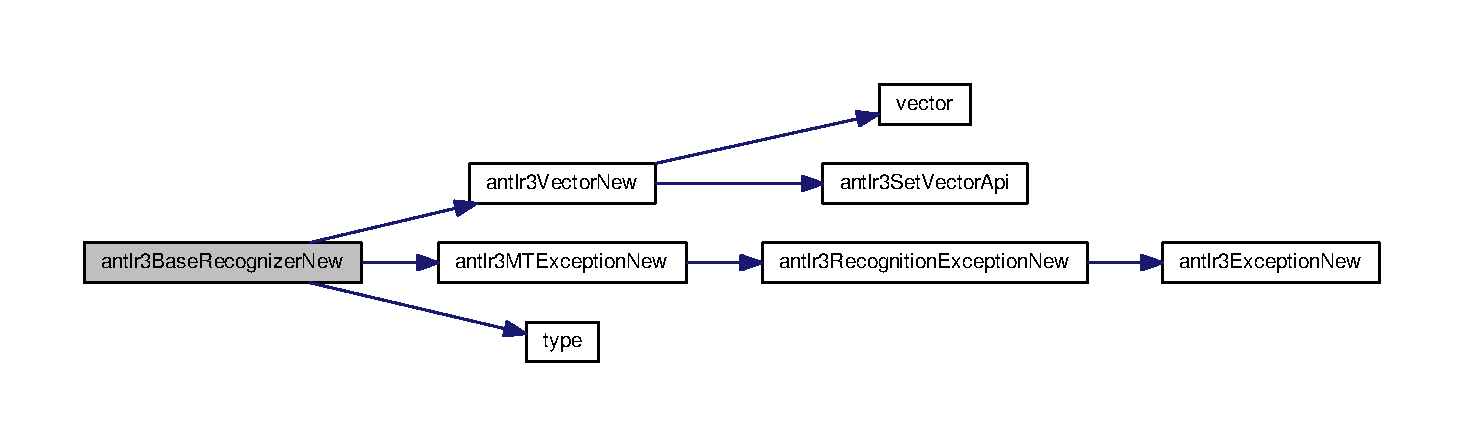
\includegraphics[width=350pt]{group__p_a_n_t_l_r3___b_a_s_e___r_e_c_o_g_n_i_z_e_r_ga5b539798327f965e6289a9f613515c9a_cgraph}
\end{center}
\end{figure}




Here is the caller graph for this function\-:
\nopagebreak
\begin{figure}[H]
\begin{center}
\leavevmode
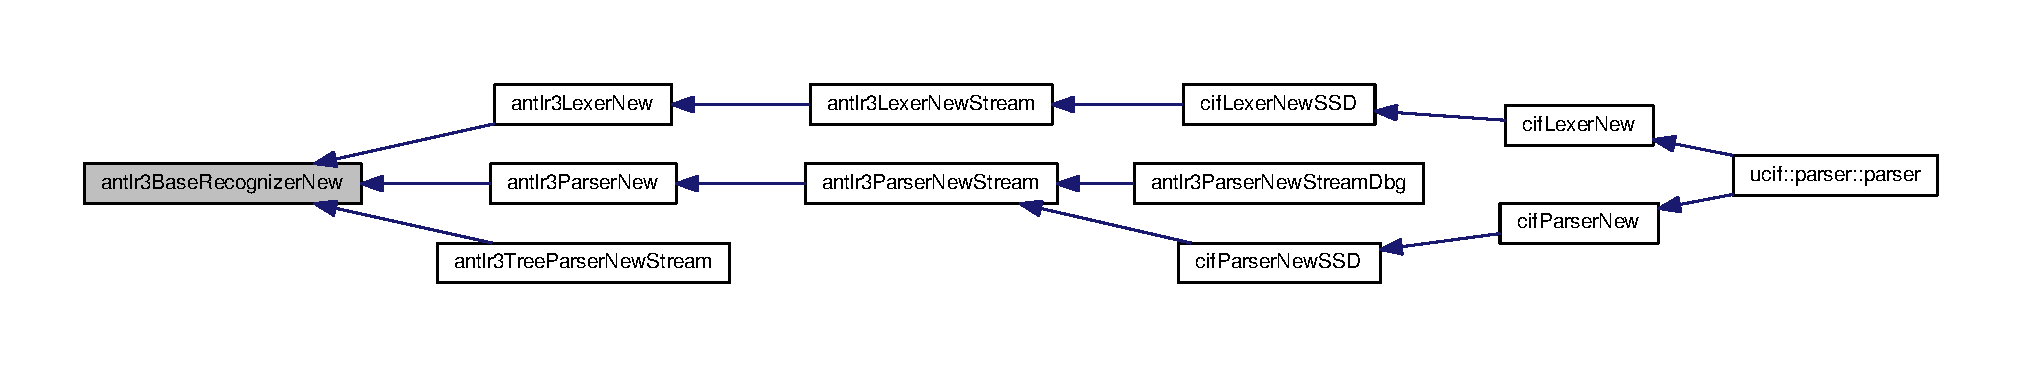
\includegraphics[width=350pt]{group__p_a_n_t_l_r3___b_a_s_e___r_e_c_o_g_n_i_z_e_r_ga5b539798327f965e6289a9f613515c9a_icgraph}
\end{center}
\end{figure}


\hypertarget{group__p_a_n_t_l_r3___b_a_s_e___r_e_c_o_g_n_i_z_e_r_ga974d33def91ba5fb5a6fa8e42c6d876e}{\index{P\-A\-N\-T\-L\-R3\-\_\-\-B\-A\-S\-E\-\_\-\-R\-E\-C\-O\-G\-N\-I\-Z\-E\-R@{P\-A\-N\-T\-L\-R3\-\_\-\-B\-A\-S\-E\-\_\-\-R\-E\-C\-O\-G\-N\-I\-Z\-E\-R}!antlr3\-M\-T\-Exception\-New@{antlr3\-M\-T\-Exception\-New}}
\index{antlr3\-M\-T\-Exception\-New@{antlr3\-M\-T\-Exception\-New}!PANTLR3_BASE_RECOGNIZER@{P\-A\-N\-T\-L\-R3\-\_\-\-B\-A\-S\-E\-\_\-\-R\-E\-C\-O\-G\-N\-I\-Z\-E\-R}}
\subsubsection[{antlr3\-M\-T\-Exception\-New}]{\setlength{\rightskip}{0pt plus 5cm}{\bf A\-N\-T\-L\-R3\-\_\-\-A\-P\-I} void antlr3\-M\-T\-Exception\-New (
\begin{DoxyParamCaption}
\item[{{\bf p\-A\-N\-T\-L\-R3\-\_\-\-B\-A\-S\-E\-\_\-\-R\-E\-C\-O\-G\-N\-I\-Z\-E\-R}}]{recognizer}
\end{DoxyParamCaption}
)}}\label{group__p_a_n_t_l_r3___b_a_s_e___r_e_c_o_g_n_i_z_e_r_ga974d33def91ba5fb5a6fa8e42c6d876e}
Creates a new Mismatched Token Exception and inserts in the recognizer exception stack.


\begin{DoxyParams}{Parameters}
{\em recognizer} & Context pointer for this recognizer \\
\hline
\end{DoxyParams}


Definition at line 254 of file antlr3baserecognizer.\-c.



Here is the call graph for this function\-:
\nopagebreak
\begin{figure}[H]
\begin{center}
\leavevmode
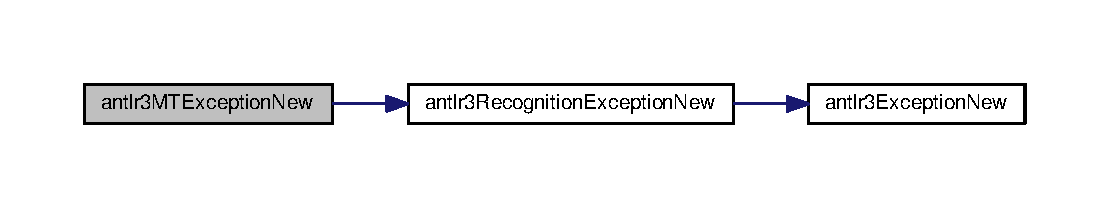
\includegraphics[width=350pt]{group__p_a_n_t_l_r3___b_a_s_e___r_e_c_o_g_n_i_z_e_r_ga974d33def91ba5fb5a6fa8e42c6d876e_cgraph}
\end{center}
\end{figure}




Here is the caller graph for this function\-:
\nopagebreak
\begin{figure}[H]
\begin{center}
\leavevmode
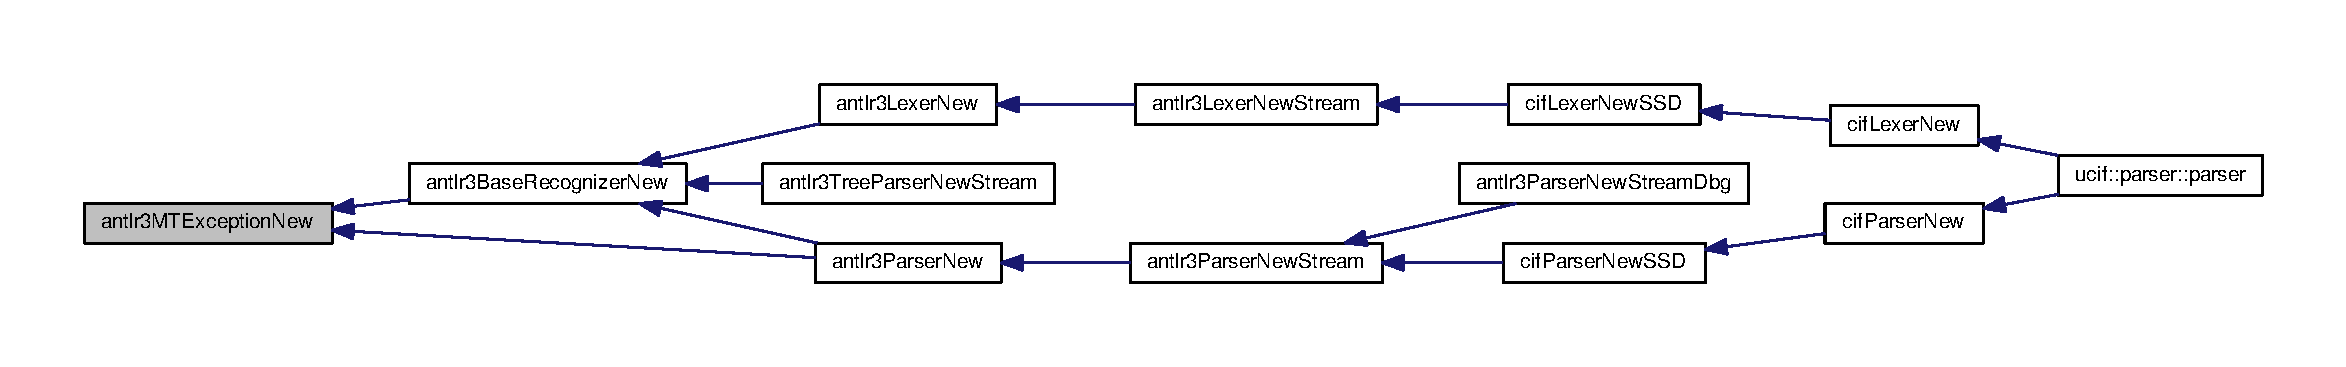
\includegraphics[width=350pt]{group__p_a_n_t_l_r3___b_a_s_e___r_e_c_o_g_n_i_z_e_r_ga974d33def91ba5fb5a6fa8e42c6d876e_icgraph}
\end{center}
\end{figure}


\hypertarget{group__p_a_n_t_l_r3___b_a_s_e___r_e_c_o_g_n_i_z_e_r_gab2d77cd376112c8ff6ed7353ba78dab7}{\index{P\-A\-N\-T\-L\-R3\-\_\-\-B\-A\-S\-E\-\_\-\-R\-E\-C\-O\-G\-N\-I\-Z\-E\-R@{P\-A\-N\-T\-L\-R3\-\_\-\-B\-A\-S\-E\-\_\-\-R\-E\-C\-O\-G\-N\-I\-Z\-E\-R}!antlr3\-Recognition\-Exception\-New@{antlr3\-Recognition\-Exception\-New}}
\index{antlr3\-Recognition\-Exception\-New@{antlr3\-Recognition\-Exception\-New}!PANTLR3_BASE_RECOGNIZER@{P\-A\-N\-T\-L\-R3\-\_\-\-B\-A\-S\-E\-\_\-\-R\-E\-C\-O\-G\-N\-I\-Z\-E\-R}}
\subsubsection[{antlr3\-Recognition\-Exception\-New}]{\setlength{\rightskip}{0pt plus 5cm}{\bf A\-N\-T\-L\-R3\-\_\-\-A\-P\-I} void antlr3\-Recognition\-Exception\-New (
\begin{DoxyParamCaption}
\item[{{\bf p\-A\-N\-T\-L\-R3\-\_\-\-B\-A\-S\-E\-\_\-\-R\-E\-C\-O\-G\-N\-I\-Z\-E\-R}}]{recognizer}
\end{DoxyParamCaption}
)}}\label{group__p_a_n_t_l_r3___b_a_s_e___r_e_c_o_g_n_i_z_e_r_gab2d77cd376112c8ff6ed7353ba78dab7}


Definition at line 269 of file antlr3baserecognizer.\-c.



Here is the call graph for this function\-:
\nopagebreak
\begin{figure}[H]
\begin{center}
\leavevmode
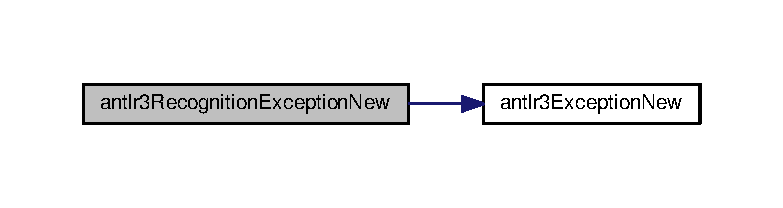
\includegraphics[width=350pt]{group__p_a_n_t_l_r3___b_a_s_e___r_e_c_o_g_n_i_z_e_r_gab2d77cd376112c8ff6ed7353ba78dab7_cgraph}
\end{center}
\end{figure}




Here is the caller graph for this function\-:
\nopagebreak
\begin{figure}[H]
\begin{center}
\leavevmode
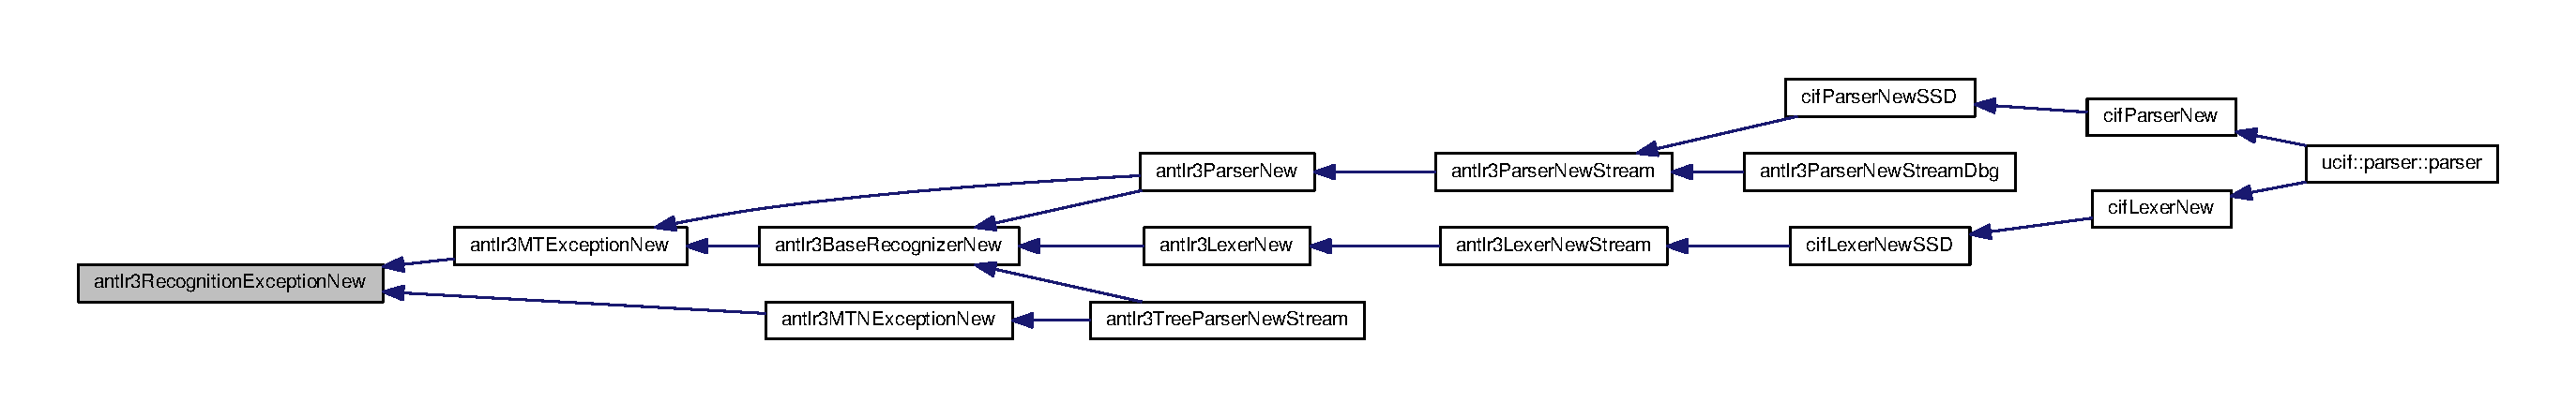
\includegraphics[width=350pt]{group__p_a_n_t_l_r3___b_a_s_e___r_e_c_o_g_n_i_z_e_r_gab2d77cd376112c8ff6ed7353ba78dab7_icgraph}
\end{center}
\end{figure}



\hypertarget{group__p_a_n_t_l_r3___i_n_t___s_t_r_e_a_m}{\section{P\-A\-N\-T\-L\-R3\-\_\-\-I\-N\-T\-\_\-\-S\-T\-R\-E\-A\-M}
\label{group__p_a_n_t_l_r3___i_n_t___s_t_r_e_a_m}\index{P\-A\-N\-T\-L\-R3\-\_\-\-I\-N\-T\-\_\-\-S\-T\-R\-E\-A\-M@{P\-A\-N\-T\-L\-R3\-\_\-\-I\-N\-T\-\_\-\-S\-T\-R\-E\-A\-M}}
}
\subsection*{Functions}
\begin{DoxyCompactItemize}
\item 
\hyperlink{antlr3defs_8h_ac6724ab3b71a7f4b3c340f52312e8488}{A\-N\-T\-L\-R3\-\_\-\-A\-P\-I} \hyperlink{antlr3interfaces_8h_af34d949f6aa442e8e7770e420977d338}{p\-A\-N\-T\-L\-R3\-\_\-\-I\-N\-T\-\_\-\-S\-T\-R\-E\-A\-M} \hyperlink{group__p_a_n_t_l_r3___i_n_t___s_t_r_e_a_m_ga58e4ce6e808a830c69cc73f3db040ae4}{antlr3\-Int\-Stream\-New} ()
\end{DoxyCompactItemize}


\subsection{Detailed Description}


\subsection{Function Documentation}
\hypertarget{group__p_a_n_t_l_r3___i_n_t___s_t_r_e_a_m_ga58e4ce6e808a830c69cc73f3db040ae4}{\index{P\-A\-N\-T\-L\-R3\-\_\-\-I\-N\-T\-\_\-\-S\-T\-R\-E\-A\-M@{P\-A\-N\-T\-L\-R3\-\_\-\-I\-N\-T\-\_\-\-S\-T\-R\-E\-A\-M}!antlr3\-Int\-Stream\-New@{antlr3\-Int\-Stream\-New}}
\index{antlr3\-Int\-Stream\-New@{antlr3\-Int\-Stream\-New}!PANTLR3_INT_STREAM@{P\-A\-N\-T\-L\-R3\-\_\-\-I\-N\-T\-\_\-\-S\-T\-R\-E\-A\-M}}
\subsubsection[{antlr3\-Int\-Stream\-New}]{\setlength{\rightskip}{0pt plus 5cm}{\bf A\-N\-T\-L\-R3\-\_\-\-A\-P\-I} {\bf p\-A\-N\-T\-L\-R3\-\_\-\-I\-N\-T\-\_\-\-S\-T\-R\-E\-A\-M} antlr3\-Int\-Stream\-New (
\begin{DoxyParamCaption}
\item[{void}]{}
\end{DoxyParamCaption}
)}}\label{group__p_a_n_t_l_r3___i_n_t___s_t_r_e_a_m_ga58e4ce6e808a830c69cc73f3db040ae4}


Definition at line 41 of file antlr3intstream.\-c.



Here is the caller graph for this function\-:
\nopagebreak
\begin{figure}[H]
\begin{center}
\leavevmode
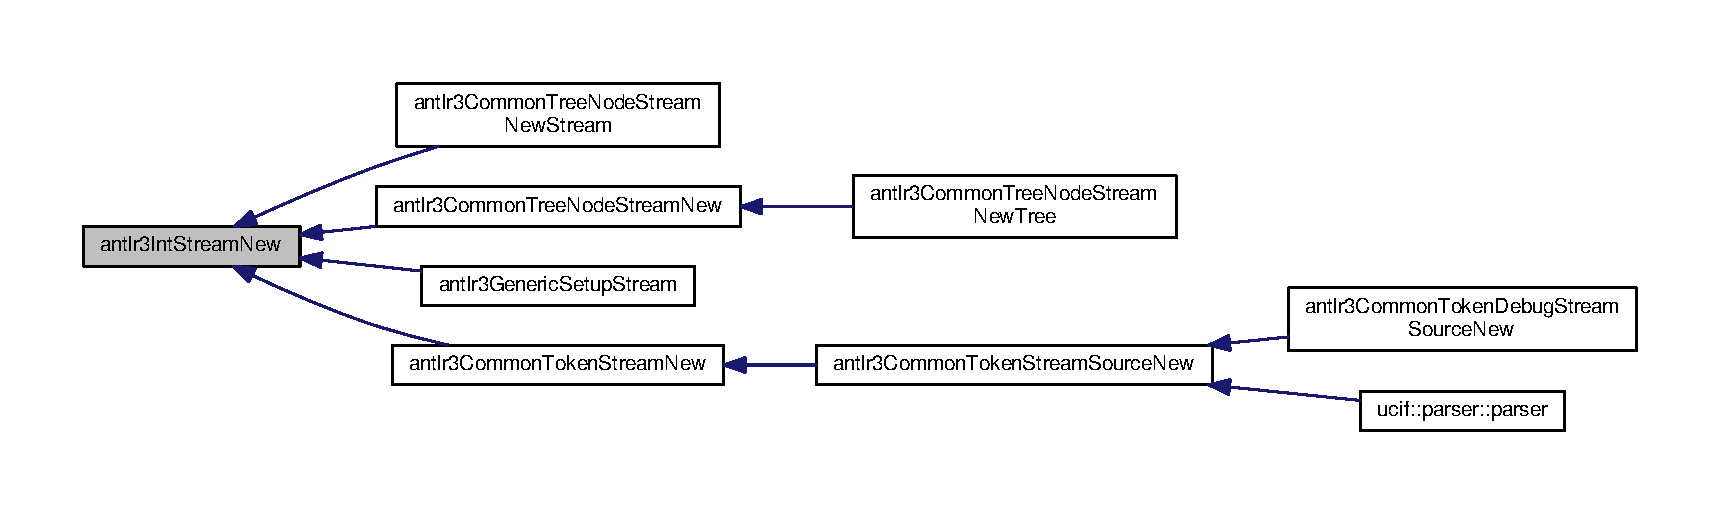
\includegraphics[width=350pt]{group__p_a_n_t_l_r3___i_n_t___s_t_r_e_a_m_ga58e4ce6e808a830c69cc73f3db040ae4_icgraph}
\end{center}
\end{figure}



\chapter{Namespace Documentation}
\hypertarget{namespaceaberrations}{\section{aberrations Namespace Reference}
\label{namespaceaberrations}\index{aberrations@{aberrations}}
}
\subsection*{Classes}
\begin{DoxyCompactItemize}
\item 
class \hyperlink{classaberrations_1_1_image_plot}{Image\-Plot}
\item 
class \hyperlink{classaberrations_1_1_aberrations}{Aberrations}
\item 
class \hyperlink{classaberrations_1_1_ab_krivanek}{Ab\-Krivanek}
\item 
class \hyperlink{classaberrations_1_1_ab_rose}{Ab\-Rose}
\item 
class \hyperlink{classaberrations_1_1_ab3}{Ab3}
\item 
class \hyperlink{classaberrations_1_1_probe_handler}{Probe\-Handler}
\item 
class \hyperlink{classaberrations_1_1_probe}{Probe}
\item 
class \hyperlink{classaberrations_1_1_probe_plot}{Probe\-Plot}
\end{DoxyCompactItemize}
\subsection*{Variables}
\begin{DoxyCompactItemize}
\item 
tuple \hyperlink{namespaceaberrations_a3ecdf825b3593d09a548afba6167386c}{p} = \hyperlink{classaberrations_1_1_probe}{Probe}(ab=\hyperlink{classaberrations_1_1_ab_krivanek}{Ab\-Krivanek}())
\end{DoxyCompactItemize}


\subsection{Variable Documentation}
\hypertarget{namespaceaberrations_a3ecdf825b3593d09a548afba6167386c}{\index{aberrations@{aberrations}!p@{p}}
\index{p@{p}!aberrations@{aberrations}}
\subsubsection[{p}]{\setlength{\rightskip}{0pt plus 5cm}tuple aberrations.\-p = {\bf Probe}(ab={\bf Ab\-Krivanek}())}}\label{namespaceaberrations_a3ecdf825b3593d09a548afba6167386c}


Definition at line 587 of file aberrations.\-py.


\hypertarget{namespaceimg__view}{\section{img\-\_\-view Namespace Reference}
\label{namespaceimg__view}\index{img\-\_\-view@{img\-\_\-view}}
}
\subsection*{Functions}
\begin{DoxyCompactItemize}
\item 
\hyperlink{sim_image_from_wave_8m_a72b6b8e83430abf007f20aeae4dc2f74}{def} \hyperlink{namespaceimg__view_a9cb9a2437de0909a4bc2e574da597ff7}{get\-\_\-dtype}
\item 
\hyperlink{sim_image_from_wave_8m_a72b6b8e83430abf007f20aeae4dc2f74}{def} \hyperlink{namespaceimg__view_a222b2f2f709eef298c617698808840b5}{read\-I\-M\-G}
\item 
\hyperlink{sim_image_from_wave_8m_a72b6b8e83430abf007f20aeae4dc2f74}{def} \hyperlink{namespaceimg__view_a6a4ec2c6f3b0106dff1284738fef24c4}{save\-\_\-to\-\_\-image}
\end{DoxyCompactItemize}


\subsection{Function Documentation}
\hypertarget{namespaceimg__view_a9cb9a2437de0909a4bc2e574da597ff7}{\index{img\-\_\-view@{img\-\_\-view}!get\-\_\-dtype@{get\-\_\-dtype}}
\index{get\-\_\-dtype@{get\-\_\-dtype}!img_view@{img\-\_\-view}}
\subsubsection[{get\-\_\-dtype}]{\setlength{\rightskip}{0pt plus 5cm}{\bf def} img\-\_\-view.\-get\-\_\-dtype (
\begin{DoxyParamCaption}
\item[{}]{hdr}
\end{DoxyParamCaption}
)}}\label{namespaceimg__view_a9cb9a2437de0909a4bc2e574da597ff7}


Definition at line 5 of file img\-\_\-view.\-py.



Here is the caller graph for this function\-:
\nopagebreak
\begin{figure}[H]
\begin{center}
\leavevmode
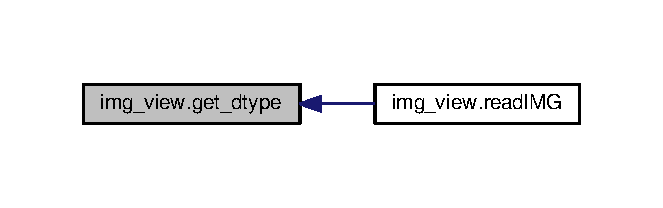
\includegraphics[width=318pt]{namespaceimg__view_a9cb9a2437de0909a4bc2e574da597ff7_icgraph}
\end{center}
\end{figure}


\hypertarget{namespaceimg__view_a222b2f2f709eef298c617698808840b5}{\index{img\-\_\-view@{img\-\_\-view}!read\-I\-M\-G@{read\-I\-M\-G}}
\index{read\-I\-M\-G@{read\-I\-M\-G}!img_view@{img\-\_\-view}}
\subsubsection[{read\-I\-M\-G}]{\setlength{\rightskip}{0pt plus 5cm}{\bf def} img\-\_\-view.\-read\-I\-M\-G (
\begin{DoxyParamCaption}
\item[{}]{filename, }
\item[{}]{debug = {\ttfamily False}}
\end{DoxyParamCaption}
)}}\label{namespaceimg__view_a222b2f2f709eef298c617698808840b5}


Definition at line 18 of file img\-\_\-view.\-py.



Here is the call graph for this function\-:
\nopagebreak
\begin{figure}[H]
\begin{center}
\leavevmode
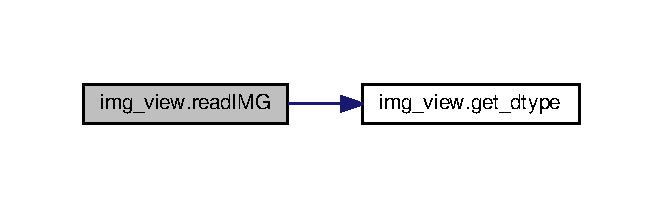
\includegraphics[width=318pt]{namespaceimg__view_a222b2f2f709eef298c617698808840b5_cgraph}
\end{center}
\end{figure}


\hypertarget{namespaceimg__view_a6a4ec2c6f3b0106dff1284738fef24c4}{\index{img\-\_\-view@{img\-\_\-view}!save\-\_\-to\-\_\-image@{save\-\_\-to\-\_\-image}}
\index{save\-\_\-to\-\_\-image@{save\-\_\-to\-\_\-image}!img_view@{img\-\_\-view}}
\subsubsection[{save\-\_\-to\-\_\-image}]{\setlength{\rightskip}{0pt plus 5cm}{\bf def} img\-\_\-view.\-save\-\_\-to\-\_\-image (
\begin{DoxyParamCaption}
\item[{}]{data, }
\item[{}]{filename, }
\item[{}]{format = {\ttfamily '.tif'}}
\end{DoxyParamCaption}
)}}\label{namespaceimg__view_a6a4ec2c6f3b0106dff1284738fef24c4}


Definition at line 56 of file img\-\_\-view.\-py.


\hypertarget{namespacepython}{\section{python Namespace Reference}
\label{namespacepython}\index{python@{python}}
}
\subsection*{Namespaces}
\begin{DoxyCompactItemize}
\item 
\hyperlink{namespacepython_1_1dialogs}{dialogs}
\item 
\hyperlink{namespacepython_1_1fileio}{fileio}
\item 
\hyperlink{namespacepython_1_1models}{models}
\item 
\hyperlink{namespacepython_1_1plot__img}{plot\-\_\-img}
\item 
\hyperlink{namespacepython_1_1potential}{potential}
\item 
\hyperlink{namespacepython_1_1_q_s_t_e_m___u_i}{Q\-S\-T\-E\-M\-\_\-\-U\-I}
\end{DoxyCompactItemize}

\hypertarget{namespacepython_1_1dialogs}{\section{python.\-dialogs Namespace Reference}
\label{namespacepython_1_1dialogs}\index{python.\-dialogs@{python.\-dialogs}}
}

\hypertarget{namespacepython_1_1fileio}{\section{python.\-fileio Namespace Reference}
\label{namespacepython_1_1fileio}\index{python.\-fileio@{python.\-fileio}}
}
\subsection*{Namespaces}
\begin{DoxyCompactItemize}
\item 
\hyperlink{namespacepython_1_1fileio_1_1read__img}{read\-\_\-img}
\item 
\hyperlink{namespacepython_1_1fileio_1_1read_cfg}{read\-Cfg}
\end{DoxyCompactItemize}

\hypertarget{namespacepython_1_1fileio_1_1read__img}{\section{python.\-fileio.\-read\-\_\-img Namespace Reference}
\label{namespacepython_1_1fileio_1_1read__img}\index{python.\-fileio.\-read\-\_\-img@{python.\-fileio.\-read\-\_\-img}}
}
\subsection*{Functions}
\begin{DoxyCompactItemize}
\item 
\hyperlink{sim_image_from_wave_8m_a72b6b8e83430abf007f20aeae4dc2f74}{def} \hyperlink{namespacepython_1_1fileio_1_1read__img_a3ffec208a1fe92342eafab85c08961a0}{binread2\-D}
\end{DoxyCompactItemize}
\subsection*{Variables}
\begin{DoxyCompactItemize}
\item 
int \hyperlink{namespacepython_1_1fileio_1_1read__img_abcc43c5b7904c6f21fbf4ff8898911b0}{headerlength} = 4
\item 
list \hyperlink{namespacepython_1_1fileio_1_1read__img_a36fc09d1528b241c1c750e4c11e77e5a}{filename} = sys.\-argv\mbox{[}1\mbox{]}
\end{DoxyCompactItemize}


\subsection{Detailed Description}
\begin{DoxyVerb}/*
QSTEM - image simulation for TEM/STEM/CBED
    Copyright (C) 2000-2010  Christoph Koch
    Copyright (C) 2010-2013  Christoph Koch, Michael Sarahan

    This program is free software: you can redistribute it and/or modify
    it under the terms of the GNU General Public License as published by
    the Free Software Foundation, either version 3 of the License, or
    (at your option) any later version.

    This program is distributed in the hope that it will be useful,
    but WITHOUT ANY WARRANTY; without even the implied warranty of
    MERCHANTABILITY or FITNESS FOR A PARTICULAR PURPOSE.  See the
    GNU General Public License for more details.

    You should have received a copy of the GNU General Public License
    along with this program.  If not, see <http://www.gnu.org/licenses/>.
*/
\end{DoxyVerb}
 

\subsection{Function Documentation}
\hypertarget{namespacepython_1_1fileio_1_1read__img_a3ffec208a1fe92342eafab85c08961a0}{\index{python\-::fileio\-::read\-\_\-img@{python\-::fileio\-::read\-\_\-img}!binread2\-D@{binread2\-D}}
\index{binread2\-D@{binread2\-D}!python::fileio::read_img@{python\-::fileio\-::read\-\_\-img}}
\subsubsection[{binread2\-D}]{\setlength{\rightskip}{0pt plus 5cm}{\bf def} python.\-fileio.\-read\-\_\-img.\-binread2\-D (
\begin{DoxyParamCaption}
\item[{}]{filename, }
\item[{}]{print\-Flag = {\ttfamily True}}
\end{DoxyParamCaption}
)}}\label{namespacepython_1_1fileio_1_1read__img_a3ffec208a1fe92342eafab85c08961a0}


Definition at line 43 of file read\-\_\-img.\-py.



Here is the caller graph for this function\-:
\nopagebreak
\begin{figure}[H]
\begin{center}
\leavevmode
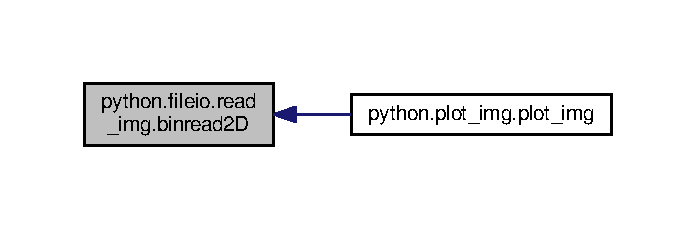
\includegraphics[width=334pt]{namespacepython_1_1fileio_1_1read__img_a3ffec208a1fe92342eafab85c08961a0_icgraph}
\end{center}
\end{figure}




\subsection{Variable Documentation}
\hypertarget{namespacepython_1_1fileio_1_1read__img_a36fc09d1528b241c1c750e4c11e77e5a}{\index{python\-::fileio\-::read\-\_\-img@{python\-::fileio\-::read\-\_\-img}!filename@{filename}}
\index{filename@{filename}!python::fileio::read_img@{python\-::fileio\-::read\-\_\-img}}
\subsubsection[{filename}]{\setlength{\rightskip}{0pt plus 5cm}list python.\-fileio.\-read\-\_\-img.\-filename = sys.\-argv\mbox{[}1\mbox{]}}}\label{namespacepython_1_1fileio_1_1read__img_a36fc09d1528b241c1c750e4c11e77e5a}


Definition at line 113 of file read\-\_\-img.\-py.

\hypertarget{namespacepython_1_1fileio_1_1read__img_abcc43c5b7904c6f21fbf4ff8898911b0}{\index{python\-::fileio\-::read\-\_\-img@{python\-::fileio\-::read\-\_\-img}!headerlength@{headerlength}}
\index{headerlength@{headerlength}!python::fileio::read_img@{python\-::fileio\-::read\-\_\-img}}
\subsubsection[{headerlength}]{\setlength{\rightskip}{0pt plus 5cm}int python.\-fileio.\-read\-\_\-img.\-headerlength = 4}}\label{namespacepython_1_1fileio_1_1read__img_abcc43c5b7904c6f21fbf4ff8898911b0}


Definition at line 41 of file read\-\_\-img.\-py.


\hypertarget{namespacepython_1_1fileio_1_1read_cfg}{\section{python.\-fileio.\-read\-Cfg Namespace Reference}
\label{namespacepython_1_1fileio_1_1read_cfg}\index{python.\-fileio.\-read\-Cfg@{python.\-fileio.\-read\-Cfg}}
}
\subsection*{Functions}
\begin{DoxyCompactItemize}
\item 
\hyperlink{sim_image_from_wave_8m_a72b6b8e83430abf007f20aeae4dc2f74}{def} \hyperlink{namespacepython_1_1fileio_1_1read_cfg_aae086b7fa3ade4aaf4c7aec598e23344}{get\-\_\-atom\-\_\-arrays}
\item 
\hyperlink{sim_image_from_wave_8m_a72b6b8e83430abf007f20aeae4dc2f74}{def} \hyperlink{namespacepython_1_1fileio_1_1read_cfg_a1769a0316d318139caae32b4d48e3056}{get\-\_\-cell\-\_\-box}
\end{DoxyCompactItemize}
\subsection*{Variables}
\begin{DoxyCompactItemize}
\item 
tuple \hyperlink{namespacepython_1_1fileio_1_1read_cfg_a5604f72b29109b23876023593a3eefd3}{array\-\_\-re}
\item 
tuple \hyperlink{namespacepython_1_1fileio_1_1read_cfg_ab37ee94881162c11a48d464d4ac60ade}{box\-\_\-re} = re.\-compile(\char`\"{}H0\textbackslash{}((\textbackslash{}\hyperlink{_read_d_m3___matlab_8m_a1aabac6d068eef6a7bad3fdf50a05cc8}{d}),(\textbackslash{}\hyperlink{_read_d_m3___matlab_8m_a1aabac6d068eef6a7bad3fdf50a05cc8}{d})\textbackslash{}) = (\textbackslash{}\hyperlink{_read_d_m3___matlab_8m_a1aabac6d068eef6a7bad3fdf50a05cc8}{d}+\textbackslash{}.\textbackslash{}\hyperlink{_read_d_m3___matlab_8m_a1aabac6d068eef6a7bad3fdf50a05cc8}{d}+)\textbackslash{}\hyperlink{aberrations___t_e_m_8m_aef29541a06b7f933d32a804307db13af}{s}$\ast$\char`\"{})
\end{DoxyCompactItemize}


\subsection{Detailed Description}
\begin{DoxyVerb}/*
QSTEM - image simulation for TEM/STEM/CBED
Copyright (C) 2000-2010  Christoph Koch
Copyright (C) 2010-2013  Christoph Koch, Michael Sarahan

This program is free software: you can redistribute it and/or modify
it under the terms of the GNU General Public License as published by
the Free Software Foundation, either version 3 of the License, or
(at your option) any later version.

This program is distributed in the hope that it will be useful,
but WITHOUT ANY WARRANTY; without even the implied warranty of
MERCHANTABILITY or FITNESS FOR A PARTICULAR PURPOSE.  See the
GNU General Public License for more details.

You should have received a copy of the GNU General Public License
along with this program.  If not, see <http://www.gnu.org/licenses/>.
*/
\end{DoxyVerb}
 

\subsection{Function Documentation}
\hypertarget{namespacepython_1_1fileio_1_1read_cfg_aae086b7fa3ade4aaf4c7aec598e23344}{\index{python\-::fileio\-::read\-Cfg@{python\-::fileio\-::read\-Cfg}!get\-\_\-atom\-\_\-arrays@{get\-\_\-atom\-\_\-arrays}}
\index{get\-\_\-atom\-\_\-arrays@{get\-\_\-atom\-\_\-arrays}!python::fileio::readCfg@{python\-::fileio\-::read\-Cfg}}
\subsubsection[{get\-\_\-atom\-\_\-arrays}]{\setlength{\rightskip}{0pt plus 5cm}{\bf def} python.\-fileio.\-read\-Cfg.\-get\-\_\-atom\-\_\-arrays (
\begin{DoxyParamCaption}
\item[{}]{filename}
\end{DoxyParamCaption}
)}}\label{namespacepython_1_1fileio_1_1read_cfg_aae086b7fa3ade4aaf4c7aec598e23344}
\begin{DoxyVerb}Returns a dictionary with an entry per element.  The key to the dictionary 
is the atomic number, while the value is an array containing coordinates,
Debye-Waller factors, occupancies, and charges on a site-specific basis.
\end{DoxyVerb}
 

Definition at line 30 of file read\-Cfg.\-py.

\hypertarget{namespacepython_1_1fileio_1_1read_cfg_a1769a0316d318139caae32b4d48e3056}{\index{python\-::fileio\-::read\-Cfg@{python\-::fileio\-::read\-Cfg}!get\-\_\-cell\-\_\-box@{get\-\_\-cell\-\_\-box}}
\index{get\-\_\-cell\-\_\-box@{get\-\_\-cell\-\_\-box}!python::fileio::readCfg@{python\-::fileio\-::read\-Cfg}}
\subsubsection[{get\-\_\-cell\-\_\-box}]{\setlength{\rightskip}{0pt plus 5cm}{\bf def} python.\-fileio.\-read\-Cfg.\-get\-\_\-cell\-\_\-box (
\begin{DoxyParamCaption}
\item[{}]{filename}
\end{DoxyParamCaption}
)}}\label{namespacepython_1_1fileio_1_1read_cfg_a1769a0316d318139caae32b4d48e3056}
\begin{DoxyVerb}Returns a 3-element 1D numpy array with the cell dimensions, as X,Y,Z.
\end{DoxyVerb}
 

Definition at line 47 of file read\-Cfg.\-py.



\subsection{Variable Documentation}
\hypertarget{namespacepython_1_1fileio_1_1read_cfg_a5604f72b29109b23876023593a3eefd3}{\index{python\-::fileio\-::read\-Cfg@{python\-::fileio\-::read\-Cfg}!array\-\_\-re@{array\-\_\-re}}
\index{array\-\_\-re@{array\-\_\-re}!python::fileio::readCfg@{python\-::fileio\-::read\-Cfg}}
\subsubsection[{array\-\_\-re}]{\setlength{\rightskip}{0pt plus 5cm}tuple python.\-fileio.\-read\-Cfg.\-array\-\_\-re}}\label{namespacepython_1_1fileio_1_1read_cfg_a5604f72b29109b23876023593a3eefd3}
{\bfseries Initial value\-:}
\begin{DoxyCode}
1 = re.compile(\textcolor{stringliteral}{"(\(\backslash\)d+)\(\backslash\)s*\(\backslash\)n([A-Za-z]\{1,2\})\(\backslash\)s*\(\backslash\)n(.*?)(?=\(\backslash\)d+\(\backslash\)s*\(\backslash\)n\(\backslash\)s*[A-Za-z]\{1,2\}\(\backslash\)s*\(\backslash\)n|\(\backslash\)Z)"}, 
2                flags=re.M|re.S)
\end{DoxyCode}


Definition at line 26 of file read\-Cfg.\-py.

\hypertarget{namespacepython_1_1fileio_1_1read_cfg_ab37ee94881162c11a48d464d4ac60ade}{\index{python\-::fileio\-::read\-Cfg@{python\-::fileio\-::read\-Cfg}!box\-\_\-re@{box\-\_\-re}}
\index{box\-\_\-re@{box\-\_\-re}!python::fileio::readCfg@{python\-::fileio\-::read\-Cfg}}
\subsubsection[{box\-\_\-re}]{\setlength{\rightskip}{0pt plus 5cm}tuple python.\-fileio.\-read\-Cfg.\-box\-\_\-re = re.\-compile(\char`\"{}H0\textbackslash{}((\textbackslash{}{\bf d}),(\textbackslash{}{\bf d})\textbackslash{}) = (\textbackslash{}{\bf d}+\textbackslash{}.\textbackslash{}{\bf d}+)\textbackslash{}{\bf s}$\ast$\char`\"{})}}\label{namespacepython_1_1fileio_1_1read_cfg_ab37ee94881162c11a48d464d4ac60ade}


Definition at line 28 of file read\-Cfg.\-py.


\hypertarget{namespacepython_1_1models}{\section{python.\-models Namespace Reference}
\label{namespacepython_1_1models}\index{python.\-models@{python.\-models}}
}
\subsection*{Namespaces}
\begin{DoxyCompactItemize}
\item 
\hyperlink{namespacepython_1_1models_1_1raw__models}{raw\-\_\-models}
\item 
\hyperlink{namespacepython_1_1models_1_1sample__chaco}{sample\-\_\-chaco}
\end{DoxyCompactItemize}

\hypertarget{namespacepython_1_1models_1_1raw__models}{\section{python.\-models.\-raw\-\_\-models Namespace Reference}
\label{namespacepython_1_1models_1_1raw__models}\index{python.\-models.\-raw\-\_\-models@{python.\-models.\-raw\-\_\-models}}
}
\subsection*{Namespaces}
\begin{DoxyCompactItemize}
\item 
\hyperlink{namespacepython_1_1models_1_1raw__models_1_1probe}{probe}
\item 
\hyperlink{namespacepython_1_1models_1_1raw__models_1_1sample}{sample}
\end{DoxyCompactItemize}

\hypertarget{namespacepython_1_1models_1_1raw__models_1_1probe}{\section{python.\-models.\-raw\-\_\-models.\-probe Namespace Reference}
\label{namespacepython_1_1models_1_1raw__models_1_1probe}\index{python.\-models.\-raw\-\_\-models.\-probe@{python.\-models.\-raw\-\_\-models.\-probe}}
}
\subsection*{Classes}
\begin{DoxyCompactItemize}
\item 
class \hyperlink{classpython_1_1models_1_1raw__models_1_1probe_1_1probe}{probe}
\end{DoxyCompactItemize}
\subsection*{Variables}
\begin{DoxyCompactItemize}
\item 
tuple \hyperlink{namespacepython_1_1models_1_1raw__models_1_1probe_abd27b11ab377a74cc4a43fb2a6b77ad5}{p} = \hyperlink{classpython_1_1models_1_1raw__models_1_1probe_1_1probe}{probe}()
\end{DoxyCompactItemize}


\subsection{Variable Documentation}
\hypertarget{namespacepython_1_1models_1_1raw__models_1_1probe_abd27b11ab377a74cc4a43fb2a6b77ad5}{\index{python\-::models\-::raw\-\_\-models\-::probe@{python\-::models\-::raw\-\_\-models\-::probe}!p@{p}}
\index{p@{p}!python::models::raw_models::probe@{python\-::models\-::raw\-\_\-models\-::probe}}
\subsubsection[{p}]{\setlength{\rightskip}{0pt plus 5cm}tuple python.\-models.\-raw\-\_\-models.\-probe.\-p = {\bf probe}()}}\label{namespacepython_1_1models_1_1raw__models_1_1probe_abd27b11ab377a74cc4a43fb2a6b77ad5}


Definition at line 396 of file probe.\-py.


\hypertarget{namespacepython_1_1models_1_1raw__models_1_1sample}{\section{python.\-models.\-raw\-\_\-models.\-sample Namespace Reference}
\label{namespacepython_1_1models_1_1raw__models_1_1sample}\index{python.\-models.\-raw\-\_\-models.\-sample@{python.\-models.\-raw\-\_\-models.\-sample}}
}
\subsection*{Classes}
\begin{DoxyCompactItemize}
\item 
class \hyperlink{classpython_1_1models_1_1raw__models_1_1sample_1_1_sample_model}{Sample\-Model}
\end{DoxyCompactItemize}


\subsection{Detailed Description}
\begin{DoxyVerb}/*
QSTEM - image simulation for TEM/STEM/CBED
    Copyright (C) 2000-2010  Christoph Koch
    Copyright (C) 2010-2013  Christoph Koch, Michael Sarahan

    This program is free software: you can redistribute it and/or modify
    it under the terms of the GNU General Public License as published by
    the Free Software Foundation, either version 3 of the License, or
    (at your option) any later version.

    This program is distributed in the hope that it will be useful,
    but WITHOUT ANY WARRANTY; without even the implied warranty of
    MERCHANTABILITY or FITNESS FOR A PARTICULAR PURPOSE.  See the
    GNU General Public License for more details.

    You should have received a copy of the GNU General Public License
    along with this program.  If not, see <http://www.gnu.org/licenses/>.
*/
\end{DoxyVerb}
 
\hypertarget{namespacepython_1_1models_1_1sample__chaco}{\section{python.\-models.\-sample\-\_\-chaco Namespace Reference}
\label{namespacepython_1_1models_1_1sample__chaco}\index{python.\-models.\-sample\-\_\-chaco@{python.\-models.\-sample\-\_\-chaco}}
}
\subsection*{Classes}
\begin{DoxyCompactItemize}
\item 
class \hyperlink{classpython_1_1models_1_1sample__chaco_1_1_sample_plotter}{Sample\-Plotter}
\end{DoxyCompactItemize}


\subsection{Detailed Description}
\begin{DoxyVerb}/*
QSTEM - image simulation for TEM/STEM/CBED
    Copyright (C) 2000-2010  Christoph Koch
    Copyright (C) 2010-2013  Christoph Koch, Michael Sarahan

    This program is free software: you can redistribute it and/or modify
    it under the terms of the GNU General Public License as published by
    the Free Software Foundation, either version 3 of the License, or
    (at your option) any later version.

    This program is distributed in the hope that it will be useful,
    but WITHOUT ANY WARRANTY; without even the implied warranty of
    MERCHANTABILITY or FITNESS FOR A PARTICULAR PURPOSE.  See the
    GNU General Public License for more details.

    You should have received a copy of the GNU General Public License
    along with this program.  If not, see <http://www.gnu.org/licenses/>.
*/
\end{DoxyVerb}
 
\hypertarget{namespacepython_1_1plot__img}{\section{python.\-plot\-\_\-img Namespace Reference}
\label{namespacepython_1_1plot__img}\index{python.\-plot\-\_\-img@{python.\-plot\-\_\-img}}
}
\subsection*{Functions}
\begin{DoxyCompactItemize}
\item 
\hyperlink{sim_image_from_wave_8m_a72b6b8e83430abf007f20aeae4dc2f74}{def} \hyperlink{namespacepython_1_1plot__img_a047f12ae346602faa26f6aba9c3334e6}{plot\-\_\-img}
\end{DoxyCompactItemize}
\subsection*{Variables}
\begin{DoxyCompactItemize}
\item 
tuple \hyperlink{namespacepython_1_1plot__img_a84ab8c729acf1090901d57022bae03e4}{img} = \hyperlink{namespacepython_1_1plot__img_a047f12ae346602faa26f6aba9c3334e6}{plot\-\_\-img}(sys.\-argv\mbox{[}1\mbox{]})
\end{DoxyCompactItemize}


\subsection{Detailed Description}
\begin{DoxyVerb}/*
QSTEM - image simulation for TEM/STEM/CBED
    Copyright (C) 2000-2010  Christoph Koch
    Copyright (C) 2010-2013  Christoph Koch, Michael Sarahan

    This program is free software: you can redistribute it and/or modify
    it under the terms of the GNU General Public License as published by
    the Free Software Foundation, either version 3 of the License, or
    (at your option) any later version.

    This program is distributed in the hope that it will be useful,
    but WITHOUT ANY WARRANTY; without even the implied warranty of
    MERCHANTABILITY or FITNESS FOR A PARTICULAR PURPOSE.  See the
    GNU General Public License for more details.

    You should have received a copy of the GNU General Public License
    along with this program.  If not, see <http://www.gnu.org/licenses/>.
*/
\end{DoxyVerb}
 

\subsection{Function Documentation}
\hypertarget{namespacepython_1_1plot__img_a047f12ae346602faa26f6aba9c3334e6}{\index{python\-::plot\-\_\-img@{python\-::plot\-\_\-img}!plot\-\_\-img@{plot\-\_\-img}}
\index{plot\-\_\-img@{plot\-\_\-img}!python::plot_img@{python\-::plot\-\_\-img}}
\subsubsection[{plot\-\_\-img}]{\setlength{\rightskip}{0pt plus 5cm}{\bf def} python.\-plot\-\_\-img.\-plot\-\_\-img (
\begin{DoxyParamCaption}
\item[{}]{filename}
\end{DoxyParamCaption}
)}}\label{namespacepython_1_1plot__img_a047f12ae346602faa26f6aba9c3334e6}


Definition at line 28 of file plot\-\_\-img.\-py.



Here is the call graph for this function\-:
\nopagebreak
\begin{figure}[H]
\begin{center}
\leavevmode
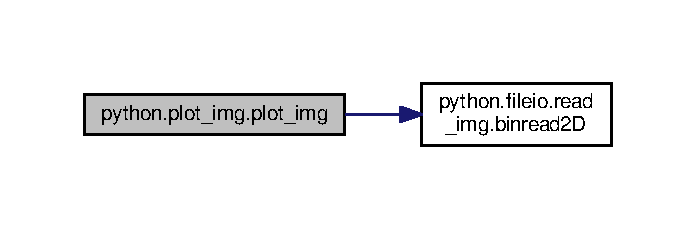
\includegraphics[width=334pt]{namespacepython_1_1plot__img_a047f12ae346602faa26f6aba9c3334e6_cgraph}
\end{center}
\end{figure}




\subsection{Variable Documentation}
\hypertarget{namespacepython_1_1plot__img_a84ab8c729acf1090901d57022bae03e4}{\index{python\-::plot\-\_\-img@{python\-::plot\-\_\-img}!img@{img}}
\index{img@{img}!python::plot_img@{python\-::plot\-\_\-img}}
\subsubsection[{img}]{\setlength{\rightskip}{0pt plus 5cm}tuple python.\-plot\-\_\-img.\-img = {\bf plot\-\_\-img}(sys.\-argv\mbox{[}1\mbox{]})}}\label{namespacepython_1_1plot__img_a84ab8c729acf1090901d57022bae03e4}


Definition at line 42 of file plot\-\_\-img.\-py.


\hypertarget{namespacepython_1_1potential}{\section{python.\-potential Namespace Reference}
\label{namespacepython_1_1potential}\index{python.\-potential@{python.\-potential}}
}
\subsection*{Classes}
\begin{DoxyCompactItemize}
\item 
class \hyperlink{classpython_1_1potential_1_1_atom_potential}{Atom\-Potential}
\end{DoxyCompactItemize}
\subsection*{Variables}
\begin{DoxyCompactItemize}
\item 
tuple \hyperlink{namespacepython_1_1potential_ad24bd3f9256b68c806f91729b5424549}{splinb} = double1\-D(\hyperlink{scatfacts_rez_8hpp_a9b21bcdf5d732be9ec0a4101448116c9}{N\-\_\-\-S\-F}, \char`\"{}splinb\char`\"{} )
\item 
tuple \hyperlink{namespacepython_1_1potential_a7bc450096386b25a35acb14b766083d0}{splinc} = double1\-D(\hyperlink{scatfacts_rez_8hpp_a9b21bcdf5d732be9ec0a4101448116c9}{N\-\_\-\-S\-F}, \char`\"{}splinc\char`\"{} )
\item 
tuple \hyperlink{namespacepython_1_1potential_a9476e6e98237c222b8416108bae144ae}{splind} = double1\-D(\hyperlink{scatfacts_rez_8hpp_a9b21bcdf5d732be9ec0a4101448116c9}{N\-\_\-\-S\-F}, \char`\"{}splind\char`\"{} )
\item 
int \hyperlink{namespacepython_1_1potential_a45ef3ba885a8655a58532ce88f7a85b0}{nx} = 2
\item 
int \hyperlink{namespacepython_1_1potential_a35c4557193f9702081df5ac284fbcf3b}{ny} = 2
\item 
tuple \hyperlink{namespacepython_1_1potential_ac7c3e6e4deeb1cfa1e397a5fdb6c4049}{nz\-Per\-Slice} = (int)
\item 
tuple \hyperlink{namespacepython_1_1potential_aff640d78c41598ce018eaf70cc0af2e0}{nz} = (2$\ast$(int)ceil(muls-\/$>$\hyperlink{qstem_8m_a771570fcbf7eebdfa7d620704a8789a0}{atom\-Radius}/muls-\/$>$slice\-Thickness))
\item 
float \hyperlink{namespacepython_1_1potential_a1d2b0aac7f793fa41f05885ee0890f7f}{dkx} = 0.\-5
\item 
\hyperlink{namespacepython_1_1potential_a2e7a9b5a9efe5c210899832341141003}{dky} = \hyperlink{namespacepython_1_1potential_a1d2b0aac7f793fa41f05885ee0890f7f}{dkx};
\item 
tuple \hyperlink{namespacepython_1_1potential_a09e49990bf7cc3d23dbdc26da239142e}{dkz} = \hyperlink{namespacepython_1_1potential_ac7c3e6e4deeb1cfa1e397a5fdb6c4049}{nz\-Per\-Slice}/(double)
\item 
float \hyperlink{namespacepython_1_1potential_a3d4c72ba4b75f9f8ea75a9055480d271}{kmax2} = 0.\-5
\item 
\hyperlink{namespacepython_1_1potential_a5d356bc162350b5aa36a7de9864c654a}{smax2} = \hyperlink{namespacepython_1_1potential_a3d4c72ba4b75f9f8ea75a9055480d271}{kmax2};
\item 
tuple \hyperlink{namespacepython_1_1potential_a7cbd16891d7c557b696ed26450863b2a}{at\-Pot} = (fftwf\-\_\-complex $\ast$$\ast$)
\item 
tuple \hyperlink{namespacepython_1_1potential_a4d5761985f6a550371a25acd44f03763}{temp} = (fftwf\-\_\-complex$\ast$)
\item 
\hyperlink{namespacepython_1_1potential_abba14ca4095be69395d3515d794c0363}{i\-Kind} = Znum;
\item 
float \hyperlink{namespacepython_1_1potential_a3a69e39363e420f0cb60f983db42644c}{kzmax} = \hyperlink{namespacepython_1_1potential_a09e49990bf7cc3d23dbdc26da239142e}{dkz}$\ast$\hyperlink{namespacepython_1_1potential_aff640d78c41598ce018eaf70cc0af2e0}{nz}/2.\-0
\item 
float \hyperlink{namespacepython_1_1potential_a21b7cc018bddc98e423f99bcb862034e}{x\-Pos} = -\/2.\-0
\item 
tuple \hyperlink{namespacepython_1_1potential_a4652c3fcd5721ec0cac806af0fd213c0}{iz\-Offset} = (\hyperlink{namespacepython_1_1potential_ac7c3e6e4deeb1cfa1e397a5fdb6c4049}{nz\-Per\-Slice}-\/1)
\item 
float \hyperlink{namespacepython_1_1potential_a4e432f1a62f7b47435c40353029d9547}{z\-Pos} = -\/2.\-0
\item 
tuple \hyperlink{namespacepython_1_1potential_a3d064aa9e2e35fd2737045ad76d63c1a}{kz} = \hyperlink{namespacepython_1_1potential_a09e49990bf7cc3d23dbdc26da239142e}{dkz}$\ast$(iz$<$\hyperlink{namespacepython_1_1potential_aff640d78c41598ce018eaf70cc0af2e0}{nz}/2 ? iz \-: iz-\/\hyperlink{namespacepython_1_1potential_aff640d78c41598ce018eaf70cc0af2e0}{nz})
\item 
tuple \hyperlink{namespacepython_1_1potential_a31389cfa785790fec1a00869c35b81e6}{kx} = \hyperlink{namespacepython_1_1potential_a1d2b0aac7f793fa41f05885ee0890f7f}{dkx}$\ast$(\hyperlink{_display_model_properties_8m_a76b405b72b88bde9488209ac06ddb714}{ix}$<$\hyperlink{namespacepython_1_1potential_a45ef3ba885a8655a58532ce88f7a85b0}{nx}/2 ? \hyperlink{_display_model_properties_8m_a76b405b72b88bde9488209ac06ddb714}{ix} \-: \hyperlink{_display_model_properties_8m_a76b405b72b88bde9488209ac06ddb714}{ix}-\/\hyperlink{namespacepython_1_1potential_a45ef3ba885a8655a58532ce88f7a85b0}{nx})
\item 
tuple \hyperlink{namespacepython_1_1potential_a1b3e405983514f1a0352b2e81b6d78c7}{s2} = (\hyperlink{namespacepython_1_1potential_a31389cfa785790fec1a00869c35b81e6}{kx}$\ast$\hyperlink{namespacepython_1_1potential_a31389cfa785790fec1a00869c35b81e6}{kx}+\hyperlink{namespacepython_1_1potential_a3d064aa9e2e35fd2737045ad76d63c1a}{kz}$\ast$\hyperlink{namespacepython_1_1potential_a3d064aa9e2e35fd2737045ad76d63c1a}{kz})
\item 
\hyperlink{namespacepython_1_1potential_a1c60bfc856f457826271451bc0792b76}{ind3d} = \hyperlink{_display_model_properties_8m_a76b405b72b88bde9488209ac06ddb714}{ix}+iz$\ast$\hyperlink{namespacepython_1_1potential_a45ef3ba885a8655a58532ce88f7a85b0}{nx};
\item 
tuple \hyperlink{namespacepython_1_1potential_af887b24c78c0630197f05f84f19de90c}{f} = seval(scat\-Par\mbox{[}0\mbox{]},scat\-Par\mbox{[}\hyperlink{namespacepython_1_1potential_abba14ca4095be69395d3515d794c0363}{i\-Kind}\mbox{]},\hyperlink{namespacepython_1_1potential_ad24bd3f9256b68c806f91729b5424549}{splinb},\hyperlink{namespacepython_1_1potential_a7bc450096386b25a35acb14b766083d0}{splinc},\hyperlink{namespacepython_1_1potential_a9476e6e98237c222b8416108bae144ae}{splind},\hyperlink{scatfacts_rez_8hpp_a9b21bcdf5d732be9ec0a4101448116c9}{N\-\_\-\-S\-F},sqrt(\hyperlink{namespacepython_1_1potential_a1b3e405983514f1a0352b2e81b6d78c7}{s2}))
\item 
\hyperlink{namespacepython_1_1potential_aa1ee7b77b19a1a1c402c98755b2bb9c1}{s3} = \hyperlink{namespacepython_1_1potential_a1d2b0aac7f793fa41f05885ee0890f7f}{dkx}$\ast$\hyperlink{_display_model_properties_8m_af4c5cec9fce175f73b7da5ecd33c2af6}{iy};
\item 
\hyperlink{namespacepython_1_1potential_a3d6196f486a25bd8efc4cd069e197b51}{phase} = \hyperlink{namespacepython_1_1potential_a31389cfa785790fec1a00869c35b81e6}{kx}$\ast$\hyperlink{namespacepython_1_1potential_a21b7cc018bddc98e423f99bcb862034e}{x\-Pos}+\hyperlink{namespacepython_1_1potential_a3d064aa9e2e35fd2737045ad76d63c1a}{kz}$\ast$\hyperlink{namespacepython_1_1potential_a4e432f1a62f7b47435c40353029d9547}{z\-Pos};
\item 
tuple \hyperlink{namespacepython_1_1potential_a835c7bc4f088e9c2ac8d9fa058fcc581}{imageio} = Image\-I\-O\-Ptr(new C\-Image\-I\-O(\hyperlink{namespacepython_1_1potential_a45ef3ba885a8655a58532ce88f7a85b0}{nx}, \hyperlink{namespacepython_1_1potential_aff640d78c41598ce018eaf70cc0af2e0}{nz}, \hyperlink{namespacepython_1_1potential_a09e49990bf7cc3d23dbdc26da239142e}{dkz}, \hyperlink{namespacepython_1_1potential_a1d2b0aac7f793fa41f05885ee0890f7f}{dkx}))
\item 
tuple \hyperlink{namespacepython_1_1potential_a8d11a79bb0bd21da3e706a40531f1f39}{real\-\_\-space\-\_\-map} = ifft2(\hyperlink{namespacepython_1_1potential_a4d5761985f6a550371a25acd44f03763}{temp})
\item 
list \hyperlink{namespacepython_1_1potential_ac9d23389c4f1cc2696d4ed06d3f7b2e6}{ptr} = \hyperlink{namespacepython_1_1potential_a7cbd16891d7c557b696ed26450863b2a}{at\-Pot}\mbox{[}Znum\mbox{]}
\end{DoxyCompactItemize}


\subsection{Variable Documentation}
\hypertarget{namespacepython_1_1potential_a7cbd16891d7c557b696ed26450863b2a}{\index{python\-::potential@{python\-::potential}!at\-Pot@{at\-Pot}}
\index{at\-Pot@{at\-Pot}!python::potential@{python\-::potential}}
\subsubsection[{at\-Pot}]{\setlength{\rightskip}{0pt plus 5cm}tuple python.\-potential.\-at\-Pot = (fftwf\-\_\-complex $\ast$$\ast$)}}\label{namespacepython_1_1potential_a7cbd16891d7c557b696ed26450863b2a}


Definition at line 89 of file potential.\-py.

\hypertarget{namespacepython_1_1potential_a1d2b0aac7f793fa41f05885ee0890f7f}{\index{python\-::potential@{python\-::potential}!dkx@{dkx}}
\index{dkx@{dkx}!python::potential@{python\-::potential}}
\subsubsection[{dkx}]{\setlength{\rightskip}{0pt plus 5cm}float python.\-potential.\-dkx = 0.\-5}}\label{namespacepython_1_1potential_a1d2b0aac7f793fa41f05885ee0890f7f}


Definition at line 54 of file potential.\-py.

\hypertarget{namespacepython_1_1potential_a2e7a9b5a9efe5c210899832341141003}{\index{python\-::potential@{python\-::potential}!dky@{dky}}
\index{dky@{dky}!python::potential@{python\-::potential}}
\subsubsection[{dky}]{\setlength{\rightskip}{0pt plus 5cm}python.\-potential.\-dky = {\bf dkx};}}\label{namespacepython_1_1potential_a2e7a9b5a9efe5c210899832341141003}


Definition at line 55 of file potential.\-py.

\hypertarget{namespacepython_1_1potential_a09e49990bf7cc3d23dbdc26da239142e}{\index{python\-::potential@{python\-::potential}!dkz@{dkz}}
\index{dkz@{dkz}!python::potential@{python\-::potential}}
\subsubsection[{dkz}]{\setlength{\rightskip}{0pt plus 5cm}tuple python.\-potential.\-dkz = {\bf nz\-Per\-Slice}/(double)}}\label{namespacepython_1_1potential_a09e49990bf7cc3d23dbdc26da239142e}


Definition at line 56 of file potential.\-py.

\hypertarget{namespacepython_1_1potential_af887b24c78c0630197f05f84f19de90c}{\index{python\-::potential@{python\-::potential}!f@{f}}
\index{f@{f}!python::potential@{python\-::potential}}
\subsubsection[{f}]{\setlength{\rightskip}{0pt plus 5cm}tuple python.\-potential.\-f = seval(scat\-Par\mbox{[}0\mbox{]},scat\-Par\mbox{[}{\bf i\-Kind}\mbox{]},{\bf splinb},{\bf splinc},{\bf splind},{\bf N\-\_\-\-S\-F},sqrt({\bf s2}))}}\label{namespacepython_1_1potential_af887b24c78c0630197f05f84f19de90c}


Definition at line 133 of file potential.\-py.

\hypertarget{namespacepython_1_1potential_abba14ca4095be69395d3515d794c0363}{\index{python\-::potential@{python\-::potential}!i\-Kind@{i\-Kind}}
\index{i\-Kind@{i\-Kind}!python::potential@{python\-::potential}}
\subsubsection[{i\-Kind}]{\setlength{\rightskip}{0pt plus 5cm}python.\-potential.\-i\-Kind = Znum;}}\label{namespacepython_1_1potential_abba14ca4095be69395d3515d794c0363}


Definition at line 95 of file potential.\-py.

\hypertarget{namespacepython_1_1potential_a835c7bc4f088e9c2ac8d9fa058fcc581}{\index{python\-::potential@{python\-::potential}!imageio@{imageio}}
\index{imageio@{imageio}!python::potential@{python\-::potential}}
\subsubsection[{imageio}]{\setlength{\rightskip}{0pt plus 5cm}tuple python.\-potential.\-imageio = Image\-I\-O\-Ptr(new C\-Image\-I\-O({\bf nx}, {\bf nz}, {\bf dkz}, {\bf dkx}))}}\label{namespacepython_1_1potential_a835c7bc4f088e9c2ac8d9fa058fcc581}


Definition at line 155 of file potential.\-py.

\hypertarget{namespacepython_1_1potential_a1c60bfc856f457826271451bc0792b76}{\index{python\-::potential@{python\-::potential}!ind3d@{ind3d}}
\index{ind3d@{ind3d}!python::potential@{python\-::potential}}
\subsubsection[{ind3d}]{\setlength{\rightskip}{0pt plus 5cm}int python.\-potential.\-ind3d = {\bf ix}+iz$\ast${\bf nx};}}\label{namespacepython_1_1potential_a1c60bfc856f457826271451bc0792b76}


Definition at line 129 of file potential.\-py.

\hypertarget{namespacepython_1_1potential_a4652c3fcd5721ec0cac806af0fd213c0}{\index{python\-::potential@{python\-::potential}!iz\-Offset@{iz\-Offset}}
\index{iz\-Offset@{iz\-Offset}!python::potential@{python\-::potential}}
\subsubsection[{iz\-Offset}]{\setlength{\rightskip}{0pt plus 5cm}tuple python.\-potential.\-iz\-Offset = ({\bf nz\-Per\-Slice}-\/1)}}\label{namespacepython_1_1potential_a4652c3fcd5721ec0cac806af0fd213c0}


Definition at line 108 of file potential.\-py.

\hypertarget{namespacepython_1_1potential_a3d4c72ba4b75f9f8ea75a9055480d271}{\index{python\-::potential@{python\-::potential}!kmax2@{kmax2}}
\index{kmax2@{kmax2}!python::potential@{python\-::potential}}
\subsubsection[{kmax2}]{\setlength{\rightskip}{0pt plus 5cm}float python.\-potential.\-kmax2 = 0.\-5}}\label{namespacepython_1_1potential_a3d4c72ba4b75f9f8ea75a9055480d271}


Definition at line 57 of file potential.\-py.

\hypertarget{namespacepython_1_1potential_a31389cfa785790fec1a00869c35b81e6}{\index{python\-::potential@{python\-::potential}!kx@{kx}}
\index{kx@{kx}!python::potential@{python\-::potential}}
\subsubsection[{kx}]{\setlength{\rightskip}{0pt plus 5cm}tuple python.\-potential.\-kx = {\bf dkx}$\ast$({\bf ix}$<${\bf nx}/2 ? {\bf ix} \-: {\bf ix}-\/{\bf nx})}}\label{namespacepython_1_1potential_a31389cfa785790fec1a00869c35b81e6}


Definition at line 125 of file potential.\-py.

\hypertarget{namespacepython_1_1potential_a3d064aa9e2e35fd2737045ad76d63c1a}{\index{python\-::potential@{python\-::potential}!kz@{kz}}
\index{kz@{kz}!python::potential@{python\-::potential}}
\subsubsection[{kz}]{\setlength{\rightskip}{0pt plus 5cm}tuple python.\-potential.\-kz = {\bf dkz}$\ast$(iz$<${\bf nz}/2 ? iz \-: iz-\/{\bf nz})}}\label{namespacepython_1_1potential_a3d064aa9e2e35fd2737045ad76d63c1a}


Definition at line 119 of file potential.\-py.

\hypertarget{namespacepython_1_1potential_a3a69e39363e420f0cb60f983db42644c}{\index{python\-::potential@{python\-::potential}!kzmax@{kzmax}}
\index{kzmax@{kzmax}!python::potential@{python\-::potential}}
\subsubsection[{kzmax}]{\setlength{\rightskip}{0pt plus 5cm}float python.\-potential.\-kzmax = {\bf dkz}$\ast${\bf nz}/2.\-0}}\label{namespacepython_1_1potential_a3a69e39363e420f0cb60f983db42644c}


Definition at line 103 of file potential.\-py.

\hypertarget{namespacepython_1_1potential_a45ef3ba885a8655a58532ce88f7a85b0}{\index{python\-::potential@{python\-::potential}!nx@{nx}}
\index{nx@{nx}!python::potential@{python\-::potential}}
\subsubsection[{nx}]{\setlength{\rightskip}{0pt plus 5cm}int python.\-potential.\-nx = 2}}\label{namespacepython_1_1potential_a45ef3ba885a8655a58532ce88f7a85b0}


Definition at line 40 of file potential.\-py.

\hypertarget{namespacepython_1_1potential_a35c4557193f9702081df5ac284fbcf3b}{\index{python\-::potential@{python\-::potential}!ny@{ny}}
\index{ny@{ny}!python::potential@{python\-::potential}}
\subsubsection[{ny}]{\setlength{\rightskip}{0pt plus 5cm}int python.\-potential.\-ny = 2}}\label{namespacepython_1_1potential_a35c4557193f9702081df5ac284fbcf3b}


Definition at line 41 of file potential.\-py.

\hypertarget{namespacepython_1_1potential_aff640d78c41598ce018eaf70cc0af2e0}{\index{python\-::potential@{python\-::potential}!nz@{nz}}
\index{nz@{nz}!python::potential@{python\-::potential}}
\subsubsection[{nz}]{\setlength{\rightskip}{0pt plus 5cm}tuple python.\-potential.\-nz = (2$\ast$(int)ceil(muls-\/$>${\bf atom\-Radius}/muls-\/$>$slice\-Thickness))}}\label{namespacepython_1_1potential_aff640d78c41598ce018eaf70cc0af2e0}


Definition at line 51 of file potential.\-py.

\hypertarget{namespacepython_1_1potential_ac7c3e6e4deeb1cfa1e397a5fdb6c4049}{\index{python\-::potential@{python\-::potential}!nz\-Per\-Slice@{nz\-Per\-Slice}}
\index{nz\-Per\-Slice@{nz\-Per\-Slice}!python::potential@{python\-::potential}}
\subsubsection[{nz\-Per\-Slice}]{\setlength{\rightskip}{0pt plus 5cm}tuple python.\-potential.\-nz\-Per\-Slice = (int)}}\label{namespacepython_1_1potential_ac7c3e6e4deeb1cfa1e397a5fdb6c4049}


Definition at line 47 of file potential.\-py.

\hypertarget{namespacepython_1_1potential_a3d6196f486a25bd8efc4cd069e197b51}{\index{python\-::potential@{python\-::potential}!phase@{phase}}
\index{phase@{phase}!python::potential@{python\-::potential}}
\subsubsection[{phase}]{\setlength{\rightskip}{0pt plus 5cm}python.\-potential.\-phase = {\bf kx}$\ast${\bf x\-Pos}+{\bf kz}$\ast${\bf z\-Pos};}}\label{namespacepython_1_1potential_a3d6196f486a25bd8efc4cd069e197b51}


Definition at line 146 of file potential.\-py.

\hypertarget{namespacepython_1_1potential_ac9d23389c4f1cc2696d4ed06d3f7b2e6}{\index{python\-::potential@{python\-::potential}!ptr@{ptr}}
\index{ptr@{ptr}!python::potential@{python\-::potential}}
\subsubsection[{ptr}]{\setlength{\rightskip}{0pt plus 5cm}list python.\-potential.\-ptr = {\bf at\-Pot}\mbox{[}Znum\mbox{]}}}\label{namespacepython_1_1potential_ac9d23389c4f1cc2696d4ed06d3f7b2e6}


Definition at line 193 of file potential.\-py.

\hypertarget{namespacepython_1_1potential_a8d11a79bb0bd21da3e706a40531f1f39}{\index{python\-::potential@{python\-::potential}!real\-\_\-space\-\_\-map@{real\-\_\-space\-\_\-map}}
\index{real\-\_\-space\-\_\-map@{real\-\_\-space\-\_\-map}!python::potential@{python\-::potential}}
\subsubsection[{real\-\_\-space\-\_\-map}]{\setlength{\rightskip}{0pt plus 5cm}tuple python.\-potential.\-real\-\_\-space\-\_\-map = ifft2({\bf temp})}}\label{namespacepython_1_1potential_a8d11a79bb0bd21da3e706a40531f1f39}


Definition at line 162 of file potential.\-py.

\hypertarget{namespacepython_1_1potential_a1b3e405983514f1a0352b2e81b6d78c7}{\index{python\-::potential@{python\-::potential}!s2@{s2}}
\index{s2@{s2}!python::potential@{python\-::potential}}
\subsubsection[{s2}]{\setlength{\rightskip}{0pt plus 5cm}tuple python.\-potential.\-s2 = ({\bf kx}$\ast${\bf kx}+{\bf kz}$\ast${\bf kz})}}\label{namespacepython_1_1potential_a1b3e405983514f1a0352b2e81b6d78c7}


Definition at line 126 of file potential.\-py.

\hypertarget{namespacepython_1_1potential_aa1ee7b77b19a1a1c402c98755b2bb9c1}{\index{python\-::potential@{python\-::potential}!s3@{s3}}
\index{s3@{s3}!python::potential@{python\-::potential}}
\subsubsection[{s3}]{\setlength{\rightskip}{0pt plus 5cm}python.\-potential.\-s3 = {\bf dkx}$\ast${\bf iy};}}\label{namespacepython_1_1potential_aa1ee7b77b19a1a1c402c98755b2bb9c1}


Definition at line 136 of file potential.\-py.

\hypertarget{namespacepython_1_1potential_a5d356bc162350b5aa36a7de9864c654a}{\index{python\-::potential@{python\-::potential}!smax2@{smax2}}
\index{smax2@{smax2}!python::potential@{python\-::potential}}
\subsubsection[{smax2}]{\setlength{\rightskip}{0pt plus 5cm}python.\-potential.\-smax2 = {\bf kmax2};}}\label{namespacepython_1_1potential_a5d356bc162350b5aa36a7de9864c654a}


Definition at line 58 of file potential.\-py.

\hypertarget{namespacepython_1_1potential_ad24bd3f9256b68c806f91729b5424549}{\index{python\-::potential@{python\-::potential}!splinb@{splinb}}
\index{splinb@{splinb}!python::potential@{python\-::potential}}
\subsubsection[{splinb}]{\setlength{\rightskip}{0pt plus 5cm}tuple python.\-potential.\-splinb = double1\-D({\bf N\-\_\-\-S\-F}, \char`\"{}splinb\char`\"{} )}}\label{namespacepython_1_1potential_ad24bd3f9256b68c806f91729b5424549}


Definition at line 35 of file potential.\-py.

\hypertarget{namespacepython_1_1potential_a7bc450096386b25a35acb14b766083d0}{\index{python\-::potential@{python\-::potential}!splinc@{splinc}}
\index{splinc@{splinc}!python::potential@{python\-::potential}}
\subsubsection[{splinc}]{\setlength{\rightskip}{0pt plus 5cm}tuple python.\-potential.\-splinc = double1\-D({\bf N\-\_\-\-S\-F}, \char`\"{}splinc\char`\"{} )}}\label{namespacepython_1_1potential_a7bc450096386b25a35acb14b766083d0}


Definition at line 36 of file potential.\-py.

\hypertarget{namespacepython_1_1potential_a9476e6e98237c222b8416108bae144ae}{\index{python\-::potential@{python\-::potential}!splind@{splind}}
\index{splind@{splind}!python::potential@{python\-::potential}}
\subsubsection[{splind}]{\setlength{\rightskip}{0pt plus 5cm}tuple python.\-potential.\-splind = double1\-D({\bf N\-\_\-\-S\-F}, \char`\"{}splind\char`\"{} )}}\label{namespacepython_1_1potential_a9476e6e98237c222b8416108bae144ae}


Definition at line 37 of file potential.\-py.

\hypertarget{namespacepython_1_1potential_a4d5761985f6a550371a25acd44f03763}{\index{python\-::potential@{python\-::potential}!temp@{temp}}
\index{temp@{temp}!python::potential@{python\-::potential}}
\subsubsection[{temp}]{\setlength{\rightskip}{0pt plus 5cm}tuple python.\-potential.\-temp = (fftwf\-\_\-complex$\ast$)}}\label{namespacepython_1_1potential_a4d5761985f6a550371a25acd44f03763}


Definition at line 91 of file potential.\-py.

\hypertarget{namespacepython_1_1potential_a21b7cc018bddc98e423f99bcb862034e}{\index{python\-::potential@{python\-::potential}!x\-Pos@{x\-Pos}}
\index{x\-Pos@{x\-Pos}!python::potential@{python\-::potential}}
\subsubsection[{x\-Pos}]{\setlength{\rightskip}{0pt plus 5cm}float python.\-potential.\-x\-Pos = -\/2.\-0}}\label{namespacepython_1_1potential_a21b7cc018bddc98e423f99bcb862034e}


Definition at line 107 of file potential.\-py.

\hypertarget{namespacepython_1_1potential_a4e432f1a62f7b47435c40353029d9547}{\index{python\-::potential@{python\-::potential}!z\-Pos@{z\-Pos}}
\index{z\-Pos@{z\-Pos}!python::potential@{python\-::potential}}
\subsubsection[{z\-Pos}]{\setlength{\rightskip}{0pt plus 5cm}float python.\-potential.\-z\-Pos = -\/2.\-0}}\label{namespacepython_1_1potential_a4e432f1a62f7b47435c40353029d9547}


Definition at line 109 of file potential.\-py.


\hypertarget{namespacepython_1_1_q_s_t_e_m___u_i}{\section{python.\-Q\-S\-T\-E\-M\-\_\-\-U\-I Namespace Reference}
\label{namespacepython_1_1_q_s_t_e_m___u_i}\index{python.\-Q\-S\-T\-E\-M\-\_\-\-U\-I@{python.\-Q\-S\-T\-E\-M\-\_\-\-U\-I}}
}
\subsection*{Variables}
\begin{DoxyCompactItemize}
\item 
tuple \hyperlink{namespacepython_1_1_q_s_t_e_m___u_i_a30e4b7b05262802f54d98df8f19504d9}{app} = get\-\_\-app\-\_\-qt4()
\item 
tuple \hyperlink{namespacepython_1_1_q_s_t_e_m___u_i_aac7eb46e57aeaf682ed4fea60720ba00}{gui} = Q\-S\-T\-E\-M\-\_\-\-U\-I()
\end{DoxyCompactItemize}


\subsection{Variable Documentation}
\hypertarget{namespacepython_1_1_q_s_t_e_m___u_i_a30e4b7b05262802f54d98df8f19504d9}{\index{python\-::\-Q\-S\-T\-E\-M\-\_\-\-U\-I@{python\-::\-Q\-S\-T\-E\-M\-\_\-\-U\-I}!app@{app}}
\index{app@{app}!python::QSTEM_UI@{python\-::\-Q\-S\-T\-E\-M\-\_\-\-U\-I}}
\subsubsection[{app}]{\setlength{\rightskip}{0pt plus 5cm}tuple python.\-Q\-S\-T\-E\-M\-\_\-\-U\-I.\-app = get\-\_\-app\-\_\-qt4()}}\label{namespacepython_1_1_q_s_t_e_m___u_i_a30e4b7b05262802f54d98df8f19504d9}


Definition at line 29 of file Q\-S\-T\-E\-M\-\_\-\-U\-I.\-py.

\hypertarget{namespacepython_1_1_q_s_t_e_m___u_i_aac7eb46e57aeaf682ed4fea60720ba00}{\index{python\-::\-Q\-S\-T\-E\-M\-\_\-\-U\-I@{python\-::\-Q\-S\-T\-E\-M\-\_\-\-U\-I}!gui@{gui}}
\index{gui@{gui}!python::QSTEM_UI@{python\-::\-Q\-S\-T\-E\-M\-\_\-\-U\-I}}
\subsubsection[{gui}]{\setlength{\rightskip}{0pt plus 5cm}tuple python.\-Q\-S\-T\-E\-M\-\_\-\-U\-I.\-gui = Q\-S\-T\-E\-M\-\_\-\-U\-I()}}\label{namespacepython_1_1_q_s_t_e_m___u_i_aac7eb46e57aeaf682ed4fea60720ba00}


Definition at line 30 of file Q\-S\-T\-E\-M\-\_\-\-U\-I.\-py.


\hypertarget{namespace_q_s_t_e_m}{\section{Q\-S\-T\-E\-M Namespace Reference}
\label{namespace_q_s_t_e_m}\index{Q\-S\-T\-E\-M@{Q\-S\-T\-E\-M}}
}
\subsection*{Classes}
\begin{DoxyCompactItemize}
\item 
class \hyperlink{class_q_s_t_e_m_1_1_c_config_reader_factory}{C\-Config\-Reader\-Factory}
\item 
class \hyperlink{class_q_s_t_e_m_1_1_i_config_reader}{I\-Config\-Reader}
\item 
class \hyperlink{class_q_s_t_e_m_1_1_c_qsc_reader}{C\-Qsc\-Reader}
\item 
class \hyperlink{class_q_s_t_e_m_1_1_c_crystal}{C\-Crystal}
\item 
class \hyperlink{class_q_s_t_e_m_1_1_c_binary_output}{C\-Binary\-Output}
\item 
class \hyperlink{class_q_s_t_e_m_1_1_c_data_reader_factory}{C\-Data\-Reader\-Factory}
\item 
class \hyperlink{class_q_s_t_e_m_1_1_c_data_writer_factory}{C\-Data\-Writer\-Factory}
\item 
class \hyperlink{class_q_s_t_e_m_1_1_c_img_reader}{C\-Img\-Reader}
\item 
class \hyperlink{class_q_s_t_e_m_1_1_c_img_writer}{C\-Img\-Writer}
\item 
class \hyperlink{class_q_s_t_e_m_1_1_i_data_reader}{I\-Data\-Reader}
\item 
class \hyperlink{class_q_s_t_e_m_1_1_i_data_writer}{I\-Data\-Writer}
\item 
class \hyperlink{class_q_s_t_e_m_1_1_detector}{Detector}
\item 
class \hyperlink{class_q_s_t_e_m_1_1_detector_manager}{Detector\-Manager}
\item 
class \hyperlink{class_q_s_t_e_m_1_1_c_experiment_base}{C\-Experiment\-Base}
\item 
class \hyperlink{class_q_s_t_e_m_1_1_c_experiment_c_b_e_d}{C\-Experiment\-C\-B\-E\-D}
\item 
class \hyperlink{class_q_s_t_e_m_1_1_i_experiment}{I\-Experiment}
\item 
class \hyperlink{class_q_s_t_e_m_1_1_c_experiment_s_t_e_m}{C\-Experiment\-S\-T\-E\-M}
\item 
class \hyperlink{class_q_s_t_e_m_1_1_c_experiment_t_e_m}{C\-Experiment\-T\-E\-M}
\item 
class \hyperlink{class_q_s_t_e_m_1_1_c_image_i_o}{C\-Image\-I\-O}
\item 
class \hyperlink{class_q_s_t_e_m_1_1_c2_d_potential}{C2\-D\-Potential}
\item 
class \hyperlink{class_q_s_t_e_m_1_1_c2_d_f_f_t_potential}{C2\-D\-F\-F\-T\-Potential}
\item 
class \hyperlink{class_q_s_t_e_m_1_1_c3_d_potential}{C3\-D\-Potential}
\item 
class \hyperlink{class_q_s_t_e_m_1_1_c3_d_f_f_t_potential}{C3\-D\-F\-F\-T\-Potential}
\item 
class \hyperlink{class_q_s_t_e_m_1_1_c_potential}{C\-Potential}
\item 
class \hyperlink{class_q_s_t_e_m_1_1_c_pot_factory}{C\-Pot\-Factory}
\item 
class \hyperlink{class_q_s_t_e_m_1_1_i_potential}{I\-Potential}
\item 
struct \hyperlink{struct_q_s_t_e_m_1_1atom_struct}{atom\-Struct}
\item 
struct \hyperlink{struct_q_s_t_e_m_1_1plane_struct}{plane\-Struct}
\item 
struct \hyperlink{struct_q_s_t_e_m_1_1grain_box_struct}{grain\-Box\-Struct}
\item 
struct \hyperlink{struct_q_s_t_e_m_1_1super_cell_box_struct}{super\-Cell\-Box\-Struct}
\item 
struct \hyperlink{struct_q_s_t_e_m_1_1atom_box_struct}{atom\-Box\-Struct}
\item 
class \hyperlink{class_q_s_t_e_m_1_1_c_cfg_reader}{C\-Cfg\-Reader}
\item 
class \hyperlink{class_q_s_t_e_m_1_1_c_cfg_writer}{C\-Cfg\-Writer}
\item 
class \hyperlink{class_q_s_t_e_m_1_1_c_structure_reader_factory}{C\-Structure\-Reader\-Factory}
\item 
class \hyperlink{class_q_s_t_e_m_1_1_c_structure_writer_factory}{C\-Structure\-Writer\-Factory}
\item 
class \hyperlink{class_q_s_t_e_m_1_1_i_structure_reader}{I\-Structure\-Reader}
\item 
class \hyperlink{class_q_s_t_e_m_1_1_i_structure_writer}{I\-Structure\-Writer}
\item 
class \hyperlink{class_q_s_t_e_m_1_1_c_base_wave}{C\-Base\-Wave}
\item 
class \hyperlink{class_q_s_t_e_m_1_1_c_convergent_wave}{C\-Convergent\-Wave}
\item 
class \hyperlink{class_q_s_t_e_m_1_1_c_wave_factory}{C\-Wave\-Factory}
\item 
class \hyperlink{class_q_s_t_e_m_1_1_i_wave}{I\-Wave}
\item 
class \hyperlink{class_q_s_t_e_m_1_1_c_plane_wave}{C\-Plane\-Wave}
\end{DoxyCompactItemize}
\subsection*{Typedefs}
\begin{DoxyCompactItemize}
\item 
typedef boost\-::shared\-\_\-ptr\\*
$<$ \hyperlink{class_q_s_t_e_m_1_1_i_config_reader}{I\-Config\-Reader} $>$ \hyperlink{namespace_q_s_t_e_m_af9424707fe9f6503298f49b41304bd35}{Config\-Reader\-Ptr}
\item 
typedef \hyperlink{namespace_q_s_t_e_m_af9424707fe9f6503298f49b41304bd35}{Config\-Reader\-Ptr}($\ast$ \hyperlink{namespace_q_s_t_e_m_afe36827e976fd231943b40ce85533524}{Create\-Reader\-Fn} )(boost\-::filesystem\-::path \&\hyperlink{write_fields2_file_8m_af3723aa817dbb65282d5e1db81f08ad8}{filename})
\item 
typedef boost\-::shared\-\_\-ptr\\*
$<$ \hyperlink{class_q_s_t_e_m_1_1_c_crystal}{C\-Crystal} $>$ \hyperlink{namespace_q_s_t_e_m_a7ab0b6bb11e12c9829540e6d872946fc}{Structure\-Ptr}
\item 
typedef boost\-::shared\-\_\-ptr\\*
$<$ \hyperlink{class_q_s_t_e_m_1_1_i_data_reader}{I\-Data\-Reader} $>$ \hyperlink{namespace_q_s_t_e_m_ae38d8cc1829f3379403b3020c44938da}{Data\-Reader\-Ptr}
\item 
typedef \hyperlink{namespace_q_s_t_e_m_ae38d8cc1829f3379403b3020c44938da}{Data\-Reader\-Ptr}($\ast$ \hyperlink{namespace_q_s_t_e_m_a3e396e1b9e670f80ea3a73126fe429a0}{Create\-Data\-Reader\-Fn} )()
\item 
typedef boost\-::shared\-\_\-ptr\\*
$<$ \hyperlink{class_q_s_t_e_m_1_1_i_data_writer}{I\-Data\-Writer} $>$ \hyperlink{namespace_q_s_t_e_m_a370bd18d36890fd91e04bf74b84bc02a}{Data\-Writer\-Ptr}
\item 
typedef \hyperlink{namespace_q_s_t_e_m_a370bd18d36890fd91e04bf74b84bc02a}{Data\-Writer\-Ptr}($\ast$ \hyperlink{namespace_q_s_t_e_m_aae795ff3e7acb0931b3dc001b547c004}{Create\-Data\-Writer\-Fn} )()
\item 
typedef boost\-::shared\-\_\-ptr\\*
$<$ \hyperlink{class_q_s_t_e_m_1_1_detector}{Detector} $>$ \hyperlink{namespace_q_s_t_e_m_a481d2ce6e8f3dc77e2158d1120a4d6a2}{Detector\-Ptr}
\item 
typedef boost\-::shared\-\_\-ptr\\*
$<$ \hyperlink{class_q_s_t_e_m_1_1_detector_manager}{Detector\-Manager} $>$ \hyperlink{namespace_q_s_t_e_m_a7d63bb9157fbc06047c5408ff2b1ee07}{Detector\-Mgr\-Ptr}
\item 
typedef boost\-::shared\-\_\-ptr\\*
$<$ \hyperlink{class_q_s_t_e_m_1_1_i_experiment}{I\-Experiment} $>$ \hyperlink{namespace_q_s_t_e_m_a726e6914597164e389850f3db0512e7b}{Experiment\-Ptr}
\item 
typedef boost\-::shared\-\_\-ptr\\*
$<$ \hyperlink{class_q_s_t_e_m_1_1_c_image_i_o}{C\-Image\-I\-O} $>$ \hyperlink{namespace_q_s_t_e_m_a4983475ef18f1a1f4bbfaabb6d187b9a}{Image\-I\-O\-Ptr}
\item 
typedef boost\-::shared\-\_\-ptr\\*
$<$ \hyperlink{class_q_s_t_e_m_1_1_i_potential}{I\-Potential} $>$ \hyperlink{namespace_q_s_t_e_m_ae5a1cfb98b70a68e1c9b3fd1f50ab4b5}{Pot\-Ptr}
\item 
typedef \hyperlink{namespace_q_s_t_e_m_ae5a1cfb98b70a68e1c9b3fd1f50ab4b5}{Pot\-Ptr}($\ast$ \hyperlink{namespace_q_s_t_e_m_a3f54159e85da43c662b044e310591f3f}{Create\-Potential\-Fn} )(void)
\item 
typedef \hyperlink{class_f_f_t_w_complex}{F\-F\-T\-W\-Complex}$<$ float $>$ \hyperlink{namespace_q_s_t_e_m_afa320ea3cd2f5ff080c422f81b803a32}{complex\-\_\-tt}
\item 
typedef float \hyperlink{namespace_q_s_t_e_m_a915d7caa497280d9f927c4ce8d330e47}{float\-\_\-tt}
\item 
typedef \hyperlink{qmb_8m_af54b69a32590de218622e869b06b47b3}{std\-::vector}$<$ \hyperlink{namespace_q_s_t_e_m_a915d7caa497280d9f927c4ce8d330e47}{float\-\_\-tt}, \\*
\hyperlink{class_f_f_t_w_allocator}{F\-F\-T\-W\-Allocator}$<$ \hyperlink{namespace_q_s_t_e_m_a915d7caa497280d9f927c4ce8d330e47}{float\-\_\-tt} $>$ $>$ \hyperlink{namespace_q_s_t_e_m_a8dfe9e1dbecce3838cb082d96e991ba7}{Real\-Vector}
\item 
typedef \hyperlink{qmb_8m_af54b69a32590de218622e869b06b47b3}{std\-::vector}\\*
$<$ \hyperlink{namespace_q_s_t_e_m_afa320ea3cd2f5ff080c422f81b803a32}{complex\-\_\-tt}, \hyperlink{class_f_f_t_w_allocator}{F\-F\-T\-W\-Allocator}\\*
$<$ \hyperlink{namespace_q_s_t_e_m_afa320ea3cd2f5ff080c422f81b803a32}{complex\-\_\-tt} $>$ $>$ \hyperlink{namespace_q_s_t_e_m_af210a2c1f9afae1deed746dcd9276221}{Complex\-Vector}
\item 
typedef struct \hyperlink{struct_q_s_t_e_m_1_1atom_struct}{Q\-S\-T\-E\-M\-::atom\-Struct} \hyperlink{namespace_q_s_t_e_m_a402dabc31a7a1fe906d0cdd138c69686}{atom}
\item 
typedef boost\-::shared\-\_\-ptr$<$ \hyperlink{namespace_q_s_t_e_m_a402dabc31a7a1fe906d0cdd138c69686}{atom} $>$ \hyperlink{namespace_q_s_t_e_m_aab1af41d80d466190a68f7b9da5740bc}{atom\-Ptr}
\item 
typedef struct \hyperlink{struct_q_s_t_e_m_1_1plane_struct}{Q\-S\-T\-E\-M\-::plane\-Struct} \hyperlink{namespace_q_s_t_e_m_a3fcdd3743dc6202901c46d6c22f3fd1c}{plane}
\item 
typedef boost\-::shared\-\_\-ptr$<$ \hyperlink{namespace_q_s_t_e_m_a3fcdd3743dc6202901c46d6c22f3fd1c}{plane} $>$ \hyperlink{namespace_q_s_t_e_m_ad1e29d7e576e38eb5e76380847534c9c}{plane\-Ptr}
\item 
typedef struct \\*
\hyperlink{struct_q_s_t_e_m_1_1grain_box_struct}{Q\-S\-T\-E\-M\-::grain\-Box\-Struct} \hyperlink{namespace_q_s_t_e_m_afc13846814505527653b1f6a2377b926}{grain\-Box}
\item 
typedef boost\-::shared\-\_\-ptr\\*
$<$ \hyperlink{namespace_q_s_t_e_m_afc13846814505527653b1f6a2377b926}{grain\-Box} $>$ \hyperlink{namespace_q_s_t_e_m_adf02490820ebdc3eb2b77754a5235eac}{grain\-Box\-Ptr}
\item 
typedef struct \\*
\hyperlink{struct_q_s_t_e_m_1_1super_cell_box_struct}{Q\-S\-T\-E\-M\-::super\-Cell\-Box\-Struct} \hyperlink{namespace_q_s_t_e_m_a95dba085aec372efb54903125453c0c1}{super\-Cell\-Box}
\item 
typedef boost\-::shared\-\_\-ptr\\*
$<$ \hyperlink{namespace_q_s_t_e_m_a95dba085aec372efb54903125453c0c1}{super\-Cell\-Box} $>$ \hyperlink{namespace_q_s_t_e_m_a4c41158ec44b9a0121ef647bfa3bf4b0}{super\-Cell\-Box\-Ptr}
\item 
typedef struct \hyperlink{struct_q_s_t_e_m_1_1atom_box_struct}{Q\-S\-T\-E\-M\-::atom\-Box\-Struct} \hyperlink{namespace_q_s_t_e_m_a01d849e4884ae956a16b24c2286e3494}{atom\-Box}
\item 
typedef boost\-::shared\-\_\-ptr\\*
$<$ \hyperlink{namespace_q_s_t_e_m_a01d849e4884ae956a16b24c2286e3494}{atom\-Box} $>$ \hyperlink{namespace_q_s_t_e_m_a834093bc53d08abeb557de742e38541e}{atom\-Box\-Ptr}
\item 
typedef boost\-::shared\-\_\-ptr\\*
$<$ \hyperlink{class_q_s_t_e_m_1_1_i_structure_reader}{I\-Structure\-Reader} $>$ \hyperlink{namespace_q_s_t_e_m_a3496fb9b2de0f3b3350f9b0d5206bc75}{Structure\-Reader\-Ptr}
\item 
typedef \hyperlink{namespace_q_s_t_e_m_a3496fb9b2de0f3b3350f9b0d5206bc75}{Structure\-Reader\-Ptr}($\ast$ \hyperlink{namespace_q_s_t_e_m_a3bd4c40f6c26749ba931d19901e84255}{Create\-Structure\-Reader\-Fn} )(const boost\-::filesystem\-::path \&\hyperlink{write_fields2_file_8m_af3723aa817dbb65282d5e1db81f08ad8}{filename})
\item 
typedef boost\-::shared\-\_\-ptr\\*
$<$ \hyperlink{class_q_s_t_e_m_1_1_i_structure_writer}{I\-Structure\-Writer} $>$ \hyperlink{namespace_q_s_t_e_m_abd9ebd39703fa5559b437aa35900ef5c}{Structure\-Writer\-Ptr}
\item 
typedef \hyperlink{namespace_q_s_t_e_m_abd9ebd39703fa5559b437aa35900ef5c}{Structure\-Writer\-Ptr}($\ast$ \hyperlink{namespace_q_s_t_e_m_a410415444cab11e6e82ba838bacc0ca4}{Create\-Structure\-Writer\-Fn} )(const boost\-::filesystem\-::path \&\hyperlink{write_fields2_file_8m_af3723aa817dbb65282d5e1db81f08ad8}{filename}, \hyperlink{namespace_q_s_t_e_m_a915d7caa497280d9f927c4ce8d330e47}{float\-\_\-tt} \hyperlink{image_sim_8m_a8fa675eb2fcec5b95d9d21c670da7f30}{ax}, \hyperlink{namespace_q_s_t_e_m_a915d7caa497280d9f927c4ce8d330e47}{float\-\_\-tt} by, \hyperlink{namespace_q_s_t_e_m_a915d7caa497280d9f927c4ce8d330e47}{float\-\_\-tt} cz)
\item 
typedef boost\-::shared\-\_\-ptr$<$ \hyperlink{class_q_s_t_e_m_1_1_i_wave}{I\-Wave} $>$ \hyperlink{namespace_q_s_t_e_m_ab42c5fe058973736465964e84b504b74}{Wave\-Ptr}
\item 
typedef \hyperlink{namespace_q_s_t_e_m_ab42c5fe058973736465964e84b504b74}{Wave\-Ptr}($\ast$ \hyperlink{namespace_q_s_t_e_m_a50bc76f65725c2a74ed6a8c6e2fd6725}{Create\-Wave\-Fn} )(const \hyperlink{namespace_q_s_t_e_m_af9424707fe9f6503298f49b41304bd35}{Config\-Reader\-Ptr} \&reader)
\item 
typedef boost\-::shared\-\_\-ptr\\*
$<$ \hyperlink{class_q_s_t_e_m_1_1_c_plane_wave}{C\-Plane\-Wave} $>$ \hyperlink{namespace_q_s_t_e_m_a1bc6587692685d5942570cc15571fe14}{Plane\-Wave\-Ptr}
\end{DoxyCompactItemize}
\subsection*{Functions}
\begin{DoxyCompactItemize}
\item 
\hyperlink{namespace_q_s_t_e_m_a726e6914597164e389850f3db0512e7b}{Experiment\-Ptr} \hyperlink{namespace_q_s_t_e_m_a7bddd87825c86fdbd52398187cdc932d}{Get\-Experiment} (\hyperlink{namespace_q_s_t_e_m_af9424707fe9f6503298f49b41304bd35}{Config\-Reader\-Ptr} \&config\-Reader)
\item 
void \hyperlink{namespace_q_s_t_e_m_a91f650de6c17fd6a4ce5674204047bee}{write\-Frame\-Work} (F\-I\-L\-E $\ast$fp, \hyperlink{namespace_q_s_t_e_m_a95dba085aec372efb54903125453c0c1}{super\-Cell\-Box} \hyperlink{gbmaker_8cpp_ad0c1687ea19d548901a58ba8f0818b1f}{super\-Cell})
\item 
void \hyperlink{namespace_q_s_t_e_m_a7749ff6124f5ab0a9c20933545a14179}{write\-Amorphous} (F\-I\-L\-E $\ast$fp, \hyperlink{namespace_q_s_t_e_m_a95dba085aec372efb54903125453c0c1}{super\-Cell\-Box} \hyperlink{gbmaker_8cpp_ad0c1687ea19d548901a58ba8f0818b1f}{super\-Cell}, int nstart, int nstop)
\item 
int \hyperlink{namespace_q_s_t_e_m_a90f4692ae2fc27595ac4e44b182c1bf9}{write\-C\-F\-G\-Fract\-Cubic} (double $\ast$\hyperlink{_display_model_properties_8m_adf54215d760dbf0f9fe5627a39015333}{pos}, int $\ast$Znum, double $\ast$dw, int natoms, char $\ast$\hyperlink{qmb_8m_a7a230f02bdffebd1357e3c0b49e01271}{file\-Name}, double \hyperlink{image_sim_8m_aa9c57d86c53f86ed6afc6339a0476363}{a}, double \hyperlink{xyz2cfg_8m_a21ad0bd836b90d08f4cf640b4c298e7c}{b}, double \hyperlink{image_sim_8m_a463b16ca2bfa2f0cbab0e62fcb263d8e}{c})
\item 
int \hyperlink{namespace_q_s_t_e_m_adde764026530aeeee9e7914ad97a048c}{read\-Cubic\-C\-F\-G} (double $\ast$$\ast$\hyperlink{_display_model_properties_8m_adf54215d760dbf0f9fe5627a39015333}{pos}, double $\ast$$\ast$dw, int $\ast$$\ast$Znum, double $\ast$\hyperlink{image_sim_8m_a8fa675eb2fcec5b95d9d21c670da7f30}{ax}, double $\ast$by, double $\ast$cz, double ctiltx, double ctilty)
\item 
int \hyperlink{namespace_q_s_t_e_m_a1d7a548937e7c9f3611840c0076a807c}{Read\-Line} (F\-I\-L\-E $\ast$fp\-Read, char $\ast$c\-Read, int c\-Max, const char $\ast$mesg)
\item 
int \hyperlink{namespace_q_s_t_e_m_a3558bc3153acae75fb497d58b3081c55}{get\-Z\-Number} (char $\ast$element)
\item 
double \hyperlink{namespace_q_s_t_e_m_a69bdadd86b47f8a4253fb384011b33b6}{gasdev} (long $\ast$idum)
\item 
double \hyperlink{namespace_q_s_t_e_m_a01110ac4ac2b6bc7f5eaf512f0bdbf56}{ran1} (long $\ast$idum)
\item 
float \hyperlink{namespace_q_s_t_e_m_a9ec01a31ed3492c498ddcd27350937f5}{ran} (long $\ast$idum)
\item 
int \hyperlink{namespace_q_s_t_e_m_ab469a74324e6f9ea7af175cb608bd981}{atom\-Compare\-Z\-Y\-X} (const void $\ast$at\-Ptr1, const void $\ast$at\-Ptr2)
\item 
int \hyperlink{namespace_q_s_t_e_m_a71b66c2cfa1437a928461f3286b6449a}{atom\-Compare\-Znum} (const void $\ast$at\-Ptr1, const void $\ast$at\-Ptr2)
\item 
void \hyperlink{namespace_q_s_t_e_m_abc355cf7175a88fd4cce7ea7b8b634f7}{ludcmp} (\hyperlink{namespace_q_s_t_e_m_a915d7caa497280d9f927c4ce8d330e47}{float\-\_\-tt} $\ast$$\ast$\hyperlink{image_sim_8m_aa9c57d86c53f86ed6afc6339a0476363}{a}, int n, int $\ast$indx, \hyperlink{namespace_q_s_t_e_m_a915d7caa497280d9f927c4ce8d330e47}{float\-\_\-tt} $\ast$\hyperlink{_read_d_m3___matlab_8m_a1aabac6d068eef6a7bad3fdf50a05cc8}{d})
\item 
void \hyperlink{namespace_q_s_t_e_m_a52cb9e4ab3fa015bce219ce7bbc31891}{lubksb} (\hyperlink{namespace_q_s_t_e_m_a915d7caa497280d9f927c4ce8d330e47}{float\-\_\-tt} $\ast$$\ast$\hyperlink{image_sim_8m_aa9c57d86c53f86ed6afc6339a0476363}{a}, int n, int $\ast$indx, \hyperlink{namespace_q_s_t_e_m_a915d7caa497280d9f927c4ce8d330e47}{float\-\_\-tt} \hyperlink{xyz2cfg_8m_a21ad0bd836b90d08f4cf640b4c298e7c}{b}\mbox{[}$\,$\mbox{]})
\item 
void \hyperlink{namespace_q_s_t_e_m_ab7cf11c08d4958453b8a597bb93b1e38}{inverse} ()
\item 
\hyperlink{namespace_q_s_t_e_m_a915d7caa497280d9f927c4ce8d330e47}{float\-\_\-tt} \hyperlink{namespace_q_s_t_e_m_a5bfcf68c04ebe43cb232f1be9fcceb95}{det\-\_\-3x3} (const \hyperlink{namespace_q_s_t_e_m_a915d7caa497280d9f927c4ce8d330e47}{float\-\_\-tt} $\ast$mat)
\item 
void \hyperlink{namespace_q_s_t_e_m_ab30c1bc28aeca4c0f003ba52e881e670}{trans\-\_\-3x3} (\hyperlink{namespace_q_s_t_e_m_a915d7caa497280d9f927c4ce8d330e47}{float\-\_\-tt} $\ast$Mt, const \hyperlink{namespace_q_s_t_e_m_a915d7caa497280d9f927c4ce8d330e47}{float\-\_\-tt} $\ast$Ms)
\item 
void \hyperlink{namespace_q_s_t_e_m_acc22a77e731414c6c8a9370225bb5546}{inverse\-\_\-3x3} (\hyperlink{namespace_q_s_t_e_m_a915d7caa497280d9f927c4ce8d330e47}{float\-\_\-tt} $\ast$res, const \hyperlink{namespace_q_s_t_e_m_a915d7caa497280d9f927c4ce8d330e47}{float\-\_\-tt} $\ast$\hyperlink{image_sim_8m_aa9c57d86c53f86ed6afc6339a0476363}{a})
\item 
\hyperlink{namespace_q_s_t_e_m_a915d7caa497280d9f927c4ce8d330e47}{float\-\_\-tt} $\ast$$\ast$ \hyperlink{namespace_q_s_t_e_m_a09a9764bcea955e486786c88a8d773bf}{inv\-M\-M} (\hyperlink{namespace_q_s_t_e_m_a915d7caa497280d9f927c4ce8d330e47}{float\-\_\-tt} $\ast$$\ast$Mmatrix, int \hyperlink{xyz2cfg_8m_a1576913944301b272a197d6e2931da94}{N}, int \hyperlink{_displacement_params_8m_aad05f78187c942f9dd521605fa81f1ba}{M})
\item 
void \hyperlink{namespace_q_s_t_e_m_a3ad85d01b0db30cbef2f7beb764276c4}{svdcmp1} (\hyperlink{namespace_q_s_t_e_m_a915d7caa497280d9f927c4ce8d330e47}{float\-\_\-tt} $\ast$$\ast$\hyperlink{image_sim_8m_aa9c57d86c53f86ed6afc6339a0476363}{a}, int \hyperlink{_read_d_m3___matlab_8m_a690da4f71682a3ad61fd1af8024eb5d3}{m}, int n, \hyperlink{namespace_q_s_t_e_m_a915d7caa497280d9f927c4ce8d330e47}{float\-\_\-tt} w\mbox{[}$\,$\mbox{]}, \hyperlink{namespace_q_s_t_e_m_a915d7caa497280d9f927c4ce8d330e47}{float\-\_\-tt} $\ast$$\ast$\hyperlink{aberrations___t_e_m_8m_ac4055e3a20b6b3af3d10590ea446ef6c}{v})
\item 
\hyperlink{namespace_q_s_t_e_m_a915d7caa497280d9f927c4ce8d330e47}{float\-\_\-tt} \hyperlink{namespace_q_s_t_e_m_a1af432ca346c64d9138440f99f813e51}{pythag} (\hyperlink{namespace_q_s_t_e_m_a915d7caa497280d9f927c4ce8d330e47}{float\-\_\-tt} \hyperlink{image_sim_8m_aa9c57d86c53f86ed6afc6339a0476363}{a}, \hyperlink{namespace_q_s_t_e_m_a915d7caa497280d9f927c4ce8d330e47}{float\-\_\-tt} \hyperlink{xyz2cfg_8m_a21ad0bd836b90d08f4cf640b4c298e7c}{b})
\item 
void \hyperlink{namespace_q_s_t_e_m_aa2c4c66d135c1e5a78552f723e8f72d8}{cross\-Product} (const \hyperlink{namespace_q_s_t_e_m_a915d7caa497280d9f927c4ce8d330e47}{float\-\_\-tt} $\ast$\hyperlink{image_sim_8m_aa9c57d86c53f86ed6afc6339a0476363}{a}, const \hyperlink{namespace_q_s_t_e_m_a915d7caa497280d9f927c4ce8d330e47}{float\-\_\-tt} $\ast$\hyperlink{xyz2cfg_8m_a21ad0bd836b90d08f4cf640b4c298e7c}{b}, \hyperlink{namespace_q_s_t_e_m_a915d7caa497280d9f927c4ce8d330e47}{float\-\_\-tt} $\ast$\hyperlink{image_sim_8m_a463b16ca2bfa2f0cbab0e62fcb263d8e}{c})
\item 
\hyperlink{namespace_q_s_t_e_m_a915d7caa497280d9f927c4ce8d330e47}{float\-\_\-tt} \hyperlink{namespace_q_s_t_e_m_a16b9a6e71ce2db68471c3211feb491da}{dot\-Product} (const \hyperlink{namespace_q_s_t_e_m_a915d7caa497280d9f927c4ce8d330e47}{float\-\_\-tt} $\ast$\hyperlink{image_sim_8m_aa9c57d86c53f86ed6afc6339a0476363}{a}, const \hyperlink{namespace_q_s_t_e_m_a915d7caa497280d9f927c4ce8d330e47}{float\-\_\-tt} $\ast$\hyperlink{xyz2cfg_8m_a21ad0bd836b90d08f4cf640b4c298e7c}{b})
\item 
void \hyperlink{namespace_q_s_t_e_m_ac5e1f5b7da5ae1c94681e41321b707e7}{vect\-Diff\-\_\-f} (float $\ast$\hyperlink{image_sim_8m_aa9c57d86c53f86ed6afc6339a0476363}{a}, \hyperlink{namespace_q_s_t_e_m_a915d7caa497280d9f927c4ce8d330e47}{float\-\_\-tt} $\ast$\hyperlink{xyz2cfg_8m_a21ad0bd836b90d08f4cf640b4c298e7c}{b}, \hyperlink{namespace_q_s_t_e_m_a915d7caa497280d9f927c4ce8d330e47}{float\-\_\-tt} $\ast$\hyperlink{image_sim_8m_a463b16ca2bfa2f0cbab0e62fcb263d8e}{c}, int rev\-Flag)
\item 
void \hyperlink{namespace_q_s_t_e_m_ade3d8d331f17c086929cad48d7554ec1}{show\-Matrix} (\hyperlink{namespace_q_s_t_e_m_a915d7caa497280d9f927c4ce8d330e47}{float\-\_\-tt} $\ast$$\ast$\hyperlink{_displacement_params_8m_aad05f78187c942f9dd521605fa81f1ba}{M}, int \hyperlink{showimage_8m_a5c7e4f16622600cb52580b191565e2dd}{Nx}, int \hyperlink{showimage_8m_ac1452fdfd6ea1c8c005ac90bbfa62011}{Ny}, char $\ast$\hyperlink{qmb_8m_abdc1dcc6fed70c14f9b5ae237e486f4e}{name})
\item 
\hyperlink{namespace_q_s_t_e_m_a915d7caa497280d9f927c4ce8d330e47}{float\-\_\-tt} \hyperlink{namespace_q_s_t_e_m_ae902fc588441e4154d9713e9c2a7ecca}{find\-Lambda} (\hyperlink{namespace_q_s_t_e_m_a3fcdd3743dc6202901c46d6c22f3fd1c}{plane} $\ast$\hyperlink{qmb_8m_a730974c23b072210bc656e3d7c5d3fac}{p}, float $\ast$point, int rev\-Flag)
\item 
void \hyperlink{namespace_q_s_t_e_m_a533b9e3efe0ac79ccc71c73249aa1d39}{rotate\-Vect} (\hyperlink{namespace_q_s_t_e_m_a915d7caa497280d9f927c4ce8d330e47}{float\-\_\-tt} $\ast$vect\-In, \hyperlink{namespace_q_s_t_e_m_a915d7caa497280d9f927c4ce8d330e47}{float\-\_\-tt} $\ast$vect\-Out, \hyperlink{namespace_q_s_t_e_m_a915d7caa497280d9f927c4ce8d330e47}{float\-\_\-tt} phi\-\_\-x, \hyperlink{namespace_q_s_t_e_m_a915d7caa497280d9f927c4ce8d330e47}{float\-\_\-tt} phi\-\_\-y, \hyperlink{namespace_q_s_t_e_m_a915d7caa497280d9f927c4ce8d330e47}{float\-\_\-tt} phi\-\_\-z)
\item 
void \hyperlink{namespace_q_s_t_e_m_a262c0ef985da2a97135a1c7899a65482}{rotate\-Matrix} (\hyperlink{namespace_q_s_t_e_m_a915d7caa497280d9f927c4ce8d330e47}{float\-\_\-tt} $\ast$matrix\-In, \hyperlink{namespace_q_s_t_e_m_a915d7caa497280d9f927c4ce8d330e47}{float\-\_\-tt} $\ast$matrix\-Out, \hyperlink{namespace_q_s_t_e_m_a915d7caa497280d9f927c4ce8d330e47}{float\-\_\-tt} phi\-\_\-x, \hyperlink{namespace_q_s_t_e_m_a915d7caa497280d9f927c4ce8d330e47}{float\-\_\-tt} phi\-\_\-y, \hyperlink{namespace_q_s_t_e_m_a915d7caa497280d9f927c4ce8d330e47}{float\-\_\-tt} phi\-\_\-z)
\item 
void \hyperlink{namespace_q_s_t_e_m_a27a096719e7ddfebba30a0c3bc7a0966}{make\-Cell\-Vect} (\hyperlink{namespace_q_s_t_e_m_afc13846814505527653b1f6a2377b926}{grain\-Box} $\ast$\hyperlink{qmb_8m_a0c242177b5df8026b76c43e301121a57}{grain}, \hyperlink{namespace_q_s_t_e_m_a915d7caa497280d9f927c4ce8d330e47}{float\-\_\-tt} $\ast$vax, \hyperlink{namespace_q_s_t_e_m_a915d7caa497280d9f927c4ce8d330e47}{float\-\_\-tt} $\ast$vby, \hyperlink{namespace_q_s_t_e_m_a915d7caa497280d9f927c4ce8d330e47}{float\-\_\-tt} $\ast$vcz)
\item 
\hyperlink{namespace_q_s_t_e_m_a915d7caa497280d9f927c4ce8d330e47}{float\-\_\-tt} \hyperlink{namespace_q_s_t_e_m_a4a1a9b85d5c9d701837b0e95e99a805b}{vect\-Length} (\hyperlink{namespace_q_s_t_e_m_a915d7caa497280d9f927c4ce8d330e47}{float\-\_\-tt} $\ast$vect)
\item 
void \hyperlink{namespace_q_s_t_e_m_a3748387153d44d8d383d44bf9df76cf6}{matrix\-Product} (\hyperlink{namespace_q_s_t_e_m_a915d7caa497280d9f927c4ce8d330e47}{float\-\_\-tt} $\ast$$\ast$\hyperlink{image_sim_8m_aa9c57d86c53f86ed6afc6339a0476363}{a}, int Nxa, int Nya, \hyperlink{namespace_q_s_t_e_m_a915d7caa497280d9f927c4ce8d330e47}{float\-\_\-tt} $\ast$$\ast$\hyperlink{xyz2cfg_8m_a21ad0bd836b90d08f4cf640b4c298e7c}{b}, int Nxb, int Nyb, \hyperlink{namespace_q_s_t_e_m_a915d7caa497280d9f927c4ce8d330e47}{float\-\_\-tt} $\ast$$\ast$\hyperlink{image_sim_8m_a463b16ca2bfa2f0cbab0e62fcb263d8e}{c})
\item 
void \hyperlink{namespace_q_s_t_e_m_ab44ad034a5034217de267ab5e0754ad2}{matrix\-Product\-Int} (\hyperlink{namespace_q_s_t_e_m_a915d7caa497280d9f927c4ce8d330e47}{float\-\_\-tt} $\ast$$\ast$\hyperlink{image_sim_8m_aa9c57d86c53f86ed6afc6339a0476363}{a}, int Nxa, int Nya, int $\ast$$\ast$\hyperlink{xyz2cfg_8m_a21ad0bd836b90d08f4cf640b4c298e7c}{b}, int Nxb, int Nyb, \hyperlink{namespace_q_s_t_e_m_a915d7caa497280d9f927c4ce8d330e47}{float\-\_\-tt} $\ast$$\ast$\hyperlink{image_sim_8m_a463b16ca2bfa2f0cbab0e62fcb263d8e}{c})
\item 
boost\-::shared\-\_\-array$<$ \hyperlink{namespace_q_s_t_e_m_a915d7caa497280d9f927c4ce8d330e47}{float\-\_\-tt} $>$ \hyperlink{namespace_q_s_t_e_m_a2afd56d6aa92f762eb233f54f39f880b}{float1\-D} (int n, const char $\ast$message)
\item 
boost\-::shared\-\_\-array$<$ double $>$ \hyperlink{namespace_q_s_t_e_m_a3c6e64bb6444720850b2af4463d02a44}{double1\-D} (int n, const char $\ast$message)
\item 
short $\ast$$\ast$ \hyperlink{namespace_q_s_t_e_m_ac6fbfcb174875805f137c8d52647c4b7}{short2\-D} (int nx, int ny, const char $\ast$message)
\item 
int $\ast$$\ast$ \hyperlink{namespace_q_s_t_e_m_ab434691b12196603619a006b7766c156}{int2\-D} (int nx, int ny, const char $\ast$message)
\item 
long $\ast$$\ast$ \hyperlink{namespace_q_s_t_e_m_a973e48590fcbb123c1d774e60a8b36c9}{long2\-D} (int nx, int ny, const char $\ast$message)
\item 
float $\ast$$\ast$ \hyperlink{namespace_q_s_t_e_m_a5cd18f813d8e07713ec8e70ce18f0da6}{float32\-\_\-2\-D} (int nx, int ny, const char $\ast$message)
\item 
\hyperlink{namespace_q_s_t_e_m_a915d7caa497280d9f927c4ce8d330e47}{float\-\_\-tt} $\ast$$\ast$ \hyperlink{namespace_q_s_t_e_m_ad4ae9d6a3f69596b4581f09f0756faaa}{float2\-D} (int nx, int ny, const char $\ast$message)
\item 
\hyperlink{namespace_q_s_t_e_m_a915d7caa497280d9f927c4ce8d330e47}{float\-\_\-tt} $\ast$$\ast$$\ast$ \hyperlink{namespace_q_s_t_e_m_a863cc7cc67654a9bbf660b243306ee29}{float3\-D} (int nx, int ny, int nz, const char $\ast$message)
\item 
float $\ast$$\ast$$\ast$ \hyperlink{namespace_q_s_t_e_m_af971dc67e55e7e7c84708aae8cfea0ad}{float32\-\_\-3\-D} (int nx, int ny, int nz, const char $\ast$message)
\item 
double $\ast$$\ast$ \hyperlink{namespace_q_s_t_e_m_acf77dcde7c77ddbf7896f8abd4106b36}{double2\-D} (int nx, int ny, const char $\ast$message)
\item 
boost\-::shared\-\_\-array$<$ \hyperlink{namespace_q_s_t_e_m_afa320ea3cd2f5ff080c422f81b803a32}{complex\-\_\-tt} $>$ \hyperlink{namespace_q_s_t_e_m_ae60a12e720b60af00feeaa668441bfaf}{complex1\-D} (int nx, const char $\ast$message)
\item 
\hyperlink{namespace_q_s_t_e_m_afa320ea3cd2f5ff080c422f81b803a32}{complex\-\_\-tt} $\ast$$\ast$ \hyperlink{namespace_q_s_t_e_m_aaa6956a137718d0d1d008808fc37d0d6}{complex2\-D} (int nx, int ny, const char $\ast$message)
\item 
fftw\-\_\-complex $\ast$$\ast$ \hyperlink{namespace_q_s_t_e_m_a33d6b5c2a67bbae130c8d48e35821820}{complex2\-Dd} (int nx, int ny, const char $\ast$message)
\item 
fftw\-\_\-complex $\ast$$\ast$$\ast$ \hyperlink{namespace_q_s_t_e_m_a87d813159312000dbc1894cf87950727}{complex3\-Dd} (int nx, int ny, int nz, const char $\ast$message)
\item 
\hyperlink{namespace_q_s_t_e_m_afa320ea3cd2f5ff080c422f81b803a32}{complex\-\_\-tt} $\ast$$\ast$$\ast$ \hyperlink{namespace_q_s_t_e_m_ac0d1ab0026b9fd9b89f3906feac1d54a}{complex3\-D} (int nx, int ny, int nz, const char $\ast$message)
\item 
void $\ast$$\ast$ \hyperlink{namespace_q_s_t_e_m_a19124ce08fd439d9c842c574c4af9c10}{any2\-D} (int nx, int ny, int \hyperlink{qmb_8m_a34efcbeb95e7c3e7e0050034d30c01cd}{size}, const char $\ast$message)
\item 
void $\ast$$\ast$$\ast$ \hyperlink{namespace_q_s_t_e_m_a4ebc8e8092c2018bbe2ac4e5d0f1a55b}{any3\-D} (int nx, int ny, int nz, int \hyperlink{qmb_8m_a34efcbeb95e7c3e7e0050034d30c01cd}{size}, const char $\ast$message)
\item 
\hyperlink{namespace_q_s_t_e_m_a915d7caa497280d9f927c4ce8d330e47}{float\-\_\-tt} \hyperlink{namespace_q_s_t_e_m_a3bdee418130076e4b82c8afb597b2f03}{ran1} ()
\item 
\hyperlink{namespace_q_s_t_e_m_a915d7caa497280d9f927c4ce8d330e47}{float\-\_\-tt} \hyperlink{namespace_q_s_t_e_m_a5e13b8cafb6a8f18aaf6603dc9cc8584}{gasdev} ()
\item 
\hyperlink{namespace_q_s_t_e_m_a3496fb9b2de0f3b3350f9b0d5206bc75}{Structure\-Reader\-Ptr} \hyperlink{namespace_q_s_t_e_m_a5bff3e0346b1ca9e58f1b37c0a0c9b9a}{Get\-Structure\-Reader} (boost\-::filesystem\-::path \&structure\-\_\-file)
\item 
void \hyperlink{namespace_q_s_t_e_m_a7c5a7f91e9c031aa75053ad833e9e578}{Create\-Wave\-Function\-Data\-Sets} (unsigned \hyperlink{_read_d_m3___matlab_8m_a9336ebf25087d91c818ee6e9ec29f8c1}{x}, unsigned \hyperlink{qmb_8m_a2fb1c5cf58867b5bbc9a1b145a86f3a0}{y}, \hyperlink{qmb_8m_af54b69a32590de218622e869b06b47b3}{std\-::vector}$<$ unsigned $>$ \hyperlink{qmb_8m_a923d61728dac7c6dff07427a901c9ba9}{positions}, std\-::string output\-\_\-ext)
\end{DoxyCompactItemize}
\subsection*{Variables}
\begin{DoxyCompactItemize}
\item 
const \hyperlink{namespace_q_s_t_e_m_a915d7caa497280d9f927c4ce8d330e47}{float\-\_\-tt} \hyperlink{namespace_q_s_t_e_m_a78cee406c660e4fe36e7ab36e34f1dec}{P\-I} = 2$\ast$acos(0.\-0)
\item 
const int \hyperlink{namespace_q_s_t_e_m_a0032f41cd55b94be17d3c9dda2fc9012}{k\-\_\-fft\-Measure\-Flag} = \hyperlink{_g_u_i___matlab_2fftw3_8h_afb7257abc054cd5874b3c011437cc801}{F\-F\-T\-W\-\_\-\-E\-S\-T\-I\-M\-A\-T\-E}
\end{DoxyCompactItemize}


\subsection{Typedef Documentation}
\hypertarget{namespace_q_s_t_e_m_a402dabc31a7a1fe906d0cdd138c69686}{\index{Q\-S\-T\-E\-M@{Q\-S\-T\-E\-M}!atom@{atom}}
\index{atom@{atom}!QSTEM@{Q\-S\-T\-E\-M}}
\subsubsection[{atom}]{\setlength{\rightskip}{0pt plus 5cm}typedef struct {\bf Q\-S\-T\-E\-M\-::atom\-Struct}  {\bf Q\-S\-T\-E\-M\-::atom}}}\label{namespace_q_s_t_e_m_a402dabc31a7a1fe906d0cdd138c69686}
\hypertarget{namespace_q_s_t_e_m_a01d849e4884ae956a16b24c2286e3494}{\index{Q\-S\-T\-E\-M@{Q\-S\-T\-E\-M}!atom\-Box@{atom\-Box}}
\index{atom\-Box@{atom\-Box}!QSTEM@{Q\-S\-T\-E\-M}}
\subsubsection[{atom\-Box}]{\setlength{\rightskip}{0pt plus 5cm}typedef struct {\bf Q\-S\-T\-E\-M\-::atom\-Box\-Struct}  {\bf Q\-S\-T\-E\-M\-::atom\-Box}}}\label{namespace_q_s_t_e_m_a01d849e4884ae956a16b24c2286e3494}
\hypertarget{namespace_q_s_t_e_m_a834093bc53d08abeb557de742e38541e}{\index{Q\-S\-T\-E\-M@{Q\-S\-T\-E\-M}!atom\-Box\-Ptr@{atom\-Box\-Ptr}}
\index{atom\-Box\-Ptr@{atom\-Box\-Ptr}!QSTEM@{Q\-S\-T\-E\-M}}
\subsubsection[{atom\-Box\-Ptr}]{\setlength{\rightskip}{0pt plus 5cm}typedef boost\-::shared\-\_\-ptr$<${\bf atom\-Box}$>$ {\bf Q\-S\-T\-E\-M\-::atom\-Box\-Ptr}}}\label{namespace_q_s_t_e_m_a834093bc53d08abeb557de742e38541e}


Definition at line 183 of file stemtypes\-\_\-fftw3.\-hpp.

\hypertarget{namespace_q_s_t_e_m_aab1af41d80d466190a68f7b9da5740bc}{\index{Q\-S\-T\-E\-M@{Q\-S\-T\-E\-M}!atom\-Ptr@{atom\-Ptr}}
\index{atom\-Ptr@{atom\-Ptr}!QSTEM@{Q\-S\-T\-E\-M}}
\subsubsection[{atom\-Ptr}]{\setlength{\rightskip}{0pt plus 5cm}typedef boost\-::shared\-\_\-ptr$<${\bf atom}$>$ {\bf Q\-S\-T\-E\-M\-::atom\-Ptr}}}\label{namespace_q_s_t_e_m_aab1af41d80d466190a68f7b9da5740bc}


Definition at line 129 of file stemtypes\-\_\-fftw3.\-hpp.

\hypertarget{namespace_q_s_t_e_m_afa320ea3cd2f5ff080c422f81b803a32}{\index{Q\-S\-T\-E\-M@{Q\-S\-T\-E\-M}!complex\-\_\-tt@{complex\-\_\-tt}}
\index{complex\-\_\-tt@{complex\-\_\-tt}!QSTEM@{Q\-S\-T\-E\-M}}
\subsubsection[{complex\-\_\-tt}]{\setlength{\rightskip}{0pt plus 5cm}typedef {\bf F\-F\-T\-W\-Complex}$<$float$>$ {\bf Q\-S\-T\-E\-M\-::complex\-\_\-tt}}}\label{namespace_q_s_t_e_m_afa320ea3cd2f5ff080c422f81b803a32}


Definition at line 73 of file stemtypes\-\_\-fftw3.\-hpp.

\hypertarget{namespace_q_s_t_e_m_af210a2c1f9afae1deed746dcd9276221}{\index{Q\-S\-T\-E\-M@{Q\-S\-T\-E\-M}!Complex\-Vector@{Complex\-Vector}}
\index{Complex\-Vector@{Complex\-Vector}!QSTEM@{Q\-S\-T\-E\-M}}
\subsubsection[{Complex\-Vector}]{\setlength{\rightskip}{0pt plus 5cm}typedef {\bf std\-::vector}$<${\bf complex\-\_\-tt}, {\bf F\-F\-T\-W\-Allocator}$<${\bf complex\-\_\-tt} $>$ $>$ {\bf Q\-S\-T\-E\-M\-::\-Complex\-Vector}}}\label{namespace_q_s_t_e_m_af210a2c1f9afae1deed746dcd9276221}


Definition at line 80 of file stemtypes\-\_\-fftw3.\-hpp.

\hypertarget{namespace_q_s_t_e_m_af9424707fe9f6503298f49b41304bd35}{\index{Q\-S\-T\-E\-M@{Q\-S\-T\-E\-M}!Config\-Reader\-Ptr@{Config\-Reader\-Ptr}}
\index{Config\-Reader\-Ptr@{Config\-Reader\-Ptr}!QSTEM@{Q\-S\-T\-E\-M}}
\subsubsection[{Config\-Reader\-Ptr}]{\setlength{\rightskip}{0pt plus 5cm}typedef boost\-::shared\-\_\-ptr$<${\bf I\-Config\-Reader}$>$ {\bf Q\-S\-T\-E\-M\-::\-Config\-Reader\-Ptr}}}\label{namespace_q_s_t_e_m_af9424707fe9f6503298f49b41304bd35}


Definition at line 32 of file read\-\_\-interface.\-hpp.

\hypertarget{namespace_q_s_t_e_m_a3e396e1b9e670f80ea3a73126fe429a0}{\index{Q\-S\-T\-E\-M@{Q\-S\-T\-E\-M}!Create\-Data\-Reader\-Fn@{Create\-Data\-Reader\-Fn}}
\index{Create\-Data\-Reader\-Fn@{Create\-Data\-Reader\-Fn}!QSTEM@{Q\-S\-T\-E\-M}}
\subsubsection[{Create\-Data\-Reader\-Fn}]{\setlength{\rightskip}{0pt plus 5cm}typedef {\bf Data\-Reader\-Ptr}($\ast$ Q\-S\-T\-E\-M\-::\-Create\-Data\-Reader\-Fn)()}}\label{namespace_q_s_t_e_m_a3e396e1b9e670f80ea3a73126fe429a0}


Definition at line 36 of file input\-\_\-interface.\-hpp.

\hypertarget{namespace_q_s_t_e_m_aae795ff3e7acb0931b3dc001b547c004}{\index{Q\-S\-T\-E\-M@{Q\-S\-T\-E\-M}!Create\-Data\-Writer\-Fn@{Create\-Data\-Writer\-Fn}}
\index{Create\-Data\-Writer\-Fn@{Create\-Data\-Writer\-Fn}!QSTEM@{Q\-S\-T\-E\-M}}
\subsubsection[{Create\-Data\-Writer\-Fn}]{\setlength{\rightskip}{0pt plus 5cm}typedef {\bf Data\-Writer\-Ptr}($\ast$ Q\-S\-T\-E\-M\-::\-Create\-Data\-Writer\-Fn)()}}\label{namespace_q_s_t_e_m_aae795ff3e7acb0931b3dc001b547c004}


Definition at line 35 of file output\-\_\-interface.\-hpp.

\hypertarget{namespace_q_s_t_e_m_a3f54159e85da43c662b044e310591f3f}{\index{Q\-S\-T\-E\-M@{Q\-S\-T\-E\-M}!Create\-Potential\-Fn@{Create\-Potential\-Fn}}
\index{Create\-Potential\-Fn@{Create\-Potential\-Fn}!QSTEM@{Q\-S\-T\-E\-M}}
\subsubsection[{Create\-Potential\-Fn}]{\setlength{\rightskip}{0pt plus 5cm}typedef {\bf Pot\-Ptr}($\ast$ Q\-S\-T\-E\-M\-::\-Create\-Potential\-Fn)(void)}}\label{namespace_q_s_t_e_m_a3f54159e85da43c662b044e310591f3f}


Definition at line 31 of file pot\-\_\-interface.\-hpp.

\hypertarget{namespace_q_s_t_e_m_afe36827e976fd231943b40ce85533524}{\index{Q\-S\-T\-E\-M@{Q\-S\-T\-E\-M}!Create\-Reader\-Fn@{Create\-Reader\-Fn}}
\index{Create\-Reader\-Fn@{Create\-Reader\-Fn}!QSTEM@{Q\-S\-T\-E\-M}}
\subsubsection[{Create\-Reader\-Fn}]{\setlength{\rightskip}{0pt plus 5cm}typedef {\bf Config\-Reader\-Ptr}($\ast$ Q\-S\-T\-E\-M\-::\-Create\-Reader\-Fn)(boost\-::filesystem\-::path \&{\bf filename})}}\label{namespace_q_s_t_e_m_afe36827e976fd231943b40ce85533524}


Definition at line 34 of file read\-\_\-interface.\-hpp.

\hypertarget{namespace_q_s_t_e_m_a3bd4c40f6c26749ba931d19901e84255}{\index{Q\-S\-T\-E\-M@{Q\-S\-T\-E\-M}!Create\-Structure\-Reader\-Fn@{Create\-Structure\-Reader\-Fn}}
\index{Create\-Structure\-Reader\-Fn@{Create\-Structure\-Reader\-Fn}!QSTEM@{Q\-S\-T\-E\-M}}
\subsubsection[{Create\-Structure\-Reader\-Fn}]{\setlength{\rightskip}{0pt plus 5cm}typedef {\bf Structure\-Reader\-Ptr}($\ast$ Q\-S\-T\-E\-M\-::\-Create\-Structure\-Reader\-Fn)(const boost\-::filesystem\-::path \&{\bf filename})}}\label{namespace_q_s_t_e_m_a3bd4c40f6c26749ba931d19901e84255}


Definition at line 34 of file structure\-Interface.\-hpp.

\hypertarget{namespace_q_s_t_e_m_a410415444cab11e6e82ba838bacc0ca4}{\index{Q\-S\-T\-E\-M@{Q\-S\-T\-E\-M}!Create\-Structure\-Writer\-Fn@{Create\-Structure\-Writer\-Fn}}
\index{Create\-Structure\-Writer\-Fn@{Create\-Structure\-Writer\-Fn}!QSTEM@{Q\-S\-T\-E\-M}}
\subsubsection[{Create\-Structure\-Writer\-Fn}]{\setlength{\rightskip}{0pt plus 5cm}typedef {\bf Structure\-Writer\-Ptr}($\ast$ Q\-S\-T\-E\-M\-::\-Create\-Structure\-Writer\-Fn)(const boost\-::filesystem\-::path \&{\bf filename}, {\bf float\-\_\-tt} {\bf ax}, {\bf float\-\_\-tt} by, {\bf float\-\_\-tt} cz)}}\label{namespace_q_s_t_e_m_a410415444cab11e6e82ba838bacc0ca4}


Definition at line 46 of file structure\-Interface.\-hpp.

\hypertarget{namespace_q_s_t_e_m_a50bc76f65725c2a74ed6a8c6e2fd6725}{\index{Q\-S\-T\-E\-M@{Q\-S\-T\-E\-M}!Create\-Wave\-Fn@{Create\-Wave\-Fn}}
\index{Create\-Wave\-Fn@{Create\-Wave\-Fn}!QSTEM@{Q\-S\-T\-E\-M}}
\subsubsection[{Create\-Wave\-Fn}]{\setlength{\rightskip}{0pt plus 5cm}typedef {\bf Wave\-Ptr}($\ast$ Q\-S\-T\-E\-M\-::\-Create\-Wave\-Fn)(const {\bf Config\-Reader\-Ptr} \&reader)}}\label{namespace_q_s_t_e_m_a50bc76f65725c2a74ed6a8c6e2fd6725}


Definition at line 36 of file wave\-\_\-interface.\-hpp.

\hypertarget{namespace_q_s_t_e_m_ae38d8cc1829f3379403b3020c44938da}{\index{Q\-S\-T\-E\-M@{Q\-S\-T\-E\-M}!Data\-Reader\-Ptr@{Data\-Reader\-Ptr}}
\index{Data\-Reader\-Ptr@{Data\-Reader\-Ptr}!QSTEM@{Q\-S\-T\-E\-M}}
\subsubsection[{Data\-Reader\-Ptr}]{\setlength{\rightskip}{0pt plus 5cm}typedef boost\-::shared\-\_\-ptr$<${\bf I\-Data\-Reader}$>$ {\bf Q\-S\-T\-E\-M\-::\-Data\-Reader\-Ptr}}}\label{namespace_q_s_t_e_m_ae38d8cc1829f3379403b3020c44938da}


Definition at line 34 of file input\-\_\-interface.\-hpp.

\hypertarget{namespace_q_s_t_e_m_a370bd18d36890fd91e04bf74b84bc02a}{\index{Q\-S\-T\-E\-M@{Q\-S\-T\-E\-M}!Data\-Writer\-Ptr@{Data\-Writer\-Ptr}}
\index{Data\-Writer\-Ptr@{Data\-Writer\-Ptr}!QSTEM@{Q\-S\-T\-E\-M}}
\subsubsection[{Data\-Writer\-Ptr}]{\setlength{\rightskip}{0pt plus 5cm}typedef boost\-::shared\-\_\-ptr$<${\bf I\-Data\-Writer}$>$ {\bf Q\-S\-T\-E\-M\-::\-Data\-Writer\-Ptr}}}\label{namespace_q_s_t_e_m_a370bd18d36890fd91e04bf74b84bc02a}


Definition at line 33 of file output\-\_\-interface.\-hpp.

\hypertarget{namespace_q_s_t_e_m_a7d63bb9157fbc06047c5408ff2b1ee07}{\index{Q\-S\-T\-E\-M@{Q\-S\-T\-E\-M}!Detector\-Mgr\-Ptr@{Detector\-Mgr\-Ptr}}
\index{Detector\-Mgr\-Ptr@{Detector\-Mgr\-Ptr}!QSTEM@{Q\-S\-T\-E\-M}}
\subsubsection[{Detector\-Mgr\-Ptr}]{\setlength{\rightskip}{0pt plus 5cm}typedef boost\-::shared\-\_\-ptr$<${\bf Detector\-Manager}$>$ {\bf Q\-S\-T\-E\-M\-::\-Detector\-Mgr\-Ptr}}}\label{namespace_q_s_t_e_m_a7d63bb9157fbc06047c5408ff2b1ee07}


Definition at line 86 of file detectors.\-hpp.

\hypertarget{namespace_q_s_t_e_m_a481d2ce6e8f3dc77e2158d1120a4d6a2}{\index{Q\-S\-T\-E\-M@{Q\-S\-T\-E\-M}!Detector\-Ptr@{Detector\-Ptr}}
\index{Detector\-Ptr@{Detector\-Ptr}!QSTEM@{Q\-S\-T\-E\-M}}
\subsubsection[{Detector\-Ptr}]{\setlength{\rightskip}{0pt plus 5cm}typedef boost\-::shared\-\_\-ptr$<${\bf Detector}$>$ {\bf Q\-S\-T\-E\-M\-::\-Detector\-Ptr}}}\label{namespace_q_s_t_e_m_a481d2ce6e8f3dc77e2158d1120a4d6a2}


Definition at line 60 of file detectors.\-hpp.

\hypertarget{namespace_q_s_t_e_m_a726e6914597164e389850f3db0512e7b}{\index{Q\-S\-T\-E\-M@{Q\-S\-T\-E\-M}!Experiment\-Ptr@{Experiment\-Ptr}}
\index{Experiment\-Ptr@{Experiment\-Ptr}!QSTEM@{Q\-S\-T\-E\-M}}
\subsubsection[{Experiment\-Ptr}]{\setlength{\rightskip}{0pt plus 5cm}typedef boost\-::shared\-\_\-ptr$<${\bf I\-Experiment}$>$ {\bf Q\-S\-T\-E\-M\-::\-Experiment\-Ptr}}}\label{namespace_q_s_t_e_m_a726e6914597164e389850f3db0512e7b}


Definition at line 40 of file experiment\-\_\-interface.\-hpp.

\hypertarget{namespace_q_s_t_e_m_a915d7caa497280d9f927c4ce8d330e47}{\index{Q\-S\-T\-E\-M@{Q\-S\-T\-E\-M}!float\-\_\-tt@{float\-\_\-tt}}
\index{float\-\_\-tt@{float\-\_\-tt}!QSTEM@{Q\-S\-T\-E\-M}}
\subsubsection[{float\-\_\-tt}]{\setlength{\rightskip}{0pt plus 5cm}typedef float {\bf Q\-S\-T\-E\-M\-::float\-\_\-tt}}}\label{namespace_q_s_t_e_m_a915d7caa497280d9f927c4ce8d330e47}


Definition at line 74 of file stemtypes\-\_\-fftw3.\-hpp.

\hypertarget{namespace_q_s_t_e_m_afc13846814505527653b1f6a2377b926}{\index{Q\-S\-T\-E\-M@{Q\-S\-T\-E\-M}!grain\-Box@{grain\-Box}}
\index{grain\-Box@{grain\-Box}!QSTEM@{Q\-S\-T\-E\-M}}
\subsubsection[{grain\-Box}]{\setlength{\rightskip}{0pt plus 5cm}typedef struct {\bf Q\-S\-T\-E\-M\-::grain\-Box\-Struct}  {\bf Q\-S\-T\-E\-M\-::grain\-Box}}}\label{namespace_q_s_t_e_m_afc13846814505527653b1f6a2377b926}
\hypertarget{namespace_q_s_t_e_m_adf02490820ebdc3eb2b77754a5235eac}{\index{Q\-S\-T\-E\-M@{Q\-S\-T\-E\-M}!grain\-Box\-Ptr@{grain\-Box\-Ptr}}
\index{grain\-Box\-Ptr@{grain\-Box\-Ptr}!QSTEM@{Q\-S\-T\-E\-M}}
\subsubsection[{grain\-Box\-Ptr}]{\setlength{\rightskip}{0pt plus 5cm}typedef boost\-::shared\-\_\-ptr$<${\bf grain\-Box}$>$ {\bf Q\-S\-T\-E\-M\-::grain\-Box\-Ptr}}}\label{namespace_q_s_t_e_m_adf02490820ebdc3eb2b77754a5235eac}


Definition at line 162 of file stemtypes\-\_\-fftw3.\-hpp.

\hypertarget{namespace_q_s_t_e_m_a4983475ef18f1a1f4bbfaabb6d187b9a}{\index{Q\-S\-T\-E\-M@{Q\-S\-T\-E\-M}!Image\-I\-O\-Ptr@{Image\-I\-O\-Ptr}}
\index{Image\-I\-O\-Ptr@{Image\-I\-O\-Ptr}!QSTEM@{Q\-S\-T\-E\-M}}
\subsubsection[{Image\-I\-O\-Ptr}]{\setlength{\rightskip}{0pt plus 5cm}typedef boost\-::shared\-\_\-ptr$<${\bf C\-Image\-I\-O}$>$ {\bf Q\-S\-T\-E\-M\-::\-Image\-I\-O\-Ptr}}}\label{namespace_q_s_t_e_m_a4983475ef18f1a1f4bbfaabb6d187b9a}


Definition at line 158 of file imagelib\-\_\-fftw3.\-hpp.

\hypertarget{namespace_q_s_t_e_m_a3fcdd3743dc6202901c46d6c22f3fd1c}{\index{Q\-S\-T\-E\-M@{Q\-S\-T\-E\-M}!plane@{plane}}
\index{plane@{plane}!QSTEM@{Q\-S\-T\-E\-M}}
\subsubsection[{plane}]{\setlength{\rightskip}{0pt plus 5cm}typedef struct {\bf Q\-S\-T\-E\-M\-::plane\-Struct}  {\bf Q\-S\-T\-E\-M\-::plane}}}\label{namespace_q_s_t_e_m_a3fcdd3743dc6202901c46d6c22f3fd1c}
\hypertarget{namespace_q_s_t_e_m_ad1e29d7e576e38eb5e76380847534c9c}{\index{Q\-S\-T\-E\-M@{Q\-S\-T\-E\-M}!plane\-Ptr@{plane\-Ptr}}
\index{plane\-Ptr@{plane\-Ptr}!QSTEM@{Q\-S\-T\-E\-M}}
\subsubsection[{plane\-Ptr}]{\setlength{\rightskip}{0pt plus 5cm}typedef boost\-::shared\-\_\-ptr$<${\bf plane}$>$ {\bf Q\-S\-T\-E\-M\-::plane\-Ptr}}}\label{namespace_q_s_t_e_m_ad1e29d7e576e38eb5e76380847534c9c}


Definition at line 141 of file stemtypes\-\_\-fftw3.\-hpp.

\hypertarget{namespace_q_s_t_e_m_a1bc6587692685d5942570cc15571fe14}{\index{Q\-S\-T\-E\-M@{Q\-S\-T\-E\-M}!Plane\-Wave\-Ptr@{Plane\-Wave\-Ptr}}
\index{Plane\-Wave\-Ptr@{Plane\-Wave\-Ptr}!QSTEM@{Q\-S\-T\-E\-M}}
\subsubsection[{Plane\-Wave\-Ptr}]{\setlength{\rightskip}{0pt plus 5cm}typedef boost\-::shared\-\_\-ptr$<${\bf C\-Plane\-Wave}$>$ {\bf Q\-S\-T\-E\-M\-::\-Plane\-Wave\-Ptr}}}\label{namespace_q_s_t_e_m_a1bc6587692685d5942570cc15571fe14}


Definition at line 56 of file wave\-\_\-plane.\-hpp.

\hypertarget{namespace_q_s_t_e_m_ae5a1cfb98b70a68e1c9b3fd1f50ab4b5}{\index{Q\-S\-T\-E\-M@{Q\-S\-T\-E\-M}!Pot\-Ptr@{Pot\-Ptr}}
\index{Pot\-Ptr@{Pot\-Ptr}!QSTEM@{Q\-S\-T\-E\-M}}
\subsubsection[{Pot\-Ptr}]{\setlength{\rightskip}{0pt plus 5cm}typedef boost\-::shared\-\_\-ptr$<${\bf I\-Potential}$>$ {\bf Q\-S\-T\-E\-M\-::\-Pot\-Ptr}}}\label{namespace_q_s_t_e_m_ae5a1cfb98b70a68e1c9b3fd1f50ab4b5}


Definition at line 29 of file pot\-\_\-interface.\-hpp.

\hypertarget{namespace_q_s_t_e_m_a8dfe9e1dbecce3838cb082d96e991ba7}{\index{Q\-S\-T\-E\-M@{Q\-S\-T\-E\-M}!Real\-Vector@{Real\-Vector}}
\index{Real\-Vector@{Real\-Vector}!QSTEM@{Q\-S\-T\-E\-M}}
\subsubsection[{Real\-Vector}]{\setlength{\rightskip}{0pt plus 5cm}typedef {\bf std\-::vector}$<${\bf float\-\_\-tt}, {\bf F\-F\-T\-W\-Allocator}$<${\bf float\-\_\-tt}$>$ $>$ {\bf Q\-S\-T\-E\-M\-::\-Real\-Vector}}}\label{namespace_q_s_t_e_m_a8dfe9e1dbecce3838cb082d96e991ba7}


Definition at line 79 of file stemtypes\-\_\-fftw3.\-hpp.

\hypertarget{namespace_q_s_t_e_m_a7ab0b6bb11e12c9829540e6d872946fc}{\index{Q\-S\-T\-E\-M@{Q\-S\-T\-E\-M}!Structure\-Ptr@{Structure\-Ptr}}
\index{Structure\-Ptr@{Structure\-Ptr}!QSTEM@{Q\-S\-T\-E\-M}}
\subsubsection[{Structure\-Ptr}]{\setlength{\rightskip}{0pt plus 5cm}typedef boost\-::shared\-\_\-ptr$<${\bf C\-Crystal}$>$ {\bf Q\-S\-T\-E\-M\-::\-Structure\-Ptr}}}\label{namespace_q_s_t_e_m_a7ab0b6bb11e12c9829540e6d872946fc}


Definition at line 129 of file crystal.\-hpp.

\hypertarget{namespace_q_s_t_e_m_a3496fb9b2de0f3b3350f9b0d5206bc75}{\index{Q\-S\-T\-E\-M@{Q\-S\-T\-E\-M}!Structure\-Reader\-Ptr@{Structure\-Reader\-Ptr}}
\index{Structure\-Reader\-Ptr@{Structure\-Reader\-Ptr}!QSTEM@{Q\-S\-T\-E\-M}}
\subsubsection[{Structure\-Reader\-Ptr}]{\setlength{\rightskip}{0pt plus 5cm}typedef boost\-::shared\-\_\-ptr$<${\bf I\-Structure\-Reader}$>$ {\bf Q\-S\-T\-E\-M\-::\-Structure\-Reader\-Ptr}}}\label{namespace_q_s_t_e_m_a3496fb9b2de0f3b3350f9b0d5206bc75}


Definition at line 32 of file structure\-Interface.\-hpp.

\hypertarget{namespace_q_s_t_e_m_abd9ebd39703fa5559b437aa35900ef5c}{\index{Q\-S\-T\-E\-M@{Q\-S\-T\-E\-M}!Structure\-Writer\-Ptr@{Structure\-Writer\-Ptr}}
\index{Structure\-Writer\-Ptr@{Structure\-Writer\-Ptr}!QSTEM@{Q\-S\-T\-E\-M}}
\subsubsection[{Structure\-Writer\-Ptr}]{\setlength{\rightskip}{0pt plus 5cm}typedef boost\-::shared\-\_\-ptr$<${\bf I\-Structure\-Writer}$>$ {\bf Q\-S\-T\-E\-M\-::\-Structure\-Writer\-Ptr}}}\label{namespace_q_s_t_e_m_abd9ebd39703fa5559b437aa35900ef5c}


Definition at line 44 of file structure\-Interface.\-hpp.

\hypertarget{namespace_q_s_t_e_m_a95dba085aec372efb54903125453c0c1}{\index{Q\-S\-T\-E\-M@{Q\-S\-T\-E\-M}!super\-Cell\-Box@{super\-Cell\-Box}}
\index{super\-Cell\-Box@{super\-Cell\-Box}!QSTEM@{Q\-S\-T\-E\-M}}
\subsubsection[{super\-Cell\-Box}]{\setlength{\rightskip}{0pt plus 5cm}typedef struct {\bf Q\-S\-T\-E\-M\-::super\-Cell\-Box\-Struct}  {\bf Q\-S\-T\-E\-M\-::super\-Cell\-Box}}}\label{namespace_q_s_t_e_m_a95dba085aec372efb54903125453c0c1}
\hypertarget{namespace_q_s_t_e_m_a4c41158ec44b9a0121ef647bfa3bf4b0}{\index{Q\-S\-T\-E\-M@{Q\-S\-T\-E\-M}!super\-Cell\-Box\-Ptr@{super\-Cell\-Box\-Ptr}}
\index{super\-Cell\-Box\-Ptr@{super\-Cell\-Box\-Ptr}!QSTEM@{Q\-S\-T\-E\-M}}
\subsubsection[{super\-Cell\-Box\-Ptr}]{\setlength{\rightskip}{0pt plus 5cm}typedef boost\-::shared\-\_\-ptr$<${\bf super\-Cell\-Box}$>$ {\bf Q\-S\-T\-E\-M\-::super\-Cell\-Box\-Ptr}}}\label{namespace_q_s_t_e_m_a4c41158ec44b9a0121ef647bfa3bf4b0}


Definition at line 171 of file stemtypes\-\_\-fftw3.\-hpp.

\hypertarget{namespace_q_s_t_e_m_ab42c5fe058973736465964e84b504b74}{\index{Q\-S\-T\-E\-M@{Q\-S\-T\-E\-M}!Wave\-Ptr@{Wave\-Ptr}}
\index{Wave\-Ptr@{Wave\-Ptr}!QSTEM@{Q\-S\-T\-E\-M}}
\subsubsection[{Wave\-Ptr}]{\setlength{\rightskip}{0pt plus 5cm}typedef boost\-::shared\-\_\-ptr$<${\bf I\-Wave}$>$ {\bf Q\-S\-T\-E\-M\-::\-Wave\-Ptr}}}\label{namespace_q_s_t_e_m_ab42c5fe058973736465964e84b504b74}


Definition at line 34 of file wave\-\_\-interface.\-hpp.



\subsection{Function Documentation}
\hypertarget{namespace_q_s_t_e_m_a19124ce08fd439d9c842c574c4af9c10}{\index{Q\-S\-T\-E\-M@{Q\-S\-T\-E\-M}!any2\-D@{any2\-D}}
\index{any2\-D@{any2\-D}!QSTEM@{Q\-S\-T\-E\-M}}
\subsubsection[{any2\-D}]{\setlength{\rightskip}{0pt plus 5cm}void $\ast$$\ast$ Q\-S\-T\-E\-M\-::any2\-D (
\begin{DoxyParamCaption}
\item[{int}]{nx, }
\item[{int}]{ny, }
\item[{int}]{size, }
\item[{const char $\ast$}]{message}
\end{DoxyParamCaption}
)}}\label{namespace_q_s_t_e_m_a19124ce08fd439d9c842c574c4af9c10}


Definition at line 586 of file memory\-\_\-fftw3.\-cpp.

\hypertarget{namespace_q_s_t_e_m_a4ebc8e8092c2018bbe2ac4e5d0f1a55b}{\index{Q\-S\-T\-E\-M@{Q\-S\-T\-E\-M}!any3\-D@{any3\-D}}
\index{any3\-D@{any3\-D}!QSTEM@{Q\-S\-T\-E\-M}}
\subsubsection[{any3\-D}]{\setlength{\rightskip}{0pt plus 5cm}void $\ast$$\ast$$\ast$ Q\-S\-T\-E\-M\-::any3\-D (
\begin{DoxyParamCaption}
\item[{int}]{nx, }
\item[{int}]{ny, }
\item[{int}]{nz, }
\item[{int}]{size, }
\item[{const char $\ast$}]{message}
\end{DoxyParamCaption}
)}}\label{namespace_q_s_t_e_m_a4ebc8e8092c2018bbe2ac4e5d0f1a55b}


Definition at line 621 of file memory\-\_\-fftw3.\-cpp.

\hypertarget{namespace_q_s_t_e_m_a71b66c2cfa1437a928461f3286b6449a}{\index{Q\-S\-T\-E\-M@{Q\-S\-T\-E\-M}!atom\-Compare\-Znum@{atom\-Compare\-Znum}}
\index{atom\-Compare\-Znum@{atom\-Compare\-Znum}!QSTEM@{Q\-S\-T\-E\-M}}
\subsubsection[{atom\-Compare\-Znum}]{\setlength{\rightskip}{0pt plus 5cm}int Q\-S\-T\-E\-M\-::atom\-Compare\-Znum (
\begin{DoxyParamCaption}
\item[{const void $\ast$}]{at\-Ptr1, }
\item[{const void $\ast$}]{at\-Ptr2}
\end{DoxyParamCaption}
)}}\label{namespace_q_s_t_e_m_a71b66c2cfa1437a928461f3286b6449a}


Here is the caller graph for this function\-:
\nopagebreak
\begin{figure}[H]
\begin{center}
\leavevmode
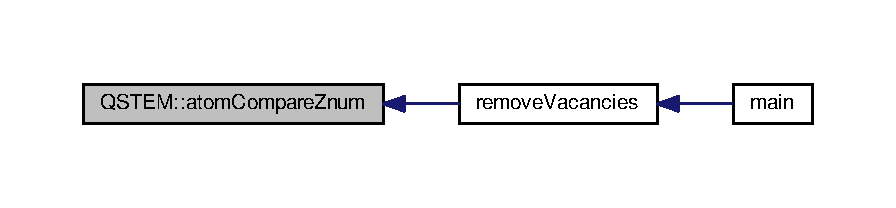
\includegraphics[width=350pt]{namespace_q_s_t_e_m_a71b66c2cfa1437a928461f3286b6449a_icgraph}
\end{center}
\end{figure}


\hypertarget{namespace_q_s_t_e_m_ab469a74324e6f9ea7af175cb608bd981}{\index{Q\-S\-T\-E\-M@{Q\-S\-T\-E\-M}!atom\-Compare\-Z\-Y\-X@{atom\-Compare\-Z\-Y\-X}}
\index{atom\-Compare\-Z\-Y\-X@{atom\-Compare\-Z\-Y\-X}!QSTEM@{Q\-S\-T\-E\-M}}
\subsubsection[{atom\-Compare\-Z\-Y\-X}]{\setlength{\rightskip}{0pt plus 5cm}int Q\-S\-T\-E\-M\-::atom\-Compare\-Z\-Y\-X (
\begin{DoxyParamCaption}
\item[{const void $\ast$}]{at\-Ptr1, }
\item[{const void $\ast$}]{at\-Ptr2}
\end{DoxyParamCaption}
)}}\label{namespace_q_s_t_e_m_ab469a74324e6f9ea7af175cb608bd981}


Here is the caller graph for this function\-:
\nopagebreak
\begin{figure}[H]
\begin{center}
\leavevmode
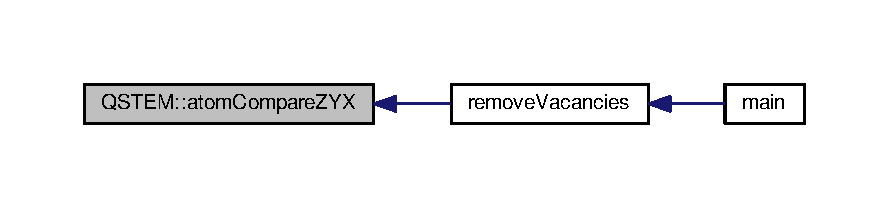
\includegraphics[width=350pt]{namespace_q_s_t_e_m_ab469a74324e6f9ea7af175cb608bd981_icgraph}
\end{center}
\end{figure}


\hypertarget{namespace_q_s_t_e_m_ae60a12e720b60af00feeaa668441bfaf}{\index{Q\-S\-T\-E\-M@{Q\-S\-T\-E\-M}!complex1\-D@{complex1\-D}}
\index{complex1\-D@{complex1\-D}!QSTEM@{Q\-S\-T\-E\-M}}
\subsubsection[{complex1\-D}]{\setlength{\rightskip}{0pt plus 5cm}boost\-::shared\-\_\-array$<$ {\bf complex\-\_\-tt} $>$ Q\-S\-T\-E\-M\-::complex1\-D (
\begin{DoxyParamCaption}
\item[{int}]{nx, }
\item[{const char $\ast$}]{message}
\end{DoxyParamCaption}
)}}\label{namespace_q_s_t_e_m_ae60a12e720b60af00feeaa668441bfaf}


Definition at line 411 of file memory\-\_\-fftw3.\-cpp.



Here is the caller graph for this function\-:
\nopagebreak
\begin{figure}[H]
\begin{center}
\leavevmode
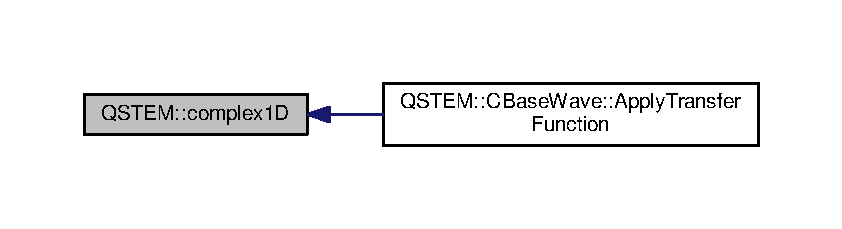
\includegraphics[width=350pt]{namespace_q_s_t_e_m_ae60a12e720b60af00feeaa668441bfaf_icgraph}
\end{center}
\end{figure}


\hypertarget{namespace_q_s_t_e_m_aaa6956a137718d0d1d008808fc37d0d6}{\index{Q\-S\-T\-E\-M@{Q\-S\-T\-E\-M}!complex2\-D@{complex2\-D}}
\index{complex2\-D@{complex2\-D}!QSTEM@{Q\-S\-T\-E\-M}}
\subsubsection[{complex2\-D}]{\setlength{\rightskip}{0pt plus 5cm}{\bf complex\-\_\-tt} {\bf Q\-S\-T\-E\-M\-\_\-\-H\-E\-L\-P\-E\-R\-\_\-\-D\-L\-L\-\_\-\-E\-X\-P\-O\-R\-T} $\ast$$\ast$ Q\-S\-T\-E\-M\-::complex2\-D (
\begin{DoxyParamCaption}
\item[{int}]{nx, }
\item[{int}]{ny, }
\item[{const char $\ast$}]{message}
\end{DoxyParamCaption}
)}}\label{namespace_q_s_t_e_m_aaa6956a137718d0d1d008808fc37d0d6}


Definition at line 427 of file memory\-\_\-fftw3.\-cpp.

\hypertarget{namespace_q_s_t_e_m_a33d6b5c2a67bbae130c8d48e35821820}{\index{Q\-S\-T\-E\-M@{Q\-S\-T\-E\-M}!complex2\-Dd@{complex2\-Dd}}
\index{complex2\-Dd@{complex2\-Dd}!QSTEM@{Q\-S\-T\-E\-M}}
\subsubsection[{complex2\-Dd}]{\setlength{\rightskip}{0pt plus 5cm}fftw\-\_\-complex $\ast$$\ast$ Q\-S\-T\-E\-M\-::complex2\-Dd (
\begin{DoxyParamCaption}
\item[{int}]{nx, }
\item[{int}]{ny, }
\item[{const char $\ast$}]{message}
\end{DoxyParamCaption}
)}}\label{namespace_q_s_t_e_m_a33d6b5c2a67bbae130c8d48e35821820}


Definition at line 464 of file memory\-\_\-fftw3.\-cpp.

\hypertarget{namespace_q_s_t_e_m_ac0d1ab0026b9fd9b89f3906feac1d54a}{\index{Q\-S\-T\-E\-M@{Q\-S\-T\-E\-M}!complex3\-D@{complex3\-D}}
\index{complex3\-D@{complex3\-D}!QSTEM@{Q\-S\-T\-E\-M}}
\subsubsection[{complex3\-D}]{\setlength{\rightskip}{0pt plus 5cm}{\bf complex\-\_\-tt} $\ast$$\ast$$\ast$ Q\-S\-T\-E\-M\-::complex3\-D (
\begin{DoxyParamCaption}
\item[{int}]{nx, }
\item[{int}]{ny, }
\item[{int}]{nz, }
\item[{const char $\ast$}]{message}
\end{DoxyParamCaption}
)}}\label{namespace_q_s_t_e_m_ac0d1ab0026b9fd9b89f3906feac1d54a}


Definition at line 541 of file memory\-\_\-fftw3.\-cpp.



Here is the caller graph for this function\-:
\nopagebreak
\begin{figure}[H]
\begin{center}
\leavevmode
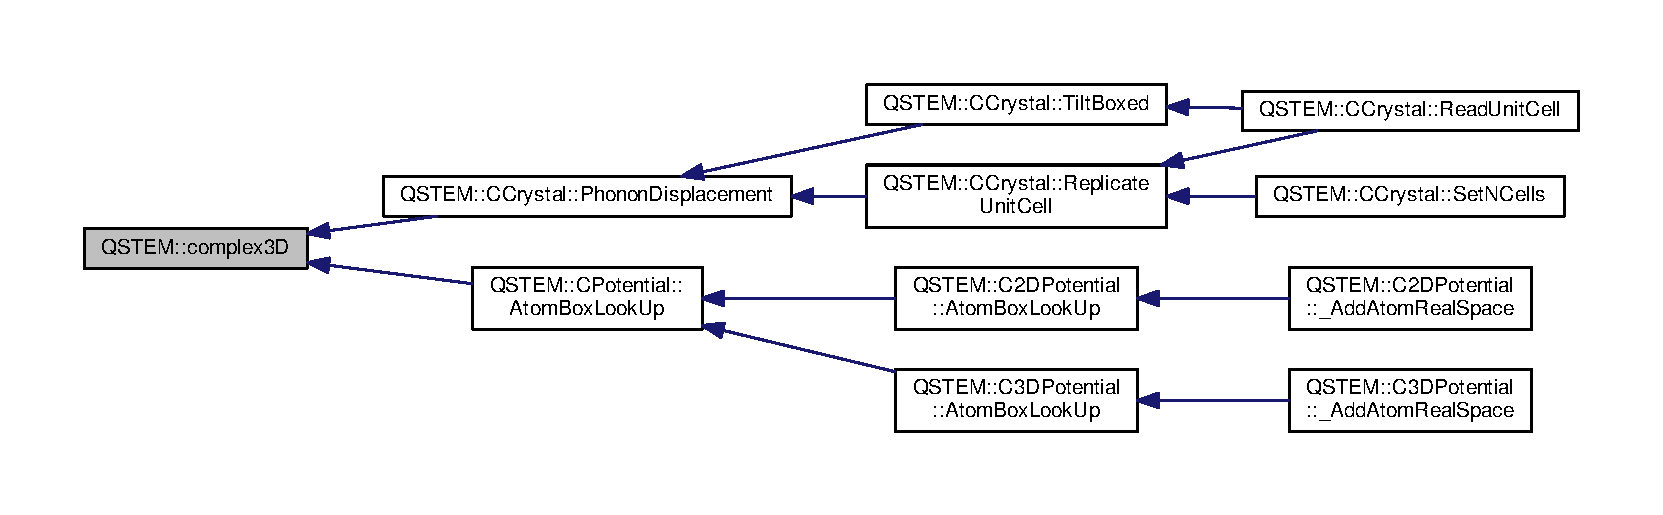
\includegraphics[width=350pt]{namespace_q_s_t_e_m_ac0d1ab0026b9fd9b89f3906feac1d54a_icgraph}
\end{center}
\end{figure}


\hypertarget{namespace_q_s_t_e_m_a87d813159312000dbc1894cf87950727}{\index{Q\-S\-T\-E\-M@{Q\-S\-T\-E\-M}!complex3\-Dd@{complex3\-Dd}}
\index{complex3\-Dd@{complex3\-Dd}!QSTEM@{Q\-S\-T\-E\-M}}
\subsubsection[{complex3\-Dd}]{\setlength{\rightskip}{0pt plus 5cm}fftw\-\_\-complex $\ast$$\ast$$\ast$ Q\-S\-T\-E\-M\-::complex3\-Dd (
\begin{DoxyParamCaption}
\item[{int}]{nx, }
\item[{int}]{ny, }
\item[{int}]{nz, }
\item[{const char $\ast$}]{message}
\end{DoxyParamCaption}
)}}\label{namespace_q_s_t_e_m_a87d813159312000dbc1894cf87950727}


Definition at line 498 of file memory\-\_\-fftw3.\-cpp.

\hypertarget{namespace_q_s_t_e_m_a7c5a7f91e9c031aa75053ad833e9e578}{\index{Q\-S\-T\-E\-M@{Q\-S\-T\-E\-M}!Create\-Wave\-Function\-Data\-Sets@{Create\-Wave\-Function\-Data\-Sets}}
\index{Create\-Wave\-Function\-Data\-Sets@{Create\-Wave\-Function\-Data\-Sets}!QSTEM@{Q\-S\-T\-E\-M}}
\subsubsection[{Create\-Wave\-Function\-Data\-Sets}]{\setlength{\rightskip}{0pt plus 5cm}void Q\-S\-T\-E\-M\-::\-Create\-Wave\-Function\-Data\-Sets (
\begin{DoxyParamCaption}
\item[{unsigned}]{x, }
\item[{unsigned}]{y, }
\item[{{\bf std\-::vector}$<$ unsigned $>$}]{positions, }
\item[{std\-::string}]{output\-\_\-ext}
\end{DoxyParamCaption}
)}}\label{namespace_q_s_t_e_m_a7c5a7f91e9c031aa75053ad833e9e578}


Definition at line 25 of file wave\-\_\-base.\-cpp.

\hypertarget{namespace_q_s_t_e_m_aa2c4c66d135c1e5a78552f723e8f72d8}{\index{Q\-S\-T\-E\-M@{Q\-S\-T\-E\-M}!cross\-Product@{cross\-Product}}
\index{cross\-Product@{cross\-Product}!QSTEM@{Q\-S\-T\-E\-M}}
\subsubsection[{cross\-Product}]{\setlength{\rightskip}{0pt plus 5cm}void Q\-S\-T\-E\-M\-::cross\-Product (
\begin{DoxyParamCaption}
\item[{const float\-\_\-tt $\ast$}]{a, }
\item[{const float\-\_\-tt $\ast$}]{b, }
\item[{float\-\_\-tt $\ast$}]{c}
\end{DoxyParamCaption}
)}}\label{namespace_q_s_t_e_m_aa2c4c66d135c1e5a78552f723e8f72d8}


Definition at line 500 of file matrixlib.\-cpp.



Here is the caller graph for this function\-:
\nopagebreak
\begin{figure}[H]
\begin{center}
\leavevmode
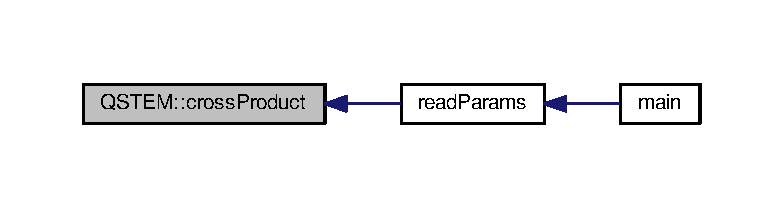
\includegraphics[width=350pt]{namespace_q_s_t_e_m_aa2c4c66d135c1e5a78552f723e8f72d8_icgraph}
\end{center}
\end{figure}


\hypertarget{namespace_q_s_t_e_m_a5bfcf68c04ebe43cb232f1be9fcceb95}{\index{Q\-S\-T\-E\-M@{Q\-S\-T\-E\-M}!det\-\_\-3x3@{det\-\_\-3x3}}
\index{det\-\_\-3x3@{det\-\_\-3x3}!QSTEM@{Q\-S\-T\-E\-M}}
\subsubsection[{det\-\_\-3x3}]{\setlength{\rightskip}{0pt plus 5cm}{\bf float\-\_\-tt} Q\-S\-T\-E\-M\-::det\-\_\-3x3 (
\begin{DoxyParamCaption}
\item[{const float\-\_\-tt $\ast$}]{mat}
\end{DoxyParamCaption}
)}}\label{namespace_q_s_t_e_m_a5bfcf68c04ebe43cb232f1be9fcceb95}


Definition at line 197 of file matrixlib.\-cpp.



Here is the caller graph for this function\-:
\nopagebreak
\begin{figure}[H]
\begin{center}
\leavevmode
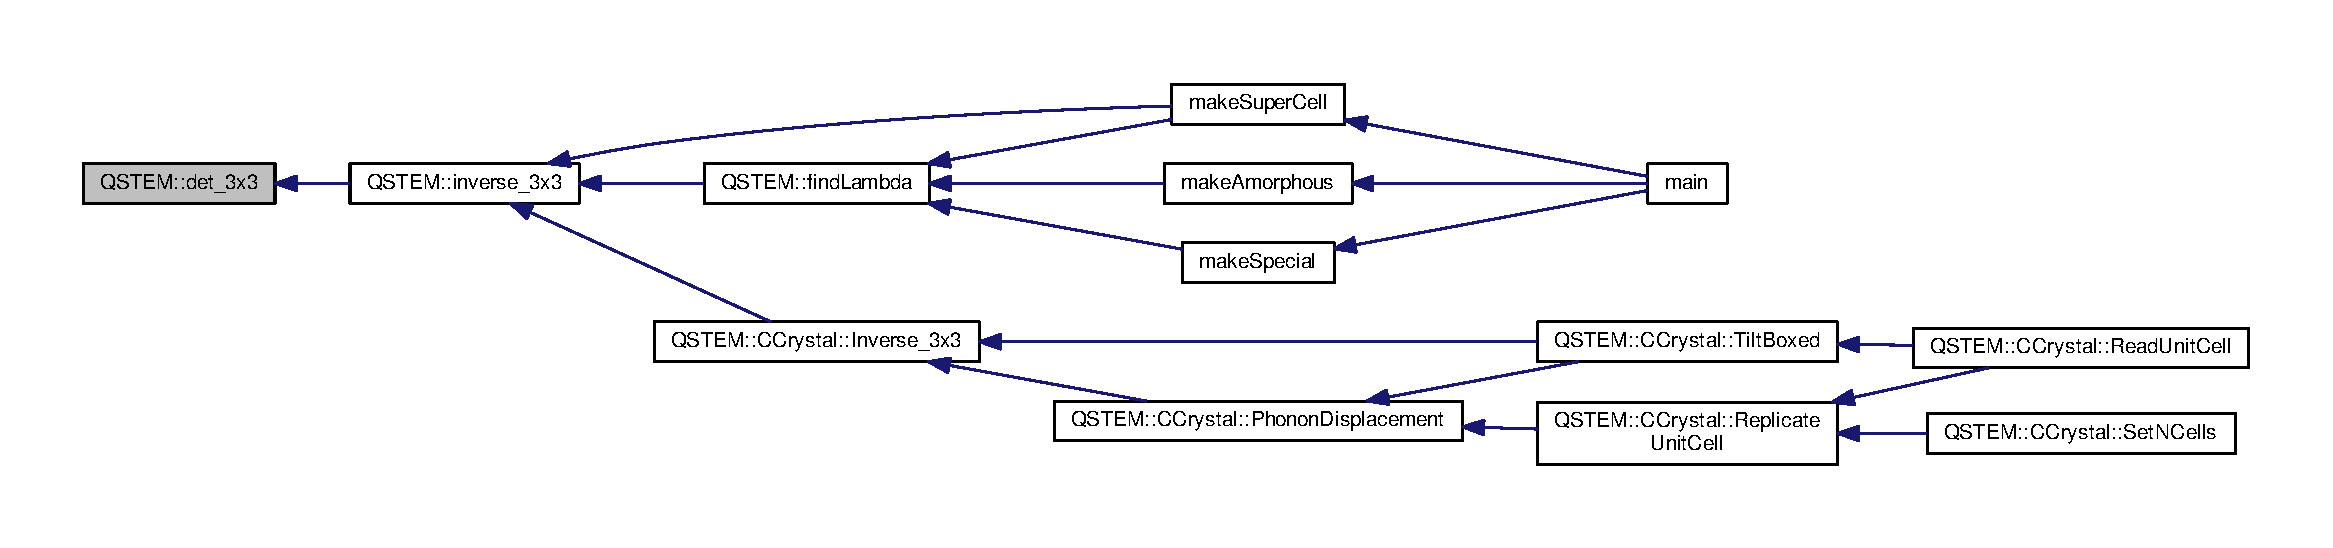
\includegraphics[width=350pt]{namespace_q_s_t_e_m_a5bfcf68c04ebe43cb232f1be9fcceb95_icgraph}
\end{center}
\end{figure}


\hypertarget{namespace_q_s_t_e_m_a16b9a6e71ce2db68471c3211feb491da}{\index{Q\-S\-T\-E\-M@{Q\-S\-T\-E\-M}!dot\-Product@{dot\-Product}}
\index{dot\-Product@{dot\-Product}!QSTEM@{Q\-S\-T\-E\-M}}
\subsubsection[{dot\-Product}]{\setlength{\rightskip}{0pt plus 5cm}{\bf float\-\_\-tt} Q\-S\-T\-E\-M\-::dot\-Product (
\begin{DoxyParamCaption}
\item[{const float\-\_\-tt $\ast$}]{a, }
\item[{const float\-\_\-tt $\ast$}]{b}
\end{DoxyParamCaption}
)}}\label{namespace_q_s_t_e_m_a16b9a6e71ce2db68471c3211feb491da}


Definition at line 507 of file matrixlib.\-cpp.



Here is the caller graph for this function\-:
\nopagebreak
\begin{figure}[H]
\begin{center}
\leavevmode
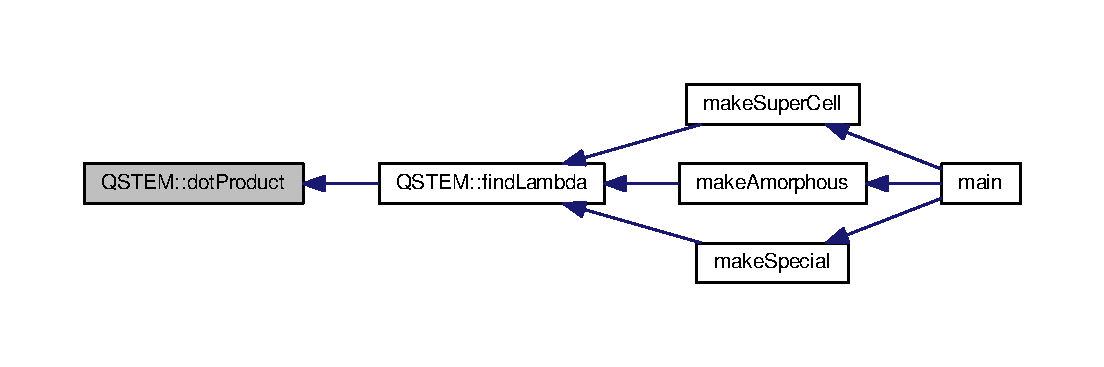
\includegraphics[width=350pt]{namespace_q_s_t_e_m_a16b9a6e71ce2db68471c3211feb491da_icgraph}
\end{center}
\end{figure}


\hypertarget{namespace_q_s_t_e_m_a3c6e64bb6444720850b2af4463d02a44}{\index{Q\-S\-T\-E\-M@{Q\-S\-T\-E\-M}!double1\-D@{double1\-D}}
\index{double1\-D@{double1\-D}!QSTEM@{Q\-S\-T\-E\-M}}
\subsubsection[{double1\-D}]{\setlength{\rightskip}{0pt plus 5cm}boost\-::shared\-\_\-array$<$ double $>$ Q\-S\-T\-E\-M\-::double1\-D (
\begin{DoxyParamCaption}
\item[{int}]{n, }
\item[{const char $\ast$}]{message}
\end{DoxyParamCaption}
)}}\label{namespace_q_s_t_e_m_a3c6e64bb6444720850b2af4463d02a44}


Definition at line 72 of file memory\-\_\-fftw3.\-cpp.

\hypertarget{namespace_q_s_t_e_m_acf77dcde7c77ddbf7896f8abd4106b36}{\index{Q\-S\-T\-E\-M@{Q\-S\-T\-E\-M}!double2\-D@{double2\-D}}
\index{double2\-D@{double2\-D}!QSTEM@{Q\-S\-T\-E\-M}}
\subsubsection[{double2\-D}]{\setlength{\rightskip}{0pt plus 5cm}double $\ast$$\ast$ Q\-S\-T\-E\-M\-::double2\-D (
\begin{DoxyParamCaption}
\item[{int}]{nx, }
\item[{int}]{ny, }
\item[{const char $\ast$}]{message}
\end{DoxyParamCaption}
)}}\label{namespace_q_s_t_e_m_acf77dcde7c77ddbf7896f8abd4106b36}


Definition at line 369 of file memory\-\_\-fftw3.\-cpp.

\hypertarget{namespace_q_s_t_e_m_ae902fc588441e4154d9713e9c2a7ecca}{\index{Q\-S\-T\-E\-M@{Q\-S\-T\-E\-M}!find\-Lambda@{find\-Lambda}}
\index{find\-Lambda@{find\-Lambda}!QSTEM@{Q\-S\-T\-E\-M}}
\subsubsection[{find\-Lambda}]{\setlength{\rightskip}{0pt plus 5cm}{\bf float\-\_\-tt} Q\-S\-T\-E\-M\-::find\-Lambda (
\begin{DoxyParamCaption}
\item[{plane $\ast$}]{p, }
\item[{float $\ast$}]{point, }
\item[{int}]{rev\-Flag}
\end{DoxyParamCaption}
)}}\label{namespace_q_s_t_e_m_ae902fc588441e4154d9713e9c2a7ecca}


Definition at line 549 of file matrixlib.\-cpp.



Here is the call graph for this function\-:
\nopagebreak
\begin{figure}[H]
\begin{center}
\leavevmode
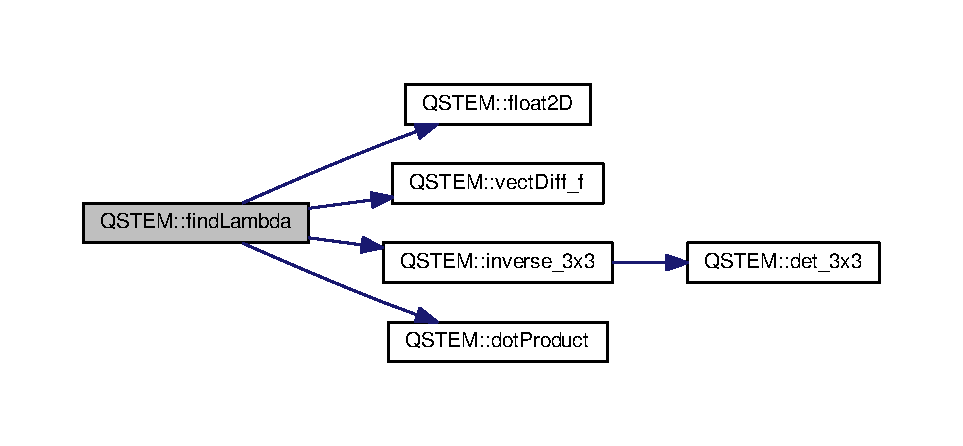
\includegraphics[width=350pt]{namespace_q_s_t_e_m_ae902fc588441e4154d9713e9c2a7ecca_cgraph}
\end{center}
\end{figure}




Here is the caller graph for this function\-:
\nopagebreak
\begin{figure}[H]
\begin{center}
\leavevmode
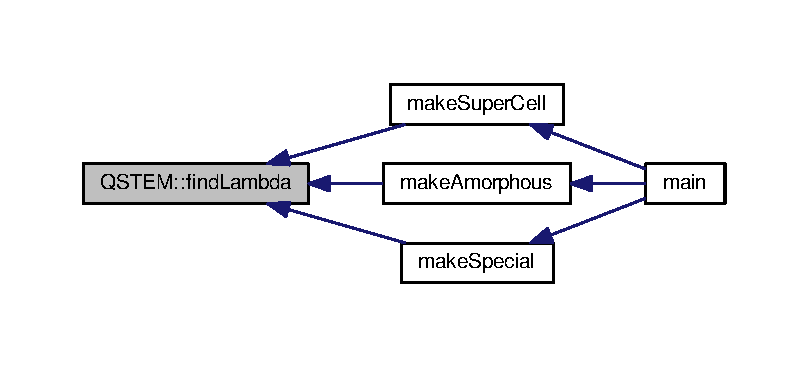
\includegraphics[width=350pt]{namespace_q_s_t_e_m_ae902fc588441e4154d9713e9c2a7ecca_icgraph}
\end{center}
\end{figure}


\hypertarget{namespace_q_s_t_e_m_a2afd56d6aa92f762eb233f54f39f880b}{\index{Q\-S\-T\-E\-M@{Q\-S\-T\-E\-M}!float1\-D@{float1\-D}}
\index{float1\-D@{float1\-D}!QSTEM@{Q\-S\-T\-E\-M}}
\subsubsection[{float1\-D}]{\setlength{\rightskip}{0pt plus 5cm}boost\-::shared\-\_\-array$<$ {\bf float\-\_\-tt} $>$ Q\-S\-T\-E\-M\-::float1\-D (
\begin{DoxyParamCaption}
\item[{int}]{n, }
\item[{const char $\ast$}]{message}
\end{DoxyParamCaption}
)}}\label{namespace_q_s_t_e_m_a2afd56d6aa92f762eb233f54f39f880b}


Definition at line 45 of file memory\-\_\-fftw3.\-cpp.

\hypertarget{namespace_q_s_t_e_m_ad4ae9d6a3f69596b4581f09f0756faaa}{\index{Q\-S\-T\-E\-M@{Q\-S\-T\-E\-M}!float2\-D@{float2\-D}}
\index{float2\-D@{float2\-D}!QSTEM@{Q\-S\-T\-E\-M}}
\subsubsection[{float2\-D}]{\setlength{\rightskip}{0pt plus 5cm}{\bf float\-\_\-tt} {\bf Q\-S\-T\-E\-M\-\_\-\-H\-E\-L\-P\-E\-R\-\_\-\-D\-L\-L\-\_\-\-E\-X\-P\-O\-R\-T} $\ast$$\ast$ Q\-S\-T\-E\-M\-::float2\-D (
\begin{DoxyParamCaption}
\item[{int}]{nx, }
\item[{int}]{ny, }
\item[{const char $\ast$}]{message}
\end{DoxyParamCaption}
)}}\label{namespace_q_s_t_e_m_ad4ae9d6a3f69596b4581f09f0756faaa}


Definition at line 238 of file memory\-\_\-fftw3.\-cpp.



Here is the caller graph for this function\-:
\nopagebreak
\begin{figure}[H]
\begin{center}
\leavevmode
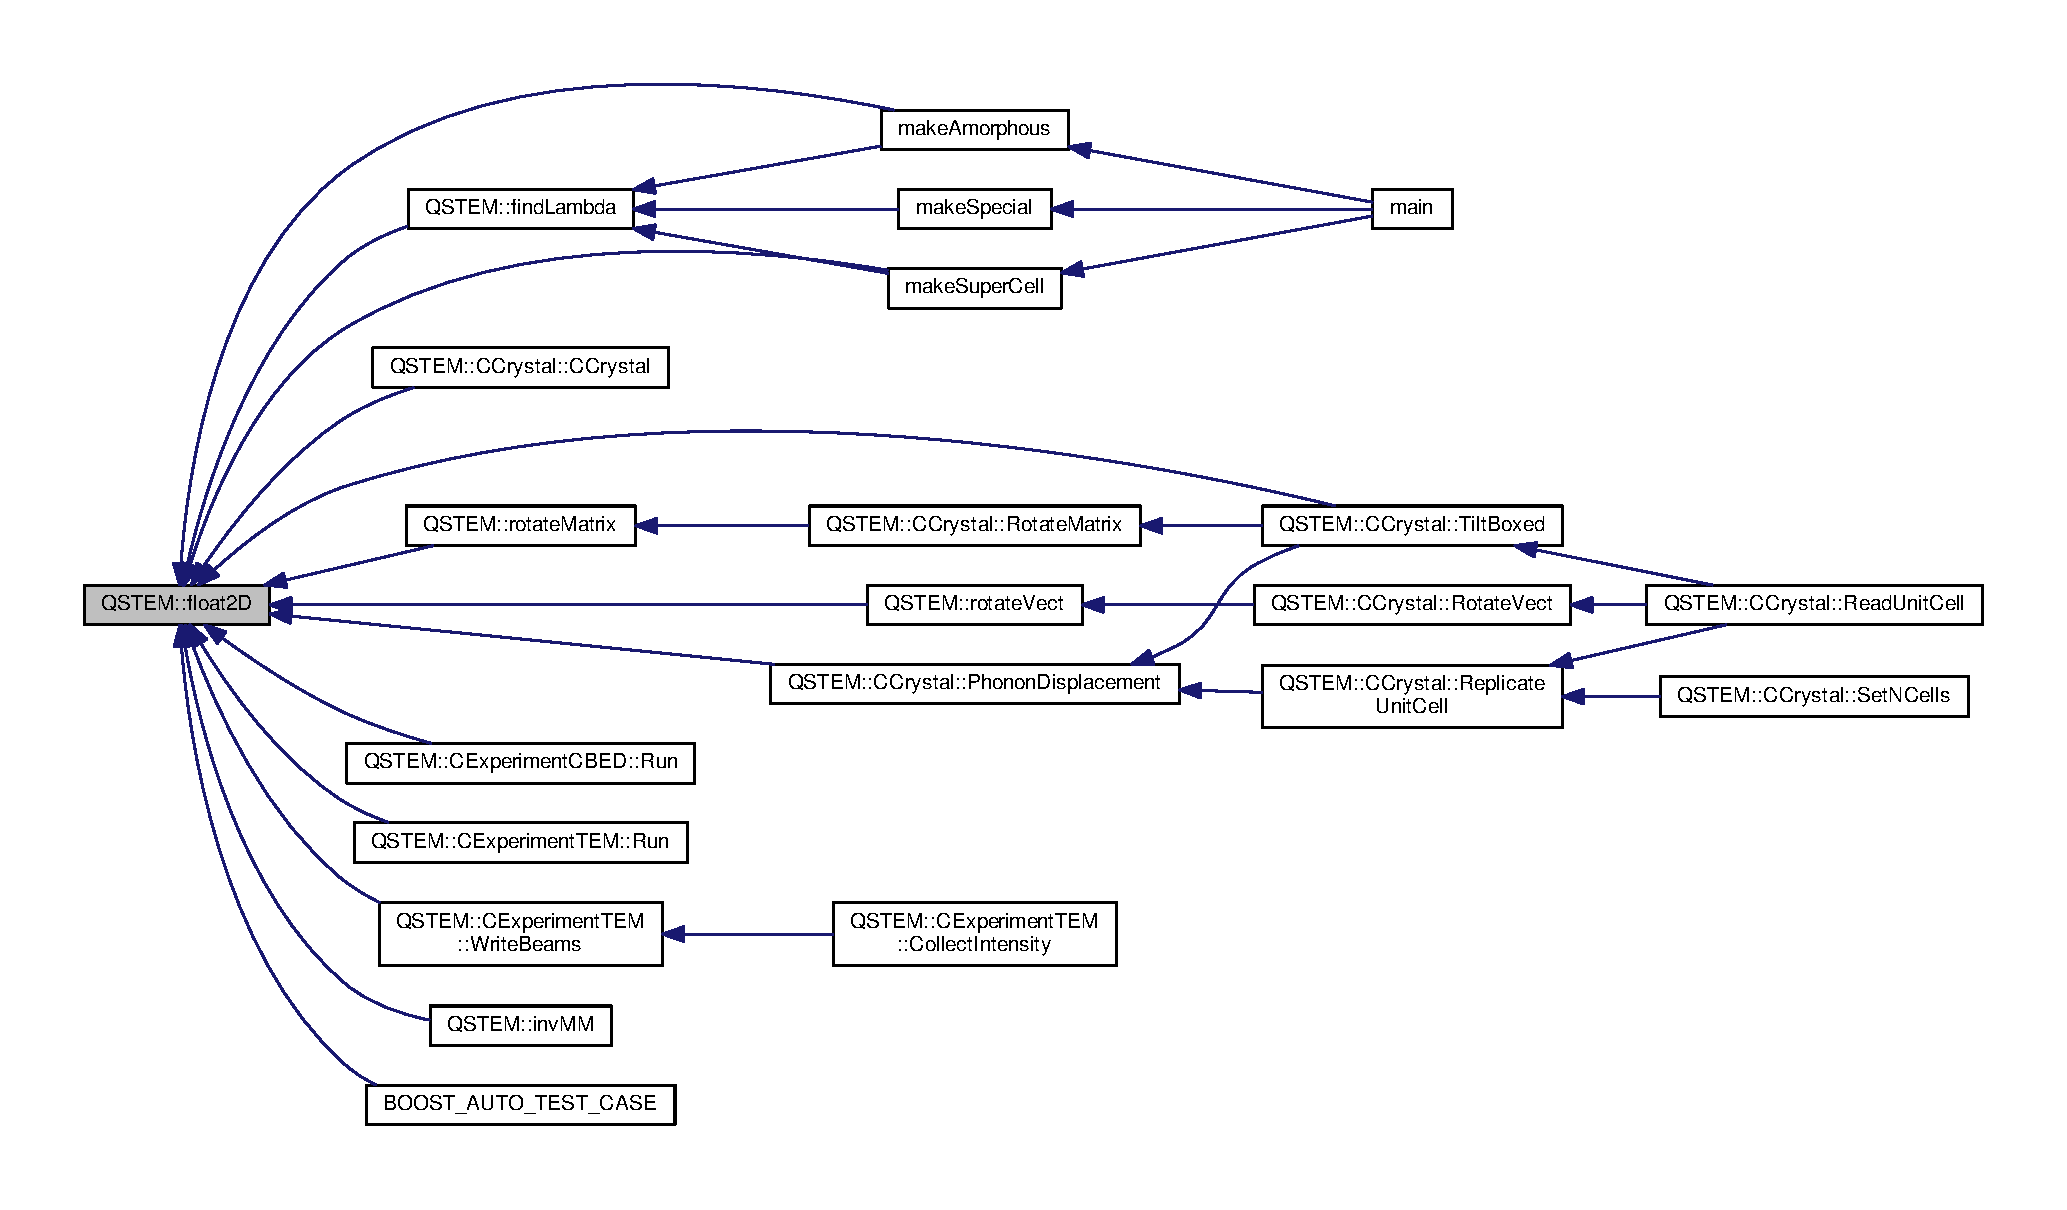
\includegraphics[width=350pt]{namespace_q_s_t_e_m_ad4ae9d6a3f69596b4581f09f0756faaa_icgraph}
\end{center}
\end{figure}


\hypertarget{namespace_q_s_t_e_m_a5cd18f813d8e07713ec8e70ce18f0da6}{\index{Q\-S\-T\-E\-M@{Q\-S\-T\-E\-M}!float32\-\_\-2\-D@{float32\-\_\-2\-D}}
\index{float32\-\_\-2\-D@{float32\-\_\-2\-D}!QSTEM@{Q\-S\-T\-E\-M}}
\subsubsection[{float32\-\_\-2\-D}]{\setlength{\rightskip}{0pt plus 5cm}float $\ast$$\ast$ Q\-S\-T\-E\-M\-::float32\-\_\-2\-D (
\begin{DoxyParamCaption}
\item[{int}]{nx, }
\item[{int}]{ny, }
\item[{const char $\ast$}]{message}
\end{DoxyParamCaption}
)}}\label{namespace_q_s_t_e_m_a5cd18f813d8e07713ec8e70ce18f0da6}


Definition at line 202 of file memory\-\_\-fftw3.\-cpp.

\hypertarget{namespace_q_s_t_e_m_af971dc67e55e7e7c84708aae8cfea0ad}{\index{Q\-S\-T\-E\-M@{Q\-S\-T\-E\-M}!float32\-\_\-3\-D@{float32\-\_\-3\-D}}
\index{float32\-\_\-3\-D@{float32\-\_\-3\-D}!QSTEM@{Q\-S\-T\-E\-M}}
\subsubsection[{float32\-\_\-3\-D}]{\setlength{\rightskip}{0pt plus 5cm}float $\ast$$\ast$$\ast$ Q\-S\-T\-E\-M\-::float32\-\_\-3\-D (
\begin{DoxyParamCaption}
\item[{int}]{nx, }
\item[{int}]{ny, }
\item[{int}]{nz, }
\item[{const char $\ast$}]{message}
\end{DoxyParamCaption}
)}}\label{namespace_q_s_t_e_m_af971dc67e55e7e7c84708aae8cfea0ad}


Definition at line 323 of file memory\-\_\-fftw3.\-cpp.

\hypertarget{namespace_q_s_t_e_m_a863cc7cc67654a9bbf660b243306ee29}{\index{Q\-S\-T\-E\-M@{Q\-S\-T\-E\-M}!float3\-D@{float3\-D}}
\index{float3\-D@{float3\-D}!QSTEM@{Q\-S\-T\-E\-M}}
\subsubsection[{float3\-D}]{\setlength{\rightskip}{0pt plus 5cm}{\bf float\-\_\-tt} $\ast$$\ast$$\ast$ Q\-S\-T\-E\-M\-::float3\-D (
\begin{DoxyParamCaption}
\item[{int}]{nx, }
\item[{int}]{ny, }
\item[{int}]{nz, }
\item[{const char $\ast$}]{message}
\end{DoxyParamCaption}
)}}\label{namespace_q_s_t_e_m_a863cc7cc67654a9bbf660b243306ee29}


Definition at line 279 of file memory\-\_\-fftw3.\-cpp.



Here is the caller graph for this function\-:
\nopagebreak
\begin{figure}[H]
\begin{center}
\leavevmode
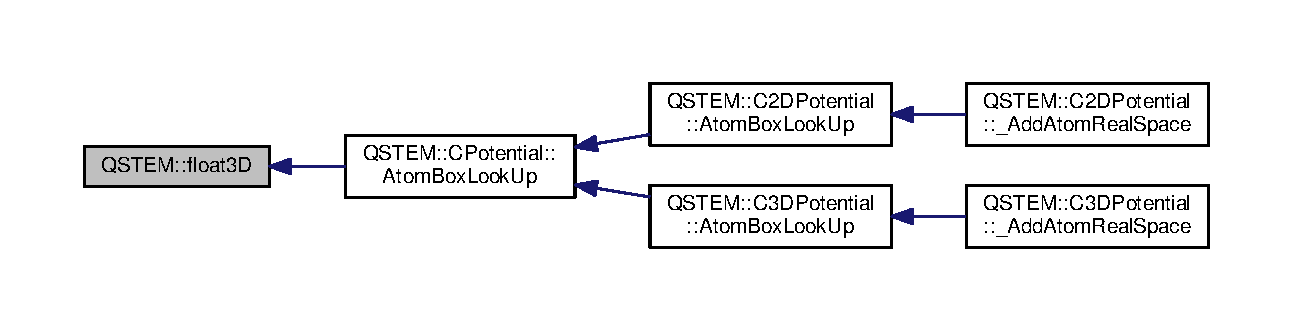
\includegraphics[width=350pt]{namespace_q_s_t_e_m_a863cc7cc67654a9bbf660b243306ee29_icgraph}
\end{center}
\end{figure}


\hypertarget{namespace_q_s_t_e_m_a5e13b8cafb6a8f18aaf6603dc9cc8584}{\index{Q\-S\-T\-E\-M@{Q\-S\-T\-E\-M}!gasdev@{gasdev}}
\index{gasdev@{gasdev}!QSTEM@{Q\-S\-T\-E\-M}}
\subsubsection[{gasdev}]{\setlength{\rightskip}{0pt plus 5cm}{\bf float\-\_\-tt} Q\-S\-T\-E\-M\-::gasdev (
\begin{DoxyParamCaption}
{}
\end{DoxyParamCaption}
)\hspace{0.3cm}{\ttfamily [inline]}}}\label{namespace_q_s_t_e_m_a5e13b8cafb6a8f18aaf6603dc9cc8584}


Definition at line 35 of file random.\-hpp.

\hypertarget{namespace_q_s_t_e_m_a69bdadd86b47f8a4253fb384011b33b6}{\index{Q\-S\-T\-E\-M@{Q\-S\-T\-E\-M}!gasdev@{gasdev}}
\index{gasdev@{gasdev}!QSTEM@{Q\-S\-T\-E\-M}}
\subsubsection[{gasdev}]{\setlength{\rightskip}{0pt plus 5cm}double Q\-S\-T\-E\-M\-::gasdev (
\begin{DoxyParamCaption}
\item[{long $\ast$}]{idum}
\end{DoxyParamCaption}
)}}\label{namespace_q_s_t_e_m_a69bdadd86b47f8a4253fb384011b33b6}


Here is the caller graph for this function\-:
\nopagebreak
\begin{figure}[H]
\begin{center}
\leavevmode
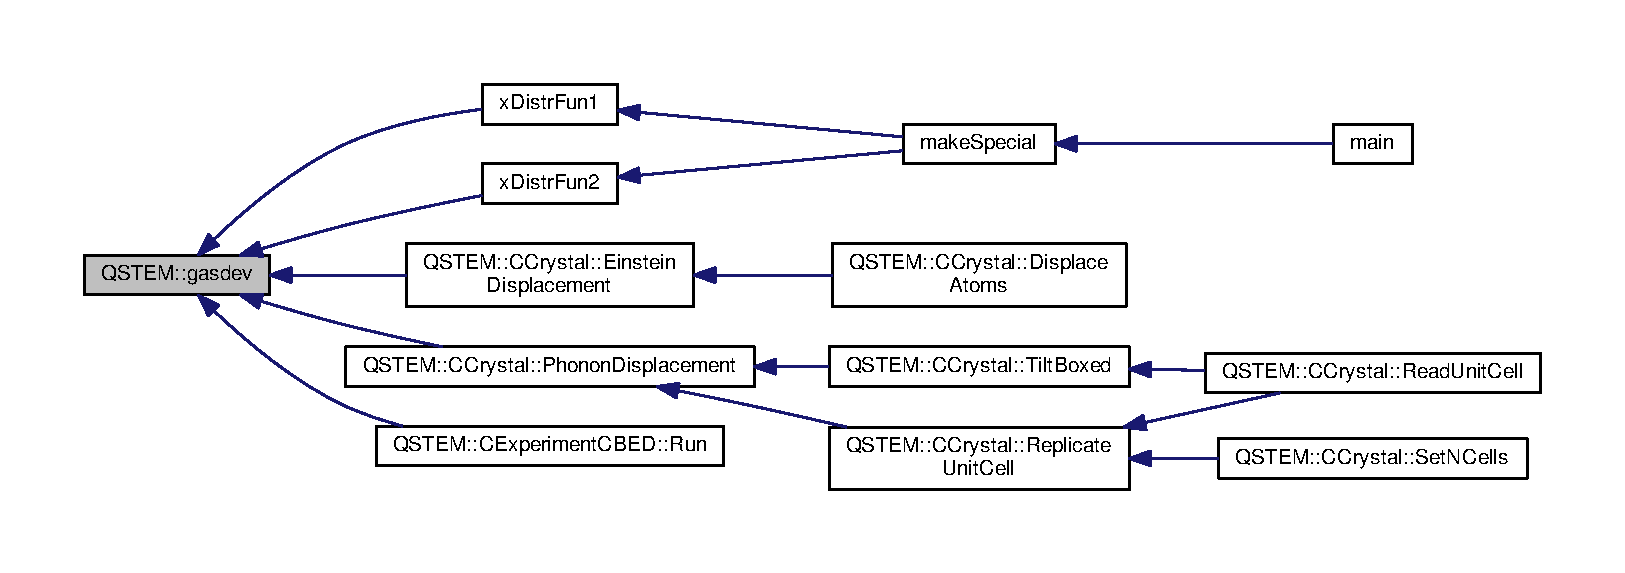
\includegraphics[width=350pt]{namespace_q_s_t_e_m_a69bdadd86b47f8a4253fb384011b33b6_icgraph}
\end{center}
\end{figure}


\hypertarget{namespace_q_s_t_e_m_a7bddd87825c86fdbd52398187cdc932d}{\index{Q\-S\-T\-E\-M@{Q\-S\-T\-E\-M}!Get\-Experiment@{Get\-Experiment}}
\index{Get\-Experiment@{Get\-Experiment}!QSTEM@{Q\-S\-T\-E\-M}}
\subsubsection[{Get\-Experiment}]{\setlength{\rightskip}{0pt plus 5cm}{\bf Experiment\-Ptr} {\bf Q\-S\-T\-E\-M\-\_\-\-H\-E\-L\-P\-E\-R\-\_\-\-D\-L\-L\-\_\-\-E\-X\-P\-O\-R\-T} Q\-S\-T\-E\-M\-::\-Get\-Experiment (
\begin{DoxyParamCaption}
\item[{Config\-Reader\-Ptr \&}]{config\-Reader}
\end{DoxyParamCaption}
)}}\label{namespace_q_s_t_e_m_a7bddd87825c86fdbd52398187cdc932d}


Definition at line 28 of file experiments.\-cpp.



Here is the caller graph for this function\-:
\nopagebreak
\begin{figure}[H]
\begin{center}
\leavevmode
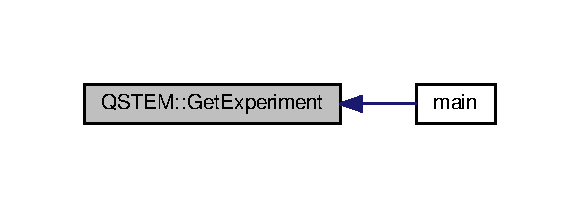
\includegraphics[width=278pt]{namespace_q_s_t_e_m_a7bddd87825c86fdbd52398187cdc932d_icgraph}
\end{center}
\end{figure}


\hypertarget{namespace_q_s_t_e_m_a5bff3e0346b1ca9e58f1b37c0a0c9b9a}{\index{Q\-S\-T\-E\-M@{Q\-S\-T\-E\-M}!Get\-Structure\-Reader@{Get\-Structure\-Reader}}
\index{Get\-Structure\-Reader@{Get\-Structure\-Reader}!QSTEM@{Q\-S\-T\-E\-M}}
\subsubsection[{Get\-Structure\-Reader}]{\setlength{\rightskip}{0pt plus 5cm}{\bf Structure\-Reader\-Ptr} Q\-S\-T\-E\-M\-::\-Get\-Structure\-Reader (
\begin{DoxyParamCaption}
\item[{boost\-::filesystem\-::path \&}]{structure\-\_\-file}
\end{DoxyParamCaption}
)\hspace{0.3cm}{\ttfamily [inline]}}}\label{namespace_q_s_t_e_m_a5bff3e0346b1ca9e58f1b37c0a0c9b9a}


Definition at line 31 of file structure\-\_\-readers.\-hpp.

\hypertarget{namespace_q_s_t_e_m_a3558bc3153acae75fb497d58b3081c55}{\index{Q\-S\-T\-E\-M@{Q\-S\-T\-E\-M}!get\-Z\-Number@{get\-Z\-Number}}
\index{get\-Z\-Number@{get\-Z\-Number}!QSTEM@{Q\-S\-T\-E\-M}}
\subsubsection[{get\-Z\-Number}]{\setlength{\rightskip}{0pt plus 5cm}int Q\-S\-T\-E\-M\-::get\-Z\-Number (
\begin{DoxyParamCaption}
\item[{char $\ast$}]{element}
\end{DoxyParamCaption}
)}}\label{namespace_q_s_t_e_m_a3558bc3153acae75fb497d58b3081c55}


Here is the caller graph for this function\-:
\nopagebreak
\begin{figure}[H]
\begin{center}
\leavevmode
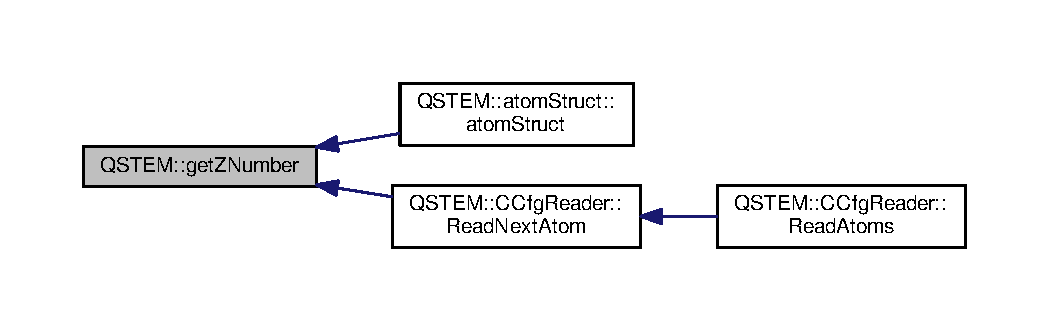
\includegraphics[width=350pt]{namespace_q_s_t_e_m_a3558bc3153acae75fb497d58b3081c55_icgraph}
\end{center}
\end{figure}


\hypertarget{namespace_q_s_t_e_m_ab434691b12196603619a006b7766c156}{\index{Q\-S\-T\-E\-M@{Q\-S\-T\-E\-M}!int2\-D@{int2\-D}}
\index{int2\-D@{int2\-D}!QSTEM@{Q\-S\-T\-E\-M}}
\subsubsection[{int2\-D}]{\setlength{\rightskip}{0pt plus 5cm}int $\ast$$\ast$ Q\-S\-T\-E\-M\-::int2\-D (
\begin{DoxyParamCaption}
\item[{int}]{nx, }
\item[{int}]{ny, }
\item[{const char $\ast$}]{message}
\end{DoxyParamCaption}
)}}\label{namespace_q_s_t_e_m_ab434691b12196603619a006b7766c156}


Definition at line 131 of file memory\-\_\-fftw3.\-cpp.



Here is the caller graph for this function\-:
\nopagebreak
\begin{figure}[H]
\begin{center}
\leavevmode
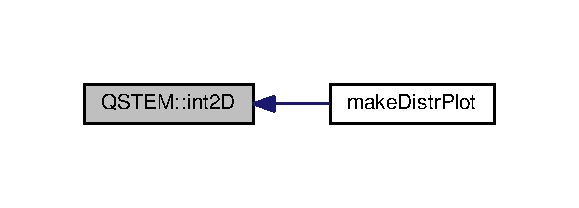
\includegraphics[width=278pt]{namespace_q_s_t_e_m_ab434691b12196603619a006b7766c156_icgraph}
\end{center}
\end{figure}


\hypertarget{namespace_q_s_t_e_m_ab7cf11c08d4958453b8a597bb93b1e38}{\index{Q\-S\-T\-E\-M@{Q\-S\-T\-E\-M}!inverse@{inverse}}
\index{inverse@{inverse}!QSTEM@{Q\-S\-T\-E\-M}}
\subsubsection[{inverse}]{\setlength{\rightskip}{0pt plus 5cm}void Q\-S\-T\-E\-M\-::inverse (
\begin{DoxyParamCaption}
{}
\end{DoxyParamCaption}
)}}\label{namespace_q_s_t_e_m_ab7cf11c08d4958453b8a597bb93b1e38}


Definition at line 175 of file matrixlib.\-cpp.

\hypertarget{namespace_q_s_t_e_m_acc22a77e731414c6c8a9370225bb5546}{\index{Q\-S\-T\-E\-M@{Q\-S\-T\-E\-M}!inverse\-\_\-3x3@{inverse\-\_\-3x3}}
\index{inverse\-\_\-3x3@{inverse\-\_\-3x3}!QSTEM@{Q\-S\-T\-E\-M}}
\subsubsection[{inverse\-\_\-3x3}]{\setlength{\rightskip}{0pt plus 5cm}void Q\-S\-T\-E\-M\-::inverse\-\_\-3x3 (
\begin{DoxyParamCaption}
\item[{float\-\_\-tt $\ast$}]{res, }
\item[{const float\-\_\-tt $\ast$}]{a}
\end{DoxyParamCaption}
)}}\label{namespace_q_s_t_e_m_acc22a77e731414c6c8a9370225bb5546}


Definition at line 225 of file matrixlib.\-cpp.



Here is the call graph for this function\-:
\nopagebreak
\begin{figure}[H]
\begin{center}
\leavevmode
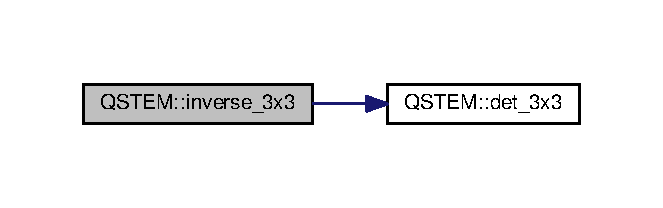
\includegraphics[width=318pt]{namespace_q_s_t_e_m_acc22a77e731414c6c8a9370225bb5546_cgraph}
\end{center}
\end{figure}




Here is the caller graph for this function\-:
\nopagebreak
\begin{figure}[H]
\begin{center}
\leavevmode
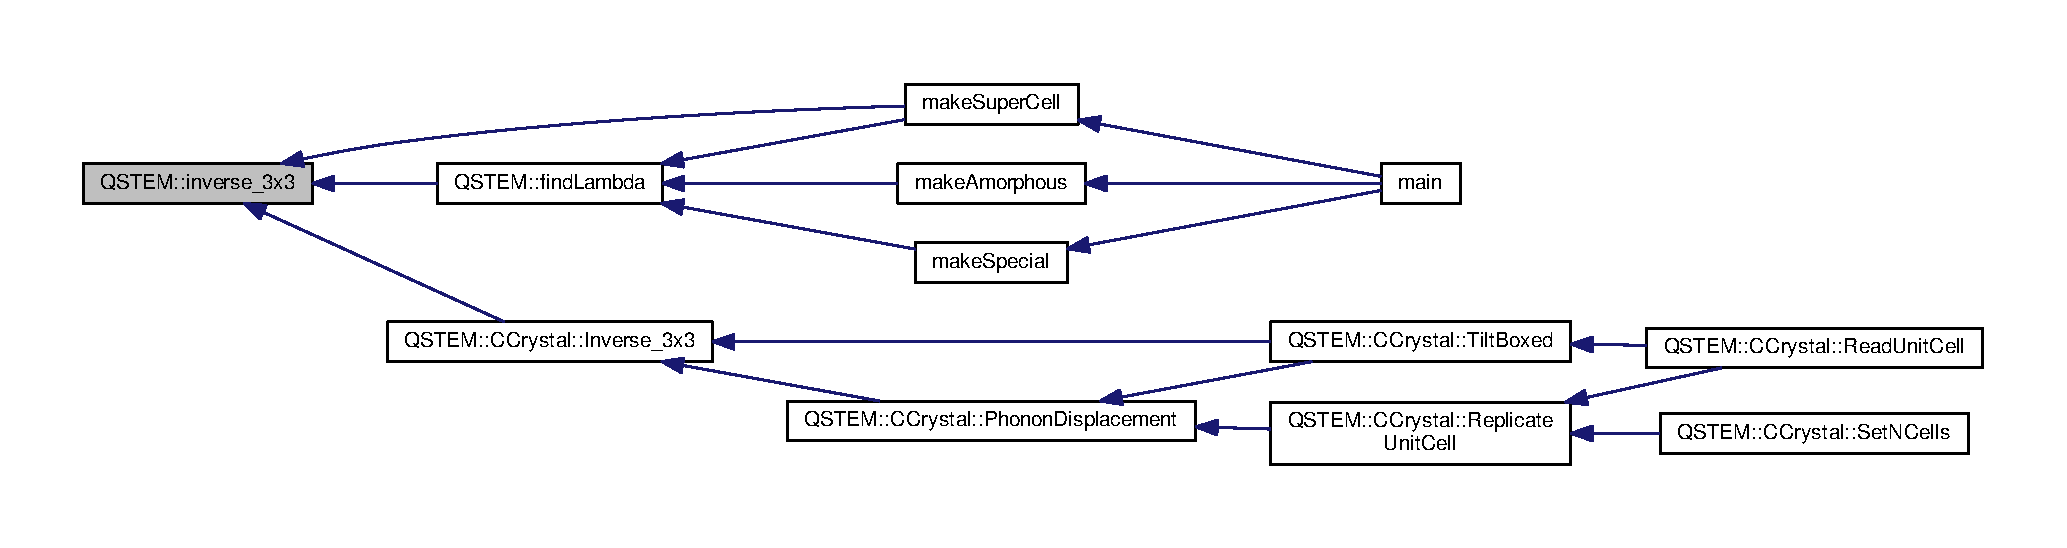
\includegraphics[width=350pt]{namespace_q_s_t_e_m_acc22a77e731414c6c8a9370225bb5546_icgraph}
\end{center}
\end{figure}


\hypertarget{namespace_q_s_t_e_m_a09a9764bcea955e486786c88a8d773bf}{\index{Q\-S\-T\-E\-M@{Q\-S\-T\-E\-M}!inv\-M\-M@{inv\-M\-M}}
\index{inv\-M\-M@{inv\-M\-M}!QSTEM@{Q\-S\-T\-E\-M}}
\subsubsection[{inv\-M\-M}]{\setlength{\rightskip}{0pt plus 5cm}{\bf float\-\_\-tt}$\ast$$\ast$ Q\-S\-T\-E\-M\-::inv\-M\-M (
\begin{DoxyParamCaption}
\item[{float\-\_\-tt $\ast$$\ast$}]{Mmatrix, }
\item[{int}]{N, }
\item[{int}]{M}
\end{DoxyParamCaption}
)}}\label{namespace_q_s_t_e_m_a09a9764bcea955e486786c88a8d773bf}


Definition at line 266 of file matrixlib.\-cpp.



Here is the call graph for this function\-:
\nopagebreak
\begin{figure}[H]
\begin{center}
\leavevmode
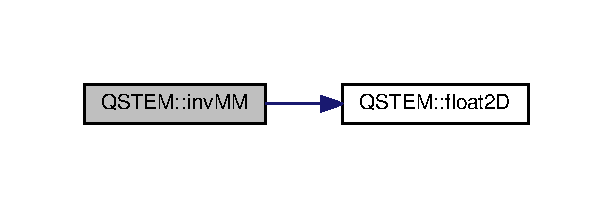
\includegraphics[width=294pt]{namespace_q_s_t_e_m_a09a9764bcea955e486786c88a8d773bf_cgraph}
\end{center}
\end{figure}


\hypertarget{namespace_q_s_t_e_m_a973e48590fcbb123c1d774e60a8b36c9}{\index{Q\-S\-T\-E\-M@{Q\-S\-T\-E\-M}!long2\-D@{long2\-D}}
\index{long2\-D@{long2\-D}!QSTEM@{Q\-S\-T\-E\-M}}
\subsubsection[{long2\-D}]{\setlength{\rightskip}{0pt plus 5cm}long $\ast$$\ast$ Q\-S\-T\-E\-M\-::long2\-D (
\begin{DoxyParamCaption}
\item[{int}]{nx, }
\item[{int}]{ny, }
\item[{const char $\ast$}]{message}
\end{DoxyParamCaption}
)}}\label{namespace_q_s_t_e_m_a973e48590fcbb123c1d774e60a8b36c9}


Definition at line 167 of file memory\-\_\-fftw3.\-cpp.

\hypertarget{namespace_q_s_t_e_m_a52cb9e4ab3fa015bce219ce7bbc31891}{\index{Q\-S\-T\-E\-M@{Q\-S\-T\-E\-M}!lubksb@{lubksb}}
\index{lubksb@{lubksb}!QSTEM@{Q\-S\-T\-E\-M}}
\subsubsection[{lubksb}]{\setlength{\rightskip}{0pt plus 5cm}void Q\-S\-T\-E\-M\-::lubksb (
\begin{DoxyParamCaption}
\item[{float\-\_\-tt $\ast$$\ast$}]{a, }
\item[{int}]{n, }
\item[{int $\ast$}]{indx, }
\item[{float\-\_\-tt}]{b\mbox{[}$\,$\mbox{]}}
\end{DoxyParamCaption}
)}}\label{namespace_q_s_t_e_m_a52cb9e4ab3fa015bce219ce7bbc31891}


Definition at line 129 of file matrixlib.\-cpp.



Here is the call graph for this function\-:
\nopagebreak
\begin{figure}[H]
\begin{center}
\leavevmode
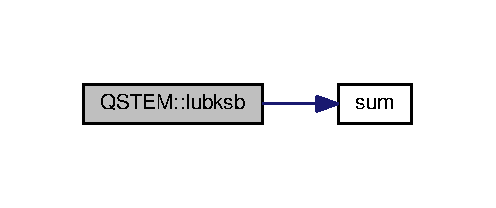
\includegraphics[width=238pt]{namespace_q_s_t_e_m_a52cb9e4ab3fa015bce219ce7bbc31891_cgraph}
\end{center}
\end{figure}


\hypertarget{namespace_q_s_t_e_m_abc355cf7175a88fd4cce7ea7b8b634f7}{\index{Q\-S\-T\-E\-M@{Q\-S\-T\-E\-M}!ludcmp@{ludcmp}}
\index{ludcmp@{ludcmp}!QSTEM@{Q\-S\-T\-E\-M}}
\subsubsection[{ludcmp}]{\setlength{\rightskip}{0pt plus 5cm}void Q\-S\-T\-E\-M\-::ludcmp (
\begin{DoxyParamCaption}
\item[{float\-\_\-tt $\ast$$\ast$}]{a, }
\item[{int}]{n, }
\item[{int $\ast$}]{indx, }
\item[{float\-\_\-tt $\ast$}]{d}
\end{DoxyParamCaption}
)}}\label{namespace_q_s_t_e_m_abc355cf7175a88fd4cce7ea7b8b634f7}


Definition at line 47 of file matrixlib.\-cpp.



Here is the call graph for this function\-:
\nopagebreak
\begin{figure}[H]
\begin{center}
\leavevmode
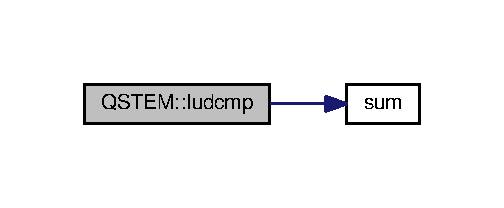
\includegraphics[width=242pt]{namespace_q_s_t_e_m_abc355cf7175a88fd4cce7ea7b8b634f7_cgraph}
\end{center}
\end{figure}


\hypertarget{namespace_q_s_t_e_m_a27a096719e7ddfebba30a0c3bc7a0966}{\index{Q\-S\-T\-E\-M@{Q\-S\-T\-E\-M}!make\-Cell\-Vect@{make\-Cell\-Vect}}
\index{make\-Cell\-Vect@{make\-Cell\-Vect}!QSTEM@{Q\-S\-T\-E\-M}}
\subsubsection[{make\-Cell\-Vect}]{\setlength{\rightskip}{0pt plus 5cm}void Q\-S\-T\-E\-M\-::make\-Cell\-Vect (
\begin{DoxyParamCaption}
\item[{grain\-Box $\ast$}]{grain, }
\item[{float\-\_\-tt $\ast$}]{vax, }
\item[{float\-\_\-tt $\ast$}]{vby, }
\item[{float\-\_\-tt $\ast$}]{vcz}
\end{DoxyParamCaption}
)}}\label{namespace_q_s_t_e_m_a27a096719e7ddfebba30a0c3bc7a0966}


Definition at line 693 of file matrixlib.\-cpp.



Here is the caller graph for this function\-:
\nopagebreak
\begin{figure}[H]
\begin{center}
\leavevmode
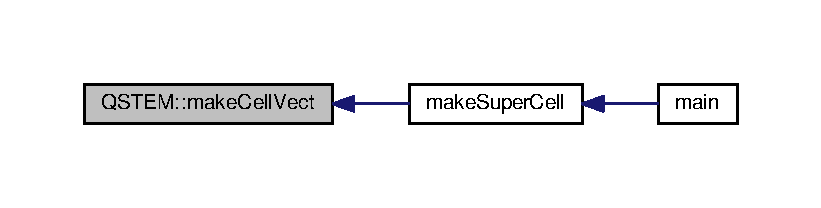
\includegraphics[width=350pt]{namespace_q_s_t_e_m_a27a096719e7ddfebba30a0c3bc7a0966_icgraph}
\end{center}
\end{figure}


\hypertarget{namespace_q_s_t_e_m_a3748387153d44d8d383d44bf9df76cf6}{\index{Q\-S\-T\-E\-M@{Q\-S\-T\-E\-M}!matrix\-Product@{matrix\-Product}}
\index{matrix\-Product@{matrix\-Product}!QSTEM@{Q\-S\-T\-E\-M}}
\subsubsection[{matrix\-Product}]{\setlength{\rightskip}{0pt plus 5cm}void Q\-S\-T\-E\-M\-::matrix\-Product (
\begin{DoxyParamCaption}
\item[{float\-\_\-tt $\ast$$\ast$}]{a, }
\item[{int}]{Nxa, }
\item[{int}]{Nya, }
\item[{float\-\_\-tt $\ast$$\ast$}]{b, }
\item[{int}]{Nxb, }
\item[{int}]{Nyb, }
\item[{float\-\_\-tt $\ast$$\ast$}]{c}
\end{DoxyParamCaption}
)}}\label{namespace_q_s_t_e_m_a3748387153d44d8d383d44bf9df76cf6}


Definition at line 758 of file matrixlib.\-cpp.



Here is the caller graph for this function\-:
\nopagebreak
\begin{figure}[H]
\begin{center}
\leavevmode
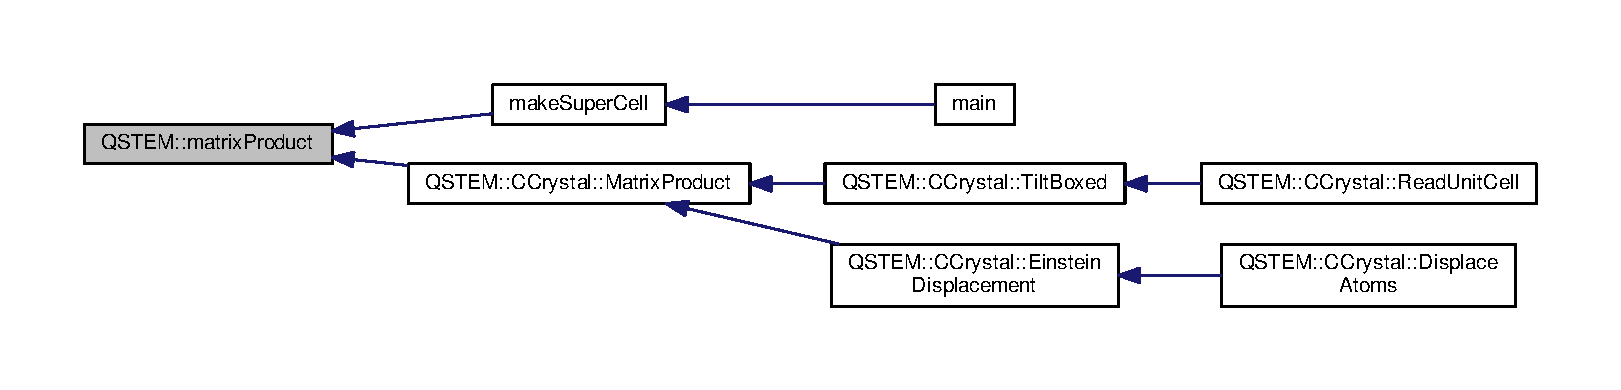
\includegraphics[width=350pt]{namespace_q_s_t_e_m_a3748387153d44d8d383d44bf9df76cf6_icgraph}
\end{center}
\end{figure}


\hypertarget{namespace_q_s_t_e_m_ab44ad034a5034217de267ab5e0754ad2}{\index{Q\-S\-T\-E\-M@{Q\-S\-T\-E\-M}!matrix\-Product\-Int@{matrix\-Product\-Int}}
\index{matrix\-Product\-Int@{matrix\-Product\-Int}!QSTEM@{Q\-S\-T\-E\-M}}
\subsubsection[{matrix\-Product\-Int}]{\setlength{\rightskip}{0pt plus 5cm}void Q\-S\-T\-E\-M\-::matrix\-Product\-Int (
\begin{DoxyParamCaption}
\item[{float\-\_\-tt $\ast$$\ast$}]{a, }
\item[{int}]{Nxa, }
\item[{int}]{Nya, }
\item[{int $\ast$$\ast$}]{b, }
\item[{int}]{Nxb, }
\item[{int}]{Nyb, }
\item[{float\-\_\-tt $\ast$$\ast$}]{c}
\end{DoxyParamCaption}
)}}\label{namespace_q_s_t_e_m_ab44ad034a5034217de267ab5e0754ad2}


Definition at line 782 of file matrixlib.\-cpp.

\hypertarget{namespace_q_s_t_e_m_a1af432ca346c64d9138440f99f813e51}{\index{Q\-S\-T\-E\-M@{Q\-S\-T\-E\-M}!pythag@{pythag}}
\index{pythag@{pythag}!QSTEM@{Q\-S\-T\-E\-M}}
\subsubsection[{pythag}]{\setlength{\rightskip}{0pt plus 5cm}{\bf float\-\_\-tt} Q\-S\-T\-E\-M\-::pythag (
\begin{DoxyParamCaption}
\item[{float\-\_\-tt}]{a, }
\item[{float\-\_\-tt}]{b}
\end{DoxyParamCaption}
)}}\label{namespace_q_s_t_e_m_a1af432ca346c64d9138440f99f813e51}


Definition at line 484 of file matrixlib.\-cpp.



Here is the caller graph for this function\-:
\nopagebreak
\begin{figure}[H]
\begin{center}
\leavevmode
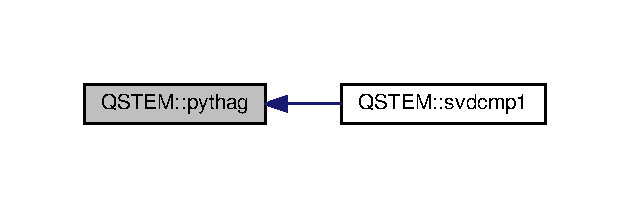
\includegraphics[width=302pt]{namespace_q_s_t_e_m_a1af432ca346c64d9138440f99f813e51_icgraph}
\end{center}
\end{figure}


\hypertarget{namespace_q_s_t_e_m_a9ec01a31ed3492c498ddcd27350937f5}{\index{Q\-S\-T\-E\-M@{Q\-S\-T\-E\-M}!ran@{ran}}
\index{ran@{ran}!QSTEM@{Q\-S\-T\-E\-M}}
\subsubsection[{ran}]{\setlength{\rightskip}{0pt plus 5cm}float Q\-S\-T\-E\-M\-::ran (
\begin{DoxyParamCaption}
\item[{long $\ast$}]{idum}
\end{DoxyParamCaption}
)}}\label{namespace_q_s_t_e_m_a9ec01a31ed3492c498ddcd27350937f5}


Here is the caller graph for this function\-:
\nopagebreak
\begin{figure}[H]
\begin{center}
\leavevmode
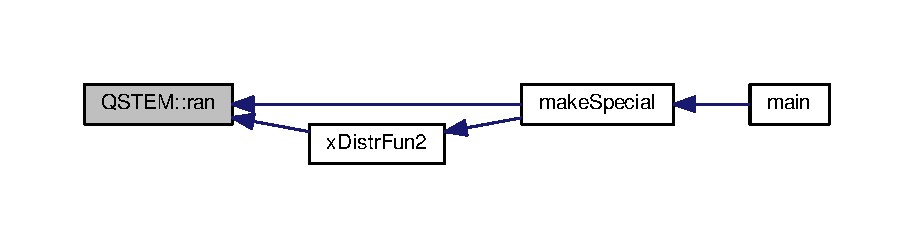
\includegraphics[width=350pt]{namespace_q_s_t_e_m_a9ec01a31ed3492c498ddcd27350937f5_icgraph}
\end{center}
\end{figure}


\hypertarget{namespace_q_s_t_e_m_a3bdee418130076e4b82c8afb597b2f03}{\index{Q\-S\-T\-E\-M@{Q\-S\-T\-E\-M}!ran1@{ran1}}
\index{ran1@{ran1}!QSTEM@{Q\-S\-T\-E\-M}}
\subsubsection[{ran1}]{\setlength{\rightskip}{0pt plus 5cm}{\bf float\-\_\-tt} Q\-S\-T\-E\-M\-::ran1 (
\begin{DoxyParamCaption}
{}
\end{DoxyParamCaption}
)\hspace{0.3cm}{\ttfamily [inline]}}}\label{namespace_q_s_t_e_m_a3bdee418130076e4b82c8afb597b2f03}


Definition at line 33 of file random.\-hpp.

\hypertarget{namespace_q_s_t_e_m_a01110ac4ac2b6bc7f5eaf512f0bdbf56}{\index{Q\-S\-T\-E\-M@{Q\-S\-T\-E\-M}!ran1@{ran1}}
\index{ran1@{ran1}!QSTEM@{Q\-S\-T\-E\-M}}
\subsubsection[{ran1}]{\setlength{\rightskip}{0pt plus 5cm}double Q\-S\-T\-E\-M\-::ran1 (
\begin{DoxyParamCaption}
\item[{long $\ast$}]{idum}
\end{DoxyParamCaption}
)}}\label{namespace_q_s_t_e_m_a01110ac4ac2b6bc7f5eaf512f0bdbf56}


Here is the caller graph for this function\-:
\nopagebreak
\begin{figure}[H]
\begin{center}
\leavevmode
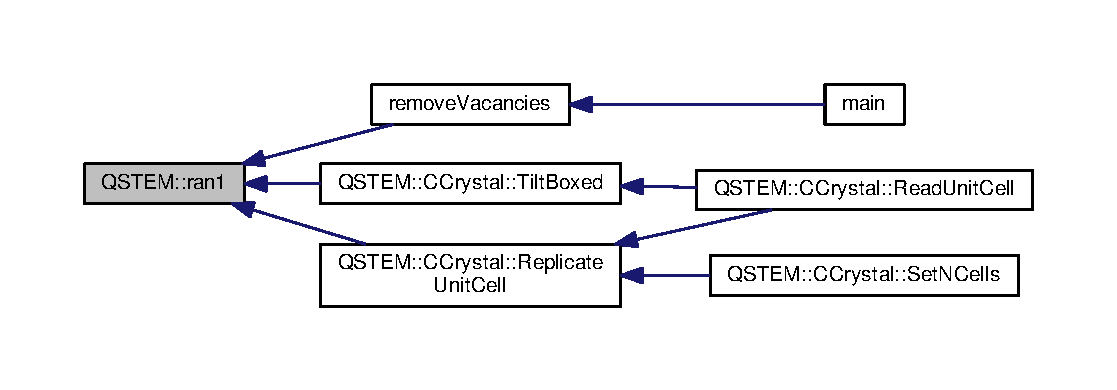
\includegraphics[width=350pt]{namespace_q_s_t_e_m_a01110ac4ac2b6bc7f5eaf512f0bdbf56_icgraph}
\end{center}
\end{figure}


\hypertarget{namespace_q_s_t_e_m_adde764026530aeeee9e7914ad97a048c}{\index{Q\-S\-T\-E\-M@{Q\-S\-T\-E\-M}!read\-Cubic\-C\-F\-G@{read\-Cubic\-C\-F\-G}}
\index{read\-Cubic\-C\-F\-G@{read\-Cubic\-C\-F\-G}!QSTEM@{Q\-S\-T\-E\-M}}
\subsubsection[{read\-Cubic\-C\-F\-G}]{\setlength{\rightskip}{0pt plus 5cm}int Q\-S\-T\-E\-M\-::read\-Cubic\-C\-F\-G (
\begin{DoxyParamCaption}
\item[{double $\ast$$\ast$}]{pos, }
\item[{double $\ast$$\ast$}]{dw, }
\item[{int $\ast$$\ast$}]{Znum, }
\item[{double $\ast$}]{ax, }
\item[{double $\ast$}]{by, }
\item[{double $\ast$}]{cz, }
\item[{double}]{ctiltx, }
\item[{double}]{ctilty}
\end{DoxyParamCaption}
)}}\label{namespace_q_s_t_e_m_adde764026530aeeee9e7914ad97a048c}
\hypertarget{namespace_q_s_t_e_m_a1d7a548937e7c9f3611840c0076a807c}{\index{Q\-S\-T\-E\-M@{Q\-S\-T\-E\-M}!Read\-Line@{Read\-Line}}
\index{Read\-Line@{Read\-Line}!QSTEM@{Q\-S\-T\-E\-M}}
\subsubsection[{Read\-Line}]{\setlength{\rightskip}{0pt plus 5cm}int Q\-S\-T\-E\-M\-::\-Read\-Line (
\begin{DoxyParamCaption}
\item[{F\-I\-L\-E $\ast$}]{fp\-Read, }
\item[{char $\ast$}]{c\-Read, }
\item[{int}]{c\-Max, }
\item[{const char $\ast$}]{mesg}
\end{DoxyParamCaption}
)\hspace{0.3cm}{\ttfamily [inline]}}}\label{namespace_q_s_t_e_m_a1d7a548937e7c9f3611840c0076a807c}


Definition at line 69 of file structure\-Interface.\-hpp.

\hypertarget{namespace_q_s_t_e_m_a262c0ef985da2a97135a1c7899a65482}{\index{Q\-S\-T\-E\-M@{Q\-S\-T\-E\-M}!rotate\-Matrix@{rotate\-Matrix}}
\index{rotate\-Matrix@{rotate\-Matrix}!QSTEM@{Q\-S\-T\-E\-M}}
\subsubsection[{rotate\-Matrix}]{\setlength{\rightskip}{0pt plus 5cm}void Q\-S\-T\-E\-M\-::rotate\-Matrix (
\begin{DoxyParamCaption}
\item[{float\-\_\-tt $\ast$}]{matrix\-In, }
\item[{float\-\_\-tt $\ast$}]{matrix\-Out, }
\item[{float\-\_\-tt}]{phi\-\_\-x, }
\item[{float\-\_\-tt}]{phi\-\_\-y, }
\item[{float\-\_\-tt}]{phi\-\_\-z}
\end{DoxyParamCaption}
)}}\label{namespace_q_s_t_e_m_a262c0ef985da2a97135a1c7899a65482}


Definition at line 639 of file matrixlib.\-cpp.



Here is the call graph for this function\-:
\nopagebreak
\begin{figure}[H]
\begin{center}
\leavevmode
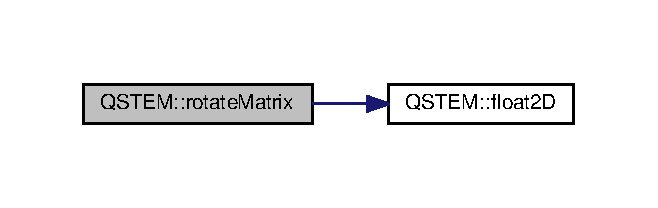
\includegraphics[width=316pt]{namespace_q_s_t_e_m_a262c0ef985da2a97135a1c7899a65482_cgraph}
\end{center}
\end{figure}




Here is the caller graph for this function\-:
\nopagebreak
\begin{figure}[H]
\begin{center}
\leavevmode
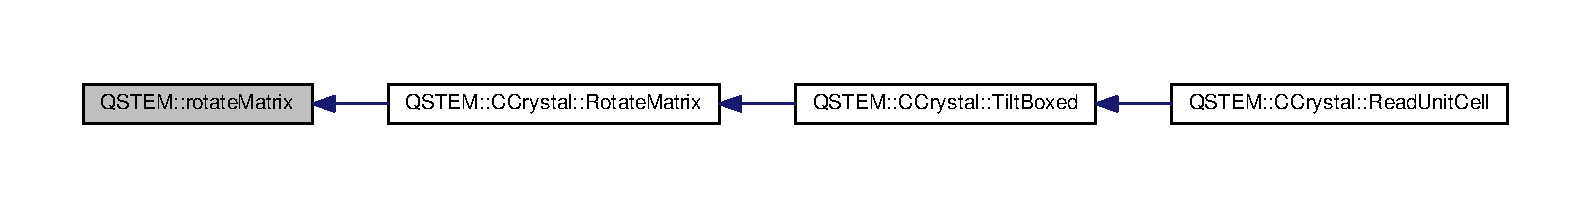
\includegraphics[width=350pt]{namespace_q_s_t_e_m_a262c0ef985da2a97135a1c7899a65482_icgraph}
\end{center}
\end{figure}


\hypertarget{namespace_q_s_t_e_m_a533b9e3efe0ac79ccc71c73249aa1d39}{\index{Q\-S\-T\-E\-M@{Q\-S\-T\-E\-M}!rotate\-Vect@{rotate\-Vect}}
\index{rotate\-Vect@{rotate\-Vect}!QSTEM@{Q\-S\-T\-E\-M}}
\subsubsection[{rotate\-Vect}]{\setlength{\rightskip}{0pt plus 5cm}void Q\-S\-T\-E\-M\-::rotate\-Vect (
\begin{DoxyParamCaption}
\item[{float\-\_\-tt $\ast$}]{vect\-In, }
\item[{float\-\_\-tt $\ast$}]{vect\-Out, }
\item[{float\-\_\-tt}]{phi\-\_\-x, }
\item[{float\-\_\-tt}]{phi\-\_\-y, }
\item[{float\-\_\-tt}]{phi\-\_\-z}
\end{DoxyParamCaption}
)}}\label{namespace_q_s_t_e_m_a533b9e3efe0ac79ccc71c73249aa1d39}


Definition at line 600 of file matrixlib.\-cpp.



Here is the call graph for this function\-:
\nopagebreak
\begin{figure}[H]
\begin{center}
\leavevmode
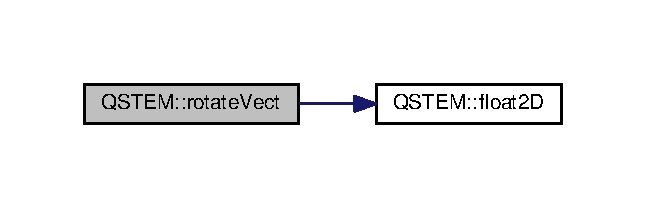
\includegraphics[width=310pt]{namespace_q_s_t_e_m_a533b9e3efe0ac79ccc71c73249aa1d39_cgraph}
\end{center}
\end{figure}




Here is the caller graph for this function\-:
\nopagebreak
\begin{figure}[H]
\begin{center}
\leavevmode
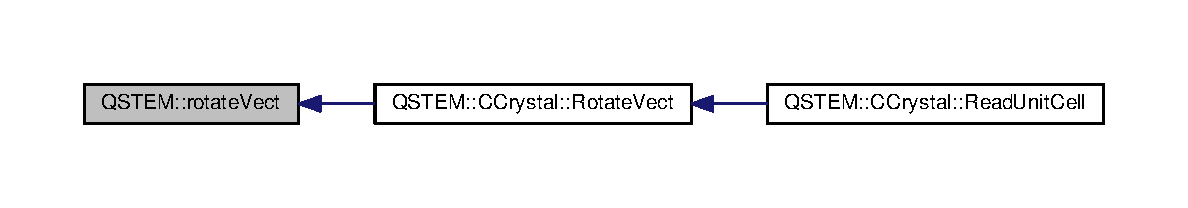
\includegraphics[width=350pt]{namespace_q_s_t_e_m_a533b9e3efe0ac79ccc71c73249aa1d39_icgraph}
\end{center}
\end{figure}


\hypertarget{namespace_q_s_t_e_m_ac6fbfcb174875805f137c8d52647c4b7}{\index{Q\-S\-T\-E\-M@{Q\-S\-T\-E\-M}!short2\-D@{short2\-D}}
\index{short2\-D@{short2\-D}!QSTEM@{Q\-S\-T\-E\-M}}
\subsubsection[{short2\-D}]{\setlength{\rightskip}{0pt plus 5cm}short $\ast$$\ast$ Q\-S\-T\-E\-M\-::short2\-D (
\begin{DoxyParamCaption}
\item[{int}]{nx, }
\item[{int}]{ny, }
\item[{const char $\ast$}]{message}
\end{DoxyParamCaption}
)}}\label{namespace_q_s_t_e_m_ac6fbfcb174875805f137c8d52647c4b7}


Definition at line 99 of file memory\-\_\-fftw3.\-cpp.

\hypertarget{namespace_q_s_t_e_m_ade3d8d331f17c086929cad48d7554ec1}{\index{Q\-S\-T\-E\-M@{Q\-S\-T\-E\-M}!show\-Matrix@{show\-Matrix}}
\index{show\-Matrix@{show\-Matrix}!QSTEM@{Q\-S\-T\-E\-M}}
\subsubsection[{show\-Matrix}]{\setlength{\rightskip}{0pt plus 5cm}void Q\-S\-T\-E\-M\-::show\-Matrix (
\begin{DoxyParamCaption}
\item[{float\-\_\-tt $\ast$$\ast$}]{M, }
\item[{int}]{Nx, }
\item[{int}]{Ny, }
\item[{char $\ast$}]{name}
\end{DoxyParamCaption}
)}}\label{namespace_q_s_t_e_m_ade3d8d331f17c086929cad48d7554ec1}


Definition at line 532 of file matrixlib.\-cpp.

\hypertarget{namespace_q_s_t_e_m_a3ad85d01b0db30cbef2f7beb764276c4}{\index{Q\-S\-T\-E\-M@{Q\-S\-T\-E\-M}!svdcmp1@{svdcmp1}}
\index{svdcmp1@{svdcmp1}!QSTEM@{Q\-S\-T\-E\-M}}
\subsubsection[{svdcmp1}]{\setlength{\rightskip}{0pt plus 5cm}void Q\-S\-T\-E\-M\-::svdcmp1 (
\begin{DoxyParamCaption}
\item[{float\-\_\-tt $\ast$$\ast$}]{a, }
\item[{int}]{m, }
\item[{int}]{n, }
\item[{float\-\_\-tt}]{w\mbox{[}$\,$\mbox{]}, }
\item[{float\-\_\-tt $\ast$$\ast$}]{v}
\end{DoxyParamCaption}
)}}\label{namespace_q_s_t_e_m_a3ad85d01b0db30cbef2f7beb764276c4}


Definition at line 285 of file matrixlib.\-cpp.



Here is the call graph for this function\-:
\nopagebreak
\begin{figure}[H]
\begin{center}
\leavevmode
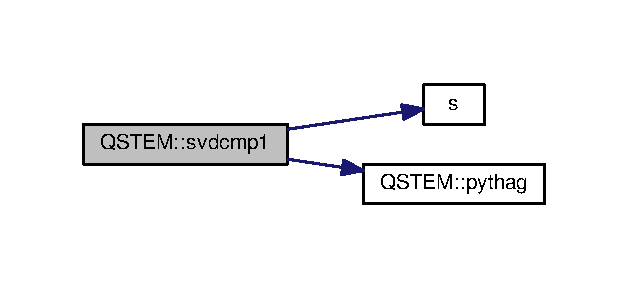
\includegraphics[width=302pt]{namespace_q_s_t_e_m_a3ad85d01b0db30cbef2f7beb764276c4_cgraph}
\end{center}
\end{figure}


\hypertarget{namespace_q_s_t_e_m_ab30c1bc28aeca4c0f003ba52e881e670}{\index{Q\-S\-T\-E\-M@{Q\-S\-T\-E\-M}!trans\-\_\-3x3@{trans\-\_\-3x3}}
\index{trans\-\_\-3x3@{trans\-\_\-3x3}!QSTEM@{Q\-S\-T\-E\-M}}
\subsubsection[{trans\-\_\-3x3}]{\setlength{\rightskip}{0pt plus 5cm}void Q\-S\-T\-E\-M\-::trans\-\_\-3x3 (
\begin{DoxyParamCaption}
\item[{float\-\_\-tt $\ast$}]{Mt, }
\item[{const float\-\_\-tt $\ast$}]{Ms}
\end{DoxyParamCaption}
)}}\label{namespace_q_s_t_e_m_ab30c1bc28aeca4c0f003ba52e881e670}


Definition at line 212 of file matrixlib.\-cpp.

\hypertarget{namespace_q_s_t_e_m_ac5e1f5b7da5ae1c94681e41321b707e7}{\index{Q\-S\-T\-E\-M@{Q\-S\-T\-E\-M}!vect\-Diff\-\_\-f@{vect\-Diff\-\_\-f}}
\index{vect\-Diff\-\_\-f@{vect\-Diff\-\_\-f}!QSTEM@{Q\-S\-T\-E\-M}}
\subsubsection[{vect\-Diff\-\_\-f}]{\setlength{\rightskip}{0pt plus 5cm}void Q\-S\-T\-E\-M\-::vect\-Diff\-\_\-f (
\begin{DoxyParamCaption}
\item[{float $\ast$}]{a, }
\item[{float\-\_\-tt $\ast$}]{b, }
\item[{float\-\_\-tt $\ast$}]{c, }
\item[{int}]{rev\-Flag}
\end{DoxyParamCaption}
)}}\label{namespace_q_s_t_e_m_ac5e1f5b7da5ae1c94681e41321b707e7}


Definition at line 516 of file matrixlib.\-cpp.



Here is the caller graph for this function\-:
\nopagebreak
\begin{figure}[H]
\begin{center}
\leavevmode
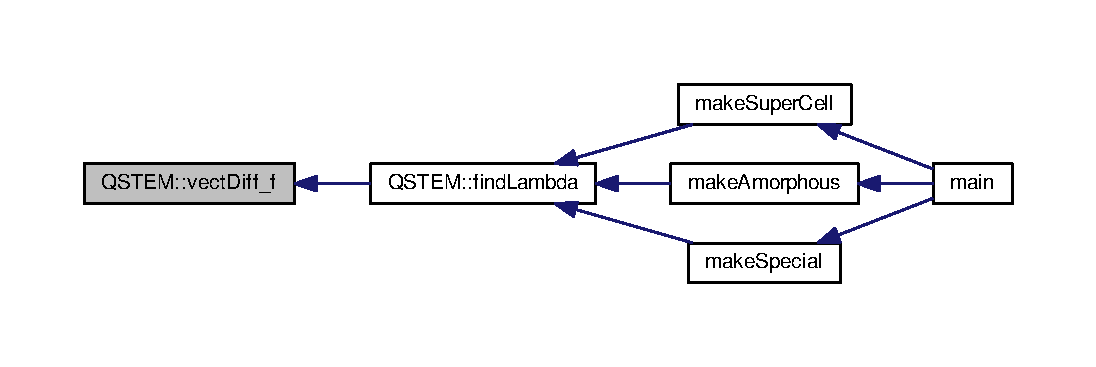
\includegraphics[width=350pt]{namespace_q_s_t_e_m_ac5e1f5b7da5ae1c94681e41321b707e7_icgraph}
\end{center}
\end{figure}


\hypertarget{namespace_q_s_t_e_m_a4a1a9b85d5c9d701837b0e95e99a805b}{\index{Q\-S\-T\-E\-M@{Q\-S\-T\-E\-M}!vect\-Length@{vect\-Length}}
\index{vect\-Length@{vect\-Length}!QSTEM@{Q\-S\-T\-E\-M}}
\subsubsection[{vect\-Length}]{\setlength{\rightskip}{0pt plus 5cm}{\bf float\-\_\-tt} Q\-S\-T\-E\-M\-::vect\-Length (
\begin{DoxyParamCaption}
\item[{float\-\_\-tt $\ast$}]{vect}
\end{DoxyParamCaption}
)}}\label{namespace_q_s_t_e_m_a4a1a9b85d5c9d701837b0e95e99a805b}


Definition at line 753 of file matrixlib.\-cpp.



Here is the caller graph for this function\-:
\nopagebreak
\begin{figure}[H]
\begin{center}
\leavevmode
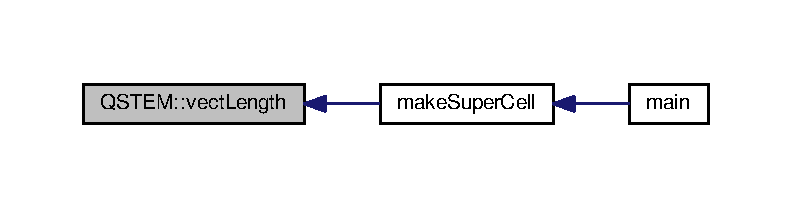
\includegraphics[width=350pt]{namespace_q_s_t_e_m_a4a1a9b85d5c9d701837b0e95e99a805b_icgraph}
\end{center}
\end{figure}


\hypertarget{namespace_q_s_t_e_m_a7749ff6124f5ab0a9c20933545a14179}{\index{Q\-S\-T\-E\-M@{Q\-S\-T\-E\-M}!write\-Amorphous@{write\-Amorphous}}
\index{write\-Amorphous@{write\-Amorphous}!QSTEM@{Q\-S\-T\-E\-M}}
\subsubsection[{write\-Amorphous}]{\setlength{\rightskip}{0pt plus 5cm}void Q\-S\-T\-E\-M\-::write\-Amorphous (
\begin{DoxyParamCaption}
\item[{F\-I\-L\-E $\ast$}]{fp, }
\item[{super\-Cell\-Box}]{super\-Cell, }
\item[{int}]{nstart, }
\item[{int}]{nstop}
\end{DoxyParamCaption}
)}}\label{namespace_q_s_t_e_m_a7749ff6124f5ab0a9c20933545a14179}


Definition at line 229 of file fileio\-\_\-fftw3.\-cpp.



Here is the caller graph for this function\-:
\nopagebreak
\begin{figure}[H]
\begin{center}
\leavevmode
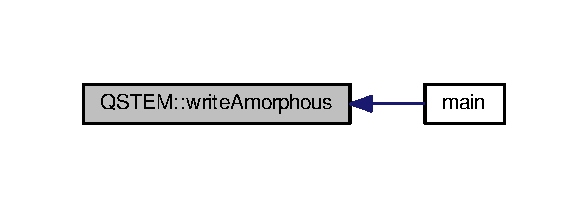
\includegraphics[width=282pt]{namespace_q_s_t_e_m_a7749ff6124f5ab0a9c20933545a14179_icgraph}
\end{center}
\end{figure}


\hypertarget{namespace_q_s_t_e_m_a90f4692ae2fc27595ac4e44b182c1bf9}{\index{Q\-S\-T\-E\-M@{Q\-S\-T\-E\-M}!write\-C\-F\-G\-Fract\-Cubic@{write\-C\-F\-G\-Fract\-Cubic}}
\index{write\-C\-F\-G\-Fract\-Cubic@{write\-C\-F\-G\-Fract\-Cubic}!QSTEM@{Q\-S\-T\-E\-M}}
\subsubsection[{write\-C\-F\-G\-Fract\-Cubic}]{\setlength{\rightskip}{0pt plus 5cm}int Q\-S\-T\-E\-M\-::write\-C\-F\-G\-Fract\-Cubic (
\begin{DoxyParamCaption}
\item[{double $\ast$}]{pos, }
\item[{int $\ast$}]{Znum, }
\item[{double $\ast$}]{dw, }
\item[{int}]{natoms, }
\item[{char $\ast$}]{file\-Name, }
\item[{double}]{a, }
\item[{double}]{b, }
\item[{double}]{c}
\end{DoxyParamCaption}
)}}\label{namespace_q_s_t_e_m_a90f4692ae2fc27595ac4e44b182c1bf9}
\hypertarget{namespace_q_s_t_e_m_a91f650de6c17fd6a4ce5674204047bee}{\index{Q\-S\-T\-E\-M@{Q\-S\-T\-E\-M}!write\-Frame\-Work@{write\-Frame\-Work}}
\index{write\-Frame\-Work@{write\-Frame\-Work}!QSTEM@{Q\-S\-T\-E\-M}}
\subsubsection[{write\-Frame\-Work}]{\setlength{\rightskip}{0pt plus 5cm}void Q\-S\-T\-E\-M\-::write\-Frame\-Work (
\begin{DoxyParamCaption}
\item[{F\-I\-L\-E $\ast$}]{fp, }
\item[{super\-Cell\-Box}]{super\-Cell}
\end{DoxyParamCaption}
)}}\label{namespace_q_s_t_e_m_a91f650de6c17fd6a4ce5674204047bee}


Definition at line 155 of file fileio\-\_\-fftw3.\-cpp.



Here is the caller graph for this function\-:
\nopagebreak
\begin{figure}[H]
\begin{center}
\leavevmode
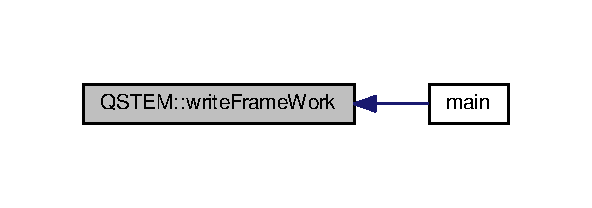
\includegraphics[width=284pt]{namespace_q_s_t_e_m_a91f650de6c17fd6a4ce5674204047bee_icgraph}
\end{center}
\end{figure}




\subsection{Variable Documentation}
\hypertarget{namespace_q_s_t_e_m_a0032f41cd55b94be17d3c9dda2fc9012}{\index{Q\-S\-T\-E\-M@{Q\-S\-T\-E\-M}!k\-\_\-fft\-Measure\-Flag@{k\-\_\-fft\-Measure\-Flag}}
\index{k\-\_\-fft\-Measure\-Flag@{k\-\_\-fft\-Measure\-Flag}!QSTEM@{Q\-S\-T\-E\-M}}
\subsubsection[{k\-\_\-fft\-Measure\-Flag}]{\setlength{\rightskip}{0pt plus 5cm}const int Q\-S\-T\-E\-M\-::k\-\_\-fft\-Measure\-Flag = {\bf F\-F\-T\-W\-\_\-\-E\-S\-T\-I\-M\-A\-T\-E}}}\label{namespace_q_s_t_e_m_a0032f41cd55b94be17d3c9dda2fc9012}


Definition at line 86 of file stemtypes\-\_\-fftw3.\-hpp.

\hypertarget{namespace_q_s_t_e_m_a78cee406c660e4fe36e7ab36e34f1dec}{\index{Q\-S\-T\-E\-M@{Q\-S\-T\-E\-M}!P\-I@{P\-I}}
\index{P\-I@{P\-I}!QSTEM@{Q\-S\-T\-E\-M}}
\subsubsection[{P\-I}]{\setlength{\rightskip}{0pt plus 5cm}const {\bf float\-\_\-tt} Q\-S\-T\-E\-M\-::\-P\-I = 2$\ast$acos(0.\-0)}}\label{namespace_q_s_t_e_m_a78cee406c660e4fe36e7ab36e34f1dec}


Definition at line 83 of file stemtypes\-\_\-fftw3.\-hpp.


\hypertarget{namespacestd}{\section{std Namespace Reference}
\label{namespacestd}\index{std@{std}}
}
\subsection*{Functions}
\begin{DoxyCompactItemize}
\item 
{\footnotesize template$<$class Real $>$ }\\ostream \& \hyperlink{namespacestd_a0c1d84eb0ccd763cc5ad3e28f4fff40e}{operator$<$$<$} (ostream \&\hyperlink{aberrations___t_e_m_8m_aef29541a06b7f933d32a804307db13af}{s}, \hyperlink{class_f_f_t_w_complex}{F\-F\-T\-W\-Complex}$<$ Real $>$ const \&\hyperlink{aberrations___t_e_m_8m_ac4055e3a20b6b3af3d10590ea446ef6c}{v})
\end{DoxyCompactItemize}


\subsection{Function Documentation}
\hypertarget{namespacestd_a0c1d84eb0ccd763cc5ad3e28f4fff40e}{\index{std@{std}!operator$<$$<$@{operator$<$$<$}}
\index{operator$<$$<$@{operator$<$$<$}!std@{std}}
\subsubsection[{operator$<$$<$}]{\setlength{\rightskip}{0pt plus 5cm}template$<$class Real $>$ ostream\& std\-::operator$<$$<$ (
\begin{DoxyParamCaption}
\item[{ostream \&}]{s, }
\item[{{\bf F\-F\-T\-W\-Complex}$<$ Real $>$ const \&}]{v}
\end{DoxyParamCaption}
)}}\label{namespacestd_a0c1d84eb0ccd763cc5ad3e28f4fff40e}


Definition at line 609 of file fftw\-\_\-allocator.\-hpp.



Here is the call graph for this function\-:
\nopagebreak
\begin{figure}[H]
\begin{center}
\leavevmode
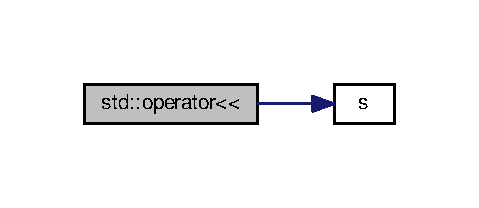
\includegraphics[width=230pt]{namespacestd_a0c1d84eb0ccd763cc5ad3e28f4fff40e_cgraph}
\end{center}
\end{figure}



\hypertarget{namespaceucif}{\section{ucif Namespace Reference}
\label{namespaceucif}\index{ucif@{ucif}}
}
\subsection*{Namespaces}
\begin{DoxyCompactItemize}
\item 
\hyperlink{namespaceucif_1_1example}{example}
\end{DoxyCompactItemize}
\subsection*{Classes}
\begin{DoxyCompactItemize}
\item 
struct \hyperlink{structucif_1_1array__wrapper__base}{array\-\_\-wrapper\-\_\-base}
\item 
struct \hyperlink{structucif_1_1builder__base}{builder\-\_\-base}
\item 
class \hyperlink{classucif_1_1parser}{parser}
\end{DoxyCompactItemize}

\hypertarget{namespaceucif_1_1example}{\section{ucif\-:\-:example Namespace Reference}
\label{namespaceucif_1_1example}\index{ucif\-::example@{ucif\-::example}}
}
\subsection*{Classes}
\begin{DoxyCompactItemize}
\item 
struct \hyperlink{structucif_1_1example_1_1my__array__wrapper}{my\-\_\-array\-\_\-wrapper}
\item 
struct \hyperlink{structucif_1_1example_1_1my__builder}{my\-\_\-builder}
\end{DoxyCompactItemize}

\chapter{Class Documentation}
\hypertarget{classaberrations_1_1_ab3}{\section{aberrations.\-Ab3 Class Reference}
\label{classaberrations_1_1_ab3}\index{aberrations.\-Ab3@{aberrations.\-Ab3}}
}


Inheritance diagram for aberrations.\-Ab3\-:
\nopagebreak
\begin{figure}[H]
\begin{center}
\leavevmode
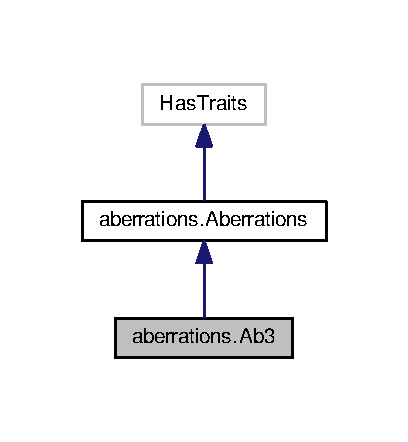
\includegraphics[width=196pt]{classaberrations_1_1_ab3__inherit__graph}
\end{center}
\end{figure}


Collaboration diagram for aberrations.\-Ab3\-:
\nopagebreak
\begin{figure}[H]
\begin{center}
\leavevmode
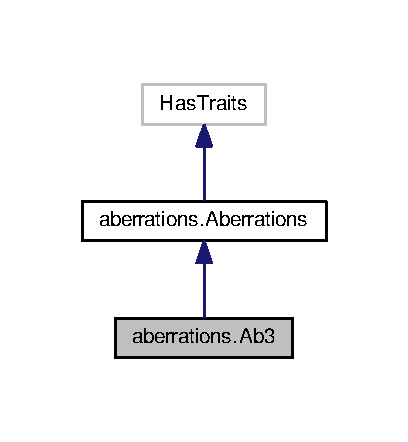
\includegraphics[width=196pt]{classaberrations_1_1_ab3__coll__graph}
\end{center}
\end{figure}
\subsection*{Static Public Attributes}
\begin{DoxyCompactItemize}
\item 
tuple \hyperlink{classaberrations_1_1_ab3_a715ff78e10a0a75678493af40ff63ca1}{a20} = Range(low=-\/10000,high=10000,\hyperlink{read_config_file_8m_afcc7a4b78ecd8fa7e713f8cfa0f51017}{value}=0)
\item 
tuple \hyperlink{classaberrations_1_1_ab3_a4ce0fbb1fbe9365ea1e480a3866dbd51}{a40} = Range(low=-\/10000,high=10000,\hyperlink{read_config_file_8m_afcc7a4b78ecd8fa7e713f8cfa0f51017}{value}=1000)
\item 
tuple \hyperlink{classaberrations_1_1_ab3_a15533015c34cc472b96642dc6a87e17f}{a60} = Range(low=-\/100,high=100,\hyperlink{read_config_file_8m_afcc7a4b78ecd8fa7e713f8cfa0f51017}{value}=5)
\item 
tuple \hyperlink{classaberrations_1_1_ab3_a156045dd2125a70fb302763bbba3acc7}{a22} = Range(low=0,high=1000,\hyperlink{read_config_file_8m_afcc7a4b78ecd8fa7e713f8cfa0f51017}{value}=10)
\item 
tuple \hyperlink{classaberrations_1_1_ab3_a9441ccb42434e133bc7f04cd7545f91d}{a31} = Range(low=0,high=1000,\hyperlink{read_config_file_8m_afcc7a4b78ecd8fa7e713f8cfa0f51017}{value}=10)
\item 
tuple \hyperlink{classaberrations_1_1_ab3_a507a723cf8799c2851689827296a9658}{a33} = Range(low=0,high=1000,\hyperlink{read_config_file_8m_afcc7a4b78ecd8fa7e713f8cfa0f51017}{value}=10)
\item 
tuple \hyperlink{classaberrations_1_1_ab3_abda80a3fc204ebf86463a47c12934987}{a42} = Range(low=0,high=1000,\hyperlink{read_config_file_8m_afcc7a4b78ecd8fa7e713f8cfa0f51017}{value}=10)
\item 
tuple \hyperlink{classaberrations_1_1_ab3_acd01b2dcdb096fd7e5274d1393d58eec}{a44} = Range(low=0,high=1000,\hyperlink{read_config_file_8m_afcc7a4b78ecd8fa7e713f8cfa0f51017}{value}=10)
\item 
tuple \hyperlink{classaberrations_1_1_ab3_afe66278f105e9740c36aa3c3870e2820}{a51} = Range(low=0,high=1000,\hyperlink{read_config_file_8m_afcc7a4b78ecd8fa7e713f8cfa0f51017}{value}=10)
\item 
tuple \hyperlink{classaberrations_1_1_ab3_a98ddad2440f4a881b1f23b27be43e571}{a53} = Range(low=0,high=1000,\hyperlink{read_config_file_8m_afcc7a4b78ecd8fa7e713f8cfa0f51017}{value}=10)
\item 
tuple \hyperlink{classaberrations_1_1_ab3_a5e66669d4473d75393cbb05e903bdb75}{a55} = Range(low=0,high=1000,\hyperlink{read_config_file_8m_afcc7a4b78ecd8fa7e713f8cfa0f51017}{value}=10)
\item 
tuple \hyperlink{classaberrations_1_1_ab3_a8522a4f50791da0422d9c38caf9d6c67}{a62} = Range(low=0,high=1000,\hyperlink{read_config_file_8m_afcc7a4b78ecd8fa7e713f8cfa0f51017}{value}=10)
\item 
tuple \hyperlink{classaberrations_1_1_ab3_a5aae37e8015c07b5024cb56940daa2d4}{a64} = Range(low=0,high=1000,\hyperlink{read_config_file_8m_afcc7a4b78ecd8fa7e713f8cfa0f51017}{value}=10)
\item 
tuple \hyperlink{classaberrations_1_1_ab3_a0330fb84dbb9b210ef61b1706f87c255}{a66} = Range(low=0,high=1000,\hyperlink{read_config_file_8m_afcc7a4b78ecd8fa7e713f8cfa0f51017}{value}=10)
\item 
tuple \hyperlink{classaberrations_1_1_ab3_acaafddafce2b2b23f4bfb9602e0bb16f}{Phi22} = Range(low=-\/pi,high=pi,\hyperlink{read_config_file_8m_afcc7a4b78ecd8fa7e713f8cfa0f51017}{value}=0)
\item 
tuple \hyperlink{classaberrations_1_1_ab3_a15746a7f4fc410c4fe90d5299010fab6}{Phi31} = Range(low=-\/pi,high=pi,\hyperlink{read_config_file_8m_afcc7a4b78ecd8fa7e713f8cfa0f51017}{value}=0)
\item 
tuple \hyperlink{classaberrations_1_1_ab3_ac546f2cb70a8270bd4497883a7a40ebc}{Phi33} = Range(low=-\/pi,high=pi,\hyperlink{read_config_file_8m_afcc7a4b78ecd8fa7e713f8cfa0f51017}{value}=0)
\item 
tuple \hyperlink{classaberrations_1_1_ab3_a15f3e797bf78f694b99cfe59cff9d29a}{Phi42} = Range(low=-\/pi,high=pi,\hyperlink{read_config_file_8m_afcc7a4b78ecd8fa7e713f8cfa0f51017}{value}=0)
\item 
tuple \hyperlink{classaberrations_1_1_ab3_a8191c01c9efa7a49e5e43e6b3d031e7a}{Phi44} = Range(low=-\/pi,high=pi,\hyperlink{read_config_file_8m_afcc7a4b78ecd8fa7e713f8cfa0f51017}{value}=0)
\item 
tuple \hyperlink{classaberrations_1_1_ab3_a1448cd5acb7118a4c93cfdff5afe3f3f}{Phi51} = Range(low=-\/pi,high=pi,\hyperlink{read_config_file_8m_afcc7a4b78ecd8fa7e713f8cfa0f51017}{value}=0)
\item 
tuple \hyperlink{classaberrations_1_1_ab3_a3f8f632e92a660cfa108afd8ae2927e3}{Phi53} = Range(low=-\/pi,high=pi,\hyperlink{read_config_file_8m_afcc7a4b78ecd8fa7e713f8cfa0f51017}{value}=0)
\item 
tuple \hyperlink{classaberrations_1_1_ab3_a62822777a276703a3a3c7941010d2ec1}{Phi55} = Range(low=-\/pi,high=pi,\hyperlink{read_config_file_8m_afcc7a4b78ecd8fa7e713f8cfa0f51017}{value}=0)
\item 
tuple \hyperlink{classaberrations_1_1_ab3_a72bff7546fac1a0b8855aa21b007e6ab}{Phi62} = Range(low=-\/pi,high=pi,\hyperlink{read_config_file_8m_afcc7a4b78ecd8fa7e713f8cfa0f51017}{value}=0)
\item 
tuple \hyperlink{classaberrations_1_1_ab3_ae8134a4d98473fde855a519ec2e24289}{Phi64} = Range(low=-\/pi,high=pi,\hyperlink{read_config_file_8m_afcc7a4b78ecd8fa7e713f8cfa0f51017}{value}=0)
\item 
tuple \hyperlink{classaberrations_1_1_ab3_ac572bbd6cfdf9dc00c3325936cfcb7dd}{Phi66} = Range(low=-\/pi,high=pi,\hyperlink{read_config_file_8m_afcc7a4b78ecd8fa7e713f8cfa0f51017}{value}=0)
\item 
tuple \hyperlink{classaberrations_1_1_ab3_ae439d45c87584dc4d93fe544dfbb02a7}{a}
\item 
tuple \hyperlink{classaberrations_1_1_ab3_afd6e5e64c14cfe35b8128a781f58f767}{phi}
\end{DoxyCompactItemize}
\subsection*{Additional Inherited Members}


\subsection{Detailed Description}


Definition at line 376 of file aberrations.\-py.



\subsection{Member Data Documentation}
\hypertarget{classaberrations_1_1_ab3_ae439d45c87584dc4d93fe544dfbb02a7}{\index{aberrations\-::\-Ab3@{aberrations\-::\-Ab3}!a@{a}}
\index{a@{a}!aberrations::Ab3@{aberrations\-::\-Ab3}}
\subsubsection[{a}]{\setlength{\rightskip}{0pt plus 5cm}tuple aberrations.\-Ab3.\-a\hspace{0.3cm}{\ttfamily [static]}}}\label{classaberrations_1_1_ab3_ae439d45c87584dc4d93fe544dfbb02a7}
{\bfseries Initial value\-:}
\begin{DoxyCode}
1 = Property( Array, depends\_on=[\textcolor{stringliteral}{'a20'}, \textcolor{stringliteral}{'a40'}, \textcolor{stringliteral}{'a60'}, \textcolor{stringliteral}{'a22'}, \textcolor{stringliteral}{'a31'}, \textcolor{stringliteral}{'a33'},
2                                      \textcolor{stringliteral}{'a42'}, \textcolor{stringliteral}{'a44'}, \textcolor{stringliteral}{'a51'}, \textcolor{stringliteral}{'a53'}, \textcolor{stringliteral}{'a55'}, \textcolor{stringliteral}{'a62'},
3                                      \textcolor{stringliteral}{'a64'},\textcolor{stringliteral}{'a66'}])
\end{DoxyCode}


Definition at line 403 of file aberrations.\-py.

\hypertarget{classaberrations_1_1_ab3_a715ff78e10a0a75678493af40ff63ca1}{\index{aberrations\-::\-Ab3@{aberrations\-::\-Ab3}!a20@{a20}}
\index{a20@{a20}!aberrations::Ab3@{aberrations\-::\-Ab3}}
\subsubsection[{a20}]{\setlength{\rightskip}{0pt plus 5cm}tuple aberrations.\-Ab3.\-a20 = Range(low=-\/10000,high=10000,{\bf value}=0)\hspace{0.3cm}{\ttfamily [static]}}}\label{classaberrations_1_1_ab3_a715ff78e10a0a75678493af40ff63ca1}


Definition at line 377 of file aberrations.\-py.

\hypertarget{classaberrations_1_1_ab3_a156045dd2125a70fb302763bbba3acc7}{\index{aberrations\-::\-Ab3@{aberrations\-::\-Ab3}!a22@{a22}}
\index{a22@{a22}!aberrations::Ab3@{aberrations\-::\-Ab3}}
\subsubsection[{a22}]{\setlength{\rightskip}{0pt plus 5cm}tuple aberrations.\-Ab3.\-a22 = Range(low=0,high=1000,{\bf value}=10)\hspace{0.3cm}{\ttfamily [static]}}}\label{classaberrations_1_1_ab3_a156045dd2125a70fb302763bbba3acc7}


Definition at line 380 of file aberrations.\-py.

\hypertarget{classaberrations_1_1_ab3_a9441ccb42434e133bc7f04cd7545f91d}{\index{aberrations\-::\-Ab3@{aberrations\-::\-Ab3}!a31@{a31}}
\index{a31@{a31}!aberrations::Ab3@{aberrations\-::\-Ab3}}
\subsubsection[{a31}]{\setlength{\rightskip}{0pt plus 5cm}tuple aberrations.\-Ab3.\-a31 = Range(low=0,high=1000,{\bf value}=10)\hspace{0.3cm}{\ttfamily [static]}}}\label{classaberrations_1_1_ab3_a9441ccb42434e133bc7f04cd7545f91d}


Definition at line 381 of file aberrations.\-py.

\hypertarget{classaberrations_1_1_ab3_a507a723cf8799c2851689827296a9658}{\index{aberrations\-::\-Ab3@{aberrations\-::\-Ab3}!a33@{a33}}
\index{a33@{a33}!aberrations::Ab3@{aberrations\-::\-Ab3}}
\subsubsection[{a33}]{\setlength{\rightskip}{0pt plus 5cm}tuple aberrations.\-Ab3.\-a33 = Range(low=0,high=1000,{\bf value}=10)\hspace{0.3cm}{\ttfamily [static]}}}\label{classaberrations_1_1_ab3_a507a723cf8799c2851689827296a9658}


Definition at line 382 of file aberrations.\-py.

\hypertarget{classaberrations_1_1_ab3_a4ce0fbb1fbe9365ea1e480a3866dbd51}{\index{aberrations\-::\-Ab3@{aberrations\-::\-Ab3}!a40@{a40}}
\index{a40@{a40}!aberrations::Ab3@{aberrations\-::\-Ab3}}
\subsubsection[{a40}]{\setlength{\rightskip}{0pt plus 5cm}tuple aberrations.\-Ab3.\-a40 = Range(low=-\/10000,high=10000,{\bf value}=1000)\hspace{0.3cm}{\ttfamily [static]}}}\label{classaberrations_1_1_ab3_a4ce0fbb1fbe9365ea1e480a3866dbd51}


Definition at line 378 of file aberrations.\-py.

\hypertarget{classaberrations_1_1_ab3_abda80a3fc204ebf86463a47c12934987}{\index{aberrations\-::\-Ab3@{aberrations\-::\-Ab3}!a42@{a42}}
\index{a42@{a42}!aberrations::Ab3@{aberrations\-::\-Ab3}}
\subsubsection[{a42}]{\setlength{\rightskip}{0pt plus 5cm}tuple aberrations.\-Ab3.\-a42 = Range(low=0,high=1000,{\bf value}=10)\hspace{0.3cm}{\ttfamily [static]}}}\label{classaberrations_1_1_ab3_abda80a3fc204ebf86463a47c12934987}


Definition at line 383 of file aberrations.\-py.

\hypertarget{classaberrations_1_1_ab3_acd01b2dcdb096fd7e5274d1393d58eec}{\index{aberrations\-::\-Ab3@{aberrations\-::\-Ab3}!a44@{a44}}
\index{a44@{a44}!aberrations::Ab3@{aberrations\-::\-Ab3}}
\subsubsection[{a44}]{\setlength{\rightskip}{0pt plus 5cm}tuple aberrations.\-Ab3.\-a44 = Range(low=0,high=1000,{\bf value}=10)\hspace{0.3cm}{\ttfamily [static]}}}\label{classaberrations_1_1_ab3_acd01b2dcdb096fd7e5274d1393d58eec}


Definition at line 384 of file aberrations.\-py.

\hypertarget{classaberrations_1_1_ab3_afe66278f105e9740c36aa3c3870e2820}{\index{aberrations\-::\-Ab3@{aberrations\-::\-Ab3}!a51@{a51}}
\index{a51@{a51}!aberrations::Ab3@{aberrations\-::\-Ab3}}
\subsubsection[{a51}]{\setlength{\rightskip}{0pt plus 5cm}tuple aberrations.\-Ab3.\-a51 = Range(low=0,high=1000,{\bf value}=10)\hspace{0.3cm}{\ttfamily [static]}}}\label{classaberrations_1_1_ab3_afe66278f105e9740c36aa3c3870e2820}


Definition at line 385 of file aberrations.\-py.

\hypertarget{classaberrations_1_1_ab3_a98ddad2440f4a881b1f23b27be43e571}{\index{aberrations\-::\-Ab3@{aberrations\-::\-Ab3}!a53@{a53}}
\index{a53@{a53}!aberrations::Ab3@{aberrations\-::\-Ab3}}
\subsubsection[{a53}]{\setlength{\rightskip}{0pt plus 5cm}tuple aberrations.\-Ab3.\-a53 = Range(low=0,high=1000,{\bf value}=10)\hspace{0.3cm}{\ttfamily [static]}}}\label{classaberrations_1_1_ab3_a98ddad2440f4a881b1f23b27be43e571}


Definition at line 386 of file aberrations.\-py.

\hypertarget{classaberrations_1_1_ab3_a5e66669d4473d75393cbb05e903bdb75}{\index{aberrations\-::\-Ab3@{aberrations\-::\-Ab3}!a55@{a55}}
\index{a55@{a55}!aberrations::Ab3@{aberrations\-::\-Ab3}}
\subsubsection[{a55}]{\setlength{\rightskip}{0pt plus 5cm}tuple aberrations.\-Ab3.\-a55 = Range(low=0,high=1000,{\bf value}=10)\hspace{0.3cm}{\ttfamily [static]}}}\label{classaberrations_1_1_ab3_a5e66669d4473d75393cbb05e903bdb75}


Definition at line 387 of file aberrations.\-py.

\hypertarget{classaberrations_1_1_ab3_a15533015c34cc472b96642dc6a87e17f}{\index{aberrations\-::\-Ab3@{aberrations\-::\-Ab3}!a60@{a60}}
\index{a60@{a60}!aberrations::Ab3@{aberrations\-::\-Ab3}}
\subsubsection[{a60}]{\setlength{\rightskip}{0pt plus 5cm}tuple aberrations.\-Ab3.\-a60 = Range(low=-\/100,high=100,{\bf value}=5)\hspace{0.3cm}{\ttfamily [static]}}}\label{classaberrations_1_1_ab3_a15533015c34cc472b96642dc6a87e17f}


Definition at line 379 of file aberrations.\-py.

\hypertarget{classaberrations_1_1_ab3_a8522a4f50791da0422d9c38caf9d6c67}{\index{aberrations\-::\-Ab3@{aberrations\-::\-Ab3}!a62@{a62}}
\index{a62@{a62}!aberrations::Ab3@{aberrations\-::\-Ab3}}
\subsubsection[{a62}]{\setlength{\rightskip}{0pt plus 5cm}tuple aberrations.\-Ab3.\-a62 = Range(low=0,high=1000,{\bf value}=10)\hspace{0.3cm}{\ttfamily [static]}}}\label{classaberrations_1_1_ab3_a8522a4f50791da0422d9c38caf9d6c67}


Definition at line 388 of file aberrations.\-py.

\hypertarget{classaberrations_1_1_ab3_a5aae37e8015c07b5024cb56940daa2d4}{\index{aberrations\-::\-Ab3@{aberrations\-::\-Ab3}!a64@{a64}}
\index{a64@{a64}!aberrations::Ab3@{aberrations\-::\-Ab3}}
\subsubsection[{a64}]{\setlength{\rightskip}{0pt plus 5cm}tuple aberrations.\-Ab3.\-a64 = Range(low=0,high=1000,{\bf value}=10)\hspace{0.3cm}{\ttfamily [static]}}}\label{classaberrations_1_1_ab3_a5aae37e8015c07b5024cb56940daa2d4}


Definition at line 389 of file aberrations.\-py.

\hypertarget{classaberrations_1_1_ab3_a0330fb84dbb9b210ef61b1706f87c255}{\index{aberrations\-::\-Ab3@{aberrations\-::\-Ab3}!a66@{a66}}
\index{a66@{a66}!aberrations::Ab3@{aberrations\-::\-Ab3}}
\subsubsection[{a66}]{\setlength{\rightskip}{0pt plus 5cm}tuple aberrations.\-Ab3.\-a66 = Range(low=0,high=1000,{\bf value}=10)\hspace{0.3cm}{\ttfamily [static]}}}\label{classaberrations_1_1_ab3_a0330fb84dbb9b210ef61b1706f87c255}


Definition at line 390 of file aberrations.\-py.

\hypertarget{classaberrations_1_1_ab3_afd6e5e64c14cfe35b8128a781f58f767}{\index{aberrations\-::\-Ab3@{aberrations\-::\-Ab3}!phi@{phi}}
\index{phi@{phi}!aberrations::Ab3@{aberrations\-::\-Ab3}}
\subsubsection[{phi}]{\setlength{\rightskip}{0pt plus 5cm}tuple aberrations.\-Ab3.\-phi\hspace{0.3cm}{\ttfamily [static]}}}\label{classaberrations_1_1_ab3_afd6e5e64c14cfe35b8128a781f58f767}
{\bfseries Initial value\-:}
\begin{DoxyCode}
1 = Property( Array, depends\_on=[\textcolor{stringliteral}{'Phi22'}, \textcolor{stringliteral}{'Phi31'}, \textcolor{stringliteral}{'Phi33'}, \textcolor{stringliteral}{'Phi42'},
2                                        \textcolor{stringliteral}{'Phi44'}, \textcolor{stringliteral}{'Phi51'}, \textcolor{stringliteral}{'Phi53'}, \textcolor{stringliteral}{'Phi55'},
3                                        \textcolor{stringliteral}{'Phi62'}, \textcolor{stringliteral}{'Phi64'}, \textcolor{stringliteral}{'Phi66'}])
\end{DoxyCode}


Definition at line 407 of file aberrations.\-py.

\hypertarget{classaberrations_1_1_ab3_acaafddafce2b2b23f4bfb9602e0bb16f}{\index{aberrations\-::\-Ab3@{aberrations\-::\-Ab3}!Phi22@{Phi22}}
\index{Phi22@{Phi22}!aberrations::Ab3@{aberrations\-::\-Ab3}}
\subsubsection[{Phi22}]{\setlength{\rightskip}{0pt plus 5cm}tuple aberrations.\-Ab3.\-Phi22 = Range(low=-\/pi,high=pi,{\bf value}=0)\hspace{0.3cm}{\ttfamily [static]}}}\label{classaberrations_1_1_ab3_acaafddafce2b2b23f4bfb9602e0bb16f}


Definition at line 391 of file aberrations.\-py.

\hypertarget{classaberrations_1_1_ab3_a15746a7f4fc410c4fe90d5299010fab6}{\index{aberrations\-::\-Ab3@{aberrations\-::\-Ab3}!Phi31@{Phi31}}
\index{Phi31@{Phi31}!aberrations::Ab3@{aberrations\-::\-Ab3}}
\subsubsection[{Phi31}]{\setlength{\rightskip}{0pt plus 5cm}tuple aberrations.\-Ab3.\-Phi31 = Range(low=-\/pi,high=pi,{\bf value}=0)\hspace{0.3cm}{\ttfamily [static]}}}\label{classaberrations_1_1_ab3_a15746a7f4fc410c4fe90d5299010fab6}


Definition at line 392 of file aberrations.\-py.

\hypertarget{classaberrations_1_1_ab3_ac546f2cb70a8270bd4497883a7a40ebc}{\index{aberrations\-::\-Ab3@{aberrations\-::\-Ab3}!Phi33@{Phi33}}
\index{Phi33@{Phi33}!aberrations::Ab3@{aberrations\-::\-Ab3}}
\subsubsection[{Phi33}]{\setlength{\rightskip}{0pt plus 5cm}tuple aberrations.\-Ab3.\-Phi33 = Range(low=-\/pi,high=pi,{\bf value}=0)\hspace{0.3cm}{\ttfamily [static]}}}\label{classaberrations_1_1_ab3_ac546f2cb70a8270bd4497883a7a40ebc}


Definition at line 393 of file aberrations.\-py.

\hypertarget{classaberrations_1_1_ab3_a15f3e797bf78f694b99cfe59cff9d29a}{\index{aberrations\-::\-Ab3@{aberrations\-::\-Ab3}!Phi42@{Phi42}}
\index{Phi42@{Phi42}!aberrations::Ab3@{aberrations\-::\-Ab3}}
\subsubsection[{Phi42}]{\setlength{\rightskip}{0pt plus 5cm}tuple aberrations.\-Ab3.\-Phi42 = Range(low=-\/pi,high=pi,{\bf value}=0)\hspace{0.3cm}{\ttfamily [static]}}}\label{classaberrations_1_1_ab3_a15f3e797bf78f694b99cfe59cff9d29a}


Definition at line 394 of file aberrations.\-py.

\hypertarget{classaberrations_1_1_ab3_a8191c01c9efa7a49e5e43e6b3d031e7a}{\index{aberrations\-::\-Ab3@{aberrations\-::\-Ab3}!Phi44@{Phi44}}
\index{Phi44@{Phi44}!aberrations::Ab3@{aberrations\-::\-Ab3}}
\subsubsection[{Phi44}]{\setlength{\rightskip}{0pt plus 5cm}tuple aberrations.\-Ab3.\-Phi44 = Range(low=-\/pi,high=pi,{\bf value}=0)\hspace{0.3cm}{\ttfamily [static]}}}\label{classaberrations_1_1_ab3_a8191c01c9efa7a49e5e43e6b3d031e7a}


Definition at line 395 of file aberrations.\-py.

\hypertarget{classaberrations_1_1_ab3_a1448cd5acb7118a4c93cfdff5afe3f3f}{\index{aberrations\-::\-Ab3@{aberrations\-::\-Ab3}!Phi51@{Phi51}}
\index{Phi51@{Phi51}!aberrations::Ab3@{aberrations\-::\-Ab3}}
\subsubsection[{Phi51}]{\setlength{\rightskip}{0pt plus 5cm}tuple aberrations.\-Ab3.\-Phi51 = Range(low=-\/pi,high=pi,{\bf value}=0)\hspace{0.3cm}{\ttfamily [static]}}}\label{classaberrations_1_1_ab3_a1448cd5acb7118a4c93cfdff5afe3f3f}


Definition at line 396 of file aberrations.\-py.

\hypertarget{classaberrations_1_1_ab3_a3f8f632e92a660cfa108afd8ae2927e3}{\index{aberrations\-::\-Ab3@{aberrations\-::\-Ab3}!Phi53@{Phi53}}
\index{Phi53@{Phi53}!aberrations::Ab3@{aberrations\-::\-Ab3}}
\subsubsection[{Phi53}]{\setlength{\rightskip}{0pt plus 5cm}tuple aberrations.\-Ab3.\-Phi53 = Range(low=-\/pi,high=pi,{\bf value}=0)\hspace{0.3cm}{\ttfamily [static]}}}\label{classaberrations_1_1_ab3_a3f8f632e92a660cfa108afd8ae2927e3}


Definition at line 397 of file aberrations.\-py.

\hypertarget{classaberrations_1_1_ab3_a62822777a276703a3a3c7941010d2ec1}{\index{aberrations\-::\-Ab3@{aberrations\-::\-Ab3}!Phi55@{Phi55}}
\index{Phi55@{Phi55}!aberrations::Ab3@{aberrations\-::\-Ab3}}
\subsubsection[{Phi55}]{\setlength{\rightskip}{0pt plus 5cm}tuple aberrations.\-Ab3.\-Phi55 = Range(low=-\/pi,high=pi,{\bf value}=0)\hspace{0.3cm}{\ttfamily [static]}}}\label{classaberrations_1_1_ab3_a62822777a276703a3a3c7941010d2ec1}


Definition at line 398 of file aberrations.\-py.

\hypertarget{classaberrations_1_1_ab3_a72bff7546fac1a0b8855aa21b007e6ab}{\index{aberrations\-::\-Ab3@{aberrations\-::\-Ab3}!Phi62@{Phi62}}
\index{Phi62@{Phi62}!aberrations::Ab3@{aberrations\-::\-Ab3}}
\subsubsection[{Phi62}]{\setlength{\rightskip}{0pt plus 5cm}tuple aberrations.\-Ab3.\-Phi62 = Range(low=-\/pi,high=pi,{\bf value}=0)\hspace{0.3cm}{\ttfamily [static]}}}\label{classaberrations_1_1_ab3_a72bff7546fac1a0b8855aa21b007e6ab}


Definition at line 399 of file aberrations.\-py.

\hypertarget{classaberrations_1_1_ab3_ae8134a4d98473fde855a519ec2e24289}{\index{aberrations\-::\-Ab3@{aberrations\-::\-Ab3}!Phi64@{Phi64}}
\index{Phi64@{Phi64}!aberrations::Ab3@{aberrations\-::\-Ab3}}
\subsubsection[{Phi64}]{\setlength{\rightskip}{0pt plus 5cm}tuple aberrations.\-Ab3.\-Phi64 = Range(low=-\/pi,high=pi,{\bf value}=0)\hspace{0.3cm}{\ttfamily [static]}}}\label{classaberrations_1_1_ab3_ae8134a4d98473fde855a519ec2e24289}


Definition at line 400 of file aberrations.\-py.

\hypertarget{classaberrations_1_1_ab3_ac572bbd6cfdf9dc00c3325936cfcb7dd}{\index{aberrations\-::\-Ab3@{aberrations\-::\-Ab3}!Phi66@{Phi66}}
\index{Phi66@{Phi66}!aberrations::Ab3@{aberrations\-::\-Ab3}}
\subsubsection[{Phi66}]{\setlength{\rightskip}{0pt plus 5cm}tuple aberrations.\-Ab3.\-Phi66 = Range(low=-\/pi,high=pi,{\bf value}=0)\hspace{0.3cm}{\ttfamily [static]}}}\label{classaberrations_1_1_ab3_ac572bbd6cfdf9dc00c3325936cfcb7dd}


Definition at line 401 of file aberrations.\-py.



The documentation for this class was generated from the following file\-:\begin{DoxyCompactItemize}
\item 
Q\-S\-T\-E\-M\-\_\-\-G\-U\-I\-\_\-\-Traits/\hyperlink{aberrations_8py}{aberrations.\-py}\end{DoxyCompactItemize}

\hypertarget{classaberrations_1_1_aberrations}{\section{aberrations.\-Aberrations Class Reference}
\label{classaberrations_1_1_aberrations}\index{aberrations.\-Aberrations@{aberrations.\-Aberrations}}
}


Inheritance diagram for aberrations.\-Aberrations\-:
\nopagebreak
\begin{figure}[H]
\begin{center}
\leavevmode
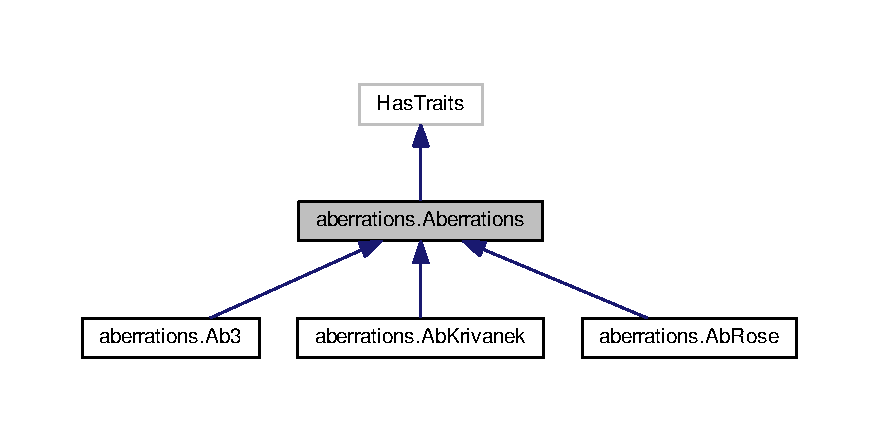
\includegraphics[width=350pt]{classaberrations_1_1_aberrations__inherit__graph}
\end{center}
\end{figure}


Collaboration diagram for aberrations.\-Aberrations\-:
\nopagebreak
\begin{figure}[H]
\begin{center}
\leavevmode
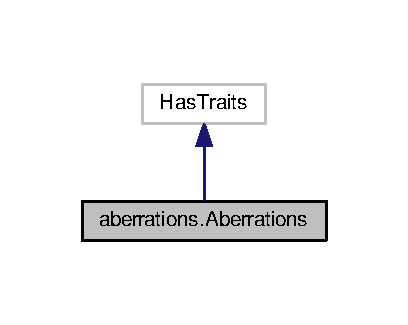
\includegraphics[width=196pt]{classaberrations_1_1_aberrations__coll__graph}
\end{center}
\end{figure}
\subsection*{Public Member Functions}
\begin{DoxyCompactItemize}
\item 
\hyperlink{sim_image_from_wave_8m_a72b6b8e83430abf007f20aeae4dc2f74}{def} \hyperlink{classaberrations_1_1_aberrations_a015078e5a61519f69a0b0a8dce600fbd}{set\-Scherzer}
\end{DoxyCompactItemize}
\subsection*{Static Public Attributes}
\begin{DoxyCompactItemize}
\item 
tuple \hyperlink{classaberrations_1_1_aberrations_a23ac1b59d9bd82141c9e3bc838ede16e}{N} = Int(256)
\item 
tuple \hyperlink{classaberrations_1_1_aberrations_a24b6f1c8db4c40bf846990969118e494}{d} = Float(0.\-5)
\item 
tuple \hyperlink{classaberrations_1_1_aberrations_a5f63dc7f3be647efe0273e85365be295}{k} = Property(Array, depends\-\_\-on=\mbox{[}'\hyperlink{classaberrations_1_1_aberrations_a23ac1b59d9bd82141c9e3bc838ede16e}{N}','\hyperlink{classaberrations_1_1_aberrations_a2ca713e45b3e4a8eb7c8404922ca6d7b}{dk}','\hyperlink{classaberrations_1_1_aberrations_a3f1b6bd8c0303bc4c01c49e401c4672d}{tilt\-X}','\hyperlink{classaberrations_1_1_aberrations_ad6443a723b0a30fe7410f7732794c9a1}{tilt\-Y}'\mbox{]})
\item 
tuple \hyperlink{classaberrations_1_1_aberrations_a2ca713e45b3e4a8eb7c8404922ca6d7b}{dk} = Property(Float, depends\-\_\-on=\mbox{[}'\hyperlink{classaberrations_1_1_aberrations_a23ac1b59d9bd82141c9e3bc838ede16e}{N}','\hyperlink{classaberrations_1_1_aberrations_a24b6f1c8db4c40bf846990969118e494}{d}'\mbox{]})
\item 
tuple \hyperlink{classaberrations_1_1_aberrations_ae3e3b86e644ce0a655802264fe091a34}{qmax} = Property(Float, depends\-\_\-on=\mbox{[}'\hyperlink{virtual_goniometer_8m_a62197192f0fbf4e0675eb37be1c4c175}{alpha}','wl'\mbox{]})
\item 
tuple \hyperlink{classaberrations_1_1_aberrations_aafc218cbf4027b922fd2d681a90acae2}{ktheta} = Property(Array, depends\-\_\-on=(\mbox{[}'\hyperlink{classaberrations_1_1_aberrations_a5f63dc7f3be647efe0273e85365be295}{k}','wl'\mbox{]}))
\item 
tuple \hyperlink{classaberrations_1_1_aberrations_a925844b4d0d329bb014f28b66ab53d44}{kphi} = Property(Array, depends\-\_\-on=\mbox{[}'\hyperlink{classaberrations_1_1_aberrations_a5f63dc7f3be647efe0273e85365be295}{k}'\mbox{]})
\item 
\hyperlink{classaberrations_1_1_aberrations_a3f1b6bd8c0303bc4c01c49e401c4672d}{tilt\-X} = Float
\item 
\hyperlink{classaberrations_1_1_aberrations_ad6443a723b0a30fe7410f7732794c9a1}{tilt\-Y} = Float
\item 
tuple \hyperlink{classaberrations_1_1_aberrations_ae2ed062229548597367003ba97fc06af}{a} = Array(dtype=np.\-float32, shape=(7,7))
\item 
tuple \hyperlink{classaberrations_1_1_aberrations_a722d268a33dce0063ce13a839d8cfdac}{phi} = Array(dtype=np.\-float32, shape=(7,7))
\item 
tuple \hyperlink{classaberrations_1_1_aberrations_a90060afaeacce97d1106a551744e2d88}{ab\-Func} = Property(depends\-\_\-on=\mbox{[}'\hyperlink{classaberrations_1_1_aberrations_ae2ed062229548597367003ba97fc06af}{a}','\hyperlink{classaberrations_1_1_aberrations_a722d268a33dce0063ce13a839d8cfdac}{phi}','\hyperlink{classaberrations_1_1_aberrations_a925844b4d0d329bb014f28b66ab53d44}{kphi}','\hyperlink{classaberrations_1_1_aberrations_aafc218cbf4027b922fd2d681a90acae2}{ktheta}','wl'\mbox{]})
\end{DoxyCompactItemize}


\subsection{Detailed Description}
\begin{DoxyVerb}A generic class for aberrations.  This does not work by itself - classes
below are defined for several notations, and each of these define how the
a (aberration coefficients) and phi (angle) arrays are populated.
\end{DoxyVerb}
 

Definition at line 37 of file aberrations.\-py.



\subsection{Member Function Documentation}
\hypertarget{classaberrations_1_1_aberrations_a015078e5a61519f69a0b0a8dce600fbd}{\index{aberrations\-::\-Aberrations@{aberrations\-::\-Aberrations}!set\-Scherzer@{set\-Scherzer}}
\index{set\-Scherzer@{set\-Scherzer}!aberrations::Aberrations@{aberrations\-::\-Aberrations}}
\subsubsection[{set\-Scherzer}]{\setlength{\rightskip}{0pt plus 5cm}{\bf def} aberrations.\-Aberrations.\-set\-Scherzer (
\begin{DoxyParamCaption}
\item[{}]{self}
\end{DoxyParamCaption}
)}}\label{classaberrations_1_1_aberrations_a015078e5a61519f69a0b0a8dce600fbd}


Definition at line 93 of file aberrations.\-py.



\subsection{Member Data Documentation}
\hypertarget{classaberrations_1_1_aberrations_ae2ed062229548597367003ba97fc06af}{\index{aberrations\-::\-Aberrations@{aberrations\-::\-Aberrations}!a@{a}}
\index{a@{a}!aberrations::Aberrations@{aberrations\-::\-Aberrations}}
\subsubsection[{a}]{\setlength{\rightskip}{0pt plus 5cm}tuple aberrations.\-Aberrations.\-a = Array(dtype=np.\-float32, shape=(7,7))\hspace{0.3cm}{\ttfamily [static]}}}\label{classaberrations_1_1_aberrations_ae2ed062229548597367003ba97fc06af}


Definition at line 54 of file aberrations.\-py.

\hypertarget{classaberrations_1_1_aberrations_a90060afaeacce97d1106a551744e2d88}{\index{aberrations\-::\-Aberrations@{aberrations\-::\-Aberrations}!ab\-Func@{ab\-Func}}
\index{ab\-Func@{ab\-Func}!aberrations::Aberrations@{aberrations\-::\-Aberrations}}
\subsubsection[{ab\-Func}]{\setlength{\rightskip}{0pt plus 5cm}tuple aberrations.\-Aberrations.\-ab\-Func = Property(depends\-\_\-on=\mbox{[}'{\bf a}','{\bf phi}','{\bf kphi}','{\bf ktheta}','wl'\mbox{]})\hspace{0.3cm}{\ttfamily [static]}}}\label{classaberrations_1_1_aberrations_a90060afaeacce97d1106a551744e2d88}


Definition at line 56 of file aberrations.\-py.

\hypertarget{classaberrations_1_1_aberrations_a24b6f1c8db4c40bf846990969118e494}{\index{aberrations\-::\-Aberrations@{aberrations\-::\-Aberrations}!d@{d}}
\index{d@{d}!aberrations::Aberrations@{aberrations\-::\-Aberrations}}
\subsubsection[{d}]{\setlength{\rightskip}{0pt plus 5cm}tuple aberrations.\-Aberrations.\-d = Float(0.\-5)\hspace{0.3cm}{\ttfamily [static]}}}\label{classaberrations_1_1_aberrations_a24b6f1c8db4c40bf846990969118e494}


Definition at line 46 of file aberrations.\-py.

\hypertarget{classaberrations_1_1_aberrations_a2ca713e45b3e4a8eb7c8404922ca6d7b}{\index{aberrations\-::\-Aberrations@{aberrations\-::\-Aberrations}!dk@{dk}}
\index{dk@{dk}!aberrations::Aberrations@{aberrations\-::\-Aberrations}}
\subsubsection[{dk}]{\setlength{\rightskip}{0pt plus 5cm}tuple aberrations.\-Aberrations.\-dk = Property(Float, depends\-\_\-on=\mbox{[}'{\bf N}','{\bf d}'\mbox{]})\hspace{0.3cm}{\ttfamily [static]}}}\label{classaberrations_1_1_aberrations_a2ca713e45b3e4a8eb7c8404922ca6d7b}


Definition at line 48 of file aberrations.\-py.

\hypertarget{classaberrations_1_1_aberrations_a5f63dc7f3be647efe0273e85365be295}{\index{aberrations\-::\-Aberrations@{aberrations\-::\-Aberrations}!k@{k}}
\index{k@{k}!aberrations::Aberrations@{aberrations\-::\-Aberrations}}
\subsubsection[{k}]{\setlength{\rightskip}{0pt plus 5cm}tuple aberrations.\-Aberrations.\-k = Property(Array, depends\-\_\-on=\mbox{[}'{\bf N}','{\bf dk}','{\bf tilt\-X}','{\bf tilt\-Y}'\mbox{]})\hspace{0.3cm}{\ttfamily [static]}}}\label{classaberrations_1_1_aberrations_a5f63dc7f3be647efe0273e85365be295}


Definition at line 47 of file aberrations.\-py.

\hypertarget{classaberrations_1_1_aberrations_a925844b4d0d329bb014f28b66ab53d44}{\index{aberrations\-::\-Aberrations@{aberrations\-::\-Aberrations}!kphi@{kphi}}
\index{kphi@{kphi}!aberrations::Aberrations@{aberrations\-::\-Aberrations}}
\subsubsection[{kphi}]{\setlength{\rightskip}{0pt plus 5cm}tuple aberrations.\-Aberrations.\-kphi = Property(Array, depends\-\_\-on=\mbox{[}'{\bf k}'\mbox{]})\hspace{0.3cm}{\ttfamily [static]}}}\label{classaberrations_1_1_aberrations_a925844b4d0d329bb014f28b66ab53d44}


Definition at line 51 of file aberrations.\-py.

\hypertarget{classaberrations_1_1_aberrations_aafc218cbf4027b922fd2d681a90acae2}{\index{aberrations\-::\-Aberrations@{aberrations\-::\-Aberrations}!ktheta@{ktheta}}
\index{ktheta@{ktheta}!aberrations::Aberrations@{aberrations\-::\-Aberrations}}
\subsubsection[{ktheta}]{\setlength{\rightskip}{0pt plus 5cm}tuple aberrations.\-Aberrations.\-ktheta = Property(Array, depends\-\_\-on=(\mbox{[}'{\bf k}','wl'\mbox{]}))\hspace{0.3cm}{\ttfamily [static]}}}\label{classaberrations_1_1_aberrations_aafc218cbf4027b922fd2d681a90acae2}


Definition at line 50 of file aberrations.\-py.

\hypertarget{classaberrations_1_1_aberrations_a23ac1b59d9bd82141c9e3bc838ede16e}{\index{aberrations\-::\-Aberrations@{aberrations\-::\-Aberrations}!N@{N}}
\index{N@{N}!aberrations::Aberrations@{aberrations\-::\-Aberrations}}
\subsubsection[{N}]{\setlength{\rightskip}{0pt plus 5cm}tuple aberrations.\-Aberrations.\-N = Int(256)\hspace{0.3cm}{\ttfamily [static]}}}\label{classaberrations_1_1_aberrations_a23ac1b59d9bd82141c9e3bc838ede16e}


Definition at line 45 of file aberrations.\-py.

\hypertarget{classaberrations_1_1_aberrations_a722d268a33dce0063ce13a839d8cfdac}{\index{aberrations\-::\-Aberrations@{aberrations\-::\-Aberrations}!phi@{phi}}
\index{phi@{phi}!aberrations::Aberrations@{aberrations\-::\-Aberrations}}
\subsubsection[{phi}]{\setlength{\rightskip}{0pt plus 5cm}tuple aberrations.\-Aberrations.\-phi = Array(dtype=np.\-float32, shape=(7,7))\hspace{0.3cm}{\ttfamily [static]}}}\label{classaberrations_1_1_aberrations_a722d268a33dce0063ce13a839d8cfdac}


Definition at line 55 of file aberrations.\-py.

\hypertarget{classaberrations_1_1_aberrations_ae3e3b86e644ce0a655802264fe091a34}{\index{aberrations\-::\-Aberrations@{aberrations\-::\-Aberrations}!qmax@{qmax}}
\index{qmax@{qmax}!aberrations::Aberrations@{aberrations\-::\-Aberrations}}
\subsubsection[{qmax}]{\setlength{\rightskip}{0pt plus 5cm}tuple aberrations.\-Aberrations.\-qmax = Property(Float, depends\-\_\-on=\mbox{[}'{\bf alpha}','wl'\mbox{]})\hspace{0.3cm}{\ttfamily [static]}}}\label{classaberrations_1_1_aberrations_ae3e3b86e644ce0a655802264fe091a34}


Definition at line 49 of file aberrations.\-py.

\hypertarget{classaberrations_1_1_aberrations_a3f1b6bd8c0303bc4c01c49e401c4672d}{\index{aberrations\-::\-Aberrations@{aberrations\-::\-Aberrations}!tilt\-X@{tilt\-X}}
\index{tilt\-X@{tilt\-X}!aberrations::Aberrations@{aberrations\-::\-Aberrations}}
\subsubsection[{tilt\-X}]{\setlength{\rightskip}{0pt plus 5cm}aberrations.\-Aberrations.\-tilt\-X = Float\hspace{0.3cm}{\ttfamily [static]}}}\label{classaberrations_1_1_aberrations_a3f1b6bd8c0303bc4c01c49e401c4672d}


Definition at line 52 of file aberrations.\-py.

\hypertarget{classaberrations_1_1_aberrations_ad6443a723b0a30fe7410f7732794c9a1}{\index{aberrations\-::\-Aberrations@{aberrations\-::\-Aberrations}!tilt\-Y@{tilt\-Y}}
\index{tilt\-Y@{tilt\-Y}!aberrations::Aberrations@{aberrations\-::\-Aberrations}}
\subsubsection[{tilt\-Y}]{\setlength{\rightskip}{0pt plus 5cm}aberrations.\-Aberrations.\-tilt\-Y = Float\hspace{0.3cm}{\ttfamily [static]}}}\label{classaberrations_1_1_aberrations_ad6443a723b0a30fe7410f7732794c9a1}


Definition at line 53 of file aberrations.\-py.



The documentation for this class was generated from the following file\-:\begin{DoxyCompactItemize}
\item 
Q\-S\-T\-E\-M\-\_\-\-G\-U\-I\-\_\-\-Traits/\hyperlink{aberrations_8py}{aberrations.\-py}\end{DoxyCompactItemize}

\hypertarget{classaberrations_1_1_ab_krivanek}{\section{aberrations.\-Ab\-Krivanek Class Reference}
\label{classaberrations_1_1_ab_krivanek}\index{aberrations.\-Ab\-Krivanek@{aberrations.\-Ab\-Krivanek}}
}


Inheritance diagram for aberrations.\-Ab\-Krivanek\-:
\nopagebreak
\begin{figure}[H]
\begin{center}
\leavevmode
\includegraphics[width=198pt]{classaberrations_1_1_ab_krivanek__inherit__graph}
\end{center}
\end{figure}


Collaboration diagram for aberrations.\-Ab\-Krivanek\-:
\nopagebreak
\begin{figure}[H]
\begin{center}
\leavevmode
\includegraphics[width=198pt]{classaberrations_1_1_ab_krivanek__coll__graph}
\end{center}
\end{figure}
\subsection*{Static Public Attributes}
\begin{DoxyCompactItemize}
\item 
tuple \hyperlink{classaberrations_1_1_ab_krivanek_a67551c9dcb755773d0d4d68ddddbb0c1}{C1\-\_\-0} = Float(desc='\hyperlink{image_sim_8m_a095451ad095fab975004df8fa1925cb8}{Defocus}')
\item 
tuple \hyperlink{classaberrations_1_1_ab_krivanek_a8660810b2614beb56702878902b594f2}{C3\-\_\-0} = Float(desc = 'Spherical Aberration')
\item 
tuple \hyperlink{classaberrations_1_1_ab_krivanek_aed991b8cfb36ae34e5adbbab09854888}{C5\-\_\-0} = Float(desc='5th order spherical aberration')
\item 
tuple \hyperlink{classaberrations_1_1_ab_krivanek_a6743d32a0185f0c0cb00cb1b4dca36f4}{C1\-\_\-2a} = Float(desc='2-\/Fold astigmatism')
\item 
tuple \hyperlink{classaberrations_1_1_ab_krivanek_a8835ee7c475ae556be69a14a99f733ea}{C1\-\_\-2b} = Float(desc='2-\/Fold astigmatism')
\item 
tuple \hyperlink{classaberrations_1_1_ab_krivanek_ab60aea624cb5d86337e8bd6dfd7ef20f}{C2\-\_\-3a} = Float(desc='3-\/Fold astigmatism')
\item 
tuple \hyperlink{classaberrations_1_1_ab_krivanek_ae1f00d8d6fcc1ec3676653a619bc9466}{C2\-\_\-3b} = Float(desc='3-\/Fold astigmatism')
\item 
tuple \hyperlink{classaberrations_1_1_ab_krivanek_a2d7b8b57cf3aa5d096f859e24dac2e8c}{C3\-\_\-4a} = Float(desc='4-\/Fold astigmatism')
\item 
tuple \hyperlink{classaberrations_1_1_ab_krivanek_a53cdd9582c6e36d5391be28a10193e53}{C3\-\_\-4b} = Float(desc='4-\/Fold astigmatism')
\item 
tuple \hyperlink{classaberrations_1_1_ab_krivanek_a7c6b7ffa2a750e4886d48acc0043e543}{C4\-\_\-5a} = Float(desc='5-\/Fold astigmatism')
\item 
tuple \hyperlink{classaberrations_1_1_ab_krivanek_a4498d2f076a44b05635c92dd234c9940}{C4\-\_\-5b} = Float(desc='5-\/Fold astigmatism')
\item 
tuple \hyperlink{classaberrations_1_1_ab_krivanek_ad0efb21c7be0f06d0d9bf9ef2126edb6}{C5\-\_\-6a} = Float(desc='6-\/Fold astigmatism')
\item 
tuple \hyperlink{classaberrations_1_1_ab_krivanek_a4f142f6028261cce8c2676a4e035a773}{C5\-\_\-6b} = Float(desc='6-\/Fold astigmatism')
\item 
tuple \hyperlink{classaberrations_1_1_ab_krivanek_a6dcdbacc8d723b2a55c3236b1982af95}{C2\-\_\-1a} = Float(desc='Axial coma')
\item 
tuple \hyperlink{classaberrations_1_1_ab_krivanek_a827343cc3727f0f4d64d99051f79ca9f}{C2\-\_\-1b} = Float(desc='Axial coma')
\item 
tuple \hyperlink{classaberrations_1_1_ab_krivanek_ae8cc3279df6c913aa9179fae414c1dd9}{C4\-\_\-1a} = Float(desc='Axial coma')
\item 
tuple \hyperlink{classaberrations_1_1_ab_krivanek_a3840460e6c3a4d80a704e32dd8d9cd7d}{C4\-\_\-1b} = Float(desc='Axial coma')
\item 
tuple \hyperlink{classaberrations_1_1_ab_krivanek_a86e1ae8031fd414b99346ce5ccbe937c}{C3\-\_\-2a} = Float(desc='Axial star')
\item 
tuple \hyperlink{classaberrations_1_1_ab_krivanek_af86229f760e7b5f1f9fe191c93594d1c}{C3\-\_\-2b} = Float(desc='Axial star')
\item 
tuple \hyperlink{classaberrations_1_1_ab_krivanek_a1d76afe5495f60132fab0f7465737b0c}{C5\-\_\-2a} = Float(desc='Axial star')
\item 
tuple \hyperlink{classaberrations_1_1_ab_krivanek_a34039ce0ac088661a604adaea5cb80b3}{C5\-\_\-2b} = Float(desc='Axial star')
\item 
tuple \hyperlink{classaberrations_1_1_ab_krivanek_ae316c7dc0ea6f28b04bfd2100764099e}{C4\-\_\-3a} = Float(desc='3-\/lobe \hyperlink{aberrations___t_e_m_8m_add6b7c5f8447a629106b3fae4a009eb8}{aberration}')
\item 
tuple \hyperlink{classaberrations_1_1_ab_krivanek_a8cf52df7725ea8a872e55e64d8723066}{C4\-\_\-3b} = Float(desc='3-\/lobe \hyperlink{aberrations___t_e_m_8m_add6b7c5f8447a629106b3fae4a009eb8}{aberration}')
\item 
tuple \hyperlink{classaberrations_1_1_ab_krivanek_a891846dfeba7bb569ca05988addbf780}{C5\-\_\-4a} = Float(desc='4-\/lobe \hyperlink{aberrations___t_e_m_8m_add6b7c5f8447a629106b3fae4a009eb8}{aberration}')
\item 
tuple \hyperlink{classaberrations_1_1_ab_krivanek_a7ce620a43e01049640bdd0fac68fe76e}{C5\-\_\-4b} = Float(desc='4-\/lobe \hyperlink{aberrations___t_e_m_8m_add6b7c5f8447a629106b3fae4a009eb8}{aberration}')
\item 
tuple \hyperlink{classaberrations_1_1_ab_krivanek_a64acaf45047a7edb58b22723a142d438}{a}
\item 
tuple \hyperlink{classaberrations_1_1_ab_krivanek_a4fef2670dae44658f6ca6f9c3804d96c}{phi}
\end{DoxyCompactItemize}
\subsection*{Additional Inherited Members}


\subsection{Detailed Description}


Definition at line 97 of file aberrations.\-py.



\subsection{Member Data Documentation}
\hypertarget{classaberrations_1_1_ab_krivanek_a64acaf45047a7edb58b22723a142d438}{\index{aberrations\-::\-Ab\-Krivanek@{aberrations\-::\-Ab\-Krivanek}!a@{a}}
\index{a@{a}!aberrations::AbKrivanek@{aberrations\-::\-Ab\-Krivanek}}
\subsubsection[{a}]{\setlength{\rightskip}{0pt plus 5cm}tuple aberrations.\-Ab\-Krivanek.\-a\hspace{0.3cm}{\ttfamily [static]}}}\label{classaberrations_1_1_ab_krivanek_a64acaf45047a7edb58b22723a142d438}
{\bfseries Initial value\-:}
\begin{DoxyCode}
1 = Property(Array, depends\_on=[\textcolor{stringliteral}{'C1\_0'}, \textcolor{stringliteral}{'C3\_0'}, \textcolor{stringliteral}{'C5\_0'}, \textcolor{stringliteral}{'C1\_2a'}, \textcolor{stringliteral}{'C1\_2b'}, 
2                                     \textcolor{stringliteral}{'C2\_3a'}, \textcolor{stringliteral}{'C2\_3b'}, \textcolor{stringliteral}{'C3\_4a'}, \textcolor{stringliteral}{'C3\_4b'},
3                                     \textcolor{stringliteral}{'C4\_5a'}, \textcolor{stringliteral}{'C4\_5b'}, \textcolor{stringliteral}{'C5\_6a'}, \textcolor{stringliteral}{'C5\_6b'},
4                                     \textcolor{stringliteral}{'C2\_1a'}, \textcolor{stringliteral}{'C2\_1b'}, \textcolor{stringliteral}{'C4\_1a'}, \textcolor{stringliteral}{'C4\_1b'},
5                                     \textcolor{stringliteral}{'C3\_2a'}, \textcolor{stringliteral}{'C3\_2b'}, \textcolor{stringliteral}{'C5\_2a'}, \textcolor{stringliteral}{'C5\_2b'},
6                                     \textcolor{stringliteral}{'C4\_3a'}, \textcolor{stringliteral}{'C4\_3b'}, \textcolor{stringliteral}{'C5\_4a'}, \textcolor{stringliteral}{'C5\_4b'}])
\end{DoxyCode}


Definition at line 124 of file aberrations.\-py.

\hypertarget{classaberrations_1_1_ab_krivanek_a67551c9dcb755773d0d4d68ddddbb0c1}{\index{aberrations\-::\-Ab\-Krivanek@{aberrations\-::\-Ab\-Krivanek}!C1\-\_\-0@{C1\-\_\-0}}
\index{C1\-\_\-0@{C1\-\_\-0}!aberrations::AbKrivanek@{aberrations\-::\-Ab\-Krivanek}}
\subsubsection[{C1\-\_\-0}]{\setlength{\rightskip}{0pt plus 5cm}tuple aberrations.\-Ab\-Krivanek.\-C1\-\_\-0 = Float(desc='{\bf Defocus}')\hspace{0.3cm}{\ttfamily [static]}}}\label{classaberrations_1_1_ab_krivanek_a67551c9dcb755773d0d4d68ddddbb0c1}


Definition at line 98 of file aberrations.\-py.

\hypertarget{classaberrations_1_1_ab_krivanek_a6743d32a0185f0c0cb00cb1b4dca36f4}{\index{aberrations\-::\-Ab\-Krivanek@{aberrations\-::\-Ab\-Krivanek}!C1\-\_\-2a@{C1\-\_\-2a}}
\index{C1\-\_\-2a@{C1\-\_\-2a}!aberrations::AbKrivanek@{aberrations\-::\-Ab\-Krivanek}}
\subsubsection[{C1\-\_\-2a}]{\setlength{\rightskip}{0pt plus 5cm}tuple aberrations.\-Ab\-Krivanek.\-C1\-\_\-2a = Float(desc='2-\/Fold astigmatism')\hspace{0.3cm}{\ttfamily [static]}}}\label{classaberrations_1_1_ab_krivanek_a6743d32a0185f0c0cb00cb1b4dca36f4}


Definition at line 101 of file aberrations.\-py.

\hypertarget{classaberrations_1_1_ab_krivanek_a8835ee7c475ae556be69a14a99f733ea}{\index{aberrations\-::\-Ab\-Krivanek@{aberrations\-::\-Ab\-Krivanek}!C1\-\_\-2b@{C1\-\_\-2b}}
\index{C1\-\_\-2b@{C1\-\_\-2b}!aberrations::AbKrivanek@{aberrations\-::\-Ab\-Krivanek}}
\subsubsection[{C1\-\_\-2b}]{\setlength{\rightskip}{0pt plus 5cm}tuple aberrations.\-Ab\-Krivanek.\-C1\-\_\-2b = Float(desc='2-\/Fold astigmatism')\hspace{0.3cm}{\ttfamily [static]}}}\label{classaberrations_1_1_ab_krivanek_a8835ee7c475ae556be69a14a99f733ea}


Definition at line 102 of file aberrations.\-py.

\hypertarget{classaberrations_1_1_ab_krivanek_a6dcdbacc8d723b2a55c3236b1982af95}{\index{aberrations\-::\-Ab\-Krivanek@{aberrations\-::\-Ab\-Krivanek}!C2\-\_\-1a@{C2\-\_\-1a}}
\index{C2\-\_\-1a@{C2\-\_\-1a}!aberrations::AbKrivanek@{aberrations\-::\-Ab\-Krivanek}}
\subsubsection[{C2\-\_\-1a}]{\setlength{\rightskip}{0pt plus 5cm}tuple aberrations.\-Ab\-Krivanek.\-C2\-\_\-1a = Float(desc='Axial coma')\hspace{0.3cm}{\ttfamily [static]}}}\label{classaberrations_1_1_ab_krivanek_a6dcdbacc8d723b2a55c3236b1982af95}


Definition at line 111 of file aberrations.\-py.

\hypertarget{classaberrations_1_1_ab_krivanek_a827343cc3727f0f4d64d99051f79ca9f}{\index{aberrations\-::\-Ab\-Krivanek@{aberrations\-::\-Ab\-Krivanek}!C2\-\_\-1b@{C2\-\_\-1b}}
\index{C2\-\_\-1b@{C2\-\_\-1b}!aberrations::AbKrivanek@{aberrations\-::\-Ab\-Krivanek}}
\subsubsection[{C2\-\_\-1b}]{\setlength{\rightskip}{0pt plus 5cm}tuple aberrations.\-Ab\-Krivanek.\-C2\-\_\-1b = Float(desc='Axial coma')\hspace{0.3cm}{\ttfamily [static]}}}\label{classaberrations_1_1_ab_krivanek_a827343cc3727f0f4d64d99051f79ca9f}


Definition at line 112 of file aberrations.\-py.

\hypertarget{classaberrations_1_1_ab_krivanek_ab60aea624cb5d86337e8bd6dfd7ef20f}{\index{aberrations\-::\-Ab\-Krivanek@{aberrations\-::\-Ab\-Krivanek}!C2\-\_\-3a@{C2\-\_\-3a}}
\index{C2\-\_\-3a@{C2\-\_\-3a}!aberrations::AbKrivanek@{aberrations\-::\-Ab\-Krivanek}}
\subsubsection[{C2\-\_\-3a}]{\setlength{\rightskip}{0pt plus 5cm}tuple aberrations.\-Ab\-Krivanek.\-C2\-\_\-3a = Float(desc='3-\/Fold astigmatism')\hspace{0.3cm}{\ttfamily [static]}}}\label{classaberrations_1_1_ab_krivanek_ab60aea624cb5d86337e8bd6dfd7ef20f}


Definition at line 103 of file aberrations.\-py.

\hypertarget{classaberrations_1_1_ab_krivanek_ae1f00d8d6fcc1ec3676653a619bc9466}{\index{aberrations\-::\-Ab\-Krivanek@{aberrations\-::\-Ab\-Krivanek}!C2\-\_\-3b@{C2\-\_\-3b}}
\index{C2\-\_\-3b@{C2\-\_\-3b}!aberrations::AbKrivanek@{aberrations\-::\-Ab\-Krivanek}}
\subsubsection[{C2\-\_\-3b}]{\setlength{\rightskip}{0pt plus 5cm}tuple aberrations.\-Ab\-Krivanek.\-C2\-\_\-3b = Float(desc='3-\/Fold astigmatism')\hspace{0.3cm}{\ttfamily [static]}}}\label{classaberrations_1_1_ab_krivanek_ae1f00d8d6fcc1ec3676653a619bc9466}


Definition at line 104 of file aberrations.\-py.

\hypertarget{classaberrations_1_1_ab_krivanek_a8660810b2614beb56702878902b594f2}{\index{aberrations\-::\-Ab\-Krivanek@{aberrations\-::\-Ab\-Krivanek}!C3\-\_\-0@{C3\-\_\-0}}
\index{C3\-\_\-0@{C3\-\_\-0}!aberrations::AbKrivanek@{aberrations\-::\-Ab\-Krivanek}}
\subsubsection[{C3\-\_\-0}]{\setlength{\rightskip}{0pt plus 5cm}tuple aberrations.\-Ab\-Krivanek.\-C3\-\_\-0 = Float(desc = 'Spherical Aberration')\hspace{0.3cm}{\ttfamily [static]}}}\label{classaberrations_1_1_ab_krivanek_a8660810b2614beb56702878902b594f2}


Definition at line 99 of file aberrations.\-py.

\hypertarget{classaberrations_1_1_ab_krivanek_a86e1ae8031fd414b99346ce5ccbe937c}{\index{aberrations\-::\-Ab\-Krivanek@{aberrations\-::\-Ab\-Krivanek}!C3\-\_\-2a@{C3\-\_\-2a}}
\index{C3\-\_\-2a@{C3\-\_\-2a}!aberrations::AbKrivanek@{aberrations\-::\-Ab\-Krivanek}}
\subsubsection[{C3\-\_\-2a}]{\setlength{\rightskip}{0pt plus 5cm}tuple aberrations.\-Ab\-Krivanek.\-C3\-\_\-2a = Float(desc='Axial star')\hspace{0.3cm}{\ttfamily [static]}}}\label{classaberrations_1_1_ab_krivanek_a86e1ae8031fd414b99346ce5ccbe937c}


Definition at line 115 of file aberrations.\-py.

\hypertarget{classaberrations_1_1_ab_krivanek_af86229f760e7b5f1f9fe191c93594d1c}{\index{aberrations\-::\-Ab\-Krivanek@{aberrations\-::\-Ab\-Krivanek}!C3\-\_\-2b@{C3\-\_\-2b}}
\index{C3\-\_\-2b@{C3\-\_\-2b}!aberrations::AbKrivanek@{aberrations\-::\-Ab\-Krivanek}}
\subsubsection[{C3\-\_\-2b}]{\setlength{\rightskip}{0pt plus 5cm}tuple aberrations.\-Ab\-Krivanek.\-C3\-\_\-2b = Float(desc='Axial star')\hspace{0.3cm}{\ttfamily [static]}}}\label{classaberrations_1_1_ab_krivanek_af86229f760e7b5f1f9fe191c93594d1c}


Definition at line 116 of file aberrations.\-py.

\hypertarget{classaberrations_1_1_ab_krivanek_a2d7b8b57cf3aa5d096f859e24dac2e8c}{\index{aberrations\-::\-Ab\-Krivanek@{aberrations\-::\-Ab\-Krivanek}!C3\-\_\-4a@{C3\-\_\-4a}}
\index{C3\-\_\-4a@{C3\-\_\-4a}!aberrations::AbKrivanek@{aberrations\-::\-Ab\-Krivanek}}
\subsubsection[{C3\-\_\-4a}]{\setlength{\rightskip}{0pt plus 5cm}tuple aberrations.\-Ab\-Krivanek.\-C3\-\_\-4a = Float(desc='4-\/Fold astigmatism')\hspace{0.3cm}{\ttfamily [static]}}}\label{classaberrations_1_1_ab_krivanek_a2d7b8b57cf3aa5d096f859e24dac2e8c}


Definition at line 105 of file aberrations.\-py.

\hypertarget{classaberrations_1_1_ab_krivanek_a53cdd9582c6e36d5391be28a10193e53}{\index{aberrations\-::\-Ab\-Krivanek@{aberrations\-::\-Ab\-Krivanek}!C3\-\_\-4b@{C3\-\_\-4b}}
\index{C3\-\_\-4b@{C3\-\_\-4b}!aberrations::AbKrivanek@{aberrations\-::\-Ab\-Krivanek}}
\subsubsection[{C3\-\_\-4b}]{\setlength{\rightskip}{0pt plus 5cm}tuple aberrations.\-Ab\-Krivanek.\-C3\-\_\-4b = Float(desc='4-\/Fold astigmatism')\hspace{0.3cm}{\ttfamily [static]}}}\label{classaberrations_1_1_ab_krivanek_a53cdd9582c6e36d5391be28a10193e53}


Definition at line 106 of file aberrations.\-py.

\hypertarget{classaberrations_1_1_ab_krivanek_ae8cc3279df6c913aa9179fae414c1dd9}{\index{aberrations\-::\-Ab\-Krivanek@{aberrations\-::\-Ab\-Krivanek}!C4\-\_\-1a@{C4\-\_\-1a}}
\index{C4\-\_\-1a@{C4\-\_\-1a}!aberrations::AbKrivanek@{aberrations\-::\-Ab\-Krivanek}}
\subsubsection[{C4\-\_\-1a}]{\setlength{\rightskip}{0pt plus 5cm}tuple aberrations.\-Ab\-Krivanek.\-C4\-\_\-1a = Float(desc='Axial coma')\hspace{0.3cm}{\ttfamily [static]}}}\label{classaberrations_1_1_ab_krivanek_ae8cc3279df6c913aa9179fae414c1dd9}


Definition at line 113 of file aberrations.\-py.

\hypertarget{classaberrations_1_1_ab_krivanek_a3840460e6c3a4d80a704e32dd8d9cd7d}{\index{aberrations\-::\-Ab\-Krivanek@{aberrations\-::\-Ab\-Krivanek}!C4\-\_\-1b@{C4\-\_\-1b}}
\index{C4\-\_\-1b@{C4\-\_\-1b}!aberrations::AbKrivanek@{aberrations\-::\-Ab\-Krivanek}}
\subsubsection[{C4\-\_\-1b}]{\setlength{\rightskip}{0pt plus 5cm}tuple aberrations.\-Ab\-Krivanek.\-C4\-\_\-1b = Float(desc='Axial coma')\hspace{0.3cm}{\ttfamily [static]}}}\label{classaberrations_1_1_ab_krivanek_a3840460e6c3a4d80a704e32dd8d9cd7d}


Definition at line 114 of file aberrations.\-py.

\hypertarget{classaberrations_1_1_ab_krivanek_ae316c7dc0ea6f28b04bfd2100764099e}{\index{aberrations\-::\-Ab\-Krivanek@{aberrations\-::\-Ab\-Krivanek}!C4\-\_\-3a@{C4\-\_\-3a}}
\index{C4\-\_\-3a@{C4\-\_\-3a}!aberrations::AbKrivanek@{aberrations\-::\-Ab\-Krivanek}}
\subsubsection[{C4\-\_\-3a}]{\setlength{\rightskip}{0pt plus 5cm}tuple aberrations.\-Ab\-Krivanek.\-C4\-\_\-3a = Float(desc='3-\/lobe {\bf aberration}')\hspace{0.3cm}{\ttfamily [static]}}}\label{classaberrations_1_1_ab_krivanek_ae316c7dc0ea6f28b04bfd2100764099e}


Definition at line 119 of file aberrations.\-py.

\hypertarget{classaberrations_1_1_ab_krivanek_a8cf52df7725ea8a872e55e64d8723066}{\index{aberrations\-::\-Ab\-Krivanek@{aberrations\-::\-Ab\-Krivanek}!C4\-\_\-3b@{C4\-\_\-3b}}
\index{C4\-\_\-3b@{C4\-\_\-3b}!aberrations::AbKrivanek@{aberrations\-::\-Ab\-Krivanek}}
\subsubsection[{C4\-\_\-3b}]{\setlength{\rightskip}{0pt plus 5cm}tuple aberrations.\-Ab\-Krivanek.\-C4\-\_\-3b = Float(desc='3-\/lobe {\bf aberration}')\hspace{0.3cm}{\ttfamily [static]}}}\label{classaberrations_1_1_ab_krivanek_a8cf52df7725ea8a872e55e64d8723066}


Definition at line 120 of file aberrations.\-py.

\hypertarget{classaberrations_1_1_ab_krivanek_a7c6b7ffa2a750e4886d48acc0043e543}{\index{aberrations\-::\-Ab\-Krivanek@{aberrations\-::\-Ab\-Krivanek}!C4\-\_\-5a@{C4\-\_\-5a}}
\index{C4\-\_\-5a@{C4\-\_\-5a}!aberrations::AbKrivanek@{aberrations\-::\-Ab\-Krivanek}}
\subsubsection[{C4\-\_\-5a}]{\setlength{\rightskip}{0pt plus 5cm}tuple aberrations.\-Ab\-Krivanek.\-C4\-\_\-5a = Float(desc='5-\/Fold astigmatism')\hspace{0.3cm}{\ttfamily [static]}}}\label{classaberrations_1_1_ab_krivanek_a7c6b7ffa2a750e4886d48acc0043e543}


Definition at line 107 of file aberrations.\-py.

\hypertarget{classaberrations_1_1_ab_krivanek_a4498d2f076a44b05635c92dd234c9940}{\index{aberrations\-::\-Ab\-Krivanek@{aberrations\-::\-Ab\-Krivanek}!C4\-\_\-5b@{C4\-\_\-5b}}
\index{C4\-\_\-5b@{C4\-\_\-5b}!aberrations::AbKrivanek@{aberrations\-::\-Ab\-Krivanek}}
\subsubsection[{C4\-\_\-5b}]{\setlength{\rightskip}{0pt plus 5cm}tuple aberrations.\-Ab\-Krivanek.\-C4\-\_\-5b = Float(desc='5-\/Fold astigmatism')\hspace{0.3cm}{\ttfamily [static]}}}\label{classaberrations_1_1_ab_krivanek_a4498d2f076a44b05635c92dd234c9940}


Definition at line 108 of file aberrations.\-py.

\hypertarget{classaberrations_1_1_ab_krivanek_aed991b8cfb36ae34e5adbbab09854888}{\index{aberrations\-::\-Ab\-Krivanek@{aberrations\-::\-Ab\-Krivanek}!C5\-\_\-0@{C5\-\_\-0}}
\index{C5\-\_\-0@{C5\-\_\-0}!aberrations::AbKrivanek@{aberrations\-::\-Ab\-Krivanek}}
\subsubsection[{C5\-\_\-0}]{\setlength{\rightskip}{0pt plus 5cm}tuple aberrations.\-Ab\-Krivanek.\-C5\-\_\-0 = Float(desc='5th order spherical aberration')\hspace{0.3cm}{\ttfamily [static]}}}\label{classaberrations_1_1_ab_krivanek_aed991b8cfb36ae34e5adbbab09854888}


Definition at line 100 of file aberrations.\-py.

\hypertarget{classaberrations_1_1_ab_krivanek_a1d76afe5495f60132fab0f7465737b0c}{\index{aberrations\-::\-Ab\-Krivanek@{aberrations\-::\-Ab\-Krivanek}!C5\-\_\-2a@{C5\-\_\-2a}}
\index{C5\-\_\-2a@{C5\-\_\-2a}!aberrations::AbKrivanek@{aberrations\-::\-Ab\-Krivanek}}
\subsubsection[{C5\-\_\-2a}]{\setlength{\rightskip}{0pt plus 5cm}tuple aberrations.\-Ab\-Krivanek.\-C5\-\_\-2a = Float(desc='Axial star')\hspace{0.3cm}{\ttfamily [static]}}}\label{classaberrations_1_1_ab_krivanek_a1d76afe5495f60132fab0f7465737b0c}


Definition at line 117 of file aberrations.\-py.

\hypertarget{classaberrations_1_1_ab_krivanek_a34039ce0ac088661a604adaea5cb80b3}{\index{aberrations\-::\-Ab\-Krivanek@{aberrations\-::\-Ab\-Krivanek}!C5\-\_\-2b@{C5\-\_\-2b}}
\index{C5\-\_\-2b@{C5\-\_\-2b}!aberrations::AbKrivanek@{aberrations\-::\-Ab\-Krivanek}}
\subsubsection[{C5\-\_\-2b}]{\setlength{\rightskip}{0pt plus 5cm}tuple aberrations.\-Ab\-Krivanek.\-C5\-\_\-2b = Float(desc='Axial star')\hspace{0.3cm}{\ttfamily [static]}}}\label{classaberrations_1_1_ab_krivanek_a34039ce0ac088661a604adaea5cb80b3}


Definition at line 118 of file aberrations.\-py.

\hypertarget{classaberrations_1_1_ab_krivanek_a891846dfeba7bb569ca05988addbf780}{\index{aberrations\-::\-Ab\-Krivanek@{aberrations\-::\-Ab\-Krivanek}!C5\-\_\-4a@{C5\-\_\-4a}}
\index{C5\-\_\-4a@{C5\-\_\-4a}!aberrations::AbKrivanek@{aberrations\-::\-Ab\-Krivanek}}
\subsubsection[{C5\-\_\-4a}]{\setlength{\rightskip}{0pt plus 5cm}tuple aberrations.\-Ab\-Krivanek.\-C5\-\_\-4a = Float(desc='4-\/lobe {\bf aberration}')\hspace{0.3cm}{\ttfamily [static]}}}\label{classaberrations_1_1_ab_krivanek_a891846dfeba7bb569ca05988addbf780}


Definition at line 121 of file aberrations.\-py.

\hypertarget{classaberrations_1_1_ab_krivanek_a7ce620a43e01049640bdd0fac68fe76e}{\index{aberrations\-::\-Ab\-Krivanek@{aberrations\-::\-Ab\-Krivanek}!C5\-\_\-4b@{C5\-\_\-4b}}
\index{C5\-\_\-4b@{C5\-\_\-4b}!aberrations::AbKrivanek@{aberrations\-::\-Ab\-Krivanek}}
\subsubsection[{C5\-\_\-4b}]{\setlength{\rightskip}{0pt plus 5cm}tuple aberrations.\-Ab\-Krivanek.\-C5\-\_\-4b = Float(desc='4-\/lobe {\bf aberration}')\hspace{0.3cm}{\ttfamily [static]}}}\label{classaberrations_1_1_ab_krivanek_a7ce620a43e01049640bdd0fac68fe76e}


Definition at line 122 of file aberrations.\-py.

\hypertarget{classaberrations_1_1_ab_krivanek_ad0efb21c7be0f06d0d9bf9ef2126edb6}{\index{aberrations\-::\-Ab\-Krivanek@{aberrations\-::\-Ab\-Krivanek}!C5\-\_\-6a@{C5\-\_\-6a}}
\index{C5\-\_\-6a@{C5\-\_\-6a}!aberrations::AbKrivanek@{aberrations\-::\-Ab\-Krivanek}}
\subsubsection[{C5\-\_\-6a}]{\setlength{\rightskip}{0pt plus 5cm}tuple aberrations.\-Ab\-Krivanek.\-C5\-\_\-6a = Float(desc='6-\/Fold astigmatism')\hspace{0.3cm}{\ttfamily [static]}}}\label{classaberrations_1_1_ab_krivanek_ad0efb21c7be0f06d0d9bf9ef2126edb6}


Definition at line 109 of file aberrations.\-py.

\hypertarget{classaberrations_1_1_ab_krivanek_a4f142f6028261cce8c2676a4e035a773}{\index{aberrations\-::\-Ab\-Krivanek@{aberrations\-::\-Ab\-Krivanek}!C5\-\_\-6b@{C5\-\_\-6b}}
\index{C5\-\_\-6b@{C5\-\_\-6b}!aberrations::AbKrivanek@{aberrations\-::\-Ab\-Krivanek}}
\subsubsection[{C5\-\_\-6b}]{\setlength{\rightskip}{0pt plus 5cm}tuple aberrations.\-Ab\-Krivanek.\-C5\-\_\-6b = Float(desc='6-\/Fold astigmatism')\hspace{0.3cm}{\ttfamily [static]}}}\label{classaberrations_1_1_ab_krivanek_a4f142f6028261cce8c2676a4e035a773}


Definition at line 110 of file aberrations.\-py.

\hypertarget{classaberrations_1_1_ab_krivanek_a4fef2670dae44658f6ca6f9c3804d96c}{\index{aberrations\-::\-Ab\-Krivanek@{aberrations\-::\-Ab\-Krivanek}!phi@{phi}}
\index{phi@{phi}!aberrations::AbKrivanek@{aberrations\-::\-Ab\-Krivanek}}
\subsubsection[{phi}]{\setlength{\rightskip}{0pt plus 5cm}tuple aberrations.\-Ab\-Krivanek.\-phi\hspace{0.3cm}{\ttfamily [static]}}}\label{classaberrations_1_1_ab_krivanek_a4fef2670dae44658f6ca6f9c3804d96c}
{\bfseries Initial value\-:}
\begin{DoxyCode}
1 = Property(Array, depends\_on=[\textcolor{stringliteral}{'C1\_0'}, \textcolor{stringliteral}{'C3\_0'}, \textcolor{stringliteral}{'C5\_0'}, \textcolor{stringliteral}{'C1\_2a'}, \textcolor{stringliteral}{'C1\_2b'},
2                                       \textcolor{stringliteral}{'C2\_3a'}, \textcolor{stringliteral}{'C2\_3b'}, \textcolor{stringliteral}{'C3\_4a'}, \textcolor{stringliteral}{'C3\_4b'},
3                                       \textcolor{stringliteral}{'C4\_5a'}, \textcolor{stringliteral}{'C4\_5b'}, \textcolor{stringliteral}{'C5\_6a'}, \textcolor{stringliteral}{'C5\_6b'},
4                                       \textcolor{stringliteral}{'C2\_1a'}, \textcolor{stringliteral}{'C2\_1b'}, \textcolor{stringliteral}{'C4\_1a'}, \textcolor{stringliteral}{'C4\_1b'},
5                                       \textcolor{stringliteral}{'C3\_2a'}, \textcolor{stringliteral}{'C3\_2b'}, \textcolor{stringliteral}{'C5\_2a'}, \textcolor{stringliteral}{'C5\_2b'},
6                                       \textcolor{stringliteral}{'C4\_3a'}, \textcolor{stringliteral}{'C4\_3b'}, \textcolor{stringliteral}{'C5\_4a'}, \textcolor{stringliteral}{'C5\_4b'}])
\end{DoxyCode}


Definition at line 131 of file aberrations.\-py.



The documentation for this class was generated from the following file\-:\begin{DoxyCompactItemize}
\item 
Q\-S\-T\-E\-M\-\_\-\-G\-U\-I\-\_\-\-Traits/\hyperlink{aberrations_8py}{aberrations.\-py}\end{DoxyCompactItemize}

\hypertarget{classaberrations_1_1_ab_rose}{\section{aberrations.\-Ab\-Rose Class Reference}
\label{classaberrations_1_1_ab_rose}\index{aberrations.\-Ab\-Rose@{aberrations.\-Ab\-Rose}}
}


Inheritance diagram for aberrations.\-Ab\-Rose\-:
\nopagebreak
\begin{figure}[H]
\begin{center}
\leavevmode
\includegraphics[width=196pt]{classaberrations_1_1_ab_rose__inherit__graph}
\end{center}
\end{figure}


Collaboration diagram for aberrations.\-Ab\-Rose\-:
\nopagebreak
\begin{figure}[H]
\begin{center}
\leavevmode
\includegraphics[width=196pt]{classaberrations_1_1_ab_rose__coll__graph}
\end{center}
\end{figure}
\subsection*{Public Member Functions}
\begin{DoxyCompactItemize}
\item 
\hyperlink{sim_image_from_wave_8m_a72b6b8e83430abf007f20aeae4dc2f74}{def} \hyperlink{classaberrations_1_1_ab_rose_a0e5d7438c77b1b0525cbfae74d0fa913}{ang\-Convert}
\item 
\hyperlink{sim_image_from_wave_8m_a72b6b8e83430abf007f20aeae4dc2f74}{def} \hyperlink{classaberrations_1_1_ab_rose_a8f584ac5623dd65e1b901746e26fa68b}{mrad2deg}
\end{DoxyCompactItemize}
\subsection*{Public Attributes}
\begin{DoxyCompactItemize}
\item 
\hyperlink{classaberrations_1_1_ab_rose_a9a5a9ba368b3eab2b1920c7e8458b377}{phi}
\end{DoxyCompactItemize}
\subsection*{Static Public Attributes}
\begin{DoxyCompactItemize}
\item 
tuple \hyperlink{classaberrations_1_1_ab_rose_a3eabcef75216755b58bfe2a4c6cd9e11}{C1} = Float(desc='\hyperlink{image_sim_8m_a095451ad095fab975004df8fa1925cb8}{Defocus}')
\item 
tuple \hyperlink{classaberrations_1_1_ab_rose_ad37f4bbe1636b0edd67dcc9506cfba1b}{C3} = Float(desc = 'Spherical Aberration')
\item 
tuple \hyperlink{classaberrations_1_1_ab_rose_a1ecc27f1334f14ce7cde2d79a965db13}{C5} = Float(desc='5th order spherical aberration')
\item 
tuple \hyperlink{classaberrations_1_1_ab_rose_ad3a7ac0dcbe49d6e8c6636d4655d61d7}{A1} = Float(desc='2-\/Fold astigmatism')
\item 
tuple \hyperlink{classaberrations_1_1_ab_rose_a06e49fdcb9afae5e0581fb6d1fac6ed7}{A2} = Float(desc='3-\/Fold astigmatism')
\item 
tuple \hyperlink{classaberrations_1_1_ab_rose_af3a58864fc14fdb8e09c8104313c209e}{A3} = Float(desc='4-\/Fold astigmatism')
\item 
tuple \hyperlink{classaberrations_1_1_ab_rose_a928ea5389201dd3b1212eafd73412774}{A4} = Float(desc='5-\/Fold astigmatism')
\item 
tuple \hyperlink{classaberrations_1_1_ab_rose_a2dfc8dd5fb7d2f8efb0ec57279872043}{A5} = Float(desc='6-\/Fold astigmatism')
\item 
tuple \hyperlink{classaberrations_1_1_ab_rose_a881a1c8d7995ba69d8bd9866678801a3}{B2} = Float(desc='Axial coma')
\item 
tuple \hyperlink{classaberrations_1_1_ab_rose_a00195b5a8abf40ac8636171c7c6c6704}{B4} = Float(desc='Axial coma')
\item 
tuple \hyperlink{classaberrations_1_1_ab_rose_aa7d3824bd8715876ca73e9ac7873d053}{S3} = Float(desc='Axial star')
\item 
tuple \hyperlink{classaberrations_1_1_ab_rose_ae677d3a96dbbd0bffdf74551ef298f94}{S5} = Float(desc='Axial star')
\item 
tuple \hyperlink{classaberrations_1_1_ab_rose_a1d4d0384c503620e8d84cf1cf6a5be3e}{D4} = Float(desc='3-\/lobe \hyperlink{aberrations___t_e_m_8m_add6b7c5f8447a629106b3fae4a009eb8}{aberration}')
\item 
tuple \hyperlink{classaberrations_1_1_ab_rose_ad948cbe69d7cd14210dff4f94634b029}{R5} = Float(desc='4-\/lobe \hyperlink{aberrations___t_e_m_8m_add6b7c5f8447a629106b3fae4a009eb8}{aberration}')
\item 
tuple \hyperlink{classaberrations_1_1_ab_rose_a2c472cb55b3bfa8b0a338f9a5724d441}{Phi\-A1} = Float(desc='2-\/Fold astigmatism \hyperlink{image_sim_8m_a0a2c0e3061e6dfed2bb93e1d6a220939}{angle}')
\item 
tuple \hyperlink{classaberrations_1_1_ab_rose_a69b11a8a41302834a847a94e4cd3c179}{Phi\-A2} = Float(desc='3-\/Fold astigmatism \hyperlink{image_sim_8m_a0a2c0e3061e6dfed2bb93e1d6a220939}{angle}')
\item 
tuple \hyperlink{classaberrations_1_1_ab_rose_a6d2ad1d6f5c338d647ed7e35f39b7e0b}{Phi\-B2} = Float(desc='Axial coma \hyperlink{image_sim_8m_a0a2c0e3061e6dfed2bb93e1d6a220939}{angle}')
\item 
tuple \hyperlink{classaberrations_1_1_ab_rose_a823c4123539f2644a44a89e11932c4d8}{Phi\-A3} = Float(desc='4-\/Fold astigmatism \hyperlink{image_sim_8m_a0a2c0e3061e6dfed2bb93e1d6a220939}{angle}')
\item 
tuple \hyperlink{classaberrations_1_1_ab_rose_ab6a800ce8358e7d22854b901350e439a}{Phi\-S3} = Float(desc='Axial star \hyperlink{image_sim_8m_a0a2c0e3061e6dfed2bb93e1d6a220939}{angle}')
\item 
tuple \hyperlink{classaberrations_1_1_ab_rose_a19bbbad8124fe76e728a7fde8df1b692}{Phi\-A4} = Float(desc='5-\/Fold astigmatism \hyperlink{image_sim_8m_a0a2c0e3061e6dfed2bb93e1d6a220939}{angle}')
\item 
tuple \hyperlink{classaberrations_1_1_ab_rose_ae946b39d53484d8e706e4c87cadc2d66}{Phi\-D4} = Float(desc='3-\/lobe \hyperlink{aberrations___t_e_m_8m_add6b7c5f8447a629106b3fae4a009eb8}{aberration} \hyperlink{image_sim_8m_a0a2c0e3061e6dfed2bb93e1d6a220939}{angle}')
\item 
tuple \hyperlink{classaberrations_1_1_ab_rose_afb3143dccb0c1f6b4b15eaef3616f953}{Phi\-B4} = Float(desc='Axial coma \hyperlink{image_sim_8m_a0a2c0e3061e6dfed2bb93e1d6a220939}{angle}')
\item 
tuple \hyperlink{classaberrations_1_1_ab_rose_a49e238bba2bbc2d2a278663640389e7c}{Phi\-A5} = Float(desc='6-\/Fold astigmatism \hyperlink{image_sim_8m_a0a2c0e3061e6dfed2bb93e1d6a220939}{angle}')
\item 
tuple \hyperlink{classaberrations_1_1_ab_rose_aa114d5d5de6445de0a55f47af937c009}{Phi\-R5} = Float(desc='4-\/lobe \hyperlink{aberrations___t_e_m_8m_add6b7c5f8447a629106b3fae4a009eb8}{aberration} \hyperlink{image_sim_8m_a0a2c0e3061e6dfed2bb93e1d6a220939}{angle}')
\item 
tuple \hyperlink{classaberrations_1_1_ab_rose_af4d2fc615a8972145702cf6fa168d6e6}{Phi\-S5} = Float(desc='Axial star \hyperlink{image_sim_8m_a0a2c0e3061e6dfed2bb93e1d6a220939}{angle}')
\item 
tuple \hyperlink{classaberrations_1_1_ab_rose_a2c76b8c7855151743a4ee2e2755c300e}{ang} = Enum('mrad','degrees')
\item 
tuple \hyperlink{classaberrations_1_1_ab_rose_add51a5b621996cd2caf4df5bb36ad623}{a}
\item 
tuple \hyperlink{classaberrations_1_1_ab_rose_af5d5d73602f028dc98eaca05b31af49d}{phi}
\end{DoxyCompactItemize}


\subsection{Detailed Description}


Definition at line 241 of file aberrations.\-py.



\subsection{Member Function Documentation}
\hypertarget{classaberrations_1_1_ab_rose_a0e5d7438c77b1b0525cbfae74d0fa913}{\index{aberrations\-::\-Ab\-Rose@{aberrations\-::\-Ab\-Rose}!ang\-Convert@{ang\-Convert}}
\index{ang\-Convert@{ang\-Convert}!aberrations::AbRose@{aberrations\-::\-Ab\-Rose}}
\subsubsection[{ang\-Convert}]{\setlength{\rightskip}{0pt plus 5cm}{\bf def} aberrations.\-Ab\-Rose.\-ang\-Convert (
\begin{DoxyParamCaption}
\item[{}]{self, }
\item[{}]{trait, }
\item[{}]{value}
\end{DoxyParamCaption}
)}}\label{classaberrations_1_1_ab_rose_a0e5d7438c77b1b0525cbfae74d0fa913}


Definition at line 326 of file aberrations.\-py.

\hypertarget{classaberrations_1_1_ab_rose_a8f584ac5623dd65e1b901746e26fa68b}{\index{aberrations\-::\-Ab\-Rose@{aberrations\-::\-Ab\-Rose}!mrad2deg@{mrad2deg}}
\index{mrad2deg@{mrad2deg}!aberrations::AbRose@{aberrations\-::\-Ab\-Rose}}
\subsubsection[{mrad2deg}]{\setlength{\rightskip}{0pt plus 5cm}{\bf def} aberrations.\-Ab\-Rose.\-mrad2deg (
\begin{DoxyParamCaption}
{}
\end{DoxyParamCaption}
)}}\label{classaberrations_1_1_ab_rose_a8f584ac5623dd65e1b901746e26fa68b}


Definition at line 331 of file aberrations.\-py.



\subsection{Member Data Documentation}
\hypertarget{classaberrations_1_1_ab_rose_add51a5b621996cd2caf4df5bb36ad623}{\index{aberrations\-::\-Ab\-Rose@{aberrations\-::\-Ab\-Rose}!a@{a}}
\index{a@{a}!aberrations::AbRose@{aberrations\-::\-Ab\-Rose}}
\subsubsection[{a}]{\setlength{\rightskip}{0pt plus 5cm}tuple aberrations.\-Ab\-Rose.\-a\hspace{0.3cm}{\ttfamily [static]}}}\label{classaberrations_1_1_ab_rose_add51a5b621996cd2caf4df5bb36ad623}
{\bfseries Initial value\-:}
\begin{DoxyCode}
1 = Property(Array, depends\_on=[\textcolor{stringliteral}{'C1'}, \textcolor{stringliteral}{'C3'}, \textcolor{stringliteral}{'C5'}, \textcolor{stringliteral}{'A1'}, \textcolor{stringliteral}{'A2'}, \textcolor{stringliteral}{'A3'}, \textcolor{stringliteral}{'A4'},
2                                     \textcolor{stringliteral}{'A5'}, \textcolor{stringliteral}{'B2'}, \textcolor{stringliteral}{'B4'}, \textcolor{stringliteral}{'S3'}, \textcolor{stringliteral}{'S5'}, \textcolor{stringliteral}{'D4'}, \textcolor{stringliteral}{'B4'},
3                                     \textcolor{stringliteral}{'R5'}])
\end{DoxyCode}


Definition at line 269 of file aberrations.\-py.

\hypertarget{classaberrations_1_1_ab_rose_ad3a7ac0dcbe49d6e8c6636d4655d61d7}{\index{aberrations\-::\-Ab\-Rose@{aberrations\-::\-Ab\-Rose}!A1@{A1}}
\index{A1@{A1}!aberrations::AbRose@{aberrations\-::\-Ab\-Rose}}
\subsubsection[{A1}]{\setlength{\rightskip}{0pt plus 5cm}tuple aberrations.\-Ab\-Rose.\-A1 = Float(desc='2-\/Fold astigmatism')\hspace{0.3cm}{\ttfamily [static]}}}\label{classaberrations_1_1_ab_rose_ad3a7ac0dcbe49d6e8c6636d4655d61d7}


Definition at line 245 of file aberrations.\-py.

\hypertarget{classaberrations_1_1_ab_rose_a06e49fdcb9afae5e0581fb6d1fac6ed7}{\index{aberrations\-::\-Ab\-Rose@{aberrations\-::\-Ab\-Rose}!A2@{A2}}
\index{A2@{A2}!aberrations::AbRose@{aberrations\-::\-Ab\-Rose}}
\subsubsection[{A2}]{\setlength{\rightskip}{0pt plus 5cm}tuple aberrations.\-Ab\-Rose.\-A2 = Float(desc='3-\/Fold astigmatism')\hspace{0.3cm}{\ttfamily [static]}}}\label{classaberrations_1_1_ab_rose_a06e49fdcb9afae5e0581fb6d1fac6ed7}


Definition at line 246 of file aberrations.\-py.

\hypertarget{classaberrations_1_1_ab_rose_af3a58864fc14fdb8e09c8104313c209e}{\index{aberrations\-::\-Ab\-Rose@{aberrations\-::\-Ab\-Rose}!A3@{A3}}
\index{A3@{A3}!aberrations::AbRose@{aberrations\-::\-Ab\-Rose}}
\subsubsection[{A3}]{\setlength{\rightskip}{0pt plus 5cm}tuple aberrations.\-Ab\-Rose.\-A3 = Float(desc='4-\/Fold astigmatism')\hspace{0.3cm}{\ttfamily [static]}}}\label{classaberrations_1_1_ab_rose_af3a58864fc14fdb8e09c8104313c209e}


Definition at line 247 of file aberrations.\-py.

\hypertarget{classaberrations_1_1_ab_rose_a928ea5389201dd3b1212eafd73412774}{\index{aberrations\-::\-Ab\-Rose@{aberrations\-::\-Ab\-Rose}!A4@{A4}}
\index{A4@{A4}!aberrations::AbRose@{aberrations\-::\-Ab\-Rose}}
\subsubsection[{A4}]{\setlength{\rightskip}{0pt plus 5cm}tuple aberrations.\-Ab\-Rose.\-A4 = Float(desc='5-\/Fold astigmatism')\hspace{0.3cm}{\ttfamily [static]}}}\label{classaberrations_1_1_ab_rose_a928ea5389201dd3b1212eafd73412774}


Definition at line 248 of file aberrations.\-py.

\hypertarget{classaberrations_1_1_ab_rose_a2dfc8dd5fb7d2f8efb0ec57279872043}{\index{aberrations\-::\-Ab\-Rose@{aberrations\-::\-Ab\-Rose}!A5@{A5}}
\index{A5@{A5}!aberrations::AbRose@{aberrations\-::\-Ab\-Rose}}
\subsubsection[{A5}]{\setlength{\rightskip}{0pt plus 5cm}tuple aberrations.\-Ab\-Rose.\-A5 = Float(desc='6-\/Fold astigmatism')\hspace{0.3cm}{\ttfamily [static]}}}\label{classaberrations_1_1_ab_rose_a2dfc8dd5fb7d2f8efb0ec57279872043}


Definition at line 249 of file aberrations.\-py.

\hypertarget{classaberrations_1_1_ab_rose_a2c76b8c7855151743a4ee2e2755c300e}{\index{aberrations\-::\-Ab\-Rose@{aberrations\-::\-Ab\-Rose}!ang@{ang}}
\index{ang@{ang}!aberrations::AbRose@{aberrations\-::\-Ab\-Rose}}
\subsubsection[{ang}]{\setlength{\rightskip}{0pt plus 5cm}tuple aberrations.\-Ab\-Rose.\-ang = Enum('mrad','degrees')\hspace{0.3cm}{\ttfamily [static]}}}\label{classaberrations_1_1_ab_rose_a2c76b8c7855151743a4ee2e2755c300e}


Definition at line 267 of file aberrations.\-py.

\hypertarget{classaberrations_1_1_ab_rose_a881a1c8d7995ba69d8bd9866678801a3}{\index{aberrations\-::\-Ab\-Rose@{aberrations\-::\-Ab\-Rose}!B2@{B2}}
\index{B2@{B2}!aberrations::AbRose@{aberrations\-::\-Ab\-Rose}}
\subsubsection[{B2}]{\setlength{\rightskip}{0pt plus 5cm}tuple aberrations.\-Ab\-Rose.\-B2 = Float(desc='Axial coma')\hspace{0.3cm}{\ttfamily [static]}}}\label{classaberrations_1_1_ab_rose_a881a1c8d7995ba69d8bd9866678801a3}


Definition at line 250 of file aberrations.\-py.

\hypertarget{classaberrations_1_1_ab_rose_a00195b5a8abf40ac8636171c7c6c6704}{\index{aberrations\-::\-Ab\-Rose@{aberrations\-::\-Ab\-Rose}!B4@{B4}}
\index{B4@{B4}!aberrations::AbRose@{aberrations\-::\-Ab\-Rose}}
\subsubsection[{B4}]{\setlength{\rightskip}{0pt plus 5cm}tuple aberrations.\-Ab\-Rose.\-B4 = Float(desc='Axial coma')\hspace{0.3cm}{\ttfamily [static]}}}\label{classaberrations_1_1_ab_rose_a00195b5a8abf40ac8636171c7c6c6704}


Definition at line 251 of file aberrations.\-py.

\hypertarget{classaberrations_1_1_ab_rose_a3eabcef75216755b58bfe2a4c6cd9e11}{\index{aberrations\-::\-Ab\-Rose@{aberrations\-::\-Ab\-Rose}!C1@{C1}}
\index{C1@{C1}!aberrations::AbRose@{aberrations\-::\-Ab\-Rose}}
\subsubsection[{C1}]{\setlength{\rightskip}{0pt plus 5cm}tuple aberrations.\-Ab\-Rose.\-C1 = Float(desc='{\bf Defocus}')\hspace{0.3cm}{\ttfamily [static]}}}\label{classaberrations_1_1_ab_rose_a3eabcef75216755b58bfe2a4c6cd9e11}


Definition at line 242 of file aberrations.\-py.

\hypertarget{classaberrations_1_1_ab_rose_ad37f4bbe1636b0edd67dcc9506cfba1b}{\index{aberrations\-::\-Ab\-Rose@{aberrations\-::\-Ab\-Rose}!C3@{C3}}
\index{C3@{C3}!aberrations::AbRose@{aberrations\-::\-Ab\-Rose}}
\subsubsection[{C3}]{\setlength{\rightskip}{0pt plus 5cm}tuple aberrations.\-Ab\-Rose.\-C3 = Float(desc = 'Spherical Aberration')\hspace{0.3cm}{\ttfamily [static]}}}\label{classaberrations_1_1_ab_rose_ad37f4bbe1636b0edd67dcc9506cfba1b}


Definition at line 243 of file aberrations.\-py.

\hypertarget{classaberrations_1_1_ab_rose_a1ecc27f1334f14ce7cde2d79a965db13}{\index{aberrations\-::\-Ab\-Rose@{aberrations\-::\-Ab\-Rose}!C5@{C5}}
\index{C5@{C5}!aberrations::AbRose@{aberrations\-::\-Ab\-Rose}}
\subsubsection[{C5}]{\setlength{\rightskip}{0pt plus 5cm}tuple aberrations.\-Ab\-Rose.\-C5 = Float(desc='5th order spherical aberration')\hspace{0.3cm}{\ttfamily [static]}}}\label{classaberrations_1_1_ab_rose_a1ecc27f1334f14ce7cde2d79a965db13}


Definition at line 244 of file aberrations.\-py.

\hypertarget{classaberrations_1_1_ab_rose_a1d4d0384c503620e8d84cf1cf6a5be3e}{\index{aberrations\-::\-Ab\-Rose@{aberrations\-::\-Ab\-Rose}!D4@{D4}}
\index{D4@{D4}!aberrations::AbRose@{aberrations\-::\-Ab\-Rose}}
\subsubsection[{D4}]{\setlength{\rightskip}{0pt plus 5cm}tuple aberrations.\-Ab\-Rose.\-D4 = Float(desc='3-\/lobe {\bf aberration}')\hspace{0.3cm}{\ttfamily [static]}}}\label{classaberrations_1_1_ab_rose_a1d4d0384c503620e8d84cf1cf6a5be3e}


Definition at line 254 of file aberrations.\-py.

\hypertarget{classaberrations_1_1_ab_rose_af5d5d73602f028dc98eaca05b31af49d}{\index{aberrations\-::\-Ab\-Rose@{aberrations\-::\-Ab\-Rose}!phi@{phi}}
\index{phi@{phi}!aberrations::AbRose@{aberrations\-::\-Ab\-Rose}}
\subsubsection[{phi}]{\setlength{\rightskip}{0pt plus 5cm}tuple aberrations.\-Ab\-Rose.\-phi\hspace{0.3cm}{\ttfamily [static]}}}\label{classaberrations_1_1_ab_rose_af5d5d73602f028dc98eaca05b31af49d}
{\bfseries Initial value\-:}
\begin{DoxyCode}
1 = Property(Array, depends\_on=[\textcolor{stringliteral}{'PhiA1'}, \textcolor{stringliteral}{'PhiA2'}, \textcolor{stringliteral}{'PhiA3'}, \textcolor{stringliteral}{'PhiA4'},
2                                       \textcolor{stringliteral}{'PhiA5'}, \textcolor{stringliteral}{'PhiB2'}, \textcolor{stringliteral}{'PhiB4'}, \textcolor{stringliteral}{'PhiS3'},
3                                       \textcolor{stringliteral}{'PhiS5'}, \textcolor{stringliteral}{'PhiD4'}, \textcolor{stringliteral}{'PhiR5'},\textcolor{stringliteral}{'ang'}])
\end{DoxyCode}


Definition at line 272 of file aberrations.\-py.

\hypertarget{classaberrations_1_1_ab_rose_a9a5a9ba368b3eab2b1920c7e8458b377}{\index{aberrations\-::\-Ab\-Rose@{aberrations\-::\-Ab\-Rose}!phi@{phi}}
\index{phi@{phi}!aberrations::AbRose@{aberrations\-::\-Ab\-Rose}}
\subsubsection[{phi}]{\setlength{\rightskip}{0pt plus 5cm}aberrations.\-Ab\-Rose.\-phi}}\label{classaberrations_1_1_ab_rose_a9a5a9ba368b3eab2b1920c7e8458b377}


Definition at line 327 of file aberrations.\-py.

\hypertarget{classaberrations_1_1_ab_rose_a2c472cb55b3bfa8b0a338f9a5724d441}{\index{aberrations\-::\-Ab\-Rose@{aberrations\-::\-Ab\-Rose}!Phi\-A1@{Phi\-A1}}
\index{Phi\-A1@{Phi\-A1}!aberrations::AbRose@{aberrations\-::\-Ab\-Rose}}
\subsubsection[{Phi\-A1}]{\setlength{\rightskip}{0pt plus 5cm}tuple aberrations.\-Ab\-Rose.\-Phi\-A1 = Float(desc='2-\/Fold astigmatism {\bf angle}')\hspace{0.3cm}{\ttfamily [static]}}}\label{classaberrations_1_1_ab_rose_a2c472cb55b3bfa8b0a338f9a5724d441}


Definition at line 256 of file aberrations.\-py.

\hypertarget{classaberrations_1_1_ab_rose_a69b11a8a41302834a847a94e4cd3c179}{\index{aberrations\-::\-Ab\-Rose@{aberrations\-::\-Ab\-Rose}!Phi\-A2@{Phi\-A2}}
\index{Phi\-A2@{Phi\-A2}!aberrations::AbRose@{aberrations\-::\-Ab\-Rose}}
\subsubsection[{Phi\-A2}]{\setlength{\rightskip}{0pt plus 5cm}tuple aberrations.\-Ab\-Rose.\-Phi\-A2 = Float(desc='3-\/Fold astigmatism {\bf angle}')\hspace{0.3cm}{\ttfamily [static]}}}\label{classaberrations_1_1_ab_rose_a69b11a8a41302834a847a94e4cd3c179}


Definition at line 257 of file aberrations.\-py.

\hypertarget{classaberrations_1_1_ab_rose_a823c4123539f2644a44a89e11932c4d8}{\index{aberrations\-::\-Ab\-Rose@{aberrations\-::\-Ab\-Rose}!Phi\-A3@{Phi\-A3}}
\index{Phi\-A3@{Phi\-A3}!aberrations::AbRose@{aberrations\-::\-Ab\-Rose}}
\subsubsection[{Phi\-A3}]{\setlength{\rightskip}{0pt plus 5cm}tuple aberrations.\-Ab\-Rose.\-Phi\-A3 = Float(desc='4-\/Fold astigmatism {\bf angle}')\hspace{0.3cm}{\ttfamily [static]}}}\label{classaberrations_1_1_ab_rose_a823c4123539f2644a44a89e11932c4d8}


Definition at line 259 of file aberrations.\-py.

\hypertarget{classaberrations_1_1_ab_rose_a19bbbad8124fe76e728a7fde8df1b692}{\index{aberrations\-::\-Ab\-Rose@{aberrations\-::\-Ab\-Rose}!Phi\-A4@{Phi\-A4}}
\index{Phi\-A4@{Phi\-A4}!aberrations::AbRose@{aberrations\-::\-Ab\-Rose}}
\subsubsection[{Phi\-A4}]{\setlength{\rightskip}{0pt plus 5cm}tuple aberrations.\-Ab\-Rose.\-Phi\-A4 = Float(desc='5-\/Fold astigmatism {\bf angle}')\hspace{0.3cm}{\ttfamily [static]}}}\label{classaberrations_1_1_ab_rose_a19bbbad8124fe76e728a7fde8df1b692}


Definition at line 261 of file aberrations.\-py.

\hypertarget{classaberrations_1_1_ab_rose_a49e238bba2bbc2d2a278663640389e7c}{\index{aberrations\-::\-Ab\-Rose@{aberrations\-::\-Ab\-Rose}!Phi\-A5@{Phi\-A5}}
\index{Phi\-A5@{Phi\-A5}!aberrations::AbRose@{aberrations\-::\-Ab\-Rose}}
\subsubsection[{Phi\-A5}]{\setlength{\rightskip}{0pt plus 5cm}tuple aberrations.\-Ab\-Rose.\-Phi\-A5 = Float(desc='6-\/Fold astigmatism {\bf angle}')\hspace{0.3cm}{\ttfamily [static]}}}\label{classaberrations_1_1_ab_rose_a49e238bba2bbc2d2a278663640389e7c}


Definition at line 264 of file aberrations.\-py.

\hypertarget{classaberrations_1_1_ab_rose_a6d2ad1d6f5c338d647ed7e35f39b7e0b}{\index{aberrations\-::\-Ab\-Rose@{aberrations\-::\-Ab\-Rose}!Phi\-B2@{Phi\-B2}}
\index{Phi\-B2@{Phi\-B2}!aberrations::AbRose@{aberrations\-::\-Ab\-Rose}}
\subsubsection[{Phi\-B2}]{\setlength{\rightskip}{0pt plus 5cm}tuple aberrations.\-Ab\-Rose.\-Phi\-B2 = Float(desc='Axial coma {\bf angle}')\hspace{0.3cm}{\ttfamily [static]}}}\label{classaberrations_1_1_ab_rose_a6d2ad1d6f5c338d647ed7e35f39b7e0b}


Definition at line 258 of file aberrations.\-py.

\hypertarget{classaberrations_1_1_ab_rose_afb3143dccb0c1f6b4b15eaef3616f953}{\index{aberrations\-::\-Ab\-Rose@{aberrations\-::\-Ab\-Rose}!Phi\-B4@{Phi\-B4}}
\index{Phi\-B4@{Phi\-B4}!aberrations::AbRose@{aberrations\-::\-Ab\-Rose}}
\subsubsection[{Phi\-B4}]{\setlength{\rightskip}{0pt plus 5cm}tuple aberrations.\-Ab\-Rose.\-Phi\-B4 = Float(desc='Axial coma {\bf angle}')\hspace{0.3cm}{\ttfamily [static]}}}\label{classaberrations_1_1_ab_rose_afb3143dccb0c1f6b4b15eaef3616f953}


Definition at line 263 of file aberrations.\-py.

\hypertarget{classaberrations_1_1_ab_rose_ae946b39d53484d8e706e4c87cadc2d66}{\index{aberrations\-::\-Ab\-Rose@{aberrations\-::\-Ab\-Rose}!Phi\-D4@{Phi\-D4}}
\index{Phi\-D4@{Phi\-D4}!aberrations::AbRose@{aberrations\-::\-Ab\-Rose}}
\subsubsection[{Phi\-D4}]{\setlength{\rightskip}{0pt plus 5cm}tuple aberrations.\-Ab\-Rose.\-Phi\-D4 = Float(desc='3-\/lobe {\bf aberration} {\bf angle}')\hspace{0.3cm}{\ttfamily [static]}}}\label{classaberrations_1_1_ab_rose_ae946b39d53484d8e706e4c87cadc2d66}


Definition at line 262 of file aberrations.\-py.

\hypertarget{classaberrations_1_1_ab_rose_aa114d5d5de6445de0a55f47af937c009}{\index{aberrations\-::\-Ab\-Rose@{aberrations\-::\-Ab\-Rose}!Phi\-R5@{Phi\-R5}}
\index{Phi\-R5@{Phi\-R5}!aberrations::AbRose@{aberrations\-::\-Ab\-Rose}}
\subsubsection[{Phi\-R5}]{\setlength{\rightskip}{0pt plus 5cm}tuple aberrations.\-Ab\-Rose.\-Phi\-R5 = Float(desc='4-\/lobe {\bf aberration} {\bf angle}')\hspace{0.3cm}{\ttfamily [static]}}}\label{classaberrations_1_1_ab_rose_aa114d5d5de6445de0a55f47af937c009}


Definition at line 265 of file aberrations.\-py.

\hypertarget{classaberrations_1_1_ab_rose_ab6a800ce8358e7d22854b901350e439a}{\index{aberrations\-::\-Ab\-Rose@{aberrations\-::\-Ab\-Rose}!Phi\-S3@{Phi\-S3}}
\index{Phi\-S3@{Phi\-S3}!aberrations::AbRose@{aberrations\-::\-Ab\-Rose}}
\subsubsection[{Phi\-S3}]{\setlength{\rightskip}{0pt plus 5cm}tuple aberrations.\-Ab\-Rose.\-Phi\-S3 = Float(desc='Axial star {\bf angle}')\hspace{0.3cm}{\ttfamily [static]}}}\label{classaberrations_1_1_ab_rose_ab6a800ce8358e7d22854b901350e439a}


Definition at line 260 of file aberrations.\-py.

\hypertarget{classaberrations_1_1_ab_rose_af4d2fc615a8972145702cf6fa168d6e6}{\index{aberrations\-::\-Ab\-Rose@{aberrations\-::\-Ab\-Rose}!Phi\-S5@{Phi\-S5}}
\index{Phi\-S5@{Phi\-S5}!aberrations::AbRose@{aberrations\-::\-Ab\-Rose}}
\subsubsection[{Phi\-S5}]{\setlength{\rightskip}{0pt plus 5cm}tuple aberrations.\-Ab\-Rose.\-Phi\-S5 = Float(desc='Axial star {\bf angle}')\hspace{0.3cm}{\ttfamily [static]}}}\label{classaberrations_1_1_ab_rose_af4d2fc615a8972145702cf6fa168d6e6}


Definition at line 266 of file aberrations.\-py.

\hypertarget{classaberrations_1_1_ab_rose_ad948cbe69d7cd14210dff4f94634b029}{\index{aberrations\-::\-Ab\-Rose@{aberrations\-::\-Ab\-Rose}!R5@{R5}}
\index{R5@{R5}!aberrations::AbRose@{aberrations\-::\-Ab\-Rose}}
\subsubsection[{R5}]{\setlength{\rightskip}{0pt plus 5cm}tuple aberrations.\-Ab\-Rose.\-R5 = Float(desc='4-\/lobe {\bf aberration}')\hspace{0.3cm}{\ttfamily [static]}}}\label{classaberrations_1_1_ab_rose_ad948cbe69d7cd14210dff4f94634b029}


Definition at line 255 of file aberrations.\-py.

\hypertarget{classaberrations_1_1_ab_rose_aa7d3824bd8715876ca73e9ac7873d053}{\index{aberrations\-::\-Ab\-Rose@{aberrations\-::\-Ab\-Rose}!S3@{S3}}
\index{S3@{S3}!aberrations::AbRose@{aberrations\-::\-Ab\-Rose}}
\subsubsection[{S3}]{\setlength{\rightskip}{0pt plus 5cm}tuple aberrations.\-Ab\-Rose.\-S3 = Float(desc='Axial star')\hspace{0.3cm}{\ttfamily [static]}}}\label{classaberrations_1_1_ab_rose_aa7d3824bd8715876ca73e9ac7873d053}


Definition at line 252 of file aberrations.\-py.

\hypertarget{classaberrations_1_1_ab_rose_ae677d3a96dbbd0bffdf74551ef298f94}{\index{aberrations\-::\-Ab\-Rose@{aberrations\-::\-Ab\-Rose}!S5@{S5}}
\index{S5@{S5}!aberrations::AbRose@{aberrations\-::\-Ab\-Rose}}
\subsubsection[{S5}]{\setlength{\rightskip}{0pt plus 5cm}tuple aberrations.\-Ab\-Rose.\-S5 = Float(desc='Axial star')\hspace{0.3cm}{\ttfamily [static]}}}\label{classaberrations_1_1_ab_rose_ae677d3a96dbbd0bffdf74551ef298f94}


Definition at line 253 of file aberrations.\-py.



The documentation for this class was generated from the following file\-:\begin{DoxyCompactItemize}
\item 
Q\-S\-T\-E\-M\-\_\-\-G\-U\-I\-\_\-\-Traits/\hyperlink{aberrations_8py}{aberrations.\-py}\end{DoxyCompactItemize}

\hypertarget{struct_a_n_t_l_r3___a_r_b_o_r_e_t_u_m__struct}{\section{A\-N\-T\-L\-R3\-\_\-\-A\-R\-B\-O\-R\-E\-T\-U\-M\-\_\-struct Struct Reference}
\label{struct_a_n_t_l_r3___a_r_b_o_r_e_t_u_m__struct}\index{A\-N\-T\-L\-R3\-\_\-\-A\-R\-B\-O\-R\-E\-T\-U\-M\-\_\-struct@{A\-N\-T\-L\-R3\-\_\-\-A\-R\-B\-O\-R\-E\-T\-U\-M\-\_\-struct}}
}


A\-N\-T\-L\-R3 Tree factory interface to create lots of trees efficiently rather than creating and freeing lots of little bits of memory.  




{\ttfamily \#include $<$antlr3commontree.\-h$>$}



Collaboration diagram for A\-N\-T\-L\-R3\-\_\-\-A\-R\-B\-O\-R\-E\-T\-U\-M\-\_\-struct\-:
\nopagebreak
\begin{figure}[H]
\begin{center}
\leavevmode
\includegraphics[width=350pt]{struct_a_n_t_l_r3___a_r_b_o_r_e_t_u_m__struct__coll__graph}
\end{center}
\end{figure}
\subsection*{Public Attributes}
\begin{DoxyCompactItemize}
\item 
\hyperlink{antlr3interfaces_8h_a5671d97032ad9e56b12b661b38b07afd}{p\-A\-N\-T\-L\-R3\-\_\-\-C\-O\-M\-M\-O\-N\-\_\-\-T\-R\-E\-E} $\ast$ \hyperlink{struct_a_n_t_l_r3___a_r_b_o_r_e_t_u_m__struct_af1ca4b92a269636ba1e16b3332e53fe1}{pools}
\item 
\hyperlink{antlr3defs_8h_a6faef5c4687f8eb633d2aefea93973ca}{A\-N\-T\-L\-R3\-\_\-\-I\-N\-T32} \hyperlink{struct_a_n_t_l_r3___a_r_b_o_r_e_t_u_m__struct_a19e4da052a80ecbc584efc6e868fb638}{this\-Pool}
\item 
\hyperlink{antlr3defs_8h_ac41f744abd0fd25144b9eb9d11b1dfd1}{A\-N\-T\-L\-R3\-\_\-\-U\-I\-N\-T32} \hyperlink{struct_a_n_t_l_r3___a_r_b_o_r_e_t_u_m__struct_a3f359543cfbb1db3986c2c1873cd18f7}{next\-Tree}
\item 
\hyperlink{antlr3commontree_8h_a4b5b654f2160825d74a1f69e924ae924}{A\-N\-T\-L\-R3\-\_\-\-C\-O\-M\-M\-O\-N\-\_\-\-T\-R\-E\-E} \hyperlink{struct_a_n_t_l_r3___a_r_b_o_r_e_t_u_m__struct_a1be3818e6d2c0eca5135e6da9cdb63e7}{un\-Truc}
\item 
\hyperlink{antlr3interfaces_8h_ad8cc8ea7436f22eba22791fe0c08804c}{p\-A\-N\-T\-L\-R3\-\_\-\-V\-E\-C\-T\-O\-R\-\_\-\-F\-A\-C\-T\-O\-R\-Y} \hyperlink{struct_a_n_t_l_r3___a_r_b_o_r_e_t_u_m__struct_a0f3ce5ddf38502f608a82ff48c63617c}{v\-Factory}
\item 
\hyperlink{antlr3interfaces_8h_acc1ac4dd91a4d941b628467ac08c0cea}{p\-A\-N\-T\-L\-R3\-\_\-\-S\-T\-A\-C\-K} \hyperlink{struct_a_n_t_l_r3___a_r_b_o_r_e_t_u_m__struct_ab63a7b88bbfa5444b51ac026680643c6}{nil\-Stack}
\item 
\hyperlink{antlr3interfaces_8h_a6313a8a3e8f044398a393bd10c083852}{p\-A\-N\-T\-L\-R3\-\_\-\-B\-A\-S\-E\-\_\-\-T\-R\-E\-E}($\ast$ \hyperlink{struct_a_n_t_l_r3___a_r_b_o_r_e_t_u_m__struct_afcc21b10572980a008d502d22f2e8ee1}{new\-Tree} )(struct \hyperlink{struct_a_n_t_l_r3___a_r_b_o_r_e_t_u_m__struct}{A\-N\-T\-L\-R3\-\_\-\-A\-R\-B\-O\-R\-E\-T\-U\-M\-\_\-struct} $\ast$factory)
\item 
\hyperlink{antlr3interfaces_8h_a6313a8a3e8f044398a393bd10c083852}{p\-A\-N\-T\-L\-R3\-\_\-\-B\-A\-S\-E\-\_\-\-T\-R\-E\-E}($\ast$ \hyperlink{struct_a_n_t_l_r3___a_r_b_o_r_e_t_u_m__struct_a6981716236050e944fea73ab68aa63ee}{new\-From\-Tree} )(struct \hyperlink{struct_a_n_t_l_r3___a_r_b_o_r_e_t_u_m__struct}{A\-N\-T\-L\-R3\-\_\-\-A\-R\-B\-O\-R\-E\-T\-U\-M\-\_\-struct} $\ast$factory, \hyperlink{antlr3interfaces_8h_a5671d97032ad9e56b12b661b38b07afd}{p\-A\-N\-T\-L\-R3\-\_\-\-C\-O\-M\-M\-O\-N\-\_\-\-T\-R\-E\-E} tree)
\item 
\hyperlink{antlr3interfaces_8h_a6313a8a3e8f044398a393bd10c083852}{p\-A\-N\-T\-L\-R3\-\_\-\-B\-A\-S\-E\-\_\-\-T\-R\-E\-E}($\ast$ \hyperlink{struct_a_n_t_l_r3___a_r_b_o_r_e_t_u_m__struct_abb466f6a3cbd9c564afac3df05c17a58}{new\-From\-Token} )(struct \hyperlink{struct_a_n_t_l_r3___a_r_b_o_r_e_t_u_m__struct}{A\-N\-T\-L\-R3\-\_\-\-A\-R\-B\-O\-R\-E\-T\-U\-M\-\_\-struct} $\ast$factory, \hyperlink{antlr3interfaces_8h_adaa6df9cbf0cd7ab37fd545520ff299b}{p\-A\-N\-T\-L\-R3\-\_\-\-C\-O\-M\-M\-O\-N\-\_\-\-T\-O\-K\-E\-N} token)
\item 
void($\ast$ \hyperlink{struct_a_n_t_l_r3___a_r_b_o_r_e_t_u_m__struct_a660071d49ae325d90d74c84d635f44f0}{close} )(struct \hyperlink{struct_a_n_t_l_r3___a_r_b_o_r_e_t_u_m__struct}{A\-N\-T\-L\-R3\-\_\-\-A\-R\-B\-O\-R\-E\-T\-U\-M\-\_\-struct} $\ast$factory)
\end{DoxyCompactItemize}


\subsection{Detailed Description}
A\-N\-T\-L\-R3 Tree factory interface to create lots of trees efficiently rather than creating and freeing lots of little bits of memory. 

Definition at line 112 of file antlr3commontree.\-h.



\subsection{Member Data Documentation}
\hypertarget{struct_a_n_t_l_r3___a_r_b_o_r_e_t_u_m__struct_a660071d49ae325d90d74c84d635f44f0}{\index{A\-N\-T\-L\-R3\-\_\-\-A\-R\-B\-O\-R\-E\-T\-U\-M\-\_\-struct@{A\-N\-T\-L\-R3\-\_\-\-A\-R\-B\-O\-R\-E\-T\-U\-M\-\_\-struct}!close@{close}}
\index{close@{close}!ANTLR3_ARBORETUM_struct@{A\-N\-T\-L\-R3\-\_\-\-A\-R\-B\-O\-R\-E\-T\-U\-M\-\_\-struct}}
\subsubsection[{close}]{\setlength{\rightskip}{0pt plus 5cm}void($\ast$ A\-N\-T\-L\-R3\-\_\-\-A\-R\-B\-O\-R\-E\-T\-U\-M\-\_\-struct\-::close)(struct {\bf A\-N\-T\-L\-R3\-\_\-\-A\-R\-B\-O\-R\-E\-T\-U\-M\-\_\-struct} $\ast$factory)}}\label{struct_a_n_t_l_r3___a_r_b_o_r_e_t_u_m__struct_a660071d49ae325d90d74c84d635f44f0}
Pointer to a function the destroys the factory 

Definition at line 157 of file antlr3commontree.\-h.

\hypertarget{struct_a_n_t_l_r3___a_r_b_o_r_e_t_u_m__struct_abb466f6a3cbd9c564afac3df05c17a58}{\index{A\-N\-T\-L\-R3\-\_\-\-A\-R\-B\-O\-R\-E\-T\-U\-M\-\_\-struct@{A\-N\-T\-L\-R3\-\_\-\-A\-R\-B\-O\-R\-E\-T\-U\-M\-\_\-struct}!new\-From\-Token@{new\-From\-Token}}
\index{new\-From\-Token@{new\-From\-Token}!ANTLR3_ARBORETUM_struct@{A\-N\-T\-L\-R3\-\_\-\-A\-R\-B\-O\-R\-E\-T\-U\-M\-\_\-struct}}
\subsubsection[{new\-From\-Token}]{\setlength{\rightskip}{0pt plus 5cm}{\bf p\-A\-N\-T\-L\-R3\-\_\-\-B\-A\-S\-E\-\_\-\-T\-R\-E\-E}($\ast$ A\-N\-T\-L\-R3\-\_\-\-A\-R\-B\-O\-R\-E\-T\-U\-M\-\_\-struct\-::new\-From\-Token)(struct {\bf A\-N\-T\-L\-R3\-\_\-\-A\-R\-B\-O\-R\-E\-T\-U\-M\-\_\-struct} $\ast$factory, {\bf p\-A\-N\-T\-L\-R3\-\_\-\-C\-O\-M\-M\-O\-N\-\_\-\-T\-O\-K\-E\-N} token)}}\label{struct_a_n_t_l_r3___a_r_b_o_r_e_t_u_m__struct_abb466f6a3cbd9c564afac3df05c17a58}


Definition at line 153 of file antlr3commontree.\-h.

\hypertarget{struct_a_n_t_l_r3___a_r_b_o_r_e_t_u_m__struct_a6981716236050e944fea73ab68aa63ee}{\index{A\-N\-T\-L\-R3\-\_\-\-A\-R\-B\-O\-R\-E\-T\-U\-M\-\_\-struct@{A\-N\-T\-L\-R3\-\_\-\-A\-R\-B\-O\-R\-E\-T\-U\-M\-\_\-struct}!new\-From\-Tree@{new\-From\-Tree}}
\index{new\-From\-Tree@{new\-From\-Tree}!ANTLR3_ARBORETUM_struct@{A\-N\-T\-L\-R3\-\_\-\-A\-R\-B\-O\-R\-E\-T\-U\-M\-\_\-struct}}
\subsubsection[{new\-From\-Tree}]{\setlength{\rightskip}{0pt plus 5cm}{\bf p\-A\-N\-T\-L\-R3\-\_\-\-B\-A\-S\-E\-\_\-\-T\-R\-E\-E}($\ast$ A\-N\-T\-L\-R3\-\_\-\-A\-R\-B\-O\-R\-E\-T\-U\-M\-\_\-struct\-::new\-From\-Tree)(struct {\bf A\-N\-T\-L\-R3\-\_\-\-A\-R\-B\-O\-R\-E\-T\-U\-M\-\_\-struct} $\ast$factory, {\bf p\-A\-N\-T\-L\-R3\-\_\-\-C\-O\-M\-M\-O\-N\-\_\-\-T\-R\-E\-E} tree)}}\label{struct_a_n_t_l_r3___a_r_b_o_r_e_t_u_m__struct_a6981716236050e944fea73ab68aa63ee}


Definition at line 152 of file antlr3commontree.\-h.

\hypertarget{struct_a_n_t_l_r3___a_r_b_o_r_e_t_u_m__struct_afcc21b10572980a008d502d22f2e8ee1}{\index{A\-N\-T\-L\-R3\-\_\-\-A\-R\-B\-O\-R\-E\-T\-U\-M\-\_\-struct@{A\-N\-T\-L\-R3\-\_\-\-A\-R\-B\-O\-R\-E\-T\-U\-M\-\_\-struct}!new\-Tree@{new\-Tree}}
\index{new\-Tree@{new\-Tree}!ANTLR3_ARBORETUM_struct@{A\-N\-T\-L\-R3\-\_\-\-A\-R\-B\-O\-R\-E\-T\-U\-M\-\_\-struct}}
\subsubsection[{new\-Tree}]{\setlength{\rightskip}{0pt plus 5cm}{\bf p\-A\-N\-T\-L\-R3\-\_\-\-B\-A\-S\-E\-\_\-\-T\-R\-E\-E}($\ast$ A\-N\-T\-L\-R3\-\_\-\-A\-R\-B\-O\-R\-E\-T\-U\-M\-\_\-struct\-::new\-Tree)(struct {\bf A\-N\-T\-L\-R3\-\_\-\-A\-R\-B\-O\-R\-E\-T\-U\-M\-\_\-struct} $\ast$factory)}}\label{struct_a_n_t_l_r3___a_r_b_o_r_e_t_u_m__struct_afcc21b10572980a008d502d22f2e8ee1}
Pointer to a function that returns a new tree 

Definition at line 151 of file antlr3commontree.\-h.

\hypertarget{struct_a_n_t_l_r3___a_r_b_o_r_e_t_u_m__struct_a3f359543cfbb1db3986c2c1873cd18f7}{\index{A\-N\-T\-L\-R3\-\_\-\-A\-R\-B\-O\-R\-E\-T\-U\-M\-\_\-struct@{A\-N\-T\-L\-R3\-\_\-\-A\-R\-B\-O\-R\-E\-T\-U\-M\-\_\-struct}!next\-Tree@{next\-Tree}}
\index{next\-Tree@{next\-Tree}!ANTLR3_ARBORETUM_struct@{A\-N\-T\-L\-R3\-\_\-\-A\-R\-B\-O\-R\-E\-T\-U\-M\-\_\-struct}}
\subsubsection[{next\-Tree}]{\setlength{\rightskip}{0pt plus 5cm}{\bf A\-N\-T\-L\-R3\-\_\-\-U\-I\-N\-T32} A\-N\-T\-L\-R3\-\_\-\-A\-R\-B\-O\-R\-E\-T\-U\-M\-\_\-struct\-::next\-Tree}}\label{struct_a_n_t_l_r3___a_r_b_o_r_e_t_u_m__struct_a3f359543cfbb1db3986c2c1873cd18f7}
The next token to throw out from the pool, will cause a new pool allocation if this exceeds the available token\-Count 

Definition at line 125 of file antlr3commontree.\-h.

\hypertarget{struct_a_n_t_l_r3___a_r_b_o_r_e_t_u_m__struct_ab63a7b88bbfa5444b51ac026680643c6}{\index{A\-N\-T\-L\-R3\-\_\-\-A\-R\-B\-O\-R\-E\-T\-U\-M\-\_\-struct@{A\-N\-T\-L\-R3\-\_\-\-A\-R\-B\-O\-R\-E\-T\-U\-M\-\_\-struct}!nil\-Stack@{nil\-Stack}}
\index{nil\-Stack@{nil\-Stack}!ANTLR3_ARBORETUM_struct@{A\-N\-T\-L\-R3\-\_\-\-A\-R\-B\-O\-R\-E\-T\-U\-M\-\_\-struct}}
\subsubsection[{nil\-Stack}]{\setlength{\rightskip}{0pt plus 5cm}{\bf p\-A\-N\-T\-L\-R3\-\_\-\-S\-T\-A\-C\-K} A\-N\-T\-L\-R3\-\_\-\-A\-R\-B\-O\-R\-E\-T\-U\-M\-\_\-struct\-::nil\-Stack}}\label{struct_a_n_t_l_r3___a_r_b_o_r_e_t_u_m__struct_ab63a7b88bbfa5444b51ac026680643c6}
A resuse stack for reclaiming Nil nodes that were used in rewrites and are now dead. The nil\-Node() method will eat one of these before creating a new node. 

Definition at line 147 of file antlr3commontree.\-h.

\hypertarget{struct_a_n_t_l_r3___a_r_b_o_r_e_t_u_m__struct_af1ca4b92a269636ba1e16b3332e53fe1}{\index{A\-N\-T\-L\-R3\-\_\-\-A\-R\-B\-O\-R\-E\-T\-U\-M\-\_\-struct@{A\-N\-T\-L\-R3\-\_\-\-A\-R\-B\-O\-R\-E\-T\-U\-M\-\_\-struct}!pools@{pools}}
\index{pools@{pools}!ANTLR3_ARBORETUM_struct@{A\-N\-T\-L\-R3\-\_\-\-A\-R\-B\-O\-R\-E\-T\-U\-M\-\_\-struct}}
\subsubsection[{pools}]{\setlength{\rightskip}{0pt plus 5cm}{\bf p\-A\-N\-T\-L\-R3\-\_\-\-C\-O\-M\-M\-O\-N\-\_\-\-T\-R\-E\-E}$\ast$ A\-N\-T\-L\-R3\-\_\-\-A\-R\-B\-O\-R\-E\-T\-U\-M\-\_\-struct\-::pools}}\label{struct_a_n_t_l_r3___a_r_b_o_r_e_t_u_m__struct_af1ca4b92a269636ba1e16b3332e53fe1}
Pointers to the array of tokens that this factory has produced so far 

Definition at line 116 of file antlr3commontree.\-h.

\hypertarget{struct_a_n_t_l_r3___a_r_b_o_r_e_t_u_m__struct_a19e4da052a80ecbc584efc6e868fb638}{\index{A\-N\-T\-L\-R3\-\_\-\-A\-R\-B\-O\-R\-E\-T\-U\-M\-\_\-struct@{A\-N\-T\-L\-R3\-\_\-\-A\-R\-B\-O\-R\-E\-T\-U\-M\-\_\-struct}!this\-Pool@{this\-Pool}}
\index{this\-Pool@{this\-Pool}!ANTLR3_ARBORETUM_struct@{A\-N\-T\-L\-R3\-\_\-\-A\-R\-B\-O\-R\-E\-T\-U\-M\-\_\-struct}}
\subsubsection[{this\-Pool}]{\setlength{\rightskip}{0pt plus 5cm}{\bf A\-N\-T\-L\-R3\-\_\-\-I\-N\-T32} A\-N\-T\-L\-R3\-\_\-\-A\-R\-B\-O\-R\-E\-T\-U\-M\-\_\-struct\-::this\-Pool}}\label{struct_a_n_t_l_r3___a_r_b_o_r_e_t_u_m__struct_a19e4da052a80ecbc584efc6e868fb638}
Current pool tokens we are allocating from 

Definition at line 120 of file antlr3commontree.\-h.

\hypertarget{struct_a_n_t_l_r3___a_r_b_o_r_e_t_u_m__struct_a1be3818e6d2c0eca5135e6da9cdb63e7}{\index{A\-N\-T\-L\-R3\-\_\-\-A\-R\-B\-O\-R\-E\-T\-U\-M\-\_\-struct@{A\-N\-T\-L\-R3\-\_\-\-A\-R\-B\-O\-R\-E\-T\-U\-M\-\_\-struct}!un\-Truc@{un\-Truc}}
\index{un\-Truc@{un\-Truc}!ANTLR3_ARBORETUM_struct@{A\-N\-T\-L\-R3\-\_\-\-A\-R\-B\-O\-R\-E\-T\-U\-M\-\_\-struct}}
\subsubsection[{un\-Truc}]{\setlength{\rightskip}{0pt plus 5cm}{\bf A\-N\-T\-L\-R3\-\_\-\-C\-O\-M\-M\-O\-N\-\_\-\-T\-R\-E\-E} A\-N\-T\-L\-R3\-\_\-\-A\-R\-B\-O\-R\-E\-T\-U\-M\-\_\-struct\-::un\-Truc}}\label{struct_a_n_t_l_r3___a_r_b_o_r_e_t_u_m__struct_a1be3818e6d2c0eca5135e6da9cdb63e7}
Trick to initialize tokens and their A\-P\-I quickly, we set up this token when the factory is created, then just copy the memory it uses into the new token. 

Definition at line 130 of file antlr3commontree.\-h.

\hypertarget{struct_a_n_t_l_r3___a_r_b_o_r_e_t_u_m__struct_a0f3ce5ddf38502f608a82ff48c63617c}{\index{A\-N\-T\-L\-R3\-\_\-\-A\-R\-B\-O\-R\-E\-T\-U\-M\-\_\-struct@{A\-N\-T\-L\-R3\-\_\-\-A\-R\-B\-O\-R\-E\-T\-U\-M\-\_\-struct}!v\-Factory@{v\-Factory}}
\index{v\-Factory@{v\-Factory}!ANTLR3_ARBORETUM_struct@{A\-N\-T\-L\-R3\-\_\-\-A\-R\-B\-O\-R\-E\-T\-U\-M\-\_\-struct}}
\subsubsection[{v\-Factory}]{\setlength{\rightskip}{0pt plus 5cm}{\bf p\-A\-N\-T\-L\-R3\-\_\-\-V\-E\-C\-T\-O\-R\-\_\-\-F\-A\-C\-T\-O\-R\-Y} A\-N\-T\-L\-R3\-\_\-\-A\-R\-B\-O\-R\-E\-T\-U\-M\-\_\-struct\-::v\-Factory}}\label{struct_a_n_t_l_r3___a_r_b_o_r_e_t_u_m__struct_a0f3ce5ddf38502f608a82ff48c63617c}
Pointer to a vector factory that is used to create child list vectors for any child nodes that need them. This means that we auto track the vectors and auto free them when we close the factory. It also means that all rewriting trees can use the same tree factory and the same vector factory and we do not dup any nodes unless we must do so explicitly because of context such as an empty rewrite stream and -\/$>$I\-M\-A\-G\-I\-N\-A\-R\-Y\mbox{[}I\-D\mbox{]} so on. This makes memory tracking much simpler and tempts no errors. 

Definition at line 141 of file antlr3commontree.\-h.



The documentation for this struct was generated from the following file\-:\begin{DoxyCompactItemize}
\item 
libs/structure\-\_\-\-I\-O/ucif/antlr3/include/\hyperlink{antlr3commontree_8h}{antlr3commontree.\-h}\end{DoxyCompactItemize}

\hypertarget{struct_a_n_t_l_r3___b_a_s_e___r_e_c_o_g_n_i_z_e_r__struct}{\section{A\-N\-T\-L\-R3\-\_\-\-B\-A\-S\-E\-\_\-\-R\-E\-C\-O\-G\-N\-I\-Z\-E\-R\-\_\-struct Struct Reference}
\label{struct_a_n_t_l_r3___b_a_s_e___r_e_c_o_g_n_i_z_e_r__struct}\index{A\-N\-T\-L\-R3\-\_\-\-B\-A\-S\-E\-\_\-\-R\-E\-C\-O\-G\-N\-I\-Z\-E\-R\-\_\-struct@{A\-N\-T\-L\-R3\-\_\-\-B\-A\-S\-E\-\_\-\-R\-E\-C\-O\-G\-N\-I\-Z\-E\-R\-\_\-struct}}
}


Base tracking context structure for all types of recognizers.  




{\ttfamily \#include $<$antlr3baserecognizer.\-h$>$}



Collaboration diagram for A\-N\-T\-L\-R3\-\_\-\-B\-A\-S\-E\-\_\-\-R\-E\-C\-O\-G\-N\-I\-Z\-E\-R\-\_\-struct\-:
\nopagebreak
\begin{figure}[H]
\begin{center}
\leavevmode
\includegraphics[width=350pt]{struct_a_n_t_l_r3___b_a_s_e___r_e_c_o_g_n_i_z_e_r__struct__coll__graph}
\end{center}
\end{figure}
\subsection*{Public Attributes}
\begin{DoxyCompactItemize}
\item 
void $\ast$ \hyperlink{struct_a_n_t_l_r3___b_a_s_e___r_e_c_o_g_n_i_z_e_r__struct_a8f0a0953113252a8f7f65e31c945631a}{super}
\item 
\hyperlink{antlr3defs_8h_ac41f744abd0fd25144b9eb9d11b1dfd1}{A\-N\-T\-L\-R3\-\_\-\-U\-I\-N\-T32} \hyperlink{struct_a_n_t_l_r3___b_a_s_e___r_e_c_o_g_n_i_z_e_r__struct_a8e26637c9f4d19ff4bcc9984a04b0ef5}{type}
\item 
\hyperlink{antlr3interfaces_8h_a180526531b2c6da5cafe825ae7596bf1}{p\-A\-N\-T\-L\-R3\-\_\-\-R\-E\-C\-O\-G\-N\-I\-Z\-E\-R\-\_\-\-S\-H\-A\-R\-E\-D\-\_\-\-S\-T\-A\-T\-E} \hyperlink{struct_a_n_t_l_r3___b_a_s_e___r_e_c_o_g_n_i_z_e_r__struct_aff56a30644716edb24915f621b6df701}{state}
\item 
\hyperlink{antlr3interfaces_8h_ab226a624395fcc0b8fe2b29ae60b6116}{p\-A\-N\-T\-L\-R3\-\_\-\-D\-E\-B\-U\-G\-\_\-\-E\-V\-E\-N\-T\-\_\-\-L\-I\-S\-T\-E\-N\-E\-R} \hyperlink{struct_a_n_t_l_r3___b_a_s_e___r_e_c_o_g_n_i_z_e_r__struct_a5c94b88fd42cac2bfc91648489bb81c0}{debugger}
\item 
void $\ast$($\ast$ \hyperlink{struct_a_n_t_l_r3___b_a_s_e___r_e_c_o_g_n_i_z_e_r__struct_abdaa022d2f256393fbb0f506d6ba8dd4}{match} )(struct \hyperlink{struct_a_n_t_l_r3___b_a_s_e___r_e_c_o_g_n_i_z_e_r__struct}{A\-N\-T\-L\-R3\-\_\-\-B\-A\-S\-E\-\_\-\-R\-E\-C\-O\-G\-N\-I\-Z\-E\-R\-\_\-struct} $\ast$\hyperlink{struct_a_n_t_l_r3___b_a_s_e___r_e_c_o_g_n_i_z_e_r__struct_aa7ab273aa44860cea6cd6e41528b57af}{recognizer}, \hyperlink{antlr3defs_8h_ac41f744abd0fd25144b9eb9d11b1dfd1}{A\-N\-T\-L\-R3\-\_\-\-U\-I\-N\-T32} ttype, \hyperlink{antlr3interfaces_8h_a59ad40804c151729987ddc3e78c2d95f}{p\-A\-N\-T\-L\-R3\-\_\-\-B\-I\-T\-S\-E\-T\-\_\-\-L\-I\-S\-T} \hyperlink{struct_a_n_t_l_r3___b_a_s_e___r_e_c_o_g_n_i_z_e_r__struct_a7bff9fe6af6e7c6ddccd99de75fb034b}{follow})
\item 
void($\ast$ \hyperlink{struct_a_n_t_l_r3___b_a_s_e___r_e_c_o_g_n_i_z_e_r__struct_a67f20df806406e1ff3787f67399c6ee6}{match\-Any} )(struct \hyperlink{struct_a_n_t_l_r3___b_a_s_e___r_e_c_o_g_n_i_z_e_r__struct}{A\-N\-T\-L\-R3\-\_\-\-B\-A\-S\-E\-\_\-\-R\-E\-C\-O\-G\-N\-I\-Z\-E\-R\-\_\-struct} $\ast$\hyperlink{struct_a_n_t_l_r3___b_a_s_e___r_e_c_o_g_n_i_z_e_r__struct_aa7ab273aa44860cea6cd6e41528b57af}{recognizer})
\item 
\hyperlink{antlr3defs_8h_a5b33dccbba3b7212539695e21df4079b}{A\-N\-T\-L\-R3\-\_\-\-B\-O\-O\-L\-E\-A\-N}($\ast$ \hyperlink{struct_a_n_t_l_r3___b_a_s_e___r_e_c_o_g_n_i_z_e_r__struct_aecb48ad41d52fb3eded799fc992efe1e}{mismatch\-Is\-Unwanted\-Token} )(struct \hyperlink{struct_a_n_t_l_r3___b_a_s_e___r_e_c_o_g_n_i_z_e_r__struct}{A\-N\-T\-L\-R3\-\_\-\-B\-A\-S\-E\-\_\-\-R\-E\-C\-O\-G\-N\-I\-Z\-E\-R\-\_\-struct} $\ast$\hyperlink{struct_a_n_t_l_r3___b_a_s_e___r_e_c_o_g_n_i_z_e_r__struct_aa7ab273aa44860cea6cd6e41528b57af}{recognizer}, \hyperlink{antlr3interfaces_8h_af34d949f6aa442e8e7770e420977d338}{p\-A\-N\-T\-L\-R3\-\_\-\-I\-N\-T\-\_\-\-S\-T\-R\-E\-A\-M} input, \hyperlink{antlr3defs_8h_ac41f744abd0fd25144b9eb9d11b1dfd1}{A\-N\-T\-L\-R3\-\_\-\-U\-I\-N\-T32} ttype)
\item 
\hyperlink{antlr3defs_8h_a5b33dccbba3b7212539695e21df4079b}{A\-N\-T\-L\-R3\-\_\-\-B\-O\-O\-L\-E\-A\-N}($\ast$ \hyperlink{struct_a_n_t_l_r3___b_a_s_e___r_e_c_o_g_n_i_z_e_r__struct_ac3c7ed8fcb19134f5022d9c002ceb799}{mismatch\-Is\-Missing\-Token} )(struct \hyperlink{struct_a_n_t_l_r3___b_a_s_e___r_e_c_o_g_n_i_z_e_r__struct}{A\-N\-T\-L\-R3\-\_\-\-B\-A\-S\-E\-\_\-\-R\-E\-C\-O\-G\-N\-I\-Z\-E\-R\-\_\-struct} $\ast$\hyperlink{struct_a_n_t_l_r3___b_a_s_e___r_e_c_o_g_n_i_z_e_r__struct_aa7ab273aa44860cea6cd6e41528b57af}{recognizer}, \hyperlink{antlr3interfaces_8h_af34d949f6aa442e8e7770e420977d338}{p\-A\-N\-T\-L\-R3\-\_\-\-I\-N\-T\-\_\-\-S\-T\-R\-E\-A\-M} input, \hyperlink{antlr3interfaces_8h_a59ad40804c151729987ddc3e78c2d95f}{p\-A\-N\-T\-L\-R3\-\_\-\-B\-I\-T\-S\-E\-T\-\_\-\-L\-I\-S\-T} \hyperlink{struct_a_n_t_l_r3___b_a_s_e___r_e_c_o_g_n_i_z_e_r__struct_a7bff9fe6af6e7c6ddccd99de75fb034b}{follow})
\item 
void($\ast$ \hyperlink{struct_a_n_t_l_r3___b_a_s_e___r_e_c_o_g_n_i_z_e_r__struct_a1dad3b431fc5e76173b78f0d2a1ef00d}{mismatch} )(struct \hyperlink{struct_a_n_t_l_r3___b_a_s_e___r_e_c_o_g_n_i_z_e_r__struct}{A\-N\-T\-L\-R3\-\_\-\-B\-A\-S\-E\-\_\-\-R\-E\-C\-O\-G\-N\-I\-Z\-E\-R\-\_\-struct} $\ast$\hyperlink{struct_a_n_t_l_r3___b_a_s_e___r_e_c_o_g_n_i_z_e_r__struct_aa7ab273aa44860cea6cd6e41528b57af}{recognizer}, \hyperlink{antlr3defs_8h_ac41f744abd0fd25144b9eb9d11b1dfd1}{A\-N\-T\-L\-R3\-\_\-\-U\-I\-N\-T32} ttype, \hyperlink{antlr3interfaces_8h_a59ad40804c151729987ddc3e78c2d95f}{p\-A\-N\-T\-L\-R3\-\_\-\-B\-I\-T\-S\-E\-T\-\_\-\-L\-I\-S\-T} \hyperlink{struct_a_n_t_l_r3___b_a_s_e___r_e_c_o_g_n_i_z_e_r__struct_a7bff9fe6af6e7c6ddccd99de75fb034b}{follow})
\item 
void($\ast$ \hyperlink{struct_a_n_t_l_r3___b_a_s_e___r_e_c_o_g_n_i_z_e_r__struct_aff75da1adc039c409ea9092e2c03b10c}{report\-Error} )(struct \hyperlink{struct_a_n_t_l_r3___b_a_s_e___r_e_c_o_g_n_i_z_e_r__struct}{A\-N\-T\-L\-R3\-\_\-\-B\-A\-S\-E\-\_\-\-R\-E\-C\-O\-G\-N\-I\-Z\-E\-R\-\_\-struct} $\ast$\hyperlink{struct_a_n_t_l_r3___b_a_s_e___r_e_c_o_g_n_i_z_e_r__struct_aa7ab273aa44860cea6cd6e41528b57af}{recognizer})
\item 
void($\ast$ \hyperlink{struct_a_n_t_l_r3___b_a_s_e___r_e_c_o_g_n_i_z_e_r__struct_ab9e9f3d92b4a40a68a877c9689b60f99}{display\-Recognition\-Error} )(struct \hyperlink{struct_a_n_t_l_r3___b_a_s_e___r_e_c_o_g_n_i_z_e_r__struct}{A\-N\-T\-L\-R3\-\_\-\-B\-A\-S\-E\-\_\-\-R\-E\-C\-O\-G\-N\-I\-Z\-E\-R\-\_\-struct} $\ast$\hyperlink{struct_a_n_t_l_r3___b_a_s_e___r_e_c_o_g_n_i_z_e_r__struct_aa7ab273aa44860cea6cd6e41528b57af}{recognizer}, \hyperlink{antlr3defs_8h_a95c800abcac5d607fd9e3e775ace78c5}{p\-A\-N\-T\-L\-R3\-\_\-\-U\-I\-N\-T8} $\ast$token\-Names)
\item 
\hyperlink{antlr3defs_8h_ac41f744abd0fd25144b9eb9d11b1dfd1}{A\-N\-T\-L\-R3\-\_\-\-U\-I\-N\-T32}($\ast$ \hyperlink{struct_a_n_t_l_r3___b_a_s_e___r_e_c_o_g_n_i_z_e_r__struct_a1f5ee9670652b2e2240bbc59b51b11cc}{get\-Number\-Of\-Syntax\-Errors} )(struct \hyperlink{struct_a_n_t_l_r3___b_a_s_e___r_e_c_o_g_n_i_z_e_r__struct}{A\-N\-T\-L\-R3\-\_\-\-B\-A\-S\-E\-\_\-\-R\-E\-C\-O\-G\-N\-I\-Z\-E\-R\-\_\-struct} $\ast$\hyperlink{struct_a_n_t_l_r3___b_a_s_e___r_e_c_o_g_n_i_z_e_r__struct_aa7ab273aa44860cea6cd6e41528b57af}{recognizer})
\item 
void($\ast$ \hyperlink{struct_a_n_t_l_r3___b_a_s_e___r_e_c_o_g_n_i_z_e_r__struct_aed4f2b5b8c2d9c255e07bd32be9c3b88}{recover} )(struct \hyperlink{struct_a_n_t_l_r3___b_a_s_e___r_e_c_o_g_n_i_z_e_r__struct}{A\-N\-T\-L\-R3\-\_\-\-B\-A\-S\-E\-\_\-\-R\-E\-C\-O\-G\-N\-I\-Z\-E\-R\-\_\-struct} $\ast$\hyperlink{struct_a_n_t_l_r3___b_a_s_e___r_e_c_o_g_n_i_z_e_r__struct_aa7ab273aa44860cea6cd6e41528b57af}{recognizer})
\item 
void($\ast$ \hyperlink{struct_a_n_t_l_r3___b_a_s_e___r_e_c_o_g_n_i_z_e_r__struct_a20d026c8c4f6e0b5ba348fb67e90c07f}{begin\-Resync} )(struct \hyperlink{struct_a_n_t_l_r3___b_a_s_e___r_e_c_o_g_n_i_z_e_r__struct}{A\-N\-T\-L\-R3\-\_\-\-B\-A\-S\-E\-\_\-\-R\-E\-C\-O\-G\-N\-I\-Z\-E\-R\-\_\-struct} $\ast$\hyperlink{struct_a_n_t_l_r3___b_a_s_e___r_e_c_o_g_n_i_z_e_r__struct_aa7ab273aa44860cea6cd6e41528b57af}{recognizer})
\item 
void($\ast$ \hyperlink{struct_a_n_t_l_r3___b_a_s_e___r_e_c_o_g_n_i_z_e_r__struct_a7d9ce595456fe55916d36d9714011294}{end\-Resync} )(struct \hyperlink{struct_a_n_t_l_r3___b_a_s_e___r_e_c_o_g_n_i_z_e_r__struct}{A\-N\-T\-L\-R3\-\_\-\-B\-A\-S\-E\-\_\-\-R\-E\-C\-O\-G\-N\-I\-Z\-E\-R\-\_\-struct} $\ast$\hyperlink{struct_a_n_t_l_r3___b_a_s_e___r_e_c_o_g_n_i_z_e_r__struct_aa7ab273aa44860cea6cd6e41528b57af}{recognizer})
\item 
void($\ast$ \hyperlink{struct_a_n_t_l_r3___b_a_s_e___r_e_c_o_g_n_i_z_e_r__struct_a8824d8d6af86c2e6101faece32760894}{begin\-Backtrack} )(struct \hyperlink{struct_a_n_t_l_r3___b_a_s_e___r_e_c_o_g_n_i_z_e_r__struct}{A\-N\-T\-L\-R3\-\_\-\-B\-A\-S\-E\-\_\-\-R\-E\-C\-O\-G\-N\-I\-Z\-E\-R\-\_\-struct} $\ast$\hyperlink{struct_a_n_t_l_r3___b_a_s_e___r_e_c_o_g_n_i_z_e_r__struct_aa7ab273aa44860cea6cd6e41528b57af}{recognizer}, \hyperlink{antlr3defs_8h_ac41f744abd0fd25144b9eb9d11b1dfd1}{A\-N\-T\-L\-R3\-\_\-\-U\-I\-N\-T32} \hyperlink{_read_d_m3___matlab_8m_afde8e18a788ccc92fc61cab298bca7e3}{level})
\item 
void($\ast$ \hyperlink{struct_a_n_t_l_r3___b_a_s_e___r_e_c_o_g_n_i_z_e_r__struct_aceb67f83ec3eb1ff97e4bc858aa29895}{end\-Backtrack} )(struct \hyperlink{struct_a_n_t_l_r3___b_a_s_e___r_e_c_o_g_n_i_z_e_r__struct}{A\-N\-T\-L\-R3\-\_\-\-B\-A\-S\-E\-\_\-\-R\-E\-C\-O\-G\-N\-I\-Z\-E\-R\-\_\-struct} $\ast$\hyperlink{struct_a_n_t_l_r3___b_a_s_e___r_e_c_o_g_n_i_z_e_r__struct_aa7ab273aa44860cea6cd6e41528b57af}{recognizer}, \hyperlink{antlr3defs_8h_ac41f744abd0fd25144b9eb9d11b1dfd1}{A\-N\-T\-L\-R3\-\_\-\-U\-I\-N\-T32} \hyperlink{_read_d_m3___matlab_8m_afde8e18a788ccc92fc61cab298bca7e3}{level}, \hyperlink{antlr3defs_8h_a5b33dccbba3b7212539695e21df4079b}{A\-N\-T\-L\-R3\-\_\-\-B\-O\-O\-L\-E\-A\-N} successful)
\item 
\hyperlink{antlr3interfaces_8h_ab15ce244874643afe4a952daf417f744}{p\-A\-N\-T\-L\-R3\-\_\-\-B\-I\-T\-S\-E\-T}($\ast$ \hyperlink{struct_a_n_t_l_r3___b_a_s_e___r_e_c_o_g_n_i_z_e_r__struct_a91345696da39e74211e056303572197a}{compute\-Error\-Recovery\-Set} )(struct \hyperlink{struct_a_n_t_l_r3___b_a_s_e___r_e_c_o_g_n_i_z_e_r__struct}{A\-N\-T\-L\-R3\-\_\-\-B\-A\-S\-E\-\_\-\-R\-E\-C\-O\-G\-N\-I\-Z\-E\-R\-\_\-struct} $\ast$\hyperlink{struct_a_n_t_l_r3___b_a_s_e___r_e_c_o_g_n_i_z_e_r__struct_aa7ab273aa44860cea6cd6e41528b57af}{recognizer})
\item 
\hyperlink{antlr3interfaces_8h_ab15ce244874643afe4a952daf417f744}{p\-A\-N\-T\-L\-R3\-\_\-\-B\-I\-T\-S\-E\-T}($\ast$ \hyperlink{struct_a_n_t_l_r3___b_a_s_e___r_e_c_o_g_n_i_z_e_r__struct_a795ea57e517a9fdcd05d070a7b59bf47}{compute\-C\-S\-Rule\-Follow} )(struct \hyperlink{struct_a_n_t_l_r3___b_a_s_e___r_e_c_o_g_n_i_z_e_r__struct}{A\-N\-T\-L\-R3\-\_\-\-B\-A\-S\-E\-\_\-\-R\-E\-C\-O\-G\-N\-I\-Z\-E\-R\-\_\-struct} $\ast$\hyperlink{struct_a_n_t_l_r3___b_a_s_e___r_e_c_o_g_n_i_z_e_r__struct_aa7ab273aa44860cea6cd6e41528b57af}{recognizer})
\item 
\hyperlink{antlr3interfaces_8h_ab15ce244874643afe4a952daf417f744}{p\-A\-N\-T\-L\-R3\-\_\-\-B\-I\-T\-S\-E\-T}($\ast$ \hyperlink{struct_a_n_t_l_r3___b_a_s_e___r_e_c_o_g_n_i_z_e_r__struct_aad66611bf89411191906542a35c1e051}{combine\-Follows} )(struct \hyperlink{struct_a_n_t_l_r3___b_a_s_e___r_e_c_o_g_n_i_z_e_r__struct}{A\-N\-T\-L\-R3\-\_\-\-B\-A\-S\-E\-\_\-\-R\-E\-C\-O\-G\-N\-I\-Z\-E\-R\-\_\-struct} $\ast$\hyperlink{struct_a_n_t_l_r3___b_a_s_e___r_e_c_o_g_n_i_z_e_r__struct_aa7ab273aa44860cea6cd6e41528b57af}{recognizer}, \hyperlink{antlr3defs_8h_a5b33dccbba3b7212539695e21df4079b}{A\-N\-T\-L\-R3\-\_\-\-B\-O\-O\-L\-E\-A\-N} exact)
\item 
void $\ast$($\ast$ \hyperlink{struct_a_n_t_l_r3___b_a_s_e___r_e_c_o_g_n_i_z_e_r__struct_ae7d73ad15b172396aefd64d0b7316f1e}{recover\-From\-Mismatched\-Token} )(struct \hyperlink{struct_a_n_t_l_r3___b_a_s_e___r_e_c_o_g_n_i_z_e_r__struct}{A\-N\-T\-L\-R3\-\_\-\-B\-A\-S\-E\-\_\-\-R\-E\-C\-O\-G\-N\-I\-Z\-E\-R\-\_\-struct} $\ast$\hyperlink{struct_a_n_t_l_r3___b_a_s_e___r_e_c_o_g_n_i_z_e_r__struct_aa7ab273aa44860cea6cd6e41528b57af}{recognizer}, \hyperlink{antlr3defs_8h_ac41f744abd0fd25144b9eb9d11b1dfd1}{A\-N\-T\-L\-R3\-\_\-\-U\-I\-N\-T32} ttype, \hyperlink{antlr3interfaces_8h_a59ad40804c151729987ddc3e78c2d95f}{p\-A\-N\-T\-L\-R3\-\_\-\-B\-I\-T\-S\-E\-T\-\_\-\-L\-I\-S\-T} \hyperlink{struct_a_n_t_l_r3___b_a_s_e___r_e_c_o_g_n_i_z_e_r__struct_a7bff9fe6af6e7c6ddccd99de75fb034b}{follow})
\item 
void $\ast$($\ast$ \hyperlink{struct_a_n_t_l_r3___b_a_s_e___r_e_c_o_g_n_i_z_e_r__struct_a0edf91687d5ef5507f94d9861ee514cc}{recover\-From\-Mismatched\-Set} )(struct \hyperlink{struct_a_n_t_l_r3___b_a_s_e___r_e_c_o_g_n_i_z_e_r__struct}{A\-N\-T\-L\-R3\-\_\-\-B\-A\-S\-E\-\_\-\-R\-E\-C\-O\-G\-N\-I\-Z\-E\-R\-\_\-struct} $\ast$\hyperlink{struct_a_n_t_l_r3___b_a_s_e___r_e_c_o_g_n_i_z_e_r__struct_aa7ab273aa44860cea6cd6e41528b57af}{recognizer}, \hyperlink{antlr3interfaces_8h_a59ad40804c151729987ddc3e78c2d95f}{p\-A\-N\-T\-L\-R3\-\_\-\-B\-I\-T\-S\-E\-T\-\_\-\-L\-I\-S\-T} \hyperlink{struct_a_n_t_l_r3___b_a_s_e___r_e_c_o_g_n_i_z_e_r__struct_a7bff9fe6af6e7c6ddccd99de75fb034b}{follow})
\item 
struct \\*
\hyperlink{struct_a_n_t_l_r3___b_a_s_e___r_e_c_o_g_n_i_z_e_r__struct}{A\-N\-T\-L\-R3\-\_\-\-B\-A\-S\-E\-\_\-\-R\-E\-C\-O\-G\-N\-I\-Z\-E\-R\-\_\-struct} $\ast$ \hyperlink{struct_a_n_t_l_r3___b_a_s_e___r_e_c_o_g_n_i_z_e_r__struct_aa7ab273aa44860cea6cd6e41528b57af}{recognizer}
\item 
struct \\*
\hyperlink{struct_a_n_t_l_r3___b_a_s_e___r_e_c_o_g_n_i_z_e_r__struct}{A\-N\-T\-L\-R3\-\_\-\-B\-A\-S\-E\-\_\-\-R\-E\-C\-O\-G\-N\-I\-Z\-E\-R\-\_\-struct} \\*
\hyperlink{antlr3interfaces_8h_a59ad40804c151729987ddc3e78c2d95f}{p\-A\-N\-T\-L\-R3\-\_\-\-B\-I\-T\-S\-E\-T\-\_\-\-L\-I\-S\-T} \hyperlink{struct_a_n_t_l_r3___b_a_s_e___r_e_c_o_g_n_i_z_e_r__struct_a7bff9fe6af6e7c6ddccd99de75fb034b}{follow}
\item 
void($\ast$ \hyperlink{struct_a_n_t_l_r3___b_a_s_e___r_e_c_o_g_n_i_z_e_r__struct_ac0f5cbb6c09663060d050c048b099bb2}{consume\-Until} )(struct \hyperlink{struct_a_n_t_l_r3___b_a_s_e___r_e_c_o_g_n_i_z_e_r__struct}{A\-N\-T\-L\-R3\-\_\-\-B\-A\-S\-E\-\_\-\-R\-E\-C\-O\-G\-N\-I\-Z\-E\-R\-\_\-struct} $\ast$\hyperlink{struct_a_n_t_l_r3___b_a_s_e___r_e_c_o_g_n_i_z_e_r__struct_aa7ab273aa44860cea6cd6e41528b57af}{recognizer}, \hyperlink{antlr3defs_8h_ac41f744abd0fd25144b9eb9d11b1dfd1}{A\-N\-T\-L\-R3\-\_\-\-U\-I\-N\-T32} token\-Type)
\item 
void($\ast$ \hyperlink{struct_a_n_t_l_r3___b_a_s_e___r_e_c_o_g_n_i_z_e_r__struct_a899028e4df9d395c95f8ceb45ecbe58e}{consume\-Until\-Set} )(struct \hyperlink{struct_a_n_t_l_r3___b_a_s_e___r_e_c_o_g_n_i_z_e_r__struct}{A\-N\-T\-L\-R3\-\_\-\-B\-A\-S\-E\-\_\-\-R\-E\-C\-O\-G\-N\-I\-Z\-E\-R\-\_\-struct} $\ast$\hyperlink{struct_a_n_t_l_r3___b_a_s_e___r_e_c_o_g_n_i_z_e_r__struct_aa7ab273aa44860cea6cd6e41528b57af}{recognizer}, \hyperlink{antlr3interfaces_8h_ab15ce244874643afe4a952daf417f744}{p\-A\-N\-T\-L\-R3\-\_\-\-B\-I\-T\-S\-E\-T} \hyperlink{virtual_goniometer_8m_a6b11865bcca154f476b9d05d1ac7a75b}{set})
\item 
\hyperlink{antlr3interfaces_8h_acc1ac4dd91a4d941b628467ac08c0cea}{p\-A\-N\-T\-L\-R3\-\_\-\-S\-T\-A\-C\-K}($\ast$ \hyperlink{struct_a_n_t_l_r3___b_a_s_e___r_e_c_o_g_n_i_z_e_r__struct_a48d3824f2a6218c53eda82f4a84cf018}{get\-Rule\-Invocation\-Stack} )(struct \hyperlink{struct_a_n_t_l_r3___b_a_s_e___r_e_c_o_g_n_i_z_e_r__struct}{A\-N\-T\-L\-R3\-\_\-\-B\-A\-S\-E\-\_\-\-R\-E\-C\-O\-G\-N\-I\-Z\-E\-R\-\_\-struct} $\ast$\hyperlink{struct_a_n_t_l_r3___b_a_s_e___r_e_c_o_g_n_i_z_e_r__struct_aa7ab273aa44860cea6cd6e41528b57af}{recognizer})
\item 
\hyperlink{antlr3interfaces_8h_acc1ac4dd91a4d941b628467ac08c0cea}{p\-A\-N\-T\-L\-R3\-\_\-\-S\-T\-A\-C\-K}($\ast$ \hyperlink{struct_a_n_t_l_r3___b_a_s_e___r_e_c_o_g_n_i_z_e_r__struct_af41a93209d8c94ba9dc063f6d3492ca4}{get\-Rule\-Invocation\-Stack\-Named} )(struct \hyperlink{struct_a_n_t_l_r3___b_a_s_e___r_e_c_o_g_n_i_z_e_r__struct}{A\-N\-T\-L\-R3\-\_\-\-B\-A\-S\-E\-\_\-\-R\-E\-C\-O\-G\-N\-I\-Z\-E\-R\-\_\-struct} $\ast$\hyperlink{struct_a_n_t_l_r3___b_a_s_e___r_e_c_o_g_n_i_z_e_r__struct_aa7ab273aa44860cea6cd6e41528b57af}{recognizer}, \hyperlink{antlr3defs_8h_a95c800abcac5d607fd9e3e775ace78c5}{p\-A\-N\-T\-L\-R3\-\_\-\-U\-I\-N\-T8} \hyperlink{qmb_8m_abdc1dcc6fed70c14f9b5ae237e486f4e}{name})
\item 
\hyperlink{antlr3interfaces_8h_a8fd297514ac4bb022d25b65da9954adb}{p\-A\-N\-T\-L\-R3\-\_\-\-H\-A\-S\-H\-\_\-\-T\-A\-B\-L\-E}($\ast$ \hyperlink{struct_a_n_t_l_r3___b_a_s_e___r_e_c_o_g_n_i_z_e_r__struct_ad052b4722fdca6e73414726da5f0b9b9}{to\-Strings} )(struct \hyperlink{struct_a_n_t_l_r3___b_a_s_e___r_e_c_o_g_n_i_z_e_r__struct}{A\-N\-T\-L\-R3\-\_\-\-B\-A\-S\-E\-\_\-\-R\-E\-C\-O\-G\-N\-I\-Z\-E\-R\-\_\-struct} $\ast$\hyperlink{struct_a_n_t_l_r3___b_a_s_e___r_e_c_o_g_n_i_z_e_r__struct_aa7ab273aa44860cea6cd6e41528b57af}{recognizer}, \hyperlink{antlr3interfaces_8h_a8fd297514ac4bb022d25b65da9954adb}{p\-A\-N\-T\-L\-R3\-\_\-\-H\-A\-S\-H\-\_\-\-T\-A\-B\-L\-E})
\item 
\hyperlink{antlr3defs_8h_a0361e6bf442e07afe923e4d05e9ebc4f}{A\-N\-T\-L\-R3\-\_\-\-M\-A\-R\-K\-E\-R}($\ast$ \hyperlink{struct_a_n_t_l_r3___b_a_s_e___r_e_c_o_g_n_i_z_e_r__struct_a681d3122d2203351989f1cfd482f3c8d}{get\-Rule\-Memoization} )(struct \hyperlink{struct_a_n_t_l_r3___b_a_s_e___r_e_c_o_g_n_i_z_e_r__struct}{A\-N\-T\-L\-R3\-\_\-\-B\-A\-S\-E\-\_\-\-R\-E\-C\-O\-G\-N\-I\-Z\-E\-R\-\_\-struct} $\ast$\hyperlink{struct_a_n_t_l_r3___b_a_s_e___r_e_c_o_g_n_i_z_e_r__struct_aa7ab273aa44860cea6cd6e41528b57af}{recognizer}, \hyperlink{antlr3defs_8h_aa5533fd558adc28dc2af0039f52324a8}{A\-N\-T\-L\-R3\-\_\-\-I\-N\-T\-K\-E\-Y} rule\-Index, \hyperlink{antlr3defs_8h_a0361e6bf442e07afe923e4d05e9ebc4f}{A\-N\-T\-L\-R3\-\_\-\-M\-A\-R\-K\-E\-R} rule\-Parse\-Start)
\item 
\hyperlink{antlr3defs_8h_a5b33dccbba3b7212539695e21df4079b}{A\-N\-T\-L\-R3\-\_\-\-B\-O\-O\-L\-E\-A\-N}($\ast$ \hyperlink{struct_a_n_t_l_r3___b_a_s_e___r_e_c_o_g_n_i_z_e_r__struct_a744bf4a5301c39c7b357d16589705609}{already\-Parsed\-Rule} )(struct \hyperlink{struct_a_n_t_l_r3___b_a_s_e___r_e_c_o_g_n_i_z_e_r__struct}{A\-N\-T\-L\-R3\-\_\-\-B\-A\-S\-E\-\_\-\-R\-E\-C\-O\-G\-N\-I\-Z\-E\-R\-\_\-struct} $\ast$\hyperlink{struct_a_n_t_l_r3___b_a_s_e___r_e_c_o_g_n_i_z_e_r__struct_aa7ab273aa44860cea6cd6e41528b57af}{recognizer}, \hyperlink{antlr3defs_8h_a0361e6bf442e07afe923e4d05e9ebc4f}{A\-N\-T\-L\-R3\-\_\-\-M\-A\-R\-K\-E\-R} rule\-Index)
\item 
void($\ast$ \hyperlink{struct_a_n_t_l_r3___b_a_s_e___r_e_c_o_g_n_i_z_e_r__struct_a7d5834d01d2619a5d110f8554aba2074}{memoize} )(struct \hyperlink{struct_a_n_t_l_r3___b_a_s_e___r_e_c_o_g_n_i_z_e_r__struct}{A\-N\-T\-L\-R3\-\_\-\-B\-A\-S\-E\-\_\-\-R\-E\-C\-O\-G\-N\-I\-Z\-E\-R\-\_\-struct} $\ast$\hyperlink{struct_a_n_t_l_r3___b_a_s_e___r_e_c_o_g_n_i_z_e_r__struct_aa7ab273aa44860cea6cd6e41528b57af}{recognizer}, \hyperlink{antlr3defs_8h_a0361e6bf442e07afe923e4d05e9ebc4f}{A\-N\-T\-L\-R3\-\_\-\-M\-A\-R\-K\-E\-R} rule\-Index, \hyperlink{antlr3defs_8h_a0361e6bf442e07afe923e4d05e9ebc4f}{A\-N\-T\-L\-R3\-\_\-\-M\-A\-R\-K\-E\-R} rule\-Parse\-Start)
\item 
void $\ast$($\ast$ \hyperlink{struct_a_n_t_l_r3___b_a_s_e___r_e_c_o_g_n_i_z_e_r__struct_ac4568c30a45bc9b1eb0ad72373ccc774}{get\-Current\-Input\-Symbol} )(struct \hyperlink{struct_a_n_t_l_r3___b_a_s_e___r_e_c_o_g_n_i_z_e_r__struct}{A\-N\-T\-L\-R3\-\_\-\-B\-A\-S\-E\-\_\-\-R\-E\-C\-O\-G\-N\-I\-Z\-E\-R\-\_\-struct} $\ast$\hyperlink{struct_a_n_t_l_r3___b_a_s_e___r_e_c_o_g_n_i_z_e_r__struct_aa7ab273aa44860cea6cd6e41528b57af}{recognizer}, \hyperlink{antlr3interfaces_8h_af34d949f6aa442e8e7770e420977d338}{p\-A\-N\-T\-L\-R3\-\_\-\-I\-N\-T\-\_\-\-S\-T\-R\-E\-A\-M} istream)
\item 
void $\ast$($\ast$ \hyperlink{struct_a_n_t_l_r3___b_a_s_e___r_e_c_o_g_n_i_z_e_r__struct_a18f404134e33bf360d9257d9be9588c8}{get\-Missing\-Symbol} )(struct \hyperlink{struct_a_n_t_l_r3___b_a_s_e___r_e_c_o_g_n_i_z_e_r__struct}{A\-N\-T\-L\-R3\-\_\-\-B\-A\-S\-E\-\_\-\-R\-E\-C\-O\-G\-N\-I\-Z\-E\-R\-\_\-struct} $\ast$\hyperlink{struct_a_n_t_l_r3___b_a_s_e___r_e_c_o_g_n_i_z_e_r__struct_aa7ab273aa44860cea6cd6e41528b57af}{recognizer}, \hyperlink{antlr3interfaces_8h_af34d949f6aa442e8e7770e420977d338}{p\-A\-N\-T\-L\-R3\-\_\-\-I\-N\-T\-\_\-\-S\-T\-R\-E\-A\-M} istream, \hyperlink{antlr3interfaces_8h_a71e034bba80bdc564fd0c8d62f2962b5}{p\-A\-N\-T\-L\-R3\-\_\-\-E\-X\-C\-E\-P\-T\-I\-O\-N} e, \hyperlink{antlr3defs_8h_ac41f744abd0fd25144b9eb9d11b1dfd1}{A\-N\-T\-L\-R3\-\_\-\-U\-I\-N\-T32} expected\-Token\-Type, \hyperlink{antlr3interfaces_8h_a59ad40804c151729987ddc3e78c2d95f}{p\-A\-N\-T\-L\-R3\-\_\-\-B\-I\-T\-S\-E\-T\-\_\-\-L\-I\-S\-T} \hyperlink{struct_a_n_t_l_r3___b_a_s_e___r_e_c_o_g_n_i_z_e_r__struct_a7bff9fe6af6e7c6ddccd99de75fb034b}{follow})
\item 
\hyperlink{antlr3defs_8h_a5b33dccbba3b7212539695e21df4079b}{A\-N\-T\-L\-R3\-\_\-\-B\-O\-O\-L\-E\-A\-N}($\ast$ \hyperlink{struct_a_n_t_l_r3___b_a_s_e___r_e_c_o_g_n_i_z_e_r__struct_a23043c23667935185fe939d5fa2f445b}{synpred} )(struct \hyperlink{struct_a_n_t_l_r3___b_a_s_e___r_e_c_o_g_n_i_z_e_r__struct}{A\-N\-T\-L\-R3\-\_\-\-B\-A\-S\-E\-\_\-\-R\-E\-C\-O\-G\-N\-I\-Z\-E\-R\-\_\-struct} $\ast$\hyperlink{struct_a_n_t_l_r3___b_a_s_e___r_e_c_o_g_n_i_z_e_r__struct_aa7ab273aa44860cea6cd6e41528b57af}{recognizer}, void $\ast$ctx, void($\ast$predicate)(void $\ast$ctx))
\item 
void($\ast$ \hyperlink{struct_a_n_t_l_r3___b_a_s_e___r_e_c_o_g_n_i_z_e_r__struct_aeb9618e34a17218f524e0b70158285e3}{ex\-Construct} )(struct \hyperlink{struct_a_n_t_l_r3___b_a_s_e___r_e_c_o_g_n_i_z_e_r__struct}{A\-N\-T\-L\-R3\-\_\-\-B\-A\-S\-E\-\_\-\-R\-E\-C\-O\-G\-N\-I\-Z\-E\-R\-\_\-struct} $\ast$\hyperlink{struct_a_n_t_l_r3___b_a_s_e___r_e_c_o_g_n_i_z_e_r__struct_aa7ab273aa44860cea6cd6e41528b57af}{recognizer})
\item 
void($\ast$ \hyperlink{struct_a_n_t_l_r3___b_a_s_e___r_e_c_o_g_n_i_z_e_r__struct_a428a26749476f09ec1fa2eb143e421e6}{reset} )(struct \hyperlink{struct_a_n_t_l_r3___b_a_s_e___r_e_c_o_g_n_i_z_e_r__struct}{A\-N\-T\-L\-R3\-\_\-\-B\-A\-S\-E\-\_\-\-R\-E\-C\-O\-G\-N\-I\-Z\-E\-R\-\_\-struct} $\ast$\hyperlink{struct_a_n_t_l_r3___b_a_s_e___r_e_c_o_g_n_i_z_e_r__struct_aa7ab273aa44860cea6cd6e41528b57af}{recognizer})
\item 
void($\ast$ \hyperlink{struct_a_n_t_l_r3___b_a_s_e___r_e_c_o_g_n_i_z_e_r__struct_a5bea95fd359401e60b2e904cb86da0ee}{free} )(struct \hyperlink{struct_a_n_t_l_r3___b_a_s_e___r_e_c_o_g_n_i_z_e_r__struct}{A\-N\-T\-L\-R3\-\_\-\-B\-A\-S\-E\-\_\-\-R\-E\-C\-O\-G\-N\-I\-Z\-E\-R\-\_\-struct} $\ast$\hyperlink{struct_a_n_t_l_r3___b_a_s_e___r_e_c_o_g_n_i_z_e_r__struct_aa7ab273aa44860cea6cd6e41528b57af}{recognizer})
\end{DoxyCompactItemize}


\subsection{Detailed Description}
Base tracking context structure for all types of recognizers. 

Definition at line 67 of file antlr3baserecognizer.\-h.



\subsection{Member Data Documentation}
\hypertarget{struct_a_n_t_l_r3___b_a_s_e___r_e_c_o_g_n_i_z_e_r__struct_a744bf4a5301c39c7b357d16589705609}{\index{A\-N\-T\-L\-R3\-\_\-\-B\-A\-S\-E\-\_\-\-R\-E\-C\-O\-G\-N\-I\-Z\-E\-R\-\_\-struct@{A\-N\-T\-L\-R3\-\_\-\-B\-A\-S\-E\-\_\-\-R\-E\-C\-O\-G\-N\-I\-Z\-E\-R\-\_\-struct}!already\-Parsed\-Rule@{already\-Parsed\-Rule}}
\index{already\-Parsed\-Rule@{already\-Parsed\-Rule}!ANTLR3_BASE_RECOGNIZER_struct@{A\-N\-T\-L\-R3\-\_\-\-B\-A\-S\-E\-\_\-\-R\-E\-C\-O\-G\-N\-I\-Z\-E\-R\-\_\-struct}}
\subsubsection[{already\-Parsed\-Rule}]{\setlength{\rightskip}{0pt plus 5cm}{\bf A\-N\-T\-L\-R3\-\_\-\-B\-O\-O\-L\-E\-A\-N}($\ast$ A\-N\-T\-L\-R3\-\_\-\-B\-A\-S\-E\-\_\-\-R\-E\-C\-O\-G\-N\-I\-Z\-E\-R\-\_\-struct\-::already\-Parsed\-Rule)(struct {\bf A\-N\-T\-L\-R3\-\_\-\-B\-A\-S\-E\-\_\-\-R\-E\-C\-O\-G\-N\-I\-Z\-E\-R\-\_\-struct} $\ast${\bf recognizer}, {\bf A\-N\-T\-L\-R3\-\_\-\-M\-A\-R\-K\-E\-R} rule\-Index)}}\label{struct_a_n_t_l_r3___b_a_s_e___r_e_c_o_g_n_i_z_e_r__struct_a744bf4a5301c39c7b357d16589705609}
Pointer to function that determines whether the rule has parsed input at the current index in the input stream 

Definition at line 286 of file antlr3baserecognizer.\-h.

\hypertarget{struct_a_n_t_l_r3___b_a_s_e___r_e_c_o_g_n_i_z_e_r__struct_a8824d8d6af86c2e6101faece32760894}{\index{A\-N\-T\-L\-R3\-\_\-\-B\-A\-S\-E\-\_\-\-R\-E\-C\-O\-G\-N\-I\-Z\-E\-R\-\_\-struct@{A\-N\-T\-L\-R3\-\_\-\-B\-A\-S\-E\-\_\-\-R\-E\-C\-O\-G\-N\-I\-Z\-E\-R\-\_\-struct}!begin\-Backtrack@{begin\-Backtrack}}
\index{begin\-Backtrack@{begin\-Backtrack}!ANTLR3_BASE_RECOGNIZER_struct@{A\-N\-T\-L\-R3\-\_\-\-B\-A\-S\-E\-\_\-\-R\-E\-C\-O\-G\-N\-I\-Z\-E\-R\-\_\-struct}}
\subsubsection[{begin\-Backtrack}]{\setlength{\rightskip}{0pt plus 5cm}void($\ast$ A\-N\-T\-L\-R3\-\_\-\-B\-A\-S\-E\-\_\-\-R\-E\-C\-O\-G\-N\-I\-Z\-E\-R\-\_\-struct\-::begin\-Backtrack)(struct {\bf A\-N\-T\-L\-R3\-\_\-\-B\-A\-S\-E\-\_\-\-R\-E\-C\-O\-G\-N\-I\-Z\-E\-R\-\_\-struct} $\ast${\bf recognizer}, {\bf A\-N\-T\-L\-R3\-\_\-\-U\-I\-N\-T32} {\bf level})}}\label{struct_a_n_t_l_r3___b_a_s_e___r_e_c_o_g_n_i_z_e_r__struct_a8824d8d6af86c2e6101faece32760894}
Pointer to a function that is a hook to listen to token consumption during error recovery. This is mainly used by the debug parser to send events to the listener. 

Definition at line 201 of file antlr3baserecognizer.\-h.

\hypertarget{struct_a_n_t_l_r3___b_a_s_e___r_e_c_o_g_n_i_z_e_r__struct_a20d026c8c4f6e0b5ba348fb67e90c07f}{\index{A\-N\-T\-L\-R3\-\_\-\-B\-A\-S\-E\-\_\-\-R\-E\-C\-O\-G\-N\-I\-Z\-E\-R\-\_\-struct@{A\-N\-T\-L\-R3\-\_\-\-B\-A\-S\-E\-\_\-\-R\-E\-C\-O\-G\-N\-I\-Z\-E\-R\-\_\-struct}!begin\-Resync@{begin\-Resync}}
\index{begin\-Resync@{begin\-Resync}!ANTLR3_BASE_RECOGNIZER_struct@{A\-N\-T\-L\-R3\-\_\-\-B\-A\-S\-E\-\_\-\-R\-E\-C\-O\-G\-N\-I\-Z\-E\-R\-\_\-struct}}
\subsubsection[{begin\-Resync}]{\setlength{\rightskip}{0pt plus 5cm}void($\ast$ A\-N\-T\-L\-R3\-\_\-\-B\-A\-S\-E\-\_\-\-R\-E\-C\-O\-G\-N\-I\-Z\-E\-R\-\_\-struct\-::begin\-Resync)(struct {\bf A\-N\-T\-L\-R3\-\_\-\-B\-A\-S\-E\-\_\-\-R\-E\-C\-O\-G\-N\-I\-Z\-E\-R\-\_\-struct} $\ast${\bf recognizer})}}\label{struct_a_n_t_l_r3___b_a_s_e___r_e_c_o_g_n_i_z_e_r__struct_a20d026c8c4f6e0b5ba348fb67e90c07f}
Pointer to a function that is a hook to listen to token consumption during error recovery. This is mainly used by the debug parser to send events to the listener. 

Definition at line 191 of file antlr3baserecognizer.\-h.

\hypertarget{struct_a_n_t_l_r3___b_a_s_e___r_e_c_o_g_n_i_z_e_r__struct_aad66611bf89411191906542a35c1e051}{\index{A\-N\-T\-L\-R3\-\_\-\-B\-A\-S\-E\-\_\-\-R\-E\-C\-O\-G\-N\-I\-Z\-E\-R\-\_\-struct@{A\-N\-T\-L\-R3\-\_\-\-B\-A\-S\-E\-\_\-\-R\-E\-C\-O\-G\-N\-I\-Z\-E\-R\-\_\-struct}!combine\-Follows@{combine\-Follows}}
\index{combine\-Follows@{combine\-Follows}!ANTLR3_BASE_RECOGNIZER_struct@{A\-N\-T\-L\-R3\-\_\-\-B\-A\-S\-E\-\_\-\-R\-E\-C\-O\-G\-N\-I\-Z\-E\-R\-\_\-struct}}
\subsubsection[{combine\-Follows}]{\setlength{\rightskip}{0pt plus 5cm}{\bf p\-A\-N\-T\-L\-R3\-\_\-\-B\-I\-T\-S\-E\-T}($\ast$ A\-N\-T\-L\-R3\-\_\-\-B\-A\-S\-E\-\_\-\-R\-E\-C\-O\-G\-N\-I\-Z\-E\-R\-\_\-struct\-::combine\-Follows)(struct {\bf A\-N\-T\-L\-R3\-\_\-\-B\-A\-S\-E\-\_\-\-R\-E\-C\-O\-G\-N\-I\-Z\-E\-R\-\_\-struct} $\ast${\bf recognizer}, {\bf A\-N\-T\-L\-R3\-\_\-\-B\-O\-O\-L\-E\-A\-N} exact)}}\label{struct_a_n_t_l_r3___b_a_s_e___r_e_c_o_g_n_i_z_e_r__struct_aad66611bf89411191906542a35c1e051}
Pointer to a function to combine follow bitsets. \begin{DoxySeeAlso}{See Also}
antlr3\-Combine\-Follows() for details. 
\end{DoxySeeAlso}


Definition at line 222 of file antlr3baserecognizer.\-h.

\hypertarget{struct_a_n_t_l_r3___b_a_s_e___r_e_c_o_g_n_i_z_e_r__struct_a795ea57e517a9fdcd05d070a7b59bf47}{\index{A\-N\-T\-L\-R3\-\_\-\-B\-A\-S\-E\-\_\-\-R\-E\-C\-O\-G\-N\-I\-Z\-E\-R\-\_\-struct@{A\-N\-T\-L\-R3\-\_\-\-B\-A\-S\-E\-\_\-\-R\-E\-C\-O\-G\-N\-I\-Z\-E\-R\-\_\-struct}!compute\-C\-S\-Rule\-Follow@{compute\-C\-S\-Rule\-Follow}}
\index{compute\-C\-S\-Rule\-Follow@{compute\-C\-S\-Rule\-Follow}!ANTLR3_BASE_RECOGNIZER_struct@{A\-N\-T\-L\-R3\-\_\-\-B\-A\-S\-E\-\_\-\-R\-E\-C\-O\-G\-N\-I\-Z\-E\-R\-\_\-struct}}
\subsubsection[{compute\-C\-S\-Rule\-Follow}]{\setlength{\rightskip}{0pt plus 5cm}{\bf p\-A\-N\-T\-L\-R3\-\_\-\-B\-I\-T\-S\-E\-T}($\ast$ A\-N\-T\-L\-R3\-\_\-\-B\-A\-S\-E\-\_\-\-R\-E\-C\-O\-G\-N\-I\-Z\-E\-R\-\_\-struct\-::compute\-C\-S\-Rule\-Follow)(struct {\bf A\-N\-T\-L\-R3\-\_\-\-B\-A\-S\-E\-\_\-\-R\-E\-C\-O\-G\-N\-I\-Z\-E\-R\-\_\-struct} $\ast${\bf recognizer})}}\label{struct_a_n_t_l_r3___b_a_s_e___r_e_c_o_g_n_i_z_e_r__struct_a795ea57e517a9fdcd05d070a7b59bf47}
Pointer to a function that computes the context-\/sensitive F\-O\-L\-L\-O\-W set for the current rule. \begin{DoxySeeAlso}{See Also}
antlr3\-Compute\-C\-S\-Rule\-Follow() for details. 
\end{DoxySeeAlso}


Definition at line 217 of file antlr3baserecognizer.\-h.

\hypertarget{struct_a_n_t_l_r3___b_a_s_e___r_e_c_o_g_n_i_z_e_r__struct_a91345696da39e74211e056303572197a}{\index{A\-N\-T\-L\-R3\-\_\-\-B\-A\-S\-E\-\_\-\-R\-E\-C\-O\-G\-N\-I\-Z\-E\-R\-\_\-struct@{A\-N\-T\-L\-R3\-\_\-\-B\-A\-S\-E\-\_\-\-R\-E\-C\-O\-G\-N\-I\-Z\-E\-R\-\_\-struct}!compute\-Error\-Recovery\-Set@{compute\-Error\-Recovery\-Set}}
\index{compute\-Error\-Recovery\-Set@{compute\-Error\-Recovery\-Set}!ANTLR3_BASE_RECOGNIZER_struct@{A\-N\-T\-L\-R3\-\_\-\-B\-A\-S\-E\-\_\-\-R\-E\-C\-O\-G\-N\-I\-Z\-E\-R\-\_\-struct}}
\subsubsection[{compute\-Error\-Recovery\-Set}]{\setlength{\rightskip}{0pt plus 5cm}{\bf p\-A\-N\-T\-L\-R3\-\_\-\-B\-I\-T\-S\-E\-T}($\ast$ A\-N\-T\-L\-R3\-\_\-\-B\-A\-S\-E\-\_\-\-R\-E\-C\-O\-G\-N\-I\-Z\-E\-R\-\_\-struct\-::compute\-Error\-Recovery\-Set)(struct {\bf A\-N\-T\-L\-R3\-\_\-\-B\-A\-S\-E\-\_\-\-R\-E\-C\-O\-G\-N\-I\-Z\-E\-R\-\_\-struct} $\ast${\bf recognizer})}}\label{struct_a_n_t_l_r3___b_a_s_e___r_e_c_o_g_n_i_z_e_r__struct_a91345696da39e74211e056303572197a}
Pointer to a function to computer the error recovery set for the current rule. \begin{DoxySeeAlso}{See Also}
antlr3\-Compute\-Error\-Recovery\-Set() for details. 
\end{DoxySeeAlso}


Definition at line 211 of file antlr3baserecognizer.\-h.

\hypertarget{struct_a_n_t_l_r3___b_a_s_e___r_e_c_o_g_n_i_z_e_r__struct_ac0f5cbb6c09663060d050c048b099bb2}{\index{A\-N\-T\-L\-R3\-\_\-\-B\-A\-S\-E\-\_\-\-R\-E\-C\-O\-G\-N\-I\-Z\-E\-R\-\_\-struct@{A\-N\-T\-L\-R3\-\_\-\-B\-A\-S\-E\-\_\-\-R\-E\-C\-O\-G\-N\-I\-Z\-E\-R\-\_\-struct}!consume\-Until@{consume\-Until}}
\index{consume\-Until@{consume\-Until}!ANTLR3_BASE_RECOGNIZER_struct@{A\-N\-T\-L\-R3\-\_\-\-B\-A\-S\-E\-\_\-\-R\-E\-C\-O\-G\-N\-I\-Z\-E\-R\-\_\-struct}}
\subsubsection[{consume\-Until}]{\setlength{\rightskip}{0pt plus 5cm}void($\ast$ A\-N\-T\-L\-R3\-\_\-\-B\-A\-S\-E\-\_\-\-R\-E\-C\-O\-G\-N\-I\-Z\-E\-R\-\_\-struct\-::consume\-Until)(struct {\bf A\-N\-T\-L\-R3\-\_\-\-B\-A\-S\-E\-\_\-\-R\-E\-C\-O\-G\-N\-I\-Z\-E\-R\-\_\-struct} $\ast${\bf recognizer}, {\bf A\-N\-T\-L\-R3\-\_\-\-U\-I\-N\-T32} token\-Type)}}\label{struct_a_n_t_l_r3___b_a_s_e___r_e_c_o_g_n_i_z_e_r__struct_ac0f5cbb6c09663060d050c048b099bb2}
Pointer to function that consumes input until the next token matches the given token. 

Definition at line 248 of file antlr3baserecognizer.\-h.

\hypertarget{struct_a_n_t_l_r3___b_a_s_e___r_e_c_o_g_n_i_z_e_r__struct_a899028e4df9d395c95f8ceb45ecbe58e}{\index{A\-N\-T\-L\-R3\-\_\-\-B\-A\-S\-E\-\_\-\-R\-E\-C\-O\-G\-N\-I\-Z\-E\-R\-\_\-struct@{A\-N\-T\-L\-R3\-\_\-\-B\-A\-S\-E\-\_\-\-R\-E\-C\-O\-G\-N\-I\-Z\-E\-R\-\_\-struct}!consume\-Until\-Set@{consume\-Until\-Set}}
\index{consume\-Until\-Set@{consume\-Until\-Set}!ANTLR3_BASE_RECOGNIZER_struct@{A\-N\-T\-L\-R3\-\_\-\-B\-A\-S\-E\-\_\-\-R\-E\-C\-O\-G\-N\-I\-Z\-E\-R\-\_\-struct}}
\subsubsection[{consume\-Until\-Set}]{\setlength{\rightskip}{0pt plus 5cm}void($\ast$ A\-N\-T\-L\-R3\-\_\-\-B\-A\-S\-E\-\_\-\-R\-E\-C\-O\-G\-N\-I\-Z\-E\-R\-\_\-struct\-::consume\-Until\-Set)(struct {\bf A\-N\-T\-L\-R3\-\_\-\-B\-A\-S\-E\-\_\-\-R\-E\-C\-O\-G\-N\-I\-Z\-E\-R\-\_\-struct} $\ast${\bf recognizer}, {\bf p\-A\-N\-T\-L\-R3\-\_\-\-B\-I\-T\-S\-E\-T} {\bf set})}}\label{struct_a_n_t_l_r3___b_a_s_e___r_e_c_o_g_n_i_z_e_r__struct_a899028e4df9d395c95f8ceb45ecbe58e}
Pointer to function that consumes input until the next token matches one in the given set. 

Definition at line 254 of file antlr3baserecognizer.\-h.

\hypertarget{struct_a_n_t_l_r3___b_a_s_e___r_e_c_o_g_n_i_z_e_r__struct_a5c94b88fd42cac2bfc91648489bb81c0}{\index{A\-N\-T\-L\-R3\-\_\-\-B\-A\-S\-E\-\_\-\-R\-E\-C\-O\-G\-N\-I\-Z\-E\-R\-\_\-struct@{A\-N\-T\-L\-R3\-\_\-\-B\-A\-S\-E\-\_\-\-R\-E\-C\-O\-G\-N\-I\-Z\-E\-R\-\_\-struct}!debugger@{debugger}}
\index{debugger@{debugger}!ANTLR3_BASE_RECOGNIZER_struct@{A\-N\-T\-L\-R3\-\_\-\-B\-A\-S\-E\-\_\-\-R\-E\-C\-O\-G\-N\-I\-Z\-E\-R\-\_\-struct}}
\subsubsection[{debugger}]{\setlength{\rightskip}{0pt plus 5cm}{\bf p\-A\-N\-T\-L\-R3\-\_\-\-D\-E\-B\-U\-G\-\_\-\-E\-V\-E\-N\-T\-\_\-\-L\-I\-S\-T\-E\-N\-E\-R} A\-N\-T\-L\-R3\-\_\-\-B\-A\-S\-E\-\_\-\-R\-E\-C\-O\-G\-N\-I\-Z\-E\-R\-\_\-struct\-::debugger}}\label{struct_a_n_t_l_r3___b_a_s_e___r_e_c_o_g_n_i_z_e_r__struct_a5c94b88fd42cac2bfc91648489bb81c0}
If set to something other than N\-U\-L\-L, then this structure is points to an instance of the debugger interface. In general, the debugger is only referenced internally in recovery/error operations so that it does not cause overhead by having to check this pointer in every function/method 

Definition at line 100 of file antlr3baserecognizer.\-h.

\hypertarget{struct_a_n_t_l_r3___b_a_s_e___r_e_c_o_g_n_i_z_e_r__struct_ab9e9f3d92b4a40a68a877c9689b60f99}{\index{A\-N\-T\-L\-R3\-\_\-\-B\-A\-S\-E\-\_\-\-R\-E\-C\-O\-G\-N\-I\-Z\-E\-R\-\_\-struct@{A\-N\-T\-L\-R3\-\_\-\-B\-A\-S\-E\-\_\-\-R\-E\-C\-O\-G\-N\-I\-Z\-E\-R\-\_\-struct}!display\-Recognition\-Error@{display\-Recognition\-Error}}
\index{display\-Recognition\-Error@{display\-Recognition\-Error}!ANTLR3_BASE_RECOGNIZER_struct@{A\-N\-T\-L\-R3\-\_\-\-B\-A\-S\-E\-\_\-\-R\-E\-C\-O\-G\-N\-I\-Z\-E\-R\-\_\-struct}}
\subsubsection[{display\-Recognition\-Error}]{\setlength{\rightskip}{0pt plus 5cm}void($\ast$ A\-N\-T\-L\-R3\-\_\-\-B\-A\-S\-E\-\_\-\-R\-E\-C\-O\-G\-N\-I\-Z\-E\-R\-\_\-struct\-::display\-Recognition\-Error)(struct {\bf A\-N\-T\-L\-R3\-\_\-\-B\-A\-S\-E\-\_\-\-R\-E\-C\-O\-G\-N\-I\-Z\-E\-R\-\_\-struct} $\ast${\bf recognizer}, {\bf p\-A\-N\-T\-L\-R3\-\_\-\-U\-I\-N\-T8} $\ast$token\-Names)}}\label{struct_a_n_t_l_r3___b_a_s_e___r_e_c_o_g_n_i_z_e_r__struct_ab9e9f3d92b4a40a68a877c9689b60f99}
Pointer to a function that is called to display a recognition error message. You may override this function independently of ($\ast$report\-Error)() above as that function calls this one to do the actual exception printing. 

Definition at line 170 of file antlr3baserecognizer.\-h.

\hypertarget{struct_a_n_t_l_r3___b_a_s_e___r_e_c_o_g_n_i_z_e_r__struct_aceb67f83ec3eb1ff97e4bc858aa29895}{\index{A\-N\-T\-L\-R3\-\_\-\-B\-A\-S\-E\-\_\-\-R\-E\-C\-O\-G\-N\-I\-Z\-E\-R\-\_\-struct@{A\-N\-T\-L\-R3\-\_\-\-B\-A\-S\-E\-\_\-\-R\-E\-C\-O\-G\-N\-I\-Z\-E\-R\-\_\-struct}!end\-Backtrack@{end\-Backtrack}}
\index{end\-Backtrack@{end\-Backtrack}!ANTLR3_BASE_RECOGNIZER_struct@{A\-N\-T\-L\-R3\-\_\-\-B\-A\-S\-E\-\_\-\-R\-E\-C\-O\-G\-N\-I\-Z\-E\-R\-\_\-struct}}
\subsubsection[{end\-Backtrack}]{\setlength{\rightskip}{0pt plus 5cm}void($\ast$ A\-N\-T\-L\-R3\-\_\-\-B\-A\-S\-E\-\_\-\-R\-E\-C\-O\-G\-N\-I\-Z\-E\-R\-\_\-struct\-::end\-Backtrack)(struct {\bf A\-N\-T\-L\-R3\-\_\-\-B\-A\-S\-E\-\_\-\-R\-E\-C\-O\-G\-N\-I\-Z\-E\-R\-\_\-struct} $\ast${\bf recognizer}, {\bf A\-N\-T\-L\-R3\-\_\-\-U\-I\-N\-T32} {\bf level}, {\bf A\-N\-T\-L\-R3\-\_\-\-B\-O\-O\-L\-E\-A\-N} successful)}}\label{struct_a_n_t_l_r3___b_a_s_e___r_e_c_o_g_n_i_z_e_r__struct_aceb67f83ec3eb1ff97e4bc858aa29895}
Pointer to a function that is a hook to listen to token consumption during error recovery. This is mainly used by the debug parser to send events to the listener. 

Definition at line 206 of file antlr3baserecognizer.\-h.

\hypertarget{struct_a_n_t_l_r3___b_a_s_e___r_e_c_o_g_n_i_z_e_r__struct_a7d9ce595456fe55916d36d9714011294}{\index{A\-N\-T\-L\-R3\-\_\-\-B\-A\-S\-E\-\_\-\-R\-E\-C\-O\-G\-N\-I\-Z\-E\-R\-\_\-struct@{A\-N\-T\-L\-R3\-\_\-\-B\-A\-S\-E\-\_\-\-R\-E\-C\-O\-G\-N\-I\-Z\-E\-R\-\_\-struct}!end\-Resync@{end\-Resync}}
\index{end\-Resync@{end\-Resync}!ANTLR3_BASE_RECOGNIZER_struct@{A\-N\-T\-L\-R3\-\_\-\-B\-A\-S\-E\-\_\-\-R\-E\-C\-O\-G\-N\-I\-Z\-E\-R\-\_\-struct}}
\subsubsection[{end\-Resync}]{\setlength{\rightskip}{0pt plus 5cm}void($\ast$ A\-N\-T\-L\-R3\-\_\-\-B\-A\-S\-E\-\_\-\-R\-E\-C\-O\-G\-N\-I\-Z\-E\-R\-\_\-struct\-::end\-Resync)(struct {\bf A\-N\-T\-L\-R3\-\_\-\-B\-A\-S\-E\-\_\-\-R\-E\-C\-O\-G\-N\-I\-Z\-E\-R\-\_\-struct} $\ast${\bf recognizer})}}\label{struct_a_n_t_l_r3___b_a_s_e___r_e_c_o_g_n_i_z_e_r__struct_a7d9ce595456fe55916d36d9714011294}
Pointer to a function that is a hook to listen to token consumption during error recovery. This is mainly used by the debug parser to send events to the listener. 

Definition at line 196 of file antlr3baserecognizer.\-h.

\hypertarget{struct_a_n_t_l_r3___b_a_s_e___r_e_c_o_g_n_i_z_e_r__struct_aeb9618e34a17218f524e0b70158285e3}{\index{A\-N\-T\-L\-R3\-\_\-\-B\-A\-S\-E\-\_\-\-R\-E\-C\-O\-G\-N\-I\-Z\-E\-R\-\_\-struct@{A\-N\-T\-L\-R3\-\_\-\-B\-A\-S\-E\-\_\-\-R\-E\-C\-O\-G\-N\-I\-Z\-E\-R\-\_\-struct}!ex\-Construct@{ex\-Construct}}
\index{ex\-Construct@{ex\-Construct}!ANTLR3_BASE_RECOGNIZER_struct@{A\-N\-T\-L\-R3\-\_\-\-B\-A\-S\-E\-\_\-\-R\-E\-C\-O\-G\-N\-I\-Z\-E\-R\-\_\-struct}}
\subsubsection[{ex\-Construct}]{\setlength{\rightskip}{0pt plus 5cm}void($\ast$ A\-N\-T\-L\-R3\-\_\-\-B\-A\-S\-E\-\_\-\-R\-E\-C\-O\-G\-N\-I\-Z\-E\-R\-\_\-struct\-::ex\-Construct)(struct {\bf A\-N\-T\-L\-R3\-\_\-\-B\-A\-S\-E\-\_\-\-R\-E\-C\-O\-G\-N\-I\-Z\-E\-R\-\_\-struct} $\ast${\bf recognizer})}}\label{struct_a_n_t_l_r3___b_a_s_e___r_e_c_o_g_n_i_z_e_r__struct_aeb9618e34a17218f524e0b70158285e3}
Pointer to a function that can construct a generic exception structure with such information as the input stream can provide. 

Definition at line 346 of file antlr3baserecognizer.\-h.

\hypertarget{struct_a_n_t_l_r3___b_a_s_e___r_e_c_o_g_n_i_z_e_r__struct_a7bff9fe6af6e7c6ddccd99de75fb034b}{\index{A\-N\-T\-L\-R3\-\_\-\-B\-A\-S\-E\-\_\-\-R\-E\-C\-O\-G\-N\-I\-Z\-E\-R\-\_\-struct@{A\-N\-T\-L\-R3\-\_\-\-B\-A\-S\-E\-\_\-\-R\-E\-C\-O\-G\-N\-I\-Z\-E\-R\-\_\-struct}!follow@{follow}}
\index{follow@{follow}!ANTLR3_BASE_RECOGNIZER_struct@{A\-N\-T\-L\-R3\-\_\-\-B\-A\-S\-E\-\_\-\-R\-E\-C\-O\-G\-N\-I\-Z\-E\-R\-\_\-struct}}
\subsubsection[{follow}]{\setlength{\rightskip}{0pt plus 5cm}struct {\bf A\-N\-T\-L\-R3\-\_\-\-B\-A\-S\-E\-\_\-\-R\-E\-C\-O\-G\-N\-I\-Z\-E\-R\-\_\-struct} {\bf p\-A\-N\-T\-L\-R3\-\_\-\-B\-I\-T\-S\-E\-T\-\_\-\-L\-I\-S\-T} A\-N\-T\-L\-R3\-\_\-\-B\-A\-S\-E\-\_\-\-R\-E\-C\-O\-G\-N\-I\-Z\-E\-R\-\_\-struct\-::follow}}\label{struct_a_n_t_l_r3___b_a_s_e___r_e_c_o_g_n_i_z_e_r__struct_a7bff9fe6af6e7c6ddccd99de75fb034b}


Definition at line 242 of file antlr3baserecognizer.\-h.

\hypertarget{struct_a_n_t_l_r3___b_a_s_e___r_e_c_o_g_n_i_z_e_r__struct_a5bea95fd359401e60b2e904cb86da0ee}{\index{A\-N\-T\-L\-R3\-\_\-\-B\-A\-S\-E\-\_\-\-R\-E\-C\-O\-G\-N\-I\-Z\-E\-R\-\_\-struct@{A\-N\-T\-L\-R3\-\_\-\-B\-A\-S\-E\-\_\-\-R\-E\-C\-O\-G\-N\-I\-Z\-E\-R\-\_\-struct}!free@{free}}
\index{free@{free}!ANTLR3_BASE_RECOGNIZER_struct@{A\-N\-T\-L\-R3\-\_\-\-B\-A\-S\-E\-\_\-\-R\-E\-C\-O\-G\-N\-I\-Z\-E\-R\-\_\-struct}}
\subsubsection[{free}]{\setlength{\rightskip}{0pt plus 5cm}void($\ast$ A\-N\-T\-L\-R3\-\_\-\-B\-A\-S\-E\-\_\-\-R\-E\-C\-O\-G\-N\-I\-Z\-E\-R\-\_\-struct\-::free)(struct {\bf A\-N\-T\-L\-R3\-\_\-\-B\-A\-S\-E\-\_\-\-R\-E\-C\-O\-G\-N\-I\-Z\-E\-R\-\_\-struct} $\ast${\bf recognizer})}}\label{struct_a_n_t_l_r3___b_a_s_e___r_e_c_o_g_n_i_z_e_r__struct_a5bea95fd359401e60b2e904cb86da0ee}
Pointer to a function that knows how to free the resources of a base recognizer. 

Definition at line 354 of file antlr3baserecognizer.\-h.

\hypertarget{struct_a_n_t_l_r3___b_a_s_e___r_e_c_o_g_n_i_z_e_r__struct_ac4568c30a45bc9b1eb0ad72373ccc774}{\index{A\-N\-T\-L\-R3\-\_\-\-B\-A\-S\-E\-\_\-\-R\-E\-C\-O\-G\-N\-I\-Z\-E\-R\-\_\-struct@{A\-N\-T\-L\-R3\-\_\-\-B\-A\-S\-E\-\_\-\-R\-E\-C\-O\-G\-N\-I\-Z\-E\-R\-\_\-struct}!get\-Current\-Input\-Symbol@{get\-Current\-Input\-Symbol}}
\index{get\-Current\-Input\-Symbol@{get\-Current\-Input\-Symbol}!ANTLR3_BASE_RECOGNIZER_struct@{A\-N\-T\-L\-R3\-\_\-\-B\-A\-S\-E\-\_\-\-R\-E\-C\-O\-G\-N\-I\-Z\-E\-R\-\_\-struct}}
\subsubsection[{get\-Current\-Input\-Symbol}]{\setlength{\rightskip}{0pt plus 5cm}void$\ast$($\ast$ A\-N\-T\-L\-R3\-\_\-\-B\-A\-S\-E\-\_\-\-R\-E\-C\-O\-G\-N\-I\-Z\-E\-R\-\_\-struct\-::get\-Current\-Input\-Symbol)(struct {\bf A\-N\-T\-L\-R3\-\_\-\-B\-A\-S\-E\-\_\-\-R\-E\-C\-O\-G\-N\-I\-Z\-E\-R\-\_\-struct} $\ast${\bf recognizer}, {\bf p\-A\-N\-T\-L\-R3\-\_\-\-I\-N\-T\-\_\-\-S\-T\-R\-E\-A\-M} istream)}}\label{struct_a_n_t_l_r3___b_a_s_e___r_e_c_o_g_n_i_z_e_r__struct_ac4568c30a45bc9b1eb0ad72373ccc774}
Pointer to a function that returns the current input symbol. The is placed into any label for the associated token ref; e.\-g., x=I\-D. Token and tree parsers need to return different objects. Rather than test for input stream type or change the Int\-Stream interface, I use a simple method to ask the recognizer to tell me what the current input symbol is.

This is ignored for lexers and the lexer implementation of this function should return N\-U\-L\-L. 

Definition at line 306 of file antlr3baserecognizer.\-h.

\hypertarget{struct_a_n_t_l_r3___b_a_s_e___r_e_c_o_g_n_i_z_e_r__struct_a18f404134e33bf360d9257d9be9588c8}{\index{A\-N\-T\-L\-R3\-\_\-\-B\-A\-S\-E\-\_\-\-R\-E\-C\-O\-G\-N\-I\-Z\-E\-R\-\_\-struct@{A\-N\-T\-L\-R3\-\_\-\-B\-A\-S\-E\-\_\-\-R\-E\-C\-O\-G\-N\-I\-Z\-E\-R\-\_\-struct}!get\-Missing\-Symbol@{get\-Missing\-Symbol}}
\index{get\-Missing\-Symbol@{get\-Missing\-Symbol}!ANTLR3_BASE_RECOGNIZER_struct@{A\-N\-T\-L\-R3\-\_\-\-B\-A\-S\-E\-\_\-\-R\-E\-C\-O\-G\-N\-I\-Z\-E\-R\-\_\-struct}}
\subsubsection[{get\-Missing\-Symbol}]{\setlength{\rightskip}{0pt plus 5cm}void$\ast$($\ast$ A\-N\-T\-L\-R3\-\_\-\-B\-A\-S\-E\-\_\-\-R\-E\-C\-O\-G\-N\-I\-Z\-E\-R\-\_\-struct\-::get\-Missing\-Symbol)(struct {\bf A\-N\-T\-L\-R3\-\_\-\-B\-A\-S\-E\-\_\-\-R\-E\-C\-O\-G\-N\-I\-Z\-E\-R\-\_\-struct} $\ast${\bf recognizer}, {\bf p\-A\-N\-T\-L\-R3\-\_\-\-I\-N\-T\-\_\-\-S\-T\-R\-E\-A\-M} istream, {\bf p\-A\-N\-T\-L\-R3\-\_\-\-E\-X\-C\-E\-P\-T\-I\-O\-N} e, {\bf A\-N\-T\-L\-R3\-\_\-\-U\-I\-N\-T32} expected\-Token\-Type, {\bf p\-A\-N\-T\-L\-R3\-\_\-\-B\-I\-T\-S\-E\-T\-\_\-\-L\-I\-S\-T} {\bf follow})}}\label{struct_a_n_t_l_r3___b_a_s_e___r_e_c_o_g_n_i_z_e_r__struct_a18f404134e33bf360d9257d9be9588c8}
Conjure up a missing token during error recovery.

The recognizer attempts to recover from single missing symbols. But, actions might refer to that missing symbol. For example, x=I\-D \{f(\$x);\}. The action clearly assumes that there has been an identifier matched previously and that \$x points at that token. If that token is missing, but the next token in the stream is what we want we assume that this token is missing and we keep going. Because we have to return some token to replace the missing token, we have to conjure one up. This method gives the user control over the tokens returned for missing tokens. Mostly, you will want to create something special for identifier tokens. For literals such as '\{' and ',', the default action in the parser or tree parser works. It simply creates a Common\-Token of the appropriate type. The text will be the token. If you change what tokens must be created by the lexer, override this method to create the appropriate tokens. 

Definition at line 328 of file antlr3baserecognizer.\-h.

\hypertarget{struct_a_n_t_l_r3___b_a_s_e___r_e_c_o_g_n_i_z_e_r__struct_a1f5ee9670652b2e2240bbc59b51b11cc}{\index{A\-N\-T\-L\-R3\-\_\-\-B\-A\-S\-E\-\_\-\-R\-E\-C\-O\-G\-N\-I\-Z\-E\-R\-\_\-struct@{A\-N\-T\-L\-R3\-\_\-\-B\-A\-S\-E\-\_\-\-R\-E\-C\-O\-G\-N\-I\-Z\-E\-R\-\_\-struct}!get\-Number\-Of\-Syntax\-Errors@{get\-Number\-Of\-Syntax\-Errors}}
\index{get\-Number\-Of\-Syntax\-Errors@{get\-Number\-Of\-Syntax\-Errors}!ANTLR3_BASE_RECOGNIZER_struct@{A\-N\-T\-L\-R3\-\_\-\-B\-A\-S\-E\-\_\-\-R\-E\-C\-O\-G\-N\-I\-Z\-E\-R\-\_\-struct}}
\subsubsection[{get\-Number\-Of\-Syntax\-Errors}]{\setlength{\rightskip}{0pt plus 5cm}{\bf A\-N\-T\-L\-R3\-\_\-\-U\-I\-N\-T32}($\ast$ A\-N\-T\-L\-R3\-\_\-\-B\-A\-S\-E\-\_\-\-R\-E\-C\-O\-G\-N\-I\-Z\-E\-R\-\_\-struct\-::get\-Number\-Of\-Syntax\-Errors)(struct {\bf A\-N\-T\-L\-R3\-\_\-\-B\-A\-S\-E\-\_\-\-R\-E\-C\-O\-G\-N\-I\-Z\-E\-R\-\_\-struct} $\ast${\bf recognizer})}}\label{struct_a_n_t_l_r3___b_a_s_e___r_e_c_o_g_n_i_z_e_r__struct_a1f5ee9670652b2e2240bbc59b51b11cc}
Get number of recognition errors (lexer, parser, tree parser). Each recognizer tracks its own number. So parser and lexer each have separate count. Does not count the spurious errors found between an error and next valid token match

\begin{DoxySeeAlso}{See Also}
\hyperlink{struct_a_n_t_l_r3___b_a_s_e___r_e_c_o_g_n_i_z_e_r__struct_aff75da1adc039c409ea9092e2c03b10c}{report\-Error()} 
\end{DoxySeeAlso}


Definition at line 180 of file antlr3baserecognizer.\-h.

\hypertarget{struct_a_n_t_l_r3___b_a_s_e___r_e_c_o_g_n_i_z_e_r__struct_a48d3824f2a6218c53eda82f4a84cf018}{\index{A\-N\-T\-L\-R3\-\_\-\-B\-A\-S\-E\-\_\-\-R\-E\-C\-O\-G\-N\-I\-Z\-E\-R\-\_\-struct@{A\-N\-T\-L\-R3\-\_\-\-B\-A\-S\-E\-\_\-\-R\-E\-C\-O\-G\-N\-I\-Z\-E\-R\-\_\-struct}!get\-Rule\-Invocation\-Stack@{get\-Rule\-Invocation\-Stack}}
\index{get\-Rule\-Invocation\-Stack@{get\-Rule\-Invocation\-Stack}!ANTLR3_BASE_RECOGNIZER_struct@{A\-N\-T\-L\-R3\-\_\-\-B\-A\-S\-E\-\_\-\-R\-E\-C\-O\-G\-N\-I\-Z\-E\-R\-\_\-struct}}
\subsubsection[{get\-Rule\-Invocation\-Stack}]{\setlength{\rightskip}{0pt plus 5cm}{\bf p\-A\-N\-T\-L\-R3\-\_\-\-S\-T\-A\-C\-K}($\ast$ A\-N\-T\-L\-R3\-\_\-\-B\-A\-S\-E\-\_\-\-R\-E\-C\-O\-G\-N\-I\-Z\-E\-R\-\_\-struct\-::get\-Rule\-Invocation\-Stack)(struct {\bf A\-N\-T\-L\-R3\-\_\-\-B\-A\-S\-E\-\_\-\-R\-E\-C\-O\-G\-N\-I\-Z\-E\-R\-\_\-struct} $\ast${\bf recognizer})}}\label{struct_a_n_t_l_r3___b_a_s_e___r_e_c_o_g_n_i_z_e_r__struct_a48d3824f2a6218c53eda82f4a84cf018}
Pointer to function that returns an A\-N\-T\-L\-R3\-\_\-\-L\-I\-S\-T of the strings that identify the rules in the parser that got you to this point. Can be overridden by installing your own function set.

\begin{DoxyRefDesc}{Todo}
\item[\hyperlink{todo__todo000001}{Todo}]Document how to override invocation stack functions. \end{DoxyRefDesc}


Definition at line 263 of file antlr3baserecognizer.\-h.

\hypertarget{struct_a_n_t_l_r3___b_a_s_e___r_e_c_o_g_n_i_z_e_r__struct_af41a93209d8c94ba9dc063f6d3492ca4}{\index{A\-N\-T\-L\-R3\-\_\-\-B\-A\-S\-E\-\_\-\-R\-E\-C\-O\-G\-N\-I\-Z\-E\-R\-\_\-struct@{A\-N\-T\-L\-R3\-\_\-\-B\-A\-S\-E\-\_\-\-R\-E\-C\-O\-G\-N\-I\-Z\-E\-R\-\_\-struct}!get\-Rule\-Invocation\-Stack\-Named@{get\-Rule\-Invocation\-Stack\-Named}}
\index{get\-Rule\-Invocation\-Stack\-Named@{get\-Rule\-Invocation\-Stack\-Named}!ANTLR3_BASE_RECOGNIZER_struct@{A\-N\-T\-L\-R3\-\_\-\-B\-A\-S\-E\-\_\-\-R\-E\-C\-O\-G\-N\-I\-Z\-E\-R\-\_\-struct}}
\subsubsection[{get\-Rule\-Invocation\-Stack\-Named}]{\setlength{\rightskip}{0pt plus 5cm}{\bf p\-A\-N\-T\-L\-R3\-\_\-\-S\-T\-A\-C\-K}($\ast$ A\-N\-T\-L\-R3\-\_\-\-B\-A\-S\-E\-\_\-\-R\-E\-C\-O\-G\-N\-I\-Z\-E\-R\-\_\-struct\-::get\-Rule\-Invocation\-Stack\-Named)(struct {\bf A\-N\-T\-L\-R3\-\_\-\-B\-A\-S\-E\-\_\-\-R\-E\-C\-O\-G\-N\-I\-Z\-E\-R\-\_\-struct} $\ast${\bf recognizer}, {\bf p\-A\-N\-T\-L\-R3\-\_\-\-U\-I\-N\-T8} {\bf name})}}\label{struct_a_n_t_l_r3___b_a_s_e___r_e_c_o_g_n_i_z_e_r__struct_af41a93209d8c94ba9dc063f6d3492ca4}


Definition at line 264 of file antlr3baserecognizer.\-h.

\hypertarget{struct_a_n_t_l_r3___b_a_s_e___r_e_c_o_g_n_i_z_e_r__struct_a681d3122d2203351989f1cfd482f3c8d}{\index{A\-N\-T\-L\-R3\-\_\-\-B\-A\-S\-E\-\_\-\-R\-E\-C\-O\-G\-N\-I\-Z\-E\-R\-\_\-struct@{A\-N\-T\-L\-R3\-\_\-\-B\-A\-S\-E\-\_\-\-R\-E\-C\-O\-G\-N\-I\-Z\-E\-R\-\_\-struct}!get\-Rule\-Memoization@{get\-Rule\-Memoization}}
\index{get\-Rule\-Memoization@{get\-Rule\-Memoization}!ANTLR3_BASE_RECOGNIZER_struct@{A\-N\-T\-L\-R3\-\_\-\-B\-A\-S\-E\-\_\-\-R\-E\-C\-O\-G\-N\-I\-Z\-E\-R\-\_\-struct}}
\subsubsection[{get\-Rule\-Memoization}]{\setlength{\rightskip}{0pt plus 5cm}{\bf A\-N\-T\-L\-R3\-\_\-\-M\-A\-R\-K\-E\-R}($\ast$ A\-N\-T\-L\-R3\-\_\-\-B\-A\-S\-E\-\_\-\-R\-E\-C\-O\-G\-N\-I\-Z\-E\-R\-\_\-struct\-::get\-Rule\-Memoization)(struct {\bf A\-N\-T\-L\-R3\-\_\-\-B\-A\-S\-E\-\_\-\-R\-E\-C\-O\-G\-N\-I\-Z\-E\-R\-\_\-struct} $\ast${\bf recognizer}, {\bf A\-N\-T\-L\-R3\-\_\-\-I\-N\-T\-K\-E\-Y} rule\-Index, {\bf A\-N\-T\-L\-R3\-\_\-\-M\-A\-R\-K\-E\-R} rule\-Parse\-Start)}}\label{struct_a_n_t_l_r3___b_a_s_e___r_e_c_o_g_n_i_z_e_r__struct_a681d3122d2203351989f1cfd482f3c8d}
Pointer to a function to return whether the rule has parsed input starting at the supplied start index before. If the rule has not parsed input starting from the supplied start index, then it will return A\-N\-T\-L\-R3\-\_\-\-M\-E\-M\-O\-\_\-\-R\-U\-L\-E\-\_\-\-U\-N\-K\-N\-O\-W\-N. If it has parsed from the suppled start point then it will return the point where it last stopped parsing after that start point. 

Definition at line 279 of file antlr3baserecognizer.\-h.

\hypertarget{struct_a_n_t_l_r3___b_a_s_e___r_e_c_o_g_n_i_z_e_r__struct_abdaa022d2f256393fbb0f506d6ba8dd4}{\index{A\-N\-T\-L\-R3\-\_\-\-B\-A\-S\-E\-\_\-\-R\-E\-C\-O\-G\-N\-I\-Z\-E\-R\-\_\-struct@{A\-N\-T\-L\-R3\-\_\-\-B\-A\-S\-E\-\_\-\-R\-E\-C\-O\-G\-N\-I\-Z\-E\-R\-\_\-struct}!match@{match}}
\index{match@{match}!ANTLR3_BASE_RECOGNIZER_struct@{A\-N\-T\-L\-R3\-\_\-\-B\-A\-S\-E\-\_\-\-R\-E\-C\-O\-G\-N\-I\-Z\-E\-R\-\_\-struct}}
\subsubsection[{match}]{\setlength{\rightskip}{0pt plus 5cm}void$\ast$($\ast$ A\-N\-T\-L\-R3\-\_\-\-B\-A\-S\-E\-\_\-\-R\-E\-C\-O\-G\-N\-I\-Z\-E\-R\-\_\-struct\-::match)(struct {\bf A\-N\-T\-L\-R3\-\_\-\-B\-A\-S\-E\-\_\-\-R\-E\-C\-O\-G\-N\-I\-Z\-E\-R\-\_\-struct} $\ast${\bf recognizer}, {\bf A\-N\-T\-L\-R3\-\_\-\-U\-I\-N\-T32} ttype, {\bf p\-A\-N\-T\-L\-R3\-\_\-\-B\-I\-T\-S\-E\-T\-\_\-\-L\-I\-S\-T} {\bf follow})}}\label{struct_a_n_t_l_r3___b_a_s_e___r_e_c_o_g_n_i_z_e_r__struct_abdaa022d2f256393fbb0f506d6ba8dd4}
Pointer to a function that matches the current input symbol against the supplied type. the function causes an error if a match is not found and the default implementation will also attempt to perform one token insertion or deletion if that is possible with the input stream. You can override the default implementation by installing a pointer to your own function in this interface after the recognizer has initialized. This can perform different recovery options or not recover at all and so on. To ignore recovery altogether, see the comments in the default implementation of this function in antlr3baserecognizer.\-c

Note that errors are signalled by setting the error flag below and creating a new exception structure and installing it in the exception pointer below (you can chain these if you like and handle them in some customized way). 

Definition at line 119 of file antlr3baserecognizer.\-h.

\hypertarget{struct_a_n_t_l_r3___b_a_s_e___r_e_c_o_g_n_i_z_e_r__struct_a67f20df806406e1ff3787f67399c6ee6}{\index{A\-N\-T\-L\-R3\-\_\-\-B\-A\-S\-E\-\_\-\-R\-E\-C\-O\-G\-N\-I\-Z\-E\-R\-\_\-struct@{A\-N\-T\-L\-R3\-\_\-\-B\-A\-S\-E\-\_\-\-R\-E\-C\-O\-G\-N\-I\-Z\-E\-R\-\_\-struct}!match\-Any@{match\-Any}}
\index{match\-Any@{match\-Any}!ANTLR3_BASE_RECOGNIZER_struct@{A\-N\-T\-L\-R3\-\_\-\-B\-A\-S\-E\-\_\-\-R\-E\-C\-O\-G\-N\-I\-Z\-E\-R\-\_\-struct}}
\subsubsection[{match\-Any}]{\setlength{\rightskip}{0pt plus 5cm}void($\ast$ A\-N\-T\-L\-R3\-\_\-\-B\-A\-S\-E\-\_\-\-R\-E\-C\-O\-G\-N\-I\-Z\-E\-R\-\_\-struct\-::match\-Any)(struct {\bf A\-N\-T\-L\-R3\-\_\-\-B\-A\-S\-E\-\_\-\-R\-E\-C\-O\-G\-N\-I\-Z\-E\-R\-\_\-struct} $\ast${\bf recognizer})}}\label{struct_a_n_t_l_r3___b_a_s_e___r_e_c_o_g_n_i_z_e_r__struct_a67f20df806406e1ff3787f67399c6ee6}
Pointer to a function that matches the next token/char in the input stream regardless of what it actually is. 

Definition at line 125 of file antlr3baserecognizer.\-h.

\hypertarget{struct_a_n_t_l_r3___b_a_s_e___r_e_c_o_g_n_i_z_e_r__struct_a7d5834d01d2619a5d110f8554aba2074}{\index{A\-N\-T\-L\-R3\-\_\-\-B\-A\-S\-E\-\_\-\-R\-E\-C\-O\-G\-N\-I\-Z\-E\-R\-\_\-struct@{A\-N\-T\-L\-R3\-\_\-\-B\-A\-S\-E\-\_\-\-R\-E\-C\-O\-G\-N\-I\-Z\-E\-R\-\_\-struct}!memoize@{memoize}}
\index{memoize@{memoize}!ANTLR3_BASE_RECOGNIZER_struct@{A\-N\-T\-L\-R3\-\_\-\-B\-A\-S\-E\-\_\-\-R\-E\-C\-O\-G\-N\-I\-Z\-E\-R\-\_\-struct}}
\subsubsection[{memoize}]{\setlength{\rightskip}{0pt plus 5cm}void($\ast$ A\-N\-T\-L\-R3\-\_\-\-B\-A\-S\-E\-\_\-\-R\-E\-C\-O\-G\-N\-I\-Z\-E\-R\-\_\-struct\-::memoize)(struct {\bf A\-N\-T\-L\-R3\-\_\-\-B\-A\-S\-E\-\_\-\-R\-E\-C\-O\-G\-N\-I\-Z\-E\-R\-\_\-struct} $\ast${\bf recognizer}, {\bf A\-N\-T\-L\-R3\-\_\-\-M\-A\-R\-K\-E\-R} rule\-Index, {\bf A\-N\-T\-L\-R3\-\_\-\-M\-A\-R\-K\-E\-R} rule\-Parse\-Start)}}\label{struct_a_n_t_l_r3___b_a_s_e___r_e_c_o_g_n_i_z_e_r__struct_a7d5834d01d2619a5d110f8554aba2074}
Pointer to function that records whether the rule has parsed the input at a current position successfully or not. 

Definition at line 292 of file antlr3baserecognizer.\-h.

\hypertarget{struct_a_n_t_l_r3___b_a_s_e___r_e_c_o_g_n_i_z_e_r__struct_a1dad3b431fc5e76173b78f0d2a1ef00d}{\index{A\-N\-T\-L\-R3\-\_\-\-B\-A\-S\-E\-\_\-\-R\-E\-C\-O\-G\-N\-I\-Z\-E\-R\-\_\-struct@{A\-N\-T\-L\-R3\-\_\-\-B\-A\-S\-E\-\_\-\-R\-E\-C\-O\-G\-N\-I\-Z\-E\-R\-\_\-struct}!mismatch@{mismatch}}
\index{mismatch@{mismatch}!ANTLR3_BASE_RECOGNIZER_struct@{A\-N\-T\-L\-R3\-\_\-\-B\-A\-S\-E\-\_\-\-R\-E\-C\-O\-G\-N\-I\-Z\-E\-R\-\_\-struct}}
\subsubsection[{mismatch}]{\setlength{\rightskip}{0pt plus 5cm}void($\ast$ A\-N\-T\-L\-R3\-\_\-\-B\-A\-S\-E\-\_\-\-R\-E\-C\-O\-G\-N\-I\-Z\-E\-R\-\_\-struct\-::mismatch)(struct {\bf A\-N\-T\-L\-R3\-\_\-\-B\-A\-S\-E\-\_\-\-R\-E\-C\-O\-G\-N\-I\-Z\-E\-R\-\_\-struct} $\ast${\bf recognizer}, {\bf A\-N\-T\-L\-R3\-\_\-\-U\-I\-N\-T32} ttype, {\bf p\-A\-N\-T\-L\-R3\-\_\-\-B\-I\-T\-S\-E\-T\-\_\-\-L\-I\-S\-T} {\bf follow})}}\label{struct_a_n_t_l_r3___b_a_s_e___r_e_c_o_g_n_i_z_e_r__struct_a1dad3b431fc5e76173b78f0d2a1ef00d}
Pointer to a function that works out what to do when a token mismatch occurs, so that Tree parsers can behave differently to other recognizers. 

Definition at line 144 of file antlr3baserecognizer.\-h.

\hypertarget{struct_a_n_t_l_r3___b_a_s_e___r_e_c_o_g_n_i_z_e_r__struct_ac3c7ed8fcb19134f5022d9c002ceb799}{\index{A\-N\-T\-L\-R3\-\_\-\-B\-A\-S\-E\-\_\-\-R\-E\-C\-O\-G\-N\-I\-Z\-E\-R\-\_\-struct@{A\-N\-T\-L\-R3\-\_\-\-B\-A\-S\-E\-\_\-\-R\-E\-C\-O\-G\-N\-I\-Z\-E\-R\-\_\-struct}!mismatch\-Is\-Missing\-Token@{mismatch\-Is\-Missing\-Token}}
\index{mismatch\-Is\-Missing\-Token@{mismatch\-Is\-Missing\-Token}!ANTLR3_BASE_RECOGNIZER_struct@{A\-N\-T\-L\-R3\-\_\-\-B\-A\-S\-E\-\_\-\-R\-E\-C\-O\-G\-N\-I\-Z\-E\-R\-\_\-struct}}
\subsubsection[{mismatch\-Is\-Missing\-Token}]{\setlength{\rightskip}{0pt plus 5cm}{\bf A\-N\-T\-L\-R3\-\_\-\-B\-O\-O\-L\-E\-A\-N}($\ast$ A\-N\-T\-L\-R3\-\_\-\-B\-A\-S\-E\-\_\-\-R\-E\-C\-O\-G\-N\-I\-Z\-E\-R\-\_\-struct\-::mismatch\-Is\-Missing\-Token)(struct {\bf A\-N\-T\-L\-R3\-\_\-\-B\-A\-S\-E\-\_\-\-R\-E\-C\-O\-G\-N\-I\-Z\-E\-R\-\_\-struct} $\ast${\bf recognizer}, {\bf p\-A\-N\-T\-L\-R3\-\_\-\-I\-N\-T\-\_\-\-S\-T\-R\-E\-A\-M} input, {\bf p\-A\-N\-T\-L\-R3\-\_\-\-B\-I\-T\-S\-E\-T\-\_\-\-L\-I\-S\-T} {\bf follow})}}\label{struct_a_n_t_l_r3___b_a_s_e___r_e_c_o_g_n_i_z_e_r__struct_ac3c7ed8fcb19134f5022d9c002ceb799}
Pointer to a function that decides if the current token is one that can logically follow the one we were looking for, in which case the one we were looking for is probably missing from the input. 

Definition at line 139 of file antlr3baserecognizer.\-h.

\hypertarget{struct_a_n_t_l_r3___b_a_s_e___r_e_c_o_g_n_i_z_e_r__struct_aecb48ad41d52fb3eded799fc992efe1e}{\index{A\-N\-T\-L\-R3\-\_\-\-B\-A\-S\-E\-\_\-\-R\-E\-C\-O\-G\-N\-I\-Z\-E\-R\-\_\-struct@{A\-N\-T\-L\-R3\-\_\-\-B\-A\-S\-E\-\_\-\-R\-E\-C\-O\-G\-N\-I\-Z\-E\-R\-\_\-struct}!mismatch\-Is\-Unwanted\-Token@{mismatch\-Is\-Unwanted\-Token}}
\index{mismatch\-Is\-Unwanted\-Token@{mismatch\-Is\-Unwanted\-Token}!ANTLR3_BASE_RECOGNIZER_struct@{A\-N\-T\-L\-R3\-\_\-\-B\-A\-S\-E\-\_\-\-R\-E\-C\-O\-G\-N\-I\-Z\-E\-R\-\_\-struct}}
\subsubsection[{mismatch\-Is\-Unwanted\-Token}]{\setlength{\rightskip}{0pt plus 5cm}{\bf A\-N\-T\-L\-R3\-\_\-\-B\-O\-O\-L\-E\-A\-N}($\ast$ A\-N\-T\-L\-R3\-\_\-\-B\-A\-S\-E\-\_\-\-R\-E\-C\-O\-G\-N\-I\-Z\-E\-R\-\_\-struct\-::mismatch\-Is\-Unwanted\-Token)(struct {\bf A\-N\-T\-L\-R3\-\_\-\-B\-A\-S\-E\-\_\-\-R\-E\-C\-O\-G\-N\-I\-Z\-E\-R\-\_\-struct} $\ast${\bf recognizer}, {\bf p\-A\-N\-T\-L\-R3\-\_\-\-I\-N\-T\-\_\-\-S\-T\-R\-E\-A\-M} input, {\bf A\-N\-T\-L\-R3\-\_\-\-U\-I\-N\-T32} ttype)}}\label{struct_a_n_t_l_r3___b_a_s_e___r_e_c_o_g_n_i_z_e_r__struct_aecb48ad41d52fb3eded799fc992efe1e}
Pointer to a function that decides if the token ahead of the current one is the one we were loking for, in which case the curernt one is very likely extraneous and can be reported that way. 

Definition at line 132 of file antlr3baserecognizer.\-h.

\hypertarget{struct_a_n_t_l_r3___b_a_s_e___r_e_c_o_g_n_i_z_e_r__struct_aa7ab273aa44860cea6cd6e41528b57af}{\index{A\-N\-T\-L\-R3\-\_\-\-B\-A\-S\-E\-\_\-\-R\-E\-C\-O\-G\-N\-I\-Z\-E\-R\-\_\-struct@{A\-N\-T\-L\-R3\-\_\-\-B\-A\-S\-E\-\_\-\-R\-E\-C\-O\-G\-N\-I\-Z\-E\-R\-\_\-struct}!recognizer@{recognizer}}
\index{recognizer@{recognizer}!ANTLR3_BASE_RECOGNIZER_struct@{A\-N\-T\-L\-R3\-\_\-\-B\-A\-S\-E\-\_\-\-R\-E\-C\-O\-G\-N\-I\-Z\-E\-R\-\_\-struct}}
\subsubsection[{recognizer}]{\setlength{\rightskip}{0pt plus 5cm}struct {\bf A\-N\-T\-L\-R3\-\_\-\-B\-A\-S\-E\-\_\-\-R\-E\-C\-O\-G\-N\-I\-Z\-E\-R\-\_\-struct}$\ast$ A\-N\-T\-L\-R3\-\_\-\-B\-A\-S\-E\-\_\-\-R\-E\-C\-O\-G\-N\-I\-Z\-E\-R\-\_\-struct\-::recognizer}}\label{struct_a_n_t_l_r3___b_a_s_e___r_e_c_o_g_n_i_z_e_r__struct_aa7ab273aa44860cea6cd6e41528b57af}
Pointer to common routine to handle single token insertion for recovery functions. 

Definition at line 242 of file antlr3baserecognizer.\-h.

\hypertarget{struct_a_n_t_l_r3___b_a_s_e___r_e_c_o_g_n_i_z_e_r__struct_aed4f2b5b8c2d9c255e07bd32be9c3b88}{\index{A\-N\-T\-L\-R3\-\_\-\-B\-A\-S\-E\-\_\-\-R\-E\-C\-O\-G\-N\-I\-Z\-E\-R\-\_\-struct@{A\-N\-T\-L\-R3\-\_\-\-B\-A\-S\-E\-\_\-\-R\-E\-C\-O\-G\-N\-I\-Z\-E\-R\-\_\-struct}!recover@{recover}}
\index{recover@{recover}!ANTLR3_BASE_RECOGNIZER_struct@{A\-N\-T\-L\-R3\-\_\-\-B\-A\-S\-E\-\_\-\-R\-E\-C\-O\-G\-N\-I\-Z\-E\-R\-\_\-struct}}
\subsubsection[{recover}]{\setlength{\rightskip}{0pt plus 5cm}void($\ast$ A\-N\-T\-L\-R3\-\_\-\-B\-A\-S\-E\-\_\-\-R\-E\-C\-O\-G\-N\-I\-Z\-E\-R\-\_\-struct\-::recover)(struct {\bf A\-N\-T\-L\-R3\-\_\-\-B\-A\-S\-E\-\_\-\-R\-E\-C\-O\-G\-N\-I\-Z\-E\-R\-\_\-struct} $\ast${\bf recognizer})}}\label{struct_a_n_t_l_r3___b_a_s_e___r_e_c_o_g_n_i_z_e_r__struct_aed4f2b5b8c2d9c255e07bd32be9c3b88}
Pointer to a function that recovers from an error found in the input stream. Generally, this will be a \#\-A\-N\-T\-L\-R3\-\_\-\-E\-X\-C\-E\-P\-T\-I\-O\-N\-\_\-\-N\-O\-V\-I\-A\-B\-L\-E\-\_\-\-A\-L\-T but it could also be from a mismatched token that the ($\ast$match)() could not recover from. 

Definition at line 186 of file antlr3baserecognizer.\-h.

\hypertarget{struct_a_n_t_l_r3___b_a_s_e___r_e_c_o_g_n_i_z_e_r__struct_a0edf91687d5ef5507f94d9861ee514cc}{\index{A\-N\-T\-L\-R3\-\_\-\-B\-A\-S\-E\-\_\-\-R\-E\-C\-O\-G\-N\-I\-Z\-E\-R\-\_\-struct@{A\-N\-T\-L\-R3\-\_\-\-B\-A\-S\-E\-\_\-\-R\-E\-C\-O\-G\-N\-I\-Z\-E\-R\-\_\-struct}!recover\-From\-Mismatched\-Set@{recover\-From\-Mismatched\-Set}}
\index{recover\-From\-Mismatched\-Set@{recover\-From\-Mismatched\-Set}!ANTLR3_BASE_RECOGNIZER_struct@{A\-N\-T\-L\-R3\-\_\-\-B\-A\-S\-E\-\_\-\-R\-E\-C\-O\-G\-N\-I\-Z\-E\-R\-\_\-struct}}
\subsubsection[{recover\-From\-Mismatched\-Set}]{\setlength{\rightskip}{0pt plus 5cm}void$\ast$($\ast$ A\-N\-T\-L\-R3\-\_\-\-B\-A\-S\-E\-\_\-\-R\-E\-C\-O\-G\-N\-I\-Z\-E\-R\-\_\-struct\-::recover\-From\-Mismatched\-Set)(struct {\bf A\-N\-T\-L\-R3\-\_\-\-B\-A\-S\-E\-\_\-\-R\-E\-C\-O\-G\-N\-I\-Z\-E\-R\-\_\-struct} $\ast${\bf recognizer}, {\bf p\-A\-N\-T\-L\-R3\-\_\-\-B\-I\-T\-S\-E\-T\-\_\-\-L\-I\-S\-T} {\bf follow})}}\label{struct_a_n_t_l_r3___b_a_s_e___r_e_c_o_g_n_i_z_e_r__struct_a0edf91687d5ef5507f94d9861ee514cc}
Pointer to a function that recovers from a mismatched set in the token stream, in a similar manner to ($\ast$recover\-From\-Mismatched\-Token) 

Definition at line 236 of file antlr3baserecognizer.\-h.

\hypertarget{struct_a_n_t_l_r3___b_a_s_e___r_e_c_o_g_n_i_z_e_r__struct_ae7d73ad15b172396aefd64d0b7316f1e}{\index{A\-N\-T\-L\-R3\-\_\-\-B\-A\-S\-E\-\_\-\-R\-E\-C\-O\-G\-N\-I\-Z\-E\-R\-\_\-struct@{A\-N\-T\-L\-R3\-\_\-\-B\-A\-S\-E\-\_\-\-R\-E\-C\-O\-G\-N\-I\-Z\-E\-R\-\_\-struct}!recover\-From\-Mismatched\-Token@{recover\-From\-Mismatched\-Token}}
\index{recover\-From\-Mismatched\-Token@{recover\-From\-Mismatched\-Token}!ANTLR3_BASE_RECOGNIZER_struct@{A\-N\-T\-L\-R3\-\_\-\-B\-A\-S\-E\-\_\-\-R\-E\-C\-O\-G\-N\-I\-Z\-E\-R\-\_\-struct}}
\subsubsection[{recover\-From\-Mismatched\-Token}]{\setlength{\rightskip}{0pt plus 5cm}void$\ast$($\ast$ A\-N\-T\-L\-R3\-\_\-\-B\-A\-S\-E\-\_\-\-R\-E\-C\-O\-G\-N\-I\-Z\-E\-R\-\_\-struct\-::recover\-From\-Mismatched\-Token)(struct {\bf A\-N\-T\-L\-R3\-\_\-\-B\-A\-S\-E\-\_\-\-R\-E\-C\-O\-G\-N\-I\-Z\-E\-R\-\_\-struct} $\ast${\bf recognizer}, {\bf A\-N\-T\-L\-R3\-\_\-\-U\-I\-N\-T32} ttype, {\bf p\-A\-N\-T\-L\-R3\-\_\-\-B\-I\-T\-S\-E\-T\-\_\-\-L\-I\-S\-T} {\bf follow})}}\label{struct_a_n_t_l_r3___b_a_s_e___r_e_c_o_g_n_i_z_e_r__struct_ae7d73ad15b172396aefd64d0b7316f1e}
Pointer to a function that recovers from a mismatched token in the input stream. \begin{DoxySeeAlso}{See Also}
antlr3\-Recover\-Mismatch() for details. 
\end{DoxySeeAlso}


Definition at line 229 of file antlr3baserecognizer.\-h.

\hypertarget{struct_a_n_t_l_r3___b_a_s_e___r_e_c_o_g_n_i_z_e_r__struct_aff75da1adc039c409ea9092e2c03b10c}{\index{A\-N\-T\-L\-R3\-\_\-\-B\-A\-S\-E\-\_\-\-R\-E\-C\-O\-G\-N\-I\-Z\-E\-R\-\_\-struct@{A\-N\-T\-L\-R3\-\_\-\-B\-A\-S\-E\-\_\-\-R\-E\-C\-O\-G\-N\-I\-Z\-E\-R\-\_\-struct}!report\-Error@{report\-Error}}
\index{report\-Error@{report\-Error}!ANTLR3_BASE_RECOGNIZER_struct@{A\-N\-T\-L\-R3\-\_\-\-B\-A\-S\-E\-\_\-\-R\-E\-C\-O\-G\-N\-I\-Z\-E\-R\-\_\-struct}}
\subsubsection[{report\-Error}]{\setlength{\rightskip}{0pt plus 5cm}void($\ast$ A\-N\-T\-L\-R3\-\_\-\-B\-A\-S\-E\-\_\-\-R\-E\-C\-O\-G\-N\-I\-Z\-E\-R\-\_\-struct\-::report\-Error)(struct {\bf A\-N\-T\-L\-R3\-\_\-\-B\-A\-S\-E\-\_\-\-R\-E\-C\-O\-G\-N\-I\-Z\-E\-R\-\_\-struct} $\ast${\bf recognizer})}}\label{struct_a_n_t_l_r3___b_a_s_e___r_e_c_o_g_n_i_z_e_r__struct_aff75da1adc039c409ea9092e2c03b10c}
Pointer to a function to call to report a recognition problem. You may override this function with your own function, but refer to the standard implementation in antlr3baserecognizer.\-c for guidance. The function should recognize whether error recovery is in force, so that it does not print out more than one error messages for the same error. From the java comments in Base\-Recognizer.\-java\-:

This method sets error\-Recovery to indicate the parser is recovering not parsing. Once in recovery mode, no errors are generated. To get out of recovery mode, the parser must successfully match a token (after a resync). So it will go\-: \begin{DoxyVerb}    1. error occurs
    2. enter recovery mode, report error
    3. consume until token found in resynch set
    4. try to resume parsing
    5. next match() will reset errorRecovery mode\end{DoxyVerb}
 

Definition at line 164 of file antlr3baserecognizer.\-h.

\hypertarget{struct_a_n_t_l_r3___b_a_s_e___r_e_c_o_g_n_i_z_e_r__struct_a428a26749476f09ec1fa2eb143e421e6}{\index{A\-N\-T\-L\-R3\-\_\-\-B\-A\-S\-E\-\_\-\-R\-E\-C\-O\-G\-N\-I\-Z\-E\-R\-\_\-struct@{A\-N\-T\-L\-R3\-\_\-\-B\-A\-S\-E\-\_\-\-R\-E\-C\-O\-G\-N\-I\-Z\-E\-R\-\_\-struct}!reset@{reset}}
\index{reset@{reset}!ANTLR3_BASE_RECOGNIZER_struct@{A\-N\-T\-L\-R3\-\_\-\-B\-A\-S\-E\-\_\-\-R\-E\-C\-O\-G\-N\-I\-Z\-E\-R\-\_\-struct}}
\subsubsection[{reset}]{\setlength{\rightskip}{0pt plus 5cm}void($\ast$ A\-N\-T\-L\-R3\-\_\-\-B\-A\-S\-E\-\_\-\-R\-E\-C\-O\-G\-N\-I\-Z\-E\-R\-\_\-struct\-::reset)(struct {\bf A\-N\-T\-L\-R3\-\_\-\-B\-A\-S\-E\-\_\-\-R\-E\-C\-O\-G\-N\-I\-Z\-E\-R\-\_\-struct} $\ast${\bf recognizer})}}\label{struct_a_n_t_l_r3___b_a_s_e___r_e_c_o_g_n_i_z_e_r__struct_a428a26749476f09ec1fa2eb143e421e6}
Reset the recognizer 

Definition at line 350 of file antlr3baserecognizer.\-h.

\hypertarget{struct_a_n_t_l_r3___b_a_s_e___r_e_c_o_g_n_i_z_e_r__struct_aff56a30644716edb24915f621b6df701}{\index{A\-N\-T\-L\-R3\-\_\-\-B\-A\-S\-E\-\_\-\-R\-E\-C\-O\-G\-N\-I\-Z\-E\-R\-\_\-struct@{A\-N\-T\-L\-R3\-\_\-\-B\-A\-S\-E\-\_\-\-R\-E\-C\-O\-G\-N\-I\-Z\-E\-R\-\_\-struct}!state@{state}}
\index{state@{state}!ANTLR3_BASE_RECOGNIZER_struct@{A\-N\-T\-L\-R3\-\_\-\-B\-A\-S\-E\-\_\-\-R\-E\-C\-O\-G\-N\-I\-Z\-E\-R\-\_\-struct}}
\subsubsection[{state}]{\setlength{\rightskip}{0pt plus 5cm}{\bf p\-A\-N\-T\-L\-R3\-\_\-\-R\-E\-C\-O\-G\-N\-I\-Z\-E\-R\-\_\-\-S\-H\-A\-R\-E\-D\-\_\-\-S\-T\-A\-T\-E} A\-N\-T\-L\-R3\-\_\-\-B\-A\-S\-E\-\_\-\-R\-E\-C\-O\-G\-N\-I\-Z\-E\-R\-\_\-struct\-::state}}\label{struct_a_n_t_l_r3___b_a_s_e___r_e_c_o_g_n_i_z_e_r__struct_aff56a30644716edb24915f621b6df701}
A pointer to the shared recognizer state, such that multiple recognizers can use the same inputs streams and so on (in the case of grammar inheritance for instance. 

Definition at line 92 of file antlr3baserecognizer.\-h.

\hypertarget{struct_a_n_t_l_r3___b_a_s_e___r_e_c_o_g_n_i_z_e_r__struct_a8f0a0953113252a8f7f65e31c945631a}{\index{A\-N\-T\-L\-R3\-\_\-\-B\-A\-S\-E\-\_\-\-R\-E\-C\-O\-G\-N\-I\-Z\-E\-R\-\_\-struct@{A\-N\-T\-L\-R3\-\_\-\-B\-A\-S\-E\-\_\-\-R\-E\-C\-O\-G\-N\-I\-Z\-E\-R\-\_\-struct}!super@{super}}
\index{super@{super}!ANTLR3_BASE_RECOGNIZER_struct@{A\-N\-T\-L\-R3\-\_\-\-B\-A\-S\-E\-\_\-\-R\-E\-C\-O\-G\-N\-I\-Z\-E\-R\-\_\-struct}}
\subsubsection[{super}]{\setlength{\rightskip}{0pt plus 5cm}void$\ast$ A\-N\-T\-L\-R3\-\_\-\-B\-A\-S\-E\-\_\-\-R\-E\-C\-O\-G\-N\-I\-Z\-E\-R\-\_\-struct\-::super}}\label{struct_a_n_t_l_r3___b_a_s_e___r_e_c_o_g_n_i_z_e_r__struct_a8f0a0953113252a8f7f65e31c945631a}
Whatever super structure is providing this interface needs a pointer to itself so that this can be passed back to it whenever the api functions are called back from here. 

Definition at line 73 of file antlr3baserecognizer.\-h.

\hypertarget{struct_a_n_t_l_r3___b_a_s_e___r_e_c_o_g_n_i_z_e_r__struct_a23043c23667935185fe939d5fa2f445b}{\index{A\-N\-T\-L\-R3\-\_\-\-B\-A\-S\-E\-\_\-\-R\-E\-C\-O\-G\-N\-I\-Z\-E\-R\-\_\-struct@{A\-N\-T\-L\-R3\-\_\-\-B\-A\-S\-E\-\_\-\-R\-E\-C\-O\-G\-N\-I\-Z\-E\-R\-\_\-struct}!synpred@{synpred}}
\index{synpred@{synpred}!ANTLR3_BASE_RECOGNIZER_struct@{A\-N\-T\-L\-R3\-\_\-\-B\-A\-S\-E\-\_\-\-R\-E\-C\-O\-G\-N\-I\-Z\-E\-R\-\_\-struct}}
\subsubsection[{synpred}]{\setlength{\rightskip}{0pt plus 5cm}{\bf A\-N\-T\-L\-R3\-\_\-\-B\-O\-O\-L\-E\-A\-N}($\ast$ A\-N\-T\-L\-R3\-\_\-\-B\-A\-S\-E\-\_\-\-R\-E\-C\-O\-G\-N\-I\-Z\-E\-R\-\_\-struct\-::synpred)(struct {\bf A\-N\-T\-L\-R3\-\_\-\-B\-A\-S\-E\-\_\-\-R\-E\-C\-O\-G\-N\-I\-Z\-E\-R\-\_\-struct} $\ast${\bf recognizer}, void $\ast$ctx, void($\ast$predicate)(void $\ast$ctx))}}\label{struct_a_n_t_l_r3___b_a_s_e___r_e_c_o_g_n_i_z_e_r__struct_a23043c23667935185fe939d5fa2f445b}
Pointer to a function that returns whether the supplied grammar function will parse the current input stream or not. This is the way that syntactic predicates are evaluated. Unlike java, C is perfectly happy to invoke code via a pointer to a function (hence that's what all the A\-N\-T\-L\-R3 C interfaces do. 

Definition at line 340 of file antlr3baserecognizer.\-h.

\hypertarget{struct_a_n_t_l_r3___b_a_s_e___r_e_c_o_g_n_i_z_e_r__struct_ad052b4722fdca6e73414726da5f0b9b9}{\index{A\-N\-T\-L\-R3\-\_\-\-B\-A\-S\-E\-\_\-\-R\-E\-C\-O\-G\-N\-I\-Z\-E\-R\-\_\-struct@{A\-N\-T\-L\-R3\-\_\-\-B\-A\-S\-E\-\_\-\-R\-E\-C\-O\-G\-N\-I\-Z\-E\-R\-\_\-struct}!to\-Strings@{to\-Strings}}
\index{to\-Strings@{to\-Strings}!ANTLR3_BASE_RECOGNIZER_struct@{A\-N\-T\-L\-R3\-\_\-\-B\-A\-S\-E\-\_\-\-R\-E\-C\-O\-G\-N\-I\-Z\-E\-R\-\_\-struct}}
\subsubsection[{to\-Strings}]{\setlength{\rightskip}{0pt plus 5cm}{\bf p\-A\-N\-T\-L\-R3\-\_\-\-H\-A\-S\-H\-\_\-\-T\-A\-B\-L\-E}($\ast$ A\-N\-T\-L\-R3\-\_\-\-B\-A\-S\-E\-\_\-\-R\-E\-C\-O\-G\-N\-I\-Z\-E\-R\-\_\-struct\-::to\-Strings)(struct {\bf A\-N\-T\-L\-R3\-\_\-\-B\-A\-S\-E\-\_\-\-R\-E\-C\-O\-G\-N\-I\-Z\-E\-R\-\_\-struct} $\ast${\bf recognizer}, {\bf p\-A\-N\-T\-L\-R3\-\_\-\-H\-A\-S\-H\-\_\-\-T\-A\-B\-L\-E})}}\label{struct_a_n_t_l_r3___b_a_s_e___r_e_c_o_g_n_i_z_e_r__struct_ad052b4722fdca6e73414726da5f0b9b9}
Pointer to a function that converts an A\-N\-L\-R3\-\_\-\-L\-I\-S\-T of tokens to an A\-N\-T\-L\-R3\-\_\-\-L\-I\-S\-T of string token names. As this is mostly used in string template processing it may not be useful in the C runtime. 

Definition at line 271 of file antlr3baserecognizer.\-h.

\hypertarget{struct_a_n_t_l_r3___b_a_s_e___r_e_c_o_g_n_i_z_e_r__struct_a8e26637c9f4d19ff4bcc9984a04b0ef5}{\index{A\-N\-T\-L\-R3\-\_\-\-B\-A\-S\-E\-\_\-\-R\-E\-C\-O\-G\-N\-I\-Z\-E\-R\-\_\-struct@{A\-N\-T\-L\-R3\-\_\-\-B\-A\-S\-E\-\_\-\-R\-E\-C\-O\-G\-N\-I\-Z\-E\-R\-\_\-struct}!type@{type}}
\index{type@{type}!ANTLR3_BASE_RECOGNIZER_struct@{A\-N\-T\-L\-R3\-\_\-\-B\-A\-S\-E\-\_\-\-R\-E\-C\-O\-G\-N\-I\-Z\-E\-R\-\_\-struct}}
\subsubsection[{type}]{\setlength{\rightskip}{0pt plus 5cm}{\bf A\-N\-T\-L\-R3\-\_\-\-U\-I\-N\-T32} A\-N\-T\-L\-R3\-\_\-\-B\-A\-S\-E\-\_\-\-R\-E\-C\-O\-G\-N\-I\-Z\-E\-R\-\_\-struct\-::type}}\label{struct_a_n_t_l_r3___b_a_s_e___r_e_c_o_g_n_i_z_e_r__struct_a8e26637c9f4d19ff4bcc9984a04b0ef5}
Indicates the type of recognizer that we are an instance of. The programmer may set this to anything of course, but the default implementations of the interface only really understand the built in types, so new error handlers etc would probably be required to as well.

Valid types are\-:


\begin{DoxyItemize}
\item \hyperlink{group___a_n_t_l_r3___b_a_s_e___r_e_c_o_g_n_i_z_e_r_ga63faeec6cee4f885c4b90a6d0cc2f5b4}{A\-N\-T\-L\-R3\-\_\-\-T\-Y\-P\-E\-\_\-\-L\-E\-X\-E\-R} -\/ \hyperlink{group___a_n_t_l_r3___b_a_s_e___r_e_c_o_g_n_i_z_e_r_gafee8a3d7d292291a4cb15619c6bca466}{A\-N\-T\-L\-R3\-\_\-\-T\-Y\-P\-E\-\_\-\-P\-A\-R\-S\-E\-R} -\/ \hyperlink{group___a_n_t_l_r3___b_a_s_e___r_e_c_o_g_n_i_z_e_r_ga3ff933756e4fc6d8fd9a5a8a0d67bb98}{A\-N\-T\-L\-R3\-\_\-\-T\-Y\-P\-E\-\_\-\-T\-R\-E\-E\-\_\-\-P\-A\-R\-S\-E\-R} 
\end{DoxyItemize}

Definition at line 86 of file antlr3baserecognizer.\-h.



The documentation for this struct was generated from the following file\-:\begin{DoxyCompactItemize}
\item 
libs/structure\-\_\-\-I\-O/ucif/antlr3/include/\hyperlink{antlr3baserecognizer_8h}{antlr3baserecognizer.\-h}\end{DoxyCompactItemize}

\hypertarget{struct_a_n_t_l_r3___b_a_s_e___t_r_e_e___a_d_a_p_t_o_r__struct}{\section{A\-N\-T\-L\-R3\-\_\-\-B\-A\-S\-E\-\_\-\-T\-R\-E\-E\-\_\-\-A\-D\-A\-P\-T\-O\-R\-\_\-struct Struct Reference}
\label{struct_a_n_t_l_r3___b_a_s_e___t_r_e_e___a_d_a_p_t_o_r__struct}\index{A\-N\-T\-L\-R3\-\_\-\-B\-A\-S\-E\-\_\-\-T\-R\-E\-E\-\_\-\-A\-D\-A\-P\-T\-O\-R\-\_\-struct@{A\-N\-T\-L\-R3\-\_\-\-B\-A\-S\-E\-\_\-\-T\-R\-E\-E\-\_\-\-A\-D\-A\-P\-T\-O\-R\-\_\-struct}}
}


{\ttfamily \#include $<$antlr3basetreeadaptor.\-h$>$}



Collaboration diagram for A\-N\-T\-L\-R3\-\_\-\-B\-A\-S\-E\-\_\-\-T\-R\-E\-E\-\_\-\-A\-D\-A\-P\-T\-O\-R\-\_\-struct\-:
\nopagebreak
\begin{figure}[H]
\begin{center}
\leavevmode
\includegraphics[width=347pt]{struct_a_n_t_l_r3___b_a_s_e___t_r_e_e___a_d_a_p_t_o_r__struct__coll__graph}
\end{center}
\end{figure}
\subsection*{Public Attributes}
\begin{DoxyCompactItemize}
\item 
void $\ast$ \hyperlink{struct_a_n_t_l_r3___b_a_s_e___t_r_e_e___a_d_a_p_t_o_r__struct_a092b489ee69367239890aa924adf649b}{super}
\item 
\hyperlink{antlr3interfaces_8h_a499a87287d582de04cf736f342b20692}{p\-A\-N\-T\-L\-R3\-\_\-\-S\-T\-R\-I\-N\-G\-\_\-\-F\-A\-C\-T\-O\-R\-Y} \hyperlink{struct_a_n_t_l_r3___b_a_s_e___t_r_e_e___a_d_a_p_t_o_r__struct_a1d0f9410b986257f740faa368ee9caf0}{str\-Factory}
\item 
\hyperlink{antlr3interfaces_8h_af96b167289185ada815149739b2d0cf8}{p\-A\-N\-T\-L\-R3\-\_\-\-T\-O\-K\-E\-N\-\_\-\-F\-A\-C\-T\-O\-R\-Y} \hyperlink{struct_a_n_t_l_r3___b_a_s_e___t_r_e_e___a_d_a_p_t_o_r__struct_add2f3c0291fa5a108a963408b8db39a6}{token\-Factory}
\item 
\hyperlink{antlr3interfaces_8h_ab226a624395fcc0b8fe2b29ae60b6116}{p\-A\-N\-T\-L\-R3\-\_\-\-D\-E\-B\-U\-G\-\_\-\-E\-V\-E\-N\-T\-\_\-\-L\-I\-S\-T\-E\-N\-E\-R} \hyperlink{struct_a_n_t_l_r3___b_a_s_e___t_r_e_e___a_d_a_p_t_o_r__struct_af2d558faa308c0d544780b9a666b0728}{debugger}
\item 
void $\ast$($\ast$ \hyperlink{struct_a_n_t_l_r3___b_a_s_e___t_r_e_e___a_d_a_p_t_o_r__struct_ad83ac19a889169a7b3a63a3cca09ed05}{nil\-Node} )(struct \hyperlink{struct_a_n_t_l_r3___b_a_s_e___t_r_e_e___a_d_a_p_t_o_r__struct}{A\-N\-T\-L\-R3\-\_\-\-B\-A\-S\-E\-\_\-\-T\-R\-E\-E\-\_\-\-A\-D\-A\-P\-T\-O\-R\-\_\-struct} $\ast$adaptor)
\item 
void $\ast$($\ast$ \hyperlink{struct_a_n_t_l_r3___b_a_s_e___t_r_e_e___a_d_a_p_t_o_r__struct_a4835b9a40caacdadffa966b9c55b2cd2}{dup\-Tree} )(struct \hyperlink{struct_a_n_t_l_r3___b_a_s_e___t_r_e_e___a_d_a_p_t_o_r__struct}{A\-N\-T\-L\-R3\-\_\-\-B\-A\-S\-E\-\_\-\-T\-R\-E\-E\-\_\-\-A\-D\-A\-P\-T\-O\-R\-\_\-struct} $\ast$adaptor, void $\ast$tree)
\item 
void $\ast$($\ast$ \hyperlink{struct_a_n_t_l_r3___b_a_s_e___t_r_e_e___a_d_a_p_t_o_r__struct_a5696836efd7978d4db91d59e018abda1}{dup\-Tree\-T\-T} )(struct \hyperlink{struct_a_n_t_l_r3___b_a_s_e___t_r_e_e___a_d_a_p_t_o_r__struct}{A\-N\-T\-L\-R3\-\_\-\-B\-A\-S\-E\-\_\-\-T\-R\-E\-E\-\_\-\-A\-D\-A\-P\-T\-O\-R\-\_\-struct} $\ast$adaptor, void $\ast$\hyperlink{showimage_8m_ad941f6ef920fbfb3d75b60ddbedbdd39}{t}, void $\ast$tree)
\item 
void($\ast$ \hyperlink{struct_a_n_t_l_r3___b_a_s_e___t_r_e_e___a_d_a_p_t_o_r__struct_ae04a60c7a36f1cddb51a243c19bbb71a}{add\-Child} )(struct \hyperlink{struct_a_n_t_l_r3___b_a_s_e___t_r_e_e___a_d_a_p_t_o_r__struct}{A\-N\-T\-L\-R3\-\_\-\-B\-A\-S\-E\-\_\-\-T\-R\-E\-E\-\_\-\-A\-D\-A\-P\-T\-O\-R\-\_\-struct} $\ast$adaptor, void $\ast$\hyperlink{showimage_8m_ad941f6ef920fbfb3d75b60ddbedbdd39}{t}, void $\ast$child)
\item 
void($\ast$ \hyperlink{struct_a_n_t_l_r3___b_a_s_e___t_r_e_e___a_d_a_p_t_o_r__struct_a0baae1cea0bbdd8ee2909d3e91ab544a}{add\-Child\-Token} )(struct \hyperlink{struct_a_n_t_l_r3___b_a_s_e___t_r_e_e___a_d_a_p_t_o_r__struct}{A\-N\-T\-L\-R3\-\_\-\-B\-A\-S\-E\-\_\-\-T\-R\-E\-E\-\_\-\-A\-D\-A\-P\-T\-O\-R\-\_\-struct} $\ast$adaptor, void $\ast$\hyperlink{showimage_8m_ad941f6ef920fbfb3d75b60ddbedbdd39}{t}, \hyperlink{antlr3interfaces_8h_adaa6df9cbf0cd7ab37fd545520ff299b}{p\-A\-N\-T\-L\-R3\-\_\-\-C\-O\-M\-M\-O\-N\-\_\-\-T\-O\-K\-E\-N} child)
\item 
void($\ast$ \hyperlink{struct_a_n_t_l_r3___b_a_s_e___t_r_e_e___a_d_a_p_t_o_r__struct_af1fea85350899dcfb722478d6de30379}{set\-Parent} )(struct \hyperlink{struct_a_n_t_l_r3___b_a_s_e___t_r_e_e___a_d_a_p_t_o_r__struct}{A\-N\-T\-L\-R3\-\_\-\-B\-A\-S\-E\-\_\-\-T\-R\-E\-E\-\_\-\-A\-D\-A\-P\-T\-O\-R\-\_\-struct} $\ast$adaptor, void $\ast$child, void $\ast$parent)
\item 
void $\ast$($\ast$ \hyperlink{struct_a_n_t_l_r3___b_a_s_e___t_r_e_e___a_d_a_p_t_o_r__struct_ad32fd347e4e421aefab6f1bec530b6e6}{get\-Parent} )(struct \hyperlink{struct_a_n_t_l_r3___b_a_s_e___t_r_e_e___a_d_a_p_t_o_r__struct}{A\-N\-T\-L\-R3\-\_\-\-B\-A\-S\-E\-\_\-\-T\-R\-E\-E\-\_\-\-A\-D\-A\-P\-T\-O\-R\-\_\-struct} $\ast$adaptor, void $\ast$child)
\item 
void $\ast$($\ast$ \hyperlink{struct_a_n_t_l_r3___b_a_s_e___t_r_e_e___a_d_a_p_t_o_r__struct_a1cd062dd808190f6b220a08678e89391}{error\-Node} )(struct \hyperlink{struct_a_n_t_l_r3___b_a_s_e___t_r_e_e___a_d_a_p_t_o_r__struct}{A\-N\-T\-L\-R3\-\_\-\-B\-A\-S\-E\-\_\-\-T\-R\-E\-E\-\_\-\-A\-D\-A\-P\-T\-O\-R\-\_\-struct} $\ast$adaptor, \hyperlink{antlr3interfaces_8h_a9daa2d452cf7fb0c1f4b5e153266070c}{p\-A\-N\-T\-L\-R3\-\_\-\-T\-O\-K\-E\-N\-\_\-\-S\-T\-R\-E\-A\-M} tnstream, \hyperlink{antlr3interfaces_8h_adaa6df9cbf0cd7ab37fd545520ff299b}{p\-A\-N\-T\-L\-R3\-\_\-\-C\-O\-M\-M\-O\-N\-\_\-\-T\-O\-K\-E\-N} start\-Token, \hyperlink{antlr3interfaces_8h_adaa6df9cbf0cd7ab37fd545520ff299b}{p\-A\-N\-T\-L\-R3\-\_\-\-C\-O\-M\-M\-O\-N\-\_\-\-T\-O\-K\-E\-N} stop\-Token, \hyperlink{antlr3interfaces_8h_a71e034bba80bdc564fd0c8d62f2962b5}{p\-A\-N\-T\-L\-R3\-\_\-\-E\-X\-C\-E\-P\-T\-I\-O\-N} e)
\item 
\hyperlink{antlr3defs_8h_a5b33dccbba3b7212539695e21df4079b}{A\-N\-T\-L\-R3\-\_\-\-B\-O\-O\-L\-E\-A\-N}($\ast$ \hyperlink{struct_a_n_t_l_r3___b_a_s_e___t_r_e_e___a_d_a_p_t_o_r__struct_a7e03c6edbe6f3033d3553aa486d65fcf}{is\-Nil\-Node} )(struct \hyperlink{struct_a_n_t_l_r3___b_a_s_e___t_r_e_e___a_d_a_p_t_o_r__struct}{A\-N\-T\-L\-R3\-\_\-\-B\-A\-S\-E\-\_\-\-T\-R\-E\-E\-\_\-\-A\-D\-A\-P\-T\-O\-R\-\_\-struct} $\ast$adaptor, void $\ast$\hyperlink{showimage_8m_ad941f6ef920fbfb3d75b60ddbedbdd39}{t})
\item 
void $\ast$($\ast$ \hyperlink{struct_a_n_t_l_r3___b_a_s_e___t_r_e_e___a_d_a_p_t_o_r__struct_a2433dcf8544c3c5e8168494f81f411cf}{become\-Root} )(struct \hyperlink{struct_a_n_t_l_r3___b_a_s_e___t_r_e_e___a_d_a_p_t_o_r__struct}{A\-N\-T\-L\-R3\-\_\-\-B\-A\-S\-E\-\_\-\-T\-R\-E\-E\-\_\-\-A\-D\-A\-P\-T\-O\-R\-\_\-struct} $\ast$adaptor, void $\ast$new\-Root, void $\ast$old\-Root)
\item 
void $\ast$($\ast$ \hyperlink{struct_a_n_t_l_r3___b_a_s_e___t_r_e_e___a_d_a_p_t_o_r__struct_ab6be897e50433fd8ceec35994a62db62}{rule\-Post\-Processing} )(struct \hyperlink{struct_a_n_t_l_r3___b_a_s_e___t_r_e_e___a_d_a_p_t_o_r__struct}{A\-N\-T\-L\-R3\-\_\-\-B\-A\-S\-E\-\_\-\-T\-R\-E\-E\-\_\-\-A\-D\-A\-P\-T\-O\-R\-\_\-struct} $\ast$adaptor, void $\ast$root)
\item 
void $\ast$($\ast$ \hyperlink{struct_a_n_t_l_r3___b_a_s_e___t_r_e_e___a_d_a_p_t_o_r__struct_a12c6658e21e36b77235aaeacbaf1c7fd}{become\-Root\-Token} )(struct \hyperlink{struct_a_n_t_l_r3___b_a_s_e___t_r_e_e___a_d_a_p_t_o_r__struct}{A\-N\-T\-L\-R3\-\_\-\-B\-A\-S\-E\-\_\-\-T\-R\-E\-E\-\_\-\-A\-D\-A\-P\-T\-O\-R\-\_\-struct} $\ast$adaptor, void $\ast$new\-Root, void $\ast$old\-Root)
\item 
void $\ast$($\ast$ \hyperlink{struct_a_n_t_l_r3___b_a_s_e___t_r_e_e___a_d_a_p_t_o_r__struct_a78bbafa130ea2650ef6d5d9825451209}{create} )(struct \hyperlink{struct_a_n_t_l_r3___b_a_s_e___t_r_e_e___a_d_a_p_t_o_r__struct}{A\-N\-T\-L\-R3\-\_\-\-B\-A\-S\-E\-\_\-\-T\-R\-E\-E\-\_\-\-A\-D\-A\-P\-T\-O\-R\-\_\-struct} $\ast$adaptor, \hyperlink{antlr3interfaces_8h_adaa6df9cbf0cd7ab37fd545520ff299b}{p\-A\-N\-T\-L\-R3\-\_\-\-C\-O\-M\-M\-O\-N\-\_\-\-T\-O\-K\-E\-N} payload)
\item 
void $\ast$($\ast$ \hyperlink{struct_a_n_t_l_r3___b_a_s_e___t_r_e_e___a_d_a_p_t_o_r__struct_a448069bda9099ebeef8ec81fe93c54d6}{create\-Type\-Token} )(struct \hyperlink{struct_a_n_t_l_r3___b_a_s_e___t_r_e_e___a_d_a_p_t_o_r__struct}{A\-N\-T\-L\-R3\-\_\-\-B\-A\-S\-E\-\_\-\-T\-R\-E\-E\-\_\-\-A\-D\-A\-P\-T\-O\-R\-\_\-struct} $\ast$adaptor, \hyperlink{antlr3defs_8h_ac41f744abd0fd25144b9eb9d11b1dfd1}{A\-N\-T\-L\-R3\-\_\-\-U\-I\-N\-T32} token\-Type, \hyperlink{antlr3interfaces_8h_adaa6df9cbf0cd7ab37fd545520ff299b}{p\-A\-N\-T\-L\-R3\-\_\-\-C\-O\-M\-M\-O\-N\-\_\-\-T\-O\-K\-E\-N} from\-Token)
\item 
void $\ast$($\ast$ \hyperlink{struct_a_n_t_l_r3___b_a_s_e___t_r_e_e___a_d_a_p_t_o_r__struct_a63f538d18902231cbfc7eb48f0697c64}{create\-Type\-Token\-Text} )(struct \hyperlink{struct_a_n_t_l_r3___b_a_s_e___t_r_e_e___a_d_a_p_t_o_r__struct}{A\-N\-T\-L\-R3\-\_\-\-B\-A\-S\-E\-\_\-\-T\-R\-E\-E\-\_\-\-A\-D\-A\-P\-T\-O\-R\-\_\-struct} $\ast$adaptor, \hyperlink{antlr3defs_8h_ac41f744abd0fd25144b9eb9d11b1dfd1}{A\-N\-T\-L\-R3\-\_\-\-U\-I\-N\-T32} token\-Type, \hyperlink{antlr3interfaces_8h_adaa6df9cbf0cd7ab37fd545520ff299b}{p\-A\-N\-T\-L\-R3\-\_\-\-C\-O\-M\-M\-O\-N\-\_\-\-T\-O\-K\-E\-N} from\-Token, \hyperlink{antlr3defs_8h_a95c800abcac5d607fd9e3e775ace78c5}{p\-A\-N\-T\-L\-R3\-\_\-\-U\-I\-N\-T8} text)
\item 
void $\ast$($\ast$ \hyperlink{struct_a_n_t_l_r3___b_a_s_e___t_r_e_e___a_d_a_p_t_o_r__struct_a077960ee52c93d80db6f926322f875dc}{create\-Type\-Text} )(struct \hyperlink{struct_a_n_t_l_r3___b_a_s_e___t_r_e_e___a_d_a_p_t_o_r__struct}{A\-N\-T\-L\-R3\-\_\-\-B\-A\-S\-E\-\_\-\-T\-R\-E\-E\-\_\-\-A\-D\-A\-P\-T\-O\-R\-\_\-struct} $\ast$adaptor, \hyperlink{antlr3defs_8h_ac41f744abd0fd25144b9eb9d11b1dfd1}{A\-N\-T\-L\-R3\-\_\-\-U\-I\-N\-T32} token\-Type, \hyperlink{antlr3defs_8h_a95c800abcac5d607fd9e3e775ace78c5}{p\-A\-N\-T\-L\-R3\-\_\-\-U\-I\-N\-T8} text)
\item 
void $\ast$($\ast$ \hyperlink{struct_a_n_t_l_r3___b_a_s_e___t_r_e_e___a_d_a_p_t_o_r__struct_acf27d8e1b968febb15630345961af373}{dup\-Node} )(struct \hyperlink{struct_a_n_t_l_r3___b_a_s_e___t_r_e_e___a_d_a_p_t_o_r__struct}{A\-N\-T\-L\-R3\-\_\-\-B\-A\-S\-E\-\_\-\-T\-R\-E\-E\-\_\-\-A\-D\-A\-P\-T\-O\-R\-\_\-struct} $\ast$adaptor, void $\ast$tree\-Node)
\item 
\hyperlink{antlr3defs_8h_ac41f744abd0fd25144b9eb9d11b1dfd1}{A\-N\-T\-L\-R3\-\_\-\-U\-I\-N\-T32}($\ast$ \hyperlink{struct_a_n_t_l_r3___b_a_s_e___t_r_e_e___a_d_a_p_t_o_r__struct_a0c85826933b82373e626328a67ad2c76}{get\-Type} )(struct \hyperlink{struct_a_n_t_l_r3___b_a_s_e___t_r_e_e___a_d_a_p_t_o_r__struct}{A\-N\-T\-L\-R3\-\_\-\-B\-A\-S\-E\-\_\-\-T\-R\-E\-E\-\_\-\-A\-D\-A\-P\-T\-O\-R\-\_\-struct} $\ast$adaptor, void $\ast$\hyperlink{showimage_8m_ad941f6ef920fbfb3d75b60ddbedbdd39}{t})
\item 
void($\ast$ \hyperlink{struct_a_n_t_l_r3___b_a_s_e___t_r_e_e___a_d_a_p_t_o_r__struct_a6c10c8802ca601ac8f707ab0de5ff795}{set\-Type} )(struct \hyperlink{struct_a_n_t_l_r3___b_a_s_e___t_r_e_e___a_d_a_p_t_o_r__struct}{A\-N\-T\-L\-R3\-\_\-\-B\-A\-S\-E\-\_\-\-T\-R\-E\-E\-\_\-\-A\-D\-A\-P\-T\-O\-R\-\_\-struct} $\ast$adaptor, void $\ast$\hyperlink{showimage_8m_ad941f6ef920fbfb3d75b60ddbedbdd39}{t}, \hyperlink{antlr3defs_8h_ac41f744abd0fd25144b9eb9d11b1dfd1}{A\-N\-T\-L\-R3\-\_\-\-U\-I\-N\-T32} \hyperlink{convert2cfg_8m_a2902a7a983ab04c79cae2162ad553481}{type})
\item 
\hyperlink{antlr3interfaces_8h_a36bbe7362079348864db4b4dbdcce56b}{p\-A\-N\-T\-L\-R3\-\_\-\-S\-T\-R\-I\-N\-G}($\ast$ \hyperlink{struct_a_n_t_l_r3___b_a_s_e___t_r_e_e___a_d_a_p_t_o_r__struct_aa3f28e73519bb2e10db881df11ac6147}{get\-Text} )(struct \hyperlink{struct_a_n_t_l_r3___b_a_s_e___t_r_e_e___a_d_a_p_t_o_r__struct}{A\-N\-T\-L\-R3\-\_\-\-B\-A\-S\-E\-\_\-\-T\-R\-E\-E\-\_\-\-A\-D\-A\-P\-T\-O\-R\-\_\-struct} $\ast$adaptor, void $\ast$\hyperlink{showimage_8m_ad941f6ef920fbfb3d75b60ddbedbdd39}{t})
\item 
void($\ast$ \hyperlink{struct_a_n_t_l_r3___b_a_s_e___t_r_e_e___a_d_a_p_t_o_r__struct_ad6597ca501eb621853499ee9eb5e8f8d}{set\-Text} )(struct \hyperlink{struct_a_n_t_l_r3___b_a_s_e___t_r_e_e___a_d_a_p_t_o_r__struct}{A\-N\-T\-L\-R3\-\_\-\-B\-A\-S\-E\-\_\-\-T\-R\-E\-E\-\_\-\-A\-D\-A\-P\-T\-O\-R\-\_\-struct} $\ast$adaptor, \hyperlink{antlr3interfaces_8h_a36bbe7362079348864db4b4dbdcce56b}{p\-A\-N\-T\-L\-R3\-\_\-\-S\-T\-R\-I\-N\-G} \hyperlink{showimage_8m_ad941f6ef920fbfb3d75b60ddbedbdd39}{t})
\item 
void($\ast$ \hyperlink{struct_a_n_t_l_r3___b_a_s_e___t_r_e_e___a_d_a_p_t_o_r__struct_ab78215ccfe8a2301052b1da9cae223d5}{set\-Text8} )(struct \hyperlink{struct_a_n_t_l_r3___b_a_s_e___t_r_e_e___a_d_a_p_t_o_r__struct}{A\-N\-T\-L\-R3\-\_\-\-B\-A\-S\-E\-\_\-\-T\-R\-E\-E\-\_\-\-A\-D\-A\-P\-T\-O\-R\-\_\-struct} $\ast$adaptor, \hyperlink{antlr3defs_8h_a95c800abcac5d607fd9e3e775ace78c5}{p\-A\-N\-T\-L\-R3\-\_\-\-U\-I\-N\-T8} \hyperlink{showimage_8m_ad941f6ef920fbfb3d75b60ddbedbdd39}{t})
\item 
void $\ast$($\ast$ \hyperlink{struct_a_n_t_l_r3___b_a_s_e___t_r_e_e___a_d_a_p_t_o_r__struct_a12e1d3297901df5d624fc3913fd166b6}{get\-Child} )(struct \hyperlink{struct_a_n_t_l_r3___b_a_s_e___t_r_e_e___a_d_a_p_t_o_r__struct}{A\-N\-T\-L\-R3\-\_\-\-B\-A\-S\-E\-\_\-\-T\-R\-E\-E\-\_\-\-A\-D\-A\-P\-T\-O\-R\-\_\-struct} $\ast$adaptor, void $\ast$\hyperlink{showimage_8m_ad941f6ef920fbfb3d75b60ddbedbdd39}{t}, \hyperlink{antlr3defs_8h_ac41f744abd0fd25144b9eb9d11b1dfd1}{A\-N\-T\-L\-R3\-\_\-\-U\-I\-N\-T32} \hyperlink{_read_d_m3___matlab_8m_a6f6ccfcf58b31cb6412107d9d5281426}{i})
\item 
void($\ast$ \hyperlink{struct_a_n_t_l_r3___b_a_s_e___t_r_e_e___a_d_a_p_t_o_r__struct_a849847db53d270a9d299957ed38ef32b}{set\-Child} )(struct \hyperlink{struct_a_n_t_l_r3___b_a_s_e___t_r_e_e___a_d_a_p_t_o_r__struct}{A\-N\-T\-L\-R3\-\_\-\-B\-A\-S\-E\-\_\-\-T\-R\-E\-E\-\_\-\-A\-D\-A\-P\-T\-O\-R\-\_\-struct} $\ast$adaptor, void $\ast$\hyperlink{showimage_8m_ad941f6ef920fbfb3d75b60ddbedbdd39}{t}, \hyperlink{antlr3defs_8h_ac41f744abd0fd25144b9eb9d11b1dfd1}{A\-N\-T\-L\-R3\-\_\-\-U\-I\-N\-T32} \hyperlink{_read_d_m3___matlab_8m_a6f6ccfcf58b31cb6412107d9d5281426}{i}, void $\ast$child)
\item 
void($\ast$ \hyperlink{struct_a_n_t_l_r3___b_a_s_e___t_r_e_e___a_d_a_p_t_o_r__struct_a18d77510ec9da77e91c161c661273f7b}{delete\-Child} )(struct \hyperlink{struct_a_n_t_l_r3___b_a_s_e___t_r_e_e___a_d_a_p_t_o_r__struct}{A\-N\-T\-L\-R3\-\_\-\-B\-A\-S\-E\-\_\-\-T\-R\-E\-E\-\_\-\-A\-D\-A\-P\-T\-O\-R\-\_\-struct} $\ast$adaptor, void $\ast$\hyperlink{showimage_8m_ad941f6ef920fbfb3d75b60ddbedbdd39}{t}, \hyperlink{antlr3defs_8h_ac41f744abd0fd25144b9eb9d11b1dfd1}{A\-N\-T\-L\-R3\-\_\-\-U\-I\-N\-T32} \hyperlink{_read_d_m3___matlab_8m_a6f6ccfcf58b31cb6412107d9d5281426}{i})
\item 
void($\ast$ \hyperlink{struct_a_n_t_l_r3___b_a_s_e___t_r_e_e___a_d_a_p_t_o_r__struct_aa3b3759087491473809ed2c0c865ff6e}{set\-Child\-Index} )(struct \hyperlink{struct_a_n_t_l_r3___b_a_s_e___t_r_e_e___a_d_a_p_t_o_r__struct}{A\-N\-T\-L\-R3\-\_\-\-B\-A\-S\-E\-\_\-\-T\-R\-E\-E\-\_\-\-A\-D\-A\-P\-T\-O\-R\-\_\-struct} $\ast$adaptor, void $\ast$\hyperlink{showimage_8m_ad941f6ef920fbfb3d75b60ddbedbdd39}{t}, \hyperlink{antlr3defs_8h_ac41f744abd0fd25144b9eb9d11b1dfd1}{A\-N\-T\-L\-R3\-\_\-\-U\-I\-N\-T32} \hyperlink{_read_d_m3___matlab_8m_a6f6ccfcf58b31cb6412107d9d5281426}{i})
\item 
\hyperlink{antlr3defs_8h_a6faef5c4687f8eb633d2aefea93973ca}{A\-N\-T\-L\-R3\-\_\-\-I\-N\-T32}($\ast$ \hyperlink{struct_a_n_t_l_r3___b_a_s_e___t_r_e_e___a_d_a_p_t_o_r__struct_a92d7a0368ed0698abff1e74d77363243}{get\-Child\-Index} )(struct \hyperlink{struct_a_n_t_l_r3___b_a_s_e___t_r_e_e___a_d_a_p_t_o_r__struct}{A\-N\-T\-L\-R3\-\_\-\-B\-A\-S\-E\-\_\-\-T\-R\-E\-E\-\_\-\-A\-D\-A\-P\-T\-O\-R\-\_\-struct} $\ast$adaptor, void $\ast$\hyperlink{showimage_8m_ad941f6ef920fbfb3d75b60ddbedbdd39}{t})
\item 
\hyperlink{antlr3defs_8h_ac41f744abd0fd25144b9eb9d11b1dfd1}{A\-N\-T\-L\-R3\-\_\-\-U\-I\-N\-T32}($\ast$ \hyperlink{struct_a_n_t_l_r3___b_a_s_e___t_r_e_e___a_d_a_p_t_o_r__struct_ad9bd810ce7e363dc9b1a142d8f81de05}{get\-Child\-Count} )(struct \hyperlink{struct_a_n_t_l_r3___b_a_s_e___t_r_e_e___a_d_a_p_t_o_r__struct}{A\-N\-T\-L\-R3\-\_\-\-B\-A\-S\-E\-\_\-\-T\-R\-E\-E\-\_\-\-A\-D\-A\-P\-T\-O\-R\-\_\-struct} $\ast$adaptor, void $\ast$)
\item 
\hyperlink{antlr3defs_8h_ac41f744abd0fd25144b9eb9d11b1dfd1}{A\-N\-T\-L\-R3\-\_\-\-U\-I\-N\-T32}($\ast$ \hyperlink{struct_a_n_t_l_r3___b_a_s_e___t_r_e_e___a_d_a_p_t_o_r__struct_a26aa832832b7ac9c3c70de5bde4711bc}{get\-Unique\-I\-D} )(struct \hyperlink{struct_a_n_t_l_r3___b_a_s_e___t_r_e_e___a_d_a_p_t_o_r__struct}{A\-N\-T\-L\-R3\-\_\-\-B\-A\-S\-E\-\_\-\-T\-R\-E\-E\-\_\-\-A\-D\-A\-P\-T\-O\-R\-\_\-struct} $\ast$adaptor, void $\ast$)
\item 
\hyperlink{antlr3interfaces_8h_adaa6df9cbf0cd7ab37fd545520ff299b}{p\-A\-N\-T\-L\-R3\-\_\-\-C\-O\-M\-M\-O\-N\-\_\-\-T\-O\-K\-E\-N}($\ast$ \hyperlink{struct_a_n_t_l_r3___b_a_s_e___t_r_e_e___a_d_a_p_t_o_r__struct_a3e359b0c51e9b5279b0a19c1fd90f901}{create\-Token} )(struct \hyperlink{struct_a_n_t_l_r3___b_a_s_e___t_r_e_e___a_d_a_p_t_o_r__struct}{A\-N\-T\-L\-R3\-\_\-\-B\-A\-S\-E\-\_\-\-T\-R\-E\-E\-\_\-\-A\-D\-A\-P\-T\-O\-R\-\_\-struct} $\ast$adaptor, \hyperlink{antlr3defs_8h_ac41f744abd0fd25144b9eb9d11b1dfd1}{A\-N\-T\-L\-R3\-\_\-\-U\-I\-N\-T32} token\-Type, \hyperlink{antlr3defs_8h_a95c800abcac5d607fd9e3e775ace78c5}{p\-A\-N\-T\-L\-R3\-\_\-\-U\-I\-N\-T8} text)
\item 
\hyperlink{antlr3interfaces_8h_adaa6df9cbf0cd7ab37fd545520ff299b}{p\-A\-N\-T\-L\-R3\-\_\-\-C\-O\-M\-M\-O\-N\-\_\-\-T\-O\-K\-E\-N}($\ast$ \hyperlink{struct_a_n_t_l_r3___b_a_s_e___t_r_e_e___a_d_a_p_t_o_r__struct_abc1148f930c87a16d569b99b2d3c3774}{create\-Token\-From\-Token} )(struct \hyperlink{struct_a_n_t_l_r3___b_a_s_e___t_r_e_e___a_d_a_p_t_o_r__struct}{A\-N\-T\-L\-R3\-\_\-\-B\-A\-S\-E\-\_\-\-T\-R\-E\-E\-\_\-\-A\-D\-A\-P\-T\-O\-R\-\_\-struct} $\ast$adaptor, \hyperlink{antlr3interfaces_8h_adaa6df9cbf0cd7ab37fd545520ff299b}{p\-A\-N\-T\-L\-R3\-\_\-\-C\-O\-M\-M\-O\-N\-\_\-\-T\-O\-K\-E\-N} from\-Token)
\item 
\hyperlink{antlr3interfaces_8h_adaa6df9cbf0cd7ab37fd545520ff299b}{p\-A\-N\-T\-L\-R3\-\_\-\-C\-O\-M\-M\-O\-N\-\_\-\-T\-O\-K\-E\-N}($\ast$ \hyperlink{struct_a_n_t_l_r3___b_a_s_e___t_r_e_e___a_d_a_p_t_o_r__struct_a9f1ab1adf9391972896a81b06f61314c}{get\-Token} )(struct \hyperlink{struct_a_n_t_l_r3___b_a_s_e___t_r_e_e___a_d_a_p_t_o_r__struct}{A\-N\-T\-L\-R3\-\_\-\-B\-A\-S\-E\-\_\-\-T\-R\-E\-E\-\_\-\-A\-D\-A\-P\-T\-O\-R\-\_\-struct} $\ast$adaptor, void $\ast$\hyperlink{showimage_8m_ad941f6ef920fbfb3d75b60ddbedbdd39}{t})
\item 
void($\ast$ \hyperlink{struct_a_n_t_l_r3___b_a_s_e___t_r_e_e___a_d_a_p_t_o_r__struct_a755525c8083b5c2b696551ab33978240}{set\-Token\-Boundaries} )(struct \hyperlink{struct_a_n_t_l_r3___b_a_s_e___t_r_e_e___a_d_a_p_t_o_r__struct}{A\-N\-T\-L\-R3\-\_\-\-B\-A\-S\-E\-\_\-\-T\-R\-E\-E\-\_\-\-A\-D\-A\-P\-T\-O\-R\-\_\-struct} $\ast$adaptor, void $\ast$\hyperlink{showimage_8m_ad941f6ef920fbfb3d75b60ddbedbdd39}{t}, \hyperlink{antlr3interfaces_8h_adaa6df9cbf0cd7ab37fd545520ff299b}{p\-A\-N\-T\-L\-R3\-\_\-\-C\-O\-M\-M\-O\-N\-\_\-\-T\-O\-K\-E\-N} start\-Token, \hyperlink{antlr3interfaces_8h_adaa6df9cbf0cd7ab37fd545520ff299b}{p\-A\-N\-T\-L\-R3\-\_\-\-C\-O\-M\-M\-O\-N\-\_\-\-T\-O\-K\-E\-N} stop\-Token)
\item 
\hyperlink{antlr3defs_8h_a0361e6bf442e07afe923e4d05e9ebc4f}{A\-N\-T\-L\-R3\-\_\-\-M\-A\-R\-K\-E\-R}($\ast$ \hyperlink{struct_a_n_t_l_r3___b_a_s_e___t_r_e_e___a_d_a_p_t_o_r__struct_ad60434c91a44311e15ff57e95132919e}{get\-Token\-Start\-Index} )(struct \hyperlink{struct_a_n_t_l_r3___b_a_s_e___t_r_e_e___a_d_a_p_t_o_r__struct}{A\-N\-T\-L\-R3\-\_\-\-B\-A\-S\-E\-\_\-\-T\-R\-E\-E\-\_\-\-A\-D\-A\-P\-T\-O\-R\-\_\-struct} $\ast$adaptor, void $\ast$\hyperlink{showimage_8m_ad941f6ef920fbfb3d75b60ddbedbdd39}{t})
\item 
\hyperlink{antlr3defs_8h_a0361e6bf442e07afe923e4d05e9ebc4f}{A\-N\-T\-L\-R3\-\_\-\-M\-A\-R\-K\-E\-R}($\ast$ \hyperlink{struct_a_n_t_l_r3___b_a_s_e___t_r_e_e___a_d_a_p_t_o_r__struct_a65920a9b499dda16341586e8ae1ead28}{get\-Token\-Stop\-Index} )(struct \hyperlink{struct_a_n_t_l_r3___b_a_s_e___t_r_e_e___a_d_a_p_t_o_r__struct}{A\-N\-T\-L\-R3\-\_\-\-B\-A\-S\-E\-\_\-\-T\-R\-E\-E\-\_\-\-A\-D\-A\-P\-T\-O\-R\-\_\-struct} $\ast$adaptor, void $\ast$\hyperlink{showimage_8m_ad941f6ef920fbfb3d75b60ddbedbdd39}{t})
\item 
void($\ast$ \hyperlink{struct_a_n_t_l_r3___b_a_s_e___t_r_e_e___a_d_a_p_t_o_r__struct_aca9f7b62dfe1d6f2f1d6573a566123ab}{set\-Debug\-Event\-Listener} )(struct \hyperlink{struct_a_n_t_l_r3___b_a_s_e___t_r_e_e___a_d_a_p_t_o_r__struct}{A\-N\-T\-L\-R3\-\_\-\-B\-A\-S\-E\-\_\-\-T\-R\-E\-E\-\_\-\-A\-D\-A\-P\-T\-O\-R\-\_\-struct} $\ast$adaptor, \hyperlink{antlr3interfaces_8h_ab226a624395fcc0b8fe2b29ae60b6116}{p\-A\-N\-T\-L\-R3\-\_\-\-D\-E\-B\-U\-G\-\_\-\-E\-V\-E\-N\-T\-\_\-\-L\-I\-S\-T\-E\-N\-E\-R} \hyperlink{struct_a_n_t_l_r3___b_a_s_e___t_r_e_e___a_d_a_p_t_o_r__struct_af2d558faa308c0d544780b9a666b0728}{debugger})
\item 
\hyperlink{antlr3interfaces_8h_a36bbe7362079348864db4b4dbdcce56b}{p\-A\-N\-T\-L\-R3\-\_\-\-S\-T\-R\-I\-N\-G}($\ast$ \hyperlink{struct_a_n_t_l_r3___b_a_s_e___t_r_e_e___a_d_a_p_t_o_r__struct_ac29cbeee7e9972260161290db9baed12}{make\-Dot} )(struct \hyperlink{struct_a_n_t_l_r3___b_a_s_e___t_r_e_e___a_d_a_p_t_o_r__struct}{A\-N\-T\-L\-R3\-\_\-\-B\-A\-S\-E\-\_\-\-T\-R\-E\-E\-\_\-\-A\-D\-A\-P\-T\-O\-R\-\_\-struct} $\ast$adaptor, void $\ast$the\-Tree)
\item 
void($\ast$ \hyperlink{struct_a_n_t_l_r3___b_a_s_e___t_r_e_e___a_d_a_p_t_o_r__struct_a8dd0de04b25ba14306f168394332d10f}{replace\-Children} )(struct \hyperlink{struct_a_n_t_l_r3___b_a_s_e___t_r_e_e___a_d_a_p_t_o_r__struct}{A\-N\-T\-L\-R3\-\_\-\-B\-A\-S\-E\-\_\-\-T\-R\-E\-E\-\_\-\-A\-D\-A\-P\-T\-O\-R\-\_\-struct} $\ast$adaptor, void $\ast$parent, \hyperlink{antlr3defs_8h_a6faef5c4687f8eb633d2aefea93973ca}{A\-N\-T\-L\-R3\-\_\-\-I\-N\-T32} start\-Child\-Index, \hyperlink{antlr3defs_8h_a6faef5c4687f8eb633d2aefea93973ca}{A\-N\-T\-L\-R3\-\_\-\-I\-N\-T32} stop\-Child\-Index, void $\ast$\hyperlink{showimage_8m_ad941f6ef920fbfb3d75b60ddbedbdd39}{t})
\item 
void($\ast$ \hyperlink{struct_a_n_t_l_r3___b_a_s_e___t_r_e_e___a_d_a_p_t_o_r__struct_ab78f0e016547e49805a68c1620d14073}{free} )(struct \hyperlink{struct_a_n_t_l_r3___b_a_s_e___t_r_e_e___a_d_a_p_t_o_r__struct}{A\-N\-T\-L\-R3\-\_\-\-B\-A\-S\-E\-\_\-\-T\-R\-E\-E\-\_\-\-A\-D\-A\-P\-T\-O\-R\-\_\-struct} $\ast$adaptor)
\end{DoxyCompactItemize}


\subsection{Detailed Description}


Definition at line 48 of file antlr3basetreeadaptor.\-h.



\subsection{Member Data Documentation}
\hypertarget{struct_a_n_t_l_r3___b_a_s_e___t_r_e_e___a_d_a_p_t_o_r__struct_ae04a60c7a36f1cddb51a243c19bbb71a}{\index{A\-N\-T\-L\-R3\-\_\-\-B\-A\-S\-E\-\_\-\-T\-R\-E\-E\-\_\-\-A\-D\-A\-P\-T\-O\-R\-\_\-struct@{A\-N\-T\-L\-R3\-\_\-\-B\-A\-S\-E\-\_\-\-T\-R\-E\-E\-\_\-\-A\-D\-A\-P\-T\-O\-R\-\_\-struct}!add\-Child@{add\-Child}}
\index{add\-Child@{add\-Child}!ANTLR3_BASE_TREE_ADAPTOR_struct@{A\-N\-T\-L\-R3\-\_\-\-B\-A\-S\-E\-\_\-\-T\-R\-E\-E\-\_\-\-A\-D\-A\-P\-T\-O\-R\-\_\-struct}}
\subsubsection[{add\-Child}]{\setlength{\rightskip}{0pt plus 5cm}void($\ast$ A\-N\-T\-L\-R3\-\_\-\-B\-A\-S\-E\-\_\-\-T\-R\-E\-E\-\_\-\-A\-D\-A\-P\-T\-O\-R\-\_\-struct\-::add\-Child)(struct {\bf A\-N\-T\-L\-R3\-\_\-\-B\-A\-S\-E\-\_\-\-T\-R\-E\-E\-\_\-\-A\-D\-A\-P\-T\-O\-R\-\_\-struct} $\ast$adaptor, void $\ast${\bf t}, void $\ast$child)}}\label{struct_a_n_t_l_r3___b_a_s_e___t_r_e_e___a_d_a_p_t_o_r__struct_ae04a60c7a36f1cddb51a243c19bbb71a}


Definition at line 79 of file antlr3basetreeadaptor.\-h.

\hypertarget{struct_a_n_t_l_r3___b_a_s_e___t_r_e_e___a_d_a_p_t_o_r__struct_a0baae1cea0bbdd8ee2909d3e91ab544a}{\index{A\-N\-T\-L\-R3\-\_\-\-B\-A\-S\-E\-\_\-\-T\-R\-E\-E\-\_\-\-A\-D\-A\-P\-T\-O\-R\-\_\-struct@{A\-N\-T\-L\-R3\-\_\-\-B\-A\-S\-E\-\_\-\-T\-R\-E\-E\-\_\-\-A\-D\-A\-P\-T\-O\-R\-\_\-struct}!add\-Child\-Token@{add\-Child\-Token}}
\index{add\-Child\-Token@{add\-Child\-Token}!ANTLR3_BASE_TREE_ADAPTOR_struct@{A\-N\-T\-L\-R3\-\_\-\-B\-A\-S\-E\-\_\-\-T\-R\-E\-E\-\_\-\-A\-D\-A\-P\-T\-O\-R\-\_\-struct}}
\subsubsection[{add\-Child\-Token}]{\setlength{\rightskip}{0pt plus 5cm}void($\ast$ A\-N\-T\-L\-R3\-\_\-\-B\-A\-S\-E\-\_\-\-T\-R\-E\-E\-\_\-\-A\-D\-A\-P\-T\-O\-R\-\_\-struct\-::add\-Child\-Token)(struct {\bf A\-N\-T\-L\-R3\-\_\-\-B\-A\-S\-E\-\_\-\-T\-R\-E\-E\-\_\-\-A\-D\-A\-P\-T\-O\-R\-\_\-struct} $\ast$adaptor, void $\ast${\bf t}, {\bf p\-A\-N\-T\-L\-R3\-\_\-\-C\-O\-M\-M\-O\-N\-\_\-\-T\-O\-K\-E\-N} child)}}\label{struct_a_n_t_l_r3___b_a_s_e___t_r_e_e___a_d_a_p_t_o_r__struct_a0baae1cea0bbdd8ee2909d3e91ab544a}


Definition at line 80 of file antlr3basetreeadaptor.\-h.

\hypertarget{struct_a_n_t_l_r3___b_a_s_e___t_r_e_e___a_d_a_p_t_o_r__struct_a2433dcf8544c3c5e8168494f81f411cf}{\index{A\-N\-T\-L\-R3\-\_\-\-B\-A\-S\-E\-\_\-\-T\-R\-E\-E\-\_\-\-A\-D\-A\-P\-T\-O\-R\-\_\-struct@{A\-N\-T\-L\-R3\-\_\-\-B\-A\-S\-E\-\_\-\-T\-R\-E\-E\-\_\-\-A\-D\-A\-P\-T\-O\-R\-\_\-struct}!become\-Root@{become\-Root}}
\index{become\-Root@{become\-Root}!ANTLR3_BASE_TREE_ADAPTOR_struct@{A\-N\-T\-L\-R3\-\_\-\-B\-A\-S\-E\-\_\-\-T\-R\-E\-E\-\_\-\-A\-D\-A\-P\-T\-O\-R\-\_\-struct}}
\subsubsection[{become\-Root}]{\setlength{\rightskip}{0pt plus 5cm}void$\ast$($\ast$ A\-N\-T\-L\-R3\-\_\-\-B\-A\-S\-E\-\_\-\-T\-R\-E\-E\-\_\-\-A\-D\-A\-P\-T\-O\-R\-\_\-struct\-::become\-Root)(struct {\bf A\-N\-T\-L\-R3\-\_\-\-B\-A\-S\-E\-\_\-\-T\-R\-E\-E\-\_\-\-A\-D\-A\-P\-T\-O\-R\-\_\-struct} $\ast$adaptor, void $\ast$new\-Root, void $\ast$old\-Root)}}\label{struct_a_n_t_l_r3___b_a_s_e___t_r_e_e___a_d_a_p_t_o_r__struct_a2433dcf8544c3c5e8168494f81f411cf}


Definition at line 87 of file antlr3basetreeadaptor.\-h.

\hypertarget{struct_a_n_t_l_r3___b_a_s_e___t_r_e_e___a_d_a_p_t_o_r__struct_a12c6658e21e36b77235aaeacbaf1c7fd}{\index{A\-N\-T\-L\-R3\-\_\-\-B\-A\-S\-E\-\_\-\-T\-R\-E\-E\-\_\-\-A\-D\-A\-P\-T\-O\-R\-\_\-struct@{A\-N\-T\-L\-R3\-\_\-\-B\-A\-S\-E\-\_\-\-T\-R\-E\-E\-\_\-\-A\-D\-A\-P\-T\-O\-R\-\_\-struct}!become\-Root\-Token@{become\-Root\-Token}}
\index{become\-Root\-Token@{become\-Root\-Token}!ANTLR3_BASE_TREE_ADAPTOR_struct@{A\-N\-T\-L\-R3\-\_\-\-B\-A\-S\-E\-\_\-\-T\-R\-E\-E\-\_\-\-A\-D\-A\-P\-T\-O\-R\-\_\-struct}}
\subsubsection[{become\-Root\-Token}]{\setlength{\rightskip}{0pt plus 5cm}void$\ast$($\ast$ A\-N\-T\-L\-R3\-\_\-\-B\-A\-S\-E\-\_\-\-T\-R\-E\-E\-\_\-\-A\-D\-A\-P\-T\-O\-R\-\_\-struct\-::become\-Root\-Token)(struct {\bf A\-N\-T\-L\-R3\-\_\-\-B\-A\-S\-E\-\_\-\-T\-R\-E\-E\-\_\-\-A\-D\-A\-P\-T\-O\-R\-\_\-struct} $\ast$adaptor, void $\ast$new\-Root, void $\ast$old\-Root)}}\label{struct_a_n_t_l_r3___b_a_s_e___t_r_e_e___a_d_a_p_t_o_r__struct_a12c6658e21e36b77235aaeacbaf1c7fd}


Definition at line 91 of file antlr3basetreeadaptor.\-h.

\hypertarget{struct_a_n_t_l_r3___b_a_s_e___t_r_e_e___a_d_a_p_t_o_r__struct_a78bbafa130ea2650ef6d5d9825451209}{\index{A\-N\-T\-L\-R3\-\_\-\-B\-A\-S\-E\-\_\-\-T\-R\-E\-E\-\_\-\-A\-D\-A\-P\-T\-O\-R\-\_\-struct@{A\-N\-T\-L\-R3\-\_\-\-B\-A\-S\-E\-\_\-\-T\-R\-E\-E\-\_\-\-A\-D\-A\-P\-T\-O\-R\-\_\-struct}!create@{create}}
\index{create@{create}!ANTLR3_BASE_TREE_ADAPTOR_struct@{A\-N\-T\-L\-R3\-\_\-\-B\-A\-S\-E\-\_\-\-T\-R\-E\-E\-\_\-\-A\-D\-A\-P\-T\-O\-R\-\_\-struct}}
\subsubsection[{create}]{\setlength{\rightskip}{0pt plus 5cm}void$\ast$($\ast$ A\-N\-T\-L\-R3\-\_\-\-B\-A\-S\-E\-\_\-\-T\-R\-E\-E\-\_\-\-A\-D\-A\-P\-T\-O\-R\-\_\-struct\-::create)(struct {\bf A\-N\-T\-L\-R3\-\_\-\-B\-A\-S\-E\-\_\-\-T\-R\-E\-E\-\_\-\-A\-D\-A\-P\-T\-O\-R\-\_\-struct} $\ast$adaptor, {\bf p\-A\-N\-T\-L\-R3\-\_\-\-C\-O\-M\-M\-O\-N\-\_\-\-T\-O\-K\-E\-N} payload)}}\label{struct_a_n_t_l_r3___b_a_s_e___t_r_e_e___a_d_a_p_t_o_r__struct_a78bbafa130ea2650ef6d5d9825451209}


Definition at line 93 of file antlr3basetreeadaptor.\-h.

\hypertarget{struct_a_n_t_l_r3___b_a_s_e___t_r_e_e___a_d_a_p_t_o_r__struct_a3e359b0c51e9b5279b0a19c1fd90f901}{\index{A\-N\-T\-L\-R3\-\_\-\-B\-A\-S\-E\-\_\-\-T\-R\-E\-E\-\_\-\-A\-D\-A\-P\-T\-O\-R\-\_\-struct@{A\-N\-T\-L\-R3\-\_\-\-B\-A\-S\-E\-\_\-\-T\-R\-E\-E\-\_\-\-A\-D\-A\-P\-T\-O\-R\-\_\-struct}!create\-Token@{create\-Token}}
\index{create\-Token@{create\-Token}!ANTLR3_BASE_TREE_ADAPTOR_struct@{A\-N\-T\-L\-R3\-\_\-\-B\-A\-S\-E\-\_\-\-T\-R\-E\-E\-\_\-\-A\-D\-A\-P\-T\-O\-R\-\_\-struct}}
\subsubsection[{create\-Token}]{\setlength{\rightskip}{0pt plus 5cm}{\bf p\-A\-N\-T\-L\-R3\-\_\-\-C\-O\-M\-M\-O\-N\-\_\-\-T\-O\-K\-E\-N}($\ast$ A\-N\-T\-L\-R3\-\_\-\-B\-A\-S\-E\-\_\-\-T\-R\-E\-E\-\_\-\-A\-D\-A\-P\-T\-O\-R\-\_\-struct\-::create\-Token)(struct {\bf A\-N\-T\-L\-R3\-\_\-\-B\-A\-S\-E\-\_\-\-T\-R\-E\-E\-\_\-\-A\-D\-A\-P\-T\-O\-R\-\_\-struct} $\ast$adaptor, {\bf A\-N\-T\-L\-R3\-\_\-\-U\-I\-N\-T32} token\-Type, {\bf p\-A\-N\-T\-L\-R3\-\_\-\-U\-I\-N\-T8} text)}}\label{struct_a_n_t_l_r3___b_a_s_e___t_r_e_e___a_d_a_p_t_o_r__struct_a3e359b0c51e9b5279b0a19c1fd90f901}


Definition at line 119 of file antlr3basetreeadaptor.\-h.

\hypertarget{struct_a_n_t_l_r3___b_a_s_e___t_r_e_e___a_d_a_p_t_o_r__struct_abc1148f930c87a16d569b99b2d3c3774}{\index{A\-N\-T\-L\-R3\-\_\-\-B\-A\-S\-E\-\_\-\-T\-R\-E\-E\-\_\-\-A\-D\-A\-P\-T\-O\-R\-\_\-struct@{A\-N\-T\-L\-R3\-\_\-\-B\-A\-S\-E\-\_\-\-T\-R\-E\-E\-\_\-\-A\-D\-A\-P\-T\-O\-R\-\_\-struct}!create\-Token\-From\-Token@{create\-Token\-From\-Token}}
\index{create\-Token\-From\-Token@{create\-Token\-From\-Token}!ANTLR3_BASE_TREE_ADAPTOR_struct@{A\-N\-T\-L\-R3\-\_\-\-B\-A\-S\-E\-\_\-\-T\-R\-E\-E\-\_\-\-A\-D\-A\-P\-T\-O\-R\-\_\-struct}}
\subsubsection[{create\-Token\-From\-Token}]{\setlength{\rightskip}{0pt plus 5cm}{\bf p\-A\-N\-T\-L\-R3\-\_\-\-C\-O\-M\-M\-O\-N\-\_\-\-T\-O\-K\-E\-N}($\ast$ A\-N\-T\-L\-R3\-\_\-\-B\-A\-S\-E\-\_\-\-T\-R\-E\-E\-\_\-\-A\-D\-A\-P\-T\-O\-R\-\_\-struct\-::create\-Token\-From\-Token)(struct {\bf A\-N\-T\-L\-R3\-\_\-\-B\-A\-S\-E\-\_\-\-T\-R\-E\-E\-\_\-\-A\-D\-A\-P\-T\-O\-R\-\_\-struct} $\ast$adaptor, {\bf p\-A\-N\-T\-L\-R3\-\_\-\-C\-O\-M\-M\-O\-N\-\_\-\-T\-O\-K\-E\-N} from\-Token)}}\label{struct_a_n_t_l_r3___b_a_s_e___t_r_e_e___a_d_a_p_t_o_r__struct_abc1148f930c87a16d569b99b2d3c3774}


Definition at line 120 of file antlr3basetreeadaptor.\-h.

\hypertarget{struct_a_n_t_l_r3___b_a_s_e___t_r_e_e___a_d_a_p_t_o_r__struct_a077960ee52c93d80db6f926322f875dc}{\index{A\-N\-T\-L\-R3\-\_\-\-B\-A\-S\-E\-\_\-\-T\-R\-E\-E\-\_\-\-A\-D\-A\-P\-T\-O\-R\-\_\-struct@{A\-N\-T\-L\-R3\-\_\-\-B\-A\-S\-E\-\_\-\-T\-R\-E\-E\-\_\-\-A\-D\-A\-P\-T\-O\-R\-\_\-struct}!create\-Type\-Text@{create\-Type\-Text}}
\index{create\-Type\-Text@{create\-Type\-Text}!ANTLR3_BASE_TREE_ADAPTOR_struct@{A\-N\-T\-L\-R3\-\_\-\-B\-A\-S\-E\-\_\-\-T\-R\-E\-E\-\_\-\-A\-D\-A\-P\-T\-O\-R\-\_\-struct}}
\subsubsection[{create\-Type\-Text}]{\setlength{\rightskip}{0pt plus 5cm}void$\ast$($\ast$ A\-N\-T\-L\-R3\-\_\-\-B\-A\-S\-E\-\_\-\-T\-R\-E\-E\-\_\-\-A\-D\-A\-P\-T\-O\-R\-\_\-struct\-::create\-Type\-Text)(struct {\bf A\-N\-T\-L\-R3\-\_\-\-B\-A\-S\-E\-\_\-\-T\-R\-E\-E\-\_\-\-A\-D\-A\-P\-T\-O\-R\-\_\-struct} $\ast$adaptor, {\bf A\-N\-T\-L\-R3\-\_\-\-U\-I\-N\-T32} token\-Type, {\bf p\-A\-N\-T\-L\-R3\-\_\-\-U\-I\-N\-T8} text)}}\label{struct_a_n_t_l_r3___b_a_s_e___t_r_e_e___a_d_a_p_t_o_r__struct_a077960ee52c93d80db6f926322f875dc}


Definition at line 96 of file antlr3basetreeadaptor.\-h.

\hypertarget{struct_a_n_t_l_r3___b_a_s_e___t_r_e_e___a_d_a_p_t_o_r__struct_a448069bda9099ebeef8ec81fe93c54d6}{\index{A\-N\-T\-L\-R3\-\_\-\-B\-A\-S\-E\-\_\-\-T\-R\-E\-E\-\_\-\-A\-D\-A\-P\-T\-O\-R\-\_\-struct@{A\-N\-T\-L\-R3\-\_\-\-B\-A\-S\-E\-\_\-\-T\-R\-E\-E\-\_\-\-A\-D\-A\-P\-T\-O\-R\-\_\-struct}!create\-Type\-Token@{create\-Type\-Token}}
\index{create\-Type\-Token@{create\-Type\-Token}!ANTLR3_BASE_TREE_ADAPTOR_struct@{A\-N\-T\-L\-R3\-\_\-\-B\-A\-S\-E\-\_\-\-T\-R\-E\-E\-\_\-\-A\-D\-A\-P\-T\-O\-R\-\_\-struct}}
\subsubsection[{create\-Type\-Token}]{\setlength{\rightskip}{0pt plus 5cm}void$\ast$($\ast$ A\-N\-T\-L\-R3\-\_\-\-B\-A\-S\-E\-\_\-\-T\-R\-E\-E\-\_\-\-A\-D\-A\-P\-T\-O\-R\-\_\-struct\-::create\-Type\-Token)(struct {\bf A\-N\-T\-L\-R3\-\_\-\-B\-A\-S\-E\-\_\-\-T\-R\-E\-E\-\_\-\-A\-D\-A\-P\-T\-O\-R\-\_\-struct} $\ast$adaptor, {\bf A\-N\-T\-L\-R3\-\_\-\-U\-I\-N\-T32} token\-Type, {\bf p\-A\-N\-T\-L\-R3\-\_\-\-C\-O\-M\-M\-O\-N\-\_\-\-T\-O\-K\-E\-N} from\-Token)}}\label{struct_a_n_t_l_r3___b_a_s_e___t_r_e_e___a_d_a_p_t_o_r__struct_a448069bda9099ebeef8ec81fe93c54d6}


Definition at line 94 of file antlr3basetreeadaptor.\-h.

\hypertarget{struct_a_n_t_l_r3___b_a_s_e___t_r_e_e___a_d_a_p_t_o_r__struct_a63f538d18902231cbfc7eb48f0697c64}{\index{A\-N\-T\-L\-R3\-\_\-\-B\-A\-S\-E\-\_\-\-T\-R\-E\-E\-\_\-\-A\-D\-A\-P\-T\-O\-R\-\_\-struct@{A\-N\-T\-L\-R3\-\_\-\-B\-A\-S\-E\-\_\-\-T\-R\-E\-E\-\_\-\-A\-D\-A\-P\-T\-O\-R\-\_\-struct}!create\-Type\-Token\-Text@{create\-Type\-Token\-Text}}
\index{create\-Type\-Token\-Text@{create\-Type\-Token\-Text}!ANTLR3_BASE_TREE_ADAPTOR_struct@{A\-N\-T\-L\-R3\-\_\-\-B\-A\-S\-E\-\_\-\-T\-R\-E\-E\-\_\-\-A\-D\-A\-P\-T\-O\-R\-\_\-struct}}
\subsubsection[{create\-Type\-Token\-Text}]{\setlength{\rightskip}{0pt plus 5cm}void$\ast$($\ast$ A\-N\-T\-L\-R3\-\_\-\-B\-A\-S\-E\-\_\-\-T\-R\-E\-E\-\_\-\-A\-D\-A\-P\-T\-O\-R\-\_\-struct\-::create\-Type\-Token\-Text)(struct {\bf A\-N\-T\-L\-R3\-\_\-\-B\-A\-S\-E\-\_\-\-T\-R\-E\-E\-\_\-\-A\-D\-A\-P\-T\-O\-R\-\_\-struct} $\ast$adaptor, {\bf A\-N\-T\-L\-R3\-\_\-\-U\-I\-N\-T32} token\-Type, {\bf p\-A\-N\-T\-L\-R3\-\_\-\-C\-O\-M\-M\-O\-N\-\_\-\-T\-O\-K\-E\-N} from\-Token, {\bf p\-A\-N\-T\-L\-R3\-\_\-\-U\-I\-N\-T8} text)}}\label{struct_a_n_t_l_r3___b_a_s_e___t_r_e_e___a_d_a_p_t_o_r__struct_a63f538d18902231cbfc7eb48f0697c64}


Definition at line 95 of file antlr3basetreeadaptor.\-h.

\hypertarget{struct_a_n_t_l_r3___b_a_s_e___t_r_e_e___a_d_a_p_t_o_r__struct_af2d558faa308c0d544780b9a666b0728}{\index{A\-N\-T\-L\-R3\-\_\-\-B\-A\-S\-E\-\_\-\-T\-R\-E\-E\-\_\-\-A\-D\-A\-P\-T\-O\-R\-\_\-struct@{A\-N\-T\-L\-R3\-\_\-\-B\-A\-S\-E\-\_\-\-T\-R\-E\-E\-\_\-\-A\-D\-A\-P\-T\-O\-R\-\_\-struct}!debugger@{debugger}}
\index{debugger@{debugger}!ANTLR3_BASE_TREE_ADAPTOR_struct@{A\-N\-T\-L\-R3\-\_\-\-B\-A\-S\-E\-\_\-\-T\-R\-E\-E\-\_\-\-A\-D\-A\-P\-T\-O\-R\-\_\-struct}}
\subsubsection[{debugger}]{\setlength{\rightskip}{0pt plus 5cm}{\bf p\-A\-N\-T\-L\-R3\-\_\-\-D\-E\-B\-U\-G\-\_\-\-E\-V\-E\-N\-T\-\_\-\-L\-I\-S\-T\-E\-N\-E\-R} A\-N\-T\-L\-R3\-\_\-\-B\-A\-S\-E\-\_\-\-T\-R\-E\-E\-\_\-\-A\-D\-A\-P\-T\-O\-R\-\_\-struct\-::debugger}}\label{struct_a_n_t_l_r3___b_a_s_e___t_r_e_e___a_d_a_p_t_o_r__struct_af2d558faa308c0d544780b9a666b0728}
If set to something other than N\-U\-L\-L, then this structure is points to an instance of the debugger interface. In general, the debugger is only referenced internally in recovery/error operations so that it does not cause overhead by having to check this pointer in every function/method 

Definition at line 71 of file antlr3basetreeadaptor.\-h.

\hypertarget{struct_a_n_t_l_r3___b_a_s_e___t_r_e_e___a_d_a_p_t_o_r__struct_a18d77510ec9da77e91c161c661273f7b}{\index{A\-N\-T\-L\-R3\-\_\-\-B\-A\-S\-E\-\_\-\-T\-R\-E\-E\-\_\-\-A\-D\-A\-P\-T\-O\-R\-\_\-struct@{A\-N\-T\-L\-R3\-\_\-\-B\-A\-S\-E\-\_\-\-T\-R\-E\-E\-\_\-\-A\-D\-A\-P\-T\-O\-R\-\_\-struct}!delete\-Child@{delete\-Child}}
\index{delete\-Child@{delete\-Child}!ANTLR3_BASE_TREE_ADAPTOR_struct@{A\-N\-T\-L\-R3\-\_\-\-B\-A\-S\-E\-\_\-\-T\-R\-E\-E\-\_\-\-A\-D\-A\-P\-T\-O\-R\-\_\-struct}}
\subsubsection[{delete\-Child}]{\setlength{\rightskip}{0pt plus 5cm}void($\ast$ A\-N\-T\-L\-R3\-\_\-\-B\-A\-S\-E\-\_\-\-T\-R\-E\-E\-\_\-\-A\-D\-A\-P\-T\-O\-R\-\_\-struct\-::delete\-Child)(struct {\bf A\-N\-T\-L\-R3\-\_\-\-B\-A\-S\-E\-\_\-\-T\-R\-E\-E\-\_\-\-A\-D\-A\-P\-T\-O\-R\-\_\-struct} $\ast$adaptor, void $\ast${\bf t}, {\bf A\-N\-T\-L\-R3\-\_\-\-U\-I\-N\-T32} {\bf i})}}\label{struct_a_n_t_l_r3___b_a_s_e___t_r_e_e___a_d_a_p_t_o_r__struct_a18d77510ec9da77e91c161c661273f7b}


Definition at line 111 of file antlr3basetreeadaptor.\-h.

\hypertarget{struct_a_n_t_l_r3___b_a_s_e___t_r_e_e___a_d_a_p_t_o_r__struct_acf27d8e1b968febb15630345961af373}{\index{A\-N\-T\-L\-R3\-\_\-\-B\-A\-S\-E\-\_\-\-T\-R\-E\-E\-\_\-\-A\-D\-A\-P\-T\-O\-R\-\_\-struct@{A\-N\-T\-L\-R3\-\_\-\-B\-A\-S\-E\-\_\-\-T\-R\-E\-E\-\_\-\-A\-D\-A\-P\-T\-O\-R\-\_\-struct}!dup\-Node@{dup\-Node}}
\index{dup\-Node@{dup\-Node}!ANTLR3_BASE_TREE_ADAPTOR_struct@{A\-N\-T\-L\-R3\-\_\-\-B\-A\-S\-E\-\_\-\-T\-R\-E\-E\-\_\-\-A\-D\-A\-P\-T\-O\-R\-\_\-struct}}
\subsubsection[{dup\-Node}]{\setlength{\rightskip}{0pt plus 5cm}void$\ast$($\ast$ A\-N\-T\-L\-R3\-\_\-\-B\-A\-S\-E\-\_\-\-T\-R\-E\-E\-\_\-\-A\-D\-A\-P\-T\-O\-R\-\_\-struct\-::dup\-Node)(struct {\bf A\-N\-T\-L\-R3\-\_\-\-B\-A\-S\-E\-\_\-\-T\-R\-E\-E\-\_\-\-A\-D\-A\-P\-T\-O\-R\-\_\-struct} $\ast$adaptor, void $\ast$tree\-Node)}}\label{struct_a_n_t_l_r3___b_a_s_e___t_r_e_e___a_d_a_p_t_o_r__struct_acf27d8e1b968febb15630345961af373}


Definition at line 98 of file antlr3basetreeadaptor.\-h.

\hypertarget{struct_a_n_t_l_r3___b_a_s_e___t_r_e_e___a_d_a_p_t_o_r__struct_a4835b9a40caacdadffa966b9c55b2cd2}{\index{A\-N\-T\-L\-R3\-\_\-\-B\-A\-S\-E\-\_\-\-T\-R\-E\-E\-\_\-\-A\-D\-A\-P\-T\-O\-R\-\_\-struct@{A\-N\-T\-L\-R3\-\_\-\-B\-A\-S\-E\-\_\-\-T\-R\-E\-E\-\_\-\-A\-D\-A\-P\-T\-O\-R\-\_\-struct}!dup\-Tree@{dup\-Tree}}
\index{dup\-Tree@{dup\-Tree}!ANTLR3_BASE_TREE_ADAPTOR_struct@{A\-N\-T\-L\-R3\-\_\-\-B\-A\-S\-E\-\_\-\-T\-R\-E\-E\-\_\-\-A\-D\-A\-P\-T\-O\-R\-\_\-struct}}
\subsubsection[{dup\-Tree}]{\setlength{\rightskip}{0pt plus 5cm}void$\ast$($\ast$ A\-N\-T\-L\-R3\-\_\-\-B\-A\-S\-E\-\_\-\-T\-R\-E\-E\-\_\-\-A\-D\-A\-P\-T\-O\-R\-\_\-struct\-::dup\-Tree)(struct {\bf A\-N\-T\-L\-R3\-\_\-\-B\-A\-S\-E\-\_\-\-T\-R\-E\-E\-\_\-\-A\-D\-A\-P\-T\-O\-R\-\_\-struct} $\ast$adaptor, void $\ast$tree)}}\label{struct_a_n_t_l_r3___b_a_s_e___t_r_e_e___a_d_a_p_t_o_r__struct_a4835b9a40caacdadffa966b9c55b2cd2}


Definition at line 76 of file antlr3basetreeadaptor.\-h.

\hypertarget{struct_a_n_t_l_r3___b_a_s_e___t_r_e_e___a_d_a_p_t_o_r__struct_a5696836efd7978d4db91d59e018abda1}{\index{A\-N\-T\-L\-R3\-\_\-\-B\-A\-S\-E\-\_\-\-T\-R\-E\-E\-\_\-\-A\-D\-A\-P\-T\-O\-R\-\_\-struct@{A\-N\-T\-L\-R3\-\_\-\-B\-A\-S\-E\-\_\-\-T\-R\-E\-E\-\_\-\-A\-D\-A\-P\-T\-O\-R\-\_\-struct}!dup\-Tree\-T\-T@{dup\-Tree\-T\-T}}
\index{dup\-Tree\-T\-T@{dup\-Tree\-T\-T}!ANTLR3_BASE_TREE_ADAPTOR_struct@{A\-N\-T\-L\-R3\-\_\-\-B\-A\-S\-E\-\_\-\-T\-R\-E\-E\-\_\-\-A\-D\-A\-P\-T\-O\-R\-\_\-struct}}
\subsubsection[{dup\-Tree\-T\-T}]{\setlength{\rightskip}{0pt plus 5cm}void$\ast$($\ast$ A\-N\-T\-L\-R3\-\_\-\-B\-A\-S\-E\-\_\-\-T\-R\-E\-E\-\_\-\-A\-D\-A\-P\-T\-O\-R\-\_\-struct\-::dup\-Tree\-T\-T)(struct {\bf A\-N\-T\-L\-R3\-\_\-\-B\-A\-S\-E\-\_\-\-T\-R\-E\-E\-\_\-\-A\-D\-A\-P\-T\-O\-R\-\_\-struct} $\ast$adaptor, void $\ast${\bf t}, void $\ast$tree)}}\label{struct_a_n_t_l_r3___b_a_s_e___t_r_e_e___a_d_a_p_t_o_r__struct_a5696836efd7978d4db91d59e018abda1}


Definition at line 77 of file antlr3basetreeadaptor.\-h.

\hypertarget{struct_a_n_t_l_r3___b_a_s_e___t_r_e_e___a_d_a_p_t_o_r__struct_a1cd062dd808190f6b220a08678e89391}{\index{A\-N\-T\-L\-R3\-\_\-\-B\-A\-S\-E\-\_\-\-T\-R\-E\-E\-\_\-\-A\-D\-A\-P\-T\-O\-R\-\_\-struct@{A\-N\-T\-L\-R3\-\_\-\-B\-A\-S\-E\-\_\-\-T\-R\-E\-E\-\_\-\-A\-D\-A\-P\-T\-O\-R\-\_\-struct}!error\-Node@{error\-Node}}
\index{error\-Node@{error\-Node}!ANTLR3_BASE_TREE_ADAPTOR_struct@{A\-N\-T\-L\-R3\-\_\-\-B\-A\-S\-E\-\_\-\-T\-R\-E\-E\-\_\-\-A\-D\-A\-P\-T\-O\-R\-\_\-struct}}
\subsubsection[{error\-Node}]{\setlength{\rightskip}{0pt plus 5cm}void$\ast$($\ast$ A\-N\-T\-L\-R3\-\_\-\-B\-A\-S\-E\-\_\-\-T\-R\-E\-E\-\_\-\-A\-D\-A\-P\-T\-O\-R\-\_\-struct\-::error\-Node)(struct {\bf A\-N\-T\-L\-R3\-\_\-\-B\-A\-S\-E\-\_\-\-T\-R\-E\-E\-\_\-\-A\-D\-A\-P\-T\-O\-R\-\_\-struct} $\ast$adaptor, {\bf p\-A\-N\-T\-L\-R3\-\_\-\-T\-O\-K\-E\-N\-\_\-\-S\-T\-R\-E\-A\-M} tnstream, {\bf p\-A\-N\-T\-L\-R3\-\_\-\-C\-O\-M\-M\-O\-N\-\_\-\-T\-O\-K\-E\-N} start\-Token, {\bf p\-A\-N\-T\-L\-R3\-\_\-\-C\-O\-M\-M\-O\-N\-\_\-\-T\-O\-K\-E\-N} stop\-Token, {\bf p\-A\-N\-T\-L\-R3\-\_\-\-E\-X\-C\-E\-P\-T\-I\-O\-N} e)}}\label{struct_a_n_t_l_r3___b_a_s_e___t_r_e_e___a_d_a_p_t_o_r__struct_a1cd062dd808190f6b220a08678e89391}


Definition at line 84 of file antlr3basetreeadaptor.\-h.

\hypertarget{struct_a_n_t_l_r3___b_a_s_e___t_r_e_e___a_d_a_p_t_o_r__struct_ab78f0e016547e49805a68c1620d14073}{\index{A\-N\-T\-L\-R3\-\_\-\-B\-A\-S\-E\-\_\-\-T\-R\-E\-E\-\_\-\-A\-D\-A\-P\-T\-O\-R\-\_\-struct@{A\-N\-T\-L\-R3\-\_\-\-B\-A\-S\-E\-\_\-\-T\-R\-E\-E\-\_\-\-A\-D\-A\-P\-T\-O\-R\-\_\-struct}!free@{free}}
\index{free@{free}!ANTLR3_BASE_TREE_ADAPTOR_struct@{A\-N\-T\-L\-R3\-\_\-\-B\-A\-S\-E\-\_\-\-T\-R\-E\-E\-\_\-\-A\-D\-A\-P\-T\-O\-R\-\_\-struct}}
\subsubsection[{free}]{\setlength{\rightskip}{0pt plus 5cm}void($\ast$ A\-N\-T\-L\-R3\-\_\-\-B\-A\-S\-E\-\_\-\-T\-R\-E\-E\-\_\-\-A\-D\-A\-P\-T\-O\-R\-\_\-struct\-::free)(struct {\bf A\-N\-T\-L\-R3\-\_\-\-B\-A\-S\-E\-\_\-\-T\-R\-E\-E\-\_\-\-A\-D\-A\-P\-T\-O\-R\-\_\-struct} $\ast$adaptor)}}\label{struct_a_n_t_l_r3___b_a_s_e___t_r_e_e___a_d_a_p_t_o_r__struct_ab78f0e016547e49805a68c1620d14073}


Definition at line 144 of file antlr3basetreeadaptor.\-h.

\hypertarget{struct_a_n_t_l_r3___b_a_s_e___t_r_e_e___a_d_a_p_t_o_r__struct_a12e1d3297901df5d624fc3913fd166b6}{\index{A\-N\-T\-L\-R3\-\_\-\-B\-A\-S\-E\-\_\-\-T\-R\-E\-E\-\_\-\-A\-D\-A\-P\-T\-O\-R\-\_\-struct@{A\-N\-T\-L\-R3\-\_\-\-B\-A\-S\-E\-\_\-\-T\-R\-E\-E\-\_\-\-A\-D\-A\-P\-T\-O\-R\-\_\-struct}!get\-Child@{get\-Child}}
\index{get\-Child@{get\-Child}!ANTLR3_BASE_TREE_ADAPTOR_struct@{A\-N\-T\-L\-R3\-\_\-\-B\-A\-S\-E\-\_\-\-T\-R\-E\-E\-\_\-\-A\-D\-A\-P\-T\-O\-R\-\_\-struct}}
\subsubsection[{get\-Child}]{\setlength{\rightskip}{0pt plus 5cm}void$\ast$($\ast$ A\-N\-T\-L\-R3\-\_\-\-B\-A\-S\-E\-\_\-\-T\-R\-E\-E\-\_\-\-A\-D\-A\-P\-T\-O\-R\-\_\-struct\-::get\-Child)(struct {\bf A\-N\-T\-L\-R3\-\_\-\-B\-A\-S\-E\-\_\-\-T\-R\-E\-E\-\_\-\-A\-D\-A\-P\-T\-O\-R\-\_\-struct} $\ast$adaptor, void $\ast${\bf t}, {\bf A\-N\-T\-L\-R3\-\_\-\-U\-I\-N\-T32} {\bf i})}}\label{struct_a_n_t_l_r3___b_a_s_e___t_r_e_e___a_d_a_p_t_o_r__struct_a12e1d3297901df5d624fc3913fd166b6}


Definition at line 109 of file antlr3basetreeadaptor.\-h.

\hypertarget{struct_a_n_t_l_r3___b_a_s_e___t_r_e_e___a_d_a_p_t_o_r__struct_ad9bd810ce7e363dc9b1a142d8f81de05}{\index{A\-N\-T\-L\-R3\-\_\-\-B\-A\-S\-E\-\_\-\-T\-R\-E\-E\-\_\-\-A\-D\-A\-P\-T\-O\-R\-\_\-struct@{A\-N\-T\-L\-R3\-\_\-\-B\-A\-S\-E\-\_\-\-T\-R\-E\-E\-\_\-\-A\-D\-A\-P\-T\-O\-R\-\_\-struct}!get\-Child\-Count@{get\-Child\-Count}}
\index{get\-Child\-Count@{get\-Child\-Count}!ANTLR3_BASE_TREE_ADAPTOR_struct@{A\-N\-T\-L\-R3\-\_\-\-B\-A\-S\-E\-\_\-\-T\-R\-E\-E\-\_\-\-A\-D\-A\-P\-T\-O\-R\-\_\-struct}}
\subsubsection[{get\-Child\-Count}]{\setlength{\rightskip}{0pt plus 5cm}{\bf A\-N\-T\-L\-R3\-\_\-\-U\-I\-N\-T32}($\ast$ A\-N\-T\-L\-R3\-\_\-\-B\-A\-S\-E\-\_\-\-T\-R\-E\-E\-\_\-\-A\-D\-A\-P\-T\-O\-R\-\_\-struct\-::get\-Child\-Count)(struct {\bf A\-N\-T\-L\-R3\-\_\-\-B\-A\-S\-E\-\_\-\-T\-R\-E\-E\-\_\-\-A\-D\-A\-P\-T\-O\-R\-\_\-struct} $\ast$adaptor, void $\ast$)}}\label{struct_a_n_t_l_r3___b_a_s_e___t_r_e_e___a_d_a_p_t_o_r__struct_ad9bd810ce7e363dc9b1a142d8f81de05}


Definition at line 115 of file antlr3basetreeadaptor.\-h.

\hypertarget{struct_a_n_t_l_r3___b_a_s_e___t_r_e_e___a_d_a_p_t_o_r__struct_a92d7a0368ed0698abff1e74d77363243}{\index{A\-N\-T\-L\-R3\-\_\-\-B\-A\-S\-E\-\_\-\-T\-R\-E\-E\-\_\-\-A\-D\-A\-P\-T\-O\-R\-\_\-struct@{A\-N\-T\-L\-R3\-\_\-\-B\-A\-S\-E\-\_\-\-T\-R\-E\-E\-\_\-\-A\-D\-A\-P\-T\-O\-R\-\_\-struct}!get\-Child\-Index@{get\-Child\-Index}}
\index{get\-Child\-Index@{get\-Child\-Index}!ANTLR3_BASE_TREE_ADAPTOR_struct@{A\-N\-T\-L\-R3\-\_\-\-B\-A\-S\-E\-\_\-\-T\-R\-E\-E\-\_\-\-A\-D\-A\-P\-T\-O\-R\-\_\-struct}}
\subsubsection[{get\-Child\-Index}]{\setlength{\rightskip}{0pt plus 5cm}{\bf A\-N\-T\-L\-R3\-\_\-\-I\-N\-T32}($\ast$ A\-N\-T\-L\-R3\-\_\-\-B\-A\-S\-E\-\_\-\-T\-R\-E\-E\-\_\-\-A\-D\-A\-P\-T\-O\-R\-\_\-struct\-::get\-Child\-Index)(struct {\bf A\-N\-T\-L\-R3\-\_\-\-B\-A\-S\-E\-\_\-\-T\-R\-E\-E\-\_\-\-A\-D\-A\-P\-T\-O\-R\-\_\-struct} $\ast$adaptor, void $\ast${\bf t})}}\label{struct_a_n_t_l_r3___b_a_s_e___t_r_e_e___a_d_a_p_t_o_r__struct_a92d7a0368ed0698abff1e74d77363243}


Definition at line 113 of file antlr3basetreeadaptor.\-h.

\hypertarget{struct_a_n_t_l_r3___b_a_s_e___t_r_e_e___a_d_a_p_t_o_r__struct_ad32fd347e4e421aefab6f1bec530b6e6}{\index{A\-N\-T\-L\-R3\-\_\-\-B\-A\-S\-E\-\_\-\-T\-R\-E\-E\-\_\-\-A\-D\-A\-P\-T\-O\-R\-\_\-struct@{A\-N\-T\-L\-R3\-\_\-\-B\-A\-S\-E\-\_\-\-T\-R\-E\-E\-\_\-\-A\-D\-A\-P\-T\-O\-R\-\_\-struct}!get\-Parent@{get\-Parent}}
\index{get\-Parent@{get\-Parent}!ANTLR3_BASE_TREE_ADAPTOR_struct@{A\-N\-T\-L\-R3\-\_\-\-B\-A\-S\-E\-\_\-\-T\-R\-E\-E\-\_\-\-A\-D\-A\-P\-T\-O\-R\-\_\-struct}}
\subsubsection[{get\-Parent}]{\setlength{\rightskip}{0pt plus 5cm}void$\ast$($\ast$ A\-N\-T\-L\-R3\-\_\-\-B\-A\-S\-E\-\_\-\-T\-R\-E\-E\-\_\-\-A\-D\-A\-P\-T\-O\-R\-\_\-struct\-::get\-Parent)(struct {\bf A\-N\-T\-L\-R3\-\_\-\-B\-A\-S\-E\-\_\-\-T\-R\-E\-E\-\_\-\-A\-D\-A\-P\-T\-O\-R\-\_\-struct} $\ast$adaptor, void $\ast$child)}}\label{struct_a_n_t_l_r3___b_a_s_e___t_r_e_e___a_d_a_p_t_o_r__struct_ad32fd347e4e421aefab6f1bec530b6e6}


Definition at line 82 of file antlr3basetreeadaptor.\-h.

\hypertarget{struct_a_n_t_l_r3___b_a_s_e___t_r_e_e___a_d_a_p_t_o_r__struct_aa3f28e73519bb2e10db881df11ac6147}{\index{A\-N\-T\-L\-R3\-\_\-\-B\-A\-S\-E\-\_\-\-T\-R\-E\-E\-\_\-\-A\-D\-A\-P\-T\-O\-R\-\_\-struct@{A\-N\-T\-L\-R3\-\_\-\-B\-A\-S\-E\-\_\-\-T\-R\-E\-E\-\_\-\-A\-D\-A\-P\-T\-O\-R\-\_\-struct}!get\-Text@{get\-Text}}
\index{get\-Text@{get\-Text}!ANTLR3_BASE_TREE_ADAPTOR_struct@{A\-N\-T\-L\-R3\-\_\-\-B\-A\-S\-E\-\_\-\-T\-R\-E\-E\-\_\-\-A\-D\-A\-P\-T\-O\-R\-\_\-struct}}
\subsubsection[{get\-Text}]{\setlength{\rightskip}{0pt plus 5cm}{\bf p\-A\-N\-T\-L\-R3\-\_\-\-S\-T\-R\-I\-N\-G}($\ast$ A\-N\-T\-L\-R3\-\_\-\-B\-A\-S\-E\-\_\-\-T\-R\-E\-E\-\_\-\-A\-D\-A\-P\-T\-O\-R\-\_\-struct\-::get\-Text)(struct {\bf A\-N\-T\-L\-R3\-\_\-\-B\-A\-S\-E\-\_\-\-T\-R\-E\-E\-\_\-\-A\-D\-A\-P\-T\-O\-R\-\_\-struct} $\ast$adaptor, void $\ast${\bf t})}}\label{struct_a_n_t_l_r3___b_a_s_e___t_r_e_e___a_d_a_p_t_o_r__struct_aa3f28e73519bb2e10db881df11ac6147}


Definition at line 104 of file antlr3basetreeadaptor.\-h.

\hypertarget{struct_a_n_t_l_r3___b_a_s_e___t_r_e_e___a_d_a_p_t_o_r__struct_a9f1ab1adf9391972896a81b06f61314c}{\index{A\-N\-T\-L\-R3\-\_\-\-B\-A\-S\-E\-\_\-\-T\-R\-E\-E\-\_\-\-A\-D\-A\-P\-T\-O\-R\-\_\-struct@{A\-N\-T\-L\-R3\-\_\-\-B\-A\-S\-E\-\_\-\-T\-R\-E\-E\-\_\-\-A\-D\-A\-P\-T\-O\-R\-\_\-struct}!get\-Token@{get\-Token}}
\index{get\-Token@{get\-Token}!ANTLR3_BASE_TREE_ADAPTOR_struct@{A\-N\-T\-L\-R3\-\_\-\-B\-A\-S\-E\-\_\-\-T\-R\-E\-E\-\_\-\-A\-D\-A\-P\-T\-O\-R\-\_\-struct}}
\subsubsection[{get\-Token}]{\setlength{\rightskip}{0pt plus 5cm}{\bf p\-A\-N\-T\-L\-R3\-\_\-\-C\-O\-M\-M\-O\-N\-\_\-\-T\-O\-K\-E\-N}($\ast$ A\-N\-T\-L\-R3\-\_\-\-B\-A\-S\-E\-\_\-\-T\-R\-E\-E\-\_\-\-A\-D\-A\-P\-T\-O\-R\-\_\-struct\-::get\-Token)(struct {\bf A\-N\-T\-L\-R3\-\_\-\-B\-A\-S\-E\-\_\-\-T\-R\-E\-E\-\_\-\-A\-D\-A\-P\-T\-O\-R\-\_\-struct} $\ast$adaptor, void $\ast${\bf t})}}\label{struct_a_n_t_l_r3___b_a_s_e___t_r_e_e___a_d_a_p_t_o_r__struct_a9f1ab1adf9391972896a81b06f61314c}


Definition at line 121 of file antlr3basetreeadaptor.\-h.

\hypertarget{struct_a_n_t_l_r3___b_a_s_e___t_r_e_e___a_d_a_p_t_o_r__struct_ad60434c91a44311e15ff57e95132919e}{\index{A\-N\-T\-L\-R3\-\_\-\-B\-A\-S\-E\-\_\-\-T\-R\-E\-E\-\_\-\-A\-D\-A\-P\-T\-O\-R\-\_\-struct@{A\-N\-T\-L\-R3\-\_\-\-B\-A\-S\-E\-\_\-\-T\-R\-E\-E\-\_\-\-A\-D\-A\-P\-T\-O\-R\-\_\-struct}!get\-Token\-Start\-Index@{get\-Token\-Start\-Index}}
\index{get\-Token\-Start\-Index@{get\-Token\-Start\-Index}!ANTLR3_BASE_TREE_ADAPTOR_struct@{A\-N\-T\-L\-R3\-\_\-\-B\-A\-S\-E\-\_\-\-T\-R\-E\-E\-\_\-\-A\-D\-A\-P\-T\-O\-R\-\_\-struct}}
\subsubsection[{get\-Token\-Start\-Index}]{\setlength{\rightskip}{0pt plus 5cm}{\bf A\-N\-T\-L\-R3\-\_\-\-M\-A\-R\-K\-E\-R}($\ast$ A\-N\-T\-L\-R3\-\_\-\-B\-A\-S\-E\-\_\-\-T\-R\-E\-E\-\_\-\-A\-D\-A\-P\-T\-O\-R\-\_\-struct\-::get\-Token\-Start\-Index)(struct {\bf A\-N\-T\-L\-R3\-\_\-\-B\-A\-S\-E\-\_\-\-T\-R\-E\-E\-\_\-\-A\-D\-A\-P\-T\-O\-R\-\_\-struct} $\ast$adaptor, void $\ast${\bf t})}}\label{struct_a_n_t_l_r3___b_a_s_e___t_r_e_e___a_d_a_p_t_o_r__struct_ad60434c91a44311e15ff57e95132919e}


Definition at line 125 of file antlr3basetreeadaptor.\-h.

\hypertarget{struct_a_n_t_l_r3___b_a_s_e___t_r_e_e___a_d_a_p_t_o_r__struct_a65920a9b499dda16341586e8ae1ead28}{\index{A\-N\-T\-L\-R3\-\_\-\-B\-A\-S\-E\-\_\-\-T\-R\-E\-E\-\_\-\-A\-D\-A\-P\-T\-O\-R\-\_\-struct@{A\-N\-T\-L\-R3\-\_\-\-B\-A\-S\-E\-\_\-\-T\-R\-E\-E\-\_\-\-A\-D\-A\-P\-T\-O\-R\-\_\-struct}!get\-Token\-Stop\-Index@{get\-Token\-Stop\-Index}}
\index{get\-Token\-Stop\-Index@{get\-Token\-Stop\-Index}!ANTLR3_BASE_TREE_ADAPTOR_struct@{A\-N\-T\-L\-R3\-\_\-\-B\-A\-S\-E\-\_\-\-T\-R\-E\-E\-\_\-\-A\-D\-A\-P\-T\-O\-R\-\_\-struct}}
\subsubsection[{get\-Token\-Stop\-Index}]{\setlength{\rightskip}{0pt plus 5cm}{\bf A\-N\-T\-L\-R3\-\_\-\-M\-A\-R\-K\-E\-R}($\ast$ A\-N\-T\-L\-R3\-\_\-\-B\-A\-S\-E\-\_\-\-T\-R\-E\-E\-\_\-\-A\-D\-A\-P\-T\-O\-R\-\_\-struct\-::get\-Token\-Stop\-Index)(struct {\bf A\-N\-T\-L\-R3\-\_\-\-B\-A\-S\-E\-\_\-\-T\-R\-E\-E\-\_\-\-A\-D\-A\-P\-T\-O\-R\-\_\-struct} $\ast$adaptor, void $\ast${\bf t})}}\label{struct_a_n_t_l_r3___b_a_s_e___t_r_e_e___a_d_a_p_t_o_r__struct_a65920a9b499dda16341586e8ae1ead28}


Definition at line 127 of file antlr3basetreeadaptor.\-h.

\hypertarget{struct_a_n_t_l_r3___b_a_s_e___t_r_e_e___a_d_a_p_t_o_r__struct_a0c85826933b82373e626328a67ad2c76}{\index{A\-N\-T\-L\-R3\-\_\-\-B\-A\-S\-E\-\_\-\-T\-R\-E\-E\-\_\-\-A\-D\-A\-P\-T\-O\-R\-\_\-struct@{A\-N\-T\-L\-R3\-\_\-\-B\-A\-S\-E\-\_\-\-T\-R\-E\-E\-\_\-\-A\-D\-A\-P\-T\-O\-R\-\_\-struct}!get\-Type@{get\-Type}}
\index{get\-Type@{get\-Type}!ANTLR3_BASE_TREE_ADAPTOR_struct@{A\-N\-T\-L\-R3\-\_\-\-B\-A\-S\-E\-\_\-\-T\-R\-E\-E\-\_\-\-A\-D\-A\-P\-T\-O\-R\-\_\-struct}}
\subsubsection[{get\-Type}]{\setlength{\rightskip}{0pt plus 5cm}{\bf A\-N\-T\-L\-R3\-\_\-\-U\-I\-N\-T32}($\ast$ A\-N\-T\-L\-R3\-\_\-\-B\-A\-S\-E\-\_\-\-T\-R\-E\-E\-\_\-\-A\-D\-A\-P\-T\-O\-R\-\_\-struct\-::get\-Type)(struct {\bf A\-N\-T\-L\-R3\-\_\-\-B\-A\-S\-E\-\_\-\-T\-R\-E\-E\-\_\-\-A\-D\-A\-P\-T\-O\-R\-\_\-struct} $\ast$adaptor, void $\ast${\bf t})}}\label{struct_a_n_t_l_r3___b_a_s_e___t_r_e_e___a_d_a_p_t_o_r__struct_a0c85826933b82373e626328a67ad2c76}


Definition at line 100 of file antlr3basetreeadaptor.\-h.

\hypertarget{struct_a_n_t_l_r3___b_a_s_e___t_r_e_e___a_d_a_p_t_o_r__struct_a26aa832832b7ac9c3c70de5bde4711bc}{\index{A\-N\-T\-L\-R3\-\_\-\-B\-A\-S\-E\-\_\-\-T\-R\-E\-E\-\_\-\-A\-D\-A\-P\-T\-O\-R\-\_\-struct@{A\-N\-T\-L\-R3\-\_\-\-B\-A\-S\-E\-\_\-\-T\-R\-E\-E\-\_\-\-A\-D\-A\-P\-T\-O\-R\-\_\-struct}!get\-Unique\-I\-D@{get\-Unique\-I\-D}}
\index{get\-Unique\-I\-D@{get\-Unique\-I\-D}!ANTLR3_BASE_TREE_ADAPTOR_struct@{A\-N\-T\-L\-R3\-\_\-\-B\-A\-S\-E\-\_\-\-T\-R\-E\-E\-\_\-\-A\-D\-A\-P\-T\-O\-R\-\_\-struct}}
\subsubsection[{get\-Unique\-I\-D}]{\setlength{\rightskip}{0pt plus 5cm}{\bf A\-N\-T\-L\-R3\-\_\-\-U\-I\-N\-T32}($\ast$ A\-N\-T\-L\-R3\-\_\-\-B\-A\-S\-E\-\_\-\-T\-R\-E\-E\-\_\-\-A\-D\-A\-P\-T\-O\-R\-\_\-struct\-::get\-Unique\-I\-D)(struct {\bf A\-N\-T\-L\-R3\-\_\-\-B\-A\-S\-E\-\_\-\-T\-R\-E\-E\-\_\-\-A\-D\-A\-P\-T\-O\-R\-\_\-struct} $\ast$adaptor, void $\ast$)}}\label{struct_a_n_t_l_r3___b_a_s_e___t_r_e_e___a_d_a_p_t_o_r__struct_a26aa832832b7ac9c3c70de5bde4711bc}


Definition at line 117 of file antlr3basetreeadaptor.\-h.

\hypertarget{struct_a_n_t_l_r3___b_a_s_e___t_r_e_e___a_d_a_p_t_o_r__struct_a7e03c6edbe6f3033d3553aa486d65fcf}{\index{A\-N\-T\-L\-R3\-\_\-\-B\-A\-S\-E\-\_\-\-T\-R\-E\-E\-\_\-\-A\-D\-A\-P\-T\-O\-R\-\_\-struct@{A\-N\-T\-L\-R3\-\_\-\-B\-A\-S\-E\-\_\-\-T\-R\-E\-E\-\_\-\-A\-D\-A\-P\-T\-O\-R\-\_\-struct}!is\-Nil\-Node@{is\-Nil\-Node}}
\index{is\-Nil\-Node@{is\-Nil\-Node}!ANTLR3_BASE_TREE_ADAPTOR_struct@{A\-N\-T\-L\-R3\-\_\-\-B\-A\-S\-E\-\_\-\-T\-R\-E\-E\-\_\-\-A\-D\-A\-P\-T\-O\-R\-\_\-struct}}
\subsubsection[{is\-Nil\-Node}]{\setlength{\rightskip}{0pt plus 5cm}{\bf A\-N\-T\-L\-R3\-\_\-\-B\-O\-O\-L\-E\-A\-N}($\ast$ A\-N\-T\-L\-R3\-\_\-\-B\-A\-S\-E\-\_\-\-T\-R\-E\-E\-\_\-\-A\-D\-A\-P\-T\-O\-R\-\_\-struct\-::is\-Nil\-Node)(struct {\bf A\-N\-T\-L\-R3\-\_\-\-B\-A\-S\-E\-\_\-\-T\-R\-E\-E\-\_\-\-A\-D\-A\-P\-T\-O\-R\-\_\-struct} $\ast$adaptor, void $\ast${\bf t})}}\label{struct_a_n_t_l_r3___b_a_s_e___t_r_e_e___a_d_a_p_t_o_r__struct_a7e03c6edbe6f3033d3553aa486d65fcf}


Definition at line 85 of file antlr3basetreeadaptor.\-h.

\hypertarget{struct_a_n_t_l_r3___b_a_s_e___t_r_e_e___a_d_a_p_t_o_r__struct_ac29cbeee7e9972260161290db9baed12}{\index{A\-N\-T\-L\-R3\-\_\-\-B\-A\-S\-E\-\_\-\-T\-R\-E\-E\-\_\-\-A\-D\-A\-P\-T\-O\-R\-\_\-struct@{A\-N\-T\-L\-R3\-\_\-\-B\-A\-S\-E\-\_\-\-T\-R\-E\-E\-\_\-\-A\-D\-A\-P\-T\-O\-R\-\_\-struct}!make\-Dot@{make\-Dot}}
\index{make\-Dot@{make\-Dot}!ANTLR3_BASE_TREE_ADAPTOR_struct@{A\-N\-T\-L\-R3\-\_\-\-B\-A\-S\-E\-\_\-\-T\-R\-E\-E\-\_\-\-A\-D\-A\-P\-T\-O\-R\-\_\-struct}}
\subsubsection[{make\-Dot}]{\setlength{\rightskip}{0pt plus 5cm}{\bf p\-A\-N\-T\-L\-R3\-\_\-\-S\-T\-R\-I\-N\-G}($\ast$ A\-N\-T\-L\-R3\-\_\-\-B\-A\-S\-E\-\_\-\-T\-R\-E\-E\-\_\-\-A\-D\-A\-P\-T\-O\-R\-\_\-struct\-::make\-Dot)(struct {\bf A\-N\-T\-L\-R3\-\_\-\-B\-A\-S\-E\-\_\-\-T\-R\-E\-E\-\_\-\-A\-D\-A\-P\-T\-O\-R\-\_\-struct} $\ast$adaptor, void $\ast$the\-Tree)}}\label{struct_a_n_t_l_r3___b_a_s_e___t_r_e_e___a_d_a_p_t_o_r__struct_ac29cbeee7e9972260161290db9baed12}
Produce a D\-O\-T (see graphviz freeware suite) from a base tree 

Definition at line 133 of file antlr3basetreeadaptor.\-h.

\hypertarget{struct_a_n_t_l_r3___b_a_s_e___t_r_e_e___a_d_a_p_t_o_r__struct_ad83ac19a889169a7b3a63a3cca09ed05}{\index{A\-N\-T\-L\-R3\-\_\-\-B\-A\-S\-E\-\_\-\-T\-R\-E\-E\-\_\-\-A\-D\-A\-P\-T\-O\-R\-\_\-struct@{A\-N\-T\-L\-R3\-\_\-\-B\-A\-S\-E\-\_\-\-T\-R\-E\-E\-\_\-\-A\-D\-A\-P\-T\-O\-R\-\_\-struct}!nil\-Node@{nil\-Node}}
\index{nil\-Node@{nil\-Node}!ANTLR3_BASE_TREE_ADAPTOR_struct@{A\-N\-T\-L\-R3\-\_\-\-B\-A\-S\-E\-\_\-\-T\-R\-E\-E\-\_\-\-A\-D\-A\-P\-T\-O\-R\-\_\-struct}}
\subsubsection[{nil\-Node}]{\setlength{\rightskip}{0pt plus 5cm}void$\ast$($\ast$ A\-N\-T\-L\-R3\-\_\-\-B\-A\-S\-E\-\_\-\-T\-R\-E\-E\-\_\-\-A\-D\-A\-P\-T\-O\-R\-\_\-struct\-::nil\-Node)(struct {\bf A\-N\-T\-L\-R3\-\_\-\-B\-A\-S\-E\-\_\-\-T\-R\-E\-E\-\_\-\-A\-D\-A\-P\-T\-O\-R\-\_\-struct} $\ast$adaptor)}}\label{struct_a_n_t_l_r3___b_a_s_e___t_r_e_e___a_d_a_p_t_o_r__struct_ad83ac19a889169a7b3a63a3cca09ed05}


Definition at line 73 of file antlr3basetreeadaptor.\-h.

\hypertarget{struct_a_n_t_l_r3___b_a_s_e___t_r_e_e___a_d_a_p_t_o_r__struct_a8dd0de04b25ba14306f168394332d10f}{\index{A\-N\-T\-L\-R3\-\_\-\-B\-A\-S\-E\-\_\-\-T\-R\-E\-E\-\_\-\-A\-D\-A\-P\-T\-O\-R\-\_\-struct@{A\-N\-T\-L\-R3\-\_\-\-B\-A\-S\-E\-\_\-\-T\-R\-E\-E\-\_\-\-A\-D\-A\-P\-T\-O\-R\-\_\-struct}!replace\-Children@{replace\-Children}}
\index{replace\-Children@{replace\-Children}!ANTLR3_BASE_TREE_ADAPTOR_struct@{A\-N\-T\-L\-R3\-\_\-\-B\-A\-S\-E\-\_\-\-T\-R\-E\-E\-\_\-\-A\-D\-A\-P\-T\-O\-R\-\_\-struct}}
\subsubsection[{replace\-Children}]{\setlength{\rightskip}{0pt plus 5cm}void($\ast$ A\-N\-T\-L\-R3\-\_\-\-B\-A\-S\-E\-\_\-\-T\-R\-E\-E\-\_\-\-A\-D\-A\-P\-T\-O\-R\-\_\-struct\-::replace\-Children)(struct {\bf A\-N\-T\-L\-R3\-\_\-\-B\-A\-S\-E\-\_\-\-T\-R\-E\-E\-\_\-\-A\-D\-A\-P\-T\-O\-R\-\_\-struct} $\ast$adaptor, void $\ast$parent, {\bf A\-N\-T\-L\-R3\-\_\-\-I\-N\-T32} start\-Child\-Index, {\bf A\-N\-T\-L\-R3\-\_\-\-I\-N\-T32} stop\-Child\-Index, void $\ast${\bf t})}}\label{struct_a_n_t_l_r3___b_a_s_e___t_r_e_e___a_d_a_p_t_o_r__struct_a8dd0de04b25ba14306f168394332d10f}
Replace from start to stop child index of parent with t, which might be a list. Number of children may be different after this call.

If parent is null, don't do anything; must be at root of overall tree. Can't replace whatever points to the parent externally. Do nothing. 

Definition at line 142 of file antlr3basetreeadaptor.\-h.

\hypertarget{struct_a_n_t_l_r3___b_a_s_e___t_r_e_e___a_d_a_p_t_o_r__struct_ab6be897e50433fd8ceec35994a62db62}{\index{A\-N\-T\-L\-R3\-\_\-\-B\-A\-S\-E\-\_\-\-T\-R\-E\-E\-\_\-\-A\-D\-A\-P\-T\-O\-R\-\_\-struct@{A\-N\-T\-L\-R3\-\_\-\-B\-A\-S\-E\-\_\-\-T\-R\-E\-E\-\_\-\-A\-D\-A\-P\-T\-O\-R\-\_\-struct}!rule\-Post\-Processing@{rule\-Post\-Processing}}
\index{rule\-Post\-Processing@{rule\-Post\-Processing}!ANTLR3_BASE_TREE_ADAPTOR_struct@{A\-N\-T\-L\-R3\-\_\-\-B\-A\-S\-E\-\_\-\-T\-R\-E\-E\-\_\-\-A\-D\-A\-P\-T\-O\-R\-\_\-struct}}
\subsubsection[{rule\-Post\-Processing}]{\setlength{\rightskip}{0pt plus 5cm}void$\ast$($\ast$ A\-N\-T\-L\-R3\-\_\-\-B\-A\-S\-E\-\_\-\-T\-R\-E\-E\-\_\-\-A\-D\-A\-P\-T\-O\-R\-\_\-struct\-::rule\-Post\-Processing)(struct {\bf A\-N\-T\-L\-R3\-\_\-\-B\-A\-S\-E\-\_\-\-T\-R\-E\-E\-\_\-\-A\-D\-A\-P\-T\-O\-R\-\_\-struct} $\ast$adaptor, void $\ast$root)}}\label{struct_a_n_t_l_r3___b_a_s_e___t_r_e_e___a_d_a_p_t_o_r__struct_ab6be897e50433fd8ceec35994a62db62}


Definition at line 89 of file antlr3basetreeadaptor.\-h.

\hypertarget{struct_a_n_t_l_r3___b_a_s_e___t_r_e_e___a_d_a_p_t_o_r__struct_a849847db53d270a9d299957ed38ef32b}{\index{A\-N\-T\-L\-R3\-\_\-\-B\-A\-S\-E\-\_\-\-T\-R\-E\-E\-\_\-\-A\-D\-A\-P\-T\-O\-R\-\_\-struct@{A\-N\-T\-L\-R3\-\_\-\-B\-A\-S\-E\-\_\-\-T\-R\-E\-E\-\_\-\-A\-D\-A\-P\-T\-O\-R\-\_\-struct}!set\-Child@{set\-Child}}
\index{set\-Child@{set\-Child}!ANTLR3_BASE_TREE_ADAPTOR_struct@{A\-N\-T\-L\-R3\-\_\-\-B\-A\-S\-E\-\_\-\-T\-R\-E\-E\-\_\-\-A\-D\-A\-P\-T\-O\-R\-\_\-struct}}
\subsubsection[{set\-Child}]{\setlength{\rightskip}{0pt plus 5cm}void($\ast$ A\-N\-T\-L\-R3\-\_\-\-B\-A\-S\-E\-\_\-\-T\-R\-E\-E\-\_\-\-A\-D\-A\-P\-T\-O\-R\-\_\-struct\-::set\-Child)(struct {\bf A\-N\-T\-L\-R3\-\_\-\-B\-A\-S\-E\-\_\-\-T\-R\-E\-E\-\_\-\-A\-D\-A\-P\-T\-O\-R\-\_\-struct} $\ast$adaptor, void $\ast${\bf t}, {\bf A\-N\-T\-L\-R3\-\_\-\-U\-I\-N\-T32} {\bf i}, void $\ast$child)}}\label{struct_a_n_t_l_r3___b_a_s_e___t_r_e_e___a_d_a_p_t_o_r__struct_a849847db53d270a9d299957ed38ef32b}


Definition at line 110 of file antlr3basetreeadaptor.\-h.

\hypertarget{struct_a_n_t_l_r3___b_a_s_e___t_r_e_e___a_d_a_p_t_o_r__struct_aa3b3759087491473809ed2c0c865ff6e}{\index{A\-N\-T\-L\-R3\-\_\-\-B\-A\-S\-E\-\_\-\-T\-R\-E\-E\-\_\-\-A\-D\-A\-P\-T\-O\-R\-\_\-struct@{A\-N\-T\-L\-R3\-\_\-\-B\-A\-S\-E\-\_\-\-T\-R\-E\-E\-\_\-\-A\-D\-A\-P\-T\-O\-R\-\_\-struct}!set\-Child\-Index@{set\-Child\-Index}}
\index{set\-Child\-Index@{set\-Child\-Index}!ANTLR3_BASE_TREE_ADAPTOR_struct@{A\-N\-T\-L\-R3\-\_\-\-B\-A\-S\-E\-\_\-\-T\-R\-E\-E\-\_\-\-A\-D\-A\-P\-T\-O\-R\-\_\-struct}}
\subsubsection[{set\-Child\-Index}]{\setlength{\rightskip}{0pt plus 5cm}void($\ast$ A\-N\-T\-L\-R3\-\_\-\-B\-A\-S\-E\-\_\-\-T\-R\-E\-E\-\_\-\-A\-D\-A\-P\-T\-O\-R\-\_\-struct\-::set\-Child\-Index)(struct {\bf A\-N\-T\-L\-R3\-\_\-\-B\-A\-S\-E\-\_\-\-T\-R\-E\-E\-\_\-\-A\-D\-A\-P\-T\-O\-R\-\_\-struct} $\ast$adaptor, void $\ast${\bf t}, {\bf A\-N\-T\-L\-R3\-\_\-\-U\-I\-N\-T32} {\bf i})}}\label{struct_a_n_t_l_r3___b_a_s_e___t_r_e_e___a_d_a_p_t_o_r__struct_aa3b3759087491473809ed2c0c865ff6e}


Definition at line 112 of file antlr3basetreeadaptor.\-h.

\hypertarget{struct_a_n_t_l_r3___b_a_s_e___t_r_e_e___a_d_a_p_t_o_r__struct_aca9f7b62dfe1d6f2f1d6573a566123ab}{\index{A\-N\-T\-L\-R3\-\_\-\-B\-A\-S\-E\-\_\-\-T\-R\-E\-E\-\_\-\-A\-D\-A\-P\-T\-O\-R\-\_\-struct@{A\-N\-T\-L\-R3\-\_\-\-B\-A\-S\-E\-\_\-\-T\-R\-E\-E\-\_\-\-A\-D\-A\-P\-T\-O\-R\-\_\-struct}!set\-Debug\-Event\-Listener@{set\-Debug\-Event\-Listener}}
\index{set\-Debug\-Event\-Listener@{set\-Debug\-Event\-Listener}!ANTLR3_BASE_TREE_ADAPTOR_struct@{A\-N\-T\-L\-R3\-\_\-\-B\-A\-S\-E\-\_\-\-T\-R\-E\-E\-\_\-\-A\-D\-A\-P\-T\-O\-R\-\_\-struct}}
\subsubsection[{set\-Debug\-Event\-Listener}]{\setlength{\rightskip}{0pt plus 5cm}void($\ast$ A\-N\-T\-L\-R3\-\_\-\-B\-A\-S\-E\-\_\-\-T\-R\-E\-E\-\_\-\-A\-D\-A\-P\-T\-O\-R\-\_\-struct\-::set\-Debug\-Event\-Listener)(struct {\bf A\-N\-T\-L\-R3\-\_\-\-B\-A\-S\-E\-\_\-\-T\-R\-E\-E\-\_\-\-A\-D\-A\-P\-T\-O\-R\-\_\-struct} $\ast$adaptor, {\bf p\-A\-N\-T\-L\-R3\-\_\-\-D\-E\-B\-U\-G\-\_\-\-E\-V\-E\-N\-T\-\_\-\-L\-I\-S\-T\-E\-N\-E\-R} {\bf debugger})}}\label{struct_a_n_t_l_r3___b_a_s_e___t_r_e_e___a_d_a_p_t_o_r__struct_aca9f7b62dfe1d6f2f1d6573a566123ab}


Definition at line 129 of file antlr3basetreeadaptor.\-h.

\hypertarget{struct_a_n_t_l_r3___b_a_s_e___t_r_e_e___a_d_a_p_t_o_r__struct_af1fea85350899dcfb722478d6de30379}{\index{A\-N\-T\-L\-R3\-\_\-\-B\-A\-S\-E\-\_\-\-T\-R\-E\-E\-\_\-\-A\-D\-A\-P\-T\-O\-R\-\_\-struct@{A\-N\-T\-L\-R3\-\_\-\-B\-A\-S\-E\-\_\-\-T\-R\-E\-E\-\_\-\-A\-D\-A\-P\-T\-O\-R\-\_\-struct}!set\-Parent@{set\-Parent}}
\index{set\-Parent@{set\-Parent}!ANTLR3_BASE_TREE_ADAPTOR_struct@{A\-N\-T\-L\-R3\-\_\-\-B\-A\-S\-E\-\_\-\-T\-R\-E\-E\-\_\-\-A\-D\-A\-P\-T\-O\-R\-\_\-struct}}
\subsubsection[{set\-Parent}]{\setlength{\rightskip}{0pt plus 5cm}void($\ast$ A\-N\-T\-L\-R3\-\_\-\-B\-A\-S\-E\-\_\-\-T\-R\-E\-E\-\_\-\-A\-D\-A\-P\-T\-O\-R\-\_\-struct\-::set\-Parent)(struct {\bf A\-N\-T\-L\-R3\-\_\-\-B\-A\-S\-E\-\_\-\-T\-R\-E\-E\-\_\-\-A\-D\-A\-P\-T\-O\-R\-\_\-struct} $\ast$adaptor, void $\ast$child, void $\ast$parent)}}\label{struct_a_n_t_l_r3___b_a_s_e___t_r_e_e___a_d_a_p_t_o_r__struct_af1fea85350899dcfb722478d6de30379}


Definition at line 81 of file antlr3basetreeadaptor.\-h.

\hypertarget{struct_a_n_t_l_r3___b_a_s_e___t_r_e_e___a_d_a_p_t_o_r__struct_ad6597ca501eb621853499ee9eb5e8f8d}{\index{A\-N\-T\-L\-R3\-\_\-\-B\-A\-S\-E\-\_\-\-T\-R\-E\-E\-\_\-\-A\-D\-A\-P\-T\-O\-R\-\_\-struct@{A\-N\-T\-L\-R3\-\_\-\-B\-A\-S\-E\-\_\-\-T\-R\-E\-E\-\_\-\-A\-D\-A\-P\-T\-O\-R\-\_\-struct}!set\-Text@{set\-Text}}
\index{set\-Text@{set\-Text}!ANTLR3_BASE_TREE_ADAPTOR_struct@{A\-N\-T\-L\-R3\-\_\-\-B\-A\-S\-E\-\_\-\-T\-R\-E\-E\-\_\-\-A\-D\-A\-P\-T\-O\-R\-\_\-struct}}
\subsubsection[{set\-Text}]{\setlength{\rightskip}{0pt plus 5cm}void($\ast$ A\-N\-T\-L\-R3\-\_\-\-B\-A\-S\-E\-\_\-\-T\-R\-E\-E\-\_\-\-A\-D\-A\-P\-T\-O\-R\-\_\-struct\-::set\-Text)(struct {\bf A\-N\-T\-L\-R3\-\_\-\-B\-A\-S\-E\-\_\-\-T\-R\-E\-E\-\_\-\-A\-D\-A\-P\-T\-O\-R\-\_\-struct} $\ast$adaptor, {\bf p\-A\-N\-T\-L\-R3\-\_\-\-S\-T\-R\-I\-N\-G} {\bf t})}}\label{struct_a_n_t_l_r3___b_a_s_e___t_r_e_e___a_d_a_p_t_o_r__struct_ad6597ca501eb621853499ee9eb5e8f8d}


Definition at line 106 of file antlr3basetreeadaptor.\-h.

\hypertarget{struct_a_n_t_l_r3___b_a_s_e___t_r_e_e___a_d_a_p_t_o_r__struct_ab78215ccfe8a2301052b1da9cae223d5}{\index{A\-N\-T\-L\-R3\-\_\-\-B\-A\-S\-E\-\_\-\-T\-R\-E\-E\-\_\-\-A\-D\-A\-P\-T\-O\-R\-\_\-struct@{A\-N\-T\-L\-R3\-\_\-\-B\-A\-S\-E\-\_\-\-T\-R\-E\-E\-\_\-\-A\-D\-A\-P\-T\-O\-R\-\_\-struct}!set\-Text8@{set\-Text8}}
\index{set\-Text8@{set\-Text8}!ANTLR3_BASE_TREE_ADAPTOR_struct@{A\-N\-T\-L\-R3\-\_\-\-B\-A\-S\-E\-\_\-\-T\-R\-E\-E\-\_\-\-A\-D\-A\-P\-T\-O\-R\-\_\-struct}}
\subsubsection[{set\-Text8}]{\setlength{\rightskip}{0pt plus 5cm}void($\ast$ A\-N\-T\-L\-R3\-\_\-\-B\-A\-S\-E\-\_\-\-T\-R\-E\-E\-\_\-\-A\-D\-A\-P\-T\-O\-R\-\_\-struct\-::set\-Text8)(struct {\bf A\-N\-T\-L\-R3\-\_\-\-B\-A\-S\-E\-\_\-\-T\-R\-E\-E\-\_\-\-A\-D\-A\-P\-T\-O\-R\-\_\-struct} $\ast$adaptor, {\bf p\-A\-N\-T\-L\-R3\-\_\-\-U\-I\-N\-T8} {\bf t})}}\label{struct_a_n_t_l_r3___b_a_s_e___t_r_e_e___a_d_a_p_t_o_r__struct_ab78215ccfe8a2301052b1da9cae223d5}


Definition at line 107 of file antlr3basetreeadaptor.\-h.

\hypertarget{struct_a_n_t_l_r3___b_a_s_e___t_r_e_e___a_d_a_p_t_o_r__struct_a755525c8083b5c2b696551ab33978240}{\index{A\-N\-T\-L\-R3\-\_\-\-B\-A\-S\-E\-\_\-\-T\-R\-E\-E\-\_\-\-A\-D\-A\-P\-T\-O\-R\-\_\-struct@{A\-N\-T\-L\-R3\-\_\-\-B\-A\-S\-E\-\_\-\-T\-R\-E\-E\-\_\-\-A\-D\-A\-P\-T\-O\-R\-\_\-struct}!set\-Token\-Boundaries@{set\-Token\-Boundaries}}
\index{set\-Token\-Boundaries@{set\-Token\-Boundaries}!ANTLR3_BASE_TREE_ADAPTOR_struct@{A\-N\-T\-L\-R3\-\_\-\-B\-A\-S\-E\-\_\-\-T\-R\-E\-E\-\_\-\-A\-D\-A\-P\-T\-O\-R\-\_\-struct}}
\subsubsection[{set\-Token\-Boundaries}]{\setlength{\rightskip}{0pt plus 5cm}void($\ast$ A\-N\-T\-L\-R3\-\_\-\-B\-A\-S\-E\-\_\-\-T\-R\-E\-E\-\_\-\-A\-D\-A\-P\-T\-O\-R\-\_\-struct\-::set\-Token\-Boundaries)(struct {\bf A\-N\-T\-L\-R3\-\_\-\-B\-A\-S\-E\-\_\-\-T\-R\-E\-E\-\_\-\-A\-D\-A\-P\-T\-O\-R\-\_\-struct} $\ast$adaptor, void $\ast${\bf t}, {\bf p\-A\-N\-T\-L\-R3\-\_\-\-C\-O\-M\-M\-O\-N\-\_\-\-T\-O\-K\-E\-N} start\-Token, {\bf p\-A\-N\-T\-L\-R3\-\_\-\-C\-O\-M\-M\-O\-N\-\_\-\-T\-O\-K\-E\-N} stop\-Token)}}\label{struct_a_n_t_l_r3___b_a_s_e___t_r_e_e___a_d_a_p_t_o_r__struct_a755525c8083b5c2b696551ab33978240}


Definition at line 123 of file antlr3basetreeadaptor.\-h.

\hypertarget{struct_a_n_t_l_r3___b_a_s_e___t_r_e_e___a_d_a_p_t_o_r__struct_a6c10c8802ca601ac8f707ab0de5ff795}{\index{A\-N\-T\-L\-R3\-\_\-\-B\-A\-S\-E\-\_\-\-T\-R\-E\-E\-\_\-\-A\-D\-A\-P\-T\-O\-R\-\_\-struct@{A\-N\-T\-L\-R3\-\_\-\-B\-A\-S\-E\-\_\-\-T\-R\-E\-E\-\_\-\-A\-D\-A\-P\-T\-O\-R\-\_\-struct}!set\-Type@{set\-Type}}
\index{set\-Type@{set\-Type}!ANTLR3_BASE_TREE_ADAPTOR_struct@{A\-N\-T\-L\-R3\-\_\-\-B\-A\-S\-E\-\_\-\-T\-R\-E\-E\-\_\-\-A\-D\-A\-P\-T\-O\-R\-\_\-struct}}
\subsubsection[{set\-Type}]{\setlength{\rightskip}{0pt plus 5cm}void($\ast$ A\-N\-T\-L\-R3\-\_\-\-B\-A\-S\-E\-\_\-\-T\-R\-E\-E\-\_\-\-A\-D\-A\-P\-T\-O\-R\-\_\-struct\-::set\-Type)(struct {\bf A\-N\-T\-L\-R3\-\_\-\-B\-A\-S\-E\-\_\-\-T\-R\-E\-E\-\_\-\-A\-D\-A\-P\-T\-O\-R\-\_\-struct} $\ast$adaptor, void $\ast${\bf t}, {\bf A\-N\-T\-L\-R3\-\_\-\-U\-I\-N\-T32} {\bf type})}}\label{struct_a_n_t_l_r3___b_a_s_e___t_r_e_e___a_d_a_p_t_o_r__struct_a6c10c8802ca601ac8f707ab0de5ff795}


Definition at line 102 of file antlr3basetreeadaptor.\-h.

\hypertarget{struct_a_n_t_l_r3___b_a_s_e___t_r_e_e___a_d_a_p_t_o_r__struct_a1d0f9410b986257f740faa368ee9caf0}{\index{A\-N\-T\-L\-R3\-\_\-\-B\-A\-S\-E\-\_\-\-T\-R\-E\-E\-\_\-\-A\-D\-A\-P\-T\-O\-R\-\_\-struct@{A\-N\-T\-L\-R3\-\_\-\-B\-A\-S\-E\-\_\-\-T\-R\-E\-E\-\_\-\-A\-D\-A\-P\-T\-O\-R\-\_\-struct}!str\-Factory@{str\-Factory}}
\index{str\-Factory@{str\-Factory}!ANTLR3_BASE_TREE_ADAPTOR_struct@{A\-N\-T\-L\-R3\-\_\-\-B\-A\-S\-E\-\_\-\-T\-R\-E\-E\-\_\-\-A\-D\-A\-P\-T\-O\-R\-\_\-struct}}
\subsubsection[{str\-Factory}]{\setlength{\rightskip}{0pt plus 5cm}{\bf p\-A\-N\-T\-L\-R3\-\_\-\-S\-T\-R\-I\-N\-G\-\_\-\-F\-A\-C\-T\-O\-R\-Y} A\-N\-T\-L\-R3\-\_\-\-B\-A\-S\-E\-\_\-\-T\-R\-E\-E\-\_\-\-A\-D\-A\-P\-T\-O\-R\-\_\-struct\-::str\-Factory}}\label{struct_a_n_t_l_r3___b_a_s_e___t_r_e_e___a_d_a_p_t_o_r__struct_a1d0f9410b986257f740faa368ee9caf0}
We need a string factory for creating imaginary tokens, we take this from the stream we are supplied to walk. 

Definition at line 58 of file antlr3basetreeadaptor.\-h.

\hypertarget{struct_a_n_t_l_r3___b_a_s_e___t_r_e_e___a_d_a_p_t_o_r__struct_a092b489ee69367239890aa924adf649b}{\index{A\-N\-T\-L\-R3\-\_\-\-B\-A\-S\-E\-\_\-\-T\-R\-E\-E\-\_\-\-A\-D\-A\-P\-T\-O\-R\-\_\-struct@{A\-N\-T\-L\-R3\-\_\-\-B\-A\-S\-E\-\_\-\-T\-R\-E\-E\-\_\-\-A\-D\-A\-P\-T\-O\-R\-\_\-struct}!super@{super}}
\index{super@{super}!ANTLR3_BASE_TREE_ADAPTOR_struct@{A\-N\-T\-L\-R3\-\_\-\-B\-A\-S\-E\-\_\-\-T\-R\-E\-E\-\_\-\-A\-D\-A\-P\-T\-O\-R\-\_\-struct}}
\subsubsection[{super}]{\setlength{\rightskip}{0pt plus 5cm}void$\ast$ A\-N\-T\-L\-R3\-\_\-\-B\-A\-S\-E\-\_\-\-T\-R\-E\-E\-\_\-\-A\-D\-A\-P\-T\-O\-R\-\_\-struct\-::super}}\label{struct_a_n_t_l_r3___b_a_s_e___t_r_e_e___a_d_a_p_t_o_r__struct_a092b489ee69367239890aa924adf649b}
Pointer to any enclosing structure/interface that contains this structure. 

Definition at line 53 of file antlr3basetreeadaptor.\-h.

\hypertarget{struct_a_n_t_l_r3___b_a_s_e___t_r_e_e___a_d_a_p_t_o_r__struct_add2f3c0291fa5a108a963408b8db39a6}{\index{A\-N\-T\-L\-R3\-\_\-\-B\-A\-S\-E\-\_\-\-T\-R\-E\-E\-\_\-\-A\-D\-A\-P\-T\-O\-R\-\_\-struct@{A\-N\-T\-L\-R3\-\_\-\-B\-A\-S\-E\-\_\-\-T\-R\-E\-E\-\_\-\-A\-D\-A\-P\-T\-O\-R\-\_\-struct}!token\-Factory@{token\-Factory}}
\index{token\-Factory@{token\-Factory}!ANTLR3_BASE_TREE_ADAPTOR_struct@{A\-N\-T\-L\-R3\-\_\-\-B\-A\-S\-E\-\_\-\-T\-R\-E\-E\-\_\-\-A\-D\-A\-P\-T\-O\-R\-\_\-struct}}
\subsubsection[{token\-Factory}]{\setlength{\rightskip}{0pt plus 5cm}{\bf p\-A\-N\-T\-L\-R3\-\_\-\-T\-O\-K\-E\-N\-\_\-\-F\-A\-C\-T\-O\-R\-Y} A\-N\-T\-L\-R3\-\_\-\-B\-A\-S\-E\-\_\-\-T\-R\-E\-E\-\_\-\-A\-D\-A\-P\-T\-O\-R\-\_\-struct\-::token\-Factory}}\label{struct_a_n_t_l_r3___b_a_s_e___t_r_e_e___a_d_a_p_t_o_r__struct_add2f3c0291fa5a108a963408b8db39a6}


Definition at line 63 of file antlr3basetreeadaptor.\-h.



The documentation for this struct was generated from the following file\-:\begin{DoxyCompactItemize}
\item 
libs/structure\-\_\-\-I\-O/ucif/antlr3/include/\hyperlink{antlr3basetreeadaptor_8h}{antlr3basetreeadaptor.\-h}\end{DoxyCompactItemize}

\hypertarget{struct_a_n_t_l_r3___b_a_s_e___t_r_e_e__struct}{\section{A\-N\-T\-L\-R3\-\_\-\-B\-A\-S\-E\-\_\-\-T\-R\-E\-E\-\_\-struct Struct Reference}
\label{struct_a_n_t_l_r3___b_a_s_e___t_r_e_e__struct}\index{A\-N\-T\-L\-R3\-\_\-\-B\-A\-S\-E\-\_\-\-T\-R\-E\-E\-\_\-struct@{A\-N\-T\-L\-R3\-\_\-\-B\-A\-S\-E\-\_\-\-T\-R\-E\-E\-\_\-struct}}
}


{\ttfamily \#include $<$antlr3basetree.\-h$>$}



Collaboration diagram for A\-N\-T\-L\-R3\-\_\-\-B\-A\-S\-E\-\_\-\-T\-R\-E\-E\-\_\-struct\-:
\nopagebreak
\begin{figure}[H]
\begin{center}
\leavevmode
\includegraphics[width=338pt]{struct_a_n_t_l_r3___b_a_s_e___t_r_e_e__struct__coll__graph}
\end{center}
\end{figure}
\subsection*{Public Attributes}
\begin{DoxyCompactItemize}
\item 
void $\ast$ \hyperlink{struct_a_n_t_l_r3___b_a_s_e___t_r_e_e__struct_abd20044da7f517e47aaa0b65d28d9b64}{super}
\item 
void $\ast$ \hyperlink{struct_a_n_t_l_r3___b_a_s_e___t_r_e_e__struct_a72f24e689b5faf745271636b43207d0b}{u}
\item 
\hyperlink{antlr3interfaces_8h_a0dfeeada7529fbe1b968be84079b828f}{p\-A\-N\-T\-L\-R3\-\_\-\-V\-E\-C\-T\-O\-R} \hyperlink{struct_a_n_t_l_r3___b_a_s_e___t_r_e_e__struct_a323bddeaa8cb3a8bb98423f9b2b5a013}{children}
\item 
\hyperlink{antlr3defs_8h_a0361e6bf442e07afe923e4d05e9ebc4f}{A\-N\-T\-L\-R3\-\_\-\-M\-A\-R\-K\-E\-R} \hyperlink{struct_a_n_t_l_r3___b_a_s_e___t_r_e_e__struct_a8bd4e72792509a3c53a0178d3e4bf865}{saved\-Index}
\item 
\hyperlink{antlr3interfaces_8h_a499a87287d582de04cf736f342b20692}{p\-A\-N\-T\-L\-R3\-\_\-\-S\-T\-R\-I\-N\-G\-\_\-\-F\-A\-C\-T\-O\-R\-Y} \hyperlink{struct_a_n_t_l_r3___b_a_s_e___t_r_e_e__struct_aacf6a3d7f5230c88eee3bc601deacf27}{str\-Factory}
\item 
\hyperlink{antlr3interfaces_8h_adaa6df9cbf0cd7ab37fd545520ff299b}{p\-A\-N\-T\-L\-R3\-\_\-\-C\-O\-M\-M\-O\-N\-\_\-\-T\-O\-K\-E\-N}($\ast$ \hyperlink{struct_a_n_t_l_r3___b_a_s_e___t_r_e_e__struct_a63c1394d11e3a69a3be1c33f2b17df31}{get\-Token} )(struct \hyperlink{struct_a_n_t_l_r3___b_a_s_e___t_r_e_e__struct}{A\-N\-T\-L\-R3\-\_\-\-B\-A\-S\-E\-\_\-\-T\-R\-E\-E\-\_\-struct} $\ast$tree)
\item 
void($\ast$ \hyperlink{struct_a_n_t_l_r3___b_a_s_e___t_r_e_e__struct_ae1dac66500c29730b5514b874ebf3ddf}{add\-Child} )(struct \hyperlink{struct_a_n_t_l_r3___b_a_s_e___t_r_e_e__struct}{A\-N\-T\-L\-R3\-\_\-\-B\-A\-S\-E\-\_\-\-T\-R\-E\-E\-\_\-struct} $\ast$tree, void $\ast$child)
\item 
void($\ast$ \hyperlink{struct_a_n_t_l_r3___b_a_s_e___t_r_e_e__struct_a6dd0ae2aa94691566e5c2a5fcc30deab}{add\-Children} )(struct \hyperlink{struct_a_n_t_l_r3___b_a_s_e___t_r_e_e__struct}{A\-N\-T\-L\-R3\-\_\-\-B\-A\-S\-E\-\_\-\-T\-R\-E\-E\-\_\-struct} $\ast$tree, \hyperlink{antlr3interfaces_8h_ae2fcb7565c1f2a85d99e61299f33fbf1}{p\-A\-N\-T\-L\-R3\-\_\-\-L\-I\-S\-T} kids)
\item 
void($\ast$ \hyperlink{struct_a_n_t_l_r3___b_a_s_e___t_r_e_e__struct_a1f91471ff08c7024354d1af5f024df8c}{create\-Children\-List} )(struct \hyperlink{struct_a_n_t_l_r3___b_a_s_e___t_r_e_e__struct}{A\-N\-T\-L\-R3\-\_\-\-B\-A\-S\-E\-\_\-\-T\-R\-E\-E\-\_\-struct} $\ast$tree)
\item 
void $\ast$($\ast$ \hyperlink{struct_a_n_t_l_r3___b_a_s_e___t_r_e_e__struct_ab532435f4f9011eba57978598ce41f26}{delete\-Child} )(struct \hyperlink{struct_a_n_t_l_r3___b_a_s_e___t_r_e_e__struct}{A\-N\-T\-L\-R3\-\_\-\-B\-A\-S\-E\-\_\-\-T\-R\-E\-E\-\_\-struct} $\ast$tree, \hyperlink{antlr3defs_8h_ac41f744abd0fd25144b9eb9d11b1dfd1}{A\-N\-T\-L\-R3\-\_\-\-U\-I\-N\-T32} \hyperlink{_read_d_m3___matlab_8m_a6f6ccfcf58b31cb6412107d9d5281426}{i})
\item 
void($\ast$ \hyperlink{struct_a_n_t_l_r3___b_a_s_e___t_r_e_e__struct_a48bb3beff9c05579de1959f276a8c2c1}{replace\-Children} )(struct \hyperlink{struct_a_n_t_l_r3___b_a_s_e___t_r_e_e__struct}{A\-N\-T\-L\-R3\-\_\-\-B\-A\-S\-E\-\_\-\-T\-R\-E\-E\-\_\-struct} $\ast$parent, \hyperlink{antlr3defs_8h_a6faef5c4687f8eb633d2aefea93973ca}{A\-N\-T\-L\-R3\-\_\-\-I\-N\-T32} start\-Child\-Index, \hyperlink{antlr3defs_8h_a6faef5c4687f8eb633d2aefea93973ca}{A\-N\-T\-L\-R3\-\_\-\-I\-N\-T32} stop\-Child\-Index, struct \hyperlink{struct_a_n_t_l_r3___b_a_s_e___t_r_e_e__struct}{A\-N\-T\-L\-R3\-\_\-\-B\-A\-S\-E\-\_\-\-T\-R\-E\-E\-\_\-struct} $\ast$\hyperlink{showimage_8m_ad941f6ef920fbfb3d75b60ddbedbdd39}{t})
\item 
void $\ast$($\ast$ \hyperlink{struct_a_n_t_l_r3___b_a_s_e___t_r_e_e__struct_adfea4c4a926504619d1d6fed82aedff4}{dup\-Node} )(struct \hyperlink{struct_a_n_t_l_r3___b_a_s_e___t_r_e_e__struct}{A\-N\-T\-L\-R3\-\_\-\-B\-A\-S\-E\-\_\-\-T\-R\-E\-E\-\_\-struct} $\ast$dup\-Node)
\item 
void $\ast$($\ast$ \hyperlink{struct_a_n_t_l_r3___b_a_s_e___t_r_e_e__struct_a471c30eaee3791629a442719c5f59bba}{dup\-Tree} )(struct \hyperlink{struct_a_n_t_l_r3___b_a_s_e___t_r_e_e__struct}{A\-N\-T\-L\-R3\-\_\-\-B\-A\-S\-E\-\_\-\-T\-R\-E\-E\-\_\-struct} $\ast$tree)
\item 
\hyperlink{antlr3defs_8h_ac41f744abd0fd25144b9eb9d11b1dfd1}{A\-N\-T\-L\-R3\-\_\-\-U\-I\-N\-T32}($\ast$ \hyperlink{struct_a_n_t_l_r3___b_a_s_e___t_r_e_e__struct_aa77dee62cb6ca894fa7bd0c091f46258}{get\-Char\-Position\-In\-Line} )(struct \hyperlink{struct_a_n_t_l_r3___b_a_s_e___t_r_e_e__struct}{A\-N\-T\-L\-R3\-\_\-\-B\-A\-S\-E\-\_\-\-T\-R\-E\-E\-\_\-struct} $\ast$tree)
\item 
void $\ast$($\ast$ \hyperlink{struct_a_n_t_l_r3___b_a_s_e___t_r_e_e__struct_a29e552d31a26a01f25974fcf3bd8731e}{get\-Child} )(struct \hyperlink{struct_a_n_t_l_r3___b_a_s_e___t_r_e_e__struct}{A\-N\-T\-L\-R3\-\_\-\-B\-A\-S\-E\-\_\-\-T\-R\-E\-E\-\_\-struct} $\ast$tree, \hyperlink{antlr3defs_8h_ac41f744abd0fd25144b9eb9d11b1dfd1}{A\-N\-T\-L\-R3\-\_\-\-U\-I\-N\-T32} \hyperlink{_read_d_m3___matlab_8m_a6f6ccfcf58b31cb6412107d9d5281426}{i})
\item 
void($\ast$ \hyperlink{struct_a_n_t_l_r3___b_a_s_e___t_r_e_e__struct_a41f42cb600ed1f9f4bf82d64600b6e15}{set\-Child\-Index} )(struct \hyperlink{struct_a_n_t_l_r3___b_a_s_e___t_r_e_e__struct}{A\-N\-T\-L\-R3\-\_\-\-B\-A\-S\-E\-\_\-\-T\-R\-E\-E\-\_\-struct} $\ast$tree, \hyperlink{antlr3defs_8h_a6faef5c4687f8eb633d2aefea93973ca}{A\-N\-T\-L\-R3\-\_\-\-I\-N\-T32})
\item 
\hyperlink{antlr3defs_8h_a6faef5c4687f8eb633d2aefea93973ca}{A\-N\-T\-L\-R3\-\_\-\-I\-N\-T32}($\ast$ \hyperlink{struct_a_n_t_l_r3___b_a_s_e___t_r_e_e__struct_ac14833b2be00ac175f02e7b131ba93fa}{get\-Child\-Index} )(struct \hyperlink{struct_a_n_t_l_r3___b_a_s_e___t_r_e_e__struct}{A\-N\-T\-L\-R3\-\_\-\-B\-A\-S\-E\-\_\-\-T\-R\-E\-E\-\_\-struct} $\ast$tree)
\item 
\hyperlink{antlr3defs_8h_ac41f744abd0fd25144b9eb9d11b1dfd1}{A\-N\-T\-L\-R3\-\_\-\-U\-I\-N\-T32}($\ast$ \hyperlink{struct_a_n_t_l_r3___b_a_s_e___t_r_e_e__struct_a14c3f34c1ea0380fae07a1b2e7d94cf2}{get\-Child\-Count} )(struct \hyperlink{struct_a_n_t_l_r3___b_a_s_e___t_r_e_e__struct}{A\-N\-T\-L\-R3\-\_\-\-B\-A\-S\-E\-\_\-\-T\-R\-E\-E\-\_\-struct} $\ast$tree)
\item 
struct \hyperlink{struct_a_n_t_l_r3___b_a_s_e___t_r_e_e__struct}{A\-N\-T\-L\-R3\-\_\-\-B\-A\-S\-E\-\_\-\-T\-R\-E\-E\-\_\-struct} $\ast$($\ast$ \hyperlink{struct_a_n_t_l_r3___b_a_s_e___t_r_e_e__struct_a72360ea28103f0bc166fedef0637647e}{get\-Parent} )(struct \hyperlink{struct_a_n_t_l_r3___b_a_s_e___t_r_e_e__struct}{A\-N\-T\-L\-R3\-\_\-\-B\-A\-S\-E\-\_\-\-T\-R\-E\-E\-\_\-struct} $\ast$tree)
\item 
void($\ast$ \hyperlink{struct_a_n_t_l_r3___b_a_s_e___t_r_e_e__struct_ad01bb7cd22fb767ea03a94f1d7019784}{set\-Parent} )(struct \hyperlink{struct_a_n_t_l_r3___b_a_s_e___t_r_e_e__struct}{A\-N\-T\-L\-R3\-\_\-\-B\-A\-S\-E\-\_\-\-T\-R\-E\-E\-\_\-struct} $\ast$tree, struct \hyperlink{struct_a_n_t_l_r3___b_a_s_e___t_r_e_e__struct}{A\-N\-T\-L\-R3\-\_\-\-B\-A\-S\-E\-\_\-\-T\-R\-E\-E\-\_\-struct} $\ast$parent)
\item 
\hyperlink{antlr3defs_8h_ac41f744abd0fd25144b9eb9d11b1dfd1}{A\-N\-T\-L\-R3\-\_\-\-U\-I\-N\-T32}($\ast$ \hyperlink{struct_a_n_t_l_r3___b_a_s_e___t_r_e_e__struct_a9782f2448491bcc3ba230ff988048631}{get\-Type} )(struct \hyperlink{struct_a_n_t_l_r3___b_a_s_e___t_r_e_e__struct}{A\-N\-T\-L\-R3\-\_\-\-B\-A\-S\-E\-\_\-\-T\-R\-E\-E\-\_\-struct} $\ast$tree)
\item 
void $\ast$($\ast$ \hyperlink{struct_a_n_t_l_r3___b_a_s_e___t_r_e_e__struct_ac6fb5917cfb0aeacb9e248065d84557f}{get\-First\-Child\-With\-Type} )(struct \hyperlink{struct_a_n_t_l_r3___b_a_s_e___t_r_e_e__struct}{A\-N\-T\-L\-R3\-\_\-\-B\-A\-S\-E\-\_\-\-T\-R\-E\-E\-\_\-struct} $\ast$tree, \hyperlink{antlr3defs_8h_ac41f744abd0fd25144b9eb9d11b1dfd1}{A\-N\-T\-L\-R3\-\_\-\-U\-I\-N\-T32} \hyperlink{convert2cfg_8m_a2902a7a983ab04c79cae2162ad553481}{type})
\item 
\hyperlink{antlr3defs_8h_ac41f744abd0fd25144b9eb9d11b1dfd1}{A\-N\-T\-L\-R3\-\_\-\-U\-I\-N\-T32}($\ast$ \hyperlink{struct_a_n_t_l_r3___b_a_s_e___t_r_e_e__struct_a8d038f18578ff7864cfba3d5b0e1768b}{get\-Line} )(struct \hyperlink{struct_a_n_t_l_r3___b_a_s_e___t_r_e_e__struct}{A\-N\-T\-L\-R3\-\_\-\-B\-A\-S\-E\-\_\-\-T\-R\-E\-E\-\_\-struct} $\ast$tree)
\item 
\hyperlink{antlr3interfaces_8h_a36bbe7362079348864db4b4dbdcce56b}{p\-A\-N\-T\-L\-R3\-\_\-\-S\-T\-R\-I\-N\-G}($\ast$ \hyperlink{struct_a_n_t_l_r3___b_a_s_e___t_r_e_e__struct_a7ef255261f0dfda0d26ad8fa73bd9c2b}{get\-Text} )(struct \hyperlink{struct_a_n_t_l_r3___b_a_s_e___t_r_e_e__struct}{A\-N\-T\-L\-R3\-\_\-\-B\-A\-S\-E\-\_\-\-T\-R\-E\-E\-\_\-struct} $\ast$tree)
\item 
\hyperlink{antlr3defs_8h_a5b33dccbba3b7212539695e21df4079b}{A\-N\-T\-L\-R3\-\_\-\-B\-O\-O\-L\-E\-A\-N}($\ast$ \hyperlink{struct_a_n_t_l_r3___b_a_s_e___t_r_e_e__struct_a168ab0a690e209efbdc911ca0e1d6c19}{is\-Nil\-Node} )(struct \hyperlink{struct_a_n_t_l_r3___b_a_s_e___t_r_e_e__struct}{A\-N\-T\-L\-R3\-\_\-\-B\-A\-S\-E\-\_\-\-T\-R\-E\-E\-\_\-struct} $\ast$tree)
\item 
void($\ast$ \hyperlink{struct_a_n_t_l_r3___b_a_s_e___t_r_e_e__struct_a291284e9247228f808bcbb86e3a85910}{set\-Child} )(struct \hyperlink{struct_a_n_t_l_r3___b_a_s_e___t_r_e_e__struct}{A\-N\-T\-L\-R3\-\_\-\-B\-A\-S\-E\-\_\-\-T\-R\-E\-E\-\_\-struct} $\ast$tree, \hyperlink{antlr3defs_8h_ac41f744abd0fd25144b9eb9d11b1dfd1}{A\-N\-T\-L\-R3\-\_\-\-U\-I\-N\-T32} \hyperlink{_read_d_m3___matlab_8m_a6f6ccfcf58b31cb6412107d9d5281426}{i}, void $\ast$child)
\item 
\hyperlink{antlr3interfaces_8h_a36bbe7362079348864db4b4dbdcce56b}{p\-A\-N\-T\-L\-R3\-\_\-\-S\-T\-R\-I\-N\-G}($\ast$ \hyperlink{struct_a_n_t_l_r3___b_a_s_e___t_r_e_e__struct_a1c6034a6ae25cdec75988924b56608ac}{to\-String\-Tree} )(struct \hyperlink{struct_a_n_t_l_r3___b_a_s_e___t_r_e_e__struct}{A\-N\-T\-L\-R3\-\_\-\-B\-A\-S\-E\-\_\-\-T\-R\-E\-E\-\_\-struct} $\ast$tree)
\item 
\hyperlink{antlr3interfaces_8h_a36bbe7362079348864db4b4dbdcce56b}{p\-A\-N\-T\-L\-R3\-\_\-\-S\-T\-R\-I\-N\-G}($\ast$ \hyperlink{struct_a_n_t_l_r3___b_a_s_e___t_r_e_e__struct_ad04c2b4b0cfa51ba4ca6513792546c30}{to\-String} )(struct \hyperlink{struct_a_n_t_l_r3___b_a_s_e___t_r_e_e__struct}{A\-N\-T\-L\-R3\-\_\-\-B\-A\-S\-E\-\_\-\-T\-R\-E\-E\-\_\-struct} $\ast$tree)
\item 
void($\ast$ \hyperlink{struct_a_n_t_l_r3___b_a_s_e___t_r_e_e__struct_abf09a0cacce150d43eea1a66ff9ad10b}{freshen\-P\-A\-C\-Indexes\-All} )(struct \hyperlink{struct_a_n_t_l_r3___b_a_s_e___t_r_e_e__struct}{A\-N\-T\-L\-R3\-\_\-\-B\-A\-S\-E\-\_\-\-T\-R\-E\-E\-\_\-struct} $\ast$tree)
\item 
void($\ast$ \hyperlink{struct_a_n_t_l_r3___b_a_s_e___t_r_e_e__struct_ab705dcb2ebc64aac65cfc2c5e740a8d6}{freshen\-P\-A\-C\-Indexes} )(struct \hyperlink{struct_a_n_t_l_r3___b_a_s_e___t_r_e_e__struct}{A\-N\-T\-L\-R3\-\_\-\-B\-A\-S\-E\-\_\-\-T\-R\-E\-E\-\_\-struct} $\ast$tree, \hyperlink{antlr3defs_8h_ac41f744abd0fd25144b9eb9d11b1dfd1}{A\-N\-T\-L\-R3\-\_\-\-U\-I\-N\-T32} \hyperlink{qmb_8m_a4dd6f73f98b7876577fd0d041b94d968}{offset})
\item 
void($\ast$ \hyperlink{struct_a_n_t_l_r3___b_a_s_e___t_r_e_e__struct_ad0d5c3a3cf21e9a5b2a38cccef396a74}{reuse} )(struct \hyperlink{struct_a_n_t_l_r3___b_a_s_e___t_r_e_e__struct}{A\-N\-T\-L\-R3\-\_\-\-B\-A\-S\-E\-\_\-\-T\-R\-E\-E\-\_\-struct} $\ast$tree)
\item 
void($\ast$ \hyperlink{struct_a_n_t_l_r3___b_a_s_e___t_r_e_e__struct_a6106dc049d14a08ea8c73e34f45d279f}{free} )(struct \hyperlink{struct_a_n_t_l_r3___b_a_s_e___t_r_e_e__struct}{A\-N\-T\-L\-R3\-\_\-\-B\-A\-S\-E\-\_\-\-T\-R\-E\-E\-\_\-struct} $\ast$tree)
\end{DoxyCompactItemize}


\subsection{Detailed Description}
A generic tree implementation with no payload. You must subclass to actually have any user data. A\-N\-T\-L\-R v3 uses a list of children approach instead of the child-\/sibling approach in v2. A flat tree (a list) is an empty node whose children represent the list. An empty (as in it does not have payload itself), but non-\/null node is called \char`\"{}nil\char`\"{}. 

Definition at line 51 of file antlr3basetree.\-h.



\subsection{Member Data Documentation}
\hypertarget{struct_a_n_t_l_r3___b_a_s_e___t_r_e_e__struct_ae1dac66500c29730b5514b874ebf3ddf}{\index{A\-N\-T\-L\-R3\-\_\-\-B\-A\-S\-E\-\_\-\-T\-R\-E\-E\-\_\-struct@{A\-N\-T\-L\-R3\-\_\-\-B\-A\-S\-E\-\_\-\-T\-R\-E\-E\-\_\-struct}!add\-Child@{add\-Child}}
\index{add\-Child@{add\-Child}!ANTLR3_BASE_TREE_struct@{A\-N\-T\-L\-R3\-\_\-\-B\-A\-S\-E\-\_\-\-T\-R\-E\-E\-\_\-struct}}
\subsubsection[{add\-Child}]{\setlength{\rightskip}{0pt plus 5cm}void($\ast$ A\-N\-T\-L\-R3\-\_\-\-B\-A\-S\-E\-\_\-\-T\-R\-E\-E\-\_\-struct\-::add\-Child)(struct {\bf A\-N\-T\-L\-R3\-\_\-\-B\-A\-S\-E\-\_\-\-T\-R\-E\-E\-\_\-struct} $\ast$tree, void $\ast$child)}}\label{struct_a_n_t_l_r3___b_a_s_e___t_r_e_e__struct_ae1dac66500c29730b5514b874ebf3ddf}


Definition at line 83 of file antlr3basetree.\-h.

\hypertarget{struct_a_n_t_l_r3___b_a_s_e___t_r_e_e__struct_a6dd0ae2aa94691566e5c2a5fcc30deab}{\index{A\-N\-T\-L\-R3\-\_\-\-B\-A\-S\-E\-\_\-\-T\-R\-E\-E\-\_\-struct@{A\-N\-T\-L\-R3\-\_\-\-B\-A\-S\-E\-\_\-\-T\-R\-E\-E\-\_\-struct}!add\-Children@{add\-Children}}
\index{add\-Children@{add\-Children}!ANTLR3_BASE_TREE_struct@{A\-N\-T\-L\-R3\-\_\-\-B\-A\-S\-E\-\_\-\-T\-R\-E\-E\-\_\-struct}}
\subsubsection[{add\-Children}]{\setlength{\rightskip}{0pt plus 5cm}void($\ast$ A\-N\-T\-L\-R3\-\_\-\-B\-A\-S\-E\-\_\-\-T\-R\-E\-E\-\_\-struct\-::add\-Children)(struct {\bf A\-N\-T\-L\-R3\-\_\-\-B\-A\-S\-E\-\_\-\-T\-R\-E\-E\-\_\-struct} $\ast$tree, {\bf p\-A\-N\-T\-L\-R3\-\_\-\-L\-I\-S\-T} kids)}}\label{struct_a_n_t_l_r3___b_a_s_e___t_r_e_e__struct_a6dd0ae2aa94691566e5c2a5fcc30deab}


Definition at line 85 of file antlr3basetree.\-h.

\hypertarget{struct_a_n_t_l_r3___b_a_s_e___t_r_e_e__struct_a323bddeaa8cb3a8bb98423f9b2b5a013}{\index{A\-N\-T\-L\-R3\-\_\-\-B\-A\-S\-E\-\_\-\-T\-R\-E\-E\-\_\-struct@{A\-N\-T\-L\-R3\-\_\-\-B\-A\-S\-E\-\_\-\-T\-R\-E\-E\-\_\-struct}!children@{children}}
\index{children@{children}!ANTLR3_BASE_TREE_struct@{A\-N\-T\-L\-R3\-\_\-\-B\-A\-S\-E\-\_\-\-T\-R\-E\-E\-\_\-struct}}
\subsubsection[{children}]{\setlength{\rightskip}{0pt plus 5cm}{\bf p\-A\-N\-T\-L\-R3\-\_\-\-V\-E\-C\-T\-O\-R} A\-N\-T\-L\-R3\-\_\-\-B\-A\-S\-E\-\_\-\-T\-R\-E\-E\-\_\-struct\-::children}}\label{struct_a_n_t_l_r3___b_a_s_e___t_r_e_e__struct_a323bddeaa8cb3a8bb98423f9b2b5a013}
The list of all the children that belong to this node. They are not part of the node as they belong to the common tree node that implements this. 

Definition at line 67 of file antlr3basetree.\-h.

\hypertarget{struct_a_n_t_l_r3___b_a_s_e___t_r_e_e__struct_a1f91471ff08c7024354d1af5f024df8c}{\index{A\-N\-T\-L\-R3\-\_\-\-B\-A\-S\-E\-\_\-\-T\-R\-E\-E\-\_\-struct@{A\-N\-T\-L\-R3\-\_\-\-B\-A\-S\-E\-\_\-\-T\-R\-E\-E\-\_\-struct}!create\-Children\-List@{create\-Children\-List}}
\index{create\-Children\-List@{create\-Children\-List}!ANTLR3_BASE_TREE_struct@{A\-N\-T\-L\-R3\-\_\-\-B\-A\-S\-E\-\_\-\-T\-R\-E\-E\-\_\-struct}}
\subsubsection[{create\-Children\-List}]{\setlength{\rightskip}{0pt plus 5cm}void($\ast$ A\-N\-T\-L\-R3\-\_\-\-B\-A\-S\-E\-\_\-\-T\-R\-E\-E\-\_\-struct\-::create\-Children\-List)(struct {\bf A\-N\-T\-L\-R3\-\_\-\-B\-A\-S\-E\-\_\-\-T\-R\-E\-E\-\_\-struct} $\ast$tree)}}\label{struct_a_n_t_l_r3___b_a_s_e___t_r_e_e__struct_a1f91471ff08c7024354d1af5f024df8c}


Definition at line 87 of file antlr3basetree.\-h.

\hypertarget{struct_a_n_t_l_r3___b_a_s_e___t_r_e_e__struct_ab532435f4f9011eba57978598ce41f26}{\index{A\-N\-T\-L\-R3\-\_\-\-B\-A\-S\-E\-\_\-\-T\-R\-E\-E\-\_\-struct@{A\-N\-T\-L\-R3\-\_\-\-B\-A\-S\-E\-\_\-\-T\-R\-E\-E\-\_\-struct}!delete\-Child@{delete\-Child}}
\index{delete\-Child@{delete\-Child}!ANTLR3_BASE_TREE_struct@{A\-N\-T\-L\-R3\-\_\-\-B\-A\-S\-E\-\_\-\-T\-R\-E\-E\-\_\-struct}}
\subsubsection[{delete\-Child}]{\setlength{\rightskip}{0pt plus 5cm}void$\ast$($\ast$ A\-N\-T\-L\-R3\-\_\-\-B\-A\-S\-E\-\_\-\-T\-R\-E\-E\-\_\-struct\-::delete\-Child)(struct {\bf A\-N\-T\-L\-R3\-\_\-\-B\-A\-S\-E\-\_\-\-T\-R\-E\-E\-\_\-struct} $\ast$tree, {\bf A\-N\-T\-L\-R3\-\_\-\-U\-I\-N\-T32} {\bf i})}}\label{struct_a_n_t_l_r3___b_a_s_e___t_r_e_e__struct_ab532435f4f9011eba57978598ce41f26}


Definition at line 89 of file antlr3basetree.\-h.

\hypertarget{struct_a_n_t_l_r3___b_a_s_e___t_r_e_e__struct_adfea4c4a926504619d1d6fed82aedff4}{\index{A\-N\-T\-L\-R3\-\_\-\-B\-A\-S\-E\-\_\-\-T\-R\-E\-E\-\_\-struct@{A\-N\-T\-L\-R3\-\_\-\-B\-A\-S\-E\-\_\-\-T\-R\-E\-E\-\_\-struct}!dup\-Node@{dup\-Node}}
\index{dup\-Node@{dup\-Node}!ANTLR3_BASE_TREE_struct@{A\-N\-T\-L\-R3\-\_\-\-B\-A\-S\-E\-\_\-\-T\-R\-E\-E\-\_\-struct}}
\subsubsection[{dup\-Node}]{\setlength{\rightskip}{0pt plus 5cm}void$\ast$($\ast$ A\-N\-T\-L\-R3\-\_\-\-B\-A\-S\-E\-\_\-\-T\-R\-E\-E\-\_\-struct\-::dup\-Node)(struct {\bf A\-N\-T\-L\-R3\-\_\-\-B\-A\-S\-E\-\_\-\-T\-R\-E\-E\-\_\-struct} $\ast$dup\-Node)}}\label{struct_a_n_t_l_r3___b_a_s_e___t_r_e_e__struct_adfea4c4a926504619d1d6fed82aedff4}


Definition at line 93 of file antlr3basetree.\-h.

\hypertarget{struct_a_n_t_l_r3___b_a_s_e___t_r_e_e__struct_a471c30eaee3791629a442719c5f59bba}{\index{A\-N\-T\-L\-R3\-\_\-\-B\-A\-S\-E\-\_\-\-T\-R\-E\-E\-\_\-struct@{A\-N\-T\-L\-R3\-\_\-\-B\-A\-S\-E\-\_\-\-T\-R\-E\-E\-\_\-struct}!dup\-Tree@{dup\-Tree}}
\index{dup\-Tree@{dup\-Tree}!ANTLR3_BASE_TREE_struct@{A\-N\-T\-L\-R3\-\_\-\-B\-A\-S\-E\-\_\-\-T\-R\-E\-E\-\_\-struct}}
\subsubsection[{dup\-Tree}]{\setlength{\rightskip}{0pt plus 5cm}void$\ast$($\ast$ A\-N\-T\-L\-R3\-\_\-\-B\-A\-S\-E\-\_\-\-T\-R\-E\-E\-\_\-struct\-::dup\-Tree)(struct {\bf A\-N\-T\-L\-R3\-\_\-\-B\-A\-S\-E\-\_\-\-T\-R\-E\-E\-\_\-struct} $\ast$tree)}}\label{struct_a_n_t_l_r3___b_a_s_e___t_r_e_e__struct_a471c30eaee3791629a442719c5f59bba}


Definition at line 95 of file antlr3basetree.\-h.

\hypertarget{struct_a_n_t_l_r3___b_a_s_e___t_r_e_e__struct_a6106dc049d14a08ea8c73e34f45d279f}{\index{A\-N\-T\-L\-R3\-\_\-\-B\-A\-S\-E\-\_\-\-T\-R\-E\-E\-\_\-struct@{A\-N\-T\-L\-R3\-\_\-\-B\-A\-S\-E\-\_\-\-T\-R\-E\-E\-\_\-struct}!free@{free}}
\index{free@{free}!ANTLR3_BASE_TREE_struct@{A\-N\-T\-L\-R3\-\_\-\-B\-A\-S\-E\-\_\-\-T\-R\-E\-E\-\_\-struct}}
\subsubsection[{free}]{\setlength{\rightskip}{0pt plus 5cm}void($\ast$ A\-N\-T\-L\-R3\-\_\-\-B\-A\-S\-E\-\_\-\-T\-R\-E\-E\-\_\-struct\-::free)(struct {\bf A\-N\-T\-L\-R3\-\_\-\-B\-A\-S\-E\-\_\-\-T\-R\-E\-E\-\_\-struct} $\ast$tree)}}\label{struct_a_n_t_l_r3___b_a_s_e___t_r_e_e__struct_a6106dc049d14a08ea8c73e34f45d279f}


Definition at line 133 of file antlr3basetree.\-h.

\hypertarget{struct_a_n_t_l_r3___b_a_s_e___t_r_e_e__struct_ab705dcb2ebc64aac65cfc2c5e740a8d6}{\index{A\-N\-T\-L\-R3\-\_\-\-B\-A\-S\-E\-\_\-\-T\-R\-E\-E\-\_\-struct@{A\-N\-T\-L\-R3\-\_\-\-B\-A\-S\-E\-\_\-\-T\-R\-E\-E\-\_\-struct}!freshen\-P\-A\-C\-Indexes@{freshen\-P\-A\-C\-Indexes}}
\index{freshen\-P\-A\-C\-Indexes@{freshen\-P\-A\-C\-Indexes}!ANTLR3_BASE_TREE_struct@{A\-N\-T\-L\-R3\-\_\-\-B\-A\-S\-E\-\_\-\-T\-R\-E\-E\-\_\-struct}}
\subsubsection[{freshen\-P\-A\-C\-Indexes}]{\setlength{\rightskip}{0pt plus 5cm}void($\ast$ A\-N\-T\-L\-R3\-\_\-\-B\-A\-S\-E\-\_\-\-T\-R\-E\-E\-\_\-struct\-::freshen\-P\-A\-C\-Indexes)(struct {\bf A\-N\-T\-L\-R3\-\_\-\-B\-A\-S\-E\-\_\-\-T\-R\-E\-E\-\_\-struct} $\ast$tree, {\bf A\-N\-T\-L\-R3\-\_\-\-U\-I\-N\-T32} {\bf offset})}}\label{struct_a_n_t_l_r3___b_a_s_e___t_r_e_e__struct_ab705dcb2ebc64aac65cfc2c5e740a8d6}


Definition at line 129 of file antlr3basetree.\-h.

\hypertarget{struct_a_n_t_l_r3___b_a_s_e___t_r_e_e__struct_abf09a0cacce150d43eea1a66ff9ad10b}{\index{A\-N\-T\-L\-R3\-\_\-\-B\-A\-S\-E\-\_\-\-T\-R\-E\-E\-\_\-struct@{A\-N\-T\-L\-R3\-\_\-\-B\-A\-S\-E\-\_\-\-T\-R\-E\-E\-\_\-struct}!freshen\-P\-A\-C\-Indexes\-All@{freshen\-P\-A\-C\-Indexes\-All}}
\index{freshen\-P\-A\-C\-Indexes\-All@{freshen\-P\-A\-C\-Indexes\-All}!ANTLR3_BASE_TREE_struct@{A\-N\-T\-L\-R3\-\_\-\-B\-A\-S\-E\-\_\-\-T\-R\-E\-E\-\_\-struct}}
\subsubsection[{freshen\-P\-A\-C\-Indexes\-All}]{\setlength{\rightskip}{0pt plus 5cm}void($\ast$ A\-N\-T\-L\-R3\-\_\-\-B\-A\-S\-E\-\_\-\-T\-R\-E\-E\-\_\-struct\-::freshen\-P\-A\-C\-Indexes\-All)(struct {\bf A\-N\-T\-L\-R3\-\_\-\-B\-A\-S\-E\-\_\-\-T\-R\-E\-E\-\_\-struct} $\ast$tree)}}\label{struct_a_n_t_l_r3___b_a_s_e___t_r_e_e__struct_abf09a0cacce150d43eea1a66ff9ad10b}


Definition at line 127 of file antlr3basetree.\-h.

\hypertarget{struct_a_n_t_l_r3___b_a_s_e___t_r_e_e__struct_aa77dee62cb6ca894fa7bd0c091f46258}{\index{A\-N\-T\-L\-R3\-\_\-\-B\-A\-S\-E\-\_\-\-T\-R\-E\-E\-\_\-struct@{A\-N\-T\-L\-R3\-\_\-\-B\-A\-S\-E\-\_\-\-T\-R\-E\-E\-\_\-struct}!get\-Char\-Position\-In\-Line@{get\-Char\-Position\-In\-Line}}
\index{get\-Char\-Position\-In\-Line@{get\-Char\-Position\-In\-Line}!ANTLR3_BASE_TREE_struct@{A\-N\-T\-L\-R3\-\_\-\-B\-A\-S\-E\-\_\-\-T\-R\-E\-E\-\_\-struct}}
\subsubsection[{get\-Char\-Position\-In\-Line}]{\setlength{\rightskip}{0pt plus 5cm}{\bf A\-N\-T\-L\-R3\-\_\-\-U\-I\-N\-T32}($\ast$ A\-N\-T\-L\-R3\-\_\-\-B\-A\-S\-E\-\_\-\-T\-R\-E\-E\-\_\-struct\-::get\-Char\-Position\-In\-Line)(struct {\bf A\-N\-T\-L\-R3\-\_\-\-B\-A\-S\-E\-\_\-\-T\-R\-E\-E\-\_\-struct} $\ast$tree)}}\label{struct_a_n_t_l_r3___b_a_s_e___t_r_e_e__struct_aa77dee62cb6ca894fa7bd0c091f46258}


Definition at line 97 of file antlr3basetree.\-h.

\hypertarget{struct_a_n_t_l_r3___b_a_s_e___t_r_e_e__struct_a29e552d31a26a01f25974fcf3bd8731e}{\index{A\-N\-T\-L\-R3\-\_\-\-B\-A\-S\-E\-\_\-\-T\-R\-E\-E\-\_\-struct@{A\-N\-T\-L\-R3\-\_\-\-B\-A\-S\-E\-\_\-\-T\-R\-E\-E\-\_\-struct}!get\-Child@{get\-Child}}
\index{get\-Child@{get\-Child}!ANTLR3_BASE_TREE_struct@{A\-N\-T\-L\-R3\-\_\-\-B\-A\-S\-E\-\_\-\-T\-R\-E\-E\-\_\-struct}}
\subsubsection[{get\-Child}]{\setlength{\rightskip}{0pt plus 5cm}void$\ast$($\ast$ A\-N\-T\-L\-R3\-\_\-\-B\-A\-S\-E\-\_\-\-T\-R\-E\-E\-\_\-struct\-::get\-Child)(struct {\bf A\-N\-T\-L\-R3\-\_\-\-B\-A\-S\-E\-\_\-\-T\-R\-E\-E\-\_\-struct} $\ast$tree, {\bf A\-N\-T\-L\-R3\-\_\-\-U\-I\-N\-T32} {\bf i})}}\label{struct_a_n_t_l_r3___b_a_s_e___t_r_e_e__struct_a29e552d31a26a01f25974fcf3bd8731e}


Definition at line 99 of file antlr3basetree.\-h.

\hypertarget{struct_a_n_t_l_r3___b_a_s_e___t_r_e_e__struct_a14c3f34c1ea0380fae07a1b2e7d94cf2}{\index{A\-N\-T\-L\-R3\-\_\-\-B\-A\-S\-E\-\_\-\-T\-R\-E\-E\-\_\-struct@{A\-N\-T\-L\-R3\-\_\-\-B\-A\-S\-E\-\_\-\-T\-R\-E\-E\-\_\-struct}!get\-Child\-Count@{get\-Child\-Count}}
\index{get\-Child\-Count@{get\-Child\-Count}!ANTLR3_BASE_TREE_struct@{A\-N\-T\-L\-R3\-\_\-\-B\-A\-S\-E\-\_\-\-T\-R\-E\-E\-\_\-struct}}
\subsubsection[{get\-Child\-Count}]{\setlength{\rightskip}{0pt plus 5cm}{\bf A\-N\-T\-L\-R3\-\_\-\-U\-I\-N\-T32}($\ast$ A\-N\-T\-L\-R3\-\_\-\-B\-A\-S\-E\-\_\-\-T\-R\-E\-E\-\_\-struct\-::get\-Child\-Count)(struct {\bf A\-N\-T\-L\-R3\-\_\-\-B\-A\-S\-E\-\_\-\-T\-R\-E\-E\-\_\-struct} $\ast$tree)}}\label{struct_a_n_t_l_r3___b_a_s_e___t_r_e_e__struct_a14c3f34c1ea0380fae07a1b2e7d94cf2}


Definition at line 105 of file antlr3basetree.\-h.

\hypertarget{struct_a_n_t_l_r3___b_a_s_e___t_r_e_e__struct_ac14833b2be00ac175f02e7b131ba93fa}{\index{A\-N\-T\-L\-R3\-\_\-\-B\-A\-S\-E\-\_\-\-T\-R\-E\-E\-\_\-struct@{A\-N\-T\-L\-R3\-\_\-\-B\-A\-S\-E\-\_\-\-T\-R\-E\-E\-\_\-struct}!get\-Child\-Index@{get\-Child\-Index}}
\index{get\-Child\-Index@{get\-Child\-Index}!ANTLR3_BASE_TREE_struct@{A\-N\-T\-L\-R3\-\_\-\-B\-A\-S\-E\-\_\-\-T\-R\-E\-E\-\_\-struct}}
\subsubsection[{get\-Child\-Index}]{\setlength{\rightskip}{0pt plus 5cm}{\bf A\-N\-T\-L\-R3\-\_\-\-I\-N\-T32}($\ast$ A\-N\-T\-L\-R3\-\_\-\-B\-A\-S\-E\-\_\-\-T\-R\-E\-E\-\_\-struct\-::get\-Child\-Index)(struct {\bf A\-N\-T\-L\-R3\-\_\-\-B\-A\-S\-E\-\_\-\-T\-R\-E\-E\-\_\-struct} $\ast$tree)}}\label{struct_a_n_t_l_r3___b_a_s_e___t_r_e_e__struct_ac14833b2be00ac175f02e7b131ba93fa}


Definition at line 103 of file antlr3basetree.\-h.

\hypertarget{struct_a_n_t_l_r3___b_a_s_e___t_r_e_e__struct_ac6fb5917cfb0aeacb9e248065d84557f}{\index{A\-N\-T\-L\-R3\-\_\-\-B\-A\-S\-E\-\_\-\-T\-R\-E\-E\-\_\-struct@{A\-N\-T\-L\-R3\-\_\-\-B\-A\-S\-E\-\_\-\-T\-R\-E\-E\-\_\-struct}!get\-First\-Child\-With\-Type@{get\-First\-Child\-With\-Type}}
\index{get\-First\-Child\-With\-Type@{get\-First\-Child\-With\-Type}!ANTLR3_BASE_TREE_struct@{A\-N\-T\-L\-R3\-\_\-\-B\-A\-S\-E\-\_\-\-T\-R\-E\-E\-\_\-struct}}
\subsubsection[{get\-First\-Child\-With\-Type}]{\setlength{\rightskip}{0pt plus 5cm}void$\ast$($\ast$ A\-N\-T\-L\-R3\-\_\-\-B\-A\-S\-E\-\_\-\-T\-R\-E\-E\-\_\-struct\-::get\-First\-Child\-With\-Type)(struct {\bf A\-N\-T\-L\-R3\-\_\-\-B\-A\-S\-E\-\_\-\-T\-R\-E\-E\-\_\-struct} $\ast$tree, {\bf A\-N\-T\-L\-R3\-\_\-\-U\-I\-N\-T32} {\bf type})}}\label{struct_a_n_t_l_r3___b_a_s_e___t_r_e_e__struct_ac6fb5917cfb0aeacb9e248065d84557f}


Definition at line 113 of file antlr3basetree.\-h.

\hypertarget{struct_a_n_t_l_r3___b_a_s_e___t_r_e_e__struct_a8d038f18578ff7864cfba3d5b0e1768b}{\index{A\-N\-T\-L\-R3\-\_\-\-B\-A\-S\-E\-\_\-\-T\-R\-E\-E\-\_\-struct@{A\-N\-T\-L\-R3\-\_\-\-B\-A\-S\-E\-\_\-\-T\-R\-E\-E\-\_\-struct}!get\-Line@{get\-Line}}
\index{get\-Line@{get\-Line}!ANTLR3_BASE_TREE_struct@{A\-N\-T\-L\-R3\-\_\-\-B\-A\-S\-E\-\_\-\-T\-R\-E\-E\-\_\-struct}}
\subsubsection[{get\-Line}]{\setlength{\rightskip}{0pt plus 5cm}{\bf A\-N\-T\-L\-R3\-\_\-\-U\-I\-N\-T32}($\ast$ A\-N\-T\-L\-R3\-\_\-\-B\-A\-S\-E\-\_\-\-T\-R\-E\-E\-\_\-struct\-::get\-Line)(struct {\bf A\-N\-T\-L\-R3\-\_\-\-B\-A\-S\-E\-\_\-\-T\-R\-E\-E\-\_\-struct} $\ast$tree)}}\label{struct_a_n_t_l_r3___b_a_s_e___t_r_e_e__struct_a8d038f18578ff7864cfba3d5b0e1768b}


Definition at line 115 of file antlr3basetree.\-h.

\hypertarget{struct_a_n_t_l_r3___b_a_s_e___t_r_e_e__struct_a72360ea28103f0bc166fedef0637647e}{\index{A\-N\-T\-L\-R3\-\_\-\-B\-A\-S\-E\-\_\-\-T\-R\-E\-E\-\_\-struct@{A\-N\-T\-L\-R3\-\_\-\-B\-A\-S\-E\-\_\-\-T\-R\-E\-E\-\_\-struct}!get\-Parent@{get\-Parent}}
\index{get\-Parent@{get\-Parent}!ANTLR3_BASE_TREE_struct@{A\-N\-T\-L\-R3\-\_\-\-B\-A\-S\-E\-\_\-\-T\-R\-E\-E\-\_\-struct}}
\subsubsection[{get\-Parent}]{\setlength{\rightskip}{0pt plus 5cm}struct {\bf A\-N\-T\-L\-R3\-\_\-\-B\-A\-S\-E\-\_\-\-T\-R\-E\-E\-\_\-struct}$\ast$($\ast$ A\-N\-T\-L\-R3\-\_\-\-B\-A\-S\-E\-\_\-\-T\-R\-E\-E\-\_\-struct\-::get\-Parent)(struct {\bf A\-N\-T\-L\-R3\-\_\-\-B\-A\-S\-E\-\_\-\-T\-R\-E\-E\-\_\-struct} $\ast$tree)}}\label{struct_a_n_t_l_r3___b_a_s_e___t_r_e_e__struct_a72360ea28103f0bc166fedef0637647e}


Definition at line 107 of file antlr3basetree.\-h.

\hypertarget{struct_a_n_t_l_r3___b_a_s_e___t_r_e_e__struct_a7ef255261f0dfda0d26ad8fa73bd9c2b}{\index{A\-N\-T\-L\-R3\-\_\-\-B\-A\-S\-E\-\_\-\-T\-R\-E\-E\-\_\-struct@{A\-N\-T\-L\-R3\-\_\-\-B\-A\-S\-E\-\_\-\-T\-R\-E\-E\-\_\-struct}!get\-Text@{get\-Text}}
\index{get\-Text@{get\-Text}!ANTLR3_BASE_TREE_struct@{A\-N\-T\-L\-R3\-\_\-\-B\-A\-S\-E\-\_\-\-T\-R\-E\-E\-\_\-struct}}
\subsubsection[{get\-Text}]{\setlength{\rightskip}{0pt plus 5cm}{\bf p\-A\-N\-T\-L\-R3\-\_\-\-S\-T\-R\-I\-N\-G}($\ast$ A\-N\-T\-L\-R3\-\_\-\-B\-A\-S\-E\-\_\-\-T\-R\-E\-E\-\_\-struct\-::get\-Text)(struct {\bf A\-N\-T\-L\-R3\-\_\-\-B\-A\-S\-E\-\_\-\-T\-R\-E\-E\-\_\-struct} $\ast$tree)}}\label{struct_a_n_t_l_r3___b_a_s_e___t_r_e_e__struct_a7ef255261f0dfda0d26ad8fa73bd9c2b}


Definition at line 117 of file antlr3basetree.\-h.

\hypertarget{struct_a_n_t_l_r3___b_a_s_e___t_r_e_e__struct_a63c1394d11e3a69a3be1c33f2b17df31}{\index{A\-N\-T\-L\-R3\-\_\-\-B\-A\-S\-E\-\_\-\-T\-R\-E\-E\-\_\-struct@{A\-N\-T\-L\-R3\-\_\-\-B\-A\-S\-E\-\_\-\-T\-R\-E\-E\-\_\-struct}!get\-Token@{get\-Token}}
\index{get\-Token@{get\-Token}!ANTLR3_BASE_TREE_struct@{A\-N\-T\-L\-R3\-\_\-\-B\-A\-S\-E\-\_\-\-T\-R\-E\-E\-\_\-struct}}
\subsubsection[{get\-Token}]{\setlength{\rightskip}{0pt plus 5cm}{\bf p\-A\-N\-T\-L\-R3\-\_\-\-C\-O\-M\-M\-O\-N\-\_\-\-T\-O\-K\-E\-N}($\ast$ A\-N\-T\-L\-R3\-\_\-\-B\-A\-S\-E\-\_\-\-T\-R\-E\-E\-\_\-struct\-::get\-Token)(struct {\bf A\-N\-T\-L\-R3\-\_\-\-B\-A\-S\-E\-\_\-\-T\-R\-E\-E\-\_\-struct} $\ast$tree)}}\label{struct_a_n_t_l_r3___b_a_s_e___t_r_e_e__struct_a63c1394d11e3a69a3be1c33f2b17df31}
A pointer to a function that returns the common token pointer for the payload in the supplied tree. 

Definition at line 81 of file antlr3basetree.\-h.

\hypertarget{struct_a_n_t_l_r3___b_a_s_e___t_r_e_e__struct_a9782f2448491bcc3ba230ff988048631}{\index{A\-N\-T\-L\-R3\-\_\-\-B\-A\-S\-E\-\_\-\-T\-R\-E\-E\-\_\-struct@{A\-N\-T\-L\-R3\-\_\-\-B\-A\-S\-E\-\_\-\-T\-R\-E\-E\-\_\-struct}!get\-Type@{get\-Type}}
\index{get\-Type@{get\-Type}!ANTLR3_BASE_TREE_struct@{A\-N\-T\-L\-R3\-\_\-\-B\-A\-S\-E\-\_\-\-T\-R\-E\-E\-\_\-struct}}
\subsubsection[{get\-Type}]{\setlength{\rightskip}{0pt plus 5cm}{\bf A\-N\-T\-L\-R3\-\_\-\-U\-I\-N\-T32}($\ast$ A\-N\-T\-L\-R3\-\_\-\-B\-A\-S\-E\-\_\-\-T\-R\-E\-E\-\_\-struct\-::get\-Type)(struct {\bf A\-N\-T\-L\-R3\-\_\-\-B\-A\-S\-E\-\_\-\-T\-R\-E\-E\-\_\-struct} $\ast$tree)}}\label{struct_a_n_t_l_r3___b_a_s_e___t_r_e_e__struct_a9782f2448491bcc3ba230ff988048631}


Definition at line 111 of file antlr3basetree.\-h.

\hypertarget{struct_a_n_t_l_r3___b_a_s_e___t_r_e_e__struct_a168ab0a690e209efbdc911ca0e1d6c19}{\index{A\-N\-T\-L\-R3\-\_\-\-B\-A\-S\-E\-\_\-\-T\-R\-E\-E\-\_\-struct@{A\-N\-T\-L\-R3\-\_\-\-B\-A\-S\-E\-\_\-\-T\-R\-E\-E\-\_\-struct}!is\-Nil\-Node@{is\-Nil\-Node}}
\index{is\-Nil\-Node@{is\-Nil\-Node}!ANTLR3_BASE_TREE_struct@{A\-N\-T\-L\-R3\-\_\-\-B\-A\-S\-E\-\_\-\-T\-R\-E\-E\-\_\-struct}}
\subsubsection[{is\-Nil\-Node}]{\setlength{\rightskip}{0pt plus 5cm}{\bf A\-N\-T\-L\-R3\-\_\-\-B\-O\-O\-L\-E\-A\-N}($\ast$ A\-N\-T\-L\-R3\-\_\-\-B\-A\-S\-E\-\_\-\-T\-R\-E\-E\-\_\-struct\-::is\-Nil\-Node)(struct {\bf A\-N\-T\-L\-R3\-\_\-\-B\-A\-S\-E\-\_\-\-T\-R\-E\-E\-\_\-struct} $\ast$tree)}}\label{struct_a_n_t_l_r3___b_a_s_e___t_r_e_e__struct_a168ab0a690e209efbdc911ca0e1d6c19}


Definition at line 119 of file antlr3basetree.\-h.

\hypertarget{struct_a_n_t_l_r3___b_a_s_e___t_r_e_e__struct_a48bb3beff9c05579de1959f276a8c2c1}{\index{A\-N\-T\-L\-R3\-\_\-\-B\-A\-S\-E\-\_\-\-T\-R\-E\-E\-\_\-struct@{A\-N\-T\-L\-R3\-\_\-\-B\-A\-S\-E\-\_\-\-T\-R\-E\-E\-\_\-struct}!replace\-Children@{replace\-Children}}
\index{replace\-Children@{replace\-Children}!ANTLR3_BASE_TREE_struct@{A\-N\-T\-L\-R3\-\_\-\-B\-A\-S\-E\-\_\-\-T\-R\-E\-E\-\_\-struct}}
\subsubsection[{replace\-Children}]{\setlength{\rightskip}{0pt plus 5cm}void($\ast$ A\-N\-T\-L\-R3\-\_\-\-B\-A\-S\-E\-\_\-\-T\-R\-E\-E\-\_\-struct\-::replace\-Children)(struct {\bf A\-N\-T\-L\-R3\-\_\-\-B\-A\-S\-E\-\_\-\-T\-R\-E\-E\-\_\-struct} $\ast$parent, {\bf A\-N\-T\-L\-R3\-\_\-\-I\-N\-T32} start\-Child\-Index, {\bf A\-N\-T\-L\-R3\-\_\-\-I\-N\-T32} stop\-Child\-Index, struct {\bf A\-N\-T\-L\-R3\-\_\-\-B\-A\-S\-E\-\_\-\-T\-R\-E\-E\-\_\-struct} $\ast${\bf t})}}\label{struct_a_n_t_l_r3___b_a_s_e___t_r_e_e__struct_a48bb3beff9c05579de1959f276a8c2c1}


Definition at line 91 of file antlr3basetree.\-h.

\hypertarget{struct_a_n_t_l_r3___b_a_s_e___t_r_e_e__struct_ad0d5c3a3cf21e9a5b2a38cccef396a74}{\index{A\-N\-T\-L\-R3\-\_\-\-B\-A\-S\-E\-\_\-\-T\-R\-E\-E\-\_\-struct@{A\-N\-T\-L\-R3\-\_\-\-B\-A\-S\-E\-\_\-\-T\-R\-E\-E\-\_\-struct}!reuse@{reuse}}
\index{reuse@{reuse}!ANTLR3_BASE_TREE_struct@{A\-N\-T\-L\-R3\-\_\-\-B\-A\-S\-E\-\_\-\-T\-R\-E\-E\-\_\-struct}}
\subsubsection[{reuse}]{\setlength{\rightskip}{0pt plus 5cm}void($\ast$ A\-N\-T\-L\-R3\-\_\-\-B\-A\-S\-E\-\_\-\-T\-R\-E\-E\-\_\-struct\-::reuse)(struct {\bf A\-N\-T\-L\-R3\-\_\-\-B\-A\-S\-E\-\_\-\-T\-R\-E\-E\-\_\-struct} $\ast$tree)}}\label{struct_a_n_t_l_r3___b_a_s_e___t_r_e_e__struct_ad0d5c3a3cf21e9a5b2a38cccef396a74}


Definition at line 131 of file antlr3basetree.\-h.

\hypertarget{struct_a_n_t_l_r3___b_a_s_e___t_r_e_e__struct_a8bd4e72792509a3c53a0178d3e4bf865}{\index{A\-N\-T\-L\-R3\-\_\-\-B\-A\-S\-E\-\_\-\-T\-R\-E\-E\-\_\-struct@{A\-N\-T\-L\-R3\-\_\-\-B\-A\-S\-E\-\_\-\-T\-R\-E\-E\-\_\-struct}!saved\-Index@{saved\-Index}}
\index{saved\-Index@{saved\-Index}!ANTLR3_BASE_TREE_struct@{A\-N\-T\-L\-R3\-\_\-\-B\-A\-S\-E\-\_\-\-T\-R\-E\-E\-\_\-struct}}
\subsubsection[{saved\-Index}]{\setlength{\rightskip}{0pt plus 5cm}{\bf A\-N\-T\-L\-R3\-\_\-\-M\-A\-R\-K\-E\-R} A\-N\-T\-L\-R3\-\_\-\-B\-A\-S\-E\-\_\-\-T\-R\-E\-E\-\_\-struct\-::saved\-Index}}\label{struct_a_n_t_l_r3___b_a_s_e___t_r_e_e__struct_a8bd4e72792509a3c53a0178d3e4bf865}
This is used to store the current child index position while descending and ascending trees as the tree walk progresses. 

Definition at line 72 of file antlr3basetree.\-h.

\hypertarget{struct_a_n_t_l_r3___b_a_s_e___t_r_e_e__struct_a291284e9247228f808bcbb86e3a85910}{\index{A\-N\-T\-L\-R3\-\_\-\-B\-A\-S\-E\-\_\-\-T\-R\-E\-E\-\_\-struct@{A\-N\-T\-L\-R3\-\_\-\-B\-A\-S\-E\-\_\-\-T\-R\-E\-E\-\_\-struct}!set\-Child@{set\-Child}}
\index{set\-Child@{set\-Child}!ANTLR3_BASE_TREE_struct@{A\-N\-T\-L\-R3\-\_\-\-B\-A\-S\-E\-\_\-\-T\-R\-E\-E\-\_\-struct}}
\subsubsection[{set\-Child}]{\setlength{\rightskip}{0pt plus 5cm}void($\ast$ A\-N\-T\-L\-R3\-\_\-\-B\-A\-S\-E\-\_\-\-T\-R\-E\-E\-\_\-struct\-::set\-Child)(struct {\bf A\-N\-T\-L\-R3\-\_\-\-B\-A\-S\-E\-\_\-\-T\-R\-E\-E\-\_\-struct} $\ast$tree, {\bf A\-N\-T\-L\-R3\-\_\-\-U\-I\-N\-T32} {\bf i}, void $\ast$child)}}\label{struct_a_n_t_l_r3___b_a_s_e___t_r_e_e__struct_a291284e9247228f808bcbb86e3a85910}


Definition at line 121 of file antlr3basetree.\-h.

\hypertarget{struct_a_n_t_l_r3___b_a_s_e___t_r_e_e__struct_a41f42cb600ed1f9f4bf82d64600b6e15}{\index{A\-N\-T\-L\-R3\-\_\-\-B\-A\-S\-E\-\_\-\-T\-R\-E\-E\-\_\-struct@{A\-N\-T\-L\-R3\-\_\-\-B\-A\-S\-E\-\_\-\-T\-R\-E\-E\-\_\-struct}!set\-Child\-Index@{set\-Child\-Index}}
\index{set\-Child\-Index@{set\-Child\-Index}!ANTLR3_BASE_TREE_struct@{A\-N\-T\-L\-R3\-\_\-\-B\-A\-S\-E\-\_\-\-T\-R\-E\-E\-\_\-struct}}
\subsubsection[{set\-Child\-Index}]{\setlength{\rightskip}{0pt plus 5cm}void($\ast$ A\-N\-T\-L\-R3\-\_\-\-B\-A\-S\-E\-\_\-\-T\-R\-E\-E\-\_\-struct\-::set\-Child\-Index)(struct {\bf A\-N\-T\-L\-R3\-\_\-\-B\-A\-S\-E\-\_\-\-T\-R\-E\-E\-\_\-struct} $\ast$tree, {\bf A\-N\-T\-L\-R3\-\_\-\-I\-N\-T32})}}\label{struct_a_n_t_l_r3___b_a_s_e___t_r_e_e__struct_a41f42cb600ed1f9f4bf82d64600b6e15}


Definition at line 101 of file antlr3basetree.\-h.

\hypertarget{struct_a_n_t_l_r3___b_a_s_e___t_r_e_e__struct_ad01bb7cd22fb767ea03a94f1d7019784}{\index{A\-N\-T\-L\-R3\-\_\-\-B\-A\-S\-E\-\_\-\-T\-R\-E\-E\-\_\-struct@{A\-N\-T\-L\-R3\-\_\-\-B\-A\-S\-E\-\_\-\-T\-R\-E\-E\-\_\-struct}!set\-Parent@{set\-Parent}}
\index{set\-Parent@{set\-Parent}!ANTLR3_BASE_TREE_struct@{A\-N\-T\-L\-R3\-\_\-\-B\-A\-S\-E\-\_\-\-T\-R\-E\-E\-\_\-struct}}
\subsubsection[{set\-Parent}]{\setlength{\rightskip}{0pt plus 5cm}void($\ast$ A\-N\-T\-L\-R3\-\_\-\-B\-A\-S\-E\-\_\-\-T\-R\-E\-E\-\_\-struct\-::set\-Parent)(struct {\bf A\-N\-T\-L\-R3\-\_\-\-B\-A\-S\-E\-\_\-\-T\-R\-E\-E\-\_\-struct} $\ast$tree, struct {\bf A\-N\-T\-L\-R3\-\_\-\-B\-A\-S\-E\-\_\-\-T\-R\-E\-E\-\_\-struct} $\ast$parent)}}\label{struct_a_n_t_l_r3___b_a_s_e___t_r_e_e__struct_ad01bb7cd22fb767ea03a94f1d7019784}


Definition at line 109 of file antlr3basetree.\-h.

\hypertarget{struct_a_n_t_l_r3___b_a_s_e___t_r_e_e__struct_aacf6a3d7f5230c88eee3bc601deacf27}{\index{A\-N\-T\-L\-R3\-\_\-\-B\-A\-S\-E\-\_\-\-T\-R\-E\-E\-\_\-struct@{A\-N\-T\-L\-R3\-\_\-\-B\-A\-S\-E\-\_\-\-T\-R\-E\-E\-\_\-struct}!str\-Factory@{str\-Factory}}
\index{str\-Factory@{str\-Factory}!ANTLR3_BASE_TREE_struct@{A\-N\-T\-L\-R3\-\_\-\-B\-A\-S\-E\-\_\-\-T\-R\-E\-E\-\_\-struct}}
\subsubsection[{str\-Factory}]{\setlength{\rightskip}{0pt plus 5cm}{\bf p\-A\-N\-T\-L\-R3\-\_\-\-S\-T\-R\-I\-N\-G\-\_\-\-F\-A\-C\-T\-O\-R\-Y} A\-N\-T\-L\-R3\-\_\-\-B\-A\-S\-E\-\_\-\-T\-R\-E\-E\-\_\-struct\-::str\-Factory}}\label{struct_a_n_t_l_r3___b_a_s_e___t_r_e_e__struct_aacf6a3d7f5230c88eee3bc601deacf27}
A string factory to produce strings for to\-String etc 

Definition at line 76 of file antlr3basetree.\-h.

\hypertarget{struct_a_n_t_l_r3___b_a_s_e___t_r_e_e__struct_abd20044da7f517e47aaa0b65d28d9b64}{\index{A\-N\-T\-L\-R3\-\_\-\-B\-A\-S\-E\-\_\-\-T\-R\-E\-E\-\_\-struct@{A\-N\-T\-L\-R3\-\_\-\-B\-A\-S\-E\-\_\-\-T\-R\-E\-E\-\_\-struct}!super@{super}}
\index{super@{super}!ANTLR3_BASE_TREE_struct@{A\-N\-T\-L\-R3\-\_\-\-B\-A\-S\-E\-\_\-\-T\-R\-E\-E\-\_\-struct}}
\subsubsection[{super}]{\setlength{\rightskip}{0pt plus 5cm}void$\ast$ A\-N\-T\-L\-R3\-\_\-\-B\-A\-S\-E\-\_\-\-T\-R\-E\-E\-\_\-struct\-::super}}\label{struct_a_n_t_l_r3___b_a_s_e___t_r_e_e__struct_abd20044da7f517e47aaa0b65d28d9b64}
Implementers of this interface sometimes require a pointer to their selves. 

Definition at line 56 of file antlr3basetree.\-h.

\hypertarget{struct_a_n_t_l_r3___b_a_s_e___t_r_e_e__struct_ad04c2b4b0cfa51ba4ca6513792546c30}{\index{A\-N\-T\-L\-R3\-\_\-\-B\-A\-S\-E\-\_\-\-T\-R\-E\-E\-\_\-struct@{A\-N\-T\-L\-R3\-\_\-\-B\-A\-S\-E\-\_\-\-T\-R\-E\-E\-\_\-struct}!to\-String@{to\-String}}
\index{to\-String@{to\-String}!ANTLR3_BASE_TREE_struct@{A\-N\-T\-L\-R3\-\_\-\-B\-A\-S\-E\-\_\-\-T\-R\-E\-E\-\_\-struct}}
\subsubsection[{to\-String}]{\setlength{\rightskip}{0pt plus 5cm}{\bf p\-A\-N\-T\-L\-R3\-\_\-\-S\-T\-R\-I\-N\-G}($\ast$ A\-N\-T\-L\-R3\-\_\-\-B\-A\-S\-E\-\_\-\-T\-R\-E\-E\-\_\-struct\-::to\-String)(struct {\bf A\-N\-T\-L\-R3\-\_\-\-B\-A\-S\-E\-\_\-\-T\-R\-E\-E\-\_\-struct} $\ast$tree)}}\label{struct_a_n_t_l_r3___b_a_s_e___t_r_e_e__struct_ad04c2b4b0cfa51ba4ca6513792546c30}


Definition at line 125 of file antlr3basetree.\-h.

\hypertarget{struct_a_n_t_l_r3___b_a_s_e___t_r_e_e__struct_a1c6034a6ae25cdec75988924b56608ac}{\index{A\-N\-T\-L\-R3\-\_\-\-B\-A\-S\-E\-\_\-\-T\-R\-E\-E\-\_\-struct@{A\-N\-T\-L\-R3\-\_\-\-B\-A\-S\-E\-\_\-\-T\-R\-E\-E\-\_\-struct}!to\-String\-Tree@{to\-String\-Tree}}
\index{to\-String\-Tree@{to\-String\-Tree}!ANTLR3_BASE_TREE_struct@{A\-N\-T\-L\-R3\-\_\-\-B\-A\-S\-E\-\_\-\-T\-R\-E\-E\-\_\-struct}}
\subsubsection[{to\-String\-Tree}]{\setlength{\rightskip}{0pt plus 5cm}{\bf p\-A\-N\-T\-L\-R3\-\_\-\-S\-T\-R\-I\-N\-G}($\ast$ A\-N\-T\-L\-R3\-\_\-\-B\-A\-S\-E\-\_\-\-T\-R\-E\-E\-\_\-struct\-::to\-String\-Tree)(struct {\bf A\-N\-T\-L\-R3\-\_\-\-B\-A\-S\-E\-\_\-\-T\-R\-E\-E\-\_\-struct} $\ast$tree)}}\label{struct_a_n_t_l_r3___b_a_s_e___t_r_e_e__struct_a1c6034a6ae25cdec75988924b56608ac}


Definition at line 123 of file antlr3basetree.\-h.

\hypertarget{struct_a_n_t_l_r3___b_a_s_e___t_r_e_e__struct_a72f24e689b5faf745271636b43207d0b}{\index{A\-N\-T\-L\-R3\-\_\-\-B\-A\-S\-E\-\_\-\-T\-R\-E\-E\-\_\-struct@{A\-N\-T\-L\-R3\-\_\-\-B\-A\-S\-E\-\_\-\-T\-R\-E\-E\-\_\-struct}!u@{u}}
\index{u@{u}!ANTLR3_BASE_TREE_struct@{A\-N\-T\-L\-R3\-\_\-\-B\-A\-S\-E\-\_\-\-T\-R\-E\-E\-\_\-struct}}
\subsubsection[{u}]{\setlength{\rightskip}{0pt plus 5cm}void$\ast$ A\-N\-T\-L\-R3\-\_\-\-B\-A\-S\-E\-\_\-\-T\-R\-E\-E\-\_\-struct\-::u}}\label{struct_a_n_t_l_r3___b_a_s_e___t_r_e_e__struct_a72f24e689b5faf745271636b43207d0b}
Generic void pointer allows the grammar programmer to attach any structure they like to a tree node, in many cases saving the need to create their own tree and tree adaptors. A\-N\-T\-L\-R does not use this pointer, but will copy it for you and so on. 

Definition at line 62 of file antlr3basetree.\-h.



The documentation for this struct was generated from the following file\-:\begin{DoxyCompactItemize}
\item 
libs/structure\-\_\-\-I\-O/ucif/antlr3/include/\hyperlink{antlr3basetree_8h}{antlr3basetree.\-h}\end{DoxyCompactItemize}

\hypertarget{struct_a_n_t_l_r3___b_i_t_s_e_t___l_i_s_t__struct}{\section{A\-N\-T\-L\-R3\-\_\-\-B\-I\-T\-S\-E\-T\-\_\-\-L\-I\-S\-T\-\_\-struct Struct Reference}
\label{struct_a_n_t_l_r3___b_i_t_s_e_t___l_i_s_t__struct}\index{A\-N\-T\-L\-R3\-\_\-\-B\-I\-T\-S\-E\-T\-\_\-\-L\-I\-S\-T\-\_\-struct@{A\-N\-T\-L\-R3\-\_\-\-B\-I\-T\-S\-E\-T\-\_\-\-L\-I\-S\-T\-\_\-struct}}
}


{\ttfamily \#include $<$antlr3bitset.\-h$>$}

\subsection*{Public Attributes}
\begin{DoxyCompactItemize}
\item 
\hyperlink{antlr3defs_8h_a50233e1bfa47b7aecd0ef4bf471d1a20}{p\-A\-N\-T\-L\-R3\-\_\-\-B\-I\-T\-W\-O\-R\-D} \hyperlink{struct_a_n_t_l_r3___b_i_t_s_e_t___l_i_s_t__struct_aacbf2010515e473d888167d89ffda12b}{bits}
\item 
\hyperlink{antlr3defs_8h_ac41f744abd0fd25144b9eb9d11b1dfd1}{A\-N\-T\-L\-R3\-\_\-\-U\-I\-N\-T32} \hyperlink{struct_a_n_t_l_r3___b_i_t_s_e_t___l_i_s_t__struct_a94f5be886e6aa4c19828209409ec6fa3}{length}
\end{DoxyCompactItemize}


\subsection{Detailed Description}


Definition at line 69 of file antlr3bitset.\-h.



\subsection{Member Data Documentation}
\hypertarget{struct_a_n_t_l_r3___b_i_t_s_e_t___l_i_s_t__struct_aacbf2010515e473d888167d89ffda12b}{\index{A\-N\-T\-L\-R3\-\_\-\-B\-I\-T\-S\-E\-T\-\_\-\-L\-I\-S\-T\-\_\-struct@{A\-N\-T\-L\-R3\-\_\-\-B\-I\-T\-S\-E\-T\-\_\-\-L\-I\-S\-T\-\_\-struct}!bits@{bits}}
\index{bits@{bits}!ANTLR3_BITSET_LIST_struct@{A\-N\-T\-L\-R3\-\_\-\-B\-I\-T\-S\-E\-T\-\_\-\-L\-I\-S\-T\-\_\-struct}}
\subsubsection[{bits}]{\setlength{\rightskip}{0pt plus 5cm}{\bf p\-A\-N\-T\-L\-R3\-\_\-\-B\-I\-T\-W\-O\-R\-D} A\-N\-T\-L\-R3\-\_\-\-B\-I\-T\-S\-E\-T\-\_\-\-L\-I\-S\-T\-\_\-struct\-::bits}}\label{struct_a_n_t_l_r3___b_i_t_s_e_t___l_i_s_t__struct_aacbf2010515e473d888167d89ffda12b}
Pointer to the allocated array of bits for this bit set, which is an array of 64 bit elements (of the architecture). If we find a machine/\-C compiler that does not know anything about 64 bit values then it should be easy enough to produce a 32 bit (or less) version of the bitset code. Note that the pointer here may be static if laid down by the code generation, and it must be copied if it is to be manipulated to perform followset calculations. 

Definition at line 79 of file antlr3bitset.\-h.

\hypertarget{struct_a_n_t_l_r3___b_i_t_s_e_t___l_i_s_t__struct_a94f5be886e6aa4c19828209409ec6fa3}{\index{A\-N\-T\-L\-R3\-\_\-\-B\-I\-T\-S\-E\-T\-\_\-\-L\-I\-S\-T\-\_\-struct@{A\-N\-T\-L\-R3\-\_\-\-B\-I\-T\-S\-E\-T\-\_\-\-L\-I\-S\-T\-\_\-struct}!length@{length}}
\index{length@{length}!ANTLR3_BITSET_LIST_struct@{A\-N\-T\-L\-R3\-\_\-\-B\-I\-T\-S\-E\-T\-\_\-\-L\-I\-S\-T\-\_\-struct}}
\subsubsection[{length}]{\setlength{\rightskip}{0pt plus 5cm}{\bf A\-N\-T\-L\-R3\-\_\-\-U\-I\-N\-T32} A\-N\-T\-L\-R3\-\_\-\-B\-I\-T\-S\-E\-T\-\_\-\-L\-I\-S\-T\-\_\-struct\-::length}}\label{struct_a_n_t_l_r3___b_i_t_s_e_t___l_i_s_t__struct_a94f5be886e6aa4c19828209409ec6fa3}
Length of the current bit set in A\-N\-T\-L\-R3\-\_\-\-U\-I\-N\-T64 units. 

Definition at line 83 of file antlr3bitset.\-h.



The documentation for this struct was generated from the following file\-:\begin{DoxyCompactItemize}
\item 
libs/structure\-\_\-\-I\-O/ucif/antlr3/include/\hyperlink{antlr3bitset_8h}{antlr3bitset.\-h}\end{DoxyCompactItemize}

\hypertarget{struct_a_n_t_l_r3___b_i_t_s_e_t__struct}{\section{A\-N\-T\-L\-R3\-\_\-\-B\-I\-T\-S\-E\-T\-\_\-struct Struct Reference}
\label{struct_a_n_t_l_r3___b_i_t_s_e_t__struct}\index{A\-N\-T\-L\-R3\-\_\-\-B\-I\-T\-S\-E\-T\-\_\-struct@{A\-N\-T\-L\-R3\-\_\-\-B\-I\-T\-S\-E\-T\-\_\-struct}}
}


{\ttfamily \#include $<$antlr3bitset.\-h$>$}



Collaboration diagram for A\-N\-T\-L\-R3\-\_\-\-B\-I\-T\-S\-E\-T\-\_\-struct\-:
\nopagebreak
\begin{figure}[H]
\begin{center}
\leavevmode
\includegraphics[width=249pt]{struct_a_n_t_l_r3___b_i_t_s_e_t__struct__coll__graph}
\end{center}
\end{figure}
\subsection*{Public Attributes}
\begin{DoxyCompactItemize}
\item 
\hyperlink{antlr3bitset_8h_add99ea122b4de93f00a7f090e435fa40}{A\-N\-T\-L\-R3\-\_\-\-B\-I\-T\-S\-E\-T\-\_\-\-L\-I\-S\-T} \hyperlink{struct_a_n_t_l_r3___b_i_t_s_e_t__struct_ae602429f83ab8519882b446e81f7167b}{blist}
\item 
\hyperlink{antlr3interfaces_8h_ab15ce244874643afe4a952daf417f744}{p\-A\-N\-T\-L\-R3\-\_\-\-B\-I\-T\-S\-E\-T}($\ast$ \hyperlink{struct_a_n_t_l_r3___b_i_t_s_e_t__struct_a2285d8dc3d04b4eae8986908897a86f4}{clone} )(struct \hyperlink{struct_a_n_t_l_r3___b_i_t_s_e_t__struct}{A\-N\-T\-L\-R3\-\_\-\-B\-I\-T\-S\-E\-T\-\_\-struct} $\ast$in\-Set)
\item 
\hyperlink{antlr3interfaces_8h_ab15ce244874643afe4a952daf417f744}{p\-A\-N\-T\-L\-R3\-\_\-\-B\-I\-T\-S\-E\-T}($\ast$ \hyperlink{struct_a_n_t_l_r3___b_i_t_s_e_t__struct_a244506d05f6346631b9437b5f4aad2e4}{bor} )(struct \hyperlink{struct_a_n_t_l_r3___b_i_t_s_e_t__struct}{A\-N\-T\-L\-R3\-\_\-\-B\-I\-T\-S\-E\-T\-\_\-struct} $\ast$bitset1, struct \hyperlink{struct_a_n_t_l_r3___b_i_t_s_e_t__struct}{A\-N\-T\-L\-R3\-\_\-\-B\-I\-T\-S\-E\-T\-\_\-struct} $\ast$bitset2)
\item 
void($\ast$ \hyperlink{struct_a_n_t_l_r3___b_i_t_s_e_t__struct_a4354623d1e7f563c84a8ad2c6839db25}{bor\-In\-Place} )(struct \hyperlink{struct_a_n_t_l_r3___b_i_t_s_e_t__struct}{A\-N\-T\-L\-R3\-\_\-\-B\-I\-T\-S\-E\-T\-\_\-struct} $\ast$bitset, struct \hyperlink{struct_a_n_t_l_r3___b_i_t_s_e_t__struct}{A\-N\-T\-L\-R3\-\_\-\-B\-I\-T\-S\-E\-T\-\_\-struct} $\ast$bitset2)
\item 
\hyperlink{antlr3defs_8h_ac41f744abd0fd25144b9eb9d11b1dfd1}{A\-N\-T\-L\-R3\-\_\-\-U\-I\-N\-T32}($\ast$ \hyperlink{struct_a_n_t_l_r3___b_i_t_s_e_t__struct_a3a0ba96ff9cff13ee102c33382175dd2}{size} )(struct \hyperlink{struct_a_n_t_l_r3___b_i_t_s_e_t__struct}{A\-N\-T\-L\-R3\-\_\-\-B\-I\-T\-S\-E\-T\-\_\-struct} $\ast$bitset)
\item 
void($\ast$ \hyperlink{struct_a_n_t_l_r3___b_i_t_s_e_t__struct_acafdf986cd95396e1f22e41f1e59c46a}{add} )(struct \hyperlink{struct_a_n_t_l_r3___b_i_t_s_e_t__struct}{A\-N\-T\-L\-R3\-\_\-\-B\-I\-T\-S\-E\-T\-\_\-struct} $\ast$bitset, \hyperlink{antlr3defs_8h_a6faef5c4687f8eb633d2aefea93973ca}{A\-N\-T\-L\-R3\-\_\-\-I\-N\-T32} bit)
\item 
void($\ast$ \hyperlink{struct_a_n_t_l_r3___b_i_t_s_e_t__struct_ac960f12142d6cc806a52deccdf11db31}{grow} )(struct \hyperlink{struct_a_n_t_l_r3___b_i_t_s_e_t__struct}{A\-N\-T\-L\-R3\-\_\-\-B\-I\-T\-S\-E\-T\-\_\-struct} $\ast$bitset, \hyperlink{antlr3defs_8h_a6faef5c4687f8eb633d2aefea93973ca}{A\-N\-T\-L\-R3\-\_\-\-I\-N\-T32} new\-Size)
\item 
\hyperlink{antlr3defs_8h_a5b33dccbba3b7212539695e21df4079b}{A\-N\-T\-L\-R3\-\_\-\-B\-O\-O\-L\-E\-A\-N}($\ast$ \hyperlink{struct_a_n_t_l_r3___b_i_t_s_e_t__struct_a94e3dc61f3da71dadfc19c1b31981134}{equals} )(struct \hyperlink{struct_a_n_t_l_r3___b_i_t_s_e_t__struct}{A\-N\-T\-L\-R3\-\_\-\-B\-I\-T\-S\-E\-T\-\_\-struct} $\ast$bitset1, struct \hyperlink{struct_a_n_t_l_r3___b_i_t_s_e_t__struct}{A\-N\-T\-L\-R3\-\_\-\-B\-I\-T\-S\-E\-T\-\_\-struct} $\ast$bitset2)
\item 
\hyperlink{antlr3defs_8h_a5b33dccbba3b7212539695e21df4079b}{A\-N\-T\-L\-R3\-\_\-\-B\-O\-O\-L\-E\-A\-N}($\ast$ \hyperlink{struct_a_n_t_l_r3___b_i_t_s_e_t__struct_af8176cb13102a69cd7163b7912070c44}{is\-Member} )(struct \hyperlink{struct_a_n_t_l_r3___b_i_t_s_e_t__struct}{A\-N\-T\-L\-R3\-\_\-\-B\-I\-T\-S\-E\-T\-\_\-struct} $\ast$bitset, \hyperlink{antlr3defs_8h_ac41f744abd0fd25144b9eb9d11b1dfd1}{A\-N\-T\-L\-R3\-\_\-\-U\-I\-N\-T32} bit)
\item 
\hyperlink{antlr3defs_8h_ac41f744abd0fd25144b9eb9d11b1dfd1}{A\-N\-T\-L\-R3\-\_\-\-U\-I\-N\-T32}($\ast$ \hyperlink{struct_a_n_t_l_r3___b_i_t_s_e_t__struct_ac2391f2f18462a32d3230aa3d4e77749}{num\-Bits} )(struct \hyperlink{struct_a_n_t_l_r3___b_i_t_s_e_t__struct}{A\-N\-T\-L\-R3\-\_\-\-B\-I\-T\-S\-E\-T\-\_\-struct} $\ast$bitset)
\item 
void($\ast$ \hyperlink{struct_a_n_t_l_r3___b_i_t_s_e_t__struct_a2c4b88534ca52e10632aa8b85ac3d951}{remove} )(struct \hyperlink{struct_a_n_t_l_r3___b_i_t_s_e_t__struct}{A\-N\-T\-L\-R3\-\_\-\-B\-I\-T\-S\-E\-T\-\_\-struct} $\ast$bitset, \hyperlink{antlr3defs_8h_ac41f744abd0fd25144b9eb9d11b1dfd1}{A\-N\-T\-L\-R3\-\_\-\-U\-I\-N\-T32} bit)
\item 
\hyperlink{antlr3defs_8h_a5b33dccbba3b7212539695e21df4079b}{A\-N\-T\-L\-R3\-\_\-\-B\-O\-O\-L\-E\-A\-N}($\ast$ \hyperlink{struct_a_n_t_l_r3___b_i_t_s_e_t__struct_adbe68e4b485b04ab96aca86612ad8582}{is\-Nil\-Node} )(struct \hyperlink{struct_a_n_t_l_r3___b_i_t_s_e_t__struct}{A\-N\-T\-L\-R3\-\_\-\-B\-I\-T\-S\-E\-T\-\_\-struct} $\ast$bitset)
\item 
\hyperlink{antlr3defs_8h_a1b47e305e2960dec14a9da11de8cec39}{p\-A\-N\-T\-L\-R3\-\_\-\-I\-N\-T32}($\ast$ \hyperlink{struct_a_n_t_l_r3___b_i_t_s_e_t__struct_a0e2c28acd227ec3216dab2c7faa65760}{to\-Int\-List} )(struct \hyperlink{struct_a_n_t_l_r3___b_i_t_s_e_t__struct}{A\-N\-T\-L\-R3\-\_\-\-B\-I\-T\-S\-E\-T\-\_\-struct} $\ast$bitset)
\item 
void($\ast$ \hyperlink{struct_a_n_t_l_r3___b_i_t_s_e_t__struct_ab3db8527ade03bfcaccc50ba77457590}{free} )(struct \hyperlink{struct_a_n_t_l_r3___b_i_t_s_e_t__struct}{A\-N\-T\-L\-R3\-\_\-\-B\-I\-T\-S\-E\-T\-\_\-struct} $\ast$bitset)
\end{DoxyCompactItemize}


\subsection{Detailed Description}


Definition at line 87 of file antlr3bitset.\-h.



\subsection{Member Data Documentation}
\hypertarget{struct_a_n_t_l_r3___b_i_t_s_e_t__struct_acafdf986cd95396e1f22e41f1e59c46a}{\index{A\-N\-T\-L\-R3\-\_\-\-B\-I\-T\-S\-E\-T\-\_\-struct@{A\-N\-T\-L\-R3\-\_\-\-B\-I\-T\-S\-E\-T\-\_\-struct}!add@{add}}
\index{add@{add}!ANTLR3_BITSET_struct@{A\-N\-T\-L\-R3\-\_\-\-B\-I\-T\-S\-E\-T\-\_\-struct}}
\subsubsection[{add}]{\setlength{\rightskip}{0pt plus 5cm}void($\ast$ A\-N\-T\-L\-R3\-\_\-\-B\-I\-T\-S\-E\-T\-\_\-struct\-::add)(struct {\bf A\-N\-T\-L\-R3\-\_\-\-B\-I\-T\-S\-E\-T\-\_\-struct} $\ast$bitset, {\bf A\-N\-T\-L\-R3\-\_\-\-I\-N\-T32} bit)}}\label{struct_a_n_t_l_r3___b_i_t_s_e_t__struct_acafdf986cd95396e1f22e41f1e59c46a}


Definition at line 97 of file antlr3bitset.\-h.

\hypertarget{struct_a_n_t_l_r3___b_i_t_s_e_t__struct_ae602429f83ab8519882b446e81f7167b}{\index{A\-N\-T\-L\-R3\-\_\-\-B\-I\-T\-S\-E\-T\-\_\-struct@{A\-N\-T\-L\-R3\-\_\-\-B\-I\-T\-S\-E\-T\-\_\-struct}!blist@{blist}}
\index{blist@{blist}!ANTLR3_BITSET_struct@{A\-N\-T\-L\-R3\-\_\-\-B\-I\-T\-S\-E\-T\-\_\-struct}}
\subsubsection[{blist}]{\setlength{\rightskip}{0pt plus 5cm}{\bf A\-N\-T\-L\-R3\-\_\-\-B\-I\-T\-S\-E\-T\-\_\-\-L\-I\-S\-T} A\-N\-T\-L\-R3\-\_\-\-B\-I\-T\-S\-E\-T\-\_\-struct\-::blist}}\label{struct_a_n_t_l_r3___b_i_t_s_e_t__struct_ae602429f83ab8519882b446e81f7167b}
The actual bits themselves 

Definition at line 91 of file antlr3bitset.\-h.

\hypertarget{struct_a_n_t_l_r3___b_i_t_s_e_t__struct_a244506d05f6346631b9437b5f4aad2e4}{\index{A\-N\-T\-L\-R3\-\_\-\-B\-I\-T\-S\-E\-T\-\_\-struct@{A\-N\-T\-L\-R3\-\_\-\-B\-I\-T\-S\-E\-T\-\_\-struct}!bor@{bor}}
\index{bor@{bor}!ANTLR3_BITSET_struct@{A\-N\-T\-L\-R3\-\_\-\-B\-I\-T\-S\-E\-T\-\_\-struct}}
\subsubsection[{bor}]{\setlength{\rightskip}{0pt plus 5cm}{\bf p\-A\-N\-T\-L\-R3\-\_\-\-B\-I\-T\-S\-E\-T}($\ast$ A\-N\-T\-L\-R3\-\_\-\-B\-I\-T\-S\-E\-T\-\_\-struct\-::bor)(struct {\bf A\-N\-T\-L\-R3\-\_\-\-B\-I\-T\-S\-E\-T\-\_\-struct} $\ast$bitset1, struct {\bf A\-N\-T\-L\-R3\-\_\-\-B\-I\-T\-S\-E\-T\-\_\-struct} $\ast$bitset2)}}\label{struct_a_n_t_l_r3___b_i_t_s_e_t__struct_a244506d05f6346631b9437b5f4aad2e4}


Definition at line 94 of file antlr3bitset.\-h.

\hypertarget{struct_a_n_t_l_r3___b_i_t_s_e_t__struct_a4354623d1e7f563c84a8ad2c6839db25}{\index{A\-N\-T\-L\-R3\-\_\-\-B\-I\-T\-S\-E\-T\-\_\-struct@{A\-N\-T\-L\-R3\-\_\-\-B\-I\-T\-S\-E\-T\-\_\-struct}!bor\-In\-Place@{bor\-In\-Place}}
\index{bor\-In\-Place@{bor\-In\-Place}!ANTLR3_BITSET_struct@{A\-N\-T\-L\-R3\-\_\-\-B\-I\-T\-S\-E\-T\-\_\-struct}}
\subsubsection[{bor\-In\-Place}]{\setlength{\rightskip}{0pt plus 5cm}void($\ast$ A\-N\-T\-L\-R3\-\_\-\-B\-I\-T\-S\-E\-T\-\_\-struct\-::bor\-In\-Place)(struct {\bf A\-N\-T\-L\-R3\-\_\-\-B\-I\-T\-S\-E\-T\-\_\-struct} $\ast$bitset, struct {\bf A\-N\-T\-L\-R3\-\_\-\-B\-I\-T\-S\-E\-T\-\_\-struct} $\ast$bitset2)}}\label{struct_a_n_t_l_r3___b_i_t_s_e_t__struct_a4354623d1e7f563c84a8ad2c6839db25}


Definition at line 95 of file antlr3bitset.\-h.

\hypertarget{struct_a_n_t_l_r3___b_i_t_s_e_t__struct_a2285d8dc3d04b4eae8986908897a86f4}{\index{A\-N\-T\-L\-R3\-\_\-\-B\-I\-T\-S\-E\-T\-\_\-struct@{A\-N\-T\-L\-R3\-\_\-\-B\-I\-T\-S\-E\-T\-\_\-struct}!clone@{clone}}
\index{clone@{clone}!ANTLR3_BITSET_struct@{A\-N\-T\-L\-R3\-\_\-\-B\-I\-T\-S\-E\-T\-\_\-struct}}
\subsubsection[{clone}]{\setlength{\rightskip}{0pt plus 5cm}{\bf p\-A\-N\-T\-L\-R3\-\_\-\-B\-I\-T\-S\-E\-T}($\ast$ A\-N\-T\-L\-R3\-\_\-\-B\-I\-T\-S\-E\-T\-\_\-struct\-::clone)(struct {\bf A\-N\-T\-L\-R3\-\_\-\-B\-I\-T\-S\-E\-T\-\_\-struct} $\ast$in\-Set)}}\label{struct_a_n_t_l_r3___b_i_t_s_e_t__struct_a2285d8dc3d04b4eae8986908897a86f4}


Definition at line 93 of file antlr3bitset.\-h.

\hypertarget{struct_a_n_t_l_r3___b_i_t_s_e_t__struct_a94e3dc61f3da71dadfc19c1b31981134}{\index{A\-N\-T\-L\-R3\-\_\-\-B\-I\-T\-S\-E\-T\-\_\-struct@{A\-N\-T\-L\-R3\-\_\-\-B\-I\-T\-S\-E\-T\-\_\-struct}!equals@{equals}}
\index{equals@{equals}!ANTLR3_BITSET_struct@{A\-N\-T\-L\-R3\-\_\-\-B\-I\-T\-S\-E\-T\-\_\-struct}}
\subsubsection[{equals}]{\setlength{\rightskip}{0pt plus 5cm}{\bf A\-N\-T\-L\-R3\-\_\-\-B\-O\-O\-L\-E\-A\-N}($\ast$ A\-N\-T\-L\-R3\-\_\-\-B\-I\-T\-S\-E\-T\-\_\-struct\-::equals)(struct {\bf A\-N\-T\-L\-R3\-\_\-\-B\-I\-T\-S\-E\-T\-\_\-struct} $\ast$bitset1, struct {\bf A\-N\-T\-L\-R3\-\_\-\-B\-I\-T\-S\-E\-T\-\_\-struct} $\ast$bitset2)}}\label{struct_a_n_t_l_r3___b_i_t_s_e_t__struct_a94e3dc61f3da71dadfc19c1b31981134}


Definition at line 99 of file antlr3bitset.\-h.

\hypertarget{struct_a_n_t_l_r3___b_i_t_s_e_t__struct_ab3db8527ade03bfcaccc50ba77457590}{\index{A\-N\-T\-L\-R3\-\_\-\-B\-I\-T\-S\-E\-T\-\_\-struct@{A\-N\-T\-L\-R3\-\_\-\-B\-I\-T\-S\-E\-T\-\_\-struct}!free@{free}}
\index{free@{free}!ANTLR3_BITSET_struct@{A\-N\-T\-L\-R3\-\_\-\-B\-I\-T\-S\-E\-T\-\_\-struct}}
\subsubsection[{free}]{\setlength{\rightskip}{0pt plus 5cm}void($\ast$ A\-N\-T\-L\-R3\-\_\-\-B\-I\-T\-S\-E\-T\-\_\-struct\-::free)(struct {\bf A\-N\-T\-L\-R3\-\_\-\-B\-I\-T\-S\-E\-T\-\_\-struct} $\ast$bitset)}}\label{struct_a_n_t_l_r3___b_i_t_s_e_t__struct_ab3db8527ade03bfcaccc50ba77457590}


Definition at line 106 of file antlr3bitset.\-h.

\hypertarget{struct_a_n_t_l_r3___b_i_t_s_e_t__struct_ac960f12142d6cc806a52deccdf11db31}{\index{A\-N\-T\-L\-R3\-\_\-\-B\-I\-T\-S\-E\-T\-\_\-struct@{A\-N\-T\-L\-R3\-\_\-\-B\-I\-T\-S\-E\-T\-\_\-struct}!grow@{grow}}
\index{grow@{grow}!ANTLR3_BITSET_struct@{A\-N\-T\-L\-R3\-\_\-\-B\-I\-T\-S\-E\-T\-\_\-struct}}
\subsubsection[{grow}]{\setlength{\rightskip}{0pt plus 5cm}void($\ast$ A\-N\-T\-L\-R3\-\_\-\-B\-I\-T\-S\-E\-T\-\_\-struct\-::grow)(struct {\bf A\-N\-T\-L\-R3\-\_\-\-B\-I\-T\-S\-E\-T\-\_\-struct} $\ast$bitset, {\bf A\-N\-T\-L\-R3\-\_\-\-I\-N\-T32} new\-Size)}}\label{struct_a_n_t_l_r3___b_i_t_s_e_t__struct_ac960f12142d6cc806a52deccdf11db31}


Definition at line 98 of file antlr3bitset.\-h.

\hypertarget{struct_a_n_t_l_r3___b_i_t_s_e_t__struct_af8176cb13102a69cd7163b7912070c44}{\index{A\-N\-T\-L\-R3\-\_\-\-B\-I\-T\-S\-E\-T\-\_\-struct@{A\-N\-T\-L\-R3\-\_\-\-B\-I\-T\-S\-E\-T\-\_\-struct}!is\-Member@{is\-Member}}
\index{is\-Member@{is\-Member}!ANTLR3_BITSET_struct@{A\-N\-T\-L\-R3\-\_\-\-B\-I\-T\-S\-E\-T\-\_\-struct}}
\subsubsection[{is\-Member}]{\setlength{\rightskip}{0pt plus 5cm}{\bf A\-N\-T\-L\-R3\-\_\-\-B\-O\-O\-L\-E\-A\-N}($\ast$ A\-N\-T\-L\-R3\-\_\-\-B\-I\-T\-S\-E\-T\-\_\-struct\-::is\-Member)(struct {\bf A\-N\-T\-L\-R3\-\_\-\-B\-I\-T\-S\-E\-T\-\_\-struct} $\ast$bitset, {\bf A\-N\-T\-L\-R3\-\_\-\-U\-I\-N\-T32} bit)}}\label{struct_a_n_t_l_r3___b_i_t_s_e_t__struct_af8176cb13102a69cd7163b7912070c44}


Definition at line 100 of file antlr3bitset.\-h.

\hypertarget{struct_a_n_t_l_r3___b_i_t_s_e_t__struct_adbe68e4b485b04ab96aca86612ad8582}{\index{A\-N\-T\-L\-R3\-\_\-\-B\-I\-T\-S\-E\-T\-\_\-struct@{A\-N\-T\-L\-R3\-\_\-\-B\-I\-T\-S\-E\-T\-\_\-struct}!is\-Nil\-Node@{is\-Nil\-Node}}
\index{is\-Nil\-Node@{is\-Nil\-Node}!ANTLR3_BITSET_struct@{A\-N\-T\-L\-R3\-\_\-\-B\-I\-T\-S\-E\-T\-\_\-struct}}
\subsubsection[{is\-Nil\-Node}]{\setlength{\rightskip}{0pt plus 5cm}{\bf A\-N\-T\-L\-R3\-\_\-\-B\-O\-O\-L\-E\-A\-N}($\ast$ A\-N\-T\-L\-R3\-\_\-\-B\-I\-T\-S\-E\-T\-\_\-struct\-::is\-Nil\-Node)(struct {\bf A\-N\-T\-L\-R3\-\_\-\-B\-I\-T\-S\-E\-T\-\_\-struct} $\ast$bitset)}}\label{struct_a_n_t_l_r3___b_i_t_s_e_t__struct_adbe68e4b485b04ab96aca86612ad8582}


Definition at line 103 of file antlr3bitset.\-h.

\hypertarget{struct_a_n_t_l_r3___b_i_t_s_e_t__struct_ac2391f2f18462a32d3230aa3d4e77749}{\index{A\-N\-T\-L\-R3\-\_\-\-B\-I\-T\-S\-E\-T\-\_\-struct@{A\-N\-T\-L\-R3\-\_\-\-B\-I\-T\-S\-E\-T\-\_\-struct}!num\-Bits@{num\-Bits}}
\index{num\-Bits@{num\-Bits}!ANTLR3_BITSET_struct@{A\-N\-T\-L\-R3\-\_\-\-B\-I\-T\-S\-E\-T\-\_\-struct}}
\subsubsection[{num\-Bits}]{\setlength{\rightskip}{0pt plus 5cm}{\bf A\-N\-T\-L\-R3\-\_\-\-U\-I\-N\-T32}($\ast$ A\-N\-T\-L\-R3\-\_\-\-B\-I\-T\-S\-E\-T\-\_\-struct\-::num\-Bits)(struct {\bf A\-N\-T\-L\-R3\-\_\-\-B\-I\-T\-S\-E\-T\-\_\-struct} $\ast$bitset)}}\label{struct_a_n_t_l_r3___b_i_t_s_e_t__struct_ac2391f2f18462a32d3230aa3d4e77749}


Definition at line 101 of file antlr3bitset.\-h.

\hypertarget{struct_a_n_t_l_r3___b_i_t_s_e_t__struct_a2c4b88534ca52e10632aa8b85ac3d951}{\index{A\-N\-T\-L\-R3\-\_\-\-B\-I\-T\-S\-E\-T\-\_\-struct@{A\-N\-T\-L\-R3\-\_\-\-B\-I\-T\-S\-E\-T\-\_\-struct}!remove@{remove}}
\index{remove@{remove}!ANTLR3_BITSET_struct@{A\-N\-T\-L\-R3\-\_\-\-B\-I\-T\-S\-E\-T\-\_\-struct}}
\subsubsection[{remove}]{\setlength{\rightskip}{0pt plus 5cm}void($\ast$ A\-N\-T\-L\-R3\-\_\-\-B\-I\-T\-S\-E\-T\-\_\-struct\-::remove)(struct {\bf A\-N\-T\-L\-R3\-\_\-\-B\-I\-T\-S\-E\-T\-\_\-struct} $\ast$bitset, {\bf A\-N\-T\-L\-R3\-\_\-\-U\-I\-N\-T32} bit)}}\label{struct_a_n_t_l_r3___b_i_t_s_e_t__struct_a2c4b88534ca52e10632aa8b85ac3d951}


Definition at line 102 of file antlr3bitset.\-h.

\hypertarget{struct_a_n_t_l_r3___b_i_t_s_e_t__struct_a3a0ba96ff9cff13ee102c33382175dd2}{\index{A\-N\-T\-L\-R3\-\_\-\-B\-I\-T\-S\-E\-T\-\_\-struct@{A\-N\-T\-L\-R3\-\_\-\-B\-I\-T\-S\-E\-T\-\_\-struct}!size@{size}}
\index{size@{size}!ANTLR3_BITSET_struct@{A\-N\-T\-L\-R3\-\_\-\-B\-I\-T\-S\-E\-T\-\_\-struct}}
\subsubsection[{size}]{\setlength{\rightskip}{0pt plus 5cm}{\bf A\-N\-T\-L\-R3\-\_\-\-U\-I\-N\-T32}($\ast$ A\-N\-T\-L\-R3\-\_\-\-B\-I\-T\-S\-E\-T\-\_\-struct\-::size)(struct {\bf A\-N\-T\-L\-R3\-\_\-\-B\-I\-T\-S\-E\-T\-\_\-struct} $\ast$bitset)}}\label{struct_a_n_t_l_r3___b_i_t_s_e_t__struct_a3a0ba96ff9cff13ee102c33382175dd2}


Definition at line 96 of file antlr3bitset.\-h.

\hypertarget{struct_a_n_t_l_r3___b_i_t_s_e_t__struct_a0e2c28acd227ec3216dab2c7faa65760}{\index{A\-N\-T\-L\-R3\-\_\-\-B\-I\-T\-S\-E\-T\-\_\-struct@{A\-N\-T\-L\-R3\-\_\-\-B\-I\-T\-S\-E\-T\-\_\-struct}!to\-Int\-List@{to\-Int\-List}}
\index{to\-Int\-List@{to\-Int\-List}!ANTLR3_BITSET_struct@{A\-N\-T\-L\-R3\-\_\-\-B\-I\-T\-S\-E\-T\-\_\-struct}}
\subsubsection[{to\-Int\-List}]{\setlength{\rightskip}{0pt plus 5cm}{\bf p\-A\-N\-T\-L\-R3\-\_\-\-I\-N\-T32}($\ast$ A\-N\-T\-L\-R3\-\_\-\-B\-I\-T\-S\-E\-T\-\_\-struct\-::to\-Int\-List)(struct {\bf A\-N\-T\-L\-R3\-\_\-\-B\-I\-T\-S\-E\-T\-\_\-struct} $\ast$bitset)}}\label{struct_a_n_t_l_r3___b_i_t_s_e_t__struct_a0e2c28acd227ec3216dab2c7faa65760}


Definition at line 104 of file antlr3bitset.\-h.



The documentation for this struct was generated from the following file\-:\begin{DoxyCompactItemize}
\item 
libs/structure\-\_\-\-I\-O/ucif/antlr3/include/\hyperlink{antlr3bitset_8h}{antlr3bitset.\-h}\end{DoxyCompactItemize}

\hypertarget{struct_a_n_t_l_r3___c_o_m_m_o_n___t_o_k_e_n___s_t_r_e_a_m__struct}{\section{A\-N\-T\-L\-R3\-\_\-\-C\-O\-M\-M\-O\-N\-\_\-\-T\-O\-K\-E\-N\-\_\-\-S\-T\-R\-E\-A\-M\-\_\-struct Struct Reference}
\label{struct_a_n_t_l_r3___c_o_m_m_o_n___t_o_k_e_n___s_t_r_e_a_m__struct}\index{A\-N\-T\-L\-R3\-\_\-\-C\-O\-M\-M\-O\-N\-\_\-\-T\-O\-K\-E\-N\-\_\-\-S\-T\-R\-E\-A\-M\-\_\-struct@{A\-N\-T\-L\-R3\-\_\-\-C\-O\-M\-M\-O\-N\-\_\-\-T\-O\-K\-E\-N\-\_\-\-S\-T\-R\-E\-A\-M\-\_\-struct}}
}


{\ttfamily \#include $<$antlr3tokenstream.\-h$>$}



Collaboration diagram for A\-N\-T\-L\-R3\-\_\-\-C\-O\-M\-M\-O\-N\-\_\-\-T\-O\-K\-E\-N\-\_\-\-S\-T\-R\-E\-A\-M\-\_\-struct\-:
\nopagebreak
\begin{figure}[H]
\begin{center}
\leavevmode
\includegraphics[width=350pt]{struct_a_n_t_l_r3___c_o_m_m_o_n___t_o_k_e_n___s_t_r_e_a_m__struct__coll__graph}
\end{center}
\end{figure}
\subsection*{Public Attributes}
\begin{DoxyCompactItemize}
\item 
\hyperlink{antlr3interfaces_8h_a9daa2d452cf7fb0c1f4b5e153266070c}{p\-A\-N\-T\-L\-R3\-\_\-\-T\-O\-K\-E\-N\-\_\-\-S\-T\-R\-E\-A\-M} \hyperlink{struct_a_n_t_l_r3___c_o_m_m_o_n___t_o_k_e_n___s_t_r_e_a_m__struct_ad4ac4cf969cb48478aa44f7c708226e2}{tstream}
\item 
void $\ast$ \hyperlink{struct_a_n_t_l_r3___c_o_m_m_o_n___t_o_k_e_n___s_t_r_e_a_m__struct_ae313a96c7edf6e543f6c6c8cda1568cf}{super}
\item 
\hyperlink{antlr3interfaces_8h_a0dfeeada7529fbe1b968be84079b828f}{p\-A\-N\-T\-L\-R3\-\_\-\-V\-E\-C\-T\-O\-R} \hyperlink{struct_a_n_t_l_r3___c_o_m_m_o_n___t_o_k_e_n___s_t_r_e_a_m__struct_ab1fb3f1cecceebdc61d838277670a7f0}{tokens}
\item 
\hyperlink{antlr3interfaces_8h_ae2fcb7565c1f2a85d99e61299f33fbf1}{p\-A\-N\-T\-L\-R3\-\_\-\-L\-I\-S\-T} \hyperlink{struct_a_n_t_l_r3___c_o_m_m_o_n___t_o_k_e_n___s_t_r_e_a_m__struct_a6002a039b9758a44262ad424a1652a7b}{channel\-Overrides}
\item 
\hyperlink{antlr3interfaces_8h_ae2fcb7565c1f2a85d99e61299f33fbf1}{p\-A\-N\-T\-L\-R3\-\_\-\-L\-I\-S\-T} \hyperlink{struct_a_n_t_l_r3___c_o_m_m_o_n___t_o_k_e_n___s_t_r_e_a_m__struct_a253949433cc0cae9544687a2f9e1facd}{discard\-Set}
\item 
\hyperlink{antlr3defs_8h_ac41f744abd0fd25144b9eb9d11b1dfd1}{A\-N\-T\-L\-R3\-\_\-\-U\-I\-N\-T32} \hyperlink{struct_a_n_t_l_r3___c_o_m_m_o_n___t_o_k_e_n___s_t_r_e_a_m__struct_a0d9d2e70946a56bb76f6748d55c80372}{channel}
\item 
\hyperlink{antlr3defs_8h_a5b33dccbba3b7212539695e21df4079b}{A\-N\-T\-L\-R3\-\_\-\-B\-O\-O\-L\-E\-A\-N} \hyperlink{struct_a_n_t_l_r3___c_o_m_m_o_n___t_o_k_e_n___s_t_r_e_a_m__struct_acafcfb5efa9233c6f5b51a48b81d3eb2}{discard\-Off\-Channel}
\item 
\hyperlink{antlr3defs_8h_a6faef5c4687f8eb633d2aefea93973ca}{A\-N\-T\-L\-R3\-\_\-\-I\-N\-T32} \hyperlink{struct_a_n_t_l_r3___c_o_m_m_o_n___t_o_k_e_n___s_t_r_e_a_m__struct_a03a16d2ed34642468b22aab98dabb1d1}{p}
\item 
void($\ast$ \hyperlink{struct_a_n_t_l_r3___c_o_m_m_o_n___t_o_k_e_n___s_t_r_e_a_m__struct_a542cb45a42cb59120d49630f42a3d030}{set\-Token\-Type\-Channel} )(struct \hyperlink{struct_a_n_t_l_r3___c_o_m_m_o_n___t_o_k_e_n___s_t_r_e_a_m__struct}{A\-N\-T\-L\-R3\-\_\-\-C\-O\-M\-M\-O\-N\-\_\-\-T\-O\-K\-E\-N\-\_\-\-S\-T\-R\-E\-A\-M\-\_\-struct} $\ast$token\-Stream, \hyperlink{antlr3defs_8h_ac41f744abd0fd25144b9eb9d11b1dfd1}{A\-N\-T\-L\-R3\-\_\-\-U\-I\-N\-T32} ttype, \hyperlink{antlr3defs_8h_ac41f744abd0fd25144b9eb9d11b1dfd1}{A\-N\-T\-L\-R3\-\_\-\-U\-I\-N\-T32} \hyperlink{struct_a_n_t_l_r3___c_o_m_m_o_n___t_o_k_e_n___s_t_r_e_a_m__struct_a0d9d2e70946a56bb76f6748d55c80372}{channel})
\item 
void($\ast$ \hyperlink{struct_a_n_t_l_r3___c_o_m_m_o_n___t_o_k_e_n___s_t_r_e_a_m__struct_a9342253f1da5c79b615324f77c523d70}{discard\-Token\-Type} )(struct \hyperlink{struct_a_n_t_l_r3___c_o_m_m_o_n___t_o_k_e_n___s_t_r_e_a_m__struct}{A\-N\-T\-L\-R3\-\_\-\-C\-O\-M\-M\-O\-N\-\_\-\-T\-O\-K\-E\-N\-\_\-\-S\-T\-R\-E\-A\-M\-\_\-struct} $\ast$token\-Stream, \hyperlink{antlr3defs_8h_a6faef5c4687f8eb633d2aefea93973ca}{A\-N\-T\-L\-R3\-\_\-\-I\-N\-T32} ttype)
\item 
void($\ast$ \hyperlink{struct_a_n_t_l_r3___c_o_m_m_o_n___t_o_k_e_n___s_t_r_e_a_m__struct_aa851d1b2d1d1e28c84e988ac92972a30}{discard\-Off\-Channel\-Toks} )(struct \hyperlink{struct_a_n_t_l_r3___c_o_m_m_o_n___t_o_k_e_n___s_t_r_e_a_m__struct}{A\-N\-T\-L\-R3\-\_\-\-C\-O\-M\-M\-O\-N\-\_\-\-T\-O\-K\-E\-N\-\_\-\-S\-T\-R\-E\-A\-M\-\_\-struct} $\ast$token\-Stream, \hyperlink{antlr3defs_8h_a5b33dccbba3b7212539695e21df4079b}{A\-N\-T\-L\-R3\-\_\-\-B\-O\-O\-L\-E\-A\-N} discard)
\item 
\hyperlink{antlr3interfaces_8h_a0dfeeada7529fbe1b968be84079b828f}{p\-A\-N\-T\-L\-R3\-\_\-\-V\-E\-C\-T\-O\-R}($\ast$ \hyperlink{struct_a_n_t_l_r3___c_o_m_m_o_n___t_o_k_e_n___s_t_r_e_a_m__struct_a1ac2d1d9b3b9d3bb80cac9f70c9d2df4}{get\-Tokens} )(struct \hyperlink{struct_a_n_t_l_r3___c_o_m_m_o_n___t_o_k_e_n___s_t_r_e_a_m__struct}{A\-N\-T\-L\-R3\-\_\-\-C\-O\-M\-M\-O\-N\-\_\-\-T\-O\-K\-E\-N\-\_\-\-S\-T\-R\-E\-A\-M\-\_\-struct} $\ast$token\-Stream)
\item 
\hyperlink{antlr3interfaces_8h_ae2fcb7565c1f2a85d99e61299f33fbf1}{p\-A\-N\-T\-L\-R3\-\_\-\-L\-I\-S\-T}($\ast$ \hyperlink{struct_a_n_t_l_r3___c_o_m_m_o_n___t_o_k_e_n___s_t_r_e_a_m__struct_ab7edb18aa08d3a8826deca1cb976e31a}{get\-Token\-Range} )(struct \hyperlink{struct_a_n_t_l_r3___c_o_m_m_o_n___t_o_k_e_n___s_t_r_e_a_m__struct}{A\-N\-T\-L\-R3\-\_\-\-C\-O\-M\-M\-O\-N\-\_\-\-T\-O\-K\-E\-N\-\_\-\-S\-T\-R\-E\-A\-M\-\_\-struct} $\ast$token\-Stream, \hyperlink{antlr3defs_8h_ac41f744abd0fd25144b9eb9d11b1dfd1}{A\-N\-T\-L\-R3\-\_\-\-U\-I\-N\-T32} start, \hyperlink{antlr3defs_8h_ac41f744abd0fd25144b9eb9d11b1dfd1}{A\-N\-T\-L\-R3\-\_\-\-U\-I\-N\-T32} stop)
\item 
\hyperlink{antlr3interfaces_8h_ae2fcb7565c1f2a85d99e61299f33fbf1}{p\-A\-N\-T\-L\-R3\-\_\-\-L\-I\-S\-T}($\ast$ \hyperlink{struct_a_n_t_l_r3___c_o_m_m_o_n___t_o_k_e_n___s_t_r_e_a_m__struct_ad9165a26655f08efe2ebd812e59779e1}{get\-Tokens\-Set} )(struct \hyperlink{struct_a_n_t_l_r3___c_o_m_m_o_n___t_o_k_e_n___s_t_r_e_a_m__struct}{A\-N\-T\-L\-R3\-\_\-\-C\-O\-M\-M\-O\-N\-\_\-\-T\-O\-K\-E\-N\-\_\-\-S\-T\-R\-E\-A\-M\-\_\-struct} $\ast$token\-Stream, \hyperlink{antlr3defs_8h_ac41f744abd0fd25144b9eb9d11b1dfd1}{A\-N\-T\-L\-R3\-\_\-\-U\-I\-N\-T32} start, \hyperlink{antlr3defs_8h_ac41f744abd0fd25144b9eb9d11b1dfd1}{A\-N\-T\-L\-R3\-\_\-\-U\-I\-N\-T32} stop, \hyperlink{antlr3interfaces_8h_ab15ce244874643afe4a952daf417f744}{p\-A\-N\-T\-L\-R3\-\_\-\-B\-I\-T\-S\-E\-T} types)
\item 
\hyperlink{antlr3interfaces_8h_ae2fcb7565c1f2a85d99e61299f33fbf1}{p\-A\-N\-T\-L\-R3\-\_\-\-L\-I\-S\-T}($\ast$ \hyperlink{struct_a_n_t_l_r3___c_o_m_m_o_n___t_o_k_e_n___s_t_r_e_a_m__struct_a6aab126893e96d0e0ca8c36450e908de}{get\-Tokens\-List} )(struct \hyperlink{struct_a_n_t_l_r3___c_o_m_m_o_n___t_o_k_e_n___s_t_r_e_a_m__struct}{A\-N\-T\-L\-R3\-\_\-\-C\-O\-M\-M\-O\-N\-\_\-\-T\-O\-K\-E\-N\-\_\-\-S\-T\-R\-E\-A\-M\-\_\-struct} $\ast$token\-Stream, \hyperlink{antlr3defs_8h_ac41f744abd0fd25144b9eb9d11b1dfd1}{A\-N\-T\-L\-R3\-\_\-\-U\-I\-N\-T32} start, \hyperlink{antlr3defs_8h_ac41f744abd0fd25144b9eb9d11b1dfd1}{A\-N\-T\-L\-R3\-\_\-\-U\-I\-N\-T32} stop, \hyperlink{antlr3interfaces_8h_ae2fcb7565c1f2a85d99e61299f33fbf1}{p\-A\-N\-T\-L\-R3\-\_\-\-L\-I\-S\-T} list)
\item 
\hyperlink{antlr3interfaces_8h_ae2fcb7565c1f2a85d99e61299f33fbf1}{p\-A\-N\-T\-L\-R3\-\_\-\-L\-I\-S\-T}($\ast$ \hyperlink{struct_a_n_t_l_r3___c_o_m_m_o_n___t_o_k_e_n___s_t_r_e_a_m__struct_a530543c21759c2e6f1fd0283a7d52671}{get\-Tokens\-Type} )(struct \hyperlink{struct_a_n_t_l_r3___c_o_m_m_o_n___t_o_k_e_n___s_t_r_e_a_m__struct}{A\-N\-T\-L\-R3\-\_\-\-C\-O\-M\-M\-O\-N\-\_\-\-T\-O\-K\-E\-N\-\_\-\-S\-T\-R\-E\-A\-M\-\_\-struct} $\ast$token\-Stream, \hyperlink{antlr3defs_8h_ac41f744abd0fd25144b9eb9d11b1dfd1}{A\-N\-T\-L\-R3\-\_\-\-U\-I\-N\-T32} start, \hyperlink{antlr3defs_8h_ac41f744abd0fd25144b9eb9d11b1dfd1}{A\-N\-T\-L\-R3\-\_\-\-U\-I\-N\-T32} stop, \hyperlink{antlr3defs_8h_ac41f744abd0fd25144b9eb9d11b1dfd1}{A\-N\-T\-L\-R3\-\_\-\-U\-I\-N\-T32} \hyperlink{convert2cfg_8m_a2902a7a983ab04c79cae2162ad553481}{type})
\item 
void($\ast$ \hyperlink{struct_a_n_t_l_r3___c_o_m_m_o_n___t_o_k_e_n___s_t_r_e_a_m__struct_ada755310e5f119666289a36ba8a9f0ce}{reset} )(struct \hyperlink{struct_a_n_t_l_r3___c_o_m_m_o_n___t_o_k_e_n___s_t_r_e_a_m__struct}{A\-N\-T\-L\-R3\-\_\-\-C\-O\-M\-M\-O\-N\-\_\-\-T\-O\-K\-E\-N\-\_\-\-S\-T\-R\-E\-A\-M\-\_\-struct} $\ast$token\-Stream)
\item 
void($\ast$ \hyperlink{struct_a_n_t_l_r3___c_o_m_m_o_n___t_o_k_e_n___s_t_r_e_a_m__struct_a062b7949ea434d5a82cf1a07a3f8c7ff}{free} )(struct \hyperlink{struct_a_n_t_l_r3___c_o_m_m_o_n___t_o_k_e_n___s_t_r_e_a_m__struct}{A\-N\-T\-L\-R3\-\_\-\-C\-O\-M\-M\-O\-N\-\_\-\-T\-O\-K\-E\-N\-\_\-\-S\-T\-R\-E\-A\-M\-\_\-struct} $\ast$token\-Stream)
\end{DoxyCompactItemize}


\subsection{Detailed Description}
Common token stream is an implementation of A\-N\-T\-L\-R\-\_\-\-T\-O\-K\-E\-N\-\_\-\-S\-T\-R\-E\-A\-M for the default parsers and recognizers. You may of course build your own implementation if you are so inclined. 

Definition at line 190 of file antlr3tokenstream.\-h.



\subsection{Member Data Documentation}
\hypertarget{struct_a_n_t_l_r3___c_o_m_m_o_n___t_o_k_e_n___s_t_r_e_a_m__struct_a0d9d2e70946a56bb76f6748d55c80372}{\index{A\-N\-T\-L\-R3\-\_\-\-C\-O\-M\-M\-O\-N\-\_\-\-T\-O\-K\-E\-N\-\_\-\-S\-T\-R\-E\-A\-M\-\_\-struct@{A\-N\-T\-L\-R3\-\_\-\-C\-O\-M\-M\-O\-N\-\_\-\-T\-O\-K\-E\-N\-\_\-\-S\-T\-R\-E\-A\-M\-\_\-struct}!channel@{channel}}
\index{channel@{channel}!ANTLR3_COMMON_TOKEN_STREAM_struct@{A\-N\-T\-L\-R3\-\_\-\-C\-O\-M\-M\-O\-N\-\_\-\-T\-O\-K\-E\-N\-\_\-\-S\-T\-R\-E\-A\-M\-\_\-struct}}
\subsubsection[{channel}]{\setlength{\rightskip}{0pt plus 5cm}{\bf A\-N\-T\-L\-R3\-\_\-\-U\-I\-N\-T32} A\-N\-T\-L\-R3\-\_\-\-C\-O\-M\-M\-O\-N\-\_\-\-T\-O\-K\-E\-N\-\_\-\-S\-T\-R\-E\-A\-M\-\_\-struct\-::channel}}\label{struct_a_n_t_l_r3___c_o_m_m_o_n___t_o_k_e_n___s_t_r_e_a_m__struct_a0d9d2e70946a56bb76f6748d55c80372}


Definition at line 228 of file antlr3tokenstream.\-h.

\hypertarget{struct_a_n_t_l_r3___c_o_m_m_o_n___t_o_k_e_n___s_t_r_e_a_m__struct_a6002a039b9758a44262ad424a1652a7b}{\index{A\-N\-T\-L\-R3\-\_\-\-C\-O\-M\-M\-O\-N\-\_\-\-T\-O\-K\-E\-N\-\_\-\-S\-T\-R\-E\-A\-M\-\_\-struct@{A\-N\-T\-L\-R3\-\_\-\-C\-O\-M\-M\-O\-N\-\_\-\-T\-O\-K\-E\-N\-\_\-\-S\-T\-R\-E\-A\-M\-\_\-struct}!channel\-Overrides@{channel\-Overrides}}
\index{channel\-Overrides@{channel\-Overrides}!ANTLR3_COMMON_TOKEN_STREAM_struct@{A\-N\-T\-L\-R3\-\_\-\-C\-O\-M\-M\-O\-N\-\_\-\-T\-O\-K\-E\-N\-\_\-\-S\-T\-R\-E\-A\-M\-\_\-struct}}
\subsubsection[{channel\-Overrides}]{\setlength{\rightskip}{0pt plus 5cm}{\bf p\-A\-N\-T\-L\-R3\-\_\-\-L\-I\-S\-T} A\-N\-T\-L\-R3\-\_\-\-C\-O\-M\-M\-O\-N\-\_\-\-T\-O\-K\-E\-N\-\_\-\-S\-T\-R\-E\-A\-M\-\_\-struct\-::channel\-Overrides}}\label{struct_a_n_t_l_r3___c_o_m_m_o_n___t_o_k_e_n___s_t_r_e_a_m__struct_a6002a039b9758a44262ad424a1652a7b}
Override map of tokens. If a token type has an entry in here, then the pointer in the table points to an int, being the override channel number that should always be used for this token type. 

Definition at line 217 of file antlr3tokenstream.\-h.

\hypertarget{struct_a_n_t_l_r3___c_o_m_m_o_n___t_o_k_e_n___s_t_r_e_a_m__struct_acafcfb5efa9233c6f5b51a48b81d3eb2}{\index{A\-N\-T\-L\-R3\-\_\-\-C\-O\-M\-M\-O\-N\-\_\-\-T\-O\-K\-E\-N\-\_\-\-S\-T\-R\-E\-A\-M\-\_\-struct@{A\-N\-T\-L\-R3\-\_\-\-C\-O\-M\-M\-O\-N\-\_\-\-T\-O\-K\-E\-N\-\_\-\-S\-T\-R\-E\-A\-M\-\_\-struct}!discard\-Off\-Channel@{discard\-Off\-Channel}}
\index{discard\-Off\-Channel@{discard\-Off\-Channel}!ANTLR3_COMMON_TOKEN_STREAM_struct@{A\-N\-T\-L\-R3\-\_\-\-C\-O\-M\-M\-O\-N\-\_\-\-T\-O\-K\-E\-N\-\_\-\-S\-T\-R\-E\-A\-M\-\_\-struct}}
\subsubsection[{discard\-Off\-Channel}]{\setlength{\rightskip}{0pt plus 5cm}{\bf A\-N\-T\-L\-R3\-\_\-\-B\-O\-O\-L\-E\-A\-N} A\-N\-T\-L\-R3\-\_\-\-C\-O\-M\-M\-O\-N\-\_\-\-T\-O\-K\-E\-N\-\_\-\-S\-T\-R\-E\-A\-M\-\_\-struct\-::discard\-Off\-Channel}}\label{struct_a_n_t_l_r3___c_o_m_m_o_n___t_o_k_e_n___s_t_r_e_a_m__struct_acafcfb5efa9233c6f5b51a48b81d3eb2}
If this flag is set to A\-N\-T\-L\-R3\-\_\-\-T\-R\-U\-E, then tokens that the stream sees that are not in the channel that this stream is tuned to, are not tracked in the tokens table. When set to false, A\-L\-L tokens are added to the tracking. 

Definition at line 234 of file antlr3tokenstream.\-h.

\hypertarget{struct_a_n_t_l_r3___c_o_m_m_o_n___t_o_k_e_n___s_t_r_e_a_m__struct_aa851d1b2d1d1e28c84e988ac92972a30}{\index{A\-N\-T\-L\-R3\-\_\-\-C\-O\-M\-M\-O\-N\-\_\-\-T\-O\-K\-E\-N\-\_\-\-S\-T\-R\-E\-A\-M\-\_\-struct@{A\-N\-T\-L\-R3\-\_\-\-C\-O\-M\-M\-O\-N\-\_\-\-T\-O\-K\-E\-N\-\_\-\-S\-T\-R\-E\-A\-M\-\_\-struct}!discard\-Off\-Channel\-Toks@{discard\-Off\-Channel\-Toks}}
\index{discard\-Off\-Channel\-Toks@{discard\-Off\-Channel\-Toks}!ANTLR3_COMMON_TOKEN_STREAM_struct@{A\-N\-T\-L\-R3\-\_\-\-C\-O\-M\-M\-O\-N\-\_\-\-T\-O\-K\-E\-N\-\_\-\-S\-T\-R\-E\-A\-M\-\_\-struct}}
\subsubsection[{discard\-Off\-Channel\-Toks}]{\setlength{\rightskip}{0pt plus 5cm}void($\ast$ A\-N\-T\-L\-R3\-\_\-\-C\-O\-M\-M\-O\-N\-\_\-\-T\-O\-K\-E\-N\-\_\-\-S\-T\-R\-E\-A\-M\-\_\-struct\-::discard\-Off\-Channel\-Toks)(struct {\bf A\-N\-T\-L\-R3\-\_\-\-C\-O\-M\-M\-O\-N\-\_\-\-T\-O\-K\-E\-N\-\_\-\-S\-T\-R\-E\-A\-M\-\_\-struct} $\ast$token\-Stream, {\bf A\-N\-T\-L\-R3\-\_\-\-B\-O\-O\-L\-E\-A\-N} discard)}}\label{struct_a_n_t_l_r3___c_o_m_m_o_n___t_o_k_e_n___s_t_r_e_a_m__struct_aa851d1b2d1d1e28c84e988ac92972a30}
Signal to discard off channel tokens from here on in. 

Definition at line 257 of file antlr3tokenstream.\-h.

\hypertarget{struct_a_n_t_l_r3___c_o_m_m_o_n___t_o_k_e_n___s_t_r_e_a_m__struct_a253949433cc0cae9544687a2f9e1facd}{\index{A\-N\-T\-L\-R3\-\_\-\-C\-O\-M\-M\-O\-N\-\_\-\-T\-O\-K\-E\-N\-\_\-\-S\-T\-R\-E\-A\-M\-\_\-struct@{A\-N\-T\-L\-R3\-\_\-\-C\-O\-M\-M\-O\-N\-\_\-\-T\-O\-K\-E\-N\-\_\-\-S\-T\-R\-E\-A\-M\-\_\-struct}!discard\-Set@{discard\-Set}}
\index{discard\-Set@{discard\-Set}!ANTLR3_COMMON_TOKEN_STREAM_struct@{A\-N\-T\-L\-R3\-\_\-\-C\-O\-M\-M\-O\-N\-\_\-\-T\-O\-K\-E\-N\-\_\-\-S\-T\-R\-E\-A\-M\-\_\-struct}}
\subsubsection[{discard\-Set}]{\setlength{\rightskip}{0pt plus 5cm}{\bf p\-A\-N\-T\-L\-R3\-\_\-\-L\-I\-S\-T} A\-N\-T\-L\-R3\-\_\-\-C\-O\-M\-M\-O\-N\-\_\-\-T\-O\-K\-E\-N\-\_\-\-S\-T\-R\-E\-A\-M\-\_\-struct\-::discard\-Set}}\label{struct_a_n_t_l_r3___c_o_m_m_o_n___t_o_k_e_n___s_t_r_e_a_m__struct_a253949433cc0cae9544687a2f9e1facd}
Discared set. If a token has an entry in this table, then it is thrown away (data pointer is always N\-U\-L\-L). 

Definition at line 222 of file antlr3tokenstream.\-h.

\hypertarget{struct_a_n_t_l_r3___c_o_m_m_o_n___t_o_k_e_n___s_t_r_e_a_m__struct_a9342253f1da5c79b615324f77c523d70}{\index{A\-N\-T\-L\-R3\-\_\-\-C\-O\-M\-M\-O\-N\-\_\-\-T\-O\-K\-E\-N\-\_\-\-S\-T\-R\-E\-A\-M\-\_\-struct@{A\-N\-T\-L\-R3\-\_\-\-C\-O\-M\-M\-O\-N\-\_\-\-T\-O\-K\-E\-N\-\_\-\-S\-T\-R\-E\-A\-M\-\_\-struct}!discard\-Token\-Type@{discard\-Token\-Type}}
\index{discard\-Token\-Type@{discard\-Token\-Type}!ANTLR3_COMMON_TOKEN_STREAM_struct@{A\-N\-T\-L\-R3\-\_\-\-C\-O\-M\-M\-O\-N\-\_\-\-T\-O\-K\-E\-N\-\_\-\-S\-T\-R\-E\-A\-M\-\_\-struct}}
\subsubsection[{discard\-Token\-Type}]{\setlength{\rightskip}{0pt plus 5cm}void($\ast$ A\-N\-T\-L\-R3\-\_\-\-C\-O\-M\-M\-O\-N\-\_\-\-T\-O\-K\-E\-N\-\_\-\-S\-T\-R\-E\-A\-M\-\_\-struct\-::discard\-Token\-Type)(struct {\bf A\-N\-T\-L\-R3\-\_\-\-C\-O\-M\-M\-O\-N\-\_\-\-T\-O\-K\-E\-N\-\_\-\-S\-T\-R\-E\-A\-M\-\_\-struct} $\ast$token\-Stream, {\bf A\-N\-T\-L\-R3\-\_\-\-I\-N\-T32} ttype)}}\label{struct_a_n_t_l_r3___c_o_m_m_o_n___t_o_k_e_n___s_t_r_e_a_m__struct_a9342253f1da5c79b615324f77c523d70}
Add a particular token type to the discard set. If a token is found to belong to this set, then it is skipped/thrown away 

Definition at line 253 of file antlr3tokenstream.\-h.

\hypertarget{struct_a_n_t_l_r3___c_o_m_m_o_n___t_o_k_e_n___s_t_r_e_a_m__struct_a062b7949ea434d5a82cf1a07a3f8c7ff}{\index{A\-N\-T\-L\-R3\-\_\-\-C\-O\-M\-M\-O\-N\-\_\-\-T\-O\-K\-E\-N\-\_\-\-S\-T\-R\-E\-A\-M\-\_\-struct@{A\-N\-T\-L\-R3\-\_\-\-C\-O\-M\-M\-O\-N\-\_\-\-T\-O\-K\-E\-N\-\_\-\-S\-T\-R\-E\-A\-M\-\_\-struct}!free@{free}}
\index{free@{free}!ANTLR3_COMMON_TOKEN_STREAM_struct@{A\-N\-T\-L\-R3\-\_\-\-C\-O\-M\-M\-O\-N\-\_\-\-T\-O\-K\-E\-N\-\_\-\-S\-T\-R\-E\-A\-M\-\_\-struct}}
\subsubsection[{free}]{\setlength{\rightskip}{0pt plus 5cm}void($\ast$ A\-N\-T\-L\-R3\-\_\-\-C\-O\-M\-M\-O\-N\-\_\-\-T\-O\-K\-E\-N\-\_\-\-S\-T\-R\-E\-A\-M\-\_\-struct\-::free)(struct {\bf A\-N\-T\-L\-R3\-\_\-\-C\-O\-M\-M\-O\-N\-\_\-\-T\-O\-K\-E\-N\-\_\-\-S\-T\-R\-E\-A\-M\-\_\-struct} $\ast$token\-Stream)}}\label{struct_a_n_t_l_r3___c_o_m_m_o_n___t_o_k_e_n___s_t_r_e_a_m__struct_a062b7949ea434d5a82cf1a07a3f8c7ff}
Function that knows how to free an A\-N\-T\-L\-R3\-\_\-\-C\-O\-M\-M\-O\-N\-\_\-\-T\-O\-K\-E\-N\-\_\-\-S\-T\-R\-E\-A\-M 

Definition at line 295 of file antlr3tokenstream.\-h.

\hypertarget{struct_a_n_t_l_r3___c_o_m_m_o_n___t_o_k_e_n___s_t_r_e_a_m__struct_ab7edb18aa08d3a8826deca1cb976e31a}{\index{A\-N\-T\-L\-R3\-\_\-\-C\-O\-M\-M\-O\-N\-\_\-\-T\-O\-K\-E\-N\-\_\-\-S\-T\-R\-E\-A\-M\-\_\-struct@{A\-N\-T\-L\-R3\-\_\-\-C\-O\-M\-M\-O\-N\-\_\-\-T\-O\-K\-E\-N\-\_\-\-S\-T\-R\-E\-A\-M\-\_\-struct}!get\-Token\-Range@{get\-Token\-Range}}
\index{get\-Token\-Range@{get\-Token\-Range}!ANTLR3_COMMON_TOKEN_STREAM_struct@{A\-N\-T\-L\-R3\-\_\-\-C\-O\-M\-M\-O\-N\-\_\-\-T\-O\-K\-E\-N\-\_\-\-S\-T\-R\-E\-A\-M\-\_\-struct}}
\subsubsection[{get\-Token\-Range}]{\setlength{\rightskip}{0pt plus 5cm}{\bf p\-A\-N\-T\-L\-R3\-\_\-\-L\-I\-S\-T}($\ast$ A\-N\-T\-L\-R3\-\_\-\-C\-O\-M\-M\-O\-N\-\_\-\-T\-O\-K\-E\-N\-\_\-\-S\-T\-R\-E\-A\-M\-\_\-struct\-::get\-Token\-Range)(struct {\bf A\-N\-T\-L\-R3\-\_\-\-C\-O\-M\-M\-O\-N\-\_\-\-T\-O\-K\-E\-N\-\_\-\-S\-T\-R\-E\-A\-M\-\_\-struct} $\ast$token\-Stream, {\bf A\-N\-T\-L\-R3\-\_\-\-U\-I\-N\-T32} start, {\bf A\-N\-T\-L\-R3\-\_\-\-U\-I\-N\-T32} stop)}}\label{struct_a_n_t_l_r3___c_o_m_m_o_n___t_o_k_e_n___s_t_r_e_a_m__struct_ab7edb18aa08d3a8826deca1cb976e31a}
Function that returns all the tokens between a start and a stop index. T\-O\-D\-O\-: This is a new list (Ack! Maybe this is a reason to have factories for L\-I\-S\-T\-S and H\-A\-S\-H\-T\-A\-B\-L\-E\-S etc \-:-\/( come back to this) 

Definition at line 267 of file antlr3tokenstream.\-h.

\hypertarget{struct_a_n_t_l_r3___c_o_m_m_o_n___t_o_k_e_n___s_t_r_e_a_m__struct_a1ac2d1d9b3b9d3bb80cac9f70c9d2df4}{\index{A\-N\-T\-L\-R3\-\_\-\-C\-O\-M\-M\-O\-N\-\_\-\-T\-O\-K\-E\-N\-\_\-\-S\-T\-R\-E\-A\-M\-\_\-struct@{A\-N\-T\-L\-R3\-\_\-\-C\-O\-M\-M\-O\-N\-\_\-\-T\-O\-K\-E\-N\-\_\-\-S\-T\-R\-E\-A\-M\-\_\-struct}!get\-Tokens@{get\-Tokens}}
\index{get\-Tokens@{get\-Tokens}!ANTLR3_COMMON_TOKEN_STREAM_struct@{A\-N\-T\-L\-R3\-\_\-\-C\-O\-M\-M\-O\-N\-\_\-\-T\-O\-K\-E\-N\-\_\-\-S\-T\-R\-E\-A\-M\-\_\-struct}}
\subsubsection[{get\-Tokens}]{\setlength{\rightskip}{0pt plus 5cm}{\bf p\-A\-N\-T\-L\-R3\-\_\-\-V\-E\-C\-T\-O\-R}($\ast$ A\-N\-T\-L\-R3\-\_\-\-C\-O\-M\-M\-O\-N\-\_\-\-T\-O\-K\-E\-N\-\_\-\-S\-T\-R\-E\-A\-M\-\_\-struct\-::get\-Tokens)(struct {\bf A\-N\-T\-L\-R3\-\_\-\-C\-O\-M\-M\-O\-N\-\_\-\-T\-O\-K\-E\-N\-\_\-\-S\-T\-R\-E\-A\-M\-\_\-struct} $\ast$token\-Stream)}}\label{struct_a_n_t_l_r3___c_o_m_m_o_n___t_o_k_e_n___s_t_r_e_a_m__struct_a1ac2d1d9b3b9d3bb80cac9f70c9d2df4}
Function that returns a pointer to the A\-N\-T\-L\-R3\-\_\-\-L\-I\-S\-T of all tokens in the stream (this causes the buffer to fill if we have not get any yet) 

Definition at line 262 of file antlr3tokenstream.\-h.

\hypertarget{struct_a_n_t_l_r3___c_o_m_m_o_n___t_o_k_e_n___s_t_r_e_a_m__struct_a6aab126893e96d0e0ca8c36450e908de}{\index{A\-N\-T\-L\-R3\-\_\-\-C\-O\-M\-M\-O\-N\-\_\-\-T\-O\-K\-E\-N\-\_\-\-S\-T\-R\-E\-A\-M\-\_\-struct@{A\-N\-T\-L\-R3\-\_\-\-C\-O\-M\-M\-O\-N\-\_\-\-T\-O\-K\-E\-N\-\_\-\-S\-T\-R\-E\-A\-M\-\_\-struct}!get\-Tokens\-List@{get\-Tokens\-List}}
\index{get\-Tokens\-List@{get\-Tokens\-List}!ANTLR3_COMMON_TOKEN_STREAM_struct@{A\-N\-T\-L\-R3\-\_\-\-C\-O\-M\-M\-O\-N\-\_\-\-T\-O\-K\-E\-N\-\_\-\-S\-T\-R\-E\-A\-M\-\_\-struct}}
\subsubsection[{get\-Tokens\-List}]{\setlength{\rightskip}{0pt plus 5cm}{\bf p\-A\-N\-T\-L\-R3\-\_\-\-L\-I\-S\-T}($\ast$ A\-N\-T\-L\-R3\-\_\-\-C\-O\-M\-M\-O\-N\-\_\-\-T\-O\-K\-E\-N\-\_\-\-S\-T\-R\-E\-A\-M\-\_\-struct\-::get\-Tokens\-List)(struct {\bf A\-N\-T\-L\-R3\-\_\-\-C\-O\-M\-M\-O\-N\-\_\-\-T\-O\-K\-E\-N\-\_\-\-S\-T\-R\-E\-A\-M\-\_\-struct} $\ast$token\-Stream, {\bf A\-N\-T\-L\-R3\-\_\-\-U\-I\-N\-T32} start, {\bf A\-N\-T\-L\-R3\-\_\-\-U\-I\-N\-T32} stop, {\bf p\-A\-N\-T\-L\-R3\-\_\-\-L\-I\-S\-T} list)}}\label{struct_a_n_t_l_r3___c_o_m_m_o_n___t_o_k_e_n___s_t_r_e_a_m__struct_a6aab126893e96d0e0ca8c36450e908de}
Function that returns all the tokens indicated by being a member of the supplied List 

Definition at line 276 of file antlr3tokenstream.\-h.

\hypertarget{struct_a_n_t_l_r3___c_o_m_m_o_n___t_o_k_e_n___s_t_r_e_a_m__struct_ad9165a26655f08efe2ebd812e59779e1}{\index{A\-N\-T\-L\-R3\-\_\-\-C\-O\-M\-M\-O\-N\-\_\-\-T\-O\-K\-E\-N\-\_\-\-S\-T\-R\-E\-A\-M\-\_\-struct@{A\-N\-T\-L\-R3\-\_\-\-C\-O\-M\-M\-O\-N\-\_\-\-T\-O\-K\-E\-N\-\_\-\-S\-T\-R\-E\-A\-M\-\_\-struct}!get\-Tokens\-Set@{get\-Tokens\-Set}}
\index{get\-Tokens\-Set@{get\-Tokens\-Set}!ANTLR3_COMMON_TOKEN_STREAM_struct@{A\-N\-T\-L\-R3\-\_\-\-C\-O\-M\-M\-O\-N\-\_\-\-T\-O\-K\-E\-N\-\_\-\-S\-T\-R\-E\-A\-M\-\_\-struct}}
\subsubsection[{get\-Tokens\-Set}]{\setlength{\rightskip}{0pt plus 5cm}{\bf p\-A\-N\-T\-L\-R3\-\_\-\-L\-I\-S\-T}($\ast$ A\-N\-T\-L\-R3\-\_\-\-C\-O\-M\-M\-O\-N\-\_\-\-T\-O\-K\-E\-N\-\_\-\-S\-T\-R\-E\-A\-M\-\_\-struct\-::get\-Tokens\-Set)(struct {\bf A\-N\-T\-L\-R3\-\_\-\-C\-O\-M\-M\-O\-N\-\_\-\-T\-O\-K\-E\-N\-\_\-\-S\-T\-R\-E\-A\-M\-\_\-struct} $\ast$token\-Stream, {\bf A\-N\-T\-L\-R3\-\_\-\-U\-I\-N\-T32} start, {\bf A\-N\-T\-L\-R3\-\_\-\-U\-I\-N\-T32} stop, {\bf p\-A\-N\-T\-L\-R3\-\_\-\-B\-I\-T\-S\-E\-T} types)}}\label{struct_a_n_t_l_r3___c_o_m_m_o_n___t_o_k_e_n___s_t_r_e_a_m__struct_ad9165a26655f08efe2ebd812e59779e1}
Function that returns all the tokens indicated by the specified bitset, within a range of tokens 

Definition at line 271 of file antlr3tokenstream.\-h.

\hypertarget{struct_a_n_t_l_r3___c_o_m_m_o_n___t_o_k_e_n___s_t_r_e_a_m__struct_a530543c21759c2e6f1fd0283a7d52671}{\index{A\-N\-T\-L\-R3\-\_\-\-C\-O\-M\-M\-O\-N\-\_\-\-T\-O\-K\-E\-N\-\_\-\-S\-T\-R\-E\-A\-M\-\_\-struct@{A\-N\-T\-L\-R3\-\_\-\-C\-O\-M\-M\-O\-N\-\_\-\-T\-O\-K\-E\-N\-\_\-\-S\-T\-R\-E\-A\-M\-\_\-struct}!get\-Tokens\-Type@{get\-Tokens\-Type}}
\index{get\-Tokens\-Type@{get\-Tokens\-Type}!ANTLR3_COMMON_TOKEN_STREAM_struct@{A\-N\-T\-L\-R3\-\_\-\-C\-O\-M\-M\-O\-N\-\_\-\-T\-O\-K\-E\-N\-\_\-\-S\-T\-R\-E\-A\-M\-\_\-struct}}
\subsubsection[{get\-Tokens\-Type}]{\setlength{\rightskip}{0pt plus 5cm}{\bf p\-A\-N\-T\-L\-R3\-\_\-\-L\-I\-S\-T}($\ast$ A\-N\-T\-L\-R3\-\_\-\-C\-O\-M\-M\-O\-N\-\_\-\-T\-O\-K\-E\-N\-\_\-\-S\-T\-R\-E\-A\-M\-\_\-struct\-::get\-Tokens\-Type)(struct {\bf A\-N\-T\-L\-R3\-\_\-\-C\-O\-M\-M\-O\-N\-\_\-\-T\-O\-K\-E\-N\-\_\-\-S\-T\-R\-E\-A\-M\-\_\-struct} $\ast$token\-Stream, {\bf A\-N\-T\-L\-R3\-\_\-\-U\-I\-N\-T32} start, {\bf A\-N\-T\-L\-R3\-\_\-\-U\-I\-N\-T32} stop, {\bf A\-N\-T\-L\-R3\-\_\-\-U\-I\-N\-T32} {\bf type})}}\label{struct_a_n_t_l_r3___c_o_m_m_o_n___t_o_k_e_n___s_t_r_e_a_m__struct_a530543c21759c2e6f1fd0283a7d52671}
Function that returns all tokens of a certain type within a range. 

Definition at line 281 of file antlr3tokenstream.\-h.

\hypertarget{struct_a_n_t_l_r3___c_o_m_m_o_n___t_o_k_e_n___s_t_r_e_a_m__struct_a03a16d2ed34642468b22aab98dabb1d1}{\index{A\-N\-T\-L\-R3\-\_\-\-C\-O\-M\-M\-O\-N\-\_\-\-T\-O\-K\-E\-N\-\_\-\-S\-T\-R\-E\-A\-M\-\_\-struct@{A\-N\-T\-L\-R3\-\_\-\-C\-O\-M\-M\-O\-N\-\_\-\-T\-O\-K\-E\-N\-\_\-\-S\-T\-R\-E\-A\-M\-\_\-struct}!p@{p}}
\index{p@{p}!ANTLR3_COMMON_TOKEN_STREAM_struct@{A\-N\-T\-L\-R3\-\_\-\-C\-O\-M\-M\-O\-N\-\_\-\-T\-O\-K\-E\-N\-\_\-\-S\-T\-R\-E\-A\-M\-\_\-struct}}
\subsubsection[{p}]{\setlength{\rightskip}{0pt plus 5cm}{\bf A\-N\-T\-L\-R3\-\_\-\-I\-N\-T32} A\-N\-T\-L\-R3\-\_\-\-C\-O\-M\-M\-O\-N\-\_\-\-T\-O\-K\-E\-N\-\_\-\-S\-T\-R\-E\-A\-M\-\_\-struct\-::p}}\label{struct_a_n_t_l_r3___c_o_m_m_o_n___t_o_k_e_n___s_t_r_e_a_m__struct_a03a16d2ed34642468b22aab98dabb1d1}
The index into the tokens list of the current token (the next one that will be consumed. p = -\/1 indicates that the token list is empty. 

Definition at line 239 of file antlr3tokenstream.\-h.

\hypertarget{struct_a_n_t_l_r3___c_o_m_m_o_n___t_o_k_e_n___s_t_r_e_a_m__struct_ada755310e5f119666289a36ba8a9f0ce}{\index{A\-N\-T\-L\-R3\-\_\-\-C\-O\-M\-M\-O\-N\-\_\-\-T\-O\-K\-E\-N\-\_\-\-S\-T\-R\-E\-A\-M\-\_\-struct@{A\-N\-T\-L\-R3\-\_\-\-C\-O\-M\-M\-O\-N\-\_\-\-T\-O\-K\-E\-N\-\_\-\-S\-T\-R\-E\-A\-M\-\_\-struct}!reset@{reset}}
\index{reset@{reset}!ANTLR3_COMMON_TOKEN_STREAM_struct@{A\-N\-T\-L\-R3\-\_\-\-C\-O\-M\-M\-O\-N\-\_\-\-T\-O\-K\-E\-N\-\_\-\-S\-T\-R\-E\-A\-M\-\_\-struct}}
\subsubsection[{reset}]{\setlength{\rightskip}{0pt plus 5cm}void($\ast$ A\-N\-T\-L\-R3\-\_\-\-C\-O\-M\-M\-O\-N\-\_\-\-T\-O\-K\-E\-N\-\_\-\-S\-T\-R\-E\-A\-M\-\_\-struct\-::reset)(struct {\bf A\-N\-T\-L\-R3\-\_\-\-C\-O\-M\-M\-O\-N\-\_\-\-T\-O\-K\-E\-N\-\_\-\-S\-T\-R\-E\-A\-M\-\_\-struct} $\ast$token\-Stream)}}\label{struct_a_n_t_l_r3___c_o_m_m_o_n___t_o_k_e_n___s_t_r_e_a_m__struct_ada755310e5f119666289a36ba8a9f0ce}
Function that resets the token stream so that it can be reused, but but that does not free up any resources, such as the token factory the factory pool and so on. This prevents the need to keep freeing and reallocating the token pools if the thing you are building is a multi-\/shot dameon or somethign like that. It is much faster to just reuse all the vectors. 

Definition at line 291 of file antlr3tokenstream.\-h.

\hypertarget{struct_a_n_t_l_r3___c_o_m_m_o_n___t_o_k_e_n___s_t_r_e_a_m__struct_a542cb45a42cb59120d49630f42a3d030}{\index{A\-N\-T\-L\-R3\-\_\-\-C\-O\-M\-M\-O\-N\-\_\-\-T\-O\-K\-E\-N\-\_\-\-S\-T\-R\-E\-A\-M\-\_\-struct@{A\-N\-T\-L\-R3\-\_\-\-C\-O\-M\-M\-O\-N\-\_\-\-T\-O\-K\-E\-N\-\_\-\-S\-T\-R\-E\-A\-M\-\_\-struct}!set\-Token\-Type\-Channel@{set\-Token\-Type\-Channel}}
\index{set\-Token\-Type\-Channel@{set\-Token\-Type\-Channel}!ANTLR3_COMMON_TOKEN_STREAM_struct@{A\-N\-T\-L\-R3\-\_\-\-C\-O\-M\-M\-O\-N\-\_\-\-T\-O\-K\-E\-N\-\_\-\-S\-T\-R\-E\-A\-M\-\_\-struct}}
\subsubsection[{set\-Token\-Type\-Channel}]{\setlength{\rightskip}{0pt plus 5cm}void($\ast$ A\-N\-T\-L\-R3\-\_\-\-C\-O\-M\-M\-O\-N\-\_\-\-T\-O\-K\-E\-N\-\_\-\-S\-T\-R\-E\-A\-M\-\_\-struct\-::set\-Token\-Type\-Channel)(struct {\bf A\-N\-T\-L\-R3\-\_\-\-C\-O\-M\-M\-O\-N\-\_\-\-T\-O\-K\-E\-N\-\_\-\-S\-T\-R\-E\-A\-M\-\_\-struct} $\ast$token\-Stream, {\bf A\-N\-T\-L\-R3\-\_\-\-U\-I\-N\-T32} ttype, {\bf A\-N\-T\-L\-R3\-\_\-\-U\-I\-N\-T32} {\bf channel})}}\label{struct_a_n_t_l_r3___c_o_m_m_o_n___t_o_k_e_n___s_t_r_e_a_m__struct_a542cb45a42cb59120d49630f42a3d030}
A simple filter mechanism whereby you can tell this token stream to force all tokens of type ttype to be on channel. For example, when interpreting, we cannot exec actions so we need to tell the stream to force all W\-S and N\-E\-W\-L\-I\-N\-E to be a different, ignored channel. 

Definition at line 247 of file antlr3tokenstream.\-h.

\hypertarget{struct_a_n_t_l_r3___c_o_m_m_o_n___t_o_k_e_n___s_t_r_e_a_m__struct_ae313a96c7edf6e543f6c6c8cda1568cf}{\index{A\-N\-T\-L\-R3\-\_\-\-C\-O\-M\-M\-O\-N\-\_\-\-T\-O\-K\-E\-N\-\_\-\-S\-T\-R\-E\-A\-M\-\_\-struct@{A\-N\-T\-L\-R3\-\_\-\-C\-O\-M\-M\-O\-N\-\_\-\-T\-O\-K\-E\-N\-\_\-\-S\-T\-R\-E\-A\-M\-\_\-struct}!super@{super}}
\index{super@{super}!ANTLR3_COMMON_TOKEN_STREAM_struct@{A\-N\-T\-L\-R3\-\_\-\-C\-O\-M\-M\-O\-N\-\_\-\-T\-O\-K\-E\-N\-\_\-\-S\-T\-R\-E\-A\-M\-\_\-struct}}
\subsubsection[{super}]{\setlength{\rightskip}{0pt plus 5cm}void$\ast$ A\-N\-T\-L\-R3\-\_\-\-C\-O\-M\-M\-O\-N\-\_\-\-T\-O\-K\-E\-N\-\_\-\-S\-T\-R\-E\-A\-M\-\_\-struct\-::super}}\label{struct_a_n_t_l_r3___c_o_m_m_o_n___t_o_k_e_n___s_t_r_e_a_m__struct_ae313a96c7edf6e543f6c6c8cda1568cf}
Whatever is supplying the C\-O\-M\-M\-O\-N\-\_\-\-T\-O\-K\-E\-N\-\_\-\-S\-T\-R\-E\-A\-M needs a pointer to itself so that this can be accessed by any of the A\-P\-I functions which it implements. 

Definition at line 203 of file antlr3tokenstream.\-h.

\hypertarget{struct_a_n_t_l_r3___c_o_m_m_o_n___t_o_k_e_n___s_t_r_e_a_m__struct_ab1fb3f1cecceebdc61d838277670a7f0}{\index{A\-N\-T\-L\-R3\-\_\-\-C\-O\-M\-M\-O\-N\-\_\-\-T\-O\-K\-E\-N\-\_\-\-S\-T\-R\-E\-A\-M\-\_\-struct@{A\-N\-T\-L\-R3\-\_\-\-C\-O\-M\-M\-O\-N\-\_\-\-T\-O\-K\-E\-N\-\_\-\-S\-T\-R\-E\-A\-M\-\_\-struct}!tokens@{tokens}}
\index{tokens@{tokens}!ANTLR3_COMMON_TOKEN_STREAM_struct@{A\-N\-T\-L\-R3\-\_\-\-C\-O\-M\-M\-O\-N\-\_\-\-T\-O\-K\-E\-N\-\_\-\-S\-T\-R\-E\-A\-M\-\_\-struct}}
\subsubsection[{tokens}]{\setlength{\rightskip}{0pt plus 5cm}{\bf p\-A\-N\-T\-L\-R3\-\_\-\-V\-E\-C\-T\-O\-R} A\-N\-T\-L\-R3\-\_\-\-C\-O\-M\-M\-O\-N\-\_\-\-T\-O\-K\-E\-N\-\_\-\-S\-T\-R\-E\-A\-M\-\_\-struct\-::tokens}}\label{struct_a_n_t_l_r3___c_o_m_m_o_n___t_o_k_e_n___s_t_r_e_a_m__struct_ab1fb3f1cecceebdc61d838277670a7f0}
Records every single token pulled from the source indexed by the token index. There might be more efficient ways to do this, such as referencing directly in to the token factory pools, but for now this is convenient and the A\-N\-T\-L\-R3\-\_\-\-L\-I\-S\-T is not a huge overhead as it only stores pointers anyway, but allows for iterations and so on. 

Definition at line 211 of file antlr3tokenstream.\-h.

\hypertarget{struct_a_n_t_l_r3___c_o_m_m_o_n___t_o_k_e_n___s_t_r_e_a_m__struct_ad4ac4cf969cb48478aa44f7c708226e2}{\index{A\-N\-T\-L\-R3\-\_\-\-C\-O\-M\-M\-O\-N\-\_\-\-T\-O\-K\-E\-N\-\_\-\-S\-T\-R\-E\-A\-M\-\_\-struct@{A\-N\-T\-L\-R3\-\_\-\-C\-O\-M\-M\-O\-N\-\_\-\-T\-O\-K\-E\-N\-\_\-\-S\-T\-R\-E\-A\-M\-\_\-struct}!tstream@{tstream}}
\index{tstream@{tstream}!ANTLR3_COMMON_TOKEN_STREAM_struct@{A\-N\-T\-L\-R3\-\_\-\-C\-O\-M\-M\-O\-N\-\_\-\-T\-O\-K\-E\-N\-\_\-\-S\-T\-R\-E\-A\-M\-\_\-struct}}
\subsubsection[{tstream}]{\setlength{\rightskip}{0pt plus 5cm}{\bf p\-A\-N\-T\-L\-R3\-\_\-\-T\-O\-K\-E\-N\-\_\-\-S\-T\-R\-E\-A\-M} A\-N\-T\-L\-R3\-\_\-\-C\-O\-M\-M\-O\-N\-\_\-\-T\-O\-K\-E\-N\-\_\-\-S\-T\-R\-E\-A\-M\-\_\-struct\-::tstream}}\label{struct_a_n_t_l_r3___c_o_m_m_o_n___t_o_k_e_n___s_t_r_e_a_m__struct_ad4ac4cf969cb48478aa44f7c708226e2}
The A\-N\-T\-L\-R3\-\_\-\-T\-O\-K\-E\-N\-\_\-\-S\-T\-R\-E\-A\-M interface implementation, which also includes the intstream implementation. We could duplicate the p\-A\-N\-T\-L\-R\-\_\-\-I\-N\-T\-\_\-\-S\-T\-R\-E\-A\-M in this interface and initialize it to a copy, but this could be confusing it just results in one more level of indirection and I think that with judicial use of 'const' later, the optimizer will do decent job. 

Definition at line 198 of file antlr3tokenstream.\-h.



The documentation for this struct was generated from the following file\-:\begin{DoxyCompactItemize}
\item 
libs/structure\-\_\-\-I\-O/ucif/antlr3/include/\hyperlink{antlr3tokenstream_8h}{antlr3tokenstream.\-h}\end{DoxyCompactItemize}

\hypertarget{struct_a_n_t_l_r3___c_o_m_m_o_n___t_o_k_e_n__struct}{\section{A\-N\-T\-L\-R3\-\_\-\-C\-O\-M\-M\-O\-N\-\_\-\-T\-O\-K\-E\-N\-\_\-struct Struct Reference}
\label{struct_a_n_t_l_r3___c_o_m_m_o_n___t_o_k_e_n__struct}\index{A\-N\-T\-L\-R3\-\_\-\-C\-O\-M\-M\-O\-N\-\_\-\-T\-O\-K\-E\-N\-\_\-struct@{A\-N\-T\-L\-R3\-\_\-\-C\-O\-M\-M\-O\-N\-\_\-\-T\-O\-K\-E\-N\-\_\-struct}}
}


{\ttfamily \#include $<$antlr3commontoken.\-h$>$}



Collaboration diagram for A\-N\-T\-L\-R3\-\_\-\-C\-O\-M\-M\-O\-N\-\_\-\-T\-O\-K\-E\-N\-\_\-struct\-:
\nopagebreak
\begin{figure}[H]
\begin{center}
\leavevmode
\includegraphics[width=304pt]{struct_a_n_t_l_r3___c_o_m_m_o_n___t_o_k_e_n__struct__coll__graph}
\end{center}
\end{figure}
\subsection*{Public Attributes}
\begin{DoxyCompactItemize}
\item 
\hyperlink{antlr3defs_8h_ac41f744abd0fd25144b9eb9d11b1dfd1}{A\-N\-T\-L\-R3\-\_\-\-U\-I\-N\-T32} \hyperlink{struct_a_n_t_l_r3___c_o_m_m_o_n___t_o_k_e_n__struct_a8c4bd5b1374d3b483d286de8cd68de23}{type}
\item 
\hyperlink{antlr3defs_8h_a5b33dccbba3b7212539695e21df4079b}{A\-N\-T\-L\-R3\-\_\-\-B\-O\-O\-L\-E\-A\-N} \hyperlink{struct_a_n_t_l_r3___c_o_m_m_o_n___t_o_k_e_n__struct_a8464f5dc1b758f4cae8c0b20881106e7}{factory\-Made}
\item 
\hyperlink{antlr3interfaces_8h_a499a87287d582de04cf736f342b20692}{p\-A\-N\-T\-L\-R3\-\_\-\-S\-T\-R\-I\-N\-G\-\_\-\-F\-A\-C\-T\-O\-R\-Y} \hyperlink{struct_a_n_t_l_r3___c_o_m_m_o_n___t_o_k_e_n__struct_a1d384f2213411e3a2d607ad357131e92}{str\-Factory}
\item 
\hyperlink{antlr3defs_8h_ac41f744abd0fd25144b9eb9d11b1dfd1}{A\-N\-T\-L\-R3\-\_\-\-U\-I\-N\-T32} \hyperlink{struct_a_n_t_l_r3___c_o_m_m_o_n___t_o_k_e_n__struct_aa4541ade0791f2ef3b48004bb4e17ac8}{line}
\item 
\hyperlink{antlr3defs_8h_a6faef5c4687f8eb633d2aefea93973ca}{A\-N\-T\-L\-R3\-\_\-\-I\-N\-T32} \hyperlink{struct_a_n_t_l_r3___c_o_m_m_o_n___t_o_k_e_n__struct_acac91fe953476fe8e439db81194f8195}{char\-Position}
\item 
\hyperlink{antlr3defs_8h_ac41f744abd0fd25144b9eb9d11b1dfd1}{A\-N\-T\-L\-R3\-\_\-\-U\-I\-N\-T32} \hyperlink{struct_a_n_t_l_r3___c_o_m_m_o_n___t_o_k_e_n__struct_af961ed91f161792bf4c6a621d3d8c097}{channel}
\item 
\hyperlink{antlr3interfaces_8h_a30a8f71f3e04066360723d538fd67f16}{p\-A\-N\-T\-L\-R3\-\_\-\-I\-N\-P\-U\-T\-\_\-\-S\-T\-R\-E\-A\-M} \hyperlink{struct_a_n_t_l_r3___c_o_m_m_o_n___t_o_k_e_n__struct_a8e4b164d9d042904977ab10b724d9679}{input}
\item 
\hyperlink{antlr3defs_8h_a0361e6bf442e07afe923e4d05e9ebc4f}{A\-N\-T\-L\-R3\-\_\-\-M\-A\-R\-K\-E\-R} \hyperlink{struct_a_n_t_l_r3___c_o_m_m_o_n___t_o_k_e_n__struct_aa4e14f542df2d0c11835264d7bd8afe3}{index}
\item 
\hyperlink{antlr3defs_8h_a0361e6bf442e07afe923e4d05e9ebc4f}{A\-N\-T\-L\-R3\-\_\-\-M\-A\-R\-K\-E\-R} \hyperlink{struct_a_n_t_l_r3___c_o_m_m_o_n___t_o_k_e_n__struct_a6ffe3fc2cf55c871f461c6022e112f7f}{start}
\item 
\hyperlink{antlr3defs_8h_a0361e6bf442e07afe923e4d05e9ebc4f}{A\-N\-T\-L\-R3\-\_\-\-M\-A\-R\-K\-E\-R} \hyperlink{struct_a_n_t_l_r3___c_o_m_m_o_n___t_o_k_e_n__struct_afaeee86318692e290549a3fe14d4ab6d}{stop}
\item 
\hyperlink{antlr3defs_8h_ac41f744abd0fd25144b9eb9d11b1dfd1}{A\-N\-T\-L\-R3\-\_\-\-U\-I\-N\-T32} \hyperlink{struct_a_n_t_l_r3___c_o_m_m_o_n___t_o_k_e_n__struct_a29257aa48515be08e2de8f1e3f958df1}{text\-State}
\item 
\begin{tabbing}
xx\=xx\=xx\=xx\=xx\=xx\=xx\=xx\=xx\=\kill
union \{\\
\>\hyperlink{antlr3defs_8h_a2240248b17f7ab59fcb6fb9364208add}{pANTLR3\_UCHAR} \hyperlink{struct_a_n_t_l_r3___c_o_m_m_o_n___t_o_k_e_n__struct_aeb34d4b24908b1fab2d7030e8d965c96}{chars}\\
\>\hyperlink{antlr3interfaces_8h_a36bbe7362079348864db4b4dbdcce56b}{pANTLR3\_STRING} \hyperlink{struct_a_n_t_l_r3___c_o_m_m_o_n___t_o_k_e_n__struct_acf3ae47f1cd3cdd62174e8617bcee521}{text}\\
\} \hyperlink{struct_a_n_t_l_r3___c_o_m_m_o_n___t_o_k_e_n__struct_ac372d2da239cee1053ecb9f38e79c52c}{tokText}\\

\end{tabbing}\item 
\hyperlink{antlr3interfaces_8h_a36bbe7362079348864db4b4dbdcce56b}{p\-A\-N\-T\-L\-R3\-\_\-\-S\-T\-R\-I\-N\-G}($\ast$ \hyperlink{struct_a_n_t_l_r3___c_o_m_m_o_n___t_o_k_e_n__struct_a8b903dff51ace5fc2af285d9a9828e28}{get\-Text} )(struct \hyperlink{struct_a_n_t_l_r3___c_o_m_m_o_n___t_o_k_e_n__struct}{A\-N\-T\-L\-R3\-\_\-\-C\-O\-M\-M\-O\-N\-\_\-\-T\-O\-K\-E\-N\-\_\-struct} $\ast$token)
\item 
void($\ast$ \hyperlink{struct_a_n_t_l_r3___c_o_m_m_o_n___t_o_k_e_n__struct_ac13a711cff156a2a0a0f44aeb8b1537c}{set\-Text} )(struct \hyperlink{struct_a_n_t_l_r3___c_o_m_m_o_n___t_o_k_e_n__struct}{A\-N\-T\-L\-R3\-\_\-\-C\-O\-M\-M\-O\-N\-\_\-\-T\-O\-K\-E\-N\-\_\-struct} $\ast$token, \hyperlink{antlr3interfaces_8h_a36bbe7362079348864db4b4dbdcce56b}{p\-A\-N\-T\-L\-R3\-\_\-\-S\-T\-R\-I\-N\-G} \hyperlink{struct_a_n_t_l_r3___c_o_m_m_o_n___t_o_k_e_n__struct_acf3ae47f1cd3cdd62174e8617bcee521}{text})
\item 
void($\ast$ \hyperlink{struct_a_n_t_l_r3___c_o_m_m_o_n___t_o_k_e_n__struct_a80b182f3520f42844ecc2ecbfaae7c1a}{set\-Text8} )(struct \hyperlink{struct_a_n_t_l_r3___c_o_m_m_o_n___t_o_k_e_n__struct}{A\-N\-T\-L\-R3\-\_\-\-C\-O\-M\-M\-O\-N\-\_\-\-T\-O\-K\-E\-N\-\_\-struct} $\ast$token, \hyperlink{antlr3defs_8h_a95c800abcac5d607fd9e3e775ace78c5}{p\-A\-N\-T\-L\-R3\-\_\-\-U\-I\-N\-T8} \hyperlink{struct_a_n_t_l_r3___c_o_m_m_o_n___t_o_k_e_n__struct_acf3ae47f1cd3cdd62174e8617bcee521}{text})
\item 
void($\ast$ \hyperlink{struct_a_n_t_l_r3___c_o_m_m_o_n___t_o_k_e_n__struct_a589c65c971df84b86e2455f41f925338}{set\-Type} )(struct \hyperlink{struct_a_n_t_l_r3___c_o_m_m_o_n___t_o_k_e_n__struct}{A\-N\-T\-L\-R3\-\_\-\-C\-O\-M\-M\-O\-N\-\_\-\-T\-O\-K\-E\-N\-\_\-struct} $\ast$token, \hyperlink{antlr3defs_8h_ac41f744abd0fd25144b9eb9d11b1dfd1}{A\-N\-T\-L\-R3\-\_\-\-U\-I\-N\-T32} ttype)
\item 
\hyperlink{antlr3defs_8h_a0361e6bf442e07afe923e4d05e9ebc4f}{A\-N\-T\-L\-R3\-\_\-\-M\-A\-R\-K\-E\-R}($\ast$ \hyperlink{struct_a_n_t_l_r3___c_o_m_m_o_n___t_o_k_e_n__struct_aa41d51a857a617266a6aad2108f363a6}{get\-Start\-Index} )(struct \hyperlink{struct_a_n_t_l_r3___c_o_m_m_o_n___t_o_k_e_n__struct}{A\-N\-T\-L\-R3\-\_\-\-C\-O\-M\-M\-O\-N\-\_\-\-T\-O\-K\-E\-N\-\_\-struct} $\ast$token)
\item 
void($\ast$ \hyperlink{struct_a_n_t_l_r3___c_o_m_m_o_n___t_o_k_e_n__struct_a768d81d983b00d15fb177bbf4b0e52a0}{set\-Start\-Index} )(struct \hyperlink{struct_a_n_t_l_r3___c_o_m_m_o_n___t_o_k_e_n__struct}{A\-N\-T\-L\-R3\-\_\-\-C\-O\-M\-M\-O\-N\-\_\-\-T\-O\-K\-E\-N\-\_\-struct} $\ast$token, \hyperlink{antlr3defs_8h_a0361e6bf442e07afe923e4d05e9ebc4f}{A\-N\-T\-L\-R3\-\_\-\-M\-A\-R\-K\-E\-R} \hyperlink{struct_a_n_t_l_r3___c_o_m_m_o_n___t_o_k_e_n__struct_aa4e14f542df2d0c11835264d7bd8afe3}{index})
\item 
void($\ast$ \hyperlink{struct_a_n_t_l_r3___c_o_m_m_o_n___t_o_k_e_n__struct_ab84aa965cc340ca0b51f31e02da4e80b}{set\-Stop\-Index} )(struct \hyperlink{struct_a_n_t_l_r3___c_o_m_m_o_n___t_o_k_e_n__struct}{A\-N\-T\-L\-R3\-\_\-\-C\-O\-M\-M\-O\-N\-\_\-\-T\-O\-K\-E\-N\-\_\-struct} $\ast$token, \hyperlink{antlr3defs_8h_a0361e6bf442e07afe923e4d05e9ebc4f}{A\-N\-T\-L\-R3\-\_\-\-M\-A\-R\-K\-E\-R} \hyperlink{struct_a_n_t_l_r3___c_o_m_m_o_n___t_o_k_e_n__struct_aa4e14f542df2d0c11835264d7bd8afe3}{index})
\end{DoxyCompactItemize}


\subsection{Detailed Description}
The definition of an A\-N\-T\-L\-R3 common token structure, which all implementations of a token stream should provide, installing any further structures in the custom pointer element of this structure.

\begin{DoxyRemark}{Remarks}
Token streams are in essence provided by lexers or other programs that serve as lexers. 
\end{DoxyRemark}


Definition at line 108 of file antlr3commontoken.\-h.



\subsection{Member Data Documentation}
\hypertarget{struct_a_n_t_l_r3___c_o_m_m_o_n___t_o_k_e_n__struct_af961ed91f161792bf4c6a621d3d8c097}{\index{A\-N\-T\-L\-R3\-\_\-\-C\-O\-M\-M\-O\-N\-\_\-\-T\-O\-K\-E\-N\-\_\-struct@{A\-N\-T\-L\-R3\-\_\-\-C\-O\-M\-M\-O\-N\-\_\-\-T\-O\-K\-E\-N\-\_\-struct}!channel@{channel}}
\index{channel@{channel}!ANTLR3_COMMON_TOKEN_struct@{A\-N\-T\-L\-R3\-\_\-\-C\-O\-M\-M\-O\-N\-\_\-\-T\-O\-K\-E\-N\-\_\-struct}}
\subsubsection[{channel}]{\setlength{\rightskip}{0pt plus 5cm}{\bf A\-N\-T\-L\-R3\-\_\-\-U\-I\-N\-T32} A\-N\-T\-L\-R3\-\_\-\-C\-O\-M\-M\-O\-N\-\_\-\-T\-O\-K\-E\-N\-\_\-struct\-::channel}}\label{struct_a_n_t_l_r3___c_o_m_m_o_n___t_o_k_e_n__struct_af961ed91f161792bf4c6a621d3d8c097}
The virtual channel that this token exists in. 

Definition at line 135 of file antlr3commontoken.\-h.

\hypertarget{struct_a_n_t_l_r3___c_o_m_m_o_n___t_o_k_e_n__struct_acac91fe953476fe8e439db81194f8195}{\index{A\-N\-T\-L\-R3\-\_\-\-C\-O\-M\-M\-O\-N\-\_\-\-T\-O\-K\-E\-N\-\_\-struct@{A\-N\-T\-L\-R3\-\_\-\-C\-O\-M\-M\-O\-N\-\_\-\-T\-O\-K\-E\-N\-\_\-struct}!char\-Position@{char\-Position}}
\index{char\-Position@{char\-Position}!ANTLR3_COMMON_TOKEN_struct@{A\-N\-T\-L\-R3\-\_\-\-C\-O\-M\-M\-O\-N\-\_\-\-T\-O\-K\-E\-N\-\_\-struct}}
\subsubsection[{char\-Position}]{\setlength{\rightskip}{0pt plus 5cm}{\bf A\-N\-T\-L\-R3\-\_\-\-I\-N\-T32} A\-N\-T\-L\-R3\-\_\-\-C\-O\-M\-M\-O\-N\-\_\-\-T\-O\-K\-E\-N\-\_\-struct\-::char\-Position}}\label{struct_a_n_t_l_r3___c_o_m_m_o_n___t_o_k_e_n__struct_acac91fe953476fe8e439db81194f8195}
The character position in the line that this token was derived from 

Definition at line 131 of file antlr3commontoken.\-h.

\hypertarget{struct_a_n_t_l_r3___c_o_m_m_o_n___t_o_k_e_n__struct_aeb34d4b24908b1fab2d7030e8d965c96}{\index{A\-N\-T\-L\-R3\-\_\-\-C\-O\-M\-M\-O\-N\-\_\-\-T\-O\-K\-E\-N\-\_\-struct@{A\-N\-T\-L\-R3\-\_\-\-C\-O\-M\-M\-O\-N\-\_\-\-T\-O\-K\-E\-N\-\_\-struct}!chars@{chars}}
\index{chars@{chars}!ANTLR3_COMMON_TOKEN_struct@{A\-N\-T\-L\-R3\-\_\-\-C\-O\-M\-M\-O\-N\-\_\-\-T\-O\-K\-E\-N\-\_\-struct}}
\subsubsection[{chars}]{\setlength{\rightskip}{0pt plus 5cm}{\bf p\-A\-N\-T\-L\-R3\-\_\-\-U\-C\-H\-A\-R} A\-N\-T\-L\-R3\-\_\-\-C\-O\-M\-M\-O\-N\-\_\-\-T\-O\-K\-E\-N\-\_\-struct\-::chars}}\label{struct_a_n_t_l_r3___c_o_m_m_o_n___t_o_k_e_n__struct_aeb34d4b24908b1fab2d7030e8d965c96}
Pointer that is used when the token just has a pointer to a char $\ast$, such as when a rewrite of an imaginary token supplies a string in the grammar. No sense in constructing a p\-A\-N\-T\-L\-R3\-\_\-\-S\-T\-R\-I\-N\-G just for that, as mostly the text will not be accessed -\/ if it is, then we will build a p\-A\-N\-T\-L\-R3\-\_\-\-S\-T\-R\-I\-N\-G for it a that point. 

Definition at line 176 of file antlr3commontoken.\-h.

\hypertarget{struct_a_n_t_l_r3___c_o_m_m_o_n___t_o_k_e_n__struct_a8464f5dc1b758f4cae8c0b20881106e7}{\index{A\-N\-T\-L\-R3\-\_\-\-C\-O\-M\-M\-O\-N\-\_\-\-T\-O\-K\-E\-N\-\_\-struct@{A\-N\-T\-L\-R3\-\_\-\-C\-O\-M\-M\-O\-N\-\_\-\-T\-O\-K\-E\-N\-\_\-struct}!factory\-Made@{factory\-Made}}
\index{factory\-Made@{factory\-Made}!ANTLR3_COMMON_TOKEN_struct@{A\-N\-T\-L\-R3\-\_\-\-C\-O\-M\-M\-O\-N\-\_\-\-T\-O\-K\-E\-N\-\_\-struct}}
\subsubsection[{factory\-Made}]{\setlength{\rightskip}{0pt plus 5cm}{\bf A\-N\-T\-L\-R3\-\_\-\-B\-O\-O\-L\-E\-A\-N} A\-N\-T\-L\-R3\-\_\-\-C\-O\-M\-M\-O\-N\-\_\-\-T\-O\-K\-E\-N\-\_\-struct\-::factory\-Made}}\label{struct_a_n_t_l_r3___c_o_m_m_o_n___t_o_k_e_n__struct_a8464f5dc1b758f4cae8c0b20881106e7}
Indicates that a token was produced from the token factory and therefore the the free\-Token() method should not do anything itself because token factory is responsible for deleting it. 

Definition at line 118 of file antlr3commontoken.\-h.

\hypertarget{struct_a_n_t_l_r3___c_o_m_m_o_n___t_o_k_e_n__struct_aa41d51a857a617266a6aad2108f363a6}{\index{A\-N\-T\-L\-R3\-\_\-\-C\-O\-M\-M\-O\-N\-\_\-\-T\-O\-K\-E\-N\-\_\-struct@{A\-N\-T\-L\-R3\-\_\-\-C\-O\-M\-M\-O\-N\-\_\-\-T\-O\-K\-E\-N\-\_\-struct}!get\-Start\-Index@{get\-Start\-Index}}
\index{get\-Start\-Index@{get\-Start\-Index}!ANTLR3_COMMON_TOKEN_struct@{A\-N\-T\-L\-R3\-\_\-\-C\-O\-M\-M\-O\-N\-\_\-\-T\-O\-K\-E\-N\-\_\-struct}}
\subsubsection[{get\-Start\-Index}]{\setlength{\rightskip}{0pt plus 5cm}{\bf A\-N\-T\-L\-R3\-\_\-\-M\-A\-R\-K\-E\-R}($\ast$ A\-N\-T\-L\-R3\-\_\-\-C\-O\-M\-M\-O\-N\-\_\-\-T\-O\-K\-E\-N\-\_\-struct\-::get\-Start\-Index)(struct {\bf A\-N\-T\-L\-R3\-\_\-\-C\-O\-M\-M\-O\-N\-\_\-\-T\-O\-K\-E\-N\-\_\-struct} $\ast$token)}}\label{struct_a_n_t_l_r3___c_o_m_m_o_n___t_o_k_e_n__struct_aa41d51a857a617266a6aad2108f363a6}
Pointer to a function that gets the start index in the input stream for this token. 

Definition at line 218 of file antlr3commontoken.\-h.

\hypertarget{struct_a_n_t_l_r3___c_o_m_m_o_n___t_o_k_e_n__struct_a8b903dff51ace5fc2af285d9a9828e28}{\index{A\-N\-T\-L\-R3\-\_\-\-C\-O\-M\-M\-O\-N\-\_\-\-T\-O\-K\-E\-N\-\_\-struct@{A\-N\-T\-L\-R3\-\_\-\-C\-O\-M\-M\-O\-N\-\_\-\-T\-O\-K\-E\-N\-\_\-struct}!get\-Text@{get\-Text}}
\index{get\-Text@{get\-Text}!ANTLR3_COMMON_TOKEN_struct@{A\-N\-T\-L\-R3\-\_\-\-C\-O\-M\-M\-O\-N\-\_\-\-T\-O\-K\-E\-N\-\_\-struct}}
\subsubsection[{get\-Text}]{\setlength{\rightskip}{0pt plus 5cm}{\bf p\-A\-N\-T\-L\-R3\-\_\-\-S\-T\-R\-I\-N\-G}($\ast$ A\-N\-T\-L\-R3\-\_\-\-C\-O\-M\-M\-O\-N\-\_\-\-T\-O\-K\-E\-N\-\_\-struct\-::get\-Text)(struct {\bf A\-N\-T\-L\-R3\-\_\-\-C\-O\-M\-M\-O\-N\-\_\-\-T\-O\-K\-E\-N\-\_\-struct} $\ast$token)}}\label{struct_a_n_t_l_r3___c_o_m_m_o_n___t_o_k_e_n__struct_a8b903dff51ace5fc2af285d9a9828e28}
Pointer to function that returns the text pointer of a token, use to\-String() if you want a p\-A\-N\-T\-L\-R3\-\_\-\-S\-T\-R\-I\-N\-G version of the token. 

Definition at line 192 of file antlr3commontoken.\-h.

\hypertarget{struct_a_n_t_l_r3___c_o_m_m_o_n___t_o_k_e_n__struct_aa4e14f542df2d0c11835264d7bd8afe3}{\index{A\-N\-T\-L\-R3\-\_\-\-C\-O\-M\-M\-O\-N\-\_\-\-T\-O\-K\-E\-N\-\_\-struct@{A\-N\-T\-L\-R3\-\_\-\-C\-O\-M\-M\-O\-N\-\_\-\-T\-O\-K\-E\-N\-\_\-struct}!index@{index}}
\index{index@{index}!ANTLR3_COMMON_TOKEN_struct@{A\-N\-T\-L\-R3\-\_\-\-C\-O\-M\-M\-O\-N\-\_\-\-T\-O\-K\-E\-N\-\_\-struct}}
\subsubsection[{index}]{\setlength{\rightskip}{0pt plus 5cm}{\bf A\-N\-T\-L\-R3\-\_\-\-M\-A\-R\-K\-E\-R} A\-N\-T\-L\-R3\-\_\-\-C\-O\-M\-M\-O\-N\-\_\-\-T\-O\-K\-E\-N\-\_\-struct\-::index}}\label{struct_a_n_t_l_r3___c_o_m_m_o_n___t_o_k_e_n__struct_aa4e14f542df2d0c11835264d7bd8afe3}
What the index of this token is, 0, 1, .., n-\/2, n-\/1 tokens 

Definition at line 143 of file antlr3commontoken.\-h.

\hypertarget{struct_a_n_t_l_r3___c_o_m_m_o_n___t_o_k_e_n__struct_a8e4b164d9d042904977ab10b724d9679}{\index{A\-N\-T\-L\-R3\-\_\-\-C\-O\-M\-M\-O\-N\-\_\-\-T\-O\-K\-E\-N\-\_\-struct@{A\-N\-T\-L\-R3\-\_\-\-C\-O\-M\-M\-O\-N\-\_\-\-T\-O\-K\-E\-N\-\_\-struct}!input@{input}}
\index{input@{input}!ANTLR3_COMMON_TOKEN_struct@{A\-N\-T\-L\-R3\-\_\-\-C\-O\-M\-M\-O\-N\-\_\-\-T\-O\-K\-E\-N\-\_\-struct}}
\subsubsection[{input}]{\setlength{\rightskip}{0pt plus 5cm}{\bf p\-A\-N\-T\-L\-R3\-\_\-\-I\-N\-P\-U\-T\-\_\-\-S\-T\-R\-E\-A\-M} A\-N\-T\-L\-R3\-\_\-\-C\-O\-M\-M\-O\-N\-\_\-\-T\-O\-K\-E\-N\-\_\-struct\-::input}}\label{struct_a_n_t_l_r3___c_o_m_m_o_n___t_o_k_e_n__struct_a8e4b164d9d042904977ab10b724d9679}
Pointer to the input stream that this token originated in. 

Definition at line 139 of file antlr3commontoken.\-h.

\hypertarget{struct_a_n_t_l_r3___c_o_m_m_o_n___t_o_k_e_n__struct_aa4541ade0791f2ef3b48004bb4e17ac8}{\index{A\-N\-T\-L\-R3\-\_\-\-C\-O\-M\-M\-O\-N\-\_\-\-T\-O\-K\-E\-N\-\_\-struct@{A\-N\-T\-L\-R3\-\_\-\-C\-O\-M\-M\-O\-N\-\_\-\-T\-O\-K\-E\-N\-\_\-struct}!line@{line}}
\index{line@{line}!ANTLR3_COMMON_TOKEN_struct@{A\-N\-T\-L\-R3\-\_\-\-C\-O\-M\-M\-O\-N\-\_\-\-T\-O\-K\-E\-N\-\_\-struct}}
\subsubsection[{line}]{\setlength{\rightskip}{0pt plus 5cm}{\bf A\-N\-T\-L\-R3\-\_\-\-U\-I\-N\-T32} A\-N\-T\-L\-R3\-\_\-\-C\-O\-M\-M\-O\-N\-\_\-\-T\-O\-K\-E\-N\-\_\-struct\-::line}}\label{struct_a_n_t_l_r3___c_o_m_m_o_n___t_o_k_e_n__struct_aa4541ade0791f2ef3b48004bb4e17ac8}
The line number in the input stream where this token was derived from 

Definition at line 127 of file antlr3commontoken.\-h.

\hypertarget{struct_a_n_t_l_r3___c_o_m_m_o_n___t_o_k_e_n__struct_a768d81d983b00d15fb177bbf4b0e52a0}{\index{A\-N\-T\-L\-R3\-\_\-\-C\-O\-M\-M\-O\-N\-\_\-\-T\-O\-K\-E\-N\-\_\-struct@{A\-N\-T\-L\-R3\-\_\-\-C\-O\-M\-M\-O\-N\-\_\-\-T\-O\-K\-E\-N\-\_\-struct}!set\-Start\-Index@{set\-Start\-Index}}
\index{set\-Start\-Index@{set\-Start\-Index}!ANTLR3_COMMON_TOKEN_struct@{A\-N\-T\-L\-R3\-\_\-\-C\-O\-M\-M\-O\-N\-\_\-\-T\-O\-K\-E\-N\-\_\-struct}}
\subsubsection[{set\-Start\-Index}]{\setlength{\rightskip}{0pt plus 5cm}void($\ast$ A\-N\-T\-L\-R3\-\_\-\-C\-O\-M\-M\-O\-N\-\_\-\-T\-O\-K\-E\-N\-\_\-struct\-::set\-Start\-Index)(struct {\bf A\-N\-T\-L\-R3\-\_\-\-C\-O\-M\-M\-O\-N\-\_\-\-T\-O\-K\-E\-N\-\_\-struct} $\ast$token, {\bf A\-N\-T\-L\-R3\-\_\-\-M\-A\-R\-K\-E\-R} {\bf index})}}\label{struct_a_n_t_l_r3___c_o_m_m_o_n___t_o_k_e_n__struct_a768d81d983b00d15fb177bbf4b0e52a0}
Pointer to a function that sets the start index in the input stream for this token. 

Definition at line 222 of file antlr3commontoken.\-h.

\hypertarget{struct_a_n_t_l_r3___c_o_m_m_o_n___t_o_k_e_n__struct_ab84aa965cc340ca0b51f31e02da4e80b}{\index{A\-N\-T\-L\-R3\-\_\-\-C\-O\-M\-M\-O\-N\-\_\-\-T\-O\-K\-E\-N\-\_\-struct@{A\-N\-T\-L\-R3\-\_\-\-C\-O\-M\-M\-O\-N\-\_\-\-T\-O\-K\-E\-N\-\_\-struct}!set\-Stop\-Index@{set\-Stop\-Index}}
\index{set\-Stop\-Index@{set\-Stop\-Index}!ANTLR3_COMMON_TOKEN_struct@{A\-N\-T\-L\-R3\-\_\-\-C\-O\-M\-M\-O\-N\-\_\-\-T\-O\-K\-E\-N\-\_\-struct}}
\subsubsection[{set\-Stop\-Index}]{\setlength{\rightskip}{0pt plus 5cm}void($\ast$ A\-N\-T\-L\-R3\-\_\-\-C\-O\-M\-M\-O\-N\-\_\-\-T\-O\-K\-E\-N\-\_\-struct\-::set\-Stop\-Index)(struct {\bf A\-N\-T\-L\-R3\-\_\-\-C\-O\-M\-M\-O\-N\-\_\-\-T\-O\-K\-E\-N\-\_\-struct} $\ast$token, {\bf A\-N\-T\-L\-R3\-\_\-\-M\-A\-R\-K\-E\-R} {\bf index})}}\label{struct_a_n_t_l_r3___c_o_m_m_o_n___t_o_k_e_n__struct_ab84aa965cc340ca0b51f31e02da4e80b}
Pointer to a function that sets the stop index in the input stream for this token. 

Definition at line 226 of file antlr3commontoken.\-h.

\hypertarget{struct_a_n_t_l_r3___c_o_m_m_o_n___t_o_k_e_n__struct_ac13a711cff156a2a0a0f44aeb8b1537c}{\index{A\-N\-T\-L\-R3\-\_\-\-C\-O\-M\-M\-O\-N\-\_\-\-T\-O\-K\-E\-N\-\_\-struct@{A\-N\-T\-L\-R3\-\_\-\-C\-O\-M\-M\-O\-N\-\_\-\-T\-O\-K\-E\-N\-\_\-struct}!set\-Text@{set\-Text}}
\index{set\-Text@{set\-Text}!ANTLR3_COMMON_TOKEN_struct@{A\-N\-T\-L\-R3\-\_\-\-C\-O\-M\-M\-O\-N\-\_\-\-T\-O\-K\-E\-N\-\_\-struct}}
\subsubsection[{set\-Text}]{\setlength{\rightskip}{0pt plus 5cm}void($\ast$ A\-N\-T\-L\-R3\-\_\-\-C\-O\-M\-M\-O\-N\-\_\-\-T\-O\-K\-E\-N\-\_\-struct\-::set\-Text)(struct {\bf A\-N\-T\-L\-R3\-\_\-\-C\-O\-M\-M\-O\-N\-\_\-\-T\-O\-K\-E\-N\-\_\-struct} $\ast$token, {\bf p\-A\-N\-T\-L\-R3\-\_\-\-S\-T\-R\-I\-N\-G} {\bf text})}}\label{struct_a_n_t_l_r3___c_o_m_m_o_n___t_o_k_e_n__struct_ac13a711cff156a2a0a0f44aeb8b1537c}
Pointer to a function that 'might' be able to set the text associated with a token. Imaginary tokens such as an A\-N\-T\-L\-R3\-\_\-\-C\-L\-A\-S\-S\-I\-C\-\_\-\-T\-O\-K\-E\-N may actually do this, however many tokens such as A\-N\-T\-L\-R3\-\_\-\-C\-O\-M\-M\-O\-N\-\_\-\-T\-O\-K\-E\-N do not actaully have strings associated with them but just point into the current input stream. These tokens will implement this function with a function that errors out (probably drastically. 

Definition at line 201 of file antlr3commontoken.\-h.

\hypertarget{struct_a_n_t_l_r3___c_o_m_m_o_n___t_o_k_e_n__struct_a80b182f3520f42844ecc2ecbfaae7c1a}{\index{A\-N\-T\-L\-R3\-\_\-\-C\-O\-M\-M\-O\-N\-\_\-\-T\-O\-K\-E\-N\-\_\-struct@{A\-N\-T\-L\-R3\-\_\-\-C\-O\-M\-M\-O\-N\-\_\-\-T\-O\-K\-E\-N\-\_\-struct}!set\-Text8@{set\-Text8}}
\index{set\-Text8@{set\-Text8}!ANTLR3_COMMON_TOKEN_struct@{A\-N\-T\-L\-R3\-\_\-\-C\-O\-M\-M\-O\-N\-\_\-\-T\-O\-K\-E\-N\-\_\-struct}}
\subsubsection[{set\-Text8}]{\setlength{\rightskip}{0pt plus 5cm}void($\ast$ A\-N\-T\-L\-R3\-\_\-\-C\-O\-M\-M\-O\-N\-\_\-\-T\-O\-K\-E\-N\-\_\-struct\-::set\-Text8)(struct {\bf A\-N\-T\-L\-R3\-\_\-\-C\-O\-M\-M\-O\-N\-\_\-\-T\-O\-K\-E\-N\-\_\-struct} $\ast$token, {\bf p\-A\-N\-T\-L\-R3\-\_\-\-U\-I\-N\-T8} {\bf text})}}\label{struct_a_n_t_l_r3___c_o_m_m_o_n___t_o_k_e_n__struct_a80b182f3520f42844ecc2ecbfaae7c1a}
Pointer to a function that 'might' be able to set the text associated with a token. Imaginary tokens such as an A\-N\-T\-L\-R3\-\_\-\-C\-L\-A\-S\-S\-I\-C\-\_\-\-T\-O\-K\-E\-N may actually do this, however many tokens such as A\-N\-T\-L\-R3\-\_\-\-C\-O\-M\-M\-O\-N\-\_\-\-T\-O\-K\-E\-N do not actully have strings associated with them but just point into the current input stream. These tokens will implement this function with a function that errors out (probably drastically. 

Definition at line 210 of file antlr3commontoken.\-h.

\hypertarget{struct_a_n_t_l_r3___c_o_m_m_o_n___t_o_k_e_n__struct_a589c65c971df84b86e2455f41f925338}{\index{A\-N\-T\-L\-R3\-\_\-\-C\-O\-M\-M\-O\-N\-\_\-\-T\-O\-K\-E\-N\-\_\-struct@{A\-N\-T\-L\-R3\-\_\-\-C\-O\-M\-M\-O\-N\-\_\-\-T\-O\-K\-E\-N\-\_\-struct}!set\-Type@{set\-Type}}
\index{set\-Type@{set\-Type}!ANTLR3_COMMON_TOKEN_struct@{A\-N\-T\-L\-R3\-\_\-\-C\-O\-M\-M\-O\-N\-\_\-\-T\-O\-K\-E\-N\-\_\-struct}}
\subsubsection[{set\-Type}]{\setlength{\rightskip}{0pt plus 5cm}void($\ast$ A\-N\-T\-L\-R3\-\_\-\-C\-O\-M\-M\-O\-N\-\_\-\-T\-O\-K\-E\-N\-\_\-struct\-::set\-Type)(struct {\bf A\-N\-T\-L\-R3\-\_\-\-C\-O\-M\-M\-O\-N\-\_\-\-T\-O\-K\-E\-N\-\_\-struct} $\ast$token, {\bf A\-N\-T\-L\-R3\-\_\-\-U\-I\-N\-T32} ttype)}}\label{struct_a_n_t_l_r3___c_o_m_m_o_n___t_o_k_e_n__struct_a589c65c971df84b86e2455f41f925338}
Pointer to a function that sets the type of this token 

Definition at line 214 of file antlr3commontoken.\-h.

\hypertarget{struct_a_n_t_l_r3___c_o_m_m_o_n___t_o_k_e_n__struct_a6ffe3fc2cf55c871f461c6022e112f7f}{\index{A\-N\-T\-L\-R3\-\_\-\-C\-O\-M\-M\-O\-N\-\_\-\-T\-O\-K\-E\-N\-\_\-struct@{A\-N\-T\-L\-R3\-\_\-\-C\-O\-M\-M\-O\-N\-\_\-\-T\-O\-K\-E\-N\-\_\-struct}!start@{start}}
\index{start@{start}!ANTLR3_COMMON_TOKEN_struct@{A\-N\-T\-L\-R3\-\_\-\-C\-O\-M\-M\-O\-N\-\_\-\-T\-O\-K\-E\-N\-\_\-struct}}
\subsubsection[{start}]{\setlength{\rightskip}{0pt plus 5cm}{\bf A\-N\-T\-L\-R3\-\_\-\-M\-A\-R\-K\-E\-R} A\-N\-T\-L\-R3\-\_\-\-C\-O\-M\-M\-O\-N\-\_\-\-T\-O\-K\-E\-N\-\_\-struct\-::start}}\label{struct_a_n_t_l_r3___c_o_m_m_o_n___t_o_k_e_n__struct_a6ffe3fc2cf55c871f461c6022e112f7f}
The character offset in the input stream where the text for this token starts. 

Definition at line 148 of file antlr3commontoken.\-h.

\hypertarget{struct_a_n_t_l_r3___c_o_m_m_o_n___t_o_k_e_n__struct_afaeee86318692e290549a3fe14d4ab6d}{\index{A\-N\-T\-L\-R3\-\_\-\-C\-O\-M\-M\-O\-N\-\_\-\-T\-O\-K\-E\-N\-\_\-struct@{A\-N\-T\-L\-R3\-\_\-\-C\-O\-M\-M\-O\-N\-\_\-\-T\-O\-K\-E\-N\-\_\-struct}!stop@{stop}}
\index{stop@{stop}!ANTLR3_COMMON_TOKEN_struct@{A\-N\-T\-L\-R3\-\_\-\-C\-O\-M\-M\-O\-N\-\_\-\-T\-O\-K\-E\-N\-\_\-struct}}
\subsubsection[{stop}]{\setlength{\rightskip}{0pt plus 5cm}{\bf A\-N\-T\-L\-R3\-\_\-\-M\-A\-R\-K\-E\-R} A\-N\-T\-L\-R3\-\_\-\-C\-O\-M\-M\-O\-N\-\_\-\-T\-O\-K\-E\-N\-\_\-struct\-::stop}}\label{struct_a_n_t_l_r3___c_o_m_m_o_n___t_o_k_e_n__struct_afaeee86318692e290549a3fe14d4ab6d}
The character offset in the input stream where the text for this token stops. 

Definition at line 153 of file antlr3commontoken.\-h.

\hypertarget{struct_a_n_t_l_r3___c_o_m_m_o_n___t_o_k_e_n__struct_a1d384f2213411e3a2d607ad357131e92}{\index{A\-N\-T\-L\-R3\-\_\-\-C\-O\-M\-M\-O\-N\-\_\-\-T\-O\-K\-E\-N\-\_\-struct@{A\-N\-T\-L\-R3\-\_\-\-C\-O\-M\-M\-O\-N\-\_\-\-T\-O\-K\-E\-N\-\_\-struct}!str\-Factory@{str\-Factory}}
\index{str\-Factory@{str\-Factory}!ANTLR3_COMMON_TOKEN_struct@{A\-N\-T\-L\-R3\-\_\-\-C\-O\-M\-M\-O\-N\-\_\-\-T\-O\-K\-E\-N\-\_\-struct}}
\subsubsection[{str\-Factory}]{\setlength{\rightskip}{0pt plus 5cm}{\bf p\-A\-N\-T\-L\-R3\-\_\-\-S\-T\-R\-I\-N\-G\-\_\-\-F\-A\-C\-T\-O\-R\-Y} A\-N\-T\-L\-R3\-\_\-\-C\-O\-M\-M\-O\-N\-\_\-\-T\-O\-K\-E\-N\-\_\-struct\-::str\-Factory}}\label{struct_a_n_t_l_r3___c_o_m_m_o_n___t_o_k_e_n__struct_a1d384f2213411e3a2d607ad357131e92}
A string factory that we can use if we ever need the text of a token and need to manufacture a p\-A\-N\-T\-L\-R3\-\_\-\-S\-T\-R\-I\-N\-G 

Definition at line 123 of file antlr3commontoken.\-h.

\hypertarget{struct_a_n_t_l_r3___c_o_m_m_o_n___t_o_k_e_n__struct_acf3ae47f1cd3cdd62174e8617bcee521}{\index{A\-N\-T\-L\-R3\-\_\-\-C\-O\-M\-M\-O\-N\-\_\-\-T\-O\-K\-E\-N\-\_\-struct@{A\-N\-T\-L\-R3\-\_\-\-C\-O\-M\-M\-O\-N\-\_\-\-T\-O\-K\-E\-N\-\_\-struct}!text@{text}}
\index{text@{text}!ANTLR3_COMMON_TOKEN_struct@{A\-N\-T\-L\-R3\-\_\-\-C\-O\-M\-M\-O\-N\-\_\-\-T\-O\-K\-E\-N\-\_\-struct}}
\subsubsection[{text}]{\setlength{\rightskip}{0pt plus 5cm}{\bf p\-A\-N\-T\-L\-R3\-\_\-\-S\-T\-R\-I\-N\-G} A\-N\-T\-L\-R3\-\_\-\-C\-O\-M\-M\-O\-N\-\_\-\-T\-O\-K\-E\-N\-\_\-struct\-::text}}\label{struct_a_n_t_l_r3___c_o_m_m_o_n___t_o_k_e_n__struct_acf3ae47f1cd3cdd62174e8617bcee521}
Some token types actually do carry around their associated text, hence ($\ast$get\-Text)() will return this pointer if it is not N\-U\-L\-L 

Definition at line 181 of file antlr3commontoken.\-h.

\hypertarget{struct_a_n_t_l_r3___c_o_m_m_o_n___t_o_k_e_n__struct_a29257aa48515be08e2de8f1e3f958df1}{\index{A\-N\-T\-L\-R3\-\_\-\-C\-O\-M\-M\-O\-N\-\_\-\-T\-O\-K\-E\-N\-\_\-struct@{A\-N\-T\-L\-R3\-\_\-\-C\-O\-M\-M\-O\-N\-\_\-\-T\-O\-K\-E\-N\-\_\-struct}!text\-State@{text\-State}}
\index{text\-State@{text\-State}!ANTLR3_COMMON_TOKEN_struct@{A\-N\-T\-L\-R3\-\_\-\-C\-O\-M\-M\-O\-N\-\_\-\-T\-O\-K\-E\-N\-\_\-struct}}
\subsubsection[{text\-State}]{\setlength{\rightskip}{0pt plus 5cm}{\bf A\-N\-T\-L\-R3\-\_\-\-U\-I\-N\-T32} A\-N\-T\-L\-R3\-\_\-\-C\-O\-M\-M\-O\-N\-\_\-\-T\-O\-K\-E\-N\-\_\-struct\-::text\-State}}\label{struct_a_n_t_l_r3___c_o_m_m_o_n___t_o_k_e_n__struct_a29257aa48515be08e2de8f1e3f958df1}
Indicates whether this token is carrying\-:

State $\vert$ Meaning -\/-\/-\/---+-\/-\/-\/-\/-\/-\/-\/-\/-\/-\/-\/-\/-\/-\/-\/-\/-\/-\/-\/-\/-\/-\/-\/-\/-\/-\/-\/-\/-\/-\/-\/-\/-\/-\/-\/--- 0 $\vert$ Nothing (neither rewrite text, nor set\-Text) 1 $\vert$ char $\ast$ to user supplied rewrite text 2 $\vert$ p\-A\-N\-T\-L\-R3\-\_\-\-S\-T\-R\-I\-N\-G because of set\-Text or similar action

Affects the union structure tok\-Text below (uses 32 bit so alignment is always good) 

Definition at line 166 of file antlr3commontoken.\-h.

\hypertarget{struct_a_n_t_l_r3___c_o_m_m_o_n___t_o_k_e_n__struct_ac372d2da239cee1053ecb9f38e79c52c}{\index{A\-N\-T\-L\-R3\-\_\-\-C\-O\-M\-M\-O\-N\-\_\-\-T\-O\-K\-E\-N\-\_\-struct@{A\-N\-T\-L\-R3\-\_\-\-C\-O\-M\-M\-O\-N\-\_\-\-T\-O\-K\-E\-N\-\_\-struct}!tok\-Text@{tok\-Text}}
\index{tok\-Text@{tok\-Text}!ANTLR3_COMMON_TOKEN_struct@{A\-N\-T\-L\-R3\-\_\-\-C\-O\-M\-M\-O\-N\-\_\-\-T\-O\-K\-E\-N\-\_\-struct}}
\subsubsection[{tok\-Text}]{\setlength{\rightskip}{0pt plus 5cm}union \{ ... \} 
                 A\-N\-T\-L\-R3\-\_\-\-C\-O\-M\-M\-O\-N\-\_\-\-T\-O\-K\-E\-N\-\_\-struct\-::tok\-Text}}\label{struct_a_n_t_l_r3___c_o_m_m_o_n___t_o_k_e_n__struct_ac372d2da239cee1053ecb9f38e79c52c}
\hypertarget{struct_a_n_t_l_r3___c_o_m_m_o_n___t_o_k_e_n__struct_a8c4bd5b1374d3b483d286de8cd68de23}{\index{A\-N\-T\-L\-R3\-\_\-\-C\-O\-M\-M\-O\-N\-\_\-\-T\-O\-K\-E\-N\-\_\-struct@{A\-N\-T\-L\-R3\-\_\-\-C\-O\-M\-M\-O\-N\-\_\-\-T\-O\-K\-E\-N\-\_\-struct}!type@{type}}
\index{type@{type}!ANTLR3_COMMON_TOKEN_struct@{A\-N\-T\-L\-R3\-\_\-\-C\-O\-M\-M\-O\-N\-\_\-\-T\-O\-K\-E\-N\-\_\-struct}}
\subsubsection[{type}]{\setlength{\rightskip}{0pt plus 5cm}{\bf A\-N\-T\-L\-R3\-\_\-\-U\-I\-N\-T32} A\-N\-T\-L\-R3\-\_\-\-C\-O\-M\-M\-O\-N\-\_\-\-T\-O\-K\-E\-N\-\_\-struct\-::type}}\label{struct_a_n_t_l_r3___c_o_m_m_o_n___t_o_k_e_n__struct_a8c4bd5b1374d3b483d286de8cd68de23}
The actual type of this token 

Definition at line 112 of file antlr3commontoken.\-h.



The documentation for this struct was generated from the following file\-:\begin{DoxyCompactItemize}
\item 
libs/structure\-\_\-\-I\-O/ucif/antlr3/include/\hyperlink{antlr3commontoken_8h}{antlr3commontoken.\-h}\end{DoxyCompactItemize}

\hypertarget{struct_a_n_t_l_r3___c_o_m_m_o_n___t_r_e_e___a_d_a_p_t_o_r__struct}{\section{A\-N\-T\-L\-R3\-\_\-\-C\-O\-M\-M\-O\-N\-\_\-\-T\-R\-E\-E\-\_\-\-A\-D\-A\-P\-T\-O\-R\-\_\-struct Struct Reference}
\label{struct_a_n_t_l_r3___c_o_m_m_o_n___t_r_e_e___a_d_a_p_t_o_r__struct}\index{A\-N\-T\-L\-R3\-\_\-\-C\-O\-M\-M\-O\-N\-\_\-\-T\-R\-E\-E\-\_\-\-A\-D\-A\-P\-T\-O\-R\-\_\-struct@{A\-N\-T\-L\-R3\-\_\-\-C\-O\-M\-M\-O\-N\-\_\-\-T\-R\-E\-E\-\_\-\-A\-D\-A\-P\-T\-O\-R\-\_\-struct}}
}


{\ttfamily \#include $<$antlr3commontreeadaptor.\-h$>$}



Collaboration diagram for A\-N\-T\-L\-R3\-\_\-\-C\-O\-M\-M\-O\-N\-\_\-\-T\-R\-E\-E\-\_\-\-A\-D\-A\-P\-T\-O\-R\-\_\-struct\-:
\nopagebreak
\begin{figure}[H]
\begin{center}
\leavevmode
\includegraphics[width=218pt]{struct_a_n_t_l_r3___c_o_m_m_o_n___t_r_e_e___a_d_a_p_t_o_r__struct__coll__graph}
\end{center}
\end{figure}
\subsection*{Public Attributes}
\begin{DoxyCompactItemize}
\item 
void $\ast$ \hyperlink{struct_a_n_t_l_r3___c_o_m_m_o_n___t_r_e_e___a_d_a_p_t_o_r__struct_a66f724be506c6bb92d5feb3cfd207635}{super}
\item 
\hyperlink{antlr3basetreeadaptor_8h_a4590cab213ce00e95b4e1a8545d353d8}{A\-N\-T\-L\-R3\-\_\-\-T\-R\-E\-E\-\_\-\-A\-D\-A\-P\-T\-O\-R} \hyperlink{struct_a_n_t_l_r3___c_o_m_m_o_n___t_r_e_e___a_d_a_p_t_o_r__struct_ab7b3f2c6b6fc9cf9085e5f8ec4dab465}{base\-Adaptor}
\item 
\hyperlink{antlr3interfaces_8h_a400ca2545f5a9f036bfb533b9d345128}{p\-A\-N\-T\-L\-R3\-\_\-\-A\-R\-B\-O\-R\-E\-T\-U\-M} \hyperlink{struct_a_n_t_l_r3___c_o_m_m_o_n___t_r_e_e___a_d_a_p_t_o_r__struct_ac28fb32f402da751776131d34e83b8a2}{arboretum}
\end{DoxyCompactItemize}


\subsection{Detailed Description}


Definition at line 48 of file antlr3commontreeadaptor.\-h.



\subsection{Member Data Documentation}
\hypertarget{struct_a_n_t_l_r3___c_o_m_m_o_n___t_r_e_e___a_d_a_p_t_o_r__struct_ac28fb32f402da751776131d34e83b8a2}{\index{A\-N\-T\-L\-R3\-\_\-\-C\-O\-M\-M\-O\-N\-\_\-\-T\-R\-E\-E\-\_\-\-A\-D\-A\-P\-T\-O\-R\-\_\-struct@{A\-N\-T\-L\-R3\-\_\-\-C\-O\-M\-M\-O\-N\-\_\-\-T\-R\-E\-E\-\_\-\-A\-D\-A\-P\-T\-O\-R\-\_\-struct}!arboretum@{arboretum}}
\index{arboretum@{arboretum}!ANTLR3_COMMON_TREE_ADAPTOR_struct@{A\-N\-T\-L\-R3\-\_\-\-C\-O\-M\-M\-O\-N\-\_\-\-T\-R\-E\-E\-\_\-\-A\-D\-A\-P\-T\-O\-R\-\_\-struct}}
\subsubsection[{arboretum}]{\setlength{\rightskip}{0pt plus 5cm}{\bf p\-A\-N\-T\-L\-R3\-\_\-\-A\-R\-B\-O\-R\-E\-T\-U\-M} A\-N\-T\-L\-R3\-\_\-\-C\-O\-M\-M\-O\-N\-\_\-\-T\-R\-E\-E\-\_\-\-A\-D\-A\-P\-T\-O\-R\-\_\-struct\-::arboretum}}\label{struct_a_n_t_l_r3___c_o_m_m_o_n___t_r_e_e___a_d_a_p_t_o_r__struct_ac28fb32f402da751776131d34e83b8a2}
Tree factory for producing new nodes as required without needing to track memory allocation per node. 

Definition at line 61 of file antlr3commontreeadaptor.\-h.

\hypertarget{struct_a_n_t_l_r3___c_o_m_m_o_n___t_r_e_e___a_d_a_p_t_o_r__struct_ab7b3f2c6b6fc9cf9085e5f8ec4dab465}{\index{A\-N\-T\-L\-R3\-\_\-\-C\-O\-M\-M\-O\-N\-\_\-\-T\-R\-E\-E\-\_\-\-A\-D\-A\-P\-T\-O\-R\-\_\-struct@{A\-N\-T\-L\-R3\-\_\-\-C\-O\-M\-M\-O\-N\-\_\-\-T\-R\-E\-E\-\_\-\-A\-D\-A\-P\-T\-O\-R\-\_\-struct}!base\-Adaptor@{base\-Adaptor}}
\index{base\-Adaptor@{base\-Adaptor}!ANTLR3_COMMON_TREE_ADAPTOR_struct@{A\-N\-T\-L\-R3\-\_\-\-C\-O\-M\-M\-O\-N\-\_\-\-T\-R\-E\-E\-\_\-\-A\-D\-A\-P\-T\-O\-R\-\_\-struct}}
\subsubsection[{base\-Adaptor}]{\setlength{\rightskip}{0pt plus 5cm}{\bf A\-N\-T\-L\-R3\-\_\-\-T\-R\-E\-E\-\_\-\-A\-D\-A\-P\-T\-O\-R} A\-N\-T\-L\-R3\-\_\-\-C\-O\-M\-M\-O\-N\-\_\-\-T\-R\-E\-E\-\_\-\-A\-D\-A\-P\-T\-O\-R\-\_\-struct\-::base\-Adaptor}}\label{struct_a_n_t_l_r3___c_o_m_m_o_n___t_r_e_e___a_d_a_p_t_o_r__struct_ab7b3f2c6b6fc9cf9085e5f8ec4dab465}
Base interface implementation, embedded structure 

Definition at line 56 of file antlr3commontreeadaptor.\-h.

\hypertarget{struct_a_n_t_l_r3___c_o_m_m_o_n___t_r_e_e___a_d_a_p_t_o_r__struct_a66f724be506c6bb92d5feb3cfd207635}{\index{A\-N\-T\-L\-R3\-\_\-\-C\-O\-M\-M\-O\-N\-\_\-\-T\-R\-E\-E\-\_\-\-A\-D\-A\-P\-T\-O\-R\-\_\-struct@{A\-N\-T\-L\-R3\-\_\-\-C\-O\-M\-M\-O\-N\-\_\-\-T\-R\-E\-E\-\_\-\-A\-D\-A\-P\-T\-O\-R\-\_\-struct}!super@{super}}
\index{super@{super}!ANTLR3_COMMON_TREE_ADAPTOR_struct@{A\-N\-T\-L\-R3\-\_\-\-C\-O\-M\-M\-O\-N\-\_\-\-T\-R\-E\-E\-\_\-\-A\-D\-A\-P\-T\-O\-R\-\_\-struct}}
\subsubsection[{super}]{\setlength{\rightskip}{0pt plus 5cm}void$\ast$ A\-N\-T\-L\-R3\-\_\-\-C\-O\-M\-M\-O\-N\-\_\-\-T\-R\-E\-E\-\_\-\-A\-D\-A\-P\-T\-O\-R\-\_\-struct\-::super}}\label{struct_a_n_t_l_r3___c_o_m_m_o_n___t_r_e_e___a_d_a_p_t_o_r__struct_a66f724be506c6bb92d5feb3cfd207635}
Any enclosing structure/class can use this pointer to point to its own interface. 

Definition at line 52 of file antlr3commontreeadaptor.\-h.



The documentation for this struct was generated from the following file\-:\begin{DoxyCompactItemize}
\item 
libs/structure\-\_\-\-I\-O/ucif/antlr3/include/\hyperlink{antlr3commontreeadaptor_8h}{antlr3commontreeadaptor.\-h}\end{DoxyCompactItemize}

\hypertarget{struct_a_n_t_l_r3___c_o_m_m_o_n___t_r_e_e___n_o_d_e___s_t_r_e_a_m__struct}{\section{A\-N\-T\-L\-R3\-\_\-\-C\-O\-M\-M\-O\-N\-\_\-\-T\-R\-E\-E\-\_\-\-N\-O\-D\-E\-\_\-\-S\-T\-R\-E\-A\-M\-\_\-struct Struct Reference}
\label{struct_a_n_t_l_r3___c_o_m_m_o_n___t_r_e_e___n_o_d_e___s_t_r_e_a_m__struct}\index{A\-N\-T\-L\-R3\-\_\-\-C\-O\-M\-M\-O\-N\-\_\-\-T\-R\-E\-E\-\_\-\-N\-O\-D\-E\-\_\-\-S\-T\-R\-E\-A\-M\-\_\-struct@{A\-N\-T\-L\-R3\-\_\-\-C\-O\-M\-M\-O\-N\-\_\-\-T\-R\-E\-E\-\_\-\-N\-O\-D\-E\-\_\-\-S\-T\-R\-E\-A\-M\-\_\-struct}}
}


{\ttfamily \#include $<$antlr3commontreenodestream.\-h$>$}



Collaboration diagram for A\-N\-T\-L\-R3\-\_\-\-C\-O\-M\-M\-O\-N\-\_\-\-T\-R\-E\-E\-\_\-\-N\-O\-D\-E\-\_\-\-S\-T\-R\-E\-A\-M\-\_\-struct\-:
\nopagebreak
\begin{figure}[H]
\begin{center}
\leavevmode
\includegraphics[width=350pt]{struct_a_n_t_l_r3___c_o_m_m_o_n___t_r_e_e___n_o_d_e___s_t_r_e_a_m__struct__coll__graph}
\end{center}
\end{figure}
\subsection*{Public Attributes}
\begin{DoxyCompactItemize}
\item 
void $\ast$ \hyperlink{struct_a_n_t_l_r3___c_o_m_m_o_n___t_r_e_e___n_o_d_e___s_t_r_e_a_m__struct_acbd1565a6e81ba861184e87f43364d8f}{super}
\item 
\hyperlink{antlr3interfaces_8h_a25ddc2865598f01e8bf33b52e1e60b63}{p\-A\-N\-T\-L\-R3\-\_\-\-T\-R\-E\-E\-\_\-\-N\-O\-D\-E\-\_\-\-S\-T\-R\-E\-A\-M} \hyperlink{struct_a_n_t_l_r3___c_o_m_m_o_n___t_r_e_e___n_o_d_e___s_t_r_e_a_m__struct_a7dcbf73066e7d4f6d39c0dfa9d501f07}{tnstream}
\item 
\hyperlink{antlr3interfaces_8h_a499a87287d582de04cf736f342b20692}{p\-A\-N\-T\-L\-R3\-\_\-\-S\-T\-R\-I\-N\-G\-\_\-\-F\-A\-C\-T\-O\-R\-Y} \hyperlink{struct_a_n_t_l_r3___c_o_m_m_o_n___t_r_e_e___n_o_d_e___s_t_r_e_a_m__struct_adc1830aba6e27f0d0c82304a1eb1b50c}{string\-Factory}
\item 
\hyperlink{antlr3commontree_8h_a4b5b654f2160825d74a1f69e924ae924}{A\-N\-T\-L\-R3\-\_\-\-C\-O\-M\-M\-O\-N\-\_\-\-T\-R\-E\-E} \hyperlink{struct_a_n_t_l_r3___c_o_m_m_o_n___t_r_e_e___n_o_d_e___s_t_r_e_a_m__struct_ab8892007f3fe4a458845a639044d684a}{D\-O\-W\-N}
\item 
\hyperlink{antlr3commontree_8h_a4b5b654f2160825d74a1f69e924ae924}{A\-N\-T\-L\-R3\-\_\-\-C\-O\-M\-M\-O\-N\-\_\-\-T\-R\-E\-E} \hyperlink{struct_a_n_t_l_r3___c_o_m_m_o_n___t_r_e_e___n_o_d_e___s_t_r_e_a_m__struct_adc912c8fdec213679fac4f8b598bbdb6}{U\-P}
\item 
\hyperlink{antlr3commontree_8h_a4b5b654f2160825d74a1f69e924ae924}{A\-N\-T\-L\-R3\-\_\-\-C\-O\-M\-M\-O\-N\-\_\-\-T\-R\-E\-E} \hyperlink{struct_a_n_t_l_r3___c_o_m_m_o_n___t_r_e_e___n_o_d_e___s_t_r_e_a_m__struct_aa8ffdbca7577793ed1a40a6bdec6aeb7}{E\-O\-F\-\_\-\-N\-O\-D\-E}
\item 
\hyperlink{antlr3commontree_8h_a4b5b654f2160825d74a1f69e924ae924}{A\-N\-T\-L\-R3\-\_\-\-C\-O\-M\-M\-O\-N\-\_\-\-T\-R\-E\-E} \hyperlink{struct_a_n_t_l_r3___c_o_m_m_o_n___t_r_e_e___n_o_d_e___s_t_r_e_a_m__struct_a4a86d5f237e6aecd764b6cab5921fc93}{I\-N\-V\-A\-L\-I\-D\-\_\-\-N\-O\-D\-E}
\item 
\hyperlink{antlr3interfaces_8h_a0dfeeada7529fbe1b968be84079b828f}{p\-A\-N\-T\-L\-R3\-\_\-\-V\-E\-C\-T\-O\-R} \hyperlink{struct_a_n_t_l_r3___c_o_m_m_o_n___t_r_e_e___n_o_d_e___s_t_r_e_a_m__struct_a9a3951a47f1a5c543d4402e4cb0f64ee}{nodes}
\item 
\hyperlink{antlr3defs_8h_a5b33dccbba3b7212539695e21df4079b}{A\-N\-T\-L\-R3\-\_\-\-B\-O\-O\-L\-E\-A\-N} \hyperlink{struct_a_n_t_l_r3___c_o_m_m_o_n___t_r_e_e___n_o_d_e___s_t_r_e_a_m__struct_a0c3d944e45103d2f426eecb003fbbe48}{unique\-Navigation\-Nodes}
\item 
\hyperlink{antlr3interfaces_8h_a6313a8a3e8f044398a393bd10c083852}{p\-A\-N\-T\-L\-R3\-\_\-\-B\-A\-S\-E\-\_\-\-T\-R\-E\-E} \hyperlink{struct_a_n_t_l_r3___c_o_m_m_o_n___t_r_e_e___n_o_d_e___s_t_r_e_a_m__struct_a8eb1341e34cfad3d78ef2f6c5bdc858d}{root}
\item 
\hyperlink{antlr3interfaces_8h_aa6367527a5a2567bdc31c7066fc7000a}{p\-A\-N\-T\-L\-R3\-\_\-\-B\-A\-S\-E\-\_\-\-T\-R\-E\-E\-\_\-\-A\-D\-A\-P\-T\-O\-R} \hyperlink{struct_a_n_t_l_r3___c_o_m_m_o_n___t_r_e_e___n_o_d_e___s_t_r_e_a_m__struct_aabb438c41a1c9892a5bb0474f52ed077}{adaptor}
\item 
\hyperlink{antlr3interfaces_8h_acc1ac4dd91a4d941b628467ac08c0cea}{p\-A\-N\-T\-L\-R3\-\_\-\-S\-T\-A\-C\-K} \hyperlink{struct_a_n_t_l_r3___c_o_m_m_o_n___t_r_e_e___n_o_d_e___s_t_r_e_a_m__struct_aede8f9dacdeca420740c4c001c2f6363}{node\-Stack}
\item 
\hyperlink{antlr3defs_8h_a6faef5c4687f8eb633d2aefea93973ca}{A\-N\-T\-L\-R3\-\_\-\-I\-N\-T32} \hyperlink{struct_a_n_t_l_r3___c_o_m_m_o_n___t_r_e_e___n_o_d_e___s_t_r_e_a_m__struct_a9a24030b7d64f35ff7a7053cb773846a}{p}
\item 
\hyperlink{antlr3interfaces_8h_a6313a8a3e8f044398a393bd10c083852}{p\-A\-N\-T\-L\-R3\-\_\-\-B\-A\-S\-E\-\_\-\-T\-R\-E\-E} \hyperlink{struct_a_n_t_l_r3___c_o_m_m_o_n___t_r_e_e___n_o_d_e___s_t_r_e_a_m__struct_aff114fed1484b9b4bdad588e13af9f97}{current\-Node}
\item 
\hyperlink{antlr3interfaces_8h_a6313a8a3e8f044398a393bd10c083852}{p\-A\-N\-T\-L\-R3\-\_\-\-B\-A\-S\-E\-\_\-\-T\-R\-E\-E} \hyperlink{struct_a_n_t_l_r3___c_o_m_m_o_n___t_r_e_e___n_o_d_e___s_t_r_e_a_m__struct_a3b889af6d0c783810cf23b6f9c3a4a47}{previous\-Node}
\item 
\hyperlink{antlr3defs_8h_a6faef5c4687f8eb633d2aefea93973ca}{A\-N\-T\-L\-R3\-\_\-\-I\-N\-T32} \hyperlink{struct_a_n_t_l_r3___c_o_m_m_o_n___t_r_e_e___n_o_d_e___s_t_r_e_a_m__struct_a2dc20c7973412a4707497ac16bc46bc2}{current\-Child\-Index}
\item 
\hyperlink{antlr3defs_8h_a0361e6bf442e07afe923e4d05e9ebc4f}{A\-N\-T\-L\-R3\-\_\-\-M\-A\-R\-K\-E\-R} \hyperlink{struct_a_n_t_l_r3___c_o_m_m_o_n___t_r_e_e___n_o_d_e___s_t_r_e_a_m__struct_a7ade38bda1ef98849d1280841738755d}{absolute\-Node\-Index}
\item 
\hyperlink{antlr3interfaces_8h_a6313a8a3e8f044398a393bd10c083852}{p\-A\-N\-T\-L\-R3\-\_\-\-B\-A\-S\-E\-\_\-\-T\-R\-E\-E} $\ast$ \hyperlink{struct_a_n_t_l_r3___c_o_m_m_o_n___t_r_e_e___n_o_d_e___s_t_r_e_a_m__struct_a0f20b040cd9af1326b38607ea89a5ad2}{look\-Ahead}
\item 
\hyperlink{antlr3defs_8h_ac41f744abd0fd25144b9eb9d11b1dfd1}{A\-N\-T\-L\-R3\-\_\-\-U\-I\-N\-T32} \hyperlink{struct_a_n_t_l_r3___c_o_m_m_o_n___t_r_e_e___n_o_d_e___s_t_r_e_a_m__struct_a3318806fbdd5c764458061ea1589bc1d}{look\-Ahead\-Length}
\item 
\hyperlink{antlr3defs_8h_ac41f744abd0fd25144b9eb9d11b1dfd1}{A\-N\-T\-L\-R3\-\_\-\-U\-I\-N\-T32} \hyperlink{struct_a_n_t_l_r3___c_o_m_m_o_n___t_r_e_e___n_o_d_e___s_t_r_e_a_m__struct_ab8c5e87c74bb1ab61a7256d78b8ebeea}{head}
\item 
\hyperlink{antlr3defs_8h_ac41f744abd0fd25144b9eb9d11b1dfd1}{A\-N\-T\-L\-R3\-\_\-\-U\-I\-N\-T32} \hyperlink{struct_a_n_t_l_r3___c_o_m_m_o_n___t_r_e_e___n_o_d_e___s_t_r_e_a_m__struct_aca56f8c2cf7b3f869941236744043c5b}{tail}
\item 
\hyperlink{antlr3interfaces_8h_a0dfeeada7529fbe1b968be84079b828f}{p\-A\-N\-T\-L\-R3\-\_\-\-V\-E\-C\-T\-O\-R} \hyperlink{struct_a_n_t_l_r3___c_o_m_m_o_n___t_r_e_e___n_o_d_e___s_t_r_e_a_m__struct_a883a6f5de07dc980cc8f0945c90f8ce0}{markers}
\item 
void($\ast$ \hyperlink{struct_a_n_t_l_r3___c_o_m_m_o_n___t_r_e_e___n_o_d_e___s_t_r_e_a_m__struct_abab8e39b5e0561c3c0ee715caf09391b}{fill} )(struct \hyperlink{struct_a_n_t_l_r3___c_o_m_m_o_n___t_r_e_e___n_o_d_e___s_t_r_e_a_m__struct}{A\-N\-T\-L\-R3\-\_\-\-C\-O\-M\-M\-O\-N\-\_\-\-T\-R\-E\-E\-\_\-\-N\-O\-D\-E\-\_\-\-S\-T\-R\-E\-A\-M\-\_\-struct} $\ast$ctns, \hyperlink{antlr3defs_8h_a6faef5c4687f8eb633d2aefea93973ca}{A\-N\-T\-L\-R3\-\_\-\-I\-N\-T32} k)
\item 
void($\ast$ \hyperlink{struct_a_n_t_l_r3___c_o_m_m_o_n___t_r_e_e___n_o_d_e___s_t_r_e_a_m__struct_a51c3c146b9745ec404afa74adc9eb89d}{add\-Lookahead} )(struct \hyperlink{struct_a_n_t_l_r3___c_o_m_m_o_n___t_r_e_e___n_o_d_e___s_t_r_e_a_m__struct}{A\-N\-T\-L\-R3\-\_\-\-C\-O\-M\-M\-O\-N\-\_\-\-T\-R\-E\-E\-\_\-\-N\-O\-D\-E\-\_\-\-S\-T\-R\-E\-A\-M\-\_\-struct} $\ast$ctns, \hyperlink{antlr3interfaces_8h_a6313a8a3e8f044398a393bd10c083852}{p\-A\-N\-T\-L\-R3\-\_\-\-B\-A\-S\-E\-\_\-\-T\-R\-E\-E} \hyperlink{qmb_8m_aea98b4000aeea8c16bea4f9cb8b2733a}{node})
\item 
\hyperlink{antlr3defs_8h_a5b33dccbba3b7212539695e21df4079b}{A\-N\-T\-L\-R3\-\_\-\-B\-O\-O\-L\-E\-A\-N}($\ast$ \hyperlink{struct_a_n_t_l_r3___c_o_m_m_o_n___t_r_e_e___n_o_d_e___s_t_r_e_a_m__struct_a4acc557d9353e62e6a6855d5b75e4fa6}{has\-Next} )(struct \hyperlink{struct_a_n_t_l_r3___c_o_m_m_o_n___t_r_e_e___n_o_d_e___s_t_r_e_a_m__struct}{A\-N\-T\-L\-R3\-\_\-\-C\-O\-M\-M\-O\-N\-\_\-\-T\-R\-E\-E\-\_\-\-N\-O\-D\-E\-\_\-\-S\-T\-R\-E\-A\-M\-\_\-struct} $\ast$ctns)
\item 
\hyperlink{antlr3interfaces_8h_a6313a8a3e8f044398a393bd10c083852}{p\-A\-N\-T\-L\-R3\-\_\-\-B\-A\-S\-E\-\_\-\-T\-R\-E\-E}($\ast$ \hyperlink{struct_a_n_t_l_r3___c_o_m_m_o_n___t_r_e_e___n_o_d_e___s_t_r_e_a_m__struct_a4e17c2be771dd3c3f1a35f9e234cac39}{next} )(struct \hyperlink{struct_a_n_t_l_r3___c_o_m_m_o_n___t_r_e_e___n_o_d_e___s_t_r_e_a_m__struct}{A\-N\-T\-L\-R3\-\_\-\-C\-O\-M\-M\-O\-N\-\_\-\-T\-R\-E\-E\-\_\-\-N\-O\-D\-E\-\_\-\-S\-T\-R\-E\-A\-M\-\_\-struct} $\ast$ctns)
\item 
\hyperlink{antlr3interfaces_8h_a6313a8a3e8f044398a393bd10c083852}{p\-A\-N\-T\-L\-R3\-\_\-\-B\-A\-S\-E\-\_\-\-T\-R\-E\-E}($\ast$ \hyperlink{struct_a_n_t_l_r3___c_o_m_m_o_n___t_r_e_e___n_o_d_e___s_t_r_e_a_m__struct_aa11f28f4802d746339d097448ac2d0ff}{handle\-Rootnode} )(struct \hyperlink{struct_a_n_t_l_r3___c_o_m_m_o_n___t_r_e_e___n_o_d_e___s_t_r_e_a_m__struct}{A\-N\-T\-L\-R3\-\_\-\-C\-O\-M\-M\-O\-N\-\_\-\-T\-R\-E\-E\-\_\-\-N\-O\-D\-E\-\_\-\-S\-T\-R\-E\-A\-M\-\_\-struct} $\ast$ctns)
\item 
\hyperlink{antlr3interfaces_8h_a6313a8a3e8f044398a393bd10c083852}{p\-A\-N\-T\-L\-R3\-\_\-\-B\-A\-S\-E\-\_\-\-T\-R\-E\-E}($\ast$ \hyperlink{struct_a_n_t_l_r3___c_o_m_m_o_n___t_r_e_e___n_o_d_e___s_t_r_e_a_m__struct_aa6b60126c9d7efd19bac47912b439851}{visit\-Child} )(struct \hyperlink{struct_a_n_t_l_r3___c_o_m_m_o_n___t_r_e_e___n_o_d_e___s_t_r_e_a_m__struct}{A\-N\-T\-L\-R3\-\_\-\-C\-O\-M\-M\-O\-N\-\_\-\-T\-R\-E\-E\-\_\-\-N\-O\-D\-E\-\_\-\-S\-T\-R\-E\-A\-M\-\_\-struct} $\ast$ctns, \hyperlink{antlr3defs_8h_ac41f744abd0fd25144b9eb9d11b1dfd1}{A\-N\-T\-L\-R3\-\_\-\-U\-I\-N\-T32} child)
\item 
void($\ast$ \hyperlink{struct_a_n_t_l_r3___c_o_m_m_o_n___t_r_e_e___n_o_d_e___s_t_r_e_a_m__struct_adb6c3665dd6cf02554fa6cae1aeba265}{add\-Navigation\-Node} )(struct \hyperlink{struct_a_n_t_l_r3___c_o_m_m_o_n___t_r_e_e___n_o_d_e___s_t_r_e_a_m__struct}{A\-N\-T\-L\-R3\-\_\-\-C\-O\-M\-M\-O\-N\-\_\-\-T\-R\-E\-E\-\_\-\-N\-O\-D\-E\-\_\-\-S\-T\-R\-E\-A\-M\-\_\-struct} $\ast$ctns, \hyperlink{antlr3defs_8h_ac41f744abd0fd25144b9eb9d11b1dfd1}{A\-N\-T\-L\-R3\-\_\-\-U\-I\-N\-T32} ttype)
\item 
\hyperlink{antlr3interfaces_8h_a6313a8a3e8f044398a393bd10c083852}{p\-A\-N\-T\-L\-R3\-\_\-\-B\-A\-S\-E\-\_\-\-T\-R\-E\-E}($\ast$ \hyperlink{struct_a_n_t_l_r3___c_o_m_m_o_n___t_r_e_e___n_o_d_e___s_t_r_e_a_m__struct_a36207dc3cd931dabf5865c7a8891fa61}{new\-Down\-Node} )(struct \hyperlink{struct_a_n_t_l_r3___c_o_m_m_o_n___t_r_e_e___n_o_d_e___s_t_r_e_a_m__struct}{A\-N\-T\-L\-R3\-\_\-\-C\-O\-M\-M\-O\-N\-\_\-\-T\-R\-E\-E\-\_\-\-N\-O\-D\-E\-\_\-\-S\-T\-R\-E\-A\-M\-\_\-struct} $\ast$ctns)
\item 
\hyperlink{antlr3interfaces_8h_a6313a8a3e8f044398a393bd10c083852}{p\-A\-N\-T\-L\-R3\-\_\-\-B\-A\-S\-E\-\_\-\-T\-R\-E\-E}($\ast$ \hyperlink{struct_a_n_t_l_r3___c_o_m_m_o_n___t_r_e_e___n_o_d_e___s_t_r_e_a_m__struct_adf1b9363e749efdaca9c3548fbefda77}{new\-Up\-Node} )(struct \hyperlink{struct_a_n_t_l_r3___c_o_m_m_o_n___t_r_e_e___n_o_d_e___s_t_r_e_a_m__struct}{A\-N\-T\-L\-R3\-\_\-\-C\-O\-M\-M\-O\-N\-\_\-\-T\-R\-E\-E\-\_\-\-N\-O\-D\-E\-\_\-\-S\-T\-R\-E\-A\-M\-\_\-struct} $\ast$ctns)
\item 
void($\ast$ \hyperlink{struct_a_n_t_l_r3___c_o_m_m_o_n___t_r_e_e___n_o_d_e___s_t_r_e_a_m__struct_a42b7aaeffe7b8cd39db1a34631892db2}{walk\-Back\-To\-Most\-Recent\-Node\-With\-Unvisited\-Children} )(struct \hyperlink{struct_a_n_t_l_r3___c_o_m_m_o_n___t_r_e_e___n_o_d_e___s_t_r_e_a_m__struct}{A\-N\-T\-L\-R3\-\_\-\-C\-O\-M\-M\-O\-N\-\_\-\-T\-R\-E\-E\-\_\-\-N\-O\-D\-E\-\_\-\-S\-T\-R\-E\-A\-M\-\_\-struct} $\ast$ctns)
\item 
\hyperlink{antlr3defs_8h_a5b33dccbba3b7212539695e21df4079b}{A\-N\-T\-L\-R3\-\_\-\-B\-O\-O\-L\-E\-A\-N}($\ast$ \hyperlink{struct_a_n_t_l_r3___c_o_m_m_o_n___t_r_e_e___n_o_d_e___s_t_r_e_a_m__struct_aba4407a97b5b813424917502c145d969}{has\-Unique\-Navigation\-Nodes} )(struct \hyperlink{struct_a_n_t_l_r3___c_o_m_m_o_n___t_r_e_e___n_o_d_e___s_t_r_e_a_m__struct}{A\-N\-T\-L\-R3\-\_\-\-C\-O\-M\-M\-O\-N\-\_\-\-T\-R\-E\-E\-\_\-\-N\-O\-D\-E\-\_\-\-S\-T\-R\-E\-A\-M\-\_\-struct} $\ast$ctns)
\item 
\hyperlink{antlr3defs_8h_ac41f744abd0fd25144b9eb9d11b1dfd1}{A\-N\-T\-L\-R3\-\_\-\-U\-I\-N\-T32}($\ast$ \hyperlink{struct_a_n_t_l_r3___c_o_m_m_o_n___t_r_e_e___n_o_d_e___s_t_r_e_a_m__struct_a9dd9469234c2fd260b1db84cde10dcbe}{get\-Lookahead\-Size} )(struct \hyperlink{struct_a_n_t_l_r3___c_o_m_m_o_n___t_r_e_e___n_o_d_e___s_t_r_e_a_m__struct}{A\-N\-T\-L\-R3\-\_\-\-C\-O\-M\-M\-O\-N\-\_\-\-T\-R\-E\-E\-\_\-\-N\-O\-D\-E\-\_\-\-S\-T\-R\-E\-A\-M\-\_\-struct} $\ast$ctns)
\item 
void($\ast$ \hyperlink{struct_a_n_t_l_r3___c_o_m_m_o_n___t_r_e_e___n_o_d_e___s_t_r_e_a_m__struct_afb33dc7b9cf2ade6cccc744bb26855bd}{push} )(struct \hyperlink{struct_a_n_t_l_r3___c_o_m_m_o_n___t_r_e_e___n_o_d_e___s_t_r_e_a_m__struct}{A\-N\-T\-L\-R3\-\_\-\-C\-O\-M\-M\-O\-N\-\_\-\-T\-R\-E\-E\-\_\-\-N\-O\-D\-E\-\_\-\-S\-T\-R\-E\-A\-M\-\_\-struct} $\ast$ctns, \hyperlink{antlr3defs_8h_a6faef5c4687f8eb633d2aefea93973ca}{A\-N\-T\-L\-R3\-\_\-\-I\-N\-T32} \hyperlink{xyz2cfg_8m_ab8735b00764542f758cab8113c52b8ec}{index})
\item 
\hyperlink{antlr3defs_8h_a6faef5c4687f8eb633d2aefea93973ca}{A\-N\-T\-L\-R3\-\_\-\-I\-N\-T32}($\ast$ \hyperlink{struct_a_n_t_l_r3___c_o_m_m_o_n___t_r_e_e___n_o_d_e___s_t_r_e_a_m__struct_aff0d149fb54809646fe31a7530b7c0b6}{pop} )(struct \hyperlink{struct_a_n_t_l_r3___c_o_m_m_o_n___t_r_e_e___n_o_d_e___s_t_r_e_a_m__struct}{A\-N\-T\-L\-R3\-\_\-\-C\-O\-M\-M\-O\-N\-\_\-\-T\-R\-E\-E\-\_\-\-N\-O\-D\-E\-\_\-\-S\-T\-R\-E\-A\-M\-\_\-struct} $\ast$ctns)
\item 
void($\ast$ \hyperlink{struct_a_n_t_l_r3___c_o_m_m_o_n___t_r_e_e___n_o_d_e___s_t_r_e_a_m__struct_a22ce819ea1f5facbb49fb284acd2822f}{reset} )(struct \hyperlink{struct_a_n_t_l_r3___c_o_m_m_o_n___t_r_e_e___n_o_d_e___s_t_r_e_a_m__struct}{A\-N\-T\-L\-R3\-\_\-\-C\-O\-M\-M\-O\-N\-\_\-\-T\-R\-E\-E\-\_\-\-N\-O\-D\-E\-\_\-\-S\-T\-R\-E\-A\-M\-\_\-struct} $\ast$ctns)
\item 
void($\ast$ \hyperlink{struct_a_n_t_l_r3___c_o_m_m_o_n___t_r_e_e___n_o_d_e___s_t_r_e_a_m__struct_aebf4caa6b0e7bbb320948665c72aa328}{free} )(struct \hyperlink{struct_a_n_t_l_r3___c_o_m_m_o_n___t_r_e_e___n_o_d_e___s_t_r_e_a_m__struct}{A\-N\-T\-L\-R3\-\_\-\-C\-O\-M\-M\-O\-N\-\_\-\-T\-R\-E\-E\-\_\-\-N\-O\-D\-E\-\_\-\-S\-T\-R\-E\-A\-M\-\_\-struct} $\ast$ctns)
\item 
\hyperlink{antlr3defs_8h_a5b33dccbba3b7212539695e21df4079b}{A\-N\-T\-L\-R3\-\_\-\-B\-O\-O\-L\-E\-A\-N} \hyperlink{struct_a_n_t_l_r3___c_o_m_m_o_n___t_r_e_e___n_o_d_e___s_t_r_e_a_m__struct_abab9e476b6e593a400f6540931e00c19}{is\-Rewriter}
\end{DoxyCompactItemize}


\subsection{Detailed Description}


Definition at line 144 of file antlr3commontreenodestream.\-h.



\subsection{Member Data Documentation}
\hypertarget{struct_a_n_t_l_r3___c_o_m_m_o_n___t_r_e_e___n_o_d_e___s_t_r_e_a_m__struct_a7ade38bda1ef98849d1280841738755d}{\index{A\-N\-T\-L\-R3\-\_\-\-C\-O\-M\-M\-O\-N\-\_\-\-T\-R\-E\-E\-\_\-\-N\-O\-D\-E\-\_\-\-S\-T\-R\-E\-A\-M\-\_\-struct@{A\-N\-T\-L\-R3\-\_\-\-C\-O\-M\-M\-O\-N\-\_\-\-T\-R\-E\-E\-\_\-\-N\-O\-D\-E\-\_\-\-S\-T\-R\-E\-A\-M\-\_\-struct}!absolute\-Node\-Index@{absolute\-Node\-Index}}
\index{absolute\-Node\-Index@{absolute\-Node\-Index}!ANTLR3_COMMON_TREE_NODE_STREAM_struct@{A\-N\-T\-L\-R3\-\_\-\-C\-O\-M\-M\-O\-N\-\_\-\-T\-R\-E\-E\-\_\-\-N\-O\-D\-E\-\_\-\-S\-T\-R\-E\-A\-M\-\_\-struct}}
\subsubsection[{absolute\-Node\-Index}]{\setlength{\rightskip}{0pt plus 5cm}{\bf A\-N\-T\-L\-R3\-\_\-\-M\-A\-R\-K\-E\-R} A\-N\-T\-L\-R3\-\_\-\-C\-O\-M\-M\-O\-N\-\_\-\-T\-R\-E\-E\-\_\-\-N\-O\-D\-E\-\_\-\-S\-T\-R\-E\-A\-M\-\_\-struct\-::absolute\-Node\-Index}}\label{struct_a_n_t_l_r3___c_o_m_m_o_n___t_r_e_e___n_o_d_e___s_t_r_e_a_m__struct_a7ade38bda1ef98849d1280841738755d}
What node index did we just consume? i=0..n-\/1 for n node trees. Int\-Stream.\-next is hence 1 + this value. Size will be same. 

Definition at line 238 of file antlr3commontreenodestream.\-h.

\hypertarget{struct_a_n_t_l_r3___c_o_m_m_o_n___t_r_e_e___n_o_d_e___s_t_r_e_a_m__struct_aabb438c41a1c9892a5bb0474f52ed077}{\index{A\-N\-T\-L\-R3\-\_\-\-C\-O\-M\-M\-O\-N\-\_\-\-T\-R\-E\-E\-\_\-\-N\-O\-D\-E\-\_\-\-S\-T\-R\-E\-A\-M\-\_\-struct@{A\-N\-T\-L\-R3\-\_\-\-C\-O\-M\-M\-O\-N\-\_\-\-T\-R\-E\-E\-\_\-\-N\-O\-D\-E\-\_\-\-S\-T\-R\-E\-A\-M\-\_\-struct}!adaptor@{adaptor}}
\index{adaptor@{adaptor}!ANTLR3_COMMON_TREE_NODE_STREAM_struct@{A\-N\-T\-L\-R3\-\_\-\-C\-O\-M\-M\-O\-N\-\_\-\-T\-R\-E\-E\-\_\-\-N\-O\-D\-E\-\_\-\-S\-T\-R\-E\-A\-M\-\_\-struct}}
\subsubsection[{adaptor}]{\setlength{\rightskip}{0pt plus 5cm}{\bf p\-A\-N\-T\-L\-R3\-\_\-\-B\-A\-S\-E\-\_\-\-T\-R\-E\-E\-\_\-\-A\-D\-A\-P\-T\-O\-R} A\-N\-T\-L\-R3\-\_\-\-C\-O\-M\-M\-O\-N\-\_\-\-T\-R\-E\-E\-\_\-\-N\-O\-D\-E\-\_\-\-S\-T\-R\-E\-A\-M\-\_\-struct\-::adaptor}}\label{struct_a_n_t_l_r3___c_o_m_m_o_n___t_r_e_e___n_o_d_e___s_t_r_e_a_m__struct_aabb438c41a1c9892a5bb0474f52ed077}
Pointer to tree adaptor interface that manipulates/builds the tree. 

Definition at line 208 of file antlr3commontreenodestream.\-h.

\hypertarget{struct_a_n_t_l_r3___c_o_m_m_o_n___t_r_e_e___n_o_d_e___s_t_r_e_a_m__struct_a51c3c146b9745ec404afa74adc9eb89d}{\index{A\-N\-T\-L\-R3\-\_\-\-C\-O\-M\-M\-O\-N\-\_\-\-T\-R\-E\-E\-\_\-\-N\-O\-D\-E\-\_\-\-S\-T\-R\-E\-A\-M\-\_\-struct@{A\-N\-T\-L\-R3\-\_\-\-C\-O\-M\-M\-O\-N\-\_\-\-T\-R\-E\-E\-\_\-\-N\-O\-D\-E\-\_\-\-S\-T\-R\-E\-A\-M\-\_\-struct}!add\-Lookahead@{add\-Lookahead}}
\index{add\-Lookahead@{add\-Lookahead}!ANTLR3_COMMON_TREE_NODE_STREAM_struct@{A\-N\-T\-L\-R3\-\_\-\-C\-O\-M\-M\-O\-N\-\_\-\-T\-R\-E\-E\-\_\-\-N\-O\-D\-E\-\_\-\-S\-T\-R\-E\-A\-M\-\_\-struct}}
\subsubsection[{add\-Lookahead}]{\setlength{\rightskip}{0pt plus 5cm}void($\ast$ A\-N\-T\-L\-R3\-\_\-\-C\-O\-M\-M\-O\-N\-\_\-\-T\-R\-E\-E\-\_\-\-N\-O\-D\-E\-\_\-\-S\-T\-R\-E\-A\-M\-\_\-struct\-::add\-Lookahead)(struct {\bf A\-N\-T\-L\-R3\-\_\-\-C\-O\-M\-M\-O\-N\-\_\-\-T\-R\-E\-E\-\_\-\-N\-O\-D\-E\-\_\-\-S\-T\-R\-E\-A\-M\-\_\-struct} $\ast$ctns, {\bf p\-A\-N\-T\-L\-R3\-\_\-\-B\-A\-S\-E\-\_\-\-T\-R\-E\-E} {\bf node})}}\label{struct_a_n_t_l_r3___c_o_m_m_o_n___t_r_e_e___n_o_d_e___s_t_r_e_a_m__struct_a51c3c146b9745ec404afa74adc9eb89d}


Definition at line 270 of file antlr3commontreenodestream.\-h.

\hypertarget{struct_a_n_t_l_r3___c_o_m_m_o_n___t_r_e_e___n_o_d_e___s_t_r_e_a_m__struct_adb6c3665dd6cf02554fa6cae1aeba265}{\index{A\-N\-T\-L\-R3\-\_\-\-C\-O\-M\-M\-O\-N\-\_\-\-T\-R\-E\-E\-\_\-\-N\-O\-D\-E\-\_\-\-S\-T\-R\-E\-A\-M\-\_\-struct@{A\-N\-T\-L\-R3\-\_\-\-C\-O\-M\-M\-O\-N\-\_\-\-T\-R\-E\-E\-\_\-\-N\-O\-D\-E\-\_\-\-S\-T\-R\-E\-A\-M\-\_\-struct}!add\-Navigation\-Node@{add\-Navigation\-Node}}
\index{add\-Navigation\-Node@{add\-Navigation\-Node}!ANTLR3_COMMON_TREE_NODE_STREAM_struct@{A\-N\-T\-L\-R3\-\_\-\-C\-O\-M\-M\-O\-N\-\_\-\-T\-R\-E\-E\-\_\-\-N\-O\-D\-E\-\_\-\-S\-T\-R\-E\-A\-M\-\_\-struct}}
\subsubsection[{add\-Navigation\-Node}]{\setlength{\rightskip}{0pt plus 5cm}void($\ast$ A\-N\-T\-L\-R3\-\_\-\-C\-O\-M\-M\-O\-N\-\_\-\-T\-R\-E\-E\-\_\-\-N\-O\-D\-E\-\_\-\-S\-T\-R\-E\-A\-M\-\_\-struct\-::add\-Navigation\-Node)(struct {\bf A\-N\-T\-L\-R3\-\_\-\-C\-O\-M\-M\-O\-N\-\_\-\-T\-R\-E\-E\-\_\-\-N\-O\-D\-E\-\_\-\-S\-T\-R\-E\-A\-M\-\_\-struct} $\ast$ctns, {\bf A\-N\-T\-L\-R3\-\_\-\-U\-I\-N\-T32} ttype)}}\label{struct_a_n_t_l_r3___c_o_m_m_o_n___t_r_e_e___n_o_d_e___s_t_r_e_a_m__struct_adb6c3665dd6cf02554fa6cae1aeba265}


Definition at line 280 of file antlr3commontreenodestream.\-h.

\hypertarget{struct_a_n_t_l_r3___c_o_m_m_o_n___t_r_e_e___n_o_d_e___s_t_r_e_a_m__struct_a2dc20c7973412a4707497ac16bc46bc2}{\index{A\-N\-T\-L\-R3\-\_\-\-C\-O\-M\-M\-O\-N\-\_\-\-T\-R\-E\-E\-\_\-\-N\-O\-D\-E\-\_\-\-S\-T\-R\-E\-A\-M\-\_\-struct@{A\-N\-T\-L\-R3\-\_\-\-C\-O\-M\-M\-O\-N\-\_\-\-T\-R\-E\-E\-\_\-\-N\-O\-D\-E\-\_\-\-S\-T\-R\-E\-A\-M\-\_\-struct}!current\-Child\-Index@{current\-Child\-Index}}
\index{current\-Child\-Index@{current\-Child\-Index}!ANTLR3_COMMON_TREE_NODE_STREAM_struct@{A\-N\-T\-L\-R3\-\_\-\-C\-O\-M\-M\-O\-N\-\_\-\-T\-R\-E\-E\-\_\-\-N\-O\-D\-E\-\_\-\-S\-T\-R\-E\-A\-M\-\_\-struct}}
\subsubsection[{current\-Child\-Index}]{\setlength{\rightskip}{0pt plus 5cm}{\bf A\-N\-T\-L\-R3\-\_\-\-I\-N\-T32} A\-N\-T\-L\-R3\-\_\-\-C\-O\-M\-M\-O\-N\-\_\-\-T\-R\-E\-E\-\_\-\-N\-O\-D\-E\-\_\-\-S\-T\-R\-E\-A\-M\-\_\-struct\-::current\-Child\-Index}}\label{struct_a_n_t_l_r3___c_o_m_m_o_n___t_r_e_e___n_o_d_e___s_t_r_e_a_m__struct_a2dc20c7973412a4707497ac16bc46bc2}
Which child are we currently visiting? If -\/1 we have not visited this node yet; next consume() request will set current\-Index to 0. 

Definition at line 233 of file antlr3commontreenodestream.\-h.

\hypertarget{struct_a_n_t_l_r3___c_o_m_m_o_n___t_r_e_e___n_o_d_e___s_t_r_e_a_m__struct_aff114fed1484b9b4bdad588e13af9f97}{\index{A\-N\-T\-L\-R3\-\_\-\-C\-O\-M\-M\-O\-N\-\_\-\-T\-R\-E\-E\-\_\-\-N\-O\-D\-E\-\_\-\-S\-T\-R\-E\-A\-M\-\_\-struct@{A\-N\-T\-L\-R3\-\_\-\-C\-O\-M\-M\-O\-N\-\_\-\-T\-R\-E\-E\-\_\-\-N\-O\-D\-E\-\_\-\-S\-T\-R\-E\-A\-M\-\_\-struct}!current\-Node@{current\-Node}}
\index{current\-Node@{current\-Node}!ANTLR3_COMMON_TREE_NODE_STREAM_struct@{A\-N\-T\-L\-R3\-\_\-\-C\-O\-M\-M\-O\-N\-\_\-\-T\-R\-E\-E\-\_\-\-N\-O\-D\-E\-\_\-\-S\-T\-R\-E\-A\-M\-\_\-struct}}
\subsubsection[{current\-Node}]{\setlength{\rightskip}{0pt plus 5cm}{\bf p\-A\-N\-T\-L\-R3\-\_\-\-B\-A\-S\-E\-\_\-\-T\-R\-E\-E} A\-N\-T\-L\-R3\-\_\-\-C\-O\-M\-M\-O\-N\-\_\-\-T\-R\-E\-E\-\_\-\-N\-O\-D\-E\-\_\-\-S\-T\-R\-E\-A\-M\-\_\-struct\-::current\-Node}}\label{struct_a_n_t_l_r3___c_o_m_m_o_n___t_r_e_e___n_o_d_e___s_t_r_e_a_m__struct_aff114fed1484b9b4bdad588e13af9f97}
Which node are we currently visiting? 

Definition at line 224 of file antlr3commontreenodestream.\-h.

\hypertarget{struct_a_n_t_l_r3___c_o_m_m_o_n___t_r_e_e___n_o_d_e___s_t_r_e_a_m__struct_ab8892007f3fe4a458845a639044d684a}{\index{A\-N\-T\-L\-R3\-\_\-\-C\-O\-M\-M\-O\-N\-\_\-\-T\-R\-E\-E\-\_\-\-N\-O\-D\-E\-\_\-\-S\-T\-R\-E\-A\-M\-\_\-struct@{A\-N\-T\-L\-R3\-\_\-\-C\-O\-M\-M\-O\-N\-\_\-\-T\-R\-E\-E\-\_\-\-N\-O\-D\-E\-\_\-\-S\-T\-R\-E\-A\-M\-\_\-struct}!D\-O\-W\-N@{D\-O\-W\-N}}
\index{D\-O\-W\-N@{D\-O\-W\-N}!ANTLR3_COMMON_TREE_NODE_STREAM_struct@{A\-N\-T\-L\-R3\-\_\-\-C\-O\-M\-M\-O\-N\-\_\-\-T\-R\-E\-E\-\_\-\-N\-O\-D\-E\-\_\-\-S\-T\-R\-E\-A\-M\-\_\-struct}}
\subsubsection[{D\-O\-W\-N}]{\setlength{\rightskip}{0pt plus 5cm}{\bf A\-N\-T\-L\-R3\-\_\-\-C\-O\-M\-M\-O\-N\-\_\-\-T\-R\-E\-E} A\-N\-T\-L\-R3\-\_\-\-C\-O\-M\-M\-O\-N\-\_\-\-T\-R\-E\-E\-\_\-\-N\-O\-D\-E\-\_\-\-S\-T\-R\-E\-A\-M\-\_\-struct\-::\-D\-O\-W\-N}}\label{struct_a_n_t_l_r3___c_o_m_m_o_n___t_r_e_e___n_o_d_e___s_t_r_e_a_m__struct_ab8892007f3fe4a458845a639044d684a}
Dummy tree node that indicates a descent into a child tree. Initialized by a call to create a new interface. 

Definition at line 165 of file antlr3commontreenodestream.\-h.

\hypertarget{struct_a_n_t_l_r3___c_o_m_m_o_n___t_r_e_e___n_o_d_e___s_t_r_e_a_m__struct_aa8ffdbca7577793ed1a40a6bdec6aeb7}{\index{A\-N\-T\-L\-R3\-\_\-\-C\-O\-M\-M\-O\-N\-\_\-\-T\-R\-E\-E\-\_\-\-N\-O\-D\-E\-\_\-\-S\-T\-R\-E\-A\-M\-\_\-struct@{A\-N\-T\-L\-R3\-\_\-\-C\-O\-M\-M\-O\-N\-\_\-\-T\-R\-E\-E\-\_\-\-N\-O\-D\-E\-\_\-\-S\-T\-R\-E\-A\-M\-\_\-struct}!E\-O\-F\-\_\-\-N\-O\-D\-E@{E\-O\-F\-\_\-\-N\-O\-D\-E}}
\index{E\-O\-F\-\_\-\-N\-O\-D\-E@{E\-O\-F\-\_\-\-N\-O\-D\-E}!ANTLR3_COMMON_TREE_NODE_STREAM_struct@{A\-N\-T\-L\-R3\-\_\-\-C\-O\-M\-M\-O\-N\-\_\-\-T\-R\-E\-E\-\_\-\-N\-O\-D\-E\-\_\-\-S\-T\-R\-E\-A\-M\-\_\-struct}}
\subsubsection[{E\-O\-F\-\_\-\-N\-O\-D\-E}]{\setlength{\rightskip}{0pt plus 5cm}{\bf A\-N\-T\-L\-R3\-\_\-\-C\-O\-M\-M\-O\-N\-\_\-\-T\-R\-E\-E} A\-N\-T\-L\-R3\-\_\-\-C\-O\-M\-M\-O\-N\-\_\-\-T\-R\-E\-E\-\_\-\-N\-O\-D\-E\-\_\-\-S\-T\-R\-E\-A\-M\-\_\-struct\-::\-E\-O\-F\-\_\-\-N\-O\-D\-E}}\label{struct_a_n_t_l_r3___c_o_m_m_o_n___t_r_e_e___n_o_d_e___s_t_r_e_a_m__struct_aa8ffdbca7577793ed1a40a6bdec6aeb7}
Dummy tree node that indicates the termination point of the tree. Initialized by a call to create a new interface. 

Definition at line 175 of file antlr3commontreenodestream.\-h.

\hypertarget{struct_a_n_t_l_r3___c_o_m_m_o_n___t_r_e_e___n_o_d_e___s_t_r_e_a_m__struct_abab8e39b5e0561c3c0ee715caf09391b}{\index{A\-N\-T\-L\-R3\-\_\-\-C\-O\-M\-M\-O\-N\-\_\-\-T\-R\-E\-E\-\_\-\-N\-O\-D\-E\-\_\-\-S\-T\-R\-E\-A\-M\-\_\-struct@{A\-N\-T\-L\-R3\-\_\-\-C\-O\-M\-M\-O\-N\-\_\-\-T\-R\-E\-E\-\_\-\-N\-O\-D\-E\-\_\-\-S\-T\-R\-E\-A\-M\-\_\-struct}!fill@{fill}}
\index{fill@{fill}!ANTLR3_COMMON_TREE_NODE_STREAM_struct@{A\-N\-T\-L\-R3\-\_\-\-C\-O\-M\-M\-O\-N\-\_\-\-T\-R\-E\-E\-\_\-\-N\-O\-D\-E\-\_\-\-S\-T\-R\-E\-A\-M\-\_\-struct}}
\subsubsection[{fill}]{\setlength{\rightskip}{0pt plus 5cm}void($\ast$ A\-N\-T\-L\-R3\-\_\-\-C\-O\-M\-M\-O\-N\-\_\-\-T\-R\-E\-E\-\_\-\-N\-O\-D\-E\-\_\-\-S\-T\-R\-E\-A\-M\-\_\-struct\-::fill)(struct {\bf A\-N\-T\-L\-R3\-\_\-\-C\-O\-M\-M\-O\-N\-\_\-\-T\-R\-E\-E\-\_\-\-N\-O\-D\-E\-\_\-\-S\-T\-R\-E\-A\-M\-\_\-struct} $\ast$ctns, {\bf A\-N\-T\-L\-R3\-\_\-\-I\-N\-T32} k)}}\label{struct_a_n_t_l_r3___c_o_m_m_o_n___t_r_e_e___n_o_d_e___s_t_r_e_a_m__struct_abab8e39b5e0561c3c0ee715caf09391b}


Definition at line 268 of file antlr3commontreenodestream.\-h.

\hypertarget{struct_a_n_t_l_r3___c_o_m_m_o_n___t_r_e_e___n_o_d_e___s_t_r_e_a_m__struct_aebf4caa6b0e7bbb320948665c72aa328}{\index{A\-N\-T\-L\-R3\-\_\-\-C\-O\-M\-M\-O\-N\-\_\-\-T\-R\-E\-E\-\_\-\-N\-O\-D\-E\-\_\-\-S\-T\-R\-E\-A\-M\-\_\-struct@{A\-N\-T\-L\-R3\-\_\-\-C\-O\-M\-M\-O\-N\-\_\-\-T\-R\-E\-E\-\_\-\-N\-O\-D\-E\-\_\-\-S\-T\-R\-E\-A\-M\-\_\-struct}!free@{free}}
\index{free@{free}!ANTLR3_COMMON_TREE_NODE_STREAM_struct@{A\-N\-T\-L\-R3\-\_\-\-C\-O\-M\-M\-O\-N\-\_\-\-T\-R\-E\-E\-\_\-\-N\-O\-D\-E\-\_\-\-S\-T\-R\-E\-A\-M\-\_\-struct}}
\subsubsection[{free}]{\setlength{\rightskip}{0pt plus 5cm}void($\ast$ A\-N\-T\-L\-R3\-\_\-\-C\-O\-M\-M\-O\-N\-\_\-\-T\-R\-E\-E\-\_\-\-N\-O\-D\-E\-\_\-\-S\-T\-R\-E\-A\-M\-\_\-struct\-::free)(struct {\bf A\-N\-T\-L\-R3\-\_\-\-C\-O\-M\-M\-O\-N\-\_\-\-T\-R\-E\-E\-\_\-\-N\-O\-D\-E\-\_\-\-S\-T\-R\-E\-A\-M\-\_\-struct} $\ast$ctns)}}\label{struct_a_n_t_l_r3___c_o_m_m_o_n___t_r_e_e___n_o_d_e___s_t_r_e_a_m__struct_aebf4caa6b0e7bbb320948665c72aa328}


Definition at line 299 of file antlr3commontreenodestream.\-h.

\hypertarget{struct_a_n_t_l_r3___c_o_m_m_o_n___t_r_e_e___n_o_d_e___s_t_r_e_a_m__struct_a9dd9469234c2fd260b1db84cde10dcbe}{\index{A\-N\-T\-L\-R3\-\_\-\-C\-O\-M\-M\-O\-N\-\_\-\-T\-R\-E\-E\-\_\-\-N\-O\-D\-E\-\_\-\-S\-T\-R\-E\-A\-M\-\_\-struct@{A\-N\-T\-L\-R3\-\_\-\-C\-O\-M\-M\-O\-N\-\_\-\-T\-R\-E\-E\-\_\-\-N\-O\-D\-E\-\_\-\-S\-T\-R\-E\-A\-M\-\_\-struct}!get\-Lookahead\-Size@{get\-Lookahead\-Size}}
\index{get\-Lookahead\-Size@{get\-Lookahead\-Size}!ANTLR3_COMMON_TREE_NODE_STREAM_struct@{A\-N\-T\-L\-R3\-\_\-\-C\-O\-M\-M\-O\-N\-\_\-\-T\-R\-E\-E\-\_\-\-N\-O\-D\-E\-\_\-\-S\-T\-R\-E\-A\-M\-\_\-struct}}
\subsubsection[{get\-Lookahead\-Size}]{\setlength{\rightskip}{0pt plus 5cm}{\bf A\-N\-T\-L\-R3\-\_\-\-U\-I\-N\-T32}($\ast$ A\-N\-T\-L\-R3\-\_\-\-C\-O\-M\-M\-O\-N\-\_\-\-T\-R\-E\-E\-\_\-\-N\-O\-D\-E\-\_\-\-S\-T\-R\-E\-A\-M\-\_\-struct\-::get\-Lookahead\-Size)(struct {\bf A\-N\-T\-L\-R3\-\_\-\-C\-O\-M\-M\-O\-N\-\_\-\-T\-R\-E\-E\-\_\-\-N\-O\-D\-E\-\_\-\-S\-T\-R\-E\-A\-M\-\_\-struct} $\ast$ctns)}}\label{struct_a_n_t_l_r3___c_o_m_m_o_n___t_r_e_e___n_o_d_e___s_t_r_e_a_m__struct_a9dd9469234c2fd260b1db84cde10dcbe}


Definition at line 291 of file antlr3commontreenodestream.\-h.

\hypertarget{struct_a_n_t_l_r3___c_o_m_m_o_n___t_r_e_e___n_o_d_e___s_t_r_e_a_m__struct_aa11f28f4802d746339d097448ac2d0ff}{\index{A\-N\-T\-L\-R3\-\_\-\-C\-O\-M\-M\-O\-N\-\_\-\-T\-R\-E\-E\-\_\-\-N\-O\-D\-E\-\_\-\-S\-T\-R\-E\-A\-M\-\_\-struct@{A\-N\-T\-L\-R3\-\_\-\-C\-O\-M\-M\-O\-N\-\_\-\-T\-R\-E\-E\-\_\-\-N\-O\-D\-E\-\_\-\-S\-T\-R\-E\-A\-M\-\_\-struct}!handle\-Rootnode@{handle\-Rootnode}}
\index{handle\-Rootnode@{handle\-Rootnode}!ANTLR3_COMMON_TREE_NODE_STREAM_struct@{A\-N\-T\-L\-R3\-\_\-\-C\-O\-M\-M\-O\-N\-\_\-\-T\-R\-E\-E\-\_\-\-N\-O\-D\-E\-\_\-\-S\-T\-R\-E\-A\-M\-\_\-struct}}
\subsubsection[{handle\-Rootnode}]{\setlength{\rightskip}{0pt plus 5cm}{\bf p\-A\-N\-T\-L\-R3\-\_\-\-B\-A\-S\-E\-\_\-\-T\-R\-E\-E}($\ast$ A\-N\-T\-L\-R3\-\_\-\-C\-O\-M\-M\-O\-N\-\_\-\-T\-R\-E\-E\-\_\-\-N\-O\-D\-E\-\_\-\-S\-T\-R\-E\-A\-M\-\_\-struct\-::handle\-Rootnode)(struct {\bf A\-N\-T\-L\-R3\-\_\-\-C\-O\-M\-M\-O\-N\-\_\-\-T\-R\-E\-E\-\_\-\-N\-O\-D\-E\-\_\-\-S\-T\-R\-E\-A\-M\-\_\-struct} $\ast$ctns)}}\label{struct_a_n_t_l_r3___c_o_m_m_o_n___t_r_e_e___n_o_d_e___s_t_r_e_a_m__struct_aa11f28f4802d746339d097448ac2d0ff}


Definition at line 276 of file antlr3commontreenodestream.\-h.

\hypertarget{struct_a_n_t_l_r3___c_o_m_m_o_n___t_r_e_e___n_o_d_e___s_t_r_e_a_m__struct_a4acc557d9353e62e6a6855d5b75e4fa6}{\index{A\-N\-T\-L\-R3\-\_\-\-C\-O\-M\-M\-O\-N\-\_\-\-T\-R\-E\-E\-\_\-\-N\-O\-D\-E\-\_\-\-S\-T\-R\-E\-A\-M\-\_\-struct@{A\-N\-T\-L\-R3\-\_\-\-C\-O\-M\-M\-O\-N\-\_\-\-T\-R\-E\-E\-\_\-\-N\-O\-D\-E\-\_\-\-S\-T\-R\-E\-A\-M\-\_\-struct}!has\-Next@{has\-Next}}
\index{has\-Next@{has\-Next}!ANTLR3_COMMON_TREE_NODE_STREAM_struct@{A\-N\-T\-L\-R3\-\_\-\-C\-O\-M\-M\-O\-N\-\_\-\-T\-R\-E\-E\-\_\-\-N\-O\-D\-E\-\_\-\-S\-T\-R\-E\-A\-M\-\_\-struct}}
\subsubsection[{has\-Next}]{\setlength{\rightskip}{0pt plus 5cm}{\bf A\-N\-T\-L\-R3\-\_\-\-B\-O\-O\-L\-E\-A\-N}($\ast$ A\-N\-T\-L\-R3\-\_\-\-C\-O\-M\-M\-O\-N\-\_\-\-T\-R\-E\-E\-\_\-\-N\-O\-D\-E\-\_\-\-S\-T\-R\-E\-A\-M\-\_\-struct\-::has\-Next)(struct {\bf A\-N\-T\-L\-R3\-\_\-\-C\-O\-M\-M\-O\-N\-\_\-\-T\-R\-E\-E\-\_\-\-N\-O\-D\-E\-\_\-\-S\-T\-R\-E\-A\-M\-\_\-struct} $\ast$ctns)}}\label{struct_a_n_t_l_r3___c_o_m_m_o_n___t_r_e_e___n_o_d_e___s_t_r_e_a_m__struct_a4acc557d9353e62e6a6855d5b75e4fa6}


Definition at line 272 of file antlr3commontreenodestream.\-h.

\hypertarget{struct_a_n_t_l_r3___c_o_m_m_o_n___t_r_e_e___n_o_d_e___s_t_r_e_a_m__struct_aba4407a97b5b813424917502c145d969}{\index{A\-N\-T\-L\-R3\-\_\-\-C\-O\-M\-M\-O\-N\-\_\-\-T\-R\-E\-E\-\_\-\-N\-O\-D\-E\-\_\-\-S\-T\-R\-E\-A\-M\-\_\-struct@{A\-N\-T\-L\-R3\-\_\-\-C\-O\-M\-M\-O\-N\-\_\-\-T\-R\-E\-E\-\_\-\-N\-O\-D\-E\-\_\-\-S\-T\-R\-E\-A\-M\-\_\-struct}!has\-Unique\-Navigation\-Nodes@{has\-Unique\-Navigation\-Nodes}}
\index{has\-Unique\-Navigation\-Nodes@{has\-Unique\-Navigation\-Nodes}!ANTLR3_COMMON_TREE_NODE_STREAM_struct@{A\-N\-T\-L\-R3\-\_\-\-C\-O\-M\-M\-O\-N\-\_\-\-T\-R\-E\-E\-\_\-\-N\-O\-D\-E\-\_\-\-S\-T\-R\-E\-A\-M\-\_\-struct}}
\subsubsection[{has\-Unique\-Navigation\-Nodes}]{\setlength{\rightskip}{0pt plus 5cm}{\bf A\-N\-T\-L\-R3\-\_\-\-B\-O\-O\-L\-E\-A\-N}($\ast$ A\-N\-T\-L\-R3\-\_\-\-C\-O\-M\-M\-O\-N\-\_\-\-T\-R\-E\-E\-\_\-\-N\-O\-D\-E\-\_\-\-S\-T\-R\-E\-A\-M\-\_\-struct\-::has\-Unique\-Navigation\-Nodes)(struct {\bf A\-N\-T\-L\-R3\-\_\-\-C\-O\-M\-M\-O\-N\-\_\-\-T\-R\-E\-E\-\_\-\-N\-O\-D\-E\-\_\-\-S\-T\-R\-E\-A\-M\-\_\-struct} $\ast$ctns)}}\label{struct_a_n_t_l_r3___c_o_m_m_o_n___t_r_e_e___n_o_d_e___s_t_r_e_a_m__struct_aba4407a97b5b813424917502c145d969}


Definition at line 289 of file antlr3commontreenodestream.\-h.

\hypertarget{struct_a_n_t_l_r3___c_o_m_m_o_n___t_r_e_e___n_o_d_e___s_t_r_e_a_m__struct_ab8c5e87c74bb1ab61a7256d78b8ebeea}{\index{A\-N\-T\-L\-R3\-\_\-\-C\-O\-M\-M\-O\-N\-\_\-\-T\-R\-E\-E\-\_\-\-N\-O\-D\-E\-\_\-\-S\-T\-R\-E\-A\-M\-\_\-struct@{A\-N\-T\-L\-R3\-\_\-\-C\-O\-M\-M\-O\-N\-\_\-\-T\-R\-E\-E\-\_\-\-N\-O\-D\-E\-\_\-\-S\-T\-R\-E\-A\-M\-\_\-struct}!head@{head}}
\index{head@{head}!ANTLR3_COMMON_TREE_NODE_STREAM_struct@{A\-N\-T\-L\-R3\-\_\-\-C\-O\-M\-M\-O\-N\-\_\-\-T\-R\-E\-E\-\_\-\-N\-O\-D\-E\-\_\-\-S\-T\-R\-E\-A\-M\-\_\-struct}}
\subsubsection[{head}]{\setlength{\rightskip}{0pt plus 5cm}{\bf A\-N\-T\-L\-R3\-\_\-\-U\-I\-N\-T32} A\-N\-T\-L\-R3\-\_\-\-C\-O\-M\-M\-O\-N\-\_\-\-T\-R\-E\-E\-\_\-\-N\-O\-D\-E\-\_\-\-S\-T\-R\-E\-A\-M\-\_\-struct\-::head}}\label{struct_a_n_t_l_r3___c_o_m_m_o_n___t_r_e_e___n_o_d_e___s_t_r_e_a_m__struct_ab8c5e87c74bb1ab61a7256d78b8ebeea}
look\-Ahead\mbox{[}head\mbox{]} is the first symbol of lookahead, \hyperlink{cif_parser_8cpp_a835a564399f4498da6ccbef2dcdd277e}{L\-T(1)}. 

Definition at line 253 of file antlr3commontreenodestream.\-h.

\hypertarget{struct_a_n_t_l_r3___c_o_m_m_o_n___t_r_e_e___n_o_d_e___s_t_r_e_a_m__struct_a4a86d5f237e6aecd764b6cab5921fc93}{\index{A\-N\-T\-L\-R3\-\_\-\-C\-O\-M\-M\-O\-N\-\_\-\-T\-R\-E\-E\-\_\-\-N\-O\-D\-E\-\_\-\-S\-T\-R\-E\-A\-M\-\_\-struct@{A\-N\-T\-L\-R3\-\_\-\-C\-O\-M\-M\-O\-N\-\_\-\-T\-R\-E\-E\-\_\-\-N\-O\-D\-E\-\_\-\-S\-T\-R\-E\-A\-M\-\_\-struct}!I\-N\-V\-A\-L\-I\-D\-\_\-\-N\-O\-D\-E@{I\-N\-V\-A\-L\-I\-D\-\_\-\-N\-O\-D\-E}}
\index{I\-N\-V\-A\-L\-I\-D\-\_\-\-N\-O\-D\-E@{I\-N\-V\-A\-L\-I\-D\-\_\-\-N\-O\-D\-E}!ANTLR3_COMMON_TREE_NODE_STREAM_struct@{A\-N\-T\-L\-R3\-\_\-\-C\-O\-M\-M\-O\-N\-\_\-\-T\-R\-E\-E\-\_\-\-N\-O\-D\-E\-\_\-\-S\-T\-R\-E\-A\-M\-\_\-struct}}
\subsubsection[{I\-N\-V\-A\-L\-I\-D\-\_\-\-N\-O\-D\-E}]{\setlength{\rightskip}{0pt plus 5cm}{\bf A\-N\-T\-L\-R3\-\_\-\-C\-O\-M\-M\-O\-N\-\_\-\-T\-R\-E\-E} A\-N\-T\-L\-R3\-\_\-\-C\-O\-M\-M\-O\-N\-\_\-\-T\-R\-E\-E\-\_\-\-N\-O\-D\-E\-\_\-\-S\-T\-R\-E\-A\-M\-\_\-struct\-::\-I\-N\-V\-A\-L\-I\-D\-\_\-\-N\-O\-D\-E}}\label{struct_a_n_t_l_r3___c_o_m_m_o_n___t_r_e_e___n_o_d_e___s_t_r_e_a_m__struct_a4a86d5f237e6aecd764b6cab5921fc93}
Dummy node that is returned if we need to indicate an invalid node for any reason. 

Definition at line 180 of file antlr3commontreenodestream.\-h.

\hypertarget{struct_a_n_t_l_r3___c_o_m_m_o_n___t_r_e_e___n_o_d_e___s_t_r_e_a_m__struct_abab9e476b6e593a400f6540931e00c19}{\index{A\-N\-T\-L\-R3\-\_\-\-C\-O\-M\-M\-O\-N\-\_\-\-T\-R\-E\-E\-\_\-\-N\-O\-D\-E\-\_\-\-S\-T\-R\-E\-A\-M\-\_\-struct@{A\-N\-T\-L\-R3\-\_\-\-C\-O\-M\-M\-O\-N\-\_\-\-T\-R\-E\-E\-\_\-\-N\-O\-D\-E\-\_\-\-S\-T\-R\-E\-A\-M\-\_\-struct}!is\-Rewriter@{is\-Rewriter}}
\index{is\-Rewriter@{is\-Rewriter}!ANTLR3_COMMON_TREE_NODE_STREAM_struct@{A\-N\-T\-L\-R3\-\_\-\-C\-O\-M\-M\-O\-N\-\_\-\-T\-R\-E\-E\-\_\-\-N\-O\-D\-E\-\_\-\-S\-T\-R\-E\-A\-M\-\_\-struct}}
\subsubsection[{is\-Rewriter}]{\setlength{\rightskip}{0pt plus 5cm}{\bf A\-N\-T\-L\-R3\-\_\-\-B\-O\-O\-L\-E\-A\-N} A\-N\-T\-L\-R3\-\_\-\-C\-O\-M\-M\-O\-N\-\_\-\-T\-R\-E\-E\-\_\-\-N\-O\-D\-E\-\_\-\-S\-T\-R\-E\-A\-M\-\_\-struct\-::is\-Rewriter}}\label{struct_a_n_t_l_r3___c_o_m_m_o_n___t_r_e_e___n_o_d_e___s_t_r_e_a_m__struct_abab9e476b6e593a400f6540931e00c19}
Indicates whether this node stream was derived from a prior node stream to be used by a rewriting tree parser for instance. If this flag is set to A\-N\-T\-L\-R3\-\_\-\-T\-R\-U\-E, then when this stream is closed it will not free the root tree as this tree always belongs to the origniating node stream. 

Definition at line 307 of file antlr3commontreenodestream.\-h.

\hypertarget{struct_a_n_t_l_r3___c_o_m_m_o_n___t_r_e_e___n_o_d_e___s_t_r_e_a_m__struct_a0f20b040cd9af1326b38607ea89a5ad2}{\index{A\-N\-T\-L\-R3\-\_\-\-C\-O\-M\-M\-O\-N\-\_\-\-T\-R\-E\-E\-\_\-\-N\-O\-D\-E\-\_\-\-S\-T\-R\-E\-A\-M\-\_\-struct@{A\-N\-T\-L\-R3\-\_\-\-C\-O\-M\-M\-O\-N\-\_\-\-T\-R\-E\-E\-\_\-\-N\-O\-D\-E\-\_\-\-S\-T\-R\-E\-A\-M\-\_\-struct}!look\-Ahead@{look\-Ahead}}
\index{look\-Ahead@{look\-Ahead}!ANTLR3_COMMON_TREE_NODE_STREAM_struct@{A\-N\-T\-L\-R3\-\_\-\-C\-O\-M\-M\-O\-N\-\_\-\-T\-R\-E\-E\-\_\-\-N\-O\-D\-E\-\_\-\-S\-T\-R\-E\-A\-M\-\_\-struct}}
\subsubsection[{look\-Ahead}]{\setlength{\rightskip}{0pt plus 5cm}{\bf p\-A\-N\-T\-L\-R3\-\_\-\-B\-A\-S\-E\-\_\-\-T\-R\-E\-E}$\ast$ A\-N\-T\-L\-R3\-\_\-\-C\-O\-M\-M\-O\-N\-\_\-\-T\-R\-E\-E\-\_\-\-N\-O\-D\-E\-\_\-\-S\-T\-R\-E\-A\-M\-\_\-struct\-::look\-Ahead}}\label{struct_a_n_t_l_r3___c_o_m_m_o_n___t_r_e_e___n_o_d_e___s_t_r_e_a_m__struct_a0f20b040cd9af1326b38607ea89a5ad2}
Buffer tree node stream for use with \hyperlink{cif_parser_8cpp_a835a564399f4498da6ccbef2dcdd277e}{L\-T(i)}. This list grows to fit new lookahead depths, but consume() wraps like a circular buffer. 

Definition at line 244 of file antlr3commontreenodestream.\-h.

\hypertarget{struct_a_n_t_l_r3___c_o_m_m_o_n___t_r_e_e___n_o_d_e___s_t_r_e_a_m__struct_a3318806fbdd5c764458061ea1589bc1d}{\index{A\-N\-T\-L\-R3\-\_\-\-C\-O\-M\-M\-O\-N\-\_\-\-T\-R\-E\-E\-\_\-\-N\-O\-D\-E\-\_\-\-S\-T\-R\-E\-A\-M\-\_\-struct@{A\-N\-T\-L\-R3\-\_\-\-C\-O\-M\-M\-O\-N\-\_\-\-T\-R\-E\-E\-\_\-\-N\-O\-D\-E\-\_\-\-S\-T\-R\-E\-A\-M\-\_\-struct}!look\-Ahead\-Length@{look\-Ahead\-Length}}
\index{look\-Ahead\-Length@{look\-Ahead\-Length}!ANTLR3_COMMON_TREE_NODE_STREAM_struct@{A\-N\-T\-L\-R3\-\_\-\-C\-O\-M\-M\-O\-N\-\_\-\-T\-R\-E\-E\-\_\-\-N\-O\-D\-E\-\_\-\-S\-T\-R\-E\-A\-M\-\_\-struct}}
\subsubsection[{look\-Ahead\-Length}]{\setlength{\rightskip}{0pt plus 5cm}{\bf A\-N\-T\-L\-R3\-\_\-\-U\-I\-N\-T32} A\-N\-T\-L\-R3\-\_\-\-C\-O\-M\-M\-O\-N\-\_\-\-T\-R\-E\-E\-\_\-\-N\-O\-D\-E\-\_\-\-S\-T\-R\-E\-A\-M\-\_\-struct\-::look\-Ahead\-Length}}\label{struct_a_n_t_l_r3___c_o_m_m_o_n___t_r_e_e___n_o_d_e___s_t_r_e_a_m__struct_a3318806fbdd5c764458061ea1589bc1d}
Number of elements available in the lookahead buffer at any point in time. This is the current size of the array. 

Definition at line 249 of file antlr3commontreenodestream.\-h.

\hypertarget{struct_a_n_t_l_r3___c_o_m_m_o_n___t_r_e_e___n_o_d_e___s_t_r_e_a_m__struct_a883a6f5de07dc980cc8f0945c90f8ce0}{\index{A\-N\-T\-L\-R3\-\_\-\-C\-O\-M\-M\-O\-N\-\_\-\-T\-R\-E\-E\-\_\-\-N\-O\-D\-E\-\_\-\-S\-T\-R\-E\-A\-M\-\_\-struct@{A\-N\-T\-L\-R3\-\_\-\-C\-O\-M\-M\-O\-N\-\_\-\-T\-R\-E\-E\-\_\-\-N\-O\-D\-E\-\_\-\-S\-T\-R\-E\-A\-M\-\_\-struct}!markers@{markers}}
\index{markers@{markers}!ANTLR3_COMMON_TREE_NODE_STREAM_struct@{A\-N\-T\-L\-R3\-\_\-\-C\-O\-M\-M\-O\-N\-\_\-\-T\-R\-E\-E\-\_\-\-N\-O\-D\-E\-\_\-\-S\-T\-R\-E\-A\-M\-\_\-struct}}
\subsubsection[{markers}]{\setlength{\rightskip}{0pt plus 5cm}{\bf p\-A\-N\-T\-L\-R3\-\_\-\-V\-E\-C\-T\-O\-R} A\-N\-T\-L\-R3\-\_\-\-C\-O\-M\-M\-O\-N\-\_\-\-T\-R\-E\-E\-\_\-\-N\-O\-D\-E\-\_\-\-S\-T\-R\-E\-A\-M\-\_\-struct\-::markers}}\label{struct_a_n_t_l_r3___c_o_m_m_o_n___t_r_e_e___n_o_d_e___s_t_r_e_a_m__struct_a883a6f5de07dc980cc8f0945c90f8ce0}
Calls to mark() may be nested so we have to track a stack of them. The marker is an index into this stack. Index 0 is the first marker. This is a List$<$\-Tree\-Walk\-State$>$ 

Definition at line 264 of file antlr3commontreenodestream.\-h.

\hypertarget{struct_a_n_t_l_r3___c_o_m_m_o_n___t_r_e_e___n_o_d_e___s_t_r_e_a_m__struct_a36207dc3cd931dabf5865c7a8891fa61}{\index{A\-N\-T\-L\-R3\-\_\-\-C\-O\-M\-M\-O\-N\-\_\-\-T\-R\-E\-E\-\_\-\-N\-O\-D\-E\-\_\-\-S\-T\-R\-E\-A\-M\-\_\-struct@{A\-N\-T\-L\-R3\-\_\-\-C\-O\-M\-M\-O\-N\-\_\-\-T\-R\-E\-E\-\_\-\-N\-O\-D\-E\-\_\-\-S\-T\-R\-E\-A\-M\-\_\-struct}!new\-Down\-Node@{new\-Down\-Node}}
\index{new\-Down\-Node@{new\-Down\-Node}!ANTLR3_COMMON_TREE_NODE_STREAM_struct@{A\-N\-T\-L\-R3\-\_\-\-C\-O\-M\-M\-O\-N\-\_\-\-T\-R\-E\-E\-\_\-\-N\-O\-D\-E\-\_\-\-S\-T\-R\-E\-A\-M\-\_\-struct}}
\subsubsection[{new\-Down\-Node}]{\setlength{\rightskip}{0pt plus 5cm}{\bf p\-A\-N\-T\-L\-R3\-\_\-\-B\-A\-S\-E\-\_\-\-T\-R\-E\-E}($\ast$ A\-N\-T\-L\-R3\-\_\-\-C\-O\-M\-M\-O\-N\-\_\-\-T\-R\-E\-E\-\_\-\-N\-O\-D\-E\-\_\-\-S\-T\-R\-E\-A\-M\-\_\-struct\-::new\-Down\-Node)(struct {\bf A\-N\-T\-L\-R3\-\_\-\-C\-O\-M\-M\-O\-N\-\_\-\-T\-R\-E\-E\-\_\-\-N\-O\-D\-E\-\_\-\-S\-T\-R\-E\-A\-M\-\_\-struct} $\ast$ctns)}}\label{struct_a_n_t_l_r3___c_o_m_m_o_n___t_r_e_e___n_o_d_e___s_t_r_e_a_m__struct_a36207dc3cd931dabf5865c7a8891fa61}


Definition at line 282 of file antlr3commontreenodestream.\-h.

\hypertarget{struct_a_n_t_l_r3___c_o_m_m_o_n___t_r_e_e___n_o_d_e___s_t_r_e_a_m__struct_adf1b9363e749efdaca9c3548fbefda77}{\index{A\-N\-T\-L\-R3\-\_\-\-C\-O\-M\-M\-O\-N\-\_\-\-T\-R\-E\-E\-\_\-\-N\-O\-D\-E\-\_\-\-S\-T\-R\-E\-A\-M\-\_\-struct@{A\-N\-T\-L\-R3\-\_\-\-C\-O\-M\-M\-O\-N\-\_\-\-T\-R\-E\-E\-\_\-\-N\-O\-D\-E\-\_\-\-S\-T\-R\-E\-A\-M\-\_\-struct}!new\-Up\-Node@{new\-Up\-Node}}
\index{new\-Up\-Node@{new\-Up\-Node}!ANTLR3_COMMON_TREE_NODE_STREAM_struct@{A\-N\-T\-L\-R3\-\_\-\-C\-O\-M\-M\-O\-N\-\_\-\-T\-R\-E\-E\-\_\-\-N\-O\-D\-E\-\_\-\-S\-T\-R\-E\-A\-M\-\_\-struct}}
\subsubsection[{new\-Up\-Node}]{\setlength{\rightskip}{0pt plus 5cm}{\bf p\-A\-N\-T\-L\-R3\-\_\-\-B\-A\-S\-E\-\_\-\-T\-R\-E\-E}($\ast$ A\-N\-T\-L\-R3\-\_\-\-C\-O\-M\-M\-O\-N\-\_\-\-T\-R\-E\-E\-\_\-\-N\-O\-D\-E\-\_\-\-S\-T\-R\-E\-A\-M\-\_\-struct\-::new\-Up\-Node)(struct {\bf A\-N\-T\-L\-R3\-\_\-\-C\-O\-M\-M\-O\-N\-\_\-\-T\-R\-E\-E\-\_\-\-N\-O\-D\-E\-\_\-\-S\-T\-R\-E\-A\-M\-\_\-struct} $\ast$ctns)}}\label{struct_a_n_t_l_r3___c_o_m_m_o_n___t_r_e_e___n_o_d_e___s_t_r_e_a_m__struct_adf1b9363e749efdaca9c3548fbefda77}


Definition at line 284 of file antlr3commontreenodestream.\-h.

\hypertarget{struct_a_n_t_l_r3___c_o_m_m_o_n___t_r_e_e___n_o_d_e___s_t_r_e_a_m__struct_a4e17c2be771dd3c3f1a35f9e234cac39}{\index{A\-N\-T\-L\-R3\-\_\-\-C\-O\-M\-M\-O\-N\-\_\-\-T\-R\-E\-E\-\_\-\-N\-O\-D\-E\-\_\-\-S\-T\-R\-E\-A\-M\-\_\-struct@{A\-N\-T\-L\-R3\-\_\-\-C\-O\-M\-M\-O\-N\-\_\-\-T\-R\-E\-E\-\_\-\-N\-O\-D\-E\-\_\-\-S\-T\-R\-E\-A\-M\-\_\-struct}!next@{next}}
\index{next@{next}!ANTLR3_COMMON_TREE_NODE_STREAM_struct@{A\-N\-T\-L\-R3\-\_\-\-C\-O\-M\-M\-O\-N\-\_\-\-T\-R\-E\-E\-\_\-\-N\-O\-D\-E\-\_\-\-S\-T\-R\-E\-A\-M\-\_\-struct}}
\subsubsection[{next}]{\setlength{\rightskip}{0pt plus 5cm}{\bf p\-A\-N\-T\-L\-R3\-\_\-\-B\-A\-S\-E\-\_\-\-T\-R\-E\-E}($\ast$ A\-N\-T\-L\-R3\-\_\-\-C\-O\-M\-M\-O\-N\-\_\-\-T\-R\-E\-E\-\_\-\-N\-O\-D\-E\-\_\-\-S\-T\-R\-E\-A\-M\-\_\-struct\-::next)(struct {\bf A\-N\-T\-L\-R3\-\_\-\-C\-O\-M\-M\-O\-N\-\_\-\-T\-R\-E\-E\-\_\-\-N\-O\-D\-E\-\_\-\-S\-T\-R\-E\-A\-M\-\_\-struct} $\ast$ctns)}}\label{struct_a_n_t_l_r3___c_o_m_m_o_n___t_r_e_e___n_o_d_e___s_t_r_e_a_m__struct_a4e17c2be771dd3c3f1a35f9e234cac39}


Definition at line 274 of file antlr3commontreenodestream.\-h.

\hypertarget{struct_a_n_t_l_r3___c_o_m_m_o_n___t_r_e_e___n_o_d_e___s_t_r_e_a_m__struct_a9a3951a47f1a5c543d4402e4cb0f64ee}{\index{A\-N\-T\-L\-R3\-\_\-\-C\-O\-M\-M\-O\-N\-\_\-\-T\-R\-E\-E\-\_\-\-N\-O\-D\-E\-\_\-\-S\-T\-R\-E\-A\-M\-\_\-struct@{A\-N\-T\-L\-R3\-\_\-\-C\-O\-M\-M\-O\-N\-\_\-\-T\-R\-E\-E\-\_\-\-N\-O\-D\-E\-\_\-\-S\-T\-R\-E\-A\-M\-\_\-struct}!nodes@{nodes}}
\index{nodes@{nodes}!ANTLR3_COMMON_TREE_NODE_STREAM_struct@{A\-N\-T\-L\-R3\-\_\-\-C\-O\-M\-M\-O\-N\-\_\-\-T\-R\-E\-E\-\_\-\-N\-O\-D\-E\-\_\-\-S\-T\-R\-E\-A\-M\-\_\-struct}}
\subsubsection[{nodes}]{\setlength{\rightskip}{0pt plus 5cm}{\bf p\-A\-N\-T\-L\-R3\-\_\-\-V\-E\-C\-T\-O\-R} A\-N\-T\-L\-R3\-\_\-\-C\-O\-M\-M\-O\-N\-\_\-\-T\-R\-E\-E\-\_\-\-N\-O\-D\-E\-\_\-\-S\-T\-R\-E\-A\-M\-\_\-struct\-::nodes}}\label{struct_a_n_t_l_r3___c_o_m_m_o_n___t_r_e_e___n_o_d_e___s_t_r_e_a_m__struct_a9a3951a47f1a5c543d4402e4cb0f64ee}
The complete mapping from stream index to tree node. This buffer includes pointers to D\-O\-W\-N, U\-P, and E\-O\-F nodes. It is built upon ctor invocation. The elements are type Object as we don't what the trees look like.

Load upon first need of the buffer so we can set token types of interest for reverse\-Indexing. Slows us down a wee bit to do all of the if p==-\/1 testing everywhere though, though in C you won't really be able to measure this.

Must be freed when the tree node stream is torn down. 

Definition at line 194 of file antlr3commontreenodestream.\-h.

\hypertarget{struct_a_n_t_l_r3___c_o_m_m_o_n___t_r_e_e___n_o_d_e___s_t_r_e_a_m__struct_aede8f9dacdeca420740c4c001c2f6363}{\index{A\-N\-T\-L\-R3\-\_\-\-C\-O\-M\-M\-O\-N\-\_\-\-T\-R\-E\-E\-\_\-\-N\-O\-D\-E\-\_\-\-S\-T\-R\-E\-A\-M\-\_\-struct@{A\-N\-T\-L\-R3\-\_\-\-C\-O\-M\-M\-O\-N\-\_\-\-T\-R\-E\-E\-\_\-\-N\-O\-D\-E\-\_\-\-S\-T\-R\-E\-A\-M\-\_\-struct}!node\-Stack@{node\-Stack}}
\index{node\-Stack@{node\-Stack}!ANTLR3_COMMON_TREE_NODE_STREAM_struct@{A\-N\-T\-L\-R3\-\_\-\-C\-O\-M\-M\-O\-N\-\_\-\-T\-R\-E\-E\-\_\-\-N\-O\-D\-E\-\_\-\-S\-T\-R\-E\-A\-M\-\_\-struct}}
\subsubsection[{node\-Stack}]{\setlength{\rightskip}{0pt plus 5cm}{\bf p\-A\-N\-T\-L\-R3\-\_\-\-S\-T\-A\-C\-K} A\-N\-T\-L\-R3\-\_\-\-C\-O\-M\-M\-O\-N\-\_\-\-T\-R\-E\-E\-\_\-\-N\-O\-D\-E\-\_\-\-S\-T\-R\-E\-A\-M\-\_\-struct\-::node\-Stack}}\label{struct_a_n_t_l_r3___c_o_m_m_o_n___t_r_e_e___n_o_d_e___s_t_r_e_a_m__struct_aede8f9dacdeca420740c4c001c2f6363}
As we walk down the nodes, we must track parent nodes so we know where to go after walking the last child of a node. When visiting a child, push current node and current index (current index is first stored in the tree node structure to avoid two stacks. 

Definition at line 215 of file antlr3commontreenodestream.\-h.

\hypertarget{struct_a_n_t_l_r3___c_o_m_m_o_n___t_r_e_e___n_o_d_e___s_t_r_e_a_m__struct_a9a24030b7d64f35ff7a7053cb773846a}{\index{A\-N\-T\-L\-R3\-\_\-\-C\-O\-M\-M\-O\-N\-\_\-\-T\-R\-E\-E\-\_\-\-N\-O\-D\-E\-\_\-\-S\-T\-R\-E\-A\-M\-\_\-struct@{A\-N\-T\-L\-R3\-\_\-\-C\-O\-M\-M\-O\-N\-\_\-\-T\-R\-E\-E\-\_\-\-N\-O\-D\-E\-\_\-\-S\-T\-R\-E\-A\-M\-\_\-struct}!p@{p}}
\index{p@{p}!ANTLR3_COMMON_TREE_NODE_STREAM_struct@{A\-N\-T\-L\-R3\-\_\-\-C\-O\-M\-M\-O\-N\-\_\-\-T\-R\-E\-E\-\_\-\-N\-O\-D\-E\-\_\-\-S\-T\-R\-E\-A\-M\-\_\-struct}}
\subsubsection[{p}]{\setlength{\rightskip}{0pt plus 5cm}{\bf A\-N\-T\-L\-R3\-\_\-\-I\-N\-T32} A\-N\-T\-L\-R3\-\_\-\-C\-O\-M\-M\-O\-N\-\_\-\-T\-R\-E\-E\-\_\-\-N\-O\-D\-E\-\_\-\-S\-T\-R\-E\-A\-M\-\_\-struct\-::p}}\label{struct_a_n_t_l_r3___c_o_m_m_o_n___t_r_e_e___n_o_d_e___s_t_r_e_a_m__struct_a9a24030b7d64f35ff7a7053cb773846a}
The current index into the nodes vector of the current tree we are parsing and possibly rewriting. 

Definition at line 220 of file antlr3commontreenodestream.\-h.

\hypertarget{struct_a_n_t_l_r3___c_o_m_m_o_n___t_r_e_e___n_o_d_e___s_t_r_e_a_m__struct_aff0d149fb54809646fe31a7530b7c0b6}{\index{A\-N\-T\-L\-R3\-\_\-\-C\-O\-M\-M\-O\-N\-\_\-\-T\-R\-E\-E\-\_\-\-N\-O\-D\-E\-\_\-\-S\-T\-R\-E\-A\-M\-\_\-struct@{A\-N\-T\-L\-R3\-\_\-\-C\-O\-M\-M\-O\-N\-\_\-\-T\-R\-E\-E\-\_\-\-N\-O\-D\-E\-\_\-\-S\-T\-R\-E\-A\-M\-\_\-struct}!pop@{pop}}
\index{pop@{pop}!ANTLR3_COMMON_TREE_NODE_STREAM_struct@{A\-N\-T\-L\-R3\-\_\-\-C\-O\-M\-M\-O\-N\-\_\-\-T\-R\-E\-E\-\_\-\-N\-O\-D\-E\-\_\-\-S\-T\-R\-E\-A\-M\-\_\-struct}}
\subsubsection[{pop}]{\setlength{\rightskip}{0pt plus 5cm}{\bf A\-N\-T\-L\-R3\-\_\-\-I\-N\-T32}($\ast$ A\-N\-T\-L\-R3\-\_\-\-C\-O\-M\-M\-O\-N\-\_\-\-T\-R\-E\-E\-\_\-\-N\-O\-D\-E\-\_\-\-S\-T\-R\-E\-A\-M\-\_\-struct\-::pop)(struct {\bf A\-N\-T\-L\-R3\-\_\-\-C\-O\-M\-M\-O\-N\-\_\-\-T\-R\-E\-E\-\_\-\-N\-O\-D\-E\-\_\-\-S\-T\-R\-E\-A\-M\-\_\-struct} $\ast$ctns)}}\label{struct_a_n_t_l_r3___c_o_m_m_o_n___t_r_e_e___n_o_d_e___s_t_r_e_a_m__struct_aff0d149fb54809646fe31a7530b7c0b6}


Definition at line 295 of file antlr3commontreenodestream.\-h.

\hypertarget{struct_a_n_t_l_r3___c_o_m_m_o_n___t_r_e_e___n_o_d_e___s_t_r_e_a_m__struct_a3b889af6d0c783810cf23b6f9c3a4a47}{\index{A\-N\-T\-L\-R3\-\_\-\-C\-O\-M\-M\-O\-N\-\_\-\-T\-R\-E\-E\-\_\-\-N\-O\-D\-E\-\_\-\-S\-T\-R\-E\-A\-M\-\_\-struct@{A\-N\-T\-L\-R3\-\_\-\-C\-O\-M\-M\-O\-N\-\_\-\-T\-R\-E\-E\-\_\-\-N\-O\-D\-E\-\_\-\-S\-T\-R\-E\-A\-M\-\_\-struct}!previous\-Node@{previous\-Node}}
\index{previous\-Node@{previous\-Node}!ANTLR3_COMMON_TREE_NODE_STREAM_struct@{A\-N\-T\-L\-R3\-\_\-\-C\-O\-M\-M\-O\-N\-\_\-\-T\-R\-E\-E\-\_\-\-N\-O\-D\-E\-\_\-\-S\-T\-R\-E\-A\-M\-\_\-struct}}
\subsubsection[{previous\-Node}]{\setlength{\rightskip}{0pt plus 5cm}{\bf p\-A\-N\-T\-L\-R3\-\_\-\-B\-A\-S\-E\-\_\-\-T\-R\-E\-E} A\-N\-T\-L\-R3\-\_\-\-C\-O\-M\-M\-O\-N\-\_\-\-T\-R\-E\-E\-\_\-\-N\-O\-D\-E\-\_\-\-S\-T\-R\-E\-A\-M\-\_\-struct\-::previous\-Node}}\label{struct_a_n_t_l_r3___c_o_m_m_o_n___t_r_e_e___n_o_d_e___s_t_r_e_a_m__struct_a3b889af6d0c783810cf23b6f9c3a4a47}
Which node did we last visit? Used for L\-T(-\/1) 

Definition at line 228 of file antlr3commontreenodestream.\-h.

\hypertarget{struct_a_n_t_l_r3___c_o_m_m_o_n___t_r_e_e___n_o_d_e___s_t_r_e_a_m__struct_afb33dc7b9cf2ade6cccc744bb26855bd}{\index{A\-N\-T\-L\-R3\-\_\-\-C\-O\-M\-M\-O\-N\-\_\-\-T\-R\-E\-E\-\_\-\-N\-O\-D\-E\-\_\-\-S\-T\-R\-E\-A\-M\-\_\-struct@{A\-N\-T\-L\-R3\-\_\-\-C\-O\-M\-M\-O\-N\-\_\-\-T\-R\-E\-E\-\_\-\-N\-O\-D\-E\-\_\-\-S\-T\-R\-E\-A\-M\-\_\-struct}!push@{push}}
\index{push@{push}!ANTLR3_COMMON_TREE_NODE_STREAM_struct@{A\-N\-T\-L\-R3\-\_\-\-C\-O\-M\-M\-O\-N\-\_\-\-T\-R\-E\-E\-\_\-\-N\-O\-D\-E\-\_\-\-S\-T\-R\-E\-A\-M\-\_\-struct}}
\subsubsection[{push}]{\setlength{\rightskip}{0pt plus 5cm}void($\ast$ A\-N\-T\-L\-R3\-\_\-\-C\-O\-M\-M\-O\-N\-\_\-\-T\-R\-E\-E\-\_\-\-N\-O\-D\-E\-\_\-\-S\-T\-R\-E\-A\-M\-\_\-struct\-::push)(struct {\bf A\-N\-T\-L\-R3\-\_\-\-C\-O\-M\-M\-O\-N\-\_\-\-T\-R\-E\-E\-\_\-\-N\-O\-D\-E\-\_\-\-S\-T\-R\-E\-A\-M\-\_\-struct} $\ast$ctns, {\bf A\-N\-T\-L\-R3\-\_\-\-I\-N\-T32} {\bf index})}}\label{struct_a_n_t_l_r3___c_o_m_m_o_n___t_r_e_e___n_o_d_e___s_t_r_e_a_m__struct_afb33dc7b9cf2ade6cccc744bb26855bd}


Definition at line 293 of file antlr3commontreenodestream.\-h.

\hypertarget{struct_a_n_t_l_r3___c_o_m_m_o_n___t_r_e_e___n_o_d_e___s_t_r_e_a_m__struct_a22ce819ea1f5facbb49fb284acd2822f}{\index{A\-N\-T\-L\-R3\-\_\-\-C\-O\-M\-M\-O\-N\-\_\-\-T\-R\-E\-E\-\_\-\-N\-O\-D\-E\-\_\-\-S\-T\-R\-E\-A\-M\-\_\-struct@{A\-N\-T\-L\-R3\-\_\-\-C\-O\-M\-M\-O\-N\-\_\-\-T\-R\-E\-E\-\_\-\-N\-O\-D\-E\-\_\-\-S\-T\-R\-E\-A\-M\-\_\-struct}!reset@{reset}}
\index{reset@{reset}!ANTLR3_COMMON_TREE_NODE_STREAM_struct@{A\-N\-T\-L\-R3\-\_\-\-C\-O\-M\-M\-O\-N\-\_\-\-T\-R\-E\-E\-\_\-\-N\-O\-D\-E\-\_\-\-S\-T\-R\-E\-A\-M\-\_\-struct}}
\subsubsection[{reset}]{\setlength{\rightskip}{0pt plus 5cm}void($\ast$ A\-N\-T\-L\-R3\-\_\-\-C\-O\-M\-M\-O\-N\-\_\-\-T\-R\-E\-E\-\_\-\-N\-O\-D\-E\-\_\-\-S\-T\-R\-E\-A\-M\-\_\-struct\-::reset)(struct {\bf A\-N\-T\-L\-R3\-\_\-\-C\-O\-M\-M\-O\-N\-\_\-\-T\-R\-E\-E\-\_\-\-N\-O\-D\-E\-\_\-\-S\-T\-R\-E\-A\-M\-\_\-struct} $\ast$ctns)}}\label{struct_a_n_t_l_r3___c_o_m_m_o_n___t_r_e_e___n_o_d_e___s_t_r_e_a_m__struct_a22ce819ea1f5facbb49fb284acd2822f}


Definition at line 297 of file antlr3commontreenodestream.\-h.

\hypertarget{struct_a_n_t_l_r3___c_o_m_m_o_n___t_r_e_e___n_o_d_e___s_t_r_e_a_m__struct_a8eb1341e34cfad3d78ef2f6c5bdc858d}{\index{A\-N\-T\-L\-R3\-\_\-\-C\-O\-M\-M\-O\-N\-\_\-\-T\-R\-E\-E\-\_\-\-N\-O\-D\-E\-\_\-\-S\-T\-R\-E\-A\-M\-\_\-struct@{A\-N\-T\-L\-R3\-\_\-\-C\-O\-M\-M\-O\-N\-\_\-\-T\-R\-E\-E\-\_\-\-N\-O\-D\-E\-\_\-\-S\-T\-R\-E\-A\-M\-\_\-struct}!root@{root}}
\index{root@{root}!ANTLR3_COMMON_TREE_NODE_STREAM_struct@{A\-N\-T\-L\-R3\-\_\-\-C\-O\-M\-M\-O\-N\-\_\-\-T\-R\-E\-E\-\_\-\-N\-O\-D\-E\-\_\-\-S\-T\-R\-E\-A\-M\-\_\-struct}}
\subsubsection[{root}]{\setlength{\rightskip}{0pt plus 5cm}{\bf p\-A\-N\-T\-L\-R3\-\_\-\-B\-A\-S\-E\-\_\-\-T\-R\-E\-E} A\-N\-T\-L\-R3\-\_\-\-C\-O\-M\-M\-O\-N\-\_\-\-T\-R\-E\-E\-\_\-\-N\-O\-D\-E\-\_\-\-S\-T\-R\-E\-A\-M\-\_\-struct\-::root}}\label{struct_a_n_t_l_r3___c_o_m_m_o_n___t_r_e_e___n_o_d_e___s_t_r_e_a_m__struct_a8eb1341e34cfad3d78ef2f6c5bdc858d}
Which tree are we navigating ? 

Definition at line 203 of file antlr3commontreenodestream.\-h.

\hypertarget{struct_a_n_t_l_r3___c_o_m_m_o_n___t_r_e_e___n_o_d_e___s_t_r_e_a_m__struct_adc1830aba6e27f0d0c82304a1eb1b50c}{\index{A\-N\-T\-L\-R3\-\_\-\-C\-O\-M\-M\-O\-N\-\_\-\-T\-R\-E\-E\-\_\-\-N\-O\-D\-E\-\_\-\-S\-T\-R\-E\-A\-M\-\_\-struct@{A\-N\-T\-L\-R3\-\_\-\-C\-O\-M\-M\-O\-N\-\_\-\-T\-R\-E\-E\-\_\-\-N\-O\-D\-E\-\_\-\-S\-T\-R\-E\-A\-M\-\_\-struct}!string\-Factory@{string\-Factory}}
\index{string\-Factory@{string\-Factory}!ANTLR3_COMMON_TREE_NODE_STREAM_struct@{A\-N\-T\-L\-R3\-\_\-\-C\-O\-M\-M\-O\-N\-\_\-\-T\-R\-E\-E\-\_\-\-N\-O\-D\-E\-\_\-\-S\-T\-R\-E\-A\-M\-\_\-struct}}
\subsubsection[{string\-Factory}]{\setlength{\rightskip}{0pt plus 5cm}{\bf p\-A\-N\-T\-L\-R3\-\_\-\-S\-T\-R\-I\-N\-G\-\_\-\-F\-A\-C\-T\-O\-R\-Y} A\-N\-T\-L\-R3\-\_\-\-C\-O\-M\-M\-O\-N\-\_\-\-T\-R\-E\-E\-\_\-\-N\-O\-D\-E\-\_\-\-S\-T\-R\-E\-A\-M\-\_\-struct\-::string\-Factory}}\label{struct_a_n_t_l_r3___c_o_m_m_o_n___t_r_e_e___n_o_d_e___s_t_r_e_a_m__struct_adc1830aba6e27f0d0c82304a1eb1b50c}
String factory for use by anything that wishes to create strings such as a tree representation or some copy of the text etc. 

Definition at line 160 of file antlr3commontreenodestream.\-h.

\hypertarget{struct_a_n_t_l_r3___c_o_m_m_o_n___t_r_e_e___n_o_d_e___s_t_r_e_a_m__struct_acbd1565a6e81ba861184e87f43364d8f}{\index{A\-N\-T\-L\-R3\-\_\-\-C\-O\-M\-M\-O\-N\-\_\-\-T\-R\-E\-E\-\_\-\-N\-O\-D\-E\-\_\-\-S\-T\-R\-E\-A\-M\-\_\-struct@{A\-N\-T\-L\-R3\-\_\-\-C\-O\-M\-M\-O\-N\-\_\-\-T\-R\-E\-E\-\_\-\-N\-O\-D\-E\-\_\-\-S\-T\-R\-E\-A\-M\-\_\-struct}!super@{super}}
\index{super@{super}!ANTLR3_COMMON_TREE_NODE_STREAM_struct@{A\-N\-T\-L\-R3\-\_\-\-C\-O\-M\-M\-O\-N\-\_\-\-T\-R\-E\-E\-\_\-\-N\-O\-D\-E\-\_\-\-S\-T\-R\-E\-A\-M\-\_\-struct}}
\subsubsection[{super}]{\setlength{\rightskip}{0pt plus 5cm}void$\ast$ A\-N\-T\-L\-R3\-\_\-\-C\-O\-M\-M\-O\-N\-\_\-\-T\-R\-E\-E\-\_\-\-N\-O\-D\-E\-\_\-\-S\-T\-R\-E\-A\-M\-\_\-struct\-::super}}\label{struct_a_n_t_l_r3___c_o_m_m_o_n___t_r_e_e___n_o_d_e___s_t_r_e_a_m__struct_acbd1565a6e81ba861184e87f43364d8f}
Any interface that implements this interface (is a super structure containing this structure), may store the pointer to itself here in the super pointer, which is not used by the common tree node stream. 

Definition at line 151 of file antlr3commontreenodestream.\-h.

\hypertarget{struct_a_n_t_l_r3___c_o_m_m_o_n___t_r_e_e___n_o_d_e___s_t_r_e_a_m__struct_aca56f8c2cf7b3f869941236744043c5b}{\index{A\-N\-T\-L\-R3\-\_\-\-C\-O\-M\-M\-O\-N\-\_\-\-T\-R\-E\-E\-\_\-\-N\-O\-D\-E\-\_\-\-S\-T\-R\-E\-A\-M\-\_\-struct@{A\-N\-T\-L\-R3\-\_\-\-C\-O\-M\-M\-O\-N\-\_\-\-T\-R\-E\-E\-\_\-\-N\-O\-D\-E\-\_\-\-S\-T\-R\-E\-A\-M\-\_\-struct}!tail@{tail}}
\index{tail@{tail}!ANTLR3_COMMON_TREE_NODE_STREAM_struct@{A\-N\-T\-L\-R3\-\_\-\-C\-O\-M\-M\-O\-N\-\_\-\-T\-R\-E\-E\-\_\-\-N\-O\-D\-E\-\_\-\-S\-T\-R\-E\-A\-M\-\_\-struct}}
\subsubsection[{tail}]{\setlength{\rightskip}{0pt plus 5cm}{\bf A\-N\-T\-L\-R3\-\_\-\-U\-I\-N\-T32} A\-N\-T\-L\-R3\-\_\-\-C\-O\-M\-M\-O\-N\-\_\-\-T\-R\-E\-E\-\_\-\-N\-O\-D\-E\-\_\-\-S\-T\-R\-E\-A\-M\-\_\-struct\-::tail}}\label{struct_a_n_t_l_r3___c_o_m_m_o_n___t_r_e_e___n_o_d_e___s_t_r_e_a_m__struct_aca56f8c2cf7b3f869941236744043c5b}
Add new lookahead at lookahead\mbox{[}tail\mbox{]}. tail wraps around at the end of the lookahead buffer so tail could be less than head. 

Definition at line 258 of file antlr3commontreenodestream.\-h.

\hypertarget{struct_a_n_t_l_r3___c_o_m_m_o_n___t_r_e_e___n_o_d_e___s_t_r_e_a_m__struct_a7dcbf73066e7d4f6d39c0dfa9d501f07}{\index{A\-N\-T\-L\-R3\-\_\-\-C\-O\-M\-M\-O\-N\-\_\-\-T\-R\-E\-E\-\_\-\-N\-O\-D\-E\-\_\-\-S\-T\-R\-E\-A\-M\-\_\-struct@{A\-N\-T\-L\-R3\-\_\-\-C\-O\-M\-M\-O\-N\-\_\-\-T\-R\-E\-E\-\_\-\-N\-O\-D\-E\-\_\-\-S\-T\-R\-E\-A\-M\-\_\-struct}!tnstream@{tnstream}}
\index{tnstream@{tnstream}!ANTLR3_COMMON_TREE_NODE_STREAM_struct@{A\-N\-T\-L\-R3\-\_\-\-C\-O\-M\-M\-O\-N\-\_\-\-T\-R\-E\-E\-\_\-\-N\-O\-D\-E\-\_\-\-S\-T\-R\-E\-A\-M\-\_\-struct}}
\subsubsection[{tnstream}]{\setlength{\rightskip}{0pt plus 5cm}{\bf p\-A\-N\-T\-L\-R3\-\_\-\-T\-R\-E\-E\-\_\-\-N\-O\-D\-E\-\_\-\-S\-T\-R\-E\-A\-M} A\-N\-T\-L\-R3\-\_\-\-C\-O\-M\-M\-O\-N\-\_\-\-T\-R\-E\-E\-\_\-\-N\-O\-D\-E\-\_\-\-S\-T\-R\-E\-A\-M\-\_\-struct\-::tnstream}}\label{struct_a_n_t_l_r3___c_o_m_m_o_n___t_r_e_e___n_o_d_e___s_t_r_e_a_m__struct_a7dcbf73066e7d4f6d39c0dfa9d501f07}
Pointer to the tree node stream interface 

Definition at line 155 of file antlr3commontreenodestream.\-h.

\hypertarget{struct_a_n_t_l_r3___c_o_m_m_o_n___t_r_e_e___n_o_d_e___s_t_r_e_a_m__struct_a0c3d944e45103d2f426eecb003fbbe48}{\index{A\-N\-T\-L\-R3\-\_\-\-C\-O\-M\-M\-O\-N\-\_\-\-T\-R\-E\-E\-\_\-\-N\-O\-D\-E\-\_\-\-S\-T\-R\-E\-A\-M\-\_\-struct@{A\-N\-T\-L\-R3\-\_\-\-C\-O\-M\-M\-O\-N\-\_\-\-T\-R\-E\-E\-\_\-\-N\-O\-D\-E\-\_\-\-S\-T\-R\-E\-A\-M\-\_\-struct}!unique\-Navigation\-Nodes@{unique\-Navigation\-Nodes}}
\index{unique\-Navigation\-Nodes@{unique\-Navigation\-Nodes}!ANTLR3_COMMON_TREE_NODE_STREAM_struct@{A\-N\-T\-L\-R3\-\_\-\-C\-O\-M\-M\-O\-N\-\_\-\-T\-R\-E\-E\-\_\-\-N\-O\-D\-E\-\_\-\-S\-T\-R\-E\-A\-M\-\_\-struct}}
\subsubsection[{unique\-Navigation\-Nodes}]{\setlength{\rightskip}{0pt plus 5cm}{\bf A\-N\-T\-L\-R3\-\_\-\-B\-O\-O\-L\-E\-A\-N} A\-N\-T\-L\-R3\-\_\-\-C\-O\-M\-M\-O\-N\-\_\-\-T\-R\-E\-E\-\_\-\-N\-O\-D\-E\-\_\-\-S\-T\-R\-E\-A\-M\-\_\-struct\-::unique\-Navigation\-Nodes}}\label{struct_a_n_t_l_r3___c_o_m_m_o_n___t_r_e_e___n_o_d_e___s_t_r_e_a_m__struct_a0c3d944e45103d2f426eecb003fbbe48}
If set to A\-N\-T\-L\-R3\-\_\-\-T\-R\-U\-E then the navigation nodes U\-P, D\-O\-W\-N are duplicated rather than reused within the tree. 

Definition at line 199 of file antlr3commontreenodestream.\-h.

\hypertarget{struct_a_n_t_l_r3___c_o_m_m_o_n___t_r_e_e___n_o_d_e___s_t_r_e_a_m__struct_adc912c8fdec213679fac4f8b598bbdb6}{\index{A\-N\-T\-L\-R3\-\_\-\-C\-O\-M\-M\-O\-N\-\_\-\-T\-R\-E\-E\-\_\-\-N\-O\-D\-E\-\_\-\-S\-T\-R\-E\-A\-M\-\_\-struct@{A\-N\-T\-L\-R3\-\_\-\-C\-O\-M\-M\-O\-N\-\_\-\-T\-R\-E\-E\-\_\-\-N\-O\-D\-E\-\_\-\-S\-T\-R\-E\-A\-M\-\_\-struct}!U\-P@{U\-P}}
\index{U\-P@{U\-P}!ANTLR3_COMMON_TREE_NODE_STREAM_struct@{A\-N\-T\-L\-R3\-\_\-\-C\-O\-M\-M\-O\-N\-\_\-\-T\-R\-E\-E\-\_\-\-N\-O\-D\-E\-\_\-\-S\-T\-R\-E\-A\-M\-\_\-struct}}
\subsubsection[{U\-P}]{\setlength{\rightskip}{0pt plus 5cm}{\bf A\-N\-T\-L\-R3\-\_\-\-C\-O\-M\-M\-O\-N\-\_\-\-T\-R\-E\-E} A\-N\-T\-L\-R3\-\_\-\-C\-O\-M\-M\-O\-N\-\_\-\-T\-R\-E\-E\-\_\-\-N\-O\-D\-E\-\_\-\-S\-T\-R\-E\-A\-M\-\_\-struct\-::\-U\-P}}\label{struct_a_n_t_l_r3___c_o_m_m_o_n___t_r_e_e___n_o_d_e___s_t_r_e_a_m__struct_adc912c8fdec213679fac4f8b598bbdb6}
Dummy tree node that indicates a descent up to a parent tree. Initialized by a call to create a new interface. 

Definition at line 170 of file antlr3commontreenodestream.\-h.

\hypertarget{struct_a_n_t_l_r3___c_o_m_m_o_n___t_r_e_e___n_o_d_e___s_t_r_e_a_m__struct_aa6b60126c9d7efd19bac47912b439851}{\index{A\-N\-T\-L\-R3\-\_\-\-C\-O\-M\-M\-O\-N\-\_\-\-T\-R\-E\-E\-\_\-\-N\-O\-D\-E\-\_\-\-S\-T\-R\-E\-A\-M\-\_\-struct@{A\-N\-T\-L\-R3\-\_\-\-C\-O\-M\-M\-O\-N\-\_\-\-T\-R\-E\-E\-\_\-\-N\-O\-D\-E\-\_\-\-S\-T\-R\-E\-A\-M\-\_\-struct}!visit\-Child@{visit\-Child}}
\index{visit\-Child@{visit\-Child}!ANTLR3_COMMON_TREE_NODE_STREAM_struct@{A\-N\-T\-L\-R3\-\_\-\-C\-O\-M\-M\-O\-N\-\_\-\-T\-R\-E\-E\-\_\-\-N\-O\-D\-E\-\_\-\-S\-T\-R\-E\-A\-M\-\_\-struct}}
\subsubsection[{visit\-Child}]{\setlength{\rightskip}{0pt plus 5cm}{\bf p\-A\-N\-T\-L\-R3\-\_\-\-B\-A\-S\-E\-\_\-\-T\-R\-E\-E}($\ast$ A\-N\-T\-L\-R3\-\_\-\-C\-O\-M\-M\-O\-N\-\_\-\-T\-R\-E\-E\-\_\-\-N\-O\-D\-E\-\_\-\-S\-T\-R\-E\-A\-M\-\_\-struct\-::visit\-Child)(struct {\bf A\-N\-T\-L\-R3\-\_\-\-C\-O\-M\-M\-O\-N\-\_\-\-T\-R\-E\-E\-\_\-\-N\-O\-D\-E\-\_\-\-S\-T\-R\-E\-A\-M\-\_\-struct} $\ast$ctns, {\bf A\-N\-T\-L\-R3\-\_\-\-U\-I\-N\-T32} child)}}\label{struct_a_n_t_l_r3___c_o_m_m_o_n___t_r_e_e___n_o_d_e___s_t_r_e_a_m__struct_aa6b60126c9d7efd19bac47912b439851}


Definition at line 278 of file antlr3commontreenodestream.\-h.

\hypertarget{struct_a_n_t_l_r3___c_o_m_m_o_n___t_r_e_e___n_o_d_e___s_t_r_e_a_m__struct_a42b7aaeffe7b8cd39db1a34631892db2}{\index{A\-N\-T\-L\-R3\-\_\-\-C\-O\-M\-M\-O\-N\-\_\-\-T\-R\-E\-E\-\_\-\-N\-O\-D\-E\-\_\-\-S\-T\-R\-E\-A\-M\-\_\-struct@{A\-N\-T\-L\-R3\-\_\-\-C\-O\-M\-M\-O\-N\-\_\-\-T\-R\-E\-E\-\_\-\-N\-O\-D\-E\-\_\-\-S\-T\-R\-E\-A\-M\-\_\-struct}!walk\-Back\-To\-Most\-Recent\-Node\-With\-Unvisited\-Children@{walk\-Back\-To\-Most\-Recent\-Node\-With\-Unvisited\-Children}}
\index{walk\-Back\-To\-Most\-Recent\-Node\-With\-Unvisited\-Children@{walk\-Back\-To\-Most\-Recent\-Node\-With\-Unvisited\-Children}!ANTLR3_COMMON_TREE_NODE_STREAM_struct@{A\-N\-T\-L\-R3\-\_\-\-C\-O\-M\-M\-O\-N\-\_\-\-T\-R\-E\-E\-\_\-\-N\-O\-D\-E\-\_\-\-S\-T\-R\-E\-A\-M\-\_\-struct}}
\subsubsection[{walk\-Back\-To\-Most\-Recent\-Node\-With\-Unvisited\-Children}]{\setlength{\rightskip}{0pt plus 5cm}void($\ast$ A\-N\-T\-L\-R3\-\_\-\-C\-O\-M\-M\-O\-N\-\_\-\-T\-R\-E\-E\-\_\-\-N\-O\-D\-E\-\_\-\-S\-T\-R\-E\-A\-M\-\_\-struct\-::walk\-Back\-To\-Most\-Recent\-Node\-With\-Unvisited\-Children)(struct {\bf A\-N\-T\-L\-R3\-\_\-\-C\-O\-M\-M\-O\-N\-\_\-\-T\-R\-E\-E\-\_\-\-N\-O\-D\-E\-\_\-\-S\-T\-R\-E\-A\-M\-\_\-struct} $\ast$ctns)}}\label{struct_a_n_t_l_r3___c_o_m_m_o_n___t_r_e_e___n_o_d_e___s_t_r_e_a_m__struct_a42b7aaeffe7b8cd39db1a34631892db2}


Definition at line 287 of file antlr3commontreenodestream.\-h.



The documentation for this struct was generated from the following file\-:\begin{DoxyCompactItemize}
\item 
libs/structure\-\_\-\-I\-O/ucif/antlr3/include/\hyperlink{antlr3commontreenodestream_8h}{antlr3commontreenodestream.\-h}\end{DoxyCompactItemize}

\hypertarget{struct_a_n_t_l_r3___c_o_m_m_o_n___t_r_e_e__struct}{\section{A\-N\-T\-L\-R3\-\_\-\-C\-O\-M\-M\-O\-N\-\_\-\-T\-R\-E\-E\-\_\-struct Struct Reference}
\label{struct_a_n_t_l_r3___c_o_m_m_o_n___t_r_e_e__struct}\index{A\-N\-T\-L\-R3\-\_\-\-C\-O\-M\-M\-O\-N\-\_\-\-T\-R\-E\-E\-\_\-struct@{A\-N\-T\-L\-R3\-\_\-\-C\-O\-M\-M\-O\-N\-\_\-\-T\-R\-E\-E\-\_\-struct}}
}


{\ttfamily \#include $<$antlr3commontree.\-h$>$}



Collaboration diagram for A\-N\-T\-L\-R3\-\_\-\-C\-O\-M\-M\-O\-N\-\_\-\-T\-R\-E\-E\-\_\-struct\-:
\nopagebreak
\begin{figure}[H]
\begin{center}
\leavevmode
\includegraphics[width=218pt]{struct_a_n_t_l_r3___c_o_m_m_o_n___t_r_e_e__struct__coll__graph}
\end{center}
\end{figure}
\subsection*{Public Attributes}
\begin{DoxyCompactItemize}
\item 
void $\ast$ \hyperlink{struct_a_n_t_l_r3___c_o_m_m_o_n___t_r_e_e__struct_a7050b0be53cfd6f2aa4923becd806db5}{super}
\item 
\hyperlink{antlr3defs_8h_a0361e6bf442e07afe923e4d05e9ebc4f}{A\-N\-T\-L\-R3\-\_\-\-M\-A\-R\-K\-E\-R} \hyperlink{struct_a_n_t_l_r3___c_o_m_m_o_n___t_r_e_e__struct_a2c813f62d05d88ef73b83201fd9decf6}{start\-Index}
\item 
\hyperlink{antlr3defs_8h_a0361e6bf442e07afe923e4d05e9ebc4f}{A\-N\-T\-L\-R3\-\_\-\-M\-A\-R\-K\-E\-R} \hyperlink{struct_a_n_t_l_r3___c_o_m_m_o_n___t_r_e_e__struct_a4747603f0393de0e6faf824e5419b789}{stop\-Index}
\item 
\hyperlink{antlr3interfaces_8h_adaa6df9cbf0cd7ab37fd545520ff299b}{p\-A\-N\-T\-L\-R3\-\_\-\-C\-O\-M\-M\-O\-N\-\_\-\-T\-O\-K\-E\-N} \hyperlink{struct_a_n_t_l_r3___c_o_m_m_o_n___t_r_e_e__struct_a0328c4ee838188d11da140a0fd47edfe}{token}
\item 
\hyperlink{antlr3interfaces_8h_a5671d97032ad9e56b12b661b38b07afd}{p\-A\-N\-T\-L\-R3\-\_\-\-C\-O\-M\-M\-O\-N\-\_\-\-T\-R\-E\-E} \hyperlink{struct_a_n_t_l_r3___c_o_m_m_o_n___t_r_e_e__struct_a0c48243a71441dd67cb307dc35dc49ab}{parent}
\item 
\hyperlink{antlr3defs_8h_a6faef5c4687f8eb633d2aefea93973ca}{A\-N\-T\-L\-R3\-\_\-\-I\-N\-T32} \hyperlink{struct_a_n_t_l_r3___c_o_m_m_o_n___t_r_e_e__struct_afe231f9f4e1979f1765abdc677198ebf}{child\-Index}
\item 
\hyperlink{antlr3interfaces_8h_a400ca2545f5a9f036bfb533b9d345128}{p\-A\-N\-T\-L\-R3\-\_\-\-A\-R\-B\-O\-R\-E\-T\-U\-M} \hyperlink{struct_a_n_t_l_r3___c_o_m_m_o_n___t_r_e_e__struct_ab2cba63bc8ae9fcd0916fa9c0903982a}{factory}
\item 
\hyperlink{antlr3basetree_8h_a7b4311ecc7fa341cd6211cac3236738f}{A\-N\-T\-L\-R3\-\_\-\-B\-A\-S\-E\-\_\-\-T\-R\-E\-E} \hyperlink{struct_a_n_t_l_r3___c_o_m_m_o_n___t_r_e_e__struct_aab30e9fd47c078a3343498ca41bb2b0d}{base\-Tree}
\end{DoxyCompactItemize}


\subsection{Detailed Description}
Interface for an A\-N\-T\-L\-R3 common tree which is what gets passed around by the A\-S\-T producing parser. 

Definition at line 45 of file antlr3commontree.\-h.



\subsection{Member Data Documentation}
\hypertarget{struct_a_n_t_l_r3___c_o_m_m_o_n___t_r_e_e__struct_aab30e9fd47c078a3343498ca41bb2b0d}{\index{A\-N\-T\-L\-R3\-\_\-\-C\-O\-M\-M\-O\-N\-\_\-\-T\-R\-E\-E\-\_\-struct@{A\-N\-T\-L\-R3\-\_\-\-C\-O\-M\-M\-O\-N\-\_\-\-T\-R\-E\-E\-\_\-struct}!base\-Tree@{base\-Tree}}
\index{base\-Tree@{base\-Tree}!ANTLR3_COMMON_TREE_struct@{A\-N\-T\-L\-R3\-\_\-\-C\-O\-M\-M\-O\-N\-\_\-\-T\-R\-E\-E\-\_\-struct}}
\subsubsection[{base\-Tree}]{\setlength{\rightskip}{0pt plus 5cm}{\bf A\-N\-T\-L\-R3\-\_\-\-B\-A\-S\-E\-\_\-\-T\-R\-E\-E} A\-N\-T\-L\-R3\-\_\-\-C\-O\-M\-M\-O\-N\-\_\-\-T\-R\-E\-E\-\_\-struct\-::base\-Tree}}\label{struct_a_n_t_l_r3___c_o_m_m_o_n___t_r_e_e__struct_aab30e9fd47c078a3343498ca41bb2b0d}
An encapsulated B\-A\-S\-E T\-R\-E\-E structure (N\-O\-T a pointer) that performs a lot of the dirty work of node management To this we add just a few functions that are specific to the payload. You can further abstract common tree so long as you always have a base\-Tree pointer in the top structure and copy it from the next one down. So, lets say we have a structure J\-I\-M\-S\-\_\-\-T\-R\-E\-E. It needs an A\-N\-T\-L\-R3\-\_\-\-B\-A\-S\-E\-\_\-\-T\-R\-E\-E that will support all the general tree duplication stuff. It needs a A\-N\-T\-L\-R3\-\_\-\-C\-O\-M\-M\-O\-N\-\_\-\-T\-R\-E\-E structure embedded or completely provides the equivalent interface. It provides it's own methods and data. To create a new one of these, the function provided to the tree adaptor (see comments there) should allocate the memory for a new J\-I\-M\-S\-\_\-\-T\-R\-E\-E structure, then call antlr3\-Init\-Common\-Tree($<$addressofembedded\-C\-O\-M\-M\-O\-N\-\_\-\-T\-R\-E\-E$>$) antlr3\-Base\-Tree\-New($<$addressof\-B\-A\-S\-E\-T\-R\-E\-E$>$) The interfaces for B\-A\-S\-E\-\_\-\-T\-R\-E\-E and C\-O\-M\-M\-O\-N\-\_\-\-T\-R\-E\-E will then be initialized. You then call and you can override them or just init J\-I\-M\-S\-\_\-\-T\-R\-E\-E (note that the base tree in common tree will be ignored) just the top level base tree is used). Codegen will take care of the rest. 

Definition at line 104 of file antlr3commontree.\-h.

\hypertarget{struct_a_n_t_l_r3___c_o_m_m_o_n___t_r_e_e__struct_afe231f9f4e1979f1765abdc677198ebf}{\index{A\-N\-T\-L\-R3\-\_\-\-C\-O\-M\-M\-O\-N\-\_\-\-T\-R\-E\-E\-\_\-struct@{A\-N\-T\-L\-R3\-\_\-\-C\-O\-M\-M\-O\-N\-\_\-\-T\-R\-E\-E\-\_\-struct}!child\-Index@{child\-Index}}
\index{child\-Index@{child\-Index}!ANTLR3_COMMON_TREE_struct@{A\-N\-T\-L\-R3\-\_\-\-C\-O\-M\-M\-O\-N\-\_\-\-T\-R\-E\-E\-\_\-struct}}
\subsubsection[{child\-Index}]{\setlength{\rightskip}{0pt plus 5cm}{\bf A\-N\-T\-L\-R3\-\_\-\-I\-N\-T32} A\-N\-T\-L\-R3\-\_\-\-C\-O\-M\-M\-O\-N\-\_\-\-T\-R\-E\-E\-\_\-struct\-::child\-Index}}\label{struct_a_n_t_l_r3___c_o_m_m_o_n___t_r_e_e__struct_afe231f9f4e1979f1765abdc677198ebf}
What index is this particular node in the child list it belongs to? 

Definition at line 74 of file antlr3commontree.\-h.

\hypertarget{struct_a_n_t_l_r3___c_o_m_m_o_n___t_r_e_e__struct_ab2cba63bc8ae9fcd0916fa9c0903982a}{\index{A\-N\-T\-L\-R3\-\_\-\-C\-O\-M\-M\-O\-N\-\_\-\-T\-R\-E\-E\-\_\-struct@{A\-N\-T\-L\-R3\-\_\-\-C\-O\-M\-M\-O\-N\-\_\-\-T\-R\-E\-E\-\_\-struct}!factory@{factory}}
\index{factory@{factory}!ANTLR3_COMMON_TREE_struct@{A\-N\-T\-L\-R3\-\_\-\-C\-O\-M\-M\-O\-N\-\_\-\-T\-R\-E\-E\-\_\-struct}}
\subsubsection[{factory}]{\setlength{\rightskip}{0pt plus 5cm}{\bf p\-A\-N\-T\-L\-R3\-\_\-\-A\-R\-B\-O\-R\-E\-T\-U\-M} A\-N\-T\-L\-R3\-\_\-\-C\-O\-M\-M\-O\-N\-\_\-\-T\-R\-E\-E\-\_\-struct\-::factory}}\label{struct_a_n_t_l_r3___c_o_m_m_o_n___t_r_e_e__struct_ab2cba63bc8ae9fcd0916fa9c0903982a}
Pointer to the tree factory that manufactured this token. This can be used by duplication methods and so on to manufacture another auto-\/tracked common tree structure 

Definition at line 80 of file antlr3commontree.\-h.

\hypertarget{struct_a_n_t_l_r3___c_o_m_m_o_n___t_r_e_e__struct_a0c48243a71441dd67cb307dc35dc49ab}{\index{A\-N\-T\-L\-R3\-\_\-\-C\-O\-M\-M\-O\-N\-\_\-\-T\-R\-E\-E\-\_\-struct@{A\-N\-T\-L\-R3\-\_\-\-C\-O\-M\-M\-O\-N\-\_\-\-T\-R\-E\-E\-\_\-struct}!parent@{parent}}
\index{parent@{parent}!ANTLR3_COMMON_TREE_struct@{A\-N\-T\-L\-R3\-\_\-\-C\-O\-M\-M\-O\-N\-\_\-\-T\-R\-E\-E\-\_\-struct}}
\subsubsection[{parent}]{\setlength{\rightskip}{0pt plus 5cm}{\bf p\-A\-N\-T\-L\-R3\-\_\-\-C\-O\-M\-M\-O\-N\-\_\-\-T\-R\-E\-E} A\-N\-T\-L\-R3\-\_\-\-C\-O\-M\-M\-O\-N\-\_\-\-T\-R\-E\-E\-\_\-struct\-::parent}}\label{struct_a_n_t_l_r3___c_o_m_m_o_n___t_r_e_e__struct_a0c48243a71441dd67cb307dc35dc49ab}
Points to the node that has this node as a child. If this is N\-U\-L\-L, then this is the root node. 

Definition at line 69 of file antlr3commontree.\-h.

\hypertarget{struct_a_n_t_l_r3___c_o_m_m_o_n___t_r_e_e__struct_a2c813f62d05d88ef73b83201fd9decf6}{\index{A\-N\-T\-L\-R3\-\_\-\-C\-O\-M\-M\-O\-N\-\_\-\-T\-R\-E\-E\-\_\-struct@{A\-N\-T\-L\-R3\-\_\-\-C\-O\-M\-M\-O\-N\-\_\-\-T\-R\-E\-E\-\_\-struct}!start\-Index@{start\-Index}}
\index{start\-Index@{start\-Index}!ANTLR3_COMMON_TREE_struct@{A\-N\-T\-L\-R3\-\_\-\-C\-O\-M\-M\-O\-N\-\_\-\-T\-R\-E\-E\-\_\-struct}}
\subsubsection[{start\-Index}]{\setlength{\rightskip}{0pt plus 5cm}{\bf A\-N\-T\-L\-R3\-\_\-\-M\-A\-R\-K\-E\-R} A\-N\-T\-L\-R3\-\_\-\-C\-O\-M\-M\-O\-N\-\_\-\-T\-R\-E\-E\-\_\-struct\-::start\-Index}}\label{struct_a_n_t_l_r3___c_o_m_m_o_n___t_r_e_e__struct_a2c813f62d05d88ef73b83201fd9decf6}
Start token index that encases this tree 

Definition at line 56 of file antlr3commontree.\-h.

\hypertarget{struct_a_n_t_l_r3___c_o_m_m_o_n___t_r_e_e__struct_a4747603f0393de0e6faf824e5419b789}{\index{A\-N\-T\-L\-R3\-\_\-\-C\-O\-M\-M\-O\-N\-\_\-\-T\-R\-E\-E\-\_\-struct@{A\-N\-T\-L\-R3\-\_\-\-C\-O\-M\-M\-O\-N\-\_\-\-T\-R\-E\-E\-\_\-struct}!stop\-Index@{stop\-Index}}
\index{stop\-Index@{stop\-Index}!ANTLR3_COMMON_TREE_struct@{A\-N\-T\-L\-R3\-\_\-\-C\-O\-M\-M\-O\-N\-\_\-\-T\-R\-E\-E\-\_\-struct}}
\subsubsection[{stop\-Index}]{\setlength{\rightskip}{0pt plus 5cm}{\bf A\-N\-T\-L\-R3\-\_\-\-M\-A\-R\-K\-E\-R} A\-N\-T\-L\-R3\-\_\-\-C\-O\-M\-M\-O\-N\-\_\-\-T\-R\-E\-E\-\_\-struct\-::stop\-Index}}\label{struct_a_n_t_l_r3___c_o_m_m_o_n___t_r_e_e__struct_a4747603f0393de0e6faf824e5419b789}
End token that encases this tree 

Definition at line 60 of file antlr3commontree.\-h.

\hypertarget{struct_a_n_t_l_r3___c_o_m_m_o_n___t_r_e_e__struct_a7050b0be53cfd6f2aa4923becd806db5}{\index{A\-N\-T\-L\-R3\-\_\-\-C\-O\-M\-M\-O\-N\-\_\-\-T\-R\-E\-E\-\_\-struct@{A\-N\-T\-L\-R3\-\_\-\-C\-O\-M\-M\-O\-N\-\_\-\-T\-R\-E\-E\-\_\-struct}!super@{super}}
\index{super@{super}!ANTLR3_COMMON_TREE_struct@{A\-N\-T\-L\-R3\-\_\-\-C\-O\-M\-M\-O\-N\-\_\-\-T\-R\-E\-E\-\_\-struct}}
\subsubsection[{super}]{\setlength{\rightskip}{0pt plus 5cm}void$\ast$ A\-N\-T\-L\-R3\-\_\-\-C\-O\-M\-M\-O\-N\-\_\-\-T\-R\-E\-E\-\_\-struct\-::super}}\label{struct_a_n_t_l_r3___c_o_m_m_o_n___t_r_e_e__struct_a7050b0be53cfd6f2aa4923becd806db5}
Not used by A\-N\-T\-L\-R, but if a super structure is created above this structure, it can be used to point to the start of the super structure, where additional data and function pointers can be stored. 

Definition at line 52 of file antlr3commontree.\-h.

\hypertarget{struct_a_n_t_l_r3___c_o_m_m_o_n___t_r_e_e__struct_a0328c4ee838188d11da140a0fd47edfe}{\index{A\-N\-T\-L\-R3\-\_\-\-C\-O\-M\-M\-O\-N\-\_\-\-T\-R\-E\-E\-\_\-struct@{A\-N\-T\-L\-R3\-\_\-\-C\-O\-M\-M\-O\-N\-\_\-\-T\-R\-E\-E\-\_\-struct}!token@{token}}
\index{token@{token}!ANTLR3_COMMON_TREE_struct@{A\-N\-T\-L\-R3\-\_\-\-C\-O\-M\-M\-O\-N\-\_\-\-T\-R\-E\-E\-\_\-struct}}
\subsubsection[{token}]{\setlength{\rightskip}{0pt plus 5cm}{\bf p\-A\-N\-T\-L\-R3\-\_\-\-C\-O\-M\-M\-O\-N\-\_\-\-T\-O\-K\-E\-N} A\-N\-T\-L\-R3\-\_\-\-C\-O\-M\-M\-O\-N\-\_\-\-T\-R\-E\-E\-\_\-struct\-::token}}\label{struct_a_n_t_l_r3___c_o_m_m_o_n___t_r_e_e__struct_a0328c4ee838188d11da140a0fd47edfe}
A single token, this is the payload for the tree 

Definition at line 64 of file antlr3commontree.\-h.



The documentation for this struct was generated from the following file\-:\begin{DoxyCompactItemize}
\item 
libs/structure\-\_\-\-I\-O/ucif/antlr3/include/\hyperlink{antlr3commontree_8h}{antlr3commontree.\-h}\end{DoxyCompactItemize}

\hypertarget{struct_a_n_t_l_r3___c_y_c_l_i_c___d_f_a__struct}{\section{A\-N\-T\-L\-R3\-\_\-\-C\-Y\-C\-L\-I\-C\-\_\-\-D\-F\-A\-\_\-struct Struct Reference}
\label{struct_a_n_t_l_r3___c_y_c_l_i_c___d_f_a__struct}\index{A\-N\-T\-L\-R3\-\_\-\-C\-Y\-C\-L\-I\-C\-\_\-\-D\-F\-A\-\_\-struct@{A\-N\-T\-L\-R3\-\_\-\-C\-Y\-C\-L\-I\-C\-\_\-\-D\-F\-A\-\_\-struct}}
}


{\ttfamily \#include $<$antlr3cyclicdfa.\-h$>$}

\subsection*{Public Attributes}
\begin{DoxyCompactItemize}
\item 
const \hyperlink{antlr3defs_8h_a6faef5c4687f8eb633d2aefea93973ca}{A\-N\-T\-L\-R3\-\_\-\-I\-N\-T32} \hyperlink{struct_a_n_t_l_r3___c_y_c_l_i_c___d_f_a__struct_a05be0e9321d8b6b9702cda3b34fe9834}{decision\-Number}
\item 
const \hyperlink{antlr3defs_8h_a2240248b17f7ab59fcb6fb9364208add}{p\-A\-N\-T\-L\-R3\-\_\-\-U\-C\-H\-A\-R} \hyperlink{struct_a_n_t_l_r3___c_y_c_l_i_c___d_f_a__struct_a2ea19b86bf05014f68fa9ca3ecc760dc}{description}
\item 
\hyperlink{antlr3defs_8h_a6faef5c4687f8eb633d2aefea93973ca}{A\-N\-T\-L\-R3\-\_\-\-I\-N\-T32}($\ast$ \hyperlink{struct_a_n_t_l_r3___c_y_c_l_i_c___d_f_a__struct_a97d6b475952a30aab4ce67a33e4b8e5c}{special\-State\-Transition} )(void $\ast$ctx, \hyperlink{group___a_n_t_l_r3___b_a_s_e___r_e_c_o_g_n_i_z_e_r_ga5aeeb8dcbf65f45605ae07cbd618e24c}{p\-A\-N\-T\-L\-R3\-\_\-\-B\-A\-S\-E\-\_\-\-R\-E\-C\-O\-G\-N\-I\-Z\-E\-R} recognizer, \hyperlink{antlr3interfaces_8h_af34d949f6aa442e8e7770e420977d338}{p\-A\-N\-T\-L\-R3\-\_\-\-I\-N\-T\-\_\-\-S\-T\-R\-E\-A\-M} is, struct \hyperlink{struct_a_n_t_l_r3___c_y_c_l_i_c___d_f_a__struct}{A\-N\-T\-L\-R3\-\_\-\-C\-Y\-C\-L\-I\-C\-\_\-\-D\-F\-A\-\_\-struct} $\ast$dfa, \hyperlink{antlr3defs_8h_a6faef5c4687f8eb633d2aefea93973ca}{A\-N\-T\-L\-R3\-\_\-\-I\-N\-T32} \hyperlink{aberrations___t_e_m_8m_aef29541a06b7f933d32a804307db13af}{s})
\item 
\hyperlink{antlr3defs_8h_a6faef5c4687f8eb633d2aefea93973ca}{A\-N\-T\-L\-R3\-\_\-\-I\-N\-T32}($\ast$ \hyperlink{struct_a_n_t_l_r3___c_y_c_l_i_c___d_f_a__struct_a56f2173867a94268438aa3fdda84b7ca}{special\-Transition} )(void $\ast$ctx, \hyperlink{group___a_n_t_l_r3___b_a_s_e___r_e_c_o_g_n_i_z_e_r_ga5aeeb8dcbf65f45605ae07cbd618e24c}{p\-A\-N\-T\-L\-R3\-\_\-\-B\-A\-S\-E\-\_\-\-R\-E\-C\-O\-G\-N\-I\-Z\-E\-R} recognizer, \hyperlink{antlr3interfaces_8h_af34d949f6aa442e8e7770e420977d338}{p\-A\-N\-T\-L\-R3\-\_\-\-I\-N\-T\-\_\-\-S\-T\-R\-E\-A\-M} is, struct \hyperlink{struct_a_n_t_l_r3___c_y_c_l_i_c___d_f_a__struct}{A\-N\-T\-L\-R3\-\_\-\-C\-Y\-C\-L\-I\-C\-\_\-\-D\-F\-A\-\_\-struct} $\ast$dfa, \hyperlink{antlr3defs_8h_a6faef5c4687f8eb633d2aefea93973ca}{A\-N\-T\-L\-R3\-\_\-\-I\-N\-T32} \hyperlink{aberrations___t_e_m_8m_aef29541a06b7f933d32a804307db13af}{s})
\item 
\hyperlink{antlr3defs_8h_a6faef5c4687f8eb633d2aefea93973ca}{A\-N\-T\-L\-R3\-\_\-\-I\-N\-T32}($\ast$ \hyperlink{struct_a_n_t_l_r3___c_y_c_l_i_c___d_f_a__struct_a60d5596e45bd13aec491f2a789832305}{predict} )(void $\ast$ctx, \hyperlink{group___a_n_t_l_r3___b_a_s_e___r_e_c_o_g_n_i_z_e_r_ga5aeeb8dcbf65f45605ae07cbd618e24c}{p\-A\-N\-T\-L\-R3\-\_\-\-B\-A\-S\-E\-\_\-\-R\-E\-C\-O\-G\-N\-I\-Z\-E\-R} recognizer, \hyperlink{antlr3interfaces_8h_af34d949f6aa442e8e7770e420977d338}{p\-A\-N\-T\-L\-R3\-\_\-\-I\-N\-T\-\_\-\-S\-T\-R\-E\-A\-M} is, struct \hyperlink{struct_a_n_t_l_r3___c_y_c_l_i_c___d_f_a__struct}{A\-N\-T\-L\-R3\-\_\-\-C\-Y\-C\-L\-I\-C\-\_\-\-D\-F\-A\-\_\-struct} $\ast$dfa)
\item 
const \hyperlink{antlr3defs_8h_a6faef5c4687f8eb633d2aefea93973ca}{A\-N\-T\-L\-R3\-\_\-\-I\-N\-T32} $\ast$const \hyperlink{struct_a_n_t_l_r3___c_y_c_l_i_c___d_f_a__struct_aa483fc633ac657a66852b61926402f36}{eot}
\item 
const \hyperlink{antlr3defs_8h_a6faef5c4687f8eb633d2aefea93973ca}{A\-N\-T\-L\-R3\-\_\-\-I\-N\-T32} $\ast$const \hyperlink{struct_a_n_t_l_r3___c_y_c_l_i_c___d_f_a__struct_af87118c3402a6cf8d33be8673f7174e5}{eof}
\item 
const \hyperlink{antlr3defs_8h_a6faef5c4687f8eb633d2aefea93973ca}{A\-N\-T\-L\-R3\-\_\-\-I\-N\-T32} $\ast$const \hyperlink{struct_a_n_t_l_r3___c_y_c_l_i_c___d_f_a__struct_ad4f7b98244ffc38a190b39f84d25915e}{min}
\item 
const \hyperlink{antlr3defs_8h_a6faef5c4687f8eb633d2aefea93973ca}{A\-N\-T\-L\-R3\-\_\-\-I\-N\-T32} $\ast$const \hyperlink{struct_a_n_t_l_r3___c_y_c_l_i_c___d_f_a__struct_a74ba5647cc06f823e28ab0eda1bb7c0d}{max}
\item 
const \hyperlink{antlr3defs_8h_a6faef5c4687f8eb633d2aefea93973ca}{A\-N\-T\-L\-R3\-\_\-\-I\-N\-T32} $\ast$const \hyperlink{struct_a_n_t_l_r3___c_y_c_l_i_c___d_f_a__struct_aafb1916b8b74b9822e740b3ee1447db2}{accept}
\item 
const \hyperlink{antlr3defs_8h_a6faef5c4687f8eb633d2aefea93973ca}{A\-N\-T\-L\-R3\-\_\-\-I\-N\-T32} $\ast$const \hyperlink{struct_a_n_t_l_r3___c_y_c_l_i_c___d_f_a__struct_a48569ed0751db6efb88bb4cc8f9834fe}{special}
\item 
const \hyperlink{antlr3defs_8h_a6faef5c4687f8eb633d2aefea93973ca}{A\-N\-T\-L\-R3\-\_\-\-I\-N\-T32} $\ast$const $\ast$const \hyperlink{struct_a_n_t_l_r3___c_y_c_l_i_c___d_f_a__struct_a3a21fd1331a5610e606624920974b3ae}{transition}
\end{DoxyCompactItemize}


\subsection{Detailed Description}
Definition of a cyclic dfa structure such that it can be initialized at compile time and have only a single runtime function that can deal with all cyclic dfa structures and show Java how it is done ;-\/) 

Definition at line 60 of file antlr3cyclicdfa.\-h.



\subsection{Member Data Documentation}
\hypertarget{struct_a_n_t_l_r3___c_y_c_l_i_c___d_f_a__struct_aafb1916b8b74b9822e740b3ee1447db2}{\index{A\-N\-T\-L\-R3\-\_\-\-C\-Y\-C\-L\-I\-C\-\_\-\-D\-F\-A\-\_\-struct@{A\-N\-T\-L\-R3\-\_\-\-C\-Y\-C\-L\-I\-C\-\_\-\-D\-F\-A\-\_\-struct}!accept@{accept}}
\index{accept@{accept}!ANTLR3_CYCLIC_DFA_struct@{A\-N\-T\-L\-R3\-\_\-\-C\-Y\-C\-L\-I\-C\-\_\-\-D\-F\-A\-\_\-struct}}
\subsubsection[{accept}]{\setlength{\rightskip}{0pt plus 5cm}const {\bf A\-N\-T\-L\-R3\-\_\-\-I\-N\-T32}$\ast$ const A\-N\-T\-L\-R3\-\_\-\-C\-Y\-C\-L\-I\-C\-\_\-\-D\-F\-A\-\_\-struct\-::accept}}\label{struct_a_n_t_l_r3___c_y_c_l_i_c___d_f_a__struct_aafb1916b8b74b9822e740b3ee1447db2}


Definition at line 81 of file antlr3cyclicdfa.\-h.

\hypertarget{struct_a_n_t_l_r3___c_y_c_l_i_c___d_f_a__struct_a05be0e9321d8b6b9702cda3b34fe9834}{\index{A\-N\-T\-L\-R3\-\_\-\-C\-Y\-C\-L\-I\-C\-\_\-\-D\-F\-A\-\_\-struct@{A\-N\-T\-L\-R3\-\_\-\-C\-Y\-C\-L\-I\-C\-\_\-\-D\-F\-A\-\_\-struct}!decision\-Number@{decision\-Number}}
\index{decision\-Number@{decision\-Number}!ANTLR3_CYCLIC_DFA_struct@{A\-N\-T\-L\-R3\-\_\-\-C\-Y\-C\-L\-I\-C\-\_\-\-D\-F\-A\-\_\-struct}}
\subsubsection[{decision\-Number}]{\setlength{\rightskip}{0pt plus 5cm}const {\bf A\-N\-T\-L\-R3\-\_\-\-I\-N\-T32} A\-N\-T\-L\-R3\-\_\-\-C\-Y\-C\-L\-I\-C\-\_\-\-D\-F\-A\-\_\-struct\-::decision\-Number}}\label{struct_a_n_t_l_r3___c_y_c_l_i_c___d_f_a__struct_a05be0e9321d8b6b9702cda3b34fe9834}
Decision number that a particular static structure represents. 

Definition at line 65 of file antlr3cyclicdfa.\-h.

\hypertarget{struct_a_n_t_l_r3___c_y_c_l_i_c___d_f_a__struct_a2ea19b86bf05014f68fa9ca3ecc760dc}{\index{A\-N\-T\-L\-R3\-\_\-\-C\-Y\-C\-L\-I\-C\-\_\-\-D\-F\-A\-\_\-struct@{A\-N\-T\-L\-R3\-\_\-\-C\-Y\-C\-L\-I\-C\-\_\-\-D\-F\-A\-\_\-struct}!description@{description}}
\index{description@{description}!ANTLR3_CYCLIC_DFA_struct@{A\-N\-T\-L\-R3\-\_\-\-C\-Y\-C\-L\-I\-C\-\_\-\-D\-F\-A\-\_\-struct}}
\subsubsection[{description}]{\setlength{\rightskip}{0pt plus 5cm}const {\bf p\-A\-N\-T\-L\-R3\-\_\-\-U\-C\-H\-A\-R} A\-N\-T\-L\-R3\-\_\-\-C\-Y\-C\-L\-I\-C\-\_\-\-D\-F\-A\-\_\-struct\-::description}}\label{struct_a_n_t_l_r3___c_y_c_l_i_c___d_f_a__struct_a2ea19b86bf05014f68fa9ca3ecc760dc}
What this decision represents 

Definition at line 69 of file antlr3cyclicdfa.\-h.

\hypertarget{struct_a_n_t_l_r3___c_y_c_l_i_c___d_f_a__struct_af87118c3402a6cf8d33be8673f7174e5}{\index{A\-N\-T\-L\-R3\-\_\-\-C\-Y\-C\-L\-I\-C\-\_\-\-D\-F\-A\-\_\-struct@{A\-N\-T\-L\-R3\-\_\-\-C\-Y\-C\-L\-I\-C\-\_\-\-D\-F\-A\-\_\-struct}!eof@{eof}}
\index{eof@{eof}!ANTLR3_CYCLIC_DFA_struct@{A\-N\-T\-L\-R3\-\_\-\-C\-Y\-C\-L\-I\-C\-\_\-\-D\-F\-A\-\_\-struct}}
\subsubsection[{eof}]{\setlength{\rightskip}{0pt plus 5cm}const {\bf A\-N\-T\-L\-R3\-\_\-\-I\-N\-T32}$\ast$ const A\-N\-T\-L\-R3\-\_\-\-C\-Y\-C\-L\-I\-C\-\_\-\-D\-F\-A\-\_\-struct\-::eof}}\label{struct_a_n_t_l_r3___c_y_c_l_i_c___d_f_a__struct_af87118c3402a6cf8d33be8673f7174e5}


Definition at line 78 of file antlr3cyclicdfa.\-h.

\hypertarget{struct_a_n_t_l_r3___c_y_c_l_i_c___d_f_a__struct_aa483fc633ac657a66852b61926402f36}{\index{A\-N\-T\-L\-R3\-\_\-\-C\-Y\-C\-L\-I\-C\-\_\-\-D\-F\-A\-\_\-struct@{A\-N\-T\-L\-R3\-\_\-\-C\-Y\-C\-L\-I\-C\-\_\-\-D\-F\-A\-\_\-struct}!eot@{eot}}
\index{eot@{eot}!ANTLR3_CYCLIC_DFA_struct@{A\-N\-T\-L\-R3\-\_\-\-C\-Y\-C\-L\-I\-C\-\_\-\-D\-F\-A\-\_\-struct}}
\subsubsection[{eot}]{\setlength{\rightskip}{0pt plus 5cm}const {\bf A\-N\-T\-L\-R3\-\_\-\-I\-N\-T32}$\ast$ const A\-N\-T\-L\-R3\-\_\-\-C\-Y\-C\-L\-I\-C\-\_\-\-D\-F\-A\-\_\-struct\-::eot}}\label{struct_a_n_t_l_r3___c_y_c_l_i_c___d_f_a__struct_aa483fc633ac657a66852b61926402f36}


Definition at line 77 of file antlr3cyclicdfa.\-h.

\hypertarget{struct_a_n_t_l_r3___c_y_c_l_i_c___d_f_a__struct_a74ba5647cc06f823e28ab0eda1bb7c0d}{\index{A\-N\-T\-L\-R3\-\_\-\-C\-Y\-C\-L\-I\-C\-\_\-\-D\-F\-A\-\_\-struct@{A\-N\-T\-L\-R3\-\_\-\-C\-Y\-C\-L\-I\-C\-\_\-\-D\-F\-A\-\_\-struct}!max@{max}}
\index{max@{max}!ANTLR3_CYCLIC_DFA_struct@{A\-N\-T\-L\-R3\-\_\-\-C\-Y\-C\-L\-I\-C\-\_\-\-D\-F\-A\-\_\-struct}}
\subsubsection[{max}]{\setlength{\rightskip}{0pt plus 5cm}const {\bf A\-N\-T\-L\-R3\-\_\-\-I\-N\-T32}$\ast$ const A\-N\-T\-L\-R3\-\_\-\-C\-Y\-C\-L\-I\-C\-\_\-\-D\-F\-A\-\_\-struct\-::max}}\label{struct_a_n_t_l_r3___c_y_c_l_i_c___d_f_a__struct_a74ba5647cc06f823e28ab0eda1bb7c0d}


Definition at line 80 of file antlr3cyclicdfa.\-h.

\hypertarget{struct_a_n_t_l_r3___c_y_c_l_i_c___d_f_a__struct_ad4f7b98244ffc38a190b39f84d25915e}{\index{A\-N\-T\-L\-R3\-\_\-\-C\-Y\-C\-L\-I\-C\-\_\-\-D\-F\-A\-\_\-struct@{A\-N\-T\-L\-R3\-\_\-\-C\-Y\-C\-L\-I\-C\-\_\-\-D\-F\-A\-\_\-struct}!min@{min}}
\index{min@{min}!ANTLR3_CYCLIC_DFA_struct@{A\-N\-T\-L\-R3\-\_\-\-C\-Y\-C\-L\-I\-C\-\_\-\-D\-F\-A\-\_\-struct}}
\subsubsection[{min}]{\setlength{\rightskip}{0pt plus 5cm}const {\bf A\-N\-T\-L\-R3\-\_\-\-I\-N\-T32}$\ast$ const A\-N\-T\-L\-R3\-\_\-\-C\-Y\-C\-L\-I\-C\-\_\-\-D\-F\-A\-\_\-struct\-::min}}\label{struct_a_n_t_l_r3___c_y_c_l_i_c___d_f_a__struct_ad4f7b98244ffc38a190b39f84d25915e}


Definition at line 79 of file antlr3cyclicdfa.\-h.

\hypertarget{struct_a_n_t_l_r3___c_y_c_l_i_c___d_f_a__struct_a60d5596e45bd13aec491f2a789832305}{\index{A\-N\-T\-L\-R3\-\_\-\-C\-Y\-C\-L\-I\-C\-\_\-\-D\-F\-A\-\_\-struct@{A\-N\-T\-L\-R3\-\_\-\-C\-Y\-C\-L\-I\-C\-\_\-\-D\-F\-A\-\_\-struct}!predict@{predict}}
\index{predict@{predict}!ANTLR3_CYCLIC_DFA_struct@{A\-N\-T\-L\-R3\-\_\-\-C\-Y\-C\-L\-I\-C\-\_\-\-D\-F\-A\-\_\-struct}}
\subsubsection[{predict}]{\setlength{\rightskip}{0pt plus 5cm}{\bf A\-N\-T\-L\-R3\-\_\-\-I\-N\-T32}($\ast$ A\-N\-T\-L\-R3\-\_\-\-C\-Y\-C\-L\-I\-C\-\_\-\-D\-F\-A\-\_\-struct\-::predict)(void $\ast$ctx, {\bf p\-A\-N\-T\-L\-R3\-\_\-\-B\-A\-S\-E\-\_\-\-R\-E\-C\-O\-G\-N\-I\-Z\-E\-R} recognizer, {\bf p\-A\-N\-T\-L\-R3\-\_\-\-I\-N\-T\-\_\-\-S\-T\-R\-E\-A\-M} is, struct {\bf A\-N\-T\-L\-R3\-\_\-\-C\-Y\-C\-L\-I\-C\-\_\-\-D\-F\-A\-\_\-struct} $\ast$dfa)}}\label{struct_a_n_t_l_r3___c_y_c_l_i_c___d_f_a__struct_a60d5596e45bd13aec491f2a789832305}


Definition at line 75 of file antlr3cyclicdfa.\-h.

\hypertarget{struct_a_n_t_l_r3___c_y_c_l_i_c___d_f_a__struct_a48569ed0751db6efb88bb4cc8f9834fe}{\index{A\-N\-T\-L\-R3\-\_\-\-C\-Y\-C\-L\-I\-C\-\_\-\-D\-F\-A\-\_\-struct@{A\-N\-T\-L\-R3\-\_\-\-C\-Y\-C\-L\-I\-C\-\_\-\-D\-F\-A\-\_\-struct}!special@{special}}
\index{special@{special}!ANTLR3_CYCLIC_DFA_struct@{A\-N\-T\-L\-R3\-\_\-\-C\-Y\-C\-L\-I\-C\-\_\-\-D\-F\-A\-\_\-struct}}
\subsubsection[{special}]{\setlength{\rightskip}{0pt plus 5cm}const {\bf A\-N\-T\-L\-R3\-\_\-\-I\-N\-T32}$\ast$ const A\-N\-T\-L\-R3\-\_\-\-C\-Y\-C\-L\-I\-C\-\_\-\-D\-F\-A\-\_\-struct\-::special}}\label{struct_a_n_t_l_r3___c_y_c_l_i_c___d_f_a__struct_a48569ed0751db6efb88bb4cc8f9834fe}


Definition at line 82 of file antlr3cyclicdfa.\-h.

\hypertarget{struct_a_n_t_l_r3___c_y_c_l_i_c___d_f_a__struct_a97d6b475952a30aab4ce67a33e4b8e5c}{\index{A\-N\-T\-L\-R3\-\_\-\-C\-Y\-C\-L\-I\-C\-\_\-\-D\-F\-A\-\_\-struct@{A\-N\-T\-L\-R3\-\_\-\-C\-Y\-C\-L\-I\-C\-\_\-\-D\-F\-A\-\_\-struct}!special\-State\-Transition@{special\-State\-Transition}}
\index{special\-State\-Transition@{special\-State\-Transition}!ANTLR3_CYCLIC_DFA_struct@{A\-N\-T\-L\-R3\-\_\-\-C\-Y\-C\-L\-I\-C\-\_\-\-D\-F\-A\-\_\-struct}}
\subsubsection[{special\-State\-Transition}]{\setlength{\rightskip}{0pt plus 5cm}{\bf A\-N\-T\-L\-R3\-\_\-\-I\-N\-T32}($\ast$ A\-N\-T\-L\-R3\-\_\-\-C\-Y\-C\-L\-I\-C\-\_\-\-D\-F\-A\-\_\-struct\-::special\-State\-Transition)(void $\ast$ctx, {\bf p\-A\-N\-T\-L\-R3\-\_\-\-B\-A\-S\-E\-\_\-\-R\-E\-C\-O\-G\-N\-I\-Z\-E\-R} recognizer, {\bf p\-A\-N\-T\-L\-R3\-\_\-\-I\-N\-T\-\_\-\-S\-T\-R\-E\-A\-M} is, struct {\bf A\-N\-T\-L\-R3\-\_\-\-C\-Y\-C\-L\-I\-C\-\_\-\-D\-F\-A\-\_\-struct} $\ast$dfa, {\bf A\-N\-T\-L\-R3\-\_\-\-I\-N\-T32} {\bf s})}}\label{struct_a_n_t_l_r3___c_y_c_l_i_c___d_f_a__struct_a97d6b475952a30aab4ce67a33e4b8e5c}


Definition at line 71 of file antlr3cyclicdfa.\-h.

\hypertarget{struct_a_n_t_l_r3___c_y_c_l_i_c___d_f_a__struct_a56f2173867a94268438aa3fdda84b7ca}{\index{A\-N\-T\-L\-R3\-\_\-\-C\-Y\-C\-L\-I\-C\-\_\-\-D\-F\-A\-\_\-struct@{A\-N\-T\-L\-R3\-\_\-\-C\-Y\-C\-L\-I\-C\-\_\-\-D\-F\-A\-\_\-struct}!special\-Transition@{special\-Transition}}
\index{special\-Transition@{special\-Transition}!ANTLR3_CYCLIC_DFA_struct@{A\-N\-T\-L\-R3\-\_\-\-C\-Y\-C\-L\-I\-C\-\_\-\-D\-F\-A\-\_\-struct}}
\subsubsection[{special\-Transition}]{\setlength{\rightskip}{0pt plus 5cm}{\bf A\-N\-T\-L\-R3\-\_\-\-I\-N\-T32}($\ast$ A\-N\-T\-L\-R3\-\_\-\-C\-Y\-C\-L\-I\-C\-\_\-\-D\-F\-A\-\_\-struct\-::special\-Transition)(void $\ast$ctx, {\bf p\-A\-N\-T\-L\-R3\-\_\-\-B\-A\-S\-E\-\_\-\-R\-E\-C\-O\-G\-N\-I\-Z\-E\-R} recognizer, {\bf p\-A\-N\-T\-L\-R3\-\_\-\-I\-N\-T\-\_\-\-S\-T\-R\-E\-A\-M} is, struct {\bf A\-N\-T\-L\-R3\-\_\-\-C\-Y\-C\-L\-I\-C\-\_\-\-D\-F\-A\-\_\-struct} $\ast$dfa, {\bf A\-N\-T\-L\-R3\-\_\-\-I\-N\-T32} {\bf s})}}\label{struct_a_n_t_l_r3___c_y_c_l_i_c___d_f_a__struct_a56f2173867a94268438aa3fdda84b7ca}


Definition at line 73 of file antlr3cyclicdfa.\-h.

\hypertarget{struct_a_n_t_l_r3___c_y_c_l_i_c___d_f_a__struct_a3a21fd1331a5610e606624920974b3ae}{\index{A\-N\-T\-L\-R3\-\_\-\-C\-Y\-C\-L\-I\-C\-\_\-\-D\-F\-A\-\_\-struct@{A\-N\-T\-L\-R3\-\_\-\-C\-Y\-C\-L\-I\-C\-\_\-\-D\-F\-A\-\_\-struct}!transition@{transition}}
\index{transition@{transition}!ANTLR3_CYCLIC_DFA_struct@{A\-N\-T\-L\-R3\-\_\-\-C\-Y\-C\-L\-I\-C\-\_\-\-D\-F\-A\-\_\-struct}}
\subsubsection[{transition}]{\setlength{\rightskip}{0pt plus 5cm}const {\bf A\-N\-T\-L\-R3\-\_\-\-I\-N\-T32}$\ast$ const$\ast$ const A\-N\-T\-L\-R3\-\_\-\-C\-Y\-C\-L\-I\-C\-\_\-\-D\-F\-A\-\_\-struct\-::transition}}\label{struct_a_n_t_l_r3___c_y_c_l_i_c___d_f_a__struct_a3a21fd1331a5610e606624920974b3ae}


Definition at line 83 of file antlr3cyclicdfa.\-h.



The documentation for this struct was generated from the following file\-:\begin{DoxyCompactItemize}
\item 
libs/structure\-\_\-\-I\-O/ucif/antlr3/include/\hyperlink{antlr3cyclicdfa_8h}{antlr3cyclicdfa.\-h}\end{DoxyCompactItemize}

\hypertarget{struct_a_n_t_l_r3___d_e_b_u_g___e_v_e_n_t___l_i_s_t_e_n_e_r__struct}{\section{A\-N\-T\-L\-R3\-\_\-\-D\-E\-B\-U\-G\-\_\-\-E\-V\-E\-N\-T\-\_\-\-L\-I\-S\-T\-E\-N\-E\-R\-\_\-struct Struct Reference}
\label{struct_a_n_t_l_r3___d_e_b_u_g___e_v_e_n_t___l_i_s_t_e_n_e_r__struct}\index{A\-N\-T\-L\-R3\-\_\-\-D\-E\-B\-U\-G\-\_\-\-E\-V\-E\-N\-T\-\_\-\-L\-I\-S\-T\-E\-N\-E\-R\-\_\-struct@{A\-N\-T\-L\-R3\-\_\-\-D\-E\-B\-U\-G\-\_\-\-E\-V\-E\-N\-T\-\_\-\-L\-I\-S\-T\-E\-N\-E\-R\-\_\-struct}}
}


{\ttfamily \#include $<$antlr3debugeventlistener.\-h$>$}



Collaboration diagram for A\-N\-T\-L\-R3\-\_\-\-D\-E\-B\-U\-G\-\_\-\-E\-V\-E\-N\-T\-\_\-\-L\-I\-S\-T\-E\-N\-E\-R\-\_\-struct\-:
\nopagebreak
\begin{figure}[H]
\begin{center}
\leavevmode
\includegraphics[width=231pt]{struct_a_n_t_l_r3___d_e_b_u_g___e_v_e_n_t___l_i_s_t_e_n_e_r__struct__coll__graph}
\end{center}
\end{figure}
\subsection*{Public Attributes}
\begin{DoxyCompactItemize}
\item 
\hyperlink{antlr3defs_8h_ac41f744abd0fd25144b9eb9d11b1dfd1}{A\-N\-T\-L\-R3\-\_\-\-U\-I\-N\-T32} \hyperlink{struct_a_n_t_l_r3___d_e_b_u_g___e_v_e_n_t___l_i_s_t_e_n_e_r__struct_a84ad67b6e7ee2d8c5cc50a92ef51d16a}{port}
\item 
\hyperlink{antlr3defs_8h_a8dc8083897335125630f1af5dafd5831}{S\-O\-C\-K\-E\-T} \hyperlink{struct_a_n_t_l_r3___d_e_b_u_g___e_v_e_n_t___l_i_s_t_e_n_e_r__struct_aed6e688364e4ff83067f57e436356a54}{socket}
\item 
int \hyperlink{struct_a_n_t_l_r3___d_e_b_u_g___e_v_e_n_t___l_i_s_t_e_n_e_r__struct_af15ca775d7e1dcb484542fdc30ed63a1}{P\-R\-O\-T\-O\-C\-O\-L\-\_\-\-V\-E\-R\-S\-I\-O\-N}
\item 
\hyperlink{antlr3interfaces_8h_a36bbe7362079348864db4b4dbdcce56b}{p\-A\-N\-T\-L\-R3\-\_\-\-S\-T\-R\-I\-N\-G} \hyperlink{struct_a_n_t_l_r3___d_e_b_u_g___e_v_e_n_t___l_i_s_t_e_n_e_r__struct_a4f01c6add4000cd36d700e22754e55a8}{grammar\-File\-Name}
\item 
\hyperlink{antlr3defs_8h_a5b33dccbba3b7212539695e21df4079b}{A\-N\-T\-L\-R3\-\_\-\-B\-O\-O\-L\-E\-A\-N} \hyperlink{struct_a_n_t_l_r3___d_e_b_u_g___e_v_e_n_t___l_i_s_t_e_n_e_r__struct_a72372c15b77044c33217002180102878}{initialized}
\item 
\hyperlink{antlr3interfaces_8h_a36bbe7362079348864db4b4dbdcce56b}{p\-A\-N\-T\-L\-R3\-\_\-\-S\-T\-R\-I\-N\-G} \hyperlink{struct_a_n_t_l_r3___d_e_b_u_g___e_v_e_n_t___l_i_s_t_e_n_e_r__struct_aa632f6a33c2a4a7471e2b76baa6264c3}{token\-String}
\item 
\hyperlink{antlr3interfaces_8h_aa6367527a5a2567bdc31c7066fc7000a}{p\-A\-N\-T\-L\-R3\-\_\-\-B\-A\-S\-E\-\_\-\-T\-R\-E\-E\-\_\-\-A\-D\-A\-P\-T\-O\-R} \hyperlink{struct_a_n_t_l_r3___d_e_b_u_g___e_v_e_n_t___l_i_s_t_e_n_e_r__struct_ad4f7a3ec200a922978922fb86fb72023}{adaptor}
\item 
\hyperlink{antlr3defs_8h_a5b33dccbba3b7212539695e21df4079b}{A\-N\-T\-L\-R3\-\_\-\-B\-O\-O\-L\-E\-A\-N}($\ast$ \hyperlink{struct_a_n_t_l_r3___d_e_b_u_g___e_v_e_n_t___l_i_s_t_e_n_e_r__struct_ae03e67490b74ee95bdd2a9e957022e15}{handshake} )(\hyperlink{antlr3interfaces_8h_ab226a624395fcc0b8fe2b29ae60b6116}{p\-A\-N\-T\-L\-R3\-\_\-\-D\-E\-B\-U\-G\-\_\-\-E\-V\-E\-N\-T\-\_\-\-L\-I\-S\-T\-E\-N\-E\-R} delboy)
\item 
void($\ast$ \hyperlink{struct_a_n_t_l_r3___d_e_b_u_g___e_v_e_n_t___l_i_s_t_e_n_e_r__struct_ac857f7eb0e3a8ac76119735c2e089961}{enter\-Rule} )(\hyperlink{antlr3interfaces_8h_ab226a624395fcc0b8fe2b29ae60b6116}{p\-A\-N\-T\-L\-R3\-\_\-\-D\-E\-B\-U\-G\-\_\-\-E\-V\-E\-N\-T\-\_\-\-L\-I\-S\-T\-E\-N\-E\-R} delboy, const char $\ast$\hyperlink{struct_a_n_t_l_r3___d_e_b_u_g___e_v_e_n_t___l_i_s_t_e_n_e_r__struct_a4f01c6add4000cd36d700e22754e55a8}{grammar\-File\-Name}, const char $\ast$rule\-Name)
\item 
void($\ast$ \hyperlink{struct_a_n_t_l_r3___d_e_b_u_g___e_v_e_n_t___l_i_s_t_e_n_e_r__struct_a7a37a4a27edfab60086ae2c390946322}{enter\-Alt} )(\hyperlink{antlr3interfaces_8h_ab226a624395fcc0b8fe2b29ae60b6116}{p\-A\-N\-T\-L\-R3\-\_\-\-D\-E\-B\-U\-G\-\_\-\-E\-V\-E\-N\-T\-\_\-\-L\-I\-S\-T\-E\-N\-E\-R} delboy, int alt)
\item 
void($\ast$ \hyperlink{struct_a_n_t_l_r3___d_e_b_u_g___e_v_e_n_t___l_i_s_t_e_n_e_r__struct_ae8755b1f41540b344fae90a94d3a3ba8}{exit\-Rule} )(\hyperlink{antlr3interfaces_8h_ab226a624395fcc0b8fe2b29ae60b6116}{p\-A\-N\-T\-L\-R3\-\_\-\-D\-E\-B\-U\-G\-\_\-\-E\-V\-E\-N\-T\-\_\-\-L\-I\-S\-T\-E\-N\-E\-R} delboy, const char $\ast$\hyperlink{struct_a_n_t_l_r3___d_e_b_u_g___e_v_e_n_t___l_i_s_t_e_n_e_r__struct_a4f01c6add4000cd36d700e22754e55a8}{grammar\-File\-Name}, const char $\ast$rule\-Name)
\item 
void($\ast$ \hyperlink{struct_a_n_t_l_r3___d_e_b_u_g___e_v_e_n_t___l_i_s_t_e_n_e_r__struct_a1f36733161c1f98cd9876d4e5ac572a2}{enter\-Sub\-Rule} )(\hyperlink{antlr3interfaces_8h_ab226a624395fcc0b8fe2b29ae60b6116}{p\-A\-N\-T\-L\-R3\-\_\-\-D\-E\-B\-U\-G\-\_\-\-E\-V\-E\-N\-T\-\_\-\-L\-I\-S\-T\-E\-N\-E\-R} delboy, int decision\-Number)
\item 
void($\ast$ \hyperlink{struct_a_n_t_l_r3___d_e_b_u_g___e_v_e_n_t___l_i_s_t_e_n_e_r__struct_a29c55fdd3dc6399e0b89303694fac424}{exit\-Sub\-Rule} )(\hyperlink{antlr3interfaces_8h_ab226a624395fcc0b8fe2b29ae60b6116}{p\-A\-N\-T\-L\-R3\-\_\-\-D\-E\-B\-U\-G\-\_\-\-E\-V\-E\-N\-T\-\_\-\-L\-I\-S\-T\-E\-N\-E\-R} delboy, int decision\-Number)
\item 
void($\ast$ \hyperlink{struct_a_n_t_l_r3___d_e_b_u_g___e_v_e_n_t___l_i_s_t_e_n_e_r__struct_a793a0776b6f77f5aea2dc58c9ddddfba}{enter\-Decision} )(\hyperlink{antlr3interfaces_8h_ab226a624395fcc0b8fe2b29ae60b6116}{p\-A\-N\-T\-L\-R3\-\_\-\-D\-E\-B\-U\-G\-\_\-\-E\-V\-E\-N\-T\-\_\-\-L\-I\-S\-T\-E\-N\-E\-R} delboy, int decision\-Number)
\item 
void($\ast$ \hyperlink{struct_a_n_t_l_r3___d_e_b_u_g___e_v_e_n_t___l_i_s_t_e_n_e_r__struct_ad4ffe64fde8fdc9577829f6f6921caaa}{exit\-Decision} )(\hyperlink{antlr3interfaces_8h_ab226a624395fcc0b8fe2b29ae60b6116}{p\-A\-N\-T\-L\-R3\-\_\-\-D\-E\-B\-U\-G\-\_\-\-E\-V\-E\-N\-T\-\_\-\-L\-I\-S\-T\-E\-N\-E\-R} delboy, int decision\-Number)
\item 
void($\ast$ \hyperlink{struct_a_n_t_l_r3___d_e_b_u_g___e_v_e_n_t___l_i_s_t_e_n_e_r__struct_aa102c05452b09dc31bde71db7d1cf27b}{consume\-Token} )(\hyperlink{antlr3interfaces_8h_ab226a624395fcc0b8fe2b29ae60b6116}{p\-A\-N\-T\-L\-R3\-\_\-\-D\-E\-B\-U\-G\-\_\-\-E\-V\-E\-N\-T\-\_\-\-L\-I\-S\-T\-E\-N\-E\-R} delboy, \hyperlink{antlr3interfaces_8h_adaa6df9cbf0cd7ab37fd545520ff299b}{p\-A\-N\-T\-L\-R3\-\_\-\-C\-O\-M\-M\-O\-N\-\_\-\-T\-O\-K\-E\-N} \hyperlink{showimage_8m_ad941f6ef920fbfb3d75b60ddbedbdd39}{t})
\item 
void($\ast$ \hyperlink{struct_a_n_t_l_r3___d_e_b_u_g___e_v_e_n_t___l_i_s_t_e_n_e_r__struct_aeebd35a1758f4bd8a1ebe87a754181ec}{consume\-Hidden\-Token} )(\hyperlink{antlr3interfaces_8h_ab226a624395fcc0b8fe2b29ae60b6116}{p\-A\-N\-T\-L\-R3\-\_\-\-D\-E\-B\-U\-G\-\_\-\-E\-V\-E\-N\-T\-\_\-\-L\-I\-S\-T\-E\-N\-E\-R} delboy, \hyperlink{antlr3interfaces_8h_adaa6df9cbf0cd7ab37fd545520ff299b}{p\-A\-N\-T\-L\-R3\-\_\-\-C\-O\-M\-M\-O\-N\-\_\-\-T\-O\-K\-E\-N} \hyperlink{showimage_8m_ad941f6ef920fbfb3d75b60ddbedbdd39}{t})
\item 
void($\ast$ \hyperlink{struct_a_n_t_l_r3___d_e_b_u_g___e_v_e_n_t___l_i_s_t_e_n_e_r__struct_afaf77e7b413b4eb08eac090fc8faf0c0}{L\-T} )(\hyperlink{antlr3interfaces_8h_ab226a624395fcc0b8fe2b29ae60b6116}{p\-A\-N\-T\-L\-R3\-\_\-\-D\-E\-B\-U\-G\-\_\-\-E\-V\-E\-N\-T\-\_\-\-L\-I\-S\-T\-E\-N\-E\-R} delboy, int \hyperlink{_read_d_m3___matlab_8m_a6f6ccfcf58b31cb6412107d9d5281426}{i}, \hyperlink{antlr3interfaces_8h_adaa6df9cbf0cd7ab37fd545520ff299b}{p\-A\-N\-T\-L\-R3\-\_\-\-C\-O\-M\-M\-O\-N\-\_\-\-T\-O\-K\-E\-N} \hyperlink{showimage_8m_ad941f6ef920fbfb3d75b60ddbedbdd39}{t})
\item 
void($\ast$ \hyperlink{struct_a_n_t_l_r3___d_e_b_u_g___e_v_e_n_t___l_i_s_t_e_n_e_r__struct_ac3a29f3c8779cc97c9188f45cdc3d2ec}{mark} )(\hyperlink{antlr3interfaces_8h_ab226a624395fcc0b8fe2b29ae60b6116}{p\-A\-N\-T\-L\-R3\-\_\-\-D\-E\-B\-U\-G\-\_\-\-E\-V\-E\-N\-T\-\_\-\-L\-I\-S\-T\-E\-N\-E\-R} delboy, \hyperlink{antlr3defs_8h_a0361e6bf442e07afe923e4d05e9ebc4f}{A\-N\-T\-L\-R3\-\_\-\-M\-A\-R\-K\-E\-R} marker)
\item 
void($\ast$ \hyperlink{struct_a_n_t_l_r3___d_e_b_u_g___e_v_e_n_t___l_i_s_t_e_n_e_r__struct_a75107200ac78d7991c21b1b303144dff}{rewind} )(\hyperlink{antlr3interfaces_8h_ab226a624395fcc0b8fe2b29ae60b6116}{p\-A\-N\-T\-L\-R3\-\_\-\-D\-E\-B\-U\-G\-\_\-\-E\-V\-E\-N\-T\-\_\-\-L\-I\-S\-T\-E\-N\-E\-R} delboy, \hyperlink{antlr3defs_8h_a0361e6bf442e07afe923e4d05e9ebc4f}{A\-N\-T\-L\-R3\-\_\-\-M\-A\-R\-K\-E\-R} marker)
\item 
void($\ast$ \hyperlink{struct_a_n_t_l_r3___d_e_b_u_g___e_v_e_n_t___l_i_s_t_e_n_e_r__struct_abc6b46435d5264bdae6ae7a7cb8996a5}{rewind\-Last} )(\hyperlink{antlr3interfaces_8h_ab226a624395fcc0b8fe2b29ae60b6116}{p\-A\-N\-T\-L\-R3\-\_\-\-D\-E\-B\-U\-G\-\_\-\-E\-V\-E\-N\-T\-\_\-\-L\-I\-S\-T\-E\-N\-E\-R} delboy)
\item 
void($\ast$ \hyperlink{struct_a_n_t_l_r3___d_e_b_u_g___e_v_e_n_t___l_i_s_t_e_n_e_r__struct_a77996ab10c5e44e69c749153db018864}{begin\-Backtrack} )(\hyperlink{antlr3interfaces_8h_ab226a624395fcc0b8fe2b29ae60b6116}{p\-A\-N\-T\-L\-R3\-\_\-\-D\-E\-B\-U\-G\-\_\-\-E\-V\-E\-N\-T\-\_\-\-L\-I\-S\-T\-E\-N\-E\-R} delboy, int \hyperlink{_read_d_m3___matlab_8m_afde8e18a788ccc92fc61cab298bca7e3}{level})
\item 
void($\ast$ \hyperlink{struct_a_n_t_l_r3___d_e_b_u_g___e_v_e_n_t___l_i_s_t_e_n_e_r__struct_a651d4b204361bb951131408d817a0955}{end\-Backtrack} )(\hyperlink{antlr3interfaces_8h_ab226a624395fcc0b8fe2b29ae60b6116}{p\-A\-N\-T\-L\-R3\-\_\-\-D\-E\-B\-U\-G\-\_\-\-E\-V\-E\-N\-T\-\_\-\-L\-I\-S\-T\-E\-N\-E\-R} delboy, int \hyperlink{_read_d_m3___matlab_8m_afde8e18a788ccc92fc61cab298bca7e3}{level}, \hyperlink{antlr3defs_8h_a5b33dccbba3b7212539695e21df4079b}{A\-N\-T\-L\-R3\-\_\-\-B\-O\-O\-L\-E\-A\-N} successful)
\item 
void($\ast$ \hyperlink{struct_a_n_t_l_r3___d_e_b_u_g___e_v_e_n_t___l_i_s_t_e_n_e_r__struct_a4fa291bc4f73722b4a1f40a79a9428f9}{location} )(\hyperlink{antlr3interfaces_8h_ab226a624395fcc0b8fe2b29ae60b6116}{p\-A\-N\-T\-L\-R3\-\_\-\-D\-E\-B\-U\-G\-\_\-\-E\-V\-E\-N\-T\-\_\-\-L\-I\-S\-T\-E\-N\-E\-R} delboy, int line, int \hyperlink{_display_model_properties_8m_adf54215d760dbf0f9fe5627a39015333}{pos})
\item 
void($\ast$ \hyperlink{struct_a_n_t_l_r3___d_e_b_u_g___e_v_e_n_t___l_i_s_t_e_n_e_r__struct_a71f7ad3f972749e585973773a7cfb69d}{recognition\-Exception} )(\hyperlink{antlr3interfaces_8h_ab226a624395fcc0b8fe2b29ae60b6116}{p\-A\-N\-T\-L\-R3\-\_\-\-D\-E\-B\-U\-G\-\_\-\-E\-V\-E\-N\-T\-\_\-\-L\-I\-S\-T\-E\-N\-E\-R} delboy, \hyperlink{antlr3interfaces_8h_a71e034bba80bdc564fd0c8d62f2962b5}{p\-A\-N\-T\-L\-R3\-\_\-\-E\-X\-C\-E\-P\-T\-I\-O\-N} e)
\item 
void($\ast$ \hyperlink{struct_a_n_t_l_r3___d_e_b_u_g___e_v_e_n_t___l_i_s_t_e_n_e_r__struct_a0c910c11c19fedc74640fa240ad2bdc4}{begin\-Resync} )(\hyperlink{antlr3interfaces_8h_ab226a624395fcc0b8fe2b29ae60b6116}{p\-A\-N\-T\-L\-R3\-\_\-\-D\-E\-B\-U\-G\-\_\-\-E\-V\-E\-N\-T\-\_\-\-L\-I\-S\-T\-E\-N\-E\-R} delboy)
\item 
void($\ast$ \hyperlink{struct_a_n_t_l_r3___d_e_b_u_g___e_v_e_n_t___l_i_s_t_e_n_e_r__struct_a669726a9950721d30b320cdd534f1589}{end\-Resync} )(\hyperlink{antlr3interfaces_8h_ab226a624395fcc0b8fe2b29ae60b6116}{p\-A\-N\-T\-L\-R3\-\_\-\-D\-E\-B\-U\-G\-\_\-\-E\-V\-E\-N\-T\-\_\-\-L\-I\-S\-T\-E\-N\-E\-R} delboy)
\item 
void($\ast$ \hyperlink{struct_a_n_t_l_r3___d_e_b_u_g___e_v_e_n_t___l_i_s_t_e_n_e_r__struct_ab379ec89e5227d5ee95e0420544f02f7}{semantic\-Predicate} )(\hyperlink{antlr3interfaces_8h_ab226a624395fcc0b8fe2b29ae60b6116}{p\-A\-N\-T\-L\-R3\-\_\-\-D\-E\-B\-U\-G\-\_\-\-E\-V\-E\-N\-T\-\_\-\-L\-I\-S\-T\-E\-N\-E\-R} delboy, \hyperlink{antlr3defs_8h_a5b33dccbba3b7212539695e21df4079b}{A\-N\-T\-L\-R3\-\_\-\-B\-O\-O\-L\-E\-A\-N} result, const char $\ast$predicate)
\item 
void($\ast$ \hyperlink{struct_a_n_t_l_r3___d_e_b_u_g___e_v_e_n_t___l_i_s_t_e_n_e_r__struct_a8f0d972dc2a671daaa530c0929fd2dfc}{commence} )(\hyperlink{antlr3interfaces_8h_ab226a624395fcc0b8fe2b29ae60b6116}{p\-A\-N\-T\-L\-R3\-\_\-\-D\-E\-B\-U\-G\-\_\-\-E\-V\-E\-N\-T\-\_\-\-L\-I\-S\-T\-E\-N\-E\-R} delboy)
\item 
void($\ast$ \hyperlink{struct_a_n_t_l_r3___d_e_b_u_g___e_v_e_n_t___l_i_s_t_e_n_e_r__struct_a61c8813b991db07c7a0dc14be8d9bf96}{terminate} )(\hyperlink{antlr3interfaces_8h_ab226a624395fcc0b8fe2b29ae60b6116}{p\-A\-N\-T\-L\-R3\-\_\-\-D\-E\-B\-U\-G\-\_\-\-E\-V\-E\-N\-T\-\_\-\-L\-I\-S\-T\-E\-N\-E\-R} delboy)
\item 
void($\ast$ \hyperlink{struct_a_n_t_l_r3___d_e_b_u_g___e_v_e_n_t___l_i_s_t_e_n_e_r__struct_af73fc8d7ab547c2769c44fcced3d91f8}{ack} )(\hyperlink{antlr3interfaces_8h_ab226a624395fcc0b8fe2b29ae60b6116}{p\-A\-N\-T\-L\-R3\-\_\-\-D\-E\-B\-U\-G\-\_\-\-E\-V\-E\-N\-T\-\_\-\-L\-I\-S\-T\-E\-N\-E\-R} delboy)
\item 
void($\ast$ \hyperlink{struct_a_n_t_l_r3___d_e_b_u_g___e_v_e_n_t___l_i_s_t_e_n_e_r__struct_ab69667e7adf4eb6f3ada9e47a851402b}{consume\-Node} )(\hyperlink{antlr3interfaces_8h_ab226a624395fcc0b8fe2b29ae60b6116}{p\-A\-N\-T\-L\-R3\-\_\-\-D\-E\-B\-U\-G\-\_\-\-E\-V\-E\-N\-T\-\_\-\-L\-I\-S\-T\-E\-N\-E\-R} delboy, \hyperlink{antlr3interfaces_8h_a6313a8a3e8f044398a393bd10c083852}{p\-A\-N\-T\-L\-R3\-\_\-\-B\-A\-S\-E\-\_\-\-T\-R\-E\-E} \hyperlink{showimage_8m_ad941f6ef920fbfb3d75b60ddbedbdd39}{t})
\item 
void($\ast$ \hyperlink{struct_a_n_t_l_r3___d_e_b_u_g___e_v_e_n_t___l_i_s_t_e_n_e_r__struct_a357f77b7235cc77e2a5128d62f7121eb}{L\-T\-T} )(\hyperlink{antlr3interfaces_8h_ab226a624395fcc0b8fe2b29ae60b6116}{p\-A\-N\-T\-L\-R3\-\_\-\-D\-E\-B\-U\-G\-\_\-\-E\-V\-E\-N\-T\-\_\-\-L\-I\-S\-T\-E\-N\-E\-R} delboy, int \hyperlink{_read_d_m3___matlab_8m_a6f6ccfcf58b31cb6412107d9d5281426}{i}, \hyperlink{antlr3interfaces_8h_a6313a8a3e8f044398a393bd10c083852}{p\-A\-N\-T\-L\-R3\-\_\-\-B\-A\-S\-E\-\_\-\-T\-R\-E\-E} \hyperlink{showimage_8m_ad941f6ef920fbfb3d75b60ddbedbdd39}{t})
\item 
void($\ast$ \hyperlink{struct_a_n_t_l_r3___d_e_b_u_g___e_v_e_n_t___l_i_s_t_e_n_e_r__struct_a2195d2af227afe0b9824781e8f5e64ae}{nil\-Node} )(\hyperlink{antlr3interfaces_8h_ab226a624395fcc0b8fe2b29ae60b6116}{p\-A\-N\-T\-L\-R3\-\_\-\-D\-E\-B\-U\-G\-\_\-\-E\-V\-E\-N\-T\-\_\-\-L\-I\-S\-T\-E\-N\-E\-R} delboy, \hyperlink{antlr3interfaces_8h_a6313a8a3e8f044398a393bd10c083852}{p\-A\-N\-T\-L\-R3\-\_\-\-B\-A\-S\-E\-\_\-\-T\-R\-E\-E} \hyperlink{showimage_8m_ad941f6ef920fbfb3d75b60ddbedbdd39}{t})
\item 
void($\ast$ \hyperlink{struct_a_n_t_l_r3___d_e_b_u_g___e_v_e_n_t___l_i_s_t_e_n_e_r__struct_a0713f61fbfbae26d65370d89d4908e5a}{error\-Node} )(\hyperlink{antlr3interfaces_8h_ab226a624395fcc0b8fe2b29ae60b6116}{p\-A\-N\-T\-L\-R3\-\_\-\-D\-E\-B\-U\-G\-\_\-\-E\-V\-E\-N\-T\-\_\-\-L\-I\-S\-T\-E\-N\-E\-R} delboy, \hyperlink{antlr3interfaces_8h_a6313a8a3e8f044398a393bd10c083852}{p\-A\-N\-T\-L\-R3\-\_\-\-B\-A\-S\-E\-\_\-\-T\-R\-E\-E} \hyperlink{showimage_8m_ad941f6ef920fbfb3d75b60ddbedbdd39}{t})
\item 
void($\ast$ \hyperlink{struct_a_n_t_l_r3___d_e_b_u_g___e_v_e_n_t___l_i_s_t_e_n_e_r__struct_ada0ce98f7c626520cc8ea71b2a371482}{create\-Node} )(\hyperlink{antlr3interfaces_8h_ab226a624395fcc0b8fe2b29ae60b6116}{p\-A\-N\-T\-L\-R3\-\_\-\-D\-E\-B\-U\-G\-\_\-\-E\-V\-E\-N\-T\-\_\-\-L\-I\-S\-T\-E\-N\-E\-R} delboy, \hyperlink{antlr3interfaces_8h_a6313a8a3e8f044398a393bd10c083852}{p\-A\-N\-T\-L\-R3\-\_\-\-B\-A\-S\-E\-\_\-\-T\-R\-E\-E} \hyperlink{showimage_8m_ad941f6ef920fbfb3d75b60ddbedbdd39}{t})
\item 
void($\ast$ \hyperlink{struct_a_n_t_l_r3___d_e_b_u_g___e_v_e_n_t___l_i_s_t_e_n_e_r__struct_ae524748e0a12e1c82a88892dabb8c1d6}{create\-Node\-Tok} )(\hyperlink{antlr3interfaces_8h_ab226a624395fcc0b8fe2b29ae60b6116}{p\-A\-N\-T\-L\-R3\-\_\-\-D\-E\-B\-U\-G\-\_\-\-E\-V\-E\-N\-T\-\_\-\-L\-I\-S\-T\-E\-N\-E\-R} delboy, \hyperlink{antlr3interfaces_8h_a6313a8a3e8f044398a393bd10c083852}{p\-A\-N\-T\-L\-R3\-\_\-\-B\-A\-S\-E\-\_\-\-T\-R\-E\-E} \hyperlink{qmb_8m_aea98b4000aeea8c16bea4f9cb8b2733a}{node}, \hyperlink{antlr3interfaces_8h_adaa6df9cbf0cd7ab37fd545520ff299b}{p\-A\-N\-T\-L\-R3\-\_\-\-C\-O\-M\-M\-O\-N\-\_\-\-T\-O\-K\-E\-N} token)
\item 
void($\ast$ \hyperlink{struct_a_n_t_l_r3___d_e_b_u_g___e_v_e_n_t___l_i_s_t_e_n_e_r__struct_a4d2a09f0735305b7778615dcbc62073d}{become\-Root} )(\hyperlink{antlr3interfaces_8h_ab226a624395fcc0b8fe2b29ae60b6116}{p\-A\-N\-T\-L\-R3\-\_\-\-D\-E\-B\-U\-G\-\_\-\-E\-V\-E\-N\-T\-\_\-\-L\-I\-S\-T\-E\-N\-E\-R} delboy, \hyperlink{antlr3interfaces_8h_a6313a8a3e8f044398a393bd10c083852}{p\-A\-N\-T\-L\-R3\-\_\-\-B\-A\-S\-E\-\_\-\-T\-R\-E\-E} new\-Root, \hyperlink{antlr3interfaces_8h_a6313a8a3e8f044398a393bd10c083852}{p\-A\-N\-T\-L\-R3\-\_\-\-B\-A\-S\-E\-\_\-\-T\-R\-E\-E} old\-Root)
\item 
void($\ast$ \hyperlink{struct_a_n_t_l_r3___d_e_b_u_g___e_v_e_n_t___l_i_s_t_e_n_e_r__struct_acc676073bc55a9df74ccc4891f8f9ef5}{add\-Child} )(\hyperlink{antlr3interfaces_8h_ab226a624395fcc0b8fe2b29ae60b6116}{p\-A\-N\-T\-L\-R3\-\_\-\-D\-E\-B\-U\-G\-\_\-\-E\-V\-E\-N\-T\-\_\-\-L\-I\-S\-T\-E\-N\-E\-R} delboy, \hyperlink{antlr3interfaces_8h_a6313a8a3e8f044398a393bd10c083852}{p\-A\-N\-T\-L\-R3\-\_\-\-B\-A\-S\-E\-\_\-\-T\-R\-E\-E} root, \hyperlink{antlr3interfaces_8h_a6313a8a3e8f044398a393bd10c083852}{p\-A\-N\-T\-L\-R3\-\_\-\-B\-A\-S\-E\-\_\-\-T\-R\-E\-E} child)
\item 
void($\ast$ \hyperlink{struct_a_n_t_l_r3___d_e_b_u_g___e_v_e_n_t___l_i_s_t_e_n_e_r__struct_a9b01b22f92c496a1eb48f0d8c1efeae0}{set\-Token\-Boundaries} )(\hyperlink{antlr3interfaces_8h_ab226a624395fcc0b8fe2b29ae60b6116}{p\-A\-N\-T\-L\-R3\-\_\-\-D\-E\-B\-U\-G\-\_\-\-E\-V\-E\-N\-T\-\_\-\-L\-I\-S\-T\-E\-N\-E\-R} delboy, \hyperlink{antlr3interfaces_8h_a6313a8a3e8f044398a393bd10c083852}{p\-A\-N\-T\-L\-R3\-\_\-\-B\-A\-S\-E\-\_\-\-T\-R\-E\-E} \hyperlink{showimage_8m_ad941f6ef920fbfb3d75b60ddbedbdd39}{t}, \hyperlink{antlr3defs_8h_a0361e6bf442e07afe923e4d05e9ebc4f}{A\-N\-T\-L\-R3\-\_\-\-M\-A\-R\-K\-E\-R} token\-Start\-Index, \hyperlink{antlr3defs_8h_a0361e6bf442e07afe923e4d05e9ebc4f}{A\-N\-T\-L\-R3\-\_\-\-M\-A\-R\-K\-E\-R} token\-Stop\-Index)
\item 
void($\ast$ \hyperlink{struct_a_n_t_l_r3___d_e_b_u_g___e_v_e_n_t___l_i_s_t_e_n_e_r__struct_a72d80e00691f7ab256c5e5603cf8f24c}{free} )(\hyperlink{antlr3interfaces_8h_ab226a624395fcc0b8fe2b29ae60b6116}{p\-A\-N\-T\-L\-R3\-\_\-\-D\-E\-B\-U\-G\-\_\-\-E\-V\-E\-N\-T\-\_\-\-L\-I\-S\-T\-E\-N\-E\-R} delboy)
\end{DoxyCompactItemize}


\subsection{Detailed Description}
The A\-N\-T\-L\-R3 debugging interface for communicating with A\-N\-L\-T\-R Works. Function comments mostly taken from the Java version. 

Definition at line 63 of file antlr3debugeventlistener.\-h.



\subsection{Member Data Documentation}
\hypertarget{struct_a_n_t_l_r3___d_e_b_u_g___e_v_e_n_t___l_i_s_t_e_n_e_r__struct_af73fc8d7ab547c2769c44fcced3d91f8}{\index{A\-N\-T\-L\-R3\-\_\-\-D\-E\-B\-U\-G\-\_\-\-E\-V\-E\-N\-T\-\_\-\-L\-I\-S\-T\-E\-N\-E\-R\-\_\-struct@{A\-N\-T\-L\-R3\-\_\-\-D\-E\-B\-U\-G\-\_\-\-E\-V\-E\-N\-T\-\_\-\-L\-I\-S\-T\-E\-N\-E\-R\-\_\-struct}!ack@{ack}}
\index{ack@{ack}!ANTLR3_DEBUG_EVENT_LISTENER_struct@{A\-N\-T\-L\-R3\-\_\-\-D\-E\-B\-U\-G\-\_\-\-E\-V\-E\-N\-T\-\_\-\-L\-I\-S\-T\-E\-N\-E\-R\-\_\-struct}}
\subsubsection[{ack}]{\setlength{\rightskip}{0pt plus 5cm}void($\ast$ A\-N\-T\-L\-R3\-\_\-\-D\-E\-B\-U\-G\-\_\-\-E\-V\-E\-N\-T\-\_\-\-L\-I\-S\-T\-E\-N\-E\-R\-\_\-struct\-::ack)({\bf p\-A\-N\-T\-L\-R3\-\_\-\-D\-E\-B\-U\-G\-\_\-\-E\-V\-E\-N\-T\-\_\-\-L\-I\-S\-T\-E\-N\-E\-R} delboy)}}\label{struct_a_n_t_l_r3___d_e_b_u_g___e_v_e_n_t___l_i_s_t_e_n_e_r__struct_af73fc8d7ab547c2769c44fcced3d91f8}
Retrieve acknowledge response from the debugger. in fact this response is never used at the moment. So we just read whatever is in the socket buffer and throw it away. 

Definition at line 288 of file antlr3debugeventlistener.\-h.

\hypertarget{struct_a_n_t_l_r3___d_e_b_u_g___e_v_e_n_t___l_i_s_t_e_n_e_r__struct_ad4f7a3ec200a922978922fb86fb72023}{\index{A\-N\-T\-L\-R3\-\_\-\-D\-E\-B\-U\-G\-\_\-\-E\-V\-E\-N\-T\-\_\-\-L\-I\-S\-T\-E\-N\-E\-R\-\_\-struct@{A\-N\-T\-L\-R3\-\_\-\-D\-E\-B\-U\-G\-\_\-\-E\-V\-E\-N\-T\-\_\-\-L\-I\-S\-T\-E\-N\-E\-R\-\_\-struct}!adaptor@{adaptor}}
\index{adaptor@{adaptor}!ANTLR3_DEBUG_EVENT_LISTENER_struct@{A\-N\-T\-L\-R3\-\_\-\-D\-E\-B\-U\-G\-\_\-\-E\-V\-E\-N\-T\-\_\-\-L\-I\-S\-T\-E\-N\-E\-R\-\_\-struct}}
\subsubsection[{adaptor}]{\setlength{\rightskip}{0pt plus 5cm}{\bf p\-A\-N\-T\-L\-R3\-\_\-\-B\-A\-S\-E\-\_\-\-T\-R\-E\-E\-\_\-\-A\-D\-A\-P\-T\-O\-R} A\-N\-T\-L\-R3\-\_\-\-D\-E\-B\-U\-G\-\_\-\-E\-V\-E\-N\-T\-\_\-\-L\-I\-S\-T\-E\-N\-E\-R\-\_\-struct\-::adaptor}}\label{struct_a_n_t_l_r3___d_e_b_u_g___e_v_e_n_t___l_i_s_t_e_n_e_r__struct_ad4f7a3ec200a922978922fb86fb72023}
Allows the debug event system to access the adapter in use by the recognizer, if this is a tree parser of some sort. 

Definition at line 95 of file antlr3debugeventlistener.\-h.

\hypertarget{struct_a_n_t_l_r3___d_e_b_u_g___e_v_e_n_t___l_i_s_t_e_n_e_r__struct_acc676073bc55a9df74ccc4891f8f9ef5}{\index{A\-N\-T\-L\-R3\-\_\-\-D\-E\-B\-U\-G\-\_\-\-E\-V\-E\-N\-T\-\_\-\-L\-I\-S\-T\-E\-N\-E\-R\-\_\-struct@{A\-N\-T\-L\-R3\-\_\-\-D\-E\-B\-U\-G\-\_\-\-E\-V\-E\-N\-T\-\_\-\-L\-I\-S\-T\-E\-N\-E\-R\-\_\-struct}!add\-Child@{add\-Child}}
\index{add\-Child@{add\-Child}!ANTLR3_DEBUG_EVENT_LISTENER_struct@{A\-N\-T\-L\-R3\-\_\-\-D\-E\-B\-U\-G\-\_\-\-E\-V\-E\-N\-T\-\_\-\-L\-I\-S\-T\-E\-N\-E\-R\-\_\-struct}}
\subsubsection[{add\-Child}]{\setlength{\rightskip}{0pt plus 5cm}void($\ast$ A\-N\-T\-L\-R3\-\_\-\-D\-E\-B\-U\-G\-\_\-\-E\-V\-E\-N\-T\-\_\-\-L\-I\-S\-T\-E\-N\-E\-R\-\_\-struct\-::add\-Child)({\bf p\-A\-N\-T\-L\-R3\-\_\-\-D\-E\-B\-U\-G\-\_\-\-E\-V\-E\-N\-T\-\_\-\-L\-I\-S\-T\-E\-N\-E\-R} delboy, {\bf p\-A\-N\-T\-L\-R3\-\_\-\-B\-A\-S\-E\-\_\-\-T\-R\-E\-E} root, {\bf p\-A\-N\-T\-L\-R3\-\_\-\-B\-A\-S\-E\-\_\-\-T\-R\-E\-E} child)}}\label{struct_a_n_t_l_r3___d_e_b_u_g___e_v_e_n_t___l_i_s_t_e_n_e_r__struct_acc676073bc55a9df74ccc4891f8f9ef5}
Make child\-I\-D a child of root\-I\-D.

If you are receiving this event over a socket via Remote\-Debug\-Event\-Socket\-Listener then only I\-Ds are set.

\begin{DoxySeeAlso}{See Also}
org.\-antlr.\-runtime.\-tree.\-Tree\-Adaptor.\-add\-Child() 
\end{DoxySeeAlso}


Definition at line 377 of file antlr3debugeventlistener.\-h.

\hypertarget{struct_a_n_t_l_r3___d_e_b_u_g___e_v_e_n_t___l_i_s_t_e_n_e_r__struct_a4d2a09f0735305b7778615dcbc62073d}{\index{A\-N\-T\-L\-R3\-\_\-\-D\-E\-B\-U\-G\-\_\-\-E\-V\-E\-N\-T\-\_\-\-L\-I\-S\-T\-E\-N\-E\-R\-\_\-struct@{A\-N\-T\-L\-R3\-\_\-\-D\-E\-B\-U\-G\-\_\-\-E\-V\-E\-N\-T\-\_\-\-L\-I\-S\-T\-E\-N\-E\-R\-\_\-struct}!become\-Root@{become\-Root}}
\index{become\-Root@{become\-Root}!ANTLR3_DEBUG_EVENT_LISTENER_struct@{A\-N\-T\-L\-R3\-\_\-\-D\-E\-B\-U\-G\-\_\-\-E\-V\-E\-N\-T\-\_\-\-L\-I\-S\-T\-E\-N\-E\-R\-\_\-struct}}
\subsubsection[{become\-Root}]{\setlength{\rightskip}{0pt plus 5cm}void($\ast$ A\-N\-T\-L\-R3\-\_\-\-D\-E\-B\-U\-G\-\_\-\-E\-V\-E\-N\-T\-\_\-\-L\-I\-S\-T\-E\-N\-E\-R\-\_\-struct\-::become\-Root)({\bf p\-A\-N\-T\-L\-R3\-\_\-\-D\-E\-B\-U\-G\-\_\-\-E\-V\-E\-N\-T\-\_\-\-L\-I\-S\-T\-E\-N\-E\-R} delboy, {\bf p\-A\-N\-T\-L\-R3\-\_\-\-B\-A\-S\-E\-\_\-\-T\-R\-E\-E} new\-Root, {\bf p\-A\-N\-T\-L\-R3\-\_\-\-B\-A\-S\-E\-\_\-\-T\-R\-E\-E} old\-Root)}}\label{struct_a_n_t_l_r3___d_e_b_u_g___e_v_e_n_t___l_i_s_t_e_n_e_r__struct_a4d2a09f0735305b7778615dcbc62073d}
Make a node the new root of an existing root. See

Note\-: the new\-Root\-I\-D parameter is possibly different than the Tree\-Adaptor.\-become\-Root() new\-Root parameter. In our case, it will always be the result of calling Tree\-Adaptor.\-become\-Root() and not root\-\_\-n or whatever.

The listener should assume that this event occurs only when the current subrule (or rule) subtree is being reset to new\-Root\-I\-D.

If you are receiving this event over a socket via Remote\-Debug\-Event\-Socket\-Listener then only I\-Ds are set.

\begin{DoxySeeAlso}{See Also}
org.\-antlr.\-runtime.\-tree.\-Tree\-Adaptor.\-become\-Root() 
\end{DoxySeeAlso}


Definition at line 368 of file antlr3debugeventlistener.\-h.

\hypertarget{struct_a_n_t_l_r3___d_e_b_u_g___e_v_e_n_t___l_i_s_t_e_n_e_r__struct_a77996ab10c5e44e69c749153db018864}{\index{A\-N\-T\-L\-R3\-\_\-\-D\-E\-B\-U\-G\-\_\-\-E\-V\-E\-N\-T\-\_\-\-L\-I\-S\-T\-E\-N\-E\-R\-\_\-struct@{A\-N\-T\-L\-R3\-\_\-\-D\-E\-B\-U\-G\-\_\-\-E\-V\-E\-N\-T\-\_\-\-L\-I\-S\-T\-E\-N\-E\-R\-\_\-struct}!begin\-Backtrack@{begin\-Backtrack}}
\index{begin\-Backtrack@{begin\-Backtrack}!ANTLR3_DEBUG_EVENT_LISTENER_struct@{A\-N\-T\-L\-R3\-\_\-\-D\-E\-B\-U\-G\-\_\-\-E\-V\-E\-N\-T\-\_\-\-L\-I\-S\-T\-E\-N\-E\-R\-\_\-struct}}
\subsubsection[{begin\-Backtrack}]{\setlength{\rightskip}{0pt plus 5cm}void($\ast$ A\-N\-T\-L\-R3\-\_\-\-D\-E\-B\-U\-G\-\_\-\-E\-V\-E\-N\-T\-\_\-\-L\-I\-S\-T\-E\-N\-E\-R\-\_\-struct\-::begin\-Backtrack)({\bf p\-A\-N\-T\-L\-R3\-\_\-\-D\-E\-B\-U\-G\-\_\-\-E\-V\-E\-N\-T\-\_\-\-L\-I\-S\-T\-E\-N\-E\-R} delboy, int {\bf level})}}\label{struct_a_n_t_l_r3___d_e_b_u_g___e_v_e_n_t___l_i_s_t_e_n_e_r__struct_a77996ab10c5e44e69c749153db018864}


Definition at line 176 of file antlr3debugeventlistener.\-h.

\hypertarget{struct_a_n_t_l_r3___d_e_b_u_g___e_v_e_n_t___l_i_s_t_e_n_e_r__struct_a0c910c11c19fedc74640fa240ad2bdc4}{\index{A\-N\-T\-L\-R3\-\_\-\-D\-E\-B\-U\-G\-\_\-\-E\-V\-E\-N\-T\-\_\-\-L\-I\-S\-T\-E\-N\-E\-R\-\_\-struct@{A\-N\-T\-L\-R3\-\_\-\-D\-E\-B\-U\-G\-\_\-\-E\-V\-E\-N\-T\-\_\-\-L\-I\-S\-T\-E\-N\-E\-R\-\_\-struct}!begin\-Resync@{begin\-Resync}}
\index{begin\-Resync@{begin\-Resync}!ANTLR3_DEBUG_EVENT_LISTENER_struct@{A\-N\-T\-L\-R3\-\_\-\-D\-E\-B\-U\-G\-\_\-\-E\-V\-E\-N\-T\-\_\-\-L\-I\-S\-T\-E\-N\-E\-R\-\_\-struct}}
\subsubsection[{begin\-Resync}]{\setlength{\rightskip}{0pt plus 5cm}void($\ast$ A\-N\-T\-L\-R3\-\_\-\-D\-E\-B\-U\-G\-\_\-\-E\-V\-E\-N\-T\-\_\-\-L\-I\-S\-T\-E\-N\-E\-R\-\_\-struct\-::begin\-Resync)({\bf p\-A\-N\-T\-L\-R3\-\_\-\-D\-E\-B\-U\-G\-\_\-\-E\-V\-E\-N\-T\-\_\-\-L\-I\-S\-T\-E\-N\-E\-R} delboy)}}\label{struct_a_n_t_l_r3___d_e_b_u_g___e_v_e_n_t___l_i_s_t_e_n_e_r__struct_a0c910c11c19fedc74640fa240ad2bdc4}
Indicates the recognizer is about to consume tokens to resynchronize the parser. Any consume events from here until the recovered event are not part of the parse--they are dead tokens. 

Definition at line 252 of file antlr3debugeventlistener.\-h.

\hypertarget{struct_a_n_t_l_r3___d_e_b_u_g___e_v_e_n_t___l_i_s_t_e_n_e_r__struct_a8f0d972dc2a671daaa530c0929fd2dfc}{\index{A\-N\-T\-L\-R3\-\_\-\-D\-E\-B\-U\-G\-\_\-\-E\-V\-E\-N\-T\-\_\-\-L\-I\-S\-T\-E\-N\-E\-R\-\_\-struct@{A\-N\-T\-L\-R3\-\_\-\-D\-E\-B\-U\-G\-\_\-\-E\-V\-E\-N\-T\-\_\-\-L\-I\-S\-T\-E\-N\-E\-R\-\_\-struct}!commence@{commence}}
\index{commence@{commence}!ANTLR3_DEBUG_EVENT_LISTENER_struct@{A\-N\-T\-L\-R3\-\_\-\-D\-E\-B\-U\-G\-\_\-\-E\-V\-E\-N\-T\-\_\-\-L\-I\-S\-T\-E\-N\-E\-R\-\_\-struct}}
\subsubsection[{commence}]{\setlength{\rightskip}{0pt plus 5cm}void($\ast$ A\-N\-T\-L\-R3\-\_\-\-D\-E\-B\-U\-G\-\_\-\-E\-V\-E\-N\-T\-\_\-\-L\-I\-S\-T\-E\-N\-E\-R\-\_\-struct\-::commence)({\bf p\-A\-N\-T\-L\-R3\-\_\-\-D\-E\-B\-U\-G\-\_\-\-E\-V\-E\-N\-T\-\_\-\-L\-I\-S\-T\-E\-N\-E\-R} delboy)}}\label{struct_a_n_t_l_r3___d_e_b_u_g___e_v_e_n_t___l_i_s_t_e_n_e_r__struct_a8f0d972dc2a671daaa530c0929fd2dfc}
Announce that parsing has begun. Not technically useful except for sending events over a socket. A G\-U\-I for example will launch a thread to connect and communicate with a remote parser. The thread will want to notify the G\-U\-I when a connection is made. A\-N\-T\-L\-R parsers trigger this upon entry to the first rule (the rule\-Level is used to figure this out). 

Definition at line 275 of file antlr3debugeventlistener.\-h.

\hypertarget{struct_a_n_t_l_r3___d_e_b_u_g___e_v_e_n_t___l_i_s_t_e_n_e_r__struct_aeebd35a1758f4bd8a1ebe87a754181ec}{\index{A\-N\-T\-L\-R3\-\_\-\-D\-E\-B\-U\-G\-\_\-\-E\-V\-E\-N\-T\-\_\-\-L\-I\-S\-T\-E\-N\-E\-R\-\_\-struct@{A\-N\-T\-L\-R3\-\_\-\-D\-E\-B\-U\-G\-\_\-\-E\-V\-E\-N\-T\-\_\-\-L\-I\-S\-T\-E\-N\-E\-R\-\_\-struct}!consume\-Hidden\-Token@{consume\-Hidden\-Token}}
\index{consume\-Hidden\-Token@{consume\-Hidden\-Token}!ANTLR3_DEBUG_EVENT_LISTENER_struct@{A\-N\-T\-L\-R3\-\_\-\-D\-E\-B\-U\-G\-\_\-\-E\-V\-E\-N\-T\-\_\-\-L\-I\-S\-T\-E\-N\-E\-R\-\_\-struct}}
\subsubsection[{consume\-Hidden\-Token}]{\setlength{\rightskip}{0pt plus 5cm}void($\ast$ A\-N\-T\-L\-R3\-\_\-\-D\-E\-B\-U\-G\-\_\-\-E\-V\-E\-N\-T\-\_\-\-L\-I\-S\-T\-E\-N\-E\-R\-\_\-struct\-::consume\-Hidden\-Token)({\bf p\-A\-N\-T\-L\-R3\-\_\-\-D\-E\-B\-U\-G\-\_\-\-E\-V\-E\-N\-T\-\_\-\-L\-I\-S\-T\-E\-N\-E\-R} delboy, {\bf p\-A\-N\-T\-L\-R3\-\_\-\-C\-O\-M\-M\-O\-N\-\_\-\-T\-O\-K\-E\-N} {\bf t})}}\label{struct_a_n_t_l_r3___d_e_b_u_g___e_v_e_n_t___l_i_s_t_e_n_e_r__struct_aeebd35a1758f4bd8a1ebe87a754181ec}
An off-\/channel input token was consumed. Trigger after the token was matched by things like match(), match\-Any(). (unless of course the hidden token is first stuff in the input stream). 

Definition at line 145 of file antlr3debugeventlistener.\-h.

\hypertarget{struct_a_n_t_l_r3___d_e_b_u_g___e_v_e_n_t___l_i_s_t_e_n_e_r__struct_ab69667e7adf4eb6f3ada9e47a851402b}{\index{A\-N\-T\-L\-R3\-\_\-\-D\-E\-B\-U\-G\-\_\-\-E\-V\-E\-N\-T\-\_\-\-L\-I\-S\-T\-E\-N\-E\-R\-\_\-struct@{A\-N\-T\-L\-R3\-\_\-\-D\-E\-B\-U\-G\-\_\-\-E\-V\-E\-N\-T\-\_\-\-L\-I\-S\-T\-E\-N\-E\-R\-\_\-struct}!consume\-Node@{consume\-Node}}
\index{consume\-Node@{consume\-Node}!ANTLR3_DEBUG_EVENT_LISTENER_struct@{A\-N\-T\-L\-R3\-\_\-\-D\-E\-B\-U\-G\-\_\-\-E\-V\-E\-N\-T\-\_\-\-L\-I\-S\-T\-E\-N\-E\-R\-\_\-struct}}
\subsubsection[{consume\-Node}]{\setlength{\rightskip}{0pt plus 5cm}void($\ast$ A\-N\-T\-L\-R3\-\_\-\-D\-E\-B\-U\-G\-\_\-\-E\-V\-E\-N\-T\-\_\-\-L\-I\-S\-T\-E\-N\-E\-R\-\_\-struct\-::consume\-Node)({\bf p\-A\-N\-T\-L\-R3\-\_\-\-D\-E\-B\-U\-G\-\_\-\-E\-V\-E\-N\-T\-\_\-\-L\-I\-S\-T\-E\-N\-E\-R} delboy, {\bf p\-A\-N\-T\-L\-R3\-\_\-\-B\-A\-S\-E\-\_\-\-T\-R\-E\-E} {\bf t})}}\label{struct_a_n_t_l_r3___d_e_b_u_g___e_v_e_n_t___l_i_s_t_e_n_e_r__struct_ab69667e7adf4eb6f3ada9e47a851402b}
Input for a tree parser is an A\-S\-T, but we know nothing for sure about a node except its type and text (obtained from the adaptor). This is the analog of the consume\-Token method. The I\-D is usually the memory address of the node. If the type is U\-P or D\-O\-W\-N, then the I\-D is not really meaningful as it's fixed--there is just one U\-P node and one D\-O\-W\-N navigation node.

Note that unlike the Java version, the node type of the C parsers is always fixed as p\-A\-N\-T\-L\-R3\-\_\-\-B\-A\-S\-E\-\_\-\-T\-R\-E\-E because all such structures contain a super pointer to their parent, which is generally C\-O\-M\-M\-O\-N\-\_\-\-T\-R\-E\-E and within that there is a super pointer that can point to a user type that encapsulates it. Almost akin to saying that it is an interface pointer except we don't need to know what the interface is in full, just those bits that are the base. 
\begin{DoxyParams}{Parameters}
{\em t} & \\
\hline
\end{DoxyParams}


Definition at line 308 of file antlr3debugeventlistener.\-h.

\hypertarget{struct_a_n_t_l_r3___d_e_b_u_g___e_v_e_n_t___l_i_s_t_e_n_e_r__struct_aa102c05452b09dc31bde71db7d1cf27b}{\index{A\-N\-T\-L\-R3\-\_\-\-D\-E\-B\-U\-G\-\_\-\-E\-V\-E\-N\-T\-\_\-\-L\-I\-S\-T\-E\-N\-E\-R\-\_\-struct@{A\-N\-T\-L\-R3\-\_\-\-D\-E\-B\-U\-G\-\_\-\-E\-V\-E\-N\-T\-\_\-\-L\-I\-S\-T\-E\-N\-E\-R\-\_\-struct}!consume\-Token@{consume\-Token}}
\index{consume\-Token@{consume\-Token}!ANTLR3_DEBUG_EVENT_LISTENER_struct@{A\-N\-T\-L\-R3\-\_\-\-D\-E\-B\-U\-G\-\_\-\-E\-V\-E\-N\-T\-\_\-\-L\-I\-S\-T\-E\-N\-E\-R\-\_\-struct}}
\subsubsection[{consume\-Token}]{\setlength{\rightskip}{0pt plus 5cm}void($\ast$ A\-N\-T\-L\-R3\-\_\-\-D\-E\-B\-U\-G\-\_\-\-E\-V\-E\-N\-T\-\_\-\-L\-I\-S\-T\-E\-N\-E\-R\-\_\-struct\-::consume\-Token)({\bf p\-A\-N\-T\-L\-R3\-\_\-\-D\-E\-B\-U\-G\-\_\-\-E\-V\-E\-N\-T\-\_\-\-L\-I\-S\-T\-E\-N\-E\-R} delboy, {\bf p\-A\-N\-T\-L\-R3\-\_\-\-C\-O\-M\-M\-O\-N\-\_\-\-T\-O\-K\-E\-N} {\bf t})}}\label{struct_a_n_t_l_r3___d_e_b_u_g___e_v_e_n_t___l_i_s_t_e_n_e_r__struct_aa102c05452b09dc31bde71db7d1cf27b}
An input token was consumed; matched by any kind of element. Trigger after the token was matched by things like match(), match\-Any(). 

Definition at line 139 of file antlr3debugeventlistener.\-h.

\hypertarget{struct_a_n_t_l_r3___d_e_b_u_g___e_v_e_n_t___l_i_s_t_e_n_e_r__struct_ada0ce98f7c626520cc8ea71b2a371482}{\index{A\-N\-T\-L\-R3\-\_\-\-D\-E\-B\-U\-G\-\_\-\-E\-V\-E\-N\-T\-\_\-\-L\-I\-S\-T\-E\-N\-E\-R\-\_\-struct@{A\-N\-T\-L\-R3\-\_\-\-D\-E\-B\-U\-G\-\_\-\-E\-V\-E\-N\-T\-\_\-\-L\-I\-S\-T\-E\-N\-E\-R\-\_\-struct}!create\-Node@{create\-Node}}
\index{create\-Node@{create\-Node}!ANTLR3_DEBUG_EVENT_LISTENER_struct@{A\-N\-T\-L\-R3\-\_\-\-D\-E\-B\-U\-G\-\_\-\-E\-V\-E\-N\-T\-\_\-\-L\-I\-S\-T\-E\-N\-E\-R\-\_\-struct}}
\subsubsection[{create\-Node}]{\setlength{\rightskip}{0pt plus 5cm}void($\ast$ A\-N\-T\-L\-R3\-\_\-\-D\-E\-B\-U\-G\-\_\-\-E\-V\-E\-N\-T\-\_\-\-L\-I\-S\-T\-E\-N\-E\-R\-\_\-struct\-::create\-Node)({\bf p\-A\-N\-T\-L\-R3\-\_\-\-D\-E\-B\-U\-G\-\_\-\-E\-V\-E\-N\-T\-\_\-\-L\-I\-S\-T\-E\-N\-E\-R} delboy, {\bf p\-A\-N\-T\-L\-R3\-\_\-\-B\-A\-S\-E\-\_\-\-T\-R\-E\-E} {\bf t})}}\label{struct_a_n_t_l_r3___d_e_b_u_g___e_v_e_n_t___l_i_s_t_e_n_e_r__struct_ada0ce98f7c626520cc8ea71b2a371482}
Announce a new node built from token elements such as type etc...

If you are receiving this event over a socket via Remote\-Debug\-Event\-Socket\-Listener then only t.\-I\-D, type, text are set. 

Definition at line 342 of file antlr3debugeventlistener.\-h.

\hypertarget{struct_a_n_t_l_r3___d_e_b_u_g___e_v_e_n_t___l_i_s_t_e_n_e_r__struct_ae524748e0a12e1c82a88892dabb8c1d6}{\index{A\-N\-T\-L\-R3\-\_\-\-D\-E\-B\-U\-G\-\_\-\-E\-V\-E\-N\-T\-\_\-\-L\-I\-S\-T\-E\-N\-E\-R\-\_\-struct@{A\-N\-T\-L\-R3\-\_\-\-D\-E\-B\-U\-G\-\_\-\-E\-V\-E\-N\-T\-\_\-\-L\-I\-S\-T\-E\-N\-E\-R\-\_\-struct}!create\-Node\-Tok@{create\-Node\-Tok}}
\index{create\-Node\-Tok@{create\-Node\-Tok}!ANTLR3_DEBUG_EVENT_LISTENER_struct@{A\-N\-T\-L\-R3\-\_\-\-D\-E\-B\-U\-G\-\_\-\-E\-V\-E\-N\-T\-\_\-\-L\-I\-S\-T\-E\-N\-E\-R\-\_\-struct}}
\subsubsection[{create\-Node\-Tok}]{\setlength{\rightskip}{0pt plus 5cm}void($\ast$ A\-N\-T\-L\-R3\-\_\-\-D\-E\-B\-U\-G\-\_\-\-E\-V\-E\-N\-T\-\_\-\-L\-I\-S\-T\-E\-N\-E\-R\-\_\-struct\-::create\-Node\-Tok)({\bf p\-A\-N\-T\-L\-R3\-\_\-\-D\-E\-B\-U\-G\-\_\-\-E\-V\-E\-N\-T\-\_\-\-L\-I\-S\-T\-E\-N\-E\-R} delboy, {\bf p\-A\-N\-T\-L\-R3\-\_\-\-B\-A\-S\-E\-\_\-\-T\-R\-E\-E} {\bf node}, {\bf p\-A\-N\-T\-L\-R3\-\_\-\-C\-O\-M\-M\-O\-N\-\_\-\-T\-O\-K\-E\-N} token)}}\label{struct_a_n_t_l_r3___d_e_b_u_g___e_v_e_n_t___l_i_s_t_e_n_e_r__struct_ae524748e0a12e1c82a88892dabb8c1d6}
Announce a new node built from an existing token.

If you are receiving this event over a socket via Remote\-Debug\-Event\-Socket\-Listener then only node.\-I\-D and token.\-token\-Index are set. 

Definition at line 350 of file antlr3debugeventlistener.\-h.

\hypertarget{struct_a_n_t_l_r3___d_e_b_u_g___e_v_e_n_t___l_i_s_t_e_n_e_r__struct_a651d4b204361bb951131408d817a0955}{\index{A\-N\-T\-L\-R3\-\_\-\-D\-E\-B\-U\-G\-\_\-\-E\-V\-E\-N\-T\-\_\-\-L\-I\-S\-T\-E\-N\-E\-R\-\_\-struct@{A\-N\-T\-L\-R3\-\_\-\-D\-E\-B\-U\-G\-\_\-\-E\-V\-E\-N\-T\-\_\-\-L\-I\-S\-T\-E\-N\-E\-R\-\_\-struct}!end\-Backtrack@{end\-Backtrack}}
\index{end\-Backtrack@{end\-Backtrack}!ANTLR3_DEBUG_EVENT_LISTENER_struct@{A\-N\-T\-L\-R3\-\_\-\-D\-E\-B\-U\-G\-\_\-\-E\-V\-E\-N\-T\-\_\-\-L\-I\-S\-T\-E\-N\-E\-R\-\_\-struct}}
\subsubsection[{end\-Backtrack}]{\setlength{\rightskip}{0pt plus 5cm}void($\ast$ A\-N\-T\-L\-R3\-\_\-\-D\-E\-B\-U\-G\-\_\-\-E\-V\-E\-N\-T\-\_\-\-L\-I\-S\-T\-E\-N\-E\-R\-\_\-struct\-::end\-Backtrack)({\bf p\-A\-N\-T\-L\-R3\-\_\-\-D\-E\-B\-U\-G\-\_\-\-E\-V\-E\-N\-T\-\_\-\-L\-I\-S\-T\-E\-N\-E\-R} delboy, int {\bf level}, {\bf A\-N\-T\-L\-R3\-\_\-\-B\-O\-O\-L\-E\-A\-N} successful)}}\label{struct_a_n_t_l_r3___d_e_b_u_g___e_v_e_n_t___l_i_s_t_e_n_e_r__struct_a651d4b204361bb951131408d817a0955}


Definition at line 178 of file antlr3debugeventlistener.\-h.

\hypertarget{struct_a_n_t_l_r3___d_e_b_u_g___e_v_e_n_t___l_i_s_t_e_n_e_r__struct_a669726a9950721d30b320cdd534f1589}{\index{A\-N\-T\-L\-R3\-\_\-\-D\-E\-B\-U\-G\-\_\-\-E\-V\-E\-N\-T\-\_\-\-L\-I\-S\-T\-E\-N\-E\-R\-\_\-struct@{A\-N\-T\-L\-R3\-\_\-\-D\-E\-B\-U\-G\-\_\-\-E\-V\-E\-N\-T\-\_\-\-L\-I\-S\-T\-E\-N\-E\-R\-\_\-struct}!end\-Resync@{end\-Resync}}
\index{end\-Resync@{end\-Resync}!ANTLR3_DEBUG_EVENT_LISTENER_struct@{A\-N\-T\-L\-R3\-\_\-\-D\-E\-B\-U\-G\-\_\-\-E\-V\-E\-N\-T\-\_\-\-L\-I\-S\-T\-E\-N\-E\-R\-\_\-struct}}
\subsubsection[{end\-Resync}]{\setlength{\rightskip}{0pt plus 5cm}void($\ast$ A\-N\-T\-L\-R3\-\_\-\-D\-E\-B\-U\-G\-\_\-\-E\-V\-E\-N\-T\-\_\-\-L\-I\-S\-T\-E\-N\-E\-R\-\_\-struct\-::end\-Resync)({\bf p\-A\-N\-T\-L\-R3\-\_\-\-D\-E\-B\-U\-G\-\_\-\-E\-V\-E\-N\-T\-\_\-\-L\-I\-S\-T\-E\-N\-E\-R} delboy)}}\label{struct_a_n_t_l_r3___d_e_b_u_g___e_v_e_n_t___l_i_s_t_e_n_e_r__struct_a669726a9950721d30b320cdd534f1589}
Indicates that the recognizer has finished consuming tokens in order to resynchronize. There may be multiple begin\-Resync/end\-Resync pairs before the recognizer comes out of error\-Recovery mode (in which multiple errors are suppressed). This will be useful in a gui where you want to probably grey out tokens that are consumed but not matched to anything in grammar. Anything between a begin\-Resync/end\-Resync pair was tossed out by the parser. 

Definition at line 262 of file antlr3debugeventlistener.\-h.

\hypertarget{struct_a_n_t_l_r3___d_e_b_u_g___e_v_e_n_t___l_i_s_t_e_n_e_r__struct_a7a37a4a27edfab60086ae2c390946322}{\index{A\-N\-T\-L\-R3\-\_\-\-D\-E\-B\-U\-G\-\_\-\-E\-V\-E\-N\-T\-\_\-\-L\-I\-S\-T\-E\-N\-E\-R\-\_\-struct@{A\-N\-T\-L\-R3\-\_\-\-D\-E\-B\-U\-G\-\_\-\-E\-V\-E\-N\-T\-\_\-\-L\-I\-S\-T\-E\-N\-E\-R\-\_\-struct}!enter\-Alt@{enter\-Alt}}
\index{enter\-Alt@{enter\-Alt}!ANTLR3_DEBUG_EVENT_LISTENER_struct@{A\-N\-T\-L\-R3\-\_\-\-D\-E\-B\-U\-G\-\_\-\-E\-V\-E\-N\-T\-\_\-\-L\-I\-S\-T\-E\-N\-E\-R\-\_\-struct}}
\subsubsection[{enter\-Alt}]{\setlength{\rightskip}{0pt plus 5cm}void($\ast$ A\-N\-T\-L\-R3\-\_\-\-D\-E\-B\-U\-G\-\_\-\-E\-V\-E\-N\-T\-\_\-\-L\-I\-S\-T\-E\-N\-E\-R\-\_\-struct\-::enter\-Alt)({\bf p\-A\-N\-T\-L\-R3\-\_\-\-D\-E\-B\-U\-G\-\_\-\-E\-V\-E\-N\-T\-\_\-\-L\-I\-S\-T\-E\-N\-E\-R} delboy, int alt)}}\label{struct_a_n_t_l_r3___d_e_b_u_g___e_v_e_n_t___l_i_s_t_e_n_e_r__struct_a7a37a4a27edfab60086ae2c390946322}
Because rules can have lots of alternatives, it is very useful to know which alt you are entering. This is 1..n for n alts. 

Definition at line 111 of file antlr3debugeventlistener.\-h.

\hypertarget{struct_a_n_t_l_r3___d_e_b_u_g___e_v_e_n_t___l_i_s_t_e_n_e_r__struct_a793a0776b6f77f5aea2dc58c9ddddfba}{\index{A\-N\-T\-L\-R3\-\_\-\-D\-E\-B\-U\-G\-\_\-\-E\-V\-E\-N\-T\-\_\-\-L\-I\-S\-T\-E\-N\-E\-R\-\_\-struct@{A\-N\-T\-L\-R3\-\_\-\-D\-E\-B\-U\-G\-\_\-\-E\-V\-E\-N\-T\-\_\-\-L\-I\-S\-T\-E\-N\-E\-R\-\_\-struct}!enter\-Decision@{enter\-Decision}}
\index{enter\-Decision@{enter\-Decision}!ANTLR3_DEBUG_EVENT_LISTENER_struct@{A\-N\-T\-L\-R3\-\_\-\-D\-E\-B\-U\-G\-\_\-\-E\-V\-E\-N\-T\-\_\-\-L\-I\-S\-T\-E\-N\-E\-R\-\_\-struct}}
\subsubsection[{enter\-Decision}]{\setlength{\rightskip}{0pt plus 5cm}void($\ast$ A\-N\-T\-L\-R3\-\_\-\-D\-E\-B\-U\-G\-\_\-\-E\-V\-E\-N\-T\-\_\-\-L\-I\-S\-T\-E\-N\-E\-R\-\_\-struct\-::enter\-Decision)({\bf p\-A\-N\-T\-L\-R3\-\_\-\-D\-E\-B\-U\-G\-\_\-\-E\-V\-E\-N\-T\-\_\-\-L\-I\-S\-T\-E\-N\-E\-R} delboy, int decision\-Number)}}\label{struct_a_n_t_l_r3___d_e_b_u_g___e_v_e_n_t___l_i_s_t_e_n_e_r__struct_a793a0776b6f77f5aea2dc58c9ddddfba}
Every decision, fixed k or arbitrary, has an enter/exit event so that a G\-U\-I can easily track what L\-T/consume events are associated with prediction. You will see a single enter/exit subrule but multiple enter/exit decision events, one for each loop iteration. 

Definition at line 132 of file antlr3debugeventlistener.\-h.

\hypertarget{struct_a_n_t_l_r3___d_e_b_u_g___e_v_e_n_t___l_i_s_t_e_n_e_r__struct_ac857f7eb0e3a8ac76119735c2e089961}{\index{A\-N\-T\-L\-R3\-\_\-\-D\-E\-B\-U\-G\-\_\-\-E\-V\-E\-N\-T\-\_\-\-L\-I\-S\-T\-E\-N\-E\-R\-\_\-struct@{A\-N\-T\-L\-R3\-\_\-\-D\-E\-B\-U\-G\-\_\-\-E\-V\-E\-N\-T\-\_\-\-L\-I\-S\-T\-E\-N\-E\-R\-\_\-struct}!enter\-Rule@{enter\-Rule}}
\index{enter\-Rule@{enter\-Rule}!ANTLR3_DEBUG_EVENT_LISTENER_struct@{A\-N\-T\-L\-R3\-\_\-\-D\-E\-B\-U\-G\-\_\-\-E\-V\-E\-N\-T\-\_\-\-L\-I\-S\-T\-E\-N\-E\-R\-\_\-struct}}
\subsubsection[{enter\-Rule}]{\setlength{\rightskip}{0pt plus 5cm}void($\ast$ A\-N\-T\-L\-R3\-\_\-\-D\-E\-B\-U\-G\-\_\-\-E\-V\-E\-N\-T\-\_\-\-L\-I\-S\-T\-E\-N\-E\-R\-\_\-struct\-::enter\-Rule)({\bf p\-A\-N\-T\-L\-R3\-\_\-\-D\-E\-B\-U\-G\-\_\-\-E\-V\-E\-N\-T\-\_\-\-L\-I\-S\-T\-E\-N\-E\-R} delboy, const char $\ast${\bf grammar\-File\-Name}, const char $\ast$rule\-Name)}}\label{struct_a_n_t_l_r3___d_e_b_u_g___e_v_e_n_t___l_i_s_t_e_n_e_r__struct_ac857f7eb0e3a8ac76119735c2e089961}
The parser has just entered a rule. No decision has been made about which alt is predicted. This is fired A\-F\-T\-E\-R init actions have been executed. Attributes are defined and available etc... 

Definition at line 106 of file antlr3debugeventlistener.\-h.

\hypertarget{struct_a_n_t_l_r3___d_e_b_u_g___e_v_e_n_t___l_i_s_t_e_n_e_r__struct_a1f36733161c1f98cd9876d4e5ac572a2}{\index{A\-N\-T\-L\-R3\-\_\-\-D\-E\-B\-U\-G\-\_\-\-E\-V\-E\-N\-T\-\_\-\-L\-I\-S\-T\-E\-N\-E\-R\-\_\-struct@{A\-N\-T\-L\-R3\-\_\-\-D\-E\-B\-U\-G\-\_\-\-E\-V\-E\-N\-T\-\_\-\-L\-I\-S\-T\-E\-N\-E\-R\-\_\-struct}!enter\-Sub\-Rule@{enter\-Sub\-Rule}}
\index{enter\-Sub\-Rule@{enter\-Sub\-Rule}!ANTLR3_DEBUG_EVENT_LISTENER_struct@{A\-N\-T\-L\-R3\-\_\-\-D\-E\-B\-U\-G\-\_\-\-E\-V\-E\-N\-T\-\_\-\-L\-I\-S\-T\-E\-N\-E\-R\-\_\-struct}}
\subsubsection[{enter\-Sub\-Rule}]{\setlength{\rightskip}{0pt plus 5cm}void($\ast$ A\-N\-T\-L\-R3\-\_\-\-D\-E\-B\-U\-G\-\_\-\-E\-V\-E\-N\-T\-\_\-\-L\-I\-S\-T\-E\-N\-E\-R\-\_\-struct\-::enter\-Sub\-Rule)({\bf p\-A\-N\-T\-L\-R3\-\_\-\-D\-E\-B\-U\-G\-\_\-\-E\-V\-E\-N\-T\-\_\-\-L\-I\-S\-T\-E\-N\-E\-R} delboy, int decision\-Number)}}\label{struct_a_n_t_l_r3___d_e_b_u_g___e_v_e_n_t___l_i_s_t_e_n_e_r__struct_a1f36733161c1f98cd9876d4e5ac572a2}
Track entry into any (...) subrule other E\-B\-N\-F construct 

Definition at line 122 of file antlr3debugeventlistener.\-h.

\hypertarget{struct_a_n_t_l_r3___d_e_b_u_g___e_v_e_n_t___l_i_s_t_e_n_e_r__struct_a0713f61fbfbae26d65370d89d4908e5a}{\index{A\-N\-T\-L\-R3\-\_\-\-D\-E\-B\-U\-G\-\_\-\-E\-V\-E\-N\-T\-\_\-\-L\-I\-S\-T\-E\-N\-E\-R\-\_\-struct@{A\-N\-T\-L\-R3\-\_\-\-D\-E\-B\-U\-G\-\_\-\-E\-V\-E\-N\-T\-\_\-\-L\-I\-S\-T\-E\-N\-E\-R\-\_\-struct}!error\-Node@{error\-Node}}
\index{error\-Node@{error\-Node}!ANTLR3_DEBUG_EVENT_LISTENER_struct@{A\-N\-T\-L\-R3\-\_\-\-D\-E\-B\-U\-G\-\_\-\-E\-V\-E\-N\-T\-\_\-\-L\-I\-S\-T\-E\-N\-E\-R\-\_\-struct}}
\subsubsection[{error\-Node}]{\setlength{\rightskip}{0pt plus 5cm}void($\ast$ A\-N\-T\-L\-R3\-\_\-\-D\-E\-B\-U\-G\-\_\-\-E\-V\-E\-N\-T\-\_\-\-L\-I\-S\-T\-E\-N\-E\-R\-\_\-struct\-::error\-Node)({\bf p\-A\-N\-T\-L\-R3\-\_\-\-D\-E\-B\-U\-G\-\_\-\-E\-V\-E\-N\-T\-\_\-\-L\-I\-S\-T\-E\-N\-E\-R} delboy, {\bf p\-A\-N\-T\-L\-R3\-\_\-\-B\-A\-S\-E\-\_\-\-T\-R\-E\-E} {\bf t})}}\label{struct_a_n_t_l_r3___d_e_b_u_g___e_v_e_n_t___l_i_s_t_e_n_e_r__struct_a0713f61fbfbae26d65370d89d4908e5a}
If a syntax error occurs, recognizers bracket the error with an error node if they are building A\-S\-Ts. This event notifies the listener that this is the case 

Definition at line 334 of file antlr3debugeventlistener.\-h.

\hypertarget{struct_a_n_t_l_r3___d_e_b_u_g___e_v_e_n_t___l_i_s_t_e_n_e_r__struct_ad4ffe64fde8fdc9577829f6f6921caaa}{\index{A\-N\-T\-L\-R3\-\_\-\-D\-E\-B\-U\-G\-\_\-\-E\-V\-E\-N\-T\-\_\-\-L\-I\-S\-T\-E\-N\-E\-R\-\_\-struct@{A\-N\-T\-L\-R3\-\_\-\-D\-E\-B\-U\-G\-\_\-\-E\-V\-E\-N\-T\-\_\-\-L\-I\-S\-T\-E\-N\-E\-R\-\_\-struct}!exit\-Decision@{exit\-Decision}}
\index{exit\-Decision@{exit\-Decision}!ANTLR3_DEBUG_EVENT_LISTENER_struct@{A\-N\-T\-L\-R3\-\_\-\-D\-E\-B\-U\-G\-\_\-\-E\-V\-E\-N\-T\-\_\-\-L\-I\-S\-T\-E\-N\-E\-R\-\_\-struct}}
\subsubsection[{exit\-Decision}]{\setlength{\rightskip}{0pt plus 5cm}void($\ast$ A\-N\-T\-L\-R3\-\_\-\-D\-E\-B\-U\-G\-\_\-\-E\-V\-E\-N\-T\-\_\-\-L\-I\-S\-T\-E\-N\-E\-R\-\_\-struct\-::exit\-Decision)({\bf p\-A\-N\-T\-L\-R3\-\_\-\-D\-E\-B\-U\-G\-\_\-\-E\-V\-E\-N\-T\-\_\-\-L\-I\-S\-T\-E\-N\-E\-R} delboy, int decision\-Number)}}\label{struct_a_n_t_l_r3___d_e_b_u_g___e_v_e_n_t___l_i_s_t_e_n_e_r__struct_ad4ffe64fde8fdc9577829f6f6921caaa}


Definition at line 134 of file antlr3debugeventlistener.\-h.

\hypertarget{struct_a_n_t_l_r3___d_e_b_u_g___e_v_e_n_t___l_i_s_t_e_n_e_r__struct_ae8755b1f41540b344fae90a94d3a3ba8}{\index{A\-N\-T\-L\-R3\-\_\-\-D\-E\-B\-U\-G\-\_\-\-E\-V\-E\-N\-T\-\_\-\-L\-I\-S\-T\-E\-N\-E\-R\-\_\-struct@{A\-N\-T\-L\-R3\-\_\-\-D\-E\-B\-U\-G\-\_\-\-E\-V\-E\-N\-T\-\_\-\-L\-I\-S\-T\-E\-N\-E\-R\-\_\-struct}!exit\-Rule@{exit\-Rule}}
\index{exit\-Rule@{exit\-Rule}!ANTLR3_DEBUG_EVENT_LISTENER_struct@{A\-N\-T\-L\-R3\-\_\-\-D\-E\-B\-U\-G\-\_\-\-E\-V\-E\-N\-T\-\_\-\-L\-I\-S\-T\-E\-N\-E\-R\-\_\-struct}}
\subsubsection[{exit\-Rule}]{\setlength{\rightskip}{0pt plus 5cm}void($\ast$ A\-N\-T\-L\-R3\-\_\-\-D\-E\-B\-U\-G\-\_\-\-E\-V\-E\-N\-T\-\_\-\-L\-I\-S\-T\-E\-N\-E\-R\-\_\-struct\-::exit\-Rule)({\bf p\-A\-N\-T\-L\-R3\-\_\-\-D\-E\-B\-U\-G\-\_\-\-E\-V\-E\-N\-T\-\_\-\-L\-I\-S\-T\-E\-N\-E\-R} delboy, const char $\ast${\bf grammar\-File\-Name}, const char $\ast$rule\-Name)}}\label{struct_a_n_t_l_r3___d_e_b_u_g___e_v_e_n_t___l_i_s_t_e_n_e_r__struct_ae8755b1f41540b344fae90a94d3a3ba8}
This is the last thing executed before leaving a rule. It is executed even if an exception is thrown. This is triggered after error reporting and recovery have occurred (unless the exception is not caught in this rule). This implies an \char`\"{}exit\-Alt\char`\"{} event. 

Definition at line 118 of file antlr3debugeventlistener.\-h.

\hypertarget{struct_a_n_t_l_r3___d_e_b_u_g___e_v_e_n_t___l_i_s_t_e_n_e_r__struct_a29c55fdd3dc6399e0b89303694fac424}{\index{A\-N\-T\-L\-R3\-\_\-\-D\-E\-B\-U\-G\-\_\-\-E\-V\-E\-N\-T\-\_\-\-L\-I\-S\-T\-E\-N\-E\-R\-\_\-struct@{A\-N\-T\-L\-R3\-\_\-\-D\-E\-B\-U\-G\-\_\-\-E\-V\-E\-N\-T\-\_\-\-L\-I\-S\-T\-E\-N\-E\-R\-\_\-struct}!exit\-Sub\-Rule@{exit\-Sub\-Rule}}
\index{exit\-Sub\-Rule@{exit\-Sub\-Rule}!ANTLR3_DEBUG_EVENT_LISTENER_struct@{A\-N\-T\-L\-R3\-\_\-\-D\-E\-B\-U\-G\-\_\-\-E\-V\-E\-N\-T\-\_\-\-L\-I\-S\-T\-E\-N\-E\-R\-\_\-struct}}
\subsubsection[{exit\-Sub\-Rule}]{\setlength{\rightskip}{0pt plus 5cm}void($\ast$ A\-N\-T\-L\-R3\-\_\-\-D\-E\-B\-U\-G\-\_\-\-E\-V\-E\-N\-T\-\_\-\-L\-I\-S\-T\-E\-N\-E\-R\-\_\-struct\-::exit\-Sub\-Rule)({\bf p\-A\-N\-T\-L\-R3\-\_\-\-D\-E\-B\-U\-G\-\_\-\-E\-V\-E\-N\-T\-\_\-\-L\-I\-S\-T\-E\-N\-E\-R} delboy, int decision\-Number)}}\label{struct_a_n_t_l_r3___d_e_b_u_g___e_v_e_n_t___l_i_s_t_e_n_e_r__struct_a29c55fdd3dc6399e0b89303694fac424}


Definition at line 124 of file antlr3debugeventlistener.\-h.

\hypertarget{struct_a_n_t_l_r3___d_e_b_u_g___e_v_e_n_t___l_i_s_t_e_n_e_r__struct_a72d80e00691f7ab256c5e5603cf8f24c}{\index{A\-N\-T\-L\-R3\-\_\-\-D\-E\-B\-U\-G\-\_\-\-E\-V\-E\-N\-T\-\_\-\-L\-I\-S\-T\-E\-N\-E\-R\-\_\-struct@{A\-N\-T\-L\-R3\-\_\-\-D\-E\-B\-U\-G\-\_\-\-E\-V\-E\-N\-T\-\_\-\-L\-I\-S\-T\-E\-N\-E\-R\-\_\-struct}!free@{free}}
\index{free@{free}!ANTLR3_DEBUG_EVENT_LISTENER_struct@{A\-N\-T\-L\-R3\-\_\-\-D\-E\-B\-U\-G\-\_\-\-E\-V\-E\-N\-T\-\_\-\-L\-I\-S\-T\-E\-N\-E\-R\-\_\-struct}}
\subsubsection[{free}]{\setlength{\rightskip}{0pt plus 5cm}void($\ast$ A\-N\-T\-L\-R3\-\_\-\-D\-E\-B\-U\-G\-\_\-\-E\-V\-E\-N\-T\-\_\-\-L\-I\-S\-T\-E\-N\-E\-R\-\_\-struct\-::free)({\bf p\-A\-N\-T\-L\-R3\-\_\-\-D\-E\-B\-U\-G\-\_\-\-E\-V\-E\-N\-T\-\_\-\-L\-I\-S\-T\-E\-N\-E\-R} delboy)}}\label{struct_a_n_t_l_r3___d_e_b_u_g___e_v_e_n_t___l_i_s_t_e_n_e_r__struct_a72d80e00691f7ab256c5e5603cf8f24c}
Free up the resources allocated to this structure 

Definition at line 388 of file antlr3debugeventlistener.\-h.

\hypertarget{struct_a_n_t_l_r3___d_e_b_u_g___e_v_e_n_t___l_i_s_t_e_n_e_r__struct_a4f01c6add4000cd36d700e22754e55a8}{\index{A\-N\-T\-L\-R3\-\_\-\-D\-E\-B\-U\-G\-\_\-\-E\-V\-E\-N\-T\-\_\-\-L\-I\-S\-T\-E\-N\-E\-R\-\_\-struct@{A\-N\-T\-L\-R3\-\_\-\-D\-E\-B\-U\-G\-\_\-\-E\-V\-E\-N\-T\-\_\-\-L\-I\-S\-T\-E\-N\-E\-R\-\_\-struct}!grammar\-File\-Name@{grammar\-File\-Name}}
\index{grammar\-File\-Name@{grammar\-File\-Name}!ANTLR3_DEBUG_EVENT_LISTENER_struct@{A\-N\-T\-L\-R3\-\_\-\-D\-E\-B\-U\-G\-\_\-\-E\-V\-E\-N\-T\-\_\-\-L\-I\-S\-T\-E\-N\-E\-R\-\_\-struct}}
\subsubsection[{grammar\-File\-Name}]{\setlength{\rightskip}{0pt plus 5cm}{\bf p\-A\-N\-T\-L\-R3\-\_\-\-S\-T\-R\-I\-N\-G} A\-N\-T\-L\-R3\-\_\-\-D\-E\-B\-U\-G\-\_\-\-E\-V\-E\-N\-T\-\_\-\-L\-I\-S\-T\-E\-N\-E\-R\-\_\-struct\-::grammar\-File\-Name}}\label{struct_a_n_t_l_r3___d_e_b_u_g___e_v_e_n_t___l_i_s_t_e_n_e_r__struct_a4f01c6add4000cd36d700e22754e55a8}
The name of the grammar file that we are debugging 

Definition at line 80 of file antlr3debugeventlistener.\-h.

\hypertarget{struct_a_n_t_l_r3___d_e_b_u_g___e_v_e_n_t___l_i_s_t_e_n_e_r__struct_ae03e67490b74ee95bdd2a9e957022e15}{\index{A\-N\-T\-L\-R3\-\_\-\-D\-E\-B\-U\-G\-\_\-\-E\-V\-E\-N\-T\-\_\-\-L\-I\-S\-T\-E\-N\-E\-R\-\_\-struct@{A\-N\-T\-L\-R3\-\_\-\-D\-E\-B\-U\-G\-\_\-\-E\-V\-E\-N\-T\-\_\-\-L\-I\-S\-T\-E\-N\-E\-R\-\_\-struct}!handshake@{handshake}}
\index{handshake@{handshake}!ANTLR3_DEBUG_EVENT_LISTENER_struct@{A\-N\-T\-L\-R3\-\_\-\-D\-E\-B\-U\-G\-\_\-\-E\-V\-E\-N\-T\-\_\-\-L\-I\-S\-T\-E\-N\-E\-R\-\_\-struct}}
\subsubsection[{handshake}]{\setlength{\rightskip}{0pt plus 5cm}{\bf A\-N\-T\-L\-R3\-\_\-\-B\-O\-O\-L\-E\-A\-N}($\ast$ A\-N\-T\-L\-R3\-\_\-\-D\-E\-B\-U\-G\-\_\-\-E\-V\-E\-N\-T\-\_\-\-L\-I\-S\-T\-E\-N\-E\-R\-\_\-struct\-::handshake)({\bf p\-A\-N\-T\-L\-R3\-\_\-\-D\-E\-B\-U\-G\-\_\-\-E\-V\-E\-N\-T\-\_\-\-L\-I\-S\-T\-E\-N\-E\-R} delboy)}}\label{struct_a_n_t_l_r3___d_e_b_u_g___e_v_e_n_t___l_i_s_t_e_n_e_r__struct_ae03e67490b74ee95bdd2a9e957022e15}
Wait for a connection from the debugger and initiate the debugging session. 

Definition at line 100 of file antlr3debugeventlistener.\-h.

\hypertarget{struct_a_n_t_l_r3___d_e_b_u_g___e_v_e_n_t___l_i_s_t_e_n_e_r__struct_a72372c15b77044c33217002180102878}{\index{A\-N\-T\-L\-R3\-\_\-\-D\-E\-B\-U\-G\-\_\-\-E\-V\-E\-N\-T\-\_\-\-L\-I\-S\-T\-E\-N\-E\-R\-\_\-struct@{A\-N\-T\-L\-R3\-\_\-\-D\-E\-B\-U\-G\-\_\-\-E\-V\-E\-N\-T\-\_\-\-L\-I\-S\-T\-E\-N\-E\-R\-\_\-struct}!initialized@{initialized}}
\index{initialized@{initialized}!ANTLR3_DEBUG_EVENT_LISTENER_struct@{A\-N\-T\-L\-R3\-\_\-\-D\-E\-B\-U\-G\-\_\-\-E\-V\-E\-N\-T\-\_\-\-L\-I\-S\-T\-E\-N\-E\-R\-\_\-struct}}
\subsubsection[{initialized}]{\setlength{\rightskip}{0pt plus 5cm}{\bf A\-N\-T\-L\-R3\-\_\-\-B\-O\-O\-L\-E\-A\-N} A\-N\-T\-L\-R3\-\_\-\-D\-E\-B\-U\-G\-\_\-\-E\-V\-E\-N\-T\-\_\-\-L\-I\-S\-T\-E\-N\-E\-R\-\_\-struct\-::initialized}}\label{struct_a_n_t_l_r3___d_e_b_u_g___e_v_e_n_t___l_i_s_t_e_n_e_r__struct_a72372c15b77044c33217002180102878}
Indicates whether we have already connected or not 

Definition at line 84 of file antlr3debugeventlistener.\-h.

\hypertarget{struct_a_n_t_l_r3___d_e_b_u_g___e_v_e_n_t___l_i_s_t_e_n_e_r__struct_a4fa291bc4f73722b4a1f40a79a9428f9}{\index{A\-N\-T\-L\-R3\-\_\-\-D\-E\-B\-U\-G\-\_\-\-E\-V\-E\-N\-T\-\_\-\-L\-I\-S\-T\-E\-N\-E\-R\-\_\-struct@{A\-N\-T\-L\-R3\-\_\-\-D\-E\-B\-U\-G\-\_\-\-E\-V\-E\-N\-T\-\_\-\-L\-I\-S\-T\-E\-N\-E\-R\-\_\-struct}!location@{location}}
\index{location@{location}!ANTLR3_DEBUG_EVENT_LISTENER_struct@{A\-N\-T\-L\-R3\-\_\-\-D\-E\-B\-U\-G\-\_\-\-E\-V\-E\-N\-T\-\_\-\-L\-I\-S\-T\-E\-N\-E\-R\-\_\-struct}}
\subsubsection[{location}]{\setlength{\rightskip}{0pt plus 5cm}void($\ast$ A\-N\-T\-L\-R3\-\_\-\-D\-E\-B\-U\-G\-\_\-\-E\-V\-E\-N\-T\-\_\-\-L\-I\-S\-T\-E\-N\-E\-R\-\_\-struct\-::location)({\bf p\-A\-N\-T\-L\-R3\-\_\-\-D\-E\-B\-U\-G\-\_\-\-E\-V\-E\-N\-T\-\_\-\-L\-I\-S\-T\-E\-N\-E\-R} delboy, int line, int {\bf pos})}}\label{struct_a_n_t_l_r3___d_e_b_u_g___e_v_e_n_t___l_i_s_t_e_n_e_r__struct_a4fa291bc4f73722b4a1f40a79a9428f9}
To watch a parser move through the grammar, the parser needs to inform the debugger what line/char\-Pos it is passing in the grammar. For now, this does not know how to switch from one grammar to the other and back for island grammars etc...

This should also allow breakpoints because the debugger can stop the parser whenever it hits this line/pos. 

Definition at line 188 of file antlr3debugeventlistener.\-h.

\hypertarget{struct_a_n_t_l_r3___d_e_b_u_g___e_v_e_n_t___l_i_s_t_e_n_e_r__struct_afaf77e7b413b4eb08eac090fc8faf0c0}{\index{A\-N\-T\-L\-R3\-\_\-\-D\-E\-B\-U\-G\-\_\-\-E\-V\-E\-N\-T\-\_\-\-L\-I\-S\-T\-E\-N\-E\-R\-\_\-struct@{A\-N\-T\-L\-R3\-\_\-\-D\-E\-B\-U\-G\-\_\-\-E\-V\-E\-N\-T\-\_\-\-L\-I\-S\-T\-E\-N\-E\-R\-\_\-struct}!L\-T@{L\-T}}
\index{L\-T@{L\-T}!ANTLR3_DEBUG_EVENT_LISTENER_struct@{A\-N\-T\-L\-R3\-\_\-\-D\-E\-B\-U\-G\-\_\-\-E\-V\-E\-N\-T\-\_\-\-L\-I\-S\-T\-E\-N\-E\-R\-\_\-struct}}
\subsubsection[{L\-T}]{\setlength{\rightskip}{0pt plus 5cm}void($\ast$ A\-N\-T\-L\-R3\-\_\-\-D\-E\-B\-U\-G\-\_\-\-E\-V\-E\-N\-T\-\_\-\-L\-I\-S\-T\-E\-N\-E\-R\-\_\-struct\-::\-L\-T)({\bf p\-A\-N\-T\-L\-R3\-\_\-\-D\-E\-B\-U\-G\-\_\-\-E\-V\-E\-N\-T\-\_\-\-L\-I\-S\-T\-E\-N\-E\-R} delboy, int {\bf i}, {\bf p\-A\-N\-T\-L\-R3\-\_\-\-C\-O\-M\-M\-O\-N\-\_\-\-T\-O\-K\-E\-N} {\bf t})}}\label{struct_a_n_t_l_r3___d_e_b_u_g___e_v_e_n_t___l_i_s_t_e_n_e_r__struct_afaf77e7b413b4eb08eac090fc8faf0c0}
Somebody (anybody) looked ahead. Note that this actually gets triggered by both L\-A and L\-T calls. The debugger will want to know which Token object was examined. Like consume\-Token, this indicates what token was seen at that depth. A remote debugger cannot look ahead into a file it doesn't have so L\-T events must pass the token even if the info is redundant. 

Definition at line 154 of file antlr3debugeventlistener.\-h.

\hypertarget{struct_a_n_t_l_r3___d_e_b_u_g___e_v_e_n_t___l_i_s_t_e_n_e_r__struct_a357f77b7235cc77e2a5128d62f7121eb}{\index{A\-N\-T\-L\-R3\-\_\-\-D\-E\-B\-U\-G\-\_\-\-E\-V\-E\-N\-T\-\_\-\-L\-I\-S\-T\-E\-N\-E\-R\-\_\-struct@{A\-N\-T\-L\-R3\-\_\-\-D\-E\-B\-U\-G\-\_\-\-E\-V\-E\-N\-T\-\_\-\-L\-I\-S\-T\-E\-N\-E\-R\-\_\-struct}!L\-T\-T@{L\-T\-T}}
\index{L\-T\-T@{L\-T\-T}!ANTLR3_DEBUG_EVENT_LISTENER_struct@{A\-N\-T\-L\-R3\-\_\-\-D\-E\-B\-U\-G\-\_\-\-E\-V\-E\-N\-T\-\_\-\-L\-I\-S\-T\-E\-N\-E\-R\-\_\-struct}}
\subsubsection[{L\-T\-T}]{\setlength{\rightskip}{0pt plus 5cm}void($\ast$ A\-N\-T\-L\-R3\-\_\-\-D\-E\-B\-U\-G\-\_\-\-E\-V\-E\-N\-T\-\_\-\-L\-I\-S\-T\-E\-N\-E\-R\-\_\-struct\-::\-L\-T\-T)({\bf p\-A\-N\-T\-L\-R3\-\_\-\-D\-E\-B\-U\-G\-\_\-\-E\-V\-E\-N\-T\-\_\-\-L\-I\-S\-T\-E\-N\-E\-R} delboy, int {\bf i}, {\bf p\-A\-N\-T\-L\-R3\-\_\-\-B\-A\-S\-E\-\_\-\-T\-R\-E\-E} {\bf t})}}\label{struct_a_n_t_l_r3___d_e_b_u_g___e_v_e_n_t___l_i_s_t_e_n_e_r__struct_a357f77b7235cc77e2a5128d62f7121eb}
The tree parser looked ahead. If the type is U\-P or D\-O\-W\-N, then the I\-D is not really meaningful as it's fixed--there is just one U\-P node and one D\-O\-W\-N navigation node. 

Definition at line 314 of file antlr3debugeventlistener.\-h.

\hypertarget{struct_a_n_t_l_r3___d_e_b_u_g___e_v_e_n_t___l_i_s_t_e_n_e_r__struct_ac3a29f3c8779cc97c9188f45cdc3d2ec}{\index{A\-N\-T\-L\-R3\-\_\-\-D\-E\-B\-U\-G\-\_\-\-E\-V\-E\-N\-T\-\_\-\-L\-I\-S\-T\-E\-N\-E\-R\-\_\-struct@{A\-N\-T\-L\-R3\-\_\-\-D\-E\-B\-U\-G\-\_\-\-E\-V\-E\-N\-T\-\_\-\-L\-I\-S\-T\-E\-N\-E\-R\-\_\-struct}!mark@{mark}}
\index{mark@{mark}!ANTLR3_DEBUG_EVENT_LISTENER_struct@{A\-N\-T\-L\-R3\-\_\-\-D\-E\-B\-U\-G\-\_\-\-E\-V\-E\-N\-T\-\_\-\-L\-I\-S\-T\-E\-N\-E\-R\-\_\-struct}}
\subsubsection[{mark}]{\setlength{\rightskip}{0pt plus 5cm}void($\ast$ A\-N\-T\-L\-R3\-\_\-\-D\-E\-B\-U\-G\-\_\-\-E\-V\-E\-N\-T\-\_\-\-L\-I\-S\-T\-E\-N\-E\-R\-\_\-struct\-::mark)({\bf p\-A\-N\-T\-L\-R3\-\_\-\-D\-E\-B\-U\-G\-\_\-\-E\-V\-E\-N\-T\-\_\-\-L\-I\-S\-T\-E\-N\-E\-R} delboy, {\bf A\-N\-T\-L\-R3\-\_\-\-M\-A\-R\-K\-E\-R} marker)}}\label{struct_a_n_t_l_r3___d_e_b_u_g___e_v_e_n_t___l_i_s_t_e_n_e_r__struct_ac3a29f3c8779cc97c9188f45cdc3d2ec}
The parser is going to look arbitrarily ahead; mark this location, the token stream's marker is sent in case you need it. 

Definition at line 159 of file antlr3debugeventlistener.\-h.

\hypertarget{struct_a_n_t_l_r3___d_e_b_u_g___e_v_e_n_t___l_i_s_t_e_n_e_r__struct_a2195d2af227afe0b9824781e8f5e64ae}{\index{A\-N\-T\-L\-R3\-\_\-\-D\-E\-B\-U\-G\-\_\-\-E\-V\-E\-N\-T\-\_\-\-L\-I\-S\-T\-E\-N\-E\-R\-\_\-struct@{A\-N\-T\-L\-R3\-\_\-\-D\-E\-B\-U\-G\-\_\-\-E\-V\-E\-N\-T\-\_\-\-L\-I\-S\-T\-E\-N\-E\-R\-\_\-struct}!nil\-Node@{nil\-Node}}
\index{nil\-Node@{nil\-Node}!ANTLR3_DEBUG_EVENT_LISTENER_struct@{A\-N\-T\-L\-R3\-\_\-\-D\-E\-B\-U\-G\-\_\-\-E\-V\-E\-N\-T\-\_\-\-L\-I\-S\-T\-E\-N\-E\-R\-\_\-struct}}
\subsubsection[{nil\-Node}]{\setlength{\rightskip}{0pt plus 5cm}void($\ast$ A\-N\-T\-L\-R3\-\_\-\-D\-E\-B\-U\-G\-\_\-\-E\-V\-E\-N\-T\-\_\-\-L\-I\-S\-T\-E\-N\-E\-R\-\_\-struct\-::nil\-Node)({\bf p\-A\-N\-T\-L\-R3\-\_\-\-D\-E\-B\-U\-G\-\_\-\-E\-V\-E\-N\-T\-\_\-\-L\-I\-S\-T\-E\-N\-E\-R} delboy, {\bf p\-A\-N\-T\-L\-R3\-\_\-\-B\-A\-S\-E\-\_\-\-T\-R\-E\-E} {\bf t})}}\label{struct_a_n_t_l_r3___d_e_b_u_g___e_v_e_n_t___l_i_s_t_e_n_e_r__struct_a2195d2af227afe0b9824781e8f5e64ae}
A nil was created (even nil nodes have a unique I\-D... they are not \char`\"{}null\char`\"{} per se). As of 4/28/2006, this seems to be uniquely triggered when starting a new subtree such as when entering a subrule in automatic mode and when building a tree in rewrite mode.

If you are receiving this event over a socket via Remote\-Debug\-Event\-Socket\-Listener then only t.\-I\-D is set. 

Definition at line 328 of file antlr3debugeventlistener.\-h.

\hypertarget{struct_a_n_t_l_r3___d_e_b_u_g___e_v_e_n_t___l_i_s_t_e_n_e_r__struct_a84ad67b6e7ee2d8c5cc50a92ef51d16a}{\index{A\-N\-T\-L\-R3\-\_\-\-D\-E\-B\-U\-G\-\_\-\-E\-V\-E\-N\-T\-\_\-\-L\-I\-S\-T\-E\-N\-E\-R\-\_\-struct@{A\-N\-T\-L\-R3\-\_\-\-D\-E\-B\-U\-G\-\_\-\-E\-V\-E\-N\-T\-\_\-\-L\-I\-S\-T\-E\-N\-E\-R\-\_\-struct}!port@{port}}
\index{port@{port}!ANTLR3_DEBUG_EVENT_LISTENER_struct@{A\-N\-T\-L\-R3\-\_\-\-D\-E\-B\-U\-G\-\_\-\-E\-V\-E\-N\-T\-\_\-\-L\-I\-S\-T\-E\-N\-E\-R\-\_\-struct}}
\subsubsection[{port}]{\setlength{\rightskip}{0pt plus 5cm}{\bf A\-N\-T\-L\-R3\-\_\-\-U\-I\-N\-T32} A\-N\-T\-L\-R3\-\_\-\-D\-E\-B\-U\-G\-\_\-\-E\-V\-E\-N\-T\-\_\-\-L\-I\-S\-T\-E\-N\-E\-R\-\_\-struct\-::port}}\label{struct_a_n_t_l_r3___d_e_b_u_g___e_v_e_n_t___l_i_s_t_e_n_e_r__struct_a84ad67b6e7ee2d8c5cc50a92ef51d16a}
The port number which the debug listener should listen on for a connection 

Definition at line 67 of file antlr3debugeventlistener.\-h.

\hypertarget{struct_a_n_t_l_r3___d_e_b_u_g___e_v_e_n_t___l_i_s_t_e_n_e_r__struct_af15ca775d7e1dcb484542fdc30ed63a1}{\index{A\-N\-T\-L\-R3\-\_\-\-D\-E\-B\-U\-G\-\_\-\-E\-V\-E\-N\-T\-\_\-\-L\-I\-S\-T\-E\-N\-E\-R\-\_\-struct@{A\-N\-T\-L\-R3\-\_\-\-D\-E\-B\-U\-G\-\_\-\-E\-V\-E\-N\-T\-\_\-\-L\-I\-S\-T\-E\-N\-E\-R\-\_\-struct}!P\-R\-O\-T\-O\-C\-O\-L\-\_\-\-V\-E\-R\-S\-I\-O\-N@{P\-R\-O\-T\-O\-C\-O\-L\-\_\-\-V\-E\-R\-S\-I\-O\-N}}
\index{P\-R\-O\-T\-O\-C\-O\-L\-\_\-\-V\-E\-R\-S\-I\-O\-N@{P\-R\-O\-T\-O\-C\-O\-L\-\_\-\-V\-E\-R\-S\-I\-O\-N}!ANTLR3_DEBUG_EVENT_LISTENER_struct@{A\-N\-T\-L\-R3\-\_\-\-D\-E\-B\-U\-G\-\_\-\-E\-V\-E\-N\-T\-\_\-\-L\-I\-S\-T\-E\-N\-E\-R\-\_\-struct}}
\subsubsection[{P\-R\-O\-T\-O\-C\-O\-L\-\_\-\-V\-E\-R\-S\-I\-O\-N}]{\setlength{\rightskip}{0pt plus 5cm}int A\-N\-T\-L\-R3\-\_\-\-D\-E\-B\-U\-G\-\_\-\-E\-V\-E\-N\-T\-\_\-\-L\-I\-S\-T\-E\-N\-E\-R\-\_\-struct\-::\-P\-R\-O\-T\-O\-C\-O\-L\-\_\-\-V\-E\-R\-S\-I\-O\-N}}\label{struct_a_n_t_l_r3___d_e_b_u_g___e_v_e_n_t___l_i_s_t_e_n_e_r__struct_af15ca775d7e1dcb484542fdc30ed63a1}
The version of the debugging protocol supported by the providing instance of the debug event listener. 

Definition at line 76 of file antlr3debugeventlistener.\-h.

\hypertarget{struct_a_n_t_l_r3___d_e_b_u_g___e_v_e_n_t___l_i_s_t_e_n_e_r__struct_a71f7ad3f972749e585973773a7cfb69d}{\index{A\-N\-T\-L\-R3\-\_\-\-D\-E\-B\-U\-G\-\_\-\-E\-V\-E\-N\-T\-\_\-\-L\-I\-S\-T\-E\-N\-E\-R\-\_\-struct@{A\-N\-T\-L\-R3\-\_\-\-D\-E\-B\-U\-G\-\_\-\-E\-V\-E\-N\-T\-\_\-\-L\-I\-S\-T\-E\-N\-E\-R\-\_\-struct}!recognition\-Exception@{recognition\-Exception}}
\index{recognition\-Exception@{recognition\-Exception}!ANTLR3_DEBUG_EVENT_LISTENER_struct@{A\-N\-T\-L\-R3\-\_\-\-D\-E\-B\-U\-G\-\_\-\-E\-V\-E\-N\-T\-\_\-\-L\-I\-S\-T\-E\-N\-E\-R\-\_\-struct}}
\subsubsection[{recognition\-Exception}]{\setlength{\rightskip}{0pt plus 5cm}void($\ast$ A\-N\-T\-L\-R3\-\_\-\-D\-E\-B\-U\-G\-\_\-\-E\-V\-E\-N\-T\-\_\-\-L\-I\-S\-T\-E\-N\-E\-R\-\_\-struct\-::recognition\-Exception)({\bf p\-A\-N\-T\-L\-R3\-\_\-\-D\-E\-B\-U\-G\-\_\-\-E\-V\-E\-N\-T\-\_\-\-L\-I\-S\-T\-E\-N\-E\-R} delboy, {\bf p\-A\-N\-T\-L\-R3\-\_\-\-E\-X\-C\-E\-P\-T\-I\-O\-N} e)}}\label{struct_a_n_t_l_r3___d_e_b_u_g___e_v_e_n_t___l_i_s_t_e_n_e_r__struct_a71f7ad3f972749e585973773a7cfb69d}
A recognition exception occurred such as No\-Viable\-Alt\-Exception. I made this a generic event so that I can alter the exception hierarchy later without having to alter all the debug objects.

Upon error, the stack of enter rule/subrule must be properly unwound. If no viable alt occurs it is within an enter/exit decision, which also must be rewound. Even the rewind for each mark must be unwound. In the Java target this is pretty easy using try/finally, if a bit ugly in the generated code. The rewind is generated in D\-F\-A.\-predict() actually so no code needs to be generated for that. For languages w/o this \char`\"{}finally\char`\"{} feature (C++?), the target implementor will have to build an event stack or something.

Across a socket for remote debugging, only the Recognition\-Exception data fields are transmitted. The token object or whatever that caused the problem was the last object referenced by L\-T. The immediately preceding L\-T event should hold the unexpected Token or char.

Here is a sample event trace for grammar\-:

b \-: C (\{;\}A$\vert$\-B) // \{;\} is there to prevent A$\vert$\-B becoming a set $\vert$ D ;

The sequence for this rule (with no viable alt in the subrule) for input 'c c' (there are 3 tokens) is\-: \begin{DoxyVerb}        commence
        LT(1)
        enterRule b
        location 7 1
        enter decision 3
        LT(1)
        exit decision 3
        enterAlt1
        location 7 5
        LT(1)
        consumeToken [c/<4>,1:0]
        location 7 7
        enterSubRule 2
        enter decision 2
        LT(1)
        LT(1)
        recognitionException NoViableAltException 2 1 2
        exit decision 2
        exitSubRule 2
        beginResync
        LT(1)
        consumeToken [c/<4>,1:1]
        LT(1)
        endResync
        LT(-1)
        exitRule b
        terminate\end{DoxyVerb}
 

Definition at line 246 of file antlr3debugeventlistener.\-h.

\hypertarget{struct_a_n_t_l_r3___d_e_b_u_g___e_v_e_n_t___l_i_s_t_e_n_e_r__struct_a75107200ac78d7991c21b1b303144dff}{\index{A\-N\-T\-L\-R3\-\_\-\-D\-E\-B\-U\-G\-\_\-\-E\-V\-E\-N\-T\-\_\-\-L\-I\-S\-T\-E\-N\-E\-R\-\_\-struct@{A\-N\-T\-L\-R3\-\_\-\-D\-E\-B\-U\-G\-\_\-\-E\-V\-E\-N\-T\-\_\-\-L\-I\-S\-T\-E\-N\-E\-R\-\_\-struct}!rewind@{rewind}}
\index{rewind@{rewind}!ANTLR3_DEBUG_EVENT_LISTENER_struct@{A\-N\-T\-L\-R3\-\_\-\-D\-E\-B\-U\-G\-\_\-\-E\-V\-E\-N\-T\-\_\-\-L\-I\-S\-T\-E\-N\-E\-R\-\_\-struct}}
\subsubsection[{rewind}]{\setlength{\rightskip}{0pt plus 5cm}void($\ast$ A\-N\-T\-L\-R3\-\_\-\-D\-E\-B\-U\-G\-\_\-\-E\-V\-E\-N\-T\-\_\-\-L\-I\-S\-T\-E\-N\-E\-R\-\_\-struct\-::rewind)({\bf p\-A\-N\-T\-L\-R3\-\_\-\-D\-E\-B\-U\-G\-\_\-\-E\-V\-E\-N\-T\-\_\-\-L\-I\-S\-T\-E\-N\-E\-R} delboy, {\bf A\-N\-T\-L\-R3\-\_\-\-M\-A\-R\-K\-E\-R} marker)}}\label{struct_a_n_t_l_r3___d_e_b_u_g___e_v_e_n_t___l_i_s_t_e_n_e_r__struct_a75107200ac78d7991c21b1b303144dff}
After an arbitrarily long lookahead as with a cyclic D\-F\-A (or with any backtrack), this informs the debugger that stream should be rewound to the position associated with marker. 

Definition at line 165 of file antlr3debugeventlistener.\-h.

\hypertarget{struct_a_n_t_l_r3___d_e_b_u_g___e_v_e_n_t___l_i_s_t_e_n_e_r__struct_abc6b46435d5264bdae6ae7a7cb8996a5}{\index{A\-N\-T\-L\-R3\-\_\-\-D\-E\-B\-U\-G\-\_\-\-E\-V\-E\-N\-T\-\_\-\-L\-I\-S\-T\-E\-N\-E\-R\-\_\-struct@{A\-N\-T\-L\-R3\-\_\-\-D\-E\-B\-U\-G\-\_\-\-E\-V\-E\-N\-T\-\_\-\-L\-I\-S\-T\-E\-N\-E\-R\-\_\-struct}!rewind\-Last@{rewind\-Last}}
\index{rewind\-Last@{rewind\-Last}!ANTLR3_DEBUG_EVENT_LISTENER_struct@{A\-N\-T\-L\-R3\-\_\-\-D\-E\-B\-U\-G\-\_\-\-E\-V\-E\-N\-T\-\_\-\-L\-I\-S\-T\-E\-N\-E\-R\-\_\-struct}}
\subsubsection[{rewind\-Last}]{\setlength{\rightskip}{0pt plus 5cm}void($\ast$ A\-N\-T\-L\-R3\-\_\-\-D\-E\-B\-U\-G\-\_\-\-E\-V\-E\-N\-T\-\_\-\-L\-I\-S\-T\-E\-N\-E\-R\-\_\-struct\-::rewind\-Last)({\bf p\-A\-N\-T\-L\-R3\-\_\-\-D\-E\-B\-U\-G\-\_\-\-E\-V\-E\-N\-T\-\_\-\-L\-I\-S\-T\-E\-N\-E\-R} delboy)}}\label{struct_a_n_t_l_r3___d_e_b_u_g___e_v_e_n_t___l_i_s_t_e_n_e_r__struct_abc6b46435d5264bdae6ae7a7cb8996a5}
Rewind to the input position of the last marker. Used currently only after a cyclic D\-F\-A and just before starting a sem/syn predicate to get the input position back to the start of the decision. Do not \char`\"{}pop\char`\"{} the marker off the state. mark(i) and rewind(i) should balance still. 

Definition at line 174 of file antlr3debugeventlistener.\-h.

\hypertarget{struct_a_n_t_l_r3___d_e_b_u_g___e_v_e_n_t___l_i_s_t_e_n_e_r__struct_ab379ec89e5227d5ee95e0420544f02f7}{\index{A\-N\-T\-L\-R3\-\_\-\-D\-E\-B\-U\-G\-\_\-\-E\-V\-E\-N\-T\-\_\-\-L\-I\-S\-T\-E\-N\-E\-R\-\_\-struct@{A\-N\-T\-L\-R3\-\_\-\-D\-E\-B\-U\-G\-\_\-\-E\-V\-E\-N\-T\-\_\-\-L\-I\-S\-T\-E\-N\-E\-R\-\_\-struct}!semantic\-Predicate@{semantic\-Predicate}}
\index{semantic\-Predicate@{semantic\-Predicate}!ANTLR3_DEBUG_EVENT_LISTENER_struct@{A\-N\-T\-L\-R3\-\_\-\-D\-E\-B\-U\-G\-\_\-\-E\-V\-E\-N\-T\-\_\-\-L\-I\-S\-T\-E\-N\-E\-R\-\_\-struct}}
\subsubsection[{semantic\-Predicate}]{\setlength{\rightskip}{0pt plus 5cm}void($\ast$ A\-N\-T\-L\-R3\-\_\-\-D\-E\-B\-U\-G\-\_\-\-E\-V\-E\-N\-T\-\_\-\-L\-I\-S\-T\-E\-N\-E\-R\-\_\-struct\-::semantic\-Predicate)({\bf p\-A\-N\-T\-L\-R3\-\_\-\-D\-E\-B\-U\-G\-\_\-\-E\-V\-E\-N\-T\-\_\-\-L\-I\-S\-T\-E\-N\-E\-R} delboy, {\bf A\-N\-T\-L\-R3\-\_\-\-B\-O\-O\-L\-E\-A\-N} result, const char $\ast$predicate)}}\label{struct_a_n_t_l_r3___d_e_b_u_g___e_v_e_n_t___l_i_s_t_e_n_e_r__struct_ab379ec89e5227d5ee95e0420544f02f7}
A semantic predicate was evaluate with this result and action text 

Definition at line 266 of file antlr3debugeventlistener.\-h.

\hypertarget{struct_a_n_t_l_r3___d_e_b_u_g___e_v_e_n_t___l_i_s_t_e_n_e_r__struct_a9b01b22f92c496a1eb48f0d8c1efeae0}{\index{A\-N\-T\-L\-R3\-\_\-\-D\-E\-B\-U\-G\-\_\-\-E\-V\-E\-N\-T\-\_\-\-L\-I\-S\-T\-E\-N\-E\-R\-\_\-struct@{A\-N\-T\-L\-R3\-\_\-\-D\-E\-B\-U\-G\-\_\-\-E\-V\-E\-N\-T\-\_\-\-L\-I\-S\-T\-E\-N\-E\-R\-\_\-struct}!set\-Token\-Boundaries@{set\-Token\-Boundaries}}
\index{set\-Token\-Boundaries@{set\-Token\-Boundaries}!ANTLR3_DEBUG_EVENT_LISTENER_struct@{A\-N\-T\-L\-R3\-\_\-\-D\-E\-B\-U\-G\-\_\-\-E\-V\-E\-N\-T\-\_\-\-L\-I\-S\-T\-E\-N\-E\-R\-\_\-struct}}
\subsubsection[{set\-Token\-Boundaries}]{\setlength{\rightskip}{0pt plus 5cm}void($\ast$ A\-N\-T\-L\-R3\-\_\-\-D\-E\-B\-U\-G\-\_\-\-E\-V\-E\-N\-T\-\_\-\-L\-I\-S\-T\-E\-N\-E\-R\-\_\-struct\-::set\-Token\-Boundaries)({\bf p\-A\-N\-T\-L\-R3\-\_\-\-D\-E\-B\-U\-G\-\_\-\-E\-V\-E\-N\-T\-\_\-\-L\-I\-S\-T\-E\-N\-E\-R} delboy, {\bf p\-A\-N\-T\-L\-R3\-\_\-\-B\-A\-S\-E\-\_\-\-T\-R\-E\-E} {\bf t}, {\bf A\-N\-T\-L\-R3\-\_\-\-M\-A\-R\-K\-E\-R} token\-Start\-Index, {\bf A\-N\-T\-L\-R3\-\_\-\-M\-A\-R\-K\-E\-R} token\-Stop\-Index)}}\label{struct_a_n_t_l_r3___d_e_b_u_g___e_v_e_n_t___l_i_s_t_e_n_e_r__struct_a9b01b22f92c496a1eb48f0d8c1efeae0}
Set the token start/stop token index for a subtree root or node.

If you are receiving this event over a socket via Remote\-Debug\-Event\-Socket\-Listener then only t.\-I\-D is set. 

Definition at line 384 of file antlr3debugeventlistener.\-h.

\hypertarget{struct_a_n_t_l_r3___d_e_b_u_g___e_v_e_n_t___l_i_s_t_e_n_e_r__struct_aed6e688364e4ff83067f57e436356a54}{\index{A\-N\-T\-L\-R3\-\_\-\-D\-E\-B\-U\-G\-\_\-\-E\-V\-E\-N\-T\-\_\-\-L\-I\-S\-T\-E\-N\-E\-R\-\_\-struct@{A\-N\-T\-L\-R3\-\_\-\-D\-E\-B\-U\-G\-\_\-\-E\-V\-E\-N\-T\-\_\-\-L\-I\-S\-T\-E\-N\-E\-R\-\_\-struct}!socket@{socket}}
\index{socket@{socket}!ANTLR3_DEBUG_EVENT_LISTENER_struct@{A\-N\-T\-L\-R3\-\_\-\-D\-E\-B\-U\-G\-\_\-\-E\-V\-E\-N\-T\-\_\-\-L\-I\-S\-T\-E\-N\-E\-R\-\_\-struct}}
\subsubsection[{socket}]{\setlength{\rightskip}{0pt plus 5cm}{\bf S\-O\-C\-K\-E\-T} A\-N\-T\-L\-R3\-\_\-\-D\-E\-B\-U\-G\-\_\-\-E\-V\-E\-N\-T\-\_\-\-L\-I\-S\-T\-E\-N\-E\-R\-\_\-struct\-::socket}}\label{struct_a_n_t_l_r3___d_e_b_u_g___e_v_e_n_t___l_i_s_t_e_n_e_r__struct_aed6e688364e4ff83067f57e436356a54}
The socket structure we receive after a successful accept on the server\-Socket 

Definition at line 71 of file antlr3debugeventlistener.\-h.

\hypertarget{struct_a_n_t_l_r3___d_e_b_u_g___e_v_e_n_t___l_i_s_t_e_n_e_r__struct_a61c8813b991db07c7a0dc14be8d9bf96}{\index{A\-N\-T\-L\-R3\-\_\-\-D\-E\-B\-U\-G\-\_\-\-E\-V\-E\-N\-T\-\_\-\-L\-I\-S\-T\-E\-N\-E\-R\-\_\-struct@{A\-N\-T\-L\-R3\-\_\-\-D\-E\-B\-U\-G\-\_\-\-E\-V\-E\-N\-T\-\_\-\-L\-I\-S\-T\-E\-N\-E\-R\-\_\-struct}!terminate@{terminate}}
\index{terminate@{terminate}!ANTLR3_DEBUG_EVENT_LISTENER_struct@{A\-N\-T\-L\-R3\-\_\-\-D\-E\-B\-U\-G\-\_\-\-E\-V\-E\-N\-T\-\_\-\-L\-I\-S\-T\-E\-N\-E\-R\-\_\-struct}}
\subsubsection[{terminate}]{\setlength{\rightskip}{0pt plus 5cm}void($\ast$ A\-N\-T\-L\-R3\-\_\-\-D\-E\-B\-U\-G\-\_\-\-E\-V\-E\-N\-T\-\_\-\-L\-I\-S\-T\-E\-N\-E\-R\-\_\-struct\-::terminate)({\bf p\-A\-N\-T\-L\-R3\-\_\-\-D\-E\-B\-U\-G\-\_\-\-E\-V\-E\-N\-T\-\_\-\-L\-I\-S\-T\-E\-N\-E\-R} delboy)}}\label{struct_a_n_t_l_r3___d_e_b_u_g___e_v_e_n_t___l_i_s_t_e_n_e_r__struct_a61c8813b991db07c7a0dc14be8d9bf96}
Parsing is over; successfully or not. Mostly useful for telling remote debugging listeners that it's time to quit. When the rule invocation level goes to zero at the end of a rule, we are done parsing. 

Definition at line 282 of file antlr3debugeventlistener.\-h.

\hypertarget{struct_a_n_t_l_r3___d_e_b_u_g___e_v_e_n_t___l_i_s_t_e_n_e_r__struct_aa632f6a33c2a4a7471e2b76baa6264c3}{\index{A\-N\-T\-L\-R3\-\_\-\-D\-E\-B\-U\-G\-\_\-\-E\-V\-E\-N\-T\-\_\-\-L\-I\-S\-T\-E\-N\-E\-R\-\_\-struct@{A\-N\-T\-L\-R3\-\_\-\-D\-E\-B\-U\-G\-\_\-\-E\-V\-E\-N\-T\-\_\-\-L\-I\-S\-T\-E\-N\-E\-R\-\_\-struct}!token\-String@{token\-String}}
\index{token\-String@{token\-String}!ANTLR3_DEBUG_EVENT_LISTENER_struct@{A\-N\-T\-L\-R3\-\_\-\-D\-E\-B\-U\-G\-\_\-\-E\-V\-E\-N\-T\-\_\-\-L\-I\-S\-T\-E\-N\-E\-R\-\_\-struct}}
\subsubsection[{token\-String}]{\setlength{\rightskip}{0pt plus 5cm}{\bf p\-A\-N\-T\-L\-R3\-\_\-\-S\-T\-R\-I\-N\-G} A\-N\-T\-L\-R3\-\_\-\-D\-E\-B\-U\-G\-\_\-\-E\-V\-E\-N\-T\-\_\-\-L\-I\-S\-T\-E\-N\-E\-R\-\_\-struct\-::token\-String}}\label{struct_a_n_t_l_r3___d_e_b_u_g___e_v_e_n_t___l_i_s_t_e_n_e_r__struct_aa632f6a33c2a4a7471e2b76baa6264c3}
Used to serialize the values of any particular token we need to send back to the debugger. 

Definition at line 89 of file antlr3debugeventlistener.\-h.



The documentation for this struct was generated from the following file\-:\begin{DoxyCompactItemize}
\item 
libs/structure\-\_\-\-I\-O/ucif/antlr3/include/\hyperlink{antlr3debugeventlistener_8h}{antlr3debugeventlistener.\-h}\end{DoxyCompactItemize}

\hypertarget{struct_a_n_t_l_r3___e_x_c_e_p_t_i_o_n__struct}{\section{A\-N\-T\-L\-R3\-\_\-\-E\-X\-C\-E\-P\-T\-I\-O\-N\-\_\-struct Struct Reference}
\label{struct_a_n_t_l_r3___e_x_c_e_p_t_i_o_n__struct}\index{A\-N\-T\-L\-R3\-\_\-\-E\-X\-C\-E\-P\-T\-I\-O\-N\-\_\-struct@{A\-N\-T\-L\-R3\-\_\-\-E\-X\-C\-E\-P\-T\-I\-O\-N\-\_\-struct}}
}


{\ttfamily \#include $<$antlr3exception.\-h$>$}



Collaboration diagram for A\-N\-T\-L\-R3\-\_\-\-E\-X\-C\-E\-P\-T\-I\-O\-N\-\_\-struct\-:
\nopagebreak
\begin{figure}[H]
\begin{center}
\leavevmode
\includegraphics[width=228pt]{struct_a_n_t_l_r3___e_x_c_e_p_t_i_o_n__struct__coll__graph}
\end{center}
\end{figure}
\subsection*{Public Attributes}
\begin{DoxyCompactItemize}
\item 
\hyperlink{antlr3defs_8h_ac41f744abd0fd25144b9eb9d11b1dfd1}{A\-N\-T\-L\-R3\-\_\-\-U\-I\-N\-T32} \hyperlink{struct_a_n_t_l_r3___e_x_c_e_p_t_i_o_n__struct_a3ffd8f9801f34b7168519896061233e1}{type}
\item 
void $\ast$ \hyperlink{struct_a_n_t_l_r3___e_x_c_e_p_t_i_o_n__struct_a4ea5bbfb664b0b56817c4b0e899190f8}{name}
\item 
void $\ast$ \hyperlink{struct_a_n_t_l_r3___e_x_c_e_p_t_i_o_n__struct_adc72029eff78016a0d31355db228ade0}{message}
\item 
\hyperlink{antlr3interfaces_8h_a36bbe7362079348864db4b4dbdcce56b}{p\-A\-N\-T\-L\-R3\-\_\-\-S\-T\-R\-I\-N\-G} \hyperlink{struct_a_n_t_l_r3___e_x_c_e_p_t_i_o_n__struct_a013938c3f88ca1487710dc9b515d5ca3}{stream\-Name}
\item 
\hyperlink{antlr3defs_8h_a5b33dccbba3b7212539695e21df4079b}{A\-N\-T\-L\-R3\-\_\-\-B\-O\-O\-L\-E\-A\-N} \hyperlink{struct_a_n_t_l_r3___e_x_c_e_p_t_i_o_n__struct_aee1ea267a1e9432e0d4a8a04591a2735}{free\-Message}
\item 
\hyperlink{antlr3defs_8h_a0361e6bf442e07afe923e4d05e9ebc4f}{A\-N\-T\-L\-R3\-\_\-\-M\-A\-R\-K\-E\-R} \hyperlink{struct_a_n_t_l_r3___e_x_c_e_p_t_i_o_n__struct_a4c726c30ad1a60bcea21cab002ad9e39}{index}
\item 
void $\ast$ \hyperlink{struct_a_n_t_l_r3___e_x_c_e_p_t_i_o_n__struct_affd710d1832c636583dfb691a327b3b2}{token}
\item 
\hyperlink{antlr3defs_8h_ac41f744abd0fd25144b9eb9d11b1dfd1}{A\-N\-T\-L\-R3\-\_\-\-U\-I\-N\-T32} \hyperlink{struct_a_n_t_l_r3___e_x_c_e_p_t_i_o_n__struct_a892ba1e891c6a9c7e9e48428facc5ce4}{expecting}
\item 
\hyperlink{antlr3interfaces_8h_a59ad40804c151729987ddc3e78c2d95f}{p\-A\-N\-T\-L\-R3\-\_\-\-B\-I\-T\-S\-E\-T\-\_\-\-L\-I\-S\-T} \hyperlink{struct_a_n_t_l_r3___e_x_c_e_p_t_i_o_n__struct_a49d95b1f53a40224a5791020a7be4761}{expecting\-Set}
\item 
void $\ast$ \hyperlink{struct_a_n_t_l_r3___e_x_c_e_p_t_i_o_n__struct_aea8c0c80b707236ac671997abefaee34}{node}
\item 
\hyperlink{antlr3defs_8h_a078eec1343cdbb862af80f352ea701da}{A\-N\-T\-L\-R3\-\_\-\-U\-C\-H\-A\-R} \hyperlink{struct_a_n_t_l_r3___e_x_c_e_p_t_i_o_n__struct_af1d179f3a7445f6d585c2fe9d141fb9f}{c}
\item 
\hyperlink{antlr3defs_8h_ac41f744abd0fd25144b9eb9d11b1dfd1}{A\-N\-T\-L\-R3\-\_\-\-U\-I\-N\-T32} \hyperlink{struct_a_n_t_l_r3___e_x_c_e_p_t_i_o_n__struct_ab99cca3f3aeb20df8ceadbd971f4a236}{line}
\item 
\hyperlink{antlr3defs_8h_a6faef5c4687f8eb633d2aefea93973ca}{A\-N\-T\-L\-R3\-\_\-\-I\-N\-T32} \hyperlink{struct_a_n_t_l_r3___e_x_c_e_p_t_i_o_n__struct_ad72064f7ff1584daf70684b1352ac2c3}{char\-Position\-In\-Line}
\item 
\hyperlink{antlr3defs_8h_ac41f744abd0fd25144b9eb9d11b1dfd1}{A\-N\-T\-L\-R3\-\_\-\-U\-I\-N\-T32} \hyperlink{struct_a_n_t_l_r3___e_x_c_e_p_t_i_o_n__struct_ada63a81c5e1e92235b553efc064d8998}{decision\-Num}
\item 
\hyperlink{antlr3defs_8h_ac41f744abd0fd25144b9eb9d11b1dfd1}{A\-N\-T\-L\-R3\-\_\-\-U\-I\-N\-T32} \hyperlink{struct_a_n_t_l_r3___e_x_c_e_p_t_i_o_n__struct_a6161406e61e64bccc6d97bd0230231d7}{state}
\item 
void $\ast$ \hyperlink{struct_a_n_t_l_r3___e_x_c_e_p_t_i_o_n__struct_ae3d3014a069b29bef5d45f3861921c21}{rule\-Name}
\item 
struct \hyperlink{struct_a_n_t_l_r3___e_x_c_e_p_t_i_o_n__struct}{A\-N\-T\-L\-R3\-\_\-\-E\-X\-C\-E\-P\-T\-I\-O\-N\-\_\-struct} $\ast$ \hyperlink{struct_a_n_t_l_r3___e_x_c_e_p_t_i_o_n__struct_aa10dbef2cfd1b56448e18587e48bbccb}{next\-Exception}
\item 
\hyperlink{antlr3interfaces_8h_af34d949f6aa442e8e7770e420977d338}{p\-A\-N\-T\-L\-R3\-\_\-\-I\-N\-T\-\_\-\-S\-T\-R\-E\-A\-M} \hyperlink{struct_a_n_t_l_r3___e_x_c_e_p_t_i_o_n__struct_a8fb8620d51e1af5614f679dd5e5374bb}{input}
\item 
void $\ast$ \hyperlink{struct_a_n_t_l_r3___e_x_c_e_p_t_i_o_n__struct_aa85c315545a87eea1688b5301ca03b19}{custom}
\item 
void($\ast$ \hyperlink{struct_a_n_t_l_r3___e_x_c_e_p_t_i_o_n__struct_a94a8cffe5a17abac24efc432732ccfc4}{free\-Custom} )(void $\ast$\hyperlink{struct_a_n_t_l_r3___e_x_c_e_p_t_i_o_n__struct_aa85c315545a87eea1688b5301ca03b19}{custom})
\item 
void($\ast$ \hyperlink{struct_a_n_t_l_r3___e_x_c_e_p_t_i_o_n__struct_a1b5513423bdabac1b5bfd00aa74b7cd0}{print} )(struct \hyperlink{struct_a_n_t_l_r3___e_x_c_e_p_t_i_o_n__struct}{A\-N\-T\-L\-R3\-\_\-\-E\-X\-C\-E\-P\-T\-I\-O\-N\-\_\-struct} $\ast$ex)
\item 
void($\ast$ \hyperlink{struct_a_n_t_l_r3___e_x_c_e_p_t_i_o_n__struct_a75c2b86b3a43c5973f82e7e0a19ac4b4}{free\-Ex} )(struct \hyperlink{struct_a_n_t_l_r3___e_x_c_e_p_t_i_o_n__struct}{A\-N\-T\-L\-R3\-\_\-\-E\-X\-C\-E\-P\-T\-I\-O\-N\-\_\-struct} $\ast$ex)
\end{DoxyCompactItemize}


\subsection{Detailed Description}
Base structure for an A\-N\-T\-L\-R3 exception tracker 

Definition at line 103 of file antlr3exception.\-h.



\subsection{Member Data Documentation}
\hypertarget{struct_a_n_t_l_r3___e_x_c_e_p_t_i_o_n__struct_af1d179f3a7445f6d585c2fe9d141fb9f}{\index{A\-N\-T\-L\-R3\-\_\-\-E\-X\-C\-E\-P\-T\-I\-O\-N\-\_\-struct@{A\-N\-T\-L\-R3\-\_\-\-E\-X\-C\-E\-P\-T\-I\-O\-N\-\_\-struct}!c@{c}}
\index{c@{c}!ANTLR3_EXCEPTION_struct@{A\-N\-T\-L\-R3\-\_\-\-E\-X\-C\-E\-P\-T\-I\-O\-N\-\_\-struct}}
\subsubsection[{c}]{\setlength{\rightskip}{0pt plus 5cm}{\bf A\-N\-T\-L\-R3\-\_\-\-U\-C\-H\-A\-R} A\-N\-T\-L\-R3\-\_\-\-E\-X\-C\-E\-P\-T\-I\-O\-N\-\_\-struct\-::c}}\label{struct_a_n_t_l_r3___e_x_c_e_p_t_i_o_n__struct_af1d179f3a7445f6d585c2fe9d141fb9f}
The current character when an error occurred -\/ for lexers. 

Definition at line 167 of file antlr3exception.\-h.

\hypertarget{struct_a_n_t_l_r3___e_x_c_e_p_t_i_o_n__struct_ad72064f7ff1584daf70684b1352ac2c3}{\index{A\-N\-T\-L\-R3\-\_\-\-E\-X\-C\-E\-P\-T\-I\-O\-N\-\_\-struct@{A\-N\-T\-L\-R3\-\_\-\-E\-X\-C\-E\-P\-T\-I\-O\-N\-\_\-struct}!char\-Position\-In\-Line@{char\-Position\-In\-Line}}
\index{char\-Position\-In\-Line@{char\-Position\-In\-Line}!ANTLR3_EXCEPTION_struct@{A\-N\-T\-L\-R3\-\_\-\-E\-X\-C\-E\-P\-T\-I\-O\-N\-\_\-struct}}
\subsubsection[{char\-Position\-In\-Line}]{\setlength{\rightskip}{0pt plus 5cm}{\bf A\-N\-T\-L\-R3\-\_\-\-I\-N\-T32} A\-N\-T\-L\-R3\-\_\-\-E\-X\-C\-E\-P\-T\-I\-O\-N\-\_\-struct\-::char\-Position\-In\-Line}}\label{struct_a_n_t_l_r3___e_x_c_e_p_t_i_o_n__struct_ad72064f7ff1584daf70684b1352ac2c3}
Character position in the line where the error occurred. 

Definition at line 177 of file antlr3exception.\-h.

\hypertarget{struct_a_n_t_l_r3___e_x_c_e_p_t_i_o_n__struct_aa85c315545a87eea1688b5301ca03b19}{\index{A\-N\-T\-L\-R3\-\_\-\-E\-X\-C\-E\-P\-T\-I\-O\-N\-\_\-struct@{A\-N\-T\-L\-R3\-\_\-\-E\-X\-C\-E\-P\-T\-I\-O\-N\-\_\-struct}!custom@{custom}}
\index{custom@{custom}!ANTLR3_EXCEPTION_struct@{A\-N\-T\-L\-R3\-\_\-\-E\-X\-C\-E\-P\-T\-I\-O\-N\-\_\-struct}}
\subsubsection[{custom}]{\setlength{\rightskip}{0pt plus 5cm}void$\ast$ A\-N\-T\-L\-R3\-\_\-\-E\-X\-C\-E\-P\-T\-I\-O\-N\-\_\-struct\-::custom}}\label{struct_a_n_t_l_r3___e_x_c_e_p_t_i_o_n__struct_aa85c315545a87eea1688b5301ca03b19}
Pointer for you, the programmer to add anything you like to an exception. 

Definition at line 201 of file antlr3exception.\-h.

\hypertarget{struct_a_n_t_l_r3___e_x_c_e_p_t_i_o_n__struct_ada63a81c5e1e92235b553efc064d8998}{\index{A\-N\-T\-L\-R3\-\_\-\-E\-X\-C\-E\-P\-T\-I\-O\-N\-\_\-struct@{A\-N\-T\-L\-R3\-\_\-\-E\-X\-C\-E\-P\-T\-I\-O\-N\-\_\-struct}!decision\-Num@{decision\-Num}}
\index{decision\-Num@{decision\-Num}!ANTLR3_EXCEPTION_struct@{A\-N\-T\-L\-R3\-\_\-\-E\-X\-C\-E\-P\-T\-I\-O\-N\-\_\-struct}}
\subsubsection[{decision\-Num}]{\setlength{\rightskip}{0pt plus 5cm}{\bf A\-N\-T\-L\-R3\-\_\-\-U\-I\-N\-T32} A\-N\-T\-L\-R3\-\_\-\-E\-X\-C\-E\-P\-T\-I\-O\-N\-\_\-struct\-::decision\-Num}}\label{struct_a_n_t_l_r3___e_x_c_e_p_t_i_o_n__struct_ada63a81c5e1e92235b553efc064d8998}
decision number for N\-V\-E 

Definition at line 181 of file antlr3exception.\-h.

\hypertarget{struct_a_n_t_l_r3___e_x_c_e_p_t_i_o_n__struct_a892ba1e891c6a9c7e9e48428facc5ce4}{\index{A\-N\-T\-L\-R3\-\_\-\-E\-X\-C\-E\-P\-T\-I\-O\-N\-\_\-struct@{A\-N\-T\-L\-R3\-\_\-\-E\-X\-C\-E\-P\-T\-I\-O\-N\-\_\-struct}!expecting@{expecting}}
\index{expecting@{expecting}!ANTLR3_EXCEPTION_struct@{A\-N\-T\-L\-R3\-\_\-\-E\-X\-C\-E\-P\-T\-I\-O\-N\-\_\-struct}}
\subsubsection[{expecting}]{\setlength{\rightskip}{0pt plus 5cm}{\bf A\-N\-T\-L\-R3\-\_\-\-U\-I\-N\-T32} A\-N\-T\-L\-R3\-\_\-\-E\-X\-C\-E\-P\-T\-I\-O\-N\-\_\-struct\-::expecting}}\label{struct_a_n_t_l_r3___e_x_c_e_p_t_i_o_n__struct_a892ba1e891c6a9c7e9e48428facc5ce4}
Indicates the token we were expecting to see next when the error occurred 

Definition at line 152 of file antlr3exception.\-h.

\hypertarget{struct_a_n_t_l_r3___e_x_c_e_p_t_i_o_n__struct_a49d95b1f53a40224a5791020a7be4761}{\index{A\-N\-T\-L\-R3\-\_\-\-E\-X\-C\-E\-P\-T\-I\-O\-N\-\_\-struct@{A\-N\-T\-L\-R3\-\_\-\-E\-X\-C\-E\-P\-T\-I\-O\-N\-\_\-struct}!expecting\-Set@{expecting\-Set}}
\index{expecting\-Set@{expecting\-Set}!ANTLR3_EXCEPTION_struct@{A\-N\-T\-L\-R3\-\_\-\-E\-X\-C\-E\-P\-T\-I\-O\-N\-\_\-struct}}
\subsubsection[{expecting\-Set}]{\setlength{\rightskip}{0pt plus 5cm}{\bf p\-A\-N\-T\-L\-R3\-\_\-\-B\-I\-T\-S\-E\-T\-\_\-\-L\-I\-S\-T} A\-N\-T\-L\-R3\-\_\-\-E\-X\-C\-E\-P\-T\-I\-O\-N\-\_\-struct\-::expecting\-Set}}\label{struct_a_n_t_l_r3___e_x_c_e_p_t_i_o_n__struct_a49d95b1f53a40224a5791020a7be4761}
Indicates a set of tokens that we were expecting to see one of when the error occurred. It is a following bitset list, so you can use load it and use -\/$>$to\-Int\-List() on it to generate an array of integer tokens that it represents. 

Definition at line 158 of file antlr3exception.\-h.

\hypertarget{struct_a_n_t_l_r3___e_x_c_e_p_t_i_o_n__struct_a94a8cffe5a17abac24efc432732ccfc4}{\index{A\-N\-T\-L\-R3\-\_\-\-E\-X\-C\-E\-P\-T\-I\-O\-N\-\_\-struct@{A\-N\-T\-L\-R3\-\_\-\-E\-X\-C\-E\-P\-T\-I\-O\-N\-\_\-struct}!free\-Custom@{free\-Custom}}
\index{free\-Custom@{free\-Custom}!ANTLR3_EXCEPTION_struct@{A\-N\-T\-L\-R3\-\_\-\-E\-X\-C\-E\-P\-T\-I\-O\-N\-\_\-struct}}
\subsubsection[{free\-Custom}]{\setlength{\rightskip}{0pt plus 5cm}void($\ast$ A\-N\-T\-L\-R3\-\_\-\-E\-X\-C\-E\-P\-T\-I\-O\-N\-\_\-struct\-::free\-Custom)(void $\ast${\bf custom})}}\label{struct_a_n_t_l_r3___e_x_c_e_p_t_i_o_n__struct_a94a8cffe5a17abac24efc432732ccfc4}
Pointer to a routine that is called to free the custom exception structure when the exception is destroyed. Set to N\-U\-L\-L if nothing should be done. 

Definition at line 206 of file antlr3exception.\-h.

\hypertarget{struct_a_n_t_l_r3___e_x_c_e_p_t_i_o_n__struct_a75c2b86b3a43c5973f82e7e0a19ac4b4}{\index{A\-N\-T\-L\-R3\-\_\-\-E\-X\-C\-E\-P\-T\-I\-O\-N\-\_\-struct@{A\-N\-T\-L\-R3\-\_\-\-E\-X\-C\-E\-P\-T\-I\-O\-N\-\_\-struct}!free\-Ex@{free\-Ex}}
\index{free\-Ex@{free\-Ex}!ANTLR3_EXCEPTION_struct@{A\-N\-T\-L\-R3\-\_\-\-E\-X\-C\-E\-P\-T\-I\-O\-N\-\_\-struct}}
\subsubsection[{free\-Ex}]{\setlength{\rightskip}{0pt plus 5cm}void($\ast$ A\-N\-T\-L\-R3\-\_\-\-E\-X\-C\-E\-P\-T\-I\-O\-N\-\_\-struct\-::free\-Ex)(struct {\bf A\-N\-T\-L\-R3\-\_\-\-E\-X\-C\-E\-P\-T\-I\-O\-N\-\_\-struct} $\ast$ex)}}\label{struct_a_n_t_l_r3___e_x_c_e_p_t_i_o_n__struct_a75c2b86b3a43c5973f82e7e0a19ac4b4}


Definition at line 208 of file antlr3exception.\-h.

\hypertarget{struct_a_n_t_l_r3___e_x_c_e_p_t_i_o_n__struct_aee1ea267a1e9432e0d4a8a04591a2735}{\index{A\-N\-T\-L\-R3\-\_\-\-E\-X\-C\-E\-P\-T\-I\-O\-N\-\_\-struct@{A\-N\-T\-L\-R3\-\_\-\-E\-X\-C\-E\-P\-T\-I\-O\-N\-\_\-struct}!free\-Message@{free\-Message}}
\index{free\-Message@{free\-Message}!ANTLR3_EXCEPTION_struct@{A\-N\-T\-L\-R3\-\_\-\-E\-X\-C\-E\-P\-T\-I\-O\-N\-\_\-struct}}
\subsubsection[{free\-Message}]{\setlength{\rightskip}{0pt plus 5cm}{\bf A\-N\-T\-L\-R3\-\_\-\-B\-O\-O\-L\-E\-A\-N} A\-N\-T\-L\-R3\-\_\-\-E\-X\-C\-E\-P\-T\-I\-O\-N\-\_\-struct\-::free\-Message}}\label{struct_a_n_t_l_r3___e_x_c_e_p_t_i_o_n__struct_aee1ea267a1e9432e0d4a8a04591a2735}
If set to A\-N\-T\-L\-R3\-\_\-\-T\-R\-U\-E, this indicates that the message element of this structure should be freed by calling \hyperlink{antlr3defs_8h_a6558340e5762ec9d464c2f5ff70d9b5f}{A\-N\-T\-L\-R3\-\_\-\-F\-R\-E\-E()} when the exception is destroyed. 

Definition at line 137 of file antlr3exception.\-h.

\hypertarget{struct_a_n_t_l_r3___e_x_c_e_p_t_i_o_n__struct_a4c726c30ad1a60bcea21cab002ad9e39}{\index{A\-N\-T\-L\-R3\-\_\-\-E\-X\-C\-E\-P\-T\-I\-O\-N\-\_\-struct@{A\-N\-T\-L\-R3\-\_\-\-E\-X\-C\-E\-P\-T\-I\-O\-N\-\_\-struct}!index@{index}}
\index{index@{index}!ANTLR3_EXCEPTION_struct@{A\-N\-T\-L\-R3\-\_\-\-E\-X\-C\-E\-P\-T\-I\-O\-N\-\_\-struct}}
\subsubsection[{index}]{\setlength{\rightskip}{0pt plus 5cm}{\bf A\-N\-T\-L\-R3\-\_\-\-M\-A\-R\-K\-E\-R} A\-N\-T\-L\-R3\-\_\-\-E\-X\-C\-E\-P\-T\-I\-O\-N\-\_\-struct\-::index}}\label{struct_a_n_t_l_r3___e_x_c_e_p_t_i_o_n__struct_a4c726c30ad1a60bcea21cab002ad9e39}
Indicates the index of the 'token' we were looking at when the exception occurred. 

Definition at line 142 of file antlr3exception.\-h.

\hypertarget{struct_a_n_t_l_r3___e_x_c_e_p_t_i_o_n__struct_a8fb8620d51e1af5614f679dd5e5374bb}{\index{A\-N\-T\-L\-R3\-\_\-\-E\-X\-C\-E\-P\-T\-I\-O\-N\-\_\-struct@{A\-N\-T\-L\-R3\-\_\-\-E\-X\-C\-E\-P\-T\-I\-O\-N\-\_\-struct}!input@{input}}
\index{input@{input}!ANTLR3_EXCEPTION_struct@{A\-N\-T\-L\-R3\-\_\-\-E\-X\-C\-E\-P\-T\-I\-O\-N\-\_\-struct}}
\subsubsection[{input}]{\setlength{\rightskip}{0pt plus 5cm}{\bf p\-A\-N\-T\-L\-R3\-\_\-\-I\-N\-T\-\_\-\-S\-T\-R\-E\-A\-M} A\-N\-T\-L\-R3\-\_\-\-E\-X\-C\-E\-P\-T\-I\-O\-N\-\_\-struct\-::input}}\label{struct_a_n_t_l_r3___e_x_c_e_p_t_i_o_n__struct_a8fb8620d51e1af5614f679dd5e5374bb}
Pointer to the input stream that this exception occurred in. 

Definition at line 197 of file antlr3exception.\-h.

\hypertarget{struct_a_n_t_l_r3___e_x_c_e_p_t_i_o_n__struct_ab99cca3f3aeb20df8ceadbd971f4a236}{\index{A\-N\-T\-L\-R3\-\_\-\-E\-X\-C\-E\-P\-T\-I\-O\-N\-\_\-struct@{A\-N\-T\-L\-R3\-\_\-\-E\-X\-C\-E\-P\-T\-I\-O\-N\-\_\-struct}!line@{line}}
\index{line@{line}!ANTLR3_EXCEPTION_struct@{A\-N\-T\-L\-R3\-\_\-\-E\-X\-C\-E\-P\-T\-I\-O\-N\-\_\-struct}}
\subsubsection[{line}]{\setlength{\rightskip}{0pt plus 5cm}{\bf A\-N\-T\-L\-R3\-\_\-\-U\-I\-N\-T32} A\-N\-T\-L\-R3\-\_\-\-E\-X\-C\-E\-P\-T\-I\-O\-N\-\_\-struct\-::line}}\label{struct_a_n_t_l_r3___e_x_c_e_p_t_i_o_n__struct_ab99cca3f3aeb20df8ceadbd971f4a236}
Track the line at which the error occurred in case this is generated from a lexer. We need to track this since the unexpected char doesn't carry the line info. 

Definition at line 173 of file antlr3exception.\-h.

\hypertarget{struct_a_n_t_l_r3___e_x_c_e_p_t_i_o_n__struct_adc72029eff78016a0d31355db228ade0}{\index{A\-N\-T\-L\-R3\-\_\-\-E\-X\-C\-E\-P\-T\-I\-O\-N\-\_\-struct@{A\-N\-T\-L\-R3\-\_\-\-E\-X\-C\-E\-P\-T\-I\-O\-N\-\_\-struct}!message@{message}}
\index{message@{message}!ANTLR3_EXCEPTION_struct@{A\-N\-T\-L\-R3\-\_\-\-E\-X\-C\-E\-P\-T\-I\-O\-N\-\_\-struct}}
\subsubsection[{message}]{\setlength{\rightskip}{0pt plus 5cm}void$\ast$ A\-N\-T\-L\-R3\-\_\-\-E\-X\-C\-E\-P\-T\-I\-O\-N\-\_\-struct\-::message}}\label{struct_a_n_t_l_r3___e_x_c_e_p_t_i_o_n__struct_adc72029eff78016a0d31355db228ade0}
The printable message that goes with this exception, in your preferred encoding format. A\-N\-T\-L\-R just uses A\-S\-C\-I\-I by default but you can ignore these messages or convert them to another format or whatever of course. They are really internal messages that you then decide how to print out in a form that the users of your product will understand, as they are unlikely to know what to do with \char`\"{}\-Recognition exception at\-: \mbox{[}\mbox{[}\-T\-O\-K\-\_\-\-G\-E\-R\-U\-N\-D..... \char`\"{} ;-\/) 

Definition at line 128 of file antlr3exception.\-h.

\hypertarget{struct_a_n_t_l_r3___e_x_c_e_p_t_i_o_n__struct_a4ea5bbfb664b0b56817c4b0e899190f8}{\index{A\-N\-T\-L\-R3\-\_\-\-E\-X\-C\-E\-P\-T\-I\-O\-N\-\_\-struct@{A\-N\-T\-L\-R3\-\_\-\-E\-X\-C\-E\-P\-T\-I\-O\-N\-\_\-struct}!name@{name}}
\index{name@{name}!ANTLR3_EXCEPTION_struct@{A\-N\-T\-L\-R3\-\_\-\-E\-X\-C\-E\-P\-T\-I\-O\-N\-\_\-struct}}
\subsubsection[{name}]{\setlength{\rightskip}{0pt plus 5cm}void$\ast$ A\-N\-T\-L\-R3\-\_\-\-E\-X\-C\-E\-P\-T\-I\-O\-N\-\_\-struct\-::name}}\label{struct_a_n_t_l_r3___e_x_c_e_p_t_i_o_n__struct_a4ea5bbfb664b0b56817c4b0e899190f8}
The string name of the exception 

Definition at line 119 of file antlr3exception.\-h.

\hypertarget{struct_a_n_t_l_r3___e_x_c_e_p_t_i_o_n__struct_aa10dbef2cfd1b56448e18587e48bbccb}{\index{A\-N\-T\-L\-R3\-\_\-\-E\-X\-C\-E\-P\-T\-I\-O\-N\-\_\-struct@{A\-N\-T\-L\-R3\-\_\-\-E\-X\-C\-E\-P\-T\-I\-O\-N\-\_\-struct}!next\-Exception@{next\-Exception}}
\index{next\-Exception@{next\-Exception}!ANTLR3_EXCEPTION_struct@{A\-N\-T\-L\-R3\-\_\-\-E\-X\-C\-E\-P\-T\-I\-O\-N\-\_\-struct}}
\subsubsection[{next\-Exception}]{\setlength{\rightskip}{0pt plus 5cm}struct {\bf A\-N\-T\-L\-R3\-\_\-\-E\-X\-C\-E\-P\-T\-I\-O\-N\-\_\-struct}$\ast$ A\-N\-T\-L\-R3\-\_\-\-E\-X\-C\-E\-P\-T\-I\-O\-N\-\_\-struct\-::next\-Exception}}\label{struct_a_n_t_l_r3___e_x_c_e_p_t_i_o_n__struct_aa10dbef2cfd1b56448e18587e48bbccb}
Pointer to the next exception in the chain (if any) 

Definition at line 193 of file antlr3exception.\-h.

\hypertarget{struct_a_n_t_l_r3___e_x_c_e_p_t_i_o_n__struct_aea8c0c80b707236ac671997abefaee34}{\index{A\-N\-T\-L\-R3\-\_\-\-E\-X\-C\-E\-P\-T\-I\-O\-N\-\_\-struct@{A\-N\-T\-L\-R3\-\_\-\-E\-X\-C\-E\-P\-T\-I\-O\-N\-\_\-struct}!node@{node}}
\index{node@{node}!ANTLR3_EXCEPTION_struct@{A\-N\-T\-L\-R3\-\_\-\-E\-X\-C\-E\-P\-T\-I\-O\-N\-\_\-struct}}
\subsubsection[{node}]{\setlength{\rightskip}{0pt plus 5cm}void$\ast$ A\-N\-T\-L\-R3\-\_\-\-E\-X\-C\-E\-P\-T\-I\-O\-N\-\_\-struct\-::node}}\label{struct_a_n_t_l_r3___e_x_c_e_p_t_i_o_n__struct_aea8c0c80b707236ac671997abefaee34}
If this is a tree parser exception then the node is set to point to the node that caused the issue. 

Definition at line 163 of file antlr3exception.\-h.

\hypertarget{struct_a_n_t_l_r3___e_x_c_e_p_t_i_o_n__struct_a1b5513423bdabac1b5bfd00aa74b7cd0}{\index{A\-N\-T\-L\-R3\-\_\-\-E\-X\-C\-E\-P\-T\-I\-O\-N\-\_\-struct@{A\-N\-T\-L\-R3\-\_\-\-E\-X\-C\-E\-P\-T\-I\-O\-N\-\_\-struct}!print@{print}}
\index{print@{print}!ANTLR3_EXCEPTION_struct@{A\-N\-T\-L\-R3\-\_\-\-E\-X\-C\-E\-P\-T\-I\-O\-N\-\_\-struct}}
\subsubsection[{print}]{\setlength{\rightskip}{0pt plus 5cm}void($\ast$ A\-N\-T\-L\-R3\-\_\-\-E\-X\-C\-E\-P\-T\-I\-O\-N\-\_\-struct\-::print)(struct {\bf A\-N\-T\-L\-R3\-\_\-\-E\-X\-C\-E\-P\-T\-I\-O\-N\-\_\-struct} $\ast$ex)}}\label{struct_a_n_t_l_r3___e_x_c_e_p_t_i_o_n__struct_a1b5513423bdabac1b5bfd00aa74b7cd0}


Definition at line 207 of file antlr3exception.\-h.

\hypertarget{struct_a_n_t_l_r3___e_x_c_e_p_t_i_o_n__struct_ae3d3014a069b29bef5d45f3861921c21}{\index{A\-N\-T\-L\-R3\-\_\-\-E\-X\-C\-E\-P\-T\-I\-O\-N\-\_\-struct@{A\-N\-T\-L\-R3\-\_\-\-E\-X\-C\-E\-P\-T\-I\-O\-N\-\_\-struct}!rule\-Name@{rule\-Name}}
\index{rule\-Name@{rule\-Name}!ANTLR3_EXCEPTION_struct@{A\-N\-T\-L\-R3\-\_\-\-E\-X\-C\-E\-P\-T\-I\-O\-N\-\_\-struct}}
\subsubsection[{rule\-Name}]{\setlength{\rightskip}{0pt plus 5cm}void$\ast$ A\-N\-T\-L\-R3\-\_\-\-E\-X\-C\-E\-P\-T\-I\-O\-N\-\_\-struct\-::rule\-Name}}\label{struct_a_n_t_l_r3___e_x_c_e_p_t_i_o_n__struct_ae3d3014a069b29bef5d45f3861921c21}
Rule name for failed predicate exception 

Definition at line 189 of file antlr3exception.\-h.

\hypertarget{struct_a_n_t_l_r3___e_x_c_e_p_t_i_o_n__struct_a6161406e61e64bccc6d97bd0230231d7}{\index{A\-N\-T\-L\-R3\-\_\-\-E\-X\-C\-E\-P\-T\-I\-O\-N\-\_\-struct@{A\-N\-T\-L\-R3\-\_\-\-E\-X\-C\-E\-P\-T\-I\-O\-N\-\_\-struct}!state@{state}}
\index{state@{state}!ANTLR3_EXCEPTION_struct@{A\-N\-T\-L\-R3\-\_\-\-E\-X\-C\-E\-P\-T\-I\-O\-N\-\_\-struct}}
\subsubsection[{state}]{\setlength{\rightskip}{0pt plus 5cm}{\bf A\-N\-T\-L\-R3\-\_\-\-U\-I\-N\-T32} A\-N\-T\-L\-R3\-\_\-\-E\-X\-C\-E\-P\-T\-I\-O\-N\-\_\-struct\-::state}}\label{struct_a_n_t_l_r3___e_x_c_e_p_t_i_o_n__struct_a6161406e61e64bccc6d97bd0230231d7}
State for N\-V\-E 

Definition at line 185 of file antlr3exception.\-h.

\hypertarget{struct_a_n_t_l_r3___e_x_c_e_p_t_i_o_n__struct_a013938c3f88ca1487710dc9b515d5ca3}{\index{A\-N\-T\-L\-R3\-\_\-\-E\-X\-C\-E\-P\-T\-I\-O\-N\-\_\-struct@{A\-N\-T\-L\-R3\-\_\-\-E\-X\-C\-E\-P\-T\-I\-O\-N\-\_\-struct}!stream\-Name@{stream\-Name}}
\index{stream\-Name@{stream\-Name}!ANTLR3_EXCEPTION_struct@{A\-N\-T\-L\-R3\-\_\-\-E\-X\-C\-E\-P\-T\-I\-O\-N\-\_\-struct}}
\subsubsection[{stream\-Name}]{\setlength{\rightskip}{0pt plus 5cm}{\bf p\-A\-N\-T\-L\-R3\-\_\-\-S\-T\-R\-I\-N\-G} A\-N\-T\-L\-R3\-\_\-\-E\-X\-C\-E\-P\-T\-I\-O\-N\-\_\-struct\-::stream\-Name}}\label{struct_a_n_t_l_r3___e_x_c_e_p_t_i_o_n__struct_a013938c3f88ca1487710dc9b515d5ca3}
Name of the file/input source for reporting. Note that this may be N\-U\-L\-L!! 

Definition at line 132 of file antlr3exception.\-h.

\hypertarget{struct_a_n_t_l_r3___e_x_c_e_p_t_i_o_n__struct_affd710d1832c636583dfb691a327b3b2}{\index{A\-N\-T\-L\-R3\-\_\-\-E\-X\-C\-E\-P\-T\-I\-O\-N\-\_\-struct@{A\-N\-T\-L\-R3\-\_\-\-E\-X\-C\-E\-P\-T\-I\-O\-N\-\_\-struct}!token@{token}}
\index{token@{token}!ANTLR3_EXCEPTION_struct@{A\-N\-T\-L\-R3\-\_\-\-E\-X\-C\-E\-P\-T\-I\-O\-N\-\_\-struct}}
\subsubsection[{token}]{\setlength{\rightskip}{0pt plus 5cm}void$\ast$ A\-N\-T\-L\-R3\-\_\-\-E\-X\-C\-E\-P\-T\-I\-O\-N\-\_\-struct\-::token}}\label{struct_a_n_t_l_r3___e_x_c_e_p_t_i_o_n__struct_affd710d1832c636583dfb691a327b3b2}
Indicates what the current token/tree was when the error occurred. Since not all input streams will be able to retrieve the nth token, we track it here instead. This is for parsers, and even tree parsers may set this. 

Definition at line 148 of file antlr3exception.\-h.

\hypertarget{struct_a_n_t_l_r3___e_x_c_e_p_t_i_o_n__struct_a3ffd8f9801f34b7168519896061233e1}{\index{A\-N\-T\-L\-R3\-\_\-\-E\-X\-C\-E\-P\-T\-I\-O\-N\-\_\-struct@{A\-N\-T\-L\-R3\-\_\-\-E\-X\-C\-E\-P\-T\-I\-O\-N\-\_\-struct}!type@{type}}
\index{type@{type}!ANTLR3_EXCEPTION_struct@{A\-N\-T\-L\-R3\-\_\-\-E\-X\-C\-E\-P\-T\-I\-O\-N\-\_\-struct}}
\subsubsection[{type}]{\setlength{\rightskip}{0pt plus 5cm}{\bf A\-N\-T\-L\-R3\-\_\-\-U\-I\-N\-T32} A\-N\-T\-L\-R3\-\_\-\-E\-X\-C\-E\-P\-T\-I\-O\-N\-\_\-struct\-::type}}\label{struct_a_n_t_l_r3___e_x_c_e_p_t_i_o_n__struct_a3ffd8f9801f34b7168519896061233e1}
Set to one of the exception type defines\-:


\begin{DoxyItemize}
\item \hyperlink{antlr3exception_8h_ac7143b1162dc22a4a7ec575162fc7517}{A\-N\-T\-L\-R3\-\_\-\-R\-E\-C\-O\-G\-N\-I\-T\-I\-O\-N\-\_\-\-E\-X\-C\-E\-P\-T\-I\-O\-N}
\item \hyperlink{antlr3exception_8h_ac32454c4a137e8d3ffbf90b878815163}{A\-N\-T\-L\-R3\-\_\-\-M\-I\-S\-M\-A\-T\-C\-H\-E\-D\-\_\-\-T\-O\-K\-E\-N\-\_\-\-E\-X\-C\-E\-P\-T\-I\-O\-N}
\item \hyperlink{antlr3exception_8h_af9f9a16af9cbc9902e368b3e6f0e21f4}{A\-N\-T\-L\-R3\-\_\-\-N\-O\-\_\-\-V\-I\-A\-B\-L\-E\-\_\-\-A\-L\-T\-\_\-\-E\-X\-C\-E\-P\-T\-I\-O\-N}
\item \hyperlink{antlr3exception_8h_a59cb959aa2810663052cfa3b288786d0}{A\-N\-T\-L\-R3\-\_\-\-M\-I\-S\-M\-A\-T\-C\-H\-E\-D\-\_\-\-S\-E\-T\-\_\-\-E\-X\-C\-E\-P\-T\-I\-O\-N}
\item \hyperlink{antlr3exception_8h_a7f2535f0ce072168ba1a6ea013d83d89}{A\-N\-T\-L\-R3\-\_\-\-E\-A\-R\-L\-Y\-\_\-\-E\-X\-I\-T\-\_\-\-E\-X\-C\-E\-P\-T\-I\-O\-N}
\item \hyperlink{antlr3exception_8h_a92a3fa05bcc0ff1298c20728f4b2b5a1}{A\-N\-T\-L\-R3\-\_\-\-F\-A\-I\-L\-E\-D\-\_\-\-P\-R\-E\-D\-I\-C\-A\-T\-E\-\_\-\-E\-X\-C\-E\-P\-T\-I\-O\-N}
\item \hyperlink{antlr3exception_8h_a7f2535f0ce072168ba1a6ea013d83d89}{A\-N\-T\-L\-R3\-\_\-\-E\-A\-R\-L\-Y\-\_\-\-E\-X\-I\-T\-\_\-\-E\-X\-C\-E\-P\-T\-I\-O\-N} 
\end{DoxyItemize}

Definition at line 115 of file antlr3exception.\-h.



The documentation for this struct was generated from the following file\-:\begin{DoxyCompactItemize}
\item 
libs/structure\-\_\-\-I\-O/ucif/antlr3/include/\hyperlink{antlr3exception_8h}{antlr3exception.\-h}\end{DoxyCompactItemize}

\hypertarget{struct_a_n_t_l_r3___h_a_s_h___b_u_c_k_e_t__struct}{\section{A\-N\-T\-L\-R3\-\_\-\-H\-A\-S\-H\-\_\-\-B\-U\-C\-K\-E\-T\-\_\-struct Struct Reference}
\label{struct_a_n_t_l_r3___h_a_s_h___b_u_c_k_e_t__struct}\index{A\-N\-T\-L\-R3\-\_\-\-H\-A\-S\-H\-\_\-\-B\-U\-C\-K\-E\-T\-\_\-struct@{A\-N\-T\-L\-R3\-\_\-\-H\-A\-S\-H\-\_\-\-B\-U\-C\-K\-E\-T\-\_\-struct}}
}


{\ttfamily \#include $<$antlr3collections.\-h$>$}



Collaboration diagram for A\-N\-T\-L\-R3\-\_\-\-H\-A\-S\-H\-\_\-\-B\-U\-C\-K\-E\-T\-\_\-struct\-:
\nopagebreak
\begin{figure}[H]
\begin{center}
\leavevmode
\includegraphics[width=214pt]{struct_a_n_t_l_r3___h_a_s_h___b_u_c_k_e_t__struct__coll__graph}
\end{center}
\end{figure}
\subsection*{Public Attributes}
\begin{DoxyCompactItemize}
\item 
\hyperlink{antlr3interfaces_8h_a23202440c7441d8812a77e62318aafc9}{p\-A\-N\-T\-L\-R3\-\_\-\-H\-A\-S\-H\-\_\-\-E\-N\-T\-R\-Y} \hyperlink{struct_a_n_t_l_r3___h_a_s_h___b_u_c_k_e_t__struct_afb3fca56096d22730d56e3347c76d5d8}{entries}
\end{DoxyCompactItemize}


\subsection{Detailed Description}
Internal structure of a hash table bucket, which tracks all keys that hash to the same bucket. 

Definition at line 90 of file antlr3collections.\-h.



\subsection{Member Data Documentation}
\hypertarget{struct_a_n_t_l_r3___h_a_s_h___b_u_c_k_e_t__struct_afb3fca56096d22730d56e3347c76d5d8}{\index{A\-N\-T\-L\-R3\-\_\-\-H\-A\-S\-H\-\_\-\-B\-U\-C\-K\-E\-T\-\_\-struct@{A\-N\-T\-L\-R3\-\_\-\-H\-A\-S\-H\-\_\-\-B\-U\-C\-K\-E\-T\-\_\-struct}!entries@{entries}}
\index{entries@{entries}!ANTLR3_HASH_BUCKET_struct@{A\-N\-T\-L\-R3\-\_\-\-H\-A\-S\-H\-\_\-\-B\-U\-C\-K\-E\-T\-\_\-struct}}
\subsubsection[{entries}]{\setlength{\rightskip}{0pt plus 5cm}{\bf p\-A\-N\-T\-L\-R3\-\_\-\-H\-A\-S\-H\-\_\-\-E\-N\-T\-R\-Y} A\-N\-T\-L\-R3\-\_\-\-H\-A\-S\-H\-\_\-\-B\-U\-C\-K\-E\-T\-\_\-struct\-::entries}}\label{struct_a_n_t_l_r3___h_a_s_h___b_u_c_k_e_t__struct_afb3fca56096d22730d56e3347c76d5d8}
Pointer to the first entry in the bucket (if any, it may be N\-U\-L\-L). Duplicate entries are chained from here. 

Definition at line 96 of file antlr3collections.\-h.



The documentation for this struct was generated from the following file\-:\begin{DoxyCompactItemize}
\item 
libs/structure\-\_\-\-I\-O/ucif/antlr3/include/\hyperlink{antlr3collections_8h}{antlr3collections.\-h}\end{DoxyCompactItemize}

\hypertarget{struct_a_n_t_l_r3___h_a_s_h___e_n_t_r_y__struct}{\section{A\-N\-T\-L\-R3\-\_\-\-H\-A\-S\-H\-\_\-\-E\-N\-T\-R\-Y\-\_\-struct Struct Reference}
\label{struct_a_n_t_l_r3___h_a_s_h___e_n_t_r_y__struct}\index{A\-N\-T\-L\-R3\-\_\-\-H\-A\-S\-H\-\_\-\-E\-N\-T\-R\-Y\-\_\-struct@{A\-N\-T\-L\-R3\-\_\-\-H\-A\-S\-H\-\_\-\-E\-N\-T\-R\-Y\-\_\-struct}}
}


{\ttfamily \#include $<$antlr3collections.\-h$>$}



Collaboration diagram for A\-N\-T\-L\-R3\-\_\-\-H\-A\-S\-H\-\_\-\-E\-N\-T\-R\-Y\-\_\-struct\-:
\nopagebreak
\begin{figure}[H]
\begin{center}
\leavevmode
\includegraphics[width=236pt]{struct_a_n_t_l_r3___h_a_s_h___e_n_t_r_y__struct__coll__graph}
\end{center}
\end{figure}
\subsection*{Public Member Functions}
\begin{DoxyCompactItemize}
\item 
\hyperlink{struct_a_n_t_l_r3___h_a_s_h___e_n_t_r_y__struct_afadbac81f409738376f4bc88a9d0a154}{void} (\hyperlink{antlr3defs_8h_a91c919dd260a95cc88a0cd9b5c0a11cc}{A\-N\-T\-L\-R3\-\_\-\-C\-D\-E\-C\-L} $\ast$free)(void $\ast$\hyperlink{struct_a_n_t_l_r3___h_a_s_h___e_n_t_r_y__struct_afc2e60867f757681c1d0c32582c0a4e5}{data})
\end{DoxyCompactItemize}
\subsection*{Public Attributes}
\begin{DoxyCompactItemize}
\item 
\hyperlink{antlr3collections_8h_a67e2f00efde84a6ce02d81e614d031f2}{A\-N\-T\-L\-R3\-\_\-\-H\-A\-S\-H\-\_\-\-K\-E\-Y} \hyperlink{struct_a_n_t_l_r3___h_a_s_h___e_n_t_r_y__struct_a4d8303b5c6bfcfb33c6db86c88915d37}{keybase}
\item 
\hyperlink{struct_a_n_t_l_r3___h_a_s_h___e_n_t_r_y__struct_afadbac81f409738376f4bc88a9d0a154}{void} $\ast$ \hyperlink{struct_a_n_t_l_r3___h_a_s_h___e_n_t_r_y__struct_afc2e60867f757681c1d0c32582c0a4e5}{data}
\item 
struct \hyperlink{struct_a_n_t_l_r3___h_a_s_h___e_n_t_r_y__struct}{A\-N\-T\-L\-R3\-\_\-\-H\-A\-S\-H\-\_\-\-E\-N\-T\-R\-Y\-\_\-struct} $\ast$ \hyperlink{struct_a_n_t_l_r3___h_a_s_h___e_n_t_r_y__struct_a915d0ff5431c587100dbd7b93e19f6f6}{next\-Entry}
\end{DoxyCompactItemize}


\subsection{Detailed Description}
Internal structure representing an element in a hash bucket. Stores the original key so that duplicate keys can be rejected if necessary, and contains function can be supported. If the hash key could be unique I would have invented the perfect compression algorithm ;-\/) 

Definition at line 61 of file antlr3collections.\-h.



\subsection{Member Function Documentation}
\hypertarget{struct_a_n_t_l_r3___h_a_s_h___e_n_t_r_y__struct_afadbac81f409738376f4bc88a9d0a154}{\index{A\-N\-T\-L\-R3\-\_\-\-H\-A\-S\-H\-\_\-\-E\-N\-T\-R\-Y\-\_\-struct@{A\-N\-T\-L\-R3\-\_\-\-H\-A\-S\-H\-\_\-\-E\-N\-T\-R\-Y\-\_\-struct}!void@{void}}
\index{void@{void}!ANTLR3_HASH_ENTRY_struct@{A\-N\-T\-L\-R3\-\_\-\-H\-A\-S\-H\-\_\-\-E\-N\-T\-R\-Y\-\_\-struct}}
\subsubsection[{void}]{\setlength{\rightskip}{0pt plus 5cm}A\-N\-T\-L\-R3\-\_\-\-H\-A\-S\-H\-\_\-\-E\-N\-T\-R\-Y\-\_\-struct\-::void (
\begin{DoxyParamCaption}
\item[{{\bf A\-N\-T\-L\-R3\-\_\-\-C\-D\-E\-C\-L} $\ast$}]{free}
\end{DoxyParamCaption}
)}}\label{struct_a_n_t_l_r3___h_a_s_h___e_n_t_r_y__struct_afadbac81f409738376f4bc88a9d0a154}
Pointer to routine that knows how to release the memory structure pointed at by data. If this is N\-U\-L\-L then we assume that the data pointer does not need to be freed when the entry is deleted from the table. 

\subsection{Member Data Documentation}
\hypertarget{struct_a_n_t_l_r3___h_a_s_h___e_n_t_r_y__struct_afc2e60867f757681c1d0c32582c0a4e5}{\index{A\-N\-T\-L\-R3\-\_\-\-H\-A\-S\-H\-\_\-\-E\-N\-T\-R\-Y\-\_\-struct@{A\-N\-T\-L\-R3\-\_\-\-H\-A\-S\-H\-\_\-\-E\-N\-T\-R\-Y\-\_\-struct}!data@{data}}
\index{data@{data}!ANTLR3_HASH_ENTRY_struct@{A\-N\-T\-L\-R3\-\_\-\-H\-A\-S\-H\-\_\-\-E\-N\-T\-R\-Y\-\_\-struct}}
\subsubsection[{data}]{\setlength{\rightskip}{0pt plus 5cm}{\bf void}$\ast$ A\-N\-T\-L\-R3\-\_\-\-H\-A\-S\-H\-\_\-\-E\-N\-T\-R\-Y\-\_\-struct\-::data}}\label{struct_a_n_t_l_r3___h_a_s_h___e_n_t_r_y__struct_afc2e60867f757681c1d0c32582c0a4e5}
Pointer to the data for this particular entry 

Definition at line 69 of file antlr3collections.\-h.

\hypertarget{struct_a_n_t_l_r3___h_a_s_h___e_n_t_r_y__struct_a4d8303b5c6bfcfb33c6db86c88915d37}{\index{A\-N\-T\-L\-R3\-\_\-\-H\-A\-S\-H\-\_\-\-E\-N\-T\-R\-Y\-\_\-struct@{A\-N\-T\-L\-R3\-\_\-\-H\-A\-S\-H\-\_\-\-E\-N\-T\-R\-Y\-\_\-struct}!keybase@{keybase}}
\index{keybase@{keybase}!ANTLR3_HASH_ENTRY_struct@{A\-N\-T\-L\-R3\-\_\-\-H\-A\-S\-H\-\_\-\-E\-N\-T\-R\-Y\-\_\-struct}}
\subsubsection[{keybase}]{\setlength{\rightskip}{0pt plus 5cm}{\bf A\-N\-T\-L\-R3\-\_\-\-H\-A\-S\-H\-\_\-\-K\-E\-Y} A\-N\-T\-L\-R3\-\_\-\-H\-A\-S\-H\-\_\-\-E\-N\-T\-R\-Y\-\_\-struct\-::keybase}}\label{struct_a_n_t_l_r3___h_a_s_h___e_n_t_r_y__struct_a4d8303b5c6bfcfb33c6db86c88915d37}
Key that created this particular entry 

Definition at line 65 of file antlr3collections.\-h.

\hypertarget{struct_a_n_t_l_r3___h_a_s_h___e_n_t_r_y__struct_a915d0ff5431c587100dbd7b93e19f6f6}{\index{A\-N\-T\-L\-R3\-\_\-\-H\-A\-S\-H\-\_\-\-E\-N\-T\-R\-Y\-\_\-struct@{A\-N\-T\-L\-R3\-\_\-\-H\-A\-S\-H\-\_\-\-E\-N\-T\-R\-Y\-\_\-struct}!next\-Entry@{next\-Entry}}
\index{next\-Entry@{next\-Entry}!ANTLR3_HASH_ENTRY_struct@{A\-N\-T\-L\-R3\-\_\-\-H\-A\-S\-H\-\_\-\-E\-N\-T\-R\-Y\-\_\-struct}}
\subsubsection[{next\-Entry}]{\setlength{\rightskip}{0pt plus 5cm}struct {\bf A\-N\-T\-L\-R3\-\_\-\-H\-A\-S\-H\-\_\-\-E\-N\-T\-R\-Y\-\_\-struct}$\ast$ A\-N\-T\-L\-R3\-\_\-\-H\-A\-S\-H\-\_\-\-E\-N\-T\-R\-Y\-\_\-struct\-::next\-Entry}}\label{struct_a_n_t_l_r3___h_a_s_h___e_n_t_r_y__struct_a915d0ff5431c587100dbd7b93e19f6f6}
Pointer to the next entry in this bucket if there is one. Sometimes different keys will hash to the same bucket (especially if the number of buckets is small). We could implement dual hashing algorithms to minimize this, but that seems over the top for what this is needed for. 

Definition at line 83 of file antlr3collections.\-h.



The documentation for this struct was generated from the following file\-:\begin{DoxyCompactItemize}
\item 
libs/structure\-\_\-\-I\-O/ucif/antlr3/include/\hyperlink{antlr3collections_8h}{antlr3collections.\-h}\end{DoxyCompactItemize}

\hypertarget{struct_a_n_t_l_r3___h_a_s_h___e_n_u_m__struct}{\section{A\-N\-T\-L\-R3\-\_\-\-H\-A\-S\-H\-\_\-\-E\-N\-U\-M\-\_\-struct Struct Reference}
\label{struct_a_n_t_l_r3___h_a_s_h___e_n_u_m__struct}\index{A\-N\-T\-L\-R3\-\_\-\-H\-A\-S\-H\-\_\-\-E\-N\-U\-M\-\_\-struct@{A\-N\-T\-L\-R3\-\_\-\-H\-A\-S\-H\-\_\-\-E\-N\-U\-M\-\_\-struct}}
}


{\ttfamily \#include $<$antlr3collections.\-h$>$}



Collaboration diagram for A\-N\-T\-L\-R3\-\_\-\-H\-A\-S\-H\-\_\-\-E\-N\-U\-M\-\_\-struct\-:
\nopagebreak
\begin{figure}[H]
\begin{center}
\leavevmode
\includegraphics[width=234pt]{struct_a_n_t_l_r3___h_a_s_h___e_n_u_m__struct__coll__graph}
\end{center}
\end{figure}
\subsection*{Public Attributes}
\begin{DoxyCompactItemize}
\item 
\hyperlink{antlr3interfaces_8h_a8fd297514ac4bb022d25b65da9954adb}{p\-A\-N\-T\-L\-R3\-\_\-\-H\-A\-S\-H\-\_\-\-T\-A\-B\-L\-E} \hyperlink{struct_a_n_t_l_r3___h_a_s_h___e_n_u_m__struct_ac6f3d9cc871f25ae1f009a3c816721a4}{table}
\item 
\hyperlink{antlr3defs_8h_ac41f744abd0fd25144b9eb9d11b1dfd1}{A\-N\-T\-L\-R3\-\_\-\-U\-I\-N\-T32} \hyperlink{struct_a_n_t_l_r3___h_a_s_h___e_n_u_m__struct_ad53b9a754de26c4fba1c9c6379279c65}{bucket}
\item 
\hyperlink{antlr3interfaces_8h_a23202440c7441d8812a77e62318aafc9}{p\-A\-N\-T\-L\-R3\-\_\-\-H\-A\-S\-H\-\_\-\-E\-N\-T\-R\-Y} \hyperlink{struct_a_n_t_l_r3___h_a_s_h___e_n_u_m__struct_a0d890c54d35efa0166d2d780c08e6e57}{entry}
\item 
int($\ast$ \hyperlink{struct_a_n_t_l_r3___h_a_s_h___e_n_u_m__struct_a2d8768bcca37e77b64cc9ab2651ce134}{next} )(struct \hyperlink{struct_a_n_t_l_r3___h_a_s_h___e_n_u_m__struct}{A\-N\-T\-L\-R3\-\_\-\-H\-A\-S\-H\-\_\-\-E\-N\-U\-M\-\_\-struct} $\ast$en, \hyperlink{antlr3collections_8h_a1ee403fb57021487a3ed534abe05fb2a}{p\-A\-N\-T\-L\-R3\-\_\-\-H\-A\-S\-H\-\_\-\-K\-E\-Y} $\ast$key, void $\ast$$\ast$data)
\item 
void($\ast$ \hyperlink{struct_a_n_t_l_r3___h_a_s_h___e_n_u_m__struct_ab6e60503e41b2e8c95e3edd5a23e76aa}{free} )(struct \hyperlink{struct_a_n_t_l_r3___h_a_s_h___e_n_u_m__struct}{A\-N\-T\-L\-R3\-\_\-\-H\-A\-S\-H\-\_\-\-E\-N\-U\-M\-\_\-struct} $\ast$\hyperlink{struct_a_n_t_l_r3___h_a_s_h___e_n_u_m__struct_ac6f3d9cc871f25ae1f009a3c816721a4}{table})
\end{DoxyCompactItemize}


\subsection{Detailed Description}
Internal structure representing an enumeration of a table. This is returned by antlr3\-Enumeration() Allows the programmer to traverse the table in hash order without knowing what is in the actual table.

Note that it is up to the caller to ensure that the table structure does not change in the hash bucket that is currently being enumerated as this structure just tracks the next pointers in the bucket series. 

Definition at line 157 of file antlr3collections.\-h.



\subsection{Member Data Documentation}
\hypertarget{struct_a_n_t_l_r3___h_a_s_h___e_n_u_m__struct_ad53b9a754de26c4fba1c9c6379279c65}{\index{A\-N\-T\-L\-R3\-\_\-\-H\-A\-S\-H\-\_\-\-E\-N\-U\-M\-\_\-struct@{A\-N\-T\-L\-R3\-\_\-\-H\-A\-S\-H\-\_\-\-E\-N\-U\-M\-\_\-struct}!bucket@{bucket}}
\index{bucket@{bucket}!ANTLR3_HASH_ENUM_struct@{A\-N\-T\-L\-R3\-\_\-\-H\-A\-S\-H\-\_\-\-E\-N\-U\-M\-\_\-struct}}
\subsubsection[{bucket}]{\setlength{\rightskip}{0pt plus 5cm}{\bf A\-N\-T\-L\-R3\-\_\-\-U\-I\-N\-T32} A\-N\-T\-L\-R3\-\_\-\-H\-A\-S\-H\-\_\-\-E\-N\-U\-M\-\_\-struct\-::bucket}}\label{struct_a_n_t_l_r3___h_a_s_h___e_n_u_m__struct_ad53b9a754de26c4fba1c9c6379279c65}


Definition at line 165 of file antlr3collections.\-h.

\hypertarget{struct_a_n_t_l_r3___h_a_s_h___e_n_u_m__struct_a0d890c54d35efa0166d2d780c08e6e57}{\index{A\-N\-T\-L\-R3\-\_\-\-H\-A\-S\-H\-\_\-\-E\-N\-U\-M\-\_\-struct@{A\-N\-T\-L\-R3\-\_\-\-H\-A\-S\-H\-\_\-\-E\-N\-U\-M\-\_\-struct}!entry@{entry}}
\index{entry@{entry}!ANTLR3_HASH_ENUM_struct@{A\-N\-T\-L\-R3\-\_\-\-H\-A\-S\-H\-\_\-\-E\-N\-U\-M\-\_\-struct}}
\subsubsection[{entry}]{\setlength{\rightskip}{0pt plus 5cm}{\bf p\-A\-N\-T\-L\-R3\-\_\-\-H\-A\-S\-H\-\_\-\-E\-N\-T\-R\-Y} A\-N\-T\-L\-R3\-\_\-\-H\-A\-S\-H\-\_\-\-E\-N\-U\-M\-\_\-struct\-::entry}}\label{struct_a_n_t_l_r3___h_a_s_h___e_n_u_m__struct_a0d890c54d35efa0166d2d780c08e6e57}


Definition at line 169 of file antlr3collections.\-h.

\hypertarget{struct_a_n_t_l_r3___h_a_s_h___e_n_u_m__struct_ab6e60503e41b2e8c95e3edd5a23e76aa}{\index{A\-N\-T\-L\-R3\-\_\-\-H\-A\-S\-H\-\_\-\-E\-N\-U\-M\-\_\-struct@{A\-N\-T\-L\-R3\-\_\-\-H\-A\-S\-H\-\_\-\-E\-N\-U\-M\-\_\-struct}!free@{free}}
\index{free@{free}!ANTLR3_HASH_ENUM_struct@{A\-N\-T\-L\-R3\-\_\-\-H\-A\-S\-H\-\_\-\-E\-N\-U\-M\-\_\-struct}}
\subsubsection[{free}]{\setlength{\rightskip}{0pt plus 5cm}void($\ast$ A\-N\-T\-L\-R3\-\_\-\-H\-A\-S\-H\-\_\-\-E\-N\-U\-M\-\_\-struct\-::free)(struct {\bf A\-N\-T\-L\-R3\-\_\-\-H\-A\-S\-H\-\_\-\-E\-N\-U\-M\-\_\-struct} $\ast${\bf table})}}\label{struct_a_n_t_l_r3___h_a_s_h___e_n_u_m__struct_ab6e60503e41b2e8c95e3edd5a23e76aa}


Definition at line 174 of file antlr3collections.\-h.

\hypertarget{struct_a_n_t_l_r3___h_a_s_h___e_n_u_m__struct_a2d8768bcca37e77b64cc9ab2651ce134}{\index{A\-N\-T\-L\-R3\-\_\-\-H\-A\-S\-H\-\_\-\-E\-N\-U\-M\-\_\-struct@{A\-N\-T\-L\-R3\-\_\-\-H\-A\-S\-H\-\_\-\-E\-N\-U\-M\-\_\-struct}!next@{next}}
\index{next@{next}!ANTLR3_HASH_ENUM_struct@{A\-N\-T\-L\-R3\-\_\-\-H\-A\-S\-H\-\_\-\-E\-N\-U\-M\-\_\-struct}}
\subsubsection[{next}]{\setlength{\rightskip}{0pt plus 5cm}int($\ast$ A\-N\-T\-L\-R3\-\_\-\-H\-A\-S\-H\-\_\-\-E\-N\-U\-M\-\_\-struct\-::next)(struct {\bf A\-N\-T\-L\-R3\-\_\-\-H\-A\-S\-H\-\_\-\-E\-N\-U\-M\-\_\-struct} $\ast$en, {\bf p\-A\-N\-T\-L\-R3\-\_\-\-H\-A\-S\-H\-\_\-\-K\-E\-Y} $\ast$key, void $\ast$$\ast$data)}}\label{struct_a_n_t_l_r3___h_a_s_h___e_n_u_m__struct_a2d8768bcca37e77b64cc9ab2651ce134}


Definition at line 173 of file antlr3collections.\-h.

\hypertarget{struct_a_n_t_l_r3___h_a_s_h___e_n_u_m__struct_ac6f3d9cc871f25ae1f009a3c816721a4}{\index{A\-N\-T\-L\-R3\-\_\-\-H\-A\-S\-H\-\_\-\-E\-N\-U\-M\-\_\-struct@{A\-N\-T\-L\-R3\-\_\-\-H\-A\-S\-H\-\_\-\-E\-N\-U\-M\-\_\-struct}!table@{table}}
\index{table@{table}!ANTLR3_HASH_ENUM_struct@{A\-N\-T\-L\-R3\-\_\-\-H\-A\-S\-H\-\_\-\-E\-N\-U\-M\-\_\-struct}}
\subsubsection[{table}]{\setlength{\rightskip}{0pt plus 5cm}{\bf p\-A\-N\-T\-L\-R3\-\_\-\-H\-A\-S\-H\-\_\-\-T\-A\-B\-L\-E} A\-N\-T\-L\-R3\-\_\-\-H\-A\-S\-H\-\_\-\-E\-N\-U\-M\-\_\-struct\-::table}}\label{struct_a_n_t_l_r3___h_a_s_h___e_n_u_m__struct_ac6f3d9cc871f25ae1f009a3c816721a4}


Definition at line 161 of file antlr3collections.\-h.



The documentation for this struct was generated from the following file\-:\begin{DoxyCompactItemize}
\item 
libs/structure\-\_\-\-I\-O/ucif/antlr3/include/\hyperlink{antlr3collections_8h}{antlr3collections.\-h}\end{DoxyCompactItemize}

\hypertarget{struct_a_n_t_l_r3___h_a_s_h___k_e_y__struct}{\section{A\-N\-T\-L\-R3\-\_\-\-H\-A\-S\-H\-\_\-\-K\-E\-Y\-\_\-struct Struct Reference}
\label{struct_a_n_t_l_r3___h_a_s_h___k_e_y__struct}\index{A\-N\-T\-L\-R3\-\_\-\-H\-A\-S\-H\-\_\-\-K\-E\-Y\-\_\-struct@{A\-N\-T\-L\-R3\-\_\-\-H\-A\-S\-H\-\_\-\-K\-E\-Y\-\_\-struct}}
}


{\ttfamily \#include $<$antlr3collections.\-h$>$}

\subsection*{Public Attributes}
\begin{DoxyCompactItemize}
\item 
\hyperlink{antlr3defs_8h_a785358a47238c5936f6bb88108ebbb7e}{A\-N\-T\-L\-R3\-\_\-\-U\-I\-N\-T8} \hyperlink{struct_a_n_t_l_r3___h_a_s_h___k_e_y__struct_a301b97e69981f8c366b403d90dd67031}{type}
\item 
\begin{tabbing}
xx\=xx\=xx\=xx\=xx\=xx\=xx\=xx\=xx\=\kill
union \{\\
\>\hyperlink{antlr3defs_8h_a95c800abcac5d607fd9e3e775ace78c5}{pANTLR3\_UINT8} \hyperlink{struct_a_n_t_l_r3___h_a_s_h___k_e_y__struct_ac157f365a69982c695eb726d1de875c0}{sKey}\\
\>\hyperlink{antlr3defs_8h_aa5533fd558adc28dc2af0039f52324a8}{ANTLR3\_INTKEY} \hyperlink{struct_a_n_t_l_r3___h_a_s_h___k_e_y__struct_a128b876b88123fe3f785b1e2950cd8d2}{iKey}\\
\} \hyperlink{struct_a_n_t_l_r3___h_a_s_h___k_e_y__struct_ae58efccfcd535db8451f291a7deefd8a}{key}\\

\end{tabbing}\end{DoxyCompactItemize}


\subsection{Detailed Description}


Definition at line 43 of file antlr3collections.\-h.



\subsection{Member Data Documentation}
\hypertarget{struct_a_n_t_l_r3___h_a_s_h___k_e_y__struct_a128b876b88123fe3f785b1e2950cd8d2}{\index{A\-N\-T\-L\-R3\-\_\-\-H\-A\-S\-H\-\_\-\-K\-E\-Y\-\_\-struct@{A\-N\-T\-L\-R3\-\_\-\-H\-A\-S\-H\-\_\-\-K\-E\-Y\-\_\-struct}!i\-Key@{i\-Key}}
\index{i\-Key@{i\-Key}!ANTLR3_HASH_KEY_struct@{A\-N\-T\-L\-R3\-\_\-\-H\-A\-S\-H\-\_\-\-K\-E\-Y\-\_\-struct}}
\subsubsection[{i\-Key}]{\setlength{\rightskip}{0pt plus 5cm}{\bf A\-N\-T\-L\-R3\-\_\-\-I\-N\-T\-K\-E\-Y} A\-N\-T\-L\-R3\-\_\-\-H\-A\-S\-H\-\_\-\-K\-E\-Y\-\_\-struct\-::i\-Key}}\label{struct_a_n_t_l_r3___h_a_s_h___k_e_y__struct_a128b876b88123fe3f785b1e2950cd8d2}
used if type is A\-N\-T\-L\-R3\-\_\-\-H\-A\-S\-H\-\_\-\-T\-Y\-P\-E\-\_\-\-I\-N\-T 

Definition at line 50 of file antlr3collections.\-h.

\hypertarget{struct_a_n_t_l_r3___h_a_s_h___k_e_y__struct_ae58efccfcd535db8451f291a7deefd8a}{\index{A\-N\-T\-L\-R3\-\_\-\-H\-A\-S\-H\-\_\-\-K\-E\-Y\-\_\-struct@{A\-N\-T\-L\-R3\-\_\-\-H\-A\-S\-H\-\_\-\-K\-E\-Y\-\_\-struct}!key@{key}}
\index{key@{key}!ANTLR3_HASH_KEY_struct@{A\-N\-T\-L\-R3\-\_\-\-H\-A\-S\-H\-\_\-\-K\-E\-Y\-\_\-struct}}
\subsubsection[{key}]{\setlength{\rightskip}{0pt plus 5cm}union \{ ... \} 
         A\-N\-T\-L\-R3\-\_\-\-H\-A\-S\-H\-\_\-\-K\-E\-Y\-\_\-struct\-::key}}\label{struct_a_n_t_l_r3___h_a_s_h___k_e_y__struct_ae58efccfcd535db8451f291a7deefd8a}
\hypertarget{struct_a_n_t_l_r3___h_a_s_h___k_e_y__struct_ac157f365a69982c695eb726d1de875c0}{\index{A\-N\-T\-L\-R3\-\_\-\-H\-A\-S\-H\-\_\-\-K\-E\-Y\-\_\-struct@{A\-N\-T\-L\-R3\-\_\-\-H\-A\-S\-H\-\_\-\-K\-E\-Y\-\_\-struct}!s\-Key@{s\-Key}}
\index{s\-Key@{s\-Key}!ANTLR3_HASH_KEY_struct@{A\-N\-T\-L\-R3\-\_\-\-H\-A\-S\-H\-\_\-\-K\-E\-Y\-\_\-struct}}
\subsubsection[{s\-Key}]{\setlength{\rightskip}{0pt plus 5cm}{\bf p\-A\-N\-T\-L\-R3\-\_\-\-U\-I\-N\-T8} A\-N\-T\-L\-R3\-\_\-\-H\-A\-S\-H\-\_\-\-K\-E\-Y\-\_\-struct\-::s\-Key}}\label{struct_a_n_t_l_r3___h_a_s_h___k_e_y__struct_ac157f365a69982c695eb726d1de875c0}
Used if type is A\-N\-T\-L\-R3\-\_\-\-H\-A\-S\-H\-\_\-\-T\-Y\-P\-E\-\_\-\-S\-T\-R 

Definition at line 49 of file antlr3collections.\-h.

\hypertarget{struct_a_n_t_l_r3___h_a_s_h___k_e_y__struct_a301b97e69981f8c366b403d90dd67031}{\index{A\-N\-T\-L\-R3\-\_\-\-H\-A\-S\-H\-\_\-\-K\-E\-Y\-\_\-struct@{A\-N\-T\-L\-R3\-\_\-\-H\-A\-S\-H\-\_\-\-K\-E\-Y\-\_\-struct}!type@{type}}
\index{type@{type}!ANTLR3_HASH_KEY_struct@{A\-N\-T\-L\-R3\-\_\-\-H\-A\-S\-H\-\_\-\-K\-E\-Y\-\_\-struct}}
\subsubsection[{type}]{\setlength{\rightskip}{0pt plus 5cm}{\bf A\-N\-T\-L\-R3\-\_\-\-U\-I\-N\-T8} A\-N\-T\-L\-R3\-\_\-\-H\-A\-S\-H\-\_\-\-K\-E\-Y\-\_\-struct\-::type}}\label{struct_a_n_t_l_r3___h_a_s_h___k_e_y__struct_a301b97e69981f8c366b403d90dd67031}
One of \#\hyperlink{antlr3collections_8h_a2dd62def2462cc1572472a4f156081fe}{A\-N\-T\-L\-R3\-\_\-\-H\-A\-S\-H\-\_\-\-T\-Y\-P\-E\-\_\-\-I\-N\-T} or \#\hyperlink{antlr3collections_8h_a71ad9ddc64f0cf36d37698d628b524a8}{A\-N\-T\-L\-R3\-\_\-\-H\-A\-S\-H\-\_\-\-T\-Y\-P\-E\-\_\-\-S\-T\-R} 

Definition at line 45 of file antlr3collections.\-h.



The documentation for this struct was generated from the following file\-:\begin{DoxyCompactItemize}
\item 
libs/structure\-\_\-\-I\-O/ucif/antlr3/include/\hyperlink{antlr3collections_8h}{antlr3collections.\-h}\end{DoxyCompactItemize}

\hypertarget{struct_a_n_t_l_r3___h_a_s_h___t_a_b_l_e__struct}{\section{A\-N\-T\-L\-R3\-\_\-\-H\-A\-S\-H\-\_\-\-T\-A\-B\-L\-E\-\_\-struct Struct Reference}
\label{struct_a_n_t_l_r3___h_a_s_h___t_a_b_l_e__struct}\index{A\-N\-T\-L\-R3\-\_\-\-H\-A\-S\-H\-\_\-\-T\-A\-B\-L\-E\-\_\-struct@{A\-N\-T\-L\-R3\-\_\-\-H\-A\-S\-H\-\_\-\-T\-A\-B\-L\-E\-\_\-struct}}
}


{\ttfamily \#include $<$antlr3collections.\-h$>$}



Collaboration diagram for A\-N\-T\-L\-R3\-\_\-\-H\-A\-S\-H\-\_\-\-T\-A\-B\-L\-E\-\_\-struct\-:
\nopagebreak
\begin{figure}[H]
\begin{center}
\leavevmode
\includegraphics[width=350pt]{struct_a_n_t_l_r3___h_a_s_h___t_a_b_l_e__struct__coll__graph}
\end{center}
\end{figure}
\subsection*{Public Attributes}
\begin{DoxyCompactItemize}
\item 
int \hyperlink{struct_a_n_t_l_r3___h_a_s_h___t_a_b_l_e__struct_aaf47456b16dbdd1264fe4848bca47515}{allow\-Dups}
\item 
\hyperlink{antlr3defs_8h_ac41f744abd0fd25144b9eb9d11b1dfd1}{A\-N\-T\-L\-R3\-\_\-\-U\-I\-N\-T32} \hyperlink{struct_a_n_t_l_r3___h_a_s_h___t_a_b_l_e__struct_a3f2e7ebb23797000cbcb15ad5cfbdafe}{modulo}
\item 
\hyperlink{antlr3interfaces_8h_a6b4599875c7ed095604c8d31cb268b07}{p\-A\-N\-T\-L\-R3\-\_\-\-H\-A\-S\-H\-\_\-\-B\-U\-C\-K\-E\-T} \hyperlink{struct_a_n_t_l_r3___h_a_s_h___t_a_b_l_e__struct_a04189dd085126dbe5ebbae7c5643a041}{buckets}
\item 
\hyperlink{antlr3defs_8h_ac41f744abd0fd25144b9eb9d11b1dfd1}{A\-N\-T\-L\-R3\-\_\-\-U\-I\-N\-T32} \hyperlink{struct_a_n_t_l_r3___h_a_s_h___t_a_b_l_e__struct_ae9d4259b466763b862cabec5499158a1}{count}
\item 
\hyperlink{antlr3defs_8h_a5b33dccbba3b7212539695e21df4079b}{A\-N\-T\-L\-R3\-\_\-\-B\-O\-O\-L\-E\-A\-N} \hyperlink{struct_a_n_t_l_r3___h_a_s_h___t_a_b_l_e__struct_a5df7e657735afc6d734834aa9f5c51d7}{do\-Strdup}
\item 
void($\ast$ \hyperlink{struct_a_n_t_l_r3___h_a_s_h___t_a_b_l_e__struct_ad0d70d7b01ab03dd2bc74246c6c3432a}{free} )(struct \hyperlink{struct_a_n_t_l_r3___h_a_s_h___t_a_b_l_e__struct}{A\-N\-T\-L\-R3\-\_\-\-H\-A\-S\-H\-\_\-\-T\-A\-B\-L\-E\-\_\-struct} $\ast$table)
\item 
void($\ast$ \hyperlink{struct_a_n_t_l_r3___h_a_s_h___t_a_b_l_e__struct_a86f75baae8af4bd647ec057702b5cb8c}{del} )(struct \hyperlink{struct_a_n_t_l_r3___h_a_s_h___t_a_b_l_e__struct}{A\-N\-T\-L\-R3\-\_\-\-H\-A\-S\-H\-\_\-\-T\-A\-B\-L\-E\-\_\-struct} $\ast$table, void $\ast$key)
\item 
\hyperlink{antlr3interfaces_8h_a23202440c7441d8812a77e62318aafc9}{p\-A\-N\-T\-L\-R3\-\_\-\-H\-A\-S\-H\-\_\-\-E\-N\-T\-R\-Y}($\ast$ \hyperlink{struct_a_n_t_l_r3___h_a_s_h___t_a_b_l_e__struct_a0cd3cdef0fdf565c7b3e52bbefc68777}{remove} )(struct \hyperlink{struct_a_n_t_l_r3___h_a_s_h___t_a_b_l_e__struct}{A\-N\-T\-L\-R3\-\_\-\-H\-A\-S\-H\-\_\-\-T\-A\-B\-L\-E\-\_\-struct} $\ast$table, void $\ast$key)
\item 
void $\ast$($\ast$ \hyperlink{struct_a_n_t_l_r3___h_a_s_h___t_a_b_l_e__struct_ade55b338983760e1a32075c09268a3ce}{get} )(struct \hyperlink{struct_a_n_t_l_r3___h_a_s_h___t_a_b_l_e__struct}{A\-N\-T\-L\-R3\-\_\-\-H\-A\-S\-H\-\_\-\-T\-A\-B\-L\-E\-\_\-struct} $\ast$table, void $\ast$key)
\item 
\hyperlink{antlr3defs_8h_a6faef5c4687f8eb633d2aefea93973ca}{A\-N\-T\-L\-R3\-\_\-\-I\-N\-T32}($\ast$ \hyperlink{struct_a_n_t_l_r3___h_a_s_h___t_a_b_l_e__struct_a4363561883625cf706e55bb15a716b80}{put} )(struct \hyperlink{struct_a_n_t_l_r3___h_a_s_h___t_a_b_l_e__struct}{A\-N\-T\-L\-R3\-\_\-\-H\-A\-S\-H\-\_\-\-T\-A\-B\-L\-E\-\_\-struct} $\ast$table, void $\ast$key, void $\ast$element, void(\hyperlink{antlr3defs_8h_a91c919dd260a95cc88a0cd9b5c0a11cc}{A\-N\-T\-L\-R3\-\_\-\-C\-D\-E\-C\-L} $\ast$freeptr)(void $\ast$))
\item 
void($\ast$ \hyperlink{struct_a_n_t_l_r3___h_a_s_h___t_a_b_l_e__struct_ade4f7f8ff2754fd61608f971f41ebfa0}{del\-I} )(struct \hyperlink{struct_a_n_t_l_r3___h_a_s_h___t_a_b_l_e__struct}{A\-N\-T\-L\-R3\-\_\-\-H\-A\-S\-H\-\_\-\-T\-A\-B\-L\-E\-\_\-struct} $\ast$table, \hyperlink{antlr3defs_8h_aa5533fd558adc28dc2af0039f52324a8}{A\-N\-T\-L\-R3\-\_\-\-I\-N\-T\-K\-E\-Y} key)
\item 
\hyperlink{antlr3interfaces_8h_a23202440c7441d8812a77e62318aafc9}{p\-A\-N\-T\-L\-R3\-\_\-\-H\-A\-S\-H\-\_\-\-E\-N\-T\-R\-Y}($\ast$ \hyperlink{struct_a_n_t_l_r3___h_a_s_h___t_a_b_l_e__struct_a72f8a4c1833aeb721321eab688a5feed}{remove\-I} )(struct \hyperlink{struct_a_n_t_l_r3___h_a_s_h___t_a_b_l_e__struct}{A\-N\-T\-L\-R3\-\_\-\-H\-A\-S\-H\-\_\-\-T\-A\-B\-L\-E\-\_\-struct} $\ast$table, \hyperlink{antlr3defs_8h_aa5533fd558adc28dc2af0039f52324a8}{A\-N\-T\-L\-R3\-\_\-\-I\-N\-T\-K\-E\-Y} key)
\item 
void $\ast$($\ast$ \hyperlink{struct_a_n_t_l_r3___h_a_s_h___t_a_b_l_e__struct_a69227961769097578f58029513e3ee7c}{get\-I} )(struct \hyperlink{struct_a_n_t_l_r3___h_a_s_h___t_a_b_l_e__struct}{A\-N\-T\-L\-R3\-\_\-\-H\-A\-S\-H\-\_\-\-T\-A\-B\-L\-E\-\_\-struct} $\ast$table, \hyperlink{antlr3defs_8h_aa5533fd558adc28dc2af0039f52324a8}{A\-N\-T\-L\-R3\-\_\-\-I\-N\-T\-K\-E\-Y} key)
\item 
\hyperlink{antlr3defs_8h_a6faef5c4687f8eb633d2aefea93973ca}{A\-N\-T\-L\-R3\-\_\-\-I\-N\-T32}($\ast$ \hyperlink{struct_a_n_t_l_r3___h_a_s_h___t_a_b_l_e__struct_a02775fc520b0fab70f981cb48fcf9cb0}{put\-I} )(struct \hyperlink{struct_a_n_t_l_r3___h_a_s_h___t_a_b_l_e__struct}{A\-N\-T\-L\-R3\-\_\-\-H\-A\-S\-H\-\_\-\-T\-A\-B\-L\-E\-\_\-struct} $\ast$table, \hyperlink{antlr3defs_8h_aa5533fd558adc28dc2af0039f52324a8}{A\-N\-T\-L\-R3\-\_\-\-I\-N\-T\-K\-E\-Y} key, void $\ast$element, void(\hyperlink{antlr3defs_8h_a91c919dd260a95cc88a0cd9b5c0a11cc}{A\-N\-T\-L\-R3\-\_\-\-C\-D\-E\-C\-L} $\ast$freeptr)(void $\ast$))
\item 
\hyperlink{antlr3defs_8h_ac41f744abd0fd25144b9eb9d11b1dfd1}{A\-N\-T\-L\-R3\-\_\-\-U\-I\-N\-T32}($\ast$ \hyperlink{struct_a_n_t_l_r3___h_a_s_h___t_a_b_l_e__struct_a62af9925961c7ffef5fdb3773405f67f}{size} )(struct \hyperlink{struct_a_n_t_l_r3___h_a_s_h___t_a_b_l_e__struct}{A\-N\-T\-L\-R3\-\_\-\-H\-A\-S\-H\-\_\-\-T\-A\-B\-L\-E\-\_\-struct} $\ast$table)
\end{DoxyCompactItemize}


\subsection{Detailed Description}
Structure that tracks a hash table 

Definition at line 103 of file antlr3collections.\-h.



\subsection{Member Data Documentation}
\hypertarget{struct_a_n_t_l_r3___h_a_s_h___t_a_b_l_e__struct_aaf47456b16dbdd1264fe4848bca47515}{\index{A\-N\-T\-L\-R3\-\_\-\-H\-A\-S\-H\-\_\-\-T\-A\-B\-L\-E\-\_\-struct@{A\-N\-T\-L\-R3\-\_\-\-H\-A\-S\-H\-\_\-\-T\-A\-B\-L\-E\-\_\-struct}!allow\-Dups@{allow\-Dups}}
\index{allow\-Dups@{allow\-Dups}!ANTLR3_HASH_TABLE_struct@{A\-N\-T\-L\-R3\-\_\-\-H\-A\-S\-H\-\_\-\-T\-A\-B\-L\-E\-\_\-struct}}
\subsubsection[{allow\-Dups}]{\setlength{\rightskip}{0pt plus 5cm}int A\-N\-T\-L\-R3\-\_\-\-H\-A\-S\-H\-\_\-\-T\-A\-B\-L\-E\-\_\-struct\-::allow\-Dups}}\label{struct_a_n_t_l_r3___h_a_s_h___t_a_b_l_e__struct_aaf47456b16dbdd1264fe4848bca47515}
Indicates whether the table allows duplicate keys 

Definition at line 107 of file antlr3collections.\-h.

\hypertarget{struct_a_n_t_l_r3___h_a_s_h___t_a_b_l_e__struct_a04189dd085126dbe5ebbae7c5643a041}{\index{A\-N\-T\-L\-R3\-\_\-\-H\-A\-S\-H\-\_\-\-T\-A\-B\-L\-E\-\_\-struct@{A\-N\-T\-L\-R3\-\_\-\-H\-A\-S\-H\-\_\-\-T\-A\-B\-L\-E\-\_\-struct}!buckets@{buckets}}
\index{buckets@{buckets}!ANTLR3_HASH_TABLE_struct@{A\-N\-T\-L\-R3\-\_\-\-H\-A\-S\-H\-\_\-\-T\-A\-B\-L\-E\-\_\-struct}}
\subsubsection[{buckets}]{\setlength{\rightskip}{0pt plus 5cm}{\bf p\-A\-N\-T\-L\-R3\-\_\-\-H\-A\-S\-H\-\_\-\-B\-U\-C\-K\-E\-T} A\-N\-T\-L\-R3\-\_\-\-H\-A\-S\-H\-\_\-\-T\-A\-B\-L\-E\-\_\-struct\-::buckets}}\label{struct_a_n_t_l_r3___h_a_s_h___t_a_b_l_e__struct_a04189dd085126dbe5ebbae7c5643a041}
Points to the memory where the array of buckets starts. 

Definition at line 116 of file antlr3collections.\-h.

\hypertarget{struct_a_n_t_l_r3___h_a_s_h___t_a_b_l_e__struct_ae9d4259b466763b862cabec5499158a1}{\index{A\-N\-T\-L\-R3\-\_\-\-H\-A\-S\-H\-\_\-\-T\-A\-B\-L\-E\-\_\-struct@{A\-N\-T\-L\-R3\-\_\-\-H\-A\-S\-H\-\_\-\-T\-A\-B\-L\-E\-\_\-struct}!count@{count}}
\index{count@{count}!ANTLR3_HASH_TABLE_struct@{A\-N\-T\-L\-R3\-\_\-\-H\-A\-S\-H\-\_\-\-T\-A\-B\-L\-E\-\_\-struct}}
\subsubsection[{count}]{\setlength{\rightskip}{0pt plus 5cm}{\bf A\-N\-T\-L\-R3\-\_\-\-U\-I\-N\-T32} A\-N\-T\-L\-R3\-\_\-\-H\-A\-S\-H\-\_\-\-T\-A\-B\-L\-E\-\_\-struct\-::count}}\label{struct_a_n_t_l_r3___h_a_s_h___t_a_b_l_e__struct_ae9d4259b466763b862cabec5499158a1}
How many elements currently exist in the table. 

Definition at line 120 of file antlr3collections.\-h.

\hypertarget{struct_a_n_t_l_r3___h_a_s_h___t_a_b_l_e__struct_a86f75baae8af4bd647ec057702b5cb8c}{\index{A\-N\-T\-L\-R3\-\_\-\-H\-A\-S\-H\-\_\-\-T\-A\-B\-L\-E\-\_\-struct@{A\-N\-T\-L\-R3\-\_\-\-H\-A\-S\-H\-\_\-\-T\-A\-B\-L\-E\-\_\-struct}!del@{del}}
\index{del@{del}!ANTLR3_HASH_TABLE_struct@{A\-N\-T\-L\-R3\-\_\-\-H\-A\-S\-H\-\_\-\-T\-A\-B\-L\-E\-\_\-struct}}
\subsubsection[{del}]{\setlength{\rightskip}{0pt plus 5cm}void($\ast$ A\-N\-T\-L\-R3\-\_\-\-H\-A\-S\-H\-\_\-\-T\-A\-B\-L\-E\-\_\-struct\-::del)(struct {\bf A\-N\-T\-L\-R3\-\_\-\-H\-A\-S\-H\-\_\-\-T\-A\-B\-L\-E\-\_\-struct} $\ast$table, void $\ast$key)}}\label{struct_a_n_t_l_r3___h_a_s_h___t_a_b_l_e__struct_a86f75baae8af4bd647ec057702b5cb8c}


Definition at line 131 of file antlr3collections.\-h.

\hypertarget{struct_a_n_t_l_r3___h_a_s_h___t_a_b_l_e__struct_ade4f7f8ff2754fd61608f971f41ebfa0}{\index{A\-N\-T\-L\-R3\-\_\-\-H\-A\-S\-H\-\_\-\-T\-A\-B\-L\-E\-\_\-struct@{A\-N\-T\-L\-R3\-\_\-\-H\-A\-S\-H\-\_\-\-T\-A\-B\-L\-E\-\_\-struct}!del\-I@{del\-I}}
\index{del\-I@{del\-I}!ANTLR3_HASH_TABLE_struct@{A\-N\-T\-L\-R3\-\_\-\-H\-A\-S\-H\-\_\-\-T\-A\-B\-L\-E\-\_\-struct}}
\subsubsection[{del\-I}]{\setlength{\rightskip}{0pt plus 5cm}void($\ast$ A\-N\-T\-L\-R3\-\_\-\-H\-A\-S\-H\-\_\-\-T\-A\-B\-L\-E\-\_\-struct\-::del\-I)(struct {\bf A\-N\-T\-L\-R3\-\_\-\-H\-A\-S\-H\-\_\-\-T\-A\-B\-L\-E\-\_\-struct} $\ast$table, {\bf A\-N\-T\-L\-R3\-\_\-\-I\-N\-T\-K\-E\-Y} key)}}\label{struct_a_n_t_l_r3___h_a_s_h___t_a_b_l_e__struct_ade4f7f8ff2754fd61608f971f41ebfa0}


Definition at line 137 of file antlr3collections.\-h.

\hypertarget{struct_a_n_t_l_r3___h_a_s_h___t_a_b_l_e__struct_a5df7e657735afc6d734834aa9f5c51d7}{\index{A\-N\-T\-L\-R3\-\_\-\-H\-A\-S\-H\-\_\-\-T\-A\-B\-L\-E\-\_\-struct@{A\-N\-T\-L\-R3\-\_\-\-H\-A\-S\-H\-\_\-\-T\-A\-B\-L\-E\-\_\-struct}!do\-Strdup@{do\-Strdup}}
\index{do\-Strdup@{do\-Strdup}!ANTLR3_HASH_TABLE_struct@{A\-N\-T\-L\-R3\-\_\-\-H\-A\-S\-H\-\_\-\-T\-A\-B\-L\-E\-\_\-struct}}
\subsubsection[{do\-Strdup}]{\setlength{\rightskip}{0pt plus 5cm}{\bf A\-N\-T\-L\-R3\-\_\-\-B\-O\-O\-L\-E\-A\-N} A\-N\-T\-L\-R3\-\_\-\-H\-A\-S\-H\-\_\-\-T\-A\-B\-L\-E\-\_\-struct\-::do\-Strdup}}\label{struct_a_n_t_l_r3___h_a_s_h___t_a_b_l_e__struct_a5df7e657735afc6d734834aa9f5c51d7}
Whether the hash table should strdup the keys it is given or not. 

Definition at line 124 of file antlr3collections.\-h.

\hypertarget{struct_a_n_t_l_r3___h_a_s_h___t_a_b_l_e__struct_ad0d70d7b01ab03dd2bc74246c6c3432a}{\index{A\-N\-T\-L\-R3\-\_\-\-H\-A\-S\-H\-\_\-\-T\-A\-B\-L\-E\-\_\-struct@{A\-N\-T\-L\-R3\-\_\-\-H\-A\-S\-H\-\_\-\-T\-A\-B\-L\-E\-\_\-struct}!free@{free}}
\index{free@{free}!ANTLR3_HASH_TABLE_struct@{A\-N\-T\-L\-R3\-\_\-\-H\-A\-S\-H\-\_\-\-T\-A\-B\-L\-E\-\_\-struct}}
\subsubsection[{free}]{\setlength{\rightskip}{0pt plus 5cm}void($\ast$ A\-N\-T\-L\-R3\-\_\-\-H\-A\-S\-H\-\_\-\-T\-A\-B\-L\-E\-\_\-struct\-::free)(struct {\bf A\-N\-T\-L\-R3\-\_\-\-H\-A\-S\-H\-\_\-\-T\-A\-B\-L\-E\-\_\-struct} $\ast$table)}}\label{struct_a_n_t_l_r3___h_a_s_h___t_a_b_l_e__struct_ad0d70d7b01ab03dd2bc74246c6c3432a}
Pointer to function to completely delete this table 

Definition at line 128 of file antlr3collections.\-h.

\hypertarget{struct_a_n_t_l_r3___h_a_s_h___t_a_b_l_e__struct_ade55b338983760e1a32075c09268a3ce}{\index{A\-N\-T\-L\-R3\-\_\-\-H\-A\-S\-H\-\_\-\-T\-A\-B\-L\-E\-\_\-struct@{A\-N\-T\-L\-R3\-\_\-\-H\-A\-S\-H\-\_\-\-T\-A\-B\-L\-E\-\_\-struct}!get@{get}}
\index{get@{get}!ANTLR3_HASH_TABLE_struct@{A\-N\-T\-L\-R3\-\_\-\-H\-A\-S\-H\-\_\-\-T\-A\-B\-L\-E\-\_\-struct}}
\subsubsection[{get}]{\setlength{\rightskip}{0pt plus 5cm}void$\ast$($\ast$ A\-N\-T\-L\-R3\-\_\-\-H\-A\-S\-H\-\_\-\-T\-A\-B\-L\-E\-\_\-struct\-::get)(struct {\bf A\-N\-T\-L\-R3\-\_\-\-H\-A\-S\-H\-\_\-\-T\-A\-B\-L\-E\-\_\-struct} $\ast$table, void $\ast$key)}}\label{struct_a_n_t_l_r3___h_a_s_h___t_a_b_l_e__struct_ade55b338983760e1a32075c09268a3ce}


Definition at line 133 of file antlr3collections.\-h.

\hypertarget{struct_a_n_t_l_r3___h_a_s_h___t_a_b_l_e__struct_a69227961769097578f58029513e3ee7c}{\index{A\-N\-T\-L\-R3\-\_\-\-H\-A\-S\-H\-\_\-\-T\-A\-B\-L\-E\-\_\-struct@{A\-N\-T\-L\-R3\-\_\-\-H\-A\-S\-H\-\_\-\-T\-A\-B\-L\-E\-\_\-struct}!get\-I@{get\-I}}
\index{get\-I@{get\-I}!ANTLR3_HASH_TABLE_struct@{A\-N\-T\-L\-R3\-\_\-\-H\-A\-S\-H\-\_\-\-T\-A\-B\-L\-E\-\_\-struct}}
\subsubsection[{get\-I}]{\setlength{\rightskip}{0pt plus 5cm}void$\ast$($\ast$ A\-N\-T\-L\-R3\-\_\-\-H\-A\-S\-H\-\_\-\-T\-A\-B\-L\-E\-\_\-struct\-::get\-I)(struct {\bf A\-N\-T\-L\-R3\-\_\-\-H\-A\-S\-H\-\_\-\-T\-A\-B\-L\-E\-\_\-struct} $\ast$table, {\bf A\-N\-T\-L\-R3\-\_\-\-I\-N\-T\-K\-E\-Y} key)}}\label{struct_a_n_t_l_r3___h_a_s_h___t_a_b_l_e__struct_a69227961769097578f58029513e3ee7c}


Definition at line 139 of file antlr3collections.\-h.

\hypertarget{struct_a_n_t_l_r3___h_a_s_h___t_a_b_l_e__struct_a3f2e7ebb23797000cbcb15ad5cfbdafe}{\index{A\-N\-T\-L\-R3\-\_\-\-H\-A\-S\-H\-\_\-\-T\-A\-B\-L\-E\-\_\-struct@{A\-N\-T\-L\-R3\-\_\-\-H\-A\-S\-H\-\_\-\-T\-A\-B\-L\-E\-\_\-struct}!modulo@{modulo}}
\index{modulo@{modulo}!ANTLR3_HASH_TABLE_struct@{A\-N\-T\-L\-R3\-\_\-\-H\-A\-S\-H\-\_\-\-T\-A\-B\-L\-E\-\_\-struct}}
\subsubsection[{modulo}]{\setlength{\rightskip}{0pt plus 5cm}{\bf A\-N\-T\-L\-R3\-\_\-\-U\-I\-N\-T32} A\-N\-T\-L\-R3\-\_\-\-H\-A\-S\-H\-\_\-\-T\-A\-B\-L\-E\-\_\-struct\-::modulo}}\label{struct_a_n_t_l_r3___h_a_s_h___t_a_b_l_e__struct_a3f2e7ebb23797000cbcb15ad5cfbdafe}
Number of buckets available in this table 

Definition at line 111 of file antlr3collections.\-h.

\hypertarget{struct_a_n_t_l_r3___h_a_s_h___t_a_b_l_e__struct_a4363561883625cf706e55bb15a716b80}{\index{A\-N\-T\-L\-R3\-\_\-\-H\-A\-S\-H\-\_\-\-T\-A\-B\-L\-E\-\_\-struct@{A\-N\-T\-L\-R3\-\_\-\-H\-A\-S\-H\-\_\-\-T\-A\-B\-L\-E\-\_\-struct}!put@{put}}
\index{put@{put}!ANTLR3_HASH_TABLE_struct@{A\-N\-T\-L\-R3\-\_\-\-H\-A\-S\-H\-\_\-\-T\-A\-B\-L\-E\-\_\-struct}}
\subsubsection[{put}]{\setlength{\rightskip}{0pt plus 5cm}{\bf A\-N\-T\-L\-R3\-\_\-\-I\-N\-T32}($\ast$ A\-N\-T\-L\-R3\-\_\-\-H\-A\-S\-H\-\_\-\-T\-A\-B\-L\-E\-\_\-struct\-::put)(struct {\bf A\-N\-T\-L\-R3\-\_\-\-H\-A\-S\-H\-\_\-\-T\-A\-B\-L\-E\-\_\-struct} $\ast$table, void $\ast$key, void $\ast$element, void({\bf A\-N\-T\-L\-R3\-\_\-\-C\-D\-E\-C\-L} $\ast$freeptr)(void $\ast$))}}\label{struct_a_n_t_l_r3___h_a_s_h___t_a_b_l_e__struct_a4363561883625cf706e55bb15a716b80}


Definition at line 134 of file antlr3collections.\-h.

\hypertarget{struct_a_n_t_l_r3___h_a_s_h___t_a_b_l_e__struct_a02775fc520b0fab70f981cb48fcf9cb0}{\index{A\-N\-T\-L\-R3\-\_\-\-H\-A\-S\-H\-\_\-\-T\-A\-B\-L\-E\-\_\-struct@{A\-N\-T\-L\-R3\-\_\-\-H\-A\-S\-H\-\_\-\-T\-A\-B\-L\-E\-\_\-struct}!put\-I@{put\-I}}
\index{put\-I@{put\-I}!ANTLR3_HASH_TABLE_struct@{A\-N\-T\-L\-R3\-\_\-\-H\-A\-S\-H\-\_\-\-T\-A\-B\-L\-E\-\_\-struct}}
\subsubsection[{put\-I}]{\setlength{\rightskip}{0pt plus 5cm}{\bf A\-N\-T\-L\-R3\-\_\-\-I\-N\-T32}($\ast$ A\-N\-T\-L\-R3\-\_\-\-H\-A\-S\-H\-\_\-\-T\-A\-B\-L\-E\-\_\-struct\-::put\-I)(struct {\bf A\-N\-T\-L\-R3\-\_\-\-H\-A\-S\-H\-\_\-\-T\-A\-B\-L\-E\-\_\-struct} $\ast$table, {\bf A\-N\-T\-L\-R3\-\_\-\-I\-N\-T\-K\-E\-Y} key, void $\ast$element, void({\bf A\-N\-T\-L\-R3\-\_\-\-C\-D\-E\-C\-L} $\ast$freeptr)(void $\ast$))}}\label{struct_a_n_t_l_r3___h_a_s_h___t_a_b_l_e__struct_a02775fc520b0fab70f981cb48fcf9cb0}


Definition at line 140 of file antlr3collections.\-h.

\hypertarget{struct_a_n_t_l_r3___h_a_s_h___t_a_b_l_e__struct_a0cd3cdef0fdf565c7b3e52bbefc68777}{\index{A\-N\-T\-L\-R3\-\_\-\-H\-A\-S\-H\-\_\-\-T\-A\-B\-L\-E\-\_\-struct@{A\-N\-T\-L\-R3\-\_\-\-H\-A\-S\-H\-\_\-\-T\-A\-B\-L\-E\-\_\-struct}!remove@{remove}}
\index{remove@{remove}!ANTLR3_HASH_TABLE_struct@{A\-N\-T\-L\-R3\-\_\-\-H\-A\-S\-H\-\_\-\-T\-A\-B\-L\-E\-\_\-struct}}
\subsubsection[{remove}]{\setlength{\rightskip}{0pt plus 5cm}{\bf p\-A\-N\-T\-L\-R3\-\_\-\-H\-A\-S\-H\-\_\-\-E\-N\-T\-R\-Y}($\ast$ A\-N\-T\-L\-R3\-\_\-\-H\-A\-S\-H\-\_\-\-T\-A\-B\-L\-E\-\_\-struct\-::remove)(struct {\bf A\-N\-T\-L\-R3\-\_\-\-H\-A\-S\-H\-\_\-\-T\-A\-B\-L\-E\-\_\-struct} $\ast$table, void $\ast$key)}}\label{struct_a_n_t_l_r3___h_a_s_h___t_a_b_l_e__struct_a0cd3cdef0fdf565c7b3e52bbefc68777}


Definition at line 132 of file antlr3collections.\-h.

\hypertarget{struct_a_n_t_l_r3___h_a_s_h___t_a_b_l_e__struct_a72f8a4c1833aeb721321eab688a5feed}{\index{A\-N\-T\-L\-R3\-\_\-\-H\-A\-S\-H\-\_\-\-T\-A\-B\-L\-E\-\_\-struct@{A\-N\-T\-L\-R3\-\_\-\-H\-A\-S\-H\-\_\-\-T\-A\-B\-L\-E\-\_\-struct}!remove\-I@{remove\-I}}
\index{remove\-I@{remove\-I}!ANTLR3_HASH_TABLE_struct@{A\-N\-T\-L\-R3\-\_\-\-H\-A\-S\-H\-\_\-\-T\-A\-B\-L\-E\-\_\-struct}}
\subsubsection[{remove\-I}]{\setlength{\rightskip}{0pt plus 5cm}{\bf p\-A\-N\-T\-L\-R3\-\_\-\-H\-A\-S\-H\-\_\-\-E\-N\-T\-R\-Y}($\ast$ A\-N\-T\-L\-R3\-\_\-\-H\-A\-S\-H\-\_\-\-T\-A\-B\-L\-E\-\_\-struct\-::remove\-I)(struct {\bf A\-N\-T\-L\-R3\-\_\-\-H\-A\-S\-H\-\_\-\-T\-A\-B\-L\-E\-\_\-struct} $\ast$table, {\bf A\-N\-T\-L\-R3\-\_\-\-I\-N\-T\-K\-E\-Y} key)}}\label{struct_a_n_t_l_r3___h_a_s_h___t_a_b_l_e__struct_a72f8a4c1833aeb721321eab688a5feed}


Definition at line 138 of file antlr3collections.\-h.

\hypertarget{struct_a_n_t_l_r3___h_a_s_h___t_a_b_l_e__struct_a62af9925961c7ffef5fdb3773405f67f}{\index{A\-N\-T\-L\-R3\-\_\-\-H\-A\-S\-H\-\_\-\-T\-A\-B\-L\-E\-\_\-struct@{A\-N\-T\-L\-R3\-\_\-\-H\-A\-S\-H\-\_\-\-T\-A\-B\-L\-E\-\_\-struct}!size@{size}}
\index{size@{size}!ANTLR3_HASH_TABLE_struct@{A\-N\-T\-L\-R3\-\_\-\-H\-A\-S\-H\-\_\-\-T\-A\-B\-L\-E\-\_\-struct}}
\subsubsection[{size}]{\setlength{\rightskip}{0pt plus 5cm}{\bf A\-N\-T\-L\-R3\-\_\-\-U\-I\-N\-T32}($\ast$ A\-N\-T\-L\-R3\-\_\-\-H\-A\-S\-H\-\_\-\-T\-A\-B\-L\-E\-\_\-struct\-::size)(struct {\bf A\-N\-T\-L\-R3\-\_\-\-H\-A\-S\-H\-\_\-\-T\-A\-B\-L\-E\-\_\-struct} $\ast$table)}}\label{struct_a_n_t_l_r3___h_a_s_h___t_a_b_l_e__struct_a62af9925961c7ffef5fdb3773405f67f}


Definition at line 142 of file antlr3collections.\-h.



The documentation for this struct was generated from the following file\-:\begin{DoxyCompactItemize}
\item 
libs/structure\-\_\-\-I\-O/ucif/antlr3/include/\hyperlink{antlr3collections_8h}{antlr3collections.\-h}\end{DoxyCompactItemize}

\hypertarget{struct_a_n_t_l_r3___i_n_p_u_t___s_t_r_e_a_m__struct}{\section{A\-N\-T\-L\-R3\-\_\-\-I\-N\-P\-U\-T\-\_\-\-S\-T\-R\-E\-A\-M\-\_\-struct Struct Reference}
\label{struct_a_n_t_l_r3___i_n_p_u_t___s_t_r_e_a_m__struct}\index{A\-N\-T\-L\-R3\-\_\-\-I\-N\-P\-U\-T\-\_\-\-S\-T\-R\-E\-A\-M\-\_\-struct@{A\-N\-T\-L\-R3\-\_\-\-I\-N\-P\-U\-T\-\_\-\-S\-T\-R\-E\-A\-M\-\_\-struct}}
}


{\ttfamily \#include $<$antlr3input.\-h$>$}



Collaboration diagram for A\-N\-T\-L\-R3\-\_\-\-I\-N\-P\-U\-T\-\_\-\-S\-T\-R\-E\-A\-M\-\_\-struct\-:
\nopagebreak
\begin{figure}[H]
\begin{center}
\leavevmode
\includegraphics[width=300pt]{struct_a_n_t_l_r3___i_n_p_u_t___s_t_r_e_a_m__struct__coll__graph}
\end{center}
\end{figure}
\subsection*{Public Attributes}
\begin{DoxyCompactItemize}
\item 
\hyperlink{antlr3interfaces_8h_af34d949f6aa442e8e7770e420977d338}{p\-A\-N\-T\-L\-R3\-\_\-\-I\-N\-T\-\_\-\-S\-T\-R\-E\-A\-M} \hyperlink{struct_a_n_t_l_r3___i_n_p_u_t___s_t_r_e_a_m__struct_ac90101686f579652c058d24f5a7bad35}{istream}
\item 
void $\ast$ \hyperlink{struct_a_n_t_l_r3___i_n_p_u_t___s_t_r_e_a_m__struct_a36f0bf6696f00e7b09745269c8c705d8}{super}
\item 
void $\ast$ \hyperlink{struct_a_n_t_l_r3___i_n_p_u_t___s_t_r_e_a_m__struct_adc08e8fb7a312429e31b667cf9c67386}{data}
\item 
int \hyperlink{struct_a_n_t_l_r3___i_n_p_u_t___s_t_r_e_a_m__struct_a6fb47df51fb05073a1d38877d6f0f16d}{is\-Allocated}
\item 
\hyperlink{antlr3interfaces_8h_a499a87287d582de04cf736f342b20692}{p\-A\-N\-T\-L\-R3\-\_\-\-S\-T\-R\-I\-N\-G\-\_\-\-F\-A\-C\-T\-O\-R\-Y} \hyperlink{struct_a_n_t_l_r3___i_n_p_u_t___s_t_r_e_a_m__struct_ad3de400db5b8a382e5f1973ac5db70c0}{str\-Factory}
\item 
void $\ast$ \hyperlink{struct_a_n_t_l_r3___i_n_p_u_t___s_t_r_e_a_m__struct_a782664088fb3999f4b152bf3e309bf7c}{next\-Char}
\item 
\hyperlink{antlr3defs_8h_ac41f744abd0fd25144b9eb9d11b1dfd1}{A\-N\-T\-L\-R3\-\_\-\-U\-I\-N\-T32} \hyperlink{struct_a_n_t_l_r3___i_n_p_u_t___s_t_r_e_a_m__struct_ae3b592e8fc40f7576b8ffd2125e26bb3}{size\-Buf}
\item 
\hyperlink{antlr3defs_8h_ac41f744abd0fd25144b9eb9d11b1dfd1}{A\-N\-T\-L\-R3\-\_\-\-U\-I\-N\-T32} \hyperlink{struct_a_n_t_l_r3___i_n_p_u_t___s_t_r_e_a_m__struct_a6339fbb583899850cc6647706c60f197}{line}
\item 
void $\ast$ \hyperlink{struct_a_n_t_l_r3___i_n_p_u_t___s_t_r_e_a_m__struct_a4c75e460ade15e43bd4628fac2430ac1}{current\-Line}
\item 
\hyperlink{antlr3defs_8h_a6faef5c4687f8eb633d2aefea93973ca}{A\-N\-T\-L\-R3\-\_\-\-I\-N\-T32} \hyperlink{struct_a_n_t_l_r3___i_n_p_u_t___s_t_r_e_a_m__struct_abe574b44337acb6550f27de7d80b8a08}{char\-Position\-In\-Line}
\item 
\hyperlink{antlr3defs_8h_ac41f744abd0fd25144b9eb9d11b1dfd1}{A\-N\-T\-L\-R3\-\_\-\-U\-I\-N\-T32} \hyperlink{struct_a_n_t_l_r3___i_n_p_u_t___s_t_r_e_a_m__struct_a849f32d3457ab4d006ed62f313431b42}{mark\-Depth}
\item 
\hyperlink{antlr3interfaces_8h_a0dfeeada7529fbe1b968be84079b828f}{p\-A\-N\-T\-L\-R3\-\_\-\-V\-E\-C\-T\-O\-R} \hyperlink{struct_a_n_t_l_r3___i_n_p_u_t___s_t_r_e_a_m__struct_a2994637c93652f92a9b8b1d3090f5eb9}{markers}
\item 
\hyperlink{antlr3interfaces_8h_a36bbe7362079348864db4b4dbdcce56b}{p\-A\-N\-T\-L\-R3\-\_\-\-S\-T\-R\-I\-N\-G} \hyperlink{struct_a_n_t_l_r3___i_n_p_u_t___s_t_r_e_a_m__struct_abc54ce78713d5c52e306752257932454}{file\-Name}
\item 
\hyperlink{antlr3defs_8h_ac41f744abd0fd25144b9eb9d11b1dfd1}{A\-N\-T\-L\-R3\-\_\-\-U\-I\-N\-T32} \hyperlink{struct_a_n_t_l_r3___i_n_p_u_t___s_t_r_e_a_m__struct_af3a29ce19ec2349bf234303390890b28}{file\-No}
\item 
void($\ast$ \hyperlink{struct_a_n_t_l_r3___i_n_p_u_t___s_t_r_e_a_m__struct_a1174c85bc9399c19072476c3187eec25}{close} )(struct \hyperlink{struct_a_n_t_l_r3___i_n_p_u_t___s_t_r_e_a_m__struct}{A\-N\-T\-L\-R3\-\_\-\-I\-N\-P\-U\-T\-\_\-\-S\-T\-R\-E\-A\-M\-\_\-struct} $\ast$input)
\item 
void($\ast$ \hyperlink{struct_a_n_t_l_r3___i_n_p_u_t___s_t_r_e_a_m__struct_a942654996b465ef576470e0beb0519ab}{free} )(struct \hyperlink{struct_a_n_t_l_r3___i_n_p_u_t___s_t_r_e_a_m__struct}{A\-N\-T\-L\-R3\-\_\-\-I\-N\-P\-U\-T\-\_\-\-S\-T\-R\-E\-A\-M\-\_\-struct} $\ast$input)
\item 
void($\ast$ \hyperlink{struct_a_n_t_l_r3___i_n_p_u_t___s_t_r_e_a_m__struct_ac4698064b0b32eddb47f954d1c664071}{reset} )(struct \hyperlink{struct_a_n_t_l_r3___i_n_p_u_t___s_t_r_e_a_m__struct}{A\-N\-T\-L\-R3\-\_\-\-I\-N\-P\-U\-T\-\_\-\-S\-T\-R\-E\-A\-M\-\_\-struct} $\ast$input)
\item 
void($\ast$ \hyperlink{struct_a_n_t_l_r3___i_n_p_u_t___s_t_r_e_a_m__struct_af0d68334a6d2d6c73a1f32fd7c579682}{reuse} )(struct \hyperlink{struct_a_n_t_l_r3___i_n_p_u_t___s_t_r_e_a_m__struct}{A\-N\-T\-L\-R3\-\_\-\-I\-N\-P\-U\-T\-\_\-\-S\-T\-R\-E\-A\-M\-\_\-struct} $\ast$input, \hyperlink{antlr3defs_8h_a95c800abcac5d607fd9e3e775ace78c5}{p\-A\-N\-T\-L\-R3\-\_\-\-U\-I\-N\-T8} in\-String, \hyperlink{antlr3defs_8h_ac41f744abd0fd25144b9eb9d11b1dfd1}{A\-N\-T\-L\-R3\-\_\-\-U\-I\-N\-T32} \hyperlink{struct_a_n_t_l_r3___i_n_p_u_t___s_t_r_e_a_m__struct_a52014f7dacdfa801db4c20a24a08f5b7}{size}, \hyperlink{antlr3defs_8h_a95c800abcac5d607fd9e3e775ace78c5}{p\-A\-N\-T\-L\-R3\-\_\-\-U\-I\-N\-T8} \hyperlink{qmb_8m_abdc1dcc6fed70c14f9b5ae237e486f4e}{name})
\item 
void($\ast$ \hyperlink{struct_a_n_t_l_r3___i_n_p_u_t___s_t_r_e_a_m__struct_a7dfb77fa3d12dd66d9ea9bfe38c890a4}{set\-Ucase\-L\-A} )(\hyperlink{antlr3interfaces_8h_a30a8f71f3e04066360723d538fd67f16}{p\-A\-N\-T\-L\-R3\-\_\-\-I\-N\-P\-U\-T\-\_\-\-S\-T\-R\-E\-A\-M} input, \hyperlink{antlr3defs_8h_a5b33dccbba3b7212539695e21df4079b}{A\-N\-T\-L\-R3\-\_\-\-B\-O\-O\-L\-E\-A\-N} flag)
\item 
void $\ast$($\ast$ \hyperlink{struct_a_n_t_l_r3___i_n_p_u_t___s_t_r_e_a_m__struct_a20b41f8c004bb0183ed4c7f9bb6502aa}{\-\_\-\-L\-T} )(struct \hyperlink{struct_a_n_t_l_r3___i_n_p_u_t___s_t_r_e_a_m__struct}{A\-N\-T\-L\-R3\-\_\-\-I\-N\-P\-U\-T\-\_\-\-S\-T\-R\-E\-A\-M\-\_\-struct} $\ast$input, \hyperlink{antlr3defs_8h_a6faef5c4687f8eb633d2aefea93973ca}{A\-N\-T\-L\-R3\-\_\-\-I\-N\-T32} lt)
\item 
\hyperlink{antlr3defs_8h_ac41f744abd0fd25144b9eb9d11b1dfd1}{A\-N\-T\-L\-R3\-\_\-\-U\-I\-N\-T32}($\ast$ \hyperlink{struct_a_n_t_l_r3___i_n_p_u_t___s_t_r_e_a_m__struct_a52014f7dacdfa801db4c20a24a08f5b7}{size} )(struct \hyperlink{struct_a_n_t_l_r3___i_n_p_u_t___s_t_r_e_a_m__struct}{A\-N\-T\-L\-R3\-\_\-\-I\-N\-P\-U\-T\-\_\-\-S\-T\-R\-E\-A\-M\-\_\-struct} $\ast$input)
\item 
\hyperlink{antlr3interfaces_8h_a36bbe7362079348864db4b4dbdcce56b}{p\-A\-N\-T\-L\-R3\-\_\-\-S\-T\-R\-I\-N\-G}($\ast$ \hyperlink{struct_a_n_t_l_r3___i_n_p_u_t___s_t_r_e_a_m__struct_aa5328318fdaba5a203bd15a7136b8594}{substr} )(struct \hyperlink{struct_a_n_t_l_r3___i_n_p_u_t___s_t_r_e_a_m__struct}{A\-N\-T\-L\-R3\-\_\-\-I\-N\-P\-U\-T\-\_\-\-S\-T\-R\-E\-A\-M\-\_\-struct} $\ast$input, \hyperlink{antlr3defs_8h_a0361e6bf442e07afe923e4d05e9ebc4f}{A\-N\-T\-L\-R3\-\_\-\-M\-A\-R\-K\-E\-R} start, \hyperlink{antlr3defs_8h_a0361e6bf442e07afe923e4d05e9ebc4f}{A\-N\-T\-L\-R3\-\_\-\-M\-A\-R\-K\-E\-R} stop)
\item 
\hyperlink{antlr3defs_8h_ac41f744abd0fd25144b9eb9d11b1dfd1}{A\-N\-T\-L\-R3\-\_\-\-U\-I\-N\-T32}($\ast$ \hyperlink{struct_a_n_t_l_r3___i_n_p_u_t___s_t_r_e_a_m__struct_a9bf0bff9acd4e32f08c8f57938d062aa}{get\-Line} )(struct \hyperlink{struct_a_n_t_l_r3___i_n_p_u_t___s_t_r_e_a_m__struct}{A\-N\-T\-L\-R3\-\_\-\-I\-N\-P\-U\-T\-\_\-\-S\-T\-R\-E\-A\-M\-\_\-struct} $\ast$input)
\item 
void $\ast$($\ast$ \hyperlink{struct_a_n_t_l_r3___i_n_p_u_t___s_t_r_e_a_m__struct_ac54c9d30cefd8256ea68d2d044ec4395}{get\-Line\-Buf} )(struct \hyperlink{struct_a_n_t_l_r3___i_n_p_u_t___s_t_r_e_a_m__struct}{A\-N\-T\-L\-R3\-\_\-\-I\-N\-P\-U\-T\-\_\-\-S\-T\-R\-E\-A\-M\-\_\-struct} $\ast$input)
\item 
\hyperlink{antlr3defs_8h_ac41f744abd0fd25144b9eb9d11b1dfd1}{A\-N\-T\-L\-R3\-\_\-\-U\-I\-N\-T32}($\ast$ \hyperlink{struct_a_n_t_l_r3___i_n_p_u_t___s_t_r_e_a_m__struct_a1a12fe9fd03a2057c1956c5063c8d7b3}{get\-Char\-Position\-In\-Line} )(struct \hyperlink{struct_a_n_t_l_r3___i_n_p_u_t___s_t_r_e_a_m__struct}{A\-N\-T\-L\-R3\-\_\-\-I\-N\-P\-U\-T\-\_\-\-S\-T\-R\-E\-A\-M\-\_\-struct} $\ast$input)
\item 
void($\ast$ \hyperlink{struct_a_n_t_l_r3___i_n_p_u_t___s_t_r_e_a_m__struct_a29cecb04980a396b5b7a928f53117bd2}{set\-Line} )(struct \hyperlink{struct_a_n_t_l_r3___i_n_p_u_t___s_t_r_e_a_m__struct}{A\-N\-T\-L\-R3\-\_\-\-I\-N\-P\-U\-T\-\_\-\-S\-T\-R\-E\-A\-M\-\_\-struct} $\ast$input, \hyperlink{antlr3defs_8h_ac41f744abd0fd25144b9eb9d11b1dfd1}{A\-N\-T\-L\-R3\-\_\-\-U\-I\-N\-T32} \hyperlink{struct_a_n_t_l_r3___i_n_p_u_t___s_t_r_e_a_m__struct_a6339fbb583899850cc6647706c60f197}{line})
\item 
void($\ast$ \hyperlink{struct_a_n_t_l_r3___i_n_p_u_t___s_t_r_e_a_m__struct_a8f2a47c8b7ffaea9466ba01a39b35bba}{set\-Char\-Position\-In\-Line} )(struct \hyperlink{struct_a_n_t_l_r3___i_n_p_u_t___s_t_r_e_a_m__struct}{A\-N\-T\-L\-R3\-\_\-\-I\-N\-P\-U\-T\-\_\-\-S\-T\-R\-E\-A\-M\-\_\-struct} $\ast$input, \hyperlink{antlr3defs_8h_ac41f744abd0fd25144b9eb9d11b1dfd1}{A\-N\-T\-L\-R3\-\_\-\-U\-I\-N\-T32} position)
\item 
void($\ast$ \hyperlink{struct_a_n_t_l_r3___i_n_p_u_t___s_t_r_e_a_m__struct_a08d57c74e1b52ad004ea0f7fc93ae76b}{Set\-New\-Line\-Char} )(struct \hyperlink{struct_a_n_t_l_r3___i_n_p_u_t___s_t_r_e_a_m__struct}{A\-N\-T\-L\-R3\-\_\-\-I\-N\-P\-U\-T\-\_\-\-S\-T\-R\-E\-A\-M\-\_\-struct} $\ast$input, \hyperlink{antlr3defs_8h_ac41f744abd0fd25144b9eb9d11b1dfd1}{A\-N\-T\-L\-R3\-\_\-\-U\-I\-N\-T32} \hyperlink{struct_a_n_t_l_r3___i_n_p_u_t___s_t_r_e_a_m__struct_a2a7261f49bf42f8101b598f85ad86486}{newline\-Char})
\item 
\hyperlink{antlr3defs_8h_a078eec1343cdbb862af80f352ea701da}{A\-N\-T\-L\-R3\-\_\-\-U\-C\-H\-A\-R} \hyperlink{struct_a_n_t_l_r3___i_n_p_u_t___s_t_r_e_a_m__struct_a2a7261f49bf42f8101b598f85ad86486}{newline\-Char}
\item 
\hyperlink{antlr3defs_8h_a785358a47238c5936f6bb88108ebbb7e}{A\-N\-T\-L\-R3\-\_\-\-U\-I\-N\-T8} \hyperlink{struct_a_n_t_l_r3___i_n_p_u_t___s_t_r_e_a_m__struct_aaac6c588f4b1817939ff796074ff494b}{char\-Byte\-Size}
\item 
\hyperlink{antlr3defs_8h_ac41f744abd0fd25144b9eb9d11b1dfd1}{A\-N\-T\-L\-R3\-\_\-\-U\-I\-N\-T32} \hyperlink{struct_a_n_t_l_r3___i_n_p_u_t___s_t_r_e_a_m__struct_acce3c7aa90181c9e636829746ad666b0}{encoding}
\end{DoxyCompactItemize}


\subsection{Detailed Description}
Master context structure for an A\-N\-T\-L\-R3 C runtime based input stream. 

Definition at line 55 of file antlr3input.\-h.



\subsection{Member Data Documentation}
\hypertarget{struct_a_n_t_l_r3___i_n_p_u_t___s_t_r_e_a_m__struct_a20b41f8c004bb0183ed4c7f9bb6502aa}{\index{A\-N\-T\-L\-R3\-\_\-\-I\-N\-P\-U\-T\-\_\-\-S\-T\-R\-E\-A\-M\-\_\-struct@{A\-N\-T\-L\-R3\-\_\-\-I\-N\-P\-U\-T\-\_\-\-S\-T\-R\-E\-A\-M\-\_\-struct}!\-\_\-\-L\-T@{\-\_\-\-L\-T}}
\index{\-\_\-\-L\-T@{\-\_\-\-L\-T}!ANTLR3_INPUT_STREAM_struct@{A\-N\-T\-L\-R3\-\_\-\-I\-N\-P\-U\-T\-\_\-\-S\-T\-R\-E\-A\-M\-\_\-struct}}
\subsubsection[{\-\_\-\-L\-T}]{\setlength{\rightskip}{0pt plus 5cm}void$\ast$($\ast$ A\-N\-T\-L\-R3\-\_\-\-I\-N\-P\-U\-T\-\_\-\-S\-T\-R\-E\-A\-M\-\_\-struct\-::\-\_\-\-L\-T)(struct {\bf A\-N\-T\-L\-R3\-\_\-\-I\-N\-P\-U\-T\-\_\-\-S\-T\-R\-E\-A\-M\-\_\-struct} $\ast$input, {\bf A\-N\-T\-L\-R3\-\_\-\-I\-N\-T32} lt)}}\label{struct_a_n_t_l_r3___i_n_p_u_t___s_t_r_e_a_m__struct_a20b41f8c004bb0183ed4c7f9bb6502aa}
Pointer to function to return input stream element at 1 based offset from next\-Char. Same as \-\_\-\-L\-A for char stream, but token streams etc. have one of these that does other stuff of course. 

Definition at line 158 of file antlr3input.\-h.

\hypertarget{struct_a_n_t_l_r3___i_n_p_u_t___s_t_r_e_a_m__struct_aaac6c588f4b1817939ff796074ff494b}{\index{A\-N\-T\-L\-R3\-\_\-\-I\-N\-P\-U\-T\-\_\-\-S\-T\-R\-E\-A\-M\-\_\-struct@{A\-N\-T\-L\-R3\-\_\-\-I\-N\-P\-U\-T\-\_\-\-S\-T\-R\-E\-A\-M\-\_\-struct}!char\-Byte\-Size@{char\-Byte\-Size}}
\index{char\-Byte\-Size@{char\-Byte\-Size}!ANTLR3_INPUT_STREAM_struct@{A\-N\-T\-L\-R3\-\_\-\-I\-N\-P\-U\-T\-\_\-\-S\-T\-R\-E\-A\-M\-\_\-struct}}
\subsubsection[{char\-Byte\-Size}]{\setlength{\rightskip}{0pt plus 5cm}{\bf A\-N\-T\-L\-R3\-\_\-\-U\-I\-N\-T8} A\-N\-T\-L\-R3\-\_\-\-I\-N\-P\-U\-T\-\_\-\-S\-T\-R\-E\-A\-M\-\_\-struct\-::char\-Byte\-Size}}\label{struct_a_n_t_l_r3___i_n_p_u_t___s_t_r_e_a_m__struct_aaac6c588f4b1817939ff796074ff494b}
Indicates the size, in 8 bit units, of a single character. Note that the C runtime does not deal with surrogates as this would be slow and complicated. If this is a U\-T\-F-\/8 stream then this field will be set to 0. Generally you are best working internally with 32 bit characters as this is the most efficient. 

Definition at line 230 of file antlr3input.\-h.

\hypertarget{struct_a_n_t_l_r3___i_n_p_u_t___s_t_r_e_a_m__struct_abe574b44337acb6550f27de7d80b8a08}{\index{A\-N\-T\-L\-R3\-\_\-\-I\-N\-P\-U\-T\-\_\-\-S\-T\-R\-E\-A\-M\-\_\-struct@{A\-N\-T\-L\-R3\-\_\-\-I\-N\-P\-U\-T\-\_\-\-S\-T\-R\-E\-A\-M\-\_\-struct}!char\-Position\-In\-Line@{char\-Position\-In\-Line}}
\index{char\-Position\-In\-Line@{char\-Position\-In\-Line}!ANTLR3_INPUT_STREAM_struct@{A\-N\-T\-L\-R3\-\_\-\-I\-N\-P\-U\-T\-\_\-\-S\-T\-R\-E\-A\-M\-\_\-struct}}
\subsubsection[{char\-Position\-In\-Line}]{\setlength{\rightskip}{0pt plus 5cm}{\bf A\-N\-T\-L\-R3\-\_\-\-I\-N\-T32} A\-N\-T\-L\-R3\-\_\-\-I\-N\-P\-U\-T\-\_\-\-S\-T\-R\-E\-A\-M\-\_\-struct\-::char\-Position\-In\-Line}}\label{struct_a_n_t_l_r3___i_n_p_u_t___s_t_r_e_a_m__struct_abe574b44337acb6550f27de7d80b8a08}
The offset within the current line of the current character 

Definition at line 110 of file antlr3input.\-h.

\hypertarget{struct_a_n_t_l_r3___i_n_p_u_t___s_t_r_e_a_m__struct_a1174c85bc9399c19072476c3187eec25}{\index{A\-N\-T\-L\-R3\-\_\-\-I\-N\-P\-U\-T\-\_\-\-S\-T\-R\-E\-A\-M\-\_\-struct@{A\-N\-T\-L\-R3\-\_\-\-I\-N\-P\-U\-T\-\_\-\-S\-T\-R\-E\-A\-M\-\_\-struct}!close@{close}}
\index{close@{close}!ANTLR3_INPUT_STREAM_struct@{A\-N\-T\-L\-R3\-\_\-\-I\-N\-P\-U\-T\-\_\-\-S\-T\-R\-E\-A\-M\-\_\-struct}}
\subsubsection[{close}]{\setlength{\rightskip}{0pt plus 5cm}void($\ast$ A\-N\-T\-L\-R3\-\_\-\-I\-N\-P\-U\-T\-\_\-\-S\-T\-R\-E\-A\-M\-\_\-struct\-::close)(struct {\bf A\-N\-T\-L\-R3\-\_\-\-I\-N\-P\-U\-T\-\_\-\-S\-T\-R\-E\-A\-M\-\_\-struct} $\ast$input)}}\label{struct_a_n_t_l_r3___i_n_p_u_t___s_t_r_e_a_m__struct_a1174c85bc9399c19072476c3187eec25}
Pointer to function that closes the input stream 

Definition at line 134 of file antlr3input.\-h.

\hypertarget{struct_a_n_t_l_r3___i_n_p_u_t___s_t_r_e_a_m__struct_a4c75e460ade15e43bd4628fac2430ac1}{\index{A\-N\-T\-L\-R3\-\_\-\-I\-N\-P\-U\-T\-\_\-\-S\-T\-R\-E\-A\-M\-\_\-struct@{A\-N\-T\-L\-R3\-\_\-\-I\-N\-P\-U\-T\-\_\-\-S\-T\-R\-E\-A\-M\-\_\-struct}!current\-Line@{current\-Line}}
\index{current\-Line@{current\-Line}!ANTLR3_INPUT_STREAM_struct@{A\-N\-T\-L\-R3\-\_\-\-I\-N\-P\-U\-T\-\_\-\-S\-T\-R\-E\-A\-M\-\_\-struct}}
\subsubsection[{current\-Line}]{\setlength{\rightskip}{0pt plus 5cm}void$\ast$ A\-N\-T\-L\-R3\-\_\-\-I\-N\-P\-U\-T\-\_\-\-S\-T\-R\-E\-A\-M\-\_\-struct\-::current\-Line}}\label{struct_a_n_t_l_r3___i_n_p_u_t___s_t_r_e_a_m__struct_a4c75e460ade15e43bd4628fac2430ac1}
Pointer into the input buffer where the current line started. 

Definition at line 106 of file antlr3input.\-h.

\hypertarget{struct_a_n_t_l_r3___i_n_p_u_t___s_t_r_e_a_m__struct_adc08e8fb7a312429e31b667cf9c67386}{\index{A\-N\-T\-L\-R3\-\_\-\-I\-N\-P\-U\-T\-\_\-\-S\-T\-R\-E\-A\-M\-\_\-struct@{A\-N\-T\-L\-R3\-\_\-\-I\-N\-P\-U\-T\-\_\-\-S\-T\-R\-E\-A\-M\-\_\-struct}!data@{data}}
\index{data@{data}!ANTLR3_INPUT_STREAM_struct@{A\-N\-T\-L\-R3\-\_\-\-I\-N\-P\-U\-T\-\_\-\-S\-T\-R\-E\-A\-M\-\_\-struct}}
\subsubsection[{data}]{\setlength{\rightskip}{0pt plus 5cm}void$\ast$ A\-N\-T\-L\-R3\-\_\-\-I\-N\-P\-U\-T\-\_\-\-S\-T\-R\-E\-A\-M\-\_\-struct\-::data}}\label{struct_a_n_t_l_r3___i_n_p_u_t___s_t_r_e_a_m__struct_adc08e8fb7a312429e31b667cf9c67386}
Pointer the start of the input string, characters may be taken as offsets from here and in original input format encoding. 

Definition at line 72 of file antlr3input.\-h.

\hypertarget{struct_a_n_t_l_r3___i_n_p_u_t___s_t_r_e_a_m__struct_acce3c7aa90181c9e636829746ad666b0}{\index{A\-N\-T\-L\-R3\-\_\-\-I\-N\-P\-U\-T\-\_\-\-S\-T\-R\-E\-A\-M\-\_\-struct@{A\-N\-T\-L\-R3\-\_\-\-I\-N\-P\-U\-T\-\_\-\-S\-T\-R\-E\-A\-M\-\_\-struct}!encoding@{encoding}}
\index{encoding@{encoding}!ANTLR3_INPUT_STREAM_struct@{A\-N\-T\-L\-R3\-\_\-\-I\-N\-P\-U\-T\-\_\-\-S\-T\-R\-E\-A\-M\-\_\-struct}}
\subsubsection[{encoding}]{\setlength{\rightskip}{0pt plus 5cm}{\bf A\-N\-T\-L\-R3\-\_\-\-U\-I\-N\-T32} A\-N\-T\-L\-R3\-\_\-\-I\-N\-P\-U\-T\-\_\-\-S\-T\-R\-E\-A\-M\-\_\-struct\-::encoding}}\label{struct_a_n_t_l_r3___i_n_p_u_t___s_t_r_e_a_m__struct_acce3c7aa90181c9e636829746ad666b0}
Indicates the encoding scheme used in this input stream 

Definition at line 234 of file antlr3input.\-h.

\hypertarget{struct_a_n_t_l_r3___i_n_p_u_t___s_t_r_e_a_m__struct_abc54ce78713d5c52e306752257932454}{\index{A\-N\-T\-L\-R3\-\_\-\-I\-N\-P\-U\-T\-\_\-\-S\-T\-R\-E\-A\-M\-\_\-struct@{A\-N\-T\-L\-R3\-\_\-\-I\-N\-P\-U\-T\-\_\-\-S\-T\-R\-E\-A\-M\-\_\-struct}!file\-Name@{file\-Name}}
\index{file\-Name@{file\-Name}!ANTLR3_INPUT_STREAM_struct@{A\-N\-T\-L\-R3\-\_\-\-I\-N\-P\-U\-T\-\_\-\-S\-T\-R\-E\-A\-M\-\_\-struct}}
\subsubsection[{file\-Name}]{\setlength{\rightskip}{0pt plus 5cm}{\bf p\-A\-N\-T\-L\-R3\-\_\-\-S\-T\-R\-I\-N\-G} A\-N\-T\-L\-R3\-\_\-\-I\-N\-P\-U\-T\-\_\-\-S\-T\-R\-E\-A\-M\-\_\-struct\-::file\-Name}}\label{struct_a_n_t_l_r3___i_n_p_u_t___s_t_r_e_a_m__struct_abc54ce78713d5c52e306752257932454}
File name string, set to pointer to memory if you set it manually as it will be \hyperlink{struct_a_n_t_l_r3___i_n_p_u_t___s_t_r_e_a_m__struct_a942654996b465ef576470e0beb0519ab}{free()}d 

Definition at line 123 of file antlr3input.\-h.

\hypertarget{struct_a_n_t_l_r3___i_n_p_u_t___s_t_r_e_a_m__struct_af3a29ce19ec2349bf234303390890b28}{\index{A\-N\-T\-L\-R3\-\_\-\-I\-N\-P\-U\-T\-\_\-\-S\-T\-R\-E\-A\-M\-\_\-struct@{A\-N\-T\-L\-R3\-\_\-\-I\-N\-P\-U\-T\-\_\-\-S\-T\-R\-E\-A\-M\-\_\-struct}!file\-No@{file\-No}}
\index{file\-No@{file\-No}!ANTLR3_INPUT_STREAM_struct@{A\-N\-T\-L\-R3\-\_\-\-I\-N\-P\-U\-T\-\_\-\-S\-T\-R\-E\-A\-M\-\_\-struct}}
\subsubsection[{file\-No}]{\setlength{\rightskip}{0pt plus 5cm}{\bf A\-N\-T\-L\-R3\-\_\-\-U\-I\-N\-T32} A\-N\-T\-L\-R3\-\_\-\-I\-N\-P\-U\-T\-\_\-\-S\-T\-R\-E\-A\-M\-\_\-struct\-::file\-No}}\label{struct_a_n_t_l_r3___i_n_p_u_t___s_t_r_e_a_m__struct_af3a29ce19ec2349bf234303390890b28}
File number, needs to be set manually to some file index of your devising. 

Definition at line 127 of file antlr3input.\-h.

\hypertarget{struct_a_n_t_l_r3___i_n_p_u_t___s_t_r_e_a_m__struct_a942654996b465ef576470e0beb0519ab}{\index{A\-N\-T\-L\-R3\-\_\-\-I\-N\-P\-U\-T\-\_\-\-S\-T\-R\-E\-A\-M\-\_\-struct@{A\-N\-T\-L\-R3\-\_\-\-I\-N\-P\-U\-T\-\_\-\-S\-T\-R\-E\-A\-M\-\_\-struct}!free@{free}}
\index{free@{free}!ANTLR3_INPUT_STREAM_struct@{A\-N\-T\-L\-R3\-\_\-\-I\-N\-P\-U\-T\-\_\-\-S\-T\-R\-E\-A\-M\-\_\-struct}}
\subsubsection[{free}]{\setlength{\rightskip}{0pt plus 5cm}void($\ast$ A\-N\-T\-L\-R3\-\_\-\-I\-N\-P\-U\-T\-\_\-\-S\-T\-R\-E\-A\-M\-\_\-struct\-::free)(struct {\bf A\-N\-T\-L\-R3\-\_\-\-I\-N\-P\-U\-T\-\_\-\-S\-T\-R\-E\-A\-M\-\_\-struct} $\ast$input)}}\label{struct_a_n_t_l_r3___i_n_p_u_t___s_t_r_e_a_m__struct_a942654996b465ef576470e0beb0519ab}


Definition at line 135 of file antlr3input.\-h.

\hypertarget{struct_a_n_t_l_r3___i_n_p_u_t___s_t_r_e_a_m__struct_a1a12fe9fd03a2057c1956c5063c8d7b3}{\index{A\-N\-T\-L\-R3\-\_\-\-I\-N\-P\-U\-T\-\_\-\-S\-T\-R\-E\-A\-M\-\_\-struct@{A\-N\-T\-L\-R3\-\_\-\-I\-N\-P\-U\-T\-\_\-\-S\-T\-R\-E\-A\-M\-\_\-struct}!get\-Char\-Position\-In\-Line@{get\-Char\-Position\-In\-Line}}
\index{get\-Char\-Position\-In\-Line@{get\-Char\-Position\-In\-Line}!ANTLR3_INPUT_STREAM_struct@{A\-N\-T\-L\-R3\-\_\-\-I\-N\-P\-U\-T\-\_\-\-S\-T\-R\-E\-A\-M\-\_\-struct}}
\subsubsection[{get\-Char\-Position\-In\-Line}]{\setlength{\rightskip}{0pt plus 5cm}{\bf A\-N\-T\-L\-R3\-\_\-\-U\-I\-N\-T32}($\ast$ A\-N\-T\-L\-R3\-\_\-\-I\-N\-P\-U\-T\-\_\-\-S\-T\-R\-E\-A\-M\-\_\-struct\-::get\-Char\-Position\-In\-Line)(struct {\bf A\-N\-T\-L\-R3\-\_\-\-I\-N\-P\-U\-T\-\_\-\-S\-T\-R\-E\-A\-M\-\_\-struct} $\ast$input)}}\label{struct_a_n_t_l_r3___i_n_p_u_t___s_t_r_e_a_m__struct_a1a12fe9fd03a2057c1956c5063c8d7b3}
Pointer to function to return the current offset in the current input stream line 

Definition at line 189 of file antlr3input.\-h.

\hypertarget{struct_a_n_t_l_r3___i_n_p_u_t___s_t_r_e_a_m__struct_a9bf0bff9acd4e32f08c8f57938d062aa}{\index{A\-N\-T\-L\-R3\-\_\-\-I\-N\-P\-U\-T\-\_\-\-S\-T\-R\-E\-A\-M\-\_\-struct@{A\-N\-T\-L\-R3\-\_\-\-I\-N\-P\-U\-T\-\_\-\-S\-T\-R\-E\-A\-M\-\_\-struct}!get\-Line@{get\-Line}}
\index{get\-Line@{get\-Line}!ANTLR3_INPUT_STREAM_struct@{A\-N\-T\-L\-R3\-\_\-\-I\-N\-P\-U\-T\-\_\-\-S\-T\-R\-E\-A\-M\-\_\-struct}}
\subsubsection[{get\-Line}]{\setlength{\rightskip}{0pt plus 5cm}{\bf A\-N\-T\-L\-R3\-\_\-\-U\-I\-N\-T32}($\ast$ A\-N\-T\-L\-R3\-\_\-\-I\-N\-P\-U\-T\-\_\-\-S\-T\-R\-E\-A\-M\-\_\-struct\-::get\-Line)(struct {\bf A\-N\-T\-L\-R3\-\_\-\-I\-N\-P\-U\-T\-\_\-\-S\-T\-R\-E\-A\-M\-\_\-struct} $\ast$input)}}\label{struct_a_n_t_l_r3___i_n_p_u_t___s_t_r_e_a_m__struct_a9bf0bff9acd4e32f08c8f57938d062aa}
Pointer to function to return the current line number in the input stream 

Definition at line 174 of file antlr3input.\-h.

\hypertarget{struct_a_n_t_l_r3___i_n_p_u_t___s_t_r_e_a_m__struct_ac54c9d30cefd8256ea68d2d044ec4395}{\index{A\-N\-T\-L\-R3\-\_\-\-I\-N\-P\-U\-T\-\_\-\-S\-T\-R\-E\-A\-M\-\_\-struct@{A\-N\-T\-L\-R3\-\_\-\-I\-N\-P\-U\-T\-\_\-\-S\-T\-R\-E\-A\-M\-\_\-struct}!get\-Line\-Buf@{get\-Line\-Buf}}
\index{get\-Line\-Buf@{get\-Line\-Buf}!ANTLR3_INPUT_STREAM_struct@{A\-N\-T\-L\-R3\-\_\-\-I\-N\-P\-U\-T\-\_\-\-S\-T\-R\-E\-A\-M\-\_\-struct}}
\subsubsection[{get\-Line\-Buf}]{\setlength{\rightskip}{0pt plus 5cm}void$\ast$($\ast$ A\-N\-T\-L\-R3\-\_\-\-I\-N\-P\-U\-T\-\_\-\-S\-T\-R\-E\-A\-M\-\_\-struct\-::get\-Line\-Buf)(struct {\bf A\-N\-T\-L\-R3\-\_\-\-I\-N\-P\-U\-T\-\_\-\-S\-T\-R\-E\-A\-M\-\_\-struct} $\ast$input)}}\label{struct_a_n_t_l_r3___i_n_p_u_t___s_t_r_e_a_m__struct_ac54c9d30cefd8256ea68d2d044ec4395}
Pointer to function to return the current line buffer in the input stream The pointer returned is directly into the input stream so you must copy it if you wish to manipulate it without damaging the input stream. Encoding is obviously in the same form as the input stream. \begin{DoxyRemark}{Remarks}

\begin{DoxyItemize}
\item Note taht this function wil lbe inaccurate if set\-Line is called as there is no way at the moment to position the input stream at a particular line number offset. 
\end{DoxyItemize}
\end{DoxyRemark}


Definition at line 185 of file antlr3input.\-h.

\hypertarget{struct_a_n_t_l_r3___i_n_p_u_t___s_t_r_e_a_m__struct_a6fb47df51fb05073a1d38877d6f0f16d}{\index{A\-N\-T\-L\-R3\-\_\-\-I\-N\-P\-U\-T\-\_\-\-S\-T\-R\-E\-A\-M\-\_\-struct@{A\-N\-T\-L\-R3\-\_\-\-I\-N\-P\-U\-T\-\_\-\-S\-T\-R\-E\-A\-M\-\_\-struct}!is\-Allocated@{is\-Allocated}}
\index{is\-Allocated@{is\-Allocated}!ANTLR3_INPUT_STREAM_struct@{A\-N\-T\-L\-R3\-\_\-\-I\-N\-P\-U\-T\-\_\-\-S\-T\-R\-E\-A\-M\-\_\-struct}}
\subsubsection[{is\-Allocated}]{\setlength{\rightskip}{0pt plus 5cm}int A\-N\-T\-L\-R3\-\_\-\-I\-N\-P\-U\-T\-\_\-\-S\-T\-R\-E\-A\-M\-\_\-struct\-::is\-Allocated}}\label{struct_a_n_t_l_r3___i_n_p_u_t___s_t_r_e_a_m__struct_a6fb47df51fb05073a1d38877d6f0f16d}
Indicates if the data pointer was allocated by us, and so should be freed when the stream dies. 

Definition at line 77 of file antlr3input.\-h.

\hypertarget{struct_a_n_t_l_r3___i_n_p_u_t___s_t_r_e_a_m__struct_ac90101686f579652c058d24f5a7bad35}{\index{A\-N\-T\-L\-R3\-\_\-\-I\-N\-P\-U\-T\-\_\-\-S\-T\-R\-E\-A\-M\-\_\-struct@{A\-N\-T\-L\-R3\-\_\-\-I\-N\-P\-U\-T\-\_\-\-S\-T\-R\-E\-A\-M\-\_\-struct}!istream@{istream}}
\index{istream@{istream}!ANTLR3_INPUT_STREAM_struct@{A\-N\-T\-L\-R3\-\_\-\-I\-N\-P\-U\-T\-\_\-\-S\-T\-R\-E\-A\-M\-\_\-struct}}
\subsubsection[{istream}]{\setlength{\rightskip}{0pt plus 5cm}{\bf p\-A\-N\-T\-L\-R3\-\_\-\-I\-N\-T\-\_\-\-S\-T\-R\-E\-A\-M} A\-N\-T\-L\-R3\-\_\-\-I\-N\-P\-U\-T\-\_\-\-S\-T\-R\-E\-A\-M\-\_\-struct\-::istream}}\label{struct_a_n_t_l_r3___i_n_p_u_t___s_t_r_e_a_m__struct_ac90101686f579652c058d24f5a7bad35}
Interfaces that provide streams must all provide a generic A\-N\-T\-L\-R3\-\_\-\-I\-N\-T\-\_\-\-S\-T\-R\-E\-A\-M interface and an A\-N\-T\-L\-R3\-\_\-\-I\-N\-P\-U\-T\-\_\-\-S\-T\-R\-E\-A\-M is no different. 

Definition at line 61 of file antlr3input.\-h.

\hypertarget{struct_a_n_t_l_r3___i_n_p_u_t___s_t_r_e_a_m__struct_a6339fbb583899850cc6647706c60f197}{\index{A\-N\-T\-L\-R3\-\_\-\-I\-N\-P\-U\-T\-\_\-\-S\-T\-R\-E\-A\-M\-\_\-struct@{A\-N\-T\-L\-R3\-\_\-\-I\-N\-P\-U\-T\-\_\-\-S\-T\-R\-E\-A\-M\-\_\-struct}!line@{line}}
\index{line@{line}!ANTLR3_INPUT_STREAM_struct@{A\-N\-T\-L\-R3\-\_\-\-I\-N\-P\-U\-T\-\_\-\-S\-T\-R\-E\-A\-M\-\_\-struct}}
\subsubsection[{line}]{\setlength{\rightskip}{0pt plus 5cm}{\bf A\-N\-T\-L\-R3\-\_\-\-U\-I\-N\-T32} A\-N\-T\-L\-R3\-\_\-\-I\-N\-P\-U\-T\-\_\-\-S\-T\-R\-E\-A\-M\-\_\-struct\-::line}}\label{struct_a_n_t_l_r3___i_n_p_u_t___s_t_r_e_a_m__struct_a6339fbb583899850cc6647706c60f197}
The line number we are traversing in the input file. This gets incremented by a newline() call in the lexer grammar actions. 

Definition at line 101 of file antlr3input.\-h.

\hypertarget{struct_a_n_t_l_r3___i_n_p_u_t___s_t_r_e_a_m__struct_a849f32d3457ab4d006ed62f313431b42}{\index{A\-N\-T\-L\-R3\-\_\-\-I\-N\-P\-U\-T\-\_\-\-S\-T\-R\-E\-A\-M\-\_\-struct@{A\-N\-T\-L\-R3\-\_\-\-I\-N\-P\-U\-T\-\_\-\-S\-T\-R\-E\-A\-M\-\_\-struct}!mark\-Depth@{mark\-Depth}}
\index{mark\-Depth@{mark\-Depth}!ANTLR3_INPUT_STREAM_struct@{A\-N\-T\-L\-R3\-\_\-\-I\-N\-P\-U\-T\-\_\-\-S\-T\-R\-E\-A\-M\-\_\-struct}}
\subsubsection[{mark\-Depth}]{\setlength{\rightskip}{0pt plus 5cm}{\bf A\-N\-T\-L\-R3\-\_\-\-U\-I\-N\-T32} A\-N\-T\-L\-R3\-\_\-\-I\-N\-P\-U\-T\-\_\-\-S\-T\-R\-E\-A\-M\-\_\-struct\-::mark\-Depth}}\label{struct_a_n_t_l_r3___i_n_p_u_t___s_t_r_e_a_m__struct_a849f32d3457ab4d006ed62f313431b42}
Tracks how deep mark() calls are nested 

Definition at line 114 of file antlr3input.\-h.

\hypertarget{struct_a_n_t_l_r3___i_n_p_u_t___s_t_r_e_a_m__struct_a2994637c93652f92a9b8b1d3090f5eb9}{\index{A\-N\-T\-L\-R3\-\_\-\-I\-N\-P\-U\-T\-\_\-\-S\-T\-R\-E\-A\-M\-\_\-struct@{A\-N\-T\-L\-R3\-\_\-\-I\-N\-P\-U\-T\-\_\-\-S\-T\-R\-E\-A\-M\-\_\-struct}!markers@{markers}}
\index{markers@{markers}!ANTLR3_INPUT_STREAM_struct@{A\-N\-T\-L\-R3\-\_\-\-I\-N\-P\-U\-T\-\_\-\-S\-T\-R\-E\-A\-M\-\_\-struct}}
\subsubsection[{markers}]{\setlength{\rightskip}{0pt plus 5cm}{\bf p\-A\-N\-T\-L\-R3\-\_\-\-V\-E\-C\-T\-O\-R} A\-N\-T\-L\-R3\-\_\-\-I\-N\-P\-U\-T\-\_\-\-S\-T\-R\-E\-A\-M\-\_\-struct\-::markers}}\label{struct_a_n_t_l_r3___i_n_p_u_t___s_t_r_e_a_m__struct_a2994637c93652f92a9b8b1d3090f5eb9}
List of mark() points in the input stream 

Definition at line 118 of file antlr3input.\-h.

\hypertarget{struct_a_n_t_l_r3___i_n_p_u_t___s_t_r_e_a_m__struct_a2a7261f49bf42f8101b598f85ad86486}{\index{A\-N\-T\-L\-R3\-\_\-\-I\-N\-P\-U\-T\-\_\-\-S\-T\-R\-E\-A\-M\-\_\-struct@{A\-N\-T\-L\-R3\-\_\-\-I\-N\-P\-U\-T\-\_\-\-S\-T\-R\-E\-A\-M\-\_\-struct}!newline\-Char@{newline\-Char}}
\index{newline\-Char@{newline\-Char}!ANTLR3_INPUT_STREAM_struct@{A\-N\-T\-L\-R3\-\_\-\-I\-N\-P\-U\-T\-\_\-\-S\-T\-R\-E\-A\-M\-\_\-struct}}
\subsubsection[{newline\-Char}]{\setlength{\rightskip}{0pt plus 5cm}{\bf A\-N\-T\-L\-R3\-\_\-\-U\-C\-H\-A\-R} A\-N\-T\-L\-R3\-\_\-\-I\-N\-P\-U\-T\-\_\-\-S\-T\-R\-E\-A\-M\-\_\-struct\-::newline\-Char}}\label{struct_a_n_t_l_r3___i_n_p_u_t___s_t_r_e_a_m__struct_a2a7261f49bf42f8101b598f85ad86486}
Character that automatically causes an internal line count increment. 

Definition at line 222 of file antlr3input.\-h.

\hypertarget{struct_a_n_t_l_r3___i_n_p_u_t___s_t_r_e_a_m__struct_a782664088fb3999f4b152bf3e309bf7c}{\index{A\-N\-T\-L\-R3\-\_\-\-I\-N\-P\-U\-T\-\_\-\-S\-T\-R\-E\-A\-M\-\_\-struct@{A\-N\-T\-L\-R3\-\_\-\-I\-N\-P\-U\-T\-\_\-\-S\-T\-R\-E\-A\-M\-\_\-struct}!next\-Char@{next\-Char}}
\index{next\-Char@{next\-Char}!ANTLR3_INPUT_STREAM_struct@{A\-N\-T\-L\-R3\-\_\-\-I\-N\-P\-U\-T\-\_\-\-S\-T\-R\-E\-A\-M\-\_\-struct}}
\subsubsection[{next\-Char}]{\setlength{\rightskip}{0pt plus 5cm}void$\ast$ A\-N\-T\-L\-R3\-\_\-\-I\-N\-P\-U\-T\-\_\-\-S\-T\-R\-E\-A\-M\-\_\-struct\-::next\-Char}}\label{struct_a_n_t_l_r3___i_n_p_u_t___s_t_r_e_a_m__struct_a782664088fb3999f4b152bf3e309bf7c}
Pointer to the next character to be consumed from the input data This is cast to point at the encoding of the original file that was read by the functions installed as pointer in this input stream context instance at file/string/whatever load time. 

Definition at line 89 of file antlr3input.\-h.

\hypertarget{struct_a_n_t_l_r3___i_n_p_u_t___s_t_r_e_a_m__struct_ac4698064b0b32eddb47f954d1c664071}{\index{A\-N\-T\-L\-R3\-\_\-\-I\-N\-P\-U\-T\-\_\-\-S\-T\-R\-E\-A\-M\-\_\-struct@{A\-N\-T\-L\-R3\-\_\-\-I\-N\-P\-U\-T\-\_\-\-S\-T\-R\-E\-A\-M\-\_\-struct}!reset@{reset}}
\index{reset@{reset}!ANTLR3_INPUT_STREAM_struct@{A\-N\-T\-L\-R3\-\_\-\-I\-N\-P\-U\-T\-\_\-\-S\-T\-R\-E\-A\-M\-\_\-struct}}
\subsubsection[{reset}]{\setlength{\rightskip}{0pt plus 5cm}void($\ast$ A\-N\-T\-L\-R3\-\_\-\-I\-N\-P\-U\-T\-\_\-\-S\-T\-R\-E\-A\-M\-\_\-struct\-::reset)(struct {\bf A\-N\-T\-L\-R3\-\_\-\-I\-N\-P\-U\-T\-\_\-\-S\-T\-R\-E\-A\-M\-\_\-struct} $\ast$input)}}\label{struct_a_n_t_l_r3___i_n_p_u_t___s_t_r_e_a_m__struct_ac4698064b0b32eddb47f954d1c664071}
Pointer to function that resets the input stream 

Definition at line 139 of file antlr3input.\-h.

\hypertarget{struct_a_n_t_l_r3___i_n_p_u_t___s_t_r_e_a_m__struct_af0d68334a6d2d6c73a1f32fd7c579682}{\index{A\-N\-T\-L\-R3\-\_\-\-I\-N\-P\-U\-T\-\_\-\-S\-T\-R\-E\-A\-M\-\_\-struct@{A\-N\-T\-L\-R3\-\_\-\-I\-N\-P\-U\-T\-\_\-\-S\-T\-R\-E\-A\-M\-\_\-struct}!reuse@{reuse}}
\index{reuse@{reuse}!ANTLR3_INPUT_STREAM_struct@{A\-N\-T\-L\-R3\-\_\-\-I\-N\-P\-U\-T\-\_\-\-S\-T\-R\-E\-A\-M\-\_\-struct}}
\subsubsection[{reuse}]{\setlength{\rightskip}{0pt plus 5cm}void($\ast$ A\-N\-T\-L\-R3\-\_\-\-I\-N\-P\-U\-T\-\_\-\-S\-T\-R\-E\-A\-M\-\_\-struct\-::reuse)(struct {\bf A\-N\-T\-L\-R3\-\_\-\-I\-N\-P\-U\-T\-\_\-\-S\-T\-R\-E\-A\-M\-\_\-struct} $\ast$input, {\bf p\-A\-N\-T\-L\-R3\-\_\-\-U\-I\-N\-T8} in\-String, {\bf A\-N\-T\-L\-R3\-\_\-\-U\-I\-N\-T32} {\bf size}, {\bf p\-A\-N\-T\-L\-R3\-\_\-\-U\-I\-N\-T8} {\bf name})}}\label{struct_a_n_t_l_r3___i_n_p_u_t___s_t_r_e_a_m__struct_af0d68334a6d2d6c73a1f32fd7c579682}
Pointer to a function that reuses and resets an input stream by supplying a new 'source' 

Definition at line 144 of file antlr3input.\-h.

\hypertarget{struct_a_n_t_l_r3___i_n_p_u_t___s_t_r_e_a_m__struct_a8f2a47c8b7ffaea9466ba01a39b35bba}{\index{A\-N\-T\-L\-R3\-\_\-\-I\-N\-P\-U\-T\-\_\-\-S\-T\-R\-E\-A\-M\-\_\-struct@{A\-N\-T\-L\-R3\-\_\-\-I\-N\-P\-U\-T\-\_\-\-S\-T\-R\-E\-A\-M\-\_\-struct}!set\-Char\-Position\-In\-Line@{set\-Char\-Position\-In\-Line}}
\index{set\-Char\-Position\-In\-Line@{set\-Char\-Position\-In\-Line}!ANTLR3_INPUT_STREAM_struct@{A\-N\-T\-L\-R3\-\_\-\-I\-N\-P\-U\-T\-\_\-\-S\-T\-R\-E\-A\-M\-\_\-struct}}
\subsubsection[{set\-Char\-Position\-In\-Line}]{\setlength{\rightskip}{0pt plus 5cm}void($\ast$ A\-N\-T\-L\-R3\-\_\-\-I\-N\-P\-U\-T\-\_\-\-S\-T\-R\-E\-A\-M\-\_\-struct\-::set\-Char\-Position\-In\-Line)(struct {\bf A\-N\-T\-L\-R3\-\_\-\-I\-N\-P\-U\-T\-\_\-\-S\-T\-R\-E\-A\-M\-\_\-struct} $\ast$input, {\bf A\-N\-T\-L\-R3\-\_\-\-U\-I\-N\-T32} position)}}\label{struct_a_n_t_l_r3___i_n_p_u_t___s_t_r_e_a_m__struct_a8f2a47c8b7ffaea9466ba01a39b35bba}
Pointer to function to set the current position in the current line. 

Definition at line 197 of file antlr3input.\-h.

\hypertarget{struct_a_n_t_l_r3___i_n_p_u_t___s_t_r_e_a_m__struct_a29cecb04980a396b5b7a928f53117bd2}{\index{A\-N\-T\-L\-R3\-\_\-\-I\-N\-P\-U\-T\-\_\-\-S\-T\-R\-E\-A\-M\-\_\-struct@{A\-N\-T\-L\-R3\-\_\-\-I\-N\-P\-U\-T\-\_\-\-S\-T\-R\-E\-A\-M\-\_\-struct}!set\-Line@{set\-Line}}
\index{set\-Line@{set\-Line}!ANTLR3_INPUT_STREAM_struct@{A\-N\-T\-L\-R3\-\_\-\-I\-N\-P\-U\-T\-\_\-\-S\-T\-R\-E\-A\-M\-\_\-struct}}
\subsubsection[{set\-Line}]{\setlength{\rightskip}{0pt plus 5cm}void($\ast$ A\-N\-T\-L\-R3\-\_\-\-I\-N\-P\-U\-T\-\_\-\-S\-T\-R\-E\-A\-M\-\_\-struct\-::set\-Line)(struct {\bf A\-N\-T\-L\-R3\-\_\-\-I\-N\-P\-U\-T\-\_\-\-S\-T\-R\-E\-A\-M\-\_\-struct} $\ast$input, {\bf A\-N\-T\-L\-R3\-\_\-\-U\-I\-N\-T32} {\bf line})}}\label{struct_a_n_t_l_r3___i_n_p_u_t___s_t_r_e_a_m__struct_a29cecb04980a396b5b7a928f53117bd2}
Pointer to function to set the current line number in the input stream 

Definition at line 193 of file antlr3input.\-h.

\hypertarget{struct_a_n_t_l_r3___i_n_p_u_t___s_t_r_e_a_m__struct_a08d57c74e1b52ad004ea0f7fc93ae76b}{\index{A\-N\-T\-L\-R3\-\_\-\-I\-N\-P\-U\-T\-\_\-\-S\-T\-R\-E\-A\-M\-\_\-struct@{A\-N\-T\-L\-R3\-\_\-\-I\-N\-P\-U\-T\-\_\-\-S\-T\-R\-E\-A\-M\-\_\-struct}!Set\-New\-Line\-Char@{Set\-New\-Line\-Char}}
\index{Set\-New\-Line\-Char@{Set\-New\-Line\-Char}!ANTLR3_INPUT_STREAM_struct@{A\-N\-T\-L\-R3\-\_\-\-I\-N\-P\-U\-T\-\_\-\-S\-T\-R\-E\-A\-M\-\_\-struct}}
\subsubsection[{Set\-New\-Line\-Char}]{\setlength{\rightskip}{0pt plus 5cm}void($\ast$ A\-N\-T\-L\-R3\-\_\-\-I\-N\-P\-U\-T\-\_\-\-S\-T\-R\-E\-A\-M\-\_\-struct\-::\-Set\-New\-Line\-Char)(struct {\bf A\-N\-T\-L\-R3\-\_\-\-I\-N\-P\-U\-T\-\_\-\-S\-T\-R\-E\-A\-M\-\_\-struct} $\ast$input, {\bf A\-N\-T\-L\-R3\-\_\-\-U\-I\-N\-T32} {\bf newline\-Char})}}\label{struct_a_n_t_l_r3___i_n_p_u_t___s_t_r_e_a_m__struct_a08d57c74e1b52ad004ea0f7fc93ae76b}
Pointer to function to override the default newline character that the input stream looks for to trigger the line/offset and line buffer recording information. \begin{DoxyRemark}{Remarks}

\begin{DoxyItemize}
\item By default the chracter '\par
' will be installed as the newline trigger character. When this character is seen by the consume() function then the current line number is incremented and the current line offset is reset to 0. The Pointer for the line of input we are consuming is updated to point to the next character after this one in the input stream (which means it may become invalid if the last newline character in the file is seen (so watch out).
\item If for some reason you do not want the counters and pointers to be restee, you can set the chracter to some impossible character such as '\textbackslash{}0' or whatever.
\item This is a single character only, so choose the last character in a sequence of two or more.
\item This is only a simple aid to error reporting -\/ if you have a complicated binary input structure it may not be adequate, but you can always override every function in the input stream with your own of course, and can even write your own complete input stream set if you like.
\item It is your responsiblity to set a valid character for the input stream type. There is no point setting this to 0x\-F\-F\-F\-F\-F\-F\-F\-F if the input stream is 8 bit A\-S\-C\-I\-I, as this will just be truncated and never trigger as the comparison will be (I\-N\-T32)0x\-F\-F == (I\-N\-T32)0x\-F\-F\-F\-F\-F\-F\-F\-F 
\end{DoxyItemize}
\end{DoxyRemark}


Definition at line 217 of file antlr3input.\-h.

\hypertarget{struct_a_n_t_l_r3___i_n_p_u_t___s_t_r_e_a_m__struct_a7dfb77fa3d12dd66d9ea9bfe38c890a4}{\index{A\-N\-T\-L\-R3\-\_\-\-I\-N\-P\-U\-T\-\_\-\-S\-T\-R\-E\-A\-M\-\_\-struct@{A\-N\-T\-L\-R3\-\_\-\-I\-N\-P\-U\-T\-\_\-\-S\-T\-R\-E\-A\-M\-\_\-struct}!set\-Ucase\-L\-A@{set\-Ucase\-L\-A}}
\index{set\-Ucase\-L\-A@{set\-Ucase\-L\-A}!ANTLR3_INPUT_STREAM_struct@{A\-N\-T\-L\-R3\-\_\-\-I\-N\-P\-U\-T\-\_\-\-S\-T\-R\-E\-A\-M\-\_\-struct}}
\subsubsection[{set\-Ucase\-L\-A}]{\setlength{\rightskip}{0pt plus 5cm}void($\ast$ A\-N\-T\-L\-R3\-\_\-\-I\-N\-P\-U\-T\-\_\-\-S\-T\-R\-E\-A\-M\-\_\-struct\-::set\-Ucase\-L\-A)({\bf p\-A\-N\-T\-L\-R3\-\_\-\-I\-N\-P\-U\-T\-\_\-\-S\-T\-R\-E\-A\-M} input, {\bf A\-N\-T\-L\-R3\-\_\-\-B\-O\-O\-L\-E\-A\-N} flag)}}\label{struct_a_n_t_l_r3___i_n_p_u_t___s_t_r_e_a_m__struct_a7dfb77fa3d12dd66d9ea9bfe38c890a4}
Pointer to function that installs a version of L\-A that always returns upper case. Only valid for character streams and creates a case insensitive lexer if the lexer tokens are described in upper case. The tokens will preserve case in the token text. 

Definition at line 152 of file antlr3input.\-h.

\hypertarget{struct_a_n_t_l_r3___i_n_p_u_t___s_t_r_e_a_m__struct_a52014f7dacdfa801db4c20a24a08f5b7}{\index{A\-N\-T\-L\-R3\-\_\-\-I\-N\-P\-U\-T\-\_\-\-S\-T\-R\-E\-A\-M\-\_\-struct@{A\-N\-T\-L\-R3\-\_\-\-I\-N\-P\-U\-T\-\_\-\-S\-T\-R\-E\-A\-M\-\_\-struct}!size@{size}}
\index{size@{size}!ANTLR3_INPUT_STREAM_struct@{A\-N\-T\-L\-R3\-\_\-\-I\-N\-P\-U\-T\-\_\-\-S\-T\-R\-E\-A\-M\-\_\-struct}}
\subsubsection[{size}]{\setlength{\rightskip}{0pt plus 5cm}{\bf A\-N\-T\-L\-R3\-\_\-\-U\-I\-N\-T32}($\ast$ A\-N\-T\-L\-R3\-\_\-\-I\-N\-P\-U\-T\-\_\-\-S\-T\-R\-E\-A\-M\-\_\-struct\-::size)(struct {\bf A\-N\-T\-L\-R3\-\_\-\-I\-N\-P\-U\-T\-\_\-\-S\-T\-R\-E\-A\-M\-\_\-struct} $\ast$input)}}\label{struct_a_n_t_l_r3___i_n_p_u_t___s_t_r_e_a_m__struct_a52014f7dacdfa801db4c20a24a08f5b7}
Pointer to function to return the total size of the input buffer. For streams this may be just the total we have available so far. This means of course that the input stream must be careful to accumulate enough input so that any backtracking can be satisfied. 

Definition at line 165 of file antlr3input.\-h.

\hypertarget{struct_a_n_t_l_r3___i_n_p_u_t___s_t_r_e_a_m__struct_ae3b592e8fc40f7576b8ffd2125e26bb3}{\index{A\-N\-T\-L\-R3\-\_\-\-I\-N\-P\-U\-T\-\_\-\-S\-T\-R\-E\-A\-M\-\_\-struct@{A\-N\-T\-L\-R3\-\_\-\-I\-N\-P\-U\-T\-\_\-\-S\-T\-R\-E\-A\-M\-\_\-struct}!size\-Buf@{size\-Buf}}
\index{size\-Buf@{size\-Buf}!ANTLR3_INPUT_STREAM_struct@{A\-N\-T\-L\-R3\-\_\-\-I\-N\-P\-U\-T\-\_\-\-S\-T\-R\-E\-A\-M\-\_\-struct}}
\subsubsection[{size\-Buf}]{\setlength{\rightskip}{0pt plus 5cm}{\bf A\-N\-T\-L\-R3\-\_\-\-U\-I\-N\-T32} A\-N\-T\-L\-R3\-\_\-\-I\-N\-P\-U\-T\-\_\-\-S\-T\-R\-E\-A\-M\-\_\-struct\-::size\-Buf}}\label{struct_a_n_t_l_r3___i_n_p_u_t___s_t_r_e_a_m__struct_ae3b592e8fc40f7576b8ffd2125e26bb3}
Number of characters that can be consumed at this point in time. Mostly this is just what is left in the pre-\/read buffer, but if the input source is a stream such as a socket or something then we may call special read code to wait for more input. 

Definition at line 96 of file antlr3input.\-h.

\hypertarget{struct_a_n_t_l_r3___i_n_p_u_t___s_t_r_e_a_m__struct_ad3de400db5b8a382e5f1973ac5db70c0}{\index{A\-N\-T\-L\-R3\-\_\-\-I\-N\-P\-U\-T\-\_\-\-S\-T\-R\-E\-A\-M\-\_\-struct@{A\-N\-T\-L\-R3\-\_\-\-I\-N\-P\-U\-T\-\_\-\-S\-T\-R\-E\-A\-M\-\_\-struct}!str\-Factory@{str\-Factory}}
\index{str\-Factory@{str\-Factory}!ANTLR3_INPUT_STREAM_struct@{A\-N\-T\-L\-R3\-\_\-\-I\-N\-P\-U\-T\-\_\-\-S\-T\-R\-E\-A\-M\-\_\-struct}}
\subsubsection[{str\-Factory}]{\setlength{\rightskip}{0pt plus 5cm}{\bf p\-A\-N\-T\-L\-R3\-\_\-\-S\-T\-R\-I\-N\-G\-\_\-\-F\-A\-C\-T\-O\-R\-Y} A\-N\-T\-L\-R3\-\_\-\-I\-N\-P\-U\-T\-\_\-\-S\-T\-R\-E\-A\-M\-\_\-struct\-::str\-Factory}}\label{struct_a_n_t_l_r3___i_n_p_u_t___s_t_r_e_a_m__struct_ad3de400db5b8a382e5f1973ac5db70c0}
String factory for this input stream 

Definition at line 81 of file antlr3input.\-h.

\hypertarget{struct_a_n_t_l_r3___i_n_p_u_t___s_t_r_e_a_m__struct_aa5328318fdaba5a203bd15a7136b8594}{\index{A\-N\-T\-L\-R3\-\_\-\-I\-N\-P\-U\-T\-\_\-\-S\-T\-R\-E\-A\-M\-\_\-struct@{A\-N\-T\-L\-R3\-\_\-\-I\-N\-P\-U\-T\-\_\-\-S\-T\-R\-E\-A\-M\-\_\-struct}!substr@{substr}}
\index{substr@{substr}!ANTLR3_INPUT_STREAM_struct@{A\-N\-T\-L\-R3\-\_\-\-I\-N\-P\-U\-T\-\_\-\-S\-T\-R\-E\-A\-M\-\_\-struct}}
\subsubsection[{substr}]{\setlength{\rightskip}{0pt plus 5cm}{\bf p\-A\-N\-T\-L\-R3\-\_\-\-S\-T\-R\-I\-N\-G}($\ast$ A\-N\-T\-L\-R3\-\_\-\-I\-N\-P\-U\-T\-\_\-\-S\-T\-R\-E\-A\-M\-\_\-struct\-::substr)(struct {\bf A\-N\-T\-L\-R3\-\_\-\-I\-N\-P\-U\-T\-\_\-\-S\-T\-R\-E\-A\-M\-\_\-struct} $\ast$input, {\bf A\-N\-T\-L\-R3\-\_\-\-M\-A\-R\-K\-E\-R} start, {\bf A\-N\-T\-L\-R3\-\_\-\-M\-A\-R\-K\-E\-R} stop)}}\label{struct_a_n_t_l_r3___i_n_p_u_t___s_t_r_e_a_m__struct_aa5328318fdaba5a203bd15a7136b8594}
Pointer to function to return a substring of the input stream. String is returned in allocated memory and is in same encoding as the input stream itself, N\-O\-T internal A\-N\-T\-L\-R3\-\_\-\-U\-C\-H\-A\-R form. 

Definition at line 170 of file antlr3input.\-h.

\hypertarget{struct_a_n_t_l_r3___i_n_p_u_t___s_t_r_e_a_m__struct_a36f0bf6696f00e7b09745269c8c705d8}{\index{A\-N\-T\-L\-R3\-\_\-\-I\-N\-P\-U\-T\-\_\-\-S\-T\-R\-E\-A\-M\-\_\-struct@{A\-N\-T\-L\-R3\-\_\-\-I\-N\-P\-U\-T\-\_\-\-S\-T\-R\-E\-A\-M\-\_\-struct}!super@{super}}
\index{super@{super}!ANTLR3_INPUT_STREAM_struct@{A\-N\-T\-L\-R3\-\_\-\-I\-N\-P\-U\-T\-\_\-\-S\-T\-R\-E\-A\-M\-\_\-struct}}
\subsubsection[{super}]{\setlength{\rightskip}{0pt plus 5cm}void$\ast$ A\-N\-T\-L\-R3\-\_\-\-I\-N\-P\-U\-T\-\_\-\-S\-T\-R\-E\-A\-M\-\_\-struct\-::super}}\label{struct_a_n_t_l_r3___i_n_p_u_t___s_t_r_e_a_m__struct_a36f0bf6696f00e7b09745269c8c705d8}
Whatever super structure is providing the I\-N\-P\-U\-T stream needs a pointer to itself so that this can be passed back to it whenever the api functions are called back from this interface. 

Definition at line 67 of file antlr3input.\-h.



The documentation for this struct was generated from the following file\-:\begin{DoxyCompactItemize}
\item 
libs/structure\-\_\-\-I\-O/ucif/antlr3/include/\hyperlink{antlr3input_8h}{antlr3input.\-h}\end{DoxyCompactItemize}

\hypertarget{struct_a_n_t_l_r3___i_n_t___s_t_r_e_a_m__struct}{\section{A\-N\-T\-L\-R3\-\_\-\-I\-N\-T\-\_\-\-S\-T\-R\-E\-A\-M\-\_\-struct Struct Reference}
\label{struct_a_n_t_l_r3___i_n_t___s_t_r_e_a_m__struct}\index{A\-N\-T\-L\-R3\-\_\-\-I\-N\-T\-\_\-\-S\-T\-R\-E\-A\-M\-\_\-struct@{A\-N\-T\-L\-R3\-\_\-\-I\-N\-T\-\_\-\-S\-T\-R\-E\-A\-M\-\_\-struct}}
}


{\ttfamily \#include $<$antlr3intstream.\-h$>$}



Collaboration diagram for A\-N\-T\-L\-R3\-\_\-\-I\-N\-T\-\_\-\-S\-T\-R\-E\-A\-M\-\_\-struct\-:
\nopagebreak
\begin{figure}[H]
\begin{center}
\leavevmode
\includegraphics[width=320pt]{struct_a_n_t_l_r3___i_n_t___s_t_r_e_a_m__struct__coll__graph}
\end{center}
\end{figure}
\subsection*{Public Attributes}
\begin{DoxyCompactItemize}
\item 
\hyperlink{antlr3defs_8h_ac41f744abd0fd25144b9eb9d11b1dfd1}{A\-N\-T\-L\-R3\-\_\-\-U\-I\-N\-T32} \hyperlink{struct_a_n_t_l_r3___i_n_t___s_t_r_e_a_m__struct_a43cdca646646b19cb679ca87f45b03f8}{type}
\item 
\hyperlink{antlr3interfaces_8h_a36bbe7362079348864db4b4dbdcce56b}{p\-A\-N\-T\-L\-R3\-\_\-\-S\-T\-R\-I\-N\-G} \hyperlink{struct_a_n_t_l_r3___i_n_t___s_t_r_e_a_m__struct_a8071957bbe514572d50d61500ee054e5}{stream\-Name}
\item 
void $\ast$ \hyperlink{struct_a_n_t_l_r3___i_n_t___s_t_r_e_a_m__struct_a6f5f3b5448e33c1e083849ca67465d05}{super}
\item 
\hyperlink{antlr3defs_8h_a0361e6bf442e07afe923e4d05e9ebc4f}{A\-N\-T\-L\-R3\-\_\-\-M\-A\-R\-K\-E\-R} \hyperlink{struct_a_n_t_l_r3___i_n_t___s_t_r_e_a_m__struct_af2daa94a7e071dc3acad6deb01ecae5c}{last\-Marker}
\item 
\hyperlink{antlr3interfaces_8h_a36bbe7362079348864db4b4dbdcce56b}{p\-A\-N\-T\-L\-R3\-\_\-\-S\-T\-R\-I\-N\-G}($\ast$ \hyperlink{struct_a_n_t_l_r3___i_n_t___s_t_r_e_a_m__struct_ad71ca21244172b4a0dc36efa8fbeec53}{get\-Source\-Name} )(struct \hyperlink{struct_a_n_t_l_r3___i_n_t___s_t_r_e_a_m__struct}{A\-N\-T\-L\-R3\-\_\-\-I\-N\-T\-\_\-\-S\-T\-R\-E\-A\-M\-\_\-struct} $\ast$int\-Stream)
\item 
void($\ast$ \hyperlink{struct_a_n_t_l_r3___i_n_t___s_t_r_e_a_m__struct_a94cc34ff782903d0d2b91595f308062a}{consume} )(struct \hyperlink{struct_a_n_t_l_r3___i_n_t___s_t_r_e_a_m__struct}{A\-N\-T\-L\-R3\-\_\-\-I\-N\-T\-\_\-\-S\-T\-R\-E\-A\-M\-\_\-struct} $\ast$int\-Stream)
\item 
\hyperlink{antlr3defs_8h_ac41f744abd0fd25144b9eb9d11b1dfd1}{A\-N\-T\-L\-R3\-\_\-\-U\-I\-N\-T32}($\ast$ \hyperlink{struct_a_n_t_l_r3___i_n_t___s_t_r_e_a_m__struct_abc96e456bf8fdbb01b869b1ab9e27e5a}{\-\_\-\-L\-A} )(struct \hyperlink{struct_a_n_t_l_r3___i_n_t___s_t_r_e_a_m__struct}{A\-N\-T\-L\-R3\-\_\-\-I\-N\-T\-\_\-\-S\-T\-R\-E\-A\-M\-\_\-struct} $\ast$int\-Stream, \hyperlink{antlr3defs_8h_a6faef5c4687f8eb633d2aefea93973ca}{A\-N\-T\-L\-R3\-\_\-\-I\-N\-T32} \hyperlink{_read_d_m3___matlab_8m_a6f6ccfcf58b31cb6412107d9d5281426}{i})
\item 
\hyperlink{antlr3defs_8h_a0361e6bf442e07afe923e4d05e9ebc4f}{A\-N\-T\-L\-R3\-\_\-\-M\-A\-R\-K\-E\-R}($\ast$ \hyperlink{struct_a_n_t_l_r3___i_n_t___s_t_r_e_a_m__struct_ad59b7290943c5152aa28377343335983}{mark} )(struct \hyperlink{struct_a_n_t_l_r3___i_n_t___s_t_r_e_a_m__struct}{A\-N\-T\-L\-R3\-\_\-\-I\-N\-T\-\_\-\-S\-T\-R\-E\-A\-M\-\_\-struct} $\ast$int\-Stream)
\item 
\hyperlink{antlr3defs_8h_a0361e6bf442e07afe923e4d05e9ebc4f}{A\-N\-T\-L\-R3\-\_\-\-M\-A\-R\-K\-E\-R}($\ast$ \hyperlink{struct_a_n_t_l_r3___i_n_t___s_t_r_e_a_m__struct_a5141407fe8b50ff4e87f617811fd54fc}{index} )(struct \hyperlink{struct_a_n_t_l_r3___i_n_t___s_t_r_e_a_m__struct}{A\-N\-T\-L\-R3\-\_\-\-I\-N\-T\-\_\-\-S\-T\-R\-E\-A\-M\-\_\-struct} $\ast$int\-Stream)
\item 
void($\ast$ \hyperlink{struct_a_n_t_l_r3___i_n_t___s_t_r_e_a_m__struct_a8fa6f22f95f34f15d7d085fa4bddfcf8}{rewind} )(struct \hyperlink{struct_a_n_t_l_r3___i_n_t___s_t_r_e_a_m__struct}{A\-N\-T\-L\-R3\-\_\-\-I\-N\-T\-\_\-\-S\-T\-R\-E\-A\-M\-\_\-struct} $\ast$int\-Stream, \hyperlink{antlr3defs_8h_a0361e6bf442e07afe923e4d05e9ebc4f}{A\-N\-T\-L\-R3\-\_\-\-M\-A\-R\-K\-E\-R} marker)
\item 
void($\ast$ \hyperlink{struct_a_n_t_l_r3___i_n_t___s_t_r_e_a_m__struct_a5bd359e0dbc0dd65c226d573776f33b6}{rewind\-Last} )(struct \hyperlink{struct_a_n_t_l_r3___i_n_t___s_t_r_e_a_m__struct}{A\-N\-T\-L\-R3\-\_\-\-I\-N\-T\-\_\-\-S\-T\-R\-E\-A\-M\-\_\-struct} $\ast$int\-Stream)
\item 
void($\ast$ \hyperlink{struct_a_n_t_l_r3___i_n_t___s_t_r_e_a_m__struct_aaf72411c29dcfa48673babf667797ba6}{release} )(struct \hyperlink{struct_a_n_t_l_r3___i_n_t___s_t_r_e_a_m__struct}{A\-N\-T\-L\-R3\-\_\-\-I\-N\-T\-\_\-\-S\-T\-R\-E\-A\-M\-\_\-struct} $\ast$int\-Stream, \hyperlink{antlr3defs_8h_a0361e6bf442e07afe923e4d05e9ebc4f}{A\-N\-T\-L\-R3\-\_\-\-M\-A\-R\-K\-E\-R} \hyperlink{struct_a_n_t_l_r3___i_n_t___s_t_r_e_a_m__struct_ad59b7290943c5152aa28377343335983}{mark})
\item 
void($\ast$ \hyperlink{struct_a_n_t_l_r3___i_n_t___s_t_r_e_a_m__struct_a052f31580e00cb4200a6234dfcca600b}{seek} )(struct \hyperlink{struct_a_n_t_l_r3___i_n_t___s_t_r_e_a_m__struct}{A\-N\-T\-L\-R3\-\_\-\-I\-N\-T\-\_\-\-S\-T\-R\-E\-A\-M\-\_\-struct} $\ast$int\-Stream, \hyperlink{antlr3defs_8h_a0361e6bf442e07afe923e4d05e9ebc4f}{A\-N\-T\-L\-R3\-\_\-\-M\-A\-R\-K\-E\-R} \hyperlink{struct_a_n_t_l_r3___i_n_t___s_t_r_e_a_m__struct_a5141407fe8b50ff4e87f617811fd54fc}{index})
\item 
\hyperlink{antlr3defs_8h_ac41f744abd0fd25144b9eb9d11b1dfd1}{A\-N\-T\-L\-R3\-\_\-\-U\-I\-N\-T32}($\ast$ \hyperlink{struct_a_n_t_l_r3___i_n_t___s_t_r_e_a_m__struct_a0b98371dec207f65b25d8d65e05ebac3}{size} )(struct \hyperlink{struct_a_n_t_l_r3___i_n_t___s_t_r_e_a_m__struct}{A\-N\-T\-L\-R3\-\_\-\-I\-N\-T\-\_\-\-S\-T\-R\-E\-A\-M\-\_\-struct} $\ast$int\-Stream)
\item 
\hyperlink{antlr3defs_8h_ac41f744abd0fd25144b9eb9d11b1dfd1}{A\-N\-T\-L\-R3\-\_\-\-U\-I\-N\-T32} \hyperlink{struct_a_n_t_l_r3___i_n_t___s_t_r_e_a_m__struct_a4d0db22c90c1cff328305c2369c28c1a}{cached\-Size}
\item 
void($\ast$ \hyperlink{struct_a_n_t_l_r3___i_n_t___s_t_r_e_a_m__struct_ae4fa4d24c35c6d5975aef2fd0bca71a0}{free} )(struct \hyperlink{struct_a_n_t_l_r3___i_n_t___s_t_r_e_a_m__struct}{A\-N\-T\-L\-R3\-\_\-\-I\-N\-T\-\_\-\-S\-T\-R\-E\-A\-M\-\_\-struct} $\ast$stream)
\end{DoxyCompactItemize}


\subsection{Detailed Description}


Definition at line 93 of file antlr3intstream.\-h.



\subsection{Member Data Documentation}
\hypertarget{struct_a_n_t_l_r3___i_n_t___s_t_r_e_a_m__struct_abc96e456bf8fdbb01b869b1ab9e27e5a}{\index{A\-N\-T\-L\-R3\-\_\-\-I\-N\-T\-\_\-\-S\-T\-R\-E\-A\-M\-\_\-struct@{A\-N\-T\-L\-R3\-\_\-\-I\-N\-T\-\_\-\-S\-T\-R\-E\-A\-M\-\_\-struct}!\-\_\-\-L\-A@{\-\_\-\-L\-A}}
\index{\-\_\-\-L\-A@{\-\_\-\-L\-A}!ANTLR3_INT_STREAM_struct@{A\-N\-T\-L\-R3\-\_\-\-I\-N\-T\-\_\-\-S\-T\-R\-E\-A\-M\-\_\-struct}}
\subsubsection[{\-\_\-\-L\-A}]{\setlength{\rightskip}{0pt plus 5cm}{\bf A\-N\-T\-L\-R3\-\_\-\-U\-I\-N\-T32}($\ast$ A\-N\-T\-L\-R3\-\_\-\-I\-N\-T\-\_\-\-S\-T\-R\-E\-A\-M\-\_\-struct\-::\-\_\-\-L\-A)(struct {\bf A\-N\-T\-L\-R3\-\_\-\-I\-N\-T\-\_\-\-S\-T\-R\-E\-A\-M\-\_\-struct} $\ast$int\-Stream, {\bf A\-N\-T\-L\-R3\-\_\-\-I\-N\-T32} {\bf i})}}\label{struct_a_n_t_l_r3___i_n_t___s_t_r_e_a_m__struct_abc96e456bf8fdbb01b869b1ab9e27e5a}
Get A\-N\-T\-L\-R3\-\_\-\-U\-I\-N\-T32 at current input pointer + i ahead where i=1 is next A\-N\-T\-L\-R3\-\_\-\-U\-I\-N\-T32 

Definition at line 125 of file antlr3intstream.\-h.

\hypertarget{struct_a_n_t_l_r3___i_n_t___s_t_r_e_a_m__struct_a4d0db22c90c1cff328305c2369c28c1a}{\index{A\-N\-T\-L\-R3\-\_\-\-I\-N\-T\-\_\-\-S\-T\-R\-E\-A\-M\-\_\-struct@{A\-N\-T\-L\-R3\-\_\-\-I\-N\-T\-\_\-\-S\-T\-R\-E\-A\-M\-\_\-struct}!cached\-Size@{cached\-Size}}
\index{cached\-Size@{cached\-Size}!ANTLR3_INT_STREAM_struct@{A\-N\-T\-L\-R3\-\_\-\-I\-N\-T\-\_\-\-S\-T\-R\-E\-A\-M\-\_\-struct}}
\subsubsection[{cached\-Size}]{\setlength{\rightskip}{0pt plus 5cm}{\bf A\-N\-T\-L\-R3\-\_\-\-U\-I\-N\-T32} A\-N\-T\-L\-R3\-\_\-\-I\-N\-T\-\_\-\-S\-T\-R\-E\-A\-M\-\_\-struct\-::cached\-Size}}\label{struct_a_n_t_l_r3___i_n_t___s_t_r_e_a_m__struct_a4d0db22c90c1cff328305c2369c28c1a}
Because the indirect call, though small in individual cases can mount up if there are thousands of tokens (very large input streams), callers of size can optionally use this cached size field. 

Definition at line 188 of file antlr3intstream.\-h.

\hypertarget{struct_a_n_t_l_r3___i_n_t___s_t_r_e_a_m__struct_a94cc34ff782903d0d2b91595f308062a}{\index{A\-N\-T\-L\-R3\-\_\-\-I\-N\-T\-\_\-\-S\-T\-R\-E\-A\-M\-\_\-struct@{A\-N\-T\-L\-R3\-\_\-\-I\-N\-T\-\_\-\-S\-T\-R\-E\-A\-M\-\_\-struct}!consume@{consume}}
\index{consume@{consume}!ANTLR3_INT_STREAM_struct@{A\-N\-T\-L\-R3\-\_\-\-I\-N\-T\-\_\-\-S\-T\-R\-E\-A\-M\-\_\-struct}}
\subsubsection[{consume}]{\setlength{\rightskip}{0pt plus 5cm}void($\ast$ A\-N\-T\-L\-R3\-\_\-\-I\-N\-T\-\_\-\-S\-T\-R\-E\-A\-M\-\_\-struct\-::consume)(struct {\bf A\-N\-T\-L\-R3\-\_\-\-I\-N\-T\-\_\-\-S\-T\-R\-E\-A\-M\-\_\-struct} $\ast$int\-Stream)}}\label{struct_a_n_t_l_r3___i_n_t___s_t_r_e_a_m__struct_a94cc34ff782903d0d2b91595f308062a}
Consume the next 'A\-N\-T\-R3\-\_\-\-U\-I\-N\-T32' in the stream 

Definition at line 121 of file antlr3intstream.\-h.

\hypertarget{struct_a_n_t_l_r3___i_n_t___s_t_r_e_a_m__struct_ae4fa4d24c35c6d5975aef2fd0bca71a0}{\index{A\-N\-T\-L\-R3\-\_\-\-I\-N\-T\-\_\-\-S\-T\-R\-E\-A\-M\-\_\-struct@{A\-N\-T\-L\-R3\-\_\-\-I\-N\-T\-\_\-\-S\-T\-R\-E\-A\-M\-\_\-struct}!free@{free}}
\index{free@{free}!ANTLR3_INT_STREAM_struct@{A\-N\-T\-L\-R3\-\_\-\-I\-N\-T\-\_\-\-S\-T\-R\-E\-A\-M\-\_\-struct}}
\subsubsection[{free}]{\setlength{\rightskip}{0pt plus 5cm}void($\ast$ A\-N\-T\-L\-R3\-\_\-\-I\-N\-T\-\_\-\-S\-T\-R\-E\-A\-M\-\_\-struct\-::free)(struct {\bf A\-N\-T\-L\-R3\-\_\-\-I\-N\-T\-\_\-\-S\-T\-R\-E\-A\-M\-\_\-struct} $\ast$stream)}}\label{struct_a_n_t_l_r3___i_n_t___s_t_r_e_a_m__struct_ae4fa4d24c35c6d5975aef2fd0bca71a0}
Frees any resources that were allocated for the implementation of this interface. Usually this is just releasing the memory allocated for the structure itself, but it may of course do anything it need to so long as it does not stamp on anything else. 

Definition at line 195 of file antlr3intstream.\-h.

\hypertarget{struct_a_n_t_l_r3___i_n_t___s_t_r_e_a_m__struct_ad71ca21244172b4a0dc36efa8fbeec53}{\index{A\-N\-T\-L\-R3\-\_\-\-I\-N\-T\-\_\-\-S\-T\-R\-E\-A\-M\-\_\-struct@{A\-N\-T\-L\-R3\-\_\-\-I\-N\-T\-\_\-\-S\-T\-R\-E\-A\-M\-\_\-struct}!get\-Source\-Name@{get\-Source\-Name}}
\index{get\-Source\-Name@{get\-Source\-Name}!ANTLR3_INT_STREAM_struct@{A\-N\-T\-L\-R3\-\_\-\-I\-N\-T\-\_\-\-S\-T\-R\-E\-A\-M\-\_\-struct}}
\subsubsection[{get\-Source\-Name}]{\setlength{\rightskip}{0pt plus 5cm}{\bf p\-A\-N\-T\-L\-R3\-\_\-\-S\-T\-R\-I\-N\-G}($\ast$ A\-N\-T\-L\-R3\-\_\-\-I\-N\-T\-\_\-\-S\-T\-R\-E\-A\-M\-\_\-struct\-::get\-Source\-Name)(struct {\bf A\-N\-T\-L\-R3\-\_\-\-I\-N\-T\-\_\-\-S\-T\-R\-E\-A\-M\-\_\-struct} $\ast$int\-Stream)}}\label{struct_a_n_t_l_r3___i_n_t___s_t_r_e_a_m__struct_ad71ca21244172b4a0dc36efa8fbeec53}


Definition at line 117 of file antlr3intstream.\-h.

\hypertarget{struct_a_n_t_l_r3___i_n_t___s_t_r_e_a_m__struct_a5141407fe8b50ff4e87f617811fd54fc}{\index{A\-N\-T\-L\-R3\-\_\-\-I\-N\-T\-\_\-\-S\-T\-R\-E\-A\-M\-\_\-struct@{A\-N\-T\-L\-R3\-\_\-\-I\-N\-T\-\_\-\-S\-T\-R\-E\-A\-M\-\_\-struct}!index@{index}}
\index{index@{index}!ANTLR3_INT_STREAM_struct@{A\-N\-T\-L\-R3\-\_\-\-I\-N\-T\-\_\-\-S\-T\-R\-E\-A\-M\-\_\-struct}}
\subsubsection[{index}]{\setlength{\rightskip}{0pt plus 5cm}{\bf A\-N\-T\-L\-R3\-\_\-\-M\-A\-R\-K\-E\-R}($\ast$ A\-N\-T\-L\-R3\-\_\-\-I\-N\-T\-\_\-\-S\-T\-R\-E\-A\-M\-\_\-struct\-::index)(struct {\bf A\-N\-T\-L\-R3\-\_\-\-I\-N\-T\-\_\-\-S\-T\-R\-E\-A\-M\-\_\-struct} $\ast$int\-Stream)}}\label{struct_a_n_t_l_r3___i_n_t___s_t_r_e_a_m__struct_a5141407fe8b50ff4e87f617811fd54fc}
Return the current input symbol index 0..n where n indicates the last symbol has been read. 

Definition at line 137 of file antlr3intstream.\-h.

\hypertarget{struct_a_n_t_l_r3___i_n_t___s_t_r_e_a_m__struct_af2daa94a7e071dc3acad6deb01ecae5c}{\index{A\-N\-T\-L\-R3\-\_\-\-I\-N\-T\-\_\-\-S\-T\-R\-E\-A\-M\-\_\-struct@{A\-N\-T\-L\-R3\-\_\-\-I\-N\-T\-\_\-\-S\-T\-R\-E\-A\-M\-\_\-struct}!last\-Marker@{last\-Marker}}
\index{last\-Marker@{last\-Marker}!ANTLR3_INT_STREAM_struct@{A\-N\-T\-L\-R3\-\_\-\-I\-N\-T\-\_\-\-S\-T\-R\-E\-A\-M\-\_\-struct}}
\subsubsection[{last\-Marker}]{\setlength{\rightskip}{0pt plus 5cm}{\bf A\-N\-T\-L\-R3\-\_\-\-M\-A\-R\-K\-E\-R} A\-N\-T\-L\-R3\-\_\-\-I\-N\-T\-\_\-\-S\-T\-R\-E\-A\-M\-\_\-struct\-::last\-Marker}}\label{struct_a_n_t_l_r3___i_n_t___s_t_r_e_a_m__struct_af2daa94a7e071dc3acad6deb01ecae5c}
Last marker position allocated 

Definition at line 113 of file antlr3intstream.\-h.

\hypertarget{struct_a_n_t_l_r3___i_n_t___s_t_r_e_a_m__struct_ad59b7290943c5152aa28377343335983}{\index{A\-N\-T\-L\-R3\-\_\-\-I\-N\-T\-\_\-\-S\-T\-R\-E\-A\-M\-\_\-struct@{A\-N\-T\-L\-R3\-\_\-\-I\-N\-T\-\_\-\-S\-T\-R\-E\-A\-M\-\_\-struct}!mark@{mark}}
\index{mark@{mark}!ANTLR3_INT_STREAM_struct@{A\-N\-T\-L\-R3\-\_\-\-I\-N\-T\-\_\-\-S\-T\-R\-E\-A\-M\-\_\-struct}}
\subsubsection[{mark}]{\setlength{\rightskip}{0pt plus 5cm}{\bf A\-N\-T\-L\-R3\-\_\-\-M\-A\-R\-K\-E\-R}($\ast$ A\-N\-T\-L\-R3\-\_\-\-I\-N\-T\-\_\-\-S\-T\-R\-E\-A\-M\-\_\-struct\-::mark)(struct {\bf A\-N\-T\-L\-R3\-\_\-\-I\-N\-T\-\_\-\-S\-T\-R\-E\-A\-M\-\_\-struct} $\ast$int\-Stream)}}\label{struct_a_n_t_l_r3___i_n_t___s_t_r_e_a_m__struct_ad59b7290943c5152aa28377343335983}
Tell the stream to start buffering if it hasn't already. Return current input position, \hyperlink{struct_a_n_t_l_r3___i_n_t___s_t_r_e_a_m__struct_a5141407fe8b50ff4e87f617811fd54fc}{index()}, or some other marker so that when passed to \hyperlink{struct_a_n_t_l_r3___i_n_t___s_t_r_e_a_m__struct_a8fa6f22f95f34f15d7d085fa4bddfcf8}{rewind()} you get back to the same spot. rewind(mark()) should not affect the input cursor. 

Definition at line 132 of file antlr3intstream.\-h.

\hypertarget{struct_a_n_t_l_r3___i_n_t___s_t_r_e_a_m__struct_aaf72411c29dcfa48673babf667797ba6}{\index{A\-N\-T\-L\-R3\-\_\-\-I\-N\-T\-\_\-\-S\-T\-R\-E\-A\-M\-\_\-struct@{A\-N\-T\-L\-R3\-\_\-\-I\-N\-T\-\_\-\-S\-T\-R\-E\-A\-M\-\_\-struct}!release@{release}}
\index{release@{release}!ANTLR3_INT_STREAM_struct@{A\-N\-T\-L\-R3\-\_\-\-I\-N\-T\-\_\-\-S\-T\-R\-E\-A\-M\-\_\-struct}}
\subsubsection[{release}]{\setlength{\rightskip}{0pt plus 5cm}void($\ast$ A\-N\-T\-L\-R3\-\_\-\-I\-N\-T\-\_\-\-S\-T\-R\-E\-A\-M\-\_\-struct\-::release)(struct {\bf A\-N\-T\-L\-R3\-\_\-\-I\-N\-T\-\_\-\-S\-T\-R\-E\-A\-M\-\_\-struct} $\ast$int\-Stream, {\bf A\-N\-T\-L\-R3\-\_\-\-M\-A\-R\-K\-E\-R} {\bf mark})}}\label{struct_a_n_t_l_r3___i_n_t___s_t_r_e_a_m__struct_aaf72411c29dcfa48673babf667797ba6}
You may want to commit to a backtrack but don't want to force the stream to keep bookkeeping objects around for a marker that is no longer necessary. This will have the same behavior as \hyperlink{struct_a_n_t_l_r3___i_n_t___s_t_r_e_a_m__struct_a8fa6f22f95f34f15d7d085fa4bddfcf8}{rewind()} except it releases resources without the backward seek. 

Definition at line 159 of file antlr3intstream.\-h.

\hypertarget{struct_a_n_t_l_r3___i_n_t___s_t_r_e_a_m__struct_a8fa6f22f95f34f15d7d085fa4bddfcf8}{\index{A\-N\-T\-L\-R3\-\_\-\-I\-N\-T\-\_\-\-S\-T\-R\-E\-A\-M\-\_\-struct@{A\-N\-T\-L\-R3\-\_\-\-I\-N\-T\-\_\-\-S\-T\-R\-E\-A\-M\-\_\-struct}!rewind@{rewind}}
\index{rewind@{rewind}!ANTLR3_INT_STREAM_struct@{A\-N\-T\-L\-R3\-\_\-\-I\-N\-T\-\_\-\-S\-T\-R\-E\-A\-M\-\_\-struct}}
\subsubsection[{rewind}]{\setlength{\rightskip}{0pt plus 5cm}void($\ast$ A\-N\-T\-L\-R3\-\_\-\-I\-N\-T\-\_\-\-S\-T\-R\-E\-A\-M\-\_\-struct\-::rewind)(struct {\bf A\-N\-T\-L\-R3\-\_\-\-I\-N\-T\-\_\-\-S\-T\-R\-E\-A\-M\-\_\-struct} $\ast$int\-Stream, {\bf A\-N\-T\-L\-R3\-\_\-\-M\-A\-R\-K\-E\-R} marker)}}\label{struct_a_n_t_l_r3___i_n_t___s_t_r_e_a_m__struct_a8fa6f22f95f34f15d7d085fa4bddfcf8}
Reset the stream so that next call to index would return marker. The marker will usually be \hyperlink{struct_a_n_t_l_r3___i_n_t___s_t_r_e_a_m__struct_a5141407fe8b50ff4e87f617811fd54fc}{index()} but it doesn't have to be. It's just a marker to indicate what state the stream was in. This is essentially calling \hyperlink{struct_a_n_t_l_r3___i_n_t___s_t_r_e_a_m__struct_aaf72411c29dcfa48673babf667797ba6}{release()} and \hyperlink{struct_a_n_t_l_r3___i_n_t___s_t_r_e_a_m__struct_a052f31580e00cb4200a6234dfcca600b}{seek()}. If there are markers created after this marker argument, this routine must unroll them like a stack. Assume the state the stream was in when this marker was created. 

Definition at line 147 of file antlr3intstream.\-h.

\hypertarget{struct_a_n_t_l_r3___i_n_t___s_t_r_e_a_m__struct_a5bd359e0dbc0dd65c226d573776f33b6}{\index{A\-N\-T\-L\-R3\-\_\-\-I\-N\-T\-\_\-\-S\-T\-R\-E\-A\-M\-\_\-struct@{A\-N\-T\-L\-R3\-\_\-\-I\-N\-T\-\_\-\-S\-T\-R\-E\-A\-M\-\_\-struct}!rewind\-Last@{rewind\-Last}}
\index{rewind\-Last@{rewind\-Last}!ANTLR3_INT_STREAM_struct@{A\-N\-T\-L\-R3\-\_\-\-I\-N\-T\-\_\-\-S\-T\-R\-E\-A\-M\-\_\-struct}}
\subsubsection[{rewind\-Last}]{\setlength{\rightskip}{0pt plus 5cm}void($\ast$ A\-N\-T\-L\-R3\-\_\-\-I\-N\-T\-\_\-\-S\-T\-R\-E\-A\-M\-\_\-struct\-::rewind\-Last)(struct {\bf A\-N\-T\-L\-R3\-\_\-\-I\-N\-T\-\_\-\-S\-T\-R\-E\-A\-M\-\_\-struct} $\ast$int\-Stream)}}\label{struct_a_n_t_l_r3___i_n_t___s_t_r_e_a_m__struct_a5bd359e0dbc0dd65c226d573776f33b6}
Reset the stream to the last marker position, witouh destryoing the last marker position. 

Definition at line 152 of file antlr3intstream.\-h.

\hypertarget{struct_a_n_t_l_r3___i_n_t___s_t_r_e_a_m__struct_a052f31580e00cb4200a6234dfcca600b}{\index{A\-N\-T\-L\-R3\-\_\-\-I\-N\-T\-\_\-\-S\-T\-R\-E\-A\-M\-\_\-struct@{A\-N\-T\-L\-R3\-\_\-\-I\-N\-T\-\_\-\-S\-T\-R\-E\-A\-M\-\_\-struct}!seek@{seek}}
\index{seek@{seek}!ANTLR3_INT_STREAM_struct@{A\-N\-T\-L\-R3\-\_\-\-I\-N\-T\-\_\-\-S\-T\-R\-E\-A\-M\-\_\-struct}}
\subsubsection[{seek}]{\setlength{\rightskip}{0pt plus 5cm}void($\ast$ A\-N\-T\-L\-R3\-\_\-\-I\-N\-T\-\_\-\-S\-T\-R\-E\-A\-M\-\_\-struct\-::seek)(struct {\bf A\-N\-T\-L\-R3\-\_\-\-I\-N\-T\-\_\-\-S\-T\-R\-E\-A\-M\-\_\-struct} $\ast$int\-Stream, {\bf A\-N\-T\-L\-R3\-\_\-\-M\-A\-R\-K\-E\-R} {\bf index})}}\label{struct_a_n_t_l_r3___i_n_t___s_t_r_e_a_m__struct_a052f31580e00cb4200a6234dfcca600b}
Set the input cursor to the position indicated by index. This is normally used to seek ahead in the input stream. No buffering is required to do this unless you know your stream will use seek to move backwards such as when backtracking.

This is different from rewind in its multi-\/directional requirement and in that its argument is strictly an input cursor (index).

For char streams, seeking forward must update the stream state such as line number. For seeking backwards, you will be presumably backtracking using the mark/rewind mechanism that restores state and so this method does not need to update state when seeking backwards.

Currently, this method is only used for efficient backtracking, but in the future it may be used for incremental parsing. 

Definition at line 177 of file antlr3intstream.\-h.

\hypertarget{struct_a_n_t_l_r3___i_n_t___s_t_r_e_a_m__struct_a0b98371dec207f65b25d8d65e05ebac3}{\index{A\-N\-T\-L\-R3\-\_\-\-I\-N\-T\-\_\-\-S\-T\-R\-E\-A\-M\-\_\-struct@{A\-N\-T\-L\-R3\-\_\-\-I\-N\-T\-\_\-\-S\-T\-R\-E\-A\-M\-\_\-struct}!size@{size}}
\index{size@{size}!ANTLR3_INT_STREAM_struct@{A\-N\-T\-L\-R3\-\_\-\-I\-N\-T\-\_\-\-S\-T\-R\-E\-A\-M\-\_\-struct}}
\subsubsection[{size}]{\setlength{\rightskip}{0pt plus 5cm}{\bf A\-N\-T\-L\-R3\-\_\-\-U\-I\-N\-T32}($\ast$ A\-N\-T\-L\-R3\-\_\-\-I\-N\-T\-\_\-\-S\-T\-R\-E\-A\-M\-\_\-struct\-::size)(struct {\bf A\-N\-T\-L\-R3\-\_\-\-I\-N\-T\-\_\-\-S\-T\-R\-E\-A\-M\-\_\-struct} $\ast$int\-Stream)}}\label{struct_a_n_t_l_r3___i_n_t___s_t_r_e_a_m__struct_a0b98371dec207f65b25d8d65e05ebac3}
Only makes sense for streams that buffer everything up probably, but might be useful to display the entire stream or for testing. 

Definition at line 182 of file antlr3intstream.\-h.

\hypertarget{struct_a_n_t_l_r3___i_n_t___s_t_r_e_a_m__struct_a8071957bbe514572d50d61500ee054e5}{\index{A\-N\-T\-L\-R3\-\_\-\-I\-N\-T\-\_\-\-S\-T\-R\-E\-A\-M\-\_\-struct@{A\-N\-T\-L\-R3\-\_\-\-I\-N\-T\-\_\-\-S\-T\-R\-E\-A\-M\-\_\-struct}!stream\-Name@{stream\-Name}}
\index{stream\-Name@{stream\-Name}!ANTLR3_INT_STREAM_struct@{A\-N\-T\-L\-R3\-\_\-\-I\-N\-T\-\_\-\-S\-T\-R\-E\-A\-M\-\_\-struct}}
\subsubsection[{stream\-Name}]{\setlength{\rightskip}{0pt plus 5cm}{\bf p\-A\-N\-T\-L\-R3\-\_\-\-S\-T\-R\-I\-N\-G} A\-N\-T\-L\-R3\-\_\-\-I\-N\-T\-\_\-\-S\-T\-R\-E\-A\-M\-\_\-struct\-::stream\-Name}}\label{struct_a_n_t_l_r3___i_n_t___s_t_r_e_a_m__struct_a8071957bbe514572d50d61500ee054e5}
Potentially useful in error reporting and so on, this string is an identification of the input source. It may be N\-U\-L\-L, so anything attempting to access it needs to check this and substitute a sensible default. 

Definition at line 104 of file antlr3intstream.\-h.

\hypertarget{struct_a_n_t_l_r3___i_n_t___s_t_r_e_a_m__struct_a6f5f3b5448e33c1e083849ca67465d05}{\index{A\-N\-T\-L\-R3\-\_\-\-I\-N\-T\-\_\-\-S\-T\-R\-E\-A\-M\-\_\-struct@{A\-N\-T\-L\-R3\-\_\-\-I\-N\-T\-\_\-\-S\-T\-R\-E\-A\-M\-\_\-struct}!super@{super}}
\index{super@{super}!ANTLR3_INT_STREAM_struct@{A\-N\-T\-L\-R3\-\_\-\-I\-N\-T\-\_\-\-S\-T\-R\-E\-A\-M\-\_\-struct}}
\subsubsection[{super}]{\setlength{\rightskip}{0pt plus 5cm}void$\ast$ A\-N\-T\-L\-R3\-\_\-\-I\-N\-T\-\_\-\-S\-T\-R\-E\-A\-M\-\_\-struct\-::super}}\label{struct_a_n_t_l_r3___i_n_t___s_t_r_e_a_m__struct_a6f5f3b5448e33c1e083849ca67465d05}
Pointer to the super structure that contains this interface. This will usually be a token stream or a tree stream. 

Definition at line 109 of file antlr3intstream.\-h.

\hypertarget{struct_a_n_t_l_r3___i_n_t___s_t_r_e_a_m__struct_a43cdca646646b19cb679ca87f45b03f8}{\index{A\-N\-T\-L\-R3\-\_\-\-I\-N\-T\-\_\-\-S\-T\-R\-E\-A\-M\-\_\-struct@{A\-N\-T\-L\-R3\-\_\-\-I\-N\-T\-\_\-\-S\-T\-R\-E\-A\-M\-\_\-struct}!type@{type}}
\index{type@{type}!ANTLR3_INT_STREAM_struct@{A\-N\-T\-L\-R3\-\_\-\-I\-N\-T\-\_\-\-S\-T\-R\-E\-A\-M\-\_\-struct}}
\subsubsection[{type}]{\setlength{\rightskip}{0pt plus 5cm}{\bf A\-N\-T\-L\-R3\-\_\-\-U\-I\-N\-T32} A\-N\-T\-L\-R3\-\_\-\-I\-N\-T\-\_\-\-S\-T\-R\-E\-A\-M\-\_\-struct\-::type}}\label{struct_a_n_t_l_r3___i_n_t___s_t_r_e_a_m__struct_a43cdca646646b19cb679ca87f45b03f8}
Input stream type indicator. Sometimes useful for error reporting etc. 

Definition at line 97 of file antlr3intstream.\-h.



The documentation for this struct was generated from the following file\-:\begin{DoxyCompactItemize}
\item 
libs/structure\-\_\-\-I\-O/ucif/antlr3/include/\hyperlink{antlr3intstream_8h}{antlr3intstream.\-h}\end{DoxyCompactItemize}

\hypertarget{struct_a_n_t_l_r3___i_n_t___t_r_i_e___n_o_d_e__struct}{\section{A\-N\-T\-L\-R3\-\_\-\-I\-N\-T\-\_\-\-T\-R\-I\-E\-\_\-\-N\-O\-D\-E\-\_\-struct Struct Reference}
\label{struct_a_n_t_l_r3___i_n_t___t_r_i_e___n_o_d_e__struct}\index{A\-N\-T\-L\-R3\-\_\-\-I\-N\-T\-\_\-\-T\-R\-I\-E\-\_\-\-N\-O\-D\-E\-\_\-struct@{A\-N\-T\-L\-R3\-\_\-\-I\-N\-T\-\_\-\-T\-R\-I\-E\-\_\-\-N\-O\-D\-E\-\_\-struct}}
}


{\ttfamily \#include $<$antlr3collections.\-h$>$}



Collaboration diagram for A\-N\-T\-L\-R3\-\_\-\-I\-N\-T\-\_\-\-T\-R\-I\-E\-\_\-\-N\-O\-D\-E\-\_\-struct\-:
\nopagebreak
\begin{figure}[H]
\begin{center}
\leavevmode
\includegraphics[width=220pt]{struct_a_n_t_l_r3___i_n_t___t_r_i_e___n_o_d_e__struct__coll__graph}
\end{center}
\end{figure}
\subsection*{Public Attributes}
\begin{DoxyCompactItemize}
\item 
\hyperlink{antlr3defs_8h_ac41f744abd0fd25144b9eb9d11b1dfd1}{A\-N\-T\-L\-R3\-\_\-\-U\-I\-N\-T32} \hyperlink{struct_a_n_t_l_r3___i_n_t___t_r_i_e___n_o_d_e__struct_ac512fa1b8d8c3508dbdf60904c7d7bbd}{bit\-Num}
\item 
\hyperlink{antlr3defs_8h_aa5533fd558adc28dc2af0039f52324a8}{A\-N\-T\-L\-R3\-\_\-\-I\-N\-T\-K\-E\-Y} \hyperlink{struct_a_n_t_l_r3___i_n_t___t_r_i_e___n_o_d_e__struct_ae2e3dd0ed90f313ba1fb40013272c735}{key}
\item 
\hyperlink{antlr3collections_8h_a6e433c54e4d176e8656a00707a35a384}{p\-A\-N\-T\-L\-R3\-\_\-\-T\-R\-I\-E\-\_\-\-E\-N\-T\-R\-Y} \hyperlink{struct_a_n_t_l_r3___i_n_t___t_r_i_e___n_o_d_e__struct_a50dfd26bdc90f07b85db6a58069842f6}{buckets}
\item 
struct \\*
\hyperlink{struct_a_n_t_l_r3___i_n_t___t_r_i_e___n_o_d_e__struct}{A\-N\-T\-L\-R3\-\_\-\-I\-N\-T\-\_\-\-T\-R\-I\-E\-\_\-\-N\-O\-D\-E\-\_\-struct} $\ast$ \hyperlink{struct_a_n_t_l_r3___i_n_t___t_r_i_e___n_o_d_e__struct_aaf8b77d546946b2a5879e1a8d330955b}{left\-N}
\item 
struct \\*
\hyperlink{struct_a_n_t_l_r3___i_n_t___t_r_i_e___n_o_d_e__struct}{A\-N\-T\-L\-R3\-\_\-\-I\-N\-T\-\_\-\-T\-R\-I\-E\-\_\-\-N\-O\-D\-E\-\_\-struct} $\ast$ \hyperlink{struct_a_n_t_l_r3___i_n_t___t_r_i_e___n_o_d_e__struct_a1635fd0ed92e76ddd0a9983b34a445f5}{right\-N}
\end{DoxyCompactItemize}


\subsection{Detailed Description}
Structure that defines an element/node in an A\-N\-T\-L\-R3\-\_\-\-I\-N\-T\-\_\-\-T\-R\-I\-E 

Definition at line 349 of file antlr3collections.\-h.



\subsection{Member Data Documentation}
\hypertarget{struct_a_n_t_l_r3___i_n_t___t_r_i_e___n_o_d_e__struct_ac512fa1b8d8c3508dbdf60904c7d7bbd}{\index{A\-N\-T\-L\-R3\-\_\-\-I\-N\-T\-\_\-\-T\-R\-I\-E\-\_\-\-N\-O\-D\-E\-\_\-struct@{A\-N\-T\-L\-R3\-\_\-\-I\-N\-T\-\_\-\-T\-R\-I\-E\-\_\-\-N\-O\-D\-E\-\_\-struct}!bit\-Num@{bit\-Num}}
\index{bit\-Num@{bit\-Num}!ANTLR3_INT_TRIE_NODE_struct@{A\-N\-T\-L\-R3\-\_\-\-I\-N\-T\-\_\-\-T\-R\-I\-E\-\_\-\-N\-O\-D\-E\-\_\-struct}}
\subsubsection[{bit\-Num}]{\setlength{\rightskip}{0pt plus 5cm}{\bf A\-N\-T\-L\-R3\-\_\-\-U\-I\-N\-T32} A\-N\-T\-L\-R3\-\_\-\-I\-N\-T\-\_\-\-T\-R\-I\-E\-\_\-\-N\-O\-D\-E\-\_\-struct\-::bit\-Num}}\label{struct_a_n_t_l_r3___i_n_t___t_r_i_e___n_o_d_e__struct_ac512fa1b8d8c3508dbdf60904c7d7bbd}
This is the left/right bit index for traversal along the nodes 

Definition at line 351 of file antlr3collections.\-h.

\hypertarget{struct_a_n_t_l_r3___i_n_t___t_r_i_e___n_o_d_e__struct_a50dfd26bdc90f07b85db6a58069842f6}{\index{A\-N\-T\-L\-R3\-\_\-\-I\-N\-T\-\_\-\-T\-R\-I\-E\-\_\-\-N\-O\-D\-E\-\_\-struct@{A\-N\-T\-L\-R3\-\_\-\-I\-N\-T\-\_\-\-T\-R\-I\-E\-\_\-\-N\-O\-D\-E\-\_\-struct}!buckets@{buckets}}
\index{buckets@{buckets}!ANTLR3_INT_TRIE_NODE_struct@{A\-N\-T\-L\-R3\-\_\-\-I\-N\-T\-\_\-\-T\-R\-I\-E\-\_\-\-N\-O\-D\-E\-\_\-struct}}
\subsubsection[{buckets}]{\setlength{\rightskip}{0pt plus 5cm}{\bf p\-A\-N\-T\-L\-R3\-\_\-\-T\-R\-I\-E\-\_\-\-E\-N\-T\-R\-Y} A\-N\-T\-L\-R3\-\_\-\-I\-N\-T\-\_\-\-T\-R\-I\-E\-\_\-\-N\-O\-D\-E\-\_\-struct\-::buckets}}\label{struct_a_n_t_l_r3___i_n_t___t_r_i_e___n_o_d_e__struct_a50dfd26bdc90f07b85db6a58069842f6}
This is the data bucket(s) that the key indexes, which may be N\-U\-L\-L 

Definition at line 353 of file antlr3collections.\-h.

\hypertarget{struct_a_n_t_l_r3___i_n_t___t_r_i_e___n_o_d_e__struct_ae2e3dd0ed90f313ba1fb40013272c735}{\index{A\-N\-T\-L\-R3\-\_\-\-I\-N\-T\-\_\-\-T\-R\-I\-E\-\_\-\-N\-O\-D\-E\-\_\-struct@{A\-N\-T\-L\-R3\-\_\-\-I\-N\-T\-\_\-\-T\-R\-I\-E\-\_\-\-N\-O\-D\-E\-\_\-struct}!key@{key}}
\index{key@{key}!ANTLR3_INT_TRIE_NODE_struct@{A\-N\-T\-L\-R3\-\_\-\-I\-N\-T\-\_\-\-T\-R\-I\-E\-\_\-\-N\-O\-D\-E\-\_\-struct}}
\subsubsection[{key}]{\setlength{\rightskip}{0pt plus 5cm}{\bf A\-N\-T\-L\-R3\-\_\-\-I\-N\-T\-K\-E\-Y} A\-N\-T\-L\-R3\-\_\-\-I\-N\-T\-\_\-\-T\-R\-I\-E\-\_\-\-N\-O\-D\-E\-\_\-struct\-::key}}\label{struct_a_n_t_l_r3___i_n_t___t_r_i_e___n_o_d_e__struct_ae2e3dd0ed90f313ba1fb40013272c735}
This is the actual key that the entry represents if it is a terminal node 

Definition at line 352 of file antlr3collections.\-h.

\hypertarget{struct_a_n_t_l_r3___i_n_t___t_r_i_e___n_o_d_e__struct_aaf8b77d546946b2a5879e1a8d330955b}{\index{A\-N\-T\-L\-R3\-\_\-\-I\-N\-T\-\_\-\-T\-R\-I\-E\-\_\-\-N\-O\-D\-E\-\_\-struct@{A\-N\-T\-L\-R3\-\_\-\-I\-N\-T\-\_\-\-T\-R\-I\-E\-\_\-\-N\-O\-D\-E\-\_\-struct}!left\-N@{left\-N}}
\index{left\-N@{left\-N}!ANTLR3_INT_TRIE_NODE_struct@{A\-N\-T\-L\-R3\-\_\-\-I\-N\-T\-\_\-\-T\-R\-I\-E\-\_\-\-N\-O\-D\-E\-\_\-struct}}
\subsubsection[{left\-N}]{\setlength{\rightskip}{0pt plus 5cm}struct {\bf A\-N\-T\-L\-R3\-\_\-\-I\-N\-T\-\_\-\-T\-R\-I\-E\-\_\-\-N\-O\-D\-E\-\_\-struct}$\ast$ A\-N\-T\-L\-R3\-\_\-\-I\-N\-T\-\_\-\-T\-R\-I\-E\-\_\-\-N\-O\-D\-E\-\_\-struct\-::left\-N}}\label{struct_a_n_t_l_r3___i_n_t___t_r_i_e___n_o_d_e__struct_aaf8b77d546946b2a5879e1a8d330955b}
Pointer to the left node from here when s\-Key \& bit\-Num = 0 

Definition at line 354 of file antlr3collections.\-h.

\hypertarget{struct_a_n_t_l_r3___i_n_t___t_r_i_e___n_o_d_e__struct_a1635fd0ed92e76ddd0a9983b34a445f5}{\index{A\-N\-T\-L\-R3\-\_\-\-I\-N\-T\-\_\-\-T\-R\-I\-E\-\_\-\-N\-O\-D\-E\-\_\-struct@{A\-N\-T\-L\-R3\-\_\-\-I\-N\-T\-\_\-\-T\-R\-I\-E\-\_\-\-N\-O\-D\-E\-\_\-struct}!right\-N@{right\-N}}
\index{right\-N@{right\-N}!ANTLR3_INT_TRIE_NODE_struct@{A\-N\-T\-L\-R3\-\_\-\-I\-N\-T\-\_\-\-T\-R\-I\-E\-\_\-\-N\-O\-D\-E\-\_\-struct}}
\subsubsection[{right\-N}]{\setlength{\rightskip}{0pt plus 5cm}struct {\bf A\-N\-T\-L\-R3\-\_\-\-I\-N\-T\-\_\-\-T\-R\-I\-E\-\_\-\-N\-O\-D\-E\-\_\-struct}$\ast$ A\-N\-T\-L\-R3\-\_\-\-I\-N\-T\-\_\-\-T\-R\-I\-E\-\_\-\-N\-O\-D\-E\-\_\-struct\-::right\-N}}\label{struct_a_n_t_l_r3___i_n_t___t_r_i_e___n_o_d_e__struct_a1635fd0ed92e76ddd0a9983b34a445f5}
Pointer to the right node from here when s\-Key \& bit\-Num, = 1 

Definition at line 355 of file antlr3collections.\-h.



The documentation for this struct was generated from the following file\-:\begin{DoxyCompactItemize}
\item 
libs/structure\-\_\-\-I\-O/ucif/antlr3/include/\hyperlink{antlr3collections_8h}{antlr3collections.\-h}\end{DoxyCompactItemize}

\hypertarget{struct_a_n_t_l_r3___i_n_t___t_r_i_e__struct}{\section{A\-N\-T\-L\-R3\-\_\-\-I\-N\-T\-\_\-\-T\-R\-I\-E\-\_\-struct Struct Reference}
\label{struct_a_n_t_l_r3___i_n_t___t_r_i_e__struct}\index{A\-N\-T\-L\-R3\-\_\-\-I\-N\-T\-\_\-\-T\-R\-I\-E\-\_\-struct@{A\-N\-T\-L\-R3\-\_\-\-I\-N\-T\-\_\-\-T\-R\-I\-E\-\_\-struct}}
}


{\ttfamily \#include $<$antlr3collections.\-h$>$}



Collaboration diagram for A\-N\-T\-L\-R3\-\_\-\-I\-N\-T\-\_\-\-T\-R\-I\-E\-\_\-struct\-:
\nopagebreak
\begin{figure}[H]
\begin{center}
\leavevmode
\includegraphics[width=333pt]{struct_a_n_t_l_r3___i_n_t___t_r_i_e__struct__coll__graph}
\end{center}
\end{figure}
\subsection*{Public Attributes}
\begin{DoxyCompactItemize}
\item 
\hyperlink{antlr3collections_8h_aef3c074a581067c000b7bfc7d6583ffe}{p\-A\-N\-T\-L\-R3\-\_\-\-I\-N\-T\-\_\-\-T\-R\-I\-E\-\_\-\-N\-O\-D\-E} \hyperlink{struct_a_n_t_l_r3___i_n_t___t_r_i_e__struct_ae7c1c1e19fcf28e1d0f8da5f943841b1}{root}
\item 
\hyperlink{antlr3collections_8h_aef3c074a581067c000b7bfc7d6583ffe}{p\-A\-N\-T\-L\-R3\-\_\-\-I\-N\-T\-\_\-\-T\-R\-I\-E\-\_\-\-N\-O\-D\-E} \hyperlink{struct_a_n_t_l_r3___i_n_t___t_r_i_e__struct_a469e642f2944318be753d376a2f06df5}{current}
\item 
\hyperlink{antlr3defs_8h_ac41f744abd0fd25144b9eb9d11b1dfd1}{A\-N\-T\-L\-R3\-\_\-\-U\-I\-N\-T32} \hyperlink{struct_a_n_t_l_r3___i_n_t___t_r_i_e__struct_a12f22c02c75c18d6ce9b8c3d51fa11b3}{count}
\item 
\hyperlink{antlr3defs_8h_a5b33dccbba3b7212539695e21df4079b}{A\-N\-T\-L\-R3\-\_\-\-B\-O\-O\-L\-E\-A\-N} \hyperlink{struct_a_n_t_l_r3___i_n_t___t_r_i_e__struct_a8661863d575caee29c09ee9ef82591b7}{allow\-Dups}
\item 
\hyperlink{antlr3collections_8h_a6e433c54e4d176e8656a00707a35a384}{p\-A\-N\-T\-L\-R3\-\_\-\-T\-R\-I\-E\-\_\-\-E\-N\-T\-R\-Y}($\ast$ \hyperlink{struct_a_n_t_l_r3___i_n_t___t_r_i_e__struct_a9c352f4919e25cbb65316887519952e0}{get} )(struct \hyperlink{struct_a_n_t_l_r3___i_n_t___t_r_i_e__struct}{A\-N\-T\-L\-R3\-\_\-\-I\-N\-T\-\_\-\-T\-R\-I\-E\-\_\-struct} $\ast$trie, \hyperlink{antlr3defs_8h_aa5533fd558adc28dc2af0039f52324a8}{A\-N\-T\-L\-R3\-\_\-\-I\-N\-T\-K\-E\-Y} key)
\item 
\hyperlink{antlr3defs_8h_a5b33dccbba3b7212539695e21df4079b}{A\-N\-T\-L\-R3\-\_\-\-B\-O\-O\-L\-E\-A\-N}($\ast$ \hyperlink{struct_a_n_t_l_r3___i_n_t___t_r_i_e__struct_a85d2a0c76d3e6edc7ff985a15eecde71}{del} )(struct \hyperlink{struct_a_n_t_l_r3___i_n_t___t_r_i_e__struct}{A\-N\-T\-L\-R3\-\_\-\-I\-N\-T\-\_\-\-T\-R\-I\-E\-\_\-struct} $\ast$trie, \hyperlink{antlr3defs_8h_aa5533fd558adc28dc2af0039f52324a8}{A\-N\-T\-L\-R3\-\_\-\-I\-N\-T\-K\-E\-Y} key)
\item 
\hyperlink{antlr3defs_8h_a5b33dccbba3b7212539695e21df4079b}{A\-N\-T\-L\-R3\-\_\-\-B\-O\-O\-L\-E\-A\-N}($\ast$ \hyperlink{struct_a_n_t_l_r3___i_n_t___t_r_i_e__struct_a2006080214d9c067e52d1e534c7a74f3}{add} )(struct \hyperlink{struct_a_n_t_l_r3___i_n_t___t_r_i_e__struct}{A\-N\-T\-L\-R3\-\_\-\-I\-N\-T\-\_\-\-T\-R\-I\-E\-\_\-struct} $\ast$trie, \hyperlink{antlr3defs_8h_aa5533fd558adc28dc2af0039f52324a8}{A\-N\-T\-L\-R3\-\_\-\-I\-N\-T\-K\-E\-Y} key, \hyperlink{antlr3defs_8h_ac41f744abd0fd25144b9eb9d11b1dfd1}{A\-N\-T\-L\-R3\-\_\-\-U\-I\-N\-T32} \hyperlink{convert2cfg_8m_a2902a7a983ab04c79cae2162ad553481}{type}, \hyperlink{antlr3defs_8h_aa5533fd558adc28dc2af0039f52324a8}{A\-N\-T\-L\-R3\-\_\-\-I\-N\-T\-K\-E\-Y} int\-Val, void $\ast$data, void(\hyperlink{antlr3defs_8h_a91c919dd260a95cc88a0cd9b5c0a11cc}{A\-N\-T\-L\-R3\-\_\-\-C\-D\-E\-C\-L} $\ast$freeptr)(void $\ast$))
\item 
void($\ast$ \hyperlink{struct_a_n_t_l_r3___i_n_t___t_r_i_e__struct_a3b80efe15e4309b61038feb16abc9e75}{free} )(struct \hyperlink{struct_a_n_t_l_r3___i_n_t___t_r_i_e__struct}{A\-N\-T\-L\-R3\-\_\-\-I\-N\-T\-\_\-\-T\-R\-I\-E\-\_\-struct} $\ast$trie)
\end{DoxyCompactItemize}


\subsection{Detailed Description}
Structure that defines an A\-N\-T\-L\-R3\-\_\-\-I\-N\-T\-\_\-\-T\-R\-I\-E. For this particular implementation, as you might expect, the key is turned into a \char`\"{}string\char`\"{} by looking at bit(key, depth) of the integer key. Using 64 bit keys gives us a depth limit of 64 (or bit 0..63) and potentially a huge trie. This is the algorithm for a Patricia Trie. Note also that this trie \mbox{[}can\mbox{]} accept multiple entries for the same key and is therefore a kind of elastic bucket patricia trie.

If you find this code useful, please feel free to 'steal' it for any purpose as covered by the B\-S\-D license under which A\-N\-T\-L\-R is issued. You can cut the code but as the A\-N\-T\-L\-R library is only about 50\-K (Windows Vista), you might find it easier to just link the library. Please keep all comments and licenses and so on in any version of this you create of course.

Jim Idle. 

Definition at line 375 of file antlr3collections.\-h.



\subsection{Member Data Documentation}
\hypertarget{struct_a_n_t_l_r3___i_n_t___t_r_i_e__struct_a2006080214d9c067e52d1e534c7a74f3}{\index{A\-N\-T\-L\-R3\-\_\-\-I\-N\-T\-\_\-\-T\-R\-I\-E\-\_\-struct@{A\-N\-T\-L\-R3\-\_\-\-I\-N\-T\-\_\-\-T\-R\-I\-E\-\_\-struct}!add@{add}}
\index{add@{add}!ANTLR3_INT_TRIE_struct@{A\-N\-T\-L\-R3\-\_\-\-I\-N\-T\-\_\-\-T\-R\-I\-E\-\_\-struct}}
\subsubsection[{add}]{\setlength{\rightskip}{0pt plus 5cm}{\bf A\-N\-T\-L\-R3\-\_\-\-B\-O\-O\-L\-E\-A\-N}($\ast$ A\-N\-T\-L\-R3\-\_\-\-I\-N\-T\-\_\-\-T\-R\-I\-E\-\_\-struct\-::add)(struct {\bf A\-N\-T\-L\-R3\-\_\-\-I\-N\-T\-\_\-\-T\-R\-I\-E\-\_\-struct} $\ast$trie, {\bf A\-N\-T\-L\-R3\-\_\-\-I\-N\-T\-K\-E\-Y} key, {\bf A\-N\-T\-L\-R3\-\_\-\-U\-I\-N\-T32} {\bf type}, {\bf A\-N\-T\-L\-R3\-\_\-\-I\-N\-T\-K\-E\-Y} int\-Val, void $\ast$data, void({\bf A\-N\-T\-L\-R3\-\_\-\-C\-D\-E\-C\-L} $\ast$freeptr)(void $\ast$))}}\label{struct_a_n_t_l_r3___i_n_t___t_r_i_e__struct_a2006080214d9c067e52d1e534c7a74f3}


Definition at line 385 of file antlr3collections.\-h.

\hypertarget{struct_a_n_t_l_r3___i_n_t___t_r_i_e__struct_a8661863d575caee29c09ee9ef82591b7}{\index{A\-N\-T\-L\-R3\-\_\-\-I\-N\-T\-\_\-\-T\-R\-I\-E\-\_\-struct@{A\-N\-T\-L\-R3\-\_\-\-I\-N\-T\-\_\-\-T\-R\-I\-E\-\_\-struct}!allow\-Dups@{allow\-Dups}}
\index{allow\-Dups@{allow\-Dups}!ANTLR3_INT_TRIE_struct@{A\-N\-T\-L\-R3\-\_\-\-I\-N\-T\-\_\-\-T\-R\-I\-E\-\_\-struct}}
\subsubsection[{allow\-Dups}]{\setlength{\rightskip}{0pt plus 5cm}{\bf A\-N\-T\-L\-R3\-\_\-\-B\-O\-O\-L\-E\-A\-N} A\-N\-T\-L\-R3\-\_\-\-I\-N\-T\-\_\-\-T\-R\-I\-E\-\_\-struct\-::allow\-Dups}}\label{struct_a_n_t_l_r3___i_n_t___t_r_i_e__struct_a8661863d575caee29c09ee9ef82591b7}


Definition at line 380 of file antlr3collections.\-h.

\hypertarget{struct_a_n_t_l_r3___i_n_t___t_r_i_e__struct_a12f22c02c75c18d6ce9b8c3d51fa11b3}{\index{A\-N\-T\-L\-R3\-\_\-\-I\-N\-T\-\_\-\-T\-R\-I\-E\-\_\-struct@{A\-N\-T\-L\-R3\-\_\-\-I\-N\-T\-\_\-\-T\-R\-I\-E\-\_\-struct}!count@{count}}
\index{count@{count}!ANTLR3_INT_TRIE_struct@{A\-N\-T\-L\-R3\-\_\-\-I\-N\-T\-\_\-\-T\-R\-I\-E\-\_\-struct}}
\subsubsection[{count}]{\setlength{\rightskip}{0pt plus 5cm}{\bf A\-N\-T\-L\-R3\-\_\-\-U\-I\-N\-T32} A\-N\-T\-L\-R3\-\_\-\-I\-N\-T\-\_\-\-T\-R\-I\-E\-\_\-struct\-::count}}\label{struct_a_n_t_l_r3___i_n_t___t_r_i_e__struct_a12f22c02c75c18d6ce9b8c3d51fa11b3}


Definition at line 379 of file antlr3collections.\-h.

\hypertarget{struct_a_n_t_l_r3___i_n_t___t_r_i_e__struct_a469e642f2944318be753d376a2f06df5}{\index{A\-N\-T\-L\-R3\-\_\-\-I\-N\-T\-\_\-\-T\-R\-I\-E\-\_\-struct@{A\-N\-T\-L\-R3\-\_\-\-I\-N\-T\-\_\-\-T\-R\-I\-E\-\_\-struct}!current@{current}}
\index{current@{current}!ANTLR3_INT_TRIE_struct@{A\-N\-T\-L\-R3\-\_\-\-I\-N\-T\-\_\-\-T\-R\-I\-E\-\_\-struct}}
\subsubsection[{current}]{\setlength{\rightskip}{0pt plus 5cm}{\bf p\-A\-N\-T\-L\-R3\-\_\-\-I\-N\-T\-\_\-\-T\-R\-I\-E\-\_\-\-N\-O\-D\-E} A\-N\-T\-L\-R3\-\_\-\-I\-N\-T\-\_\-\-T\-R\-I\-E\-\_\-struct\-::current}}\label{struct_a_n_t_l_r3___i_n_t___t_r_i_e__struct_a469e642f2944318be753d376a2f06df5}


Definition at line 378 of file antlr3collections.\-h.

\hypertarget{struct_a_n_t_l_r3___i_n_t___t_r_i_e__struct_a85d2a0c76d3e6edc7ff985a15eecde71}{\index{A\-N\-T\-L\-R3\-\_\-\-I\-N\-T\-\_\-\-T\-R\-I\-E\-\_\-struct@{A\-N\-T\-L\-R3\-\_\-\-I\-N\-T\-\_\-\-T\-R\-I\-E\-\_\-struct}!del@{del}}
\index{del@{del}!ANTLR3_INT_TRIE_struct@{A\-N\-T\-L\-R3\-\_\-\-I\-N\-T\-\_\-\-T\-R\-I\-E\-\_\-struct}}
\subsubsection[{del}]{\setlength{\rightskip}{0pt plus 5cm}{\bf A\-N\-T\-L\-R3\-\_\-\-B\-O\-O\-L\-E\-A\-N}($\ast$ A\-N\-T\-L\-R3\-\_\-\-I\-N\-T\-\_\-\-T\-R\-I\-E\-\_\-struct\-::del)(struct {\bf A\-N\-T\-L\-R3\-\_\-\-I\-N\-T\-\_\-\-T\-R\-I\-E\-\_\-struct} $\ast$trie, {\bf A\-N\-T\-L\-R3\-\_\-\-I\-N\-T\-K\-E\-Y} key)}}\label{struct_a_n_t_l_r3___i_n_t___t_r_i_e__struct_a85d2a0c76d3e6edc7ff985a15eecde71}


Definition at line 384 of file antlr3collections.\-h.

\hypertarget{struct_a_n_t_l_r3___i_n_t___t_r_i_e__struct_a3b80efe15e4309b61038feb16abc9e75}{\index{A\-N\-T\-L\-R3\-\_\-\-I\-N\-T\-\_\-\-T\-R\-I\-E\-\_\-struct@{A\-N\-T\-L\-R3\-\_\-\-I\-N\-T\-\_\-\-T\-R\-I\-E\-\_\-struct}!free@{free}}
\index{free@{free}!ANTLR3_INT_TRIE_struct@{A\-N\-T\-L\-R3\-\_\-\-I\-N\-T\-\_\-\-T\-R\-I\-E\-\_\-struct}}
\subsubsection[{free}]{\setlength{\rightskip}{0pt plus 5cm}void($\ast$ A\-N\-T\-L\-R3\-\_\-\-I\-N\-T\-\_\-\-T\-R\-I\-E\-\_\-struct\-::free)(struct {\bf A\-N\-T\-L\-R3\-\_\-\-I\-N\-T\-\_\-\-T\-R\-I\-E\-\_\-struct} $\ast$trie)}}\label{struct_a_n_t_l_r3___i_n_t___t_r_i_e__struct_a3b80efe15e4309b61038feb16abc9e75}


Definition at line 386 of file antlr3collections.\-h.

\hypertarget{struct_a_n_t_l_r3___i_n_t___t_r_i_e__struct_a9c352f4919e25cbb65316887519952e0}{\index{A\-N\-T\-L\-R3\-\_\-\-I\-N\-T\-\_\-\-T\-R\-I\-E\-\_\-struct@{A\-N\-T\-L\-R3\-\_\-\-I\-N\-T\-\_\-\-T\-R\-I\-E\-\_\-struct}!get@{get}}
\index{get@{get}!ANTLR3_INT_TRIE_struct@{A\-N\-T\-L\-R3\-\_\-\-I\-N\-T\-\_\-\-T\-R\-I\-E\-\_\-struct}}
\subsubsection[{get}]{\setlength{\rightskip}{0pt plus 5cm}{\bf p\-A\-N\-T\-L\-R3\-\_\-\-T\-R\-I\-E\-\_\-\-E\-N\-T\-R\-Y}($\ast$ A\-N\-T\-L\-R3\-\_\-\-I\-N\-T\-\_\-\-T\-R\-I\-E\-\_\-struct\-::get)(struct {\bf A\-N\-T\-L\-R3\-\_\-\-I\-N\-T\-\_\-\-T\-R\-I\-E\-\_\-struct} $\ast$trie, {\bf A\-N\-T\-L\-R3\-\_\-\-I\-N\-T\-K\-E\-Y} key)}}\label{struct_a_n_t_l_r3___i_n_t___t_r_i_e__struct_a9c352f4919e25cbb65316887519952e0}


Definition at line 383 of file antlr3collections.\-h.

\hypertarget{struct_a_n_t_l_r3___i_n_t___t_r_i_e__struct_ae7c1c1e19fcf28e1d0f8da5f943841b1}{\index{A\-N\-T\-L\-R3\-\_\-\-I\-N\-T\-\_\-\-T\-R\-I\-E\-\_\-struct@{A\-N\-T\-L\-R3\-\_\-\-I\-N\-T\-\_\-\-T\-R\-I\-E\-\_\-struct}!root@{root}}
\index{root@{root}!ANTLR3_INT_TRIE_struct@{A\-N\-T\-L\-R3\-\_\-\-I\-N\-T\-\_\-\-T\-R\-I\-E\-\_\-struct}}
\subsubsection[{root}]{\setlength{\rightskip}{0pt plus 5cm}{\bf p\-A\-N\-T\-L\-R3\-\_\-\-I\-N\-T\-\_\-\-T\-R\-I\-E\-\_\-\-N\-O\-D\-E} A\-N\-T\-L\-R3\-\_\-\-I\-N\-T\-\_\-\-T\-R\-I\-E\-\_\-struct\-::root}}\label{struct_a_n_t_l_r3___i_n_t___t_r_i_e__struct_ae7c1c1e19fcf28e1d0f8da5f943841b1}


Definition at line 377 of file antlr3collections.\-h.



The documentation for this struct was generated from the following file\-:\begin{DoxyCompactItemize}
\item 
libs/structure\-\_\-\-I\-O/ucif/antlr3/include/\hyperlink{antlr3collections_8h}{antlr3collections.\-h}\end{DoxyCompactItemize}

\hypertarget{struct_a_n_t_l_r3___l_e_x___s_t_a_t_e__struct}{\section{A\-N\-T\-L\-R3\-\_\-\-L\-E\-X\-\_\-\-S\-T\-A\-T\-E\-\_\-struct Struct Reference}
\label{struct_a_n_t_l_r3___l_e_x___s_t_a_t_e__struct}\index{A\-N\-T\-L\-R3\-\_\-\-L\-E\-X\-\_\-\-S\-T\-A\-T\-E\-\_\-struct@{A\-N\-T\-L\-R3\-\_\-\-L\-E\-X\-\_\-\-S\-T\-A\-T\-E\-\_\-struct}}
}


Structure for track lex input states as part of mark() and rewind() of lexer.  




{\ttfamily \#include $<$antlr3input.\-h$>$}

\subsection*{Public Attributes}
\begin{DoxyCompactItemize}
\item 
void $\ast$ \hyperlink{struct_a_n_t_l_r3___l_e_x___s_t_a_t_e__struct_ac1a199a9d03827b5a0f4903c471a8823}{next\-Char}
\item 
\hyperlink{antlr3defs_8h_ac41f744abd0fd25144b9eb9d11b1dfd1}{A\-N\-T\-L\-R3\-\_\-\-U\-I\-N\-T32} \hyperlink{struct_a_n_t_l_r3___l_e_x___s_t_a_t_e__struct_a00999851e4d46ac4cd60e3be5c0bac13}{line}
\item 
void $\ast$ \hyperlink{struct_a_n_t_l_r3___l_e_x___s_t_a_t_e__struct_a02f3890c40ac5408967b59943261c90c}{current\-Line}
\item 
\hyperlink{antlr3defs_8h_a6faef5c4687f8eb633d2aefea93973ca}{A\-N\-T\-L\-R3\-\_\-\-I\-N\-T32} \hyperlink{struct_a_n_t_l_r3___l_e_x___s_t_a_t_e__struct_a73739086ab0955aa12c5e9d1242df682}{char\-Position\-In\-Line}
\end{DoxyCompactItemize}


\subsection{Detailed Description}
Structure for track lex input states as part of mark() and rewind() of lexer. 

Definition at line 243 of file antlr3input.\-h.



\subsection{Member Data Documentation}
\hypertarget{struct_a_n_t_l_r3___l_e_x___s_t_a_t_e__struct_a73739086ab0955aa12c5e9d1242df682}{\index{A\-N\-T\-L\-R3\-\_\-\-L\-E\-X\-\_\-\-S\-T\-A\-T\-E\-\_\-struct@{A\-N\-T\-L\-R3\-\_\-\-L\-E\-X\-\_\-\-S\-T\-A\-T\-E\-\_\-struct}!char\-Position\-In\-Line@{char\-Position\-In\-Line}}
\index{char\-Position\-In\-Line@{char\-Position\-In\-Line}!ANTLR3_LEX_STATE_struct@{A\-N\-T\-L\-R3\-\_\-\-L\-E\-X\-\_\-\-S\-T\-A\-T\-E\-\_\-struct}}
\subsubsection[{char\-Position\-In\-Line}]{\setlength{\rightskip}{0pt plus 5cm}{\bf A\-N\-T\-L\-R3\-\_\-\-I\-N\-T32} A\-N\-T\-L\-R3\-\_\-\-L\-E\-X\-\_\-\-S\-T\-A\-T\-E\-\_\-struct\-::char\-Position\-In\-Line}}\label{struct_a_n_t_l_r3___l_e_x___s_t_a_t_e__struct_a73739086ab0955aa12c5e9d1242df682}
The offset within the current line of the current character 

Definition at line 264 of file antlr3input.\-h.

\hypertarget{struct_a_n_t_l_r3___l_e_x___s_t_a_t_e__struct_a02f3890c40ac5408967b59943261c90c}{\index{A\-N\-T\-L\-R3\-\_\-\-L\-E\-X\-\_\-\-S\-T\-A\-T\-E\-\_\-struct@{A\-N\-T\-L\-R3\-\_\-\-L\-E\-X\-\_\-\-S\-T\-A\-T\-E\-\_\-struct}!current\-Line@{current\-Line}}
\index{current\-Line@{current\-Line}!ANTLR3_LEX_STATE_struct@{A\-N\-T\-L\-R3\-\_\-\-L\-E\-X\-\_\-\-S\-T\-A\-T\-E\-\_\-struct}}
\subsubsection[{current\-Line}]{\setlength{\rightskip}{0pt plus 5cm}void$\ast$ A\-N\-T\-L\-R3\-\_\-\-L\-E\-X\-\_\-\-S\-T\-A\-T\-E\-\_\-struct\-::current\-Line}}\label{struct_a_n_t_l_r3___l_e_x___s_t_a_t_e__struct_a02f3890c40ac5408967b59943261c90c}
Pointer into the input buffer where the current line started. 

Definition at line 260 of file antlr3input.\-h.

\hypertarget{struct_a_n_t_l_r3___l_e_x___s_t_a_t_e__struct_a00999851e4d46ac4cd60e3be5c0bac13}{\index{A\-N\-T\-L\-R3\-\_\-\-L\-E\-X\-\_\-\-S\-T\-A\-T\-E\-\_\-struct@{A\-N\-T\-L\-R3\-\_\-\-L\-E\-X\-\_\-\-S\-T\-A\-T\-E\-\_\-struct}!line@{line}}
\index{line@{line}!ANTLR3_LEX_STATE_struct@{A\-N\-T\-L\-R3\-\_\-\-L\-E\-X\-\_\-\-S\-T\-A\-T\-E\-\_\-struct}}
\subsubsection[{line}]{\setlength{\rightskip}{0pt plus 5cm}{\bf A\-N\-T\-L\-R3\-\_\-\-U\-I\-N\-T32} A\-N\-T\-L\-R3\-\_\-\-L\-E\-X\-\_\-\-S\-T\-A\-T\-E\-\_\-struct\-::line}}\label{struct_a_n_t_l_r3___l_e_x___s_t_a_t_e__struct_a00999851e4d46ac4cd60e3be5c0bac13}
The line number we are traversing in the input file. This gets incremented by a newline() call in the lexer grammer actions. 

Definition at line 255 of file antlr3input.\-h.

\hypertarget{struct_a_n_t_l_r3___l_e_x___s_t_a_t_e__struct_ac1a199a9d03827b5a0f4903c471a8823}{\index{A\-N\-T\-L\-R3\-\_\-\-L\-E\-X\-\_\-\-S\-T\-A\-T\-E\-\_\-struct@{A\-N\-T\-L\-R3\-\_\-\-L\-E\-X\-\_\-\-S\-T\-A\-T\-E\-\_\-struct}!next\-Char@{next\-Char}}
\index{next\-Char@{next\-Char}!ANTLR3_LEX_STATE_struct@{A\-N\-T\-L\-R3\-\_\-\-L\-E\-X\-\_\-\-S\-T\-A\-T\-E\-\_\-struct}}
\subsubsection[{next\-Char}]{\setlength{\rightskip}{0pt plus 5cm}void$\ast$ A\-N\-T\-L\-R3\-\_\-\-L\-E\-X\-\_\-\-S\-T\-A\-T\-E\-\_\-struct\-::next\-Char}}\label{struct_a_n_t_l_r3___l_e_x___s_t_a_t_e__struct_ac1a199a9d03827b5a0f4903c471a8823}
Pointer to the next character to be consumed from the input data This is cast to point at the encoding of the original file that was read by the functions installed as pointer in this input stream context instance at file/string/whatever load time. 

Definition at line 250 of file antlr3input.\-h.



The documentation for this struct was generated from the following file\-:\begin{DoxyCompactItemize}
\item 
libs/structure\-\_\-\-I\-O/ucif/antlr3/include/\hyperlink{antlr3input_8h}{antlr3input.\-h}\end{DoxyCompactItemize}

\hypertarget{struct_a_n_t_l_r3___l_e_x_e_r__struct}{\section{A\-N\-T\-L\-R3\-\_\-\-L\-E\-X\-E\-R\-\_\-struct Struct Reference}
\label{struct_a_n_t_l_r3___l_e_x_e_r__struct}\index{A\-N\-T\-L\-R3\-\_\-\-L\-E\-X\-E\-R\-\_\-struct@{A\-N\-T\-L\-R3\-\_\-\-L\-E\-X\-E\-R\-\_\-struct}}
}


{\ttfamily \#include $<$antlr3lexer.\-h$>$}



Collaboration diagram for A\-N\-T\-L\-R3\-\_\-\-L\-E\-X\-E\-R\-\_\-struct\-:
\nopagebreak
\begin{figure}[H]
\begin{center}
\leavevmode
\includegraphics[width=329pt]{struct_a_n_t_l_r3___l_e_x_e_r__struct__coll__graph}
\end{center}
\end{figure}
\subsection*{Public Attributes}
\begin{DoxyCompactItemize}
\item 
void $\ast$ \hyperlink{struct_a_n_t_l_r3___l_e_x_e_r__struct_ae500bd5337a874e4c753b614fafc1eec}{super}
\item 
void $\ast$ \hyperlink{struct_a_n_t_l_r3___l_e_x_e_r__struct_aa8c9ab64d60b659c71263c2f2a39779a}{ctx}
\item 
\hyperlink{antlr3interfaces_8h_a30a8f71f3e04066360723d538fd67f16}{p\-A\-N\-T\-L\-R3\-\_\-\-I\-N\-P\-U\-T\-\_\-\-S\-T\-R\-E\-A\-M} \hyperlink{struct_a_n_t_l_r3___l_e_x_e_r__struct_a63668c0391badeb589243179e93f1a0a}{input}
\item 
\hyperlink{group___a_n_t_l_r3___b_a_s_e___r_e_c_o_g_n_i_z_e_r_ga5aeeb8dcbf65f45605ae07cbd618e24c}{p\-A\-N\-T\-L\-R3\-\_\-\-B\-A\-S\-E\-\_\-\-R\-E\-C\-O\-G\-N\-I\-Z\-E\-R} \hyperlink{struct_a_n_t_l_r3___l_e_x_e_r__struct_afcb0d60a4a2c829c30cc1e8e3454390f}{rec}
\item 
void($\ast$ \hyperlink{struct_a_n_t_l_r3___l_e_x_e_r__struct_a5c28d84198fa94f172e35887f52c248f}{set\-Char\-Stream} )(struct \hyperlink{struct_a_n_t_l_r3___l_e_x_e_r__struct}{A\-N\-T\-L\-R3\-\_\-\-L\-E\-X\-E\-R\-\_\-struct} $\ast$lexer, \hyperlink{antlr3interfaces_8h_a30a8f71f3e04066360723d538fd67f16}{p\-A\-N\-T\-L\-R3\-\_\-\-I\-N\-P\-U\-T\-\_\-\-S\-T\-R\-E\-A\-M} \hyperlink{struct_a_n_t_l_r3___l_e_x_e_r__struct_a63668c0391badeb589243179e93f1a0a}{input})
\item 
void($\ast$ \hyperlink{struct_a_n_t_l_r3___l_e_x_e_r__struct_afa7cff0e582050f15c7c27e17a2e844c}{push\-Char\-Stream} )(struct \hyperlink{struct_a_n_t_l_r3___l_e_x_e_r__struct}{A\-N\-T\-L\-R3\-\_\-\-L\-E\-X\-E\-R\-\_\-struct} $\ast$lexer, \hyperlink{antlr3interfaces_8h_a30a8f71f3e04066360723d538fd67f16}{p\-A\-N\-T\-L\-R3\-\_\-\-I\-N\-P\-U\-T\-\_\-\-S\-T\-R\-E\-A\-M} \hyperlink{struct_a_n_t_l_r3___l_e_x_e_r__struct_a63668c0391badeb589243179e93f1a0a}{input})
\item 
void($\ast$ \hyperlink{struct_a_n_t_l_r3___l_e_x_e_r__struct_af3f03678a1511675104bc37ada7dcade}{pop\-Char\-Stream} )(struct \hyperlink{struct_a_n_t_l_r3___l_e_x_e_r__struct}{A\-N\-T\-L\-R3\-\_\-\-L\-E\-X\-E\-R\-\_\-struct} $\ast$lexer)
\item 
void($\ast$ \hyperlink{struct_a_n_t_l_r3___l_e_x_e_r__struct_a59104ea186b3ad9ce763dc1feee71bd4}{emit\-New} )(struct \hyperlink{struct_a_n_t_l_r3___l_e_x_e_r__struct}{A\-N\-T\-L\-R3\-\_\-\-L\-E\-X\-E\-R\-\_\-struct} $\ast$lexer, \hyperlink{antlr3interfaces_8h_adaa6df9cbf0cd7ab37fd545520ff299b}{p\-A\-N\-T\-L\-R3\-\_\-\-C\-O\-M\-M\-O\-N\-\_\-\-T\-O\-K\-E\-N} token)
\item 
\hyperlink{antlr3interfaces_8h_adaa6df9cbf0cd7ab37fd545520ff299b}{p\-A\-N\-T\-L\-R3\-\_\-\-C\-O\-M\-M\-O\-N\-\_\-\-T\-O\-K\-E\-N}($\ast$ \hyperlink{struct_a_n_t_l_r3___l_e_x_e_r__struct_a5200cf32fbc130ee638ceee2be66bd4d}{emit} )(struct \hyperlink{struct_a_n_t_l_r3___l_e_x_e_r__struct}{A\-N\-T\-L\-R3\-\_\-\-L\-E\-X\-E\-R\-\_\-struct} $\ast$lexer)
\item 
void($\ast$ \hyperlink{struct_a_n_t_l_r3___l_e_x_e_r__struct_af9c91981f78a7d27002934024b024fc0}{m\-Tokens} )(void $\ast$\hyperlink{struct_a_n_t_l_r3___l_e_x_e_r__struct_aa8c9ab64d60b659c71263c2f2a39779a}{ctx})
\item 
\hyperlink{antlr3defs_8h_a5b33dccbba3b7212539695e21df4079b}{A\-N\-T\-L\-R3\-\_\-\-B\-O\-O\-L\-E\-A\-N}($\ast$ \hyperlink{struct_a_n_t_l_r3___l_e_x_e_r__struct_a868ae254b20657e4e8a837bfcf1a4c71}{matchs} )(struct \hyperlink{struct_a_n_t_l_r3___l_e_x_e_r__struct}{A\-N\-T\-L\-R3\-\_\-\-L\-E\-X\-E\-R\-\_\-struct} $\ast$lexer, \hyperlink{antlr3defs_8h_a078eec1343cdbb862af80f352ea701da}{A\-N\-T\-L\-R3\-\_\-\-U\-C\-H\-A\-R} $\ast$string)
\item 
\hyperlink{antlr3defs_8h_a5b33dccbba3b7212539695e21df4079b}{A\-N\-T\-L\-R3\-\_\-\-B\-O\-O\-L\-E\-A\-N}($\ast$ \hyperlink{struct_a_n_t_l_r3___l_e_x_e_r__struct_ae3c5c1856e94f840c9c1872f8617b282}{matchc} )(struct \hyperlink{struct_a_n_t_l_r3___l_e_x_e_r__struct}{A\-N\-T\-L\-R3\-\_\-\-L\-E\-X\-E\-R\-\_\-struct} $\ast$lexer, \hyperlink{antlr3defs_8h_a078eec1343cdbb862af80f352ea701da}{A\-N\-T\-L\-R3\-\_\-\-U\-C\-H\-A\-R} \hyperlink{image_sim_8m_a463b16ca2bfa2f0cbab0e62fcb263d8e}{c})
\item 
\hyperlink{antlr3defs_8h_a5b33dccbba3b7212539695e21df4079b}{A\-N\-T\-L\-R3\-\_\-\-B\-O\-O\-L\-E\-A\-N}($\ast$ \hyperlink{struct_a_n_t_l_r3___l_e_x_e_r__struct_a90cf24b209be2197848b23db2f3fdc06}{match\-Range} )(struct \hyperlink{struct_a_n_t_l_r3___l_e_x_e_r__struct}{A\-N\-T\-L\-R3\-\_\-\-L\-E\-X\-E\-R\-\_\-struct} $\ast$lexer, \hyperlink{antlr3defs_8h_a078eec1343cdbb862af80f352ea701da}{A\-N\-T\-L\-R3\-\_\-\-U\-C\-H\-A\-R} low, \hyperlink{antlr3defs_8h_a078eec1343cdbb862af80f352ea701da}{A\-N\-T\-L\-R3\-\_\-\-U\-C\-H\-A\-R} high)
\item 
void($\ast$ \hyperlink{struct_a_n_t_l_r3___l_e_x_e_r__struct_ade2cead2bc3a6d5693b38e77542f8149}{match\-Any} )(struct \hyperlink{struct_a_n_t_l_r3___l_e_x_e_r__struct}{A\-N\-T\-L\-R3\-\_\-\-L\-E\-X\-E\-R\-\_\-struct} $\ast$lexer)
\item 
void($\ast$ \hyperlink{struct_a_n_t_l_r3___l_e_x_e_r__struct_a77fd0b4598ebb28edab46d9aab6e7143}{recover} )(struct \hyperlink{struct_a_n_t_l_r3___l_e_x_e_r__struct}{A\-N\-T\-L\-R3\-\_\-\-L\-E\-X\-E\-R\-\_\-struct} $\ast$lexer)
\item 
\hyperlink{antlr3defs_8h_ac41f744abd0fd25144b9eb9d11b1dfd1}{A\-N\-T\-L\-R3\-\_\-\-U\-I\-N\-T32}($\ast$ \hyperlink{struct_a_n_t_l_r3___l_e_x_e_r__struct_a151c4767a28ceccf7fb5bd81e30eaeec}{get\-Line} )(struct \hyperlink{struct_a_n_t_l_r3___l_e_x_e_r__struct}{A\-N\-T\-L\-R3\-\_\-\-L\-E\-X\-E\-R\-\_\-struct} $\ast$lexer)
\item 
\hyperlink{antlr3defs_8h_a0361e6bf442e07afe923e4d05e9ebc4f}{A\-N\-T\-L\-R3\-\_\-\-M\-A\-R\-K\-E\-R}($\ast$ \hyperlink{struct_a_n_t_l_r3___l_e_x_e_r__struct_a3c09f36c7367d7755563155adcabdcc1}{get\-Char\-Index} )(struct \hyperlink{struct_a_n_t_l_r3___l_e_x_e_r__struct}{A\-N\-T\-L\-R3\-\_\-\-L\-E\-X\-E\-R\-\_\-struct} $\ast$lexer)
\item 
\hyperlink{antlr3defs_8h_ac41f744abd0fd25144b9eb9d11b1dfd1}{A\-N\-T\-L\-R3\-\_\-\-U\-I\-N\-T32}($\ast$ \hyperlink{struct_a_n_t_l_r3___l_e_x_e_r__struct_a2b5e18cf9d9b55bfcc02d345c5e8f848}{get\-Char\-Position\-In\-Line} )(struct \hyperlink{struct_a_n_t_l_r3___l_e_x_e_r__struct}{A\-N\-T\-L\-R3\-\_\-\-L\-E\-X\-E\-R\-\_\-struct} $\ast$lexer)
\item 
\hyperlink{antlr3interfaces_8h_a36bbe7362079348864db4b4dbdcce56b}{p\-A\-N\-T\-L\-R3\-\_\-\-S\-T\-R\-I\-N\-G}($\ast$ \hyperlink{struct_a_n_t_l_r3___l_e_x_e_r__struct_aa916fc721b7c14ee4bb57b1c7fb88e60}{get\-Text} )(struct \hyperlink{struct_a_n_t_l_r3___l_e_x_e_r__struct}{A\-N\-T\-L\-R3\-\_\-\-L\-E\-X\-E\-R\-\_\-struct} $\ast$lexer)
\item 
void($\ast$ \hyperlink{struct_a_n_t_l_r3___l_e_x_e_r__struct_a793226480ca08fbcac7b61578fb2430c}{free} )(struct \hyperlink{struct_a_n_t_l_r3___l_e_x_e_r__struct}{A\-N\-T\-L\-R3\-\_\-\-L\-E\-X\-E\-R\-\_\-struct} $\ast$lexer)
\end{DoxyCompactItemize}


\subsection{Detailed Description}


Definition at line 76 of file antlr3lexer.\-h.



\subsection{Member Data Documentation}
\hypertarget{struct_a_n_t_l_r3___l_e_x_e_r__struct_aa8c9ab64d60b659c71263c2f2a39779a}{\index{A\-N\-T\-L\-R3\-\_\-\-L\-E\-X\-E\-R\-\_\-struct@{A\-N\-T\-L\-R3\-\_\-\-L\-E\-X\-E\-R\-\_\-struct}!ctx@{ctx}}
\index{ctx@{ctx}!ANTLR3_LEXER_struct@{A\-N\-T\-L\-R3\-\_\-\-L\-E\-X\-E\-R\-\_\-struct}}
\subsubsection[{ctx}]{\setlength{\rightskip}{0pt plus 5cm}void$\ast$ A\-N\-T\-L\-R3\-\_\-\-L\-E\-X\-E\-R\-\_\-struct\-::ctx}}\label{struct_a_n_t_l_r3___l_e_x_e_r__struct_aa8c9ab64d60b659c71263c2f2a39779a}
A generated lexer has an \hyperlink{struct_a_n_t_l_r3___l_e_x_e_r__struct_af9c91981f78a7d27002934024b024fc0}{m\-Tokens()} function, which needs the context pointer of the generated lexer, not the base lexer interface this is stored here and initialized by the generated code (or manually if this is a manually built lexer. 

Definition at line 89 of file antlr3lexer.\-h.

\hypertarget{struct_a_n_t_l_r3___l_e_x_e_r__struct_a5200cf32fbc130ee638ceee2be66bd4d}{\index{A\-N\-T\-L\-R3\-\_\-\-L\-E\-X\-E\-R\-\_\-struct@{A\-N\-T\-L\-R3\-\_\-\-L\-E\-X\-E\-R\-\_\-struct}!emit@{emit}}
\index{emit@{emit}!ANTLR3_LEXER_struct@{A\-N\-T\-L\-R3\-\_\-\-L\-E\-X\-E\-R\-\_\-struct}}
\subsubsection[{emit}]{\setlength{\rightskip}{0pt plus 5cm}{\bf p\-A\-N\-T\-L\-R3\-\_\-\-C\-O\-M\-M\-O\-N\-\_\-\-T\-O\-K\-E\-N}($\ast$ A\-N\-T\-L\-R3\-\_\-\-L\-E\-X\-E\-R\-\_\-struct\-::emit)(struct {\bf A\-N\-T\-L\-R3\-\_\-\-L\-E\-X\-E\-R\-\_\-struct} $\ast$lexer)}}\label{struct_a_n_t_l_r3___l_e_x_e_r__struct_a5200cf32fbc130ee638ceee2be66bd4d}
Pointer to a function that constructs a new token from the lexer stored information 

Definition at line 130 of file antlr3lexer.\-h.

\hypertarget{struct_a_n_t_l_r3___l_e_x_e_r__struct_a59104ea186b3ad9ce763dc1feee71bd4}{\index{A\-N\-T\-L\-R3\-\_\-\-L\-E\-X\-E\-R\-\_\-struct@{A\-N\-T\-L\-R3\-\_\-\-L\-E\-X\-E\-R\-\_\-struct}!emit\-New@{emit\-New}}
\index{emit\-New@{emit\-New}!ANTLR3_LEXER_struct@{A\-N\-T\-L\-R3\-\_\-\-L\-E\-X\-E\-R\-\_\-struct}}
\subsubsection[{emit\-New}]{\setlength{\rightskip}{0pt plus 5cm}void($\ast$ A\-N\-T\-L\-R3\-\_\-\-L\-E\-X\-E\-R\-\_\-struct\-::emit\-New)(struct {\bf A\-N\-T\-L\-R3\-\_\-\-L\-E\-X\-E\-R\-\_\-struct} $\ast$lexer, {\bf p\-A\-N\-T\-L\-R3\-\_\-\-C\-O\-M\-M\-O\-N\-\_\-\-T\-O\-K\-E\-N} token)}}\label{struct_a_n_t_l_r3___l_e_x_e_r__struct_a59104ea186b3ad9ce763dc1feee71bd4}
Pointer to a function that emits the supplied token as the next token in the stream. 

Definition at line 126 of file antlr3lexer.\-h.

\hypertarget{struct_a_n_t_l_r3___l_e_x_e_r__struct_a793226480ca08fbcac7b61578fb2430c}{\index{A\-N\-T\-L\-R3\-\_\-\-L\-E\-X\-E\-R\-\_\-struct@{A\-N\-T\-L\-R3\-\_\-\-L\-E\-X\-E\-R\-\_\-struct}!free@{free}}
\index{free@{free}!ANTLR3_LEXER_struct@{A\-N\-T\-L\-R3\-\_\-\-L\-E\-X\-E\-R\-\_\-struct}}
\subsubsection[{free}]{\setlength{\rightskip}{0pt plus 5cm}void($\ast$ A\-N\-T\-L\-R3\-\_\-\-L\-E\-X\-E\-R\-\_\-struct\-::free)(struct {\bf A\-N\-T\-L\-R3\-\_\-\-L\-E\-X\-E\-R\-\_\-struct} $\ast$lexer)}}\label{struct_a_n_t_l_r3___l_e_x_e_r__struct_a793226480ca08fbcac7b61578fb2430c}
Pointer to a function that knows how to free the resources of a lexer 

Definition at line 184 of file antlr3lexer.\-h.

\hypertarget{struct_a_n_t_l_r3___l_e_x_e_r__struct_a3c09f36c7367d7755563155adcabdcc1}{\index{A\-N\-T\-L\-R3\-\_\-\-L\-E\-X\-E\-R\-\_\-struct@{A\-N\-T\-L\-R3\-\_\-\-L\-E\-X\-E\-R\-\_\-struct}!get\-Char\-Index@{get\-Char\-Index}}
\index{get\-Char\-Index@{get\-Char\-Index}!ANTLR3_LEXER_struct@{A\-N\-T\-L\-R3\-\_\-\-L\-E\-X\-E\-R\-\_\-struct}}
\subsubsection[{get\-Char\-Index}]{\setlength{\rightskip}{0pt plus 5cm}{\bf A\-N\-T\-L\-R3\-\_\-\-M\-A\-R\-K\-E\-R}($\ast$ A\-N\-T\-L\-R3\-\_\-\-L\-E\-X\-E\-R\-\_\-struct\-::get\-Char\-Index)(struct {\bf A\-N\-T\-L\-R3\-\_\-\-L\-E\-X\-E\-R\-\_\-struct} $\ast$lexer)}}\label{struct_a_n_t_l_r3___l_e_x_e_r__struct_a3c09f36c7367d7755563155adcabdcc1}


Definition at line 174 of file antlr3lexer.\-h.

\hypertarget{struct_a_n_t_l_r3___l_e_x_e_r__struct_a2b5e18cf9d9b55bfcc02d345c5e8f848}{\index{A\-N\-T\-L\-R3\-\_\-\-L\-E\-X\-E\-R\-\_\-struct@{A\-N\-T\-L\-R3\-\_\-\-L\-E\-X\-E\-R\-\_\-struct}!get\-Char\-Position\-In\-Line@{get\-Char\-Position\-In\-Line}}
\index{get\-Char\-Position\-In\-Line@{get\-Char\-Position\-In\-Line}!ANTLR3_LEXER_struct@{A\-N\-T\-L\-R3\-\_\-\-L\-E\-X\-E\-R\-\_\-struct}}
\subsubsection[{get\-Char\-Position\-In\-Line}]{\setlength{\rightskip}{0pt plus 5cm}{\bf A\-N\-T\-L\-R3\-\_\-\-U\-I\-N\-T32}($\ast$ A\-N\-T\-L\-R3\-\_\-\-L\-E\-X\-E\-R\-\_\-struct\-::get\-Char\-Position\-In\-Line)(struct {\bf A\-N\-T\-L\-R3\-\_\-\-L\-E\-X\-E\-R\-\_\-struct} $\ast$lexer)}}\label{struct_a_n_t_l_r3___l_e_x_e_r__struct_a2b5e18cf9d9b55bfcc02d345c5e8f848}


Definition at line 175 of file antlr3lexer.\-h.

\hypertarget{struct_a_n_t_l_r3___l_e_x_e_r__struct_a151c4767a28ceccf7fb5bd81e30eaeec}{\index{A\-N\-T\-L\-R3\-\_\-\-L\-E\-X\-E\-R\-\_\-struct@{A\-N\-T\-L\-R3\-\_\-\-L\-E\-X\-E\-R\-\_\-struct}!get\-Line@{get\-Line}}
\index{get\-Line@{get\-Line}!ANTLR3_LEXER_struct@{A\-N\-T\-L\-R3\-\_\-\-L\-E\-X\-E\-R\-\_\-struct}}
\subsubsection[{get\-Line}]{\setlength{\rightskip}{0pt plus 5cm}{\bf A\-N\-T\-L\-R3\-\_\-\-U\-I\-N\-T32}($\ast$ A\-N\-T\-L\-R3\-\_\-\-L\-E\-X\-E\-R\-\_\-struct\-::get\-Line)(struct {\bf A\-N\-T\-L\-R3\-\_\-\-L\-E\-X\-E\-R\-\_\-struct} $\ast$lexer)}}\label{struct_a_n_t_l_r3___l_e_x_e_r__struct_a151c4767a28ceccf7fb5bd81e30eaeec}
Pointer to function to return the current line number in the input stream 

Definition at line 173 of file antlr3lexer.\-h.

\hypertarget{struct_a_n_t_l_r3___l_e_x_e_r__struct_aa916fc721b7c14ee4bb57b1c7fb88e60}{\index{A\-N\-T\-L\-R3\-\_\-\-L\-E\-X\-E\-R\-\_\-struct@{A\-N\-T\-L\-R3\-\_\-\-L\-E\-X\-E\-R\-\_\-struct}!get\-Text@{get\-Text}}
\index{get\-Text@{get\-Text}!ANTLR3_LEXER_struct@{A\-N\-T\-L\-R3\-\_\-\-L\-E\-X\-E\-R\-\_\-struct}}
\subsubsection[{get\-Text}]{\setlength{\rightskip}{0pt plus 5cm}{\bf p\-A\-N\-T\-L\-R3\-\_\-\-S\-T\-R\-I\-N\-G}($\ast$ A\-N\-T\-L\-R3\-\_\-\-L\-E\-X\-E\-R\-\_\-struct\-::get\-Text)(struct {\bf A\-N\-T\-L\-R3\-\_\-\-L\-E\-X\-E\-R\-\_\-struct} $\ast$lexer)}}\label{struct_a_n_t_l_r3___l_e_x_e_r__struct_aa916fc721b7c14ee4bb57b1c7fb88e60}
Pointer to function to return the text so far for the current token being generated 

Definition at line 179 of file antlr3lexer.\-h.

\hypertarget{struct_a_n_t_l_r3___l_e_x_e_r__struct_a63668c0391badeb589243179e93f1a0a}{\index{A\-N\-T\-L\-R3\-\_\-\-L\-E\-X\-E\-R\-\_\-struct@{A\-N\-T\-L\-R3\-\_\-\-L\-E\-X\-E\-R\-\_\-struct}!input@{input}}
\index{input@{input}!ANTLR3_LEXER_struct@{A\-N\-T\-L\-R3\-\_\-\-L\-E\-X\-E\-R\-\_\-struct}}
\subsubsection[{input}]{\setlength{\rightskip}{0pt plus 5cm}{\bf p\-A\-N\-T\-L\-R3\-\_\-\-I\-N\-P\-U\-T\-\_\-\-S\-T\-R\-E\-A\-M} A\-N\-T\-L\-R3\-\_\-\-L\-E\-X\-E\-R\-\_\-struct\-::input}}\label{struct_a_n_t_l_r3___l_e_x_e_r__struct_a63668c0391badeb589243179e93f1a0a}
A pointer to the character stream whence this lexer is receiving characters. T\-O\-D\-O\-: I may come back to this and implement charstream outside the input stream as per the java implementation. 

Definition at line 96 of file antlr3lexer.\-h.

\hypertarget{struct_a_n_t_l_r3___l_e_x_e_r__struct_ade2cead2bc3a6d5693b38e77542f8149}{\index{A\-N\-T\-L\-R3\-\_\-\-L\-E\-X\-E\-R\-\_\-struct@{A\-N\-T\-L\-R3\-\_\-\-L\-E\-X\-E\-R\-\_\-struct}!match\-Any@{match\-Any}}
\index{match\-Any@{match\-Any}!ANTLR3_LEXER_struct@{A\-N\-T\-L\-R3\-\_\-\-L\-E\-X\-E\-R\-\_\-struct}}
\subsubsection[{match\-Any}]{\setlength{\rightskip}{0pt plus 5cm}void($\ast$ A\-N\-T\-L\-R3\-\_\-\-L\-E\-X\-E\-R\-\_\-struct\-::match\-Any)(struct {\bf A\-N\-T\-L\-R3\-\_\-\-L\-E\-X\-E\-R\-\_\-struct} $\ast$lexer)}}\label{struct_a_n_t_l_r3___l_e_x_e_r__struct_ade2cead2bc3a6d5693b38e77542f8149}
Pointer to a function that matches the next token/char in the input stream regardless of what it actaully is. 

Definition at line 163 of file antlr3lexer.\-h.

\hypertarget{struct_a_n_t_l_r3___l_e_x_e_r__struct_ae3c5c1856e94f840c9c1872f8617b282}{\index{A\-N\-T\-L\-R3\-\_\-\-L\-E\-X\-E\-R\-\_\-struct@{A\-N\-T\-L\-R3\-\_\-\-L\-E\-X\-E\-R\-\_\-struct}!matchc@{matchc}}
\index{matchc@{matchc}!ANTLR3_LEXER_struct@{A\-N\-T\-L\-R3\-\_\-\-L\-E\-X\-E\-R\-\_\-struct}}
\subsubsection[{matchc}]{\setlength{\rightskip}{0pt plus 5cm}{\bf A\-N\-T\-L\-R3\-\_\-\-B\-O\-O\-L\-E\-A\-N}($\ast$ A\-N\-T\-L\-R3\-\_\-\-L\-E\-X\-E\-R\-\_\-struct\-::matchc)(struct {\bf A\-N\-T\-L\-R3\-\_\-\-L\-E\-X\-E\-R\-\_\-struct} $\ast$lexer, {\bf A\-N\-T\-L\-R3\-\_\-\-U\-C\-H\-A\-R} {\bf c})}}\label{struct_a_n_t_l_r3___l_e_x_e_r__struct_ae3c5c1856e94f840c9c1872f8617b282}
Pointer to a function that matches and consumes the specified character from the input stream. The input stream is required to provide characters via \hyperlink{cif_lexer_8cpp_a04f118c7e17dd264e56efa7f7a3b6b6f}{L\-A()} as U\-T\-F32 characters. The default lexer implementation is source encoding agnostic and so input streams do not generally need to override the default implmentation. 

Definition at line 152 of file antlr3lexer.\-h.

\hypertarget{struct_a_n_t_l_r3___l_e_x_e_r__struct_a90cf24b209be2197848b23db2f3fdc06}{\index{A\-N\-T\-L\-R3\-\_\-\-L\-E\-X\-E\-R\-\_\-struct@{A\-N\-T\-L\-R3\-\_\-\-L\-E\-X\-E\-R\-\_\-struct}!match\-Range@{match\-Range}}
\index{match\-Range@{match\-Range}!ANTLR3_LEXER_struct@{A\-N\-T\-L\-R3\-\_\-\-L\-E\-X\-E\-R\-\_\-struct}}
\subsubsection[{match\-Range}]{\setlength{\rightskip}{0pt plus 5cm}{\bf A\-N\-T\-L\-R3\-\_\-\-B\-O\-O\-L\-E\-A\-N}($\ast$ A\-N\-T\-L\-R3\-\_\-\-L\-E\-X\-E\-R\-\_\-struct\-::match\-Range)(struct {\bf A\-N\-T\-L\-R3\-\_\-\-L\-E\-X\-E\-R\-\_\-struct} $\ast$lexer, {\bf A\-N\-T\-L\-R3\-\_\-\-U\-C\-H\-A\-R} low, {\bf A\-N\-T\-L\-R3\-\_\-\-U\-C\-H\-A\-R} high)}}\label{struct_a_n_t_l_r3___l_e_x_e_r__struct_a90cf24b209be2197848b23db2f3fdc06}
Pointer to a function that matches any character in the supplied range (I suppose it could be a token range too but this would only be useful if the tokens were in tsome guaranteed order which is only going to happen with a hand crafted token set). 

Definition at line 158 of file antlr3lexer.\-h.

\hypertarget{struct_a_n_t_l_r3___l_e_x_e_r__struct_a868ae254b20657e4e8a837bfcf1a4c71}{\index{A\-N\-T\-L\-R3\-\_\-\-L\-E\-X\-E\-R\-\_\-struct@{A\-N\-T\-L\-R3\-\_\-\-L\-E\-X\-E\-R\-\_\-struct}!matchs@{matchs}}
\index{matchs@{matchs}!ANTLR3_LEXER_struct@{A\-N\-T\-L\-R3\-\_\-\-L\-E\-X\-E\-R\-\_\-struct}}
\subsubsection[{matchs}]{\setlength{\rightskip}{0pt plus 5cm}{\bf A\-N\-T\-L\-R3\-\_\-\-B\-O\-O\-L\-E\-A\-N}($\ast$ A\-N\-T\-L\-R3\-\_\-\-L\-E\-X\-E\-R\-\_\-struct\-::matchs)(struct {\bf A\-N\-T\-L\-R3\-\_\-\-L\-E\-X\-E\-R\-\_\-struct} $\ast$lexer, {\bf A\-N\-T\-L\-R3\-\_\-\-U\-C\-H\-A\-R} $\ast$string)}}\label{struct_a_n_t_l_r3___l_e_x_e_r__struct_a868ae254b20657e4e8a837bfcf1a4c71}
Pointer to a function that attempts to match and consume the specified string from the input stream. Note that strings muse be passed as terminated arrays of A\-N\-T\-L\-R3\-\_\-\-U\-C\-H\-A\-R. Strings are terminated with 0x\-F\-F\-F\-F\-F\-F\-F\-F, which is an invalid U\-T\-F32 character 

Definition at line 145 of file antlr3lexer.\-h.

\hypertarget{struct_a_n_t_l_r3___l_e_x_e_r__struct_af9c91981f78a7d27002934024b024fc0}{\index{A\-N\-T\-L\-R3\-\_\-\-L\-E\-X\-E\-R\-\_\-struct@{A\-N\-T\-L\-R3\-\_\-\-L\-E\-X\-E\-R\-\_\-struct}!m\-Tokens@{m\-Tokens}}
\index{m\-Tokens@{m\-Tokens}!ANTLR3_LEXER_struct@{A\-N\-T\-L\-R3\-\_\-\-L\-E\-X\-E\-R\-\_\-struct}}
\subsubsection[{m\-Tokens}]{\setlength{\rightskip}{0pt plus 5cm}void($\ast$ A\-N\-T\-L\-R3\-\_\-\-L\-E\-X\-E\-R\-\_\-struct\-::m\-Tokens)(void $\ast${\bf ctx})}}\label{struct_a_n_t_l_r3___l_e_x_e_r__struct_af9c91981f78a7d27002934024b024fc0}
Pointer to the user provided (either manually or through code generation function that causes the lexer rules to run the lexing rules and produce the next token if there iss one. This is called from next\-Token() in the p\-A\-N\-T\-L\-R3\-\_\-\-T\-O\-K\-E\-N\-\_\-\-S\-O\-U\-R\-C\-E. Note that the input parameter for this funciton is the generated lexer context (stored in ctx in this interface) it is a generated function and expects the context to be the generated lexer. 

Definition at line 139 of file antlr3lexer.\-h.

\hypertarget{struct_a_n_t_l_r3___l_e_x_e_r__struct_af3f03678a1511675104bc37ada7dcade}{\index{A\-N\-T\-L\-R3\-\_\-\-L\-E\-X\-E\-R\-\_\-struct@{A\-N\-T\-L\-R3\-\_\-\-L\-E\-X\-E\-R\-\_\-struct}!pop\-Char\-Stream@{pop\-Char\-Stream}}
\index{pop\-Char\-Stream@{pop\-Char\-Stream}!ANTLR3_LEXER_struct@{A\-N\-T\-L\-R3\-\_\-\-L\-E\-X\-E\-R\-\_\-struct}}
\subsubsection[{pop\-Char\-Stream}]{\setlength{\rightskip}{0pt plus 5cm}void($\ast$ A\-N\-T\-L\-R3\-\_\-\-L\-E\-X\-E\-R\-\_\-struct\-::pop\-Char\-Stream)(struct {\bf A\-N\-T\-L\-R3\-\_\-\-L\-E\-X\-E\-R\-\_\-struct} $\ast$lexer)}}\label{struct_a_n_t_l_r3___l_e_x_e_r__struct_af3f03678a1511675104bc37ada7dcade}
Pointer to a function that abandons the current input stream, whether it is empty or not and reverts to the previous stacked input stream. 

Definition at line 121 of file antlr3lexer.\-h.

\hypertarget{struct_a_n_t_l_r3___l_e_x_e_r__struct_afa7cff0e582050f15c7c27e17a2e844c}{\index{A\-N\-T\-L\-R3\-\_\-\-L\-E\-X\-E\-R\-\_\-struct@{A\-N\-T\-L\-R3\-\_\-\-L\-E\-X\-E\-R\-\_\-struct}!push\-Char\-Stream@{push\-Char\-Stream}}
\index{push\-Char\-Stream@{push\-Char\-Stream}!ANTLR3_LEXER_struct@{A\-N\-T\-L\-R3\-\_\-\-L\-E\-X\-E\-R\-\_\-struct}}
\subsubsection[{push\-Char\-Stream}]{\setlength{\rightskip}{0pt plus 5cm}void($\ast$ A\-N\-T\-L\-R3\-\_\-\-L\-E\-X\-E\-R\-\_\-struct\-::push\-Char\-Stream)(struct {\bf A\-N\-T\-L\-R3\-\_\-\-L\-E\-X\-E\-R\-\_\-struct} $\ast$lexer, {\bf p\-A\-N\-T\-L\-R3\-\_\-\-I\-N\-P\-U\-T\-\_\-\-S\-T\-R\-E\-A\-M} {\bf input})}}\label{struct_a_n_t_l_r3___l_e_x_e_r__struct_afa7cff0e582050f15c7c27e17a2e844c}
Pointer to a function that switches the current character input stream to a new one, saving the old one, which we will revert to at the end of this new one. 

Definition at line 116 of file antlr3lexer.\-h.

\hypertarget{struct_a_n_t_l_r3___l_e_x_e_r__struct_afcb0d60a4a2c829c30cc1e8e3454390f}{\index{A\-N\-T\-L\-R3\-\_\-\-L\-E\-X\-E\-R\-\_\-struct@{A\-N\-T\-L\-R3\-\_\-\-L\-E\-X\-E\-R\-\_\-struct}!rec@{rec}}
\index{rec@{rec}!ANTLR3_LEXER_struct@{A\-N\-T\-L\-R3\-\_\-\-L\-E\-X\-E\-R\-\_\-struct}}
\subsubsection[{rec}]{\setlength{\rightskip}{0pt plus 5cm}{\bf p\-A\-N\-T\-L\-R3\-\_\-\-B\-A\-S\-E\-\_\-\-R\-E\-C\-O\-G\-N\-I\-Z\-E\-R} A\-N\-T\-L\-R3\-\_\-\-L\-E\-X\-E\-R\-\_\-struct\-::rec}}\label{struct_a_n_t_l_r3___l_e_x_e_r__struct_afcb0d60a4a2c829c30cc1e8e3454390f}
Pointer to the implementation of a base recognizer, which the lexer creates and then overrides with its own lexer oriented functions (the default implementation is parser oriented). This also contains a token source interface, which the lexer instance will provide to anything that needs it, which is anything else that implements a base recognizer, such as a parser. 

Definition at line 105 of file antlr3lexer.\-h.

\hypertarget{struct_a_n_t_l_r3___l_e_x_e_r__struct_a77fd0b4598ebb28edab46d9aab6e7143}{\index{A\-N\-T\-L\-R3\-\_\-\-L\-E\-X\-E\-R\-\_\-struct@{A\-N\-T\-L\-R3\-\_\-\-L\-E\-X\-E\-R\-\_\-struct}!recover@{recover}}
\index{recover@{recover}!ANTLR3_LEXER_struct@{A\-N\-T\-L\-R3\-\_\-\-L\-E\-X\-E\-R\-\_\-struct}}
\subsubsection[{recover}]{\setlength{\rightskip}{0pt plus 5cm}void($\ast$ A\-N\-T\-L\-R3\-\_\-\-L\-E\-X\-E\-R\-\_\-struct\-::recover)(struct {\bf A\-N\-T\-L\-R3\-\_\-\-L\-E\-X\-E\-R\-\_\-struct} $\ast$lexer)}}\label{struct_a_n_t_l_r3___l_e_x_e_r__struct_a77fd0b4598ebb28edab46d9aab6e7143}
Pointer to a function that recovers from an error found in the input stream. Generally, this will be a \#\-A\-N\-T\-L\-R3\-\_\-\-E\-X\-C\-E\-P\-T\-I\-O\-N\-\_\-\-N\-O\-V\-I\-A\-B\-L\-E\-\_\-\-A\-L\-T but it could also be from a mismatched token that the ($\ast$match)() could not recover from. 

Definition at line 169 of file antlr3lexer.\-h.

\hypertarget{struct_a_n_t_l_r3___l_e_x_e_r__struct_a5c28d84198fa94f172e35887f52c248f}{\index{A\-N\-T\-L\-R3\-\_\-\-L\-E\-X\-E\-R\-\_\-struct@{A\-N\-T\-L\-R3\-\_\-\-L\-E\-X\-E\-R\-\_\-struct}!set\-Char\-Stream@{set\-Char\-Stream}}
\index{set\-Char\-Stream@{set\-Char\-Stream}!ANTLR3_LEXER_struct@{A\-N\-T\-L\-R3\-\_\-\-L\-E\-X\-E\-R\-\_\-struct}}
\subsubsection[{set\-Char\-Stream}]{\setlength{\rightskip}{0pt plus 5cm}void($\ast$ A\-N\-T\-L\-R3\-\_\-\-L\-E\-X\-E\-R\-\_\-struct\-::set\-Char\-Stream)(struct {\bf A\-N\-T\-L\-R3\-\_\-\-L\-E\-X\-E\-R\-\_\-struct} $\ast$lexer, {\bf p\-A\-N\-T\-L\-R3\-\_\-\-I\-N\-P\-U\-T\-\_\-\-S\-T\-R\-E\-A\-M} {\bf input})}}\label{struct_a_n_t_l_r3___l_e_x_e_r__struct_a5c28d84198fa94f172e35887f52c248f}
Pointer to a function that sets the charstream source for the lexer and causes it to be reset. 

Definition at line 110 of file antlr3lexer.\-h.

\hypertarget{struct_a_n_t_l_r3___l_e_x_e_r__struct_ae500bd5337a874e4c753b614fafc1eec}{\index{A\-N\-T\-L\-R3\-\_\-\-L\-E\-X\-E\-R\-\_\-struct@{A\-N\-T\-L\-R3\-\_\-\-L\-E\-X\-E\-R\-\_\-struct}!super@{super}}
\index{super@{super}!ANTLR3_LEXER_struct@{A\-N\-T\-L\-R3\-\_\-\-L\-E\-X\-E\-R\-\_\-struct}}
\subsubsection[{super}]{\setlength{\rightskip}{0pt plus 5cm}void$\ast$ A\-N\-T\-L\-R3\-\_\-\-L\-E\-X\-E\-R\-\_\-struct\-::super}}\label{struct_a_n_t_l_r3___l_e_x_e_r__struct_ae500bd5337a874e4c753b614fafc1eec}
If there is a super structure that is implementing the lexer, then a pointer to it can be stored here in case implementing functions are overridden by this super structure. 

Definition at line 82 of file antlr3lexer.\-h.



The documentation for this struct was generated from the following file\-:\begin{DoxyCompactItemize}
\item 
libs/structure\-\_\-\-I\-O/ucif/antlr3/include/\hyperlink{antlr3lexer_8h}{antlr3lexer.\-h}\end{DoxyCompactItemize}

\hypertarget{struct_a_n_t_l_r3___l_i_s_t__struct}{\section{A\-N\-T\-L\-R3\-\_\-\-L\-I\-S\-T\-\_\-struct Struct Reference}
\label{struct_a_n_t_l_r3___l_i_s_t__struct}\index{A\-N\-T\-L\-R3\-\_\-\-L\-I\-S\-T\-\_\-struct@{A\-N\-T\-L\-R3\-\_\-\-L\-I\-S\-T\-\_\-struct}}
}


{\ttfamily \#include $<$antlr3collections.\-h$>$}



Collaboration diagram for A\-N\-T\-L\-R3\-\_\-\-L\-I\-S\-T\-\_\-struct\-:
\nopagebreak
\begin{figure}[H]
\begin{center}
\leavevmode
\includegraphics[width=190pt]{struct_a_n_t_l_r3___l_i_s_t__struct__coll__graph}
\end{center}
\end{figure}
\subsection*{Public Attributes}
\begin{DoxyCompactItemize}
\item 
\hyperlink{antlr3interfaces_8h_a8fd297514ac4bb022d25b65da9954adb}{p\-A\-N\-T\-L\-R3\-\_\-\-H\-A\-S\-H\-\_\-\-T\-A\-B\-L\-E} \hyperlink{struct_a_n_t_l_r3___l_i_s_t__struct_a15b368e87b7d31281b6f8c45abdbbe49}{table}
\item 
void($\ast$ \hyperlink{struct_a_n_t_l_r3___l_i_s_t__struct_a40cf49789eec6942fd248cb21f5c19ec}{free} )(struct \hyperlink{struct_a_n_t_l_r3___l_i_s_t__struct}{A\-N\-T\-L\-R3\-\_\-\-L\-I\-S\-T\-\_\-struct} $\ast$list)
\item 
void($\ast$ \hyperlink{struct_a_n_t_l_r3___l_i_s_t__struct_a5f19ce534e2425ed9e4e1f4ca35d198a}{del} )(struct \hyperlink{struct_a_n_t_l_r3___l_i_s_t__struct}{A\-N\-T\-L\-R3\-\_\-\-L\-I\-S\-T\-\_\-struct} $\ast$list, \hyperlink{antlr3defs_8h_aa5533fd558adc28dc2af0039f52324a8}{A\-N\-T\-L\-R3\-\_\-\-I\-N\-T\-K\-E\-Y} key)
\item 
void $\ast$($\ast$ \hyperlink{struct_a_n_t_l_r3___l_i_s_t__struct_ae8b4a02c7bb9cd4921cef90fd5e7a304}{get} )(struct \hyperlink{struct_a_n_t_l_r3___l_i_s_t__struct}{A\-N\-T\-L\-R3\-\_\-\-L\-I\-S\-T\-\_\-struct} $\ast$list, \hyperlink{antlr3defs_8h_aa5533fd558adc28dc2af0039f52324a8}{A\-N\-T\-L\-R3\-\_\-\-I\-N\-T\-K\-E\-Y} key)
\item 
void $\ast$($\ast$ \hyperlink{struct_a_n_t_l_r3___l_i_s_t__struct_a6055530ad64fac8d110fd3ea3c5b9f9b}{remove} )(struct \hyperlink{struct_a_n_t_l_r3___l_i_s_t__struct}{A\-N\-T\-L\-R3\-\_\-\-L\-I\-S\-T\-\_\-struct} $\ast$list, \hyperlink{antlr3defs_8h_aa5533fd558adc28dc2af0039f52324a8}{A\-N\-T\-L\-R3\-\_\-\-I\-N\-T\-K\-E\-Y} key)
\item 
\hyperlink{antlr3defs_8h_a6faef5c4687f8eb633d2aefea93973ca}{A\-N\-T\-L\-R3\-\_\-\-I\-N\-T32}($\ast$ \hyperlink{struct_a_n_t_l_r3___l_i_s_t__struct_a65dd3a65b4b1582ca87178300b030a77}{add} )(struct \hyperlink{struct_a_n_t_l_r3___l_i_s_t__struct}{A\-N\-T\-L\-R3\-\_\-\-L\-I\-S\-T\-\_\-struct} $\ast$list, void $\ast$element, void(\hyperlink{antlr3defs_8h_a91c919dd260a95cc88a0cd9b5c0a11cc}{A\-N\-T\-L\-R3\-\_\-\-C\-D\-E\-C\-L} $\ast$freeptr)(void $\ast$))
\item 
\hyperlink{antlr3defs_8h_a6faef5c4687f8eb633d2aefea93973ca}{A\-N\-T\-L\-R3\-\_\-\-I\-N\-T32}($\ast$ \hyperlink{struct_a_n_t_l_r3___l_i_s_t__struct_acd33ea9160558c5bf44a6aa23f5a514c}{put} )(struct \hyperlink{struct_a_n_t_l_r3___l_i_s_t__struct}{A\-N\-T\-L\-R3\-\_\-\-L\-I\-S\-T\-\_\-struct} $\ast$list, \hyperlink{antlr3defs_8h_aa5533fd558adc28dc2af0039f52324a8}{A\-N\-T\-L\-R3\-\_\-\-I\-N\-T\-K\-E\-Y} key, void $\ast$element, void(\hyperlink{antlr3defs_8h_a91c919dd260a95cc88a0cd9b5c0a11cc}{A\-N\-T\-L\-R3\-\_\-\-C\-D\-E\-C\-L} $\ast$freeptr)(void $\ast$))
\item 
\hyperlink{antlr3defs_8h_ac41f744abd0fd25144b9eb9d11b1dfd1}{A\-N\-T\-L\-R3\-\_\-\-U\-I\-N\-T32}($\ast$ \hyperlink{struct_a_n_t_l_r3___l_i_s_t__struct_adbf6732ad9cc35ad516fb8bd24eb21a4}{size} )(struct \hyperlink{struct_a_n_t_l_r3___l_i_s_t__struct}{A\-N\-T\-L\-R3\-\_\-\-L\-I\-S\-T\-\_\-struct} $\ast$list)
\end{DoxyCompactItemize}


\subsection{Detailed Description}
Structure that represents a L\-I\-S\-T collection 

Definition at line 180 of file antlr3collections.\-h.



\subsection{Member Data Documentation}
\hypertarget{struct_a_n_t_l_r3___l_i_s_t__struct_a65dd3a65b4b1582ca87178300b030a77}{\index{A\-N\-T\-L\-R3\-\_\-\-L\-I\-S\-T\-\_\-struct@{A\-N\-T\-L\-R3\-\_\-\-L\-I\-S\-T\-\_\-struct}!add@{add}}
\index{add@{add}!ANTLR3_LIST_struct@{A\-N\-T\-L\-R3\-\_\-\-L\-I\-S\-T\-\_\-struct}}
\subsubsection[{add}]{\setlength{\rightskip}{0pt plus 5cm}{\bf A\-N\-T\-L\-R3\-\_\-\-I\-N\-T32}($\ast$ A\-N\-T\-L\-R3\-\_\-\-L\-I\-S\-T\-\_\-struct\-::add)(struct {\bf A\-N\-T\-L\-R3\-\_\-\-L\-I\-S\-T\-\_\-struct} $\ast$list, void $\ast$element, void({\bf A\-N\-T\-L\-R3\-\_\-\-C\-D\-E\-C\-L} $\ast$freeptr)(void $\ast$))}}\label{struct_a_n_t_l_r3___l_i_s_t__struct_a65dd3a65b4b1582ca87178300b030a77}


Definition at line 190 of file antlr3collections.\-h.

\hypertarget{struct_a_n_t_l_r3___l_i_s_t__struct_a5f19ce534e2425ed9e4e1f4ca35d198a}{\index{A\-N\-T\-L\-R3\-\_\-\-L\-I\-S\-T\-\_\-struct@{A\-N\-T\-L\-R3\-\_\-\-L\-I\-S\-T\-\_\-struct}!del@{del}}
\index{del@{del}!ANTLR3_LIST_struct@{A\-N\-T\-L\-R3\-\_\-\-L\-I\-S\-T\-\_\-struct}}
\subsubsection[{del}]{\setlength{\rightskip}{0pt plus 5cm}void($\ast$ A\-N\-T\-L\-R3\-\_\-\-L\-I\-S\-T\-\_\-struct\-::del)(struct {\bf A\-N\-T\-L\-R3\-\_\-\-L\-I\-S\-T\-\_\-struct} $\ast$list, {\bf A\-N\-T\-L\-R3\-\_\-\-I\-N\-T\-K\-E\-Y} key)}}\label{struct_a_n_t_l_r3___l_i_s_t__struct_a5f19ce534e2425ed9e4e1f4ca35d198a}


Definition at line 187 of file antlr3collections.\-h.

\hypertarget{struct_a_n_t_l_r3___l_i_s_t__struct_a40cf49789eec6942fd248cb21f5c19ec}{\index{A\-N\-T\-L\-R3\-\_\-\-L\-I\-S\-T\-\_\-struct@{A\-N\-T\-L\-R3\-\_\-\-L\-I\-S\-T\-\_\-struct}!free@{free}}
\index{free@{free}!ANTLR3_LIST_struct@{A\-N\-T\-L\-R3\-\_\-\-L\-I\-S\-T\-\_\-struct}}
\subsubsection[{free}]{\setlength{\rightskip}{0pt plus 5cm}void($\ast$ A\-N\-T\-L\-R3\-\_\-\-L\-I\-S\-T\-\_\-struct\-::free)(struct {\bf A\-N\-T\-L\-R3\-\_\-\-L\-I\-S\-T\-\_\-struct} $\ast$list)}}\label{struct_a_n_t_l_r3___l_i_s_t__struct_a40cf49789eec6942fd248cb21f5c19ec}


Definition at line 186 of file antlr3collections.\-h.

\hypertarget{struct_a_n_t_l_r3___l_i_s_t__struct_ae8b4a02c7bb9cd4921cef90fd5e7a304}{\index{A\-N\-T\-L\-R3\-\_\-\-L\-I\-S\-T\-\_\-struct@{A\-N\-T\-L\-R3\-\_\-\-L\-I\-S\-T\-\_\-struct}!get@{get}}
\index{get@{get}!ANTLR3_LIST_struct@{A\-N\-T\-L\-R3\-\_\-\-L\-I\-S\-T\-\_\-struct}}
\subsubsection[{get}]{\setlength{\rightskip}{0pt plus 5cm}void$\ast$($\ast$ A\-N\-T\-L\-R3\-\_\-\-L\-I\-S\-T\-\_\-struct\-::get)(struct {\bf A\-N\-T\-L\-R3\-\_\-\-L\-I\-S\-T\-\_\-struct} $\ast$list, {\bf A\-N\-T\-L\-R3\-\_\-\-I\-N\-T\-K\-E\-Y} key)}}\label{struct_a_n_t_l_r3___l_i_s_t__struct_ae8b4a02c7bb9cd4921cef90fd5e7a304}


Definition at line 188 of file antlr3collections.\-h.

\hypertarget{struct_a_n_t_l_r3___l_i_s_t__struct_acd33ea9160558c5bf44a6aa23f5a514c}{\index{A\-N\-T\-L\-R3\-\_\-\-L\-I\-S\-T\-\_\-struct@{A\-N\-T\-L\-R3\-\_\-\-L\-I\-S\-T\-\_\-struct}!put@{put}}
\index{put@{put}!ANTLR3_LIST_struct@{A\-N\-T\-L\-R3\-\_\-\-L\-I\-S\-T\-\_\-struct}}
\subsubsection[{put}]{\setlength{\rightskip}{0pt plus 5cm}{\bf A\-N\-T\-L\-R3\-\_\-\-I\-N\-T32}($\ast$ A\-N\-T\-L\-R3\-\_\-\-L\-I\-S\-T\-\_\-struct\-::put)(struct {\bf A\-N\-T\-L\-R3\-\_\-\-L\-I\-S\-T\-\_\-struct} $\ast$list, {\bf A\-N\-T\-L\-R3\-\_\-\-I\-N\-T\-K\-E\-Y} key, void $\ast$element, void({\bf A\-N\-T\-L\-R3\-\_\-\-C\-D\-E\-C\-L} $\ast$freeptr)(void $\ast$))}}\label{struct_a_n_t_l_r3___l_i_s_t__struct_acd33ea9160558c5bf44a6aa23f5a514c}


Definition at line 191 of file antlr3collections.\-h.

\hypertarget{struct_a_n_t_l_r3___l_i_s_t__struct_a6055530ad64fac8d110fd3ea3c5b9f9b}{\index{A\-N\-T\-L\-R3\-\_\-\-L\-I\-S\-T\-\_\-struct@{A\-N\-T\-L\-R3\-\_\-\-L\-I\-S\-T\-\_\-struct}!remove@{remove}}
\index{remove@{remove}!ANTLR3_LIST_struct@{A\-N\-T\-L\-R3\-\_\-\-L\-I\-S\-T\-\_\-struct}}
\subsubsection[{remove}]{\setlength{\rightskip}{0pt plus 5cm}void$\ast$($\ast$ A\-N\-T\-L\-R3\-\_\-\-L\-I\-S\-T\-\_\-struct\-::remove)(struct {\bf A\-N\-T\-L\-R3\-\_\-\-L\-I\-S\-T\-\_\-struct} $\ast$list, {\bf A\-N\-T\-L\-R3\-\_\-\-I\-N\-T\-K\-E\-Y} key)}}\label{struct_a_n_t_l_r3___l_i_s_t__struct_a6055530ad64fac8d110fd3ea3c5b9f9b}


Definition at line 189 of file antlr3collections.\-h.

\hypertarget{struct_a_n_t_l_r3___l_i_s_t__struct_adbf6732ad9cc35ad516fb8bd24eb21a4}{\index{A\-N\-T\-L\-R3\-\_\-\-L\-I\-S\-T\-\_\-struct@{A\-N\-T\-L\-R3\-\_\-\-L\-I\-S\-T\-\_\-struct}!size@{size}}
\index{size@{size}!ANTLR3_LIST_struct@{A\-N\-T\-L\-R3\-\_\-\-L\-I\-S\-T\-\_\-struct}}
\subsubsection[{size}]{\setlength{\rightskip}{0pt plus 5cm}{\bf A\-N\-T\-L\-R3\-\_\-\-U\-I\-N\-T32}($\ast$ A\-N\-T\-L\-R3\-\_\-\-L\-I\-S\-T\-\_\-struct\-::size)(struct {\bf A\-N\-T\-L\-R3\-\_\-\-L\-I\-S\-T\-\_\-struct} $\ast$list)}}\label{struct_a_n_t_l_r3___l_i_s_t__struct_adbf6732ad9cc35ad516fb8bd24eb21a4}


Definition at line 192 of file antlr3collections.\-h.

\hypertarget{struct_a_n_t_l_r3___l_i_s_t__struct_a15b368e87b7d31281b6f8c45abdbbe49}{\index{A\-N\-T\-L\-R3\-\_\-\-L\-I\-S\-T\-\_\-struct@{A\-N\-T\-L\-R3\-\_\-\-L\-I\-S\-T\-\_\-struct}!table@{table}}
\index{table@{table}!ANTLR3_LIST_struct@{A\-N\-T\-L\-R3\-\_\-\-L\-I\-S\-T\-\_\-struct}}
\subsubsection[{table}]{\setlength{\rightskip}{0pt plus 5cm}{\bf p\-A\-N\-T\-L\-R3\-\_\-\-H\-A\-S\-H\-\_\-\-T\-A\-B\-L\-E} A\-N\-T\-L\-R3\-\_\-\-L\-I\-S\-T\-\_\-struct\-::table}}\label{struct_a_n_t_l_r3___l_i_s_t__struct_a15b368e87b7d31281b6f8c45abdbbe49}
Hash table that is storing the list elements 

Definition at line 184 of file antlr3collections.\-h.



The documentation for this struct was generated from the following file\-:\begin{DoxyCompactItemize}
\item 
libs/structure\-\_\-\-I\-O/ucif/antlr3/include/\hyperlink{antlr3collections_8h}{antlr3collections.\-h}\end{DoxyCompactItemize}

\hypertarget{struct_a_n_t_l_r3___p_a_r_s_e___t_r_e_e__struct}{\section{A\-N\-T\-L\-R3\-\_\-\-P\-A\-R\-S\-E\-\_\-\-T\-R\-E\-E\-\_\-struct Struct Reference}
\label{struct_a_n_t_l_r3___p_a_r_s_e___t_r_e_e__struct}\index{A\-N\-T\-L\-R3\-\_\-\-P\-A\-R\-S\-E\-\_\-\-T\-R\-E\-E\-\_\-struct@{A\-N\-T\-L\-R3\-\_\-\-P\-A\-R\-S\-E\-\_\-\-T\-R\-E\-E\-\_\-struct}}
}


{\ttfamily \#include $<$antlr3parsetree.\-h$>$}



Collaboration diagram for A\-N\-T\-L\-R3\-\_\-\-P\-A\-R\-S\-E\-\_\-\-T\-R\-E\-E\-\_\-struct\-:
\nopagebreak
\begin{figure}[H]
\begin{center}
\leavevmode
\includegraphics[width=350pt]{struct_a_n_t_l_r3___p_a_r_s_e___t_r_e_e__struct__coll__graph}
\end{center}
\end{figure}
\subsection*{Public Attributes}
\begin{DoxyCompactItemize}
\item 
void $\ast$ \hyperlink{struct_a_n_t_l_r3___p_a_r_s_e___t_r_e_e__struct_a1170ffff19fe53a48dc3cad2b56babeb}{super}
\item 
void $\ast$ \hyperlink{struct_a_n_t_l_r3___p_a_r_s_e___t_r_e_e__struct_ac014f0f8331803c4fa11bc196bbcb052}{payload}
\item 
\hyperlink{antlr3basetree_8h_a7b4311ecc7fa341cd6211cac3236738f}{A\-N\-T\-L\-R3\-\_\-\-B\-A\-S\-E\-\_\-\-T\-R\-E\-E} \hyperlink{struct_a_n_t_l_r3___p_a_r_s_e___t_r_e_e__struct_adf29cfa8ac886a0292c8ec5e21859a65}{base\-Tree}
\item 
\hyperlink{antlr3interfaces_8h_a6313a8a3e8f044398a393bd10c083852}{p\-A\-N\-T\-L\-R3\-\_\-\-B\-A\-S\-E\-\_\-\-T\-R\-E\-E}($\ast$ \hyperlink{struct_a_n_t_l_r3___p_a_r_s_e___t_r_e_e__struct_a164cc1d674b62141c5ef0fda35107077}{dup\-Node} )(struct \hyperlink{struct_a_n_t_l_r3___p_a_r_s_e___t_r_e_e__struct}{A\-N\-T\-L\-R3\-\_\-\-P\-A\-R\-S\-E\-\_\-\-T\-R\-E\-E\-\_\-struct} $\ast$tree)
\item 
\hyperlink{antlr3defs_8h_ac41f744abd0fd25144b9eb9d11b1dfd1}{A\-N\-T\-L\-R3\-\_\-\-U\-I\-N\-T32}($\ast$ \hyperlink{struct_a_n_t_l_r3___p_a_r_s_e___t_r_e_e__struct_a409c3365960de7a7e06ee2f98fc067df}{get\-Type} )(struct \hyperlink{struct_a_n_t_l_r3___p_a_r_s_e___t_r_e_e__struct}{A\-N\-T\-L\-R3\-\_\-\-P\-A\-R\-S\-E\-\_\-\-T\-R\-E\-E\-\_\-struct} $\ast$tree)
\item 
\hyperlink{antlr3interfaces_8h_a36bbe7362079348864db4b4dbdcce56b}{p\-A\-N\-T\-L\-R3\-\_\-\-S\-T\-R\-I\-N\-G}($\ast$ \hyperlink{struct_a_n_t_l_r3___p_a_r_s_e___t_r_e_e__struct_a58505143179c17cd36041a6d2688e1ec}{to\-String} )(struct \hyperlink{struct_a_n_t_l_r3___p_a_r_s_e___t_r_e_e__struct}{A\-N\-T\-L\-R3\-\_\-\-P\-A\-R\-S\-E\-\_\-\-T\-R\-E\-E\-\_\-struct} $\ast$\hyperlink{struct_a_n_t_l_r3___p_a_r_s_e___t_r_e_e__struct_ac014f0f8331803c4fa11bc196bbcb052}{payload})
\item 
void($\ast$ \hyperlink{struct_a_n_t_l_r3___p_a_r_s_e___t_r_e_e__struct_aff34d95f433312b2483b89082fb598c9}{free} )(struct \hyperlink{struct_a_n_t_l_r3___p_a_r_s_e___t_r_e_e__struct}{A\-N\-T\-L\-R3\-\_\-\-P\-A\-R\-S\-E\-\_\-\-T\-R\-E\-E\-\_\-struct} $\ast$tree)
\end{DoxyCompactItemize}


\subsection{Detailed Description}


Definition at line 45 of file antlr3parsetree.\-h.



\subsection{Member Data Documentation}
\hypertarget{struct_a_n_t_l_r3___p_a_r_s_e___t_r_e_e__struct_adf29cfa8ac886a0292c8ec5e21859a65}{\index{A\-N\-T\-L\-R3\-\_\-\-P\-A\-R\-S\-E\-\_\-\-T\-R\-E\-E\-\_\-struct@{A\-N\-T\-L\-R3\-\_\-\-P\-A\-R\-S\-E\-\_\-\-T\-R\-E\-E\-\_\-struct}!base\-Tree@{base\-Tree}}
\index{base\-Tree@{base\-Tree}!ANTLR3_PARSE_TREE_struct@{A\-N\-T\-L\-R3\-\_\-\-P\-A\-R\-S\-E\-\_\-\-T\-R\-E\-E\-\_\-struct}}
\subsubsection[{base\-Tree}]{\setlength{\rightskip}{0pt plus 5cm}{\bf A\-N\-T\-L\-R3\-\_\-\-B\-A\-S\-E\-\_\-\-T\-R\-E\-E} A\-N\-T\-L\-R3\-\_\-\-P\-A\-R\-S\-E\-\_\-\-T\-R\-E\-E\-\_\-struct\-::base\-Tree}}\label{struct_a_n_t_l_r3___p_a_r_s_e___t_r_e_e__struct_adf29cfa8ac886a0292c8ec5e21859a65}
An encapsulated B\-A\-S\-E T\-R\-E\-E strcuture (N\-O\-T a pointer) that perfoms a lot of the dirty work of node management 

Definition at line 60 of file antlr3parsetree.\-h.

\hypertarget{struct_a_n_t_l_r3___p_a_r_s_e___t_r_e_e__struct_a164cc1d674b62141c5ef0fda35107077}{\index{A\-N\-T\-L\-R3\-\_\-\-P\-A\-R\-S\-E\-\_\-\-T\-R\-E\-E\-\_\-struct@{A\-N\-T\-L\-R3\-\_\-\-P\-A\-R\-S\-E\-\_\-\-T\-R\-E\-E\-\_\-struct}!dup\-Node@{dup\-Node}}
\index{dup\-Node@{dup\-Node}!ANTLR3_PARSE_TREE_struct@{A\-N\-T\-L\-R3\-\_\-\-P\-A\-R\-S\-E\-\_\-\-T\-R\-E\-E\-\_\-struct}}
\subsubsection[{dup\-Node}]{\setlength{\rightskip}{0pt plus 5cm}{\bf p\-A\-N\-T\-L\-R3\-\_\-\-B\-A\-S\-E\-\_\-\-T\-R\-E\-E}($\ast$ A\-N\-T\-L\-R3\-\_\-\-P\-A\-R\-S\-E\-\_\-\-T\-R\-E\-E\-\_\-struct\-::dup\-Node)(struct {\bf A\-N\-T\-L\-R3\-\_\-\-P\-A\-R\-S\-E\-\_\-\-T\-R\-E\-E\-\_\-struct} $\ast$tree)}}\label{struct_a_n_t_l_r3___p_a_r_s_e___t_r_e_e__struct_a164cc1d674b62141c5ef0fda35107077}
How to dup this node 

Definition at line 64 of file antlr3parsetree.\-h.

\hypertarget{struct_a_n_t_l_r3___p_a_r_s_e___t_r_e_e__struct_aff34d95f433312b2483b89082fb598c9}{\index{A\-N\-T\-L\-R3\-\_\-\-P\-A\-R\-S\-E\-\_\-\-T\-R\-E\-E\-\_\-struct@{A\-N\-T\-L\-R3\-\_\-\-P\-A\-R\-S\-E\-\_\-\-T\-R\-E\-E\-\_\-struct}!free@{free}}
\index{free@{free}!ANTLR3_PARSE_TREE_struct@{A\-N\-T\-L\-R3\-\_\-\-P\-A\-R\-S\-E\-\_\-\-T\-R\-E\-E\-\_\-struct}}
\subsubsection[{free}]{\setlength{\rightskip}{0pt plus 5cm}void($\ast$ A\-N\-T\-L\-R3\-\_\-\-P\-A\-R\-S\-E\-\_\-\-T\-R\-E\-E\-\_\-struct\-::free)(struct {\bf A\-N\-T\-L\-R3\-\_\-\-P\-A\-R\-S\-E\-\_\-\-T\-R\-E\-E\-\_\-struct} $\ast$tree)}}\label{struct_a_n_t_l_r3___p_a_r_s_e___t_r_e_e__struct_aff34d95f433312b2483b89082fb598c9}


Definition at line 76 of file antlr3parsetree.\-h.

\hypertarget{struct_a_n_t_l_r3___p_a_r_s_e___t_r_e_e__struct_a409c3365960de7a7e06ee2f98fc067df}{\index{A\-N\-T\-L\-R3\-\_\-\-P\-A\-R\-S\-E\-\_\-\-T\-R\-E\-E\-\_\-struct@{A\-N\-T\-L\-R3\-\_\-\-P\-A\-R\-S\-E\-\_\-\-T\-R\-E\-E\-\_\-struct}!get\-Type@{get\-Type}}
\index{get\-Type@{get\-Type}!ANTLR3_PARSE_TREE_struct@{A\-N\-T\-L\-R3\-\_\-\-P\-A\-R\-S\-E\-\_\-\-T\-R\-E\-E\-\_\-struct}}
\subsubsection[{get\-Type}]{\setlength{\rightskip}{0pt plus 5cm}{\bf A\-N\-T\-L\-R3\-\_\-\-U\-I\-N\-T32}($\ast$ A\-N\-T\-L\-R3\-\_\-\-P\-A\-R\-S\-E\-\_\-\-T\-R\-E\-E\-\_\-struct\-::get\-Type)(struct {\bf A\-N\-T\-L\-R3\-\_\-\-P\-A\-R\-S\-E\-\_\-\-T\-R\-E\-E\-\_\-struct} $\ast$tree)}}\label{struct_a_n_t_l_r3___p_a_r_s_e___t_r_e_e__struct_a409c3365960de7a7e06ee2f98fc067df}
Return the type of this node 

Definition at line 68 of file antlr3parsetree.\-h.

\hypertarget{struct_a_n_t_l_r3___p_a_r_s_e___t_r_e_e__struct_ac014f0f8331803c4fa11bc196bbcb052}{\index{A\-N\-T\-L\-R3\-\_\-\-P\-A\-R\-S\-E\-\_\-\-T\-R\-E\-E\-\_\-struct@{A\-N\-T\-L\-R3\-\_\-\-P\-A\-R\-S\-E\-\_\-\-T\-R\-E\-E\-\_\-struct}!payload@{payload}}
\index{payload@{payload}!ANTLR3_PARSE_TREE_struct@{A\-N\-T\-L\-R3\-\_\-\-P\-A\-R\-S\-E\-\_\-\-T\-R\-E\-E\-\_\-struct}}
\subsubsection[{payload}]{\setlength{\rightskip}{0pt plus 5cm}void$\ast$ A\-N\-T\-L\-R3\-\_\-\-P\-A\-R\-S\-E\-\_\-\-T\-R\-E\-E\-\_\-struct\-::payload}}\label{struct_a_n_t_l_r3___p_a_r_s_e___t_r_e_e__struct_ac014f0f8331803c4fa11bc196bbcb052}
The payload that the parse tree node passes around 

Definition at line 55 of file antlr3parsetree.\-h.

\hypertarget{struct_a_n_t_l_r3___p_a_r_s_e___t_r_e_e__struct_a1170ffff19fe53a48dc3cad2b56babeb}{\index{A\-N\-T\-L\-R3\-\_\-\-P\-A\-R\-S\-E\-\_\-\-T\-R\-E\-E\-\_\-struct@{A\-N\-T\-L\-R3\-\_\-\-P\-A\-R\-S\-E\-\_\-\-T\-R\-E\-E\-\_\-struct}!super@{super}}
\index{super@{super}!ANTLR3_PARSE_TREE_struct@{A\-N\-T\-L\-R3\-\_\-\-P\-A\-R\-S\-E\-\_\-\-T\-R\-E\-E\-\_\-struct}}
\subsubsection[{super}]{\setlength{\rightskip}{0pt plus 5cm}void$\ast$ A\-N\-T\-L\-R3\-\_\-\-P\-A\-R\-S\-E\-\_\-\-T\-R\-E\-E\-\_\-struct\-::super}}\label{struct_a_n_t_l_r3___p_a_r_s_e___t_r_e_e__struct_a1170ffff19fe53a48dc3cad2b56babeb}
Any interface that implements methods in this interface may need to point back to itself using this pointer to its super structure. 

Definition at line 51 of file antlr3parsetree.\-h.

\hypertarget{struct_a_n_t_l_r3___p_a_r_s_e___t_r_e_e__struct_a58505143179c17cd36041a6d2688e1ec}{\index{A\-N\-T\-L\-R3\-\_\-\-P\-A\-R\-S\-E\-\_\-\-T\-R\-E\-E\-\_\-struct@{A\-N\-T\-L\-R3\-\_\-\-P\-A\-R\-S\-E\-\_\-\-T\-R\-E\-E\-\_\-struct}!to\-String@{to\-String}}
\index{to\-String@{to\-String}!ANTLR3_PARSE_TREE_struct@{A\-N\-T\-L\-R3\-\_\-\-P\-A\-R\-S\-E\-\_\-\-T\-R\-E\-E\-\_\-struct}}
\subsubsection[{to\-String}]{\setlength{\rightskip}{0pt plus 5cm}{\bf p\-A\-N\-T\-L\-R3\-\_\-\-S\-T\-R\-I\-N\-G}($\ast$ A\-N\-T\-L\-R3\-\_\-\-P\-A\-R\-S\-E\-\_\-\-T\-R\-E\-E\-\_\-struct\-::to\-String)(struct {\bf A\-N\-T\-L\-R3\-\_\-\-P\-A\-R\-S\-E\-\_\-\-T\-R\-E\-E\-\_\-struct} $\ast${\bf payload})}}\label{struct_a_n_t_l_r3___p_a_r_s_e___t_r_e_e__struct_a58505143179c17cd36041a6d2688e1ec}
Return the string representation of the payload (must be installed when the payload is added and point to a function that knwos how to manifest a p\-A\-N\-T\-L\-R3\-\_\-\-S\-T\-R\-I\-N\-G from a node. 

Definition at line 74 of file antlr3parsetree.\-h.



The documentation for this struct was generated from the following file\-:\begin{DoxyCompactItemize}
\item 
libs/structure\-\_\-\-I\-O/ucif/antlr3/include/\hyperlink{antlr3parsetree_8h}{antlr3parsetree.\-h}\end{DoxyCompactItemize}

\hypertarget{struct_a_n_t_l_r3___p_a_r_s_e_r__struct}{\section{A\-N\-T\-L\-R3\-\_\-\-P\-A\-R\-S\-E\-R\-\_\-struct Struct Reference}
\label{struct_a_n_t_l_r3___p_a_r_s_e_r__struct}\index{A\-N\-T\-L\-R3\-\_\-\-P\-A\-R\-S\-E\-R\-\_\-struct@{A\-N\-T\-L\-R3\-\_\-\-P\-A\-R\-S\-E\-R\-\_\-struct}}
}


{\ttfamily \#include $<$antlr3parser.\-h$>$}



Collaboration diagram for A\-N\-T\-L\-R3\-\_\-\-P\-A\-R\-S\-E\-R\-\_\-struct\-:
\nopagebreak
\begin{figure}[H]
\begin{center}
\leavevmode
\includegraphics[width=350pt]{struct_a_n_t_l_r3___p_a_r_s_e_r__struct__coll__graph}
\end{center}
\end{figure}
\subsection*{Public Attributes}
\begin{DoxyCompactItemize}
\item 
void $\ast$ \hyperlink{struct_a_n_t_l_r3___p_a_r_s_e_r__struct_ab6f7f468e985aec5ab97d1a234f5d77b}{super}
\item 
\hyperlink{group___a_n_t_l_r3___b_a_s_e___r_e_c_o_g_n_i_z_e_r_ga5aeeb8dcbf65f45605ae07cbd618e24c}{p\-A\-N\-T\-L\-R3\-\_\-\-B\-A\-S\-E\-\_\-\-R\-E\-C\-O\-G\-N\-I\-Z\-E\-R} \hyperlink{struct_a_n_t_l_r3___p_a_r_s_e_r__struct_a6efb97946c9a31a6c4f6585611055d95}{rec}
\item 
\hyperlink{antlr3interfaces_8h_a9daa2d452cf7fb0c1f4b5e153266070c}{p\-A\-N\-T\-L\-R3\-\_\-\-T\-O\-K\-E\-N\-\_\-\-S\-T\-R\-E\-A\-M} \hyperlink{struct_a_n_t_l_r3___p_a_r_s_e_r__struct_af6bef8139a4d947288cfc416bcde3db4}{tstream}
\item 
void($\ast$ \hyperlink{struct_a_n_t_l_r3___p_a_r_s_e_r__struct_a5f92a481f097af5f5f36097f21c6bf77}{set\-Debug\-Listener} )(struct \hyperlink{struct_a_n_t_l_r3___p_a_r_s_e_r__struct}{A\-N\-T\-L\-R3\-\_\-\-P\-A\-R\-S\-E\-R\-\_\-struct} $\ast$parser, \hyperlink{antlr3interfaces_8h_ab226a624395fcc0b8fe2b29ae60b6116}{p\-A\-N\-T\-L\-R3\-\_\-\-D\-E\-B\-U\-G\-\_\-\-E\-V\-E\-N\-T\-\_\-\-L\-I\-S\-T\-E\-N\-E\-R} dbg)
\item 
void($\ast$ \hyperlink{struct_a_n_t_l_r3___p_a_r_s_e_r__struct_ac0aeae763a29f853540f17c0bc13907a}{set\-Token\-Stream} )(struct \hyperlink{struct_a_n_t_l_r3___p_a_r_s_e_r__struct}{A\-N\-T\-L\-R3\-\_\-\-P\-A\-R\-S\-E\-R\-\_\-struct} $\ast$parser, \hyperlink{antlr3interfaces_8h_a9daa2d452cf7fb0c1f4b5e153266070c}{p\-A\-N\-T\-L\-R3\-\_\-\-T\-O\-K\-E\-N\-\_\-\-S\-T\-R\-E\-A\-M})
\item 
\hyperlink{antlr3interfaces_8h_a9daa2d452cf7fb0c1f4b5e153266070c}{p\-A\-N\-T\-L\-R3\-\_\-\-T\-O\-K\-E\-N\-\_\-\-S\-T\-R\-E\-A\-M}($\ast$ \hyperlink{struct_a_n_t_l_r3___p_a_r_s_e_r__struct_a534c95a165b64e3d53c83de086fbbc4c}{get\-Token\-Stream} )(struct \hyperlink{struct_a_n_t_l_r3___p_a_r_s_e_r__struct}{A\-N\-T\-L\-R3\-\_\-\-P\-A\-R\-S\-E\-R\-\_\-struct} $\ast$parser)
\item 
void($\ast$ \hyperlink{struct_a_n_t_l_r3___p_a_r_s_e_r__struct_ab7b448ec3407ffbf9315c73318d8886f}{free} )(struct \hyperlink{struct_a_n_t_l_r3___p_a_r_s_e_r__struct}{A\-N\-T\-L\-R3\-\_\-\-P\-A\-R\-S\-E\-R\-\_\-struct} $\ast$parser)
\end{DoxyCompactItemize}


\subsection{Detailed Description}
This is the main interface for an A\-N\-T\-L\-R3 parser. 

Definition at line 47 of file antlr3parser.\-h.



\subsection{Member Data Documentation}
\hypertarget{struct_a_n_t_l_r3___p_a_r_s_e_r__struct_ab7b448ec3407ffbf9315c73318d8886f}{\index{A\-N\-T\-L\-R3\-\_\-\-P\-A\-R\-S\-E\-R\-\_\-struct@{A\-N\-T\-L\-R3\-\_\-\-P\-A\-R\-S\-E\-R\-\_\-struct}!free@{free}}
\index{free@{free}!ANTLR3_PARSER_struct@{A\-N\-T\-L\-R3\-\_\-\-P\-A\-R\-S\-E\-R\-\_\-struct}}
\subsubsection[{free}]{\setlength{\rightskip}{0pt plus 5cm}void($\ast$ A\-N\-T\-L\-R3\-\_\-\-P\-A\-R\-S\-E\-R\-\_\-struct\-::free)(struct {\bf A\-N\-T\-L\-R3\-\_\-\-P\-A\-R\-S\-E\-R\-\_\-struct} $\ast$parser)}}\label{struct_a_n_t_l_r3___p_a_r_s_e_r__struct_ab7b448ec3407ffbf9315c73318d8886f}
Pointer to a function that knows how to free resources of an A\-N\-T\-L\-R3 parser. 

Definition at line 84 of file antlr3parser.\-h.

\hypertarget{struct_a_n_t_l_r3___p_a_r_s_e_r__struct_a534c95a165b64e3d53c83de086fbbc4c}{\index{A\-N\-T\-L\-R3\-\_\-\-P\-A\-R\-S\-E\-R\-\_\-struct@{A\-N\-T\-L\-R3\-\_\-\-P\-A\-R\-S\-E\-R\-\_\-struct}!get\-Token\-Stream@{get\-Token\-Stream}}
\index{get\-Token\-Stream@{get\-Token\-Stream}!ANTLR3_PARSER_struct@{A\-N\-T\-L\-R3\-\_\-\-P\-A\-R\-S\-E\-R\-\_\-struct}}
\subsubsection[{get\-Token\-Stream}]{\setlength{\rightskip}{0pt plus 5cm}{\bf p\-A\-N\-T\-L\-R3\-\_\-\-T\-O\-K\-E\-N\-\_\-\-S\-T\-R\-E\-A\-M}($\ast$ A\-N\-T\-L\-R3\-\_\-\-P\-A\-R\-S\-E\-R\-\_\-struct\-::get\-Token\-Stream)(struct {\bf A\-N\-T\-L\-R3\-\_\-\-P\-A\-R\-S\-E\-R\-\_\-struct} $\ast$parser)}}\label{struct_a_n_t_l_r3___p_a_r_s_e_r__struct_a534c95a165b64e3d53c83de086fbbc4c}
A pointer to a function that returns the token stream for this parser. 

Definition at line 80 of file antlr3parser.\-h.

\hypertarget{struct_a_n_t_l_r3___p_a_r_s_e_r__struct_a6efb97946c9a31a6c4f6585611055d95}{\index{A\-N\-T\-L\-R3\-\_\-\-P\-A\-R\-S\-E\-R\-\_\-struct@{A\-N\-T\-L\-R3\-\_\-\-P\-A\-R\-S\-E\-R\-\_\-struct}!rec@{rec}}
\index{rec@{rec}!ANTLR3_PARSER_struct@{A\-N\-T\-L\-R3\-\_\-\-P\-A\-R\-S\-E\-R\-\_\-struct}}
\subsubsection[{rec}]{\setlength{\rightskip}{0pt plus 5cm}{\bf p\-A\-N\-T\-L\-R3\-\_\-\-B\-A\-S\-E\-\_\-\-R\-E\-C\-O\-G\-N\-I\-Z\-E\-R} A\-N\-T\-L\-R3\-\_\-\-P\-A\-R\-S\-E\-R\-\_\-struct\-::rec}}\label{struct_a_n_t_l_r3___p_a_r_s_e_r__struct_a6efb97946c9a31a6c4f6585611055d95}
A pointer to the base recognizer, where most of the parser functions actually live because they are shared between parser and tree parser and this is the easier way than copying the interface all over the place. Macros hide this for the generated code so it is easier on the eye (though not the debugger ;-\/). 

Definition at line 59 of file antlr3parser.\-h.

\hypertarget{struct_a_n_t_l_r3___p_a_r_s_e_r__struct_a5f92a481f097af5f5f36097f21c6bf77}{\index{A\-N\-T\-L\-R3\-\_\-\-P\-A\-R\-S\-E\-R\-\_\-struct@{A\-N\-T\-L\-R3\-\_\-\-P\-A\-R\-S\-E\-R\-\_\-struct}!set\-Debug\-Listener@{set\-Debug\-Listener}}
\index{set\-Debug\-Listener@{set\-Debug\-Listener}!ANTLR3_PARSER_struct@{A\-N\-T\-L\-R3\-\_\-\-P\-A\-R\-S\-E\-R\-\_\-struct}}
\subsubsection[{set\-Debug\-Listener}]{\setlength{\rightskip}{0pt plus 5cm}void($\ast$ A\-N\-T\-L\-R3\-\_\-\-P\-A\-R\-S\-E\-R\-\_\-struct\-::set\-Debug\-Listener)(struct {\bf A\-N\-T\-L\-R3\-\_\-\-P\-A\-R\-S\-E\-R\-\_\-struct} $\ast$parser, {\bf p\-A\-N\-T\-L\-R3\-\_\-\-D\-E\-B\-U\-G\-\_\-\-E\-V\-E\-N\-T\-\_\-\-L\-I\-S\-T\-E\-N\-E\-R} dbg)}}\label{struct_a_n_t_l_r3___p_a_r_s_e_r__struct_a5f92a481f097af5f5f36097f21c6bf77}
A pointer to a function that installs a debugger object (it also installs the debugging versions of the parser methods. This means that a non debug parser incurs no overhead because of the debugging stuff. 

Definition at line 70 of file antlr3parser.\-h.

\hypertarget{struct_a_n_t_l_r3___p_a_r_s_e_r__struct_ac0aeae763a29f853540f17c0bc13907a}{\index{A\-N\-T\-L\-R3\-\_\-\-P\-A\-R\-S\-E\-R\-\_\-struct@{A\-N\-T\-L\-R3\-\_\-\-P\-A\-R\-S\-E\-R\-\_\-struct}!set\-Token\-Stream@{set\-Token\-Stream}}
\index{set\-Token\-Stream@{set\-Token\-Stream}!ANTLR3_PARSER_struct@{A\-N\-T\-L\-R3\-\_\-\-P\-A\-R\-S\-E\-R\-\_\-struct}}
\subsubsection[{set\-Token\-Stream}]{\setlength{\rightskip}{0pt plus 5cm}void($\ast$ A\-N\-T\-L\-R3\-\_\-\-P\-A\-R\-S\-E\-R\-\_\-struct\-::set\-Token\-Stream)(struct {\bf A\-N\-T\-L\-R3\-\_\-\-P\-A\-R\-S\-E\-R\-\_\-struct} $\ast$parser, {\bf p\-A\-N\-T\-L\-R3\-\_\-\-T\-O\-K\-E\-N\-\_\-\-S\-T\-R\-E\-A\-M})}}\label{struct_a_n_t_l_r3___p_a_r_s_e_r__struct_ac0aeae763a29f853540f17c0bc13907a}
A pointer to a function that installs a token stream for the parser. 

Definition at line 75 of file antlr3parser.\-h.

\hypertarget{struct_a_n_t_l_r3___p_a_r_s_e_r__struct_ab6f7f468e985aec5ab97d1a234f5d77b}{\index{A\-N\-T\-L\-R3\-\_\-\-P\-A\-R\-S\-E\-R\-\_\-struct@{A\-N\-T\-L\-R3\-\_\-\-P\-A\-R\-S\-E\-R\-\_\-struct}!super@{super}}
\index{super@{super}!ANTLR3_PARSER_struct@{A\-N\-T\-L\-R3\-\_\-\-P\-A\-R\-S\-E\-R\-\_\-struct}}
\subsubsection[{super}]{\setlength{\rightskip}{0pt plus 5cm}void$\ast$ A\-N\-T\-L\-R3\-\_\-\-P\-A\-R\-S\-E\-R\-\_\-struct\-::super}}\label{struct_a_n_t_l_r3___p_a_r_s_e_r__struct_ab6f7f468e985aec5ab97d1a234f5d77b}
All superstructure implementers of this interface require a pointer to their selves, which they can reference using the super pointer here. 

Definition at line 52 of file antlr3parser.\-h.

\hypertarget{struct_a_n_t_l_r3___p_a_r_s_e_r__struct_af6bef8139a4d947288cfc416bcde3db4}{\index{A\-N\-T\-L\-R3\-\_\-\-P\-A\-R\-S\-E\-R\-\_\-struct@{A\-N\-T\-L\-R3\-\_\-\-P\-A\-R\-S\-E\-R\-\_\-struct}!tstream@{tstream}}
\index{tstream@{tstream}!ANTLR3_PARSER_struct@{A\-N\-T\-L\-R3\-\_\-\-P\-A\-R\-S\-E\-R\-\_\-struct}}
\subsubsection[{tstream}]{\setlength{\rightskip}{0pt plus 5cm}{\bf p\-A\-N\-T\-L\-R3\-\_\-\-T\-O\-K\-E\-N\-\_\-\-S\-T\-R\-E\-A\-M} A\-N\-T\-L\-R3\-\_\-\-P\-A\-R\-S\-E\-R\-\_\-struct\-::tstream}}\label{struct_a_n_t_l_r3___p_a_r_s_e_r__struct_af6bef8139a4d947288cfc416bcde3db4}
A provider of a tokenstream interface, for the parser to consume tokens from. 

Definition at line 64 of file antlr3parser.\-h.



The documentation for this struct was generated from the following file\-:\begin{DoxyCompactItemize}
\item 
libs/structure\-\_\-\-I\-O/ucif/antlr3/include/\hyperlink{antlr3parser_8h}{antlr3parser.\-h}\end{DoxyCompactItemize}

\hypertarget{struct_a_n_t_l_r3___r_e_c_o_g_n_i_z_e_r___s_h_a_r_e_d___s_t_a_t_e__struct}{\section{A\-N\-T\-L\-R3\-\_\-\-R\-E\-C\-O\-G\-N\-I\-Z\-E\-R\-\_\-\-S\-H\-A\-R\-E\-D\-\_\-\-S\-T\-A\-T\-E\-\_\-struct Struct Reference}
\label{struct_a_n_t_l_r3___r_e_c_o_g_n_i_z_e_r___s_h_a_r_e_d___s_t_a_t_e__struct}\index{A\-N\-T\-L\-R3\-\_\-\-R\-E\-C\-O\-G\-N\-I\-Z\-E\-R\-\_\-\-S\-H\-A\-R\-E\-D\-\_\-\-S\-T\-A\-T\-E\-\_\-struct@{A\-N\-T\-L\-R3\-\_\-\-R\-E\-C\-O\-G\-N\-I\-Z\-E\-R\-\_\-\-S\-H\-A\-R\-E\-D\-\_\-\-S\-T\-A\-T\-E\-\_\-struct}}
}


{\ttfamily \#include $<$antlr3recognizersharedstate.\-h$>$}



Collaboration diagram for A\-N\-T\-L\-R3\-\_\-\-R\-E\-C\-O\-G\-N\-I\-Z\-E\-R\-\_\-\-S\-H\-A\-R\-E\-D\-\_\-\-S\-T\-A\-T\-E\-\_\-struct\-:
\nopagebreak
\begin{figure}[H]
\begin{center}
\leavevmode
\includegraphics[width=254pt]{struct_a_n_t_l_r3___r_e_c_o_g_n_i_z_e_r___s_h_a_r_e_d___s_t_a_t_e__struct__coll__graph}
\end{center}
\end{figure}
\subsection*{Public Attributes}
\begin{DoxyCompactItemize}
\item 
\hyperlink{antlr3defs_8h_a5b33dccbba3b7212539695e21df4079b}{A\-N\-T\-L\-R3\-\_\-\-B\-O\-O\-L\-E\-A\-N} \hyperlink{struct_a_n_t_l_r3___r_e_c_o_g_n_i_z_e_r___s_h_a_r_e_d___s_t_a_t_e__struct_ac0e7a931ae9898e9a5bdef519f2ad700}{error}
\item 
\hyperlink{antlr3interfaces_8h_a71e034bba80bdc564fd0c8d62f2962b5}{p\-A\-N\-T\-L\-R3\-\_\-\-E\-X\-C\-E\-P\-T\-I\-O\-N} \hyperlink{struct_a_n_t_l_r3___r_e_c_o_g_n_i_z_e_r___s_h_a_r_e_d___s_t_a_t_e__struct_ad1cf97a94bd235db56fddaf3294e5bc5}{exception}
\item 
\hyperlink{antlr3defs_8h_ac41f744abd0fd25144b9eb9d11b1dfd1}{A\-N\-T\-L\-R3\-\_\-\-U\-I\-N\-T32} \hyperlink{struct_a_n_t_l_r3___r_e_c_o_g_n_i_z_e_r___s_h_a_r_e_d___s_t_a_t_e__struct_ac890be424a1c4257e68317d481ca7fcd}{size\-Hint}
\item 
\hyperlink{antlr3interfaces_8h_acc1ac4dd91a4d941b628467ac08c0cea}{p\-A\-N\-T\-L\-R3\-\_\-\-S\-T\-A\-C\-K} \hyperlink{struct_a_n_t_l_r3___r_e_c_o_g_n_i_z_e_r___s_h_a_r_e_d___s_t_a_t_e__struct_a8f1308bc7ecdd3035da5e98ebf68706a}{following}
\item 
\hyperlink{antlr3defs_8h_a5b33dccbba3b7212539695e21df4079b}{A\-N\-T\-L\-R3\-\_\-\-B\-O\-O\-L\-E\-A\-N} \hyperlink{struct_a_n_t_l_r3___r_e_c_o_g_n_i_z_e_r___s_h_a_r_e_d___s_t_a_t_e__struct_af6d6be2a1b8daf4d33665ad1287113f6}{error\-Recovery}
\item 
\hyperlink{antlr3defs_8h_a0361e6bf442e07afe923e4d05e9ebc4f}{A\-N\-T\-L\-R3\-\_\-\-M\-A\-R\-K\-E\-R} \hyperlink{struct_a_n_t_l_r3___r_e_c_o_g_n_i_z_e_r___s_h_a_r_e_d___s_t_a_t_e__struct_ae72492209456932a8735044e428a5b99}{last\-Error\-Index}
\item 
\hyperlink{antlr3defs_8h_a5b33dccbba3b7212539695e21df4079b}{A\-N\-T\-L\-R3\-\_\-\-B\-O\-O\-L\-E\-A\-N} \hyperlink{struct_a_n_t_l_r3___r_e_c_o_g_n_i_z_e_r___s_h_a_r_e_d___s_t_a_t_e__struct_a27b7db600ef34d48b62eb0975cb0eb10}{failed}
\item 
\hyperlink{antlr3defs_8h_ac41f744abd0fd25144b9eb9d11b1dfd1}{A\-N\-T\-L\-R3\-\_\-\-U\-I\-N\-T32} \hyperlink{struct_a_n_t_l_r3___r_e_c_o_g_n_i_z_e_r___s_h_a_r_e_d___s_t_a_t_e__struct_a48e2a56da1203d94bafb1d0c61025313}{error\-Count}
\item 
\hyperlink{antlr3defs_8h_a6faef5c4687f8eb633d2aefea93973ca}{A\-N\-T\-L\-R3\-\_\-\-I\-N\-T32} \hyperlink{struct_a_n_t_l_r3___r_e_c_o_g_n_i_z_e_r___s_h_a_r_e_d___s_t_a_t_e__struct_ab1ca55111efc551cf9e0446839a70b64}{backtracking}
\item 
\hyperlink{antlr3interfaces_8h_a62bbe78dd254fa591d77f3842a168548}{p\-A\-N\-T\-L\-R3\-\_\-\-I\-N\-T\-\_\-\-T\-R\-I\-E} \hyperlink{struct_a_n_t_l_r3___r_e_c_o_g_n_i_z_e_r___s_h_a_r_e_d___s_t_a_t_e__struct_a473f17f4b71e9674352e5150314897de}{rule\-Memo}
\item 
\hyperlink{antlr3defs_8h_a95c800abcac5d607fd9e3e775ace78c5}{p\-A\-N\-T\-L\-R3\-\_\-\-U\-I\-N\-T8} $\ast$ \hyperlink{struct_a_n_t_l_r3___r_e_c_o_g_n_i_z_e_r___s_h_a_r_e_d___s_t_a_t_e__struct_afe849bde6001bff384eb6b090c9b01e3}{token\-Names}
\item 
void $\ast$ \hyperlink{struct_a_n_t_l_r3___r_e_c_o_g_n_i_z_e_r___s_h_a_r_e_d___s_t_a_t_e__struct_ada973890eb8e4d287e177273ca5960a5}{userp}
\item 
\hyperlink{antlr3interfaces_8h_adaa6df9cbf0cd7ab37fd545520ff299b}{p\-A\-N\-T\-L\-R3\-\_\-\-C\-O\-M\-M\-O\-N\-\_\-\-T\-O\-K\-E\-N} \hyperlink{struct_a_n_t_l_r3___r_e_c_o_g_n_i_z_e_r___s_h_a_r_e_d___s_t_a_t_e__struct_ad1a8beb13e3a3da89d3ed9e51f41ea0b}{token}
\item 
\hyperlink{antlr3interfaces_8h_af96b167289185ada815149739b2d0cf8}{p\-A\-N\-T\-L\-R3\-\_\-\-T\-O\-K\-E\-N\-\_\-\-F\-A\-C\-T\-O\-R\-Y} \hyperlink{struct_a_n_t_l_r3___r_e_c_o_g_n_i_z_e_r___s_h_a_r_e_d___s_t_a_t_e__struct_ae67e1b6d72a1abb439a4d60bf273bb48}{tok\-Factory}
\item 
\hyperlink{antlr3interfaces_8h_a4b8bc42f86b752cba4de49f0d1f53cba}{p\-A\-N\-T\-L\-R3\-\_\-\-T\-O\-K\-E\-N\-\_\-\-S\-O\-U\-R\-C\-E} \hyperlink{struct_a_n_t_l_r3___r_e_c_o_g_n_i_z_e_r___s_h_a_r_e_d___s_t_a_t_e__struct_a7f1a9c69c0741860d7100e6838d61795}{tok\-Source}
\item 
\hyperlink{antlr3defs_8h_ac41f744abd0fd25144b9eb9d11b1dfd1}{A\-N\-T\-L\-R3\-\_\-\-U\-I\-N\-T32} \hyperlink{struct_a_n_t_l_r3___r_e_c_o_g_n_i_z_e_r___s_h_a_r_e_d___s_t_a_t_e__struct_a3c3e5647d641914d1d6a5d6788b46810}{channel}
\item 
\hyperlink{antlr3defs_8h_ac41f744abd0fd25144b9eb9d11b1dfd1}{A\-N\-T\-L\-R3\-\_\-\-U\-I\-N\-T32} \hyperlink{struct_a_n_t_l_r3___r_e_c_o_g_n_i_z_e_r___s_h_a_r_e_d___s_t_a_t_e__struct_a063a31e4a8fa81e87254c6be0ce281cd}{type}
\item 
\hyperlink{antlr3defs_8h_a6faef5c4687f8eb633d2aefea93973ca}{A\-N\-T\-L\-R3\-\_\-\-I\-N\-T32} \hyperlink{struct_a_n_t_l_r3___r_e_c_o_g_n_i_z_e_r___s_h_a_r_e_d___s_t_a_t_e__struct_a49bf6341309271d90cf3eb071c8d3bd6}{token\-Start\-Line}
\item 
\hyperlink{antlr3defs_8h_a6faef5c4687f8eb633d2aefea93973ca}{A\-N\-T\-L\-R3\-\_\-\-I\-N\-T32} \hyperlink{struct_a_n_t_l_r3___r_e_c_o_g_n_i_z_e_r___s_h_a_r_e_d___s_t_a_t_e__struct_a1186d86cc9170a05bb19e6cd7f2cc237}{token\-Start\-Char\-Position\-In\-Line}
\item 
\hyperlink{antlr3defs_8h_a0361e6bf442e07afe923e4d05e9ebc4f}{A\-N\-T\-L\-R3\-\_\-\-M\-A\-R\-K\-E\-R} \hyperlink{struct_a_n_t_l_r3___r_e_c_o_g_n_i_z_e_r___s_h_a_r_e_d___s_t_a_t_e__struct_aa746ab83b70d8b5fdfce16175ad5da85}{token\-Start\-Char\-Index}
\item 
\hyperlink{antlr3interfaces_8h_a36bbe7362079348864db4b4dbdcce56b}{p\-A\-N\-T\-L\-R3\-\_\-\-S\-T\-R\-I\-N\-G} \hyperlink{struct_a_n_t_l_r3___r_e_c_o_g_n_i_z_e_r___s_h_a_r_e_d___s_t_a_t_e__struct_a2a40580da035969808c85674b821fa46}{text}
\item 
\hyperlink{antlr3defs_8h_ac41f744abd0fd25144b9eb9d11b1dfd1}{A\-N\-T\-L\-R3\-\_\-\-U\-I\-N\-T32} \hyperlink{struct_a_n_t_l_r3___r_e_c_o_g_n_i_z_e_r___s_h_a_r_e_d___s_t_a_t_e__struct_a66ef44cb1ffa25ff87a60d88451f5c51}{user1}
\item 
\hyperlink{antlr3defs_8h_ac41f744abd0fd25144b9eb9d11b1dfd1}{A\-N\-T\-L\-R3\-\_\-\-U\-I\-N\-T32} \hyperlink{struct_a_n_t_l_r3___r_e_c_o_g_n_i_z_e_r___s_h_a_r_e_d___s_t_a_t_e__struct_a5b44e050b05888eb6909ffd51dbd3843}{user2}
\item 
\hyperlink{antlr3defs_8h_ac41f744abd0fd25144b9eb9d11b1dfd1}{A\-N\-T\-L\-R3\-\_\-\-U\-I\-N\-T32} \hyperlink{struct_a_n_t_l_r3___r_e_c_o_g_n_i_z_e_r___s_h_a_r_e_d___s_t_a_t_e__struct_ae3c7d42c0c1d2b449aba5052b31008e6}{user3}
\item 
void $\ast$ \hyperlink{struct_a_n_t_l_r3___r_e_c_o_g_n_i_z_e_r___s_h_a_r_e_d___s_t_a_t_e__struct_ae46c93d1a97bfc10c0b6ca6aec8eea3c}{custom}
\item 
\hyperlink{antlr3interfaces_8h_acc1ac4dd91a4d941b628467ac08c0cea}{p\-A\-N\-T\-L\-R3\-\_\-\-S\-T\-A\-C\-K} \hyperlink{struct_a_n_t_l_r3___r_e_c_o_g_n_i_z_e_r___s_h_a_r_e_d___s_t_a_t_e__struct_a6215cb5ce99e66b0e4188883bd8d2d33}{streams}
\item 
\hyperlink{antlr3interfaces_8h_a0dfeeada7529fbe1b968be84079b828f}{p\-A\-N\-T\-L\-R3\-\_\-\-V\-E\-C\-T\-O\-R} \hyperlink{struct_a_n_t_l_r3___r_e_c_o_g_n_i_z_e_r___s_h_a_r_e_d___s_t_a_t_e__struct_a3d947576239c08c0edd4b91c8c452e93}{r\-Streams}
\end{DoxyCompactItemize}


\subsection{Detailed Description}
All the data elements required to track the current state of any recognizer (lexer, parser, tree parser). May be share between multiple recognizers such that grammar inheritance is easily supported. 

Definition at line 57 of file antlr3recognizersharedstate.\-h.



\subsection{Member Data Documentation}
\hypertarget{struct_a_n_t_l_r3___r_e_c_o_g_n_i_z_e_r___s_h_a_r_e_d___s_t_a_t_e__struct_ab1ca55111efc551cf9e0446839a70b64}{\index{A\-N\-T\-L\-R3\-\_\-\-R\-E\-C\-O\-G\-N\-I\-Z\-E\-R\-\_\-\-S\-H\-A\-R\-E\-D\-\_\-\-S\-T\-A\-T\-E\-\_\-struct@{A\-N\-T\-L\-R3\-\_\-\-R\-E\-C\-O\-G\-N\-I\-Z\-E\-R\-\_\-\-S\-H\-A\-R\-E\-D\-\_\-\-S\-T\-A\-T\-E\-\_\-struct}!backtracking@{backtracking}}
\index{backtracking@{backtracking}!ANTLR3_RECOGNIZER_SHARED_STATE_struct@{A\-N\-T\-L\-R3\-\_\-\-R\-E\-C\-O\-G\-N\-I\-Z\-E\-R\-\_\-\-S\-H\-A\-R\-E\-D\-\_\-\-S\-T\-A\-T\-E\-\_\-struct}}
\subsubsection[{backtracking}]{\setlength{\rightskip}{0pt plus 5cm}{\bf A\-N\-T\-L\-R3\-\_\-\-I\-N\-T32} A\-N\-T\-L\-R3\-\_\-\-R\-E\-C\-O\-G\-N\-I\-Z\-E\-R\-\_\-\-S\-H\-A\-R\-E\-D\-\_\-\-S\-T\-A\-T\-E\-\_\-struct\-::backtracking}}\label{struct_a_n_t_l_r3___r_e_c_o_g_n_i_z_e_r___s_h_a_r_e_d___s_t_a_t_e__struct_ab1ca55111efc551cf9e0446839a70b64}
If 0, no backtracking is going on. Safe to exec actions etc... If $>$0 then it's the level of backtracking. 

Definition at line 111 of file antlr3recognizersharedstate.\-h.

\hypertarget{struct_a_n_t_l_r3___r_e_c_o_g_n_i_z_e_r___s_h_a_r_e_d___s_t_a_t_e__struct_a3c3e5647d641914d1d6a5d6788b46810}{\index{A\-N\-T\-L\-R3\-\_\-\-R\-E\-C\-O\-G\-N\-I\-Z\-E\-R\-\_\-\-S\-H\-A\-R\-E\-D\-\_\-\-S\-T\-A\-T\-E\-\_\-struct@{A\-N\-T\-L\-R3\-\_\-\-R\-E\-C\-O\-G\-N\-I\-Z\-E\-R\-\_\-\-S\-H\-A\-R\-E\-D\-\_\-\-S\-T\-A\-T\-E\-\_\-struct}!channel@{channel}}
\index{channel@{channel}!ANTLR3_RECOGNIZER_SHARED_STATE_struct@{A\-N\-T\-L\-R3\-\_\-\-R\-E\-C\-O\-G\-N\-I\-Z\-E\-R\-\_\-\-S\-H\-A\-R\-E\-D\-\_\-\-S\-T\-A\-T\-E\-\_\-struct}}
\subsubsection[{channel}]{\setlength{\rightskip}{0pt plus 5cm}{\bf A\-N\-T\-L\-R3\-\_\-\-U\-I\-N\-T32} A\-N\-T\-L\-R3\-\_\-\-R\-E\-C\-O\-G\-N\-I\-Z\-E\-R\-\_\-\-S\-H\-A\-R\-E\-D\-\_\-\-S\-T\-A\-T\-E\-\_\-struct\-::channel}}\label{struct_a_n_t_l_r3___r_e_c_o_g_n_i_z_e_r___s_h_a_r_e_d___s_t_a_t_e__struct_a3c3e5647d641914d1d6a5d6788b46810}
The channel number for the current token 

Definition at line 157 of file antlr3recognizersharedstate.\-h.

\hypertarget{struct_a_n_t_l_r3___r_e_c_o_g_n_i_z_e_r___s_h_a_r_e_d___s_t_a_t_e__struct_ae46c93d1a97bfc10c0b6ca6aec8eea3c}{\index{A\-N\-T\-L\-R3\-\_\-\-R\-E\-C\-O\-G\-N\-I\-Z\-E\-R\-\_\-\-S\-H\-A\-R\-E\-D\-\_\-\-S\-T\-A\-T\-E\-\_\-struct@{A\-N\-T\-L\-R3\-\_\-\-R\-E\-C\-O\-G\-N\-I\-Z\-E\-R\-\_\-\-S\-H\-A\-R\-E\-D\-\_\-\-S\-T\-A\-T\-E\-\_\-struct}!custom@{custom}}
\index{custom@{custom}!ANTLR3_RECOGNIZER_SHARED_STATE_struct@{A\-N\-T\-L\-R3\-\_\-\-R\-E\-C\-O\-G\-N\-I\-Z\-E\-R\-\_\-\-S\-H\-A\-R\-E\-D\-\_\-\-S\-T\-A\-T\-E\-\_\-struct}}
\subsubsection[{custom}]{\setlength{\rightskip}{0pt plus 5cm}void$\ast$ A\-N\-T\-L\-R3\-\_\-\-R\-E\-C\-O\-G\-N\-I\-Z\-E\-R\-\_\-\-S\-H\-A\-R\-E\-D\-\_\-\-S\-T\-A\-T\-E\-\_\-struct\-::custom}}\label{struct_a_n_t_l_r3___r_e_c_o_g_n_i_z_e_r___s_h_a_r_e_d___s_t_a_t_e__struct_ae46c93d1a97bfc10c0b6ca6aec8eea3c}


Definition at line 189 of file antlr3recognizersharedstate.\-h.

\hypertarget{struct_a_n_t_l_r3___r_e_c_o_g_n_i_z_e_r___s_h_a_r_e_d___s_t_a_t_e__struct_ac0e7a931ae9898e9a5bdef519f2ad700}{\index{A\-N\-T\-L\-R3\-\_\-\-R\-E\-C\-O\-G\-N\-I\-Z\-E\-R\-\_\-\-S\-H\-A\-R\-E\-D\-\_\-\-S\-T\-A\-T\-E\-\_\-struct@{A\-N\-T\-L\-R3\-\_\-\-R\-E\-C\-O\-G\-N\-I\-Z\-E\-R\-\_\-\-S\-H\-A\-R\-E\-D\-\_\-\-S\-T\-A\-T\-E\-\_\-struct}!error@{error}}
\index{error@{error}!ANTLR3_RECOGNIZER_SHARED_STATE_struct@{A\-N\-T\-L\-R3\-\_\-\-R\-E\-C\-O\-G\-N\-I\-Z\-E\-R\-\_\-\-S\-H\-A\-R\-E\-D\-\_\-\-S\-T\-A\-T\-E\-\_\-struct}}
\subsubsection[{error}]{\setlength{\rightskip}{0pt plus 5cm}{\bf A\-N\-T\-L\-R3\-\_\-\-B\-O\-O\-L\-E\-A\-N} A\-N\-T\-L\-R3\-\_\-\-R\-E\-C\-O\-G\-N\-I\-Z\-E\-R\-\_\-\-S\-H\-A\-R\-E\-D\-\_\-\-S\-T\-A\-T\-E\-\_\-struct\-::error}}\label{struct_a_n_t_l_r3___r_e_c_o_g_n_i_z_e_r___s_h_a_r_e_d___s_t_a_t_e__struct_ac0e7a931ae9898e9a5bdef519f2ad700}
If set to A\-N\-T\-L\-R3\-\_\-\-T\-R\-U\-E then the recognizer has an exception condition (this is tested by the generated code for the rules of the grammar). 

Definition at line 63 of file antlr3recognizersharedstate.\-h.

\hypertarget{struct_a_n_t_l_r3___r_e_c_o_g_n_i_z_e_r___s_h_a_r_e_d___s_t_a_t_e__struct_a48e2a56da1203d94bafb1d0c61025313}{\index{A\-N\-T\-L\-R3\-\_\-\-R\-E\-C\-O\-G\-N\-I\-Z\-E\-R\-\_\-\-S\-H\-A\-R\-E\-D\-\_\-\-S\-T\-A\-T\-E\-\_\-struct@{A\-N\-T\-L\-R3\-\_\-\-R\-E\-C\-O\-G\-N\-I\-Z\-E\-R\-\_\-\-S\-H\-A\-R\-E\-D\-\_\-\-S\-T\-A\-T\-E\-\_\-struct}!error\-Count@{error\-Count}}
\index{error\-Count@{error\-Count}!ANTLR3_RECOGNIZER_SHARED_STATE_struct@{A\-N\-T\-L\-R3\-\_\-\-R\-E\-C\-O\-G\-N\-I\-Z\-E\-R\-\_\-\-S\-H\-A\-R\-E\-D\-\_\-\-S\-T\-A\-T\-E\-\_\-struct}}
\subsubsection[{error\-Count}]{\setlength{\rightskip}{0pt plus 5cm}{\bf A\-N\-T\-L\-R3\-\_\-\-U\-I\-N\-T32} A\-N\-T\-L\-R3\-\_\-\-R\-E\-C\-O\-G\-N\-I\-Z\-E\-R\-\_\-\-S\-H\-A\-R\-E\-D\-\_\-\-S\-T\-A\-T\-E\-\_\-struct\-::error\-Count}}\label{struct_a_n_t_l_r3___r_e_c_o_g_n_i_z_e_r___s_h_a_r_e_d___s_t_a_t_e__struct_a48e2a56da1203d94bafb1d0c61025313}
When the recognizer terminates, the error handling functions will have incremented this value if any error occurred (that was displayed). It can then be used by the grammar programmer without having to use static globals. 

Definition at line 106 of file antlr3recognizersharedstate.\-h.

\hypertarget{struct_a_n_t_l_r3___r_e_c_o_g_n_i_z_e_r___s_h_a_r_e_d___s_t_a_t_e__struct_af6d6be2a1b8daf4d33665ad1287113f6}{\index{A\-N\-T\-L\-R3\-\_\-\-R\-E\-C\-O\-G\-N\-I\-Z\-E\-R\-\_\-\-S\-H\-A\-R\-E\-D\-\_\-\-S\-T\-A\-T\-E\-\_\-struct@{A\-N\-T\-L\-R3\-\_\-\-R\-E\-C\-O\-G\-N\-I\-Z\-E\-R\-\_\-\-S\-H\-A\-R\-E\-D\-\_\-\-S\-T\-A\-T\-E\-\_\-struct}!error\-Recovery@{error\-Recovery}}
\index{error\-Recovery@{error\-Recovery}!ANTLR3_RECOGNIZER_SHARED_STATE_struct@{A\-N\-T\-L\-R3\-\_\-\-R\-E\-C\-O\-G\-N\-I\-Z\-E\-R\-\_\-\-S\-H\-A\-R\-E\-D\-\_\-\-S\-T\-A\-T\-E\-\_\-struct}}
\subsubsection[{error\-Recovery}]{\setlength{\rightskip}{0pt plus 5cm}{\bf A\-N\-T\-L\-R3\-\_\-\-B\-O\-O\-L\-E\-A\-N} A\-N\-T\-L\-R3\-\_\-\-R\-E\-C\-O\-G\-N\-I\-Z\-E\-R\-\_\-\-S\-H\-A\-R\-E\-D\-\_\-\-S\-T\-A\-T\-E\-\_\-struct\-::error\-Recovery}}\label{struct_a_n_t_l_r3___r_e_c_o_g_n_i_z_e_r___s_h_a_r_e_d___s_t_a_t_e__struct_af6d6be2a1b8daf4d33665ad1287113f6}
This is true when we see an error and before having successfully matched a token. Prevents generation of more than one error message per error. 

Definition at line 87 of file antlr3recognizersharedstate.\-h.

\hypertarget{struct_a_n_t_l_r3___r_e_c_o_g_n_i_z_e_r___s_h_a_r_e_d___s_t_a_t_e__struct_ad1cf97a94bd235db56fddaf3294e5bc5}{\index{A\-N\-T\-L\-R3\-\_\-\-R\-E\-C\-O\-G\-N\-I\-Z\-E\-R\-\_\-\-S\-H\-A\-R\-E\-D\-\_\-\-S\-T\-A\-T\-E\-\_\-struct@{A\-N\-T\-L\-R3\-\_\-\-R\-E\-C\-O\-G\-N\-I\-Z\-E\-R\-\_\-\-S\-H\-A\-R\-E\-D\-\_\-\-S\-T\-A\-T\-E\-\_\-struct}!exception@{exception}}
\index{exception@{exception}!ANTLR3_RECOGNIZER_SHARED_STATE_struct@{A\-N\-T\-L\-R3\-\_\-\-R\-E\-C\-O\-G\-N\-I\-Z\-E\-R\-\_\-\-S\-H\-A\-R\-E\-D\-\_\-\-S\-T\-A\-T\-E\-\_\-struct}}
\subsubsection[{exception}]{\setlength{\rightskip}{0pt plus 5cm}{\bf p\-A\-N\-T\-L\-R3\-\_\-\-E\-X\-C\-E\-P\-T\-I\-O\-N} A\-N\-T\-L\-R3\-\_\-\-R\-E\-C\-O\-G\-N\-I\-Z\-E\-R\-\_\-\-S\-H\-A\-R\-E\-D\-\_\-\-S\-T\-A\-T\-E\-\_\-struct\-::exception}}\label{struct_a_n_t_l_r3___r_e_c_o_g_n_i_z_e_r___s_h_a_r_e_d___s_t_a_t_e__struct_ad1cf97a94bd235db56fddaf3294e5bc5}
Points to the first in a possible chain of exceptions that the recognizer has discovered. 

Definition at line 68 of file antlr3recognizersharedstate.\-h.

\hypertarget{struct_a_n_t_l_r3___r_e_c_o_g_n_i_z_e_r___s_h_a_r_e_d___s_t_a_t_e__struct_a27b7db600ef34d48b62eb0975cb0eb10}{\index{A\-N\-T\-L\-R3\-\_\-\-R\-E\-C\-O\-G\-N\-I\-Z\-E\-R\-\_\-\-S\-H\-A\-R\-E\-D\-\_\-\-S\-T\-A\-T\-E\-\_\-struct@{A\-N\-T\-L\-R3\-\_\-\-R\-E\-C\-O\-G\-N\-I\-Z\-E\-R\-\_\-\-S\-H\-A\-R\-E\-D\-\_\-\-S\-T\-A\-T\-E\-\_\-struct}!failed@{failed}}
\index{failed@{failed}!ANTLR3_RECOGNIZER_SHARED_STATE_struct@{A\-N\-T\-L\-R3\-\_\-\-R\-E\-C\-O\-G\-N\-I\-Z\-E\-R\-\_\-\-S\-H\-A\-R\-E\-D\-\_\-\-S\-T\-A\-T\-E\-\_\-struct}}
\subsubsection[{failed}]{\setlength{\rightskip}{0pt plus 5cm}{\bf A\-N\-T\-L\-R3\-\_\-\-B\-O\-O\-L\-E\-A\-N} A\-N\-T\-L\-R3\-\_\-\-R\-E\-C\-O\-G\-N\-I\-Z\-E\-R\-\_\-\-S\-H\-A\-R\-E\-D\-\_\-\-S\-T\-A\-T\-E\-\_\-struct\-::failed}}\label{struct_a_n_t_l_r3___r_e_c_o_g_n_i_z_e_r___s_h_a_r_e_d___s_t_a_t_e__struct_a27b7db600ef34d48b62eb0975cb0eb10}
In lieu of a return value, this indicates that a rule or token has failed to match. Reset to false upon valid token match. 

Definition at line 100 of file antlr3recognizersharedstate.\-h.

\hypertarget{struct_a_n_t_l_r3___r_e_c_o_g_n_i_z_e_r___s_h_a_r_e_d___s_t_a_t_e__struct_a8f1308bc7ecdd3035da5e98ebf68706a}{\index{A\-N\-T\-L\-R3\-\_\-\-R\-E\-C\-O\-G\-N\-I\-Z\-E\-R\-\_\-\-S\-H\-A\-R\-E\-D\-\_\-\-S\-T\-A\-T\-E\-\_\-struct@{A\-N\-T\-L\-R3\-\_\-\-R\-E\-C\-O\-G\-N\-I\-Z\-E\-R\-\_\-\-S\-H\-A\-R\-E\-D\-\_\-\-S\-T\-A\-T\-E\-\_\-struct}!following@{following}}
\index{following@{following}!ANTLR3_RECOGNIZER_SHARED_STATE_struct@{A\-N\-T\-L\-R3\-\_\-\-R\-E\-C\-O\-G\-N\-I\-Z\-E\-R\-\_\-\-S\-H\-A\-R\-E\-D\-\_\-\-S\-T\-A\-T\-E\-\_\-struct}}
\subsubsection[{following}]{\setlength{\rightskip}{0pt plus 5cm}{\bf p\-A\-N\-T\-L\-R3\-\_\-\-S\-T\-A\-C\-K} A\-N\-T\-L\-R3\-\_\-\-R\-E\-C\-O\-G\-N\-I\-Z\-E\-R\-\_\-\-S\-H\-A\-R\-E\-D\-\_\-\-S\-T\-A\-T\-E\-\_\-struct\-::following}}\label{struct_a_n_t_l_r3___r_e_c_o_g_n_i_z_e_r___s_h_a_r_e_d___s_t_a_t_e__struct_a8f1308bc7ecdd3035da5e98ebf68706a}
Track the set of token types that can follow any rule invocation. Stack structure, to support\-: List$<$\-Bit\-Set$>$. 

Definition at line 80 of file antlr3recognizersharedstate.\-h.

\hypertarget{struct_a_n_t_l_r3___r_e_c_o_g_n_i_z_e_r___s_h_a_r_e_d___s_t_a_t_e__struct_ae72492209456932a8735044e428a5b99}{\index{A\-N\-T\-L\-R3\-\_\-\-R\-E\-C\-O\-G\-N\-I\-Z\-E\-R\-\_\-\-S\-H\-A\-R\-E\-D\-\_\-\-S\-T\-A\-T\-E\-\_\-struct@{A\-N\-T\-L\-R3\-\_\-\-R\-E\-C\-O\-G\-N\-I\-Z\-E\-R\-\_\-\-S\-H\-A\-R\-E\-D\-\_\-\-S\-T\-A\-T\-E\-\_\-struct}!last\-Error\-Index@{last\-Error\-Index}}
\index{last\-Error\-Index@{last\-Error\-Index}!ANTLR3_RECOGNIZER_SHARED_STATE_struct@{A\-N\-T\-L\-R3\-\_\-\-R\-E\-C\-O\-G\-N\-I\-Z\-E\-R\-\_\-\-S\-H\-A\-R\-E\-D\-\_\-\-S\-T\-A\-T\-E\-\_\-struct}}
\subsubsection[{last\-Error\-Index}]{\setlength{\rightskip}{0pt plus 5cm}{\bf A\-N\-T\-L\-R3\-\_\-\-M\-A\-R\-K\-E\-R} A\-N\-T\-L\-R3\-\_\-\-R\-E\-C\-O\-G\-N\-I\-Z\-E\-R\-\_\-\-S\-H\-A\-R\-E\-D\-\_\-\-S\-T\-A\-T\-E\-\_\-struct\-::last\-Error\-Index}}\label{struct_a_n_t_l_r3___r_e_c_o_g_n_i_z_e_r___s_h_a_r_e_d___s_t_a_t_e__struct_ae72492209456932a8735044e428a5b99}
The index into the input stream where the last error occurred. This is used to prevent infinite loops where an error is found but no token is consumed during recovery...another error is found, ad nauseam. This is a failsafe mechanism to guarantee that at least one token/tree node is consumed for two errors. 

Definition at line 95 of file antlr3recognizersharedstate.\-h.

\hypertarget{struct_a_n_t_l_r3___r_e_c_o_g_n_i_z_e_r___s_h_a_r_e_d___s_t_a_t_e__struct_a3d947576239c08c0edd4b91c8c452e93}{\index{A\-N\-T\-L\-R3\-\_\-\-R\-E\-C\-O\-G\-N\-I\-Z\-E\-R\-\_\-\-S\-H\-A\-R\-E\-D\-\_\-\-S\-T\-A\-T\-E\-\_\-struct@{A\-N\-T\-L\-R3\-\_\-\-R\-E\-C\-O\-G\-N\-I\-Z\-E\-R\-\_\-\-S\-H\-A\-R\-E\-D\-\_\-\-S\-T\-A\-T\-E\-\_\-struct}!r\-Streams@{r\-Streams}}
\index{r\-Streams@{r\-Streams}!ANTLR3_RECOGNIZER_SHARED_STATE_struct@{A\-N\-T\-L\-R3\-\_\-\-R\-E\-C\-O\-G\-N\-I\-Z\-E\-R\-\_\-\-S\-H\-A\-R\-E\-D\-\_\-\-S\-T\-A\-T\-E\-\_\-struct}}
\subsubsection[{r\-Streams}]{\setlength{\rightskip}{0pt plus 5cm}{\bf p\-A\-N\-T\-L\-R3\-\_\-\-V\-E\-C\-T\-O\-R} A\-N\-T\-L\-R3\-\_\-\-R\-E\-C\-O\-G\-N\-I\-Z\-E\-R\-\_\-\-S\-H\-A\-R\-E\-D\-\_\-\-S\-T\-A\-T\-E\-\_\-struct\-::r\-Streams}}\label{struct_a_n_t_l_r3___r_e_c_o_g_n_i_z_e_r___s_h_a_r_e_d___s_t_a_t_e__struct_a3d947576239c08c0edd4b91c8c452e93}
A stack of token/tree rewrite streams that are available for use by a parser or tree parser that is using rewrites to generate an A\-S\-T. This saves each rule in the recongizer from having to allocate and deallocate rewtire streams on entry and exit. As the parser recurses throgh the rules it will reach a steady state of the maximum number of allocated streams, which instead of deallocating them at rule exit, it will place on this stack for reuse. The streams are then all finally freed when this stack is freed. 

Definition at line 207 of file antlr3recognizersharedstate.\-h.

\hypertarget{struct_a_n_t_l_r3___r_e_c_o_g_n_i_z_e_r___s_h_a_r_e_d___s_t_a_t_e__struct_a473f17f4b71e9674352e5150314897de}{\index{A\-N\-T\-L\-R3\-\_\-\-R\-E\-C\-O\-G\-N\-I\-Z\-E\-R\-\_\-\-S\-H\-A\-R\-E\-D\-\_\-\-S\-T\-A\-T\-E\-\_\-struct@{A\-N\-T\-L\-R3\-\_\-\-R\-E\-C\-O\-G\-N\-I\-Z\-E\-R\-\_\-\-S\-H\-A\-R\-E\-D\-\_\-\-S\-T\-A\-T\-E\-\_\-struct}!rule\-Memo@{rule\-Memo}}
\index{rule\-Memo@{rule\-Memo}!ANTLR3_RECOGNIZER_SHARED_STATE_struct@{A\-N\-T\-L\-R3\-\_\-\-R\-E\-C\-O\-G\-N\-I\-Z\-E\-R\-\_\-\-S\-H\-A\-R\-E\-D\-\_\-\-S\-T\-A\-T\-E\-\_\-struct}}
\subsubsection[{rule\-Memo}]{\setlength{\rightskip}{0pt plus 5cm}{\bf p\-A\-N\-T\-L\-R3\-\_\-\-I\-N\-T\-\_\-\-T\-R\-I\-E} A\-N\-T\-L\-R3\-\_\-\-R\-E\-C\-O\-G\-N\-I\-Z\-E\-R\-\_\-\-S\-H\-A\-R\-E\-D\-\_\-\-S\-T\-A\-T\-E\-\_\-struct\-::rule\-Memo}}\label{struct_a_n_t_l_r3___r_e_c_o_g_n_i_z_e_r___s_h_a_r_e_d___s_t_a_t_e__struct_a473f17f4b71e9674352e5150314897de}
A\-N\-T\-L\-R3\-\_\-\-V\-E\-C\-T\-O\-R of A\-N\-T\-L\-R3\-\_\-\-L\-I\-S\-T for rule memoizing. Tracks the stop token index for each rule. rule\-Memo\mbox{[}rule\-Index\mbox{]} is the memoization table for rule\-Index. For key rule\-Start\-Index, you get back the stop token for associated rule or M\-E\-M\-O\-\_\-\-R\-U\-L\-E\-\_\-\-F\-A\-I\-L\-E\-D.

This is only used if rule memoization is on. 

Definition at line 120 of file antlr3recognizersharedstate.\-h.

\hypertarget{struct_a_n_t_l_r3___r_e_c_o_g_n_i_z_e_r___s_h_a_r_e_d___s_t_a_t_e__struct_ac890be424a1c4257e68317d481ca7fcd}{\index{A\-N\-T\-L\-R3\-\_\-\-R\-E\-C\-O\-G\-N\-I\-Z\-E\-R\-\_\-\-S\-H\-A\-R\-E\-D\-\_\-\-S\-T\-A\-T\-E\-\_\-struct@{A\-N\-T\-L\-R3\-\_\-\-R\-E\-C\-O\-G\-N\-I\-Z\-E\-R\-\_\-\-S\-H\-A\-R\-E\-D\-\_\-\-S\-T\-A\-T\-E\-\_\-struct}!size\-Hint@{size\-Hint}}
\index{size\-Hint@{size\-Hint}!ANTLR3_RECOGNIZER_SHARED_STATE_struct@{A\-N\-T\-L\-R3\-\_\-\-R\-E\-C\-O\-G\-N\-I\-Z\-E\-R\-\_\-\-S\-H\-A\-R\-E\-D\-\_\-\-S\-T\-A\-T\-E\-\_\-struct}}
\subsubsection[{size\-Hint}]{\setlength{\rightskip}{0pt plus 5cm}{\bf A\-N\-T\-L\-R3\-\_\-\-U\-I\-N\-T32} A\-N\-T\-L\-R3\-\_\-\-R\-E\-C\-O\-G\-N\-I\-Z\-E\-R\-\_\-\-S\-H\-A\-R\-E\-D\-\_\-\-S\-T\-A\-T\-E\-\_\-struct\-::size\-Hint}}\label{struct_a_n_t_l_r3___r_e_c_o_g_n_i_z_e_r___s_h_a_r_e_d___s_t_a_t_e__struct_ac890be424a1c4257e68317d481ca7fcd}
Track around a hint from the creator of the recognizer as to how big this thing is going to get, as the actress said to the bishop. This allows us to tune hash tables accordingly. This might not be the best place for this in the end but we will see. 

Definition at line 75 of file antlr3recognizersharedstate.\-h.

\hypertarget{struct_a_n_t_l_r3___r_e_c_o_g_n_i_z_e_r___s_h_a_r_e_d___s_t_a_t_e__struct_a6215cb5ce99e66b0e4188883bd8d2d33}{\index{A\-N\-T\-L\-R3\-\_\-\-R\-E\-C\-O\-G\-N\-I\-Z\-E\-R\-\_\-\-S\-H\-A\-R\-E\-D\-\_\-\-S\-T\-A\-T\-E\-\_\-struct@{A\-N\-T\-L\-R3\-\_\-\-R\-E\-C\-O\-G\-N\-I\-Z\-E\-R\-\_\-\-S\-H\-A\-R\-E\-D\-\_\-\-S\-T\-A\-T\-E\-\_\-struct}!streams@{streams}}
\index{streams@{streams}!ANTLR3_RECOGNIZER_SHARED_STATE_struct@{A\-N\-T\-L\-R3\-\_\-\-R\-E\-C\-O\-G\-N\-I\-Z\-E\-R\-\_\-\-S\-H\-A\-R\-E\-D\-\_\-\-S\-T\-A\-T\-E\-\_\-struct}}
\subsubsection[{streams}]{\setlength{\rightskip}{0pt plus 5cm}{\bf p\-A\-N\-T\-L\-R3\-\_\-\-S\-T\-A\-C\-K} A\-N\-T\-L\-R3\-\_\-\-R\-E\-C\-O\-G\-N\-I\-Z\-E\-R\-\_\-\-S\-H\-A\-R\-E\-D\-\_\-\-S\-T\-A\-T\-E\-\_\-struct\-::streams}}\label{struct_a_n_t_l_r3___r_e_c_o_g_n_i_z_e_r___s_h_a_r_e_d___s_t_a_t_e__struct_a6215cb5ce99e66b0e4188883bd8d2d33}
Input stream stack, which allows the C programmer to switch input streams easily and allow the standard next\-Token() implementation to deal with it as this is a common requirement. 

Definition at line 195 of file antlr3recognizersharedstate.\-h.

\hypertarget{struct_a_n_t_l_r3___r_e_c_o_g_n_i_z_e_r___s_h_a_r_e_d___s_t_a_t_e__struct_a2a40580da035969808c85674b821fa46}{\index{A\-N\-T\-L\-R3\-\_\-\-R\-E\-C\-O\-G\-N\-I\-Z\-E\-R\-\_\-\-S\-H\-A\-R\-E\-D\-\_\-\-S\-T\-A\-T\-E\-\_\-struct@{A\-N\-T\-L\-R3\-\_\-\-R\-E\-C\-O\-G\-N\-I\-Z\-E\-R\-\_\-\-S\-H\-A\-R\-E\-D\-\_\-\-S\-T\-A\-T\-E\-\_\-struct}!text@{text}}
\index{text@{text}!ANTLR3_RECOGNIZER_SHARED_STATE_struct@{A\-N\-T\-L\-R3\-\_\-\-R\-E\-C\-O\-G\-N\-I\-Z\-E\-R\-\_\-\-S\-H\-A\-R\-E\-D\-\_\-\-S\-T\-A\-T\-E\-\_\-struct}}
\subsubsection[{text}]{\setlength{\rightskip}{0pt plus 5cm}{\bf p\-A\-N\-T\-L\-R3\-\_\-\-S\-T\-R\-I\-N\-G} A\-N\-T\-L\-R3\-\_\-\-R\-E\-C\-O\-G\-N\-I\-Z\-E\-R\-\_\-\-S\-H\-A\-R\-E\-D\-\_\-\-S\-T\-A\-T\-E\-\_\-struct\-::text}}\label{struct_a_n_t_l_r3___r_e_c_o_g_n_i_z_e_r___s_h_a_r_e_d___s_t_a_t_e__struct_a2a40580da035969808c85674b821fa46}
Text for the current token. This can be overridden by setting this variable directly or by using the \hyperlink{cif_lexer_8cpp_a481c85399e38469a2114e6fa3d7ebcb0}{S\-E\-T\-T\-E\-X\-T()} macro (preferred) in your lexer rules. 

Definition at line 183 of file antlr3recognizersharedstate.\-h.

\hypertarget{struct_a_n_t_l_r3___r_e_c_o_g_n_i_z_e_r___s_h_a_r_e_d___s_t_a_t_e__struct_ad1a8beb13e3a3da89d3ed9e51f41ea0b}{\index{A\-N\-T\-L\-R3\-\_\-\-R\-E\-C\-O\-G\-N\-I\-Z\-E\-R\-\_\-\-S\-H\-A\-R\-E\-D\-\_\-\-S\-T\-A\-T\-E\-\_\-struct@{A\-N\-T\-L\-R3\-\_\-\-R\-E\-C\-O\-G\-N\-I\-Z\-E\-R\-\_\-\-S\-H\-A\-R\-E\-D\-\_\-\-S\-T\-A\-T\-E\-\_\-struct}!token@{token}}
\index{token@{token}!ANTLR3_RECOGNIZER_SHARED_STATE_struct@{A\-N\-T\-L\-R3\-\_\-\-R\-E\-C\-O\-G\-N\-I\-Z\-E\-R\-\_\-\-S\-H\-A\-R\-E\-D\-\_\-\-S\-T\-A\-T\-E\-\_\-struct}}
\subsubsection[{token}]{\setlength{\rightskip}{0pt plus 5cm}{\bf p\-A\-N\-T\-L\-R3\-\_\-\-C\-O\-M\-M\-O\-N\-\_\-\-T\-O\-K\-E\-N} A\-N\-T\-L\-R3\-\_\-\-R\-E\-C\-O\-G\-N\-I\-Z\-E\-R\-\_\-\-S\-H\-A\-R\-E\-D\-\_\-\-S\-T\-A\-T\-E\-\_\-struct\-::token}}\label{struct_a_n_t_l_r3___r_e_c_o_g_n_i_z_e_r___s_h_a_r_e_d___s_t_a_t_e__struct_ad1a8beb13e3a3da89d3ed9e51f41ea0b}
The goal of all lexer rules/methods is to create a token object. This is an instance variable as multiple rules may collaborate to create a single token. For example, N\-U\-M \-: I\-N\-T $\vert$ F\-L\-O\-A\-T ; In this case, you want the I\-N\-T or F\-L\-O\-A\-T rule to set token and not have it reset to a N\-U\-M token in rule N\-U\-M. 

Definition at line 142 of file antlr3recognizersharedstate.\-h.

\hypertarget{struct_a_n_t_l_r3___r_e_c_o_g_n_i_z_e_r___s_h_a_r_e_d___s_t_a_t_e__struct_afe849bde6001bff384eb6b090c9b01e3}{\index{A\-N\-T\-L\-R3\-\_\-\-R\-E\-C\-O\-G\-N\-I\-Z\-E\-R\-\_\-\-S\-H\-A\-R\-E\-D\-\_\-\-S\-T\-A\-T\-E\-\_\-struct@{A\-N\-T\-L\-R3\-\_\-\-R\-E\-C\-O\-G\-N\-I\-Z\-E\-R\-\_\-\-S\-H\-A\-R\-E\-D\-\_\-\-S\-T\-A\-T\-E\-\_\-struct}!token\-Names@{token\-Names}}
\index{token\-Names@{token\-Names}!ANTLR3_RECOGNIZER_SHARED_STATE_struct@{A\-N\-T\-L\-R3\-\_\-\-R\-E\-C\-O\-G\-N\-I\-Z\-E\-R\-\_\-\-S\-H\-A\-R\-E\-D\-\_\-\-S\-T\-A\-T\-E\-\_\-struct}}
\subsubsection[{token\-Names}]{\setlength{\rightskip}{0pt plus 5cm}{\bf p\-A\-N\-T\-L\-R3\-\_\-\-U\-I\-N\-T8}$\ast$ A\-N\-T\-L\-R3\-\_\-\-R\-E\-C\-O\-G\-N\-I\-Z\-E\-R\-\_\-\-S\-H\-A\-R\-E\-D\-\_\-\-S\-T\-A\-T\-E\-\_\-struct\-::token\-Names}}\label{struct_a_n_t_l_r3___r_e_c_o_g_n_i_z_e_r___s_h_a_r_e_d___s_t_a_t_e__struct_afe849bde6001bff384eb6b090c9b01e3}
Pointer to an array of token names that are generally useful in error reporting. The generated parsers install this pointer. The table it points to is statically allocated as 8 bit ascii at parser compile time -\/ grammar token names are thus restricted in character sets, which does not seem to terrible. 

Definition at line 128 of file antlr3recognizersharedstate.\-h.

\hypertarget{struct_a_n_t_l_r3___r_e_c_o_g_n_i_z_e_r___s_h_a_r_e_d___s_t_a_t_e__struct_aa746ab83b70d8b5fdfce16175ad5da85}{\index{A\-N\-T\-L\-R3\-\_\-\-R\-E\-C\-O\-G\-N\-I\-Z\-E\-R\-\_\-\-S\-H\-A\-R\-E\-D\-\_\-\-S\-T\-A\-T\-E\-\_\-struct@{A\-N\-T\-L\-R3\-\_\-\-R\-E\-C\-O\-G\-N\-I\-Z\-E\-R\-\_\-\-S\-H\-A\-R\-E\-D\-\_\-\-S\-T\-A\-T\-E\-\_\-struct}!token\-Start\-Char\-Index@{token\-Start\-Char\-Index}}
\index{token\-Start\-Char\-Index@{token\-Start\-Char\-Index}!ANTLR3_RECOGNIZER_SHARED_STATE_struct@{A\-N\-T\-L\-R3\-\_\-\-R\-E\-C\-O\-G\-N\-I\-Z\-E\-R\-\_\-\-S\-H\-A\-R\-E\-D\-\_\-\-S\-T\-A\-T\-E\-\_\-struct}}
\subsubsection[{token\-Start\-Char\-Index}]{\setlength{\rightskip}{0pt plus 5cm}{\bf A\-N\-T\-L\-R3\-\_\-\-M\-A\-R\-K\-E\-R} A\-N\-T\-L\-R3\-\_\-\-R\-E\-C\-O\-G\-N\-I\-Z\-E\-R\-\_\-\-S\-H\-A\-R\-E\-D\-\_\-\-S\-T\-A\-T\-E\-\_\-struct\-::token\-Start\-Char\-Index}}\label{struct_a_n_t_l_r3___r_e_c_o_g_n_i_z_e_r___s_h_a_r_e_d___s_t_a_t_e__struct_aa746ab83b70d8b5fdfce16175ad5da85}
What character index in the stream did the current token start at? Needed, for example, to get the text for current token. Set at the start of next\-Token. 

Definition at line 177 of file antlr3recognizersharedstate.\-h.

\hypertarget{struct_a_n_t_l_r3___r_e_c_o_g_n_i_z_e_r___s_h_a_r_e_d___s_t_a_t_e__struct_a1186d86cc9170a05bb19e6cd7f2cc237}{\index{A\-N\-T\-L\-R3\-\_\-\-R\-E\-C\-O\-G\-N\-I\-Z\-E\-R\-\_\-\-S\-H\-A\-R\-E\-D\-\_\-\-S\-T\-A\-T\-E\-\_\-struct@{A\-N\-T\-L\-R3\-\_\-\-R\-E\-C\-O\-G\-N\-I\-Z\-E\-R\-\_\-\-S\-H\-A\-R\-E\-D\-\_\-\-S\-T\-A\-T\-E\-\_\-struct}!token\-Start\-Char\-Position\-In\-Line@{token\-Start\-Char\-Position\-In\-Line}}
\index{token\-Start\-Char\-Position\-In\-Line@{token\-Start\-Char\-Position\-In\-Line}!ANTLR3_RECOGNIZER_SHARED_STATE_struct@{A\-N\-T\-L\-R3\-\_\-\-R\-E\-C\-O\-G\-N\-I\-Z\-E\-R\-\_\-\-S\-H\-A\-R\-E\-D\-\_\-\-S\-T\-A\-T\-E\-\_\-struct}}
\subsubsection[{token\-Start\-Char\-Position\-In\-Line}]{\setlength{\rightskip}{0pt plus 5cm}{\bf A\-N\-T\-L\-R3\-\_\-\-I\-N\-T32} A\-N\-T\-L\-R3\-\_\-\-R\-E\-C\-O\-G\-N\-I\-Z\-E\-R\-\_\-\-S\-H\-A\-R\-E\-D\-\_\-\-S\-T\-A\-T\-E\-\_\-struct\-::token\-Start\-Char\-Position\-In\-Line}}\label{struct_a_n_t_l_r3___r_e_c_o_g_n_i_z_e_r___s_h_a_r_e_d___s_t_a_t_e__struct_a1186d86cc9170a05bb19e6cd7f2cc237}
The character position of the first character of the current token within the line specified by token\-Start\-Line 

Definition at line 171 of file antlr3recognizersharedstate.\-h.

\hypertarget{struct_a_n_t_l_r3___r_e_c_o_g_n_i_z_e_r___s_h_a_r_e_d___s_t_a_t_e__struct_a49bf6341309271d90cf3eb071c8d3bd6}{\index{A\-N\-T\-L\-R3\-\_\-\-R\-E\-C\-O\-G\-N\-I\-Z\-E\-R\-\_\-\-S\-H\-A\-R\-E\-D\-\_\-\-S\-T\-A\-T\-E\-\_\-struct@{A\-N\-T\-L\-R3\-\_\-\-R\-E\-C\-O\-G\-N\-I\-Z\-E\-R\-\_\-\-S\-H\-A\-R\-E\-D\-\_\-\-S\-T\-A\-T\-E\-\_\-struct}!token\-Start\-Line@{token\-Start\-Line}}
\index{token\-Start\-Line@{token\-Start\-Line}!ANTLR3_RECOGNIZER_SHARED_STATE_struct@{A\-N\-T\-L\-R3\-\_\-\-R\-E\-C\-O\-G\-N\-I\-Z\-E\-R\-\_\-\-S\-H\-A\-R\-E\-D\-\_\-\-S\-T\-A\-T\-E\-\_\-struct}}
\subsubsection[{token\-Start\-Line}]{\setlength{\rightskip}{0pt plus 5cm}{\bf A\-N\-T\-L\-R3\-\_\-\-I\-N\-T32} A\-N\-T\-L\-R3\-\_\-\-R\-E\-C\-O\-G\-N\-I\-Z\-E\-R\-\_\-\-S\-H\-A\-R\-E\-D\-\_\-\-S\-T\-A\-T\-E\-\_\-struct\-::token\-Start\-Line}}\label{struct_a_n_t_l_r3___r_e_c_o_g_n_i_z_e_r___s_h_a_r_e_d___s_t_a_t_e__struct_a49bf6341309271d90cf3eb071c8d3bd6}
The input line (where it makes sense) on which the first character of the current token resides. 

Definition at line 166 of file antlr3recognizersharedstate.\-h.

\hypertarget{struct_a_n_t_l_r3___r_e_c_o_g_n_i_z_e_r___s_h_a_r_e_d___s_t_a_t_e__struct_ae67e1b6d72a1abb439a4d60bf273bb48}{\index{A\-N\-T\-L\-R3\-\_\-\-R\-E\-C\-O\-G\-N\-I\-Z\-E\-R\-\_\-\-S\-H\-A\-R\-E\-D\-\_\-\-S\-T\-A\-T\-E\-\_\-struct@{A\-N\-T\-L\-R3\-\_\-\-R\-E\-C\-O\-G\-N\-I\-Z\-E\-R\-\_\-\-S\-H\-A\-R\-E\-D\-\_\-\-S\-T\-A\-T\-E\-\_\-struct}!tok\-Factory@{tok\-Factory}}
\index{tok\-Factory@{tok\-Factory}!ANTLR3_RECOGNIZER_SHARED_STATE_struct@{A\-N\-T\-L\-R3\-\_\-\-R\-E\-C\-O\-G\-N\-I\-Z\-E\-R\-\_\-\-S\-H\-A\-R\-E\-D\-\_\-\-S\-T\-A\-T\-E\-\_\-struct}}
\subsubsection[{tok\-Factory}]{\setlength{\rightskip}{0pt plus 5cm}{\bf p\-A\-N\-T\-L\-R3\-\_\-\-T\-O\-K\-E\-N\-\_\-\-F\-A\-C\-T\-O\-R\-Y} A\-N\-T\-L\-R3\-\_\-\-R\-E\-C\-O\-G\-N\-I\-Z\-E\-R\-\_\-\-S\-H\-A\-R\-E\-D\-\_\-\-S\-T\-A\-T\-E\-\_\-struct\-::tok\-Factory}}\label{struct_a_n_t_l_r3___r_e_c_o_g_n_i_z_e_r___s_h_a_r_e_d___s_t_a_t_e__struct_ae67e1b6d72a1abb439a4d60bf273bb48}
The goal of all lexer rules being to create a token, then a lexer needs to build a token factory to create them. 

Definition at line 147 of file antlr3recognizersharedstate.\-h.

\hypertarget{struct_a_n_t_l_r3___r_e_c_o_g_n_i_z_e_r___s_h_a_r_e_d___s_t_a_t_e__struct_a7f1a9c69c0741860d7100e6838d61795}{\index{A\-N\-T\-L\-R3\-\_\-\-R\-E\-C\-O\-G\-N\-I\-Z\-E\-R\-\_\-\-S\-H\-A\-R\-E\-D\-\_\-\-S\-T\-A\-T\-E\-\_\-struct@{A\-N\-T\-L\-R3\-\_\-\-R\-E\-C\-O\-G\-N\-I\-Z\-E\-R\-\_\-\-S\-H\-A\-R\-E\-D\-\_\-\-S\-T\-A\-T\-E\-\_\-struct}!tok\-Source@{tok\-Source}}
\index{tok\-Source@{tok\-Source}!ANTLR3_RECOGNIZER_SHARED_STATE_struct@{A\-N\-T\-L\-R3\-\_\-\-R\-E\-C\-O\-G\-N\-I\-Z\-E\-R\-\_\-\-S\-H\-A\-R\-E\-D\-\_\-\-S\-T\-A\-T\-E\-\_\-struct}}
\subsubsection[{tok\-Source}]{\setlength{\rightskip}{0pt plus 5cm}{\bf p\-A\-N\-T\-L\-R3\-\_\-\-T\-O\-K\-E\-N\-\_\-\-S\-O\-U\-R\-C\-E} A\-N\-T\-L\-R3\-\_\-\-R\-E\-C\-O\-G\-N\-I\-Z\-E\-R\-\_\-\-S\-H\-A\-R\-E\-D\-\_\-\-S\-T\-A\-T\-E\-\_\-struct\-::tok\-Source}}\label{struct_a_n_t_l_r3___r_e_c_o_g_n_i_z_e_r___s_h_a_r_e_d___s_t_a_t_e__struct_a7f1a9c69c0741860d7100e6838d61795}
A lexer is a source of tokens, produced by all the generated (or hand crafted if you like) matching rules. As such it needs to provide a token source interface implementation. 

Definition at line 153 of file antlr3recognizersharedstate.\-h.

\hypertarget{struct_a_n_t_l_r3___r_e_c_o_g_n_i_z_e_r___s_h_a_r_e_d___s_t_a_t_e__struct_a063a31e4a8fa81e87254c6be0ce281cd}{\index{A\-N\-T\-L\-R3\-\_\-\-R\-E\-C\-O\-G\-N\-I\-Z\-E\-R\-\_\-\-S\-H\-A\-R\-E\-D\-\_\-\-S\-T\-A\-T\-E\-\_\-struct@{A\-N\-T\-L\-R3\-\_\-\-R\-E\-C\-O\-G\-N\-I\-Z\-E\-R\-\_\-\-S\-H\-A\-R\-E\-D\-\_\-\-S\-T\-A\-T\-E\-\_\-struct}!type@{type}}
\index{type@{type}!ANTLR3_RECOGNIZER_SHARED_STATE_struct@{A\-N\-T\-L\-R3\-\_\-\-R\-E\-C\-O\-G\-N\-I\-Z\-E\-R\-\_\-\-S\-H\-A\-R\-E\-D\-\_\-\-S\-T\-A\-T\-E\-\_\-struct}}
\subsubsection[{type}]{\setlength{\rightskip}{0pt plus 5cm}{\bf A\-N\-T\-L\-R3\-\_\-\-U\-I\-N\-T32} A\-N\-T\-L\-R3\-\_\-\-R\-E\-C\-O\-G\-N\-I\-Z\-E\-R\-\_\-\-S\-H\-A\-R\-E\-D\-\_\-\-S\-T\-A\-T\-E\-\_\-struct\-::type}}\label{struct_a_n_t_l_r3___r_e_c_o_g_n_i_z_e_r___s_h_a_r_e_d___s_t_a_t_e__struct_a063a31e4a8fa81e87254c6be0ce281cd}
The token type for the current token 

Definition at line 161 of file antlr3recognizersharedstate.\-h.

\hypertarget{struct_a_n_t_l_r3___r_e_c_o_g_n_i_z_e_r___s_h_a_r_e_d___s_t_a_t_e__struct_a66ef44cb1ffa25ff87a60d88451f5c51}{\index{A\-N\-T\-L\-R3\-\_\-\-R\-E\-C\-O\-G\-N\-I\-Z\-E\-R\-\_\-\-S\-H\-A\-R\-E\-D\-\_\-\-S\-T\-A\-T\-E\-\_\-struct@{A\-N\-T\-L\-R3\-\_\-\-R\-E\-C\-O\-G\-N\-I\-Z\-E\-R\-\_\-\-S\-H\-A\-R\-E\-D\-\_\-\-S\-T\-A\-T\-E\-\_\-struct}!user1@{user1}}
\index{user1@{user1}!ANTLR3_RECOGNIZER_SHARED_STATE_struct@{A\-N\-T\-L\-R3\-\_\-\-R\-E\-C\-O\-G\-N\-I\-Z\-E\-R\-\_\-\-S\-H\-A\-R\-E\-D\-\_\-\-S\-T\-A\-T\-E\-\_\-struct}}
\subsubsection[{user1}]{\setlength{\rightskip}{0pt plus 5cm}{\bf A\-N\-T\-L\-R3\-\_\-\-U\-I\-N\-T32} A\-N\-T\-L\-R3\-\_\-\-R\-E\-C\-O\-G\-N\-I\-Z\-E\-R\-\_\-\-S\-H\-A\-R\-E\-D\-\_\-\-S\-T\-A\-T\-E\-\_\-struct\-::user1}}\label{struct_a_n_t_l_r3___r_e_c_o_g_n_i_z_e_r___s_h_a_r_e_d___s_t_a_t_e__struct_a66ef44cb1ffa25ff87a60d88451f5c51}
User controlled variables that will be installed in a newly created token. 

Definition at line 188 of file antlr3recognizersharedstate.\-h.

\hypertarget{struct_a_n_t_l_r3___r_e_c_o_g_n_i_z_e_r___s_h_a_r_e_d___s_t_a_t_e__struct_a5b44e050b05888eb6909ffd51dbd3843}{\index{A\-N\-T\-L\-R3\-\_\-\-R\-E\-C\-O\-G\-N\-I\-Z\-E\-R\-\_\-\-S\-H\-A\-R\-E\-D\-\_\-\-S\-T\-A\-T\-E\-\_\-struct@{A\-N\-T\-L\-R3\-\_\-\-R\-E\-C\-O\-G\-N\-I\-Z\-E\-R\-\_\-\-S\-H\-A\-R\-E\-D\-\_\-\-S\-T\-A\-T\-E\-\_\-struct}!user2@{user2}}
\index{user2@{user2}!ANTLR3_RECOGNIZER_SHARED_STATE_struct@{A\-N\-T\-L\-R3\-\_\-\-R\-E\-C\-O\-G\-N\-I\-Z\-E\-R\-\_\-\-S\-H\-A\-R\-E\-D\-\_\-\-S\-T\-A\-T\-E\-\_\-struct}}
\subsubsection[{user2}]{\setlength{\rightskip}{0pt plus 5cm}{\bf A\-N\-T\-L\-R3\-\_\-\-U\-I\-N\-T32} A\-N\-T\-L\-R3\-\_\-\-R\-E\-C\-O\-G\-N\-I\-Z\-E\-R\-\_\-\-S\-H\-A\-R\-E\-D\-\_\-\-S\-T\-A\-T\-E\-\_\-struct\-::user2}}\label{struct_a_n_t_l_r3___r_e_c_o_g_n_i_z_e_r___s_h_a_r_e_d___s_t_a_t_e__struct_a5b44e050b05888eb6909ffd51dbd3843}


Definition at line 188 of file antlr3recognizersharedstate.\-h.

\hypertarget{struct_a_n_t_l_r3___r_e_c_o_g_n_i_z_e_r___s_h_a_r_e_d___s_t_a_t_e__struct_ae3c7d42c0c1d2b449aba5052b31008e6}{\index{A\-N\-T\-L\-R3\-\_\-\-R\-E\-C\-O\-G\-N\-I\-Z\-E\-R\-\_\-\-S\-H\-A\-R\-E\-D\-\_\-\-S\-T\-A\-T\-E\-\_\-struct@{A\-N\-T\-L\-R3\-\_\-\-R\-E\-C\-O\-G\-N\-I\-Z\-E\-R\-\_\-\-S\-H\-A\-R\-E\-D\-\_\-\-S\-T\-A\-T\-E\-\_\-struct}!user3@{user3}}
\index{user3@{user3}!ANTLR3_RECOGNIZER_SHARED_STATE_struct@{A\-N\-T\-L\-R3\-\_\-\-R\-E\-C\-O\-G\-N\-I\-Z\-E\-R\-\_\-\-S\-H\-A\-R\-E\-D\-\_\-\-S\-T\-A\-T\-E\-\_\-struct}}
\subsubsection[{user3}]{\setlength{\rightskip}{0pt plus 5cm}{\bf A\-N\-T\-L\-R3\-\_\-\-U\-I\-N\-T32} A\-N\-T\-L\-R3\-\_\-\-R\-E\-C\-O\-G\-N\-I\-Z\-E\-R\-\_\-\-S\-H\-A\-R\-E\-D\-\_\-\-S\-T\-A\-T\-E\-\_\-struct\-::user3}}\label{struct_a_n_t_l_r3___r_e_c_o_g_n_i_z_e_r___s_h_a_r_e_d___s_t_a_t_e__struct_ae3c7d42c0c1d2b449aba5052b31008e6}


Definition at line 188 of file antlr3recognizersharedstate.\-h.

\hypertarget{struct_a_n_t_l_r3___r_e_c_o_g_n_i_z_e_r___s_h_a_r_e_d___s_t_a_t_e__struct_ada973890eb8e4d287e177273ca5960a5}{\index{A\-N\-T\-L\-R3\-\_\-\-R\-E\-C\-O\-G\-N\-I\-Z\-E\-R\-\_\-\-S\-H\-A\-R\-E\-D\-\_\-\-S\-T\-A\-T\-E\-\_\-struct@{A\-N\-T\-L\-R3\-\_\-\-R\-E\-C\-O\-G\-N\-I\-Z\-E\-R\-\_\-\-S\-H\-A\-R\-E\-D\-\_\-\-S\-T\-A\-T\-E\-\_\-struct}!userp@{userp}}
\index{userp@{userp}!ANTLR3_RECOGNIZER_SHARED_STATE_struct@{A\-N\-T\-L\-R3\-\_\-\-R\-E\-C\-O\-G\-N\-I\-Z\-E\-R\-\_\-\-S\-H\-A\-R\-E\-D\-\_\-\-S\-T\-A\-T\-E\-\_\-struct}}
\subsubsection[{userp}]{\setlength{\rightskip}{0pt plus 5cm}void$\ast$ A\-N\-T\-L\-R3\-\_\-\-R\-E\-C\-O\-G\-N\-I\-Z\-E\-R\-\_\-\-S\-H\-A\-R\-E\-D\-\_\-\-S\-T\-A\-T\-E\-\_\-struct\-::userp}}\label{struct_a_n_t_l_r3___r_e_c_o_g_n_i_z_e_r___s_h_a_r_e_d___s_t_a_t_e__struct_ada973890eb8e4d287e177273ca5960a5}
User programmable pointer that can be used for instance as a place to store some tracking structure specific to the grammar that would not normally be available to the error handling functions. 

Definition at line 134 of file antlr3recognizersharedstate.\-h.



The documentation for this struct was generated from the following file\-:\begin{DoxyCompactItemize}
\item 
libs/structure\-\_\-\-I\-O/ucif/antlr3/include/\hyperlink{antlr3recognizersharedstate_8h}{antlr3recognizersharedstate.\-h}\end{DoxyCompactItemize}

\hypertarget{struct_a_n_t_l_r3___r_e_w_r_i_t_e___r_u_l_e___e_l_e_m_e_n_t___s_t_r_e_a_m__struct}{\section{A\-N\-T\-L\-R3\-\_\-\-R\-E\-W\-R\-I\-T\-E\-\_\-\-R\-U\-L\-E\-\_\-\-E\-L\-E\-M\-E\-N\-T\-\_\-\-S\-T\-R\-E\-A\-M\-\_\-struct Struct Reference}
\label{struct_a_n_t_l_r3___r_e_w_r_i_t_e___r_u_l_e___e_l_e_m_e_n_t___s_t_r_e_a_m__struct}\index{A\-N\-T\-L\-R3\-\_\-\-R\-E\-W\-R\-I\-T\-E\-\_\-\-R\-U\-L\-E\-\_\-\-E\-L\-E\-M\-E\-N\-T\-\_\-\-S\-T\-R\-E\-A\-M\-\_\-struct@{A\-N\-T\-L\-R3\-\_\-\-R\-E\-W\-R\-I\-T\-E\-\_\-\-R\-U\-L\-E\-\_\-\-E\-L\-E\-M\-E\-N\-T\-\_\-\-S\-T\-R\-E\-A\-M\-\_\-struct}}
}


{\ttfamily \#include $<$antlr3rewritestreams.\-h$>$}



Collaboration diagram for A\-N\-T\-L\-R3\-\_\-\-R\-E\-W\-R\-I\-T\-E\-\_\-\-R\-U\-L\-E\-\_\-\-E\-L\-E\-M\-E\-N\-T\-\_\-\-S\-T\-R\-E\-A\-M\-\_\-struct\-:
\nopagebreak
\begin{figure}[H]
\begin{center}
\leavevmode
\includegraphics[width=350pt]{struct_a_n_t_l_r3___r_e_w_r_i_t_e___r_u_l_e___e_l_e_m_e_n_t___s_t_r_e_a_m__struct__coll__graph}
\end{center}
\end{figure}
\subsection*{Public Attributes}
\begin{DoxyCompactItemize}
\item 
\hyperlink{antlr3defs_8h_ac41f744abd0fd25144b9eb9d11b1dfd1}{A\-N\-T\-L\-R3\-\_\-\-U\-I\-N\-T32} \hyperlink{struct_a_n_t_l_r3___r_e_w_r_i_t_e___r_u_l_e___e_l_e_m_e_n_t___s_t_r_e_a_m__struct_a26ee5204e3a6fa6ba468478663a46f60}{cursor}
\item 
void $\ast$ \hyperlink{struct_a_n_t_l_r3___r_e_w_r_i_t_e___r_u_l_e___e_l_e_m_e_n_t___s_t_r_e_a_m__struct_a3d90443fe82f011d5709c84c9add4508}{single\-Element}
\item 
\hyperlink{antlr3interfaces_8h_a0dfeeada7529fbe1b968be84079b828f}{p\-A\-N\-T\-L\-R3\-\_\-\-V\-E\-C\-T\-O\-R} \hyperlink{struct_a_n_t_l_r3___r_e_w_r_i_t_e___r_u_l_e___e_l_e_m_e_n_t___s_t_r_e_a_m__struct_a5f5e056ea19406a056138bb2db3e1396}{elements}
\item 
\hyperlink{antlr3defs_8h_a5b33dccbba3b7212539695e21df4079b}{A\-N\-T\-L\-R3\-\_\-\-B\-O\-O\-L\-E\-A\-N} \hyperlink{struct_a_n_t_l_r3___r_e_w_r_i_t_e___r_u_l_e___e_l_e_m_e_n_t___s_t_r_e_a_m__struct_a00de6f1193fabbd344258e02d7bf6b23}{free\-Elements}
\item 
void $\ast$ \hyperlink{struct_a_n_t_l_r3___r_e_w_r_i_t_e___r_u_l_e___e_l_e_m_e_n_t___s_t_r_e_a_m__struct_a0902e14cb0c4ce49537d9c06176acb8f}{element\-Description}
\item 
\hyperlink{antlr3interfaces_8h_aa6367527a5a2567bdc31c7066fc7000a}{p\-A\-N\-T\-L\-R3\-\_\-\-B\-A\-S\-E\-\_\-\-T\-R\-E\-E\-\_\-\-A\-D\-A\-P\-T\-O\-R} \hyperlink{struct_a_n_t_l_r3___r_e_w_r_i_t_e___r_u_l_e___e_l_e_m_e_n_t___s_t_r_e_a_m__struct_a20b25c06ca3abdbfba72f112142b9833}{adaptor}
\item 
\hyperlink{antlr3defs_8h_a5b33dccbba3b7212539695e21df4079b}{A\-N\-T\-L\-R3\-\_\-\-B\-O\-O\-L\-E\-A\-N} \hyperlink{struct_a_n_t_l_r3___r_e_w_r_i_t_e___r_u_l_e___e_l_e_m_e_n_t___s_t_r_e_a_m__struct_ace76c26ae005d87209376d9aafae6f35}{dirty}
\item 
\hyperlink{group___a_n_t_l_r3___b_a_s_e___r_e_c_o_g_n_i_z_e_r_ga5aeeb8dcbf65f45605ae07cbd618e24c}{p\-A\-N\-T\-L\-R3\-\_\-\-B\-A\-S\-E\-\_\-\-R\-E\-C\-O\-G\-N\-I\-Z\-E\-R} \hyperlink{struct_a_n_t_l_r3___r_e_w_r_i_t_e___r_u_l_e___e_l_e_m_e_n_t___s_t_r_e_a_m__struct_a98e2e50ecddd94ce2b452514627e2b77}{rec}
\item 
void($\ast$ \hyperlink{struct_a_n_t_l_r3___r_e_w_r_i_t_e___r_u_l_e___e_l_e_m_e_n_t___s_t_r_e_a_m__struct_a49e313e9d59d347925773e99afbf3d6e}{reset} )(struct \hyperlink{struct_a_n_t_l_r3___r_e_w_r_i_t_e___r_u_l_e___e_l_e_m_e_n_t___s_t_r_e_a_m__struct}{A\-N\-T\-L\-R3\-\_\-\-R\-E\-W\-R\-I\-T\-E\-\_\-\-R\-U\-L\-E\-\_\-\-E\-L\-E\-M\-E\-N\-T\-\_\-\-S\-T\-R\-E\-A\-M\-\_\-struct} $\ast$stream)
\item 
void($\ast$ \hyperlink{struct_a_n_t_l_r3___r_e_w_r_i_t_e___r_u_l_e___e_l_e_m_e_n_t___s_t_r_e_a_m__struct_a40c0438d249bc834876cdeba57e5c36f}{add} )(struct \hyperlink{struct_a_n_t_l_r3___r_e_w_r_i_t_e___r_u_l_e___e_l_e_m_e_n_t___s_t_r_e_a_m__struct}{A\-N\-T\-L\-R3\-\_\-\-R\-E\-W\-R\-I\-T\-E\-\_\-\-R\-U\-L\-E\-\_\-\-E\-L\-E\-M\-E\-N\-T\-\_\-\-S\-T\-R\-E\-A\-M\-\_\-struct} $\ast$stream, void $\ast$el, void(\hyperlink{antlr3defs_8h_a91c919dd260a95cc88a0cd9b5c0a11cc}{A\-N\-T\-L\-R3\-\_\-\-C\-D\-E\-C\-L} $\ast$free\-Ptr)(void $\ast$))
\item 
void $\ast$($\ast$ \hyperlink{struct_a_n_t_l_r3___r_e_w_r_i_t_e___r_u_l_e___e_l_e_m_e_n_t___s_t_r_e_a_m__struct_a49a3d89cea69ba728843b12a5cfd51e3}{next} )(struct \hyperlink{struct_a_n_t_l_r3___r_e_w_r_i_t_e___r_u_l_e___e_l_e_m_e_n_t___s_t_r_e_a_m__struct}{A\-N\-T\-L\-R3\-\_\-\-R\-E\-W\-R\-I\-T\-E\-\_\-\-R\-U\-L\-E\-\_\-\-E\-L\-E\-M\-E\-N\-T\-\_\-\-S\-T\-R\-E\-A\-M\-\_\-struct} $\ast$stream)
\item 
\hyperlink{antlr3interfaces_8h_a6313a8a3e8f044398a393bd10c083852}{p\-A\-N\-T\-L\-R3\-\_\-\-B\-A\-S\-E\-\_\-\-T\-R\-E\-E}($\ast$ \hyperlink{struct_a_n_t_l_r3___r_e_w_r_i_t_e___r_u_l_e___e_l_e_m_e_n_t___s_t_r_e_a_m__struct_acb290228de319c4cf0a219a0a413069b}{next\-Tree} )(struct \hyperlink{struct_a_n_t_l_r3___r_e_w_r_i_t_e___r_u_l_e___e_l_e_m_e_n_t___s_t_r_e_a_m__struct}{A\-N\-T\-L\-R3\-\_\-\-R\-E\-W\-R\-I\-T\-E\-\_\-\-R\-U\-L\-E\-\_\-\-E\-L\-E\-M\-E\-N\-T\-\_\-\-S\-T\-R\-E\-A\-M\-\_\-struct} $\ast$stream)
\item 
void $\ast$($\ast$ \hyperlink{struct_a_n_t_l_r3___r_e_w_r_i_t_e___r_u_l_e___e_l_e_m_e_n_t___s_t_r_e_a_m__struct_ae68722ecc1e063575e357f87959f23a7}{next\-Token} )(struct \hyperlink{struct_a_n_t_l_r3___r_e_w_r_i_t_e___r_u_l_e___e_l_e_m_e_n_t___s_t_r_e_a_m__struct}{A\-N\-T\-L\-R3\-\_\-\-R\-E\-W\-R\-I\-T\-E\-\_\-\-R\-U\-L\-E\-\_\-\-E\-L\-E\-M\-E\-N\-T\-\_\-\-S\-T\-R\-E\-A\-M\-\_\-struct} $\ast$stream)
\item 
void $\ast$($\ast$ \hyperlink{struct_a_n_t_l_r3___r_e_w_r_i_t_e___r_u_l_e___e_l_e_m_e_n_t___s_t_r_e_a_m__struct_a69cee716e8e1deb6aa763737c5181544}{\-\_\-next} )(struct \hyperlink{struct_a_n_t_l_r3___r_e_w_r_i_t_e___r_u_l_e___e_l_e_m_e_n_t___s_t_r_e_a_m__struct}{A\-N\-T\-L\-R3\-\_\-\-R\-E\-W\-R\-I\-T\-E\-\_\-\-R\-U\-L\-E\-\_\-\-E\-L\-E\-M\-E\-N\-T\-\_\-\-S\-T\-R\-E\-A\-M\-\_\-struct} $\ast$stream)
\item 
void $\ast$($\ast$ \hyperlink{struct_a_n_t_l_r3___r_e_w_r_i_t_e___r_u_l_e___e_l_e_m_e_n_t___s_t_r_e_a_m__struct_ae843a201581e7ef94e8c50630a76eaf5}{dup} )(struct \hyperlink{struct_a_n_t_l_r3___r_e_w_r_i_t_e___r_u_l_e___e_l_e_m_e_n_t___s_t_r_e_a_m__struct}{A\-N\-T\-L\-R3\-\_\-\-R\-E\-W\-R\-I\-T\-E\-\_\-\-R\-U\-L\-E\-\_\-\-E\-L\-E\-M\-E\-N\-T\-\_\-\-S\-T\-R\-E\-A\-M\-\_\-struct} $\ast$stream, void $\ast$el)
\item 
\hyperlink{antlr3interfaces_8h_a6313a8a3e8f044398a393bd10c083852}{p\-A\-N\-T\-L\-R3\-\_\-\-B\-A\-S\-E\-\_\-\-T\-R\-E\-E}($\ast$ \hyperlink{struct_a_n_t_l_r3___r_e_w_r_i_t_e___r_u_l_e___e_l_e_m_e_n_t___s_t_r_e_a_m__struct_ab4e1cbf7d9e92987d53c9f9b835f0eeb}{to\-Tree} )(struct \hyperlink{struct_a_n_t_l_r3___r_e_w_r_i_t_e___r_u_l_e___e_l_e_m_e_n_t___s_t_r_e_a_m__struct}{A\-N\-T\-L\-R3\-\_\-\-R\-E\-W\-R\-I\-T\-E\-\_\-\-R\-U\-L\-E\-\_\-\-E\-L\-E\-M\-E\-N\-T\-\_\-\-S\-T\-R\-E\-A\-M\-\_\-struct} $\ast$stream, void $\ast$el)
\item 
\hyperlink{antlr3defs_8h_a5b33dccbba3b7212539695e21df4079b}{A\-N\-T\-L\-R3\-\_\-\-B\-O\-O\-L\-E\-A\-N}($\ast$ \hyperlink{struct_a_n_t_l_r3___r_e_w_r_i_t_e___r_u_l_e___e_l_e_m_e_n_t___s_t_r_e_a_m__struct_adb77b4789ff891dfcafa00b3cccf8f58}{has\-Next} )(struct \hyperlink{struct_a_n_t_l_r3___r_e_w_r_i_t_e___r_u_l_e___e_l_e_m_e_n_t___s_t_r_e_a_m__struct}{A\-N\-T\-L\-R3\-\_\-\-R\-E\-W\-R\-I\-T\-E\-\_\-\-R\-U\-L\-E\-\_\-\-E\-L\-E\-M\-E\-N\-T\-\_\-\-S\-T\-R\-E\-A\-M\-\_\-struct} $\ast$stream)
\item 
\hyperlink{antlr3interfaces_8h_a6313a8a3e8f044398a393bd10c083852}{p\-A\-N\-T\-L\-R3\-\_\-\-B\-A\-S\-E\-\_\-\-T\-R\-E\-E}($\ast$ \hyperlink{struct_a_n_t_l_r3___r_e_w_r_i_t_e___r_u_l_e___e_l_e_m_e_n_t___s_t_r_e_a_m__struct_aecd854145796216efc9c57b3960abfa4}{next\-Node} )(struct \hyperlink{struct_a_n_t_l_r3___r_e_w_r_i_t_e___r_u_l_e___e_l_e_m_e_n_t___s_t_r_e_a_m__struct}{A\-N\-T\-L\-R3\-\_\-\-R\-E\-W\-R\-I\-T\-E\-\_\-\-R\-U\-L\-E\-\_\-\-E\-L\-E\-M\-E\-N\-T\-\_\-\-S\-T\-R\-E\-A\-M\-\_\-struct} $\ast$stream)
\item 
\hyperlink{antlr3defs_8h_ac41f744abd0fd25144b9eb9d11b1dfd1}{A\-N\-T\-L\-R3\-\_\-\-U\-I\-N\-T32}($\ast$ \hyperlink{struct_a_n_t_l_r3___r_e_w_r_i_t_e___r_u_l_e___e_l_e_m_e_n_t___s_t_r_e_a_m__struct_ac1c8e6814f647b356c1e1b77e3e589fd}{size} )(struct \hyperlink{struct_a_n_t_l_r3___r_e_w_r_i_t_e___r_u_l_e___e_l_e_m_e_n_t___s_t_r_e_a_m__struct}{A\-N\-T\-L\-R3\-\_\-\-R\-E\-W\-R\-I\-T\-E\-\_\-\-R\-U\-L\-E\-\_\-\-E\-L\-E\-M\-E\-N\-T\-\_\-\-S\-T\-R\-E\-A\-M\-\_\-struct} $\ast$stream)
\item 
void $\ast$($\ast$ \hyperlink{struct_a_n_t_l_r3___r_e_w_r_i_t_e___r_u_l_e___e_l_e_m_e_n_t___s_t_r_e_a_m__struct_a6eb5f2121bfbe1d52e0fbb8f760f4485}{get\-Description} )(struct \hyperlink{struct_a_n_t_l_r3___r_e_w_r_i_t_e___r_u_l_e___e_l_e_m_e_n_t___s_t_r_e_a_m__struct}{A\-N\-T\-L\-R3\-\_\-\-R\-E\-W\-R\-I\-T\-E\-\_\-\-R\-U\-L\-E\-\_\-\-E\-L\-E\-M\-E\-N\-T\-\_\-\-S\-T\-R\-E\-A\-M\-\_\-struct} $\ast$stream)
\item 
void($\ast$ \hyperlink{struct_a_n_t_l_r3___r_e_w_r_i_t_e___r_u_l_e___e_l_e_m_e_n_t___s_t_r_e_a_m__struct_ae77c76a2570b6ef4f40146b33ad4c04a}{free} )(struct \hyperlink{struct_a_n_t_l_r3___r_e_w_r_i_t_e___r_u_l_e___e_l_e_m_e_n_t___s_t_r_e_a_m__struct}{A\-N\-T\-L\-R3\-\_\-\-R\-E\-W\-R\-I\-T\-E\-\_\-\-R\-U\-L\-E\-\_\-\-E\-L\-E\-M\-E\-N\-T\-\_\-\-S\-T\-R\-E\-A\-M\-\_\-struct} $\ast$stream)
\end{DoxyCompactItemize}


\subsection{Detailed Description}
A generic list of elements tracked in an alternative to be used in a -\/$>$ rewrite rule.

In the C implementation, all tree oriented streams return a pointer to the same type\-: p\-A\-N\-T\-L\-R3\-\_\-\-B\-A\-S\-E\-\_\-\-T\-R\-E\-E. Anything that has subclassed from this still passes this type, within which there is a super pointer, which points to it's own data and methods. Hence we do not need to implement this as the equivalent of an abstract class, but just fill in the appropriate interface as usual with this model.

Once you start \hyperlink{struct_a_n_t_l_r3___r_e_w_r_i_t_e___r_u_l_e___e_l_e_m_e_n_t___s_t_r_e_a_m__struct_a49a3d89cea69ba728843b12a5cfd51e3}{next()}ing, do not try to add more elements. It will break the cursor tracking I believe.

\begin{DoxySeeAlso}{See Also}
\hyperlink{antlr3interfaces_8h_ac687acdf803706344cfbd3f579474274}{p\-A\-N\-T\-L\-R3\-\_\-\-R\-E\-W\-R\-I\-T\-E\-\_\-\-R\-U\-L\-E\-\_\-\-N\-O\-D\-E\-\_\-\-S\-T\-R\-E\-A\-M} 

\hyperlink{antlr3interfaces_8h_ae7733833bf686184837d5eb2cdb5a53a}{p\-A\-N\-T\-L\-R3\-\_\-\-R\-E\-W\-R\-I\-T\-E\-\_\-\-R\-U\-L\-E\-\_\-\-E\-L\-E\-M\-E\-N\-T\-\_\-\-S\-T\-R\-E\-A\-M} 

\hyperlink{antlr3interfaces_8h_a5f81a145b3cf4347ec31698e7a14ca49}{p\-A\-N\-T\-L\-R3\-\_\-\-R\-E\-W\-R\-I\-T\-E\-\_\-\-R\-U\-L\-E\-\_\-\-S\-U\-B\-T\-R\-E\-E\-\_\-\-S\-T\-R\-E\-A\-M}
\end{DoxySeeAlso}
T\-O\-D\-O\-: add mechanism to detect/puke on modification after reading from stream 

Definition at line 62 of file antlr3rewritestreams.\-h.



\subsection{Member Data Documentation}
\hypertarget{struct_a_n_t_l_r3___r_e_w_r_i_t_e___r_u_l_e___e_l_e_m_e_n_t___s_t_r_e_a_m__struct_a69cee716e8e1deb6aa763737c5181544}{\index{A\-N\-T\-L\-R3\-\_\-\-R\-E\-W\-R\-I\-T\-E\-\_\-\-R\-U\-L\-E\-\_\-\-E\-L\-E\-M\-E\-N\-T\-\_\-\-S\-T\-R\-E\-A\-M\-\_\-struct@{A\-N\-T\-L\-R3\-\_\-\-R\-E\-W\-R\-I\-T\-E\-\_\-\-R\-U\-L\-E\-\_\-\-E\-L\-E\-M\-E\-N\-T\-\_\-\-S\-T\-R\-E\-A\-M\-\_\-struct}!\-\_\-next@{\-\_\-next}}
\index{\-\_\-next@{\-\_\-next}!ANTLR3_REWRITE_RULE_ELEMENT_STREAM_struct@{A\-N\-T\-L\-R3\-\_\-\-R\-E\-W\-R\-I\-T\-E\-\_\-\-R\-U\-L\-E\-\_\-\-E\-L\-E\-M\-E\-N\-T\-\_\-\-S\-T\-R\-E\-A\-M\-\_\-struct}}
\subsubsection[{\-\_\-next}]{\setlength{\rightskip}{0pt plus 5cm}void$\ast$($\ast$ A\-N\-T\-L\-R3\-\_\-\-R\-E\-W\-R\-I\-T\-E\-\_\-\-R\-U\-L\-E\-\_\-\-E\-L\-E\-M\-E\-N\-T\-\_\-\-S\-T\-R\-E\-A\-M\-\_\-struct\-::\-\_\-next)(struct {\bf A\-N\-T\-L\-R3\-\_\-\-R\-E\-W\-R\-I\-T\-E\-\_\-\-R\-U\-L\-E\-\_\-\-E\-L\-E\-M\-E\-N\-T\-\_\-\-S\-T\-R\-E\-A\-M\-\_\-struct} $\ast$stream)}}\label{struct_a_n_t_l_r3___r_e_w_r_i_t_e___r_u_l_e___e_l_e_m_e_n_t___s_t_r_e_a_m__struct_a69cee716e8e1deb6aa763737c5181544}


Definition at line 120 of file antlr3rewritestreams.\-h.

\hypertarget{struct_a_n_t_l_r3___r_e_w_r_i_t_e___r_u_l_e___e_l_e_m_e_n_t___s_t_r_e_a_m__struct_a20b25c06ca3abdbfba72f112142b9833}{\index{A\-N\-T\-L\-R3\-\_\-\-R\-E\-W\-R\-I\-T\-E\-\_\-\-R\-U\-L\-E\-\_\-\-E\-L\-E\-M\-E\-N\-T\-\_\-\-S\-T\-R\-E\-A\-M\-\_\-struct@{A\-N\-T\-L\-R3\-\_\-\-R\-E\-W\-R\-I\-T\-E\-\_\-\-R\-U\-L\-E\-\_\-\-E\-L\-E\-M\-E\-N\-T\-\_\-\-S\-T\-R\-E\-A\-M\-\_\-struct}!adaptor@{adaptor}}
\index{adaptor@{adaptor}!ANTLR3_REWRITE_RULE_ELEMENT_STREAM_struct@{A\-N\-T\-L\-R3\-\_\-\-R\-E\-W\-R\-I\-T\-E\-\_\-\-R\-U\-L\-E\-\_\-\-E\-L\-E\-M\-E\-N\-T\-\_\-\-S\-T\-R\-E\-A\-M\-\_\-struct}}
\subsubsection[{adaptor}]{\setlength{\rightskip}{0pt plus 5cm}{\bf p\-A\-N\-T\-L\-R3\-\_\-\-B\-A\-S\-E\-\_\-\-T\-R\-E\-E\-\_\-\-A\-D\-A\-P\-T\-O\-R} A\-N\-T\-L\-R3\-\_\-\-R\-E\-W\-R\-I\-T\-E\-\_\-\-R\-U\-L\-E\-\_\-\-E\-L\-E\-M\-E\-N\-T\-\_\-\-S\-T\-R\-E\-A\-M\-\_\-struct\-::adaptor}}\label{struct_a_n_t_l_r3___r_e_w_r_i_t_e___r_u_l_e___e_l_e_m_e_n_t___s_t_r_e_a_m__struct_a20b25c06ca3abdbfba72f112142b9833}
Pointer to the tree adaptor in use for this stream 

Definition at line 90 of file antlr3rewritestreams.\-h.

\hypertarget{struct_a_n_t_l_r3___r_e_w_r_i_t_e___r_u_l_e___e_l_e_m_e_n_t___s_t_r_e_a_m__struct_a40c0438d249bc834876cdeba57e5c36f}{\index{A\-N\-T\-L\-R3\-\_\-\-R\-E\-W\-R\-I\-T\-E\-\_\-\-R\-U\-L\-E\-\_\-\-E\-L\-E\-M\-E\-N\-T\-\_\-\-S\-T\-R\-E\-A\-M\-\_\-struct@{A\-N\-T\-L\-R3\-\_\-\-R\-E\-W\-R\-I\-T\-E\-\_\-\-R\-U\-L\-E\-\_\-\-E\-L\-E\-M\-E\-N\-T\-\_\-\-S\-T\-R\-E\-A\-M\-\_\-struct}!add@{add}}
\index{add@{add}!ANTLR3_REWRITE_RULE_ELEMENT_STREAM_struct@{A\-N\-T\-L\-R3\-\_\-\-R\-E\-W\-R\-I\-T\-E\-\_\-\-R\-U\-L\-E\-\_\-\-E\-L\-E\-M\-E\-N\-T\-\_\-\-S\-T\-R\-E\-A\-M\-\_\-struct}}
\subsubsection[{add}]{\setlength{\rightskip}{0pt plus 5cm}void($\ast$ A\-N\-T\-L\-R3\-\_\-\-R\-E\-W\-R\-I\-T\-E\-\_\-\-R\-U\-L\-E\-\_\-\-E\-L\-E\-M\-E\-N\-T\-\_\-\-S\-T\-R\-E\-A\-M\-\_\-struct\-::add)(struct {\bf A\-N\-T\-L\-R3\-\_\-\-R\-E\-W\-R\-I\-T\-E\-\_\-\-R\-U\-L\-E\-\_\-\-E\-L\-E\-M\-E\-N\-T\-\_\-\-S\-T\-R\-E\-A\-M\-\_\-struct} $\ast$stream, void $\ast$el, void({\bf A\-N\-T\-L\-R3\-\_\-\-C\-D\-E\-C\-L} $\ast$free\-Ptr)(void $\ast$))}}\label{struct_a_n_t_l_r3___r_e_w_r_i_t_e___r_u_l_e___e_l_e_m_e_n_t___s_t_r_e_a_m__struct_a40c0438d249bc834876cdeba57e5c36f}
Add a new p\-A\-N\-T\-L\-R3\-\_\-\-B\-A\-S\-E\-\_\-\-T\-R\-E\-E to this stream 

Definition at line 112 of file antlr3rewritestreams.\-h.

\hypertarget{struct_a_n_t_l_r3___r_e_w_r_i_t_e___r_u_l_e___e_l_e_m_e_n_t___s_t_r_e_a_m__struct_a26ee5204e3a6fa6ba468478663a46f60}{\index{A\-N\-T\-L\-R3\-\_\-\-R\-E\-W\-R\-I\-T\-E\-\_\-\-R\-U\-L\-E\-\_\-\-E\-L\-E\-M\-E\-N\-T\-\_\-\-S\-T\-R\-E\-A\-M\-\_\-struct@{A\-N\-T\-L\-R3\-\_\-\-R\-E\-W\-R\-I\-T\-E\-\_\-\-R\-U\-L\-E\-\_\-\-E\-L\-E\-M\-E\-N\-T\-\_\-\-S\-T\-R\-E\-A\-M\-\_\-struct}!cursor@{cursor}}
\index{cursor@{cursor}!ANTLR3_REWRITE_RULE_ELEMENT_STREAM_struct@{A\-N\-T\-L\-R3\-\_\-\-R\-E\-W\-R\-I\-T\-E\-\_\-\-R\-U\-L\-E\-\_\-\-E\-L\-E\-M\-E\-N\-T\-\_\-\-S\-T\-R\-E\-A\-M\-\_\-struct}}
\subsubsection[{cursor}]{\setlength{\rightskip}{0pt plus 5cm}{\bf A\-N\-T\-L\-R3\-\_\-\-U\-I\-N\-T32} A\-N\-T\-L\-R3\-\_\-\-R\-E\-W\-R\-I\-T\-E\-\_\-\-R\-U\-L\-E\-\_\-\-E\-L\-E\-M\-E\-N\-T\-\_\-\-S\-T\-R\-E\-A\-M\-\_\-struct\-::cursor}}\label{struct_a_n_t_l_r3___r_e_w_r_i_t_e___r_u_l_e___e_l_e_m_e_n_t___s_t_r_e_a_m__struct_a26ee5204e3a6fa6ba468478663a46f60}
Cursor 0..n-\/1. If single\-Element!=N\-U\-L\-L, cursor is 0 until you \hyperlink{struct_a_n_t_l_r3___r_e_w_r_i_t_e___r_u_l_e___e_l_e_m_e_n_t___s_t_r_e_a_m__struct_a49a3d89cea69ba728843b12a5cfd51e3}{next()}, which bumps it to 1 meaning no more elements. 

Definition at line 68 of file antlr3rewritestreams.\-h.

\hypertarget{struct_a_n_t_l_r3___r_e_w_r_i_t_e___r_u_l_e___e_l_e_m_e_n_t___s_t_r_e_a_m__struct_ace76c26ae005d87209376d9aafae6f35}{\index{A\-N\-T\-L\-R3\-\_\-\-R\-E\-W\-R\-I\-T\-E\-\_\-\-R\-U\-L\-E\-\_\-\-E\-L\-E\-M\-E\-N\-T\-\_\-\-S\-T\-R\-E\-A\-M\-\_\-struct@{A\-N\-T\-L\-R3\-\_\-\-R\-E\-W\-R\-I\-T\-E\-\_\-\-R\-U\-L\-E\-\_\-\-E\-L\-E\-M\-E\-N\-T\-\_\-\-S\-T\-R\-E\-A\-M\-\_\-struct}!dirty@{dirty}}
\index{dirty@{dirty}!ANTLR3_REWRITE_RULE_ELEMENT_STREAM_struct@{A\-N\-T\-L\-R3\-\_\-\-R\-E\-W\-R\-I\-T\-E\-\_\-\-R\-U\-L\-E\-\_\-\-E\-L\-E\-M\-E\-N\-T\-\_\-\-S\-T\-R\-E\-A\-M\-\_\-struct}}
\subsubsection[{dirty}]{\setlength{\rightskip}{0pt plus 5cm}{\bf A\-N\-T\-L\-R3\-\_\-\-B\-O\-O\-L\-E\-A\-N} A\-N\-T\-L\-R3\-\_\-\-R\-E\-W\-R\-I\-T\-E\-\_\-\-R\-U\-L\-E\-\_\-\-E\-L\-E\-M\-E\-N\-T\-\_\-\-S\-T\-R\-E\-A\-M\-\_\-struct\-::dirty}}\label{struct_a_n_t_l_r3___r_e_w_r_i_t_e___r_u_l_e___e_l_e_m_e_n_t___s_t_r_e_a_m__struct_ace76c26ae005d87209376d9aafae6f35}
Once a node / subtree has been used in a stream, it must be dup'ed from then on. Streams are reset after sub rules so that the streams can be reused in future sub rules. So, reset must set a dirty bit. If dirty, then \hyperlink{struct_a_n_t_l_r3___r_e_w_r_i_t_e___r_u_l_e___e_l_e_m_e_n_t___s_t_r_e_a_m__struct_a49a3d89cea69ba728843b12a5cfd51e3}{next()} always returns a dup. 

Definition at line 97 of file antlr3rewritestreams.\-h.

\hypertarget{struct_a_n_t_l_r3___r_e_w_r_i_t_e___r_u_l_e___e_l_e_m_e_n_t___s_t_r_e_a_m__struct_ae843a201581e7ef94e8c50630a76eaf5}{\index{A\-N\-T\-L\-R3\-\_\-\-R\-E\-W\-R\-I\-T\-E\-\_\-\-R\-U\-L\-E\-\_\-\-E\-L\-E\-M\-E\-N\-T\-\_\-\-S\-T\-R\-E\-A\-M\-\_\-struct@{A\-N\-T\-L\-R3\-\_\-\-R\-E\-W\-R\-I\-T\-E\-\_\-\-R\-U\-L\-E\-\_\-\-E\-L\-E\-M\-E\-N\-T\-\_\-\-S\-T\-R\-E\-A\-M\-\_\-struct}!dup@{dup}}
\index{dup@{dup}!ANTLR3_REWRITE_RULE_ELEMENT_STREAM_struct@{A\-N\-T\-L\-R3\-\_\-\-R\-E\-W\-R\-I\-T\-E\-\_\-\-R\-U\-L\-E\-\_\-\-E\-L\-E\-M\-E\-N\-T\-\_\-\-S\-T\-R\-E\-A\-M\-\_\-struct}}
\subsubsection[{dup}]{\setlength{\rightskip}{0pt plus 5cm}void$\ast$($\ast$ A\-N\-T\-L\-R3\-\_\-\-R\-E\-W\-R\-I\-T\-E\-\_\-\-R\-U\-L\-E\-\_\-\-E\-L\-E\-M\-E\-N\-T\-\_\-\-S\-T\-R\-E\-A\-M\-\_\-struct\-::dup)(struct {\bf A\-N\-T\-L\-R3\-\_\-\-R\-E\-W\-R\-I\-T\-E\-\_\-\-R\-U\-L\-E\-\_\-\-E\-L\-E\-M\-E\-N\-T\-\_\-\-S\-T\-R\-E\-A\-M\-\_\-struct} $\ast$stream, void $\ast$el)}}\label{struct_a_n_t_l_r3___r_e_w_r_i_t_e___r_u_l_e___e_l_e_m_e_n_t___s_t_r_e_a_m__struct_ae843a201581e7ef94e8c50630a76eaf5}
When constructing trees, sometimes we need to dup a token or A\-S\-T subtree. Dup'ing a token means just creating another A\-S\-T node around it. For trees, you must call the adaptor.\-dup\-Tree(). 

Definition at line 126 of file antlr3rewritestreams.\-h.

\hypertarget{struct_a_n_t_l_r3___r_e_w_r_i_t_e___r_u_l_e___e_l_e_m_e_n_t___s_t_r_e_a_m__struct_a0902e14cb0c4ce49537d9c06176acb8f}{\index{A\-N\-T\-L\-R3\-\_\-\-R\-E\-W\-R\-I\-T\-E\-\_\-\-R\-U\-L\-E\-\_\-\-E\-L\-E\-M\-E\-N\-T\-\_\-\-S\-T\-R\-E\-A\-M\-\_\-struct@{A\-N\-T\-L\-R3\-\_\-\-R\-E\-W\-R\-I\-T\-E\-\_\-\-R\-U\-L\-E\-\_\-\-E\-L\-E\-M\-E\-N\-T\-\_\-\-S\-T\-R\-E\-A\-M\-\_\-struct}!element\-Description@{element\-Description}}
\index{element\-Description@{element\-Description}!ANTLR3_REWRITE_RULE_ELEMENT_STREAM_struct@{A\-N\-T\-L\-R3\-\_\-\-R\-E\-W\-R\-I\-T\-E\-\_\-\-R\-U\-L\-E\-\_\-\-E\-L\-E\-M\-E\-N\-T\-\_\-\-S\-T\-R\-E\-A\-M\-\_\-struct}}
\subsubsection[{element\-Description}]{\setlength{\rightskip}{0pt plus 5cm}void$\ast$ A\-N\-T\-L\-R3\-\_\-\-R\-E\-W\-R\-I\-T\-E\-\_\-\-R\-U\-L\-E\-\_\-\-E\-L\-E\-M\-E\-N\-T\-\_\-\-S\-T\-R\-E\-A\-M\-\_\-struct\-::element\-Description}}\label{struct_a_n_t_l_r3___r_e_w_r_i_t_e___r_u_l_e___e_l_e_m_e_n_t___s_t_r_e_a_m__struct_a0902e14cb0c4ce49537d9c06176acb8f}
The element or stream description; usually has name of the token or rule reference that this list tracks. Can include rulename too, but the exception would track that info. 

Definition at line 86 of file antlr3rewritestreams.\-h.

\hypertarget{struct_a_n_t_l_r3___r_e_w_r_i_t_e___r_u_l_e___e_l_e_m_e_n_t___s_t_r_e_a_m__struct_a5f5e056ea19406a056138bb2db3e1396}{\index{A\-N\-T\-L\-R3\-\_\-\-R\-E\-W\-R\-I\-T\-E\-\_\-\-R\-U\-L\-E\-\_\-\-E\-L\-E\-M\-E\-N\-T\-\_\-\-S\-T\-R\-E\-A\-M\-\_\-struct@{A\-N\-T\-L\-R3\-\_\-\-R\-E\-W\-R\-I\-T\-E\-\_\-\-R\-U\-L\-E\-\_\-\-E\-L\-E\-M\-E\-N\-T\-\_\-\-S\-T\-R\-E\-A\-M\-\_\-struct}!elements@{elements}}
\index{elements@{elements}!ANTLR3_REWRITE_RULE_ELEMENT_STREAM_struct@{A\-N\-T\-L\-R3\-\_\-\-R\-E\-W\-R\-I\-T\-E\-\_\-\-R\-U\-L\-E\-\_\-\-E\-L\-E\-M\-E\-N\-T\-\_\-\-S\-T\-R\-E\-A\-M\-\_\-struct}}
\subsubsection[{elements}]{\setlength{\rightskip}{0pt plus 5cm}{\bf p\-A\-N\-T\-L\-R3\-\_\-\-V\-E\-C\-T\-O\-R} A\-N\-T\-L\-R3\-\_\-\-R\-E\-W\-R\-I\-T\-E\-\_\-\-R\-U\-L\-E\-\_\-\-E\-L\-E\-M\-E\-N\-T\-\_\-\-S\-T\-R\-E\-A\-M\-\_\-struct\-::elements}}\label{struct_a_n_t_l_r3___r_e_w_r_i_t_e___r_u_l_e___e_l_e_m_e_n_t___s_t_r_e_a_m__struct_a5f5e056ea19406a056138bb2db3e1396}
The list of tokens or subtrees we are tracking 

Definition at line 76 of file antlr3rewritestreams.\-h.

\hypertarget{struct_a_n_t_l_r3___r_e_w_r_i_t_e___r_u_l_e___e_l_e_m_e_n_t___s_t_r_e_a_m__struct_ae77c76a2570b6ef4f40146b33ad4c04a}{\index{A\-N\-T\-L\-R3\-\_\-\-R\-E\-W\-R\-I\-T\-E\-\_\-\-R\-U\-L\-E\-\_\-\-E\-L\-E\-M\-E\-N\-T\-\_\-\-S\-T\-R\-E\-A\-M\-\_\-struct@{A\-N\-T\-L\-R3\-\_\-\-R\-E\-W\-R\-I\-T\-E\-\_\-\-R\-U\-L\-E\-\_\-\-E\-L\-E\-M\-E\-N\-T\-\_\-\-S\-T\-R\-E\-A\-M\-\_\-struct}!free@{free}}
\index{free@{free}!ANTLR3_REWRITE_RULE_ELEMENT_STREAM_struct@{A\-N\-T\-L\-R3\-\_\-\-R\-E\-W\-R\-I\-T\-E\-\_\-\-R\-U\-L\-E\-\_\-\-E\-L\-E\-M\-E\-N\-T\-\_\-\-S\-T\-R\-E\-A\-M\-\_\-struct}}
\subsubsection[{free}]{\setlength{\rightskip}{0pt plus 5cm}void($\ast$ A\-N\-T\-L\-R3\-\_\-\-R\-E\-W\-R\-I\-T\-E\-\_\-\-R\-U\-L\-E\-\_\-\-E\-L\-E\-M\-E\-N\-T\-\_\-\-S\-T\-R\-E\-A\-M\-\_\-struct\-::free)(struct {\bf A\-N\-T\-L\-R3\-\_\-\-R\-E\-W\-R\-I\-T\-E\-\_\-\-R\-U\-L\-E\-\_\-\-E\-L\-E\-M\-E\-N\-T\-\_\-\-S\-T\-R\-E\-A\-M\-\_\-struct} $\ast$stream)}}\label{struct_a_n_t_l_r3___r_e_w_r_i_t_e___r_u_l_e___e_l_e_m_e_n_t___s_t_r_e_a_m__struct_ae77c76a2570b6ef4f40146b33ad4c04a}


Definition at line 156 of file antlr3rewritestreams.\-h.

\hypertarget{struct_a_n_t_l_r3___r_e_w_r_i_t_e___r_u_l_e___e_l_e_m_e_n_t___s_t_r_e_a_m__struct_a00de6f1193fabbd344258e02d7bf6b23}{\index{A\-N\-T\-L\-R3\-\_\-\-R\-E\-W\-R\-I\-T\-E\-\_\-\-R\-U\-L\-E\-\_\-\-E\-L\-E\-M\-E\-N\-T\-\_\-\-S\-T\-R\-E\-A\-M\-\_\-struct@{A\-N\-T\-L\-R3\-\_\-\-R\-E\-W\-R\-I\-T\-E\-\_\-\-R\-U\-L\-E\-\_\-\-E\-L\-E\-M\-E\-N\-T\-\_\-\-S\-T\-R\-E\-A\-M\-\_\-struct}!free\-Elements@{free\-Elements}}
\index{free\-Elements@{free\-Elements}!ANTLR3_REWRITE_RULE_ELEMENT_STREAM_struct@{A\-N\-T\-L\-R3\-\_\-\-R\-E\-W\-R\-I\-T\-E\-\_\-\-R\-U\-L\-E\-\_\-\-E\-L\-E\-M\-E\-N\-T\-\_\-\-S\-T\-R\-E\-A\-M\-\_\-struct}}
\subsubsection[{free\-Elements}]{\setlength{\rightskip}{0pt plus 5cm}{\bf A\-N\-T\-L\-R3\-\_\-\-B\-O\-O\-L\-E\-A\-N} A\-N\-T\-L\-R3\-\_\-\-R\-E\-W\-R\-I\-T\-E\-\_\-\-R\-U\-L\-E\-\_\-\-E\-L\-E\-M\-E\-N\-T\-\_\-\-S\-T\-R\-E\-A\-M\-\_\-struct\-::free\-Elements}}\label{struct_a_n_t_l_r3___r_e_w_r_i_t_e___r_u_l_e___e_l_e_m_e_n_t___s_t_r_e_a_m__struct_a00de6f1193fabbd344258e02d7bf6b23}
Indicates whether we should free the vector or it was supplied to us 

Definition at line 80 of file antlr3rewritestreams.\-h.

\hypertarget{struct_a_n_t_l_r3___r_e_w_r_i_t_e___r_u_l_e___e_l_e_m_e_n_t___s_t_r_e_a_m__struct_a6eb5f2121bfbe1d52e0fbb8f760f4485}{\index{A\-N\-T\-L\-R3\-\_\-\-R\-E\-W\-R\-I\-T\-E\-\_\-\-R\-U\-L\-E\-\_\-\-E\-L\-E\-M\-E\-N\-T\-\_\-\-S\-T\-R\-E\-A\-M\-\_\-struct@{A\-N\-T\-L\-R3\-\_\-\-R\-E\-W\-R\-I\-T\-E\-\_\-\-R\-U\-L\-E\-\_\-\-E\-L\-E\-M\-E\-N\-T\-\_\-\-S\-T\-R\-E\-A\-M\-\_\-struct}!get\-Description@{get\-Description}}
\index{get\-Description@{get\-Description}!ANTLR3_REWRITE_RULE_ELEMENT_STREAM_struct@{A\-N\-T\-L\-R3\-\_\-\-R\-E\-W\-R\-I\-T\-E\-\_\-\-R\-U\-L\-E\-\_\-\-E\-L\-E\-M\-E\-N\-T\-\_\-\-S\-T\-R\-E\-A\-M\-\_\-struct}}
\subsubsection[{get\-Description}]{\setlength{\rightskip}{0pt plus 5cm}void$\ast$($\ast$ A\-N\-T\-L\-R3\-\_\-\-R\-E\-W\-R\-I\-T\-E\-\_\-\-R\-U\-L\-E\-\_\-\-E\-L\-E\-M\-E\-N\-T\-\_\-\-S\-T\-R\-E\-A\-M\-\_\-struct\-::get\-Description)(struct {\bf A\-N\-T\-L\-R3\-\_\-\-R\-E\-W\-R\-I\-T\-E\-\_\-\-R\-U\-L\-E\-\_\-\-E\-L\-E\-M\-E\-N\-T\-\_\-\-S\-T\-R\-E\-A\-M\-\_\-struct} $\ast$stream)}}\label{struct_a_n_t_l_r3___r_e_w_r_i_t_e___r_u_l_e___e_l_e_m_e_n_t___s_t_r_e_a_m__struct_a6eb5f2121bfbe1d52e0fbb8f760f4485}
Returns the description string if there is one available (check for N\-U\-L\-L). 

Definition at line 154 of file antlr3rewritestreams.\-h.

\hypertarget{struct_a_n_t_l_r3___r_e_w_r_i_t_e___r_u_l_e___e_l_e_m_e_n_t___s_t_r_e_a_m__struct_adb77b4789ff891dfcafa00b3cccf8f58}{\index{A\-N\-T\-L\-R3\-\_\-\-R\-E\-W\-R\-I\-T\-E\-\_\-\-R\-U\-L\-E\-\_\-\-E\-L\-E\-M\-E\-N\-T\-\_\-\-S\-T\-R\-E\-A\-M\-\_\-struct@{A\-N\-T\-L\-R3\-\_\-\-R\-E\-W\-R\-I\-T\-E\-\_\-\-R\-U\-L\-E\-\_\-\-E\-L\-E\-M\-E\-N\-T\-\_\-\-S\-T\-R\-E\-A\-M\-\_\-struct}!has\-Next@{has\-Next}}
\index{has\-Next@{has\-Next}!ANTLR3_REWRITE_RULE_ELEMENT_STREAM_struct@{A\-N\-T\-L\-R3\-\_\-\-R\-E\-W\-R\-I\-T\-E\-\_\-\-R\-U\-L\-E\-\_\-\-E\-L\-E\-M\-E\-N\-T\-\_\-\-S\-T\-R\-E\-A\-M\-\_\-struct}}
\subsubsection[{has\-Next}]{\setlength{\rightskip}{0pt plus 5cm}{\bf A\-N\-T\-L\-R3\-\_\-\-B\-O\-O\-L\-E\-A\-N}($\ast$ A\-N\-T\-L\-R3\-\_\-\-R\-E\-W\-R\-I\-T\-E\-\_\-\-R\-U\-L\-E\-\_\-\-E\-L\-E\-M\-E\-N\-T\-\_\-\-S\-T\-R\-E\-A\-M\-\_\-struct\-::has\-Next)(struct {\bf A\-N\-T\-L\-R3\-\_\-\-R\-E\-W\-R\-I\-T\-E\-\_\-\-R\-U\-L\-E\-\_\-\-E\-L\-E\-M\-E\-N\-T\-\_\-\-S\-T\-R\-E\-A\-M\-\_\-struct} $\ast$stream)}}\label{struct_a_n_t_l_r3___r_e_w_r_i_t_e___r_u_l_e___e_l_e_m_e_n_t___s_t_r_e_a_m__struct_adb77b4789ff891dfcafa00b3cccf8f58}
Returns A\-N\-T\-L\-R3\-\_\-\-T\-R\-U\-E if there is a next element available 

Definition at line 135 of file antlr3rewritestreams.\-h.

\hypertarget{struct_a_n_t_l_r3___r_e_w_r_i_t_e___r_u_l_e___e_l_e_m_e_n_t___s_t_r_e_a_m__struct_a49a3d89cea69ba728843b12a5cfd51e3}{\index{A\-N\-T\-L\-R3\-\_\-\-R\-E\-W\-R\-I\-T\-E\-\_\-\-R\-U\-L\-E\-\_\-\-E\-L\-E\-M\-E\-N\-T\-\_\-\-S\-T\-R\-E\-A\-M\-\_\-struct@{A\-N\-T\-L\-R3\-\_\-\-R\-E\-W\-R\-I\-T\-E\-\_\-\-R\-U\-L\-E\-\_\-\-E\-L\-E\-M\-E\-N\-T\-\_\-\-S\-T\-R\-E\-A\-M\-\_\-struct}!next@{next}}
\index{next@{next}!ANTLR3_REWRITE_RULE_ELEMENT_STREAM_struct@{A\-N\-T\-L\-R3\-\_\-\-R\-E\-W\-R\-I\-T\-E\-\_\-\-R\-U\-L\-E\-\_\-\-E\-L\-E\-M\-E\-N\-T\-\_\-\-S\-T\-R\-E\-A\-M\-\_\-struct}}
\subsubsection[{next}]{\setlength{\rightskip}{0pt plus 5cm}void$\ast$($\ast$ A\-N\-T\-L\-R3\-\_\-\-R\-E\-W\-R\-I\-T\-E\-\_\-\-R\-U\-L\-E\-\_\-\-E\-L\-E\-M\-E\-N\-T\-\_\-\-S\-T\-R\-E\-A\-M\-\_\-struct\-::next)(struct {\bf A\-N\-T\-L\-R3\-\_\-\-R\-E\-W\-R\-I\-T\-E\-\_\-\-R\-U\-L\-E\-\_\-\-E\-L\-E\-M\-E\-N\-T\-\_\-\-S\-T\-R\-E\-A\-M\-\_\-struct} $\ast$stream)}}\label{struct_a_n_t_l_r3___r_e_w_r_i_t_e___r_u_l_e___e_l_e_m_e_n_t___s_t_r_e_a_m__struct_a49a3d89cea69ba728843b12a5cfd51e3}
Return the next element in the stream. If out of elements, throw an exception unless \hyperlink{struct_a_n_t_l_r3___r_e_w_r_i_t_e___r_u_l_e___e_l_e_m_e_n_t___s_t_r_e_a_m__struct_ac1c8e6814f647b356c1e1b77e3e589fd}{size()}==1. If size is 1, then return elements\mbox{[}0\mbox{]}. 

Definition at line 117 of file antlr3rewritestreams.\-h.

\hypertarget{struct_a_n_t_l_r3___r_e_w_r_i_t_e___r_u_l_e___e_l_e_m_e_n_t___s_t_r_e_a_m__struct_aecd854145796216efc9c57b3960abfa4}{\index{A\-N\-T\-L\-R3\-\_\-\-R\-E\-W\-R\-I\-T\-E\-\_\-\-R\-U\-L\-E\-\_\-\-E\-L\-E\-M\-E\-N\-T\-\_\-\-S\-T\-R\-E\-A\-M\-\_\-struct@{A\-N\-T\-L\-R3\-\_\-\-R\-E\-W\-R\-I\-T\-E\-\_\-\-R\-U\-L\-E\-\_\-\-E\-L\-E\-M\-E\-N\-T\-\_\-\-S\-T\-R\-E\-A\-M\-\_\-struct}!next\-Node@{next\-Node}}
\index{next\-Node@{next\-Node}!ANTLR3_REWRITE_RULE_ELEMENT_STREAM_struct@{A\-N\-T\-L\-R3\-\_\-\-R\-E\-W\-R\-I\-T\-E\-\_\-\-R\-U\-L\-E\-\_\-\-E\-L\-E\-M\-E\-N\-T\-\_\-\-S\-T\-R\-E\-A\-M\-\_\-struct}}
\subsubsection[{next\-Node}]{\setlength{\rightskip}{0pt plus 5cm}{\bf p\-A\-N\-T\-L\-R3\-\_\-\-B\-A\-S\-E\-\_\-\-T\-R\-E\-E}($\ast$ A\-N\-T\-L\-R3\-\_\-\-R\-E\-W\-R\-I\-T\-E\-\_\-\-R\-U\-L\-E\-\_\-\-E\-L\-E\-M\-E\-N\-T\-\_\-\-S\-T\-R\-E\-A\-M\-\_\-struct\-::next\-Node)(struct {\bf A\-N\-T\-L\-R3\-\_\-\-R\-E\-W\-R\-I\-T\-E\-\_\-\-R\-U\-L\-E\-\_\-\-E\-L\-E\-M\-E\-N\-T\-\_\-\-S\-T\-R\-E\-A\-M\-\_\-struct} $\ast$stream)}}\label{struct_a_n_t_l_r3___r_e_w_r_i_t_e___r_u_l_e___e_l_e_m_e_n_t___s_t_r_e_a_m__struct_aecd854145796216efc9c57b3960abfa4}
Treat next element as a single node even if it's a subtree. This is used instead of \hyperlink{struct_a_n_t_l_r3___r_e_w_r_i_t_e___r_u_l_e___e_l_e_m_e_n_t___s_t_r_e_a_m__struct_a49a3d89cea69ba728843b12a5cfd51e3}{next()} when the result has to be a tree root node. Also prevents us from duplicating recently-\/added children; e.\-g., $^\wedge$(type I\-D)+ adds I\-D to type and then 2nd iteration must dup the type node, but I\-D has been added.

Referencing to a rule result twice is ok; dup entire tree as we can't be adding trees; e.\-g., expr expr. 

Definition at line 146 of file antlr3rewritestreams.\-h.

\hypertarget{struct_a_n_t_l_r3___r_e_w_r_i_t_e___r_u_l_e___e_l_e_m_e_n_t___s_t_r_e_a_m__struct_ae68722ecc1e063575e357f87959f23a7}{\index{A\-N\-T\-L\-R3\-\_\-\-R\-E\-W\-R\-I\-T\-E\-\_\-\-R\-U\-L\-E\-\_\-\-E\-L\-E\-M\-E\-N\-T\-\_\-\-S\-T\-R\-E\-A\-M\-\_\-struct@{A\-N\-T\-L\-R3\-\_\-\-R\-E\-W\-R\-I\-T\-E\-\_\-\-R\-U\-L\-E\-\_\-\-E\-L\-E\-M\-E\-N\-T\-\_\-\-S\-T\-R\-E\-A\-M\-\_\-struct}!next\-Token@{next\-Token}}
\index{next\-Token@{next\-Token}!ANTLR3_REWRITE_RULE_ELEMENT_STREAM_struct@{A\-N\-T\-L\-R3\-\_\-\-R\-E\-W\-R\-I\-T\-E\-\_\-\-R\-U\-L\-E\-\_\-\-E\-L\-E\-M\-E\-N\-T\-\_\-\-S\-T\-R\-E\-A\-M\-\_\-struct}}
\subsubsection[{next\-Token}]{\setlength{\rightskip}{0pt plus 5cm}void$\ast$($\ast$ A\-N\-T\-L\-R3\-\_\-\-R\-E\-W\-R\-I\-T\-E\-\_\-\-R\-U\-L\-E\-\_\-\-E\-L\-E\-M\-E\-N\-T\-\_\-\-S\-T\-R\-E\-A\-M\-\_\-struct\-::next\-Token)(struct {\bf A\-N\-T\-L\-R3\-\_\-\-R\-E\-W\-R\-I\-T\-E\-\_\-\-R\-U\-L\-E\-\_\-\-E\-L\-E\-M\-E\-N\-T\-\_\-\-S\-T\-R\-E\-A\-M\-\_\-struct} $\ast$stream)}}\label{struct_a_n_t_l_r3___r_e_w_r_i_t_e___r_u_l_e___e_l_e_m_e_n_t___s_t_r_e_a_m__struct_ae68722ecc1e063575e357f87959f23a7}


Definition at line 119 of file antlr3rewritestreams.\-h.

\hypertarget{struct_a_n_t_l_r3___r_e_w_r_i_t_e___r_u_l_e___e_l_e_m_e_n_t___s_t_r_e_a_m__struct_acb290228de319c4cf0a219a0a413069b}{\index{A\-N\-T\-L\-R3\-\_\-\-R\-E\-W\-R\-I\-T\-E\-\_\-\-R\-U\-L\-E\-\_\-\-E\-L\-E\-M\-E\-N\-T\-\_\-\-S\-T\-R\-E\-A\-M\-\_\-struct@{A\-N\-T\-L\-R3\-\_\-\-R\-E\-W\-R\-I\-T\-E\-\_\-\-R\-U\-L\-E\-\_\-\-E\-L\-E\-M\-E\-N\-T\-\_\-\-S\-T\-R\-E\-A\-M\-\_\-struct}!next\-Tree@{next\-Tree}}
\index{next\-Tree@{next\-Tree}!ANTLR3_REWRITE_RULE_ELEMENT_STREAM_struct@{A\-N\-T\-L\-R3\-\_\-\-R\-E\-W\-R\-I\-T\-E\-\_\-\-R\-U\-L\-E\-\_\-\-E\-L\-E\-M\-E\-N\-T\-\_\-\-S\-T\-R\-E\-A\-M\-\_\-struct}}
\subsubsection[{next\-Tree}]{\setlength{\rightskip}{0pt plus 5cm}{\bf p\-A\-N\-T\-L\-R3\-\_\-\-B\-A\-S\-E\-\_\-\-T\-R\-E\-E}($\ast$ A\-N\-T\-L\-R3\-\_\-\-R\-E\-W\-R\-I\-T\-E\-\_\-\-R\-U\-L\-E\-\_\-\-E\-L\-E\-M\-E\-N\-T\-\_\-\-S\-T\-R\-E\-A\-M\-\_\-struct\-::next\-Tree)(struct {\bf A\-N\-T\-L\-R3\-\_\-\-R\-E\-W\-R\-I\-T\-E\-\_\-\-R\-U\-L\-E\-\_\-\-E\-L\-E\-M\-E\-N\-T\-\_\-\-S\-T\-R\-E\-A\-M\-\_\-struct} $\ast$stream)}}\label{struct_a_n_t_l_r3___r_e_w_r_i_t_e___r_u_l_e___e_l_e_m_e_n_t___s_t_r_e_a_m__struct_acb290228de319c4cf0a219a0a413069b}


Definition at line 118 of file antlr3rewritestreams.\-h.

\hypertarget{struct_a_n_t_l_r3___r_e_w_r_i_t_e___r_u_l_e___e_l_e_m_e_n_t___s_t_r_e_a_m__struct_a98e2e50ecddd94ce2b452514627e2b77}{\index{A\-N\-T\-L\-R3\-\_\-\-R\-E\-W\-R\-I\-T\-E\-\_\-\-R\-U\-L\-E\-\_\-\-E\-L\-E\-M\-E\-N\-T\-\_\-\-S\-T\-R\-E\-A\-M\-\_\-struct@{A\-N\-T\-L\-R3\-\_\-\-R\-E\-W\-R\-I\-T\-E\-\_\-\-R\-U\-L\-E\-\_\-\-E\-L\-E\-M\-E\-N\-T\-\_\-\-S\-T\-R\-E\-A\-M\-\_\-struct}!rec@{rec}}
\index{rec@{rec}!ANTLR3_REWRITE_RULE_ELEMENT_STREAM_struct@{A\-N\-T\-L\-R3\-\_\-\-R\-E\-W\-R\-I\-T\-E\-\_\-\-R\-U\-L\-E\-\_\-\-E\-L\-E\-M\-E\-N\-T\-\_\-\-S\-T\-R\-E\-A\-M\-\_\-struct}}
\subsubsection[{rec}]{\setlength{\rightskip}{0pt plus 5cm}{\bf p\-A\-N\-T\-L\-R3\-\_\-\-B\-A\-S\-E\-\_\-\-R\-E\-C\-O\-G\-N\-I\-Z\-E\-R} A\-N\-T\-L\-R3\-\_\-\-R\-E\-W\-R\-I\-T\-E\-\_\-\-R\-U\-L\-E\-\_\-\-E\-L\-E\-M\-E\-N\-T\-\_\-\-S\-T\-R\-E\-A\-M\-\_\-struct\-::rec}}\label{struct_a_n_t_l_r3___r_e_w_r_i_t_e___r_u_l_e___e_l_e_m_e_n_t___s_t_r_e_a_m__struct_a98e2e50ecddd94ce2b452514627e2b77}


Definition at line 101 of file antlr3rewritestreams.\-h.

\hypertarget{struct_a_n_t_l_r3___r_e_w_r_i_t_e___r_u_l_e___e_l_e_m_e_n_t___s_t_r_e_a_m__struct_a49e313e9d59d347925773e99afbf3d6e}{\index{A\-N\-T\-L\-R3\-\_\-\-R\-E\-W\-R\-I\-T\-E\-\_\-\-R\-U\-L\-E\-\_\-\-E\-L\-E\-M\-E\-N\-T\-\_\-\-S\-T\-R\-E\-A\-M\-\_\-struct@{A\-N\-T\-L\-R3\-\_\-\-R\-E\-W\-R\-I\-T\-E\-\_\-\-R\-U\-L\-E\-\_\-\-E\-L\-E\-M\-E\-N\-T\-\_\-\-S\-T\-R\-E\-A\-M\-\_\-struct}!reset@{reset}}
\index{reset@{reset}!ANTLR3_REWRITE_RULE_ELEMENT_STREAM_struct@{A\-N\-T\-L\-R3\-\_\-\-R\-E\-W\-R\-I\-T\-E\-\_\-\-R\-U\-L\-E\-\_\-\-E\-L\-E\-M\-E\-N\-T\-\_\-\-S\-T\-R\-E\-A\-M\-\_\-struct}}
\subsubsection[{reset}]{\setlength{\rightskip}{0pt plus 5cm}void($\ast$ A\-N\-T\-L\-R3\-\_\-\-R\-E\-W\-R\-I\-T\-E\-\_\-\-R\-U\-L\-E\-\_\-\-E\-L\-E\-M\-E\-N\-T\-\_\-\-S\-T\-R\-E\-A\-M\-\_\-struct\-::reset)(struct {\bf A\-N\-T\-L\-R3\-\_\-\-R\-E\-W\-R\-I\-T\-E\-\_\-\-R\-U\-L\-E\-\_\-\-E\-L\-E\-M\-E\-N\-T\-\_\-\-S\-T\-R\-E\-A\-M\-\_\-struct} $\ast$stream)}}\label{struct_a_n_t_l_r3___r_e_w_r_i_t_e___r_u_l_e___e_l_e_m_e_n_t___s_t_r_e_a_m__struct_a49e313e9d59d347925773e99afbf3d6e}
Reset the condition of this stream so that it appears we have not consumed any of its elements. Elements themselves are untouched. 

Definition at line 108 of file antlr3rewritestreams.\-h.

\hypertarget{struct_a_n_t_l_r3___r_e_w_r_i_t_e___r_u_l_e___e_l_e_m_e_n_t___s_t_r_e_a_m__struct_a3d90443fe82f011d5709c84c9add4508}{\index{A\-N\-T\-L\-R3\-\_\-\-R\-E\-W\-R\-I\-T\-E\-\_\-\-R\-U\-L\-E\-\_\-\-E\-L\-E\-M\-E\-N\-T\-\_\-\-S\-T\-R\-E\-A\-M\-\_\-struct@{A\-N\-T\-L\-R3\-\_\-\-R\-E\-W\-R\-I\-T\-E\-\_\-\-R\-U\-L\-E\-\_\-\-E\-L\-E\-M\-E\-N\-T\-\_\-\-S\-T\-R\-E\-A\-M\-\_\-struct}!single\-Element@{single\-Element}}
\index{single\-Element@{single\-Element}!ANTLR3_REWRITE_RULE_ELEMENT_STREAM_struct@{A\-N\-T\-L\-R3\-\_\-\-R\-E\-W\-R\-I\-T\-E\-\_\-\-R\-U\-L\-E\-\_\-\-E\-L\-E\-M\-E\-N\-T\-\_\-\-S\-T\-R\-E\-A\-M\-\_\-struct}}
\subsubsection[{single\-Element}]{\setlength{\rightskip}{0pt plus 5cm}void$\ast$ A\-N\-T\-L\-R3\-\_\-\-R\-E\-W\-R\-I\-T\-E\-\_\-\-R\-U\-L\-E\-\_\-\-E\-L\-E\-M\-E\-N\-T\-\_\-\-S\-T\-R\-E\-A\-M\-\_\-struct\-::single\-Element}}\label{struct_a_n_t_l_r3___r_e_w_r_i_t_e___r_u_l_e___e_l_e_m_e_n_t___s_t_r_e_a_m__struct_a3d90443fe82f011d5709c84c9add4508}
Track single elements w/o creating a list. Upon 2nd add, alloc list 

Definition at line 72 of file antlr3rewritestreams.\-h.

\hypertarget{struct_a_n_t_l_r3___r_e_w_r_i_t_e___r_u_l_e___e_l_e_m_e_n_t___s_t_r_e_a_m__struct_ac1c8e6814f647b356c1e1b77e3e589fd}{\index{A\-N\-T\-L\-R3\-\_\-\-R\-E\-W\-R\-I\-T\-E\-\_\-\-R\-U\-L\-E\-\_\-\-E\-L\-E\-M\-E\-N\-T\-\_\-\-S\-T\-R\-E\-A\-M\-\_\-struct@{A\-N\-T\-L\-R3\-\_\-\-R\-E\-W\-R\-I\-T\-E\-\_\-\-R\-U\-L\-E\-\_\-\-E\-L\-E\-M\-E\-N\-T\-\_\-\-S\-T\-R\-E\-A\-M\-\_\-struct}!size@{size}}
\index{size@{size}!ANTLR3_REWRITE_RULE_ELEMENT_STREAM_struct@{A\-N\-T\-L\-R3\-\_\-\-R\-E\-W\-R\-I\-T\-E\-\_\-\-R\-U\-L\-E\-\_\-\-E\-L\-E\-M\-E\-N\-T\-\_\-\-S\-T\-R\-E\-A\-M\-\_\-struct}}
\subsubsection[{size}]{\setlength{\rightskip}{0pt plus 5cm}{\bf A\-N\-T\-L\-R3\-\_\-\-U\-I\-N\-T32}($\ast$ A\-N\-T\-L\-R3\-\_\-\-R\-E\-W\-R\-I\-T\-E\-\_\-\-R\-U\-L\-E\-\_\-\-E\-L\-E\-M\-E\-N\-T\-\_\-\-S\-T\-R\-E\-A\-M\-\_\-struct\-::size)(struct {\bf A\-N\-T\-L\-R3\-\_\-\-R\-E\-W\-R\-I\-T\-E\-\_\-\-R\-U\-L\-E\-\_\-\-E\-L\-E\-M\-E\-N\-T\-\_\-\-S\-T\-R\-E\-A\-M\-\_\-struct} $\ast$stream)}}\label{struct_a_n_t_l_r3___r_e_w_r_i_t_e___r_u_l_e___e_l_e_m_e_n_t___s_t_r_e_a_m__struct_ac1c8e6814f647b356c1e1b77e3e589fd}
Number of elements available in the stream 

Definition at line 150 of file antlr3rewritestreams.\-h.

\hypertarget{struct_a_n_t_l_r3___r_e_w_r_i_t_e___r_u_l_e___e_l_e_m_e_n_t___s_t_r_e_a_m__struct_ab4e1cbf7d9e92987d53c9f9b835f0eeb}{\index{A\-N\-T\-L\-R3\-\_\-\-R\-E\-W\-R\-I\-T\-E\-\_\-\-R\-U\-L\-E\-\_\-\-E\-L\-E\-M\-E\-N\-T\-\_\-\-S\-T\-R\-E\-A\-M\-\_\-struct@{A\-N\-T\-L\-R3\-\_\-\-R\-E\-W\-R\-I\-T\-E\-\_\-\-R\-U\-L\-E\-\_\-\-E\-L\-E\-M\-E\-N\-T\-\_\-\-S\-T\-R\-E\-A\-M\-\_\-struct}!to\-Tree@{to\-Tree}}
\index{to\-Tree@{to\-Tree}!ANTLR3_REWRITE_RULE_ELEMENT_STREAM_struct@{A\-N\-T\-L\-R3\-\_\-\-R\-E\-W\-R\-I\-T\-E\-\_\-\-R\-U\-L\-E\-\_\-\-E\-L\-E\-M\-E\-N\-T\-\_\-\-S\-T\-R\-E\-A\-M\-\_\-struct}}
\subsubsection[{to\-Tree}]{\setlength{\rightskip}{0pt plus 5cm}{\bf p\-A\-N\-T\-L\-R3\-\_\-\-B\-A\-S\-E\-\_\-\-T\-R\-E\-E}($\ast$ A\-N\-T\-L\-R3\-\_\-\-R\-E\-W\-R\-I\-T\-E\-\_\-\-R\-U\-L\-E\-\_\-\-E\-L\-E\-M\-E\-N\-T\-\_\-\-S\-T\-R\-E\-A\-M\-\_\-struct\-::to\-Tree)(struct {\bf A\-N\-T\-L\-R3\-\_\-\-R\-E\-W\-R\-I\-T\-E\-\_\-\-R\-U\-L\-E\-\_\-\-E\-L\-E\-M\-E\-N\-T\-\_\-\-S\-T\-R\-E\-A\-M\-\_\-struct} $\ast$stream, void $\ast$el)}}\label{struct_a_n_t_l_r3___r_e_w_r_i_t_e___r_u_l_e___e_l_e_m_e_n_t___s_t_r_e_a_m__struct_ab4e1cbf7d9e92987d53c9f9b835f0eeb}
Ensure stream emits trees; tokens must be converted to A\-S\-T nodes. A\-S\-T nodes can be passed through unmolested. 

Definition at line 131 of file antlr3rewritestreams.\-h.



The documentation for this struct was generated from the following file\-:\begin{DoxyCompactItemize}
\item 
libs/structure\-\_\-\-I\-O/ucif/antlr3/include/\hyperlink{antlr3rewritestreams_8h}{antlr3rewritestreams.\-h}\end{DoxyCompactItemize}

\hypertarget{struct_a_n_t_l_r3___s_t_a_c_k__struct}{\section{A\-N\-T\-L\-R3\-\_\-\-S\-T\-A\-C\-K\-\_\-struct Struct Reference}
\label{struct_a_n_t_l_r3___s_t_a_c_k__struct}\index{A\-N\-T\-L\-R3\-\_\-\-S\-T\-A\-C\-K\-\_\-struct@{A\-N\-T\-L\-R3\-\_\-\-S\-T\-A\-C\-K\-\_\-struct}}
}


{\ttfamily \#include $<$antlr3collections.\-h$>$}



Collaboration diagram for A\-N\-T\-L\-R3\-\_\-\-S\-T\-A\-C\-K\-\_\-struct\-:
\nopagebreak
\begin{figure}[H]
\begin{center}
\leavevmode
\includegraphics[width=202pt]{struct_a_n_t_l_r3___s_t_a_c_k__struct__coll__graph}
\end{center}
\end{figure}
\subsection*{Public Attributes}
\begin{DoxyCompactItemize}
\item 
\hyperlink{antlr3interfaces_8h_a0dfeeada7529fbe1b968be84079b828f}{p\-A\-N\-T\-L\-R3\-\_\-\-V\-E\-C\-T\-O\-R} \hyperlink{struct_a_n_t_l_r3___s_t_a_c_k__struct_afc4ca6a2df0cf655ead002acc60936d1}{vector}
\item 
void $\ast$ \hyperlink{struct_a_n_t_l_r3___s_t_a_c_k__struct_abffbd077b5ad2c498fc0aeca3036c5a2}{top}
\item 
void($\ast$ \hyperlink{struct_a_n_t_l_r3___s_t_a_c_k__struct_a7a3b9cc26d605b38e1e8c3fa81f52a25}{free} )(struct \hyperlink{struct_a_n_t_l_r3___s_t_a_c_k__struct}{A\-N\-T\-L\-R3\-\_\-\-S\-T\-A\-C\-K\-\_\-struct} $\ast$stack)
\item 
void $\ast$($\ast$ \hyperlink{struct_a_n_t_l_r3___s_t_a_c_k__struct_af6f34d7b0370a403361cffd66639e58b}{pop} )(struct \hyperlink{struct_a_n_t_l_r3___s_t_a_c_k__struct}{A\-N\-T\-L\-R3\-\_\-\-S\-T\-A\-C\-K\-\_\-struct} $\ast$stack)
\item 
void $\ast$($\ast$ \hyperlink{struct_a_n_t_l_r3___s_t_a_c_k__struct_a78896dc210e11aa79ba8edee9349ab6f}{get} )(struct \hyperlink{struct_a_n_t_l_r3___s_t_a_c_k__struct}{A\-N\-T\-L\-R3\-\_\-\-S\-T\-A\-C\-K\-\_\-struct} $\ast$stack, \hyperlink{antlr3defs_8h_aa5533fd558adc28dc2af0039f52324a8}{A\-N\-T\-L\-R3\-\_\-\-I\-N\-T\-K\-E\-Y} key)
\item 
\hyperlink{antlr3defs_8h_a5b33dccbba3b7212539695e21df4079b}{A\-N\-T\-L\-R3\-\_\-\-B\-O\-O\-L\-E\-A\-N}($\ast$ \hyperlink{struct_a_n_t_l_r3___s_t_a_c_k__struct_af4d50fc3d9f2b68eb22585d989777fb7}{push} )(struct \hyperlink{struct_a_n_t_l_r3___s_t_a_c_k__struct}{A\-N\-T\-L\-R3\-\_\-\-S\-T\-A\-C\-K\-\_\-struct} $\ast$stack, void $\ast$element, void(\hyperlink{antlr3defs_8h_a91c919dd260a95cc88a0cd9b5c0a11cc}{A\-N\-T\-L\-R3\-\_\-\-C\-D\-E\-C\-L} $\ast$freeptr)(void $\ast$))
\item 
\hyperlink{antlr3defs_8h_ac41f744abd0fd25144b9eb9d11b1dfd1}{A\-N\-T\-L\-R3\-\_\-\-U\-I\-N\-T32}($\ast$ \hyperlink{struct_a_n_t_l_r3___s_t_a_c_k__struct_a19154ad0a9501404724b051b430f16a6}{size} )(struct \hyperlink{struct_a_n_t_l_r3___s_t_a_c_k__struct}{A\-N\-T\-L\-R3\-\_\-\-S\-T\-A\-C\-K\-\_\-struct} $\ast$stack)
\item 
void $\ast$($\ast$ \hyperlink{struct_a_n_t_l_r3___s_t_a_c_k__struct_a333185358f1536e962df8e3021e87143}{peek} )(struct \hyperlink{struct_a_n_t_l_r3___s_t_a_c_k__struct}{A\-N\-T\-L\-R3\-\_\-\-S\-T\-A\-C\-K\-\_\-struct} $\ast$stack)
\end{DoxyCompactItemize}


\subsection{Detailed Description}
Structure that represents a Stack collection 

Definition at line 199 of file antlr3collections.\-h.



\subsection{Member Data Documentation}
\hypertarget{struct_a_n_t_l_r3___s_t_a_c_k__struct_a7a3b9cc26d605b38e1e8c3fa81f52a25}{\index{A\-N\-T\-L\-R3\-\_\-\-S\-T\-A\-C\-K\-\_\-struct@{A\-N\-T\-L\-R3\-\_\-\-S\-T\-A\-C\-K\-\_\-struct}!free@{free}}
\index{free@{free}!ANTLR3_STACK_struct@{A\-N\-T\-L\-R3\-\_\-\-S\-T\-A\-C\-K\-\_\-struct}}
\subsubsection[{free}]{\setlength{\rightskip}{0pt plus 5cm}void($\ast$ A\-N\-T\-L\-R3\-\_\-\-S\-T\-A\-C\-K\-\_\-struct\-::free)(struct {\bf A\-N\-T\-L\-R3\-\_\-\-S\-T\-A\-C\-K\-\_\-struct} $\ast$stack)}}\label{struct_a_n_t_l_r3___s_t_a_c_k__struct_a7a3b9cc26d605b38e1e8c3fa81f52a25}


Definition at line 208 of file antlr3collections.\-h.

\hypertarget{struct_a_n_t_l_r3___s_t_a_c_k__struct_a78896dc210e11aa79ba8edee9349ab6f}{\index{A\-N\-T\-L\-R3\-\_\-\-S\-T\-A\-C\-K\-\_\-struct@{A\-N\-T\-L\-R3\-\_\-\-S\-T\-A\-C\-K\-\_\-struct}!get@{get}}
\index{get@{get}!ANTLR3_STACK_struct@{A\-N\-T\-L\-R3\-\_\-\-S\-T\-A\-C\-K\-\_\-struct}}
\subsubsection[{get}]{\setlength{\rightskip}{0pt plus 5cm}void$\ast$($\ast$ A\-N\-T\-L\-R3\-\_\-\-S\-T\-A\-C\-K\-\_\-struct\-::get)(struct {\bf A\-N\-T\-L\-R3\-\_\-\-S\-T\-A\-C\-K\-\_\-struct} $\ast$stack, {\bf A\-N\-T\-L\-R3\-\_\-\-I\-N\-T\-K\-E\-Y} key)}}\label{struct_a_n_t_l_r3___s_t_a_c_k__struct_a78896dc210e11aa79ba8edee9349ab6f}


Definition at line 210 of file antlr3collections.\-h.

\hypertarget{struct_a_n_t_l_r3___s_t_a_c_k__struct_a333185358f1536e962df8e3021e87143}{\index{A\-N\-T\-L\-R3\-\_\-\-S\-T\-A\-C\-K\-\_\-struct@{A\-N\-T\-L\-R3\-\_\-\-S\-T\-A\-C\-K\-\_\-struct}!peek@{peek}}
\index{peek@{peek}!ANTLR3_STACK_struct@{A\-N\-T\-L\-R3\-\_\-\-S\-T\-A\-C\-K\-\_\-struct}}
\subsubsection[{peek}]{\setlength{\rightskip}{0pt plus 5cm}void$\ast$($\ast$ A\-N\-T\-L\-R3\-\_\-\-S\-T\-A\-C\-K\-\_\-struct\-::peek)(struct {\bf A\-N\-T\-L\-R3\-\_\-\-S\-T\-A\-C\-K\-\_\-struct} $\ast$stack)}}\label{struct_a_n_t_l_r3___s_t_a_c_k__struct_a333185358f1536e962df8e3021e87143}


Definition at line 213 of file antlr3collections.\-h.

\hypertarget{struct_a_n_t_l_r3___s_t_a_c_k__struct_af6f34d7b0370a403361cffd66639e58b}{\index{A\-N\-T\-L\-R3\-\_\-\-S\-T\-A\-C\-K\-\_\-struct@{A\-N\-T\-L\-R3\-\_\-\-S\-T\-A\-C\-K\-\_\-struct}!pop@{pop}}
\index{pop@{pop}!ANTLR3_STACK_struct@{A\-N\-T\-L\-R3\-\_\-\-S\-T\-A\-C\-K\-\_\-struct}}
\subsubsection[{pop}]{\setlength{\rightskip}{0pt plus 5cm}void$\ast$($\ast$ A\-N\-T\-L\-R3\-\_\-\-S\-T\-A\-C\-K\-\_\-struct\-::pop)(struct {\bf A\-N\-T\-L\-R3\-\_\-\-S\-T\-A\-C\-K\-\_\-struct} $\ast$stack)}}\label{struct_a_n_t_l_r3___s_t_a_c_k__struct_af6f34d7b0370a403361cffd66639e58b}


Definition at line 209 of file antlr3collections.\-h.

\hypertarget{struct_a_n_t_l_r3___s_t_a_c_k__struct_af4d50fc3d9f2b68eb22585d989777fb7}{\index{A\-N\-T\-L\-R3\-\_\-\-S\-T\-A\-C\-K\-\_\-struct@{A\-N\-T\-L\-R3\-\_\-\-S\-T\-A\-C\-K\-\_\-struct}!push@{push}}
\index{push@{push}!ANTLR3_STACK_struct@{A\-N\-T\-L\-R3\-\_\-\-S\-T\-A\-C\-K\-\_\-struct}}
\subsubsection[{push}]{\setlength{\rightskip}{0pt plus 5cm}{\bf A\-N\-T\-L\-R3\-\_\-\-B\-O\-O\-L\-E\-A\-N}($\ast$ A\-N\-T\-L\-R3\-\_\-\-S\-T\-A\-C\-K\-\_\-struct\-::push)(struct {\bf A\-N\-T\-L\-R3\-\_\-\-S\-T\-A\-C\-K\-\_\-struct} $\ast$stack, void $\ast$element, void({\bf A\-N\-T\-L\-R3\-\_\-\-C\-D\-E\-C\-L} $\ast$freeptr)(void $\ast$))}}\label{struct_a_n_t_l_r3___s_t_a_c_k__struct_af4d50fc3d9f2b68eb22585d989777fb7}


Definition at line 211 of file antlr3collections.\-h.

\hypertarget{struct_a_n_t_l_r3___s_t_a_c_k__struct_a19154ad0a9501404724b051b430f16a6}{\index{A\-N\-T\-L\-R3\-\_\-\-S\-T\-A\-C\-K\-\_\-struct@{A\-N\-T\-L\-R3\-\_\-\-S\-T\-A\-C\-K\-\_\-struct}!size@{size}}
\index{size@{size}!ANTLR3_STACK_struct@{A\-N\-T\-L\-R3\-\_\-\-S\-T\-A\-C\-K\-\_\-struct}}
\subsubsection[{size}]{\setlength{\rightskip}{0pt plus 5cm}{\bf A\-N\-T\-L\-R3\-\_\-\-U\-I\-N\-T32}($\ast$ A\-N\-T\-L\-R3\-\_\-\-S\-T\-A\-C\-K\-\_\-struct\-::size)(struct {\bf A\-N\-T\-L\-R3\-\_\-\-S\-T\-A\-C\-K\-\_\-struct} $\ast$stack)}}\label{struct_a_n_t_l_r3___s_t_a_c_k__struct_a19154ad0a9501404724b051b430f16a6}


Definition at line 212 of file antlr3collections.\-h.

\hypertarget{struct_a_n_t_l_r3___s_t_a_c_k__struct_abffbd077b5ad2c498fc0aeca3036c5a2}{\index{A\-N\-T\-L\-R3\-\_\-\-S\-T\-A\-C\-K\-\_\-struct@{A\-N\-T\-L\-R3\-\_\-\-S\-T\-A\-C\-K\-\_\-struct}!top@{top}}
\index{top@{top}!ANTLR3_STACK_struct@{A\-N\-T\-L\-R3\-\_\-\-S\-T\-A\-C\-K\-\_\-struct}}
\subsubsection[{top}]{\setlength{\rightskip}{0pt plus 5cm}void$\ast$ A\-N\-T\-L\-R3\-\_\-\-S\-T\-A\-C\-K\-\_\-struct\-::top}}\label{struct_a_n_t_l_r3___s_t_a_c_k__struct_abffbd077b5ad2c498fc0aeca3036c5a2}
Used for quick access to the top of the stack 

Definition at line 207 of file antlr3collections.\-h.

\hypertarget{struct_a_n_t_l_r3___s_t_a_c_k__struct_afc4ca6a2df0cf655ead002acc60936d1}{\index{A\-N\-T\-L\-R3\-\_\-\-S\-T\-A\-C\-K\-\_\-struct@{A\-N\-T\-L\-R3\-\_\-\-S\-T\-A\-C\-K\-\_\-struct}!vector@{vector}}
\index{vector@{vector}!ANTLR3_STACK_struct@{A\-N\-T\-L\-R3\-\_\-\-S\-T\-A\-C\-K\-\_\-struct}}
\subsubsection[{vector}]{\setlength{\rightskip}{0pt plus 5cm}{\bf p\-A\-N\-T\-L\-R3\-\_\-\-V\-E\-C\-T\-O\-R} A\-N\-T\-L\-R3\-\_\-\-S\-T\-A\-C\-K\-\_\-struct\-::vector}}\label{struct_a_n_t_l_r3___s_t_a_c_k__struct_afc4ca6a2df0cf655ead002acc60936d1}
List that supports the stack structure 

Definition at line 203 of file antlr3collections.\-h.



The documentation for this struct was generated from the following file\-:\begin{DoxyCompactItemize}
\item 
libs/structure\-\_\-\-I\-O/ucif/antlr3/include/\hyperlink{antlr3collections_8h}{antlr3collections.\-h}\end{DoxyCompactItemize}

\hypertarget{struct_a_n_t_l_r3___s_t_r_i_n_g___f_a_c_t_o_r_y__struct}{\section{A\-N\-T\-L\-R3\-\_\-\-S\-T\-R\-I\-N\-G\-\_\-\-F\-A\-C\-T\-O\-R\-Y\-\_\-struct Struct Reference}
\label{struct_a_n_t_l_r3___s_t_r_i_n_g___f_a_c_t_o_r_y__struct}\index{A\-N\-T\-L\-R3\-\_\-\-S\-T\-R\-I\-N\-G\-\_\-\-F\-A\-C\-T\-O\-R\-Y\-\_\-struct@{A\-N\-T\-L\-R3\-\_\-\-S\-T\-R\-I\-N\-G\-\_\-\-F\-A\-C\-T\-O\-R\-Y\-\_\-struct}}
}


{\ttfamily \#include $<$antlr3string.\-h$>$}



Collaboration diagram for A\-N\-T\-L\-R3\-\_\-\-S\-T\-R\-I\-N\-G\-\_\-\-F\-A\-C\-T\-O\-R\-Y\-\_\-struct\-:
\nopagebreak
\begin{figure}[H]
\begin{center}
\leavevmode
\includegraphics[width=298pt]{struct_a_n_t_l_r3___s_t_r_i_n_g___f_a_c_t_o_r_y__struct__coll__graph}
\end{center}
\end{figure}
\subsection*{Public Attributes}
\begin{DoxyCompactItemize}
\item 
\hyperlink{antlr3interfaces_8h_a0dfeeada7529fbe1b968be84079b828f}{p\-A\-N\-T\-L\-R3\-\_\-\-V\-E\-C\-T\-O\-R} \hyperlink{struct_a_n_t_l_r3___s_t_r_i_n_g___f_a_c_t_o_r_y__struct_adac80c0382761ae27e966c76b10cedd4}{strings}
\item 
\hyperlink{antlr3defs_8h_ac41f744abd0fd25144b9eb9d11b1dfd1}{A\-N\-T\-L\-R3\-\_\-\-U\-I\-N\-T32} \hyperlink{struct_a_n_t_l_r3___s_t_r_i_n_g___f_a_c_t_o_r_y__struct_a489bb691b135213bfc2141c5266f7891}{index}
\item 
\hyperlink{antlr3interfaces_8h_a36bbe7362079348864db4b4dbdcce56b}{p\-A\-N\-T\-L\-R3\-\_\-\-S\-T\-R\-I\-N\-G}($\ast$ \hyperlink{struct_a_n_t_l_r3___s_t_r_i_n_g___f_a_c_t_o_r_y__struct_a5d26214a809d4218b4d733015599ce47}{new\-Raw} )(struct \hyperlink{struct_a_n_t_l_r3___s_t_r_i_n_g___f_a_c_t_o_r_y__struct}{A\-N\-T\-L\-R3\-\_\-\-S\-T\-R\-I\-N\-G\-\_\-\-F\-A\-C\-T\-O\-R\-Y\-\_\-struct} $\ast$factory)
\item 
\hyperlink{antlr3interfaces_8h_a36bbe7362079348864db4b4dbdcce56b}{p\-A\-N\-T\-L\-R3\-\_\-\-S\-T\-R\-I\-N\-G}($\ast$ \hyperlink{struct_a_n_t_l_r3___s_t_r_i_n_g___f_a_c_t_o_r_y__struct_aea18c862567e788758f8a3b2f8d7f3e3}{new\-Size} )(struct \hyperlink{struct_a_n_t_l_r3___s_t_r_i_n_g___f_a_c_t_o_r_y__struct}{A\-N\-T\-L\-R3\-\_\-\-S\-T\-R\-I\-N\-G\-\_\-\-F\-A\-C\-T\-O\-R\-Y\-\_\-struct} $\ast$factory, \hyperlink{antlr3defs_8h_ac41f744abd0fd25144b9eb9d11b1dfd1}{A\-N\-T\-L\-R3\-\_\-\-U\-I\-N\-T32} \hyperlink{qmb_8m_a34efcbeb95e7c3e7e0050034d30c01cd}{size})
\item 
\hyperlink{antlr3interfaces_8h_a36bbe7362079348864db4b4dbdcce56b}{p\-A\-N\-T\-L\-R3\-\_\-\-S\-T\-R\-I\-N\-G}($\ast$ \hyperlink{struct_a_n_t_l_r3___s_t_r_i_n_g___f_a_c_t_o_r_y__struct_a6cb6566b577eb18979692b1f999f6a0c}{new\-Ptr} )(struct \hyperlink{struct_a_n_t_l_r3___s_t_r_i_n_g___f_a_c_t_o_r_y__struct}{A\-N\-T\-L\-R3\-\_\-\-S\-T\-R\-I\-N\-G\-\_\-\-F\-A\-C\-T\-O\-R\-Y\-\_\-struct} $\ast$factory, \hyperlink{antlr3defs_8h_a95c800abcac5d607fd9e3e775ace78c5}{p\-A\-N\-T\-L\-R3\-\_\-\-U\-I\-N\-T8} string, \hyperlink{antlr3defs_8h_ac41f744abd0fd25144b9eb9d11b1dfd1}{A\-N\-T\-L\-R3\-\_\-\-U\-I\-N\-T32} \hyperlink{qmb_8m_a34efcbeb95e7c3e7e0050034d30c01cd}{size})
\item 
\hyperlink{antlr3interfaces_8h_a36bbe7362079348864db4b4dbdcce56b}{p\-A\-N\-T\-L\-R3\-\_\-\-S\-T\-R\-I\-N\-G}($\ast$ \hyperlink{struct_a_n_t_l_r3___s_t_r_i_n_g___f_a_c_t_o_r_y__struct_aa8e840afaab19629b182b152b6b203eb}{new\-Ptr8} )(struct \hyperlink{struct_a_n_t_l_r3___s_t_r_i_n_g___f_a_c_t_o_r_y__struct}{A\-N\-T\-L\-R3\-\_\-\-S\-T\-R\-I\-N\-G\-\_\-\-F\-A\-C\-T\-O\-R\-Y\-\_\-struct} $\ast$factory, \hyperlink{antlr3defs_8h_a95c800abcac5d607fd9e3e775ace78c5}{p\-A\-N\-T\-L\-R3\-\_\-\-U\-I\-N\-T8} string, \hyperlink{antlr3defs_8h_ac41f744abd0fd25144b9eb9d11b1dfd1}{A\-N\-T\-L\-R3\-\_\-\-U\-I\-N\-T32} \hyperlink{qmb_8m_a34efcbeb95e7c3e7e0050034d30c01cd}{size})
\item 
\hyperlink{antlr3interfaces_8h_a36bbe7362079348864db4b4dbdcce56b}{p\-A\-N\-T\-L\-R3\-\_\-\-S\-T\-R\-I\-N\-G}($\ast$ \hyperlink{struct_a_n_t_l_r3___s_t_r_i_n_g___f_a_c_t_o_r_y__struct_a7aa8c7669f01a6da359ca0729d635dd7}{new\-Str} )(struct \hyperlink{struct_a_n_t_l_r3___s_t_r_i_n_g___f_a_c_t_o_r_y__struct}{A\-N\-T\-L\-R3\-\_\-\-S\-T\-R\-I\-N\-G\-\_\-\-F\-A\-C\-T\-O\-R\-Y\-\_\-struct} $\ast$factory, \hyperlink{antlr3defs_8h_a95c800abcac5d607fd9e3e775ace78c5}{p\-A\-N\-T\-L\-R3\-\_\-\-U\-I\-N\-T8} string)
\item 
\hyperlink{antlr3interfaces_8h_a36bbe7362079348864db4b4dbdcce56b}{p\-A\-N\-T\-L\-R3\-\_\-\-S\-T\-R\-I\-N\-G}($\ast$ \hyperlink{struct_a_n_t_l_r3___s_t_r_i_n_g___f_a_c_t_o_r_y__struct_a9ad0272751d44c3651efee31c44088d6}{new\-Str8} )(struct \hyperlink{struct_a_n_t_l_r3___s_t_r_i_n_g___f_a_c_t_o_r_y__struct}{A\-N\-T\-L\-R3\-\_\-\-S\-T\-R\-I\-N\-G\-\_\-\-F\-A\-C\-T\-O\-R\-Y\-\_\-struct} $\ast$factory, \hyperlink{antlr3defs_8h_a95c800abcac5d607fd9e3e775ace78c5}{p\-A\-N\-T\-L\-R3\-\_\-\-U\-I\-N\-T8} string)
\item 
void($\ast$ \hyperlink{struct_a_n_t_l_r3___s_t_r_i_n_g___f_a_c_t_o_r_y__struct_ac74244ea330abbeef1ed7f519477f7b9}{destroy} )(struct \hyperlink{struct_a_n_t_l_r3___s_t_r_i_n_g___f_a_c_t_o_r_y__struct}{A\-N\-T\-L\-R3\-\_\-\-S\-T\-R\-I\-N\-G\-\_\-\-F\-A\-C\-T\-O\-R\-Y\-\_\-struct} $\ast$factory, \hyperlink{antlr3interfaces_8h_a36bbe7362079348864db4b4dbdcce56b}{p\-A\-N\-T\-L\-R3\-\_\-\-S\-T\-R\-I\-N\-G} string)
\item 
\hyperlink{antlr3interfaces_8h_a36bbe7362079348864db4b4dbdcce56b}{p\-A\-N\-T\-L\-R3\-\_\-\-S\-T\-R\-I\-N\-G}($\ast$ \hyperlink{struct_a_n_t_l_r3___s_t_r_i_n_g___f_a_c_t_o_r_y__struct_aed5e6914f4de787d7afd0b2a59b56b0d}{printable} )(struct \hyperlink{struct_a_n_t_l_r3___s_t_r_i_n_g___f_a_c_t_o_r_y__struct}{A\-N\-T\-L\-R3\-\_\-\-S\-T\-R\-I\-N\-G\-\_\-\-F\-A\-C\-T\-O\-R\-Y\-\_\-struct} $\ast$factory, \hyperlink{antlr3interfaces_8h_a36bbe7362079348864db4b4dbdcce56b}{p\-A\-N\-T\-L\-R3\-\_\-\-S\-T\-R\-I\-N\-G} string)
\item 
void($\ast$ \hyperlink{struct_a_n_t_l_r3___s_t_r_i_n_g___f_a_c_t_o_r_y__struct_af4da304dc103e7b5498dcbcd95f4026b}{close} )(struct \hyperlink{struct_a_n_t_l_r3___s_t_r_i_n_g___f_a_c_t_o_r_y__struct}{A\-N\-T\-L\-R3\-\_\-\-S\-T\-R\-I\-N\-G\-\_\-\-F\-A\-C\-T\-O\-R\-Y\-\_\-struct} $\ast$factory)
\end{DoxyCompactItemize}


\subsection{Detailed Description}
Definition of the string factory interface, which creates and tracks strings for you of various shapes and sizes. 

Definition at line 209 of file antlr3string.\-h.



\subsection{Member Data Documentation}
\hypertarget{struct_a_n_t_l_r3___s_t_r_i_n_g___f_a_c_t_o_r_y__struct_af4da304dc103e7b5498dcbcd95f4026b}{\index{A\-N\-T\-L\-R3\-\_\-\-S\-T\-R\-I\-N\-G\-\_\-\-F\-A\-C\-T\-O\-R\-Y\-\_\-struct@{A\-N\-T\-L\-R3\-\_\-\-S\-T\-R\-I\-N\-G\-\_\-\-F\-A\-C\-T\-O\-R\-Y\-\_\-struct}!close@{close}}
\index{close@{close}!ANTLR3_STRING_FACTORY_struct@{A\-N\-T\-L\-R3\-\_\-\-S\-T\-R\-I\-N\-G\-\_\-\-F\-A\-C\-T\-O\-R\-Y\-\_\-struct}}
\subsubsection[{close}]{\setlength{\rightskip}{0pt plus 5cm}void($\ast$ A\-N\-T\-L\-R3\-\_\-\-S\-T\-R\-I\-N\-G\-\_\-\-F\-A\-C\-T\-O\-R\-Y\-\_\-struct\-::close)(struct {\bf A\-N\-T\-L\-R3\-\_\-\-S\-T\-R\-I\-N\-G\-\_\-\-F\-A\-C\-T\-O\-R\-Y\-\_\-struct} $\ast$factory)}}\label{struct_a_n_t_l_r3___s_t_r_i_n_g___f_a_c_t_o_r_y__struct_af4da304dc103e7b5498dcbcd95f4026b}
Pointer to function that closes the factory 

Definition at line 262 of file antlr3string.\-h.

\hypertarget{struct_a_n_t_l_r3___s_t_r_i_n_g___f_a_c_t_o_r_y__struct_ac74244ea330abbeef1ed7f519477f7b9}{\index{A\-N\-T\-L\-R3\-\_\-\-S\-T\-R\-I\-N\-G\-\_\-\-F\-A\-C\-T\-O\-R\-Y\-\_\-struct@{A\-N\-T\-L\-R3\-\_\-\-S\-T\-R\-I\-N\-G\-\_\-\-F\-A\-C\-T\-O\-R\-Y\-\_\-struct}!destroy@{destroy}}
\index{destroy@{destroy}!ANTLR3_STRING_FACTORY_struct@{A\-N\-T\-L\-R3\-\_\-\-S\-T\-R\-I\-N\-G\-\_\-\-F\-A\-C\-T\-O\-R\-Y\-\_\-struct}}
\subsubsection[{destroy}]{\setlength{\rightskip}{0pt plus 5cm}void($\ast$ A\-N\-T\-L\-R3\-\_\-\-S\-T\-R\-I\-N\-G\-\_\-\-F\-A\-C\-T\-O\-R\-Y\-\_\-struct\-::destroy)(struct {\bf A\-N\-T\-L\-R3\-\_\-\-S\-T\-R\-I\-N\-G\-\_\-\-F\-A\-C\-T\-O\-R\-Y\-\_\-struct} $\ast$factory, {\bf p\-A\-N\-T\-L\-R3\-\_\-\-S\-T\-R\-I\-N\-G} string)}}\label{struct_a_n_t_l_r3___s_t_r_i_n_g___f_a_c_t_o_r_y__struct_ac74244ea330abbeef1ed7f519477f7b9}
Pointer to function that deletes the string altogether 

Definition at line 253 of file antlr3string.\-h.

\hypertarget{struct_a_n_t_l_r3___s_t_r_i_n_g___f_a_c_t_o_r_y__struct_a489bb691b135213bfc2141c5266f7891}{\index{A\-N\-T\-L\-R3\-\_\-\-S\-T\-R\-I\-N\-G\-\_\-\-F\-A\-C\-T\-O\-R\-Y\-\_\-struct@{A\-N\-T\-L\-R3\-\_\-\-S\-T\-R\-I\-N\-G\-\_\-\-F\-A\-C\-T\-O\-R\-Y\-\_\-struct}!index@{index}}
\index{index@{index}!ANTLR3_STRING_FACTORY_struct@{A\-N\-T\-L\-R3\-\_\-\-S\-T\-R\-I\-N\-G\-\_\-\-F\-A\-C\-T\-O\-R\-Y\-\_\-struct}}
\subsubsection[{index}]{\setlength{\rightskip}{0pt plus 5cm}{\bf A\-N\-T\-L\-R3\-\_\-\-U\-I\-N\-T32} A\-N\-T\-L\-R3\-\_\-\-S\-T\-R\-I\-N\-G\-\_\-\-F\-A\-C\-T\-O\-R\-Y\-\_\-struct\-::index}}\label{struct_a_n_t_l_r3___s_t_r_i_n_g___f_a_c_t_o_r_y__struct_a489bb691b135213bfc2141c5266f7891}


Definition at line 217 of file antlr3string.\-h.

\hypertarget{struct_a_n_t_l_r3___s_t_r_i_n_g___f_a_c_t_o_r_y__struct_a6cb6566b577eb18979692b1f999f6a0c}{\index{A\-N\-T\-L\-R3\-\_\-\-S\-T\-R\-I\-N\-G\-\_\-\-F\-A\-C\-T\-O\-R\-Y\-\_\-struct@{A\-N\-T\-L\-R3\-\_\-\-S\-T\-R\-I\-N\-G\-\_\-\-F\-A\-C\-T\-O\-R\-Y\-\_\-struct}!new\-Ptr@{new\-Ptr}}
\index{new\-Ptr@{new\-Ptr}!ANTLR3_STRING_FACTORY_struct@{A\-N\-T\-L\-R3\-\_\-\-S\-T\-R\-I\-N\-G\-\_\-\-F\-A\-C\-T\-O\-R\-Y\-\_\-struct}}
\subsubsection[{new\-Ptr}]{\setlength{\rightskip}{0pt plus 5cm}{\bf p\-A\-N\-T\-L\-R3\-\_\-\-S\-T\-R\-I\-N\-G}($\ast$ A\-N\-T\-L\-R3\-\_\-\-S\-T\-R\-I\-N\-G\-\_\-\-F\-A\-C\-T\-O\-R\-Y\-\_\-struct\-::new\-Ptr)(struct {\bf A\-N\-T\-L\-R3\-\_\-\-S\-T\-R\-I\-N\-G\-\_\-\-F\-A\-C\-T\-O\-R\-Y\-\_\-struct} $\ast$factory, {\bf p\-A\-N\-T\-L\-R3\-\_\-\-U\-I\-N\-T8} string, {\bf A\-N\-T\-L\-R3\-\_\-\-U\-I\-N\-T32} {\bf size})}}\label{struct_a_n_t_l_r3___s_t_r_i_n_g___f_a_c_t_o_r_y__struct_a6cb6566b577eb18979692b1f999f6a0c}
Pointer to function that manufactures a string from a given pointer and length. The pointer is assumed to point to characters in the same encoding as the string type, hence if this is a U\-T\-F16 string the pointer should point to U\-T\-F16 characters. 

Definition at line 232 of file antlr3string.\-h.

\hypertarget{struct_a_n_t_l_r3___s_t_r_i_n_g___f_a_c_t_o_r_y__struct_aa8e840afaab19629b182b152b6b203eb}{\index{A\-N\-T\-L\-R3\-\_\-\-S\-T\-R\-I\-N\-G\-\_\-\-F\-A\-C\-T\-O\-R\-Y\-\_\-struct@{A\-N\-T\-L\-R3\-\_\-\-S\-T\-R\-I\-N\-G\-\_\-\-F\-A\-C\-T\-O\-R\-Y\-\_\-struct}!new\-Ptr8@{new\-Ptr8}}
\index{new\-Ptr8@{new\-Ptr8}!ANTLR3_STRING_FACTORY_struct@{A\-N\-T\-L\-R3\-\_\-\-S\-T\-R\-I\-N\-G\-\_\-\-F\-A\-C\-T\-O\-R\-Y\-\_\-struct}}
\subsubsection[{new\-Ptr8}]{\setlength{\rightskip}{0pt plus 5cm}{\bf p\-A\-N\-T\-L\-R3\-\_\-\-S\-T\-R\-I\-N\-G}($\ast$ A\-N\-T\-L\-R3\-\_\-\-S\-T\-R\-I\-N\-G\-\_\-\-F\-A\-C\-T\-O\-R\-Y\-\_\-struct\-::new\-Ptr8)(struct {\bf A\-N\-T\-L\-R3\-\_\-\-S\-T\-R\-I\-N\-G\-\_\-\-F\-A\-C\-T\-O\-R\-Y\-\_\-struct} $\ast$factory, {\bf p\-A\-N\-T\-L\-R3\-\_\-\-U\-I\-N\-T8} string, {\bf A\-N\-T\-L\-R3\-\_\-\-U\-I\-N\-T32} {\bf size})}}\label{struct_a_n_t_l_r3___s_t_r_i_n_g___f_a_c_t_o_r_y__struct_aa8e840afaab19629b182b152b6b203eb}
Pointer to function that manufactures a string from a given pointer and length. The pointer is assumed to point at 8 bit characters which must be converted on the fly to the encoding of the actual string. 

Definition at line 237 of file antlr3string.\-h.

\hypertarget{struct_a_n_t_l_r3___s_t_r_i_n_g___f_a_c_t_o_r_y__struct_a5d26214a809d4218b4d733015599ce47}{\index{A\-N\-T\-L\-R3\-\_\-\-S\-T\-R\-I\-N\-G\-\_\-\-F\-A\-C\-T\-O\-R\-Y\-\_\-struct@{A\-N\-T\-L\-R3\-\_\-\-S\-T\-R\-I\-N\-G\-\_\-\-F\-A\-C\-T\-O\-R\-Y\-\_\-struct}!new\-Raw@{new\-Raw}}
\index{new\-Raw@{new\-Raw}!ANTLR3_STRING_FACTORY_struct@{A\-N\-T\-L\-R3\-\_\-\-S\-T\-R\-I\-N\-G\-\_\-\-F\-A\-C\-T\-O\-R\-Y\-\_\-struct}}
\subsubsection[{new\-Raw}]{\setlength{\rightskip}{0pt plus 5cm}{\bf p\-A\-N\-T\-L\-R3\-\_\-\-S\-T\-R\-I\-N\-G}($\ast$ A\-N\-T\-L\-R3\-\_\-\-S\-T\-R\-I\-N\-G\-\_\-\-F\-A\-C\-T\-O\-R\-Y\-\_\-struct\-::new\-Raw)(struct {\bf A\-N\-T\-L\-R3\-\_\-\-S\-T\-R\-I\-N\-G\-\_\-\-F\-A\-C\-T\-O\-R\-Y\-\_\-struct} $\ast$factory)}}\label{struct_a_n_t_l_r3___s_t_r_i_n_g___f_a_c_t_o_r_y__struct_a5d26214a809d4218b4d733015599ce47}
Pointer to function that manufactures an empty string 

Definition at line 221 of file antlr3string.\-h.

\hypertarget{struct_a_n_t_l_r3___s_t_r_i_n_g___f_a_c_t_o_r_y__struct_aea18c862567e788758f8a3b2f8d7f3e3}{\index{A\-N\-T\-L\-R3\-\_\-\-S\-T\-R\-I\-N\-G\-\_\-\-F\-A\-C\-T\-O\-R\-Y\-\_\-struct@{A\-N\-T\-L\-R3\-\_\-\-S\-T\-R\-I\-N\-G\-\_\-\-F\-A\-C\-T\-O\-R\-Y\-\_\-struct}!new\-Size@{new\-Size}}
\index{new\-Size@{new\-Size}!ANTLR3_STRING_FACTORY_struct@{A\-N\-T\-L\-R3\-\_\-\-S\-T\-R\-I\-N\-G\-\_\-\-F\-A\-C\-T\-O\-R\-Y\-\_\-struct}}
\subsubsection[{new\-Size}]{\setlength{\rightskip}{0pt plus 5cm}{\bf p\-A\-N\-T\-L\-R3\-\_\-\-S\-T\-R\-I\-N\-G}($\ast$ A\-N\-T\-L\-R3\-\_\-\-S\-T\-R\-I\-N\-G\-\_\-\-F\-A\-C\-T\-O\-R\-Y\-\_\-struct\-::new\-Size)(struct {\bf A\-N\-T\-L\-R3\-\_\-\-S\-T\-R\-I\-N\-G\-\_\-\-F\-A\-C\-T\-O\-R\-Y\-\_\-struct} $\ast$factory, {\bf A\-N\-T\-L\-R3\-\_\-\-U\-I\-N\-T32} {\bf size})}}\label{struct_a_n_t_l_r3___s_t_r_i_n_g___f_a_c_t_o_r_y__struct_aea18c862567e788758f8a3b2f8d7f3e3}
Pointer to function that manufactures a raw string with no text in it but space for size characters. 

Definition at line 226 of file antlr3string.\-h.

\hypertarget{struct_a_n_t_l_r3___s_t_r_i_n_g___f_a_c_t_o_r_y__struct_a7aa8c7669f01a6da359ca0729d635dd7}{\index{A\-N\-T\-L\-R3\-\_\-\-S\-T\-R\-I\-N\-G\-\_\-\-F\-A\-C\-T\-O\-R\-Y\-\_\-struct@{A\-N\-T\-L\-R3\-\_\-\-S\-T\-R\-I\-N\-G\-\_\-\-F\-A\-C\-T\-O\-R\-Y\-\_\-struct}!new\-Str@{new\-Str}}
\index{new\-Str@{new\-Str}!ANTLR3_STRING_FACTORY_struct@{A\-N\-T\-L\-R3\-\_\-\-S\-T\-R\-I\-N\-G\-\_\-\-F\-A\-C\-T\-O\-R\-Y\-\_\-struct}}
\subsubsection[{new\-Str}]{\setlength{\rightskip}{0pt plus 5cm}{\bf p\-A\-N\-T\-L\-R3\-\_\-\-S\-T\-R\-I\-N\-G}($\ast$ A\-N\-T\-L\-R3\-\_\-\-S\-T\-R\-I\-N\-G\-\_\-\-F\-A\-C\-T\-O\-R\-Y\-\_\-struct\-::new\-Str)(struct {\bf A\-N\-T\-L\-R3\-\_\-\-S\-T\-R\-I\-N\-G\-\_\-\-F\-A\-C\-T\-O\-R\-Y\-\_\-struct} $\ast$factory, {\bf p\-A\-N\-T\-L\-R3\-\_\-\-U\-I\-N\-T8} string)}}\label{struct_a_n_t_l_r3___s_t_r_i_n_g___f_a_c_t_o_r_y__struct_a7aa8c7669f01a6da359ca0729d635dd7}
Pointer to function that manufactures a string from a given pointer and works out the length. The pointer is assumed to point to characters in the same encoding as the string itself, i.\-e. U\-T\-F16 if a U\-T\-F16 string and so on. 

Definition at line 243 of file antlr3string.\-h.

\hypertarget{struct_a_n_t_l_r3___s_t_r_i_n_g___f_a_c_t_o_r_y__struct_a9ad0272751d44c3651efee31c44088d6}{\index{A\-N\-T\-L\-R3\-\_\-\-S\-T\-R\-I\-N\-G\-\_\-\-F\-A\-C\-T\-O\-R\-Y\-\_\-struct@{A\-N\-T\-L\-R3\-\_\-\-S\-T\-R\-I\-N\-G\-\_\-\-F\-A\-C\-T\-O\-R\-Y\-\_\-struct}!new\-Str8@{new\-Str8}}
\index{new\-Str8@{new\-Str8}!ANTLR3_STRING_FACTORY_struct@{A\-N\-T\-L\-R3\-\_\-\-S\-T\-R\-I\-N\-G\-\_\-\-F\-A\-C\-T\-O\-R\-Y\-\_\-struct}}
\subsubsection[{new\-Str8}]{\setlength{\rightskip}{0pt plus 5cm}{\bf p\-A\-N\-T\-L\-R3\-\_\-\-S\-T\-R\-I\-N\-G}($\ast$ A\-N\-T\-L\-R3\-\_\-\-S\-T\-R\-I\-N\-G\-\_\-\-F\-A\-C\-T\-O\-R\-Y\-\_\-struct\-::new\-Str8)(struct {\bf A\-N\-T\-L\-R3\-\_\-\-S\-T\-R\-I\-N\-G\-\_\-\-F\-A\-C\-T\-O\-R\-Y\-\_\-struct} $\ast$factory, {\bf p\-A\-N\-T\-L\-R3\-\_\-\-U\-I\-N\-T8} string)}}\label{struct_a_n_t_l_r3___s_t_r_i_n_g___f_a_c_t_o_r_y__struct_a9ad0272751d44c3651efee31c44088d6}
Pointer to function that manufactures a string from a given pointer and length. The pointer should point to 8 bit characters regardless of the actual encoding of the string. The 8 bit characters will be converted to the actual string encoding on the fly. 

Definition at line 249 of file antlr3string.\-h.

\hypertarget{struct_a_n_t_l_r3___s_t_r_i_n_g___f_a_c_t_o_r_y__struct_aed5e6914f4de787d7afd0b2a59b56b0d}{\index{A\-N\-T\-L\-R3\-\_\-\-S\-T\-R\-I\-N\-G\-\_\-\-F\-A\-C\-T\-O\-R\-Y\-\_\-struct@{A\-N\-T\-L\-R3\-\_\-\-S\-T\-R\-I\-N\-G\-\_\-\-F\-A\-C\-T\-O\-R\-Y\-\_\-struct}!printable@{printable}}
\index{printable@{printable}!ANTLR3_STRING_FACTORY_struct@{A\-N\-T\-L\-R3\-\_\-\-S\-T\-R\-I\-N\-G\-\_\-\-F\-A\-C\-T\-O\-R\-Y\-\_\-struct}}
\subsubsection[{printable}]{\setlength{\rightskip}{0pt plus 5cm}{\bf p\-A\-N\-T\-L\-R3\-\_\-\-S\-T\-R\-I\-N\-G}($\ast$ A\-N\-T\-L\-R3\-\_\-\-S\-T\-R\-I\-N\-G\-\_\-\-F\-A\-C\-T\-O\-R\-Y\-\_\-struct\-::printable)(struct {\bf A\-N\-T\-L\-R3\-\_\-\-S\-T\-R\-I\-N\-G\-\_\-\-F\-A\-C\-T\-O\-R\-Y\-\_\-struct} $\ast$factory, {\bf p\-A\-N\-T\-L\-R3\-\_\-\-S\-T\-R\-I\-N\-G} string)}}\label{struct_a_n_t_l_r3___s_t_r_i_n_g___f_a_c_t_o_r_y__struct_aed5e6914f4de787d7afd0b2a59b56b0d}
Pointer to function that returns a copy of the string in printable form without any control characters in it. 

Definition at line 258 of file antlr3string.\-h.

\hypertarget{struct_a_n_t_l_r3___s_t_r_i_n_g___f_a_c_t_o_r_y__struct_adac80c0382761ae27e966c76b10cedd4}{\index{A\-N\-T\-L\-R3\-\_\-\-S\-T\-R\-I\-N\-G\-\_\-\-F\-A\-C\-T\-O\-R\-Y\-\_\-struct@{A\-N\-T\-L\-R3\-\_\-\-S\-T\-R\-I\-N\-G\-\_\-\-F\-A\-C\-T\-O\-R\-Y\-\_\-struct}!strings@{strings}}
\index{strings@{strings}!ANTLR3_STRING_FACTORY_struct@{A\-N\-T\-L\-R3\-\_\-\-S\-T\-R\-I\-N\-G\-\_\-\-F\-A\-C\-T\-O\-R\-Y\-\_\-struct}}
\subsubsection[{strings}]{\setlength{\rightskip}{0pt plus 5cm}{\bf p\-A\-N\-T\-L\-R3\-\_\-\-V\-E\-C\-T\-O\-R} A\-N\-T\-L\-R3\-\_\-\-S\-T\-R\-I\-N\-G\-\_\-\-F\-A\-C\-T\-O\-R\-Y\-\_\-struct\-::strings}}\label{struct_a_n_t_l_r3___s_t_r_i_n_g___f_a_c_t_o_r_y__struct_adac80c0382761ae27e966c76b10cedd4}
List of all the strings that have been allocated by the factory 

Definition at line 213 of file antlr3string.\-h.



The documentation for this struct was generated from the following file\-:\begin{DoxyCompactItemize}
\item 
libs/structure\-\_\-\-I\-O/ucif/antlr3/include/\hyperlink{antlr3string_8h}{antlr3string.\-h}\end{DoxyCompactItemize}

\hypertarget{struct_a_n_t_l_r3___s_t_r_i_n_g__struct}{\section{A\-N\-T\-L\-R3\-\_\-\-S\-T\-R\-I\-N\-G\-\_\-struct Struct Reference}
\label{struct_a_n_t_l_r3___s_t_r_i_n_g__struct}\index{A\-N\-T\-L\-R3\-\_\-\-S\-T\-R\-I\-N\-G\-\_\-struct@{A\-N\-T\-L\-R3\-\_\-\-S\-T\-R\-I\-N\-G\-\_\-struct}}
}


{\ttfamily \#include $<$antlr3string.\-h$>$}



Collaboration diagram for A\-N\-T\-L\-R3\-\_\-\-S\-T\-R\-I\-N\-G\-\_\-struct\-:
\nopagebreak
\begin{figure}[H]
\begin{center}
\leavevmode
\includegraphics[width=208pt]{struct_a_n_t_l_r3___s_t_r_i_n_g__struct__coll__graph}
\end{center}
\end{figure}
\subsection*{Public Attributes}
\begin{DoxyCompactItemize}
\item 
\hyperlink{antlr3interfaces_8h_a499a87287d582de04cf736f342b20692}{p\-A\-N\-T\-L\-R3\-\_\-\-S\-T\-R\-I\-N\-G\-\_\-\-F\-A\-C\-T\-O\-R\-Y} \hyperlink{struct_a_n_t_l_r3___s_t_r_i_n_g__struct_abb0b2baef8956c33f1c5745ab6c6b7a7}{factory}
\item 
\hyperlink{antlr3defs_8h_a95c800abcac5d607fd9e3e775ace78c5}{p\-A\-N\-T\-L\-R3\-\_\-\-U\-I\-N\-T8} \hyperlink{struct_a_n_t_l_r3___s_t_r_i_n_g__struct_a7be84d1554437ab99377ab3c623ebd24}{chars}
\item 
\hyperlink{antlr3defs_8h_ac41f744abd0fd25144b9eb9d11b1dfd1}{A\-N\-T\-L\-R3\-\_\-\-U\-I\-N\-T32} \hyperlink{struct_a_n_t_l_r3___s_t_r_i_n_g__struct_a48075cfe15e36cca07604d96d335829d}{len}
\item 
\hyperlink{antlr3defs_8h_ac41f744abd0fd25144b9eb9d11b1dfd1}{A\-N\-T\-L\-R3\-\_\-\-U\-I\-N\-T32} \hyperlink{struct_a_n_t_l_r3___s_t_r_i_n_g__struct_a31c55004043befad2178e0560f6bc218}{size}
\item 
\hyperlink{antlr3defs_8h_ac41f744abd0fd25144b9eb9d11b1dfd1}{A\-N\-T\-L\-R3\-\_\-\-U\-I\-N\-T32} \hyperlink{struct_a_n_t_l_r3___s_t_r_i_n_g__struct_a15e2eb3d2541ac22ed9ef922e3490eaf}{index}
\item 
\hyperlink{antlr3defs_8h_a785358a47238c5936f6bb88108ebbb7e}{A\-N\-T\-L\-R3\-\_\-\-U\-I\-N\-T8} \hyperlink{struct_a_n_t_l_r3___s_t_r_i_n_g__struct_adde88a6f0bf0ad113853474510300c55}{encoding}
\item 
\hyperlink{antlr3defs_8h_a95c800abcac5d607fd9e3e775ace78c5}{p\-A\-N\-T\-L\-R3\-\_\-\-U\-I\-N\-T8}($\ast$ \hyperlink{struct_a_n_t_l_r3___s_t_r_i_n_g__struct_a9e5e26394ed5b31e7df66e5330604912}{set} )(struct \hyperlink{struct_a_n_t_l_r3___s_t_r_i_n_g__struct}{A\-N\-T\-L\-R3\-\_\-\-S\-T\-R\-I\-N\-G\-\_\-struct} $\ast$string, const char $\ast$\hyperlink{struct_a_n_t_l_r3___s_t_r_i_n_g__struct_a7be84d1554437ab99377ab3c623ebd24}{chars})
\item 
\hyperlink{antlr3defs_8h_a95c800abcac5d607fd9e3e775ace78c5}{p\-A\-N\-T\-L\-R3\-\_\-\-U\-I\-N\-T8}($\ast$ \hyperlink{struct_a_n_t_l_r3___s_t_r_i_n_g__struct_a7c4603057e31e0e5d9988e8bfc29c654}{set8} )(struct \hyperlink{struct_a_n_t_l_r3___s_t_r_i_n_g__struct}{A\-N\-T\-L\-R3\-\_\-\-S\-T\-R\-I\-N\-G\-\_\-struct} $\ast$string, const char $\ast$\hyperlink{struct_a_n_t_l_r3___s_t_r_i_n_g__struct_a7be84d1554437ab99377ab3c623ebd24}{chars})
\item 
\hyperlink{antlr3defs_8h_a95c800abcac5d607fd9e3e775ace78c5}{p\-A\-N\-T\-L\-R3\-\_\-\-U\-I\-N\-T8}($\ast$ \hyperlink{struct_a_n_t_l_r3___s_t_r_i_n_g__struct_a4d1a7db3a22fe7f15969cf4fc4c6a16c}{append} )(struct \hyperlink{struct_a_n_t_l_r3___s_t_r_i_n_g__struct}{A\-N\-T\-L\-R3\-\_\-\-S\-T\-R\-I\-N\-G\-\_\-struct} $\ast$string, const char $\ast$newbit)
\item 
\hyperlink{antlr3defs_8h_a95c800abcac5d607fd9e3e775ace78c5}{p\-A\-N\-T\-L\-R3\-\_\-\-U\-I\-N\-T8}($\ast$ \hyperlink{struct_a_n_t_l_r3___s_t_r_i_n_g__struct_a6d95e67b4d97cceea4d58248eb625c92}{append8} )(struct \hyperlink{struct_a_n_t_l_r3___s_t_r_i_n_g__struct}{A\-N\-T\-L\-R3\-\_\-\-S\-T\-R\-I\-N\-G\-\_\-struct} $\ast$string, const char $\ast$newbit)
\item 
\hyperlink{antlr3defs_8h_a95c800abcac5d607fd9e3e775ace78c5}{p\-A\-N\-T\-L\-R3\-\_\-\-U\-I\-N\-T8}($\ast$ \hyperlink{struct_a_n_t_l_r3___s_t_r_i_n_g__struct_a1aa58841c89fa55e6deee6b769aca462}{insert} )(struct \hyperlink{struct_a_n_t_l_r3___s_t_r_i_n_g__struct}{A\-N\-T\-L\-R3\-\_\-\-S\-T\-R\-I\-N\-G\-\_\-struct} $\ast$string, \hyperlink{antlr3defs_8h_ac41f744abd0fd25144b9eb9d11b1dfd1}{A\-N\-T\-L\-R3\-\_\-\-U\-I\-N\-T32} point, const char $\ast$newbit)
\item 
\hyperlink{antlr3defs_8h_a95c800abcac5d607fd9e3e775ace78c5}{p\-A\-N\-T\-L\-R3\-\_\-\-U\-I\-N\-T8}($\ast$ \hyperlink{struct_a_n_t_l_r3___s_t_r_i_n_g__struct_a0a8591989024d901209c399afed5d576}{insert8} )(struct \hyperlink{struct_a_n_t_l_r3___s_t_r_i_n_g__struct}{A\-N\-T\-L\-R3\-\_\-\-S\-T\-R\-I\-N\-G\-\_\-struct} $\ast$string, \hyperlink{antlr3defs_8h_ac41f744abd0fd25144b9eb9d11b1dfd1}{A\-N\-T\-L\-R3\-\_\-\-U\-I\-N\-T32} point, const char $\ast$newbit)
\item 
\hyperlink{antlr3defs_8h_a95c800abcac5d607fd9e3e775ace78c5}{p\-A\-N\-T\-L\-R3\-\_\-\-U\-I\-N\-T8}($\ast$ \hyperlink{struct_a_n_t_l_r3___s_t_r_i_n_g__struct_a3911d5010e30a8f786a2dbd29887d585}{set\-S} )(struct \hyperlink{struct_a_n_t_l_r3___s_t_r_i_n_g__struct}{A\-N\-T\-L\-R3\-\_\-\-S\-T\-R\-I\-N\-G\-\_\-struct} $\ast$string, struct \hyperlink{struct_a_n_t_l_r3___s_t_r_i_n_g__struct}{A\-N\-T\-L\-R3\-\_\-\-S\-T\-R\-I\-N\-G\-\_\-struct} $\ast$\hyperlink{struct_a_n_t_l_r3___s_t_r_i_n_g__struct_a7be84d1554437ab99377ab3c623ebd24}{chars})
\item 
\hyperlink{antlr3defs_8h_a95c800abcac5d607fd9e3e775ace78c5}{p\-A\-N\-T\-L\-R3\-\_\-\-U\-I\-N\-T8}($\ast$ \hyperlink{struct_a_n_t_l_r3___s_t_r_i_n_g__struct_a22dfad5a291577c40da7adb57ea2f6a2}{append\-S} )(struct \hyperlink{struct_a_n_t_l_r3___s_t_r_i_n_g__struct}{A\-N\-T\-L\-R3\-\_\-\-S\-T\-R\-I\-N\-G\-\_\-struct} $\ast$string, struct \hyperlink{struct_a_n_t_l_r3___s_t_r_i_n_g__struct}{A\-N\-T\-L\-R3\-\_\-\-S\-T\-R\-I\-N\-G\-\_\-struct} $\ast$newbit)
\item 
\hyperlink{antlr3defs_8h_a95c800abcac5d607fd9e3e775ace78c5}{p\-A\-N\-T\-L\-R3\-\_\-\-U\-I\-N\-T8}($\ast$ \hyperlink{struct_a_n_t_l_r3___s_t_r_i_n_g__struct_a11f681cc8ecee301279fc6be4a9b22d2}{insert\-S} )(struct \hyperlink{struct_a_n_t_l_r3___s_t_r_i_n_g__struct}{A\-N\-T\-L\-R3\-\_\-\-S\-T\-R\-I\-N\-G\-\_\-struct} $\ast$string, \hyperlink{antlr3defs_8h_ac41f744abd0fd25144b9eb9d11b1dfd1}{A\-N\-T\-L\-R3\-\_\-\-U\-I\-N\-T32} point, struct \hyperlink{struct_a_n_t_l_r3___s_t_r_i_n_g__struct}{A\-N\-T\-L\-R3\-\_\-\-S\-T\-R\-I\-N\-G\-\_\-struct} $\ast$newbit)
\item 
\hyperlink{antlr3defs_8h_a95c800abcac5d607fd9e3e775ace78c5}{p\-A\-N\-T\-L\-R3\-\_\-\-U\-I\-N\-T8}($\ast$ \hyperlink{struct_a_n_t_l_r3___s_t_r_i_n_g__struct_a2a3a8531246f1852c5c2774110c41003}{inserti} )(struct \hyperlink{struct_a_n_t_l_r3___s_t_r_i_n_g__struct}{A\-N\-T\-L\-R3\-\_\-\-S\-T\-R\-I\-N\-G\-\_\-struct} $\ast$string, \hyperlink{antlr3defs_8h_ac41f744abd0fd25144b9eb9d11b1dfd1}{A\-N\-T\-L\-R3\-\_\-\-U\-I\-N\-T32} point, \hyperlink{antlr3defs_8h_a6faef5c4687f8eb633d2aefea93973ca}{A\-N\-T\-L\-R3\-\_\-\-I\-N\-T32} \hyperlink{_read_d_m3___matlab_8m_a6f6ccfcf58b31cb6412107d9d5281426}{i})
\item 
\hyperlink{antlr3defs_8h_a95c800abcac5d607fd9e3e775ace78c5}{p\-A\-N\-T\-L\-R3\-\_\-\-U\-I\-N\-T8}($\ast$ \hyperlink{struct_a_n_t_l_r3___s_t_r_i_n_g__struct_a2ce6c24a62648477f4a89106a0327622}{addc} )(struct \hyperlink{struct_a_n_t_l_r3___s_t_r_i_n_g__struct}{A\-N\-T\-L\-R3\-\_\-\-S\-T\-R\-I\-N\-G\-\_\-struct} $\ast$string, \hyperlink{antlr3defs_8h_ac41f744abd0fd25144b9eb9d11b1dfd1}{A\-N\-T\-L\-R3\-\_\-\-U\-I\-N\-T32} \hyperlink{image_sim_8m_a463b16ca2bfa2f0cbab0e62fcb263d8e}{c})
\item 
\hyperlink{antlr3defs_8h_a95c800abcac5d607fd9e3e775ace78c5}{p\-A\-N\-T\-L\-R3\-\_\-\-U\-I\-N\-T8}($\ast$ \hyperlink{struct_a_n_t_l_r3___s_t_r_i_n_g__struct_ad2bfbb32818bfce5d267923fab408655}{addi} )(struct \hyperlink{struct_a_n_t_l_r3___s_t_r_i_n_g__struct}{A\-N\-T\-L\-R3\-\_\-\-S\-T\-R\-I\-N\-G\-\_\-struct} $\ast$string, \hyperlink{antlr3defs_8h_a6faef5c4687f8eb633d2aefea93973ca}{A\-N\-T\-L\-R3\-\_\-\-I\-N\-T32} \hyperlink{_read_d_m3___matlab_8m_a6f6ccfcf58b31cb6412107d9d5281426}{i})
\item 
\hyperlink{antlr3defs_8h_ac41f744abd0fd25144b9eb9d11b1dfd1}{A\-N\-T\-L\-R3\-\_\-\-U\-I\-N\-T32}($\ast$ \hyperlink{struct_a_n_t_l_r3___s_t_r_i_n_g__struct_abcbc344902fb72ef91bb9ae3d6a39680}{compare8} )(struct \hyperlink{struct_a_n_t_l_r3___s_t_r_i_n_g__struct}{A\-N\-T\-L\-R3\-\_\-\-S\-T\-R\-I\-N\-G\-\_\-struct} $\ast$string, const char $\ast$comp\-Str)
\item 
\hyperlink{antlr3defs_8h_ac41f744abd0fd25144b9eb9d11b1dfd1}{A\-N\-T\-L\-R3\-\_\-\-U\-I\-N\-T32}($\ast$ \hyperlink{struct_a_n_t_l_r3___s_t_r_i_n_g__struct_a66df83929ed437295facf03e6cc72c4d}{compare} )(struct \hyperlink{struct_a_n_t_l_r3___s_t_r_i_n_g__struct}{A\-N\-T\-L\-R3\-\_\-\-S\-T\-R\-I\-N\-G\-\_\-struct} $\ast$string, const char $\ast$comp\-Str)
\item 
\hyperlink{antlr3defs_8h_ac41f744abd0fd25144b9eb9d11b1dfd1}{A\-N\-T\-L\-R3\-\_\-\-U\-I\-N\-T32}($\ast$ \hyperlink{struct_a_n_t_l_r3___s_t_r_i_n_g__struct_a5904beec2286c167a63ac20592a121cb}{compare\-S} )(struct \hyperlink{struct_a_n_t_l_r3___s_t_r_i_n_g__struct}{A\-N\-T\-L\-R3\-\_\-\-S\-T\-R\-I\-N\-G\-\_\-struct} $\ast$string, struct \hyperlink{struct_a_n_t_l_r3___s_t_r_i_n_g__struct}{A\-N\-T\-L\-R3\-\_\-\-S\-T\-R\-I\-N\-G\-\_\-struct} $\ast$comp\-Str)
\item 
\hyperlink{antlr3defs_8h_a078eec1343cdbb862af80f352ea701da}{A\-N\-T\-L\-R3\-\_\-\-U\-C\-H\-A\-R}($\ast$ \hyperlink{struct_a_n_t_l_r3___s_t_r_i_n_g__struct_a28a8d25f91f1285dfbb9e13ab9bfef50}{char\-At} )(struct \hyperlink{struct_a_n_t_l_r3___s_t_r_i_n_g__struct}{A\-N\-T\-L\-R3\-\_\-\-S\-T\-R\-I\-N\-G\-\_\-struct} $\ast$string, \hyperlink{antlr3defs_8h_ac41f744abd0fd25144b9eb9d11b1dfd1}{A\-N\-T\-L\-R3\-\_\-\-U\-I\-N\-T32} \hyperlink{qmb_8m_a4dd6f73f98b7876577fd0d041b94d968}{offset})
\item 
struct \hyperlink{struct_a_n_t_l_r3___s_t_r_i_n_g__struct}{A\-N\-T\-L\-R3\-\_\-\-S\-T\-R\-I\-N\-G\-\_\-struct} $\ast$($\ast$ \hyperlink{struct_a_n_t_l_r3___s_t_r_i_n_g__struct_aa8f19ad943805160828b2fcc8f52725e}{sub\-String} )(struct \hyperlink{struct_a_n_t_l_r3___s_t_r_i_n_g__struct}{A\-N\-T\-L\-R3\-\_\-\-S\-T\-R\-I\-N\-G\-\_\-struct} $\ast$string, \hyperlink{antlr3defs_8h_ac41f744abd0fd25144b9eb9d11b1dfd1}{A\-N\-T\-L\-R3\-\_\-\-U\-I\-N\-T32} start\-Index, \hyperlink{antlr3defs_8h_ac41f744abd0fd25144b9eb9d11b1dfd1}{A\-N\-T\-L\-R3\-\_\-\-U\-I\-N\-T32} end\-Index)
\item 
\hyperlink{antlr3defs_8h_a6faef5c4687f8eb633d2aefea93973ca}{A\-N\-T\-L\-R3\-\_\-\-I\-N\-T32}($\ast$ \hyperlink{struct_a_n_t_l_r3___s_t_r_i_n_g__struct_a9aa39586e4398f80741d15fb2792c8f2}{to\-Int32} )(struct \hyperlink{struct_a_n_t_l_r3___s_t_r_i_n_g__struct}{A\-N\-T\-L\-R3\-\_\-\-S\-T\-R\-I\-N\-G\-\_\-struct} $\ast$string)
\item 
struct \hyperlink{struct_a_n_t_l_r3___s_t_r_i_n_g__struct}{A\-N\-T\-L\-R3\-\_\-\-S\-T\-R\-I\-N\-G\-\_\-struct} $\ast$($\ast$ \hyperlink{struct_a_n_t_l_r3___s_t_r_i_n_g__struct_aec4caa47ade2654087cfab84e752f4b4}{to8} )(struct \hyperlink{struct_a_n_t_l_r3___s_t_r_i_n_g__struct}{A\-N\-T\-L\-R3\-\_\-\-S\-T\-R\-I\-N\-G\-\_\-struct} $\ast$string)
\item 
struct \hyperlink{struct_a_n_t_l_r3___s_t_r_i_n_g__struct}{A\-N\-T\-L\-R3\-\_\-\-S\-T\-R\-I\-N\-G\-\_\-struct} $\ast$($\ast$ \hyperlink{struct_a_n_t_l_r3___s_t_r_i_n_g__struct_a2ec377c0e2e1b07e4f5772f946d49b87}{to\-U\-T\-F8} )(struct \hyperlink{struct_a_n_t_l_r3___s_t_r_i_n_g__struct}{A\-N\-T\-L\-R3\-\_\-\-S\-T\-R\-I\-N\-G\-\_\-struct} $\ast$string)
\end{DoxyCompactItemize}


\subsection{Detailed Description}
Base string class tracks the allocations and provides simple string tracking functions. Mostly you can work directly on the string for things that don't reallocate it, like strchr() etc. Perhaps someone will want to provide implementations for U\-T\-F8 and so on. 

Definition at line 51 of file antlr3string.\-h.



\subsection{Member Data Documentation}
\hypertarget{struct_a_n_t_l_r3___s_t_r_i_n_g__struct_a2ce6c24a62648477f4a89106a0327622}{\index{A\-N\-T\-L\-R3\-\_\-\-S\-T\-R\-I\-N\-G\-\_\-struct@{A\-N\-T\-L\-R3\-\_\-\-S\-T\-R\-I\-N\-G\-\_\-struct}!addc@{addc}}
\index{addc@{addc}!ANTLR3_STRING_struct@{A\-N\-T\-L\-R3\-\_\-\-S\-T\-R\-I\-N\-G\-\_\-struct}}
\subsubsection[{addc}]{\setlength{\rightskip}{0pt plus 5cm}{\bf p\-A\-N\-T\-L\-R3\-\_\-\-U\-I\-N\-T8}($\ast$ A\-N\-T\-L\-R3\-\_\-\-S\-T\-R\-I\-N\-G\-\_\-struct\-::addc)(struct {\bf A\-N\-T\-L\-R3\-\_\-\-S\-T\-R\-I\-N\-G\-\_\-struct} $\ast$string, {\bf A\-N\-T\-L\-R3\-\_\-\-U\-I\-N\-T32} {\bf c})}}\label{struct_a_n_t_l_r3___s_t_r_i_n_g__struct_a2ce6c24a62648477f4a89106a0327622}
Pointer to function that adds a single character to the end of the string, in the encoding of the string -\/ 8 bit, U\-T\-F16, utf-\/8 etc. Input is a single U\-T\-F32 (32 bits wide integer) character. 

Definition at line 146 of file antlr3string.\-h.

\hypertarget{struct_a_n_t_l_r3___s_t_r_i_n_g__struct_ad2bfbb32818bfce5d267923fab408655}{\index{A\-N\-T\-L\-R3\-\_\-\-S\-T\-R\-I\-N\-G\-\_\-struct@{A\-N\-T\-L\-R3\-\_\-\-S\-T\-R\-I\-N\-G\-\_\-struct}!addi@{addi}}
\index{addi@{addi}!ANTLR3_STRING_struct@{A\-N\-T\-L\-R3\-\_\-\-S\-T\-R\-I\-N\-G\-\_\-struct}}
\subsubsection[{addi}]{\setlength{\rightskip}{0pt plus 5cm}{\bf p\-A\-N\-T\-L\-R3\-\_\-\-U\-I\-N\-T8}($\ast$ A\-N\-T\-L\-R3\-\_\-\-S\-T\-R\-I\-N\-G\-\_\-struct\-::addi)(struct {\bf A\-N\-T\-L\-R3\-\_\-\-S\-T\-R\-I\-N\-G\-\_\-struct} $\ast$string, {\bf A\-N\-T\-L\-R3\-\_\-\-I\-N\-T32} {\bf i})}}\label{struct_a_n_t_l_r3___s_t_r_i_n_g__struct_ad2bfbb32818bfce5d267923fab408655}
Pointer to function that adds the stringified representation of an integer to the string. 

Definition at line 151 of file antlr3string.\-h.

\hypertarget{struct_a_n_t_l_r3___s_t_r_i_n_g__struct_a4d1a7db3a22fe7f15969cf4fc4c6a16c}{\index{A\-N\-T\-L\-R3\-\_\-\-S\-T\-R\-I\-N\-G\-\_\-struct@{A\-N\-T\-L\-R3\-\_\-\-S\-T\-R\-I\-N\-G\-\_\-struct}!append@{append}}
\index{append@{append}!ANTLR3_STRING_struct@{A\-N\-T\-L\-R3\-\_\-\-S\-T\-R\-I\-N\-G\-\_\-struct}}
\subsubsection[{append}]{\setlength{\rightskip}{0pt plus 5cm}{\bf p\-A\-N\-T\-L\-R3\-\_\-\-U\-I\-N\-T8}($\ast$ A\-N\-T\-L\-R3\-\_\-\-S\-T\-R\-I\-N\-G\-\_\-struct\-::append)(struct {\bf A\-N\-T\-L\-R3\-\_\-\-S\-T\-R\-I\-N\-G\-\_\-struct} $\ast$string, const char $\ast$newbit)}}\label{struct_a_n_t_l_r3___s_t_r_i_n_g__struct_a4d1a7db3a22fe7f15969cf4fc4c6a16c}
Pointer to function adds a raw char $\ast$ type pointer in the default encoding for this string. For instance, if this is 8 bit, then this function is the same as append8 but if the encoding is U\-T\-F16, then the pointer is assumed to point to U\-T\-F16 characters not 8 bit. 

Definition at line 102 of file antlr3string.\-h.

\hypertarget{struct_a_n_t_l_r3___s_t_r_i_n_g__struct_a6d95e67b4d97cceea4d58248eb625c92}{\index{A\-N\-T\-L\-R3\-\_\-\-S\-T\-R\-I\-N\-G\-\_\-struct@{A\-N\-T\-L\-R3\-\_\-\-S\-T\-R\-I\-N\-G\-\_\-struct}!append8@{append8}}
\index{append8@{append8}!ANTLR3_STRING_struct@{A\-N\-T\-L\-R3\-\_\-\-S\-T\-R\-I\-N\-G\-\_\-struct}}
\subsubsection[{append8}]{\setlength{\rightskip}{0pt plus 5cm}{\bf p\-A\-N\-T\-L\-R3\-\_\-\-U\-I\-N\-T8}($\ast$ A\-N\-T\-L\-R3\-\_\-\-S\-T\-R\-I\-N\-G\-\_\-struct\-::append8)(struct {\bf A\-N\-T\-L\-R3\-\_\-\-S\-T\-R\-I\-N\-G\-\_\-struct} $\ast$string, const char $\ast$newbit)}}\label{struct_a_n_t_l_r3___s_t_r_i_n_g__struct_a6d95e67b4d97cceea4d58248eb625c92}
Pointer to function adds a raw char $\ast$ type pointer in the default encoding for this string. For instance, if this is a U\-T\-F16 string, then this function assumes the pointer points to 8 bit characters that must be converted on the fly. 

Definition at line 108 of file antlr3string.\-h.

\hypertarget{struct_a_n_t_l_r3___s_t_r_i_n_g__struct_a22dfad5a291577c40da7adb57ea2f6a2}{\index{A\-N\-T\-L\-R3\-\_\-\-S\-T\-R\-I\-N\-G\-\_\-struct@{A\-N\-T\-L\-R3\-\_\-\-S\-T\-R\-I\-N\-G\-\_\-struct}!append\-S@{append\-S}}
\index{append\-S@{append\-S}!ANTLR3_STRING_struct@{A\-N\-T\-L\-R3\-\_\-\-S\-T\-R\-I\-N\-G\-\_\-struct}}
\subsubsection[{append\-S}]{\setlength{\rightskip}{0pt plus 5cm}{\bf p\-A\-N\-T\-L\-R3\-\_\-\-U\-I\-N\-T8}($\ast$ A\-N\-T\-L\-R3\-\_\-\-S\-T\-R\-I\-N\-G\-\_\-struct\-::append\-S)(struct {\bf A\-N\-T\-L\-R3\-\_\-\-S\-T\-R\-I\-N\-G\-\_\-struct} $\ast$string, struct {\bf A\-N\-T\-L\-R3\-\_\-\-S\-T\-R\-I\-N\-G\-\_\-struct} $\ast$newbit)}}\label{struct_a_n_t_l_r3___s_t_r_i_n_g__struct_a22dfad5a291577c40da7adb57ea2f6a2}
Pointer to function appends a copy of the characters contained in another string. Strings must be in the same encoding. 

Definition at line 131 of file antlr3string.\-h.

\hypertarget{struct_a_n_t_l_r3___s_t_r_i_n_g__struct_a28a8d25f91f1285dfbb9e13ab9bfef50}{\index{A\-N\-T\-L\-R3\-\_\-\-S\-T\-R\-I\-N\-G\-\_\-struct@{A\-N\-T\-L\-R3\-\_\-\-S\-T\-R\-I\-N\-G\-\_\-struct}!char\-At@{char\-At}}
\index{char\-At@{char\-At}!ANTLR3_STRING_struct@{A\-N\-T\-L\-R3\-\_\-\-S\-T\-R\-I\-N\-G\-\_\-struct}}
\subsubsection[{char\-At}]{\setlength{\rightskip}{0pt plus 5cm}{\bf A\-N\-T\-L\-R3\-\_\-\-U\-C\-H\-A\-R}($\ast$ A\-N\-T\-L\-R3\-\_\-\-S\-T\-R\-I\-N\-G\-\_\-struct\-::char\-At)(struct {\bf A\-N\-T\-L\-R3\-\_\-\-S\-T\-R\-I\-N\-G\-\_\-struct} $\ast$string, {\bf A\-N\-T\-L\-R3\-\_\-\-U\-I\-N\-T32} {\bf offset})}}\label{struct_a_n_t_l_r3___s_t_r_i_n_g__struct_a28a8d25f91f1285dfbb9e13ab9bfef50}
Pointer to a function that returns the character indexed at the supplied offset as a 32 bit character. 

Definition at line 173 of file antlr3string.\-h.

\hypertarget{struct_a_n_t_l_r3___s_t_r_i_n_g__struct_a7be84d1554437ab99377ab3c623ebd24}{\index{A\-N\-T\-L\-R3\-\_\-\-S\-T\-R\-I\-N\-G\-\_\-struct@{A\-N\-T\-L\-R3\-\_\-\-S\-T\-R\-I\-N\-G\-\_\-struct}!chars@{chars}}
\index{chars@{chars}!ANTLR3_STRING_struct@{A\-N\-T\-L\-R3\-\_\-\-S\-T\-R\-I\-N\-G\-\_\-struct}}
\subsubsection[{chars}]{\setlength{\rightskip}{0pt plus 5cm}{\bf p\-A\-N\-T\-L\-R3\-\_\-\-U\-I\-N\-T8} A\-N\-T\-L\-R3\-\_\-\-S\-T\-R\-I\-N\-G\-\_\-struct\-::chars}}\label{struct_a_n_t_l_r3___s_t_r_i_n_g__struct_a7be84d1554437ab99377ab3c623ebd24}
Pointer to the current string value (starts at N\-U\-L\-L unless the string allocator is told to create it with a pre known size. 

Definition at line 61 of file antlr3string.\-h.

\hypertarget{struct_a_n_t_l_r3___s_t_r_i_n_g__struct_a66df83929ed437295facf03e6cc72c4d}{\index{A\-N\-T\-L\-R3\-\_\-\-S\-T\-R\-I\-N\-G\-\_\-struct@{A\-N\-T\-L\-R3\-\_\-\-S\-T\-R\-I\-N\-G\-\_\-struct}!compare@{compare}}
\index{compare@{compare}!ANTLR3_STRING_struct@{A\-N\-T\-L\-R3\-\_\-\-S\-T\-R\-I\-N\-G\-\_\-struct}}
\subsubsection[{compare}]{\setlength{\rightskip}{0pt plus 5cm}{\bf A\-N\-T\-L\-R3\-\_\-\-U\-I\-N\-T32}($\ast$ A\-N\-T\-L\-R3\-\_\-\-S\-T\-R\-I\-N\-G\-\_\-struct\-::compare)(struct {\bf A\-N\-T\-L\-R3\-\_\-\-S\-T\-R\-I\-N\-G\-\_\-struct} $\ast$string, const char $\ast$comp\-Str)}}\label{struct_a_n_t_l_r3___s_t_r_i_n_g__struct_a66df83929ed437295facf03e6cc72c4d}
Pointer to a function that compares the text of a string with the supplied character string (which is assumed to be in the same encoding as the string itself) and returns a result a la \hyperlink{qmb_8m_acb0bf34e5a38d0484b1e3e24b8106f52}{strcmp()} 

Definition at line 162 of file antlr3string.\-h.

\hypertarget{struct_a_n_t_l_r3___s_t_r_i_n_g__struct_abcbc344902fb72ef91bb9ae3d6a39680}{\index{A\-N\-T\-L\-R3\-\_\-\-S\-T\-R\-I\-N\-G\-\_\-struct@{A\-N\-T\-L\-R3\-\_\-\-S\-T\-R\-I\-N\-G\-\_\-struct}!compare8@{compare8}}
\index{compare8@{compare8}!ANTLR3_STRING_struct@{A\-N\-T\-L\-R3\-\_\-\-S\-T\-R\-I\-N\-G\-\_\-struct}}
\subsubsection[{compare8}]{\setlength{\rightskip}{0pt plus 5cm}{\bf A\-N\-T\-L\-R3\-\_\-\-U\-I\-N\-T32}($\ast$ A\-N\-T\-L\-R3\-\_\-\-S\-T\-R\-I\-N\-G\-\_\-struct\-::compare8)(struct {\bf A\-N\-T\-L\-R3\-\_\-\-S\-T\-R\-I\-N\-G\-\_\-struct} $\ast$string, const char $\ast$comp\-Str)}}\label{struct_a_n_t_l_r3___s_t_r_i_n_g__struct_abcbc344902fb72ef91bb9ae3d6a39680}
Pointer to function that compares the text of a string to the supplied 8 bit character string and returns a result a la \hyperlink{qmb_8m_acb0bf34e5a38d0484b1e3e24b8106f52}{strcmp()} 

Definition at line 156 of file antlr3string.\-h.

\hypertarget{struct_a_n_t_l_r3___s_t_r_i_n_g__struct_a5904beec2286c167a63ac20592a121cb}{\index{A\-N\-T\-L\-R3\-\_\-\-S\-T\-R\-I\-N\-G\-\_\-struct@{A\-N\-T\-L\-R3\-\_\-\-S\-T\-R\-I\-N\-G\-\_\-struct}!compare\-S@{compare\-S}}
\index{compare\-S@{compare\-S}!ANTLR3_STRING_struct@{A\-N\-T\-L\-R3\-\_\-\-S\-T\-R\-I\-N\-G\-\_\-struct}}
\subsubsection[{compare\-S}]{\setlength{\rightskip}{0pt plus 5cm}{\bf A\-N\-T\-L\-R3\-\_\-\-U\-I\-N\-T32}($\ast$ A\-N\-T\-L\-R3\-\_\-\-S\-T\-R\-I\-N\-G\-\_\-struct\-::compare\-S)(struct {\bf A\-N\-T\-L\-R3\-\_\-\-S\-T\-R\-I\-N\-G\-\_\-struct} $\ast$string, struct {\bf A\-N\-T\-L\-R3\-\_\-\-S\-T\-R\-I\-N\-G\-\_\-struct} $\ast$comp\-Str)}}\label{struct_a_n_t_l_r3___s_t_r_i_n_g__struct_a5904beec2286c167a63ac20592a121cb}
Pointer to a function that compares the text of a string with the supplied string (which is assumed to be in the same encoding as the string itself) and returns a result a la \hyperlink{qmb_8m_acb0bf34e5a38d0484b1e3e24b8106f52}{strcmp()} 

Definition at line 168 of file antlr3string.\-h.

\hypertarget{struct_a_n_t_l_r3___s_t_r_i_n_g__struct_adde88a6f0bf0ad113853474510300c55}{\index{A\-N\-T\-L\-R3\-\_\-\-S\-T\-R\-I\-N\-G\-\_\-struct@{A\-N\-T\-L\-R3\-\_\-\-S\-T\-R\-I\-N\-G\-\_\-struct}!encoding@{encoding}}
\index{encoding@{encoding}!ANTLR3_STRING_struct@{A\-N\-T\-L\-R3\-\_\-\-S\-T\-R\-I\-N\-G\-\_\-struct}}
\subsubsection[{encoding}]{\setlength{\rightskip}{0pt plus 5cm}{\bf A\-N\-T\-L\-R3\-\_\-\-U\-I\-N\-T8} A\-N\-T\-L\-R3\-\_\-\-S\-T\-R\-I\-N\-G\-\_\-struct\-::encoding}}\label{struct_a_n_t_l_r3___s_t_r_i_n_g__struct_adde88a6f0bf0ad113853474510300c55}
Occasionally it is useful to know what the encoding of the string actually is, hence it is stored here as one the A\-N\-T\-L\-R3\-\_\-\-E\-N\-C\-O\-D\-I\-N\-G\-\_\- values 

Definition at line 81 of file antlr3string.\-h.

\hypertarget{struct_a_n_t_l_r3___s_t_r_i_n_g__struct_abb0b2baef8956c33f1c5745ab6c6b7a7}{\index{A\-N\-T\-L\-R3\-\_\-\-S\-T\-R\-I\-N\-G\-\_\-struct@{A\-N\-T\-L\-R3\-\_\-\-S\-T\-R\-I\-N\-G\-\_\-struct}!factory@{factory}}
\index{factory@{factory}!ANTLR3_STRING_struct@{A\-N\-T\-L\-R3\-\_\-\-S\-T\-R\-I\-N\-G\-\_\-struct}}
\subsubsection[{factory}]{\setlength{\rightskip}{0pt plus 5cm}{\bf p\-A\-N\-T\-L\-R3\-\_\-\-S\-T\-R\-I\-N\-G\-\_\-\-F\-A\-C\-T\-O\-R\-Y} A\-N\-T\-L\-R3\-\_\-\-S\-T\-R\-I\-N\-G\-\_\-struct\-::factory}}\label{struct_a_n_t_l_r3___s_t_r_i_n_g__struct_abb0b2baef8956c33f1c5745ab6c6b7a7}
The factory that created this string 

Definition at line 56 of file antlr3string.\-h.

\hypertarget{struct_a_n_t_l_r3___s_t_r_i_n_g__struct_a15e2eb3d2541ac22ed9ef922e3490eaf}{\index{A\-N\-T\-L\-R3\-\_\-\-S\-T\-R\-I\-N\-G\-\_\-struct@{A\-N\-T\-L\-R3\-\_\-\-S\-T\-R\-I\-N\-G\-\_\-struct}!index@{index}}
\index{index@{index}!ANTLR3_STRING_struct@{A\-N\-T\-L\-R3\-\_\-\-S\-T\-R\-I\-N\-G\-\_\-struct}}
\subsubsection[{index}]{\setlength{\rightskip}{0pt plus 5cm}{\bf A\-N\-T\-L\-R3\-\_\-\-U\-I\-N\-T32} A\-N\-T\-L\-R3\-\_\-\-S\-T\-R\-I\-N\-G\-\_\-struct\-::index}}\label{struct_a_n_t_l_r3___s_t_r_i_n_g__struct_a15e2eb3d2541ac22ed9ef922e3490eaf}
Index of string (allocation number) in case someone wants to explicitly release it. 

Definition at line 76 of file antlr3string.\-h.

\hypertarget{struct_a_n_t_l_r3___s_t_r_i_n_g__struct_a1aa58841c89fa55e6deee6b769aca462}{\index{A\-N\-T\-L\-R3\-\_\-\-S\-T\-R\-I\-N\-G\-\_\-struct@{A\-N\-T\-L\-R3\-\_\-\-S\-T\-R\-I\-N\-G\-\_\-struct}!insert@{insert}}
\index{insert@{insert}!ANTLR3_STRING_struct@{A\-N\-T\-L\-R3\-\_\-\-S\-T\-R\-I\-N\-G\-\_\-struct}}
\subsubsection[{insert}]{\setlength{\rightskip}{0pt plus 5cm}{\bf p\-A\-N\-T\-L\-R3\-\_\-\-U\-I\-N\-T8}($\ast$ A\-N\-T\-L\-R3\-\_\-\-S\-T\-R\-I\-N\-G\-\_\-struct\-::insert)(struct {\bf A\-N\-T\-L\-R3\-\_\-\-S\-T\-R\-I\-N\-G\-\_\-struct} $\ast$string, {\bf A\-N\-T\-L\-R3\-\_\-\-U\-I\-N\-T32} point, const char $\ast$newbit)}}\label{struct_a_n_t_l_r3___s_t_r_i_n_g__struct_a1aa58841c89fa55e6deee6b769aca462}
Pointer to function that inserts the supplied string at the specified offset in the current string in the default encoding for this string. For instance, if this is an 8 bit string, then this is the same as insert8, but if this is a U\-T\-F16 string, then the pointer must point to U\-T\-F16 characters. 

Definition at line 115 of file antlr3string.\-h.

\hypertarget{struct_a_n_t_l_r3___s_t_r_i_n_g__struct_a0a8591989024d901209c399afed5d576}{\index{A\-N\-T\-L\-R3\-\_\-\-S\-T\-R\-I\-N\-G\-\_\-struct@{A\-N\-T\-L\-R3\-\_\-\-S\-T\-R\-I\-N\-G\-\_\-struct}!insert8@{insert8}}
\index{insert8@{insert8}!ANTLR3_STRING_struct@{A\-N\-T\-L\-R3\-\_\-\-S\-T\-R\-I\-N\-G\-\_\-struct}}
\subsubsection[{insert8}]{\setlength{\rightskip}{0pt plus 5cm}{\bf p\-A\-N\-T\-L\-R3\-\_\-\-U\-I\-N\-T8}($\ast$ A\-N\-T\-L\-R3\-\_\-\-S\-T\-R\-I\-N\-G\-\_\-struct\-::insert8)(struct {\bf A\-N\-T\-L\-R3\-\_\-\-S\-T\-R\-I\-N\-G\-\_\-struct} $\ast$string, {\bf A\-N\-T\-L\-R3\-\_\-\-U\-I\-N\-T32} point, const char $\ast$newbit)}}\label{struct_a_n_t_l_r3___s_t_r_i_n_g__struct_a0a8591989024d901209c399afed5d576}
Pointer to function that inserts the supplied string at the specified offset in the current string in the default encoding for this string. For instance, if this is a U\-T\-F16 string then the pointer is assumed to point at 8 bit characteres that must be converted on the fly. 

Definition at line 121 of file antlr3string.\-h.

\hypertarget{struct_a_n_t_l_r3___s_t_r_i_n_g__struct_a2a3a8531246f1852c5c2774110c41003}{\index{A\-N\-T\-L\-R3\-\_\-\-S\-T\-R\-I\-N\-G\-\_\-struct@{A\-N\-T\-L\-R3\-\_\-\-S\-T\-R\-I\-N\-G\-\_\-struct}!inserti@{inserti}}
\index{inserti@{inserti}!ANTLR3_STRING_struct@{A\-N\-T\-L\-R3\-\_\-\-S\-T\-R\-I\-N\-G\-\_\-struct}}
\subsubsection[{inserti}]{\setlength{\rightskip}{0pt plus 5cm}{\bf p\-A\-N\-T\-L\-R3\-\_\-\-U\-I\-N\-T8}($\ast$ A\-N\-T\-L\-R3\-\_\-\-S\-T\-R\-I\-N\-G\-\_\-struct\-::inserti)(struct {\bf A\-N\-T\-L\-R3\-\_\-\-S\-T\-R\-I\-N\-G\-\_\-struct} $\ast$string, {\bf A\-N\-T\-L\-R3\-\_\-\-U\-I\-N\-T32} point, {\bf A\-N\-T\-L\-R3\-\_\-\-I\-N\-T32} {\bf i})}}\label{struct_a_n_t_l_r3___s_t_r_i_n_g__struct_a2a3a8531246f1852c5c2774110c41003}
Pointer to function that inserts the supplied integer in string form at the specified offset in the current string. 

Definition at line 141 of file antlr3string.\-h.

\hypertarget{struct_a_n_t_l_r3___s_t_r_i_n_g__struct_a11f681cc8ecee301279fc6be4a9b22d2}{\index{A\-N\-T\-L\-R3\-\_\-\-S\-T\-R\-I\-N\-G\-\_\-struct@{A\-N\-T\-L\-R3\-\_\-\-S\-T\-R\-I\-N\-G\-\_\-struct}!insert\-S@{insert\-S}}
\index{insert\-S@{insert\-S}!ANTLR3_STRING_struct@{A\-N\-T\-L\-R3\-\_\-\-S\-T\-R\-I\-N\-G\-\_\-struct}}
\subsubsection[{insert\-S}]{\setlength{\rightskip}{0pt plus 5cm}{\bf p\-A\-N\-T\-L\-R3\-\_\-\-U\-I\-N\-T8}($\ast$ A\-N\-T\-L\-R3\-\_\-\-S\-T\-R\-I\-N\-G\-\_\-struct\-::insert\-S)(struct {\bf A\-N\-T\-L\-R3\-\_\-\-S\-T\-R\-I\-N\-G\-\_\-struct} $\ast$string, {\bf A\-N\-T\-L\-R3\-\_\-\-U\-I\-N\-T32} point, struct {\bf A\-N\-T\-L\-R3\-\_\-\-S\-T\-R\-I\-N\-G\-\_\-struct} $\ast$newbit)}}\label{struct_a_n_t_l_r3___s_t_r_i_n_g__struct_a11f681cc8ecee301279fc6be4a9b22d2}
Pointer to function that inserts a copy of the characters in the supplied string at the specified offset in the current string. strings must be in the same encoding. 

Definition at line 136 of file antlr3string.\-h.

\hypertarget{struct_a_n_t_l_r3___s_t_r_i_n_g__struct_a48075cfe15e36cca07604d96d335829d}{\index{A\-N\-T\-L\-R3\-\_\-\-S\-T\-R\-I\-N\-G\-\_\-struct@{A\-N\-T\-L\-R3\-\_\-\-S\-T\-R\-I\-N\-G\-\_\-struct}!len@{len}}
\index{len@{len}!ANTLR3_STRING_struct@{A\-N\-T\-L\-R3\-\_\-\-S\-T\-R\-I\-N\-G\-\_\-struct}}
\subsubsection[{len}]{\setlength{\rightskip}{0pt plus 5cm}{\bf A\-N\-T\-L\-R3\-\_\-\-U\-I\-N\-T32} A\-N\-T\-L\-R3\-\_\-\-S\-T\-R\-I\-N\-G\-\_\-struct\-::len}}\label{struct_a_n_t_l_r3___s_t_r_i_n_g__struct_a48075cfe15e36cca07604d96d335829d}
Current length of the string up to and not including, the trailing '\textbackslash{}0' Note that the actual allocation (-\/$>$size) is always at least one byte more than this to accommodate trailing '\textbackslash{}0' 

Definition at line 67 of file antlr3string.\-h.

\hypertarget{struct_a_n_t_l_r3___s_t_r_i_n_g__struct_a9e5e26394ed5b31e7df66e5330604912}{\index{A\-N\-T\-L\-R3\-\_\-\-S\-T\-R\-I\-N\-G\-\_\-struct@{A\-N\-T\-L\-R3\-\_\-\-S\-T\-R\-I\-N\-G\-\_\-struct}!set@{set}}
\index{set@{set}!ANTLR3_STRING_struct@{A\-N\-T\-L\-R3\-\_\-\-S\-T\-R\-I\-N\-G\-\_\-struct}}
\subsubsection[{set}]{\setlength{\rightskip}{0pt plus 5cm}{\bf p\-A\-N\-T\-L\-R3\-\_\-\-U\-I\-N\-T8}($\ast$ A\-N\-T\-L\-R3\-\_\-\-S\-T\-R\-I\-N\-G\-\_\-struct\-::set)(struct {\bf A\-N\-T\-L\-R3\-\_\-\-S\-T\-R\-I\-N\-G\-\_\-struct} $\ast$string, const char $\ast${\bf chars})}}\label{struct_a_n_t_l_r3___s_t_r_i_n_g__struct_a9e5e26394ed5b31e7df66e5330604912}
Pointer to function that sets the string value to a specific string in the default encoding for this string. For instance, if this is 8 bit, then this function is the same as set8 but if the encoding is U\-T\-F16, then the pointer is assumed to point to U\-T\-F16 characters, not 8 bit. 

Definition at line 88 of file antlr3string.\-h.

\hypertarget{struct_a_n_t_l_r3___s_t_r_i_n_g__struct_a7c4603057e31e0e5d9988e8bfc29c654}{\index{A\-N\-T\-L\-R3\-\_\-\-S\-T\-R\-I\-N\-G\-\_\-struct@{A\-N\-T\-L\-R3\-\_\-\-S\-T\-R\-I\-N\-G\-\_\-struct}!set8@{set8}}
\index{set8@{set8}!ANTLR3_STRING_struct@{A\-N\-T\-L\-R3\-\_\-\-S\-T\-R\-I\-N\-G\-\_\-struct}}
\subsubsection[{set8}]{\setlength{\rightskip}{0pt plus 5cm}{\bf p\-A\-N\-T\-L\-R3\-\_\-\-U\-I\-N\-T8}($\ast$ A\-N\-T\-L\-R3\-\_\-\-S\-T\-R\-I\-N\-G\-\_\-struct\-::set8)(struct {\bf A\-N\-T\-L\-R3\-\_\-\-S\-T\-R\-I\-N\-G\-\_\-struct} $\ast$string, const char $\ast${\bf chars})}}\label{struct_a_n_t_l_r3___s_t_r_i_n_g__struct_a7c4603057e31e0e5d9988e8bfc29c654}
Pointer to function that sets the string value to a specific 8 bit string in the default encoding for this string. For instance, if this is an 8 bit string, then this function is the same as set8 but if the encoding is U\-T\-F16, then the pointer is assumed to point to 8 bit characters that must be converted to U\-T\-F16 characters on the fly. 

Definition at line 95 of file antlr3string.\-h.

\hypertarget{struct_a_n_t_l_r3___s_t_r_i_n_g__struct_a3911d5010e30a8f786a2dbd29887d585}{\index{A\-N\-T\-L\-R3\-\_\-\-S\-T\-R\-I\-N\-G\-\_\-struct@{A\-N\-T\-L\-R3\-\_\-\-S\-T\-R\-I\-N\-G\-\_\-struct}!set\-S@{set\-S}}
\index{set\-S@{set\-S}!ANTLR3_STRING_struct@{A\-N\-T\-L\-R3\-\_\-\-S\-T\-R\-I\-N\-G\-\_\-struct}}
\subsubsection[{set\-S}]{\setlength{\rightskip}{0pt plus 5cm}{\bf p\-A\-N\-T\-L\-R3\-\_\-\-U\-I\-N\-T8}($\ast$ A\-N\-T\-L\-R3\-\_\-\-S\-T\-R\-I\-N\-G\-\_\-struct\-::set\-S)(struct {\bf A\-N\-T\-L\-R3\-\_\-\-S\-T\-R\-I\-N\-G\-\_\-struct} $\ast$string, struct {\bf A\-N\-T\-L\-R3\-\_\-\-S\-T\-R\-I\-N\-G\-\_\-struct} $\ast${\bf chars})}}\label{struct_a_n_t_l_r3___s_t_r_i_n_g__struct_a3911d5010e30a8f786a2dbd29887d585}
Pointer to function that sets the string value to a copy of the supplied string (strings must be in the same encoding. 

Definition at line 126 of file antlr3string.\-h.

\hypertarget{struct_a_n_t_l_r3___s_t_r_i_n_g__struct_a31c55004043befad2178e0560f6bc218}{\index{A\-N\-T\-L\-R3\-\_\-\-S\-T\-R\-I\-N\-G\-\_\-struct@{A\-N\-T\-L\-R3\-\_\-\-S\-T\-R\-I\-N\-G\-\_\-struct}!size@{size}}
\index{size@{size}!ANTLR3_STRING_struct@{A\-N\-T\-L\-R3\-\_\-\-S\-T\-R\-I\-N\-G\-\_\-struct}}
\subsubsection[{size}]{\setlength{\rightskip}{0pt plus 5cm}{\bf A\-N\-T\-L\-R3\-\_\-\-U\-I\-N\-T32} A\-N\-T\-L\-R3\-\_\-\-S\-T\-R\-I\-N\-G\-\_\-struct\-::size}}\label{struct_a_n_t_l_r3___s_t_r_i_n_g__struct_a31c55004043befad2178e0560f6bc218}
Current size of the string in bytes including the trailing '\textbackslash{}0' 

Definition at line 71 of file antlr3string.\-h.

\hypertarget{struct_a_n_t_l_r3___s_t_r_i_n_g__struct_aa8f19ad943805160828b2fcc8f52725e}{\index{A\-N\-T\-L\-R3\-\_\-\-S\-T\-R\-I\-N\-G\-\_\-struct@{A\-N\-T\-L\-R3\-\_\-\-S\-T\-R\-I\-N\-G\-\_\-struct}!sub\-String@{sub\-String}}
\index{sub\-String@{sub\-String}!ANTLR3_STRING_struct@{A\-N\-T\-L\-R3\-\_\-\-S\-T\-R\-I\-N\-G\-\_\-struct}}
\subsubsection[{sub\-String}]{\setlength{\rightskip}{0pt plus 5cm}struct {\bf A\-N\-T\-L\-R3\-\_\-\-S\-T\-R\-I\-N\-G\-\_\-struct}$\ast$($\ast$ A\-N\-T\-L\-R3\-\_\-\-S\-T\-R\-I\-N\-G\-\_\-struct\-::sub\-String)(struct {\bf A\-N\-T\-L\-R3\-\_\-\-S\-T\-R\-I\-N\-G\-\_\-struct} $\ast$string, {\bf A\-N\-T\-L\-R3\-\_\-\-U\-I\-N\-T32} start\-Index, {\bf A\-N\-T\-L\-R3\-\_\-\-U\-I\-N\-T32} end\-Index)}}\label{struct_a_n_t_l_r3___s_t_r_i_n_g__struct_aa8f19ad943805160828b2fcc8f52725e}
Pointer to a function that returns a substring of the supplied string a la .sub\-String(s,e) in the Java language. 

Definition at line 179 of file antlr3string.\-h.

\hypertarget{struct_a_n_t_l_r3___s_t_r_i_n_g__struct_aec4caa47ade2654087cfab84e752f4b4}{\index{A\-N\-T\-L\-R3\-\_\-\-S\-T\-R\-I\-N\-G\-\_\-struct@{A\-N\-T\-L\-R3\-\_\-\-S\-T\-R\-I\-N\-G\-\_\-struct}!to8@{to8}}
\index{to8@{to8}!ANTLR3_STRING_struct@{A\-N\-T\-L\-R3\-\_\-\-S\-T\-R\-I\-N\-G\-\_\-struct}}
\subsubsection[{to8}]{\setlength{\rightskip}{0pt plus 5cm}struct {\bf A\-N\-T\-L\-R3\-\_\-\-S\-T\-R\-I\-N\-G\-\_\-struct}$\ast$($\ast$ A\-N\-T\-L\-R3\-\_\-\-S\-T\-R\-I\-N\-G\-\_\-struct\-::to8)(struct {\bf A\-N\-T\-L\-R3\-\_\-\-S\-T\-R\-I\-N\-G\-\_\-struct} $\ast$string)}}\label{struct_a_n_t_l_r3___s_t_r_i_n_g__struct_aec4caa47ade2654087cfab84e752f4b4}
Pointer to a function that yields an 8 bit string regardless of the encoding of the supplied string. This is useful when you want to use the text of a token in some way that requires an 8 bit value, such as the key for a hashtable. The function is required to produce a usable string even if the text given as input has characters that do not fit in 8 bit space, it will replace them with some arbitrary character such as '?' 

Definition at line 193 of file antlr3string.\-h.

\hypertarget{struct_a_n_t_l_r3___s_t_r_i_n_g__struct_a9aa39586e4398f80741d15fb2792c8f2}{\index{A\-N\-T\-L\-R3\-\_\-\-S\-T\-R\-I\-N\-G\-\_\-struct@{A\-N\-T\-L\-R3\-\_\-\-S\-T\-R\-I\-N\-G\-\_\-struct}!to\-Int32@{to\-Int32}}
\index{to\-Int32@{to\-Int32}!ANTLR3_STRING_struct@{A\-N\-T\-L\-R3\-\_\-\-S\-T\-R\-I\-N\-G\-\_\-struct}}
\subsubsection[{to\-Int32}]{\setlength{\rightskip}{0pt plus 5cm}{\bf A\-N\-T\-L\-R3\-\_\-\-I\-N\-T32}($\ast$ A\-N\-T\-L\-R3\-\_\-\-S\-T\-R\-I\-N\-G\-\_\-struct\-::to\-Int32)(struct {\bf A\-N\-T\-L\-R3\-\_\-\-S\-T\-R\-I\-N\-G\-\_\-struct} $\ast$string)}}\label{struct_a_n_t_l_r3___s_t_r_i_n_g__struct_a9aa39586e4398f80741d15fb2792c8f2}
Pointer to a function that returns the integer representation of any numeric characters at the beginning of the string 

Definition at line 184 of file antlr3string.\-h.

\hypertarget{struct_a_n_t_l_r3___s_t_r_i_n_g__struct_a2ec377c0e2e1b07e4f5772f946d49b87}{\index{A\-N\-T\-L\-R3\-\_\-\-S\-T\-R\-I\-N\-G\-\_\-struct@{A\-N\-T\-L\-R3\-\_\-\-S\-T\-R\-I\-N\-G\-\_\-struct}!to\-U\-T\-F8@{to\-U\-T\-F8}}
\index{to\-U\-T\-F8@{to\-U\-T\-F8}!ANTLR3_STRING_struct@{A\-N\-T\-L\-R3\-\_\-\-S\-T\-R\-I\-N\-G\-\_\-struct}}
\subsubsection[{to\-U\-T\-F8}]{\setlength{\rightskip}{0pt plus 5cm}struct {\bf A\-N\-T\-L\-R3\-\_\-\-S\-T\-R\-I\-N\-G\-\_\-struct}$\ast$($\ast$ A\-N\-T\-L\-R3\-\_\-\-S\-T\-R\-I\-N\-G\-\_\-struct\-::to\-U\-T\-F8)(struct {\bf A\-N\-T\-L\-R3\-\_\-\-S\-T\-R\-I\-N\-G\-\_\-struct} $\ast$string)}}\label{struct_a_n_t_l_r3___s_t_r_i_n_g__struct_a2ec377c0e2e1b07e4f5772f946d49b87}
Pointer to a function that yields a U\-T8 encoded string of the current string, regardless of the current encoding of the string. Because there is currently no U\-T\-F8 handling in the string class, it creates therefore, a string that is useful only for read only applications as it will not contain methods that deal with U\-T\-F8 at the moment. 

Definition at line 201 of file antlr3string.\-h.



The documentation for this struct was generated from the following file\-:\begin{DoxyCompactItemize}
\item 
libs/structure\-\_\-\-I\-O/ucif/antlr3/include/\hyperlink{antlr3string_8h}{antlr3string.\-h}\end{DoxyCompactItemize}

\hypertarget{struct_a_n_t_l_r3___t_o_k_e_n___f_a_c_t_o_r_y__struct}{\section{A\-N\-T\-L\-R3\-\_\-\-T\-O\-K\-E\-N\-\_\-\-F\-A\-C\-T\-O\-R\-Y\-\_\-struct Struct Reference}
\label{struct_a_n_t_l_r3___t_o_k_e_n___f_a_c_t_o_r_y__struct}\index{A\-N\-T\-L\-R3\-\_\-\-T\-O\-K\-E\-N\-\_\-\-F\-A\-C\-T\-O\-R\-Y\-\_\-struct@{A\-N\-T\-L\-R3\-\_\-\-T\-O\-K\-E\-N\-\_\-\-F\-A\-C\-T\-O\-R\-Y\-\_\-struct}}
}


A\-N\-T\-L\-R3 Token factory interface to create lots of tokens efficiently rather than creating and freeing lots of little bits of memory.  




{\ttfamily \#include $<$antlr3commontoken.\-h$>$}



Collaboration diagram for A\-N\-T\-L\-R3\-\_\-\-T\-O\-K\-E\-N\-\_\-\-F\-A\-C\-T\-O\-R\-Y\-\_\-struct\-:
\nopagebreak
\begin{figure}[H]
\begin{center}
\leavevmode
\includegraphics[width=350pt]{struct_a_n_t_l_r3___t_o_k_e_n___f_a_c_t_o_r_y__struct__coll__graph}
\end{center}
\end{figure}
\subsection*{Public Attributes}
\begin{DoxyCompactItemize}
\item 
\hyperlink{antlr3interfaces_8h_adaa6df9cbf0cd7ab37fd545520ff299b}{p\-A\-N\-T\-L\-R3\-\_\-\-C\-O\-M\-M\-O\-N\-\_\-\-T\-O\-K\-E\-N} $\ast$ \hyperlink{struct_a_n_t_l_r3___t_o_k_e_n___f_a_c_t_o_r_y__struct_ab9e726d32971c19670422fc957a4e224}{pools}
\item 
\hyperlink{antlr3defs_8h_a6faef5c4687f8eb633d2aefea93973ca}{A\-N\-T\-L\-R3\-\_\-\-I\-N\-T32} \hyperlink{struct_a_n_t_l_r3___t_o_k_e_n___f_a_c_t_o_r_y__struct_affb2e4b787902103b05789ea9e6df0b6}{this\-Pool}
\item 
\hyperlink{antlr3defs_8h_a6faef5c4687f8eb633d2aefea93973ca}{A\-N\-T\-L\-R3\-\_\-\-I\-N\-T32} \hyperlink{struct_a_n_t_l_r3___t_o_k_e_n___f_a_c_t_o_r_y__struct_a19bec4eaa4b7a97b302d44864e929263}{max\-Pool}
\item 
\hyperlink{antlr3defs_8h_ac41f744abd0fd25144b9eb9d11b1dfd1}{A\-N\-T\-L\-R3\-\_\-\-U\-I\-N\-T32} \hyperlink{struct_a_n_t_l_r3___t_o_k_e_n___f_a_c_t_o_r_y__struct_a80b13cdd84923d749e14df702a03664d}{next\-Token}
\item 
\hyperlink{antlr3commontoken_8h_ab35c5fc3921ac6bfa1dbb31681aa9a0f}{A\-N\-T\-L\-R3\-\_\-\-C\-O\-M\-M\-O\-N\-\_\-\-T\-O\-K\-E\-N} \hyperlink{struct_a_n_t_l_r3___t_o_k_e_n___f_a_c_t_o_r_y__struct_a8047d14d770f3d37823460a61d2263b8}{un\-Truc}
\item 
\hyperlink{antlr3interfaces_8h_a30a8f71f3e04066360723d538fd67f16}{p\-A\-N\-T\-L\-R3\-\_\-\-I\-N\-P\-U\-T\-\_\-\-S\-T\-R\-E\-A\-M} \hyperlink{struct_a_n_t_l_r3___t_o_k_e_n___f_a_c_t_o_r_y__struct_a5eb7471ee5333de2b227ffea4efa6053}{input}
\item 
\hyperlink{antlr3interfaces_8h_adaa6df9cbf0cd7ab37fd545520ff299b}{p\-A\-N\-T\-L\-R3\-\_\-\-C\-O\-M\-M\-O\-N\-\_\-\-T\-O\-K\-E\-N}($\ast$ \hyperlink{struct_a_n_t_l_r3___t_o_k_e_n___f_a_c_t_o_r_y__struct_a111fabbe4ff4fd673d2bda2bc6e0165f}{new\-Token} )(struct \hyperlink{struct_a_n_t_l_r3___t_o_k_e_n___f_a_c_t_o_r_y__struct}{A\-N\-T\-L\-R3\-\_\-\-T\-O\-K\-E\-N\-\_\-\-F\-A\-C\-T\-O\-R\-Y\-\_\-struct} $\ast$factory)
\item 
void($\ast$ \hyperlink{struct_a_n_t_l_r3___t_o_k_e_n___f_a_c_t_o_r_y__struct_a8ca6227695d2d0bbcbe4bfa6dfc719f7}{reset} )(struct \hyperlink{struct_a_n_t_l_r3___t_o_k_e_n___f_a_c_t_o_r_y__struct}{A\-N\-T\-L\-R3\-\_\-\-T\-O\-K\-E\-N\-\_\-\-F\-A\-C\-T\-O\-R\-Y\-\_\-struct} $\ast$factory)
\item 
void($\ast$ \hyperlink{struct_a_n_t_l_r3___t_o_k_e_n___f_a_c_t_o_r_y__struct_a7ab10b5c63340112c1c0c5cff2c700bc}{set\-Input\-Stream} )(struct \hyperlink{struct_a_n_t_l_r3___t_o_k_e_n___f_a_c_t_o_r_y__struct}{A\-N\-T\-L\-R3\-\_\-\-T\-O\-K\-E\-N\-\_\-\-F\-A\-C\-T\-O\-R\-Y\-\_\-struct} $\ast$factory, \hyperlink{antlr3interfaces_8h_a30a8f71f3e04066360723d538fd67f16}{p\-A\-N\-T\-L\-R3\-\_\-\-I\-N\-P\-U\-T\-\_\-\-S\-T\-R\-E\-A\-M} \hyperlink{struct_a_n_t_l_r3___t_o_k_e_n___f_a_c_t_o_r_y__struct_a5eb7471ee5333de2b227ffea4efa6053}{input})
\item 
void($\ast$ \hyperlink{struct_a_n_t_l_r3___t_o_k_e_n___f_a_c_t_o_r_y__struct_a65f6d61359780abd5f909ae71f038a26}{close} )(struct \hyperlink{struct_a_n_t_l_r3___t_o_k_e_n___f_a_c_t_o_r_y__struct}{A\-N\-T\-L\-R3\-\_\-\-T\-O\-K\-E\-N\-\_\-\-F\-A\-C\-T\-O\-R\-Y\-\_\-struct} $\ast$factory)
\end{DoxyCompactItemize}


\subsection{Detailed Description}
A\-N\-T\-L\-R3 Token factory interface to create lots of tokens efficiently rather than creating and freeing lots of little bits of memory. 

Definition at line 233 of file antlr3commontoken.\-h.



\subsection{Member Data Documentation}
\hypertarget{struct_a_n_t_l_r3___t_o_k_e_n___f_a_c_t_o_r_y__struct_a65f6d61359780abd5f909ae71f038a26}{\index{A\-N\-T\-L\-R3\-\_\-\-T\-O\-K\-E\-N\-\_\-\-F\-A\-C\-T\-O\-R\-Y\-\_\-struct@{A\-N\-T\-L\-R3\-\_\-\-T\-O\-K\-E\-N\-\_\-\-F\-A\-C\-T\-O\-R\-Y\-\_\-struct}!close@{close}}
\index{close@{close}!ANTLR3_TOKEN_FACTORY_struct@{A\-N\-T\-L\-R3\-\_\-\-T\-O\-K\-E\-N\-\_\-\-F\-A\-C\-T\-O\-R\-Y\-\_\-struct}}
\subsubsection[{close}]{\setlength{\rightskip}{0pt plus 5cm}void($\ast$ A\-N\-T\-L\-R3\-\_\-\-T\-O\-K\-E\-N\-\_\-\-F\-A\-C\-T\-O\-R\-Y\-\_\-struct\-::close)(struct {\bf A\-N\-T\-L\-R3\-\_\-\-T\-O\-K\-E\-N\-\_\-\-F\-A\-C\-T\-O\-R\-Y\-\_\-struct} $\ast$factory)}}\label{struct_a_n_t_l_r3___t_o_k_e_n___f_a_c_t_o_r_y__struct_a65f6d61359780abd5f909ae71f038a26}
Pointer to a function the destroys the factory 

Definition at line 277 of file antlr3commontoken.\-h.

\hypertarget{struct_a_n_t_l_r3___t_o_k_e_n___f_a_c_t_o_r_y__struct_a5eb7471ee5333de2b227ffea4efa6053}{\index{A\-N\-T\-L\-R3\-\_\-\-T\-O\-K\-E\-N\-\_\-\-F\-A\-C\-T\-O\-R\-Y\-\_\-struct@{A\-N\-T\-L\-R3\-\_\-\-T\-O\-K\-E\-N\-\_\-\-F\-A\-C\-T\-O\-R\-Y\-\_\-struct}!input@{input}}
\index{input@{input}!ANTLR3_TOKEN_FACTORY_struct@{A\-N\-T\-L\-R3\-\_\-\-T\-O\-K\-E\-N\-\_\-\-F\-A\-C\-T\-O\-R\-Y\-\_\-struct}}
\subsubsection[{input}]{\setlength{\rightskip}{0pt plus 5cm}{\bf p\-A\-N\-T\-L\-R3\-\_\-\-I\-N\-P\-U\-T\-\_\-\-S\-T\-R\-E\-A\-M} A\-N\-T\-L\-R3\-\_\-\-T\-O\-K\-E\-N\-\_\-\-F\-A\-C\-T\-O\-R\-Y\-\_\-struct\-::input}}\label{struct_a_n_t_l_r3___t_o_k_e_n___f_a_c_t_o_r_y__struct_a5eb7471ee5333de2b227ffea4efa6053}
Pointer to an input stream that is using this token factory (may be N\-U\-L\-L) which will be assigned to the tokens automatically. 

Definition at line 260 of file antlr3commontoken.\-h.

\hypertarget{struct_a_n_t_l_r3___t_o_k_e_n___f_a_c_t_o_r_y__struct_a19bec4eaa4b7a97b302d44864e929263}{\index{A\-N\-T\-L\-R3\-\_\-\-T\-O\-K\-E\-N\-\_\-\-F\-A\-C\-T\-O\-R\-Y\-\_\-struct@{A\-N\-T\-L\-R3\-\_\-\-T\-O\-K\-E\-N\-\_\-\-F\-A\-C\-T\-O\-R\-Y\-\_\-struct}!max\-Pool@{max\-Pool}}
\index{max\-Pool@{max\-Pool}!ANTLR3_TOKEN_FACTORY_struct@{A\-N\-T\-L\-R3\-\_\-\-T\-O\-K\-E\-N\-\_\-\-F\-A\-C\-T\-O\-R\-Y\-\_\-struct}}
\subsubsection[{max\-Pool}]{\setlength{\rightskip}{0pt plus 5cm}{\bf A\-N\-T\-L\-R3\-\_\-\-I\-N\-T32} A\-N\-T\-L\-R3\-\_\-\-T\-O\-K\-E\-N\-\_\-\-F\-A\-C\-T\-O\-R\-Y\-\_\-struct\-::max\-Pool}}\label{struct_a_n_t_l_r3___t_o_k_e_n___f_a_c_t_o_r_y__struct_a19bec4eaa4b7a97b302d44864e929263}
Maximum pool count we have available 

Definition at line 245 of file antlr3commontoken.\-h.

\hypertarget{struct_a_n_t_l_r3___t_o_k_e_n___f_a_c_t_o_r_y__struct_a111fabbe4ff4fd673d2bda2bc6e0165f}{\index{A\-N\-T\-L\-R3\-\_\-\-T\-O\-K\-E\-N\-\_\-\-F\-A\-C\-T\-O\-R\-Y\-\_\-struct@{A\-N\-T\-L\-R3\-\_\-\-T\-O\-K\-E\-N\-\_\-\-F\-A\-C\-T\-O\-R\-Y\-\_\-struct}!new\-Token@{new\-Token}}
\index{new\-Token@{new\-Token}!ANTLR3_TOKEN_FACTORY_struct@{A\-N\-T\-L\-R3\-\_\-\-T\-O\-K\-E\-N\-\_\-\-F\-A\-C\-T\-O\-R\-Y\-\_\-struct}}
\subsubsection[{new\-Token}]{\setlength{\rightskip}{0pt plus 5cm}{\bf p\-A\-N\-T\-L\-R3\-\_\-\-C\-O\-M\-M\-O\-N\-\_\-\-T\-O\-K\-E\-N}($\ast$ A\-N\-T\-L\-R3\-\_\-\-T\-O\-K\-E\-N\-\_\-\-F\-A\-C\-T\-O\-R\-Y\-\_\-struct\-::new\-Token)(struct {\bf A\-N\-T\-L\-R3\-\_\-\-T\-O\-K\-E\-N\-\_\-\-F\-A\-C\-T\-O\-R\-Y\-\_\-struct} $\ast$factory)}}\label{struct_a_n_t_l_r3___t_o_k_e_n___f_a_c_t_o_r_y__struct_a111fabbe4ff4fd673d2bda2bc6e0165f}
Pointer to a function that returns a new token 

Definition at line 264 of file antlr3commontoken.\-h.

\hypertarget{struct_a_n_t_l_r3___t_o_k_e_n___f_a_c_t_o_r_y__struct_a80b13cdd84923d749e14df702a03664d}{\index{A\-N\-T\-L\-R3\-\_\-\-T\-O\-K\-E\-N\-\_\-\-F\-A\-C\-T\-O\-R\-Y\-\_\-struct@{A\-N\-T\-L\-R3\-\_\-\-T\-O\-K\-E\-N\-\_\-\-F\-A\-C\-T\-O\-R\-Y\-\_\-struct}!next\-Token@{next\-Token}}
\index{next\-Token@{next\-Token}!ANTLR3_TOKEN_FACTORY_struct@{A\-N\-T\-L\-R3\-\_\-\-T\-O\-K\-E\-N\-\_\-\-F\-A\-C\-T\-O\-R\-Y\-\_\-struct}}
\subsubsection[{next\-Token}]{\setlength{\rightskip}{0pt plus 5cm}{\bf A\-N\-T\-L\-R3\-\_\-\-U\-I\-N\-T32} A\-N\-T\-L\-R3\-\_\-\-T\-O\-K\-E\-N\-\_\-\-F\-A\-C\-T\-O\-R\-Y\-\_\-struct\-::next\-Token}}\label{struct_a_n_t_l_r3___t_o_k_e_n___f_a_c_t_o_r_y__struct_a80b13cdd84923d749e14df702a03664d}
The next token to throw out from the pool, will cause a new pool allocation if this exceeds the available token\-Count 

Definition at line 250 of file antlr3commontoken.\-h.

\hypertarget{struct_a_n_t_l_r3___t_o_k_e_n___f_a_c_t_o_r_y__struct_ab9e726d32971c19670422fc957a4e224}{\index{A\-N\-T\-L\-R3\-\_\-\-T\-O\-K\-E\-N\-\_\-\-F\-A\-C\-T\-O\-R\-Y\-\_\-struct@{A\-N\-T\-L\-R3\-\_\-\-T\-O\-K\-E\-N\-\_\-\-F\-A\-C\-T\-O\-R\-Y\-\_\-struct}!pools@{pools}}
\index{pools@{pools}!ANTLR3_TOKEN_FACTORY_struct@{A\-N\-T\-L\-R3\-\_\-\-T\-O\-K\-E\-N\-\_\-\-F\-A\-C\-T\-O\-R\-Y\-\_\-struct}}
\subsubsection[{pools}]{\setlength{\rightskip}{0pt plus 5cm}{\bf p\-A\-N\-T\-L\-R3\-\_\-\-C\-O\-M\-M\-O\-N\-\_\-\-T\-O\-K\-E\-N}$\ast$ A\-N\-T\-L\-R3\-\_\-\-T\-O\-K\-E\-N\-\_\-\-F\-A\-C\-T\-O\-R\-Y\-\_\-struct\-::pools}}\label{struct_a_n_t_l_r3___t_o_k_e_n___f_a_c_t_o_r_y__struct_ab9e726d32971c19670422fc957a4e224}
Pointers to the array of tokens that this factory has produced so far 

Definition at line 237 of file antlr3commontoken.\-h.

\hypertarget{struct_a_n_t_l_r3___t_o_k_e_n___f_a_c_t_o_r_y__struct_a8ca6227695d2d0bbcbe4bfa6dfc719f7}{\index{A\-N\-T\-L\-R3\-\_\-\-T\-O\-K\-E\-N\-\_\-\-F\-A\-C\-T\-O\-R\-Y\-\_\-struct@{A\-N\-T\-L\-R3\-\_\-\-T\-O\-K\-E\-N\-\_\-\-F\-A\-C\-T\-O\-R\-Y\-\_\-struct}!reset@{reset}}
\index{reset@{reset}!ANTLR3_TOKEN_FACTORY_struct@{A\-N\-T\-L\-R3\-\_\-\-T\-O\-K\-E\-N\-\_\-\-F\-A\-C\-T\-O\-R\-Y\-\_\-struct}}
\subsubsection[{reset}]{\setlength{\rightskip}{0pt plus 5cm}void($\ast$ A\-N\-T\-L\-R3\-\_\-\-T\-O\-K\-E\-N\-\_\-\-F\-A\-C\-T\-O\-R\-Y\-\_\-struct\-::reset)(struct {\bf A\-N\-T\-L\-R3\-\_\-\-T\-O\-K\-E\-N\-\_\-\-F\-A\-C\-T\-O\-R\-Y\-\_\-struct} $\ast$factory)}}\label{struct_a_n_t_l_r3___t_o_k_e_n___f_a_c_t_o_r_y__struct_a8ca6227695d2d0bbcbe4bfa6dfc719f7}
Pointer to a function that resets the factory so you can reuse the pools it has laready allocated 

Definition at line 269 of file antlr3commontoken.\-h.

\hypertarget{struct_a_n_t_l_r3___t_o_k_e_n___f_a_c_t_o_r_y__struct_a7ab10b5c63340112c1c0c5cff2c700bc}{\index{A\-N\-T\-L\-R3\-\_\-\-T\-O\-K\-E\-N\-\_\-\-F\-A\-C\-T\-O\-R\-Y\-\_\-struct@{A\-N\-T\-L\-R3\-\_\-\-T\-O\-K\-E\-N\-\_\-\-F\-A\-C\-T\-O\-R\-Y\-\_\-struct}!set\-Input\-Stream@{set\-Input\-Stream}}
\index{set\-Input\-Stream@{set\-Input\-Stream}!ANTLR3_TOKEN_FACTORY_struct@{A\-N\-T\-L\-R3\-\_\-\-T\-O\-K\-E\-N\-\_\-\-F\-A\-C\-T\-O\-R\-Y\-\_\-struct}}
\subsubsection[{set\-Input\-Stream}]{\setlength{\rightskip}{0pt plus 5cm}void($\ast$ A\-N\-T\-L\-R3\-\_\-\-T\-O\-K\-E\-N\-\_\-\-F\-A\-C\-T\-O\-R\-Y\-\_\-struct\-::set\-Input\-Stream)(struct {\bf A\-N\-T\-L\-R3\-\_\-\-T\-O\-K\-E\-N\-\_\-\-F\-A\-C\-T\-O\-R\-Y\-\_\-struct} $\ast$factory, {\bf p\-A\-N\-T\-L\-R3\-\_\-\-I\-N\-P\-U\-T\-\_\-\-S\-T\-R\-E\-A\-M} {\bf input})}}\label{struct_a_n_t_l_r3___t_o_k_e_n___f_a_c_t_o_r_y__struct_a7ab10b5c63340112c1c0c5cff2c700bc}
Pointer to a function that changes teh curent inptu stream so that new tokens are created with reference to their originating text. 

Definition at line 274 of file antlr3commontoken.\-h.

\hypertarget{struct_a_n_t_l_r3___t_o_k_e_n___f_a_c_t_o_r_y__struct_affb2e4b787902103b05789ea9e6df0b6}{\index{A\-N\-T\-L\-R3\-\_\-\-T\-O\-K\-E\-N\-\_\-\-F\-A\-C\-T\-O\-R\-Y\-\_\-struct@{A\-N\-T\-L\-R3\-\_\-\-T\-O\-K\-E\-N\-\_\-\-F\-A\-C\-T\-O\-R\-Y\-\_\-struct}!this\-Pool@{this\-Pool}}
\index{this\-Pool@{this\-Pool}!ANTLR3_TOKEN_FACTORY_struct@{A\-N\-T\-L\-R3\-\_\-\-T\-O\-K\-E\-N\-\_\-\-F\-A\-C\-T\-O\-R\-Y\-\_\-struct}}
\subsubsection[{this\-Pool}]{\setlength{\rightskip}{0pt plus 5cm}{\bf A\-N\-T\-L\-R3\-\_\-\-I\-N\-T32} A\-N\-T\-L\-R3\-\_\-\-T\-O\-K\-E\-N\-\_\-\-F\-A\-C\-T\-O\-R\-Y\-\_\-struct\-::this\-Pool}}\label{struct_a_n_t_l_r3___t_o_k_e_n___f_a_c_t_o_r_y__struct_affb2e4b787902103b05789ea9e6df0b6}
Current pool tokens we are allocating from 

Definition at line 241 of file antlr3commontoken.\-h.

\hypertarget{struct_a_n_t_l_r3___t_o_k_e_n___f_a_c_t_o_r_y__struct_a8047d14d770f3d37823460a61d2263b8}{\index{A\-N\-T\-L\-R3\-\_\-\-T\-O\-K\-E\-N\-\_\-\-F\-A\-C\-T\-O\-R\-Y\-\_\-struct@{A\-N\-T\-L\-R3\-\_\-\-T\-O\-K\-E\-N\-\_\-\-F\-A\-C\-T\-O\-R\-Y\-\_\-struct}!un\-Truc@{un\-Truc}}
\index{un\-Truc@{un\-Truc}!ANTLR3_TOKEN_FACTORY_struct@{A\-N\-T\-L\-R3\-\_\-\-T\-O\-K\-E\-N\-\_\-\-F\-A\-C\-T\-O\-R\-Y\-\_\-struct}}
\subsubsection[{un\-Truc}]{\setlength{\rightskip}{0pt plus 5cm}{\bf A\-N\-T\-L\-R3\-\_\-\-C\-O\-M\-M\-O\-N\-\_\-\-T\-O\-K\-E\-N} A\-N\-T\-L\-R3\-\_\-\-T\-O\-K\-E\-N\-\_\-\-F\-A\-C\-T\-O\-R\-Y\-\_\-struct\-::un\-Truc}}\label{struct_a_n_t_l_r3___t_o_k_e_n___f_a_c_t_o_r_y__struct_a8047d14d770f3d37823460a61d2263b8}
Trick to initialize tokens and their A\-P\-I quickly, we set up this token when the factory is created, then just copy the memory it uses into the new token. 

Definition at line 255 of file antlr3commontoken.\-h.



The documentation for this struct was generated from the following file\-:\begin{DoxyCompactItemize}
\item 
libs/structure\-\_\-\-I\-O/ucif/antlr3/include/\hyperlink{antlr3commontoken_8h}{antlr3commontoken.\-h}\end{DoxyCompactItemize}

\hypertarget{struct_a_n_t_l_r3___t_o_k_e_n___s_o_u_r_c_e__struct}{\section{A\-N\-T\-L\-R3\-\_\-\-T\-O\-K\-E\-N\-\_\-\-S\-O\-U\-R\-C\-E\-\_\-struct Struct Reference}
\label{struct_a_n_t_l_r3___t_o_k_e_n___s_o_u_r_c_e__struct}\index{A\-N\-T\-L\-R3\-\_\-\-T\-O\-K\-E\-N\-\_\-\-S\-O\-U\-R\-C\-E\-\_\-struct@{A\-N\-T\-L\-R3\-\_\-\-T\-O\-K\-E\-N\-\_\-\-S\-O\-U\-R\-C\-E\-\_\-struct}}
}


{\ttfamily \#include $<$antlr3tokenstream.\-h$>$}



Collaboration diagram for A\-N\-T\-L\-R3\-\_\-\-T\-O\-K\-E\-N\-\_\-\-S\-O\-U\-R\-C\-E\-\_\-struct\-:
\nopagebreak
\begin{figure}[H]
\begin{center}
\leavevmode
\includegraphics[width=350pt]{struct_a_n_t_l_r3___t_o_k_e_n___s_o_u_r_c_e__struct__coll__graph}
\end{center}
\end{figure}
\subsection*{Public Attributes}
\begin{DoxyCompactItemize}
\item 
\hyperlink{antlr3interfaces_8h_adaa6df9cbf0cd7ab37fd545520ff299b}{p\-A\-N\-T\-L\-R3\-\_\-\-C\-O\-M\-M\-O\-N\-\_\-\-T\-O\-K\-E\-N}($\ast$ \hyperlink{struct_a_n_t_l_r3___t_o_k_e_n___s_o_u_r_c_e__struct_ac1e745731ff025ccd806f6becfb4c4ea}{next\-Token} )(struct \hyperlink{struct_a_n_t_l_r3___t_o_k_e_n___s_o_u_r_c_e__struct}{A\-N\-T\-L\-R3\-\_\-\-T\-O\-K\-E\-N\-\_\-\-S\-O\-U\-R\-C\-E\-\_\-struct} $\ast$token\-Source)
\item 
\hyperlink{antlr3interfaces_8h_a499a87287d582de04cf736f342b20692}{p\-A\-N\-T\-L\-R3\-\_\-\-S\-T\-R\-I\-N\-G\-\_\-\-F\-A\-C\-T\-O\-R\-Y} \hyperlink{struct_a_n_t_l_r3___t_o_k_e_n___s_o_u_r_c_e__struct_ab65d5aa5431af0423d02ee9777417bd9}{str\-Factory}
\item 
\hyperlink{antlr3commontoken_8h_ab35c5fc3921ac6bfa1dbb31681aa9a0f}{A\-N\-T\-L\-R3\-\_\-\-C\-O\-M\-M\-O\-N\-\_\-\-T\-O\-K\-E\-N} \hyperlink{struct_a_n_t_l_r3___t_o_k_e_n___s_o_u_r_c_e__struct_a40b1631371c9aa2872f411c691d7348e}{eof\-Token}
\item 
\hyperlink{antlr3commontoken_8h_ab35c5fc3921ac6bfa1dbb31681aa9a0f}{A\-N\-T\-L\-R3\-\_\-\-C\-O\-M\-M\-O\-N\-\_\-\-T\-O\-K\-E\-N} \hyperlink{struct_a_n_t_l_r3___t_o_k_e_n___s_o_u_r_c_e__struct_a417f3d7f340e55046200a8dc20bdf5bd}{skip\-Token}
\item 
void $\ast$ \hyperlink{struct_a_n_t_l_r3___t_o_k_e_n___s_o_u_r_c_e__struct_a8ea66f6d566682d41b763ff27f6a0916}{super}
\item 
\hyperlink{antlr3interfaces_8h_a36bbe7362079348864db4b4dbdcce56b}{p\-A\-N\-T\-L\-R3\-\_\-\-S\-T\-R\-I\-N\-G} \hyperlink{struct_a_n_t_l_r3___t_o_k_e_n___s_o_u_r_c_e__struct_ac71607f39f82e74a177e44bcada52343}{file\-Name}
\end{DoxyCompactItemize}


\subsection{Detailed Description}
Definition of a token source, which has a pointer to a function that returns the next token (using a token factory if it is going to be efficient) and a pointer to an A\-N\-T\-L\-R3\-\_\-\-I\-N\-P\-U\-T\-\_\-\-S\-T\-R\-E\-A\-M. This is slightly different to the Java interface because we have no way to implement multiple interfaces without defining them in the interface structure or casting (void $\ast$), which is too convoluted. 

Definition at line 57 of file antlr3tokenstream.\-h.



\subsection{Member Data Documentation}
\hypertarget{struct_a_n_t_l_r3___t_o_k_e_n___s_o_u_r_c_e__struct_a40b1631371c9aa2872f411c691d7348e}{\index{A\-N\-T\-L\-R3\-\_\-\-T\-O\-K\-E\-N\-\_\-\-S\-O\-U\-R\-C\-E\-\_\-struct@{A\-N\-T\-L\-R3\-\_\-\-T\-O\-K\-E\-N\-\_\-\-S\-O\-U\-R\-C\-E\-\_\-struct}!eof\-Token@{eof\-Token}}
\index{eof\-Token@{eof\-Token}!ANTLR3_TOKEN_SOURCE_struct@{A\-N\-T\-L\-R3\-\_\-\-T\-O\-K\-E\-N\-\_\-\-S\-O\-U\-R\-C\-E\-\_\-struct}}
\subsubsection[{eof\-Token}]{\setlength{\rightskip}{0pt plus 5cm}{\bf A\-N\-T\-L\-R3\-\_\-\-C\-O\-M\-M\-O\-N\-\_\-\-T\-O\-K\-E\-N} A\-N\-T\-L\-R3\-\_\-\-T\-O\-K\-E\-N\-\_\-\-S\-O\-U\-R\-C\-E\-\_\-struct\-::eof\-Token}}\label{struct_a_n_t_l_r3___t_o_k_e_n___s_o_u_r_c_e__struct_a40b1631371c9aa2872f411c691d7348e}
A special pre-\/allocated token, which signifies End Of Tokens. Because this must be set up with the current input index and so on, we embed the structure and return the address of it. It is marked as factory\-Made, so that it is never attempted to be freed. 

Definition at line 72 of file antlr3tokenstream.\-h.

\hypertarget{struct_a_n_t_l_r3___t_o_k_e_n___s_o_u_r_c_e__struct_ac71607f39f82e74a177e44bcada52343}{\index{A\-N\-T\-L\-R3\-\_\-\-T\-O\-K\-E\-N\-\_\-\-S\-O\-U\-R\-C\-E\-\_\-struct@{A\-N\-T\-L\-R3\-\_\-\-T\-O\-K\-E\-N\-\_\-\-S\-O\-U\-R\-C\-E\-\_\-struct}!file\-Name@{file\-Name}}
\index{file\-Name@{file\-Name}!ANTLR3_TOKEN_SOURCE_struct@{A\-N\-T\-L\-R3\-\_\-\-T\-O\-K\-E\-N\-\_\-\-S\-O\-U\-R\-C\-E\-\_\-struct}}
\subsubsection[{file\-Name}]{\setlength{\rightskip}{0pt plus 5cm}{\bf p\-A\-N\-T\-L\-R3\-\_\-\-S\-T\-R\-I\-N\-G} A\-N\-T\-L\-R3\-\_\-\-T\-O\-K\-E\-N\-\_\-\-S\-O\-U\-R\-C\-E\-\_\-struct\-::file\-Name}}\label{struct_a_n_t_l_r3___t_o_k_e_n___s_o_u_r_c_e__struct_ac71607f39f82e74a177e44bcada52343}
When the token source is constructed, it is populated with the file name from whence the tokens were produced by the lexer. This pointer is a copy of the one supplied by the Char\-Stream (and may be N\-U\-L\-L) so should not be manipulated other than to copy or print it. 

Definition at line 92 of file antlr3tokenstream.\-h.

\hypertarget{struct_a_n_t_l_r3___t_o_k_e_n___s_o_u_r_c_e__struct_ac1e745731ff025ccd806f6becfb4c4ea}{\index{A\-N\-T\-L\-R3\-\_\-\-T\-O\-K\-E\-N\-\_\-\-S\-O\-U\-R\-C\-E\-\_\-struct@{A\-N\-T\-L\-R3\-\_\-\-T\-O\-K\-E\-N\-\_\-\-S\-O\-U\-R\-C\-E\-\_\-struct}!next\-Token@{next\-Token}}
\index{next\-Token@{next\-Token}!ANTLR3_TOKEN_SOURCE_struct@{A\-N\-T\-L\-R3\-\_\-\-T\-O\-K\-E\-N\-\_\-\-S\-O\-U\-R\-C\-E\-\_\-struct}}
\subsubsection[{next\-Token}]{\setlength{\rightskip}{0pt plus 5cm}{\bf p\-A\-N\-T\-L\-R3\-\_\-\-C\-O\-M\-M\-O\-N\-\_\-\-T\-O\-K\-E\-N}($\ast$ A\-N\-T\-L\-R3\-\_\-\-T\-O\-K\-E\-N\-\_\-\-S\-O\-U\-R\-C\-E\-\_\-struct\-::next\-Token)(struct {\bf A\-N\-T\-L\-R3\-\_\-\-T\-O\-K\-E\-N\-\_\-\-S\-O\-U\-R\-C\-E\-\_\-struct} $\ast$token\-Source)}}\label{struct_a_n_t_l_r3___t_o_k_e_n___s_o_u_r_c_e__struct_ac1e745731ff025ccd806f6becfb4c4ea}
Pointer to a function that returns the next token in the stream. 

Definition at line 61 of file antlr3tokenstream.\-h.

\hypertarget{struct_a_n_t_l_r3___t_o_k_e_n___s_o_u_r_c_e__struct_a417f3d7f340e55046200a8dc20bdf5bd}{\index{A\-N\-T\-L\-R3\-\_\-\-T\-O\-K\-E\-N\-\_\-\-S\-O\-U\-R\-C\-E\-\_\-struct@{A\-N\-T\-L\-R3\-\_\-\-T\-O\-K\-E\-N\-\_\-\-S\-O\-U\-R\-C\-E\-\_\-struct}!skip\-Token@{skip\-Token}}
\index{skip\-Token@{skip\-Token}!ANTLR3_TOKEN_SOURCE_struct@{A\-N\-T\-L\-R3\-\_\-\-T\-O\-K\-E\-N\-\_\-\-S\-O\-U\-R\-C\-E\-\_\-struct}}
\subsubsection[{skip\-Token}]{\setlength{\rightskip}{0pt plus 5cm}{\bf A\-N\-T\-L\-R3\-\_\-\-C\-O\-M\-M\-O\-N\-\_\-\-T\-O\-K\-E\-N} A\-N\-T\-L\-R3\-\_\-\-T\-O\-K\-E\-N\-\_\-\-S\-O\-U\-R\-C\-E\-\_\-struct\-::skip\-Token}}\label{struct_a_n_t_l_r3___t_o_k_e_n___s_o_u_r_c_e__struct_a417f3d7f340e55046200a8dc20bdf5bd}
A special pre-\/allocated token, which is returned by m\-Tokens() if the lexer rule said to just skip the generated token altogether. Having this single token stops us wasting memory by have the token factory actually create something that we are going to \hyperlink{cif_lexer_8cpp_a76d5244b498df3281b386d116caf0c11}{S\-K\-I\-P()}; anyway. 

Definition at line 79 of file antlr3tokenstream.\-h.

\hypertarget{struct_a_n_t_l_r3___t_o_k_e_n___s_o_u_r_c_e__struct_ab65d5aa5431af0423d02ee9777417bd9}{\index{A\-N\-T\-L\-R3\-\_\-\-T\-O\-K\-E\-N\-\_\-\-S\-O\-U\-R\-C\-E\-\_\-struct@{A\-N\-T\-L\-R3\-\_\-\-T\-O\-K\-E\-N\-\_\-\-S\-O\-U\-R\-C\-E\-\_\-struct}!str\-Factory@{str\-Factory}}
\index{str\-Factory@{str\-Factory}!ANTLR3_TOKEN_SOURCE_struct@{A\-N\-T\-L\-R3\-\_\-\-T\-O\-K\-E\-N\-\_\-\-S\-O\-U\-R\-C\-E\-\_\-struct}}
\subsubsection[{str\-Factory}]{\setlength{\rightskip}{0pt plus 5cm}{\bf p\-A\-N\-T\-L\-R3\-\_\-\-S\-T\-R\-I\-N\-G\-\_\-\-F\-A\-C\-T\-O\-R\-Y} A\-N\-T\-L\-R3\-\_\-\-T\-O\-K\-E\-N\-\_\-\-S\-O\-U\-R\-C\-E\-\_\-struct\-::str\-Factory}}\label{struct_a_n_t_l_r3___t_o_k_e_n___s_o_u_r_c_e__struct_ab65d5aa5431af0423d02ee9777417bd9}
Whoever is providing tokens, needs to provide a string factory too 

Definition at line 65 of file antlr3tokenstream.\-h.

\hypertarget{struct_a_n_t_l_r3___t_o_k_e_n___s_o_u_r_c_e__struct_a8ea66f6d566682d41b763ff27f6a0916}{\index{A\-N\-T\-L\-R3\-\_\-\-T\-O\-K\-E\-N\-\_\-\-S\-O\-U\-R\-C\-E\-\_\-struct@{A\-N\-T\-L\-R3\-\_\-\-T\-O\-K\-E\-N\-\_\-\-S\-O\-U\-R\-C\-E\-\_\-struct}!super@{super}}
\index{super@{super}!ANTLR3_TOKEN_SOURCE_struct@{A\-N\-T\-L\-R3\-\_\-\-T\-O\-K\-E\-N\-\_\-\-S\-O\-U\-R\-C\-E\-\_\-struct}}
\subsubsection[{super}]{\setlength{\rightskip}{0pt plus 5cm}void$\ast$ A\-N\-T\-L\-R3\-\_\-\-T\-O\-K\-E\-N\-\_\-\-S\-O\-U\-R\-C\-E\-\_\-struct\-::super}}\label{struct_a_n_t_l_r3___t_o_k_e_n___s_o_u_r_c_e__struct_a8ea66f6d566682d41b763ff27f6a0916}
Whatever is supplying the token source interface, needs a pointer to itself so that this pointer can be passed to it when the next\-Token function is called. 

Definition at line 85 of file antlr3tokenstream.\-h.



The documentation for this struct was generated from the following file\-:\begin{DoxyCompactItemize}
\item 
libs/structure\-\_\-\-I\-O/ucif/antlr3/include/\hyperlink{antlr3tokenstream_8h}{antlr3tokenstream.\-h}\end{DoxyCompactItemize}

\hypertarget{struct_a_n_t_l_r3___t_o_k_e_n___s_t_r_e_a_m__struct}{\section{A\-N\-T\-L\-R3\-\_\-\-T\-O\-K\-E\-N\-\_\-\-S\-T\-R\-E\-A\-M\-\_\-struct Struct Reference}
\label{struct_a_n_t_l_r3___t_o_k_e_n___s_t_r_e_a_m__struct}\index{A\-N\-T\-L\-R3\-\_\-\-T\-O\-K\-E\-N\-\_\-\-S\-T\-R\-E\-A\-M\-\_\-struct@{A\-N\-T\-L\-R3\-\_\-\-T\-O\-K\-E\-N\-\_\-\-S\-T\-R\-E\-A\-M\-\_\-struct}}
}


{\ttfamily \#include $<$antlr3tokenstream.\-h$>$}



Collaboration diagram for A\-N\-T\-L\-R3\-\_\-\-T\-O\-K\-E\-N\-\_\-\-S\-T\-R\-E\-A\-M\-\_\-struct\-:
\nopagebreak
\begin{figure}[H]
\begin{center}
\leavevmode
\includegraphics[width=350pt]{struct_a_n_t_l_r3___t_o_k_e_n___s_t_r_e_a_m__struct__coll__graph}
\end{center}
\end{figure}
\subsection*{Public Attributes}
\begin{DoxyCompactItemize}
\item 
\hyperlink{antlr3interfaces_8h_a4b8bc42f86b752cba4de49f0d1f53cba}{p\-A\-N\-T\-L\-R3\-\_\-\-T\-O\-K\-E\-N\-\_\-\-S\-O\-U\-R\-C\-E} \hyperlink{struct_a_n_t_l_r3___t_o_k_e_n___s_t_r_e_a_m__struct_aa8a928aa966f26d92e8c25e0e369d319}{token\-Source}
\item 
void $\ast$ \hyperlink{struct_a_n_t_l_r3___t_o_k_e_n___s_t_r_e_a_m__struct_a2da57a078b0dc782d15ffd0b94469729}{super}
\item 
\hyperlink{antlr3interfaces_8h_af34d949f6aa442e8e7770e420977d338}{p\-A\-N\-T\-L\-R3\-\_\-\-I\-N\-T\-\_\-\-S\-T\-R\-E\-A\-M} \hyperlink{struct_a_n_t_l_r3___t_o_k_e_n___s_t_r_e_a_m__struct_ad380e088966f96866d8d35cf5f03b935}{istream}
\item 
\hyperlink{antlr3interfaces_8h_ab226a624395fcc0b8fe2b29ae60b6116}{p\-A\-N\-T\-L\-R3\-\_\-\-D\-E\-B\-U\-G\-\_\-\-E\-V\-E\-N\-T\-\_\-\-L\-I\-S\-T\-E\-N\-E\-R} \hyperlink{struct_a_n_t_l_r3___t_o_k_e_n___s_t_r_e_a_m__struct_ad1c4befd9be9830fbe87993c4b944f0d}{debugger}
\item 
\hyperlink{antlr3defs_8h_a5b33dccbba3b7212539695e21df4079b}{A\-N\-T\-L\-R3\-\_\-\-B\-O\-O\-L\-E\-A\-N} \hyperlink{struct_a_n_t_l_r3___t_o_k_e_n___s_t_r_e_a_m__struct_a35ccd790082224719a528653cd9d57fa}{initial\-Stream\-State}
\item 
\hyperlink{antlr3interfaces_8h_adaa6df9cbf0cd7ab37fd545520ff299b}{p\-A\-N\-T\-L\-R3\-\_\-\-C\-O\-M\-M\-O\-N\-\_\-\-T\-O\-K\-E\-N}($\ast$ \hyperlink{struct_a_n_t_l_r3___t_o_k_e_n___s_t_r_e_a_m__struct_ab0aa60f67331ab45398ff1f5aa5e4e98}{\-\_\-\-L\-T} )(struct \hyperlink{struct_a_n_t_l_r3___t_o_k_e_n___s_t_r_e_a_m__struct}{A\-N\-T\-L\-R3\-\_\-\-T\-O\-K\-E\-N\-\_\-\-S\-T\-R\-E\-A\-M\-\_\-struct} $\ast$token\-Stream, \hyperlink{antlr3defs_8h_a6faef5c4687f8eb633d2aefea93973ca}{A\-N\-T\-L\-R3\-\_\-\-I\-N\-T32} k)
\item 
\hyperlink{antlr3interfaces_8h_adaa6df9cbf0cd7ab37fd545520ff299b}{p\-A\-N\-T\-L\-R3\-\_\-\-C\-O\-M\-M\-O\-N\-\_\-\-T\-O\-K\-E\-N}($\ast$ \hyperlink{struct_a_n_t_l_r3___t_o_k_e_n___s_t_r_e_a_m__struct_af2a69586f103be83f42bd802c2a80c28}{get} )(struct \hyperlink{struct_a_n_t_l_r3___t_o_k_e_n___s_t_r_e_a_m__struct}{A\-N\-T\-L\-R3\-\_\-\-T\-O\-K\-E\-N\-\_\-\-S\-T\-R\-E\-A\-M\-\_\-struct} $\ast$token\-Stream, \hyperlink{antlr3defs_8h_ac41f744abd0fd25144b9eb9d11b1dfd1}{A\-N\-T\-L\-R3\-\_\-\-U\-I\-N\-T32} \hyperlink{_read_d_m3___matlab_8m_a6f6ccfcf58b31cb6412107d9d5281426}{i})
\item 
\hyperlink{antlr3interfaces_8h_a4b8bc42f86b752cba4de49f0d1f53cba}{p\-A\-N\-T\-L\-R3\-\_\-\-T\-O\-K\-E\-N\-\_\-\-S\-O\-U\-R\-C\-E}($\ast$ \hyperlink{struct_a_n_t_l_r3___t_o_k_e_n___s_t_r_e_a_m__struct_acda0d0fe7a53f7f4276617f578ac74c2}{get\-Token\-Source} )(struct \hyperlink{struct_a_n_t_l_r3___t_o_k_e_n___s_t_r_e_a_m__struct}{A\-N\-T\-L\-R3\-\_\-\-T\-O\-K\-E\-N\-\_\-\-S\-T\-R\-E\-A\-M\-\_\-struct} $\ast$token\-Stream)
\item 
void($\ast$ \hyperlink{struct_a_n_t_l_r3___t_o_k_e_n___s_t_r_e_a_m__struct_ab03965c892e5e41ecbea0967570595d6}{set\-Token\-Source} )(struct \hyperlink{struct_a_n_t_l_r3___t_o_k_e_n___s_t_r_e_a_m__struct}{A\-N\-T\-L\-R3\-\_\-\-T\-O\-K\-E\-N\-\_\-\-S\-T\-R\-E\-A\-M\-\_\-struct} $\ast$token\-Stream, \hyperlink{antlr3interfaces_8h_a4b8bc42f86b752cba4de49f0d1f53cba}{p\-A\-N\-T\-L\-R3\-\_\-\-T\-O\-K\-E\-N\-\_\-\-S\-O\-U\-R\-C\-E} \hyperlink{struct_a_n_t_l_r3___t_o_k_e_n___s_t_r_e_a_m__struct_aa8a928aa966f26d92e8c25e0e369d319}{token\-Source})
\item 
\hyperlink{antlr3interfaces_8h_a36bbe7362079348864db4b4dbdcce56b}{p\-A\-N\-T\-L\-R3\-\_\-\-S\-T\-R\-I\-N\-G}($\ast$ \hyperlink{struct_a_n_t_l_r3___t_o_k_e_n___s_t_r_e_a_m__struct_a73ad539fad9cf718632287c611046949}{to\-String} )(struct \hyperlink{struct_a_n_t_l_r3___t_o_k_e_n___s_t_r_e_a_m__struct}{A\-N\-T\-L\-R3\-\_\-\-T\-O\-K\-E\-N\-\_\-\-S\-T\-R\-E\-A\-M\-\_\-struct} $\ast$token\-Stream)
\item 
\hyperlink{antlr3interfaces_8h_a36bbe7362079348864db4b4dbdcce56b}{p\-A\-N\-T\-L\-R3\-\_\-\-S\-T\-R\-I\-N\-G}($\ast$ \hyperlink{struct_a_n_t_l_r3___t_o_k_e_n___s_t_r_e_a_m__struct_a19753e062fae1bc059a380338b3aff10}{to\-String\-S\-S} )(struct \hyperlink{struct_a_n_t_l_r3___t_o_k_e_n___s_t_r_e_a_m__struct}{A\-N\-T\-L\-R3\-\_\-\-T\-O\-K\-E\-N\-\_\-\-S\-T\-R\-E\-A\-M\-\_\-struct} $\ast$token\-Stream, \hyperlink{antlr3defs_8h_ac41f744abd0fd25144b9eb9d11b1dfd1}{A\-N\-T\-L\-R3\-\_\-\-U\-I\-N\-T32} start, \hyperlink{antlr3defs_8h_ac41f744abd0fd25144b9eb9d11b1dfd1}{A\-N\-T\-L\-R3\-\_\-\-U\-I\-N\-T32} stop)
\item 
\hyperlink{antlr3interfaces_8h_a36bbe7362079348864db4b4dbdcce56b}{p\-A\-N\-T\-L\-R3\-\_\-\-S\-T\-R\-I\-N\-G}($\ast$ \hyperlink{struct_a_n_t_l_r3___t_o_k_e_n___s_t_r_e_a_m__struct_a527ad3a8a12fcadbe450119cf5ed9c8d}{to\-String\-T\-T} )(struct \hyperlink{struct_a_n_t_l_r3___t_o_k_e_n___s_t_r_e_a_m__struct}{A\-N\-T\-L\-R3\-\_\-\-T\-O\-K\-E\-N\-\_\-\-S\-T\-R\-E\-A\-M\-\_\-struct} $\ast$token\-Stream, \hyperlink{antlr3interfaces_8h_adaa6df9cbf0cd7ab37fd545520ff299b}{p\-A\-N\-T\-L\-R3\-\_\-\-C\-O\-M\-M\-O\-N\-\_\-\-T\-O\-K\-E\-N} start, \hyperlink{antlr3interfaces_8h_adaa6df9cbf0cd7ab37fd545520ff299b}{p\-A\-N\-T\-L\-R3\-\_\-\-C\-O\-M\-M\-O\-N\-\_\-\-T\-O\-K\-E\-N} stop)
\item 
void($\ast$ \hyperlink{struct_a_n_t_l_r3___t_o_k_e_n___s_t_r_e_a_m__struct_a8bca05af8122d0235fda5888c9fda1b8}{set\-Debug\-Listener} )(struct \hyperlink{struct_a_n_t_l_r3___t_o_k_e_n___s_t_r_e_a_m__struct}{A\-N\-T\-L\-R3\-\_\-\-T\-O\-K\-E\-N\-\_\-\-S\-T\-R\-E\-A\-M\-\_\-struct} $\ast$token\-Stream, \hyperlink{antlr3interfaces_8h_ab226a624395fcc0b8fe2b29ae60b6116}{p\-A\-N\-T\-L\-R3\-\_\-\-D\-E\-B\-U\-G\-\_\-\-E\-V\-E\-N\-T\-\_\-\-L\-I\-S\-T\-E\-N\-E\-R} \hyperlink{struct_a_n_t_l_r3___t_o_k_e_n___s_t_r_e_a_m__struct_ad1c4befd9be9830fbe87993c4b944f0d}{debugger})
\item 
void($\ast$ \hyperlink{struct_a_n_t_l_r3___t_o_k_e_n___s_t_r_e_a_m__struct_a8037dc687f70300d50abfc5cca904de8}{free} )(struct \hyperlink{struct_a_n_t_l_r3___t_o_k_e_n___s_t_r_e_a_m__struct}{A\-N\-T\-L\-R3\-\_\-\-T\-O\-K\-E\-N\-\_\-\-S\-T\-R\-E\-A\-M\-\_\-struct} $\ast$token\-Stream)
\end{DoxyCompactItemize}


\subsection{Detailed Description}
Definition of the A\-N\-T\-L\-R3 common token stream interface. \begin{DoxyRemark}{Remarks}
Much of the documentation for this interface is stolen from Ter's Java implementation. 
\end{DoxyRemark}


Definition at line 100 of file antlr3tokenstream.\-h.



\subsection{Member Data Documentation}
\hypertarget{struct_a_n_t_l_r3___t_o_k_e_n___s_t_r_e_a_m__struct_ab0aa60f67331ab45398ff1f5aa5e4e98}{\index{A\-N\-T\-L\-R3\-\_\-\-T\-O\-K\-E\-N\-\_\-\-S\-T\-R\-E\-A\-M\-\_\-struct@{A\-N\-T\-L\-R3\-\_\-\-T\-O\-K\-E\-N\-\_\-\-S\-T\-R\-E\-A\-M\-\_\-struct}!\-\_\-\-L\-T@{\-\_\-\-L\-T}}
\index{\-\_\-\-L\-T@{\-\_\-\-L\-T}!ANTLR3_TOKEN_STREAM_struct@{A\-N\-T\-L\-R3\-\_\-\-T\-O\-K\-E\-N\-\_\-\-S\-T\-R\-E\-A\-M\-\_\-struct}}
\subsubsection[{\-\_\-\-L\-T}]{\setlength{\rightskip}{0pt plus 5cm}{\bf p\-A\-N\-T\-L\-R3\-\_\-\-C\-O\-M\-M\-O\-N\-\_\-\-T\-O\-K\-E\-N}($\ast$ A\-N\-T\-L\-R3\-\_\-\-T\-O\-K\-E\-N\-\_\-\-S\-T\-R\-E\-A\-M\-\_\-struct\-::\-\_\-\-L\-T)(struct {\bf A\-N\-T\-L\-R3\-\_\-\-T\-O\-K\-E\-N\-\_\-\-S\-T\-R\-E\-A\-M\-\_\-struct} $\ast$token\-Stream, {\bf A\-N\-T\-L\-R3\-\_\-\-I\-N\-T32} k)}}\label{struct_a_n_t_l_r3___t_o_k_e_n___s_t_r_e_a_m__struct_ab0aa60f67331ab45398ff1f5aa5e4e98}
Get Token at current input pointer + i ahead where i=1 is next Token. i$<$0 indicates tokens in the past. So -\/1 is previous token and -\/2 is two tokens ago. \hyperlink{cif_parser_8cpp_a835a564399f4498da6ccbef2dcdd277e}{L\-T(0)} is undefined. For i$>$=n, return Token.\-E\-O\-F\-Token. Return null for \hyperlink{cif_parser_8cpp_a835a564399f4498da6ccbef2dcdd277e}{L\-T(0)} and any index that results in an absolute address that is negative. 

Definition at line 130 of file antlr3tokenstream.\-h.

\hypertarget{struct_a_n_t_l_r3___t_o_k_e_n___s_t_r_e_a_m__struct_ad1c4befd9be9830fbe87993c4b944f0d}{\index{A\-N\-T\-L\-R3\-\_\-\-T\-O\-K\-E\-N\-\_\-\-S\-T\-R\-E\-A\-M\-\_\-struct@{A\-N\-T\-L\-R3\-\_\-\-T\-O\-K\-E\-N\-\_\-\-S\-T\-R\-E\-A\-M\-\_\-struct}!debugger@{debugger}}
\index{debugger@{debugger}!ANTLR3_TOKEN_STREAM_struct@{A\-N\-T\-L\-R3\-\_\-\-T\-O\-K\-E\-N\-\_\-\-S\-T\-R\-E\-A\-M\-\_\-struct}}
\subsubsection[{debugger}]{\setlength{\rightskip}{0pt plus 5cm}{\bf p\-A\-N\-T\-L\-R3\-\_\-\-D\-E\-B\-U\-G\-\_\-\-E\-V\-E\-N\-T\-\_\-\-L\-I\-S\-T\-E\-N\-E\-R} A\-N\-T\-L\-R3\-\_\-\-T\-O\-K\-E\-N\-\_\-\-S\-T\-R\-E\-A\-M\-\_\-struct\-::debugger}}\label{struct_a_n_t_l_r3___t_o_k_e_n___s_t_r_e_a_m__struct_ad1c4befd9be9830fbe87993c4b944f0d}
Debugger interface, is this is a debugging token stream 

Definition at line 118 of file antlr3tokenstream.\-h.

\hypertarget{struct_a_n_t_l_r3___t_o_k_e_n___s_t_r_e_a_m__struct_a8037dc687f70300d50abfc5cca904de8}{\index{A\-N\-T\-L\-R3\-\_\-\-T\-O\-K\-E\-N\-\_\-\-S\-T\-R\-E\-A\-M\-\_\-struct@{A\-N\-T\-L\-R3\-\_\-\-T\-O\-K\-E\-N\-\_\-\-S\-T\-R\-E\-A\-M\-\_\-struct}!free@{free}}
\index{free@{free}!ANTLR3_TOKEN_STREAM_struct@{A\-N\-T\-L\-R3\-\_\-\-T\-O\-K\-E\-N\-\_\-\-S\-T\-R\-E\-A\-M\-\_\-struct}}
\subsubsection[{free}]{\setlength{\rightskip}{0pt plus 5cm}void($\ast$ A\-N\-T\-L\-R3\-\_\-\-T\-O\-K\-E\-N\-\_\-\-S\-T\-R\-E\-A\-M\-\_\-struct\-::free)(struct {\bf A\-N\-T\-L\-R3\-\_\-\-T\-O\-K\-E\-N\-\_\-\-S\-T\-R\-E\-A\-M\-\_\-struct} $\ast$token\-Stream)}}\label{struct_a_n_t_l_r3___t_o_k_e_n___s_t_r_e_a_m__struct_a8037dc687f70300d50abfc5cca904de8}
Function that knows how to free the memory for an A\-N\-T\-L\-R3\-\_\-\-T\-O\-K\-E\-N\-\_\-\-S\-T\-R\-E\-A\-M 

Definition at line 182 of file antlr3tokenstream.\-h.

\hypertarget{struct_a_n_t_l_r3___t_o_k_e_n___s_t_r_e_a_m__struct_af2a69586f103be83f42bd802c2a80c28}{\index{A\-N\-T\-L\-R3\-\_\-\-T\-O\-K\-E\-N\-\_\-\-S\-T\-R\-E\-A\-M\-\_\-struct@{A\-N\-T\-L\-R3\-\_\-\-T\-O\-K\-E\-N\-\_\-\-S\-T\-R\-E\-A\-M\-\_\-struct}!get@{get}}
\index{get@{get}!ANTLR3_TOKEN_STREAM_struct@{A\-N\-T\-L\-R3\-\_\-\-T\-O\-K\-E\-N\-\_\-\-S\-T\-R\-E\-A\-M\-\_\-struct}}
\subsubsection[{get}]{\setlength{\rightskip}{0pt plus 5cm}{\bf p\-A\-N\-T\-L\-R3\-\_\-\-C\-O\-M\-M\-O\-N\-\_\-\-T\-O\-K\-E\-N}($\ast$ A\-N\-T\-L\-R3\-\_\-\-T\-O\-K\-E\-N\-\_\-\-S\-T\-R\-E\-A\-M\-\_\-struct\-::get)(struct {\bf A\-N\-T\-L\-R3\-\_\-\-T\-O\-K\-E\-N\-\_\-\-S\-T\-R\-E\-A\-M\-\_\-struct} $\ast$token\-Stream, {\bf A\-N\-T\-L\-R3\-\_\-\-U\-I\-N\-T32} {\bf i})}}\label{struct_a_n_t_l_r3___t_o_k_e_n___s_t_r_e_a_m__struct_af2a69586f103be83f42bd802c2a80c28}
Get a token at an absolute index i; 0..n-\/1. This is really only needed for profiling and debugging and token stream rewriting. If you don't want to buffer up tokens, then this method makes no sense for you. Naturally you can't use the rewrite stream feature. I believe Debug\-Token\-Stream can easily be altered to not use this method, removing the dependency. 

Definition at line 139 of file antlr3tokenstream.\-h.

\hypertarget{struct_a_n_t_l_r3___t_o_k_e_n___s_t_r_e_a_m__struct_acda0d0fe7a53f7f4276617f578ac74c2}{\index{A\-N\-T\-L\-R3\-\_\-\-T\-O\-K\-E\-N\-\_\-\-S\-T\-R\-E\-A\-M\-\_\-struct@{A\-N\-T\-L\-R3\-\_\-\-T\-O\-K\-E\-N\-\_\-\-S\-T\-R\-E\-A\-M\-\_\-struct}!get\-Token\-Source@{get\-Token\-Source}}
\index{get\-Token\-Source@{get\-Token\-Source}!ANTLR3_TOKEN_STREAM_struct@{A\-N\-T\-L\-R3\-\_\-\-T\-O\-K\-E\-N\-\_\-\-S\-T\-R\-E\-A\-M\-\_\-struct}}
\subsubsection[{get\-Token\-Source}]{\setlength{\rightskip}{0pt plus 5cm}{\bf p\-A\-N\-T\-L\-R3\-\_\-\-T\-O\-K\-E\-N\-\_\-\-S\-O\-U\-R\-C\-E}($\ast$ A\-N\-T\-L\-R3\-\_\-\-T\-O\-K\-E\-N\-\_\-\-S\-T\-R\-E\-A\-M\-\_\-struct\-::get\-Token\-Source)(struct {\bf A\-N\-T\-L\-R3\-\_\-\-T\-O\-K\-E\-N\-\_\-\-S\-T\-R\-E\-A\-M\-\_\-struct} $\ast$token\-Stream)}}\label{struct_a_n_t_l_r3___t_o_k_e_n___s_t_r_e_a_m__struct_acda0d0fe7a53f7f4276617f578ac74c2}
Where is this stream pulling tokens from? This is not the name, but a pointer into an interface that contains a A\-N\-T\-L\-R3\-\_\-\-T\-O\-K\-E\-N\-\_\-\-S\-O\-U\-R\-C\-E interface. The Token Source interface contains a pointer to the input stream and a pointer to a function that returns the next token. 

Definition at line 146 of file antlr3tokenstream.\-h.

\hypertarget{struct_a_n_t_l_r3___t_o_k_e_n___s_t_r_e_a_m__struct_a35ccd790082224719a528653cd9d57fa}{\index{A\-N\-T\-L\-R3\-\_\-\-T\-O\-K\-E\-N\-\_\-\-S\-T\-R\-E\-A\-M\-\_\-struct@{A\-N\-T\-L\-R3\-\_\-\-T\-O\-K\-E\-N\-\_\-\-S\-T\-R\-E\-A\-M\-\_\-struct}!initial\-Stream\-State@{initial\-Stream\-State}}
\index{initial\-Stream\-State@{initial\-Stream\-State}!ANTLR3_TOKEN_STREAM_struct@{A\-N\-T\-L\-R3\-\_\-\-T\-O\-K\-E\-N\-\_\-\-S\-T\-R\-E\-A\-M\-\_\-struct}}
\subsubsection[{initial\-Stream\-State}]{\setlength{\rightskip}{0pt plus 5cm}{\bf A\-N\-T\-L\-R3\-\_\-\-B\-O\-O\-L\-E\-A\-N} A\-N\-T\-L\-R3\-\_\-\-T\-O\-K\-E\-N\-\_\-\-S\-T\-R\-E\-A\-M\-\_\-struct\-::initial\-Stream\-State}}\label{struct_a_n_t_l_r3___t_o_k_e_n___s_t_r_e_a_m__struct_a35ccd790082224719a528653cd9d57fa}
Indicates the initial stream state for dbg\-Consume() 

Definition at line 122 of file antlr3tokenstream.\-h.

\hypertarget{struct_a_n_t_l_r3___t_o_k_e_n___s_t_r_e_a_m__struct_ad380e088966f96866d8d35cf5f03b935}{\index{A\-N\-T\-L\-R3\-\_\-\-T\-O\-K\-E\-N\-\_\-\-S\-T\-R\-E\-A\-M\-\_\-struct@{A\-N\-T\-L\-R3\-\_\-\-T\-O\-K\-E\-N\-\_\-\-S\-T\-R\-E\-A\-M\-\_\-struct}!istream@{istream}}
\index{istream@{istream}!ANTLR3_TOKEN_STREAM_struct@{A\-N\-T\-L\-R3\-\_\-\-T\-O\-K\-E\-N\-\_\-\-S\-T\-R\-E\-A\-M\-\_\-struct}}
\subsubsection[{istream}]{\setlength{\rightskip}{0pt plus 5cm}{\bf p\-A\-N\-T\-L\-R3\-\_\-\-I\-N\-T\-\_\-\-S\-T\-R\-E\-A\-M} A\-N\-T\-L\-R3\-\_\-\-T\-O\-K\-E\-N\-\_\-\-S\-T\-R\-E\-A\-M\-\_\-struct\-::istream}}\label{struct_a_n_t_l_r3___t_o_k_e_n___s_t_r_e_a_m__struct_ad380e088966f96866d8d35cf5f03b935}
All input streams implement the A\-N\-T\-L\-R3\-\_\-\-I\-N\-T\-\_\-\-S\-T\-R\-E\-A\-M interface... 

Definition at line 114 of file antlr3tokenstream.\-h.

\hypertarget{struct_a_n_t_l_r3___t_o_k_e_n___s_t_r_e_a_m__struct_a8bca05af8122d0235fda5888c9fda1b8}{\index{A\-N\-T\-L\-R3\-\_\-\-T\-O\-K\-E\-N\-\_\-\-S\-T\-R\-E\-A\-M\-\_\-struct@{A\-N\-T\-L\-R3\-\_\-\-T\-O\-K\-E\-N\-\_\-\-S\-T\-R\-E\-A\-M\-\_\-struct}!set\-Debug\-Listener@{set\-Debug\-Listener}}
\index{set\-Debug\-Listener@{set\-Debug\-Listener}!ANTLR3_TOKEN_STREAM_struct@{A\-N\-T\-L\-R3\-\_\-\-T\-O\-K\-E\-N\-\_\-\-S\-T\-R\-E\-A\-M\-\_\-struct}}
\subsubsection[{set\-Debug\-Listener}]{\setlength{\rightskip}{0pt plus 5cm}void($\ast$ A\-N\-T\-L\-R3\-\_\-\-T\-O\-K\-E\-N\-\_\-\-S\-T\-R\-E\-A\-M\-\_\-struct\-::set\-Debug\-Listener)(struct {\bf A\-N\-T\-L\-R3\-\_\-\-T\-O\-K\-E\-N\-\_\-\-S\-T\-R\-E\-A\-M\-\_\-struct} $\ast$token\-Stream, {\bf p\-A\-N\-T\-L\-R3\-\_\-\-D\-E\-B\-U\-G\-\_\-\-E\-V\-E\-N\-T\-\_\-\-L\-I\-S\-T\-E\-N\-E\-R} {\bf debugger})}}\label{struct_a_n_t_l_r3___t_o_k_e_n___s_t_r_e_a_m__struct_a8bca05af8122d0235fda5888c9fda1b8}
Function that sets the token stream into debugging mode 

Definition at line 176 of file antlr3tokenstream.\-h.

\hypertarget{struct_a_n_t_l_r3___t_o_k_e_n___s_t_r_e_a_m__struct_ab03965c892e5e41ecbea0967570595d6}{\index{A\-N\-T\-L\-R3\-\_\-\-T\-O\-K\-E\-N\-\_\-\-S\-T\-R\-E\-A\-M\-\_\-struct@{A\-N\-T\-L\-R3\-\_\-\-T\-O\-K\-E\-N\-\_\-\-S\-T\-R\-E\-A\-M\-\_\-struct}!set\-Token\-Source@{set\-Token\-Source}}
\index{set\-Token\-Source@{set\-Token\-Source}!ANTLR3_TOKEN_STREAM_struct@{A\-N\-T\-L\-R3\-\_\-\-T\-O\-K\-E\-N\-\_\-\-S\-T\-R\-E\-A\-M\-\_\-struct}}
\subsubsection[{set\-Token\-Source}]{\setlength{\rightskip}{0pt plus 5cm}void($\ast$ A\-N\-T\-L\-R3\-\_\-\-T\-O\-K\-E\-N\-\_\-\-S\-T\-R\-E\-A\-M\-\_\-struct\-::set\-Token\-Source)(struct {\bf A\-N\-T\-L\-R3\-\_\-\-T\-O\-K\-E\-N\-\_\-\-S\-T\-R\-E\-A\-M\-\_\-struct} $\ast$token\-Stream, {\bf p\-A\-N\-T\-L\-R3\-\_\-\-T\-O\-K\-E\-N\-\_\-\-S\-O\-U\-R\-C\-E} {\bf token\-Source})}}\label{struct_a_n_t_l_r3___t_o_k_e_n___s_t_r_e_a_m__struct_ab03965c892e5e41ecbea0967570595d6}
Function that installs a token source for teh stream 

Definition at line 150 of file antlr3tokenstream.\-h.

\hypertarget{struct_a_n_t_l_r3___t_o_k_e_n___s_t_r_e_a_m__struct_a2da57a078b0dc782d15ffd0b94469729}{\index{A\-N\-T\-L\-R3\-\_\-\-T\-O\-K\-E\-N\-\_\-\-S\-T\-R\-E\-A\-M\-\_\-struct@{A\-N\-T\-L\-R3\-\_\-\-T\-O\-K\-E\-N\-\_\-\-S\-T\-R\-E\-A\-M\-\_\-struct}!super@{super}}
\index{super@{super}!ANTLR3_TOKEN_STREAM_struct@{A\-N\-T\-L\-R3\-\_\-\-T\-O\-K\-E\-N\-\_\-\-S\-T\-R\-E\-A\-M\-\_\-struct}}
\subsubsection[{super}]{\setlength{\rightskip}{0pt plus 5cm}void$\ast$ A\-N\-T\-L\-R3\-\_\-\-T\-O\-K\-E\-N\-\_\-\-S\-T\-R\-E\-A\-M\-\_\-struct\-::super}}\label{struct_a_n_t_l_r3___t_o_k_e_n___s_t_r_e_a_m__struct_a2da57a078b0dc782d15ffd0b94469729}
Whatever is providing this interface needs a pointer to itself so that this can be passed back to it whenever the api functions are called. 

Definition at line 110 of file antlr3tokenstream.\-h.

\hypertarget{struct_a_n_t_l_r3___t_o_k_e_n___s_t_r_e_a_m__struct_aa8a928aa966f26d92e8c25e0e369d319}{\index{A\-N\-T\-L\-R3\-\_\-\-T\-O\-K\-E\-N\-\_\-\-S\-T\-R\-E\-A\-M\-\_\-struct@{A\-N\-T\-L\-R3\-\_\-\-T\-O\-K\-E\-N\-\_\-\-S\-T\-R\-E\-A\-M\-\_\-struct}!token\-Source@{token\-Source}}
\index{token\-Source@{token\-Source}!ANTLR3_TOKEN_STREAM_struct@{A\-N\-T\-L\-R3\-\_\-\-T\-O\-K\-E\-N\-\_\-\-S\-T\-R\-E\-A\-M\-\_\-struct}}
\subsubsection[{token\-Source}]{\setlength{\rightskip}{0pt plus 5cm}{\bf p\-A\-N\-T\-L\-R3\-\_\-\-T\-O\-K\-E\-N\-\_\-\-S\-O\-U\-R\-C\-E} A\-N\-T\-L\-R3\-\_\-\-T\-O\-K\-E\-N\-\_\-\-S\-T\-R\-E\-A\-M\-\_\-struct\-::token\-Source}}\label{struct_a_n_t_l_r3___t_o_k_e_n___s_t_r_e_a_m__struct_aa8a928aa966f26d92e8c25e0e369d319}
Pointer to the token source for this stream 

Definition at line 104 of file antlr3tokenstream.\-h.

\hypertarget{struct_a_n_t_l_r3___t_o_k_e_n___s_t_r_e_a_m__struct_a73ad539fad9cf718632287c611046949}{\index{A\-N\-T\-L\-R3\-\_\-\-T\-O\-K\-E\-N\-\_\-\-S\-T\-R\-E\-A\-M\-\_\-struct@{A\-N\-T\-L\-R3\-\_\-\-T\-O\-K\-E\-N\-\_\-\-S\-T\-R\-E\-A\-M\-\_\-struct}!to\-String@{to\-String}}
\index{to\-String@{to\-String}!ANTLR3_TOKEN_STREAM_struct@{A\-N\-T\-L\-R3\-\_\-\-T\-O\-K\-E\-N\-\_\-\-S\-T\-R\-E\-A\-M\-\_\-struct}}
\subsubsection[{to\-String}]{\setlength{\rightskip}{0pt plus 5cm}{\bf p\-A\-N\-T\-L\-R3\-\_\-\-S\-T\-R\-I\-N\-G}($\ast$ A\-N\-T\-L\-R3\-\_\-\-T\-O\-K\-E\-N\-\_\-\-S\-T\-R\-E\-A\-M\-\_\-struct\-::to\-String)(struct {\bf A\-N\-T\-L\-R3\-\_\-\-T\-O\-K\-E\-N\-\_\-\-S\-T\-R\-E\-A\-M\-\_\-struct} $\ast$token\-Stream)}}\label{struct_a_n_t_l_r3___t_o_k_e_n___s_t_r_e_a_m__struct_a73ad539fad9cf718632287c611046949}
Return the text of all the tokens in the stream, as the old tramp in Leeds market used to say; \char`\"{}\-Get the lot!\char`\"{} 

Definition at line 156 of file antlr3tokenstream.\-h.

\hypertarget{struct_a_n_t_l_r3___t_o_k_e_n___s_t_r_e_a_m__struct_a19753e062fae1bc059a380338b3aff10}{\index{A\-N\-T\-L\-R3\-\_\-\-T\-O\-K\-E\-N\-\_\-\-S\-T\-R\-E\-A\-M\-\_\-struct@{A\-N\-T\-L\-R3\-\_\-\-T\-O\-K\-E\-N\-\_\-\-S\-T\-R\-E\-A\-M\-\_\-struct}!to\-String\-S\-S@{to\-String\-S\-S}}
\index{to\-String\-S\-S@{to\-String\-S\-S}!ANTLR3_TOKEN_STREAM_struct@{A\-N\-T\-L\-R3\-\_\-\-T\-O\-K\-E\-N\-\_\-\-S\-T\-R\-E\-A\-M\-\_\-struct}}
\subsubsection[{to\-String\-S\-S}]{\setlength{\rightskip}{0pt plus 5cm}{\bf p\-A\-N\-T\-L\-R3\-\_\-\-S\-T\-R\-I\-N\-G}($\ast$ A\-N\-T\-L\-R3\-\_\-\-T\-O\-K\-E\-N\-\_\-\-S\-T\-R\-E\-A\-M\-\_\-struct\-::to\-String\-S\-S)(struct {\bf A\-N\-T\-L\-R3\-\_\-\-T\-O\-K\-E\-N\-\_\-\-S\-T\-R\-E\-A\-M\-\_\-struct} $\ast$token\-Stream, {\bf A\-N\-T\-L\-R3\-\_\-\-U\-I\-N\-T32} start, {\bf A\-N\-T\-L\-R3\-\_\-\-U\-I\-N\-T32} stop)}}\label{struct_a_n_t_l_r3___t_o_k_e_n___s_t_r_e_a_m__struct_a19753e062fae1bc059a380338b3aff10}
Return the text of all tokens from start to stop, inclusive. If the stream does not buffer all the tokens then it can just return an empty A\-N\-T\-L\-R3\-\_\-\-S\-T\-R\-I\-N\-G or N\-U\-L\-L; Grammars should not access \$rule\-Label.\-text in an action in that case. 

Definition at line 163 of file antlr3tokenstream.\-h.

\hypertarget{struct_a_n_t_l_r3___t_o_k_e_n___s_t_r_e_a_m__struct_a527ad3a8a12fcadbe450119cf5ed9c8d}{\index{A\-N\-T\-L\-R3\-\_\-\-T\-O\-K\-E\-N\-\_\-\-S\-T\-R\-E\-A\-M\-\_\-struct@{A\-N\-T\-L\-R3\-\_\-\-T\-O\-K\-E\-N\-\_\-\-S\-T\-R\-E\-A\-M\-\_\-struct}!to\-String\-T\-T@{to\-String\-T\-T}}
\index{to\-String\-T\-T@{to\-String\-T\-T}!ANTLR3_TOKEN_STREAM_struct@{A\-N\-T\-L\-R3\-\_\-\-T\-O\-K\-E\-N\-\_\-\-S\-T\-R\-E\-A\-M\-\_\-struct}}
\subsubsection[{to\-String\-T\-T}]{\setlength{\rightskip}{0pt plus 5cm}{\bf p\-A\-N\-T\-L\-R3\-\_\-\-S\-T\-R\-I\-N\-G}($\ast$ A\-N\-T\-L\-R3\-\_\-\-T\-O\-K\-E\-N\-\_\-\-S\-T\-R\-E\-A\-M\-\_\-struct\-::to\-String\-T\-T)(struct {\bf A\-N\-T\-L\-R3\-\_\-\-T\-O\-K\-E\-N\-\_\-\-S\-T\-R\-E\-A\-M\-\_\-struct} $\ast$token\-Stream, {\bf p\-A\-N\-T\-L\-R3\-\_\-\-C\-O\-M\-M\-O\-N\-\_\-\-T\-O\-K\-E\-N} start, {\bf p\-A\-N\-T\-L\-R3\-\_\-\-C\-O\-M\-M\-O\-N\-\_\-\-T\-O\-K\-E\-N} stop)}}\label{struct_a_n_t_l_r3___t_o_k_e_n___s_t_r_e_a_m__struct_a527ad3a8a12fcadbe450119cf5ed9c8d}
Because the user is not required to use a token with an index stored in it, we must provide a means for two token objects themselves to indicate the start/end location. Most often this will just delegate to the other to\-String(int,int). This is also parallel with the p\-T\-R\-E\-E\-N\-O\-D\-E\-\_\-\-S\-T\-R\-E\-A\-M-\/$>$to\-String(\-Object,\-Object). 

Definition at line 171 of file antlr3tokenstream.\-h.



The documentation for this struct was generated from the following file\-:\begin{DoxyCompactItemize}
\item 
libs/structure\-\_\-\-I\-O/ucif/antlr3/include/\hyperlink{antlr3tokenstream_8h}{antlr3tokenstream.\-h}\end{DoxyCompactItemize}

\hypertarget{struct_a_n_t_l_r3___t_o_p_o__struct}{\section{A\-N\-T\-L\-R3\-\_\-\-T\-O\-P\-O\-\_\-struct Struct Reference}
\label{struct_a_n_t_l_r3___t_o_p_o__struct}\index{A\-N\-T\-L\-R3\-\_\-\-T\-O\-P\-O\-\_\-struct@{A\-N\-T\-L\-R3\-\_\-\-T\-O\-P\-O\-\_\-struct}}
}


{\ttfamily \#include $<$antlr3collections.\-h$>$}



Collaboration diagram for A\-N\-T\-L\-R3\-\_\-\-T\-O\-P\-O\-\_\-struct\-:
\nopagebreak
\begin{figure}[H]
\begin{center}
\leavevmode
\includegraphics[width=343pt]{struct_a_n_t_l_r3___t_o_p_o__struct__coll__graph}
\end{center}
\end{figure}
\subsection*{Public Attributes}
\begin{DoxyCompactItemize}
\item 
\hyperlink{antlr3interfaces_8h_ab15ce244874643afe4a952daf417f744}{p\-A\-N\-T\-L\-R3\-\_\-\-B\-I\-T\-S\-E\-T} $\ast$ \hyperlink{struct_a_n_t_l_r3___t_o_p_o__struct_afa57fd633eb1fc880e1ed3134f9a565e}{edges}
\item 
\hyperlink{antlr3defs_8h_a1967e4354a0a471b539906ece8c84f26}{p\-A\-N\-T\-L\-R3\-\_\-\-U\-I\-N\-T32} \hyperlink{struct_a_n_t_l_r3___t_o_p_o__struct_a951b50a28f80fe4adb1e3feb94a0b240}{sorted}
\item 
\hyperlink{antlr3defs_8h_a1967e4354a0a471b539906ece8c84f26}{p\-A\-N\-T\-L\-R3\-\_\-\-U\-I\-N\-T32} \hyperlink{struct_a_n_t_l_r3___t_o_p_o__struct_a347e5faba5b581d7a40cb8e991a2a4d3}{cycle}
\item 
\hyperlink{antlr3defs_8h_a5b33dccbba3b7212539695e21df4079b}{A\-N\-T\-L\-R3\-\_\-\-B\-O\-O\-L\-E\-A\-N} \hyperlink{struct_a_n_t_l_r3___t_o_p_o__struct_aeb46288b95c9678318d803794c6083bb}{has\-Cycle}
\item 
\hyperlink{antlr3defs_8h_ac41f744abd0fd25144b9eb9d11b1dfd1}{A\-N\-T\-L\-R3\-\_\-\-U\-I\-N\-T32} \hyperlink{struct_a_n_t_l_r3___t_o_p_o__struct_a5ea68d5a04d801efebcbe00f700fae8b}{cycle\-Mark}
\item 
\hyperlink{antlr3defs_8h_ac41f744abd0fd25144b9eb9d11b1dfd1}{A\-N\-T\-L\-R3\-\_\-\-U\-I\-N\-T32} \hyperlink{struct_a_n_t_l_r3___t_o_p_o__struct_a5ae29a928ef2ee25806c73978f2c96b6}{limit}
\item 
\hyperlink{antlr3interfaces_8h_ab15ce244874643afe4a952daf417f744}{p\-A\-N\-T\-L\-R3\-\_\-\-B\-I\-T\-S\-E\-T} \hyperlink{struct_a_n_t_l_r3___t_o_p_o__struct_a067c02a397704d719faaa2611f7fdf8e}{visited}
\item 
void($\ast$ \hyperlink{struct_a_n_t_l_r3___t_o_p_o__struct_afb41f8a34a9fbbb281748fec3bb3a255}{add\-Edge} )(struct \hyperlink{struct_a_n_t_l_r3___t_o_p_o__struct}{A\-N\-T\-L\-R3\-\_\-\-T\-O\-P\-O\-\_\-struct} $\ast$topo, \hyperlink{antlr3defs_8h_ac41f744abd0fd25144b9eb9d11b1dfd1}{A\-N\-T\-L\-R3\-\_\-\-U\-I\-N\-T32} edge, \hyperlink{antlr3defs_8h_ac41f744abd0fd25144b9eb9d11b1dfd1}{A\-N\-T\-L\-R3\-\_\-\-U\-I\-N\-T32} dependency)
\item 
\hyperlink{antlr3defs_8h_a1967e4354a0a471b539906ece8c84f26}{p\-A\-N\-T\-L\-R3\-\_\-\-U\-I\-N\-T32}($\ast$ \hyperlink{struct_a_n_t_l_r3___t_o_p_o__struct_a5778c7c2e8db3291ca33797ec9278507}{sort\-To\-Array} )(struct \hyperlink{struct_a_n_t_l_r3___t_o_p_o__struct}{A\-N\-T\-L\-R3\-\_\-\-T\-O\-P\-O\-\_\-struct} $\ast$topo)
\item 
void($\ast$ \hyperlink{struct_a_n_t_l_r3___t_o_p_o__struct_a2a4e96e0e13c17271e067977ea2b92f3}{sort\-Vector} )(struct \hyperlink{struct_a_n_t_l_r3___t_o_p_o__struct}{A\-N\-T\-L\-R3\-\_\-\-T\-O\-P\-O\-\_\-struct} $\ast$topo, \hyperlink{antlr3interfaces_8h_a0dfeeada7529fbe1b968be84079b828f}{p\-A\-N\-T\-L\-R3\-\_\-\-V\-E\-C\-T\-O\-R} \hyperlink{aberrations___t_e_m_8m_ac4055e3a20b6b3af3d10590ea446ef6c}{v})
\item 
void($\ast$ \hyperlink{struct_a_n_t_l_r3___t_o_p_o__struct_a6ff84907fd59bf0bb1eacbb6b6dbbd5e}{free} )(struct \hyperlink{struct_a_n_t_l_r3___t_o_p_o__struct}{A\-N\-T\-L\-R3\-\_\-\-T\-O\-P\-O\-\_\-struct} $\ast$topo)
\end{DoxyCompactItemize}


\subsection{Detailed Description}
A topological sort system that given a set of dependencies of a node m on node n, can sort them in dependency order. This is a generally useful utility object that does not care what the things are it is sorting. Generally the set to be sorted will be numeric indexes into some other structure such as an A\-N\-T\-L\-R3\-\_\-\-V\-E\-C\-T\-O\-R. I have provided a sort method that given A\-N\-T\-L\-R3\-\_\-\-V\-E\-C\-T\-O\-R as an input will sort the vector entries in place, as well as a sort method that just returns an array of the sorted noded indexes, in case you are not sorting A\-N\-T\-L\-R3\-\_\-\-V\-E\-C\-T\-O\-R\-S but some set of your own device.

Of the two main algorithms that could be used, I chose to use the depth first search for unvisited nodes as a) This runs in linear time, and b) it is what we used in the A\-N\-T\-L\-R Tool to perform a topological sort of the input grammar files based on their dependencies. 

Definition at line 406 of file antlr3collections.\-h.



\subsection{Member Data Documentation}
\hypertarget{struct_a_n_t_l_r3___t_o_p_o__struct_afb41f8a34a9fbbb281748fec3bb3a255}{\index{A\-N\-T\-L\-R3\-\_\-\-T\-O\-P\-O\-\_\-struct@{A\-N\-T\-L\-R3\-\_\-\-T\-O\-P\-O\-\_\-struct}!add\-Edge@{add\-Edge}}
\index{add\-Edge@{add\-Edge}!ANTLR3_TOPO_struct@{A\-N\-T\-L\-R3\-\_\-\-T\-O\-P\-O\-\_\-struct}}
\subsubsection[{add\-Edge}]{\setlength{\rightskip}{0pt plus 5cm}void($\ast$ A\-N\-T\-L\-R3\-\_\-\-T\-O\-P\-O\-\_\-struct\-::add\-Edge)(struct {\bf A\-N\-T\-L\-R3\-\_\-\-T\-O\-P\-O\-\_\-struct} $\ast$topo, {\bf A\-N\-T\-L\-R3\-\_\-\-U\-I\-N\-T32} edge, {\bf A\-N\-T\-L\-R3\-\_\-\-U\-I\-N\-T32} dependency)}}\label{struct_a_n_t_l_r3___t_o_p_o__struct_afb41f8a34a9fbbb281748fec3bb3a255}
A method that adds an edge from one node to another. An edge of n -\/$>$ m indicates that node n is dependent on node m. Note that while building these edges, it is perfectly O\-K to add nodes out of sequence. So, if you have edges\-:

3 -\/$>$ 0 2 -\/$>$ 1 1 -\/$>$ 3

The you can add them in that order and so add node 3 before nodes 2 and 1 

Definition at line 475 of file antlr3collections.\-h.

\hypertarget{struct_a_n_t_l_r3___t_o_p_o__struct_a347e5faba5b581d7a40cb8e991a2a4d3}{\index{A\-N\-T\-L\-R3\-\_\-\-T\-O\-P\-O\-\_\-struct@{A\-N\-T\-L\-R3\-\_\-\-T\-O\-P\-O\-\_\-struct}!cycle@{cycle}}
\index{cycle@{cycle}!ANTLR3_TOPO_struct@{A\-N\-T\-L\-R3\-\_\-\-T\-O\-P\-O\-\_\-struct}}
\subsubsection[{cycle}]{\setlength{\rightskip}{0pt plus 5cm}{\bf p\-A\-N\-T\-L\-R3\-\_\-\-U\-I\-N\-T32} A\-N\-T\-L\-R3\-\_\-\-T\-O\-P\-O\-\_\-struct\-::cycle}}\label{struct_a_n_t_l_r3___t_o_p_o__struct_a347e5faba5b581d7a40cb8e991a2a4d3}
A vector used to detect cycles in the edge dependecies. It is used as a stack and each time we descend a node to one of its edges we add the node into this stack. If we find a node that we have already visited in the stack, then it means there wasa cycle such as 9-\/$>$8-\/$>$1-\/$>$9 as the only way a node can be on the stack is if we are currently descnding from it as we remove it from the stack as we exit from descending its dependencies 

Definition at line 432 of file antlr3collections.\-h.

\hypertarget{struct_a_n_t_l_r3___t_o_p_o__struct_a5ea68d5a04d801efebcbe00f700fae8b}{\index{A\-N\-T\-L\-R3\-\_\-\-T\-O\-P\-O\-\_\-struct@{A\-N\-T\-L\-R3\-\_\-\-T\-O\-P\-O\-\_\-struct}!cycle\-Mark@{cycle\-Mark}}
\index{cycle\-Mark@{cycle\-Mark}!ANTLR3_TOPO_struct@{A\-N\-T\-L\-R3\-\_\-\-T\-O\-P\-O\-\_\-struct}}
\subsubsection[{cycle\-Mark}]{\setlength{\rightskip}{0pt plus 5cm}{\bf A\-N\-T\-L\-R3\-\_\-\-U\-I\-N\-T32} A\-N\-T\-L\-R3\-\_\-\-T\-O\-P\-O\-\_\-struct\-::cycle\-Mark}}\label{struct_a_n_t_l_r3___t_o_p_o__struct_a5ea68d5a04d801efebcbe00f700fae8b}
A watermark used to accumulate potential cycles in the cycle array. This should be zero when we are done. Check has\-Cycle after calling one of the sort methods and if it is A\-N\-T\-L\-R3\-\_\-\-T\-R\-U\-E then you can find the cycle in cycle\mbox{[}0\mbox{]}...cycle\mbox{[}cycle\-Mark-\/1\mbox{]} 

Definition at line 449 of file antlr3collections.\-h.

\hypertarget{struct_a_n_t_l_r3___t_o_p_o__struct_afa57fd633eb1fc880e1ed3134f9a565e}{\index{A\-N\-T\-L\-R3\-\_\-\-T\-O\-P\-O\-\_\-struct@{A\-N\-T\-L\-R3\-\_\-\-T\-O\-P\-O\-\_\-struct}!edges@{edges}}
\index{edges@{edges}!ANTLR3_TOPO_struct@{A\-N\-T\-L\-R3\-\_\-\-T\-O\-P\-O\-\_\-struct}}
\subsubsection[{edges}]{\setlength{\rightskip}{0pt plus 5cm}{\bf p\-A\-N\-T\-L\-R3\-\_\-\-B\-I\-T\-S\-E\-T}$\ast$ A\-N\-T\-L\-R3\-\_\-\-T\-O\-P\-O\-\_\-struct\-::edges}}\label{struct_a_n_t_l_r3___t_o_p_o__struct_afa57fd633eb1fc880e1ed3134f9a565e}
A vector of vectors of edges, built by calling the add\-Edge method() to indicate that node number n depends on node number m. Each entry in the vector contains a bitset, which has a bit index set for each node upon which the entry node depends. 

Definition at line 414 of file antlr3collections.\-h.

\hypertarget{struct_a_n_t_l_r3___t_o_p_o__struct_a6ff84907fd59bf0bb1eacbb6b6dbbd5e}{\index{A\-N\-T\-L\-R3\-\_\-\-T\-O\-P\-O\-\_\-struct@{A\-N\-T\-L\-R3\-\_\-\-T\-O\-P\-O\-\_\-struct}!free@{free}}
\index{free@{free}!ANTLR3_TOPO_struct@{A\-N\-T\-L\-R3\-\_\-\-T\-O\-P\-O\-\_\-struct}}
\subsubsection[{free}]{\setlength{\rightskip}{0pt plus 5cm}void($\ast$ A\-N\-T\-L\-R3\-\_\-\-T\-O\-P\-O\-\_\-struct\-::free)(struct {\bf A\-N\-T\-L\-R3\-\_\-\-T\-O\-P\-O\-\_\-struct} $\ast$topo)}}\label{struct_a_n_t_l_r3___t_o_p_o__struct_a6ff84907fd59bf0bb1eacbb6b6dbbd5e}
A method to free this structure and any associated memory. 

Definition at line 503 of file antlr3collections.\-h.

\hypertarget{struct_a_n_t_l_r3___t_o_p_o__struct_aeb46288b95c9678318d803794c6083bb}{\index{A\-N\-T\-L\-R3\-\_\-\-T\-O\-P\-O\-\_\-struct@{A\-N\-T\-L\-R3\-\_\-\-T\-O\-P\-O\-\_\-struct}!has\-Cycle@{has\-Cycle}}
\index{has\-Cycle@{has\-Cycle}!ANTLR3_TOPO_struct@{A\-N\-T\-L\-R3\-\_\-\-T\-O\-P\-O\-\_\-struct}}
\subsubsection[{has\-Cycle}]{\setlength{\rightskip}{0pt plus 5cm}{\bf A\-N\-T\-L\-R3\-\_\-\-B\-O\-O\-L\-E\-A\-N} A\-N\-T\-L\-R3\-\_\-\-T\-O\-P\-O\-\_\-struct\-::has\-Cycle}}\label{struct_a_n_t_l_r3___t_o_p_o__struct_aeb46288b95c9678318d803794c6083bb}
A flag that indicates the algorithm found a cycle in the edges such as 9-\/$>$8-\/$>$1-\/$>$9 If this flag is set after you have called one of the sort routines then the detected cycle will be contained in the cycle array and cycle\-Limit will point to the one after the last entry in the cycle. 

Definition at line 441 of file antlr3collections.\-h.

\hypertarget{struct_a_n_t_l_r3___t_o_p_o__struct_a5ae29a928ef2ee25806c73978f2c96b6}{\index{A\-N\-T\-L\-R3\-\_\-\-T\-O\-P\-O\-\_\-struct@{A\-N\-T\-L\-R3\-\_\-\-T\-O\-P\-O\-\_\-struct}!limit@{limit}}
\index{limit@{limit}!ANTLR3_TOPO_struct@{A\-N\-T\-L\-R3\-\_\-\-T\-O\-P\-O\-\_\-struct}}
\subsubsection[{limit}]{\setlength{\rightskip}{0pt plus 5cm}{\bf A\-N\-T\-L\-R3\-\_\-\-U\-I\-N\-T32} A\-N\-T\-L\-R3\-\_\-\-T\-O\-P\-O\-\_\-struct\-::limit}}\label{struct_a_n_t_l_r3___t_o_p_o__struct_a5ae29a928ef2ee25806c73978f2c96b6}
One more than the largest node index that is contained in edges/sorted. 

Definition at line 454 of file antlr3collections.\-h.

\hypertarget{struct_a_n_t_l_r3___t_o_p_o__struct_a951b50a28f80fe4adb1e3feb94a0b240}{\index{A\-N\-T\-L\-R3\-\_\-\-T\-O\-P\-O\-\_\-struct@{A\-N\-T\-L\-R3\-\_\-\-T\-O\-P\-O\-\_\-struct}!sorted@{sorted}}
\index{sorted@{sorted}!ANTLR3_TOPO_struct@{A\-N\-T\-L\-R3\-\_\-\-T\-O\-P\-O\-\_\-struct}}
\subsubsection[{sorted}]{\setlength{\rightskip}{0pt plus 5cm}{\bf p\-A\-N\-T\-L\-R3\-\_\-\-U\-I\-N\-T32} A\-N\-T\-L\-R3\-\_\-\-T\-O\-P\-O\-\_\-struct\-::sorted}}\label{struct_a_n_t_l_r3___t_o_p_o__struct_a951b50a28f80fe4adb1e3feb94a0b240}
A vector used to build up the sorted output order. Note that as the vector contains U\-I\-N\-T32 then the maximum node index is 'limited' to 2$^\wedge$32, as nodes should be zero based. 

Definition at line 421 of file antlr3collections.\-h.

\hypertarget{struct_a_n_t_l_r3___t_o_p_o__struct_a5778c7c2e8db3291ca33797ec9278507}{\index{A\-N\-T\-L\-R3\-\_\-\-T\-O\-P\-O\-\_\-struct@{A\-N\-T\-L\-R3\-\_\-\-T\-O\-P\-O\-\_\-struct}!sort\-To\-Array@{sort\-To\-Array}}
\index{sort\-To\-Array@{sort\-To\-Array}!ANTLR3_TOPO_struct@{A\-N\-T\-L\-R3\-\_\-\-T\-O\-P\-O\-\_\-struct}}
\subsubsection[{sort\-To\-Array}]{\setlength{\rightskip}{0pt plus 5cm}{\bf p\-A\-N\-T\-L\-R3\-\_\-\-U\-I\-N\-T32}($\ast$ A\-N\-T\-L\-R3\-\_\-\-T\-O\-P\-O\-\_\-struct\-::sort\-To\-Array)(struct {\bf A\-N\-T\-L\-R3\-\_\-\-T\-O\-P\-O\-\_\-struct} $\ast$topo)}}\label{struct_a_n_t_l_r3___t_o_p_o__struct_a5778c7c2e8db3291ca33797ec9278507}
A method that returns a pointer to an array of sorted node indexes. The array is sorted in topological sorted order. Note that the array is only as large as the largest node index you created an edge for. This means that if you had an input of 32 nodes, but that largest node with an edge was 16, then the returned array will be the sorted order of the first 16 nodes and the last 16 nodes of your array are basically fine as they are as they had no dependencies and do not need any particular sort order.

N\-B\-: If the structure that contains the array is freed, then the sorted array will be freed too so you should use the value of limit to make a long term copy of this array if you do not want to keep the topo structure around as well. 

Definition at line 492 of file antlr3collections.\-h.

\hypertarget{struct_a_n_t_l_r3___t_o_p_o__struct_a2a4e96e0e13c17271e067977ea2b92f3}{\index{A\-N\-T\-L\-R3\-\_\-\-T\-O\-P\-O\-\_\-struct@{A\-N\-T\-L\-R3\-\_\-\-T\-O\-P\-O\-\_\-struct}!sort\-Vector@{sort\-Vector}}
\index{sort\-Vector@{sort\-Vector}!ANTLR3_TOPO_struct@{A\-N\-T\-L\-R3\-\_\-\-T\-O\-P\-O\-\_\-struct}}
\subsubsection[{sort\-Vector}]{\setlength{\rightskip}{0pt plus 5cm}void($\ast$ A\-N\-T\-L\-R3\-\_\-\-T\-O\-P\-O\-\_\-struct\-::sort\-Vector)(struct {\bf A\-N\-T\-L\-R3\-\_\-\-T\-O\-P\-O\-\_\-struct} $\ast$topo, {\bf p\-A\-N\-T\-L\-R3\-\_\-\-V\-E\-C\-T\-O\-R} {\bf v})}}\label{struct_a_n_t_l_r3___t_o_p_o__struct_a2a4e96e0e13c17271e067977ea2b92f3}
A method that sorts the supplied A\-N\-T\-L\-R3\-\_\-\-V\-E\-C\-T\-O\-R in place based on the previously supplied edge data. 

Definition at line 498 of file antlr3collections.\-h.

\hypertarget{struct_a_n_t_l_r3___t_o_p_o__struct_a067c02a397704d719faaa2611f7fdf8e}{\index{A\-N\-T\-L\-R3\-\_\-\-T\-O\-P\-O\-\_\-struct@{A\-N\-T\-L\-R3\-\_\-\-T\-O\-P\-O\-\_\-struct}!visited@{visited}}
\index{visited@{visited}!ANTLR3_TOPO_struct@{A\-N\-T\-L\-R3\-\_\-\-T\-O\-P\-O\-\_\-struct}}
\subsubsection[{visited}]{\setlength{\rightskip}{0pt plus 5cm}{\bf p\-A\-N\-T\-L\-R3\-\_\-\-B\-I\-T\-S\-E\-T} A\-N\-T\-L\-R3\-\_\-\-T\-O\-P\-O\-\_\-struct\-::visited}}\label{struct_a_n_t_l_r3___t_o_p_o__struct_a067c02a397704d719faaa2611f7fdf8e}
The set of visited nodes as determined by a set entry in the bitmap. 

Definition at line 460 of file antlr3collections.\-h.



The documentation for this struct was generated from the following file\-:\begin{DoxyCompactItemize}
\item 
libs/structure\-\_\-\-I\-O/ucif/antlr3/include/\hyperlink{antlr3collections_8h}{antlr3collections.\-h}\end{DoxyCompactItemize}

\hypertarget{struct_a_n_t_l_r3___t_r_e_e___n_o_d_e___s_t_r_e_a_m__struct}{\section{A\-N\-T\-L\-R3\-\_\-\-T\-R\-E\-E\-\_\-\-N\-O\-D\-E\-\_\-\-S\-T\-R\-E\-A\-M\-\_\-struct Struct Reference}
\label{struct_a_n_t_l_r3___t_r_e_e___n_o_d_e___s_t_r_e_a_m__struct}\index{A\-N\-T\-L\-R3\-\_\-\-T\-R\-E\-E\-\_\-\-N\-O\-D\-E\-\_\-\-S\-T\-R\-E\-A\-M\-\_\-struct@{A\-N\-T\-L\-R3\-\_\-\-T\-R\-E\-E\-\_\-\-N\-O\-D\-E\-\_\-\-S\-T\-R\-E\-A\-M\-\_\-struct}}
}


{\ttfamily \#include $<$antlr3commontreenodestream.\-h$>$}



Collaboration diagram for A\-N\-T\-L\-R3\-\_\-\-T\-R\-E\-E\-\_\-\-N\-O\-D\-E\-\_\-\-S\-T\-R\-E\-A\-M\-\_\-struct\-:
\nopagebreak
\begin{figure}[H]
\begin{center}
\leavevmode
\includegraphics[width=350pt]{struct_a_n_t_l_r3___t_r_e_e___n_o_d_e___s_t_r_e_a_m__struct__coll__graph}
\end{center}
\end{figure}
\subsection*{Public Attributes}
\begin{DoxyCompactItemize}
\item 
\hyperlink{antlr3interfaces_8h_ad34592f16adc9c3df7eda33f9e35cd87}{p\-A\-N\-T\-L\-R3\-\_\-\-C\-O\-M\-M\-O\-N\-\_\-\-T\-R\-E\-E\-\_\-\-N\-O\-D\-E\-\_\-\-S\-T\-R\-E\-A\-M} \hyperlink{struct_a_n_t_l_r3___t_r_e_e___n_o_d_e___s_t_r_e_a_m__struct_a844d639cc5d64bd4b5caef3c5bfecbbe}{ctns}
\item 
\hyperlink{antlr3interfaces_8h_af34d949f6aa442e8e7770e420977d338}{p\-A\-N\-T\-L\-R3\-\_\-\-I\-N\-T\-\_\-\-S\-T\-R\-E\-A\-M} \hyperlink{struct_a_n_t_l_r3___t_r_e_e___n_o_d_e___s_t_r_e_a_m__struct_ae3d949bb86a708bafeb611157db2b131}{istream}
\item 
\hyperlink{antlr3interfaces_8h_a6313a8a3e8f044398a393bd10c083852}{p\-A\-N\-T\-L\-R3\-\_\-\-B\-A\-S\-E\-\_\-\-T\-R\-E\-E}($\ast$ \hyperlink{struct_a_n_t_l_r3___t_r_e_e___n_o_d_e___s_t_r_e_a_m__struct_a7e187756cb02b552ce74845ad283c29f}{\-\_\-\-L\-T} )(struct \hyperlink{struct_a_n_t_l_r3___t_r_e_e___n_o_d_e___s_t_r_e_a_m__struct}{A\-N\-T\-L\-R3\-\_\-\-T\-R\-E\-E\-\_\-\-N\-O\-D\-E\-\_\-\-S\-T\-R\-E\-A\-M\-\_\-struct} $\ast$tns, \hyperlink{antlr3defs_8h_a6faef5c4687f8eb633d2aefea93973ca}{A\-N\-T\-L\-R3\-\_\-\-I\-N\-T32} k)
\item 
\hyperlink{antlr3interfaces_8h_a6313a8a3e8f044398a393bd10c083852}{p\-A\-N\-T\-L\-R3\-\_\-\-B\-A\-S\-E\-\_\-\-T\-R\-E\-E}($\ast$ \hyperlink{struct_a_n_t_l_r3___t_r_e_e___n_o_d_e___s_t_r_e_a_m__struct_a8f818b3650b82b6c9a666ed2fed60c85}{get\-Tree\-Source} )(struct \hyperlink{struct_a_n_t_l_r3___t_r_e_e___n_o_d_e___s_t_r_e_a_m__struct}{A\-N\-T\-L\-R3\-\_\-\-T\-R\-E\-E\-\_\-\-N\-O\-D\-E\-\_\-\-S\-T\-R\-E\-A\-M\-\_\-struct} $\ast$tns)
\item 
\hyperlink{antlr3interfaces_8h_aa6367527a5a2567bdc31c7066fc7000a}{p\-A\-N\-T\-L\-R3\-\_\-\-B\-A\-S\-E\-\_\-\-T\-R\-E\-E\-\_\-\-A\-D\-A\-P\-T\-O\-R}($\ast$ \hyperlink{struct_a_n_t_l_r3___t_r_e_e___n_o_d_e___s_t_r_e_a_m__struct_aa46fce4d8277d8c8ad4fc4a5ecf92116}{get\-Tree\-Adaptor} )(struct \hyperlink{struct_a_n_t_l_r3___t_r_e_e___n_o_d_e___s_t_r_e_a_m__struct}{A\-N\-T\-L\-R3\-\_\-\-T\-R\-E\-E\-\_\-\-N\-O\-D\-E\-\_\-\-S\-T\-R\-E\-A\-M\-\_\-struct} $\ast$tns)
\item 
void($\ast$ \hyperlink{struct_a_n_t_l_r3___t_r_e_e___n_o_d_e___s_t_r_e_a_m__struct_a88d9c6dd1cd4de3b2338a44077f10aad}{set\-Unique\-Navigation\-Nodes} )(struct \hyperlink{struct_a_n_t_l_r3___t_r_e_e___n_o_d_e___s_t_r_e_a_m__struct}{A\-N\-T\-L\-R3\-\_\-\-T\-R\-E\-E\-\_\-\-N\-O\-D\-E\-\_\-\-S\-T\-R\-E\-A\-M\-\_\-struct} $\ast$tns, \hyperlink{antlr3defs_8h_a5b33dccbba3b7212539695e21df4079b}{A\-N\-T\-L\-R3\-\_\-\-B\-O\-O\-L\-E\-A\-N} unique\-Navigation\-Nodes)
\item 
\hyperlink{antlr3interfaces_8h_a36bbe7362079348864db4b4dbdcce56b}{p\-A\-N\-T\-L\-R3\-\_\-\-S\-T\-R\-I\-N\-G}($\ast$ \hyperlink{struct_a_n_t_l_r3___t_r_e_e___n_o_d_e___s_t_r_e_a_m__struct_a23ecc8ce37b51030490558a7b3cc4e44}{to\-String} )(struct \hyperlink{struct_a_n_t_l_r3___t_r_e_e___n_o_d_e___s_t_r_e_a_m__struct}{A\-N\-T\-L\-R3\-\_\-\-T\-R\-E\-E\-\_\-\-N\-O\-D\-E\-\_\-\-S\-T\-R\-E\-A\-M\-\_\-struct} $\ast$tns)
\item 
\hyperlink{antlr3interfaces_8h_a36bbe7362079348864db4b4dbdcce56b}{p\-A\-N\-T\-L\-R3\-\_\-\-S\-T\-R\-I\-N\-G}($\ast$ \hyperlink{struct_a_n_t_l_r3___t_r_e_e___n_o_d_e___s_t_r_e_a_m__struct_ae867da76a4f0fb0092ca2bbfe424ec56}{to\-String\-S\-S} )(struct \hyperlink{struct_a_n_t_l_r3___t_r_e_e___n_o_d_e___s_t_r_e_a_m__struct}{A\-N\-T\-L\-R3\-\_\-\-T\-R\-E\-E\-\_\-\-N\-O\-D\-E\-\_\-\-S\-T\-R\-E\-A\-M\-\_\-struct} $\ast$tns, \hyperlink{antlr3interfaces_8h_a6313a8a3e8f044398a393bd10c083852}{p\-A\-N\-T\-L\-R3\-\_\-\-B\-A\-S\-E\-\_\-\-T\-R\-E\-E} start, \hyperlink{antlr3interfaces_8h_a6313a8a3e8f044398a393bd10c083852}{p\-A\-N\-T\-L\-R3\-\_\-\-B\-A\-S\-E\-\_\-\-T\-R\-E\-E} stop)
\item 
void($\ast$ \hyperlink{struct_a_n_t_l_r3___t_r_e_e___n_o_d_e___s_t_r_e_a_m__struct_abd8afe607714bab5b88c99746f60e4c5}{to\-String\-Work} )(struct \hyperlink{struct_a_n_t_l_r3___t_r_e_e___n_o_d_e___s_t_r_e_a_m__struct}{A\-N\-T\-L\-R3\-\_\-\-T\-R\-E\-E\-\_\-\-N\-O\-D\-E\-\_\-\-S\-T\-R\-E\-A\-M\-\_\-struct} $\ast$tns, \hyperlink{antlr3interfaces_8h_a6313a8a3e8f044398a393bd10c083852}{p\-A\-N\-T\-L\-R3\-\_\-\-B\-A\-S\-E\-\_\-\-T\-R\-E\-E} start, \hyperlink{antlr3interfaces_8h_a6313a8a3e8f044398a393bd10c083852}{p\-A\-N\-T\-L\-R3\-\_\-\-B\-A\-S\-E\-\_\-\-T\-R\-E\-E} stop, \hyperlink{antlr3interfaces_8h_a36bbe7362079348864db4b4dbdcce56b}{p\-A\-N\-T\-L\-R3\-\_\-\-S\-T\-R\-I\-N\-G} \hyperlink{convert2cfg_8m_af30278de8dab4c8bc6e28657bdf50d14}{buf})
\item 
void($\ast$ \hyperlink{struct_a_n_t_l_r3___t_r_e_e___n_o_d_e___s_t_r_e_a_m__struct_a1a026ae809753b3db3f6ad689ead33af}{free} )(struct \hyperlink{struct_a_n_t_l_r3___t_r_e_e___n_o_d_e___s_t_r_e_a_m__struct}{A\-N\-T\-L\-R3\-\_\-\-T\-R\-E\-E\-\_\-\-N\-O\-D\-E\-\_\-\-S\-T\-R\-E\-A\-M\-\_\-struct} $\ast$tns)
\item 
\hyperlink{antlr3interfaces_8h_a6313a8a3e8f044398a393bd10c083852}{p\-A\-N\-T\-L\-R3\-\_\-\-B\-A\-S\-E\-\_\-\-T\-R\-E\-E}($\ast$ \hyperlink{struct_a_n_t_l_r3___t_r_e_e___n_o_d_e___s_t_r_e_a_m__struct_af29135ad561a2c7adc155c8c85e3536e}{get} )(struct \hyperlink{struct_a_n_t_l_r3___t_r_e_e___n_o_d_e___s_t_r_e_a_m__struct}{A\-N\-T\-L\-R3\-\_\-\-T\-R\-E\-E\-\_\-\-N\-O\-D\-E\-\_\-\-S\-T\-R\-E\-A\-M\-\_\-struct} $\ast$tns, \hyperlink{antlr3defs_8h_a6faef5c4687f8eb633d2aefea93973ca}{A\-N\-T\-L\-R3\-\_\-\-I\-N\-T32} \hyperlink{_read_d_m3___matlab_8m_a6f6ccfcf58b31cb6412107d9d5281426}{i})
\item 
void($\ast$ \hyperlink{struct_a_n_t_l_r3___t_r_e_e___n_o_d_e___s_t_r_e_a_m__struct_a445e9d8e9cf809a0d8dd1d7a96d5ddd1}{replace\-Children} )(struct \hyperlink{struct_a_n_t_l_r3___t_r_e_e___n_o_d_e___s_t_r_e_a_m__struct}{A\-N\-T\-L\-R3\-\_\-\-T\-R\-E\-E\-\_\-\-N\-O\-D\-E\-\_\-\-S\-T\-R\-E\-A\-M\-\_\-struct} $\ast$tns, \hyperlink{antlr3interfaces_8h_a6313a8a3e8f044398a393bd10c083852}{p\-A\-N\-T\-L\-R3\-\_\-\-B\-A\-S\-E\-\_\-\-T\-R\-E\-E} parent, \hyperlink{antlr3defs_8h_a6faef5c4687f8eb633d2aefea93973ca}{A\-N\-T\-L\-R3\-\_\-\-I\-N\-T32} start\-Child\-Index, \hyperlink{antlr3defs_8h_a6faef5c4687f8eb633d2aefea93973ca}{A\-N\-T\-L\-R3\-\_\-\-I\-N\-T32} stop\-Child\-Index, \hyperlink{antlr3interfaces_8h_a6313a8a3e8f044398a393bd10c083852}{p\-A\-N\-T\-L\-R3\-\_\-\-B\-A\-S\-E\-\_\-\-T\-R\-E\-E} \hyperlink{showimage_8m_ad941f6ef920fbfb3d75b60ddbedbdd39}{t})
\end{DoxyCompactItemize}


\subsection{Detailed Description}


Definition at line 53 of file antlr3commontreenodestream.\-h.



\subsection{Member Data Documentation}
\hypertarget{struct_a_n_t_l_r3___t_r_e_e___n_o_d_e___s_t_r_e_a_m__struct_a7e187756cb02b552ce74845ad283c29f}{\index{A\-N\-T\-L\-R3\-\_\-\-T\-R\-E\-E\-\_\-\-N\-O\-D\-E\-\_\-\-S\-T\-R\-E\-A\-M\-\_\-struct@{A\-N\-T\-L\-R3\-\_\-\-T\-R\-E\-E\-\_\-\-N\-O\-D\-E\-\_\-\-S\-T\-R\-E\-A\-M\-\_\-struct}!\-\_\-\-L\-T@{\-\_\-\-L\-T}}
\index{\-\_\-\-L\-T@{\-\_\-\-L\-T}!ANTLR3_TREE_NODE_STREAM_struct@{A\-N\-T\-L\-R3\-\_\-\-T\-R\-E\-E\-\_\-\-N\-O\-D\-E\-\_\-\-S\-T\-R\-E\-A\-M\-\_\-struct}}
\subsubsection[{\-\_\-\-L\-T}]{\setlength{\rightskip}{0pt plus 5cm}{\bf p\-A\-N\-T\-L\-R3\-\_\-\-B\-A\-S\-E\-\_\-\-T\-R\-E\-E}($\ast$ A\-N\-T\-L\-R3\-\_\-\-T\-R\-E\-E\-\_\-\-N\-O\-D\-E\-\_\-\-S\-T\-R\-E\-A\-M\-\_\-struct\-::\-\_\-\-L\-T)(struct {\bf A\-N\-T\-L\-R3\-\_\-\-T\-R\-E\-E\-\_\-\-N\-O\-D\-E\-\_\-\-S\-T\-R\-E\-A\-M\-\_\-struct} $\ast$tns, {\bf A\-N\-T\-L\-R3\-\_\-\-I\-N\-T32} k)}}\label{struct_a_n_t_l_r3___t_r_e_e___n_o_d_e___s_t_r_e_a_m__struct_a7e187756cb02b552ce74845ad283c29f}
Get tree node at current input pointer + i ahead where i=1 is next node. i$<$0 indicates nodes in the past. So L\-T(-\/1) is previous node, but implementations are not required to provide results for k $<$ -\/1. \hyperlink{cif_parser_8cpp_a835a564399f4498da6ccbef2dcdd277e}{L\-T(0)} is undefined. For i$>$=n, return null. Return N\-U\-L\-L for \hyperlink{cif_parser_8cpp_a835a564399f4498da6ccbef2dcdd277e}{L\-T(0)} and any index that results in an absolute address that is negative (beyond the start of the list).

This is analogous to the \hyperlink{cif_parser_8cpp_a835a564399f4498da6ccbef2dcdd277e}{L\-T()} method of the Token\-Stream, but this returns a tree node instead of a token. Makes code gen identical for both parser and tree grammars. \-:) 

Definition at line 78 of file antlr3commontreenodestream.\-h.

\hypertarget{struct_a_n_t_l_r3___t_r_e_e___n_o_d_e___s_t_r_e_a_m__struct_a844d639cc5d64bd4b5caef3c5bfecbbe}{\index{A\-N\-T\-L\-R3\-\_\-\-T\-R\-E\-E\-\_\-\-N\-O\-D\-E\-\_\-\-S\-T\-R\-E\-A\-M\-\_\-struct@{A\-N\-T\-L\-R3\-\_\-\-T\-R\-E\-E\-\_\-\-N\-O\-D\-E\-\_\-\-S\-T\-R\-E\-A\-M\-\_\-struct}!ctns@{ctns}}
\index{ctns@{ctns}!ANTLR3_TREE_NODE_STREAM_struct@{A\-N\-T\-L\-R3\-\_\-\-T\-R\-E\-E\-\_\-\-N\-O\-D\-E\-\_\-\-S\-T\-R\-E\-A\-M\-\_\-struct}}
\subsubsection[{ctns}]{\setlength{\rightskip}{0pt plus 5cm}{\bf p\-A\-N\-T\-L\-R3\-\_\-\-C\-O\-M\-M\-O\-N\-\_\-\-T\-R\-E\-E\-\_\-\-N\-O\-D\-E\-\_\-\-S\-T\-R\-E\-A\-M} A\-N\-T\-L\-R3\-\_\-\-T\-R\-E\-E\-\_\-\-N\-O\-D\-E\-\_\-\-S\-T\-R\-E\-A\-M\-\_\-struct\-::ctns}}\label{struct_a_n_t_l_r3___t_r_e_e___n_o_d_e___s_t_r_e_a_m__struct_a844d639cc5d64bd4b5caef3c5bfecbbe}
Any interface that implements this interface (is a super structure containing this structure), may store the pointer to itself here in the super pointer, which is not used by the tree node stream. This will point to an implementation of A\-N\-T\-L\-R3\-\_\-\-C\-O\-M\-M\-O\-N\-\_\-\-T\-R\-E\-E\-\_\-\-N\-O\-D\-E\-\_\-\-S\-T\-R\-E\-A\-M in this case. 

Definition at line 61 of file antlr3commontreenodestream.\-h.

\hypertarget{struct_a_n_t_l_r3___t_r_e_e___n_o_d_e___s_t_r_e_a_m__struct_a1a026ae809753b3db3f6ad689ead33af}{\index{A\-N\-T\-L\-R3\-\_\-\-T\-R\-E\-E\-\_\-\-N\-O\-D\-E\-\_\-\-S\-T\-R\-E\-A\-M\-\_\-struct@{A\-N\-T\-L\-R3\-\_\-\-T\-R\-E\-E\-\_\-\-N\-O\-D\-E\-\_\-\-S\-T\-R\-E\-A\-M\-\_\-struct}!free@{free}}
\index{free@{free}!ANTLR3_TREE_NODE_STREAM_struct@{A\-N\-T\-L\-R3\-\_\-\-T\-R\-E\-E\-\_\-\-N\-O\-D\-E\-\_\-\-S\-T\-R\-E\-A\-M\-\_\-struct}}
\subsubsection[{free}]{\setlength{\rightskip}{0pt plus 5cm}void($\ast$ A\-N\-T\-L\-R3\-\_\-\-T\-R\-E\-E\-\_\-\-N\-O\-D\-E\-\_\-\-S\-T\-R\-E\-A\-M\-\_\-struct\-::free)(struct {\bf A\-N\-T\-L\-R3\-\_\-\-T\-R\-E\-E\-\_\-\-N\-O\-D\-E\-\_\-\-S\-T\-R\-E\-A\-M\-\_\-struct} $\ast$tns)}}\label{struct_a_n_t_l_r3___t_r_e_e___n_o_d_e___s_t_r_e_a_m__struct_a1a026ae809753b3db3f6ad689ead33af}
Release up any and all space the the interface allocate, including for this structure. 

Definition at line 119 of file antlr3commontreenodestream.\-h.

\hypertarget{struct_a_n_t_l_r3___t_r_e_e___n_o_d_e___s_t_r_e_a_m__struct_af29135ad561a2c7adc155c8c85e3536e}{\index{A\-N\-T\-L\-R3\-\_\-\-T\-R\-E\-E\-\_\-\-N\-O\-D\-E\-\_\-\-S\-T\-R\-E\-A\-M\-\_\-struct@{A\-N\-T\-L\-R3\-\_\-\-T\-R\-E\-E\-\_\-\-N\-O\-D\-E\-\_\-\-S\-T\-R\-E\-A\-M\-\_\-struct}!get@{get}}
\index{get@{get}!ANTLR3_TREE_NODE_STREAM_struct@{A\-N\-T\-L\-R3\-\_\-\-T\-R\-E\-E\-\_\-\-N\-O\-D\-E\-\_\-\-S\-T\-R\-E\-A\-M\-\_\-struct}}
\subsubsection[{get}]{\setlength{\rightskip}{0pt plus 5cm}{\bf p\-A\-N\-T\-L\-R3\-\_\-\-B\-A\-S\-E\-\_\-\-T\-R\-E\-E}($\ast$ A\-N\-T\-L\-R3\-\_\-\-T\-R\-E\-E\-\_\-\-N\-O\-D\-E\-\_\-\-S\-T\-R\-E\-A\-M\-\_\-struct\-::get)(struct {\bf A\-N\-T\-L\-R3\-\_\-\-T\-R\-E\-E\-\_\-\-N\-O\-D\-E\-\_\-\-S\-T\-R\-E\-A\-M\-\_\-struct} $\ast$tns, {\bf A\-N\-T\-L\-R3\-\_\-\-I\-N\-T32} {\bf i})}}\label{struct_a_n_t_l_r3___t_r_e_e___n_o_d_e___s_t_r_e_a_m__struct_af29135ad561a2c7adc155c8c85e3536e}
Get a tree node at an absolute index i; 0..n-\/1. If you don't want to buffer up nodes, then this method makes no sense for you. 

Definition at line 125 of file antlr3commontreenodestream.\-h.

\hypertarget{struct_a_n_t_l_r3___t_r_e_e___n_o_d_e___s_t_r_e_a_m__struct_aa46fce4d8277d8c8ad4fc4a5ecf92116}{\index{A\-N\-T\-L\-R3\-\_\-\-T\-R\-E\-E\-\_\-\-N\-O\-D\-E\-\_\-\-S\-T\-R\-E\-A\-M\-\_\-struct@{A\-N\-T\-L\-R3\-\_\-\-T\-R\-E\-E\-\_\-\-N\-O\-D\-E\-\_\-\-S\-T\-R\-E\-A\-M\-\_\-struct}!get\-Tree\-Adaptor@{get\-Tree\-Adaptor}}
\index{get\-Tree\-Adaptor@{get\-Tree\-Adaptor}!ANTLR3_TREE_NODE_STREAM_struct@{A\-N\-T\-L\-R3\-\_\-\-T\-R\-E\-E\-\_\-\-N\-O\-D\-E\-\_\-\-S\-T\-R\-E\-A\-M\-\_\-struct}}
\subsubsection[{get\-Tree\-Adaptor}]{\setlength{\rightskip}{0pt plus 5cm}{\bf p\-A\-N\-T\-L\-R3\-\_\-\-B\-A\-S\-E\-\_\-\-T\-R\-E\-E\-\_\-\-A\-D\-A\-P\-T\-O\-R}($\ast$ A\-N\-T\-L\-R3\-\_\-\-T\-R\-E\-E\-\_\-\-N\-O\-D\-E\-\_\-\-S\-T\-R\-E\-A\-M\-\_\-struct\-::get\-Tree\-Adaptor)(struct {\bf A\-N\-T\-L\-R3\-\_\-\-T\-R\-E\-E\-\_\-\-N\-O\-D\-E\-\_\-\-S\-T\-R\-E\-A\-M\-\_\-struct} $\ast$tns)}}\label{struct_a_n_t_l_r3___t_r_e_e___n_o_d_e___s_t_r_e_a_m__struct_aa46fce4d8277d8c8ad4fc4a5ecf92116}
What adaptor can tell me how to interpret/navigate nodes and trees. E.\-g., get text of a node. 

Definition at line 88 of file antlr3commontreenodestream.\-h.

\hypertarget{struct_a_n_t_l_r3___t_r_e_e___n_o_d_e___s_t_r_e_a_m__struct_a8f818b3650b82b6c9a666ed2fed60c85}{\index{A\-N\-T\-L\-R3\-\_\-\-T\-R\-E\-E\-\_\-\-N\-O\-D\-E\-\_\-\-S\-T\-R\-E\-A\-M\-\_\-struct@{A\-N\-T\-L\-R3\-\_\-\-T\-R\-E\-E\-\_\-\-N\-O\-D\-E\-\_\-\-S\-T\-R\-E\-A\-M\-\_\-struct}!get\-Tree\-Source@{get\-Tree\-Source}}
\index{get\-Tree\-Source@{get\-Tree\-Source}!ANTLR3_TREE_NODE_STREAM_struct@{A\-N\-T\-L\-R3\-\_\-\-T\-R\-E\-E\-\_\-\-N\-O\-D\-E\-\_\-\-S\-T\-R\-E\-A\-M\-\_\-struct}}
\subsubsection[{get\-Tree\-Source}]{\setlength{\rightskip}{0pt plus 5cm}{\bf p\-A\-N\-T\-L\-R3\-\_\-\-B\-A\-S\-E\-\_\-\-T\-R\-E\-E}($\ast$ A\-N\-T\-L\-R3\-\_\-\-T\-R\-E\-E\-\_\-\-N\-O\-D\-E\-\_\-\-S\-T\-R\-E\-A\-M\-\_\-struct\-::get\-Tree\-Source)(struct {\bf A\-N\-T\-L\-R3\-\_\-\-T\-R\-E\-E\-\_\-\-N\-O\-D\-E\-\_\-\-S\-T\-R\-E\-A\-M\-\_\-struct} $\ast$tns)}}\label{struct_a_n_t_l_r3___t_r_e_e___n_o_d_e___s_t_r_e_a_m__struct_a8f818b3650b82b6c9a666ed2fed60c85}
Where is this stream pulling nodes from? This is not the name, but the object that provides node objects. 

Definition at line 83 of file antlr3commontreenodestream.\-h.

\hypertarget{struct_a_n_t_l_r3___t_r_e_e___n_o_d_e___s_t_r_e_a_m__struct_ae3d949bb86a708bafeb611157db2b131}{\index{A\-N\-T\-L\-R3\-\_\-\-T\-R\-E\-E\-\_\-\-N\-O\-D\-E\-\_\-\-S\-T\-R\-E\-A\-M\-\_\-struct@{A\-N\-T\-L\-R3\-\_\-\-T\-R\-E\-E\-\_\-\-N\-O\-D\-E\-\_\-\-S\-T\-R\-E\-A\-M\-\_\-struct}!istream@{istream}}
\index{istream@{istream}!ANTLR3_TREE_NODE_STREAM_struct@{A\-N\-T\-L\-R3\-\_\-\-T\-R\-E\-E\-\_\-\-N\-O\-D\-E\-\_\-\-S\-T\-R\-E\-A\-M\-\_\-struct}}
\subsubsection[{istream}]{\setlength{\rightskip}{0pt plus 5cm}{\bf p\-A\-N\-T\-L\-R3\-\_\-\-I\-N\-T\-\_\-\-S\-T\-R\-E\-A\-M} A\-N\-T\-L\-R3\-\_\-\-T\-R\-E\-E\-\_\-\-N\-O\-D\-E\-\_\-\-S\-T\-R\-E\-A\-M\-\_\-struct\-::istream}}\label{struct_a_n_t_l_r3___t_r_e_e___n_o_d_e___s_t_r_e_a_m__struct_ae3d949bb86a708bafeb611157db2b131}
All input streams implement the A\-N\-T\-L\-R3\-\_\-\-I\-N\-T\-\_\-\-S\-T\-R\-E\-A\-M interface... 

Definition at line 65 of file antlr3commontreenodestream.\-h.

\hypertarget{struct_a_n_t_l_r3___t_r_e_e___n_o_d_e___s_t_r_e_a_m__struct_a445e9d8e9cf809a0d8dd1d7a96d5ddd1}{\index{A\-N\-T\-L\-R3\-\_\-\-T\-R\-E\-E\-\_\-\-N\-O\-D\-E\-\_\-\-S\-T\-R\-E\-A\-M\-\_\-struct@{A\-N\-T\-L\-R3\-\_\-\-T\-R\-E\-E\-\_\-\-N\-O\-D\-E\-\_\-\-S\-T\-R\-E\-A\-M\-\_\-struct}!replace\-Children@{replace\-Children}}
\index{replace\-Children@{replace\-Children}!ANTLR3_TREE_NODE_STREAM_struct@{A\-N\-T\-L\-R3\-\_\-\-T\-R\-E\-E\-\_\-\-N\-O\-D\-E\-\_\-\-S\-T\-R\-E\-A\-M\-\_\-struct}}
\subsubsection[{replace\-Children}]{\setlength{\rightskip}{0pt plus 5cm}void($\ast$ A\-N\-T\-L\-R3\-\_\-\-T\-R\-E\-E\-\_\-\-N\-O\-D\-E\-\_\-\-S\-T\-R\-E\-A\-M\-\_\-struct\-::replace\-Children)(struct {\bf A\-N\-T\-L\-R3\-\_\-\-T\-R\-E\-E\-\_\-\-N\-O\-D\-E\-\_\-\-S\-T\-R\-E\-A\-M\-\_\-struct} $\ast$tns, {\bf p\-A\-N\-T\-L\-R3\-\_\-\-B\-A\-S\-E\-\_\-\-T\-R\-E\-E} parent, {\bf A\-N\-T\-L\-R3\-\_\-\-I\-N\-T32} start\-Child\-Index, {\bf A\-N\-T\-L\-R3\-\_\-\-I\-N\-T32} stop\-Child\-Index, {\bf p\-A\-N\-T\-L\-R3\-\_\-\-B\-A\-S\-E\-\_\-\-T\-R\-E\-E} {\bf t})}}\label{struct_a_n_t_l_r3___t_r_e_e___n_o_d_e___s_t_r_e_a_m__struct_a445e9d8e9cf809a0d8dd1d7a96d5ddd1}
Replace from start to stop child index of parent with t, which might be a list. Number of children may be different after this call. The stream is notified because it is walking the tree and might need to know you are monkeying with the underlying tree. Also, it might be able to modify the node stream to avoid restreaming for future phases.

If parent is null, don't do anything; must be at root of overall tree. Can't replace whatever points to the parent externally. Do nothing. 

Definition at line 139 of file antlr3commontreenodestream.\-h.

\hypertarget{struct_a_n_t_l_r3___t_r_e_e___n_o_d_e___s_t_r_e_a_m__struct_a88d9c6dd1cd4de3b2338a44077f10aad}{\index{A\-N\-T\-L\-R3\-\_\-\-T\-R\-E\-E\-\_\-\-N\-O\-D\-E\-\_\-\-S\-T\-R\-E\-A\-M\-\_\-struct@{A\-N\-T\-L\-R3\-\_\-\-T\-R\-E\-E\-\_\-\-N\-O\-D\-E\-\_\-\-S\-T\-R\-E\-A\-M\-\_\-struct}!set\-Unique\-Navigation\-Nodes@{set\-Unique\-Navigation\-Nodes}}
\index{set\-Unique\-Navigation\-Nodes@{set\-Unique\-Navigation\-Nodes}!ANTLR3_TREE_NODE_STREAM_struct@{A\-N\-T\-L\-R3\-\_\-\-T\-R\-E\-E\-\_\-\-N\-O\-D\-E\-\_\-\-S\-T\-R\-E\-A\-M\-\_\-struct}}
\subsubsection[{set\-Unique\-Navigation\-Nodes}]{\setlength{\rightskip}{0pt plus 5cm}void($\ast$ A\-N\-T\-L\-R3\-\_\-\-T\-R\-E\-E\-\_\-\-N\-O\-D\-E\-\_\-\-S\-T\-R\-E\-A\-M\-\_\-struct\-::set\-Unique\-Navigation\-Nodes)(struct {\bf A\-N\-T\-L\-R3\-\_\-\-T\-R\-E\-E\-\_\-\-N\-O\-D\-E\-\_\-\-S\-T\-R\-E\-A\-M\-\_\-struct} $\ast$tns, {\bf A\-N\-T\-L\-R3\-\_\-\-B\-O\-O\-L\-E\-A\-N} unique\-Navigation\-Nodes)}}\label{struct_a_n_t_l_r3___t_r_e_e___n_o_d_e___s_t_r_e_a_m__struct_a88d9c6dd1cd4de3b2338a44077f10aad}
As we flatten the tree, we use U\-P, D\-O\-W\-N nodes to represent the tree structure. When debugging we need unique nodes so we have to instantiate new ones. When doing normal tree parsing, it's slow and a waste of memory to create unique navigation nodes. Default should be false; 

Definition at line 96 of file antlr3commontreenodestream.\-h.

\hypertarget{struct_a_n_t_l_r3___t_r_e_e___n_o_d_e___s_t_r_e_a_m__struct_a23ecc8ce37b51030490558a7b3cc4e44}{\index{A\-N\-T\-L\-R3\-\_\-\-T\-R\-E\-E\-\_\-\-N\-O\-D\-E\-\_\-\-S\-T\-R\-E\-A\-M\-\_\-struct@{A\-N\-T\-L\-R3\-\_\-\-T\-R\-E\-E\-\_\-\-N\-O\-D\-E\-\_\-\-S\-T\-R\-E\-A\-M\-\_\-struct}!to\-String@{to\-String}}
\index{to\-String@{to\-String}!ANTLR3_TREE_NODE_STREAM_struct@{A\-N\-T\-L\-R3\-\_\-\-T\-R\-E\-E\-\_\-\-N\-O\-D\-E\-\_\-\-S\-T\-R\-E\-A\-M\-\_\-struct}}
\subsubsection[{to\-String}]{\setlength{\rightskip}{0pt plus 5cm}{\bf p\-A\-N\-T\-L\-R3\-\_\-\-S\-T\-R\-I\-N\-G}($\ast$ A\-N\-T\-L\-R3\-\_\-\-T\-R\-E\-E\-\_\-\-N\-O\-D\-E\-\_\-\-S\-T\-R\-E\-A\-M\-\_\-struct\-::to\-String)(struct {\bf A\-N\-T\-L\-R3\-\_\-\-T\-R\-E\-E\-\_\-\-N\-O\-D\-E\-\_\-\-S\-T\-R\-E\-A\-M\-\_\-struct} $\ast$tns)}}\label{struct_a_n_t_l_r3___t_r_e_e___n_o_d_e___s_t_r_e_a_m__struct_a23ecc8ce37b51030490558a7b3cc4e44}


Definition at line 98 of file antlr3commontreenodestream.\-h.

\hypertarget{struct_a_n_t_l_r3___t_r_e_e___n_o_d_e___s_t_r_e_a_m__struct_ae867da76a4f0fb0092ca2bbfe424ec56}{\index{A\-N\-T\-L\-R3\-\_\-\-T\-R\-E\-E\-\_\-\-N\-O\-D\-E\-\_\-\-S\-T\-R\-E\-A\-M\-\_\-struct@{A\-N\-T\-L\-R3\-\_\-\-T\-R\-E\-E\-\_\-\-N\-O\-D\-E\-\_\-\-S\-T\-R\-E\-A\-M\-\_\-struct}!to\-String\-S\-S@{to\-String\-S\-S}}
\index{to\-String\-S\-S@{to\-String\-S\-S}!ANTLR3_TREE_NODE_STREAM_struct@{A\-N\-T\-L\-R3\-\_\-\-T\-R\-E\-E\-\_\-\-N\-O\-D\-E\-\_\-\-S\-T\-R\-E\-A\-M\-\_\-struct}}
\subsubsection[{to\-String\-S\-S}]{\setlength{\rightskip}{0pt plus 5cm}{\bf p\-A\-N\-T\-L\-R3\-\_\-\-S\-T\-R\-I\-N\-G}($\ast$ A\-N\-T\-L\-R3\-\_\-\-T\-R\-E\-E\-\_\-\-N\-O\-D\-E\-\_\-\-S\-T\-R\-E\-A\-M\-\_\-struct\-::to\-String\-S\-S)(struct {\bf A\-N\-T\-L\-R3\-\_\-\-T\-R\-E\-E\-\_\-\-N\-O\-D\-E\-\_\-\-S\-T\-R\-E\-A\-M\-\_\-struct} $\ast$tns, {\bf p\-A\-N\-T\-L\-R3\-\_\-\-B\-A\-S\-E\-\_\-\-T\-R\-E\-E} start, {\bf p\-A\-N\-T\-L\-R3\-\_\-\-B\-A\-S\-E\-\_\-\-T\-R\-E\-E} stop)}}\label{struct_a_n_t_l_r3___t_r_e_e___n_o_d_e___s_t_r_e_a_m__struct_ae867da76a4f0fb0092ca2bbfe424ec56}
Return the text of all nodes from start to stop, inclusive. If the stream does not buffer all the nodes then it can still walk recursively from start until stop. You can always return null or \char`\"{}\char`\"{} too, but users should not access \$rule\-Label.\-text in an action of course in that case. 

Definition at line 106 of file antlr3commontreenodestream.\-h.

\hypertarget{struct_a_n_t_l_r3___t_r_e_e___n_o_d_e___s_t_r_e_a_m__struct_abd8afe607714bab5b88c99746f60e4c5}{\index{A\-N\-T\-L\-R3\-\_\-\-T\-R\-E\-E\-\_\-\-N\-O\-D\-E\-\_\-\-S\-T\-R\-E\-A\-M\-\_\-struct@{A\-N\-T\-L\-R3\-\_\-\-T\-R\-E\-E\-\_\-\-N\-O\-D\-E\-\_\-\-S\-T\-R\-E\-A\-M\-\_\-struct}!to\-String\-Work@{to\-String\-Work}}
\index{to\-String\-Work@{to\-String\-Work}!ANTLR3_TREE_NODE_STREAM_struct@{A\-N\-T\-L\-R3\-\_\-\-T\-R\-E\-E\-\_\-\-N\-O\-D\-E\-\_\-\-S\-T\-R\-E\-A\-M\-\_\-struct}}
\subsubsection[{to\-String\-Work}]{\setlength{\rightskip}{0pt plus 5cm}void($\ast$ A\-N\-T\-L\-R3\-\_\-\-T\-R\-E\-E\-\_\-\-N\-O\-D\-E\-\_\-\-S\-T\-R\-E\-A\-M\-\_\-struct\-::to\-String\-Work)(struct {\bf A\-N\-T\-L\-R3\-\_\-\-T\-R\-E\-E\-\_\-\-N\-O\-D\-E\-\_\-\-S\-T\-R\-E\-A\-M\-\_\-struct} $\ast$tns, {\bf p\-A\-N\-T\-L\-R3\-\_\-\-B\-A\-S\-E\-\_\-\-T\-R\-E\-E} start, {\bf p\-A\-N\-T\-L\-R3\-\_\-\-B\-A\-S\-E\-\_\-\-T\-R\-E\-E} stop, {\bf p\-A\-N\-T\-L\-R3\-\_\-\-S\-T\-R\-I\-N\-G} {\bf buf})}}\label{struct_a_n_t_l_r3___t_r_e_e___n_o_d_e___s_t_r_e_a_m__struct_abd8afe607714bab5b88c99746f60e4c5}
Return the text of all nodes from start to stop, inclusive, into the supplied buffer. If the stream does not buffer all the nodes then it can still walk recursively from start until stop. You can always return null or \char`\"{}\char`\"{} too, but users should not access \$rule\-Label.\-text in an action of course in that case. 

Definition at line 115 of file antlr3commontreenodestream.\-h.



The documentation for this struct was generated from the following file\-:\begin{DoxyCompactItemize}
\item 
libs/structure\-\_\-\-I\-O/ucif/antlr3/include/\hyperlink{antlr3commontreenodestream_8h}{antlr3commontreenodestream.\-h}\end{DoxyCompactItemize}

\hypertarget{struct_a_n_t_l_r3___t_r_e_e___p_a_r_s_e_r__struct}{\section{A\-N\-T\-L\-R3\-\_\-\-T\-R\-E\-E\-\_\-\-P\-A\-R\-S\-E\-R\-\_\-struct Struct Reference}
\label{struct_a_n_t_l_r3___t_r_e_e___p_a_r_s_e_r__struct}\index{A\-N\-T\-L\-R3\-\_\-\-T\-R\-E\-E\-\_\-\-P\-A\-R\-S\-E\-R\-\_\-struct@{A\-N\-T\-L\-R3\-\_\-\-T\-R\-E\-E\-\_\-\-P\-A\-R\-S\-E\-R\-\_\-struct}}
}


{\ttfamily \#include $<$antlr3treeparser.\-h$>$}



Collaboration diagram for A\-N\-T\-L\-R3\-\_\-\-T\-R\-E\-E\-\_\-\-P\-A\-R\-S\-E\-R\-\_\-struct\-:
\nopagebreak
\begin{figure}[H]
\begin{center}
\leavevmode
\includegraphics[width=350pt]{struct_a_n_t_l_r3___t_r_e_e___p_a_r_s_e_r__struct__coll__graph}
\end{center}
\end{figure}
\subsection*{Public Attributes}
\begin{DoxyCompactItemize}
\item 
void $\ast$ \hyperlink{struct_a_n_t_l_r3___t_r_e_e___p_a_r_s_e_r__struct_a747c1447b7ef0fc45034c6f25e1fdac0}{super}
\item 
\hyperlink{group___a_n_t_l_r3___b_a_s_e___r_e_c_o_g_n_i_z_e_r_ga5aeeb8dcbf65f45605ae07cbd618e24c}{p\-A\-N\-T\-L\-R3\-\_\-\-B\-A\-S\-E\-\_\-\-R\-E\-C\-O\-G\-N\-I\-Z\-E\-R} \hyperlink{struct_a_n_t_l_r3___t_r_e_e___p_a_r_s_e_r__struct_a2c91ea97da3628675b73dfd0818f697c}{rec}
\item 
\hyperlink{antlr3interfaces_8h_ad34592f16adc9c3df7eda33f9e35cd87}{p\-A\-N\-T\-L\-R3\-\_\-\-C\-O\-M\-M\-O\-N\-\_\-\-T\-R\-E\-E\-\_\-\-N\-O\-D\-E\-\_\-\-S\-T\-R\-E\-A\-M} \hyperlink{struct_a_n_t_l_r3___t_r_e_e___p_a_r_s_e_r__struct_a3c4fe4428b6684ed143062869673d215}{ctnstream}
\item 
void($\ast$ \hyperlink{struct_a_n_t_l_r3___t_r_e_e___p_a_r_s_e_r__struct_adb9beda70b2f18a08f6d9ed1ba93176b}{set\-Tree\-Node\-Stream} )(struct \hyperlink{struct_a_n_t_l_r3___t_r_e_e___p_a_r_s_e_r__struct}{A\-N\-T\-L\-R3\-\_\-\-T\-R\-E\-E\-\_\-\-P\-A\-R\-S\-E\-R\-\_\-struct} $\ast$parser, \hyperlink{antlr3interfaces_8h_ad34592f16adc9c3df7eda33f9e35cd87}{p\-A\-N\-T\-L\-R3\-\_\-\-C\-O\-M\-M\-O\-N\-\_\-\-T\-R\-E\-E\-\_\-\-N\-O\-D\-E\-\_\-\-S\-T\-R\-E\-A\-M} input)
\item 
\hyperlink{antlr3interfaces_8h_ad34592f16adc9c3df7eda33f9e35cd87}{p\-A\-N\-T\-L\-R3\-\_\-\-C\-O\-M\-M\-O\-N\-\_\-\-T\-R\-E\-E\-\_\-\-N\-O\-D\-E\-\_\-\-S\-T\-R\-E\-A\-M}($\ast$ \hyperlink{struct_a_n_t_l_r3___t_r_e_e___p_a_r_s_e_r__struct_a13ab4351ee6aaf51e18e26f2bddc109d}{get\-Tree\-Node\-Stream} )(struct \hyperlink{struct_a_n_t_l_r3___t_r_e_e___p_a_r_s_e_r__struct}{A\-N\-T\-L\-R3\-\_\-\-T\-R\-E\-E\-\_\-\-P\-A\-R\-S\-E\-R\-\_\-struct} $\ast$parser)
\item 
void($\ast$ \hyperlink{struct_a_n_t_l_r3___t_r_e_e___p_a_r_s_e_r__struct_a6b8657813c59e7f06b6a8f4ad6a0d240}{free} )(struct \hyperlink{struct_a_n_t_l_r3___t_r_e_e___p_a_r_s_e_r__struct}{A\-N\-T\-L\-R3\-\_\-\-T\-R\-E\-E\-\_\-\-P\-A\-R\-S\-E\-R\-\_\-struct} $\ast$parser)
\end{DoxyCompactItemize}


\subsection{Detailed Description}
Internal structure representing an element in a hash bucket. Stores the original key so that duplicate keys can be rejected if necessary, and contains function can be supported If the hash key could be unique I would have invented the perfect compression algorithm ;-\/) 

Definition at line 46 of file antlr3treeparser.\-h.



\subsection{Member Data Documentation}
\hypertarget{struct_a_n_t_l_r3___t_r_e_e___p_a_r_s_e_r__struct_a3c4fe4428b6684ed143062869673d215}{\index{A\-N\-T\-L\-R3\-\_\-\-T\-R\-E\-E\-\_\-\-P\-A\-R\-S\-E\-R\-\_\-struct@{A\-N\-T\-L\-R3\-\_\-\-T\-R\-E\-E\-\_\-\-P\-A\-R\-S\-E\-R\-\_\-struct}!ctnstream@{ctnstream}}
\index{ctnstream@{ctnstream}!ANTLR3_TREE_PARSER_struct@{A\-N\-T\-L\-R3\-\_\-\-T\-R\-E\-E\-\_\-\-P\-A\-R\-S\-E\-R\-\_\-struct}}
\subsubsection[{ctnstream}]{\setlength{\rightskip}{0pt plus 5cm}{\bf p\-A\-N\-T\-L\-R3\-\_\-\-C\-O\-M\-M\-O\-N\-\_\-\-T\-R\-E\-E\-\_\-\-N\-O\-D\-E\-\_\-\-S\-T\-R\-E\-A\-M} A\-N\-T\-L\-R3\-\_\-\-T\-R\-E\-E\-\_\-\-P\-A\-R\-S\-E\-R\-\_\-struct\-::ctnstream}}\label{struct_a_n_t_l_r3___t_r_e_e___p_a_r_s_e_r__struct_a3c4fe4428b6684ed143062869673d215}
Pointer to the common tree node stream for the parser 

Definition at line 61 of file antlr3treeparser.\-h.

\hypertarget{struct_a_n_t_l_r3___t_r_e_e___p_a_r_s_e_r__struct_a6b8657813c59e7f06b6a8f4ad6a0d240}{\index{A\-N\-T\-L\-R3\-\_\-\-T\-R\-E\-E\-\_\-\-P\-A\-R\-S\-E\-R\-\_\-struct@{A\-N\-T\-L\-R3\-\_\-\-T\-R\-E\-E\-\_\-\-P\-A\-R\-S\-E\-R\-\_\-struct}!free@{free}}
\index{free@{free}!ANTLR3_TREE_PARSER_struct@{A\-N\-T\-L\-R3\-\_\-\-T\-R\-E\-E\-\_\-\-P\-A\-R\-S\-E\-R\-\_\-struct}}
\subsubsection[{free}]{\setlength{\rightskip}{0pt plus 5cm}void($\ast$ A\-N\-T\-L\-R3\-\_\-\-T\-R\-E\-E\-\_\-\-P\-A\-R\-S\-E\-R\-\_\-struct\-::free)(struct {\bf A\-N\-T\-L\-R3\-\_\-\-T\-R\-E\-E\-\_\-\-P\-A\-R\-S\-E\-R\-\_\-struct} $\ast$parser)}}\label{struct_a_n_t_l_r3___t_r_e_e___p_a_r_s_e_r__struct_a6b8657813c59e7f06b6a8f4ad6a0d240}
Pointer to a function that knows how to free resources of an A\-N\-T\-L\-R3 tree parser. 

Definition at line 73 of file antlr3treeparser.\-h.

\hypertarget{struct_a_n_t_l_r3___t_r_e_e___p_a_r_s_e_r__struct_a13ab4351ee6aaf51e18e26f2bddc109d}{\index{A\-N\-T\-L\-R3\-\_\-\-T\-R\-E\-E\-\_\-\-P\-A\-R\-S\-E\-R\-\_\-struct@{A\-N\-T\-L\-R3\-\_\-\-T\-R\-E\-E\-\_\-\-P\-A\-R\-S\-E\-R\-\_\-struct}!get\-Tree\-Node\-Stream@{get\-Tree\-Node\-Stream}}
\index{get\-Tree\-Node\-Stream@{get\-Tree\-Node\-Stream}!ANTLR3_TREE_PARSER_struct@{A\-N\-T\-L\-R3\-\_\-\-T\-R\-E\-E\-\_\-\-P\-A\-R\-S\-E\-R\-\_\-struct}}
\subsubsection[{get\-Tree\-Node\-Stream}]{\setlength{\rightskip}{0pt plus 5cm}{\bf p\-A\-N\-T\-L\-R3\-\_\-\-C\-O\-M\-M\-O\-N\-\_\-\-T\-R\-E\-E\-\_\-\-N\-O\-D\-E\-\_\-\-S\-T\-R\-E\-A\-M}($\ast$ A\-N\-T\-L\-R3\-\_\-\-T\-R\-E\-E\-\_\-\-P\-A\-R\-S\-E\-R\-\_\-struct\-::get\-Tree\-Node\-Stream)(struct {\bf A\-N\-T\-L\-R3\-\_\-\-T\-R\-E\-E\-\_\-\-P\-A\-R\-S\-E\-R\-\_\-struct} $\ast$parser)}}\label{struct_a_n_t_l_r3___t_r_e_e___p_a_r_s_e_r__struct_a13ab4351ee6aaf51e18e26f2bddc109d}
Return a pointer to the input stream 

Definition at line 69 of file antlr3treeparser.\-h.

\hypertarget{struct_a_n_t_l_r3___t_r_e_e___p_a_r_s_e_r__struct_a2c91ea97da3628675b73dfd0818f697c}{\index{A\-N\-T\-L\-R3\-\_\-\-T\-R\-E\-E\-\_\-\-P\-A\-R\-S\-E\-R\-\_\-struct@{A\-N\-T\-L\-R3\-\_\-\-T\-R\-E\-E\-\_\-\-P\-A\-R\-S\-E\-R\-\_\-struct}!rec@{rec}}
\index{rec@{rec}!ANTLR3_TREE_PARSER_struct@{A\-N\-T\-L\-R3\-\_\-\-T\-R\-E\-E\-\_\-\-P\-A\-R\-S\-E\-R\-\_\-struct}}
\subsubsection[{rec}]{\setlength{\rightskip}{0pt plus 5cm}{\bf p\-A\-N\-T\-L\-R3\-\_\-\-B\-A\-S\-E\-\_\-\-R\-E\-C\-O\-G\-N\-I\-Z\-E\-R} A\-N\-T\-L\-R3\-\_\-\-T\-R\-E\-E\-\_\-\-P\-A\-R\-S\-E\-R\-\_\-struct\-::rec}}\label{struct_a_n_t_l_r3___t_r_e_e___p_a_r_s_e_r__struct_a2c91ea97da3628675b73dfd0818f697c}
A pointer to the base recognizer, where most of the parser functions actually live because they are shared between parser and tree parser and this is the easier way than copying the interface all over the place. Macros hide this for the generated code so it is easier on the eye (though not the debugger ;-\/). 

Definition at line 57 of file antlr3treeparser.\-h.

\hypertarget{struct_a_n_t_l_r3___t_r_e_e___p_a_r_s_e_r__struct_adb9beda70b2f18a08f6d9ed1ba93176b}{\index{A\-N\-T\-L\-R3\-\_\-\-T\-R\-E\-E\-\_\-\-P\-A\-R\-S\-E\-R\-\_\-struct@{A\-N\-T\-L\-R3\-\_\-\-T\-R\-E\-E\-\_\-\-P\-A\-R\-S\-E\-R\-\_\-struct}!set\-Tree\-Node\-Stream@{set\-Tree\-Node\-Stream}}
\index{set\-Tree\-Node\-Stream@{set\-Tree\-Node\-Stream}!ANTLR3_TREE_PARSER_struct@{A\-N\-T\-L\-R3\-\_\-\-T\-R\-E\-E\-\_\-\-P\-A\-R\-S\-E\-R\-\_\-struct}}
\subsubsection[{set\-Tree\-Node\-Stream}]{\setlength{\rightskip}{0pt plus 5cm}void($\ast$ A\-N\-T\-L\-R3\-\_\-\-T\-R\-E\-E\-\_\-\-P\-A\-R\-S\-E\-R\-\_\-struct\-::set\-Tree\-Node\-Stream)(struct {\bf A\-N\-T\-L\-R3\-\_\-\-T\-R\-E\-E\-\_\-\-P\-A\-R\-S\-E\-R\-\_\-struct} $\ast$parser, {\bf p\-A\-N\-T\-L\-R3\-\_\-\-C\-O\-M\-M\-O\-N\-\_\-\-T\-R\-E\-E\-\_\-\-N\-O\-D\-E\-\_\-\-S\-T\-R\-E\-A\-M} input)}}\label{struct_a_n_t_l_r3___t_r_e_e___p_a_r_s_e_r__struct_adb9beda70b2f18a08f6d9ed1ba93176b}
Set the input stream and reset the parser 

Definition at line 65 of file antlr3treeparser.\-h.

\hypertarget{struct_a_n_t_l_r3___t_r_e_e___p_a_r_s_e_r__struct_a747c1447b7ef0fc45034c6f25e1fdac0}{\index{A\-N\-T\-L\-R3\-\_\-\-T\-R\-E\-E\-\_\-\-P\-A\-R\-S\-E\-R\-\_\-struct@{A\-N\-T\-L\-R3\-\_\-\-T\-R\-E\-E\-\_\-\-P\-A\-R\-S\-E\-R\-\_\-struct}!super@{super}}
\index{super@{super}!ANTLR3_TREE_PARSER_struct@{A\-N\-T\-L\-R3\-\_\-\-T\-R\-E\-E\-\_\-\-P\-A\-R\-S\-E\-R\-\_\-struct}}
\subsubsection[{super}]{\setlength{\rightskip}{0pt plus 5cm}void$\ast$ A\-N\-T\-L\-R3\-\_\-\-T\-R\-E\-E\-\_\-\-P\-A\-R\-S\-E\-R\-\_\-struct\-::super}}\label{struct_a_n_t_l_r3___t_r_e_e___p_a_r_s_e_r__struct_a747c1447b7ef0fc45034c6f25e1fdac0}
Pointer to any super class 

Definition at line 50 of file antlr3treeparser.\-h.



The documentation for this struct was generated from the following file\-:\begin{DoxyCompactItemize}
\item 
libs/structure\-\_\-\-I\-O/ucif/antlr3/include/\hyperlink{antlr3treeparser_8h}{antlr3treeparser.\-h}\end{DoxyCompactItemize}

\hypertarget{struct_a_n_t_l_r3___t_r_e_e___w_a_l_k___s_t_a_t_e__struct}{\section{A\-N\-T\-L\-R3\-\_\-\-T\-R\-E\-E\-\_\-\-W\-A\-L\-K\-\_\-\-S\-T\-A\-T\-E\-\_\-struct Struct Reference}
\label{struct_a_n_t_l_r3___t_r_e_e___w_a_l_k___s_t_a_t_e__struct}\index{A\-N\-T\-L\-R3\-\_\-\-T\-R\-E\-E\-\_\-\-W\-A\-L\-K\-\_\-\-S\-T\-A\-T\-E\-\_\-struct@{A\-N\-T\-L\-R3\-\_\-\-T\-R\-E\-E\-\_\-\-W\-A\-L\-K\-\_\-\-S\-T\-A\-T\-E\-\_\-struct}}
}


{\ttfamily \#include $<$antlr3commontreenodestream.\-h$>$}



Collaboration diagram for A\-N\-T\-L\-R3\-\_\-\-T\-R\-E\-E\-\_\-\-W\-A\-L\-K\-\_\-\-S\-T\-A\-T\-E\-\_\-struct\-:
\nopagebreak
\begin{figure}[H]
\begin{center}
\leavevmode
\includegraphics[width=350pt]{struct_a_n_t_l_r3___t_r_e_e___w_a_l_k___s_t_a_t_e__struct__coll__graph}
\end{center}
\end{figure}
\subsection*{Public Attributes}
\begin{DoxyCompactItemize}
\item 
\hyperlink{antlr3defs_8h_ac41f744abd0fd25144b9eb9d11b1dfd1}{A\-N\-T\-L\-R3\-\_\-\-U\-I\-N\-T32} \hyperlink{struct_a_n_t_l_r3___t_r_e_e___w_a_l_k___s_t_a_t_e__struct_a81cb853de85e8e2eba4bc664d6fe69ac}{current\-Child\-Index}
\item 
\hyperlink{antlr3defs_8h_a0361e6bf442e07afe923e4d05e9ebc4f}{A\-N\-T\-L\-R3\-\_\-\-M\-A\-R\-K\-E\-R} \hyperlink{struct_a_n_t_l_r3___t_r_e_e___w_a_l_k___s_t_a_t_e__struct_a7af3a25031e5a20b4434d68990f70710}{absolute\-Node\-Index}
\item 
\hyperlink{antlr3interfaces_8h_a6313a8a3e8f044398a393bd10c083852}{p\-A\-N\-T\-L\-R3\-\_\-\-B\-A\-S\-E\-\_\-\-T\-R\-E\-E} \hyperlink{struct_a_n_t_l_r3___t_r_e_e___w_a_l_k___s_t_a_t_e__struct_a119ad4ee2544e6eb922686df253c6767}{current\-Node}
\item 
\hyperlink{antlr3interfaces_8h_a6313a8a3e8f044398a393bd10c083852}{p\-A\-N\-T\-L\-R3\-\_\-\-B\-A\-S\-E\-\_\-\-T\-R\-E\-E} \hyperlink{struct_a_n_t_l_r3___t_r_e_e___w_a_l_k___s_t_a_t_e__struct_a77be281eb465677083c373f033fc277b}{previous\-Node}
\item 
\hyperlink{antlr3defs_8h_ac41f744abd0fd25144b9eb9d11b1dfd1}{A\-N\-T\-L\-R3\-\_\-\-U\-I\-N\-T32} \hyperlink{struct_a_n_t_l_r3___t_r_e_e___w_a_l_k___s_t_a_t_e__struct_a96e83da07f8207ce53150a0efe5af4b1}{node\-Stack\-Size}
\item 
\hyperlink{antlr3interfaces_8h_a6313a8a3e8f044398a393bd10c083852}{p\-A\-N\-T\-L\-R3\-\_\-\-B\-A\-S\-E\-\_\-\-T\-R\-E\-E} $\ast$ \hyperlink{struct_a_n_t_l_r3___t_r_e_e___w_a_l_k___s_t_a_t_e__struct_a89b4e27e9026bf942ec3206ead1443c6}{look\-Ahead}
\item 
\hyperlink{antlr3defs_8h_ac41f744abd0fd25144b9eb9d11b1dfd1}{A\-N\-T\-L\-R3\-\_\-\-U\-I\-N\-T32} \hyperlink{struct_a_n_t_l_r3___t_r_e_e___w_a_l_k___s_t_a_t_e__struct_a12a33b0eaa232ef9763e9fa66125041b}{look\-Ahead\-Length}
\item 
\hyperlink{antlr3defs_8h_ac41f744abd0fd25144b9eb9d11b1dfd1}{A\-N\-T\-L\-R3\-\_\-\-U\-I\-N\-T32} \hyperlink{struct_a_n_t_l_r3___t_r_e_e___w_a_l_k___s_t_a_t_e__struct_ac7a5c57635cbc5f27a4be6423b76ca0a}{tail}
\item 
\hyperlink{antlr3defs_8h_ac41f744abd0fd25144b9eb9d11b1dfd1}{A\-N\-T\-L\-R3\-\_\-\-U\-I\-N\-T32} \hyperlink{struct_a_n_t_l_r3___t_r_e_e___w_a_l_k___s_t_a_t_e__struct_aef51da5125569745309cdf73331d0c4a}{head}
\end{DoxyCompactItemize}


\subsection{Detailed Description}
This structure is used to save the state information in the treenodestream when walking ahead with cyclic D\-F\-A or for syntactic predicates, we need to record the state of the tree node stream. This class wraps up the current state of the Common\-Tree\-Node\-Stream. Calling mark() will push another of these on the markers stack. 

Definition at line 318 of file antlr3commontreenodestream.\-h.



\subsection{Member Data Documentation}
\hypertarget{struct_a_n_t_l_r3___t_r_e_e___w_a_l_k___s_t_a_t_e__struct_a7af3a25031e5a20b4434d68990f70710}{\index{A\-N\-T\-L\-R3\-\_\-\-T\-R\-E\-E\-\_\-\-W\-A\-L\-K\-\_\-\-S\-T\-A\-T\-E\-\_\-struct@{A\-N\-T\-L\-R3\-\_\-\-T\-R\-E\-E\-\_\-\-W\-A\-L\-K\-\_\-\-S\-T\-A\-T\-E\-\_\-struct}!absolute\-Node\-Index@{absolute\-Node\-Index}}
\index{absolute\-Node\-Index@{absolute\-Node\-Index}!ANTLR3_TREE_WALK_STATE_struct@{A\-N\-T\-L\-R3\-\_\-\-T\-R\-E\-E\-\_\-\-W\-A\-L\-K\-\_\-\-S\-T\-A\-T\-E\-\_\-struct}}
\subsubsection[{absolute\-Node\-Index}]{\setlength{\rightskip}{0pt plus 5cm}{\bf A\-N\-T\-L\-R3\-\_\-\-M\-A\-R\-K\-E\-R} A\-N\-T\-L\-R3\-\_\-\-T\-R\-E\-E\-\_\-\-W\-A\-L\-K\-\_\-\-S\-T\-A\-T\-E\-\_\-struct\-::absolute\-Node\-Index}}\label{struct_a_n_t_l_r3___t_r_e_e___w_a_l_k___s_t_a_t_e__struct_a7af3a25031e5a20b4434d68990f70710}


Definition at line 321 of file antlr3commontreenodestream.\-h.

\hypertarget{struct_a_n_t_l_r3___t_r_e_e___w_a_l_k___s_t_a_t_e__struct_a81cb853de85e8e2eba4bc664d6fe69ac}{\index{A\-N\-T\-L\-R3\-\_\-\-T\-R\-E\-E\-\_\-\-W\-A\-L\-K\-\_\-\-S\-T\-A\-T\-E\-\_\-struct@{A\-N\-T\-L\-R3\-\_\-\-T\-R\-E\-E\-\_\-\-W\-A\-L\-K\-\_\-\-S\-T\-A\-T\-E\-\_\-struct}!current\-Child\-Index@{current\-Child\-Index}}
\index{current\-Child\-Index@{current\-Child\-Index}!ANTLR3_TREE_WALK_STATE_struct@{A\-N\-T\-L\-R3\-\_\-\-T\-R\-E\-E\-\_\-\-W\-A\-L\-K\-\_\-\-S\-T\-A\-T\-E\-\_\-struct}}
\subsubsection[{current\-Child\-Index}]{\setlength{\rightskip}{0pt plus 5cm}{\bf A\-N\-T\-L\-R3\-\_\-\-U\-I\-N\-T32} A\-N\-T\-L\-R3\-\_\-\-T\-R\-E\-E\-\_\-\-W\-A\-L\-K\-\_\-\-S\-T\-A\-T\-E\-\_\-struct\-::current\-Child\-Index}}\label{struct_a_n_t_l_r3___t_r_e_e___w_a_l_k___s_t_a_t_e__struct_a81cb853de85e8e2eba4bc664d6fe69ac}


Definition at line 320 of file antlr3commontreenodestream.\-h.

\hypertarget{struct_a_n_t_l_r3___t_r_e_e___w_a_l_k___s_t_a_t_e__struct_a119ad4ee2544e6eb922686df253c6767}{\index{A\-N\-T\-L\-R3\-\_\-\-T\-R\-E\-E\-\_\-\-W\-A\-L\-K\-\_\-\-S\-T\-A\-T\-E\-\_\-struct@{A\-N\-T\-L\-R3\-\_\-\-T\-R\-E\-E\-\_\-\-W\-A\-L\-K\-\_\-\-S\-T\-A\-T\-E\-\_\-struct}!current\-Node@{current\-Node}}
\index{current\-Node@{current\-Node}!ANTLR3_TREE_WALK_STATE_struct@{A\-N\-T\-L\-R3\-\_\-\-T\-R\-E\-E\-\_\-\-W\-A\-L\-K\-\_\-\-S\-T\-A\-T\-E\-\_\-struct}}
\subsubsection[{current\-Node}]{\setlength{\rightskip}{0pt plus 5cm}{\bf p\-A\-N\-T\-L\-R3\-\_\-\-B\-A\-S\-E\-\_\-\-T\-R\-E\-E} A\-N\-T\-L\-R3\-\_\-\-T\-R\-E\-E\-\_\-\-W\-A\-L\-K\-\_\-\-S\-T\-A\-T\-E\-\_\-struct\-::current\-Node}}\label{struct_a_n_t_l_r3___t_r_e_e___w_a_l_k___s_t_a_t_e__struct_a119ad4ee2544e6eb922686df253c6767}


Definition at line 322 of file antlr3commontreenodestream.\-h.

\hypertarget{struct_a_n_t_l_r3___t_r_e_e___w_a_l_k___s_t_a_t_e__struct_aef51da5125569745309cdf73331d0c4a}{\index{A\-N\-T\-L\-R3\-\_\-\-T\-R\-E\-E\-\_\-\-W\-A\-L\-K\-\_\-\-S\-T\-A\-T\-E\-\_\-struct@{A\-N\-T\-L\-R3\-\_\-\-T\-R\-E\-E\-\_\-\-W\-A\-L\-K\-\_\-\-S\-T\-A\-T\-E\-\_\-struct}!head@{head}}
\index{head@{head}!ANTLR3_TREE_WALK_STATE_struct@{A\-N\-T\-L\-R3\-\_\-\-T\-R\-E\-E\-\_\-\-W\-A\-L\-K\-\_\-\-S\-T\-A\-T\-E\-\_\-struct}}
\subsubsection[{head}]{\setlength{\rightskip}{0pt plus 5cm}{\bf A\-N\-T\-L\-R3\-\_\-\-U\-I\-N\-T32} A\-N\-T\-L\-R3\-\_\-\-T\-R\-E\-E\-\_\-\-W\-A\-L\-K\-\_\-\-S\-T\-A\-T\-E\-\_\-struct\-::head}}\label{struct_a_n_t_l_r3___t_r_e_e___w_a_l_k___s_t_a_t_e__struct_aef51da5125569745309cdf73331d0c4a}


Definition at line 328 of file antlr3commontreenodestream.\-h.

\hypertarget{struct_a_n_t_l_r3___t_r_e_e___w_a_l_k___s_t_a_t_e__struct_a89b4e27e9026bf942ec3206ead1443c6}{\index{A\-N\-T\-L\-R3\-\_\-\-T\-R\-E\-E\-\_\-\-W\-A\-L\-K\-\_\-\-S\-T\-A\-T\-E\-\_\-struct@{A\-N\-T\-L\-R3\-\_\-\-T\-R\-E\-E\-\_\-\-W\-A\-L\-K\-\_\-\-S\-T\-A\-T\-E\-\_\-struct}!look\-Ahead@{look\-Ahead}}
\index{look\-Ahead@{look\-Ahead}!ANTLR3_TREE_WALK_STATE_struct@{A\-N\-T\-L\-R3\-\_\-\-T\-R\-E\-E\-\_\-\-W\-A\-L\-K\-\_\-\-S\-T\-A\-T\-E\-\_\-struct}}
\subsubsection[{look\-Ahead}]{\setlength{\rightskip}{0pt plus 5cm}{\bf p\-A\-N\-T\-L\-R3\-\_\-\-B\-A\-S\-E\-\_\-\-T\-R\-E\-E}$\ast$ A\-N\-T\-L\-R3\-\_\-\-T\-R\-E\-E\-\_\-\-W\-A\-L\-K\-\_\-\-S\-T\-A\-T\-E\-\_\-struct\-::look\-Ahead}}\label{struct_a_n_t_l_r3___t_r_e_e___w_a_l_k___s_t_a_t_e__struct_a89b4e27e9026bf942ec3206ead1443c6}


Definition at line 325 of file antlr3commontreenodestream.\-h.

\hypertarget{struct_a_n_t_l_r3___t_r_e_e___w_a_l_k___s_t_a_t_e__struct_a12a33b0eaa232ef9763e9fa66125041b}{\index{A\-N\-T\-L\-R3\-\_\-\-T\-R\-E\-E\-\_\-\-W\-A\-L\-K\-\_\-\-S\-T\-A\-T\-E\-\_\-struct@{A\-N\-T\-L\-R3\-\_\-\-T\-R\-E\-E\-\_\-\-W\-A\-L\-K\-\_\-\-S\-T\-A\-T\-E\-\_\-struct}!look\-Ahead\-Length@{look\-Ahead\-Length}}
\index{look\-Ahead\-Length@{look\-Ahead\-Length}!ANTLR3_TREE_WALK_STATE_struct@{A\-N\-T\-L\-R3\-\_\-\-T\-R\-E\-E\-\_\-\-W\-A\-L\-K\-\_\-\-S\-T\-A\-T\-E\-\_\-struct}}
\subsubsection[{look\-Ahead\-Length}]{\setlength{\rightskip}{0pt plus 5cm}{\bf A\-N\-T\-L\-R3\-\_\-\-U\-I\-N\-T32} A\-N\-T\-L\-R3\-\_\-\-T\-R\-E\-E\-\_\-\-W\-A\-L\-K\-\_\-\-S\-T\-A\-T\-E\-\_\-struct\-::look\-Ahead\-Length}}\label{struct_a_n_t_l_r3___t_r_e_e___w_a_l_k___s_t_a_t_e__struct_a12a33b0eaa232ef9763e9fa66125041b}


Definition at line 326 of file antlr3commontreenodestream.\-h.

\hypertarget{struct_a_n_t_l_r3___t_r_e_e___w_a_l_k___s_t_a_t_e__struct_a96e83da07f8207ce53150a0efe5af4b1}{\index{A\-N\-T\-L\-R3\-\_\-\-T\-R\-E\-E\-\_\-\-W\-A\-L\-K\-\_\-\-S\-T\-A\-T\-E\-\_\-struct@{A\-N\-T\-L\-R3\-\_\-\-T\-R\-E\-E\-\_\-\-W\-A\-L\-K\-\_\-\-S\-T\-A\-T\-E\-\_\-struct}!node\-Stack\-Size@{node\-Stack\-Size}}
\index{node\-Stack\-Size@{node\-Stack\-Size}!ANTLR3_TREE_WALK_STATE_struct@{A\-N\-T\-L\-R3\-\_\-\-T\-R\-E\-E\-\_\-\-W\-A\-L\-K\-\_\-\-S\-T\-A\-T\-E\-\_\-struct}}
\subsubsection[{node\-Stack\-Size}]{\setlength{\rightskip}{0pt plus 5cm}{\bf A\-N\-T\-L\-R3\-\_\-\-U\-I\-N\-T32} A\-N\-T\-L\-R3\-\_\-\-T\-R\-E\-E\-\_\-\-W\-A\-L\-K\-\_\-\-S\-T\-A\-T\-E\-\_\-struct\-::node\-Stack\-Size}}\label{struct_a_n_t_l_r3___t_r_e_e___w_a_l_k___s_t_a_t_e__struct_a96e83da07f8207ce53150a0efe5af4b1}


Definition at line 324 of file antlr3commontreenodestream.\-h.

\hypertarget{struct_a_n_t_l_r3___t_r_e_e___w_a_l_k___s_t_a_t_e__struct_a77be281eb465677083c373f033fc277b}{\index{A\-N\-T\-L\-R3\-\_\-\-T\-R\-E\-E\-\_\-\-W\-A\-L\-K\-\_\-\-S\-T\-A\-T\-E\-\_\-struct@{A\-N\-T\-L\-R3\-\_\-\-T\-R\-E\-E\-\_\-\-W\-A\-L\-K\-\_\-\-S\-T\-A\-T\-E\-\_\-struct}!previous\-Node@{previous\-Node}}
\index{previous\-Node@{previous\-Node}!ANTLR3_TREE_WALK_STATE_struct@{A\-N\-T\-L\-R3\-\_\-\-T\-R\-E\-E\-\_\-\-W\-A\-L\-K\-\_\-\-S\-T\-A\-T\-E\-\_\-struct}}
\subsubsection[{previous\-Node}]{\setlength{\rightskip}{0pt plus 5cm}{\bf p\-A\-N\-T\-L\-R3\-\_\-\-B\-A\-S\-E\-\_\-\-T\-R\-E\-E} A\-N\-T\-L\-R3\-\_\-\-T\-R\-E\-E\-\_\-\-W\-A\-L\-K\-\_\-\-S\-T\-A\-T\-E\-\_\-struct\-::previous\-Node}}\label{struct_a_n_t_l_r3___t_r_e_e___w_a_l_k___s_t_a_t_e__struct_a77be281eb465677083c373f033fc277b}


Definition at line 323 of file antlr3commontreenodestream.\-h.

\hypertarget{struct_a_n_t_l_r3___t_r_e_e___w_a_l_k___s_t_a_t_e__struct_ac7a5c57635cbc5f27a4be6423b76ca0a}{\index{A\-N\-T\-L\-R3\-\_\-\-T\-R\-E\-E\-\_\-\-W\-A\-L\-K\-\_\-\-S\-T\-A\-T\-E\-\_\-struct@{A\-N\-T\-L\-R3\-\_\-\-T\-R\-E\-E\-\_\-\-W\-A\-L\-K\-\_\-\-S\-T\-A\-T\-E\-\_\-struct}!tail@{tail}}
\index{tail@{tail}!ANTLR3_TREE_WALK_STATE_struct@{A\-N\-T\-L\-R3\-\_\-\-T\-R\-E\-E\-\_\-\-W\-A\-L\-K\-\_\-\-S\-T\-A\-T\-E\-\_\-struct}}
\subsubsection[{tail}]{\setlength{\rightskip}{0pt plus 5cm}{\bf A\-N\-T\-L\-R3\-\_\-\-U\-I\-N\-T32} A\-N\-T\-L\-R3\-\_\-\-T\-R\-E\-E\-\_\-\-W\-A\-L\-K\-\_\-\-S\-T\-A\-T\-E\-\_\-struct\-::tail}}\label{struct_a_n_t_l_r3___t_r_e_e___w_a_l_k___s_t_a_t_e__struct_ac7a5c57635cbc5f27a4be6423b76ca0a}


Definition at line 327 of file antlr3commontreenodestream.\-h.



The documentation for this struct was generated from the following file\-:\begin{DoxyCompactItemize}
\item 
libs/structure\-\_\-\-I\-O/ucif/antlr3/include/\hyperlink{antlr3commontreenodestream_8h}{antlr3commontreenodestream.\-h}\end{DoxyCompactItemize}

\hypertarget{struct_a_n_t_l_r3___t_r_i_e___e_n_t_r_y__struct}{\section{A\-N\-T\-L\-R3\-\_\-\-T\-R\-I\-E\-\_\-\-E\-N\-T\-R\-Y\-\_\-struct Struct Reference}
\label{struct_a_n_t_l_r3___t_r_i_e___e_n_t_r_y__struct}\index{A\-N\-T\-L\-R3\-\_\-\-T\-R\-I\-E\-\_\-\-E\-N\-T\-R\-Y\-\_\-struct@{A\-N\-T\-L\-R3\-\_\-\-T\-R\-I\-E\-\_\-\-E\-N\-T\-R\-Y\-\_\-struct}}
}


{\ttfamily \#include $<$antlr3collections.\-h$>$}



Collaboration diagram for A\-N\-T\-L\-R3\-\_\-\-T\-R\-I\-E\-\_\-\-E\-N\-T\-R\-Y\-\_\-struct\-:
\nopagebreak
\begin{figure}[H]
\begin{center}
\leavevmode
\includegraphics[width=232pt]{struct_a_n_t_l_r3___t_r_i_e___e_n_t_r_y__struct__coll__graph}
\end{center}
\end{figure}
\subsection*{Public Member Functions}
\begin{DoxyCompactItemize}
\item 
\hyperlink{struct_a_n_t_l_r3___t_r_i_e___e_n_t_r_y__struct_a1114cf1f9d4edc3a0783758e7ecbd989}{void} (\hyperlink{antlr3defs_8h_a91c919dd260a95cc88a0cd9b5c0a11cc}{A\-N\-T\-L\-R3\-\_\-\-C\-D\-E\-C\-L} $\ast$freeptr)(void $\ast$)
\end{DoxyCompactItemize}
\subsection*{Public Attributes}
\begin{DoxyCompactItemize}
\item 
\hyperlink{antlr3defs_8h_ac41f744abd0fd25144b9eb9d11b1dfd1}{A\-N\-T\-L\-R3\-\_\-\-U\-I\-N\-T32} \hyperlink{struct_a_n_t_l_r3___t_r_i_e___e_n_t_r_y__struct_a85222cb343509b07c9b86f742e979ffe}{type}
\item 
\begin{tabbing}
xx\=xx\=xx\=xx\=xx\=xx\=xx\=xx\=xx\=\kill
union \{\\
\>\hyperlink{antlr3defs_8h_aa5533fd558adc28dc2af0039f52324a8}{ANTLR3\_INTKEY} \hyperlink{struct_a_n_t_l_r3___t_r_i_e___e_n_t_r_y__struct_a66f9b64bbc65cbf4ae2f4b10debfd7c0}{intVal}\\
\>\hyperlink{struct_a_n_t_l_r3___t_r_i_e___e_n_t_r_y__struct_a1114cf1f9d4edc3a0783758e7ecbd989}{void} $\ast$ \hyperlink{struct_a_n_t_l_r3___t_r_i_e___e_n_t_r_y__struct_a7b80d4de117215f5580878eaddffa314}{ptr}\\
\} \hyperlink{struct_a_n_t_l_r3___t_r_i_e___e_n_t_r_y__struct_a18ef813d10c85bae2826c90019f087ad}{data}\\

\end{tabbing}\item 
struct \hyperlink{struct_a_n_t_l_r3___t_r_i_e___e_n_t_r_y__struct}{A\-N\-T\-L\-R3\-\_\-\-T\-R\-I\-E\-\_\-\-E\-N\-T\-R\-Y\-\_\-struct} $\ast$ \hyperlink{struct_a_n_t_l_r3___t_r_i_e___e_n_t_r_y__struct_a2d371b10b528dd022a8957676c7122f0}{next}
\end{DoxyCompactItemize}


\subsection{Detailed Description}
Structure that holds the payload entry in an A\-N\-T\-L\-R3\-\_\-\-I\-N\-T\-\_\-\-T\-R\-I\-E or A\-N\-T\-L\-R3\-\_\-\-S\-T\-R\-I\-N\-G\-\_\-\-T\-R\-I\-E 

Definition at line 332 of file antlr3collections.\-h.



\subsection{Member Function Documentation}
\hypertarget{struct_a_n_t_l_r3___t_r_i_e___e_n_t_r_y__struct_a1114cf1f9d4edc3a0783758e7ecbd989}{\index{A\-N\-T\-L\-R3\-\_\-\-T\-R\-I\-E\-\_\-\-E\-N\-T\-R\-Y\-\_\-struct@{A\-N\-T\-L\-R3\-\_\-\-T\-R\-I\-E\-\_\-\-E\-N\-T\-R\-Y\-\_\-struct}!void@{void}}
\index{void@{void}!ANTLR3_TRIE_ENTRY_struct@{A\-N\-T\-L\-R3\-\_\-\-T\-R\-I\-E\-\_\-\-E\-N\-T\-R\-Y\-\_\-struct}}
\subsubsection[{void}]{\setlength{\rightskip}{0pt plus 5cm}A\-N\-T\-L\-R3\-\_\-\-T\-R\-I\-E\-\_\-\-E\-N\-T\-R\-Y\-\_\-struct\-::void (
\begin{DoxyParamCaption}
\item[{{\bf A\-N\-T\-L\-R3\-\_\-\-C\-D\-E\-C\-L} $\ast$}]{freeptr}
\end{DoxyParamCaption}
)}}\label{struct_a_n_t_l_r3___t_r_i_e___e_n_t_r_y__struct_a1114cf1f9d4edc3a0783758e7ecbd989}


\subsection{Member Data Documentation}
\hypertarget{struct_a_n_t_l_r3___t_r_i_e___e_n_t_r_y__struct_a18ef813d10c85bae2826c90019f087ad}{\index{A\-N\-T\-L\-R3\-\_\-\-T\-R\-I\-E\-\_\-\-E\-N\-T\-R\-Y\-\_\-struct@{A\-N\-T\-L\-R3\-\_\-\-T\-R\-I\-E\-\_\-\-E\-N\-T\-R\-Y\-\_\-struct}!data@{data}}
\index{data@{data}!ANTLR3_TRIE_ENTRY_struct@{A\-N\-T\-L\-R3\-\_\-\-T\-R\-I\-E\-\_\-\-E\-N\-T\-R\-Y\-\_\-struct}}
\subsubsection[{data}]{\setlength{\rightskip}{0pt plus 5cm}union \{ ... \}   A\-N\-T\-L\-R3\-\_\-\-T\-R\-I\-E\-\_\-\-E\-N\-T\-R\-Y\-\_\-struct\-::data}}\label{struct_a_n_t_l_r3___t_r_i_e___e_n_t_r_y__struct_a18ef813d10c85bae2826c90019f087ad}
\hypertarget{struct_a_n_t_l_r3___t_r_i_e___e_n_t_r_y__struct_a66f9b64bbc65cbf4ae2f4b10debfd7c0}{\index{A\-N\-T\-L\-R3\-\_\-\-T\-R\-I\-E\-\_\-\-E\-N\-T\-R\-Y\-\_\-struct@{A\-N\-T\-L\-R3\-\_\-\-T\-R\-I\-E\-\_\-\-E\-N\-T\-R\-Y\-\_\-struct}!int\-Val@{int\-Val}}
\index{int\-Val@{int\-Val}!ANTLR3_TRIE_ENTRY_struct@{A\-N\-T\-L\-R3\-\_\-\-T\-R\-I\-E\-\_\-\-E\-N\-T\-R\-Y\-\_\-struct}}
\subsubsection[{int\-Val}]{\setlength{\rightskip}{0pt plus 5cm}{\bf A\-N\-T\-L\-R3\-\_\-\-I\-N\-T\-K\-E\-Y} A\-N\-T\-L\-R3\-\_\-\-T\-R\-I\-E\-\_\-\-E\-N\-T\-R\-Y\-\_\-struct\-::int\-Val}}\label{struct_a_n_t_l_r3___t_r_i_e___e_n_t_r_y__struct_a66f9b64bbc65cbf4ae2f4b10debfd7c0}


Definition at line 338 of file antlr3collections.\-h.

\hypertarget{struct_a_n_t_l_r3___t_r_i_e___e_n_t_r_y__struct_a2d371b10b528dd022a8957676c7122f0}{\index{A\-N\-T\-L\-R3\-\_\-\-T\-R\-I\-E\-\_\-\-E\-N\-T\-R\-Y\-\_\-struct@{A\-N\-T\-L\-R3\-\_\-\-T\-R\-I\-E\-\_\-\-E\-N\-T\-R\-Y\-\_\-struct}!next@{next}}
\index{next@{next}!ANTLR3_TRIE_ENTRY_struct@{A\-N\-T\-L\-R3\-\_\-\-T\-R\-I\-E\-\_\-\-E\-N\-T\-R\-Y\-\_\-struct}}
\subsubsection[{next}]{\setlength{\rightskip}{0pt plus 5cm}struct {\bf A\-N\-T\-L\-R3\-\_\-\-T\-R\-I\-E\-\_\-\-E\-N\-T\-R\-Y\-\_\-struct}$\ast$ A\-N\-T\-L\-R3\-\_\-\-T\-R\-I\-E\-\_\-\-E\-N\-T\-R\-Y\-\_\-struct\-::next}}\label{struct_a_n_t_l_r3___t_r_i_e___e_n_t_r_y__struct_a2d371b10b528dd022a8957676c7122f0}


Definition at line 342 of file antlr3collections.\-h.

\hypertarget{struct_a_n_t_l_r3___t_r_i_e___e_n_t_r_y__struct_a7b80d4de117215f5580878eaddffa314}{\index{A\-N\-T\-L\-R3\-\_\-\-T\-R\-I\-E\-\_\-\-E\-N\-T\-R\-Y\-\_\-struct@{A\-N\-T\-L\-R3\-\_\-\-T\-R\-I\-E\-\_\-\-E\-N\-T\-R\-Y\-\_\-struct}!ptr@{ptr}}
\index{ptr@{ptr}!ANTLR3_TRIE_ENTRY_struct@{A\-N\-T\-L\-R3\-\_\-\-T\-R\-I\-E\-\_\-\-E\-N\-T\-R\-Y\-\_\-struct}}
\subsubsection[{ptr}]{\setlength{\rightskip}{0pt plus 5cm}{\bf void}$\ast$ A\-N\-T\-L\-R3\-\_\-\-T\-R\-I\-E\-\_\-\-E\-N\-T\-R\-Y\-\_\-struct\-::ptr}}\label{struct_a_n_t_l_r3___t_r_i_e___e_n_t_r_y__struct_a7b80d4de117215f5580878eaddffa314}


Definition at line 339 of file antlr3collections.\-h.

\hypertarget{struct_a_n_t_l_r3___t_r_i_e___e_n_t_r_y__struct_a85222cb343509b07c9b86f742e979ffe}{\index{A\-N\-T\-L\-R3\-\_\-\-T\-R\-I\-E\-\_\-\-E\-N\-T\-R\-Y\-\_\-struct@{A\-N\-T\-L\-R3\-\_\-\-T\-R\-I\-E\-\_\-\-E\-N\-T\-R\-Y\-\_\-struct}!type@{type}}
\index{type@{type}!ANTLR3_TRIE_ENTRY_struct@{A\-N\-T\-L\-R3\-\_\-\-T\-R\-I\-E\-\_\-\-E\-N\-T\-R\-Y\-\_\-struct}}
\subsubsection[{type}]{\setlength{\rightskip}{0pt plus 5cm}{\bf A\-N\-T\-L\-R3\-\_\-\-U\-I\-N\-T32} A\-N\-T\-L\-R3\-\_\-\-T\-R\-I\-E\-\_\-\-E\-N\-T\-R\-Y\-\_\-struct\-::type}}\label{struct_a_n_t_l_r3___t_r_i_e___e_n_t_r_y__struct_a85222cb343509b07c9b86f742e979ffe}


Definition at line 334 of file antlr3collections.\-h.



The documentation for this struct was generated from the following file\-:\begin{DoxyCompactItemize}
\item 
libs/structure\-\_\-\-I\-O/ucif/antlr3/include/\hyperlink{antlr3collections_8h}{antlr3collections.\-h}\end{DoxyCompactItemize}

\hypertarget{struct_a_n_t_l_r3___v_e_c_t_o_r___e_l_e_m_e_n_t__struct}{\section{A\-N\-T\-L\-R3\-\_\-\-V\-E\-C\-T\-O\-R\-\_\-\-E\-L\-E\-M\-E\-N\-T\-\_\-struct Struct Reference}
\label{struct_a_n_t_l_r3___v_e_c_t_o_r___e_l_e_m_e_n_t__struct}\index{A\-N\-T\-L\-R3\-\_\-\-V\-E\-C\-T\-O\-R\-\_\-\-E\-L\-E\-M\-E\-N\-T\-\_\-struct@{A\-N\-T\-L\-R3\-\_\-\-V\-E\-C\-T\-O\-R\-\_\-\-E\-L\-E\-M\-E\-N\-T\-\_\-struct}}
}


{\ttfamily \#include $<$antlr3collections.\-h$>$}

\subsection*{Public Member Functions}
\begin{DoxyCompactItemize}
\item 
\hyperlink{struct_a_n_t_l_r3___v_e_c_t_o_r___e_l_e_m_e_n_t__struct_a3d6589d5dbba86848f96fc568694b1a9}{void} (\hyperlink{antlr3defs_8h_a91c919dd260a95cc88a0cd9b5c0a11cc}{A\-N\-T\-L\-R3\-\_\-\-C\-D\-E\-C\-L} $\ast$freeptr)(void $\ast$)
\end{DoxyCompactItemize}
\subsection*{Public Attributes}
\begin{DoxyCompactItemize}
\item 
\hyperlink{struct_a_n_t_l_r3___v_e_c_t_o_r___e_l_e_m_e_n_t__struct_a3d6589d5dbba86848f96fc568694b1a9}{void} $\ast$ \hyperlink{struct_a_n_t_l_r3___v_e_c_t_o_r___e_l_e_m_e_n_t__struct_afc31c9b68b5b9851f21a38a3281b182b}{element}
\end{DoxyCompactItemize}


\subsection{Detailed Description}


Definition at line 220 of file antlr3collections.\-h.



\subsection{Member Function Documentation}
\hypertarget{struct_a_n_t_l_r3___v_e_c_t_o_r___e_l_e_m_e_n_t__struct_a3d6589d5dbba86848f96fc568694b1a9}{\index{A\-N\-T\-L\-R3\-\_\-\-V\-E\-C\-T\-O\-R\-\_\-\-E\-L\-E\-M\-E\-N\-T\-\_\-struct@{A\-N\-T\-L\-R3\-\_\-\-V\-E\-C\-T\-O\-R\-\_\-\-E\-L\-E\-M\-E\-N\-T\-\_\-struct}!void@{void}}
\index{void@{void}!ANTLR3_VECTOR_ELEMENT_struct@{A\-N\-T\-L\-R3\-\_\-\-V\-E\-C\-T\-O\-R\-\_\-\-E\-L\-E\-M\-E\-N\-T\-\_\-struct}}
\subsubsection[{void}]{\setlength{\rightskip}{0pt plus 5cm}A\-N\-T\-L\-R3\-\_\-\-V\-E\-C\-T\-O\-R\-\_\-\-E\-L\-E\-M\-E\-N\-T\-\_\-struct\-::void (
\begin{DoxyParamCaption}
\item[{{\bf A\-N\-T\-L\-R3\-\_\-\-C\-D\-E\-C\-L} $\ast$}]{freeptr}
\end{DoxyParamCaption}
)}}\label{struct_a_n_t_l_r3___v_e_c_t_o_r___e_l_e_m_e_n_t__struct_a3d6589d5dbba86848f96fc568694b1a9}


\subsection{Member Data Documentation}
\hypertarget{struct_a_n_t_l_r3___v_e_c_t_o_r___e_l_e_m_e_n_t__struct_afc31c9b68b5b9851f21a38a3281b182b}{\index{A\-N\-T\-L\-R3\-\_\-\-V\-E\-C\-T\-O\-R\-\_\-\-E\-L\-E\-M\-E\-N\-T\-\_\-struct@{A\-N\-T\-L\-R3\-\_\-\-V\-E\-C\-T\-O\-R\-\_\-\-E\-L\-E\-M\-E\-N\-T\-\_\-struct}!element@{element}}
\index{element@{element}!ANTLR3_VECTOR_ELEMENT_struct@{A\-N\-T\-L\-R3\-\_\-\-V\-E\-C\-T\-O\-R\-\_\-\-E\-L\-E\-M\-E\-N\-T\-\_\-struct}}
\subsubsection[{element}]{\setlength{\rightskip}{0pt plus 5cm}{\bf void}$\ast$ A\-N\-T\-L\-R3\-\_\-\-V\-E\-C\-T\-O\-R\-\_\-\-E\-L\-E\-M\-E\-N\-T\-\_\-struct\-::element}}\label{struct_a_n_t_l_r3___v_e_c_t_o_r___e_l_e_m_e_n_t__struct_afc31c9b68b5b9851f21a38a3281b182b}


Definition at line 222 of file antlr3collections.\-h.



The documentation for this struct was generated from the following file\-:\begin{DoxyCompactItemize}
\item 
libs/structure\-\_\-\-I\-O/ucif/antlr3/include/\hyperlink{antlr3collections_8h}{antlr3collections.\-h}\end{DoxyCompactItemize}

\hypertarget{struct_a_n_t_l_r3___v_e_c_t_o_r___f_a_c_t_o_r_y__struct}{\section{A\-N\-T\-L\-R3\-\_\-\-V\-E\-C\-T\-O\-R\-\_\-\-F\-A\-C\-T\-O\-R\-Y\-\_\-struct Struct Reference}
\label{struct_a_n_t_l_r3___v_e_c_t_o_r___f_a_c_t_o_r_y__struct}\index{A\-N\-T\-L\-R3\-\_\-\-V\-E\-C\-T\-O\-R\-\_\-\-F\-A\-C\-T\-O\-R\-Y\-\_\-struct@{A\-N\-T\-L\-R3\-\_\-\-V\-E\-C\-T\-O\-R\-\_\-\-F\-A\-C\-T\-O\-R\-Y\-\_\-struct}}
}


{\ttfamily \#include $<$antlr3collections.\-h$>$}



Collaboration diagram for A\-N\-T\-L\-R3\-\_\-\-V\-E\-C\-T\-O\-R\-\_\-\-F\-A\-C\-T\-O\-R\-Y\-\_\-struct\-:
\nopagebreak
\begin{figure}[H]
\begin{center}
\leavevmode
\includegraphics[width=337pt]{struct_a_n_t_l_r3___v_e_c_t_o_r___f_a_c_t_o_r_y__struct__coll__graph}
\end{center}
\end{figure}
\subsection*{Public Attributes}
\begin{DoxyCompactItemize}
\item 
\hyperlink{antlr3interfaces_8h_a0dfeeada7529fbe1b968be84079b828f}{p\-A\-N\-T\-L\-R3\-\_\-\-V\-E\-C\-T\-O\-R} $\ast$ \hyperlink{struct_a_n_t_l_r3___v_e_c_t_o_r___f_a_c_t_o_r_y__struct_a5511d423918dd58129f1ed61e613810f}{pools}
\item 
\hyperlink{antlr3defs_8h_a6faef5c4687f8eb633d2aefea93973ca}{A\-N\-T\-L\-R3\-\_\-\-I\-N\-T32} \hyperlink{struct_a_n_t_l_r3___v_e_c_t_o_r___f_a_c_t_o_r_y__struct_a853f11c3f176318a279cca18bbc66e7d}{this\-Pool}
\item 
\hyperlink{antlr3defs_8h_ac41f744abd0fd25144b9eb9d11b1dfd1}{A\-N\-T\-L\-R3\-\_\-\-U\-I\-N\-T32} \hyperlink{struct_a_n_t_l_r3___v_e_c_t_o_r___f_a_c_t_o_r_y__struct_ab02f4d8c74c123a9d4f100285f395dfb}{next\-Vector}
\item 
\hyperlink{antlr3collections_8h_abd75b9dda9da7d4b9dbc3fd8f87367f6}{A\-N\-T\-L\-R3\-\_\-\-V\-E\-C\-T\-O\-R} \hyperlink{struct_a_n_t_l_r3___v_e_c_t_o_r___f_a_c_t_o_r_y__struct_a1e5583a477394c1747c3510bd07fa3b6}{un\-Truc}
\item 
\hyperlink{antlr3interfaces_8h_acc1ac4dd91a4d941b628467ac08c0cea}{p\-A\-N\-T\-L\-R3\-\_\-\-S\-T\-A\-C\-K} \hyperlink{struct_a_n_t_l_r3___v_e_c_t_o_r___f_a_c_t_o_r_y__struct_acd0f61708f1e39b2e88fe63dfc73abd1}{free\-Stack}
\item 
void($\ast$ \hyperlink{struct_a_n_t_l_r3___v_e_c_t_o_r___f_a_c_t_o_r_y__struct_a83818d3064adb58578fe4ad0567fd753}{close} )(struct \hyperlink{struct_a_n_t_l_r3___v_e_c_t_o_r___f_a_c_t_o_r_y__struct}{A\-N\-T\-L\-R3\-\_\-\-V\-E\-C\-T\-O\-R\-\_\-\-F\-A\-C\-T\-O\-R\-Y\-\_\-struct} $\ast$factory)
\item 
\hyperlink{antlr3interfaces_8h_a0dfeeada7529fbe1b968be84079b828f}{p\-A\-N\-T\-L\-R3\-\_\-\-V\-E\-C\-T\-O\-R}($\ast$ \hyperlink{struct_a_n_t_l_r3___v_e_c_t_o_r___f_a_c_t_o_r_y__struct_a6b8a6731dfee30248de74188f6d6acb1}{new\-Vector} )(struct \hyperlink{struct_a_n_t_l_r3___v_e_c_t_o_r___f_a_c_t_o_r_y__struct}{A\-N\-T\-L\-R3\-\_\-\-V\-E\-C\-T\-O\-R\-\_\-\-F\-A\-C\-T\-O\-R\-Y\-\_\-struct} $\ast$factory)
\item 
void($\ast$ \hyperlink{struct_a_n_t_l_r3___v_e_c_t_o_r___f_a_c_t_o_r_y__struct_a682d89800cb9cc07d495788265ad02b5}{return\-Vector} )(struct \hyperlink{struct_a_n_t_l_r3___v_e_c_t_o_r___f_a_c_t_o_r_y__struct}{A\-N\-T\-L\-R3\-\_\-\-V\-E\-C\-T\-O\-R\-\_\-\-F\-A\-C\-T\-O\-R\-Y\-\_\-struct} $\ast$factory, \hyperlink{antlr3interfaces_8h_a0dfeeada7529fbe1b968be84079b828f}{p\-A\-N\-T\-L\-R3\-\_\-\-V\-E\-C\-T\-O\-R} \hyperlink{qmb_8m_af54b69a32590de218622e869b06b47b3}{vector})
\end{DoxyCompactItemize}


\subsection{Detailed Description}
Structure that tracks vectors in a vector and auto deletes the vectors in the vector factory when closed. 

Definition at line 284 of file antlr3collections.\-h.



\subsection{Member Data Documentation}
\hypertarget{struct_a_n_t_l_r3___v_e_c_t_o_r___f_a_c_t_o_r_y__struct_a83818d3064adb58578fe4ad0567fd753}{\index{A\-N\-T\-L\-R3\-\_\-\-V\-E\-C\-T\-O\-R\-\_\-\-F\-A\-C\-T\-O\-R\-Y\-\_\-struct@{A\-N\-T\-L\-R3\-\_\-\-V\-E\-C\-T\-O\-R\-\_\-\-F\-A\-C\-T\-O\-R\-Y\-\_\-struct}!close@{close}}
\index{close@{close}!ANTLR3_VECTOR_FACTORY_struct@{A\-N\-T\-L\-R3\-\_\-\-V\-E\-C\-T\-O\-R\-\_\-\-F\-A\-C\-T\-O\-R\-Y\-\_\-struct}}
\subsubsection[{close}]{\setlength{\rightskip}{0pt plus 5cm}void($\ast$ A\-N\-T\-L\-R3\-\_\-\-V\-E\-C\-T\-O\-R\-\_\-\-F\-A\-C\-T\-O\-R\-Y\-\_\-struct\-::close)(struct {\bf A\-N\-T\-L\-R3\-\_\-\-V\-E\-C\-T\-O\-R\-\_\-\-F\-A\-C\-T\-O\-R\-Y\-\_\-struct} $\ast$factory)}}\label{struct_a_n_t_l_r3___v_e_c_t_o_r___f_a_c_t_o_r_y__struct_a83818d3064adb58578fe4ad0567fd753}
Function to close the vector factory 

Definition at line 313 of file antlr3collections.\-h.

\hypertarget{struct_a_n_t_l_r3___v_e_c_t_o_r___f_a_c_t_o_r_y__struct_acd0f61708f1e39b2e88fe63dfc73abd1}{\index{A\-N\-T\-L\-R3\-\_\-\-V\-E\-C\-T\-O\-R\-\_\-\-F\-A\-C\-T\-O\-R\-Y\-\_\-struct@{A\-N\-T\-L\-R3\-\_\-\-V\-E\-C\-T\-O\-R\-\_\-\-F\-A\-C\-T\-O\-R\-Y\-\_\-struct}!free\-Stack@{free\-Stack}}
\index{free\-Stack@{free\-Stack}!ANTLR3_VECTOR_FACTORY_struct@{A\-N\-T\-L\-R3\-\_\-\-V\-E\-C\-T\-O\-R\-\_\-\-F\-A\-C\-T\-O\-R\-Y\-\_\-struct}}
\subsubsection[{free\-Stack}]{\setlength{\rightskip}{0pt plus 5cm}{\bf p\-A\-N\-T\-L\-R3\-\_\-\-S\-T\-A\-C\-K} A\-N\-T\-L\-R3\-\_\-\-V\-E\-C\-T\-O\-R\-\_\-\-F\-A\-C\-T\-O\-R\-Y\-\_\-struct\-::free\-Stack}}\label{struct_a_n_t_l_r3___v_e_c_t_o_r___f_a_c_t_o_r_y__struct_acd0f61708f1e39b2e88fe63dfc73abd1}
Consumers from the factory can release a factory produced vector back to the factory so that it may be reused (and thus conserve memory) by another caller. The available vectors are stored here. Note that the only vectors avaible in the free chain are produced by this factory, so they need not be explicitly freed when the factory is closed. 

Definition at line 309 of file antlr3collections.\-h.

\hypertarget{struct_a_n_t_l_r3___v_e_c_t_o_r___f_a_c_t_o_r_y__struct_a6b8a6731dfee30248de74188f6d6acb1}{\index{A\-N\-T\-L\-R3\-\_\-\-V\-E\-C\-T\-O\-R\-\_\-\-F\-A\-C\-T\-O\-R\-Y\-\_\-struct@{A\-N\-T\-L\-R3\-\_\-\-V\-E\-C\-T\-O\-R\-\_\-\-F\-A\-C\-T\-O\-R\-Y\-\_\-struct}!new\-Vector@{new\-Vector}}
\index{new\-Vector@{new\-Vector}!ANTLR3_VECTOR_FACTORY_struct@{A\-N\-T\-L\-R3\-\_\-\-V\-E\-C\-T\-O\-R\-\_\-\-F\-A\-C\-T\-O\-R\-Y\-\_\-struct}}
\subsubsection[{new\-Vector}]{\setlength{\rightskip}{0pt plus 5cm}{\bf p\-A\-N\-T\-L\-R3\-\_\-\-V\-E\-C\-T\-O\-R}($\ast$ A\-N\-T\-L\-R3\-\_\-\-V\-E\-C\-T\-O\-R\-\_\-\-F\-A\-C\-T\-O\-R\-Y\-\_\-struct\-::new\-Vector)(struct {\bf A\-N\-T\-L\-R3\-\_\-\-V\-E\-C\-T\-O\-R\-\_\-\-F\-A\-C\-T\-O\-R\-Y\-\_\-struct} $\ast$factory)}}\label{struct_a_n_t_l_r3___v_e_c_t_o_r___f_a_c_t_o_r_y__struct_a6b8a6731dfee30248de74188f6d6acb1}
Function to supply a new vector 

Definition at line 317 of file antlr3collections.\-h.

\hypertarget{struct_a_n_t_l_r3___v_e_c_t_o_r___f_a_c_t_o_r_y__struct_ab02f4d8c74c123a9d4f100285f395dfb}{\index{A\-N\-T\-L\-R3\-\_\-\-V\-E\-C\-T\-O\-R\-\_\-\-F\-A\-C\-T\-O\-R\-Y\-\_\-struct@{A\-N\-T\-L\-R3\-\_\-\-V\-E\-C\-T\-O\-R\-\_\-\-F\-A\-C\-T\-O\-R\-Y\-\_\-struct}!next\-Vector@{next\-Vector}}
\index{next\-Vector@{next\-Vector}!ANTLR3_VECTOR_FACTORY_struct@{A\-N\-T\-L\-R3\-\_\-\-V\-E\-C\-T\-O\-R\-\_\-\-F\-A\-C\-T\-O\-R\-Y\-\_\-struct}}
\subsubsection[{next\-Vector}]{\setlength{\rightskip}{0pt plus 5cm}{\bf A\-N\-T\-L\-R3\-\_\-\-U\-I\-N\-T32} A\-N\-T\-L\-R3\-\_\-\-V\-E\-C\-T\-O\-R\-\_\-\-F\-A\-C\-T\-O\-R\-Y\-\_\-struct\-::next\-Vector}}\label{struct_a_n_t_l_r3___v_e_c_t_o_r___f_a_c_t_o_r_y__struct_ab02f4d8c74c123a9d4f100285f395dfb}
The next vector available in the pool 

Definition at line 297 of file antlr3collections.\-h.

\hypertarget{struct_a_n_t_l_r3___v_e_c_t_o_r___f_a_c_t_o_r_y__struct_a5511d423918dd58129f1ed61e613810f}{\index{A\-N\-T\-L\-R3\-\_\-\-V\-E\-C\-T\-O\-R\-\_\-\-F\-A\-C\-T\-O\-R\-Y\-\_\-struct@{A\-N\-T\-L\-R3\-\_\-\-V\-E\-C\-T\-O\-R\-\_\-\-F\-A\-C\-T\-O\-R\-Y\-\_\-struct}!pools@{pools}}
\index{pools@{pools}!ANTLR3_VECTOR_FACTORY_struct@{A\-N\-T\-L\-R3\-\_\-\-V\-E\-C\-T\-O\-R\-\_\-\-F\-A\-C\-T\-O\-R\-Y\-\_\-struct}}
\subsubsection[{pools}]{\setlength{\rightskip}{0pt plus 5cm}{\bf p\-A\-N\-T\-L\-R3\-\_\-\-V\-E\-C\-T\-O\-R}$\ast$ A\-N\-T\-L\-R3\-\_\-\-V\-E\-C\-T\-O\-R\-\_\-\-F\-A\-C\-T\-O\-R\-Y\-\_\-struct\-::pools}}\label{struct_a_n_t_l_r3___v_e_c_t_o_r___f_a_c_t_o_r_y__struct_a5511d423918dd58129f1ed61e613810f}
List of all vector pools allocated so far 

Definition at line 289 of file antlr3collections.\-h.

\hypertarget{struct_a_n_t_l_r3___v_e_c_t_o_r___f_a_c_t_o_r_y__struct_a682d89800cb9cc07d495788265ad02b5}{\index{A\-N\-T\-L\-R3\-\_\-\-V\-E\-C\-T\-O\-R\-\_\-\-F\-A\-C\-T\-O\-R\-Y\-\_\-struct@{A\-N\-T\-L\-R3\-\_\-\-V\-E\-C\-T\-O\-R\-\_\-\-F\-A\-C\-T\-O\-R\-Y\-\_\-struct}!return\-Vector@{return\-Vector}}
\index{return\-Vector@{return\-Vector}!ANTLR3_VECTOR_FACTORY_struct@{A\-N\-T\-L\-R3\-\_\-\-V\-E\-C\-T\-O\-R\-\_\-\-F\-A\-C\-T\-O\-R\-Y\-\_\-struct}}
\subsubsection[{return\-Vector}]{\setlength{\rightskip}{0pt plus 5cm}void($\ast$ A\-N\-T\-L\-R3\-\_\-\-V\-E\-C\-T\-O\-R\-\_\-\-F\-A\-C\-T\-O\-R\-Y\-\_\-struct\-::return\-Vector)(struct {\bf A\-N\-T\-L\-R3\-\_\-\-V\-E\-C\-T\-O\-R\-\_\-\-F\-A\-C\-T\-O\-R\-Y\-\_\-struct} $\ast$factory, {\bf p\-A\-N\-T\-L\-R3\-\_\-\-V\-E\-C\-T\-O\-R} {\bf vector})}}\label{struct_a_n_t_l_r3___v_e_c_t_o_r___f_a_c_t_o_r_y__struct_a682d89800cb9cc07d495788265ad02b5}
Function to return a vector to the factory for reuse 

Definition at line 321 of file antlr3collections.\-h.

\hypertarget{struct_a_n_t_l_r3___v_e_c_t_o_r___f_a_c_t_o_r_y__struct_a853f11c3f176318a279cca18bbc66e7d}{\index{A\-N\-T\-L\-R3\-\_\-\-V\-E\-C\-T\-O\-R\-\_\-\-F\-A\-C\-T\-O\-R\-Y\-\_\-struct@{A\-N\-T\-L\-R3\-\_\-\-V\-E\-C\-T\-O\-R\-\_\-\-F\-A\-C\-T\-O\-R\-Y\-\_\-struct}!this\-Pool@{this\-Pool}}
\index{this\-Pool@{this\-Pool}!ANTLR3_VECTOR_FACTORY_struct@{A\-N\-T\-L\-R3\-\_\-\-V\-E\-C\-T\-O\-R\-\_\-\-F\-A\-C\-T\-O\-R\-Y\-\_\-struct}}
\subsubsection[{this\-Pool}]{\setlength{\rightskip}{0pt plus 5cm}{\bf A\-N\-T\-L\-R3\-\_\-\-I\-N\-T32} A\-N\-T\-L\-R3\-\_\-\-V\-E\-C\-T\-O\-R\-\_\-\-F\-A\-C\-T\-O\-R\-Y\-\_\-struct\-::this\-Pool}}\label{struct_a_n_t_l_r3___v_e_c_t_o_r___f_a_c_t_o_r_y__struct_a853f11c3f176318a279cca18bbc66e7d}
Count of the vector pools allocated so far (current active pool) 

Definition at line 293 of file antlr3collections.\-h.

\hypertarget{struct_a_n_t_l_r3___v_e_c_t_o_r___f_a_c_t_o_r_y__struct_a1e5583a477394c1747c3510bd07fa3b6}{\index{A\-N\-T\-L\-R3\-\_\-\-V\-E\-C\-T\-O\-R\-\_\-\-F\-A\-C\-T\-O\-R\-Y\-\_\-struct@{A\-N\-T\-L\-R3\-\_\-\-V\-E\-C\-T\-O\-R\-\_\-\-F\-A\-C\-T\-O\-R\-Y\-\_\-struct}!un\-Truc@{un\-Truc}}
\index{un\-Truc@{un\-Truc}!ANTLR3_VECTOR_FACTORY_struct@{A\-N\-T\-L\-R3\-\_\-\-V\-E\-C\-T\-O\-R\-\_\-\-F\-A\-C\-T\-O\-R\-Y\-\_\-struct}}
\subsubsection[{un\-Truc}]{\setlength{\rightskip}{0pt plus 5cm}{\bf A\-N\-T\-L\-R3\-\_\-\-V\-E\-C\-T\-O\-R} A\-N\-T\-L\-R3\-\_\-\-V\-E\-C\-T\-O\-R\-\_\-\-F\-A\-C\-T\-O\-R\-Y\-\_\-struct\-::un\-Truc}}\label{struct_a_n_t_l_r3___v_e_c_t_o_r___f_a_c_t_o_r_y__struct_a1e5583a477394c1747c3510bd07fa3b6}
Trick to quickly initialize a new vector via memcpy and not a function call 

Definition at line 301 of file antlr3collections.\-h.



The documentation for this struct was generated from the following file\-:\begin{DoxyCompactItemize}
\item 
libs/structure\-\_\-\-I\-O/ucif/antlr3/include/\hyperlink{antlr3collections_8h}{antlr3collections.\-h}\end{DoxyCompactItemize}

\hypertarget{struct_a_n_t_l_r3___v_e_c_t_o_r__struct}{\section{A\-N\-T\-L\-R3\-\_\-\-V\-E\-C\-T\-O\-R\-\_\-struct Struct Reference}
\label{struct_a_n_t_l_r3___v_e_c_t_o_r__struct}\index{A\-N\-T\-L\-R3\-\_\-\-V\-E\-C\-T\-O\-R\-\_\-struct@{A\-N\-T\-L\-R3\-\_\-\-V\-E\-C\-T\-O\-R\-\_\-struct}}
}


{\ttfamily \#include $<$antlr3collections.\-h$>$}



Collaboration diagram for A\-N\-T\-L\-R3\-\_\-\-V\-E\-C\-T\-O\-R\-\_\-struct\-:
\nopagebreak
\begin{figure}[H]
\begin{center}
\leavevmode
\includegraphics[width=212pt]{struct_a_n_t_l_r3___v_e_c_t_o_r__struct__coll__graph}
\end{center}
\end{figure}
\subsection*{Public Member Functions}
\begin{DoxyCompactItemize}
\item 
\hyperlink{struct_a_n_t_l_r3___v_e_c_t_o_r__struct_ad1bb7dd18a16a705bf899dee6e15131d}{void} (\hyperlink{antlr3defs_8h_a91c919dd260a95cc88a0cd9b5c0a11cc}{A\-N\-T\-L\-R3\-\_\-\-C\-D\-E\-C\-L} $\ast$free)(struct \hyperlink{struct_a_n_t_l_r3___v_e_c_t_o_r__struct}{A\-N\-T\-L\-R3\-\_\-\-V\-E\-C\-T\-O\-R\-\_\-struct} $\ast$\hyperlink{qmb_8m_af54b69a32590de218622e869b06b47b3}{vector})
\end{DoxyCompactItemize}
\subsection*{Public Attributes}
\begin{DoxyCompactItemize}
\item 
\hyperlink{antlr3collections_8h_a5effc0d4051a1f31330e641ed807c161}{p\-A\-N\-T\-L\-R3\-\_\-\-V\-E\-C\-T\-O\-R\-\_\-\-E\-L\-E\-M\-E\-N\-T} \hyperlink{struct_a_n_t_l_r3___v_e_c_t_o_r__struct_aa8e5e1c014f50572d08605b08c1ab7f0}{elements}
\item 
\hyperlink{antlr3defs_8h_ac41f744abd0fd25144b9eb9d11b1dfd1}{A\-N\-T\-L\-R3\-\_\-\-U\-I\-N\-T32} \hyperlink{struct_a_n_t_l_r3___v_e_c_t_o_r__struct_a2159aa5b605c317c00ab0089dc45a7e9}{count}
\item 
\hyperlink{antlr3collections_8h_abfda13563fcaed6ee2b14934bd5c4d20}{A\-N\-T\-L\-R3\-\_\-\-V\-E\-C\-T\-O\-R\-\_\-\-E\-L\-E\-M\-E\-N\-T} \hyperlink{struct_a_n_t_l_r3___v_e_c_t_o_r__struct_a57e417ac29bbcfc10826c0f61c18acc9}{internal} \mbox{[}\hyperlink{antlr3collections_8h_a2dd8f0741b3d0242c8aaa7eccfc8f015}{A\-N\-T\-L\-R3\-\_\-\-V\-E\-C\-T\-O\-R\-\_\-\-I\-N\-T\-E\-R\-N\-A\-L\-\_\-\-S\-I\-Z\-E}\mbox{]}
\item 
\hyperlink{antlr3defs_8h_a5b33dccbba3b7212539695e21df4079b}{A\-N\-T\-L\-R3\-\_\-\-B\-O\-O\-L\-E\-A\-N} \hyperlink{struct_a_n_t_l_r3___v_e_c_t_o_r__struct_a7dabfe6d9965de22b4c2a8ab57c4bdde}{factory\-Made}
\item 
\hyperlink{antlr3defs_8h_ac41f744abd0fd25144b9eb9d11b1dfd1}{A\-N\-T\-L\-R3\-\_\-\-U\-I\-N\-T32} \hyperlink{struct_a_n_t_l_r3___v_e_c_t_o_r__struct_ae138b005f2bcd128d9c78209839319b5}{elements\-Size}
\item 
\hyperlink{struct_a_n_t_l_r3___v_e_c_t_o_r__struct_ad1bb7dd18a16a705bf899dee6e15131d}{void}($\ast$ \hyperlink{struct_a_n_t_l_r3___v_e_c_t_o_r__struct_a39648fceba2df70f8b75d75e7d586ae3}{del} )(struct \hyperlink{struct_a_n_t_l_r3___v_e_c_t_o_r__struct}{A\-N\-T\-L\-R3\-\_\-\-V\-E\-C\-T\-O\-R\-\_\-struct} $\ast$\hyperlink{qmb_8m_af54b69a32590de218622e869b06b47b3}{vector}, \hyperlink{antlr3defs_8h_ac41f744abd0fd25144b9eb9d11b1dfd1}{A\-N\-T\-L\-R3\-\_\-\-U\-I\-N\-T32} entry)
\item 
\hyperlink{struct_a_n_t_l_r3___v_e_c_t_o_r__struct_ad1bb7dd18a16a705bf899dee6e15131d}{void} $\ast$($\ast$ \hyperlink{struct_a_n_t_l_r3___v_e_c_t_o_r__struct_a784acc56b2e82f3076691f7b1b28e279}{get} )(struct \hyperlink{struct_a_n_t_l_r3___v_e_c_t_o_r__struct}{A\-N\-T\-L\-R3\-\_\-\-V\-E\-C\-T\-O\-R\-\_\-struct} $\ast$\hyperlink{qmb_8m_af54b69a32590de218622e869b06b47b3}{vector}, \hyperlink{antlr3defs_8h_ac41f744abd0fd25144b9eb9d11b1dfd1}{A\-N\-T\-L\-R3\-\_\-\-U\-I\-N\-T32} entry)
\item 
\hyperlink{struct_a_n_t_l_r3___v_e_c_t_o_r__struct_ad1bb7dd18a16a705bf899dee6e15131d}{void} $\ast$($\ast$ \hyperlink{struct_a_n_t_l_r3___v_e_c_t_o_r__struct_a7959e7d49ce7e378aa07c0747c93aa5c}{remove} )(struct \hyperlink{struct_a_n_t_l_r3___v_e_c_t_o_r__struct}{A\-N\-T\-L\-R3\-\_\-\-V\-E\-C\-T\-O\-R\-\_\-struct} $\ast$\hyperlink{qmb_8m_af54b69a32590de218622e869b06b47b3}{vector}, \hyperlink{antlr3defs_8h_ac41f744abd0fd25144b9eb9d11b1dfd1}{A\-N\-T\-L\-R3\-\_\-\-U\-I\-N\-T32} entry)
\item 
\hyperlink{struct_a_n_t_l_r3___v_e_c_t_o_r__struct_ad1bb7dd18a16a705bf899dee6e15131d}{void}($\ast$ \hyperlink{struct_a_n_t_l_r3___v_e_c_t_o_r__struct_ac5a4bbeaf6f1c29f3174a8d6e4b73ab7}{clear} )(struct \hyperlink{struct_a_n_t_l_r3___v_e_c_t_o_r__struct}{A\-N\-T\-L\-R3\-\_\-\-V\-E\-C\-T\-O\-R\-\_\-struct} $\ast$\hyperlink{qmb_8m_af54b69a32590de218622e869b06b47b3}{vector})
\item 
\hyperlink{antlr3defs_8h_a5b33dccbba3b7212539695e21df4079b}{A\-N\-T\-L\-R3\-\_\-\-B\-O\-O\-L\-E\-A\-N}($\ast$ \hyperlink{struct_a_n_t_l_r3___v_e_c_t_o_r__struct_acb96372afff7ba864d2ea91283d73061}{swap} )(struct \hyperlink{struct_a_n_t_l_r3___v_e_c_t_o_r__struct}{A\-N\-T\-L\-R3\-\_\-\-V\-E\-C\-T\-O\-R\-\_\-struct} $\ast$, \hyperlink{antlr3defs_8h_ac41f744abd0fd25144b9eb9d11b1dfd1}{A\-N\-T\-L\-R3\-\_\-\-U\-I\-N\-T32} entry1, \hyperlink{antlr3defs_8h_ac41f744abd0fd25144b9eb9d11b1dfd1}{A\-N\-T\-L\-R3\-\_\-\-U\-I\-N\-T32} entry2)
\item 
\hyperlink{antlr3defs_8h_ac41f744abd0fd25144b9eb9d11b1dfd1}{A\-N\-T\-L\-R3\-\_\-\-U\-I\-N\-T32}($\ast$ \hyperlink{struct_a_n_t_l_r3___v_e_c_t_o_r__struct_a6f0dba3efc96ef4d8359833b16c54eae}{add} )(struct \hyperlink{struct_a_n_t_l_r3___v_e_c_t_o_r__struct}{A\-N\-T\-L\-R3\-\_\-\-V\-E\-C\-T\-O\-R\-\_\-struct} $\ast$\hyperlink{qmb_8m_af54b69a32590de218622e869b06b47b3}{vector}, \hyperlink{struct_a_n_t_l_r3___v_e_c_t_o_r__struct_ad1bb7dd18a16a705bf899dee6e15131d}{void} $\ast$element, \hyperlink{struct_a_n_t_l_r3___v_e_c_t_o_r__struct_ad1bb7dd18a16a705bf899dee6e15131d}{void}(\hyperlink{antlr3defs_8h_a91c919dd260a95cc88a0cd9b5c0a11cc}{A\-N\-T\-L\-R3\-\_\-\-C\-D\-E\-C\-L} $\ast$freeptr)(\hyperlink{struct_a_n_t_l_r3___v_e_c_t_o_r__struct_ad1bb7dd18a16a705bf899dee6e15131d}{void} $\ast$))
\item 
\hyperlink{antlr3defs_8h_ac41f744abd0fd25144b9eb9d11b1dfd1}{A\-N\-T\-L\-R3\-\_\-\-U\-I\-N\-T32}($\ast$ \hyperlink{struct_a_n_t_l_r3___v_e_c_t_o_r__struct_ae589e1d4a0bfa71d904684fcdf2eba2a}{set} )(struct \hyperlink{struct_a_n_t_l_r3___v_e_c_t_o_r__struct}{A\-N\-T\-L\-R3\-\_\-\-V\-E\-C\-T\-O\-R\-\_\-struct} $\ast$\hyperlink{qmb_8m_af54b69a32590de218622e869b06b47b3}{vector}, \hyperlink{antlr3defs_8h_ac41f744abd0fd25144b9eb9d11b1dfd1}{A\-N\-T\-L\-R3\-\_\-\-U\-I\-N\-T32} entry, \hyperlink{struct_a_n_t_l_r3___v_e_c_t_o_r__struct_ad1bb7dd18a16a705bf899dee6e15131d}{void} $\ast$element, \hyperlink{struct_a_n_t_l_r3___v_e_c_t_o_r__struct_ad1bb7dd18a16a705bf899dee6e15131d}{void}(\hyperlink{antlr3defs_8h_a91c919dd260a95cc88a0cd9b5c0a11cc}{A\-N\-T\-L\-R3\-\_\-\-C\-D\-E\-C\-L} $\ast$freeptr)(\hyperlink{struct_a_n_t_l_r3___v_e_c_t_o_r__struct_ad1bb7dd18a16a705bf899dee6e15131d}{void} $\ast$), \hyperlink{antlr3defs_8h_a5b33dccbba3b7212539695e21df4079b}{A\-N\-T\-L\-R3\-\_\-\-B\-O\-O\-L\-E\-A\-N} free\-Existing)
\item 
\hyperlink{antlr3defs_8h_ac41f744abd0fd25144b9eb9d11b1dfd1}{A\-N\-T\-L\-R3\-\_\-\-U\-I\-N\-T32}($\ast$ \hyperlink{struct_a_n_t_l_r3___v_e_c_t_o_r__struct_abbce5d284607c8cf9960ba43d3fe6a78}{size} )(struct \hyperlink{struct_a_n_t_l_r3___v_e_c_t_o_r__struct}{A\-N\-T\-L\-R3\-\_\-\-V\-E\-C\-T\-O\-R\-\_\-struct} $\ast$\hyperlink{qmb_8m_af54b69a32590de218622e869b06b47b3}{vector})
\end{DoxyCompactItemize}


\subsection{Detailed Description}


Definition at line 235 of file antlr3collections.\-h.



\subsection{Member Function Documentation}
\hypertarget{struct_a_n_t_l_r3___v_e_c_t_o_r__struct_ad1bb7dd18a16a705bf899dee6e15131d}{\index{A\-N\-T\-L\-R3\-\_\-\-V\-E\-C\-T\-O\-R\-\_\-struct@{A\-N\-T\-L\-R3\-\_\-\-V\-E\-C\-T\-O\-R\-\_\-struct}!void@{void}}
\index{void@{void}!ANTLR3_VECTOR_struct@{A\-N\-T\-L\-R3\-\_\-\-V\-E\-C\-T\-O\-R\-\_\-struct}}
\subsubsection[{void}]{\setlength{\rightskip}{0pt plus 5cm}A\-N\-T\-L\-R3\-\_\-\-V\-E\-C\-T\-O\-R\-\_\-struct\-::void (
\begin{DoxyParamCaption}
\item[{{\bf A\-N\-T\-L\-R3\-\_\-\-C\-D\-E\-C\-L} $\ast$}]{free}
\end{DoxyParamCaption}
)}}\label{struct_a_n_t_l_r3___v_e_c_t_o_r__struct_ad1bb7dd18a16a705bf899dee6e15131d}


\subsection{Member Data Documentation}
\hypertarget{struct_a_n_t_l_r3___v_e_c_t_o_r__struct_a6f0dba3efc96ef4d8359833b16c54eae}{\index{A\-N\-T\-L\-R3\-\_\-\-V\-E\-C\-T\-O\-R\-\_\-struct@{A\-N\-T\-L\-R3\-\_\-\-V\-E\-C\-T\-O\-R\-\_\-struct}!add@{add}}
\index{add@{add}!ANTLR3_VECTOR_struct@{A\-N\-T\-L\-R3\-\_\-\-V\-E\-C\-T\-O\-R\-\_\-struct}}
\subsubsection[{add}]{\setlength{\rightskip}{0pt plus 5cm}{\bf A\-N\-T\-L\-R3\-\_\-\-U\-I\-N\-T32}($\ast$ A\-N\-T\-L\-R3\-\_\-\-V\-E\-C\-T\-O\-R\-\_\-struct\-::add)(struct {\bf A\-N\-T\-L\-R3\-\_\-\-V\-E\-C\-T\-O\-R\-\_\-struct} $\ast${\bf vector}, {\bf void} $\ast$element, {\bf void}({\bf A\-N\-T\-L\-R3\-\_\-\-C\-D\-E\-C\-L} $\ast$freeptr)({\bf void} $\ast$))}}\label{struct_a_n_t_l_r3___v_e_c_t_o_r__struct_a6f0dba3efc96ef4d8359833b16c54eae}


Definition at line 271 of file antlr3collections.\-h.

\hypertarget{struct_a_n_t_l_r3___v_e_c_t_o_r__struct_ac5a4bbeaf6f1c29f3174a8d6e4b73ab7}{\index{A\-N\-T\-L\-R3\-\_\-\-V\-E\-C\-T\-O\-R\-\_\-struct@{A\-N\-T\-L\-R3\-\_\-\-V\-E\-C\-T\-O\-R\-\_\-struct}!clear@{clear}}
\index{clear@{clear}!ANTLR3_VECTOR_struct@{A\-N\-T\-L\-R3\-\_\-\-V\-E\-C\-T\-O\-R\-\_\-struct}}
\subsubsection[{clear}]{\setlength{\rightskip}{0pt plus 5cm}{\bf void}($\ast$ A\-N\-T\-L\-R3\-\_\-\-V\-E\-C\-T\-O\-R\-\_\-struct\-::clear)(struct {\bf A\-N\-T\-L\-R3\-\_\-\-V\-E\-C\-T\-O\-R\-\_\-struct} $\ast${\bf vector})}}\label{struct_a_n_t_l_r3___v_e_c_t_o_r__struct_ac5a4bbeaf6f1c29f3174a8d6e4b73ab7}


Definition at line 269 of file antlr3collections.\-h.

\hypertarget{struct_a_n_t_l_r3___v_e_c_t_o_r__struct_a2159aa5b605c317c00ab0089dc45a7e9}{\index{A\-N\-T\-L\-R3\-\_\-\-V\-E\-C\-T\-O\-R\-\_\-struct@{A\-N\-T\-L\-R3\-\_\-\-V\-E\-C\-T\-O\-R\-\_\-struct}!count@{count}}
\index{count@{count}!ANTLR3_VECTOR_struct@{A\-N\-T\-L\-R3\-\_\-\-V\-E\-C\-T\-O\-R\-\_\-struct}}
\subsubsection[{count}]{\setlength{\rightskip}{0pt plus 5cm}{\bf A\-N\-T\-L\-R3\-\_\-\-U\-I\-N\-T32} A\-N\-T\-L\-R3\-\_\-\-V\-E\-C\-T\-O\-R\-\_\-struct\-::count}}\label{struct_a_n_t_l_r3___v_e_c_t_o_r__struct_a2159aa5b605c317c00ab0089dc45a7e9}
Number of entries currently in the list; 

Definition at line 243 of file antlr3collections.\-h.

\hypertarget{struct_a_n_t_l_r3___v_e_c_t_o_r__struct_a39648fceba2df70f8b75d75e7d586ae3}{\index{A\-N\-T\-L\-R3\-\_\-\-V\-E\-C\-T\-O\-R\-\_\-struct@{A\-N\-T\-L\-R3\-\_\-\-V\-E\-C\-T\-O\-R\-\_\-struct}!del@{del}}
\index{del@{del}!ANTLR3_VECTOR_struct@{A\-N\-T\-L\-R3\-\_\-\-V\-E\-C\-T\-O\-R\-\_\-struct}}
\subsubsection[{del}]{\setlength{\rightskip}{0pt plus 5cm}{\bf void}($\ast$ A\-N\-T\-L\-R3\-\_\-\-V\-E\-C\-T\-O\-R\-\_\-struct\-::del)(struct {\bf A\-N\-T\-L\-R3\-\_\-\-V\-E\-C\-T\-O\-R\-\_\-struct} $\ast${\bf vector}, {\bf A\-N\-T\-L\-R3\-\_\-\-U\-I\-N\-T32} entry)}}\label{struct_a_n_t_l_r3___v_e_c_t_o_r__struct_a39648fceba2df70f8b75d75e7d586ae3}


Definition at line 266 of file antlr3collections.\-h.

\hypertarget{struct_a_n_t_l_r3___v_e_c_t_o_r__struct_aa8e5e1c014f50572d08605b08c1ab7f0}{\index{A\-N\-T\-L\-R3\-\_\-\-V\-E\-C\-T\-O\-R\-\_\-struct@{A\-N\-T\-L\-R3\-\_\-\-V\-E\-C\-T\-O\-R\-\_\-struct}!elements@{elements}}
\index{elements@{elements}!ANTLR3_VECTOR_struct@{A\-N\-T\-L\-R3\-\_\-\-V\-E\-C\-T\-O\-R\-\_\-struct}}
\subsubsection[{elements}]{\setlength{\rightskip}{0pt plus 5cm}{\bf p\-A\-N\-T\-L\-R3\-\_\-\-V\-E\-C\-T\-O\-R\-\_\-\-E\-L\-E\-M\-E\-N\-T} A\-N\-T\-L\-R3\-\_\-\-V\-E\-C\-T\-O\-R\-\_\-struct\-::elements}}\label{struct_a_n_t_l_r3___v_e_c_t_o_r__struct_aa8e5e1c014f50572d08605b08c1ab7f0}
Array of pointers to vector elements 

Definition at line 239 of file antlr3collections.\-h.

\hypertarget{struct_a_n_t_l_r3___v_e_c_t_o_r__struct_ae138b005f2bcd128d9c78209839319b5}{\index{A\-N\-T\-L\-R3\-\_\-\-V\-E\-C\-T\-O\-R\-\_\-struct@{A\-N\-T\-L\-R3\-\_\-\-V\-E\-C\-T\-O\-R\-\_\-struct}!elements\-Size@{elements\-Size}}
\index{elements\-Size@{elements\-Size}!ANTLR3_VECTOR_struct@{A\-N\-T\-L\-R3\-\_\-\-V\-E\-C\-T\-O\-R\-\_\-struct}}
\subsubsection[{elements\-Size}]{\setlength{\rightskip}{0pt plus 5cm}{\bf A\-N\-T\-L\-R3\-\_\-\-U\-I\-N\-T32} A\-N\-T\-L\-R3\-\_\-\-V\-E\-C\-T\-O\-R\-\_\-struct\-::elements\-Size}}\label{struct_a_n_t_l_r3___v_e_c_t_o_r__struct_ae138b005f2bcd128d9c78209839319b5}
Total number of entries in elements at any point in time 

Definition at line 263 of file antlr3collections.\-h.

\hypertarget{struct_a_n_t_l_r3___v_e_c_t_o_r__struct_a7dabfe6d9965de22b4c2a8ab57c4bdde}{\index{A\-N\-T\-L\-R3\-\_\-\-V\-E\-C\-T\-O\-R\-\_\-struct@{A\-N\-T\-L\-R3\-\_\-\-V\-E\-C\-T\-O\-R\-\_\-struct}!factory\-Made@{factory\-Made}}
\index{factory\-Made@{factory\-Made}!ANTLR3_VECTOR_struct@{A\-N\-T\-L\-R3\-\_\-\-V\-E\-C\-T\-O\-R\-\_\-struct}}
\subsubsection[{factory\-Made}]{\setlength{\rightskip}{0pt plus 5cm}{\bf A\-N\-T\-L\-R3\-\_\-\-B\-O\-O\-L\-E\-A\-N} A\-N\-T\-L\-R3\-\_\-\-V\-E\-C\-T\-O\-R\-\_\-struct\-::factory\-Made}}\label{struct_a_n_t_l_r3___v_e_c_t_o_r__struct_a7dabfe6d9965de22b4c2a8ab57c4bdde}
Indicates if the structure was made by a factory, in which case only the factory can free the memory for the actual vector, though the vector free function is called and will recurse through its entries calling any free pointers for each entry. 

Definition at line 259 of file antlr3collections.\-h.

\hypertarget{struct_a_n_t_l_r3___v_e_c_t_o_r__struct_a784acc56b2e82f3076691f7b1b28e279}{\index{A\-N\-T\-L\-R3\-\_\-\-V\-E\-C\-T\-O\-R\-\_\-struct@{A\-N\-T\-L\-R3\-\_\-\-V\-E\-C\-T\-O\-R\-\_\-struct}!get@{get}}
\index{get@{get}!ANTLR3_VECTOR_struct@{A\-N\-T\-L\-R3\-\_\-\-V\-E\-C\-T\-O\-R\-\_\-struct}}
\subsubsection[{get}]{\setlength{\rightskip}{0pt plus 5cm}{\bf void}$\ast$($\ast$ A\-N\-T\-L\-R3\-\_\-\-V\-E\-C\-T\-O\-R\-\_\-struct\-::get)(struct {\bf A\-N\-T\-L\-R3\-\_\-\-V\-E\-C\-T\-O\-R\-\_\-struct} $\ast${\bf vector}, {\bf A\-N\-T\-L\-R3\-\_\-\-U\-I\-N\-T32} entry)}}\label{struct_a_n_t_l_r3___v_e_c_t_o_r__struct_a784acc56b2e82f3076691f7b1b28e279}


Definition at line 267 of file antlr3collections.\-h.

\hypertarget{struct_a_n_t_l_r3___v_e_c_t_o_r__struct_a57e417ac29bbcfc10826c0f61c18acc9}{\index{A\-N\-T\-L\-R3\-\_\-\-V\-E\-C\-T\-O\-R\-\_\-struct@{A\-N\-T\-L\-R3\-\_\-\-V\-E\-C\-T\-O\-R\-\_\-struct}!internal@{internal}}
\index{internal@{internal}!ANTLR3_VECTOR_struct@{A\-N\-T\-L\-R3\-\_\-\-V\-E\-C\-T\-O\-R\-\_\-struct}}
\subsubsection[{internal}]{\setlength{\rightskip}{0pt plus 5cm}{\bf A\-N\-T\-L\-R3\-\_\-\-V\-E\-C\-T\-O\-R\-\_\-\-E\-L\-E\-M\-E\-N\-T} A\-N\-T\-L\-R3\-\_\-\-V\-E\-C\-T\-O\-R\-\_\-struct\-::internal\mbox{[}{\bf A\-N\-T\-L\-R3\-\_\-\-V\-E\-C\-T\-O\-R\-\_\-\-I\-N\-T\-E\-R\-N\-A\-L\-\_\-\-S\-I\-Z\-E}\mbox{]}}}\label{struct_a_n_t_l_r3___v_e_c_t_o_r__struct_a57e417ac29bbcfc10826c0f61c18acc9}
Many times, a vector holds just a few nodes in an A\-S\-T and it is too much overhead to malloc the space for elements so at the expense of a few bytes of memory, we hold the first few elements internally. It means we must copy them when we grow beyond this initial size, but that is less overhead than the malloc/free callas we would otherwise require. 

Definition at line 252 of file antlr3collections.\-h.

\hypertarget{struct_a_n_t_l_r3___v_e_c_t_o_r__struct_a7959e7d49ce7e378aa07c0747c93aa5c}{\index{A\-N\-T\-L\-R3\-\_\-\-V\-E\-C\-T\-O\-R\-\_\-struct@{A\-N\-T\-L\-R3\-\_\-\-V\-E\-C\-T\-O\-R\-\_\-struct}!remove@{remove}}
\index{remove@{remove}!ANTLR3_VECTOR_struct@{A\-N\-T\-L\-R3\-\_\-\-V\-E\-C\-T\-O\-R\-\_\-struct}}
\subsubsection[{remove}]{\setlength{\rightskip}{0pt plus 5cm}{\bf void}$\ast$($\ast$ A\-N\-T\-L\-R3\-\_\-\-V\-E\-C\-T\-O\-R\-\_\-struct\-::remove)(struct {\bf A\-N\-T\-L\-R3\-\_\-\-V\-E\-C\-T\-O\-R\-\_\-struct} $\ast${\bf vector}, {\bf A\-N\-T\-L\-R3\-\_\-\-U\-I\-N\-T32} entry)}}\label{struct_a_n_t_l_r3___v_e_c_t_o_r__struct_a7959e7d49ce7e378aa07c0747c93aa5c}


Definition at line 268 of file antlr3collections.\-h.

\hypertarget{struct_a_n_t_l_r3___v_e_c_t_o_r__struct_ae589e1d4a0bfa71d904684fcdf2eba2a}{\index{A\-N\-T\-L\-R3\-\_\-\-V\-E\-C\-T\-O\-R\-\_\-struct@{A\-N\-T\-L\-R3\-\_\-\-V\-E\-C\-T\-O\-R\-\_\-struct}!set@{set}}
\index{set@{set}!ANTLR3_VECTOR_struct@{A\-N\-T\-L\-R3\-\_\-\-V\-E\-C\-T\-O\-R\-\_\-struct}}
\subsubsection[{set}]{\setlength{\rightskip}{0pt plus 5cm}{\bf A\-N\-T\-L\-R3\-\_\-\-U\-I\-N\-T32}($\ast$ A\-N\-T\-L\-R3\-\_\-\-V\-E\-C\-T\-O\-R\-\_\-struct\-::set)(struct {\bf A\-N\-T\-L\-R3\-\_\-\-V\-E\-C\-T\-O\-R\-\_\-struct} $\ast${\bf vector}, {\bf A\-N\-T\-L\-R3\-\_\-\-U\-I\-N\-T32} entry, {\bf void} $\ast$element, {\bf void}({\bf A\-N\-T\-L\-R3\-\_\-\-C\-D\-E\-C\-L} $\ast$freeptr)({\bf void} $\ast$), {\bf A\-N\-T\-L\-R3\-\_\-\-B\-O\-O\-L\-E\-A\-N} free\-Existing)}}\label{struct_a_n_t_l_r3___v_e_c_t_o_r__struct_ae589e1d4a0bfa71d904684fcdf2eba2a}


Definition at line 272 of file antlr3collections.\-h.

\hypertarget{struct_a_n_t_l_r3___v_e_c_t_o_r__struct_abbce5d284607c8cf9960ba43d3fe6a78}{\index{A\-N\-T\-L\-R3\-\_\-\-V\-E\-C\-T\-O\-R\-\_\-struct@{A\-N\-T\-L\-R3\-\_\-\-V\-E\-C\-T\-O\-R\-\_\-struct}!size@{size}}
\index{size@{size}!ANTLR3_VECTOR_struct@{A\-N\-T\-L\-R3\-\_\-\-V\-E\-C\-T\-O\-R\-\_\-struct}}
\subsubsection[{size}]{\setlength{\rightskip}{0pt plus 5cm}{\bf A\-N\-T\-L\-R3\-\_\-\-U\-I\-N\-T32}($\ast$ A\-N\-T\-L\-R3\-\_\-\-V\-E\-C\-T\-O\-R\-\_\-struct\-::size)(struct {\bf A\-N\-T\-L\-R3\-\_\-\-V\-E\-C\-T\-O\-R\-\_\-struct} $\ast${\bf vector})}}\label{struct_a_n_t_l_r3___v_e_c_t_o_r__struct_abbce5d284607c8cf9960ba43d3fe6a78}


Definition at line 273 of file antlr3collections.\-h.

\hypertarget{struct_a_n_t_l_r3___v_e_c_t_o_r__struct_acb96372afff7ba864d2ea91283d73061}{\index{A\-N\-T\-L\-R3\-\_\-\-V\-E\-C\-T\-O\-R\-\_\-struct@{A\-N\-T\-L\-R3\-\_\-\-V\-E\-C\-T\-O\-R\-\_\-struct}!swap@{swap}}
\index{swap@{swap}!ANTLR3_VECTOR_struct@{A\-N\-T\-L\-R3\-\_\-\-V\-E\-C\-T\-O\-R\-\_\-struct}}
\subsubsection[{swap}]{\setlength{\rightskip}{0pt plus 5cm}{\bf A\-N\-T\-L\-R3\-\_\-\-B\-O\-O\-L\-E\-A\-N}($\ast$ A\-N\-T\-L\-R3\-\_\-\-V\-E\-C\-T\-O\-R\-\_\-struct\-::swap)(struct {\bf A\-N\-T\-L\-R3\-\_\-\-V\-E\-C\-T\-O\-R\-\_\-struct} $\ast$, {\bf A\-N\-T\-L\-R3\-\_\-\-U\-I\-N\-T32} entry1, {\bf A\-N\-T\-L\-R3\-\_\-\-U\-I\-N\-T32} entry2)}}\label{struct_a_n_t_l_r3___v_e_c_t_o_r__struct_acb96372afff7ba864d2ea91283d73061}


Definition at line 270 of file antlr3collections.\-h.



The documentation for this struct was generated from the following file\-:\begin{DoxyCompactItemize}
\item 
libs/structure\-\_\-\-I\-O/ucif/antlr3/include/\hyperlink{antlr3collections_8h}{antlr3collections.\-h}\end{DoxyCompactItemize}

\hypertarget{structucif_1_1array__wrapper__base}{\section{ucif\-:\-:array\-\_\-wrapper\-\_\-base Struct Reference}
\label{structucif_1_1array__wrapper__base}\index{ucif\-::array\-\_\-wrapper\-\_\-base@{ucif\-::array\-\_\-wrapper\-\_\-base}}
}


{\ttfamily \#include $<$builder.\-h$>$}



Inheritance diagram for ucif\-:\-:array\-\_\-wrapper\-\_\-base\-:
\nopagebreak
\begin{figure}[H]
\begin{center}
\leavevmode
\includegraphics[width=206pt]{structucif_1_1array__wrapper__base__inherit__graph}
\end{center}
\end{figure}
\subsection*{Public Member Functions}
\begin{DoxyCompactItemize}
\item 
virtual \hyperlink{structucif_1_1array__wrapper__base_a66626bc3dff247a1c853ae1ea77be1b3}{$\sim$array\-\_\-wrapper\-\_\-base} ()
\item 
virtual void \hyperlink{structucif_1_1array__wrapper__base_a11a9e1c2bef2ecf88f02450c1dab229d}{push\-\_\-back} (std\-::string const \&)=0
\item 
virtual std\-::string \hyperlink{structucif_1_1array__wrapper__base_a63b4f0edcf90040a7f4155ea02f29f05}{operator\mbox{[}$\,$\mbox{]}} (unsigned const \&) const =0
\item 
virtual unsigned \hyperlink{structucif_1_1array__wrapper__base_a000b5a6968937d34dbc194dfdb667116}{size} () const =0
\end{DoxyCompactItemize}


\subsection{Detailed Description}
The mininum functions required for an array interface. Arrays are used for storing lists of loop headers and looped data items, which are passed to the builders. Arrays are also used to store lists of any lexer and parser error messages that are encountered. 

Definition at line 16 of file builder.\-h.



\subsection{Constructor \& Destructor Documentation}
\hypertarget{structucif_1_1array__wrapper__base_a66626bc3dff247a1c853ae1ea77be1b3}{\index{ucif\-::array\-\_\-wrapper\-\_\-base@{ucif\-::array\-\_\-wrapper\-\_\-base}!$\sim$array\-\_\-wrapper\-\_\-base@{$\sim$array\-\_\-wrapper\-\_\-base}}
\index{$\sim$array\-\_\-wrapper\-\_\-base@{$\sim$array\-\_\-wrapper\-\_\-base}!ucif::array_wrapper_base@{ucif\-::array\-\_\-wrapper\-\_\-base}}
\subsubsection[{$\sim$array\-\_\-wrapper\-\_\-base}]{\setlength{\rightskip}{0pt plus 5cm}virtual ucif\-::array\-\_\-wrapper\-\_\-base\-::$\sim$array\-\_\-wrapper\-\_\-base (
\begin{DoxyParamCaption}
{}
\end{DoxyParamCaption}
)\hspace{0.3cm}{\ttfamily [inline]}, {\ttfamily [virtual]}}}\label{structucif_1_1array__wrapper__base_a66626bc3dff247a1c853ae1ea77be1b3}


Definition at line 18 of file builder.\-h.



\subsection{Member Function Documentation}
\hypertarget{structucif_1_1array__wrapper__base_a63b4f0edcf90040a7f4155ea02f29f05}{\index{ucif\-::array\-\_\-wrapper\-\_\-base@{ucif\-::array\-\_\-wrapper\-\_\-base}!operator\mbox{[}$\,$\mbox{]}@{operator[]}}
\index{operator\mbox{[}$\,$\mbox{]}@{operator[]}!ucif::array_wrapper_base@{ucif\-::array\-\_\-wrapper\-\_\-base}}
\subsubsection[{operator[]}]{\setlength{\rightskip}{0pt plus 5cm}virtual std\-::string ucif\-::array\-\_\-wrapper\-\_\-base\-::operator\mbox{[}$\,$\mbox{]} (
\begin{DoxyParamCaption}
\item[{unsigned const \&}]{}
\end{DoxyParamCaption}
) const\hspace{0.3cm}{\ttfamily [pure virtual]}}}\label{structucif_1_1array__wrapper__base_a63b4f0edcf90040a7f4155ea02f29f05}


Implemented in \hyperlink{structucif_1_1example_1_1my__array__wrapper_af0d2306825fa26fa6c80b034bd1db494}{ucif\-::example\-::my\-\_\-array\-\_\-wrapper}.

\hypertarget{structucif_1_1array__wrapper__base_a11a9e1c2bef2ecf88f02450c1dab229d}{\index{ucif\-::array\-\_\-wrapper\-\_\-base@{ucif\-::array\-\_\-wrapper\-\_\-base}!push\-\_\-back@{push\-\_\-back}}
\index{push\-\_\-back@{push\-\_\-back}!ucif::array_wrapper_base@{ucif\-::array\-\_\-wrapper\-\_\-base}}
\subsubsection[{push\-\_\-back}]{\setlength{\rightskip}{0pt plus 5cm}virtual void ucif\-::array\-\_\-wrapper\-\_\-base\-::push\-\_\-back (
\begin{DoxyParamCaption}
\item[{std\-::string const \&}]{}
\end{DoxyParamCaption}
)\hspace{0.3cm}{\ttfamily [pure virtual]}}}\label{structucif_1_1array__wrapper__base_a11a9e1c2bef2ecf88f02450c1dab229d}


Implemented in \hyperlink{structucif_1_1example_1_1my__array__wrapper_a0062b807d864fe624b2cac1e82265789}{ucif\-::example\-::my\-\_\-array\-\_\-wrapper}.

\hypertarget{structucif_1_1array__wrapper__base_a000b5a6968937d34dbc194dfdb667116}{\index{ucif\-::array\-\_\-wrapper\-\_\-base@{ucif\-::array\-\_\-wrapper\-\_\-base}!size@{size}}
\index{size@{size}!ucif::array_wrapper_base@{ucif\-::array\-\_\-wrapper\-\_\-base}}
\subsubsection[{size}]{\setlength{\rightskip}{0pt plus 5cm}virtual unsigned ucif\-::array\-\_\-wrapper\-\_\-base\-::size (
\begin{DoxyParamCaption}
{}
\end{DoxyParamCaption}
) const\hspace{0.3cm}{\ttfamily [pure virtual]}}}\label{structucif_1_1array__wrapper__base_a000b5a6968937d34dbc194dfdb667116}


Implemented in \hyperlink{structucif_1_1example_1_1my__array__wrapper_a065656350c77567177dafa4816fcec77}{ucif\-::example\-::my\-\_\-array\-\_\-wrapper}.



The documentation for this struct was generated from the following file\-:\begin{DoxyCompactItemize}
\item 
libs/structure\-\_\-\-I\-O/ucif/\hyperlink{builder_8h}{builder.\-h}\end{DoxyCompactItemize}

\hypertarget{struct_q_s_t_e_m_1_1atom_box_struct}{\section{Q\-S\-T\-E\-M\-:\-:atom\-Box\-Struct Struct Reference}
\label{struct_q_s_t_e_m_1_1atom_box_struct}\index{Q\-S\-T\-E\-M\-::atom\-Box\-Struct@{Q\-S\-T\-E\-M\-::atom\-Box\-Struct}}
}


{\ttfamily \#include $<$stemtypes\-\_\-fftw3.\-hpp$>$}



Collaboration diagram for Q\-S\-T\-E\-M\-:\-:atom\-Box\-Struct\-:
\nopagebreak
\begin{figure}[H]
\begin{center}
\leavevmode
\includegraphics[width=202pt]{struct_q_s_t_e_m_1_1atom_box_struct__coll__graph}
\end{center}
\end{figure}
\subsection*{Public Attributes}
\begin{DoxyCompactItemize}
\item 
bool \hyperlink{struct_q_s_t_e_m_1_1atom_box_struct_ae6ee2f85a1cb977d392cbbdb5fabcdf4}{used}
\item 
unsigned \hyperlink{struct_q_s_t_e_m_1_1atom_box_struct_afd8dc9d068225a984970806988bf6995}{nx}
\item 
unsigned \hyperlink{struct_q_s_t_e_m_1_1atom_box_struct_a36232f5fc60ab2ef6ec7af084d805b89}{ny}
\item 
unsigned \hyperlink{struct_q_s_t_e_m_1_1atom_box_struct_a26dc3381f5a257af76831a8db911be40}{nz}
\item 
\hyperlink{namespace_q_s_t_e_m_a915d7caa497280d9f927c4ce8d330e47}{float\-\_\-tt} \hyperlink{struct_q_s_t_e_m_1_1atom_box_struct_a9c69c6f57952718e196185a37510c066}{dx}
\item 
\hyperlink{namespace_q_s_t_e_m_a915d7caa497280d9f927c4ce8d330e47}{float\-\_\-tt} \hyperlink{struct_q_s_t_e_m_1_1atom_box_struct_a326ce8d29e57e2a02cf4fa833bcb577c}{dy}
\item 
\hyperlink{namespace_q_s_t_e_m_a915d7caa497280d9f927c4ce8d330e47}{float\-\_\-tt} \hyperlink{struct_q_s_t_e_m_1_1atom_box_struct_add07ac6b767c04bb5dc4d64636200ac4}{dz}
\item 
\hyperlink{namespace_q_s_t_e_m_a915d7caa497280d9f927c4ce8d330e47}{float\-\_\-tt} \hyperlink{struct_q_s_t_e_m_1_1atom_box_struct_ae6916aa8e23a249f4181ec7d630c9398}{B}
\item 
\hyperlink{namespace_q_s_t_e_m_afa320ea3cd2f5ff080c422f81b803a32}{complex\-\_\-tt} $\ast$$\ast$$\ast$ \hyperlink{struct_q_s_t_e_m_1_1atom_box_struct_a9757097504066a098b30326d79cdfa7e}{potential}
\item 
\hyperlink{namespace_q_s_t_e_m_a915d7caa497280d9f927c4ce8d330e47}{float\-\_\-tt} $\ast$$\ast$$\ast$ \hyperlink{struct_q_s_t_e_m_1_1atom_box_struct_a1a5104f1a57b81c4e5f4c26df3f271b3}{rpotential}
\end{DoxyCompactItemize}


\subsection{Detailed Description}


Definition at line 173 of file stemtypes\-\_\-fftw3.\-hpp.



\subsection{Member Data Documentation}
\hypertarget{struct_q_s_t_e_m_1_1atom_box_struct_ae6916aa8e23a249f4181ec7d630c9398}{\index{Q\-S\-T\-E\-M\-::atom\-Box\-Struct@{Q\-S\-T\-E\-M\-::atom\-Box\-Struct}!B@{B}}
\index{B@{B}!QSTEM::atomBoxStruct@{Q\-S\-T\-E\-M\-::atom\-Box\-Struct}}
\subsubsection[{B}]{\setlength{\rightskip}{0pt plus 5cm}{\bf float\-\_\-tt} Q\-S\-T\-E\-M\-::atom\-Box\-Struct\-::\-B}}\label{struct_q_s_t_e_m_1_1atom_box_struct_ae6916aa8e23a249f4181ec7d630c9398}


Definition at line 178 of file stemtypes\-\_\-fftw3.\-hpp.

\hypertarget{struct_q_s_t_e_m_1_1atom_box_struct_a9c69c6f57952718e196185a37510c066}{\index{Q\-S\-T\-E\-M\-::atom\-Box\-Struct@{Q\-S\-T\-E\-M\-::atom\-Box\-Struct}!dx@{dx}}
\index{dx@{dx}!QSTEM::atomBoxStruct@{Q\-S\-T\-E\-M\-::atom\-Box\-Struct}}
\subsubsection[{dx}]{\setlength{\rightskip}{0pt plus 5cm}{\bf float\-\_\-tt} Q\-S\-T\-E\-M\-::atom\-Box\-Struct\-::dx}}\label{struct_q_s_t_e_m_1_1atom_box_struct_a9c69c6f57952718e196185a37510c066}


Definition at line 177 of file stemtypes\-\_\-fftw3.\-hpp.

\hypertarget{struct_q_s_t_e_m_1_1atom_box_struct_a326ce8d29e57e2a02cf4fa833bcb577c}{\index{Q\-S\-T\-E\-M\-::atom\-Box\-Struct@{Q\-S\-T\-E\-M\-::atom\-Box\-Struct}!dy@{dy}}
\index{dy@{dy}!QSTEM::atomBoxStruct@{Q\-S\-T\-E\-M\-::atom\-Box\-Struct}}
\subsubsection[{dy}]{\setlength{\rightskip}{0pt plus 5cm}{\bf float\-\_\-tt} Q\-S\-T\-E\-M\-::atom\-Box\-Struct\-::dy}}\label{struct_q_s_t_e_m_1_1atom_box_struct_a326ce8d29e57e2a02cf4fa833bcb577c}


Definition at line 177 of file stemtypes\-\_\-fftw3.\-hpp.

\hypertarget{struct_q_s_t_e_m_1_1atom_box_struct_add07ac6b767c04bb5dc4d64636200ac4}{\index{Q\-S\-T\-E\-M\-::atom\-Box\-Struct@{Q\-S\-T\-E\-M\-::atom\-Box\-Struct}!dz@{dz}}
\index{dz@{dz}!QSTEM::atomBoxStruct@{Q\-S\-T\-E\-M\-::atom\-Box\-Struct}}
\subsubsection[{dz}]{\setlength{\rightskip}{0pt plus 5cm}{\bf float\-\_\-tt} Q\-S\-T\-E\-M\-::atom\-Box\-Struct\-::dz}}\label{struct_q_s_t_e_m_1_1atom_box_struct_add07ac6b767c04bb5dc4d64636200ac4}


Definition at line 177 of file stemtypes\-\_\-fftw3.\-hpp.

\hypertarget{struct_q_s_t_e_m_1_1atom_box_struct_afd8dc9d068225a984970806988bf6995}{\index{Q\-S\-T\-E\-M\-::atom\-Box\-Struct@{Q\-S\-T\-E\-M\-::atom\-Box\-Struct}!nx@{nx}}
\index{nx@{nx}!QSTEM::atomBoxStruct@{Q\-S\-T\-E\-M\-::atom\-Box\-Struct}}
\subsubsection[{nx}]{\setlength{\rightskip}{0pt plus 5cm}unsigned Q\-S\-T\-E\-M\-::atom\-Box\-Struct\-::nx}}\label{struct_q_s_t_e_m_1_1atom_box_struct_afd8dc9d068225a984970806988bf6995}


Definition at line 176 of file stemtypes\-\_\-fftw3.\-hpp.

\hypertarget{struct_q_s_t_e_m_1_1atom_box_struct_a36232f5fc60ab2ef6ec7af084d805b89}{\index{Q\-S\-T\-E\-M\-::atom\-Box\-Struct@{Q\-S\-T\-E\-M\-::atom\-Box\-Struct}!ny@{ny}}
\index{ny@{ny}!QSTEM::atomBoxStruct@{Q\-S\-T\-E\-M\-::atom\-Box\-Struct}}
\subsubsection[{ny}]{\setlength{\rightskip}{0pt plus 5cm}unsigned Q\-S\-T\-E\-M\-::atom\-Box\-Struct\-::ny}}\label{struct_q_s_t_e_m_1_1atom_box_struct_a36232f5fc60ab2ef6ec7af084d805b89}


Definition at line 176 of file stemtypes\-\_\-fftw3.\-hpp.

\hypertarget{struct_q_s_t_e_m_1_1atom_box_struct_a26dc3381f5a257af76831a8db911be40}{\index{Q\-S\-T\-E\-M\-::atom\-Box\-Struct@{Q\-S\-T\-E\-M\-::atom\-Box\-Struct}!nz@{nz}}
\index{nz@{nz}!QSTEM::atomBoxStruct@{Q\-S\-T\-E\-M\-::atom\-Box\-Struct}}
\subsubsection[{nz}]{\setlength{\rightskip}{0pt plus 5cm}unsigned Q\-S\-T\-E\-M\-::atom\-Box\-Struct\-::nz}}\label{struct_q_s_t_e_m_1_1atom_box_struct_a26dc3381f5a257af76831a8db911be40}


Definition at line 176 of file stemtypes\-\_\-fftw3.\-hpp.

\hypertarget{struct_q_s_t_e_m_1_1atom_box_struct_a9757097504066a098b30326d79cdfa7e}{\index{Q\-S\-T\-E\-M\-::atom\-Box\-Struct@{Q\-S\-T\-E\-M\-::atom\-Box\-Struct}!potential@{potential}}
\index{potential@{potential}!QSTEM::atomBoxStruct@{Q\-S\-T\-E\-M\-::atom\-Box\-Struct}}
\subsubsection[{potential}]{\setlength{\rightskip}{0pt plus 5cm}{\bf complex\-\_\-tt}$\ast$$\ast$$\ast$ Q\-S\-T\-E\-M\-::atom\-Box\-Struct\-::potential}}\label{struct_q_s_t_e_m_1_1atom_box_struct_a9757097504066a098b30326d79cdfa7e}


Definition at line 179 of file stemtypes\-\_\-fftw3.\-hpp.

\hypertarget{struct_q_s_t_e_m_1_1atom_box_struct_a1a5104f1a57b81c4e5f4c26df3f271b3}{\index{Q\-S\-T\-E\-M\-::atom\-Box\-Struct@{Q\-S\-T\-E\-M\-::atom\-Box\-Struct}!rpotential@{rpotential}}
\index{rpotential@{rpotential}!QSTEM::atomBoxStruct@{Q\-S\-T\-E\-M\-::atom\-Box\-Struct}}
\subsubsection[{rpotential}]{\setlength{\rightskip}{0pt plus 5cm}{\bf float\-\_\-tt}$\ast$$\ast$$\ast$ Q\-S\-T\-E\-M\-::atom\-Box\-Struct\-::rpotential}}\label{struct_q_s_t_e_m_1_1atom_box_struct_a1a5104f1a57b81c4e5f4c26df3f271b3}


Definition at line 180 of file stemtypes\-\_\-fftw3.\-hpp.

\hypertarget{struct_q_s_t_e_m_1_1atom_box_struct_ae6ee2f85a1cb977d392cbbdb5fabcdf4}{\index{Q\-S\-T\-E\-M\-::atom\-Box\-Struct@{Q\-S\-T\-E\-M\-::atom\-Box\-Struct}!used@{used}}
\index{used@{used}!QSTEM::atomBoxStruct@{Q\-S\-T\-E\-M\-::atom\-Box\-Struct}}
\subsubsection[{used}]{\setlength{\rightskip}{0pt plus 5cm}bool Q\-S\-T\-E\-M\-::atom\-Box\-Struct\-::used}}\label{struct_q_s_t_e_m_1_1atom_box_struct_ae6ee2f85a1cb977d392cbbdb5fabcdf4}


Definition at line 174 of file stemtypes\-\_\-fftw3.\-hpp.



The documentation for this struct was generated from the following file\-:\begin{DoxyCompactItemize}
\item 
libs/\hyperlink{stemtypes__fftw3_8hpp}{stemtypes\-\_\-fftw3.\-hpp}\end{DoxyCompactItemize}

\hypertarget{classpython_1_1potential_1_1_atom_potential}{\section{python.\-potential.\-Atom\-Potential Class Reference}
\label{classpython_1_1potential_1_1_atom_potential}\index{python.\-potential.\-Atom\-Potential@{python.\-potential.\-Atom\-Potential}}
}


Inheritance diagram for python.\-potential.\-Atom\-Potential\-:
\nopagebreak
\begin{figure}[H]
\begin{center}
\leavevmode
\includegraphics[width=228pt]{classpython_1_1potential_1_1_atom_potential__inherit__graph}
\end{center}
\end{figure}


Collaboration diagram for python.\-potential.\-Atom\-Potential\-:
\nopagebreak
\begin{figure}[H]
\begin{center}
\leavevmode
\includegraphics[width=228pt]{classpython_1_1potential_1_1_atom_potential__coll__graph}
\end{center}
\end{figure}
\subsection*{Public Member Functions}
\begin{DoxyCompactItemize}
\item 
\hyperlink{sim_image_from_wave_8m_a72b6b8e83430abf007f20aeae4dc2f74}{def} \hyperlink{classpython_1_1potential_1_1_atom_potential_afd093e9846895011da5d27880e9f66c6}{get3\-D\-Potential}
\end{DoxyCompactItemize}


\subsection{Detailed Description}


Definition at line 4 of file potential.\-py.



\subsection{Member Function Documentation}
\hypertarget{classpython_1_1potential_1_1_atom_potential_afd093e9846895011da5d27880e9f66c6}{\index{python\-::potential\-::\-Atom\-Potential@{python\-::potential\-::\-Atom\-Potential}!get3\-D\-Potential@{get3\-D\-Potential}}
\index{get3\-D\-Potential@{get3\-D\-Potential}!python::potential::AtomPotential@{python\-::potential\-::\-Atom\-Potential}}
\subsubsection[{get3\-D\-Potential}]{\setlength{\rightskip}{0pt plus 5cm}{\bf def} python.\-potential.\-Atom\-Potential.\-get3\-D\-Potential (
\begin{DoxyParamCaption}
\item[{}]{self}
\end{DoxyParamCaption}
)}}\label{classpython_1_1potential_1_1_atom_potential_afd093e9846895011da5d27880e9f66c6}


Definition at line 7 of file potential.\-py.



The documentation for this class was generated from the following file\-:\begin{DoxyCompactItemize}
\item 
python/\hyperlink{potential_8py}{potential.\-py}\end{DoxyCompactItemize}

\hypertarget{struct_q_s_t_e_m_1_1atom_struct}{\section{Q\-S\-T\-E\-M\-:\-:atom\-Struct Struct Reference}
\label{struct_q_s_t_e_m_1_1atom_struct}\index{Q\-S\-T\-E\-M\-::atom\-Struct@{Q\-S\-T\-E\-M\-::atom\-Struct}}
}


{\ttfamily \#include $<$stemtypes\-\_\-fftw3.\-hpp$>$}

\subsection*{Public Member Functions}
\begin{DoxyCompactItemize}
\item 
\hyperlink{struct_q_s_t_e_m_1_1atom_struct_aa44a221ee4aa2d778862c3d950df6c1c}{atom\-Struct} ()
\item 
\hyperlink{struct_q_s_t_e_m_1_1atom_struct_a4709812849cd4e6df9a71cd733884876}{atom\-Struct} (\hyperlink{namespace_q_s_t_e_m_a915d7caa497280d9f927c4ce8d330e47}{float\-\_\-tt} \-\_\-mass, std\-::string \-\_\-symbol, \hyperlink{namespace_q_s_t_e_m_a915d7caa497280d9f927c4ce8d330e47}{float\-\_\-tt} \-\_\-x, \hyperlink{namespace_q_s_t_e_m_a915d7caa497280d9f927c4ce8d330e47}{float\-\_\-tt} \-\_\-y, \hyperlink{namespace_q_s_t_e_m_a915d7caa497280d9f927c4ce8d330e47}{float\-\_\-tt} \-\_\-z, \hyperlink{namespace_q_s_t_e_m_a915d7caa497280d9f927c4ce8d330e47}{float\-\_\-tt} \-\_\-dw, \hyperlink{namespace_q_s_t_e_m_a915d7caa497280d9f927c4ce8d330e47}{float\-\_\-tt} \-\_\-occ, \hyperlink{namespace_q_s_t_e_m_a915d7caa497280d9f927c4ce8d330e47}{float\-\_\-tt} \-\_\-charge)
\end{DoxyCompactItemize}
\subsection*{Public Attributes}
\begin{DoxyCompactItemize}
\item 
\hyperlink{namespace_q_s_t_e_m_a915d7caa497280d9f927c4ce8d330e47}{float\-\_\-tt} \hyperlink{struct_q_s_t_e_m_1_1atom_struct_a079588e9240e40c297ec1d274b3dd80d}{z}
\item 
\hyperlink{namespace_q_s_t_e_m_a915d7caa497280d9f927c4ce8d330e47}{float\-\_\-tt} \hyperlink{struct_q_s_t_e_m_1_1atom_struct_a85ee0c4ee6a14335cdb7603a0c1d342f}{y}
\item 
\hyperlink{namespace_q_s_t_e_m_a915d7caa497280d9f927c4ce8d330e47}{float\-\_\-tt} \hyperlink{struct_q_s_t_e_m_1_1atom_struct_a317e732e7a42fe03ae1b8d3c3064ae68}{x}
\item 
\hyperlink{namespace_q_s_t_e_m_a915d7caa497280d9f927c4ce8d330e47}{float\-\_\-tt} \hyperlink{struct_q_s_t_e_m_1_1atom_struct_abfb39a697cba50d3c9f3da782fe43630}{dw}
\item 
\hyperlink{namespace_q_s_t_e_m_a915d7caa497280d9f927c4ce8d330e47}{float\-\_\-tt} \hyperlink{struct_q_s_t_e_m_1_1atom_struct_a8b71d03f3f48a5f3890fad7d7c5e978e}{occ}
\item 
\hyperlink{namespace_q_s_t_e_m_a915d7caa497280d9f927c4ce8d330e47}{float\-\_\-tt} \hyperlink{struct_q_s_t_e_m_1_1atom_struct_a545cd1fac888ef5c20245a367321ac01}{q}
\item 
unsigned \hyperlink{struct_q_s_t_e_m_1_1atom_struct_ad4ad2c76b7b9409af6f6c108d5c3e28a}{Znum}
\item 
\hyperlink{namespace_q_s_t_e_m_a915d7caa497280d9f927c4ce8d330e47}{float\-\_\-tt} \hyperlink{struct_q_s_t_e_m_1_1atom_struct_afc489a4d78aa09cfdacf554f55ad9758}{mass}
\end{DoxyCompactItemize}


\subsection{Detailed Description}


Definition at line 88 of file stemtypes\-\_\-fftw3.\-hpp.



\subsection{Constructor \& Destructor Documentation}
\hypertarget{struct_q_s_t_e_m_1_1atom_struct_aa44a221ee4aa2d778862c3d950df6c1c}{\index{Q\-S\-T\-E\-M\-::atom\-Struct@{Q\-S\-T\-E\-M\-::atom\-Struct}!atom\-Struct@{atom\-Struct}}
\index{atom\-Struct@{atom\-Struct}!QSTEM::atomStruct@{Q\-S\-T\-E\-M\-::atom\-Struct}}
\subsubsection[{atom\-Struct}]{\setlength{\rightskip}{0pt plus 5cm}Q\-S\-T\-E\-M\-::atom\-Struct\-::atom\-Struct (
\begin{DoxyParamCaption}
{}
\end{DoxyParamCaption}
)\hspace{0.3cm}{\ttfamily [inline]}}}\label{struct_q_s_t_e_m_1_1atom_struct_aa44a221ee4aa2d778862c3d950df6c1c}


Definition at line 103 of file stemtypes\-\_\-fftw3.\-hpp.

\hypertarget{struct_q_s_t_e_m_1_1atom_struct_a4709812849cd4e6df9a71cd733884876}{\index{Q\-S\-T\-E\-M\-::atom\-Struct@{Q\-S\-T\-E\-M\-::atom\-Struct}!atom\-Struct@{atom\-Struct}}
\index{atom\-Struct@{atom\-Struct}!QSTEM::atomStruct@{Q\-S\-T\-E\-M\-::atom\-Struct}}
\subsubsection[{atom\-Struct}]{\setlength{\rightskip}{0pt plus 5cm}Q\-S\-T\-E\-M\-::atom\-Struct\-::atom\-Struct (
\begin{DoxyParamCaption}
\item[{{\bf float\-\_\-tt}}]{\-\_\-mass, }
\item[{std\-::string}]{\-\_\-symbol, }
\item[{{\bf float\-\_\-tt}}]{\-\_\-x, }
\item[{{\bf float\-\_\-tt}}]{\-\_\-y, }
\item[{{\bf float\-\_\-tt}}]{\-\_\-z, }
\item[{{\bf float\-\_\-tt}}]{\-\_\-dw, }
\item[{{\bf float\-\_\-tt}}]{\-\_\-occ, }
\item[{{\bf float\-\_\-tt}}]{\-\_\-charge}
\end{DoxyParamCaption}
)\hspace{0.3cm}{\ttfamily [inline]}}}\label{struct_q_s_t_e_m_1_1atom_struct_a4709812849cd4e6df9a71cd733884876}


Definition at line 115 of file stemtypes\-\_\-fftw3.\-hpp.



Here is the call graph for this function\-:
\nopagebreak
\begin{figure}[H]
\begin{center}
\leavevmode
\includegraphics[width=340pt]{struct_q_s_t_e_m_1_1atom_struct_a4709812849cd4e6df9a71cd733884876_cgraph}
\end{center}
\end{figure}




\subsection{Member Data Documentation}
\hypertarget{struct_q_s_t_e_m_1_1atom_struct_abfb39a697cba50d3c9f3da782fe43630}{\index{Q\-S\-T\-E\-M\-::atom\-Struct@{Q\-S\-T\-E\-M\-::atom\-Struct}!dw@{dw}}
\index{dw@{dw}!QSTEM::atomStruct@{Q\-S\-T\-E\-M\-::atom\-Struct}}
\subsubsection[{dw}]{\setlength{\rightskip}{0pt plus 5cm}{\bf float\-\_\-tt} Q\-S\-T\-E\-M\-::atom\-Struct\-::dw}}\label{struct_q_s_t_e_m_1_1atom_struct_abfb39a697cba50d3c9f3da782fe43630}


Definition at line 91 of file stemtypes\-\_\-fftw3.\-hpp.

\hypertarget{struct_q_s_t_e_m_1_1atom_struct_afc489a4d78aa09cfdacf554f55ad9758}{\index{Q\-S\-T\-E\-M\-::atom\-Struct@{Q\-S\-T\-E\-M\-::atom\-Struct}!mass@{mass}}
\index{mass@{mass}!QSTEM::atomStruct@{Q\-S\-T\-E\-M\-::atom\-Struct}}
\subsubsection[{mass}]{\setlength{\rightskip}{0pt plus 5cm}{\bf float\-\_\-tt} Q\-S\-T\-E\-M\-::atom\-Struct\-::mass}}\label{struct_q_s_t_e_m_1_1atom_struct_afc489a4d78aa09cfdacf554f55ad9758}


Definition at line 95 of file stemtypes\-\_\-fftw3.\-hpp.

\hypertarget{struct_q_s_t_e_m_1_1atom_struct_a8b71d03f3f48a5f3890fad7d7c5e978e}{\index{Q\-S\-T\-E\-M\-::atom\-Struct@{Q\-S\-T\-E\-M\-::atom\-Struct}!occ@{occ}}
\index{occ@{occ}!QSTEM::atomStruct@{Q\-S\-T\-E\-M\-::atom\-Struct}}
\subsubsection[{occ}]{\setlength{\rightskip}{0pt plus 5cm}{\bf float\-\_\-tt} Q\-S\-T\-E\-M\-::atom\-Struct\-::occ}}\label{struct_q_s_t_e_m_1_1atom_struct_a8b71d03f3f48a5f3890fad7d7c5e978e}


Definition at line 92 of file stemtypes\-\_\-fftw3.\-hpp.

\hypertarget{struct_q_s_t_e_m_1_1atom_struct_a545cd1fac888ef5c20245a367321ac01}{\index{Q\-S\-T\-E\-M\-::atom\-Struct@{Q\-S\-T\-E\-M\-::atom\-Struct}!q@{q}}
\index{q@{q}!QSTEM::atomStruct@{Q\-S\-T\-E\-M\-::atom\-Struct}}
\subsubsection[{q}]{\setlength{\rightskip}{0pt plus 5cm}{\bf float\-\_\-tt} Q\-S\-T\-E\-M\-::atom\-Struct\-::q}}\label{struct_q_s_t_e_m_1_1atom_struct_a545cd1fac888ef5c20245a367321ac01}


Definition at line 93 of file stemtypes\-\_\-fftw3.\-hpp.

\hypertarget{struct_q_s_t_e_m_1_1atom_struct_a317e732e7a42fe03ae1b8d3c3064ae68}{\index{Q\-S\-T\-E\-M\-::atom\-Struct@{Q\-S\-T\-E\-M\-::atom\-Struct}!x@{x}}
\index{x@{x}!QSTEM::atomStruct@{Q\-S\-T\-E\-M\-::atom\-Struct}}
\subsubsection[{x}]{\setlength{\rightskip}{0pt plus 5cm}{\bf float\-\_\-tt} Q\-S\-T\-E\-M\-::atom\-Struct\-::x}}\label{struct_q_s_t_e_m_1_1atom_struct_a317e732e7a42fe03ae1b8d3c3064ae68}


Definition at line 89 of file stemtypes\-\_\-fftw3.\-hpp.

\hypertarget{struct_q_s_t_e_m_1_1atom_struct_a85ee0c4ee6a14335cdb7603a0c1d342f}{\index{Q\-S\-T\-E\-M\-::atom\-Struct@{Q\-S\-T\-E\-M\-::atom\-Struct}!y@{y}}
\index{y@{y}!QSTEM::atomStruct@{Q\-S\-T\-E\-M\-::atom\-Struct}}
\subsubsection[{y}]{\setlength{\rightskip}{0pt plus 5cm}{\bf float\-\_\-tt} Q\-S\-T\-E\-M\-::atom\-Struct\-::y}}\label{struct_q_s_t_e_m_1_1atom_struct_a85ee0c4ee6a14335cdb7603a0c1d342f}


Definition at line 89 of file stemtypes\-\_\-fftw3.\-hpp.

\hypertarget{struct_q_s_t_e_m_1_1atom_struct_a079588e9240e40c297ec1d274b3dd80d}{\index{Q\-S\-T\-E\-M\-::atom\-Struct@{Q\-S\-T\-E\-M\-::atom\-Struct}!z@{z}}
\index{z@{z}!QSTEM::atomStruct@{Q\-S\-T\-E\-M\-::atom\-Struct}}
\subsubsection[{z}]{\setlength{\rightskip}{0pt plus 5cm}{\bf float\-\_\-tt} Q\-S\-T\-E\-M\-::atom\-Struct\-::z}}\label{struct_q_s_t_e_m_1_1atom_struct_a079588e9240e40c297ec1d274b3dd80d}


Definition at line 89 of file stemtypes\-\_\-fftw3.\-hpp.

\hypertarget{struct_q_s_t_e_m_1_1atom_struct_ad4ad2c76b7b9409af6f6c108d5c3e28a}{\index{Q\-S\-T\-E\-M\-::atom\-Struct@{Q\-S\-T\-E\-M\-::atom\-Struct}!Znum@{Znum}}
\index{Znum@{Znum}!QSTEM::atomStruct@{Q\-S\-T\-E\-M\-::atom\-Struct}}
\subsubsection[{Znum}]{\setlength{\rightskip}{0pt plus 5cm}unsigned Q\-S\-T\-E\-M\-::atom\-Struct\-::\-Znum}}\label{struct_q_s_t_e_m_1_1atom_struct_ad4ad2c76b7b9409af6f6c108d5c3e28a}


Definition at line 94 of file stemtypes\-\_\-fftw3.\-hpp.



The documentation for this struct was generated from the following file\-:\begin{DoxyCompactItemize}
\item 
libs/\hyperlink{stemtypes__fftw3_8hpp}{stemtypes\-\_\-fftw3.\-hpp}\end{DoxyCompactItemize}

\hypertarget{structucif_1_1builder__base}{\section{ucif\-:\-:builder\-\_\-base Struct Reference}
\label{structucif_1_1builder__base}\index{ucif\-::builder\-\_\-base@{ucif\-::builder\-\_\-base}}
}


{\ttfamily \#include $<$builder.\-h$>$}



Inheritance diagram for ucif\-:\-:builder\-\_\-base\-:
\nopagebreak
\begin{figure}[H]
\begin{center}
\leavevmode
\includegraphics[width=208pt]{structucif_1_1builder__base__inherit__graph}
\end{center}
\end{figure}
\subsection*{Public Member Functions}
\begin{DoxyCompactItemize}
\item 
virtual \hyperlink{structucif_1_1builder__base_ae38efec39bd091fbe5117f732c5f408a}{$\sim$builder\-\_\-base} ()
\item 
virtual void \hyperlink{structucif_1_1builder__base_adf4a4dd00c9a1ef1cae5e934c3aaf465}{start\-\_\-save\-\_\-frame} (std\-::string const \&save\-\_\-frame\-\_\-heading)=0
\item 
virtual void \hyperlink{structucif_1_1builder__base_a5acd4bff5c981a82d207028553912147}{end\-\_\-save\-\_\-frame} ()=0
\item 
virtual void \hyperlink{structucif_1_1builder__base_a082a3d1605be4fc68f6d65a04ce15a15}{add\-\_\-data\-\_\-item} (std\-::string const \&tag, std\-::string const \&\hyperlink{read_config_file_8m_afcc7a4b78ecd8fa7e713f8cfa0f51017}{value})=0
\item 
virtual void \hyperlink{structucif_1_1builder__base_aeb7ebb2ba494d97fe5806e0ef77f5b39}{add\-\_\-loop} (\hyperlink{structucif_1_1array__wrapper__base}{array\-\_\-wrapper\-\_\-base} const \&loop\-\_\-headers, \hyperlink{qmb_8m_af54b69a32590de218622e869b06b47b3}{std\-::vector}$<$ \hyperlink{structucif_1_1array__wrapper__base}{array\-\_\-wrapper\-\_\-base} $\ast$ $>$ const \&values)=0
\item 
virtual void \hyperlink{structucif_1_1builder__base_aebd321770945eaea5acdc8a57ba19dbd}{add\-\_\-data\-\_\-block} (std\-::string const \&data\-\_\-block\-\_\-heading)=0
\item 
virtual \hyperlink{structucif_1_1array__wrapper__base}{array\-\_\-wrapper\-\_\-base} $\ast$ \hyperlink{structucif_1_1builder__base_a70da885cbe1f8089dc73a8175a1c3620}{new\-\_\-array} ()=0
\end{DoxyCompactItemize}


\subsection{Detailed Description}
Builders should inherit from \hyperlink{structucif_1_1builder__base}{builder\-\_\-base} and provide the functions defined below. See for example py\-\_\-builder in iotbx/cif/boost\-\_\-python/cif\-\_\-ext.\-pp which in turn calls the Python cif\-\_\-model\-\_\-builder in iotbx/cif/builders.\-py. 

Definition at line 30 of file builder.\-h.



\subsection{Constructor \& Destructor Documentation}
\hypertarget{structucif_1_1builder__base_ae38efec39bd091fbe5117f732c5f408a}{\index{ucif\-::builder\-\_\-base@{ucif\-::builder\-\_\-base}!$\sim$builder\-\_\-base@{$\sim$builder\-\_\-base}}
\index{$\sim$builder\-\_\-base@{$\sim$builder\-\_\-base}!ucif::builder_base@{ucif\-::builder\-\_\-base}}
\subsubsection[{$\sim$builder\-\_\-base}]{\setlength{\rightskip}{0pt plus 5cm}virtual ucif\-::builder\-\_\-base\-::$\sim$builder\-\_\-base (
\begin{DoxyParamCaption}
{}
\end{DoxyParamCaption}
)\hspace{0.3cm}{\ttfamily [inline]}, {\ttfamily [virtual]}}}\label{structucif_1_1builder__base_ae38efec39bd091fbe5117f732c5f408a}


Definition at line 32 of file builder.\-h.



\subsection{Member Function Documentation}
\hypertarget{structucif_1_1builder__base_aebd321770945eaea5acdc8a57ba19dbd}{\index{ucif\-::builder\-\_\-base@{ucif\-::builder\-\_\-base}!add\-\_\-data\-\_\-block@{add\-\_\-data\-\_\-block}}
\index{add\-\_\-data\-\_\-block@{add\-\_\-data\-\_\-block}!ucif::builder_base@{ucif\-::builder\-\_\-base}}
\subsubsection[{add\-\_\-data\-\_\-block}]{\setlength{\rightskip}{0pt plus 5cm}virtual void ucif\-::builder\-\_\-base\-::add\-\_\-data\-\_\-block (
\begin{DoxyParamCaption}
\item[{std\-::string const \&}]{data\-\_\-block\-\_\-heading}
\end{DoxyParamCaption}
)\hspace{0.3cm}{\ttfamily [pure virtual]}}}\label{structucif_1_1builder__base_aebd321770945eaea5acdc8a57ba19dbd}


Implemented in \hyperlink{structucif_1_1example_1_1my__builder_a456c5f66b681af0bb6bdc13fc941f0c5}{ucif\-::example\-::my\-\_\-builder}.

\hypertarget{structucif_1_1builder__base_a082a3d1605be4fc68f6d65a04ce15a15}{\index{ucif\-::builder\-\_\-base@{ucif\-::builder\-\_\-base}!add\-\_\-data\-\_\-item@{add\-\_\-data\-\_\-item}}
\index{add\-\_\-data\-\_\-item@{add\-\_\-data\-\_\-item}!ucif::builder_base@{ucif\-::builder\-\_\-base}}
\subsubsection[{add\-\_\-data\-\_\-item}]{\setlength{\rightskip}{0pt plus 5cm}virtual void ucif\-::builder\-\_\-base\-::add\-\_\-data\-\_\-item (
\begin{DoxyParamCaption}
\item[{std\-::string const \&}]{tag, }
\item[{std\-::string const \&}]{value}
\end{DoxyParamCaption}
)\hspace{0.3cm}{\ttfamily [pure virtual]}}}\label{structucif_1_1builder__base_a082a3d1605be4fc68f6d65a04ce15a15}


Implemented in \hyperlink{structucif_1_1example_1_1my__builder_a2ea1c7ff0641b0c2d22b61e798dc20e7}{ucif\-::example\-::my\-\_\-builder}.

\hypertarget{structucif_1_1builder__base_aeb7ebb2ba494d97fe5806e0ef77f5b39}{\index{ucif\-::builder\-\_\-base@{ucif\-::builder\-\_\-base}!add\-\_\-loop@{add\-\_\-loop}}
\index{add\-\_\-loop@{add\-\_\-loop}!ucif::builder_base@{ucif\-::builder\-\_\-base}}
\subsubsection[{add\-\_\-loop}]{\setlength{\rightskip}{0pt plus 5cm}virtual void ucif\-::builder\-\_\-base\-::add\-\_\-loop (
\begin{DoxyParamCaption}
\item[{{\bf array\-\_\-wrapper\-\_\-base} const \&}]{loop\-\_\-headers, }
\item[{{\bf std\-::vector}$<$ {\bf array\-\_\-wrapper\-\_\-base} $\ast$ $>$ const \&}]{values}
\end{DoxyParamCaption}
)\hspace{0.3cm}{\ttfamily [pure virtual]}}}\label{structucif_1_1builder__base_aeb7ebb2ba494d97fe5806e0ef77f5b39}
\hypertarget{structucif_1_1builder__base_a5acd4bff5c981a82d207028553912147}{\index{ucif\-::builder\-\_\-base@{ucif\-::builder\-\_\-base}!end\-\_\-save\-\_\-frame@{end\-\_\-save\-\_\-frame}}
\index{end\-\_\-save\-\_\-frame@{end\-\_\-save\-\_\-frame}!ucif::builder_base@{ucif\-::builder\-\_\-base}}
\subsubsection[{end\-\_\-save\-\_\-frame}]{\setlength{\rightskip}{0pt plus 5cm}virtual void ucif\-::builder\-\_\-base\-::end\-\_\-save\-\_\-frame (
\begin{DoxyParamCaption}
{}
\end{DoxyParamCaption}
)\hspace{0.3cm}{\ttfamily [pure virtual]}}}\label{structucif_1_1builder__base_a5acd4bff5c981a82d207028553912147}


Implemented in \hyperlink{structucif_1_1example_1_1my__builder_a983bbffde034f9b617da8d857329c1b5}{ucif\-::example\-::my\-\_\-builder}.

\hypertarget{structucif_1_1builder__base_a70da885cbe1f8089dc73a8175a1c3620}{\index{ucif\-::builder\-\_\-base@{ucif\-::builder\-\_\-base}!new\-\_\-array@{new\-\_\-array}}
\index{new\-\_\-array@{new\-\_\-array}!ucif::builder_base@{ucif\-::builder\-\_\-base}}
\subsubsection[{new\-\_\-array}]{\setlength{\rightskip}{0pt plus 5cm}virtual {\bf array\-\_\-wrapper\-\_\-base}$\ast$ ucif\-::builder\-\_\-base\-::new\-\_\-array (
\begin{DoxyParamCaption}
{}
\end{DoxyParamCaption}
)\hspace{0.3cm}{\ttfamily [pure virtual]}}}\label{structucif_1_1builder__base_a70da885cbe1f8089dc73a8175a1c3620}


Implemented in \hyperlink{structucif_1_1example_1_1my__builder_a257d75d28779772809b29f1c0adc83d8}{ucif\-::example\-::my\-\_\-builder}.



Here is the caller graph for this function\-:
\nopagebreak
\begin{figure}[H]
\begin{center}
\leavevmode
\includegraphics[width=308pt]{structucif_1_1builder__base_a70da885cbe1f8089dc73a8175a1c3620_icgraph}
\end{center}
\end{figure}


\hypertarget{structucif_1_1builder__base_adf4a4dd00c9a1ef1cae5e934c3aaf465}{\index{ucif\-::builder\-\_\-base@{ucif\-::builder\-\_\-base}!start\-\_\-save\-\_\-frame@{start\-\_\-save\-\_\-frame}}
\index{start\-\_\-save\-\_\-frame@{start\-\_\-save\-\_\-frame}!ucif::builder_base@{ucif\-::builder\-\_\-base}}
\subsubsection[{start\-\_\-save\-\_\-frame}]{\setlength{\rightskip}{0pt plus 5cm}virtual void ucif\-::builder\-\_\-base\-::start\-\_\-save\-\_\-frame (
\begin{DoxyParamCaption}
\item[{std\-::string const \&}]{save\-\_\-frame\-\_\-heading}
\end{DoxyParamCaption}
)\hspace{0.3cm}{\ttfamily [pure virtual]}}}\label{structucif_1_1builder__base_adf4a4dd00c9a1ef1cae5e934c3aaf465}


Implemented in \hyperlink{structucif_1_1example_1_1my__builder_ae38abd59225516d12747960b1f27a0f4}{ucif\-::example\-::my\-\_\-builder}.



The documentation for this struct was generated from the following file\-:\begin{DoxyCompactItemize}
\item 
libs/structure\-\_\-\-I\-O/ucif/\hyperlink{builder_8h}{builder.\-h}\end{DoxyCompactItemize}

\hypertarget{class_q_s_t_e_m_1_1_c2_d_f_f_t_potential}{\section{Q\-S\-T\-E\-M\-:\-:C2\-D\-F\-F\-T\-Potential Class Reference}
\label{class_q_s_t_e_m_1_1_c2_d_f_f_t_potential}\index{Q\-S\-T\-E\-M\-::\-C2\-D\-F\-F\-T\-Potential@{Q\-S\-T\-E\-M\-::\-C2\-D\-F\-F\-T\-Potential}}
}


{\ttfamily \#include $<$pot\-\_\-2d\-\_\-fft.\-hpp$>$}



Inheritance diagram for Q\-S\-T\-E\-M\-:\-:C2\-D\-F\-F\-T\-Potential\-:
\nopagebreak
\begin{figure}[H]
\begin{center}
\leavevmode
\includegraphics[width=214pt]{class_q_s_t_e_m_1_1_c2_d_f_f_t_potential__inherit__graph}
\end{center}
\end{figure}


Collaboration diagram for Q\-S\-T\-E\-M\-:\-:C2\-D\-F\-F\-T\-Potential\-:
\nopagebreak
\begin{figure}[H]
\begin{center}
\leavevmode
\includegraphics[width=214pt]{class_q_s_t_e_m_1_1_c2_d_f_f_t_potential__coll__graph}
\end{center}
\end{figure}
\subsection*{Public Member Functions}
\begin{DoxyCompactItemize}
\item 
\hyperlink{class_q_s_t_e_m_1_1_c2_d_f_f_t_potential_a45ff51f59eb26a3d6a198f106ccbc0e9}{C2\-D\-F\-F\-T\-Potential} ()
\item 
\hyperlink{class_q_s_t_e_m_1_1_c2_d_f_f_t_potential_ac4553b8d73dff87271f90d37174f55e8}{C2\-D\-F\-F\-T\-Potential} (const \hyperlink{namespace_q_s_t_e_m_af9424707fe9f6503298f49b41304bd35}{Config\-Reader\-Ptr} \&config\-Reader)
\item 
virtual void \hyperlink{class_q_s_t_e_m_1_1_c2_d_f_f_t_potential_aa9a2f23721a830c84c2dc14f5500691b}{Initialize} ()
\item 
virtual void \hyperlink{class_q_s_t_e_m_1_1_c2_d_f_f_t_potential_a0ab9af1821ef81c0766355550d959a30}{Initialize} (const \hyperlink{namespace_q_s_t_e_m_af9424707fe9f6503298f49b41304bd35}{Config\-Reader\-Ptr} \&config\-Reader)
\item 
virtual void \hyperlink{class_q_s_t_e_m_1_1_c2_d_f_f_t_potential_a30d5fe937230d99bf2abeec066d2358a}{Display\-Params} ()
\item 
virtual void \hyperlink{class_q_s_t_e_m_1_1_c2_d_f_f_t_potential_aa4ee28a110118f60fbdca12e6e5f259d}{Make\-Slices} (int nlayer, char $\ast$\hyperlink{qmb_8m_a7a230f02bdffebd1357e3c0b49e01271}{file\-Name}, \hyperlink{namespace_q_s_t_e_m_a402dabc31a7a1fe906d0cdd138c69686}{atom} $\ast$\hyperlink{_displacement_params_8m_a02389a9bda512aa8f8a3345f4fa27f25}{center})
\item 
virtual void \hyperlink{class_q_s_t_e_m_1_1_c2_d_f_f_t_potential_a03242b69412f5aaf09a9a03defc46102}{Add\-Atom\-To\-Slices} (\hyperlink{qmb_8m_af54b69a32590de218622e869b06b47b3}{std\-::vector}$<$ \hyperlink{namespace_q_s_t_e_m_a402dabc31a7a1fe906d0cdd138c69686}{atom} $>$\-::iterator \&\hyperlink{namespace_q_s_t_e_m_a402dabc31a7a1fe906d0cdd138c69686}{atom}, \hyperlink{namespace_q_s_t_e_m_a915d7caa497280d9f927c4ce8d330e47}{float\-\_\-tt} atom\-X, \hyperlink{namespace_q_s_t_e_m_a915d7caa497280d9f927c4ce8d330e47}{float\-\_\-tt} atom\-Y, \hyperlink{namespace_q_s_t_e_m_a915d7caa497280d9f927c4ce8d330e47}{float\-\_\-tt} atom\-Z)
\end{DoxyCompactItemize}
\subsection*{Protected Member Functions}
\begin{DoxyCompactItemize}
\item 
virtual void \hyperlink{class_q_s_t_e_m_1_1_c2_d_f_f_t_potential_a3fd01ed86cb82807babaa04fd9db43ba}{Add\-Atom\-Periodic} (\hyperlink{qmb_8m_af54b69a32590de218622e869b06b47b3}{std\-::vector}$<$ \hyperlink{namespace_q_s_t_e_m_a402dabc31a7a1fe906d0cdd138c69686}{atom} $>$\-::iterator \&\hyperlink{namespace_q_s_t_e_m_a402dabc31a7a1fe906d0cdd138c69686}{atom}, \hyperlink{namespace_q_s_t_e_m_a915d7caa497280d9f927c4ce8d330e47}{float\-\_\-tt} atom\-Box\-X, unsigned int \hyperlink{_display_model_properties_8m_a76b405b72b88bde9488209ac06ddb714}{ix}, \hyperlink{namespace_q_s_t_e_m_a915d7caa497280d9f927c4ce8d330e47}{float\-\_\-tt} atom\-Box\-Y, unsigned int \hyperlink{_display_model_properties_8m_af4c5cec9fce175f73b7da5ecd33c2af6}{iy}, \hyperlink{namespace_q_s_t_e_m_a915d7caa497280d9f927c4ce8d330e47}{float\-\_\-tt} atom\-Z)
\item 
virtual void \hyperlink{class_q_s_t_e_m_1_1_c2_d_f_f_t_potential_aaa278bbe85dfb6d890232ee71460b32f}{Add\-Atom\-Non\-Periodic} (\hyperlink{qmb_8m_af54b69a32590de218622e869b06b47b3}{std\-::vector}$<$ \hyperlink{namespace_q_s_t_e_m_a402dabc31a7a1fe906d0cdd138c69686}{atom} $>$\-::iterator \&\hyperlink{namespace_q_s_t_e_m_a402dabc31a7a1fe906d0cdd138c69686}{atom}, \hyperlink{namespace_q_s_t_e_m_a915d7caa497280d9f927c4ce8d330e47}{float\-\_\-tt} atom\-Box\-X, unsigned int \hyperlink{_display_model_properties_8m_a76b405b72b88bde9488209ac06ddb714}{ix}, \hyperlink{namespace_q_s_t_e_m_a915d7caa497280d9f927c4ce8d330e47}{float\-\_\-tt} atom\-Box\-Y, unsigned int \hyperlink{_display_model_properties_8m_af4c5cec9fce175f73b7da5ecd33c2af6}{iy}, \hyperlink{namespace_q_s_t_e_m_a915d7caa497280d9f927c4ce8d330e47}{float\-\_\-tt} atom\-Z)
\item 
\hyperlink{namespace_q_s_t_e_m_afa320ea3cd2f5ff080c422f81b803a32}{complex\-\_\-tt} $\ast$ \hyperlink{class_q_s_t_e_m_1_1_c2_d_f_f_t_potential_afd5fedb78c24996ff212ea271827610c}{Get\-Atom\-Potential2\-D} (int Znum, double \hyperlink{xyz2cfg_8m_a422e4e22a48b9ea42c9dfe12b157229d}{B})
\end{DoxyCompactItemize}
\subsection*{Friends}
\begin{DoxyCompactItemize}
\item 
class \hyperlink{class_q_s_t_e_m_1_1_c2_d_f_f_t_potential_a6759f7ccac4d3744ec78fd194903e752}{C\-Pot\-Factory}
\end{DoxyCompactItemize}
\subsection*{Additional Inherited Members}


\subsection{Detailed Description}


Definition at line 25 of file pot\-\_\-2d\-\_\-fft.\-hpp.



\subsection{Constructor \& Destructor Documentation}
\hypertarget{class_q_s_t_e_m_1_1_c2_d_f_f_t_potential_a45ff51f59eb26a3d6a198f106ccbc0e9}{\index{Q\-S\-T\-E\-M\-::\-C2\-D\-F\-F\-T\-Potential@{Q\-S\-T\-E\-M\-::\-C2\-D\-F\-F\-T\-Potential}!C2\-D\-F\-F\-T\-Potential@{C2\-D\-F\-F\-T\-Potential}}
\index{C2\-D\-F\-F\-T\-Potential@{C2\-D\-F\-F\-T\-Potential}!QSTEM::C2DFFTPotential@{Q\-S\-T\-E\-M\-::\-C2\-D\-F\-F\-T\-Potential}}
\subsubsection[{C2\-D\-F\-F\-T\-Potential}]{\setlength{\rightskip}{0pt plus 5cm}Q\-S\-T\-E\-M\-::\-C2\-D\-F\-F\-T\-Potential\-::\-C2\-D\-F\-F\-T\-Potential (
\begin{DoxyParamCaption}
{}
\end{DoxyParamCaption}
)}}\label{class_q_s_t_e_m_1_1_c2_d_f_f_t_potential_a45ff51f59eb26a3d6a198f106ccbc0e9}


Definition at line 25 of file pot\-\_\-2d\-\_\-fft.\-cpp.

\hypertarget{class_q_s_t_e_m_1_1_c2_d_f_f_t_potential_ac4553b8d73dff87271f90d37174f55e8}{\index{Q\-S\-T\-E\-M\-::\-C2\-D\-F\-F\-T\-Potential@{Q\-S\-T\-E\-M\-::\-C2\-D\-F\-F\-T\-Potential}!C2\-D\-F\-F\-T\-Potential@{C2\-D\-F\-F\-T\-Potential}}
\index{C2\-D\-F\-F\-T\-Potential@{C2\-D\-F\-F\-T\-Potential}!QSTEM::C2DFFTPotential@{Q\-S\-T\-E\-M\-::\-C2\-D\-F\-F\-T\-Potential}}
\subsubsection[{C2\-D\-F\-F\-T\-Potential}]{\setlength{\rightskip}{0pt plus 5cm}Q\-S\-T\-E\-M\-::\-C2\-D\-F\-F\-T\-Potential\-::\-C2\-D\-F\-F\-T\-Potential (
\begin{DoxyParamCaption}
\item[{const {\bf Config\-Reader\-Ptr} \&}]{config\-Reader}
\end{DoxyParamCaption}
)}}\label{class_q_s_t_e_m_1_1_c2_d_f_f_t_potential_ac4553b8d73dff87271f90d37174f55e8}


Definition at line 29 of file pot\-\_\-2d\-\_\-fft.\-cpp.



\subsection{Member Function Documentation}
\hypertarget{class_q_s_t_e_m_1_1_c2_d_f_f_t_potential_aaa278bbe85dfb6d890232ee71460b32f}{\index{Q\-S\-T\-E\-M\-::\-C2\-D\-F\-F\-T\-Potential@{Q\-S\-T\-E\-M\-::\-C2\-D\-F\-F\-T\-Potential}!Add\-Atom\-Non\-Periodic@{Add\-Atom\-Non\-Periodic}}
\index{Add\-Atom\-Non\-Periodic@{Add\-Atom\-Non\-Periodic}!QSTEM::C2DFFTPotential@{Q\-S\-T\-E\-M\-::\-C2\-D\-F\-F\-T\-Potential}}
\subsubsection[{Add\-Atom\-Non\-Periodic}]{\setlength{\rightskip}{0pt plus 5cm}void Q\-S\-T\-E\-M\-::\-C2\-D\-F\-F\-T\-Potential\-::\-Add\-Atom\-Non\-Periodic (
\begin{DoxyParamCaption}
\item[{{\bf std\-::vector}$<$ {\bf atom} $>$\-::iterator \&}]{atom, }
\item[{{\bf float\-\_\-tt}}]{atom\-Box\-X, }
\item[{unsigned int}]{ix, }
\item[{{\bf float\-\_\-tt}}]{atom\-Box\-Y, }
\item[{unsigned int}]{iy, }
\item[{{\bf float\-\_\-tt}}]{atom\-Z}
\end{DoxyParamCaption}
)\hspace{0.3cm}{\ttfamily [protected]}, {\ttfamily [virtual]}}}\label{class_q_s_t_e_m_1_1_c2_d_f_f_t_potential_aaa278bbe85dfb6d890232ee71460b32f}


Definition at line 79 of file pot\-\_\-2d\-\_\-fft.\-cpp.



Here is the call graph for this function\-:
\nopagebreak
\begin{figure}[H]
\begin{center}
\leavevmode
\includegraphics[width=350pt]{class_q_s_t_e_m_1_1_c2_d_f_f_t_potential_aaa278bbe85dfb6d890232ee71460b32f_cgraph}
\end{center}
\end{figure}




Here is the caller graph for this function\-:
\nopagebreak
\begin{figure}[H]
\begin{center}
\leavevmode
\includegraphics[width=350pt]{class_q_s_t_e_m_1_1_c2_d_f_f_t_potential_aaa278bbe85dfb6d890232ee71460b32f_icgraph}
\end{center}
\end{figure}


\hypertarget{class_q_s_t_e_m_1_1_c2_d_f_f_t_potential_a3fd01ed86cb82807babaa04fd9db43ba}{\index{Q\-S\-T\-E\-M\-::\-C2\-D\-F\-F\-T\-Potential@{Q\-S\-T\-E\-M\-::\-C2\-D\-F\-F\-T\-Potential}!Add\-Atom\-Periodic@{Add\-Atom\-Periodic}}
\index{Add\-Atom\-Periodic@{Add\-Atom\-Periodic}!QSTEM::C2DFFTPotential@{Q\-S\-T\-E\-M\-::\-C2\-D\-F\-F\-T\-Potential}}
\subsubsection[{Add\-Atom\-Periodic}]{\setlength{\rightskip}{0pt plus 5cm}void Q\-S\-T\-E\-M\-::\-C2\-D\-F\-F\-T\-Potential\-::\-Add\-Atom\-Periodic (
\begin{DoxyParamCaption}
\item[{{\bf std\-::vector}$<$ {\bf atom} $>$\-::iterator \&}]{atom, }
\item[{{\bf float\-\_\-tt}}]{atom\-Box\-X, }
\item[{unsigned int}]{ix, }
\item[{{\bf float\-\_\-tt}}]{atom\-Box\-Y, }
\item[{unsigned int}]{iy, }
\item[{{\bf float\-\_\-tt}}]{atom\-Z}
\end{DoxyParamCaption}
)\hspace{0.3cm}{\ttfamily [protected]}, {\ttfamily [virtual]}}}\label{class_q_s_t_e_m_1_1_c2_d_f_f_t_potential_a3fd01ed86cb82807babaa04fd9db43ba}


Definition at line 125 of file pot\-\_\-2d\-\_\-fft.\-cpp.



Here is the call graph for this function\-:
\nopagebreak
\begin{figure}[H]
\begin{center}
\leavevmode
\includegraphics[width=350pt]{class_q_s_t_e_m_1_1_c2_d_f_f_t_potential_a3fd01ed86cb82807babaa04fd9db43ba_cgraph}
\end{center}
\end{figure}




Here is the caller graph for this function\-:
\nopagebreak
\begin{figure}[H]
\begin{center}
\leavevmode
\includegraphics[width=350pt]{class_q_s_t_e_m_1_1_c2_d_f_f_t_potential_a3fd01ed86cb82807babaa04fd9db43ba_icgraph}
\end{center}
\end{figure}


\hypertarget{class_q_s_t_e_m_1_1_c2_d_f_f_t_potential_a03242b69412f5aaf09a9a03defc46102}{\index{Q\-S\-T\-E\-M\-::\-C2\-D\-F\-F\-T\-Potential@{Q\-S\-T\-E\-M\-::\-C2\-D\-F\-F\-T\-Potential}!Add\-Atom\-To\-Slices@{Add\-Atom\-To\-Slices}}
\index{Add\-Atom\-To\-Slices@{Add\-Atom\-To\-Slices}!QSTEM::C2DFFTPotential@{Q\-S\-T\-E\-M\-::\-C2\-D\-F\-F\-T\-Potential}}
\subsubsection[{Add\-Atom\-To\-Slices}]{\setlength{\rightskip}{0pt plus 5cm}void Q\-S\-T\-E\-M\-::\-C2\-D\-F\-F\-T\-Potential\-::\-Add\-Atom\-To\-Slices (
\begin{DoxyParamCaption}
\item[{{\bf std\-::vector}$<$ {\bf atom} $>$\-::iterator \&}]{atom, }
\item[{{\bf float\-\_\-tt}}]{atom\-X, }
\item[{{\bf float\-\_\-tt}}]{atom\-Y, }
\item[{{\bf float\-\_\-tt}}]{atom\-Z}
\end{DoxyParamCaption}
)\hspace{0.3cm}{\ttfamily [virtual]}}}\label{class_q_s_t_e_m_1_1_c2_d_f_f_t_potential_a03242b69412f5aaf09a9a03defc46102}


Reimplemented from \hyperlink{class_q_s_t_e_m_1_1_c2_d_potential_a2fca40fd401de121e552321476bf8d12}{Q\-S\-T\-E\-M\-::\-C2\-D\-Potential}.



Definition at line 64 of file pot\-\_\-2d\-\_\-fft.\-cpp.



Here is the call graph for this function\-:
\nopagebreak
\begin{figure}[H]
\begin{center}
\leavevmode
\includegraphics[width=350pt]{class_q_s_t_e_m_1_1_c2_d_f_f_t_potential_a03242b69412f5aaf09a9a03defc46102_cgraph}
\end{center}
\end{figure}


\hypertarget{class_q_s_t_e_m_1_1_c2_d_f_f_t_potential_a30d5fe937230d99bf2abeec066d2358a}{\index{Q\-S\-T\-E\-M\-::\-C2\-D\-F\-F\-T\-Potential@{Q\-S\-T\-E\-M\-::\-C2\-D\-F\-F\-T\-Potential}!Display\-Params@{Display\-Params}}
\index{Display\-Params@{Display\-Params}!QSTEM::C2DFFTPotential@{Q\-S\-T\-E\-M\-::\-C2\-D\-F\-F\-T\-Potential}}
\subsubsection[{Display\-Params}]{\setlength{\rightskip}{0pt plus 5cm}void Q\-S\-T\-E\-M\-::\-C2\-D\-F\-F\-T\-Potential\-::\-Display\-Params (
\begin{DoxyParamCaption}
{}
\end{DoxyParamCaption}
)\hspace{0.3cm}{\ttfamily [virtual]}}}\label{class_q_s_t_e_m_1_1_c2_d_f_f_t_potential_a30d5fe937230d99bf2abeec066d2358a}


Reimplemented from \hyperlink{class_q_s_t_e_m_1_1_c2_d_potential_aaeb89ba94b9d0c4a57899f00e32fba7b}{Q\-S\-T\-E\-M\-::\-C2\-D\-Potential}.



Definition at line 45 of file pot\-\_\-2d\-\_\-fft.\-cpp.



Here is the call graph for this function\-:
\nopagebreak
\begin{figure}[H]
\begin{center}
\leavevmode
\includegraphics[width=350pt]{class_q_s_t_e_m_1_1_c2_d_f_f_t_potential_a30d5fe937230d99bf2abeec066d2358a_cgraph}
\end{center}
\end{figure}


\hypertarget{class_q_s_t_e_m_1_1_c2_d_f_f_t_potential_afd5fedb78c24996ff212ea271827610c}{\index{Q\-S\-T\-E\-M\-::\-C2\-D\-F\-F\-T\-Potential@{Q\-S\-T\-E\-M\-::\-C2\-D\-F\-F\-T\-Potential}!Get\-Atom\-Potential2\-D@{Get\-Atom\-Potential2\-D}}
\index{Get\-Atom\-Potential2\-D@{Get\-Atom\-Potential2\-D}!QSTEM::C2DFFTPotential@{Q\-S\-T\-E\-M\-::\-C2\-D\-F\-F\-T\-Potential}}
\subsubsection[{Get\-Atom\-Potential2\-D}]{\setlength{\rightskip}{0pt plus 5cm}{\bf complex\-\_\-tt} $\ast$ Q\-S\-T\-E\-M\-::\-C2\-D\-F\-F\-T\-Potential\-::\-Get\-Atom\-Potential2\-D (
\begin{DoxyParamCaption}
\item[{int}]{Znum, }
\item[{double}]{B}
\end{DoxyParamCaption}
)\hspace{0.3cm}{\ttfamily [protected]}}}\label{class_q_s_t_e_m_1_1_c2_d_f_f_t_potential_afd5fedb78c24996ff212ea271827610c}


Definition at line 180 of file pot\-\_\-2d\-\_\-fft.\-cpp.



Here is the call graph for this function\-:
\nopagebreak
\begin{figure}[H]
\begin{center}
\leavevmode
\includegraphics[width=350pt]{class_q_s_t_e_m_1_1_c2_d_f_f_t_potential_afd5fedb78c24996ff212ea271827610c_cgraph}
\end{center}
\end{figure}




Here is the caller graph for this function\-:
\nopagebreak
\begin{figure}[H]
\begin{center}
\leavevmode
\includegraphics[width=350pt]{class_q_s_t_e_m_1_1_c2_d_f_f_t_potential_afd5fedb78c24996ff212ea271827610c_icgraph}
\end{center}
\end{figure}


\hypertarget{class_q_s_t_e_m_1_1_c2_d_f_f_t_potential_aa9a2f23721a830c84c2dc14f5500691b}{\index{Q\-S\-T\-E\-M\-::\-C2\-D\-F\-F\-T\-Potential@{Q\-S\-T\-E\-M\-::\-C2\-D\-F\-F\-T\-Potential}!Initialize@{Initialize}}
\index{Initialize@{Initialize}!QSTEM::C2DFFTPotential@{Q\-S\-T\-E\-M\-::\-C2\-D\-F\-F\-T\-Potential}}
\subsubsection[{Initialize}]{\setlength{\rightskip}{0pt plus 5cm}void Q\-S\-T\-E\-M\-::\-C2\-D\-F\-F\-T\-Potential\-::\-Initialize (
\begin{DoxyParamCaption}
{}
\end{DoxyParamCaption}
)\hspace{0.3cm}{\ttfamily [virtual]}}}\label{class_q_s_t_e_m_1_1_c2_d_f_f_t_potential_aa9a2f23721a830c84c2dc14f5500691b}


Reimplemented from \hyperlink{class_q_s_t_e_m_1_1_c2_d_potential_a47cf942dcc9143a9b9e1a6a791724dfd}{Q\-S\-T\-E\-M\-::\-C2\-D\-Potential}.



Definition at line 37 of file pot\-\_\-2d\-\_\-fft.\-cpp.

\hypertarget{class_q_s_t_e_m_1_1_c2_d_f_f_t_potential_a0ab9af1821ef81c0766355550d959a30}{\index{Q\-S\-T\-E\-M\-::\-C2\-D\-F\-F\-T\-Potential@{Q\-S\-T\-E\-M\-::\-C2\-D\-F\-F\-T\-Potential}!Initialize@{Initialize}}
\index{Initialize@{Initialize}!QSTEM::C2DFFTPotential@{Q\-S\-T\-E\-M\-::\-C2\-D\-F\-F\-T\-Potential}}
\subsubsection[{Initialize}]{\setlength{\rightskip}{0pt plus 5cm}void Q\-S\-T\-E\-M\-::\-C2\-D\-F\-F\-T\-Potential\-::\-Initialize (
\begin{DoxyParamCaption}
\item[{const {\bf Config\-Reader\-Ptr} \&}]{config\-Reader}
\end{DoxyParamCaption}
)\hspace{0.3cm}{\ttfamily [virtual]}}}\label{class_q_s_t_e_m_1_1_c2_d_f_f_t_potential_a0ab9af1821ef81c0766355550d959a30}


Reimplemented from \hyperlink{class_q_s_t_e_m_1_1_c2_d_potential_a967591b1c8aca6857be76559f8affd84}{Q\-S\-T\-E\-M\-::\-C2\-D\-Potential}.



Definition at line 41 of file pot\-\_\-2d\-\_\-fft.\-cpp.

\hypertarget{class_q_s_t_e_m_1_1_c2_d_f_f_t_potential_aa4ee28a110118f60fbdca12e6e5f259d}{\index{Q\-S\-T\-E\-M\-::\-C2\-D\-F\-F\-T\-Potential@{Q\-S\-T\-E\-M\-::\-C2\-D\-F\-F\-T\-Potential}!Make\-Slices@{Make\-Slices}}
\index{Make\-Slices@{Make\-Slices}!QSTEM::C2DFFTPotential@{Q\-S\-T\-E\-M\-::\-C2\-D\-F\-F\-T\-Potential}}
\subsubsection[{Make\-Slices}]{\setlength{\rightskip}{0pt plus 5cm}void Q\-S\-T\-E\-M\-::\-C2\-D\-F\-F\-T\-Potential\-::\-Make\-Slices (
\begin{DoxyParamCaption}
\item[{int}]{nlayer, }
\item[{char $\ast$}]{file\-Name, }
\item[{{\bf atom} $\ast$}]{center}
\end{DoxyParamCaption}
)\hspace{0.3cm}{\ttfamily [virtual]}}}\label{class_q_s_t_e_m_1_1_c2_d_f_f_t_potential_aa4ee28a110118f60fbdca12e6e5f259d}


Reimplemented from \hyperlink{class_q_s_t_e_m_1_1_c_potential_a5a7af8b88594ddf08876b47f4de31d3f}{Q\-S\-T\-E\-M\-::\-C\-Potential}.



Definition at line 51 of file pot\-\_\-2d\-\_\-fft.\-cpp.



\subsection{Friends And Related Function Documentation}
\hypertarget{class_q_s_t_e_m_1_1_c2_d_f_f_t_potential_a6759f7ccac4d3744ec78fd194903e752}{\index{Q\-S\-T\-E\-M\-::\-C2\-D\-F\-F\-T\-Potential@{Q\-S\-T\-E\-M\-::\-C2\-D\-F\-F\-T\-Potential}!C\-Pot\-Factory@{C\-Pot\-Factory}}
\index{C\-Pot\-Factory@{C\-Pot\-Factory}!QSTEM::C2DFFTPotential@{Q\-S\-T\-E\-M\-::\-C2\-D\-F\-F\-T\-Potential}}
\subsubsection[{C\-Pot\-Factory}]{\setlength{\rightskip}{0pt plus 5cm}friend class {\bf C\-Pot\-Factory}\hspace{0.3cm}{\ttfamily [friend]}}}\label{class_q_s_t_e_m_1_1_c2_d_f_f_t_potential_a6759f7ccac4d3744ec78fd194903e752}


Definition at line 52 of file pot\-\_\-2d\-\_\-fft.\-hpp.



The documentation for this class was generated from the following files\-:\begin{DoxyCompactItemize}
\item 
libs/potentials/\hyperlink{pot__2d__fft_8hpp}{pot\-\_\-2d\-\_\-fft.\-hpp}\item 
libs/potentials/\hyperlink{pot__2d__fft_8cpp}{pot\-\_\-2d\-\_\-fft.\-cpp}\end{DoxyCompactItemize}

\hypertarget{class_q_s_t_e_m_1_1_c2_d_potential}{\section{Q\-S\-T\-E\-M\-:\-:C2\-D\-Potential Class Reference}
\label{class_q_s_t_e_m_1_1_c2_d_potential}\index{Q\-S\-T\-E\-M\-::\-C2\-D\-Potential@{Q\-S\-T\-E\-M\-::\-C2\-D\-Potential}}
}


{\ttfamily \#include $<$pot\-\_\-2d.\-hpp$>$}



Inheritance diagram for Q\-S\-T\-E\-M\-:\-:C2\-D\-Potential\-:
\nopagebreak
\begin{figure}[H]
\begin{center}
\leavevmode
\includegraphics[width=214pt]{class_q_s_t_e_m_1_1_c2_d_potential__inherit__graph}
\end{center}
\end{figure}


Collaboration diagram for Q\-S\-T\-E\-M\-:\-:C2\-D\-Potential\-:
\nopagebreak
\begin{figure}[H]
\begin{center}
\leavevmode
\includegraphics[width=194pt]{class_q_s_t_e_m_1_1_c2_d_potential__coll__graph}
\end{center}
\end{figure}
\subsection*{Public Member Functions}
\begin{DoxyCompactItemize}
\item 
\hyperlink{class_q_s_t_e_m_1_1_c2_d_potential_a18408ea6d5d69bbe2309b011773baf88}{C2\-D\-Potential} ()
\item 
\hyperlink{class_q_s_t_e_m_1_1_c2_d_potential_aa9389a29c2d843ce97a6423804d88157}{C2\-D\-Potential} (const \hyperlink{namespace_q_s_t_e_m_af9424707fe9f6503298f49b41304bd35}{Config\-Reader\-Ptr} \&config\-Reader)
\item 
virtual void \hyperlink{class_q_s_t_e_m_1_1_c2_d_potential_a47cf942dcc9143a9b9e1a6a791724dfd}{Initialize} ()
\item 
virtual void \hyperlink{class_q_s_t_e_m_1_1_c2_d_potential_a967591b1c8aca6857be76559f8affd84}{Initialize} (const \hyperlink{namespace_q_s_t_e_m_af9424707fe9f6503298f49b41304bd35}{Config\-Reader\-Ptr} \&config\-Reader)
\item 
virtual void \hyperlink{class_q_s_t_e_m_1_1_c2_d_potential_aaeb89ba94b9d0c4a57899f00e32fba7b}{Display\-Params} ()
\item 
virtual void \hyperlink{class_q_s_t_e_m_1_1_c2_d_potential_a056a6d429a229fd07f9fc9eb3b6c0a3a}{Atom\-Box\-Look\-Up} (\hyperlink{namespace_q_s_t_e_m_afa320ea3cd2f5ff080c422f81b803a32}{complex\-\_\-tt} \&val, int Znum, \hyperlink{namespace_q_s_t_e_m_a915d7caa497280d9f927c4ce8d330e47}{float\-\_\-tt} \hyperlink{_read_d_m3___matlab_8m_a9336ebf25087d91c818ee6e9ec29f8c1}{x}, \hyperlink{namespace_q_s_t_e_m_a915d7caa497280d9f927c4ce8d330e47}{float\-\_\-tt} \hyperlink{qmb_8m_a2fb1c5cf58867b5bbc9a1b145a86f3a0}{y}, \hyperlink{namespace_q_s_t_e_m_a915d7caa497280d9f927c4ce8d330e47}{float\-\_\-tt} z, \hyperlink{namespace_q_s_t_e_m_a915d7caa497280d9f927c4ce8d330e47}{float\-\_\-tt} \hyperlink{xyz2cfg_8m_a422e4e22a48b9ea42c9dfe12b157229d}{B})
\item 
bool \hyperlink{class_q_s_t_e_m_1_1_c2_d_potential_ac6c40bb5ab50ea27909abfd448427f5a}{Check\-Atom\-Z\-In\-Bounds} (\hyperlink{namespace_q_s_t_e_m_a915d7caa497280d9f927c4ce8d330e47}{float\-\_\-tt} atom\-Z)
\item 
void \hyperlink{class_q_s_t_e_m_1_1_c2_d_potential_a84063f5aa913ca72e7d79e780435b3f7}{Center\-Atom\-Z} (\hyperlink{qmb_8m_af54b69a32590de218622e869b06b47b3}{std\-::vector}$<$ \hyperlink{namespace_q_s_t_e_m_a402dabc31a7a1fe906d0cdd138c69686}{atom} $>$\-::iterator \&\hyperlink{namespace_q_s_t_e_m_a402dabc31a7a1fe906d0cdd138c69686}{atom}, \hyperlink{namespace_q_s_t_e_m_a915d7caa497280d9f927c4ce8d330e47}{float\-\_\-tt} \&z)
\item 
virtual void \hyperlink{class_q_s_t_e_m_1_1_c2_d_potential_a2fca40fd401de121e552321476bf8d12}{Add\-Atom\-To\-Slices} (\hyperlink{qmb_8m_af54b69a32590de218622e869b06b47b3}{std\-::vector}$<$ \hyperlink{namespace_q_s_t_e_m_a402dabc31a7a1fe906d0cdd138c69686}{atom} $>$\-::iterator \&\hyperlink{namespace_q_s_t_e_m_a402dabc31a7a1fe906d0cdd138c69686}{atom}, \hyperlink{namespace_q_s_t_e_m_a915d7caa497280d9f927c4ce8d330e47}{float\-\_\-tt} atom\-X, \hyperlink{namespace_q_s_t_e_m_a915d7caa497280d9f927c4ce8d330e47}{float\-\_\-tt} atom\-Y, \hyperlink{namespace_q_s_t_e_m_a915d7caa497280d9f927c4ce8d330e47}{float\-\_\-tt} atom\-Z)
\item 
void \hyperlink{class_q_s_t_e_m_1_1_c2_d_potential_a6e01a70ac1a5864bd67b4b0560c3a00a}{\-\_\-\-Add\-Atom\-Real\-Space} (\hyperlink{qmb_8m_af54b69a32590de218622e869b06b47b3}{std\-::vector}$<$ \hyperlink{namespace_q_s_t_e_m_a402dabc31a7a1fe906d0cdd138c69686}{atom} $>$\-::iterator \&\hyperlink{namespace_q_s_t_e_m_a402dabc31a7a1fe906d0cdd138c69686}{atom}, \hyperlink{namespace_q_s_t_e_m_a915d7caa497280d9f927c4ce8d330e47}{float\-\_\-tt} atom\-Box\-X, unsigned int \hyperlink{_display_model_properties_8m_a76b405b72b88bde9488209ac06ddb714}{ix}, \hyperlink{namespace_q_s_t_e_m_a915d7caa497280d9f927c4ce8d330e47}{float\-\_\-tt} atom\-Box\-Y, unsigned int \hyperlink{_display_model_properties_8m_af4c5cec9fce175f73b7da5ecd33c2af6}{iy}, \hyperlink{namespace_q_s_t_e_m_a915d7caa497280d9f927c4ce8d330e47}{float\-\_\-tt} atom\-Z, unsigned int iatom\-Z)
\end{DoxyCompactItemize}
\subsection*{Friends}
\begin{DoxyCompactItemize}
\item 
class \hyperlink{class_q_s_t_e_m_1_1_c2_d_potential_a6759f7ccac4d3744ec78fd194903e752}{C\-Pot\-Factory}
\end{DoxyCompactItemize}
\subsection*{Additional Inherited Members}


\subsection{Detailed Description}


Definition at line 9 of file pot\-\_\-2d.\-hpp.



\subsection{Constructor \& Destructor Documentation}
\hypertarget{class_q_s_t_e_m_1_1_c2_d_potential_a18408ea6d5d69bbe2309b011773baf88}{\index{Q\-S\-T\-E\-M\-::\-C2\-D\-Potential@{Q\-S\-T\-E\-M\-::\-C2\-D\-Potential}!C2\-D\-Potential@{C2\-D\-Potential}}
\index{C2\-D\-Potential@{C2\-D\-Potential}!QSTEM::C2DPotential@{Q\-S\-T\-E\-M\-::\-C2\-D\-Potential}}
\subsubsection[{C2\-D\-Potential}]{\setlength{\rightskip}{0pt plus 5cm}Q\-S\-T\-E\-M\-::\-C2\-D\-Potential\-::\-C2\-D\-Potential (
\begin{DoxyParamCaption}
{}
\end{DoxyParamCaption}
)}}\label{class_q_s_t_e_m_1_1_c2_d_potential_a18408ea6d5d69bbe2309b011773baf88}


Definition at line 25 of file pot\-\_\-2d.\-cpp.

\hypertarget{class_q_s_t_e_m_1_1_c2_d_potential_aa9389a29c2d843ce97a6423804d88157}{\index{Q\-S\-T\-E\-M\-::\-C2\-D\-Potential@{Q\-S\-T\-E\-M\-::\-C2\-D\-Potential}!C2\-D\-Potential@{C2\-D\-Potential}}
\index{C2\-D\-Potential@{C2\-D\-Potential}!QSTEM::C2DPotential@{Q\-S\-T\-E\-M\-::\-C2\-D\-Potential}}
\subsubsection[{C2\-D\-Potential}]{\setlength{\rightskip}{0pt plus 5cm}Q\-S\-T\-E\-M\-::\-C2\-D\-Potential\-::\-C2\-D\-Potential (
\begin{DoxyParamCaption}
\item[{const {\bf Config\-Reader\-Ptr} \&}]{config\-Reader}
\end{DoxyParamCaption}
)}}\label{class_q_s_t_e_m_1_1_c2_d_potential_aa9389a29c2d843ce97a6423804d88157}


Definition at line 29 of file pot\-\_\-2d.\-cpp.



\subsection{Member Function Documentation}
\hypertarget{class_q_s_t_e_m_1_1_c2_d_potential_a6e01a70ac1a5864bd67b4b0560c3a00a}{\index{Q\-S\-T\-E\-M\-::\-C2\-D\-Potential@{Q\-S\-T\-E\-M\-::\-C2\-D\-Potential}!\-\_\-\-Add\-Atom\-Real\-Space@{\-\_\-\-Add\-Atom\-Real\-Space}}
\index{\-\_\-\-Add\-Atom\-Real\-Space@{\-\_\-\-Add\-Atom\-Real\-Space}!QSTEM::C2DPotential@{Q\-S\-T\-E\-M\-::\-C2\-D\-Potential}}
\subsubsection[{\-\_\-\-Add\-Atom\-Real\-Space}]{\setlength{\rightskip}{0pt plus 5cm}void Q\-S\-T\-E\-M\-::\-C2\-D\-Potential\-::\-\_\-\-Add\-Atom\-Real\-Space (
\begin{DoxyParamCaption}
\item[{{\bf std\-::vector}$<$ {\bf atom} $>$\-::iterator \&}]{atom, }
\item[{{\bf float\-\_\-tt}}]{atom\-Box\-X, }
\item[{unsigned int}]{ix, }
\item[{{\bf float\-\_\-tt}}]{atom\-Box\-Y, }
\item[{unsigned int}]{iy, }
\item[{{\bf float\-\_\-tt}}]{atom\-Z, }
\item[{unsigned int}]{iatom\-Z}
\end{DoxyParamCaption}
)\hspace{0.3cm}{\ttfamily [virtual]}}}\label{class_q_s_t_e_m_1_1_c2_d_potential_a6e01a70ac1a5864bd67b4b0560c3a00a}


Implements \hyperlink{class_q_s_t_e_m_1_1_c_potential_acfcb1793302bdd08e5bd362a7eb6f1dd}{Q\-S\-T\-E\-M\-::\-C\-Potential}.



Definition at line 123 of file pot\-\_\-2d.\-cpp.



Here is the call graph for this function\-:
\nopagebreak
\begin{figure}[H]
\begin{center}
\leavevmode
\includegraphics[width=350pt]{class_q_s_t_e_m_1_1_c2_d_potential_a6e01a70ac1a5864bd67b4b0560c3a00a_cgraph}
\end{center}
\end{figure}


\hypertarget{class_q_s_t_e_m_1_1_c2_d_potential_a2fca40fd401de121e552321476bf8d12}{\index{Q\-S\-T\-E\-M\-::\-C2\-D\-Potential@{Q\-S\-T\-E\-M\-::\-C2\-D\-Potential}!Add\-Atom\-To\-Slices@{Add\-Atom\-To\-Slices}}
\index{Add\-Atom\-To\-Slices@{Add\-Atom\-To\-Slices}!QSTEM::C2DPotential@{Q\-S\-T\-E\-M\-::\-C2\-D\-Potential}}
\subsubsection[{Add\-Atom\-To\-Slices}]{\setlength{\rightskip}{0pt plus 5cm}void Q\-S\-T\-E\-M\-::\-C2\-D\-Potential\-::\-Add\-Atom\-To\-Slices (
\begin{DoxyParamCaption}
\item[{{\bf std\-::vector}$<$ {\bf atom} $>$\-::iterator \&}]{atom, }
\item[{{\bf float\-\_\-tt}}]{atom\-X, }
\item[{{\bf float\-\_\-tt}}]{atom\-Y, }
\item[{{\bf float\-\_\-tt}}]{atom\-Z}
\end{DoxyParamCaption}
)\hspace{0.3cm}{\ttfamily [virtual]}}}\label{class_q_s_t_e_m_1_1_c2_d_potential_a2fca40fd401de121e552321476bf8d12}


Implements \hyperlink{class_q_s_t_e_m_1_1_c_potential_a4e5f7f86bf4f96a6408c362d598f19f7}{Q\-S\-T\-E\-M\-::\-C\-Potential}.



Reimplemented in \hyperlink{class_q_s_t_e_m_1_1_c2_d_f_f_t_potential_a03242b69412f5aaf09a9a03defc46102}{Q\-S\-T\-E\-M\-::\-C2\-D\-F\-F\-T\-Potential}.



Definition at line 109 of file pot\-\_\-2d.\-cpp.



Here is the call graph for this function\-:
\nopagebreak
\begin{figure}[H]
\begin{center}
\leavevmode
\includegraphics[width=350pt]{class_q_s_t_e_m_1_1_c2_d_potential_a2fca40fd401de121e552321476bf8d12_cgraph}
\end{center}
\end{figure}


\hypertarget{class_q_s_t_e_m_1_1_c2_d_potential_a056a6d429a229fd07f9fc9eb3b6c0a3a}{\index{Q\-S\-T\-E\-M\-::\-C2\-D\-Potential@{Q\-S\-T\-E\-M\-::\-C2\-D\-Potential}!Atom\-Box\-Look\-Up@{Atom\-Box\-Look\-Up}}
\index{Atom\-Box\-Look\-Up@{Atom\-Box\-Look\-Up}!QSTEM::C2DPotential@{Q\-S\-T\-E\-M\-::\-C2\-D\-Potential}}
\subsubsection[{Atom\-Box\-Look\-Up}]{\setlength{\rightskip}{0pt plus 5cm}void Q\-S\-T\-E\-M\-::\-C2\-D\-Potential\-::\-Atom\-Box\-Look\-Up (
\begin{DoxyParamCaption}
\item[{{\bf complex\-\_\-tt} \&}]{val, }
\item[{int}]{Znum, }
\item[{{\bf float\-\_\-tt}}]{x, }
\item[{{\bf float\-\_\-tt}}]{y, }
\item[{{\bf float\-\_\-tt}}]{z, }
\item[{{\bf float\-\_\-tt}}]{B}
\end{DoxyParamCaption}
)\hspace{0.3cm}{\ttfamily [virtual]}}}\label{class_q_s_t_e_m_1_1_c2_d_potential_a056a6d429a229fd07f9fc9eb3b6c0a3a}


Definition at line 49 of file pot\-\_\-2d.\-cpp.



Here is the call graph for this function\-:
\nopagebreak
\begin{figure}[H]
\begin{center}
\leavevmode
\includegraphics[width=350pt]{class_q_s_t_e_m_1_1_c2_d_potential_a056a6d429a229fd07f9fc9eb3b6c0a3a_cgraph}
\end{center}
\end{figure}




Here is the caller graph for this function\-:
\nopagebreak
\begin{figure}[H]
\begin{center}
\leavevmode
\includegraphics[width=348pt]{class_q_s_t_e_m_1_1_c2_d_potential_a056a6d429a229fd07f9fc9eb3b6c0a3a_icgraph}
\end{center}
\end{figure}


\hypertarget{class_q_s_t_e_m_1_1_c2_d_potential_a84063f5aa913ca72e7d79e780435b3f7}{\index{Q\-S\-T\-E\-M\-::\-C2\-D\-Potential@{Q\-S\-T\-E\-M\-::\-C2\-D\-Potential}!Center\-Atom\-Z@{Center\-Atom\-Z}}
\index{Center\-Atom\-Z@{Center\-Atom\-Z}!QSTEM::C2DPotential@{Q\-S\-T\-E\-M\-::\-C2\-D\-Potential}}
\subsubsection[{Center\-Atom\-Z}]{\setlength{\rightskip}{0pt plus 5cm}void Q\-S\-T\-E\-M\-::\-C2\-D\-Potential\-::\-Center\-Atom\-Z (
\begin{DoxyParamCaption}
\item[{{\bf std\-::vector}$<$ {\bf atom} $>$\-::iterator \&}]{atom, }
\item[{{\bf float\-\_\-tt} \&}]{z}
\end{DoxyParamCaption}
)\hspace{0.3cm}{\ttfamily [virtual]}}}\label{class_q_s_t_e_m_1_1_c2_d_potential_a84063f5aa913ca72e7d79e780435b3f7}


Reimplemented from \hyperlink{class_q_s_t_e_m_1_1_c_potential_a207db8cc69e2d4837c61507cdf59241c}{Q\-S\-T\-E\-M\-::\-C\-Potential}.



Definition at line 161 of file pot\-\_\-2d.\-cpp.



Here is the call graph for this function\-:
\nopagebreak
\begin{figure}[H]
\begin{center}
\leavevmode
\includegraphics[width=342pt]{class_q_s_t_e_m_1_1_c2_d_potential_a84063f5aa913ca72e7d79e780435b3f7_cgraph}
\end{center}
\end{figure}


\hypertarget{class_q_s_t_e_m_1_1_c2_d_potential_ac6c40bb5ab50ea27909abfd448427f5a}{\index{Q\-S\-T\-E\-M\-::\-C2\-D\-Potential@{Q\-S\-T\-E\-M\-::\-C2\-D\-Potential}!Check\-Atom\-Z\-In\-Bounds@{Check\-Atom\-Z\-In\-Bounds}}
\index{Check\-Atom\-Z\-In\-Bounds@{Check\-Atom\-Z\-In\-Bounds}!QSTEM::C2DPotential@{Q\-S\-T\-E\-M\-::\-C2\-D\-Potential}}
\subsubsection[{Check\-Atom\-Z\-In\-Bounds}]{\setlength{\rightskip}{0pt plus 5cm}bool Q\-S\-T\-E\-M\-::\-C2\-D\-Potential\-::\-Check\-Atom\-Z\-In\-Bounds (
\begin{DoxyParamCaption}
\item[{{\bf float\-\_\-tt}}]{atom\-Z}
\end{DoxyParamCaption}
)}}\label{class_q_s_t_e_m_1_1_c2_d_potential_ac6c40bb5ab50ea27909abfd448427f5a}


Definition at line 97 of file pot\-\_\-2d.\-cpp.

\hypertarget{class_q_s_t_e_m_1_1_c2_d_potential_aaeb89ba94b9d0c4a57899f00e32fba7b}{\index{Q\-S\-T\-E\-M\-::\-C2\-D\-Potential@{Q\-S\-T\-E\-M\-::\-C2\-D\-Potential}!Display\-Params@{Display\-Params}}
\index{Display\-Params@{Display\-Params}!QSTEM::C2DPotential@{Q\-S\-T\-E\-M\-::\-C2\-D\-Potential}}
\subsubsection[{Display\-Params}]{\setlength{\rightskip}{0pt plus 5cm}void Q\-S\-T\-E\-M\-::\-C2\-D\-Potential\-::\-Display\-Params (
\begin{DoxyParamCaption}
{}
\end{DoxyParamCaption}
)\hspace{0.3cm}{\ttfamily [virtual]}}}\label{class_q_s_t_e_m_1_1_c2_d_potential_aaeb89ba94b9d0c4a57899f00e32fba7b}


Reimplemented from \hyperlink{class_q_s_t_e_m_1_1_c_potential_ab76efc606ed2bee0b7e89d6a22c82de9}{Q\-S\-T\-E\-M\-::\-C\-Potential}.



Reimplemented in \hyperlink{class_q_s_t_e_m_1_1_c2_d_f_f_t_potential_a30d5fe937230d99bf2abeec066d2358a}{Q\-S\-T\-E\-M\-::\-C2\-D\-F\-F\-T\-Potential}.



Definition at line 43 of file pot\-\_\-2d.\-cpp.



Here is the call graph for this function\-:
\nopagebreak
\begin{figure}[H]
\begin{center}
\leavevmode
\includegraphics[width=342pt]{class_q_s_t_e_m_1_1_c2_d_potential_aaeb89ba94b9d0c4a57899f00e32fba7b_cgraph}
\end{center}
\end{figure}


\hypertarget{class_q_s_t_e_m_1_1_c2_d_potential_a47cf942dcc9143a9b9e1a6a791724dfd}{\index{Q\-S\-T\-E\-M\-::\-C2\-D\-Potential@{Q\-S\-T\-E\-M\-::\-C2\-D\-Potential}!Initialize@{Initialize}}
\index{Initialize@{Initialize}!QSTEM::C2DPotential@{Q\-S\-T\-E\-M\-::\-C2\-D\-Potential}}
\subsubsection[{Initialize}]{\setlength{\rightskip}{0pt plus 5cm}void Q\-S\-T\-E\-M\-::\-C2\-D\-Potential\-::\-Initialize (
\begin{DoxyParamCaption}
{}
\end{DoxyParamCaption}
)\hspace{0.3cm}{\ttfamily [virtual]}}}\label{class_q_s_t_e_m_1_1_c2_d_potential_a47cf942dcc9143a9b9e1a6a791724dfd}


Implements \hyperlink{class_q_s_t_e_m_1_1_i_potential_ae70d5124abd2e172a36cdab52dfdcea4}{Q\-S\-T\-E\-M\-::\-I\-Potential}.



Reimplemented in \hyperlink{class_q_s_t_e_m_1_1_c2_d_f_f_t_potential_aa9a2f23721a830c84c2dc14f5500691b}{Q\-S\-T\-E\-M\-::\-C2\-D\-F\-F\-T\-Potential}.



Definition at line 34 of file pot\-\_\-2d.\-cpp.

\hypertarget{class_q_s_t_e_m_1_1_c2_d_potential_a967591b1c8aca6857be76559f8affd84}{\index{Q\-S\-T\-E\-M\-::\-C2\-D\-Potential@{Q\-S\-T\-E\-M\-::\-C2\-D\-Potential}!Initialize@{Initialize}}
\index{Initialize@{Initialize}!QSTEM::C2DPotential@{Q\-S\-T\-E\-M\-::\-C2\-D\-Potential}}
\subsubsection[{Initialize}]{\setlength{\rightskip}{0pt plus 5cm}void Q\-S\-T\-E\-M\-::\-C2\-D\-Potential\-::\-Initialize (
\begin{DoxyParamCaption}
\item[{const {\bf Config\-Reader\-Ptr} \&}]{config\-Reader}
\end{DoxyParamCaption}
)\hspace{0.3cm}{\ttfamily [virtual]}}}\label{class_q_s_t_e_m_1_1_c2_d_potential_a967591b1c8aca6857be76559f8affd84}


Reimplemented from \hyperlink{class_q_s_t_e_m_1_1_i_potential_a652b4c33efbf970f2b920a39bb2d2d23}{Q\-S\-T\-E\-M\-::\-I\-Potential}.



Reimplemented in \hyperlink{class_q_s_t_e_m_1_1_c2_d_f_f_t_potential_a0ab9af1821ef81c0766355550d959a30}{Q\-S\-T\-E\-M\-::\-C2\-D\-F\-F\-T\-Potential}.



Definition at line 38 of file pot\-\_\-2d.\-cpp.



\subsection{Friends And Related Function Documentation}
\hypertarget{class_q_s_t_e_m_1_1_c2_d_potential_a6759f7ccac4d3744ec78fd194903e752}{\index{Q\-S\-T\-E\-M\-::\-C2\-D\-Potential@{Q\-S\-T\-E\-M\-::\-C2\-D\-Potential}!C\-Pot\-Factory@{C\-Pot\-Factory}}
\index{C\-Pot\-Factory@{C\-Pot\-Factory}!QSTEM::C2DPotential@{Q\-S\-T\-E\-M\-::\-C2\-D\-Potential}}
\subsubsection[{C\-Pot\-Factory}]{\setlength{\rightskip}{0pt plus 5cm}friend class {\bf C\-Pot\-Factory}\hspace{0.3cm}{\ttfamily [friend]}}}\label{class_q_s_t_e_m_1_1_c2_d_potential_a6759f7ccac4d3744ec78fd194903e752}


Definition at line 28 of file pot\-\_\-2d.\-hpp.



The documentation for this class was generated from the following files\-:\begin{DoxyCompactItemize}
\item 
libs/potentials/\hyperlink{pot__2d_8hpp}{pot\-\_\-2d.\-hpp}\item 
libs/potentials/\hyperlink{pot__2d_8cpp}{pot\-\_\-2d.\-cpp}\end{DoxyCompactItemize}

\hypertarget{class_q_s_t_e_m_1_1_c3_d_f_f_t_potential}{\section{Q\-S\-T\-E\-M\-:\-:C3\-D\-F\-F\-T\-Potential Class Reference}
\label{class_q_s_t_e_m_1_1_c3_d_f_f_t_potential}\index{Q\-S\-T\-E\-M\-::\-C3\-D\-F\-F\-T\-Potential@{Q\-S\-T\-E\-M\-::\-C3\-D\-F\-F\-T\-Potential}}
}


{\ttfamily \#include $<$pot\-\_\-3d\-\_\-fft.\-hpp$>$}



Inheritance diagram for Q\-S\-T\-E\-M\-:\-:C3\-D\-F\-F\-T\-Potential\-:
\nopagebreak
\begin{figure}[H]
\begin{center}
\leavevmode
\includegraphics[width=214pt]{class_q_s_t_e_m_1_1_c3_d_f_f_t_potential__inherit__graph}
\end{center}
\end{figure}


Collaboration diagram for Q\-S\-T\-E\-M\-:\-:C3\-D\-F\-F\-T\-Potential\-:
\nopagebreak
\begin{figure}[H]
\begin{center}
\leavevmode
\includegraphics[width=214pt]{class_q_s_t_e_m_1_1_c3_d_f_f_t_potential__coll__graph}
\end{center}
\end{figure}
\subsection*{Public Member Functions}
\begin{DoxyCompactItemize}
\item 
\hyperlink{class_q_s_t_e_m_1_1_c3_d_f_f_t_potential_a6d20588f42422671d3e565fcbd9c7696}{C3\-D\-F\-F\-T\-Potential} ()
\item 
\hyperlink{class_q_s_t_e_m_1_1_c3_d_f_f_t_potential_a0a13e03b10cc239a52598dc8948ff16a}{C3\-D\-F\-F\-T\-Potential} (const \hyperlink{namespace_q_s_t_e_m_af9424707fe9f6503298f49b41304bd35}{Config\-Reader\-Ptr} \&config\-Reader)
\item 
virtual void \hyperlink{class_q_s_t_e_m_1_1_c3_d_f_f_t_potential_a08ed3aed7622f2e1ff44206280c09659}{Display\-Params} ()
\item 
virtual void \hyperlink{class_q_s_t_e_m_1_1_c3_d_f_f_t_potential_ae123c91e40c74b33f812b85796a690b1}{Add\-Atom\-To\-Slices} (\hyperlink{qmb_8m_af54b69a32590de218622e869b06b47b3}{std\-::vector}$<$ \hyperlink{namespace_q_s_t_e_m_a402dabc31a7a1fe906d0cdd138c69686}{atom} $>$\-::iterator \&\hyperlink{namespace_q_s_t_e_m_a402dabc31a7a1fe906d0cdd138c69686}{atom}, \hyperlink{namespace_q_s_t_e_m_a915d7caa497280d9f927c4ce8d330e47}{float\-\_\-tt} atom\-X, \hyperlink{namespace_q_s_t_e_m_a915d7caa497280d9f927c4ce8d330e47}{float\-\_\-tt} atom\-Y, \hyperlink{namespace_q_s_t_e_m_a915d7caa497280d9f927c4ce8d330e47}{float\-\_\-tt} atom\-Z)
\end{DoxyCompactItemize}
\subsection*{Protected Member Functions}
\begin{DoxyCompactItemize}
\item 
virtual void \hyperlink{class_q_s_t_e_m_1_1_c3_d_f_f_t_potential_a28ac6f74aceb3fb6b2870a54536595a5}{Add\-Atom\-Periodic} (\hyperlink{qmb_8m_af54b69a32590de218622e869b06b47b3}{std\-::vector}$<$ \hyperlink{namespace_q_s_t_e_m_a402dabc31a7a1fe906d0cdd138c69686}{atom} $>$\-::iterator \&\hyperlink{namespace_q_s_t_e_m_a402dabc31a7a1fe906d0cdd138c69686}{atom}, \hyperlink{namespace_q_s_t_e_m_a915d7caa497280d9f927c4ce8d330e47}{float\-\_\-tt} atom\-Box\-X, unsigned int \hyperlink{_display_model_properties_8m_a76b405b72b88bde9488209ac06ddb714}{ix}, \hyperlink{namespace_q_s_t_e_m_a915d7caa497280d9f927c4ce8d330e47}{float\-\_\-tt} atom\-Box\-Y, unsigned int \hyperlink{_display_model_properties_8m_af4c5cec9fce175f73b7da5ecd33c2af6}{iy}, \hyperlink{namespace_q_s_t_e_m_a915d7caa497280d9f927c4ce8d330e47}{float\-\_\-tt} atom\-Z)
\item 
virtual void \hyperlink{class_q_s_t_e_m_1_1_c3_d_f_f_t_potential_aac2d934bd221256296571d09eaa0fc8a}{Add\-Atom\-Non\-Periodic} (\hyperlink{qmb_8m_af54b69a32590de218622e869b06b47b3}{std\-::vector}$<$ \hyperlink{namespace_q_s_t_e_m_a402dabc31a7a1fe906d0cdd138c69686}{atom} $>$\-::iterator \&\hyperlink{namespace_q_s_t_e_m_a402dabc31a7a1fe906d0cdd138c69686}{atom}, \hyperlink{namespace_q_s_t_e_m_a915d7caa497280d9f927c4ce8d330e47}{float\-\_\-tt} atom\-Box\-X, unsigned int \hyperlink{_display_model_properties_8m_a76b405b72b88bde9488209ac06ddb714}{ix}, \hyperlink{namespace_q_s_t_e_m_a915d7caa497280d9f927c4ce8d330e47}{float\-\_\-tt} atom\-Box\-Y, unsigned int \hyperlink{_display_model_properties_8m_af4c5cec9fce175f73b7da5ecd33c2af6}{iy}, \hyperlink{namespace_q_s_t_e_m_a915d7caa497280d9f927c4ce8d330e47}{float\-\_\-tt} atom\-Z)
\item 
void \hyperlink{class_q_s_t_e_m_1_1_c3_d_f_f_t_potential_a7e417e91f48f0f1339a3d9ffae23a374}{Get\-Atom\-Potential3\-D} (unsigned Znum, \hyperlink{namespace_q_s_t_e_m_a915d7caa497280d9f927c4ce8d330e47}{float\-\_\-tt} \hyperlink{xyz2cfg_8m_a422e4e22a48b9ea42c9dfe12b157229d}{B}, unsigned \&nz\-Sub, unsigned \&Nr, unsigned \&Nz\-\_\-lut, \hyperlink{namespace_q_s_t_e_m_af210a2c1f9afae1deed746dcd9276221}{Complex\-Vector} \&\hyperlink{_read_d_m3___matlab_8m_a48673c39259e21125ccdd489d990c78e}{output})
\item 
void \hyperlink{class_q_s_t_e_m_1_1_c3_d_f_f_t_potential_ab70512e29ee2d7b7594837fd3aa3cf5e}{Get\-Atom\-Potential\-Offset3\-D} (unsigned Znum, \hyperlink{namespace_q_s_t_e_m_a915d7caa497280d9f927c4ce8d330e47}{float\-\_\-tt} \hyperlink{xyz2cfg_8m_a422e4e22a48b9ea42c9dfe12b157229d}{B}, unsigned \&nz\-Sub, unsigned \&Nr, unsigned \&Nz\-\_\-lut, \hyperlink{namespace_q_s_t_e_m_a915d7caa497280d9f927c4ce8d330e47}{float\-\_\-tt} \hyperlink{read_config_file_8m_a94410fa84a6efa7c64c1f760371d51d1}{q}, \hyperlink{namespace_q_s_t_e_m_af210a2c1f9afae1deed746dcd9276221}{Complex\-Vector} \&\hyperlink{_read_d_m3___matlab_8m_a48673c39259e21125ccdd489d990c78e}{output})
\end{DoxyCompactItemize}
\subsection*{Friends}
\begin{DoxyCompactItemize}
\item 
class \hyperlink{class_q_s_t_e_m_1_1_c3_d_f_f_t_potential_a6759f7ccac4d3744ec78fd194903e752}{C\-Pot\-Factory}
\end{DoxyCompactItemize}
\subsection*{Additional Inherited Members}


\subsection{Detailed Description}


Definition at line 25 of file pot\-\_\-3d\-\_\-fft.\-hpp.



\subsection{Constructor \& Destructor Documentation}
\hypertarget{class_q_s_t_e_m_1_1_c3_d_f_f_t_potential_a6d20588f42422671d3e565fcbd9c7696}{\index{Q\-S\-T\-E\-M\-::\-C3\-D\-F\-F\-T\-Potential@{Q\-S\-T\-E\-M\-::\-C3\-D\-F\-F\-T\-Potential}!C3\-D\-F\-F\-T\-Potential@{C3\-D\-F\-F\-T\-Potential}}
\index{C3\-D\-F\-F\-T\-Potential@{C3\-D\-F\-F\-T\-Potential}!QSTEM::C3DFFTPotential@{Q\-S\-T\-E\-M\-::\-C3\-D\-F\-F\-T\-Potential}}
\subsubsection[{C3\-D\-F\-F\-T\-Potential}]{\setlength{\rightskip}{0pt plus 5cm}Q\-S\-T\-E\-M\-::\-C3\-D\-F\-F\-T\-Potential\-::\-C3\-D\-F\-F\-T\-Potential (
\begin{DoxyParamCaption}
{}
\end{DoxyParamCaption}
)}}\label{class_q_s_t_e_m_1_1_c3_d_f_f_t_potential_a6d20588f42422671d3e565fcbd9c7696}


Definition at line 29 of file pot\-\_\-3d\-\_\-fft.\-cpp.

\hypertarget{class_q_s_t_e_m_1_1_c3_d_f_f_t_potential_a0a13e03b10cc239a52598dc8948ff16a}{\index{Q\-S\-T\-E\-M\-::\-C3\-D\-F\-F\-T\-Potential@{Q\-S\-T\-E\-M\-::\-C3\-D\-F\-F\-T\-Potential}!C3\-D\-F\-F\-T\-Potential@{C3\-D\-F\-F\-T\-Potential}}
\index{C3\-D\-F\-F\-T\-Potential@{C3\-D\-F\-F\-T\-Potential}!QSTEM::C3DFFTPotential@{Q\-S\-T\-E\-M\-::\-C3\-D\-F\-F\-T\-Potential}}
\subsubsection[{C3\-D\-F\-F\-T\-Potential}]{\setlength{\rightskip}{0pt plus 5cm}Q\-S\-T\-E\-M\-::\-C3\-D\-F\-F\-T\-Potential\-::\-C3\-D\-F\-F\-T\-Potential (
\begin{DoxyParamCaption}
\item[{const {\bf Config\-Reader\-Ptr} \&}]{config\-Reader}
\end{DoxyParamCaption}
)}}\label{class_q_s_t_e_m_1_1_c3_d_f_f_t_potential_a0a13e03b10cc239a52598dc8948ff16a}


Definition at line 33 of file pot\-\_\-3d\-\_\-fft.\-cpp.



\subsection{Member Function Documentation}
\hypertarget{class_q_s_t_e_m_1_1_c3_d_f_f_t_potential_aac2d934bd221256296571d09eaa0fc8a}{\index{Q\-S\-T\-E\-M\-::\-C3\-D\-F\-F\-T\-Potential@{Q\-S\-T\-E\-M\-::\-C3\-D\-F\-F\-T\-Potential}!Add\-Atom\-Non\-Periodic@{Add\-Atom\-Non\-Periodic}}
\index{Add\-Atom\-Non\-Periodic@{Add\-Atom\-Non\-Periodic}!QSTEM::C3DFFTPotential@{Q\-S\-T\-E\-M\-::\-C3\-D\-F\-F\-T\-Potential}}
\subsubsection[{Add\-Atom\-Non\-Periodic}]{\setlength{\rightskip}{0pt plus 5cm}void Q\-S\-T\-E\-M\-::\-C3\-D\-F\-F\-T\-Potential\-::\-Add\-Atom\-Non\-Periodic (
\begin{DoxyParamCaption}
\item[{{\bf std\-::vector}$<$ {\bf atom} $>$\-::iterator \&}]{atom, }
\item[{{\bf float\-\_\-tt}}]{atom\-Box\-X, }
\item[{unsigned int}]{ix, }
\item[{{\bf float\-\_\-tt}}]{atom\-Box\-Y, }
\item[{unsigned int}]{iy, }
\item[{{\bf float\-\_\-tt}}]{atom\-Z}
\end{DoxyParamCaption}
)\hspace{0.3cm}{\ttfamily [protected]}, {\ttfamily [virtual]}}}\label{class_q_s_t_e_m_1_1_c3_d_f_f_t_potential_aac2d934bd221256296571d09eaa0fc8a}


Definition at line 50 of file pot\-\_\-3d\-\_\-fft.\-cpp.



Here is the call graph for this function\-:
\nopagebreak
\begin{figure}[H]
\begin{center}
\leavevmode
\includegraphics[width=350pt]{class_q_s_t_e_m_1_1_c3_d_f_f_t_potential_aac2d934bd221256296571d09eaa0fc8a_cgraph}
\end{center}
\end{figure}




Here is the caller graph for this function\-:
\nopagebreak
\begin{figure}[H]
\begin{center}
\leavevmode
\includegraphics[width=350pt]{class_q_s_t_e_m_1_1_c3_d_f_f_t_potential_aac2d934bd221256296571d09eaa0fc8a_icgraph}
\end{center}
\end{figure}


\hypertarget{class_q_s_t_e_m_1_1_c3_d_f_f_t_potential_a28ac6f74aceb3fb6b2870a54536595a5}{\index{Q\-S\-T\-E\-M\-::\-C3\-D\-F\-F\-T\-Potential@{Q\-S\-T\-E\-M\-::\-C3\-D\-F\-F\-T\-Potential}!Add\-Atom\-Periodic@{Add\-Atom\-Periodic}}
\index{Add\-Atom\-Periodic@{Add\-Atom\-Periodic}!QSTEM::C3DFFTPotential@{Q\-S\-T\-E\-M\-::\-C3\-D\-F\-F\-T\-Potential}}
\subsubsection[{Add\-Atom\-Periodic}]{\setlength{\rightskip}{0pt plus 5cm}void Q\-S\-T\-E\-M\-::\-C3\-D\-F\-F\-T\-Potential\-::\-Add\-Atom\-Periodic (
\begin{DoxyParamCaption}
\item[{{\bf std\-::vector}$<$ {\bf atom} $>$\-::iterator \&}]{atom, }
\item[{{\bf float\-\_\-tt}}]{atom\-Box\-X, }
\item[{unsigned int}]{ix, }
\item[{{\bf float\-\_\-tt}}]{atom\-Box\-Y, }
\item[{unsigned int}]{iy, }
\item[{{\bf float\-\_\-tt}}]{atom\-Z}
\end{DoxyParamCaption}
)\hspace{0.3cm}{\ttfamily [protected]}, {\ttfamily [virtual]}}}\label{class_q_s_t_e_m_1_1_c3_d_f_f_t_potential_a28ac6f74aceb3fb6b2870a54536595a5}


Definition at line 198 of file pot\-\_\-3d\-\_\-fft.\-cpp.



Here is the call graph for this function\-:
\nopagebreak
\begin{figure}[H]
\begin{center}
\leavevmode
\includegraphics[width=350pt]{class_q_s_t_e_m_1_1_c3_d_f_f_t_potential_a28ac6f74aceb3fb6b2870a54536595a5_cgraph}
\end{center}
\end{figure}




Here is the caller graph for this function\-:
\nopagebreak
\begin{figure}[H]
\begin{center}
\leavevmode
\includegraphics[width=350pt]{class_q_s_t_e_m_1_1_c3_d_f_f_t_potential_a28ac6f74aceb3fb6b2870a54536595a5_icgraph}
\end{center}
\end{figure}


\hypertarget{class_q_s_t_e_m_1_1_c3_d_f_f_t_potential_ae123c91e40c74b33f812b85796a690b1}{\index{Q\-S\-T\-E\-M\-::\-C3\-D\-F\-F\-T\-Potential@{Q\-S\-T\-E\-M\-::\-C3\-D\-F\-F\-T\-Potential}!Add\-Atom\-To\-Slices@{Add\-Atom\-To\-Slices}}
\index{Add\-Atom\-To\-Slices@{Add\-Atom\-To\-Slices}!QSTEM::C3DFFTPotential@{Q\-S\-T\-E\-M\-::\-C3\-D\-F\-F\-T\-Potential}}
\subsubsection[{Add\-Atom\-To\-Slices}]{\setlength{\rightskip}{0pt plus 5cm}void Q\-S\-T\-E\-M\-::\-C3\-D\-F\-F\-T\-Potential\-::\-Add\-Atom\-To\-Slices (
\begin{DoxyParamCaption}
\item[{{\bf std\-::vector}$<$ {\bf atom} $>$\-::iterator \&}]{atom, }
\item[{{\bf float\-\_\-tt}}]{atom\-X, }
\item[{{\bf float\-\_\-tt}}]{atom\-Y, }
\item[{{\bf float\-\_\-tt}}]{atom\-Z}
\end{DoxyParamCaption}
)\hspace{0.3cm}{\ttfamily [virtual]}}}\label{class_q_s_t_e_m_1_1_c3_d_f_f_t_potential_ae123c91e40c74b33f812b85796a690b1}


Reimplemented from \hyperlink{class_q_s_t_e_m_1_1_c3_d_potential_a5887aad522561bfccf9b6f8213ec876b}{Q\-S\-T\-E\-M\-::\-C3\-D\-Potential}.



Definition at line 183 of file pot\-\_\-3d\-\_\-fft.\-cpp.



Here is the call graph for this function\-:
\nopagebreak
\begin{figure}[H]
\begin{center}
\leavevmode
\includegraphics[width=350pt]{class_q_s_t_e_m_1_1_c3_d_f_f_t_potential_ae123c91e40c74b33f812b85796a690b1_cgraph}
\end{center}
\end{figure}


\hypertarget{class_q_s_t_e_m_1_1_c3_d_f_f_t_potential_a08ed3aed7622f2e1ff44206280c09659}{\index{Q\-S\-T\-E\-M\-::\-C3\-D\-F\-F\-T\-Potential@{Q\-S\-T\-E\-M\-::\-C3\-D\-F\-F\-T\-Potential}!Display\-Params@{Display\-Params}}
\index{Display\-Params@{Display\-Params}!QSTEM::C3DFFTPotential@{Q\-S\-T\-E\-M\-::\-C3\-D\-F\-F\-T\-Potential}}
\subsubsection[{Display\-Params}]{\setlength{\rightskip}{0pt plus 5cm}void Q\-S\-T\-E\-M\-::\-C3\-D\-F\-F\-T\-Potential\-::\-Display\-Params (
\begin{DoxyParamCaption}
{}
\end{DoxyParamCaption}
)\hspace{0.3cm}{\ttfamily [virtual]}}}\label{class_q_s_t_e_m_1_1_c3_d_f_f_t_potential_a08ed3aed7622f2e1ff44206280c09659}


Reimplemented from \hyperlink{class_q_s_t_e_m_1_1_c3_d_potential_ab3507f4fcc46ad7798f1e09f2a964a59}{Q\-S\-T\-E\-M\-::\-C3\-D\-Potential}.



Definition at line 44 of file pot\-\_\-3d\-\_\-fft.\-cpp.



Here is the call graph for this function\-:
\nopagebreak
\begin{figure}[H]
\begin{center}
\leavevmode
\includegraphics[width=350pt]{class_q_s_t_e_m_1_1_c3_d_f_f_t_potential_a08ed3aed7622f2e1ff44206280c09659_cgraph}
\end{center}
\end{figure}


\hypertarget{class_q_s_t_e_m_1_1_c3_d_f_f_t_potential_a7e417e91f48f0f1339a3d9ffae23a374}{\index{Q\-S\-T\-E\-M\-::\-C3\-D\-F\-F\-T\-Potential@{Q\-S\-T\-E\-M\-::\-C3\-D\-F\-F\-T\-Potential}!Get\-Atom\-Potential3\-D@{Get\-Atom\-Potential3\-D}}
\index{Get\-Atom\-Potential3\-D@{Get\-Atom\-Potential3\-D}!QSTEM::C3DFFTPotential@{Q\-S\-T\-E\-M\-::\-C3\-D\-F\-F\-T\-Potential}}
\subsubsection[{Get\-Atom\-Potential3\-D}]{\setlength{\rightskip}{0pt plus 5cm}void Q\-S\-T\-E\-M\-::\-C3\-D\-F\-F\-T\-Potential\-::\-Get\-Atom\-Potential3\-D (
\begin{DoxyParamCaption}
\item[{unsigned}]{Znum, }
\item[{{\bf float\-\_\-tt}}]{B, }
\item[{unsigned \&}]{nz\-Sub, }
\item[{unsigned \&}]{Nr, }
\item[{unsigned \&}]{Nz\-\_\-lut, }
\item[{{\bf Complex\-Vector} \&}]{output}
\end{DoxyParamCaption}
)\hspace{0.3cm}{\ttfamily [protected]}}}\label{class_q_s_t_e_m_1_1_c3_d_f_f_t_potential_a7e417e91f48f0f1339a3d9ffae23a374}


Definition at line 337 of file pot\-\_\-3d\-\_\-fft.\-cpp.



Here is the call graph for this function\-:
\nopagebreak
\begin{figure}[H]
\begin{center}
\leavevmode
\includegraphics[width=350pt]{class_q_s_t_e_m_1_1_c3_d_f_f_t_potential_a7e417e91f48f0f1339a3d9ffae23a374_cgraph}
\end{center}
\end{figure}




Here is the caller graph for this function\-:
\nopagebreak
\begin{figure}[H]
\begin{center}
\leavevmode
\includegraphics[width=350pt]{class_q_s_t_e_m_1_1_c3_d_f_f_t_potential_a7e417e91f48f0f1339a3d9ffae23a374_icgraph}
\end{center}
\end{figure}


\hypertarget{class_q_s_t_e_m_1_1_c3_d_f_f_t_potential_ab70512e29ee2d7b7594837fd3aa3cf5e}{\index{Q\-S\-T\-E\-M\-::\-C3\-D\-F\-F\-T\-Potential@{Q\-S\-T\-E\-M\-::\-C3\-D\-F\-F\-T\-Potential}!Get\-Atom\-Potential\-Offset3\-D@{Get\-Atom\-Potential\-Offset3\-D}}
\index{Get\-Atom\-Potential\-Offset3\-D@{Get\-Atom\-Potential\-Offset3\-D}!QSTEM::C3DFFTPotential@{Q\-S\-T\-E\-M\-::\-C3\-D\-F\-F\-T\-Potential}}
\subsubsection[{Get\-Atom\-Potential\-Offset3\-D}]{\setlength{\rightskip}{0pt plus 5cm}void Q\-S\-T\-E\-M\-::\-C3\-D\-F\-F\-T\-Potential\-::\-Get\-Atom\-Potential\-Offset3\-D (
\begin{DoxyParamCaption}
\item[{unsigned}]{Znum, }
\item[{{\bf float\-\_\-tt}}]{B, }
\item[{unsigned \&}]{nz\-Sub, }
\item[{unsigned \&}]{Nr, }
\item[{unsigned \&}]{Nz\-\_\-lut, }
\item[{{\bf float\-\_\-tt}}]{q, }
\item[{{\bf Complex\-Vector} \&}]{output}
\end{DoxyParamCaption}
)\hspace{0.3cm}{\ttfamily [protected]}}}\label{class_q_s_t_e_m_1_1_c3_d_f_f_t_potential_ab70512e29ee2d7b7594837fd3aa3cf5e}


Definition at line 548 of file pot\-\_\-3d\-\_\-fft.\-cpp.



Here is the call graph for this function\-:
\nopagebreak
\begin{figure}[H]
\begin{center}
\leavevmode
\includegraphics[width=350pt]{class_q_s_t_e_m_1_1_c3_d_f_f_t_potential_ab70512e29ee2d7b7594837fd3aa3cf5e_cgraph}
\end{center}
\end{figure}




Here is the caller graph for this function\-:
\nopagebreak
\begin{figure}[H]
\begin{center}
\leavevmode
\includegraphics[width=350pt]{class_q_s_t_e_m_1_1_c3_d_f_f_t_potential_ab70512e29ee2d7b7594837fd3aa3cf5e_icgraph}
\end{center}
\end{figure}




\subsection{Friends And Related Function Documentation}
\hypertarget{class_q_s_t_e_m_1_1_c3_d_f_f_t_potential_a6759f7ccac4d3744ec78fd194903e752}{\index{Q\-S\-T\-E\-M\-::\-C3\-D\-F\-F\-T\-Potential@{Q\-S\-T\-E\-M\-::\-C3\-D\-F\-F\-T\-Potential}!C\-Pot\-Factory@{C\-Pot\-Factory}}
\index{C\-Pot\-Factory@{C\-Pot\-Factory}!QSTEM::C3DFFTPotential@{Q\-S\-T\-E\-M\-::\-C3\-D\-F\-F\-T\-Potential}}
\subsubsection[{C\-Pot\-Factory}]{\setlength{\rightskip}{0pt plus 5cm}friend class {\bf C\-Pot\-Factory}\hspace{0.3cm}{\ttfamily [friend]}}}\label{class_q_s_t_e_m_1_1_c3_d_f_f_t_potential_a6759f7ccac4d3744ec78fd194903e752}


Definition at line 51 of file pot\-\_\-3d\-\_\-fft.\-hpp.



The documentation for this class was generated from the following files\-:\begin{DoxyCompactItemize}
\item 
libs/potentials/\hyperlink{pot__3d__fft_8hpp}{pot\-\_\-3d\-\_\-fft.\-hpp}\item 
libs/potentials/\hyperlink{pot__3d__fft_8cpp}{pot\-\_\-3d\-\_\-fft.\-cpp}\end{DoxyCompactItemize}

\hypertarget{class_q_s_t_e_m_1_1_c3_d_potential}{\section{Q\-S\-T\-E\-M\-:\-:C3\-D\-Potential Class Reference}
\label{class_q_s_t_e_m_1_1_c3_d_potential}\index{Q\-S\-T\-E\-M\-::\-C3\-D\-Potential@{Q\-S\-T\-E\-M\-::\-C3\-D\-Potential}}
}


{\ttfamily \#include $<$pot\-\_\-3d.\-hpp$>$}



Inheritance diagram for Q\-S\-T\-E\-M\-:\-:C3\-D\-Potential\-:
\nopagebreak
\begin{figure}[H]
\begin{center}
\leavevmode
\includegraphics[width=214pt]{class_q_s_t_e_m_1_1_c3_d_potential__inherit__graph}
\end{center}
\end{figure}


Collaboration diagram for Q\-S\-T\-E\-M\-:\-:C3\-D\-Potential\-:
\nopagebreak
\begin{figure}[H]
\begin{center}
\leavevmode
\includegraphics[width=194pt]{class_q_s_t_e_m_1_1_c3_d_potential__coll__graph}
\end{center}
\end{figure}
\subsection*{Public Member Functions}
\begin{DoxyCompactItemize}
\item 
\hyperlink{class_q_s_t_e_m_1_1_c3_d_potential_ad0cee3664e0c6ffb040b05a84d69d31e}{C3\-D\-Potential} ()
\item 
\hyperlink{class_q_s_t_e_m_1_1_c3_d_potential_a8d2193c2deffaa379c38311033be34f2}{C3\-D\-Potential} (const \hyperlink{namespace_q_s_t_e_m_af9424707fe9f6503298f49b41304bd35}{Config\-Reader\-Ptr} \&config\-Reader)
\item 
virtual void \hyperlink{class_q_s_t_e_m_1_1_c3_d_potential_ab3507f4fcc46ad7798f1e09f2a964a59}{Display\-Params} ()
\item 
virtual void \hyperlink{class_q_s_t_e_m_1_1_c3_d_potential_aa4d56b3b4f91f30efb263b11a5886e69}{Atom\-Box\-Look\-Up} (\hyperlink{namespace_q_s_t_e_m_afa320ea3cd2f5ff080c422f81b803a32}{complex\-\_\-tt} \&val, int Znum, \hyperlink{namespace_q_s_t_e_m_a915d7caa497280d9f927c4ce8d330e47}{float\-\_\-tt} \hyperlink{_read_d_m3___matlab_8m_a9336ebf25087d91c818ee6e9ec29f8c1}{x}, \hyperlink{namespace_q_s_t_e_m_a915d7caa497280d9f927c4ce8d330e47}{float\-\_\-tt} \hyperlink{qmb_8m_a2fb1c5cf58867b5bbc9a1b145a86f3a0}{y}, \hyperlink{namespace_q_s_t_e_m_a915d7caa497280d9f927c4ce8d330e47}{float\-\_\-tt} z, \hyperlink{namespace_q_s_t_e_m_a915d7caa497280d9f927c4ce8d330e47}{float\-\_\-tt} \hyperlink{xyz2cfg_8m_a422e4e22a48b9ea42c9dfe12b157229d}{B})
\item 
void \hyperlink{class_q_s_t_e_m_1_1_c3_d_potential_a82c41479d598f1b31107fd71d6ff9d95}{Center\-Atom\-Z} (\hyperlink{qmb_8m_af54b69a32590de218622e869b06b47b3}{std\-::vector}$<$ \hyperlink{namespace_q_s_t_e_m_a402dabc31a7a1fe906d0cdd138c69686}{atom} $>$\-::iterator \&\hyperlink{namespace_q_s_t_e_m_a402dabc31a7a1fe906d0cdd138c69686}{atom}, \hyperlink{namespace_q_s_t_e_m_a915d7caa497280d9f927c4ce8d330e47}{float\-\_\-tt} \&z)
\item 
bool \hyperlink{class_q_s_t_e_m_1_1_c3_d_potential_afb109dabf235d48cc7c87e7cafe174fd}{Check\-Atom\-Z\-In\-Bounds} (\hyperlink{namespace_q_s_t_e_m_a915d7caa497280d9f927c4ce8d330e47}{float\-\_\-tt} atom\-Z)
\item 
virtual void \hyperlink{class_q_s_t_e_m_1_1_c3_d_potential_a5887aad522561bfccf9b6f8213ec876b}{Add\-Atom\-To\-Slices} (\hyperlink{qmb_8m_af54b69a32590de218622e869b06b47b3}{std\-::vector}$<$ \hyperlink{namespace_q_s_t_e_m_a402dabc31a7a1fe906d0cdd138c69686}{atom} $>$\-::iterator \&\hyperlink{namespace_q_s_t_e_m_a402dabc31a7a1fe906d0cdd138c69686}{atom}, \hyperlink{namespace_q_s_t_e_m_a915d7caa497280d9f927c4ce8d330e47}{float\-\_\-tt} atom\-X, \hyperlink{namespace_q_s_t_e_m_a915d7caa497280d9f927c4ce8d330e47}{float\-\_\-tt} atom\-Y, \hyperlink{namespace_q_s_t_e_m_a915d7caa497280d9f927c4ce8d330e47}{float\-\_\-tt} atom\-Z)
\item 
void \hyperlink{class_q_s_t_e_m_1_1_c3_d_potential_a06e96554ed03efe24c610f778696cd85}{\-\_\-\-Add\-Atom\-Real\-Space} (\hyperlink{qmb_8m_af54b69a32590de218622e869b06b47b3}{std\-::vector}$<$ \hyperlink{namespace_q_s_t_e_m_a402dabc31a7a1fe906d0cdd138c69686}{atom} $>$\-::iterator \&\hyperlink{namespace_q_s_t_e_m_a402dabc31a7a1fe906d0cdd138c69686}{atom}, \hyperlink{namespace_q_s_t_e_m_a915d7caa497280d9f927c4ce8d330e47}{float\-\_\-tt} atom\-Box\-X, unsigned \hyperlink{_display_model_properties_8m_a76b405b72b88bde9488209ac06ddb714}{ix}, \hyperlink{namespace_q_s_t_e_m_a915d7caa497280d9f927c4ce8d330e47}{float\-\_\-tt} atom\-Box\-Y, unsigned \hyperlink{_display_model_properties_8m_af4c5cec9fce175f73b7da5ecd33c2af6}{iy}, \hyperlink{namespace_q_s_t_e_m_a915d7caa497280d9f927c4ce8d330e47}{float\-\_\-tt} atom\-Z, unsigned i\-Atom\-Z)
\end{DoxyCompactItemize}
\subsection*{Protected Attributes}
\begin{DoxyCompactItemize}
\item 
unsigned \hyperlink{class_q_s_t_e_m_1_1_c3_d_potential_a50fb67b2668c1b5915c20b3d195e1251}{m\-\_\-slice\-Step}
\end{DoxyCompactItemize}
\subsection*{Friends}
\begin{DoxyCompactItemize}
\item 
class \hyperlink{class_q_s_t_e_m_1_1_c3_d_potential_a6759f7ccac4d3744ec78fd194903e752}{C\-Pot\-Factory}
\end{DoxyCompactItemize}
\subsection*{Additional Inherited Members}


\subsection{Detailed Description}


Definition at line 9 of file pot\-\_\-3d.\-hpp.



\subsection{Constructor \& Destructor Documentation}
\hypertarget{class_q_s_t_e_m_1_1_c3_d_potential_ad0cee3664e0c6ffb040b05a84d69d31e}{\index{Q\-S\-T\-E\-M\-::\-C3\-D\-Potential@{Q\-S\-T\-E\-M\-::\-C3\-D\-Potential}!C3\-D\-Potential@{C3\-D\-Potential}}
\index{C3\-D\-Potential@{C3\-D\-Potential}!QSTEM::C3DPotential@{Q\-S\-T\-E\-M\-::\-C3\-D\-Potential}}
\subsubsection[{C3\-D\-Potential}]{\setlength{\rightskip}{0pt plus 5cm}Q\-S\-T\-E\-M\-::\-C3\-D\-Potential\-::\-C3\-D\-Potential (
\begin{DoxyParamCaption}
{}
\end{DoxyParamCaption}
)}}\label{class_q_s_t_e_m_1_1_c3_d_potential_ad0cee3664e0c6ffb040b05a84d69d31e}


Definition at line 26 of file pot\-\_\-3d.\-cpp.

\hypertarget{class_q_s_t_e_m_1_1_c3_d_potential_a8d2193c2deffaa379c38311033be34f2}{\index{Q\-S\-T\-E\-M\-::\-C3\-D\-Potential@{Q\-S\-T\-E\-M\-::\-C3\-D\-Potential}!C3\-D\-Potential@{C3\-D\-Potential}}
\index{C3\-D\-Potential@{C3\-D\-Potential}!QSTEM::C3DPotential@{Q\-S\-T\-E\-M\-::\-C3\-D\-Potential}}
\subsubsection[{C3\-D\-Potential}]{\setlength{\rightskip}{0pt plus 5cm}Q\-S\-T\-E\-M\-::\-C3\-D\-Potential\-::\-C3\-D\-Potential (
\begin{DoxyParamCaption}
\item[{const {\bf Config\-Reader\-Ptr} \&}]{config\-Reader}
\end{DoxyParamCaption}
)}}\label{class_q_s_t_e_m_1_1_c3_d_potential_a8d2193c2deffaa379c38311033be34f2}


Definition at line 30 of file pot\-\_\-3d.\-cpp.



\subsection{Member Function Documentation}
\hypertarget{class_q_s_t_e_m_1_1_c3_d_potential_a06e96554ed03efe24c610f778696cd85}{\index{Q\-S\-T\-E\-M\-::\-C3\-D\-Potential@{Q\-S\-T\-E\-M\-::\-C3\-D\-Potential}!\-\_\-\-Add\-Atom\-Real\-Space@{\-\_\-\-Add\-Atom\-Real\-Space}}
\index{\-\_\-\-Add\-Atom\-Real\-Space@{\-\_\-\-Add\-Atom\-Real\-Space}!QSTEM::C3DPotential@{Q\-S\-T\-E\-M\-::\-C3\-D\-Potential}}
\subsubsection[{\-\_\-\-Add\-Atom\-Real\-Space}]{\setlength{\rightskip}{0pt plus 5cm}void Q\-S\-T\-E\-M\-::\-C3\-D\-Potential\-::\-\_\-\-Add\-Atom\-Real\-Space (
\begin{DoxyParamCaption}
\item[{{\bf std\-::vector}$<$ {\bf atom} $>$\-::iterator \&}]{atom, }
\item[{{\bf float\-\_\-tt}}]{atom\-Box\-X, }
\item[{unsigned}]{ix, }
\item[{{\bf float\-\_\-tt}}]{atom\-Box\-Y, }
\item[{unsigned}]{iy, }
\item[{{\bf float\-\_\-tt}}]{atom\-Z, }
\item[{unsigned}]{i\-Atom\-Z}
\end{DoxyParamCaption}
)}}\label{class_q_s_t_e_m_1_1_c3_d_potential_a06e96554ed03efe24c610f778696cd85}


Definition at line 125 of file pot\-\_\-3d.\-cpp.



Here is the call graph for this function\-:
\nopagebreak
\begin{figure}[H]
\begin{center}
\leavevmode
\includegraphics[width=350pt]{class_q_s_t_e_m_1_1_c3_d_potential_a06e96554ed03efe24c610f778696cd85_cgraph}
\end{center}
\end{figure}


\hypertarget{class_q_s_t_e_m_1_1_c3_d_potential_a5887aad522561bfccf9b6f8213ec876b}{\index{Q\-S\-T\-E\-M\-::\-C3\-D\-Potential@{Q\-S\-T\-E\-M\-::\-C3\-D\-Potential}!Add\-Atom\-To\-Slices@{Add\-Atom\-To\-Slices}}
\index{Add\-Atom\-To\-Slices@{Add\-Atom\-To\-Slices}!QSTEM::C3DPotential@{Q\-S\-T\-E\-M\-::\-C3\-D\-Potential}}
\subsubsection[{Add\-Atom\-To\-Slices}]{\setlength{\rightskip}{0pt plus 5cm}void Q\-S\-T\-E\-M\-::\-C3\-D\-Potential\-::\-Add\-Atom\-To\-Slices (
\begin{DoxyParamCaption}
\item[{{\bf std\-::vector}$<$ {\bf atom} $>$\-::iterator \&}]{atom, }
\item[{{\bf float\-\_\-tt}}]{atom\-X, }
\item[{{\bf float\-\_\-tt}}]{atom\-Y, }
\item[{{\bf float\-\_\-tt}}]{atom\-Z}
\end{DoxyParamCaption}
)\hspace{0.3cm}{\ttfamily [virtual]}}}\label{class_q_s_t_e_m_1_1_c3_d_potential_a5887aad522561bfccf9b6f8213ec876b}


Implements \hyperlink{class_q_s_t_e_m_1_1_c_potential_a4e5f7f86bf4f96a6408c362d598f19f7}{Q\-S\-T\-E\-M\-::\-C\-Potential}.



Reimplemented in \hyperlink{class_q_s_t_e_m_1_1_c3_d_f_f_t_potential_ae123c91e40c74b33f812b85796a690b1}{Q\-S\-T\-E\-M\-::\-C3\-D\-F\-F\-T\-Potential}.



Definition at line 116 of file pot\-\_\-3d.\-cpp.



Here is the call graph for this function\-:
\nopagebreak
\begin{figure}[H]
\begin{center}
\leavevmode
\includegraphics[width=350pt]{class_q_s_t_e_m_1_1_c3_d_potential_a5887aad522561bfccf9b6f8213ec876b_cgraph}
\end{center}
\end{figure}


\hypertarget{class_q_s_t_e_m_1_1_c3_d_potential_aa4d56b3b4f91f30efb263b11a5886e69}{\index{Q\-S\-T\-E\-M\-::\-C3\-D\-Potential@{Q\-S\-T\-E\-M\-::\-C3\-D\-Potential}!Atom\-Box\-Look\-Up@{Atom\-Box\-Look\-Up}}
\index{Atom\-Box\-Look\-Up@{Atom\-Box\-Look\-Up}!QSTEM::C3DPotential@{Q\-S\-T\-E\-M\-::\-C3\-D\-Potential}}
\subsubsection[{Atom\-Box\-Look\-Up}]{\setlength{\rightskip}{0pt plus 5cm}void Q\-S\-T\-E\-M\-::\-C3\-D\-Potential\-::\-Atom\-Box\-Look\-Up (
\begin{DoxyParamCaption}
\item[{{\bf complex\-\_\-tt} \&}]{val, }
\item[{int}]{Znum, }
\item[{{\bf float\-\_\-tt}}]{x, }
\item[{{\bf float\-\_\-tt}}]{y, }
\item[{{\bf float\-\_\-tt}}]{z, }
\item[{{\bf float\-\_\-tt}}]{B}
\end{DoxyParamCaption}
)\hspace{0.3cm}{\ttfamily [virtual]}}}\label{class_q_s_t_e_m_1_1_c3_d_potential_aa4d56b3b4f91f30efb263b11a5886e69}


Definition at line 42 of file pot\-\_\-3d.\-cpp.



Here is the call graph for this function\-:
\nopagebreak
\begin{figure}[H]
\begin{center}
\leavevmode
\includegraphics[width=350pt]{class_q_s_t_e_m_1_1_c3_d_potential_aa4d56b3b4f91f30efb263b11a5886e69_cgraph}
\end{center}
\end{figure}




Here is the caller graph for this function\-:
\nopagebreak
\begin{figure}[H]
\begin{center}
\leavevmode
\includegraphics[width=348pt]{class_q_s_t_e_m_1_1_c3_d_potential_aa4d56b3b4f91f30efb263b11a5886e69_icgraph}
\end{center}
\end{figure}


\hypertarget{class_q_s_t_e_m_1_1_c3_d_potential_a82c41479d598f1b31107fd71d6ff9d95}{\index{Q\-S\-T\-E\-M\-::\-C3\-D\-Potential@{Q\-S\-T\-E\-M\-::\-C3\-D\-Potential}!Center\-Atom\-Z@{Center\-Atom\-Z}}
\index{Center\-Atom\-Z@{Center\-Atom\-Z}!QSTEM::C3DPotential@{Q\-S\-T\-E\-M\-::\-C3\-D\-Potential}}
\subsubsection[{Center\-Atom\-Z}]{\setlength{\rightskip}{0pt plus 5cm}void Q\-S\-T\-E\-M\-::\-C3\-D\-Potential\-::\-Center\-Atom\-Z (
\begin{DoxyParamCaption}
\item[{{\bf std\-::vector}$<$ {\bf atom} $>$\-::iterator \&}]{atom, }
\item[{{\bf float\-\_\-tt} \&}]{z}
\end{DoxyParamCaption}
)\hspace{0.3cm}{\ttfamily [virtual]}}}\label{class_q_s_t_e_m_1_1_c3_d_potential_a82c41479d598f1b31107fd71d6ff9d95}


Reimplemented from \hyperlink{class_q_s_t_e_m_1_1_c_potential_a207db8cc69e2d4837c61507cdf59241c}{Q\-S\-T\-E\-M\-::\-C\-Potential}.



Definition at line 168 of file pot\-\_\-3d.\-cpp.



Here is the call graph for this function\-:
\nopagebreak
\begin{figure}[H]
\begin{center}
\leavevmode
\includegraphics[width=342pt]{class_q_s_t_e_m_1_1_c3_d_potential_a82c41479d598f1b31107fd71d6ff9d95_cgraph}
\end{center}
\end{figure}


\hypertarget{class_q_s_t_e_m_1_1_c3_d_potential_afb109dabf235d48cc7c87e7cafe174fd}{\index{Q\-S\-T\-E\-M\-::\-C3\-D\-Potential@{Q\-S\-T\-E\-M\-::\-C3\-D\-Potential}!Check\-Atom\-Z\-In\-Bounds@{Check\-Atom\-Z\-In\-Bounds}}
\index{Check\-Atom\-Z\-In\-Bounds@{Check\-Atom\-Z\-In\-Bounds}!QSTEM::C3DPotential@{Q\-S\-T\-E\-M\-::\-C3\-D\-Potential}}
\subsubsection[{Check\-Atom\-Z\-In\-Bounds}]{\setlength{\rightskip}{0pt plus 5cm}bool Q\-S\-T\-E\-M\-::\-C3\-D\-Potential\-::\-Check\-Atom\-Z\-In\-Bounds (
\begin{DoxyParamCaption}
\item[{{\bf float\-\_\-tt}}]{atom\-Z}
\end{DoxyParamCaption}
)}}\label{class_q_s_t_e_m_1_1_c3_d_potential_afb109dabf235d48cc7c87e7cafe174fd}


Definition at line 105 of file pot\-\_\-3d.\-cpp.



Here is the caller graph for this function\-:
\nopagebreak
\begin{figure}[H]
\begin{center}
\leavevmode
\includegraphics[width=350pt]{class_q_s_t_e_m_1_1_c3_d_potential_afb109dabf235d48cc7c87e7cafe174fd_icgraph}
\end{center}
\end{figure}


\hypertarget{class_q_s_t_e_m_1_1_c3_d_potential_ab3507f4fcc46ad7798f1e09f2a964a59}{\index{Q\-S\-T\-E\-M\-::\-C3\-D\-Potential@{Q\-S\-T\-E\-M\-::\-C3\-D\-Potential}!Display\-Params@{Display\-Params}}
\index{Display\-Params@{Display\-Params}!QSTEM::C3DPotential@{Q\-S\-T\-E\-M\-::\-C3\-D\-Potential}}
\subsubsection[{Display\-Params}]{\setlength{\rightskip}{0pt plus 5cm}void Q\-S\-T\-E\-M\-::\-C3\-D\-Potential\-::\-Display\-Params (
\begin{DoxyParamCaption}
{}
\end{DoxyParamCaption}
)\hspace{0.3cm}{\ttfamily [virtual]}}}\label{class_q_s_t_e_m_1_1_c3_d_potential_ab3507f4fcc46ad7798f1e09f2a964a59}


Reimplemented from \hyperlink{class_q_s_t_e_m_1_1_c_potential_ab76efc606ed2bee0b7e89d6a22c82de9}{Q\-S\-T\-E\-M\-::\-C\-Potential}.



Reimplemented in \hyperlink{class_q_s_t_e_m_1_1_c3_d_f_f_t_potential_a08ed3aed7622f2e1ff44206280c09659}{Q\-S\-T\-E\-M\-::\-C3\-D\-F\-F\-T\-Potential}.



Definition at line 36 of file pot\-\_\-3d.\-cpp.



Here is the call graph for this function\-:
\nopagebreak
\begin{figure}[H]
\begin{center}
\leavevmode
\includegraphics[width=342pt]{class_q_s_t_e_m_1_1_c3_d_potential_ab3507f4fcc46ad7798f1e09f2a964a59_cgraph}
\end{center}
\end{figure}




\subsection{Friends And Related Function Documentation}
\hypertarget{class_q_s_t_e_m_1_1_c3_d_potential_a6759f7ccac4d3744ec78fd194903e752}{\index{Q\-S\-T\-E\-M\-::\-C3\-D\-Potential@{Q\-S\-T\-E\-M\-::\-C3\-D\-Potential}!C\-Pot\-Factory@{C\-Pot\-Factory}}
\index{C\-Pot\-Factory@{C\-Pot\-Factory}!QSTEM::C3DPotential@{Q\-S\-T\-E\-M\-::\-C3\-D\-Potential}}
\subsubsection[{C\-Pot\-Factory}]{\setlength{\rightskip}{0pt plus 5cm}friend class {\bf C\-Pot\-Factory}\hspace{0.3cm}{\ttfamily [friend]}}}\label{class_q_s_t_e_m_1_1_c3_d_potential_a6759f7ccac4d3744ec78fd194903e752}


Definition at line 29 of file pot\-\_\-3d.\-hpp.



\subsection{Member Data Documentation}
\hypertarget{class_q_s_t_e_m_1_1_c3_d_potential_a50fb67b2668c1b5915c20b3d195e1251}{\index{Q\-S\-T\-E\-M\-::\-C3\-D\-Potential@{Q\-S\-T\-E\-M\-::\-C3\-D\-Potential}!m\-\_\-slice\-Step@{m\-\_\-slice\-Step}}
\index{m\-\_\-slice\-Step@{m\-\_\-slice\-Step}!QSTEM::C3DPotential@{Q\-S\-T\-E\-M\-::\-C3\-D\-Potential}}
\subsubsection[{m\-\_\-slice\-Step}]{\setlength{\rightskip}{0pt plus 5cm}unsigned Q\-S\-T\-E\-M\-::\-C3\-D\-Potential\-::m\-\_\-slice\-Step\hspace{0.3cm}{\ttfamily [protected]}}}\label{class_q_s_t_e_m_1_1_c3_d_potential_a50fb67b2668c1b5915c20b3d195e1251}


Definition at line 26 of file pot\-\_\-3d.\-hpp.



The documentation for this class was generated from the following files\-:\begin{DoxyCompactItemize}
\item 
libs/potentials/\hyperlink{pot__3d_8hpp}{pot\-\_\-3d.\-hpp}\item 
libs/potentials/\hyperlink{pot__3d_8cpp}{pot\-\_\-3d.\-cpp}\end{DoxyCompactItemize}

\hypertarget{class_q_s_t_e_m_1_1_c_base_wave}{\section{Q\-S\-T\-E\-M\-:\-:C\-Base\-Wave Class Reference}
\label{class_q_s_t_e_m_1_1_c_base_wave}\index{Q\-S\-T\-E\-M\-::\-C\-Base\-Wave@{Q\-S\-T\-E\-M\-::\-C\-Base\-Wave}}
}


{\ttfamily \#include $<$wave\-\_\-base.\-hpp$>$}



Inheritance diagram for Q\-S\-T\-E\-M\-:\-:C\-Base\-Wave\-:
\nopagebreak
\begin{figure}[H]
\begin{center}
\leavevmode
\includegraphics[width=350pt]{class_q_s_t_e_m_1_1_c_base_wave__inherit__graph}
\end{center}
\end{figure}


Collaboration diagram for Q\-S\-T\-E\-M\-:\-:C\-Base\-Wave\-:
\nopagebreak
\begin{figure}[H]
\begin{center}
\leavevmode
\includegraphics[width=192pt]{class_q_s_t_e_m_1_1_c_base_wave__coll__graph}
\end{center}
\end{figure}
\subsection*{Public Member Functions}
\begin{DoxyCompactItemize}
\item 
\hyperlink{class_q_s_t_e_m_1_1_c_base_wave_a469e2678ee924d7f374be81118489b7a}{C\-Base\-Wave} (unsigned nx, unsigned ny, \hyperlink{namespace_q_s_t_e_m_a915d7caa497280d9f927c4ce8d330e47}{float\-\_\-tt} res\-X, \hyperlink{namespace_q_s_t_e_m_a915d7caa497280d9f927c4ce8d330e47}{float\-\_\-tt} res\-Y, std\-::string input\-\_\-ext, std\-::string output\-\_\-ext)
\item 
\hyperlink{class_q_s_t_e_m_1_1_c_base_wave_a5e984874fd974666068c7d8b8361a5c5}{C\-Base\-Wave} (const \hyperlink{namespace_q_s_t_e_m_af9424707fe9f6503298f49b41304bd35}{Config\-Reader\-Ptr} \&config\-Reader)
\item 
\hyperlink{class_q_s_t_e_m_1_1_c_base_wave_a28488d5701163f1c9b05f0d0385f5a85}{C\-Base\-Wave} (const \hyperlink{class_q_s_t_e_m_1_1_c_base_wave}{C\-Base\-Wave} \&other)
\item 
\hyperlink{class_q_s_t_e_m_1_1_c_base_wave_ac1ff318347d5c5c15f9f206ae13f741d}{C\-Base\-Wave} ()
\item 
\hyperlink{class_q_s_t_e_m_1_1_c_base_wave_aa94b56e1c2292388c315bf2944fe3bea}{$\sim$\-C\-Base\-Wave} ()
\item 
virtual \hyperlink{namespace_q_s_t_e_m_ab42c5fe058973736465964e84b504b74}{Wave\-Ptr} \hyperlink{class_q_s_t_e_m_1_1_c_base_wave_a8eb38c8355451380f9cb08f56eddbe79}{Clone} ()=0
\item 
void \hyperlink{class_q_s_t_e_m_1_1_c_base_wave_afdb0df16a82b2368df4a305d6359374e}{Resize} (unsigned \hyperlink{_read_d_m3___matlab_8m_a9336ebf25087d91c818ee6e9ec29f8c1}{x}, unsigned \hyperlink{qmb_8m_a2fb1c5cf58867b5bbc9a1b145a86f3a0}{y})
\item 
void \hyperlink{class_q_s_t_e_m_1_1_c_base_wave_a64828910b6c68bbd81517bde1551bfcc}{Create\-Data\-Sets} ()
\item 
virtual void \hyperlink{class_q_s_t_e_m_1_1_c_base_wave_a0685004c0de2182187a33d76edf8d583}{Form\-Probe} ()=0
\item 
void \hyperlink{class_q_s_t_e_m_1_1_c_base_wave_aff9612fc5a55a7aadcfda9ee9845a4f0}{Display\-Params} ()
\item 
void \hyperlink{class_q_s_t_e_m_1_1_c_base_wave_a910defcca0f4b4dd702153d23289a4fc}{To\-Real\-Space} ()
\item 
void \hyperlink{class_q_s_t_e_m_1_1_c_base_wave_ab90ff6292a9cc06d869c6e0f4c0ecb0c}{To\-Fourier\-Space} ()
\item 
bool \hyperlink{class_q_s_t_e_m_1_1_c_base_wave_a0b33381f13f25f8dc0c73d904ee878be}{Is\-Real\-Space} ()
\item 
void \hyperlink{class_q_s_t_e_m_1_1_c_base_wave_a27ed5f8bae505fea61dcf51927296921}{Get\-Size\-Pixels} (unsigned \&\hyperlink{_read_d_m3___matlab_8m_a9336ebf25087d91c818ee6e9ec29f8c1}{x}, unsigned \&\hyperlink{qmb_8m_a2fb1c5cf58867b5bbc9a1b145a86f3a0}{y}) const 
\item 
unsigned \hyperlink{class_q_s_t_e_m_1_1_c_base_wave_a7d80e4324e707fc61c35764adafd0387}{Get\-Total\-Pixels} () const 
\item 
void \hyperlink{class_q_s_t_e_m_1_1_c_base_wave_a68b7329460165a086d92c9c0c80b1e4a}{Get\-Resolution} (\hyperlink{namespace_q_s_t_e_m_a915d7caa497280d9f927c4ce8d330e47}{float\-\_\-tt} \&\hyperlink{_read_d_m3___matlab_8m_a9336ebf25087d91c818ee6e9ec29f8c1}{x}, \hyperlink{namespace_q_s_t_e_m_a915d7caa497280d9f927c4ce8d330e47}{float\-\_\-tt} \&\hyperlink{qmb_8m_a2fb1c5cf58867b5bbc9a1b145a86f3a0}{y}) const 
\item 
void \hyperlink{class_q_s_t_e_m_1_1_c_base_wave_a65b82d893bd8466ce4dc9fead0da8a23}{Get\-Position\-Offset} (unsigned \&\hyperlink{_read_d_m3___matlab_8m_a9336ebf25087d91c818ee6e9ec29f8c1}{x}, unsigned \&\hyperlink{qmb_8m_a2fb1c5cf58867b5bbc9a1b145a86f3a0}{y}) const 
\item 
\hyperlink{namespace_q_s_t_e_m_a915d7caa497280d9f927c4ce8d330e47}{float\-\_\-tt} \hyperlink{class_q_s_t_e_m_1_1_c_base_wave_a6b8924ea68991af0a4a897eb624d65e7}{Get\-K2} (unsigned \hyperlink{_display_model_properties_8m_a76b405b72b88bde9488209ac06ddb714}{ix}, unsigned \hyperlink{_display_model_properties_8m_af4c5cec9fce175f73b7da5ecd33c2af6}{iy}) const 
\item 
\hyperlink{namespace_q_s_t_e_m_a915d7caa497280d9f927c4ce8d330e47}{float\-\_\-tt} \hyperlink{class_q_s_t_e_m_1_1_c_base_wave_a038fb89bb49719c30604c5b6afca3b1c}{Get\-K\-X2} (unsigned \hyperlink{_display_model_properties_8m_a76b405b72b88bde9488209ac06ddb714}{ix}) const 
\item 
\hyperlink{namespace_q_s_t_e_m_a915d7caa497280d9f927c4ce8d330e47}{float\-\_\-tt} \hyperlink{class_q_s_t_e_m_1_1_c_base_wave_ac51d0e616c9349b47efad7faeae55f95}{Get\-K\-Y2} (unsigned \hyperlink{_display_model_properties_8m_af4c5cec9fce175f73b7da5ecd33c2af6}{iy}) const 
\item 
\hyperlink{namespace_q_s_t_e_m_a915d7caa497280d9f927c4ce8d330e47}{float\-\_\-tt} \hyperlink{class_q_s_t_e_m_1_1_c_base_wave_ad6da0fbdf0652712a978ac77e8f71012}{Get\-K2\-Max} () const 
\item 
\hyperlink{namespace_q_s_t_e_m_a915d7caa497280d9f927c4ce8d330e47}{float\-\_\-tt} \hyperlink{class_q_s_t_e_m_1_1_c_base_wave_ab92ade82333f4b58109f6fd7267c377f}{Get\-Voltage} () const 
\item 
\hyperlink{namespace_q_s_t_e_m_a915d7caa497280d9f927c4ce8d330e47}{float\-\_\-tt} \hyperlink{class_q_s_t_e_m_1_1_c_base_wave_ab8c09029af813651a2c2851fdcd838ff}{Get\-Wavelength} () const 
\item 
\hyperlink{namespace_q_s_t_e_m_a915d7caa497280d9f927c4ce8d330e47}{float\-\_\-tt} \hyperlink{class_q_s_t_e_m_1_1_c_base_wave_aa1d4cd36a3e088c12d09f292b81ab03e}{Get\-Pixel\-Intensity} (unsigned \hyperlink{_read_d_m3___matlab_8m_a6f6ccfcf58b31cb6412107d9d5281426}{i}) const 
\item 
\hyperlink{namespace_q_s_t_e_m_a915d7caa497280d9f927c4ce8d330e47}{float\-\_\-tt} \hyperlink{class_q_s_t_e_m_1_1_c_base_wave_a0906cdece2f0d9bfbb536c6cb1505b0d}{Get\-Pixel\-Intensity} (unsigned \hyperlink{_read_d_m3___matlab_8m_a9336ebf25087d91c818ee6e9ec29f8c1}{x}, unsigned \hyperlink{qmb_8m_a2fb1c5cf58867b5bbc9a1b145a86f3a0}{y}) const 
\item 
\hyperlink{namespace_q_s_t_e_m_a915d7caa497280d9f927c4ce8d330e47}{float\-\_\-tt} \hyperlink{class_q_s_t_e_m_1_1_c_base_wave_a3c9296b4f7c48cbba84a358915b96f2a}{Get\-Diff\-Pat\-Pixel} (unsigned \hyperlink{_read_d_m3___matlab_8m_a6f6ccfcf58b31cb6412107d9d5281426}{i}) const 
\item 
\hyperlink{namespace_q_s_t_e_m_a915d7caa497280d9f927c4ce8d330e47}{float\-\_\-tt} \hyperlink{class_q_s_t_e_m_1_1_c_base_wave_a2983f9ce265c0398515f30cc978b97cd}{Get\-Diff\-Pat\-Pixel} (unsigned \hyperlink{_read_d_m3___matlab_8m_a9336ebf25087d91c818ee6e9ec29f8c1}{x}, unsigned \hyperlink{qmb_8m_a2fb1c5cf58867b5bbc9a1b145a86f3a0}{y}) const 
\item 
void \hyperlink{class_q_s_t_e_m_1_1_c_base_wave_aec850beac45576c6084a1ff4566a8191}{Set\-Diff\-Pat\-Pixel} (unsigned \hyperlink{_read_d_m3___matlab_8m_a6f6ccfcf58b31cb6412107d9d5281426}{i}, \hyperlink{namespace_q_s_t_e_m_a915d7caa497280d9f927c4ce8d330e47}{float\-\_\-tt} \hyperlink{read_config_file_8m_afcc7a4b78ecd8fa7e713f8cfa0f51017}{value})
\item 
void \hyperlink{class_q_s_t_e_m_1_1_c_base_wave_adeab039f8e6cd507ce35cbd5a86e782e}{Set\-Diff\-Pat\-Pixel} (unsigned \hyperlink{_read_d_m3___matlab_8m_a9336ebf25087d91c818ee6e9ec29f8c1}{x}, unsigned \hyperlink{qmb_8m_a2fb1c5cf58867b5bbc9a1b145a86f3a0}{y}, \hyperlink{namespace_q_s_t_e_m_a915d7caa497280d9f927c4ce8d330e47}{float\-\_\-tt} \hyperlink{read_config_file_8m_afcc7a4b78ecd8fa7e713f8cfa0f51017}{value})
\item 
void \hyperlink{class_q_s_t_e_m_1_1_c_base_wave_adc9b75dacc66099b84663ab688f5a60b}{Apply\-Transfer\-Function} (boost\-::shared\-\_\-array$<$ \hyperlink{namespace_q_s_t_e_m_afa320ea3cd2f5ff080c422f81b803a32}{complex\-\_\-tt} $>$ \&\hyperlink{sim_image_from_wave_8m_acb3ac767ec1048cf315487da2b577ca4}{wave})
\item 
void \hyperlink{class_q_s_t_e_m_1_1_c_base_wave_a18f54d7f0d241092c7761938c42350f7}{Write\-Beams} (unsigned absolute\-Slice)
\item 
void \hyperlink{class_q_s_t_e_m_1_1_c_base_wave_af123c55b2b15bbef61372c3a5d866cef}{Write\-Probe} ()
\item 
void \hyperlink{class_q_s_t_e_m_1_1_c_base_wave_ac26b9492035ebef5e8642b445e1920e4}{Write\-Wave} (std\-::string \hyperlink{image_sim_8m_aea4cc4bd8e43a7f8ebf9b0ee3da8d681}{comment}=\char`\"{}Wavefunction\char`\"{})
\item 
void \hyperlink{class_q_s_t_e_m_1_1_c_base_wave_a0d29573819f8de3425bdb1facd55f335}{Write\-Wave} (unsigned navg, std\-::string \hyperlink{image_sim_8m_aea4cc4bd8e43a7f8ebf9b0ee3da8d681}{comment}=\char`\"{}Wavefunction\char`\"{}, std\-::map$<$ std\-::string, double $>$\hyperlink{image_sim_8m_ad57b218fb254a1624c09ad71cb6b6415}{params}=\hyperlink{_displacement_params_8m_af619c74fd72bdb64d115463dff2720cd}{std\-::map}$<$ std\-::string, double $>$())
\item 
void \hyperlink{class_q_s_t_e_m_1_1_c_base_wave_aeefa9632f76cf8a819d46f34fb722700}{Write\-Wave} (unsigned pos\-X, unsigned pos\-Y, std\-::string \hyperlink{image_sim_8m_aea4cc4bd8e43a7f8ebf9b0ee3da8d681}{comment}=\char`\"{}Wavefunction\char`\"{}, std\-::map$<$ std\-::string, double $>$\hyperlink{image_sim_8m_ad57b218fb254a1624c09ad71cb6b6415}{params}=\hyperlink{_displacement_params_8m_af619c74fd72bdb64d115463dff2720cd}{std\-::map}$<$ std\-::string, double $>$())
\item 
void \hyperlink{class_q_s_t_e_m_1_1_c_base_wave_aa46dacc86af9cd51e5e6ee648ae6383a}{Write\-Wave} (unsigned pos\-X, unsigned pos\-Y, unsigned pos\-Z, std\-::string \hyperlink{image_sim_8m_aea4cc4bd8e43a7f8ebf9b0ee3da8d681}{comment}=\char`\"{}Wavefunction\char`\"{}, std\-::map$<$ std\-::string, double $>$\hyperlink{image_sim_8m_ad57b218fb254a1624c09ad71cb6b6415}{params}=\hyperlink{_displacement_params_8m_af619c74fd72bdb64d115463dff2720cd}{std\-::map}$<$ std\-::string, double $>$())
\item 
void \hyperlink{class_q_s_t_e_m_1_1_c_base_wave_a2ac2edcb737b8d3a4d08ce0a21b55bdb}{Write\-Diff\-Pat} (std\-::string \hyperlink{image_sim_8m_aea4cc4bd8e43a7f8ebf9b0ee3da8d681}{comment}=\char`\"{}Diffraction Pattern\char`\"{}, std\-::map$<$ std\-::string, double $>$\hyperlink{image_sim_8m_ad57b218fb254a1624c09ad71cb6b6415}{params}=\hyperlink{_displacement_params_8m_af619c74fd72bdb64d115463dff2720cd}{std\-::map}$<$ std\-::string, double $>$())
\item 
void \hyperlink{class_q_s_t_e_m_1_1_c_base_wave_ab8d8e3b0147d1b0b614b4b03adfa146b}{Write\-Diff\-Pat} (unsigned navg, std\-::string \hyperlink{image_sim_8m_aea4cc4bd8e43a7f8ebf9b0ee3da8d681}{comment}=\char`\"{}Diffraction Pattern\char`\"{}, std\-::map$<$ std\-::string, double $>$\hyperlink{image_sim_8m_ad57b218fb254a1624c09ad71cb6b6415}{params}=\hyperlink{_displacement_params_8m_af619c74fd72bdb64d115463dff2720cd}{std\-::map}$<$ std\-::string, double $>$())
\item 
void \hyperlink{class_q_s_t_e_m_1_1_c_base_wave_a0952cf7c1694e3c4b11b1b237179cd75}{Write\-Diff\-Pat} (unsigned pos\-X, unsigned pos\-Y, std\-::string \hyperlink{image_sim_8m_aea4cc4bd8e43a7f8ebf9b0ee3da8d681}{comment}=\char`\"{}Diffraction Pattern\char`\"{}, std\-::map$<$ std\-::string, double $>$\hyperlink{image_sim_8m_ad57b218fb254a1624c09ad71cb6b6415}{params}=\hyperlink{_displacement_params_8m_af619c74fd72bdb64d115463dff2720cd}{std\-::map}$<$ std\-::string, double $>$())
\item 
void \hyperlink{class_q_s_t_e_m_1_1_c_base_wave_ad5bcd088fe7b44e347b7d747d57ea759}{Write\-Diff\-Pat} (unsigned pos\-X, unsigned pos\-Y, unsigned pos\-Z, std\-::string \hyperlink{image_sim_8m_aea4cc4bd8e43a7f8ebf9b0ee3da8d681}{comment}=\char`\"{}Diffraction Pattern\char`\"{}, std\-::map$<$ std\-::string, double $>$\hyperlink{image_sim_8m_ad57b218fb254a1624c09ad71cb6b6415}{params}=\hyperlink{_displacement_params_8m_af619c74fd72bdb64d115463dff2720cd}{std\-::map}$<$ std\-::string, double $>$())
\item 
\hyperlink{namespace_q_s_t_e_m_afa320ea3cd2f5ff080c422f81b803a32}{complex\-\_\-tt} $\ast$ \hyperlink{class_q_s_t_e_m_1_1_c_base_wave_a111d4e9e333116af453f05df079f78e8}{Get\-Wave\-Pointer} ()
\item 
const \hyperlink{namespace_q_s_t_e_m_a915d7caa497280d9f927c4ce8d330e47}{float\-\_\-tt} $\ast$ \hyperlink{class_q_s_t_e_m_1_1_c_base_wave_aadb8a8861e2807bfc48a0e6588e91bf7}{Get\-D\-P\-Pointer} ()
\item 
\hyperlink{namespace_q_s_t_e_m_a915d7caa497280d9f927c4ce8d330e47}{float\-\_\-tt} \hyperlink{class_q_s_t_e_m_1_1_c_base_wave_a8894584b48dd153f3236413f1e7f6419}{Get\-Integrated\-Intensity} () const 
\item 
void \hyperlink{class_q_s_t_e_m_1_1_c_base_wave_ac467deea510131aed760c72c6d298faa}{Read\-Wave} ()
\item 
void \hyperlink{class_q_s_t_e_m_1_1_c_base_wave_aadd3753d83c2e290082aa6b8c26fe395}{Read\-Wave} (unsigned navg)
\item 
void \hyperlink{class_q_s_t_e_m_1_1_c_base_wave_a4175bdb98f45a10f653ed8a5d433ebb5}{Read\-Wave} (unsigned pos\-X, unsigned pos\-Y)
\item 
void \hyperlink{class_q_s_t_e_m_1_1_c_base_wave_ae609db747080f3b174eb8943a7423c43}{Read\-Diff\-Pat} ()
\item 
void \hyperlink{class_q_s_t_e_m_1_1_c_base_wave_a5e6e4627690a346c8fae3e74b3549604}{Read\-Diff\-Pat} (unsigned navg)
\item 
void \hyperlink{class_q_s_t_e_m_1_1_c_base_wave_a5e8a1a373c6b858dcf6c251d1e53228a}{Read\-Diff\-Pat} (unsigned pos\-X, unsigned pos\-Y)
\end{DoxyCompactItemize}
\subsection*{Protected Member Functions}
\begin{DoxyCompactItemize}
\item 
void \hyperlink{class_q_s_t_e_m_1_1_c_base_wave_a212673ef34f962fc714f117c50f01006}{Initialize} (std\-::string input\-\_\-ext, std\-::string output\-\_\-ext)
\item 
void \hyperlink{class_q_s_t_e_m_1_1_c_base_wave_a07e971c0248d0fa244f9edb3dc585f94}{Initialize\-K\-Vectors} ()
\item 
void \hyperlink{class_q_s_t_e_m_1_1_c_base_wave_aaef74a98288be0406629d6db0dcc20af}{\-\_\-\-Write\-Wave} (std\-::string \&prefix, std\-::string \hyperlink{image_sim_8m_aea4cc4bd8e43a7f8ebf9b0ee3da8d681}{comment}=\char`\"{}Wavefunction\char`\"{}, std\-::map$<$ std\-::string, double $>$\hyperlink{image_sim_8m_ad57b218fb254a1624c09ad71cb6b6415}{params}=\hyperlink{_displacement_params_8m_af619c74fd72bdb64d115463dff2720cd}{std\-::map}$<$ std\-::string, double $>$())
\item 
void \hyperlink{class_q_s_t_e_m_1_1_c_base_wave_a1ada3b973701105cd6fa43afdc1e8f6c}{\-\_\-\-Write\-Diff\-Pat} (std\-::string \&prefix, std\-::string \hyperlink{image_sim_8m_aea4cc4bd8e43a7f8ebf9b0ee3da8d681}{comment}=\char`\"{}Diffraction Pattern\char`\"{}, std\-::map$<$ std\-::string, double $>$\hyperlink{image_sim_8m_ad57b218fb254a1624c09ad71cb6b6415}{params}=\hyperlink{_displacement_params_8m_af619c74fd72bdb64d115463dff2720cd}{std\-::map}$<$ std\-::string, double $>$())
\item 
void \hyperlink{class_q_s_t_e_m_1_1_c_base_wave_a3822bdafbebc7c6621094b76c14c40f5}{Set\-Wave\-Position} (unsigned navg)
\item 
void \hyperlink{class_q_s_t_e_m_1_1_c_base_wave_ac3886c6ab85d54bb67461e9b82205824}{Set\-Wave\-Position} (unsigned pos\-X, unsigned pos\-Y)
\item 
void \hyperlink{class_q_s_t_e_m_1_1_c_base_wave_a789465c08bd9036244df577d3302670d}{Set\-Wave\-Position} (unsigned pos\-X, unsigned pos\-Y, unsigned pos\-Z)
\item 
\hyperlink{namespace_q_s_t_e_m_a915d7caa497280d9f927c4ce8d330e47}{float\-\_\-tt} \hyperlink{class_q_s_t_e_m_1_1_c_base_wave_a8011eef696b446a889aa708b033beaed}{Wavelength} (\hyperlink{namespace_q_s_t_e_m_a915d7caa497280d9f927c4ce8d330e47}{float\-\_\-tt} ke\-V)
\end{DoxyCompactItemize}
\subsection*{Protected Attributes}
\begin{DoxyCompactItemize}
\item 
\hyperlink{namespace_q_s_t_e_m_a4983475ef18f1a1f4bbfaabb6d187b9a}{Image\-I\-O\-Ptr} \hyperlink{class_q_s_t_e_m_1_1_c_base_wave_ac94d4576239a0b5f7cc82752b9b0b27e}{m\-\_\-image\-I\-O}
\item 
bool \hyperlink{class_q_s_t_e_m_1_1_c_base_wave_aeaa99c25f2184ccb5142d6204c77059b}{m\-\_\-real\-Space}
\item 
std\-::string \hyperlink{class_q_s_t_e_m_1_1_c_base_wave_ac5cc9c0ec149ffa044f94effb4deda85}{m\-\_\-file\-Start}
\item 
std\-::string \hyperlink{class_q_s_t_e_m_1_1_c_base_wave_ac9fac50838e8cc873467504c4d7d0b1a}{m\-\_\-avg\-Name}
\item 
std\-::string \hyperlink{class_q_s_t_e_m_1_1_c_base_wave_a2cbcf93f762ec3567e54a8294851abad}{m\-\_\-fileout}
\item 
unsigned \hyperlink{class_q_s_t_e_m_1_1_c_base_wave_a3d8f8283e497584b251359a13776f0bb}{m\-\_\-det\-Pos\-X}
\item 
unsigned \hyperlink{class_q_s_t_e_m_1_1_c_base_wave_a27adef2b5cac5a0b353b947333e5f4a1}{m\-\_\-det\-Pos\-Y}
\item 
unsigned \hyperlink{class_q_s_t_e_m_1_1_c_base_wave_ab5898946b6edd6fc0db7ad34d75073f3}{m\-\_\-nx}
\item 
unsigned \hyperlink{class_q_s_t_e_m_1_1_c_base_wave_aabad4f5469c50c2731b007d9ca904a6a}{m\-\_\-ny}
\item 
\hyperlink{namespace_q_s_t_e_m_a8dfe9e1dbecce3838cb082d96e991ba7}{Real\-Vector} \hyperlink{class_q_s_t_e_m_1_1_c_base_wave_af6ef0870685f4e8468db7d8f1e62cb8d}{m\-\_\-diffpat}
\item 
\hyperlink{namespace_q_s_t_e_m_a915d7caa497280d9f927c4ce8d330e47}{float\-\_\-tt} \hyperlink{class_q_s_t_e_m_1_1_c_base_wave_a2f96ab363b44b72175c51a6267d91336}{m\-\_\-v0}
\item 
\hyperlink{qmb_8m_af54b69a32590de218622e869b06b47b3}{std\-::vector}$<$ unsigned $>$ \hyperlink{class_q_s_t_e_m_1_1_c_base_wave_a51410242069752a7e1e506d57a331543}{m\-\_\-position}
\item 
\hyperlink{_displacement_params_8m_af619c74fd72bdb64d115463dff2720cd}{std\-::map}$<$ std\-::string, double $>$ \hyperlink{class_q_s_t_e_m_1_1_c_base_wave_aed67a43a81a61c94d60d47125b628f0e}{m\-\_\-params}
\item 
int \hyperlink{class_q_s_t_e_m_1_1_c_base_wave_a0f2e220cc9a927581e70f7d5485bff86}{m\-\_\-\-Scherzer}
\item 
int \hyperlink{class_q_s_t_e_m_1_1_c_base_wave_a4373beb7769798250b59ef44f57bf9d3}{m\-\_\-print\-Level}
\item 
\hyperlink{namespace_q_s_t_e_m_a915d7caa497280d9f927c4ce8d330e47}{float\-\_\-tt} \hyperlink{class_q_s_t_e_m_1_1_c_base_wave_aa28c05f062f847e244e3b40684730058}{m\-\_\-dx}
\item 
\hyperlink{namespace_q_s_t_e_m_a915d7caa497280d9f927c4ce8d330e47}{float\-\_\-tt} \hyperlink{class_q_s_t_e_m_1_1_c_base_wave_a0734b5e11e22a2bed6f9110d44323f2e}{m\-\_\-dy}
\item 
\hyperlink{namespace_q_s_t_e_m_af210a2c1f9afae1deed746dcd9276221}{Complex\-Vector} \hyperlink{class_q_s_t_e_m_1_1_c_base_wave_a32fa89b59ac46ace6398011150b1b7ee}{m\-\_\-wave}
\item 
\hyperlink{namespace_q_s_t_e_m_a8dfe9e1dbecce3838cb082d96e991ba7}{Real\-Vector} \hyperlink{class_q_s_t_e_m_1_1_c_base_wave_aa6c02693d70cc30e064b28d94268ba4f}{m\-\_\-kx2}
\item 
\hyperlink{namespace_q_s_t_e_m_a8dfe9e1dbecce3838cb082d96e991ba7}{Real\-Vector} \hyperlink{class_q_s_t_e_m_1_1_c_base_wave_abafe64d0c878af482eb5232ef22073b6}{m\-\_\-ky2}
\item 
\hyperlink{namespace_q_s_t_e_m_a8dfe9e1dbecce3838cb082d96e991ba7}{Real\-Vector} \hyperlink{class_q_s_t_e_m_1_1_c_base_wave_a44b0e0e6b13efb226ac6bb4c1b29f653}{m\-\_\-kx}
\item 
\hyperlink{namespace_q_s_t_e_m_a8dfe9e1dbecce3838cb082d96e991ba7}{Real\-Vector} \hyperlink{class_q_s_t_e_m_1_1_c_base_wave_a69548d3b91be0b55b657047b01b5967f}{m\-\_\-ky}
\item 
\hyperlink{namespace_q_s_t_e_m_a915d7caa497280d9f927c4ce8d330e47}{float\-\_\-tt} \hyperlink{class_q_s_t_e_m_1_1_c_base_wave_af84acf58c64ff7f5b43328460a022cf6}{m\-\_\-k2max}
\item 
fftw\-\_\-plan \hyperlink{class_q_s_t_e_m_1_1_c_base_wave_a68eff1006234fd6ba0205b337f914bb1}{m\-\_\-fft\-Plan\-Wave\-Forw}
\item 
fftw\-\_\-plan \hyperlink{class_q_s_t_e_m_1_1_c_base_wave_a2810fc70da320e07c78c810920952f84}{m\-\_\-fft\-Plan\-Wave\-Inv}
\item 
\hyperlink{namespace_q_s_t_e_m_a915d7caa497280d9f927c4ce8d330e47}{float\-\_\-tt} \hyperlink{class_q_s_t_e_m_1_1_c_base_wave_a31b10df75fb84217c8b853386a72efb1}{m\-\_\-wavlen}
\end{DoxyCompactItemize}


\subsection{Detailed Description}


Definition at line 42 of file wave\-\_\-base.\-hpp.



\subsection{Constructor \& Destructor Documentation}
\hypertarget{class_q_s_t_e_m_1_1_c_base_wave_a469e2678ee924d7f374be81118489b7a}{\index{Q\-S\-T\-E\-M\-::\-C\-Base\-Wave@{Q\-S\-T\-E\-M\-::\-C\-Base\-Wave}!C\-Base\-Wave@{C\-Base\-Wave}}
\index{C\-Base\-Wave@{C\-Base\-Wave}!QSTEM::CBaseWave@{Q\-S\-T\-E\-M\-::\-C\-Base\-Wave}}
\subsubsection[{C\-Base\-Wave}]{\setlength{\rightskip}{0pt plus 5cm}Q\-S\-T\-E\-M\-::\-C\-Base\-Wave\-::\-C\-Base\-Wave (
\begin{DoxyParamCaption}
\item[{unsigned}]{nx, }
\item[{unsigned}]{ny, }
\item[{{\bf float\-\_\-tt}}]{res\-X, }
\item[{{\bf float\-\_\-tt}}]{res\-Y, }
\item[{std\-::string}]{input\-\_\-ext, }
\item[{std\-::string}]{output\-\_\-ext}
\end{DoxyParamCaption}
)}}\label{class_q_s_t_e_m_1_1_c_base_wave_a469e2678ee924d7f374be81118489b7a}


Definition at line 34 of file wave\-\_\-base.\-cpp.



Here is the call graph for this function\-:
\nopagebreak
\begin{figure}[H]
\begin{center}
\leavevmode
\includegraphics[width=350pt]{class_q_s_t_e_m_1_1_c_base_wave_a469e2678ee924d7f374be81118489b7a_cgraph}
\end{center}
\end{figure}


\hypertarget{class_q_s_t_e_m_1_1_c_base_wave_a5e984874fd974666068c7d8b8361a5c5}{\index{Q\-S\-T\-E\-M\-::\-C\-Base\-Wave@{Q\-S\-T\-E\-M\-::\-C\-Base\-Wave}!C\-Base\-Wave@{C\-Base\-Wave}}
\index{C\-Base\-Wave@{C\-Base\-Wave}!QSTEM::CBaseWave@{Q\-S\-T\-E\-M\-::\-C\-Base\-Wave}}
\subsubsection[{C\-Base\-Wave}]{\setlength{\rightskip}{0pt plus 5cm}Q\-S\-T\-E\-M\-::\-C\-Base\-Wave\-::\-C\-Base\-Wave (
\begin{DoxyParamCaption}
\item[{const {\bf Config\-Reader\-Ptr} \&}]{config\-Reader}
\end{DoxyParamCaption}
)}}\label{class_q_s_t_e_m_1_1_c_base_wave_a5e984874fd974666068c7d8b8361a5c5}


Definition at line 50 of file wave\-\_\-base.\-cpp.



Here is the call graph for this function\-:
\nopagebreak
\begin{figure}[H]
\begin{center}
\leavevmode
\includegraphics[width=350pt]{class_q_s_t_e_m_1_1_c_base_wave_a5e984874fd974666068c7d8b8361a5c5_cgraph}
\end{center}
\end{figure}


\hypertarget{class_q_s_t_e_m_1_1_c_base_wave_a28488d5701163f1c9b05f0d0385f5a85}{\index{Q\-S\-T\-E\-M\-::\-C\-Base\-Wave@{Q\-S\-T\-E\-M\-::\-C\-Base\-Wave}!C\-Base\-Wave@{C\-Base\-Wave}}
\index{C\-Base\-Wave@{C\-Base\-Wave}!QSTEM::CBaseWave@{Q\-S\-T\-E\-M\-::\-C\-Base\-Wave}}
\subsubsection[{C\-Base\-Wave}]{\setlength{\rightskip}{0pt plus 5cm}Q\-S\-T\-E\-M\-::\-C\-Base\-Wave\-::\-C\-Base\-Wave (
\begin{DoxyParamCaption}
\item[{const {\bf C\-Base\-Wave} \&}]{other}
\end{DoxyParamCaption}
)}}\label{class_q_s_t_e_m_1_1_c_base_wave_a28488d5701163f1c9b05f0d0385f5a85}
Copy constructor -\/ make sure arrays are deep-\/copied 

Definition at line 67 of file wave\-\_\-base.\-cpp.



Here is the call graph for this function\-:
\nopagebreak
\begin{figure}[H]
\begin{center}
\leavevmode
\includegraphics[width=350pt]{class_q_s_t_e_m_1_1_c_base_wave_a28488d5701163f1c9b05f0d0385f5a85_cgraph}
\end{center}
\end{figure}


\hypertarget{class_q_s_t_e_m_1_1_c_base_wave_ac1ff318347d5c5c15f9f206ae13f741d}{\index{Q\-S\-T\-E\-M\-::\-C\-Base\-Wave@{Q\-S\-T\-E\-M\-::\-C\-Base\-Wave}!C\-Base\-Wave@{C\-Base\-Wave}}
\index{C\-Base\-Wave@{C\-Base\-Wave}!QSTEM::CBaseWave@{Q\-S\-T\-E\-M\-::\-C\-Base\-Wave}}
\subsubsection[{C\-Base\-Wave}]{\setlength{\rightskip}{0pt plus 5cm}Q\-S\-T\-E\-M\-::\-C\-Base\-Wave\-::\-C\-Base\-Wave (
\begin{DoxyParamCaption}
{}
\end{DoxyParamCaption}
)}}\label{class_q_s_t_e_m_1_1_c_base_wave_ac1ff318347d5c5c15f9f206ae13f741d}


Definition at line 79 of file wave\-\_\-base.\-cpp.

\hypertarget{class_q_s_t_e_m_1_1_c_base_wave_aa94b56e1c2292388c315bf2944fe3bea}{\index{Q\-S\-T\-E\-M\-::\-C\-Base\-Wave@{Q\-S\-T\-E\-M\-::\-C\-Base\-Wave}!$\sim$\-C\-Base\-Wave@{$\sim$\-C\-Base\-Wave}}
\index{$\sim$\-C\-Base\-Wave@{$\sim$\-C\-Base\-Wave}!QSTEM::CBaseWave@{Q\-S\-T\-E\-M\-::\-C\-Base\-Wave}}
\subsubsection[{$\sim$\-C\-Base\-Wave}]{\setlength{\rightskip}{0pt plus 5cm}Q\-S\-T\-E\-M\-::\-C\-Base\-Wave\-::$\sim$\-C\-Base\-Wave (
\begin{DoxyParamCaption}
{}
\end{DoxyParamCaption}
)}}\label{class_q_s_t_e_m_1_1_c_base_wave_aa94b56e1c2292388c315bf2944fe3bea}


Definition at line 85 of file wave\-\_\-base.\-cpp.



\subsection{Member Function Documentation}
\hypertarget{class_q_s_t_e_m_1_1_c_base_wave_a1ada3b973701105cd6fa43afdc1e8f6c}{\index{Q\-S\-T\-E\-M\-::\-C\-Base\-Wave@{Q\-S\-T\-E\-M\-::\-C\-Base\-Wave}!\-\_\-\-Write\-Diff\-Pat@{\-\_\-\-Write\-Diff\-Pat}}
\index{\-\_\-\-Write\-Diff\-Pat@{\-\_\-\-Write\-Diff\-Pat}!QSTEM::CBaseWave@{Q\-S\-T\-E\-M\-::\-C\-Base\-Wave}}
\subsubsection[{\-\_\-\-Write\-Diff\-Pat}]{\setlength{\rightskip}{0pt plus 5cm}void Q\-S\-T\-E\-M\-::\-C\-Base\-Wave\-::\-\_\-\-Write\-Diff\-Pat (
\begin{DoxyParamCaption}
\item[{std\-::string \&}]{prefix, }
\item[{std\-::string}]{comment = {\ttfamily \char`\"{}Diffraction~Pattern\char`\"{}}, }
\item[{{\bf std\-::map}$<$ std\-::string, double $>$}]{params = {\ttfamily {\bf std\-::map}$<$std\-:\-:string,~double$>$()}}
\end{DoxyParamCaption}
)\hspace{0.3cm}{\ttfamily [protected]}}}\label{class_q_s_t_e_m_1_1_c_base_wave_a1ada3b973701105cd6fa43afdc1e8f6c}


Definition at line 269 of file wave\-\_\-base.\-cpp.

\hypertarget{class_q_s_t_e_m_1_1_c_base_wave_aaef74a98288be0406629d6db0dcc20af}{\index{Q\-S\-T\-E\-M\-::\-C\-Base\-Wave@{Q\-S\-T\-E\-M\-::\-C\-Base\-Wave}!\-\_\-\-Write\-Wave@{\-\_\-\-Write\-Wave}}
\index{\-\_\-\-Write\-Wave@{\-\_\-\-Write\-Wave}!QSTEM::CBaseWave@{Q\-S\-T\-E\-M\-::\-C\-Base\-Wave}}
\subsubsection[{\-\_\-\-Write\-Wave}]{\setlength{\rightskip}{0pt plus 5cm}void Q\-S\-T\-E\-M\-::\-C\-Base\-Wave\-::\-\_\-\-Write\-Wave (
\begin{DoxyParamCaption}
\item[{std\-::string \&}]{prefix, }
\item[{std\-::string}]{comment = {\ttfamily \char`\"{}Wavefunction\char`\"{}}, }
\item[{{\bf std\-::map}$<$ std\-::string, double $>$}]{params = {\ttfamily {\bf std\-::map}$<$std\-:\-:string,~double$>$()}}
\end{DoxyParamCaption}
)\hspace{0.3cm}{\ttfamily [protected]}}}\label{class_q_s_t_e_m_1_1_c_base_wave_aaef74a98288be0406629d6db0dcc20af}


Definition at line 250 of file wave\-\_\-base.\-cpp.

\hypertarget{class_q_s_t_e_m_1_1_c_base_wave_adc9b75dacc66099b84663ab688f5a60b}{\index{Q\-S\-T\-E\-M\-::\-C\-Base\-Wave@{Q\-S\-T\-E\-M\-::\-C\-Base\-Wave}!Apply\-Transfer\-Function@{Apply\-Transfer\-Function}}
\index{Apply\-Transfer\-Function@{Apply\-Transfer\-Function}!QSTEM::CBaseWave@{Q\-S\-T\-E\-M\-::\-C\-Base\-Wave}}
\subsubsection[{Apply\-Transfer\-Function}]{\setlength{\rightskip}{0pt plus 5cm}void Q\-S\-T\-E\-M\-::\-C\-Base\-Wave\-::\-Apply\-Transfer\-Function (
\begin{DoxyParamCaption}
\item[{boost\-::shared\-\_\-array$<$ {\bf complex\-\_\-tt} $>$ \&}]{wave}
\end{DoxyParamCaption}
)\hspace{0.3cm}{\ttfamily [virtual]}}}\label{class_q_s_t_e_m_1_1_c_base_wave_adc9b75dacc66099b84663ab688f5a60b}


Implements \hyperlink{class_q_s_t_e_m_1_1_i_wave_a541f318b013822719efe81f3ff5998ae}{Q\-S\-T\-E\-M\-::\-I\-Wave}.



Definition at line 224 of file wave\-\_\-base.\-cpp.



Here is the call graph for this function\-:
\nopagebreak
\begin{figure}[H]
\begin{center}
\leavevmode
\includegraphics[width=350pt]{class_q_s_t_e_m_1_1_c_base_wave_adc9b75dacc66099b84663ab688f5a60b_cgraph}
\end{center}
\end{figure}


\hypertarget{class_q_s_t_e_m_1_1_c_base_wave_a8eb38c8355451380f9cb08f56eddbe79}{\index{Q\-S\-T\-E\-M\-::\-C\-Base\-Wave@{Q\-S\-T\-E\-M\-::\-C\-Base\-Wave}!Clone@{Clone}}
\index{Clone@{Clone}!QSTEM::CBaseWave@{Q\-S\-T\-E\-M\-::\-C\-Base\-Wave}}
\subsubsection[{Clone}]{\setlength{\rightskip}{0pt plus 5cm}virtual {\bf Wave\-Ptr} Q\-S\-T\-E\-M\-::\-C\-Base\-Wave\-::\-Clone (
\begin{DoxyParamCaption}
{}
\end{DoxyParamCaption}
)\hspace{0.3cm}{\ttfamily [pure virtual]}}}\label{class_q_s_t_e_m_1_1_c_base_wave_a8eb38c8355451380f9cb08f56eddbe79}


Implements \hyperlink{class_q_s_t_e_m_1_1_i_wave_ac4c887e52ac196c4dd9dd8dce347ef00}{Q\-S\-T\-E\-M\-::\-I\-Wave}.



Implemented in \hyperlink{class_q_s_t_e_m_1_1_c_plane_wave_a17bbfe09446b8fbc20e8cb1ece0cc147}{Q\-S\-T\-E\-M\-::\-C\-Plane\-Wave}, and \hyperlink{class_q_s_t_e_m_1_1_c_convergent_wave_ac016ccfb59dcea273518da50667ec746}{Q\-S\-T\-E\-M\-::\-C\-Convergent\-Wave}.

\hypertarget{class_q_s_t_e_m_1_1_c_base_wave_a64828910b6c68bbd81517bde1551bfcc}{\index{Q\-S\-T\-E\-M\-::\-C\-Base\-Wave@{Q\-S\-T\-E\-M\-::\-C\-Base\-Wave}!Create\-Data\-Sets@{Create\-Data\-Sets}}
\index{Create\-Data\-Sets@{Create\-Data\-Sets}!QSTEM::CBaseWave@{Q\-S\-T\-E\-M\-::\-C\-Base\-Wave}}
\subsubsection[{Create\-Data\-Sets}]{\setlength{\rightskip}{0pt plus 5cm}void Q\-S\-T\-E\-M\-::\-C\-Base\-Wave\-::\-Create\-Data\-Sets (
\begin{DoxyParamCaption}
{}
\end{DoxyParamCaption}
)\hspace{0.3cm}{\ttfamily [virtual]}}}\label{class_q_s_t_e_m_1_1_c_base_wave_a64828910b6c68bbd81517bde1551bfcc}


Implements \hyperlink{class_q_s_t_e_m_1_1_i_wave_afe61d2338e172c828ad426bdcfe5c586}{Q\-S\-T\-E\-M\-::\-I\-Wave}.



Definition at line 108 of file wave\-\_\-base.\-cpp.



Here is the caller graph for this function\-:
\nopagebreak
\begin{figure}[H]
\begin{center}
\leavevmode
\includegraphics[width=350pt]{class_q_s_t_e_m_1_1_c_base_wave_a64828910b6c68bbd81517bde1551bfcc_icgraph}
\end{center}
\end{figure}


\hypertarget{class_q_s_t_e_m_1_1_c_base_wave_aff9612fc5a55a7aadcfda9ee9845a4f0}{\index{Q\-S\-T\-E\-M\-::\-C\-Base\-Wave@{Q\-S\-T\-E\-M\-::\-C\-Base\-Wave}!Display\-Params@{Display\-Params}}
\index{Display\-Params@{Display\-Params}!QSTEM::CBaseWave@{Q\-S\-T\-E\-M\-::\-C\-Base\-Wave}}
\subsubsection[{Display\-Params}]{\setlength{\rightskip}{0pt plus 5cm}void Q\-S\-T\-E\-M\-::\-C\-Base\-Wave\-::\-Display\-Params (
\begin{DoxyParamCaption}
{}
\end{DoxyParamCaption}
)\hspace{0.3cm}{\ttfamily [virtual]}}}\label{class_q_s_t_e_m_1_1_c_base_wave_aff9612fc5a55a7aadcfda9ee9845a4f0}


Implements \hyperlink{class_q_s_t_e_m_1_1_i_wave_adcd431f7e3e83aff6364e01e47a6eafb}{Q\-S\-T\-E\-M\-::\-I\-Wave}.



Reimplemented in \hyperlink{class_q_s_t_e_m_1_1_c_plane_wave_a914eeba909b3c90bb18da53844eec01e}{Q\-S\-T\-E\-M\-::\-C\-Plane\-Wave}, and \hyperlink{class_q_s_t_e_m_1_1_c_convergent_wave_acff347f02f2a0405efa296cf5621fdcd}{Q\-S\-T\-E\-M\-::\-C\-Convergent\-Wave}.



Definition at line 162 of file wave\-\_\-base.\-cpp.



Here is the call graph for this function\-:
\nopagebreak
\begin{figure}[H]
\begin{center}
\leavevmode
\includegraphics[width=350pt]{class_q_s_t_e_m_1_1_c_base_wave_aff9612fc5a55a7aadcfda9ee9845a4f0_cgraph}
\end{center}
\end{figure}




Here is the caller graph for this function\-:
\nopagebreak
\begin{figure}[H]
\begin{center}
\leavevmode
\includegraphics[width=350pt]{class_q_s_t_e_m_1_1_c_base_wave_aff9612fc5a55a7aadcfda9ee9845a4f0_icgraph}
\end{center}
\end{figure}


\hypertarget{class_q_s_t_e_m_1_1_c_base_wave_a0685004c0de2182187a33d76edf8d583}{\index{Q\-S\-T\-E\-M\-::\-C\-Base\-Wave@{Q\-S\-T\-E\-M\-::\-C\-Base\-Wave}!Form\-Probe@{Form\-Probe}}
\index{Form\-Probe@{Form\-Probe}!QSTEM::CBaseWave@{Q\-S\-T\-E\-M\-::\-C\-Base\-Wave}}
\subsubsection[{Form\-Probe}]{\setlength{\rightskip}{0pt plus 5cm}virtual void Q\-S\-T\-E\-M\-::\-C\-Base\-Wave\-::\-Form\-Probe (
\begin{DoxyParamCaption}
{}
\end{DoxyParamCaption}
)\hspace{0.3cm}{\ttfamily [pure virtual]}}}\label{class_q_s_t_e_m_1_1_c_base_wave_a0685004c0de2182187a33d76edf8d583}


Implements \hyperlink{class_q_s_t_e_m_1_1_i_wave_a55c2c7374f7a4f7b3540ab26499e2c09}{Q\-S\-T\-E\-M\-::\-I\-Wave}.



Implemented in \hyperlink{class_q_s_t_e_m_1_1_c_plane_wave_ae91ea6a98ce22da77e509ce0e3f1a9d9}{Q\-S\-T\-E\-M\-::\-C\-Plane\-Wave}, and \hyperlink{class_q_s_t_e_m_1_1_c_convergent_wave_aa6e19da91ff3f4d783fca3bd87fc96a5}{Q\-S\-T\-E\-M\-::\-C\-Convergent\-Wave}.

\hypertarget{class_q_s_t_e_m_1_1_c_base_wave_a3c9296b4f7c48cbba84a358915b96f2a}{\index{Q\-S\-T\-E\-M\-::\-C\-Base\-Wave@{Q\-S\-T\-E\-M\-::\-C\-Base\-Wave}!Get\-Diff\-Pat\-Pixel@{Get\-Diff\-Pat\-Pixel}}
\index{Get\-Diff\-Pat\-Pixel@{Get\-Diff\-Pat\-Pixel}!QSTEM::CBaseWave@{Q\-S\-T\-E\-M\-::\-C\-Base\-Wave}}
\subsubsection[{Get\-Diff\-Pat\-Pixel}]{\setlength{\rightskip}{0pt plus 5cm}{\bf float\-\_\-tt} Q\-S\-T\-E\-M\-::\-C\-Base\-Wave\-::\-Get\-Diff\-Pat\-Pixel (
\begin{DoxyParamCaption}
\item[{unsigned}]{i}
\end{DoxyParamCaption}
) const\hspace{0.3cm}{\ttfamily [inline]}, {\ttfamily [virtual]}}}\label{class_q_s_t_e_m_1_1_c_base_wave_a3c9296b4f7c48cbba84a358915b96f2a}


Implements \hyperlink{class_q_s_t_e_m_1_1_i_wave_a2abce10fbfb080bf6de44aa8179ae03a}{Q\-S\-T\-E\-M\-::\-I\-Wave}.



Definition at line 82 of file wave\-\_\-base.\-hpp.

\hypertarget{class_q_s_t_e_m_1_1_c_base_wave_a2983f9ce265c0398515f30cc978b97cd}{\index{Q\-S\-T\-E\-M\-::\-C\-Base\-Wave@{Q\-S\-T\-E\-M\-::\-C\-Base\-Wave}!Get\-Diff\-Pat\-Pixel@{Get\-Diff\-Pat\-Pixel}}
\index{Get\-Diff\-Pat\-Pixel@{Get\-Diff\-Pat\-Pixel}!QSTEM::CBaseWave@{Q\-S\-T\-E\-M\-::\-C\-Base\-Wave}}
\subsubsection[{Get\-Diff\-Pat\-Pixel}]{\setlength{\rightskip}{0pt plus 5cm}{\bf float\-\_\-tt} Q\-S\-T\-E\-M\-::\-C\-Base\-Wave\-::\-Get\-Diff\-Pat\-Pixel (
\begin{DoxyParamCaption}
\item[{unsigned}]{x, }
\item[{unsigned}]{y}
\end{DoxyParamCaption}
) const\hspace{0.3cm}{\ttfamily [inline]}, {\ttfamily [virtual]}}}\label{class_q_s_t_e_m_1_1_c_base_wave_a2983f9ce265c0398515f30cc978b97cd}


Implements \hyperlink{class_q_s_t_e_m_1_1_i_wave_a568bfb74aeff5fabfaff1b04a7441957}{Q\-S\-T\-E\-M\-::\-I\-Wave}.



Definition at line 83 of file wave\-\_\-base.\-hpp.

\hypertarget{class_q_s_t_e_m_1_1_c_base_wave_aadb8a8861e2807bfc48a0e6588e91bf7}{\index{Q\-S\-T\-E\-M\-::\-C\-Base\-Wave@{Q\-S\-T\-E\-M\-::\-C\-Base\-Wave}!Get\-D\-P\-Pointer@{Get\-D\-P\-Pointer}}
\index{Get\-D\-P\-Pointer@{Get\-D\-P\-Pointer}!QSTEM::CBaseWave@{Q\-S\-T\-E\-M\-::\-C\-Base\-Wave}}
\subsubsection[{Get\-D\-P\-Pointer}]{\setlength{\rightskip}{0pt plus 5cm}const {\bf float\-\_\-tt}$\ast$ Q\-S\-T\-E\-M\-::\-C\-Base\-Wave\-::\-Get\-D\-P\-Pointer (
\begin{DoxyParamCaption}
{}
\end{DoxyParamCaption}
)\hspace{0.3cm}{\ttfamily [inline]}, {\ttfamily [virtual]}}}\label{class_q_s_t_e_m_1_1_c_base_wave_aadb8a8861e2807bfc48a0e6588e91bf7}


Implements \hyperlink{class_q_s_t_e_m_1_1_i_wave_a1d868cff5662f1fa6b1da881db1c09ed}{Q\-S\-T\-E\-M\-::\-I\-Wave}.



Definition at line 152 of file wave\-\_\-base.\-hpp.

\hypertarget{class_q_s_t_e_m_1_1_c_base_wave_a8894584b48dd153f3236413f1e7f6419}{\index{Q\-S\-T\-E\-M\-::\-C\-Base\-Wave@{Q\-S\-T\-E\-M\-::\-C\-Base\-Wave}!Get\-Integrated\-Intensity@{Get\-Integrated\-Intensity}}
\index{Get\-Integrated\-Intensity@{Get\-Integrated\-Intensity}!QSTEM::CBaseWave@{Q\-S\-T\-E\-M\-::\-C\-Base\-Wave}}
\subsubsection[{Get\-Integrated\-Intensity}]{\setlength{\rightskip}{0pt plus 5cm}{\bf float\-\_\-tt} Q\-S\-T\-E\-M\-::\-C\-Base\-Wave\-::\-Get\-Integrated\-Intensity (
\begin{DoxyParamCaption}
{}
\end{DoxyParamCaption}
) const\hspace{0.3cm}{\ttfamily [virtual]}}}\label{class_q_s_t_e_m_1_1_c_base_wave_a8894584b48dd153f3236413f1e7f6419}


Implements \hyperlink{class_q_s_t_e_m_1_1_i_wave_affdf9d420de6d321cdb3fcf67e0506bd}{Q\-S\-T\-E\-M\-::\-I\-Wave}.



Definition at line 212 of file wave\-\_\-base.\-cpp.

\hypertarget{class_q_s_t_e_m_1_1_c_base_wave_a6b8924ea68991af0a4a897eb624d65e7}{\index{Q\-S\-T\-E\-M\-::\-C\-Base\-Wave@{Q\-S\-T\-E\-M\-::\-C\-Base\-Wave}!Get\-K2@{Get\-K2}}
\index{Get\-K2@{Get\-K2}!QSTEM::CBaseWave@{Q\-S\-T\-E\-M\-::\-C\-Base\-Wave}}
\subsubsection[{Get\-K2}]{\setlength{\rightskip}{0pt plus 5cm}{\bf float\-\_\-tt} Q\-S\-T\-E\-M\-::\-C\-Base\-Wave\-::\-Get\-K2 (
\begin{DoxyParamCaption}
\item[{unsigned}]{ix, }
\item[{unsigned}]{iy}
\end{DoxyParamCaption}
) const\hspace{0.3cm}{\ttfamily [virtual]}}}\label{class_q_s_t_e_m_1_1_c_base_wave_a6b8924ea68991af0a4a897eb624d65e7}


Implements \hyperlink{class_q_s_t_e_m_1_1_i_wave_af3c26449f65b249fa035a5bfc794d853}{Q\-S\-T\-E\-M\-::\-I\-Wave}.



Definition at line 207 of file wave\-\_\-base.\-cpp.

\hypertarget{class_q_s_t_e_m_1_1_c_base_wave_ad6da0fbdf0652712a978ac77e8f71012}{\index{Q\-S\-T\-E\-M\-::\-C\-Base\-Wave@{Q\-S\-T\-E\-M\-::\-C\-Base\-Wave}!Get\-K2\-Max@{Get\-K2\-Max}}
\index{Get\-K2\-Max@{Get\-K2\-Max}!QSTEM::CBaseWave@{Q\-S\-T\-E\-M\-::\-C\-Base\-Wave}}
\subsubsection[{Get\-K2\-Max}]{\setlength{\rightskip}{0pt plus 5cm}{\bf float\-\_\-tt} Q\-S\-T\-E\-M\-::\-C\-Base\-Wave\-::\-Get\-K2\-Max (
\begin{DoxyParamCaption}
{}
\end{DoxyParamCaption}
) const\hspace{0.3cm}{\ttfamily [inline]}, {\ttfamily [virtual]}}}\label{class_q_s_t_e_m_1_1_c_base_wave_ad6da0fbdf0652712a978ac77e8f71012}


Implements \hyperlink{class_q_s_t_e_m_1_1_i_wave_a2347b04a2ed0715ed78de21830011a26}{Q\-S\-T\-E\-M\-::\-I\-Wave}.



Definition at line 75 of file wave\-\_\-base.\-hpp.

\hypertarget{class_q_s_t_e_m_1_1_c_base_wave_a038fb89bb49719c30604c5b6afca3b1c}{\index{Q\-S\-T\-E\-M\-::\-C\-Base\-Wave@{Q\-S\-T\-E\-M\-::\-C\-Base\-Wave}!Get\-K\-X2@{Get\-K\-X2}}
\index{Get\-K\-X2@{Get\-K\-X2}!QSTEM::CBaseWave@{Q\-S\-T\-E\-M\-::\-C\-Base\-Wave}}
\subsubsection[{Get\-K\-X2}]{\setlength{\rightskip}{0pt plus 5cm}{\bf float\-\_\-tt} Q\-S\-T\-E\-M\-::\-C\-Base\-Wave\-::\-Get\-K\-X2 (
\begin{DoxyParamCaption}
\item[{unsigned}]{ix}
\end{DoxyParamCaption}
) const\hspace{0.3cm}{\ttfamily [inline]}, {\ttfamily [virtual]}}}\label{class_q_s_t_e_m_1_1_c_base_wave_a038fb89bb49719c30604c5b6afca3b1c}


Implements \hyperlink{class_q_s_t_e_m_1_1_i_wave_a2257271e6569857f896621d63e79e9e8}{Q\-S\-T\-E\-M\-::\-I\-Wave}.



Definition at line 73 of file wave\-\_\-base.\-hpp.

\hypertarget{class_q_s_t_e_m_1_1_c_base_wave_ac51d0e616c9349b47efad7faeae55f95}{\index{Q\-S\-T\-E\-M\-::\-C\-Base\-Wave@{Q\-S\-T\-E\-M\-::\-C\-Base\-Wave}!Get\-K\-Y2@{Get\-K\-Y2}}
\index{Get\-K\-Y2@{Get\-K\-Y2}!QSTEM::CBaseWave@{Q\-S\-T\-E\-M\-::\-C\-Base\-Wave}}
\subsubsection[{Get\-K\-Y2}]{\setlength{\rightskip}{0pt plus 5cm}{\bf float\-\_\-tt} Q\-S\-T\-E\-M\-::\-C\-Base\-Wave\-::\-Get\-K\-Y2 (
\begin{DoxyParamCaption}
\item[{unsigned}]{iy}
\end{DoxyParamCaption}
) const\hspace{0.3cm}{\ttfamily [inline]}, {\ttfamily [virtual]}}}\label{class_q_s_t_e_m_1_1_c_base_wave_ac51d0e616c9349b47efad7faeae55f95}


Implements \hyperlink{class_q_s_t_e_m_1_1_i_wave_a683ec4ff1de8987a966b4e5e3e8dc7eb}{Q\-S\-T\-E\-M\-::\-I\-Wave}.



Definition at line 74 of file wave\-\_\-base.\-hpp.

\hypertarget{class_q_s_t_e_m_1_1_c_base_wave_aa1d4cd36a3e088c12d09f292b81ab03e}{\index{Q\-S\-T\-E\-M\-::\-C\-Base\-Wave@{Q\-S\-T\-E\-M\-::\-C\-Base\-Wave}!Get\-Pixel\-Intensity@{Get\-Pixel\-Intensity}}
\index{Get\-Pixel\-Intensity@{Get\-Pixel\-Intensity}!QSTEM::CBaseWave@{Q\-S\-T\-E\-M\-::\-C\-Base\-Wave}}
\subsubsection[{Get\-Pixel\-Intensity}]{\setlength{\rightskip}{0pt plus 5cm}{\bf float\-\_\-tt} Q\-S\-T\-E\-M\-::\-C\-Base\-Wave\-::\-Get\-Pixel\-Intensity (
\begin{DoxyParamCaption}
\item[{unsigned}]{i}
\end{DoxyParamCaption}
) const\hspace{0.3cm}{\ttfamily [inline]}, {\ttfamily [virtual]}}}\label{class_q_s_t_e_m_1_1_c_base_wave_aa1d4cd36a3e088c12d09f292b81ab03e}


Implements \hyperlink{class_q_s_t_e_m_1_1_i_wave_a0cf8af4aa92036d08dc7921f2da05dac}{Q\-S\-T\-E\-M\-::\-I\-Wave}.



Definition at line 80 of file wave\-\_\-base.\-hpp.

\hypertarget{class_q_s_t_e_m_1_1_c_base_wave_a0906cdece2f0d9bfbb536c6cb1505b0d}{\index{Q\-S\-T\-E\-M\-::\-C\-Base\-Wave@{Q\-S\-T\-E\-M\-::\-C\-Base\-Wave}!Get\-Pixel\-Intensity@{Get\-Pixel\-Intensity}}
\index{Get\-Pixel\-Intensity@{Get\-Pixel\-Intensity}!QSTEM::CBaseWave@{Q\-S\-T\-E\-M\-::\-C\-Base\-Wave}}
\subsubsection[{Get\-Pixel\-Intensity}]{\setlength{\rightskip}{0pt plus 5cm}{\bf float\-\_\-tt} Q\-S\-T\-E\-M\-::\-C\-Base\-Wave\-::\-Get\-Pixel\-Intensity (
\begin{DoxyParamCaption}
\item[{unsigned}]{x, }
\item[{unsigned}]{y}
\end{DoxyParamCaption}
) const\hspace{0.3cm}{\ttfamily [inline]}, {\ttfamily [virtual]}}}\label{class_q_s_t_e_m_1_1_c_base_wave_a0906cdece2f0d9bfbb536c6cb1505b0d}


Implements \hyperlink{class_q_s_t_e_m_1_1_i_wave_aba20bd680b82c04f4eb696ccf405d4a7}{Q\-S\-T\-E\-M\-::\-I\-Wave}.



Definition at line 81 of file wave\-\_\-base.\-hpp.



Here is the call graph for this function\-:
\nopagebreak
\begin{figure}[H]
\begin{center}
\leavevmode
\includegraphics[width=238pt]{class_q_s_t_e_m_1_1_c_base_wave_a0906cdece2f0d9bfbb536c6cb1505b0d_cgraph}
\end{center}
\end{figure}




Here is the caller graph for this function\-:
\nopagebreak
\begin{figure}[H]
\begin{center}
\leavevmode
\includegraphics[width=238pt]{class_q_s_t_e_m_1_1_c_base_wave_a0906cdece2f0d9bfbb536c6cb1505b0d_icgraph}
\end{center}
\end{figure}


\hypertarget{class_q_s_t_e_m_1_1_c_base_wave_a65b82d893bd8466ce4dc9fead0da8a23}{\index{Q\-S\-T\-E\-M\-::\-C\-Base\-Wave@{Q\-S\-T\-E\-M\-::\-C\-Base\-Wave}!Get\-Position\-Offset@{Get\-Position\-Offset}}
\index{Get\-Position\-Offset@{Get\-Position\-Offset}!QSTEM::CBaseWave@{Q\-S\-T\-E\-M\-::\-C\-Base\-Wave}}
\subsubsection[{Get\-Position\-Offset}]{\setlength{\rightskip}{0pt plus 5cm}void Q\-S\-T\-E\-M\-::\-C\-Base\-Wave\-::\-Get\-Position\-Offset (
\begin{DoxyParamCaption}
\item[{unsigned \&}]{x, }
\item[{unsigned \&}]{y}
\end{DoxyParamCaption}
) const\hspace{0.3cm}{\ttfamily [virtual]}}}\label{class_q_s_t_e_m_1_1_c_base_wave_a65b82d893bd8466ce4dc9fead0da8a23}


Implements \hyperlink{class_q_s_t_e_m_1_1_i_wave_aac77fc807a89d28d930933434df67f03}{Q\-S\-T\-E\-M\-::\-I\-Wave}.



Definition at line 201 of file wave\-\_\-base.\-cpp.

\hypertarget{class_q_s_t_e_m_1_1_c_base_wave_a68b7329460165a086d92c9c0c80b1e4a}{\index{Q\-S\-T\-E\-M\-::\-C\-Base\-Wave@{Q\-S\-T\-E\-M\-::\-C\-Base\-Wave}!Get\-Resolution@{Get\-Resolution}}
\index{Get\-Resolution@{Get\-Resolution}!QSTEM::CBaseWave@{Q\-S\-T\-E\-M\-::\-C\-Base\-Wave}}
\subsubsection[{Get\-Resolution}]{\setlength{\rightskip}{0pt plus 5cm}void Q\-S\-T\-E\-M\-::\-C\-Base\-Wave\-::\-Get\-Resolution (
\begin{DoxyParamCaption}
\item[{{\bf float\-\_\-tt} \&}]{x, }
\item[{{\bf float\-\_\-tt} \&}]{y}
\end{DoxyParamCaption}
) const\hspace{0.3cm}{\ttfamily [virtual]}}}\label{class_q_s_t_e_m_1_1_c_base_wave_a68b7329460165a086d92c9c0c80b1e4a}


Implements \hyperlink{class_q_s_t_e_m_1_1_i_wave_aabe5c51dac829a2e74d24242aa1c2831}{Q\-S\-T\-E\-M\-::\-I\-Wave}.



Definition at line 195 of file wave\-\_\-base.\-cpp.



Here is the caller graph for this function\-:
\nopagebreak
\begin{figure}[H]
\begin{center}
\leavevmode
\includegraphics[width=350pt]{class_q_s_t_e_m_1_1_c_base_wave_a68b7329460165a086d92c9c0c80b1e4a_icgraph}
\end{center}
\end{figure}


\hypertarget{class_q_s_t_e_m_1_1_c_base_wave_a27ed5f8bae505fea61dcf51927296921}{\index{Q\-S\-T\-E\-M\-::\-C\-Base\-Wave@{Q\-S\-T\-E\-M\-::\-C\-Base\-Wave}!Get\-Size\-Pixels@{Get\-Size\-Pixels}}
\index{Get\-Size\-Pixels@{Get\-Size\-Pixels}!QSTEM::CBaseWave@{Q\-S\-T\-E\-M\-::\-C\-Base\-Wave}}
\subsubsection[{Get\-Size\-Pixels}]{\setlength{\rightskip}{0pt plus 5cm}void Q\-S\-T\-E\-M\-::\-C\-Base\-Wave\-::\-Get\-Size\-Pixels (
\begin{DoxyParamCaption}
\item[{unsigned \&}]{x, }
\item[{unsigned \&}]{y}
\end{DoxyParamCaption}
) const\hspace{0.3cm}{\ttfamily [virtual]}}}\label{class_q_s_t_e_m_1_1_c_base_wave_a27ed5f8bae505fea61dcf51927296921}


Implements \hyperlink{class_q_s_t_e_m_1_1_i_wave_a6cb8d6a2bb671de1c8a1cd09575b3095}{Q\-S\-T\-E\-M\-::\-I\-Wave}.



Definition at line 189 of file wave\-\_\-base.\-cpp.



Here is the caller graph for this function\-:
\nopagebreak
\begin{figure}[H]
\begin{center}
\leavevmode
\includegraphics[width=350pt]{class_q_s_t_e_m_1_1_c_base_wave_a27ed5f8bae505fea61dcf51927296921_icgraph}
\end{center}
\end{figure}


\hypertarget{class_q_s_t_e_m_1_1_c_base_wave_a7d80e4324e707fc61c35764adafd0387}{\index{Q\-S\-T\-E\-M\-::\-C\-Base\-Wave@{Q\-S\-T\-E\-M\-::\-C\-Base\-Wave}!Get\-Total\-Pixels@{Get\-Total\-Pixels}}
\index{Get\-Total\-Pixels@{Get\-Total\-Pixels}!QSTEM::CBaseWave@{Q\-S\-T\-E\-M\-::\-C\-Base\-Wave}}
\subsubsection[{Get\-Total\-Pixels}]{\setlength{\rightskip}{0pt plus 5cm}unsigned Q\-S\-T\-E\-M\-::\-C\-Base\-Wave\-::\-Get\-Total\-Pixels (
\begin{DoxyParamCaption}
{}
\end{DoxyParamCaption}
) const\hspace{0.3cm}{\ttfamily [inline]}, {\ttfamily [virtual]}}}\label{class_q_s_t_e_m_1_1_c_base_wave_a7d80e4324e707fc61c35764adafd0387}


Implements \hyperlink{class_q_s_t_e_m_1_1_i_wave_a88a03dc0dead7142c0dc20e4aa62308f}{Q\-S\-T\-E\-M\-::\-I\-Wave}.



Definition at line 69 of file wave\-\_\-base.\-hpp.



Here is the caller graph for this function\-:
\nopagebreak
\begin{figure}[H]
\begin{center}
\leavevmode
\includegraphics[width=350pt]{class_q_s_t_e_m_1_1_c_base_wave_a7d80e4324e707fc61c35764adafd0387_icgraph}
\end{center}
\end{figure}


\hypertarget{class_q_s_t_e_m_1_1_c_base_wave_ab92ade82333f4b58109f6fd7267c377f}{\index{Q\-S\-T\-E\-M\-::\-C\-Base\-Wave@{Q\-S\-T\-E\-M\-::\-C\-Base\-Wave}!Get\-Voltage@{Get\-Voltage}}
\index{Get\-Voltage@{Get\-Voltage}!QSTEM::CBaseWave@{Q\-S\-T\-E\-M\-::\-C\-Base\-Wave}}
\subsubsection[{Get\-Voltage}]{\setlength{\rightskip}{0pt plus 5cm}{\bf float\-\_\-tt} Q\-S\-T\-E\-M\-::\-C\-Base\-Wave\-::\-Get\-Voltage (
\begin{DoxyParamCaption}
{}
\end{DoxyParamCaption}
) const\hspace{0.3cm}{\ttfamily [inline]}, {\ttfamily [virtual]}}}\label{class_q_s_t_e_m_1_1_c_base_wave_ab92ade82333f4b58109f6fd7267c377f}


Implements \hyperlink{class_q_s_t_e_m_1_1_i_wave_a73458973d55046c4c86a1358a0a28bb2}{Q\-S\-T\-E\-M\-::\-I\-Wave}.



Definition at line 77 of file wave\-\_\-base.\-hpp.



Here is the caller graph for this function\-:
\nopagebreak
\begin{figure}[H]
\begin{center}
\leavevmode
\includegraphics[width=350pt]{class_q_s_t_e_m_1_1_c_base_wave_ab92ade82333f4b58109f6fd7267c377f_icgraph}
\end{center}
\end{figure}


\hypertarget{class_q_s_t_e_m_1_1_c_base_wave_ab8c09029af813651a2c2851fdcd838ff}{\index{Q\-S\-T\-E\-M\-::\-C\-Base\-Wave@{Q\-S\-T\-E\-M\-::\-C\-Base\-Wave}!Get\-Wavelength@{Get\-Wavelength}}
\index{Get\-Wavelength@{Get\-Wavelength}!QSTEM::CBaseWave@{Q\-S\-T\-E\-M\-::\-C\-Base\-Wave}}
\subsubsection[{Get\-Wavelength}]{\setlength{\rightskip}{0pt plus 5cm}{\bf float\-\_\-tt} Q\-S\-T\-E\-M\-::\-C\-Base\-Wave\-::\-Get\-Wavelength (
\begin{DoxyParamCaption}
{}
\end{DoxyParamCaption}
) const\hspace{0.3cm}{\ttfamily [inline]}, {\ttfamily [virtual]}}}\label{class_q_s_t_e_m_1_1_c_base_wave_ab8c09029af813651a2c2851fdcd838ff}


Implements \hyperlink{class_q_s_t_e_m_1_1_i_wave_af850aa1acb8a83e119f5fda16ec77bcb}{Q\-S\-T\-E\-M\-::\-I\-Wave}.



Definition at line 78 of file wave\-\_\-base.\-hpp.



Here is the caller graph for this function\-:
\nopagebreak
\begin{figure}[H]
\begin{center}
\leavevmode
\includegraphics[width=350pt]{class_q_s_t_e_m_1_1_c_base_wave_ab8c09029af813651a2c2851fdcd838ff_icgraph}
\end{center}
\end{figure}


\hypertarget{class_q_s_t_e_m_1_1_c_base_wave_a111d4e9e333116af453f05df079f78e8}{\index{Q\-S\-T\-E\-M\-::\-C\-Base\-Wave@{Q\-S\-T\-E\-M\-::\-C\-Base\-Wave}!Get\-Wave\-Pointer@{Get\-Wave\-Pointer}}
\index{Get\-Wave\-Pointer@{Get\-Wave\-Pointer}!QSTEM::CBaseWave@{Q\-S\-T\-E\-M\-::\-C\-Base\-Wave}}
\subsubsection[{Get\-Wave\-Pointer}]{\setlength{\rightskip}{0pt plus 5cm}{\bf complex\-\_\-tt}$\ast$ Q\-S\-T\-E\-M\-::\-C\-Base\-Wave\-::\-Get\-Wave\-Pointer (
\begin{DoxyParamCaption}
{}
\end{DoxyParamCaption}
)\hspace{0.3cm}{\ttfamily [inline]}, {\ttfamily [virtual]}}}\label{class_q_s_t_e_m_1_1_c_base_wave_a111d4e9e333116af453f05df079f78e8}


Implements \hyperlink{class_q_s_t_e_m_1_1_i_wave_afade99c5af96d91cf3bc575c98ebe0d3}{Q\-S\-T\-E\-M\-::\-I\-Wave}.



Definition at line 148 of file wave\-\_\-base.\-hpp.

\hypertarget{class_q_s_t_e_m_1_1_c_base_wave_a212673ef34f962fc714f117c50f01006}{\index{Q\-S\-T\-E\-M\-::\-C\-Base\-Wave@{Q\-S\-T\-E\-M\-::\-C\-Base\-Wave}!Initialize@{Initialize}}
\index{Initialize@{Initialize}!QSTEM::CBaseWave@{Q\-S\-T\-E\-M\-::\-C\-Base\-Wave}}
\subsubsection[{Initialize}]{\setlength{\rightskip}{0pt plus 5cm}void Q\-S\-T\-E\-M\-::\-C\-Base\-Wave\-::\-Initialize (
\begin{DoxyParamCaption}
\item[{std\-::string}]{input\-\_\-ext, }
\item[{std\-::string}]{output\-\_\-ext}
\end{DoxyParamCaption}
)\hspace{0.3cm}{\ttfamily [protected]}}}\label{class_q_s_t_e_m_1_1_c_base_wave_a212673ef34f962fc714f117c50f01006}


Definition at line 114 of file wave\-\_\-base.\-cpp.



Here is the call graph for this function\-:
\nopagebreak
\begin{figure}[H]
\begin{center}
\leavevmode
\includegraphics[width=350pt]{class_q_s_t_e_m_1_1_c_base_wave_a212673ef34f962fc714f117c50f01006_cgraph}
\end{center}
\end{figure}




Here is the caller graph for this function\-:
\nopagebreak
\begin{figure}[H]
\begin{center}
\leavevmode
\includegraphics[width=350pt]{class_q_s_t_e_m_1_1_c_base_wave_a212673ef34f962fc714f117c50f01006_icgraph}
\end{center}
\end{figure}


\hypertarget{class_q_s_t_e_m_1_1_c_base_wave_a07e971c0248d0fa244f9edb3dc585f94}{\index{Q\-S\-T\-E\-M\-::\-C\-Base\-Wave@{Q\-S\-T\-E\-M\-::\-C\-Base\-Wave}!Initialize\-K\-Vectors@{Initialize\-K\-Vectors}}
\index{Initialize\-K\-Vectors@{Initialize\-K\-Vectors}!QSTEM::CBaseWave@{Q\-S\-T\-E\-M\-::\-C\-Base\-Wave}}
\subsubsection[{Initialize\-K\-Vectors}]{\setlength{\rightskip}{0pt plus 5cm}void Q\-S\-T\-E\-M\-::\-C\-Base\-Wave\-::\-Initialize\-K\-Vectors (
\begin{DoxyParamCaption}
{}
\end{DoxyParamCaption}
)\hspace{0.3cm}{\ttfamily [protected]}}}\label{class_q_s_t_e_m_1_1_c_base_wave_a07e971c0248d0fa244f9edb3dc585f94}


Definition at line 135 of file wave\-\_\-base.\-cpp.



Here is the caller graph for this function\-:
\nopagebreak
\begin{figure}[H]
\begin{center}
\leavevmode
\includegraphics[width=350pt]{class_q_s_t_e_m_1_1_c_base_wave_a07e971c0248d0fa244f9edb3dc585f94_icgraph}
\end{center}
\end{figure}


\hypertarget{class_q_s_t_e_m_1_1_c_base_wave_a0b33381f13f25f8dc0c73d904ee878be}{\index{Q\-S\-T\-E\-M\-::\-C\-Base\-Wave@{Q\-S\-T\-E\-M\-::\-C\-Base\-Wave}!Is\-Real\-Space@{Is\-Real\-Space}}
\index{Is\-Real\-Space@{Is\-Real\-Space}!QSTEM::CBaseWave@{Q\-S\-T\-E\-M\-::\-C\-Base\-Wave}}
\subsubsection[{Is\-Real\-Space}]{\setlength{\rightskip}{0pt plus 5cm}bool Q\-S\-T\-E\-M\-::\-C\-Base\-Wave\-::\-Is\-Real\-Space (
\begin{DoxyParamCaption}
{}
\end{DoxyParamCaption}
)\hspace{0.3cm}{\ttfamily [inline]}, {\ttfamily [virtual]}}}\label{class_q_s_t_e_m_1_1_c_base_wave_a0b33381f13f25f8dc0c73d904ee878be}


Implements \hyperlink{class_q_s_t_e_m_1_1_i_wave_a0b0859a45aaa48957353d7700c0a28b2}{Q\-S\-T\-E\-M\-::\-I\-Wave}.



Definition at line 63 of file wave\-\_\-base.\-hpp.



Here is the caller graph for this function\-:
\nopagebreak
\begin{figure}[H]
\begin{center}
\leavevmode
\includegraphics[width=350pt]{class_q_s_t_e_m_1_1_c_base_wave_a0b33381f13f25f8dc0c73d904ee878be_icgraph}
\end{center}
\end{figure}


\hypertarget{class_q_s_t_e_m_1_1_c_base_wave_ae609db747080f3b174eb8943a7423c43}{\index{Q\-S\-T\-E\-M\-::\-C\-Base\-Wave@{Q\-S\-T\-E\-M\-::\-C\-Base\-Wave}!Read\-Diff\-Pat@{Read\-Diff\-Pat}}
\index{Read\-Diff\-Pat@{Read\-Diff\-Pat}!QSTEM::CBaseWave@{Q\-S\-T\-E\-M\-::\-C\-Base\-Wave}}
\subsubsection[{Read\-Diff\-Pat}]{\setlength{\rightskip}{0pt plus 5cm}void Q\-S\-T\-E\-M\-::\-C\-Base\-Wave\-::\-Read\-Diff\-Pat (
\begin{DoxyParamCaption}
{}
\end{DoxyParamCaption}
)\hspace{0.3cm}{\ttfamily [virtual]}}}\label{class_q_s_t_e_m_1_1_c_base_wave_ae609db747080f3b174eb8943a7423c43}


Implements \hyperlink{class_q_s_t_e_m_1_1_i_wave_afd22aec8049818fe6a12c8ff9d6f7895}{Q\-S\-T\-E\-M\-::\-I\-Wave}.



Definition at line 323 of file wave\-\_\-base.\-cpp.

\hypertarget{class_q_s_t_e_m_1_1_c_base_wave_a5e6e4627690a346c8fae3e74b3549604}{\index{Q\-S\-T\-E\-M\-::\-C\-Base\-Wave@{Q\-S\-T\-E\-M\-::\-C\-Base\-Wave}!Read\-Diff\-Pat@{Read\-Diff\-Pat}}
\index{Read\-Diff\-Pat@{Read\-Diff\-Pat}!QSTEM::CBaseWave@{Q\-S\-T\-E\-M\-::\-C\-Base\-Wave}}
\subsubsection[{Read\-Diff\-Pat}]{\setlength{\rightskip}{0pt plus 5cm}void Q\-S\-T\-E\-M\-::\-C\-Base\-Wave\-::\-Read\-Diff\-Pat (
\begin{DoxyParamCaption}
\item[{unsigned}]{navg}
\end{DoxyParamCaption}
)\hspace{0.3cm}{\ttfamily [virtual]}}}\label{class_q_s_t_e_m_1_1_c_base_wave_a5e6e4627690a346c8fae3e74b3549604}


Implements \hyperlink{class_q_s_t_e_m_1_1_i_wave_a8d9647aa62666991b01dc9693ff5f6d6}{Q\-S\-T\-E\-M\-::\-I\-Wave}.



Definition at line 329 of file wave\-\_\-base.\-cpp.



Here is the call graph for this function\-:
\nopagebreak
\begin{figure}[H]
\begin{center}
\leavevmode
\includegraphics[width=350pt]{class_q_s_t_e_m_1_1_c_base_wave_a5e6e4627690a346c8fae3e74b3549604_cgraph}
\end{center}
\end{figure}


\hypertarget{class_q_s_t_e_m_1_1_c_base_wave_a5e8a1a373c6b858dcf6c251d1e53228a}{\index{Q\-S\-T\-E\-M\-::\-C\-Base\-Wave@{Q\-S\-T\-E\-M\-::\-C\-Base\-Wave}!Read\-Diff\-Pat@{Read\-Diff\-Pat}}
\index{Read\-Diff\-Pat@{Read\-Diff\-Pat}!QSTEM::CBaseWave@{Q\-S\-T\-E\-M\-::\-C\-Base\-Wave}}
\subsubsection[{Read\-Diff\-Pat}]{\setlength{\rightskip}{0pt plus 5cm}void Q\-S\-T\-E\-M\-::\-C\-Base\-Wave\-::\-Read\-Diff\-Pat (
\begin{DoxyParamCaption}
\item[{unsigned}]{pos\-X, }
\item[{unsigned}]{pos\-Y}
\end{DoxyParamCaption}
)\hspace{0.3cm}{\ttfamily [virtual]}}}\label{class_q_s_t_e_m_1_1_c_base_wave_a5e8a1a373c6b858dcf6c251d1e53228a}


Implements \hyperlink{class_q_s_t_e_m_1_1_i_wave_a66358ddc5f684cf8d99eac69bef7cbd4}{Q\-S\-T\-E\-M\-::\-I\-Wave}.



Definition at line 335 of file wave\-\_\-base.\-cpp.



Here is the call graph for this function\-:
\nopagebreak
\begin{figure}[H]
\begin{center}
\leavevmode
\includegraphics[width=350pt]{class_q_s_t_e_m_1_1_c_base_wave_a5e8a1a373c6b858dcf6c251d1e53228a_cgraph}
\end{center}
\end{figure}


\hypertarget{class_q_s_t_e_m_1_1_c_base_wave_ac467deea510131aed760c72c6d298faa}{\index{Q\-S\-T\-E\-M\-::\-C\-Base\-Wave@{Q\-S\-T\-E\-M\-::\-C\-Base\-Wave}!Read\-Wave@{Read\-Wave}}
\index{Read\-Wave@{Read\-Wave}!QSTEM::CBaseWave@{Q\-S\-T\-E\-M\-::\-C\-Base\-Wave}}
\subsubsection[{Read\-Wave}]{\setlength{\rightskip}{0pt plus 5cm}void Q\-S\-T\-E\-M\-::\-C\-Base\-Wave\-::\-Read\-Wave (
\begin{DoxyParamCaption}
{}
\end{DoxyParamCaption}
)\hspace{0.3cm}{\ttfamily [virtual]}}}\label{class_q_s_t_e_m_1_1_c_base_wave_ac467deea510131aed760c72c6d298faa}


Implements \hyperlink{class_q_s_t_e_m_1_1_i_wave_a2f91d0a7d872317af7beeb7e55e53812}{Q\-S\-T\-E\-M\-::\-I\-Wave}.



Definition at line 304 of file wave\-\_\-base.\-cpp.

\hypertarget{class_q_s_t_e_m_1_1_c_base_wave_aadd3753d83c2e290082aa6b8c26fe395}{\index{Q\-S\-T\-E\-M\-::\-C\-Base\-Wave@{Q\-S\-T\-E\-M\-::\-C\-Base\-Wave}!Read\-Wave@{Read\-Wave}}
\index{Read\-Wave@{Read\-Wave}!QSTEM::CBaseWave@{Q\-S\-T\-E\-M\-::\-C\-Base\-Wave}}
\subsubsection[{Read\-Wave}]{\setlength{\rightskip}{0pt plus 5cm}void Q\-S\-T\-E\-M\-::\-C\-Base\-Wave\-::\-Read\-Wave (
\begin{DoxyParamCaption}
\item[{unsigned}]{navg}
\end{DoxyParamCaption}
)\hspace{0.3cm}{\ttfamily [virtual]}}}\label{class_q_s_t_e_m_1_1_c_base_wave_aadd3753d83c2e290082aa6b8c26fe395}


Implements \hyperlink{class_q_s_t_e_m_1_1_i_wave_a0002b0142c4b922c50af7c83dfffb233}{Q\-S\-T\-E\-M\-::\-I\-Wave}.



Definition at line 310 of file wave\-\_\-base.\-cpp.



Here is the call graph for this function\-:
\nopagebreak
\begin{figure}[H]
\begin{center}
\leavevmode
\includegraphics[width=350pt]{class_q_s_t_e_m_1_1_c_base_wave_aadd3753d83c2e290082aa6b8c26fe395_cgraph}
\end{center}
\end{figure}


\hypertarget{class_q_s_t_e_m_1_1_c_base_wave_a4175bdb98f45a10f653ed8a5d433ebb5}{\index{Q\-S\-T\-E\-M\-::\-C\-Base\-Wave@{Q\-S\-T\-E\-M\-::\-C\-Base\-Wave}!Read\-Wave@{Read\-Wave}}
\index{Read\-Wave@{Read\-Wave}!QSTEM::CBaseWave@{Q\-S\-T\-E\-M\-::\-C\-Base\-Wave}}
\subsubsection[{Read\-Wave}]{\setlength{\rightskip}{0pt plus 5cm}void Q\-S\-T\-E\-M\-::\-C\-Base\-Wave\-::\-Read\-Wave (
\begin{DoxyParamCaption}
\item[{unsigned}]{pos\-X, }
\item[{unsigned}]{pos\-Y}
\end{DoxyParamCaption}
)\hspace{0.3cm}{\ttfamily [virtual]}}}\label{class_q_s_t_e_m_1_1_c_base_wave_a4175bdb98f45a10f653ed8a5d433ebb5}


Implements \hyperlink{class_q_s_t_e_m_1_1_i_wave_a281e10e9977758d829db6c3359e3e731}{Q\-S\-T\-E\-M\-::\-I\-Wave}.



Definition at line 317 of file wave\-\_\-base.\-cpp.



Here is the call graph for this function\-:
\nopagebreak
\begin{figure}[H]
\begin{center}
\leavevmode
\includegraphics[width=350pt]{class_q_s_t_e_m_1_1_c_base_wave_a4175bdb98f45a10f653ed8a5d433ebb5_cgraph}
\end{center}
\end{figure}


\hypertarget{class_q_s_t_e_m_1_1_c_base_wave_afdb0df16a82b2368df4a305d6359374e}{\index{Q\-S\-T\-E\-M\-::\-C\-Base\-Wave@{Q\-S\-T\-E\-M\-::\-C\-Base\-Wave}!Resize@{Resize}}
\index{Resize@{Resize}!QSTEM::CBaseWave@{Q\-S\-T\-E\-M\-::\-C\-Base\-Wave}}
\subsubsection[{Resize}]{\setlength{\rightskip}{0pt plus 5cm}void Q\-S\-T\-E\-M\-::\-C\-Base\-Wave\-::\-Resize (
\begin{DoxyParamCaption}
\item[{unsigned}]{x, }
\item[{unsigned}]{y}
\end{DoxyParamCaption}
)\hspace{0.3cm}{\ttfamily [virtual]}}}\label{class_q_s_t_e_m_1_1_c_base_wave_afdb0df16a82b2368df4a305d6359374e}


Implements \hyperlink{class_q_s_t_e_m_1_1_i_wave_a551433f600b203549b17232ba06d4f91}{Q\-S\-T\-E\-M\-::\-I\-Wave}.



Definition at line 101 of file wave\-\_\-base.\-cpp.



Here is the call graph for this function\-:
\nopagebreak
\begin{figure}[H]
\begin{center}
\leavevmode
\includegraphics[width=350pt]{class_q_s_t_e_m_1_1_c_base_wave_afdb0df16a82b2368df4a305d6359374e_cgraph}
\end{center}
\end{figure}


\hypertarget{class_q_s_t_e_m_1_1_c_base_wave_aec850beac45576c6084a1ff4566a8191}{\index{Q\-S\-T\-E\-M\-::\-C\-Base\-Wave@{Q\-S\-T\-E\-M\-::\-C\-Base\-Wave}!Set\-Diff\-Pat\-Pixel@{Set\-Diff\-Pat\-Pixel}}
\index{Set\-Diff\-Pat\-Pixel@{Set\-Diff\-Pat\-Pixel}!QSTEM::CBaseWave@{Q\-S\-T\-E\-M\-::\-C\-Base\-Wave}}
\subsubsection[{Set\-Diff\-Pat\-Pixel}]{\setlength{\rightskip}{0pt plus 5cm}void Q\-S\-T\-E\-M\-::\-C\-Base\-Wave\-::\-Set\-Diff\-Pat\-Pixel (
\begin{DoxyParamCaption}
\item[{unsigned}]{i, }
\item[{{\bf float\-\_\-tt}}]{value}
\end{DoxyParamCaption}
)\hspace{0.3cm}{\ttfamily [inline]}, {\ttfamily [virtual]}}}\label{class_q_s_t_e_m_1_1_c_base_wave_aec850beac45576c6084a1ff4566a8191}


Implements \hyperlink{class_q_s_t_e_m_1_1_i_wave_afaf2f2f4204b157dd15efa610e57d344}{Q\-S\-T\-E\-M\-::\-I\-Wave}.



Definition at line 84 of file wave\-\_\-base.\-hpp.

\hypertarget{class_q_s_t_e_m_1_1_c_base_wave_adeab039f8e6cd507ce35cbd5a86e782e}{\index{Q\-S\-T\-E\-M\-::\-C\-Base\-Wave@{Q\-S\-T\-E\-M\-::\-C\-Base\-Wave}!Set\-Diff\-Pat\-Pixel@{Set\-Diff\-Pat\-Pixel}}
\index{Set\-Diff\-Pat\-Pixel@{Set\-Diff\-Pat\-Pixel}!QSTEM::CBaseWave@{Q\-S\-T\-E\-M\-::\-C\-Base\-Wave}}
\subsubsection[{Set\-Diff\-Pat\-Pixel}]{\setlength{\rightskip}{0pt plus 5cm}void Q\-S\-T\-E\-M\-::\-C\-Base\-Wave\-::\-Set\-Diff\-Pat\-Pixel (
\begin{DoxyParamCaption}
\item[{unsigned}]{x, }
\item[{unsigned}]{y, }
\item[{{\bf float\-\_\-tt}}]{value}
\end{DoxyParamCaption}
)\hspace{0.3cm}{\ttfamily [inline]}, {\ttfamily [virtual]}}}\label{class_q_s_t_e_m_1_1_c_base_wave_adeab039f8e6cd507ce35cbd5a86e782e}


Implements \hyperlink{class_q_s_t_e_m_1_1_i_wave_a4bfe783a9e4fa71a04f9c732ad7c2b7e}{Q\-S\-T\-E\-M\-::\-I\-Wave}.



Definition at line 85 of file wave\-\_\-base.\-hpp.

\hypertarget{class_q_s_t_e_m_1_1_c_base_wave_a3822bdafbebc7c6621094b76c14c40f5}{\index{Q\-S\-T\-E\-M\-::\-C\-Base\-Wave@{Q\-S\-T\-E\-M\-::\-C\-Base\-Wave}!Set\-Wave\-Position@{Set\-Wave\-Position}}
\index{Set\-Wave\-Position@{Set\-Wave\-Position}!QSTEM::CBaseWave@{Q\-S\-T\-E\-M\-::\-C\-Base\-Wave}}
\subsubsection[{Set\-Wave\-Position}]{\setlength{\rightskip}{0pt plus 5cm}void Q\-S\-T\-E\-M\-::\-C\-Base\-Wave\-::\-Set\-Wave\-Position (
\begin{DoxyParamCaption}
\item[{unsigned}]{navg}
\end{DoxyParamCaption}
)\hspace{0.3cm}{\ttfamily [protected]}}}\label{class_q_s_t_e_m_1_1_c_base_wave_a3822bdafbebc7c6621094b76c14c40f5}


Definition at line 279 of file wave\-\_\-base.\-cpp.



Here is the caller graph for this function\-:
\nopagebreak
\begin{figure}[H]
\begin{center}
\leavevmode
\includegraphics[width=350pt]{class_q_s_t_e_m_1_1_c_base_wave_a3822bdafbebc7c6621094b76c14c40f5_icgraph}
\end{center}
\end{figure}


\hypertarget{class_q_s_t_e_m_1_1_c_base_wave_ac3886c6ab85d54bb67461e9b82205824}{\index{Q\-S\-T\-E\-M\-::\-C\-Base\-Wave@{Q\-S\-T\-E\-M\-::\-C\-Base\-Wave}!Set\-Wave\-Position@{Set\-Wave\-Position}}
\index{Set\-Wave\-Position@{Set\-Wave\-Position}!QSTEM::CBaseWave@{Q\-S\-T\-E\-M\-::\-C\-Base\-Wave}}
\subsubsection[{Set\-Wave\-Position}]{\setlength{\rightskip}{0pt plus 5cm}void Q\-S\-T\-E\-M\-::\-C\-Base\-Wave\-::\-Set\-Wave\-Position (
\begin{DoxyParamCaption}
\item[{unsigned}]{pos\-X, }
\item[{unsigned}]{pos\-Y}
\end{DoxyParamCaption}
)\hspace{0.3cm}{\ttfamily [protected]}}}\label{class_q_s_t_e_m_1_1_c_base_wave_ac3886c6ab85d54bb67461e9b82205824}


Definition at line 285 of file wave\-\_\-base.\-cpp.

\hypertarget{class_q_s_t_e_m_1_1_c_base_wave_a789465c08bd9036244df577d3302670d}{\index{Q\-S\-T\-E\-M\-::\-C\-Base\-Wave@{Q\-S\-T\-E\-M\-::\-C\-Base\-Wave}!Set\-Wave\-Position@{Set\-Wave\-Position}}
\index{Set\-Wave\-Position@{Set\-Wave\-Position}!QSTEM::CBaseWave@{Q\-S\-T\-E\-M\-::\-C\-Base\-Wave}}
\subsubsection[{Set\-Wave\-Position}]{\setlength{\rightskip}{0pt plus 5cm}void Q\-S\-T\-E\-M\-::\-C\-Base\-Wave\-::\-Set\-Wave\-Position (
\begin{DoxyParamCaption}
\item[{unsigned}]{pos\-X, }
\item[{unsigned}]{pos\-Y, }
\item[{unsigned}]{pos\-Z}
\end{DoxyParamCaption}
)\hspace{0.3cm}{\ttfamily [protected]}}}\label{class_q_s_t_e_m_1_1_c_base_wave_a789465c08bd9036244df577d3302670d}


Definition at line 294 of file wave\-\_\-base.\-cpp.

\hypertarget{class_q_s_t_e_m_1_1_c_base_wave_ab90ff6292a9cc06d869c6e0f4c0ecb0c}{\index{Q\-S\-T\-E\-M\-::\-C\-Base\-Wave@{Q\-S\-T\-E\-M\-::\-C\-Base\-Wave}!To\-Fourier\-Space@{To\-Fourier\-Space}}
\index{To\-Fourier\-Space@{To\-Fourier\-Space}!QSTEM::CBaseWave@{Q\-S\-T\-E\-M\-::\-C\-Base\-Wave}}
\subsubsection[{To\-Fourier\-Space}]{\setlength{\rightskip}{0pt plus 5cm}void Q\-S\-T\-E\-M\-::\-C\-Base\-Wave\-::\-To\-Fourier\-Space (
\begin{DoxyParamCaption}
{}
\end{DoxyParamCaption}
)\hspace{0.3cm}{\ttfamily [virtual]}}}\label{class_q_s_t_e_m_1_1_c_base_wave_ab90ff6292a9cc06d869c6e0f4c0ecb0c}


Implements \hyperlink{class_q_s_t_e_m_1_1_i_wave_a66c1eb2a6f4818b84140fcce9cb08146}{Q\-S\-T\-E\-M\-::\-I\-Wave}.



Definition at line 384 of file wave\-\_\-base.\-cpp.



Here is the call graph for this function\-:
\nopagebreak
\begin{figure}[H]
\begin{center}
\leavevmode
\includegraphics[width=350pt]{class_q_s_t_e_m_1_1_c_base_wave_ab90ff6292a9cc06d869c6e0f4c0ecb0c_cgraph}
\end{center}
\end{figure}




Here is the caller graph for this function\-:
\nopagebreak
\begin{figure}[H]
\begin{center}
\leavevmode
\includegraphics[width=350pt]{class_q_s_t_e_m_1_1_c_base_wave_ab90ff6292a9cc06d869c6e0f4c0ecb0c_icgraph}
\end{center}
\end{figure}


\hypertarget{class_q_s_t_e_m_1_1_c_base_wave_a910defcca0f4b4dd702153d23289a4fc}{\index{Q\-S\-T\-E\-M\-::\-C\-Base\-Wave@{Q\-S\-T\-E\-M\-::\-C\-Base\-Wave}!To\-Real\-Space@{To\-Real\-Space}}
\index{To\-Real\-Space@{To\-Real\-Space}!QSTEM::CBaseWave@{Q\-S\-T\-E\-M\-::\-C\-Base\-Wave}}
\subsubsection[{To\-Real\-Space}]{\setlength{\rightskip}{0pt plus 5cm}void Q\-S\-T\-E\-M\-::\-C\-Base\-Wave\-::\-To\-Real\-Space (
\begin{DoxyParamCaption}
{}
\end{DoxyParamCaption}
)\hspace{0.3cm}{\ttfamily [virtual]}}}\label{class_q_s_t_e_m_1_1_c_base_wave_a910defcca0f4b4dd702153d23289a4fc}


Implements \hyperlink{class_q_s_t_e_m_1_1_i_wave_a0a4f027d331ec4cdc3197bdcb001b5f8}{Q\-S\-T\-E\-M\-::\-I\-Wave}.



Definition at line 397 of file wave\-\_\-base.\-cpp.



Here is the call graph for this function\-:
\nopagebreak
\begin{figure}[H]
\begin{center}
\leavevmode
\includegraphics[width=350pt]{class_q_s_t_e_m_1_1_c_base_wave_a910defcca0f4b4dd702153d23289a4fc_cgraph}
\end{center}
\end{figure}




Here is the caller graph for this function\-:
\nopagebreak
\begin{figure}[H]
\begin{center}
\leavevmode
\includegraphics[width=350pt]{class_q_s_t_e_m_1_1_c_base_wave_a910defcca0f4b4dd702153d23289a4fc_icgraph}
\end{center}
\end{figure}


\hypertarget{class_q_s_t_e_m_1_1_c_base_wave_a8011eef696b446a889aa708b033beaed}{\index{Q\-S\-T\-E\-M\-::\-C\-Base\-Wave@{Q\-S\-T\-E\-M\-::\-C\-Base\-Wave}!Wavelength@{Wavelength}}
\index{Wavelength@{Wavelength}!QSTEM::CBaseWave@{Q\-S\-T\-E\-M\-::\-C\-Base\-Wave}}
\subsubsection[{Wavelength}]{\setlength{\rightskip}{0pt plus 5cm}{\bf float\-\_\-tt} Q\-S\-T\-E\-M\-::\-C\-Base\-Wave\-::\-Wavelength (
\begin{DoxyParamCaption}
\item[{{\bf float\-\_\-tt}}]{ke\-V}
\end{DoxyParamCaption}
)\hspace{0.3cm}{\ttfamily [protected]}}}\label{class_q_s_t_e_m_1_1_c_base_wave_a8011eef696b446a889aa708b033beaed}


Definition at line 355 of file wave\-\_\-base.\-cpp.



Here is the caller graph for this function\-:
\nopagebreak
\begin{figure}[H]
\begin{center}
\leavevmode
\includegraphics[width=350pt]{class_q_s_t_e_m_1_1_c_base_wave_a8011eef696b446a889aa708b033beaed_icgraph}
\end{center}
\end{figure}


\hypertarget{class_q_s_t_e_m_1_1_c_base_wave_a18f54d7f0d241092c7761938c42350f7}{\index{Q\-S\-T\-E\-M\-::\-C\-Base\-Wave@{Q\-S\-T\-E\-M\-::\-C\-Base\-Wave}!Write\-Beams@{Write\-Beams}}
\index{Write\-Beams@{Write\-Beams}!QSTEM::CBaseWave@{Q\-S\-T\-E\-M\-::\-C\-Base\-Wave}}
\subsubsection[{Write\-Beams}]{\setlength{\rightskip}{0pt plus 5cm}void Q\-S\-T\-E\-M\-::\-C\-Base\-Wave\-::\-Write\-Beams (
\begin{DoxyParamCaption}
\item[{unsigned}]{absolute\-Slice}
\end{DoxyParamCaption}
)}}\label{class_q_s_t_e_m_1_1_c_base_wave_a18f54d7f0d241092c7761938c42350f7}
\hypertarget{class_q_s_t_e_m_1_1_c_base_wave_a2ac2edcb737b8d3a4d08ce0a21b55bdb}{\index{Q\-S\-T\-E\-M\-::\-C\-Base\-Wave@{Q\-S\-T\-E\-M\-::\-C\-Base\-Wave}!Write\-Diff\-Pat@{Write\-Diff\-Pat}}
\index{Write\-Diff\-Pat@{Write\-Diff\-Pat}!QSTEM::CBaseWave@{Q\-S\-T\-E\-M\-::\-C\-Base\-Wave}}
\subsubsection[{Write\-Diff\-Pat}]{\setlength{\rightskip}{0pt plus 5cm}void Q\-S\-T\-E\-M\-::\-C\-Base\-Wave\-::\-Write\-Diff\-Pat (
\begin{DoxyParamCaption}
\item[{std\-::string}]{comment = {\ttfamily \char`\"{}Diffraction~Pattern\char`\"{}}, }
\item[{{\bf std\-::map}$<$ std\-::string, double $>$}]{params = {\ttfamily {\bf std\-::map}$<$std\-:\-:string,~double$>$()}}
\end{DoxyParamCaption}
)\hspace{0.3cm}{\ttfamily [inline]}, {\ttfamily [virtual]}}}\label{class_q_s_t_e_m_1_1_c_base_wave_a2ac2edcb737b8d3a4d08ce0a21b55bdb}


Implements \hyperlink{class_q_s_t_e_m_1_1_i_wave_a1d9416e506e6b86ae844ccec94e14c80}{Q\-S\-T\-E\-M\-::\-I\-Wave}.



Definition at line 121 of file wave\-\_\-base.\-hpp.

\hypertarget{class_q_s_t_e_m_1_1_c_base_wave_ab8d8e3b0147d1b0b614b4b03adfa146b}{\index{Q\-S\-T\-E\-M\-::\-C\-Base\-Wave@{Q\-S\-T\-E\-M\-::\-C\-Base\-Wave}!Write\-Diff\-Pat@{Write\-Diff\-Pat}}
\index{Write\-Diff\-Pat@{Write\-Diff\-Pat}!QSTEM::CBaseWave@{Q\-S\-T\-E\-M\-::\-C\-Base\-Wave}}
\subsubsection[{Write\-Diff\-Pat}]{\setlength{\rightskip}{0pt plus 5cm}void Q\-S\-T\-E\-M\-::\-C\-Base\-Wave\-::\-Write\-Diff\-Pat (
\begin{DoxyParamCaption}
\item[{unsigned}]{navg, }
\item[{std\-::string}]{comment = {\ttfamily \char`\"{}Diffraction~Pattern\char`\"{}}, }
\item[{{\bf std\-::map}$<$ std\-::string, double $>$}]{params = {\ttfamily {\bf std\-::map}$<$std\-:\-:string,~double$>$()}}
\end{DoxyParamCaption}
)\hspace{0.3cm}{\ttfamily [inline]}, {\ttfamily [virtual]}}}\label{class_q_s_t_e_m_1_1_c_base_wave_ab8d8e3b0147d1b0b614b4b03adfa146b}


Implements \hyperlink{class_q_s_t_e_m_1_1_i_wave_a97f5d380249b100d5681132090e24a1e}{Q\-S\-T\-E\-M\-::\-I\-Wave}.



Definition at line 127 of file wave\-\_\-base.\-hpp.

\hypertarget{class_q_s_t_e_m_1_1_c_base_wave_a0952cf7c1694e3c4b11b1b237179cd75}{\index{Q\-S\-T\-E\-M\-::\-C\-Base\-Wave@{Q\-S\-T\-E\-M\-::\-C\-Base\-Wave}!Write\-Diff\-Pat@{Write\-Diff\-Pat}}
\index{Write\-Diff\-Pat@{Write\-Diff\-Pat}!QSTEM::CBaseWave@{Q\-S\-T\-E\-M\-::\-C\-Base\-Wave}}
\subsubsection[{Write\-Diff\-Pat}]{\setlength{\rightskip}{0pt plus 5cm}void Q\-S\-T\-E\-M\-::\-C\-Base\-Wave\-::\-Write\-Diff\-Pat (
\begin{DoxyParamCaption}
\item[{unsigned}]{pos\-X, }
\item[{unsigned}]{pos\-Y, }
\item[{std\-::string}]{comment = {\ttfamily \char`\"{}Diffraction~Pattern\char`\"{}}, }
\item[{{\bf std\-::map}$<$ std\-::string, double $>$}]{params = {\ttfamily {\bf std\-::map}$<$std\-:\-:string,~double$>$()}}
\end{DoxyParamCaption}
)\hspace{0.3cm}{\ttfamily [inline]}, {\ttfamily [virtual]}}}\label{class_q_s_t_e_m_1_1_c_base_wave_a0952cf7c1694e3c4b11b1b237179cd75}


Implements \hyperlink{class_q_s_t_e_m_1_1_i_wave_ad235239efe950037361fbbab7fb61d0d}{Q\-S\-T\-E\-M\-::\-I\-Wave}.



Definition at line 133 of file wave\-\_\-base.\-hpp.

\hypertarget{class_q_s_t_e_m_1_1_c_base_wave_ad5bcd088fe7b44e347b7d747d57ea759}{\index{Q\-S\-T\-E\-M\-::\-C\-Base\-Wave@{Q\-S\-T\-E\-M\-::\-C\-Base\-Wave}!Write\-Diff\-Pat@{Write\-Diff\-Pat}}
\index{Write\-Diff\-Pat@{Write\-Diff\-Pat}!QSTEM::CBaseWave@{Q\-S\-T\-E\-M\-::\-C\-Base\-Wave}}
\subsubsection[{Write\-Diff\-Pat}]{\setlength{\rightskip}{0pt plus 5cm}void Q\-S\-T\-E\-M\-::\-C\-Base\-Wave\-::\-Write\-Diff\-Pat (
\begin{DoxyParamCaption}
\item[{unsigned}]{pos\-X, }
\item[{unsigned}]{pos\-Y, }
\item[{unsigned}]{pos\-Z, }
\item[{std\-::string}]{comment = {\ttfamily \char`\"{}Diffraction~Pattern\char`\"{}}, }
\item[{{\bf std\-::map}$<$ std\-::string, double $>$}]{params = {\ttfamily {\bf std\-::map}$<$std\-:\-:string,~double$>$()}}
\end{DoxyParamCaption}
)\hspace{0.3cm}{\ttfamily [inline]}, {\ttfamily [virtual]}}}\label{class_q_s_t_e_m_1_1_c_base_wave_ad5bcd088fe7b44e347b7d747d57ea759}


Implements \hyperlink{class_q_s_t_e_m_1_1_i_wave_a3f9e4e1fb93a3317d767a52e019fdf64}{Q\-S\-T\-E\-M\-::\-I\-Wave}.



Definition at line 139 of file wave\-\_\-base.\-hpp.

\hypertarget{class_q_s_t_e_m_1_1_c_base_wave_af123c55b2b15bbef61372c3a5d866cef}{\index{Q\-S\-T\-E\-M\-::\-C\-Base\-Wave@{Q\-S\-T\-E\-M\-::\-C\-Base\-Wave}!Write\-Probe@{Write\-Probe}}
\index{Write\-Probe@{Write\-Probe}!QSTEM::CBaseWave@{Q\-S\-T\-E\-M\-::\-C\-Base\-Wave}}
\subsubsection[{Write\-Probe}]{\setlength{\rightskip}{0pt plus 5cm}void Q\-S\-T\-E\-M\-::\-C\-Base\-Wave\-::\-Write\-Probe (
\begin{DoxyParamCaption}
{}
\end{DoxyParamCaption}
)\hspace{0.3cm}{\ttfamily [inline]}, {\ttfamily [virtual]}}}\label{class_q_s_t_e_m_1_1_c_base_wave_af123c55b2b15bbef61372c3a5d866cef}


Implements \hyperlink{class_q_s_t_e_m_1_1_i_wave_a708c7290664300cf0673c5085acd7c4f}{Q\-S\-T\-E\-M\-::\-I\-Wave}.



Definition at line 91 of file wave\-\_\-base.\-hpp.

\hypertarget{class_q_s_t_e_m_1_1_c_base_wave_ac26b9492035ebef5e8642b445e1920e4}{\index{Q\-S\-T\-E\-M\-::\-C\-Base\-Wave@{Q\-S\-T\-E\-M\-::\-C\-Base\-Wave}!Write\-Wave@{Write\-Wave}}
\index{Write\-Wave@{Write\-Wave}!QSTEM::CBaseWave@{Q\-S\-T\-E\-M\-::\-C\-Base\-Wave}}
\subsubsection[{Write\-Wave}]{\setlength{\rightskip}{0pt plus 5cm}void Q\-S\-T\-E\-M\-::\-C\-Base\-Wave\-::\-Write\-Wave (
\begin{DoxyParamCaption}
\item[{std\-::string}]{comment = {\ttfamily \char`\"{}Wavefunction\char`\"{}}}
\end{DoxyParamCaption}
)\hspace{0.3cm}{\ttfamily [inline]}, {\ttfamily [virtual]}}}\label{class_q_s_t_e_m_1_1_c_base_wave_ac26b9492035ebef5e8642b445e1920e4}


Implements \hyperlink{class_q_s_t_e_m_1_1_i_wave_acb6c46ad9902da885e78fba93ab158d3}{Q\-S\-T\-E\-M\-::\-I\-Wave}.



Definition at line 96 of file wave\-\_\-base.\-hpp.

\hypertarget{class_q_s_t_e_m_1_1_c_base_wave_a0d29573819f8de3425bdb1facd55f335}{\index{Q\-S\-T\-E\-M\-::\-C\-Base\-Wave@{Q\-S\-T\-E\-M\-::\-C\-Base\-Wave}!Write\-Wave@{Write\-Wave}}
\index{Write\-Wave@{Write\-Wave}!QSTEM::CBaseWave@{Q\-S\-T\-E\-M\-::\-C\-Base\-Wave}}
\subsubsection[{Write\-Wave}]{\setlength{\rightskip}{0pt plus 5cm}void Q\-S\-T\-E\-M\-::\-C\-Base\-Wave\-::\-Write\-Wave (
\begin{DoxyParamCaption}
\item[{unsigned}]{navg, }
\item[{std\-::string}]{comment = {\ttfamily \char`\"{}Wavefunction\char`\"{}}, }
\item[{{\bf std\-::map}$<$ std\-::string, double $>$}]{params = {\ttfamily {\bf std\-::map}$<$std\-:\-:string,~double$>$()}}
\end{DoxyParamCaption}
)\hspace{0.3cm}{\ttfamily [inline]}, {\ttfamily [virtual]}}}\label{class_q_s_t_e_m_1_1_c_base_wave_a0d29573819f8de3425bdb1facd55f335}


Implements \hyperlink{class_q_s_t_e_m_1_1_i_wave_a55ce202e1242b0f9d0ce3efc307fdb45}{Q\-S\-T\-E\-M\-::\-I\-Wave}.



Definition at line 102 of file wave\-\_\-base.\-hpp.

\hypertarget{class_q_s_t_e_m_1_1_c_base_wave_aeefa9632f76cf8a819d46f34fb722700}{\index{Q\-S\-T\-E\-M\-::\-C\-Base\-Wave@{Q\-S\-T\-E\-M\-::\-C\-Base\-Wave}!Write\-Wave@{Write\-Wave}}
\index{Write\-Wave@{Write\-Wave}!QSTEM::CBaseWave@{Q\-S\-T\-E\-M\-::\-C\-Base\-Wave}}
\subsubsection[{Write\-Wave}]{\setlength{\rightskip}{0pt plus 5cm}void Q\-S\-T\-E\-M\-::\-C\-Base\-Wave\-::\-Write\-Wave (
\begin{DoxyParamCaption}
\item[{unsigned}]{pos\-X, }
\item[{unsigned}]{pos\-Y, }
\item[{std\-::string}]{comment = {\ttfamily \char`\"{}Wavefunction\char`\"{}}, }
\item[{{\bf std\-::map}$<$ std\-::string, double $>$}]{params = {\ttfamily {\bf std\-::map}$<$std\-:\-:string,~double$>$()}}
\end{DoxyParamCaption}
)\hspace{0.3cm}{\ttfamily [inline]}, {\ttfamily [virtual]}}}\label{class_q_s_t_e_m_1_1_c_base_wave_aeefa9632f76cf8a819d46f34fb722700}


Implements \hyperlink{class_q_s_t_e_m_1_1_i_wave_af0a308ede62dc83872ccf6efa47e6ed6}{Q\-S\-T\-E\-M\-::\-I\-Wave}.



Definition at line 108 of file wave\-\_\-base.\-hpp.

\hypertarget{class_q_s_t_e_m_1_1_c_base_wave_aa46dacc86af9cd51e5e6ee648ae6383a}{\index{Q\-S\-T\-E\-M\-::\-C\-Base\-Wave@{Q\-S\-T\-E\-M\-::\-C\-Base\-Wave}!Write\-Wave@{Write\-Wave}}
\index{Write\-Wave@{Write\-Wave}!QSTEM::CBaseWave@{Q\-S\-T\-E\-M\-::\-C\-Base\-Wave}}
\subsubsection[{Write\-Wave}]{\setlength{\rightskip}{0pt plus 5cm}void Q\-S\-T\-E\-M\-::\-C\-Base\-Wave\-::\-Write\-Wave (
\begin{DoxyParamCaption}
\item[{unsigned}]{pos\-X, }
\item[{unsigned}]{pos\-Y, }
\item[{unsigned}]{pos\-Z, }
\item[{std\-::string}]{comment = {\ttfamily \char`\"{}Wavefunction\char`\"{}}, }
\item[{{\bf std\-::map}$<$ std\-::string, double $>$}]{params = {\ttfamily {\bf std\-::map}$<$std\-:\-:string,~double$>$()}}
\end{DoxyParamCaption}
)\hspace{0.3cm}{\ttfamily [inline]}, {\ttfamily [virtual]}}}\label{class_q_s_t_e_m_1_1_c_base_wave_aa46dacc86af9cd51e5e6ee648ae6383a}


Implements \hyperlink{class_q_s_t_e_m_1_1_i_wave_a9e9f05935b04646a547d2d20e9cf9731}{Q\-S\-T\-E\-M\-::\-I\-Wave}.



Definition at line 114 of file wave\-\_\-base.\-hpp.



\subsection{Member Data Documentation}
\hypertarget{class_q_s_t_e_m_1_1_c_base_wave_ac9fac50838e8cc873467504c4d7d0b1a}{\index{Q\-S\-T\-E\-M\-::\-C\-Base\-Wave@{Q\-S\-T\-E\-M\-::\-C\-Base\-Wave}!m\-\_\-avg\-Name@{m\-\_\-avg\-Name}}
\index{m\-\_\-avg\-Name@{m\-\_\-avg\-Name}!QSTEM::CBaseWave@{Q\-S\-T\-E\-M\-::\-C\-Base\-Wave}}
\subsubsection[{m\-\_\-avg\-Name}]{\setlength{\rightskip}{0pt plus 5cm}std\-::string Q\-S\-T\-E\-M\-::\-C\-Base\-Wave\-::m\-\_\-avg\-Name\hspace{0.3cm}{\ttfamily [protected]}}}\label{class_q_s_t_e_m_1_1_c_base_wave_ac9fac50838e8cc873467504c4d7d0b1a}


Definition at line 169 of file wave\-\_\-base.\-hpp.

\hypertarget{class_q_s_t_e_m_1_1_c_base_wave_a3d8f8283e497584b251359a13776f0bb}{\index{Q\-S\-T\-E\-M\-::\-C\-Base\-Wave@{Q\-S\-T\-E\-M\-::\-C\-Base\-Wave}!m\-\_\-det\-Pos\-X@{m\-\_\-det\-Pos\-X}}
\index{m\-\_\-det\-Pos\-X@{m\-\_\-det\-Pos\-X}!QSTEM::CBaseWave@{Q\-S\-T\-E\-M\-::\-C\-Base\-Wave}}
\subsubsection[{m\-\_\-det\-Pos\-X}]{\setlength{\rightskip}{0pt plus 5cm}unsigned Q\-S\-T\-E\-M\-::\-C\-Base\-Wave\-::m\-\_\-det\-Pos\-X\hspace{0.3cm}{\ttfamily [protected]}}}\label{class_q_s_t_e_m_1_1_c_base_wave_a3d8f8283e497584b251359a13776f0bb}


Definition at line 171 of file wave\-\_\-base.\-hpp.

\hypertarget{class_q_s_t_e_m_1_1_c_base_wave_a27adef2b5cac5a0b353b947333e5f4a1}{\index{Q\-S\-T\-E\-M\-::\-C\-Base\-Wave@{Q\-S\-T\-E\-M\-::\-C\-Base\-Wave}!m\-\_\-det\-Pos\-Y@{m\-\_\-det\-Pos\-Y}}
\index{m\-\_\-det\-Pos\-Y@{m\-\_\-det\-Pos\-Y}!QSTEM::CBaseWave@{Q\-S\-T\-E\-M\-::\-C\-Base\-Wave}}
\subsubsection[{m\-\_\-det\-Pos\-Y}]{\setlength{\rightskip}{0pt plus 5cm}unsigned Q\-S\-T\-E\-M\-::\-C\-Base\-Wave\-::m\-\_\-det\-Pos\-Y\hspace{0.3cm}{\ttfamily [protected]}}}\label{class_q_s_t_e_m_1_1_c_base_wave_a27adef2b5cac5a0b353b947333e5f4a1}


Definition at line 171 of file wave\-\_\-base.\-hpp.

\hypertarget{class_q_s_t_e_m_1_1_c_base_wave_af6ef0870685f4e8468db7d8f1e62cb8d}{\index{Q\-S\-T\-E\-M\-::\-C\-Base\-Wave@{Q\-S\-T\-E\-M\-::\-C\-Base\-Wave}!m\-\_\-diffpat@{m\-\_\-diffpat}}
\index{m\-\_\-diffpat@{m\-\_\-diffpat}!QSTEM::CBaseWave@{Q\-S\-T\-E\-M\-::\-C\-Base\-Wave}}
\subsubsection[{m\-\_\-diffpat}]{\setlength{\rightskip}{0pt plus 5cm}{\bf Real\-Vector} Q\-S\-T\-E\-M\-::\-C\-Base\-Wave\-::m\-\_\-diffpat\hspace{0.3cm}{\ttfamily [protected]}}}\label{class_q_s_t_e_m_1_1_c_base_wave_af6ef0870685f4e8468db7d8f1e62cb8d}


Definition at line 173 of file wave\-\_\-base.\-hpp.

\hypertarget{class_q_s_t_e_m_1_1_c_base_wave_aa28c05f062f847e244e3b40684730058}{\index{Q\-S\-T\-E\-M\-::\-C\-Base\-Wave@{Q\-S\-T\-E\-M\-::\-C\-Base\-Wave}!m\-\_\-dx@{m\-\_\-dx}}
\index{m\-\_\-dx@{m\-\_\-dx}!QSTEM::CBaseWave@{Q\-S\-T\-E\-M\-::\-C\-Base\-Wave}}
\subsubsection[{m\-\_\-dx}]{\setlength{\rightskip}{0pt plus 5cm}{\bf float\-\_\-tt} Q\-S\-T\-E\-M\-::\-C\-Base\-Wave\-::m\-\_\-dx\hspace{0.3cm}{\ttfamily [protected]}}}\label{class_q_s_t_e_m_1_1_c_base_wave_aa28c05f062f847e244e3b40684730058}


Definition at line 189 of file wave\-\_\-base.\-hpp.

\hypertarget{class_q_s_t_e_m_1_1_c_base_wave_a0734b5e11e22a2bed6f9110d44323f2e}{\index{Q\-S\-T\-E\-M\-::\-C\-Base\-Wave@{Q\-S\-T\-E\-M\-::\-C\-Base\-Wave}!m\-\_\-dy@{m\-\_\-dy}}
\index{m\-\_\-dy@{m\-\_\-dy}!QSTEM::CBaseWave@{Q\-S\-T\-E\-M\-::\-C\-Base\-Wave}}
\subsubsection[{m\-\_\-dy}]{\setlength{\rightskip}{0pt plus 5cm}{\bf float\-\_\-tt} Q\-S\-T\-E\-M\-::\-C\-Base\-Wave\-::m\-\_\-dy\hspace{0.3cm}{\ttfamily [protected]}}}\label{class_q_s_t_e_m_1_1_c_base_wave_a0734b5e11e22a2bed6f9110d44323f2e}


Definition at line 189 of file wave\-\_\-base.\-hpp.

\hypertarget{class_q_s_t_e_m_1_1_c_base_wave_a68eff1006234fd6ba0205b337f914bb1}{\index{Q\-S\-T\-E\-M\-::\-C\-Base\-Wave@{Q\-S\-T\-E\-M\-::\-C\-Base\-Wave}!m\-\_\-fft\-Plan\-Wave\-Forw@{m\-\_\-fft\-Plan\-Wave\-Forw}}
\index{m\-\_\-fft\-Plan\-Wave\-Forw@{m\-\_\-fft\-Plan\-Wave\-Forw}!QSTEM::CBaseWave@{Q\-S\-T\-E\-M\-::\-C\-Base\-Wave}}
\subsubsection[{m\-\_\-fft\-Plan\-Wave\-Forw}]{\setlength{\rightskip}{0pt plus 5cm}fftw\-\_\-plan Q\-S\-T\-E\-M\-::\-C\-Base\-Wave\-::m\-\_\-fft\-Plan\-Wave\-Forw\hspace{0.3cm}{\ttfamily [protected]}}}\label{class_q_s_t_e_m_1_1_c_base_wave_a68eff1006234fd6ba0205b337f914bb1}


Definition at line 199 of file wave\-\_\-base.\-hpp.

\hypertarget{class_q_s_t_e_m_1_1_c_base_wave_a2810fc70da320e07c78c810920952f84}{\index{Q\-S\-T\-E\-M\-::\-C\-Base\-Wave@{Q\-S\-T\-E\-M\-::\-C\-Base\-Wave}!m\-\_\-fft\-Plan\-Wave\-Inv@{m\-\_\-fft\-Plan\-Wave\-Inv}}
\index{m\-\_\-fft\-Plan\-Wave\-Inv@{m\-\_\-fft\-Plan\-Wave\-Inv}!QSTEM::CBaseWave@{Q\-S\-T\-E\-M\-::\-C\-Base\-Wave}}
\subsubsection[{m\-\_\-fft\-Plan\-Wave\-Inv}]{\setlength{\rightskip}{0pt plus 5cm}fftw\-\_\-plan Q\-S\-T\-E\-M\-::\-C\-Base\-Wave\-::m\-\_\-fft\-Plan\-Wave\-Inv\hspace{0.3cm}{\ttfamily [protected]}}}\label{class_q_s_t_e_m_1_1_c_base_wave_a2810fc70da320e07c78c810920952f84}


Definition at line 199 of file wave\-\_\-base.\-hpp.

\hypertarget{class_q_s_t_e_m_1_1_c_base_wave_a2cbcf93f762ec3567e54a8294851abad}{\index{Q\-S\-T\-E\-M\-::\-C\-Base\-Wave@{Q\-S\-T\-E\-M\-::\-C\-Base\-Wave}!m\-\_\-fileout@{m\-\_\-fileout}}
\index{m\-\_\-fileout@{m\-\_\-fileout}!QSTEM::CBaseWave@{Q\-S\-T\-E\-M\-::\-C\-Base\-Wave}}
\subsubsection[{m\-\_\-fileout}]{\setlength{\rightskip}{0pt plus 5cm}std\-::string Q\-S\-T\-E\-M\-::\-C\-Base\-Wave\-::m\-\_\-fileout\hspace{0.3cm}{\ttfamily [protected]}}}\label{class_q_s_t_e_m_1_1_c_base_wave_a2cbcf93f762ec3567e54a8294851abad}


Definition at line 170 of file wave\-\_\-base.\-hpp.

\hypertarget{class_q_s_t_e_m_1_1_c_base_wave_ac5cc9c0ec149ffa044f94effb4deda85}{\index{Q\-S\-T\-E\-M\-::\-C\-Base\-Wave@{Q\-S\-T\-E\-M\-::\-C\-Base\-Wave}!m\-\_\-file\-Start@{m\-\_\-file\-Start}}
\index{m\-\_\-file\-Start@{m\-\_\-file\-Start}!QSTEM::CBaseWave@{Q\-S\-T\-E\-M\-::\-C\-Base\-Wave}}
\subsubsection[{m\-\_\-file\-Start}]{\setlength{\rightskip}{0pt plus 5cm}std\-::string Q\-S\-T\-E\-M\-::\-C\-Base\-Wave\-::m\-\_\-file\-Start\hspace{0.3cm}{\ttfamily [protected]}}}\label{class_q_s_t_e_m_1_1_c_base_wave_ac5cc9c0ec149ffa044f94effb4deda85}


Definition at line 168 of file wave\-\_\-base.\-hpp.

\hypertarget{class_q_s_t_e_m_1_1_c_base_wave_ac94d4576239a0b5f7cc82752b9b0b27e}{\index{Q\-S\-T\-E\-M\-::\-C\-Base\-Wave@{Q\-S\-T\-E\-M\-::\-C\-Base\-Wave}!m\-\_\-image\-I\-O@{m\-\_\-image\-I\-O}}
\index{m\-\_\-image\-I\-O@{m\-\_\-image\-I\-O}!QSTEM::CBaseWave@{Q\-S\-T\-E\-M\-::\-C\-Base\-Wave}}
\subsubsection[{m\-\_\-image\-I\-O}]{\setlength{\rightskip}{0pt plus 5cm}{\bf Image\-I\-O\-Ptr} Q\-S\-T\-E\-M\-::\-C\-Base\-Wave\-::m\-\_\-image\-I\-O\hspace{0.3cm}{\ttfamily [protected]}}}\label{class_q_s_t_e_m_1_1_c_base_wave_ac94d4576239a0b5f7cc82752b9b0b27e}


Definition at line 164 of file wave\-\_\-base.\-hpp.

\hypertarget{class_q_s_t_e_m_1_1_c_base_wave_af84acf58c64ff7f5b43328460a022cf6}{\index{Q\-S\-T\-E\-M\-::\-C\-Base\-Wave@{Q\-S\-T\-E\-M\-::\-C\-Base\-Wave}!m\-\_\-k2max@{m\-\_\-k2max}}
\index{m\-\_\-k2max@{m\-\_\-k2max}!QSTEM::CBaseWave@{Q\-S\-T\-E\-M\-::\-C\-Base\-Wave}}
\subsubsection[{m\-\_\-k2max}]{\setlength{\rightskip}{0pt plus 5cm}{\bf float\-\_\-tt} Q\-S\-T\-E\-M\-::\-C\-Base\-Wave\-::m\-\_\-k2max\hspace{0.3cm}{\ttfamily [protected]}}}\label{class_q_s_t_e_m_1_1_c_base_wave_af84acf58c64ff7f5b43328460a022cf6}


Definition at line 194 of file wave\-\_\-base.\-hpp.

\hypertarget{class_q_s_t_e_m_1_1_c_base_wave_a44b0e0e6b13efb226ac6bb4c1b29f653}{\index{Q\-S\-T\-E\-M\-::\-C\-Base\-Wave@{Q\-S\-T\-E\-M\-::\-C\-Base\-Wave}!m\-\_\-kx@{m\-\_\-kx}}
\index{m\-\_\-kx@{m\-\_\-kx}!QSTEM::CBaseWave@{Q\-S\-T\-E\-M\-::\-C\-Base\-Wave}}
\subsubsection[{m\-\_\-kx}]{\setlength{\rightskip}{0pt plus 5cm}{\bf Real\-Vector} Q\-S\-T\-E\-M\-::\-C\-Base\-Wave\-::m\-\_\-kx\hspace{0.3cm}{\ttfamily [protected]}}}\label{class_q_s_t_e_m_1_1_c_base_wave_a44b0e0e6b13efb226ac6bb4c1b29f653}


Definition at line 193 of file wave\-\_\-base.\-hpp.

\hypertarget{class_q_s_t_e_m_1_1_c_base_wave_aa6c02693d70cc30e064b28d94268ba4f}{\index{Q\-S\-T\-E\-M\-::\-C\-Base\-Wave@{Q\-S\-T\-E\-M\-::\-C\-Base\-Wave}!m\-\_\-kx2@{m\-\_\-kx2}}
\index{m\-\_\-kx2@{m\-\_\-kx2}!QSTEM::CBaseWave@{Q\-S\-T\-E\-M\-::\-C\-Base\-Wave}}
\subsubsection[{m\-\_\-kx2}]{\setlength{\rightskip}{0pt plus 5cm}{\bf Real\-Vector} Q\-S\-T\-E\-M\-::\-C\-Base\-Wave\-::m\-\_\-kx2\hspace{0.3cm}{\ttfamily [protected]}}}\label{class_q_s_t_e_m_1_1_c_base_wave_aa6c02693d70cc30e064b28d94268ba4f}


Definition at line 193 of file wave\-\_\-base.\-hpp.

\hypertarget{class_q_s_t_e_m_1_1_c_base_wave_a69548d3b91be0b55b657047b01b5967f}{\index{Q\-S\-T\-E\-M\-::\-C\-Base\-Wave@{Q\-S\-T\-E\-M\-::\-C\-Base\-Wave}!m\-\_\-ky@{m\-\_\-ky}}
\index{m\-\_\-ky@{m\-\_\-ky}!QSTEM::CBaseWave@{Q\-S\-T\-E\-M\-::\-C\-Base\-Wave}}
\subsubsection[{m\-\_\-ky}]{\setlength{\rightskip}{0pt plus 5cm}{\bf Real\-Vector} Q\-S\-T\-E\-M\-::\-C\-Base\-Wave\-::m\-\_\-ky\hspace{0.3cm}{\ttfamily [protected]}}}\label{class_q_s_t_e_m_1_1_c_base_wave_a69548d3b91be0b55b657047b01b5967f}


Definition at line 193 of file wave\-\_\-base.\-hpp.

\hypertarget{class_q_s_t_e_m_1_1_c_base_wave_abafe64d0c878af482eb5232ef22073b6}{\index{Q\-S\-T\-E\-M\-::\-C\-Base\-Wave@{Q\-S\-T\-E\-M\-::\-C\-Base\-Wave}!m\-\_\-ky2@{m\-\_\-ky2}}
\index{m\-\_\-ky2@{m\-\_\-ky2}!QSTEM::CBaseWave@{Q\-S\-T\-E\-M\-::\-C\-Base\-Wave}}
\subsubsection[{m\-\_\-ky2}]{\setlength{\rightskip}{0pt plus 5cm}{\bf Real\-Vector} Q\-S\-T\-E\-M\-::\-C\-Base\-Wave\-::m\-\_\-ky2\hspace{0.3cm}{\ttfamily [protected]}}}\label{class_q_s_t_e_m_1_1_c_base_wave_abafe64d0c878af482eb5232ef22073b6}


Definition at line 193 of file wave\-\_\-base.\-hpp.

\hypertarget{class_q_s_t_e_m_1_1_c_base_wave_ab5898946b6edd6fc0db7ad34d75073f3}{\index{Q\-S\-T\-E\-M\-::\-C\-Base\-Wave@{Q\-S\-T\-E\-M\-::\-C\-Base\-Wave}!m\-\_\-nx@{m\-\_\-nx}}
\index{m\-\_\-nx@{m\-\_\-nx}!QSTEM::CBaseWave@{Q\-S\-T\-E\-M\-::\-C\-Base\-Wave}}
\subsubsection[{m\-\_\-nx}]{\setlength{\rightskip}{0pt plus 5cm}unsigned Q\-S\-T\-E\-M\-::\-C\-Base\-Wave\-::m\-\_\-nx\hspace{0.3cm}{\ttfamily [protected]}}}\label{class_q_s_t_e_m_1_1_c_base_wave_ab5898946b6edd6fc0db7ad34d75073f3}


Definition at line 172 of file wave\-\_\-base.\-hpp.

\hypertarget{class_q_s_t_e_m_1_1_c_base_wave_aabad4f5469c50c2731b007d9ca904a6a}{\index{Q\-S\-T\-E\-M\-::\-C\-Base\-Wave@{Q\-S\-T\-E\-M\-::\-C\-Base\-Wave}!m\-\_\-ny@{m\-\_\-ny}}
\index{m\-\_\-ny@{m\-\_\-ny}!QSTEM::CBaseWave@{Q\-S\-T\-E\-M\-::\-C\-Base\-Wave}}
\subsubsection[{m\-\_\-ny}]{\setlength{\rightskip}{0pt plus 5cm}unsigned Q\-S\-T\-E\-M\-::\-C\-Base\-Wave\-::m\-\_\-ny\hspace{0.3cm}{\ttfamily [protected]}}}\label{class_q_s_t_e_m_1_1_c_base_wave_aabad4f5469c50c2731b007d9ca904a6a}


Definition at line 172 of file wave\-\_\-base.\-hpp.

\hypertarget{class_q_s_t_e_m_1_1_c_base_wave_aed67a43a81a61c94d60d47125b628f0e}{\index{Q\-S\-T\-E\-M\-::\-C\-Base\-Wave@{Q\-S\-T\-E\-M\-::\-C\-Base\-Wave}!m\-\_\-params@{m\-\_\-params}}
\index{m\-\_\-params@{m\-\_\-params}!QSTEM::CBaseWave@{Q\-S\-T\-E\-M\-::\-C\-Base\-Wave}}
\subsubsection[{m\-\_\-params}]{\setlength{\rightskip}{0pt plus 5cm}{\bf std\-::map}$<$std\-::string, double$>$ Q\-S\-T\-E\-M\-::\-C\-Base\-Wave\-::m\-\_\-params\hspace{0.3cm}{\ttfamily [protected]}}}\label{class_q_s_t_e_m_1_1_c_base_wave_aed67a43a81a61c94d60d47125b628f0e}


Definition at line 182 of file wave\-\_\-base.\-hpp.

\hypertarget{class_q_s_t_e_m_1_1_c_base_wave_a51410242069752a7e1e506d57a331543}{\index{Q\-S\-T\-E\-M\-::\-C\-Base\-Wave@{Q\-S\-T\-E\-M\-::\-C\-Base\-Wave}!m\-\_\-position@{m\-\_\-position}}
\index{m\-\_\-position@{m\-\_\-position}!QSTEM::CBaseWave@{Q\-S\-T\-E\-M\-::\-C\-Base\-Wave}}
\subsubsection[{m\-\_\-position}]{\setlength{\rightskip}{0pt plus 5cm}{\bf std\-::vector}$<$unsigned$>$ Q\-S\-T\-E\-M\-::\-C\-Base\-Wave\-::m\-\_\-position\hspace{0.3cm}{\ttfamily [protected]}}}\label{class_q_s_t_e_m_1_1_c_base_wave_a51410242069752a7e1e506d57a331543}


Definition at line 181 of file wave\-\_\-base.\-hpp.

\hypertarget{class_q_s_t_e_m_1_1_c_base_wave_a4373beb7769798250b59ef44f57bf9d3}{\index{Q\-S\-T\-E\-M\-::\-C\-Base\-Wave@{Q\-S\-T\-E\-M\-::\-C\-Base\-Wave}!m\-\_\-print\-Level@{m\-\_\-print\-Level}}
\index{m\-\_\-print\-Level@{m\-\_\-print\-Level}!QSTEM::CBaseWave@{Q\-S\-T\-E\-M\-::\-C\-Base\-Wave}}
\subsubsection[{m\-\_\-print\-Level}]{\setlength{\rightskip}{0pt plus 5cm}int Q\-S\-T\-E\-M\-::\-C\-Base\-Wave\-::m\-\_\-print\-Level\hspace{0.3cm}{\ttfamily [protected]}}}\label{class_q_s_t_e_m_1_1_c_base_wave_a4373beb7769798250b59ef44f57bf9d3}


Definition at line 187 of file wave\-\_\-base.\-hpp.

\hypertarget{class_q_s_t_e_m_1_1_c_base_wave_aeaa99c25f2184ccb5142d6204c77059b}{\index{Q\-S\-T\-E\-M\-::\-C\-Base\-Wave@{Q\-S\-T\-E\-M\-::\-C\-Base\-Wave}!m\-\_\-real\-Space@{m\-\_\-real\-Space}}
\index{m\-\_\-real\-Space@{m\-\_\-real\-Space}!QSTEM::CBaseWave@{Q\-S\-T\-E\-M\-::\-C\-Base\-Wave}}
\subsubsection[{m\-\_\-real\-Space}]{\setlength{\rightskip}{0pt plus 5cm}bool Q\-S\-T\-E\-M\-::\-C\-Base\-Wave\-::m\-\_\-real\-Space\hspace{0.3cm}{\ttfamily [protected]}}}\label{class_q_s_t_e_m_1_1_c_base_wave_aeaa99c25f2184ccb5142d6204c77059b}


Definition at line 166 of file wave\-\_\-base.\-hpp.

\hypertarget{class_q_s_t_e_m_1_1_c_base_wave_a0f2e220cc9a927581e70f7d5485bff86}{\index{Q\-S\-T\-E\-M\-::\-C\-Base\-Wave@{Q\-S\-T\-E\-M\-::\-C\-Base\-Wave}!m\-\_\-\-Scherzer@{m\-\_\-\-Scherzer}}
\index{m\-\_\-\-Scherzer@{m\-\_\-\-Scherzer}!QSTEM::CBaseWave@{Q\-S\-T\-E\-M\-::\-C\-Base\-Wave}}
\subsubsection[{m\-\_\-\-Scherzer}]{\setlength{\rightskip}{0pt plus 5cm}int Q\-S\-T\-E\-M\-::\-C\-Base\-Wave\-::m\-\_\-\-Scherzer\hspace{0.3cm}{\ttfamily [protected]}}}\label{class_q_s_t_e_m_1_1_c_base_wave_a0f2e220cc9a927581e70f7d5485bff86}


Definition at line 185 of file wave\-\_\-base.\-hpp.

\hypertarget{class_q_s_t_e_m_1_1_c_base_wave_a2f96ab363b44b72175c51a6267d91336}{\index{Q\-S\-T\-E\-M\-::\-C\-Base\-Wave@{Q\-S\-T\-E\-M\-::\-C\-Base\-Wave}!m\-\_\-v0@{m\-\_\-v0}}
\index{m\-\_\-v0@{m\-\_\-v0}!QSTEM::CBaseWave@{Q\-S\-T\-E\-M\-::\-C\-Base\-Wave}}
\subsubsection[{m\-\_\-v0}]{\setlength{\rightskip}{0pt plus 5cm}{\bf float\-\_\-tt} Q\-S\-T\-E\-M\-::\-C\-Base\-Wave\-::m\-\_\-v0\hspace{0.3cm}{\ttfamily [protected]}}}\label{class_q_s_t_e_m_1_1_c_base_wave_a2f96ab363b44b72175c51a6267d91336}


Definition at line 180 of file wave\-\_\-base.\-hpp.

\hypertarget{class_q_s_t_e_m_1_1_c_base_wave_a32fa89b59ac46ace6398011150b1b7ee}{\index{Q\-S\-T\-E\-M\-::\-C\-Base\-Wave@{Q\-S\-T\-E\-M\-::\-C\-Base\-Wave}!m\-\_\-wave@{m\-\_\-wave}}
\index{m\-\_\-wave@{m\-\_\-wave}!QSTEM::CBaseWave@{Q\-S\-T\-E\-M\-::\-C\-Base\-Wave}}
\subsubsection[{m\-\_\-wave}]{\setlength{\rightskip}{0pt plus 5cm}{\bf Complex\-Vector} Q\-S\-T\-E\-M\-::\-C\-Base\-Wave\-::m\-\_\-wave\hspace{0.3cm}{\ttfamily [protected]}}}\label{class_q_s_t_e_m_1_1_c_base_wave_a32fa89b59ac46ace6398011150b1b7ee}


Definition at line 191 of file wave\-\_\-base.\-hpp.

\hypertarget{class_q_s_t_e_m_1_1_c_base_wave_a31b10df75fb84217c8b853386a72efb1}{\index{Q\-S\-T\-E\-M\-::\-C\-Base\-Wave@{Q\-S\-T\-E\-M\-::\-C\-Base\-Wave}!m\-\_\-wavlen@{m\-\_\-wavlen}}
\index{m\-\_\-wavlen@{m\-\_\-wavlen}!QSTEM::CBaseWave@{Q\-S\-T\-E\-M\-::\-C\-Base\-Wave}}
\subsubsection[{m\-\_\-wavlen}]{\setlength{\rightskip}{0pt plus 5cm}{\bf float\-\_\-tt} Q\-S\-T\-E\-M\-::\-C\-Base\-Wave\-::m\-\_\-wavlen\hspace{0.3cm}{\ttfamily [protected]}}}\label{class_q_s_t_e_m_1_1_c_base_wave_a31b10df75fb84217c8b853386a72efb1}


Definition at line 221 of file wave\-\_\-base.\-hpp.



The documentation for this class was generated from the following files\-:\begin{DoxyCompactItemize}
\item 
libs/wavefunctions/\hyperlink{wave__base_8hpp}{wave\-\_\-base.\-hpp}\item 
libs/wavefunctions/\hyperlink{wave__base_8cpp}{wave\-\_\-base.\-cpp}\end{DoxyCompactItemize}

\hypertarget{class_q_s_t_e_m_1_1_c_binary_output}{\section{Q\-S\-T\-E\-M\-:\-:C\-Binary\-Output Class Reference}
\label{class_q_s_t_e_m_1_1_c_binary_output}\index{Q\-S\-T\-E\-M\-::\-C\-Binary\-Output@{Q\-S\-T\-E\-M\-::\-C\-Binary\-Output}}
}


{\ttfamily \#include $<$binary\-\_\-output.\-hpp$>$}



Inheritance diagram for Q\-S\-T\-E\-M\-:\-:C\-Binary\-Output\-:
\nopagebreak
\begin{figure}[H]
\begin{center}
\leavevmode
\includegraphics[width=202pt]{class_q_s_t_e_m_1_1_c_binary_output__inherit__graph}
\end{center}
\end{figure}


Collaboration diagram for Q\-S\-T\-E\-M\-:\-:C\-Binary\-Output\-:
\nopagebreak
\begin{figure}[H]
\begin{center}
\leavevmode
\includegraphics[width=202pt]{class_q_s_t_e_m_1_1_c_binary_output__coll__graph}
\end{center}
\end{figure}
\subsection*{Public Member Functions}
\begin{DoxyCompactItemize}
\item 
\hyperlink{class_q_s_t_e_m_1_1_c_binary_output_a70a221eeaf6df8090a72d20ae5bc104d}{C\-Binary\-Output} ()
\item 
\hyperlink{class_q_s_t_e_m_1_1_c_binary_output_ab20753f91b070b2ad603b82b8908456f}{$\sim$\-C\-Binary\-Output} ()
\item 
virtual void \hyperlink{class_q_s_t_e_m_1_1_c_binary_output_a7aad1e4283cdd03e0835dc35f927f6f3}{Initialize} (std\-::string dir\-Or\-File\-Name, std\-::string run\-\_\-id=\char`\"{}avg\char`\"{})
\item 
virtual void \hyperlink{class_q_s_t_e_m_1_1_c_binary_output_a4d79927ead8b30b32666fcc20c88962a}{Write\-Real\-Volume} (\hyperlink{namespace_q_s_t_e_m_a915d7caa497280d9f927c4ce8d330e47}{float\-\_\-tt} $\ast$data, \hyperlink{qmb_8m_af54b69a32590de218622e869b06b47b3}{std\-::vector}$<$ unsigned $>$ shape, std\-::string label, \hyperlink{qmb_8m_af54b69a32590de218622e869b06b47b3}{std\-::vector}$<$ unsigned $>$ position=\hyperlink{qmb_8m_af54b69a32590de218622e869b06b47b3}{std\-::vector}$<$ unsigned $>$(), std\-::string \hyperlink{image_sim_8m_aea4cc4bd8e43a7f8ebf9b0ee3da8d681}{comment}=std\-::string(), \hyperlink{_displacement_params_8m_af619c74fd72bdb64d115463dff2720cd}{std\-::map}$<$ std\-::string, double $>$ \hyperlink{sim_image_from_wave_8m_acb6d7970e73c00effe1d16e23142f11d}{parameters}=\hyperlink{_displacement_params_8m_af619c74fd72bdb64d115463dff2720cd}{std\-::map}$<$ std\-::string, double $>$())
\item 
virtual void \hyperlink{class_q_s_t_e_m_1_1_c_binary_output_a8cc530d55603a753dcd6ce1819d6d8fc}{Write\-Complex\-Volume} (\hyperlink{namespace_q_s_t_e_m_afa320ea3cd2f5ff080c422f81b803a32}{complex\-\_\-tt} $\ast$data, \hyperlink{qmb_8m_af54b69a32590de218622e869b06b47b3}{std\-::vector}$<$ unsigned $>$ shape, std\-::string label, \hyperlink{qmb_8m_af54b69a32590de218622e869b06b47b3}{std\-::vector}$<$ unsigned $>$ position=\hyperlink{qmb_8m_af54b69a32590de218622e869b06b47b3}{std\-::vector}$<$ unsigned $>$(), std\-::string \hyperlink{image_sim_8m_aea4cc4bd8e43a7f8ebf9b0ee3da8d681}{comment}=std\-::string(), \hyperlink{_displacement_params_8m_af619c74fd72bdb64d115463dff2720cd}{std\-::map}$<$ std\-::string, double $>$ \hyperlink{sim_image_from_wave_8m_acb6d7970e73c00effe1d16e23142f11d}{parameters}=\hyperlink{_displacement_params_8m_af619c74fd72bdb64d115463dff2720cd}{std\-::map}$<$ std\-::string, double $>$())
\item 
virtual void \hyperlink{class_q_s_t_e_m_1_1_c_binary_output_a5adf4e3f495d92ca9ce44cf30f282013}{Write\-Image} (const \hyperlink{namespace_q_s_t_e_m_a8dfe9e1dbecce3838cb082d96e991ba7}{Real\-Vector} \&data, const \hyperlink{qmb_8m_af54b69a32590de218622e869b06b47b3}{std\-::vector}$<$ unsigned $>$ \&shape, const std\-::string \&label, const \hyperlink{qmb_8m_af54b69a32590de218622e869b06b47b3}{std\-::vector}$<$ unsigned $>$ \&position, const std\-::string \&\hyperlink{image_sim_8m_aea4cc4bd8e43a7f8ebf9b0ee3da8d681}{comment}, const \hyperlink{_displacement_params_8m_af619c74fd72bdb64d115463dff2720cd}{std\-::map}$<$ std\-::string, double $>$ \&\hyperlink{sim_image_from_wave_8m_acb6d7970e73c00effe1d16e23142f11d}{parameters})
\item 
virtual void \hyperlink{class_q_s_t_e_m_1_1_c_binary_output_a2212bc0ca38a5d07229be18d3bf559a9}{Write\-Image} (const \hyperlink{namespace_q_s_t_e_m_af210a2c1f9afae1deed746dcd9276221}{Complex\-Vector} \&data, const \hyperlink{qmb_8m_af54b69a32590de218622e869b06b47b3}{std\-::vector}$<$ unsigned $>$ \&shape, const std\-::string \&label, const \hyperlink{qmb_8m_af54b69a32590de218622e869b06b47b3}{std\-::vector}$<$ unsigned $>$ \&position, const std\-::string \&\hyperlink{image_sim_8m_aea4cc4bd8e43a7f8ebf9b0ee3da8d681}{comment}, const \hyperlink{_displacement_params_8m_af619c74fd72bdb64d115463dff2720cd}{std\-::map}$<$ std\-::string, double $>$ \&\hyperlink{sim_image_from_wave_8m_acb6d7970e73c00effe1d16e23142f11d}{parameters})
\end{DoxyCompactItemize}
\subsection*{Protected Member Functions}
\begin{DoxyCompactItemize}
\item 
virtual void \hyperlink{class_q_s_t_e_m_1_1_c_binary_output_a41c1e9aa3832eefcdffea0d33d29ef2c}{Describe\-File} (\hyperlink{qmb_8m_af54b69a32590de218622e869b06b47b3}{std\-::vector}$<$ unsigned $>$ shape, unsigned element\-\_\-size, std\-::string label, \hyperlink{qmb_8m_af54b69a32590de218622e869b06b47b3}{std\-::vector}$<$ unsigned $>$ position=\hyperlink{qmb_8m_af54b69a32590de218622e869b06b47b3}{std\-::vector}$<$ unsigned $>$(), std\-::string \hyperlink{image_sim_8m_aea4cc4bd8e43a7f8ebf9b0ee3da8d681}{comment}=\char`\"{}\char`\"{}, \hyperlink{_displacement_params_8m_af619c74fd72bdb64d115463dff2720cd}{std\-::map}$<$ std\-::string, double $>$ \hyperlink{sim_image_from_wave_8m_acb6d7970e73c00effe1d16e23142f11d}{parameters}=\hyperlink{_displacement_params_8m_af619c74fd72bdb64d115463dff2720cd}{std\-::map}$<$ std\-::string, double $>$())
\item 
{\footnotesize template$<$typename dtype $>$ }\\void \hyperlink{class_q_s_t_e_m_1_1_c_binary_output_adf3084deab8701c80d66ab536a32dd72}{Write\-Blob} (dtype $\ast$data, \hyperlink{qmb_8m_af54b69a32590de218622e869b06b47b3}{std\-::vector}$<$ unsigned $>$ shape, std\-::string label, \hyperlink{qmb_8m_af54b69a32590de218622e869b06b47b3}{std\-::vector}$<$ unsigned $>$ position=\hyperlink{qmb_8m_af54b69a32590de218622e869b06b47b3}{std\-::vector}$<$ unsigned $>$(), \hyperlink{_displacement_params_8m_af619c74fd72bdb64d115463dff2720cd}{std\-::map}$<$ std\-::string, double $>$ \hyperlink{sim_image_from_wave_8m_acb6d7970e73c00effe1d16e23142f11d}{parameters}=\hyperlink{_displacement_params_8m_af619c74fd72bdb64d115463dff2720cd}{std\-::map}$<$ std\-::string, double $>$())
\end{DoxyCompactItemize}


\subsection{Detailed Description}
Binary output included as a fall-\/back for output writers that don't implement all features. For example, the .I\-M\-G writer is not designed for 3\-D data, so it uses this class' Write\-Blob method.

This is meant primarily as a base class, not for actual use... 

Definition at line 20 of file binary\-\_\-output.\-hpp.



\subsection{Constructor \& Destructor Documentation}
\hypertarget{class_q_s_t_e_m_1_1_c_binary_output_a70a221eeaf6df8090a72d20ae5bc104d}{\index{Q\-S\-T\-E\-M\-::\-C\-Binary\-Output@{Q\-S\-T\-E\-M\-::\-C\-Binary\-Output}!C\-Binary\-Output@{C\-Binary\-Output}}
\index{C\-Binary\-Output@{C\-Binary\-Output}!QSTEM::CBinaryOutput@{Q\-S\-T\-E\-M\-::\-C\-Binary\-Output}}
\subsubsection[{C\-Binary\-Output}]{\setlength{\rightskip}{0pt plus 5cm}Q\-S\-T\-E\-M\-::\-C\-Binary\-Output\-::\-C\-Binary\-Output (
\begin{DoxyParamCaption}
{}
\end{DoxyParamCaption}
)}}\label{class_q_s_t_e_m_1_1_c_binary_output_a70a221eeaf6df8090a72d20ae5bc104d}


Definition at line 8 of file binary\-\_\-output.\-cpp.

\hypertarget{class_q_s_t_e_m_1_1_c_binary_output_ab20753f91b070b2ad603b82b8908456f}{\index{Q\-S\-T\-E\-M\-::\-C\-Binary\-Output@{Q\-S\-T\-E\-M\-::\-C\-Binary\-Output}!$\sim$\-C\-Binary\-Output@{$\sim$\-C\-Binary\-Output}}
\index{$\sim$\-C\-Binary\-Output@{$\sim$\-C\-Binary\-Output}!QSTEM::CBinaryOutput@{Q\-S\-T\-E\-M\-::\-C\-Binary\-Output}}
\subsubsection[{$\sim$\-C\-Binary\-Output}]{\setlength{\rightskip}{0pt plus 5cm}Q\-S\-T\-E\-M\-::\-C\-Binary\-Output\-::$\sim$\-C\-Binary\-Output (
\begin{DoxyParamCaption}
{}
\end{DoxyParamCaption}
)}}\label{class_q_s_t_e_m_1_1_c_binary_output_ab20753f91b070b2ad603b82b8908456f}


Definition at line 12 of file binary\-\_\-output.\-cpp.



\subsection{Member Function Documentation}
\hypertarget{class_q_s_t_e_m_1_1_c_binary_output_a41c1e9aa3832eefcdffea0d33d29ef2c}{\index{Q\-S\-T\-E\-M\-::\-C\-Binary\-Output@{Q\-S\-T\-E\-M\-::\-C\-Binary\-Output}!Describe\-File@{Describe\-File}}
\index{Describe\-File@{Describe\-File}!QSTEM::CBinaryOutput@{Q\-S\-T\-E\-M\-::\-C\-Binary\-Output}}
\subsubsection[{Describe\-File}]{\setlength{\rightskip}{0pt plus 5cm}void Q\-S\-T\-E\-M\-::\-C\-Binary\-Output\-::\-Describe\-File (
\begin{DoxyParamCaption}
\item[{{\bf std\-::vector}$<$ unsigned $>$}]{shape, }
\item[{unsigned}]{element\-\_\-size, }
\item[{std\-::string}]{label, }
\item[{{\bf std\-::vector}$<$ unsigned $>$}]{position = {\ttfamily {\bf std\-::vector}$<$unsigned$>$()}, }
\item[{std\-::string}]{comment = {\ttfamily \char`\"{}\char`\"{}}, }
\item[{{\bf std\-::map}$<$ std\-::string, double $>$}]{parameters = {\ttfamily {\bf std\-::map}$<$std\-:\-:string,~double$>$()}}
\end{DoxyParamCaption}
)\hspace{0.3cm}{\ttfamily [protected]}, {\ttfamily [virtual]}}}\label{class_q_s_t_e_m_1_1_c_binary_output_a41c1e9aa3832eefcdffea0d33d29ef2c}


Definition at line 30 of file binary\-\_\-output.\-cpp.



Here is the caller graph for this function\-:
\nopagebreak
\begin{figure}[H]
\begin{center}
\leavevmode
\includegraphics[width=350pt]{class_q_s_t_e_m_1_1_c_binary_output_a41c1e9aa3832eefcdffea0d33d29ef2c_icgraph}
\end{center}
\end{figure}


\hypertarget{class_q_s_t_e_m_1_1_c_binary_output_a7aad1e4283cdd03e0835dc35f927f6f3}{\index{Q\-S\-T\-E\-M\-::\-C\-Binary\-Output@{Q\-S\-T\-E\-M\-::\-C\-Binary\-Output}!Initialize@{Initialize}}
\index{Initialize@{Initialize}!QSTEM::CBinaryOutput@{Q\-S\-T\-E\-M\-::\-C\-Binary\-Output}}
\subsubsection[{Initialize}]{\setlength{\rightskip}{0pt plus 5cm}void Q\-S\-T\-E\-M\-::\-C\-Binary\-Output\-::\-Initialize (
\begin{DoxyParamCaption}
\item[{std\-::string}]{dir\-Or\-File\-Name, }
\item[{std\-::string}]{run\-\_\-id = {\ttfamily \char`\"{}avg\char`\"{}}}
\end{DoxyParamCaption}
)\hspace{0.3cm}{\ttfamily [virtual]}}}\label{class_q_s_t_e_m_1_1_c_binary_output_a7aad1e4283cdd03e0835dc35f927f6f3}


Implements \hyperlink{class_q_s_t_e_m_1_1_i_data_writer_a0702c74c6a781a6caf64e6db349418a2}{Q\-S\-T\-E\-M\-::\-I\-Data\-Writer}.



Reimplemented in \hyperlink{class_q_s_t_e_m_1_1_c_img_writer_a778d66cc62e4bc2f3390e459b93ad555}{Q\-S\-T\-E\-M\-::\-C\-Img\-Writer}.



Definition at line 17 of file binary\-\_\-output.\-cpp.



Here is the call graph for this function\-:
\nopagebreak
\begin{figure}[H]
\begin{center}
\leavevmode
\includegraphics[width=282pt]{class_q_s_t_e_m_1_1_c_binary_output_a7aad1e4283cdd03e0835dc35f927f6f3_cgraph}
\end{center}
\end{figure}


\hypertarget{class_q_s_t_e_m_1_1_c_binary_output_adf3084deab8701c80d66ab536a32dd72}{\index{Q\-S\-T\-E\-M\-::\-C\-Binary\-Output@{Q\-S\-T\-E\-M\-::\-C\-Binary\-Output}!Write\-Blob@{Write\-Blob}}
\index{Write\-Blob@{Write\-Blob}!QSTEM::CBinaryOutput@{Q\-S\-T\-E\-M\-::\-C\-Binary\-Output}}
\subsubsection[{Write\-Blob}]{\setlength{\rightskip}{0pt plus 5cm}template$<$typename dtype $>$ void Q\-S\-T\-E\-M\-::\-C\-Binary\-Output\-::\-Write\-Blob (
\begin{DoxyParamCaption}
\item[{dtype $\ast$}]{data, }
\item[{{\bf std\-::vector}$<$ unsigned $>$}]{shape, }
\item[{std\-::string}]{label, }
\item[{{\bf std\-::vector}$<$ unsigned $>$}]{position = {\ttfamily {\bf std\-::vector}$<$unsigned$>$()}, }
\item[{{\bf std\-::map}$<$ std\-::string, double $>$}]{parameters = {\ttfamily {\bf std\-::map}$<$std\-:\-:string,~double$>$()}}
\end{DoxyParamCaption}
)\hspace{0.3cm}{\ttfamily [inline]}, {\ttfamily [protected]}}}\label{class_q_s_t_e_m_1_1_c_binary_output_adf3084deab8701c80d66ab536a32dd72}


Definition at line 53 of file binary\-\_\-output.\-hpp.



Here is the caller graph for this function\-:
\nopagebreak
\begin{figure}[H]
\begin{center}
\leavevmode
\includegraphics[width=350pt]{class_q_s_t_e_m_1_1_c_binary_output_adf3084deab8701c80d66ab536a32dd72_icgraph}
\end{center}
\end{figure}


\hypertarget{class_q_s_t_e_m_1_1_c_binary_output_a8cc530d55603a753dcd6ce1819d6d8fc}{\index{Q\-S\-T\-E\-M\-::\-C\-Binary\-Output@{Q\-S\-T\-E\-M\-::\-C\-Binary\-Output}!Write\-Complex\-Volume@{Write\-Complex\-Volume}}
\index{Write\-Complex\-Volume@{Write\-Complex\-Volume}!QSTEM::CBinaryOutput@{Q\-S\-T\-E\-M\-::\-C\-Binary\-Output}}
\subsubsection[{Write\-Complex\-Volume}]{\setlength{\rightskip}{0pt plus 5cm}void Q\-S\-T\-E\-M\-::\-C\-Binary\-Output\-::\-Write\-Complex\-Volume (
\begin{DoxyParamCaption}
\item[{{\bf complex\-\_\-tt} $\ast$}]{data, }
\item[{{\bf std\-::vector}$<$ unsigned $>$}]{shape, }
\item[{std\-::string}]{label, }
\item[{{\bf std\-::vector}$<$ unsigned $>$}]{position = {\ttfamily {\bf std\-::vector}$<$unsigned$>$()}, }
\item[{std\-::string}]{comment = {\ttfamily std\-:\-:string()}, }
\item[{{\bf std\-::map}$<$ std\-::string, double $>$}]{parameters = {\ttfamily {\bf std\-::map}$<$std\-:\-:string,~double$>$()}}
\end{DoxyParamCaption}
)\hspace{0.3cm}{\ttfamily [virtual]}}}\label{class_q_s_t_e_m_1_1_c_binary_output_a8cc530d55603a753dcd6ce1819d6d8fc}


Definition at line 72 of file binary\-\_\-output.\-cpp.



Here is the call graph for this function\-:
\nopagebreak
\begin{figure}[H]
\begin{center}
\leavevmode
\includegraphics[width=350pt]{class_q_s_t_e_m_1_1_c_binary_output_a8cc530d55603a753dcd6ce1819d6d8fc_cgraph}
\end{center}
\end{figure}


\hypertarget{class_q_s_t_e_m_1_1_c_binary_output_a5adf4e3f495d92ca9ce44cf30f282013}{\index{Q\-S\-T\-E\-M\-::\-C\-Binary\-Output@{Q\-S\-T\-E\-M\-::\-C\-Binary\-Output}!Write\-Image@{Write\-Image}}
\index{Write\-Image@{Write\-Image}!QSTEM::CBinaryOutput@{Q\-S\-T\-E\-M\-::\-C\-Binary\-Output}}
\subsubsection[{Write\-Image}]{\setlength{\rightskip}{0pt plus 5cm}void Q\-S\-T\-E\-M\-::\-C\-Binary\-Output\-::\-Write\-Image (
\begin{DoxyParamCaption}
\item[{const {\bf Real\-Vector} \&}]{data, }
\item[{const {\bf std\-::vector}$<$ unsigned $>$ \&}]{shape, }
\item[{const std\-::string \&}]{label, }
\item[{const {\bf std\-::vector}$<$ unsigned $>$ \&}]{position, }
\item[{const std\-::string \&}]{comment, }
\item[{const {\bf std\-::map}$<$ std\-::string, double $>$ \&}]{parameters}
\end{DoxyParamCaption}
)\hspace{0.3cm}{\ttfamily [virtual]}}}\label{class_q_s_t_e_m_1_1_c_binary_output_a5adf4e3f495d92ca9ce44cf30f282013}


Implements \hyperlink{class_q_s_t_e_m_1_1_i_data_writer_a62254b3a1ea8b92a6e6a0265be63a5a0}{Q\-S\-T\-E\-M\-::\-I\-Data\-Writer}.



Reimplemented in \hyperlink{class_q_s_t_e_m_1_1_c_img_writer_a628956c70f52c70b9246be6117db5d7e}{Q\-S\-T\-E\-M\-::\-C\-Img\-Writer}.



Definition at line 80 of file binary\-\_\-output.\-cpp.



Here is the call graph for this function\-:
\nopagebreak
\begin{figure}[H]
\begin{center}
\leavevmode
\includegraphics[width=350pt]{class_q_s_t_e_m_1_1_c_binary_output_a5adf4e3f495d92ca9ce44cf30f282013_cgraph}
\end{center}
\end{figure}


\hypertarget{class_q_s_t_e_m_1_1_c_binary_output_a2212bc0ca38a5d07229be18d3bf559a9}{\index{Q\-S\-T\-E\-M\-::\-C\-Binary\-Output@{Q\-S\-T\-E\-M\-::\-C\-Binary\-Output}!Write\-Image@{Write\-Image}}
\index{Write\-Image@{Write\-Image}!QSTEM::CBinaryOutput@{Q\-S\-T\-E\-M\-::\-C\-Binary\-Output}}
\subsubsection[{Write\-Image}]{\setlength{\rightskip}{0pt plus 5cm}void Q\-S\-T\-E\-M\-::\-C\-Binary\-Output\-::\-Write\-Image (
\begin{DoxyParamCaption}
\item[{const {\bf Complex\-Vector} \&}]{data, }
\item[{const {\bf std\-::vector}$<$ unsigned $>$ \&}]{shape, }
\item[{const std\-::string \&}]{label, }
\item[{const {\bf std\-::vector}$<$ unsigned $>$ \&}]{position, }
\item[{const std\-::string \&}]{comment, }
\item[{const {\bf std\-::map}$<$ std\-::string, double $>$ \&}]{parameters}
\end{DoxyParamCaption}
)\hspace{0.3cm}{\ttfamily [virtual]}}}\label{class_q_s_t_e_m_1_1_c_binary_output_a2212bc0ca38a5d07229be18d3bf559a9}


Implements \hyperlink{class_q_s_t_e_m_1_1_i_data_writer_aaa289d6b48616890c620e99c3a003b1e}{Q\-S\-T\-E\-M\-::\-I\-Data\-Writer}.



Reimplemented in \hyperlink{class_q_s_t_e_m_1_1_c_img_writer_ac1cbc5988f5a7b071d867835552c5db9}{Q\-S\-T\-E\-M\-::\-C\-Img\-Writer}.



Definition at line 88 of file binary\-\_\-output.\-cpp.



Here is the call graph for this function\-:
\nopagebreak
\begin{figure}[H]
\begin{center}
\leavevmode
\includegraphics[width=350pt]{class_q_s_t_e_m_1_1_c_binary_output_a2212bc0ca38a5d07229be18d3bf559a9_cgraph}
\end{center}
\end{figure}


\hypertarget{class_q_s_t_e_m_1_1_c_binary_output_a4d79927ead8b30b32666fcc20c88962a}{\index{Q\-S\-T\-E\-M\-::\-C\-Binary\-Output@{Q\-S\-T\-E\-M\-::\-C\-Binary\-Output}!Write\-Real\-Volume@{Write\-Real\-Volume}}
\index{Write\-Real\-Volume@{Write\-Real\-Volume}!QSTEM::CBinaryOutput@{Q\-S\-T\-E\-M\-::\-C\-Binary\-Output}}
\subsubsection[{Write\-Real\-Volume}]{\setlength{\rightskip}{0pt plus 5cm}void Q\-S\-T\-E\-M\-::\-C\-Binary\-Output\-::\-Write\-Real\-Volume (
\begin{DoxyParamCaption}
\item[{{\bf float\-\_\-tt} $\ast$}]{data, }
\item[{{\bf std\-::vector}$<$ unsigned $>$}]{shape, }
\item[{std\-::string}]{label, }
\item[{{\bf std\-::vector}$<$ unsigned $>$}]{position = {\ttfamily {\bf std\-::vector}$<$unsigned$>$()}, }
\item[{std\-::string}]{comment = {\ttfamily std\-:\-:string()}, }
\item[{{\bf std\-::map}$<$ std\-::string, double $>$}]{parameters = {\ttfamily {\bf std\-::map}$<$std\-:\-:string,~double$>$()}}
\end{DoxyParamCaption}
)\hspace{0.3cm}{\ttfamily [virtual]}}}\label{class_q_s_t_e_m_1_1_c_binary_output_a4d79927ead8b30b32666fcc20c88962a}


Definition at line 64 of file binary\-\_\-output.\-cpp.



Here is the call graph for this function\-:
\nopagebreak
\begin{figure}[H]
\begin{center}
\leavevmode
\includegraphics[width=350pt]{class_q_s_t_e_m_1_1_c_binary_output_a4d79927ead8b30b32666fcc20c88962a_cgraph}
\end{center}
\end{figure}




The documentation for this class was generated from the following files\-:\begin{DoxyCompactItemize}
\item 
libs/data\-\_\-\-I\-O/\hyperlink{binary__output_8hpp}{binary\-\_\-output.\-hpp}\item 
libs/data\-\_\-\-I\-O/\hyperlink{binary__output_8cpp}{binary\-\_\-output.\-cpp}\end{DoxyCompactItemize}

\hypertarget{class_q_s_t_e_m_1_1_c_cfg_reader}{\section{Q\-S\-T\-E\-M\-:\-:C\-Cfg\-Reader Class Reference}
\label{class_q_s_t_e_m_1_1_c_cfg_reader}\index{Q\-S\-T\-E\-M\-::\-C\-Cfg\-Reader@{Q\-S\-T\-E\-M\-::\-C\-Cfg\-Reader}}
}


{\ttfamily \#include $<$cfg.\-hpp$>$}



Inheritance diagram for Q\-S\-T\-E\-M\-:\-:C\-Cfg\-Reader\-:
\nopagebreak
\begin{figure}[H]
\begin{center}
\leavevmode
\includegraphics[width=212pt]{class_q_s_t_e_m_1_1_c_cfg_reader__inherit__graph}
\end{center}
\end{figure}


Collaboration diagram for Q\-S\-T\-E\-M\-:\-:C\-Cfg\-Reader\-:
\nopagebreak
\begin{figure}[H]
\begin{center}
\leavevmode
\includegraphics[width=212pt]{class_q_s_t_e_m_1_1_c_cfg_reader__coll__graph}
\end{center}
\end{figure}
\subsection*{Public Member Functions}
\begin{DoxyCompactItemize}
\item 
\hyperlink{class_q_s_t_e_m_1_1_c_cfg_reader_a62646755bad76e30077cd65e5b88f1ea}{C\-Cfg\-Reader} (const boost\-::filesystem\-::path \&structure\-\_\-file)
\item 
\hyperlink{class_q_s_t_e_m_1_1_c_cfg_reader_a28e4f5d42dd104758c4fd708f47c383c}{$\sim$\-C\-Cfg\-Reader} ()
\item 
int \hyperlink{class_q_s_t_e_m_1_1_c_cfg_reader_a4acbc1290112e7784d5e5867771b8348}{Read\-Cell\-Params} (\hyperlink{namespace_q_s_t_e_m_a915d7caa497280d9f927c4ce8d330e47}{float\-\_\-tt} $\ast$$\ast$\hyperlink{qmb_8m_af27b785a845d3df0f02f4259f63e97c0}{Mm})
\item 
int \hyperlink{class_q_s_t_e_m_1_1_c_cfg_reader_abe37375764899c2f0bda75740198e9fd}{Read\-Atoms} (\hyperlink{qmb_8m_af54b69a32590de218622e869b06b47b3}{std\-::vector}$<$ \hyperlink{namespace_q_s_t_e_m_a402dabc31a7a1fe906d0cdd138c69686}{atom} $>$ \&\hyperlink{qmb_8m_a7c5cd0264da47e230ba8c984690fe16c}{atoms})
\end{DoxyCompactItemize}
\subsection*{Protected Member Functions}
\begin{DoxyCompactItemize}
\item 
int \hyperlink{class_q_s_t_e_m_1_1_c_cfg_reader_ab3fddeae25408380d09ff5aff044eaa9}{Read\-Next\-Atom} (\hyperlink{namespace_q_s_t_e_m_a402dabc31a7a1fe906d0cdd138c69686}{atom} $\ast$new\-Atomcom)
\end{DoxyCompactItemize}
\subsection*{Friends}
\begin{DoxyCompactItemize}
\item 
class \hyperlink{class_q_s_t_e_m_1_1_c_cfg_reader_a3cb3ed52e085d68c53079740b35a543f}{C\-Structure\-Reader\-Factory}
\end{DoxyCompactItemize}


\subsection{Detailed Description}


Definition at line 27 of file cfg.\-hpp.



\subsection{Constructor \& Destructor Documentation}
\hypertarget{class_q_s_t_e_m_1_1_c_cfg_reader_a62646755bad76e30077cd65e5b88f1ea}{\index{Q\-S\-T\-E\-M\-::\-C\-Cfg\-Reader@{Q\-S\-T\-E\-M\-::\-C\-Cfg\-Reader}!C\-Cfg\-Reader@{C\-Cfg\-Reader}}
\index{C\-Cfg\-Reader@{C\-Cfg\-Reader}!QSTEM::CCfgReader@{Q\-S\-T\-E\-M\-::\-C\-Cfg\-Reader}}
\subsubsection[{C\-Cfg\-Reader}]{\setlength{\rightskip}{0pt plus 5cm}Q\-S\-T\-E\-M\-::\-C\-Cfg\-Reader\-::\-C\-Cfg\-Reader (
\begin{DoxyParamCaption}
\item[{const boost\-::filesystem\-::path \&}]{structure\-\_\-file}
\end{DoxyParamCaption}
)}}\label{class_q_s_t_e_m_1_1_c_cfg_reader_a62646755bad76e30077cd65e5b88f1ea}


Definition at line 28 of file cfg.\-cpp.



Here is the call graph for this function\-:
\nopagebreak
\begin{figure}[H]
\begin{center}
\leavevmode
\includegraphics[width=298pt]{class_q_s_t_e_m_1_1_c_cfg_reader_a62646755bad76e30077cd65e5b88f1ea_cgraph}
\end{center}
\end{figure}


\hypertarget{class_q_s_t_e_m_1_1_c_cfg_reader_a28e4f5d42dd104758c4fd708f47c383c}{\index{Q\-S\-T\-E\-M\-::\-C\-Cfg\-Reader@{Q\-S\-T\-E\-M\-::\-C\-Cfg\-Reader}!$\sim$\-C\-Cfg\-Reader@{$\sim$\-C\-Cfg\-Reader}}
\index{$\sim$\-C\-Cfg\-Reader@{$\sim$\-C\-Cfg\-Reader}!QSTEM::CCfgReader@{Q\-S\-T\-E\-M\-::\-C\-Cfg\-Reader}}
\subsubsection[{$\sim$\-C\-Cfg\-Reader}]{\setlength{\rightskip}{0pt plus 5cm}Q\-S\-T\-E\-M\-::\-C\-Cfg\-Reader\-::$\sim$\-C\-Cfg\-Reader (
\begin{DoxyParamCaption}
{}
\end{DoxyParamCaption}
)}}\label{class_q_s_t_e_m_1_1_c_cfg_reader_a28e4f5d42dd104758c4fd708f47c383c}


Definition at line 41 of file cfg.\-cpp.



Here is the call graph for this function\-:
\nopagebreak
\begin{figure}[H]
\begin{center}
\leavevmode
\includegraphics[width=280pt]{class_q_s_t_e_m_1_1_c_cfg_reader_a28e4f5d42dd104758c4fd708f47c383c_cgraph}
\end{center}
\end{figure}




\subsection{Member Function Documentation}
\hypertarget{class_q_s_t_e_m_1_1_c_cfg_reader_abe37375764899c2f0bda75740198e9fd}{\index{Q\-S\-T\-E\-M\-::\-C\-Cfg\-Reader@{Q\-S\-T\-E\-M\-::\-C\-Cfg\-Reader}!Read\-Atoms@{Read\-Atoms}}
\index{Read\-Atoms@{Read\-Atoms}!QSTEM::CCfgReader@{Q\-S\-T\-E\-M\-::\-C\-Cfg\-Reader}}
\subsubsection[{Read\-Atoms}]{\setlength{\rightskip}{0pt plus 5cm}int Q\-S\-T\-E\-M\-::\-C\-Cfg\-Reader\-::\-Read\-Atoms (
\begin{DoxyParamCaption}
\item[{{\bf std\-::vector}$<$ {\bf atom} $>$ \&}]{atoms}
\end{DoxyParamCaption}
)\hspace{0.3cm}{\ttfamily [virtual]}}}\label{class_q_s_t_e_m_1_1_c_cfg_reader_abe37375764899c2f0bda75740198e9fd}


Implements \hyperlink{class_q_s_t_e_m_1_1_i_structure_reader_ae7384d16113b1982a2db4d99f68a705c}{Q\-S\-T\-E\-M\-::\-I\-Structure\-Reader}.



Definition at line 77 of file cfg.\-cpp.



Here is the call graph for this function\-:
\nopagebreak
\begin{figure}[H]
\begin{center}
\leavevmode
\includegraphics[width=350pt]{class_q_s_t_e_m_1_1_c_cfg_reader_abe37375764899c2f0bda75740198e9fd_cgraph}
\end{center}
\end{figure}


\hypertarget{class_q_s_t_e_m_1_1_c_cfg_reader_a4acbc1290112e7784d5e5867771b8348}{\index{Q\-S\-T\-E\-M\-::\-C\-Cfg\-Reader@{Q\-S\-T\-E\-M\-::\-C\-Cfg\-Reader}!Read\-Cell\-Params@{Read\-Cell\-Params}}
\index{Read\-Cell\-Params@{Read\-Cell\-Params}!QSTEM::CCfgReader@{Q\-S\-T\-E\-M\-::\-C\-Cfg\-Reader}}
\subsubsection[{Read\-Cell\-Params}]{\setlength{\rightskip}{0pt plus 5cm}int Q\-S\-T\-E\-M\-::\-C\-Cfg\-Reader\-::\-Read\-Cell\-Params (
\begin{DoxyParamCaption}
\item[{{\bf float\-\_\-tt} $\ast$$\ast$}]{Mm}
\end{DoxyParamCaption}
)\hspace{0.3cm}{\ttfamily [virtual]}}}\label{class_q_s_t_e_m_1_1_c_cfg_reader_a4acbc1290112e7784d5e5867771b8348}


Implements \hyperlink{class_q_s_t_e_m_1_1_i_structure_reader_a61502527af837692803de6792b10bc55}{Q\-S\-T\-E\-M\-::\-I\-Structure\-Reader}.



Definition at line 50 of file cfg.\-cpp.



Here is the call graph for this function\-:
\nopagebreak
\begin{figure}[H]
\begin{center}
\leavevmode
\includegraphics[width=320pt]{class_q_s_t_e_m_1_1_c_cfg_reader_a4acbc1290112e7784d5e5867771b8348_cgraph}
\end{center}
\end{figure}


\hypertarget{class_q_s_t_e_m_1_1_c_cfg_reader_ab3fddeae25408380d09ff5aff044eaa9}{\index{Q\-S\-T\-E\-M\-::\-C\-Cfg\-Reader@{Q\-S\-T\-E\-M\-::\-C\-Cfg\-Reader}!Read\-Next\-Atom@{Read\-Next\-Atom}}
\index{Read\-Next\-Atom@{Read\-Next\-Atom}!QSTEM::CCfgReader@{Q\-S\-T\-E\-M\-::\-C\-Cfg\-Reader}}
\subsubsection[{Read\-Next\-Atom}]{\setlength{\rightskip}{0pt plus 5cm}int Q\-S\-T\-E\-M\-::\-C\-Cfg\-Reader\-::\-Read\-Next\-Atom (
\begin{DoxyParamCaption}
\item[{{\bf atom} $\ast$}]{new\-Atomcom}
\end{DoxyParamCaption}
)\hspace{0.3cm}{\ttfamily [protected]}}}\label{class_q_s_t_e_m_1_1_c_cfg_reader_ab3fddeae25408380d09ff5aff044eaa9}


Definition at line 107 of file cfg.\-cpp.



Here is the call graph for this function\-:
\nopagebreak
\begin{figure}[H]
\begin{center}
\leavevmode
\includegraphics[width=348pt]{class_q_s_t_e_m_1_1_c_cfg_reader_ab3fddeae25408380d09ff5aff044eaa9_cgraph}
\end{center}
\end{figure}




Here is the caller graph for this function\-:
\nopagebreak
\begin{figure}[H]
\begin{center}
\leavevmode
\includegraphics[width=350pt]{class_q_s_t_e_m_1_1_c_cfg_reader_ab3fddeae25408380d09ff5aff044eaa9_icgraph}
\end{center}
\end{figure}




\subsection{Friends And Related Function Documentation}
\hypertarget{class_q_s_t_e_m_1_1_c_cfg_reader_a3cb3ed52e085d68c53079740b35a543f}{\index{Q\-S\-T\-E\-M\-::\-C\-Cfg\-Reader@{Q\-S\-T\-E\-M\-::\-C\-Cfg\-Reader}!C\-Structure\-Reader\-Factory@{C\-Structure\-Reader\-Factory}}
\index{C\-Structure\-Reader\-Factory@{C\-Structure\-Reader\-Factory}!QSTEM::CCfgReader@{Q\-S\-T\-E\-M\-::\-C\-Cfg\-Reader}}
\subsubsection[{C\-Structure\-Reader\-Factory}]{\setlength{\rightskip}{0pt plus 5cm}friend class {\bf C\-Structure\-Reader\-Factory}\hspace{0.3cm}{\ttfamily [friend]}}}\label{class_q_s_t_e_m_1_1_c_cfg_reader_a3cb3ed52e085d68c53079740b35a543f}


Definition at line 45 of file cfg.\-hpp.



The documentation for this class was generated from the following files\-:\begin{DoxyCompactItemize}
\item 
libs/structure\-\_\-\-I\-O/\hyperlink{cfg_8hpp}{cfg.\-hpp}\item 
libs/structure\-\_\-\-I\-O/\hyperlink{cfg_8cpp}{cfg.\-cpp}\end{DoxyCompactItemize}

\hypertarget{class_q_s_t_e_m_1_1_c_cfg_writer}{\section{Q\-S\-T\-E\-M\-:\-:C\-Cfg\-Writer Class Reference}
\label{class_q_s_t_e_m_1_1_c_cfg_writer}\index{Q\-S\-T\-E\-M\-::\-C\-Cfg\-Writer@{Q\-S\-T\-E\-M\-::\-C\-Cfg\-Writer}}
}


{\ttfamily \#include $<$cfg.\-hpp$>$}



Inheritance diagram for Q\-S\-T\-E\-M\-:\-:C\-Cfg\-Writer\-:
\nopagebreak
\begin{figure}[H]
\begin{center}
\leavevmode
\includegraphics[width=206pt]{class_q_s_t_e_m_1_1_c_cfg_writer__inherit__graph}
\end{center}
\end{figure}


Collaboration diagram for Q\-S\-T\-E\-M\-:\-:C\-Cfg\-Writer\-:
\nopagebreak
\begin{figure}[H]
\begin{center}
\leavevmode
\includegraphics[width=206pt]{class_q_s_t_e_m_1_1_c_cfg_writer__coll__graph}
\end{center}
\end{figure}
\subsection*{Public Member Functions}
\begin{DoxyCompactItemize}
\item 
\hyperlink{class_q_s_t_e_m_1_1_c_cfg_writer_a3d1279eb2ff828dcde71079d964b0b41}{C\-Cfg\-Writer} (const boost\-::filesystem\-::path \&\hyperlink{write_fields2_file_8m_a75658b9c899229893bf0bc9d90e97d93}{file}, \hyperlink{namespace_q_s_t_e_m_a915d7caa497280d9f927c4ce8d330e47}{float\-\_\-tt} \hyperlink{image_sim_8m_a8fa675eb2fcec5b95d9d21c670da7f30}{ax}, \hyperlink{namespace_q_s_t_e_m_a915d7caa497280d9f927c4ce8d330e47}{float\-\_\-tt} by, \hyperlink{namespace_q_s_t_e_m_a915d7caa497280d9f927c4ce8d330e47}{float\-\_\-tt} cz)
\item 
\hyperlink{class_q_s_t_e_m_1_1_c_cfg_writer_a71782dce4f93fe9f81df8c7d9cde4192}{$\sim$\-C\-Cfg\-Writer} ()
\item 
int \hyperlink{class_q_s_t_e_m_1_1_c_cfg_writer_aae87b30863fb8ea4e23bf03828874f51}{Write} (\hyperlink{qmb_8m_af54b69a32590de218622e869b06b47b3}{std\-::vector}$<$ \hyperlink{namespace_q_s_t_e_m_a402dabc31a7a1fe906d0cdd138c69686}{atom} $>$ \&\hyperlink{qmb_8m_a7c5cd0264da47e230ba8c984690fe16c}{atoms}, std\-::string run\-\_\-id)
\item 
int \hyperlink{class_q_s_t_e_m_1_1_c_cfg_writer_ae4713d48eb11fe5bee1f16678d0e3932}{Write\-Fract\-Cubic} (double $\ast$\hyperlink{_display_model_properties_8m_adf54215d760dbf0f9fe5627a39015333}{pos}, int $\ast$Znum, double $\ast$dw, int natoms, char $\ast$\hyperlink{qmb_8m_a7a230f02bdffebd1357e3c0b49e01271}{file\-Name}, double \hyperlink{image_sim_8m_aa9c57d86c53f86ed6afc6339a0476363}{a}, double \hyperlink{xyz2cfg_8m_a21ad0bd836b90d08f4cf640b4c298e7c}{b}, double \hyperlink{image_sim_8m_a463b16ca2bfa2f0cbab0e62fcb263d8e}{c})
\end{DoxyCompactItemize}
\subsection*{Friends}
\begin{DoxyCompactItemize}
\item 
class \hyperlink{class_q_s_t_e_m_1_1_c_cfg_writer_af47b382d447249dc45c11034c1277af4}{C\-Structure\-Writer\-Factory}
\end{DoxyCompactItemize}


\subsection{Detailed Description}


Definition at line 52 of file cfg.\-hpp.



\subsection{Constructor \& Destructor Documentation}
\hypertarget{class_q_s_t_e_m_1_1_c_cfg_writer_a3d1279eb2ff828dcde71079d964b0b41}{\index{Q\-S\-T\-E\-M\-::\-C\-Cfg\-Writer@{Q\-S\-T\-E\-M\-::\-C\-Cfg\-Writer}!C\-Cfg\-Writer@{C\-Cfg\-Writer}}
\index{C\-Cfg\-Writer@{C\-Cfg\-Writer}!QSTEM::CCfgWriter@{Q\-S\-T\-E\-M\-::\-C\-Cfg\-Writer}}
\subsubsection[{C\-Cfg\-Writer}]{\setlength{\rightskip}{0pt plus 5cm}Q\-S\-T\-E\-M\-::\-C\-Cfg\-Writer\-::\-C\-Cfg\-Writer (
\begin{DoxyParamCaption}
\item[{const boost\-::filesystem\-::path \&}]{file, }
\item[{{\bf float\-\_\-tt}}]{ax, }
\item[{{\bf float\-\_\-tt}}]{by, }
\item[{{\bf float\-\_\-tt}}]{cz}
\end{DoxyParamCaption}
)}}\label{class_q_s_t_e_m_1_1_c_cfg_writer_a3d1279eb2ff828dcde71079d964b0b41}


Definition at line 165 of file cfg.\-cpp.

\hypertarget{class_q_s_t_e_m_1_1_c_cfg_writer_a71782dce4f93fe9f81df8c7d9cde4192}{\index{Q\-S\-T\-E\-M\-::\-C\-Cfg\-Writer@{Q\-S\-T\-E\-M\-::\-C\-Cfg\-Writer}!$\sim$\-C\-Cfg\-Writer@{$\sim$\-C\-Cfg\-Writer}}
\index{$\sim$\-C\-Cfg\-Writer@{$\sim$\-C\-Cfg\-Writer}!QSTEM::CCfgWriter@{Q\-S\-T\-E\-M\-::\-C\-Cfg\-Writer}}
\subsubsection[{$\sim$\-C\-Cfg\-Writer}]{\setlength{\rightskip}{0pt plus 5cm}Q\-S\-T\-E\-M\-::\-C\-Cfg\-Writer\-::$\sim$\-C\-Cfg\-Writer (
\begin{DoxyParamCaption}
{}
\end{DoxyParamCaption}
)}}\label{class_q_s_t_e_m_1_1_c_cfg_writer_a71782dce4f93fe9f81df8c7d9cde4192}


Definition at line 173 of file cfg.\-cpp.



\subsection{Member Function Documentation}
\hypertarget{class_q_s_t_e_m_1_1_c_cfg_writer_aae87b30863fb8ea4e23bf03828874f51}{\index{Q\-S\-T\-E\-M\-::\-C\-Cfg\-Writer@{Q\-S\-T\-E\-M\-::\-C\-Cfg\-Writer}!Write@{Write}}
\index{Write@{Write}!QSTEM::CCfgWriter@{Q\-S\-T\-E\-M\-::\-C\-Cfg\-Writer}}
\subsubsection[{Write}]{\setlength{\rightskip}{0pt plus 5cm}int Q\-S\-T\-E\-M\-::\-C\-Cfg\-Writer\-::\-Write (
\begin{DoxyParamCaption}
\item[{{\bf std\-::vector}$<$ {\bf atom} $>$ \&}]{atoms, }
\item[{std\-::string}]{run\-\_\-id}
\end{DoxyParamCaption}
)\hspace{0.3cm}{\ttfamily [virtual]}}}\label{class_q_s_t_e_m_1_1_c_cfg_writer_aae87b30863fb8ea4e23bf03828874f51}


Implements \hyperlink{class_q_s_t_e_m_1_1_i_structure_writer_aaa5072deb1a278546bf834f1a6ad63c7}{Q\-S\-T\-E\-M\-::\-I\-Structure\-Writer}.



Definition at line 177 of file cfg.\-cpp.



Here is the call graph for this function\-:
\nopagebreak
\begin{figure}[H]
\begin{center}
\leavevmode
\includegraphics[width=274pt]{class_q_s_t_e_m_1_1_c_cfg_writer_aae87b30863fb8ea4e23bf03828874f51_cgraph}
\end{center}
\end{figure}


\hypertarget{class_q_s_t_e_m_1_1_c_cfg_writer_ae4713d48eb11fe5bee1f16678d0e3932}{\index{Q\-S\-T\-E\-M\-::\-C\-Cfg\-Writer@{Q\-S\-T\-E\-M\-::\-C\-Cfg\-Writer}!Write\-Fract\-Cubic@{Write\-Fract\-Cubic}}
\index{Write\-Fract\-Cubic@{Write\-Fract\-Cubic}!QSTEM::CCfgWriter@{Q\-S\-T\-E\-M\-::\-C\-Cfg\-Writer}}
\subsubsection[{Write\-Fract\-Cubic}]{\setlength{\rightskip}{0pt plus 5cm}int Q\-S\-T\-E\-M\-::\-C\-Cfg\-Writer\-::\-Write\-Fract\-Cubic (
\begin{DoxyParamCaption}
\item[{double $\ast$}]{pos, }
\item[{int $\ast$}]{Znum, }
\item[{double $\ast$}]{dw, }
\item[{int}]{natoms, }
\item[{char $\ast$}]{file\-Name, }
\item[{double}]{a, }
\item[{double}]{b, }
\item[{double}]{c}
\end{DoxyParamCaption}
)}}\label{class_q_s_t_e_m_1_1_c_cfg_writer_ae4713d48eb11fe5bee1f16678d0e3932}


Definition at line 242 of file cfg.\-cpp.



Here is the call graph for this function\-:
\nopagebreak
\begin{figure}[H]
\begin{center}
\leavevmode
\includegraphics[width=274pt]{class_q_s_t_e_m_1_1_c_cfg_writer_ae4713d48eb11fe5bee1f16678d0e3932_cgraph}
\end{center}
\end{figure}




\subsection{Friends And Related Function Documentation}
\hypertarget{class_q_s_t_e_m_1_1_c_cfg_writer_af47b382d447249dc45c11034c1277af4}{\index{Q\-S\-T\-E\-M\-::\-C\-Cfg\-Writer@{Q\-S\-T\-E\-M\-::\-C\-Cfg\-Writer}!C\-Structure\-Writer\-Factory@{C\-Structure\-Writer\-Factory}}
\index{C\-Structure\-Writer\-Factory@{C\-Structure\-Writer\-Factory}!QSTEM::CCfgWriter@{Q\-S\-T\-E\-M\-::\-C\-Cfg\-Writer}}
\subsubsection[{C\-Structure\-Writer\-Factory}]{\setlength{\rightskip}{0pt plus 5cm}friend class {\bf C\-Structure\-Writer\-Factory}\hspace{0.3cm}{\ttfamily [friend]}}}\label{class_q_s_t_e_m_1_1_c_cfg_writer_af47b382d447249dc45c11034c1277af4}


Definition at line 65 of file cfg.\-hpp.



The documentation for this class was generated from the following files\-:\begin{DoxyCompactItemize}
\item 
libs/structure\-\_\-\-I\-O/\hyperlink{cfg_8hpp}{cfg.\-hpp}\item 
libs/structure\-\_\-\-I\-O/\hyperlink{cfg_8cpp}{cfg.\-cpp}\end{DoxyCompactItemize}

\hypertarget{class_q_s_t_e_m_1_1_c_config_reader_factory}{\section{Q\-S\-T\-E\-M\-:\-:C\-Config\-Reader\-Factory Class Reference}
\label{class_q_s_t_e_m_1_1_c_config_reader_factory}\index{Q\-S\-T\-E\-M\-::\-C\-Config\-Reader\-Factory@{Q\-S\-T\-E\-M\-::\-C\-Config\-Reader\-Factory}}
}


{\ttfamily \#include $<$config\-\_\-reader\-\_\-factory.\-hpp$>$}

\subsection*{Public Member Functions}
\begin{DoxyCompactItemize}
\item 
\hyperlink{class_q_s_t_e_m_1_1_c_config_reader_factory_a1a17e007aca60128ca2c96b364066177}{$\sim$\-C\-Config\-Reader\-Factory} ()
\item 
void \hyperlink{class_q_s_t_e_m_1_1_c_config_reader_factory_a2cfb90fc1fd82d2300e47c3a2246f47b}{Register} (const std\-::string \&extension, \hyperlink{namespace_q_s_t_e_m_afe36827e976fd231943b40ce85533524}{Create\-Reader\-Fn} pfn\-Create)
\item 
\hyperlink{namespace_q_s_t_e_m_af9424707fe9f6503298f49b41304bd35}{Config\-Reader\-Ptr} \hyperlink{class_q_s_t_e_m_1_1_c_config_reader_factory_a15ae8a099259a5993ac7f196412827d5}{Get\-Reader} (const std\-::string \&animal\-Name)
\end{DoxyCompactItemize}
\subsection*{Static Public Member Functions}
\begin{DoxyCompactItemize}
\item 
static \hyperlink{class_q_s_t_e_m_1_1_c_config_reader_factory}{C\-Config\-Reader\-Factory} $\ast$ \hyperlink{class_q_s_t_e_m_1_1_c_config_reader_factory_a806d3e802d03dca16d663e0134e541d7}{Get} ()
\end{DoxyCompactItemize}


\subsection{Detailed Description}


Definition at line 32 of file config\-\_\-reader\-\_\-factory.\-hpp.



\subsection{Constructor \& Destructor Documentation}
\hypertarget{class_q_s_t_e_m_1_1_c_config_reader_factory_a1a17e007aca60128ca2c96b364066177}{\index{Q\-S\-T\-E\-M\-::\-C\-Config\-Reader\-Factory@{Q\-S\-T\-E\-M\-::\-C\-Config\-Reader\-Factory}!$\sim$\-C\-Config\-Reader\-Factory@{$\sim$\-C\-Config\-Reader\-Factory}}
\index{$\sim$\-C\-Config\-Reader\-Factory@{$\sim$\-C\-Config\-Reader\-Factory}!QSTEM::CConfigReaderFactory@{Q\-S\-T\-E\-M\-::\-C\-Config\-Reader\-Factory}}
\subsubsection[{$\sim$\-C\-Config\-Reader\-Factory}]{\setlength{\rightskip}{0pt plus 5cm}Q\-S\-T\-E\-M\-::\-C\-Config\-Reader\-Factory\-::$\sim$\-C\-Config\-Reader\-Factory (
\begin{DoxyParamCaption}
{}
\end{DoxyParamCaption}
)\hspace{0.3cm}{\ttfamily [inline]}}}\label{class_q_s_t_e_m_1_1_c_config_reader_factory_a1a17e007aca60128ca2c96b364066177}


Definition at line 35 of file config\-\_\-reader\-\_\-factory.\-hpp.



\subsection{Member Function Documentation}
\hypertarget{class_q_s_t_e_m_1_1_c_config_reader_factory_a806d3e802d03dca16d663e0134e541d7}{\index{Q\-S\-T\-E\-M\-::\-C\-Config\-Reader\-Factory@{Q\-S\-T\-E\-M\-::\-C\-Config\-Reader\-Factory}!Get@{Get}}
\index{Get@{Get}!QSTEM::CConfigReaderFactory@{Q\-S\-T\-E\-M\-::\-C\-Config\-Reader\-Factory}}
\subsubsection[{Get}]{\setlength{\rightskip}{0pt plus 5cm}static {\bf C\-Config\-Reader\-Factory}$\ast$ Q\-S\-T\-E\-M\-::\-C\-Config\-Reader\-Factory\-::\-Get (
\begin{DoxyParamCaption}
{}
\end{DoxyParamCaption}
)\hspace{0.3cm}{\ttfamily [inline]}, {\ttfamily [static]}}}\label{class_q_s_t_e_m_1_1_c_config_reader_factory_a806d3e802d03dca16d663e0134e541d7}


Definition at line 37 of file config\-\_\-reader\-\_\-factory.\-hpp.



Here is the caller graph for this function\-:
\nopagebreak
\begin{figure}[H]
\begin{center}
\leavevmode
\includegraphics[width=350pt]{class_q_s_t_e_m_1_1_c_config_reader_factory_a806d3e802d03dca16d663e0134e541d7_icgraph}
\end{center}
\end{figure}


\hypertarget{class_q_s_t_e_m_1_1_c_config_reader_factory_a15ae8a099259a5993ac7f196412827d5}{\index{Q\-S\-T\-E\-M\-::\-C\-Config\-Reader\-Factory@{Q\-S\-T\-E\-M\-::\-C\-Config\-Reader\-Factory}!Get\-Reader@{Get\-Reader}}
\index{Get\-Reader@{Get\-Reader}!QSTEM::CConfigReaderFactory@{Q\-S\-T\-E\-M\-::\-C\-Config\-Reader\-Factory}}
\subsubsection[{Get\-Reader}]{\setlength{\rightskip}{0pt plus 5cm}{\bf Config\-Reader\-Ptr} Q\-S\-T\-E\-M\-::\-C\-Config\-Reader\-Factory\-::\-Get\-Reader (
\begin{DoxyParamCaption}
\item[{const std\-::string \&}]{animal\-Name}
\end{DoxyParamCaption}
)}}\label{class_q_s_t_e_m_1_1_c_config_reader_factory_a15ae8a099259a5993ac7f196412827d5}


Definition at line 39 of file config\-\_\-reader\-\_\-factory.\-cpp.



Here is the caller graph for this function\-:
\nopagebreak
\begin{figure}[H]
\begin{center}
\leavevmode
\includegraphics[width=350pt]{class_q_s_t_e_m_1_1_c_config_reader_factory_a15ae8a099259a5993ac7f196412827d5_icgraph}
\end{center}
\end{figure}


\hypertarget{class_q_s_t_e_m_1_1_c_config_reader_factory_a2cfb90fc1fd82d2300e47c3a2246f47b}{\index{Q\-S\-T\-E\-M\-::\-C\-Config\-Reader\-Factory@{Q\-S\-T\-E\-M\-::\-C\-Config\-Reader\-Factory}!Register@{Register}}
\index{Register@{Register}!QSTEM::CConfigReaderFactory@{Q\-S\-T\-E\-M\-::\-C\-Config\-Reader\-Factory}}
\subsubsection[{Register}]{\setlength{\rightskip}{0pt plus 5cm}void Q\-S\-T\-E\-M\-::\-C\-Config\-Reader\-Factory\-::\-Register (
\begin{DoxyParamCaption}
\item[{const std\-::string \&}]{extension, }
\item[{{\bf Create\-Reader\-Fn}}]{pfn\-Create}
\end{DoxyParamCaption}
)}}\label{class_q_s_t_e_m_1_1_c_config_reader_factory_a2cfb90fc1fd82d2300e47c3a2246f47b}


Definition at line 34 of file config\-\_\-reader\-\_\-factory.\-cpp.



The documentation for this class was generated from the following files\-:\begin{DoxyCompactItemize}
\item 
libs/config\-\_\-\-I\-O/\hyperlink{config__reader__factory_8hpp}{config\-\_\-reader\-\_\-factory.\-hpp}\item 
libs/config\-\_\-\-I\-O/\hyperlink{config__reader__factory_8cpp}{config\-\_\-reader\-\_\-factory.\-cpp}\end{DoxyCompactItemize}

\hypertarget{class_q_s_t_e_m_1_1_c_convergent_wave}{\section{Q\-S\-T\-E\-M\-:\-:C\-Convergent\-Wave Class Reference}
\label{class_q_s_t_e_m_1_1_c_convergent_wave}\index{Q\-S\-T\-E\-M\-::\-C\-Convergent\-Wave@{Q\-S\-T\-E\-M\-::\-C\-Convergent\-Wave}}
}


{\ttfamily \#include $<$wave\-\_\-convergent.\-hpp$>$}



Inheritance diagram for Q\-S\-T\-E\-M\-:\-:C\-Convergent\-Wave\-:
\nopagebreak
\begin{figure}[H]
\begin{center}
\leavevmode
\includegraphics[width=220pt]{class_q_s_t_e_m_1_1_c_convergent_wave__inherit__graph}
\end{center}
\end{figure}


Collaboration diagram for Q\-S\-T\-E\-M\-:\-:C\-Convergent\-Wave\-:
\nopagebreak
\begin{figure}[H]
\begin{center}
\leavevmode
\includegraphics[width=220pt]{class_q_s_t_e_m_1_1_c_convergent_wave__coll__graph}
\end{center}
\end{figure}
\subsection*{Public Member Functions}
\begin{DoxyCompactItemize}
\item 
\hyperlink{class_q_s_t_e_m_1_1_c_convergent_wave_a67a42c52f85b688ef7cf50b24d1c3969}{C\-Convergent\-Wave} (const \hyperlink{namespace_q_s_t_e_m_af9424707fe9f6503298f49b41304bd35}{Config\-Reader\-Ptr} \&config\-Reader)
\item 
\hyperlink{class_q_s_t_e_m_1_1_c_convergent_wave_a2f68171fdbc83aedbdb6ad123b45cc4a}{C\-Convergent\-Wave} (const \hyperlink{class_q_s_t_e_m_1_1_c_convergent_wave}{C\-Convergent\-Wave} \&other)
\item 
\hyperlink{class_q_s_t_e_m_1_1_c_convergent_wave_a34ece45a9c2c0f46587d74cff9465b6c}{C\-Convergent\-Wave} ()
\item 
virtual void \hyperlink{class_q_s_t_e_m_1_1_c_convergent_wave_aa6e19da91ff3f4d783fca3bd87fc96a5}{Form\-Probe} ()
\item 
virtual void \hyperlink{class_q_s_t_e_m_1_1_c_convergent_wave_acff347f02f2a0405efa296cf5621fdcd}{Display\-Params} ()
\item 
\hyperlink{namespace_q_s_t_e_m_ab42c5fe058973736465964e84b504b74}{Wave\-Ptr} \hyperlink{class_q_s_t_e_m_1_1_c_convergent_wave_ac016ccfb59dcea273518da50667ec746}{Clone} ()
\end{DoxyCompactItemize}
\subsection*{Protected Attributes}
\begin{DoxyCompactItemize}
\item 
\hyperlink{namespace_q_s_t_e_m_a915d7caa497280d9f927c4ce8d330e47}{float\-\_\-tt} \hyperlink{class_q_s_t_e_m_1_1_c_convergent_wave_ab5d7400182666f916d26884bc28dfdef}{m\-\_\-a33}
\item 
\hyperlink{namespace_q_s_t_e_m_a915d7caa497280d9f927c4ce8d330e47}{float\-\_\-tt} \hyperlink{class_q_s_t_e_m_1_1_c_convergent_wave_abee8181131afe140dd36ef30449fce91}{m\-\_\-a31}
\item 
\hyperlink{namespace_q_s_t_e_m_a915d7caa497280d9f927c4ce8d330e47}{float\-\_\-tt} \hyperlink{class_q_s_t_e_m_1_1_c_convergent_wave_aecf022370abbaa003d6d86d5558cf722}{m\-\_\-a44}
\item 
\hyperlink{namespace_q_s_t_e_m_a915d7caa497280d9f927c4ce8d330e47}{float\-\_\-tt} \hyperlink{class_q_s_t_e_m_1_1_c_convergent_wave_aec3bfc176a0baf0e7c4a9ead2827f476}{m\-\_\-a42}
\item 
\hyperlink{namespace_q_s_t_e_m_a915d7caa497280d9f927c4ce8d330e47}{float\-\_\-tt} \hyperlink{class_q_s_t_e_m_1_1_c_convergent_wave_a6c27409b1eeafeaf58efac6ace4b3777}{m\-\_\-a55}
\item 
\hyperlink{namespace_q_s_t_e_m_a915d7caa497280d9f927c4ce8d330e47}{float\-\_\-tt} \hyperlink{class_q_s_t_e_m_1_1_c_convergent_wave_aaae13401936fa4e9c6037fbbffbc9c02}{m\-\_\-a53}
\item 
\hyperlink{namespace_q_s_t_e_m_a915d7caa497280d9f927c4ce8d330e47}{float\-\_\-tt} \hyperlink{class_q_s_t_e_m_1_1_c_convergent_wave_a8c7ad7c905e2bec1ba532231eae10210}{m\-\_\-a51}
\item 
\hyperlink{namespace_q_s_t_e_m_a915d7caa497280d9f927c4ce8d330e47}{float\-\_\-tt} \hyperlink{class_q_s_t_e_m_1_1_c_convergent_wave_a819cd165c7f1699675f8c754590072e9}{m\-\_\-a66}
\item 
\hyperlink{namespace_q_s_t_e_m_a915d7caa497280d9f927c4ce8d330e47}{float\-\_\-tt} \hyperlink{class_q_s_t_e_m_1_1_c_convergent_wave_add1d9b7a1f443e1281ba04dc8cd075b1}{m\-\_\-a64}
\item 
\hyperlink{namespace_q_s_t_e_m_a915d7caa497280d9f927c4ce8d330e47}{float\-\_\-tt} \hyperlink{class_q_s_t_e_m_1_1_c_convergent_wave_ab7a2fff83d5e2ee1cc22d92dae8ed83b}{m\-\_\-a62}
\item 
\hyperlink{namespace_q_s_t_e_m_a915d7caa497280d9f927c4ce8d330e47}{float\-\_\-tt} \hyperlink{class_q_s_t_e_m_1_1_c_convergent_wave_aebd9c9b59b231f0ff4a09fd0cbbd2db4}{m\-\_\-phi33}
\item 
\hyperlink{namespace_q_s_t_e_m_a915d7caa497280d9f927c4ce8d330e47}{float\-\_\-tt} \hyperlink{class_q_s_t_e_m_1_1_c_convergent_wave_a148432a5cc4f2c75db573024bb993380}{m\-\_\-phi31}
\item 
\hyperlink{namespace_q_s_t_e_m_a915d7caa497280d9f927c4ce8d330e47}{float\-\_\-tt} \hyperlink{class_q_s_t_e_m_1_1_c_convergent_wave_a004c293e518c49fd64d469681ff735d9}{m\-\_\-phi44}
\item 
\hyperlink{namespace_q_s_t_e_m_a915d7caa497280d9f927c4ce8d330e47}{float\-\_\-tt} \hyperlink{class_q_s_t_e_m_1_1_c_convergent_wave_ac6cad4ee4e2b6f9d9cb5a9b5fa85332e}{m\-\_\-phi42}
\item 
\hyperlink{namespace_q_s_t_e_m_a915d7caa497280d9f927c4ce8d330e47}{float\-\_\-tt} \hyperlink{class_q_s_t_e_m_1_1_c_convergent_wave_a677e8dc1ca209823e219a26ffeddb3ca}{m\-\_\-phi55}
\item 
\hyperlink{namespace_q_s_t_e_m_a915d7caa497280d9f927c4ce8d330e47}{float\-\_\-tt} \hyperlink{class_q_s_t_e_m_1_1_c_convergent_wave_ad76078eb734f73577a0ded4e32614e63}{m\-\_\-phi53}
\item 
\hyperlink{namespace_q_s_t_e_m_a915d7caa497280d9f927c4ce8d330e47}{float\-\_\-tt} \hyperlink{class_q_s_t_e_m_1_1_c_convergent_wave_a7258d4dff0cf2b22b0001c25046e4d27}{m\-\_\-phi51}
\item 
\hyperlink{namespace_q_s_t_e_m_a915d7caa497280d9f927c4ce8d330e47}{float\-\_\-tt} \hyperlink{class_q_s_t_e_m_1_1_c_convergent_wave_a0e96de47fdfbdef80651888b891d20ef}{m\-\_\-phi66}
\item 
\hyperlink{namespace_q_s_t_e_m_a915d7caa497280d9f927c4ce8d330e47}{float\-\_\-tt} \hyperlink{class_q_s_t_e_m_1_1_c_convergent_wave_a22bac1e3fda350980bcc207d00482411}{m\-\_\-phi64}
\item 
\hyperlink{namespace_q_s_t_e_m_a915d7caa497280d9f927c4ce8d330e47}{float\-\_\-tt} \hyperlink{class_q_s_t_e_m_1_1_c_convergent_wave_a196d70835ba30aab929a2f7ecfcffbf5}{m\-\_\-phi62}
\item 
\hyperlink{namespace_q_s_t_e_m_a915d7caa497280d9f927c4ce8d330e47}{float\-\_\-tt} \hyperlink{class_q_s_t_e_m_1_1_c_convergent_wave_aece4e3f18fe29745740ef6a732027acb}{m\-\_\-astig\-Mag}
\item 
\hyperlink{namespace_q_s_t_e_m_a915d7caa497280d9f927c4ce8d330e47}{float\-\_\-tt} \hyperlink{class_q_s_t_e_m_1_1_c_convergent_wave_a2c500b78bf0bb4a0b8e76f5af6ebf844}{m\-\_\-astig\-Angle}
\item 
\hyperlink{namespace_q_s_t_e_m_a915d7caa497280d9f927c4ce8d330e47}{float\-\_\-tt} \hyperlink{class_q_s_t_e_m_1_1_c_convergent_wave_ad71f4b3536a958be3e948e2b8835ebdb}{m\-\_\-\-C5}
\item 
\hyperlink{namespace_q_s_t_e_m_a915d7caa497280d9f927c4ce8d330e47}{float\-\_\-tt} \hyperlink{class_q_s_t_e_m_1_1_c_convergent_wave_a67101346714b42d854a6254978289986}{m\-\_\-d\-E\-\_\-\-E}
\item 
\hyperlink{namespace_q_s_t_e_m_a915d7caa497280d9f927c4ce8d330e47}{float\-\_\-tt} \hyperlink{class_q_s_t_e_m_1_1_c_convergent_wave_a53d25d041a1c46943ad057790bf91d4b}{m\-\_\-d\-V\-\_\-\-V}
\item 
\hyperlink{namespace_q_s_t_e_m_a915d7caa497280d9f927c4ce8d330e47}{float\-\_\-tt} \hyperlink{class_q_s_t_e_m_1_1_c_convergent_wave_a70adf24c3e4b8f7aafb2b714f449c527}{m\-\_\-d\-I\-\_\-\-I}
\item 
\hyperlink{namespace_q_s_t_e_m_a915d7caa497280d9f927c4ce8d330e47}{float\-\_\-tt} \hyperlink{class_q_s_t_e_m_1_1_c_convergent_wave_a5bfccabc4d99424b69b31dbd2e5c0135}{m\-\_\-alpha}
\item 
\hyperlink{namespace_q_s_t_e_m_a915d7caa497280d9f927c4ce8d330e47}{float\-\_\-tt} \hyperlink{class_q_s_t_e_m_1_1_c_convergent_wave_a0d4203e945bd1411073e7511b8a6ade6}{m\-\_\-\-Cc}
\item 
\hyperlink{namespace_q_s_t_e_m_a915d7caa497280d9f927c4ce8d330e47}{float\-\_\-tt} \hyperlink{class_q_s_t_e_m_1_1_c_convergent_wave_ab08052a59eddf1b3673956b02c06eeea}{m\-\_\-\-Cs}
\item 
\hyperlink{namespace_q_s_t_e_m_a915d7caa497280d9f927c4ce8d330e47}{float\-\_\-tt} \hyperlink{class_q_s_t_e_m_1_1_c_convergent_wave_a22d295dfa6271d5491d6179d880662d8}{m\-\_\-df0}
\item 
bool \hyperlink{class_q_s_t_e_m_1_1_c_convergent_wave_a279138d75ec5bceef14b12fe7a4f7642}{m\-\_\-ismoth}
\item 
bool \hyperlink{class_q_s_t_e_m_1_1_c_convergent_wave_aa4b6c3483a0b9836b3f067c8632652ab}{m\-\_\-gauss\-Flag}
\item 
\hyperlink{namespace_q_s_t_e_m_a915d7caa497280d9f927c4ce8d330e47}{float\-\_\-tt} \hyperlink{class_q_s_t_e_m_1_1_c_convergent_wave_a314f397aeb70fec9f09aefd5e5d09d6a}{m\-\_\-gauss\-Scale}
\item 
\hyperlink{namespace_q_s_t_e_m_a915d7caa497280d9f927c4ce8d330e47}{float\-\_\-tt} \hyperlink{class_q_s_t_e_m_1_1_c_convergent_wave_ae05bb0bc1ec26e4544c4bf47321d014c}{m\-\_\-a\-A\-I\-S}
\item 
\hyperlink{namespace_q_s_t_e_m_a915d7caa497280d9f927c4ce8d330e47}{float\-\_\-tt} \hyperlink{class_q_s_t_e_m_1_1_c_convergent_wave_ac47d4a0472bf3b9887cf301f8910a0c9}{m\-\_\-rmin}
\item 
\hyperlink{namespace_q_s_t_e_m_a915d7caa497280d9f927c4ce8d330e47}{float\-\_\-tt} \hyperlink{class_q_s_t_e_m_1_1_c_convergent_wave_af3f56a7a35a59a9858965b02b28f2671}{m\-\_\-rmax}
\item 
\hyperlink{namespace_q_s_t_e_m_a915d7caa497280d9f927c4ce8d330e47}{float\-\_\-tt} \hyperlink{class_q_s_t_e_m_1_1_c_convergent_wave_ace0c43f6ff0d1d82083c910cdb15fed7}{m\-\_\-aimin}
\item 
\hyperlink{namespace_q_s_t_e_m_a915d7caa497280d9f927c4ce8d330e47}{float\-\_\-tt} \hyperlink{class_q_s_t_e_m_1_1_c_convergent_wave_afe26489af4310492b94dabfff9b9b978}{m\-\_\-aimax}
\item 
std\-::string \hyperlink{class_q_s_t_e_m_1_1_c_convergent_wave_a8aa7b347beecd5110fa5dad3df0217a3}{m\-\_\-\-Scherzer}
\end{DoxyCompactItemize}
\subsection*{Friends}
\begin{DoxyCompactItemize}
\item 
class \hyperlink{class_q_s_t_e_m_1_1_c_convergent_wave_a414e4fef4e6402acd09bb1f2669428f3}{C\-Wave\-Factory}
\end{DoxyCompactItemize}
\subsection*{Additional Inherited Members}


\subsection{Detailed Description}


Definition at line 27 of file wave\-\_\-convergent.\-hpp.



\subsection{Constructor \& Destructor Documentation}
\hypertarget{class_q_s_t_e_m_1_1_c_convergent_wave_a67a42c52f85b688ef7cf50b24d1c3969}{\index{Q\-S\-T\-E\-M\-::\-C\-Convergent\-Wave@{Q\-S\-T\-E\-M\-::\-C\-Convergent\-Wave}!C\-Convergent\-Wave@{C\-Convergent\-Wave}}
\index{C\-Convergent\-Wave@{C\-Convergent\-Wave}!QSTEM::CConvergentWave@{Q\-S\-T\-E\-M\-::\-C\-Convergent\-Wave}}
\subsubsection[{C\-Convergent\-Wave}]{\setlength{\rightskip}{0pt plus 5cm}Q\-S\-T\-E\-M\-::\-C\-Convergent\-Wave\-::\-C\-Convergent\-Wave (
\begin{DoxyParamCaption}
\item[{const {\bf Config\-Reader\-Ptr} \&}]{config\-Reader}
\end{DoxyParamCaption}
)}}\label{class_q_s_t_e_m_1_1_c_convergent_wave_a67a42c52f85b688ef7cf50b24d1c3969}


Definition at line 25 of file wave\-\_\-convergent.\-cpp.

\hypertarget{class_q_s_t_e_m_1_1_c_convergent_wave_a2f68171fdbc83aedbdb6ad123b45cc4a}{\index{Q\-S\-T\-E\-M\-::\-C\-Convergent\-Wave@{Q\-S\-T\-E\-M\-::\-C\-Convergent\-Wave}!C\-Convergent\-Wave@{C\-Convergent\-Wave}}
\index{C\-Convergent\-Wave@{C\-Convergent\-Wave}!QSTEM::CConvergentWave@{Q\-S\-T\-E\-M\-::\-C\-Convergent\-Wave}}
\subsubsection[{C\-Convergent\-Wave}]{\setlength{\rightskip}{0pt plus 5cm}Q\-S\-T\-E\-M\-::\-C\-Convergent\-Wave\-::\-C\-Convergent\-Wave (
\begin{DoxyParamCaption}
\item[{const {\bf C\-Convergent\-Wave} \&}]{other}
\end{DoxyParamCaption}
)}}\label{class_q_s_t_e_m_1_1_c_convergent_wave_a2f68171fdbc83aedbdb6ad123b45cc4a}
Copy constructor -\/ used to copy wave just before dispatching multiple threads for S\-T\-E\-M simulations 

Definition at line 38 of file wave\-\_\-convergent.\-cpp.

\hypertarget{class_q_s_t_e_m_1_1_c_convergent_wave_a34ece45a9c2c0f46587d74cff9465b6c}{\index{Q\-S\-T\-E\-M\-::\-C\-Convergent\-Wave@{Q\-S\-T\-E\-M\-::\-C\-Convergent\-Wave}!C\-Convergent\-Wave@{C\-Convergent\-Wave}}
\index{C\-Convergent\-Wave@{C\-Convergent\-Wave}!QSTEM::CConvergentWave@{Q\-S\-T\-E\-M\-::\-C\-Convergent\-Wave}}
\subsubsection[{C\-Convergent\-Wave}]{\setlength{\rightskip}{0pt plus 5cm}Q\-S\-T\-E\-M\-::\-C\-Convergent\-Wave\-::\-C\-Convergent\-Wave (
\begin{DoxyParamCaption}
{}
\end{DoxyParamCaption}
)}}\label{class_q_s_t_e_m_1_1_c_convergent_wave_a34ece45a9c2c0f46587d74cff9465b6c}


Definition at line 43 of file wave\-\_\-convergent.\-cpp.



Here is the caller graph for this function\-:
\nopagebreak
\begin{figure}[H]
\begin{center}
\leavevmode
\includegraphics[width=350pt]{class_q_s_t_e_m_1_1_c_convergent_wave_a34ece45a9c2c0f46587d74cff9465b6c_icgraph}
\end{center}
\end{figure}




\subsection{Member Function Documentation}
\hypertarget{class_q_s_t_e_m_1_1_c_convergent_wave_ac016ccfb59dcea273518da50667ec746}{\index{Q\-S\-T\-E\-M\-::\-C\-Convergent\-Wave@{Q\-S\-T\-E\-M\-::\-C\-Convergent\-Wave}!Clone@{Clone}}
\index{Clone@{Clone}!QSTEM::CConvergentWave@{Q\-S\-T\-E\-M\-::\-C\-Convergent\-Wave}}
\subsubsection[{Clone}]{\setlength{\rightskip}{0pt plus 5cm}{\bf Wave\-Ptr} Q\-S\-T\-E\-M\-::\-C\-Convergent\-Wave\-::\-Clone (
\begin{DoxyParamCaption}
{}
\end{DoxyParamCaption}
)\hspace{0.3cm}{\ttfamily [virtual]}}}\label{class_q_s_t_e_m_1_1_c_convergent_wave_ac016ccfb59dcea273518da50667ec746}


Implements \hyperlink{class_q_s_t_e_m_1_1_c_base_wave_a8eb38c8355451380f9cb08f56eddbe79}{Q\-S\-T\-E\-M\-::\-C\-Base\-Wave}.



Definition at line 47 of file wave\-\_\-convergent.\-cpp.



Here is the call graph for this function\-:
\nopagebreak
\begin{figure}[H]
\begin{center}
\leavevmode
\includegraphics[width=350pt]{class_q_s_t_e_m_1_1_c_convergent_wave_ac016ccfb59dcea273518da50667ec746_cgraph}
\end{center}
\end{figure}


\hypertarget{class_q_s_t_e_m_1_1_c_convergent_wave_acff347f02f2a0405efa296cf5621fdcd}{\index{Q\-S\-T\-E\-M\-::\-C\-Convergent\-Wave@{Q\-S\-T\-E\-M\-::\-C\-Convergent\-Wave}!Display\-Params@{Display\-Params}}
\index{Display\-Params@{Display\-Params}!QSTEM::CConvergentWave@{Q\-S\-T\-E\-M\-::\-C\-Convergent\-Wave}}
\subsubsection[{Display\-Params}]{\setlength{\rightskip}{0pt plus 5cm}void Q\-S\-T\-E\-M\-::\-C\-Convergent\-Wave\-::\-Display\-Params (
\begin{DoxyParamCaption}
{}
\end{DoxyParamCaption}
)\hspace{0.3cm}{\ttfamily [virtual]}}}\label{class_q_s_t_e_m_1_1_c_convergent_wave_acff347f02f2a0405efa296cf5621fdcd}


Reimplemented from \hyperlink{class_q_s_t_e_m_1_1_c_base_wave_aff9612fc5a55a7aadcfda9ee9845a4f0}{Q\-S\-T\-E\-M\-::\-C\-Base\-Wave}.



Definition at line 52 of file wave\-\_\-convergent.\-cpp.



Here is the call graph for this function\-:
\nopagebreak
\begin{figure}[H]
\begin{center}
\leavevmode
\includegraphics[width=350pt]{class_q_s_t_e_m_1_1_c_convergent_wave_acff347f02f2a0405efa296cf5621fdcd_cgraph}
\end{center}
\end{figure}


\hypertarget{class_q_s_t_e_m_1_1_c_convergent_wave_aa6e19da91ff3f4d783fca3bd87fc96a5}{\index{Q\-S\-T\-E\-M\-::\-C\-Convergent\-Wave@{Q\-S\-T\-E\-M\-::\-C\-Convergent\-Wave}!Form\-Probe@{Form\-Probe}}
\index{Form\-Probe@{Form\-Probe}!QSTEM::CConvergentWave@{Q\-S\-T\-E\-M\-::\-C\-Convergent\-Wave}}
\subsubsection[{Form\-Probe}]{\setlength{\rightskip}{0pt plus 5cm}void Q\-S\-T\-E\-M\-::\-C\-Convergent\-Wave\-::\-Form\-Probe (
\begin{DoxyParamCaption}
{}
\end{DoxyParamCaption}
)\hspace{0.3cm}{\ttfamily [virtual]}}}\label{class_q_s_t_e_m_1_1_c_convergent_wave_aa6e19da91ff3f4d783fca3bd87fc96a5}
int Cs\-Def\-Ast\-Only = 0; 

Implements \hyperlink{class_q_s_t_e_m_1_1_c_base_wave_a0685004c0de2182187a33d76edf8d583}{Q\-S\-T\-E\-M\-::\-C\-Base\-Wave}.



Definition at line 136 of file wave\-\_\-convergent.\-cpp.



Here is the call graph for this function\-:
\nopagebreak
\begin{figure}[H]
\begin{center}
\leavevmode
\includegraphics[width=350pt]{class_q_s_t_e_m_1_1_c_convergent_wave_aa6e19da91ff3f4d783fca3bd87fc96a5_cgraph}
\end{center}
\end{figure}




\subsection{Friends And Related Function Documentation}
\hypertarget{class_q_s_t_e_m_1_1_c_convergent_wave_a414e4fef4e6402acd09bb1f2669428f3}{\index{Q\-S\-T\-E\-M\-::\-C\-Convergent\-Wave@{Q\-S\-T\-E\-M\-::\-C\-Convergent\-Wave}!C\-Wave\-Factory@{C\-Wave\-Factory}}
\index{C\-Wave\-Factory@{C\-Wave\-Factory}!QSTEM::CConvergentWave@{Q\-S\-T\-E\-M\-::\-C\-Convergent\-Wave}}
\subsubsection[{C\-Wave\-Factory}]{\setlength{\rightskip}{0pt plus 5cm}friend class {\bf C\-Wave\-Factory}\hspace{0.3cm}{\ttfamily [friend]}}}\label{class_q_s_t_e_m_1_1_c_convergent_wave_a414e4fef4e6402acd09bb1f2669428f3}


Definition at line 66 of file wave\-\_\-convergent.\-hpp.



\subsection{Member Data Documentation}
\hypertarget{class_q_s_t_e_m_1_1_c_convergent_wave_abee8181131afe140dd36ef30449fce91}{\index{Q\-S\-T\-E\-M\-::\-C\-Convergent\-Wave@{Q\-S\-T\-E\-M\-::\-C\-Convergent\-Wave}!m\-\_\-a31@{m\-\_\-a31}}
\index{m\-\_\-a31@{m\-\_\-a31}!QSTEM::CConvergentWave@{Q\-S\-T\-E\-M\-::\-C\-Convergent\-Wave}}
\subsubsection[{m\-\_\-a31}]{\setlength{\rightskip}{0pt plus 5cm}{\bf float\-\_\-tt} Q\-S\-T\-E\-M\-::\-C\-Convergent\-Wave\-::m\-\_\-a31\hspace{0.3cm}{\ttfamily [protected]}}}\label{class_q_s_t_e_m_1_1_c_convergent_wave_abee8181131afe140dd36ef30449fce91}


Definition at line 38 of file wave\-\_\-convergent.\-hpp.

\hypertarget{class_q_s_t_e_m_1_1_c_convergent_wave_ab5d7400182666f916d26884bc28dfdef}{\index{Q\-S\-T\-E\-M\-::\-C\-Convergent\-Wave@{Q\-S\-T\-E\-M\-::\-C\-Convergent\-Wave}!m\-\_\-a33@{m\-\_\-a33}}
\index{m\-\_\-a33@{m\-\_\-a33}!QSTEM::CConvergentWave@{Q\-S\-T\-E\-M\-::\-C\-Convergent\-Wave}}
\subsubsection[{m\-\_\-a33}]{\setlength{\rightskip}{0pt plus 5cm}{\bf float\-\_\-tt} Q\-S\-T\-E\-M\-::\-C\-Convergent\-Wave\-::m\-\_\-a33\hspace{0.3cm}{\ttfamily [protected]}}}\label{class_q_s_t_e_m_1_1_c_convergent_wave_ab5d7400182666f916d26884bc28dfdef}


Definition at line 38 of file wave\-\_\-convergent.\-hpp.

\hypertarget{class_q_s_t_e_m_1_1_c_convergent_wave_aec3bfc176a0baf0e7c4a9ead2827f476}{\index{Q\-S\-T\-E\-M\-::\-C\-Convergent\-Wave@{Q\-S\-T\-E\-M\-::\-C\-Convergent\-Wave}!m\-\_\-a42@{m\-\_\-a42}}
\index{m\-\_\-a42@{m\-\_\-a42}!QSTEM::CConvergentWave@{Q\-S\-T\-E\-M\-::\-C\-Convergent\-Wave}}
\subsubsection[{m\-\_\-a42}]{\setlength{\rightskip}{0pt plus 5cm}{\bf float\-\_\-tt} Q\-S\-T\-E\-M\-::\-C\-Convergent\-Wave\-::m\-\_\-a42\hspace{0.3cm}{\ttfamily [protected]}}}\label{class_q_s_t_e_m_1_1_c_convergent_wave_aec3bfc176a0baf0e7c4a9ead2827f476}


Definition at line 39 of file wave\-\_\-convergent.\-hpp.

\hypertarget{class_q_s_t_e_m_1_1_c_convergent_wave_aecf022370abbaa003d6d86d5558cf722}{\index{Q\-S\-T\-E\-M\-::\-C\-Convergent\-Wave@{Q\-S\-T\-E\-M\-::\-C\-Convergent\-Wave}!m\-\_\-a44@{m\-\_\-a44}}
\index{m\-\_\-a44@{m\-\_\-a44}!QSTEM::CConvergentWave@{Q\-S\-T\-E\-M\-::\-C\-Convergent\-Wave}}
\subsubsection[{m\-\_\-a44}]{\setlength{\rightskip}{0pt plus 5cm}{\bf float\-\_\-tt} Q\-S\-T\-E\-M\-::\-C\-Convergent\-Wave\-::m\-\_\-a44\hspace{0.3cm}{\ttfamily [protected]}}}\label{class_q_s_t_e_m_1_1_c_convergent_wave_aecf022370abbaa003d6d86d5558cf722}


Definition at line 39 of file wave\-\_\-convergent.\-hpp.

\hypertarget{class_q_s_t_e_m_1_1_c_convergent_wave_a8c7ad7c905e2bec1ba532231eae10210}{\index{Q\-S\-T\-E\-M\-::\-C\-Convergent\-Wave@{Q\-S\-T\-E\-M\-::\-C\-Convergent\-Wave}!m\-\_\-a51@{m\-\_\-a51}}
\index{m\-\_\-a51@{m\-\_\-a51}!QSTEM::CConvergentWave@{Q\-S\-T\-E\-M\-::\-C\-Convergent\-Wave}}
\subsubsection[{m\-\_\-a51}]{\setlength{\rightskip}{0pt plus 5cm}{\bf float\-\_\-tt} Q\-S\-T\-E\-M\-::\-C\-Convergent\-Wave\-::m\-\_\-a51\hspace{0.3cm}{\ttfamily [protected]}}}\label{class_q_s_t_e_m_1_1_c_convergent_wave_a8c7ad7c905e2bec1ba532231eae10210}


Definition at line 40 of file wave\-\_\-convergent.\-hpp.

\hypertarget{class_q_s_t_e_m_1_1_c_convergent_wave_aaae13401936fa4e9c6037fbbffbc9c02}{\index{Q\-S\-T\-E\-M\-::\-C\-Convergent\-Wave@{Q\-S\-T\-E\-M\-::\-C\-Convergent\-Wave}!m\-\_\-a53@{m\-\_\-a53}}
\index{m\-\_\-a53@{m\-\_\-a53}!QSTEM::CConvergentWave@{Q\-S\-T\-E\-M\-::\-C\-Convergent\-Wave}}
\subsubsection[{m\-\_\-a53}]{\setlength{\rightskip}{0pt plus 5cm}{\bf float\-\_\-tt} Q\-S\-T\-E\-M\-::\-C\-Convergent\-Wave\-::m\-\_\-a53\hspace{0.3cm}{\ttfamily [protected]}}}\label{class_q_s_t_e_m_1_1_c_convergent_wave_aaae13401936fa4e9c6037fbbffbc9c02}


Definition at line 40 of file wave\-\_\-convergent.\-hpp.

\hypertarget{class_q_s_t_e_m_1_1_c_convergent_wave_a6c27409b1eeafeaf58efac6ace4b3777}{\index{Q\-S\-T\-E\-M\-::\-C\-Convergent\-Wave@{Q\-S\-T\-E\-M\-::\-C\-Convergent\-Wave}!m\-\_\-a55@{m\-\_\-a55}}
\index{m\-\_\-a55@{m\-\_\-a55}!QSTEM::CConvergentWave@{Q\-S\-T\-E\-M\-::\-C\-Convergent\-Wave}}
\subsubsection[{m\-\_\-a55}]{\setlength{\rightskip}{0pt plus 5cm}{\bf float\-\_\-tt} Q\-S\-T\-E\-M\-::\-C\-Convergent\-Wave\-::m\-\_\-a55\hspace{0.3cm}{\ttfamily [protected]}}}\label{class_q_s_t_e_m_1_1_c_convergent_wave_a6c27409b1eeafeaf58efac6ace4b3777}


Definition at line 40 of file wave\-\_\-convergent.\-hpp.

\hypertarget{class_q_s_t_e_m_1_1_c_convergent_wave_ab7a2fff83d5e2ee1cc22d92dae8ed83b}{\index{Q\-S\-T\-E\-M\-::\-C\-Convergent\-Wave@{Q\-S\-T\-E\-M\-::\-C\-Convergent\-Wave}!m\-\_\-a62@{m\-\_\-a62}}
\index{m\-\_\-a62@{m\-\_\-a62}!QSTEM::CConvergentWave@{Q\-S\-T\-E\-M\-::\-C\-Convergent\-Wave}}
\subsubsection[{m\-\_\-a62}]{\setlength{\rightskip}{0pt plus 5cm}{\bf float\-\_\-tt} Q\-S\-T\-E\-M\-::\-C\-Convergent\-Wave\-::m\-\_\-a62\hspace{0.3cm}{\ttfamily [protected]}}}\label{class_q_s_t_e_m_1_1_c_convergent_wave_ab7a2fff83d5e2ee1cc22d92dae8ed83b}


Definition at line 41 of file wave\-\_\-convergent.\-hpp.

\hypertarget{class_q_s_t_e_m_1_1_c_convergent_wave_add1d9b7a1f443e1281ba04dc8cd075b1}{\index{Q\-S\-T\-E\-M\-::\-C\-Convergent\-Wave@{Q\-S\-T\-E\-M\-::\-C\-Convergent\-Wave}!m\-\_\-a64@{m\-\_\-a64}}
\index{m\-\_\-a64@{m\-\_\-a64}!QSTEM::CConvergentWave@{Q\-S\-T\-E\-M\-::\-C\-Convergent\-Wave}}
\subsubsection[{m\-\_\-a64}]{\setlength{\rightskip}{0pt plus 5cm}{\bf float\-\_\-tt} Q\-S\-T\-E\-M\-::\-C\-Convergent\-Wave\-::m\-\_\-a64\hspace{0.3cm}{\ttfamily [protected]}}}\label{class_q_s_t_e_m_1_1_c_convergent_wave_add1d9b7a1f443e1281ba04dc8cd075b1}


Definition at line 41 of file wave\-\_\-convergent.\-hpp.

\hypertarget{class_q_s_t_e_m_1_1_c_convergent_wave_a819cd165c7f1699675f8c754590072e9}{\index{Q\-S\-T\-E\-M\-::\-C\-Convergent\-Wave@{Q\-S\-T\-E\-M\-::\-C\-Convergent\-Wave}!m\-\_\-a66@{m\-\_\-a66}}
\index{m\-\_\-a66@{m\-\_\-a66}!QSTEM::CConvergentWave@{Q\-S\-T\-E\-M\-::\-C\-Convergent\-Wave}}
\subsubsection[{m\-\_\-a66}]{\setlength{\rightskip}{0pt plus 5cm}{\bf float\-\_\-tt} Q\-S\-T\-E\-M\-::\-C\-Convergent\-Wave\-::m\-\_\-a66\hspace{0.3cm}{\ttfamily [protected]}}}\label{class_q_s_t_e_m_1_1_c_convergent_wave_a819cd165c7f1699675f8c754590072e9}


Definition at line 41 of file wave\-\_\-convergent.\-hpp.

\hypertarget{class_q_s_t_e_m_1_1_c_convergent_wave_ae05bb0bc1ec26e4544c4bf47321d014c}{\index{Q\-S\-T\-E\-M\-::\-C\-Convergent\-Wave@{Q\-S\-T\-E\-M\-::\-C\-Convergent\-Wave}!m\-\_\-a\-A\-I\-S@{m\-\_\-a\-A\-I\-S}}
\index{m\-\_\-a\-A\-I\-S@{m\-\_\-a\-A\-I\-S}!QSTEM::CConvergentWave@{Q\-S\-T\-E\-M\-::\-C\-Convergent\-Wave}}
\subsubsection[{m\-\_\-a\-A\-I\-S}]{\setlength{\rightskip}{0pt plus 5cm}{\bf float\-\_\-tt} Q\-S\-T\-E\-M\-::\-C\-Convergent\-Wave\-::m\-\_\-a\-A\-I\-S\hspace{0.3cm}{\ttfamily [protected]}}}\label{class_q_s_t_e_m_1_1_c_convergent_wave_ae05bb0bc1ec26e4544c4bf47321d014c}


Definition at line 62 of file wave\-\_\-convergent.\-hpp.

\hypertarget{class_q_s_t_e_m_1_1_c_convergent_wave_afe26489af4310492b94dabfff9b9b978}{\index{Q\-S\-T\-E\-M\-::\-C\-Convergent\-Wave@{Q\-S\-T\-E\-M\-::\-C\-Convergent\-Wave}!m\-\_\-aimax@{m\-\_\-aimax}}
\index{m\-\_\-aimax@{m\-\_\-aimax}!QSTEM::CConvergentWave@{Q\-S\-T\-E\-M\-::\-C\-Convergent\-Wave}}
\subsubsection[{m\-\_\-aimax}]{\setlength{\rightskip}{0pt plus 5cm}{\bf float\-\_\-tt} Q\-S\-T\-E\-M\-::\-C\-Convergent\-Wave\-::m\-\_\-aimax\hspace{0.3cm}{\ttfamily [protected]}}}\label{class_q_s_t_e_m_1_1_c_convergent_wave_afe26489af4310492b94dabfff9b9b978}


Definition at line 62 of file wave\-\_\-convergent.\-hpp.

\hypertarget{class_q_s_t_e_m_1_1_c_convergent_wave_ace0c43f6ff0d1d82083c910cdb15fed7}{\index{Q\-S\-T\-E\-M\-::\-C\-Convergent\-Wave@{Q\-S\-T\-E\-M\-::\-C\-Convergent\-Wave}!m\-\_\-aimin@{m\-\_\-aimin}}
\index{m\-\_\-aimin@{m\-\_\-aimin}!QSTEM::CConvergentWave@{Q\-S\-T\-E\-M\-::\-C\-Convergent\-Wave}}
\subsubsection[{m\-\_\-aimin}]{\setlength{\rightskip}{0pt plus 5cm}{\bf float\-\_\-tt} Q\-S\-T\-E\-M\-::\-C\-Convergent\-Wave\-::m\-\_\-aimin\hspace{0.3cm}{\ttfamily [protected]}}}\label{class_q_s_t_e_m_1_1_c_convergent_wave_ace0c43f6ff0d1d82083c910cdb15fed7}


Definition at line 62 of file wave\-\_\-convergent.\-hpp.

\hypertarget{class_q_s_t_e_m_1_1_c_convergent_wave_a5bfccabc4d99424b69b31dbd2e5c0135}{\index{Q\-S\-T\-E\-M\-::\-C\-Convergent\-Wave@{Q\-S\-T\-E\-M\-::\-C\-Convergent\-Wave}!m\-\_\-alpha@{m\-\_\-alpha}}
\index{m\-\_\-alpha@{m\-\_\-alpha}!QSTEM::CConvergentWave@{Q\-S\-T\-E\-M\-::\-C\-Convergent\-Wave}}
\subsubsection[{m\-\_\-alpha}]{\setlength{\rightskip}{0pt plus 5cm}{\bf float\-\_\-tt} Q\-S\-T\-E\-M\-::\-C\-Convergent\-Wave\-::m\-\_\-alpha\hspace{0.3cm}{\ttfamily [protected]}}}\label{class_q_s_t_e_m_1_1_c_convergent_wave_a5bfccabc4d99424b69b31dbd2e5c0135}


Definition at line 53 of file wave\-\_\-convergent.\-hpp.

\hypertarget{class_q_s_t_e_m_1_1_c_convergent_wave_a2c500b78bf0bb4a0b8e76f5af6ebf844}{\index{Q\-S\-T\-E\-M\-::\-C\-Convergent\-Wave@{Q\-S\-T\-E\-M\-::\-C\-Convergent\-Wave}!m\-\_\-astig\-Angle@{m\-\_\-astig\-Angle}}
\index{m\-\_\-astig\-Angle@{m\-\_\-astig\-Angle}!QSTEM::CConvergentWave@{Q\-S\-T\-E\-M\-::\-C\-Convergent\-Wave}}
\subsubsection[{m\-\_\-astig\-Angle}]{\setlength{\rightskip}{0pt plus 5cm}{\bf float\-\_\-tt} Q\-S\-T\-E\-M\-::\-C\-Convergent\-Wave\-::m\-\_\-astig\-Angle\hspace{0.3cm}{\ttfamily [protected]}}}\label{class_q_s_t_e_m_1_1_c_convergent_wave_a2c500b78bf0bb4a0b8e76f5af6ebf844}


Definition at line 48 of file wave\-\_\-convergent.\-hpp.

\hypertarget{class_q_s_t_e_m_1_1_c_convergent_wave_aece4e3f18fe29745740ef6a732027acb}{\index{Q\-S\-T\-E\-M\-::\-C\-Convergent\-Wave@{Q\-S\-T\-E\-M\-::\-C\-Convergent\-Wave}!m\-\_\-astig\-Mag@{m\-\_\-astig\-Mag}}
\index{m\-\_\-astig\-Mag@{m\-\_\-astig\-Mag}!QSTEM::CConvergentWave@{Q\-S\-T\-E\-M\-::\-C\-Convergent\-Wave}}
\subsubsection[{m\-\_\-astig\-Mag}]{\setlength{\rightskip}{0pt plus 5cm}{\bf float\-\_\-tt} Q\-S\-T\-E\-M\-::\-C\-Convergent\-Wave\-::m\-\_\-astig\-Mag\hspace{0.3cm}{\ttfamily [protected]}}}\label{class_q_s_t_e_m_1_1_c_convergent_wave_aece4e3f18fe29745740ef6a732027acb}


Definition at line 47 of file wave\-\_\-convergent.\-hpp.

\hypertarget{class_q_s_t_e_m_1_1_c_convergent_wave_ad71f4b3536a958be3e948e2b8835ebdb}{\index{Q\-S\-T\-E\-M\-::\-C\-Convergent\-Wave@{Q\-S\-T\-E\-M\-::\-C\-Convergent\-Wave}!m\-\_\-\-C5@{m\-\_\-\-C5}}
\index{m\-\_\-\-C5@{m\-\_\-\-C5}!QSTEM::CConvergentWave@{Q\-S\-T\-E\-M\-::\-C\-Convergent\-Wave}}
\subsubsection[{m\-\_\-\-C5}]{\setlength{\rightskip}{0pt plus 5cm}{\bf float\-\_\-tt} Q\-S\-T\-E\-M\-::\-C\-Convergent\-Wave\-::m\-\_\-\-C5\hspace{0.3cm}{\ttfamily [protected]}}}\label{class_q_s_t_e_m_1_1_c_convergent_wave_ad71f4b3536a958be3e948e2b8835ebdb}


Definition at line 49 of file wave\-\_\-convergent.\-hpp.

\hypertarget{class_q_s_t_e_m_1_1_c_convergent_wave_a0d4203e945bd1411073e7511b8a6ade6}{\index{Q\-S\-T\-E\-M\-::\-C\-Convergent\-Wave@{Q\-S\-T\-E\-M\-::\-C\-Convergent\-Wave}!m\-\_\-\-Cc@{m\-\_\-\-Cc}}
\index{m\-\_\-\-Cc@{m\-\_\-\-Cc}!QSTEM::CConvergentWave@{Q\-S\-T\-E\-M\-::\-C\-Convergent\-Wave}}
\subsubsection[{m\-\_\-\-Cc}]{\setlength{\rightskip}{0pt plus 5cm}{\bf float\-\_\-tt} Q\-S\-T\-E\-M\-::\-C\-Convergent\-Wave\-::m\-\_\-\-Cc\hspace{0.3cm}{\ttfamily [protected]}}}\label{class_q_s_t_e_m_1_1_c_convergent_wave_a0d4203e945bd1411073e7511b8a6ade6}


Definition at line 54 of file wave\-\_\-convergent.\-hpp.

\hypertarget{class_q_s_t_e_m_1_1_c_convergent_wave_ab08052a59eddf1b3673956b02c06eeea}{\index{Q\-S\-T\-E\-M\-::\-C\-Convergent\-Wave@{Q\-S\-T\-E\-M\-::\-C\-Convergent\-Wave}!m\-\_\-\-Cs@{m\-\_\-\-Cs}}
\index{m\-\_\-\-Cs@{m\-\_\-\-Cs}!QSTEM::CConvergentWave@{Q\-S\-T\-E\-M\-::\-C\-Convergent\-Wave}}
\subsubsection[{m\-\_\-\-Cs}]{\setlength{\rightskip}{0pt plus 5cm}{\bf float\-\_\-tt} Q\-S\-T\-E\-M\-::\-C\-Convergent\-Wave\-::m\-\_\-\-Cs\hspace{0.3cm}{\ttfamily [protected]}}}\label{class_q_s_t_e_m_1_1_c_convergent_wave_ab08052a59eddf1b3673956b02c06eeea}


Definition at line 55 of file wave\-\_\-convergent.\-hpp.

\hypertarget{class_q_s_t_e_m_1_1_c_convergent_wave_a67101346714b42d854a6254978289986}{\index{Q\-S\-T\-E\-M\-::\-C\-Convergent\-Wave@{Q\-S\-T\-E\-M\-::\-C\-Convergent\-Wave}!m\-\_\-d\-E\-\_\-\-E@{m\-\_\-d\-E\-\_\-\-E}}
\index{m\-\_\-d\-E\-\_\-\-E@{m\-\_\-d\-E\-\_\-\-E}!QSTEM::CConvergentWave@{Q\-S\-T\-E\-M\-::\-C\-Convergent\-Wave}}
\subsubsection[{m\-\_\-d\-E\-\_\-\-E}]{\setlength{\rightskip}{0pt plus 5cm}{\bf float\-\_\-tt} Q\-S\-T\-E\-M\-::\-C\-Convergent\-Wave\-::m\-\_\-d\-E\-\_\-\-E\hspace{0.3cm}{\ttfamily [protected]}}}\label{class_q_s_t_e_m_1_1_c_convergent_wave_a67101346714b42d854a6254978289986}


Definition at line 50 of file wave\-\_\-convergent.\-hpp.

\hypertarget{class_q_s_t_e_m_1_1_c_convergent_wave_a22d295dfa6271d5491d6179d880662d8}{\index{Q\-S\-T\-E\-M\-::\-C\-Convergent\-Wave@{Q\-S\-T\-E\-M\-::\-C\-Convergent\-Wave}!m\-\_\-df0@{m\-\_\-df0}}
\index{m\-\_\-df0@{m\-\_\-df0}!QSTEM::CConvergentWave@{Q\-S\-T\-E\-M\-::\-C\-Convergent\-Wave}}
\subsubsection[{m\-\_\-df0}]{\setlength{\rightskip}{0pt plus 5cm}{\bf float\-\_\-tt} Q\-S\-T\-E\-M\-::\-C\-Convergent\-Wave\-::m\-\_\-df0\hspace{0.3cm}{\ttfamily [protected]}}}\label{class_q_s_t_e_m_1_1_c_convergent_wave_a22d295dfa6271d5491d6179d880662d8}


Definition at line 56 of file wave\-\_\-convergent.\-hpp.

\hypertarget{class_q_s_t_e_m_1_1_c_convergent_wave_a70adf24c3e4b8f7aafb2b714f449c527}{\index{Q\-S\-T\-E\-M\-::\-C\-Convergent\-Wave@{Q\-S\-T\-E\-M\-::\-C\-Convergent\-Wave}!m\-\_\-d\-I\-\_\-\-I@{m\-\_\-d\-I\-\_\-\-I}}
\index{m\-\_\-d\-I\-\_\-\-I@{m\-\_\-d\-I\-\_\-\-I}!QSTEM::CConvergentWave@{Q\-S\-T\-E\-M\-::\-C\-Convergent\-Wave}}
\subsubsection[{m\-\_\-d\-I\-\_\-\-I}]{\setlength{\rightskip}{0pt plus 5cm}{\bf float\-\_\-tt} Q\-S\-T\-E\-M\-::\-C\-Convergent\-Wave\-::m\-\_\-d\-I\-\_\-\-I\hspace{0.3cm}{\ttfamily [protected]}}}\label{class_q_s_t_e_m_1_1_c_convergent_wave_a70adf24c3e4b8f7aafb2b714f449c527}


Definition at line 52 of file wave\-\_\-convergent.\-hpp.

\hypertarget{class_q_s_t_e_m_1_1_c_convergent_wave_a53d25d041a1c46943ad057790bf91d4b}{\index{Q\-S\-T\-E\-M\-::\-C\-Convergent\-Wave@{Q\-S\-T\-E\-M\-::\-C\-Convergent\-Wave}!m\-\_\-d\-V\-\_\-\-V@{m\-\_\-d\-V\-\_\-\-V}}
\index{m\-\_\-d\-V\-\_\-\-V@{m\-\_\-d\-V\-\_\-\-V}!QSTEM::CConvergentWave@{Q\-S\-T\-E\-M\-::\-C\-Convergent\-Wave}}
\subsubsection[{m\-\_\-d\-V\-\_\-\-V}]{\setlength{\rightskip}{0pt plus 5cm}{\bf float\-\_\-tt} Q\-S\-T\-E\-M\-::\-C\-Convergent\-Wave\-::m\-\_\-d\-V\-\_\-\-V\hspace{0.3cm}{\ttfamily [protected]}}}\label{class_q_s_t_e_m_1_1_c_convergent_wave_a53d25d041a1c46943ad057790bf91d4b}


Definition at line 51 of file wave\-\_\-convergent.\-hpp.

\hypertarget{class_q_s_t_e_m_1_1_c_convergent_wave_aa4b6c3483a0b9836b3f067c8632652ab}{\index{Q\-S\-T\-E\-M\-::\-C\-Convergent\-Wave@{Q\-S\-T\-E\-M\-::\-C\-Convergent\-Wave}!m\-\_\-gauss\-Flag@{m\-\_\-gauss\-Flag}}
\index{m\-\_\-gauss\-Flag@{m\-\_\-gauss\-Flag}!QSTEM::CConvergentWave@{Q\-S\-T\-E\-M\-::\-C\-Convergent\-Wave}}
\subsubsection[{m\-\_\-gauss\-Flag}]{\setlength{\rightskip}{0pt plus 5cm}bool Q\-S\-T\-E\-M\-::\-C\-Convergent\-Wave\-::m\-\_\-gauss\-Flag\hspace{0.3cm}{\ttfamily [protected]}}}\label{class_q_s_t_e_m_1_1_c_convergent_wave_aa4b6c3483a0b9836b3f067c8632652ab}


Definition at line 59 of file wave\-\_\-convergent.\-hpp.

\hypertarget{class_q_s_t_e_m_1_1_c_convergent_wave_a314f397aeb70fec9f09aefd5e5d09d6a}{\index{Q\-S\-T\-E\-M\-::\-C\-Convergent\-Wave@{Q\-S\-T\-E\-M\-::\-C\-Convergent\-Wave}!m\-\_\-gauss\-Scale@{m\-\_\-gauss\-Scale}}
\index{m\-\_\-gauss\-Scale@{m\-\_\-gauss\-Scale}!QSTEM::CConvergentWave@{Q\-S\-T\-E\-M\-::\-C\-Convergent\-Wave}}
\subsubsection[{m\-\_\-gauss\-Scale}]{\setlength{\rightskip}{0pt plus 5cm}{\bf float\-\_\-tt} Q\-S\-T\-E\-M\-::\-C\-Convergent\-Wave\-::m\-\_\-gauss\-Scale\hspace{0.3cm}{\ttfamily [protected]}}}\label{class_q_s_t_e_m_1_1_c_convergent_wave_a314f397aeb70fec9f09aefd5e5d09d6a}


Definition at line 60 of file wave\-\_\-convergent.\-hpp.

\hypertarget{class_q_s_t_e_m_1_1_c_convergent_wave_a279138d75ec5bceef14b12fe7a4f7642}{\index{Q\-S\-T\-E\-M\-::\-C\-Convergent\-Wave@{Q\-S\-T\-E\-M\-::\-C\-Convergent\-Wave}!m\-\_\-ismoth@{m\-\_\-ismoth}}
\index{m\-\_\-ismoth@{m\-\_\-ismoth}!QSTEM::CConvergentWave@{Q\-S\-T\-E\-M\-::\-C\-Convergent\-Wave}}
\subsubsection[{m\-\_\-ismoth}]{\setlength{\rightskip}{0pt plus 5cm}bool Q\-S\-T\-E\-M\-::\-C\-Convergent\-Wave\-::m\-\_\-ismoth\hspace{0.3cm}{\ttfamily [protected]}}}\label{class_q_s_t_e_m_1_1_c_convergent_wave_a279138d75ec5bceef14b12fe7a4f7642}


Definition at line 58 of file wave\-\_\-convergent.\-hpp.

\hypertarget{class_q_s_t_e_m_1_1_c_convergent_wave_a148432a5cc4f2c75db573024bb993380}{\index{Q\-S\-T\-E\-M\-::\-C\-Convergent\-Wave@{Q\-S\-T\-E\-M\-::\-C\-Convergent\-Wave}!m\-\_\-phi31@{m\-\_\-phi31}}
\index{m\-\_\-phi31@{m\-\_\-phi31}!QSTEM::CConvergentWave@{Q\-S\-T\-E\-M\-::\-C\-Convergent\-Wave}}
\subsubsection[{m\-\_\-phi31}]{\setlength{\rightskip}{0pt plus 5cm}{\bf float\-\_\-tt} Q\-S\-T\-E\-M\-::\-C\-Convergent\-Wave\-::m\-\_\-phi31\hspace{0.3cm}{\ttfamily [protected]}}}\label{class_q_s_t_e_m_1_1_c_convergent_wave_a148432a5cc4f2c75db573024bb993380}


Definition at line 42 of file wave\-\_\-convergent.\-hpp.

\hypertarget{class_q_s_t_e_m_1_1_c_convergent_wave_aebd9c9b59b231f0ff4a09fd0cbbd2db4}{\index{Q\-S\-T\-E\-M\-::\-C\-Convergent\-Wave@{Q\-S\-T\-E\-M\-::\-C\-Convergent\-Wave}!m\-\_\-phi33@{m\-\_\-phi33}}
\index{m\-\_\-phi33@{m\-\_\-phi33}!QSTEM::CConvergentWave@{Q\-S\-T\-E\-M\-::\-C\-Convergent\-Wave}}
\subsubsection[{m\-\_\-phi33}]{\setlength{\rightskip}{0pt plus 5cm}{\bf float\-\_\-tt} Q\-S\-T\-E\-M\-::\-C\-Convergent\-Wave\-::m\-\_\-phi33\hspace{0.3cm}{\ttfamily [protected]}}}\label{class_q_s_t_e_m_1_1_c_convergent_wave_aebd9c9b59b231f0ff4a09fd0cbbd2db4}


Definition at line 42 of file wave\-\_\-convergent.\-hpp.

\hypertarget{class_q_s_t_e_m_1_1_c_convergent_wave_ac6cad4ee4e2b6f9d9cb5a9b5fa85332e}{\index{Q\-S\-T\-E\-M\-::\-C\-Convergent\-Wave@{Q\-S\-T\-E\-M\-::\-C\-Convergent\-Wave}!m\-\_\-phi42@{m\-\_\-phi42}}
\index{m\-\_\-phi42@{m\-\_\-phi42}!QSTEM::CConvergentWave@{Q\-S\-T\-E\-M\-::\-C\-Convergent\-Wave}}
\subsubsection[{m\-\_\-phi42}]{\setlength{\rightskip}{0pt plus 5cm}{\bf float\-\_\-tt} Q\-S\-T\-E\-M\-::\-C\-Convergent\-Wave\-::m\-\_\-phi42\hspace{0.3cm}{\ttfamily [protected]}}}\label{class_q_s_t_e_m_1_1_c_convergent_wave_ac6cad4ee4e2b6f9d9cb5a9b5fa85332e}


Definition at line 43 of file wave\-\_\-convergent.\-hpp.

\hypertarget{class_q_s_t_e_m_1_1_c_convergent_wave_a004c293e518c49fd64d469681ff735d9}{\index{Q\-S\-T\-E\-M\-::\-C\-Convergent\-Wave@{Q\-S\-T\-E\-M\-::\-C\-Convergent\-Wave}!m\-\_\-phi44@{m\-\_\-phi44}}
\index{m\-\_\-phi44@{m\-\_\-phi44}!QSTEM::CConvergentWave@{Q\-S\-T\-E\-M\-::\-C\-Convergent\-Wave}}
\subsubsection[{m\-\_\-phi44}]{\setlength{\rightskip}{0pt plus 5cm}{\bf float\-\_\-tt} Q\-S\-T\-E\-M\-::\-C\-Convergent\-Wave\-::m\-\_\-phi44\hspace{0.3cm}{\ttfamily [protected]}}}\label{class_q_s_t_e_m_1_1_c_convergent_wave_a004c293e518c49fd64d469681ff735d9}


Definition at line 43 of file wave\-\_\-convergent.\-hpp.

\hypertarget{class_q_s_t_e_m_1_1_c_convergent_wave_a7258d4dff0cf2b22b0001c25046e4d27}{\index{Q\-S\-T\-E\-M\-::\-C\-Convergent\-Wave@{Q\-S\-T\-E\-M\-::\-C\-Convergent\-Wave}!m\-\_\-phi51@{m\-\_\-phi51}}
\index{m\-\_\-phi51@{m\-\_\-phi51}!QSTEM::CConvergentWave@{Q\-S\-T\-E\-M\-::\-C\-Convergent\-Wave}}
\subsubsection[{m\-\_\-phi51}]{\setlength{\rightskip}{0pt plus 5cm}{\bf float\-\_\-tt} Q\-S\-T\-E\-M\-::\-C\-Convergent\-Wave\-::m\-\_\-phi51\hspace{0.3cm}{\ttfamily [protected]}}}\label{class_q_s_t_e_m_1_1_c_convergent_wave_a7258d4dff0cf2b22b0001c25046e4d27}


Definition at line 44 of file wave\-\_\-convergent.\-hpp.

\hypertarget{class_q_s_t_e_m_1_1_c_convergent_wave_ad76078eb734f73577a0ded4e32614e63}{\index{Q\-S\-T\-E\-M\-::\-C\-Convergent\-Wave@{Q\-S\-T\-E\-M\-::\-C\-Convergent\-Wave}!m\-\_\-phi53@{m\-\_\-phi53}}
\index{m\-\_\-phi53@{m\-\_\-phi53}!QSTEM::CConvergentWave@{Q\-S\-T\-E\-M\-::\-C\-Convergent\-Wave}}
\subsubsection[{m\-\_\-phi53}]{\setlength{\rightskip}{0pt plus 5cm}{\bf float\-\_\-tt} Q\-S\-T\-E\-M\-::\-C\-Convergent\-Wave\-::m\-\_\-phi53\hspace{0.3cm}{\ttfamily [protected]}}}\label{class_q_s_t_e_m_1_1_c_convergent_wave_ad76078eb734f73577a0ded4e32614e63}


Definition at line 44 of file wave\-\_\-convergent.\-hpp.

\hypertarget{class_q_s_t_e_m_1_1_c_convergent_wave_a677e8dc1ca209823e219a26ffeddb3ca}{\index{Q\-S\-T\-E\-M\-::\-C\-Convergent\-Wave@{Q\-S\-T\-E\-M\-::\-C\-Convergent\-Wave}!m\-\_\-phi55@{m\-\_\-phi55}}
\index{m\-\_\-phi55@{m\-\_\-phi55}!QSTEM::CConvergentWave@{Q\-S\-T\-E\-M\-::\-C\-Convergent\-Wave}}
\subsubsection[{m\-\_\-phi55}]{\setlength{\rightskip}{0pt plus 5cm}{\bf float\-\_\-tt} Q\-S\-T\-E\-M\-::\-C\-Convergent\-Wave\-::m\-\_\-phi55\hspace{0.3cm}{\ttfamily [protected]}}}\label{class_q_s_t_e_m_1_1_c_convergent_wave_a677e8dc1ca209823e219a26ffeddb3ca}


Definition at line 44 of file wave\-\_\-convergent.\-hpp.

\hypertarget{class_q_s_t_e_m_1_1_c_convergent_wave_a196d70835ba30aab929a2f7ecfcffbf5}{\index{Q\-S\-T\-E\-M\-::\-C\-Convergent\-Wave@{Q\-S\-T\-E\-M\-::\-C\-Convergent\-Wave}!m\-\_\-phi62@{m\-\_\-phi62}}
\index{m\-\_\-phi62@{m\-\_\-phi62}!QSTEM::CConvergentWave@{Q\-S\-T\-E\-M\-::\-C\-Convergent\-Wave}}
\subsubsection[{m\-\_\-phi62}]{\setlength{\rightskip}{0pt plus 5cm}{\bf float\-\_\-tt} Q\-S\-T\-E\-M\-::\-C\-Convergent\-Wave\-::m\-\_\-phi62\hspace{0.3cm}{\ttfamily [protected]}}}\label{class_q_s_t_e_m_1_1_c_convergent_wave_a196d70835ba30aab929a2f7ecfcffbf5}


Definition at line 45 of file wave\-\_\-convergent.\-hpp.

\hypertarget{class_q_s_t_e_m_1_1_c_convergent_wave_a22bac1e3fda350980bcc207d00482411}{\index{Q\-S\-T\-E\-M\-::\-C\-Convergent\-Wave@{Q\-S\-T\-E\-M\-::\-C\-Convergent\-Wave}!m\-\_\-phi64@{m\-\_\-phi64}}
\index{m\-\_\-phi64@{m\-\_\-phi64}!QSTEM::CConvergentWave@{Q\-S\-T\-E\-M\-::\-C\-Convergent\-Wave}}
\subsubsection[{m\-\_\-phi64}]{\setlength{\rightskip}{0pt plus 5cm}{\bf float\-\_\-tt} Q\-S\-T\-E\-M\-::\-C\-Convergent\-Wave\-::m\-\_\-phi64\hspace{0.3cm}{\ttfamily [protected]}}}\label{class_q_s_t_e_m_1_1_c_convergent_wave_a22bac1e3fda350980bcc207d00482411}


Definition at line 45 of file wave\-\_\-convergent.\-hpp.

\hypertarget{class_q_s_t_e_m_1_1_c_convergent_wave_a0e96de47fdfbdef80651888b891d20ef}{\index{Q\-S\-T\-E\-M\-::\-C\-Convergent\-Wave@{Q\-S\-T\-E\-M\-::\-C\-Convergent\-Wave}!m\-\_\-phi66@{m\-\_\-phi66}}
\index{m\-\_\-phi66@{m\-\_\-phi66}!QSTEM::CConvergentWave@{Q\-S\-T\-E\-M\-::\-C\-Convergent\-Wave}}
\subsubsection[{m\-\_\-phi66}]{\setlength{\rightskip}{0pt plus 5cm}{\bf float\-\_\-tt} Q\-S\-T\-E\-M\-::\-C\-Convergent\-Wave\-::m\-\_\-phi66\hspace{0.3cm}{\ttfamily [protected]}}}\label{class_q_s_t_e_m_1_1_c_convergent_wave_a0e96de47fdfbdef80651888b891d20ef}


Definition at line 45 of file wave\-\_\-convergent.\-hpp.

\hypertarget{class_q_s_t_e_m_1_1_c_convergent_wave_af3f56a7a35a59a9858965b02b28f2671}{\index{Q\-S\-T\-E\-M\-::\-C\-Convergent\-Wave@{Q\-S\-T\-E\-M\-::\-C\-Convergent\-Wave}!m\-\_\-rmax@{m\-\_\-rmax}}
\index{m\-\_\-rmax@{m\-\_\-rmax}!QSTEM::CConvergentWave@{Q\-S\-T\-E\-M\-::\-C\-Convergent\-Wave}}
\subsubsection[{m\-\_\-rmax}]{\setlength{\rightskip}{0pt plus 5cm}{\bf float\-\_\-tt} Q\-S\-T\-E\-M\-::\-C\-Convergent\-Wave\-::m\-\_\-rmax\hspace{0.3cm}{\ttfamily [protected]}}}\label{class_q_s_t_e_m_1_1_c_convergent_wave_af3f56a7a35a59a9858965b02b28f2671}


Definition at line 62 of file wave\-\_\-convergent.\-hpp.

\hypertarget{class_q_s_t_e_m_1_1_c_convergent_wave_ac47d4a0472bf3b9887cf301f8910a0c9}{\index{Q\-S\-T\-E\-M\-::\-C\-Convergent\-Wave@{Q\-S\-T\-E\-M\-::\-C\-Convergent\-Wave}!m\-\_\-rmin@{m\-\_\-rmin}}
\index{m\-\_\-rmin@{m\-\_\-rmin}!QSTEM::CConvergentWave@{Q\-S\-T\-E\-M\-::\-C\-Convergent\-Wave}}
\subsubsection[{m\-\_\-rmin}]{\setlength{\rightskip}{0pt plus 5cm}{\bf float\-\_\-tt} Q\-S\-T\-E\-M\-::\-C\-Convergent\-Wave\-::m\-\_\-rmin\hspace{0.3cm}{\ttfamily [protected]}}}\label{class_q_s_t_e_m_1_1_c_convergent_wave_ac47d4a0472bf3b9887cf301f8910a0c9}


Definition at line 62 of file wave\-\_\-convergent.\-hpp.

\hypertarget{class_q_s_t_e_m_1_1_c_convergent_wave_a8aa7b347beecd5110fa5dad3df0217a3}{\index{Q\-S\-T\-E\-M\-::\-C\-Convergent\-Wave@{Q\-S\-T\-E\-M\-::\-C\-Convergent\-Wave}!m\-\_\-\-Scherzer@{m\-\_\-\-Scherzer}}
\index{m\-\_\-\-Scherzer@{m\-\_\-\-Scherzer}!QSTEM::CConvergentWave@{Q\-S\-T\-E\-M\-::\-C\-Convergent\-Wave}}
\subsubsection[{m\-\_\-\-Scherzer}]{\setlength{\rightskip}{0pt plus 5cm}std\-::string Q\-S\-T\-E\-M\-::\-C\-Convergent\-Wave\-::m\-\_\-\-Scherzer\hspace{0.3cm}{\ttfamily [protected]}}}\label{class_q_s_t_e_m_1_1_c_convergent_wave_a8aa7b347beecd5110fa5dad3df0217a3}


Definition at line 64 of file wave\-\_\-convergent.\-hpp.



The documentation for this class was generated from the following files\-:\begin{DoxyCompactItemize}
\item 
libs/wavefunctions/\hyperlink{wave__convergent_8hpp}{wave\-\_\-convergent.\-hpp}\item 
libs/wavefunctions/\hyperlink{wave__convergent_8cpp}{wave\-\_\-convergent.\-cpp}\end{DoxyCompactItemize}

\hypertarget{class_q_s_t_e_m_1_1_c_crystal}{\section{Q\-S\-T\-E\-M\-:\-:C\-Crystal Class Reference}
\label{class_q_s_t_e_m_1_1_c_crystal}\index{Q\-S\-T\-E\-M\-::\-C\-Crystal@{Q\-S\-T\-E\-M\-::\-C\-Crystal}}
}


{\ttfamily \#include $<$crystal.\-hpp$>$}

\subsection*{Public Member Functions}
\begin{DoxyCompactItemize}
\item 
\hyperlink{class_q_s_t_e_m_1_1_c_crystal_ac9068f4a3798963697e9f804477f0486}{C\-Crystal} ()
\item 
\hyperlink{class_q_s_t_e_m_1_1_c_crystal_a97daa385f46bb4656053ac5f382a1159}{C\-Crystal} (const \hyperlink{namespace_q_s_t_e_m_af9424707fe9f6503298f49b41304bd35}{Config\-Reader\-Ptr} \&config\-Reader)
\item 
\hyperlink{class_q_s_t_e_m_1_1_c_crystal_a7f441c23bbf66862185ba1746bb66134}{C\-Crystal} (unsigned ncx, unsigned ncy, unsigned ncz, \hyperlink{namespace_q_s_t_e_m_a915d7caa497280d9f927c4ce8d330e47}{float\-\_\-tt} \hyperlink{image_sim_8m_a34b20e3956ba06c0f792cff638706a9b}{tx}, \hyperlink{namespace_q_s_t_e_m_a915d7caa497280d9f927c4ce8d330e47}{float\-\_\-tt} \hyperlink{image_sim_8m_a4f22a4b4bcbe105cc8a7bbeb24eaa0dc}{ty}, \hyperlink{namespace_q_s_t_e_m_a915d7caa497280d9f927c4ce8d330e47}{float\-\_\-tt} tz)
\item 
\hyperlink{class_q_s_t_e_m_1_1_c_crystal_aeeb8b840522be3403356ebc5b557c31b}{$\sim$\-C\-Crystal} ()
\item 
void \hyperlink{class_q_s_t_e_m_1_1_c_crystal_aaa08f887d6c9806638f0acb4c96b8b72}{Init} (unsigned run\-\_\-number)
\item 
void \hyperlink{class_q_s_t_e_m_1_1_c_crystal_af3dc7d45f2b35479658afb83c74d9912}{Read\-Unit\-Cell} (bool handle\-Vacancies)
\item 
void \hyperlink{class_q_s_t_e_m_1_1_c_crystal_a0eac3616a65e156a9441dabbbca74e1f}{Tilt\-Boxed} (int ncoord, bool handle\-Vacancies)
\item 
void \hyperlink{class_q_s_t_e_m_1_1_c_crystal_a7d347f1c86516e720e0e41823dafd62b}{Einstein\-Displacement} (\hyperlink{qmb_8m_af54b69a32590de218622e869b06b47b3}{std\-::vector}$<$ \hyperlink{namespace_q_s_t_e_m_a915d7caa497280d9f927c4ce8d330e47}{float\-\_\-tt} $>$ \&u, \hyperlink{namespace_q_s_t_e_m_a402dabc31a7a1fe906d0cdd138c69686}{atom} \&\-\_\-atom)
\item 
void \hyperlink{class_q_s_t_e_m_1_1_c_crystal_a62c1eac3fe7735169ab5e4ed4e3d1aab}{Phonon\-Displacement} (\hyperlink{qmb_8m_af54b69a32590de218622e869b06b47b3}{std\-::vector}$<$ \hyperlink{namespace_q_s_t_e_m_a915d7caa497280d9f927c4ce8d330e47}{float\-\_\-tt} $>$ \&u, int id, int icx, int icy, int icz, \hyperlink{namespace_q_s_t_e_m_a402dabc31a7a1fe906d0cdd138c69686}{atom} \&\hyperlink{namespace_q_s_t_e_m_a402dabc31a7a1fe906d0cdd138c69686}{atom}, bool print\-Report)
\item 
void \hyperlink{class_q_s_t_e_m_1_1_c_crystal_ad637f22339aae80af2ce0641e490fac3}{Replicate\-Unit\-Cell} (int handle\-Vacancies)
\item 
void \hyperlink{class_q_s_t_e_m_1_1_c_crystal_a0ce0de40928b937b81f310dbf547f299}{Write\-Structure} (unsigned run\-\_\-number)
\item 
void \hyperlink{class_q_s_t_e_m_1_1_c_crystal_a8998c76d06e62c9fdffd0f03441474a7}{Display\-Params} ()
\item 
void \hyperlink{class_q_s_t_e_m_1_1_c_crystal_adf9beb096289c07da4dfe1308dfb410a}{Set\-T\-D\-S} (bool state)
\item 
void \hyperlink{class_q_s_t_e_m_1_1_c_crystal_afe682440428036f5aa0b26aad0bf25c7}{Set\-Cell\-Parameters} (\hyperlink{namespace_q_s_t_e_m_a915d7caa497280d9f927c4ce8d330e47}{float\-\_\-tt} \hyperlink{image_sim_8m_a8fa675eb2fcec5b95d9d21c670da7f30}{ax}, \hyperlink{namespace_q_s_t_e_m_a915d7caa497280d9f927c4ce8d330e47}{float\-\_\-tt} by, \hyperlink{namespace_q_s_t_e_m_a915d7caa497280d9f927c4ce8d330e47}{float\-\_\-tt} cz)
\item 
void \hyperlink{class_q_s_t_e_m_1_1_c_crystal_a49d427c85d3c5b0c955d0301852f60b9}{Set\-N\-Cells} (unsigned nx, unsigned ny, unsigned nz)
\item 
void \hyperlink{class_q_s_t_e_m_1_1_c_crystal_a8ded7f3a36b7a4e8ab37a2a70cd22834}{Displace\-Atoms} ()
\item 
\hyperlink{namespace_q_s_t_e_m_a915d7caa497280d9f927c4ce8d330e47}{float\-\_\-tt} \hyperlink{class_q_s_t_e_m_1_1_c_crystal_adbc0f78cf11406cea049895b1926ee05}{Get\-C\-Z} ()
\item 
bool \hyperlink{class_q_s_t_e_m_1_1_c_crystal_a88cfa3d56f85d9748efab882439af2fc}{Get\-T\-D\-S} ()
\item 
void \hyperlink{class_q_s_t_e_m_1_1_c_crystal_a26c4b90462b871fca5e284f5f711ac97}{Get\-Cell\-Angles} (\hyperlink{namespace_q_s_t_e_m_a915d7caa497280d9f927c4ce8d330e47}{float\-\_\-tt} \&\hyperlink{virtual_goniometer_8m_a62197192f0fbf4e0675eb37be1c4c175}{alpha}, \hyperlink{namespace_q_s_t_e_m_a915d7caa497280d9f927c4ce8d330e47}{float\-\_\-tt} \&\hyperlink{virtual_goniometer_8m_ab146b9cbab6e73e7588b240dc709fe01}{beta}, \hyperlink{namespace_q_s_t_e_m_a915d7caa497280d9f927c4ce8d330e47}{float\-\_\-tt} \&\hyperlink{virtual_goniometer_8m_a8d00631c9622112f1877fdb1222c242e}{gamma})
\item 
void \hyperlink{class_q_s_t_e_m_1_1_c_crystal_a049e1ae1af9ec426d8c0adb74d899d6c}{Get\-Cell\-Parameters} (\hyperlink{namespace_q_s_t_e_m_a915d7caa497280d9f927c4ce8d330e47}{float\-\_\-tt} \&\hyperlink{image_sim_8m_a8fa675eb2fcec5b95d9d21c670da7f30}{ax}, \hyperlink{namespace_q_s_t_e_m_a915d7caa497280d9f927c4ce8d330e47}{float\-\_\-tt} \&by, \hyperlink{namespace_q_s_t_e_m_a915d7caa497280d9f927c4ce8d330e47}{float\-\_\-tt} \&cz)
\item 
unsigned \hyperlink{class_q_s_t_e_m_1_1_c_crystal_ad529886d68b2e2a0d6c53e3da77ccdc9}{Get\-Number\-Of\-Atom\-Types} ()
\item 
\hyperlink{_displacement_params_8m_af619c74fd72bdb64d115463dff2720cd}{std\-::map}$<$ unsigned, \hyperlink{namespace_q_s_t_e_m_a915d7caa497280d9f927c4ce8d330e47}{float\-\_\-tt} $>$ \hyperlink{class_q_s_t_e_m_1_1_c_crystal_a074a18d1a850a160e9f294ad5b8a3f53}{Get\-U2} ()
\item 
\hyperlink{namespace_q_s_t_e_m_a915d7caa497280d9f927c4ce8d330e47}{float\-\_\-tt} \hyperlink{class_q_s_t_e_m_1_1_c_crystal_a27af020f2aee2ea28a0ede3a26b9aa21}{Get\-U2} (unsigned znum)
\item 
\hyperlink{namespace_q_s_t_e_m_a915d7caa497280d9f927c4ce8d330e47}{float\-\_\-tt} \hyperlink{class_q_s_t_e_m_1_1_c_crystal_a496164bd5c100d7ea5b82f9cf041c24c}{Get\-U2avg} (unsigned znum)
\item 
void \hyperlink{class_q_s_t_e_m_1_1_c_crystal_a7da8b27cabcd1cb6867fe1820267b0d0}{Get\-Atom} (unsigned idx, \hyperlink{namespace_q_s_t_e_m_a402dabc31a7a1fe906d0cdd138c69686}{atom} \&\-\_\-atom)
\item 
unsigned \hyperlink{class_q_s_t_e_m_1_1_c_crystal_ae11ea3f6cbfe89fa617db3f505deb5ff}{Get\-Number\-Of\-Cell\-Atoms} ()
\item 
unsigned \hyperlink{class_q_s_t_e_m_1_1_c_crystal_ae68e3a433f53ccdc7dbe698ff3d1b4e1}{Get\-Number\-Of\-Atoms} ()
\item 
void \hyperlink{class_q_s_t_e_m_1_1_c_crystal_a8c3e2f19089c2ba13731dcff96fda225}{Calculate\-Crystal\-Boundaries} ()
\item 
void \hyperlink{class_q_s_t_e_m_1_1_c_crystal_a181111221486d94181fd0089c282e737}{Get\-Crystal\-Boundaries} (\hyperlink{namespace_q_s_t_e_m_a915d7caa497280d9f927c4ce8d330e47}{float\-\_\-tt} \&min\-\_\-x, \hyperlink{namespace_q_s_t_e_m_a915d7caa497280d9f927c4ce8d330e47}{float\-\_\-tt} \&max\-\_\-x, \hyperlink{namespace_q_s_t_e_m_a915d7caa497280d9f927c4ce8d330e47}{float\-\_\-tt} \&min\-\_\-y, \hyperlink{namespace_q_s_t_e_m_a915d7caa497280d9f927c4ce8d330e47}{float\-\_\-tt} \&max\-\_\-y)
\end{DoxyCompactItemize}
\subsection*{Protected Member Functions}
\begin{DoxyCompactItemize}
\item 
void \hyperlink{class_q_s_t_e_m_1_1_c_crystal_a60f0a88329c4f7914baa0d14dbcb138a}{Calculate\-Cell\-Dimensions} ()
\item 
void \hyperlink{class_q_s_t_e_m_1_1_c_crystal_aa41cdd0a6e7780bf1c7337b6bde3277e}{Offset\-Center} (\hyperlink{namespace_q_s_t_e_m_a402dabc31a7a1fe906d0cdd138c69686}{atom} \&\hyperlink{_displacement_params_8m_a02389a9bda512aa8f8a3345f4fa27f25}{center})
\item 
void \hyperlink{class_q_s_t_e_m_1_1_c_crystal_a52cacab339b345feb973939ab13fb6f4}{Inverse\-\_\-3x3} (\hyperlink{namespace_q_s_t_e_m_a915d7caa497280d9f927c4ce8d330e47}{float\-\_\-tt} $\ast$res, const \hyperlink{namespace_q_s_t_e_m_a915d7caa497280d9f927c4ce8d330e47}{float\-\_\-tt} $\ast$\hyperlink{image_sim_8m_aa9c57d86c53f86ed6afc6339a0476363}{a})
\item 
void \hyperlink{class_q_s_t_e_m_1_1_c_crystal_a33c8dab1f453f33a9c172915ac174997}{Rotate\-Vect} (\hyperlink{namespace_q_s_t_e_m_a915d7caa497280d9f927c4ce8d330e47}{float\-\_\-tt} $\ast$vect\-In, \hyperlink{namespace_q_s_t_e_m_a915d7caa497280d9f927c4ce8d330e47}{float\-\_\-tt} $\ast$vect\-Out, \hyperlink{namespace_q_s_t_e_m_a915d7caa497280d9f927c4ce8d330e47}{float\-\_\-tt} phi\-\_\-x, \hyperlink{namespace_q_s_t_e_m_a915d7caa497280d9f927c4ce8d330e47}{float\-\_\-tt} phi\-\_\-y, \hyperlink{namespace_q_s_t_e_m_a915d7caa497280d9f927c4ce8d330e47}{float\-\_\-tt} phi\-\_\-z)
\item 
void \hyperlink{class_q_s_t_e_m_1_1_c_crystal_abcb641e6ea65daac00fa08f17a7dc0e0}{Matrix\-Product} (\hyperlink{namespace_q_s_t_e_m_a915d7caa497280d9f927c4ce8d330e47}{float\-\_\-tt} $\ast$$\ast$\hyperlink{image_sim_8m_aa9c57d86c53f86ed6afc6339a0476363}{a}, int Nxa, int Nya, \hyperlink{namespace_q_s_t_e_m_a915d7caa497280d9f927c4ce8d330e47}{float\-\_\-tt} $\ast$$\ast$\hyperlink{xyz2cfg_8m_a21ad0bd836b90d08f4cf640b4c298e7c}{b}, int Nxb, int Nyb, \hyperlink{namespace_q_s_t_e_m_a915d7caa497280d9f927c4ce8d330e47}{float\-\_\-tt} $\ast$$\ast$\hyperlink{image_sim_8m_a463b16ca2bfa2f0cbab0e62fcb263d8e}{c})
\item 
void \hyperlink{class_q_s_t_e_m_1_1_c_crystal_abcf8a241c7d15a5f8cd30011dac578a4}{Matrix\-Product} (\hyperlink{namespace_q_s_t_e_m_a915d7caa497280d9f927c4ce8d330e47}{float\-\_\-tt} $\ast$$\ast$\hyperlink{image_sim_8m_aa9c57d86c53f86ed6afc6339a0476363}{a}, int Nxa, int Nya, \hyperlink{namespace_q_s_t_e_m_a915d7caa497280d9f927c4ce8d330e47}{float\-\_\-tt} $\ast$$\ast$\hyperlink{xyz2cfg_8m_a21ad0bd836b90d08f4cf640b4c298e7c}{b}, int Nxb, int Nyb, \hyperlink{namespace_q_s_t_e_m_a915d7caa497280d9f927c4ce8d330e47}{float\-\_\-tt} $\ast$\hyperlink{image_sim_8m_a463b16ca2bfa2f0cbab0e62fcb263d8e}{c})
\item 
void \hyperlink{class_q_s_t_e_m_1_1_c_crystal_ad3149566d17a5e26d3ddd21a3437e4d7}{Rotate\-Matrix} (\hyperlink{namespace_q_s_t_e_m_a915d7caa497280d9f927c4ce8d330e47}{float\-\_\-tt} $\ast$matrix\-In, \hyperlink{namespace_q_s_t_e_m_a915d7caa497280d9f927c4ce8d330e47}{float\-\_\-tt} $\ast$matrix\-Out, \hyperlink{namespace_q_s_t_e_m_a915d7caa497280d9f927c4ce8d330e47}{float\-\_\-tt} phi\-\_\-x, \hyperlink{namespace_q_s_t_e_m_a915d7caa497280d9f927c4ce8d330e47}{float\-\_\-tt} phi\-\_\-y, \hyperlink{namespace_q_s_t_e_m_a915d7caa497280d9f927c4ce8d330e47}{float\-\_\-tt} phi\-\_\-z)
\end{DoxyCompactItemize}
\subsection*{Static Protected Member Functions}
\begin{DoxyCompactItemize}
\item 
static int \hyperlink{class_q_s_t_e_m_1_1_c_crystal_a067968b243472145cd9b034cb6be82ed}{Atom\-Compare\-Znum} (const void $\ast$at\-Ptr1, const void $\ast$at\-Ptr2)
\item 
static int \hyperlink{class_q_s_t_e_m_1_1_c_crystal_a6a600d67919fa27dd7409332a115a7d7}{Atom\-Compare\-Z\-Y\-X} (const void $\ast$at\-Ptr1, const void $\ast$at\-Ptr2)
\end{DoxyCompactItemize}
\subsection*{Protected Attributes}
\begin{DoxyCompactItemize}
\item 
boost\-::filesystem\-::path \hyperlink{class_q_s_t_e_m_1_1_c_crystal_a0e280f0c5d05374ba60b7eea4e2fc052}{m\-\_\-structure\-File}
\item 
\hyperlink{qmb_8m_af54b69a32590de218622e869b06b47b3}{std\-::vector}$<$ \hyperlink{namespace_q_s_t_e_m_a402dabc31a7a1fe906d0cdd138c69686}{atom} $>$ \hyperlink{class_q_s_t_e_m_1_1_c_crystal_a11c880edf1e4ce280ac5e5e40b8b8725}{m\-\_\-atoms}
\item 
\hyperlink{qmb_8m_af54b69a32590de218622e869b06b47b3}{std\-::vector}$<$ \hyperlink{namespace_q_s_t_e_m_a402dabc31a7a1fe906d0cdd138c69686}{atom} $>$ \hyperlink{class_q_s_t_e_m_1_1_c_crystal_a55d5a0d10fea215805abdb176b4accf9}{m\-\_\-base\-Atoms}
\item 
\hyperlink{namespace_q_s_t_e_m_a915d7caa497280d9f927c4ce8d330e47}{float\-\_\-tt} $\ast$$\ast$ \hyperlink{class_q_s_t_e_m_1_1_c_crystal_afb43e818a18dc3170b4d95bbe899ffb5}{m\-\_\-\-Mm}
\item 
\hyperlink{namespace_q_s_t_e_m_a915d7caa497280d9f927c4ce8d330e47}{float\-\_\-tt} $\ast$$\ast$ \hyperlink{class_q_s_t_e_m_1_1_c_crystal_a4d2a98a6b23fa1f5cbb1a079461c8e97}{m\-\_\-\-Mm\-Inv}
\item 
\hyperlink{namespace_q_s_t_e_m_a915d7caa497280d9f927c4ce8d330e47}{float\-\_\-tt} \hyperlink{class_q_s_t_e_m_1_1_c_crystal_a8a8ffd6263ae0ba3c7a13b386ccc281a}{m\-\_\-ax}
\item 
\hyperlink{namespace_q_s_t_e_m_a915d7caa497280d9f927c4ce8d330e47}{float\-\_\-tt} \hyperlink{class_q_s_t_e_m_1_1_c_crystal_a4301cbb1b5504b69c9203d9d1edec601}{m\-\_\-by}
\item 
\hyperlink{namespace_q_s_t_e_m_a915d7caa497280d9f927c4ce8d330e47}{float\-\_\-tt} \hyperlink{class_q_s_t_e_m_1_1_c_crystal_a9d6aacfd521cbe3247f1c40650ed3c36}{m\-\_\-cz}
\item 
\hyperlink{namespace_q_s_t_e_m_a915d7caa497280d9f927c4ce8d330e47}{float\-\_\-tt} \hyperlink{class_q_s_t_e_m_1_1_c_crystal_a8a1472dde44caac4a8fc3acb530fe2d1}{m\-\_\-c\-Alpha}
\item 
\hyperlink{namespace_q_s_t_e_m_a915d7caa497280d9f927c4ce8d330e47}{float\-\_\-tt} \hyperlink{class_q_s_t_e_m_1_1_c_crystal_a6cd3bcade5af607d3a5658ec8d6821ce}{m\-\_\-c\-Beta}
\item 
\hyperlink{namespace_q_s_t_e_m_a915d7caa497280d9f927c4ce8d330e47}{float\-\_\-tt} \hyperlink{class_q_s_t_e_m_1_1_c_crystal_a31de635cdbe5ca3d78052406d69c9f7f}{m\-\_\-c\-Gamma}
\item 
\hyperlink{namespace_q_s_t_e_m_a915d7caa497280d9f927c4ce8d330e47}{float\-\_\-tt} \hyperlink{class_q_s_t_e_m_1_1_c_crystal_af62cb625f9010168f32fc9bba9cea7bc}{m\-\_\-cubex}
\item 
\hyperlink{namespace_q_s_t_e_m_a915d7caa497280d9f927c4ce8d330e47}{float\-\_\-tt} \hyperlink{class_q_s_t_e_m_1_1_c_crystal_ac81e59aca1acfc7ebe2114d41dc7d75c}{m\-\_\-cubey}
\item 
\hyperlink{namespace_q_s_t_e_m_a915d7caa497280d9f927c4ce8d330e47}{float\-\_\-tt} \hyperlink{class_q_s_t_e_m_1_1_c_crystal_a1da6d74c344ba6a4368f0a02395a486c}{m\-\_\-cubez}
\item 
\hyperlink{namespace_q_s_t_e_m_a915d7caa497280d9f927c4ce8d330e47}{float\-\_\-tt} \hyperlink{class_q_s_t_e_m_1_1_c_crystal_af0413727ba6a42e4ba1e66942a45d4d4}{m\-\_\-max\-X}
\item 
\hyperlink{namespace_q_s_t_e_m_a915d7caa497280d9f927c4ce8d330e47}{float\-\_\-tt} \hyperlink{class_q_s_t_e_m_1_1_c_crystal_adf386f02d5ba3eb798ee6e0e2b0ad149}{m\-\_\-min\-X}
\item 
\hyperlink{namespace_q_s_t_e_m_a915d7caa497280d9f927c4ce8d330e47}{float\-\_\-tt} \hyperlink{class_q_s_t_e_m_1_1_c_crystal_a7fcd13bcb7bc286d0efd62cbaed6cdac}{m\-\_\-max\-Y}
\item 
\hyperlink{namespace_q_s_t_e_m_a915d7caa497280d9f927c4ce8d330e47}{float\-\_\-tt} \hyperlink{class_q_s_t_e_m_1_1_c_crystal_a41a2de207a6e499b821f75f7cde67777}{m\-\_\-min\-Y}
\item 
\hyperlink{namespace_q_s_t_e_m_a915d7caa497280d9f927c4ce8d330e47}{float\-\_\-tt} \hyperlink{class_q_s_t_e_m_1_1_c_crystal_ad248965f0589ae139dcadc7797bab379}{m\-\_\-max\-Z}
\item 
\hyperlink{namespace_q_s_t_e_m_a915d7caa497280d9f927c4ce8d330e47}{float\-\_\-tt} \hyperlink{class_q_s_t_e_m_1_1_c_crystal_ad2e249b66b4b3b675b0ddacea43bb9c9}{m\-\_\-min\-Z}
\item 
bool \hyperlink{class_q_s_t_e_m_1_1_c_crystal_a85652697c7c13d4f7bd38812e78de81d}{m\-\_\-adjust\-Cube\-Size}
\item 
\hyperlink{namespace_q_s_t_e_m_a915d7caa497280d9f927c4ce8d330e47}{float\-\_\-tt} \hyperlink{class_q_s_t_e_m_1_1_c_crystal_a03c6753a1056bd059f7e6d84101f34d6}{m\-\_\-offset\-X}
\item 
\hyperlink{namespace_q_s_t_e_m_a915d7caa497280d9f927c4ce8d330e47}{float\-\_\-tt} \hyperlink{class_q_s_t_e_m_1_1_c_crystal_abe16ff6d97a76f434efdb08f01c2297a}{m\-\_\-offset\-Y}
\item 
\hyperlink{namespace_q_s_t_e_m_a915d7caa497280d9f927c4ce8d330e47}{float\-\_\-tt} \hyperlink{class_q_s_t_e_m_1_1_c_crystal_af568c40cce598288e027f2ee676adc15}{m\-\_\-ctiltx}
\item 
\hyperlink{namespace_q_s_t_e_m_a915d7caa497280d9f927c4ce8d330e47}{float\-\_\-tt} \hyperlink{class_q_s_t_e_m_1_1_c_crystal_a11778a698f15c21b1f834383289db2b1}{m\-\_\-ctilty}
\item 
\hyperlink{namespace_q_s_t_e_m_a915d7caa497280d9f927c4ce8d330e47}{float\-\_\-tt} \hyperlink{class_q_s_t_e_m_1_1_c_crystal_ad5dae178ec539fbc2b97d7f399bde619}{m\-\_\-ctiltz}
\item 
unsigned \hyperlink{class_q_s_t_e_m_1_1_c_crystal_a7b8f359287cd61eef0dcd170c4e09585}{m\-\_\-n\-Cell\-X}
\item 
unsigned \hyperlink{class_q_s_t_e_m_1_1_c_crystal_a468ef22a3bc97734eede8356daef701e}{m\-\_\-n\-Cell\-Y}
\item 
unsigned \hyperlink{class_q_s_t_e_m_1_1_c_crystal_a047bad8b5c71632c8227ae1e927a3be5}{m\-\_\-n\-Cell\-Z}
\item 
\hyperlink{namespace_q_s_t_e_m_a3496fb9b2de0f3b3350f9b0d5206bc75}{Structure\-Reader\-Ptr} \hyperlink{class_q_s_t_e_m_1_1_c_crystal_a31f0c0f7a7aa072c11530663515dfe68}{m\-\_\-reader}
\item 
\hyperlink{_displacement_params_8m_af619c74fd72bdb64d115463dff2720cd}{std\-::map}$<$ unsigned, \hyperlink{namespace_q_s_t_e_m_a915d7caa497280d9f927c4ce8d330e47}{float\-\_\-tt} $>$ \hyperlink{class_q_s_t_e_m_1_1_c_crystal_a880590aa8c6ee5b7da1b6b31069b6751}{m\-\_\-u2}
\item 
\hyperlink{_displacement_params_8m_af619c74fd72bdb64d115463dff2720cd}{std\-::map}$<$ unsigned, unsigned $>$ \hyperlink{class_q_s_t_e_m_1_1_c_crystal_a320ae1aadd9aed66f4efd1ba46a4ce65}{m\-\_\-u2\-Count}
\item 
boost\-::filesystem\-::path \hyperlink{class_q_s_t_e_m_1_1_c_crystal_a9b936fcf70d65b7be30bc0c3297d0d78}{m\-\_\-phonon\-File}
\item 
\hyperlink{namespace_q_s_t_e_m_a3496fb9b2de0f3b3350f9b0d5206bc75}{Structure\-Reader\-Ptr} \hyperlink{class_q_s_t_e_m_1_1_c_crystal_ae4fc5007296cb4116827ec927b1454f7}{m\-\_\-structure\-Reader}
\item 
\hyperlink{namespace_q_s_t_e_m_abd9ebd39703fa5559b437aa35900ef5c}{Structure\-Writer\-Ptr} \hyperlink{class_q_s_t_e_m_1_1_c_crystal_a002d361cc0cf2df32145b4f47bc1548c}{m\-\_\-structure\-Writer}
\item 
bool \hyperlink{class_q_s_t_e_m_1_1_c_crystal_a6e6f76b2a4627cc786c2ecfd4589b72b}{m\-\_\-tds}
\item 
bool \hyperlink{class_q_s_t_e_m_1_1_c_crystal_a213bfc001b5827a1f6fffcb62c5fcc74}{m\-\_\-\-Einstein}
\item 
\hyperlink{namespace_q_s_t_e_m_a915d7caa497280d9f927c4ce8d330e47}{float\-\_\-tt} \hyperlink{class_q_s_t_e_m_1_1_c_crystal_ace340582c3c31d77144b8e7e4354321b}{m\-\_\-tds\-\_\-temp}
\item 
\hyperlink{namespace_q_s_t_e_m_a915d7caa497280d9f927c4ce8d330e47}{float\-\_\-tt} \hyperlink{class_q_s_t_e_m_1_1_c_crystal_a3f8dfe01f61a0f327fba564d7e317295}{m\-\_\-wobble\-\_\-temp\-\_\-scale}
\item 
int \hyperlink{class_q_s_t_e_m_1_1_c_crystal_aa14cfe504fe4ffbe164db76c64d5e8a1}{m\-\_\-print\-Level}
\end{DoxyCompactItemize}


\subsection{Detailed Description}


Definition at line 33 of file crystal.\-hpp.



\subsection{Constructor \& Destructor Documentation}
\hypertarget{class_q_s_t_e_m_1_1_c_crystal_ac9068f4a3798963697e9f804477f0486}{\index{Q\-S\-T\-E\-M\-::\-C\-Crystal@{Q\-S\-T\-E\-M\-::\-C\-Crystal}!C\-Crystal@{C\-Crystal}}
\index{C\-Crystal@{C\-Crystal}!QSTEM::CCrystal@{Q\-S\-T\-E\-M\-::\-C\-Crystal}}
\subsubsection[{C\-Crystal}]{\setlength{\rightskip}{0pt plus 5cm}Q\-S\-T\-E\-M\-::\-C\-Crystal\-::\-C\-Crystal (
\begin{DoxyParamCaption}
{}
\end{DoxyParamCaption}
)}}\label{class_q_s_t_e_m_1_1_c_crystal_ac9068f4a3798963697e9f804477f0486}


Definition at line 46 of file crystal.\-cpp.



Here is the caller graph for this function\-:
\nopagebreak
\begin{figure}[H]
\begin{center}
\leavevmode
\includegraphics[width=350pt]{class_q_s_t_e_m_1_1_c_crystal_ac9068f4a3798963697e9f804477f0486_icgraph}
\end{center}
\end{figure}


\hypertarget{class_q_s_t_e_m_1_1_c_crystal_a97daa385f46bb4656053ac5f382a1159}{\index{Q\-S\-T\-E\-M\-::\-C\-Crystal@{Q\-S\-T\-E\-M\-::\-C\-Crystal}!C\-Crystal@{C\-Crystal}}
\index{C\-Crystal@{C\-Crystal}!QSTEM::CCrystal@{Q\-S\-T\-E\-M\-::\-C\-Crystal}}
\subsubsection[{C\-Crystal}]{\setlength{\rightskip}{0pt plus 5cm}Q\-S\-T\-E\-M\-::\-C\-Crystal\-::\-C\-Crystal (
\begin{DoxyParamCaption}
\item[{const {\bf Config\-Reader\-Ptr} \&}]{config\-Reader}
\end{DoxyParamCaption}
)}}\label{class_q_s_t_e_m_1_1_c_crystal_a97daa385f46bb4656053ac5f382a1159}


Definition at line 56 of file crystal.\-cpp.



Here is the call graph for this function\-:
\nopagebreak
\begin{figure}[H]
\begin{center}
\leavevmode
\includegraphics[width=350pt]{class_q_s_t_e_m_1_1_c_crystal_a97daa385f46bb4656053ac5f382a1159_cgraph}
\end{center}
\end{figure}


\hypertarget{class_q_s_t_e_m_1_1_c_crystal_a7f441c23bbf66862185ba1746bb66134}{\index{Q\-S\-T\-E\-M\-::\-C\-Crystal@{Q\-S\-T\-E\-M\-::\-C\-Crystal}!C\-Crystal@{C\-Crystal}}
\index{C\-Crystal@{C\-Crystal}!QSTEM::CCrystal@{Q\-S\-T\-E\-M\-::\-C\-Crystal}}
\subsubsection[{C\-Crystal}]{\setlength{\rightskip}{0pt plus 5cm}Q\-S\-T\-E\-M\-::\-C\-Crystal\-::\-C\-Crystal (
\begin{DoxyParamCaption}
\item[{unsigned}]{ncx, }
\item[{unsigned}]{ncy, }
\item[{unsigned}]{ncz, }
\item[{{\bf float\-\_\-tt}}]{tx, }
\item[{{\bf float\-\_\-tt}}]{ty, }
\item[{{\bf float\-\_\-tt}}]{tz}
\end{DoxyParamCaption}
)}}\label{class_q_s_t_e_m_1_1_c_crystal_a7f441c23bbf66862185ba1746bb66134}


Definition at line 77 of file crystal.\-cpp.

\hypertarget{class_q_s_t_e_m_1_1_c_crystal_aeeb8b840522be3403356ebc5b557c31b}{\index{Q\-S\-T\-E\-M\-::\-C\-Crystal@{Q\-S\-T\-E\-M\-::\-C\-Crystal}!$\sim$\-C\-Crystal@{$\sim$\-C\-Crystal}}
\index{$\sim$\-C\-Crystal@{$\sim$\-C\-Crystal}!QSTEM::CCrystal@{Q\-S\-T\-E\-M\-::\-C\-Crystal}}
\subsubsection[{$\sim$\-C\-Crystal}]{\setlength{\rightskip}{0pt plus 5cm}Q\-S\-T\-E\-M\-::\-C\-Crystal\-::$\sim$\-C\-Crystal (
\begin{DoxyParamCaption}
{}
\end{DoxyParamCaption}
)}}\label{class_q_s_t_e_m_1_1_c_crystal_aeeb8b840522be3403356ebc5b557c31b}


Definition at line 88 of file crystal.\-cpp.



\subsection{Member Function Documentation}
\hypertarget{class_q_s_t_e_m_1_1_c_crystal_a067968b243472145cd9b034cb6be82ed}{\index{Q\-S\-T\-E\-M\-::\-C\-Crystal@{Q\-S\-T\-E\-M\-::\-C\-Crystal}!Atom\-Compare\-Znum@{Atom\-Compare\-Znum}}
\index{Atom\-Compare\-Znum@{Atom\-Compare\-Znum}!QSTEM::CCrystal@{Q\-S\-T\-E\-M\-::\-C\-Crystal}}
\subsubsection[{Atom\-Compare\-Znum}]{\setlength{\rightskip}{0pt plus 5cm}int Q\-S\-T\-E\-M\-::\-C\-Crystal\-::\-Atom\-Compare\-Znum (
\begin{DoxyParamCaption}
\item[{const void $\ast$}]{at\-Ptr1, }
\item[{const void $\ast$}]{at\-Ptr2}
\end{DoxyParamCaption}
)\hspace{0.3cm}{\ttfamily [static]}, {\ttfamily [protected]}}}\label{class_q_s_t_e_m_1_1_c_crystal_a067968b243472145cd9b034cb6be82ed}


Definition at line 1024 of file crystal.\-cpp.



Here is the caller graph for this function\-:
\nopagebreak
\begin{figure}[H]
\begin{center}
\leavevmode
\includegraphics[width=350pt]{class_q_s_t_e_m_1_1_c_crystal_a067968b243472145cd9b034cb6be82ed_icgraph}
\end{center}
\end{figure}


\hypertarget{class_q_s_t_e_m_1_1_c_crystal_a6a600d67919fa27dd7409332a115a7d7}{\index{Q\-S\-T\-E\-M\-::\-C\-Crystal@{Q\-S\-T\-E\-M\-::\-C\-Crystal}!Atom\-Compare\-Z\-Y\-X@{Atom\-Compare\-Z\-Y\-X}}
\index{Atom\-Compare\-Z\-Y\-X@{Atom\-Compare\-Z\-Y\-X}!QSTEM::CCrystal@{Q\-S\-T\-E\-M\-::\-C\-Crystal}}
\subsubsection[{Atom\-Compare\-Z\-Y\-X}]{\setlength{\rightskip}{0pt plus 5cm}int Q\-S\-T\-E\-M\-::\-C\-Crystal\-::\-Atom\-Compare\-Z\-Y\-X (
\begin{DoxyParamCaption}
\item[{const void $\ast$}]{at\-Ptr1, }
\item[{const void $\ast$}]{at\-Ptr2}
\end{DoxyParamCaption}
)\hspace{0.3cm}{\ttfamily [static]}, {\ttfamily [protected]}}}\label{class_q_s_t_e_m_1_1_c_crystal_a6a600d67919fa27dd7409332a115a7d7}


Definition at line 1035 of file crystal.\-cpp.



Here is the caller graph for this function\-:
\nopagebreak
\begin{figure}[H]
\begin{center}
\leavevmode
\includegraphics[width=350pt]{class_q_s_t_e_m_1_1_c_crystal_a6a600d67919fa27dd7409332a115a7d7_icgraph}
\end{center}
\end{figure}


\hypertarget{class_q_s_t_e_m_1_1_c_crystal_a60f0a88329c4f7914baa0d14dbcb138a}{\index{Q\-S\-T\-E\-M\-::\-C\-Crystal@{Q\-S\-T\-E\-M\-::\-C\-Crystal}!Calculate\-Cell\-Dimensions@{Calculate\-Cell\-Dimensions}}
\index{Calculate\-Cell\-Dimensions@{Calculate\-Cell\-Dimensions}!QSTEM::CCrystal@{Q\-S\-T\-E\-M\-::\-C\-Crystal}}
\subsubsection[{Calculate\-Cell\-Dimensions}]{\setlength{\rightskip}{0pt plus 5cm}void Q\-S\-T\-E\-M\-::\-C\-Crystal\-::\-Calculate\-Cell\-Dimensions (
\begin{DoxyParamCaption}
{}
\end{DoxyParamCaption}
)\hspace{0.3cm}{\ttfamily [protected]}}}\label{class_q_s_t_e_m_1_1_c_crystal_a60f0a88329c4f7914baa0d14dbcb138a}


Definition at line 409 of file crystal.\-cpp.



Here is the caller graph for this function\-:
\nopagebreak
\begin{figure}[H]
\begin{center}
\leavevmode
\includegraphics[width=350pt]{class_q_s_t_e_m_1_1_c_crystal_a60f0a88329c4f7914baa0d14dbcb138a_icgraph}
\end{center}
\end{figure}


\hypertarget{class_q_s_t_e_m_1_1_c_crystal_a8c3e2f19089c2ba13731dcff96fda225}{\index{Q\-S\-T\-E\-M\-::\-C\-Crystal@{Q\-S\-T\-E\-M\-::\-C\-Crystal}!Calculate\-Crystal\-Boundaries@{Calculate\-Crystal\-Boundaries}}
\index{Calculate\-Crystal\-Boundaries@{Calculate\-Crystal\-Boundaries}!QSTEM::CCrystal@{Q\-S\-T\-E\-M\-::\-C\-Crystal}}
\subsubsection[{Calculate\-Crystal\-Boundaries}]{\setlength{\rightskip}{0pt plus 5cm}void Q\-S\-T\-E\-M\-::\-C\-Crystal\-::\-Calculate\-Crystal\-Boundaries (
\begin{DoxyParamCaption}
{}
\end{DoxyParamCaption}
)}}\label{class_q_s_t_e_m_1_1_c_crystal_a8c3e2f19089c2ba13731dcff96fda225}


Definition at line 92 of file crystal.\-cpp.

\hypertarget{class_q_s_t_e_m_1_1_c_crystal_a8ded7f3a36b7a4e8ab37a2a70cd22834}{\index{Q\-S\-T\-E\-M\-::\-C\-Crystal@{Q\-S\-T\-E\-M\-::\-C\-Crystal}!Displace\-Atoms@{Displace\-Atoms}}
\index{Displace\-Atoms@{Displace\-Atoms}!QSTEM::CCrystal@{Q\-S\-T\-E\-M\-::\-C\-Crystal}}
\subsubsection[{Displace\-Atoms}]{\setlength{\rightskip}{0pt plus 5cm}void Q\-S\-T\-E\-M\-::\-C\-Crystal\-::\-Displace\-Atoms (
\begin{DoxyParamCaption}
{}
\end{DoxyParamCaption}
)}}\label{class_q_s_t_e_m_1_1_c_crystal_a8ded7f3a36b7a4e8ab37a2a70cd22834}


Definition at line 787 of file crystal.\-cpp.



Here is the call graph for this function\-:
\nopagebreak
\begin{figure}[H]
\begin{center}
\leavevmode
\includegraphics[width=350pt]{class_q_s_t_e_m_1_1_c_crystal_a8ded7f3a36b7a4e8ab37a2a70cd22834_cgraph}
\end{center}
\end{figure}


\hypertarget{class_q_s_t_e_m_1_1_c_crystal_a8998c76d06e62c9fdffd0f03441474a7}{\index{Q\-S\-T\-E\-M\-::\-C\-Crystal@{Q\-S\-T\-E\-M\-::\-C\-Crystal}!Display\-Params@{Display\-Params}}
\index{Display\-Params@{Display\-Params}!QSTEM::CCrystal@{Q\-S\-T\-E\-M\-::\-C\-Crystal}}
\subsubsection[{Display\-Params}]{\setlength{\rightskip}{0pt plus 5cm}void Q\-S\-T\-E\-M\-::\-C\-Crystal\-::\-Display\-Params (
\begin{DoxyParamCaption}
{}
\end{DoxyParamCaption}
)}}\label{class_q_s_t_e_m_1_1_c_crystal_a8998c76d06e62c9fdffd0f03441474a7}


Definition at line 128 of file crystal.\-cpp.

\hypertarget{class_q_s_t_e_m_1_1_c_crystal_a7d347f1c86516e720e0e41823dafd62b}{\index{Q\-S\-T\-E\-M\-::\-C\-Crystal@{Q\-S\-T\-E\-M\-::\-C\-Crystal}!Einstein\-Displacement@{Einstein\-Displacement}}
\index{Einstein\-Displacement@{Einstein\-Displacement}!QSTEM::CCrystal@{Q\-S\-T\-E\-M\-::\-C\-Crystal}}
\subsubsection[{Einstein\-Displacement}]{\setlength{\rightskip}{0pt plus 5cm}void Q\-S\-T\-E\-M\-::\-C\-Crystal\-::\-Einstein\-Displacement (
\begin{DoxyParamCaption}
\item[{{\bf std\-::vector}$<$ {\bf float\-\_\-tt} $>$ \&}]{u, }
\item[{{\bf atom} \&}]{\-\_\-atom}
\end{DoxyParamCaption}
)}}\label{class_q_s_t_e_m_1_1_c_crystal_a7d347f1c86516e720e0e41823dafd62b}


Definition at line 802 of file crystal.\-cpp.



Here is the call graph for this function\-:
\nopagebreak
\begin{figure}[H]
\begin{center}
\leavevmode
\includegraphics[width=350pt]{class_q_s_t_e_m_1_1_c_crystal_a7d347f1c86516e720e0e41823dafd62b_cgraph}
\end{center}
\end{figure}




Here is the caller graph for this function\-:
\nopagebreak
\begin{figure}[H]
\begin{center}
\leavevmode
\includegraphics[width=350pt]{class_q_s_t_e_m_1_1_c_crystal_a7d347f1c86516e720e0e41823dafd62b_icgraph}
\end{center}
\end{figure}


\hypertarget{class_q_s_t_e_m_1_1_c_crystal_a7da8b27cabcd1cb6867fe1820267b0d0}{\index{Q\-S\-T\-E\-M\-::\-C\-Crystal@{Q\-S\-T\-E\-M\-::\-C\-Crystal}!Get\-Atom@{Get\-Atom}}
\index{Get\-Atom@{Get\-Atom}!QSTEM::CCrystal@{Q\-S\-T\-E\-M\-::\-C\-Crystal}}
\subsubsection[{Get\-Atom}]{\setlength{\rightskip}{0pt plus 5cm}void Q\-S\-T\-E\-M\-::\-C\-Crystal\-::\-Get\-Atom (
\begin{DoxyParamCaption}
\item[{unsigned}]{idx, }
\item[{{\bf atom} \&}]{\-\_\-atom}
\end{DoxyParamCaption}
)\hspace{0.3cm}{\ttfamily [inline]}}}\label{class_q_s_t_e_m_1_1_c_crystal_a7da8b27cabcd1cb6867fe1820267b0d0}


Definition at line 70 of file crystal.\-hpp.

\hypertarget{class_q_s_t_e_m_1_1_c_crystal_a26c4b90462b871fca5e284f5f711ac97}{\index{Q\-S\-T\-E\-M\-::\-C\-Crystal@{Q\-S\-T\-E\-M\-::\-C\-Crystal}!Get\-Cell\-Angles@{Get\-Cell\-Angles}}
\index{Get\-Cell\-Angles@{Get\-Cell\-Angles}!QSTEM::CCrystal@{Q\-S\-T\-E\-M\-::\-C\-Crystal}}
\subsubsection[{Get\-Cell\-Angles}]{\setlength{\rightskip}{0pt plus 5cm}void Q\-S\-T\-E\-M\-::\-C\-Crystal\-::\-Get\-Cell\-Angles (
\begin{DoxyParamCaption}
\item[{{\bf float\-\_\-tt} \&}]{alpha, }
\item[{{\bf float\-\_\-tt} \&}]{beta, }
\item[{{\bf float\-\_\-tt} \&}]{gamma}
\end{DoxyParamCaption}
)}}\label{class_q_s_t_e_m_1_1_c_crystal_a26c4b90462b871fca5e284f5f711ac97}


Definition at line 170 of file crystal.\-cpp.

\hypertarget{class_q_s_t_e_m_1_1_c_crystal_a049e1ae1af9ec426d8c0adb74d899d6c}{\index{Q\-S\-T\-E\-M\-::\-C\-Crystal@{Q\-S\-T\-E\-M\-::\-C\-Crystal}!Get\-Cell\-Parameters@{Get\-Cell\-Parameters}}
\index{Get\-Cell\-Parameters@{Get\-Cell\-Parameters}!QSTEM::CCrystal@{Q\-S\-T\-E\-M\-::\-C\-Crystal}}
\subsubsection[{Get\-Cell\-Parameters}]{\setlength{\rightskip}{0pt plus 5cm}void Q\-S\-T\-E\-M\-::\-C\-Crystal\-::\-Get\-Cell\-Parameters (
\begin{DoxyParamCaption}
\item[{{\bf float\-\_\-tt} \&}]{ax, }
\item[{{\bf float\-\_\-tt} \&}]{by, }
\item[{{\bf float\-\_\-tt} \&}]{cz}
\end{DoxyParamCaption}
)}}\label{class_q_s_t_e_m_1_1_c_crystal_a049e1ae1af9ec426d8c0adb74d899d6c}


Definition at line 177 of file crystal.\-cpp.

\hypertarget{class_q_s_t_e_m_1_1_c_crystal_a181111221486d94181fd0089c282e737}{\index{Q\-S\-T\-E\-M\-::\-C\-Crystal@{Q\-S\-T\-E\-M\-::\-C\-Crystal}!Get\-Crystal\-Boundaries@{Get\-Crystal\-Boundaries}}
\index{Get\-Crystal\-Boundaries@{Get\-Crystal\-Boundaries}!QSTEM::CCrystal@{Q\-S\-T\-E\-M\-::\-C\-Crystal}}
\subsubsection[{Get\-Crystal\-Boundaries}]{\setlength{\rightskip}{0pt plus 5cm}void Q\-S\-T\-E\-M\-::\-C\-Crystal\-::\-Get\-Crystal\-Boundaries (
\begin{DoxyParamCaption}
\item[{{\bf float\-\_\-tt} \&}]{min\-\_\-x, }
\item[{{\bf float\-\_\-tt} \&}]{max\-\_\-x, }
\item[{{\bf float\-\_\-tt} \&}]{min\-\_\-y, }
\item[{{\bf float\-\_\-tt} \&}]{max\-\_\-y}
\end{DoxyParamCaption}
)}}\label{class_q_s_t_e_m_1_1_c_crystal_a181111221486d94181fd0089c282e737}


Definition at line 1070 of file crystal.\-cpp.

\hypertarget{class_q_s_t_e_m_1_1_c_crystal_adbc0f78cf11406cea049895b1926ee05}{\index{Q\-S\-T\-E\-M\-::\-C\-Crystal@{Q\-S\-T\-E\-M\-::\-C\-Crystal}!Get\-C\-Z@{Get\-C\-Z}}
\index{Get\-C\-Z@{Get\-C\-Z}!QSTEM::CCrystal@{Q\-S\-T\-E\-M\-::\-C\-Crystal}}
\subsubsection[{Get\-C\-Z}]{\setlength{\rightskip}{0pt plus 5cm}{\bf float\-\_\-tt} Q\-S\-T\-E\-M\-::\-C\-Crystal\-::\-Get\-C\-Z (
\begin{DoxyParamCaption}
{}
\end{DoxyParamCaption}
)\hspace{0.3cm}{\ttfamily [inline]}}}\label{class_q_s_t_e_m_1_1_c_crystal_adbc0f78cf11406cea049895b1926ee05}


Definition at line 60 of file crystal.\-hpp.

\hypertarget{class_q_s_t_e_m_1_1_c_crystal_ae68e3a433f53ccdc7dbe698ff3d1b4e1}{\index{Q\-S\-T\-E\-M\-::\-C\-Crystal@{Q\-S\-T\-E\-M\-::\-C\-Crystal}!Get\-Number\-Of\-Atoms@{Get\-Number\-Of\-Atoms}}
\index{Get\-Number\-Of\-Atoms@{Get\-Number\-Of\-Atoms}!QSTEM::CCrystal@{Q\-S\-T\-E\-M\-::\-C\-Crystal}}
\subsubsection[{Get\-Number\-Of\-Atoms}]{\setlength{\rightskip}{0pt plus 5cm}unsigned Q\-S\-T\-E\-M\-::\-C\-Crystal\-::\-Get\-Number\-Of\-Atoms (
\begin{DoxyParamCaption}
{}
\end{DoxyParamCaption}
)\hspace{0.3cm}{\ttfamily [inline]}}}\label{class_q_s_t_e_m_1_1_c_crystal_ae68e3a433f53ccdc7dbe698ff3d1b4e1}


Definition at line 72 of file crystal.\-hpp.

\hypertarget{class_q_s_t_e_m_1_1_c_crystal_ad529886d68b2e2a0d6c53e3da77ccdc9}{\index{Q\-S\-T\-E\-M\-::\-C\-Crystal@{Q\-S\-T\-E\-M\-::\-C\-Crystal}!Get\-Number\-Of\-Atom\-Types@{Get\-Number\-Of\-Atom\-Types}}
\index{Get\-Number\-Of\-Atom\-Types@{Get\-Number\-Of\-Atom\-Types}!QSTEM::CCrystal@{Q\-S\-T\-E\-M\-::\-C\-Crystal}}
\subsubsection[{Get\-Number\-Of\-Atom\-Types}]{\setlength{\rightskip}{0pt plus 5cm}unsigned Q\-S\-T\-E\-M\-::\-C\-Crystal\-::\-Get\-Number\-Of\-Atom\-Types (
\begin{DoxyParamCaption}
{}
\end{DoxyParamCaption}
)\hspace{0.3cm}{\ttfamily [inline]}}}\label{class_q_s_t_e_m_1_1_c_crystal_ad529886d68b2e2a0d6c53e3da77ccdc9}


Definition at line 66 of file crystal.\-hpp.

\hypertarget{class_q_s_t_e_m_1_1_c_crystal_ae11ea3f6cbfe89fa617db3f505deb5ff}{\index{Q\-S\-T\-E\-M\-::\-C\-Crystal@{Q\-S\-T\-E\-M\-::\-C\-Crystal}!Get\-Number\-Of\-Cell\-Atoms@{Get\-Number\-Of\-Cell\-Atoms}}
\index{Get\-Number\-Of\-Cell\-Atoms@{Get\-Number\-Of\-Cell\-Atoms}!QSTEM::CCrystal@{Q\-S\-T\-E\-M\-::\-C\-Crystal}}
\subsubsection[{Get\-Number\-Of\-Cell\-Atoms}]{\setlength{\rightskip}{0pt plus 5cm}unsigned Q\-S\-T\-E\-M\-::\-C\-Crystal\-::\-Get\-Number\-Of\-Cell\-Atoms (
\begin{DoxyParamCaption}
{}
\end{DoxyParamCaption}
)\hspace{0.3cm}{\ttfamily [inline]}}}\label{class_q_s_t_e_m_1_1_c_crystal_ae11ea3f6cbfe89fa617db3f505deb5ff}


Definition at line 71 of file crystal.\-hpp.

\hypertarget{class_q_s_t_e_m_1_1_c_crystal_a88cfa3d56f85d9748efab882439af2fc}{\index{Q\-S\-T\-E\-M\-::\-C\-Crystal@{Q\-S\-T\-E\-M\-::\-C\-Crystal}!Get\-T\-D\-S@{Get\-T\-D\-S}}
\index{Get\-T\-D\-S@{Get\-T\-D\-S}!QSTEM::CCrystal@{Q\-S\-T\-E\-M\-::\-C\-Crystal}}
\subsubsection[{Get\-T\-D\-S}]{\setlength{\rightskip}{0pt plus 5cm}bool Q\-S\-T\-E\-M\-::\-C\-Crystal\-::\-Get\-T\-D\-S (
\begin{DoxyParamCaption}
{}
\end{DoxyParamCaption}
)\hspace{0.3cm}{\ttfamily [inline]}}}\label{class_q_s_t_e_m_1_1_c_crystal_a88cfa3d56f85d9748efab882439af2fc}


Definition at line 61 of file crystal.\-hpp.

\hypertarget{class_q_s_t_e_m_1_1_c_crystal_a074a18d1a850a160e9f294ad5b8a3f53}{\index{Q\-S\-T\-E\-M\-::\-C\-Crystal@{Q\-S\-T\-E\-M\-::\-C\-Crystal}!Get\-U2@{Get\-U2}}
\index{Get\-U2@{Get\-U2}!QSTEM::CCrystal@{Q\-S\-T\-E\-M\-::\-C\-Crystal}}
\subsubsection[{Get\-U2}]{\setlength{\rightskip}{0pt plus 5cm}{\bf std\-::map}$<$unsigned, {\bf float\-\_\-tt}$>$ Q\-S\-T\-E\-M\-::\-C\-Crystal\-::\-Get\-U2 (
\begin{DoxyParamCaption}
{}
\end{DoxyParamCaption}
)\hspace{0.3cm}{\ttfamily [inline]}}}\label{class_q_s_t_e_m_1_1_c_crystal_a074a18d1a850a160e9f294ad5b8a3f53}


Definition at line 67 of file crystal.\-hpp.

\hypertarget{class_q_s_t_e_m_1_1_c_crystal_a27af020f2aee2ea28a0ede3a26b9aa21}{\index{Q\-S\-T\-E\-M\-::\-C\-Crystal@{Q\-S\-T\-E\-M\-::\-C\-Crystal}!Get\-U2@{Get\-U2}}
\index{Get\-U2@{Get\-U2}!QSTEM::CCrystal@{Q\-S\-T\-E\-M\-::\-C\-Crystal}}
\subsubsection[{Get\-U2}]{\setlength{\rightskip}{0pt plus 5cm}{\bf float\-\_\-tt} Q\-S\-T\-E\-M\-::\-C\-Crystal\-::\-Get\-U2 (
\begin{DoxyParamCaption}
\item[{unsigned}]{znum}
\end{DoxyParamCaption}
)\hspace{0.3cm}{\ttfamily [inline]}}}\label{class_q_s_t_e_m_1_1_c_crystal_a27af020f2aee2ea28a0ede3a26b9aa21}


Definition at line 68 of file crystal.\-hpp.

\hypertarget{class_q_s_t_e_m_1_1_c_crystal_a496164bd5c100d7ea5b82f9cf041c24c}{\index{Q\-S\-T\-E\-M\-::\-C\-Crystal@{Q\-S\-T\-E\-M\-::\-C\-Crystal}!Get\-U2avg@{Get\-U2avg}}
\index{Get\-U2avg@{Get\-U2avg}!QSTEM::CCrystal@{Q\-S\-T\-E\-M\-::\-C\-Crystal}}
\subsubsection[{Get\-U2avg}]{\setlength{\rightskip}{0pt plus 5cm}{\bf float\-\_\-tt} Q\-S\-T\-E\-M\-::\-C\-Crystal\-::\-Get\-U2avg (
\begin{DoxyParamCaption}
\item[{unsigned}]{znum}
\end{DoxyParamCaption}
)\hspace{0.3cm}{\ttfamily [inline]}}}\label{class_q_s_t_e_m_1_1_c_crystal_a496164bd5c100d7ea5b82f9cf041c24c}


Definition at line 69 of file crystal.\-hpp.

\hypertarget{class_q_s_t_e_m_1_1_c_crystal_aaa08f887d6c9806638f0acb4c96b8b72}{\index{Q\-S\-T\-E\-M\-::\-C\-Crystal@{Q\-S\-T\-E\-M\-::\-C\-Crystal}!Init@{Init}}
\index{Init@{Init}!QSTEM::CCrystal@{Q\-S\-T\-E\-M\-::\-C\-Crystal}}
\subsubsection[{Init}]{\setlength{\rightskip}{0pt plus 5cm}void Q\-S\-T\-E\-M\-::\-C\-Crystal\-::\-Init (
\begin{DoxyParamCaption}
\item[{unsigned}]{run\-\_\-number}
\end{DoxyParamCaption}
)}}\label{class_q_s_t_e_m_1_1_c_crystal_aaa08f887d6c9806638f0acb4c96b8b72}


Definition at line 104 of file crystal.\-cpp.



Here is the call graph for this function\-:
\nopagebreak
\begin{figure}[H]
\begin{center}
\leavevmode
\includegraphics[width=350pt]{class_q_s_t_e_m_1_1_c_crystal_aaa08f887d6c9806638f0acb4c96b8b72_cgraph}
\end{center}
\end{figure}


\hypertarget{class_q_s_t_e_m_1_1_c_crystal_a52cacab339b345feb973939ab13fb6f4}{\index{Q\-S\-T\-E\-M\-::\-C\-Crystal@{Q\-S\-T\-E\-M\-::\-C\-Crystal}!Inverse\-\_\-3x3@{Inverse\-\_\-3x3}}
\index{Inverse\-\_\-3x3@{Inverse\-\_\-3x3}!QSTEM::CCrystal@{Q\-S\-T\-E\-M\-::\-C\-Crystal}}
\subsubsection[{Inverse\-\_\-3x3}]{\setlength{\rightskip}{0pt plus 5cm}void Q\-S\-T\-E\-M\-::\-C\-Crystal\-::\-Inverse\-\_\-3x3 (
\begin{DoxyParamCaption}
\item[{{\bf float\-\_\-tt} $\ast$}]{res, }
\item[{const {\bf float\-\_\-tt} $\ast$}]{a}
\end{DoxyParamCaption}
)\hspace{0.3cm}{\ttfamily [protected]}}}\label{class_q_s_t_e_m_1_1_c_crystal_a52cacab339b345feb973939ab13fb6f4}


Definition at line 1089 of file crystal.\-cpp.



Here is the call graph for this function\-:
\nopagebreak
\begin{figure}[H]
\begin{center}
\leavevmode
\includegraphics[width=350pt]{class_q_s_t_e_m_1_1_c_crystal_a52cacab339b345feb973939ab13fb6f4_cgraph}
\end{center}
\end{figure}




Here is the caller graph for this function\-:
\nopagebreak
\begin{figure}[H]
\begin{center}
\leavevmode
\includegraphics[width=350pt]{class_q_s_t_e_m_1_1_c_crystal_a52cacab339b345feb973939ab13fb6f4_icgraph}
\end{center}
\end{figure}


\hypertarget{class_q_s_t_e_m_1_1_c_crystal_abcb641e6ea65daac00fa08f17a7dc0e0}{\index{Q\-S\-T\-E\-M\-::\-C\-Crystal@{Q\-S\-T\-E\-M\-::\-C\-Crystal}!Matrix\-Product@{Matrix\-Product}}
\index{Matrix\-Product@{Matrix\-Product}!QSTEM::CCrystal@{Q\-S\-T\-E\-M\-::\-C\-Crystal}}
\subsubsection[{Matrix\-Product}]{\setlength{\rightskip}{0pt plus 5cm}void Q\-S\-T\-E\-M\-::\-C\-Crystal\-::\-Matrix\-Product (
\begin{DoxyParamCaption}
\item[{{\bf float\-\_\-tt} $\ast$$\ast$}]{a, }
\item[{int}]{Nxa, }
\item[{int}]{Nya, }
\item[{{\bf float\-\_\-tt} $\ast$$\ast$}]{b, }
\item[{int}]{Nxb, }
\item[{int}]{Nyb, }
\item[{{\bf float\-\_\-tt} $\ast$$\ast$}]{c}
\end{DoxyParamCaption}
)\hspace{0.3cm}{\ttfamily [protected]}}}\label{class_q_s_t_e_m_1_1_c_crystal_abcb641e6ea65daac00fa08f17a7dc0e0}


Definition at line 1100 of file crystal.\-cpp.



Here is the call graph for this function\-:
\nopagebreak
\begin{figure}[H]
\begin{center}
\leavevmode
\includegraphics[width=350pt]{class_q_s_t_e_m_1_1_c_crystal_abcb641e6ea65daac00fa08f17a7dc0e0_cgraph}
\end{center}
\end{figure}




Here is the caller graph for this function\-:
\nopagebreak
\begin{figure}[H]
\begin{center}
\leavevmode
\includegraphics[width=350pt]{class_q_s_t_e_m_1_1_c_crystal_abcb641e6ea65daac00fa08f17a7dc0e0_icgraph}
\end{center}
\end{figure}


\hypertarget{class_q_s_t_e_m_1_1_c_crystal_abcf8a241c7d15a5f8cd30011dac578a4}{\index{Q\-S\-T\-E\-M\-::\-C\-Crystal@{Q\-S\-T\-E\-M\-::\-C\-Crystal}!Matrix\-Product@{Matrix\-Product}}
\index{Matrix\-Product@{Matrix\-Product}!QSTEM::CCrystal@{Q\-S\-T\-E\-M\-::\-C\-Crystal}}
\subsubsection[{Matrix\-Product}]{\setlength{\rightskip}{0pt plus 5cm}void Q\-S\-T\-E\-M\-::\-C\-Crystal\-::\-Matrix\-Product (
\begin{DoxyParamCaption}
\item[{{\bf float\-\_\-tt} $\ast$$\ast$}]{a, }
\item[{int}]{Nxa, }
\item[{int}]{Nya, }
\item[{{\bf float\-\_\-tt} $\ast$$\ast$}]{b, }
\item[{int}]{Nxb, }
\item[{int}]{Nyb, }
\item[{{\bf float\-\_\-tt} $\ast$}]{c}
\end{DoxyParamCaption}
)\hspace{0.3cm}{\ttfamily [protected]}}}\label{class_q_s_t_e_m_1_1_c_crystal_abcf8a241c7d15a5f8cd30011dac578a4}


Definition at line 1105 of file crystal.\-cpp.



Here is the call graph for this function\-:
\nopagebreak
\begin{figure}[H]
\begin{center}
\leavevmode
\includegraphics[width=350pt]{class_q_s_t_e_m_1_1_c_crystal_abcf8a241c7d15a5f8cd30011dac578a4_cgraph}
\end{center}
\end{figure}


\hypertarget{class_q_s_t_e_m_1_1_c_crystal_aa41cdd0a6e7780bf1c7337b6bde3277e}{\index{Q\-S\-T\-E\-M\-::\-C\-Crystal@{Q\-S\-T\-E\-M\-::\-C\-Crystal}!Offset\-Center@{Offset\-Center}}
\index{Offset\-Center@{Offset\-Center}!QSTEM::CCrystal@{Q\-S\-T\-E\-M\-::\-C\-Crystal}}
\subsubsection[{Offset\-Center}]{\setlength{\rightskip}{0pt plus 5cm}void Q\-S\-T\-E\-M\-::\-C\-Crystal\-::\-Offset\-Center (
\begin{DoxyParamCaption}
\item[{{\bf atom} \&}]{center}
\end{DoxyParamCaption}
)\hspace{0.3cm}{\ttfamily [protected]}}}\label{class_q_s_t_e_m_1_1_c_crystal_aa41cdd0a6e7780bf1c7337b6bde3277e}


Definition at line 184 of file crystal.\-cpp.

\hypertarget{class_q_s_t_e_m_1_1_c_crystal_a62c1eac3fe7735169ab5e4ed4e3d1aab}{\index{Q\-S\-T\-E\-M\-::\-C\-Crystal@{Q\-S\-T\-E\-M\-::\-C\-Crystal}!Phonon\-Displacement@{Phonon\-Displacement}}
\index{Phonon\-Displacement@{Phonon\-Displacement}!QSTEM::CCrystal@{Q\-S\-T\-E\-M\-::\-C\-Crystal}}
\subsubsection[{Phonon\-Displacement}]{\setlength{\rightskip}{0pt plus 5cm}void Q\-S\-T\-E\-M\-::\-C\-Crystal\-::\-Phonon\-Displacement (
\begin{DoxyParamCaption}
\item[{{\bf std\-::vector}$<$ {\bf float\-\_\-tt} $>$ \&}]{u, }
\item[{int}]{id, }
\item[{int}]{icx, }
\item[{int}]{icy, }
\item[{int}]{icz, }
\item[{{\bf atom} \&}]{atom, }
\item[{bool}]{print\-Report}
\end{DoxyParamCaption}
)}}\label{class_q_s_t_e_m_1_1_c_crystal_a62c1eac3fe7735169ab5e4ed4e3d1aab}


Definition at line 843 of file crystal.\-cpp.



Here is the call graph for this function\-:
\nopagebreak
\begin{figure}[H]
\begin{center}
\leavevmode
\includegraphics[width=350pt]{class_q_s_t_e_m_1_1_c_crystal_a62c1eac3fe7735169ab5e4ed4e3d1aab_cgraph}
\end{center}
\end{figure}




Here is the caller graph for this function\-:
\nopagebreak
\begin{figure}[H]
\begin{center}
\leavevmode
\includegraphics[width=350pt]{class_q_s_t_e_m_1_1_c_crystal_a62c1eac3fe7735169ab5e4ed4e3d1aab_icgraph}
\end{center}
\end{figure}


\hypertarget{class_q_s_t_e_m_1_1_c_crystal_af3dc7d45f2b35479658afb83c74d9912}{\index{Q\-S\-T\-E\-M\-::\-C\-Crystal@{Q\-S\-T\-E\-M\-::\-C\-Crystal}!Read\-Unit\-Cell@{Read\-Unit\-Cell}}
\index{Read\-Unit\-Cell@{Read\-Unit\-Cell}!QSTEM::CCrystal@{Q\-S\-T\-E\-M\-::\-C\-Crystal}}
\subsubsection[{Read\-Unit\-Cell}]{\setlength{\rightskip}{0pt plus 5cm}void Q\-S\-T\-E\-M\-::\-C\-Crystal\-::\-Read\-Unit\-Cell (
\begin{DoxyParamCaption}
\item[{bool}]{handle\-Vacancies}
\end{DoxyParamCaption}
)}}\label{class_q_s_t_e_m_1_1_c_crystal_af3dc7d45f2b35479658afb83c74d9912}


Definition at line 209 of file crystal.\-cpp.



Here is the call graph for this function\-:
\nopagebreak
\begin{figure}[H]
\begin{center}
\leavevmode
\includegraphics[width=350pt]{class_q_s_t_e_m_1_1_c_crystal_af3dc7d45f2b35479658afb83c74d9912_cgraph}
\end{center}
\end{figure}


\hypertarget{class_q_s_t_e_m_1_1_c_crystal_ad637f22339aae80af2ce0641e490fac3}{\index{Q\-S\-T\-E\-M\-::\-C\-Crystal@{Q\-S\-T\-E\-M\-::\-C\-Crystal}!Replicate\-Unit\-Cell@{Replicate\-Unit\-Cell}}
\index{Replicate\-Unit\-Cell@{Replicate\-Unit\-Cell}!QSTEM::CCrystal@{Q\-S\-T\-E\-M\-::\-C\-Crystal}}
\subsubsection[{Replicate\-Unit\-Cell}]{\setlength{\rightskip}{0pt plus 5cm}void Q\-S\-T\-E\-M\-::\-C\-Crystal\-::\-Replicate\-Unit\-Cell (
\begin{DoxyParamCaption}
\item[{int}]{handle\-Vacancies}
\end{DoxyParamCaption}
)}}\label{class_q_s_t_e_m_1_1_c_crystal_ad637f22339aae80af2ce0641e490fac3}


Definition at line 681 of file crystal.\-cpp.



Here is the call graph for this function\-:
\nopagebreak
\begin{figure}[H]
\begin{center}
\leavevmode
\includegraphics[width=350pt]{class_q_s_t_e_m_1_1_c_crystal_ad637f22339aae80af2ce0641e490fac3_cgraph}
\end{center}
\end{figure}




Here is the caller graph for this function\-:
\nopagebreak
\begin{figure}[H]
\begin{center}
\leavevmode
\includegraphics[width=350pt]{class_q_s_t_e_m_1_1_c_crystal_ad637f22339aae80af2ce0641e490fac3_icgraph}
\end{center}
\end{figure}


\hypertarget{class_q_s_t_e_m_1_1_c_crystal_ad3149566d17a5e26d3ddd21a3437e4d7}{\index{Q\-S\-T\-E\-M\-::\-C\-Crystal@{Q\-S\-T\-E\-M\-::\-C\-Crystal}!Rotate\-Matrix@{Rotate\-Matrix}}
\index{Rotate\-Matrix@{Rotate\-Matrix}!QSTEM::CCrystal@{Q\-S\-T\-E\-M\-::\-C\-Crystal}}
\subsubsection[{Rotate\-Matrix}]{\setlength{\rightskip}{0pt plus 5cm}void Q\-S\-T\-E\-M\-::\-C\-Crystal\-::\-Rotate\-Matrix (
\begin{DoxyParamCaption}
\item[{{\bf float\-\_\-tt} $\ast$}]{matrix\-In, }
\item[{{\bf float\-\_\-tt} $\ast$}]{matrix\-Out, }
\item[{{\bf float\-\_\-tt}}]{phi\-\_\-x, }
\item[{{\bf float\-\_\-tt}}]{phi\-\_\-y, }
\item[{{\bf float\-\_\-tt}}]{phi\-\_\-z}
\end{DoxyParamCaption}
)\hspace{0.3cm}{\ttfamily [protected]}}}\label{class_q_s_t_e_m_1_1_c_crystal_ad3149566d17a5e26d3ddd21a3437e4d7}


Definition at line 1110 of file crystal.\-cpp.



Here is the call graph for this function\-:
\nopagebreak
\begin{figure}[H]
\begin{center}
\leavevmode
\includegraphics[width=350pt]{class_q_s_t_e_m_1_1_c_crystal_ad3149566d17a5e26d3ddd21a3437e4d7_cgraph}
\end{center}
\end{figure}




Here is the caller graph for this function\-:
\nopagebreak
\begin{figure}[H]
\begin{center}
\leavevmode
\includegraphics[width=350pt]{class_q_s_t_e_m_1_1_c_crystal_ad3149566d17a5e26d3ddd21a3437e4d7_icgraph}
\end{center}
\end{figure}


\hypertarget{class_q_s_t_e_m_1_1_c_crystal_a33c8dab1f453f33a9c172915ac174997}{\index{Q\-S\-T\-E\-M\-::\-C\-Crystal@{Q\-S\-T\-E\-M\-::\-C\-Crystal}!Rotate\-Vect@{Rotate\-Vect}}
\index{Rotate\-Vect@{Rotate\-Vect}!QSTEM::CCrystal@{Q\-S\-T\-E\-M\-::\-C\-Crystal}}
\subsubsection[{Rotate\-Vect}]{\setlength{\rightskip}{0pt plus 5cm}void Q\-S\-T\-E\-M\-::\-C\-Crystal\-::\-Rotate\-Vect (
\begin{DoxyParamCaption}
\item[{{\bf float\-\_\-tt} $\ast$}]{vect\-In, }
\item[{{\bf float\-\_\-tt} $\ast$}]{vect\-Out, }
\item[{{\bf float\-\_\-tt}}]{phi\-\_\-x, }
\item[{{\bf float\-\_\-tt}}]{phi\-\_\-y, }
\item[{{\bf float\-\_\-tt}}]{phi\-\_\-z}
\end{DoxyParamCaption}
)\hspace{0.3cm}{\ttfamily [protected]}}}\label{class_q_s_t_e_m_1_1_c_crystal_a33c8dab1f453f33a9c172915ac174997}


Definition at line 1095 of file crystal.\-cpp.



Here is the call graph for this function\-:
\nopagebreak
\begin{figure}[H]
\begin{center}
\leavevmode
\includegraphics[width=350pt]{class_q_s_t_e_m_1_1_c_crystal_a33c8dab1f453f33a9c172915ac174997_cgraph}
\end{center}
\end{figure}




Here is the caller graph for this function\-:
\nopagebreak
\begin{figure}[H]
\begin{center}
\leavevmode
\includegraphics[width=350pt]{class_q_s_t_e_m_1_1_c_crystal_a33c8dab1f453f33a9c172915ac174997_icgraph}
\end{center}
\end{figure}


\hypertarget{class_q_s_t_e_m_1_1_c_crystal_afe682440428036f5aa0b26aad0bf25c7}{\index{Q\-S\-T\-E\-M\-::\-C\-Crystal@{Q\-S\-T\-E\-M\-::\-C\-Crystal}!Set\-Cell\-Parameters@{Set\-Cell\-Parameters}}
\index{Set\-Cell\-Parameters@{Set\-Cell\-Parameters}!QSTEM::CCrystal@{Q\-S\-T\-E\-M\-::\-C\-Crystal}}
\subsubsection[{Set\-Cell\-Parameters}]{\setlength{\rightskip}{0pt plus 5cm}void Q\-S\-T\-E\-M\-::\-C\-Crystal\-::\-Set\-Cell\-Parameters (
\begin{DoxyParamCaption}
\item[{{\bf float\-\_\-tt}}]{ax, }
\item[{{\bf float\-\_\-tt}}]{by, }
\item[{{\bf float\-\_\-tt}}]{cz}
\end{DoxyParamCaption}
)}}\label{class_q_s_t_e_m_1_1_c_crystal_afe682440428036f5aa0b26aad0bf25c7}


Definition at line 153 of file crystal.\-cpp.

\hypertarget{class_q_s_t_e_m_1_1_c_crystal_a49d427c85d3c5b0c955d0301852f60b9}{\index{Q\-S\-T\-E\-M\-::\-C\-Crystal@{Q\-S\-T\-E\-M\-::\-C\-Crystal}!Set\-N\-Cells@{Set\-N\-Cells}}
\index{Set\-N\-Cells@{Set\-N\-Cells}!QSTEM::CCrystal@{Q\-S\-T\-E\-M\-::\-C\-Crystal}}
\subsubsection[{Set\-N\-Cells}]{\setlength{\rightskip}{0pt plus 5cm}void Q\-S\-T\-E\-M\-::\-C\-Crystal\-::\-Set\-N\-Cells (
\begin{DoxyParamCaption}
\item[{unsigned}]{nx, }
\item[{unsigned}]{ny, }
\item[{unsigned}]{nz}
\end{DoxyParamCaption}
)}}\label{class_q_s_t_e_m_1_1_c_crystal_a49d427c85d3c5b0c955d0301852f60b9}


Definition at line 160 of file crystal.\-cpp.



Here is the call graph for this function\-:
\nopagebreak
\begin{figure}[H]
\begin{center}
\leavevmode
\includegraphics[width=350pt]{class_q_s_t_e_m_1_1_c_crystal_a49d427c85d3c5b0c955d0301852f60b9_cgraph}
\end{center}
\end{figure}


\hypertarget{class_q_s_t_e_m_1_1_c_crystal_adf9beb096289c07da4dfe1308dfb410a}{\index{Q\-S\-T\-E\-M\-::\-C\-Crystal@{Q\-S\-T\-E\-M\-::\-C\-Crystal}!Set\-T\-D\-S@{Set\-T\-D\-S}}
\index{Set\-T\-D\-S@{Set\-T\-D\-S}!QSTEM::CCrystal@{Q\-S\-T\-E\-M\-::\-C\-Crystal}}
\subsubsection[{Set\-T\-D\-S}]{\setlength{\rightskip}{0pt plus 5cm}void Q\-S\-T\-E\-M\-::\-C\-Crystal\-::\-Set\-T\-D\-S (
\begin{DoxyParamCaption}
\item[{bool}]{state}
\end{DoxyParamCaption}
)\hspace{0.3cm}{\ttfamily [inline]}}}\label{class_q_s_t_e_m_1_1_c_crystal_adf9beb096289c07da4dfe1308dfb410a}


Definition at line 54 of file crystal.\-hpp.

\hypertarget{class_q_s_t_e_m_1_1_c_crystal_a0eac3616a65e156a9441dabbbca74e1f}{\index{Q\-S\-T\-E\-M\-::\-C\-Crystal@{Q\-S\-T\-E\-M\-::\-C\-Crystal}!Tilt\-Boxed@{Tilt\-Boxed}}
\index{Tilt\-Boxed@{Tilt\-Boxed}!QSTEM::CCrystal@{Q\-S\-T\-E\-M\-::\-C\-Crystal}}
\subsubsection[{Tilt\-Boxed}]{\setlength{\rightskip}{0pt plus 5cm}void Q\-S\-T\-E\-M\-::\-C\-Crystal\-::\-Tilt\-Boxed (
\begin{DoxyParamCaption}
\item[{int}]{ncoord, }
\item[{bool}]{handle\-Vacancies}
\end{DoxyParamCaption}
)}}\label{class_q_s_t_e_m_1_1_c_crystal_a0eac3616a65e156a9441dabbbca74e1f}


Definition at line 424 of file crystal.\-cpp.



Here is the call graph for this function\-:
\nopagebreak
\begin{figure}[H]
\begin{center}
\leavevmode
\includegraphics[width=350pt]{class_q_s_t_e_m_1_1_c_crystal_a0eac3616a65e156a9441dabbbca74e1f_cgraph}
\end{center}
\end{figure}




Here is the caller graph for this function\-:
\nopagebreak
\begin{figure}[H]
\begin{center}
\leavevmode
\includegraphics[width=350pt]{class_q_s_t_e_m_1_1_c_crystal_a0eac3616a65e156a9441dabbbca74e1f_icgraph}
\end{center}
\end{figure}


\hypertarget{class_q_s_t_e_m_1_1_c_crystal_a0ce0de40928b937b81f310dbf547f299}{\index{Q\-S\-T\-E\-M\-::\-C\-Crystal@{Q\-S\-T\-E\-M\-::\-C\-Crystal}!Write\-Structure@{Write\-Structure}}
\index{Write\-Structure@{Write\-Structure}!QSTEM::CCrystal@{Q\-S\-T\-E\-M\-::\-C\-Crystal}}
\subsubsection[{Write\-Structure}]{\setlength{\rightskip}{0pt plus 5cm}void Q\-S\-T\-E\-M\-::\-C\-Crystal\-::\-Write\-Structure (
\begin{DoxyParamCaption}
\item[{unsigned}]{run\-\_\-number}
\end{DoxyParamCaption}
)}}\label{class_q_s_t_e_m_1_1_c_crystal_a0ce0de40928b937b81f310dbf547f299}


Definition at line 1052 of file crystal.\-cpp.



Here is the caller graph for this function\-:
\nopagebreak
\begin{figure}[H]
\begin{center}
\leavevmode
\includegraphics[width=350pt]{class_q_s_t_e_m_1_1_c_crystal_a0ce0de40928b937b81f310dbf547f299_icgraph}
\end{center}
\end{figure}




\subsection{Member Data Documentation}
\hypertarget{class_q_s_t_e_m_1_1_c_crystal_a85652697c7c13d4f7bd38812e78de81d}{\index{Q\-S\-T\-E\-M\-::\-C\-Crystal@{Q\-S\-T\-E\-M\-::\-C\-Crystal}!m\-\_\-adjust\-Cube\-Size@{m\-\_\-adjust\-Cube\-Size}}
\index{m\-\_\-adjust\-Cube\-Size@{m\-\_\-adjust\-Cube\-Size}!QSTEM::CCrystal@{Q\-S\-T\-E\-M\-::\-C\-Crystal}}
\subsubsection[{m\-\_\-adjust\-Cube\-Size}]{\setlength{\rightskip}{0pt plus 5cm}bool Q\-S\-T\-E\-M\-::\-C\-Crystal\-::m\-\_\-adjust\-Cube\-Size\hspace{0.3cm}{\ttfamily [protected]}}}\label{class_q_s_t_e_m_1_1_c_crystal_a85652697c7c13d4f7bd38812e78de81d}


Definition at line 93 of file crystal.\-hpp.

\hypertarget{class_q_s_t_e_m_1_1_c_crystal_a11c880edf1e4ce280ac5e5e40b8b8725}{\index{Q\-S\-T\-E\-M\-::\-C\-Crystal@{Q\-S\-T\-E\-M\-::\-C\-Crystal}!m\-\_\-atoms@{m\-\_\-atoms}}
\index{m\-\_\-atoms@{m\-\_\-atoms}!QSTEM::CCrystal@{Q\-S\-T\-E\-M\-::\-C\-Crystal}}
\subsubsection[{m\-\_\-atoms}]{\setlength{\rightskip}{0pt plus 5cm}{\bf std\-::vector}$<${\bf atom}$>$ Q\-S\-T\-E\-M\-::\-C\-Crystal\-::m\-\_\-atoms\hspace{0.3cm}{\ttfamily [protected]}}}\label{class_q_s_t_e_m_1_1_c_crystal_a11c880edf1e4ce280ac5e5e40b8b8725}


Definition at line 79 of file crystal.\-hpp.

\hypertarget{class_q_s_t_e_m_1_1_c_crystal_a8a8ffd6263ae0ba3c7a13b386ccc281a}{\index{Q\-S\-T\-E\-M\-::\-C\-Crystal@{Q\-S\-T\-E\-M\-::\-C\-Crystal}!m\-\_\-ax@{m\-\_\-ax}}
\index{m\-\_\-ax@{m\-\_\-ax}!QSTEM::CCrystal@{Q\-S\-T\-E\-M\-::\-C\-Crystal}}
\subsubsection[{m\-\_\-ax}]{\setlength{\rightskip}{0pt plus 5cm}{\bf float\-\_\-tt} Q\-S\-T\-E\-M\-::\-C\-Crystal\-::m\-\_\-ax\hspace{0.3cm}{\ttfamily [protected]}}}\label{class_q_s_t_e_m_1_1_c_crystal_a8a8ffd6263ae0ba3c7a13b386ccc281a}


Definition at line 85 of file crystal.\-hpp.

\hypertarget{class_q_s_t_e_m_1_1_c_crystal_a55d5a0d10fea215805abdb176b4accf9}{\index{Q\-S\-T\-E\-M\-::\-C\-Crystal@{Q\-S\-T\-E\-M\-::\-C\-Crystal}!m\-\_\-base\-Atoms@{m\-\_\-base\-Atoms}}
\index{m\-\_\-base\-Atoms@{m\-\_\-base\-Atoms}!QSTEM::CCrystal@{Q\-S\-T\-E\-M\-::\-C\-Crystal}}
\subsubsection[{m\-\_\-base\-Atoms}]{\setlength{\rightskip}{0pt plus 5cm}{\bf std\-::vector}$<${\bf atom}$>$ Q\-S\-T\-E\-M\-::\-C\-Crystal\-::m\-\_\-base\-Atoms\hspace{0.3cm}{\ttfamily [protected]}}}\label{class_q_s_t_e_m_1_1_c_crystal_a55d5a0d10fea215805abdb176b4accf9}


Definition at line 80 of file crystal.\-hpp.

\hypertarget{class_q_s_t_e_m_1_1_c_crystal_a4301cbb1b5504b69c9203d9d1edec601}{\index{Q\-S\-T\-E\-M\-::\-C\-Crystal@{Q\-S\-T\-E\-M\-::\-C\-Crystal}!m\-\_\-by@{m\-\_\-by}}
\index{m\-\_\-by@{m\-\_\-by}!QSTEM::CCrystal@{Q\-S\-T\-E\-M\-::\-C\-Crystal}}
\subsubsection[{m\-\_\-by}]{\setlength{\rightskip}{0pt plus 5cm}{\bf float\-\_\-tt} Q\-S\-T\-E\-M\-::\-C\-Crystal\-::m\-\_\-by\hspace{0.3cm}{\ttfamily [protected]}}}\label{class_q_s_t_e_m_1_1_c_crystal_a4301cbb1b5504b69c9203d9d1edec601}


Definition at line 85 of file crystal.\-hpp.

\hypertarget{class_q_s_t_e_m_1_1_c_crystal_a8a1472dde44caac4a8fc3acb530fe2d1}{\index{Q\-S\-T\-E\-M\-::\-C\-Crystal@{Q\-S\-T\-E\-M\-::\-C\-Crystal}!m\-\_\-c\-Alpha@{m\-\_\-c\-Alpha}}
\index{m\-\_\-c\-Alpha@{m\-\_\-c\-Alpha}!QSTEM::CCrystal@{Q\-S\-T\-E\-M\-::\-C\-Crystal}}
\subsubsection[{m\-\_\-c\-Alpha}]{\setlength{\rightskip}{0pt plus 5cm}{\bf float\-\_\-tt} Q\-S\-T\-E\-M\-::\-C\-Crystal\-::m\-\_\-c\-Alpha\hspace{0.3cm}{\ttfamily [protected]}}}\label{class_q_s_t_e_m_1_1_c_crystal_a8a1472dde44caac4a8fc3acb530fe2d1}


Definition at line 86 of file crystal.\-hpp.

\hypertarget{class_q_s_t_e_m_1_1_c_crystal_a6cd3bcade5af607d3a5658ec8d6821ce}{\index{Q\-S\-T\-E\-M\-::\-C\-Crystal@{Q\-S\-T\-E\-M\-::\-C\-Crystal}!m\-\_\-c\-Beta@{m\-\_\-c\-Beta}}
\index{m\-\_\-c\-Beta@{m\-\_\-c\-Beta}!QSTEM::CCrystal@{Q\-S\-T\-E\-M\-::\-C\-Crystal}}
\subsubsection[{m\-\_\-c\-Beta}]{\setlength{\rightskip}{0pt plus 5cm}{\bf float\-\_\-tt} Q\-S\-T\-E\-M\-::\-C\-Crystal\-::m\-\_\-c\-Beta\hspace{0.3cm}{\ttfamily [protected]}}}\label{class_q_s_t_e_m_1_1_c_crystal_a6cd3bcade5af607d3a5658ec8d6821ce}


Definition at line 86 of file crystal.\-hpp.

\hypertarget{class_q_s_t_e_m_1_1_c_crystal_a31de635cdbe5ca3d78052406d69c9f7f}{\index{Q\-S\-T\-E\-M\-::\-C\-Crystal@{Q\-S\-T\-E\-M\-::\-C\-Crystal}!m\-\_\-c\-Gamma@{m\-\_\-c\-Gamma}}
\index{m\-\_\-c\-Gamma@{m\-\_\-c\-Gamma}!QSTEM::CCrystal@{Q\-S\-T\-E\-M\-::\-C\-Crystal}}
\subsubsection[{m\-\_\-c\-Gamma}]{\setlength{\rightskip}{0pt plus 5cm}{\bf float\-\_\-tt} Q\-S\-T\-E\-M\-::\-C\-Crystal\-::m\-\_\-c\-Gamma\hspace{0.3cm}{\ttfamily [protected]}}}\label{class_q_s_t_e_m_1_1_c_crystal_a31de635cdbe5ca3d78052406d69c9f7f}


Definition at line 86 of file crystal.\-hpp.

\hypertarget{class_q_s_t_e_m_1_1_c_crystal_af568c40cce598288e027f2ee676adc15}{\index{Q\-S\-T\-E\-M\-::\-C\-Crystal@{Q\-S\-T\-E\-M\-::\-C\-Crystal}!m\-\_\-ctiltx@{m\-\_\-ctiltx}}
\index{m\-\_\-ctiltx@{m\-\_\-ctiltx}!QSTEM::CCrystal@{Q\-S\-T\-E\-M\-::\-C\-Crystal}}
\subsubsection[{m\-\_\-ctiltx}]{\setlength{\rightskip}{0pt plus 5cm}{\bf float\-\_\-tt} Q\-S\-T\-E\-M\-::\-C\-Crystal\-::m\-\_\-ctiltx\hspace{0.3cm}{\ttfamily [protected]}}}\label{class_q_s_t_e_m_1_1_c_crystal_af568c40cce598288e027f2ee676adc15}


Definition at line 95 of file crystal.\-hpp.

\hypertarget{class_q_s_t_e_m_1_1_c_crystal_a11778a698f15c21b1f834383289db2b1}{\index{Q\-S\-T\-E\-M\-::\-C\-Crystal@{Q\-S\-T\-E\-M\-::\-C\-Crystal}!m\-\_\-ctilty@{m\-\_\-ctilty}}
\index{m\-\_\-ctilty@{m\-\_\-ctilty}!QSTEM::CCrystal@{Q\-S\-T\-E\-M\-::\-C\-Crystal}}
\subsubsection[{m\-\_\-ctilty}]{\setlength{\rightskip}{0pt plus 5cm}{\bf float\-\_\-tt} Q\-S\-T\-E\-M\-::\-C\-Crystal\-::m\-\_\-ctilty\hspace{0.3cm}{\ttfamily [protected]}}}\label{class_q_s_t_e_m_1_1_c_crystal_a11778a698f15c21b1f834383289db2b1}


Definition at line 95 of file crystal.\-hpp.

\hypertarget{class_q_s_t_e_m_1_1_c_crystal_ad5dae178ec539fbc2b97d7f399bde619}{\index{Q\-S\-T\-E\-M\-::\-C\-Crystal@{Q\-S\-T\-E\-M\-::\-C\-Crystal}!m\-\_\-ctiltz@{m\-\_\-ctiltz}}
\index{m\-\_\-ctiltz@{m\-\_\-ctiltz}!QSTEM::CCrystal@{Q\-S\-T\-E\-M\-::\-C\-Crystal}}
\subsubsection[{m\-\_\-ctiltz}]{\setlength{\rightskip}{0pt plus 5cm}{\bf float\-\_\-tt} Q\-S\-T\-E\-M\-::\-C\-Crystal\-::m\-\_\-ctiltz\hspace{0.3cm}{\ttfamily [protected]}}}\label{class_q_s_t_e_m_1_1_c_crystal_ad5dae178ec539fbc2b97d7f399bde619}


Definition at line 95 of file crystal.\-hpp.

\hypertarget{class_q_s_t_e_m_1_1_c_crystal_af62cb625f9010168f32fc9bba9cea7bc}{\index{Q\-S\-T\-E\-M\-::\-C\-Crystal@{Q\-S\-T\-E\-M\-::\-C\-Crystal}!m\-\_\-cubex@{m\-\_\-cubex}}
\index{m\-\_\-cubex@{m\-\_\-cubex}!QSTEM::CCrystal@{Q\-S\-T\-E\-M\-::\-C\-Crystal}}
\subsubsection[{m\-\_\-cubex}]{\setlength{\rightskip}{0pt plus 5cm}{\bf float\-\_\-tt} Q\-S\-T\-E\-M\-::\-C\-Crystal\-::m\-\_\-cubex\hspace{0.3cm}{\ttfamily [protected]}}}\label{class_q_s_t_e_m_1_1_c_crystal_af62cb625f9010168f32fc9bba9cea7bc}


Definition at line 87 of file crystal.\-hpp.

\hypertarget{class_q_s_t_e_m_1_1_c_crystal_ac81e59aca1acfc7ebe2114d41dc7d75c}{\index{Q\-S\-T\-E\-M\-::\-C\-Crystal@{Q\-S\-T\-E\-M\-::\-C\-Crystal}!m\-\_\-cubey@{m\-\_\-cubey}}
\index{m\-\_\-cubey@{m\-\_\-cubey}!QSTEM::CCrystal@{Q\-S\-T\-E\-M\-::\-C\-Crystal}}
\subsubsection[{m\-\_\-cubey}]{\setlength{\rightskip}{0pt plus 5cm}{\bf float\-\_\-tt} Q\-S\-T\-E\-M\-::\-C\-Crystal\-::m\-\_\-cubey\hspace{0.3cm}{\ttfamily [protected]}}}\label{class_q_s_t_e_m_1_1_c_crystal_ac81e59aca1acfc7ebe2114d41dc7d75c}


Definition at line 87 of file crystal.\-hpp.

\hypertarget{class_q_s_t_e_m_1_1_c_crystal_a1da6d74c344ba6a4368f0a02395a486c}{\index{Q\-S\-T\-E\-M\-::\-C\-Crystal@{Q\-S\-T\-E\-M\-::\-C\-Crystal}!m\-\_\-cubez@{m\-\_\-cubez}}
\index{m\-\_\-cubez@{m\-\_\-cubez}!QSTEM::CCrystal@{Q\-S\-T\-E\-M\-::\-C\-Crystal}}
\subsubsection[{m\-\_\-cubez}]{\setlength{\rightskip}{0pt plus 5cm}{\bf float\-\_\-tt} Q\-S\-T\-E\-M\-::\-C\-Crystal\-::m\-\_\-cubez\hspace{0.3cm}{\ttfamily [protected]}}}\label{class_q_s_t_e_m_1_1_c_crystal_a1da6d74c344ba6a4368f0a02395a486c}


Definition at line 87 of file crystal.\-hpp.

\hypertarget{class_q_s_t_e_m_1_1_c_crystal_a9d6aacfd521cbe3247f1c40650ed3c36}{\index{Q\-S\-T\-E\-M\-::\-C\-Crystal@{Q\-S\-T\-E\-M\-::\-C\-Crystal}!m\-\_\-cz@{m\-\_\-cz}}
\index{m\-\_\-cz@{m\-\_\-cz}!QSTEM::CCrystal@{Q\-S\-T\-E\-M\-::\-C\-Crystal}}
\subsubsection[{m\-\_\-cz}]{\setlength{\rightskip}{0pt plus 5cm}{\bf float\-\_\-tt} Q\-S\-T\-E\-M\-::\-C\-Crystal\-::m\-\_\-cz\hspace{0.3cm}{\ttfamily [protected]}}}\label{class_q_s_t_e_m_1_1_c_crystal_a9d6aacfd521cbe3247f1c40650ed3c36}


Definition at line 85 of file crystal.\-hpp.

\hypertarget{class_q_s_t_e_m_1_1_c_crystal_a213bfc001b5827a1f6fffcb62c5fcc74}{\index{Q\-S\-T\-E\-M\-::\-C\-Crystal@{Q\-S\-T\-E\-M\-::\-C\-Crystal}!m\-\_\-\-Einstein@{m\-\_\-\-Einstein}}
\index{m\-\_\-\-Einstein@{m\-\_\-\-Einstein}!QSTEM::CCrystal@{Q\-S\-T\-E\-M\-::\-C\-Crystal}}
\subsubsection[{m\-\_\-\-Einstein}]{\setlength{\rightskip}{0pt plus 5cm}bool Q\-S\-T\-E\-M\-::\-C\-Crystal\-::m\-\_\-\-Einstein\hspace{0.3cm}{\ttfamily [protected]}}}\label{class_q_s_t_e_m_1_1_c_crystal_a213bfc001b5827a1f6fffcb62c5fcc74}


Definition at line 109 of file crystal.\-hpp.

\hypertarget{class_q_s_t_e_m_1_1_c_crystal_af0413727ba6a42e4ba1e66942a45d4d4}{\index{Q\-S\-T\-E\-M\-::\-C\-Crystal@{Q\-S\-T\-E\-M\-::\-C\-Crystal}!m\-\_\-max\-X@{m\-\_\-max\-X}}
\index{m\-\_\-max\-X@{m\-\_\-max\-X}!QSTEM::CCrystal@{Q\-S\-T\-E\-M\-::\-C\-Crystal}}
\subsubsection[{m\-\_\-max\-X}]{\setlength{\rightskip}{0pt plus 5cm}{\bf float\-\_\-tt} Q\-S\-T\-E\-M\-::\-C\-Crystal\-::m\-\_\-max\-X\hspace{0.3cm}{\ttfamily [protected]}}}\label{class_q_s_t_e_m_1_1_c_crystal_af0413727ba6a42e4ba1e66942a45d4d4}


Definition at line 89 of file crystal.\-hpp.

\hypertarget{class_q_s_t_e_m_1_1_c_crystal_a7fcd13bcb7bc286d0efd62cbaed6cdac}{\index{Q\-S\-T\-E\-M\-::\-C\-Crystal@{Q\-S\-T\-E\-M\-::\-C\-Crystal}!m\-\_\-max\-Y@{m\-\_\-max\-Y}}
\index{m\-\_\-max\-Y@{m\-\_\-max\-Y}!QSTEM::CCrystal@{Q\-S\-T\-E\-M\-::\-C\-Crystal}}
\subsubsection[{m\-\_\-max\-Y}]{\setlength{\rightskip}{0pt plus 5cm}{\bf float\-\_\-tt} Q\-S\-T\-E\-M\-::\-C\-Crystal\-::m\-\_\-max\-Y\hspace{0.3cm}{\ttfamily [protected]}}}\label{class_q_s_t_e_m_1_1_c_crystal_a7fcd13bcb7bc286d0efd62cbaed6cdac}


Definition at line 90 of file crystal.\-hpp.

\hypertarget{class_q_s_t_e_m_1_1_c_crystal_ad248965f0589ae139dcadc7797bab379}{\index{Q\-S\-T\-E\-M\-::\-C\-Crystal@{Q\-S\-T\-E\-M\-::\-C\-Crystal}!m\-\_\-max\-Z@{m\-\_\-max\-Z}}
\index{m\-\_\-max\-Z@{m\-\_\-max\-Z}!QSTEM::CCrystal@{Q\-S\-T\-E\-M\-::\-C\-Crystal}}
\subsubsection[{m\-\_\-max\-Z}]{\setlength{\rightskip}{0pt plus 5cm}{\bf float\-\_\-tt} Q\-S\-T\-E\-M\-::\-C\-Crystal\-::m\-\_\-max\-Z\hspace{0.3cm}{\ttfamily [protected]}}}\label{class_q_s_t_e_m_1_1_c_crystal_ad248965f0589ae139dcadc7797bab379}


Definition at line 91 of file crystal.\-hpp.

\hypertarget{class_q_s_t_e_m_1_1_c_crystal_adf386f02d5ba3eb798ee6e0e2b0ad149}{\index{Q\-S\-T\-E\-M\-::\-C\-Crystal@{Q\-S\-T\-E\-M\-::\-C\-Crystal}!m\-\_\-min\-X@{m\-\_\-min\-X}}
\index{m\-\_\-min\-X@{m\-\_\-min\-X}!QSTEM::CCrystal@{Q\-S\-T\-E\-M\-::\-C\-Crystal}}
\subsubsection[{m\-\_\-min\-X}]{\setlength{\rightskip}{0pt plus 5cm}{\bf float\-\_\-tt} Q\-S\-T\-E\-M\-::\-C\-Crystal\-::m\-\_\-min\-X\hspace{0.3cm}{\ttfamily [protected]}}}\label{class_q_s_t_e_m_1_1_c_crystal_adf386f02d5ba3eb798ee6e0e2b0ad149}


Definition at line 89 of file crystal.\-hpp.

\hypertarget{class_q_s_t_e_m_1_1_c_crystal_a41a2de207a6e499b821f75f7cde67777}{\index{Q\-S\-T\-E\-M\-::\-C\-Crystal@{Q\-S\-T\-E\-M\-::\-C\-Crystal}!m\-\_\-min\-Y@{m\-\_\-min\-Y}}
\index{m\-\_\-min\-Y@{m\-\_\-min\-Y}!QSTEM::CCrystal@{Q\-S\-T\-E\-M\-::\-C\-Crystal}}
\subsubsection[{m\-\_\-min\-Y}]{\setlength{\rightskip}{0pt plus 5cm}{\bf float\-\_\-tt} Q\-S\-T\-E\-M\-::\-C\-Crystal\-::m\-\_\-min\-Y\hspace{0.3cm}{\ttfamily [protected]}}}\label{class_q_s_t_e_m_1_1_c_crystal_a41a2de207a6e499b821f75f7cde67777}


Definition at line 90 of file crystal.\-hpp.

\hypertarget{class_q_s_t_e_m_1_1_c_crystal_ad2e249b66b4b3b675b0ddacea43bb9c9}{\index{Q\-S\-T\-E\-M\-::\-C\-Crystal@{Q\-S\-T\-E\-M\-::\-C\-Crystal}!m\-\_\-min\-Z@{m\-\_\-min\-Z}}
\index{m\-\_\-min\-Z@{m\-\_\-min\-Z}!QSTEM::CCrystal@{Q\-S\-T\-E\-M\-::\-C\-Crystal}}
\subsubsection[{m\-\_\-min\-Z}]{\setlength{\rightskip}{0pt plus 5cm}{\bf float\-\_\-tt} Q\-S\-T\-E\-M\-::\-C\-Crystal\-::m\-\_\-min\-Z\hspace{0.3cm}{\ttfamily [protected]}}}\label{class_q_s_t_e_m_1_1_c_crystal_ad2e249b66b4b3b675b0ddacea43bb9c9}


Definition at line 91 of file crystal.\-hpp.

\hypertarget{class_q_s_t_e_m_1_1_c_crystal_afb43e818a18dc3170b4d95bbe899ffb5}{\index{Q\-S\-T\-E\-M\-::\-C\-Crystal@{Q\-S\-T\-E\-M\-::\-C\-Crystal}!m\-\_\-\-Mm@{m\-\_\-\-Mm}}
\index{m\-\_\-\-Mm@{m\-\_\-\-Mm}!QSTEM::CCrystal@{Q\-S\-T\-E\-M\-::\-C\-Crystal}}
\subsubsection[{m\-\_\-\-Mm}]{\setlength{\rightskip}{0pt plus 5cm}{\bf float\-\_\-tt}$\ast$$\ast$ Q\-S\-T\-E\-M\-::\-C\-Crystal\-::m\-\_\-\-Mm\hspace{0.3cm}{\ttfamily [protected]}}}\label{class_q_s_t_e_m_1_1_c_crystal_afb43e818a18dc3170b4d95bbe899ffb5}


Definition at line 81 of file crystal.\-hpp.

\hypertarget{class_q_s_t_e_m_1_1_c_crystal_a4d2a98a6b23fa1f5cbb1a079461c8e97}{\index{Q\-S\-T\-E\-M\-::\-C\-Crystal@{Q\-S\-T\-E\-M\-::\-C\-Crystal}!m\-\_\-\-Mm\-Inv@{m\-\_\-\-Mm\-Inv}}
\index{m\-\_\-\-Mm\-Inv@{m\-\_\-\-Mm\-Inv}!QSTEM::CCrystal@{Q\-S\-T\-E\-M\-::\-C\-Crystal}}
\subsubsection[{m\-\_\-\-Mm\-Inv}]{\setlength{\rightskip}{0pt plus 5cm}{\bf float\-\_\-tt}$\ast$$\ast$ Q\-S\-T\-E\-M\-::\-C\-Crystal\-::m\-\_\-\-Mm\-Inv\hspace{0.3cm}{\ttfamily [protected]}}}\label{class_q_s_t_e_m_1_1_c_crystal_a4d2a98a6b23fa1f5cbb1a079461c8e97}


Definition at line 83 of file crystal.\-hpp.

\hypertarget{class_q_s_t_e_m_1_1_c_crystal_a7b8f359287cd61eef0dcd170c4e09585}{\index{Q\-S\-T\-E\-M\-::\-C\-Crystal@{Q\-S\-T\-E\-M\-::\-C\-Crystal}!m\-\_\-n\-Cell\-X@{m\-\_\-n\-Cell\-X}}
\index{m\-\_\-n\-Cell\-X@{m\-\_\-n\-Cell\-X}!QSTEM::CCrystal@{Q\-S\-T\-E\-M\-::\-C\-Crystal}}
\subsubsection[{m\-\_\-n\-Cell\-X}]{\setlength{\rightskip}{0pt plus 5cm}unsigned Q\-S\-T\-E\-M\-::\-C\-Crystal\-::m\-\_\-n\-Cell\-X\hspace{0.3cm}{\ttfamily [protected]}}}\label{class_q_s_t_e_m_1_1_c_crystal_a7b8f359287cd61eef0dcd170c4e09585}


Definition at line 96 of file crystal.\-hpp.

\hypertarget{class_q_s_t_e_m_1_1_c_crystal_a468ef22a3bc97734eede8356daef701e}{\index{Q\-S\-T\-E\-M\-::\-C\-Crystal@{Q\-S\-T\-E\-M\-::\-C\-Crystal}!m\-\_\-n\-Cell\-Y@{m\-\_\-n\-Cell\-Y}}
\index{m\-\_\-n\-Cell\-Y@{m\-\_\-n\-Cell\-Y}!QSTEM::CCrystal@{Q\-S\-T\-E\-M\-::\-C\-Crystal}}
\subsubsection[{m\-\_\-n\-Cell\-Y}]{\setlength{\rightskip}{0pt plus 5cm}unsigned Q\-S\-T\-E\-M\-::\-C\-Crystal\-::m\-\_\-n\-Cell\-Y\hspace{0.3cm}{\ttfamily [protected]}}}\label{class_q_s_t_e_m_1_1_c_crystal_a468ef22a3bc97734eede8356daef701e}


Definition at line 96 of file crystal.\-hpp.

\hypertarget{class_q_s_t_e_m_1_1_c_crystal_a047bad8b5c71632c8227ae1e927a3be5}{\index{Q\-S\-T\-E\-M\-::\-C\-Crystal@{Q\-S\-T\-E\-M\-::\-C\-Crystal}!m\-\_\-n\-Cell\-Z@{m\-\_\-n\-Cell\-Z}}
\index{m\-\_\-n\-Cell\-Z@{m\-\_\-n\-Cell\-Z}!QSTEM::CCrystal@{Q\-S\-T\-E\-M\-::\-C\-Crystal}}
\subsubsection[{m\-\_\-n\-Cell\-Z}]{\setlength{\rightskip}{0pt plus 5cm}unsigned Q\-S\-T\-E\-M\-::\-C\-Crystal\-::m\-\_\-n\-Cell\-Z\hspace{0.3cm}{\ttfamily [protected]}}}\label{class_q_s_t_e_m_1_1_c_crystal_a047bad8b5c71632c8227ae1e927a3be5}


Definition at line 96 of file crystal.\-hpp.

\hypertarget{class_q_s_t_e_m_1_1_c_crystal_a03c6753a1056bd059f7e6d84101f34d6}{\index{Q\-S\-T\-E\-M\-::\-C\-Crystal@{Q\-S\-T\-E\-M\-::\-C\-Crystal}!m\-\_\-offset\-X@{m\-\_\-offset\-X}}
\index{m\-\_\-offset\-X@{m\-\_\-offset\-X}!QSTEM::CCrystal@{Q\-S\-T\-E\-M\-::\-C\-Crystal}}
\subsubsection[{m\-\_\-offset\-X}]{\setlength{\rightskip}{0pt plus 5cm}{\bf float\-\_\-tt} Q\-S\-T\-E\-M\-::\-C\-Crystal\-::m\-\_\-offset\-X\hspace{0.3cm}{\ttfamily [protected]}}}\label{class_q_s_t_e_m_1_1_c_crystal_a03c6753a1056bd059f7e6d84101f34d6}


Definition at line 94 of file crystal.\-hpp.

\hypertarget{class_q_s_t_e_m_1_1_c_crystal_abe16ff6d97a76f434efdb08f01c2297a}{\index{Q\-S\-T\-E\-M\-::\-C\-Crystal@{Q\-S\-T\-E\-M\-::\-C\-Crystal}!m\-\_\-offset\-Y@{m\-\_\-offset\-Y}}
\index{m\-\_\-offset\-Y@{m\-\_\-offset\-Y}!QSTEM::CCrystal@{Q\-S\-T\-E\-M\-::\-C\-Crystal}}
\subsubsection[{m\-\_\-offset\-Y}]{\setlength{\rightskip}{0pt plus 5cm}{\bf float\-\_\-tt} Q\-S\-T\-E\-M\-::\-C\-Crystal\-::m\-\_\-offset\-Y\hspace{0.3cm}{\ttfamily [protected]}}}\label{class_q_s_t_e_m_1_1_c_crystal_abe16ff6d97a76f434efdb08f01c2297a}


Definition at line 94 of file crystal.\-hpp.

\hypertarget{class_q_s_t_e_m_1_1_c_crystal_a9b936fcf70d65b7be30bc0c3297d0d78}{\index{Q\-S\-T\-E\-M\-::\-C\-Crystal@{Q\-S\-T\-E\-M\-::\-C\-Crystal}!m\-\_\-phonon\-File@{m\-\_\-phonon\-File}}
\index{m\-\_\-phonon\-File@{m\-\_\-phonon\-File}!QSTEM::CCrystal@{Q\-S\-T\-E\-M\-::\-C\-Crystal}}
\subsubsection[{m\-\_\-phonon\-File}]{\setlength{\rightskip}{0pt plus 5cm}boost\-::filesystem\-::path Q\-S\-T\-E\-M\-::\-C\-Crystal\-::m\-\_\-phonon\-File\hspace{0.3cm}{\ttfamily [protected]}}}\label{class_q_s_t_e_m_1_1_c_crystal_a9b936fcf70d65b7be30bc0c3297d0d78}


Definition at line 103 of file crystal.\-hpp.

\hypertarget{class_q_s_t_e_m_1_1_c_crystal_aa14cfe504fe4ffbe164db76c64d5e8a1}{\index{Q\-S\-T\-E\-M\-::\-C\-Crystal@{Q\-S\-T\-E\-M\-::\-C\-Crystal}!m\-\_\-print\-Level@{m\-\_\-print\-Level}}
\index{m\-\_\-print\-Level@{m\-\_\-print\-Level}!QSTEM::CCrystal@{Q\-S\-T\-E\-M\-::\-C\-Crystal}}
\subsubsection[{m\-\_\-print\-Level}]{\setlength{\rightskip}{0pt plus 5cm}int Q\-S\-T\-E\-M\-::\-C\-Crystal\-::m\-\_\-print\-Level\hspace{0.3cm}{\ttfamily [protected]}}}\label{class_q_s_t_e_m_1_1_c_crystal_aa14cfe504fe4ffbe164db76c64d5e8a1}


Definition at line 113 of file crystal.\-hpp.

\hypertarget{class_q_s_t_e_m_1_1_c_crystal_a31f0c0f7a7aa072c11530663515dfe68}{\index{Q\-S\-T\-E\-M\-::\-C\-Crystal@{Q\-S\-T\-E\-M\-::\-C\-Crystal}!m\-\_\-reader@{m\-\_\-reader}}
\index{m\-\_\-reader@{m\-\_\-reader}!QSTEM::CCrystal@{Q\-S\-T\-E\-M\-::\-C\-Crystal}}
\subsubsection[{m\-\_\-reader}]{\setlength{\rightskip}{0pt plus 5cm}{\bf Structure\-Reader\-Ptr} Q\-S\-T\-E\-M\-::\-C\-Crystal\-::m\-\_\-reader\hspace{0.3cm}{\ttfamily [protected]}}}\label{class_q_s_t_e_m_1_1_c_crystal_a31f0c0f7a7aa072c11530663515dfe68}


Definition at line 97 of file crystal.\-hpp.

\hypertarget{class_q_s_t_e_m_1_1_c_crystal_a0e280f0c5d05374ba60b7eea4e2fc052}{\index{Q\-S\-T\-E\-M\-::\-C\-Crystal@{Q\-S\-T\-E\-M\-::\-C\-Crystal}!m\-\_\-structure\-File@{m\-\_\-structure\-File}}
\index{m\-\_\-structure\-File@{m\-\_\-structure\-File}!QSTEM::CCrystal@{Q\-S\-T\-E\-M\-::\-C\-Crystal}}
\subsubsection[{m\-\_\-structure\-File}]{\setlength{\rightskip}{0pt plus 5cm}boost\-::filesystem\-::path Q\-S\-T\-E\-M\-::\-C\-Crystal\-::m\-\_\-structure\-File\hspace{0.3cm}{\ttfamily [protected]}}}\label{class_q_s_t_e_m_1_1_c_crystal_a0e280f0c5d05374ba60b7eea4e2fc052}


Definition at line 77 of file crystal.\-hpp.

\hypertarget{class_q_s_t_e_m_1_1_c_crystal_ae4fc5007296cb4116827ec927b1454f7}{\index{Q\-S\-T\-E\-M\-::\-C\-Crystal@{Q\-S\-T\-E\-M\-::\-C\-Crystal}!m\-\_\-structure\-Reader@{m\-\_\-structure\-Reader}}
\index{m\-\_\-structure\-Reader@{m\-\_\-structure\-Reader}!QSTEM::CCrystal@{Q\-S\-T\-E\-M\-::\-C\-Crystal}}
\subsubsection[{m\-\_\-structure\-Reader}]{\setlength{\rightskip}{0pt plus 5cm}{\bf Structure\-Reader\-Ptr} Q\-S\-T\-E\-M\-::\-C\-Crystal\-::m\-\_\-structure\-Reader\hspace{0.3cm}{\ttfamily [protected]}}}\label{class_q_s_t_e_m_1_1_c_crystal_ae4fc5007296cb4116827ec927b1454f7}


Definition at line 105 of file crystal.\-hpp.

\hypertarget{class_q_s_t_e_m_1_1_c_crystal_a002d361cc0cf2df32145b4f47bc1548c}{\index{Q\-S\-T\-E\-M\-::\-C\-Crystal@{Q\-S\-T\-E\-M\-::\-C\-Crystal}!m\-\_\-structure\-Writer@{m\-\_\-structure\-Writer}}
\index{m\-\_\-structure\-Writer@{m\-\_\-structure\-Writer}!QSTEM::CCrystal@{Q\-S\-T\-E\-M\-::\-C\-Crystal}}
\subsubsection[{m\-\_\-structure\-Writer}]{\setlength{\rightskip}{0pt plus 5cm}{\bf Structure\-Writer\-Ptr} Q\-S\-T\-E\-M\-::\-C\-Crystal\-::m\-\_\-structure\-Writer\hspace{0.3cm}{\ttfamily [protected]}}}\label{class_q_s_t_e_m_1_1_c_crystal_a002d361cc0cf2df32145b4f47bc1548c}


Definition at line 106 of file crystal.\-hpp.

\hypertarget{class_q_s_t_e_m_1_1_c_crystal_a6e6f76b2a4627cc786c2ecfd4589b72b}{\index{Q\-S\-T\-E\-M\-::\-C\-Crystal@{Q\-S\-T\-E\-M\-::\-C\-Crystal}!m\-\_\-tds@{m\-\_\-tds}}
\index{m\-\_\-tds@{m\-\_\-tds}!QSTEM::CCrystal@{Q\-S\-T\-E\-M\-::\-C\-Crystal}}
\subsubsection[{m\-\_\-tds}]{\setlength{\rightskip}{0pt plus 5cm}bool Q\-S\-T\-E\-M\-::\-C\-Crystal\-::m\-\_\-tds\hspace{0.3cm}{\ttfamily [protected]}}}\label{class_q_s_t_e_m_1_1_c_crystal_a6e6f76b2a4627cc786c2ecfd4589b72b}


Definition at line 108 of file crystal.\-hpp.

\hypertarget{class_q_s_t_e_m_1_1_c_crystal_ace340582c3c31d77144b8e7e4354321b}{\index{Q\-S\-T\-E\-M\-::\-C\-Crystal@{Q\-S\-T\-E\-M\-::\-C\-Crystal}!m\-\_\-tds\-\_\-temp@{m\-\_\-tds\-\_\-temp}}
\index{m\-\_\-tds\-\_\-temp@{m\-\_\-tds\-\_\-temp}!QSTEM::CCrystal@{Q\-S\-T\-E\-M\-::\-C\-Crystal}}
\subsubsection[{m\-\_\-tds\-\_\-temp}]{\setlength{\rightskip}{0pt plus 5cm}{\bf float\-\_\-tt} Q\-S\-T\-E\-M\-::\-C\-Crystal\-::m\-\_\-tds\-\_\-temp\hspace{0.3cm}{\ttfamily [protected]}}}\label{class_q_s_t_e_m_1_1_c_crystal_ace340582c3c31d77144b8e7e4354321b}


Definition at line 110 of file crystal.\-hpp.

\hypertarget{class_q_s_t_e_m_1_1_c_crystal_a880590aa8c6ee5b7da1b6b31069b6751}{\index{Q\-S\-T\-E\-M\-::\-C\-Crystal@{Q\-S\-T\-E\-M\-::\-C\-Crystal}!m\-\_\-u2@{m\-\_\-u2}}
\index{m\-\_\-u2@{m\-\_\-u2}!QSTEM::CCrystal@{Q\-S\-T\-E\-M\-::\-C\-Crystal}}
\subsubsection[{m\-\_\-u2}]{\setlength{\rightskip}{0pt plus 5cm}{\bf std\-::map}$<$unsigned, {\bf float\-\_\-tt}$>$ Q\-S\-T\-E\-M\-::\-C\-Crystal\-::m\-\_\-u2\hspace{0.3cm}{\ttfamily [protected]}}}\label{class_q_s_t_e_m_1_1_c_crystal_a880590aa8c6ee5b7da1b6b31069b6751}


Definition at line 99 of file crystal.\-hpp.

\hypertarget{class_q_s_t_e_m_1_1_c_crystal_a320ae1aadd9aed66f4efd1ba46a4ce65}{\index{Q\-S\-T\-E\-M\-::\-C\-Crystal@{Q\-S\-T\-E\-M\-::\-C\-Crystal}!m\-\_\-u2\-Count@{m\-\_\-u2\-Count}}
\index{m\-\_\-u2\-Count@{m\-\_\-u2\-Count}!QSTEM::CCrystal@{Q\-S\-T\-E\-M\-::\-C\-Crystal}}
\subsubsection[{m\-\_\-u2\-Count}]{\setlength{\rightskip}{0pt plus 5cm}{\bf std\-::map}$<$unsigned, unsigned$>$ Q\-S\-T\-E\-M\-::\-C\-Crystal\-::m\-\_\-u2\-Count\hspace{0.3cm}{\ttfamily [protected]}}}\label{class_q_s_t_e_m_1_1_c_crystal_a320ae1aadd9aed66f4efd1ba46a4ce65}


Definition at line 100 of file crystal.\-hpp.

\hypertarget{class_q_s_t_e_m_1_1_c_crystal_a3f8dfe01f61a0f327fba564d7e317295}{\index{Q\-S\-T\-E\-M\-::\-C\-Crystal@{Q\-S\-T\-E\-M\-::\-C\-Crystal}!m\-\_\-wobble\-\_\-temp\-\_\-scale@{m\-\_\-wobble\-\_\-temp\-\_\-scale}}
\index{m\-\_\-wobble\-\_\-temp\-\_\-scale@{m\-\_\-wobble\-\_\-temp\-\_\-scale}!QSTEM::CCrystal@{Q\-S\-T\-E\-M\-::\-C\-Crystal}}
\subsubsection[{m\-\_\-wobble\-\_\-temp\-\_\-scale}]{\setlength{\rightskip}{0pt plus 5cm}{\bf float\-\_\-tt} Q\-S\-T\-E\-M\-::\-C\-Crystal\-::m\-\_\-wobble\-\_\-temp\-\_\-scale\hspace{0.3cm}{\ttfamily [protected]}}}\label{class_q_s_t_e_m_1_1_c_crystal_a3f8dfe01f61a0f327fba564d7e317295}


Definition at line 111 of file crystal.\-hpp.



The documentation for this class was generated from the following files\-:\begin{DoxyCompactItemize}
\item 
libs/\hyperlink{crystal_8hpp}{crystal.\-hpp}\item 
libs/\hyperlink{crystal_8cpp}{crystal.\-cpp}\end{DoxyCompactItemize}

\hypertarget{class_q_s_t_e_m_1_1_c_data_reader_factory}{\section{Q\-S\-T\-E\-M\-:\-:C\-Data\-Reader\-Factory Class Reference}
\label{class_q_s_t_e_m_1_1_c_data_reader_factory}\index{Q\-S\-T\-E\-M\-::\-C\-Data\-Reader\-Factory@{Q\-S\-T\-E\-M\-::\-C\-Data\-Reader\-Factory}}
}


{\ttfamily \#include $<$data\-\_\-io\-\_\-factories.\-hpp$>$}

\subsection*{Public Member Functions}
\begin{DoxyCompactItemize}
\item 
\hyperlink{class_q_s_t_e_m_1_1_c_data_reader_factory_a6864a14b4527d1590737212b4702d47c}{$\sim$\-C\-Data\-Reader\-Factory} ()
\item 
void \hyperlink{class_q_s_t_e_m_1_1_c_data_reader_factory_ad3a41480fd95cc34784ac1cc555343bc}{Register} (const std\-::string \&extension, \hyperlink{namespace_q_s_t_e_m_a3e396e1b9e670f80ea3a73126fe429a0}{Create\-Data\-Reader\-Fn} pfn\-Create)
\item 
\hyperlink{namespace_q_s_t_e_m_ae38d8cc1829f3379403b3020c44938da}{Data\-Reader\-Ptr} \hyperlink{class_q_s_t_e_m_1_1_c_data_reader_factory_a76c7dd3521506b9c6f2ed868d1eb4f90}{Get\-Reader} (const std\-::string \&animal\-Name)
\end{DoxyCompactItemize}
\subsection*{Static Public Member Functions}
\begin{DoxyCompactItemize}
\item 
static \hyperlink{class_q_s_t_e_m_1_1_c_data_reader_factory}{C\-Data\-Reader\-Factory} $\ast$ \hyperlink{class_q_s_t_e_m_1_1_c_data_reader_factory_a82a7cfabc38ce162874e908c26ab90f9}{Get} ()
\end{DoxyCompactItemize}


\subsection{Detailed Description}


Definition at line 12 of file data\-\_\-io\-\_\-factories.\-hpp.



\subsection{Constructor \& Destructor Documentation}
\hypertarget{class_q_s_t_e_m_1_1_c_data_reader_factory_a6864a14b4527d1590737212b4702d47c}{\index{Q\-S\-T\-E\-M\-::\-C\-Data\-Reader\-Factory@{Q\-S\-T\-E\-M\-::\-C\-Data\-Reader\-Factory}!$\sim$\-C\-Data\-Reader\-Factory@{$\sim$\-C\-Data\-Reader\-Factory}}
\index{$\sim$\-C\-Data\-Reader\-Factory@{$\sim$\-C\-Data\-Reader\-Factory}!QSTEM::CDataReaderFactory@{Q\-S\-T\-E\-M\-::\-C\-Data\-Reader\-Factory}}
\subsubsection[{$\sim$\-C\-Data\-Reader\-Factory}]{\setlength{\rightskip}{0pt plus 5cm}Q\-S\-T\-E\-M\-::\-C\-Data\-Reader\-Factory\-::$\sim$\-C\-Data\-Reader\-Factory (
\begin{DoxyParamCaption}
{}
\end{DoxyParamCaption}
)\hspace{0.3cm}{\ttfamily [inline]}}}\label{class_q_s_t_e_m_1_1_c_data_reader_factory_a6864a14b4527d1590737212b4702d47c}


Definition at line 15 of file data\-\_\-io\-\_\-factories.\-hpp.



\subsection{Member Function Documentation}
\hypertarget{class_q_s_t_e_m_1_1_c_data_reader_factory_a82a7cfabc38ce162874e908c26ab90f9}{\index{Q\-S\-T\-E\-M\-::\-C\-Data\-Reader\-Factory@{Q\-S\-T\-E\-M\-::\-C\-Data\-Reader\-Factory}!Get@{Get}}
\index{Get@{Get}!QSTEM::CDataReaderFactory@{Q\-S\-T\-E\-M\-::\-C\-Data\-Reader\-Factory}}
\subsubsection[{Get}]{\setlength{\rightskip}{0pt plus 5cm}static {\bf C\-Data\-Reader\-Factory}$\ast$ Q\-S\-T\-E\-M\-::\-C\-Data\-Reader\-Factory\-::\-Get (
\begin{DoxyParamCaption}
{}
\end{DoxyParamCaption}
)\hspace{0.3cm}{\ttfamily [inline]}, {\ttfamily [static]}}}\label{class_q_s_t_e_m_1_1_c_data_reader_factory_a82a7cfabc38ce162874e908c26ab90f9}


Definition at line 17 of file data\-\_\-io\-\_\-factories.\-hpp.



Here is the caller graph for this function\-:
\nopagebreak
\begin{figure}[H]
\begin{center}
\leavevmode
\includegraphics[width=350pt]{class_q_s_t_e_m_1_1_c_data_reader_factory_a82a7cfabc38ce162874e908c26ab90f9_icgraph}
\end{center}
\end{figure}


\hypertarget{class_q_s_t_e_m_1_1_c_data_reader_factory_a76c7dd3521506b9c6f2ed868d1eb4f90}{\index{Q\-S\-T\-E\-M\-::\-C\-Data\-Reader\-Factory@{Q\-S\-T\-E\-M\-::\-C\-Data\-Reader\-Factory}!Get\-Reader@{Get\-Reader}}
\index{Get\-Reader@{Get\-Reader}!QSTEM::CDataReaderFactory@{Q\-S\-T\-E\-M\-::\-C\-Data\-Reader\-Factory}}
\subsubsection[{Get\-Reader}]{\setlength{\rightskip}{0pt plus 5cm}{\bf Data\-Reader\-Ptr} Q\-S\-T\-E\-M\-::\-C\-Data\-Reader\-Factory\-::\-Get\-Reader (
\begin{DoxyParamCaption}
\item[{const std\-::string \&}]{animal\-Name}
\end{DoxyParamCaption}
)}}\label{class_q_s_t_e_m_1_1_c_data_reader_factory_a76c7dd3521506b9c6f2ed868d1eb4f90}


Definition at line 40 of file data\-\_\-io\-\_\-factories.\-cpp.



Here is the caller graph for this function\-:
\nopagebreak
\begin{figure}[H]
\begin{center}
\leavevmode
\includegraphics[width=350pt]{class_q_s_t_e_m_1_1_c_data_reader_factory_a76c7dd3521506b9c6f2ed868d1eb4f90_icgraph}
\end{center}
\end{figure}


\hypertarget{class_q_s_t_e_m_1_1_c_data_reader_factory_ad3a41480fd95cc34784ac1cc555343bc}{\index{Q\-S\-T\-E\-M\-::\-C\-Data\-Reader\-Factory@{Q\-S\-T\-E\-M\-::\-C\-Data\-Reader\-Factory}!Register@{Register}}
\index{Register@{Register}!QSTEM::CDataReaderFactory@{Q\-S\-T\-E\-M\-::\-C\-Data\-Reader\-Factory}}
\subsubsection[{Register}]{\setlength{\rightskip}{0pt plus 5cm}void Q\-S\-T\-E\-M\-::\-C\-Data\-Reader\-Factory\-::\-Register (
\begin{DoxyParamCaption}
\item[{const std\-::string \&}]{extension, }
\item[{{\bf Create\-Data\-Reader\-Fn}}]{pfn\-Create}
\end{DoxyParamCaption}
)}}\label{class_q_s_t_e_m_1_1_c_data_reader_factory_ad3a41480fd95cc34784ac1cc555343bc}


Definition at line 35 of file data\-\_\-io\-\_\-factories.\-cpp.



The documentation for this class was generated from the following files\-:\begin{DoxyCompactItemize}
\item 
libs/data\-\_\-\-I\-O/\hyperlink{data__io__factories_8hpp}{data\-\_\-io\-\_\-factories.\-hpp}\item 
libs/data\-\_\-\-I\-O/\hyperlink{data__io__factories_8cpp}{data\-\_\-io\-\_\-factories.\-cpp}\end{DoxyCompactItemize}

\hypertarget{class_q_s_t_e_m_1_1_c_data_writer_factory}{\section{Q\-S\-T\-E\-M\-:\-:C\-Data\-Writer\-Factory Class Reference}
\label{class_q_s_t_e_m_1_1_c_data_writer_factory}\index{Q\-S\-T\-E\-M\-::\-C\-Data\-Writer\-Factory@{Q\-S\-T\-E\-M\-::\-C\-Data\-Writer\-Factory}}
}


{\ttfamily \#include $<$data\-\_\-io\-\_\-factories.\-hpp$>$}

\subsection*{Public Member Functions}
\begin{DoxyCompactItemize}
\item 
\hyperlink{class_q_s_t_e_m_1_1_c_data_writer_factory_a01a8fb2f752c11d47c6521f904d8671c}{$\sim$\-C\-Data\-Writer\-Factory} ()
\item 
void \hyperlink{class_q_s_t_e_m_1_1_c_data_writer_factory_a8a531138f1ae44c987c03b26c7cf82b1}{Register} (const std\-::string \&extension, \hyperlink{namespace_q_s_t_e_m_aae795ff3e7acb0931b3dc001b547c004}{Create\-Data\-Writer\-Fn} pfn\-Create)
\item 
\hyperlink{namespace_q_s_t_e_m_a370bd18d36890fd91e04bf74b84bc02a}{Data\-Writer\-Ptr} \hyperlink{class_q_s_t_e_m_1_1_c_data_writer_factory_a8645941ba6a917d20b4b9c3ecd29c1c9}{Get\-Writer} (const std\-::string \&animal\-Name)
\end{DoxyCompactItemize}
\subsection*{Static Public Member Functions}
\begin{DoxyCompactItemize}
\item 
static \hyperlink{class_q_s_t_e_m_1_1_c_data_writer_factory}{C\-Data\-Writer\-Factory} $\ast$ \hyperlink{class_q_s_t_e_m_1_1_c_data_writer_factory_ad59ce70633c095bc9c73de8db18f98f2}{Get} ()
\end{DoxyCompactItemize}


\subsection{Detailed Description}


Definition at line 38 of file data\-\_\-io\-\_\-factories.\-hpp.



\subsection{Constructor \& Destructor Documentation}
\hypertarget{class_q_s_t_e_m_1_1_c_data_writer_factory_a01a8fb2f752c11d47c6521f904d8671c}{\index{Q\-S\-T\-E\-M\-::\-C\-Data\-Writer\-Factory@{Q\-S\-T\-E\-M\-::\-C\-Data\-Writer\-Factory}!$\sim$\-C\-Data\-Writer\-Factory@{$\sim$\-C\-Data\-Writer\-Factory}}
\index{$\sim$\-C\-Data\-Writer\-Factory@{$\sim$\-C\-Data\-Writer\-Factory}!QSTEM::CDataWriterFactory@{Q\-S\-T\-E\-M\-::\-C\-Data\-Writer\-Factory}}
\subsubsection[{$\sim$\-C\-Data\-Writer\-Factory}]{\setlength{\rightskip}{0pt plus 5cm}Q\-S\-T\-E\-M\-::\-C\-Data\-Writer\-Factory\-::$\sim$\-C\-Data\-Writer\-Factory (
\begin{DoxyParamCaption}
{}
\end{DoxyParamCaption}
)\hspace{0.3cm}{\ttfamily [inline]}}}\label{class_q_s_t_e_m_1_1_c_data_writer_factory_a01a8fb2f752c11d47c6521f904d8671c}


Definition at line 41 of file data\-\_\-io\-\_\-factories.\-hpp.



\subsection{Member Function Documentation}
\hypertarget{class_q_s_t_e_m_1_1_c_data_writer_factory_ad59ce70633c095bc9c73de8db18f98f2}{\index{Q\-S\-T\-E\-M\-::\-C\-Data\-Writer\-Factory@{Q\-S\-T\-E\-M\-::\-C\-Data\-Writer\-Factory}!Get@{Get}}
\index{Get@{Get}!QSTEM::CDataWriterFactory@{Q\-S\-T\-E\-M\-::\-C\-Data\-Writer\-Factory}}
\subsubsection[{Get}]{\setlength{\rightskip}{0pt plus 5cm}static {\bf C\-Data\-Writer\-Factory}$\ast$ Q\-S\-T\-E\-M\-::\-C\-Data\-Writer\-Factory\-::\-Get (
\begin{DoxyParamCaption}
{}
\end{DoxyParamCaption}
)\hspace{0.3cm}{\ttfamily [inline]}, {\ttfamily [static]}}}\label{class_q_s_t_e_m_1_1_c_data_writer_factory_ad59ce70633c095bc9c73de8db18f98f2}


Definition at line 43 of file data\-\_\-io\-\_\-factories.\-hpp.



Here is the caller graph for this function\-:
\nopagebreak
\begin{figure}[H]
\begin{center}
\leavevmode
\includegraphics[width=350pt]{class_q_s_t_e_m_1_1_c_data_writer_factory_ad59ce70633c095bc9c73de8db18f98f2_icgraph}
\end{center}
\end{figure}


\hypertarget{class_q_s_t_e_m_1_1_c_data_writer_factory_a8645941ba6a917d20b4b9c3ecd29c1c9}{\index{Q\-S\-T\-E\-M\-::\-C\-Data\-Writer\-Factory@{Q\-S\-T\-E\-M\-::\-C\-Data\-Writer\-Factory}!Get\-Writer@{Get\-Writer}}
\index{Get\-Writer@{Get\-Writer}!QSTEM::CDataWriterFactory@{Q\-S\-T\-E\-M\-::\-C\-Data\-Writer\-Factory}}
\subsubsection[{Get\-Writer}]{\setlength{\rightskip}{0pt plus 5cm}{\bf Data\-Writer\-Ptr} Q\-S\-T\-E\-M\-::\-C\-Data\-Writer\-Factory\-::\-Get\-Writer (
\begin{DoxyParamCaption}
\item[{const std\-::string \&}]{animal\-Name}
\end{DoxyParamCaption}
)}}\label{class_q_s_t_e_m_1_1_c_data_writer_factory_a8645941ba6a917d20b4b9c3ecd29c1c9}


Definition at line 65 of file data\-\_\-io\-\_\-factories.\-cpp.



Here is the caller graph for this function\-:
\nopagebreak
\begin{figure}[H]
\begin{center}
\leavevmode
\includegraphics[width=350pt]{class_q_s_t_e_m_1_1_c_data_writer_factory_a8645941ba6a917d20b4b9c3ecd29c1c9_icgraph}
\end{center}
\end{figure}


\hypertarget{class_q_s_t_e_m_1_1_c_data_writer_factory_a8a531138f1ae44c987c03b26c7cf82b1}{\index{Q\-S\-T\-E\-M\-::\-C\-Data\-Writer\-Factory@{Q\-S\-T\-E\-M\-::\-C\-Data\-Writer\-Factory}!Register@{Register}}
\index{Register@{Register}!QSTEM::CDataWriterFactory@{Q\-S\-T\-E\-M\-::\-C\-Data\-Writer\-Factory}}
\subsubsection[{Register}]{\setlength{\rightskip}{0pt plus 5cm}void Q\-S\-T\-E\-M\-::\-C\-Data\-Writer\-Factory\-::\-Register (
\begin{DoxyParamCaption}
\item[{const std\-::string \&}]{extension, }
\item[{{\bf Create\-Data\-Writer\-Fn}}]{pfn\-Create}
\end{DoxyParamCaption}
)}}\label{class_q_s_t_e_m_1_1_c_data_writer_factory_a8a531138f1ae44c987c03b26c7cf82b1}


Definition at line 60 of file data\-\_\-io\-\_\-factories.\-cpp.



The documentation for this class was generated from the following files\-:\begin{DoxyCompactItemize}
\item 
libs/data\-\_\-\-I\-O/\hyperlink{data__io__factories_8hpp}{data\-\_\-io\-\_\-factories.\-hpp}\item 
libs/data\-\_\-\-I\-O/\hyperlink{data__io__factories_8cpp}{data\-\_\-io\-\_\-factories.\-cpp}\end{DoxyCompactItemize}

\hypertarget{class_q_s_t_e_m_1_1_c_experiment_base}{\section{Q\-S\-T\-E\-M\-:\-:C\-Experiment\-Base Class Reference}
\label{class_q_s_t_e_m_1_1_c_experiment_base}\index{Q\-S\-T\-E\-M\-::\-C\-Experiment\-Base@{Q\-S\-T\-E\-M\-::\-C\-Experiment\-Base}}
}


{\ttfamily \#include $<$base.\-hpp$>$}



Inheritance diagram for Q\-S\-T\-E\-M\-:\-:C\-Experiment\-Base\-:
\nopagebreak
\begin{figure}[H]
\begin{center}
\leavevmode
\includegraphics[width=350pt]{class_q_s_t_e_m_1_1_c_experiment_base__inherit__graph}
\end{center}
\end{figure}


Collaboration diagram for Q\-S\-T\-E\-M\-:\-:C\-Experiment\-Base\-:
\nopagebreak
\begin{figure}[H]
\begin{center}
\leavevmode
\includegraphics[width=216pt]{class_q_s_t_e_m_1_1_c_experiment_base__coll__graph}
\end{center}
\end{figure}
\subsection*{Public Member Functions}
\begin{DoxyCompactItemize}
\item 
\hyperlink{class_q_s_t_e_m_1_1_c_experiment_base_a392b041f23ccee81239c83801931a40f}{C\-Experiment\-Base} (const \hyperlink{namespace_q_s_t_e_m_af9424707fe9f6503298f49b41304bd35}{Config\-Reader\-Ptr} \&config\-Reader)
\item 
virtual void \hyperlink{class_q_s_t_e_m_1_1_c_experiment_base_a4f941cd42b005bb029b8ac9369083be0}{Display\-Progress} (int flag)
\item 
virtual void \hyperlink{class_q_s_t_e_m_1_1_c_experiment_base_a836c6a96530d2c5c6ba235fc71adc160}{Display\-Params} ()
\item 
virtual void \hyperlink{class_q_s_t_e_m_1_1_c_experiment_base_a2d9b75bce6825d2539b8a0ed4b62c558}{Run} ()=0
\item 
virtual void \hyperlink{class_q_s_t_e_m_1_1_c_experiment_base_a3a19c71c865d60e0a500ba9b837aa89f}{Save\-Images} ()=0
\end{DoxyCompactItemize}
\subsection*{Protected Member Functions}
\begin{DoxyCompactItemize}
\item 
virtual void \hyperlink{class_q_s_t_e_m_1_1_c_experiment_base_add43249257db61a77309e3455dfc6496}{Post\-Slice\-Process} (unsigned absolute\-Slice)
\item 
virtual void \hyperlink{class_q_s_t_e_m_1_1_c_experiment_base_a7e83ca983833f93da2d03bf9eb837f0b}{Collect\-Intensity} (unsigned absolute\-Slice)=0
\item 
virtual int \hyperlink{class_q_s_t_e_m_1_1_c_experiment_base_a912f78e3a9eb1cbbd578c22851da82b6}{Run\-Muls} (\hyperlink{namespace_q_s_t_e_m_ab42c5fe058973736465964e84b504b74}{Wave\-Ptr} \hyperlink{sim_image_from_wave_8m_acb3ac767ec1048cf315487da2b577ca4}{wave})
\item 
virtual void \hyperlink{class_q_s_t_e_m_1_1_c_experiment_base_a25b80cb61834ac9a9c3bc9b39322861d}{Interim\-Wave} (int slice)
\item 
virtual void \hyperlink{class_q_s_t_e_m_1_1_c_experiment_base_a75bb61d85bdf7067a6c6ed8502a3194a}{Transmit} (\hyperlink{namespace_q_s_t_e_m_ab42c5fe058973736465964e84b504b74}{Wave\-Ptr} \hyperlink{sim_image_from_wave_8m_acb3ac767ec1048cf315487da2b577ca4}{wave}, unsigned slice\-Idx)
\item 
virtual void \hyperlink{class_q_s_t_e_m_1_1_c_experiment_base_adc1c4f1d70d07373c6c682310d7ffe89}{Propagate} (\hyperlink{namespace_q_s_t_e_m_ab42c5fe058973736465964e84b504b74}{Wave\-Ptr} \hyperlink{sim_image_from_wave_8m_acb3ac767ec1048cf315487da2b577ca4}{wave}, \hyperlink{namespace_q_s_t_e_m_a915d7caa497280d9f927c4ce8d330e47}{float\-\_\-tt} dz)
\item 
virtual void \hyperlink{class_q_s_t_e_m_1_1_c_experiment_base_a87b15165341f40c4a9fb3aa8c1adc6f4}{Add\-D\-P\-To\-Avg\-Array} (const \hyperlink{namespace_q_s_t_e_m_ab42c5fe058973736465964e84b504b74}{Wave\-Ptr} \&\hyperlink{sim_image_from_wave_8m_acb3ac767ec1048cf315487da2b577ca4}{wave})
\item 
void \hyperlink{class_q_s_t_e_m_1_1_c_experiment_base_a675db6ccbb83c03e8e06d5a2ab7d6112}{Read\-Avg\-Array} ()
\item 
void \hyperlink{class_q_s_t_e_m_1_1_c_experiment_base_a9d1e2da30f60110da9998d361dbfce1e}{Read\-Avg\-Array} (unsigned navg)
\item 
void \hyperlink{class_q_s_t_e_m_1_1_c_experiment_base_a68cfe7abae5f66a62afdcfd177b8d3b6}{Read\-Avg\-Array} (unsigned pos\-X, unsigned pos\-Y)
\item 
void \hyperlink{class_q_s_t_e_m_1_1_c_experiment_base_a2624955a980b9bf2a76338ab126fffff}{\-\_\-\-Write\-Avg\-Array} (std\-::string \&\hyperlink{qmb_8m_a7a230f02bdffebd1357e3c0b49e01271}{file\-Name}, std\-::string \&\hyperlink{image_sim_8m_aea4cc4bd8e43a7f8ebf9b0ee3da8d681}{comment}, \hyperlink{_displacement_params_8m_af619c74fd72bdb64d115463dff2720cd}{std\-::map}$<$ std\-::string, double $>$ \&\hyperlink{image_sim_8m_ad57b218fb254a1624c09ad71cb6b6415}{params}, \hyperlink{qmb_8m_af54b69a32590de218622e869b06b47b3}{std\-::vector}$<$ unsigned $>$ \&position)
\item 
void \hyperlink{class_q_s_t_e_m_1_1_c_experiment_base_aef06a5659d2d3546ace2b1afa91572be}{Write\-Avg\-Array} (std\-::string \hyperlink{image_sim_8m_aea4cc4bd8e43a7f8ebf9b0ee3da8d681}{comment}=\char`\"{}Average Array\char`\"{}, std\-::map$<$ std\-::string, double $>$\hyperlink{image_sim_8m_ad57b218fb254a1624c09ad71cb6b6415}{params}=\hyperlink{_displacement_params_8m_af619c74fd72bdb64d115463dff2720cd}{std\-::map}$<$ std\-::string, double $>$())
\item 
void \hyperlink{class_q_s_t_e_m_1_1_c_experiment_base_aec64848dbcfbe16b115bf7ac8a2c8e92}{Write\-Avg\-Array} (unsigned navg, std\-::string \hyperlink{image_sim_8m_aea4cc4bd8e43a7f8ebf9b0ee3da8d681}{comment}=\char`\"{}Average Array\char`\"{}, std\-::map$<$ std\-::string, double $>$\hyperlink{image_sim_8m_ad57b218fb254a1624c09ad71cb6b6415}{params}=\hyperlink{_displacement_params_8m_af619c74fd72bdb64d115463dff2720cd}{std\-::map}$<$ std\-::string, double $>$())
\item 
void \hyperlink{class_q_s_t_e_m_1_1_c_experiment_base_ade7a7730a69116f347e73cc5846ebd8f}{Write\-Avg\-Array} (unsigned pos\-X, unsigned pos\-Y, std\-::string \hyperlink{image_sim_8m_aea4cc4bd8e43a7f8ebf9b0ee3da8d681}{comment}=\char`\"{}Average Array\char`\"{}, std\-::map$<$ std\-::string, double $>$\hyperlink{image_sim_8m_ad57b218fb254a1624c09ad71cb6b6415}{params}=\hyperlink{_displacement_params_8m_af619c74fd72bdb64d115463dff2720cd}{std\-::map}$<$ std\-::string, double $>$())
\item 
void \hyperlink{class_q_s_t_e_m_1_1_c_experiment_base_af6c490816f44c911f897789e6c13e093}{fft\-\_\-normalize} (\hyperlink{namespace_q_s_t_e_m_ab42c5fe058973736465964e84b504b74}{Wave\-Ptr} \hyperlink{sim_image_from_wave_8m_acb3ac767ec1048cf315487da2b577ca4}{wave})
\end{DoxyCompactItemize}
\subsection*{Protected Attributes}
\begin{DoxyCompactItemize}
\item 
bool \hyperlink{class_q_s_t_e_m_1_1_c_experiment_base_a051c3e8c0ca249dffcb99917b14ed8ab}{m\-\_\-tds}
\item 
unsigned \hyperlink{class_q_s_t_e_m_1_1_c_experiment_base_acc50aeea50f3aa528fd6ad33ed224559}{m\-\_\-avg\-Runs}
\item 
unsigned \hyperlink{class_q_s_t_e_m_1_1_c_experiment_base_a42472805cae3d7c91c0411cef287efd1}{m\-\_\-avg\-Count}
\item 
unsigned \hyperlink{class_q_s_t_e_m_1_1_c_experiment_base_a6d9d825daf4021a868e29afaea0aee9e}{m\-\_\-print\-Level}
\item 
boost\-::filesystem\-::path \hyperlink{class_q_s_t_e_m_1_1_c_experiment_base_aad5ad29836b8f1bcfa1475062fe34cda}{m\-\_\-output\-Location}
\item 
\hyperlink{namespace_q_s_t_e_m_a7ab0b6bb11e12c9829540e6d872946fc}{Structure\-Ptr} \hyperlink{class_q_s_t_e_m_1_1_c_experiment_base_ab062414fe8f7aef9aad2d070e9130bac}{m\-\_\-crystal}
\item 
\hyperlink{namespace_q_s_t_e_m_ab42c5fe058973736465964e84b504b74}{Wave\-Ptr} \hyperlink{class_q_s_t_e_m_1_1_c_experiment_base_aab50b5afb7b9387ec1c74d0e11fcbce4}{m\-\_\-wave}
\item 
\hyperlink{namespace_q_s_t_e_m_ae5a1cfb98b70a68e1c9b3fd1f50ab4b5}{Pot\-Ptr} \hyperlink{class_q_s_t_e_m_1_1_c_experiment_base_af7edadc137c6ca92c1b66e4d5fedb50d}{m\-\_\-potential}
\item 
\hyperlink{namespace_q_s_t_e_m_a915d7caa497280d9f927c4ce8d330e47}{float\-\_\-tt} \hyperlink{class_q_s_t_e_m_1_1_c_experiment_base_ae5f965841a4ceba2d168ef30bbd1cb49}{m\-\_\-int\-Intensity}
\item 
unsigned \hyperlink{class_q_s_t_e_m_1_1_c_experiment_base_a558d18e58e3b66bc50e5c1ca8de0be2b}{m\-\_\-cell\-Div}
\item 
bool \hyperlink{class_q_s_t_e_m_1_1_c_experiment_base_ac3826792df95fdbd7dd47d45a4da9cfc}{m\-\_\-equal\-Divs}
\item 
unsigned \hyperlink{class_q_s_t_e_m_1_1_c_experiment_base_aab9ed4dcfb7471cf39640ee6882b4d25}{m\-\_\-output\-Interval}
\item 
unsigned \hyperlink{class_q_s_t_e_m_1_1_c_experiment_base_a822e2b526bf15d944265a05eb9c7680c}{m\-\_\-total\-Slice\-Count}
\item 
\hyperlink{namespace_q_s_t_e_m_a915d7caa497280d9f927c4ce8d330e47}{float\-\_\-tt} \hyperlink{class_q_s_t_e_m_1_1_c_experiment_base_ae72bcad8e8c1fdc0f960abaf62712c35}{m\-\_\-thickness}
\item 
\hyperlink{namespace_q_s_t_e_m_a8dfe9e1dbecce3838cb082d96e991ba7}{Real\-Vector} \hyperlink{class_q_s_t_e_m_1_1_c_experiment_base_acf948f03593bc01eb970074215d4fabb}{m\-\_\-chisq}
\item 
std\-::string \hyperlink{class_q_s_t_e_m_1_1_c_experiment_base_adae1b493005c072aaf863c8baab0d545}{m\-\_\-mode}
\item 
\hyperlink{namespace_q_s_t_e_m_a8dfe9e1dbecce3838cb082d96e991ba7}{Real\-Vector} \hyperlink{class_q_s_t_e_m_1_1_c_experiment_base_ad2564b3cc6ecfdc01974099f2447edfb}{m\-\_\-avg\-Array}
\item 
unsigned \hyperlink{class_q_s_t_e_m_1_1_c_experiment_base_a481e0f7bf50b4eaedf85c8243fe899a2}{m\-\_\-i\-Pos\-X}
\item 
unsigned \hyperlink{class_q_s_t_e_m_1_1_c_experiment_base_a9706555baa2f1dd8ade1c014b027f2be}{m\-\_\-i\-Pos\-Y}
\item 
\hyperlink{namespace_q_s_t_e_m_a4983475ef18f1a1f4bbfaabb6d187b9a}{Image\-I\-O\-Ptr} \hyperlink{class_q_s_t_e_m_1_1_c_experiment_base_aee2302f22577b4126d1055de51d1b79d}{m\-\_\-image\-I\-O}
\item 
\hyperlink{qmb_8m_af54b69a32590de218622e869b06b47b3}{std\-::vector}$<$ \hyperlink{namespace_q_s_t_e_m_a915d7caa497280d9f927c4ce8d330e47}{float\-\_\-tt} $>$ \hyperlink{class_q_s_t_e_m_1_1_c_experiment_base_add82c2009256d477d809696d584d4f44}{m\-\_\-propxr}
\item 
\hyperlink{qmb_8m_af54b69a32590de218622e869b06b47b3}{std\-::vector}$<$ \hyperlink{namespace_q_s_t_e_m_a915d7caa497280d9f927c4ce8d330e47}{float\-\_\-tt} $>$ \hyperlink{class_q_s_t_e_m_1_1_c_experiment_base_a31f1aa1dd9fedb2e737e2bc0583ade11}{m\-\_\-propxi}
\item 
\hyperlink{qmb_8m_af54b69a32590de218622e869b06b47b3}{std\-::vector}$<$ \hyperlink{namespace_q_s_t_e_m_a915d7caa497280d9f927c4ce8d330e47}{float\-\_\-tt} $>$ \hyperlink{class_q_s_t_e_m_1_1_c_experiment_base_a4416f0b049a617d05979a896b97422b3}{m\-\_\-propyr}
\item 
\hyperlink{qmb_8m_af54b69a32590de218622e869b06b47b3}{std\-::vector}$<$ \hyperlink{namespace_q_s_t_e_m_a915d7caa497280d9f927c4ce8d330e47}{float\-\_\-tt} $>$ \hyperlink{class_q_s_t_e_m_1_1_c_experiment_base_a433626e322c45071ece6c2fe6490a0fa}{m\-\_\-propyi}
\end{DoxyCompactItemize}


\subsection{Detailed Description}


Definition at line 34 of file base.\-hpp.



\subsection{Constructor \& Destructor Documentation}
\hypertarget{class_q_s_t_e_m_1_1_c_experiment_base_a392b041f23ccee81239c83801931a40f}{\index{Q\-S\-T\-E\-M\-::\-C\-Experiment\-Base@{Q\-S\-T\-E\-M\-::\-C\-Experiment\-Base}!C\-Experiment\-Base@{C\-Experiment\-Base}}
\index{C\-Experiment\-Base@{C\-Experiment\-Base}!QSTEM::CExperimentBase@{Q\-S\-T\-E\-M\-::\-C\-Experiment\-Base}}
\subsubsection[{C\-Experiment\-Base}]{\setlength{\rightskip}{0pt plus 5cm}Q\-S\-T\-E\-M\-::\-C\-Experiment\-Base\-::\-C\-Experiment\-Base (
\begin{DoxyParamCaption}
\item[{const {\bf Config\-Reader\-Ptr} \&}]{config\-Reader}
\end{DoxyParamCaption}
)}}\label{class_q_s_t_e_m_1_1_c_experiment_base_a392b041f23ccee81239c83801931a40f}


Definition at line 28 of file base.\-cpp.



Here is the call graph for this function\-:
\nopagebreak
\begin{figure}[H]
\begin{center}
\leavevmode
\includegraphics[width=350pt]{class_q_s_t_e_m_1_1_c_experiment_base_a392b041f23ccee81239c83801931a40f_cgraph}
\end{center}
\end{figure}




\subsection{Member Function Documentation}
\hypertarget{class_q_s_t_e_m_1_1_c_experiment_base_a2624955a980b9bf2a76338ab126fffff}{\index{Q\-S\-T\-E\-M\-::\-C\-Experiment\-Base@{Q\-S\-T\-E\-M\-::\-C\-Experiment\-Base}!\-\_\-\-Write\-Avg\-Array@{\-\_\-\-Write\-Avg\-Array}}
\index{\-\_\-\-Write\-Avg\-Array@{\-\_\-\-Write\-Avg\-Array}!QSTEM::CExperimentBase@{Q\-S\-T\-E\-M\-::\-C\-Experiment\-Base}}
\subsubsection[{\-\_\-\-Write\-Avg\-Array}]{\setlength{\rightskip}{0pt plus 5cm}void Q\-S\-T\-E\-M\-::\-C\-Experiment\-Base\-::\-\_\-\-Write\-Avg\-Array (
\begin{DoxyParamCaption}
\item[{std\-::string \&}]{file\-Name, }
\item[{std\-::string \&}]{comment, }
\item[{{\bf std\-::map}$<$ std\-::string, double $>$ \&}]{params, }
\item[{{\bf std\-::vector}$<$ unsigned $>$ \&}]{position}
\end{DoxyParamCaption}
)\hspace{0.3cm}{\ttfamily [protected]}}}\label{class_q_s_t_e_m_1_1_c_experiment_base_a2624955a980b9bf2a76338ab126fffff}


Definition at line 457 of file base.\-cpp.

\hypertarget{class_q_s_t_e_m_1_1_c_experiment_base_a87b15165341f40c4a9fb3aa8c1adc6f4}{\index{Q\-S\-T\-E\-M\-::\-C\-Experiment\-Base@{Q\-S\-T\-E\-M\-::\-C\-Experiment\-Base}!Add\-D\-P\-To\-Avg\-Array@{Add\-D\-P\-To\-Avg\-Array}}
\index{Add\-D\-P\-To\-Avg\-Array@{Add\-D\-P\-To\-Avg\-Array}!QSTEM::CExperimentBase@{Q\-S\-T\-E\-M\-::\-C\-Experiment\-Base}}
\subsubsection[{Add\-D\-P\-To\-Avg\-Array}]{\setlength{\rightskip}{0pt plus 5cm}void Q\-S\-T\-E\-M\-::\-C\-Experiment\-Base\-::\-Add\-D\-P\-To\-Avg\-Array (
\begin{DoxyParamCaption}
\item[{const {\bf Wave\-Ptr} \&}]{wave}
\end{DoxyParamCaption}
)\hspace{0.3cm}{\ttfamily [protected]}, {\ttfamily [virtual]}}}\label{class_q_s_t_e_m_1_1_c_experiment_base_a87b15165341f40c4a9fb3aa8c1adc6f4}


Definition at line 439 of file base.\-cpp.



Here is the caller graph for this function\-:
\nopagebreak
\begin{figure}[H]
\begin{center}
\leavevmode
\includegraphics[width=350pt]{class_q_s_t_e_m_1_1_c_experiment_base_a87b15165341f40c4a9fb3aa8c1adc6f4_icgraph}
\end{center}
\end{figure}


\hypertarget{class_q_s_t_e_m_1_1_c_experiment_base_a7e83ca983833f93da2d03bf9eb837f0b}{\index{Q\-S\-T\-E\-M\-::\-C\-Experiment\-Base@{Q\-S\-T\-E\-M\-::\-C\-Experiment\-Base}!Collect\-Intensity@{Collect\-Intensity}}
\index{Collect\-Intensity@{Collect\-Intensity}!QSTEM::CExperimentBase@{Q\-S\-T\-E\-M\-::\-C\-Experiment\-Base}}
\subsubsection[{Collect\-Intensity}]{\setlength{\rightskip}{0pt plus 5cm}virtual void Q\-S\-T\-E\-M\-::\-C\-Experiment\-Base\-::\-Collect\-Intensity (
\begin{DoxyParamCaption}
\item[{unsigned}]{absolute\-Slice}
\end{DoxyParamCaption}
)\hspace{0.3cm}{\ttfamily [protected]}, {\ttfamily [pure virtual]}}}\label{class_q_s_t_e_m_1_1_c_experiment_base_a7e83ca983833f93da2d03bf9eb837f0b}


Implemented in \hyperlink{class_q_s_t_e_m_1_1_c_experiment_t_e_m_aa43328ecd2b6e74811ff19bbbf8db200}{Q\-S\-T\-E\-M\-::\-C\-Experiment\-T\-E\-M}, and \hyperlink{class_q_s_t_e_m_1_1_c_experiment_c_b_e_d_a6f6624fa420e7127e6b2261260063cb6}{Q\-S\-T\-E\-M\-::\-C\-Experiment\-C\-B\-E\-D}.



Here is the caller graph for this function\-:
\nopagebreak
\begin{figure}[H]
\begin{center}
\leavevmode
\includegraphics[width=350pt]{class_q_s_t_e_m_1_1_c_experiment_base_a7e83ca983833f93da2d03bf9eb837f0b_icgraph}
\end{center}
\end{figure}


\hypertarget{class_q_s_t_e_m_1_1_c_experiment_base_a836c6a96530d2c5c6ba235fc71adc160}{\index{Q\-S\-T\-E\-M\-::\-C\-Experiment\-Base@{Q\-S\-T\-E\-M\-::\-C\-Experiment\-Base}!Display\-Params@{Display\-Params}}
\index{Display\-Params@{Display\-Params}!QSTEM::CExperimentBase@{Q\-S\-T\-E\-M\-::\-C\-Experiment\-Base}}
\subsubsection[{Display\-Params}]{\setlength{\rightskip}{0pt plus 5cm}void Q\-S\-T\-E\-M\-::\-C\-Experiment\-Base\-::\-Display\-Params (
\begin{DoxyParamCaption}
{}
\end{DoxyParamCaption}
)\hspace{0.3cm}{\ttfamily [virtual]}}}\label{class_q_s_t_e_m_1_1_c_experiment_base_a836c6a96530d2c5c6ba235fc71adc160}


Reimplemented from \hyperlink{class_q_s_t_e_m_1_1_i_experiment_a3478401e4d64dfef168f965a7fe6e1bb}{Q\-S\-T\-E\-M\-::\-I\-Experiment}.



Reimplemented in \hyperlink{class_q_s_t_e_m_1_1_c_experiment_t_e_m_a363cbbdac32f3f41a53b8c9465eab647}{Q\-S\-T\-E\-M\-::\-C\-Experiment\-T\-E\-M}, \hyperlink{class_q_s_t_e_m_1_1_c_experiment_c_b_e_d_a85676f14d445c485a54b79c16fbb921a}{Q\-S\-T\-E\-M\-::\-C\-Experiment\-C\-B\-E\-D}, and \hyperlink{class_q_s_t_e_m_1_1_c_experiment_s_t_e_m_ab9c0e73c56323e86a0c0738569fb289b}{Q\-S\-T\-E\-M\-::\-C\-Experiment\-S\-T\-E\-M}.



Definition at line 45 of file base.\-cpp.



Here is the caller graph for this function\-:
\nopagebreak
\begin{figure}[H]
\begin{center}
\leavevmode
\includegraphics[width=350pt]{class_q_s_t_e_m_1_1_c_experiment_base_a836c6a96530d2c5c6ba235fc71adc160_icgraph}
\end{center}
\end{figure}


\hypertarget{class_q_s_t_e_m_1_1_c_experiment_base_a4f941cd42b005bb029b8ac9369083be0}{\index{Q\-S\-T\-E\-M\-::\-C\-Experiment\-Base@{Q\-S\-T\-E\-M\-::\-C\-Experiment\-Base}!Display\-Progress@{Display\-Progress}}
\index{Display\-Progress@{Display\-Progress}!QSTEM::CExperimentBase@{Q\-S\-T\-E\-M\-::\-C\-Experiment\-Base}}
\subsubsection[{Display\-Progress}]{\setlength{\rightskip}{0pt plus 5cm}void Q\-S\-T\-E\-M\-::\-C\-Experiment\-Base\-::\-Display\-Progress (
\begin{DoxyParamCaption}
\item[{int}]{flag}
\end{DoxyParamCaption}
)\hspace{0.3cm}{\ttfamily [virtual]}}}\label{class_q_s_t_e_m_1_1_c_experiment_base_a4f941cd42b005bb029b8ac9369083be0}


Definition at line 101 of file base.\-cpp.



Here is the call graph for this function\-:
\nopagebreak
\begin{figure}[H]
\begin{center}
\leavevmode
\includegraphics[width=290pt]{class_q_s_t_e_m_1_1_c_experiment_base_a4f941cd42b005bb029b8ac9369083be0_cgraph}
\end{center}
\end{figure}




Here is the caller graph for this function\-:
\nopagebreak
\begin{figure}[H]
\begin{center}
\leavevmode
\includegraphics[width=350pt]{class_q_s_t_e_m_1_1_c_experiment_base_a4f941cd42b005bb029b8ac9369083be0_icgraph}
\end{center}
\end{figure}


\hypertarget{class_q_s_t_e_m_1_1_c_experiment_base_af6c490816f44c911f897789e6c13e093}{\index{Q\-S\-T\-E\-M\-::\-C\-Experiment\-Base@{Q\-S\-T\-E\-M\-::\-C\-Experiment\-Base}!fft\-\_\-normalize@{fft\-\_\-normalize}}
\index{fft\-\_\-normalize@{fft\-\_\-normalize}!QSTEM::CExperimentBase@{Q\-S\-T\-E\-M\-::\-C\-Experiment\-Base}}
\subsubsection[{fft\-\_\-normalize}]{\setlength{\rightskip}{0pt plus 5cm}void Q\-S\-T\-E\-M\-::\-C\-Experiment\-Base\-::fft\-\_\-normalize (
\begin{DoxyParamCaption}
\item[{{\bf Wave\-Ptr}}]{wave}
\end{DoxyParamCaption}
)\hspace{0.3cm}{\ttfamily [protected]}}}\label{class_q_s_t_e_m_1_1_c_experiment_base_af6c490816f44c911f897789e6c13e093}


Definition at line 488 of file base.\-cpp.



Here is the caller graph for this function\-:
\nopagebreak
\begin{figure}[H]
\begin{center}
\leavevmode
\includegraphics[width=350pt]{class_q_s_t_e_m_1_1_c_experiment_base_af6c490816f44c911f897789e6c13e093_icgraph}
\end{center}
\end{figure}


\hypertarget{class_q_s_t_e_m_1_1_c_experiment_base_a25b80cb61834ac9a9c3bc9b39322861d}{\index{Q\-S\-T\-E\-M\-::\-C\-Experiment\-Base@{Q\-S\-T\-E\-M\-::\-C\-Experiment\-Base}!Interim\-Wave@{Interim\-Wave}}
\index{Interim\-Wave@{Interim\-Wave}!QSTEM::CExperimentBase@{Q\-S\-T\-E\-M\-::\-C\-Experiment\-Base}}
\subsubsection[{Interim\-Wave}]{\setlength{\rightskip}{0pt plus 5cm}void Q\-S\-T\-E\-M\-::\-C\-Experiment\-Base\-::\-Interim\-Wave (
\begin{DoxyParamCaption}
\item[{int}]{slice}
\end{DoxyParamCaption}
)\hspace{0.3cm}{\ttfamily [protected]}, {\ttfamily [virtual]}}}\label{class_q_s_t_e_m_1_1_c_experiment_base_a25b80cb61834ac9a9c3bc9b39322861d}


Definition at line 183 of file base.\-cpp.



Here is the caller graph for this function\-:
\nopagebreak
\begin{figure}[H]
\begin{center}
\leavevmode
\includegraphics[width=350pt]{class_q_s_t_e_m_1_1_c_experiment_base_a25b80cb61834ac9a9c3bc9b39322861d_icgraph}
\end{center}
\end{figure}


\hypertarget{class_q_s_t_e_m_1_1_c_experiment_base_add43249257db61a77309e3455dfc6496}{\index{Q\-S\-T\-E\-M\-::\-C\-Experiment\-Base@{Q\-S\-T\-E\-M\-::\-C\-Experiment\-Base}!Post\-Slice\-Process@{Post\-Slice\-Process}}
\index{Post\-Slice\-Process@{Post\-Slice\-Process}!QSTEM::CExperimentBase@{Q\-S\-T\-E\-M\-::\-C\-Experiment\-Base}}
\subsubsection[{Post\-Slice\-Process}]{\setlength{\rightskip}{0pt plus 5cm}virtual void Q\-S\-T\-E\-M\-::\-C\-Experiment\-Base\-::\-Post\-Slice\-Process (
\begin{DoxyParamCaption}
\item[{unsigned}]{absolute\-Slice}
\end{DoxyParamCaption}
)\hspace{0.3cm}{\ttfamily [inline]}, {\ttfamily [protected]}, {\ttfamily [virtual]}}}\label{class_q_s_t_e_m_1_1_c_experiment_base_add43249257db61a77309e3455dfc6496}


Reimplemented in \hyperlink{class_q_s_t_e_m_1_1_c_experiment_t_e_m_a3072e66e466cbac690b953465b9697e8}{Q\-S\-T\-E\-M\-::\-C\-Experiment\-T\-E\-M}, and \hyperlink{class_q_s_t_e_m_1_1_c_experiment_c_b_e_d_ae476872fbc8e6d90071a36b7afd96345}{Q\-S\-T\-E\-M\-::\-C\-Experiment\-C\-B\-E\-D}.



Definition at line 45 of file base.\-hpp.



Here is the caller graph for this function\-:
\nopagebreak
\begin{figure}[H]
\begin{center}
\leavevmode
\includegraphics[width=350pt]{class_q_s_t_e_m_1_1_c_experiment_base_add43249257db61a77309e3455dfc6496_icgraph}
\end{center}
\end{figure}


\hypertarget{class_q_s_t_e_m_1_1_c_experiment_base_adc1c4f1d70d07373c6c682310d7ffe89}{\index{Q\-S\-T\-E\-M\-::\-C\-Experiment\-Base@{Q\-S\-T\-E\-M\-::\-C\-Experiment\-Base}!Propagate@{Propagate}}
\index{Propagate@{Propagate}!QSTEM::CExperimentBase@{Q\-S\-T\-E\-M\-::\-C\-Experiment\-Base}}
\subsubsection[{Propagate}]{\setlength{\rightskip}{0pt plus 5cm}void Q\-S\-T\-E\-M\-::\-C\-Experiment\-Base\-::\-Propagate (
\begin{DoxyParamCaption}
\item[{{\bf Wave\-Ptr}}]{wave, }
\item[{{\bf float\-\_\-tt}}]{dz}
\end{DoxyParamCaption}
)\hspace{0.3cm}{\ttfamily [protected]}, {\ttfamily [virtual]}}}\label{class_q_s_t_e_m_1_1_c_experiment_base_adc1c4f1d70d07373c6c682310d7ffe89}


Definition at line 341 of file base.\-cpp.



Here is the caller graph for this function\-:
\nopagebreak
\begin{figure}[H]
\begin{center}
\leavevmode
\includegraphics[width=350pt]{class_q_s_t_e_m_1_1_c_experiment_base_adc1c4f1d70d07373c6c682310d7ffe89_icgraph}
\end{center}
\end{figure}


\hypertarget{class_q_s_t_e_m_1_1_c_experiment_base_a675db6ccbb83c03e8e06d5a2ab7d6112}{\index{Q\-S\-T\-E\-M\-::\-C\-Experiment\-Base@{Q\-S\-T\-E\-M\-::\-C\-Experiment\-Base}!Read\-Avg\-Array@{Read\-Avg\-Array}}
\index{Read\-Avg\-Array@{Read\-Avg\-Array}!QSTEM::CExperimentBase@{Q\-S\-T\-E\-M\-::\-C\-Experiment\-Base}}
\subsubsection[{Read\-Avg\-Array}]{\setlength{\rightskip}{0pt plus 5cm}void Q\-S\-T\-E\-M\-::\-C\-Experiment\-Base\-::\-Read\-Avg\-Array (
\begin{DoxyParamCaption}
{}
\end{DoxyParamCaption}
)\hspace{0.3cm}{\ttfamily [protected]}}}\label{class_q_s_t_e_m_1_1_c_experiment_base_a675db6ccbb83c03e8e06d5a2ab7d6112}


Definition at line 467 of file base.\-cpp.



Here is the caller graph for this function\-:
\nopagebreak
\begin{figure}[H]
\begin{center}
\leavevmode
\includegraphics[width=350pt]{class_q_s_t_e_m_1_1_c_experiment_base_a675db6ccbb83c03e8e06d5a2ab7d6112_icgraph}
\end{center}
\end{figure}


\hypertarget{class_q_s_t_e_m_1_1_c_experiment_base_a9d1e2da30f60110da9998d361dbfce1e}{\index{Q\-S\-T\-E\-M\-::\-C\-Experiment\-Base@{Q\-S\-T\-E\-M\-::\-C\-Experiment\-Base}!Read\-Avg\-Array@{Read\-Avg\-Array}}
\index{Read\-Avg\-Array@{Read\-Avg\-Array}!QSTEM::CExperimentBase@{Q\-S\-T\-E\-M\-::\-C\-Experiment\-Base}}
\subsubsection[{Read\-Avg\-Array}]{\setlength{\rightskip}{0pt plus 5cm}void Q\-S\-T\-E\-M\-::\-C\-Experiment\-Base\-::\-Read\-Avg\-Array (
\begin{DoxyParamCaption}
\item[{unsigned}]{navg}
\end{DoxyParamCaption}
)\hspace{0.3cm}{\ttfamily [protected]}}}\label{class_q_s_t_e_m_1_1_c_experiment_base_a9d1e2da30f60110da9998d361dbfce1e}


Definition at line 473 of file base.\-cpp.

\hypertarget{class_q_s_t_e_m_1_1_c_experiment_base_a68cfe7abae5f66a62afdcfd177b8d3b6}{\index{Q\-S\-T\-E\-M\-::\-C\-Experiment\-Base@{Q\-S\-T\-E\-M\-::\-C\-Experiment\-Base}!Read\-Avg\-Array@{Read\-Avg\-Array}}
\index{Read\-Avg\-Array@{Read\-Avg\-Array}!QSTEM::CExperimentBase@{Q\-S\-T\-E\-M\-::\-C\-Experiment\-Base}}
\subsubsection[{Read\-Avg\-Array}]{\setlength{\rightskip}{0pt plus 5cm}void Q\-S\-T\-E\-M\-::\-C\-Experiment\-Base\-::\-Read\-Avg\-Array (
\begin{DoxyParamCaption}
\item[{unsigned}]{pos\-X, }
\item[{unsigned}]{pos\-Y}
\end{DoxyParamCaption}
)\hspace{0.3cm}{\ttfamily [protected]}}}\label{class_q_s_t_e_m_1_1_c_experiment_base_a68cfe7abae5f66a62afdcfd177b8d3b6}


Definition at line 480 of file base.\-cpp.

\hypertarget{class_q_s_t_e_m_1_1_c_experiment_base_a2d9b75bce6825d2539b8a0ed4b62c558}{\index{Q\-S\-T\-E\-M\-::\-C\-Experiment\-Base@{Q\-S\-T\-E\-M\-::\-C\-Experiment\-Base}!Run@{Run}}
\index{Run@{Run}!QSTEM::CExperimentBase@{Q\-S\-T\-E\-M\-::\-C\-Experiment\-Base}}
\subsubsection[{Run}]{\setlength{\rightskip}{0pt plus 5cm}virtual void Q\-S\-T\-E\-M\-::\-C\-Experiment\-Base\-::\-Run (
\begin{DoxyParamCaption}
{}
\end{DoxyParamCaption}
)\hspace{0.3cm}{\ttfamily [pure virtual]}}}\label{class_q_s_t_e_m_1_1_c_experiment_base_a2d9b75bce6825d2539b8a0ed4b62c558}


Implements \hyperlink{class_q_s_t_e_m_1_1_i_experiment_add958cc05dc6f67b7e6a800d2649d579}{Q\-S\-T\-E\-M\-::\-I\-Experiment}.



Implemented in \hyperlink{class_q_s_t_e_m_1_1_c_experiment_t_e_m_ac21a18cdcc38c7b1c85a118b94b502cd}{Q\-S\-T\-E\-M\-::\-C\-Experiment\-T\-E\-M}, \hyperlink{class_q_s_t_e_m_1_1_c_experiment_c_b_e_d_acb7adf203c7ea7f9c5a5d7f0d5094a2d}{Q\-S\-T\-E\-M\-::\-C\-Experiment\-C\-B\-E\-D}, and \hyperlink{class_q_s_t_e_m_1_1_c_experiment_s_t_e_m_abdf03000104d915ebe68bb1f81742b35}{Q\-S\-T\-E\-M\-::\-C\-Experiment\-S\-T\-E\-M}.

\hypertarget{class_q_s_t_e_m_1_1_c_experiment_base_a912f78e3a9eb1cbbd578c22851da82b6}{\index{Q\-S\-T\-E\-M\-::\-C\-Experiment\-Base@{Q\-S\-T\-E\-M\-::\-C\-Experiment\-Base}!Run\-Muls@{Run\-Muls}}
\index{Run\-Muls@{Run\-Muls}!QSTEM::CExperimentBase@{Q\-S\-T\-E\-M\-::\-C\-Experiment\-Base}}
\subsubsection[{Run\-Muls}]{\setlength{\rightskip}{0pt plus 5cm}int Q\-S\-T\-E\-M\-::\-C\-Experiment\-Base\-::\-Run\-Muls (
\begin{DoxyParamCaption}
\item[{{\bf Wave\-Ptr}}]{wave}
\end{DoxyParamCaption}
)\hspace{0.3cm}{\ttfamily [protected]}, {\ttfamily [virtual]}}}\label{class_q_s_t_e_m_1_1_c_experiment_base_a912f78e3a9eb1cbbd578c22851da82b6}


Definition at line 210 of file base.\-cpp.



Here is the call graph for this function\-:
\nopagebreak
\begin{figure}[H]
\begin{center}
\leavevmode
\includegraphics[width=350pt]{class_q_s_t_e_m_1_1_c_experiment_base_a912f78e3a9eb1cbbd578c22851da82b6_cgraph}
\end{center}
\end{figure}




Here is the caller graph for this function\-:
\nopagebreak
\begin{figure}[H]
\begin{center}
\leavevmode
\includegraphics[width=350pt]{class_q_s_t_e_m_1_1_c_experiment_base_a912f78e3a9eb1cbbd578c22851da82b6_icgraph}
\end{center}
\end{figure}


\hypertarget{class_q_s_t_e_m_1_1_c_experiment_base_a3a19c71c865d60e0a500ba9b837aa89f}{\index{Q\-S\-T\-E\-M\-::\-C\-Experiment\-Base@{Q\-S\-T\-E\-M\-::\-C\-Experiment\-Base}!Save\-Images@{Save\-Images}}
\index{Save\-Images@{Save\-Images}!QSTEM::CExperimentBase@{Q\-S\-T\-E\-M\-::\-C\-Experiment\-Base}}
\subsubsection[{Save\-Images}]{\setlength{\rightskip}{0pt plus 5cm}virtual void Q\-S\-T\-E\-M\-::\-C\-Experiment\-Base\-::\-Save\-Images (
\begin{DoxyParamCaption}
{}
\end{DoxyParamCaption}
)\hspace{0.3cm}{\ttfamily [pure virtual]}}}\label{class_q_s_t_e_m_1_1_c_experiment_base_a3a19c71c865d60e0a500ba9b837aa89f}


Implemented in \hyperlink{class_q_s_t_e_m_1_1_c_experiment_c_b_e_d_a5a4dc89c9b4596f280c4794bc1f4870b}{Q\-S\-T\-E\-M\-::\-C\-Experiment\-C\-B\-E\-D}, and \hyperlink{class_q_s_t_e_m_1_1_c_experiment_t_e_m_a1560b9f1ca73536a984da870fbb31979}{Q\-S\-T\-E\-M\-::\-C\-Experiment\-T\-E\-M}.

\hypertarget{class_q_s_t_e_m_1_1_c_experiment_base_a75bb61d85bdf7067a6c6ed8502a3194a}{\index{Q\-S\-T\-E\-M\-::\-C\-Experiment\-Base@{Q\-S\-T\-E\-M\-::\-C\-Experiment\-Base}!Transmit@{Transmit}}
\index{Transmit@{Transmit}!QSTEM::CExperimentBase@{Q\-S\-T\-E\-M\-::\-C\-Experiment\-Base}}
\subsubsection[{Transmit}]{\setlength{\rightskip}{0pt plus 5cm}void Q\-S\-T\-E\-M\-::\-C\-Experiment\-Base\-::\-Transmit (
\begin{DoxyParamCaption}
\item[{{\bf Wave\-Ptr}}]{wave, }
\item[{unsigned}]{slice\-Idx}
\end{DoxyParamCaption}
)\hspace{0.3cm}{\ttfamily [protected]}, {\ttfamily [virtual]}}}\label{class_q_s_t_e_m_1_1_c_experiment_base_a75bb61d85bdf7067a6c6ed8502a3194a}


Definition at line 416 of file base.\-cpp.



Here is the caller graph for this function\-:
\nopagebreak
\begin{figure}[H]
\begin{center}
\leavevmode
\includegraphics[width=350pt]{class_q_s_t_e_m_1_1_c_experiment_base_a75bb61d85bdf7067a6c6ed8502a3194a_icgraph}
\end{center}
\end{figure}


\hypertarget{class_q_s_t_e_m_1_1_c_experiment_base_aef06a5659d2d3546ace2b1afa91572be}{\index{Q\-S\-T\-E\-M\-::\-C\-Experiment\-Base@{Q\-S\-T\-E\-M\-::\-C\-Experiment\-Base}!Write\-Avg\-Array@{Write\-Avg\-Array}}
\index{Write\-Avg\-Array@{Write\-Avg\-Array}!QSTEM::CExperimentBase@{Q\-S\-T\-E\-M\-::\-C\-Experiment\-Base}}
\subsubsection[{Write\-Avg\-Array}]{\setlength{\rightskip}{0pt plus 5cm}void Q\-S\-T\-E\-M\-::\-C\-Experiment\-Base\-::\-Write\-Avg\-Array (
\begin{DoxyParamCaption}
\item[{std\-::string}]{comment = {\ttfamily \char`\"{}Average~Array\char`\"{}}, }
\item[{{\bf std\-::map}$<$ std\-::string, double $>$}]{params = {\ttfamily {\bf std\-::map}$<$std\-:\-:string,~double$>$()}}
\end{DoxyParamCaption}
)\hspace{0.3cm}{\ttfamily [inline]}, {\ttfamily [protected]}}}\label{class_q_s_t_e_m_1_1_c_experiment_base_aef06a5659d2d3546ace2b1afa91572be}


Definition at line 63 of file base.\-hpp.



Here is the caller graph for this function\-:
\nopagebreak
\begin{figure}[H]
\begin{center}
\leavevmode
\includegraphics[width=350pt]{class_q_s_t_e_m_1_1_c_experiment_base_aef06a5659d2d3546ace2b1afa91572be_icgraph}
\end{center}
\end{figure}


\hypertarget{class_q_s_t_e_m_1_1_c_experiment_base_aec64848dbcfbe16b115bf7ac8a2c8e92}{\index{Q\-S\-T\-E\-M\-::\-C\-Experiment\-Base@{Q\-S\-T\-E\-M\-::\-C\-Experiment\-Base}!Write\-Avg\-Array@{Write\-Avg\-Array}}
\index{Write\-Avg\-Array@{Write\-Avg\-Array}!QSTEM::CExperimentBase@{Q\-S\-T\-E\-M\-::\-C\-Experiment\-Base}}
\subsubsection[{Write\-Avg\-Array}]{\setlength{\rightskip}{0pt plus 5cm}void Q\-S\-T\-E\-M\-::\-C\-Experiment\-Base\-::\-Write\-Avg\-Array (
\begin{DoxyParamCaption}
\item[{unsigned}]{navg, }
\item[{std\-::string}]{comment = {\ttfamily \char`\"{}Average~Array\char`\"{}}, }
\item[{{\bf std\-::map}$<$ std\-::string, double $>$}]{params = {\ttfamily {\bf std\-::map}$<$std\-:\-:string,~double$>$()}}
\end{DoxyParamCaption}
)\hspace{0.3cm}{\ttfamily [inline]}, {\ttfamily [protected]}}}\label{class_q_s_t_e_m_1_1_c_experiment_base_aec64848dbcfbe16b115bf7ac8a2c8e92}


Definition at line 69 of file base.\-hpp.

\hypertarget{class_q_s_t_e_m_1_1_c_experiment_base_ade7a7730a69116f347e73cc5846ebd8f}{\index{Q\-S\-T\-E\-M\-::\-C\-Experiment\-Base@{Q\-S\-T\-E\-M\-::\-C\-Experiment\-Base}!Write\-Avg\-Array@{Write\-Avg\-Array}}
\index{Write\-Avg\-Array@{Write\-Avg\-Array}!QSTEM::CExperimentBase@{Q\-S\-T\-E\-M\-::\-C\-Experiment\-Base}}
\subsubsection[{Write\-Avg\-Array}]{\setlength{\rightskip}{0pt plus 5cm}void Q\-S\-T\-E\-M\-::\-C\-Experiment\-Base\-::\-Write\-Avg\-Array (
\begin{DoxyParamCaption}
\item[{unsigned}]{pos\-X, }
\item[{unsigned}]{pos\-Y, }
\item[{std\-::string}]{comment = {\ttfamily \char`\"{}Average~Array\char`\"{}}, }
\item[{{\bf std\-::map}$<$ std\-::string, double $>$}]{params = {\ttfamily {\bf std\-::map}$<$std\-:\-:string,~double$>$()}}
\end{DoxyParamCaption}
)\hspace{0.3cm}{\ttfamily [inline]}, {\ttfamily [protected]}}}\label{class_q_s_t_e_m_1_1_c_experiment_base_ade7a7730a69116f347e73cc5846ebd8f}


Definition at line 76 of file base.\-hpp.



\subsection{Member Data Documentation}
\hypertarget{class_q_s_t_e_m_1_1_c_experiment_base_ad2564b3cc6ecfdc01974099f2447edfb}{\index{Q\-S\-T\-E\-M\-::\-C\-Experiment\-Base@{Q\-S\-T\-E\-M\-::\-C\-Experiment\-Base}!m\-\_\-avg\-Array@{m\-\_\-avg\-Array}}
\index{m\-\_\-avg\-Array@{m\-\_\-avg\-Array}!QSTEM::CExperimentBase@{Q\-S\-T\-E\-M\-::\-C\-Experiment\-Base}}
\subsubsection[{m\-\_\-avg\-Array}]{\setlength{\rightskip}{0pt plus 5cm}{\bf Real\-Vector} Q\-S\-T\-E\-M\-::\-C\-Experiment\-Base\-::m\-\_\-avg\-Array\hspace{0.3cm}{\ttfamily [protected]}}}\label{class_q_s_t_e_m_1_1_c_experiment_base_ad2564b3cc6ecfdc01974099f2447edfb}


Definition at line 110 of file base.\-hpp.

\hypertarget{class_q_s_t_e_m_1_1_c_experiment_base_a42472805cae3d7c91c0411cef287efd1}{\index{Q\-S\-T\-E\-M\-::\-C\-Experiment\-Base@{Q\-S\-T\-E\-M\-::\-C\-Experiment\-Base}!m\-\_\-avg\-Count@{m\-\_\-avg\-Count}}
\index{m\-\_\-avg\-Count@{m\-\_\-avg\-Count}!QSTEM::CExperimentBase@{Q\-S\-T\-E\-M\-::\-C\-Experiment\-Base}}
\subsubsection[{m\-\_\-avg\-Count}]{\setlength{\rightskip}{0pt plus 5cm}unsigned Q\-S\-T\-E\-M\-::\-C\-Experiment\-Base\-::m\-\_\-avg\-Count\hspace{0.3cm}{\ttfamily [protected]}}}\label{class_q_s_t_e_m_1_1_c_experiment_base_a42472805cae3d7c91c0411cef287efd1}


Definition at line 88 of file base.\-hpp.

\hypertarget{class_q_s_t_e_m_1_1_c_experiment_base_acc50aeea50f3aa528fd6ad33ed224559}{\index{Q\-S\-T\-E\-M\-::\-C\-Experiment\-Base@{Q\-S\-T\-E\-M\-::\-C\-Experiment\-Base}!m\-\_\-avg\-Runs@{m\-\_\-avg\-Runs}}
\index{m\-\_\-avg\-Runs@{m\-\_\-avg\-Runs}!QSTEM::CExperimentBase@{Q\-S\-T\-E\-M\-::\-C\-Experiment\-Base}}
\subsubsection[{m\-\_\-avg\-Runs}]{\setlength{\rightskip}{0pt plus 5cm}unsigned Q\-S\-T\-E\-M\-::\-C\-Experiment\-Base\-::m\-\_\-avg\-Runs\hspace{0.3cm}{\ttfamily [protected]}}}\label{class_q_s_t_e_m_1_1_c_experiment_base_acc50aeea50f3aa528fd6ad33ed224559}


Definition at line 88 of file base.\-hpp.

\hypertarget{class_q_s_t_e_m_1_1_c_experiment_base_a558d18e58e3b66bc50e5c1ca8de0be2b}{\index{Q\-S\-T\-E\-M\-::\-C\-Experiment\-Base@{Q\-S\-T\-E\-M\-::\-C\-Experiment\-Base}!m\-\_\-cell\-Div@{m\-\_\-cell\-Div}}
\index{m\-\_\-cell\-Div@{m\-\_\-cell\-Div}!QSTEM::CExperimentBase@{Q\-S\-T\-E\-M\-::\-C\-Experiment\-Base}}
\subsubsection[{m\-\_\-cell\-Div}]{\setlength{\rightskip}{0pt plus 5cm}unsigned Q\-S\-T\-E\-M\-::\-C\-Experiment\-Base\-::m\-\_\-cell\-Div\hspace{0.3cm}{\ttfamily [protected]}}}\label{class_q_s_t_e_m_1_1_c_experiment_base_a558d18e58e3b66bc50e5c1ca8de0be2b}


Definition at line 100 of file base.\-hpp.

\hypertarget{class_q_s_t_e_m_1_1_c_experiment_base_acf948f03593bc01eb970074215d4fabb}{\index{Q\-S\-T\-E\-M\-::\-C\-Experiment\-Base@{Q\-S\-T\-E\-M\-::\-C\-Experiment\-Base}!m\-\_\-chisq@{m\-\_\-chisq}}
\index{m\-\_\-chisq@{m\-\_\-chisq}!QSTEM::CExperimentBase@{Q\-S\-T\-E\-M\-::\-C\-Experiment\-Base}}
\subsubsection[{m\-\_\-chisq}]{\setlength{\rightskip}{0pt plus 5cm}{\bf Real\-Vector} Q\-S\-T\-E\-M\-::\-C\-Experiment\-Base\-::m\-\_\-chisq\hspace{0.3cm}{\ttfamily [protected]}}}\label{class_q_s_t_e_m_1_1_c_experiment_base_acf948f03593bc01eb970074215d4fabb}


Definition at line 107 of file base.\-hpp.

\hypertarget{class_q_s_t_e_m_1_1_c_experiment_base_ab062414fe8f7aef9aad2d070e9130bac}{\index{Q\-S\-T\-E\-M\-::\-C\-Experiment\-Base@{Q\-S\-T\-E\-M\-::\-C\-Experiment\-Base}!m\-\_\-crystal@{m\-\_\-crystal}}
\index{m\-\_\-crystal@{m\-\_\-crystal}!QSTEM::CExperimentBase@{Q\-S\-T\-E\-M\-::\-C\-Experiment\-Base}}
\subsubsection[{m\-\_\-crystal}]{\setlength{\rightskip}{0pt plus 5cm}{\bf Structure\-Ptr} Q\-S\-T\-E\-M\-::\-C\-Experiment\-Base\-::m\-\_\-crystal\hspace{0.3cm}{\ttfamily [protected]}}}\label{class_q_s_t_e_m_1_1_c_experiment_base_ab062414fe8f7aef9aad2d070e9130bac}


Definition at line 93 of file base.\-hpp.

\hypertarget{class_q_s_t_e_m_1_1_c_experiment_base_ac3826792df95fdbd7dd47d45a4da9cfc}{\index{Q\-S\-T\-E\-M\-::\-C\-Experiment\-Base@{Q\-S\-T\-E\-M\-::\-C\-Experiment\-Base}!m\-\_\-equal\-Divs@{m\-\_\-equal\-Divs}}
\index{m\-\_\-equal\-Divs@{m\-\_\-equal\-Divs}!QSTEM::CExperimentBase@{Q\-S\-T\-E\-M\-::\-C\-Experiment\-Base}}
\subsubsection[{m\-\_\-equal\-Divs}]{\setlength{\rightskip}{0pt plus 5cm}bool Q\-S\-T\-E\-M\-::\-C\-Experiment\-Base\-::m\-\_\-equal\-Divs\hspace{0.3cm}{\ttfamily [protected]}}}\label{class_q_s_t_e_m_1_1_c_experiment_base_ac3826792df95fdbd7dd47d45a4da9cfc}


Definition at line 101 of file base.\-hpp.

\hypertarget{class_q_s_t_e_m_1_1_c_experiment_base_aee2302f22577b4126d1055de51d1b79d}{\index{Q\-S\-T\-E\-M\-::\-C\-Experiment\-Base@{Q\-S\-T\-E\-M\-::\-C\-Experiment\-Base}!m\-\_\-image\-I\-O@{m\-\_\-image\-I\-O}}
\index{m\-\_\-image\-I\-O@{m\-\_\-image\-I\-O}!QSTEM::CExperimentBase@{Q\-S\-T\-E\-M\-::\-C\-Experiment\-Base}}
\subsubsection[{m\-\_\-image\-I\-O}]{\setlength{\rightskip}{0pt plus 5cm}{\bf Image\-I\-O\-Ptr} Q\-S\-T\-E\-M\-::\-C\-Experiment\-Base\-::m\-\_\-image\-I\-O\hspace{0.3cm}{\ttfamily [protected]}}}\label{class_q_s_t_e_m_1_1_c_experiment_base_aee2302f22577b4126d1055de51d1b79d}


Definition at line 114 of file base.\-hpp.

\hypertarget{class_q_s_t_e_m_1_1_c_experiment_base_ae5f965841a4ceba2d168ef30bbd1cb49}{\index{Q\-S\-T\-E\-M\-::\-C\-Experiment\-Base@{Q\-S\-T\-E\-M\-::\-C\-Experiment\-Base}!m\-\_\-int\-Intensity@{m\-\_\-int\-Intensity}}
\index{m\-\_\-int\-Intensity@{m\-\_\-int\-Intensity}!QSTEM::CExperimentBase@{Q\-S\-T\-E\-M\-::\-C\-Experiment\-Base}}
\subsubsection[{m\-\_\-int\-Intensity}]{\setlength{\rightskip}{0pt plus 5cm}{\bf float\-\_\-tt} Q\-S\-T\-E\-M\-::\-C\-Experiment\-Base\-::m\-\_\-int\-Intensity\hspace{0.3cm}{\ttfamily [protected]}}}\label{class_q_s_t_e_m_1_1_c_experiment_base_ae5f965841a4ceba2d168ef30bbd1cb49}


Definition at line 97 of file base.\-hpp.

\hypertarget{class_q_s_t_e_m_1_1_c_experiment_base_a481e0f7bf50b4eaedf85c8243fe899a2}{\index{Q\-S\-T\-E\-M\-::\-C\-Experiment\-Base@{Q\-S\-T\-E\-M\-::\-C\-Experiment\-Base}!m\-\_\-i\-Pos\-X@{m\-\_\-i\-Pos\-X}}
\index{m\-\_\-i\-Pos\-X@{m\-\_\-i\-Pos\-X}!QSTEM::CExperimentBase@{Q\-S\-T\-E\-M\-::\-C\-Experiment\-Base}}
\subsubsection[{m\-\_\-i\-Pos\-X}]{\setlength{\rightskip}{0pt plus 5cm}unsigned Q\-S\-T\-E\-M\-::\-C\-Experiment\-Base\-::m\-\_\-i\-Pos\-X\hspace{0.3cm}{\ttfamily [protected]}}}\label{class_q_s_t_e_m_1_1_c_experiment_base_a481e0f7bf50b4eaedf85c8243fe899a2}


Definition at line 112 of file base.\-hpp.

\hypertarget{class_q_s_t_e_m_1_1_c_experiment_base_a9706555baa2f1dd8ade1c014b027f2be}{\index{Q\-S\-T\-E\-M\-::\-C\-Experiment\-Base@{Q\-S\-T\-E\-M\-::\-C\-Experiment\-Base}!m\-\_\-i\-Pos\-Y@{m\-\_\-i\-Pos\-Y}}
\index{m\-\_\-i\-Pos\-Y@{m\-\_\-i\-Pos\-Y}!QSTEM::CExperimentBase@{Q\-S\-T\-E\-M\-::\-C\-Experiment\-Base}}
\subsubsection[{m\-\_\-i\-Pos\-Y}]{\setlength{\rightskip}{0pt plus 5cm}unsigned Q\-S\-T\-E\-M\-::\-C\-Experiment\-Base\-::m\-\_\-i\-Pos\-Y\hspace{0.3cm}{\ttfamily [protected]}}}\label{class_q_s_t_e_m_1_1_c_experiment_base_a9706555baa2f1dd8ade1c014b027f2be}


Definition at line 112 of file base.\-hpp.

\hypertarget{class_q_s_t_e_m_1_1_c_experiment_base_adae1b493005c072aaf863c8baab0d545}{\index{Q\-S\-T\-E\-M\-::\-C\-Experiment\-Base@{Q\-S\-T\-E\-M\-::\-C\-Experiment\-Base}!m\-\_\-mode@{m\-\_\-mode}}
\index{m\-\_\-mode@{m\-\_\-mode}!QSTEM::CExperimentBase@{Q\-S\-T\-E\-M\-::\-C\-Experiment\-Base}}
\subsubsection[{m\-\_\-mode}]{\setlength{\rightskip}{0pt plus 5cm}std\-::string Q\-S\-T\-E\-M\-::\-C\-Experiment\-Base\-::m\-\_\-mode\hspace{0.3cm}{\ttfamily [protected]}}}\label{class_q_s_t_e_m_1_1_c_experiment_base_adae1b493005c072aaf863c8baab0d545}


Definition at line 108 of file base.\-hpp.

\hypertarget{class_q_s_t_e_m_1_1_c_experiment_base_aab9ed4dcfb7471cf39640ee6882b4d25}{\index{Q\-S\-T\-E\-M\-::\-C\-Experiment\-Base@{Q\-S\-T\-E\-M\-::\-C\-Experiment\-Base}!m\-\_\-output\-Interval@{m\-\_\-output\-Interval}}
\index{m\-\_\-output\-Interval@{m\-\_\-output\-Interval}!QSTEM::CExperimentBase@{Q\-S\-T\-E\-M\-::\-C\-Experiment\-Base}}
\subsubsection[{m\-\_\-output\-Interval}]{\setlength{\rightskip}{0pt plus 5cm}unsigned Q\-S\-T\-E\-M\-::\-C\-Experiment\-Base\-::m\-\_\-output\-Interval\hspace{0.3cm}{\ttfamily [protected]}}}\label{class_q_s_t_e_m_1_1_c_experiment_base_aab9ed4dcfb7471cf39640ee6882b4d25}


Definition at line 102 of file base.\-hpp.

\hypertarget{class_q_s_t_e_m_1_1_c_experiment_base_aad5ad29836b8f1bcfa1475062fe34cda}{\index{Q\-S\-T\-E\-M\-::\-C\-Experiment\-Base@{Q\-S\-T\-E\-M\-::\-C\-Experiment\-Base}!m\-\_\-output\-Location@{m\-\_\-output\-Location}}
\index{m\-\_\-output\-Location@{m\-\_\-output\-Location}!QSTEM::CExperimentBase@{Q\-S\-T\-E\-M\-::\-C\-Experiment\-Base}}
\subsubsection[{m\-\_\-output\-Location}]{\setlength{\rightskip}{0pt plus 5cm}boost\-::filesystem\-::path Q\-S\-T\-E\-M\-::\-C\-Experiment\-Base\-::m\-\_\-output\-Location\hspace{0.3cm}{\ttfamily [protected]}}}\label{class_q_s_t_e_m_1_1_c_experiment_base_aad5ad29836b8f1bcfa1475062fe34cda}


Definition at line 91 of file base.\-hpp.

\hypertarget{class_q_s_t_e_m_1_1_c_experiment_base_af7edadc137c6ca92c1b66e4d5fedb50d}{\index{Q\-S\-T\-E\-M\-::\-C\-Experiment\-Base@{Q\-S\-T\-E\-M\-::\-C\-Experiment\-Base}!m\-\_\-potential@{m\-\_\-potential}}
\index{m\-\_\-potential@{m\-\_\-potential}!QSTEM::CExperimentBase@{Q\-S\-T\-E\-M\-::\-C\-Experiment\-Base}}
\subsubsection[{m\-\_\-potential}]{\setlength{\rightskip}{0pt plus 5cm}{\bf Pot\-Ptr} Q\-S\-T\-E\-M\-::\-C\-Experiment\-Base\-::m\-\_\-potential\hspace{0.3cm}{\ttfamily [protected]}}}\label{class_q_s_t_e_m_1_1_c_experiment_base_af7edadc137c6ca92c1b66e4d5fedb50d}


Definition at line 95 of file base.\-hpp.

\hypertarget{class_q_s_t_e_m_1_1_c_experiment_base_a6d9d825daf4021a868e29afaea0aee9e}{\index{Q\-S\-T\-E\-M\-::\-C\-Experiment\-Base@{Q\-S\-T\-E\-M\-::\-C\-Experiment\-Base}!m\-\_\-print\-Level@{m\-\_\-print\-Level}}
\index{m\-\_\-print\-Level@{m\-\_\-print\-Level}!QSTEM::CExperimentBase@{Q\-S\-T\-E\-M\-::\-C\-Experiment\-Base}}
\subsubsection[{m\-\_\-print\-Level}]{\setlength{\rightskip}{0pt plus 5cm}unsigned Q\-S\-T\-E\-M\-::\-C\-Experiment\-Base\-::m\-\_\-print\-Level\hspace{0.3cm}{\ttfamily [protected]}}}\label{class_q_s_t_e_m_1_1_c_experiment_base_a6d9d825daf4021a868e29afaea0aee9e}


Definition at line 89 of file base.\-hpp.

\hypertarget{class_q_s_t_e_m_1_1_c_experiment_base_a31f1aa1dd9fedb2e737e2bc0583ade11}{\index{Q\-S\-T\-E\-M\-::\-C\-Experiment\-Base@{Q\-S\-T\-E\-M\-::\-C\-Experiment\-Base}!m\-\_\-propxi@{m\-\_\-propxi}}
\index{m\-\_\-propxi@{m\-\_\-propxi}!QSTEM::CExperimentBase@{Q\-S\-T\-E\-M\-::\-C\-Experiment\-Base}}
\subsubsection[{m\-\_\-propxi}]{\setlength{\rightskip}{0pt plus 5cm}{\bf std\-::vector}$<${\bf float\-\_\-tt}$>$ Q\-S\-T\-E\-M\-::\-C\-Experiment\-Base\-::m\-\_\-propxi\hspace{0.3cm}{\ttfamily [protected]}}}\label{class_q_s_t_e_m_1_1_c_experiment_base_a31f1aa1dd9fedb2e737e2bc0583ade11}


Definition at line 116 of file base.\-hpp.

\hypertarget{class_q_s_t_e_m_1_1_c_experiment_base_add82c2009256d477d809696d584d4f44}{\index{Q\-S\-T\-E\-M\-::\-C\-Experiment\-Base@{Q\-S\-T\-E\-M\-::\-C\-Experiment\-Base}!m\-\_\-propxr@{m\-\_\-propxr}}
\index{m\-\_\-propxr@{m\-\_\-propxr}!QSTEM::CExperimentBase@{Q\-S\-T\-E\-M\-::\-C\-Experiment\-Base}}
\subsubsection[{m\-\_\-propxr}]{\setlength{\rightskip}{0pt plus 5cm}{\bf std\-::vector}$<${\bf float\-\_\-tt}$>$ Q\-S\-T\-E\-M\-::\-C\-Experiment\-Base\-::m\-\_\-propxr\hspace{0.3cm}{\ttfamily [protected]}}}\label{class_q_s_t_e_m_1_1_c_experiment_base_add82c2009256d477d809696d584d4f44}


Definition at line 116 of file base.\-hpp.

\hypertarget{class_q_s_t_e_m_1_1_c_experiment_base_a433626e322c45071ece6c2fe6490a0fa}{\index{Q\-S\-T\-E\-M\-::\-C\-Experiment\-Base@{Q\-S\-T\-E\-M\-::\-C\-Experiment\-Base}!m\-\_\-propyi@{m\-\_\-propyi}}
\index{m\-\_\-propyi@{m\-\_\-propyi}!QSTEM::CExperimentBase@{Q\-S\-T\-E\-M\-::\-C\-Experiment\-Base}}
\subsubsection[{m\-\_\-propyi}]{\setlength{\rightskip}{0pt plus 5cm}{\bf std\-::vector}$<${\bf float\-\_\-tt}$>$ Q\-S\-T\-E\-M\-::\-C\-Experiment\-Base\-::m\-\_\-propyi\hspace{0.3cm}{\ttfamily [protected]}}}\label{class_q_s_t_e_m_1_1_c_experiment_base_a433626e322c45071ece6c2fe6490a0fa}


Definition at line 116 of file base.\-hpp.

\hypertarget{class_q_s_t_e_m_1_1_c_experiment_base_a4416f0b049a617d05979a896b97422b3}{\index{Q\-S\-T\-E\-M\-::\-C\-Experiment\-Base@{Q\-S\-T\-E\-M\-::\-C\-Experiment\-Base}!m\-\_\-propyr@{m\-\_\-propyr}}
\index{m\-\_\-propyr@{m\-\_\-propyr}!QSTEM::CExperimentBase@{Q\-S\-T\-E\-M\-::\-C\-Experiment\-Base}}
\subsubsection[{m\-\_\-propyr}]{\setlength{\rightskip}{0pt plus 5cm}{\bf std\-::vector}$<${\bf float\-\_\-tt}$>$ Q\-S\-T\-E\-M\-::\-C\-Experiment\-Base\-::m\-\_\-propyr\hspace{0.3cm}{\ttfamily [protected]}}}\label{class_q_s_t_e_m_1_1_c_experiment_base_a4416f0b049a617d05979a896b97422b3}


Definition at line 116 of file base.\-hpp.

\hypertarget{class_q_s_t_e_m_1_1_c_experiment_base_a051c3e8c0ca249dffcb99917b14ed8ab}{\index{Q\-S\-T\-E\-M\-::\-C\-Experiment\-Base@{Q\-S\-T\-E\-M\-::\-C\-Experiment\-Base}!m\-\_\-tds@{m\-\_\-tds}}
\index{m\-\_\-tds@{m\-\_\-tds}!QSTEM::CExperimentBase@{Q\-S\-T\-E\-M\-::\-C\-Experiment\-Base}}
\subsubsection[{m\-\_\-tds}]{\setlength{\rightskip}{0pt plus 5cm}bool Q\-S\-T\-E\-M\-::\-C\-Experiment\-Base\-::m\-\_\-tds\hspace{0.3cm}{\ttfamily [protected]}}}\label{class_q_s_t_e_m_1_1_c_experiment_base_a051c3e8c0ca249dffcb99917b14ed8ab}


Definition at line 87 of file base.\-hpp.

\hypertarget{class_q_s_t_e_m_1_1_c_experiment_base_ae72bcad8e8c1fdc0f960abaf62712c35}{\index{Q\-S\-T\-E\-M\-::\-C\-Experiment\-Base@{Q\-S\-T\-E\-M\-::\-C\-Experiment\-Base}!m\-\_\-thickness@{m\-\_\-thickness}}
\index{m\-\_\-thickness@{m\-\_\-thickness}!QSTEM::CExperimentBase@{Q\-S\-T\-E\-M\-::\-C\-Experiment\-Base}}
\subsubsection[{m\-\_\-thickness}]{\setlength{\rightskip}{0pt plus 5cm}{\bf float\-\_\-tt} Q\-S\-T\-E\-M\-::\-C\-Experiment\-Base\-::m\-\_\-thickness\hspace{0.3cm}{\ttfamily [protected]}}}\label{class_q_s_t_e_m_1_1_c_experiment_base_ae72bcad8e8c1fdc0f960abaf62712c35}


Definition at line 105 of file base.\-hpp.

\hypertarget{class_q_s_t_e_m_1_1_c_experiment_base_a822e2b526bf15d944265a05eb9c7680c}{\index{Q\-S\-T\-E\-M\-::\-C\-Experiment\-Base@{Q\-S\-T\-E\-M\-::\-C\-Experiment\-Base}!m\-\_\-total\-Slice\-Count@{m\-\_\-total\-Slice\-Count}}
\index{m\-\_\-total\-Slice\-Count@{m\-\_\-total\-Slice\-Count}!QSTEM::CExperimentBase@{Q\-S\-T\-E\-M\-::\-C\-Experiment\-Base}}
\subsubsection[{m\-\_\-total\-Slice\-Count}]{\setlength{\rightskip}{0pt plus 5cm}unsigned Q\-S\-T\-E\-M\-::\-C\-Experiment\-Base\-::m\-\_\-total\-Slice\-Count\hspace{0.3cm}{\ttfamily [protected]}}}\label{class_q_s_t_e_m_1_1_c_experiment_base_a822e2b526bf15d944265a05eb9c7680c}


Definition at line 103 of file base.\-hpp.

\hypertarget{class_q_s_t_e_m_1_1_c_experiment_base_aab50b5afb7b9387ec1c74d0e11fcbce4}{\index{Q\-S\-T\-E\-M\-::\-C\-Experiment\-Base@{Q\-S\-T\-E\-M\-::\-C\-Experiment\-Base}!m\-\_\-wave@{m\-\_\-wave}}
\index{m\-\_\-wave@{m\-\_\-wave}!QSTEM::CExperimentBase@{Q\-S\-T\-E\-M\-::\-C\-Experiment\-Base}}
\subsubsection[{m\-\_\-wave}]{\setlength{\rightskip}{0pt plus 5cm}{\bf Wave\-Ptr} Q\-S\-T\-E\-M\-::\-C\-Experiment\-Base\-::m\-\_\-wave\hspace{0.3cm}{\ttfamily [protected]}}}\label{class_q_s_t_e_m_1_1_c_experiment_base_aab50b5afb7b9387ec1c74d0e11fcbce4}


Definition at line 94 of file base.\-hpp.



The documentation for this class was generated from the following files\-:\begin{DoxyCompactItemize}
\item 
libs/experiments/\hyperlink{base_8hpp}{base.\-hpp}\item 
libs/experiments/\hyperlink{base_8cpp}{base.\-cpp}\end{DoxyCompactItemize}

\hypertarget{class_q_s_t_e_m_1_1_c_experiment_c_b_e_d}{\section{Q\-S\-T\-E\-M\-:\-:C\-Experiment\-C\-B\-E\-D Class Reference}
\label{class_q_s_t_e_m_1_1_c_experiment_c_b_e_d}\index{Q\-S\-T\-E\-M\-::\-C\-Experiment\-C\-B\-E\-D@{Q\-S\-T\-E\-M\-::\-C\-Experiment\-C\-B\-E\-D}}
}


{\ttfamily \#include $<$cbed.\-hpp$>$}



Inheritance diagram for Q\-S\-T\-E\-M\-:\-:C\-Experiment\-C\-B\-E\-D\-:
\nopagebreak
\begin{figure}[H]
\begin{center}
\leavevmode
\includegraphics[width=222pt]{class_q_s_t_e_m_1_1_c_experiment_c_b_e_d__inherit__graph}
\end{center}
\end{figure}


Collaboration diagram for Q\-S\-T\-E\-M\-:\-:C\-Experiment\-C\-B\-E\-D\-:
\nopagebreak
\begin{figure}[H]
\begin{center}
\leavevmode
\includegraphics[width=222pt]{class_q_s_t_e_m_1_1_c_experiment_c_b_e_d__coll__graph}
\end{center}
\end{figure}
\subsection*{Public Member Functions}
\begin{DoxyCompactItemize}
\item 
\hyperlink{class_q_s_t_e_m_1_1_c_experiment_c_b_e_d_ada78bbac5cc3edf81898647576466980}{C\-Experiment\-C\-B\-E\-D} (const \hyperlink{namespace_q_s_t_e_m_af9424707fe9f6503298f49b41304bd35}{Config\-Reader\-Ptr} \&config\-Reader)
\item 
void \hyperlink{class_q_s_t_e_m_1_1_c_experiment_c_b_e_d_acb7adf203c7ea7f9c5a5d7f0d5094a2d}{Run} ()
\item 
void \hyperlink{class_q_s_t_e_m_1_1_c_experiment_c_b_e_d_a85676f14d445c485a54b79c16fbb921a}{Display\-Params} ()
\item 
virtual void \hyperlink{class_q_s_t_e_m_1_1_c_experiment_c_b_e_d_ab5cb9b8984fc1ed9863543cec5cdd018}{Write\-Beams} (unsigned absolute\-Slice)
\item 
void \hyperlink{class_q_s_t_e_m_1_1_c_experiment_c_b_e_d_a3303caf4c356c07e0f40e3314c8f6a21}{Check\-Params} ()
\item 
void \hyperlink{class_q_s_t_e_m_1_1_c_experiment_c_b_e_d_a976a152b84e2b721eb8a26ac1e51556a}{Describe\-Params} ()
\end{DoxyCompactItemize}
\subsection*{Protected Member Functions}
\begin{DoxyCompactItemize}
\item 
void \hyperlink{class_q_s_t_e_m_1_1_c_experiment_c_b_e_d_ae476872fbc8e6d90071a36b7afd96345}{Post\-Slice\-Process} (unsigned absolute\-Slice)
\item 
void \hyperlink{class_q_s_t_e_m_1_1_c_experiment_c_b_e_d_a6f6624fa420e7127e6b2261260063cb6}{Collect\-Intensity} (unsigned absolute\-Slice)
\item 
void \hyperlink{class_q_s_t_e_m_1_1_c_experiment_c_b_e_d_a5a4dc89c9b4596f280c4794bc1f4870b}{Save\-Images} ()
\end{DoxyCompactItemize}
\subsection*{Protected Attributes}
\begin{DoxyCompactItemize}
\item 
unsigned \hyperlink{class_q_s_t_e_m_1_1_c_experiment_c_b_e_d_adb9270d99daef86c658309cc0cf94247}{m\-\_\-nbout}
\item 
\hyperlink{namespace_q_s_t_e_m_a915d7caa497280d9f927c4ce8d330e47}{float\-\_\-tt} $\ast$$\ast$ \hyperlink{class_q_s_t_e_m_1_1_c_experiment_c_b_e_d_a67f32bbf65d442c2547befa3d2e59009}{m\-\_\-pendelloesung}
\item 
bool \hyperlink{class_q_s_t_e_m_1_1_c_experiment_c_b_e_d_a2773670ae5aa925743a1c68bcb407f5d}{m\-\_\-lbeams}
\item 
\hyperlink{namespace_q_s_t_e_m_a915d7caa497280d9f927c4ce8d330e47}{float\-\_\-tt} \hyperlink{class_q_s_t_e_m_1_1_c_experiment_c_b_e_d_a4cd4a135c98774170cf09ef27b93c3e4}{m\-\_\-scan\-X\-Start}
\item 
\hyperlink{namespace_q_s_t_e_m_a915d7caa497280d9f927c4ce8d330e47}{float\-\_\-tt} \hyperlink{class_q_s_t_e_m_1_1_c_experiment_c_b_e_d_a53348ab774fdda6e429d8b3ea47cc7b2}{m\-\_\-scan\-Y\-Start}
\item 
bool \hyperlink{class_q_s_t_e_m_1_1_c_experiment_c_b_e_d_ac910d30d06b30c84486549aeb0d31bba}{m\-\_\-show\-Probe}
\item 
\hyperlink{namespace_q_s_t_e_m_a915d7caa497280d9f927c4ce8d330e47}{float\-\_\-tt} \hyperlink{class_q_s_t_e_m_1_1_c_experiment_c_b_e_d_a54be0afefeca5082d0bf452c0908dfb8}{m\-\_\-source\-Radius}
\item 
bool \hyperlink{class_q_s_t_e_m_1_1_c_experiment_c_b_e_d_a70acb38c6e2fc479efd4586c9c711a71}{m\-\_\-store\-Series}
\end{DoxyCompactItemize}


\subsection{Detailed Description}


Definition at line 28 of file cbed.\-hpp.



\subsection{Constructor \& Destructor Documentation}
\hypertarget{class_q_s_t_e_m_1_1_c_experiment_c_b_e_d_ada78bbac5cc3edf81898647576466980}{\index{Q\-S\-T\-E\-M\-::\-C\-Experiment\-C\-B\-E\-D@{Q\-S\-T\-E\-M\-::\-C\-Experiment\-C\-B\-E\-D}!C\-Experiment\-C\-B\-E\-D@{C\-Experiment\-C\-B\-E\-D}}
\index{C\-Experiment\-C\-B\-E\-D@{C\-Experiment\-C\-B\-E\-D}!QSTEM::CExperimentCBED@{Q\-S\-T\-E\-M\-::\-C\-Experiment\-C\-B\-E\-D}}
\subsubsection[{C\-Experiment\-C\-B\-E\-D}]{\setlength{\rightskip}{0pt plus 5cm}Q\-S\-T\-E\-M\-::\-C\-Experiment\-C\-B\-E\-D\-::\-C\-Experiment\-C\-B\-E\-D (
\begin{DoxyParamCaption}
\item[{const {\bf Config\-Reader\-Ptr} \&}]{config\-Reader}
\end{DoxyParamCaption}
)}}\label{class_q_s_t_e_m_1_1_c_experiment_c_b_e_d_ada78bbac5cc3edf81898647576466980}


Definition at line 27 of file cbed.\-cpp.



Here is the call graph for this function\-:
\nopagebreak
\begin{figure}[H]
\begin{center}
\leavevmode
\includegraphics[width=350pt]{class_q_s_t_e_m_1_1_c_experiment_c_b_e_d_ada78bbac5cc3edf81898647576466980_cgraph}
\end{center}
\end{figure}




\subsection{Member Function Documentation}
\hypertarget{class_q_s_t_e_m_1_1_c_experiment_c_b_e_d_a3303caf4c356c07e0f40e3314c8f6a21}{\index{Q\-S\-T\-E\-M\-::\-C\-Experiment\-C\-B\-E\-D@{Q\-S\-T\-E\-M\-::\-C\-Experiment\-C\-B\-E\-D}!Check\-Params@{Check\-Params}}
\index{Check\-Params@{Check\-Params}!QSTEM::CExperimentCBED@{Q\-S\-T\-E\-M\-::\-C\-Experiment\-C\-B\-E\-D}}
\subsubsection[{Check\-Params}]{\setlength{\rightskip}{0pt plus 5cm}void Q\-S\-T\-E\-M\-::\-C\-Experiment\-C\-B\-E\-D\-::\-Check\-Params (
\begin{DoxyParamCaption}
{}
\end{DoxyParamCaption}
)\hspace{0.3cm}{\ttfamily [inline]}, {\ttfamily [virtual]}}}\label{class_q_s_t_e_m_1_1_c_experiment_c_b_e_d_a3303caf4c356c07e0f40e3314c8f6a21}


Implements \hyperlink{class_q_s_t_e_m_1_1_i_experiment_a58dd007d7260a04ec939d3dd95fb303d}{Q\-S\-T\-E\-M\-::\-I\-Experiment}.



Definition at line 35 of file cbed.\-hpp.

\hypertarget{class_q_s_t_e_m_1_1_c_experiment_c_b_e_d_a6f6624fa420e7127e6b2261260063cb6}{\index{Q\-S\-T\-E\-M\-::\-C\-Experiment\-C\-B\-E\-D@{Q\-S\-T\-E\-M\-::\-C\-Experiment\-C\-B\-E\-D}!Collect\-Intensity@{Collect\-Intensity}}
\index{Collect\-Intensity@{Collect\-Intensity}!QSTEM::CExperimentCBED@{Q\-S\-T\-E\-M\-::\-C\-Experiment\-C\-B\-E\-D}}
\subsubsection[{Collect\-Intensity}]{\setlength{\rightskip}{0pt plus 5cm}void Q\-S\-T\-E\-M\-::\-C\-Experiment\-C\-B\-E\-D\-::\-Collect\-Intensity (
\begin{DoxyParamCaption}
\item[{unsigned}]{absolute\-Slice}
\end{DoxyParamCaption}
)\hspace{0.3cm}{\ttfamily [protected]}, {\ttfamily [virtual]}}}\label{class_q_s_t_e_m_1_1_c_experiment_c_b_e_d_a6f6624fa420e7127e6b2261260063cb6}


Implements \hyperlink{class_q_s_t_e_m_1_1_c_experiment_base_a7e83ca983833f93da2d03bf9eb837f0b}{Q\-S\-T\-E\-M\-::\-C\-Experiment\-Base}.



Definition at line 240 of file cbed.\-cpp.



Here is the call graph for this function\-:
\nopagebreak
\begin{figure}[H]
\begin{center}
\leavevmode
\includegraphics[width=350pt]{class_q_s_t_e_m_1_1_c_experiment_c_b_e_d_a6f6624fa420e7127e6b2261260063cb6_cgraph}
\end{center}
\end{figure}


\hypertarget{class_q_s_t_e_m_1_1_c_experiment_c_b_e_d_a976a152b84e2b721eb8a26ac1e51556a}{\index{Q\-S\-T\-E\-M\-::\-C\-Experiment\-C\-B\-E\-D@{Q\-S\-T\-E\-M\-::\-C\-Experiment\-C\-B\-E\-D}!Describe\-Params@{Describe\-Params}}
\index{Describe\-Params@{Describe\-Params}!QSTEM::CExperimentCBED@{Q\-S\-T\-E\-M\-::\-C\-Experiment\-C\-B\-E\-D}}
\subsubsection[{Describe\-Params}]{\setlength{\rightskip}{0pt plus 5cm}void Q\-S\-T\-E\-M\-::\-C\-Experiment\-C\-B\-E\-D\-::\-Describe\-Params (
\begin{DoxyParamCaption}
{}
\end{DoxyParamCaption}
)\hspace{0.3cm}{\ttfamily [inline]}, {\ttfamily [virtual]}}}\label{class_q_s_t_e_m_1_1_c_experiment_c_b_e_d_a976a152b84e2b721eb8a26ac1e51556a}


Implements \hyperlink{class_q_s_t_e_m_1_1_i_experiment_a596d3fb45526d029a0cdd8805c982c44}{Q\-S\-T\-E\-M\-::\-I\-Experiment}.



Definition at line 36 of file cbed.\-hpp.

\hypertarget{class_q_s_t_e_m_1_1_c_experiment_c_b_e_d_a85676f14d445c485a54b79c16fbb921a}{\index{Q\-S\-T\-E\-M\-::\-C\-Experiment\-C\-B\-E\-D@{Q\-S\-T\-E\-M\-::\-C\-Experiment\-C\-B\-E\-D}!Display\-Params@{Display\-Params}}
\index{Display\-Params@{Display\-Params}!QSTEM::CExperimentCBED@{Q\-S\-T\-E\-M\-::\-C\-Experiment\-C\-B\-E\-D}}
\subsubsection[{Display\-Params}]{\setlength{\rightskip}{0pt plus 5cm}void Q\-S\-T\-E\-M\-::\-C\-Experiment\-C\-B\-E\-D\-::\-Display\-Params (
\begin{DoxyParamCaption}
{}
\end{DoxyParamCaption}
)\hspace{0.3cm}{\ttfamily [virtual]}}}\label{class_q_s_t_e_m_1_1_c_experiment_c_b_e_d_a85676f14d445c485a54b79c16fbb921a}


Reimplemented from \hyperlink{class_q_s_t_e_m_1_1_c_experiment_base_a836c6a96530d2c5c6ba235fc71adc160}{Q\-S\-T\-E\-M\-::\-C\-Experiment\-Base}.



Definition at line 38 of file cbed.\-cpp.

\hypertarget{class_q_s_t_e_m_1_1_c_experiment_c_b_e_d_ae476872fbc8e6d90071a36b7afd96345}{\index{Q\-S\-T\-E\-M\-::\-C\-Experiment\-C\-B\-E\-D@{Q\-S\-T\-E\-M\-::\-C\-Experiment\-C\-B\-E\-D}!Post\-Slice\-Process@{Post\-Slice\-Process}}
\index{Post\-Slice\-Process@{Post\-Slice\-Process}!QSTEM::CExperimentCBED@{Q\-S\-T\-E\-M\-::\-C\-Experiment\-C\-B\-E\-D}}
\subsubsection[{Post\-Slice\-Process}]{\setlength{\rightskip}{0pt plus 5cm}void Q\-S\-T\-E\-M\-::\-C\-Experiment\-C\-B\-E\-D\-::\-Post\-Slice\-Process (
\begin{DoxyParamCaption}
\item[{unsigned}]{absolute\-Slice}
\end{DoxyParamCaption}
)\hspace{0.3cm}{\ttfamily [protected]}, {\ttfamily [virtual]}}}\label{class_q_s_t_e_m_1_1_c_experiment_c_b_e_d_ae476872fbc8e6d90071a36b7afd96345}


Reimplemented from \hyperlink{class_q_s_t_e_m_1_1_c_experiment_base_add43249257db61a77309e3455dfc6496}{Q\-S\-T\-E\-M\-::\-C\-Experiment\-Base}.



Definition at line 336 of file cbed.\-cpp.



Here is the call graph for this function\-:
\nopagebreak
\begin{figure}[H]
\begin{center}
\leavevmode
\includegraphics[width=350pt]{class_q_s_t_e_m_1_1_c_experiment_c_b_e_d_ae476872fbc8e6d90071a36b7afd96345_cgraph}
\end{center}
\end{figure}


\hypertarget{class_q_s_t_e_m_1_1_c_experiment_c_b_e_d_acb7adf203c7ea7f9c5a5d7f0d5094a2d}{\index{Q\-S\-T\-E\-M\-::\-C\-Experiment\-C\-B\-E\-D@{Q\-S\-T\-E\-M\-::\-C\-Experiment\-C\-B\-E\-D}!Run@{Run}}
\index{Run@{Run}!QSTEM::CExperimentCBED@{Q\-S\-T\-E\-M\-::\-C\-Experiment\-C\-B\-E\-D}}
\subsubsection[{Run}]{\setlength{\rightskip}{0pt plus 5cm}void Q\-S\-T\-E\-M\-::\-C\-Experiment\-C\-B\-E\-D\-::\-Run (
\begin{DoxyParamCaption}
{}
\end{DoxyParamCaption}
)\hspace{0.3cm}{\ttfamily [virtual]}}}\label{class_q_s_t_e_m_1_1_c_experiment_c_b_e_d_acb7adf203c7ea7f9c5a5d7f0d5094a2d}


Implements \hyperlink{class_q_s_t_e_m_1_1_c_experiment_base_a2d9b75bce6825d2539b8a0ed4b62c558}{Q\-S\-T\-E\-M\-::\-C\-Experiment\-Base}.



Definition at line 42 of file cbed.\-cpp.



Here is the call graph for this function\-:
\nopagebreak
\begin{figure}[H]
\begin{center}
\leavevmode
\includegraphics[width=350pt]{class_q_s_t_e_m_1_1_c_experiment_c_b_e_d_acb7adf203c7ea7f9c5a5d7f0d5094a2d_cgraph}
\end{center}
\end{figure}


\hypertarget{class_q_s_t_e_m_1_1_c_experiment_c_b_e_d_a5a4dc89c9b4596f280c4794bc1f4870b}{\index{Q\-S\-T\-E\-M\-::\-C\-Experiment\-C\-B\-E\-D@{Q\-S\-T\-E\-M\-::\-C\-Experiment\-C\-B\-E\-D}!Save\-Images@{Save\-Images}}
\index{Save\-Images@{Save\-Images}!QSTEM::CExperimentCBED@{Q\-S\-T\-E\-M\-::\-C\-Experiment\-C\-B\-E\-D}}
\subsubsection[{Save\-Images}]{\setlength{\rightskip}{0pt plus 5cm}void Q\-S\-T\-E\-M\-::\-C\-Experiment\-C\-B\-E\-D\-::\-Save\-Images (
\begin{DoxyParamCaption}
{}
\end{DoxyParamCaption}
)\hspace{0.3cm}{\ttfamily [protected]}, {\ttfamily [virtual]}}}\label{class_q_s_t_e_m_1_1_c_experiment_c_b_e_d_a5a4dc89c9b4596f280c4794bc1f4870b}


Implements \hyperlink{class_q_s_t_e_m_1_1_c_experiment_base_a3a19c71c865d60e0a500ba9b837aa89f}{Q\-S\-T\-E\-M\-::\-C\-Experiment\-Base}.



Definition at line 245 of file cbed.\-cpp.

\hypertarget{class_q_s_t_e_m_1_1_c_experiment_c_b_e_d_ab5cb9b8984fc1ed9863543cec5cdd018}{\index{Q\-S\-T\-E\-M\-::\-C\-Experiment\-C\-B\-E\-D@{Q\-S\-T\-E\-M\-::\-C\-Experiment\-C\-B\-E\-D}!Write\-Beams@{Write\-Beams}}
\index{Write\-Beams@{Write\-Beams}!QSTEM::CExperimentCBED@{Q\-S\-T\-E\-M\-::\-C\-Experiment\-C\-B\-E\-D}}
\subsubsection[{Write\-Beams}]{\setlength{\rightskip}{0pt plus 5cm}void Q\-S\-T\-E\-M\-::\-C\-Experiment\-C\-B\-E\-D\-::\-Write\-Beams (
\begin{DoxyParamCaption}
\item[{unsigned}]{absolute\-Slice}
\end{DoxyParamCaption}
)\hspace{0.3cm}{\ttfamily [virtual]}}}\label{class_q_s_t_e_m_1_1_c_experiment_c_b_e_d_ab5cb9b8984fc1ed9863543cec5cdd018}


Definition at line 251 of file cbed.\-cpp.



Here is the caller graph for this function\-:
\nopagebreak
\begin{figure}[H]
\begin{center}
\leavevmode
\includegraphics[width=350pt]{class_q_s_t_e_m_1_1_c_experiment_c_b_e_d_ab5cb9b8984fc1ed9863543cec5cdd018_icgraph}
\end{center}
\end{figure}




\subsection{Member Data Documentation}
\hypertarget{class_q_s_t_e_m_1_1_c_experiment_c_b_e_d_a2773670ae5aa925743a1c68bcb407f5d}{\index{Q\-S\-T\-E\-M\-::\-C\-Experiment\-C\-B\-E\-D@{Q\-S\-T\-E\-M\-::\-C\-Experiment\-C\-B\-E\-D}!m\-\_\-lbeams@{m\-\_\-lbeams}}
\index{m\-\_\-lbeams@{m\-\_\-lbeams}!QSTEM::CExperimentCBED@{Q\-S\-T\-E\-M\-::\-C\-Experiment\-C\-B\-E\-D}}
\subsubsection[{m\-\_\-lbeams}]{\setlength{\rightskip}{0pt plus 5cm}bool Q\-S\-T\-E\-M\-::\-C\-Experiment\-C\-B\-E\-D\-::m\-\_\-lbeams\hspace{0.3cm}{\ttfamily [protected]}}}\label{class_q_s_t_e_m_1_1_c_experiment_c_b_e_d_a2773670ae5aa925743a1c68bcb407f5d}


Definition at line 44 of file cbed.\-hpp.

\hypertarget{class_q_s_t_e_m_1_1_c_experiment_c_b_e_d_adb9270d99daef86c658309cc0cf94247}{\index{Q\-S\-T\-E\-M\-::\-C\-Experiment\-C\-B\-E\-D@{Q\-S\-T\-E\-M\-::\-C\-Experiment\-C\-B\-E\-D}!m\-\_\-nbout@{m\-\_\-nbout}}
\index{m\-\_\-nbout@{m\-\_\-nbout}!QSTEM::CExperimentCBED@{Q\-S\-T\-E\-M\-::\-C\-Experiment\-C\-B\-E\-D}}
\subsubsection[{m\-\_\-nbout}]{\setlength{\rightskip}{0pt plus 5cm}unsigned Q\-S\-T\-E\-M\-::\-C\-Experiment\-C\-B\-E\-D\-::m\-\_\-nbout\hspace{0.3cm}{\ttfamily [protected]}}}\label{class_q_s_t_e_m_1_1_c_experiment_c_b_e_d_adb9270d99daef86c658309cc0cf94247}


Definition at line 42 of file cbed.\-hpp.

\hypertarget{class_q_s_t_e_m_1_1_c_experiment_c_b_e_d_a67f32bbf65d442c2547befa3d2e59009}{\index{Q\-S\-T\-E\-M\-::\-C\-Experiment\-C\-B\-E\-D@{Q\-S\-T\-E\-M\-::\-C\-Experiment\-C\-B\-E\-D}!m\-\_\-pendelloesung@{m\-\_\-pendelloesung}}
\index{m\-\_\-pendelloesung@{m\-\_\-pendelloesung}!QSTEM::CExperimentCBED@{Q\-S\-T\-E\-M\-::\-C\-Experiment\-C\-B\-E\-D}}
\subsubsection[{m\-\_\-pendelloesung}]{\setlength{\rightskip}{0pt plus 5cm}{\bf float\-\_\-tt}$\ast$$\ast$ Q\-S\-T\-E\-M\-::\-C\-Experiment\-C\-B\-E\-D\-::m\-\_\-pendelloesung\hspace{0.3cm}{\ttfamily [protected]}}}\label{class_q_s_t_e_m_1_1_c_experiment_c_b_e_d_a67f32bbf65d442c2547befa3d2e59009}


Definition at line 43 of file cbed.\-hpp.

\hypertarget{class_q_s_t_e_m_1_1_c_experiment_c_b_e_d_a4cd4a135c98774170cf09ef27b93c3e4}{\index{Q\-S\-T\-E\-M\-::\-C\-Experiment\-C\-B\-E\-D@{Q\-S\-T\-E\-M\-::\-C\-Experiment\-C\-B\-E\-D}!m\-\_\-scan\-X\-Start@{m\-\_\-scan\-X\-Start}}
\index{m\-\_\-scan\-X\-Start@{m\-\_\-scan\-X\-Start}!QSTEM::CExperimentCBED@{Q\-S\-T\-E\-M\-::\-C\-Experiment\-C\-B\-E\-D}}
\subsubsection[{m\-\_\-scan\-X\-Start}]{\setlength{\rightskip}{0pt plus 5cm}{\bf float\-\_\-tt} Q\-S\-T\-E\-M\-::\-C\-Experiment\-C\-B\-E\-D\-::m\-\_\-scan\-X\-Start\hspace{0.3cm}{\ttfamily [protected]}}}\label{class_q_s_t_e_m_1_1_c_experiment_c_b_e_d_a4cd4a135c98774170cf09ef27b93c3e4}


Definition at line 46 of file cbed.\-hpp.

\hypertarget{class_q_s_t_e_m_1_1_c_experiment_c_b_e_d_a53348ab774fdda6e429d8b3ea47cc7b2}{\index{Q\-S\-T\-E\-M\-::\-C\-Experiment\-C\-B\-E\-D@{Q\-S\-T\-E\-M\-::\-C\-Experiment\-C\-B\-E\-D}!m\-\_\-scan\-Y\-Start@{m\-\_\-scan\-Y\-Start}}
\index{m\-\_\-scan\-Y\-Start@{m\-\_\-scan\-Y\-Start}!QSTEM::CExperimentCBED@{Q\-S\-T\-E\-M\-::\-C\-Experiment\-C\-B\-E\-D}}
\subsubsection[{m\-\_\-scan\-Y\-Start}]{\setlength{\rightskip}{0pt plus 5cm}{\bf float\-\_\-tt} Q\-S\-T\-E\-M\-::\-C\-Experiment\-C\-B\-E\-D\-::m\-\_\-scan\-Y\-Start\hspace{0.3cm}{\ttfamily [protected]}}}\label{class_q_s_t_e_m_1_1_c_experiment_c_b_e_d_a53348ab774fdda6e429d8b3ea47cc7b2}


Definition at line 46 of file cbed.\-hpp.

\hypertarget{class_q_s_t_e_m_1_1_c_experiment_c_b_e_d_ac910d30d06b30c84486549aeb0d31bba}{\index{Q\-S\-T\-E\-M\-::\-C\-Experiment\-C\-B\-E\-D@{Q\-S\-T\-E\-M\-::\-C\-Experiment\-C\-B\-E\-D}!m\-\_\-show\-Probe@{m\-\_\-show\-Probe}}
\index{m\-\_\-show\-Probe@{m\-\_\-show\-Probe}!QSTEM::CExperimentCBED@{Q\-S\-T\-E\-M\-::\-C\-Experiment\-C\-B\-E\-D}}
\subsubsection[{m\-\_\-show\-Probe}]{\setlength{\rightskip}{0pt plus 5cm}bool Q\-S\-T\-E\-M\-::\-C\-Experiment\-C\-B\-E\-D\-::m\-\_\-show\-Probe\hspace{0.3cm}{\ttfamily [protected]}}}\label{class_q_s_t_e_m_1_1_c_experiment_c_b_e_d_ac910d30d06b30c84486549aeb0d31bba}


Definition at line 48 of file cbed.\-hpp.

\hypertarget{class_q_s_t_e_m_1_1_c_experiment_c_b_e_d_a54be0afefeca5082d0bf452c0908dfb8}{\index{Q\-S\-T\-E\-M\-::\-C\-Experiment\-C\-B\-E\-D@{Q\-S\-T\-E\-M\-::\-C\-Experiment\-C\-B\-E\-D}!m\-\_\-source\-Radius@{m\-\_\-source\-Radius}}
\index{m\-\_\-source\-Radius@{m\-\_\-source\-Radius}!QSTEM::CExperimentCBED@{Q\-S\-T\-E\-M\-::\-C\-Experiment\-C\-B\-E\-D}}
\subsubsection[{m\-\_\-source\-Radius}]{\setlength{\rightskip}{0pt plus 5cm}{\bf float\-\_\-tt} Q\-S\-T\-E\-M\-::\-C\-Experiment\-C\-B\-E\-D\-::m\-\_\-source\-Radius\hspace{0.3cm}{\ttfamily [protected]}}}\label{class_q_s_t_e_m_1_1_c_experiment_c_b_e_d_a54be0afefeca5082d0bf452c0908dfb8}


Definition at line 50 of file cbed.\-hpp.

\hypertarget{class_q_s_t_e_m_1_1_c_experiment_c_b_e_d_a70acb38c6e2fc479efd4586c9c711a71}{\index{Q\-S\-T\-E\-M\-::\-C\-Experiment\-C\-B\-E\-D@{Q\-S\-T\-E\-M\-::\-C\-Experiment\-C\-B\-E\-D}!m\-\_\-store\-Series@{m\-\_\-store\-Series}}
\index{m\-\_\-store\-Series@{m\-\_\-store\-Series}!QSTEM::CExperimentCBED@{Q\-S\-T\-E\-M\-::\-C\-Experiment\-C\-B\-E\-D}}
\subsubsection[{m\-\_\-store\-Series}]{\setlength{\rightskip}{0pt plus 5cm}bool Q\-S\-T\-E\-M\-::\-C\-Experiment\-C\-B\-E\-D\-::m\-\_\-store\-Series\hspace{0.3cm}{\ttfamily [protected]}}}\label{class_q_s_t_e_m_1_1_c_experiment_c_b_e_d_a70acb38c6e2fc479efd4586c9c711a71}


Definition at line 52 of file cbed.\-hpp.



The documentation for this class was generated from the following files\-:\begin{DoxyCompactItemize}
\item 
libs/experiments/\hyperlink{cbed_8hpp}{cbed.\-hpp}\item 
libs/experiments/\hyperlink{cbed_8cpp}{cbed.\-cpp}\end{DoxyCompactItemize}

\hypertarget{class_q_s_t_e_m_1_1_c_experiment_s_t_e_m}{\section{Q\-S\-T\-E\-M\-:\-:C\-Experiment\-S\-T\-E\-M Class Reference}
\label{class_q_s_t_e_m_1_1_c_experiment_s_t_e_m}\index{Q\-S\-T\-E\-M\-::\-C\-Experiment\-S\-T\-E\-M@{Q\-S\-T\-E\-M\-::\-C\-Experiment\-S\-T\-E\-M}}
}


{\ttfamily \#include $<$stem.\-hpp$>$}



Inheritance diagram for Q\-S\-T\-E\-M\-:\-:C\-Experiment\-S\-T\-E\-M\-:
\nopagebreak
\begin{figure}[H]
\begin{center}
\leavevmode
\includegraphics[width=222pt]{class_q_s_t_e_m_1_1_c_experiment_s_t_e_m__inherit__graph}
\end{center}
\end{figure}


Collaboration diagram for Q\-S\-T\-E\-M\-:\-:C\-Experiment\-S\-T\-E\-M\-:
\nopagebreak
\begin{figure}[H]
\begin{center}
\leavevmode
\includegraphics[width=222pt]{class_q_s_t_e_m_1_1_c_experiment_s_t_e_m__coll__graph}
\end{center}
\end{figure}
\subsection*{Public Member Functions}
\begin{DoxyCompactItemize}
\item 
\hyperlink{class_q_s_t_e_m_1_1_c_experiment_s_t_e_m_ac066660eaf0289a780fff24b5b1dd76d}{C\-Experiment\-S\-T\-E\-M} (const \hyperlink{namespace_q_s_t_e_m_af9424707fe9f6503298f49b41304bd35}{Config\-Reader\-Ptr} \&config\-Reader)
\item 
void \hyperlink{class_q_s_t_e_m_1_1_c_experiment_s_t_e_m_abdf03000104d915ebe68bb1f81742b35}{Run} ()
\item 
void \hyperlink{class_q_s_t_e_m_1_1_c_experiment_s_t_e_m_ab9c0e73c56323e86a0c0738569fb289b}{Display\-Params} ()
\item 
void \hyperlink{class_q_s_t_e_m_1_1_c_experiment_s_t_e_m_a729ccd2003bd670dc1607c5cbf2d260d}{Check\-Params} ()
\item 
void \hyperlink{class_q_s_t_e_m_1_1_c_experiment_s_t_e_m_a5d116e011f056bbc4d45a0984005395f}{Describe\-Params} ()
\end{DoxyCompactItemize}
\subsection*{Additional Inherited Members}


\subsection{Detailed Description}


Definition at line 28 of file stem.\-hpp.



\subsection{Constructor \& Destructor Documentation}
\hypertarget{class_q_s_t_e_m_1_1_c_experiment_s_t_e_m_ac066660eaf0289a780fff24b5b1dd76d}{\index{Q\-S\-T\-E\-M\-::\-C\-Experiment\-S\-T\-E\-M@{Q\-S\-T\-E\-M\-::\-C\-Experiment\-S\-T\-E\-M}!C\-Experiment\-S\-T\-E\-M@{C\-Experiment\-S\-T\-E\-M}}
\index{C\-Experiment\-S\-T\-E\-M@{C\-Experiment\-S\-T\-E\-M}!QSTEM::CExperimentSTEM@{Q\-S\-T\-E\-M\-::\-C\-Experiment\-S\-T\-E\-M}}
\subsubsection[{C\-Experiment\-S\-T\-E\-M}]{\setlength{\rightskip}{0pt plus 5cm}Q\-S\-T\-E\-M\-::\-C\-Experiment\-S\-T\-E\-M\-::\-C\-Experiment\-S\-T\-E\-M (
\begin{DoxyParamCaption}
\item[{const {\bf Config\-Reader\-Ptr} \&}]{config\-Reader}
\end{DoxyParamCaption}
)}}\label{class_q_s_t_e_m_1_1_c_experiment_s_t_e_m_ac066660eaf0289a780fff24b5b1dd76d}


Definition at line 28 of file stem.\-cpp.



Here is the call graph for this function\-:
\nopagebreak
\begin{figure}[H]
\begin{center}
\leavevmode
\includegraphics[width=350pt]{class_q_s_t_e_m_1_1_c_experiment_s_t_e_m_ac066660eaf0289a780fff24b5b1dd76d_cgraph}
\end{center}
\end{figure}




\subsection{Member Function Documentation}
\hypertarget{class_q_s_t_e_m_1_1_c_experiment_s_t_e_m_a729ccd2003bd670dc1607c5cbf2d260d}{\index{Q\-S\-T\-E\-M\-::\-C\-Experiment\-S\-T\-E\-M@{Q\-S\-T\-E\-M\-::\-C\-Experiment\-S\-T\-E\-M}!Check\-Params@{Check\-Params}}
\index{Check\-Params@{Check\-Params}!QSTEM::CExperimentSTEM@{Q\-S\-T\-E\-M\-::\-C\-Experiment\-S\-T\-E\-M}}
\subsubsection[{Check\-Params}]{\setlength{\rightskip}{0pt plus 5cm}void Q\-S\-T\-E\-M\-::\-C\-Experiment\-S\-T\-E\-M\-::\-Check\-Params (
\begin{DoxyParamCaption}
{}
\end{DoxyParamCaption}
)\hspace{0.3cm}{\ttfamily [inline]}, {\ttfamily [virtual]}}}\label{class_q_s_t_e_m_1_1_c_experiment_s_t_e_m_a729ccd2003bd670dc1607c5cbf2d260d}


Implements \hyperlink{class_q_s_t_e_m_1_1_i_experiment_a58dd007d7260a04ec939d3dd95fb303d}{Q\-S\-T\-E\-M\-::\-I\-Experiment}.



Definition at line 34 of file stem.\-hpp.

\hypertarget{class_q_s_t_e_m_1_1_c_experiment_s_t_e_m_a5d116e011f056bbc4d45a0984005395f}{\index{Q\-S\-T\-E\-M\-::\-C\-Experiment\-S\-T\-E\-M@{Q\-S\-T\-E\-M\-::\-C\-Experiment\-S\-T\-E\-M}!Describe\-Params@{Describe\-Params}}
\index{Describe\-Params@{Describe\-Params}!QSTEM::CExperimentSTEM@{Q\-S\-T\-E\-M\-::\-C\-Experiment\-S\-T\-E\-M}}
\subsubsection[{Describe\-Params}]{\setlength{\rightskip}{0pt plus 5cm}void Q\-S\-T\-E\-M\-::\-C\-Experiment\-S\-T\-E\-M\-::\-Describe\-Params (
\begin{DoxyParamCaption}
{}
\end{DoxyParamCaption}
)\hspace{0.3cm}{\ttfamily [inline]}, {\ttfamily [virtual]}}}\label{class_q_s_t_e_m_1_1_c_experiment_s_t_e_m_a5d116e011f056bbc4d45a0984005395f}


Implements \hyperlink{class_q_s_t_e_m_1_1_i_experiment_a596d3fb45526d029a0cdd8805c982c44}{Q\-S\-T\-E\-M\-::\-I\-Experiment}.



Definition at line 35 of file stem.\-hpp.

\hypertarget{class_q_s_t_e_m_1_1_c_experiment_s_t_e_m_ab9c0e73c56323e86a0c0738569fb289b}{\index{Q\-S\-T\-E\-M\-::\-C\-Experiment\-S\-T\-E\-M@{Q\-S\-T\-E\-M\-::\-C\-Experiment\-S\-T\-E\-M}!Display\-Params@{Display\-Params}}
\index{Display\-Params@{Display\-Params}!QSTEM::CExperimentSTEM@{Q\-S\-T\-E\-M\-::\-C\-Experiment\-S\-T\-E\-M}}
\subsubsection[{Display\-Params}]{\setlength{\rightskip}{0pt plus 5cm}void Q\-S\-T\-E\-M\-::\-C\-Experiment\-S\-T\-E\-M\-::\-Display\-Params (
\begin{DoxyParamCaption}
{}
\end{DoxyParamCaption}
)\hspace{0.3cm}{\ttfamily [virtual]}}}\label{class_q_s_t_e_m_1_1_c_experiment_s_t_e_m_ab9c0e73c56323e86a0c0738569fb289b}


Reimplemented from \hyperlink{class_q_s_t_e_m_1_1_c_experiment_base_a836c6a96530d2c5c6ba235fc71adc160}{Q\-S\-T\-E\-M\-::\-C\-Experiment\-Base}.



Definition at line 200 of file stem.\-cpp.

\hypertarget{class_q_s_t_e_m_1_1_c_experiment_s_t_e_m_abdf03000104d915ebe68bb1f81742b35}{\index{Q\-S\-T\-E\-M\-::\-C\-Experiment\-S\-T\-E\-M@{Q\-S\-T\-E\-M\-::\-C\-Experiment\-S\-T\-E\-M}!Run@{Run}}
\index{Run@{Run}!QSTEM::CExperimentSTEM@{Q\-S\-T\-E\-M\-::\-C\-Experiment\-S\-T\-E\-M}}
\subsubsection[{Run}]{\setlength{\rightskip}{0pt plus 5cm}void Q\-S\-T\-E\-M\-::\-C\-Experiment\-S\-T\-E\-M\-::\-Run (
\begin{DoxyParamCaption}
{}
\end{DoxyParamCaption}
)\hspace{0.3cm}{\ttfamily [virtual]}}}\label{class_q_s_t_e_m_1_1_c_experiment_s_t_e_m_abdf03000104d915ebe68bb1f81742b35}


Implements \hyperlink{class_q_s_t_e_m_1_1_c_experiment_base_a2d9b75bce6825d2539b8a0ed4b62c558}{Q\-S\-T\-E\-M\-::\-C\-Experiment\-Base}.



Definition at line 35 of file stem.\-cpp.



Here is the call graph for this function\-:
\nopagebreak
\begin{figure}[H]
\begin{center}
\leavevmode
\includegraphics[width=350pt]{class_q_s_t_e_m_1_1_c_experiment_s_t_e_m_abdf03000104d915ebe68bb1f81742b35_cgraph}
\end{center}
\end{figure}




The documentation for this class was generated from the following files\-:\begin{DoxyCompactItemize}
\item 
libs/experiments/\hyperlink{stem_8hpp}{stem.\-hpp}\item 
libs/experiments/\hyperlink{stem_8cpp}{stem.\-cpp}\end{DoxyCompactItemize}

\hypertarget{class_q_s_t_e_m_1_1_c_experiment_t_e_m}{\section{Q\-S\-T\-E\-M\-:\-:C\-Experiment\-T\-E\-M Class Reference}
\label{class_q_s_t_e_m_1_1_c_experiment_t_e_m}\index{Q\-S\-T\-E\-M\-::\-C\-Experiment\-T\-E\-M@{Q\-S\-T\-E\-M\-::\-C\-Experiment\-T\-E\-M}}
}


{\ttfamily \#include $<$tem.\-hpp$>$}



Inheritance diagram for Q\-S\-T\-E\-M\-:\-:C\-Experiment\-T\-E\-M\-:
\nopagebreak
\begin{figure}[H]
\begin{center}
\leavevmode
\includegraphics[width=216pt]{class_q_s_t_e_m_1_1_c_experiment_t_e_m__inherit__graph}
\end{center}
\end{figure}


Collaboration diagram for Q\-S\-T\-E\-M\-:\-:C\-Experiment\-T\-E\-M\-:
\nopagebreak
\begin{figure}[H]
\begin{center}
\leavevmode
\includegraphics[width=216pt]{class_q_s_t_e_m_1_1_c_experiment_t_e_m__coll__graph}
\end{center}
\end{figure}
\subsection*{Public Member Functions}
\begin{DoxyCompactItemize}
\item 
\hyperlink{class_q_s_t_e_m_1_1_c_experiment_t_e_m_aea03e0f75b82eb46e9de44a50b5dc919}{C\-Experiment\-T\-E\-M} (const \hyperlink{namespace_q_s_t_e_m_af9424707fe9f6503298f49b41304bd35}{Config\-Reader\-Ptr} \&config\-Reader)
\item 
virtual void \hyperlink{class_q_s_t_e_m_1_1_c_experiment_t_e_m_ac21a18cdcc38c7b1c85a118b94b502cd}{Run} ()
\item 
virtual void \hyperlink{class_q_s_t_e_m_1_1_c_experiment_t_e_m_a363cbbdac32f3f41a53b8c9465eab647}{Display\-Params} ()
\item 
void \hyperlink{class_q_s_t_e_m_1_1_c_experiment_t_e_m_a1560b9f1ca73536a984da870fbb31979}{Save\-Images} ()
\item 
void \hyperlink{class_q_s_t_e_m_1_1_c_experiment_t_e_m_a5a261bed060c2891394133a0e7d50ae2}{Check\-Params} ()
\item 
void \hyperlink{class_q_s_t_e_m_1_1_c_experiment_t_e_m_ad72523267e6ceea59370b48b29d3b16c}{Describe\-Params} ()
\end{DoxyCompactItemize}
\subsection*{Protected Member Functions}
\begin{DoxyCompactItemize}
\item 
virtual void \hyperlink{class_q_s_t_e_m_1_1_c_experiment_t_e_m_a176911c21e4533c77e43b31a5d4fc52b}{Write\-Beams} (unsigned absolute\-Slice)
\item 
void \hyperlink{class_q_s_t_e_m_1_1_c_experiment_t_e_m_a3072e66e466cbac690b953465b9697e8}{Post\-Slice\-Process} (unsigned absolute\-Slice)
\item 
void \hyperlink{class_q_s_t_e_m_1_1_c_experiment_t_e_m_a264e57d513f688ba34346261341c4f33}{Write\-Wave\-Intensity} ()
\item 
void \hyperlink{class_q_s_t_e_m_1_1_c_experiment_t_e_m_aa43328ecd2b6e74811ff19bbbf8db200}{Collect\-Intensity} (unsigned absolute\-Slice)
\end{DoxyCompactItemize}
\subsection*{Protected Attributes}
\begin{DoxyCompactItemize}
\item 
\hyperlink{namespace_q_s_t_e_m_a915d7caa497280d9f927c4ce8d330e47}{float\-\_\-tt} $\ast$$\ast$ \hyperlink{class_q_s_t_e_m_1_1_c_experiment_t_e_m_a4a6f12a7b28398c2ab0875f7138bf731}{m\-\_\-pendelloesung}
\item 
\hyperlink{qmb_8m_af54b69a32590de218622e869b06b47b3}{std\-::vector}$<$ int $>$ \hyperlink{class_q_s_t_e_m_1_1_c_experiment_t_e_m_a158be89e938771ae908c44f946f3c208}{m\-\_\-hbeams}
\item 
\hyperlink{qmb_8m_af54b69a32590de218622e869b06b47b3}{std\-::vector}$<$ int $>$ \hyperlink{class_q_s_t_e_m_1_1_c_experiment_t_e_m_a6d5aff0ed8f4f9e0741c3394f9015e3d}{m\-\_\-kbeams}
\item 
bool \hyperlink{class_q_s_t_e_m_1_1_c_experiment_t_e_m_af8861c5a935974357122c8a46a3ff4e8}{m\-\_\-lbeams}
\item 
char \hyperlink{class_q_s_t_e_m_1_1_c_experiment_t_e_m_ad0f92ada3447947c1cfd4675318279ce}{m\-\_\-filebeam} \mbox{[}512\mbox{]}
\item 
unsigned \hyperlink{class_q_s_t_e_m_1_1_c_experiment_t_e_m_a51572d5f8a070f27f638f21cef35d4ba}{m\-\_\-nbout}
\item 
bool \hyperlink{class_q_s_t_e_m_1_1_c_experiment_t_e_m_a5c2f5087986b2b5b43b79b8bd5a2bebe}{m\-\_\-tilt\-Back}
\item 
\hyperlink{namespace_q_s_t_e_m_a1bc6587692685d5942570cc15571fe14}{Plane\-Wave\-Ptr} \hyperlink{class_q_s_t_e_m_1_1_c_experiment_t_e_m_ab0e428cafa2f5585a4e3db77c23310a0}{m\-\_\-wave}
\item 
boost\-::shared\-\_\-array$<$ \hyperlink{namespace_q_s_t_e_m_a915d7caa497280d9f927c4ce8d330e47}{float\-\_\-tt} $>$ \hyperlink{class_q_s_t_e_m_1_1_c_experiment_t_e_m_a83abce7927e8f98feb653c454a0b1209}{m\-\_\-image\-Wave}
\end{DoxyCompactItemize}


\subsection{Detailed Description}


Definition at line 29 of file tem.\-hpp.



\subsection{Constructor \& Destructor Documentation}
\hypertarget{class_q_s_t_e_m_1_1_c_experiment_t_e_m_aea03e0f75b82eb46e9de44a50b5dc919}{\index{Q\-S\-T\-E\-M\-::\-C\-Experiment\-T\-E\-M@{Q\-S\-T\-E\-M\-::\-C\-Experiment\-T\-E\-M}!C\-Experiment\-T\-E\-M@{C\-Experiment\-T\-E\-M}}
\index{C\-Experiment\-T\-E\-M@{C\-Experiment\-T\-E\-M}!QSTEM::CExperimentTEM@{Q\-S\-T\-E\-M\-::\-C\-Experiment\-T\-E\-M}}
\subsubsection[{C\-Experiment\-T\-E\-M}]{\setlength{\rightskip}{0pt plus 5cm}Q\-S\-T\-E\-M\-::\-C\-Experiment\-T\-E\-M\-::\-C\-Experiment\-T\-E\-M (
\begin{DoxyParamCaption}
\item[{const {\bf Config\-Reader\-Ptr} \&}]{config\-Reader}
\end{DoxyParamCaption}
)}}\label{class_q_s_t_e_m_1_1_c_experiment_t_e_m_aea03e0f75b82eb46e9de44a50b5dc919}


Definition at line 25 of file tem.\-cpp.



\subsection{Member Function Documentation}
\hypertarget{class_q_s_t_e_m_1_1_c_experiment_t_e_m_a5a261bed060c2891394133a0e7d50ae2}{\index{Q\-S\-T\-E\-M\-::\-C\-Experiment\-T\-E\-M@{Q\-S\-T\-E\-M\-::\-C\-Experiment\-T\-E\-M}!Check\-Params@{Check\-Params}}
\index{Check\-Params@{Check\-Params}!QSTEM::CExperimentTEM@{Q\-S\-T\-E\-M\-::\-C\-Experiment\-T\-E\-M}}
\subsubsection[{Check\-Params}]{\setlength{\rightskip}{0pt plus 5cm}void Q\-S\-T\-E\-M\-::\-C\-Experiment\-T\-E\-M\-::\-Check\-Params (
\begin{DoxyParamCaption}
{}
\end{DoxyParamCaption}
)\hspace{0.3cm}{\ttfamily [inline]}, {\ttfamily [virtual]}}}\label{class_q_s_t_e_m_1_1_c_experiment_t_e_m_a5a261bed060c2891394133a0e7d50ae2}


Implements \hyperlink{class_q_s_t_e_m_1_1_i_experiment_a58dd007d7260a04ec939d3dd95fb303d}{Q\-S\-T\-E\-M\-::\-I\-Experiment}.



Definition at line 36 of file tem.\-hpp.

\hypertarget{class_q_s_t_e_m_1_1_c_experiment_t_e_m_aa43328ecd2b6e74811ff19bbbf8db200}{\index{Q\-S\-T\-E\-M\-::\-C\-Experiment\-T\-E\-M@{Q\-S\-T\-E\-M\-::\-C\-Experiment\-T\-E\-M}!Collect\-Intensity@{Collect\-Intensity}}
\index{Collect\-Intensity@{Collect\-Intensity}!QSTEM::CExperimentTEM@{Q\-S\-T\-E\-M\-::\-C\-Experiment\-T\-E\-M}}
\subsubsection[{Collect\-Intensity}]{\setlength{\rightskip}{0pt plus 5cm}void Q\-S\-T\-E\-M\-::\-C\-Experiment\-T\-E\-M\-::\-Collect\-Intensity (
\begin{DoxyParamCaption}
\item[{unsigned}]{absolute\-Slice}
\end{DoxyParamCaption}
)\hspace{0.3cm}{\ttfamily [protected]}, {\ttfamily [virtual]}}}\label{class_q_s_t_e_m_1_1_c_experiment_t_e_m_aa43328ecd2b6e74811ff19bbbf8db200}


Implements \hyperlink{class_q_s_t_e_m_1_1_c_experiment_base_a7e83ca983833f93da2d03bf9eb837f0b}{Q\-S\-T\-E\-M\-::\-C\-Experiment\-Base}.



Definition at line 278 of file tem.\-cpp.



Here is the call graph for this function\-:
\nopagebreak
\begin{figure}[H]
\begin{center}
\leavevmode
\includegraphics[width=350pt]{class_q_s_t_e_m_1_1_c_experiment_t_e_m_aa43328ecd2b6e74811ff19bbbf8db200_cgraph}
\end{center}
\end{figure}


\hypertarget{class_q_s_t_e_m_1_1_c_experiment_t_e_m_ad72523267e6ceea59370b48b29d3b16c}{\index{Q\-S\-T\-E\-M\-::\-C\-Experiment\-T\-E\-M@{Q\-S\-T\-E\-M\-::\-C\-Experiment\-T\-E\-M}!Describe\-Params@{Describe\-Params}}
\index{Describe\-Params@{Describe\-Params}!QSTEM::CExperimentTEM@{Q\-S\-T\-E\-M\-::\-C\-Experiment\-T\-E\-M}}
\subsubsection[{Describe\-Params}]{\setlength{\rightskip}{0pt plus 5cm}void Q\-S\-T\-E\-M\-::\-C\-Experiment\-T\-E\-M\-::\-Describe\-Params (
\begin{DoxyParamCaption}
{}
\end{DoxyParamCaption}
)\hspace{0.3cm}{\ttfamily [inline]}, {\ttfamily [virtual]}}}\label{class_q_s_t_e_m_1_1_c_experiment_t_e_m_ad72523267e6ceea59370b48b29d3b16c}


Implements \hyperlink{class_q_s_t_e_m_1_1_i_experiment_a596d3fb45526d029a0cdd8805c982c44}{Q\-S\-T\-E\-M\-::\-I\-Experiment}.



Definition at line 37 of file tem.\-hpp.

\hypertarget{class_q_s_t_e_m_1_1_c_experiment_t_e_m_a363cbbdac32f3f41a53b8c9465eab647}{\index{Q\-S\-T\-E\-M\-::\-C\-Experiment\-T\-E\-M@{Q\-S\-T\-E\-M\-::\-C\-Experiment\-T\-E\-M}!Display\-Params@{Display\-Params}}
\index{Display\-Params@{Display\-Params}!QSTEM::CExperimentTEM@{Q\-S\-T\-E\-M\-::\-C\-Experiment\-T\-E\-M}}
\subsubsection[{Display\-Params}]{\setlength{\rightskip}{0pt plus 5cm}void Q\-S\-T\-E\-M\-::\-C\-Experiment\-T\-E\-M\-::\-Display\-Params (
\begin{DoxyParamCaption}
{}
\end{DoxyParamCaption}
)\hspace{0.3cm}{\ttfamily [virtual]}}}\label{class_q_s_t_e_m_1_1_c_experiment_t_e_m_a363cbbdac32f3f41a53b8c9465eab647}


Reimplemented from \hyperlink{class_q_s_t_e_m_1_1_c_experiment_base_a836c6a96530d2c5c6ba235fc71adc160}{Q\-S\-T\-E\-M\-::\-C\-Experiment\-Base}.



Definition at line 30 of file tem.\-cpp.



Here is the call graph for this function\-:
\nopagebreak
\begin{figure}[H]
\begin{center}
\leavevmode
\includegraphics[width=350pt]{class_q_s_t_e_m_1_1_c_experiment_t_e_m_a363cbbdac32f3f41a53b8c9465eab647_cgraph}
\end{center}
\end{figure}


\hypertarget{class_q_s_t_e_m_1_1_c_experiment_t_e_m_a3072e66e466cbac690b953465b9697e8}{\index{Q\-S\-T\-E\-M\-::\-C\-Experiment\-T\-E\-M@{Q\-S\-T\-E\-M\-::\-C\-Experiment\-T\-E\-M}!Post\-Slice\-Process@{Post\-Slice\-Process}}
\index{Post\-Slice\-Process@{Post\-Slice\-Process}!QSTEM::CExperimentTEM@{Q\-S\-T\-E\-M\-::\-C\-Experiment\-T\-E\-M}}
\subsubsection[{Post\-Slice\-Process}]{\setlength{\rightskip}{0pt plus 5cm}void Q\-S\-T\-E\-M\-::\-C\-Experiment\-T\-E\-M\-::\-Post\-Slice\-Process (
\begin{DoxyParamCaption}
\item[{unsigned}]{absolute\-Slice}
\end{DoxyParamCaption}
)\hspace{0.3cm}{\ttfamily [protected]}, {\ttfamily [virtual]}}}\label{class_q_s_t_e_m_1_1_c_experiment_t_e_m_a3072e66e466cbac690b953465b9697e8}


Reimplemented from \hyperlink{class_q_s_t_e_m_1_1_c_experiment_base_add43249257db61a77309e3455dfc6496}{Q\-S\-T\-E\-M\-::\-C\-Experiment\-Base}.



Definition at line 305 of file tem.\-cpp.



Here is the call graph for this function\-:
\nopagebreak
\begin{figure}[H]
\begin{center}
\leavevmode
\includegraphics[width=350pt]{class_q_s_t_e_m_1_1_c_experiment_t_e_m_a3072e66e466cbac690b953465b9697e8_cgraph}
\end{center}
\end{figure}


\hypertarget{class_q_s_t_e_m_1_1_c_experiment_t_e_m_ac21a18cdcc38c7b1c85a118b94b502cd}{\index{Q\-S\-T\-E\-M\-::\-C\-Experiment\-T\-E\-M@{Q\-S\-T\-E\-M\-::\-C\-Experiment\-T\-E\-M}!Run@{Run}}
\index{Run@{Run}!QSTEM::CExperimentTEM@{Q\-S\-T\-E\-M\-::\-C\-Experiment\-T\-E\-M}}
\subsubsection[{Run}]{\setlength{\rightskip}{0pt plus 5cm}void Q\-S\-T\-E\-M\-::\-C\-Experiment\-T\-E\-M\-::\-Run (
\begin{DoxyParamCaption}
{}
\end{DoxyParamCaption}
)\hspace{0.3cm}{\ttfamily [virtual]}}}\label{class_q_s_t_e_m_1_1_c_experiment_t_e_m_ac21a18cdcc38c7b1c85a118b94b502cd}


Implements \hyperlink{class_q_s_t_e_m_1_1_c_experiment_base_a2d9b75bce6825d2539b8a0ed4b62c558}{Q\-S\-T\-E\-M\-::\-C\-Experiment\-Base}.



Definition at line 36 of file tem.\-cpp.



Here is the call graph for this function\-:
\nopagebreak
\begin{figure}[H]
\begin{center}
\leavevmode
\includegraphics[width=350pt]{class_q_s_t_e_m_1_1_c_experiment_t_e_m_ac21a18cdcc38c7b1c85a118b94b502cd_cgraph}
\end{center}
\end{figure}


\hypertarget{class_q_s_t_e_m_1_1_c_experiment_t_e_m_a1560b9f1ca73536a984da870fbb31979}{\index{Q\-S\-T\-E\-M\-::\-C\-Experiment\-T\-E\-M@{Q\-S\-T\-E\-M\-::\-C\-Experiment\-T\-E\-M}!Save\-Images@{Save\-Images}}
\index{Save\-Images@{Save\-Images}!QSTEM::CExperimentTEM@{Q\-S\-T\-E\-M\-::\-C\-Experiment\-T\-E\-M}}
\subsubsection[{Save\-Images}]{\setlength{\rightskip}{0pt plus 5cm}void Q\-S\-T\-E\-M\-::\-C\-Experiment\-T\-E\-M\-::\-Save\-Images (
\begin{DoxyParamCaption}
{}
\end{DoxyParamCaption}
)\hspace{0.3cm}{\ttfamily [virtual]}}}\label{class_q_s_t_e_m_1_1_c_experiment_t_e_m_a1560b9f1ca73536a984da870fbb31979}


Implements \hyperlink{class_q_s_t_e_m_1_1_c_experiment_base_a3a19c71c865d60e0a500ba9b837aa89f}{Q\-S\-T\-E\-M\-::\-C\-Experiment\-Base}.



Definition at line 311 of file tem.\-cpp.

\hypertarget{class_q_s_t_e_m_1_1_c_experiment_t_e_m_a176911c21e4533c77e43b31a5d4fc52b}{\index{Q\-S\-T\-E\-M\-::\-C\-Experiment\-T\-E\-M@{Q\-S\-T\-E\-M\-::\-C\-Experiment\-T\-E\-M}!Write\-Beams@{Write\-Beams}}
\index{Write\-Beams@{Write\-Beams}!QSTEM::CExperimentTEM@{Q\-S\-T\-E\-M\-::\-C\-Experiment\-T\-E\-M}}
\subsubsection[{Write\-Beams}]{\setlength{\rightskip}{0pt plus 5cm}void Q\-S\-T\-E\-M\-::\-C\-Experiment\-T\-E\-M\-::\-Write\-Beams (
\begin{DoxyParamCaption}
\item[{unsigned}]{absolute\-Slice}
\end{DoxyParamCaption}
)\hspace{0.3cm}{\ttfamily [protected]}, {\ttfamily [virtual]}}}\label{class_q_s_t_e_m_1_1_c_experiment_t_e_m_a176911c21e4533c77e43b31a5d4fc52b}


Definition at line 283 of file tem.\-cpp.



Here is the call graph for this function\-:
\nopagebreak
\begin{figure}[H]
\begin{center}
\leavevmode
\includegraphics[width=342pt]{class_q_s_t_e_m_1_1_c_experiment_t_e_m_a176911c21e4533c77e43b31a5d4fc52b_cgraph}
\end{center}
\end{figure}




Here is the caller graph for this function\-:
\nopagebreak
\begin{figure}[H]
\begin{center}
\leavevmode
\includegraphics[width=350pt]{class_q_s_t_e_m_1_1_c_experiment_t_e_m_a176911c21e4533c77e43b31a5d4fc52b_icgraph}
\end{center}
\end{figure}


\hypertarget{class_q_s_t_e_m_1_1_c_experiment_t_e_m_a264e57d513f688ba34346261341c4f33}{\index{Q\-S\-T\-E\-M\-::\-C\-Experiment\-T\-E\-M@{Q\-S\-T\-E\-M\-::\-C\-Experiment\-T\-E\-M}!Write\-Wave\-Intensity@{Write\-Wave\-Intensity}}
\index{Write\-Wave\-Intensity@{Write\-Wave\-Intensity}!QSTEM::CExperimentTEM@{Q\-S\-T\-E\-M\-::\-C\-Experiment\-T\-E\-M}}
\subsubsection[{Write\-Wave\-Intensity}]{\setlength{\rightskip}{0pt plus 5cm}void Q\-S\-T\-E\-M\-::\-C\-Experiment\-T\-E\-M\-::\-Write\-Wave\-Intensity (
\begin{DoxyParamCaption}
{}
\end{DoxyParamCaption}
)\hspace{0.3cm}{\ttfamily [inline]}, {\ttfamily [protected]}}}\label{class_q_s_t_e_m_1_1_c_experiment_t_e_m_a264e57d513f688ba34346261341c4f33}


Definition at line 43 of file tem.\-hpp.



\subsection{Member Data Documentation}
\hypertarget{class_q_s_t_e_m_1_1_c_experiment_t_e_m_ad0f92ada3447947c1cfd4675318279ce}{\index{Q\-S\-T\-E\-M\-::\-C\-Experiment\-T\-E\-M@{Q\-S\-T\-E\-M\-::\-C\-Experiment\-T\-E\-M}!m\-\_\-filebeam@{m\-\_\-filebeam}}
\index{m\-\_\-filebeam@{m\-\_\-filebeam}!QSTEM::CExperimentTEM@{Q\-S\-T\-E\-M\-::\-C\-Experiment\-T\-E\-M}}
\subsubsection[{m\-\_\-filebeam}]{\setlength{\rightskip}{0pt plus 5cm}char Q\-S\-T\-E\-M\-::\-C\-Experiment\-T\-E\-M\-::m\-\_\-filebeam\mbox{[}512\mbox{]}\hspace{0.3cm}{\ttfamily [protected]}}}\label{class_q_s_t_e_m_1_1_c_experiment_t_e_m_ad0f92ada3447947c1cfd4675318279ce}


Definition at line 53 of file tem.\-hpp.

\hypertarget{class_q_s_t_e_m_1_1_c_experiment_t_e_m_a158be89e938771ae908c44f946f3c208}{\index{Q\-S\-T\-E\-M\-::\-C\-Experiment\-T\-E\-M@{Q\-S\-T\-E\-M\-::\-C\-Experiment\-T\-E\-M}!m\-\_\-hbeams@{m\-\_\-hbeams}}
\index{m\-\_\-hbeams@{m\-\_\-hbeams}!QSTEM::CExperimentTEM@{Q\-S\-T\-E\-M\-::\-C\-Experiment\-T\-E\-M}}
\subsubsection[{m\-\_\-hbeams}]{\setlength{\rightskip}{0pt plus 5cm}{\bf std\-::vector}$<$int$>$ Q\-S\-T\-E\-M\-::\-C\-Experiment\-T\-E\-M\-::m\-\_\-hbeams\hspace{0.3cm}{\ttfamily [protected]}}}\label{class_q_s_t_e_m_1_1_c_experiment_t_e_m_a158be89e938771ae908c44f946f3c208}


Definition at line 50 of file tem.\-hpp.

\hypertarget{class_q_s_t_e_m_1_1_c_experiment_t_e_m_a83abce7927e8f98feb653c454a0b1209}{\index{Q\-S\-T\-E\-M\-::\-C\-Experiment\-T\-E\-M@{Q\-S\-T\-E\-M\-::\-C\-Experiment\-T\-E\-M}!m\-\_\-image\-Wave@{m\-\_\-image\-Wave}}
\index{m\-\_\-image\-Wave@{m\-\_\-image\-Wave}!QSTEM::CExperimentTEM@{Q\-S\-T\-E\-M\-::\-C\-Experiment\-T\-E\-M}}
\subsubsection[{m\-\_\-image\-Wave}]{\setlength{\rightskip}{0pt plus 5cm}boost\-::shared\-\_\-array$<${\bf float\-\_\-tt}$>$ Q\-S\-T\-E\-M\-::\-C\-Experiment\-T\-E\-M\-::m\-\_\-image\-Wave\hspace{0.3cm}{\ttfamily [protected]}}}\label{class_q_s_t_e_m_1_1_c_experiment_t_e_m_a83abce7927e8f98feb653c454a0b1209}


Definition at line 59 of file tem.\-hpp.

\hypertarget{class_q_s_t_e_m_1_1_c_experiment_t_e_m_a6d5aff0ed8f4f9e0741c3394f9015e3d}{\index{Q\-S\-T\-E\-M\-::\-C\-Experiment\-T\-E\-M@{Q\-S\-T\-E\-M\-::\-C\-Experiment\-T\-E\-M}!m\-\_\-kbeams@{m\-\_\-kbeams}}
\index{m\-\_\-kbeams@{m\-\_\-kbeams}!QSTEM::CExperimentTEM@{Q\-S\-T\-E\-M\-::\-C\-Experiment\-T\-E\-M}}
\subsubsection[{m\-\_\-kbeams}]{\setlength{\rightskip}{0pt plus 5cm}{\bf std\-::vector}$<$int$>$ Q\-S\-T\-E\-M\-::\-C\-Experiment\-T\-E\-M\-::m\-\_\-kbeams\hspace{0.3cm}{\ttfamily [protected]}}}\label{class_q_s_t_e_m_1_1_c_experiment_t_e_m_a6d5aff0ed8f4f9e0741c3394f9015e3d}


Definition at line 50 of file tem.\-hpp.

\hypertarget{class_q_s_t_e_m_1_1_c_experiment_t_e_m_af8861c5a935974357122c8a46a3ff4e8}{\index{Q\-S\-T\-E\-M\-::\-C\-Experiment\-T\-E\-M@{Q\-S\-T\-E\-M\-::\-C\-Experiment\-T\-E\-M}!m\-\_\-lbeams@{m\-\_\-lbeams}}
\index{m\-\_\-lbeams@{m\-\_\-lbeams}!QSTEM::CExperimentTEM@{Q\-S\-T\-E\-M\-::\-C\-Experiment\-T\-E\-M}}
\subsubsection[{m\-\_\-lbeams}]{\setlength{\rightskip}{0pt plus 5cm}bool Q\-S\-T\-E\-M\-::\-C\-Experiment\-T\-E\-M\-::m\-\_\-lbeams\hspace{0.3cm}{\ttfamily [protected]}}}\label{class_q_s_t_e_m_1_1_c_experiment_t_e_m_af8861c5a935974357122c8a46a3ff4e8}


Definition at line 52 of file tem.\-hpp.

\hypertarget{class_q_s_t_e_m_1_1_c_experiment_t_e_m_a51572d5f8a070f27f638f21cef35d4ba}{\index{Q\-S\-T\-E\-M\-::\-C\-Experiment\-T\-E\-M@{Q\-S\-T\-E\-M\-::\-C\-Experiment\-T\-E\-M}!m\-\_\-nbout@{m\-\_\-nbout}}
\index{m\-\_\-nbout@{m\-\_\-nbout}!QSTEM::CExperimentTEM@{Q\-S\-T\-E\-M\-::\-C\-Experiment\-T\-E\-M}}
\subsubsection[{m\-\_\-nbout}]{\setlength{\rightskip}{0pt plus 5cm}unsigned Q\-S\-T\-E\-M\-::\-C\-Experiment\-T\-E\-M\-::m\-\_\-nbout\hspace{0.3cm}{\ttfamily [protected]}}}\label{class_q_s_t_e_m_1_1_c_experiment_t_e_m_a51572d5f8a070f27f638f21cef35d4ba}


Definition at line 54 of file tem.\-hpp.

\hypertarget{class_q_s_t_e_m_1_1_c_experiment_t_e_m_a4a6f12a7b28398c2ab0875f7138bf731}{\index{Q\-S\-T\-E\-M\-::\-C\-Experiment\-T\-E\-M@{Q\-S\-T\-E\-M\-::\-C\-Experiment\-T\-E\-M}!m\-\_\-pendelloesung@{m\-\_\-pendelloesung}}
\index{m\-\_\-pendelloesung@{m\-\_\-pendelloesung}!QSTEM::CExperimentTEM@{Q\-S\-T\-E\-M\-::\-C\-Experiment\-T\-E\-M}}
\subsubsection[{m\-\_\-pendelloesung}]{\setlength{\rightskip}{0pt plus 5cm}{\bf float\-\_\-tt}$\ast$$\ast$ Q\-S\-T\-E\-M\-::\-C\-Experiment\-T\-E\-M\-::m\-\_\-pendelloesung\hspace{0.3cm}{\ttfamily [protected]}}}\label{class_q_s_t_e_m_1_1_c_experiment_t_e_m_a4a6f12a7b28398c2ab0875f7138bf731}


Definition at line 49 of file tem.\-hpp.

\hypertarget{class_q_s_t_e_m_1_1_c_experiment_t_e_m_a5c2f5087986b2b5b43b79b8bd5a2bebe}{\index{Q\-S\-T\-E\-M\-::\-C\-Experiment\-T\-E\-M@{Q\-S\-T\-E\-M\-::\-C\-Experiment\-T\-E\-M}!m\-\_\-tilt\-Back@{m\-\_\-tilt\-Back}}
\index{m\-\_\-tilt\-Back@{m\-\_\-tilt\-Back}!QSTEM::CExperimentTEM@{Q\-S\-T\-E\-M\-::\-C\-Experiment\-T\-E\-M}}
\subsubsection[{m\-\_\-tilt\-Back}]{\setlength{\rightskip}{0pt plus 5cm}bool Q\-S\-T\-E\-M\-::\-C\-Experiment\-T\-E\-M\-::m\-\_\-tilt\-Back\hspace{0.3cm}{\ttfamily [protected]}}}\label{class_q_s_t_e_m_1_1_c_experiment_t_e_m_a5c2f5087986b2b5b43b79b8bd5a2bebe}


Definition at line 56 of file tem.\-hpp.

\hypertarget{class_q_s_t_e_m_1_1_c_experiment_t_e_m_ab0e428cafa2f5585a4e3db77c23310a0}{\index{Q\-S\-T\-E\-M\-::\-C\-Experiment\-T\-E\-M@{Q\-S\-T\-E\-M\-::\-C\-Experiment\-T\-E\-M}!m\-\_\-wave@{m\-\_\-wave}}
\index{m\-\_\-wave@{m\-\_\-wave}!QSTEM::CExperimentTEM@{Q\-S\-T\-E\-M\-::\-C\-Experiment\-T\-E\-M}}
\subsubsection[{m\-\_\-wave}]{\setlength{\rightskip}{0pt plus 5cm}{\bf Plane\-Wave\-Ptr} Q\-S\-T\-E\-M\-::\-C\-Experiment\-T\-E\-M\-::m\-\_\-wave\hspace{0.3cm}{\ttfamily [protected]}}}\label{class_q_s_t_e_m_1_1_c_experiment_t_e_m_ab0e428cafa2f5585a4e3db77c23310a0}


Definition at line 58 of file tem.\-hpp.



The documentation for this class was generated from the following files\-:\begin{DoxyCompactItemize}
\item 
libs/experiments/\hyperlink{tem_8hpp}{tem.\-hpp}\item 
libs/experiments/\hyperlink{tem_8cpp}{tem.\-cpp}\end{DoxyCompactItemize}

\hypertarget{structcfg_reader_fixture}{\section{cfg\-Reader\-Fixture Struct Reference}
\label{structcfg_reader_fixture}\index{cfg\-Reader\-Fixture@{cfg\-Reader\-Fixture}}
}
\subsection*{Public Member Functions}
\begin{DoxyCompactItemize}
\item 
\hyperlink{structcfg_reader_fixture_a3f5bca33fb14070bf4bdcf14746064f2}{cfg\-Reader\-Fixture} ()
\item 
\hyperlink{structcfg_reader_fixture_a2651c93f6ec6e7606191ebe25205f4cc}{$\sim$cfg\-Reader\-Fixture} ()
\end{DoxyCompactItemize}
\subsection*{Public Attributes}
\begin{DoxyCompactItemize}
\item 
\hyperlink{namespace_q_s_t_e_m_a3496fb9b2de0f3b3350f9b0d5206bc75}{Structure\-Reader\-Ptr} \hyperlink{structcfg_reader_fixture_ac8625da06f4fc8ce0ee891baae794840}{reader}
\end{DoxyCompactItemize}


\subsection{Detailed Description}


Definition at line 29 of file test\-\_\-structure\-\_\-cfg.\-cpp.



\subsection{Constructor \& Destructor Documentation}
\hypertarget{structcfg_reader_fixture_a3f5bca33fb14070bf4bdcf14746064f2}{\index{cfg\-Reader\-Fixture@{cfg\-Reader\-Fixture}!cfg\-Reader\-Fixture@{cfg\-Reader\-Fixture}}
\index{cfg\-Reader\-Fixture@{cfg\-Reader\-Fixture}!cfgReaderFixture@{cfg\-Reader\-Fixture}}
\subsubsection[{cfg\-Reader\-Fixture}]{\setlength{\rightskip}{0pt plus 5cm}cfg\-Reader\-Fixture\-::cfg\-Reader\-Fixture (
\begin{DoxyParamCaption}
{}
\end{DoxyParamCaption}
)\hspace{0.3cm}{\ttfamily [inline]}}}\label{structcfg_reader_fixture_a3f5bca33fb14070bf4bdcf14746064f2}


Definition at line 30 of file test\-\_\-structure\-\_\-cfg.\-cpp.



Here is the call graph for this function\-:
\nopagebreak
\begin{figure}[H]
\begin{center}
\leavevmode
\includegraphics[width=350pt]{structcfg_reader_fixture_a3f5bca33fb14070bf4bdcf14746064f2_cgraph}
\end{center}
\end{figure}


\hypertarget{structcfg_reader_fixture_a2651c93f6ec6e7606191ebe25205f4cc}{\index{cfg\-Reader\-Fixture@{cfg\-Reader\-Fixture}!$\sim$cfg\-Reader\-Fixture@{$\sim$cfg\-Reader\-Fixture}}
\index{$\sim$cfg\-Reader\-Fixture@{$\sim$cfg\-Reader\-Fixture}!cfgReaderFixture@{cfg\-Reader\-Fixture}}
\subsubsection[{$\sim$cfg\-Reader\-Fixture}]{\setlength{\rightskip}{0pt plus 5cm}cfg\-Reader\-Fixture\-::$\sim$cfg\-Reader\-Fixture (
\begin{DoxyParamCaption}
{}
\end{DoxyParamCaption}
)\hspace{0.3cm}{\ttfamily [inline]}}}\label{structcfg_reader_fixture_a2651c93f6ec6e7606191ebe25205f4cc}


Definition at line 36 of file test\-\_\-structure\-\_\-cfg.\-cpp.



\subsection{Member Data Documentation}
\hypertarget{structcfg_reader_fixture_ac8625da06f4fc8ce0ee891baae794840}{\index{cfg\-Reader\-Fixture@{cfg\-Reader\-Fixture}!reader@{reader}}
\index{reader@{reader}!cfgReaderFixture@{cfg\-Reader\-Fixture}}
\subsubsection[{reader}]{\setlength{\rightskip}{0pt plus 5cm}{\bf Structure\-Reader\-Ptr} cfg\-Reader\-Fixture\-::reader}}\label{structcfg_reader_fixture_ac8625da06f4fc8ce0ee891baae794840}


Definition at line 39 of file test\-\_\-structure\-\_\-cfg.\-cpp.



The documentation for this struct was generated from the following file\-:\begin{DoxyCompactItemize}
\item 
tests/libs/structure\-\_\-\-I\-O/\hyperlink{test__structure__cfg_8cpp}{test\-\_\-structure\-\_\-cfg.\-cpp}\end{DoxyCompactItemize}

\hypertarget{structcfg_writer_fixture}{\section{cfg\-Writer\-Fixture Struct Reference}
\label{structcfg_writer_fixture}\index{cfg\-Writer\-Fixture@{cfg\-Writer\-Fixture}}
}
\subsection*{Public Member Functions}
\begin{DoxyCompactItemize}
\item 
\hyperlink{structcfg_writer_fixture_aef57779729dc4dbe7d72c73693ae25d0}{cfg\-Writer\-Fixture} ()
\item 
\hyperlink{structcfg_writer_fixture_a32f46fe482cd4c8dbdaf7a4fd404b36e}{$\sim$cfg\-Writer\-Fixture} ()
\end{DoxyCompactItemize}
\subsection*{Public Attributes}
\begin{DoxyCompactItemize}
\item 
\hyperlink{namespace_q_s_t_e_m_abd9ebd39703fa5559b437aa35900ef5c}{Structure\-Writer\-Ptr} \hyperlink{structcfg_writer_fixture_a0de0b33f46b44c8ae0778d2da9cca06e}{writer}
\end{DoxyCompactItemize}


\subsection{Detailed Description}


Definition at line 82 of file test\-\_\-structure\-\_\-cfg.\-cpp.



\subsection{Constructor \& Destructor Documentation}
\hypertarget{structcfg_writer_fixture_aef57779729dc4dbe7d72c73693ae25d0}{\index{cfg\-Writer\-Fixture@{cfg\-Writer\-Fixture}!cfg\-Writer\-Fixture@{cfg\-Writer\-Fixture}}
\index{cfg\-Writer\-Fixture@{cfg\-Writer\-Fixture}!cfgWriterFixture@{cfg\-Writer\-Fixture}}
\subsubsection[{cfg\-Writer\-Fixture}]{\setlength{\rightskip}{0pt plus 5cm}cfg\-Writer\-Fixture\-::cfg\-Writer\-Fixture (
\begin{DoxyParamCaption}
{}
\end{DoxyParamCaption}
)\hspace{0.3cm}{\ttfamily [inline]}}}\label{structcfg_writer_fixture_aef57779729dc4dbe7d72c73693ae25d0}


Definition at line 83 of file test\-\_\-structure\-\_\-cfg.\-cpp.



Here is the call graph for this function\-:
\nopagebreak
\begin{figure}[H]
\begin{center}
\leavevmode
\includegraphics[width=350pt]{structcfg_writer_fixture_aef57779729dc4dbe7d72c73693ae25d0_cgraph}
\end{center}
\end{figure}


\hypertarget{structcfg_writer_fixture_a32f46fe482cd4c8dbdaf7a4fd404b36e}{\index{cfg\-Writer\-Fixture@{cfg\-Writer\-Fixture}!$\sim$cfg\-Writer\-Fixture@{$\sim$cfg\-Writer\-Fixture}}
\index{$\sim$cfg\-Writer\-Fixture@{$\sim$cfg\-Writer\-Fixture}!cfgWriterFixture@{cfg\-Writer\-Fixture}}
\subsubsection[{$\sim$cfg\-Writer\-Fixture}]{\setlength{\rightskip}{0pt plus 5cm}cfg\-Writer\-Fixture\-::$\sim$cfg\-Writer\-Fixture (
\begin{DoxyParamCaption}
{}
\end{DoxyParamCaption}
)\hspace{0.3cm}{\ttfamily [inline]}}}\label{structcfg_writer_fixture_a32f46fe482cd4c8dbdaf7a4fd404b36e}


Definition at line 89 of file test\-\_\-structure\-\_\-cfg.\-cpp.



\subsection{Member Data Documentation}
\hypertarget{structcfg_writer_fixture_a0de0b33f46b44c8ae0778d2da9cca06e}{\index{cfg\-Writer\-Fixture@{cfg\-Writer\-Fixture}!writer@{writer}}
\index{writer@{writer}!cfgWriterFixture@{cfg\-Writer\-Fixture}}
\subsubsection[{writer}]{\setlength{\rightskip}{0pt plus 5cm}{\bf Structure\-Writer\-Ptr} cfg\-Writer\-Fixture\-::writer}}\label{structcfg_writer_fixture_a0de0b33f46b44c8ae0778d2da9cca06e}


Definition at line 94 of file test\-\_\-structure\-\_\-cfg.\-cpp.



The documentation for this struct was generated from the following file\-:\begin{DoxyCompactItemize}
\item 
tests/libs/structure\-\_\-\-I\-O/\hyperlink{test__structure__cfg_8cpp}{test\-\_\-structure\-\_\-cfg.\-cpp}\end{DoxyCompactItemize}

\hypertarget{structcif_lexer___ctx__struct}{\section{cif\-Lexer\-\_\-\-Ctx\-\_\-struct Struct Reference}
\label{structcif_lexer___ctx__struct}\index{cif\-Lexer\-\_\-\-Ctx\-\_\-struct@{cif\-Lexer\-\_\-\-Ctx\-\_\-struct}}
}


{\ttfamily \#include $<$cif\-Lexer.\-h$>$}



Collaboration diagram for cif\-Lexer\-\_\-\-Ctx\-\_\-struct\-:
\nopagebreak
\begin{figure}[H]
\begin{center}
\leavevmode
\includegraphics[width=265pt]{structcif_lexer___ctx__struct__coll__graph}
\end{center}
\end{figure}
\subsection*{Public Attributes}
\begin{DoxyCompactItemize}
\item 
\hyperlink{antlr3interfaces_8h_aa9c680e9ec87505c5f2f4af1d8cbb2e2}{p\-A\-N\-T\-L\-R3\-\_\-\-L\-E\-X\-E\-R} \hyperlink{structcif_lexer___ctx__struct_a91ef7436dbc739a84f7824b1ba8b55ee}{p\-Lexer}
\item 
void($\ast$ \hyperlink{structcif_lexer___ctx__struct_a3b93d4ea69d057a181e0e837fa62b381}{m\-T\-\_\-\-\_\-37} )(struct \hyperlink{structcif_lexer___ctx__struct}{cif\-Lexer\-\_\-\-Ctx\-\_\-struct} $\ast$ctx)
\item 
void($\ast$ \hyperlink{structcif_lexer___ctx__struct_affe6c1b545a5966c8faf47dee31ff7e2}{m\-E\-O\-L} )(struct \hyperlink{structcif_lexer___ctx__struct}{cif\-Lexer\-\_\-\-Ctx\-\_\-struct} $\ast$ctx)
\item 
void($\ast$ \hyperlink{structcif_lexer___ctx__struct_aff0fb4d8625a520f42fa5b2eb3f35633}{m\-D\-O\-U\-B\-L\-E\-\_\-\-Q\-U\-O\-T\-E} )(struct \hyperlink{structcif_lexer___ctx__struct}{cif\-Lexer\-\_\-\-Ctx\-\_\-struct} $\ast$ctx)
\item 
void($\ast$ \hyperlink{structcif_lexer___ctx__struct_ad0dc7e6463b8cfd4948a3cdc764e07b9}{m\-S\-I\-N\-G\-L\-E\-\_\-\-Q\-U\-O\-T\-E} )(struct \hyperlink{structcif_lexer___ctx__struct}{cif\-Lexer\-\_\-\-Ctx\-\_\-struct} $\ast$ctx)
\item 
void($\ast$ \hyperlink{structcif_lexer___ctx__struct_ac64dd00b20add2461eab615c758259b7}{m\-O\-R\-D\-I\-N\-A\-R\-Y\-\_\-\-C\-H\-A\-R} )(struct \hyperlink{structcif_lexer___ctx__struct}{cif\-Lexer\-\_\-\-Ctx\-\_\-struct} $\ast$ctx)
\item 
void($\ast$ \hyperlink{structcif_lexer___ctx__struct_a2a64edf9de25e7b6bee8feb757f6f330}{m\-N\-O\-N\-\_\-\-B\-L\-A\-N\-K\-\_\-\-C\-H\-A\-R\-\_\-} )(struct \hyperlink{structcif_lexer___ctx__struct}{cif\-Lexer\-\_\-\-Ctx\-\_\-struct} $\ast$ctx)
\item 
void($\ast$ \hyperlink{structcif_lexer___ctx__struct_a6b3064d0e1e1057869d7aeb037b1f2ae}{m\-T\-E\-X\-T\-\_\-\-L\-E\-A\-D\-\_\-\-C\-H\-A\-R} )(struct \hyperlink{structcif_lexer___ctx__struct}{cif\-Lexer\-\_\-\-Ctx\-\_\-struct} $\ast$ctx)
\item 
void($\ast$ \hyperlink{structcif_lexer___ctx__struct_ac6a416d19049d743e454b7b3d4c33c3b}{m\-A\-N\-Y\-\_\-\-P\-R\-I\-N\-T\-\_\-\-C\-H\-A\-R} )(struct \hyperlink{structcif_lexer___ctx__struct}{cif\-Lexer\-\_\-\-Ctx\-\_\-struct} $\ast$ctx)
\item 
void($\ast$ \hyperlink{structcif_lexer___ctx__struct_a42dfe1993d64101fc94d7b905e297bd5}{m\-T\-A\-G} )(struct \hyperlink{structcif_lexer___ctx__struct}{cif\-Lexer\-\_\-\-Ctx\-\_\-struct} $\ast$ctx)
\item 
void($\ast$ \hyperlink{structcif_lexer___ctx__struct_aa827a676c2985b284b8d86be6aa04738}{m\-D\-A\-T\-A\-\_\-} )(struct \hyperlink{structcif_lexer___ctx__struct}{cif\-Lexer\-\_\-\-Ctx\-\_\-struct} $\ast$ctx)
\item 
void($\ast$ \hyperlink{structcif_lexer___ctx__struct_a51609c9b67622c36fcd3f7c809279b61}{m\-S\-A\-V\-E\-\_\-} )(struct \hyperlink{structcif_lexer___ctx__struct}{cif\-Lexer\-\_\-\-Ctx\-\_\-struct} $\ast$ctx)
\item 
void($\ast$ \hyperlink{structcif_lexer___ctx__struct_aa989e62a85ac713e66b7dc2bcb7339e4}{m\-L\-O\-O\-P\-\_\-} )(struct \hyperlink{structcif_lexer___ctx__struct}{cif\-Lexer\-\_\-\-Ctx\-\_\-struct} $\ast$ctx)
\item 
void($\ast$ \hyperlink{structcif_lexer___ctx__struct_a029ba397cd601963bc8d8063d7f22e8c}{m\-G\-L\-O\-B\-A\-L\-\_\-} )(struct \hyperlink{structcif_lexer___ctx__struct}{cif\-Lexer\-\_\-\-Ctx\-\_\-struct} $\ast$ctx)
\item 
void($\ast$ \hyperlink{structcif_lexer___ctx__struct_ada5c0b457677b75f32e3c1d365793653}{m\-S\-T\-O\-P\-\_\-} )(struct \hyperlink{structcif_lexer___ctx__struct}{cif\-Lexer\-\_\-\-Ctx\-\_\-struct} $\ast$ctx)
\item 
void($\ast$ \hyperlink{structcif_lexer___ctx__struct_ae1d52c8de1f105728bb30e76a443a273}{m\-D\-A\-T\-A\-\_\-\-B\-L\-O\-C\-K\-\_\-\-H\-E\-A\-D\-I\-N\-G} )(struct \hyperlink{structcif_lexer___ctx__struct}{cif\-Lexer\-\_\-\-Ctx\-\_\-struct} $\ast$ctx)
\item 
void($\ast$ \hyperlink{structcif_lexer___ctx__struct_a885e4f60e392f0ddd2844e67ba35082e}{m\-S\-A\-V\-E\-\_\-\-F\-R\-A\-M\-E\-\_\-\-H\-E\-A\-D\-I\-N\-G} )(struct \hyperlink{structcif_lexer___ctx__struct}{cif\-Lexer\-\_\-\-Ctx\-\_\-struct} $\ast$ctx)
\item 
void($\ast$ \hyperlink{structcif_lexer___ctx__struct_ab1164391ddefd52288aecbdc136f92bf}{m\-S\-A\-V\-E} )(struct \hyperlink{structcif_lexer___ctx__struct}{cif\-Lexer\-\_\-\-Ctx\-\_\-struct} $\ast$ctx)
\item 
void($\ast$ \hyperlink{structcif_lexer___ctx__struct_a3ccc3fa0f6d4a69a40142220bd875a30}{m\-D\-I\-G\-I\-T} )(struct \hyperlink{structcif_lexer___ctx__struct}{cif\-Lexer\-\_\-\-Ctx\-\_\-struct} $\ast$ctx)
\item 
void($\ast$ \hyperlink{structcif_lexer___ctx__struct_a490a85f69c203747fa1e2aedd4218aca}{m\-E\-X\-P\-O\-N\-E\-N\-T} )(struct \hyperlink{structcif_lexer___ctx__struct}{cif\-Lexer\-\_\-\-Ctx\-\_\-struct} $\ast$ctx)
\item 
void($\ast$ \hyperlink{structcif_lexer___ctx__struct_a44ba852dec6f6c657af3b4098123babf}{m\-I\-N\-T\-E\-G\-E\-R} )(struct \hyperlink{structcif_lexer___ctx__struct}{cif\-Lexer\-\_\-\-Ctx\-\_\-struct} $\ast$ctx)
\item 
void($\ast$ \hyperlink{structcif_lexer___ctx__struct_a1c9726425571cdf12596b3206467a076}{m\-F\-L\-O\-A\-T} )(struct \hyperlink{structcif_lexer___ctx__struct}{cif\-Lexer\-\_\-\-Ctx\-\_\-struct} $\ast$ctx)
\item 
void($\ast$ \hyperlink{structcif_lexer___ctx__struct_a07ef255493efdb864fee1cc988928de5}{m\-U\-N\-S\-I\-G\-N\-E\-D\-\_\-\-I\-N\-T\-E\-G\-E\-R} )(struct \hyperlink{structcif_lexer___ctx__struct}{cif\-Lexer\-\_\-\-Ctx\-\_\-struct} $\ast$ctx)
\item 
void($\ast$ \hyperlink{structcif_lexer___ctx__struct_a247812c74670d68786941d3c0d96d0e2}{m\-N\-U\-M\-B\-E\-R} )(struct \hyperlink{structcif_lexer___ctx__struct}{cif\-Lexer\-\_\-\-Ctx\-\_\-struct} $\ast$ctx)
\item 
void($\ast$ \hyperlink{structcif_lexer___ctx__struct_aed863c388b8b2a484ec710f322d84a30}{m\-N\-U\-M\-E\-R\-I\-C} )(struct \hyperlink{structcif_lexer___ctx__struct}{cif\-Lexer\-\_\-\-Ctx\-\_\-struct} $\ast$ctx)
\item 
void($\ast$ \hyperlink{structcif_lexer___ctx__struct_af7c447606492fd9f3902fa59d9d8f77b}{m\-I\-N\-A\-P\-P\-L\-I\-C\-A\-B\-L\-E} )(struct \hyperlink{structcif_lexer___ctx__struct}{cif\-Lexer\-\_\-\-Ctx\-\_\-struct} $\ast$ctx)
\item 
void($\ast$ \hyperlink{structcif_lexer___ctx__struct_a9b13cfad1301cedf198eee8a8a918ebd}{m\-U\-N\-K\-N\-O\-W\-N} )(struct \hyperlink{structcif_lexer___ctx__struct}{cif\-Lexer\-\_\-\-Ctx\-\_\-struct} $\ast$ctx)
\item 
void($\ast$ \hyperlink{structcif_lexer___ctx__struct_a310180509619e27fcc718fd0af2a6256}{m\-U\-N\-Q\-U\-O\-T\-E\-D\-\_\-\-S\-T\-R\-I\-N\-G} )(struct \hyperlink{structcif_lexer___ctx__struct}{cif\-Lexer\-\_\-\-Ctx\-\_\-struct} $\ast$ctx)
\item 
void($\ast$ \hyperlink{structcif_lexer___ctx__struct_ab4cb027bc2663c343c47f519376587c3}{m\-S\-I\-N\-G\-L\-E\-\_\-\-Q\-U\-O\-T\-E\-D\-\_\-\-S\-T\-R\-I\-N\-G} )(struct \hyperlink{structcif_lexer___ctx__struct}{cif\-Lexer\-\_\-\-Ctx\-\_\-struct} $\ast$ctx)
\item 
void($\ast$ \hyperlink{structcif_lexer___ctx__struct_abf2086c5abd70faf7d34c10a27981961}{m\-D\-O\-U\-B\-L\-E\-\_\-\-Q\-U\-O\-T\-E\-D\-\_\-\-S\-T\-R\-I\-N\-G} )(struct \hyperlink{structcif_lexer___ctx__struct}{cif\-Lexer\-\_\-\-Ctx\-\_\-struct} $\ast$ctx)
\item 
void($\ast$ \hyperlink{structcif_lexer___ctx__struct_a416dc4bbfba66221f0cda6fbb3de7527}{m\-C\-H\-A\-R\-\_\-\-S\-T\-R\-I\-N\-G} )(struct \hyperlink{structcif_lexer___ctx__struct}{cif\-Lexer\-\_\-\-Ctx\-\_\-struct} $\ast$ctx)
\item 
void($\ast$ \hyperlink{structcif_lexer___ctx__struct_a63825fecb7363d929bcc90bcad924f57}{m\-S\-E\-M\-I\-\_\-\-C\-O\-L\-O\-N\-\_\-\-T\-E\-X\-T\-\_\-\-F\-I\-E\-L\-D} )(struct \hyperlink{structcif_lexer___ctx__struct}{cif\-Lexer\-\_\-\-Ctx\-\_\-struct} $\ast$ctx)
\item 
void($\ast$ \hyperlink{structcif_lexer___ctx__struct_a85596d7d3fea310b5fa527cff1aa6125}{m\-C\-O\-M\-M\-E\-N\-T\-S} )(struct \hyperlink{structcif_lexer___ctx__struct}{cif\-Lexer\-\_\-\-Ctx\-\_\-struct} $\ast$ctx)
\item 
void($\ast$ \hyperlink{structcif_lexer___ctx__struct_ac7a4e9746159f72a6a550ac5cef3c65a}{m\-N\-O\-N\-\_\-\-B\-L\-A\-N\-K\-\_\-\-C\-H\-A\-R} )(struct \hyperlink{structcif_lexer___ctx__struct}{cif\-Lexer\-\_\-\-Ctx\-\_\-struct} $\ast$ctx)
\item 
void($\ast$ \hyperlink{structcif_lexer___ctx__struct_ad88575ebe99c434289ba6379fe71b5aa}{m\-W\-H\-I\-T\-E\-S\-P\-A\-C\-E} )(struct \hyperlink{structcif_lexer___ctx__struct}{cif\-Lexer\-\_\-\-Ctx\-\_\-struct} $\ast$ctx)
\item 
void($\ast$ \hyperlink{structcif_lexer___ctx__struct_a5a963de00b655ae5eaa9d6cc97034ee0}{m\-Tokens} )(struct \hyperlink{structcif_lexer___ctx__struct}{cif\-Lexer\-\_\-\-Ctx\-\_\-struct} $\ast$ctx)
\item 
const char $\ast$($\ast$ \hyperlink{structcif_lexer___ctx__struct_a2c8792523032943d9b8c91ba037304e5}{get\-Grammar\-File\-Name} )()
\item 
void($\ast$ \hyperlink{structcif_lexer___ctx__struct_a90320165e0a99885405cc155dc6bddac}{reset} )(struct \hyperlink{structcif_lexer___ctx__struct}{cif\-Lexer\-\_\-\-Ctx\-\_\-struct} $\ast$ctx)
\item 
void($\ast$ \hyperlink{structcif_lexer___ctx__struct_affa283e9b8b2093f848f7cec0f786ec3}{free} )(struct \hyperlink{structcif_lexer___ctx__struct}{cif\-Lexer\-\_\-\-Ctx\-\_\-struct} $\ast$ctx)
\item 
\hyperlink{structucif_1_1array__wrapper__base}{ucif\-::array\-\_\-wrapper\-\_\-base} $\ast$ \hyperlink{structcif_lexer___ctx__struct_a4dbe3e19dba9d5aa9b5097ba30fb645f}{errors}
\end{DoxyCompactItemize}


\subsection{Detailed Description}
Context tracking structure for cif\-Lexer 

Definition at line 232 of file cif\-Lexer.\-h.



\subsection{Member Data Documentation}
\hypertarget{structcif_lexer___ctx__struct_a4dbe3e19dba9d5aa9b5097ba30fb645f}{\index{cif\-Lexer\-\_\-\-Ctx\-\_\-struct@{cif\-Lexer\-\_\-\-Ctx\-\_\-struct}!errors@{errors}}
\index{errors@{errors}!cifLexer_Ctx_struct@{cif\-Lexer\-\_\-\-Ctx\-\_\-struct}}
\subsubsection[{errors}]{\setlength{\rightskip}{0pt plus 5cm}{\bf ucif\-::array\-\_\-wrapper\-\_\-base}$\ast$ cif\-Lexer\-\_\-\-Ctx\-\_\-struct\-::errors}}\label{structcif_lexer___ctx__struct_a4dbe3e19dba9d5aa9b5097ba30fb645f}


Definition at line 349 of file cif\-Lexer.\-h.

\hypertarget{structcif_lexer___ctx__struct_affa283e9b8b2093f848f7cec0f786ec3}{\index{cif\-Lexer\-\_\-\-Ctx\-\_\-struct@{cif\-Lexer\-\_\-\-Ctx\-\_\-struct}!free@{free}}
\index{free@{free}!cifLexer_Ctx_struct@{cif\-Lexer\-\_\-\-Ctx\-\_\-struct}}
\subsubsection[{free}]{\setlength{\rightskip}{0pt plus 5cm}void($\ast$ cif\-Lexer\-\_\-\-Ctx\-\_\-struct\-::free)(struct {\bf cif\-Lexer\-\_\-\-Ctx\-\_\-struct} $\ast$ctx)}}\label{structcif_lexer___ctx__struct_affa283e9b8b2093f848f7cec0f786ec3}


Definition at line 347 of file cif\-Lexer.\-h.

\hypertarget{structcif_lexer___ctx__struct_a2c8792523032943d9b8c91ba037304e5}{\index{cif\-Lexer\-\_\-\-Ctx\-\_\-struct@{cif\-Lexer\-\_\-\-Ctx\-\_\-struct}!get\-Grammar\-File\-Name@{get\-Grammar\-File\-Name}}
\index{get\-Grammar\-File\-Name@{get\-Grammar\-File\-Name}!cifLexer_Ctx_struct@{cif\-Lexer\-\_\-\-Ctx\-\_\-struct}}
\subsubsection[{get\-Grammar\-File\-Name}]{\setlength{\rightskip}{0pt plus 5cm}const char$\ast$($\ast$ cif\-Lexer\-\_\-\-Ctx\-\_\-struct\-::get\-Grammar\-File\-Name)()}}\label{structcif_lexer___ctx__struct_a2c8792523032943d9b8c91ba037304e5}


Definition at line 345 of file cif\-Lexer.\-h.

\hypertarget{structcif_lexer___ctx__struct_ac6a416d19049d743e454b7b3d4c33c3b}{\index{cif\-Lexer\-\_\-\-Ctx\-\_\-struct@{cif\-Lexer\-\_\-\-Ctx\-\_\-struct}!m\-A\-N\-Y\-\_\-\-P\-R\-I\-N\-T\-\_\-\-C\-H\-A\-R@{m\-A\-N\-Y\-\_\-\-P\-R\-I\-N\-T\-\_\-\-C\-H\-A\-R}}
\index{m\-A\-N\-Y\-\_\-\-P\-R\-I\-N\-T\-\_\-\-C\-H\-A\-R@{m\-A\-N\-Y\-\_\-\-P\-R\-I\-N\-T\-\_\-\-C\-H\-A\-R}!cifLexer_Ctx_struct@{cif\-Lexer\-\_\-\-Ctx\-\_\-struct}}
\subsubsection[{m\-A\-N\-Y\-\_\-\-P\-R\-I\-N\-T\-\_\-\-C\-H\-A\-R}]{\setlength{\rightskip}{0pt plus 5cm}void($\ast$ cif\-Lexer\-\_\-\-Ctx\-\_\-struct\-::m\-A\-N\-Y\-\_\-\-P\-R\-I\-N\-T\-\_\-\-C\-H\-A\-R)(struct {\bf cif\-Lexer\-\_\-\-Ctx\-\_\-struct} $\ast$ctx)}}\label{structcif_lexer___ctx__struct_ac6a416d19049d743e454b7b3d4c33c3b}


Definition at line 261 of file cif\-Lexer.\-h.

\hypertarget{structcif_lexer___ctx__struct_a416dc4bbfba66221f0cda6fbb3de7527}{\index{cif\-Lexer\-\_\-\-Ctx\-\_\-struct@{cif\-Lexer\-\_\-\-Ctx\-\_\-struct}!m\-C\-H\-A\-R\-\_\-\-S\-T\-R\-I\-N\-G@{m\-C\-H\-A\-R\-\_\-\-S\-T\-R\-I\-N\-G}}
\index{m\-C\-H\-A\-R\-\_\-\-S\-T\-R\-I\-N\-G@{m\-C\-H\-A\-R\-\_\-\-S\-T\-R\-I\-N\-G}!cifLexer_Ctx_struct@{cif\-Lexer\-\_\-\-Ctx\-\_\-struct}}
\subsubsection[{m\-C\-H\-A\-R\-\_\-\-S\-T\-R\-I\-N\-G}]{\setlength{\rightskip}{0pt plus 5cm}void($\ast$ cif\-Lexer\-\_\-\-Ctx\-\_\-struct\-::m\-C\-H\-A\-R\-\_\-\-S\-T\-R\-I\-N\-G)(struct {\bf cif\-Lexer\-\_\-\-Ctx\-\_\-struct} $\ast$ctx)}}\label{structcif_lexer___ctx__struct_a416dc4bbfba66221f0cda6fbb3de7527}


Definition at line 327 of file cif\-Lexer.\-h.

\hypertarget{structcif_lexer___ctx__struct_a85596d7d3fea310b5fa527cff1aa6125}{\index{cif\-Lexer\-\_\-\-Ctx\-\_\-struct@{cif\-Lexer\-\_\-\-Ctx\-\_\-struct}!m\-C\-O\-M\-M\-E\-N\-T\-S@{m\-C\-O\-M\-M\-E\-N\-T\-S}}
\index{m\-C\-O\-M\-M\-E\-N\-T\-S@{m\-C\-O\-M\-M\-E\-N\-T\-S}!cifLexer_Ctx_struct@{cif\-Lexer\-\_\-\-Ctx\-\_\-struct}}
\subsubsection[{m\-C\-O\-M\-M\-E\-N\-T\-S}]{\setlength{\rightskip}{0pt plus 5cm}void($\ast$ cif\-Lexer\-\_\-\-Ctx\-\_\-struct\-::m\-C\-O\-M\-M\-E\-N\-T\-S)(struct {\bf cif\-Lexer\-\_\-\-Ctx\-\_\-struct} $\ast$ctx)}}\label{structcif_lexer___ctx__struct_a85596d7d3fea310b5fa527cff1aa6125}


Definition at line 333 of file cif\-Lexer.\-h.

\hypertarget{structcif_lexer___ctx__struct_aa827a676c2985b284b8d86be6aa04738}{\index{cif\-Lexer\-\_\-\-Ctx\-\_\-struct@{cif\-Lexer\-\_\-\-Ctx\-\_\-struct}!m\-D\-A\-T\-A\-\_\-@{m\-D\-A\-T\-A\-\_\-}}
\index{m\-D\-A\-T\-A\-\_\-@{m\-D\-A\-T\-A\-\_\-}!cifLexer_Ctx_struct@{cif\-Lexer\-\_\-\-Ctx\-\_\-struct}}
\subsubsection[{m\-D\-A\-T\-A\-\_\-}]{\setlength{\rightskip}{0pt plus 5cm}void($\ast$ cif\-Lexer\-\_\-\-Ctx\-\_\-struct\-::m\-D\-A\-T\-A\-\_\-)(struct {\bf cif\-Lexer\-\_\-\-Ctx\-\_\-struct} $\ast$ctx)}}\label{structcif_lexer___ctx__struct_aa827a676c2985b284b8d86be6aa04738}


Definition at line 267 of file cif\-Lexer.\-h.

\hypertarget{structcif_lexer___ctx__struct_ae1d52c8de1f105728bb30e76a443a273}{\index{cif\-Lexer\-\_\-\-Ctx\-\_\-struct@{cif\-Lexer\-\_\-\-Ctx\-\_\-struct}!m\-D\-A\-T\-A\-\_\-\-B\-L\-O\-C\-K\-\_\-\-H\-E\-A\-D\-I\-N\-G@{m\-D\-A\-T\-A\-\_\-\-B\-L\-O\-C\-K\-\_\-\-H\-E\-A\-D\-I\-N\-G}}
\index{m\-D\-A\-T\-A\-\_\-\-B\-L\-O\-C\-K\-\_\-\-H\-E\-A\-D\-I\-N\-G@{m\-D\-A\-T\-A\-\_\-\-B\-L\-O\-C\-K\-\_\-\-H\-E\-A\-D\-I\-N\-G}!cifLexer_Ctx_struct@{cif\-Lexer\-\_\-\-Ctx\-\_\-struct}}
\subsubsection[{m\-D\-A\-T\-A\-\_\-\-B\-L\-O\-C\-K\-\_\-\-H\-E\-A\-D\-I\-N\-G}]{\setlength{\rightskip}{0pt plus 5cm}void($\ast$ cif\-Lexer\-\_\-\-Ctx\-\_\-struct\-::m\-D\-A\-T\-A\-\_\-\-B\-L\-O\-C\-K\-\_\-\-H\-E\-A\-D\-I\-N\-G)(struct {\bf cif\-Lexer\-\_\-\-Ctx\-\_\-struct} $\ast$ctx)}}\label{structcif_lexer___ctx__struct_ae1d52c8de1f105728bb30e76a443a273}


Definition at line 282 of file cif\-Lexer.\-h.

\hypertarget{structcif_lexer___ctx__struct_a3ccc3fa0f6d4a69a40142220bd875a30}{\index{cif\-Lexer\-\_\-\-Ctx\-\_\-struct@{cif\-Lexer\-\_\-\-Ctx\-\_\-struct}!m\-D\-I\-G\-I\-T@{m\-D\-I\-G\-I\-T}}
\index{m\-D\-I\-G\-I\-T@{m\-D\-I\-G\-I\-T}!cifLexer_Ctx_struct@{cif\-Lexer\-\_\-\-Ctx\-\_\-struct}}
\subsubsection[{m\-D\-I\-G\-I\-T}]{\setlength{\rightskip}{0pt plus 5cm}void($\ast$ cif\-Lexer\-\_\-\-Ctx\-\_\-struct\-::m\-D\-I\-G\-I\-T)(struct {\bf cif\-Lexer\-\_\-\-Ctx\-\_\-struct} $\ast$ctx)}}\label{structcif_lexer___ctx__struct_a3ccc3fa0f6d4a69a40142220bd875a30}


Definition at line 291 of file cif\-Lexer.\-h.

\hypertarget{structcif_lexer___ctx__struct_aff0fb4d8625a520f42fa5b2eb3f35633}{\index{cif\-Lexer\-\_\-\-Ctx\-\_\-struct@{cif\-Lexer\-\_\-\-Ctx\-\_\-struct}!m\-D\-O\-U\-B\-L\-E\-\_\-\-Q\-U\-O\-T\-E@{m\-D\-O\-U\-B\-L\-E\-\_\-\-Q\-U\-O\-T\-E}}
\index{m\-D\-O\-U\-B\-L\-E\-\_\-\-Q\-U\-O\-T\-E@{m\-D\-O\-U\-B\-L\-E\-\_\-\-Q\-U\-O\-T\-E}!cifLexer_Ctx_struct@{cif\-Lexer\-\_\-\-Ctx\-\_\-struct}}
\subsubsection[{m\-D\-O\-U\-B\-L\-E\-\_\-\-Q\-U\-O\-T\-E}]{\setlength{\rightskip}{0pt plus 5cm}void($\ast$ cif\-Lexer\-\_\-\-Ctx\-\_\-struct\-::m\-D\-O\-U\-B\-L\-E\-\_\-\-Q\-U\-O\-T\-E)(struct {\bf cif\-Lexer\-\_\-\-Ctx\-\_\-struct} $\ast$ctx)}}\label{structcif_lexer___ctx__struct_aff0fb4d8625a520f42fa5b2eb3f35633}


Definition at line 246 of file cif\-Lexer.\-h.

\hypertarget{structcif_lexer___ctx__struct_abf2086c5abd70faf7d34c10a27981961}{\index{cif\-Lexer\-\_\-\-Ctx\-\_\-struct@{cif\-Lexer\-\_\-\-Ctx\-\_\-struct}!m\-D\-O\-U\-B\-L\-E\-\_\-\-Q\-U\-O\-T\-E\-D\-\_\-\-S\-T\-R\-I\-N\-G@{m\-D\-O\-U\-B\-L\-E\-\_\-\-Q\-U\-O\-T\-E\-D\-\_\-\-S\-T\-R\-I\-N\-G}}
\index{m\-D\-O\-U\-B\-L\-E\-\_\-\-Q\-U\-O\-T\-E\-D\-\_\-\-S\-T\-R\-I\-N\-G@{m\-D\-O\-U\-B\-L\-E\-\_\-\-Q\-U\-O\-T\-E\-D\-\_\-\-S\-T\-R\-I\-N\-G}!cifLexer_Ctx_struct@{cif\-Lexer\-\_\-\-Ctx\-\_\-struct}}
\subsubsection[{m\-D\-O\-U\-B\-L\-E\-\_\-\-Q\-U\-O\-T\-E\-D\-\_\-\-S\-T\-R\-I\-N\-G}]{\setlength{\rightskip}{0pt plus 5cm}void($\ast$ cif\-Lexer\-\_\-\-Ctx\-\_\-struct\-::m\-D\-O\-U\-B\-L\-E\-\_\-\-Q\-U\-O\-T\-E\-D\-\_\-\-S\-T\-R\-I\-N\-G)(struct {\bf cif\-Lexer\-\_\-\-Ctx\-\_\-struct} $\ast$ctx)}}\label{structcif_lexer___ctx__struct_abf2086c5abd70faf7d34c10a27981961}


Definition at line 324 of file cif\-Lexer.\-h.

\hypertarget{structcif_lexer___ctx__struct_affe6c1b545a5966c8faf47dee31ff7e2}{\index{cif\-Lexer\-\_\-\-Ctx\-\_\-struct@{cif\-Lexer\-\_\-\-Ctx\-\_\-struct}!m\-E\-O\-L@{m\-E\-O\-L}}
\index{m\-E\-O\-L@{m\-E\-O\-L}!cifLexer_Ctx_struct@{cif\-Lexer\-\_\-\-Ctx\-\_\-struct}}
\subsubsection[{m\-E\-O\-L}]{\setlength{\rightskip}{0pt plus 5cm}void($\ast$ cif\-Lexer\-\_\-\-Ctx\-\_\-struct\-::m\-E\-O\-L)(struct {\bf cif\-Lexer\-\_\-\-Ctx\-\_\-struct} $\ast$ctx)}}\label{structcif_lexer___ctx__struct_affe6c1b545a5966c8faf47dee31ff7e2}


Definition at line 243 of file cif\-Lexer.\-h.

\hypertarget{structcif_lexer___ctx__struct_a490a85f69c203747fa1e2aedd4218aca}{\index{cif\-Lexer\-\_\-\-Ctx\-\_\-struct@{cif\-Lexer\-\_\-\-Ctx\-\_\-struct}!m\-E\-X\-P\-O\-N\-E\-N\-T@{m\-E\-X\-P\-O\-N\-E\-N\-T}}
\index{m\-E\-X\-P\-O\-N\-E\-N\-T@{m\-E\-X\-P\-O\-N\-E\-N\-T}!cifLexer_Ctx_struct@{cif\-Lexer\-\_\-\-Ctx\-\_\-struct}}
\subsubsection[{m\-E\-X\-P\-O\-N\-E\-N\-T}]{\setlength{\rightskip}{0pt plus 5cm}void($\ast$ cif\-Lexer\-\_\-\-Ctx\-\_\-struct\-::m\-E\-X\-P\-O\-N\-E\-N\-T)(struct {\bf cif\-Lexer\-\_\-\-Ctx\-\_\-struct} $\ast$ctx)}}\label{structcif_lexer___ctx__struct_a490a85f69c203747fa1e2aedd4218aca}


Definition at line 294 of file cif\-Lexer.\-h.

\hypertarget{structcif_lexer___ctx__struct_a1c9726425571cdf12596b3206467a076}{\index{cif\-Lexer\-\_\-\-Ctx\-\_\-struct@{cif\-Lexer\-\_\-\-Ctx\-\_\-struct}!m\-F\-L\-O\-A\-T@{m\-F\-L\-O\-A\-T}}
\index{m\-F\-L\-O\-A\-T@{m\-F\-L\-O\-A\-T}!cifLexer_Ctx_struct@{cif\-Lexer\-\_\-\-Ctx\-\_\-struct}}
\subsubsection[{m\-F\-L\-O\-A\-T}]{\setlength{\rightskip}{0pt plus 5cm}void($\ast$ cif\-Lexer\-\_\-\-Ctx\-\_\-struct\-::m\-F\-L\-O\-A\-T)(struct {\bf cif\-Lexer\-\_\-\-Ctx\-\_\-struct} $\ast$ctx)}}\label{structcif_lexer___ctx__struct_a1c9726425571cdf12596b3206467a076}


Definition at line 300 of file cif\-Lexer.\-h.

\hypertarget{structcif_lexer___ctx__struct_a029ba397cd601963bc8d8063d7f22e8c}{\index{cif\-Lexer\-\_\-\-Ctx\-\_\-struct@{cif\-Lexer\-\_\-\-Ctx\-\_\-struct}!m\-G\-L\-O\-B\-A\-L\-\_\-@{m\-G\-L\-O\-B\-A\-L\-\_\-}}
\index{m\-G\-L\-O\-B\-A\-L\-\_\-@{m\-G\-L\-O\-B\-A\-L\-\_\-}!cifLexer_Ctx_struct@{cif\-Lexer\-\_\-\-Ctx\-\_\-struct}}
\subsubsection[{m\-G\-L\-O\-B\-A\-L\-\_\-}]{\setlength{\rightskip}{0pt plus 5cm}void($\ast$ cif\-Lexer\-\_\-\-Ctx\-\_\-struct\-::m\-G\-L\-O\-B\-A\-L\-\_\-)(struct {\bf cif\-Lexer\-\_\-\-Ctx\-\_\-struct} $\ast$ctx)}}\label{structcif_lexer___ctx__struct_a029ba397cd601963bc8d8063d7f22e8c}


Definition at line 276 of file cif\-Lexer.\-h.

\hypertarget{structcif_lexer___ctx__struct_af7c447606492fd9f3902fa59d9d8f77b}{\index{cif\-Lexer\-\_\-\-Ctx\-\_\-struct@{cif\-Lexer\-\_\-\-Ctx\-\_\-struct}!m\-I\-N\-A\-P\-P\-L\-I\-C\-A\-B\-L\-E@{m\-I\-N\-A\-P\-P\-L\-I\-C\-A\-B\-L\-E}}
\index{m\-I\-N\-A\-P\-P\-L\-I\-C\-A\-B\-L\-E@{m\-I\-N\-A\-P\-P\-L\-I\-C\-A\-B\-L\-E}!cifLexer_Ctx_struct@{cif\-Lexer\-\_\-\-Ctx\-\_\-struct}}
\subsubsection[{m\-I\-N\-A\-P\-P\-L\-I\-C\-A\-B\-L\-E}]{\setlength{\rightskip}{0pt plus 5cm}void($\ast$ cif\-Lexer\-\_\-\-Ctx\-\_\-struct\-::m\-I\-N\-A\-P\-P\-L\-I\-C\-A\-B\-L\-E)(struct {\bf cif\-Lexer\-\_\-\-Ctx\-\_\-struct} $\ast$ctx)}}\label{structcif_lexer___ctx__struct_af7c447606492fd9f3902fa59d9d8f77b}


Definition at line 312 of file cif\-Lexer.\-h.

\hypertarget{structcif_lexer___ctx__struct_a44ba852dec6f6c657af3b4098123babf}{\index{cif\-Lexer\-\_\-\-Ctx\-\_\-struct@{cif\-Lexer\-\_\-\-Ctx\-\_\-struct}!m\-I\-N\-T\-E\-G\-E\-R@{m\-I\-N\-T\-E\-G\-E\-R}}
\index{m\-I\-N\-T\-E\-G\-E\-R@{m\-I\-N\-T\-E\-G\-E\-R}!cifLexer_Ctx_struct@{cif\-Lexer\-\_\-\-Ctx\-\_\-struct}}
\subsubsection[{m\-I\-N\-T\-E\-G\-E\-R}]{\setlength{\rightskip}{0pt plus 5cm}void($\ast$ cif\-Lexer\-\_\-\-Ctx\-\_\-struct\-::m\-I\-N\-T\-E\-G\-E\-R)(struct {\bf cif\-Lexer\-\_\-\-Ctx\-\_\-struct} $\ast$ctx)}}\label{structcif_lexer___ctx__struct_a44ba852dec6f6c657af3b4098123babf}


Definition at line 297 of file cif\-Lexer.\-h.

\hypertarget{structcif_lexer___ctx__struct_aa989e62a85ac713e66b7dc2bcb7339e4}{\index{cif\-Lexer\-\_\-\-Ctx\-\_\-struct@{cif\-Lexer\-\_\-\-Ctx\-\_\-struct}!m\-L\-O\-O\-P\-\_\-@{m\-L\-O\-O\-P\-\_\-}}
\index{m\-L\-O\-O\-P\-\_\-@{m\-L\-O\-O\-P\-\_\-}!cifLexer_Ctx_struct@{cif\-Lexer\-\_\-\-Ctx\-\_\-struct}}
\subsubsection[{m\-L\-O\-O\-P\-\_\-}]{\setlength{\rightskip}{0pt plus 5cm}void($\ast$ cif\-Lexer\-\_\-\-Ctx\-\_\-struct\-::m\-L\-O\-O\-P\-\_\-)(struct {\bf cif\-Lexer\-\_\-\-Ctx\-\_\-struct} $\ast$ctx)}}\label{structcif_lexer___ctx__struct_aa989e62a85ac713e66b7dc2bcb7339e4}


Definition at line 273 of file cif\-Lexer.\-h.

\hypertarget{structcif_lexer___ctx__struct_ac7a4e9746159f72a6a550ac5cef3c65a}{\index{cif\-Lexer\-\_\-\-Ctx\-\_\-struct@{cif\-Lexer\-\_\-\-Ctx\-\_\-struct}!m\-N\-O\-N\-\_\-\-B\-L\-A\-N\-K\-\_\-\-C\-H\-A\-R@{m\-N\-O\-N\-\_\-\-B\-L\-A\-N\-K\-\_\-\-C\-H\-A\-R}}
\index{m\-N\-O\-N\-\_\-\-B\-L\-A\-N\-K\-\_\-\-C\-H\-A\-R@{m\-N\-O\-N\-\_\-\-B\-L\-A\-N\-K\-\_\-\-C\-H\-A\-R}!cifLexer_Ctx_struct@{cif\-Lexer\-\_\-\-Ctx\-\_\-struct}}
\subsubsection[{m\-N\-O\-N\-\_\-\-B\-L\-A\-N\-K\-\_\-\-C\-H\-A\-R}]{\setlength{\rightskip}{0pt plus 5cm}void($\ast$ cif\-Lexer\-\_\-\-Ctx\-\_\-struct\-::m\-N\-O\-N\-\_\-\-B\-L\-A\-N\-K\-\_\-\-C\-H\-A\-R)(struct {\bf cif\-Lexer\-\_\-\-Ctx\-\_\-struct} $\ast$ctx)}}\label{structcif_lexer___ctx__struct_ac7a4e9746159f72a6a550ac5cef3c65a}


Definition at line 336 of file cif\-Lexer.\-h.

\hypertarget{structcif_lexer___ctx__struct_a2a64edf9de25e7b6bee8feb757f6f330}{\index{cif\-Lexer\-\_\-\-Ctx\-\_\-struct@{cif\-Lexer\-\_\-\-Ctx\-\_\-struct}!m\-N\-O\-N\-\_\-\-B\-L\-A\-N\-K\-\_\-\-C\-H\-A\-R\-\_\-@{m\-N\-O\-N\-\_\-\-B\-L\-A\-N\-K\-\_\-\-C\-H\-A\-R\-\_\-}}
\index{m\-N\-O\-N\-\_\-\-B\-L\-A\-N\-K\-\_\-\-C\-H\-A\-R\-\_\-@{m\-N\-O\-N\-\_\-\-B\-L\-A\-N\-K\-\_\-\-C\-H\-A\-R\-\_\-}!cifLexer_Ctx_struct@{cif\-Lexer\-\_\-\-Ctx\-\_\-struct}}
\subsubsection[{m\-N\-O\-N\-\_\-\-B\-L\-A\-N\-K\-\_\-\-C\-H\-A\-R\-\_\-}]{\setlength{\rightskip}{0pt plus 5cm}void($\ast$ cif\-Lexer\-\_\-\-Ctx\-\_\-struct\-::m\-N\-O\-N\-\_\-\-B\-L\-A\-N\-K\-\_\-\-C\-H\-A\-R\-\_\-)(struct {\bf cif\-Lexer\-\_\-\-Ctx\-\_\-struct} $\ast$ctx)}}\label{structcif_lexer___ctx__struct_a2a64edf9de25e7b6bee8feb757f6f330}


Definition at line 255 of file cif\-Lexer.\-h.

\hypertarget{structcif_lexer___ctx__struct_a247812c74670d68786941d3c0d96d0e2}{\index{cif\-Lexer\-\_\-\-Ctx\-\_\-struct@{cif\-Lexer\-\_\-\-Ctx\-\_\-struct}!m\-N\-U\-M\-B\-E\-R@{m\-N\-U\-M\-B\-E\-R}}
\index{m\-N\-U\-M\-B\-E\-R@{m\-N\-U\-M\-B\-E\-R}!cifLexer_Ctx_struct@{cif\-Lexer\-\_\-\-Ctx\-\_\-struct}}
\subsubsection[{m\-N\-U\-M\-B\-E\-R}]{\setlength{\rightskip}{0pt plus 5cm}void($\ast$ cif\-Lexer\-\_\-\-Ctx\-\_\-struct\-::m\-N\-U\-M\-B\-E\-R)(struct {\bf cif\-Lexer\-\_\-\-Ctx\-\_\-struct} $\ast$ctx)}}\label{structcif_lexer___ctx__struct_a247812c74670d68786941d3c0d96d0e2}


Definition at line 306 of file cif\-Lexer.\-h.

\hypertarget{structcif_lexer___ctx__struct_aed863c388b8b2a484ec710f322d84a30}{\index{cif\-Lexer\-\_\-\-Ctx\-\_\-struct@{cif\-Lexer\-\_\-\-Ctx\-\_\-struct}!m\-N\-U\-M\-E\-R\-I\-C@{m\-N\-U\-M\-E\-R\-I\-C}}
\index{m\-N\-U\-M\-E\-R\-I\-C@{m\-N\-U\-M\-E\-R\-I\-C}!cifLexer_Ctx_struct@{cif\-Lexer\-\_\-\-Ctx\-\_\-struct}}
\subsubsection[{m\-N\-U\-M\-E\-R\-I\-C}]{\setlength{\rightskip}{0pt plus 5cm}void($\ast$ cif\-Lexer\-\_\-\-Ctx\-\_\-struct\-::m\-N\-U\-M\-E\-R\-I\-C)(struct {\bf cif\-Lexer\-\_\-\-Ctx\-\_\-struct} $\ast$ctx)}}\label{structcif_lexer___ctx__struct_aed863c388b8b2a484ec710f322d84a30}


Definition at line 309 of file cif\-Lexer.\-h.

\hypertarget{structcif_lexer___ctx__struct_ac64dd00b20add2461eab615c758259b7}{\index{cif\-Lexer\-\_\-\-Ctx\-\_\-struct@{cif\-Lexer\-\_\-\-Ctx\-\_\-struct}!m\-O\-R\-D\-I\-N\-A\-R\-Y\-\_\-\-C\-H\-A\-R@{m\-O\-R\-D\-I\-N\-A\-R\-Y\-\_\-\-C\-H\-A\-R}}
\index{m\-O\-R\-D\-I\-N\-A\-R\-Y\-\_\-\-C\-H\-A\-R@{m\-O\-R\-D\-I\-N\-A\-R\-Y\-\_\-\-C\-H\-A\-R}!cifLexer_Ctx_struct@{cif\-Lexer\-\_\-\-Ctx\-\_\-struct}}
\subsubsection[{m\-O\-R\-D\-I\-N\-A\-R\-Y\-\_\-\-C\-H\-A\-R}]{\setlength{\rightskip}{0pt plus 5cm}void($\ast$ cif\-Lexer\-\_\-\-Ctx\-\_\-struct\-::m\-O\-R\-D\-I\-N\-A\-R\-Y\-\_\-\-C\-H\-A\-R)(struct {\bf cif\-Lexer\-\_\-\-Ctx\-\_\-struct} $\ast$ctx)}}\label{structcif_lexer___ctx__struct_ac64dd00b20add2461eab615c758259b7}


Definition at line 252 of file cif\-Lexer.\-h.

\hypertarget{structcif_lexer___ctx__struct_ab1164391ddefd52288aecbdc136f92bf}{\index{cif\-Lexer\-\_\-\-Ctx\-\_\-struct@{cif\-Lexer\-\_\-\-Ctx\-\_\-struct}!m\-S\-A\-V\-E@{m\-S\-A\-V\-E}}
\index{m\-S\-A\-V\-E@{m\-S\-A\-V\-E}!cifLexer_Ctx_struct@{cif\-Lexer\-\_\-\-Ctx\-\_\-struct}}
\subsubsection[{m\-S\-A\-V\-E}]{\setlength{\rightskip}{0pt plus 5cm}void($\ast$ cif\-Lexer\-\_\-\-Ctx\-\_\-struct\-::m\-S\-A\-V\-E)(struct {\bf cif\-Lexer\-\_\-\-Ctx\-\_\-struct} $\ast$ctx)}}\label{structcif_lexer___ctx__struct_ab1164391ddefd52288aecbdc136f92bf}


Definition at line 288 of file cif\-Lexer.\-h.

\hypertarget{structcif_lexer___ctx__struct_a51609c9b67622c36fcd3f7c809279b61}{\index{cif\-Lexer\-\_\-\-Ctx\-\_\-struct@{cif\-Lexer\-\_\-\-Ctx\-\_\-struct}!m\-S\-A\-V\-E\-\_\-@{m\-S\-A\-V\-E\-\_\-}}
\index{m\-S\-A\-V\-E\-\_\-@{m\-S\-A\-V\-E\-\_\-}!cifLexer_Ctx_struct@{cif\-Lexer\-\_\-\-Ctx\-\_\-struct}}
\subsubsection[{m\-S\-A\-V\-E\-\_\-}]{\setlength{\rightskip}{0pt plus 5cm}void($\ast$ cif\-Lexer\-\_\-\-Ctx\-\_\-struct\-::m\-S\-A\-V\-E\-\_\-)(struct {\bf cif\-Lexer\-\_\-\-Ctx\-\_\-struct} $\ast$ctx)}}\label{structcif_lexer___ctx__struct_a51609c9b67622c36fcd3f7c809279b61}


Definition at line 270 of file cif\-Lexer.\-h.

\hypertarget{structcif_lexer___ctx__struct_a885e4f60e392f0ddd2844e67ba35082e}{\index{cif\-Lexer\-\_\-\-Ctx\-\_\-struct@{cif\-Lexer\-\_\-\-Ctx\-\_\-struct}!m\-S\-A\-V\-E\-\_\-\-F\-R\-A\-M\-E\-\_\-\-H\-E\-A\-D\-I\-N\-G@{m\-S\-A\-V\-E\-\_\-\-F\-R\-A\-M\-E\-\_\-\-H\-E\-A\-D\-I\-N\-G}}
\index{m\-S\-A\-V\-E\-\_\-\-F\-R\-A\-M\-E\-\_\-\-H\-E\-A\-D\-I\-N\-G@{m\-S\-A\-V\-E\-\_\-\-F\-R\-A\-M\-E\-\_\-\-H\-E\-A\-D\-I\-N\-G}!cifLexer_Ctx_struct@{cif\-Lexer\-\_\-\-Ctx\-\_\-struct}}
\subsubsection[{m\-S\-A\-V\-E\-\_\-\-F\-R\-A\-M\-E\-\_\-\-H\-E\-A\-D\-I\-N\-G}]{\setlength{\rightskip}{0pt plus 5cm}void($\ast$ cif\-Lexer\-\_\-\-Ctx\-\_\-struct\-::m\-S\-A\-V\-E\-\_\-\-F\-R\-A\-M\-E\-\_\-\-H\-E\-A\-D\-I\-N\-G)(struct {\bf cif\-Lexer\-\_\-\-Ctx\-\_\-struct} $\ast$ctx)}}\label{structcif_lexer___ctx__struct_a885e4f60e392f0ddd2844e67ba35082e}


Definition at line 285 of file cif\-Lexer.\-h.

\hypertarget{structcif_lexer___ctx__struct_a63825fecb7363d929bcc90bcad924f57}{\index{cif\-Lexer\-\_\-\-Ctx\-\_\-struct@{cif\-Lexer\-\_\-\-Ctx\-\_\-struct}!m\-S\-E\-M\-I\-\_\-\-C\-O\-L\-O\-N\-\_\-\-T\-E\-X\-T\-\_\-\-F\-I\-E\-L\-D@{m\-S\-E\-M\-I\-\_\-\-C\-O\-L\-O\-N\-\_\-\-T\-E\-X\-T\-\_\-\-F\-I\-E\-L\-D}}
\index{m\-S\-E\-M\-I\-\_\-\-C\-O\-L\-O\-N\-\_\-\-T\-E\-X\-T\-\_\-\-F\-I\-E\-L\-D@{m\-S\-E\-M\-I\-\_\-\-C\-O\-L\-O\-N\-\_\-\-T\-E\-X\-T\-\_\-\-F\-I\-E\-L\-D}!cifLexer_Ctx_struct@{cif\-Lexer\-\_\-\-Ctx\-\_\-struct}}
\subsubsection[{m\-S\-E\-M\-I\-\_\-\-C\-O\-L\-O\-N\-\_\-\-T\-E\-X\-T\-\_\-\-F\-I\-E\-L\-D}]{\setlength{\rightskip}{0pt plus 5cm}void($\ast$ cif\-Lexer\-\_\-\-Ctx\-\_\-struct\-::m\-S\-E\-M\-I\-\_\-\-C\-O\-L\-O\-N\-\_\-\-T\-E\-X\-T\-\_\-\-F\-I\-E\-L\-D)(struct {\bf cif\-Lexer\-\_\-\-Ctx\-\_\-struct} $\ast$ctx)}}\label{structcif_lexer___ctx__struct_a63825fecb7363d929bcc90bcad924f57}


Definition at line 330 of file cif\-Lexer.\-h.

\hypertarget{structcif_lexer___ctx__struct_ad0dc7e6463b8cfd4948a3cdc764e07b9}{\index{cif\-Lexer\-\_\-\-Ctx\-\_\-struct@{cif\-Lexer\-\_\-\-Ctx\-\_\-struct}!m\-S\-I\-N\-G\-L\-E\-\_\-\-Q\-U\-O\-T\-E@{m\-S\-I\-N\-G\-L\-E\-\_\-\-Q\-U\-O\-T\-E}}
\index{m\-S\-I\-N\-G\-L\-E\-\_\-\-Q\-U\-O\-T\-E@{m\-S\-I\-N\-G\-L\-E\-\_\-\-Q\-U\-O\-T\-E}!cifLexer_Ctx_struct@{cif\-Lexer\-\_\-\-Ctx\-\_\-struct}}
\subsubsection[{m\-S\-I\-N\-G\-L\-E\-\_\-\-Q\-U\-O\-T\-E}]{\setlength{\rightskip}{0pt plus 5cm}void($\ast$ cif\-Lexer\-\_\-\-Ctx\-\_\-struct\-::m\-S\-I\-N\-G\-L\-E\-\_\-\-Q\-U\-O\-T\-E)(struct {\bf cif\-Lexer\-\_\-\-Ctx\-\_\-struct} $\ast$ctx)}}\label{structcif_lexer___ctx__struct_ad0dc7e6463b8cfd4948a3cdc764e07b9}


Definition at line 249 of file cif\-Lexer.\-h.

\hypertarget{structcif_lexer___ctx__struct_ab4cb027bc2663c343c47f519376587c3}{\index{cif\-Lexer\-\_\-\-Ctx\-\_\-struct@{cif\-Lexer\-\_\-\-Ctx\-\_\-struct}!m\-S\-I\-N\-G\-L\-E\-\_\-\-Q\-U\-O\-T\-E\-D\-\_\-\-S\-T\-R\-I\-N\-G@{m\-S\-I\-N\-G\-L\-E\-\_\-\-Q\-U\-O\-T\-E\-D\-\_\-\-S\-T\-R\-I\-N\-G}}
\index{m\-S\-I\-N\-G\-L\-E\-\_\-\-Q\-U\-O\-T\-E\-D\-\_\-\-S\-T\-R\-I\-N\-G@{m\-S\-I\-N\-G\-L\-E\-\_\-\-Q\-U\-O\-T\-E\-D\-\_\-\-S\-T\-R\-I\-N\-G}!cifLexer_Ctx_struct@{cif\-Lexer\-\_\-\-Ctx\-\_\-struct}}
\subsubsection[{m\-S\-I\-N\-G\-L\-E\-\_\-\-Q\-U\-O\-T\-E\-D\-\_\-\-S\-T\-R\-I\-N\-G}]{\setlength{\rightskip}{0pt plus 5cm}void($\ast$ cif\-Lexer\-\_\-\-Ctx\-\_\-struct\-::m\-S\-I\-N\-G\-L\-E\-\_\-\-Q\-U\-O\-T\-E\-D\-\_\-\-S\-T\-R\-I\-N\-G)(struct {\bf cif\-Lexer\-\_\-\-Ctx\-\_\-struct} $\ast$ctx)}}\label{structcif_lexer___ctx__struct_ab4cb027bc2663c343c47f519376587c3}


Definition at line 321 of file cif\-Lexer.\-h.

\hypertarget{structcif_lexer___ctx__struct_ada5c0b457677b75f32e3c1d365793653}{\index{cif\-Lexer\-\_\-\-Ctx\-\_\-struct@{cif\-Lexer\-\_\-\-Ctx\-\_\-struct}!m\-S\-T\-O\-P\-\_\-@{m\-S\-T\-O\-P\-\_\-}}
\index{m\-S\-T\-O\-P\-\_\-@{m\-S\-T\-O\-P\-\_\-}!cifLexer_Ctx_struct@{cif\-Lexer\-\_\-\-Ctx\-\_\-struct}}
\subsubsection[{m\-S\-T\-O\-P\-\_\-}]{\setlength{\rightskip}{0pt plus 5cm}void($\ast$ cif\-Lexer\-\_\-\-Ctx\-\_\-struct\-::m\-S\-T\-O\-P\-\_\-)(struct {\bf cif\-Lexer\-\_\-\-Ctx\-\_\-struct} $\ast$ctx)}}\label{structcif_lexer___ctx__struct_ada5c0b457677b75f32e3c1d365793653}


Definition at line 279 of file cif\-Lexer.\-h.

\hypertarget{structcif_lexer___ctx__struct_a3b93d4ea69d057a181e0e837fa62b381}{\index{cif\-Lexer\-\_\-\-Ctx\-\_\-struct@{cif\-Lexer\-\_\-\-Ctx\-\_\-struct}!m\-T\-\_\-\-\_\-37@{m\-T\-\_\-\-\_\-37}}
\index{m\-T\-\_\-\-\_\-37@{m\-T\-\_\-\-\_\-37}!cifLexer_Ctx_struct@{cif\-Lexer\-\_\-\-Ctx\-\_\-struct}}
\subsubsection[{m\-T\-\_\-\-\_\-37}]{\setlength{\rightskip}{0pt plus 5cm}void($\ast$ cif\-Lexer\-\_\-\-Ctx\-\_\-struct\-::m\-T\-\_\-\-\_\-37)(struct {\bf cif\-Lexer\-\_\-\-Ctx\-\_\-struct} $\ast$ctx)}}\label{structcif_lexer___ctx__struct_a3b93d4ea69d057a181e0e837fa62b381}


Definition at line 240 of file cif\-Lexer.\-h.

\hypertarget{structcif_lexer___ctx__struct_a42dfe1993d64101fc94d7b905e297bd5}{\index{cif\-Lexer\-\_\-\-Ctx\-\_\-struct@{cif\-Lexer\-\_\-\-Ctx\-\_\-struct}!m\-T\-A\-G@{m\-T\-A\-G}}
\index{m\-T\-A\-G@{m\-T\-A\-G}!cifLexer_Ctx_struct@{cif\-Lexer\-\_\-\-Ctx\-\_\-struct}}
\subsubsection[{m\-T\-A\-G}]{\setlength{\rightskip}{0pt plus 5cm}void($\ast$ cif\-Lexer\-\_\-\-Ctx\-\_\-struct\-::m\-T\-A\-G)(struct {\bf cif\-Lexer\-\_\-\-Ctx\-\_\-struct} $\ast$ctx)}}\label{structcif_lexer___ctx__struct_a42dfe1993d64101fc94d7b905e297bd5}


Definition at line 264 of file cif\-Lexer.\-h.

\hypertarget{structcif_lexer___ctx__struct_a6b3064d0e1e1057869d7aeb037b1f2ae}{\index{cif\-Lexer\-\_\-\-Ctx\-\_\-struct@{cif\-Lexer\-\_\-\-Ctx\-\_\-struct}!m\-T\-E\-X\-T\-\_\-\-L\-E\-A\-D\-\_\-\-C\-H\-A\-R@{m\-T\-E\-X\-T\-\_\-\-L\-E\-A\-D\-\_\-\-C\-H\-A\-R}}
\index{m\-T\-E\-X\-T\-\_\-\-L\-E\-A\-D\-\_\-\-C\-H\-A\-R@{m\-T\-E\-X\-T\-\_\-\-L\-E\-A\-D\-\_\-\-C\-H\-A\-R}!cifLexer_Ctx_struct@{cif\-Lexer\-\_\-\-Ctx\-\_\-struct}}
\subsubsection[{m\-T\-E\-X\-T\-\_\-\-L\-E\-A\-D\-\_\-\-C\-H\-A\-R}]{\setlength{\rightskip}{0pt plus 5cm}void($\ast$ cif\-Lexer\-\_\-\-Ctx\-\_\-struct\-::m\-T\-E\-X\-T\-\_\-\-L\-E\-A\-D\-\_\-\-C\-H\-A\-R)(struct {\bf cif\-Lexer\-\_\-\-Ctx\-\_\-struct} $\ast$ctx)}}\label{structcif_lexer___ctx__struct_a6b3064d0e1e1057869d7aeb037b1f2ae}


Definition at line 258 of file cif\-Lexer.\-h.

\hypertarget{structcif_lexer___ctx__struct_a5a963de00b655ae5eaa9d6cc97034ee0}{\index{cif\-Lexer\-\_\-\-Ctx\-\_\-struct@{cif\-Lexer\-\_\-\-Ctx\-\_\-struct}!m\-Tokens@{m\-Tokens}}
\index{m\-Tokens@{m\-Tokens}!cifLexer_Ctx_struct@{cif\-Lexer\-\_\-\-Ctx\-\_\-struct}}
\subsubsection[{m\-Tokens}]{\setlength{\rightskip}{0pt plus 5cm}void($\ast$ cif\-Lexer\-\_\-\-Ctx\-\_\-struct\-::m\-Tokens)(struct {\bf cif\-Lexer\-\_\-\-Ctx\-\_\-struct} $\ast$ctx)}}\label{structcif_lexer___ctx__struct_a5a963de00b655ae5eaa9d6cc97034ee0}


Definition at line 342 of file cif\-Lexer.\-h.

\hypertarget{structcif_lexer___ctx__struct_a9b13cfad1301cedf198eee8a8a918ebd}{\index{cif\-Lexer\-\_\-\-Ctx\-\_\-struct@{cif\-Lexer\-\_\-\-Ctx\-\_\-struct}!m\-U\-N\-K\-N\-O\-W\-N@{m\-U\-N\-K\-N\-O\-W\-N}}
\index{m\-U\-N\-K\-N\-O\-W\-N@{m\-U\-N\-K\-N\-O\-W\-N}!cifLexer_Ctx_struct@{cif\-Lexer\-\_\-\-Ctx\-\_\-struct}}
\subsubsection[{m\-U\-N\-K\-N\-O\-W\-N}]{\setlength{\rightskip}{0pt plus 5cm}void($\ast$ cif\-Lexer\-\_\-\-Ctx\-\_\-struct\-::m\-U\-N\-K\-N\-O\-W\-N)(struct {\bf cif\-Lexer\-\_\-\-Ctx\-\_\-struct} $\ast$ctx)}}\label{structcif_lexer___ctx__struct_a9b13cfad1301cedf198eee8a8a918ebd}


Definition at line 315 of file cif\-Lexer.\-h.

\hypertarget{structcif_lexer___ctx__struct_a310180509619e27fcc718fd0af2a6256}{\index{cif\-Lexer\-\_\-\-Ctx\-\_\-struct@{cif\-Lexer\-\_\-\-Ctx\-\_\-struct}!m\-U\-N\-Q\-U\-O\-T\-E\-D\-\_\-\-S\-T\-R\-I\-N\-G@{m\-U\-N\-Q\-U\-O\-T\-E\-D\-\_\-\-S\-T\-R\-I\-N\-G}}
\index{m\-U\-N\-Q\-U\-O\-T\-E\-D\-\_\-\-S\-T\-R\-I\-N\-G@{m\-U\-N\-Q\-U\-O\-T\-E\-D\-\_\-\-S\-T\-R\-I\-N\-G}!cifLexer_Ctx_struct@{cif\-Lexer\-\_\-\-Ctx\-\_\-struct}}
\subsubsection[{m\-U\-N\-Q\-U\-O\-T\-E\-D\-\_\-\-S\-T\-R\-I\-N\-G}]{\setlength{\rightskip}{0pt plus 5cm}void($\ast$ cif\-Lexer\-\_\-\-Ctx\-\_\-struct\-::m\-U\-N\-Q\-U\-O\-T\-E\-D\-\_\-\-S\-T\-R\-I\-N\-G)(struct {\bf cif\-Lexer\-\_\-\-Ctx\-\_\-struct} $\ast$ctx)}}\label{structcif_lexer___ctx__struct_a310180509619e27fcc718fd0af2a6256}


Definition at line 318 of file cif\-Lexer.\-h.

\hypertarget{structcif_lexer___ctx__struct_a07ef255493efdb864fee1cc988928de5}{\index{cif\-Lexer\-\_\-\-Ctx\-\_\-struct@{cif\-Lexer\-\_\-\-Ctx\-\_\-struct}!m\-U\-N\-S\-I\-G\-N\-E\-D\-\_\-\-I\-N\-T\-E\-G\-E\-R@{m\-U\-N\-S\-I\-G\-N\-E\-D\-\_\-\-I\-N\-T\-E\-G\-E\-R}}
\index{m\-U\-N\-S\-I\-G\-N\-E\-D\-\_\-\-I\-N\-T\-E\-G\-E\-R@{m\-U\-N\-S\-I\-G\-N\-E\-D\-\_\-\-I\-N\-T\-E\-G\-E\-R}!cifLexer_Ctx_struct@{cif\-Lexer\-\_\-\-Ctx\-\_\-struct}}
\subsubsection[{m\-U\-N\-S\-I\-G\-N\-E\-D\-\_\-\-I\-N\-T\-E\-G\-E\-R}]{\setlength{\rightskip}{0pt plus 5cm}void($\ast$ cif\-Lexer\-\_\-\-Ctx\-\_\-struct\-::m\-U\-N\-S\-I\-G\-N\-E\-D\-\_\-\-I\-N\-T\-E\-G\-E\-R)(struct {\bf cif\-Lexer\-\_\-\-Ctx\-\_\-struct} $\ast$ctx)}}\label{structcif_lexer___ctx__struct_a07ef255493efdb864fee1cc988928de5}


Definition at line 303 of file cif\-Lexer.\-h.

\hypertarget{structcif_lexer___ctx__struct_ad88575ebe99c434289ba6379fe71b5aa}{\index{cif\-Lexer\-\_\-\-Ctx\-\_\-struct@{cif\-Lexer\-\_\-\-Ctx\-\_\-struct}!m\-W\-H\-I\-T\-E\-S\-P\-A\-C\-E@{m\-W\-H\-I\-T\-E\-S\-P\-A\-C\-E}}
\index{m\-W\-H\-I\-T\-E\-S\-P\-A\-C\-E@{m\-W\-H\-I\-T\-E\-S\-P\-A\-C\-E}!cifLexer_Ctx_struct@{cif\-Lexer\-\_\-\-Ctx\-\_\-struct}}
\subsubsection[{m\-W\-H\-I\-T\-E\-S\-P\-A\-C\-E}]{\setlength{\rightskip}{0pt plus 5cm}void($\ast$ cif\-Lexer\-\_\-\-Ctx\-\_\-struct\-::m\-W\-H\-I\-T\-E\-S\-P\-A\-C\-E)(struct {\bf cif\-Lexer\-\_\-\-Ctx\-\_\-struct} $\ast$ctx)}}\label{structcif_lexer___ctx__struct_ad88575ebe99c434289ba6379fe71b5aa}


Definition at line 339 of file cif\-Lexer.\-h.

\hypertarget{structcif_lexer___ctx__struct_a91ef7436dbc739a84f7824b1ba8b55ee}{\index{cif\-Lexer\-\_\-\-Ctx\-\_\-struct@{cif\-Lexer\-\_\-\-Ctx\-\_\-struct}!p\-Lexer@{p\-Lexer}}
\index{p\-Lexer@{p\-Lexer}!cifLexer_Ctx_struct@{cif\-Lexer\-\_\-\-Ctx\-\_\-struct}}
\subsubsection[{p\-Lexer}]{\setlength{\rightskip}{0pt plus 5cm}{\bf p\-A\-N\-T\-L\-R3\-\_\-\-L\-E\-X\-E\-R} cif\-Lexer\-\_\-\-Ctx\-\_\-struct\-::p\-Lexer}}\label{structcif_lexer___ctx__struct_a91ef7436dbc739a84f7824b1ba8b55ee}
Built in A\-N\-T\-L\-R3 context tracker contains all the generic elements required for context tracking. 

Definition at line 237 of file cif\-Lexer.\-h.

\hypertarget{structcif_lexer___ctx__struct_a90320165e0a99885405cc155dc6bddac}{\index{cif\-Lexer\-\_\-\-Ctx\-\_\-struct@{cif\-Lexer\-\_\-\-Ctx\-\_\-struct}!reset@{reset}}
\index{reset@{reset}!cifLexer_Ctx_struct@{cif\-Lexer\-\_\-\-Ctx\-\_\-struct}}
\subsubsection[{reset}]{\setlength{\rightskip}{0pt plus 5cm}void($\ast$ cif\-Lexer\-\_\-\-Ctx\-\_\-struct\-::reset)(struct {\bf cif\-Lexer\-\_\-\-Ctx\-\_\-struct} $\ast$ctx)}}\label{structcif_lexer___ctx__struct_a90320165e0a99885405cc155dc6bddac}


Definition at line 346 of file cif\-Lexer.\-h.



The documentation for this struct was generated from the following file\-:\begin{DoxyCompactItemize}
\item 
libs/structure\-\_\-\-I\-O/ucif/\hyperlink{cif_lexer_8h}{cif\-Lexer.\-h}\end{DoxyCompactItemize}

\hypertarget{structcif_parser___ctx__struct}{\section{cif\-Parser\-\_\-\-Ctx\-\_\-struct Struct Reference}
\label{structcif_parser___ctx__struct}\index{cif\-Parser\-\_\-\-Ctx\-\_\-struct@{cif\-Parser\-\_\-\-Ctx\-\_\-struct}}
}


{\ttfamily \#include $<$cif\-Parser.\-h$>$}



Collaboration diagram for cif\-Parser\-\_\-\-Ctx\-\_\-struct\-:
\nopagebreak
\begin{figure}[H]
\begin{center}
\leavevmode
\includegraphics[width=350pt]{structcif_parser___ctx__struct__coll__graph}
\end{center}
\end{figure}
\subsection*{Public Attributes}
\begin{DoxyCompactItemize}
\item 
\hyperlink{antlr3interfaces_8h_aa68a53fd6b2d899a8136c64e08fc1dbd}{p\-A\-N\-T\-L\-R3\-\_\-\-P\-A\-R\-S\-E\-R} \hyperlink{structcif_parser___ctx__struct_ab6328678e99374c82ab1a70821cba7a2}{p\-Parser}
\item 
\hyperlink{antlr3interfaces_8h_acc1ac4dd91a4d941b628467ac08c0cea}{p\-A\-N\-T\-L\-R3\-\_\-\-S\-T\-A\-C\-K} \hyperlink{structcif_parser___ctx__struct_a1712f4449b360f074c7660322e250fa6}{pcif\-Parser\-\_\-parse\-Stack}
\item 
\hyperlink{antlr3defs_8h_ac41f744abd0fd25144b9eb9d11b1dfd1}{A\-N\-T\-L\-R3\-\_\-\-U\-I\-N\-T32} \hyperlink{structcif_parser___ctx__struct_ad2ac1b7a4bf896cd9bee4fc71b72aafd}{pcif\-Parser\-\_\-parse\-Stack\-\_\-limit}
\item 
\hyperlink{cif_parser_8h_a80a5a0ef2513748710a2b15a7fbc3a9c}{pcif\-Parser\-\_\-parse\-\_\-\-S\-C\-O\-P\-E}($\ast$ \hyperlink{structcif_parser___ctx__struct_a0b70618b0710af6565700ceeb51a7014}{pcif\-Parser\-\_\-parse\-Push} )(struct \hyperlink{structcif_parser___ctx__struct}{cif\-Parser\-\_\-\-Ctx\-\_\-struct} $\ast$ctx)
\item 
\hyperlink{cif_parser_8h_a80a5a0ef2513748710a2b15a7fbc3a9c}{pcif\-Parser\-\_\-parse\-\_\-\-S\-C\-O\-P\-E} \hyperlink{structcif_parser___ctx__struct_a76beed3021de41b81ff5736bd7b71f0b}{pcif\-Parser\-\_\-parse\-Top}
\item 
\hyperlink{antlr3interfaces_8h_acc1ac4dd91a4d941b628467ac08c0cea}{p\-A\-N\-T\-L\-R3\-\_\-\-S\-T\-A\-C\-K} \hyperlink{structcif_parser___ctx__struct_a2f617afc3c3bc1469e67022c6c1f734c}{pcif\-Parser\-\_\-loop\-\_\-body\-Stack}
\item 
\hyperlink{antlr3defs_8h_ac41f744abd0fd25144b9eb9d11b1dfd1}{A\-N\-T\-L\-R3\-\_\-\-U\-I\-N\-T32} \hyperlink{structcif_parser___ctx__struct_a42a803af5b4d22bca623e886dbdd656d}{pcif\-Parser\-\_\-loop\-\_\-body\-Stack\-\_\-limit}
\item 
\hyperlink{cif_parser_8h_aea2d24aee164ae2f6ee1f5c8e4e3f17f}{pcif\-Parser\-\_\-loop\-\_\-body\-\_\-\-S\-C\-O\-P\-E}($\ast$ \hyperlink{structcif_parser___ctx__struct_a6b373b1b4ec4bdb9934d6a484210f668}{pcif\-Parser\-\_\-loop\-\_\-body\-Push} )(struct \hyperlink{structcif_parser___ctx__struct}{cif\-Parser\-\_\-\-Ctx\-\_\-struct} $\ast$ctx)
\item 
\hyperlink{cif_parser_8h_aea2d24aee164ae2f6ee1f5c8e4e3f17f}{pcif\-Parser\-\_\-loop\-\_\-body\-\_\-\-S\-C\-O\-P\-E} \hyperlink{structcif_parser___ctx__struct_ae530c57b20caca4d25d9800ea2661708}{pcif\-Parser\-\_\-loop\-\_\-body\-Top}
\item 
\hyperlink{antlr3interfaces_8h_acc1ac4dd91a4d941b628467ac08c0cea}{p\-A\-N\-T\-L\-R3\-\_\-\-S\-T\-A\-C\-K} \hyperlink{structcif_parser___ctx__struct_a64dda8029ad03eabf86c438584381765}{pcif\-Parser\-\_\-data\-\_\-items\-Stack}
\item 
\hyperlink{antlr3defs_8h_ac41f744abd0fd25144b9eb9d11b1dfd1}{A\-N\-T\-L\-R3\-\_\-\-U\-I\-N\-T32} \hyperlink{structcif_parser___ctx__struct_a1ce1786320c2615b35585ddedebf1fd3}{pcif\-Parser\-\_\-data\-\_\-items\-Stack\-\_\-limit}
\item 
\hyperlink{cif_parser_8h_a9034c1386c9145b1a39af50401219026}{pcif\-Parser\-\_\-data\-\_\-items\-\_\-\-S\-C\-O\-P\-E}($\ast$ \hyperlink{structcif_parser___ctx__struct_a5e1e7b3ca652931cbefae87dac602880}{pcif\-Parser\-\_\-data\-\_\-items\-Push} )(struct \hyperlink{structcif_parser___ctx__struct}{cif\-Parser\-\_\-\-Ctx\-\_\-struct} $\ast$ctx)
\item 
\hyperlink{cif_parser_8h_a9034c1386c9145b1a39af50401219026}{pcif\-Parser\-\_\-data\-\_\-items\-\_\-\-S\-C\-O\-P\-E} \hyperlink{structcif_parser___ctx__struct_acdf4740ef4059a5aed2ecb56ed2d1671}{pcif\-Parser\-\_\-data\-\_\-items\-Top}
\item 
void($\ast$ \hyperlink{structcif_parser___ctx__struct_ae1f6fcfdacaac08cf77d8e469c7be421}{parse} )(struct \hyperlink{structcif_parser___ctx__struct}{cif\-Parser\-\_\-\-Ctx\-\_\-struct} $\ast$ctx, \hyperlink{structucif_1_1builder__base}{ucif\-::builder\-\_\-base} $\ast$builder\-\_\-, bool strict\-\_\-)
\item 
void($\ast$ \hyperlink{structcif_parser___ctx__struct_a63de38cc5898cccdcf530726fb1afff4}{cif} )(struct \hyperlink{structcif_parser___ctx__struct}{cif\-Parser\-\_\-\-Ctx\-\_\-struct} $\ast$ctx)
\item 
void($\ast$ \hyperlink{structcif_parser___ctx__struct_ad44ce35861b1c696536efe669dc03ef4}{loop\-\_\-body} )(struct \hyperlink{structcif_parser___ctx__struct}{cif\-Parser\-\_\-\-Ctx\-\_\-struct} $\ast$ctx)
\item 
void($\ast$ \hyperlink{structcif_parser___ctx__struct_acf04cb95815c5fca16863bf3bdc0c2e1}{save\-\_\-frame} )(struct \hyperlink{structcif_parser___ctx__struct}{cif\-Parser\-\_\-\-Ctx\-\_\-struct} $\ast$ctx)
\item 
void($\ast$ \hyperlink{structcif_parser___ctx__struct_a74c6a5f9c1b64c5c4c5bfc4b0dc4b0dc}{data\-\_\-items} )(struct \hyperlink{structcif_parser___ctx__struct}{cif\-Parser\-\_\-\-Ctx\-\_\-struct} $\ast$ctx)
\item 
void($\ast$ \hyperlink{structcif_parser___ctx__struct_a2bf6a8d971f11d6b7bbcfc89c473bac4}{data\-\_\-block} )(struct \hyperlink{structcif_parser___ctx__struct}{cif\-Parser\-\_\-\-Ctx\-\_\-struct} $\ast$ctx)
\item 
void($\ast$ \hyperlink{structcif_parser___ctx__struct_a3ed187c354e3aa3db97944af3cec4992}{loop\-\_\-header} )(struct \hyperlink{structcif_parser___ctx__struct}{cif\-Parser\-\_\-\-Ctx\-\_\-struct} $\ast$ctx)
\item 
\hyperlink{cif_parser_8h_a0858fbea130868e3c9f21bcf216a9709}{cif\-Parser\-\_\-value\-\_\-return}($\ast$ \hyperlink{structcif_parser___ctx__struct_ac0beb0988bb13922d4ebc6ebe34204e7}{value} )(struct \hyperlink{structcif_parser___ctx__struct}{cif\-Parser\-\_\-\-Ctx\-\_\-struct} $\ast$ctx)
\item 
void($\ast$ \hyperlink{structcif_parser___ctx__struct_a2aedf389a1f5aa4c2800cf6e45303aab}{char\-\_\-string} )(struct \hyperlink{structcif_parser___ctx__struct}{cif\-Parser\-\_\-\-Ctx\-\_\-struct} $\ast$ctx)
\item 
void($\ast$ \hyperlink{structcif_parser___ctx__struct_a1fd07a6c68e36136eb0c0e5ab2e02f74}{text\-\_\-field} )(struct \hyperlink{structcif_parser___ctx__struct}{cif\-Parser\-\_\-\-Ctx\-\_\-struct} $\ast$ctx)
\item 
const char $\ast$($\ast$ \hyperlink{structcif_parser___ctx__struct_aefeaa34c1d9c9f571296690ca3a9b8a8}{get\-Grammar\-File\-Name} )()
\item 
void($\ast$ \hyperlink{structcif_parser___ctx__struct_affe2b6f7d8b3c2c9272b03f2df894302}{reset} )(struct \hyperlink{structcif_parser___ctx__struct}{cif\-Parser\-\_\-\-Ctx\-\_\-struct} $\ast$ctx)
\item 
void($\ast$ \hyperlink{structcif_parser___ctx__struct_adbb9ccde473caa5084de42bf8a74d52f}{free} )(struct \hyperlink{structcif_parser___ctx__struct}{cif\-Parser\-\_\-\-Ctx\-\_\-struct} $\ast$ctx)
\item 
\hyperlink{structucif_1_1array__wrapper__base}{ucif\-::array\-\_\-wrapper\-\_\-base} $\ast$ \hyperlink{structcif_parser___ctx__struct_ac901a5e77c67a7371bcdb7949f3c8259}{errors}
\end{DoxyCompactItemize}


\subsection{Detailed Description}
Context tracking structure for cif\-Parser 

Definition at line 249 of file cif\-Parser.\-h.



\subsection{Member Data Documentation}
\hypertarget{structcif_parser___ctx__struct_a2aedf389a1f5aa4c2800cf6e45303aab}{\index{cif\-Parser\-\_\-\-Ctx\-\_\-struct@{cif\-Parser\-\_\-\-Ctx\-\_\-struct}!char\-\_\-string@{char\-\_\-string}}
\index{char\-\_\-string@{char\-\_\-string}!cifParser_Ctx_struct@{cif\-Parser\-\_\-\-Ctx\-\_\-struct}}
\subsubsection[{char\-\_\-string}]{\setlength{\rightskip}{0pt plus 5cm}void($\ast$ cif\-Parser\-\_\-\-Ctx\-\_\-struct\-::char\-\_\-string)(struct {\bf cif\-Parser\-\_\-\-Ctx\-\_\-struct} $\ast$ctx)}}\label{structcif_parser___ctx__struct_a2aedf389a1f5aa4c2800cf6e45303aab}


Definition at line 315 of file cif\-Parser.\-h.

\hypertarget{structcif_parser___ctx__struct_a63de38cc5898cccdcf530726fb1afff4}{\index{cif\-Parser\-\_\-\-Ctx\-\_\-struct@{cif\-Parser\-\_\-\-Ctx\-\_\-struct}!cif@{cif}}
\index{cif@{cif}!cifParser_Ctx_struct@{cif\-Parser\-\_\-\-Ctx\-\_\-struct}}
\subsubsection[{cif}]{\setlength{\rightskip}{0pt plus 5cm}void($\ast$ cif\-Parser\-\_\-\-Ctx\-\_\-struct\-::cif)(struct {\bf cif\-Parser\-\_\-\-Ctx\-\_\-struct} $\ast$ctx)}}\label{structcif_parser___ctx__struct_a63de38cc5898cccdcf530726fb1afff4}


Definition at line 294 of file cif\-Parser.\-h.

\hypertarget{structcif_parser___ctx__struct_a2bf6a8d971f11d6b7bbcfc89c473bac4}{\index{cif\-Parser\-\_\-\-Ctx\-\_\-struct@{cif\-Parser\-\_\-\-Ctx\-\_\-struct}!data\-\_\-block@{data\-\_\-block}}
\index{data\-\_\-block@{data\-\_\-block}!cifParser_Ctx_struct@{cif\-Parser\-\_\-\-Ctx\-\_\-struct}}
\subsubsection[{data\-\_\-block}]{\setlength{\rightskip}{0pt plus 5cm}void($\ast$ cif\-Parser\-\_\-\-Ctx\-\_\-struct\-::data\-\_\-block)(struct {\bf cif\-Parser\-\_\-\-Ctx\-\_\-struct} $\ast$ctx)}}\label{structcif_parser___ctx__struct_a2bf6a8d971f11d6b7bbcfc89c473bac4}


Definition at line 306 of file cif\-Parser.\-h.

\hypertarget{structcif_parser___ctx__struct_a74c6a5f9c1b64c5c4c5bfc4b0dc4b0dc}{\index{cif\-Parser\-\_\-\-Ctx\-\_\-struct@{cif\-Parser\-\_\-\-Ctx\-\_\-struct}!data\-\_\-items@{data\-\_\-items}}
\index{data\-\_\-items@{data\-\_\-items}!cifParser_Ctx_struct@{cif\-Parser\-\_\-\-Ctx\-\_\-struct}}
\subsubsection[{data\-\_\-items}]{\setlength{\rightskip}{0pt plus 5cm}void($\ast$ cif\-Parser\-\_\-\-Ctx\-\_\-struct\-::data\-\_\-items)(struct {\bf cif\-Parser\-\_\-\-Ctx\-\_\-struct} $\ast$ctx)}}\label{structcif_parser___ctx__struct_a74c6a5f9c1b64c5c4c5bfc4b0dc4b0dc}


Definition at line 303 of file cif\-Parser.\-h.

\hypertarget{structcif_parser___ctx__struct_ac901a5e77c67a7371bcdb7949f3c8259}{\index{cif\-Parser\-\_\-\-Ctx\-\_\-struct@{cif\-Parser\-\_\-\-Ctx\-\_\-struct}!errors@{errors}}
\index{errors@{errors}!cifParser_Ctx_struct@{cif\-Parser\-\_\-\-Ctx\-\_\-struct}}
\subsubsection[{errors}]{\setlength{\rightskip}{0pt plus 5cm}{\bf ucif\-::array\-\_\-wrapper\-\_\-base}$\ast$ cif\-Parser\-\_\-\-Ctx\-\_\-struct\-::errors}}\label{structcif_parser___ctx__struct_ac901a5e77c67a7371bcdb7949f3c8259}


Definition at line 325 of file cif\-Parser.\-h.

\hypertarget{structcif_parser___ctx__struct_adbb9ccde473caa5084de42bf8a74d52f}{\index{cif\-Parser\-\_\-\-Ctx\-\_\-struct@{cif\-Parser\-\_\-\-Ctx\-\_\-struct}!free@{free}}
\index{free@{free}!cifParser_Ctx_struct@{cif\-Parser\-\_\-\-Ctx\-\_\-struct}}
\subsubsection[{free}]{\setlength{\rightskip}{0pt plus 5cm}void($\ast$ cif\-Parser\-\_\-\-Ctx\-\_\-struct\-::free)(struct {\bf cif\-Parser\-\_\-\-Ctx\-\_\-struct} $\ast$ctx)}}\label{structcif_parser___ctx__struct_adbb9ccde473caa5084de42bf8a74d52f}


Definition at line 323 of file cif\-Parser.\-h.

\hypertarget{structcif_parser___ctx__struct_aefeaa34c1d9c9f571296690ca3a9b8a8}{\index{cif\-Parser\-\_\-\-Ctx\-\_\-struct@{cif\-Parser\-\_\-\-Ctx\-\_\-struct}!get\-Grammar\-File\-Name@{get\-Grammar\-File\-Name}}
\index{get\-Grammar\-File\-Name@{get\-Grammar\-File\-Name}!cifParser_Ctx_struct@{cif\-Parser\-\_\-\-Ctx\-\_\-struct}}
\subsubsection[{get\-Grammar\-File\-Name}]{\setlength{\rightskip}{0pt plus 5cm}const char$\ast$($\ast$ cif\-Parser\-\_\-\-Ctx\-\_\-struct\-::get\-Grammar\-File\-Name)()}}\label{structcif_parser___ctx__struct_aefeaa34c1d9c9f571296690ca3a9b8a8}


Definition at line 321 of file cif\-Parser.\-h.

\hypertarget{structcif_parser___ctx__struct_ad44ce35861b1c696536efe669dc03ef4}{\index{cif\-Parser\-\_\-\-Ctx\-\_\-struct@{cif\-Parser\-\_\-\-Ctx\-\_\-struct}!loop\-\_\-body@{loop\-\_\-body}}
\index{loop\-\_\-body@{loop\-\_\-body}!cifParser_Ctx_struct@{cif\-Parser\-\_\-\-Ctx\-\_\-struct}}
\subsubsection[{loop\-\_\-body}]{\setlength{\rightskip}{0pt plus 5cm}void($\ast$ cif\-Parser\-\_\-\-Ctx\-\_\-struct\-::loop\-\_\-body)(struct {\bf cif\-Parser\-\_\-\-Ctx\-\_\-struct} $\ast$ctx)}}\label{structcif_parser___ctx__struct_ad44ce35861b1c696536efe669dc03ef4}


Definition at line 297 of file cif\-Parser.\-h.

\hypertarget{structcif_parser___ctx__struct_a3ed187c354e3aa3db97944af3cec4992}{\index{cif\-Parser\-\_\-\-Ctx\-\_\-struct@{cif\-Parser\-\_\-\-Ctx\-\_\-struct}!loop\-\_\-header@{loop\-\_\-header}}
\index{loop\-\_\-header@{loop\-\_\-header}!cifParser_Ctx_struct@{cif\-Parser\-\_\-\-Ctx\-\_\-struct}}
\subsubsection[{loop\-\_\-header}]{\setlength{\rightskip}{0pt plus 5cm}void($\ast$ cif\-Parser\-\_\-\-Ctx\-\_\-struct\-::loop\-\_\-header)(struct {\bf cif\-Parser\-\_\-\-Ctx\-\_\-struct} $\ast$ctx)}}\label{structcif_parser___ctx__struct_a3ed187c354e3aa3db97944af3cec4992}


Definition at line 309 of file cif\-Parser.\-h.

\hypertarget{structcif_parser___ctx__struct_ae1f6fcfdacaac08cf77d8e469c7be421}{\index{cif\-Parser\-\_\-\-Ctx\-\_\-struct@{cif\-Parser\-\_\-\-Ctx\-\_\-struct}!parse@{parse}}
\index{parse@{parse}!cifParser_Ctx_struct@{cif\-Parser\-\_\-\-Ctx\-\_\-struct}}
\subsubsection[{parse}]{\setlength{\rightskip}{0pt plus 5cm}void($\ast$ cif\-Parser\-\_\-\-Ctx\-\_\-struct\-::parse)(struct {\bf cif\-Parser\-\_\-\-Ctx\-\_\-struct} $\ast$ctx, {\bf ucif\-::builder\-\_\-base} $\ast$builder\-\_\-, bool strict\-\_\-)}}\label{structcif_parser___ctx__struct_ae1f6fcfdacaac08cf77d8e469c7be421}


Definition at line 291 of file cif\-Parser.\-h.

\hypertarget{structcif_parser___ctx__struct_a5e1e7b3ca652931cbefae87dac602880}{\index{cif\-Parser\-\_\-\-Ctx\-\_\-struct@{cif\-Parser\-\_\-\-Ctx\-\_\-struct}!pcif\-Parser\-\_\-data\-\_\-items\-Push@{pcif\-Parser\-\_\-data\-\_\-items\-Push}}
\index{pcif\-Parser\-\_\-data\-\_\-items\-Push@{pcif\-Parser\-\_\-data\-\_\-items\-Push}!cifParser_Ctx_struct@{cif\-Parser\-\_\-\-Ctx\-\_\-struct}}
\subsubsection[{pcif\-Parser\-\_\-data\-\_\-items\-Push}]{\setlength{\rightskip}{0pt plus 5cm}{\bf pcif\-Parser\-\_\-data\-\_\-items\-\_\-\-S\-C\-O\-P\-E}($\ast$ cif\-Parser\-\_\-\-Ctx\-\_\-struct\-::pcif\-Parser\-\_\-data\-\_\-items\-Push)(struct {\bf cif\-Parser\-\_\-\-Ctx\-\_\-struct} $\ast$ctx)}}\label{structcif_parser___ctx__struct_a5e1e7b3ca652931cbefae87dac602880}


Definition at line 284 of file cif\-Parser.\-h.

\hypertarget{structcif_parser___ctx__struct_a64dda8029ad03eabf86c438584381765}{\index{cif\-Parser\-\_\-\-Ctx\-\_\-struct@{cif\-Parser\-\_\-\-Ctx\-\_\-struct}!pcif\-Parser\-\_\-data\-\_\-items\-Stack@{pcif\-Parser\-\_\-data\-\_\-items\-Stack}}
\index{pcif\-Parser\-\_\-data\-\_\-items\-Stack@{pcif\-Parser\-\_\-data\-\_\-items\-Stack}!cifParser_Ctx_struct@{cif\-Parser\-\_\-\-Ctx\-\_\-struct}}
\subsubsection[{pcif\-Parser\-\_\-data\-\_\-items\-Stack}]{\setlength{\rightskip}{0pt plus 5cm}{\bf p\-A\-N\-T\-L\-R3\-\_\-\-S\-T\-A\-C\-K} cif\-Parser\-\_\-\-Ctx\-\_\-struct\-::pcif\-Parser\-\_\-data\-\_\-items\-Stack}}\label{structcif_parser___ctx__struct_a64dda8029ad03eabf86c438584381765}
Pointer to the data\-\_\-items stack for use by \hyperlink{structcif_parser___ctx__struct_a5e1e7b3ca652931cbefae87dac602880}{pcif\-Parser\-\_\-data\-\_\-items\-Push()} and \hyperlink{cif_parser_8cpp_ac6aa8d2568997b2a0b588bb025b3126f}{pcif\-Parser\-\_\-data\-\_\-items\-Pop()} 

Definition at line 282 of file cif\-Parser.\-h.

\hypertarget{structcif_parser___ctx__struct_a1ce1786320c2615b35585ddedebf1fd3}{\index{cif\-Parser\-\_\-\-Ctx\-\_\-struct@{cif\-Parser\-\_\-\-Ctx\-\_\-struct}!pcif\-Parser\-\_\-data\-\_\-items\-Stack\-\_\-limit@{pcif\-Parser\-\_\-data\-\_\-items\-Stack\-\_\-limit}}
\index{pcif\-Parser\-\_\-data\-\_\-items\-Stack\-\_\-limit@{pcif\-Parser\-\_\-data\-\_\-items\-Stack\-\_\-limit}!cifParser_Ctx_struct@{cif\-Parser\-\_\-\-Ctx\-\_\-struct}}
\subsubsection[{pcif\-Parser\-\_\-data\-\_\-items\-Stack\-\_\-limit}]{\setlength{\rightskip}{0pt plus 5cm}{\bf A\-N\-T\-L\-R3\-\_\-\-U\-I\-N\-T32} cif\-Parser\-\_\-\-Ctx\-\_\-struct\-::pcif\-Parser\-\_\-data\-\_\-items\-Stack\-\_\-limit}}\label{structcif_parser___ctx__struct_a1ce1786320c2615b35585ddedebf1fd3}


Definition at line 283 of file cif\-Parser.\-h.

\hypertarget{structcif_parser___ctx__struct_acdf4740ef4059a5aed2ecb56ed2d1671}{\index{cif\-Parser\-\_\-\-Ctx\-\_\-struct@{cif\-Parser\-\_\-\-Ctx\-\_\-struct}!pcif\-Parser\-\_\-data\-\_\-items\-Top@{pcif\-Parser\-\_\-data\-\_\-items\-Top}}
\index{pcif\-Parser\-\_\-data\-\_\-items\-Top@{pcif\-Parser\-\_\-data\-\_\-items\-Top}!cifParser_Ctx_struct@{cif\-Parser\-\_\-\-Ctx\-\_\-struct}}
\subsubsection[{pcif\-Parser\-\_\-data\-\_\-items\-Top}]{\setlength{\rightskip}{0pt plus 5cm}{\bf pcif\-Parser\-\_\-data\-\_\-items\-\_\-\-S\-C\-O\-P\-E} cif\-Parser\-\_\-\-Ctx\-\_\-struct\-::pcif\-Parser\-\_\-data\-\_\-items\-Top}}\label{structcif_parser___ctx__struct_acdf4740ef4059a5aed2ecb56ed2d1671}


Definition at line 285 of file cif\-Parser.\-h.

\hypertarget{structcif_parser___ctx__struct_a6b373b1b4ec4bdb9934d6a484210f668}{\index{cif\-Parser\-\_\-\-Ctx\-\_\-struct@{cif\-Parser\-\_\-\-Ctx\-\_\-struct}!pcif\-Parser\-\_\-loop\-\_\-body\-Push@{pcif\-Parser\-\_\-loop\-\_\-body\-Push}}
\index{pcif\-Parser\-\_\-loop\-\_\-body\-Push@{pcif\-Parser\-\_\-loop\-\_\-body\-Push}!cifParser_Ctx_struct@{cif\-Parser\-\_\-\-Ctx\-\_\-struct}}
\subsubsection[{pcif\-Parser\-\_\-loop\-\_\-body\-Push}]{\setlength{\rightskip}{0pt plus 5cm}{\bf pcif\-Parser\-\_\-loop\-\_\-body\-\_\-\-S\-C\-O\-P\-E}($\ast$ cif\-Parser\-\_\-\-Ctx\-\_\-struct\-::pcif\-Parser\-\_\-loop\-\_\-body\-Push)(struct {\bf cif\-Parser\-\_\-\-Ctx\-\_\-struct} $\ast$ctx)}}\label{structcif_parser___ctx__struct_a6b373b1b4ec4bdb9934d6a484210f668}


Definition at line 273 of file cif\-Parser.\-h.

\hypertarget{structcif_parser___ctx__struct_a2f617afc3c3bc1469e67022c6c1f734c}{\index{cif\-Parser\-\_\-\-Ctx\-\_\-struct@{cif\-Parser\-\_\-\-Ctx\-\_\-struct}!pcif\-Parser\-\_\-loop\-\_\-body\-Stack@{pcif\-Parser\-\_\-loop\-\_\-body\-Stack}}
\index{pcif\-Parser\-\_\-loop\-\_\-body\-Stack@{pcif\-Parser\-\_\-loop\-\_\-body\-Stack}!cifParser_Ctx_struct@{cif\-Parser\-\_\-\-Ctx\-\_\-struct}}
\subsubsection[{pcif\-Parser\-\_\-loop\-\_\-body\-Stack}]{\setlength{\rightskip}{0pt plus 5cm}{\bf p\-A\-N\-T\-L\-R3\-\_\-\-S\-T\-A\-C\-K} cif\-Parser\-\_\-\-Ctx\-\_\-struct\-::pcif\-Parser\-\_\-loop\-\_\-body\-Stack}}\label{structcif_parser___ctx__struct_a2f617afc3c3bc1469e67022c6c1f734c}
Pointer to the loop\-\_\-body stack for use by \hyperlink{structcif_parser___ctx__struct_a6b373b1b4ec4bdb9934d6a484210f668}{pcif\-Parser\-\_\-loop\-\_\-body\-Push()} and \hyperlink{cif_parser_8cpp_a601682aa8698de0926507ce39a2ac0dc}{pcif\-Parser\-\_\-loop\-\_\-body\-Pop()} 

Definition at line 271 of file cif\-Parser.\-h.

\hypertarget{structcif_parser___ctx__struct_a42a803af5b4d22bca623e886dbdd656d}{\index{cif\-Parser\-\_\-\-Ctx\-\_\-struct@{cif\-Parser\-\_\-\-Ctx\-\_\-struct}!pcif\-Parser\-\_\-loop\-\_\-body\-Stack\-\_\-limit@{pcif\-Parser\-\_\-loop\-\_\-body\-Stack\-\_\-limit}}
\index{pcif\-Parser\-\_\-loop\-\_\-body\-Stack\-\_\-limit@{pcif\-Parser\-\_\-loop\-\_\-body\-Stack\-\_\-limit}!cifParser_Ctx_struct@{cif\-Parser\-\_\-\-Ctx\-\_\-struct}}
\subsubsection[{pcif\-Parser\-\_\-loop\-\_\-body\-Stack\-\_\-limit}]{\setlength{\rightskip}{0pt plus 5cm}{\bf A\-N\-T\-L\-R3\-\_\-\-U\-I\-N\-T32} cif\-Parser\-\_\-\-Ctx\-\_\-struct\-::pcif\-Parser\-\_\-loop\-\_\-body\-Stack\-\_\-limit}}\label{structcif_parser___ctx__struct_a42a803af5b4d22bca623e886dbdd656d}


Definition at line 272 of file cif\-Parser.\-h.

\hypertarget{structcif_parser___ctx__struct_ae530c57b20caca4d25d9800ea2661708}{\index{cif\-Parser\-\_\-\-Ctx\-\_\-struct@{cif\-Parser\-\_\-\-Ctx\-\_\-struct}!pcif\-Parser\-\_\-loop\-\_\-body\-Top@{pcif\-Parser\-\_\-loop\-\_\-body\-Top}}
\index{pcif\-Parser\-\_\-loop\-\_\-body\-Top@{pcif\-Parser\-\_\-loop\-\_\-body\-Top}!cifParser_Ctx_struct@{cif\-Parser\-\_\-\-Ctx\-\_\-struct}}
\subsubsection[{pcif\-Parser\-\_\-loop\-\_\-body\-Top}]{\setlength{\rightskip}{0pt plus 5cm}{\bf pcif\-Parser\-\_\-loop\-\_\-body\-\_\-\-S\-C\-O\-P\-E} cif\-Parser\-\_\-\-Ctx\-\_\-struct\-::pcif\-Parser\-\_\-loop\-\_\-body\-Top}}\label{structcif_parser___ctx__struct_ae530c57b20caca4d25d9800ea2661708}


Definition at line 274 of file cif\-Parser.\-h.

\hypertarget{structcif_parser___ctx__struct_a0b70618b0710af6565700ceeb51a7014}{\index{cif\-Parser\-\_\-\-Ctx\-\_\-struct@{cif\-Parser\-\_\-\-Ctx\-\_\-struct}!pcif\-Parser\-\_\-parse\-Push@{pcif\-Parser\-\_\-parse\-Push}}
\index{pcif\-Parser\-\_\-parse\-Push@{pcif\-Parser\-\_\-parse\-Push}!cifParser_Ctx_struct@{cif\-Parser\-\_\-\-Ctx\-\_\-struct}}
\subsubsection[{pcif\-Parser\-\_\-parse\-Push}]{\setlength{\rightskip}{0pt plus 5cm}{\bf pcif\-Parser\-\_\-parse\-\_\-\-S\-C\-O\-P\-E}($\ast$ cif\-Parser\-\_\-\-Ctx\-\_\-struct\-::pcif\-Parser\-\_\-parse\-Push)(struct {\bf cif\-Parser\-\_\-\-Ctx\-\_\-struct} $\ast$ctx)}}\label{structcif_parser___ctx__struct_a0b70618b0710af6565700ceeb51a7014}


Definition at line 262 of file cif\-Parser.\-h.

\hypertarget{structcif_parser___ctx__struct_a1712f4449b360f074c7660322e250fa6}{\index{cif\-Parser\-\_\-\-Ctx\-\_\-struct@{cif\-Parser\-\_\-\-Ctx\-\_\-struct}!pcif\-Parser\-\_\-parse\-Stack@{pcif\-Parser\-\_\-parse\-Stack}}
\index{pcif\-Parser\-\_\-parse\-Stack@{pcif\-Parser\-\_\-parse\-Stack}!cifParser_Ctx_struct@{cif\-Parser\-\_\-\-Ctx\-\_\-struct}}
\subsubsection[{pcif\-Parser\-\_\-parse\-Stack}]{\setlength{\rightskip}{0pt plus 5cm}{\bf p\-A\-N\-T\-L\-R3\-\_\-\-S\-T\-A\-C\-K} cif\-Parser\-\_\-\-Ctx\-\_\-struct\-::pcif\-Parser\-\_\-parse\-Stack}}\label{structcif_parser___ctx__struct_a1712f4449b360f074c7660322e250fa6}
Pointer to the parse stack for use by \hyperlink{structcif_parser___ctx__struct_a0b70618b0710af6565700ceeb51a7014}{pcif\-Parser\-\_\-parse\-Push()} and \hyperlink{cif_parser_8cpp_a180a0471bd9cd47bec5027d599275892}{pcif\-Parser\-\_\-parse\-Pop()} 

Definition at line 260 of file cif\-Parser.\-h.

\hypertarget{structcif_parser___ctx__struct_ad2ac1b7a4bf896cd9bee4fc71b72aafd}{\index{cif\-Parser\-\_\-\-Ctx\-\_\-struct@{cif\-Parser\-\_\-\-Ctx\-\_\-struct}!pcif\-Parser\-\_\-parse\-Stack\-\_\-limit@{pcif\-Parser\-\_\-parse\-Stack\-\_\-limit}}
\index{pcif\-Parser\-\_\-parse\-Stack\-\_\-limit@{pcif\-Parser\-\_\-parse\-Stack\-\_\-limit}!cifParser_Ctx_struct@{cif\-Parser\-\_\-\-Ctx\-\_\-struct}}
\subsubsection[{pcif\-Parser\-\_\-parse\-Stack\-\_\-limit}]{\setlength{\rightskip}{0pt plus 5cm}{\bf A\-N\-T\-L\-R3\-\_\-\-U\-I\-N\-T32} cif\-Parser\-\_\-\-Ctx\-\_\-struct\-::pcif\-Parser\-\_\-parse\-Stack\-\_\-limit}}\label{structcif_parser___ctx__struct_ad2ac1b7a4bf896cd9bee4fc71b72aafd}


Definition at line 261 of file cif\-Parser.\-h.

\hypertarget{structcif_parser___ctx__struct_a76beed3021de41b81ff5736bd7b71f0b}{\index{cif\-Parser\-\_\-\-Ctx\-\_\-struct@{cif\-Parser\-\_\-\-Ctx\-\_\-struct}!pcif\-Parser\-\_\-parse\-Top@{pcif\-Parser\-\_\-parse\-Top}}
\index{pcif\-Parser\-\_\-parse\-Top@{pcif\-Parser\-\_\-parse\-Top}!cifParser_Ctx_struct@{cif\-Parser\-\_\-\-Ctx\-\_\-struct}}
\subsubsection[{pcif\-Parser\-\_\-parse\-Top}]{\setlength{\rightskip}{0pt plus 5cm}{\bf pcif\-Parser\-\_\-parse\-\_\-\-S\-C\-O\-P\-E} cif\-Parser\-\_\-\-Ctx\-\_\-struct\-::pcif\-Parser\-\_\-parse\-Top}}\label{structcif_parser___ctx__struct_a76beed3021de41b81ff5736bd7b71f0b}


Definition at line 263 of file cif\-Parser.\-h.

\hypertarget{structcif_parser___ctx__struct_ab6328678e99374c82ab1a70821cba7a2}{\index{cif\-Parser\-\_\-\-Ctx\-\_\-struct@{cif\-Parser\-\_\-\-Ctx\-\_\-struct}!p\-Parser@{p\-Parser}}
\index{p\-Parser@{p\-Parser}!cifParser_Ctx_struct@{cif\-Parser\-\_\-\-Ctx\-\_\-struct}}
\subsubsection[{p\-Parser}]{\setlength{\rightskip}{0pt plus 5cm}{\bf p\-A\-N\-T\-L\-R3\-\_\-\-P\-A\-R\-S\-E\-R} cif\-Parser\-\_\-\-Ctx\-\_\-struct\-::p\-Parser}}\label{structcif_parser___ctx__struct_ab6328678e99374c82ab1a70821cba7a2}
Built in A\-N\-T\-L\-R3 context tracker contains all the generic elements required for context tracking. 

Definition at line 254 of file cif\-Parser.\-h.

\hypertarget{structcif_parser___ctx__struct_affe2b6f7d8b3c2c9272b03f2df894302}{\index{cif\-Parser\-\_\-\-Ctx\-\_\-struct@{cif\-Parser\-\_\-\-Ctx\-\_\-struct}!reset@{reset}}
\index{reset@{reset}!cifParser_Ctx_struct@{cif\-Parser\-\_\-\-Ctx\-\_\-struct}}
\subsubsection[{reset}]{\setlength{\rightskip}{0pt plus 5cm}void($\ast$ cif\-Parser\-\_\-\-Ctx\-\_\-struct\-::reset)(struct {\bf cif\-Parser\-\_\-\-Ctx\-\_\-struct} $\ast$ctx)}}\label{structcif_parser___ctx__struct_affe2b6f7d8b3c2c9272b03f2df894302}


Definition at line 322 of file cif\-Parser.\-h.

\hypertarget{structcif_parser___ctx__struct_acf04cb95815c5fca16863bf3bdc0c2e1}{\index{cif\-Parser\-\_\-\-Ctx\-\_\-struct@{cif\-Parser\-\_\-\-Ctx\-\_\-struct}!save\-\_\-frame@{save\-\_\-frame}}
\index{save\-\_\-frame@{save\-\_\-frame}!cifParser_Ctx_struct@{cif\-Parser\-\_\-\-Ctx\-\_\-struct}}
\subsubsection[{save\-\_\-frame}]{\setlength{\rightskip}{0pt plus 5cm}void($\ast$ cif\-Parser\-\_\-\-Ctx\-\_\-struct\-::save\-\_\-frame)(struct {\bf cif\-Parser\-\_\-\-Ctx\-\_\-struct} $\ast$ctx)}}\label{structcif_parser___ctx__struct_acf04cb95815c5fca16863bf3bdc0c2e1}


Definition at line 300 of file cif\-Parser.\-h.

\hypertarget{structcif_parser___ctx__struct_a1fd07a6c68e36136eb0c0e5ab2e02f74}{\index{cif\-Parser\-\_\-\-Ctx\-\_\-struct@{cif\-Parser\-\_\-\-Ctx\-\_\-struct}!text\-\_\-field@{text\-\_\-field}}
\index{text\-\_\-field@{text\-\_\-field}!cifParser_Ctx_struct@{cif\-Parser\-\_\-\-Ctx\-\_\-struct}}
\subsubsection[{text\-\_\-field}]{\setlength{\rightskip}{0pt plus 5cm}void($\ast$ cif\-Parser\-\_\-\-Ctx\-\_\-struct\-::text\-\_\-field)(struct {\bf cif\-Parser\-\_\-\-Ctx\-\_\-struct} $\ast$ctx)}}\label{structcif_parser___ctx__struct_a1fd07a6c68e36136eb0c0e5ab2e02f74}


Definition at line 318 of file cif\-Parser.\-h.

\hypertarget{structcif_parser___ctx__struct_ac0beb0988bb13922d4ebc6ebe34204e7}{\index{cif\-Parser\-\_\-\-Ctx\-\_\-struct@{cif\-Parser\-\_\-\-Ctx\-\_\-struct}!value@{value}}
\index{value@{value}!cifParser_Ctx_struct@{cif\-Parser\-\_\-\-Ctx\-\_\-struct}}
\subsubsection[{value}]{\setlength{\rightskip}{0pt plus 5cm}{\bf cif\-Parser\-\_\-value\-\_\-return}($\ast$ cif\-Parser\-\_\-\-Ctx\-\_\-struct\-::value)(struct {\bf cif\-Parser\-\_\-\-Ctx\-\_\-struct} $\ast$ctx)}}\label{structcif_parser___ctx__struct_ac0beb0988bb13922d4ebc6ebe34204e7}


Definition at line 312 of file cif\-Parser.\-h.



The documentation for this struct was generated from the following file\-:\begin{DoxyCompactItemize}
\item 
libs/structure\-\_\-\-I\-O/ucif/\hyperlink{cif_parser_8h}{cif\-Parser.\-h}\end{DoxyCompactItemize}

\hypertarget{structcif_parser__data__items___s_c_o_p_e__struct}{\section{cif\-Parser\-\_\-data\-\_\-items\-\_\-\-S\-C\-O\-P\-E\-\_\-struct Struct Reference}
\label{structcif_parser__data__items___s_c_o_p_e__struct}\index{cif\-Parser\-\_\-data\-\_\-items\-\_\-\-S\-C\-O\-P\-E\-\_\-struct@{cif\-Parser\-\_\-data\-\_\-items\-\_\-\-S\-C\-O\-P\-E\-\_\-struct}}
}


{\ttfamily \#include $<$cif\-Parser.\-h$>$}



Collaboration diagram for cif\-Parser\-\_\-data\-\_\-items\-\_\-\-S\-C\-O\-P\-E\-\_\-struct\-:
\nopagebreak
\begin{figure}[H]
\begin{center}
\leavevmode
\includegraphics[width=226pt]{structcif_parser__data__items___s_c_o_p_e__struct__coll__graph}
\end{center}
\end{figure}
\subsection*{Public Member Functions}
\begin{DoxyCompactItemize}
\item 
\hyperlink{structcif_parser__data__items___s_c_o_p_e__struct_ae65c9ff94f39c0a996db62ad6cdb8157}{void} (\hyperlink{antlr3defs_8h_a91c919dd260a95cc88a0cd9b5c0a11cc}{A\-N\-T\-L\-R3\-\_\-\-C\-D\-E\-C\-L} $\ast$free)(struct \hyperlink{structcif_parser__data__items___s_c_o_p_e__struct}{cif\-Parser\-\_\-data\-\_\-items\-\_\-\-S\-C\-O\-P\-E\-\_\-struct} $\ast$frame)
\end{DoxyCompactItemize}
\subsection*{Public Attributes}
\begin{DoxyCompactItemize}
\item 
\hyperlink{qmb_8m_af54b69a32590de218622e869b06b47b3}{std\-::vector}\\*
$<$ \hyperlink{structucif_1_1array__wrapper__base}{ucif\-::array\-\_\-wrapper\-\_\-base} $\ast$ $>$ $\ast$ \hyperlink{structcif_parser__data__items___s_c_o_p_e__struct_a5cef2d38ec8f92aa915c3264652677c6}{curr\-\_\-loop\-\_\-values}
\item 
\hyperlink{structucif_1_1array__wrapper__base}{ucif\-::array\-\_\-wrapper\-\_\-base} $\ast$ \hyperlink{structcif_parser__data__items___s_c_o_p_e__struct_a0bb9a6522eab35a3fb1cee05d6cf589d}{curr\-\_\-loop\-\_\-headers}
\end{DoxyCompactItemize}


\subsection{Detailed Description}
Definition of the data\-\_\-items scope variable tracking structure. An instance of this structure is created by calling cif\-Parser\-\_\-data\-\_\-items\-Push(). 

Definition at line 223 of file cif\-Parser.\-h.



\subsection{Member Function Documentation}
\hypertarget{structcif_parser__data__items___s_c_o_p_e__struct_ae65c9ff94f39c0a996db62ad6cdb8157}{\index{cif\-Parser\-\_\-data\-\_\-items\-\_\-\-S\-C\-O\-P\-E\-\_\-struct@{cif\-Parser\-\_\-data\-\_\-items\-\_\-\-S\-C\-O\-P\-E\-\_\-struct}!void@{void}}
\index{void@{void}!cifParser_data_items_SCOPE_struct@{cif\-Parser\-\_\-data\-\_\-items\-\_\-\-S\-C\-O\-P\-E\-\_\-struct}}
\subsubsection[{void}]{\setlength{\rightskip}{0pt plus 5cm}cif\-Parser\-\_\-data\-\_\-items\-\_\-\-S\-C\-O\-P\-E\-\_\-struct\-::void (
\begin{DoxyParamCaption}
\item[{{\bf A\-N\-T\-L\-R3\-\_\-\-C\-D\-E\-C\-L} $\ast$}]{free}
\end{DoxyParamCaption}
)}}\label{structcif_parser__data__items___s_c_o_p_e__struct_ae65c9ff94f39c0a996db62ad6cdb8157}
Function that the user may provide to be called when the scope is destroyed (so you can free p\-A\-N\-T\-L\-R3\-\_\-\-H\-A\-S\-H\-\_\-\-T\-A\-B\-L\-E\-S and so on)


\begin{DoxyParams}{Parameters}
{\em P\-Ointer} & to an instance of this typedef/struct \\
\hline
\end{DoxyParams}


\subsection{Member Data Documentation}
\hypertarget{structcif_parser__data__items___s_c_o_p_e__struct_a0bb9a6522eab35a3fb1cee05d6cf589d}{\index{cif\-Parser\-\_\-data\-\_\-items\-\_\-\-S\-C\-O\-P\-E\-\_\-struct@{cif\-Parser\-\_\-data\-\_\-items\-\_\-\-S\-C\-O\-P\-E\-\_\-struct}!curr\-\_\-loop\-\_\-headers@{curr\-\_\-loop\-\_\-headers}}
\index{curr\-\_\-loop\-\_\-headers@{curr\-\_\-loop\-\_\-headers}!cifParser_data_items_SCOPE_struct@{cif\-Parser\-\_\-data\-\_\-items\-\_\-\-S\-C\-O\-P\-E\-\_\-struct}}
\subsubsection[{curr\-\_\-loop\-\_\-headers}]{\setlength{\rightskip}{0pt plus 5cm}{\bf ucif\-::array\-\_\-wrapper\-\_\-base}$\ast$ cif\-Parser\-\_\-data\-\_\-items\-\_\-\-S\-C\-O\-P\-E\-\_\-struct\-::curr\-\_\-loop\-\_\-headers}}\label{structcif_parser__data__items___s_c_o_p_e__struct_a0bb9a6522eab35a3fb1cee05d6cf589d}


Definition at line 236 of file cif\-Parser.\-h.

\hypertarget{structcif_parser__data__items___s_c_o_p_e__struct_a5cef2d38ec8f92aa915c3264652677c6}{\index{cif\-Parser\-\_\-data\-\_\-items\-\_\-\-S\-C\-O\-P\-E\-\_\-struct@{cif\-Parser\-\_\-data\-\_\-items\-\_\-\-S\-C\-O\-P\-E\-\_\-struct}!curr\-\_\-loop\-\_\-values@{curr\-\_\-loop\-\_\-values}}
\index{curr\-\_\-loop\-\_\-values@{curr\-\_\-loop\-\_\-values}!cifParser_data_items_SCOPE_struct@{cif\-Parser\-\_\-data\-\_\-items\-\_\-\-S\-C\-O\-P\-E\-\_\-struct}}
\subsubsection[{curr\-\_\-loop\-\_\-values}]{\setlength{\rightskip}{0pt plus 5cm}{\bf std\-::vector}$<${\bf ucif\-::array\-\_\-wrapper\-\_\-base}$\ast$$>$$\ast$ cif\-Parser\-\_\-data\-\_\-items\-\_\-\-S\-C\-O\-P\-E\-\_\-struct\-::curr\-\_\-loop\-\_\-values}}\label{structcif_parser__data__items___s_c_o_p_e__struct_a5cef2d38ec8f92aa915c3264652677c6}


Definition at line 235 of file cif\-Parser.\-h.



The documentation for this struct was generated from the following file\-:\begin{DoxyCompactItemize}
\item 
libs/structure\-\_\-\-I\-O/ucif/\hyperlink{cif_parser_8h}{cif\-Parser.\-h}\end{DoxyCompactItemize}

\hypertarget{structcif_parser__loop__body___s_c_o_p_e__struct}{\section{cif\-Parser\-\_\-loop\-\_\-body\-\_\-\-S\-C\-O\-P\-E\-\_\-struct Struct Reference}
\label{structcif_parser__loop__body___s_c_o_p_e__struct}\index{cif\-Parser\-\_\-loop\-\_\-body\-\_\-\-S\-C\-O\-P\-E\-\_\-struct@{cif\-Parser\-\_\-loop\-\_\-body\-\_\-\-S\-C\-O\-P\-E\-\_\-struct}}
}


{\ttfamily \#include $<$cif\-Parser.\-h$>$}

\subsection*{Public Member Functions}
\begin{DoxyCompactItemize}
\item 
\hyperlink{structcif_parser__loop__body___s_c_o_p_e__struct_a1e9d80ce9b390867bda1e17381f34792}{void} (\hyperlink{antlr3defs_8h_a91c919dd260a95cc88a0cd9b5c0a11cc}{A\-N\-T\-L\-R3\-\_\-\-C\-D\-E\-C\-L} $\ast$free)(struct \hyperlink{structcif_parser__loop__body___s_c_o_p_e__struct}{cif\-Parser\-\_\-loop\-\_\-body\-\_\-\-S\-C\-O\-P\-E\-\_\-struct} $\ast$frame)
\end{DoxyCompactItemize}
\subsection*{Public Attributes}
\begin{DoxyCompactItemize}
\item 
unsigned \hyperlink{structcif_parser__loop__body___s_c_o_p_e__struct_a6e785d0c122d2df1fb913393fe453f15}{column\-\_\-cntr}
\end{DoxyCompactItemize}


\subsection{Detailed Description}
Definition of the loop\-\_\-body scope variable tracking structure. An instance of this structure is created by calling cif\-Parser\-\_\-loop\-\_\-body\-Push(). 

Definition at line 194 of file cif\-Parser.\-h.



\subsection{Member Function Documentation}
\hypertarget{structcif_parser__loop__body___s_c_o_p_e__struct_a1e9d80ce9b390867bda1e17381f34792}{\index{cif\-Parser\-\_\-loop\-\_\-body\-\_\-\-S\-C\-O\-P\-E\-\_\-struct@{cif\-Parser\-\_\-loop\-\_\-body\-\_\-\-S\-C\-O\-P\-E\-\_\-struct}!void@{void}}
\index{void@{void}!cifParser_loop_body_SCOPE_struct@{cif\-Parser\-\_\-loop\-\_\-body\-\_\-\-S\-C\-O\-P\-E\-\_\-struct}}
\subsubsection[{void}]{\setlength{\rightskip}{0pt plus 5cm}cif\-Parser\-\_\-loop\-\_\-body\-\_\-\-S\-C\-O\-P\-E\-\_\-struct\-::void (
\begin{DoxyParamCaption}
\item[{{\bf A\-N\-T\-L\-R3\-\_\-\-C\-D\-E\-C\-L} $\ast$}]{free}
\end{DoxyParamCaption}
)}}\label{structcif_parser__loop__body___s_c_o_p_e__struct_a1e9d80ce9b390867bda1e17381f34792}
Function that the user may provide to be called when the scope is destroyed (so you can free p\-A\-N\-T\-L\-R3\-\_\-\-H\-A\-S\-H\-\_\-\-T\-A\-B\-L\-E\-S and so on)


\begin{DoxyParams}{Parameters}
{\em P\-Ointer} & to an instance of this typedef/struct \\
\hline
\end{DoxyParams}


\subsection{Member Data Documentation}
\hypertarget{structcif_parser__loop__body___s_c_o_p_e__struct_a6e785d0c122d2df1fb913393fe453f15}{\index{cif\-Parser\-\_\-loop\-\_\-body\-\_\-\-S\-C\-O\-P\-E\-\_\-struct@{cif\-Parser\-\_\-loop\-\_\-body\-\_\-\-S\-C\-O\-P\-E\-\_\-struct}!column\-\_\-cntr@{column\-\_\-cntr}}
\index{column\-\_\-cntr@{column\-\_\-cntr}!cifParser_loop_body_SCOPE_struct@{cif\-Parser\-\_\-loop\-\_\-body\-\_\-\-S\-C\-O\-P\-E\-\_\-struct}}
\subsubsection[{column\-\_\-cntr}]{\setlength{\rightskip}{0pt plus 5cm}unsigned cif\-Parser\-\_\-loop\-\_\-body\-\_\-\-S\-C\-O\-P\-E\-\_\-struct\-::column\-\_\-cntr}}\label{structcif_parser__loop__body___s_c_o_p_e__struct_a6e785d0c122d2df1fb913393fe453f15}


Definition at line 206 of file cif\-Parser.\-h.



The documentation for this struct was generated from the following file\-:\begin{DoxyCompactItemize}
\item 
libs/structure\-\_\-\-I\-O/ucif/\hyperlink{cif_parser_8h}{cif\-Parser.\-h}\end{DoxyCompactItemize}

\hypertarget{structcif_parser__parse___s_c_o_p_e__struct}{\section{cif\-Parser\-\_\-parse\-\_\-\-S\-C\-O\-P\-E\-\_\-struct Struct Reference}
\label{structcif_parser__parse___s_c_o_p_e__struct}\index{cif\-Parser\-\_\-parse\-\_\-\-S\-C\-O\-P\-E\-\_\-struct@{cif\-Parser\-\_\-parse\-\_\-\-S\-C\-O\-P\-E\-\_\-struct}}
}


{\ttfamily \#include $<$cif\-Parser.\-h$>$}



Collaboration diagram for cif\-Parser\-\_\-parse\-\_\-\-S\-C\-O\-P\-E\-\_\-struct\-:
\nopagebreak
\begin{figure}[H]
\begin{center}
\leavevmode
\includegraphics[width=204pt]{structcif_parser__parse___s_c_o_p_e__struct__coll__graph}
\end{center}
\end{figure}
\subsection*{Public Member Functions}
\begin{DoxyCompactItemize}
\item 
\hyperlink{structcif_parser__parse___s_c_o_p_e__struct_ac25c10eb657de88d4cd62c6d714586ad}{void} (\hyperlink{antlr3defs_8h_a91c919dd260a95cc88a0cd9b5c0a11cc}{A\-N\-T\-L\-R3\-\_\-\-C\-D\-E\-C\-L} $\ast$free)(struct \hyperlink{structcif_parser__parse___s_c_o_p_e__struct}{cif\-Parser\-\_\-parse\-\_\-\-S\-C\-O\-P\-E\-\_\-struct} $\ast$frame)
\end{DoxyCompactItemize}
\subsection*{Public Attributes}
\begin{DoxyCompactItemize}
\item 
\hyperlink{structucif_1_1builder__base}{ucif\-::builder\-\_\-base} $\ast$ \hyperlink{structcif_parser__parse___s_c_o_p_e__struct_a04860f431cfa40cab0cd7b9d67cdd56f}{builder}
\item 
bool \hyperlink{structcif_parser__parse___s_c_o_p_e__struct_a41a8896fd06a1a6bef379ff2ec36d932}{strict}
\end{DoxyCompactItemize}


\subsection{Detailed Description}
Definition of the parse scope variable tracking structure. An instance of this structure is created by calling cif\-Parser\-\_\-parse\-Push(). 

Definition at line 164 of file cif\-Parser.\-h.



\subsection{Member Function Documentation}
\hypertarget{structcif_parser__parse___s_c_o_p_e__struct_ac25c10eb657de88d4cd62c6d714586ad}{\index{cif\-Parser\-\_\-parse\-\_\-\-S\-C\-O\-P\-E\-\_\-struct@{cif\-Parser\-\_\-parse\-\_\-\-S\-C\-O\-P\-E\-\_\-struct}!void@{void}}
\index{void@{void}!cifParser_parse_SCOPE_struct@{cif\-Parser\-\_\-parse\-\_\-\-S\-C\-O\-P\-E\-\_\-struct}}
\subsubsection[{void}]{\setlength{\rightskip}{0pt plus 5cm}cif\-Parser\-\_\-parse\-\_\-\-S\-C\-O\-P\-E\-\_\-struct\-::void (
\begin{DoxyParamCaption}
\item[{{\bf A\-N\-T\-L\-R3\-\_\-\-C\-D\-E\-C\-L} $\ast$}]{free}
\end{DoxyParamCaption}
)}}\label{structcif_parser__parse___s_c_o_p_e__struct_ac25c10eb657de88d4cd62c6d714586ad}
Function that the user may provide to be called when the scope is destroyed (so you can free p\-A\-N\-T\-L\-R3\-\_\-\-H\-A\-S\-H\-\_\-\-T\-A\-B\-L\-E\-S and so on)


\begin{DoxyParams}{Parameters}
{\em P\-Ointer} & to an instance of this typedef/struct \\
\hline
\end{DoxyParams}


\subsection{Member Data Documentation}
\hypertarget{structcif_parser__parse___s_c_o_p_e__struct_a04860f431cfa40cab0cd7b9d67cdd56f}{\index{cif\-Parser\-\_\-parse\-\_\-\-S\-C\-O\-P\-E\-\_\-struct@{cif\-Parser\-\_\-parse\-\_\-\-S\-C\-O\-P\-E\-\_\-struct}!builder@{builder}}
\index{builder@{builder}!cifParser_parse_SCOPE_struct@{cif\-Parser\-\_\-parse\-\_\-\-S\-C\-O\-P\-E\-\_\-struct}}
\subsubsection[{builder}]{\setlength{\rightskip}{0pt plus 5cm}{\bf ucif\-::builder\-\_\-base}$\ast$ cif\-Parser\-\_\-parse\-\_\-\-S\-C\-O\-P\-E\-\_\-struct\-::builder}}\label{structcif_parser__parse___s_c_o_p_e__struct_a04860f431cfa40cab0cd7b9d67cdd56f}


Definition at line 176 of file cif\-Parser.\-h.

\hypertarget{structcif_parser__parse___s_c_o_p_e__struct_a41a8896fd06a1a6bef379ff2ec36d932}{\index{cif\-Parser\-\_\-parse\-\_\-\-S\-C\-O\-P\-E\-\_\-struct@{cif\-Parser\-\_\-parse\-\_\-\-S\-C\-O\-P\-E\-\_\-struct}!strict@{strict}}
\index{strict@{strict}!cifParser_parse_SCOPE_struct@{cif\-Parser\-\_\-parse\-\_\-\-S\-C\-O\-P\-E\-\_\-struct}}
\subsubsection[{strict}]{\setlength{\rightskip}{0pt plus 5cm}bool cif\-Parser\-\_\-parse\-\_\-\-S\-C\-O\-P\-E\-\_\-struct\-::strict}}\label{structcif_parser__parse___s_c_o_p_e__struct_a41a8896fd06a1a6bef379ff2ec36d932}


Definition at line 177 of file cif\-Parser.\-h.



The documentation for this struct was generated from the following file\-:\begin{DoxyCompactItemize}
\item 
libs/structure\-\_\-\-I\-O/ucif/\hyperlink{cif_parser_8h}{cif\-Parser.\-h}\end{DoxyCompactItemize}

\hypertarget{structcif_parser__value__return__struct}{\section{cif\-Parser\-\_\-value\-\_\-return\-\_\-struct Struct Reference}
\label{structcif_parser__value__return__struct}\index{cif\-Parser\-\_\-value\-\_\-return\-\_\-struct@{cif\-Parser\-\_\-value\-\_\-return\-\_\-struct}}
}


{\ttfamily \#include $<$cif\-Parser.\-h$>$}



Collaboration diagram for cif\-Parser\-\_\-value\-\_\-return\-\_\-struct\-:
\nopagebreak
\begin{figure}[H]
\begin{center}
\leavevmode
\includegraphics[width=194pt]{structcif_parser__value__return__struct__coll__graph}
\end{center}
\end{figure}
\subsection*{Public Attributes}
\begin{DoxyCompactItemize}
\item 
\hyperlink{antlr3interfaces_8h_adaa6df9cbf0cd7ab37fd545520ff299b}{p\-A\-N\-T\-L\-R3\-\_\-\-C\-O\-M\-M\-O\-N\-\_\-\-T\-O\-K\-E\-N} \hyperlink{structcif_parser__value__return__struct_a40639b0c1d49ac7379d453f4d1a61f06}{start}
\item 
\hyperlink{antlr3interfaces_8h_adaa6df9cbf0cd7ab37fd545520ff299b}{p\-A\-N\-T\-L\-R3\-\_\-\-C\-O\-M\-M\-O\-N\-\_\-\-T\-O\-K\-E\-N} \hyperlink{structcif_parser__value__return__struct_a8c63d51e85f35e3652a4720af8a56240}{stop}
\end{DoxyCompactItemize}


\subsection{Detailed Description}


Definition at line 143 of file cif\-Parser.\-h.



\subsection{Member Data Documentation}
\hypertarget{structcif_parser__value__return__struct_a40639b0c1d49ac7379d453f4d1a61f06}{\index{cif\-Parser\-\_\-value\-\_\-return\-\_\-struct@{cif\-Parser\-\_\-value\-\_\-return\-\_\-struct}!start@{start}}
\index{start@{start}!cifParser_value_return_struct@{cif\-Parser\-\_\-value\-\_\-return\-\_\-struct}}
\subsubsection[{start}]{\setlength{\rightskip}{0pt plus 5cm}{\bf p\-A\-N\-T\-L\-R3\-\_\-\-C\-O\-M\-M\-O\-N\-\_\-\-T\-O\-K\-E\-N} cif\-Parser\-\_\-value\-\_\-return\-\_\-struct\-::start}}\label{structcif_parser__value__return__struct_a40639b0c1d49ac7379d453f4d1a61f06}
Generic return elements for A\-N\-T\-L\-R3 rules that are not in tree parsers or returning trees 

Definition at line 147 of file cif\-Parser.\-h.

\hypertarget{structcif_parser__value__return__struct_a8c63d51e85f35e3652a4720af8a56240}{\index{cif\-Parser\-\_\-value\-\_\-return\-\_\-struct@{cif\-Parser\-\_\-value\-\_\-return\-\_\-struct}!stop@{stop}}
\index{stop@{stop}!cifParser_value_return_struct@{cif\-Parser\-\_\-value\-\_\-return\-\_\-struct}}
\subsubsection[{stop}]{\setlength{\rightskip}{0pt plus 5cm}{\bf p\-A\-N\-T\-L\-R3\-\_\-\-C\-O\-M\-M\-O\-N\-\_\-\-T\-O\-K\-E\-N} cif\-Parser\-\_\-value\-\_\-return\-\_\-struct\-::stop}}\label{structcif_parser__value__return__struct_a8c63d51e85f35e3652a4720af8a56240}


Definition at line 148 of file cif\-Parser.\-h.



The documentation for this struct was generated from the following file\-:\begin{DoxyCompactItemize}
\item 
libs/structure\-\_\-\-I\-O/ucif/\hyperlink{cif_parser_8h}{cif\-Parser.\-h}\end{DoxyCompactItemize}

\hypertarget{class_q_s_t_e_m_1_1_c_image_i_o}{\section{Q\-S\-T\-E\-M\-:\-:C\-Image\-I\-O Class Reference}
\label{class_q_s_t_e_m_1_1_c_image_i_o}\index{Q\-S\-T\-E\-M\-::\-C\-Image\-I\-O@{Q\-S\-T\-E\-M\-::\-C\-Image\-I\-O}}
}


{\ttfamily \#include $<$imagelib\-\_\-fftw3.\-hpp$>$}

\subsection*{Public Member Functions}
\begin{DoxyCompactItemize}
\item 
\hyperlink{class_q_s_t_e_m_1_1_c_image_i_o_ae42efef91128103c9255ba464c5c8457}{C\-Image\-I\-O} (int nx, int ny, const std\-::string input\-\_\-extension=\char`\"{}.img\char`\"{}, const std\-::string output\-\_\-extension=\char`\"{}.img\char`\"{})
\item 
void \hyperlink{class_q_s_t_e_m_1_1_c_image_i_o_a55315d90b3cf53f9a45bd414d547fecb}{Create\-Real\-Data\-Set} (const std\-::string \&\hyperlink{qmb_8m_abdc1dcc6fed70c14f9b5ae237e486f4e}{name}, const \hyperlink{qmb_8m_af54b69a32590de218622e869b06b47b3}{std\-::vector}$<$ unsigned int $>$ \&\hyperlink{qmb_8m_a923d61728dac7c6dff07427a901c9ba9}{positions})
\item 
void \hyperlink{class_q_s_t_e_m_1_1_c_image_i_o_a1014b8c47e8c19fa453bb7438b070189}{Create\-Complex\-Data\-Set} (const std\-::string \&\hyperlink{qmb_8m_abdc1dcc6fed70c14f9b5ae237e486f4e}{name}, const \hyperlink{qmb_8m_af54b69a32590de218622e869b06b47b3}{std\-::vector}$<$ unsigned int $>$ \&\hyperlink{qmb_8m_a923d61728dac7c6dff07427a901c9ba9}{positions})
\item 
void \hyperlink{class_q_s_t_e_m_1_1_c_image_i_o_aa62432068099bcaf3c06ad074e11038c}{Write\-Image} (const \hyperlink{namespace_q_s_t_e_m_a8dfe9e1dbecce3838cb082d96e991ba7}{Real\-Vector} \&pix, const std\-::string \&\hyperlink{qmb_8m_a7a230f02bdffebd1357e3c0b49e01271}{file\-Name}, \hyperlink{_displacement_params_8m_af619c74fd72bdb64d115463dff2720cd}{std\-::map}$<$ std\-::string, double $>$ \&\hyperlink{image_sim_8m_ad57b218fb254a1624c09ad71cb6b6415}{params}, const std\-::string \&\hyperlink{image_sim_8m_aea4cc4bd8e43a7f8ebf9b0ee3da8d681}{comment}, const \hyperlink{qmb_8m_af54b69a32590de218622e869b06b47b3}{std\-::vector}$<$ unsigned $>$ \&position)
\item 
void \hyperlink{class_q_s_t_e_m_1_1_c_image_i_o_a8b2842fbfa13791638e27885f6e38646}{Write\-Image} (const \hyperlink{namespace_q_s_t_e_m_a8dfe9e1dbecce3838cb082d96e991ba7}{Real\-Vector} \&pix, const std\-::string \&\hyperlink{qmb_8m_a7a230f02bdffebd1357e3c0b49e01271}{file\-Name}, \hyperlink{_displacement_params_8m_af619c74fd72bdb64d115463dff2720cd}{std\-::map}$<$ std\-::string, double $>$ \&\hyperlink{sim_image_from_wave_8m_acb6d7970e73c00effe1d16e23142f11d}{parameters}, const std\-::string \&\hyperlink{image_sim_8m_aea4cc4bd8e43a7f8ebf9b0ee3da8d681}{comment})
\item 
void \hyperlink{class_q_s_t_e_m_1_1_c_image_i_o_a64f12e2de142a5454a9d539bd1a44ba8}{Write\-Image} (const \hyperlink{namespace_q_s_t_e_m_a8dfe9e1dbecce3838cb082d96e991ba7}{Real\-Vector} \&pix, const std\-::string \&\hyperlink{qmb_8m_a7a230f02bdffebd1357e3c0b49e01271}{file\-Name}, const std\-::string \&\hyperlink{image_sim_8m_aea4cc4bd8e43a7f8ebf9b0ee3da8d681}{comment}, const \hyperlink{qmb_8m_af54b69a32590de218622e869b06b47b3}{std\-::vector}$<$ unsigned $>$ position=\hyperlink{qmb_8m_af54b69a32590de218622e869b06b47b3}{std\-::vector}$<$ unsigned $>$())
\item 
void \hyperlink{class_q_s_t_e_m_1_1_c_image_i_o_a6c5d322842e87cd6aff0bb1996682501}{Write\-Image} (const \hyperlink{namespace_q_s_t_e_m_a8dfe9e1dbecce3838cb082d96e991ba7}{Real\-Vector} \&pix, const std\-::string \&\hyperlink{qmb_8m_a7a230f02bdffebd1357e3c0b49e01271}{file\-Name}, \hyperlink{_displacement_params_8m_af619c74fd72bdb64d115463dff2720cd}{std\-::map}$<$ std\-::string, double $>$ \&\hyperlink{image_sim_8m_ad57b218fb254a1624c09ad71cb6b6415}{params}, const \hyperlink{qmb_8m_af54b69a32590de218622e869b06b47b3}{std\-::vector}$<$ unsigned $>$ position=\hyperlink{qmb_8m_af54b69a32590de218622e869b06b47b3}{std\-::vector}$<$ unsigned $>$())
\item 
void \hyperlink{class_q_s_t_e_m_1_1_c_image_i_o_a830d7edaa670a4414f72b3cfa2e7c32e}{Write\-Image} (const \hyperlink{namespace_q_s_t_e_m_a8dfe9e1dbecce3838cb082d96e991ba7}{Real\-Vector} \&pix, const std\-::string \&\hyperlink{qmb_8m_a7a230f02bdffebd1357e3c0b49e01271}{file\-Name}, const \hyperlink{qmb_8m_af54b69a32590de218622e869b06b47b3}{std\-::vector}$<$ unsigned $>$ position=\hyperlink{qmb_8m_af54b69a32590de218622e869b06b47b3}{std\-::vector}$<$ unsigned $>$())
\item 
void \hyperlink{class_q_s_t_e_m_1_1_c_image_i_o_aeb80c2e87f514f3715661ce4c8bf84db}{Write\-Image} (const \hyperlink{namespace_q_s_t_e_m_af210a2c1f9afae1deed746dcd9276221}{Complex\-Vector} \&pix, const std\-::string \&\hyperlink{qmb_8m_a7a230f02bdffebd1357e3c0b49e01271}{file\-Name}, \hyperlink{_displacement_params_8m_af619c74fd72bdb64d115463dff2720cd}{std\-::map}$<$ std\-::string, double $>$ \&\hyperlink{image_sim_8m_ad57b218fb254a1624c09ad71cb6b6415}{params}, const std\-::string \&\hyperlink{image_sim_8m_aea4cc4bd8e43a7f8ebf9b0ee3da8d681}{comment}, const \hyperlink{qmb_8m_af54b69a32590de218622e869b06b47b3}{std\-::vector}$<$ unsigned $>$ \&position)
\item 
void \hyperlink{class_q_s_t_e_m_1_1_c_image_i_o_ae3ef72bd1daa4e84ecb23857151127c1}{Write\-Image} (const \hyperlink{namespace_q_s_t_e_m_af210a2c1f9afae1deed746dcd9276221}{Complex\-Vector} \&pix, const std\-::string \&\hyperlink{qmb_8m_a7a230f02bdffebd1357e3c0b49e01271}{file\-Name}, \hyperlink{_displacement_params_8m_af619c74fd72bdb64d115463dff2720cd}{std\-::map}$<$ std\-::string, double $>$ \&\hyperlink{sim_image_from_wave_8m_acb6d7970e73c00effe1d16e23142f11d}{parameters}, const std\-::string \&\hyperlink{image_sim_8m_aea4cc4bd8e43a7f8ebf9b0ee3da8d681}{comment})
\item 
void \hyperlink{class_q_s_t_e_m_1_1_c_image_i_o_ab2db9eeb6ba489439c235b08f0536248}{Write\-Image} (const \hyperlink{namespace_q_s_t_e_m_af210a2c1f9afae1deed746dcd9276221}{Complex\-Vector} \&pix, const std\-::string \&\hyperlink{qmb_8m_a7a230f02bdffebd1357e3c0b49e01271}{file\-Name}, const std\-::string \&\hyperlink{image_sim_8m_aea4cc4bd8e43a7f8ebf9b0ee3da8d681}{comment}, const \hyperlink{qmb_8m_af54b69a32590de218622e869b06b47b3}{std\-::vector}$<$ unsigned $>$ position=\hyperlink{qmb_8m_af54b69a32590de218622e869b06b47b3}{std\-::vector}$<$ unsigned $>$())
\item 
void \hyperlink{class_q_s_t_e_m_1_1_c_image_i_o_a2ad03a0aca2522cd9ef351061e6e3cb0}{Write\-Image} (const \hyperlink{namespace_q_s_t_e_m_af210a2c1f9afae1deed746dcd9276221}{Complex\-Vector} \&pix, const std\-::string \&\hyperlink{qmb_8m_a7a230f02bdffebd1357e3c0b49e01271}{file\-Name}, \hyperlink{_displacement_params_8m_af619c74fd72bdb64d115463dff2720cd}{std\-::map}$<$ std\-::string, double $>$ \&\hyperlink{image_sim_8m_ad57b218fb254a1624c09ad71cb6b6415}{params}, const \hyperlink{qmb_8m_af54b69a32590de218622e869b06b47b3}{std\-::vector}$<$ unsigned $>$ position=\hyperlink{qmb_8m_af54b69a32590de218622e869b06b47b3}{std\-::vector}$<$ unsigned $>$())
\item 
void \hyperlink{class_q_s_t_e_m_1_1_c_image_i_o_aa7d16d3d2a96f946f0f0050a5b24a3b6}{Write\-Image} (const \hyperlink{namespace_q_s_t_e_m_af210a2c1f9afae1deed746dcd9276221}{Complex\-Vector} \&pix, const std\-::string \&\hyperlink{qmb_8m_a7a230f02bdffebd1357e3c0b49e01271}{file\-Name}, const \hyperlink{qmb_8m_af54b69a32590de218622e869b06b47b3}{std\-::vector}$<$ unsigned $>$ position=\hyperlink{qmb_8m_af54b69a32590de218622e869b06b47b3}{std\-::vector}$<$ unsigned $>$())
\item 
void \hyperlink{class_q_s_t_e_m_1_1_c_image_i_o_afeb5053997a7ee3d0949c28fb5c0a6ad}{Read\-Image} (\hyperlink{namespace_q_s_t_e_m_a8dfe9e1dbecce3838cb082d96e991ba7}{Real\-Vector} \&pix, std\-::string \&\hyperlink{qmb_8m_a7a230f02bdffebd1357e3c0b49e01271}{file\-Name}, \hyperlink{_displacement_params_8m_af619c74fd72bdb64d115463dff2720cd}{std\-::map}$<$ std\-::string, double $>$ \&\hyperlink{image_sim_8m_ad57b218fb254a1624c09ad71cb6b6415}{params}, std\-::string \&\hyperlink{image_sim_8m_aea4cc4bd8e43a7f8ebf9b0ee3da8d681}{comment}, \hyperlink{qmb_8m_af54b69a32590de218622e869b06b47b3}{std\-::vector}$<$ unsigned $>$ position=\hyperlink{qmb_8m_af54b69a32590de218622e869b06b47b3}{std\-::vector}$<$ unsigned $>$())
\item 
void \hyperlink{class_q_s_t_e_m_1_1_c_image_i_o_a258072ab925c9904f10e88017b37c508}{Read\-Image} (\hyperlink{namespace_q_s_t_e_m_af210a2c1f9afae1deed746dcd9276221}{Complex\-Vector} \&pix, std\-::string \&\hyperlink{qmb_8m_a7a230f02bdffebd1357e3c0b49e01271}{file\-Name}, \hyperlink{_displacement_params_8m_af619c74fd72bdb64d115463dff2720cd}{std\-::map}$<$ std\-::string, double $>$ \&\hyperlink{image_sim_8m_ad57b218fb254a1624c09ad71cb6b6415}{params}, std\-::string \&\hyperlink{image_sim_8m_aea4cc4bd8e43a7f8ebf9b0ee3da8d681}{comment}, \hyperlink{qmb_8m_af54b69a32590de218622e869b06b47b3}{std\-::vector}$<$ unsigned $>$ position=\hyperlink{qmb_8m_af54b69a32590de218622e869b06b47b3}{std\-::vector}$<$ unsigned $>$())
\item 
{\footnotesize template$<$typename T $>$ }\\void \hyperlink{class_q_s_t_e_m_1_1_c_image_i_o_a0d360e6a7b5ae8bb95a902f611859d68}{Read\-Image} (T \&pix, std\-::string \&\hyperlink{qmb_8m_a7a230f02bdffebd1357e3c0b49e01271}{file\-Name}, std\-::string \&\hyperlink{image_sim_8m_aea4cc4bd8e43a7f8ebf9b0ee3da8d681}{comment}, \hyperlink{qmb_8m_af54b69a32590de218622e869b06b47b3}{std\-::vector}$<$ unsigned $>$ position=\hyperlink{qmb_8m_af54b69a32590de218622e869b06b47b3}{std\-::vector}$<$ unsigned $>$())
\item 
{\footnotesize template$<$typename T $>$ }\\void \hyperlink{class_q_s_t_e_m_1_1_c_image_i_o_a5751f80f17ee382e6391d9daa535df01}{Read\-Image} (T \&pix, std\-::string \&\hyperlink{qmb_8m_a7a230f02bdffebd1357e3c0b49e01271}{file\-Name}, \hyperlink{_displacement_params_8m_af619c74fd72bdb64d115463dff2720cd}{std\-::map}$<$ std\-::string, double $>$ \&\hyperlink{image_sim_8m_ad57b218fb254a1624c09ad71cb6b6415}{params}, \hyperlink{qmb_8m_af54b69a32590de218622e869b06b47b3}{std\-::vector}$<$ unsigned $>$ position=\hyperlink{qmb_8m_af54b69a32590de218622e869b06b47b3}{std\-::vector}$<$ unsigned $>$())
\item 
{\footnotesize template$<$typename T $>$ }\\void \hyperlink{class_q_s_t_e_m_1_1_c_image_i_o_afe1b20c89325e11eda002c1448a3685a}{Read\-Image} (T \&pix, std\-::string \&\hyperlink{qmb_8m_a7a230f02bdffebd1357e3c0b49e01271}{file\-Name}, \hyperlink{qmb_8m_af54b69a32590de218622e869b06b47b3}{std\-::vector}$<$ unsigned $>$ position=\hyperlink{qmb_8m_af54b69a32590de218622e869b06b47b3}{std\-::vector}$<$ unsigned $>$())
\end{DoxyCompactItemize}


\subsection{Detailed Description}


Definition at line 36 of file imagelib\-\_\-fftw3.\-hpp.



\subsection{Constructor \& Destructor Documentation}
\hypertarget{class_q_s_t_e_m_1_1_c_image_i_o_ae42efef91128103c9255ba464c5c8457}{\index{Q\-S\-T\-E\-M\-::\-C\-Image\-I\-O@{Q\-S\-T\-E\-M\-::\-C\-Image\-I\-O}!C\-Image\-I\-O@{C\-Image\-I\-O}}
\index{C\-Image\-I\-O@{C\-Image\-I\-O}!QSTEM::CImageIO@{Q\-S\-T\-E\-M\-::\-C\-Image\-I\-O}}
\subsubsection[{C\-Image\-I\-O}]{\setlength{\rightskip}{0pt plus 5cm}Q\-S\-T\-E\-M\-::\-C\-Image\-I\-O\-::\-C\-Image\-I\-O (
\begin{DoxyParamCaption}
\item[{int}]{nx, }
\item[{int}]{ny, }
\item[{const std\-::string}]{input\-\_\-extension = {\ttfamily \char`\"{}.img\char`\"{}}, }
\item[{const std\-::string}]{output\-\_\-extension = {\ttfamily \char`\"{}.img\char`\"{}}}
\end{DoxyParamCaption}
)}}\label{class_q_s_t_e_m_1_1_c_image_i_o_ae42efef91128103c9255ba464c5c8457}


Definition at line 30 of file imagelib\-\_\-fftw3.\-cpp.



Here is the call graph for this function\-:
\nopagebreak
\begin{figure}[H]
\begin{center}
\leavevmode
\includegraphics[width=350pt]{class_q_s_t_e_m_1_1_c_image_i_o_ae42efef91128103c9255ba464c5c8457_cgraph}
\end{center}
\end{figure}




\subsection{Member Function Documentation}
\hypertarget{class_q_s_t_e_m_1_1_c_image_i_o_a1014b8c47e8c19fa453bb7438b070189}{\index{Q\-S\-T\-E\-M\-::\-C\-Image\-I\-O@{Q\-S\-T\-E\-M\-::\-C\-Image\-I\-O}!Create\-Complex\-Data\-Set@{Create\-Complex\-Data\-Set}}
\index{Create\-Complex\-Data\-Set@{Create\-Complex\-Data\-Set}!QSTEM::CImageIO@{Q\-S\-T\-E\-M\-::\-C\-Image\-I\-O}}
\subsubsection[{Create\-Complex\-Data\-Set}]{\setlength{\rightskip}{0pt plus 5cm}void Q\-S\-T\-E\-M\-::\-C\-Image\-I\-O\-::\-Create\-Complex\-Data\-Set (
\begin{DoxyParamCaption}
\item[{const std\-::string \&}]{name, }
\item[{const {\bf std\-::vector}$<$ unsigned int $>$ \&}]{positions}
\end{DoxyParamCaption}
)}}\label{class_q_s_t_e_m_1_1_c_image_i_o_a1014b8c47e8c19fa453bb7438b070189}


Definition at line 43 of file imagelib\-\_\-fftw3.\-cpp.

\hypertarget{class_q_s_t_e_m_1_1_c_image_i_o_a55315d90b3cf53f9a45bd414d547fecb}{\index{Q\-S\-T\-E\-M\-::\-C\-Image\-I\-O@{Q\-S\-T\-E\-M\-::\-C\-Image\-I\-O}!Create\-Real\-Data\-Set@{Create\-Real\-Data\-Set}}
\index{Create\-Real\-Data\-Set@{Create\-Real\-Data\-Set}!QSTEM::CImageIO@{Q\-S\-T\-E\-M\-::\-C\-Image\-I\-O}}
\subsubsection[{Create\-Real\-Data\-Set}]{\setlength{\rightskip}{0pt plus 5cm}void Q\-S\-T\-E\-M\-::\-C\-Image\-I\-O\-::\-Create\-Real\-Data\-Set (
\begin{DoxyParamCaption}
\item[{const std\-::string \&}]{name, }
\item[{const {\bf std\-::vector}$<$ unsigned int $>$ \&}]{positions}
\end{DoxyParamCaption}
)}}\label{class_q_s_t_e_m_1_1_c_image_i_o_a55315d90b3cf53f9a45bd414d547fecb}


Definition at line 38 of file imagelib\-\_\-fftw3.\-cpp.

\hypertarget{class_q_s_t_e_m_1_1_c_image_i_o_afeb5053997a7ee3d0949c28fb5c0a6ad}{\index{Q\-S\-T\-E\-M\-::\-C\-Image\-I\-O@{Q\-S\-T\-E\-M\-::\-C\-Image\-I\-O}!Read\-Image@{Read\-Image}}
\index{Read\-Image@{Read\-Image}!QSTEM::CImageIO@{Q\-S\-T\-E\-M\-::\-C\-Image\-I\-O}}
\subsubsection[{Read\-Image}]{\setlength{\rightskip}{0pt plus 5cm}void Q\-S\-T\-E\-M\-::\-C\-Image\-I\-O\-::\-Read\-Image (
\begin{DoxyParamCaption}
\item[{{\bf Real\-Vector} \&}]{pix, }
\item[{std\-::string \&}]{file\-Name, }
\item[{{\bf std\-::map}$<$ std\-::string, double $>$ \&}]{params, }
\item[{std\-::string \&}]{comment, }
\item[{{\bf std\-::vector}$<$ unsigned $>$}]{position = {\ttfamily {\bf std\-::vector}$<$unsigned$>$()}}
\end{DoxyParamCaption}
)}}\label{class_q_s_t_e_m_1_1_c_image_i_o_afeb5053997a7ee3d0949c28fb5c0a6ad}


Definition at line 61 of file imagelib\-\_\-fftw3.\-cpp.



Here is the caller graph for this function\-:
\nopagebreak
\begin{figure}[H]
\begin{center}
\leavevmode
\includegraphics[width=350pt]{class_q_s_t_e_m_1_1_c_image_i_o_afeb5053997a7ee3d0949c28fb5c0a6ad_icgraph}
\end{center}
\end{figure}


\hypertarget{class_q_s_t_e_m_1_1_c_image_i_o_a258072ab925c9904f10e88017b37c508}{\index{Q\-S\-T\-E\-M\-::\-C\-Image\-I\-O@{Q\-S\-T\-E\-M\-::\-C\-Image\-I\-O}!Read\-Image@{Read\-Image}}
\index{Read\-Image@{Read\-Image}!QSTEM::CImageIO@{Q\-S\-T\-E\-M\-::\-C\-Image\-I\-O}}
\subsubsection[{Read\-Image}]{\setlength{\rightskip}{0pt plus 5cm}void Q\-S\-T\-E\-M\-::\-C\-Image\-I\-O\-::\-Read\-Image (
\begin{DoxyParamCaption}
\item[{{\bf Complex\-Vector} \&}]{pix, }
\item[{std\-::string \&}]{file\-Name, }
\item[{{\bf std\-::map}$<$ std\-::string, double $>$ \&}]{params, }
\item[{std\-::string \&}]{comment, }
\item[{{\bf std\-::vector}$<$ unsigned $>$}]{position = {\ttfamily {\bf std\-::vector}$<$unsigned$>$()}}
\end{DoxyParamCaption}
)}}\label{class_q_s_t_e_m_1_1_c_image_i_o_a258072ab925c9904f10e88017b37c508}


Definition at line 74 of file imagelib\-\_\-fftw3.\-cpp.

\hypertarget{class_q_s_t_e_m_1_1_c_image_i_o_a0d360e6a7b5ae8bb95a902f611859d68}{\index{Q\-S\-T\-E\-M\-::\-C\-Image\-I\-O@{Q\-S\-T\-E\-M\-::\-C\-Image\-I\-O}!Read\-Image@{Read\-Image}}
\index{Read\-Image@{Read\-Image}!QSTEM::CImageIO@{Q\-S\-T\-E\-M\-::\-C\-Image\-I\-O}}
\subsubsection[{Read\-Image}]{\setlength{\rightskip}{0pt plus 5cm}template$<$typename T $>$ void Q\-S\-T\-E\-M\-::\-C\-Image\-I\-O\-::\-Read\-Image (
\begin{DoxyParamCaption}
\item[{T \&}]{pix, }
\item[{std\-::string \&}]{file\-Name, }
\item[{std\-::string \&}]{comment, }
\item[{{\bf std\-::vector}$<$ unsigned $>$}]{position = {\ttfamily {\bf std\-::vector}$<$unsigned$>$()}}
\end{DoxyParamCaption}
)\hspace{0.3cm}{\ttfamily [inline]}}}\label{class_q_s_t_e_m_1_1_c_image_i_o_a0d360e6a7b5ae8bb95a902f611859d68}


Definition at line 130 of file imagelib\-\_\-fftw3.\-hpp.



Here is the call graph for this function\-:
\nopagebreak
\begin{figure}[H]
\begin{center}
\leavevmode
\includegraphics[width=350pt]{class_q_s_t_e_m_1_1_c_image_i_o_a0d360e6a7b5ae8bb95a902f611859d68_cgraph}
\end{center}
\end{figure}


\hypertarget{class_q_s_t_e_m_1_1_c_image_i_o_a5751f80f17ee382e6391d9daa535df01}{\index{Q\-S\-T\-E\-M\-::\-C\-Image\-I\-O@{Q\-S\-T\-E\-M\-::\-C\-Image\-I\-O}!Read\-Image@{Read\-Image}}
\index{Read\-Image@{Read\-Image}!QSTEM::CImageIO@{Q\-S\-T\-E\-M\-::\-C\-Image\-I\-O}}
\subsubsection[{Read\-Image}]{\setlength{\rightskip}{0pt plus 5cm}template$<$typename T $>$ void Q\-S\-T\-E\-M\-::\-C\-Image\-I\-O\-::\-Read\-Image (
\begin{DoxyParamCaption}
\item[{T \&}]{pix, }
\item[{std\-::string \&}]{file\-Name, }
\item[{{\bf std\-::map}$<$ std\-::string, double $>$ \&}]{params, }
\item[{{\bf std\-::vector}$<$ unsigned $>$}]{position = {\ttfamily {\bf std\-::vector}$<$unsigned$>$()}}
\end{DoxyParamCaption}
)\hspace{0.3cm}{\ttfamily [inline]}}}\label{class_q_s_t_e_m_1_1_c_image_i_o_a5751f80f17ee382e6391d9daa535df01}


Definition at line 138 of file imagelib\-\_\-fftw3.\-hpp.



Here is the call graph for this function\-:
\nopagebreak
\begin{figure}[H]
\begin{center}
\leavevmode
\includegraphics[width=350pt]{class_q_s_t_e_m_1_1_c_image_i_o_a5751f80f17ee382e6391d9daa535df01_cgraph}
\end{center}
\end{figure}


\hypertarget{class_q_s_t_e_m_1_1_c_image_i_o_afe1b20c89325e11eda002c1448a3685a}{\index{Q\-S\-T\-E\-M\-::\-C\-Image\-I\-O@{Q\-S\-T\-E\-M\-::\-C\-Image\-I\-O}!Read\-Image@{Read\-Image}}
\index{Read\-Image@{Read\-Image}!QSTEM::CImageIO@{Q\-S\-T\-E\-M\-::\-C\-Image\-I\-O}}
\subsubsection[{Read\-Image}]{\setlength{\rightskip}{0pt plus 5cm}template$<$typename T $>$ void Q\-S\-T\-E\-M\-::\-C\-Image\-I\-O\-::\-Read\-Image (
\begin{DoxyParamCaption}
\item[{T \&}]{pix, }
\item[{std\-::string \&}]{file\-Name, }
\item[{{\bf std\-::vector}$<$ unsigned $>$}]{position = {\ttfamily {\bf std\-::vector}$<$unsigned$>$()}}
\end{DoxyParamCaption}
)\hspace{0.3cm}{\ttfamily [inline]}}}\label{class_q_s_t_e_m_1_1_c_image_i_o_afe1b20c89325e11eda002c1448a3685a}


Definition at line 146 of file imagelib\-\_\-fftw3.\-hpp.



Here is the call graph for this function\-:
\nopagebreak
\begin{figure}[H]
\begin{center}
\leavevmode
\includegraphics[width=350pt]{class_q_s_t_e_m_1_1_c_image_i_o_afe1b20c89325e11eda002c1448a3685a_cgraph}
\end{center}
\end{figure}


\hypertarget{class_q_s_t_e_m_1_1_c_image_i_o_aa62432068099bcaf3c06ad074e11038c}{\index{Q\-S\-T\-E\-M\-::\-C\-Image\-I\-O@{Q\-S\-T\-E\-M\-::\-C\-Image\-I\-O}!Write\-Image@{Write\-Image}}
\index{Write\-Image@{Write\-Image}!QSTEM::CImageIO@{Q\-S\-T\-E\-M\-::\-C\-Image\-I\-O}}
\subsubsection[{Write\-Image}]{\setlength{\rightskip}{0pt plus 5cm}void Q\-S\-T\-E\-M\-::\-C\-Image\-I\-O\-::\-Write\-Image (
\begin{DoxyParamCaption}
\item[{const {\bf Real\-Vector} \&}]{pix, }
\item[{const std\-::string \&}]{file\-Name, }
\item[{{\bf std\-::map}$<$ std\-::string, double $>$ \&}]{params, }
\item[{const std\-::string \&}]{comment, }
\item[{const {\bf std\-::vector}$<$ unsigned $>$ \&}]{position}
\end{DoxyParamCaption}
)}}\label{class_q_s_t_e_m_1_1_c_image_i_o_aa62432068099bcaf3c06ad074e11038c}


Definition at line 48 of file imagelib\-\_\-fftw3.\-cpp.



Here is the caller graph for this function\-:
\nopagebreak
\begin{figure}[H]
\begin{center}
\leavevmode
\includegraphics[width=350pt]{class_q_s_t_e_m_1_1_c_image_i_o_aa62432068099bcaf3c06ad074e11038c_icgraph}
\end{center}
\end{figure}


\hypertarget{class_q_s_t_e_m_1_1_c_image_i_o_a8b2842fbfa13791638e27885f6e38646}{\index{Q\-S\-T\-E\-M\-::\-C\-Image\-I\-O@{Q\-S\-T\-E\-M\-::\-C\-Image\-I\-O}!Write\-Image@{Write\-Image}}
\index{Write\-Image@{Write\-Image}!QSTEM::CImageIO@{Q\-S\-T\-E\-M\-::\-C\-Image\-I\-O}}
\subsubsection[{Write\-Image}]{\setlength{\rightskip}{0pt plus 5cm}void Q\-S\-T\-E\-M\-::\-C\-Image\-I\-O\-::\-Write\-Image (
\begin{DoxyParamCaption}
\item[{const {\bf Real\-Vector} \&}]{pix, }
\item[{const std\-::string \&}]{file\-Name, }
\item[{{\bf std\-::map}$<$ std\-::string, double $>$ \&}]{parameters, }
\item[{const std\-::string \&}]{comment}
\end{DoxyParamCaption}
)\hspace{0.3cm}{\ttfamily [inline]}}}\label{class_q_s_t_e_m_1_1_c_image_i_o_a8b2842fbfa13791638e27885f6e38646}


Definition at line 53 of file imagelib\-\_\-fftw3.\-hpp.



Here is the call graph for this function\-:
\nopagebreak
\begin{figure}[H]
\begin{center}
\leavevmode
\includegraphics[width=350pt]{class_q_s_t_e_m_1_1_c_image_i_o_a8b2842fbfa13791638e27885f6e38646_cgraph}
\end{center}
\end{figure}


\hypertarget{class_q_s_t_e_m_1_1_c_image_i_o_a64f12e2de142a5454a9d539bd1a44ba8}{\index{Q\-S\-T\-E\-M\-::\-C\-Image\-I\-O@{Q\-S\-T\-E\-M\-::\-C\-Image\-I\-O}!Write\-Image@{Write\-Image}}
\index{Write\-Image@{Write\-Image}!QSTEM::CImageIO@{Q\-S\-T\-E\-M\-::\-C\-Image\-I\-O}}
\subsubsection[{Write\-Image}]{\setlength{\rightskip}{0pt plus 5cm}void Q\-S\-T\-E\-M\-::\-C\-Image\-I\-O\-::\-Write\-Image (
\begin{DoxyParamCaption}
\item[{const {\bf Real\-Vector} \&}]{pix, }
\item[{const std\-::string \&}]{file\-Name, }
\item[{const std\-::string \&}]{comment, }
\item[{const {\bf std\-::vector}$<$ unsigned $>$}]{position = {\ttfamily {\bf std\-::vector}$<$unsigned$>$()}}
\end{DoxyParamCaption}
)\hspace{0.3cm}{\ttfamily [inline]}}}\label{class_q_s_t_e_m_1_1_c_image_i_o_a64f12e2de142a5454a9d539bd1a44ba8}


Definition at line 60 of file imagelib\-\_\-fftw3.\-hpp.



Here is the call graph for this function\-:
\nopagebreak
\begin{figure}[H]
\begin{center}
\leavevmode
\includegraphics[width=350pt]{class_q_s_t_e_m_1_1_c_image_i_o_a64f12e2de142a5454a9d539bd1a44ba8_cgraph}
\end{center}
\end{figure}


\hypertarget{class_q_s_t_e_m_1_1_c_image_i_o_a6c5d322842e87cd6aff0bb1996682501}{\index{Q\-S\-T\-E\-M\-::\-C\-Image\-I\-O@{Q\-S\-T\-E\-M\-::\-C\-Image\-I\-O}!Write\-Image@{Write\-Image}}
\index{Write\-Image@{Write\-Image}!QSTEM::CImageIO@{Q\-S\-T\-E\-M\-::\-C\-Image\-I\-O}}
\subsubsection[{Write\-Image}]{\setlength{\rightskip}{0pt plus 5cm}void Q\-S\-T\-E\-M\-::\-C\-Image\-I\-O\-::\-Write\-Image (
\begin{DoxyParamCaption}
\item[{const {\bf Real\-Vector} \&}]{pix, }
\item[{const std\-::string \&}]{file\-Name, }
\item[{{\bf std\-::map}$<$ std\-::string, double $>$ \&}]{params, }
\item[{const {\bf std\-::vector}$<$ unsigned $>$}]{position = {\ttfamily {\bf std\-::vector}$<$unsigned$>$()}}
\end{DoxyParamCaption}
)\hspace{0.3cm}{\ttfamily [inline]}}}\label{class_q_s_t_e_m_1_1_c_image_i_o_a6c5d322842e87cd6aff0bb1996682501}


Definition at line 67 of file imagelib\-\_\-fftw3.\-hpp.



Here is the call graph for this function\-:
\nopagebreak
\begin{figure}[H]
\begin{center}
\leavevmode
\includegraphics[width=350pt]{class_q_s_t_e_m_1_1_c_image_i_o_a6c5d322842e87cd6aff0bb1996682501_cgraph}
\end{center}
\end{figure}


\hypertarget{class_q_s_t_e_m_1_1_c_image_i_o_a830d7edaa670a4414f72b3cfa2e7c32e}{\index{Q\-S\-T\-E\-M\-::\-C\-Image\-I\-O@{Q\-S\-T\-E\-M\-::\-C\-Image\-I\-O}!Write\-Image@{Write\-Image}}
\index{Write\-Image@{Write\-Image}!QSTEM::CImageIO@{Q\-S\-T\-E\-M\-::\-C\-Image\-I\-O}}
\subsubsection[{Write\-Image}]{\setlength{\rightskip}{0pt plus 5cm}void Q\-S\-T\-E\-M\-::\-C\-Image\-I\-O\-::\-Write\-Image (
\begin{DoxyParamCaption}
\item[{const {\bf Real\-Vector} \&}]{pix, }
\item[{const std\-::string \&}]{file\-Name, }
\item[{const {\bf std\-::vector}$<$ unsigned $>$}]{position = {\ttfamily {\bf std\-::vector}$<$unsigned$>$()}}
\end{DoxyParamCaption}
)\hspace{0.3cm}{\ttfamily [inline]}}}\label{class_q_s_t_e_m_1_1_c_image_i_o_a830d7edaa670a4414f72b3cfa2e7c32e}


Definition at line 74 of file imagelib\-\_\-fftw3.\-hpp.



Here is the call graph for this function\-:
\nopagebreak
\begin{figure}[H]
\begin{center}
\leavevmode
\includegraphics[width=350pt]{class_q_s_t_e_m_1_1_c_image_i_o_a830d7edaa670a4414f72b3cfa2e7c32e_cgraph}
\end{center}
\end{figure}


\hypertarget{class_q_s_t_e_m_1_1_c_image_i_o_aeb80c2e87f514f3715661ce4c8bf84db}{\index{Q\-S\-T\-E\-M\-::\-C\-Image\-I\-O@{Q\-S\-T\-E\-M\-::\-C\-Image\-I\-O}!Write\-Image@{Write\-Image}}
\index{Write\-Image@{Write\-Image}!QSTEM::CImageIO@{Q\-S\-T\-E\-M\-::\-C\-Image\-I\-O}}
\subsubsection[{Write\-Image}]{\setlength{\rightskip}{0pt plus 5cm}void Q\-S\-T\-E\-M\-::\-C\-Image\-I\-O\-::\-Write\-Image (
\begin{DoxyParamCaption}
\item[{const {\bf Complex\-Vector} \&}]{pix, }
\item[{const std\-::string \&}]{file\-Name, }
\item[{{\bf std\-::map}$<$ std\-::string, double $>$ \&}]{params, }
\item[{const std\-::string \&}]{comment, }
\item[{const {\bf std\-::vector}$<$ unsigned $>$ \&}]{position}
\end{DoxyParamCaption}
)}}\label{class_q_s_t_e_m_1_1_c_image_i_o_aeb80c2e87f514f3715661ce4c8bf84db}


Definition at line 54 of file imagelib\-\_\-fftw3.\-cpp.

\hypertarget{class_q_s_t_e_m_1_1_c_image_i_o_ae3ef72bd1daa4e84ecb23857151127c1}{\index{Q\-S\-T\-E\-M\-::\-C\-Image\-I\-O@{Q\-S\-T\-E\-M\-::\-C\-Image\-I\-O}!Write\-Image@{Write\-Image}}
\index{Write\-Image@{Write\-Image}!QSTEM::CImageIO@{Q\-S\-T\-E\-M\-::\-C\-Image\-I\-O}}
\subsubsection[{Write\-Image}]{\setlength{\rightskip}{0pt plus 5cm}void Q\-S\-T\-E\-M\-::\-C\-Image\-I\-O\-::\-Write\-Image (
\begin{DoxyParamCaption}
\item[{const {\bf Complex\-Vector} \&}]{pix, }
\item[{const std\-::string \&}]{file\-Name, }
\item[{{\bf std\-::map}$<$ std\-::string, double $>$ \&}]{parameters, }
\item[{const std\-::string \&}]{comment}
\end{DoxyParamCaption}
)\hspace{0.3cm}{\ttfamily [inline]}}}\label{class_q_s_t_e_m_1_1_c_image_i_o_ae3ef72bd1daa4e84ecb23857151127c1}


Definition at line 89 of file imagelib\-\_\-fftw3.\-hpp.



Here is the call graph for this function\-:
\nopagebreak
\begin{figure}[H]
\begin{center}
\leavevmode
\includegraphics[width=350pt]{class_q_s_t_e_m_1_1_c_image_i_o_ae3ef72bd1daa4e84ecb23857151127c1_cgraph}
\end{center}
\end{figure}


\hypertarget{class_q_s_t_e_m_1_1_c_image_i_o_ab2db9eeb6ba489439c235b08f0536248}{\index{Q\-S\-T\-E\-M\-::\-C\-Image\-I\-O@{Q\-S\-T\-E\-M\-::\-C\-Image\-I\-O}!Write\-Image@{Write\-Image}}
\index{Write\-Image@{Write\-Image}!QSTEM::CImageIO@{Q\-S\-T\-E\-M\-::\-C\-Image\-I\-O}}
\subsubsection[{Write\-Image}]{\setlength{\rightskip}{0pt plus 5cm}void Q\-S\-T\-E\-M\-::\-C\-Image\-I\-O\-::\-Write\-Image (
\begin{DoxyParamCaption}
\item[{const {\bf Complex\-Vector} \&}]{pix, }
\item[{const std\-::string \&}]{file\-Name, }
\item[{const std\-::string \&}]{comment, }
\item[{const {\bf std\-::vector}$<$ unsigned $>$}]{position = {\ttfamily {\bf std\-::vector}$<$unsigned$>$()}}
\end{DoxyParamCaption}
)\hspace{0.3cm}{\ttfamily [inline]}}}\label{class_q_s_t_e_m_1_1_c_image_i_o_ab2db9eeb6ba489439c235b08f0536248}


Definition at line 97 of file imagelib\-\_\-fftw3.\-hpp.



Here is the call graph for this function\-:
\nopagebreak
\begin{figure}[H]
\begin{center}
\leavevmode
\includegraphics[width=350pt]{class_q_s_t_e_m_1_1_c_image_i_o_ab2db9eeb6ba489439c235b08f0536248_cgraph}
\end{center}
\end{figure}


\hypertarget{class_q_s_t_e_m_1_1_c_image_i_o_a2ad03a0aca2522cd9ef351061e6e3cb0}{\index{Q\-S\-T\-E\-M\-::\-C\-Image\-I\-O@{Q\-S\-T\-E\-M\-::\-C\-Image\-I\-O}!Write\-Image@{Write\-Image}}
\index{Write\-Image@{Write\-Image}!QSTEM::CImageIO@{Q\-S\-T\-E\-M\-::\-C\-Image\-I\-O}}
\subsubsection[{Write\-Image}]{\setlength{\rightskip}{0pt plus 5cm}void Q\-S\-T\-E\-M\-::\-C\-Image\-I\-O\-::\-Write\-Image (
\begin{DoxyParamCaption}
\item[{const {\bf Complex\-Vector} \&}]{pix, }
\item[{const std\-::string \&}]{file\-Name, }
\item[{{\bf std\-::map}$<$ std\-::string, double $>$ \&}]{params, }
\item[{const {\bf std\-::vector}$<$ unsigned $>$}]{position = {\ttfamily {\bf std\-::vector}$<$unsigned$>$()}}
\end{DoxyParamCaption}
)\hspace{0.3cm}{\ttfamily [inline]}}}\label{class_q_s_t_e_m_1_1_c_image_i_o_a2ad03a0aca2522cd9ef351061e6e3cb0}


Definition at line 104 of file imagelib\-\_\-fftw3.\-hpp.



Here is the call graph for this function\-:
\nopagebreak
\begin{figure}[H]
\begin{center}
\leavevmode
\includegraphics[width=350pt]{class_q_s_t_e_m_1_1_c_image_i_o_a2ad03a0aca2522cd9ef351061e6e3cb0_cgraph}
\end{center}
\end{figure}


\hypertarget{class_q_s_t_e_m_1_1_c_image_i_o_aa7d16d3d2a96f946f0f0050a5b24a3b6}{\index{Q\-S\-T\-E\-M\-::\-C\-Image\-I\-O@{Q\-S\-T\-E\-M\-::\-C\-Image\-I\-O}!Write\-Image@{Write\-Image}}
\index{Write\-Image@{Write\-Image}!QSTEM::CImageIO@{Q\-S\-T\-E\-M\-::\-C\-Image\-I\-O}}
\subsubsection[{Write\-Image}]{\setlength{\rightskip}{0pt plus 5cm}void Q\-S\-T\-E\-M\-::\-C\-Image\-I\-O\-::\-Write\-Image (
\begin{DoxyParamCaption}
\item[{const {\bf Complex\-Vector} \&}]{pix, }
\item[{const std\-::string \&}]{file\-Name, }
\item[{const {\bf std\-::vector}$<$ unsigned $>$}]{position = {\ttfamily {\bf std\-::vector}$<$unsigned$>$()}}
\end{DoxyParamCaption}
)\hspace{0.3cm}{\ttfamily [inline]}}}\label{class_q_s_t_e_m_1_1_c_image_i_o_aa7d16d3d2a96f946f0f0050a5b24a3b6}


Definition at line 112 of file imagelib\-\_\-fftw3.\-hpp.



Here is the call graph for this function\-:
\nopagebreak
\begin{figure}[H]
\begin{center}
\leavevmode
\includegraphics[width=350pt]{class_q_s_t_e_m_1_1_c_image_i_o_aa7d16d3d2a96f946f0f0050a5b24a3b6_cgraph}
\end{center}
\end{figure}




The documentation for this class was generated from the following files\-:\begin{DoxyCompactItemize}
\item 
libs/\hyperlink{imagelib__fftw3_8hpp}{imagelib\-\_\-fftw3.\-hpp}\item 
libs/\hyperlink{imagelib__fftw3_8cpp}{imagelib\-\_\-fftw3.\-cpp}\end{DoxyCompactItemize}

\hypertarget{class_q_s_t_e_m_1_1_c_img_reader}{\section{Q\-S\-T\-E\-M\-:\-:C\-Img\-Reader Class Reference}
\label{class_q_s_t_e_m_1_1_c_img_reader}\index{Q\-S\-T\-E\-M\-::\-C\-Img\-Reader@{Q\-S\-T\-E\-M\-::\-C\-Img\-Reader}}
}


{\ttfamily \#include $<$img\-\_\-input.\-hpp$>$}



Inheritance diagram for Q\-S\-T\-E\-M\-:\-:C\-Img\-Reader\-:
\nopagebreak
\begin{figure}[H]
\begin{center}
\leavevmode
\includegraphics[width=192pt]{class_q_s_t_e_m_1_1_c_img_reader__inherit__graph}
\end{center}
\end{figure}


Collaboration diagram for Q\-S\-T\-E\-M\-:\-:C\-Img\-Reader\-:
\nopagebreak
\begin{figure}[H]
\begin{center}
\leavevmode
\includegraphics[width=192pt]{class_q_s_t_e_m_1_1_c_img_reader__coll__graph}
\end{center}
\end{figure}
\subsection*{Public Member Functions}
\begin{DoxyCompactItemize}
\item 
\hyperlink{class_q_s_t_e_m_1_1_c_img_reader_ac24d2c6d2661da3365217db74e0775b6}{C\-Img\-Reader} ()
\item 
void \hyperlink{class_q_s_t_e_m_1_1_c_img_reader_af14ac98a7a3eaeb8830879ee82d51f29}{Read\-Image\-Data} (const std\-::string \&\hyperlink{write_fields2_file_8m_af3723aa817dbb65282d5e1db81f08ad8}{filename}, const \hyperlink{qmb_8m_af54b69a32590de218622e869b06b47b3}{std\-::vector}$<$ unsigned $>$ \&position, \hyperlink{namespace_q_s_t_e_m_a8dfe9e1dbecce3838cb082d96e991ba7}{Real\-Vector} \&data)
\item 
void \hyperlink{class_q_s_t_e_m_1_1_c_img_reader_a2bba6627168ebb76b82448ccc372c12e}{Read\-Image\-Data} (const std\-::string \&\hyperlink{write_fields2_file_8m_af3723aa817dbb65282d5e1db81f08ad8}{filename}, const \hyperlink{qmb_8m_af54b69a32590de218622e869b06b47b3}{std\-::vector}$<$ unsigned $>$ \&position, \hyperlink{namespace_q_s_t_e_m_af210a2c1f9afae1deed746dcd9276221}{Complex\-Vector} \&data)
\item 
void \hyperlink{class_q_s_t_e_m_1_1_c_img_reader_aef0794d71af2a84341d511468dda85e2}{Read\-Image} (const std\-::string \&\hyperlink{write_fields2_file_8m_af3723aa817dbb65282d5e1db81f08ad8}{filename}, const \hyperlink{qmb_8m_af54b69a32590de218622e869b06b47b3}{std\-::vector}$<$ unsigned $>$ \&position, \hyperlink{namespace_q_s_t_e_m_a8dfe9e1dbecce3838cb082d96e991ba7}{Real\-Vector} \&data, \hyperlink{_displacement_params_8m_af619c74fd72bdb64d115463dff2720cd}{std\-::map}$<$ std\-::string, double $>$ \&\hyperlink{image_sim_8m_ad57b218fb254a1624c09ad71cb6b6415}{params}, std\-::string \&\hyperlink{image_sim_8m_aea4cc4bd8e43a7f8ebf9b0ee3da8d681}{comment})
\item 
void \hyperlink{class_q_s_t_e_m_1_1_c_img_reader_a4773c00af0b80808c0446e7a1a7b15d7}{Read\-Image} (const std\-::string \&\hyperlink{write_fields2_file_8m_af3723aa817dbb65282d5e1db81f08ad8}{filename}, const \hyperlink{qmb_8m_af54b69a32590de218622e869b06b47b3}{std\-::vector}$<$ unsigned $>$ \&position, \hyperlink{namespace_q_s_t_e_m_af210a2c1f9afae1deed746dcd9276221}{Complex\-Vector} \&data, \hyperlink{_displacement_params_8m_af619c74fd72bdb64d115463dff2720cd}{std\-::map}$<$ std\-::string, double $>$ \&\hyperlink{image_sim_8m_ad57b218fb254a1624c09ad71cb6b6415}{params}, std\-::string \&\hyperlink{image_sim_8m_aea4cc4bd8e43a7f8ebf9b0ee3da8d681}{comment})
\item 
virtual void \hyperlink{class_q_s_t_e_m_1_1_c_img_reader_aaf06d11f6d9c3100afeb1bc6ed7a9b6f}{Read\-Comment} (const std\-::string \&\hyperlink{write_fields2_file_8m_af3723aa817dbb65282d5e1db81f08ad8}{filename}, const \hyperlink{qmb_8m_af54b69a32590de218622e869b06b47b3}{std\-::vector}$<$ unsigned $>$ \&position, std\-::string \&\hyperlink{image_sim_8m_aea4cc4bd8e43a7f8ebf9b0ee3da8d681}{comment})
\item 
virtual void \hyperlink{class_q_s_t_e_m_1_1_c_img_reader_a54833e5ad9fcb632f8938eeaf321da0e}{Read\-Parameters} (const std\-::string \&\hyperlink{write_fields2_file_8m_af3723aa817dbb65282d5e1db81f08ad8}{filename}, const \hyperlink{qmb_8m_af54b69a32590de218622e869b06b47b3}{std\-::vector}$<$ unsigned $>$ \&position, \hyperlink{_displacement_params_8m_af619c74fd72bdb64d115463dff2720cd}{std\-::map}$<$ std\-::string, double $>$ \&\hyperlink{sim_image_from_wave_8m_acb6d7970e73c00effe1d16e23142f11d}{parameters})
\item 
virtual void \hyperlink{class_q_s_t_e_m_1_1_c_img_reader_a22293ffbcaf75170f08e8e29160cc25f}{Read\-Size} (const std\-::string \&\hyperlink{write_fields2_file_8m_af3723aa817dbb65282d5e1db81f08ad8}{filename}, const \hyperlink{qmb_8m_af54b69a32590de218622e869b06b47b3}{std\-::vector}$<$ unsigned $>$ \&position, unsigned \&nx, unsigned \&ny)
\item 
virtual void \hyperlink{class_q_s_t_e_m_1_1_c_img_reader_af0d00a9f363702a834bfe7fed526be50}{Read\-Complex} (const std\-::string \&\hyperlink{write_fields2_file_8m_af3723aa817dbb65282d5e1db81f08ad8}{filename}, const \hyperlink{qmb_8m_af54b69a32590de218622e869b06b47b3}{std\-::vector}$<$ unsigned $>$ \&position, bool \&complex)
\item 
virtual void \hyperlink{class_q_s_t_e_m_1_1_c_img_reader_ac2fb47aaa943a508038a6538f67c5c26}{Read\-Element\-Byte\-Size} (const std\-::string \&\hyperlink{write_fields2_file_8m_af3723aa817dbb65282d5e1db81f08ad8}{filename}, const \hyperlink{qmb_8m_af54b69a32590de218622e869b06b47b3}{std\-::vector}$<$ unsigned $>$ \&position, unsigned \&element\-Byte\-Size)
\end{DoxyCompactItemize}
\subsection*{Protected Member Functions}
\begin{DoxyCompactItemize}
\item 
virtual void \hyperlink{class_q_s_t_e_m_1_1_c_img_reader_a58988cb3ab5d0545d2e561592b31ccbf}{Read\-Header} (const std\-::string \&\hyperlink{qmb_8m_a7a230f02bdffebd1357e3c0b49e01271}{file\-Name}, const \hyperlink{qmb_8m_af54b69a32590de218622e869b06b47b3}{std\-::vector}$<$ unsigned $>$ \&position)
\item 
std\-::string \hyperlink{class_q_s_t_e_m_1_1_c_img_reader_a7cace40ef620bdc3c016d7368c688a02}{Build\-Filename\-String} (const std\-::string \&label, const \hyperlink{qmb_8m_af54b69a32590de218622e869b06b47b3}{std\-::vector}$<$ unsigned $>$ \&position)
\item 
void \hyperlink{class_q_s_t_e_m_1_1_c_img_reader_ac75b034f8761774ce5b8e52339458081}{\-\_\-\-Read\-Comment} (std\-::string \&\hyperlink{image_sim_8m_aea4cc4bd8e43a7f8ebf9b0ee3da8d681}{comment})
\item 
void \hyperlink{class_q_s_t_e_m_1_1_c_img_reader_a1d8fe49bb1e06bae835250d3481021fe}{\-\_\-\-Read\-Parameters} (\hyperlink{_displacement_params_8m_af619c74fd72bdb64d115463dff2720cd}{std\-::map}$<$ std\-::string, double $>$ \&\hyperlink{image_sim_8m_ad57b218fb254a1624c09ad71cb6b6415}{params})
\item 
void \hyperlink{class_q_s_t_e_m_1_1_c_img_reader_a1739be0baa35e01167363bc35541311e}{\-\_\-\-Read\-Size} (unsigned \&nx, unsigned \&ny)
\item 
void \hyperlink{class_q_s_t_e_m_1_1_c_img_reader_ad2c452a94fc4be93440a57a1c71b5fe4}{\-\_\-\-Read\-Element\-Byte\-Size} (unsigned \&element\-Byte\-Size)
\item 
void \hyperlink{class_q_s_t_e_m_1_1_c_img_reader_a83c25a2f3d9683d116751ad3b37241de}{\-\_\-\-Read\-Complex} (bool \&complex)
\item 
void \hyperlink{class_q_s_t_e_m_1_1_c_img_reader_a9149fbc2b8545ed0d3a0c62bc267d137}{\-\_\-\-Read\-Image\-Data} (const std\-::string \&\hyperlink{write_fields2_file_8m_af3723aa817dbb65282d5e1db81f08ad8}{filename}, const \hyperlink{qmb_8m_af54b69a32590de218622e869b06b47b3}{std\-::vector}$<$ unsigned $>$ \&position, void $\ast$pix)
\end{DoxyCompactItemize}
\subsection*{Protected Attributes}
\begin{DoxyCompactItemize}
\item 
\hyperlink{qmb_8m_af54b69a32590de218622e869b06b47b3}{std\-::vector}$<$ double $>$ \hyperlink{class_q_s_t_e_m_1_1_c_img_reader_ae4a0dfe8ad3a533128029463104a2355}{m\-\_\-params}
\item 
std\-::string \hyperlink{class_q_s_t_e_m_1_1_c_img_reader_a027b20904b4869088f6bbabdd28447bf}{m\-\_\-comment}
\item 
char \hyperlink{class_q_s_t_e_m_1_1_c_img_reader_a9ae588dd89cb7517d582300bcfbb0aba}{m\-\_\-buf} \mbox{[}200\mbox{]}
\end{DoxyCompactItemize}
\subsection*{Friends}
\begin{DoxyCompactItemize}
\item 
class \hyperlink{class_q_s_t_e_m_1_1_c_img_reader_aca836cc1b4ddeea5a67e8ff13e66c51f}{C\-Data\-Reader\-Factory}
\end{DoxyCompactItemize}


\subsection{Detailed Description}


Definition at line 29 of file img\-\_\-input.\-hpp.



\subsection{Constructor \& Destructor Documentation}
\hypertarget{class_q_s_t_e_m_1_1_c_img_reader_ac24d2c6d2661da3365217db74e0775b6}{\index{Q\-S\-T\-E\-M\-::\-C\-Img\-Reader@{Q\-S\-T\-E\-M\-::\-C\-Img\-Reader}!C\-Img\-Reader@{C\-Img\-Reader}}
\index{C\-Img\-Reader@{C\-Img\-Reader}!QSTEM::CImgReader@{Q\-S\-T\-E\-M\-::\-C\-Img\-Reader}}
\subsubsection[{C\-Img\-Reader}]{\setlength{\rightskip}{0pt plus 5cm}Q\-S\-T\-E\-M\-::\-C\-Img\-Reader\-::\-C\-Img\-Reader (
\begin{DoxyParamCaption}
{}
\end{DoxyParamCaption}
)}}\label{class_q_s_t_e_m_1_1_c_img_reader_ac24d2c6d2661da3365217db74e0775b6}


Definition at line 35 of file img\-\_\-input.\-cpp.



\subsection{Member Function Documentation}
\hypertarget{class_q_s_t_e_m_1_1_c_img_reader_ac75b034f8761774ce5b8e52339458081}{\index{Q\-S\-T\-E\-M\-::\-C\-Img\-Reader@{Q\-S\-T\-E\-M\-::\-C\-Img\-Reader}!\-\_\-\-Read\-Comment@{\-\_\-\-Read\-Comment}}
\index{\-\_\-\-Read\-Comment@{\-\_\-\-Read\-Comment}!QSTEM::CImgReader@{Q\-S\-T\-E\-M\-::\-C\-Img\-Reader}}
\subsubsection[{\-\_\-\-Read\-Comment}]{\setlength{\rightskip}{0pt plus 5cm}void Q\-S\-T\-E\-M\-::\-C\-Img\-Reader\-::\-\_\-\-Read\-Comment (
\begin{DoxyParamCaption}
\item[{std\-::string \&}]{comment}
\end{DoxyParamCaption}
)\hspace{0.3cm}{\ttfamily [protected]}}}\label{class_q_s_t_e_m_1_1_c_img_reader_ac75b034f8761774ce5b8e52339458081}


Definition at line 111 of file img\-\_\-input.\-cpp.



Here is the caller graph for this function\-:
\nopagebreak
\begin{figure}[H]
\begin{center}
\leavevmode
\includegraphics[width=350pt]{class_q_s_t_e_m_1_1_c_img_reader_ac75b034f8761774ce5b8e52339458081_icgraph}
\end{center}
\end{figure}


\hypertarget{class_q_s_t_e_m_1_1_c_img_reader_a83c25a2f3d9683d116751ad3b37241de}{\index{Q\-S\-T\-E\-M\-::\-C\-Img\-Reader@{Q\-S\-T\-E\-M\-::\-C\-Img\-Reader}!\-\_\-\-Read\-Complex@{\-\_\-\-Read\-Complex}}
\index{\-\_\-\-Read\-Complex@{\-\_\-\-Read\-Complex}!QSTEM::CImgReader@{Q\-S\-T\-E\-M\-::\-C\-Img\-Reader}}
\subsubsection[{\-\_\-\-Read\-Complex}]{\setlength{\rightskip}{0pt plus 5cm}void Q\-S\-T\-E\-M\-::\-C\-Img\-Reader\-::\-\_\-\-Read\-Complex (
\begin{DoxyParamCaption}
\item[{bool \&}]{complex}
\end{DoxyParamCaption}
)\hspace{0.3cm}{\ttfamily [protected]}}}\label{class_q_s_t_e_m_1_1_c_img_reader_a83c25a2f3d9683d116751ad3b37241de}


Definition at line 138 of file img\-\_\-input.\-cpp.



Here is the caller graph for this function\-:
\nopagebreak
\begin{figure}[H]
\begin{center}
\leavevmode
\includegraphics[width=350pt]{class_q_s_t_e_m_1_1_c_img_reader_a83c25a2f3d9683d116751ad3b37241de_icgraph}
\end{center}
\end{figure}


\hypertarget{class_q_s_t_e_m_1_1_c_img_reader_ad2c452a94fc4be93440a57a1c71b5fe4}{\index{Q\-S\-T\-E\-M\-::\-C\-Img\-Reader@{Q\-S\-T\-E\-M\-::\-C\-Img\-Reader}!\-\_\-\-Read\-Element\-Byte\-Size@{\-\_\-\-Read\-Element\-Byte\-Size}}
\index{\-\_\-\-Read\-Element\-Byte\-Size@{\-\_\-\-Read\-Element\-Byte\-Size}!QSTEM::CImgReader@{Q\-S\-T\-E\-M\-::\-C\-Img\-Reader}}
\subsubsection[{\-\_\-\-Read\-Element\-Byte\-Size}]{\setlength{\rightskip}{0pt plus 5cm}void Q\-S\-T\-E\-M\-::\-C\-Img\-Reader\-::\-\_\-\-Read\-Element\-Byte\-Size (
\begin{DoxyParamCaption}
\item[{unsigned \&}]{element\-Byte\-Size}
\end{DoxyParamCaption}
)\hspace{0.3cm}{\ttfamily [protected]}}}\label{class_q_s_t_e_m_1_1_c_img_reader_ad2c452a94fc4be93440a57a1c71b5fe4}


Definition at line 150 of file img\-\_\-input.\-cpp.



Here is the caller graph for this function\-:
\nopagebreak
\begin{figure}[H]
\begin{center}
\leavevmode
\includegraphics[width=350pt]{class_q_s_t_e_m_1_1_c_img_reader_ad2c452a94fc4be93440a57a1c71b5fe4_icgraph}
\end{center}
\end{figure}


\hypertarget{class_q_s_t_e_m_1_1_c_img_reader_a9149fbc2b8545ed0d3a0c62bc267d137}{\index{Q\-S\-T\-E\-M\-::\-C\-Img\-Reader@{Q\-S\-T\-E\-M\-::\-C\-Img\-Reader}!\-\_\-\-Read\-Image\-Data@{\-\_\-\-Read\-Image\-Data}}
\index{\-\_\-\-Read\-Image\-Data@{\-\_\-\-Read\-Image\-Data}!QSTEM::CImgReader@{Q\-S\-T\-E\-M\-::\-C\-Img\-Reader}}
\subsubsection[{\-\_\-\-Read\-Image\-Data}]{\setlength{\rightskip}{0pt plus 5cm}void Q\-S\-T\-E\-M\-::\-C\-Img\-Reader\-::\-\_\-\-Read\-Image\-Data (
\begin{DoxyParamCaption}
\item[{const std\-::string \&}]{filebase, }
\item[{const {\bf std\-::vector}$<$ unsigned $>$ \&}]{position, }
\item[{void $\ast$}]{pix}
\end{DoxyParamCaption}
)\hspace{0.3cm}{\ttfamily [protected]}, {\ttfamily [virtual]}}}\label{class_q_s_t_e_m_1_1_c_img_reader_a9149fbc2b8545ed0d3a0c62bc267d137}
Reads data from file into buffer given by pointer $\ast$pix. Requires that you've already read the header using the Read\-Header function, so that the image size and complex\-Flag is set properly. 

Implements \hyperlink{class_q_s_t_e_m_1_1_i_data_reader_ac6e8bf9bba114ea9135323c31554d7ec}{Q\-S\-T\-E\-M\-::\-I\-Data\-Reader}.



Definition at line 159 of file img\-\_\-input.\-cpp.



Here is the call graph for this function\-:
\nopagebreak
\begin{figure}[H]
\begin{center}
\leavevmode
\includegraphics[width=350pt]{class_q_s_t_e_m_1_1_c_img_reader_a9149fbc2b8545ed0d3a0c62bc267d137_cgraph}
\end{center}
\end{figure}




Here is the caller graph for this function\-:
\nopagebreak
\begin{figure}[H]
\begin{center}
\leavevmode
\includegraphics[width=350pt]{class_q_s_t_e_m_1_1_c_img_reader_a9149fbc2b8545ed0d3a0c62bc267d137_icgraph}
\end{center}
\end{figure}


\hypertarget{class_q_s_t_e_m_1_1_c_img_reader_a1d8fe49bb1e06bae835250d3481021fe}{\index{Q\-S\-T\-E\-M\-::\-C\-Img\-Reader@{Q\-S\-T\-E\-M\-::\-C\-Img\-Reader}!\-\_\-\-Read\-Parameters@{\-\_\-\-Read\-Parameters}}
\index{\-\_\-\-Read\-Parameters@{\-\_\-\-Read\-Parameters}!QSTEM::CImgReader@{Q\-S\-T\-E\-M\-::\-C\-Img\-Reader}}
\subsubsection[{\-\_\-\-Read\-Parameters}]{\setlength{\rightskip}{0pt plus 5cm}void Q\-S\-T\-E\-M\-::\-C\-Img\-Reader\-::\-\_\-\-Read\-Parameters (
\begin{DoxyParamCaption}
\item[{{\bf std\-::map}$<$ std\-::string, double $>$ \&}]{params}
\end{DoxyParamCaption}
)\hspace{0.3cm}{\ttfamily [protected]}}}\label{class_q_s_t_e_m_1_1_c_img_reader_a1d8fe49bb1e06bae835250d3481021fe}


Definition at line 85 of file img\-\_\-input.\-cpp.



Here is the caller graph for this function\-:
\nopagebreak
\begin{figure}[H]
\begin{center}
\leavevmode
\includegraphics[width=350pt]{class_q_s_t_e_m_1_1_c_img_reader_a1d8fe49bb1e06bae835250d3481021fe_icgraph}
\end{center}
\end{figure}


\hypertarget{class_q_s_t_e_m_1_1_c_img_reader_a1739be0baa35e01167363bc35541311e}{\index{Q\-S\-T\-E\-M\-::\-C\-Img\-Reader@{Q\-S\-T\-E\-M\-::\-C\-Img\-Reader}!\-\_\-\-Read\-Size@{\-\_\-\-Read\-Size}}
\index{\-\_\-\-Read\-Size@{\-\_\-\-Read\-Size}!QSTEM::CImgReader@{Q\-S\-T\-E\-M\-::\-C\-Img\-Reader}}
\subsubsection[{\-\_\-\-Read\-Size}]{\setlength{\rightskip}{0pt plus 5cm}void Q\-S\-T\-E\-M\-::\-C\-Img\-Reader\-::\-\_\-\-Read\-Size (
\begin{DoxyParamCaption}
\item[{unsigned \&}]{nx, }
\item[{unsigned \&}]{ny}
\end{DoxyParamCaption}
)\hspace{0.3cm}{\ttfamily [protected]}}}\label{class_q_s_t_e_m_1_1_c_img_reader_a1739be0baa35e01167363bc35541311e}
stores the image size, as read from the header. 

Definition at line 125 of file img\-\_\-input.\-cpp.



Here is the caller graph for this function\-:
\nopagebreak
\begin{figure}[H]
\begin{center}
\leavevmode
\includegraphics[width=350pt]{class_q_s_t_e_m_1_1_c_img_reader_a1739be0baa35e01167363bc35541311e_icgraph}
\end{center}
\end{figure}


\hypertarget{class_q_s_t_e_m_1_1_c_img_reader_a7cace40ef620bdc3c016d7368c688a02}{\index{Q\-S\-T\-E\-M\-::\-C\-Img\-Reader@{Q\-S\-T\-E\-M\-::\-C\-Img\-Reader}!Build\-Filename\-String@{Build\-Filename\-String}}
\index{Build\-Filename\-String@{Build\-Filename\-String}!QSTEM::CImgReader@{Q\-S\-T\-E\-M\-::\-C\-Img\-Reader}}
\subsubsection[{Build\-Filename\-String}]{\setlength{\rightskip}{0pt plus 5cm}std\-::string Q\-S\-T\-E\-M\-::\-C\-Img\-Reader\-::\-Build\-Filename\-String (
\begin{DoxyParamCaption}
\item[{const std\-::string \&}]{label, }
\item[{const {\bf std\-::vector}$<$ unsigned $>$ \&}]{position}
\end{DoxyParamCaption}
)\hspace{0.3cm}{\ttfamily [protected]}}}\label{class_q_s_t_e_m_1_1_c_img_reader_a7cace40ef620bdc3c016d7368c688a02}


Definition at line 190 of file img\-\_\-input.\-cpp.



Here is the call graph for this function\-:
\nopagebreak
\begin{figure}[H]
\begin{center}
\leavevmode
\includegraphics[width=350pt]{class_q_s_t_e_m_1_1_c_img_reader_a7cace40ef620bdc3c016d7368c688a02_cgraph}
\end{center}
\end{figure}




Here is the caller graph for this function\-:
\nopagebreak
\begin{figure}[H]
\begin{center}
\leavevmode
\includegraphics[width=350pt]{class_q_s_t_e_m_1_1_c_img_reader_a7cace40ef620bdc3c016d7368c688a02_icgraph}
\end{center}
\end{figure}


\hypertarget{class_q_s_t_e_m_1_1_c_img_reader_aaf06d11f6d9c3100afeb1bc6ed7a9b6f}{\index{Q\-S\-T\-E\-M\-::\-C\-Img\-Reader@{Q\-S\-T\-E\-M\-::\-C\-Img\-Reader}!Read\-Comment@{Read\-Comment}}
\index{Read\-Comment@{Read\-Comment}!QSTEM::CImgReader@{Q\-S\-T\-E\-M\-::\-C\-Img\-Reader}}
\subsubsection[{Read\-Comment}]{\setlength{\rightskip}{0pt plus 5cm}void Q\-S\-T\-E\-M\-::\-C\-Img\-Reader\-::\-Read\-Comment (
\begin{DoxyParamCaption}
\item[{const std\-::string \&}]{filename, }
\item[{const {\bf std\-::vector}$<$ unsigned $>$ \&}]{position, }
\item[{std\-::string \&}]{comment}
\end{DoxyParamCaption}
)\hspace{0.3cm}{\ttfamily [virtual]}}}\label{class_q_s_t_e_m_1_1_c_img_reader_aaf06d11f6d9c3100afeb1bc6ed7a9b6f}


Implements \hyperlink{class_q_s_t_e_m_1_1_i_data_reader_a412a522b1f4935557e194991672b2670}{Q\-S\-T\-E\-M\-::\-I\-Data\-Reader}.



Definition at line 104 of file img\-\_\-input.\-cpp.



Here is the call graph for this function\-:
\nopagebreak
\begin{figure}[H]
\begin{center}
\leavevmode
\includegraphics[width=350pt]{class_q_s_t_e_m_1_1_c_img_reader_aaf06d11f6d9c3100afeb1bc6ed7a9b6f_cgraph}
\end{center}
\end{figure}


\hypertarget{class_q_s_t_e_m_1_1_c_img_reader_af0d00a9f363702a834bfe7fed526be50}{\index{Q\-S\-T\-E\-M\-::\-C\-Img\-Reader@{Q\-S\-T\-E\-M\-::\-C\-Img\-Reader}!Read\-Complex@{Read\-Complex}}
\index{Read\-Complex@{Read\-Complex}!QSTEM::CImgReader@{Q\-S\-T\-E\-M\-::\-C\-Img\-Reader}}
\subsubsection[{Read\-Complex}]{\setlength{\rightskip}{0pt plus 5cm}void Q\-S\-T\-E\-M\-::\-C\-Img\-Reader\-::\-Read\-Complex (
\begin{DoxyParamCaption}
\item[{const std\-::string \&}]{filename, }
\item[{const {\bf std\-::vector}$<$ unsigned $>$ \&}]{position, }
\item[{bool \&}]{complex}
\end{DoxyParamCaption}
)\hspace{0.3cm}{\ttfamily [virtual]}}}\label{class_q_s_t_e_m_1_1_c_img_reader_af0d00a9f363702a834bfe7fed526be50}


Implements \hyperlink{class_q_s_t_e_m_1_1_i_data_reader_a4e3100b921507009b3c2191668ba002f}{Q\-S\-T\-E\-M\-::\-I\-Data\-Reader}.



Definition at line 131 of file img\-\_\-input.\-cpp.



Here is the call graph for this function\-:
\nopagebreak
\begin{figure}[H]
\begin{center}
\leavevmode
\includegraphics[width=350pt]{class_q_s_t_e_m_1_1_c_img_reader_af0d00a9f363702a834bfe7fed526be50_cgraph}
\end{center}
\end{figure}


\hypertarget{class_q_s_t_e_m_1_1_c_img_reader_ac2fb47aaa943a508038a6538f67c5c26}{\index{Q\-S\-T\-E\-M\-::\-C\-Img\-Reader@{Q\-S\-T\-E\-M\-::\-C\-Img\-Reader}!Read\-Element\-Byte\-Size@{Read\-Element\-Byte\-Size}}
\index{Read\-Element\-Byte\-Size@{Read\-Element\-Byte\-Size}!QSTEM::CImgReader@{Q\-S\-T\-E\-M\-::\-C\-Img\-Reader}}
\subsubsection[{Read\-Element\-Byte\-Size}]{\setlength{\rightskip}{0pt plus 5cm}void Q\-S\-T\-E\-M\-::\-C\-Img\-Reader\-::\-Read\-Element\-Byte\-Size (
\begin{DoxyParamCaption}
\item[{const std\-::string \&}]{filename, }
\item[{const {\bf std\-::vector}$<$ unsigned $>$ \&}]{position, }
\item[{unsigned \&}]{element\-Byte\-Size}
\end{DoxyParamCaption}
)\hspace{0.3cm}{\ttfamily [virtual]}}}\label{class_q_s_t_e_m_1_1_c_img_reader_ac2fb47aaa943a508038a6538f67c5c26}


Implements \hyperlink{class_q_s_t_e_m_1_1_i_data_reader_ac45a59e5cdfc3c913d063e03d1dae231}{Q\-S\-T\-E\-M\-::\-I\-Data\-Reader}.



Definition at line 143 of file img\-\_\-input.\-cpp.



Here is the call graph for this function\-:
\nopagebreak
\begin{figure}[H]
\begin{center}
\leavevmode
\includegraphics[width=350pt]{class_q_s_t_e_m_1_1_c_img_reader_ac2fb47aaa943a508038a6538f67c5c26_cgraph}
\end{center}
\end{figure}


\hypertarget{class_q_s_t_e_m_1_1_c_img_reader_a58988cb3ab5d0545d2e561592b31ccbf}{\index{Q\-S\-T\-E\-M\-::\-C\-Img\-Reader@{Q\-S\-T\-E\-M\-::\-C\-Img\-Reader}!Read\-Header@{Read\-Header}}
\index{Read\-Header@{Read\-Header}!QSTEM::CImgReader@{Q\-S\-T\-E\-M\-::\-C\-Img\-Reader}}
\subsubsection[{Read\-Header}]{\setlength{\rightskip}{0pt plus 5cm}void Q\-S\-T\-E\-M\-::\-C\-Img\-Reader\-::\-Read\-Header (
\begin{DoxyParamCaption}
\item[{const std\-::string \&}]{file\-Name, }
\item[{const {\bf std\-::vector}$<$ unsigned $>$ \&}]{position}
\end{DoxyParamCaption}
)\hspace{0.3cm}{\ttfamily [protected]}, {\ttfamily [virtual]}}}\label{class_q_s_t_e_m_1_1_c_img_reader_a58988cb3ab5d0545d2e561592b31ccbf}


Definition at line 41 of file img\-\_\-input.\-cpp.



Here is the call graph for this function\-:
\nopagebreak
\begin{figure}[H]
\begin{center}
\leavevmode
\includegraphics[width=350pt]{class_q_s_t_e_m_1_1_c_img_reader_a58988cb3ab5d0545d2e561592b31ccbf_cgraph}
\end{center}
\end{figure}




Here is the caller graph for this function\-:
\nopagebreak
\begin{figure}[H]
\begin{center}
\leavevmode
\includegraphics[width=350pt]{class_q_s_t_e_m_1_1_c_img_reader_a58988cb3ab5d0545d2e561592b31ccbf_icgraph}
\end{center}
\end{figure}


\hypertarget{class_q_s_t_e_m_1_1_c_img_reader_aef0794d71af2a84341d511468dda85e2}{\index{Q\-S\-T\-E\-M\-::\-C\-Img\-Reader@{Q\-S\-T\-E\-M\-::\-C\-Img\-Reader}!Read\-Image@{Read\-Image}}
\index{Read\-Image@{Read\-Image}!QSTEM::CImgReader@{Q\-S\-T\-E\-M\-::\-C\-Img\-Reader}}
\subsubsection[{Read\-Image}]{\setlength{\rightskip}{0pt plus 5cm}void Q\-S\-T\-E\-M\-::\-C\-Img\-Reader\-::\-Read\-Image (
\begin{DoxyParamCaption}
\item[{const std\-::string \&}]{filename, }
\item[{const {\bf std\-::vector}$<$ unsigned $>$ \&}]{position, }
\item[{{\bf Real\-Vector} \&}]{data, }
\item[{{\bf std\-::map}$<$ std\-::string, double $>$ \&}]{params, }
\item[{std\-::string \&}]{comment}
\end{DoxyParamCaption}
)\hspace{0.3cm}{\ttfamily [virtual]}}}\label{class_q_s_t_e_m_1_1_c_img_reader_aef0794d71af2a84341d511468dda85e2}


Implements \hyperlink{class_q_s_t_e_m_1_1_i_data_reader_a85ec1dc94850698787b27da69016f729}{Q\-S\-T\-E\-M\-::\-I\-Data\-Reader}.



Definition at line 210 of file img\-\_\-input.\-cpp.



Here is the call graph for this function\-:
\nopagebreak
\begin{figure}[H]
\begin{center}
\leavevmode
\includegraphics[width=350pt]{class_q_s_t_e_m_1_1_c_img_reader_aef0794d71af2a84341d511468dda85e2_cgraph}
\end{center}
\end{figure}


\hypertarget{class_q_s_t_e_m_1_1_c_img_reader_a4773c00af0b80808c0446e7a1a7b15d7}{\index{Q\-S\-T\-E\-M\-::\-C\-Img\-Reader@{Q\-S\-T\-E\-M\-::\-C\-Img\-Reader}!Read\-Image@{Read\-Image}}
\index{Read\-Image@{Read\-Image}!QSTEM::CImgReader@{Q\-S\-T\-E\-M\-::\-C\-Img\-Reader}}
\subsubsection[{Read\-Image}]{\setlength{\rightskip}{0pt plus 5cm}void Q\-S\-T\-E\-M\-::\-C\-Img\-Reader\-::\-Read\-Image (
\begin{DoxyParamCaption}
\item[{const std\-::string \&}]{filename, }
\item[{const {\bf std\-::vector}$<$ unsigned $>$ \&}]{position, }
\item[{{\bf Complex\-Vector} \&}]{data, }
\item[{{\bf std\-::map}$<$ std\-::string, double $>$ \&}]{params, }
\item[{std\-::string \&}]{comment}
\end{DoxyParamCaption}
)\hspace{0.3cm}{\ttfamily [virtual]}}}\label{class_q_s_t_e_m_1_1_c_img_reader_a4773c00af0b80808c0446e7a1a7b15d7}


Implements \hyperlink{class_q_s_t_e_m_1_1_i_data_reader_a5117abf48fcbd45a598d7119a6f75922}{Q\-S\-T\-E\-M\-::\-I\-Data\-Reader}.



Definition at line 219 of file img\-\_\-input.\-cpp.



Here is the call graph for this function\-:
\nopagebreak
\begin{figure}[H]
\begin{center}
\leavevmode
\includegraphics[width=350pt]{class_q_s_t_e_m_1_1_c_img_reader_a4773c00af0b80808c0446e7a1a7b15d7_cgraph}
\end{center}
\end{figure}


\hypertarget{class_q_s_t_e_m_1_1_c_img_reader_af14ac98a7a3eaeb8830879ee82d51f29}{\index{Q\-S\-T\-E\-M\-::\-C\-Img\-Reader@{Q\-S\-T\-E\-M\-::\-C\-Img\-Reader}!Read\-Image\-Data@{Read\-Image\-Data}}
\index{Read\-Image\-Data@{Read\-Image\-Data}!QSTEM::CImgReader@{Q\-S\-T\-E\-M\-::\-C\-Img\-Reader}}
\subsubsection[{Read\-Image\-Data}]{\setlength{\rightskip}{0pt plus 5cm}void Q\-S\-T\-E\-M\-::\-C\-Img\-Reader\-::\-Read\-Image\-Data (
\begin{DoxyParamCaption}
\item[{const std\-::string \&}]{filename, }
\item[{const {\bf std\-::vector}$<$ unsigned $>$ \&}]{position, }
\item[{{\bf Real\-Vector} \&}]{data}
\end{DoxyParamCaption}
)\hspace{0.3cm}{\ttfamily [virtual]}}}\label{class_q_s_t_e_m_1_1_c_img_reader_af14ac98a7a3eaeb8830879ee82d51f29}


Implements \hyperlink{class_q_s_t_e_m_1_1_i_data_reader_a4e15e1eb69872af78bd08630ef782f58}{Q\-S\-T\-E\-M\-::\-I\-Data\-Reader}.



Definition at line 198 of file img\-\_\-input.\-cpp.



Here is the call graph for this function\-:
\nopagebreak
\begin{figure}[H]
\begin{center}
\leavevmode
\includegraphics[width=350pt]{class_q_s_t_e_m_1_1_c_img_reader_af14ac98a7a3eaeb8830879ee82d51f29_cgraph}
\end{center}
\end{figure}


\hypertarget{class_q_s_t_e_m_1_1_c_img_reader_a2bba6627168ebb76b82448ccc372c12e}{\index{Q\-S\-T\-E\-M\-::\-C\-Img\-Reader@{Q\-S\-T\-E\-M\-::\-C\-Img\-Reader}!Read\-Image\-Data@{Read\-Image\-Data}}
\index{Read\-Image\-Data@{Read\-Image\-Data}!QSTEM::CImgReader@{Q\-S\-T\-E\-M\-::\-C\-Img\-Reader}}
\subsubsection[{Read\-Image\-Data}]{\setlength{\rightskip}{0pt plus 5cm}void Q\-S\-T\-E\-M\-::\-C\-Img\-Reader\-::\-Read\-Image\-Data (
\begin{DoxyParamCaption}
\item[{const std\-::string \&}]{filename, }
\item[{const {\bf std\-::vector}$<$ unsigned $>$ \&}]{position, }
\item[{{\bf Complex\-Vector} \&}]{data}
\end{DoxyParamCaption}
)\hspace{0.3cm}{\ttfamily [virtual]}}}\label{class_q_s_t_e_m_1_1_c_img_reader_a2bba6627168ebb76b82448ccc372c12e}


Implements \hyperlink{class_q_s_t_e_m_1_1_i_data_reader_adc6556a1ee929a4878b59336818f7e12}{Q\-S\-T\-E\-M\-::\-I\-Data\-Reader}.



Definition at line 204 of file img\-\_\-input.\-cpp.



Here is the call graph for this function\-:
\nopagebreak
\begin{figure}[H]
\begin{center}
\leavevmode
\includegraphics[width=350pt]{class_q_s_t_e_m_1_1_c_img_reader_a2bba6627168ebb76b82448ccc372c12e_cgraph}
\end{center}
\end{figure}


\hypertarget{class_q_s_t_e_m_1_1_c_img_reader_a54833e5ad9fcb632f8938eeaf321da0e}{\index{Q\-S\-T\-E\-M\-::\-C\-Img\-Reader@{Q\-S\-T\-E\-M\-::\-C\-Img\-Reader}!Read\-Parameters@{Read\-Parameters}}
\index{Read\-Parameters@{Read\-Parameters}!QSTEM::CImgReader@{Q\-S\-T\-E\-M\-::\-C\-Img\-Reader}}
\subsubsection[{Read\-Parameters}]{\setlength{\rightskip}{0pt plus 5cm}void Q\-S\-T\-E\-M\-::\-C\-Img\-Reader\-::\-Read\-Parameters (
\begin{DoxyParamCaption}
\item[{const std\-::string \&}]{filename, }
\item[{const {\bf std\-::vector}$<$ unsigned $>$ \&}]{position, }
\item[{{\bf std\-::map}$<$ std\-::string, double $>$ \&}]{parameters}
\end{DoxyParamCaption}
)\hspace{0.3cm}{\ttfamily [virtual]}}}\label{class_q_s_t_e_m_1_1_c_img_reader_a54833e5ad9fcb632f8938eeaf321da0e}


Implements \hyperlink{class_q_s_t_e_m_1_1_i_data_reader_a13224a229c0383269d032ace270a39c9}{Q\-S\-T\-E\-M\-::\-I\-Data\-Reader}.



Definition at line 78 of file img\-\_\-input.\-cpp.



Here is the call graph for this function\-:
\nopagebreak
\begin{figure}[H]
\begin{center}
\leavevmode
\includegraphics[width=350pt]{class_q_s_t_e_m_1_1_c_img_reader_a54833e5ad9fcb632f8938eeaf321da0e_cgraph}
\end{center}
\end{figure}


\hypertarget{class_q_s_t_e_m_1_1_c_img_reader_a22293ffbcaf75170f08e8e29160cc25f}{\index{Q\-S\-T\-E\-M\-::\-C\-Img\-Reader@{Q\-S\-T\-E\-M\-::\-C\-Img\-Reader}!Read\-Size@{Read\-Size}}
\index{Read\-Size@{Read\-Size}!QSTEM::CImgReader@{Q\-S\-T\-E\-M\-::\-C\-Img\-Reader}}
\subsubsection[{Read\-Size}]{\setlength{\rightskip}{0pt plus 5cm}void Q\-S\-T\-E\-M\-::\-C\-Img\-Reader\-::\-Read\-Size (
\begin{DoxyParamCaption}
\item[{const std\-::string \&}]{filename, }
\item[{const {\bf std\-::vector}$<$ unsigned $>$ \&}]{position, }
\item[{unsigned \&}]{nx, }
\item[{unsigned \&}]{ny}
\end{DoxyParamCaption}
)\hspace{0.3cm}{\ttfamily [virtual]}}}\label{class_q_s_t_e_m_1_1_c_img_reader_a22293ffbcaf75170f08e8e29160cc25f}
stores the image size, as read from the header. Reads the header first. 

Implements \hyperlink{class_q_s_t_e_m_1_1_i_data_reader_a3d6c4f7ff770dbed4889c67320b3017c}{Q\-S\-T\-E\-M\-::\-I\-Data\-Reader}.



Definition at line 117 of file img\-\_\-input.\-cpp.



Here is the call graph for this function\-:
\nopagebreak
\begin{figure}[H]
\begin{center}
\leavevmode
\includegraphics[width=350pt]{class_q_s_t_e_m_1_1_c_img_reader_a22293ffbcaf75170f08e8e29160cc25f_cgraph}
\end{center}
\end{figure}




\subsection{Friends And Related Function Documentation}
\hypertarget{class_q_s_t_e_m_1_1_c_img_reader_aca836cc1b4ddeea5a67e8ff13e66c51f}{\index{Q\-S\-T\-E\-M\-::\-C\-Img\-Reader@{Q\-S\-T\-E\-M\-::\-C\-Img\-Reader}!C\-Data\-Reader\-Factory@{C\-Data\-Reader\-Factory}}
\index{C\-Data\-Reader\-Factory@{C\-Data\-Reader\-Factory}!QSTEM::CImgReader@{Q\-S\-T\-E\-M\-::\-C\-Img\-Reader}}
\subsubsection[{C\-Data\-Reader\-Factory}]{\setlength{\rightskip}{0pt plus 5cm}friend class {\bf C\-Data\-Reader\-Factory}\hspace{0.3cm}{\ttfamily [friend]}}}\label{class_q_s_t_e_m_1_1_c_img_reader_aca836cc1b4ddeea5a67e8ff13e66c51f}


Definition at line 77 of file img\-\_\-input.\-hpp.



\subsection{Member Data Documentation}
\hypertarget{class_q_s_t_e_m_1_1_c_img_reader_a9ae588dd89cb7517d582300bcfbb0aba}{\index{Q\-S\-T\-E\-M\-::\-C\-Img\-Reader@{Q\-S\-T\-E\-M\-::\-C\-Img\-Reader}!m\-\_\-buf@{m\-\_\-buf}}
\index{m\-\_\-buf@{m\-\_\-buf}!QSTEM::CImgReader@{Q\-S\-T\-E\-M\-::\-C\-Img\-Reader}}
\subsubsection[{m\-\_\-buf}]{\setlength{\rightskip}{0pt plus 5cm}char Q\-S\-T\-E\-M\-::\-C\-Img\-Reader\-::m\-\_\-buf\mbox{[}200\mbox{]}\hspace{0.3cm}{\ttfamily [protected]}}}\label{class_q_s_t_e_m_1_1_c_img_reader_a9ae588dd89cb7517d582300bcfbb0aba}


Definition at line 65 of file img\-\_\-input.\-hpp.

\hypertarget{class_q_s_t_e_m_1_1_c_img_reader_a027b20904b4869088f6bbabdd28447bf}{\index{Q\-S\-T\-E\-M\-::\-C\-Img\-Reader@{Q\-S\-T\-E\-M\-::\-C\-Img\-Reader}!m\-\_\-comment@{m\-\_\-comment}}
\index{m\-\_\-comment@{m\-\_\-comment}!QSTEM::CImgReader@{Q\-S\-T\-E\-M\-::\-C\-Img\-Reader}}
\subsubsection[{m\-\_\-comment}]{\setlength{\rightskip}{0pt plus 5cm}std\-::string Q\-S\-T\-E\-M\-::\-C\-Img\-Reader\-::m\-\_\-comment\hspace{0.3cm}{\ttfamily [protected]}}}\label{class_q_s_t_e_m_1_1_c_img_reader_a027b20904b4869088f6bbabdd28447bf}


Definition at line 64 of file img\-\_\-input.\-hpp.

\hypertarget{class_q_s_t_e_m_1_1_c_img_reader_ae4a0dfe8ad3a533128029463104a2355}{\index{Q\-S\-T\-E\-M\-::\-C\-Img\-Reader@{Q\-S\-T\-E\-M\-::\-C\-Img\-Reader}!m\-\_\-params@{m\-\_\-params}}
\index{m\-\_\-params@{m\-\_\-params}!QSTEM::CImgReader@{Q\-S\-T\-E\-M\-::\-C\-Img\-Reader}}
\subsubsection[{m\-\_\-params}]{\setlength{\rightskip}{0pt plus 5cm}{\bf std\-::vector}$<$double$>$ Q\-S\-T\-E\-M\-::\-C\-Img\-Reader\-::m\-\_\-params\hspace{0.3cm}{\ttfamily [protected]}}}\label{class_q_s_t_e_m_1_1_c_img_reader_ae4a0dfe8ad3a533128029463104a2355}


Definition at line 63 of file img\-\_\-input.\-hpp.



The documentation for this class was generated from the following files\-:\begin{DoxyCompactItemize}
\item 
libs/data\-\_\-\-I\-O/\hyperlink{img__input_8hpp}{img\-\_\-input.\-hpp}\item 
libs/data\-\_\-\-I\-O/\hyperlink{img__input_8cpp}{img\-\_\-input.\-cpp}\end{DoxyCompactItemize}

\hypertarget{class_q_s_t_e_m_1_1_c_img_writer}{\section{Q\-S\-T\-E\-M\-:\-:C\-Img\-Writer Class Reference}
\label{class_q_s_t_e_m_1_1_c_img_writer}\index{Q\-S\-T\-E\-M\-::\-C\-Img\-Writer@{Q\-S\-T\-E\-M\-::\-C\-Img\-Writer}}
}


{\ttfamily \#include $<$img\-\_\-output.\-hpp$>$}



Inheritance diagram for Q\-S\-T\-E\-M\-:\-:C\-Img\-Writer\-:
\nopagebreak
\begin{figure}[H]
\begin{center}
\leavevmode
\includegraphics[width=202pt]{class_q_s_t_e_m_1_1_c_img_writer__inherit__graph}
\end{center}
\end{figure}


Collaboration diagram for Q\-S\-T\-E\-M\-:\-:C\-Img\-Writer\-:
\nopagebreak
\begin{figure}[H]
\begin{center}
\leavevmode
\includegraphics[width=202pt]{class_q_s_t_e_m_1_1_c_img_writer__coll__graph}
\end{center}
\end{figure}
\subsection*{Public Member Functions}
\begin{DoxyCompactItemize}
\item 
\hyperlink{class_q_s_t_e_m_1_1_c_img_writer_acbb51c8912d7439fe798ef6a52171e05}{C\-Img\-Writer} ()
\item 
virtual void \hyperlink{class_q_s_t_e_m_1_1_c_img_writer_a778d66cc62e4bc2f3390e459b93ad555}{Initialize} (std\-::string dir\-Or\-File\-Name, std\-::string run\-\_\-id=\char`\"{}avg\char`\"{})
\item 
virtual void \hyperlink{class_q_s_t_e_m_1_1_c_img_writer_a628956c70f52c70b9246be6117db5d7e}{Write\-Image} (const \hyperlink{namespace_q_s_t_e_m_a8dfe9e1dbecce3838cb082d96e991ba7}{Real\-Vector} \&data, const \hyperlink{qmb_8m_af54b69a32590de218622e869b06b47b3}{std\-::vector}$<$ unsigned $>$ \&shape, const std\-::string \&label, const \hyperlink{qmb_8m_af54b69a32590de218622e869b06b47b3}{std\-::vector}$<$ unsigned $>$ \&position, const std\-::string \&\hyperlink{image_sim_8m_aea4cc4bd8e43a7f8ebf9b0ee3da8d681}{comment}, const \hyperlink{_displacement_params_8m_af619c74fd72bdb64d115463dff2720cd}{std\-::map}$<$ std\-::string, double $>$ \&\hyperlink{sim_image_from_wave_8m_acb6d7970e73c00effe1d16e23142f11d}{parameters})
\item 
virtual void \hyperlink{class_q_s_t_e_m_1_1_c_img_writer_ac1cbc5988f5a7b071d867835552c5db9}{Write\-Image} (const \hyperlink{namespace_q_s_t_e_m_af210a2c1f9afae1deed746dcd9276221}{Complex\-Vector} \&data, const \hyperlink{qmb_8m_af54b69a32590de218622e869b06b47b3}{std\-::vector}$<$ unsigned $>$ \&shape, const std\-::string \&label, const \hyperlink{qmb_8m_af54b69a32590de218622e869b06b47b3}{std\-::vector}$<$ unsigned $>$ \&position, const std\-::string \&\hyperlink{image_sim_8m_aea4cc4bd8e43a7f8ebf9b0ee3da8d681}{comment}, const \hyperlink{_displacement_params_8m_af619c74fd72bdb64d115463dff2720cd}{std\-::map}$<$ std\-::string, double $>$ \&\hyperlink{sim_image_from_wave_8m_acb6d7970e73c00effe1d16e23142f11d}{parameters})
\end{DoxyCompactItemize}
\subsection*{Friends}
\begin{DoxyCompactItemize}
\item 
class \hyperlink{class_q_s_t_e_m_1_1_c_img_writer_ae101e33302a9953fd5b55df2273d5a0c}{C\-Data\-Writer\-Factory}
\end{DoxyCompactItemize}
\subsection*{Additional Inherited Members}


\subsection{Detailed Description}


Definition at line 9 of file img\-\_\-output.\-hpp.



\subsection{Constructor \& Destructor Documentation}
\hypertarget{class_q_s_t_e_m_1_1_c_img_writer_acbb51c8912d7439fe798ef6a52171e05}{\index{Q\-S\-T\-E\-M\-::\-C\-Img\-Writer@{Q\-S\-T\-E\-M\-::\-C\-Img\-Writer}!C\-Img\-Writer@{C\-Img\-Writer}}
\index{C\-Img\-Writer@{C\-Img\-Writer}!QSTEM::CImgWriter@{Q\-S\-T\-E\-M\-::\-C\-Img\-Writer}}
\subsubsection[{C\-Img\-Writer}]{\setlength{\rightskip}{0pt plus 5cm}Q\-S\-T\-E\-M\-::\-C\-Img\-Writer\-::\-C\-Img\-Writer (
\begin{DoxyParamCaption}
{}
\end{DoxyParamCaption}
)}}\label{class_q_s_t_e_m_1_1_c_img_writer_acbb51c8912d7439fe798ef6a52171e05}


Definition at line 27 of file img\-\_\-output.\-cpp.



\subsection{Member Function Documentation}
\hypertarget{class_q_s_t_e_m_1_1_c_img_writer_a778d66cc62e4bc2f3390e459b93ad555}{\index{Q\-S\-T\-E\-M\-::\-C\-Img\-Writer@{Q\-S\-T\-E\-M\-::\-C\-Img\-Writer}!Initialize@{Initialize}}
\index{Initialize@{Initialize}!QSTEM::CImgWriter@{Q\-S\-T\-E\-M\-::\-C\-Img\-Writer}}
\subsubsection[{Initialize}]{\setlength{\rightskip}{0pt plus 5cm}void Q\-S\-T\-E\-M\-::\-C\-Img\-Writer\-::\-Initialize (
\begin{DoxyParamCaption}
\item[{std\-::string}]{dir\-Or\-File\-Name, }
\item[{std\-::string}]{run\-\_\-id = {\ttfamily \char`\"{}avg\char`\"{}}}
\end{DoxyParamCaption}
)\hspace{0.3cm}{\ttfamily [virtual]}}}\label{class_q_s_t_e_m_1_1_c_img_writer_a778d66cc62e4bc2f3390e459b93ad555}


Reimplemented from \hyperlink{class_q_s_t_e_m_1_1_c_binary_output_a7aad1e4283cdd03e0835dc35f927f6f3}{Q\-S\-T\-E\-M\-::\-C\-Binary\-Output}.



Definition at line 33 of file img\-\_\-output.\-cpp.

\hypertarget{class_q_s_t_e_m_1_1_c_img_writer_a628956c70f52c70b9246be6117db5d7e}{\index{Q\-S\-T\-E\-M\-::\-C\-Img\-Writer@{Q\-S\-T\-E\-M\-::\-C\-Img\-Writer}!Write\-Image@{Write\-Image}}
\index{Write\-Image@{Write\-Image}!QSTEM::CImgWriter@{Q\-S\-T\-E\-M\-::\-C\-Img\-Writer}}
\subsubsection[{Write\-Image}]{\setlength{\rightskip}{0pt plus 5cm}void Q\-S\-T\-E\-M\-::\-C\-Img\-Writer\-::\-Write\-Image (
\begin{DoxyParamCaption}
\item[{const {\bf Real\-Vector} \&}]{data, }
\item[{const {\bf std\-::vector}$<$ unsigned $>$ \&}]{shape, }
\item[{const std\-::string \&}]{label, }
\item[{const {\bf std\-::vector}$<$ unsigned $>$ \&}]{position, }
\item[{const std\-::string \&}]{comment, }
\item[{const {\bf std\-::map}$<$ std\-::string, double $>$ \&}]{parameters}
\end{DoxyParamCaption}
)\hspace{0.3cm}{\ttfamily [virtual]}}}\label{class_q_s_t_e_m_1_1_c_img_writer_a628956c70f52c70b9246be6117db5d7e}


Reimplemented from \hyperlink{class_q_s_t_e_m_1_1_c_binary_output_a5adf4e3f495d92ca9ce44cf30f282013}{Q\-S\-T\-E\-M\-::\-C\-Binary\-Output}.



Definition at line 47 of file img\-\_\-output.\-cpp.

\hypertarget{class_q_s_t_e_m_1_1_c_img_writer_ac1cbc5988f5a7b071d867835552c5db9}{\index{Q\-S\-T\-E\-M\-::\-C\-Img\-Writer@{Q\-S\-T\-E\-M\-::\-C\-Img\-Writer}!Write\-Image@{Write\-Image}}
\index{Write\-Image@{Write\-Image}!QSTEM::CImgWriter@{Q\-S\-T\-E\-M\-::\-C\-Img\-Writer}}
\subsubsection[{Write\-Image}]{\setlength{\rightskip}{0pt plus 5cm}void Q\-S\-T\-E\-M\-::\-C\-Img\-Writer\-::\-Write\-Image (
\begin{DoxyParamCaption}
\item[{const {\bf Complex\-Vector} \&}]{data, }
\item[{const {\bf std\-::vector}$<$ unsigned $>$ \&}]{shape, }
\item[{const std\-::string \&}]{label, }
\item[{const {\bf std\-::vector}$<$ unsigned $>$ \&}]{position, }
\item[{const std\-::string \&}]{comment, }
\item[{const {\bf std\-::map}$<$ std\-::string, double $>$ \&}]{parameters}
\end{DoxyParamCaption}
)\hspace{0.3cm}{\ttfamily [virtual]}}}\label{class_q_s_t_e_m_1_1_c_img_writer_ac1cbc5988f5a7b071d867835552c5db9}


Reimplemented from \hyperlink{class_q_s_t_e_m_1_1_c_binary_output_a2212bc0ca38a5d07229be18d3bf559a9}{Q\-S\-T\-E\-M\-::\-C\-Binary\-Output}.



Definition at line 38 of file img\-\_\-output.\-cpp.



\subsection{Friends And Related Function Documentation}
\hypertarget{class_q_s_t_e_m_1_1_c_img_writer_ae101e33302a9953fd5b55df2273d5a0c}{\index{Q\-S\-T\-E\-M\-::\-C\-Img\-Writer@{Q\-S\-T\-E\-M\-::\-C\-Img\-Writer}!C\-Data\-Writer\-Factory@{C\-Data\-Writer\-Factory}}
\index{C\-Data\-Writer\-Factory@{C\-Data\-Writer\-Factory}!QSTEM::CImgWriter@{Q\-S\-T\-E\-M\-::\-C\-Img\-Writer}}
\subsubsection[{C\-Data\-Writer\-Factory}]{\setlength{\rightskip}{0pt plus 5cm}friend class {\bf C\-Data\-Writer\-Factory}\hspace{0.3cm}{\ttfamily [friend]}}}\label{class_q_s_t_e_m_1_1_c_img_writer_ae101e33302a9953fd5b55df2273d5a0c}


Definition at line 35 of file img\-\_\-output.\-hpp.



The documentation for this class was generated from the following files\-:\begin{DoxyCompactItemize}
\item 
libs/data\-\_\-\-I\-O/\hyperlink{img__output_8hpp}{img\-\_\-output.\-hpp}\item 
libs/data\-\_\-\-I\-O/\hyperlink{img__output_8cpp}{img\-\_\-output.\-cpp}\end{DoxyCompactItemize}

\hypertarget{struct_convergent_wave_fixture}{\section{Convergent\-Wave\-Fixture Struct Reference}
\label{struct_convergent_wave_fixture}\index{Convergent\-Wave\-Fixture@{Convergent\-Wave\-Fixture}}
}
\subsection*{Public Member Functions}
\begin{DoxyCompactItemize}
\item 
\hyperlink{struct_convergent_wave_fixture_af8527d260fee397e3290071092c24e9d}{Convergent\-Wave\-Fixture} ()
\item 
\hyperlink{struct_convergent_wave_fixture_aeb0e7c7b2524baad0a15387f12305dfa}{$\sim$\-Convergent\-Wave\-Fixture} ()
\end{DoxyCompactItemize}
\subsection*{Public Attributes}
\begin{DoxyCompactItemize}
\item 
\hyperlink{namespace_q_s_t_e_m_ab42c5fe058973736465964e84b504b74}{Wave\-Ptr} \hyperlink{struct_convergent_wave_fixture_a4954bb2faa8afdc9f454f5cfb1fa5161}{wave}
\item 
\hyperlink{namespace_q_s_t_e_m_af9424707fe9f6503298f49b41304bd35}{Config\-Reader\-Ptr} \hyperlink{struct_convergent_wave_fixture_aa339233582b6c6356f12029b3ead43f8}{config\-Reader}
\end{DoxyCompactItemize}


\subsection{Detailed Description}


Definition at line 29 of file test\-\_\-wave\-\_\-convergent.\-cpp.



\subsection{Constructor \& Destructor Documentation}
\hypertarget{struct_convergent_wave_fixture_af8527d260fee397e3290071092c24e9d}{\index{Convergent\-Wave\-Fixture@{Convergent\-Wave\-Fixture}!Convergent\-Wave\-Fixture@{Convergent\-Wave\-Fixture}}
\index{Convergent\-Wave\-Fixture@{Convergent\-Wave\-Fixture}!ConvergentWaveFixture@{Convergent\-Wave\-Fixture}}
\subsubsection[{Convergent\-Wave\-Fixture}]{\setlength{\rightskip}{0pt plus 5cm}Convergent\-Wave\-Fixture\-::\-Convergent\-Wave\-Fixture (
\begin{DoxyParamCaption}
{}
\end{DoxyParamCaption}
)\hspace{0.3cm}{\ttfamily [inline]}}}\label{struct_convergent_wave_fixture_af8527d260fee397e3290071092c24e9d}


Definition at line 30 of file test\-\_\-wave\-\_\-convergent.\-cpp.



Here is the call graph for this function\-:
\nopagebreak
\begin{figure}[H]
\begin{center}
\leavevmode
\includegraphics[width=350pt]{struct_convergent_wave_fixture_af8527d260fee397e3290071092c24e9d_cgraph}
\end{center}
\end{figure}


\hypertarget{struct_convergent_wave_fixture_aeb0e7c7b2524baad0a15387f12305dfa}{\index{Convergent\-Wave\-Fixture@{Convergent\-Wave\-Fixture}!$\sim$\-Convergent\-Wave\-Fixture@{$\sim$\-Convergent\-Wave\-Fixture}}
\index{$\sim$\-Convergent\-Wave\-Fixture@{$\sim$\-Convergent\-Wave\-Fixture}!ConvergentWaveFixture@{Convergent\-Wave\-Fixture}}
\subsubsection[{$\sim$\-Convergent\-Wave\-Fixture}]{\setlength{\rightskip}{0pt plus 5cm}Convergent\-Wave\-Fixture\-::$\sim$\-Convergent\-Wave\-Fixture (
\begin{DoxyParamCaption}
{}
\end{DoxyParamCaption}
)\hspace{0.3cm}{\ttfamily [inline]}}}\label{struct_convergent_wave_fixture_aeb0e7c7b2524baad0a15387f12305dfa}


Definition at line 37 of file test\-\_\-wave\-\_\-convergent.\-cpp.



\subsection{Member Data Documentation}
\hypertarget{struct_convergent_wave_fixture_aa339233582b6c6356f12029b3ead43f8}{\index{Convergent\-Wave\-Fixture@{Convergent\-Wave\-Fixture}!config\-Reader@{config\-Reader}}
\index{config\-Reader@{config\-Reader}!ConvergentWaveFixture@{Convergent\-Wave\-Fixture}}
\subsubsection[{config\-Reader}]{\setlength{\rightskip}{0pt plus 5cm}{\bf Config\-Reader\-Ptr} Convergent\-Wave\-Fixture\-::config\-Reader}}\label{struct_convergent_wave_fixture_aa339233582b6c6356f12029b3ead43f8}


Definition at line 43 of file test\-\_\-wave\-\_\-convergent.\-cpp.

\hypertarget{struct_convergent_wave_fixture_a4954bb2faa8afdc9f454f5cfb1fa5161}{\index{Convergent\-Wave\-Fixture@{Convergent\-Wave\-Fixture}!wave@{wave}}
\index{wave@{wave}!ConvergentWaveFixture@{Convergent\-Wave\-Fixture}}
\subsubsection[{wave}]{\setlength{\rightskip}{0pt plus 5cm}{\bf Wave\-Ptr} Convergent\-Wave\-Fixture\-::wave}}\label{struct_convergent_wave_fixture_a4954bb2faa8afdc9f454f5cfb1fa5161}


Definition at line 42 of file test\-\_\-wave\-\_\-convergent.\-cpp.



The documentation for this struct was generated from the following file\-:\begin{DoxyCompactItemize}
\item 
tests/libs/wavefunctions/\hyperlink{test__wave__convergent_8cpp}{test\-\_\-wave\-\_\-convergent.\-cpp}\end{DoxyCompactItemize}

\hypertarget{class_q_s_t_e_m_1_1_c_plane_wave}{\section{Q\-S\-T\-E\-M\-:\-:C\-Plane\-Wave Class Reference}
\label{class_q_s_t_e_m_1_1_c_plane_wave}\index{Q\-S\-T\-E\-M\-::\-C\-Plane\-Wave@{Q\-S\-T\-E\-M\-::\-C\-Plane\-Wave}}
}


{\ttfamily \#include $<$wave\-\_\-plane.\-hpp$>$}



Inheritance diagram for Q\-S\-T\-E\-M\-:\-:C\-Plane\-Wave\-:
\nopagebreak
\begin{figure}[H]
\begin{center}
\leavevmode
\includegraphics[width=194pt]{class_q_s_t_e_m_1_1_c_plane_wave__inherit__graph}
\end{center}
\end{figure}


Collaboration diagram for Q\-S\-T\-E\-M\-:\-:C\-Plane\-Wave\-:
\nopagebreak
\begin{figure}[H]
\begin{center}
\leavevmode
\includegraphics[width=194pt]{class_q_s_t_e_m_1_1_c_plane_wave__coll__graph}
\end{center}
\end{figure}
\subsection*{Public Member Functions}
\begin{DoxyCompactItemize}
\item 
\hyperlink{class_q_s_t_e_m_1_1_c_plane_wave_a421425314a4c7f543e2dc39efeaf9463}{C\-Plane\-Wave} (const \hyperlink{namespace_q_s_t_e_m_af9424707fe9f6503298f49b41304bd35}{Config\-Reader\-Ptr} \&config\-Reader)
\item 
\hyperlink{class_q_s_t_e_m_1_1_c_plane_wave_acd10dfc6e070843e1ac72ae64ac354fc}{C\-Plane\-Wave} (const \hyperlink{class_q_s_t_e_m_1_1_c_plane_wave}{C\-Plane\-Wave} \&other)
\item 
\hyperlink{class_q_s_t_e_m_1_1_c_plane_wave_a3445688687cccd272918cbb23b1b9b88}{C\-Plane\-Wave} ()
\item 
virtual void \hyperlink{class_q_s_t_e_m_1_1_c_plane_wave_ae91ea6a98ce22da77e509ce0e3f1a9d9}{Form\-Probe} ()
\item 
void \hyperlink{class_q_s_t_e_m_1_1_c_plane_wave_ab2f1de8dae9fb2e3a5f0303eb7b47af6}{Tilt\-Beam} (bool tilt\-Back=\hyperlink{antlr3convertutf_8h_a65e9886d74aaee76545e83dd09011727}{false})
\item 
void \hyperlink{class_q_s_t_e_m_1_1_c_plane_wave_afc19dcfc2d396a24bed4fffd51a4b5c1}{Tilt\-Back} ()
\item 
virtual void \hyperlink{class_q_s_t_e_m_1_1_c_plane_wave_a914eeba909b3c90bb18da53844eec01e}{Display\-Params} ()
\item 
\hyperlink{namespace_q_s_t_e_m_ab42c5fe058973736465964e84b504b74}{Wave\-Ptr} \hyperlink{class_q_s_t_e_m_1_1_c_plane_wave_a17bbfe09446b8fbc20e8cb1ece0cc147}{Clone} ()
\item 
void \hyperlink{class_q_s_t_e_m_1_1_c_plane_wave_a6b9fe90895773a71a8ce2c60ff0317a7}{Read\-Image} ()
\item 
void \hyperlink{class_q_s_t_e_m_1_1_c_plane_wave_a68f2f5ababe33996b41c8cb10d8b0f57}{Write\-Image} ()
\end{DoxyCompactItemize}
\subsection*{Protected Attributes}
\begin{DoxyCompactItemize}
\item 
\hyperlink{namespace_q_s_t_e_m_a915d7caa497280d9f927c4ce8d330e47}{float\-\_\-tt} \hyperlink{class_q_s_t_e_m_1_1_c_plane_wave_a6957cdb11b7953433ae8a5e40483a526}{m\-\_\-btiltx}
\item 
\hyperlink{namespace_q_s_t_e_m_a915d7caa497280d9f927c4ce8d330e47}{float\-\_\-tt} \hyperlink{class_q_s_t_e_m_1_1_c_plane_wave_ad3a475f7af67a75bf764ecef0609ba26}{m\-\_\-btilty}
\item 
\hyperlink{namespace_q_s_t_e_m_a8dfe9e1dbecce3838cb082d96e991ba7}{Real\-Vector} \hyperlink{class_q_s_t_e_m_1_1_c_plane_wave_ac176c624744dc2e0e08478af67802e24}{m\-\_\-image}
\end{DoxyCompactItemize}
\subsection*{Friends}
\begin{DoxyCompactItemize}
\item 
class \hyperlink{class_q_s_t_e_m_1_1_c_plane_wave_a414e4fef4e6402acd09bb1f2669428f3}{C\-Wave\-Factory}
\end{DoxyCompactItemize}
\subsection*{Additional Inherited Members}


\subsection{Detailed Description}


Definition at line 28 of file wave\-\_\-plane.\-hpp.



\subsection{Constructor \& Destructor Documentation}
\hypertarget{class_q_s_t_e_m_1_1_c_plane_wave_a421425314a4c7f543e2dc39efeaf9463}{\index{Q\-S\-T\-E\-M\-::\-C\-Plane\-Wave@{Q\-S\-T\-E\-M\-::\-C\-Plane\-Wave}!C\-Plane\-Wave@{C\-Plane\-Wave}}
\index{C\-Plane\-Wave@{C\-Plane\-Wave}!QSTEM::CPlaneWave@{Q\-S\-T\-E\-M\-::\-C\-Plane\-Wave}}
\subsubsection[{C\-Plane\-Wave}]{\setlength{\rightskip}{0pt plus 5cm}Q\-S\-T\-E\-M\-::\-C\-Plane\-Wave\-::\-C\-Plane\-Wave (
\begin{DoxyParamCaption}
\item[{const {\bf Config\-Reader\-Ptr} \&}]{config\-Reader}
\end{DoxyParamCaption}
)}}\label{class_q_s_t_e_m_1_1_c_plane_wave_a421425314a4c7f543e2dc39efeaf9463}


Definition at line 27 of file wave\-\_\-plane.\-cpp.

\hypertarget{class_q_s_t_e_m_1_1_c_plane_wave_acd10dfc6e070843e1ac72ae64ac354fc}{\index{Q\-S\-T\-E\-M\-::\-C\-Plane\-Wave@{Q\-S\-T\-E\-M\-::\-C\-Plane\-Wave}!C\-Plane\-Wave@{C\-Plane\-Wave}}
\index{C\-Plane\-Wave@{C\-Plane\-Wave}!QSTEM::CPlaneWave@{Q\-S\-T\-E\-M\-::\-C\-Plane\-Wave}}
\subsubsection[{C\-Plane\-Wave}]{\setlength{\rightskip}{0pt plus 5cm}Q\-S\-T\-E\-M\-::\-C\-Plane\-Wave\-::\-C\-Plane\-Wave (
\begin{DoxyParamCaption}
\item[{const {\bf C\-Plane\-Wave} \&}]{other}
\end{DoxyParamCaption}
)}}\label{class_q_s_t_e_m_1_1_c_plane_wave_acd10dfc6e070843e1ac72ae64ac354fc}
Copy constructor -\/ used to copy wave just before dispatching multiple threads for S\-T\-E\-M simulations 

Definition at line 36 of file wave\-\_\-plane.\-cpp.

\hypertarget{class_q_s_t_e_m_1_1_c_plane_wave_a3445688687cccd272918cbb23b1b9b88}{\index{Q\-S\-T\-E\-M\-::\-C\-Plane\-Wave@{Q\-S\-T\-E\-M\-::\-C\-Plane\-Wave}!C\-Plane\-Wave@{C\-Plane\-Wave}}
\index{C\-Plane\-Wave@{C\-Plane\-Wave}!QSTEM::CPlaneWave@{Q\-S\-T\-E\-M\-::\-C\-Plane\-Wave}}
\subsubsection[{C\-Plane\-Wave}]{\setlength{\rightskip}{0pt plus 5cm}Q\-S\-T\-E\-M\-::\-C\-Plane\-Wave\-::\-C\-Plane\-Wave (
\begin{DoxyParamCaption}
{}
\end{DoxyParamCaption}
)}}\label{class_q_s_t_e_m_1_1_c_plane_wave_a3445688687cccd272918cbb23b1b9b88}


Definition at line 31 of file wave\-\_\-plane.\-cpp.



Here is the caller graph for this function\-:
\nopagebreak
\begin{figure}[H]
\begin{center}
\leavevmode
\includegraphics[width=350pt]{class_q_s_t_e_m_1_1_c_plane_wave_a3445688687cccd272918cbb23b1b9b88_icgraph}
\end{center}
\end{figure}




\subsection{Member Function Documentation}
\hypertarget{class_q_s_t_e_m_1_1_c_plane_wave_a17bbfe09446b8fbc20e8cb1ece0cc147}{\index{Q\-S\-T\-E\-M\-::\-C\-Plane\-Wave@{Q\-S\-T\-E\-M\-::\-C\-Plane\-Wave}!Clone@{Clone}}
\index{Clone@{Clone}!QSTEM::CPlaneWave@{Q\-S\-T\-E\-M\-::\-C\-Plane\-Wave}}
\subsubsection[{Clone}]{\setlength{\rightskip}{0pt plus 5cm}{\bf Wave\-Ptr} Q\-S\-T\-E\-M\-::\-C\-Plane\-Wave\-::\-Clone (
\begin{DoxyParamCaption}
{}
\end{DoxyParamCaption}
)\hspace{0.3cm}{\ttfamily [virtual]}}}\label{class_q_s_t_e_m_1_1_c_plane_wave_a17bbfe09446b8fbc20e8cb1ece0cc147}


Implements \hyperlink{class_q_s_t_e_m_1_1_c_base_wave_a8eb38c8355451380f9cb08f56eddbe79}{Q\-S\-T\-E\-M\-::\-C\-Base\-Wave}.



Definition at line 41 of file wave\-\_\-plane.\-cpp.



Here is the call graph for this function\-:
\nopagebreak
\begin{figure}[H]
\begin{center}
\leavevmode
\includegraphics[width=350pt]{class_q_s_t_e_m_1_1_c_plane_wave_a17bbfe09446b8fbc20e8cb1ece0cc147_cgraph}
\end{center}
\end{figure}


\hypertarget{class_q_s_t_e_m_1_1_c_plane_wave_a914eeba909b3c90bb18da53844eec01e}{\index{Q\-S\-T\-E\-M\-::\-C\-Plane\-Wave@{Q\-S\-T\-E\-M\-::\-C\-Plane\-Wave}!Display\-Params@{Display\-Params}}
\index{Display\-Params@{Display\-Params}!QSTEM::CPlaneWave@{Q\-S\-T\-E\-M\-::\-C\-Plane\-Wave}}
\subsubsection[{Display\-Params}]{\setlength{\rightskip}{0pt plus 5cm}void Q\-S\-T\-E\-M\-::\-C\-Plane\-Wave\-::\-Display\-Params (
\begin{DoxyParamCaption}
{}
\end{DoxyParamCaption}
)\hspace{0.3cm}{\ttfamily [virtual]}}}\label{class_q_s_t_e_m_1_1_c_plane_wave_a914eeba909b3c90bb18da53844eec01e}


Reimplemented from \hyperlink{class_q_s_t_e_m_1_1_c_base_wave_aff9612fc5a55a7aadcfda9ee9845a4f0}{Q\-S\-T\-E\-M\-::\-C\-Base\-Wave}.



Definition at line 46 of file wave\-\_\-plane.\-cpp.



Here is the call graph for this function\-:
\nopagebreak
\begin{figure}[H]
\begin{center}
\leavevmode
\includegraphics[width=350pt]{class_q_s_t_e_m_1_1_c_plane_wave_a914eeba909b3c90bb18da53844eec01e_cgraph}
\end{center}
\end{figure}


\hypertarget{class_q_s_t_e_m_1_1_c_plane_wave_ae91ea6a98ce22da77e509ce0e3f1a9d9}{\index{Q\-S\-T\-E\-M\-::\-C\-Plane\-Wave@{Q\-S\-T\-E\-M\-::\-C\-Plane\-Wave}!Form\-Probe@{Form\-Probe}}
\index{Form\-Probe@{Form\-Probe}!QSTEM::CPlaneWave@{Q\-S\-T\-E\-M\-::\-C\-Plane\-Wave}}
\subsubsection[{Form\-Probe}]{\setlength{\rightskip}{0pt plus 5cm}void Q\-S\-T\-E\-M\-::\-C\-Plane\-Wave\-::\-Form\-Probe (
\begin{DoxyParamCaption}
{}
\end{DoxyParamCaption}
)\hspace{0.3cm}{\ttfamily [virtual]}}}\label{class_q_s_t_e_m_1_1_c_plane_wave_ae91ea6a98ce22da77e509ce0e3f1a9d9}


Implements \hyperlink{class_q_s_t_e_m_1_1_c_base_wave_a0685004c0de2182187a33d76edf8d583}{Q\-S\-T\-E\-M\-::\-C\-Base\-Wave}.



Definition at line 55 of file wave\-\_\-plane.\-cpp.



Here is the call graph for this function\-:
\nopagebreak
\begin{figure}[H]
\begin{center}
\leavevmode
\includegraphics[width=350pt]{class_q_s_t_e_m_1_1_c_plane_wave_ae91ea6a98ce22da77e509ce0e3f1a9d9_cgraph}
\end{center}
\end{figure}


\hypertarget{class_q_s_t_e_m_1_1_c_plane_wave_a6b9fe90895773a71a8ce2c60ff0317a7}{\index{Q\-S\-T\-E\-M\-::\-C\-Plane\-Wave@{Q\-S\-T\-E\-M\-::\-C\-Plane\-Wave}!Read\-Image@{Read\-Image}}
\index{Read\-Image@{Read\-Image}!QSTEM::CPlaneWave@{Q\-S\-T\-E\-M\-::\-C\-Plane\-Wave}}
\subsubsection[{Read\-Image}]{\setlength{\rightskip}{0pt plus 5cm}void Q\-S\-T\-E\-M\-::\-C\-Plane\-Wave\-::\-Read\-Image (
\begin{DoxyParamCaption}
{}
\end{DoxyParamCaption}
)}}\label{class_q_s_t_e_m_1_1_c_plane_wave_a6b9fe90895773a71a8ce2c60ff0317a7}


Definition at line 98 of file wave\-\_\-plane.\-cpp.

\hypertarget{class_q_s_t_e_m_1_1_c_plane_wave_afc19dcfc2d396a24bed4fffd51a4b5c1}{\index{Q\-S\-T\-E\-M\-::\-C\-Plane\-Wave@{Q\-S\-T\-E\-M\-::\-C\-Plane\-Wave}!Tilt\-Back@{Tilt\-Back}}
\index{Tilt\-Back@{Tilt\-Back}!QSTEM::CPlaneWave@{Q\-S\-T\-E\-M\-::\-C\-Plane\-Wave}}
\subsubsection[{Tilt\-Back}]{\setlength{\rightskip}{0pt plus 5cm}void Q\-S\-T\-E\-M\-::\-C\-Plane\-Wave\-::\-Tilt\-Back (
\begin{DoxyParamCaption}
{}
\end{DoxyParamCaption}
)}}\label{class_q_s_t_e_m_1_1_c_plane_wave_afc19dcfc2d396a24bed4fffd51a4b5c1}


Definition at line 93 of file wave\-\_\-plane.\-cpp.



Here is the call graph for this function\-:
\nopagebreak
\begin{figure}[H]
\begin{center}
\leavevmode
\includegraphics[width=350pt]{class_q_s_t_e_m_1_1_c_plane_wave_afc19dcfc2d396a24bed4fffd51a4b5c1_cgraph}
\end{center}
\end{figure}


\hypertarget{class_q_s_t_e_m_1_1_c_plane_wave_ab2f1de8dae9fb2e3a5f0303eb7b47af6}{\index{Q\-S\-T\-E\-M\-::\-C\-Plane\-Wave@{Q\-S\-T\-E\-M\-::\-C\-Plane\-Wave}!Tilt\-Beam@{Tilt\-Beam}}
\index{Tilt\-Beam@{Tilt\-Beam}!QSTEM::CPlaneWave@{Q\-S\-T\-E\-M\-::\-C\-Plane\-Wave}}
\subsubsection[{Tilt\-Beam}]{\setlength{\rightskip}{0pt plus 5cm}void Q\-S\-T\-E\-M\-::\-C\-Plane\-Wave\-::\-Tilt\-Beam (
\begin{DoxyParamCaption}
\item[{bool}]{tilt\-Back = {\ttfamily {\bf false}}}
\end{DoxyParamCaption}
)}}\label{class_q_s_t_e_m_1_1_c_plane_wave_ab2f1de8dae9fb2e3a5f0303eb7b47af6}


Definition at line 70 of file wave\-\_\-plane.\-cpp.



Here is the call graph for this function\-:
\nopagebreak
\begin{figure}[H]
\begin{center}
\leavevmode
\includegraphics[width=350pt]{class_q_s_t_e_m_1_1_c_plane_wave_ab2f1de8dae9fb2e3a5f0303eb7b47af6_cgraph}
\end{center}
\end{figure}




Here is the caller graph for this function\-:
\nopagebreak
\begin{figure}[H]
\begin{center}
\leavevmode
\includegraphics[width=350pt]{class_q_s_t_e_m_1_1_c_plane_wave_ab2f1de8dae9fb2e3a5f0303eb7b47af6_icgraph}
\end{center}
\end{figure}


\hypertarget{class_q_s_t_e_m_1_1_c_plane_wave_a68f2f5ababe33996b41c8cb10d8b0f57}{\index{Q\-S\-T\-E\-M\-::\-C\-Plane\-Wave@{Q\-S\-T\-E\-M\-::\-C\-Plane\-Wave}!Write\-Image@{Write\-Image}}
\index{Write\-Image@{Write\-Image}!QSTEM::CPlaneWave@{Q\-S\-T\-E\-M\-::\-C\-Plane\-Wave}}
\subsubsection[{Write\-Image}]{\setlength{\rightskip}{0pt plus 5cm}void Q\-S\-T\-E\-M\-::\-C\-Plane\-Wave\-::\-Write\-Image (
\begin{DoxyParamCaption}
{}
\end{DoxyParamCaption}
)}}\label{class_q_s_t_e_m_1_1_c_plane_wave_a68f2f5ababe33996b41c8cb10d8b0f57}


Definition at line 104 of file wave\-\_\-plane.\-cpp.



\subsection{Friends And Related Function Documentation}
\hypertarget{class_q_s_t_e_m_1_1_c_plane_wave_a414e4fef4e6402acd09bb1f2669428f3}{\index{Q\-S\-T\-E\-M\-::\-C\-Plane\-Wave@{Q\-S\-T\-E\-M\-::\-C\-Plane\-Wave}!C\-Wave\-Factory@{C\-Wave\-Factory}}
\index{C\-Wave\-Factory@{C\-Wave\-Factory}!QSTEM::CPlaneWave@{Q\-S\-T\-E\-M\-::\-C\-Plane\-Wave}}
\subsubsection[{C\-Wave\-Factory}]{\setlength{\rightskip}{0pt plus 5cm}friend class {\bf C\-Wave\-Factory}\hspace{0.3cm}{\ttfamily [friend]}}}\label{class_q_s_t_e_m_1_1_c_plane_wave_a414e4fef4e6402acd09bb1f2669428f3}


Definition at line 48 of file wave\-\_\-plane.\-hpp.



\subsection{Member Data Documentation}
\hypertarget{class_q_s_t_e_m_1_1_c_plane_wave_a6957cdb11b7953433ae8a5e40483a526}{\index{Q\-S\-T\-E\-M\-::\-C\-Plane\-Wave@{Q\-S\-T\-E\-M\-::\-C\-Plane\-Wave}!m\-\_\-btiltx@{m\-\_\-btiltx}}
\index{m\-\_\-btiltx@{m\-\_\-btiltx}!QSTEM::CPlaneWave@{Q\-S\-T\-E\-M\-::\-C\-Plane\-Wave}}
\subsubsection[{m\-\_\-btiltx}]{\setlength{\rightskip}{0pt plus 5cm}{\bf float\-\_\-tt} Q\-S\-T\-E\-M\-::\-C\-Plane\-Wave\-::m\-\_\-btiltx\hspace{0.3cm}{\ttfamily [protected]}}}\label{class_q_s_t_e_m_1_1_c_plane_wave_a6957cdb11b7953433ae8a5e40483a526}


Definition at line 45 of file wave\-\_\-plane.\-hpp.

\hypertarget{class_q_s_t_e_m_1_1_c_plane_wave_ad3a475f7af67a75bf764ecef0609ba26}{\index{Q\-S\-T\-E\-M\-::\-C\-Plane\-Wave@{Q\-S\-T\-E\-M\-::\-C\-Plane\-Wave}!m\-\_\-btilty@{m\-\_\-btilty}}
\index{m\-\_\-btilty@{m\-\_\-btilty}!QSTEM::CPlaneWave@{Q\-S\-T\-E\-M\-::\-C\-Plane\-Wave}}
\subsubsection[{m\-\_\-btilty}]{\setlength{\rightskip}{0pt plus 5cm}{\bf float\-\_\-tt} Q\-S\-T\-E\-M\-::\-C\-Plane\-Wave\-::m\-\_\-btilty\hspace{0.3cm}{\ttfamily [protected]}}}\label{class_q_s_t_e_m_1_1_c_plane_wave_ad3a475f7af67a75bf764ecef0609ba26}


Definition at line 45 of file wave\-\_\-plane.\-hpp.

\hypertarget{class_q_s_t_e_m_1_1_c_plane_wave_ac176c624744dc2e0e08478af67802e24}{\index{Q\-S\-T\-E\-M\-::\-C\-Plane\-Wave@{Q\-S\-T\-E\-M\-::\-C\-Plane\-Wave}!m\-\_\-image@{m\-\_\-image}}
\index{m\-\_\-image@{m\-\_\-image}!QSTEM::CPlaneWave@{Q\-S\-T\-E\-M\-::\-C\-Plane\-Wave}}
\subsubsection[{m\-\_\-image}]{\setlength{\rightskip}{0pt plus 5cm}{\bf Real\-Vector} Q\-S\-T\-E\-M\-::\-C\-Plane\-Wave\-::m\-\_\-image\hspace{0.3cm}{\ttfamily [protected]}}}\label{class_q_s_t_e_m_1_1_c_plane_wave_ac176c624744dc2e0e08478af67802e24}


Definition at line 46 of file wave\-\_\-plane.\-hpp.



The documentation for this class was generated from the following files\-:\begin{DoxyCompactItemize}
\item 
libs/wavefunctions/\hyperlink{wave__plane_8hpp}{wave\-\_\-plane.\-hpp}\item 
libs/wavefunctions/\hyperlink{wave__plane_8cpp}{wave\-\_\-plane.\-cpp}\end{DoxyCompactItemize}

\hypertarget{class_q_s_t_e_m_1_1_c_potential}{\section{Q\-S\-T\-E\-M\-:\-:C\-Potential Class Reference}
\label{class_q_s_t_e_m_1_1_c_potential}\index{Q\-S\-T\-E\-M\-::\-C\-Potential@{Q\-S\-T\-E\-M\-::\-C\-Potential}}
}


{\ttfamily \#include $<$pot\-\_\-base.\-hpp$>$}



Inheritance diagram for Q\-S\-T\-E\-M\-:\-:C\-Potential\-:
\nopagebreak
\begin{figure}[H]
\begin{center}
\leavevmode
\includegraphics[width=350pt]{class_q_s_t_e_m_1_1_c_potential__inherit__graph}
\end{center}
\end{figure}


Collaboration diagram for Q\-S\-T\-E\-M\-:\-:C\-Potential\-:
\nopagebreak
\begin{figure}[H]
\begin{center}
\leavevmode
\includegraphics[width=184pt]{class_q_s_t_e_m_1_1_c_potential__coll__graph}
\end{center}
\end{figure}
\subsection*{Public Member Functions}
\begin{DoxyCompactItemize}
\item 
\hyperlink{class_q_s_t_e_m_1_1_c_potential_a854fb18cfde1ced01284ef26db88f7e2}{C\-Potential} ()
\item 
\hyperlink{class_q_s_t_e_m_1_1_c_potential_a776766cc08acf7dcf7c8cb70cc0f5e82}{C\-Potential} (unsigned nx, unsigned ny, unsigned nz, \hyperlink{namespace_q_s_t_e_m_a915d7caa497280d9f927c4ce8d330e47}{float\-\_\-tt} \hyperlink{image_sim_8m_a3bd72991d01b3af4f1ed8ea1317879de}{dx}, \hyperlink{namespace_q_s_t_e_m_a915d7caa497280d9f927c4ce8d330e47}{float\-\_\-tt} \hyperlink{showimage_8m_ac6bb4b856c3d13f19466d849c6ae0138}{dy}, \hyperlink{namespace_q_s_t_e_m_a915d7caa497280d9f927c4ce8d330e47}{float\-\_\-tt} dz, \hyperlink{namespace_q_s_t_e_m_a915d7caa497280d9f927c4ce8d330e47}{float\-\_\-tt} \hyperlink{qstem_8m_a771570fcbf7eebdfa7d620704a8789a0}{atom\-Radius}, \hyperlink{namespace_q_s_t_e_m_a915d7caa497280d9f927c4ce8d330e47}{float\-\_\-tt} v0)
\item 
\hyperlink{class_q_s_t_e_m_1_1_c_potential_a9847fdc7c46ee0488cc883956fd75f3d}{C\-Potential} (const \hyperlink{namespace_q_s_t_e_m_af9424707fe9f6503298f49b41304bd35}{Config\-Reader\-Ptr} \&config\-Reader)
\item 
virtual void \hyperlink{class_q_s_t_e_m_1_1_c_potential_ab76efc606ed2bee0b7e89d6a22c82de9}{Display\-Params} ()
\item 
void \hyperlink{class_q_s_t_e_m_1_1_c_potential_a0bac8970d10240f529d4609ed36c03aa}{Atom\-Box\-Look\-Up} (\hyperlink{namespace_q_s_t_e_m_afa320ea3cd2f5ff080c422f81b803a32}{complex\-\_\-tt} \&val, int Znum, \hyperlink{namespace_q_s_t_e_m_a915d7caa497280d9f927c4ce8d330e47}{float\-\_\-tt} \hyperlink{_read_d_m3___matlab_8m_a9336ebf25087d91c818ee6e9ec29f8c1}{x}, \hyperlink{namespace_q_s_t_e_m_a915d7caa497280d9f927c4ce8d330e47}{float\-\_\-tt} \hyperlink{qmb_8m_a2fb1c5cf58867b5bbc9a1b145a86f3a0}{y}, \hyperlink{namespace_q_s_t_e_m_a915d7caa497280d9f927c4ce8d330e47}{float\-\_\-tt} z, \hyperlink{namespace_q_s_t_e_m_a915d7caa497280d9f927c4ce8d330e47}{float\-\_\-tt} \hyperlink{xyz2cfg_8m_a422e4e22a48b9ea42c9dfe12b157229d}{B})
\item 
virtual void \hyperlink{class_q_s_t_e_m_1_1_c_potential_a5a7af8b88594ddf08876b47f4de31d3f}{Make\-Slices} (int nlayer, char $\ast$\hyperlink{qmb_8m_a7a230f02bdffebd1357e3c0b49e01271}{file\-Name}, \hyperlink{namespace_q_s_t_e_m_a402dabc31a7a1fe906d0cdd138c69686}{atom} $\ast$\hyperlink{_displacement_params_8m_a02389a9bda512aa8f8a3345f4fa27f25}{center})
\item 
virtual void \hyperlink{class_q_s_t_e_m_1_1_c_potential_a377f6971483c0fb647cc37eed3c0e6bf}{Refresh} ()
\item 
virtual void \hyperlink{class_q_s_t_e_m_1_1_c_potential_aa50c82d9fb190d5782d483b1dd441176}{Read\-Potential} (std\-::string \&\hyperlink{qmb_8m_a7a230f02bdffebd1357e3c0b49e01271}{file\-Name}, unsigned sub\-Slab\-Idx)
\item 
virtual void \hyperlink{class_q_s_t_e_m_1_1_c_potential_a207db8cc69e2d4837c61507cdf59241c}{Center\-Atom\-Z} (\hyperlink{qmb_8m_af54b69a32590de218622e869b06b47b3}{std\-::vector}$<$ \hyperlink{namespace_q_s_t_e_m_a402dabc31a7a1fe906d0cdd138c69686}{atom} $>$\-::iterator \&\hyperlink{namespace_q_s_t_e_m_a402dabc31a7a1fe906d0cdd138c69686}{atom}, \hyperlink{namespace_q_s_t_e_m_a915d7caa497280d9f927c4ce8d330e47}{float\-\_\-tt} \&z)
\item 
virtual void \hyperlink{class_q_s_t_e_m_1_1_c_potential_a4e5f7f86bf4f96a6408c362d598f19f7}{Add\-Atom\-To\-Slices} (\hyperlink{qmb_8m_af54b69a32590de218622e869b06b47b3}{std\-::vector}$<$ \hyperlink{namespace_q_s_t_e_m_a402dabc31a7a1fe906d0cdd138c69686}{atom} $>$\-::iterator \&\hyperlink{namespace_q_s_t_e_m_a402dabc31a7a1fe906d0cdd138c69686}{atom}, \hyperlink{namespace_q_s_t_e_m_a915d7caa497280d9f927c4ce8d330e47}{float\-\_\-tt} atom\-X, \hyperlink{namespace_q_s_t_e_m_a915d7caa497280d9f927c4ce8d330e47}{float\-\_\-tt} atom\-Y, \hyperlink{namespace_q_s_t_e_m_a915d7caa497280d9f927c4ce8d330e47}{float\-\_\-tt} atom\-Z)=0
\item 
void \hyperlink{class_q_s_t_e_m_1_1_c_potential_ac3aa2b1121cc9b6e6d43793db8ea58d8}{Add\-Atom\-Real\-Space} (\hyperlink{qmb_8m_af54b69a32590de218622e869b06b47b3}{std\-::vector}$<$ \hyperlink{namespace_q_s_t_e_m_a402dabc31a7a1fe906d0cdd138c69686}{atom} $>$\-::iterator \&\hyperlink{namespace_q_s_t_e_m_a402dabc31a7a1fe906d0cdd138c69686}{atom}, \hyperlink{namespace_q_s_t_e_m_a915d7caa497280d9f927c4ce8d330e47}{float\-\_\-tt} atom\-X, \hyperlink{namespace_q_s_t_e_m_a915d7caa497280d9f927c4ce8d330e47}{float\-\_\-tt} atom\-Y, \hyperlink{namespace_q_s_t_e_m_a915d7caa497280d9f927c4ce8d330e47}{float\-\_\-tt} atom\-Z)
\item 
unsigned \hyperlink{class_q_s_t_e_m_1_1_c_potential_ab0d42adabf429cc1ccd9758a342e0068}{Get\-N\-Slices} () const 
\item 
\hyperlink{namespace_q_s_t_e_m_a915d7caa497280d9f927c4ce8d330e47}{float\-\_\-tt} \hyperlink{class_q_s_t_e_m_1_1_c_potential_a71eb899bbc8db10572f0e5fcf4ff4734}{Get\-Slice\-Thickness} () const 
\item 
\hyperlink{namespace_q_s_t_e_m_a915d7caa497280d9f927c4ce8d330e47}{float\-\_\-tt} \hyperlink{class_q_s_t_e_m_1_1_c_potential_a3bc49621bc0474ad98685074540dff78}{Get\-Slice\-Thickness} (unsigned idx) const 
\item 
void \hyperlink{class_q_s_t_e_m_1_1_c_potential_a07a83b138be2d802fe9384856640f0a9}{Get\-Size\-Pixels} (unsigned \&nx, unsigned \&ny) const 
\item 
void \hyperlink{class_q_s_t_e_m_1_1_c_potential_aa5f38bb6eb42d0c08aaed1f50b74f34a}{Set\-Slice\-Thickness} (\hyperlink{namespace_q_s_t_e_m_a915d7caa497280d9f927c4ce8d330e47}{float\-\_\-tt} thickness\-\_\-\-Angstroms)
\item 
void \hyperlink{class_q_s_t_e_m_1_1_c_potential_af8c110606944b0129ce26aa8bad0305a}{Set\-Slice\-Thickness} (\hyperlink{qmb_8m_af54b69a32590de218622e869b06b47b3}{std\-::vector}$<$ \hyperlink{namespace_q_s_t_e_m_a915d7caa497280d9f927c4ce8d330e47}{float\-\_\-tt} $>$ thickness\-\_\-\-Angstroms)
\item 
void \hyperlink{class_q_s_t_e_m_1_1_c_potential_af4d42d60b807e7be0af37e33fe9ae00d}{Set\-N\-Slices} (unsigned slices)
\item 
void \hyperlink{class_q_s_t_e_m_1_1_c_potential_abb51a726a0532c22c1daf5f440cefe87}{Set\-Structure} (\hyperlink{namespace_q_s_t_e_m_a7ab0b6bb11e12c9829540e6d872946fc}{Structure\-Ptr} structure)
\item 
void \hyperlink{class_q_s_t_e_m_1_1_c_potential_a41295f2fd00b4d5f756d700ebef51f52}{Write\-Slice} (unsigned idx)
\item 
void \hyperlink{class_q_s_t_e_m_1_1_c_potential_af83e1d0103b17339f46768c9e05615e8}{Write\-Projected\-Potential} ()
\item 
void \hyperlink{class_q_s_t_e_m_1_1_c_potential_a0ab67c8c945cdd2aa25ad9ec04209e9d}{Get\-Slice} (unsigned idx, \hyperlink{namespace_q_s_t_e_m_af210a2c1f9afae1deed746dcd9276221}{Complex\-Vector} \&\hyperlink{draw_xtal_8m_afcf0f444b9db8fc728edff0315b3ab1d}{vec})
\item 
\hyperlink{namespace_q_s_t_e_m_afa320ea3cd2f5ff080c422f81b803a32}{complex\-\_\-tt} \hyperlink{class_q_s_t_e_m_1_1_c_potential_ad9f41c1917e52eb8a7f0061512403f1a}{Get\-Slice\-Pixel} (unsigned iz, unsigned \hyperlink{_display_model_properties_8m_a76b405b72b88bde9488209ac06ddb714}{ix}, unsigned \hyperlink{_display_model_properties_8m_af4c5cec9fce175f73b7da5ecd33c2af6}{iy})
\item 
\hyperlink{namespace_q_s_t_e_m_a402dabc31a7a1fe906d0cdd138c69686}{atom} \hyperlink{class_q_s_t_e_m_1_1_c_potential_a94439ebe2ccd3a0b8cb9bfe5591666ae}{Get\-Atom} (unsigned idx)
\end{DoxyCompactItemize}
\subsection*{Public Attributes}
\begin{DoxyCompactItemize}
\item 
bool \hyperlink{class_q_s_t_e_m_1_1_c_potential_ac0c18b56f08fb41accc58ceedd53db1b}{m\-\_\-potential3\-D}
\item 
\hyperlink{namespace_q_s_t_e_m_a915d7caa497280d9f927c4ce8d330e47}{float\-\_\-tt} \hyperlink{class_q_s_t_e_m_1_1_c_potential_af11a143b59973336fee04b7c0b488699}{m\-\_\-atom\-Radius}
\end{DoxyCompactItemize}
\subsection*{Protected Member Functions}
\begin{DoxyCompactItemize}
\item 
void \hyperlink{class_q_s_t_e_m_1_1_c_potential_ad6ed270567bcf590b33a5736a4aa8fc1}{Initialize} ()
\item 
void \hyperlink{class_q_s_t_e_m_1_1_c_potential_a9858c6b5b383fd370a0862a1ba1bc0c8}{Slice\-Setup} ()
\item 
void \hyperlink{class_q_s_t_e_m_1_1_c_potential_ac038d52b6e988cbbd917f54078249b9c}{Resize\-Slices} ()
\item 
void \hyperlink{class_q_s_t_e_m_1_1_c_potential_aed049fef3c601fd3b89ef4ff4389ae23}{Read\-Slice} (const std\-::string \&\hyperlink{qmb_8m_a7a230f02bdffebd1357e3c0b49e01271}{file\-Name}, \hyperlink{namespace_q_s_t_e_m_af210a2c1f9afae1deed746dcd9276221}{Complex\-Vector} \&slice, unsigned idx)
\item 
virtual void \hyperlink{class_q_s_t_e_m_1_1_c_potential_acfcb1793302bdd08e5bd362a7eb6f1dd}{\-\_\-\-Add\-Atom\-Real\-Space} (\hyperlink{qmb_8m_af54b69a32590de218622e869b06b47b3}{std\-::vector}$<$ \hyperlink{namespace_q_s_t_e_m_a402dabc31a7a1fe906d0cdd138c69686}{atom} $>$\-::iterator \&\hyperlink{namespace_q_s_t_e_m_a402dabc31a7a1fe906d0cdd138c69686}{atom}, \hyperlink{namespace_q_s_t_e_m_a915d7caa497280d9f927c4ce8d330e47}{float\-\_\-tt} atom\-X, unsigned int \hyperlink{_display_model_properties_8m_a76b405b72b88bde9488209ac06ddb714}{ix}, \hyperlink{namespace_q_s_t_e_m_a915d7caa497280d9f927c4ce8d330e47}{float\-\_\-tt} atom\-Y, unsigned int \hyperlink{_display_model_properties_8m_af4c5cec9fce175f73b7da5ecd33c2af6}{iy}, \hyperlink{namespace_q_s_t_e_m_a915d7caa497280d9f927c4ce8d330e47}{float\-\_\-tt} atom\-Z, unsigned int iatom\-Z)=0
\item 
\hyperlink{namespace_q_s_t_e_m_a915d7caa497280d9f927c4ce8d330e47}{float\-\_\-tt} \hyperlink{class_q_s_t_e_m_1_1_c_potential_ace34562524fddea327c00ee56cde6c81}{sf\-L\-U\-T} (\hyperlink{namespace_q_s_t_e_m_a915d7caa497280d9f927c4ce8d330e47}{float\-\_\-tt} \hyperlink{aberrations___t_e_m_8m_aef29541a06b7f933d32a804307db13af}{s}, int at\-Kind)
\item 
void \hyperlink{class_q_s_t_e_m_1_1_c_potential_a53acdbafdf8087fdf93fdd634973b382}{splinh} (\hyperlink{namespace_q_s_t_e_m_a915d7caa497280d9f927c4ce8d330e47}{float\-\_\-tt} \hyperlink{_read_d_m3___matlab_8m_a9336ebf25087d91c818ee6e9ec29f8c1}{x}\mbox{[}$\,$\mbox{]}, \hyperlink{namespace_q_s_t_e_m_a915d7caa497280d9f927c4ce8d330e47}{float\-\_\-tt} \hyperlink{qmb_8m_a2fb1c5cf58867b5bbc9a1b145a86f3a0}{y}\mbox{[}$\,$\mbox{]}, \hyperlink{namespace_q_s_t_e_m_a915d7caa497280d9f927c4ce8d330e47}{float\-\_\-tt} \hyperlink{xyz2cfg_8m_a21ad0bd836b90d08f4cf640b4c298e7c}{b}\mbox{[}$\,$\mbox{]}, \hyperlink{namespace_q_s_t_e_m_a915d7caa497280d9f927c4ce8d330e47}{float\-\_\-tt} \hyperlink{image_sim_8m_a463b16ca2bfa2f0cbab0e62fcb263d8e}{c}\mbox{[}$\,$\mbox{]}, \hyperlink{namespace_q_s_t_e_m_a915d7caa497280d9f927c4ce8d330e47}{float\-\_\-tt} \hyperlink{_read_d_m3___matlab_8m_a1aabac6d068eef6a7bad3fdf50a05cc8}{d}\mbox{[}$\,$\mbox{]}, int n)
\item 
\hyperlink{namespace_q_s_t_e_m_a915d7caa497280d9f927c4ce8d330e47}{float\-\_\-tt} \hyperlink{class_q_s_t_e_m_1_1_c_potential_ad0486594c21c994c47392dbc1f9aa8e7}{seval} (\hyperlink{namespace_q_s_t_e_m_a915d7caa497280d9f927c4ce8d330e47}{float\-\_\-tt} $\ast$\hyperlink{_read_d_m3___matlab_8m_a9336ebf25087d91c818ee6e9ec29f8c1}{x}, \hyperlink{namespace_q_s_t_e_m_a915d7caa497280d9f927c4ce8d330e47}{float\-\_\-tt} $\ast$\hyperlink{qmb_8m_a2fb1c5cf58867b5bbc9a1b145a86f3a0}{y}, \hyperlink{namespace_q_s_t_e_m_a915d7caa497280d9f927c4ce8d330e47}{float\-\_\-tt} $\ast$\hyperlink{xyz2cfg_8m_a21ad0bd836b90d08f4cf640b4c298e7c}{b}, \hyperlink{namespace_q_s_t_e_m_a915d7caa497280d9f927c4ce8d330e47}{float\-\_\-tt} $\ast$\hyperlink{image_sim_8m_a463b16ca2bfa2f0cbab0e62fcb263d8e}{c}, \hyperlink{namespace_q_s_t_e_m_a915d7caa497280d9f927c4ce8d330e47}{float\-\_\-tt} $\ast$\hyperlink{_read_d_m3___matlab_8m_a1aabac6d068eef6a7bad3fdf50a05cc8}{d}, int n, \hyperlink{namespace_q_s_t_e_m_a915d7caa497280d9f927c4ce8d330e47}{float\-\_\-tt} x0)
\end{DoxyCompactItemize}
\subsection*{Protected Attributes}
\begin{DoxyCompactItemize}
\item 
\hyperlink{namespace_q_s_t_e_m_a4983475ef18f1a1f4bbfaabb6d187b9a}{Image\-I\-O\-Ptr} \hyperlink{class_q_s_t_e_m_1_1_c_potential_a09c896379526b58852fe858eb4e4e7de}{m\-\_\-image\-I\-O}
\item 
\hyperlink{namespace_q_s_t_e_m_a7ab0b6bb11e12c9829540e6d872946fc}{Structure\-Ptr} \hyperlink{class_q_s_t_e_m_1_1_c_potential_ac8dff71355c172835edb00493b39fe91}{m\-\_\-crystal}
\item 
\hyperlink{qmb_8m_af54b69a32590de218622e869b06b47b3}{std\-::vector}$<$ \hyperlink{namespace_q_s_t_e_m_af210a2c1f9afae1deed746dcd9276221}{Complex\-Vector} $>$ \hyperlink{class_q_s_t_e_m_1_1_c_potential_adb76672fc393aeac0f027e44b48715f8}{m\-\_\-trans}
\item 
bool \hyperlink{class_q_s_t_e_m_1_1_c_potential_ae2ca76e0f9d7815bb38a08205dccbc08}{m\-\_\-current\-Potential}
\item 
unsigned \hyperlink{class_q_s_t_e_m_1_1_c_potential_a88fc2e25a5ddef36c47687f16de05669}{m\-\_\-nx}
\item 
unsigned \hyperlink{class_q_s_t_e_m_1_1_c_potential_af6331a7642e0a68107e0ca8ebafe8b7b}{m\-\_\-ny}
\item 
\hyperlink{namespace_q_s_t_e_m_a915d7caa497280d9f927c4ce8d330e47}{float\-\_\-tt} \hyperlink{class_q_s_t_e_m_1_1_c_potential_a58336777f207d02381649b1e237932b3}{m\-\_\-dx}
\item 
\hyperlink{namespace_q_s_t_e_m_a915d7caa497280d9f927c4ce8d330e47}{float\-\_\-tt} \hyperlink{class_q_s_t_e_m_1_1_c_potential_a892a80bbf826db4b7dbc94ca530e21c4}{m\-\_\-dy}
\item 
\hyperlink{namespace_q_s_t_e_m_a915d7caa497280d9f927c4ce8d330e47}{float\-\_\-tt} \hyperlink{class_q_s_t_e_m_1_1_c_potential_a81ca8793cb539766b1664be49cd56f14}{m\-\_\-dz}
\item 
\hyperlink{namespace_q_s_t_e_m_a915d7caa497280d9f927c4ce8d330e47}{float\-\_\-tt} \hyperlink{class_q_s_t_e_m_1_1_c_potential_abe22d3972e48e00a1ff33f70eb534bbd}{m\-\_\-ddx}
\item 
\hyperlink{namespace_q_s_t_e_m_a915d7caa497280d9f927c4ce8d330e47}{float\-\_\-tt} \hyperlink{class_q_s_t_e_m_1_1_c_potential_a73a0df1661f8e668b34b87c71c85d538}{m\-\_\-ddy}
\item 
\hyperlink{namespace_q_s_t_e_m_a915d7caa497280d9f927c4ce8d330e47}{float\-\_\-tt} \hyperlink{class_q_s_t_e_m_1_1_c_potential_a6e750dc3651ffd4e2580667d14ec1b29}{m\-\_\-ddz}
\item 
int \hyperlink{class_q_s_t_e_m_1_1_c_potential_a069ef251874998b274ed41a973bb0280}{m\-\_\-box\-Nx}
\item 
int \hyperlink{class_q_s_t_e_m_1_1_c_potential_a17fbaa483bd98f3776ad078f13952aeb}{m\-\_\-box\-Ny}
\item 
int \hyperlink{class_q_s_t_e_m_1_1_c_potential_af9a23717c144de0075db03ec0f8eeac0}{m\-\_\-box\-Nz}
\item 
\hyperlink{namespace_q_s_t_e_m_a915d7caa497280d9f927c4ce8d330e47}{float\-\_\-tt} \hyperlink{class_q_s_t_e_m_1_1_c_potential_a9f9f3123596298af6e24256ead39085c}{m\-\_\-v0}
\item 
\hyperlink{_displacement_params_8m_af619c74fd72bdb64d115463dff2720cd}{std\-::map}$<$ unsigned, \hyperlink{namespace_q_s_t_e_m_a834093bc53d08abeb557de742e38541e}{atom\-Box\-Ptr} $>$ \hyperlink{class_q_s_t_e_m_1_1_c_potential_af06c591a7de14cc9644892953afbbddf}{m\-\_\-atom\-Boxes}
\item 
\hyperlink{qmb_8m_af54b69a32590de218622e869b06b47b3}{std\-::vector}$<$ \hyperlink{namespace_q_s_t_e_m_a402dabc31a7a1fe906d0cdd138c69686}{atom} $>$ \hyperlink{class_q_s_t_e_m_1_1_c_potential_ad811b5a6c1770a7b4cb9a86dd4f099b4}{m\-\_\-atoms}
\item 
bool \hyperlink{class_q_s_t_e_m_1_1_c_potential_aff9bc10e6c7a921d2a0ad11ae460a511}{m\-\_\-center\-Slices}
\item 
\hyperlink{namespace_q_s_t_e_m_a915d7caa497280d9f927c4ce8d330e47}{float\-\_\-tt} \hyperlink{class_q_s_t_e_m_1_1_c_potential_a0a72848b6d447e0a7ba5143f7b302cc7}{m\-\_\-slice\-Thickness}
\item 
\hyperlink{namespace_q_s_t_e_m_a915d7caa497280d9f927c4ce8d330e47}{float\-\_\-tt} \hyperlink{class_q_s_t_e_m_1_1_c_potential_a81aacf38febd7cdb6bc000315c9151b6}{m\-\_\-z\-Offset}
\item 
unsigned \hyperlink{class_q_s_t_e_m_1_1_c_potential_a6c74dc1b53754b4415d494c012d8044f}{m\-\_\-nslices}
\item 
unsigned \hyperlink{class_q_s_t_e_m_1_1_c_potential_af35e6474bd6357b24f88b29dd5a1a1d2}{m\-\_\-output\-Interval}
\item 
\hyperlink{qmb_8m_af54b69a32590de218622e869b06b47b3}{std\-::vector}$<$ \hyperlink{namespace_q_s_t_e_m_a915d7caa497280d9f927c4ce8d330e47}{float\-\_\-tt} $>$ \hyperlink{class_q_s_t_e_m_1_1_c_potential_a8c401afb43416b1629c43897faa16b16}{m\-\_\-cz}
\item 
\hyperlink{qmb_8m_af54b69a32590de218622e869b06b47b3}{std\-::vector}$<$ \hyperlink{namespace_q_s_t_e_m_a915d7caa497280d9f927c4ce8d330e47}{float\-\_\-tt} $>$ \hyperlink{class_q_s_t_e_m_1_1_c_potential_ad44ace45b9cdf8aa02f01a8e6eaefff6}{m\-\_\-slice\-Pos}
\item 
bool \hyperlink{class_q_s_t_e_m_1_1_c_potential_ae5703ab321d389895876aced33f898ce}{m\-\_\-tds}
\item 
\hyperlink{namespace_q_s_t_e_m_a915d7caa497280d9f927c4ce8d330e47}{float\-\_\-tt} \hyperlink{class_q_s_t_e_m_1_1_c_potential_a6e261220220263e0165542e79d76e5cd}{m\-\_\-c}
\item 
\hyperlink{namespace_q_s_t_e_m_a915d7caa497280d9f927c4ce8d330e47}{float\-\_\-tt} \hyperlink{class_q_s_t_e_m_1_1_c_potential_aa2e21e93059f4ba4705020defff2d42d}{m\-\_\-dr}
\item 
\hyperlink{namespace_q_s_t_e_m_a915d7caa497280d9f927c4ce8d330e47}{float\-\_\-tt} \hyperlink{class_q_s_t_e_m_1_1_c_potential_a279798b576e5bd9907e5635226838a43}{m\-\_\-atom\-Radius2}
\item 
unsigned \hyperlink{class_q_s_t_e_m_1_1_c_potential_a9aadfa6b43b9dbeb2b98aa0c97dc5295}{m\-\_\-i\-Rad\-X}
\item 
unsigned \hyperlink{class_q_s_t_e_m_1_1_c_potential_adbc5d4e1bbd67c44008d63970816213b}{m\-\_\-i\-Rad\-Y}
\item 
unsigned \hyperlink{class_q_s_t_e_m_1_1_c_potential_a29e42090bed12fa7867c8c9428bdc8d3}{m\-\_\-i\-Rad\-Z}
\item 
unsigned \hyperlink{class_q_s_t_e_m_1_1_c_potential_ac1a9386f71b9c105b257d7713d1823cc}{m\-\_\-i\-Rad2}
\item 
bool \hyperlink{class_q_s_t_e_m_1_1_c_potential_af814821bdd0dfd339dac5c998cea9753}{m\-\_\-periodic\-X\-Y}
\item 
bool \hyperlink{class_q_s_t_e_m_1_1_c_potential_afc3946ab6457d37286dd9feed1eb6dd2}{m\-\_\-periodic\-Z}
\item 
\hyperlink{namespace_q_s_t_e_m_a915d7caa497280d9f927c4ce8d330e47}{float\-\_\-tt} \hyperlink{class_q_s_t_e_m_1_1_c_potential_a3a1063f3da7797774a9795df813eb4c7}{m\-\_\-offset\-X}
\item 
\hyperlink{namespace_q_s_t_e_m_a915d7caa497280d9f927c4ce8d330e47}{float\-\_\-tt} \hyperlink{class_q_s_t_e_m_1_1_c_potential_accee84f1b62c4d86ff92cea388737b4d}{m\-\_\-offset\-Y}
\item 
unsigned \hyperlink{class_q_s_t_e_m_1_1_c_potential_ae33c750324bdad999a71255fb4ce0349}{m\-\_\-cell\-Div}
\item 
unsigned \hyperlink{class_q_s_t_e_m_1_1_c_potential_a39190bdd6d4704761a8406fcfb0e2586}{m\-\_\-div\-Count}
\item 
bool \hyperlink{class_q_s_t_e_m_1_1_c_potential_ad77a06df3510c87ce0ee5bcbeaca2ee4}{m\-\_\-equal\-Divs}
\item 
unsigned \hyperlink{class_q_s_t_e_m_1_1_c_potential_a8dc6d423e7ed79a640be09d6d65b2daf}{m\-\_\-print\-Level}
\item 
unsigned \hyperlink{class_q_s_t_e_m_1_1_c_potential_a17a7497eae902962a89a5a69f052d738}{m\-\_\-display\-Pot\-Calc\-Interval}
\item 
unsigned \hyperlink{class_q_s_t_e_m_1_1_c_potential_ad9f398d505dd12cdc0fb48f0433c27c9}{m\-\_\-save\-Level}
\item 
bool \hyperlink{class_q_s_t_e_m_1_1_c_potential_a64edcf6510a7c9a8e7f0b69a7288b111}{m\-\_\-save\-Potential}
\item 
bool \hyperlink{class_q_s_t_e_m_1_1_c_potential_a8a65588b67238508c7508d929f83c30c}{m\-\_\-save\-Projected\-Potential}
\item 
bool \hyperlink{class_q_s_t_e_m_1_1_c_potential_a9a31efee8d548970ef9bfe8a8952ece5}{m\-\_\-plot\-Potential}
\item 
int \hyperlink{class_q_s_t_e_m_1_1_c_potential_a2ab0972c9970e34c1e0d1bf37a9d86c8}{m\-\_\-scat\-Factor}
\item 
std\-::string \hyperlink{class_q_s_t_e_m_1_1_c_potential_a7accc8d9ba35f95f9a6f667096d3fe51}{m\-\_\-file\-Base}
\item 
boost\-::filesystem\-::path \hyperlink{class_q_s_t_e_m_1_1_c_potential_a6e79574bb82babb598c5f380dee5ac27}{m\-\_\-pot\-File\-Base}
\item 
bool \hyperlink{class_q_s_t_e_m_1_1_c_potential_a11f3741de38274974f1610db6c2b5a31}{m\-\_\-read\-Potential}
\end{DoxyCompactItemize}


\subsection{Detailed Description}


Definition at line 39 of file pot\-\_\-base.\-hpp.



\subsection{Constructor \& Destructor Documentation}
\hypertarget{class_q_s_t_e_m_1_1_c_potential_a854fb18cfde1ced01284ef26db88f7e2}{\index{Q\-S\-T\-E\-M\-::\-C\-Potential@{Q\-S\-T\-E\-M\-::\-C\-Potential}!C\-Potential@{C\-Potential}}
\index{C\-Potential@{C\-Potential}!QSTEM::CPotential@{Q\-S\-T\-E\-M\-::\-C\-Potential}}
\subsubsection[{C\-Potential}]{\setlength{\rightskip}{0pt plus 5cm}Q\-S\-T\-E\-M\-::\-C\-Potential\-::\-C\-Potential (
\begin{DoxyParamCaption}
{}
\end{DoxyParamCaption}
)}}\label{class_q_s_t_e_m_1_1_c_potential_a854fb18cfde1ced01284ef26db88f7e2}


Definition at line 28 of file pot\-\_\-base.\-cpp.

\hypertarget{class_q_s_t_e_m_1_1_c_potential_a776766cc08acf7dcf7c8cb70cc0f5e82}{\index{Q\-S\-T\-E\-M\-::\-C\-Potential@{Q\-S\-T\-E\-M\-::\-C\-Potential}!C\-Potential@{C\-Potential}}
\index{C\-Potential@{C\-Potential}!QSTEM::CPotential@{Q\-S\-T\-E\-M\-::\-C\-Potential}}
\subsubsection[{C\-Potential}]{\setlength{\rightskip}{0pt plus 5cm}Q\-S\-T\-E\-M\-::\-C\-Potential\-::\-C\-Potential (
\begin{DoxyParamCaption}
\item[{unsigned}]{nx, }
\item[{unsigned}]{ny, }
\item[{unsigned}]{nz, }
\item[{{\bf float\-\_\-tt}}]{dx, }
\item[{{\bf float\-\_\-tt}}]{dy, }
\item[{{\bf float\-\_\-tt}}]{dz, }
\item[{{\bf float\-\_\-tt}}]{atom\-Radius, }
\item[{{\bf float\-\_\-tt}}]{v0}
\end{DoxyParamCaption}
)}}\label{class_q_s_t_e_m_1_1_c_potential_a776766cc08acf7dcf7c8cb70cc0f5e82}
\hypertarget{class_q_s_t_e_m_1_1_c_potential_a9847fdc7c46ee0488cc883956fd75f3d}{\index{Q\-S\-T\-E\-M\-::\-C\-Potential@{Q\-S\-T\-E\-M\-::\-C\-Potential}!C\-Potential@{C\-Potential}}
\index{C\-Potential@{C\-Potential}!QSTEM::CPotential@{Q\-S\-T\-E\-M\-::\-C\-Potential}}
\subsubsection[{C\-Potential}]{\setlength{\rightskip}{0pt plus 5cm}Q\-S\-T\-E\-M\-::\-C\-Potential\-::\-C\-Potential (
\begin{DoxyParamCaption}
\item[{const {\bf Config\-Reader\-Ptr} \&}]{config\-Reader}
\end{DoxyParamCaption}
)}}\label{class_q_s_t_e_m_1_1_c_potential_a9847fdc7c46ee0488cc883956fd75f3d}


Definition at line 32 of file pot\-\_\-base.\-cpp.



Here is the call graph for this function\-:
\nopagebreak
\begin{figure}[H]
\begin{center}
\leavevmode
\includegraphics[width=336pt]{class_q_s_t_e_m_1_1_c_potential_a9847fdc7c46ee0488cc883956fd75f3d_cgraph}
\end{center}
\end{figure}




\subsection{Member Function Documentation}
\hypertarget{class_q_s_t_e_m_1_1_c_potential_acfcb1793302bdd08e5bd362a7eb6f1dd}{\index{Q\-S\-T\-E\-M\-::\-C\-Potential@{Q\-S\-T\-E\-M\-::\-C\-Potential}!\-\_\-\-Add\-Atom\-Real\-Space@{\-\_\-\-Add\-Atom\-Real\-Space}}
\index{\-\_\-\-Add\-Atom\-Real\-Space@{\-\_\-\-Add\-Atom\-Real\-Space}!QSTEM::CPotential@{Q\-S\-T\-E\-M\-::\-C\-Potential}}
\subsubsection[{\-\_\-\-Add\-Atom\-Real\-Space}]{\setlength{\rightskip}{0pt plus 5cm}virtual void Q\-S\-T\-E\-M\-::\-C\-Potential\-::\-\_\-\-Add\-Atom\-Real\-Space (
\begin{DoxyParamCaption}
\item[{{\bf std\-::vector}$<$ {\bf atom} $>$\-::iterator \&}]{atom, }
\item[{{\bf float\-\_\-tt}}]{atom\-X, }
\item[{unsigned int}]{ix, }
\item[{{\bf float\-\_\-tt}}]{atom\-Y, }
\item[{unsigned int}]{iy, }
\item[{{\bf float\-\_\-tt}}]{atom\-Z, }
\item[{unsigned int}]{iatom\-Z}
\end{DoxyParamCaption}
)\hspace{0.3cm}{\ttfamily [protected]}, {\ttfamily [pure virtual]}}}\label{class_q_s_t_e_m_1_1_c_potential_acfcb1793302bdd08e5bd362a7eb6f1dd}


Implemented in \hyperlink{class_q_s_t_e_m_1_1_c2_d_potential_a6e01a70ac1a5864bd67b4b0560c3a00a}{Q\-S\-T\-E\-M\-::\-C2\-D\-Potential}.



Here is the caller graph for this function\-:
\nopagebreak
\begin{figure}[H]
\begin{center}
\leavevmode
\includegraphics[width=350pt]{class_q_s_t_e_m_1_1_c_potential_acfcb1793302bdd08e5bd362a7eb6f1dd_icgraph}
\end{center}
\end{figure}


\hypertarget{class_q_s_t_e_m_1_1_c_potential_ac3aa2b1121cc9b6e6d43793db8ea58d8}{\index{Q\-S\-T\-E\-M\-::\-C\-Potential@{Q\-S\-T\-E\-M\-::\-C\-Potential}!Add\-Atom\-Real\-Space@{Add\-Atom\-Real\-Space}}
\index{Add\-Atom\-Real\-Space@{Add\-Atom\-Real\-Space}!QSTEM::CPotential@{Q\-S\-T\-E\-M\-::\-C\-Potential}}
\subsubsection[{Add\-Atom\-Real\-Space}]{\setlength{\rightskip}{0pt plus 5cm}void Q\-S\-T\-E\-M\-::\-C\-Potential\-::\-Add\-Atom\-Real\-Space (
\begin{DoxyParamCaption}
\item[{{\bf std\-::vector}$<$ {\bf atom} $>$\-::iterator \&}]{atom, }
\item[{{\bf float\-\_\-tt}}]{atom\-X, }
\item[{{\bf float\-\_\-tt}}]{atom\-Y, }
\item[{{\bf float\-\_\-tt}}]{atom\-Z}
\end{DoxyParamCaption}
)}}\label{class_q_s_t_e_m_1_1_c_potential_ac3aa2b1121cc9b6e6d43793db8ea58d8}


Definition at line 412 of file pot\-\_\-base.\-cpp.



Here is the call graph for this function\-:
\nopagebreak
\begin{figure}[H]
\begin{center}
\leavevmode
\includegraphics[width=336pt]{class_q_s_t_e_m_1_1_c_potential_ac3aa2b1121cc9b6e6d43793db8ea58d8_cgraph}
\end{center}
\end{figure}




Here is the caller graph for this function\-:
\nopagebreak
\begin{figure}[H]
\begin{center}
\leavevmode
\includegraphics[width=342pt]{class_q_s_t_e_m_1_1_c_potential_ac3aa2b1121cc9b6e6d43793db8ea58d8_icgraph}
\end{center}
\end{figure}


\hypertarget{class_q_s_t_e_m_1_1_c_potential_a4e5f7f86bf4f96a6408c362d598f19f7}{\index{Q\-S\-T\-E\-M\-::\-C\-Potential@{Q\-S\-T\-E\-M\-::\-C\-Potential}!Add\-Atom\-To\-Slices@{Add\-Atom\-To\-Slices}}
\index{Add\-Atom\-To\-Slices@{Add\-Atom\-To\-Slices}!QSTEM::CPotential@{Q\-S\-T\-E\-M\-::\-C\-Potential}}
\subsubsection[{Add\-Atom\-To\-Slices}]{\setlength{\rightskip}{0pt plus 5cm}virtual void Q\-S\-T\-E\-M\-::\-C\-Potential\-::\-Add\-Atom\-To\-Slices (
\begin{DoxyParamCaption}
\item[{{\bf std\-::vector}$<$ {\bf atom} $>$\-::iterator \&}]{atom, }
\item[{{\bf float\-\_\-tt}}]{atom\-X, }
\item[{{\bf float\-\_\-tt}}]{atom\-Y, }
\item[{{\bf float\-\_\-tt}}]{atom\-Z}
\end{DoxyParamCaption}
)\hspace{0.3cm}{\ttfamily [pure virtual]}}}\label{class_q_s_t_e_m_1_1_c_potential_a4e5f7f86bf4f96a6408c362d598f19f7}


Implemented in \hyperlink{class_q_s_t_e_m_1_1_c2_d_f_f_t_potential_a03242b69412f5aaf09a9a03defc46102}{Q\-S\-T\-E\-M\-::\-C2\-D\-F\-F\-T\-Potential}, \hyperlink{class_q_s_t_e_m_1_1_c3_d_f_f_t_potential_ae123c91e40c74b33f812b85796a690b1}{Q\-S\-T\-E\-M\-::\-C3\-D\-F\-F\-T\-Potential}, \hyperlink{class_q_s_t_e_m_1_1_c2_d_potential_a2fca40fd401de121e552321476bf8d12}{Q\-S\-T\-E\-M\-::\-C2\-D\-Potential}, and \hyperlink{class_q_s_t_e_m_1_1_c3_d_potential_a5887aad522561bfccf9b6f8213ec876b}{Q\-S\-T\-E\-M\-::\-C3\-D\-Potential}.



Here is the caller graph for this function\-:
\nopagebreak
\begin{figure}[H]
\begin{center}
\leavevmode
\includegraphics[width=336pt]{class_q_s_t_e_m_1_1_c_potential_a4e5f7f86bf4f96a6408c362d598f19f7_icgraph}
\end{center}
\end{figure}


\hypertarget{class_q_s_t_e_m_1_1_c_potential_a0bac8970d10240f529d4609ed36c03aa}{\index{Q\-S\-T\-E\-M\-::\-C\-Potential@{Q\-S\-T\-E\-M\-::\-C\-Potential}!Atom\-Box\-Look\-Up@{Atom\-Box\-Look\-Up}}
\index{Atom\-Box\-Look\-Up@{Atom\-Box\-Look\-Up}!QSTEM::CPotential@{Q\-S\-T\-E\-M\-::\-C\-Potential}}
\subsubsection[{Atom\-Box\-Look\-Up}]{\setlength{\rightskip}{0pt plus 5cm}void Q\-S\-T\-E\-M\-::\-C\-Potential\-::\-Atom\-Box\-Look\-Up (
\begin{DoxyParamCaption}
\item[{{\bf complex\-\_\-tt} \&}]{val, }
\item[{int}]{Znum, }
\item[{{\bf float\-\_\-tt}}]{x, }
\item[{{\bf float\-\_\-tt}}]{y, }
\item[{{\bf float\-\_\-tt}}]{z, }
\item[{{\bf float\-\_\-tt}}]{B}
\end{DoxyParamCaption}
)}}\label{class_q_s_t_e_m_1_1_c_potential_a0bac8970d10240f529d4609ed36c03aa}


Definition at line 113 of file pot\-\_\-base.\-cpp.



Here is the call graph for this function\-:
\nopagebreak
\begin{figure}[H]
\begin{center}
\leavevmode
\includegraphics[width=334pt]{class_q_s_t_e_m_1_1_c_potential_a0bac8970d10240f529d4609ed36c03aa_cgraph}
\end{center}
\end{figure}




Here is the caller graph for this function\-:
\nopagebreak
\begin{figure}[H]
\begin{center}
\leavevmode
\includegraphics[width=350pt]{class_q_s_t_e_m_1_1_c_potential_a0bac8970d10240f529d4609ed36c03aa_icgraph}
\end{center}
\end{figure}


\hypertarget{class_q_s_t_e_m_1_1_c_potential_a207db8cc69e2d4837c61507cdf59241c}{\index{Q\-S\-T\-E\-M\-::\-C\-Potential@{Q\-S\-T\-E\-M\-::\-C\-Potential}!Center\-Atom\-Z@{Center\-Atom\-Z}}
\index{Center\-Atom\-Z@{Center\-Atom\-Z}!QSTEM::CPotential@{Q\-S\-T\-E\-M\-::\-C\-Potential}}
\subsubsection[{Center\-Atom\-Z}]{\setlength{\rightskip}{0pt plus 5cm}void Q\-S\-T\-E\-M\-::\-C\-Potential\-::\-Center\-Atom\-Z (
\begin{DoxyParamCaption}
\item[{{\bf std\-::vector}$<$ {\bf atom} $>$\-::iterator \&}]{atom, }
\item[{{\bf float\-\_\-tt} \&}]{z}
\end{DoxyParamCaption}
)\hspace{0.3cm}{\ttfamily [virtual]}}}\label{class_q_s_t_e_m_1_1_c_potential_a207db8cc69e2d4837c61507cdf59241c}


Reimplemented in \hyperlink{class_q_s_t_e_m_1_1_c2_d_potential_a84063f5aa913ca72e7d79e780435b3f7}{Q\-S\-T\-E\-M\-::\-C2\-D\-Potential}, and \hyperlink{class_q_s_t_e_m_1_1_c3_d_potential_a82c41479d598f1b31107fd71d6ff9d95}{Q\-S\-T\-E\-M\-::\-C3\-D\-Potential}.



Definition at line 298 of file pot\-\_\-base.\-cpp.



Here is the caller graph for this function\-:
\nopagebreak
\begin{figure}[H]
\begin{center}
\leavevmode
\includegraphics[width=350pt]{class_q_s_t_e_m_1_1_c_potential_a207db8cc69e2d4837c61507cdf59241c_icgraph}
\end{center}
\end{figure}


\hypertarget{class_q_s_t_e_m_1_1_c_potential_ab76efc606ed2bee0b7e89d6a22c82de9}{\index{Q\-S\-T\-E\-M\-::\-C\-Potential@{Q\-S\-T\-E\-M\-::\-C\-Potential}!Display\-Params@{Display\-Params}}
\index{Display\-Params@{Display\-Params}!QSTEM::CPotential@{Q\-S\-T\-E\-M\-::\-C\-Potential}}
\subsubsection[{Display\-Params}]{\setlength{\rightskip}{0pt plus 5cm}void Q\-S\-T\-E\-M\-::\-C\-Potential\-::\-Display\-Params (
\begin{DoxyParamCaption}
{}
\end{DoxyParamCaption}
)\hspace{0.3cm}{\ttfamily [virtual]}}}\label{class_q_s_t_e_m_1_1_c_potential_ab76efc606ed2bee0b7e89d6a22c82de9}


Reimplemented from \hyperlink{class_q_s_t_e_m_1_1_i_potential_a4f9d118be7decf1cc12eee493dccd33c}{Q\-S\-T\-E\-M\-::\-I\-Potential}.



Reimplemented in \hyperlink{class_q_s_t_e_m_1_1_c2_d_f_f_t_potential_a30d5fe937230d99bf2abeec066d2358a}{Q\-S\-T\-E\-M\-::\-C2\-D\-F\-F\-T\-Potential}, \hyperlink{class_q_s_t_e_m_1_1_c3_d_f_f_t_potential_a08ed3aed7622f2e1ff44206280c09659}{Q\-S\-T\-E\-M\-::\-C3\-D\-F\-F\-T\-Potential}, \hyperlink{class_q_s_t_e_m_1_1_c2_d_potential_aaeb89ba94b9d0c4a57899f00e32fba7b}{Q\-S\-T\-E\-M\-::\-C2\-D\-Potential}, and \hyperlink{class_q_s_t_e_m_1_1_c3_d_potential_ab3507f4fcc46ad7798f1e09f2a964a59}{Q\-S\-T\-E\-M\-::\-C3\-D\-Potential}.



Definition at line 81 of file pot\-\_\-base.\-cpp.



Here is the caller graph for this function\-:
\nopagebreak
\begin{figure}[H]
\begin{center}
\leavevmode
\includegraphics[width=350pt]{class_q_s_t_e_m_1_1_c_potential_ab76efc606ed2bee0b7e89d6a22c82de9_icgraph}
\end{center}
\end{figure}


\hypertarget{class_q_s_t_e_m_1_1_c_potential_a94439ebe2ccd3a0b8cb9bfe5591666ae}{\index{Q\-S\-T\-E\-M\-::\-C\-Potential@{Q\-S\-T\-E\-M\-::\-C\-Potential}!Get\-Atom@{Get\-Atom}}
\index{Get\-Atom@{Get\-Atom}!QSTEM::CPotential@{Q\-S\-T\-E\-M\-::\-C\-Potential}}
\subsubsection[{Get\-Atom}]{\setlength{\rightskip}{0pt plus 5cm}{\bf atom} Q\-S\-T\-E\-M\-::\-C\-Potential\-::\-Get\-Atom (
\begin{DoxyParamCaption}
\item[{unsigned}]{idx}
\end{DoxyParamCaption}
)\hspace{0.3cm}{\ttfamily [inline]}}}\label{class_q_s_t_e_m_1_1_c_potential_a94439ebe2ccd3a0b8cb9bfe5591666ae}


Definition at line 88 of file pot\-\_\-base.\-hpp.

\hypertarget{class_q_s_t_e_m_1_1_c_potential_ab0d42adabf429cc1ccd9758a342e0068}{\index{Q\-S\-T\-E\-M\-::\-C\-Potential@{Q\-S\-T\-E\-M\-::\-C\-Potential}!Get\-N\-Slices@{Get\-N\-Slices}}
\index{Get\-N\-Slices@{Get\-N\-Slices}!QSTEM::CPotential@{Q\-S\-T\-E\-M\-::\-C\-Potential}}
\subsubsection[{Get\-N\-Slices}]{\setlength{\rightskip}{0pt plus 5cm}unsigned Q\-S\-T\-E\-M\-::\-C\-Potential\-::\-Get\-N\-Slices (
\begin{DoxyParamCaption}
{}
\end{DoxyParamCaption}
) const\hspace{0.3cm}{\ttfamily [inline]}, {\ttfamily [virtual]}}}\label{class_q_s_t_e_m_1_1_c_potential_ab0d42adabf429cc1ccd9758a342e0068}


Implements \hyperlink{class_q_s_t_e_m_1_1_i_potential_a6d0c56412a833bd5bac6789406e7f64d}{Q\-S\-T\-E\-M\-::\-I\-Potential}.



Definition at line 63 of file pot\-\_\-base.\-hpp.

\hypertarget{class_q_s_t_e_m_1_1_c_potential_a07a83b138be2d802fe9384856640f0a9}{\index{Q\-S\-T\-E\-M\-::\-C\-Potential@{Q\-S\-T\-E\-M\-::\-C\-Potential}!Get\-Size\-Pixels@{Get\-Size\-Pixels}}
\index{Get\-Size\-Pixels@{Get\-Size\-Pixels}!QSTEM::CPotential@{Q\-S\-T\-E\-M\-::\-C\-Potential}}
\subsubsection[{Get\-Size\-Pixels}]{\setlength{\rightskip}{0pt plus 5cm}void Q\-S\-T\-E\-M\-::\-C\-Potential\-::\-Get\-Size\-Pixels (
\begin{DoxyParamCaption}
\item[{unsigned \&}]{nx, }
\item[{unsigned \&}]{ny}
\end{DoxyParamCaption}
) const\hspace{0.3cm}{\ttfamily [virtual]}}}\label{class_q_s_t_e_m_1_1_c_potential_a07a83b138be2d802fe9384856640f0a9}


Implements \hyperlink{class_q_s_t_e_m_1_1_i_potential_a6cee19e6abbe5d31ffe8914d2f65d6de}{Q\-S\-T\-E\-M\-::\-I\-Potential}.



Definition at line 699 of file pot\-\_\-base.\-cpp.

\hypertarget{class_q_s_t_e_m_1_1_c_potential_a0ab67c8c945cdd2aa25ad9ec04209e9d}{\index{Q\-S\-T\-E\-M\-::\-C\-Potential@{Q\-S\-T\-E\-M\-::\-C\-Potential}!Get\-Slice@{Get\-Slice}}
\index{Get\-Slice@{Get\-Slice}!QSTEM::CPotential@{Q\-S\-T\-E\-M\-::\-C\-Potential}}
\subsubsection[{Get\-Slice}]{\setlength{\rightskip}{0pt plus 5cm}void Q\-S\-T\-E\-M\-::\-C\-Potential\-::\-Get\-Slice (
\begin{DoxyParamCaption}
\item[{unsigned}]{idx, }
\item[{{\bf Complex\-Vector} \&}]{vec}
\end{DoxyParamCaption}
)\hspace{0.3cm}{\ttfamily [inline]}, {\ttfamily [virtual]}}}\label{class_q_s_t_e_m_1_1_c_potential_a0ab67c8c945cdd2aa25ad9ec04209e9d}


Implements \hyperlink{class_q_s_t_e_m_1_1_i_potential_add4c65b913f1798c3392c8cb47309513}{Q\-S\-T\-E\-M\-::\-I\-Potential}.



Definition at line 85 of file pot\-\_\-base.\-hpp.

\hypertarget{class_q_s_t_e_m_1_1_c_potential_ad9f41c1917e52eb8a7f0061512403f1a}{\index{Q\-S\-T\-E\-M\-::\-C\-Potential@{Q\-S\-T\-E\-M\-::\-C\-Potential}!Get\-Slice\-Pixel@{Get\-Slice\-Pixel}}
\index{Get\-Slice\-Pixel@{Get\-Slice\-Pixel}!QSTEM::CPotential@{Q\-S\-T\-E\-M\-::\-C\-Potential}}
\subsubsection[{Get\-Slice\-Pixel}]{\setlength{\rightskip}{0pt plus 5cm}{\bf complex\-\_\-tt} Q\-S\-T\-E\-M\-::\-C\-Potential\-::\-Get\-Slice\-Pixel (
\begin{DoxyParamCaption}
\item[{unsigned}]{iz, }
\item[{unsigned}]{ix, }
\item[{unsigned}]{iy}
\end{DoxyParamCaption}
)\hspace{0.3cm}{\ttfamily [virtual]}}}\label{class_q_s_t_e_m_1_1_c_potential_ad9f41c1917e52eb8a7f0061512403f1a}


Implements \hyperlink{class_q_s_t_e_m_1_1_i_potential_a350729cdd49ba03189ca80304f6871ad}{Q\-S\-T\-E\-M\-::\-I\-Potential}.



Definition at line 291 of file pot\-\_\-base.\-cpp.

\hypertarget{class_q_s_t_e_m_1_1_c_potential_a71eb899bbc8db10572f0e5fcf4ff4734}{\index{Q\-S\-T\-E\-M\-::\-C\-Potential@{Q\-S\-T\-E\-M\-::\-C\-Potential}!Get\-Slice\-Thickness@{Get\-Slice\-Thickness}}
\index{Get\-Slice\-Thickness@{Get\-Slice\-Thickness}!QSTEM::CPotential@{Q\-S\-T\-E\-M\-::\-C\-Potential}}
\subsubsection[{Get\-Slice\-Thickness}]{\setlength{\rightskip}{0pt plus 5cm}{\bf float\-\_\-tt} Q\-S\-T\-E\-M\-::\-C\-Potential\-::\-Get\-Slice\-Thickness (
\begin{DoxyParamCaption}
{}
\end{DoxyParamCaption}
) const\hspace{0.3cm}{\ttfamily [inline]}, {\ttfamily [virtual]}}}\label{class_q_s_t_e_m_1_1_c_potential_a71eb899bbc8db10572f0e5fcf4ff4734}


Implements \hyperlink{class_q_s_t_e_m_1_1_i_potential_aad0012872c9d03000c273a16d164c595}{Q\-S\-T\-E\-M\-::\-I\-Potential}.



Definition at line 64 of file pot\-\_\-base.\-hpp.

\hypertarget{class_q_s_t_e_m_1_1_c_potential_a3bc49621bc0474ad98685074540dff78}{\index{Q\-S\-T\-E\-M\-::\-C\-Potential@{Q\-S\-T\-E\-M\-::\-C\-Potential}!Get\-Slice\-Thickness@{Get\-Slice\-Thickness}}
\index{Get\-Slice\-Thickness@{Get\-Slice\-Thickness}!QSTEM::CPotential@{Q\-S\-T\-E\-M\-::\-C\-Potential}}
\subsubsection[{Get\-Slice\-Thickness}]{\setlength{\rightskip}{0pt plus 5cm}{\bf float\-\_\-tt} Q\-S\-T\-E\-M\-::\-C\-Potential\-::\-Get\-Slice\-Thickness (
\begin{DoxyParamCaption}
\item[{unsigned}]{idx}
\end{DoxyParamCaption}
) const\hspace{0.3cm}{\ttfamily [inline]}, {\ttfamily [virtual]}}}\label{class_q_s_t_e_m_1_1_c_potential_a3bc49621bc0474ad98685074540dff78}


Implements \hyperlink{class_q_s_t_e_m_1_1_i_potential_ac28c65dec37200a54ccc8b2c41375eb2}{Q\-S\-T\-E\-M\-::\-I\-Potential}.



Definition at line 65 of file pot\-\_\-base.\-hpp.

\hypertarget{class_q_s_t_e_m_1_1_c_potential_ad6ed270567bcf590b33a5736a4aa8fc1}{\index{Q\-S\-T\-E\-M\-::\-C\-Potential@{Q\-S\-T\-E\-M\-::\-C\-Potential}!Initialize@{Initialize}}
\index{Initialize@{Initialize}!QSTEM::CPotential@{Q\-S\-T\-E\-M\-::\-C\-Potential}}
\subsubsection[{Initialize}]{\setlength{\rightskip}{0pt plus 5cm}void Q\-S\-T\-E\-M\-::\-C\-Potential\-::\-Initialize (
\begin{DoxyParamCaption}
{}
\end{DoxyParamCaption}
)\hspace{0.3cm}{\ttfamily [protected]}, {\ttfamily [virtual]}}}\label{class_q_s_t_e_m_1_1_c_potential_ad6ed270567bcf590b33a5736a4aa8fc1}


Implements \hyperlink{class_q_s_t_e_m_1_1_i_potential_ae70d5124abd2e172a36cdab52dfdcea4}{Q\-S\-T\-E\-M\-::\-I\-Potential}.



Definition at line 49 of file pot\-\_\-base.\-cpp.



Here is the caller graph for this function\-:
\nopagebreak
\begin{figure}[H]
\begin{center}
\leavevmode
\includegraphics[width=336pt]{class_q_s_t_e_m_1_1_c_potential_ad6ed270567bcf590b33a5736a4aa8fc1_icgraph}
\end{center}
\end{figure}


\hypertarget{class_q_s_t_e_m_1_1_c_potential_a5a7af8b88594ddf08876b47f4de31d3f}{\index{Q\-S\-T\-E\-M\-::\-C\-Potential@{Q\-S\-T\-E\-M\-::\-C\-Potential}!Make\-Slices@{Make\-Slices}}
\index{Make\-Slices@{Make\-Slices}!QSTEM::CPotential@{Q\-S\-T\-E\-M\-::\-C\-Potential}}
\subsubsection[{Make\-Slices}]{\setlength{\rightskip}{0pt plus 5cm}void Q\-S\-T\-E\-M\-::\-C\-Potential\-::\-Make\-Slices (
\begin{DoxyParamCaption}
\item[{int}]{nlayer, }
\item[{char $\ast$}]{file\-Name, }
\item[{{\bf atom} $\ast$}]{center}
\end{DoxyParamCaption}
)\hspace{0.3cm}{\ttfamily [virtual]}}}\label{class_q_s_t_e_m_1_1_c_potential_a5a7af8b88594ddf08876b47f4de31d3f}


Reimplemented from \hyperlink{class_q_s_t_e_m_1_1_i_potential_a77bf71defbd2f1428aafcc61e81218ec}{Q\-S\-T\-E\-M\-::\-I\-Potential}.



Reimplemented in \hyperlink{class_q_s_t_e_m_1_1_c2_d_f_f_t_potential_aa4ee28a110118f60fbdca12e6e5f259d}{Q\-S\-T\-E\-M\-::\-C2\-D\-F\-F\-T\-Potential}.



Definition at line 320 of file pot\-\_\-base.\-cpp.



Here is the call graph for this function\-:
\nopagebreak
\begin{figure}[H]
\begin{center}
\leavevmode
\includegraphics[width=350pt]{class_q_s_t_e_m_1_1_c_potential_a5a7af8b88594ddf08876b47f4de31d3f_cgraph}
\end{center}
\end{figure}


\hypertarget{class_q_s_t_e_m_1_1_c_potential_aa50c82d9fb190d5782d483b1dd441176}{\index{Q\-S\-T\-E\-M\-::\-C\-Potential@{Q\-S\-T\-E\-M\-::\-C\-Potential}!Read\-Potential@{Read\-Potential}}
\index{Read\-Potential@{Read\-Potential}!QSTEM::CPotential@{Q\-S\-T\-E\-M\-::\-C\-Potential}}
\subsubsection[{Read\-Potential}]{\setlength{\rightskip}{0pt plus 5cm}void Q\-S\-T\-E\-M\-::\-C\-Potential\-::\-Read\-Potential (
\begin{DoxyParamCaption}
\item[{std\-::string \&}]{file\-Name, }
\item[{unsigned}]{sub\-Slab\-Idx}
\end{DoxyParamCaption}
)\hspace{0.3cm}{\ttfamily [virtual]}}}\label{class_q_s_t_e_m_1_1_c_potential_aa50c82d9fb190d5782d483b1dd441176}


Reimplemented from \hyperlink{class_q_s_t_e_m_1_1_i_potential_a7b9b1d1836dd849964055013d9bd2078}{Q\-S\-T\-E\-M\-::\-I\-Potential}.



Definition at line 230 of file pot\-\_\-base.\-cpp.



Here is the call graph for this function\-:
\nopagebreak
\begin{figure}[H]
\begin{center}
\leavevmode
\includegraphics[width=350pt]{class_q_s_t_e_m_1_1_c_potential_aa50c82d9fb190d5782d483b1dd441176_cgraph}
\end{center}
\end{figure}


\hypertarget{class_q_s_t_e_m_1_1_c_potential_aed049fef3c601fd3b89ef4ff4389ae23}{\index{Q\-S\-T\-E\-M\-::\-C\-Potential@{Q\-S\-T\-E\-M\-::\-C\-Potential}!Read\-Slice@{Read\-Slice}}
\index{Read\-Slice@{Read\-Slice}!QSTEM::CPotential@{Q\-S\-T\-E\-M\-::\-C\-Potential}}
\subsubsection[{Read\-Slice}]{\setlength{\rightskip}{0pt plus 5cm}void Q\-S\-T\-E\-M\-::\-C\-Potential\-::\-Read\-Slice (
\begin{DoxyParamCaption}
\item[{const std\-::string \&}]{file\-Name, }
\item[{{\bf Complex\-Vector} \&}]{slice, }
\item[{unsigned}]{idx}
\end{DoxyParamCaption}
)\hspace{0.3cm}{\ttfamily [protected]}}}\label{class_q_s_t_e_m_1_1_c_potential_aed049fef3c601fd3b89ef4ff4389ae23}


Definition at line 249 of file pot\-\_\-base.\-cpp.



Here is the caller graph for this function\-:
\nopagebreak
\begin{figure}[H]
\begin{center}
\leavevmode
\includegraphics[width=336pt]{class_q_s_t_e_m_1_1_c_potential_aed049fef3c601fd3b89ef4ff4389ae23_icgraph}
\end{center}
\end{figure}


\hypertarget{class_q_s_t_e_m_1_1_c_potential_a377f6971483c0fb647cc37eed3c0e6bf}{\index{Q\-S\-T\-E\-M\-::\-C\-Potential@{Q\-S\-T\-E\-M\-::\-C\-Potential}!Refresh@{Refresh}}
\index{Refresh@{Refresh}!QSTEM::CPotential@{Q\-S\-T\-E\-M\-::\-C\-Potential}}
\subsubsection[{Refresh}]{\setlength{\rightskip}{0pt plus 5cm}void Q\-S\-T\-E\-M\-::\-C\-Potential\-::\-Refresh (
\begin{DoxyParamCaption}
{}
\end{DoxyParamCaption}
)\hspace{0.3cm}{\ttfamily [virtual]}}}\label{class_q_s_t_e_m_1_1_c_potential_a377f6971483c0fb647cc37eed3c0e6bf}
Shuffle the structure with random offsets and recompute potential. Only for when you're computing potential, not loading it from files. 

Implements \hyperlink{class_q_s_t_e_m_1_1_i_potential_a28940011cfb3b0903e99acf1a17171a8}{Q\-S\-T\-E\-M\-::\-I\-Potential}.



Definition at line 225 of file pot\-\_\-base.\-cpp.

\hypertarget{class_q_s_t_e_m_1_1_c_potential_ac038d52b6e988cbbd917f54078249b9c}{\index{Q\-S\-T\-E\-M\-::\-C\-Potential@{Q\-S\-T\-E\-M\-::\-C\-Potential}!Resize\-Slices@{Resize\-Slices}}
\index{Resize\-Slices@{Resize\-Slices}!QSTEM::CPotential@{Q\-S\-T\-E\-M\-::\-C\-Potential}}
\subsubsection[{Resize\-Slices}]{\setlength{\rightskip}{0pt plus 5cm}void Q\-S\-T\-E\-M\-::\-C\-Potential\-::\-Resize\-Slices (
\begin{DoxyParamCaption}
{}
\end{DoxyParamCaption}
)\hspace{0.3cm}{\ttfamily [protected]}}}\label{class_q_s_t_e_m_1_1_c_potential_ac038d52b6e988cbbd917f54078249b9c}


Definition at line 705 of file pot\-\_\-base.\-cpp.



Here is the caller graph for this function\-:
\nopagebreak
\begin{figure}[H]
\begin{center}
\leavevmode
\includegraphics[width=350pt]{class_q_s_t_e_m_1_1_c_potential_ac038d52b6e988cbbd917f54078249b9c_icgraph}
\end{center}
\end{figure}


\hypertarget{class_q_s_t_e_m_1_1_c_potential_af4d42d60b807e7be0af37e33fe9ae00d}{\index{Q\-S\-T\-E\-M\-::\-C\-Potential@{Q\-S\-T\-E\-M\-::\-C\-Potential}!Set\-N\-Slices@{Set\-N\-Slices}}
\index{Set\-N\-Slices@{Set\-N\-Slices}!QSTEM::CPotential@{Q\-S\-T\-E\-M\-::\-C\-Potential}}
\subsubsection[{Set\-N\-Slices}]{\setlength{\rightskip}{0pt plus 5cm}void Q\-S\-T\-E\-M\-::\-C\-Potential\-::\-Set\-N\-Slices (
\begin{DoxyParamCaption}
\item[{unsigned}]{slices}
\end{DoxyParamCaption}
)}}\label{class_q_s_t_e_m_1_1_c_potential_af4d42d60b807e7be0af37e33fe9ae00d}
\hypertarget{class_q_s_t_e_m_1_1_c_potential_aa5f38bb6eb42d0c08aaed1f50b74f34a}{\index{Q\-S\-T\-E\-M\-::\-C\-Potential@{Q\-S\-T\-E\-M\-::\-C\-Potential}!Set\-Slice\-Thickness@{Set\-Slice\-Thickness}}
\index{Set\-Slice\-Thickness@{Set\-Slice\-Thickness}!QSTEM::CPotential@{Q\-S\-T\-E\-M\-::\-C\-Potential}}
\subsubsection[{Set\-Slice\-Thickness}]{\setlength{\rightskip}{0pt plus 5cm}void Q\-S\-T\-E\-M\-::\-C\-Potential\-::\-Set\-Slice\-Thickness (
\begin{DoxyParamCaption}
\item[{{\bf float\-\_\-tt}}]{thickness\-\_\-\-Angstroms}
\end{DoxyParamCaption}
)}}\label{class_q_s_t_e_m_1_1_c_potential_aa5f38bb6eb42d0c08aaed1f50b74f34a}
\hypertarget{class_q_s_t_e_m_1_1_c_potential_af8c110606944b0129ce26aa8bad0305a}{\index{Q\-S\-T\-E\-M\-::\-C\-Potential@{Q\-S\-T\-E\-M\-::\-C\-Potential}!Set\-Slice\-Thickness@{Set\-Slice\-Thickness}}
\index{Set\-Slice\-Thickness@{Set\-Slice\-Thickness}!QSTEM::CPotential@{Q\-S\-T\-E\-M\-::\-C\-Potential}}
\subsubsection[{Set\-Slice\-Thickness}]{\setlength{\rightskip}{0pt plus 5cm}void Q\-S\-T\-E\-M\-::\-C\-Potential\-::\-Set\-Slice\-Thickness (
\begin{DoxyParamCaption}
\item[{{\bf std\-::vector}$<$ {\bf float\-\_\-tt} $>$}]{thickness\-\_\-\-Angstroms}
\end{DoxyParamCaption}
)}}\label{class_q_s_t_e_m_1_1_c_potential_af8c110606944b0129ce26aa8bad0305a}
\hypertarget{class_q_s_t_e_m_1_1_c_potential_abb51a726a0532c22c1daf5f440cefe87}{\index{Q\-S\-T\-E\-M\-::\-C\-Potential@{Q\-S\-T\-E\-M\-::\-C\-Potential}!Set\-Structure@{Set\-Structure}}
\index{Set\-Structure@{Set\-Structure}!QSTEM::CPotential@{Q\-S\-T\-E\-M\-::\-C\-Potential}}
\subsubsection[{Set\-Structure}]{\setlength{\rightskip}{0pt plus 5cm}void Q\-S\-T\-E\-M\-::\-C\-Potential\-::\-Set\-Structure (
\begin{DoxyParamCaption}
\item[{{\bf Structure\-Ptr}}]{structure}
\end{DoxyParamCaption}
)}}\label{class_q_s_t_e_m_1_1_c_potential_abb51a726a0532c22c1daf5f440cefe87}
\hypertarget{class_q_s_t_e_m_1_1_c_potential_ad0486594c21c994c47392dbc1f9aa8e7}{\index{Q\-S\-T\-E\-M\-::\-C\-Potential@{Q\-S\-T\-E\-M\-::\-C\-Potential}!seval@{seval}}
\index{seval@{seval}!QSTEM::CPotential@{Q\-S\-T\-E\-M\-::\-C\-Potential}}
\subsubsection[{seval}]{\setlength{\rightskip}{0pt plus 5cm}{\bf float\-\_\-tt} Q\-S\-T\-E\-M\-::\-C\-Potential\-::seval (
\begin{DoxyParamCaption}
\item[{{\bf float\-\_\-tt} $\ast$}]{x, }
\item[{{\bf float\-\_\-tt} $\ast$}]{y, }
\item[{{\bf float\-\_\-tt} $\ast$}]{b, }
\item[{{\bf float\-\_\-tt} $\ast$}]{c, }
\item[{{\bf float\-\_\-tt} $\ast$}]{d, }
\item[{int}]{n, }
\item[{{\bf float\-\_\-tt}}]{x0}
\end{DoxyParamCaption}
)\hspace{0.3cm}{\ttfamily [protected]}}}\label{class_q_s_t_e_m_1_1_c_potential_ad0486594c21c994c47392dbc1f9aa8e7}


Definition at line 674 of file pot\-\_\-base.\-cpp.



Here is the caller graph for this function\-:
\nopagebreak
\begin{figure}[H]
\begin{center}
\leavevmode
\includegraphics[width=350pt]{class_q_s_t_e_m_1_1_c_potential_ad0486594c21c994c47392dbc1f9aa8e7_icgraph}
\end{center}
\end{figure}


\hypertarget{class_q_s_t_e_m_1_1_c_potential_ace34562524fddea327c00ee56cde6c81}{\index{Q\-S\-T\-E\-M\-::\-C\-Potential@{Q\-S\-T\-E\-M\-::\-C\-Potential}!sf\-L\-U\-T@{sf\-L\-U\-T}}
\index{sf\-L\-U\-T@{sf\-L\-U\-T}!QSTEM::CPotential@{Q\-S\-T\-E\-M\-::\-C\-Potential}}
\subsubsection[{sf\-L\-U\-T}]{\setlength{\rightskip}{0pt plus 5cm}{\bf float\-\_\-tt} Q\-S\-T\-E\-M\-::\-C\-Potential\-::sf\-L\-U\-T (
\begin{DoxyParamCaption}
\item[{{\bf float\-\_\-tt}}]{s, }
\item[{int}]{at\-Kind}
\end{DoxyParamCaption}
)\hspace{0.3cm}{\ttfamily [protected]}}}\label{class_q_s_t_e_m_1_1_c_potential_ace34562524fddea327c00ee56cde6c81}
\hypertarget{class_q_s_t_e_m_1_1_c_potential_a9858c6b5b383fd370a0862a1ba1bc0c8}{\index{Q\-S\-T\-E\-M\-::\-C\-Potential@{Q\-S\-T\-E\-M\-::\-C\-Potential}!Slice\-Setup@{Slice\-Setup}}
\index{Slice\-Setup@{Slice\-Setup}!QSTEM::CPotential@{Q\-S\-T\-E\-M\-::\-C\-Potential}}
\subsubsection[{Slice\-Setup}]{\setlength{\rightskip}{0pt plus 5cm}void Q\-S\-T\-E\-M\-::\-C\-Potential\-::\-Slice\-Setup (
\begin{DoxyParamCaption}
{}
\end{DoxyParamCaption}
)\hspace{0.3cm}{\ttfamily [protected]}}}\label{class_q_s_t_e_m_1_1_c_potential_a9858c6b5b383fd370a0862a1ba1bc0c8}


Definition at line 254 of file pot\-\_\-base.\-cpp.



Here is the call graph for this function\-:
\nopagebreak
\begin{figure}[H]
\begin{center}
\leavevmode
\includegraphics[width=336pt]{class_q_s_t_e_m_1_1_c_potential_a9858c6b5b383fd370a0862a1ba1bc0c8_cgraph}
\end{center}
\end{figure}




Here is the caller graph for this function\-:
\nopagebreak
\begin{figure}[H]
\begin{center}
\leavevmode
\includegraphics[width=336pt]{class_q_s_t_e_m_1_1_c_potential_a9858c6b5b383fd370a0862a1ba1bc0c8_icgraph}
\end{center}
\end{figure}


\hypertarget{class_q_s_t_e_m_1_1_c_potential_a53acdbafdf8087fdf93fdd634973b382}{\index{Q\-S\-T\-E\-M\-::\-C\-Potential@{Q\-S\-T\-E\-M\-::\-C\-Potential}!splinh@{splinh}}
\index{splinh@{splinh}!QSTEM::CPotential@{Q\-S\-T\-E\-M\-::\-C\-Potential}}
\subsubsection[{splinh}]{\setlength{\rightskip}{0pt plus 5cm}void Q\-S\-T\-E\-M\-::\-C\-Potential\-::splinh (
\begin{DoxyParamCaption}
\item[{{\bf float\-\_\-tt}}]{x\mbox{[}$\,$\mbox{]}, }
\item[{{\bf float\-\_\-tt}}]{y\mbox{[}$\,$\mbox{]}, }
\item[{{\bf float\-\_\-tt}}]{b\mbox{[}$\,$\mbox{]}, }
\item[{{\bf float\-\_\-tt}}]{c\mbox{[}$\,$\mbox{]}, }
\item[{{\bf float\-\_\-tt}}]{d\mbox{[}$\,$\mbox{]}, }
\item[{int}]{n}
\end{DoxyParamCaption}
)\hspace{0.3cm}{\ttfamily [protected]}}}\label{class_q_s_t_e_m_1_1_c_potential_a53acdbafdf8087fdf93fdd634973b382}


Definition at line 580 of file pot\-\_\-base.\-cpp.



Here is the caller graph for this function\-:
\nopagebreak
\begin{figure}[H]
\begin{center}
\leavevmode
\includegraphics[width=350pt]{class_q_s_t_e_m_1_1_c_potential_a53acdbafdf8087fdf93fdd634973b382_icgraph}
\end{center}
\end{figure}


\hypertarget{class_q_s_t_e_m_1_1_c_potential_af83e1d0103b17339f46768c9e05615e8}{\index{Q\-S\-T\-E\-M\-::\-C\-Potential@{Q\-S\-T\-E\-M\-::\-C\-Potential}!Write\-Projected\-Potential@{Write\-Projected\-Potential}}
\index{Write\-Projected\-Potential@{Write\-Projected\-Potential}!QSTEM::CPotential@{Q\-S\-T\-E\-M\-::\-C\-Potential}}
\subsubsection[{Write\-Projected\-Potential}]{\setlength{\rightskip}{0pt plus 5cm}void Q\-S\-T\-E\-M\-::\-C\-Potential\-::\-Write\-Projected\-Potential (
\begin{DoxyParamCaption}
{}
\end{DoxyParamCaption}
)\hspace{0.3cm}{\ttfamily [virtual]}}}\label{class_q_s_t_e_m_1_1_c_potential_af83e1d0103b17339f46768c9e05615e8}


Implements \hyperlink{class_q_s_t_e_m_1_1_i_potential_a52155dd57279e529ac8ec8f448171252}{Q\-S\-T\-E\-M\-::\-I\-Potential}.



Definition at line 474 of file pot\-\_\-base.\-cpp.



Here is the call graph for this function\-:
\nopagebreak
\begin{figure}[H]
\begin{center}
\leavevmode
\includegraphics[width=280pt]{class_q_s_t_e_m_1_1_c_potential_af83e1d0103b17339f46768c9e05615e8_cgraph}
\end{center}
\end{figure}




Here is the caller graph for this function\-:
\nopagebreak
\begin{figure}[H]
\begin{center}
\leavevmode
\includegraphics[width=346pt]{class_q_s_t_e_m_1_1_c_potential_af83e1d0103b17339f46768c9e05615e8_icgraph}
\end{center}
\end{figure}


\hypertarget{class_q_s_t_e_m_1_1_c_potential_a41295f2fd00b4d5f756d700ebef51f52}{\index{Q\-S\-T\-E\-M\-::\-C\-Potential@{Q\-S\-T\-E\-M\-::\-C\-Potential}!Write\-Slice@{Write\-Slice}}
\index{Write\-Slice@{Write\-Slice}!QSTEM::CPotential@{Q\-S\-T\-E\-M\-::\-C\-Potential}}
\subsubsection[{Write\-Slice}]{\setlength{\rightskip}{0pt plus 5cm}void Q\-S\-T\-E\-M\-::\-C\-Potential\-::\-Write\-Slice (
\begin{DoxyParamCaption}
\item[{unsigned}]{idx}
\end{DoxyParamCaption}
)\hspace{0.3cm}{\ttfamily [virtual]}}}\label{class_q_s_t_e_m_1_1_c_potential_a41295f2fd00b4d5f756d700ebef51f52}


Implements \hyperlink{class_q_s_t_e_m_1_1_i_potential_a539c0e6e9a194893be78a7192a767a12}{Q\-S\-T\-E\-M\-::\-I\-Potential}.



Definition at line 464 of file pot\-\_\-base.\-cpp.



Here is the call graph for this function\-:
\nopagebreak
\begin{figure}[H]
\begin{center}
\leavevmode
\includegraphics[width=270pt]{class_q_s_t_e_m_1_1_c_potential_a41295f2fd00b4d5f756d700ebef51f52_cgraph}
\end{center}
\end{figure}




Here is the caller graph for this function\-:
\nopagebreak
\begin{figure}[H]
\begin{center}
\leavevmode
\includegraphics[width=336pt]{class_q_s_t_e_m_1_1_c_potential_a41295f2fd00b4d5f756d700ebef51f52_icgraph}
\end{center}
\end{figure}




\subsection{Member Data Documentation}
\hypertarget{class_q_s_t_e_m_1_1_c_potential_af06c591a7de14cc9644892953afbbddf}{\index{Q\-S\-T\-E\-M\-::\-C\-Potential@{Q\-S\-T\-E\-M\-::\-C\-Potential}!m\-\_\-atom\-Boxes@{m\-\_\-atom\-Boxes}}
\index{m\-\_\-atom\-Boxes@{m\-\_\-atom\-Boxes}!QSTEM::CPotential@{Q\-S\-T\-E\-M\-::\-C\-Potential}}
\subsubsection[{m\-\_\-atom\-Boxes}]{\setlength{\rightskip}{0pt plus 5cm}{\bf std\-::map}$<$unsigned, {\bf atom\-Box\-Ptr}$>$ Q\-S\-T\-E\-M\-::\-C\-Potential\-::m\-\_\-atom\-Boxes\hspace{0.3cm}{\ttfamily [protected]}}}\label{class_q_s_t_e_m_1_1_c_potential_af06c591a7de14cc9644892953afbbddf}


Definition at line 117 of file pot\-\_\-base.\-hpp.

\hypertarget{class_q_s_t_e_m_1_1_c_potential_af11a143b59973336fee04b7c0b488699}{\index{Q\-S\-T\-E\-M\-::\-C\-Potential@{Q\-S\-T\-E\-M\-::\-C\-Potential}!m\-\_\-atom\-Radius@{m\-\_\-atom\-Radius}}
\index{m\-\_\-atom\-Radius@{m\-\_\-atom\-Radius}!QSTEM::CPotential@{Q\-S\-T\-E\-M\-::\-C\-Potential}}
\subsubsection[{m\-\_\-atom\-Radius}]{\setlength{\rightskip}{0pt plus 5cm}{\bf float\-\_\-tt} Q\-S\-T\-E\-M\-::\-C\-Potential\-::m\-\_\-atom\-Radius}}\label{class_q_s_t_e_m_1_1_c_potential_af11a143b59973336fee04b7c0b488699}


Definition at line 92 of file pot\-\_\-base.\-hpp.

\hypertarget{class_q_s_t_e_m_1_1_c_potential_a279798b576e5bd9907e5635226838a43}{\index{Q\-S\-T\-E\-M\-::\-C\-Potential@{Q\-S\-T\-E\-M\-::\-C\-Potential}!m\-\_\-atom\-Radius2@{m\-\_\-atom\-Radius2}}
\index{m\-\_\-atom\-Radius2@{m\-\_\-atom\-Radius2}!QSTEM::CPotential@{Q\-S\-T\-E\-M\-::\-C\-Potential}}
\subsubsection[{m\-\_\-atom\-Radius2}]{\setlength{\rightskip}{0pt plus 5cm}{\bf float\-\_\-tt} Q\-S\-T\-E\-M\-::\-C\-Potential\-::m\-\_\-atom\-Radius2\hspace{0.3cm}{\ttfamily [protected]}}}\label{class_q_s_t_e_m_1_1_c_potential_a279798b576e5bd9907e5635226838a43}


Definition at line 135 of file pot\-\_\-base.\-hpp.

\hypertarget{class_q_s_t_e_m_1_1_c_potential_ad811b5a6c1770a7b4cb9a86dd4f099b4}{\index{Q\-S\-T\-E\-M\-::\-C\-Potential@{Q\-S\-T\-E\-M\-::\-C\-Potential}!m\-\_\-atoms@{m\-\_\-atoms}}
\index{m\-\_\-atoms@{m\-\_\-atoms}!QSTEM::CPotential@{Q\-S\-T\-E\-M\-::\-C\-Potential}}
\subsubsection[{m\-\_\-atoms}]{\setlength{\rightskip}{0pt plus 5cm}{\bf std\-::vector}$<${\bf atom}$>$ Q\-S\-T\-E\-M\-::\-C\-Potential\-::m\-\_\-atoms\hspace{0.3cm}{\ttfamily [protected]}}}\label{class_q_s_t_e_m_1_1_c_potential_ad811b5a6c1770a7b4cb9a86dd4f099b4}


Definition at line 118 of file pot\-\_\-base.\-hpp.

\hypertarget{class_q_s_t_e_m_1_1_c_potential_a069ef251874998b274ed41a973bb0280}{\index{Q\-S\-T\-E\-M\-::\-C\-Potential@{Q\-S\-T\-E\-M\-::\-C\-Potential}!m\-\_\-box\-Nx@{m\-\_\-box\-Nx}}
\index{m\-\_\-box\-Nx@{m\-\_\-box\-Nx}!QSTEM::CPotential@{Q\-S\-T\-E\-M\-::\-C\-Potential}}
\subsubsection[{m\-\_\-box\-Nx}]{\setlength{\rightskip}{0pt plus 5cm}int Q\-S\-T\-E\-M\-::\-C\-Potential\-::m\-\_\-box\-Nx\hspace{0.3cm}{\ttfamily [protected]}}}\label{class_q_s_t_e_m_1_1_c_potential_a069ef251874998b274ed41a973bb0280}


Definition at line 115 of file pot\-\_\-base.\-hpp.

\hypertarget{class_q_s_t_e_m_1_1_c_potential_a17fbaa483bd98f3776ad078f13952aeb}{\index{Q\-S\-T\-E\-M\-::\-C\-Potential@{Q\-S\-T\-E\-M\-::\-C\-Potential}!m\-\_\-box\-Ny@{m\-\_\-box\-Ny}}
\index{m\-\_\-box\-Ny@{m\-\_\-box\-Ny}!QSTEM::CPotential@{Q\-S\-T\-E\-M\-::\-C\-Potential}}
\subsubsection[{m\-\_\-box\-Ny}]{\setlength{\rightskip}{0pt plus 5cm}int Q\-S\-T\-E\-M\-::\-C\-Potential\-::m\-\_\-box\-Ny\hspace{0.3cm}{\ttfamily [protected]}}}\label{class_q_s_t_e_m_1_1_c_potential_a17fbaa483bd98f3776ad078f13952aeb}


Definition at line 115 of file pot\-\_\-base.\-hpp.

\hypertarget{class_q_s_t_e_m_1_1_c_potential_af9a23717c144de0075db03ec0f8eeac0}{\index{Q\-S\-T\-E\-M\-::\-C\-Potential@{Q\-S\-T\-E\-M\-::\-C\-Potential}!m\-\_\-box\-Nz@{m\-\_\-box\-Nz}}
\index{m\-\_\-box\-Nz@{m\-\_\-box\-Nz}!QSTEM::CPotential@{Q\-S\-T\-E\-M\-::\-C\-Potential}}
\subsubsection[{m\-\_\-box\-Nz}]{\setlength{\rightskip}{0pt plus 5cm}int Q\-S\-T\-E\-M\-::\-C\-Potential\-::m\-\_\-box\-Nz\hspace{0.3cm}{\ttfamily [protected]}}}\label{class_q_s_t_e_m_1_1_c_potential_af9a23717c144de0075db03ec0f8eeac0}


Definition at line 115 of file pot\-\_\-base.\-hpp.

\hypertarget{class_q_s_t_e_m_1_1_c_potential_a6e261220220263e0165542e79d76e5cd}{\index{Q\-S\-T\-E\-M\-::\-C\-Potential@{Q\-S\-T\-E\-M\-::\-C\-Potential}!m\-\_\-c@{m\-\_\-c}}
\index{m\-\_\-c@{m\-\_\-c}!QSTEM::CPotential@{Q\-S\-T\-E\-M\-::\-C\-Potential}}
\subsubsection[{m\-\_\-c}]{\setlength{\rightskip}{0pt plus 5cm}{\bf float\-\_\-tt} Q\-S\-T\-E\-M\-::\-C\-Potential\-::m\-\_\-c\hspace{0.3cm}{\ttfamily [protected]}}}\label{class_q_s_t_e_m_1_1_c_potential_a6e261220220263e0165542e79d76e5cd}


Definition at line 134 of file pot\-\_\-base.\-hpp.

\hypertarget{class_q_s_t_e_m_1_1_c_potential_ae33c750324bdad999a71255fb4ce0349}{\index{Q\-S\-T\-E\-M\-::\-C\-Potential@{Q\-S\-T\-E\-M\-::\-C\-Potential}!m\-\_\-cell\-Div@{m\-\_\-cell\-Div}}
\index{m\-\_\-cell\-Div@{m\-\_\-cell\-Div}!QSTEM::CPotential@{Q\-S\-T\-E\-M\-::\-C\-Potential}}
\subsubsection[{m\-\_\-cell\-Div}]{\setlength{\rightskip}{0pt plus 5cm}unsigned Q\-S\-T\-E\-M\-::\-C\-Potential\-::m\-\_\-cell\-Div\hspace{0.3cm}{\ttfamily [protected]}}}\label{class_q_s_t_e_m_1_1_c_potential_ae33c750324bdad999a71255fb4ce0349}


Definition at line 142 of file pot\-\_\-base.\-hpp.

\hypertarget{class_q_s_t_e_m_1_1_c_potential_aff9bc10e6c7a921d2a0ad11ae460a511}{\index{Q\-S\-T\-E\-M\-::\-C\-Potential@{Q\-S\-T\-E\-M\-::\-C\-Potential}!m\-\_\-center\-Slices@{m\-\_\-center\-Slices}}
\index{m\-\_\-center\-Slices@{m\-\_\-center\-Slices}!QSTEM::CPotential@{Q\-S\-T\-E\-M\-::\-C\-Potential}}
\subsubsection[{m\-\_\-center\-Slices}]{\setlength{\rightskip}{0pt plus 5cm}bool Q\-S\-T\-E\-M\-::\-C\-Potential\-::m\-\_\-center\-Slices\hspace{0.3cm}{\ttfamily [protected]}}}\label{class_q_s_t_e_m_1_1_c_potential_aff9bc10e6c7a921d2a0ad11ae460a511}


Definition at line 121 of file pot\-\_\-base.\-hpp.

\hypertarget{class_q_s_t_e_m_1_1_c_potential_ac8dff71355c172835edb00493b39fe91}{\index{Q\-S\-T\-E\-M\-::\-C\-Potential@{Q\-S\-T\-E\-M\-::\-C\-Potential}!m\-\_\-crystal@{m\-\_\-crystal}}
\index{m\-\_\-crystal@{m\-\_\-crystal}!QSTEM::CPotential@{Q\-S\-T\-E\-M\-::\-C\-Potential}}
\subsubsection[{m\-\_\-crystal}]{\setlength{\rightskip}{0pt plus 5cm}{\bf Structure\-Ptr} Q\-S\-T\-E\-M\-::\-C\-Potential\-::m\-\_\-crystal\hspace{0.3cm}{\ttfamily [protected]}}}\label{class_q_s_t_e_m_1_1_c_potential_ac8dff71355c172835edb00493b39fe91}


Definition at line 106 of file pot\-\_\-base.\-hpp.

\hypertarget{class_q_s_t_e_m_1_1_c_potential_ae2ca76e0f9d7815bb38a08205dccbc08}{\index{Q\-S\-T\-E\-M\-::\-C\-Potential@{Q\-S\-T\-E\-M\-::\-C\-Potential}!m\-\_\-current\-Potential@{m\-\_\-current\-Potential}}
\index{m\-\_\-current\-Potential@{m\-\_\-current\-Potential}!QSTEM::CPotential@{Q\-S\-T\-E\-M\-::\-C\-Potential}}
\subsubsection[{m\-\_\-current\-Potential}]{\setlength{\rightskip}{0pt plus 5cm}bool Q\-S\-T\-E\-M\-::\-C\-Potential\-::m\-\_\-current\-Potential\hspace{0.3cm}{\ttfamily [protected]}}}\label{class_q_s_t_e_m_1_1_c_potential_ae2ca76e0f9d7815bb38a08205dccbc08}


Definition at line 109 of file pot\-\_\-base.\-hpp.

\hypertarget{class_q_s_t_e_m_1_1_c_potential_a8c401afb43416b1629c43897faa16b16}{\index{Q\-S\-T\-E\-M\-::\-C\-Potential@{Q\-S\-T\-E\-M\-::\-C\-Potential}!m\-\_\-cz@{m\-\_\-cz}}
\index{m\-\_\-cz@{m\-\_\-cz}!QSTEM::CPotential@{Q\-S\-T\-E\-M\-::\-C\-Potential}}
\subsubsection[{m\-\_\-cz}]{\setlength{\rightskip}{0pt plus 5cm}{\bf std\-::vector}$<${\bf float\-\_\-tt}$>$ Q\-S\-T\-E\-M\-::\-C\-Potential\-::m\-\_\-cz\hspace{0.3cm}{\ttfamily [protected]}}}\label{class_q_s_t_e_m_1_1_c_potential_a8c401afb43416b1629c43897faa16b16}


Definition at line 127 of file pot\-\_\-base.\-hpp.

\hypertarget{class_q_s_t_e_m_1_1_c_potential_abe22d3972e48e00a1ff33f70eb534bbd}{\index{Q\-S\-T\-E\-M\-::\-C\-Potential@{Q\-S\-T\-E\-M\-::\-C\-Potential}!m\-\_\-ddx@{m\-\_\-ddx}}
\index{m\-\_\-ddx@{m\-\_\-ddx}!QSTEM::CPotential@{Q\-S\-T\-E\-M\-::\-C\-Potential}}
\subsubsection[{m\-\_\-ddx}]{\setlength{\rightskip}{0pt plus 5cm}{\bf float\-\_\-tt} Q\-S\-T\-E\-M\-::\-C\-Potential\-::m\-\_\-ddx\hspace{0.3cm}{\ttfamily [protected]}}}\label{class_q_s_t_e_m_1_1_c_potential_abe22d3972e48e00a1ff33f70eb534bbd}


Definition at line 113 of file pot\-\_\-base.\-hpp.

\hypertarget{class_q_s_t_e_m_1_1_c_potential_a73a0df1661f8e668b34b87c71c85d538}{\index{Q\-S\-T\-E\-M\-::\-C\-Potential@{Q\-S\-T\-E\-M\-::\-C\-Potential}!m\-\_\-ddy@{m\-\_\-ddy}}
\index{m\-\_\-ddy@{m\-\_\-ddy}!QSTEM::CPotential@{Q\-S\-T\-E\-M\-::\-C\-Potential}}
\subsubsection[{m\-\_\-ddy}]{\setlength{\rightskip}{0pt plus 5cm}{\bf float\-\_\-tt} Q\-S\-T\-E\-M\-::\-C\-Potential\-::m\-\_\-ddy\hspace{0.3cm}{\ttfamily [protected]}}}\label{class_q_s_t_e_m_1_1_c_potential_a73a0df1661f8e668b34b87c71c85d538}


Definition at line 113 of file pot\-\_\-base.\-hpp.

\hypertarget{class_q_s_t_e_m_1_1_c_potential_a6e750dc3651ffd4e2580667d14ec1b29}{\index{Q\-S\-T\-E\-M\-::\-C\-Potential@{Q\-S\-T\-E\-M\-::\-C\-Potential}!m\-\_\-ddz@{m\-\_\-ddz}}
\index{m\-\_\-ddz@{m\-\_\-ddz}!QSTEM::CPotential@{Q\-S\-T\-E\-M\-::\-C\-Potential}}
\subsubsection[{m\-\_\-ddz}]{\setlength{\rightskip}{0pt plus 5cm}{\bf float\-\_\-tt} Q\-S\-T\-E\-M\-::\-C\-Potential\-::m\-\_\-ddz\hspace{0.3cm}{\ttfamily [protected]}}}\label{class_q_s_t_e_m_1_1_c_potential_a6e750dc3651ffd4e2580667d14ec1b29}


Definition at line 113 of file pot\-\_\-base.\-hpp.

\hypertarget{class_q_s_t_e_m_1_1_c_potential_a17a7497eae902962a89a5a69f052d738}{\index{Q\-S\-T\-E\-M\-::\-C\-Potential@{Q\-S\-T\-E\-M\-::\-C\-Potential}!m\-\_\-display\-Pot\-Calc\-Interval@{m\-\_\-display\-Pot\-Calc\-Interval}}
\index{m\-\_\-display\-Pot\-Calc\-Interval@{m\-\_\-display\-Pot\-Calc\-Interval}!QSTEM::CPotential@{Q\-S\-T\-E\-M\-::\-C\-Potential}}
\subsubsection[{m\-\_\-display\-Pot\-Calc\-Interval}]{\setlength{\rightskip}{0pt plus 5cm}unsigned Q\-S\-T\-E\-M\-::\-C\-Potential\-::m\-\_\-display\-Pot\-Calc\-Interval\hspace{0.3cm}{\ttfamily [protected]}}}\label{class_q_s_t_e_m_1_1_c_potential_a17a7497eae902962a89a5a69f052d738}


Definition at line 148 of file pot\-\_\-base.\-hpp.

\hypertarget{class_q_s_t_e_m_1_1_c_potential_a39190bdd6d4704761a8406fcfb0e2586}{\index{Q\-S\-T\-E\-M\-::\-C\-Potential@{Q\-S\-T\-E\-M\-::\-C\-Potential}!m\-\_\-div\-Count@{m\-\_\-div\-Count}}
\index{m\-\_\-div\-Count@{m\-\_\-div\-Count}!QSTEM::CPotential@{Q\-S\-T\-E\-M\-::\-C\-Potential}}
\subsubsection[{m\-\_\-div\-Count}]{\setlength{\rightskip}{0pt plus 5cm}unsigned Q\-S\-T\-E\-M\-::\-C\-Potential\-::m\-\_\-div\-Count\hspace{0.3cm}{\ttfamily [protected]}}}\label{class_q_s_t_e_m_1_1_c_potential_a39190bdd6d4704761a8406fcfb0e2586}


Definition at line 143 of file pot\-\_\-base.\-hpp.

\hypertarget{class_q_s_t_e_m_1_1_c_potential_aa2e21e93059f4ba4705020defff2d42d}{\index{Q\-S\-T\-E\-M\-::\-C\-Potential@{Q\-S\-T\-E\-M\-::\-C\-Potential}!m\-\_\-dr@{m\-\_\-dr}}
\index{m\-\_\-dr@{m\-\_\-dr}!QSTEM::CPotential@{Q\-S\-T\-E\-M\-::\-C\-Potential}}
\subsubsection[{m\-\_\-dr}]{\setlength{\rightskip}{0pt plus 5cm}{\bf float\-\_\-tt} Q\-S\-T\-E\-M\-::\-C\-Potential\-::m\-\_\-dr\hspace{0.3cm}{\ttfamily [protected]}}}\label{class_q_s_t_e_m_1_1_c_potential_aa2e21e93059f4ba4705020defff2d42d}


Definition at line 135 of file pot\-\_\-base.\-hpp.

\hypertarget{class_q_s_t_e_m_1_1_c_potential_a58336777f207d02381649b1e237932b3}{\index{Q\-S\-T\-E\-M\-::\-C\-Potential@{Q\-S\-T\-E\-M\-::\-C\-Potential}!m\-\_\-dx@{m\-\_\-dx}}
\index{m\-\_\-dx@{m\-\_\-dx}!QSTEM::CPotential@{Q\-S\-T\-E\-M\-::\-C\-Potential}}
\subsubsection[{m\-\_\-dx}]{\setlength{\rightskip}{0pt plus 5cm}{\bf float\-\_\-tt} Q\-S\-T\-E\-M\-::\-C\-Potential\-::m\-\_\-dx\hspace{0.3cm}{\ttfamily [protected]}}}\label{class_q_s_t_e_m_1_1_c_potential_a58336777f207d02381649b1e237932b3}


Definition at line 112 of file pot\-\_\-base.\-hpp.

\hypertarget{class_q_s_t_e_m_1_1_c_potential_a892a80bbf826db4b7dbc94ca530e21c4}{\index{Q\-S\-T\-E\-M\-::\-C\-Potential@{Q\-S\-T\-E\-M\-::\-C\-Potential}!m\-\_\-dy@{m\-\_\-dy}}
\index{m\-\_\-dy@{m\-\_\-dy}!QSTEM::CPotential@{Q\-S\-T\-E\-M\-::\-C\-Potential}}
\subsubsection[{m\-\_\-dy}]{\setlength{\rightskip}{0pt plus 5cm}{\bf float\-\_\-tt} Q\-S\-T\-E\-M\-::\-C\-Potential\-::m\-\_\-dy\hspace{0.3cm}{\ttfamily [protected]}}}\label{class_q_s_t_e_m_1_1_c_potential_a892a80bbf826db4b7dbc94ca530e21c4}


Definition at line 112 of file pot\-\_\-base.\-hpp.

\hypertarget{class_q_s_t_e_m_1_1_c_potential_a81ca8793cb539766b1664be49cd56f14}{\index{Q\-S\-T\-E\-M\-::\-C\-Potential@{Q\-S\-T\-E\-M\-::\-C\-Potential}!m\-\_\-dz@{m\-\_\-dz}}
\index{m\-\_\-dz@{m\-\_\-dz}!QSTEM::CPotential@{Q\-S\-T\-E\-M\-::\-C\-Potential}}
\subsubsection[{m\-\_\-dz}]{\setlength{\rightskip}{0pt plus 5cm}{\bf float\-\_\-tt} Q\-S\-T\-E\-M\-::\-C\-Potential\-::m\-\_\-dz\hspace{0.3cm}{\ttfamily [protected]}}}\label{class_q_s_t_e_m_1_1_c_potential_a81ca8793cb539766b1664be49cd56f14}


Definition at line 112 of file pot\-\_\-base.\-hpp.

\hypertarget{class_q_s_t_e_m_1_1_c_potential_ad77a06df3510c87ce0ee5bcbeaca2ee4}{\index{Q\-S\-T\-E\-M\-::\-C\-Potential@{Q\-S\-T\-E\-M\-::\-C\-Potential}!m\-\_\-equal\-Divs@{m\-\_\-equal\-Divs}}
\index{m\-\_\-equal\-Divs@{m\-\_\-equal\-Divs}!QSTEM::CPotential@{Q\-S\-T\-E\-M\-::\-C\-Potential}}
\subsubsection[{m\-\_\-equal\-Divs}]{\setlength{\rightskip}{0pt plus 5cm}bool Q\-S\-T\-E\-M\-::\-C\-Potential\-::m\-\_\-equal\-Divs\hspace{0.3cm}{\ttfamily [protected]}}}\label{class_q_s_t_e_m_1_1_c_potential_ad77a06df3510c87ce0ee5bcbeaca2ee4}


Definition at line 145 of file pot\-\_\-base.\-hpp.

\hypertarget{class_q_s_t_e_m_1_1_c_potential_a7accc8d9ba35f95f9a6f667096d3fe51}{\index{Q\-S\-T\-E\-M\-::\-C\-Potential@{Q\-S\-T\-E\-M\-::\-C\-Potential}!m\-\_\-file\-Base@{m\-\_\-file\-Base}}
\index{m\-\_\-file\-Base@{m\-\_\-file\-Base}!QSTEM::CPotential@{Q\-S\-T\-E\-M\-::\-C\-Potential}}
\subsubsection[{m\-\_\-file\-Base}]{\setlength{\rightskip}{0pt plus 5cm}std\-::string Q\-S\-T\-E\-M\-::\-C\-Potential\-::m\-\_\-file\-Base\hspace{0.3cm}{\ttfamily [protected]}}}\label{class_q_s_t_e_m_1_1_c_potential_a7accc8d9ba35f95f9a6f667096d3fe51}


Definition at line 154 of file pot\-\_\-base.\-hpp.

\hypertarget{class_q_s_t_e_m_1_1_c_potential_a09c896379526b58852fe858eb4e4e7de}{\index{Q\-S\-T\-E\-M\-::\-C\-Potential@{Q\-S\-T\-E\-M\-::\-C\-Potential}!m\-\_\-image\-I\-O@{m\-\_\-image\-I\-O}}
\index{m\-\_\-image\-I\-O@{m\-\_\-image\-I\-O}!QSTEM::CPotential@{Q\-S\-T\-E\-M\-::\-C\-Potential}}
\subsubsection[{m\-\_\-image\-I\-O}]{\setlength{\rightskip}{0pt plus 5cm}{\bf Image\-I\-O\-Ptr} Q\-S\-T\-E\-M\-::\-C\-Potential\-::m\-\_\-image\-I\-O\hspace{0.3cm}{\ttfamily [protected]}}}\label{class_q_s_t_e_m_1_1_c_potential_a09c896379526b58852fe858eb4e4e7de}


Definition at line 105 of file pot\-\_\-base.\-hpp.

\hypertarget{class_q_s_t_e_m_1_1_c_potential_ac1a9386f71b9c105b257d7713d1823cc}{\index{Q\-S\-T\-E\-M\-::\-C\-Potential@{Q\-S\-T\-E\-M\-::\-C\-Potential}!m\-\_\-i\-Rad2@{m\-\_\-i\-Rad2}}
\index{m\-\_\-i\-Rad2@{m\-\_\-i\-Rad2}!QSTEM::CPotential@{Q\-S\-T\-E\-M\-::\-C\-Potential}}
\subsubsection[{m\-\_\-i\-Rad2}]{\setlength{\rightskip}{0pt plus 5cm}unsigned Q\-S\-T\-E\-M\-::\-C\-Potential\-::m\-\_\-i\-Rad2\hspace{0.3cm}{\ttfamily [protected]}}}\label{class_q_s_t_e_m_1_1_c_potential_ac1a9386f71b9c105b257d7713d1823cc}


Definition at line 136 of file pot\-\_\-base.\-hpp.

\hypertarget{class_q_s_t_e_m_1_1_c_potential_a9aadfa6b43b9dbeb2b98aa0c97dc5295}{\index{Q\-S\-T\-E\-M\-::\-C\-Potential@{Q\-S\-T\-E\-M\-::\-C\-Potential}!m\-\_\-i\-Rad\-X@{m\-\_\-i\-Rad\-X}}
\index{m\-\_\-i\-Rad\-X@{m\-\_\-i\-Rad\-X}!QSTEM::CPotential@{Q\-S\-T\-E\-M\-::\-C\-Potential}}
\subsubsection[{m\-\_\-i\-Rad\-X}]{\setlength{\rightskip}{0pt plus 5cm}unsigned Q\-S\-T\-E\-M\-::\-C\-Potential\-::m\-\_\-i\-Rad\-X\hspace{0.3cm}{\ttfamily [protected]}}}\label{class_q_s_t_e_m_1_1_c_potential_a9aadfa6b43b9dbeb2b98aa0c97dc5295}


Definition at line 136 of file pot\-\_\-base.\-hpp.

\hypertarget{class_q_s_t_e_m_1_1_c_potential_adbc5d4e1bbd67c44008d63970816213b}{\index{Q\-S\-T\-E\-M\-::\-C\-Potential@{Q\-S\-T\-E\-M\-::\-C\-Potential}!m\-\_\-i\-Rad\-Y@{m\-\_\-i\-Rad\-Y}}
\index{m\-\_\-i\-Rad\-Y@{m\-\_\-i\-Rad\-Y}!QSTEM::CPotential@{Q\-S\-T\-E\-M\-::\-C\-Potential}}
\subsubsection[{m\-\_\-i\-Rad\-Y}]{\setlength{\rightskip}{0pt plus 5cm}unsigned Q\-S\-T\-E\-M\-::\-C\-Potential\-::m\-\_\-i\-Rad\-Y\hspace{0.3cm}{\ttfamily [protected]}}}\label{class_q_s_t_e_m_1_1_c_potential_adbc5d4e1bbd67c44008d63970816213b}


Definition at line 136 of file pot\-\_\-base.\-hpp.

\hypertarget{class_q_s_t_e_m_1_1_c_potential_a29e42090bed12fa7867c8c9428bdc8d3}{\index{Q\-S\-T\-E\-M\-::\-C\-Potential@{Q\-S\-T\-E\-M\-::\-C\-Potential}!m\-\_\-i\-Rad\-Z@{m\-\_\-i\-Rad\-Z}}
\index{m\-\_\-i\-Rad\-Z@{m\-\_\-i\-Rad\-Z}!QSTEM::CPotential@{Q\-S\-T\-E\-M\-::\-C\-Potential}}
\subsubsection[{m\-\_\-i\-Rad\-Z}]{\setlength{\rightskip}{0pt plus 5cm}unsigned Q\-S\-T\-E\-M\-::\-C\-Potential\-::m\-\_\-i\-Rad\-Z\hspace{0.3cm}{\ttfamily [protected]}}}\label{class_q_s_t_e_m_1_1_c_potential_a29e42090bed12fa7867c8c9428bdc8d3}


Definition at line 136 of file pot\-\_\-base.\-hpp.

\hypertarget{class_q_s_t_e_m_1_1_c_potential_a6c74dc1b53754b4415d494c012d8044f}{\index{Q\-S\-T\-E\-M\-::\-C\-Potential@{Q\-S\-T\-E\-M\-::\-C\-Potential}!m\-\_\-nslices@{m\-\_\-nslices}}
\index{m\-\_\-nslices@{m\-\_\-nslices}!QSTEM::CPotential@{Q\-S\-T\-E\-M\-::\-C\-Potential}}
\subsubsection[{m\-\_\-nslices}]{\setlength{\rightskip}{0pt plus 5cm}unsigned Q\-S\-T\-E\-M\-::\-C\-Potential\-::m\-\_\-nslices\hspace{0.3cm}{\ttfamily [protected]}}}\label{class_q_s_t_e_m_1_1_c_potential_a6c74dc1b53754b4415d494c012d8044f}


Definition at line 124 of file pot\-\_\-base.\-hpp.

\hypertarget{class_q_s_t_e_m_1_1_c_potential_a88fc2e25a5ddef36c47687f16de05669}{\index{Q\-S\-T\-E\-M\-::\-C\-Potential@{Q\-S\-T\-E\-M\-::\-C\-Potential}!m\-\_\-nx@{m\-\_\-nx}}
\index{m\-\_\-nx@{m\-\_\-nx}!QSTEM::CPotential@{Q\-S\-T\-E\-M\-::\-C\-Potential}}
\subsubsection[{m\-\_\-nx}]{\setlength{\rightskip}{0pt plus 5cm}unsigned Q\-S\-T\-E\-M\-::\-C\-Potential\-::m\-\_\-nx\hspace{0.3cm}{\ttfamily [protected]}}}\label{class_q_s_t_e_m_1_1_c_potential_a88fc2e25a5ddef36c47687f16de05669}


Definition at line 111 of file pot\-\_\-base.\-hpp.

\hypertarget{class_q_s_t_e_m_1_1_c_potential_af6331a7642e0a68107e0ca8ebafe8b7b}{\index{Q\-S\-T\-E\-M\-::\-C\-Potential@{Q\-S\-T\-E\-M\-::\-C\-Potential}!m\-\_\-ny@{m\-\_\-ny}}
\index{m\-\_\-ny@{m\-\_\-ny}!QSTEM::CPotential@{Q\-S\-T\-E\-M\-::\-C\-Potential}}
\subsubsection[{m\-\_\-ny}]{\setlength{\rightskip}{0pt plus 5cm}unsigned Q\-S\-T\-E\-M\-::\-C\-Potential\-::m\-\_\-ny\hspace{0.3cm}{\ttfamily [protected]}}}\label{class_q_s_t_e_m_1_1_c_potential_af6331a7642e0a68107e0ca8ebafe8b7b}


Definition at line 111 of file pot\-\_\-base.\-hpp.

\hypertarget{class_q_s_t_e_m_1_1_c_potential_a3a1063f3da7797774a9795df813eb4c7}{\index{Q\-S\-T\-E\-M\-::\-C\-Potential@{Q\-S\-T\-E\-M\-::\-C\-Potential}!m\-\_\-offset\-X@{m\-\_\-offset\-X}}
\index{m\-\_\-offset\-X@{m\-\_\-offset\-X}!QSTEM::CPotential@{Q\-S\-T\-E\-M\-::\-C\-Potential}}
\subsubsection[{m\-\_\-offset\-X}]{\setlength{\rightskip}{0pt plus 5cm}{\bf float\-\_\-tt} Q\-S\-T\-E\-M\-::\-C\-Potential\-::m\-\_\-offset\-X\hspace{0.3cm}{\ttfamily [protected]}}}\label{class_q_s_t_e_m_1_1_c_potential_a3a1063f3da7797774a9795df813eb4c7}


Definition at line 139 of file pot\-\_\-base.\-hpp.

\hypertarget{class_q_s_t_e_m_1_1_c_potential_accee84f1b62c4d86ff92cea388737b4d}{\index{Q\-S\-T\-E\-M\-::\-C\-Potential@{Q\-S\-T\-E\-M\-::\-C\-Potential}!m\-\_\-offset\-Y@{m\-\_\-offset\-Y}}
\index{m\-\_\-offset\-Y@{m\-\_\-offset\-Y}!QSTEM::CPotential@{Q\-S\-T\-E\-M\-::\-C\-Potential}}
\subsubsection[{m\-\_\-offset\-Y}]{\setlength{\rightskip}{0pt plus 5cm}{\bf float\-\_\-tt} Q\-S\-T\-E\-M\-::\-C\-Potential\-::m\-\_\-offset\-Y\hspace{0.3cm}{\ttfamily [protected]}}}\label{class_q_s_t_e_m_1_1_c_potential_accee84f1b62c4d86ff92cea388737b4d}


Definition at line 139 of file pot\-\_\-base.\-hpp.

\hypertarget{class_q_s_t_e_m_1_1_c_potential_af35e6474bd6357b24f88b29dd5a1a1d2}{\index{Q\-S\-T\-E\-M\-::\-C\-Potential@{Q\-S\-T\-E\-M\-::\-C\-Potential}!m\-\_\-output\-Interval@{m\-\_\-output\-Interval}}
\index{m\-\_\-output\-Interval@{m\-\_\-output\-Interval}!QSTEM::CPotential@{Q\-S\-T\-E\-M\-::\-C\-Potential}}
\subsubsection[{m\-\_\-output\-Interval}]{\setlength{\rightskip}{0pt plus 5cm}unsigned Q\-S\-T\-E\-M\-::\-C\-Potential\-::m\-\_\-output\-Interval\hspace{0.3cm}{\ttfamily [protected]}}}\label{class_q_s_t_e_m_1_1_c_potential_af35e6474bd6357b24f88b29dd5a1a1d2}


Definition at line 125 of file pot\-\_\-base.\-hpp.

\hypertarget{class_q_s_t_e_m_1_1_c_potential_af814821bdd0dfd339dac5c998cea9753}{\index{Q\-S\-T\-E\-M\-::\-C\-Potential@{Q\-S\-T\-E\-M\-::\-C\-Potential}!m\-\_\-periodic\-X\-Y@{m\-\_\-periodic\-X\-Y}}
\index{m\-\_\-periodic\-X\-Y@{m\-\_\-periodic\-X\-Y}!QSTEM::CPotential@{Q\-S\-T\-E\-M\-::\-C\-Potential}}
\subsubsection[{m\-\_\-periodic\-X\-Y}]{\setlength{\rightskip}{0pt plus 5cm}bool Q\-S\-T\-E\-M\-::\-C\-Potential\-::m\-\_\-periodic\-X\-Y\hspace{0.3cm}{\ttfamily [protected]}}}\label{class_q_s_t_e_m_1_1_c_potential_af814821bdd0dfd339dac5c998cea9753}


Definition at line 137 of file pot\-\_\-base.\-hpp.

\hypertarget{class_q_s_t_e_m_1_1_c_potential_afc3946ab6457d37286dd9feed1eb6dd2}{\index{Q\-S\-T\-E\-M\-::\-C\-Potential@{Q\-S\-T\-E\-M\-::\-C\-Potential}!m\-\_\-periodic\-Z@{m\-\_\-periodic\-Z}}
\index{m\-\_\-periodic\-Z@{m\-\_\-periodic\-Z}!QSTEM::CPotential@{Q\-S\-T\-E\-M\-::\-C\-Potential}}
\subsubsection[{m\-\_\-periodic\-Z}]{\setlength{\rightskip}{0pt plus 5cm}bool Q\-S\-T\-E\-M\-::\-C\-Potential\-::m\-\_\-periodic\-Z\hspace{0.3cm}{\ttfamily [protected]}}}\label{class_q_s_t_e_m_1_1_c_potential_afc3946ab6457d37286dd9feed1eb6dd2}


Definition at line 137 of file pot\-\_\-base.\-hpp.

\hypertarget{class_q_s_t_e_m_1_1_c_potential_a9a31efee8d548970ef9bfe8a8952ece5}{\index{Q\-S\-T\-E\-M\-::\-C\-Potential@{Q\-S\-T\-E\-M\-::\-C\-Potential}!m\-\_\-plot\-Potential@{m\-\_\-plot\-Potential}}
\index{m\-\_\-plot\-Potential@{m\-\_\-plot\-Potential}!QSTEM::CPotential@{Q\-S\-T\-E\-M\-::\-C\-Potential}}
\subsubsection[{m\-\_\-plot\-Potential}]{\setlength{\rightskip}{0pt plus 5cm}bool Q\-S\-T\-E\-M\-::\-C\-Potential\-::m\-\_\-plot\-Potential\hspace{0.3cm}{\ttfamily [protected]}}}\label{class_q_s_t_e_m_1_1_c_potential_a9a31efee8d548970ef9bfe8a8952ece5}


Definition at line 150 of file pot\-\_\-base.\-hpp.

\hypertarget{class_q_s_t_e_m_1_1_c_potential_ac0c18b56f08fb41accc58ceedd53db1b}{\index{Q\-S\-T\-E\-M\-::\-C\-Potential@{Q\-S\-T\-E\-M\-::\-C\-Potential}!m\-\_\-potential3\-D@{m\-\_\-potential3\-D}}
\index{m\-\_\-potential3\-D@{m\-\_\-potential3\-D}!QSTEM::CPotential@{Q\-S\-T\-E\-M\-::\-C\-Potential}}
\subsubsection[{m\-\_\-potential3\-D}]{\setlength{\rightskip}{0pt plus 5cm}bool Q\-S\-T\-E\-M\-::\-C\-Potential\-::m\-\_\-potential3\-D}}\label{class_q_s_t_e_m_1_1_c_potential_ac0c18b56f08fb41accc58ceedd53db1b}


Definition at line 91 of file pot\-\_\-base.\-hpp.

\hypertarget{class_q_s_t_e_m_1_1_c_potential_a6e79574bb82babb598c5f380dee5ac27}{\index{Q\-S\-T\-E\-M\-::\-C\-Potential@{Q\-S\-T\-E\-M\-::\-C\-Potential}!m\-\_\-pot\-File\-Base@{m\-\_\-pot\-File\-Base}}
\index{m\-\_\-pot\-File\-Base@{m\-\_\-pot\-File\-Base}!QSTEM::CPotential@{Q\-S\-T\-E\-M\-::\-C\-Potential}}
\subsubsection[{m\-\_\-pot\-File\-Base}]{\setlength{\rightskip}{0pt plus 5cm}boost\-::filesystem\-::path Q\-S\-T\-E\-M\-::\-C\-Potential\-::m\-\_\-pot\-File\-Base\hspace{0.3cm}{\ttfamily [protected]}}}\label{class_q_s_t_e_m_1_1_c_potential_a6e79574bb82babb598c5f380dee5ac27}


Definition at line 155 of file pot\-\_\-base.\-hpp.

\hypertarget{class_q_s_t_e_m_1_1_c_potential_a8dc6d423e7ed79a640be09d6d65b2daf}{\index{Q\-S\-T\-E\-M\-::\-C\-Potential@{Q\-S\-T\-E\-M\-::\-C\-Potential}!m\-\_\-print\-Level@{m\-\_\-print\-Level}}
\index{m\-\_\-print\-Level@{m\-\_\-print\-Level}!QSTEM::CPotential@{Q\-S\-T\-E\-M\-::\-C\-Potential}}
\subsubsection[{m\-\_\-print\-Level}]{\setlength{\rightskip}{0pt plus 5cm}unsigned Q\-S\-T\-E\-M\-::\-C\-Potential\-::m\-\_\-print\-Level\hspace{0.3cm}{\ttfamily [protected]}}}\label{class_q_s_t_e_m_1_1_c_potential_a8dc6d423e7ed79a640be09d6d65b2daf}


Definition at line 147 of file pot\-\_\-base.\-hpp.

\hypertarget{class_q_s_t_e_m_1_1_c_potential_a11f3741de38274974f1610db6c2b5a31}{\index{Q\-S\-T\-E\-M\-::\-C\-Potential@{Q\-S\-T\-E\-M\-::\-C\-Potential}!m\-\_\-read\-Potential@{m\-\_\-read\-Potential}}
\index{m\-\_\-read\-Potential@{m\-\_\-read\-Potential}!QSTEM::CPotential@{Q\-S\-T\-E\-M\-::\-C\-Potential}}
\subsubsection[{m\-\_\-read\-Potential}]{\setlength{\rightskip}{0pt plus 5cm}bool Q\-S\-T\-E\-M\-::\-C\-Potential\-::m\-\_\-read\-Potential\hspace{0.3cm}{\ttfamily [protected]}}}\label{class_q_s_t_e_m_1_1_c_potential_a11f3741de38274974f1610db6c2b5a31}


Definition at line 157 of file pot\-\_\-base.\-hpp.

\hypertarget{class_q_s_t_e_m_1_1_c_potential_ad9f398d505dd12cdc0fb48f0433c27c9}{\index{Q\-S\-T\-E\-M\-::\-C\-Potential@{Q\-S\-T\-E\-M\-::\-C\-Potential}!m\-\_\-save\-Level@{m\-\_\-save\-Level}}
\index{m\-\_\-save\-Level@{m\-\_\-save\-Level}!QSTEM::CPotential@{Q\-S\-T\-E\-M\-::\-C\-Potential}}
\subsubsection[{m\-\_\-save\-Level}]{\setlength{\rightskip}{0pt plus 5cm}unsigned Q\-S\-T\-E\-M\-::\-C\-Potential\-::m\-\_\-save\-Level\hspace{0.3cm}{\ttfamily [protected]}}}\label{class_q_s_t_e_m_1_1_c_potential_ad9f398d505dd12cdc0fb48f0433c27c9}


Definition at line 149 of file pot\-\_\-base.\-hpp.

\hypertarget{class_q_s_t_e_m_1_1_c_potential_a64edcf6510a7c9a8e7f0b69a7288b111}{\index{Q\-S\-T\-E\-M\-::\-C\-Potential@{Q\-S\-T\-E\-M\-::\-C\-Potential}!m\-\_\-save\-Potential@{m\-\_\-save\-Potential}}
\index{m\-\_\-save\-Potential@{m\-\_\-save\-Potential}!QSTEM::CPotential@{Q\-S\-T\-E\-M\-::\-C\-Potential}}
\subsubsection[{m\-\_\-save\-Potential}]{\setlength{\rightskip}{0pt plus 5cm}bool Q\-S\-T\-E\-M\-::\-C\-Potential\-::m\-\_\-save\-Potential\hspace{0.3cm}{\ttfamily [protected]}}}\label{class_q_s_t_e_m_1_1_c_potential_a64edcf6510a7c9a8e7f0b69a7288b111}


Definition at line 150 of file pot\-\_\-base.\-hpp.

\hypertarget{class_q_s_t_e_m_1_1_c_potential_a8a65588b67238508c7508d929f83c30c}{\index{Q\-S\-T\-E\-M\-::\-C\-Potential@{Q\-S\-T\-E\-M\-::\-C\-Potential}!m\-\_\-save\-Projected\-Potential@{m\-\_\-save\-Projected\-Potential}}
\index{m\-\_\-save\-Projected\-Potential@{m\-\_\-save\-Projected\-Potential}!QSTEM::CPotential@{Q\-S\-T\-E\-M\-::\-C\-Potential}}
\subsubsection[{m\-\_\-save\-Projected\-Potential}]{\setlength{\rightskip}{0pt plus 5cm}bool Q\-S\-T\-E\-M\-::\-C\-Potential\-::m\-\_\-save\-Projected\-Potential\hspace{0.3cm}{\ttfamily [protected]}}}\label{class_q_s_t_e_m_1_1_c_potential_a8a65588b67238508c7508d929f83c30c}


Definition at line 150 of file pot\-\_\-base.\-hpp.

\hypertarget{class_q_s_t_e_m_1_1_c_potential_a2ab0972c9970e34c1e0d1bf37a9d86c8}{\index{Q\-S\-T\-E\-M\-::\-C\-Potential@{Q\-S\-T\-E\-M\-::\-C\-Potential}!m\-\_\-scat\-Factor@{m\-\_\-scat\-Factor}}
\index{m\-\_\-scat\-Factor@{m\-\_\-scat\-Factor}!QSTEM::CPotential@{Q\-S\-T\-E\-M\-::\-C\-Potential}}
\subsubsection[{m\-\_\-scat\-Factor}]{\setlength{\rightskip}{0pt plus 5cm}int Q\-S\-T\-E\-M\-::\-C\-Potential\-::m\-\_\-scat\-Factor\hspace{0.3cm}{\ttfamily [protected]}}}\label{class_q_s_t_e_m_1_1_c_potential_a2ab0972c9970e34c1e0d1bf37a9d86c8}


Definition at line 152 of file pot\-\_\-base.\-hpp.

\hypertarget{class_q_s_t_e_m_1_1_c_potential_ad44ace45b9cdf8aa02f01a8e6eaefff6}{\index{Q\-S\-T\-E\-M\-::\-C\-Potential@{Q\-S\-T\-E\-M\-::\-C\-Potential}!m\-\_\-slice\-Pos@{m\-\_\-slice\-Pos}}
\index{m\-\_\-slice\-Pos@{m\-\_\-slice\-Pos}!QSTEM::CPotential@{Q\-S\-T\-E\-M\-::\-C\-Potential}}
\subsubsection[{m\-\_\-slice\-Pos}]{\setlength{\rightskip}{0pt plus 5cm}{\bf std\-::vector}$<${\bf float\-\_\-tt}$>$ Q\-S\-T\-E\-M\-::\-C\-Potential\-::m\-\_\-slice\-Pos\hspace{0.3cm}{\ttfamily [protected]}}}\label{class_q_s_t_e_m_1_1_c_potential_ad44ace45b9cdf8aa02f01a8e6eaefff6}


Definition at line 129 of file pot\-\_\-base.\-hpp.

\hypertarget{class_q_s_t_e_m_1_1_c_potential_a0a72848b6d447e0a7ba5143f7b302cc7}{\index{Q\-S\-T\-E\-M\-::\-C\-Potential@{Q\-S\-T\-E\-M\-::\-C\-Potential}!m\-\_\-slice\-Thickness@{m\-\_\-slice\-Thickness}}
\index{m\-\_\-slice\-Thickness@{m\-\_\-slice\-Thickness}!QSTEM::CPotential@{Q\-S\-T\-E\-M\-::\-C\-Potential}}
\subsubsection[{m\-\_\-slice\-Thickness}]{\setlength{\rightskip}{0pt plus 5cm}{\bf float\-\_\-tt} Q\-S\-T\-E\-M\-::\-C\-Potential\-::m\-\_\-slice\-Thickness\hspace{0.3cm}{\ttfamily [protected]}}}\label{class_q_s_t_e_m_1_1_c_potential_a0a72848b6d447e0a7ba5143f7b302cc7}


Definition at line 122 of file pot\-\_\-base.\-hpp.

\hypertarget{class_q_s_t_e_m_1_1_c_potential_ae5703ab321d389895876aced33f898ce}{\index{Q\-S\-T\-E\-M\-::\-C\-Potential@{Q\-S\-T\-E\-M\-::\-C\-Potential}!m\-\_\-tds@{m\-\_\-tds}}
\index{m\-\_\-tds@{m\-\_\-tds}!QSTEM::CPotential@{Q\-S\-T\-E\-M\-::\-C\-Potential}}
\subsubsection[{m\-\_\-tds}]{\setlength{\rightskip}{0pt plus 5cm}bool Q\-S\-T\-E\-M\-::\-C\-Potential\-::m\-\_\-tds\hspace{0.3cm}{\ttfamily [protected]}}}\label{class_q_s_t_e_m_1_1_c_potential_ae5703ab321d389895876aced33f898ce}


Definition at line 131 of file pot\-\_\-base.\-hpp.

\hypertarget{class_q_s_t_e_m_1_1_c_potential_adb76672fc393aeac0f027e44b48715f8}{\index{Q\-S\-T\-E\-M\-::\-C\-Potential@{Q\-S\-T\-E\-M\-::\-C\-Potential}!m\-\_\-trans@{m\-\_\-trans}}
\index{m\-\_\-trans@{m\-\_\-trans}!QSTEM::CPotential@{Q\-S\-T\-E\-M\-::\-C\-Potential}}
\subsubsection[{m\-\_\-trans}]{\setlength{\rightskip}{0pt plus 5cm}{\bf std\-::vector}$<${\bf Complex\-Vector}$>$ Q\-S\-T\-E\-M\-::\-C\-Potential\-::m\-\_\-trans\hspace{0.3cm}{\ttfamily [protected]}}}\label{class_q_s_t_e_m_1_1_c_potential_adb76672fc393aeac0f027e44b48715f8}


Definition at line 107 of file pot\-\_\-base.\-hpp.

\hypertarget{class_q_s_t_e_m_1_1_c_potential_a9f9f3123596298af6e24256ead39085c}{\index{Q\-S\-T\-E\-M\-::\-C\-Potential@{Q\-S\-T\-E\-M\-::\-C\-Potential}!m\-\_\-v0@{m\-\_\-v0}}
\index{m\-\_\-v0@{m\-\_\-v0}!QSTEM::CPotential@{Q\-S\-T\-E\-M\-::\-C\-Potential}}
\subsubsection[{m\-\_\-v0}]{\setlength{\rightskip}{0pt plus 5cm}{\bf float\-\_\-tt} Q\-S\-T\-E\-M\-::\-C\-Potential\-::m\-\_\-v0\hspace{0.3cm}{\ttfamily [protected]}}}\label{class_q_s_t_e_m_1_1_c_potential_a9f9f3123596298af6e24256ead39085c}


Definition at line 116 of file pot\-\_\-base.\-hpp.

\hypertarget{class_q_s_t_e_m_1_1_c_potential_a81aacf38febd7cdb6bc000315c9151b6}{\index{Q\-S\-T\-E\-M\-::\-C\-Potential@{Q\-S\-T\-E\-M\-::\-C\-Potential}!m\-\_\-z\-Offset@{m\-\_\-z\-Offset}}
\index{m\-\_\-z\-Offset@{m\-\_\-z\-Offset}!QSTEM::CPotential@{Q\-S\-T\-E\-M\-::\-C\-Potential}}
\subsubsection[{m\-\_\-z\-Offset}]{\setlength{\rightskip}{0pt plus 5cm}{\bf float\-\_\-tt} Q\-S\-T\-E\-M\-::\-C\-Potential\-::m\-\_\-z\-Offset\hspace{0.3cm}{\ttfamily [protected]}}}\label{class_q_s_t_e_m_1_1_c_potential_a81aacf38febd7cdb6bc000315c9151b6}


Definition at line 123 of file pot\-\_\-base.\-hpp.



The documentation for this class was generated from the following files\-:\begin{DoxyCompactItemize}
\item 
libs/potentials/\hyperlink{pot__base_8hpp}{pot\-\_\-base.\-hpp}\item 
libs/potentials/\hyperlink{pot__base_8cpp}{pot\-\_\-base.\-cpp}\end{DoxyCompactItemize}

\hypertarget{class_q_s_t_e_m_1_1_c_pot_factory}{\section{Q\-S\-T\-E\-M\-:\-:C\-Pot\-Factory Class Reference}
\label{class_q_s_t_e_m_1_1_c_pot_factory}\index{Q\-S\-T\-E\-M\-::\-C\-Pot\-Factory@{Q\-S\-T\-E\-M\-::\-C\-Pot\-Factory}}
}


{\ttfamily \#include $<$pot\-\_\-factory.\-hpp$>$}

\subsection*{Public Member Functions}
\begin{DoxyCompactItemize}
\item 
\hyperlink{class_q_s_t_e_m_1_1_c_pot_factory_a04bffb2d5ac63eca185a40ac19c0d004}{$\sim$\-C\-Pot\-Factory} ()
\item 
void \hyperlink{class_q_s_t_e_m_1_1_c_pot_factory_a0b223854203fa17a2dbc3d95e5005ab5}{Register} (const std\-::string \&potential\-Name, \hyperlink{namespace_q_s_t_e_m_a3f54159e85da43c662b044e310591f3f}{Create\-Potential\-Fn} pfn\-Create)
\item 
\hyperlink{namespace_q_s_t_e_m_ae5a1cfb98b70a68e1c9b3fd1f50ab4b5}{Pot\-Ptr} \hyperlink{class_q_s_t_e_m_1_1_c_pot_factory_afa6f489660d3ee97089c6475b89f71fe}{Get\-Potential} (const std\-::string \&animal\-Name)
\item 
\hyperlink{namespace_q_s_t_e_m_ae5a1cfb98b70a68e1c9b3fd1f50ab4b5}{Pot\-Ptr} \hyperlink{class_q_s_t_e_m_1_1_c_pot_factory_a617938aada8668eb219193f5d8203596}{Get\-Potential} (bool \-\_\-3\-D, bool fft)
\item 
\hyperlink{namespace_q_s_t_e_m_ae5a1cfb98b70a68e1c9b3fd1f50ab4b5}{Pot\-Ptr} \hyperlink{class_q_s_t_e_m_1_1_c_pot_factory_abd363f38decd44c63e0230b7c05fdbb8}{Get\-Potential} (const \hyperlink{namespace_q_s_t_e_m_af9424707fe9f6503298f49b41304bd35}{Config\-Reader\-Ptr} \&config\-Reader)
\end{DoxyCompactItemize}
\subsection*{Static Public Member Functions}
\begin{DoxyCompactItemize}
\item 
static \hyperlink{class_q_s_t_e_m_1_1_c_pot_factory}{C\-Pot\-Factory} $\ast$ \hyperlink{class_q_s_t_e_m_1_1_c_pot_factory_a8d2f254bfba82db82f9de32727f4c225}{Get} ()
\end{DoxyCompactItemize}


\subsection{Detailed Description}


Definition at line 35 of file pot\-\_\-factory.\-hpp.



\subsection{Constructor \& Destructor Documentation}
\hypertarget{class_q_s_t_e_m_1_1_c_pot_factory_a04bffb2d5ac63eca185a40ac19c0d004}{\index{Q\-S\-T\-E\-M\-::\-C\-Pot\-Factory@{Q\-S\-T\-E\-M\-::\-C\-Pot\-Factory}!$\sim$\-C\-Pot\-Factory@{$\sim$\-C\-Pot\-Factory}}
\index{$\sim$\-C\-Pot\-Factory@{$\sim$\-C\-Pot\-Factory}!QSTEM::CPotFactory@{Q\-S\-T\-E\-M\-::\-C\-Pot\-Factory}}
\subsubsection[{$\sim$\-C\-Pot\-Factory}]{\setlength{\rightskip}{0pt plus 5cm}Q\-S\-T\-E\-M\-::\-C\-Pot\-Factory\-::$\sim$\-C\-Pot\-Factory (
\begin{DoxyParamCaption}
{}
\end{DoxyParamCaption}
)\hspace{0.3cm}{\ttfamily [inline]}}}\label{class_q_s_t_e_m_1_1_c_pot_factory_a04bffb2d5ac63eca185a40ac19c0d004}


Definition at line 45 of file pot\-\_\-factory.\-hpp.



\subsection{Member Function Documentation}
\hypertarget{class_q_s_t_e_m_1_1_c_pot_factory_a8d2f254bfba82db82f9de32727f4c225}{\index{Q\-S\-T\-E\-M\-::\-C\-Pot\-Factory@{Q\-S\-T\-E\-M\-::\-C\-Pot\-Factory}!Get@{Get}}
\index{Get@{Get}!QSTEM::CPotFactory@{Q\-S\-T\-E\-M\-::\-C\-Pot\-Factory}}
\subsubsection[{Get}]{\setlength{\rightskip}{0pt plus 5cm}static {\bf C\-Pot\-Factory}$\ast$ Q\-S\-T\-E\-M\-::\-C\-Pot\-Factory\-::\-Get (
\begin{DoxyParamCaption}
{}
\end{DoxyParamCaption}
)\hspace{0.3cm}{\ttfamily [inline]}, {\ttfamily [static]}}}\label{class_q_s_t_e_m_1_1_c_pot_factory_a8d2f254bfba82db82f9de32727f4c225}


Definition at line 47 of file pot\-\_\-factory.\-hpp.



Here is the caller graph for this function\-:
\nopagebreak
\begin{figure}[H]
\begin{center}
\leavevmode
\includegraphics[width=350pt]{class_q_s_t_e_m_1_1_c_pot_factory_a8d2f254bfba82db82f9de32727f4c225_icgraph}
\end{center}
\end{figure}


\hypertarget{class_q_s_t_e_m_1_1_c_pot_factory_afa6f489660d3ee97089c6475b89f71fe}{\index{Q\-S\-T\-E\-M\-::\-C\-Pot\-Factory@{Q\-S\-T\-E\-M\-::\-C\-Pot\-Factory}!Get\-Potential@{Get\-Potential}}
\index{Get\-Potential@{Get\-Potential}!QSTEM::CPotFactory@{Q\-S\-T\-E\-M\-::\-C\-Pot\-Factory}}
\subsubsection[{Get\-Potential}]{\setlength{\rightskip}{0pt plus 5cm}{\bf Pot\-Ptr} Q\-S\-T\-E\-M\-::\-C\-Pot\-Factory\-::\-Get\-Potential (
\begin{DoxyParamCaption}
\item[{const std\-::string \&}]{animal\-Name}
\end{DoxyParamCaption}
)}}\label{class_q_s_t_e_m_1_1_c_pot_factory_afa6f489660d3ee97089c6475b89f71fe}


Definition at line 44 of file pot\-\_\-factory.\-cpp.



Here is the caller graph for this function\-:
\nopagebreak
\begin{figure}[H]
\begin{center}
\leavevmode
\includegraphics[width=350pt]{class_q_s_t_e_m_1_1_c_pot_factory_afa6f489660d3ee97089c6475b89f71fe_icgraph}
\end{center}
\end{figure}


\hypertarget{class_q_s_t_e_m_1_1_c_pot_factory_a617938aada8668eb219193f5d8203596}{\index{Q\-S\-T\-E\-M\-::\-C\-Pot\-Factory@{Q\-S\-T\-E\-M\-::\-C\-Pot\-Factory}!Get\-Potential@{Get\-Potential}}
\index{Get\-Potential@{Get\-Potential}!QSTEM::CPotFactory@{Q\-S\-T\-E\-M\-::\-C\-Pot\-Factory}}
\subsubsection[{Get\-Potential}]{\setlength{\rightskip}{0pt plus 5cm}{\bf Pot\-Ptr} Q\-S\-T\-E\-M\-::\-C\-Pot\-Factory\-::\-Get\-Potential (
\begin{DoxyParamCaption}
\item[{bool}]{\-\_\-3\-D, }
\item[{bool}]{fft}
\end{DoxyParamCaption}
)}}\label{class_q_s_t_e_m_1_1_c_pot_factory_a617938aada8668eb219193f5d8203596}


Definition at line 53 of file pot\-\_\-factory.\-cpp.



Here is the call graph for this function\-:
\nopagebreak
\begin{figure}[H]
\begin{center}
\leavevmode
\includegraphics[width=344pt]{class_q_s_t_e_m_1_1_c_pot_factory_a617938aada8668eb219193f5d8203596_cgraph}
\end{center}
\end{figure}


\hypertarget{class_q_s_t_e_m_1_1_c_pot_factory_abd363f38decd44c63e0230b7c05fdbb8}{\index{Q\-S\-T\-E\-M\-::\-C\-Pot\-Factory@{Q\-S\-T\-E\-M\-::\-C\-Pot\-Factory}!Get\-Potential@{Get\-Potential}}
\index{Get\-Potential@{Get\-Potential}!QSTEM::CPotFactory@{Q\-S\-T\-E\-M\-::\-C\-Pot\-Factory}}
\subsubsection[{Get\-Potential}]{\setlength{\rightskip}{0pt plus 5cm}{\bf Pot\-Ptr} Q\-S\-T\-E\-M\-::\-C\-Pot\-Factory\-::\-Get\-Potential (
\begin{DoxyParamCaption}
\item[{const {\bf Config\-Reader\-Ptr} \&}]{config\-Reader}
\end{DoxyParamCaption}
)}}\label{class_q_s_t_e_m_1_1_c_pot_factory_abd363f38decd44c63e0230b7c05fdbb8}


Definition at line 63 of file pot\-\_\-factory.\-cpp.



Here is the call graph for this function\-:
\nopagebreak
\begin{figure}[H]
\begin{center}
\leavevmode
\includegraphics[width=344pt]{class_q_s_t_e_m_1_1_c_pot_factory_abd363f38decd44c63e0230b7c05fdbb8_cgraph}
\end{center}
\end{figure}


\hypertarget{class_q_s_t_e_m_1_1_c_pot_factory_a0b223854203fa17a2dbc3d95e5005ab5}{\index{Q\-S\-T\-E\-M\-::\-C\-Pot\-Factory@{Q\-S\-T\-E\-M\-::\-C\-Pot\-Factory}!Register@{Register}}
\index{Register@{Register}!QSTEM::CPotFactory@{Q\-S\-T\-E\-M\-::\-C\-Pot\-Factory}}
\subsubsection[{Register}]{\setlength{\rightskip}{0pt plus 5cm}void Q\-S\-T\-E\-M\-::\-C\-Pot\-Factory\-::\-Register (
\begin{DoxyParamCaption}
\item[{const std\-::string \&}]{potential\-Name, }
\item[{{\bf Create\-Potential\-Fn}}]{pfn\-Create}
\end{DoxyParamCaption}
)}}\label{class_q_s_t_e_m_1_1_c_pot_factory_a0b223854203fa17a2dbc3d95e5005ab5}


Definition at line 39 of file pot\-\_\-factory.\-cpp.



The documentation for this class was generated from the following files\-:\begin{DoxyCompactItemize}
\item 
libs/potentials/\hyperlink{pot__factory_8hpp}{pot\-\_\-factory.\-hpp}\item 
libs/potentials/\hyperlink{pot__factory_8cpp}{pot\-\_\-factory.\-cpp}\end{DoxyCompactItemize}

\hypertarget{class_q_s_t_e_m_1_1_c_qsc_reader}{\section{Q\-S\-T\-E\-M\-:\-:C\-Qsc\-Reader Class Reference}
\label{class_q_s_t_e_m_1_1_c_qsc_reader}\index{Q\-S\-T\-E\-M\-::\-C\-Qsc\-Reader@{Q\-S\-T\-E\-M\-::\-C\-Qsc\-Reader}}
}


{\ttfamily \#include $<$read\-\_\-qsc.\-hpp$>$}



Inheritance diagram for Q\-S\-T\-E\-M\-:\-:C\-Qsc\-Reader\-:
\nopagebreak
\begin{figure}[H]
\begin{center}
\leavevmode
\includegraphics[width=200pt]{class_q_s_t_e_m_1_1_c_qsc_reader__inherit__graph}
\end{center}
\end{figure}


Collaboration diagram for Q\-S\-T\-E\-M\-:\-:C\-Qsc\-Reader\-:
\nopagebreak
\begin{figure}[H]
\begin{center}
\leavevmode
\includegraphics[width=200pt]{class_q_s_t_e_m_1_1_c_qsc_reader__coll__graph}
\end{center}
\end{figure}
\subsection*{Public Member Functions}
\begin{DoxyCompactItemize}
\item 
\hyperlink{class_q_s_t_e_m_1_1_c_qsc_reader_a3f8bb8f2633e30baf0559825f53e3282}{C\-Qsc\-Reader} (boost\-::filesystem\-::path \&\hyperlink{write_fields2_file_8m_af3723aa817dbb65282d5e1db81f08ad8}{filename})
\item 
\hyperlink{class_q_s_t_e_m_1_1_c_qsc_reader_a76c60285ba9f8c00ecc634a9fc574a96}{$\sim$\-C\-Qsc\-Reader} ()
\item 
void \hyperlink{class_q_s_t_e_m_1_1_c_qsc_reader_a8577ad2cc00a1e78c1f596d839877d7e}{Read\-Mode} (std\-::string \&\hyperlink{xyz2cfg_8m_aeb02c2817edf619fabdf1972b000db18}{mode})
\item 
void \hyperlink{class_q_s_t_e_m_1_1_c_qsc_reader_abbeb1c6e4c446c481859e1fa0db5dd40}{Read\-Print\-Level} (unsigned \&\hyperlink{qstem_8m_a24e096d96b8b76611e893ddd6c372ae5}{print\-Level})
\item 
void \hyperlink{class_q_s_t_e_m_1_1_c_qsc_reader_a046ae2b74b84d5ae531c0d72e2af1396}{Read\-Save\-Level} (unsigned \&\hyperlink{qstem_8m_a5a7a04041b8d36231b865f8c9b07cd40}{save\-Level})
\item 
void \hyperlink{class_q_s_t_e_m_1_1_c_qsc_reader_a6bbc839aabeaff43bdb9e7b40e72e38c}{Read\-Potential\-Output\-Interval} (unsigned \&display\-Pot\-Calc\-Interval)
\item 
void \hyperlink{class_q_s_t_e_m_1_1_c_qsc_reader_a91237125435a92e4d4aa7b6fd48ea5f8}{Read\-S\-T\-E\-M\-Progress\-Interval} (unsigned \&display\-Prog\-Interval)
\item 
void \hyperlink{class_q_s_t_e_m_1_1_c_qsc_reader_aff5065b07e5399b21b8233fd4b6c1e33}{Read\-Output\-Name} (boost\-::filesystem\-::path \&file\-Or\-Folder\-Name)
\item 
void \hyperlink{class_q_s_t_e_m_1_1_c_qsc_reader_a3a249959908506a26df9204e8d4f0ac5}{Read\-N\-Cells} (unsigned \&n\-Cell\-X, unsigned \&n\-Cell\-Y, unsigned \&n\-Cell\-Z)
\item 
void \hyperlink{class_q_s_t_e_m_1_1_c_qsc_reader_a84b7a0b7cbecd8fc0f986b95f76253ae}{Read\-N\-Sub\-Slabs} (unsigned \&cell\-Div)
\item 
void \hyperlink{class_q_s_t_e_m_1_1_c_qsc_reader_a1a34d1ac56dd007c22071912c8ab6b56}{Read\-Beam\-Tilt} (\hyperlink{namespace_q_s_t_e_m_a915d7caa497280d9f927c4ce8d330e47}{float\-\_\-tt} \&btiltx, \hyperlink{namespace_q_s_t_e_m_a915d7caa497280d9f927c4ce8d330e47}{float\-\_\-tt} \&btilty, bool \&tilt\-Back)
\item 
void \hyperlink{class_q_s_t_e_m_1_1_c_qsc_reader_a91cd548461696a863bc2beb62cc2fd60}{Read\-Crystal\-Cube\-And\-Tilt} (\hyperlink{namespace_q_s_t_e_m_a915d7caa497280d9f927c4ce8d330e47}{float\-\_\-tt} \&tiltx, \hyperlink{namespace_q_s_t_e_m_a915d7caa497280d9f927c4ce8d330e47}{float\-\_\-tt} \&tilty, \hyperlink{namespace_q_s_t_e_m_a915d7caa497280d9f927c4ce8d330e47}{float\-\_\-tt} \&tiltz, \hyperlink{namespace_q_s_t_e_m_a915d7caa497280d9f927c4ce8d330e47}{float\-\_\-tt} \&cubex, \hyperlink{namespace_q_s_t_e_m_a915d7caa497280d9f927c4ce8d330e47}{float\-\_\-tt} \&cubey, \hyperlink{namespace_q_s_t_e_m_a915d7caa497280d9f927c4ce8d330e47}{float\-\_\-tt} \&cubez, bool \&adjust\-Cube\-Size)
\item 
void \hyperlink{class_q_s_t_e_m_1_1_c_qsc_reader_a24f9663652a3073fb1a868dd2283f524}{Read\-Temperature\-Data} (bool \&do\-T\-D\-S, \hyperlink{namespace_q_s_t_e_m_a915d7caa497280d9f927c4ce8d330e47}{float\-\_\-tt} \&tds\-Temperature, boost\-::filesystem\-::path \&phonon\-File, bool \&use\-Einstein)
\item 
void \hyperlink{class_q_s_t_e_m_1_1_c_qsc_reader_a1231326a7921d5c693d64583579d3c30}{Read\-Slice\-Offset} (\hyperlink{namespace_q_s_t_e_m_a915d7caa497280d9f927c4ce8d330e47}{float\-\_\-tt} \&x\-Offset, \hyperlink{namespace_q_s_t_e_m_a915d7caa497280d9f927c4ce8d330e47}{float\-\_\-tt} \&y\-Offset)
\item 
void \hyperlink{class_q_s_t_e_m_1_1_c_qsc_reader_ae64a81adacbc48788478d736a956e7f4}{Read\-Probe\-Array\-Size} (unsigned \&nx, unsigned \&ny)
\item 
void \hyperlink{class_q_s_t_e_m_1_1_c_qsc_reader_a6288bc50c1ff3a23bd0f694ef224ed5c}{Read\-Resolution} (\hyperlink{namespace_q_s_t_e_m_a915d7caa497280d9f927c4ce8d330e47}{float\-\_\-tt} \&resolution\-X, \hyperlink{namespace_q_s_t_e_m_a915d7caa497280d9f927c4ce8d330e47}{float\-\_\-tt} \&resolution\-Y)
\item 
void \hyperlink{class_q_s_t_e_m_1_1_c_qsc_reader_a03054f8fdac8f9f7260b545b2a56be77}{Read\-Voltage} (\hyperlink{namespace_q_s_t_e_m_a915d7caa497280d9f927c4ce8d330e47}{float\-\_\-tt} \&voltage)
\item 
void \hyperlink{class_q_s_t_e_m_1_1_c_qsc_reader_a4fbc9045d52f49eba75059244e6a8751}{Read\-Slice\-Parameters} (bool \&center\-Slices, \hyperlink{namespace_q_s_t_e_m_a915d7caa497280d9f927c4ce8d330e47}{float\-\_\-tt} \&slice\-Thickness, unsigned \&nslices, unsigned \&output\-Interval, \hyperlink{namespace_q_s_t_e_m_a915d7caa497280d9f927c4ce8d330e47}{float\-\_\-tt} \&z\-Offset)
\item 
void \hyperlink{class_q_s_t_e_m_1_1_c_qsc_reader_a1d166483e4b8db8751870980e76d32eb}{Read\-Periodic\-Parameters} (bool \&periodic\-X\-Y, bool \&periodic\-Z)
\item 
void \hyperlink{class_q_s_t_e_m_1_1_c_qsc_reader_a653f8191e9fd1db611cab4de89e37f08}{Read\-Band\-Limit\-Trans} (bool \&limit)
\item 
void \hyperlink{class_q_s_t_e_m_1_1_c_qsc_reader_a26f065d4a796640d0b622bf95e8506ba}{Read\-Load\-Potential} (bool \&load\-Potential, boost\-::filesystem\-::path \&\hyperlink{write_fields2_file_8m_af3723aa817dbb65282d5e1db81f08ad8}{filename})
\item 
void \hyperlink{class_q_s_t_e_m_1_1_c_qsc_reader_ac965f7fe42af8bbca9627e52c29fdbdd}{Read\-Potential\-Output\-Parameters} (bool \&\hyperlink{qstem_8m_a2627b1fe484f7e86e38deba8dabb27ed}{save\-Potential}, bool \&save\-Projected\-Potential, bool \&plot\-Potential)
\item 
void \hyperlink{class_q_s_t_e_m_1_1_c_qsc_reader_a7d7ef1d88e418cb903d24d2ef6afd19f}{Read\-Potential\-Calculation\-Parameters} (bool \&fft\-Potential, bool \&potential3\-D)
\item 
void \hyperlink{class_q_s_t_e_m_1_1_c_qsc_reader_ae4ea43676e9ac3ce232ad74e793c282a}{Read\-Average\-Parameters} (unsigned \&avg\-Runs, bool \&store\-Series)
\item 
void \hyperlink{class_q_s_t_e_m_1_1_c_qsc_reader_a8b0fc37c9340d20ebaf2bbc00fa2e216}{Read\-Scan\-Parameters} (\hyperlink{namespace_q_s_t_e_m_a915d7caa497280d9f927c4ce8d330e47}{float\-\_\-tt} \&scan\-X\-Start, \hyperlink{namespace_q_s_t_e_m_a915d7caa497280d9f927c4ce8d330e47}{float\-\_\-tt} \&scan\-X\-Stop, unsigned \&scan\-X\-N, \hyperlink{namespace_q_s_t_e_m_a915d7caa497280d9f927c4ce8d330e47}{float\-\_\-tt} \&scan\-Y\-Start, \hyperlink{namespace_q_s_t_e_m_a915d7caa497280d9f927c4ce8d330e47}{float\-\_\-tt} \&scan\-Y\-Stop, unsigned \&scan\-Y\-N)
\item 
void \hyperlink{class_q_s_t_e_m_1_1_c_qsc_reader_a9cfebcfd44975a80a7081a4a6bf2465e}{Read\-Atom\-Radius} (\hyperlink{namespace_q_s_t_e_m_a915d7caa497280d9f927c4ce8d330e47}{float\-\_\-tt} \&\hyperlink{_displacement_params_8m_acc620a89e606f875661525fd6365a421}{radius})
\item 
void \hyperlink{class_q_s_t_e_m_1_1_c_qsc_reader_aa859a85a0a2a6b955d1de9cc9b1cdc6d}{Read\-Structure\-Factor\-Type} (std\-::string \&\hyperlink{convert2cfg_8m_a2902a7a983ab04c79cae2162ad553481}{type})
\item 
void \hyperlink{class_q_s_t_e_m_1_1_c_qsc_reader_a31d8169148e61ae506648149527036ae}{Read\-Pendelloesung\-Parameters} (\hyperlink{qmb_8m_af54b69a32590de218622e869b06b47b3}{std\-::vector}$<$ int $>$ \&hbeams, \hyperlink{qmb_8m_af54b69a32590de218622e869b06b47b3}{std\-::vector}$<$ int $>$ \&kbeams, bool \&lbeams, unsigned \&nbout)
\item 
void \hyperlink{class_q_s_t_e_m_1_1_c_qsc_reader_a3c10c95facdb29868c18b2cbd4fd74d5}{Read\-Structure\-File\-Name} (boost\-::filesystem\-::path \&structure\-\_\-file)
\item 
void \hyperlink{class_q_s_t_e_m_1_1_c_qsc_reader_a2f15b6f5f0b40a3e68d4bf10e0ebbc22}{Read\-Number\-Of\-Detectors} (int \&num\-Detectors)
\item 
void \hyperlink{class_q_s_t_e_m_1_1_c_qsc_reader_ab66425a8d6d08c5c1fca652112a9d930}{Read\-Detector\-Parameters} (int det\-\_\-idx, \hyperlink{namespace_q_s_t_e_m_a915d7caa497280d9f927c4ce8d330e47}{float\-\_\-tt} \&r\-Inside, \hyperlink{namespace_q_s_t_e_m_a915d7caa497280d9f927c4ce8d330e47}{float\-\_\-tt} \&r\-Outside, std\-::string \&\hyperlink{qmb_8m_abdc1dcc6fed70c14f9b5ae237e486f4e}{name}, \hyperlink{namespace_q_s_t_e_m_a915d7caa497280d9f927c4ce8d330e47}{float\-\_\-tt} \&shift\-X, \hyperlink{namespace_q_s_t_e_m_a915d7caa497280d9f927c4ce8d330e47}{float\-\_\-tt} \&shift\-Y)
\item 
void \hyperlink{class_q_s_t_e_m_1_1_c_qsc_reader_a1b110ca82c74cc5fbda5cc0bd69c7631}{Read\-Dose\-Parameters} (\hyperlink{namespace_q_s_t_e_m_a915d7caa497280d9f927c4ce8d330e47}{float\-\_\-tt} \&beam\-Current, \hyperlink{namespace_q_s_t_e_m_a915d7caa497280d9f927c4ce8d330e47}{float\-\_\-tt} \&dwell\-Time\-Ms)
\item 
void \hyperlink{class_q_s_t_e_m_1_1_c_qsc_reader_a38fe35a44afac71b8eb1e0457d369eae}{Read\-Probe\-Parameters} (\hyperlink{namespace_q_s_t_e_m_a915d7caa497280d9f927c4ce8d330e47}{float\-\_\-tt} \&d\-E\-\_\-\-E, \hyperlink{namespace_q_s_t_e_m_a915d7caa497280d9f927c4ce8d330e47}{float\-\_\-tt} \&d\-I\-\_\-\-I, \hyperlink{namespace_q_s_t_e_m_a915d7caa497280d9f927c4ce8d330e47}{float\-\_\-tt} \&d\-V\-\_\-\-V, \hyperlink{namespace_q_s_t_e_m_a915d7caa497280d9f927c4ce8d330e47}{float\-\_\-tt} \&\hyperlink{virtual_goniometer_8m_a62197192f0fbf4e0675eb37be1c4c175}{alpha}, \hyperlink{namespace_q_s_t_e_m_a915d7caa497280d9f927c4ce8d330e47}{float\-\_\-tt} \&a\-A\-I\-S)
\item 
void \hyperlink{class_q_s_t_e_m_1_1_c_qsc_reader_ae9adc105be0a0d6a27e10fc8e68512e9}{Read\-Source\-Radius} (\hyperlink{namespace_q_s_t_e_m_a915d7caa497280d9f927c4ce8d330e47}{float\-\_\-tt} \&source\-Radius)
\item 
void \hyperlink{class_q_s_t_e_m_1_1_c_qsc_reader_a7ba3963c769e2c790b96bb50d7b02478}{Read\-Smoothing\-Parameters} (bool \&ismoth, \hyperlink{namespace_q_s_t_e_m_a915d7caa497280d9f927c4ce8d330e47}{float\-\_\-tt} \&gauss\-Scale, bool \&gauss\-Flag)
\item 
void \hyperlink{class_q_s_t_e_m_1_1_c_qsc_reader_ae83d8b8c88b04feea2d4e0d66a146f6f}{Read\-Tomo\-Parameters} (\hyperlink{namespace_q_s_t_e_m_a915d7caa497280d9f927c4ce8d330e47}{float\-\_\-tt} \&tomo\-Tilt, \hyperlink{namespace_q_s_t_e_m_a915d7caa497280d9f927c4ce8d330e47}{float\-\_\-tt} \&tomo\-Start, \hyperlink{namespace_q_s_t_e_m_a915d7caa497280d9f927c4ce8d330e47}{float\-\_\-tt} \&tomo\-Step, int \&tomo\-Count, \hyperlink{namespace_q_s_t_e_m_a915d7caa497280d9f927c4ce8d330e47}{float\-\_\-tt} \&zoom\-Factor)
\item 
void \hyperlink{class_q_s_t_e_m_1_1_c_qsc_reader_a516e54efa0372bce2ef80963d426584f}{Read\-Aberration\-Amplitudes} (\hyperlink{namespace_q_s_t_e_m_a915d7caa497280d9f927c4ce8d330e47}{float\-\_\-tt} \&\hyperlink{image_sim_8m_a6e1ec50d40620688cd6376e335851fa5}{Cs}, \hyperlink{namespace_q_s_t_e_m_a915d7caa497280d9f927c4ce8d330e47}{float\-\_\-tt} \&C5, \hyperlink{namespace_q_s_t_e_m_a915d7caa497280d9f927c4ce8d330e47}{float\-\_\-tt} \&Cc, \hyperlink{namespace_q_s_t_e_m_a915d7caa497280d9f927c4ce8d330e47}{float\-\_\-tt} \&df0, std\-::string \&Scherzer, \hyperlink{namespace_q_s_t_e_m_a915d7caa497280d9f927c4ce8d330e47}{float\-\_\-tt} \&astig, \hyperlink{namespace_q_s_t_e_m_a915d7caa497280d9f927c4ce8d330e47}{float\-\_\-tt} \&a33, \hyperlink{namespace_q_s_t_e_m_a915d7caa497280d9f927c4ce8d330e47}{float\-\_\-tt} \&a31, \hyperlink{namespace_q_s_t_e_m_a915d7caa497280d9f927c4ce8d330e47}{float\-\_\-tt} \&a44, \hyperlink{namespace_q_s_t_e_m_a915d7caa497280d9f927c4ce8d330e47}{float\-\_\-tt} \&a42, \hyperlink{namespace_q_s_t_e_m_a915d7caa497280d9f927c4ce8d330e47}{float\-\_\-tt} \&a55, \hyperlink{namespace_q_s_t_e_m_a915d7caa497280d9f927c4ce8d330e47}{float\-\_\-tt} \&a53, \hyperlink{namespace_q_s_t_e_m_a915d7caa497280d9f927c4ce8d330e47}{float\-\_\-tt} \&a51, \hyperlink{namespace_q_s_t_e_m_a915d7caa497280d9f927c4ce8d330e47}{float\-\_\-tt} \&a66, \hyperlink{namespace_q_s_t_e_m_a915d7caa497280d9f927c4ce8d330e47}{float\-\_\-tt} \&a64, \hyperlink{namespace_q_s_t_e_m_a915d7caa497280d9f927c4ce8d330e47}{float\-\_\-tt} \&a62)
\item 
void \hyperlink{class_q_s_t_e_m_1_1_c_qsc_reader_a981f35afbbfaa46a5f5e6b6fc15cc9fc}{Read\-Aberration\-Angles} (\hyperlink{namespace_q_s_t_e_m_a915d7caa497280d9f927c4ce8d330e47}{float\-\_\-tt} \&astig, \hyperlink{namespace_q_s_t_e_m_a915d7caa497280d9f927c4ce8d330e47}{float\-\_\-tt} \&phi33, \hyperlink{namespace_q_s_t_e_m_a915d7caa497280d9f927c4ce8d330e47}{float\-\_\-tt} \&phi31, \hyperlink{namespace_q_s_t_e_m_a915d7caa497280d9f927c4ce8d330e47}{float\-\_\-tt} \&phi44, \hyperlink{namespace_q_s_t_e_m_a915d7caa497280d9f927c4ce8d330e47}{float\-\_\-tt} \&phi42, \hyperlink{namespace_q_s_t_e_m_a915d7caa497280d9f927c4ce8d330e47}{float\-\_\-tt} \&phi55, \hyperlink{namespace_q_s_t_e_m_a915d7caa497280d9f927c4ce8d330e47}{float\-\_\-tt} \&phi53, \hyperlink{namespace_q_s_t_e_m_a915d7caa497280d9f927c4ce8d330e47}{float\-\_\-tt} \&phi51, \hyperlink{namespace_q_s_t_e_m_a915d7caa497280d9f927c4ce8d330e47}{float\-\_\-tt} \&phi66, \hyperlink{namespace_q_s_t_e_m_a915d7caa497280d9f927c4ce8d330e47}{float\-\_\-tt} \&phi64, \hyperlink{namespace_q_s_t_e_m_a915d7caa497280d9f927c4ce8d330e47}{float\-\_\-tt} \&phi62)
\end{DoxyCompactItemize}
\subsection*{Protected Member Functions}
\begin{DoxyCompactItemize}
\item 
bool \hyperlink{class_q_s_t_e_m_1_1_c_qsc_reader_a4bc85c76ea39a73397f84042a2094109}{Is\-Buffer\-Yes} (std\-::string \&\hyperlink{convert2cfg_8m_af30278de8dab4c8bc6e28657bdf50d14}{buf})
\end{DoxyCompactItemize}
\subsection*{Protected Attributes}
\begin{DoxyCompactItemize}
\item 
std\-::string \hyperlink{class_q_s_t_e_m_1_1_c_qsc_reader_aee58b38f0aadff3f09329f01a6ffc4e8}{m\-\_\-buf}
\item 
char \hyperlink{class_q_s_t_e_m_1_1_c_qsc_reader_aa8612dec4b28cbb4f1d028dc62397292}{answer} \mbox{[}256\mbox{]}
\item 
F\-I\-L\-E $\ast$ \hyperlink{class_q_s_t_e_m_1_1_c_qsc_reader_ae723878e62e41b20aedda4f0c284cf48}{m\-\_\-fp}
\end{DoxyCompactItemize}
\subsection*{Friends}
\begin{DoxyCompactItemize}
\item 
class \hyperlink{class_q_s_t_e_m_1_1_c_qsc_reader_a53627488fcd0d72fc5234d310842490b}{C\-Config\-Reader\-Factory}
\end{DoxyCompactItemize}


\subsection{Detailed Description}


Definition at line 29 of file read\-\_\-qsc.\-hpp.



\subsection{Constructor \& Destructor Documentation}
\hypertarget{class_q_s_t_e_m_1_1_c_qsc_reader_a3f8bb8f2633e30baf0559825f53e3282}{\index{Q\-S\-T\-E\-M\-::\-C\-Qsc\-Reader@{Q\-S\-T\-E\-M\-::\-C\-Qsc\-Reader}!C\-Qsc\-Reader@{C\-Qsc\-Reader}}
\index{C\-Qsc\-Reader@{C\-Qsc\-Reader}!QSTEM::CQscReader@{Q\-S\-T\-E\-M\-::\-C\-Qsc\-Reader}}
\subsubsection[{C\-Qsc\-Reader}]{\setlength{\rightskip}{0pt plus 5cm}Q\-S\-T\-E\-M\-::\-C\-Qsc\-Reader\-::\-C\-Qsc\-Reader (
\begin{DoxyParamCaption}
\item[{boost\-::filesystem\-::path \&}]{filename}
\end{DoxyParamCaption}
)}}\label{class_q_s_t_e_m_1_1_c_qsc_reader_a3f8bb8f2633e30baf0559825f53e3282}


Definition at line 31 of file read\-\_\-qsc.\-cpp.

\hypertarget{class_q_s_t_e_m_1_1_c_qsc_reader_a76c60285ba9f8c00ecc634a9fc574a96}{\index{Q\-S\-T\-E\-M\-::\-C\-Qsc\-Reader@{Q\-S\-T\-E\-M\-::\-C\-Qsc\-Reader}!$\sim$\-C\-Qsc\-Reader@{$\sim$\-C\-Qsc\-Reader}}
\index{$\sim$\-C\-Qsc\-Reader@{$\sim$\-C\-Qsc\-Reader}!QSTEM::CQscReader@{Q\-S\-T\-E\-M\-::\-C\-Qsc\-Reader}}
\subsubsection[{$\sim$\-C\-Qsc\-Reader}]{\setlength{\rightskip}{0pt plus 5cm}Q\-S\-T\-E\-M\-::\-C\-Qsc\-Reader\-::$\sim$\-C\-Qsc\-Reader (
\begin{DoxyParamCaption}
{}
\end{DoxyParamCaption}
)}}\label{class_q_s_t_e_m_1_1_c_qsc_reader_a76c60285ba9f8c00ecc634a9fc574a96}


Definition at line 44 of file read\-\_\-qsc.\-cpp.



Here is the call graph for this function\-:
\nopagebreak
\begin{figure}[H]
\begin{center}
\leavevmode
\includegraphics[width=282pt]{class_q_s_t_e_m_1_1_c_qsc_reader_a76c60285ba9f8c00ecc634a9fc574a96_cgraph}
\end{center}
\end{figure}




\subsection{Member Function Documentation}
\hypertarget{class_q_s_t_e_m_1_1_c_qsc_reader_a4bc85c76ea39a73397f84042a2094109}{\index{Q\-S\-T\-E\-M\-::\-C\-Qsc\-Reader@{Q\-S\-T\-E\-M\-::\-C\-Qsc\-Reader}!Is\-Buffer\-Yes@{Is\-Buffer\-Yes}}
\index{Is\-Buffer\-Yes@{Is\-Buffer\-Yes}!QSTEM::CQscReader@{Q\-S\-T\-E\-M\-::\-C\-Qsc\-Reader}}
\subsubsection[{Is\-Buffer\-Yes}]{\setlength{\rightskip}{0pt plus 5cm}bool Q\-S\-T\-E\-M\-::\-C\-Qsc\-Reader\-::\-Is\-Buffer\-Yes (
\begin{DoxyParamCaption}
\item[{std\-::string \&}]{buf}
\end{DoxyParamCaption}
)\hspace{0.3cm}{\ttfamily [protected]}}}\label{class_q_s_t_e_m_1_1_c_qsc_reader_a4bc85c76ea39a73397f84042a2094109}


Definition at line 562 of file read\-\_\-qsc.\-cpp.



Here is the caller graph for this function\-:
\nopagebreak
\begin{figure}[H]
\begin{center}
\leavevmode
\includegraphics[width=350pt]{class_q_s_t_e_m_1_1_c_qsc_reader_a4bc85c76ea39a73397f84042a2094109_icgraph}
\end{center}
\end{figure}


\hypertarget{class_q_s_t_e_m_1_1_c_qsc_reader_a516e54efa0372bce2ef80963d426584f}{\index{Q\-S\-T\-E\-M\-::\-C\-Qsc\-Reader@{Q\-S\-T\-E\-M\-::\-C\-Qsc\-Reader}!Read\-Aberration\-Amplitudes@{Read\-Aberration\-Amplitudes}}
\index{Read\-Aberration\-Amplitudes@{Read\-Aberration\-Amplitudes}!QSTEM::CQscReader@{Q\-S\-T\-E\-M\-::\-C\-Qsc\-Reader}}
\subsubsection[{Read\-Aberration\-Amplitudes}]{\setlength{\rightskip}{0pt plus 5cm}void Q\-S\-T\-E\-M\-::\-C\-Qsc\-Reader\-::\-Read\-Aberration\-Amplitudes (
\begin{DoxyParamCaption}
\item[{{\bf float\-\_\-tt} \&}]{Cs, }
\item[{{\bf float\-\_\-tt} \&}]{C5, }
\item[{{\bf float\-\_\-tt} \&}]{Cc, }
\item[{{\bf float\-\_\-tt} \&}]{df0, }
\item[{std\-::string \&}]{Scherzer, }
\item[{{\bf float\-\_\-tt} \&}]{astig, }
\item[{{\bf float\-\_\-tt} \&}]{a33, }
\item[{{\bf float\-\_\-tt} \&}]{a31, }
\item[{{\bf float\-\_\-tt} \&}]{a44, }
\item[{{\bf float\-\_\-tt} \&}]{a42, }
\item[{{\bf float\-\_\-tt} \&}]{a55, }
\item[{{\bf float\-\_\-tt} \&}]{a53, }
\item[{{\bf float\-\_\-tt} \&}]{a51, }
\item[{{\bf float\-\_\-tt} \&}]{a66, }
\item[{{\bf float\-\_\-tt} \&}]{a64, }
\item[{{\bf float\-\_\-tt} \&}]{a62}
\end{DoxyParamCaption}
)\hspace{0.3cm}{\ttfamily [virtual]}}}\label{class_q_s_t_e_m_1_1_c_qsc_reader_a516e54efa0372bce2ef80963d426584f}


Implements \hyperlink{class_q_s_t_e_m_1_1_i_config_reader_aca4adcbd3aaaa97bddf09f875a245e77}{Q\-S\-T\-E\-M\-::\-I\-Config\-Reader}.



Definition at line 502 of file read\-\_\-qsc.\-cpp.



Here is the call graph for this function\-:
\nopagebreak
\begin{figure}[H]
\begin{center}
\leavevmode
\includegraphics[width=312pt]{class_q_s_t_e_m_1_1_c_qsc_reader_a516e54efa0372bce2ef80963d426584f_cgraph}
\end{center}
\end{figure}


\hypertarget{class_q_s_t_e_m_1_1_c_qsc_reader_a981f35afbbfaa46a5f5e6b6fc15cc9fc}{\index{Q\-S\-T\-E\-M\-::\-C\-Qsc\-Reader@{Q\-S\-T\-E\-M\-::\-C\-Qsc\-Reader}!Read\-Aberration\-Angles@{Read\-Aberration\-Angles}}
\index{Read\-Aberration\-Angles@{Read\-Aberration\-Angles}!QSTEM::CQscReader@{Q\-S\-T\-E\-M\-::\-C\-Qsc\-Reader}}
\subsubsection[{Read\-Aberration\-Angles}]{\setlength{\rightskip}{0pt plus 5cm}void Q\-S\-T\-E\-M\-::\-C\-Qsc\-Reader\-::\-Read\-Aberration\-Angles (
\begin{DoxyParamCaption}
\item[{{\bf float\-\_\-tt} \&}]{astig, }
\item[{{\bf float\-\_\-tt} \&}]{phi33, }
\item[{{\bf float\-\_\-tt} \&}]{phi31, }
\item[{{\bf float\-\_\-tt} \&}]{phi44, }
\item[{{\bf float\-\_\-tt} \&}]{phi42, }
\item[{{\bf float\-\_\-tt} \&}]{phi55, }
\item[{{\bf float\-\_\-tt} \&}]{phi53, }
\item[{{\bf float\-\_\-tt} \&}]{phi51, }
\item[{{\bf float\-\_\-tt} \&}]{phi66, }
\item[{{\bf float\-\_\-tt} \&}]{phi64, }
\item[{{\bf float\-\_\-tt} \&}]{phi62}
\end{DoxyParamCaption}
)\hspace{0.3cm}{\ttfamily [virtual]}}}\label{class_q_s_t_e_m_1_1_c_qsc_reader_a981f35afbbfaa46a5f5e6b6fc15cc9fc}


Implements \hyperlink{class_q_s_t_e_m_1_1_i_config_reader_ac1b5198d7d3e537776a4d7b193d17932}{Q\-S\-T\-E\-M\-::\-I\-Config\-Reader}.



Definition at line 542 of file read\-\_\-qsc.\-cpp.



Here is the call graph for this function\-:
\nopagebreak
\begin{figure}[H]
\begin{center}
\leavevmode
\includegraphics[width=300pt]{class_q_s_t_e_m_1_1_c_qsc_reader_a981f35afbbfaa46a5f5e6b6fc15cc9fc_cgraph}
\end{center}
\end{figure}


\hypertarget{class_q_s_t_e_m_1_1_c_qsc_reader_a9cfebcfd44975a80a7081a4a6bf2465e}{\index{Q\-S\-T\-E\-M\-::\-C\-Qsc\-Reader@{Q\-S\-T\-E\-M\-::\-C\-Qsc\-Reader}!Read\-Atom\-Radius@{Read\-Atom\-Radius}}
\index{Read\-Atom\-Radius@{Read\-Atom\-Radius}!QSTEM::CQscReader@{Q\-S\-T\-E\-M\-::\-C\-Qsc\-Reader}}
\subsubsection[{Read\-Atom\-Radius}]{\setlength{\rightskip}{0pt plus 5cm}void Q\-S\-T\-E\-M\-::\-C\-Qsc\-Reader\-::\-Read\-Atom\-Radius (
\begin{DoxyParamCaption}
\item[{{\bf float\-\_\-tt} \&}]{radius}
\end{DoxyParamCaption}
)\hspace{0.3cm}{\ttfamily [virtual]}}}\label{class_q_s_t_e_m_1_1_c_qsc_reader_a9cfebcfd44975a80a7081a4a6bf2465e}


Implements \hyperlink{class_q_s_t_e_m_1_1_i_config_reader_a07733a8fe05551a8cbd9cc08beb8cea1}{Q\-S\-T\-E\-M\-::\-I\-Config\-Reader}.



Definition at line 347 of file read\-\_\-qsc.\-cpp.



Here is the call graph for this function\-:
\nopagebreak
\begin{figure}[H]
\begin{center}
\leavevmode
\includegraphics[width=300pt]{class_q_s_t_e_m_1_1_c_qsc_reader_a9cfebcfd44975a80a7081a4a6bf2465e_cgraph}
\end{center}
\end{figure}


\hypertarget{class_q_s_t_e_m_1_1_c_qsc_reader_ae4ea43676e9ac3ce232ad74e793c282a}{\index{Q\-S\-T\-E\-M\-::\-C\-Qsc\-Reader@{Q\-S\-T\-E\-M\-::\-C\-Qsc\-Reader}!Read\-Average\-Parameters@{Read\-Average\-Parameters}}
\index{Read\-Average\-Parameters@{Read\-Average\-Parameters}!QSTEM::CQscReader@{Q\-S\-T\-E\-M\-::\-C\-Qsc\-Reader}}
\subsubsection[{Read\-Average\-Parameters}]{\setlength{\rightskip}{0pt plus 5cm}void Q\-S\-T\-E\-M\-::\-C\-Qsc\-Reader\-::\-Read\-Average\-Parameters (
\begin{DoxyParamCaption}
\item[{unsigned \&}]{avg\-Runs, }
\item[{bool \&}]{store\-Series}
\end{DoxyParamCaption}
)\hspace{0.3cm}{\ttfamily [virtual]}}}\label{class_q_s_t_e_m_1_1_c_qsc_reader_ae4ea43676e9ac3ce232ad74e793c282a}


Implements \hyperlink{class_q_s_t_e_m_1_1_i_config_reader_aba41ea1e00e4f39a849ae495fceddeed}{Q\-S\-T\-E\-M\-::\-I\-Config\-Reader}.



Definition at line 312 of file read\-\_\-qsc.\-cpp.



Here is the call graph for this function\-:
\nopagebreak
\begin{figure}[H]
\begin{center}
\leavevmode
\includegraphics[width=350pt]{class_q_s_t_e_m_1_1_c_qsc_reader_ae4ea43676e9ac3ce232ad74e793c282a_cgraph}
\end{center}
\end{figure}


\hypertarget{class_q_s_t_e_m_1_1_c_qsc_reader_a653f8191e9fd1db611cab4de89e37f08}{\index{Q\-S\-T\-E\-M\-::\-C\-Qsc\-Reader@{Q\-S\-T\-E\-M\-::\-C\-Qsc\-Reader}!Read\-Band\-Limit\-Trans@{Read\-Band\-Limit\-Trans}}
\index{Read\-Band\-Limit\-Trans@{Read\-Band\-Limit\-Trans}!QSTEM::CQscReader@{Q\-S\-T\-E\-M\-::\-C\-Qsc\-Reader}}
\subsubsection[{Read\-Band\-Limit\-Trans}]{\setlength{\rightskip}{0pt plus 5cm}void Q\-S\-T\-E\-M\-::\-C\-Qsc\-Reader\-::\-Read\-Band\-Limit\-Trans (
\begin{DoxyParamCaption}
\item[{bool \&}]{limit}
\end{DoxyParamCaption}
)\hspace{0.3cm}{\ttfamily [virtual]}}}\label{class_q_s_t_e_m_1_1_c_qsc_reader_a653f8191e9fd1db611cab4de89e37f08}


Implements \hyperlink{class_q_s_t_e_m_1_1_i_config_reader_ab45a70913716642c9e1e957eca4fe2b8}{Q\-S\-T\-E\-M\-::\-I\-Config\-Reader}.



Definition at line 270 of file read\-\_\-qsc.\-cpp.



Here is the call graph for this function\-:
\nopagebreak
\begin{figure}[H]
\begin{center}
\leavevmode
\includegraphics[width=350pt]{class_q_s_t_e_m_1_1_c_qsc_reader_a653f8191e9fd1db611cab4de89e37f08_cgraph}
\end{center}
\end{figure}


\hypertarget{class_q_s_t_e_m_1_1_c_qsc_reader_a1a34d1ac56dd007c22071912c8ab6b56}{\index{Q\-S\-T\-E\-M\-::\-C\-Qsc\-Reader@{Q\-S\-T\-E\-M\-::\-C\-Qsc\-Reader}!Read\-Beam\-Tilt@{Read\-Beam\-Tilt}}
\index{Read\-Beam\-Tilt@{Read\-Beam\-Tilt}!QSTEM::CQscReader@{Q\-S\-T\-E\-M\-::\-C\-Qsc\-Reader}}
\subsubsection[{Read\-Beam\-Tilt}]{\setlength{\rightskip}{0pt plus 5cm}void Q\-S\-T\-E\-M\-::\-C\-Qsc\-Reader\-::\-Read\-Beam\-Tilt (
\begin{DoxyParamCaption}
\item[{{\bf float\-\_\-tt} \&}]{btiltx, }
\item[{{\bf float\-\_\-tt} \&}]{btilty, }
\item[{bool \&}]{tilt\-Back}
\end{DoxyParamCaption}
)\hspace{0.3cm}{\ttfamily [virtual]}}}\label{class_q_s_t_e_m_1_1_c_qsc_reader_a1a34d1ac56dd007c22071912c8ab6b56}


Implements \hyperlink{class_q_s_t_e_m_1_1_i_config_reader_add3ae967927006367b02c2cb628d0dcc}{Q\-S\-T\-E\-M\-::\-I\-Config\-Reader}.



Definition at line 128 of file read\-\_\-qsc.\-cpp.



Here is the call graph for this function\-:
\nopagebreak
\begin{figure}[H]
\begin{center}
\leavevmode
\includegraphics[width=350pt]{class_q_s_t_e_m_1_1_c_qsc_reader_a1a34d1ac56dd007c22071912c8ab6b56_cgraph}
\end{center}
\end{figure}


\hypertarget{class_q_s_t_e_m_1_1_c_qsc_reader_a91cd548461696a863bc2beb62cc2fd60}{\index{Q\-S\-T\-E\-M\-::\-C\-Qsc\-Reader@{Q\-S\-T\-E\-M\-::\-C\-Qsc\-Reader}!Read\-Crystal\-Cube\-And\-Tilt@{Read\-Crystal\-Cube\-And\-Tilt}}
\index{Read\-Crystal\-Cube\-And\-Tilt@{Read\-Crystal\-Cube\-And\-Tilt}!QSTEM::CQscReader@{Q\-S\-T\-E\-M\-::\-C\-Qsc\-Reader}}
\subsubsection[{Read\-Crystal\-Cube\-And\-Tilt}]{\setlength{\rightskip}{0pt plus 5cm}void Q\-S\-T\-E\-M\-::\-C\-Qsc\-Reader\-::\-Read\-Crystal\-Cube\-And\-Tilt (
\begin{DoxyParamCaption}
\item[{{\bf float\-\_\-tt} \&}]{tiltx, }
\item[{{\bf float\-\_\-tt} \&}]{tilty, }
\item[{{\bf float\-\_\-tt} \&}]{tiltz, }
\item[{{\bf float\-\_\-tt} \&}]{cubex, }
\item[{{\bf float\-\_\-tt} \&}]{cubey, }
\item[{{\bf float\-\_\-tt} \&}]{cubez, }
\item[{bool \&}]{adjust\-Cube\-Size}
\end{DoxyParamCaption}
)\hspace{0.3cm}{\ttfamily [virtual]}}}\label{class_q_s_t_e_m_1_1_c_qsc_reader_a91cd548461696a863bc2beb62cc2fd60}


Implements \hyperlink{class_q_s_t_e_m_1_1_i_config_reader_abcaf0bf16fc67a5a9d5ff2e8a1cb1aeb}{Q\-S\-T\-E\-M\-::\-I\-Config\-Reader}.



Definition at line 149 of file read\-\_\-qsc.\-cpp.



Here is the call graph for this function\-:
\nopagebreak
\begin{figure}[H]
\begin{center}
\leavevmode
\includegraphics[width=350pt]{class_q_s_t_e_m_1_1_c_qsc_reader_a91cd548461696a863bc2beb62cc2fd60_cgraph}
\end{center}
\end{figure}


\hypertarget{class_q_s_t_e_m_1_1_c_qsc_reader_ab66425a8d6d08c5c1fca652112a9d930}{\index{Q\-S\-T\-E\-M\-::\-C\-Qsc\-Reader@{Q\-S\-T\-E\-M\-::\-C\-Qsc\-Reader}!Read\-Detector\-Parameters@{Read\-Detector\-Parameters}}
\index{Read\-Detector\-Parameters@{Read\-Detector\-Parameters}!QSTEM::CQscReader@{Q\-S\-T\-E\-M\-::\-C\-Qsc\-Reader}}
\subsubsection[{Read\-Detector\-Parameters}]{\setlength{\rightskip}{0pt plus 5cm}void Q\-S\-T\-E\-M\-::\-C\-Qsc\-Reader\-::\-Read\-Detector\-Parameters (
\begin{DoxyParamCaption}
\item[{int}]{det\-\_\-idx, }
\item[{{\bf float\-\_\-tt} \&}]{r\-Inside, }
\item[{{\bf float\-\_\-tt} \&}]{r\-Outside, }
\item[{std\-::string \&}]{name, }
\item[{{\bf float\-\_\-tt} \&}]{shift\-X, }
\item[{{\bf float\-\_\-tt} \&}]{shift\-Y}
\end{DoxyParamCaption}
)\hspace{0.3cm}{\ttfamily [virtual]}}}\label{class_q_s_t_e_m_1_1_c_qsc_reader_ab66425a8d6d08c5c1fca652112a9d930}


Implements \hyperlink{class_q_s_t_e_m_1_1_i_config_reader_ae47930447b319fd3b7029b7da484b73c}{Q\-S\-T\-E\-M\-::\-I\-Config\-Reader}.



Definition at line 399 of file read\-\_\-qsc.\-cpp.



Here is the call graph for this function\-:
\nopagebreak
\begin{figure}[H]
\begin{center}
\leavevmode
\includegraphics[width=328pt]{class_q_s_t_e_m_1_1_c_qsc_reader_ab66425a8d6d08c5c1fca652112a9d930_cgraph}
\end{center}
\end{figure}


\hypertarget{class_q_s_t_e_m_1_1_c_qsc_reader_a1b110ca82c74cc5fbda5cc0bd69c7631}{\index{Q\-S\-T\-E\-M\-::\-C\-Qsc\-Reader@{Q\-S\-T\-E\-M\-::\-C\-Qsc\-Reader}!Read\-Dose\-Parameters@{Read\-Dose\-Parameters}}
\index{Read\-Dose\-Parameters@{Read\-Dose\-Parameters}!QSTEM::CQscReader@{Q\-S\-T\-E\-M\-::\-C\-Qsc\-Reader}}
\subsubsection[{Read\-Dose\-Parameters}]{\setlength{\rightskip}{0pt plus 5cm}void Q\-S\-T\-E\-M\-::\-C\-Qsc\-Reader\-::\-Read\-Dose\-Parameters (
\begin{DoxyParamCaption}
\item[{{\bf float\-\_\-tt} \&}]{beam\-Current, }
\item[{{\bf float\-\_\-tt} \&}]{dwell\-Time\-Ms}
\end{DoxyParamCaption}
)\hspace{0.3cm}{\ttfamily [virtual]}}}\label{class_q_s_t_e_m_1_1_c_qsc_reader_a1b110ca82c74cc5fbda5cc0bd69c7631}


Implements \hyperlink{class_q_s_t_e_m_1_1_i_config_reader_abf819320fea57158d7fb758457b79bcd}{Q\-S\-T\-E\-M\-::\-I\-Config\-Reader}.



Definition at line 421 of file read\-\_\-qsc.\-cpp.



Here is the call graph for this function\-:
\nopagebreak
\begin{figure}[H]
\begin{center}
\leavevmode
\includegraphics[width=300pt]{class_q_s_t_e_m_1_1_c_qsc_reader_a1b110ca82c74cc5fbda5cc0bd69c7631_cgraph}
\end{center}
\end{figure}


\hypertarget{class_q_s_t_e_m_1_1_c_qsc_reader_a26f065d4a796640d0b622bf95e8506ba}{\index{Q\-S\-T\-E\-M\-::\-C\-Qsc\-Reader@{Q\-S\-T\-E\-M\-::\-C\-Qsc\-Reader}!Read\-Load\-Potential@{Read\-Load\-Potential}}
\index{Read\-Load\-Potential@{Read\-Load\-Potential}!QSTEM::CQscReader@{Q\-S\-T\-E\-M\-::\-C\-Qsc\-Reader}}
\subsubsection[{Read\-Load\-Potential}]{\setlength{\rightskip}{0pt plus 5cm}void Q\-S\-T\-E\-M\-::\-C\-Qsc\-Reader\-::\-Read\-Load\-Potential (
\begin{DoxyParamCaption}
\item[{bool \&}]{load\-Potential, }
\item[{boost\-::filesystem\-::path \&}]{filename}
\end{DoxyParamCaption}
)\hspace{0.3cm}{\ttfamily [virtual]}}}\label{class_q_s_t_e_m_1_1_c_qsc_reader_a26f065d4a796640d0b622bf95e8506ba}


Implements \hyperlink{class_q_s_t_e_m_1_1_i_config_reader_a3303380663fa527c56f11b710a36f4c6}{Q\-S\-T\-E\-M\-::\-I\-Config\-Reader}.



Definition at line 277 of file read\-\_\-qsc.\-cpp.



Here is the call graph for this function\-:
\nopagebreak
\begin{figure}[H]
\begin{center}
\leavevmode
\includegraphics[width=350pt]{class_q_s_t_e_m_1_1_c_qsc_reader_a26f065d4a796640d0b622bf95e8506ba_cgraph}
\end{center}
\end{figure}


\hypertarget{class_q_s_t_e_m_1_1_c_qsc_reader_a8577ad2cc00a1e78c1f596d839877d7e}{\index{Q\-S\-T\-E\-M\-::\-C\-Qsc\-Reader@{Q\-S\-T\-E\-M\-::\-C\-Qsc\-Reader}!Read\-Mode@{Read\-Mode}}
\index{Read\-Mode@{Read\-Mode}!QSTEM::CQscReader@{Q\-S\-T\-E\-M\-::\-C\-Qsc\-Reader}}
\subsubsection[{Read\-Mode}]{\setlength{\rightskip}{0pt plus 5cm}void Q\-S\-T\-E\-M\-::\-C\-Qsc\-Reader\-::\-Read\-Mode (
\begin{DoxyParamCaption}
\item[{std\-::string \&}]{mode}
\end{DoxyParamCaption}
)\hspace{0.3cm}{\ttfamily [virtual]}}}\label{class_q_s_t_e_m_1_1_c_qsc_reader_a8577ad2cc00a1e78c1f596d839877d7e}


Implements \hyperlink{class_q_s_t_e_m_1_1_i_config_reader_afb5e25a11a4729f6ad9ce861f147b9bc}{Q\-S\-T\-E\-M\-::\-I\-Config\-Reader}.



Definition at line 51 of file read\-\_\-qsc.\-cpp.



Here is the call graph for this function\-:
\nopagebreak
\begin{figure}[H]
\begin{center}
\leavevmode
\includegraphics[width=300pt]{class_q_s_t_e_m_1_1_c_qsc_reader_a8577ad2cc00a1e78c1f596d839877d7e_cgraph}
\end{center}
\end{figure}


\hypertarget{class_q_s_t_e_m_1_1_c_qsc_reader_a3a249959908506a26df9204e8d4f0ac5}{\index{Q\-S\-T\-E\-M\-::\-C\-Qsc\-Reader@{Q\-S\-T\-E\-M\-::\-C\-Qsc\-Reader}!Read\-N\-Cells@{Read\-N\-Cells}}
\index{Read\-N\-Cells@{Read\-N\-Cells}!QSTEM::CQscReader@{Q\-S\-T\-E\-M\-::\-C\-Qsc\-Reader}}
\subsubsection[{Read\-N\-Cells}]{\setlength{\rightskip}{0pt plus 5cm}void Q\-S\-T\-E\-M\-::\-C\-Qsc\-Reader\-::\-Read\-N\-Cells (
\begin{DoxyParamCaption}
\item[{unsigned \&}]{n\-Cell\-X, }
\item[{unsigned \&}]{n\-Cell\-Y, }
\item[{unsigned \&}]{n\-Cell\-Z}
\end{DoxyParamCaption}
)\hspace{0.3cm}{\ttfamily [virtual]}}}\label{class_q_s_t_e_m_1_1_c_qsc_reader_a3a249959908506a26df9204e8d4f0ac5}


Implements \hyperlink{class_q_s_t_e_m_1_1_i_config_reader_ae235ba0e8d62f88ba6ff8efc7dd47997}{Q\-S\-T\-E\-M\-::\-I\-Config\-Reader}.



Definition at line 88 of file read\-\_\-qsc.\-cpp.



Here is the call graph for this function\-:
\nopagebreak
\begin{figure}[H]
\begin{center}
\leavevmode
\includegraphics[width=300pt]{class_q_s_t_e_m_1_1_c_qsc_reader_a3a249959908506a26df9204e8d4f0ac5_cgraph}
\end{center}
\end{figure}


\hypertarget{class_q_s_t_e_m_1_1_c_qsc_reader_a84b7a0b7cbecd8fc0f986b95f76253ae}{\index{Q\-S\-T\-E\-M\-::\-C\-Qsc\-Reader@{Q\-S\-T\-E\-M\-::\-C\-Qsc\-Reader}!Read\-N\-Sub\-Slabs@{Read\-N\-Sub\-Slabs}}
\index{Read\-N\-Sub\-Slabs@{Read\-N\-Sub\-Slabs}!QSTEM::CQscReader@{Q\-S\-T\-E\-M\-::\-C\-Qsc\-Reader}}
\subsubsection[{Read\-N\-Sub\-Slabs}]{\setlength{\rightskip}{0pt plus 5cm}void Q\-S\-T\-E\-M\-::\-C\-Qsc\-Reader\-::\-Read\-N\-Sub\-Slabs (
\begin{DoxyParamCaption}
\item[{unsigned \&}]{cell\-Div}
\end{DoxyParamCaption}
)\hspace{0.3cm}{\ttfamily [virtual]}}}\label{class_q_s_t_e_m_1_1_c_qsc_reader_a84b7a0b7cbecd8fc0f986b95f76253ae}


Implements \hyperlink{class_q_s_t_e_m_1_1_i_config_reader_a4879ae8fd49356bbcaa43ca87fa8f2e3}{Q\-S\-T\-E\-M\-::\-I\-Config\-Reader}.



Definition at line 104 of file read\-\_\-qsc.\-cpp.



Here is the call graph for this function\-:
\nopagebreak
\begin{figure}[H]
\begin{center}
\leavevmode
\includegraphics[width=300pt]{class_q_s_t_e_m_1_1_c_qsc_reader_a84b7a0b7cbecd8fc0f986b95f76253ae_cgraph}
\end{center}
\end{figure}


\hypertarget{class_q_s_t_e_m_1_1_c_qsc_reader_a2f15b6f5f0b40a3e68d4bf10e0ebbc22}{\index{Q\-S\-T\-E\-M\-::\-C\-Qsc\-Reader@{Q\-S\-T\-E\-M\-::\-C\-Qsc\-Reader}!Read\-Number\-Of\-Detectors@{Read\-Number\-Of\-Detectors}}
\index{Read\-Number\-Of\-Detectors@{Read\-Number\-Of\-Detectors}!QSTEM::CQscReader@{Q\-S\-T\-E\-M\-::\-C\-Qsc\-Reader}}
\subsubsection[{Read\-Number\-Of\-Detectors}]{\setlength{\rightskip}{0pt plus 5cm}void Q\-S\-T\-E\-M\-::\-C\-Qsc\-Reader\-::\-Read\-Number\-Of\-Detectors (
\begin{DoxyParamCaption}
\item[{int \&}]{num\-Detectors}
\end{DoxyParamCaption}
)\hspace{0.3cm}{\ttfamily [virtual]}}}\label{class_q_s_t_e_m_1_1_c_qsc_reader_a2f15b6f5f0b40a3e68d4bf10e0ebbc22}


Implements \hyperlink{class_q_s_t_e_m_1_1_i_config_reader_a0acaa9f8dcde9ceee37c376d9cfc55d7}{Q\-S\-T\-E\-M\-::\-I\-Config\-Reader}.



Definition at line 392 of file read\-\_\-qsc.\-cpp.



Here is the call graph for this function\-:
\nopagebreak
\begin{figure}[H]
\begin{center}
\leavevmode
\includegraphics[width=328pt]{class_q_s_t_e_m_1_1_c_qsc_reader_a2f15b6f5f0b40a3e68d4bf10e0ebbc22_cgraph}
\end{center}
\end{figure}


\hypertarget{class_q_s_t_e_m_1_1_c_qsc_reader_aff5065b07e5399b21b8233fd4b6c1e33}{\index{Q\-S\-T\-E\-M\-::\-C\-Qsc\-Reader@{Q\-S\-T\-E\-M\-::\-C\-Qsc\-Reader}!Read\-Output\-Name@{Read\-Output\-Name}}
\index{Read\-Output\-Name@{Read\-Output\-Name}!QSTEM::CQscReader@{Q\-S\-T\-E\-M\-::\-C\-Qsc\-Reader}}
\subsubsection[{Read\-Output\-Name}]{\setlength{\rightskip}{0pt plus 5cm}void Q\-S\-T\-E\-M\-::\-C\-Qsc\-Reader\-::\-Read\-Output\-Name (
\begin{DoxyParamCaption}
\item[{boost\-::filesystem\-::path \&}]{file\-Or\-Folder\-Name}
\end{DoxyParamCaption}
)\hspace{0.3cm}{\ttfamily [virtual]}}}\label{class_q_s_t_e_m_1_1_c_qsc_reader_aff5065b07e5399b21b8233fd4b6c1e33}


Implements \hyperlink{class_q_s_t_e_m_1_1_i_config_reader_a43ff69abd1947865e31d0c44a005a006}{Q\-S\-T\-E\-M\-::\-I\-Config\-Reader}.



Definition at line 334 of file read\-\_\-qsc.\-cpp.



Here is the call graph for this function\-:
\nopagebreak
\begin{figure}[H]
\begin{center}
\leavevmode
\includegraphics[width=300pt]{class_q_s_t_e_m_1_1_c_qsc_reader_aff5065b07e5399b21b8233fd4b6c1e33_cgraph}
\end{center}
\end{figure}


\hypertarget{class_q_s_t_e_m_1_1_c_qsc_reader_a31d8169148e61ae506648149527036ae}{\index{Q\-S\-T\-E\-M\-::\-C\-Qsc\-Reader@{Q\-S\-T\-E\-M\-::\-C\-Qsc\-Reader}!Read\-Pendelloesung\-Parameters@{Read\-Pendelloesung\-Parameters}}
\index{Read\-Pendelloesung\-Parameters@{Read\-Pendelloesung\-Parameters}!QSTEM::CQscReader@{Q\-S\-T\-E\-M\-::\-C\-Qsc\-Reader}}
\subsubsection[{Read\-Pendelloesung\-Parameters}]{\setlength{\rightskip}{0pt plus 5cm}void Q\-S\-T\-E\-M\-::\-C\-Qsc\-Reader\-::\-Read\-Pendelloesung\-Parameters (
\begin{DoxyParamCaption}
\item[{{\bf std\-::vector}$<$ int $>$ \&}]{hbeams, }
\item[{{\bf std\-::vector}$<$ int $>$ \&}]{kbeams, }
\item[{bool \&}]{lbeams, }
\item[{unsigned \&}]{nbout}
\end{DoxyParamCaption}
)\hspace{0.3cm}{\ttfamily [virtual]}}}\label{class_q_s_t_e_m_1_1_c_qsc_reader_a31d8169148e61ae506648149527036ae}


Implements \hyperlink{class_q_s_t_e_m_1_1_i_config_reader_a308c5177acd0ae6e9019817ad52a8f0e}{Q\-S\-T\-E\-M\-::\-I\-Config\-Reader}.



Definition at line 362 of file read\-\_\-qsc.\-cpp.



Here is the call graph for this function\-:
\nopagebreak
\begin{figure}[H]
\begin{center}
\leavevmode
\includegraphics[width=350pt]{class_q_s_t_e_m_1_1_c_qsc_reader_a31d8169148e61ae506648149527036ae_cgraph}
\end{center}
\end{figure}


\hypertarget{class_q_s_t_e_m_1_1_c_qsc_reader_a1d166483e4b8db8751870980e76d32eb}{\index{Q\-S\-T\-E\-M\-::\-C\-Qsc\-Reader@{Q\-S\-T\-E\-M\-::\-C\-Qsc\-Reader}!Read\-Periodic\-Parameters@{Read\-Periodic\-Parameters}}
\index{Read\-Periodic\-Parameters@{Read\-Periodic\-Parameters}!QSTEM::CQscReader@{Q\-S\-T\-E\-M\-::\-C\-Qsc\-Reader}}
\subsubsection[{Read\-Periodic\-Parameters}]{\setlength{\rightskip}{0pt plus 5cm}void Q\-S\-T\-E\-M\-::\-C\-Qsc\-Reader\-::\-Read\-Periodic\-Parameters (
\begin{DoxyParamCaption}
\item[{bool \&}]{periodic\-X\-Y, }
\item[{bool \&}]{periodic\-Z}
\end{DoxyParamCaption}
)\hspace{0.3cm}{\ttfamily [virtual]}}}\label{class_q_s_t_e_m_1_1_c_qsc_reader_a1d166483e4b8db8751870980e76d32eb}


Implements \hyperlink{class_q_s_t_e_m_1_1_i_config_reader_a0141524736558ac9b1ae60d773908b1c}{Q\-S\-T\-E\-M\-::\-I\-Config\-Reader}.



Definition at line 260 of file read\-\_\-qsc.\-cpp.



Here is the call graph for this function\-:
\nopagebreak
\begin{figure}[H]
\begin{center}
\leavevmode
\includegraphics[width=350pt]{class_q_s_t_e_m_1_1_c_qsc_reader_a1d166483e4b8db8751870980e76d32eb_cgraph}
\end{center}
\end{figure}


\hypertarget{class_q_s_t_e_m_1_1_c_qsc_reader_a7d7ef1d88e418cb903d24d2ef6afd19f}{\index{Q\-S\-T\-E\-M\-::\-C\-Qsc\-Reader@{Q\-S\-T\-E\-M\-::\-C\-Qsc\-Reader}!Read\-Potential\-Calculation\-Parameters@{Read\-Potential\-Calculation\-Parameters}}
\index{Read\-Potential\-Calculation\-Parameters@{Read\-Potential\-Calculation\-Parameters}!QSTEM::CQscReader@{Q\-S\-T\-E\-M\-::\-C\-Qsc\-Reader}}
\subsubsection[{Read\-Potential\-Calculation\-Parameters}]{\setlength{\rightskip}{0pt plus 5cm}void Q\-S\-T\-E\-M\-::\-C\-Qsc\-Reader\-::\-Read\-Potential\-Calculation\-Parameters (
\begin{DoxyParamCaption}
\item[{bool \&}]{fft\-Potential, }
\item[{bool \&}]{potential3\-D}
\end{DoxyParamCaption}
)\hspace{0.3cm}{\ttfamily [virtual]}}}\label{class_q_s_t_e_m_1_1_c_qsc_reader_a7d7ef1d88e418cb903d24d2ef6afd19f}


Implements \hyperlink{class_q_s_t_e_m_1_1_i_config_reader_aa7740a3cee3ae2e2df50b2162e93567f}{Q\-S\-T\-E\-M\-::\-I\-Config\-Reader}.



Definition at line 302 of file read\-\_\-qsc.\-cpp.



Here is the call graph for this function\-:
\nopagebreak
\begin{figure}[H]
\begin{center}
\leavevmode
\includegraphics[width=350pt]{class_q_s_t_e_m_1_1_c_qsc_reader_a7d7ef1d88e418cb903d24d2ef6afd19f_cgraph}
\end{center}
\end{figure}


\hypertarget{class_q_s_t_e_m_1_1_c_qsc_reader_a6bbc839aabeaff43bdb9e7b40e72e38c}{\index{Q\-S\-T\-E\-M\-::\-C\-Qsc\-Reader@{Q\-S\-T\-E\-M\-::\-C\-Qsc\-Reader}!Read\-Potential\-Output\-Interval@{Read\-Potential\-Output\-Interval}}
\index{Read\-Potential\-Output\-Interval@{Read\-Potential\-Output\-Interval}!QSTEM::CQscReader@{Q\-S\-T\-E\-M\-::\-C\-Qsc\-Reader}}
\subsubsection[{Read\-Potential\-Output\-Interval}]{\setlength{\rightskip}{0pt plus 5cm}void Q\-S\-T\-E\-M\-::\-C\-Qsc\-Reader\-::\-Read\-Potential\-Output\-Interval (
\begin{DoxyParamCaption}
\item[{unsigned \&}]{display\-Pot\-Calc\-Interval}
\end{DoxyParamCaption}
)\hspace{0.3cm}{\ttfamily [virtual]}}}\label{class_q_s_t_e_m_1_1_c_qsc_reader_a6bbc839aabeaff43bdb9e7b40e72e38c}


Implements \hyperlink{class_q_s_t_e_m_1_1_i_config_reader_aaeb20d22ab7dc63b8d08e3e639f0b70c}{Q\-S\-T\-E\-M\-::\-I\-Config\-Reader}.



Definition at line 69 of file read\-\_\-qsc.\-cpp.



Here is the call graph for this function\-:
\nopagebreak
\begin{figure}[H]
\begin{center}
\leavevmode
\includegraphics[width=318pt]{class_q_s_t_e_m_1_1_c_qsc_reader_a6bbc839aabeaff43bdb9e7b40e72e38c_cgraph}
\end{center}
\end{figure}


\hypertarget{class_q_s_t_e_m_1_1_c_qsc_reader_ac965f7fe42af8bbca9627e52c29fdbdd}{\index{Q\-S\-T\-E\-M\-::\-C\-Qsc\-Reader@{Q\-S\-T\-E\-M\-::\-C\-Qsc\-Reader}!Read\-Potential\-Output\-Parameters@{Read\-Potential\-Output\-Parameters}}
\index{Read\-Potential\-Output\-Parameters@{Read\-Potential\-Output\-Parameters}!QSTEM::CQscReader@{Q\-S\-T\-E\-M\-::\-C\-Qsc\-Reader}}
\subsubsection[{Read\-Potential\-Output\-Parameters}]{\setlength{\rightskip}{0pt plus 5cm}void Q\-S\-T\-E\-M\-::\-C\-Qsc\-Reader\-::\-Read\-Potential\-Output\-Parameters (
\begin{DoxyParamCaption}
\item[{bool \&}]{save\-Potential, }
\item[{bool \&}]{save\-Projected\-Potential, }
\item[{bool \&}]{plot\-Potential}
\end{DoxyParamCaption}
)\hspace{0.3cm}{\ttfamily [virtual]}}}\label{class_q_s_t_e_m_1_1_c_qsc_reader_ac965f7fe42af8bbca9627e52c29fdbdd}


Implements \hyperlink{class_q_s_t_e_m_1_1_i_config_reader_af73b298ec0ecb42d4941fa018afe5913}{Q\-S\-T\-E\-M\-::\-I\-Config\-Reader}.



Definition at line 288 of file read\-\_\-qsc.\-cpp.



Here is the call graph for this function\-:
\nopagebreak
\begin{figure}[H]
\begin{center}
\leavevmode
\includegraphics[width=350pt]{class_q_s_t_e_m_1_1_c_qsc_reader_ac965f7fe42af8bbca9627e52c29fdbdd_cgraph}
\end{center}
\end{figure}


\hypertarget{class_q_s_t_e_m_1_1_c_qsc_reader_abbeb1c6e4c446c481859e1fa0db5dd40}{\index{Q\-S\-T\-E\-M\-::\-C\-Qsc\-Reader@{Q\-S\-T\-E\-M\-::\-C\-Qsc\-Reader}!Read\-Print\-Level@{Read\-Print\-Level}}
\index{Read\-Print\-Level@{Read\-Print\-Level}!QSTEM::CQscReader@{Q\-S\-T\-E\-M\-::\-C\-Qsc\-Reader}}
\subsubsection[{Read\-Print\-Level}]{\setlength{\rightskip}{0pt plus 5cm}void Q\-S\-T\-E\-M\-::\-C\-Qsc\-Reader\-::\-Read\-Print\-Level (
\begin{DoxyParamCaption}
\item[{unsigned \&}]{print\-Level}
\end{DoxyParamCaption}
)\hspace{0.3cm}{\ttfamily [virtual]}}}\label{class_q_s_t_e_m_1_1_c_qsc_reader_abbeb1c6e4c446c481859e1fa0db5dd40}


Implements \hyperlink{class_q_s_t_e_m_1_1_i_config_reader_a9875e11314ede437d3f43f6945cec2b9}{Q\-S\-T\-E\-M\-::\-I\-Config\-Reader}.



Definition at line 56 of file read\-\_\-qsc.\-cpp.



Here is the call graph for this function\-:
\nopagebreak
\begin{figure}[H]
\begin{center}
\leavevmode
\includegraphics[width=300pt]{class_q_s_t_e_m_1_1_c_qsc_reader_abbeb1c6e4c446c481859e1fa0db5dd40_cgraph}
\end{center}
\end{figure}


\hypertarget{class_q_s_t_e_m_1_1_c_qsc_reader_ae64a81adacbc48788478d736a956e7f4}{\index{Q\-S\-T\-E\-M\-::\-C\-Qsc\-Reader@{Q\-S\-T\-E\-M\-::\-C\-Qsc\-Reader}!Read\-Probe\-Array\-Size@{Read\-Probe\-Array\-Size}}
\index{Read\-Probe\-Array\-Size@{Read\-Probe\-Array\-Size}!QSTEM::CQscReader@{Q\-S\-T\-E\-M\-::\-C\-Qsc\-Reader}}
\subsubsection[{Read\-Probe\-Array\-Size}]{\setlength{\rightskip}{0pt plus 5cm}void Q\-S\-T\-E\-M\-::\-C\-Qsc\-Reader\-::\-Read\-Probe\-Array\-Size (
\begin{DoxyParamCaption}
\item[{unsigned \&}]{nx, }
\item[{unsigned \&}]{ny}
\end{DoxyParamCaption}
)\hspace{0.3cm}{\ttfamily [virtual]}}}\label{class_q_s_t_e_m_1_1_c_qsc_reader_ae64a81adacbc48788478d736a956e7f4}


Implements \hyperlink{class_q_s_t_e_m_1_1_i_config_reader_a8fb7b3253bd5cc8feb973a675379436e}{Q\-S\-T\-E\-M\-::\-I\-Config\-Reader}.



Definition at line 221 of file read\-\_\-qsc.\-cpp.



Here is the call graph for this function\-:
\nopagebreak
\begin{figure}[H]
\begin{center}
\leavevmode
\includegraphics[width=300pt]{class_q_s_t_e_m_1_1_c_qsc_reader_ae64a81adacbc48788478d736a956e7f4_cgraph}
\end{center}
\end{figure}


\hypertarget{class_q_s_t_e_m_1_1_c_qsc_reader_a38fe35a44afac71b8eb1e0457d369eae}{\index{Q\-S\-T\-E\-M\-::\-C\-Qsc\-Reader@{Q\-S\-T\-E\-M\-::\-C\-Qsc\-Reader}!Read\-Probe\-Parameters@{Read\-Probe\-Parameters}}
\index{Read\-Probe\-Parameters@{Read\-Probe\-Parameters}!QSTEM::CQscReader@{Q\-S\-T\-E\-M\-::\-C\-Qsc\-Reader}}
\subsubsection[{Read\-Probe\-Parameters}]{\setlength{\rightskip}{0pt plus 5cm}void Q\-S\-T\-E\-M\-::\-C\-Qsc\-Reader\-::\-Read\-Probe\-Parameters (
\begin{DoxyParamCaption}
\item[{{\bf float\-\_\-tt} \&}]{d\-E\-\_\-\-E, }
\item[{{\bf float\-\_\-tt} \&}]{d\-I\-\_\-\-I, }
\item[{{\bf float\-\_\-tt} \&}]{d\-V\-\_\-\-V, }
\item[{{\bf float\-\_\-tt} \&}]{alpha, }
\item[{{\bf float\-\_\-tt} \&}]{a\-A\-I\-S}
\end{DoxyParamCaption}
)\hspace{0.3cm}{\ttfamily [virtual]}}}\label{class_q_s_t_e_m_1_1_c_qsc_reader_a38fe35a44afac71b8eb1e0457d369eae}


Implements \hyperlink{class_q_s_t_e_m_1_1_i_config_reader_a64daf87fe1ea9623e1bd3b7a814f371c}{Q\-S\-T\-E\-M\-::\-I\-Config\-Reader}.



Definition at line 432 of file read\-\_\-qsc.\-cpp.



Here is the call graph for this function\-:
\nopagebreak
\begin{figure}[H]
\begin{center}
\leavevmode
\includegraphics[width=300pt]{class_q_s_t_e_m_1_1_c_qsc_reader_a38fe35a44afac71b8eb1e0457d369eae_cgraph}
\end{center}
\end{figure}


\hypertarget{class_q_s_t_e_m_1_1_c_qsc_reader_a6288bc50c1ff3a23bd0f694ef224ed5c}{\index{Q\-S\-T\-E\-M\-::\-C\-Qsc\-Reader@{Q\-S\-T\-E\-M\-::\-C\-Qsc\-Reader}!Read\-Resolution@{Read\-Resolution}}
\index{Read\-Resolution@{Read\-Resolution}!QSTEM::CQscReader@{Q\-S\-T\-E\-M\-::\-C\-Qsc\-Reader}}
\subsubsection[{Read\-Resolution}]{\setlength{\rightskip}{0pt plus 5cm}void Q\-S\-T\-E\-M\-::\-C\-Qsc\-Reader\-::\-Read\-Resolution (
\begin{DoxyParamCaption}
\item[{{\bf float\-\_\-tt} \&}]{resolution\-X, }
\item[{{\bf float\-\_\-tt} \&}]{resolution\-Y}
\end{DoxyParamCaption}
)\hspace{0.3cm}{\ttfamily [virtual]}}}\label{class_q_s_t_e_m_1_1_c_qsc_reader_a6288bc50c1ff3a23bd0f694ef224ed5c}


Implements \hyperlink{class_q_s_t_e_m_1_1_i_config_reader_abcca29c3d4a70b602f61d37e89cea84d}{Q\-S\-T\-E\-M\-::\-I\-Config\-Reader}.



Definition at line 230 of file read\-\_\-qsc.\-cpp.



Here is the call graph for this function\-:
\nopagebreak
\begin{figure}[H]
\begin{center}
\leavevmode
\includegraphics[width=300pt]{class_q_s_t_e_m_1_1_c_qsc_reader_a6288bc50c1ff3a23bd0f694ef224ed5c_cgraph}
\end{center}
\end{figure}


\hypertarget{class_q_s_t_e_m_1_1_c_qsc_reader_a046ae2b74b84d5ae531c0d72e2af1396}{\index{Q\-S\-T\-E\-M\-::\-C\-Qsc\-Reader@{Q\-S\-T\-E\-M\-::\-C\-Qsc\-Reader}!Read\-Save\-Level@{Read\-Save\-Level}}
\index{Read\-Save\-Level@{Read\-Save\-Level}!QSTEM::CQscReader@{Q\-S\-T\-E\-M\-::\-C\-Qsc\-Reader}}
\subsubsection[{Read\-Save\-Level}]{\setlength{\rightskip}{0pt plus 5cm}void Q\-S\-T\-E\-M\-::\-C\-Qsc\-Reader\-::\-Read\-Save\-Level (
\begin{DoxyParamCaption}
\item[{unsigned \&}]{save\-Level}
\end{DoxyParamCaption}
)\hspace{0.3cm}{\ttfamily [virtual]}}}\label{class_q_s_t_e_m_1_1_c_qsc_reader_a046ae2b74b84d5ae531c0d72e2af1396}


Implements \hyperlink{class_q_s_t_e_m_1_1_i_config_reader_af302e4f3dfd02f4f91beb8b2fbf9a377}{Q\-S\-T\-E\-M\-::\-I\-Config\-Reader}.



Definition at line 62 of file read\-\_\-qsc.\-cpp.



Here is the call graph for this function\-:
\nopagebreak
\begin{figure}[H]
\begin{center}
\leavevmode
\includegraphics[width=300pt]{class_q_s_t_e_m_1_1_c_qsc_reader_a046ae2b74b84d5ae531c0d72e2af1396_cgraph}
\end{center}
\end{figure}


\hypertarget{class_q_s_t_e_m_1_1_c_qsc_reader_a8b0fc37c9340d20ebaf2bbc00fa2e216}{\index{Q\-S\-T\-E\-M\-::\-C\-Qsc\-Reader@{Q\-S\-T\-E\-M\-::\-C\-Qsc\-Reader}!Read\-Scan\-Parameters@{Read\-Scan\-Parameters}}
\index{Read\-Scan\-Parameters@{Read\-Scan\-Parameters}!QSTEM::CQscReader@{Q\-S\-T\-E\-M\-::\-C\-Qsc\-Reader}}
\subsubsection[{Read\-Scan\-Parameters}]{\setlength{\rightskip}{0pt plus 5cm}void Q\-S\-T\-E\-M\-::\-C\-Qsc\-Reader\-::\-Read\-Scan\-Parameters (
\begin{DoxyParamCaption}
\item[{{\bf float\-\_\-tt} \&}]{scan\-X\-Start, }
\item[{{\bf float\-\_\-tt} \&}]{scan\-X\-Stop, }
\item[{unsigned \&}]{scan\-X\-N, }
\item[{{\bf float\-\_\-tt} \&}]{scan\-Y\-Start, }
\item[{{\bf float\-\_\-tt} \&}]{scan\-Y\-Stop, }
\item[{unsigned \&}]{scan\-Y\-N}
\end{DoxyParamCaption}
)\hspace{0.3cm}{\ttfamily [virtual]}}}\label{class_q_s_t_e_m_1_1_c_qsc_reader_a8b0fc37c9340d20ebaf2bbc00fa2e216}


Implements \hyperlink{class_q_s_t_e_m_1_1_i_config_reader_ab6ea24d0f2d47f1dce8a82e2668e2e75}{Q\-S\-T\-E\-M\-::\-I\-Config\-Reader}.



Definition at line 322 of file read\-\_\-qsc.\-cpp.



Here is the call graph for this function\-:
\nopagebreak
\begin{figure}[H]
\begin{center}
\leavevmode
\includegraphics[width=300pt]{class_q_s_t_e_m_1_1_c_qsc_reader_a8b0fc37c9340d20ebaf2bbc00fa2e216_cgraph}
\end{center}
\end{figure}


\hypertarget{class_q_s_t_e_m_1_1_c_qsc_reader_a1231326a7921d5c693d64583579d3c30}{\index{Q\-S\-T\-E\-M\-::\-C\-Qsc\-Reader@{Q\-S\-T\-E\-M\-::\-C\-Qsc\-Reader}!Read\-Slice\-Offset@{Read\-Slice\-Offset}}
\index{Read\-Slice\-Offset@{Read\-Slice\-Offset}!QSTEM::CQscReader@{Q\-S\-T\-E\-M\-::\-C\-Qsc\-Reader}}
\subsubsection[{Read\-Slice\-Offset}]{\setlength{\rightskip}{0pt plus 5cm}void Q\-S\-T\-E\-M\-::\-C\-Qsc\-Reader\-::\-Read\-Slice\-Offset (
\begin{DoxyParamCaption}
\item[{{\bf float\-\_\-tt} \&}]{x\-Offset, }
\item[{{\bf float\-\_\-tt} \&}]{y\-Offset}
\end{DoxyParamCaption}
)\hspace{0.3cm}{\ttfamily [virtual]}}}\label{class_q_s_t_e_m_1_1_c_qsc_reader_a1231326a7921d5c693d64583579d3c30}


Implements \hyperlink{class_q_s_t_e_m_1_1_i_config_reader_a6031e46b925738b47cc8e4c5e97c98c9}{Q\-S\-T\-E\-M\-::\-I\-Config\-Reader}.



Definition at line 212 of file read\-\_\-qsc.\-cpp.



Here is the call graph for this function\-:
\nopagebreak
\begin{figure}[H]
\begin{center}
\leavevmode
\includegraphics[width=300pt]{class_q_s_t_e_m_1_1_c_qsc_reader_a1231326a7921d5c693d64583579d3c30_cgraph}
\end{center}
\end{figure}


\hypertarget{class_q_s_t_e_m_1_1_c_qsc_reader_a4fbc9045d52f49eba75059244e6a8751}{\index{Q\-S\-T\-E\-M\-::\-C\-Qsc\-Reader@{Q\-S\-T\-E\-M\-::\-C\-Qsc\-Reader}!Read\-Slice\-Parameters@{Read\-Slice\-Parameters}}
\index{Read\-Slice\-Parameters@{Read\-Slice\-Parameters}!QSTEM::CQscReader@{Q\-S\-T\-E\-M\-::\-C\-Qsc\-Reader}}
\subsubsection[{Read\-Slice\-Parameters}]{\setlength{\rightskip}{0pt plus 5cm}void Q\-S\-T\-E\-M\-::\-C\-Qsc\-Reader\-::\-Read\-Slice\-Parameters (
\begin{DoxyParamCaption}
\item[{bool \&}]{center\-Slices, }
\item[{{\bf float\-\_\-tt} \&}]{slice\-Thickness, }
\item[{unsigned \&}]{nslices, }
\item[{unsigned \&}]{output\-Interval, }
\item[{{\bf float\-\_\-tt} \&}]{z\-Offset}
\end{DoxyParamCaption}
)\hspace{0.3cm}{\ttfamily [virtual]}}}\label{class_q_s_t_e_m_1_1_c_qsc_reader_a4fbc9045d52f49eba75059244e6a8751}


Implements \hyperlink{class_q_s_t_e_m_1_1_i_config_reader_abf18acda27bd8a5bf9ec60cfcca03d49}{Q\-S\-T\-E\-M\-::\-I\-Config\-Reader}.



Definition at line 242 of file read\-\_\-qsc.\-cpp.



Here is the call graph for this function\-:
\nopagebreak
\begin{figure}[H]
\begin{center}
\leavevmode
\includegraphics[width=350pt]{class_q_s_t_e_m_1_1_c_qsc_reader_a4fbc9045d52f49eba75059244e6a8751_cgraph}
\end{center}
\end{figure}


\hypertarget{class_q_s_t_e_m_1_1_c_qsc_reader_a7ba3963c769e2c790b96bb50d7b02478}{\index{Q\-S\-T\-E\-M\-::\-C\-Qsc\-Reader@{Q\-S\-T\-E\-M\-::\-C\-Qsc\-Reader}!Read\-Smoothing\-Parameters@{Read\-Smoothing\-Parameters}}
\index{Read\-Smoothing\-Parameters@{Read\-Smoothing\-Parameters}!QSTEM::CQscReader@{Q\-S\-T\-E\-M\-::\-C\-Qsc\-Reader}}
\subsubsection[{Read\-Smoothing\-Parameters}]{\setlength{\rightskip}{0pt plus 5cm}void Q\-S\-T\-E\-M\-::\-C\-Qsc\-Reader\-::\-Read\-Smoothing\-Parameters (
\begin{DoxyParamCaption}
\item[{bool \&}]{ismoth, }
\item[{{\bf float\-\_\-tt} \&}]{gauss\-Scale, }
\item[{bool \&}]{gauss\-Flag}
\end{DoxyParamCaption}
)\hspace{0.3cm}{\ttfamily [virtual]}}}\label{class_q_s_t_e_m_1_1_c_qsc_reader_a7ba3963c769e2c790b96bb50d7b02478}


Implements \hyperlink{class_q_s_t_e_m_1_1_i_config_reader_a6c5cc6da68dd058b0c4fd8cebd8781c2}{Q\-S\-T\-E\-M\-::\-I\-Config\-Reader}.



Definition at line 457 of file read\-\_\-qsc.\-cpp.



Here is the call graph for this function\-:
\nopagebreak
\begin{figure}[H]
\begin{center}
\leavevmode
\includegraphics[width=350pt]{class_q_s_t_e_m_1_1_c_qsc_reader_a7ba3963c769e2c790b96bb50d7b02478_cgraph}
\end{center}
\end{figure}


\hypertarget{class_q_s_t_e_m_1_1_c_qsc_reader_ae9adc105be0a0d6a27e10fc8e68512e9}{\index{Q\-S\-T\-E\-M\-::\-C\-Qsc\-Reader@{Q\-S\-T\-E\-M\-::\-C\-Qsc\-Reader}!Read\-Source\-Radius@{Read\-Source\-Radius}}
\index{Read\-Source\-Radius@{Read\-Source\-Radius}!QSTEM::CQscReader@{Q\-S\-T\-E\-M\-::\-C\-Qsc\-Reader}}
\subsubsection[{Read\-Source\-Radius}]{\setlength{\rightskip}{0pt plus 5cm}void Q\-S\-T\-E\-M\-::\-C\-Qsc\-Reader\-::\-Read\-Source\-Radius (
\begin{DoxyParamCaption}
\item[{{\bf float\-\_\-tt} \&}]{source\-Radius}
\end{DoxyParamCaption}
)\hspace{0.3cm}{\ttfamily [virtual]}}}\label{class_q_s_t_e_m_1_1_c_qsc_reader_ae9adc105be0a0d6a27e10fc8e68512e9}


Implements \hyperlink{class_q_s_t_e_m_1_1_i_config_reader_a159055d6123e918d70d4faa0e2fe2948}{Q\-S\-T\-E\-M\-::\-I\-Config\-Reader}.



Definition at line 451 of file read\-\_\-qsc.\-cpp.



Here is the call graph for this function\-:
\nopagebreak
\begin{figure}[H]
\begin{center}
\leavevmode
\includegraphics[width=300pt]{class_q_s_t_e_m_1_1_c_qsc_reader_ae9adc105be0a0d6a27e10fc8e68512e9_cgraph}
\end{center}
\end{figure}


\hypertarget{class_q_s_t_e_m_1_1_c_qsc_reader_a91237125435a92e4d4aa7b6fd48ea5f8}{\index{Q\-S\-T\-E\-M\-::\-C\-Qsc\-Reader@{Q\-S\-T\-E\-M\-::\-C\-Qsc\-Reader}!Read\-S\-T\-E\-M\-Progress\-Interval@{Read\-S\-T\-E\-M\-Progress\-Interval}}
\index{Read\-S\-T\-E\-M\-Progress\-Interval@{Read\-S\-T\-E\-M\-Progress\-Interval}!QSTEM::CQscReader@{Q\-S\-T\-E\-M\-::\-C\-Qsc\-Reader}}
\subsubsection[{Read\-S\-T\-E\-M\-Progress\-Interval}]{\setlength{\rightskip}{0pt plus 5cm}void Q\-S\-T\-E\-M\-::\-C\-Qsc\-Reader\-::\-Read\-S\-T\-E\-M\-Progress\-Interval (
\begin{DoxyParamCaption}
\item[{unsigned \&}]{display\-Prog\-Interval}
\end{DoxyParamCaption}
)\hspace{0.3cm}{\ttfamily [virtual]}}}\label{class_q_s_t_e_m_1_1_c_qsc_reader_a91237125435a92e4d4aa7b6fd48ea5f8}


Implements \hyperlink{class_q_s_t_e_m_1_1_i_config_reader_ad0e81932ac1f0558aded8504a0c92163}{Q\-S\-T\-E\-M\-::\-I\-Config\-Reader}.



Definition at line 75 of file read\-\_\-qsc.\-cpp.



Here is the call graph for this function\-:
\nopagebreak
\begin{figure}[H]
\begin{center}
\leavevmode
\includegraphics[width=318pt]{class_q_s_t_e_m_1_1_c_qsc_reader_a91237125435a92e4d4aa7b6fd48ea5f8_cgraph}
\end{center}
\end{figure}


\hypertarget{class_q_s_t_e_m_1_1_c_qsc_reader_aa859a85a0a2a6b955d1de9cc9b1cdc6d}{\index{Q\-S\-T\-E\-M\-::\-C\-Qsc\-Reader@{Q\-S\-T\-E\-M\-::\-C\-Qsc\-Reader}!Read\-Structure\-Factor\-Type@{Read\-Structure\-Factor\-Type}}
\index{Read\-Structure\-Factor\-Type@{Read\-Structure\-Factor\-Type}!QSTEM::CQscReader@{Q\-S\-T\-E\-M\-::\-C\-Qsc\-Reader}}
\subsubsection[{Read\-Structure\-Factor\-Type}]{\setlength{\rightskip}{0pt plus 5cm}void Q\-S\-T\-E\-M\-::\-C\-Qsc\-Reader\-::\-Read\-Structure\-Factor\-Type (
\begin{DoxyParamCaption}
\item[{std\-::string \&}]{type}
\end{DoxyParamCaption}
)\hspace{0.3cm}{\ttfamily [virtual]}}}\label{class_q_s_t_e_m_1_1_c_qsc_reader_aa859a85a0a2a6b955d1de9cc9b1cdc6d}


Implements \hyperlink{class_q_s_t_e_m_1_1_i_config_reader_a18729ce6b5998ce15d4d1f5cce0f5fc0}{Q\-S\-T\-E\-M\-::\-I\-Config\-Reader}.



Definition at line 357 of file read\-\_\-qsc.\-cpp.



Here is the call graph for this function\-:
\nopagebreak
\begin{figure}[H]
\begin{center}
\leavevmode
\includegraphics[width=308pt]{class_q_s_t_e_m_1_1_c_qsc_reader_aa859a85a0a2a6b955d1de9cc9b1cdc6d_cgraph}
\end{center}
\end{figure}


\hypertarget{class_q_s_t_e_m_1_1_c_qsc_reader_a3c10c95facdb29868c18b2cbd4fd74d5}{\index{Q\-S\-T\-E\-M\-::\-C\-Qsc\-Reader@{Q\-S\-T\-E\-M\-::\-C\-Qsc\-Reader}!Read\-Structure\-File\-Name@{Read\-Structure\-File\-Name}}
\index{Read\-Structure\-File\-Name@{Read\-Structure\-File\-Name}!QSTEM::CQscReader@{Q\-S\-T\-E\-M\-::\-C\-Qsc\-Reader}}
\subsubsection[{Read\-Structure\-File\-Name}]{\setlength{\rightskip}{0pt plus 5cm}void Q\-S\-T\-E\-M\-::\-C\-Qsc\-Reader\-::\-Read\-Structure\-File\-Name (
\begin{DoxyParamCaption}
\item[{boost\-::filesystem\-::path \&}]{structure\-\_\-file}
\end{DoxyParamCaption}
)\hspace{0.3cm}{\ttfamily [virtual]}}}\label{class_q_s_t_e_m_1_1_c_qsc_reader_a3c10c95facdb29868c18b2cbd4fd74d5}


Implements \hyperlink{class_q_s_t_e_m_1_1_i_config_reader_ab8e06ef8edcf8f87219c91f9fce4ee2a}{Q\-S\-T\-E\-M\-::\-I\-Config\-Reader}.



Definition at line 82 of file read\-\_\-qsc.\-cpp.



Here is the call graph for this function\-:
\nopagebreak
\begin{figure}[H]
\begin{center}
\leavevmode
\includegraphics[width=300pt]{class_q_s_t_e_m_1_1_c_qsc_reader_a3c10c95facdb29868c18b2cbd4fd74d5_cgraph}
\end{center}
\end{figure}


\hypertarget{class_q_s_t_e_m_1_1_c_qsc_reader_a24f9663652a3073fb1a868dd2283f524}{\index{Q\-S\-T\-E\-M\-::\-C\-Qsc\-Reader@{Q\-S\-T\-E\-M\-::\-C\-Qsc\-Reader}!Read\-Temperature\-Data@{Read\-Temperature\-Data}}
\index{Read\-Temperature\-Data@{Read\-Temperature\-Data}!QSTEM::CQscReader@{Q\-S\-T\-E\-M\-::\-C\-Qsc\-Reader}}
\subsubsection[{Read\-Temperature\-Data}]{\setlength{\rightskip}{0pt plus 5cm}void Q\-S\-T\-E\-M\-::\-C\-Qsc\-Reader\-::\-Read\-Temperature\-Data (
\begin{DoxyParamCaption}
\item[{bool \&}]{do\-T\-D\-S, }
\item[{{\bf float\-\_\-tt} \&}]{tds\-Temperature, }
\item[{boost\-::filesystem\-::path \&}]{phonon\-File, }
\item[{bool \&}]{use\-Einstein}
\end{DoxyParamCaption}
)\hspace{0.3cm}{\ttfamily [virtual]}}}\label{class_q_s_t_e_m_1_1_c_qsc_reader_a24f9663652a3073fb1a868dd2283f524}


Implements \hyperlink{class_q_s_t_e_m_1_1_i_config_reader_a2d5f0a97bb386bed28e52038c46b3100}{Q\-S\-T\-E\-M\-::\-I\-Config\-Reader}.



Definition at line 192 of file read\-\_\-qsc.\-cpp.



Here is the call graph for this function\-:
\nopagebreak
\begin{figure}[H]
\begin{center}
\leavevmode
\includegraphics[width=350pt]{class_q_s_t_e_m_1_1_c_qsc_reader_a24f9663652a3073fb1a868dd2283f524_cgraph}
\end{center}
\end{figure}


\hypertarget{class_q_s_t_e_m_1_1_c_qsc_reader_ae83d8b8c88b04feea2d4e0d66a146f6f}{\index{Q\-S\-T\-E\-M\-::\-C\-Qsc\-Reader@{Q\-S\-T\-E\-M\-::\-C\-Qsc\-Reader}!Read\-Tomo\-Parameters@{Read\-Tomo\-Parameters}}
\index{Read\-Tomo\-Parameters@{Read\-Tomo\-Parameters}!QSTEM::CQscReader@{Q\-S\-T\-E\-M\-::\-C\-Qsc\-Reader}}
\subsubsection[{Read\-Tomo\-Parameters}]{\setlength{\rightskip}{0pt plus 5cm}void Q\-S\-T\-E\-M\-::\-C\-Qsc\-Reader\-::\-Read\-Tomo\-Parameters (
\begin{DoxyParamCaption}
\item[{{\bf float\-\_\-tt} \&}]{tomo\-Tilt, }
\item[{{\bf float\-\_\-tt} \&}]{tomo\-Start, }
\item[{{\bf float\-\_\-tt} \&}]{tomo\-Step, }
\item[{int \&}]{tomo\-Count, }
\item[{{\bf float\-\_\-tt} \&}]{zoom\-Factor}
\end{DoxyParamCaption}
)\hspace{0.3cm}{\ttfamily [virtual]}}}\label{class_q_s_t_e_m_1_1_c_qsc_reader_ae83d8b8c88b04feea2d4e0d66a146f6f}


Implements \hyperlink{class_q_s_t_e_m_1_1_i_config_reader_af2e270fb0330a407afac8e37b539dae8}{Q\-S\-T\-E\-M\-::\-I\-Config\-Reader}.



Definition at line 469 of file read\-\_\-qsc.\-cpp.



Here is the call graph for this function\-:
\nopagebreak
\begin{figure}[H]
\begin{center}
\leavevmode
\includegraphics[width=300pt]{class_q_s_t_e_m_1_1_c_qsc_reader_ae83d8b8c88b04feea2d4e0d66a146f6f_cgraph}
\end{center}
\end{figure}


\hypertarget{class_q_s_t_e_m_1_1_c_qsc_reader_a03054f8fdac8f9f7260b545b2a56be77}{\index{Q\-S\-T\-E\-M\-::\-C\-Qsc\-Reader@{Q\-S\-T\-E\-M\-::\-C\-Qsc\-Reader}!Read\-Voltage@{Read\-Voltage}}
\index{Read\-Voltage@{Read\-Voltage}!QSTEM::CQscReader@{Q\-S\-T\-E\-M\-::\-C\-Qsc\-Reader}}
\subsubsection[{Read\-Voltage}]{\setlength{\rightskip}{0pt plus 5cm}void Q\-S\-T\-E\-M\-::\-C\-Qsc\-Reader\-::\-Read\-Voltage (
\begin{DoxyParamCaption}
\item[{{\bf float\-\_\-tt} \&}]{voltage}
\end{DoxyParamCaption}
)\hspace{0.3cm}{\ttfamily [virtual]}}}\label{class_q_s_t_e_m_1_1_c_qsc_reader_a03054f8fdac8f9f7260b545b2a56be77}


Implements \hyperlink{class_q_s_t_e_m_1_1_i_config_reader_a5a3960e3d696b36f142c4292515b9c0a}{Q\-S\-T\-E\-M\-::\-I\-Config\-Reader}.



Definition at line 236 of file read\-\_\-qsc.\-cpp.



Here is the call graph for this function\-:
\nopagebreak
\begin{figure}[H]
\begin{center}
\leavevmode
\includegraphics[width=300pt]{class_q_s_t_e_m_1_1_c_qsc_reader_a03054f8fdac8f9f7260b545b2a56be77_cgraph}
\end{center}
\end{figure}




\subsection{Friends And Related Function Documentation}
\hypertarget{class_q_s_t_e_m_1_1_c_qsc_reader_a53627488fcd0d72fc5234d310842490b}{\index{Q\-S\-T\-E\-M\-::\-C\-Qsc\-Reader@{Q\-S\-T\-E\-M\-::\-C\-Qsc\-Reader}!C\-Config\-Reader\-Factory@{C\-Config\-Reader\-Factory}}
\index{C\-Config\-Reader\-Factory@{C\-Config\-Reader\-Factory}!QSTEM::CQscReader@{Q\-S\-T\-E\-M\-::\-C\-Qsc\-Reader}}
\subsubsection[{C\-Config\-Reader\-Factory}]{\setlength{\rightskip}{0pt plus 5cm}friend class {\bf C\-Config\-Reader\-Factory}\hspace{0.3cm}{\ttfamily [friend]}}}\label{class_q_s_t_e_m_1_1_c_qsc_reader_a53627488fcd0d72fc5234d310842490b}


Definition at line 100 of file read\-\_\-qsc.\-hpp.



\subsection{Member Data Documentation}
\hypertarget{class_q_s_t_e_m_1_1_c_qsc_reader_aa8612dec4b28cbb4f1d028dc62397292}{\index{Q\-S\-T\-E\-M\-::\-C\-Qsc\-Reader@{Q\-S\-T\-E\-M\-::\-C\-Qsc\-Reader}!answer@{answer}}
\index{answer@{answer}!QSTEM::CQscReader@{Q\-S\-T\-E\-M\-::\-C\-Qsc\-Reader}}
\subsubsection[{answer}]{\setlength{\rightskip}{0pt plus 5cm}char Q\-S\-T\-E\-M\-::\-C\-Qsc\-Reader\-::answer\mbox{[}256\mbox{]}\hspace{0.3cm}{\ttfamily [protected]}}}\label{class_q_s_t_e_m_1_1_c_qsc_reader_aa8612dec4b28cbb4f1d028dc62397292}


Definition at line 95 of file read\-\_\-qsc.\-hpp.

\hypertarget{class_q_s_t_e_m_1_1_c_qsc_reader_aee58b38f0aadff3f09329f01a6ffc4e8}{\index{Q\-S\-T\-E\-M\-::\-C\-Qsc\-Reader@{Q\-S\-T\-E\-M\-::\-C\-Qsc\-Reader}!m\-\_\-buf@{m\-\_\-buf}}
\index{m\-\_\-buf@{m\-\_\-buf}!QSTEM::CQscReader@{Q\-S\-T\-E\-M\-::\-C\-Qsc\-Reader}}
\subsubsection[{m\-\_\-buf}]{\setlength{\rightskip}{0pt plus 5cm}std\-::string Q\-S\-T\-E\-M\-::\-C\-Qsc\-Reader\-::m\-\_\-buf\hspace{0.3cm}{\ttfamily [protected]}}}\label{class_q_s_t_e_m_1_1_c_qsc_reader_aee58b38f0aadff3f09329f01a6ffc4e8}


Definition at line 94 of file read\-\_\-qsc.\-hpp.

\hypertarget{class_q_s_t_e_m_1_1_c_qsc_reader_ae723878e62e41b20aedda4f0c284cf48}{\index{Q\-S\-T\-E\-M\-::\-C\-Qsc\-Reader@{Q\-S\-T\-E\-M\-::\-C\-Qsc\-Reader}!m\-\_\-fp@{m\-\_\-fp}}
\index{m\-\_\-fp@{m\-\_\-fp}!QSTEM::CQscReader@{Q\-S\-T\-E\-M\-::\-C\-Qsc\-Reader}}
\subsubsection[{m\-\_\-fp}]{\setlength{\rightskip}{0pt plus 5cm}F\-I\-L\-E$\ast$ Q\-S\-T\-E\-M\-::\-C\-Qsc\-Reader\-::m\-\_\-fp\hspace{0.3cm}{\ttfamily [protected]}}}\label{class_q_s_t_e_m_1_1_c_qsc_reader_ae723878e62e41b20aedda4f0c284cf48}


Definition at line 96 of file read\-\_\-qsc.\-hpp.



The documentation for this class was generated from the following files\-:\begin{DoxyCompactItemize}
\item 
libs/config\-\_\-\-I\-O/\hyperlink{read__qsc_8hpp}{read\-\_\-qsc.\-hpp}\item 
libs/config\-\_\-\-I\-O/\hyperlink{read__qsc_8cpp}{read\-\_\-qsc.\-cpp}\end{DoxyCompactItemize}

\hypertarget{struct_crystal_fixture}{\section{Crystal\-Fixture Struct Reference}
\label{struct_crystal_fixture}\index{Crystal\-Fixture@{Crystal\-Fixture}}
}
\subsection*{Public Member Functions}
\begin{DoxyCompactItemize}
\item 
\hyperlink{struct_crystal_fixture_afd40e7fa41418c6fa66051fb13db63dc}{Crystal\-Fixture} ()
\item 
\hyperlink{struct_crystal_fixture_a80c522d3949f31fc613e552e3d194adb}{$\sim$\-Crystal\-Fixture} ()
\end{DoxyCompactItemize}
\subsection*{Public Attributes}
\begin{DoxyCompactItemize}
\item 
\hyperlink{namespace_q_s_t_e_m_a7ab0b6bb11e12c9829540e6d872946fc}{Q\-S\-T\-E\-M\-::\-Structure\-Ptr} \hyperlink{struct_crystal_fixture_a9c5ef0516e30b88344f286e716fd9a3f}{cryst}
\item 
\hyperlink{namespace_q_s_t_e_m_af9424707fe9f6503298f49b41304bd35}{Q\-S\-T\-E\-M\-::\-Config\-Reader\-Ptr} \hyperlink{struct_crystal_fixture_a6d3b03ecf320740656fe6c53b0ee4a35}{config\-Reader}
\end{DoxyCompactItemize}


\subsection{Detailed Description}


Definition at line 28 of file test\-\_\-crystal.\-cpp.



\subsection{Constructor \& Destructor Documentation}
\hypertarget{struct_crystal_fixture_afd40e7fa41418c6fa66051fb13db63dc}{\index{Crystal\-Fixture@{Crystal\-Fixture}!Crystal\-Fixture@{Crystal\-Fixture}}
\index{Crystal\-Fixture@{Crystal\-Fixture}!CrystalFixture@{Crystal\-Fixture}}
\subsubsection[{Crystal\-Fixture}]{\setlength{\rightskip}{0pt plus 5cm}Crystal\-Fixture\-::\-Crystal\-Fixture (
\begin{DoxyParamCaption}
{}
\end{DoxyParamCaption}
)\hspace{0.3cm}{\ttfamily [inline]}}}\label{struct_crystal_fixture_afd40e7fa41418c6fa66051fb13db63dc}


Definition at line 29 of file test\-\_\-crystal.\-cpp.



Here is the call graph for this function\-:
\nopagebreak
\begin{figure}[H]
\begin{center}
\leavevmode
\includegraphics[width=350pt]{struct_crystal_fixture_afd40e7fa41418c6fa66051fb13db63dc_cgraph}
\end{center}
\end{figure}


\hypertarget{struct_crystal_fixture_a80c522d3949f31fc613e552e3d194adb}{\index{Crystal\-Fixture@{Crystal\-Fixture}!$\sim$\-Crystal\-Fixture@{$\sim$\-Crystal\-Fixture}}
\index{$\sim$\-Crystal\-Fixture@{$\sim$\-Crystal\-Fixture}!CrystalFixture@{Crystal\-Fixture}}
\subsubsection[{$\sim$\-Crystal\-Fixture}]{\setlength{\rightskip}{0pt plus 5cm}Crystal\-Fixture\-::$\sim$\-Crystal\-Fixture (
\begin{DoxyParamCaption}
{}
\end{DoxyParamCaption}
)\hspace{0.3cm}{\ttfamily [inline]}}}\label{struct_crystal_fixture_a80c522d3949f31fc613e552e3d194adb}


Definition at line 35 of file test\-\_\-crystal.\-cpp.



\subsection{Member Data Documentation}
\hypertarget{struct_crystal_fixture_a6d3b03ecf320740656fe6c53b0ee4a35}{\index{Crystal\-Fixture@{Crystal\-Fixture}!config\-Reader@{config\-Reader}}
\index{config\-Reader@{config\-Reader}!CrystalFixture@{Crystal\-Fixture}}
\subsubsection[{config\-Reader}]{\setlength{\rightskip}{0pt plus 5cm}{\bf Q\-S\-T\-E\-M\-::\-Config\-Reader\-Ptr} Crystal\-Fixture\-::config\-Reader}}\label{struct_crystal_fixture_a6d3b03ecf320740656fe6c53b0ee4a35}


Definition at line 40 of file test\-\_\-crystal.\-cpp.

\hypertarget{struct_crystal_fixture_a9c5ef0516e30b88344f286e716fd9a3f}{\index{Crystal\-Fixture@{Crystal\-Fixture}!cryst@{cryst}}
\index{cryst@{cryst}!CrystalFixture@{Crystal\-Fixture}}
\subsubsection[{cryst}]{\setlength{\rightskip}{0pt plus 5cm}{\bf Q\-S\-T\-E\-M\-::\-Structure\-Ptr} Crystal\-Fixture\-::cryst}}\label{struct_crystal_fixture_a9c5ef0516e30b88344f286e716fd9a3f}


Definition at line 39 of file test\-\_\-crystal.\-cpp.



The documentation for this struct was generated from the following file\-:\begin{DoxyCompactItemize}
\item 
tests/libs/\hyperlink{test__crystal_8cpp}{test\-\_\-crystal.\-cpp}\end{DoxyCompactItemize}

\hypertarget{class_q_s_t_e_m_1_1_c_structure_reader_factory}{\section{Q\-S\-T\-E\-M\-:\-:C\-Structure\-Reader\-Factory Class Reference}
\label{class_q_s_t_e_m_1_1_c_structure_reader_factory}\index{Q\-S\-T\-E\-M\-::\-C\-Structure\-Reader\-Factory@{Q\-S\-T\-E\-M\-::\-C\-Structure\-Reader\-Factory}}
}


{\ttfamily \#include $<$structure\-\_\-factories.\-hpp$>$}

\subsection*{Public Member Functions}
\begin{DoxyCompactItemize}
\item 
\hyperlink{class_q_s_t_e_m_1_1_c_structure_reader_factory_a00eb8783d122381c99e119c6bab3a1b0}{$\sim$\-C\-Structure\-Reader\-Factory} ()
\item 
void \hyperlink{class_q_s_t_e_m_1_1_c_structure_reader_factory_a9f898e120acb461a33449993069fb8b7}{Register} (const std\-::string \&extension, \hyperlink{namespace_q_s_t_e_m_a3bd4c40f6c26749ba931d19901e84255}{Create\-Structure\-Reader\-Fn} pfn\-Create)
\item 
\hyperlink{namespace_q_s_t_e_m_a3496fb9b2de0f3b3350f9b0d5206bc75}{Structure\-Reader\-Ptr} \hyperlink{class_q_s_t_e_m_1_1_c_structure_reader_factory_a3cf9c0d4971976bdd8e1702c0a8b0917}{Get\-Reader} (const boost\-::filesystem\-::path \&\hyperlink{write_fields2_file_8m_af3723aa817dbb65282d5e1db81f08ad8}{filename})
\end{DoxyCompactItemize}
\subsection*{Static Public Member Functions}
\begin{DoxyCompactItemize}
\item 
static \hyperlink{class_q_s_t_e_m_1_1_c_structure_reader_factory}{C\-Structure\-Reader\-Factory} $\ast$ \hyperlink{class_q_s_t_e_m_1_1_c_structure_reader_factory_a2f391855e6cf92c64da7ee7815bc556c}{Get} ()
\end{DoxyCompactItemize}


\subsection{Detailed Description}


Definition at line 32 of file structure\-\_\-factories.\-hpp.



\subsection{Constructor \& Destructor Documentation}
\hypertarget{class_q_s_t_e_m_1_1_c_structure_reader_factory_a00eb8783d122381c99e119c6bab3a1b0}{\index{Q\-S\-T\-E\-M\-::\-C\-Structure\-Reader\-Factory@{Q\-S\-T\-E\-M\-::\-C\-Structure\-Reader\-Factory}!$\sim$\-C\-Structure\-Reader\-Factory@{$\sim$\-C\-Structure\-Reader\-Factory}}
\index{$\sim$\-C\-Structure\-Reader\-Factory@{$\sim$\-C\-Structure\-Reader\-Factory}!QSTEM::CStructureReaderFactory@{Q\-S\-T\-E\-M\-::\-C\-Structure\-Reader\-Factory}}
\subsubsection[{$\sim$\-C\-Structure\-Reader\-Factory}]{\setlength{\rightskip}{0pt plus 5cm}Q\-S\-T\-E\-M\-::\-C\-Structure\-Reader\-Factory\-::$\sim$\-C\-Structure\-Reader\-Factory (
\begin{DoxyParamCaption}
{}
\end{DoxyParamCaption}
)\hspace{0.3cm}{\ttfamily [inline]}}}\label{class_q_s_t_e_m_1_1_c_structure_reader_factory_a00eb8783d122381c99e119c6bab3a1b0}


Definition at line 35 of file structure\-\_\-factories.\-hpp.



\subsection{Member Function Documentation}
\hypertarget{class_q_s_t_e_m_1_1_c_structure_reader_factory_a2f391855e6cf92c64da7ee7815bc556c}{\index{Q\-S\-T\-E\-M\-::\-C\-Structure\-Reader\-Factory@{Q\-S\-T\-E\-M\-::\-C\-Structure\-Reader\-Factory}!Get@{Get}}
\index{Get@{Get}!QSTEM::CStructureReaderFactory@{Q\-S\-T\-E\-M\-::\-C\-Structure\-Reader\-Factory}}
\subsubsection[{Get}]{\setlength{\rightskip}{0pt plus 5cm}{\bf C\-Structure\-Reader\-Factory} $\ast$ Q\-S\-T\-E\-M\-::\-C\-Structure\-Reader\-Factory\-::\-Get (
\begin{DoxyParamCaption}
{}
\end{DoxyParamCaption}
)\hspace{0.3cm}{\ttfamily [static]}}}\label{class_q_s_t_e_m_1_1_c_structure_reader_factory_a2f391855e6cf92c64da7ee7815bc556c}


Definition at line 36 of file structure\-\_\-factories.\-cpp.



Here is the caller graph for this function\-:
\nopagebreak
\begin{figure}[H]
\begin{center}
\leavevmode
\includegraphics[width=350pt]{class_q_s_t_e_m_1_1_c_structure_reader_factory_a2f391855e6cf92c64da7ee7815bc556c_icgraph}
\end{center}
\end{figure}


\hypertarget{class_q_s_t_e_m_1_1_c_structure_reader_factory_a3cf9c0d4971976bdd8e1702c0a8b0917}{\index{Q\-S\-T\-E\-M\-::\-C\-Structure\-Reader\-Factory@{Q\-S\-T\-E\-M\-::\-C\-Structure\-Reader\-Factory}!Get\-Reader@{Get\-Reader}}
\index{Get\-Reader@{Get\-Reader}!QSTEM::CStructureReaderFactory@{Q\-S\-T\-E\-M\-::\-C\-Structure\-Reader\-Factory}}
\subsubsection[{Get\-Reader}]{\setlength{\rightskip}{0pt plus 5cm}{\bf Structure\-Reader\-Ptr} Q\-S\-T\-E\-M\-::\-C\-Structure\-Reader\-Factory\-::\-Get\-Reader (
\begin{DoxyParamCaption}
\item[{const boost\-::filesystem\-::path \&}]{filename}
\end{DoxyParamCaption}
)}}\label{class_q_s_t_e_m_1_1_c_structure_reader_factory_a3cf9c0d4971976bdd8e1702c0a8b0917}


Definition at line 47 of file structure\-\_\-factories.\-cpp.



Here is the caller graph for this function\-:
\nopagebreak
\begin{figure}[H]
\begin{center}
\leavevmode
\includegraphics[width=350pt]{class_q_s_t_e_m_1_1_c_structure_reader_factory_a3cf9c0d4971976bdd8e1702c0a8b0917_icgraph}
\end{center}
\end{figure}


\hypertarget{class_q_s_t_e_m_1_1_c_structure_reader_factory_a9f898e120acb461a33449993069fb8b7}{\index{Q\-S\-T\-E\-M\-::\-C\-Structure\-Reader\-Factory@{Q\-S\-T\-E\-M\-::\-C\-Structure\-Reader\-Factory}!Register@{Register}}
\index{Register@{Register}!QSTEM::CStructureReaderFactory@{Q\-S\-T\-E\-M\-::\-C\-Structure\-Reader\-Factory}}
\subsubsection[{Register}]{\setlength{\rightskip}{0pt plus 5cm}void Q\-S\-T\-E\-M\-::\-C\-Structure\-Reader\-Factory\-::\-Register (
\begin{DoxyParamCaption}
\item[{const std\-::string \&}]{extension, }
\item[{{\bf Create\-Structure\-Reader\-Fn}}]{pfn\-Create}
\end{DoxyParamCaption}
)}}\label{class_q_s_t_e_m_1_1_c_structure_reader_factory_a9f898e120acb461a33449993069fb8b7}


Definition at line 42 of file structure\-\_\-factories.\-cpp.



The documentation for this class was generated from the following files\-:\begin{DoxyCompactItemize}
\item 
libs/structure\-\_\-\-I\-O/\hyperlink{structure__factories_8hpp}{structure\-\_\-factories.\-hpp}\item 
libs/structure\-\_\-\-I\-O/\hyperlink{structure__factories_8cpp}{structure\-\_\-factories.\-cpp}\end{DoxyCompactItemize}

\hypertarget{class_q_s_t_e_m_1_1_c_structure_writer_factory}{\section{Q\-S\-T\-E\-M\-:\-:C\-Structure\-Writer\-Factory Class Reference}
\label{class_q_s_t_e_m_1_1_c_structure_writer_factory}\index{Q\-S\-T\-E\-M\-::\-C\-Structure\-Writer\-Factory@{Q\-S\-T\-E\-M\-::\-C\-Structure\-Writer\-Factory}}
}


{\ttfamily \#include $<$structure\-\_\-factories.\-hpp$>$}

\subsection*{Public Member Functions}
\begin{DoxyCompactItemize}
\item 
\hyperlink{class_q_s_t_e_m_1_1_c_structure_writer_factory_aabc542066e3b68fdd08f8a4c9e3b9f5f}{$\sim$\-C\-Structure\-Writer\-Factory} ()
\item 
void \hyperlink{class_q_s_t_e_m_1_1_c_structure_writer_factory_a2e5f3cba95019c6fffe68e8e939c285b}{Register} (const std\-::string \&extension, \hyperlink{namespace_q_s_t_e_m_a410415444cab11e6e82ba838bacc0ca4}{Create\-Structure\-Writer\-Fn} pfn\-Create)
\item 
\hyperlink{namespace_q_s_t_e_m_abd9ebd39703fa5559b437aa35900ef5c}{Structure\-Writer\-Ptr} \hyperlink{class_q_s_t_e_m_1_1_c_structure_writer_factory_a02068c5cbaa9e7a48f614d42d5da4803}{Get\-Writer} (const boost\-::filesystem\-::path \&\hyperlink{write_fields2_file_8m_af3723aa817dbb65282d5e1db81f08ad8}{filename}, \hyperlink{namespace_q_s_t_e_m_a915d7caa497280d9f927c4ce8d330e47}{float\-\_\-tt} \hyperlink{image_sim_8m_a8fa675eb2fcec5b95d9d21c670da7f30}{ax}, \hyperlink{namespace_q_s_t_e_m_a915d7caa497280d9f927c4ce8d330e47}{float\-\_\-tt} by, \hyperlink{namespace_q_s_t_e_m_a915d7caa497280d9f927c4ce8d330e47}{float\-\_\-tt} cz)
\end{DoxyCompactItemize}
\subsection*{Static Public Member Functions}
\begin{DoxyCompactItemize}
\item 
static \hyperlink{class_q_s_t_e_m_1_1_c_structure_writer_factory}{C\-Structure\-Writer\-Factory} $\ast$ \hyperlink{class_q_s_t_e_m_1_1_c_structure_writer_factory_ab56450896d627ce0d1bded59e6430eba}{Get} ()
\end{DoxyCompactItemize}


\subsection{Detailed Description}


Definition at line 54 of file structure\-\_\-factories.\-hpp.



\subsection{Constructor \& Destructor Documentation}
\hypertarget{class_q_s_t_e_m_1_1_c_structure_writer_factory_aabc542066e3b68fdd08f8a4c9e3b9f5f}{\index{Q\-S\-T\-E\-M\-::\-C\-Structure\-Writer\-Factory@{Q\-S\-T\-E\-M\-::\-C\-Structure\-Writer\-Factory}!$\sim$\-C\-Structure\-Writer\-Factory@{$\sim$\-C\-Structure\-Writer\-Factory}}
\index{$\sim$\-C\-Structure\-Writer\-Factory@{$\sim$\-C\-Structure\-Writer\-Factory}!QSTEM::CStructureWriterFactory@{Q\-S\-T\-E\-M\-::\-C\-Structure\-Writer\-Factory}}
\subsubsection[{$\sim$\-C\-Structure\-Writer\-Factory}]{\setlength{\rightskip}{0pt plus 5cm}Q\-S\-T\-E\-M\-::\-C\-Structure\-Writer\-Factory\-::$\sim$\-C\-Structure\-Writer\-Factory (
\begin{DoxyParamCaption}
{}
\end{DoxyParamCaption}
)\hspace{0.3cm}{\ttfamily [inline]}}}\label{class_q_s_t_e_m_1_1_c_structure_writer_factory_aabc542066e3b68fdd08f8a4c9e3b9f5f}


Definition at line 57 of file structure\-\_\-factories.\-hpp.



\subsection{Member Function Documentation}
\hypertarget{class_q_s_t_e_m_1_1_c_structure_writer_factory_ab56450896d627ce0d1bded59e6430eba}{\index{Q\-S\-T\-E\-M\-::\-C\-Structure\-Writer\-Factory@{Q\-S\-T\-E\-M\-::\-C\-Structure\-Writer\-Factory}!Get@{Get}}
\index{Get@{Get}!QSTEM::CStructureWriterFactory@{Q\-S\-T\-E\-M\-::\-C\-Structure\-Writer\-Factory}}
\subsubsection[{Get}]{\setlength{\rightskip}{0pt plus 5cm}{\bf C\-Structure\-Writer\-Factory} $\ast$ Q\-S\-T\-E\-M\-::\-C\-Structure\-Writer\-Factory\-::\-Get (
\begin{DoxyParamCaption}
{}
\end{DoxyParamCaption}
)\hspace{0.3cm}{\ttfamily [static]}}}\label{class_q_s_t_e_m_1_1_c_structure_writer_factory_ab56450896d627ce0d1bded59e6430eba}


Definition at line 65 of file structure\-\_\-factories.\-cpp.



Here is the caller graph for this function\-:
\nopagebreak
\begin{figure}[H]
\begin{center}
\leavevmode
\includegraphics[width=350pt]{class_q_s_t_e_m_1_1_c_structure_writer_factory_ab56450896d627ce0d1bded59e6430eba_icgraph}
\end{center}
\end{figure}


\hypertarget{class_q_s_t_e_m_1_1_c_structure_writer_factory_a02068c5cbaa9e7a48f614d42d5da4803}{\index{Q\-S\-T\-E\-M\-::\-C\-Structure\-Writer\-Factory@{Q\-S\-T\-E\-M\-::\-C\-Structure\-Writer\-Factory}!Get\-Writer@{Get\-Writer}}
\index{Get\-Writer@{Get\-Writer}!QSTEM::CStructureWriterFactory@{Q\-S\-T\-E\-M\-::\-C\-Structure\-Writer\-Factory}}
\subsubsection[{Get\-Writer}]{\setlength{\rightskip}{0pt plus 5cm}{\bf Structure\-Writer\-Ptr} Q\-S\-T\-E\-M\-::\-C\-Structure\-Writer\-Factory\-::\-Get\-Writer (
\begin{DoxyParamCaption}
\item[{const boost\-::filesystem\-::path \&}]{filename, }
\item[{{\bf float\-\_\-tt}}]{ax, }
\item[{{\bf float\-\_\-tt}}]{by, }
\item[{{\bf float\-\_\-tt}}]{cz}
\end{DoxyParamCaption}
)}}\label{class_q_s_t_e_m_1_1_c_structure_writer_factory_a02068c5cbaa9e7a48f614d42d5da4803}


Definition at line 76 of file structure\-\_\-factories.\-cpp.



Here is the caller graph for this function\-:
\nopagebreak
\begin{figure}[H]
\begin{center}
\leavevmode
\includegraphics[width=350pt]{class_q_s_t_e_m_1_1_c_structure_writer_factory_a02068c5cbaa9e7a48f614d42d5da4803_icgraph}
\end{center}
\end{figure}


\hypertarget{class_q_s_t_e_m_1_1_c_structure_writer_factory_a2e5f3cba95019c6fffe68e8e939c285b}{\index{Q\-S\-T\-E\-M\-::\-C\-Structure\-Writer\-Factory@{Q\-S\-T\-E\-M\-::\-C\-Structure\-Writer\-Factory}!Register@{Register}}
\index{Register@{Register}!QSTEM::CStructureWriterFactory@{Q\-S\-T\-E\-M\-::\-C\-Structure\-Writer\-Factory}}
\subsubsection[{Register}]{\setlength{\rightskip}{0pt plus 5cm}void Q\-S\-T\-E\-M\-::\-C\-Structure\-Writer\-Factory\-::\-Register (
\begin{DoxyParamCaption}
\item[{const std\-::string \&}]{extension, }
\item[{{\bf Create\-Structure\-Writer\-Fn}}]{pfn\-Create}
\end{DoxyParamCaption}
)}}\label{class_q_s_t_e_m_1_1_c_structure_writer_factory_a2e5f3cba95019c6fffe68e8e939c285b}


Definition at line 71 of file structure\-\_\-factories.\-cpp.



The documentation for this class was generated from the following files\-:\begin{DoxyCompactItemize}
\item 
libs/structure\-\_\-\-I\-O/\hyperlink{structure__factories_8hpp}{structure\-\_\-factories.\-hpp}\item 
libs/structure\-\_\-\-I\-O/\hyperlink{structure__factories_8cpp}{structure\-\_\-factories.\-cpp}\end{DoxyCompactItemize}

\hypertarget{class_q_s_t_e_m_1_1_c_wave_factory}{\section{Q\-S\-T\-E\-M\-:\-:C\-Wave\-Factory Class Reference}
\label{class_q_s_t_e_m_1_1_c_wave_factory}\index{Q\-S\-T\-E\-M\-::\-C\-Wave\-Factory@{Q\-S\-T\-E\-M\-::\-C\-Wave\-Factory}}
}


{\ttfamily \#include $<$wave\-\_\-factory.\-hpp$>$}

\subsection*{Public Member Functions}
\begin{DoxyCompactItemize}
\item 
\hyperlink{class_q_s_t_e_m_1_1_c_wave_factory_a7660b230eda968e716eb759cadd47140}{$\sim$\-C\-Wave\-Factory} ()
\item 
void \hyperlink{class_q_s_t_e_m_1_1_c_wave_factory_aaad881e1f91759b4536f031a434ab83e}{Register} (const std\-::string \&\hyperlink{convert2cfg_8m_a2902a7a983ab04c79cae2162ad553481}{type}, \hyperlink{namespace_q_s_t_e_m_a50bc76f65725c2a74ed6a8c6e2fd6725}{Create\-Wave\-Fn} pfn\-Create)
\item 
\hyperlink{namespace_q_s_t_e_m_ab42c5fe058973736465964e84b504b74}{Wave\-Ptr} \hyperlink{class_q_s_t_e_m_1_1_c_wave_factory_a61fdfc3b96fb96cb65171189a1812c6f}{Get\-Wave} (const std\-::string \&\hyperlink{convert2cfg_8m_a2902a7a983ab04c79cae2162ad553481}{type}, const \hyperlink{namespace_q_s_t_e_m_af9424707fe9f6503298f49b41304bd35}{Config\-Reader\-Ptr} \&reader)
\end{DoxyCompactItemize}
\subsection*{Static Public Member Functions}
\begin{DoxyCompactItemize}
\item 
static \hyperlink{class_q_s_t_e_m_1_1_c_wave_factory}{C\-Wave\-Factory} $\ast$ \hyperlink{class_q_s_t_e_m_1_1_c_wave_factory_a6cf3c5ed3e45d70bdf6344cb95e0058d}{Get} ()
\end{DoxyCompactItemize}


\subsection{Detailed Description}


Definition at line 33 of file wave\-\_\-factory.\-hpp.



\subsection{Constructor \& Destructor Documentation}
\hypertarget{class_q_s_t_e_m_1_1_c_wave_factory_a7660b230eda968e716eb759cadd47140}{\index{Q\-S\-T\-E\-M\-::\-C\-Wave\-Factory@{Q\-S\-T\-E\-M\-::\-C\-Wave\-Factory}!$\sim$\-C\-Wave\-Factory@{$\sim$\-C\-Wave\-Factory}}
\index{$\sim$\-C\-Wave\-Factory@{$\sim$\-C\-Wave\-Factory}!QSTEM::CWaveFactory@{Q\-S\-T\-E\-M\-::\-C\-Wave\-Factory}}
\subsubsection[{$\sim$\-C\-Wave\-Factory}]{\setlength{\rightskip}{0pt plus 5cm}Q\-S\-T\-E\-M\-::\-C\-Wave\-Factory\-::$\sim$\-C\-Wave\-Factory (
\begin{DoxyParamCaption}
{}
\end{DoxyParamCaption}
)\hspace{0.3cm}{\ttfamily [inline]}}}\label{class_q_s_t_e_m_1_1_c_wave_factory_a7660b230eda968e716eb759cadd47140}


Definition at line 36 of file wave\-\_\-factory.\-hpp.



\subsection{Member Function Documentation}
\hypertarget{class_q_s_t_e_m_1_1_c_wave_factory_a6cf3c5ed3e45d70bdf6344cb95e0058d}{\index{Q\-S\-T\-E\-M\-::\-C\-Wave\-Factory@{Q\-S\-T\-E\-M\-::\-C\-Wave\-Factory}!Get@{Get}}
\index{Get@{Get}!QSTEM::CWaveFactory@{Q\-S\-T\-E\-M\-::\-C\-Wave\-Factory}}
\subsubsection[{Get}]{\setlength{\rightskip}{0pt plus 5cm}{\bf C\-Wave\-Factory} $\ast$ Q\-S\-T\-E\-M\-::\-C\-Wave\-Factory\-::\-Get (
\begin{DoxyParamCaption}
{}
\end{DoxyParamCaption}
)\hspace{0.3cm}{\ttfamily [static]}}}\label{class_q_s_t_e_m_1_1_c_wave_factory_a6cf3c5ed3e45d70bdf6344cb95e0058d}


Definition at line 34 of file wave\-\_\-factory.\-cpp.



Here is the caller graph for this function\-:
\nopagebreak
\begin{figure}[H]
\begin{center}
\leavevmode
\includegraphics[width=350pt]{class_q_s_t_e_m_1_1_c_wave_factory_a6cf3c5ed3e45d70bdf6344cb95e0058d_icgraph}
\end{center}
\end{figure}


\hypertarget{class_q_s_t_e_m_1_1_c_wave_factory_a61fdfc3b96fb96cb65171189a1812c6f}{\index{Q\-S\-T\-E\-M\-::\-C\-Wave\-Factory@{Q\-S\-T\-E\-M\-::\-C\-Wave\-Factory}!Get\-Wave@{Get\-Wave}}
\index{Get\-Wave@{Get\-Wave}!QSTEM::CWaveFactory@{Q\-S\-T\-E\-M\-::\-C\-Wave\-Factory}}
\subsubsection[{Get\-Wave}]{\setlength{\rightskip}{0pt plus 5cm}{\bf Wave\-Ptr} Q\-S\-T\-E\-M\-::\-C\-Wave\-Factory\-::\-Get\-Wave (
\begin{DoxyParamCaption}
\item[{const std\-::string \&}]{type, }
\item[{const {\bf Config\-Reader\-Ptr} \&}]{reader}
\end{DoxyParamCaption}
)}}\label{class_q_s_t_e_m_1_1_c_wave_factory_a61fdfc3b96fb96cb65171189a1812c6f}


Definition at line 45 of file wave\-\_\-factory.\-cpp.



Here is the call graph for this function\-:
\nopagebreak
\begin{figure}[H]
\begin{center}
\leavevmode
\includegraphics[width=276pt]{class_q_s_t_e_m_1_1_c_wave_factory_a61fdfc3b96fb96cb65171189a1812c6f_cgraph}
\end{center}
\end{figure}




Here is the caller graph for this function\-:
\nopagebreak
\begin{figure}[H]
\begin{center}
\leavevmode
\includegraphics[width=350pt]{class_q_s_t_e_m_1_1_c_wave_factory_a61fdfc3b96fb96cb65171189a1812c6f_icgraph}
\end{center}
\end{figure}


\hypertarget{class_q_s_t_e_m_1_1_c_wave_factory_aaad881e1f91759b4536f031a434ab83e}{\index{Q\-S\-T\-E\-M\-::\-C\-Wave\-Factory@{Q\-S\-T\-E\-M\-::\-C\-Wave\-Factory}!Register@{Register}}
\index{Register@{Register}!QSTEM::CWaveFactory@{Q\-S\-T\-E\-M\-::\-C\-Wave\-Factory}}
\subsubsection[{Register}]{\setlength{\rightskip}{0pt plus 5cm}void Q\-S\-T\-E\-M\-::\-C\-Wave\-Factory\-::\-Register (
\begin{DoxyParamCaption}
\item[{const std\-::string \&}]{type, }
\item[{{\bf Create\-Wave\-Fn}}]{pfn\-Create}
\end{DoxyParamCaption}
)}}\label{class_q_s_t_e_m_1_1_c_wave_factory_aaad881e1f91759b4536f031a434ab83e}


Definition at line 40 of file wave\-\_\-factory.\-cpp.



Here is the call graph for this function\-:
\nopagebreak
\begin{figure}[H]
\begin{center}
\leavevmode
\includegraphics[width=276pt]{class_q_s_t_e_m_1_1_c_wave_factory_aaad881e1f91759b4536f031a434ab83e_cgraph}
\end{center}
\end{figure}




The documentation for this class was generated from the following files\-:\begin{DoxyCompactItemize}
\item 
libs/wavefunctions/\hyperlink{wave__factory_8hpp}{wave\-\_\-factory.\-hpp}\item 
libs/wavefunctions/\hyperlink{wave__factory_8cpp}{wave\-\_\-factory.\-cpp}\end{DoxyCompactItemize}

\hypertarget{class_q_s_t_e_m_1_1_detector}{\section{Q\-S\-T\-E\-M\-:\-:Detector Class Reference}
\label{class_q_s_t_e_m_1_1_detector}\index{Q\-S\-T\-E\-M\-::\-Detector@{Q\-S\-T\-E\-M\-::\-Detector}}
}


{\ttfamily \#include $<$detectors.\-hpp$>$}

\subsection*{Public Member Functions}
\begin{DoxyCompactItemize}
\item 
\hyperlink{class_q_s_t_e_m_1_1_detector_a826744d03916aa79fbc8be2187bbd716}{Detector} (int nx, int ny, \hyperlink{namespace_q_s_t_e_m_a915d7caa497280d9f927c4ce8d330e47}{float\-\_\-tt} res\-X, \hyperlink{namespace_q_s_t_e_m_a915d7caa497280d9f927c4ce8d330e47}{float\-\_\-tt} res\-Y, \hyperlink{namespace_q_s_t_e_m_a915d7caa497280d9f927c4ce8d330e47}{float\-\_\-tt} wavelength)
\item 
boost\-::shared\-\_\-ptr$<$ \hyperlink{class_q_s_t_e_m_1_1_detector}{Detector} $>$ \hyperlink{class_q_s_t_e_m_1_1_detector_aff73a0e23b0822a6be796306739008b3}{Clone} ()
\item 
void \hyperlink{class_q_s_t_e_m_1_1_detector_ad39b5890d63aee7d3ca04c5dd0684236}{Initialize} ()
\item 
void \hyperlink{class_q_s_t_e_m_1_1_detector_a9cbf91aa7db8d072bc5369516a092853}{Collect\-Intensity} (const \hyperlink{namespace_q_s_t_e_m_ab42c5fe058973736465964e84b504b74}{Wave\-Ptr} \&\hyperlink{sim_image_from_wave_8m_acb3ac767ec1048cf315487da2b577ca4}{wave})
\item 
void \hyperlink{class_q_s_t_e_m_1_1_detector_a02fc026c4070ad9962877e13e48c67e9}{Write\-Image} (\hyperlink{_displacement_params_8m_af619c74fd72bdb64d115463dff2720cd}{std\-::map}$<$ std\-::string, double $>$ \&\hyperlink{image_sim_8m_ad57b218fb254a1624c09ad71cb6b6415}{params}, \hyperlink{qmb_8m_af54b69a32590de218622e869b06b47b3}{std\-::vector}$<$ unsigned $>$ \&position)
\item 
void \hyperlink{class_q_s_t_e_m_1_1_detector_a46a331a947c92e45076a28b036a1aebb}{Write\-Image} (\hyperlink{_displacement_params_8m_af619c74fd72bdb64d115463dff2720cd}{std\-::map}$<$ std\-::string, double $>$ \&\hyperlink{image_sim_8m_ad57b218fb254a1624c09ad71cb6b6415}{params})
\end{DoxyCompactItemize}
\subsection*{Public Attributes}
\begin{DoxyCompactItemize}
\item 
unsigned \hyperlink{class_q_s_t_e_m_1_1_detector_a98a9b7fbcb0b63cc3a4f3bedccf3b130}{m\-\_\-nx}
\item 
unsigned \hyperlink{class_q_s_t_e_m_1_1_detector_aa6d147b7f2cfe5d896a557d06f541752}{m\-\_\-ny}
\item 
\hyperlink{namespace_q_s_t_e_m_a8dfe9e1dbecce3838cb082d96e991ba7}{Real\-Vector} \hyperlink{class_q_s_t_e_m_1_1_detector_aaf150b56b56b2a0416d687d0603aa1b3}{m\-\_\-image}
\item 
\hyperlink{namespace_q_s_t_e_m_a8dfe9e1dbecce3838cb082d96e991ba7}{Real\-Vector} \hyperlink{class_q_s_t_e_m_1_1_detector_a9bdb4c469f7044f7a6cc1eaf3e9518bb}{m\-\_\-image2}
\item 
\hyperlink{namespace_q_s_t_e_m_a915d7caa497280d9f927c4ce8d330e47}{float\-\_\-tt} \hyperlink{class_q_s_t_e_m_1_1_detector_a554316160796c1c5ef7d91ddb90dcb20}{m\-\_\-r\-Inside}
\item 
\hyperlink{namespace_q_s_t_e_m_a915d7caa497280d9f927c4ce8d330e47}{float\-\_\-tt} \hyperlink{class_q_s_t_e_m_1_1_detector_ae4ed186da1ff338dbc9b21e94cb44c6e}{m\-\_\-r\-Outside}
\item 
\hyperlink{namespace_q_s_t_e_m_a915d7caa497280d9f927c4ce8d330e47}{float\-\_\-tt} \hyperlink{class_q_s_t_e_m_1_1_detector_a8db44ddd6d1961fb9dec10aecbc14fad}{m\-\_\-k2\-Inside}
\item 
\hyperlink{namespace_q_s_t_e_m_a915d7caa497280d9f927c4ce8d330e47}{float\-\_\-tt} \hyperlink{class_q_s_t_e_m_1_1_detector_afe3fcd3513821b2966ac799701f1a915}{m\-\_\-k2\-Outside}
\item 
std\-::string \hyperlink{class_q_s_t_e_m_1_1_detector_a167f5d5404ab2b4cd542dff66b646765}{m\-\_\-name}
\item 
\hyperlink{namespace_q_s_t_e_m_a915d7caa497280d9f927c4ce8d330e47}{float\-\_\-tt} \hyperlink{class_q_s_t_e_m_1_1_detector_a44b946ec45cf7eb83a5495bde7e42d7b}{m\-\_\-error}
\item 
\hyperlink{namespace_q_s_t_e_m_a915d7caa497280d9f927c4ce8d330e47}{float\-\_\-tt} \hyperlink{class_q_s_t_e_m_1_1_detector_aabc60f1c30239eb91a7fa2abaff830f5}{m\-\_\-shift\-X}
\item 
\hyperlink{namespace_q_s_t_e_m_a915d7caa497280d9f927c4ce8d330e47}{float\-\_\-tt} \hyperlink{class_q_s_t_e_m_1_1_detector_aecef8dc2696bc564f61dda487df1faaa}{m\-\_\-shift\-Y}
\item 
\hyperlink{namespace_q_s_t_e_m_a915d7caa497280d9f927c4ce8d330e47}{float\-\_\-tt} \hyperlink{class_q_s_t_e_m_1_1_detector_ad73b64376c4821e47bd304acc35811da}{m\-\_\-dx}
\item 
\hyperlink{namespace_q_s_t_e_m_a915d7caa497280d9f927c4ce8d330e47}{float\-\_\-tt} \hyperlink{class_q_s_t_e_m_1_1_detector_aa67025639860807e366dda41479463b0}{m\-\_\-dy}
\item 
\hyperlink{namespace_q_s_t_e_m_a915d7caa497280d9f927c4ce8d330e47}{float\-\_\-tt} \hyperlink{class_q_s_t_e_m_1_1_detector_a1b4516f935fb3107fb4da71b0d91cf8b}{m\-\_\-electron\-Scale}
\item 
\hyperlink{namespace_q_s_t_e_m_a915d7caa497280d9f927c4ce8d330e47}{float\-\_\-tt} \hyperlink{class_q_s_t_e_m_1_1_detector_a43f01e8270594674ef03cd513e91d54b}{m\-\_\-wavelength}
\item 
unsigned \hyperlink{class_q_s_t_e_m_1_1_detector_ab7d34d30b400e5c7b5b7850d949012d2}{m\-\_\-\-Navg}
\end{DoxyCompactItemize}


\subsection{Detailed Description}


Definition at line 29 of file detectors.\-hpp.



\subsection{Constructor \& Destructor Documentation}
\hypertarget{class_q_s_t_e_m_1_1_detector_a826744d03916aa79fbc8be2187bbd716}{\index{Q\-S\-T\-E\-M\-::\-Detector@{Q\-S\-T\-E\-M\-::\-Detector}!Detector@{Detector}}
\index{Detector@{Detector}!QSTEM::Detector@{Q\-S\-T\-E\-M\-::\-Detector}}
\subsubsection[{Detector}]{\setlength{\rightskip}{0pt plus 5cm}Q\-S\-T\-E\-M\-::\-Detector\-::\-Detector (
\begin{DoxyParamCaption}
\item[{int}]{nx, }
\item[{int}]{ny, }
\item[{{\bf float\-\_\-tt}}]{res\-X, }
\item[{{\bf float\-\_\-tt}}]{res\-Y, }
\item[{{\bf float\-\_\-tt}}]{wavelength}
\end{DoxyParamCaption}
)}}\label{class_q_s_t_e_m_1_1_detector_a826744d03916aa79fbc8be2187bbd716}


Definition at line 30 of file detectors.\-cpp.



Here is the caller graph for this function\-:
\nopagebreak
\begin{figure}[H]
\begin{center}
\leavevmode
\includegraphics[width=350pt]{class_q_s_t_e_m_1_1_detector_a826744d03916aa79fbc8be2187bbd716_icgraph}
\end{center}
\end{figure}




\subsection{Member Function Documentation}
\hypertarget{class_q_s_t_e_m_1_1_detector_aff73a0e23b0822a6be796306739008b3}{\index{Q\-S\-T\-E\-M\-::\-Detector@{Q\-S\-T\-E\-M\-::\-Detector}!Clone@{Clone}}
\index{Clone@{Clone}!QSTEM::Detector@{Q\-S\-T\-E\-M\-::\-Detector}}
\subsubsection[{Clone}]{\setlength{\rightskip}{0pt plus 5cm}{\bf Detector\-Ptr} Q\-S\-T\-E\-M\-::\-Detector\-::\-Clone (
\begin{DoxyParamCaption}
{}
\end{DoxyParamCaption}
)}}\label{class_q_s_t_e_m_1_1_detector_aff73a0e23b0822a6be796306739008b3}


Definition at line 52 of file detectors.\-cpp.



Here is the call graph for this function\-:
\nopagebreak
\begin{figure}[H]
\begin{center}
\leavevmode
\includegraphics[width=350pt]{class_q_s_t_e_m_1_1_detector_aff73a0e23b0822a6be796306739008b3_cgraph}
\end{center}
\end{figure}


\hypertarget{class_q_s_t_e_m_1_1_detector_a9cbf91aa7db8d072bc5369516a092853}{\index{Q\-S\-T\-E\-M\-::\-Detector@{Q\-S\-T\-E\-M\-::\-Detector}!Collect\-Intensity@{Collect\-Intensity}}
\index{Collect\-Intensity@{Collect\-Intensity}!QSTEM::Detector@{Q\-S\-T\-E\-M\-::\-Detector}}
\subsubsection[{Collect\-Intensity}]{\setlength{\rightskip}{0pt plus 5cm}void Q\-S\-T\-E\-M\-::\-Detector\-::\-Collect\-Intensity (
\begin{DoxyParamCaption}
\item[{const {\bf Wave\-Ptr} \&}]{wave}
\end{DoxyParamCaption}
)}}\label{class_q_s_t_e_m_1_1_detector_a9cbf91aa7db8d072bc5369516a092853}


Definition at line 77 of file detectors.\-cpp.

\hypertarget{class_q_s_t_e_m_1_1_detector_ad39b5890d63aee7d3ca04c5dd0684236}{\index{Q\-S\-T\-E\-M\-::\-Detector@{Q\-S\-T\-E\-M\-::\-Detector}!Initialize@{Initialize}}
\index{Initialize@{Initialize}!QSTEM::Detector@{Q\-S\-T\-E\-M\-::\-Detector}}
\subsubsection[{Initialize}]{\setlength{\rightskip}{0pt plus 5cm}void Q\-S\-T\-E\-M\-::\-Detector\-::\-Initialize (
\begin{DoxyParamCaption}
{}
\end{DoxyParamCaption}
)}}\label{class_q_s_t_e_m_1_1_detector_ad39b5890d63aee7d3ca04c5dd0684236}


Definition at line 57 of file detectors.\-cpp.

\hypertarget{class_q_s_t_e_m_1_1_detector_a02fc026c4070ad9962877e13e48c67e9}{\index{Q\-S\-T\-E\-M\-::\-Detector@{Q\-S\-T\-E\-M\-::\-Detector}!Write\-Image@{Write\-Image}}
\index{Write\-Image@{Write\-Image}!QSTEM::Detector@{Q\-S\-T\-E\-M\-::\-Detector}}
\subsubsection[{Write\-Image}]{\setlength{\rightskip}{0pt plus 5cm}void Q\-S\-T\-E\-M\-::\-Detector\-::\-Write\-Image (
\begin{DoxyParamCaption}
\item[{{\bf std\-::map}$<$ std\-::string, double $>$ \&}]{params, }
\item[{{\bf std\-::vector}$<$ unsigned $>$ \&}]{position}
\end{DoxyParamCaption}
)}}\label{class_q_s_t_e_m_1_1_detector_a02fc026c4070ad9962877e13e48c67e9}


Definition at line 67 of file detectors.\-cpp.

\hypertarget{class_q_s_t_e_m_1_1_detector_a46a331a947c92e45076a28b036a1aebb}{\index{Q\-S\-T\-E\-M\-::\-Detector@{Q\-S\-T\-E\-M\-::\-Detector}!Write\-Image@{Write\-Image}}
\index{Write\-Image@{Write\-Image}!QSTEM::Detector@{Q\-S\-T\-E\-M\-::\-Detector}}
\subsubsection[{Write\-Image}]{\setlength{\rightskip}{0pt plus 5cm}void Q\-S\-T\-E\-M\-::\-Detector\-::\-Write\-Image (
\begin{DoxyParamCaption}
\item[{{\bf std\-::map}$<$ std\-::string, double $>$ \&}]{params}
\end{DoxyParamCaption}
)\hspace{0.3cm}{\ttfamily [inline]}}}\label{class_q_s_t_e_m_1_1_detector_a46a331a947c92e45076a28b036a1aebb}


Definition at line 53 of file detectors.\-hpp.



\subsection{Member Data Documentation}
\hypertarget{class_q_s_t_e_m_1_1_detector_ad73b64376c4821e47bd304acc35811da}{\index{Q\-S\-T\-E\-M\-::\-Detector@{Q\-S\-T\-E\-M\-::\-Detector}!m\-\_\-dx@{m\-\_\-dx}}
\index{m\-\_\-dx@{m\-\_\-dx}!QSTEM::Detector@{Q\-S\-T\-E\-M\-::\-Detector}}
\subsubsection[{m\-\_\-dx}]{\setlength{\rightskip}{0pt plus 5cm}{\bf float\-\_\-tt} Q\-S\-T\-E\-M\-::\-Detector\-::m\-\_\-dx}}\label{class_q_s_t_e_m_1_1_detector_ad73b64376c4821e47bd304acc35811da}


Definition at line 40 of file detectors.\-hpp.

\hypertarget{class_q_s_t_e_m_1_1_detector_aa67025639860807e366dda41479463b0}{\index{Q\-S\-T\-E\-M\-::\-Detector@{Q\-S\-T\-E\-M\-::\-Detector}!m\-\_\-dy@{m\-\_\-dy}}
\index{m\-\_\-dy@{m\-\_\-dy}!QSTEM::Detector@{Q\-S\-T\-E\-M\-::\-Detector}}
\subsubsection[{m\-\_\-dy}]{\setlength{\rightskip}{0pt plus 5cm}{\bf float\-\_\-tt} Q\-S\-T\-E\-M\-::\-Detector\-::m\-\_\-dy}}\label{class_q_s_t_e_m_1_1_detector_aa67025639860807e366dda41479463b0}


Definition at line 40 of file detectors.\-hpp.

\hypertarget{class_q_s_t_e_m_1_1_detector_a1b4516f935fb3107fb4da71b0d91cf8b}{\index{Q\-S\-T\-E\-M\-::\-Detector@{Q\-S\-T\-E\-M\-::\-Detector}!m\-\_\-electron\-Scale@{m\-\_\-electron\-Scale}}
\index{m\-\_\-electron\-Scale@{m\-\_\-electron\-Scale}!QSTEM::Detector@{Q\-S\-T\-E\-M\-::\-Detector}}
\subsubsection[{m\-\_\-electron\-Scale}]{\setlength{\rightskip}{0pt plus 5cm}{\bf float\-\_\-tt} Q\-S\-T\-E\-M\-::\-Detector\-::m\-\_\-electron\-Scale}}\label{class_q_s_t_e_m_1_1_detector_a1b4516f935fb3107fb4da71b0d91cf8b}


Definition at line 41 of file detectors.\-hpp.

\hypertarget{class_q_s_t_e_m_1_1_detector_a44b946ec45cf7eb83a5495bde7e42d7b}{\index{Q\-S\-T\-E\-M\-::\-Detector@{Q\-S\-T\-E\-M\-::\-Detector}!m\-\_\-error@{m\-\_\-error}}
\index{m\-\_\-error@{m\-\_\-error}!QSTEM::Detector@{Q\-S\-T\-E\-M\-::\-Detector}}
\subsubsection[{m\-\_\-error}]{\setlength{\rightskip}{0pt plus 5cm}{\bf float\-\_\-tt} Q\-S\-T\-E\-M\-::\-Detector\-::m\-\_\-error}}\label{class_q_s_t_e_m_1_1_detector_a44b946ec45cf7eb83a5495bde7e42d7b}


Definition at line 38 of file detectors.\-hpp.

\hypertarget{class_q_s_t_e_m_1_1_detector_aaf150b56b56b2a0416d687d0603aa1b3}{\index{Q\-S\-T\-E\-M\-::\-Detector@{Q\-S\-T\-E\-M\-::\-Detector}!m\-\_\-image@{m\-\_\-image}}
\index{m\-\_\-image@{m\-\_\-image}!QSTEM::Detector@{Q\-S\-T\-E\-M\-::\-Detector}}
\subsubsection[{m\-\_\-image}]{\setlength{\rightskip}{0pt plus 5cm}{\bf Real\-Vector} Q\-S\-T\-E\-M\-::\-Detector\-::m\-\_\-image}}\label{class_q_s_t_e_m_1_1_detector_aaf150b56b56b2a0416d687d0603aa1b3}


Definition at line 33 of file detectors.\-hpp.

\hypertarget{class_q_s_t_e_m_1_1_detector_a9bdb4c469f7044f7a6cc1eaf3e9518bb}{\index{Q\-S\-T\-E\-M\-::\-Detector@{Q\-S\-T\-E\-M\-::\-Detector}!m\-\_\-image2@{m\-\_\-image2}}
\index{m\-\_\-image2@{m\-\_\-image2}!QSTEM::Detector@{Q\-S\-T\-E\-M\-::\-Detector}}
\subsubsection[{m\-\_\-image2}]{\setlength{\rightskip}{0pt plus 5cm}{\bf Real\-Vector} Q\-S\-T\-E\-M\-::\-Detector\-::m\-\_\-image2}}\label{class_q_s_t_e_m_1_1_detector_a9bdb4c469f7044f7a6cc1eaf3e9518bb}


Definition at line 34 of file detectors.\-hpp.

\hypertarget{class_q_s_t_e_m_1_1_detector_a8db44ddd6d1961fb9dec10aecbc14fad}{\index{Q\-S\-T\-E\-M\-::\-Detector@{Q\-S\-T\-E\-M\-::\-Detector}!m\-\_\-k2\-Inside@{m\-\_\-k2\-Inside}}
\index{m\-\_\-k2\-Inside@{m\-\_\-k2\-Inside}!QSTEM::Detector@{Q\-S\-T\-E\-M\-::\-Detector}}
\subsubsection[{m\-\_\-k2\-Inside}]{\setlength{\rightskip}{0pt plus 5cm}{\bf float\-\_\-tt} Q\-S\-T\-E\-M\-::\-Detector\-::m\-\_\-k2\-Inside}}\label{class_q_s_t_e_m_1_1_detector_a8db44ddd6d1961fb9dec10aecbc14fad}


Definition at line 36 of file detectors.\-hpp.

\hypertarget{class_q_s_t_e_m_1_1_detector_afe3fcd3513821b2966ac799701f1a915}{\index{Q\-S\-T\-E\-M\-::\-Detector@{Q\-S\-T\-E\-M\-::\-Detector}!m\-\_\-k2\-Outside@{m\-\_\-k2\-Outside}}
\index{m\-\_\-k2\-Outside@{m\-\_\-k2\-Outside}!QSTEM::Detector@{Q\-S\-T\-E\-M\-::\-Detector}}
\subsubsection[{m\-\_\-k2\-Outside}]{\setlength{\rightskip}{0pt plus 5cm}{\bf float\-\_\-tt} Q\-S\-T\-E\-M\-::\-Detector\-::m\-\_\-k2\-Outside}}\label{class_q_s_t_e_m_1_1_detector_afe3fcd3513821b2966ac799701f1a915}


Definition at line 36 of file detectors.\-hpp.

\hypertarget{class_q_s_t_e_m_1_1_detector_a167f5d5404ab2b4cd542dff66b646765}{\index{Q\-S\-T\-E\-M\-::\-Detector@{Q\-S\-T\-E\-M\-::\-Detector}!m\-\_\-name@{m\-\_\-name}}
\index{m\-\_\-name@{m\-\_\-name}!QSTEM::Detector@{Q\-S\-T\-E\-M\-::\-Detector}}
\subsubsection[{m\-\_\-name}]{\setlength{\rightskip}{0pt plus 5cm}std\-::string Q\-S\-T\-E\-M\-::\-Detector\-::m\-\_\-name}}\label{class_q_s_t_e_m_1_1_detector_a167f5d5404ab2b4cd542dff66b646765}


Definition at line 37 of file detectors.\-hpp.

\hypertarget{class_q_s_t_e_m_1_1_detector_ab7d34d30b400e5c7b5b7850d949012d2}{\index{Q\-S\-T\-E\-M\-::\-Detector@{Q\-S\-T\-E\-M\-::\-Detector}!m\-\_\-\-Navg@{m\-\_\-\-Navg}}
\index{m\-\_\-\-Navg@{m\-\_\-\-Navg}!QSTEM::Detector@{Q\-S\-T\-E\-M\-::\-Detector}}
\subsubsection[{m\-\_\-\-Navg}]{\setlength{\rightskip}{0pt plus 5cm}unsigned Q\-S\-T\-E\-M\-::\-Detector\-::m\-\_\-\-Navg}}\label{class_q_s_t_e_m_1_1_detector_ab7d34d30b400e5c7b5b7850d949012d2}


Definition at line 43 of file detectors.\-hpp.

\hypertarget{class_q_s_t_e_m_1_1_detector_a98a9b7fbcb0b63cc3a4f3bedccf3b130}{\index{Q\-S\-T\-E\-M\-::\-Detector@{Q\-S\-T\-E\-M\-::\-Detector}!m\-\_\-nx@{m\-\_\-nx}}
\index{m\-\_\-nx@{m\-\_\-nx}!QSTEM::Detector@{Q\-S\-T\-E\-M\-::\-Detector}}
\subsubsection[{m\-\_\-nx}]{\setlength{\rightskip}{0pt plus 5cm}unsigned Q\-S\-T\-E\-M\-::\-Detector\-::m\-\_\-nx}}\label{class_q_s_t_e_m_1_1_detector_a98a9b7fbcb0b63cc3a4f3bedccf3b130}


Definition at line 32 of file detectors.\-hpp.

\hypertarget{class_q_s_t_e_m_1_1_detector_aa6d147b7f2cfe5d896a557d06f541752}{\index{Q\-S\-T\-E\-M\-::\-Detector@{Q\-S\-T\-E\-M\-::\-Detector}!m\-\_\-ny@{m\-\_\-ny}}
\index{m\-\_\-ny@{m\-\_\-ny}!QSTEM::Detector@{Q\-S\-T\-E\-M\-::\-Detector}}
\subsubsection[{m\-\_\-ny}]{\setlength{\rightskip}{0pt plus 5cm}unsigned Q\-S\-T\-E\-M\-::\-Detector\-::m\-\_\-ny}}\label{class_q_s_t_e_m_1_1_detector_aa6d147b7f2cfe5d896a557d06f541752}


Definition at line 32 of file detectors.\-hpp.

\hypertarget{class_q_s_t_e_m_1_1_detector_a554316160796c1c5ef7d91ddb90dcb20}{\index{Q\-S\-T\-E\-M\-::\-Detector@{Q\-S\-T\-E\-M\-::\-Detector}!m\-\_\-r\-Inside@{m\-\_\-r\-Inside}}
\index{m\-\_\-r\-Inside@{m\-\_\-r\-Inside}!QSTEM::Detector@{Q\-S\-T\-E\-M\-::\-Detector}}
\subsubsection[{m\-\_\-r\-Inside}]{\setlength{\rightskip}{0pt plus 5cm}{\bf float\-\_\-tt} Q\-S\-T\-E\-M\-::\-Detector\-::m\-\_\-r\-Inside}}\label{class_q_s_t_e_m_1_1_detector_a554316160796c1c5ef7d91ddb90dcb20}


Definition at line 35 of file detectors.\-hpp.

\hypertarget{class_q_s_t_e_m_1_1_detector_ae4ed186da1ff338dbc9b21e94cb44c6e}{\index{Q\-S\-T\-E\-M\-::\-Detector@{Q\-S\-T\-E\-M\-::\-Detector}!m\-\_\-r\-Outside@{m\-\_\-r\-Outside}}
\index{m\-\_\-r\-Outside@{m\-\_\-r\-Outside}!QSTEM::Detector@{Q\-S\-T\-E\-M\-::\-Detector}}
\subsubsection[{m\-\_\-r\-Outside}]{\setlength{\rightskip}{0pt plus 5cm}{\bf float\-\_\-tt} Q\-S\-T\-E\-M\-::\-Detector\-::m\-\_\-r\-Outside}}\label{class_q_s_t_e_m_1_1_detector_ae4ed186da1ff338dbc9b21e94cb44c6e}


Definition at line 35 of file detectors.\-hpp.

\hypertarget{class_q_s_t_e_m_1_1_detector_aabc60f1c30239eb91a7fa2abaff830f5}{\index{Q\-S\-T\-E\-M\-::\-Detector@{Q\-S\-T\-E\-M\-::\-Detector}!m\-\_\-shift\-X@{m\-\_\-shift\-X}}
\index{m\-\_\-shift\-X@{m\-\_\-shift\-X}!QSTEM::Detector@{Q\-S\-T\-E\-M\-::\-Detector}}
\subsubsection[{m\-\_\-shift\-X}]{\setlength{\rightskip}{0pt plus 5cm}{\bf float\-\_\-tt} Q\-S\-T\-E\-M\-::\-Detector\-::m\-\_\-shift\-X}}\label{class_q_s_t_e_m_1_1_detector_aabc60f1c30239eb91a7fa2abaff830f5}


Definition at line 39 of file detectors.\-hpp.

\hypertarget{class_q_s_t_e_m_1_1_detector_aecef8dc2696bc564f61dda487df1faaa}{\index{Q\-S\-T\-E\-M\-::\-Detector@{Q\-S\-T\-E\-M\-::\-Detector}!m\-\_\-shift\-Y@{m\-\_\-shift\-Y}}
\index{m\-\_\-shift\-Y@{m\-\_\-shift\-Y}!QSTEM::Detector@{Q\-S\-T\-E\-M\-::\-Detector}}
\subsubsection[{m\-\_\-shift\-Y}]{\setlength{\rightskip}{0pt plus 5cm}{\bf float\-\_\-tt} Q\-S\-T\-E\-M\-::\-Detector\-::m\-\_\-shift\-Y}}\label{class_q_s_t_e_m_1_1_detector_aecef8dc2696bc564f61dda487df1faaa}


Definition at line 39 of file detectors.\-hpp.

\hypertarget{class_q_s_t_e_m_1_1_detector_a43f01e8270594674ef03cd513e91d54b}{\index{Q\-S\-T\-E\-M\-::\-Detector@{Q\-S\-T\-E\-M\-::\-Detector}!m\-\_\-wavelength@{m\-\_\-wavelength}}
\index{m\-\_\-wavelength@{m\-\_\-wavelength}!QSTEM::Detector@{Q\-S\-T\-E\-M\-::\-Detector}}
\subsubsection[{m\-\_\-wavelength}]{\setlength{\rightskip}{0pt plus 5cm}{\bf float\-\_\-tt} Q\-S\-T\-E\-M\-::\-Detector\-::m\-\_\-wavelength}}\label{class_q_s_t_e_m_1_1_detector_a43f01e8270594674ef03cd513e91d54b}


Definition at line 42 of file detectors.\-hpp.



The documentation for this class was generated from the following files\-:\begin{DoxyCompactItemize}
\item 
libs/\hyperlink{detectors_8hpp}{detectors.\-hpp}\item 
libs/\hyperlink{detectors_8cpp}{detectors.\-cpp}\end{DoxyCompactItemize}

\hypertarget{struct_detector_fixture}{\section{Detector\-Fixture Struct Reference}
\label{struct_detector_fixture}\index{Detector\-Fixture@{Detector\-Fixture}}
}
\subsection*{Public Member Functions}
\begin{DoxyCompactItemize}
\item 
\hyperlink{struct_detector_fixture_a72d2e7b0a6f714eefc5673e960c19ef5}{Detector\-Fixture} ()
\item 
\hyperlink{struct_detector_fixture_afb1a77725427d50663cdff62b74c21a6}{$\sim$\-Detector\-Fixture} ()
\end{DoxyCompactItemize}
\subsection*{Public Attributes}
\begin{DoxyCompactItemize}
\item 
\hyperlink{namespace_q_s_t_e_m_a481d2ce6e8f3dc77e2158d1120a4d6a2}{Detector\-Ptr} \hyperlink{struct_detector_fixture_a99726b05282ec2825d271d64a608d898}{det}
\end{DoxyCompactItemize}


\subsection{Detailed Description}


Definition at line 30 of file test\-\_\-detectors.\-cpp.



\subsection{Constructor \& Destructor Documentation}
\hypertarget{struct_detector_fixture_a72d2e7b0a6f714eefc5673e960c19ef5}{\index{Detector\-Fixture@{Detector\-Fixture}!Detector\-Fixture@{Detector\-Fixture}}
\index{Detector\-Fixture@{Detector\-Fixture}!DetectorFixture@{Detector\-Fixture}}
\subsubsection[{Detector\-Fixture}]{\setlength{\rightskip}{0pt plus 5cm}Detector\-Fixture\-::\-Detector\-Fixture (
\begin{DoxyParamCaption}
{}
\end{DoxyParamCaption}
)\hspace{0.3cm}{\ttfamily [inline]}}}\label{struct_detector_fixture_a72d2e7b0a6f714eefc5673e960c19ef5}


Definition at line 31 of file test\-\_\-detectors.\-cpp.

\hypertarget{struct_detector_fixture_afb1a77725427d50663cdff62b74c21a6}{\index{Detector\-Fixture@{Detector\-Fixture}!$\sim$\-Detector\-Fixture@{$\sim$\-Detector\-Fixture}}
\index{$\sim$\-Detector\-Fixture@{$\sim$\-Detector\-Fixture}!DetectorFixture@{Detector\-Fixture}}
\subsubsection[{$\sim$\-Detector\-Fixture}]{\setlength{\rightskip}{0pt plus 5cm}Detector\-Fixture\-::$\sim$\-Detector\-Fixture (
\begin{DoxyParamCaption}
{}
\end{DoxyParamCaption}
)\hspace{0.3cm}{\ttfamily [inline]}}}\label{struct_detector_fixture_afb1a77725427d50663cdff62b74c21a6}


Definition at line 36 of file test\-\_\-detectors.\-cpp.



\subsection{Member Data Documentation}
\hypertarget{struct_detector_fixture_a99726b05282ec2825d271d64a608d898}{\index{Detector\-Fixture@{Detector\-Fixture}!det@{det}}
\index{det@{det}!DetectorFixture@{Detector\-Fixture}}
\subsubsection[{det}]{\setlength{\rightskip}{0pt plus 5cm}{\bf Detector\-Ptr} Detector\-Fixture\-::det}}\label{struct_detector_fixture_a99726b05282ec2825d271d64a608d898}


Definition at line 39 of file test\-\_\-detectors.\-cpp.



The documentation for this struct was generated from the following file\-:\begin{DoxyCompactItemize}
\item 
tests/libs/\hyperlink{test__detectors_8cpp}{test\-\_\-detectors.\-cpp}\end{DoxyCompactItemize}

\hypertarget{class_q_s_t_e_m_1_1_detector_manager}{\section{Q\-S\-T\-E\-M\-:\-:Detector\-Manager Class Reference}
\label{class_q_s_t_e_m_1_1_detector_manager}\index{Q\-S\-T\-E\-M\-::\-Detector\-Manager@{Q\-S\-T\-E\-M\-::\-Detector\-Manager}}
}


{\ttfamily \#include $<$detectors.\-hpp$>$}

\subsection*{Public Member Functions}
\begin{DoxyCompactItemize}
\item 
\hyperlink{class_q_s_t_e_m_1_1_detector_manager_a4f61af8fe5aa86d4c687a2077478f144}{Detector\-Manager} (\hyperlink{namespace_q_s_t_e_m_af9424707fe9f6503298f49b41304bd35}{Config\-Reader\-Ptr} \&config\-Reader)
\item 
\hyperlink{class_q_s_t_e_m_1_1_detector_manager_a8aa5af0b3e958c3068d04df0d4e96622}{$\sim$\-Detector\-Manager} ()
\item 
void \hyperlink{class_q_s_t_e_m_1_1_detector_manager_a7b57399fff7268460a6a3d97be50640d}{Load\-Detectors} (\hyperlink{namespace_q_s_t_e_m_af9424707fe9f6503298f49b41304bd35}{Config\-Reader\-Ptr} \&config\-Reader, \hyperlink{qmb_8m_af54b69a32590de218622e869b06b47b3}{std\-::vector}$<$ unsigned $>$ \&output\-\_\-planes)
\item 
void \hyperlink{class_q_s_t_e_m_1_1_detector_manager_aea1561f6a6d3b0c4042071136acbdd15}{Load\-Detectors} (\hyperlink{namespace_q_s_t_e_m_af9424707fe9f6503298f49b41304bd35}{Config\-Reader\-Ptr} \&config\-Reader, \hyperlink{qmb_8m_af54b69a32590de218622e869b06b47b3}{std\-::vector}$<$ \hyperlink{namespace_q_s_t_e_m_a915d7caa497280d9f927c4ce8d330e47}{float\-\_\-tt} $>$ \&thicknesses)
\item 
void \hyperlink{class_q_s_t_e_m_1_1_detector_manager_a5c90e62de2adf6c2d371496b6a7ba2d6}{Load\-Detectors} (\hyperlink{namespace_q_s_t_e_m_af9424707fe9f6503298f49b41304bd35}{Config\-Reader\-Ptr} \&config\-Reader)
\item 
void \hyperlink{class_q_s_t_e_m_1_1_detector_manager_a1fa131cfdcf7dde914c3dba9b1a4cfbb}{Collect\-Intensity} (\hyperlink{namespace_q_s_t_e_m_ab42c5fe058973736465964e84b504b74}{Wave\-Ptr} \&\hyperlink{sim_image_from_wave_8m_acb3ac767ec1048cf315487da2b577ca4}{wave}, int plane\-\_\-idx)
\item 
void \hyperlink{class_q_s_t_e_m_1_1_detector_manager_a7497dc1fa17bfb2b2f252fd80929b190}{Save\-Detectors} (\hyperlink{_displacement_params_8m_af619c74fd72bdb64d115463dff2720cd}{std\-::map}$<$ std\-::string, double $>$ \&\hyperlink{sim_image_from_wave_8m_acb6d7970e73c00effe1d16e23142f11d}{parameters})
\item 
void \hyperlink{class_q_s_t_e_m_1_1_detector_manager_abecffaed4d8096221cd13d0cff383418}{Print\-Detectors} ()
\end{DoxyCompactItemize}


\subsection{Detailed Description}


Definition at line 65 of file detectors.\-hpp.



\subsection{Constructor \& Destructor Documentation}
\hypertarget{class_q_s_t_e_m_1_1_detector_manager_a4f61af8fe5aa86d4c687a2077478f144}{\index{Q\-S\-T\-E\-M\-::\-Detector\-Manager@{Q\-S\-T\-E\-M\-::\-Detector\-Manager}!Detector\-Manager@{Detector\-Manager}}
\index{Detector\-Manager@{Detector\-Manager}!QSTEM::DetectorManager@{Q\-S\-T\-E\-M\-::\-Detector\-Manager}}
\subsubsection[{Detector\-Manager}]{\setlength{\rightskip}{0pt plus 5cm}Q\-S\-T\-E\-M\-::\-Detector\-Manager\-::\-Detector\-Manager (
\begin{DoxyParamCaption}
\item[{{\bf Config\-Reader\-Ptr} \&}]{config\-Reader}
\end{DoxyParamCaption}
)}}\label{class_q_s_t_e_m_1_1_detector_manager_a4f61af8fe5aa86d4c687a2077478f144}


Definition at line 163 of file detectors.\-cpp.



Here is the call graph for this function\-:
\nopagebreak
\begin{figure}[H]
\begin{center}
\leavevmode
\includegraphics[width=350pt]{class_q_s_t_e_m_1_1_detector_manager_a4f61af8fe5aa86d4c687a2077478f144_cgraph}
\end{center}
\end{figure}


\hypertarget{class_q_s_t_e_m_1_1_detector_manager_a8aa5af0b3e958c3068d04df0d4e96622}{\index{Q\-S\-T\-E\-M\-::\-Detector\-Manager@{Q\-S\-T\-E\-M\-::\-Detector\-Manager}!$\sim$\-Detector\-Manager@{$\sim$\-Detector\-Manager}}
\index{$\sim$\-Detector\-Manager@{$\sim$\-Detector\-Manager}!QSTEM::DetectorManager@{Q\-S\-T\-E\-M\-::\-Detector\-Manager}}
\subsubsection[{$\sim$\-Detector\-Manager}]{\setlength{\rightskip}{0pt plus 5cm}Q\-S\-T\-E\-M\-::\-Detector\-Manager\-::$\sim$\-Detector\-Manager (
\begin{DoxyParamCaption}
{}
\end{DoxyParamCaption}
)}}\label{class_q_s_t_e_m_1_1_detector_manager_a8aa5af0b3e958c3068d04df0d4e96622}


\subsection{Member Function Documentation}
\hypertarget{class_q_s_t_e_m_1_1_detector_manager_a1fa131cfdcf7dde914c3dba9b1a4cfbb}{\index{Q\-S\-T\-E\-M\-::\-Detector\-Manager@{Q\-S\-T\-E\-M\-::\-Detector\-Manager}!Collect\-Intensity@{Collect\-Intensity}}
\index{Collect\-Intensity@{Collect\-Intensity}!QSTEM::DetectorManager@{Q\-S\-T\-E\-M\-::\-Detector\-Manager}}
\subsubsection[{Collect\-Intensity}]{\setlength{\rightskip}{0pt plus 5cm}void Q\-S\-T\-E\-M\-::\-Detector\-Manager\-::\-Collect\-Intensity (
\begin{DoxyParamCaption}
\item[{{\bf Wave\-Ptr} \&}]{wave, }
\item[{int}]{plane\-\_\-idx}
\end{DoxyParamCaption}
)}}\label{class_q_s_t_e_m_1_1_detector_manager_a1fa131cfdcf7dde914c3dba9b1a4cfbb}


Definition at line 222 of file detectors.\-cpp.

\hypertarget{class_q_s_t_e_m_1_1_detector_manager_a7b57399fff7268460a6a3d97be50640d}{\index{Q\-S\-T\-E\-M\-::\-Detector\-Manager@{Q\-S\-T\-E\-M\-::\-Detector\-Manager}!Load\-Detectors@{Load\-Detectors}}
\index{Load\-Detectors@{Load\-Detectors}!QSTEM::DetectorManager@{Q\-S\-T\-E\-M\-::\-Detector\-Manager}}
\subsubsection[{Load\-Detectors}]{\setlength{\rightskip}{0pt plus 5cm}void Q\-S\-T\-E\-M\-::\-Detector\-Manager\-::\-Load\-Detectors (
\begin{DoxyParamCaption}
\item[{{\bf Config\-Reader\-Ptr} \&}]{config\-Reader, }
\item[{{\bf std\-::vector}$<$ unsigned $>$ \&}]{output\-\_\-planes}
\end{DoxyParamCaption}
)}}\label{class_q_s_t_e_m_1_1_detector_manager_a7b57399fff7268460a6a3d97be50640d}


Definition at line 189 of file detectors.\-cpp.



Here is the caller graph for this function\-:
\nopagebreak
\begin{figure}[H]
\begin{center}
\leavevmode
\includegraphics[width=350pt]{class_q_s_t_e_m_1_1_detector_manager_a7b57399fff7268460a6a3d97be50640d_icgraph}
\end{center}
\end{figure}


\hypertarget{class_q_s_t_e_m_1_1_detector_manager_aea1561f6a6d3b0c4042071136acbdd15}{\index{Q\-S\-T\-E\-M\-::\-Detector\-Manager@{Q\-S\-T\-E\-M\-::\-Detector\-Manager}!Load\-Detectors@{Load\-Detectors}}
\index{Load\-Detectors@{Load\-Detectors}!QSTEM::DetectorManager@{Q\-S\-T\-E\-M\-::\-Detector\-Manager}}
\subsubsection[{Load\-Detectors}]{\setlength{\rightskip}{0pt plus 5cm}void Q\-S\-T\-E\-M\-::\-Detector\-Manager\-::\-Load\-Detectors (
\begin{DoxyParamCaption}
\item[{{\bf Config\-Reader\-Ptr} \&}]{config\-Reader, }
\item[{{\bf std\-::vector}$<$ {\bf float\-\_\-tt} $>$ \&}]{thicknesses}
\end{DoxyParamCaption}
)}}\label{class_q_s_t_e_m_1_1_detector_manager_aea1561f6a6d3b0c4042071136acbdd15}


Definition at line 168 of file detectors.\-cpp.

\hypertarget{class_q_s_t_e_m_1_1_detector_manager_a5c90e62de2adf6c2d371496b6a7ba2d6}{\index{Q\-S\-T\-E\-M\-::\-Detector\-Manager@{Q\-S\-T\-E\-M\-::\-Detector\-Manager}!Load\-Detectors@{Load\-Detectors}}
\index{Load\-Detectors@{Load\-Detectors}!QSTEM::DetectorManager@{Q\-S\-T\-E\-M\-::\-Detector\-Manager}}
\subsubsection[{Load\-Detectors}]{\setlength{\rightskip}{0pt plus 5cm}void Q\-S\-T\-E\-M\-::\-Detector\-Manager\-::\-Load\-Detectors (
\begin{DoxyParamCaption}
\item[{{\bf Config\-Reader\-Ptr} \&}]{config\-Reader}
\end{DoxyParamCaption}
)}}\label{class_q_s_t_e_m_1_1_detector_manager_a5c90e62de2adf6c2d371496b6a7ba2d6}


Definition at line 204 of file detectors.\-cpp.



Here is the call graph for this function\-:
\nopagebreak
\begin{figure}[H]
\begin{center}
\leavevmode
\includegraphics[width=350pt]{class_q_s_t_e_m_1_1_detector_manager_a5c90e62de2adf6c2d371496b6a7ba2d6_cgraph}
\end{center}
\end{figure}


\hypertarget{class_q_s_t_e_m_1_1_detector_manager_abecffaed4d8096221cd13d0cff383418}{\index{Q\-S\-T\-E\-M\-::\-Detector\-Manager@{Q\-S\-T\-E\-M\-::\-Detector\-Manager}!Print\-Detectors@{Print\-Detectors}}
\index{Print\-Detectors@{Print\-Detectors}!QSTEM::DetectorManager@{Q\-S\-T\-E\-M\-::\-Detector\-Manager}}
\subsubsection[{Print\-Detectors}]{\setlength{\rightskip}{0pt plus 5cm}void Q\-S\-T\-E\-M\-::\-Detector\-Manager\-::\-Print\-Detectors (
\begin{DoxyParamCaption}
{}
\end{DoxyParamCaption}
)}}\label{class_q_s_t_e_m_1_1_detector_manager_abecffaed4d8096221cd13d0cff383418}


Definition at line 305 of file detectors.\-cpp.

\hypertarget{class_q_s_t_e_m_1_1_detector_manager_a7497dc1fa17bfb2b2f252fd80929b190}{\index{Q\-S\-T\-E\-M\-::\-Detector\-Manager@{Q\-S\-T\-E\-M\-::\-Detector\-Manager}!Save\-Detectors@{Save\-Detectors}}
\index{Save\-Detectors@{Save\-Detectors}!QSTEM::DetectorManager@{Q\-S\-T\-E\-M\-::\-Detector\-Manager}}
\subsubsection[{Save\-Detectors}]{\setlength{\rightskip}{0pt plus 5cm}void Q\-S\-T\-E\-M\-::\-Detector\-Manager\-::\-Save\-Detectors (
\begin{DoxyParamCaption}
\item[{{\bf std\-::map}$<$ std\-::string, double $>$ \&}]{parameters}
\end{DoxyParamCaption}
)}}\label{class_q_s_t_e_m_1_1_detector_manager_a7497dc1fa17bfb2b2f252fd80929b190}


Definition at line 230 of file detectors.\-cpp.



The documentation for this class was generated from the following files\-:\begin{DoxyCompactItemize}
\item 
libs/\hyperlink{detectors_8hpp}{detectors.\-hpp}\item 
libs/\hyperlink{detectors_8cpp}{detectors.\-cpp}\end{DoxyCompactItemize}

\hypertarget{structfftw__iodim64__do__not__use__me}{\section{fftw\-\_\-iodim64\-\_\-do\-\_\-not\-\_\-use\-\_\-me Struct Reference}
\label{structfftw__iodim64__do__not__use__me}\index{fftw\-\_\-iodim64\-\_\-do\-\_\-not\-\_\-use\-\_\-me@{fftw\-\_\-iodim64\-\_\-do\-\_\-not\-\_\-use\-\_\-me}}
}


{\ttfamily \#include $<$fftw3.\-h$>$}

\subsection*{Public Attributes}
\begin{DoxyCompactItemize}
\item 
ptrdiff\-\_\-t \hyperlink{structfftw__iodim64__do__not__use__me_a19f8739d839b44db63c3aa1696a3a038}{n}
\item 
ptrdiff\-\_\-t \hyperlink{structfftw__iodim64__do__not__use__me_a1b9164674e2d091e8bde88c8d1bb7b6e}{is}
\item 
ptrdiff\-\_\-t \hyperlink{structfftw__iodim64__do__not__use__me_a44118d774124bdaa670f640537b151cf}{os}
\end{DoxyCompactItemize}


\subsection{Detailed Description}


Definition at line 103 of file fftw3.\-h.



\subsection{Member Data Documentation}
\hypertarget{structfftw__iodim64__do__not__use__me_a1b9164674e2d091e8bde88c8d1bb7b6e}{\index{fftw\-\_\-iodim64\-\_\-do\-\_\-not\-\_\-use\-\_\-me@{fftw\-\_\-iodim64\-\_\-do\-\_\-not\-\_\-use\-\_\-me}!is@{is}}
\index{is@{is}!fftw_iodim64_do_not_use_me@{fftw\-\_\-iodim64\-\_\-do\-\_\-not\-\_\-use\-\_\-me}}
\subsubsection[{is}]{\setlength{\rightskip}{0pt plus 5cm}ptrdiff\-\_\-t fftw\-\_\-iodim64\-\_\-do\-\_\-not\-\_\-use\-\_\-me\-::is}}\label{structfftw__iodim64__do__not__use__me_a1b9164674e2d091e8bde88c8d1bb7b6e}


Definition at line 105 of file fftw3.\-h.

\hypertarget{structfftw__iodim64__do__not__use__me_a19f8739d839b44db63c3aa1696a3a038}{\index{fftw\-\_\-iodim64\-\_\-do\-\_\-not\-\_\-use\-\_\-me@{fftw\-\_\-iodim64\-\_\-do\-\_\-not\-\_\-use\-\_\-me}!n@{n}}
\index{n@{n}!fftw_iodim64_do_not_use_me@{fftw\-\_\-iodim64\-\_\-do\-\_\-not\-\_\-use\-\_\-me}}
\subsubsection[{n}]{\setlength{\rightskip}{0pt plus 5cm}ptrdiff\-\_\-t fftw\-\_\-iodim64\-\_\-do\-\_\-not\-\_\-use\-\_\-me\-::n}}\label{structfftw__iodim64__do__not__use__me_a19f8739d839b44db63c3aa1696a3a038}


Definition at line 104 of file fftw3.\-h.

\hypertarget{structfftw__iodim64__do__not__use__me_a44118d774124bdaa670f640537b151cf}{\index{fftw\-\_\-iodim64\-\_\-do\-\_\-not\-\_\-use\-\_\-me@{fftw\-\_\-iodim64\-\_\-do\-\_\-not\-\_\-use\-\_\-me}!os@{os}}
\index{os@{os}!fftw_iodim64_do_not_use_me@{fftw\-\_\-iodim64\-\_\-do\-\_\-not\-\_\-use\-\_\-me}}
\subsubsection[{os}]{\setlength{\rightskip}{0pt plus 5cm}ptrdiff\-\_\-t fftw\-\_\-iodim64\-\_\-do\-\_\-not\-\_\-use\-\_\-me\-::os}}\label{structfftw__iodim64__do__not__use__me_a44118d774124bdaa670f640537b151cf}


Definition at line 106 of file fftw3.\-h.



The documentation for this struct was generated from the following file\-:\begin{DoxyCompactItemize}
\item 
fftw-\/3.\-2.\-2-\/dll32/\hyperlink{fftw-3_82_82-dll32_2fftw3_8h}{fftw3.\-h}\end{DoxyCompactItemize}

\hypertarget{structfftw__iodim__do__not__use__me}{\section{fftw\-\_\-iodim\-\_\-do\-\_\-not\-\_\-use\-\_\-me Struct Reference}
\label{structfftw__iodim__do__not__use__me}\index{fftw\-\_\-iodim\-\_\-do\-\_\-not\-\_\-use\-\_\-me@{fftw\-\_\-iodim\-\_\-do\-\_\-not\-\_\-use\-\_\-me}}
}


{\ttfamily \#include $<$fftw3.\-h$>$}

\subsection*{Public Attributes}
\begin{DoxyCompactItemize}
\item 
int \hyperlink{structfftw__iodim__do__not__use__me_aa9ceb61afc1731380bdb48305aa40ce0}{n}
\item 
int \hyperlink{structfftw__iodim__do__not__use__me_a7571fd050be3b9c9486d41086b657099}{is}
\item 
int \hyperlink{structfftw__iodim__do__not__use__me_acff6a6b2225f610d3bee5380e801abb4}{os}
\end{DoxyCompactItemize}


\subsection{Detailed Description}


Definition at line 96 of file fftw3.\-h.



\subsection{Member Data Documentation}
\hypertarget{structfftw__iodim__do__not__use__me_a7571fd050be3b9c9486d41086b657099}{\index{fftw\-\_\-iodim\-\_\-do\-\_\-not\-\_\-use\-\_\-me@{fftw\-\_\-iodim\-\_\-do\-\_\-not\-\_\-use\-\_\-me}!is@{is}}
\index{is@{is}!fftw_iodim_do_not_use_me@{fftw\-\_\-iodim\-\_\-do\-\_\-not\-\_\-use\-\_\-me}}
\subsubsection[{is}]{\setlength{\rightskip}{0pt plus 5cm}int fftw\-\_\-iodim\-\_\-do\-\_\-not\-\_\-use\-\_\-me\-::is}}\label{structfftw__iodim__do__not__use__me_a7571fd050be3b9c9486d41086b657099}


Definition at line 98 of file fftw3.\-h.

\hypertarget{structfftw__iodim__do__not__use__me_aa9ceb61afc1731380bdb48305aa40ce0}{\index{fftw\-\_\-iodim\-\_\-do\-\_\-not\-\_\-use\-\_\-me@{fftw\-\_\-iodim\-\_\-do\-\_\-not\-\_\-use\-\_\-me}!n@{n}}
\index{n@{n}!fftw_iodim_do_not_use_me@{fftw\-\_\-iodim\-\_\-do\-\_\-not\-\_\-use\-\_\-me}}
\subsubsection[{n}]{\setlength{\rightskip}{0pt plus 5cm}int fftw\-\_\-iodim\-\_\-do\-\_\-not\-\_\-use\-\_\-me\-::n}}\label{structfftw__iodim__do__not__use__me_aa9ceb61afc1731380bdb48305aa40ce0}


Definition at line 97 of file fftw3.\-h.

\hypertarget{structfftw__iodim__do__not__use__me_acff6a6b2225f610d3bee5380e801abb4}{\index{fftw\-\_\-iodim\-\_\-do\-\_\-not\-\_\-use\-\_\-me@{fftw\-\_\-iodim\-\_\-do\-\_\-not\-\_\-use\-\_\-me}!os@{os}}
\index{os@{os}!fftw_iodim_do_not_use_me@{fftw\-\_\-iodim\-\_\-do\-\_\-not\-\_\-use\-\_\-me}}
\subsubsection[{os}]{\setlength{\rightskip}{0pt plus 5cm}int fftw\-\_\-iodim\-\_\-do\-\_\-not\-\_\-use\-\_\-me\-::os}}\label{structfftw__iodim__do__not__use__me_acff6a6b2225f610d3bee5380e801abb4}


Definition at line 99 of file fftw3.\-h.



The documentation for this struct was generated from the following file\-:\begin{DoxyCompactItemize}
\item 
fftw-\/3.\-2.\-2-\/dll32/\hyperlink{fftw-3_82_82-dll32_2fftw3_8h}{fftw3.\-h}\end{DoxyCompactItemize}

\hypertarget{class_f_f_t_w_allocator}{\section{F\-F\-T\-W\-Allocator$<$ Ty $>$ Class Template Reference}
\label{class_f_f_t_w_allocator}\index{F\-F\-T\-W\-Allocator$<$ Ty $>$@{F\-F\-T\-W\-Allocator$<$ Ty $>$}}
}


{\ttfamily \#include $<$fftw\-\_\-allocator.\-hpp$>$}

\subsection*{Classes}
\begin{DoxyCompactItemize}
\item 
struct \hyperlink{struct_f_f_t_w_allocator_1_1rebind}{rebind}
\end{DoxyCompactItemize}
\subsection*{Public Types}
\begin{DoxyCompactItemize}
\item 
typedef std\-::size\-\_\-t \hyperlink{class_f_f_t_w_allocator_a74c8fd5a39d426623d89320b57195bdd}{size\-\_\-type}
\item 
typedef std\-::ptrdiff\-\_\-t \hyperlink{class_f_f_t_w_allocator_a34bdb68f487106d45488ea733006cb58}{difference\-\_\-type}
\item 
typedef Ty $\ast$ \hyperlink{class_f_f_t_w_allocator_ac868161c4c2d0193981575f2b9544208}{pointer}
\item 
typedef const Ty $\ast$ \hyperlink{class_f_f_t_w_allocator_a71836314e7780aa80122a04ba06a2e82}{const\-\_\-pointer}
\item 
typedef Ty \& \hyperlink{class_f_f_t_w_allocator_a54261f01b9a1fcd6608f9129f969387d}{reference}
\item 
typedef const Ty \& \hyperlink{class_f_f_t_w_allocator_ad6bfad7e0412d7f234b573e6cc5cf4ce}{const\-\_\-reference}
\item 
typedef Ty \hyperlink{class_f_f_t_w_allocator_af48e61e5c4fce705af675694acb3518e}{value\-\_\-type}
\end{DoxyCompactItemize}
\subsection*{Public Member Functions}
\begin{DoxyCompactItemize}
\item 
\hyperlink{class_f_f_t_w_allocator_ac868161c4c2d0193981575f2b9544208}{pointer} \hyperlink{class_f_f_t_w_allocator_a0f3c7381f9c1e5475ce4d835992ac770}{address} (\hyperlink{class_f_f_t_w_allocator_a54261f01b9a1fcd6608f9129f969387d}{reference} val) const 
\item 
\hyperlink{class_f_f_t_w_allocator_a71836314e7780aa80122a04ba06a2e82}{const\-\_\-pointer} \hyperlink{class_f_f_t_w_allocator_aac3ae90fb6c31820711fc73bfd146ec8}{address} (\hyperlink{class_f_f_t_w_allocator_ad6bfad7e0412d7f234b573e6cc5cf4ce}{const\-\_\-reference} val) const 
\item 
\hyperlink{class_f_f_t_w_allocator_a5caf2a306d1e917a38aec057b8222a07}{F\-F\-T\-W\-Allocator} ()  throw ()
\item 
{\footnotesize template$<$class Other $>$ }\\\hyperlink{class_f_f_t_w_allocator_acab82f75d0ad019d30e6661a18c26ff0}{F\-F\-T\-W\-Allocator} (const \hyperlink{class_f_f_t_w_allocator}{F\-F\-T\-W\-Allocator}$<$ Other $>$ \&right)  throw ()
\item 
{\footnotesize template$<$class Other $>$ }\\\hyperlink{class_f_f_t_w_allocator}{F\-F\-T\-W\-Allocator} \& \hyperlink{class_f_f_t_w_allocator_ac902aba760a3a4c56c973358002c2103}{operator=} (const \hyperlink{class_f_f_t_w_allocator}{F\-F\-T\-W\-Allocator}$<$ Other $>$ \&right)
\item 
\hyperlink{class_f_f_t_w_allocator_ac868161c4c2d0193981575f2b9544208}{pointer} \hyperlink{class_f_f_t_w_allocator_ad4eb3ac9174ea9d4318da221b42cb3da}{allocate} (\hyperlink{class_f_f_t_w_allocator_a74c8fd5a39d426623d89320b57195bdd}{size\-\_\-type} \hyperlink{qmb_8m_abf06b2196749e62f6407e77d4af49f9b}{count}, void $\ast$=0)
\item 
void \hyperlink{class_f_f_t_w_allocator_a93b03728bd23215167de93b1a203144f}{deallocate} (\hyperlink{class_f_f_t_w_allocator_ac868161c4c2d0193981575f2b9544208}{pointer} ptr, \hyperlink{class_f_f_t_w_allocator_a74c8fd5a39d426623d89320b57195bdd}{size\-\_\-type} \hyperlink{qmb_8m_abf06b2196749e62f6407e77d4af49f9b}{count})
\item 
void \hyperlink{class_f_f_t_w_allocator_a67cf726c0d58ff906b11aac72560169b}{construct} (\hyperlink{class_f_f_t_w_allocator_ac868161c4c2d0193981575f2b9544208}{pointer} ptr, const Ty \&val)
\item 
void \hyperlink{class_f_f_t_w_allocator_a5cef1aef72bcfab695539bad3deadbca}{destroy} (\hyperlink{class_f_f_t_w_allocator_ac868161c4c2d0193981575f2b9544208}{pointer} ptr)
\item 
\hyperlink{class_f_f_t_w_allocator_a74c8fd5a39d426623d89320b57195bdd}{size\-\_\-type} \hyperlink{class_f_f_t_w_allocator_ada0139132e1651347187a8d805f75401}{max\-\_\-size} () const   throw ()
\end{DoxyCompactItemize}


\subsection{Detailed Description}
\subsubsection*{template$<$class Ty$>$class F\-F\-T\-W\-Allocator$<$ Ty $>$}



Definition at line 617 of file fftw\-\_\-allocator.\-hpp.



\subsection{Member Typedef Documentation}
\hypertarget{class_f_f_t_w_allocator_a71836314e7780aa80122a04ba06a2e82}{\index{F\-F\-T\-W\-Allocator@{F\-F\-T\-W\-Allocator}!const\-\_\-pointer@{const\-\_\-pointer}}
\index{const\-\_\-pointer@{const\-\_\-pointer}!FFTWAllocator@{F\-F\-T\-W\-Allocator}}
\subsubsection[{const\-\_\-pointer}]{\setlength{\rightskip}{0pt plus 5cm}template$<$class Ty$>$ typedef const Ty$\ast$ {\bf F\-F\-T\-W\-Allocator}$<$ Ty $>$\-::{\bf const\-\_\-pointer}}}\label{class_f_f_t_w_allocator_a71836314e7780aa80122a04ba06a2e82}


Definition at line 623 of file fftw\-\_\-allocator.\-hpp.

\hypertarget{class_f_f_t_w_allocator_ad6bfad7e0412d7f234b573e6cc5cf4ce}{\index{F\-F\-T\-W\-Allocator@{F\-F\-T\-W\-Allocator}!const\-\_\-reference@{const\-\_\-reference}}
\index{const\-\_\-reference@{const\-\_\-reference}!FFTWAllocator@{F\-F\-T\-W\-Allocator}}
\subsubsection[{const\-\_\-reference}]{\setlength{\rightskip}{0pt plus 5cm}template$<$class Ty$>$ typedef const Ty\& {\bf F\-F\-T\-W\-Allocator}$<$ Ty $>$\-::{\bf const\-\_\-reference}}}\label{class_f_f_t_w_allocator_ad6bfad7e0412d7f234b573e6cc5cf4ce}


Definition at line 625 of file fftw\-\_\-allocator.\-hpp.

\hypertarget{class_f_f_t_w_allocator_a34bdb68f487106d45488ea733006cb58}{\index{F\-F\-T\-W\-Allocator@{F\-F\-T\-W\-Allocator}!difference\-\_\-type@{difference\-\_\-type}}
\index{difference\-\_\-type@{difference\-\_\-type}!FFTWAllocator@{F\-F\-T\-W\-Allocator}}
\subsubsection[{difference\-\_\-type}]{\setlength{\rightskip}{0pt plus 5cm}template$<$class Ty$>$ typedef std\-::ptrdiff\-\_\-t {\bf F\-F\-T\-W\-Allocator}$<$ Ty $>$\-::{\bf difference\-\_\-type}}}\label{class_f_f_t_w_allocator_a34bdb68f487106d45488ea733006cb58}


Definition at line 621 of file fftw\-\_\-allocator.\-hpp.

\hypertarget{class_f_f_t_w_allocator_ac868161c4c2d0193981575f2b9544208}{\index{F\-F\-T\-W\-Allocator@{F\-F\-T\-W\-Allocator}!pointer@{pointer}}
\index{pointer@{pointer}!FFTWAllocator@{F\-F\-T\-W\-Allocator}}
\subsubsection[{pointer}]{\setlength{\rightskip}{0pt plus 5cm}template$<$class Ty$>$ typedef Ty$\ast$ {\bf F\-F\-T\-W\-Allocator}$<$ Ty $>$\-::{\bf pointer}}}\label{class_f_f_t_w_allocator_ac868161c4c2d0193981575f2b9544208}


Definition at line 622 of file fftw\-\_\-allocator.\-hpp.

\hypertarget{class_f_f_t_w_allocator_a54261f01b9a1fcd6608f9129f969387d}{\index{F\-F\-T\-W\-Allocator@{F\-F\-T\-W\-Allocator}!reference@{reference}}
\index{reference@{reference}!FFTWAllocator@{F\-F\-T\-W\-Allocator}}
\subsubsection[{reference}]{\setlength{\rightskip}{0pt plus 5cm}template$<$class Ty$>$ typedef Ty\& {\bf F\-F\-T\-W\-Allocator}$<$ Ty $>$\-::{\bf reference}}}\label{class_f_f_t_w_allocator_a54261f01b9a1fcd6608f9129f969387d}


Definition at line 624 of file fftw\-\_\-allocator.\-hpp.

\hypertarget{class_f_f_t_w_allocator_a74c8fd5a39d426623d89320b57195bdd}{\index{F\-F\-T\-W\-Allocator@{F\-F\-T\-W\-Allocator}!size\-\_\-type@{size\-\_\-type}}
\index{size\-\_\-type@{size\-\_\-type}!FFTWAllocator@{F\-F\-T\-W\-Allocator}}
\subsubsection[{size\-\_\-type}]{\setlength{\rightskip}{0pt plus 5cm}template$<$class Ty$>$ typedef std\-::size\-\_\-t {\bf F\-F\-T\-W\-Allocator}$<$ Ty $>$\-::{\bf size\-\_\-type}}}\label{class_f_f_t_w_allocator_a74c8fd5a39d426623d89320b57195bdd}


Definition at line 620 of file fftw\-\_\-allocator.\-hpp.

\hypertarget{class_f_f_t_w_allocator_af48e61e5c4fce705af675694acb3518e}{\index{F\-F\-T\-W\-Allocator@{F\-F\-T\-W\-Allocator}!value\-\_\-type@{value\-\_\-type}}
\index{value\-\_\-type@{value\-\_\-type}!FFTWAllocator@{F\-F\-T\-W\-Allocator}}
\subsubsection[{value\-\_\-type}]{\setlength{\rightskip}{0pt plus 5cm}template$<$class Ty$>$ typedef Ty {\bf F\-F\-T\-W\-Allocator}$<$ Ty $>$\-::{\bf value\-\_\-type}}}\label{class_f_f_t_w_allocator_af48e61e5c4fce705af675694acb3518e}


Definition at line 626 of file fftw\-\_\-allocator.\-hpp.



\subsection{Constructor \& Destructor Documentation}
\hypertarget{class_f_f_t_w_allocator_a5caf2a306d1e917a38aec057b8222a07}{\index{F\-F\-T\-W\-Allocator@{F\-F\-T\-W\-Allocator}!F\-F\-T\-W\-Allocator@{F\-F\-T\-W\-Allocator}}
\index{F\-F\-T\-W\-Allocator@{F\-F\-T\-W\-Allocator}!FFTWAllocator@{F\-F\-T\-W\-Allocator}}
\subsubsection[{F\-F\-T\-W\-Allocator}]{\setlength{\rightskip}{0pt plus 5cm}template$<$class Ty$>$ {\bf F\-F\-T\-W\-Allocator}$<$ Ty $>$\-::{\bf F\-F\-T\-W\-Allocator} (
\begin{DoxyParamCaption}
{}
\end{DoxyParamCaption}
) throw  ) \hspace{0.3cm}{\ttfamily [inline]}}}\label{class_f_f_t_w_allocator_a5caf2a306d1e917a38aec057b8222a07}


Definition at line 640 of file fftw\-\_\-allocator.\-hpp.

\hypertarget{class_f_f_t_w_allocator_acab82f75d0ad019d30e6661a18c26ff0}{\index{F\-F\-T\-W\-Allocator@{F\-F\-T\-W\-Allocator}!F\-F\-T\-W\-Allocator@{F\-F\-T\-W\-Allocator}}
\index{F\-F\-T\-W\-Allocator@{F\-F\-T\-W\-Allocator}!FFTWAllocator@{F\-F\-T\-W\-Allocator}}
\subsubsection[{F\-F\-T\-W\-Allocator}]{\setlength{\rightskip}{0pt plus 5cm}template$<$class Ty$>$ template$<$class Other $>$ {\bf F\-F\-T\-W\-Allocator}$<$ Ty $>$\-::{\bf F\-F\-T\-W\-Allocator} (
\begin{DoxyParamCaption}
\item[{const {\bf F\-F\-T\-W\-Allocator}$<$ Other $>$ \&}]{right}
\end{DoxyParamCaption}
) throw  ) \hspace{0.3cm}{\ttfamily [inline]}}}\label{class_f_f_t_w_allocator_acab82f75d0ad019d30e6661a18c26ff0}


Definition at line 644 of file fftw\-\_\-allocator.\-hpp.



\subsection{Member Function Documentation}
\hypertarget{class_f_f_t_w_allocator_a0f3c7381f9c1e5475ce4d835992ac770}{\index{F\-F\-T\-W\-Allocator@{F\-F\-T\-W\-Allocator}!address@{address}}
\index{address@{address}!FFTWAllocator@{F\-F\-T\-W\-Allocator}}
\subsubsection[{address}]{\setlength{\rightskip}{0pt plus 5cm}template$<$class Ty$>$ {\bf pointer} {\bf F\-F\-T\-W\-Allocator}$<$ Ty $>$\-::address (
\begin{DoxyParamCaption}
\item[{{\bf reference}}]{val}
\end{DoxyParamCaption}
) const\hspace{0.3cm}{\ttfamily [inline]}}}\label{class_f_f_t_w_allocator_a0f3c7381f9c1e5475ce4d835992ac770}


Definition at line 628 of file fftw\-\_\-allocator.\-hpp.

\hypertarget{class_f_f_t_w_allocator_aac3ae90fb6c31820711fc73bfd146ec8}{\index{F\-F\-T\-W\-Allocator@{F\-F\-T\-W\-Allocator}!address@{address}}
\index{address@{address}!FFTWAllocator@{F\-F\-T\-W\-Allocator}}
\subsubsection[{address}]{\setlength{\rightskip}{0pt plus 5cm}template$<$class Ty$>$ {\bf const\-\_\-pointer} {\bf F\-F\-T\-W\-Allocator}$<$ Ty $>$\-::address (
\begin{DoxyParamCaption}
\item[{{\bf const\-\_\-reference}}]{val}
\end{DoxyParamCaption}
) const\hspace{0.3cm}{\ttfamily [inline]}}}\label{class_f_f_t_w_allocator_aac3ae90fb6c31820711fc73bfd146ec8}


Definition at line 631 of file fftw\-\_\-allocator.\-hpp.

\hypertarget{class_f_f_t_w_allocator_ad4eb3ac9174ea9d4318da221b42cb3da}{\index{F\-F\-T\-W\-Allocator@{F\-F\-T\-W\-Allocator}!allocate@{allocate}}
\index{allocate@{allocate}!FFTWAllocator@{F\-F\-T\-W\-Allocator}}
\subsubsection[{allocate}]{\setlength{\rightskip}{0pt plus 5cm}template$<$class Ty$>$ {\bf pointer} {\bf F\-F\-T\-W\-Allocator}$<$ Ty $>$\-::allocate (
\begin{DoxyParamCaption}
\item[{{\bf size\-\_\-type}}]{count, }
\item[{void $\ast$}]{ = {\ttfamily 0}}
\end{DoxyParamCaption}
)\hspace{0.3cm}{\ttfamily [inline]}}}\label{class_f_f_t_w_allocator_ad4eb3ac9174ea9d4318da221b42cb3da}


Definition at line 653 of file fftw\-\_\-allocator.\-hpp.

\hypertarget{class_f_f_t_w_allocator_a67cf726c0d58ff906b11aac72560169b}{\index{F\-F\-T\-W\-Allocator@{F\-F\-T\-W\-Allocator}!construct@{construct}}
\index{construct@{construct}!FFTWAllocator@{F\-F\-T\-W\-Allocator}}
\subsubsection[{construct}]{\setlength{\rightskip}{0pt plus 5cm}template$<$class Ty$>$ void {\bf F\-F\-T\-W\-Allocator}$<$ Ty $>$\-::construct (
\begin{DoxyParamCaption}
\item[{{\bf pointer}}]{ptr, }
\item[{const Ty \&}]{val}
\end{DoxyParamCaption}
)\hspace{0.3cm}{\ttfamily [inline]}}}\label{class_f_f_t_w_allocator_a67cf726c0d58ff906b11aac72560169b}


Definition at line 663 of file fftw\-\_\-allocator.\-hpp.

\hypertarget{class_f_f_t_w_allocator_a93b03728bd23215167de93b1a203144f}{\index{F\-F\-T\-W\-Allocator@{F\-F\-T\-W\-Allocator}!deallocate@{deallocate}}
\index{deallocate@{deallocate}!FFTWAllocator@{F\-F\-T\-W\-Allocator}}
\subsubsection[{deallocate}]{\setlength{\rightskip}{0pt plus 5cm}template$<$class Ty$>$ void {\bf F\-F\-T\-W\-Allocator}$<$ Ty $>$\-::deallocate (
\begin{DoxyParamCaption}
\item[{{\bf pointer}}]{ptr, }
\item[{{\bf size\-\_\-type}}]{count}
\end{DoxyParamCaption}
)\hspace{0.3cm}{\ttfamily [inline]}}}\label{class_f_f_t_w_allocator_a93b03728bd23215167de93b1a203144f}


Definition at line 658 of file fftw\-\_\-allocator.\-hpp.

\hypertarget{class_f_f_t_w_allocator_a5cef1aef72bcfab695539bad3deadbca}{\index{F\-F\-T\-W\-Allocator@{F\-F\-T\-W\-Allocator}!destroy@{destroy}}
\index{destroy@{destroy}!FFTWAllocator@{F\-F\-T\-W\-Allocator}}
\subsubsection[{destroy}]{\setlength{\rightskip}{0pt plus 5cm}template$<$class Ty$>$ void {\bf F\-F\-T\-W\-Allocator}$<$ Ty $>$\-::destroy (
\begin{DoxyParamCaption}
\item[{{\bf pointer}}]{ptr}
\end{DoxyParamCaption}
)\hspace{0.3cm}{\ttfamily [inline]}}}\label{class_f_f_t_w_allocator_a5cef1aef72bcfab695539bad3deadbca}


Definition at line 669 of file fftw\-\_\-allocator.\-hpp.

\hypertarget{class_f_f_t_w_allocator_ada0139132e1651347187a8d805f75401}{\index{F\-F\-T\-W\-Allocator@{F\-F\-T\-W\-Allocator}!max\-\_\-size@{max\-\_\-size}}
\index{max\-\_\-size@{max\-\_\-size}!FFTWAllocator@{F\-F\-T\-W\-Allocator}}
\subsubsection[{max\-\_\-size}]{\setlength{\rightskip}{0pt plus 5cm}template$<$class Ty$>$ {\bf size\-\_\-type} {\bf F\-F\-T\-W\-Allocator}$<$ Ty $>$\-::max\-\_\-size (
\begin{DoxyParamCaption}
{}
\end{DoxyParamCaption}
) const throw  ) \hspace{0.3cm}{\ttfamily [inline]}}}\label{class_f_f_t_w_allocator_ada0139132e1651347187a8d805f75401}


Definition at line 674 of file fftw\-\_\-allocator.\-hpp.

\hypertarget{class_f_f_t_w_allocator_ac902aba760a3a4c56c973358002c2103}{\index{F\-F\-T\-W\-Allocator@{F\-F\-T\-W\-Allocator}!operator=@{operator=}}
\index{operator=@{operator=}!FFTWAllocator@{F\-F\-T\-W\-Allocator}}
\subsubsection[{operator=}]{\setlength{\rightskip}{0pt plus 5cm}template$<$class Ty$>$ template$<$class Other $>$ {\bf F\-F\-T\-W\-Allocator}\& {\bf F\-F\-T\-W\-Allocator}$<$ Ty $>$\-::operator= (
\begin{DoxyParamCaption}
\item[{const {\bf F\-F\-T\-W\-Allocator}$<$ Other $>$ \&}]{right}
\end{DoxyParamCaption}
)\hspace{0.3cm}{\ttfamily [inline]}}}\label{class_f_f_t_w_allocator_ac902aba760a3a4c56c973358002c2103}


Definition at line 648 of file fftw\-\_\-allocator.\-hpp.



The documentation for this class was generated from the following file\-:\begin{DoxyCompactItemize}
\item 
libs/\hyperlink{fftw__allocator_8hpp}{fftw\-\_\-allocator.\-hpp}\end{DoxyCompactItemize}

\hypertarget{class_f_f_t_w_complex}{\section{F\-F\-T\-W\-Complex$<$ Real $>$ Class Template Reference}
\label{class_f_f_t_w_complex}\index{F\-F\-T\-W\-Complex$<$ Real $>$@{F\-F\-T\-W\-Complex$<$ Real $>$}}
}


{\ttfamily \#include $<$fftw\-\_\-allocator.\-hpp$>$}

\subsection*{Public Types}
\begin{DoxyCompactItemize}
\item 
typedef \hyperlink{struct_f_f_t_w_real2_complex}{F\-F\-T\-W\-Real2\-Complex}$<$ Real $>$\\*
\-::\hyperlink{convert2cfg_8m_a2902a7a983ab04c79cae2162ad553481}{type} \hyperlink{class_f_f_t_w_complex_ad0e87dc783429ac362b464f0c561357b}{complex\-\_\-type}
\item 
typedef Real \hyperlink{class_f_f_t_w_complex_af159fb8086896f4f62494d72ce0f9d38}{value\-\_\-type}
\item 
typedef \hyperlink{class_f_f_t_w_complex_af159fb8086896f4f62494d72ce0f9d38}{value\-\_\-type} \& \hyperlink{class_f_f_t_w_complex_a7dfe1fb0319193094de12aef4000957d}{reference}
\item 
typedef \hyperlink{class_f_f_t_w_complex_af159fb8086896f4f62494d72ce0f9d38}{value\-\_\-type} const \& \hyperlink{class_f_f_t_w_complex_abf193fae52159474a60f7377e5c363e5}{const\-\_\-reference}
\item 
typedef \hyperlink{class_f_f_t_w_complex_af159fb8086896f4f62494d72ce0f9d38}{value\-\_\-type} $\ast$ \hyperlink{class_f_f_t_w_complex_acd25e1e4222dcf20dd6dcdbd38bdb190}{iterator}
\item 
typedef \hyperlink{class_f_f_t_w_complex_af159fb8086896f4f62494d72ce0f9d38}{value\-\_\-type} const $\ast$ \hyperlink{class_f_f_t_w_complex_ade8293628a3a66859ee87cd4cb783308}{const\-\_\-iterator}
\item 
typedef \hyperlink{class_f_f_t_w_complex_af159fb8086896f4f62494d72ce0f9d38}{value\-\_\-type} \hyperlink{class_f_f_t_w_complex_a32b15a773ea0128be7cecdc7fc49df11}{Norm\-Type}
\item 
typedef \hyperlink{class_f_f_t_w_complex_af159fb8086896f4f62494d72ce0f9d38}{value\-\_\-type} \hyperlink{class_f_f_t_w_complex_a048e30a91c9d932442272164d8a8db40}{Squared\-Norm\-Type}
\end{DoxyCompactItemize}
\subsection*{Public Member Functions}
\begin{DoxyCompactItemize}
\item 
\hyperlink{class_f_f_t_w_complex_a76cefd3e730a82653e6daee70f2d89df}{F\-F\-T\-W\-Complex} (\hyperlink{class_f_f_t_w_complex_af159fb8086896f4f62494d72ce0f9d38}{value\-\_\-type} const \&\hyperlink{class_f_f_t_w_complex_a2f2dc7efdf2028595282d65ac0d78b67}{re}=0.\-0, \hyperlink{class_f_f_t_w_complex_af159fb8086896f4f62494d72ce0f9d38}{value\-\_\-type} const \&\hyperlink{class_f_f_t_w_complex_ac4b43ad04b92e0c8d737b339dfba0449}{im}=0.\-0)
\item 
\hyperlink{class_f_f_t_w_complex_a2997e943be9a8760572d7eb57a835578}{F\-F\-T\-W\-Complex} (\hyperlink{class_f_f_t_w_complex}{F\-F\-T\-W\-Complex} const \&o)
\item 
{\footnotesize template$<$class U $>$ }\\\hyperlink{class_f_f_t_w_complex_a5e7393a3aadd851d1a821b532dfb2897}{F\-F\-T\-W\-Complex} (\hyperlink{class_f_f_t_w_complex}{F\-F\-T\-W\-Complex}$<$ U $>$ const \&o)
\item 
\hyperlink{class_f_f_t_w_complex_a78a3dcb5ad735dcbcb7c33819143340c}{F\-F\-T\-W\-Complex} (fftw\-\_\-complex const \&o)
\item 
\hyperlink{class_f_f_t_w_complex_a35285c1337c6deeb40e7a6b4e0bae0dc}{F\-F\-T\-W\-Complex} (fftwf\-\_\-complex const \&o)
\item 
\hyperlink{class_f_f_t_w_complex_a611abacd68fb6dc2af51bb04f967ced4}{F\-F\-T\-W\-Complex} (fftwl\-\_\-complex const \&o)
\item 
{\footnotesize template$<$class T $>$ }\\\hyperlink{class_f_f_t_w_complex_a251490536dfd09ac344796877514a4fe}{F\-F\-T\-W\-Complex} (std\-::complex$<$ T $>$ const \&o)
\item 
\hyperlink{class_f_f_t_w_complex}{F\-F\-T\-W\-Complex} \& \hyperlink{class_f_f_t_w_complex_aa4971274774632da9b66858dfe78af52}{operator=} (\hyperlink{class_f_f_t_w_complex}{F\-F\-T\-W\-Complex} const \&o)
\item 
{\footnotesize template$<$class U $>$ }\\\hyperlink{class_f_f_t_w_complex}{F\-F\-T\-W\-Complex} \& \hyperlink{class_f_f_t_w_complex_abbc179b01de79f8db14a14e8c6c69988}{operator=} (\hyperlink{class_f_f_t_w_complex}{F\-F\-T\-W\-Complex}$<$ U $>$ const \&o)
\item 
\hyperlink{class_f_f_t_w_complex}{F\-F\-T\-W\-Complex} \& \hyperlink{class_f_f_t_w_complex_a844c682f6395c05b29cbb743d3929ad2}{operator=} (fftw\-\_\-complex const \&o)
\item 
\hyperlink{class_f_f_t_w_complex}{F\-F\-T\-W\-Complex} \& \hyperlink{class_f_f_t_w_complex_a201c7b01b881742ccecbde2ae71bc6ad}{operator=} (fftwf\-\_\-complex const \&o)
\item 
\hyperlink{class_f_f_t_w_complex}{F\-F\-T\-W\-Complex} \& \hyperlink{class_f_f_t_w_complex_a975c5f8deb6d3a5575caba3db4d950e2}{operator=} (fftwl\-\_\-complex const \&o)
\item 
\hyperlink{class_f_f_t_w_complex}{F\-F\-T\-W\-Complex} \& \hyperlink{class_f_f_t_w_complex_a17f8d38ff8a459a75d6632591d50ad6b}{operator=} (double o)
\item 
\hyperlink{class_f_f_t_w_complex}{F\-F\-T\-W\-Complex} \& \hyperlink{class_f_f_t_w_complex_a805b6c23e8ce82e575d7ac3d0a078b79}{operator=} (float o)
\item 
\hyperlink{class_f_f_t_w_complex}{F\-F\-T\-W\-Complex} \& \hyperlink{class_f_f_t_w_complex_afe180de845140af9350bba67fada8cb7}{operator=} (long double o)
\item 
{\footnotesize template$<$class T $>$ }\\\hyperlink{class_f_f_t_w_complex}{F\-F\-T\-W\-Complex} \& \hyperlink{class_f_f_t_w_complex_af8c8abe046f9ce0a9c7116b800636078}{operator=} (std\-::complex$<$ T $>$ const \&o)
\item 
\hyperlink{class_f_f_t_w_complex_a7dfe1fb0319193094de12aef4000957d}{reference} \hyperlink{class_f_f_t_w_complex_a2f2dc7efdf2028595282d65ac0d78b67}{re} ()
\item 
\hyperlink{class_f_f_t_w_complex_abf193fae52159474a60f7377e5c363e5}{const\-\_\-reference} \hyperlink{class_f_f_t_w_complex_a22589d9a73091ca1124714206e261ea3}{re} () const 
\item 
\hyperlink{class_f_f_t_w_complex_a7dfe1fb0319193094de12aef4000957d}{reference} \hyperlink{class_f_f_t_w_complex_a3990a666d9c90957eccde9ffa260cfac}{real} ()
\item 
\hyperlink{class_f_f_t_w_complex_abf193fae52159474a60f7377e5c363e5}{const\-\_\-reference} \hyperlink{class_f_f_t_w_complex_a5a7108ea76120c5a448bc9a69fcb6ba8}{real} () const 
\item 
\hyperlink{class_f_f_t_w_complex_a7dfe1fb0319193094de12aef4000957d}{reference} \hyperlink{class_f_f_t_w_complex_ac4b43ad04b92e0c8d737b339dfba0449}{im} ()
\item 
\hyperlink{class_f_f_t_w_complex_abf193fae52159474a60f7377e5c363e5}{const\-\_\-reference} \hyperlink{class_f_f_t_w_complex_acf94f0a06733ad9efb0605d0c771b75b}{im} () const 
\item 
\hyperlink{class_f_f_t_w_complex_a7dfe1fb0319193094de12aef4000957d}{reference} \hyperlink{class_f_f_t_w_complex_ae1a5adfc71e42238ebd54cf4c246b750}{imag} ()
\item 
\hyperlink{class_f_f_t_w_complex_abf193fae52159474a60f7377e5c363e5}{const\-\_\-reference} \hyperlink{class_f_f_t_w_complex_a8d2a93864a22f81fc0ee48ecdf9a327d}{imag} () const 
\item 
\hyperlink{class_f_f_t_w_complex}{F\-F\-T\-W\-Complex} \hyperlink{class_f_f_t_w_complex_a368882d425267d78b66541abbe1b802a}{operator-\/} () const 
\item 
\hyperlink{class_f_f_t_w_complex_a048e30a91c9d932442272164d8a8db40}{Squared\-Norm\-Type} \hyperlink{class_f_f_t_w_complex_aca2561a2b291d686d03258e001826839}{squared\-Magnitude} () const 
\item 
\hyperlink{class_f_f_t_w_complex_a32b15a773ea0128be7cecdc7fc49df11}{Norm\-Type} \hyperlink{class_f_f_t_w_complex_a03a17d923f2f8d9b9c4ad82d73e5fc97}{magnitude} () const 
\item 
\hyperlink{class_f_f_t_w_complex_af159fb8086896f4f62494d72ce0f9d38}{value\-\_\-type} \hyperlink{class_f_f_t_w_complex_aeaecda0ca5742102c169d94ba7d11a0a}{phase} () const 
\item 
\hyperlink{class_f_f_t_w_complex_a7dfe1fb0319193094de12aef4000957d}{reference} \hyperlink{class_f_f_t_w_complex_a1fedb437d076f9ac778741e965ec8082}{operator\mbox{[}$\,$\mbox{]}} (int \hyperlink{_read_d_m3___matlab_8m_a6f6ccfcf58b31cb6412107d9d5281426}{i})
\item 
\hyperlink{class_f_f_t_w_complex_abf193fae52159474a60f7377e5c363e5}{const\-\_\-reference} \hyperlink{class_f_f_t_w_complex_a21530ce25d24c38f35f84e1192bf6a2f}{operator\mbox{[}$\,$\mbox{]}} (int \hyperlink{_read_d_m3___matlab_8m_a6f6ccfcf58b31cb6412107d9d5281426}{i}) const 
\item 
int \hyperlink{class_f_f_t_w_complex_a9eaae230d66771125054127143e4aa77}{size} () const 
\item 
\hyperlink{class_f_f_t_w_complex_acd25e1e4222dcf20dd6dcdbd38bdb190}{iterator} \hyperlink{class_f_f_t_w_complex_a57cb222642804fb62a8c75a1e2bae294}{begin} ()
\item 
\hyperlink{class_f_f_t_w_complex_acd25e1e4222dcf20dd6dcdbd38bdb190}{iterator} \hyperlink{class_f_f_t_w_complex_a655cb84ffea3bad72b74a04bcf496762}{end} ()
\item 
\hyperlink{class_f_f_t_w_complex_ade8293628a3a66859ee87cd4cb783308}{const\-\_\-iterator} \hyperlink{class_f_f_t_w_complex_a3f0cff255651d6a8159bcec59900c553}{begin} () const 
\item 
\hyperlink{class_f_f_t_w_complex_ade8293628a3a66859ee87cd4cb783308}{const\-\_\-iterator} \hyperlink{class_f_f_t_w_complex_a2e3efaf4ac47607e508ca203bacfc9d3}{end} () const 
\end{DoxyCompactItemize}


\subsection{Detailed Description}
\subsubsection*{template$<$class Real = double$>$class F\-F\-T\-W\-Complex$<$ Real $>$}



Definition at line 131 of file fftw\-\_\-allocator.\-hpp.



\subsection{Member Typedef Documentation}
\hypertarget{class_f_f_t_w_complex_ad0e87dc783429ac362b464f0c561357b}{\index{F\-F\-T\-W\-Complex@{F\-F\-T\-W\-Complex}!complex\-\_\-type@{complex\-\_\-type}}
\index{complex\-\_\-type@{complex\-\_\-type}!FFTWComplex@{F\-F\-T\-W\-Complex}}
\subsubsection[{complex\-\_\-type}]{\setlength{\rightskip}{0pt plus 5cm}template$<$class Real = double$>$ typedef {\bf F\-F\-T\-W\-Real2\-Complex}$<$Real$>$\-::{\bf type} {\bf F\-F\-T\-W\-Complex}$<$ Real $>$\-::{\bf complex\-\_\-type}}}\label{class_f_f_t_w_complex_ad0e87dc783429ac362b464f0c561357b}
The wrapped complex type 

Definition at line 136 of file fftw\-\_\-allocator.\-hpp.

\hypertarget{class_f_f_t_w_complex_ade8293628a3a66859ee87cd4cb783308}{\index{F\-F\-T\-W\-Complex@{F\-F\-T\-W\-Complex}!const\-\_\-iterator@{const\-\_\-iterator}}
\index{const\-\_\-iterator@{const\-\_\-iterator}!FFTWComplex@{F\-F\-T\-W\-Complex}}
\subsubsection[{const\-\_\-iterator}]{\setlength{\rightskip}{0pt plus 5cm}template$<$class Real = double$>$ typedef {\bf value\-\_\-type} const$\ast$ {\bf F\-F\-T\-W\-Complex}$<$ Real $>$\-::{\bf const\-\_\-iterator}}}\label{class_f_f_t_w_complex_ade8293628a3a66859ee87cd4cb783308}
const iterator type (result of \hyperlink{class_f_f_t_w_complex_a3f0cff255651d6a8159bcec59900c553}{begin() const}) 

Definition at line 156 of file fftw\-\_\-allocator.\-hpp.

\hypertarget{class_f_f_t_w_complex_abf193fae52159474a60f7377e5c363e5}{\index{F\-F\-T\-W\-Complex@{F\-F\-T\-W\-Complex}!const\-\_\-reference@{const\-\_\-reference}}
\index{const\-\_\-reference@{const\-\_\-reference}!FFTWComplex@{F\-F\-T\-W\-Complex}}
\subsubsection[{const\-\_\-reference}]{\setlength{\rightskip}{0pt plus 5cm}template$<$class Real = double$>$ typedef {\bf value\-\_\-type} const\& {\bf F\-F\-T\-W\-Complex}$<$ Real $>$\-::{\bf const\-\_\-reference}}}\label{class_f_f_t_w_complex_abf193fae52159474a60f7377e5c363e5}
const reference type (result of operator\mbox{[}\mbox{]} const) 

Definition at line 148 of file fftw\-\_\-allocator.\-hpp.

\hypertarget{class_f_f_t_w_complex_acd25e1e4222dcf20dd6dcdbd38bdb190}{\index{F\-F\-T\-W\-Complex@{F\-F\-T\-W\-Complex}!iterator@{iterator}}
\index{iterator@{iterator}!FFTWComplex@{F\-F\-T\-W\-Complex}}
\subsubsection[{iterator}]{\setlength{\rightskip}{0pt plus 5cm}template$<$class Real = double$>$ typedef {\bf value\-\_\-type}$\ast$ {\bf F\-F\-T\-W\-Complex}$<$ Real $>$\-::{\bf iterator}}}\label{class_f_f_t_w_complex_acd25e1e4222dcf20dd6dcdbd38bdb190}
iterator type (result of \hyperlink{class_f_f_t_w_complex_a57cb222642804fb62a8c75a1e2bae294}{begin()} ) 

Definition at line 152 of file fftw\-\_\-allocator.\-hpp.

\hypertarget{class_f_f_t_w_complex_a32b15a773ea0128be7cecdc7fc49df11}{\index{F\-F\-T\-W\-Complex@{F\-F\-T\-W\-Complex}!Norm\-Type@{Norm\-Type}}
\index{Norm\-Type@{Norm\-Type}!FFTWComplex@{F\-F\-T\-W\-Complex}}
\subsubsection[{Norm\-Type}]{\setlength{\rightskip}{0pt plus 5cm}template$<$class Real = double$>$ typedef {\bf value\-\_\-type} {\bf F\-F\-T\-W\-Complex}$<$ Real $>$\-::{\bf Norm\-Type}}}\label{class_f_f_t_w_complex_a32b15a773ea0128be7cecdc7fc49df11}
The norm type (result of \hyperlink{class_f_f_t_w_complex_a03a17d923f2f8d9b9c4ad82d73e5fc97}{magnitude()}) 

Definition at line 160 of file fftw\-\_\-allocator.\-hpp.

\hypertarget{class_f_f_t_w_complex_a7dfe1fb0319193094de12aef4000957d}{\index{F\-F\-T\-W\-Complex@{F\-F\-T\-W\-Complex}!reference@{reference}}
\index{reference@{reference}!FFTWComplex@{F\-F\-T\-W\-Complex}}
\subsubsection[{reference}]{\setlength{\rightskip}{0pt plus 5cm}template$<$class Real = double$>$ typedef {\bf value\-\_\-type}\& {\bf F\-F\-T\-W\-Complex}$<$ Real $>$\-::{\bf reference}}}\label{class_f_f_t_w_complex_a7dfe1fb0319193094de12aef4000957d}
reference type (result of operator\mbox{[}\mbox{]}) 

Definition at line 144 of file fftw\-\_\-allocator.\-hpp.

\hypertarget{class_f_f_t_w_complex_a048e30a91c9d932442272164d8a8db40}{\index{F\-F\-T\-W\-Complex@{F\-F\-T\-W\-Complex}!Squared\-Norm\-Type@{Squared\-Norm\-Type}}
\index{Squared\-Norm\-Type@{Squared\-Norm\-Type}!FFTWComplex@{F\-F\-T\-W\-Complex}}
\subsubsection[{Squared\-Norm\-Type}]{\setlength{\rightskip}{0pt plus 5cm}template$<$class Real = double$>$ typedef {\bf value\-\_\-type} {\bf F\-F\-T\-W\-Complex}$<$ Real $>$\-::{\bf Squared\-Norm\-Type}}}\label{class_f_f_t_w_complex_a048e30a91c9d932442272164d8a8db40}
The squared norm type (result of squared\-Magnitde()) 

Definition at line 164 of file fftw\-\_\-allocator.\-hpp.

\hypertarget{class_f_f_t_w_complex_af159fb8086896f4f62494d72ce0f9d38}{\index{F\-F\-T\-W\-Complex@{F\-F\-T\-W\-Complex}!value\-\_\-type@{value\-\_\-type}}
\index{value\-\_\-type@{value\-\_\-type}!FFTWComplex@{F\-F\-T\-W\-Complex}}
\subsubsection[{value\-\_\-type}]{\setlength{\rightskip}{0pt plus 5cm}template$<$class Real = double$>$ typedef Real {\bf F\-F\-T\-W\-Complex}$<$ Real $>$\-::{\bf value\-\_\-type}}}\label{class_f_f_t_w_complex_af159fb8086896f4f62494d72ce0f9d38}
The complex' component type, as defined in '{\ttfamily fftw3.\-h}' 

Definition at line 140 of file fftw\-\_\-allocator.\-hpp.



\subsection{Constructor \& Destructor Documentation}
\hypertarget{class_f_f_t_w_complex_a76cefd3e730a82653e6daee70f2d89df}{\index{F\-F\-T\-W\-Complex@{F\-F\-T\-W\-Complex}!F\-F\-T\-W\-Complex@{F\-F\-T\-W\-Complex}}
\index{F\-F\-T\-W\-Complex@{F\-F\-T\-W\-Complex}!FFTWComplex@{F\-F\-T\-W\-Complex}}
\subsubsection[{F\-F\-T\-W\-Complex}]{\setlength{\rightskip}{0pt plus 5cm}template$<$class Real = double$>$ {\bf F\-F\-T\-W\-Complex}$<$ Real $>$\-::{\bf F\-F\-T\-W\-Complex} (
\begin{DoxyParamCaption}
\item[{{\bf value\-\_\-type} const \&}]{re = {\ttfamily 0.0}, }
\item[{{\bf value\-\_\-type} const \&}]{im = {\ttfamily 0.0}}
\end{DoxyParamCaption}
)\hspace{0.3cm}{\ttfamily [inline]}}}\label{class_f_f_t_w_complex_a76cefd3e730a82653e6daee70f2d89df}
Construct from real and imaginary part. Default\-: 0. 

Definition at line 169 of file fftw\-\_\-allocator.\-hpp.



Here is the call graph for this function\-:
\nopagebreak
\begin{figure}[H]
\begin{center}
\leavevmode
\includegraphics[width=350pt]{class_f_f_t_w_complex_a76cefd3e730a82653e6daee70f2d89df_cgraph}
\end{center}
\end{figure}




Here is the caller graph for this function\-:
\nopagebreak
\begin{figure}[H]
\begin{center}
\leavevmode
\includegraphics[width=350pt]{class_f_f_t_w_complex_a76cefd3e730a82653e6daee70f2d89df_icgraph}
\end{center}
\end{figure}


\hypertarget{class_f_f_t_w_complex_a2997e943be9a8760572d7eb57a835578}{\index{F\-F\-T\-W\-Complex@{F\-F\-T\-W\-Complex}!F\-F\-T\-W\-Complex@{F\-F\-T\-W\-Complex}}
\index{F\-F\-T\-W\-Complex@{F\-F\-T\-W\-Complex}!FFTWComplex@{F\-F\-T\-W\-Complex}}
\subsubsection[{F\-F\-T\-W\-Complex}]{\setlength{\rightskip}{0pt plus 5cm}template$<$class Real = double$>$ {\bf F\-F\-T\-W\-Complex}$<$ Real $>$\-::{\bf F\-F\-T\-W\-Complex} (
\begin{DoxyParamCaption}
\item[{{\bf F\-F\-T\-W\-Complex}$<$ Real $>$ const \&}]{o}
\end{DoxyParamCaption}
)\hspace{0.3cm}{\ttfamily [inline]}}}\label{class_f_f_t_w_complex_a2997e943be9a8760572d7eb57a835578}
Copy constructor. 

Definition at line 177 of file fftw\-\_\-allocator.\-hpp.

\hypertarget{class_f_f_t_w_complex_a5e7393a3aadd851d1a821b532dfb2897}{\index{F\-F\-T\-W\-Complex@{F\-F\-T\-W\-Complex}!F\-F\-T\-W\-Complex@{F\-F\-T\-W\-Complex}}
\index{F\-F\-T\-W\-Complex@{F\-F\-T\-W\-Complex}!FFTWComplex@{F\-F\-T\-W\-Complex}}
\subsubsection[{F\-F\-T\-W\-Complex}]{\setlength{\rightskip}{0pt plus 5cm}template$<$class Real = double$>$ template$<$class U $>$ {\bf F\-F\-T\-W\-Complex}$<$ Real $>$\-::{\bf F\-F\-T\-W\-Complex} (
\begin{DoxyParamCaption}
\item[{{\bf F\-F\-T\-W\-Complex}$<$ U $>$ const \&}]{o}
\end{DoxyParamCaption}
)\hspace{0.3cm}{\ttfamily [inline]}}}\label{class_f_f_t_w_complex_a5e7393a3aadd851d1a821b532dfb2897}
Copy constructor. 

Definition at line 186 of file fftw\-\_\-allocator.\-hpp.



Here is the call graph for this function\-:
\nopagebreak
\begin{figure}[H]
\begin{center}
\leavevmode
\includegraphics[width=350pt]{class_f_f_t_w_complex_a5e7393a3aadd851d1a821b532dfb2897_cgraph}
\end{center}
\end{figure}


\hypertarget{class_f_f_t_w_complex_a78a3dcb5ad735dcbcb7c33819143340c}{\index{F\-F\-T\-W\-Complex@{F\-F\-T\-W\-Complex}!F\-F\-T\-W\-Complex@{F\-F\-T\-W\-Complex}}
\index{F\-F\-T\-W\-Complex@{F\-F\-T\-W\-Complex}!FFTWComplex@{F\-F\-T\-W\-Complex}}
\subsubsection[{F\-F\-T\-W\-Complex}]{\setlength{\rightskip}{0pt plus 5cm}template$<$class Real = double$>$ {\bf F\-F\-T\-W\-Complex}$<$ Real $>$\-::{\bf F\-F\-T\-W\-Complex} (
\begin{DoxyParamCaption}
\item[{fftw\-\_\-complex const \&}]{o}
\end{DoxyParamCaption}
)\hspace{0.3cm}{\ttfamily [inline]}}}\label{class_f_f_t_w_complex_a78a3dcb5ad735dcbcb7c33819143340c}
Construct from plain {\ttfamily fftw\-\_\-complex}. 

Definition at line 194 of file fftw\-\_\-allocator.\-hpp.

\hypertarget{class_f_f_t_w_complex_a35285c1337c6deeb40e7a6b4e0bae0dc}{\index{F\-F\-T\-W\-Complex@{F\-F\-T\-W\-Complex}!F\-F\-T\-W\-Complex@{F\-F\-T\-W\-Complex}}
\index{F\-F\-T\-W\-Complex@{F\-F\-T\-W\-Complex}!FFTWComplex@{F\-F\-T\-W\-Complex}}
\subsubsection[{F\-F\-T\-W\-Complex}]{\setlength{\rightskip}{0pt plus 5cm}template$<$class Real = double$>$ {\bf F\-F\-T\-W\-Complex}$<$ Real $>$\-::{\bf F\-F\-T\-W\-Complex} (
\begin{DoxyParamCaption}
\item[{fftwf\-\_\-complex const \&}]{o}
\end{DoxyParamCaption}
)\hspace{0.3cm}{\ttfamily [inline]}}}\label{class_f_f_t_w_complex_a35285c1337c6deeb40e7a6b4e0bae0dc}
Construct from plain {\ttfamily fftwf\-\_\-complex}. 

Definition at line 202 of file fftw\-\_\-allocator.\-hpp.

\hypertarget{class_f_f_t_w_complex_a611abacd68fb6dc2af51bb04f967ced4}{\index{F\-F\-T\-W\-Complex@{F\-F\-T\-W\-Complex}!F\-F\-T\-W\-Complex@{F\-F\-T\-W\-Complex}}
\index{F\-F\-T\-W\-Complex@{F\-F\-T\-W\-Complex}!FFTWComplex@{F\-F\-T\-W\-Complex}}
\subsubsection[{F\-F\-T\-W\-Complex}]{\setlength{\rightskip}{0pt plus 5cm}template$<$class Real = double$>$ {\bf F\-F\-T\-W\-Complex}$<$ Real $>$\-::{\bf F\-F\-T\-W\-Complex} (
\begin{DoxyParamCaption}
\item[{fftwl\-\_\-complex const \&}]{o}
\end{DoxyParamCaption}
)\hspace{0.3cm}{\ttfamily [inline]}}}\label{class_f_f_t_w_complex_a611abacd68fb6dc2af51bb04f967ced4}
Construct from plain {\ttfamily fftwl\-\_\-complex}. 

Definition at line 210 of file fftw\-\_\-allocator.\-hpp.

\hypertarget{class_f_f_t_w_complex_a251490536dfd09ac344796877514a4fe}{\index{F\-F\-T\-W\-Complex@{F\-F\-T\-W\-Complex}!F\-F\-T\-W\-Complex@{F\-F\-T\-W\-Complex}}
\index{F\-F\-T\-W\-Complex@{F\-F\-T\-W\-Complex}!FFTWComplex@{F\-F\-T\-W\-Complex}}
\subsubsection[{F\-F\-T\-W\-Complex}]{\setlength{\rightskip}{0pt plus 5cm}template$<$class Real = double$>$ template$<$class T $>$ {\bf F\-F\-T\-W\-Complex}$<$ Real $>$\-::{\bf F\-F\-T\-W\-Complex} (
\begin{DoxyParamCaption}
\item[{std\-::complex$<$ T $>$ const \&}]{o}
\end{DoxyParamCaption}
)\hspace{0.3cm}{\ttfamily [inline]}}}\label{class_f_f_t_w_complex_a251490536dfd09ac344796877514a4fe}
Construct from std\-::complex. 

Definition at line 219 of file fftw\-\_\-allocator.\-hpp.



\subsection{Member Function Documentation}
\hypertarget{class_f_f_t_w_complex_a57cb222642804fb62a8c75a1e2bae294}{\index{F\-F\-T\-W\-Complex@{F\-F\-T\-W\-Complex}!begin@{begin}}
\index{begin@{begin}!FFTWComplex@{F\-F\-T\-W\-Complex}}
\subsubsection[{begin}]{\setlength{\rightskip}{0pt plus 5cm}template$<$class Real = double$>$ {\bf iterator} {\bf F\-F\-T\-W\-Complex}$<$ Real $>$\-::begin (
\begin{DoxyParamCaption}
{}
\end{DoxyParamCaption}
)\hspace{0.3cm}{\ttfamily [inline]}}}\label{class_f_f_t_w_complex_a57cb222642804fb62a8c75a1e2bae294}


Definition at line 367 of file fftw\-\_\-allocator.\-hpp.

\hypertarget{class_f_f_t_w_complex_a3f0cff255651d6a8159bcec59900c553}{\index{F\-F\-T\-W\-Complex@{F\-F\-T\-W\-Complex}!begin@{begin}}
\index{begin@{begin}!FFTWComplex@{F\-F\-T\-W\-Complex}}
\subsubsection[{begin}]{\setlength{\rightskip}{0pt plus 5cm}template$<$class Real = double$>$ {\bf const\-\_\-iterator} {\bf F\-F\-T\-W\-Complex}$<$ Real $>$\-::begin (
\begin{DoxyParamCaption}
{}
\end{DoxyParamCaption}
) const\hspace{0.3cm}{\ttfamily [inline]}}}\label{class_f_f_t_w_complex_a3f0cff255651d6a8159bcec59900c553}


Definition at line 373 of file fftw\-\_\-allocator.\-hpp.

\hypertarget{class_f_f_t_w_complex_a655cb84ffea3bad72b74a04bcf496762}{\index{F\-F\-T\-W\-Complex@{F\-F\-T\-W\-Complex}!end@{end}}
\index{end@{end}!FFTWComplex@{F\-F\-T\-W\-Complex}}
\subsubsection[{end}]{\setlength{\rightskip}{0pt plus 5cm}template$<$class Real = double$>$ {\bf iterator} {\bf F\-F\-T\-W\-Complex}$<$ Real $>$\-::end (
\begin{DoxyParamCaption}
{}
\end{DoxyParamCaption}
)\hspace{0.3cm}{\ttfamily [inline]}}}\label{class_f_f_t_w_complex_a655cb84ffea3bad72b74a04bcf496762}


Definition at line 370 of file fftw\-\_\-allocator.\-hpp.

\hypertarget{class_f_f_t_w_complex_a2e3efaf4ac47607e508ca203bacfc9d3}{\index{F\-F\-T\-W\-Complex@{F\-F\-T\-W\-Complex}!end@{end}}
\index{end@{end}!FFTWComplex@{F\-F\-T\-W\-Complex}}
\subsubsection[{end}]{\setlength{\rightskip}{0pt plus 5cm}template$<$class Real = double$>$ {\bf const\-\_\-iterator} {\bf F\-F\-T\-W\-Complex}$<$ Real $>$\-::end (
\begin{DoxyParamCaption}
{}
\end{DoxyParamCaption}
) const\hspace{0.3cm}{\ttfamily [inline]}}}\label{class_f_f_t_w_complex_a2e3efaf4ac47607e508ca203bacfc9d3}


Definition at line 376 of file fftw\-\_\-allocator.\-hpp.

\hypertarget{class_f_f_t_w_complex_ac4b43ad04b92e0c8d737b339dfba0449}{\index{F\-F\-T\-W\-Complex@{F\-F\-T\-W\-Complex}!im@{im}}
\index{im@{im}!FFTWComplex@{F\-F\-T\-W\-Complex}}
\subsubsection[{im}]{\setlength{\rightskip}{0pt plus 5cm}template$<$class Real = double$>$ {\bf reference} {\bf F\-F\-T\-W\-Complex}$<$ Real $>$\-::im (
\begin{DoxyParamCaption}
{}
\end{DoxyParamCaption}
)\hspace{0.3cm}{\ttfamily [inline]}}}\label{class_f_f_t_w_complex_ac4b43ad04b92e0c8d737b339dfba0449}


Definition at line 320 of file fftw\-\_\-allocator.\-hpp.



Here is the caller graph for this function\-:
\nopagebreak
\begin{figure}[H]
\begin{center}
\leavevmode
\includegraphics[width=350pt]{class_f_f_t_w_complex_ac4b43ad04b92e0c8d737b339dfba0449_icgraph}
\end{center}
\end{figure}


\hypertarget{class_f_f_t_w_complex_acf94f0a06733ad9efb0605d0c771b75b}{\index{F\-F\-T\-W\-Complex@{F\-F\-T\-W\-Complex}!im@{im}}
\index{im@{im}!FFTWComplex@{F\-F\-T\-W\-Complex}}
\subsubsection[{im}]{\setlength{\rightskip}{0pt plus 5cm}template$<$class Real = double$>$ {\bf const\-\_\-reference} {\bf F\-F\-T\-W\-Complex}$<$ Real $>$\-::im (
\begin{DoxyParamCaption}
{}
\end{DoxyParamCaption}
) const\hspace{0.3cm}{\ttfamily [inline]}}}\label{class_f_f_t_w_complex_acf94f0a06733ad9efb0605d0c771b75b}


Definition at line 323 of file fftw\-\_\-allocator.\-hpp.

\hypertarget{class_f_f_t_w_complex_ae1a5adfc71e42238ebd54cf4c246b750}{\index{F\-F\-T\-W\-Complex@{F\-F\-T\-W\-Complex}!imag@{imag}}
\index{imag@{imag}!FFTWComplex@{F\-F\-T\-W\-Complex}}
\subsubsection[{imag}]{\setlength{\rightskip}{0pt plus 5cm}template$<$class Real = double$>$ {\bf reference} {\bf F\-F\-T\-W\-Complex}$<$ Real $>$\-::imag (
\begin{DoxyParamCaption}
{}
\end{DoxyParamCaption}
)\hspace{0.3cm}{\ttfamily [inline]}}}\label{class_f_f_t_w_complex_ae1a5adfc71e42238ebd54cf4c246b750}


Definition at line 326 of file fftw\-\_\-allocator.\-hpp.



Here is the caller graph for this function\-:
\nopagebreak
\begin{figure}[H]
\begin{center}
\leavevmode
\includegraphics[width=350pt]{class_f_f_t_w_complex_ae1a5adfc71e42238ebd54cf4c246b750_icgraph}
\end{center}
\end{figure}


\hypertarget{class_f_f_t_w_complex_a8d2a93864a22f81fc0ee48ecdf9a327d}{\index{F\-F\-T\-W\-Complex@{F\-F\-T\-W\-Complex}!imag@{imag}}
\index{imag@{imag}!FFTWComplex@{F\-F\-T\-W\-Complex}}
\subsubsection[{imag}]{\setlength{\rightskip}{0pt plus 5cm}template$<$class Real = double$>$ {\bf const\-\_\-reference} {\bf F\-F\-T\-W\-Complex}$<$ Real $>$\-::imag (
\begin{DoxyParamCaption}
{}
\end{DoxyParamCaption}
) const\hspace{0.3cm}{\ttfamily [inline]}}}\label{class_f_f_t_w_complex_a8d2a93864a22f81fc0ee48ecdf9a327d}


Definition at line 329 of file fftw\-\_\-allocator.\-hpp.

\hypertarget{class_f_f_t_w_complex_a03a17d923f2f8d9b9c4ad82d73e5fc97}{\index{F\-F\-T\-W\-Complex@{F\-F\-T\-W\-Complex}!magnitude@{magnitude}}
\index{magnitude@{magnitude}!FFTWComplex@{F\-F\-T\-W\-Complex}}
\subsubsection[{magnitude}]{\setlength{\rightskip}{0pt plus 5cm}template$<$class Real = double$>$ {\bf Norm\-Type} {\bf F\-F\-T\-W\-Complex}$<$ Real $>$\-::magnitude (
\begin{DoxyParamCaption}
{}
\end{DoxyParamCaption}
) const\hspace{0.3cm}{\ttfamily [inline]}}}\label{class_f_f_t_w_complex_a03a17d923f2f8d9b9c4ad82d73e5fc97}
Magnitude (length of radius vector). 

Definition at line 344 of file fftw\-\_\-allocator.\-hpp.



Here is the call graph for this function\-:
\nopagebreak
\begin{figure}[H]
\begin{center}
\leavevmode
\includegraphics[width=350pt]{class_f_f_t_w_complex_a03a17d923f2f8d9b9c4ad82d73e5fc97_cgraph}
\end{center}
\end{figure}




Here is the caller graph for this function\-:
\nopagebreak
\begin{figure}[H]
\begin{center}
\leavevmode
\includegraphics[width=288pt]{class_f_f_t_w_complex_a03a17d923f2f8d9b9c4ad82d73e5fc97_icgraph}
\end{center}
\end{figure}


\hypertarget{class_f_f_t_w_complex_a368882d425267d78b66541abbe1b802a}{\index{F\-F\-T\-W\-Complex@{F\-F\-T\-W\-Complex}!operator-\/@{operator-\/}}
\index{operator-\/@{operator-\/}!FFTWComplex@{F\-F\-T\-W\-Complex}}
\subsubsection[{operator-\/}]{\setlength{\rightskip}{0pt plus 5cm}template$<$class Real = double$>$ {\bf F\-F\-T\-W\-Complex} {\bf F\-F\-T\-W\-Complex}$<$ Real $>$\-::operator-\/ (
\begin{DoxyParamCaption}
{}
\end{DoxyParamCaption}
) const\hspace{0.3cm}{\ttfamily [inline]}}}\label{class_f_f_t_w_complex_a368882d425267d78b66541abbe1b802a}
Unary negation. 

Definition at line 334 of file fftw\-\_\-allocator.\-hpp.



Here is the call graph for this function\-:
\nopagebreak
\begin{figure}[H]
\begin{center}
\leavevmode
\includegraphics[width=350pt]{class_f_f_t_w_complex_a368882d425267d78b66541abbe1b802a_cgraph}
\end{center}
\end{figure}


\hypertarget{class_f_f_t_w_complex_aa4971274774632da9b66858dfe78af52}{\index{F\-F\-T\-W\-Complex@{F\-F\-T\-W\-Complex}!operator=@{operator=}}
\index{operator=@{operator=}!FFTWComplex@{F\-F\-T\-W\-Complex}}
\subsubsection[{operator=}]{\setlength{\rightskip}{0pt plus 5cm}template$<$class Real = double$>$ {\bf F\-F\-T\-W\-Complex}\& {\bf F\-F\-T\-W\-Complex}$<$ Real $>$\-::operator= (
\begin{DoxyParamCaption}
\item[{{\bf F\-F\-T\-W\-Complex}$<$ Real $>$ const \&}]{o}
\end{DoxyParamCaption}
)\hspace{0.3cm}{\ttfamily [inline]}}}\label{class_f_f_t_w_complex_aa4971274774632da9b66858dfe78af52}
Assignment. 

Definition at line 227 of file fftw\-\_\-allocator.\-hpp.

\hypertarget{class_f_f_t_w_complex_abbc179b01de79f8db14a14e8c6c69988}{\index{F\-F\-T\-W\-Complex@{F\-F\-T\-W\-Complex}!operator=@{operator=}}
\index{operator=@{operator=}!FFTWComplex@{F\-F\-T\-W\-Complex}}
\subsubsection[{operator=}]{\setlength{\rightskip}{0pt plus 5cm}template$<$class Real = double$>$ template$<$class U $>$ {\bf F\-F\-T\-W\-Complex}\& {\bf F\-F\-T\-W\-Complex}$<$ Real $>$\-::operator= (
\begin{DoxyParamCaption}
\item[{{\bf F\-F\-T\-W\-Complex}$<$ U $>$ const \&}]{o}
\end{DoxyParamCaption}
)\hspace{0.3cm}{\ttfamily [inline]}}}\label{class_f_f_t_w_complex_abbc179b01de79f8db14a14e8c6c69988}
Assignment. 

Definition at line 237 of file fftw\-\_\-allocator.\-hpp.



Here is the call graph for this function\-:
\nopagebreak
\begin{figure}[H]
\begin{center}
\leavevmode
\includegraphics[width=350pt]{class_f_f_t_w_complex_abbc179b01de79f8db14a14e8c6c69988_cgraph}
\end{center}
\end{figure}


\hypertarget{class_f_f_t_w_complex_a844c682f6395c05b29cbb743d3929ad2}{\index{F\-F\-T\-W\-Complex@{F\-F\-T\-W\-Complex}!operator=@{operator=}}
\index{operator=@{operator=}!FFTWComplex@{F\-F\-T\-W\-Complex}}
\subsubsection[{operator=}]{\setlength{\rightskip}{0pt plus 5cm}template$<$class Real = double$>$ {\bf F\-F\-T\-W\-Complex}\& {\bf F\-F\-T\-W\-Complex}$<$ Real $>$\-::operator= (
\begin{DoxyParamCaption}
\item[{fftw\-\_\-complex const \&}]{o}
\end{DoxyParamCaption}
)\hspace{0.3cm}{\ttfamily [inline]}}}\label{class_f_f_t_w_complex_a844c682f6395c05b29cbb743d3929ad2}
Assignment. 

Definition at line 246 of file fftw\-\_\-allocator.\-hpp.

\hypertarget{class_f_f_t_w_complex_a201c7b01b881742ccecbde2ae71bc6ad}{\index{F\-F\-T\-W\-Complex@{F\-F\-T\-W\-Complex}!operator=@{operator=}}
\index{operator=@{operator=}!FFTWComplex@{F\-F\-T\-W\-Complex}}
\subsubsection[{operator=}]{\setlength{\rightskip}{0pt plus 5cm}template$<$class Real = double$>$ {\bf F\-F\-T\-W\-Complex}\& {\bf F\-F\-T\-W\-Complex}$<$ Real $>$\-::operator= (
\begin{DoxyParamCaption}
\item[{fftwf\-\_\-complex const \&}]{o}
\end{DoxyParamCaption}
)\hspace{0.3cm}{\ttfamily [inline]}}}\label{class_f_f_t_w_complex_a201c7b01b881742ccecbde2ae71bc6ad}
Assignment. 

Definition at line 255 of file fftw\-\_\-allocator.\-hpp.

\hypertarget{class_f_f_t_w_complex_a975c5f8deb6d3a5575caba3db4d950e2}{\index{F\-F\-T\-W\-Complex@{F\-F\-T\-W\-Complex}!operator=@{operator=}}
\index{operator=@{operator=}!FFTWComplex@{F\-F\-T\-W\-Complex}}
\subsubsection[{operator=}]{\setlength{\rightskip}{0pt plus 5cm}template$<$class Real = double$>$ {\bf F\-F\-T\-W\-Complex}\& {\bf F\-F\-T\-W\-Complex}$<$ Real $>$\-::operator= (
\begin{DoxyParamCaption}
\item[{fftwl\-\_\-complex const \&}]{o}
\end{DoxyParamCaption}
)\hspace{0.3cm}{\ttfamily [inline]}}}\label{class_f_f_t_w_complex_a975c5f8deb6d3a5575caba3db4d950e2}
Assignment. 

Definition at line 264 of file fftw\-\_\-allocator.\-hpp.

\hypertarget{class_f_f_t_w_complex_a17f8d38ff8a459a75d6632591d50ad6b}{\index{F\-F\-T\-W\-Complex@{F\-F\-T\-W\-Complex}!operator=@{operator=}}
\index{operator=@{operator=}!FFTWComplex@{F\-F\-T\-W\-Complex}}
\subsubsection[{operator=}]{\setlength{\rightskip}{0pt plus 5cm}template$<$class Real = double$>$ {\bf F\-F\-T\-W\-Complex}\& {\bf F\-F\-T\-W\-Complex}$<$ Real $>$\-::operator= (
\begin{DoxyParamCaption}
\item[{double}]{o}
\end{DoxyParamCaption}
)\hspace{0.3cm}{\ttfamily [inline]}}}\label{class_f_f_t_w_complex_a17f8d38ff8a459a75d6632591d50ad6b}
Assignment. 

Definition at line 273 of file fftw\-\_\-allocator.\-hpp.

\hypertarget{class_f_f_t_w_complex_a805b6c23e8ce82e575d7ac3d0a078b79}{\index{F\-F\-T\-W\-Complex@{F\-F\-T\-W\-Complex}!operator=@{operator=}}
\index{operator=@{operator=}!FFTWComplex@{F\-F\-T\-W\-Complex}}
\subsubsection[{operator=}]{\setlength{\rightskip}{0pt plus 5cm}template$<$class Real = double$>$ {\bf F\-F\-T\-W\-Complex}\& {\bf F\-F\-T\-W\-Complex}$<$ Real $>$\-::operator= (
\begin{DoxyParamCaption}
\item[{float}]{o}
\end{DoxyParamCaption}
)\hspace{0.3cm}{\ttfamily [inline]}}}\label{class_f_f_t_w_complex_a805b6c23e8ce82e575d7ac3d0a078b79}
Assignment. 

Definition at line 282 of file fftw\-\_\-allocator.\-hpp.

\hypertarget{class_f_f_t_w_complex_afe180de845140af9350bba67fada8cb7}{\index{F\-F\-T\-W\-Complex@{F\-F\-T\-W\-Complex}!operator=@{operator=}}
\index{operator=@{operator=}!FFTWComplex@{F\-F\-T\-W\-Complex}}
\subsubsection[{operator=}]{\setlength{\rightskip}{0pt plus 5cm}template$<$class Real = double$>$ {\bf F\-F\-T\-W\-Complex}\& {\bf F\-F\-T\-W\-Complex}$<$ Real $>$\-::operator= (
\begin{DoxyParamCaption}
\item[{long double}]{o}
\end{DoxyParamCaption}
)\hspace{0.3cm}{\ttfamily [inline]}}}\label{class_f_f_t_w_complex_afe180de845140af9350bba67fada8cb7}
Assignment. 

Definition at line 291 of file fftw\-\_\-allocator.\-hpp.

\hypertarget{class_f_f_t_w_complex_af8c8abe046f9ce0a9c7116b800636078}{\index{F\-F\-T\-W\-Complex@{F\-F\-T\-W\-Complex}!operator=@{operator=}}
\index{operator=@{operator=}!FFTWComplex@{F\-F\-T\-W\-Complex}}
\subsubsection[{operator=}]{\setlength{\rightskip}{0pt plus 5cm}template$<$class Real = double$>$ template$<$class T $>$ {\bf F\-F\-T\-W\-Complex}\& {\bf F\-F\-T\-W\-Complex}$<$ Real $>$\-::operator= (
\begin{DoxyParamCaption}
\item[{std\-::complex$<$ T $>$ const \&}]{o}
\end{DoxyParamCaption}
)\hspace{0.3cm}{\ttfamily [inline]}}}\label{class_f_f_t_w_complex_af8c8abe046f9ce0a9c7116b800636078}
Assignment. 

Definition at line 301 of file fftw\-\_\-allocator.\-hpp.

\hypertarget{class_f_f_t_w_complex_a1fedb437d076f9ac778741e965ec8082}{\index{F\-F\-T\-W\-Complex@{F\-F\-T\-W\-Complex}!operator\mbox{[}$\,$\mbox{]}@{operator[]}}
\index{operator\mbox{[}$\,$\mbox{]}@{operator[]}!FFTWComplex@{F\-F\-T\-W\-Complex}}
\subsubsection[{operator[]}]{\setlength{\rightskip}{0pt plus 5cm}template$<$class Real = double$>$ {\bf reference} {\bf F\-F\-T\-W\-Complex}$<$ Real $>$\-::operator\mbox{[}$\,$\mbox{]} (
\begin{DoxyParamCaption}
\item[{int}]{i}
\end{DoxyParamCaption}
)\hspace{0.3cm}{\ttfamily [inline]}}}\label{class_f_f_t_w_complex_a1fedb437d076f9ac778741e965ec8082}
Access components as if number were a vector. 

Definition at line 354 of file fftw\-\_\-allocator.\-hpp.

\hypertarget{class_f_f_t_w_complex_a21530ce25d24c38f35f84e1192bf6a2f}{\index{F\-F\-T\-W\-Complex@{F\-F\-T\-W\-Complex}!operator\mbox{[}$\,$\mbox{]}@{operator[]}}
\index{operator\mbox{[}$\,$\mbox{]}@{operator[]}!FFTWComplex@{F\-F\-T\-W\-Complex}}
\subsubsection[{operator[]}]{\setlength{\rightskip}{0pt plus 5cm}template$<$class Real = double$>$ {\bf const\-\_\-reference} {\bf F\-F\-T\-W\-Complex}$<$ Real $>$\-::operator\mbox{[}$\,$\mbox{]} (
\begin{DoxyParamCaption}
\item[{int}]{i}
\end{DoxyParamCaption}
) const\hspace{0.3cm}{\ttfamily [inline]}}}\label{class_f_f_t_w_complex_a21530ce25d24c38f35f84e1192bf6a2f}
Read components as if number were a vector. 

Definition at line 359 of file fftw\-\_\-allocator.\-hpp.

\hypertarget{class_f_f_t_w_complex_aeaecda0ca5742102c169d94ba7d11a0a}{\index{F\-F\-T\-W\-Complex@{F\-F\-T\-W\-Complex}!phase@{phase}}
\index{phase@{phase}!FFTWComplex@{F\-F\-T\-W\-Complex}}
\subsubsection[{phase}]{\setlength{\rightskip}{0pt plus 5cm}template$<$class Real = double$>$ {\bf value\-\_\-type} {\bf F\-F\-T\-W\-Complex}$<$ Real $>$\-::phase (
\begin{DoxyParamCaption}
{}
\end{DoxyParamCaption}
) const\hspace{0.3cm}{\ttfamily [inline]}}}\label{class_f_f_t_w_complex_aeaecda0ca5742102c169d94ba7d11a0a}
Phase angle. 

Definition at line 349 of file fftw\-\_\-allocator.\-hpp.



Here is the caller graph for this function\-:
\nopagebreak
\begin{figure}[H]
\begin{center}
\leavevmode
\includegraphics[width=262pt]{class_f_f_t_w_complex_aeaecda0ca5742102c169d94ba7d11a0a_icgraph}
\end{center}
\end{figure}


\hypertarget{class_f_f_t_w_complex_a2f2dc7efdf2028595282d65ac0d78b67}{\index{F\-F\-T\-W\-Complex@{F\-F\-T\-W\-Complex}!re@{re}}
\index{re@{re}!FFTWComplex@{F\-F\-T\-W\-Complex}}
\subsubsection[{re}]{\setlength{\rightskip}{0pt plus 5cm}template$<$class Real = double$>$ {\bf reference} {\bf F\-F\-T\-W\-Complex}$<$ Real $>$\-::re (
\begin{DoxyParamCaption}
{}
\end{DoxyParamCaption}
)\hspace{0.3cm}{\ttfamily [inline]}}}\label{class_f_f_t_w_complex_a2f2dc7efdf2028595282d65ac0d78b67}


Definition at line 308 of file fftw\-\_\-allocator.\-hpp.



Here is the caller graph for this function\-:
\nopagebreak
\begin{figure}[H]
\begin{center}
\leavevmode
\includegraphics[width=350pt]{class_f_f_t_w_complex_a2f2dc7efdf2028595282d65ac0d78b67_icgraph}
\end{center}
\end{figure}


\hypertarget{class_f_f_t_w_complex_a22589d9a73091ca1124714206e261ea3}{\index{F\-F\-T\-W\-Complex@{F\-F\-T\-W\-Complex}!re@{re}}
\index{re@{re}!FFTWComplex@{F\-F\-T\-W\-Complex}}
\subsubsection[{re}]{\setlength{\rightskip}{0pt plus 5cm}template$<$class Real = double$>$ {\bf const\-\_\-reference} {\bf F\-F\-T\-W\-Complex}$<$ Real $>$\-::re (
\begin{DoxyParamCaption}
{}
\end{DoxyParamCaption}
) const\hspace{0.3cm}{\ttfamily [inline]}}}\label{class_f_f_t_w_complex_a22589d9a73091ca1124714206e261ea3}


Definition at line 311 of file fftw\-\_\-allocator.\-hpp.

\hypertarget{class_f_f_t_w_complex_a3990a666d9c90957eccde9ffa260cfac}{\index{F\-F\-T\-W\-Complex@{F\-F\-T\-W\-Complex}!real@{real}}
\index{real@{real}!FFTWComplex@{F\-F\-T\-W\-Complex}}
\subsubsection[{real}]{\setlength{\rightskip}{0pt plus 5cm}template$<$class Real = double$>$ {\bf reference} {\bf F\-F\-T\-W\-Complex}$<$ Real $>$\-::real (
\begin{DoxyParamCaption}
{}
\end{DoxyParamCaption}
)\hspace{0.3cm}{\ttfamily [inline]}}}\label{class_f_f_t_w_complex_a3990a666d9c90957eccde9ffa260cfac}


Definition at line 314 of file fftw\-\_\-allocator.\-hpp.



Here is the caller graph for this function\-:
\nopagebreak
\begin{figure}[H]
\begin{center}
\leavevmode
\includegraphics[width=350pt]{class_f_f_t_w_complex_a3990a666d9c90957eccde9ffa260cfac_icgraph}
\end{center}
\end{figure}


\hypertarget{class_f_f_t_w_complex_a5a7108ea76120c5a448bc9a69fcb6ba8}{\index{F\-F\-T\-W\-Complex@{F\-F\-T\-W\-Complex}!real@{real}}
\index{real@{real}!FFTWComplex@{F\-F\-T\-W\-Complex}}
\subsubsection[{real}]{\setlength{\rightskip}{0pt plus 5cm}template$<$class Real = double$>$ {\bf const\-\_\-reference} {\bf F\-F\-T\-W\-Complex}$<$ Real $>$\-::real (
\begin{DoxyParamCaption}
{}
\end{DoxyParamCaption}
) const\hspace{0.3cm}{\ttfamily [inline]}}}\label{class_f_f_t_w_complex_a5a7108ea76120c5a448bc9a69fcb6ba8}


Definition at line 317 of file fftw\-\_\-allocator.\-hpp.

\hypertarget{class_f_f_t_w_complex_a9eaae230d66771125054127143e4aa77}{\index{F\-F\-T\-W\-Complex@{F\-F\-T\-W\-Complex}!size@{size}}
\index{size@{size}!FFTWComplex@{F\-F\-T\-W\-Complex}}
\subsubsection[{size}]{\setlength{\rightskip}{0pt plus 5cm}template$<$class Real = double$>$ int {\bf F\-F\-T\-W\-Complex}$<$ Real $>$\-::size (
\begin{DoxyParamCaption}
{}
\end{DoxyParamCaption}
) const\hspace{0.3cm}{\ttfamily [inline]}}}\label{class_f_f_t_w_complex_a9eaae230d66771125054127143e4aa77}
Length of complex number (always 2). 

Definition at line 364 of file fftw\-\_\-allocator.\-hpp.

\hypertarget{class_f_f_t_w_complex_aca2561a2b291d686d03258e001826839}{\index{F\-F\-T\-W\-Complex@{F\-F\-T\-W\-Complex}!squared\-Magnitude@{squared\-Magnitude}}
\index{squared\-Magnitude@{squared\-Magnitude}!FFTWComplex@{F\-F\-T\-W\-Complex}}
\subsubsection[{squared\-Magnitude}]{\setlength{\rightskip}{0pt plus 5cm}template$<$class Real = double$>$ {\bf Squared\-Norm\-Type} {\bf F\-F\-T\-W\-Complex}$<$ Real $>$\-::squared\-Magnitude (
\begin{DoxyParamCaption}
{}
\end{DoxyParamCaption}
) const\hspace{0.3cm}{\ttfamily [inline]}}}\label{class_f_f_t_w_complex_aca2561a2b291d686d03258e001826839}
Squared magnitude x$\ast$conj(x) 

Definition at line 339 of file fftw\-\_\-allocator.\-hpp.



Here is the caller graph for this function\-:
\nopagebreak
\begin{figure}[H]
\begin{center}
\leavevmode
\includegraphics[width=350pt]{class_f_f_t_w_complex_aca2561a2b291d686d03258e001826839_icgraph}
\end{center}
\end{figure}




The documentation for this class was generated from the following file\-:\begin{DoxyCompactItemize}
\item 
libs/\hyperlink{fftw__allocator_8hpp}{fftw\-\_\-allocator.\-hpp}\end{DoxyCompactItemize}

\hypertarget{struct_f_f_t_w_real}{\section{F\-F\-T\-W\-Real$<$ T $>$ Struct Template Reference}
\label{struct_f_f_t_w_real}\index{F\-F\-T\-W\-Real$<$ T $>$@{F\-F\-T\-W\-Real$<$ T $>$}}
}


{\ttfamily \#include $<$fftw\-\_\-allocator.\-hpp$>$}



\subsection{Detailed Description}
\subsubsection*{template$<$class T$>$struct F\-F\-T\-W\-Real$<$ T $>$}



Definition at line 85 of file fftw\-\_\-allocator.\-hpp.



The documentation for this struct was generated from the following file\-:\begin{DoxyCompactItemize}
\item 
libs/\hyperlink{fftw__allocator_8hpp}{fftw\-\_\-allocator.\-hpp}\end{DoxyCompactItemize}

\hypertarget{struct_f_f_t_w_real2_complex}{\section{F\-F\-T\-W\-Real2\-Complex$<$ T $>$ Struct Template Reference}
\label{struct_f_f_t_w_real2_complex}\index{F\-F\-T\-W\-Real2\-Complex$<$ T $>$@{F\-F\-T\-W\-Real2\-Complex$<$ T $>$}}
}


{\ttfamily \#include $<$fftw\-\_\-allocator.\-hpp$>$}



\subsection{Detailed Description}
\subsubsection*{template$<$class T$>$struct F\-F\-T\-W\-Real2\-Complex$<$ T $>$}



Definition at line 106 of file fftw\-\_\-allocator.\-hpp.



The documentation for this struct was generated from the following file\-:\begin{DoxyCompactItemize}
\item 
libs/\hyperlink{fftw__allocator_8hpp}{fftw\-\_\-allocator.\-hpp}\end{DoxyCompactItemize}

\hypertarget{struct_f_f_t_w_real2_complex_3_01double_01_4}{\section{F\-F\-T\-W\-Real2\-Complex$<$ double $>$ Struct Template Reference}
\label{struct_f_f_t_w_real2_complex_3_01double_01_4}\index{F\-F\-T\-W\-Real2\-Complex$<$ double $>$@{F\-F\-T\-W\-Real2\-Complex$<$ double $>$}}
}


{\ttfamily \#include $<$fftw\-\_\-allocator.\-hpp$>$}

\subsection*{Public Types}
\begin{DoxyCompactItemize}
\item 
typedef fftw\-\_\-complex \hyperlink{struct_f_f_t_w_real2_complex_3_01double_01_4_a1753289e8cc3cad75fe613d8fd3e6f50}{type}
\item 
typedef fftw\-\_\-plan \hyperlink{struct_f_f_t_w_real2_complex_3_01double_01_4_a497a66d13c9dd13df4b27cd0685021d8}{plan\-\_\-type}
\end{DoxyCompactItemize}


\subsection{Detailed Description}
\subsubsection*{template$<$$>$struct F\-F\-T\-W\-Real2\-Complex$<$ double $>$}



Definition at line 109 of file fftw\-\_\-allocator.\-hpp.



\subsection{Member Typedef Documentation}
\hypertarget{struct_f_f_t_w_real2_complex_3_01double_01_4_a497a66d13c9dd13df4b27cd0685021d8}{\index{F\-F\-T\-W\-Real2\-Complex$<$ double $>$@{F\-F\-T\-W\-Real2\-Complex$<$ double $>$}!plan\-\_\-type@{plan\-\_\-type}}
\index{plan\-\_\-type@{plan\-\_\-type}!FFTWReal2Complex< double >@{F\-F\-T\-W\-Real2\-Complex$<$ double $>$}}
\subsubsection[{plan\-\_\-type}]{\setlength{\rightskip}{0pt plus 5cm}typedef fftw\-\_\-plan {\bf F\-F\-T\-W\-Real2\-Complex}$<$ double $>$\-::{\bf plan\-\_\-type}}}\label{struct_f_f_t_w_real2_complex_3_01double_01_4_a497a66d13c9dd13df4b27cd0685021d8}


Definition at line 112 of file fftw\-\_\-allocator.\-hpp.

\hypertarget{struct_f_f_t_w_real2_complex_3_01double_01_4_a1753289e8cc3cad75fe613d8fd3e6f50}{\index{F\-F\-T\-W\-Real2\-Complex$<$ double $>$@{F\-F\-T\-W\-Real2\-Complex$<$ double $>$}!type@{type}}
\index{type@{type}!FFTWReal2Complex< double >@{F\-F\-T\-W\-Real2\-Complex$<$ double $>$}}
\subsubsection[{type}]{\setlength{\rightskip}{0pt plus 5cm}typedef fftw\-\_\-complex {\bf F\-F\-T\-W\-Real2\-Complex}$<$ double $>$\-::{\bf type}}}\label{struct_f_f_t_w_real2_complex_3_01double_01_4_a1753289e8cc3cad75fe613d8fd3e6f50}


Definition at line 111 of file fftw\-\_\-allocator.\-hpp.



The documentation for this struct was generated from the following file\-:\begin{DoxyCompactItemize}
\item 
libs/\hyperlink{fftw__allocator_8hpp}{fftw\-\_\-allocator.\-hpp}\end{DoxyCompactItemize}

\hypertarget{struct_f_f_t_w_real2_complex_3_01float_01_4}{\section{F\-F\-T\-W\-Real2\-Complex$<$ float $>$ Struct Template Reference}
\label{struct_f_f_t_w_real2_complex_3_01float_01_4}\index{F\-F\-T\-W\-Real2\-Complex$<$ float $>$@{F\-F\-T\-W\-Real2\-Complex$<$ float $>$}}
}


{\ttfamily \#include $<$fftw\-\_\-allocator.\-hpp$>$}

\subsection*{Public Types}
\begin{DoxyCompactItemize}
\item 
typedef fftwf\-\_\-complex \hyperlink{struct_f_f_t_w_real2_complex_3_01float_01_4_aa0fdfacb991acafebd4366d8d96d89e2}{type}
\item 
typedef fftwf\-\_\-plan \hyperlink{struct_f_f_t_w_real2_complex_3_01float_01_4_aade64b56ea2e005126313afd2427094b}{plan\-\_\-type}
\end{DoxyCompactItemize}


\subsection{Detailed Description}
\subsubsection*{template$<$$>$struct F\-F\-T\-W\-Real2\-Complex$<$ float $>$}



Definition at line 116 of file fftw\-\_\-allocator.\-hpp.



\subsection{Member Typedef Documentation}
\hypertarget{struct_f_f_t_w_real2_complex_3_01float_01_4_aade64b56ea2e005126313afd2427094b}{\index{F\-F\-T\-W\-Real2\-Complex$<$ float $>$@{F\-F\-T\-W\-Real2\-Complex$<$ float $>$}!plan\-\_\-type@{plan\-\_\-type}}
\index{plan\-\_\-type@{plan\-\_\-type}!FFTWReal2Complex< float >@{F\-F\-T\-W\-Real2\-Complex$<$ float $>$}}
\subsubsection[{plan\-\_\-type}]{\setlength{\rightskip}{0pt plus 5cm}typedef fftwf\-\_\-plan {\bf F\-F\-T\-W\-Real2\-Complex}$<$ float $>$\-::{\bf plan\-\_\-type}}}\label{struct_f_f_t_w_real2_complex_3_01float_01_4_aade64b56ea2e005126313afd2427094b}


Definition at line 119 of file fftw\-\_\-allocator.\-hpp.

\hypertarget{struct_f_f_t_w_real2_complex_3_01float_01_4_aa0fdfacb991acafebd4366d8d96d89e2}{\index{F\-F\-T\-W\-Real2\-Complex$<$ float $>$@{F\-F\-T\-W\-Real2\-Complex$<$ float $>$}!type@{type}}
\index{type@{type}!FFTWReal2Complex< float >@{F\-F\-T\-W\-Real2\-Complex$<$ float $>$}}
\subsubsection[{type}]{\setlength{\rightskip}{0pt plus 5cm}typedef fftwf\-\_\-complex {\bf F\-F\-T\-W\-Real2\-Complex}$<$ float $>$\-::{\bf type}}}\label{struct_f_f_t_w_real2_complex_3_01float_01_4_aa0fdfacb991acafebd4366d8d96d89e2}


Definition at line 118 of file fftw\-\_\-allocator.\-hpp.



The documentation for this struct was generated from the following file\-:\begin{DoxyCompactItemize}
\item 
libs/\hyperlink{fftw__allocator_8hpp}{fftw\-\_\-allocator.\-hpp}\end{DoxyCompactItemize}

\hypertarget{struct_f_f_t_w_real2_complex_3_01long_01double_01_4}{\section{F\-F\-T\-W\-Real2\-Complex$<$ long double $>$ Struct Template Reference}
\label{struct_f_f_t_w_real2_complex_3_01long_01double_01_4}\index{F\-F\-T\-W\-Real2\-Complex$<$ long double $>$@{F\-F\-T\-W\-Real2\-Complex$<$ long double $>$}}
}


{\ttfamily \#include $<$fftw\-\_\-allocator.\-hpp$>$}

\subsection*{Public Types}
\begin{DoxyCompactItemize}
\item 
typedef fftwl\-\_\-complex \hyperlink{struct_f_f_t_w_real2_complex_3_01long_01double_01_4_a327f3e85d7a512030721ee4aedd6a7af}{type}
\item 
typedef fftwl\-\_\-plan \hyperlink{struct_f_f_t_w_real2_complex_3_01long_01double_01_4_ab51dc17bbef1121d6e6c67c5c5b0cccf}{plan\-\_\-type}
\end{DoxyCompactItemize}


\subsection{Detailed Description}
\subsubsection*{template$<$$>$struct F\-F\-T\-W\-Real2\-Complex$<$ long double $>$}



Definition at line 123 of file fftw\-\_\-allocator.\-hpp.



\subsection{Member Typedef Documentation}
\hypertarget{struct_f_f_t_w_real2_complex_3_01long_01double_01_4_ab51dc17bbef1121d6e6c67c5c5b0cccf}{\index{F\-F\-T\-W\-Real2\-Complex$<$ long double $>$@{F\-F\-T\-W\-Real2\-Complex$<$ long double $>$}!plan\-\_\-type@{plan\-\_\-type}}
\index{plan\-\_\-type@{plan\-\_\-type}!FFTWReal2Complex< long double >@{F\-F\-T\-W\-Real2\-Complex$<$ long double $>$}}
\subsubsection[{plan\-\_\-type}]{\setlength{\rightskip}{0pt plus 5cm}typedef fftwl\-\_\-plan {\bf F\-F\-T\-W\-Real2\-Complex}$<$ long double $>$\-::{\bf plan\-\_\-type}}}\label{struct_f_f_t_w_real2_complex_3_01long_01double_01_4_ab51dc17bbef1121d6e6c67c5c5b0cccf}


Definition at line 126 of file fftw\-\_\-allocator.\-hpp.

\hypertarget{struct_f_f_t_w_real2_complex_3_01long_01double_01_4_a327f3e85d7a512030721ee4aedd6a7af}{\index{F\-F\-T\-W\-Real2\-Complex$<$ long double $>$@{F\-F\-T\-W\-Real2\-Complex$<$ long double $>$}!type@{type}}
\index{type@{type}!FFTWReal2Complex< long double >@{F\-F\-T\-W\-Real2\-Complex$<$ long double $>$}}
\subsubsection[{type}]{\setlength{\rightskip}{0pt plus 5cm}typedef fftwl\-\_\-complex {\bf F\-F\-T\-W\-Real2\-Complex}$<$ long double $>$\-::{\bf type}}}\label{struct_f_f_t_w_real2_complex_3_01long_01double_01_4_a327f3e85d7a512030721ee4aedd6a7af}


Definition at line 125 of file fftw\-\_\-allocator.\-hpp.



The documentation for this struct was generated from the following file\-:\begin{DoxyCompactItemize}
\item 
libs/\hyperlink{fftw__allocator_8hpp}{fftw\-\_\-allocator.\-hpp}\end{DoxyCompactItemize}

\hypertarget{struct_f_f_t_w_real_3_01fftw__complex_01_4}{\section{F\-F\-T\-W\-Real$<$ fftw\-\_\-complex $>$ Struct Template Reference}
\label{struct_f_f_t_w_real_3_01fftw__complex_01_4}\index{F\-F\-T\-W\-Real$<$ fftw\-\_\-complex $>$@{F\-F\-T\-W\-Real$<$ fftw\-\_\-complex $>$}}
}


{\ttfamily \#include $<$fftw\-\_\-allocator.\-hpp$>$}

\subsection*{Public Types}
\begin{DoxyCompactItemize}
\item 
typedef double \hyperlink{struct_f_f_t_w_real_3_01fftw__complex_01_4_a07bdd5013a037d018677b5a0fc9b9c9e}{type}
\end{DoxyCompactItemize}


\subsection{Detailed Description}
\subsubsection*{template$<$$>$struct F\-F\-T\-W\-Real$<$ fftw\-\_\-complex $>$}



Definition at line 88 of file fftw\-\_\-allocator.\-hpp.



\subsection{Member Typedef Documentation}
\hypertarget{struct_f_f_t_w_real_3_01fftw__complex_01_4_a07bdd5013a037d018677b5a0fc9b9c9e}{\index{F\-F\-T\-W\-Real$<$ fftw\-\_\-complex $>$@{F\-F\-T\-W\-Real$<$ fftw\-\_\-complex $>$}!type@{type}}
\index{type@{type}!FFTWReal< fftw_complex >@{F\-F\-T\-W\-Real$<$ fftw\-\_\-complex $>$}}
\subsubsection[{type}]{\setlength{\rightskip}{0pt plus 5cm}typedef double {\bf F\-F\-T\-W\-Real}$<$ fftw\-\_\-complex $>$\-::{\bf type}}}\label{struct_f_f_t_w_real_3_01fftw__complex_01_4_a07bdd5013a037d018677b5a0fc9b9c9e}


Definition at line 90 of file fftw\-\_\-allocator.\-hpp.



The documentation for this struct was generated from the following file\-:\begin{DoxyCompactItemize}
\item 
libs/\hyperlink{fftw__allocator_8hpp}{fftw\-\_\-allocator.\-hpp}\end{DoxyCompactItemize}

\hypertarget{struct_f_f_t_w_real_3_01fftwf__complex_01_4}{\section{F\-F\-T\-W\-Real$<$ fftwf\-\_\-complex $>$ Struct Template Reference}
\label{struct_f_f_t_w_real_3_01fftwf__complex_01_4}\index{F\-F\-T\-W\-Real$<$ fftwf\-\_\-complex $>$@{F\-F\-T\-W\-Real$<$ fftwf\-\_\-complex $>$}}
}


{\ttfamily \#include $<$fftw\-\_\-allocator.\-hpp$>$}

\subsection*{Public Types}
\begin{DoxyCompactItemize}
\item 
typedef float \hyperlink{struct_f_f_t_w_real_3_01fftwf__complex_01_4_ad25d1e11a983175756534f7173802db8}{type}
\end{DoxyCompactItemize}


\subsection{Detailed Description}
\subsubsection*{template$<$$>$struct F\-F\-T\-W\-Real$<$ fftwf\-\_\-complex $>$}



Definition at line 94 of file fftw\-\_\-allocator.\-hpp.



\subsection{Member Typedef Documentation}
\hypertarget{struct_f_f_t_w_real_3_01fftwf__complex_01_4_ad25d1e11a983175756534f7173802db8}{\index{F\-F\-T\-W\-Real$<$ fftwf\-\_\-complex $>$@{F\-F\-T\-W\-Real$<$ fftwf\-\_\-complex $>$}!type@{type}}
\index{type@{type}!FFTWReal< fftwf_complex >@{F\-F\-T\-W\-Real$<$ fftwf\-\_\-complex $>$}}
\subsubsection[{type}]{\setlength{\rightskip}{0pt plus 5cm}typedef float {\bf F\-F\-T\-W\-Real}$<$ fftwf\-\_\-complex $>$\-::{\bf type}}}\label{struct_f_f_t_w_real_3_01fftwf__complex_01_4_ad25d1e11a983175756534f7173802db8}


Definition at line 96 of file fftw\-\_\-allocator.\-hpp.



The documentation for this struct was generated from the following file\-:\begin{DoxyCompactItemize}
\item 
libs/\hyperlink{fftw__allocator_8hpp}{fftw\-\_\-allocator.\-hpp}\end{DoxyCompactItemize}

\hypertarget{struct_f_f_t_w_real_3_01fftwl__complex_01_4}{\section{F\-F\-T\-W\-Real$<$ fftwl\-\_\-complex $>$ Struct Template Reference}
\label{struct_f_f_t_w_real_3_01fftwl__complex_01_4}\index{F\-F\-T\-W\-Real$<$ fftwl\-\_\-complex $>$@{F\-F\-T\-W\-Real$<$ fftwl\-\_\-complex $>$}}
}


{\ttfamily \#include $<$fftw\-\_\-allocator.\-hpp$>$}

\subsection*{Public Types}
\begin{DoxyCompactItemize}
\item 
typedef long double \hyperlink{struct_f_f_t_w_real_3_01fftwl__complex_01_4_a8932e4c5bac237ced223fdf7d9fd9c1d}{type}
\end{DoxyCompactItemize}


\subsection{Detailed Description}
\subsubsection*{template$<$$>$struct F\-F\-T\-W\-Real$<$ fftwl\-\_\-complex $>$}



Definition at line 100 of file fftw\-\_\-allocator.\-hpp.



\subsection{Member Typedef Documentation}
\hypertarget{struct_f_f_t_w_real_3_01fftwl__complex_01_4_a8932e4c5bac237ced223fdf7d9fd9c1d}{\index{F\-F\-T\-W\-Real$<$ fftwl\-\_\-complex $>$@{F\-F\-T\-W\-Real$<$ fftwl\-\_\-complex $>$}!type@{type}}
\index{type@{type}!FFTWReal< fftwl_complex >@{F\-F\-T\-W\-Real$<$ fftwl\-\_\-complex $>$}}
\subsubsection[{type}]{\setlength{\rightskip}{0pt plus 5cm}typedef long double {\bf F\-F\-T\-W\-Real}$<$ fftwl\-\_\-complex $>$\-::{\bf type}}}\label{struct_f_f_t_w_real_3_01fftwl__complex_01_4_a8932e4c5bac237ced223fdf7d9fd9c1d}


Definition at line 102 of file fftw\-\_\-allocator.\-hpp.



The documentation for this struct was generated from the following file\-:\begin{DoxyCompactItemize}
\item 
libs/\hyperlink{fftw__allocator_8hpp}{fftw\-\_\-allocator.\-hpp}\end{DoxyCompactItemize}

\hypertarget{struct_q_s_t_e_m_1_1grain_box_struct}{\section{Q\-S\-T\-E\-M\-:\-:grain\-Box\-Struct Struct Reference}
\label{struct_q_s_t_e_m_1_1grain_box_struct}\index{Q\-S\-T\-E\-M\-::grain\-Box\-Struct@{Q\-S\-T\-E\-M\-::grain\-Box\-Struct}}
}


{\ttfamily \#include $<$stemtypes\-\_\-fftw3.\-hpp$>$}



Collaboration diagram for Q\-S\-T\-E\-M\-:\-:grain\-Box\-Struct\-:
\nopagebreak
\begin{figure}[H]
\begin{center}
\leavevmode
\includegraphics[width=310pt]{struct_q_s_t_e_m_1_1grain_box_struct__coll__graph}
\end{center}
\end{figure}
\subsection*{Public Attributes}
\begin{DoxyCompactItemize}
\item 
bool \hyperlink{struct_q_s_t_e_m_1_1grain_box_struct_a372559d76e6431c06cfc581141906b3b}{amorph\-Flag}
\item 
\hyperlink{namespace_q_s_t_e_m_a915d7caa497280d9f927c4ce8d330e47}{float\-\_\-tt} \hyperlink{struct_q_s_t_e_m_1_1grain_box_struct_af5efd60c4a0097266ac1d82ebf3bc4eb}{density}
\item 
\hyperlink{namespace_q_s_t_e_m_a915d7caa497280d9f927c4ce8d330e47}{float\-\_\-tt} \hyperlink{struct_q_s_t_e_m_1_1grain_box_struct_a270133247e34fdebfbb4cac48c88ddce}{rmin}
\item 
\hyperlink{namespace_q_s_t_e_m_a915d7caa497280d9f927c4ce8d330e47}{float\-\_\-tt} \hyperlink{struct_q_s_t_e_m_1_1grain_box_struct_a5f7746908dda3a831e1706fb35c9fbad}{r\-Factor}
\item 
char $\ast$ \hyperlink{struct_q_s_t_e_m_1_1grain_box_struct_ad0cee5660abc0d5d2f864f71bc007c40}{name}
\item 
\hyperlink{namespace_q_s_t_e_m_a402dabc31a7a1fe906d0cdd138c69686}{atom} $\ast$ \hyperlink{struct_q_s_t_e_m_1_1grain_box_struct_a225293e62a2d3d01731dc1de05e8192f}{unit\-Cell}
\item 
unsigned \hyperlink{struct_q_s_t_e_m_1_1grain_box_struct_a2dcfbf086b35fe5312295f1b11359ebd}{natoms}
\item 
\hyperlink{namespace_q_s_t_e_m_a915d7caa497280d9f927c4ce8d330e47}{float\-\_\-tt} \hyperlink{struct_q_s_t_e_m_1_1grain_box_struct_a1c10aa68c1ef6cccabd18ee3c66a1a36}{ax}
\item 
\hyperlink{namespace_q_s_t_e_m_a915d7caa497280d9f927c4ce8d330e47}{float\-\_\-tt} \hyperlink{struct_q_s_t_e_m_1_1grain_box_struct_a0ab6cfbec9b1c56cb0fbc3114e7fc686}{by}
\item 
\hyperlink{namespace_q_s_t_e_m_a915d7caa497280d9f927c4ce8d330e47}{float\-\_\-tt} \hyperlink{struct_q_s_t_e_m_1_1grain_box_struct_aa743247daeeeab63eb5d9eeb29048ac9}{cz}
\item 
\hyperlink{namespace_q_s_t_e_m_a915d7caa497280d9f927c4ce8d330e47}{float\-\_\-tt} \hyperlink{struct_q_s_t_e_m_1_1grain_box_struct_a40806b2f4e13998f1373b043894eedbb}{alpha}
\item 
\hyperlink{namespace_q_s_t_e_m_a915d7caa497280d9f927c4ce8d330e47}{float\-\_\-tt} \hyperlink{struct_q_s_t_e_m_1_1grain_box_struct_a646d0a466bd5f41a60d3aa96f43f11dd}{beta}
\item 
\hyperlink{namespace_q_s_t_e_m_a915d7caa497280d9f927c4ce8d330e47}{float\-\_\-tt} \hyperlink{struct_q_s_t_e_m_1_1grain_box_struct_af7a9ef925fd4622bc5c5c3b2f8b2900e}{gamma}
\item 
\hyperlink{namespace_q_s_t_e_m_a915d7caa497280d9f927c4ce8d330e47}{float\-\_\-tt} \hyperlink{struct_q_s_t_e_m_1_1grain_box_struct_a2a6cdb3dccb7e840125a6a3eae93b468}{tiltx}
\item 
\hyperlink{namespace_q_s_t_e_m_a915d7caa497280d9f927c4ce8d330e47}{float\-\_\-tt} \hyperlink{struct_q_s_t_e_m_1_1grain_box_struct_aab5b77a48280b9582034b8fe220d6df5}{tilty}
\item 
\hyperlink{namespace_q_s_t_e_m_a915d7caa497280d9f927c4ce8d330e47}{float\-\_\-tt} \hyperlink{struct_q_s_t_e_m_1_1grain_box_struct_a097aa6491b350d62fb041a9ce7a407e9}{tiltz}
\item 
\hyperlink{namespace_q_s_t_e_m_a915d7caa497280d9f927c4ce8d330e47}{float\-\_\-tt} \hyperlink{struct_q_s_t_e_m_1_1grain_box_struct_a8d2d8561310045711b8cd92736a8bbfa}{shiftx}
\item 
\hyperlink{namespace_q_s_t_e_m_a915d7caa497280d9f927c4ce8d330e47}{float\-\_\-tt} \hyperlink{struct_q_s_t_e_m_1_1grain_box_struct_af78b5e3e966edf10c28ef2941ff10ec2}{shifty}
\item 
\hyperlink{namespace_q_s_t_e_m_a915d7caa497280d9f927c4ce8d330e47}{float\-\_\-tt} \hyperlink{struct_q_s_t_e_m_1_1grain_box_struct_a524264d9966d7a7abc0d1f88a19487e7}{shiftz}
\item 
\hyperlink{namespace_q_s_t_e_m_a3fcdd3743dc6202901c46d6c22f3fd1c}{plane} $\ast$ \hyperlink{struct_q_s_t_e_m_1_1grain_box_struct_a7a6299a412a4aa47b00eb69f82601a1d}{planes}
\item 
\hyperlink{namespace_q_s_t_e_m_a915d7caa497280d9f927c4ce8d330e47}{float\-\_\-tt} \hyperlink{struct_q_s_t_e_m_1_1grain_box_struct_a7f3590d10cf90279d5ca9a3877c3e700}{sphere\-Radius}
\item 
\hyperlink{namespace_q_s_t_e_m_a915d7caa497280d9f927c4ce8d330e47}{float\-\_\-tt} \hyperlink{struct_q_s_t_e_m_1_1grain_box_struct_a3d46789fadc11105f58e146ebbb1285b}{sphere\-X}
\item 
\hyperlink{namespace_q_s_t_e_m_a915d7caa497280d9f927c4ce8d330e47}{float\-\_\-tt} \hyperlink{struct_q_s_t_e_m_1_1grain_box_struct_a07639decaa78627b6dff671ba35fd40f}{sphere\-Y}
\item 
\hyperlink{namespace_q_s_t_e_m_a915d7caa497280d9f927c4ce8d330e47}{float\-\_\-tt} \hyperlink{struct_q_s_t_e_m_1_1grain_box_struct_a390375bdbdefd45c4638b0f4713046e4}{sphere\-Z}
\item 
int \hyperlink{struct_q_s_t_e_m_1_1grain_box_struct_adc5e6a8e02a53a09422828701e2ca8bb}{nplanes}
\end{DoxyCompactItemize}


\subsection{Detailed Description}


Definition at line 143 of file stemtypes\-\_\-fftw3.\-hpp.



\subsection{Member Data Documentation}
\hypertarget{struct_q_s_t_e_m_1_1grain_box_struct_a40806b2f4e13998f1373b043894eedbb}{\index{Q\-S\-T\-E\-M\-::grain\-Box\-Struct@{Q\-S\-T\-E\-M\-::grain\-Box\-Struct}!alpha@{alpha}}
\index{alpha@{alpha}!QSTEM::grainBoxStruct@{Q\-S\-T\-E\-M\-::grain\-Box\-Struct}}
\subsubsection[{alpha}]{\setlength{\rightskip}{0pt plus 5cm}{\bf float\-\_\-tt} Q\-S\-T\-E\-M\-::grain\-Box\-Struct\-::alpha}}\label{struct_q_s_t_e_m_1_1grain_box_struct_a40806b2f4e13998f1373b043894eedbb}


Definition at line 154 of file stemtypes\-\_\-fftw3.\-hpp.

\hypertarget{struct_q_s_t_e_m_1_1grain_box_struct_a372559d76e6431c06cfc581141906b3b}{\index{Q\-S\-T\-E\-M\-::grain\-Box\-Struct@{Q\-S\-T\-E\-M\-::grain\-Box\-Struct}!amorph\-Flag@{amorph\-Flag}}
\index{amorph\-Flag@{amorph\-Flag}!QSTEM::grainBoxStruct@{Q\-S\-T\-E\-M\-::grain\-Box\-Struct}}
\subsubsection[{amorph\-Flag}]{\setlength{\rightskip}{0pt plus 5cm}bool Q\-S\-T\-E\-M\-::grain\-Box\-Struct\-::amorph\-Flag}}\label{struct_q_s_t_e_m_1_1grain_box_struct_a372559d76e6431c06cfc581141906b3b}


Definition at line 144 of file stemtypes\-\_\-fftw3.\-hpp.

\hypertarget{struct_q_s_t_e_m_1_1grain_box_struct_a1c10aa68c1ef6cccabd18ee3c66a1a36}{\index{Q\-S\-T\-E\-M\-::grain\-Box\-Struct@{Q\-S\-T\-E\-M\-::grain\-Box\-Struct}!ax@{ax}}
\index{ax@{ax}!QSTEM::grainBoxStruct@{Q\-S\-T\-E\-M\-::grain\-Box\-Struct}}
\subsubsection[{ax}]{\setlength{\rightskip}{0pt plus 5cm}{\bf float\-\_\-tt} Q\-S\-T\-E\-M\-::grain\-Box\-Struct\-::ax}}\label{struct_q_s_t_e_m_1_1grain_box_struct_a1c10aa68c1ef6cccabd18ee3c66a1a36}


Definition at line 153 of file stemtypes\-\_\-fftw3.\-hpp.

\hypertarget{struct_q_s_t_e_m_1_1grain_box_struct_a646d0a466bd5f41a60d3aa96f43f11dd}{\index{Q\-S\-T\-E\-M\-::grain\-Box\-Struct@{Q\-S\-T\-E\-M\-::grain\-Box\-Struct}!beta@{beta}}
\index{beta@{beta}!QSTEM::grainBoxStruct@{Q\-S\-T\-E\-M\-::grain\-Box\-Struct}}
\subsubsection[{beta}]{\setlength{\rightskip}{0pt plus 5cm}{\bf float\-\_\-tt} Q\-S\-T\-E\-M\-::grain\-Box\-Struct\-::beta}}\label{struct_q_s_t_e_m_1_1grain_box_struct_a646d0a466bd5f41a60d3aa96f43f11dd}


Definition at line 154 of file stemtypes\-\_\-fftw3.\-hpp.

\hypertarget{struct_q_s_t_e_m_1_1grain_box_struct_a0ab6cfbec9b1c56cb0fbc3114e7fc686}{\index{Q\-S\-T\-E\-M\-::grain\-Box\-Struct@{Q\-S\-T\-E\-M\-::grain\-Box\-Struct}!by@{by}}
\index{by@{by}!QSTEM::grainBoxStruct@{Q\-S\-T\-E\-M\-::grain\-Box\-Struct}}
\subsubsection[{by}]{\setlength{\rightskip}{0pt plus 5cm}{\bf float\-\_\-tt} Q\-S\-T\-E\-M\-::grain\-Box\-Struct\-::by}}\label{struct_q_s_t_e_m_1_1grain_box_struct_a0ab6cfbec9b1c56cb0fbc3114e7fc686}


Definition at line 153 of file stemtypes\-\_\-fftw3.\-hpp.

\hypertarget{struct_q_s_t_e_m_1_1grain_box_struct_aa743247daeeeab63eb5d9eeb29048ac9}{\index{Q\-S\-T\-E\-M\-::grain\-Box\-Struct@{Q\-S\-T\-E\-M\-::grain\-Box\-Struct}!cz@{cz}}
\index{cz@{cz}!QSTEM::grainBoxStruct@{Q\-S\-T\-E\-M\-::grain\-Box\-Struct}}
\subsubsection[{cz}]{\setlength{\rightskip}{0pt plus 5cm}{\bf float\-\_\-tt} Q\-S\-T\-E\-M\-::grain\-Box\-Struct\-::cz}}\label{struct_q_s_t_e_m_1_1grain_box_struct_aa743247daeeeab63eb5d9eeb29048ac9}


Definition at line 153 of file stemtypes\-\_\-fftw3.\-hpp.

\hypertarget{struct_q_s_t_e_m_1_1grain_box_struct_af5efd60c4a0097266ac1d82ebf3bc4eb}{\index{Q\-S\-T\-E\-M\-::grain\-Box\-Struct@{Q\-S\-T\-E\-M\-::grain\-Box\-Struct}!density@{density}}
\index{density@{density}!QSTEM::grainBoxStruct@{Q\-S\-T\-E\-M\-::grain\-Box\-Struct}}
\subsubsection[{density}]{\setlength{\rightskip}{0pt plus 5cm}{\bf float\-\_\-tt} Q\-S\-T\-E\-M\-::grain\-Box\-Struct\-::density}}\label{struct_q_s_t_e_m_1_1grain_box_struct_af5efd60c4a0097266ac1d82ebf3bc4eb}


Definition at line 145 of file stemtypes\-\_\-fftw3.\-hpp.

\hypertarget{struct_q_s_t_e_m_1_1grain_box_struct_af7a9ef925fd4622bc5c5c3b2f8b2900e}{\index{Q\-S\-T\-E\-M\-::grain\-Box\-Struct@{Q\-S\-T\-E\-M\-::grain\-Box\-Struct}!gamma@{gamma}}
\index{gamma@{gamma}!QSTEM::grainBoxStruct@{Q\-S\-T\-E\-M\-::grain\-Box\-Struct}}
\subsubsection[{gamma}]{\setlength{\rightskip}{0pt plus 5cm}{\bf float\-\_\-tt} Q\-S\-T\-E\-M\-::grain\-Box\-Struct\-::gamma}}\label{struct_q_s_t_e_m_1_1grain_box_struct_af7a9ef925fd4622bc5c5c3b2f8b2900e}


Definition at line 154 of file stemtypes\-\_\-fftw3.\-hpp.

\hypertarget{struct_q_s_t_e_m_1_1grain_box_struct_ad0cee5660abc0d5d2f864f71bc007c40}{\index{Q\-S\-T\-E\-M\-::grain\-Box\-Struct@{Q\-S\-T\-E\-M\-::grain\-Box\-Struct}!name@{name}}
\index{name@{name}!QSTEM::grainBoxStruct@{Q\-S\-T\-E\-M\-::grain\-Box\-Struct}}
\subsubsection[{name}]{\setlength{\rightskip}{0pt plus 5cm}char$\ast$ Q\-S\-T\-E\-M\-::grain\-Box\-Struct\-::name}}\label{struct_q_s_t_e_m_1_1grain_box_struct_ad0cee5660abc0d5d2f864f71bc007c40}


Definition at line 150 of file stemtypes\-\_\-fftw3.\-hpp.

\hypertarget{struct_q_s_t_e_m_1_1grain_box_struct_a2dcfbf086b35fe5312295f1b11359ebd}{\index{Q\-S\-T\-E\-M\-::grain\-Box\-Struct@{Q\-S\-T\-E\-M\-::grain\-Box\-Struct}!natoms@{natoms}}
\index{natoms@{natoms}!QSTEM::grainBoxStruct@{Q\-S\-T\-E\-M\-::grain\-Box\-Struct}}
\subsubsection[{natoms}]{\setlength{\rightskip}{0pt plus 5cm}unsigned Q\-S\-T\-E\-M\-::grain\-Box\-Struct\-::natoms}}\label{struct_q_s_t_e_m_1_1grain_box_struct_a2dcfbf086b35fe5312295f1b11359ebd}


Definition at line 152 of file stemtypes\-\_\-fftw3.\-hpp.

\hypertarget{struct_q_s_t_e_m_1_1grain_box_struct_adc5e6a8e02a53a09422828701e2ca8bb}{\index{Q\-S\-T\-E\-M\-::grain\-Box\-Struct@{Q\-S\-T\-E\-M\-::grain\-Box\-Struct}!nplanes@{nplanes}}
\index{nplanes@{nplanes}!QSTEM::grainBoxStruct@{Q\-S\-T\-E\-M\-::grain\-Box\-Struct}}
\subsubsection[{nplanes}]{\setlength{\rightskip}{0pt plus 5cm}int Q\-S\-T\-E\-M\-::grain\-Box\-Struct\-::nplanes}}\label{struct_q_s_t_e_m_1_1grain_box_struct_adc5e6a8e02a53a09422828701e2ca8bb}


Definition at line 159 of file stemtypes\-\_\-fftw3.\-hpp.

\hypertarget{struct_q_s_t_e_m_1_1grain_box_struct_a7a6299a412a4aa47b00eb69f82601a1d}{\index{Q\-S\-T\-E\-M\-::grain\-Box\-Struct@{Q\-S\-T\-E\-M\-::grain\-Box\-Struct}!planes@{planes}}
\index{planes@{planes}!QSTEM::grainBoxStruct@{Q\-S\-T\-E\-M\-::grain\-Box\-Struct}}
\subsubsection[{planes}]{\setlength{\rightskip}{0pt plus 5cm}{\bf plane}$\ast$ Q\-S\-T\-E\-M\-::grain\-Box\-Struct\-::planes}}\label{struct_q_s_t_e_m_1_1grain_box_struct_a7a6299a412a4aa47b00eb69f82601a1d}


Definition at line 157 of file stemtypes\-\_\-fftw3.\-hpp.

\hypertarget{struct_q_s_t_e_m_1_1grain_box_struct_a5f7746908dda3a831e1706fb35c9fbad}{\index{Q\-S\-T\-E\-M\-::grain\-Box\-Struct@{Q\-S\-T\-E\-M\-::grain\-Box\-Struct}!r\-Factor@{r\-Factor}}
\index{r\-Factor@{r\-Factor}!QSTEM::grainBoxStruct@{Q\-S\-T\-E\-M\-::grain\-Box\-Struct}}
\subsubsection[{r\-Factor}]{\setlength{\rightskip}{0pt plus 5cm}{\bf float\-\_\-tt} Q\-S\-T\-E\-M\-::grain\-Box\-Struct\-::r\-Factor}}\label{struct_q_s_t_e_m_1_1grain_box_struct_a5f7746908dda3a831e1706fb35c9fbad}


Definition at line 145 of file stemtypes\-\_\-fftw3.\-hpp.

\hypertarget{struct_q_s_t_e_m_1_1grain_box_struct_a270133247e34fdebfbb4cac48c88ddce}{\index{Q\-S\-T\-E\-M\-::grain\-Box\-Struct@{Q\-S\-T\-E\-M\-::grain\-Box\-Struct}!rmin@{rmin}}
\index{rmin@{rmin}!QSTEM::grainBoxStruct@{Q\-S\-T\-E\-M\-::grain\-Box\-Struct}}
\subsubsection[{rmin}]{\setlength{\rightskip}{0pt plus 5cm}{\bf float\-\_\-tt} Q\-S\-T\-E\-M\-::grain\-Box\-Struct\-::rmin}}\label{struct_q_s_t_e_m_1_1grain_box_struct_a270133247e34fdebfbb4cac48c88ddce}


Definition at line 145 of file stemtypes\-\_\-fftw3.\-hpp.

\hypertarget{struct_q_s_t_e_m_1_1grain_box_struct_a8d2d8561310045711b8cd92736a8bbfa}{\index{Q\-S\-T\-E\-M\-::grain\-Box\-Struct@{Q\-S\-T\-E\-M\-::grain\-Box\-Struct}!shiftx@{shiftx}}
\index{shiftx@{shiftx}!QSTEM::grainBoxStruct@{Q\-S\-T\-E\-M\-::grain\-Box\-Struct}}
\subsubsection[{shiftx}]{\setlength{\rightskip}{0pt plus 5cm}{\bf float\-\_\-tt} Q\-S\-T\-E\-M\-::grain\-Box\-Struct\-::shiftx}}\label{struct_q_s_t_e_m_1_1grain_box_struct_a8d2d8561310045711b8cd92736a8bbfa}


Definition at line 156 of file stemtypes\-\_\-fftw3.\-hpp.

\hypertarget{struct_q_s_t_e_m_1_1grain_box_struct_af78b5e3e966edf10c28ef2941ff10ec2}{\index{Q\-S\-T\-E\-M\-::grain\-Box\-Struct@{Q\-S\-T\-E\-M\-::grain\-Box\-Struct}!shifty@{shifty}}
\index{shifty@{shifty}!QSTEM::grainBoxStruct@{Q\-S\-T\-E\-M\-::grain\-Box\-Struct}}
\subsubsection[{shifty}]{\setlength{\rightskip}{0pt plus 5cm}{\bf float\-\_\-tt} Q\-S\-T\-E\-M\-::grain\-Box\-Struct\-::shifty}}\label{struct_q_s_t_e_m_1_1grain_box_struct_af78b5e3e966edf10c28ef2941ff10ec2}


Definition at line 156 of file stemtypes\-\_\-fftw3.\-hpp.

\hypertarget{struct_q_s_t_e_m_1_1grain_box_struct_a524264d9966d7a7abc0d1f88a19487e7}{\index{Q\-S\-T\-E\-M\-::grain\-Box\-Struct@{Q\-S\-T\-E\-M\-::grain\-Box\-Struct}!shiftz@{shiftz}}
\index{shiftz@{shiftz}!QSTEM::grainBoxStruct@{Q\-S\-T\-E\-M\-::grain\-Box\-Struct}}
\subsubsection[{shiftz}]{\setlength{\rightskip}{0pt plus 5cm}{\bf float\-\_\-tt} Q\-S\-T\-E\-M\-::grain\-Box\-Struct\-::shiftz}}\label{struct_q_s_t_e_m_1_1grain_box_struct_a524264d9966d7a7abc0d1f88a19487e7}


Definition at line 156 of file stemtypes\-\_\-fftw3.\-hpp.

\hypertarget{struct_q_s_t_e_m_1_1grain_box_struct_a7f3590d10cf90279d5ca9a3877c3e700}{\index{Q\-S\-T\-E\-M\-::grain\-Box\-Struct@{Q\-S\-T\-E\-M\-::grain\-Box\-Struct}!sphere\-Radius@{sphere\-Radius}}
\index{sphere\-Radius@{sphere\-Radius}!QSTEM::grainBoxStruct@{Q\-S\-T\-E\-M\-::grain\-Box\-Struct}}
\subsubsection[{sphere\-Radius}]{\setlength{\rightskip}{0pt plus 5cm}{\bf float\-\_\-tt} Q\-S\-T\-E\-M\-::grain\-Box\-Struct\-::sphere\-Radius}}\label{struct_q_s_t_e_m_1_1grain_box_struct_a7f3590d10cf90279d5ca9a3877c3e700}


Definition at line 158 of file stemtypes\-\_\-fftw3.\-hpp.

\hypertarget{struct_q_s_t_e_m_1_1grain_box_struct_a3d46789fadc11105f58e146ebbb1285b}{\index{Q\-S\-T\-E\-M\-::grain\-Box\-Struct@{Q\-S\-T\-E\-M\-::grain\-Box\-Struct}!sphere\-X@{sphere\-X}}
\index{sphere\-X@{sphere\-X}!QSTEM::grainBoxStruct@{Q\-S\-T\-E\-M\-::grain\-Box\-Struct}}
\subsubsection[{sphere\-X}]{\setlength{\rightskip}{0pt plus 5cm}{\bf float\-\_\-tt} Q\-S\-T\-E\-M\-::grain\-Box\-Struct\-::sphere\-X}}\label{struct_q_s_t_e_m_1_1grain_box_struct_a3d46789fadc11105f58e146ebbb1285b}


Definition at line 158 of file stemtypes\-\_\-fftw3.\-hpp.

\hypertarget{struct_q_s_t_e_m_1_1grain_box_struct_a07639decaa78627b6dff671ba35fd40f}{\index{Q\-S\-T\-E\-M\-::grain\-Box\-Struct@{Q\-S\-T\-E\-M\-::grain\-Box\-Struct}!sphere\-Y@{sphere\-Y}}
\index{sphere\-Y@{sphere\-Y}!QSTEM::grainBoxStruct@{Q\-S\-T\-E\-M\-::grain\-Box\-Struct}}
\subsubsection[{sphere\-Y}]{\setlength{\rightskip}{0pt plus 5cm}{\bf float\-\_\-tt} Q\-S\-T\-E\-M\-::grain\-Box\-Struct\-::sphere\-Y}}\label{struct_q_s_t_e_m_1_1grain_box_struct_a07639decaa78627b6dff671ba35fd40f}


Definition at line 158 of file stemtypes\-\_\-fftw3.\-hpp.

\hypertarget{struct_q_s_t_e_m_1_1grain_box_struct_a390375bdbdefd45c4638b0f4713046e4}{\index{Q\-S\-T\-E\-M\-::grain\-Box\-Struct@{Q\-S\-T\-E\-M\-::grain\-Box\-Struct}!sphere\-Z@{sphere\-Z}}
\index{sphere\-Z@{sphere\-Z}!QSTEM::grainBoxStruct@{Q\-S\-T\-E\-M\-::grain\-Box\-Struct}}
\subsubsection[{sphere\-Z}]{\setlength{\rightskip}{0pt plus 5cm}{\bf float\-\_\-tt} Q\-S\-T\-E\-M\-::grain\-Box\-Struct\-::sphere\-Z}}\label{struct_q_s_t_e_m_1_1grain_box_struct_a390375bdbdefd45c4638b0f4713046e4}


Definition at line 158 of file stemtypes\-\_\-fftw3.\-hpp.

\hypertarget{struct_q_s_t_e_m_1_1grain_box_struct_a2a6cdb3dccb7e840125a6a3eae93b468}{\index{Q\-S\-T\-E\-M\-::grain\-Box\-Struct@{Q\-S\-T\-E\-M\-::grain\-Box\-Struct}!tiltx@{tiltx}}
\index{tiltx@{tiltx}!QSTEM::grainBoxStruct@{Q\-S\-T\-E\-M\-::grain\-Box\-Struct}}
\subsubsection[{tiltx}]{\setlength{\rightskip}{0pt plus 5cm}{\bf float\-\_\-tt} Q\-S\-T\-E\-M\-::grain\-Box\-Struct\-::tiltx}}\label{struct_q_s_t_e_m_1_1grain_box_struct_a2a6cdb3dccb7e840125a6a3eae93b468}


Definition at line 155 of file stemtypes\-\_\-fftw3.\-hpp.

\hypertarget{struct_q_s_t_e_m_1_1grain_box_struct_aab5b77a48280b9582034b8fe220d6df5}{\index{Q\-S\-T\-E\-M\-::grain\-Box\-Struct@{Q\-S\-T\-E\-M\-::grain\-Box\-Struct}!tilty@{tilty}}
\index{tilty@{tilty}!QSTEM::grainBoxStruct@{Q\-S\-T\-E\-M\-::grain\-Box\-Struct}}
\subsubsection[{tilty}]{\setlength{\rightskip}{0pt plus 5cm}{\bf float\-\_\-tt} Q\-S\-T\-E\-M\-::grain\-Box\-Struct\-::tilty}}\label{struct_q_s_t_e_m_1_1grain_box_struct_aab5b77a48280b9582034b8fe220d6df5}


Definition at line 155 of file stemtypes\-\_\-fftw3.\-hpp.

\hypertarget{struct_q_s_t_e_m_1_1grain_box_struct_a097aa6491b350d62fb041a9ce7a407e9}{\index{Q\-S\-T\-E\-M\-::grain\-Box\-Struct@{Q\-S\-T\-E\-M\-::grain\-Box\-Struct}!tiltz@{tiltz}}
\index{tiltz@{tiltz}!QSTEM::grainBoxStruct@{Q\-S\-T\-E\-M\-::grain\-Box\-Struct}}
\subsubsection[{tiltz}]{\setlength{\rightskip}{0pt plus 5cm}{\bf float\-\_\-tt} Q\-S\-T\-E\-M\-::grain\-Box\-Struct\-::tiltz}}\label{struct_q_s_t_e_m_1_1grain_box_struct_a097aa6491b350d62fb041a9ce7a407e9}


Definition at line 155 of file stemtypes\-\_\-fftw3.\-hpp.

\hypertarget{struct_q_s_t_e_m_1_1grain_box_struct_a225293e62a2d3d01731dc1de05e8192f}{\index{Q\-S\-T\-E\-M\-::grain\-Box\-Struct@{Q\-S\-T\-E\-M\-::grain\-Box\-Struct}!unit\-Cell@{unit\-Cell}}
\index{unit\-Cell@{unit\-Cell}!QSTEM::grainBoxStruct@{Q\-S\-T\-E\-M\-::grain\-Box\-Struct}}
\subsubsection[{unit\-Cell}]{\setlength{\rightskip}{0pt plus 5cm}{\bf atom}$\ast$ Q\-S\-T\-E\-M\-::grain\-Box\-Struct\-::unit\-Cell}}\label{struct_q_s_t_e_m_1_1grain_box_struct_a225293e62a2d3d01731dc1de05e8192f}


Definition at line 151 of file stemtypes\-\_\-fftw3.\-hpp.



The documentation for this struct was generated from the following file\-:\begin{DoxyCompactItemize}
\item 
libs/\hyperlink{stemtypes__fftw3_8hpp}{stemtypes\-\_\-fftw3.\-hpp}\end{DoxyCompactItemize}

\hypertarget{class_q_s_t_e_m_1_1_i_config_reader}{\section{Q\-S\-T\-E\-M\-:\-:I\-Config\-Reader Class Reference}
\label{class_q_s_t_e_m_1_1_i_config_reader}\index{Q\-S\-T\-E\-M\-::\-I\-Config\-Reader@{Q\-S\-T\-E\-M\-::\-I\-Config\-Reader}}
}


{\ttfamily \#include $<$read\-\_\-interface.\-hpp$>$}



Inheritance diagram for Q\-S\-T\-E\-M\-:\-:I\-Config\-Reader\-:
\nopagebreak
\begin{figure}[H]
\begin{center}
\leavevmode
\includegraphics[width=200pt]{class_q_s_t_e_m_1_1_i_config_reader__inherit__graph}
\end{center}
\end{figure}
\subsection*{Public Member Functions}
\begin{DoxyCompactItemize}
\item 
virtual void \hyperlink{class_q_s_t_e_m_1_1_i_config_reader_afb5e25a11a4729f6ad9ce861f147b9bc}{Read\-Mode} (std\-::string \&\hyperlink{xyz2cfg_8m_aeb02c2817edf619fabdf1972b000db18}{mode})=0
\item 
virtual void \hyperlink{class_q_s_t_e_m_1_1_i_config_reader_a9875e11314ede437d3f43f6945cec2b9}{Read\-Print\-Level} (unsigned \&\hyperlink{qstem_8m_a24e096d96b8b76611e893ddd6c372ae5}{print\-Level})=0
\item 
virtual void \hyperlink{class_q_s_t_e_m_1_1_i_config_reader_af302e4f3dfd02f4f91beb8b2fbf9a377}{Read\-Save\-Level} (unsigned \&\hyperlink{qstem_8m_a5a7a04041b8d36231b865f8c9b07cd40}{save\-Level})=0
\item 
virtual void \hyperlink{class_q_s_t_e_m_1_1_i_config_reader_aaeb20d22ab7dc63b8d08e3e639f0b70c}{Read\-Potential\-Output\-Interval} (unsigned \&display\-Pot\-Calc\-Interval)=0
\item 
virtual void \hyperlink{class_q_s_t_e_m_1_1_i_config_reader_ad0e81932ac1f0558aded8504a0c92163}{Read\-S\-T\-E\-M\-Progress\-Interval} (unsigned \&display\-Prog\-Interval)=0
\item 
virtual void \hyperlink{class_q_s_t_e_m_1_1_i_config_reader_a43ff69abd1947865e31d0c44a005a006}{Read\-Output\-Name} (boost\-::filesystem\-::path \&file\-Or\-Folder\-Name)=0
\item 
virtual void \hyperlink{class_q_s_t_e_m_1_1_i_config_reader_ae235ba0e8d62f88ba6ff8efc7dd47997}{Read\-N\-Cells} (unsigned \&n\-Cell\-X, unsigned \&n\-Cell\-Y, unsigned \&n\-Cell\-Z)=0
\item 
virtual void \hyperlink{class_q_s_t_e_m_1_1_i_config_reader_a4879ae8fd49356bbcaa43ca87fa8f2e3}{Read\-N\-Sub\-Slabs} (unsigned \&cell\-Div)=0
\item 
virtual void \hyperlink{class_q_s_t_e_m_1_1_i_config_reader_add3ae967927006367b02c2cb628d0dcc}{Read\-Beam\-Tilt} (\hyperlink{namespace_q_s_t_e_m_a915d7caa497280d9f927c4ce8d330e47}{float\-\_\-tt} \&btiltx, \hyperlink{namespace_q_s_t_e_m_a915d7caa497280d9f927c4ce8d330e47}{float\-\_\-tt} \&btilty, bool \&tilt\-Back)=0
\item 
virtual void \hyperlink{class_q_s_t_e_m_1_1_i_config_reader_abcaf0bf16fc67a5a9d5ff2e8a1cb1aeb}{Read\-Crystal\-Cube\-And\-Tilt} (\hyperlink{namespace_q_s_t_e_m_a915d7caa497280d9f927c4ce8d330e47}{float\-\_\-tt} \&tiltx, \hyperlink{namespace_q_s_t_e_m_a915d7caa497280d9f927c4ce8d330e47}{float\-\_\-tt} \&tilty, \hyperlink{namespace_q_s_t_e_m_a915d7caa497280d9f927c4ce8d330e47}{float\-\_\-tt} \&tiltz, \hyperlink{namespace_q_s_t_e_m_a915d7caa497280d9f927c4ce8d330e47}{float\-\_\-tt} \&cubex, \hyperlink{namespace_q_s_t_e_m_a915d7caa497280d9f927c4ce8d330e47}{float\-\_\-tt} \&cubey, \hyperlink{namespace_q_s_t_e_m_a915d7caa497280d9f927c4ce8d330e47}{float\-\_\-tt} \&cubez, bool \&adjust\-Cube\-Size)=0
\item 
virtual void \hyperlink{class_q_s_t_e_m_1_1_i_config_reader_a2d5f0a97bb386bed28e52038c46b3100}{Read\-Temperature\-Data} (bool \&do\-T\-D\-S, \hyperlink{namespace_q_s_t_e_m_a915d7caa497280d9f927c4ce8d330e47}{float\-\_\-tt} \&tds\-Temperature, boost\-::filesystem\-::path \&phonon\-File, bool \&use\-Einstein)=0
\item 
virtual void \hyperlink{class_q_s_t_e_m_1_1_i_config_reader_a6031e46b925738b47cc8e4c5e97c98c9}{Read\-Slice\-Offset} (\hyperlink{namespace_q_s_t_e_m_a915d7caa497280d9f927c4ce8d330e47}{float\-\_\-tt} \&x\-Offset, \hyperlink{namespace_q_s_t_e_m_a915d7caa497280d9f927c4ce8d330e47}{float\-\_\-tt} \&y\-Offset)=0
\item 
virtual void \hyperlink{class_q_s_t_e_m_1_1_i_config_reader_a8fb7b3253bd5cc8feb973a675379436e}{Read\-Probe\-Array\-Size} (unsigned \&nx, unsigned \&ny)=0
\item 
virtual void \hyperlink{class_q_s_t_e_m_1_1_i_config_reader_abcca29c3d4a70b602f61d37e89cea84d}{Read\-Resolution} (\hyperlink{namespace_q_s_t_e_m_a915d7caa497280d9f927c4ce8d330e47}{float\-\_\-tt} \&resolution\-X, \hyperlink{namespace_q_s_t_e_m_a915d7caa497280d9f927c4ce8d330e47}{float\-\_\-tt} \&resolution\-Y)=0
\item 
virtual void \hyperlink{class_q_s_t_e_m_1_1_i_config_reader_a5a3960e3d696b36f142c4292515b9c0a}{Read\-Voltage} (\hyperlink{namespace_q_s_t_e_m_a915d7caa497280d9f927c4ce8d330e47}{float\-\_\-tt} \&voltage)=0
\item 
virtual void \hyperlink{class_q_s_t_e_m_1_1_i_config_reader_abf18acda27bd8a5bf9ec60cfcca03d49}{Read\-Slice\-Parameters} (bool \&center\-Slices, \hyperlink{namespace_q_s_t_e_m_a915d7caa497280d9f927c4ce8d330e47}{float\-\_\-tt} \&slice\-Thickness, unsigned \&nslices, unsigned \&output\-Interval, \hyperlink{namespace_q_s_t_e_m_a915d7caa497280d9f927c4ce8d330e47}{float\-\_\-tt} \&z\-Offset)=0
\item 
virtual void \hyperlink{class_q_s_t_e_m_1_1_i_config_reader_a0141524736558ac9b1ae60d773908b1c}{Read\-Periodic\-Parameters} (bool \&periodic\-X\-Y, bool \&periodic\-Z)=0
\item 
virtual void \hyperlink{class_q_s_t_e_m_1_1_i_config_reader_ab45a70913716642c9e1e957eca4fe2b8}{Read\-Band\-Limit\-Trans} (bool \&limit)=0
\item 
virtual void \hyperlink{class_q_s_t_e_m_1_1_i_config_reader_a3303380663fa527c56f11b710a36f4c6}{Read\-Load\-Potential} (bool \&load\-Potential, boost\-::filesystem\-::path \&\hyperlink{write_fields2_file_8m_af3723aa817dbb65282d5e1db81f08ad8}{filename})=0
\item 
virtual void \hyperlink{class_q_s_t_e_m_1_1_i_config_reader_af73b298ec0ecb42d4941fa018afe5913}{Read\-Potential\-Output\-Parameters} (bool \&\hyperlink{qstem_8m_a2627b1fe484f7e86e38deba8dabb27ed}{save\-Potential}, bool \&save\-Projected\-Potential, bool \&plot\-Potential)=0
\item 
virtual void \hyperlink{class_q_s_t_e_m_1_1_i_config_reader_aa7740a3cee3ae2e2df50b2162e93567f}{Read\-Potential\-Calculation\-Parameters} (bool \&fft\-Potential, bool \&potential3\-D)=0
\item 
virtual void \hyperlink{class_q_s_t_e_m_1_1_i_config_reader_a07733a8fe05551a8cbd9cc08beb8cea1}{Read\-Atom\-Radius} (\hyperlink{namespace_q_s_t_e_m_a915d7caa497280d9f927c4ce8d330e47}{float\-\_\-tt} \&\hyperlink{_displacement_params_8m_acc620a89e606f875661525fd6365a421}{radius})=0
\item 
virtual void \hyperlink{class_q_s_t_e_m_1_1_i_config_reader_a18729ce6b5998ce15d4d1f5cce0f5fc0}{Read\-Structure\-Factor\-Type} (std\-::string \&\hyperlink{convert2cfg_8m_a2902a7a983ab04c79cae2162ad553481}{type})=0
\item 
virtual void \hyperlink{class_q_s_t_e_m_1_1_i_config_reader_a308c5177acd0ae6e9019817ad52a8f0e}{Read\-Pendelloesung\-Parameters} (\hyperlink{qmb_8m_af54b69a32590de218622e869b06b47b3}{std\-::vector}$<$ int $>$ \&hbeams, \hyperlink{qmb_8m_af54b69a32590de218622e869b06b47b3}{std\-::vector}$<$ int $>$ \&kbeams, bool \&lbeams, unsigned \&nbout)=0
\item 
virtual void \hyperlink{class_q_s_t_e_m_1_1_i_config_reader_aba41ea1e00e4f39a849ae495fceddeed}{Read\-Average\-Parameters} (unsigned \&avg\-Runs, bool \&store\-Series)=0
\item 
virtual void \hyperlink{class_q_s_t_e_m_1_1_i_config_reader_ab6ea24d0f2d47f1dce8a82e2668e2e75}{Read\-Scan\-Parameters} (\hyperlink{namespace_q_s_t_e_m_a915d7caa497280d9f927c4ce8d330e47}{float\-\_\-tt} \&scan\-X\-Start, \hyperlink{namespace_q_s_t_e_m_a915d7caa497280d9f927c4ce8d330e47}{float\-\_\-tt} \&scan\-X\-Stop, unsigned \&scan\-X\-N, \hyperlink{namespace_q_s_t_e_m_a915d7caa497280d9f927c4ce8d330e47}{float\-\_\-tt} \&scan\-Y\-Start, \hyperlink{namespace_q_s_t_e_m_a915d7caa497280d9f927c4ce8d330e47}{float\-\_\-tt} \&scan\-Y\-Stop, unsigned \&scan\-Y\-N)=0
\item 
void \hyperlink{class_q_s_t_e_m_1_1_i_config_reader_af41ef0a0410b8b1b49476c2167a763cf}{Read\-Scan\-Parameters} (\hyperlink{namespace_q_s_t_e_m_a915d7caa497280d9f927c4ce8d330e47}{float\-\_\-tt} \&scan\-X\-Start, \hyperlink{namespace_q_s_t_e_m_a915d7caa497280d9f927c4ce8d330e47}{float\-\_\-tt} \&scan\-Y\-Start)
\item 
virtual void \hyperlink{class_q_s_t_e_m_1_1_i_config_reader_ab8e06ef8edcf8f87219c91f9fce4ee2a}{Read\-Structure\-File\-Name} (boost\-::filesystem\-::path \&structure\-File)=0
\item 
virtual void \hyperlink{class_q_s_t_e_m_1_1_i_config_reader_a0acaa9f8dcde9ceee37c376d9cfc55d7}{Read\-Number\-Of\-Detectors} (int \&num\-Detectors)=0
\item 
virtual void \hyperlink{class_q_s_t_e_m_1_1_i_config_reader_ae47930447b319fd3b7029b7da484b73c}{Read\-Detector\-Parameters} (int det\-\_\-idx, \hyperlink{namespace_q_s_t_e_m_a915d7caa497280d9f927c4ce8d330e47}{float\-\_\-tt} \&r\-Inside, \hyperlink{namespace_q_s_t_e_m_a915d7caa497280d9f927c4ce8d330e47}{float\-\_\-tt} \&r\-Outside, std\-::string \&\hyperlink{qmb_8m_abdc1dcc6fed70c14f9b5ae237e486f4e}{name}, \hyperlink{namespace_q_s_t_e_m_a915d7caa497280d9f927c4ce8d330e47}{float\-\_\-tt} \&shift\-X, \hyperlink{namespace_q_s_t_e_m_a915d7caa497280d9f927c4ce8d330e47}{float\-\_\-tt} \&shift\-Y)=0
\item 
virtual void \hyperlink{class_q_s_t_e_m_1_1_i_config_reader_abf819320fea57158d7fb758457b79bcd}{Read\-Dose\-Parameters} (\hyperlink{namespace_q_s_t_e_m_a915d7caa497280d9f927c4ce8d330e47}{float\-\_\-tt} \&beam\-Current, \hyperlink{namespace_q_s_t_e_m_a915d7caa497280d9f927c4ce8d330e47}{float\-\_\-tt} \&dwell\-Time\-Ms)=0
\item 
virtual void \hyperlink{class_q_s_t_e_m_1_1_i_config_reader_a64daf87fe1ea9623e1bd3b7a814f371c}{Read\-Probe\-Parameters} (\hyperlink{namespace_q_s_t_e_m_a915d7caa497280d9f927c4ce8d330e47}{float\-\_\-tt} \&d\-E\-\_\-\-E, \hyperlink{namespace_q_s_t_e_m_a915d7caa497280d9f927c4ce8d330e47}{float\-\_\-tt} \&d\-I\-\_\-\-I, \hyperlink{namespace_q_s_t_e_m_a915d7caa497280d9f927c4ce8d330e47}{float\-\_\-tt} \&d\-V\-\_\-\-V, \hyperlink{namespace_q_s_t_e_m_a915d7caa497280d9f927c4ce8d330e47}{float\-\_\-tt} \&\hyperlink{virtual_goniometer_8m_a62197192f0fbf4e0675eb37be1c4c175}{alpha}, \hyperlink{namespace_q_s_t_e_m_a915d7caa497280d9f927c4ce8d330e47}{float\-\_\-tt} \&a\-A\-I\-S)=0
\item 
virtual void \hyperlink{class_q_s_t_e_m_1_1_i_config_reader_a159055d6123e918d70d4faa0e2fe2948}{Read\-Source\-Radius} (\hyperlink{namespace_q_s_t_e_m_a915d7caa497280d9f927c4ce8d330e47}{float\-\_\-tt} \&source\-Radius)=0
\item 
virtual void \hyperlink{class_q_s_t_e_m_1_1_i_config_reader_a6c5cc6da68dd058b0c4fd8cebd8781c2}{Read\-Smoothing\-Parameters} (bool \&smooth, \hyperlink{namespace_q_s_t_e_m_a915d7caa497280d9f927c4ce8d330e47}{float\-\_\-tt} \&gauss\-Scale, bool \&gauss\-Flag)=0
\item 
virtual void \hyperlink{class_q_s_t_e_m_1_1_i_config_reader_af2e270fb0330a407afac8e37b539dae8}{Read\-Tomo\-Parameters} (\hyperlink{namespace_q_s_t_e_m_a915d7caa497280d9f927c4ce8d330e47}{float\-\_\-tt} \&tomo\-Tilt, \hyperlink{namespace_q_s_t_e_m_a915d7caa497280d9f927c4ce8d330e47}{float\-\_\-tt} \&tomo\-Start, \hyperlink{namespace_q_s_t_e_m_a915d7caa497280d9f927c4ce8d330e47}{float\-\_\-tt} \&tomo\-Step, int \&tomo\-Count, \hyperlink{namespace_q_s_t_e_m_a915d7caa497280d9f927c4ce8d330e47}{float\-\_\-tt} \&zoom\-Factor)=0
\item 
virtual void \hyperlink{class_q_s_t_e_m_1_1_i_config_reader_aca4adcbd3aaaa97bddf09f875a245e77}{Read\-Aberration\-Amplitudes} (\hyperlink{namespace_q_s_t_e_m_a915d7caa497280d9f927c4ce8d330e47}{float\-\_\-tt} \&\hyperlink{image_sim_8m_a6e1ec50d40620688cd6376e335851fa5}{Cs}, \hyperlink{namespace_q_s_t_e_m_a915d7caa497280d9f927c4ce8d330e47}{float\-\_\-tt} \&C5, \hyperlink{namespace_q_s_t_e_m_a915d7caa497280d9f927c4ce8d330e47}{float\-\_\-tt} \&Cc, \hyperlink{namespace_q_s_t_e_m_a915d7caa497280d9f927c4ce8d330e47}{float\-\_\-tt} \&df0, std\-::string \&Scherzer, \hyperlink{namespace_q_s_t_e_m_a915d7caa497280d9f927c4ce8d330e47}{float\-\_\-tt} \&astig, \hyperlink{namespace_q_s_t_e_m_a915d7caa497280d9f927c4ce8d330e47}{float\-\_\-tt} \&a33, \hyperlink{namespace_q_s_t_e_m_a915d7caa497280d9f927c4ce8d330e47}{float\-\_\-tt} \&a31, \hyperlink{namespace_q_s_t_e_m_a915d7caa497280d9f927c4ce8d330e47}{float\-\_\-tt} \&a44, \hyperlink{namespace_q_s_t_e_m_a915d7caa497280d9f927c4ce8d330e47}{float\-\_\-tt} \&a42, \hyperlink{namespace_q_s_t_e_m_a915d7caa497280d9f927c4ce8d330e47}{float\-\_\-tt} \&a55, \hyperlink{namespace_q_s_t_e_m_a915d7caa497280d9f927c4ce8d330e47}{float\-\_\-tt} \&a53, \hyperlink{namespace_q_s_t_e_m_a915d7caa497280d9f927c4ce8d330e47}{float\-\_\-tt} \&a51, \hyperlink{namespace_q_s_t_e_m_a915d7caa497280d9f927c4ce8d330e47}{float\-\_\-tt} \&a66, \hyperlink{namespace_q_s_t_e_m_a915d7caa497280d9f927c4ce8d330e47}{float\-\_\-tt} \&a64, \hyperlink{namespace_q_s_t_e_m_a915d7caa497280d9f927c4ce8d330e47}{float\-\_\-tt} \&a62)=0
\item 
virtual void \hyperlink{class_q_s_t_e_m_1_1_i_config_reader_ac1b5198d7d3e537776a4d7b193d17932}{Read\-Aberration\-Angles} (\hyperlink{namespace_q_s_t_e_m_a915d7caa497280d9f927c4ce8d330e47}{float\-\_\-tt} \&astig, \hyperlink{namespace_q_s_t_e_m_a915d7caa497280d9f927c4ce8d330e47}{float\-\_\-tt} \&phi33, \hyperlink{namespace_q_s_t_e_m_a915d7caa497280d9f927c4ce8d330e47}{float\-\_\-tt} \&phi31, \hyperlink{namespace_q_s_t_e_m_a915d7caa497280d9f927c4ce8d330e47}{float\-\_\-tt} \&phi44, \hyperlink{namespace_q_s_t_e_m_a915d7caa497280d9f927c4ce8d330e47}{float\-\_\-tt} \&phi42, \hyperlink{namespace_q_s_t_e_m_a915d7caa497280d9f927c4ce8d330e47}{float\-\_\-tt} \&phi55, \hyperlink{namespace_q_s_t_e_m_a915d7caa497280d9f927c4ce8d330e47}{float\-\_\-tt} \&phi53, \hyperlink{namespace_q_s_t_e_m_a915d7caa497280d9f927c4ce8d330e47}{float\-\_\-tt} \&phi51, \hyperlink{namespace_q_s_t_e_m_a915d7caa497280d9f927c4ce8d330e47}{float\-\_\-tt} \&phi66, \hyperlink{namespace_q_s_t_e_m_a915d7caa497280d9f927c4ce8d330e47}{float\-\_\-tt} \&phi64, \hyperlink{namespace_q_s_t_e_m_a915d7caa497280d9f927c4ce8d330e47}{float\-\_\-tt} \&phi62)=0
\item 
bool \hyperlink{class_q_s_t_e_m_1_1_i_config_reader_ae649757dd8479a80a090761652dbe8ab}{Is\-Valid} ()
\end{DoxyCompactItemize}
\subsection*{Protected Attributes}
\begin{DoxyCompactItemize}
\item 
bool \hyperlink{class_q_s_t_e_m_1_1_i_config_reader_a6b6b257ae2913d579019a8048d950a7f}{m\-\_\-is\-Valid}
\end{DoxyCompactItemize}


\subsection{Detailed Description}


Definition at line 36 of file read\-\_\-interface.\-hpp.



\subsection{Member Function Documentation}
\hypertarget{class_q_s_t_e_m_1_1_i_config_reader_ae649757dd8479a80a090761652dbe8ab}{\index{Q\-S\-T\-E\-M\-::\-I\-Config\-Reader@{Q\-S\-T\-E\-M\-::\-I\-Config\-Reader}!Is\-Valid@{Is\-Valid}}
\index{Is\-Valid@{Is\-Valid}!QSTEM::IConfigReader@{Q\-S\-T\-E\-M\-::\-I\-Config\-Reader}}
\subsubsection[{Is\-Valid}]{\setlength{\rightskip}{0pt plus 5cm}bool Q\-S\-T\-E\-M\-::\-I\-Config\-Reader\-::\-Is\-Valid (
\begin{DoxyParamCaption}
{}
\end{DoxyParamCaption}
)\hspace{0.3cm}{\ttfamily [inline]}}}\label{class_q_s_t_e_m_1_1_i_config_reader_ae649757dd8479a80a090761652dbe8ab}


Definition at line 109 of file read\-\_\-interface.\-hpp.

\hypertarget{class_q_s_t_e_m_1_1_i_config_reader_aca4adcbd3aaaa97bddf09f875a245e77}{\index{Q\-S\-T\-E\-M\-::\-I\-Config\-Reader@{Q\-S\-T\-E\-M\-::\-I\-Config\-Reader}!Read\-Aberration\-Amplitudes@{Read\-Aberration\-Amplitudes}}
\index{Read\-Aberration\-Amplitudes@{Read\-Aberration\-Amplitudes}!QSTEM::IConfigReader@{Q\-S\-T\-E\-M\-::\-I\-Config\-Reader}}
\subsubsection[{Read\-Aberration\-Amplitudes}]{\setlength{\rightskip}{0pt plus 5cm}virtual void Q\-S\-T\-E\-M\-::\-I\-Config\-Reader\-::\-Read\-Aberration\-Amplitudes (
\begin{DoxyParamCaption}
\item[{{\bf float\-\_\-tt} \&}]{Cs, }
\item[{{\bf float\-\_\-tt} \&}]{C5, }
\item[{{\bf float\-\_\-tt} \&}]{Cc, }
\item[{{\bf float\-\_\-tt} \&}]{df0, }
\item[{std\-::string \&}]{Scherzer, }
\item[{{\bf float\-\_\-tt} \&}]{astig, }
\item[{{\bf float\-\_\-tt} \&}]{a33, }
\item[{{\bf float\-\_\-tt} \&}]{a31, }
\item[{{\bf float\-\_\-tt} \&}]{a44, }
\item[{{\bf float\-\_\-tt} \&}]{a42, }
\item[{{\bf float\-\_\-tt} \&}]{a55, }
\item[{{\bf float\-\_\-tt} \&}]{a53, }
\item[{{\bf float\-\_\-tt} \&}]{a51, }
\item[{{\bf float\-\_\-tt} \&}]{a66, }
\item[{{\bf float\-\_\-tt} \&}]{a64, }
\item[{{\bf float\-\_\-tt} \&}]{a62}
\end{DoxyParamCaption}
)\hspace{0.3cm}{\ttfamily [pure virtual]}}}\label{class_q_s_t_e_m_1_1_i_config_reader_aca4adcbd3aaaa97bddf09f875a245e77}


Implemented in \hyperlink{class_q_s_t_e_m_1_1_c_qsc_reader_a516e54efa0372bce2ef80963d426584f}{Q\-S\-T\-E\-M\-::\-C\-Qsc\-Reader}.

\hypertarget{class_q_s_t_e_m_1_1_i_config_reader_ac1b5198d7d3e537776a4d7b193d17932}{\index{Q\-S\-T\-E\-M\-::\-I\-Config\-Reader@{Q\-S\-T\-E\-M\-::\-I\-Config\-Reader}!Read\-Aberration\-Angles@{Read\-Aberration\-Angles}}
\index{Read\-Aberration\-Angles@{Read\-Aberration\-Angles}!QSTEM::IConfigReader@{Q\-S\-T\-E\-M\-::\-I\-Config\-Reader}}
\subsubsection[{Read\-Aberration\-Angles}]{\setlength{\rightskip}{0pt plus 5cm}virtual void Q\-S\-T\-E\-M\-::\-I\-Config\-Reader\-::\-Read\-Aberration\-Angles (
\begin{DoxyParamCaption}
\item[{{\bf float\-\_\-tt} \&}]{astig, }
\item[{{\bf float\-\_\-tt} \&}]{phi33, }
\item[{{\bf float\-\_\-tt} \&}]{phi31, }
\item[{{\bf float\-\_\-tt} \&}]{phi44, }
\item[{{\bf float\-\_\-tt} \&}]{phi42, }
\item[{{\bf float\-\_\-tt} \&}]{phi55, }
\item[{{\bf float\-\_\-tt} \&}]{phi53, }
\item[{{\bf float\-\_\-tt} \&}]{phi51, }
\item[{{\bf float\-\_\-tt} \&}]{phi66, }
\item[{{\bf float\-\_\-tt} \&}]{phi64, }
\item[{{\bf float\-\_\-tt} \&}]{phi62}
\end{DoxyParamCaption}
)\hspace{0.3cm}{\ttfamily [pure virtual]}}}\label{class_q_s_t_e_m_1_1_i_config_reader_ac1b5198d7d3e537776a4d7b193d17932}


Implemented in \hyperlink{class_q_s_t_e_m_1_1_c_qsc_reader_a981f35afbbfaa46a5f5e6b6fc15cc9fc}{Q\-S\-T\-E\-M\-::\-C\-Qsc\-Reader}.

\hypertarget{class_q_s_t_e_m_1_1_i_config_reader_a07733a8fe05551a8cbd9cc08beb8cea1}{\index{Q\-S\-T\-E\-M\-::\-I\-Config\-Reader@{Q\-S\-T\-E\-M\-::\-I\-Config\-Reader}!Read\-Atom\-Radius@{Read\-Atom\-Radius}}
\index{Read\-Atom\-Radius@{Read\-Atom\-Radius}!QSTEM::IConfigReader@{Q\-S\-T\-E\-M\-::\-I\-Config\-Reader}}
\subsubsection[{Read\-Atom\-Radius}]{\setlength{\rightskip}{0pt plus 5cm}virtual void Q\-S\-T\-E\-M\-::\-I\-Config\-Reader\-::\-Read\-Atom\-Radius (
\begin{DoxyParamCaption}
\item[{{\bf float\-\_\-tt} \&}]{radius}
\end{DoxyParamCaption}
)\hspace{0.3cm}{\ttfamily [pure virtual]}}}\label{class_q_s_t_e_m_1_1_i_config_reader_a07733a8fe05551a8cbd9cc08beb8cea1}


Implemented in \hyperlink{class_q_s_t_e_m_1_1_c_qsc_reader_a9cfebcfd44975a80a7081a4a6bf2465e}{Q\-S\-T\-E\-M\-::\-C\-Qsc\-Reader}.

\hypertarget{class_q_s_t_e_m_1_1_i_config_reader_aba41ea1e00e4f39a849ae495fceddeed}{\index{Q\-S\-T\-E\-M\-::\-I\-Config\-Reader@{Q\-S\-T\-E\-M\-::\-I\-Config\-Reader}!Read\-Average\-Parameters@{Read\-Average\-Parameters}}
\index{Read\-Average\-Parameters@{Read\-Average\-Parameters}!QSTEM::IConfigReader@{Q\-S\-T\-E\-M\-::\-I\-Config\-Reader}}
\subsubsection[{Read\-Average\-Parameters}]{\setlength{\rightskip}{0pt plus 5cm}virtual void Q\-S\-T\-E\-M\-::\-I\-Config\-Reader\-::\-Read\-Average\-Parameters (
\begin{DoxyParamCaption}
\item[{unsigned \&}]{avg\-Runs, }
\item[{bool \&}]{store\-Series}
\end{DoxyParamCaption}
)\hspace{0.3cm}{\ttfamily [pure virtual]}}}\label{class_q_s_t_e_m_1_1_i_config_reader_aba41ea1e00e4f39a849ae495fceddeed}


Implemented in \hyperlink{class_q_s_t_e_m_1_1_c_qsc_reader_ae4ea43676e9ac3ce232ad74e793c282a}{Q\-S\-T\-E\-M\-::\-C\-Qsc\-Reader}.

\hypertarget{class_q_s_t_e_m_1_1_i_config_reader_ab45a70913716642c9e1e957eca4fe2b8}{\index{Q\-S\-T\-E\-M\-::\-I\-Config\-Reader@{Q\-S\-T\-E\-M\-::\-I\-Config\-Reader}!Read\-Band\-Limit\-Trans@{Read\-Band\-Limit\-Trans}}
\index{Read\-Band\-Limit\-Trans@{Read\-Band\-Limit\-Trans}!QSTEM::IConfigReader@{Q\-S\-T\-E\-M\-::\-I\-Config\-Reader}}
\subsubsection[{Read\-Band\-Limit\-Trans}]{\setlength{\rightskip}{0pt plus 5cm}virtual void Q\-S\-T\-E\-M\-::\-I\-Config\-Reader\-::\-Read\-Band\-Limit\-Trans (
\begin{DoxyParamCaption}
\item[{bool \&}]{limit}
\end{DoxyParamCaption}
)\hspace{0.3cm}{\ttfamily [pure virtual]}}}\label{class_q_s_t_e_m_1_1_i_config_reader_ab45a70913716642c9e1e957eca4fe2b8}


Implemented in \hyperlink{class_q_s_t_e_m_1_1_c_qsc_reader_a653f8191e9fd1db611cab4de89e37f08}{Q\-S\-T\-E\-M\-::\-C\-Qsc\-Reader}.

\hypertarget{class_q_s_t_e_m_1_1_i_config_reader_add3ae967927006367b02c2cb628d0dcc}{\index{Q\-S\-T\-E\-M\-::\-I\-Config\-Reader@{Q\-S\-T\-E\-M\-::\-I\-Config\-Reader}!Read\-Beam\-Tilt@{Read\-Beam\-Tilt}}
\index{Read\-Beam\-Tilt@{Read\-Beam\-Tilt}!QSTEM::IConfigReader@{Q\-S\-T\-E\-M\-::\-I\-Config\-Reader}}
\subsubsection[{Read\-Beam\-Tilt}]{\setlength{\rightskip}{0pt plus 5cm}virtual void Q\-S\-T\-E\-M\-::\-I\-Config\-Reader\-::\-Read\-Beam\-Tilt (
\begin{DoxyParamCaption}
\item[{{\bf float\-\_\-tt} \&}]{btiltx, }
\item[{{\bf float\-\_\-tt} \&}]{btilty, }
\item[{bool \&}]{tilt\-Back}
\end{DoxyParamCaption}
)\hspace{0.3cm}{\ttfamily [pure virtual]}}}\label{class_q_s_t_e_m_1_1_i_config_reader_add3ae967927006367b02c2cb628d0dcc}


Implemented in \hyperlink{class_q_s_t_e_m_1_1_c_qsc_reader_a1a34d1ac56dd007c22071912c8ab6b56}{Q\-S\-T\-E\-M\-::\-C\-Qsc\-Reader}.

\hypertarget{class_q_s_t_e_m_1_1_i_config_reader_abcaf0bf16fc67a5a9d5ff2e8a1cb1aeb}{\index{Q\-S\-T\-E\-M\-::\-I\-Config\-Reader@{Q\-S\-T\-E\-M\-::\-I\-Config\-Reader}!Read\-Crystal\-Cube\-And\-Tilt@{Read\-Crystal\-Cube\-And\-Tilt}}
\index{Read\-Crystal\-Cube\-And\-Tilt@{Read\-Crystal\-Cube\-And\-Tilt}!QSTEM::IConfigReader@{Q\-S\-T\-E\-M\-::\-I\-Config\-Reader}}
\subsubsection[{Read\-Crystal\-Cube\-And\-Tilt}]{\setlength{\rightskip}{0pt plus 5cm}virtual void Q\-S\-T\-E\-M\-::\-I\-Config\-Reader\-::\-Read\-Crystal\-Cube\-And\-Tilt (
\begin{DoxyParamCaption}
\item[{{\bf float\-\_\-tt} \&}]{tiltx, }
\item[{{\bf float\-\_\-tt} \&}]{tilty, }
\item[{{\bf float\-\_\-tt} \&}]{tiltz, }
\item[{{\bf float\-\_\-tt} \&}]{cubex, }
\item[{{\bf float\-\_\-tt} \&}]{cubey, }
\item[{{\bf float\-\_\-tt} \&}]{cubez, }
\item[{bool \&}]{adjust\-Cube\-Size}
\end{DoxyParamCaption}
)\hspace{0.3cm}{\ttfamily [pure virtual]}}}\label{class_q_s_t_e_m_1_1_i_config_reader_abcaf0bf16fc67a5a9d5ff2e8a1cb1aeb}


Implemented in \hyperlink{class_q_s_t_e_m_1_1_c_qsc_reader_a91cd548461696a863bc2beb62cc2fd60}{Q\-S\-T\-E\-M\-::\-C\-Qsc\-Reader}.

\hypertarget{class_q_s_t_e_m_1_1_i_config_reader_ae47930447b319fd3b7029b7da484b73c}{\index{Q\-S\-T\-E\-M\-::\-I\-Config\-Reader@{Q\-S\-T\-E\-M\-::\-I\-Config\-Reader}!Read\-Detector\-Parameters@{Read\-Detector\-Parameters}}
\index{Read\-Detector\-Parameters@{Read\-Detector\-Parameters}!QSTEM::IConfigReader@{Q\-S\-T\-E\-M\-::\-I\-Config\-Reader}}
\subsubsection[{Read\-Detector\-Parameters}]{\setlength{\rightskip}{0pt plus 5cm}virtual void Q\-S\-T\-E\-M\-::\-I\-Config\-Reader\-::\-Read\-Detector\-Parameters (
\begin{DoxyParamCaption}
\item[{int}]{det\-\_\-idx, }
\item[{{\bf float\-\_\-tt} \&}]{r\-Inside, }
\item[{{\bf float\-\_\-tt} \&}]{r\-Outside, }
\item[{std\-::string \&}]{name, }
\item[{{\bf float\-\_\-tt} \&}]{shift\-X, }
\item[{{\bf float\-\_\-tt} \&}]{shift\-Y}
\end{DoxyParamCaption}
)\hspace{0.3cm}{\ttfamily [pure virtual]}}}\label{class_q_s_t_e_m_1_1_i_config_reader_ae47930447b319fd3b7029b7da484b73c}


Implemented in \hyperlink{class_q_s_t_e_m_1_1_c_qsc_reader_ab66425a8d6d08c5c1fca652112a9d930}{Q\-S\-T\-E\-M\-::\-C\-Qsc\-Reader}.

\hypertarget{class_q_s_t_e_m_1_1_i_config_reader_abf819320fea57158d7fb758457b79bcd}{\index{Q\-S\-T\-E\-M\-::\-I\-Config\-Reader@{Q\-S\-T\-E\-M\-::\-I\-Config\-Reader}!Read\-Dose\-Parameters@{Read\-Dose\-Parameters}}
\index{Read\-Dose\-Parameters@{Read\-Dose\-Parameters}!QSTEM::IConfigReader@{Q\-S\-T\-E\-M\-::\-I\-Config\-Reader}}
\subsubsection[{Read\-Dose\-Parameters}]{\setlength{\rightskip}{0pt plus 5cm}virtual void Q\-S\-T\-E\-M\-::\-I\-Config\-Reader\-::\-Read\-Dose\-Parameters (
\begin{DoxyParamCaption}
\item[{{\bf float\-\_\-tt} \&}]{beam\-Current, }
\item[{{\bf float\-\_\-tt} \&}]{dwell\-Time\-Ms}
\end{DoxyParamCaption}
)\hspace{0.3cm}{\ttfamily [pure virtual]}}}\label{class_q_s_t_e_m_1_1_i_config_reader_abf819320fea57158d7fb758457b79bcd}


Implemented in \hyperlink{class_q_s_t_e_m_1_1_c_qsc_reader_a1b110ca82c74cc5fbda5cc0bd69c7631}{Q\-S\-T\-E\-M\-::\-C\-Qsc\-Reader}.

\hypertarget{class_q_s_t_e_m_1_1_i_config_reader_a3303380663fa527c56f11b710a36f4c6}{\index{Q\-S\-T\-E\-M\-::\-I\-Config\-Reader@{Q\-S\-T\-E\-M\-::\-I\-Config\-Reader}!Read\-Load\-Potential@{Read\-Load\-Potential}}
\index{Read\-Load\-Potential@{Read\-Load\-Potential}!QSTEM::IConfigReader@{Q\-S\-T\-E\-M\-::\-I\-Config\-Reader}}
\subsubsection[{Read\-Load\-Potential}]{\setlength{\rightskip}{0pt plus 5cm}virtual void Q\-S\-T\-E\-M\-::\-I\-Config\-Reader\-::\-Read\-Load\-Potential (
\begin{DoxyParamCaption}
\item[{bool \&}]{load\-Potential, }
\item[{boost\-::filesystem\-::path \&}]{filename}
\end{DoxyParamCaption}
)\hspace{0.3cm}{\ttfamily [pure virtual]}}}\label{class_q_s_t_e_m_1_1_i_config_reader_a3303380663fa527c56f11b710a36f4c6}


Implemented in \hyperlink{class_q_s_t_e_m_1_1_c_qsc_reader_a26f065d4a796640d0b622bf95e8506ba}{Q\-S\-T\-E\-M\-::\-C\-Qsc\-Reader}.

\hypertarget{class_q_s_t_e_m_1_1_i_config_reader_afb5e25a11a4729f6ad9ce861f147b9bc}{\index{Q\-S\-T\-E\-M\-::\-I\-Config\-Reader@{Q\-S\-T\-E\-M\-::\-I\-Config\-Reader}!Read\-Mode@{Read\-Mode}}
\index{Read\-Mode@{Read\-Mode}!QSTEM::IConfigReader@{Q\-S\-T\-E\-M\-::\-I\-Config\-Reader}}
\subsubsection[{Read\-Mode}]{\setlength{\rightskip}{0pt plus 5cm}virtual void Q\-S\-T\-E\-M\-::\-I\-Config\-Reader\-::\-Read\-Mode (
\begin{DoxyParamCaption}
\item[{std\-::string \&}]{mode}
\end{DoxyParamCaption}
)\hspace{0.3cm}{\ttfamily [pure virtual]}}}\label{class_q_s_t_e_m_1_1_i_config_reader_afb5e25a11a4729f6ad9ce861f147b9bc}


Implemented in \hyperlink{class_q_s_t_e_m_1_1_c_qsc_reader_a8577ad2cc00a1e78c1f596d839877d7e}{Q\-S\-T\-E\-M\-::\-C\-Qsc\-Reader}.

\hypertarget{class_q_s_t_e_m_1_1_i_config_reader_ae235ba0e8d62f88ba6ff8efc7dd47997}{\index{Q\-S\-T\-E\-M\-::\-I\-Config\-Reader@{Q\-S\-T\-E\-M\-::\-I\-Config\-Reader}!Read\-N\-Cells@{Read\-N\-Cells}}
\index{Read\-N\-Cells@{Read\-N\-Cells}!QSTEM::IConfigReader@{Q\-S\-T\-E\-M\-::\-I\-Config\-Reader}}
\subsubsection[{Read\-N\-Cells}]{\setlength{\rightskip}{0pt plus 5cm}virtual void Q\-S\-T\-E\-M\-::\-I\-Config\-Reader\-::\-Read\-N\-Cells (
\begin{DoxyParamCaption}
\item[{unsigned \&}]{n\-Cell\-X, }
\item[{unsigned \&}]{n\-Cell\-Y, }
\item[{unsigned \&}]{n\-Cell\-Z}
\end{DoxyParamCaption}
)\hspace{0.3cm}{\ttfamily [pure virtual]}}}\label{class_q_s_t_e_m_1_1_i_config_reader_ae235ba0e8d62f88ba6ff8efc7dd47997}


Implemented in \hyperlink{class_q_s_t_e_m_1_1_c_qsc_reader_a3a249959908506a26df9204e8d4f0ac5}{Q\-S\-T\-E\-M\-::\-C\-Qsc\-Reader}.

\hypertarget{class_q_s_t_e_m_1_1_i_config_reader_a4879ae8fd49356bbcaa43ca87fa8f2e3}{\index{Q\-S\-T\-E\-M\-::\-I\-Config\-Reader@{Q\-S\-T\-E\-M\-::\-I\-Config\-Reader}!Read\-N\-Sub\-Slabs@{Read\-N\-Sub\-Slabs}}
\index{Read\-N\-Sub\-Slabs@{Read\-N\-Sub\-Slabs}!QSTEM::IConfigReader@{Q\-S\-T\-E\-M\-::\-I\-Config\-Reader}}
\subsubsection[{Read\-N\-Sub\-Slabs}]{\setlength{\rightskip}{0pt plus 5cm}virtual void Q\-S\-T\-E\-M\-::\-I\-Config\-Reader\-::\-Read\-N\-Sub\-Slabs (
\begin{DoxyParamCaption}
\item[{unsigned \&}]{cell\-Div}
\end{DoxyParamCaption}
)\hspace{0.3cm}{\ttfamily [pure virtual]}}}\label{class_q_s_t_e_m_1_1_i_config_reader_a4879ae8fd49356bbcaa43ca87fa8f2e3}


Implemented in \hyperlink{class_q_s_t_e_m_1_1_c_qsc_reader_a84b7a0b7cbecd8fc0f986b95f76253ae}{Q\-S\-T\-E\-M\-::\-C\-Qsc\-Reader}.

\hypertarget{class_q_s_t_e_m_1_1_i_config_reader_a0acaa9f8dcde9ceee37c376d9cfc55d7}{\index{Q\-S\-T\-E\-M\-::\-I\-Config\-Reader@{Q\-S\-T\-E\-M\-::\-I\-Config\-Reader}!Read\-Number\-Of\-Detectors@{Read\-Number\-Of\-Detectors}}
\index{Read\-Number\-Of\-Detectors@{Read\-Number\-Of\-Detectors}!QSTEM::IConfigReader@{Q\-S\-T\-E\-M\-::\-I\-Config\-Reader}}
\subsubsection[{Read\-Number\-Of\-Detectors}]{\setlength{\rightskip}{0pt plus 5cm}virtual void Q\-S\-T\-E\-M\-::\-I\-Config\-Reader\-::\-Read\-Number\-Of\-Detectors (
\begin{DoxyParamCaption}
\item[{int \&}]{num\-Detectors}
\end{DoxyParamCaption}
)\hspace{0.3cm}{\ttfamily [pure virtual]}}}\label{class_q_s_t_e_m_1_1_i_config_reader_a0acaa9f8dcde9ceee37c376d9cfc55d7}


Implemented in \hyperlink{class_q_s_t_e_m_1_1_c_qsc_reader_a2f15b6f5f0b40a3e68d4bf10e0ebbc22}{Q\-S\-T\-E\-M\-::\-C\-Qsc\-Reader}.

\hypertarget{class_q_s_t_e_m_1_1_i_config_reader_a43ff69abd1947865e31d0c44a005a006}{\index{Q\-S\-T\-E\-M\-::\-I\-Config\-Reader@{Q\-S\-T\-E\-M\-::\-I\-Config\-Reader}!Read\-Output\-Name@{Read\-Output\-Name}}
\index{Read\-Output\-Name@{Read\-Output\-Name}!QSTEM::IConfigReader@{Q\-S\-T\-E\-M\-::\-I\-Config\-Reader}}
\subsubsection[{Read\-Output\-Name}]{\setlength{\rightskip}{0pt plus 5cm}virtual void Q\-S\-T\-E\-M\-::\-I\-Config\-Reader\-::\-Read\-Output\-Name (
\begin{DoxyParamCaption}
\item[{boost\-::filesystem\-::path \&}]{file\-Or\-Folder\-Name}
\end{DoxyParamCaption}
)\hspace{0.3cm}{\ttfamily [pure virtual]}}}\label{class_q_s_t_e_m_1_1_i_config_reader_a43ff69abd1947865e31d0c44a005a006}


Implemented in \hyperlink{class_q_s_t_e_m_1_1_c_qsc_reader_aff5065b07e5399b21b8233fd4b6c1e33}{Q\-S\-T\-E\-M\-::\-C\-Qsc\-Reader}.

\hypertarget{class_q_s_t_e_m_1_1_i_config_reader_a308c5177acd0ae6e9019817ad52a8f0e}{\index{Q\-S\-T\-E\-M\-::\-I\-Config\-Reader@{Q\-S\-T\-E\-M\-::\-I\-Config\-Reader}!Read\-Pendelloesung\-Parameters@{Read\-Pendelloesung\-Parameters}}
\index{Read\-Pendelloesung\-Parameters@{Read\-Pendelloesung\-Parameters}!QSTEM::IConfigReader@{Q\-S\-T\-E\-M\-::\-I\-Config\-Reader}}
\subsubsection[{Read\-Pendelloesung\-Parameters}]{\setlength{\rightskip}{0pt plus 5cm}virtual void Q\-S\-T\-E\-M\-::\-I\-Config\-Reader\-::\-Read\-Pendelloesung\-Parameters (
\begin{DoxyParamCaption}
\item[{{\bf std\-::vector}$<$ int $>$ \&}]{hbeams, }
\item[{{\bf std\-::vector}$<$ int $>$ \&}]{kbeams, }
\item[{bool \&}]{lbeams, }
\item[{unsigned \&}]{nbout}
\end{DoxyParamCaption}
)\hspace{0.3cm}{\ttfamily [pure virtual]}}}\label{class_q_s_t_e_m_1_1_i_config_reader_a308c5177acd0ae6e9019817ad52a8f0e}


Implemented in \hyperlink{class_q_s_t_e_m_1_1_c_qsc_reader_a31d8169148e61ae506648149527036ae}{Q\-S\-T\-E\-M\-::\-C\-Qsc\-Reader}.

\hypertarget{class_q_s_t_e_m_1_1_i_config_reader_a0141524736558ac9b1ae60d773908b1c}{\index{Q\-S\-T\-E\-M\-::\-I\-Config\-Reader@{Q\-S\-T\-E\-M\-::\-I\-Config\-Reader}!Read\-Periodic\-Parameters@{Read\-Periodic\-Parameters}}
\index{Read\-Periodic\-Parameters@{Read\-Periodic\-Parameters}!QSTEM::IConfigReader@{Q\-S\-T\-E\-M\-::\-I\-Config\-Reader}}
\subsubsection[{Read\-Periodic\-Parameters}]{\setlength{\rightskip}{0pt plus 5cm}virtual void Q\-S\-T\-E\-M\-::\-I\-Config\-Reader\-::\-Read\-Periodic\-Parameters (
\begin{DoxyParamCaption}
\item[{bool \&}]{periodic\-X\-Y, }
\item[{bool \&}]{periodic\-Z}
\end{DoxyParamCaption}
)\hspace{0.3cm}{\ttfamily [pure virtual]}}}\label{class_q_s_t_e_m_1_1_i_config_reader_a0141524736558ac9b1ae60d773908b1c}


Implemented in \hyperlink{class_q_s_t_e_m_1_1_c_qsc_reader_a1d166483e4b8db8751870980e76d32eb}{Q\-S\-T\-E\-M\-::\-C\-Qsc\-Reader}.

\hypertarget{class_q_s_t_e_m_1_1_i_config_reader_aa7740a3cee3ae2e2df50b2162e93567f}{\index{Q\-S\-T\-E\-M\-::\-I\-Config\-Reader@{Q\-S\-T\-E\-M\-::\-I\-Config\-Reader}!Read\-Potential\-Calculation\-Parameters@{Read\-Potential\-Calculation\-Parameters}}
\index{Read\-Potential\-Calculation\-Parameters@{Read\-Potential\-Calculation\-Parameters}!QSTEM::IConfigReader@{Q\-S\-T\-E\-M\-::\-I\-Config\-Reader}}
\subsubsection[{Read\-Potential\-Calculation\-Parameters}]{\setlength{\rightskip}{0pt plus 5cm}virtual void Q\-S\-T\-E\-M\-::\-I\-Config\-Reader\-::\-Read\-Potential\-Calculation\-Parameters (
\begin{DoxyParamCaption}
\item[{bool \&}]{fft\-Potential, }
\item[{bool \&}]{potential3\-D}
\end{DoxyParamCaption}
)\hspace{0.3cm}{\ttfamily [pure virtual]}}}\label{class_q_s_t_e_m_1_1_i_config_reader_aa7740a3cee3ae2e2df50b2162e93567f}


Implemented in \hyperlink{class_q_s_t_e_m_1_1_c_qsc_reader_a7d7ef1d88e418cb903d24d2ef6afd19f}{Q\-S\-T\-E\-M\-::\-C\-Qsc\-Reader}.

\hypertarget{class_q_s_t_e_m_1_1_i_config_reader_aaeb20d22ab7dc63b8d08e3e639f0b70c}{\index{Q\-S\-T\-E\-M\-::\-I\-Config\-Reader@{Q\-S\-T\-E\-M\-::\-I\-Config\-Reader}!Read\-Potential\-Output\-Interval@{Read\-Potential\-Output\-Interval}}
\index{Read\-Potential\-Output\-Interval@{Read\-Potential\-Output\-Interval}!QSTEM::IConfigReader@{Q\-S\-T\-E\-M\-::\-I\-Config\-Reader}}
\subsubsection[{Read\-Potential\-Output\-Interval}]{\setlength{\rightskip}{0pt plus 5cm}virtual void Q\-S\-T\-E\-M\-::\-I\-Config\-Reader\-::\-Read\-Potential\-Output\-Interval (
\begin{DoxyParamCaption}
\item[{unsigned \&}]{display\-Pot\-Calc\-Interval}
\end{DoxyParamCaption}
)\hspace{0.3cm}{\ttfamily [pure virtual]}}}\label{class_q_s_t_e_m_1_1_i_config_reader_aaeb20d22ab7dc63b8d08e3e639f0b70c}


Implemented in \hyperlink{class_q_s_t_e_m_1_1_c_qsc_reader_a6bbc839aabeaff43bdb9e7b40e72e38c}{Q\-S\-T\-E\-M\-::\-C\-Qsc\-Reader}.

\hypertarget{class_q_s_t_e_m_1_1_i_config_reader_af73b298ec0ecb42d4941fa018afe5913}{\index{Q\-S\-T\-E\-M\-::\-I\-Config\-Reader@{Q\-S\-T\-E\-M\-::\-I\-Config\-Reader}!Read\-Potential\-Output\-Parameters@{Read\-Potential\-Output\-Parameters}}
\index{Read\-Potential\-Output\-Parameters@{Read\-Potential\-Output\-Parameters}!QSTEM::IConfigReader@{Q\-S\-T\-E\-M\-::\-I\-Config\-Reader}}
\subsubsection[{Read\-Potential\-Output\-Parameters}]{\setlength{\rightskip}{0pt plus 5cm}virtual void Q\-S\-T\-E\-M\-::\-I\-Config\-Reader\-::\-Read\-Potential\-Output\-Parameters (
\begin{DoxyParamCaption}
\item[{bool \&}]{save\-Potential, }
\item[{bool \&}]{save\-Projected\-Potential, }
\item[{bool \&}]{plot\-Potential}
\end{DoxyParamCaption}
)\hspace{0.3cm}{\ttfamily [pure virtual]}}}\label{class_q_s_t_e_m_1_1_i_config_reader_af73b298ec0ecb42d4941fa018afe5913}


Implemented in \hyperlink{class_q_s_t_e_m_1_1_c_qsc_reader_ac965f7fe42af8bbca9627e52c29fdbdd}{Q\-S\-T\-E\-M\-::\-C\-Qsc\-Reader}.

\hypertarget{class_q_s_t_e_m_1_1_i_config_reader_a9875e11314ede437d3f43f6945cec2b9}{\index{Q\-S\-T\-E\-M\-::\-I\-Config\-Reader@{Q\-S\-T\-E\-M\-::\-I\-Config\-Reader}!Read\-Print\-Level@{Read\-Print\-Level}}
\index{Read\-Print\-Level@{Read\-Print\-Level}!QSTEM::IConfigReader@{Q\-S\-T\-E\-M\-::\-I\-Config\-Reader}}
\subsubsection[{Read\-Print\-Level}]{\setlength{\rightskip}{0pt plus 5cm}virtual void Q\-S\-T\-E\-M\-::\-I\-Config\-Reader\-::\-Read\-Print\-Level (
\begin{DoxyParamCaption}
\item[{unsigned \&}]{print\-Level}
\end{DoxyParamCaption}
)\hspace{0.3cm}{\ttfamily [pure virtual]}}}\label{class_q_s_t_e_m_1_1_i_config_reader_a9875e11314ede437d3f43f6945cec2b9}


Implemented in \hyperlink{class_q_s_t_e_m_1_1_c_qsc_reader_abbeb1c6e4c446c481859e1fa0db5dd40}{Q\-S\-T\-E\-M\-::\-C\-Qsc\-Reader}.

\hypertarget{class_q_s_t_e_m_1_1_i_config_reader_a8fb7b3253bd5cc8feb973a675379436e}{\index{Q\-S\-T\-E\-M\-::\-I\-Config\-Reader@{Q\-S\-T\-E\-M\-::\-I\-Config\-Reader}!Read\-Probe\-Array\-Size@{Read\-Probe\-Array\-Size}}
\index{Read\-Probe\-Array\-Size@{Read\-Probe\-Array\-Size}!QSTEM::IConfigReader@{Q\-S\-T\-E\-M\-::\-I\-Config\-Reader}}
\subsubsection[{Read\-Probe\-Array\-Size}]{\setlength{\rightskip}{0pt plus 5cm}virtual void Q\-S\-T\-E\-M\-::\-I\-Config\-Reader\-::\-Read\-Probe\-Array\-Size (
\begin{DoxyParamCaption}
\item[{unsigned \&}]{nx, }
\item[{unsigned \&}]{ny}
\end{DoxyParamCaption}
)\hspace{0.3cm}{\ttfamily [pure virtual]}}}\label{class_q_s_t_e_m_1_1_i_config_reader_a8fb7b3253bd5cc8feb973a675379436e}


Implemented in \hyperlink{class_q_s_t_e_m_1_1_c_qsc_reader_ae64a81adacbc48788478d736a956e7f4}{Q\-S\-T\-E\-M\-::\-C\-Qsc\-Reader}.

\hypertarget{class_q_s_t_e_m_1_1_i_config_reader_a64daf87fe1ea9623e1bd3b7a814f371c}{\index{Q\-S\-T\-E\-M\-::\-I\-Config\-Reader@{Q\-S\-T\-E\-M\-::\-I\-Config\-Reader}!Read\-Probe\-Parameters@{Read\-Probe\-Parameters}}
\index{Read\-Probe\-Parameters@{Read\-Probe\-Parameters}!QSTEM::IConfigReader@{Q\-S\-T\-E\-M\-::\-I\-Config\-Reader}}
\subsubsection[{Read\-Probe\-Parameters}]{\setlength{\rightskip}{0pt plus 5cm}virtual void Q\-S\-T\-E\-M\-::\-I\-Config\-Reader\-::\-Read\-Probe\-Parameters (
\begin{DoxyParamCaption}
\item[{{\bf float\-\_\-tt} \&}]{d\-E\-\_\-\-E, }
\item[{{\bf float\-\_\-tt} \&}]{d\-I\-\_\-\-I, }
\item[{{\bf float\-\_\-tt} \&}]{d\-V\-\_\-\-V, }
\item[{{\bf float\-\_\-tt} \&}]{alpha, }
\item[{{\bf float\-\_\-tt} \&}]{a\-A\-I\-S}
\end{DoxyParamCaption}
)\hspace{0.3cm}{\ttfamily [pure virtual]}}}\label{class_q_s_t_e_m_1_1_i_config_reader_a64daf87fe1ea9623e1bd3b7a814f371c}


Implemented in \hyperlink{class_q_s_t_e_m_1_1_c_qsc_reader_a38fe35a44afac71b8eb1e0457d369eae}{Q\-S\-T\-E\-M\-::\-C\-Qsc\-Reader}.

\hypertarget{class_q_s_t_e_m_1_1_i_config_reader_abcca29c3d4a70b602f61d37e89cea84d}{\index{Q\-S\-T\-E\-M\-::\-I\-Config\-Reader@{Q\-S\-T\-E\-M\-::\-I\-Config\-Reader}!Read\-Resolution@{Read\-Resolution}}
\index{Read\-Resolution@{Read\-Resolution}!QSTEM::IConfigReader@{Q\-S\-T\-E\-M\-::\-I\-Config\-Reader}}
\subsubsection[{Read\-Resolution}]{\setlength{\rightskip}{0pt plus 5cm}virtual void Q\-S\-T\-E\-M\-::\-I\-Config\-Reader\-::\-Read\-Resolution (
\begin{DoxyParamCaption}
\item[{{\bf float\-\_\-tt} \&}]{resolution\-X, }
\item[{{\bf float\-\_\-tt} \&}]{resolution\-Y}
\end{DoxyParamCaption}
)\hspace{0.3cm}{\ttfamily [pure virtual]}}}\label{class_q_s_t_e_m_1_1_i_config_reader_abcca29c3d4a70b602f61d37e89cea84d}


Implemented in \hyperlink{class_q_s_t_e_m_1_1_c_qsc_reader_a6288bc50c1ff3a23bd0f694ef224ed5c}{Q\-S\-T\-E\-M\-::\-C\-Qsc\-Reader}.

\hypertarget{class_q_s_t_e_m_1_1_i_config_reader_af302e4f3dfd02f4f91beb8b2fbf9a377}{\index{Q\-S\-T\-E\-M\-::\-I\-Config\-Reader@{Q\-S\-T\-E\-M\-::\-I\-Config\-Reader}!Read\-Save\-Level@{Read\-Save\-Level}}
\index{Read\-Save\-Level@{Read\-Save\-Level}!QSTEM::IConfigReader@{Q\-S\-T\-E\-M\-::\-I\-Config\-Reader}}
\subsubsection[{Read\-Save\-Level}]{\setlength{\rightskip}{0pt plus 5cm}virtual void Q\-S\-T\-E\-M\-::\-I\-Config\-Reader\-::\-Read\-Save\-Level (
\begin{DoxyParamCaption}
\item[{unsigned \&}]{save\-Level}
\end{DoxyParamCaption}
)\hspace{0.3cm}{\ttfamily [pure virtual]}}}\label{class_q_s_t_e_m_1_1_i_config_reader_af302e4f3dfd02f4f91beb8b2fbf9a377}


Implemented in \hyperlink{class_q_s_t_e_m_1_1_c_qsc_reader_a046ae2b74b84d5ae531c0d72e2af1396}{Q\-S\-T\-E\-M\-::\-C\-Qsc\-Reader}.

\hypertarget{class_q_s_t_e_m_1_1_i_config_reader_ab6ea24d0f2d47f1dce8a82e2668e2e75}{\index{Q\-S\-T\-E\-M\-::\-I\-Config\-Reader@{Q\-S\-T\-E\-M\-::\-I\-Config\-Reader}!Read\-Scan\-Parameters@{Read\-Scan\-Parameters}}
\index{Read\-Scan\-Parameters@{Read\-Scan\-Parameters}!QSTEM::IConfigReader@{Q\-S\-T\-E\-M\-::\-I\-Config\-Reader}}
\subsubsection[{Read\-Scan\-Parameters}]{\setlength{\rightskip}{0pt plus 5cm}virtual void Q\-S\-T\-E\-M\-::\-I\-Config\-Reader\-::\-Read\-Scan\-Parameters (
\begin{DoxyParamCaption}
\item[{{\bf float\-\_\-tt} \&}]{scan\-X\-Start, }
\item[{{\bf float\-\_\-tt} \&}]{scan\-X\-Stop, }
\item[{unsigned \&}]{scan\-X\-N, }
\item[{{\bf float\-\_\-tt} \&}]{scan\-Y\-Start, }
\item[{{\bf float\-\_\-tt} \&}]{scan\-Y\-Stop, }
\item[{unsigned \&}]{scan\-Y\-N}
\end{DoxyParamCaption}
)\hspace{0.3cm}{\ttfamily [pure virtual]}}}\label{class_q_s_t_e_m_1_1_i_config_reader_ab6ea24d0f2d47f1dce8a82e2668e2e75}


Implemented in \hyperlink{class_q_s_t_e_m_1_1_c_qsc_reader_a8b0fc37c9340d20ebaf2bbc00fa2e216}{Q\-S\-T\-E\-M\-::\-C\-Qsc\-Reader}.



Here is the caller graph for this function\-:
\nopagebreak
\begin{figure}[H]
\begin{center}
\leavevmode
\includegraphics[width=350pt]{class_q_s_t_e_m_1_1_i_config_reader_ab6ea24d0f2d47f1dce8a82e2668e2e75_icgraph}
\end{center}
\end{figure}


\hypertarget{class_q_s_t_e_m_1_1_i_config_reader_af41ef0a0410b8b1b49476c2167a763cf}{\index{Q\-S\-T\-E\-M\-::\-I\-Config\-Reader@{Q\-S\-T\-E\-M\-::\-I\-Config\-Reader}!Read\-Scan\-Parameters@{Read\-Scan\-Parameters}}
\index{Read\-Scan\-Parameters@{Read\-Scan\-Parameters}!QSTEM::IConfigReader@{Q\-S\-T\-E\-M\-::\-I\-Config\-Reader}}
\subsubsection[{Read\-Scan\-Parameters}]{\setlength{\rightskip}{0pt plus 5cm}void Q\-S\-T\-E\-M\-::\-I\-Config\-Reader\-::\-Read\-Scan\-Parameters (
\begin{DoxyParamCaption}
\item[{{\bf float\-\_\-tt} \&}]{scan\-X\-Start, }
\item[{{\bf float\-\_\-tt} \&}]{scan\-Y\-Start}
\end{DoxyParamCaption}
)\hspace{0.3cm}{\ttfamily [inline]}}}\label{class_q_s_t_e_m_1_1_i_config_reader_af41ef0a0410b8b1b49476c2167a763cf}


Definition at line 78 of file read\-\_\-interface.\-hpp.



Here is the call graph for this function\-:
\nopagebreak
\begin{figure}[H]
\begin{center}
\leavevmode
\includegraphics[width=350pt]{class_q_s_t_e_m_1_1_i_config_reader_af41ef0a0410b8b1b49476c2167a763cf_cgraph}
\end{center}
\end{figure}


\hypertarget{class_q_s_t_e_m_1_1_i_config_reader_a6031e46b925738b47cc8e4c5e97c98c9}{\index{Q\-S\-T\-E\-M\-::\-I\-Config\-Reader@{Q\-S\-T\-E\-M\-::\-I\-Config\-Reader}!Read\-Slice\-Offset@{Read\-Slice\-Offset}}
\index{Read\-Slice\-Offset@{Read\-Slice\-Offset}!QSTEM::IConfigReader@{Q\-S\-T\-E\-M\-::\-I\-Config\-Reader}}
\subsubsection[{Read\-Slice\-Offset}]{\setlength{\rightskip}{0pt plus 5cm}virtual void Q\-S\-T\-E\-M\-::\-I\-Config\-Reader\-::\-Read\-Slice\-Offset (
\begin{DoxyParamCaption}
\item[{{\bf float\-\_\-tt} \&}]{x\-Offset, }
\item[{{\bf float\-\_\-tt} \&}]{y\-Offset}
\end{DoxyParamCaption}
)\hspace{0.3cm}{\ttfamily [pure virtual]}}}\label{class_q_s_t_e_m_1_1_i_config_reader_a6031e46b925738b47cc8e4c5e97c98c9}


Implemented in \hyperlink{class_q_s_t_e_m_1_1_c_qsc_reader_a1231326a7921d5c693d64583579d3c30}{Q\-S\-T\-E\-M\-::\-C\-Qsc\-Reader}.

\hypertarget{class_q_s_t_e_m_1_1_i_config_reader_abf18acda27bd8a5bf9ec60cfcca03d49}{\index{Q\-S\-T\-E\-M\-::\-I\-Config\-Reader@{Q\-S\-T\-E\-M\-::\-I\-Config\-Reader}!Read\-Slice\-Parameters@{Read\-Slice\-Parameters}}
\index{Read\-Slice\-Parameters@{Read\-Slice\-Parameters}!QSTEM::IConfigReader@{Q\-S\-T\-E\-M\-::\-I\-Config\-Reader}}
\subsubsection[{Read\-Slice\-Parameters}]{\setlength{\rightskip}{0pt plus 5cm}virtual void Q\-S\-T\-E\-M\-::\-I\-Config\-Reader\-::\-Read\-Slice\-Parameters (
\begin{DoxyParamCaption}
\item[{bool \&}]{center\-Slices, }
\item[{{\bf float\-\_\-tt} \&}]{slice\-Thickness, }
\item[{unsigned \&}]{nslices, }
\item[{unsigned \&}]{output\-Interval, }
\item[{{\bf float\-\_\-tt} \&}]{z\-Offset}
\end{DoxyParamCaption}
)\hspace{0.3cm}{\ttfamily [pure virtual]}}}\label{class_q_s_t_e_m_1_1_i_config_reader_abf18acda27bd8a5bf9ec60cfcca03d49}


Implemented in \hyperlink{class_q_s_t_e_m_1_1_c_qsc_reader_a4fbc9045d52f49eba75059244e6a8751}{Q\-S\-T\-E\-M\-::\-C\-Qsc\-Reader}.

\hypertarget{class_q_s_t_e_m_1_1_i_config_reader_a6c5cc6da68dd058b0c4fd8cebd8781c2}{\index{Q\-S\-T\-E\-M\-::\-I\-Config\-Reader@{Q\-S\-T\-E\-M\-::\-I\-Config\-Reader}!Read\-Smoothing\-Parameters@{Read\-Smoothing\-Parameters}}
\index{Read\-Smoothing\-Parameters@{Read\-Smoothing\-Parameters}!QSTEM::IConfigReader@{Q\-S\-T\-E\-M\-::\-I\-Config\-Reader}}
\subsubsection[{Read\-Smoothing\-Parameters}]{\setlength{\rightskip}{0pt plus 5cm}virtual void Q\-S\-T\-E\-M\-::\-I\-Config\-Reader\-::\-Read\-Smoothing\-Parameters (
\begin{DoxyParamCaption}
\item[{bool \&}]{smooth, }
\item[{{\bf float\-\_\-tt} \&}]{gauss\-Scale, }
\item[{bool \&}]{gauss\-Flag}
\end{DoxyParamCaption}
)\hspace{0.3cm}{\ttfamily [pure virtual]}}}\label{class_q_s_t_e_m_1_1_i_config_reader_a6c5cc6da68dd058b0c4fd8cebd8781c2}


Implemented in \hyperlink{class_q_s_t_e_m_1_1_c_qsc_reader_a7ba3963c769e2c790b96bb50d7b02478}{Q\-S\-T\-E\-M\-::\-C\-Qsc\-Reader}.

\hypertarget{class_q_s_t_e_m_1_1_i_config_reader_a159055d6123e918d70d4faa0e2fe2948}{\index{Q\-S\-T\-E\-M\-::\-I\-Config\-Reader@{Q\-S\-T\-E\-M\-::\-I\-Config\-Reader}!Read\-Source\-Radius@{Read\-Source\-Radius}}
\index{Read\-Source\-Radius@{Read\-Source\-Radius}!QSTEM::IConfigReader@{Q\-S\-T\-E\-M\-::\-I\-Config\-Reader}}
\subsubsection[{Read\-Source\-Radius}]{\setlength{\rightskip}{0pt plus 5cm}virtual void Q\-S\-T\-E\-M\-::\-I\-Config\-Reader\-::\-Read\-Source\-Radius (
\begin{DoxyParamCaption}
\item[{{\bf float\-\_\-tt} \&}]{source\-Radius}
\end{DoxyParamCaption}
)\hspace{0.3cm}{\ttfamily [pure virtual]}}}\label{class_q_s_t_e_m_1_1_i_config_reader_a159055d6123e918d70d4faa0e2fe2948}


Implemented in \hyperlink{class_q_s_t_e_m_1_1_c_qsc_reader_ae9adc105be0a0d6a27e10fc8e68512e9}{Q\-S\-T\-E\-M\-::\-C\-Qsc\-Reader}.

\hypertarget{class_q_s_t_e_m_1_1_i_config_reader_ad0e81932ac1f0558aded8504a0c92163}{\index{Q\-S\-T\-E\-M\-::\-I\-Config\-Reader@{Q\-S\-T\-E\-M\-::\-I\-Config\-Reader}!Read\-S\-T\-E\-M\-Progress\-Interval@{Read\-S\-T\-E\-M\-Progress\-Interval}}
\index{Read\-S\-T\-E\-M\-Progress\-Interval@{Read\-S\-T\-E\-M\-Progress\-Interval}!QSTEM::IConfigReader@{Q\-S\-T\-E\-M\-::\-I\-Config\-Reader}}
\subsubsection[{Read\-S\-T\-E\-M\-Progress\-Interval}]{\setlength{\rightskip}{0pt plus 5cm}virtual void Q\-S\-T\-E\-M\-::\-I\-Config\-Reader\-::\-Read\-S\-T\-E\-M\-Progress\-Interval (
\begin{DoxyParamCaption}
\item[{unsigned \&}]{display\-Prog\-Interval}
\end{DoxyParamCaption}
)\hspace{0.3cm}{\ttfamily [pure virtual]}}}\label{class_q_s_t_e_m_1_1_i_config_reader_ad0e81932ac1f0558aded8504a0c92163}


Implemented in \hyperlink{class_q_s_t_e_m_1_1_c_qsc_reader_a91237125435a92e4d4aa7b6fd48ea5f8}{Q\-S\-T\-E\-M\-::\-C\-Qsc\-Reader}.

\hypertarget{class_q_s_t_e_m_1_1_i_config_reader_a18729ce6b5998ce15d4d1f5cce0f5fc0}{\index{Q\-S\-T\-E\-M\-::\-I\-Config\-Reader@{Q\-S\-T\-E\-M\-::\-I\-Config\-Reader}!Read\-Structure\-Factor\-Type@{Read\-Structure\-Factor\-Type}}
\index{Read\-Structure\-Factor\-Type@{Read\-Structure\-Factor\-Type}!QSTEM::IConfigReader@{Q\-S\-T\-E\-M\-::\-I\-Config\-Reader}}
\subsubsection[{Read\-Structure\-Factor\-Type}]{\setlength{\rightskip}{0pt plus 5cm}virtual void Q\-S\-T\-E\-M\-::\-I\-Config\-Reader\-::\-Read\-Structure\-Factor\-Type (
\begin{DoxyParamCaption}
\item[{std\-::string \&}]{type}
\end{DoxyParamCaption}
)\hspace{0.3cm}{\ttfamily [pure virtual]}}}\label{class_q_s_t_e_m_1_1_i_config_reader_a18729ce6b5998ce15d4d1f5cce0f5fc0}


Implemented in \hyperlink{class_q_s_t_e_m_1_1_c_qsc_reader_aa859a85a0a2a6b955d1de9cc9b1cdc6d}{Q\-S\-T\-E\-M\-::\-C\-Qsc\-Reader}.

\hypertarget{class_q_s_t_e_m_1_1_i_config_reader_ab8e06ef8edcf8f87219c91f9fce4ee2a}{\index{Q\-S\-T\-E\-M\-::\-I\-Config\-Reader@{Q\-S\-T\-E\-M\-::\-I\-Config\-Reader}!Read\-Structure\-File\-Name@{Read\-Structure\-File\-Name}}
\index{Read\-Structure\-File\-Name@{Read\-Structure\-File\-Name}!QSTEM::IConfigReader@{Q\-S\-T\-E\-M\-::\-I\-Config\-Reader}}
\subsubsection[{Read\-Structure\-File\-Name}]{\setlength{\rightskip}{0pt plus 5cm}virtual void Q\-S\-T\-E\-M\-::\-I\-Config\-Reader\-::\-Read\-Structure\-File\-Name (
\begin{DoxyParamCaption}
\item[{boost\-::filesystem\-::path \&}]{structure\-File}
\end{DoxyParamCaption}
)\hspace{0.3cm}{\ttfamily [pure virtual]}}}\label{class_q_s_t_e_m_1_1_i_config_reader_ab8e06ef8edcf8f87219c91f9fce4ee2a}


Implemented in \hyperlink{class_q_s_t_e_m_1_1_c_qsc_reader_a3c10c95facdb29868c18b2cbd4fd74d5}{Q\-S\-T\-E\-M\-::\-C\-Qsc\-Reader}.

\hypertarget{class_q_s_t_e_m_1_1_i_config_reader_a2d5f0a97bb386bed28e52038c46b3100}{\index{Q\-S\-T\-E\-M\-::\-I\-Config\-Reader@{Q\-S\-T\-E\-M\-::\-I\-Config\-Reader}!Read\-Temperature\-Data@{Read\-Temperature\-Data}}
\index{Read\-Temperature\-Data@{Read\-Temperature\-Data}!QSTEM::IConfigReader@{Q\-S\-T\-E\-M\-::\-I\-Config\-Reader}}
\subsubsection[{Read\-Temperature\-Data}]{\setlength{\rightskip}{0pt plus 5cm}virtual void Q\-S\-T\-E\-M\-::\-I\-Config\-Reader\-::\-Read\-Temperature\-Data (
\begin{DoxyParamCaption}
\item[{bool \&}]{do\-T\-D\-S, }
\item[{{\bf float\-\_\-tt} \&}]{tds\-Temperature, }
\item[{boost\-::filesystem\-::path \&}]{phonon\-File, }
\item[{bool \&}]{use\-Einstein}
\end{DoxyParamCaption}
)\hspace{0.3cm}{\ttfamily [pure virtual]}}}\label{class_q_s_t_e_m_1_1_i_config_reader_a2d5f0a97bb386bed28e52038c46b3100}


Implemented in \hyperlink{class_q_s_t_e_m_1_1_c_qsc_reader_a24f9663652a3073fb1a868dd2283f524}{Q\-S\-T\-E\-M\-::\-C\-Qsc\-Reader}.

\hypertarget{class_q_s_t_e_m_1_1_i_config_reader_af2e270fb0330a407afac8e37b539dae8}{\index{Q\-S\-T\-E\-M\-::\-I\-Config\-Reader@{Q\-S\-T\-E\-M\-::\-I\-Config\-Reader}!Read\-Tomo\-Parameters@{Read\-Tomo\-Parameters}}
\index{Read\-Tomo\-Parameters@{Read\-Tomo\-Parameters}!QSTEM::IConfigReader@{Q\-S\-T\-E\-M\-::\-I\-Config\-Reader}}
\subsubsection[{Read\-Tomo\-Parameters}]{\setlength{\rightskip}{0pt plus 5cm}virtual void Q\-S\-T\-E\-M\-::\-I\-Config\-Reader\-::\-Read\-Tomo\-Parameters (
\begin{DoxyParamCaption}
\item[{{\bf float\-\_\-tt} \&}]{tomo\-Tilt, }
\item[{{\bf float\-\_\-tt} \&}]{tomo\-Start, }
\item[{{\bf float\-\_\-tt} \&}]{tomo\-Step, }
\item[{int \&}]{tomo\-Count, }
\item[{{\bf float\-\_\-tt} \&}]{zoom\-Factor}
\end{DoxyParamCaption}
)\hspace{0.3cm}{\ttfamily [pure virtual]}}}\label{class_q_s_t_e_m_1_1_i_config_reader_af2e270fb0330a407afac8e37b539dae8}


Implemented in \hyperlink{class_q_s_t_e_m_1_1_c_qsc_reader_ae83d8b8c88b04feea2d4e0d66a146f6f}{Q\-S\-T\-E\-M\-::\-C\-Qsc\-Reader}.

\hypertarget{class_q_s_t_e_m_1_1_i_config_reader_a5a3960e3d696b36f142c4292515b9c0a}{\index{Q\-S\-T\-E\-M\-::\-I\-Config\-Reader@{Q\-S\-T\-E\-M\-::\-I\-Config\-Reader}!Read\-Voltage@{Read\-Voltage}}
\index{Read\-Voltage@{Read\-Voltage}!QSTEM::IConfigReader@{Q\-S\-T\-E\-M\-::\-I\-Config\-Reader}}
\subsubsection[{Read\-Voltage}]{\setlength{\rightskip}{0pt plus 5cm}virtual void Q\-S\-T\-E\-M\-::\-I\-Config\-Reader\-::\-Read\-Voltage (
\begin{DoxyParamCaption}
\item[{{\bf float\-\_\-tt} \&}]{voltage}
\end{DoxyParamCaption}
)\hspace{0.3cm}{\ttfamily [pure virtual]}}}\label{class_q_s_t_e_m_1_1_i_config_reader_a5a3960e3d696b36f142c4292515b9c0a}


Implemented in \hyperlink{class_q_s_t_e_m_1_1_c_qsc_reader_a03054f8fdac8f9f7260b545b2a56be77}{Q\-S\-T\-E\-M\-::\-C\-Qsc\-Reader}.



\subsection{Member Data Documentation}
\hypertarget{class_q_s_t_e_m_1_1_i_config_reader_a6b6b257ae2913d579019a8048d950a7f}{\index{Q\-S\-T\-E\-M\-::\-I\-Config\-Reader@{Q\-S\-T\-E\-M\-::\-I\-Config\-Reader}!m\-\_\-is\-Valid@{m\-\_\-is\-Valid}}
\index{m\-\_\-is\-Valid@{m\-\_\-is\-Valid}!QSTEM::IConfigReader@{Q\-S\-T\-E\-M\-::\-I\-Config\-Reader}}
\subsubsection[{m\-\_\-is\-Valid}]{\setlength{\rightskip}{0pt plus 5cm}bool Q\-S\-T\-E\-M\-::\-I\-Config\-Reader\-::m\-\_\-is\-Valid\hspace{0.3cm}{\ttfamily [protected]}}}\label{class_q_s_t_e_m_1_1_i_config_reader_a6b6b257ae2913d579019a8048d950a7f}


Definition at line 111 of file read\-\_\-interface.\-hpp.



The documentation for this class was generated from the following file\-:\begin{DoxyCompactItemize}
\item 
libs/config\-\_\-\-I\-O/\hyperlink{read__interface_8hpp}{read\-\_\-interface.\-hpp}\end{DoxyCompactItemize}

\hypertarget{class_q_s_t_e_m_1_1_i_data_reader}{\section{Q\-S\-T\-E\-M\-:\-:I\-Data\-Reader Class Reference}
\label{class_q_s_t_e_m_1_1_i_data_reader}\index{Q\-S\-T\-E\-M\-::\-I\-Data\-Reader@{Q\-S\-T\-E\-M\-::\-I\-Data\-Reader}}
}


{\ttfamily \#include $<$input\-\_\-interface.\-hpp$>$}



Inheritance diagram for Q\-S\-T\-E\-M\-:\-:I\-Data\-Reader\-:
\nopagebreak
\begin{figure}[H]
\begin{center}
\leavevmode
\includegraphics[width=192pt]{class_q_s_t_e_m_1_1_i_data_reader__inherit__graph}
\end{center}
\end{figure}
\subsection*{Public Member Functions}
\begin{DoxyCompactItemize}
\item 
virtual \hyperlink{class_q_s_t_e_m_1_1_i_data_reader_a34aa1dcb98d18ae31766b9a20c9577c0}{$\sim$\-I\-Data\-Reader} ()
\item 
virtual void \hyperlink{class_q_s_t_e_m_1_1_i_data_reader_a4e15e1eb69872af78bd08630ef782f58}{Read\-Image\-Data} (const std\-::string \&\hyperlink{write_fields2_file_8m_af3723aa817dbb65282d5e1db81f08ad8}{filename}, const \hyperlink{qmb_8m_af54b69a32590de218622e869b06b47b3}{std\-::vector}$<$ unsigned $>$ \&position, \hyperlink{namespace_q_s_t_e_m_a8dfe9e1dbecce3838cb082d96e991ba7}{Real\-Vector} \&pix)=0
\item 
virtual void \hyperlink{class_q_s_t_e_m_1_1_i_data_reader_adc6556a1ee929a4878b59336818f7e12}{Read\-Image\-Data} (const std\-::string \&\hyperlink{write_fields2_file_8m_af3723aa817dbb65282d5e1db81f08ad8}{filename}, const \hyperlink{qmb_8m_af54b69a32590de218622e869b06b47b3}{std\-::vector}$<$ unsigned $>$ \&position, \hyperlink{namespace_q_s_t_e_m_af210a2c1f9afae1deed746dcd9276221}{Complex\-Vector} \&pix)=0
\item 
virtual void \hyperlink{class_q_s_t_e_m_1_1_i_data_reader_a85ec1dc94850698787b27da69016f729}{Read\-Image} (const std\-::string \&\hyperlink{write_fields2_file_8m_af3723aa817dbb65282d5e1db81f08ad8}{filename}, const \hyperlink{qmb_8m_af54b69a32590de218622e869b06b47b3}{std\-::vector}$<$ unsigned $>$ \&position, \hyperlink{namespace_q_s_t_e_m_a8dfe9e1dbecce3838cb082d96e991ba7}{Real\-Vector} \&pix, \hyperlink{_displacement_params_8m_af619c74fd72bdb64d115463dff2720cd}{std\-::map}$<$ std\-::string, double $>$ \&\hyperlink{image_sim_8m_ad57b218fb254a1624c09ad71cb6b6415}{params}, std\-::string \&\hyperlink{image_sim_8m_aea4cc4bd8e43a7f8ebf9b0ee3da8d681}{comment})=0
\item 
virtual void \hyperlink{class_q_s_t_e_m_1_1_i_data_reader_a5117abf48fcbd45a598d7119a6f75922}{Read\-Image} (const std\-::string \&\hyperlink{write_fields2_file_8m_af3723aa817dbb65282d5e1db81f08ad8}{filename}, const \hyperlink{qmb_8m_af54b69a32590de218622e869b06b47b3}{std\-::vector}$<$ unsigned $>$ \&position, \hyperlink{namespace_q_s_t_e_m_af210a2c1f9afae1deed746dcd9276221}{Complex\-Vector} \&pix, \hyperlink{_displacement_params_8m_af619c74fd72bdb64d115463dff2720cd}{std\-::map}$<$ std\-::string, double $>$ \&\hyperlink{image_sim_8m_ad57b218fb254a1624c09ad71cb6b6415}{params}, std\-::string \&\hyperlink{image_sim_8m_aea4cc4bd8e43a7f8ebf9b0ee3da8d681}{comment})=0
\item 
virtual void \hyperlink{class_q_s_t_e_m_1_1_i_data_reader_ac45a59e5cdfc3c913d063e03d1dae231}{Read\-Element\-Byte\-Size} (const std\-::string \&\hyperlink{write_fields2_file_8m_af3723aa817dbb65282d5e1db81f08ad8}{filename}, const \hyperlink{qmb_8m_af54b69a32590de218622e869b06b47b3}{std\-::vector}$<$ unsigned $>$ \&position, unsigned \&element\-Byte\-Size)=0
\item 
virtual void \hyperlink{class_q_s_t_e_m_1_1_i_data_reader_a412a522b1f4935557e194991672b2670}{Read\-Comment} (const std\-::string \&\hyperlink{write_fields2_file_8m_af3723aa817dbb65282d5e1db81f08ad8}{filename}, const \hyperlink{qmb_8m_af54b69a32590de218622e869b06b47b3}{std\-::vector}$<$ unsigned $>$ \&position, std\-::string \&\hyperlink{image_sim_8m_aea4cc4bd8e43a7f8ebf9b0ee3da8d681}{comment})=0
\item 
virtual void \hyperlink{class_q_s_t_e_m_1_1_i_data_reader_a3d6c4f7ff770dbed4889c67320b3017c}{Read\-Size} (const std\-::string \&\hyperlink{write_fields2_file_8m_af3723aa817dbb65282d5e1db81f08ad8}{filename}, const \hyperlink{qmb_8m_af54b69a32590de218622e869b06b47b3}{std\-::vector}$<$ unsigned $>$ \&position, unsigned \&nx, unsigned \&ny)=0
\item 
virtual void \hyperlink{class_q_s_t_e_m_1_1_i_data_reader_a4e3100b921507009b3c2191668ba002f}{Read\-Complex} (const std\-::string \&\hyperlink{write_fields2_file_8m_af3723aa817dbb65282d5e1db81f08ad8}{filename}, const \hyperlink{qmb_8m_af54b69a32590de218622e869b06b47b3}{std\-::vector}$<$ unsigned $>$ \&position, bool \&complex)=0
\item 
{\footnotesize template$<$typename T $>$ }\\void \hyperlink{class_q_s_t_e_m_1_1_i_data_reader_a6458712183f5c84ea7299b478c22f486}{Read\-Image\-Data} (const std\-::string \&\hyperlink{write_fields2_file_8m_af3723aa817dbb65282d5e1db81f08ad8}{filename}, T \&pix)
\item 
{\footnotesize template$<$typename T $>$ }\\void \hyperlink{class_q_s_t_e_m_1_1_i_data_reader_a73573383addf8343a467342178b31bc1}{Read\-Image\-Data} (const std\-::string \&\hyperlink{write_fields2_file_8m_af3723aa817dbb65282d5e1db81f08ad8}{filename}, unsigned position, T \&pix)
\item 
void \hyperlink{class_q_s_t_e_m_1_1_i_data_reader_afdba1451447b760f6eaaefc08d6877ce}{Read\-Comment} (const std\-::string \&\hyperlink{write_fields2_file_8m_af3723aa817dbb65282d5e1db81f08ad8}{filename}, std\-::string \&\hyperlink{image_sim_8m_aea4cc4bd8e43a7f8ebf9b0ee3da8d681}{comment})
\item 
void \hyperlink{class_q_s_t_e_m_1_1_i_data_reader_ac8ebd7cdbd1370e967d4c58da4dc1ff3}{Read\-Comment} (const std\-::string \&\hyperlink{write_fields2_file_8m_af3723aa817dbb65282d5e1db81f08ad8}{filename}, unsigned position, std\-::string \&\hyperlink{image_sim_8m_aea4cc4bd8e43a7f8ebf9b0ee3da8d681}{comment})
\item 
virtual void \hyperlink{class_q_s_t_e_m_1_1_i_data_reader_a13224a229c0383269d032ace270a39c9}{Read\-Parameters} (const std\-::string \&\hyperlink{write_fields2_file_8m_af3723aa817dbb65282d5e1db81f08ad8}{filename}, const \hyperlink{qmb_8m_af54b69a32590de218622e869b06b47b3}{std\-::vector}$<$ unsigned $>$ \&position, \hyperlink{_displacement_params_8m_af619c74fd72bdb64d115463dff2720cd}{std\-::map}$<$ std\-::string, double $>$ \&\hyperlink{sim_image_from_wave_8m_acb6d7970e73c00effe1d16e23142f11d}{parameters})=0
\item 
void \hyperlink{class_q_s_t_e_m_1_1_i_data_reader_ad0b973b1c7f5461ed4ffedae5ad85d4b}{Read\-Parameters} (const std\-::string \&\hyperlink{write_fields2_file_8m_af3723aa817dbb65282d5e1db81f08ad8}{filename}, \hyperlink{_displacement_params_8m_af619c74fd72bdb64d115463dff2720cd}{std\-::map}$<$ std\-::string, double $>$ \&\hyperlink{sim_image_from_wave_8m_acb6d7970e73c00effe1d16e23142f11d}{parameters})
\item 
void \hyperlink{class_q_s_t_e_m_1_1_i_data_reader_ad7c6d83b3621e96263e87f475b0e9a37}{Read\-Parameters} (const std\-::string \&\hyperlink{write_fields2_file_8m_af3723aa817dbb65282d5e1db81f08ad8}{filename}, unsigned position, \hyperlink{_displacement_params_8m_af619c74fd72bdb64d115463dff2720cd}{std\-::map}$<$ std\-::string, double $>$ \&\hyperlink{sim_image_from_wave_8m_acb6d7970e73c00effe1d16e23142f11d}{parameters})
\item 
void \hyperlink{class_q_s_t_e_m_1_1_i_data_reader_a61cc4bb905a6983b5b2ec6a650876c88}{Read\-Size} (const std\-::string \&\hyperlink{write_fields2_file_8m_af3723aa817dbb65282d5e1db81f08ad8}{filename}, unsigned \&nx, unsigned \&ny)
\item 
void \hyperlink{class_q_s_t_e_m_1_1_i_data_reader_ac33378e031385c2d2828cb7326012aef}{Read\-Size} (const std\-::string \&\hyperlink{write_fields2_file_8m_af3723aa817dbb65282d5e1db81f08ad8}{filename}, unsigned position, unsigned \&nx, unsigned \&ny)
\item 
void \hyperlink{class_q_s_t_e_m_1_1_i_data_reader_ac02f75e8e9c8ce2b2200cf254fed09ee}{Read\-Element\-Byte\-Size} (const std\-::string \&\hyperlink{write_fields2_file_8m_af3723aa817dbb65282d5e1db81f08ad8}{filename}, unsigned \&element\-Byte\-Size)
\item 
void \hyperlink{class_q_s_t_e_m_1_1_i_data_reader_a00226e15483bff70932930ffafc998c9}{Read\-Element\-Byte\-Size} (const std\-::string \&\hyperlink{write_fields2_file_8m_af3723aa817dbb65282d5e1db81f08ad8}{filename}, unsigned position, unsigned \&element\-Byte\-Size)
\item 
void \hyperlink{class_q_s_t_e_m_1_1_i_data_reader_af89284225ce39d3972fb6070b01fed49}{Read\-Complex} (const std\-::string \&\hyperlink{write_fields2_file_8m_af3723aa817dbb65282d5e1db81f08ad8}{filename}, bool \&complex)
\item 
void \hyperlink{class_q_s_t_e_m_1_1_i_data_reader_a34a719cc8cd48244606d434c023eb6ab}{Read\-Complex} (const std\-::string \&\hyperlink{write_fields2_file_8m_af3723aa817dbb65282d5e1db81f08ad8}{filename}, unsigned position, bool \&complex)
\item 
{\footnotesize template$<$typename T $>$ }\\void \hyperlink{class_q_s_t_e_m_1_1_i_data_reader_ad89828f1c6fe1eb7193572ddedfae8c8}{Read\-Image} (const std\-::string \&\hyperlink{write_fields2_file_8m_af3723aa817dbb65282d5e1db81f08ad8}{filename}, const \hyperlink{qmb_8m_af54b69a32590de218622e869b06b47b3}{std\-::vector}$<$ unsigned $>$ \&position, T \&pix, \hyperlink{_displacement_params_8m_af619c74fd72bdb64d115463dff2720cd}{std\-::map}$<$ std\-::string, double $>$ \&\hyperlink{image_sim_8m_ad57b218fb254a1624c09ad71cb6b6415}{params}, std\-::string \&\hyperlink{image_sim_8m_aea4cc4bd8e43a7f8ebf9b0ee3da8d681}{comment})
\item 
{\footnotesize template$<$typename T $>$ }\\void \hyperlink{class_q_s_t_e_m_1_1_i_data_reader_a6ade8b136d9e08dc1f113c02c9dad1ed}{Read\-Image} (const std\-::string \&\hyperlink{write_fields2_file_8m_af3723aa817dbb65282d5e1db81f08ad8}{filename}, T \&pix, \hyperlink{_displacement_params_8m_af619c74fd72bdb64d115463dff2720cd}{std\-::map}$<$ std\-::string, double $>$ \&\hyperlink{image_sim_8m_ad57b218fb254a1624c09ad71cb6b6415}{params}, std\-::string \&\hyperlink{image_sim_8m_aea4cc4bd8e43a7f8ebf9b0ee3da8d681}{comment})
\item 
{\footnotesize template$<$typename T $>$ }\\void \hyperlink{class_q_s_t_e_m_1_1_i_data_reader_a88d80adb581690d9caaca8f692a9a094}{Read\-Image} (const std\-::string \&\hyperlink{write_fields2_file_8m_af3723aa817dbb65282d5e1db81f08ad8}{filename}, unsigned position, T \&pix, \hyperlink{_displacement_params_8m_af619c74fd72bdb64d115463dff2720cd}{std\-::map}$<$ std\-::string, double $>$ \&\hyperlink{image_sim_8m_ad57b218fb254a1624c09ad71cb6b6415}{params}, std\-::string \&\hyperlink{image_sim_8m_aea4cc4bd8e43a7f8ebf9b0ee3da8d681}{comment})
\end{DoxyCompactItemize}
\subsection*{Protected Member Functions}
\begin{DoxyCompactItemize}
\item 
virtual void \hyperlink{class_q_s_t_e_m_1_1_i_data_reader_ac6e8bf9bba114ea9135323c31554d7ec}{\-\_\-\-Read\-Image\-Data} (const std\-::string \&\hyperlink{write_fields2_file_8m_af3723aa817dbb65282d5e1db81f08ad8}{filename}, const \hyperlink{qmb_8m_af54b69a32590de218622e869b06b47b3}{std\-::vector}$<$ unsigned $>$ \&position, void $\ast$pix)=0
\end{DoxyCompactItemize}


\subsection{Detailed Description}


Definition at line 38 of file input\-\_\-interface.\-hpp.



\subsection{Constructor \& Destructor Documentation}
\hypertarget{class_q_s_t_e_m_1_1_i_data_reader_a34aa1dcb98d18ae31766b9a20c9577c0}{\index{Q\-S\-T\-E\-M\-::\-I\-Data\-Reader@{Q\-S\-T\-E\-M\-::\-I\-Data\-Reader}!$\sim$\-I\-Data\-Reader@{$\sim$\-I\-Data\-Reader}}
\index{$\sim$\-I\-Data\-Reader@{$\sim$\-I\-Data\-Reader}!QSTEM::IDataReader@{Q\-S\-T\-E\-M\-::\-I\-Data\-Reader}}
\subsubsection[{$\sim$\-I\-Data\-Reader}]{\setlength{\rightskip}{0pt plus 5cm}virtual Q\-S\-T\-E\-M\-::\-I\-Data\-Reader\-::$\sim$\-I\-Data\-Reader (
\begin{DoxyParamCaption}
{}
\end{DoxyParamCaption}
)\hspace{0.3cm}{\ttfamily [inline]}, {\ttfamily [virtual]}}}\label{class_q_s_t_e_m_1_1_i_data_reader_a34aa1dcb98d18ae31766b9a20c9577c0}


Definition at line 41 of file input\-\_\-interface.\-hpp.



\subsection{Member Function Documentation}
\hypertarget{class_q_s_t_e_m_1_1_i_data_reader_ac6e8bf9bba114ea9135323c31554d7ec}{\index{Q\-S\-T\-E\-M\-::\-I\-Data\-Reader@{Q\-S\-T\-E\-M\-::\-I\-Data\-Reader}!\-\_\-\-Read\-Image\-Data@{\-\_\-\-Read\-Image\-Data}}
\index{\-\_\-\-Read\-Image\-Data@{\-\_\-\-Read\-Image\-Data}!QSTEM::IDataReader@{Q\-S\-T\-E\-M\-::\-I\-Data\-Reader}}
\subsubsection[{\-\_\-\-Read\-Image\-Data}]{\setlength{\rightskip}{0pt plus 5cm}virtual void Q\-S\-T\-E\-M\-::\-I\-Data\-Reader\-::\-\_\-\-Read\-Image\-Data (
\begin{DoxyParamCaption}
\item[{const std\-::string \&}]{filename, }
\item[{const {\bf std\-::vector}$<$ unsigned $>$ \&}]{position, }
\item[{void $\ast$}]{pix}
\end{DoxyParamCaption}
)\hspace{0.3cm}{\ttfamily [protected]}, {\ttfamily [pure virtual]}}}\label{class_q_s_t_e_m_1_1_i_data_reader_ac6e8bf9bba114ea9135323c31554d7ec}


Implemented in \hyperlink{class_q_s_t_e_m_1_1_c_img_reader_a9149fbc2b8545ed0d3a0c62bc267d137}{Q\-S\-T\-E\-M\-::\-C\-Img\-Reader}.

\hypertarget{class_q_s_t_e_m_1_1_i_data_reader_a412a522b1f4935557e194991672b2670}{\index{Q\-S\-T\-E\-M\-::\-I\-Data\-Reader@{Q\-S\-T\-E\-M\-::\-I\-Data\-Reader}!Read\-Comment@{Read\-Comment}}
\index{Read\-Comment@{Read\-Comment}!QSTEM::IDataReader@{Q\-S\-T\-E\-M\-::\-I\-Data\-Reader}}
\subsubsection[{Read\-Comment}]{\setlength{\rightskip}{0pt plus 5cm}virtual void Q\-S\-T\-E\-M\-::\-I\-Data\-Reader\-::\-Read\-Comment (
\begin{DoxyParamCaption}
\item[{const std\-::string \&}]{filename, }
\item[{const {\bf std\-::vector}$<$ unsigned $>$ \&}]{position, }
\item[{std\-::string \&}]{comment}
\end{DoxyParamCaption}
)\hspace{0.3cm}{\ttfamily [pure virtual]}}}\label{class_q_s_t_e_m_1_1_i_data_reader_a412a522b1f4935557e194991672b2670}


Implemented in \hyperlink{class_q_s_t_e_m_1_1_c_img_reader_aaf06d11f6d9c3100afeb1bc6ed7a9b6f}{Q\-S\-T\-E\-M\-::\-C\-Img\-Reader}.



Here is the caller graph for this function\-:
\nopagebreak
\begin{figure}[H]
\begin{center}
\leavevmode
\includegraphics[width=344pt]{class_q_s_t_e_m_1_1_i_data_reader_a412a522b1f4935557e194991672b2670_icgraph}
\end{center}
\end{figure}


\hypertarget{class_q_s_t_e_m_1_1_i_data_reader_afdba1451447b760f6eaaefc08d6877ce}{\index{Q\-S\-T\-E\-M\-::\-I\-Data\-Reader@{Q\-S\-T\-E\-M\-::\-I\-Data\-Reader}!Read\-Comment@{Read\-Comment}}
\index{Read\-Comment@{Read\-Comment}!QSTEM::IDataReader@{Q\-S\-T\-E\-M\-::\-I\-Data\-Reader}}
\subsubsection[{Read\-Comment}]{\setlength{\rightskip}{0pt plus 5cm}void Q\-S\-T\-E\-M\-::\-I\-Data\-Reader\-::\-Read\-Comment (
\begin{DoxyParamCaption}
\item[{const std\-::string \&}]{filename, }
\item[{std\-::string \&}]{comment}
\end{DoxyParamCaption}
)\hspace{0.3cm}{\ttfamily [inline]}}}\label{class_q_s_t_e_m_1_1_i_data_reader_afdba1451447b760f6eaaefc08d6877ce}


Definition at line 75 of file input\-\_\-interface.\-hpp.



Here is the call graph for this function\-:
\nopagebreak
\begin{figure}[H]
\begin{center}
\leavevmode
\includegraphics[width=344pt]{class_q_s_t_e_m_1_1_i_data_reader_afdba1451447b760f6eaaefc08d6877ce_cgraph}
\end{center}
\end{figure}


\hypertarget{class_q_s_t_e_m_1_1_i_data_reader_ac8ebd7cdbd1370e967d4c58da4dc1ff3}{\index{Q\-S\-T\-E\-M\-::\-I\-Data\-Reader@{Q\-S\-T\-E\-M\-::\-I\-Data\-Reader}!Read\-Comment@{Read\-Comment}}
\index{Read\-Comment@{Read\-Comment}!QSTEM::IDataReader@{Q\-S\-T\-E\-M\-::\-I\-Data\-Reader}}
\subsubsection[{Read\-Comment}]{\setlength{\rightskip}{0pt plus 5cm}void Q\-S\-T\-E\-M\-::\-I\-Data\-Reader\-::\-Read\-Comment (
\begin{DoxyParamCaption}
\item[{const std\-::string \&}]{filename, }
\item[{unsigned}]{position, }
\item[{std\-::string \&}]{comment}
\end{DoxyParamCaption}
)\hspace{0.3cm}{\ttfamily [inline]}}}\label{class_q_s_t_e_m_1_1_i_data_reader_ac8ebd7cdbd1370e967d4c58da4dc1ff3}


Definition at line 80 of file input\-\_\-interface.\-hpp.



Here is the call graph for this function\-:
\nopagebreak
\begin{figure}[H]
\begin{center}
\leavevmode
\includegraphics[width=344pt]{class_q_s_t_e_m_1_1_i_data_reader_ac8ebd7cdbd1370e967d4c58da4dc1ff3_cgraph}
\end{center}
\end{figure}


\hypertarget{class_q_s_t_e_m_1_1_i_data_reader_a4e3100b921507009b3c2191668ba002f}{\index{Q\-S\-T\-E\-M\-::\-I\-Data\-Reader@{Q\-S\-T\-E\-M\-::\-I\-Data\-Reader}!Read\-Complex@{Read\-Complex}}
\index{Read\-Complex@{Read\-Complex}!QSTEM::IDataReader@{Q\-S\-T\-E\-M\-::\-I\-Data\-Reader}}
\subsubsection[{Read\-Complex}]{\setlength{\rightskip}{0pt plus 5cm}virtual void Q\-S\-T\-E\-M\-::\-I\-Data\-Reader\-::\-Read\-Complex (
\begin{DoxyParamCaption}
\item[{const std\-::string \&}]{filename, }
\item[{const {\bf std\-::vector}$<$ unsigned $>$ \&}]{position, }
\item[{bool \&}]{complex}
\end{DoxyParamCaption}
)\hspace{0.3cm}{\ttfamily [pure virtual]}}}\label{class_q_s_t_e_m_1_1_i_data_reader_a4e3100b921507009b3c2191668ba002f}


Implemented in \hyperlink{class_q_s_t_e_m_1_1_c_img_reader_af0d00a9f363702a834bfe7fed526be50}{Q\-S\-T\-E\-M\-::\-C\-Img\-Reader}.



Here is the caller graph for this function\-:
\nopagebreak
\begin{figure}[H]
\begin{center}
\leavevmode
\includegraphics[width=344pt]{class_q_s_t_e_m_1_1_i_data_reader_a4e3100b921507009b3c2191668ba002f_icgraph}
\end{center}
\end{figure}


\hypertarget{class_q_s_t_e_m_1_1_i_data_reader_af89284225ce39d3972fb6070b01fed49}{\index{Q\-S\-T\-E\-M\-::\-I\-Data\-Reader@{Q\-S\-T\-E\-M\-::\-I\-Data\-Reader}!Read\-Complex@{Read\-Complex}}
\index{Read\-Complex@{Read\-Complex}!QSTEM::IDataReader@{Q\-S\-T\-E\-M\-::\-I\-Data\-Reader}}
\subsubsection[{Read\-Complex}]{\setlength{\rightskip}{0pt plus 5cm}void Q\-S\-T\-E\-M\-::\-I\-Data\-Reader\-::\-Read\-Complex (
\begin{DoxyParamCaption}
\item[{const std\-::string \&}]{filename, }
\item[{bool \&}]{complex}
\end{DoxyParamCaption}
)\hspace{0.3cm}{\ttfamily [inline]}}}\label{class_q_s_t_e_m_1_1_i_data_reader_af89284225ce39d3972fb6070b01fed49}


Definition at line 125 of file input\-\_\-interface.\-hpp.



Here is the call graph for this function\-:
\nopagebreak
\begin{figure}[H]
\begin{center}
\leavevmode
\includegraphics[width=344pt]{class_q_s_t_e_m_1_1_i_data_reader_af89284225ce39d3972fb6070b01fed49_cgraph}
\end{center}
\end{figure}


\hypertarget{class_q_s_t_e_m_1_1_i_data_reader_a34a719cc8cd48244606d434c023eb6ab}{\index{Q\-S\-T\-E\-M\-::\-I\-Data\-Reader@{Q\-S\-T\-E\-M\-::\-I\-Data\-Reader}!Read\-Complex@{Read\-Complex}}
\index{Read\-Complex@{Read\-Complex}!QSTEM::IDataReader@{Q\-S\-T\-E\-M\-::\-I\-Data\-Reader}}
\subsubsection[{Read\-Complex}]{\setlength{\rightskip}{0pt plus 5cm}void Q\-S\-T\-E\-M\-::\-I\-Data\-Reader\-::\-Read\-Complex (
\begin{DoxyParamCaption}
\item[{const std\-::string \&}]{filename, }
\item[{unsigned}]{position, }
\item[{bool \&}]{complex}
\end{DoxyParamCaption}
)\hspace{0.3cm}{\ttfamily [inline]}}}\label{class_q_s_t_e_m_1_1_i_data_reader_a34a719cc8cd48244606d434c023eb6ab}


Definition at line 130 of file input\-\_\-interface.\-hpp.



Here is the call graph for this function\-:
\nopagebreak
\begin{figure}[H]
\begin{center}
\leavevmode
\includegraphics[width=344pt]{class_q_s_t_e_m_1_1_i_data_reader_a34a719cc8cd48244606d434c023eb6ab_cgraph}
\end{center}
\end{figure}


\hypertarget{class_q_s_t_e_m_1_1_i_data_reader_ac45a59e5cdfc3c913d063e03d1dae231}{\index{Q\-S\-T\-E\-M\-::\-I\-Data\-Reader@{Q\-S\-T\-E\-M\-::\-I\-Data\-Reader}!Read\-Element\-Byte\-Size@{Read\-Element\-Byte\-Size}}
\index{Read\-Element\-Byte\-Size@{Read\-Element\-Byte\-Size}!QSTEM::IDataReader@{Q\-S\-T\-E\-M\-::\-I\-Data\-Reader}}
\subsubsection[{Read\-Element\-Byte\-Size}]{\setlength{\rightskip}{0pt plus 5cm}virtual void Q\-S\-T\-E\-M\-::\-I\-Data\-Reader\-::\-Read\-Element\-Byte\-Size (
\begin{DoxyParamCaption}
\item[{const std\-::string \&}]{filename, }
\item[{const {\bf std\-::vector}$<$ unsigned $>$ \&}]{position, }
\item[{unsigned \&}]{element\-Byte\-Size}
\end{DoxyParamCaption}
)\hspace{0.3cm}{\ttfamily [pure virtual]}}}\label{class_q_s_t_e_m_1_1_i_data_reader_ac45a59e5cdfc3c913d063e03d1dae231}


Implemented in \hyperlink{class_q_s_t_e_m_1_1_c_img_reader_ac2fb47aaa943a508038a6538f67c5c26}{Q\-S\-T\-E\-M\-::\-C\-Img\-Reader}.



Here is the caller graph for this function\-:
\nopagebreak
\begin{figure}[H]
\begin{center}
\leavevmode
\includegraphics[width=350pt]{class_q_s_t_e_m_1_1_i_data_reader_ac45a59e5cdfc3c913d063e03d1dae231_icgraph}
\end{center}
\end{figure}


\hypertarget{class_q_s_t_e_m_1_1_i_data_reader_ac02f75e8e9c8ce2b2200cf254fed09ee}{\index{Q\-S\-T\-E\-M\-::\-I\-Data\-Reader@{Q\-S\-T\-E\-M\-::\-I\-Data\-Reader}!Read\-Element\-Byte\-Size@{Read\-Element\-Byte\-Size}}
\index{Read\-Element\-Byte\-Size@{Read\-Element\-Byte\-Size}!QSTEM::IDataReader@{Q\-S\-T\-E\-M\-::\-I\-Data\-Reader}}
\subsubsection[{Read\-Element\-Byte\-Size}]{\setlength{\rightskip}{0pt plus 5cm}void Q\-S\-T\-E\-M\-::\-I\-Data\-Reader\-::\-Read\-Element\-Byte\-Size (
\begin{DoxyParamCaption}
\item[{const std\-::string \&}]{filename, }
\item[{unsigned \&}]{element\-Byte\-Size}
\end{DoxyParamCaption}
)\hspace{0.3cm}{\ttfamily [inline]}}}\label{class_q_s_t_e_m_1_1_i_data_reader_ac02f75e8e9c8ce2b2200cf254fed09ee}


Definition at line 113 of file input\-\_\-interface.\-hpp.



Here is the call graph for this function\-:
\nopagebreak
\begin{figure}[H]
\begin{center}
\leavevmode
\includegraphics[width=350pt]{class_q_s_t_e_m_1_1_i_data_reader_ac02f75e8e9c8ce2b2200cf254fed09ee_cgraph}
\end{center}
\end{figure}


\hypertarget{class_q_s_t_e_m_1_1_i_data_reader_a00226e15483bff70932930ffafc998c9}{\index{Q\-S\-T\-E\-M\-::\-I\-Data\-Reader@{Q\-S\-T\-E\-M\-::\-I\-Data\-Reader}!Read\-Element\-Byte\-Size@{Read\-Element\-Byte\-Size}}
\index{Read\-Element\-Byte\-Size@{Read\-Element\-Byte\-Size}!QSTEM::IDataReader@{Q\-S\-T\-E\-M\-::\-I\-Data\-Reader}}
\subsubsection[{Read\-Element\-Byte\-Size}]{\setlength{\rightskip}{0pt plus 5cm}void Q\-S\-T\-E\-M\-::\-I\-Data\-Reader\-::\-Read\-Element\-Byte\-Size (
\begin{DoxyParamCaption}
\item[{const std\-::string \&}]{filename, }
\item[{unsigned}]{position, }
\item[{unsigned \&}]{element\-Byte\-Size}
\end{DoxyParamCaption}
)\hspace{0.3cm}{\ttfamily [inline]}}}\label{class_q_s_t_e_m_1_1_i_data_reader_a00226e15483bff70932930ffafc998c9}


Definition at line 118 of file input\-\_\-interface.\-hpp.



Here is the call graph for this function\-:
\nopagebreak
\begin{figure}[H]
\begin{center}
\leavevmode
\includegraphics[width=350pt]{class_q_s_t_e_m_1_1_i_data_reader_a00226e15483bff70932930ffafc998c9_cgraph}
\end{center}
\end{figure}


\hypertarget{class_q_s_t_e_m_1_1_i_data_reader_a85ec1dc94850698787b27da69016f729}{\index{Q\-S\-T\-E\-M\-::\-I\-Data\-Reader@{Q\-S\-T\-E\-M\-::\-I\-Data\-Reader}!Read\-Image@{Read\-Image}}
\index{Read\-Image@{Read\-Image}!QSTEM::IDataReader@{Q\-S\-T\-E\-M\-::\-I\-Data\-Reader}}
\subsubsection[{Read\-Image}]{\setlength{\rightskip}{0pt plus 5cm}virtual void Q\-S\-T\-E\-M\-::\-I\-Data\-Reader\-::\-Read\-Image (
\begin{DoxyParamCaption}
\item[{const std\-::string \&}]{filename, }
\item[{const {\bf std\-::vector}$<$ unsigned $>$ \&}]{position, }
\item[{{\bf Real\-Vector} \&}]{pix, }
\item[{{\bf std\-::map}$<$ std\-::string, double $>$ \&}]{params, }
\item[{std\-::string \&}]{comment}
\end{DoxyParamCaption}
)\hspace{0.3cm}{\ttfamily [pure virtual]}}}\label{class_q_s_t_e_m_1_1_i_data_reader_a85ec1dc94850698787b27da69016f729}


Implemented in \hyperlink{class_q_s_t_e_m_1_1_c_img_reader_aef0794d71af2a84341d511468dda85e2}{Q\-S\-T\-E\-M\-::\-C\-Img\-Reader}.



Here is the caller graph for this function\-:
\nopagebreak
\begin{figure}[H]
\begin{center}
\leavevmode
\includegraphics[width=344pt]{class_q_s_t_e_m_1_1_i_data_reader_a85ec1dc94850698787b27da69016f729_icgraph}
\end{center}
\end{figure}


\hypertarget{class_q_s_t_e_m_1_1_i_data_reader_a5117abf48fcbd45a598d7119a6f75922}{\index{Q\-S\-T\-E\-M\-::\-I\-Data\-Reader@{Q\-S\-T\-E\-M\-::\-I\-Data\-Reader}!Read\-Image@{Read\-Image}}
\index{Read\-Image@{Read\-Image}!QSTEM::IDataReader@{Q\-S\-T\-E\-M\-::\-I\-Data\-Reader}}
\subsubsection[{Read\-Image}]{\setlength{\rightskip}{0pt plus 5cm}virtual void Q\-S\-T\-E\-M\-::\-I\-Data\-Reader\-::\-Read\-Image (
\begin{DoxyParamCaption}
\item[{const std\-::string \&}]{filename, }
\item[{const {\bf std\-::vector}$<$ unsigned $>$ \&}]{position, }
\item[{{\bf Complex\-Vector} \&}]{pix, }
\item[{{\bf std\-::map}$<$ std\-::string, double $>$ \&}]{params, }
\item[{std\-::string \&}]{comment}
\end{DoxyParamCaption}
)\hspace{0.3cm}{\ttfamily [pure virtual]}}}\label{class_q_s_t_e_m_1_1_i_data_reader_a5117abf48fcbd45a598d7119a6f75922}


Implemented in \hyperlink{class_q_s_t_e_m_1_1_c_img_reader_a4773c00af0b80808c0446e7a1a7b15d7}{Q\-S\-T\-E\-M\-::\-C\-Img\-Reader}.

\hypertarget{class_q_s_t_e_m_1_1_i_data_reader_ad89828f1c6fe1eb7193572ddedfae8c8}{\index{Q\-S\-T\-E\-M\-::\-I\-Data\-Reader@{Q\-S\-T\-E\-M\-::\-I\-Data\-Reader}!Read\-Image@{Read\-Image}}
\index{Read\-Image@{Read\-Image}!QSTEM::IDataReader@{Q\-S\-T\-E\-M\-::\-I\-Data\-Reader}}
\subsubsection[{Read\-Image}]{\setlength{\rightskip}{0pt plus 5cm}template$<$typename T $>$ void Q\-S\-T\-E\-M\-::\-I\-Data\-Reader\-::\-Read\-Image (
\begin{DoxyParamCaption}
\item[{const std\-::string \&}]{filename, }
\item[{const {\bf std\-::vector}$<$ unsigned $>$ \&}]{position, }
\item[{T \&}]{pix, }
\item[{{\bf std\-::map}$<$ std\-::string, double $>$ \&}]{params, }
\item[{std\-::string \&}]{comment}
\end{DoxyParamCaption}
)\hspace{0.3cm}{\ttfamily [inline]}}}\label{class_q_s_t_e_m_1_1_i_data_reader_ad89828f1c6fe1eb7193572ddedfae8c8}


Definition at line 139 of file input\-\_\-interface.\-hpp.



Here is the call graph for this function\-:
\nopagebreak
\begin{figure}[H]
\begin{center}
\leavevmode
\includegraphics[width=344pt]{class_q_s_t_e_m_1_1_i_data_reader_ad89828f1c6fe1eb7193572ddedfae8c8_cgraph}
\end{center}
\end{figure}


\hypertarget{class_q_s_t_e_m_1_1_i_data_reader_a6ade8b136d9e08dc1f113c02c9dad1ed}{\index{Q\-S\-T\-E\-M\-::\-I\-Data\-Reader@{Q\-S\-T\-E\-M\-::\-I\-Data\-Reader}!Read\-Image@{Read\-Image}}
\index{Read\-Image@{Read\-Image}!QSTEM::IDataReader@{Q\-S\-T\-E\-M\-::\-I\-Data\-Reader}}
\subsubsection[{Read\-Image}]{\setlength{\rightskip}{0pt plus 5cm}template$<$typename T $>$ void Q\-S\-T\-E\-M\-::\-I\-Data\-Reader\-::\-Read\-Image (
\begin{DoxyParamCaption}
\item[{const std\-::string \&}]{filename, }
\item[{T \&}]{pix, }
\item[{{\bf std\-::map}$<$ std\-::string, double $>$ \&}]{params, }
\item[{std\-::string \&}]{comment}
\end{DoxyParamCaption}
)\hspace{0.3cm}{\ttfamily [inline]}}}\label{class_q_s_t_e_m_1_1_i_data_reader_a6ade8b136d9e08dc1f113c02c9dad1ed}


Definition at line 147 of file input\-\_\-interface.\-hpp.



Here is the call graph for this function\-:
\nopagebreak
\begin{figure}[H]
\begin{center}
\leavevmode
\includegraphics[width=344pt]{class_q_s_t_e_m_1_1_i_data_reader_a6ade8b136d9e08dc1f113c02c9dad1ed_cgraph}
\end{center}
\end{figure}


\hypertarget{class_q_s_t_e_m_1_1_i_data_reader_a88d80adb581690d9caaca8f692a9a094}{\index{Q\-S\-T\-E\-M\-::\-I\-Data\-Reader@{Q\-S\-T\-E\-M\-::\-I\-Data\-Reader}!Read\-Image@{Read\-Image}}
\index{Read\-Image@{Read\-Image}!QSTEM::IDataReader@{Q\-S\-T\-E\-M\-::\-I\-Data\-Reader}}
\subsubsection[{Read\-Image}]{\setlength{\rightskip}{0pt plus 5cm}template$<$typename T $>$ void Q\-S\-T\-E\-M\-::\-I\-Data\-Reader\-::\-Read\-Image (
\begin{DoxyParamCaption}
\item[{const std\-::string \&}]{filename, }
\item[{unsigned}]{position, }
\item[{T \&}]{pix, }
\item[{{\bf std\-::map}$<$ std\-::string, double $>$ \&}]{params, }
\item[{std\-::string \&}]{comment}
\end{DoxyParamCaption}
)\hspace{0.3cm}{\ttfamily [inline]}}}\label{class_q_s_t_e_m_1_1_i_data_reader_a88d80adb581690d9caaca8f692a9a094}


Definition at line 154 of file input\-\_\-interface.\-hpp.



Here is the call graph for this function\-:
\nopagebreak
\begin{figure}[H]
\begin{center}
\leavevmode
\includegraphics[width=344pt]{class_q_s_t_e_m_1_1_i_data_reader_a88d80adb581690d9caaca8f692a9a094_cgraph}
\end{center}
\end{figure}


\hypertarget{class_q_s_t_e_m_1_1_i_data_reader_a4e15e1eb69872af78bd08630ef782f58}{\index{Q\-S\-T\-E\-M\-::\-I\-Data\-Reader@{Q\-S\-T\-E\-M\-::\-I\-Data\-Reader}!Read\-Image\-Data@{Read\-Image\-Data}}
\index{Read\-Image\-Data@{Read\-Image\-Data}!QSTEM::IDataReader@{Q\-S\-T\-E\-M\-::\-I\-Data\-Reader}}
\subsubsection[{Read\-Image\-Data}]{\setlength{\rightskip}{0pt plus 5cm}virtual void Q\-S\-T\-E\-M\-::\-I\-Data\-Reader\-::\-Read\-Image\-Data (
\begin{DoxyParamCaption}
\item[{const std\-::string \&}]{filename, }
\item[{const {\bf std\-::vector}$<$ unsigned $>$ \&}]{position, }
\item[{{\bf Real\-Vector} \&}]{pix}
\end{DoxyParamCaption}
)\hspace{0.3cm}{\ttfamily [pure virtual]}}}\label{class_q_s_t_e_m_1_1_i_data_reader_a4e15e1eb69872af78bd08630ef782f58}


Implemented in \hyperlink{class_q_s_t_e_m_1_1_c_img_reader_af14ac98a7a3eaeb8830879ee82d51f29}{Q\-S\-T\-E\-M\-::\-C\-Img\-Reader}.



Here is the caller graph for this function\-:
\nopagebreak
\begin{figure}[H]
\begin{center}
\leavevmode
\includegraphics[width=344pt]{class_q_s_t_e_m_1_1_i_data_reader_a4e15e1eb69872af78bd08630ef782f58_icgraph}
\end{center}
\end{figure}


\hypertarget{class_q_s_t_e_m_1_1_i_data_reader_adc6556a1ee929a4878b59336818f7e12}{\index{Q\-S\-T\-E\-M\-::\-I\-Data\-Reader@{Q\-S\-T\-E\-M\-::\-I\-Data\-Reader}!Read\-Image\-Data@{Read\-Image\-Data}}
\index{Read\-Image\-Data@{Read\-Image\-Data}!QSTEM::IDataReader@{Q\-S\-T\-E\-M\-::\-I\-Data\-Reader}}
\subsubsection[{Read\-Image\-Data}]{\setlength{\rightskip}{0pt plus 5cm}virtual void Q\-S\-T\-E\-M\-::\-I\-Data\-Reader\-::\-Read\-Image\-Data (
\begin{DoxyParamCaption}
\item[{const std\-::string \&}]{filename, }
\item[{const {\bf std\-::vector}$<$ unsigned $>$ \&}]{position, }
\item[{{\bf Complex\-Vector} \&}]{pix}
\end{DoxyParamCaption}
)\hspace{0.3cm}{\ttfamily [pure virtual]}}}\label{class_q_s_t_e_m_1_1_i_data_reader_adc6556a1ee929a4878b59336818f7e12}


Implemented in \hyperlink{class_q_s_t_e_m_1_1_c_img_reader_a2bba6627168ebb76b82448ccc372c12e}{Q\-S\-T\-E\-M\-::\-C\-Img\-Reader}.

\hypertarget{class_q_s_t_e_m_1_1_i_data_reader_a6458712183f5c84ea7299b478c22f486}{\index{Q\-S\-T\-E\-M\-::\-I\-Data\-Reader@{Q\-S\-T\-E\-M\-::\-I\-Data\-Reader}!Read\-Image\-Data@{Read\-Image\-Data}}
\index{Read\-Image\-Data@{Read\-Image\-Data}!QSTEM::IDataReader@{Q\-S\-T\-E\-M\-::\-I\-Data\-Reader}}
\subsubsection[{Read\-Image\-Data}]{\setlength{\rightskip}{0pt plus 5cm}template$<$typename T $>$ void Q\-S\-T\-E\-M\-::\-I\-Data\-Reader\-::\-Read\-Image\-Data (
\begin{DoxyParamCaption}
\item[{const std\-::string \&}]{filename, }
\item[{T \&}]{pix}
\end{DoxyParamCaption}
)\hspace{0.3cm}{\ttfamily [inline]}}}\label{class_q_s_t_e_m_1_1_i_data_reader_a6458712183f5c84ea7299b478c22f486}


Definition at line 61 of file input\-\_\-interface.\-hpp.



Here is the call graph for this function\-:
\nopagebreak
\begin{figure}[H]
\begin{center}
\leavevmode
\includegraphics[width=344pt]{class_q_s_t_e_m_1_1_i_data_reader_a6458712183f5c84ea7299b478c22f486_cgraph}
\end{center}
\end{figure}


\hypertarget{class_q_s_t_e_m_1_1_i_data_reader_a73573383addf8343a467342178b31bc1}{\index{Q\-S\-T\-E\-M\-::\-I\-Data\-Reader@{Q\-S\-T\-E\-M\-::\-I\-Data\-Reader}!Read\-Image\-Data@{Read\-Image\-Data}}
\index{Read\-Image\-Data@{Read\-Image\-Data}!QSTEM::IDataReader@{Q\-S\-T\-E\-M\-::\-I\-Data\-Reader}}
\subsubsection[{Read\-Image\-Data}]{\setlength{\rightskip}{0pt plus 5cm}template$<$typename T $>$ void Q\-S\-T\-E\-M\-::\-I\-Data\-Reader\-::\-Read\-Image\-Data (
\begin{DoxyParamCaption}
\item[{const std\-::string \&}]{filename, }
\item[{unsigned}]{position, }
\item[{T \&}]{pix}
\end{DoxyParamCaption}
)\hspace{0.3cm}{\ttfamily [inline]}}}\label{class_q_s_t_e_m_1_1_i_data_reader_a73573383addf8343a467342178b31bc1}


Definition at line 67 of file input\-\_\-interface.\-hpp.



Here is the call graph for this function\-:
\nopagebreak
\begin{figure}[H]
\begin{center}
\leavevmode
\includegraphics[width=344pt]{class_q_s_t_e_m_1_1_i_data_reader_a73573383addf8343a467342178b31bc1_cgraph}
\end{center}
\end{figure}


\hypertarget{class_q_s_t_e_m_1_1_i_data_reader_a13224a229c0383269d032ace270a39c9}{\index{Q\-S\-T\-E\-M\-::\-I\-Data\-Reader@{Q\-S\-T\-E\-M\-::\-I\-Data\-Reader}!Read\-Parameters@{Read\-Parameters}}
\index{Read\-Parameters@{Read\-Parameters}!QSTEM::IDataReader@{Q\-S\-T\-E\-M\-::\-I\-Data\-Reader}}
\subsubsection[{Read\-Parameters}]{\setlength{\rightskip}{0pt plus 5cm}virtual void Q\-S\-T\-E\-M\-::\-I\-Data\-Reader\-::\-Read\-Parameters (
\begin{DoxyParamCaption}
\item[{const std\-::string \&}]{filename, }
\item[{const {\bf std\-::vector}$<$ unsigned $>$ \&}]{position, }
\item[{{\bf std\-::map}$<$ std\-::string, double $>$ \&}]{parameters}
\end{DoxyParamCaption}
)\hspace{0.3cm}{\ttfamily [pure virtual]}}}\label{class_q_s_t_e_m_1_1_i_data_reader_a13224a229c0383269d032ace270a39c9}


Implemented in \hyperlink{class_q_s_t_e_m_1_1_c_img_reader_a54833e5ad9fcb632f8938eeaf321da0e}{Q\-S\-T\-E\-M\-::\-C\-Img\-Reader}.



Here is the caller graph for this function\-:
\nopagebreak
\begin{figure}[H]
\begin{center}
\leavevmode
\includegraphics[width=344pt]{class_q_s_t_e_m_1_1_i_data_reader_a13224a229c0383269d032ace270a39c9_icgraph}
\end{center}
\end{figure}


\hypertarget{class_q_s_t_e_m_1_1_i_data_reader_ad0b973b1c7f5461ed4ffedae5ad85d4b}{\index{Q\-S\-T\-E\-M\-::\-I\-Data\-Reader@{Q\-S\-T\-E\-M\-::\-I\-Data\-Reader}!Read\-Parameters@{Read\-Parameters}}
\index{Read\-Parameters@{Read\-Parameters}!QSTEM::IDataReader@{Q\-S\-T\-E\-M\-::\-I\-Data\-Reader}}
\subsubsection[{Read\-Parameters}]{\setlength{\rightskip}{0pt plus 5cm}void Q\-S\-T\-E\-M\-::\-I\-Data\-Reader\-::\-Read\-Parameters (
\begin{DoxyParamCaption}
\item[{const std\-::string \&}]{filename, }
\item[{{\bf std\-::map}$<$ std\-::string, double $>$ \&}]{parameters}
\end{DoxyParamCaption}
)\hspace{0.3cm}{\ttfamily [inline]}}}\label{class_q_s_t_e_m_1_1_i_data_reader_ad0b973b1c7f5461ed4ffedae5ad85d4b}


Definition at line 89 of file input\-\_\-interface.\-hpp.



Here is the call graph for this function\-:
\nopagebreak
\begin{figure}[H]
\begin{center}
\leavevmode
\includegraphics[width=344pt]{class_q_s_t_e_m_1_1_i_data_reader_ad0b973b1c7f5461ed4ffedae5ad85d4b_cgraph}
\end{center}
\end{figure}


\hypertarget{class_q_s_t_e_m_1_1_i_data_reader_ad7c6d83b3621e96263e87f475b0e9a37}{\index{Q\-S\-T\-E\-M\-::\-I\-Data\-Reader@{Q\-S\-T\-E\-M\-::\-I\-Data\-Reader}!Read\-Parameters@{Read\-Parameters}}
\index{Read\-Parameters@{Read\-Parameters}!QSTEM::IDataReader@{Q\-S\-T\-E\-M\-::\-I\-Data\-Reader}}
\subsubsection[{Read\-Parameters}]{\setlength{\rightskip}{0pt plus 5cm}void Q\-S\-T\-E\-M\-::\-I\-Data\-Reader\-::\-Read\-Parameters (
\begin{DoxyParamCaption}
\item[{const std\-::string \&}]{filename, }
\item[{unsigned}]{position, }
\item[{{\bf std\-::map}$<$ std\-::string, double $>$ \&}]{parameters}
\end{DoxyParamCaption}
)\hspace{0.3cm}{\ttfamily [inline]}}}\label{class_q_s_t_e_m_1_1_i_data_reader_ad7c6d83b3621e96263e87f475b0e9a37}


Definition at line 94 of file input\-\_\-interface.\-hpp.



Here is the call graph for this function\-:
\nopagebreak
\begin{figure}[H]
\begin{center}
\leavevmode
\includegraphics[width=344pt]{class_q_s_t_e_m_1_1_i_data_reader_ad7c6d83b3621e96263e87f475b0e9a37_cgraph}
\end{center}
\end{figure}


\hypertarget{class_q_s_t_e_m_1_1_i_data_reader_a3d6c4f7ff770dbed4889c67320b3017c}{\index{Q\-S\-T\-E\-M\-::\-I\-Data\-Reader@{Q\-S\-T\-E\-M\-::\-I\-Data\-Reader}!Read\-Size@{Read\-Size}}
\index{Read\-Size@{Read\-Size}!QSTEM::IDataReader@{Q\-S\-T\-E\-M\-::\-I\-Data\-Reader}}
\subsubsection[{Read\-Size}]{\setlength{\rightskip}{0pt plus 5cm}virtual void Q\-S\-T\-E\-M\-::\-I\-Data\-Reader\-::\-Read\-Size (
\begin{DoxyParamCaption}
\item[{const std\-::string \&}]{filename, }
\item[{const {\bf std\-::vector}$<$ unsigned $>$ \&}]{position, }
\item[{unsigned \&}]{nx, }
\item[{unsigned \&}]{ny}
\end{DoxyParamCaption}
)\hspace{0.3cm}{\ttfamily [pure virtual]}}}\label{class_q_s_t_e_m_1_1_i_data_reader_a3d6c4f7ff770dbed4889c67320b3017c}


Implemented in \hyperlink{class_q_s_t_e_m_1_1_c_img_reader_a22293ffbcaf75170f08e8e29160cc25f}{Q\-S\-T\-E\-M\-::\-C\-Img\-Reader}.



Here is the caller graph for this function\-:
\nopagebreak
\begin{figure}[H]
\begin{center}
\leavevmode
\includegraphics[width=344pt]{class_q_s_t_e_m_1_1_i_data_reader_a3d6c4f7ff770dbed4889c67320b3017c_icgraph}
\end{center}
\end{figure}


\hypertarget{class_q_s_t_e_m_1_1_i_data_reader_a61cc4bb905a6983b5b2ec6a650876c88}{\index{Q\-S\-T\-E\-M\-::\-I\-Data\-Reader@{Q\-S\-T\-E\-M\-::\-I\-Data\-Reader}!Read\-Size@{Read\-Size}}
\index{Read\-Size@{Read\-Size}!QSTEM::IDataReader@{Q\-S\-T\-E\-M\-::\-I\-Data\-Reader}}
\subsubsection[{Read\-Size}]{\setlength{\rightskip}{0pt plus 5cm}void Q\-S\-T\-E\-M\-::\-I\-Data\-Reader\-::\-Read\-Size (
\begin{DoxyParamCaption}
\item[{const std\-::string \&}]{filename, }
\item[{unsigned \&}]{nx, }
\item[{unsigned \&}]{ny}
\end{DoxyParamCaption}
)\hspace{0.3cm}{\ttfamily [inline]}}}\label{class_q_s_t_e_m_1_1_i_data_reader_a61cc4bb905a6983b5b2ec6a650876c88}


Definition at line 101 of file input\-\_\-interface.\-hpp.



Here is the call graph for this function\-:
\nopagebreak
\begin{figure}[H]
\begin{center}
\leavevmode
\includegraphics[width=344pt]{class_q_s_t_e_m_1_1_i_data_reader_a61cc4bb905a6983b5b2ec6a650876c88_cgraph}
\end{center}
\end{figure}


\hypertarget{class_q_s_t_e_m_1_1_i_data_reader_ac33378e031385c2d2828cb7326012aef}{\index{Q\-S\-T\-E\-M\-::\-I\-Data\-Reader@{Q\-S\-T\-E\-M\-::\-I\-Data\-Reader}!Read\-Size@{Read\-Size}}
\index{Read\-Size@{Read\-Size}!QSTEM::IDataReader@{Q\-S\-T\-E\-M\-::\-I\-Data\-Reader}}
\subsubsection[{Read\-Size}]{\setlength{\rightskip}{0pt plus 5cm}void Q\-S\-T\-E\-M\-::\-I\-Data\-Reader\-::\-Read\-Size (
\begin{DoxyParamCaption}
\item[{const std\-::string \&}]{filename, }
\item[{unsigned}]{position, }
\item[{unsigned \&}]{nx, }
\item[{unsigned \&}]{ny}
\end{DoxyParamCaption}
)\hspace{0.3cm}{\ttfamily [inline]}}}\label{class_q_s_t_e_m_1_1_i_data_reader_ac33378e031385c2d2828cb7326012aef}


Definition at line 106 of file input\-\_\-interface.\-hpp.



Here is the call graph for this function\-:
\nopagebreak
\begin{figure}[H]
\begin{center}
\leavevmode
\includegraphics[width=344pt]{class_q_s_t_e_m_1_1_i_data_reader_ac33378e031385c2d2828cb7326012aef_cgraph}
\end{center}
\end{figure}




The documentation for this class was generated from the following file\-:\begin{DoxyCompactItemize}
\item 
libs/data\-\_\-\-I\-O/\hyperlink{input__interface_8hpp}{input\-\_\-interface.\-hpp}\end{DoxyCompactItemize}

\hypertarget{class_q_s_t_e_m_1_1_i_data_writer}{\section{Q\-S\-T\-E\-M\-:\-:I\-Data\-Writer Class Reference}
\label{class_q_s_t_e_m_1_1_i_data_writer}\index{Q\-S\-T\-E\-M\-::\-I\-Data\-Writer@{Q\-S\-T\-E\-M\-::\-I\-Data\-Writer}}
}


{\ttfamily \#include $<$output\-\_\-interface.\-hpp$>$}



Inheritance diagram for Q\-S\-T\-E\-M\-:\-:I\-Data\-Writer\-:
\nopagebreak
\begin{figure}[H]
\begin{center}
\leavevmode
\includegraphics[width=202pt]{class_q_s_t_e_m_1_1_i_data_writer__inherit__graph}
\end{center}
\end{figure}
\subsection*{Public Member Functions}
\begin{DoxyCompactItemize}
\item 
virtual void \hyperlink{class_q_s_t_e_m_1_1_i_data_writer_a0702c74c6a781a6caf64e6db349418a2}{Initialize} (std\-::string dir\-Or\-File\-Name, std\-::string run\-\_\-id=\char`\"{}avg\char`\"{})=0
\item 
virtual void \hyperlink{class_q_s_t_e_m_1_1_i_data_writer_ad7a8a0c754f4f2b4f6f27476dede21c5}{Create\-Real\-Data\-Set} (const std\-::string \&\hyperlink{qmb_8m_abdc1dcc6fed70c14f9b5ae237e486f4e}{name}, unsigned nx, unsigned ny, const \hyperlink{qmb_8m_af54b69a32590de218622e869b06b47b3}{std\-::vector}$<$ unsigned $>$ \&\hyperlink{qmb_8m_a923d61728dac7c6dff07427a901c9ba9}{positions})
\item 
virtual void \hyperlink{class_q_s_t_e_m_1_1_i_data_writer_a5fb2541f2f4292766992bf69915aa56e}{Create\-Complex\-Data\-Set} (const std\-::string \&\hyperlink{qmb_8m_abdc1dcc6fed70c14f9b5ae237e486f4e}{name}, unsigned nx, unsigned ny, const \hyperlink{qmb_8m_af54b69a32590de218622e869b06b47b3}{std\-::vector}$<$ unsigned $>$ \&\hyperlink{qmb_8m_a923d61728dac7c6dff07427a901c9ba9}{positions})
\item 
virtual void \hyperlink{class_q_s_t_e_m_1_1_i_data_writer_a62254b3a1ea8b92a6e6a0265be63a5a0}{Write\-Image} (const \hyperlink{namespace_q_s_t_e_m_a8dfe9e1dbecce3838cb082d96e991ba7}{Real\-Vector} \&data, const \hyperlink{qmb_8m_af54b69a32590de218622e869b06b47b3}{std\-::vector}$<$ unsigned $>$ \&shape, const std\-::string \&label, const \hyperlink{qmb_8m_af54b69a32590de218622e869b06b47b3}{std\-::vector}$<$ unsigned $>$ \&position, const std\-::string \&\hyperlink{image_sim_8m_aea4cc4bd8e43a7f8ebf9b0ee3da8d681}{comment}, const \hyperlink{_displacement_params_8m_af619c74fd72bdb64d115463dff2720cd}{std\-::map}$<$ std\-::string, double $>$ \&\hyperlink{sim_image_from_wave_8m_acb6d7970e73c00effe1d16e23142f11d}{parameters})=0
\item 
virtual void \hyperlink{class_q_s_t_e_m_1_1_i_data_writer_aaa289d6b48616890c620e99c3a003b1e}{Write\-Image} (const \hyperlink{namespace_q_s_t_e_m_af210a2c1f9afae1deed746dcd9276221}{Complex\-Vector} \&data, const \hyperlink{qmb_8m_af54b69a32590de218622e869b06b47b3}{std\-::vector}$<$ unsigned $>$ \&shape, const std\-::string \&label, const \hyperlink{qmb_8m_af54b69a32590de218622e869b06b47b3}{std\-::vector}$<$ unsigned $>$ \&position, const std\-::string \&\hyperlink{image_sim_8m_aea4cc4bd8e43a7f8ebf9b0ee3da8d681}{comment}, const \hyperlink{_displacement_params_8m_af619c74fd72bdb64d115463dff2720cd}{std\-::map}$<$ std\-::string, double $>$ \&\hyperlink{sim_image_from_wave_8m_acb6d7970e73c00effe1d16e23142f11d}{parameters})=0
\item 
{\footnotesize template$<$typename T $>$ }\\void \hyperlink{class_q_s_t_e_m_1_1_i_data_writer_a23b76b848b0fa40709fb8848ab627036}{Write\-Image} (const T \&data, const \hyperlink{qmb_8m_af54b69a32590de218622e869b06b47b3}{std\-::vector}$<$ unsigned $>$ \&shape, const std\-::string \&label)
\item 
{\footnotesize template$<$typename T $>$ }\\void \hyperlink{class_q_s_t_e_m_1_1_i_data_writer_a4ec7e9232de84a597a0bad2e571b4e8b}{Write\-Image} (const T \&data, const \hyperlink{qmb_8m_af54b69a32590de218622e869b06b47b3}{std\-::vector}$<$ unsigned $>$ \&shape, const std\-::string \&label, const \hyperlink{qmb_8m_af54b69a32590de218622e869b06b47b3}{std\-::vector}$<$ unsigned $>$ \&position)
\item 
{\footnotesize template$<$typename T $>$ }\\void \hyperlink{class_q_s_t_e_m_1_1_i_data_writer_a4159ae9c36d4f61aeafd1a9efaa975b1}{Write\-Image} (const T \&data, const \hyperlink{qmb_8m_af54b69a32590de218622e869b06b47b3}{std\-::vector}$<$ unsigned $>$ \&shape, const std\-::string \&label, const \hyperlink{qmb_8m_af54b69a32590de218622e869b06b47b3}{std\-::vector}$<$ unsigned $>$ \&position, const std\-::string \&\hyperlink{image_sim_8m_aea4cc4bd8e43a7f8ebf9b0ee3da8d681}{comment})
\item 
{\footnotesize template$<$typename T $>$ }\\void \hyperlink{class_q_s_t_e_m_1_1_i_data_writer_a275c34968237b68327c0c42030905e37}{Write\-Image} (const T \&data, const \hyperlink{qmb_8m_af54b69a32590de218622e869b06b47b3}{std\-::vector}$<$ unsigned $>$ \&shape, const std\-::string \&label, const std\-::string \&\hyperlink{image_sim_8m_aea4cc4bd8e43a7f8ebf9b0ee3da8d681}{comment}, const \hyperlink{_displacement_params_8m_af619c74fd72bdb64d115463dff2720cd}{std\-::map}$<$ std\-::string, double $>$ \&\hyperlink{sim_image_from_wave_8m_acb6d7970e73c00effe1d16e23142f11d}{parameters})
\end{DoxyCompactItemize}


\subsection{Detailed Description}


Definition at line 37 of file output\-\_\-interface.\-hpp.



\subsection{Member Function Documentation}
\hypertarget{class_q_s_t_e_m_1_1_i_data_writer_a5fb2541f2f4292766992bf69915aa56e}{\index{Q\-S\-T\-E\-M\-::\-I\-Data\-Writer@{Q\-S\-T\-E\-M\-::\-I\-Data\-Writer}!Create\-Complex\-Data\-Set@{Create\-Complex\-Data\-Set}}
\index{Create\-Complex\-Data\-Set@{Create\-Complex\-Data\-Set}!QSTEM::IDataWriter@{Q\-S\-T\-E\-M\-::\-I\-Data\-Writer}}
\subsubsection[{Create\-Complex\-Data\-Set}]{\setlength{\rightskip}{0pt plus 5cm}virtual void Q\-S\-T\-E\-M\-::\-I\-Data\-Writer\-::\-Create\-Complex\-Data\-Set (
\begin{DoxyParamCaption}
\item[{const std\-::string \&}]{name, }
\item[{unsigned}]{nx, }
\item[{unsigned}]{ny, }
\item[{const {\bf std\-::vector}$<$ unsigned $>$ \&}]{positions}
\end{DoxyParamCaption}
)\hspace{0.3cm}{\ttfamily [inline]}, {\ttfamily [virtual]}}}\label{class_q_s_t_e_m_1_1_i_data_writer_a5fb2541f2f4292766992bf69915aa56e}


Definition at line 45 of file output\-\_\-interface.\-hpp.

\hypertarget{class_q_s_t_e_m_1_1_i_data_writer_ad7a8a0c754f4f2b4f6f27476dede21c5}{\index{Q\-S\-T\-E\-M\-::\-I\-Data\-Writer@{Q\-S\-T\-E\-M\-::\-I\-Data\-Writer}!Create\-Real\-Data\-Set@{Create\-Real\-Data\-Set}}
\index{Create\-Real\-Data\-Set@{Create\-Real\-Data\-Set}!QSTEM::IDataWriter@{Q\-S\-T\-E\-M\-::\-I\-Data\-Writer}}
\subsubsection[{Create\-Real\-Data\-Set}]{\setlength{\rightskip}{0pt plus 5cm}virtual void Q\-S\-T\-E\-M\-::\-I\-Data\-Writer\-::\-Create\-Real\-Data\-Set (
\begin{DoxyParamCaption}
\item[{const std\-::string \&}]{name, }
\item[{unsigned}]{nx, }
\item[{unsigned}]{ny, }
\item[{const {\bf std\-::vector}$<$ unsigned $>$ \&}]{positions}
\end{DoxyParamCaption}
)\hspace{0.3cm}{\ttfamily [inline]}, {\ttfamily [virtual]}}}\label{class_q_s_t_e_m_1_1_i_data_writer_ad7a8a0c754f4f2b4f6f27476dede21c5}


Definition at line 43 of file output\-\_\-interface.\-hpp.

\hypertarget{class_q_s_t_e_m_1_1_i_data_writer_a0702c74c6a781a6caf64e6db349418a2}{\index{Q\-S\-T\-E\-M\-::\-I\-Data\-Writer@{Q\-S\-T\-E\-M\-::\-I\-Data\-Writer}!Initialize@{Initialize}}
\index{Initialize@{Initialize}!QSTEM::IDataWriter@{Q\-S\-T\-E\-M\-::\-I\-Data\-Writer}}
\subsubsection[{Initialize}]{\setlength{\rightskip}{0pt plus 5cm}virtual void Q\-S\-T\-E\-M\-::\-I\-Data\-Writer\-::\-Initialize (
\begin{DoxyParamCaption}
\item[{std\-::string}]{dir\-Or\-File\-Name, }
\item[{std\-::string}]{run\-\_\-id = {\ttfamily \char`\"{}avg\char`\"{}}}
\end{DoxyParamCaption}
)\hspace{0.3cm}{\ttfamily [pure virtual]}}}\label{class_q_s_t_e_m_1_1_i_data_writer_a0702c74c6a781a6caf64e6db349418a2}


Implemented in \hyperlink{class_q_s_t_e_m_1_1_c_binary_output_a7aad1e4283cdd03e0835dc35f927f6f3}{Q\-S\-T\-E\-M\-::\-C\-Binary\-Output}, and \hyperlink{class_q_s_t_e_m_1_1_c_img_writer_a778d66cc62e4bc2f3390e459b93ad555}{Q\-S\-T\-E\-M\-::\-C\-Img\-Writer}.

\hypertarget{class_q_s_t_e_m_1_1_i_data_writer_a62254b3a1ea8b92a6e6a0265be63a5a0}{\index{Q\-S\-T\-E\-M\-::\-I\-Data\-Writer@{Q\-S\-T\-E\-M\-::\-I\-Data\-Writer}!Write\-Image@{Write\-Image}}
\index{Write\-Image@{Write\-Image}!QSTEM::IDataWriter@{Q\-S\-T\-E\-M\-::\-I\-Data\-Writer}}
\subsubsection[{Write\-Image}]{\setlength{\rightskip}{0pt plus 5cm}virtual void Q\-S\-T\-E\-M\-::\-I\-Data\-Writer\-::\-Write\-Image (
\begin{DoxyParamCaption}
\item[{const {\bf Real\-Vector} \&}]{data, }
\item[{const {\bf std\-::vector}$<$ unsigned $>$ \&}]{shape, }
\item[{const std\-::string \&}]{label, }
\item[{const {\bf std\-::vector}$<$ unsigned $>$ \&}]{position, }
\item[{const std\-::string \&}]{comment, }
\item[{const {\bf std\-::map}$<$ std\-::string, double $>$ \&}]{parameters}
\end{DoxyParamCaption}
)\hspace{0.3cm}{\ttfamily [pure virtual]}}}\label{class_q_s_t_e_m_1_1_i_data_writer_a62254b3a1ea8b92a6e6a0265be63a5a0}


Implemented in \hyperlink{class_q_s_t_e_m_1_1_c_binary_output_a5adf4e3f495d92ca9ce44cf30f282013}{Q\-S\-T\-E\-M\-::\-C\-Binary\-Output}, and \hyperlink{class_q_s_t_e_m_1_1_c_img_writer_a628956c70f52c70b9246be6117db5d7e}{Q\-S\-T\-E\-M\-::\-C\-Img\-Writer}.



Here is the caller graph for this function\-:
\nopagebreak
\begin{figure}[H]
\begin{center}
\leavevmode
\includegraphics[width=332pt]{class_q_s_t_e_m_1_1_i_data_writer_a62254b3a1ea8b92a6e6a0265be63a5a0_icgraph}
\end{center}
\end{figure}


\hypertarget{class_q_s_t_e_m_1_1_i_data_writer_aaa289d6b48616890c620e99c3a003b1e}{\index{Q\-S\-T\-E\-M\-::\-I\-Data\-Writer@{Q\-S\-T\-E\-M\-::\-I\-Data\-Writer}!Write\-Image@{Write\-Image}}
\index{Write\-Image@{Write\-Image}!QSTEM::IDataWriter@{Q\-S\-T\-E\-M\-::\-I\-Data\-Writer}}
\subsubsection[{Write\-Image}]{\setlength{\rightskip}{0pt plus 5cm}virtual void Q\-S\-T\-E\-M\-::\-I\-Data\-Writer\-::\-Write\-Image (
\begin{DoxyParamCaption}
\item[{const {\bf Complex\-Vector} \&}]{data, }
\item[{const {\bf std\-::vector}$<$ unsigned $>$ \&}]{shape, }
\item[{const std\-::string \&}]{label, }
\item[{const {\bf std\-::vector}$<$ unsigned $>$ \&}]{position, }
\item[{const std\-::string \&}]{comment, }
\item[{const {\bf std\-::map}$<$ std\-::string, double $>$ \&}]{parameters}
\end{DoxyParamCaption}
)\hspace{0.3cm}{\ttfamily [pure virtual]}}}\label{class_q_s_t_e_m_1_1_i_data_writer_aaa289d6b48616890c620e99c3a003b1e}


Implemented in \hyperlink{class_q_s_t_e_m_1_1_c_binary_output_a2212bc0ca38a5d07229be18d3bf559a9}{Q\-S\-T\-E\-M\-::\-C\-Binary\-Output}, and \hyperlink{class_q_s_t_e_m_1_1_c_img_writer_ac1cbc5988f5a7b071d867835552c5db9}{Q\-S\-T\-E\-M\-::\-C\-Img\-Writer}.

\hypertarget{class_q_s_t_e_m_1_1_i_data_writer_a23b76b848b0fa40709fb8848ab627036}{\index{Q\-S\-T\-E\-M\-::\-I\-Data\-Writer@{Q\-S\-T\-E\-M\-::\-I\-Data\-Writer}!Write\-Image@{Write\-Image}}
\index{Write\-Image@{Write\-Image}!QSTEM::IDataWriter@{Q\-S\-T\-E\-M\-::\-I\-Data\-Writer}}
\subsubsection[{Write\-Image}]{\setlength{\rightskip}{0pt plus 5cm}template$<$typename T $>$ void Q\-S\-T\-E\-M\-::\-I\-Data\-Writer\-::\-Write\-Image (
\begin{DoxyParamCaption}
\item[{const T \&}]{data, }
\item[{const {\bf std\-::vector}$<$ unsigned $>$ \&}]{shape, }
\item[{const std\-::string \&}]{label}
\end{DoxyParamCaption}
)\hspace{0.3cm}{\ttfamily [inline]}}}\label{class_q_s_t_e_m_1_1_i_data_writer_a23b76b848b0fa40709fb8848ab627036}


Definition at line 57 of file output\-\_\-interface.\-hpp.



Here is the call graph for this function\-:
\nopagebreak
\begin{figure}[H]
\begin{center}
\leavevmode
\includegraphics[width=332pt]{class_q_s_t_e_m_1_1_i_data_writer_a23b76b848b0fa40709fb8848ab627036_cgraph}
\end{center}
\end{figure}


\hypertarget{class_q_s_t_e_m_1_1_i_data_writer_a4ec7e9232de84a597a0bad2e571b4e8b}{\index{Q\-S\-T\-E\-M\-::\-I\-Data\-Writer@{Q\-S\-T\-E\-M\-::\-I\-Data\-Writer}!Write\-Image@{Write\-Image}}
\index{Write\-Image@{Write\-Image}!QSTEM::IDataWriter@{Q\-S\-T\-E\-M\-::\-I\-Data\-Writer}}
\subsubsection[{Write\-Image}]{\setlength{\rightskip}{0pt plus 5cm}template$<$typename T $>$ void Q\-S\-T\-E\-M\-::\-I\-Data\-Writer\-::\-Write\-Image (
\begin{DoxyParamCaption}
\item[{const T \&}]{data, }
\item[{const {\bf std\-::vector}$<$ unsigned $>$ \&}]{shape, }
\item[{const std\-::string \&}]{label, }
\item[{const {\bf std\-::vector}$<$ unsigned $>$ \&}]{position}
\end{DoxyParamCaption}
)\hspace{0.3cm}{\ttfamily [inline]}}}\label{class_q_s_t_e_m_1_1_i_data_writer_a4ec7e9232de84a597a0bad2e571b4e8b}


Definition at line 66 of file output\-\_\-interface.\-hpp.



Here is the call graph for this function\-:
\nopagebreak
\begin{figure}[H]
\begin{center}
\leavevmode
\includegraphics[width=332pt]{class_q_s_t_e_m_1_1_i_data_writer_a4ec7e9232de84a597a0bad2e571b4e8b_cgraph}
\end{center}
\end{figure}


\hypertarget{class_q_s_t_e_m_1_1_i_data_writer_a4159ae9c36d4f61aeafd1a9efaa975b1}{\index{Q\-S\-T\-E\-M\-::\-I\-Data\-Writer@{Q\-S\-T\-E\-M\-::\-I\-Data\-Writer}!Write\-Image@{Write\-Image}}
\index{Write\-Image@{Write\-Image}!QSTEM::IDataWriter@{Q\-S\-T\-E\-M\-::\-I\-Data\-Writer}}
\subsubsection[{Write\-Image}]{\setlength{\rightskip}{0pt plus 5cm}template$<$typename T $>$ void Q\-S\-T\-E\-M\-::\-I\-Data\-Writer\-::\-Write\-Image (
\begin{DoxyParamCaption}
\item[{const T \&}]{data, }
\item[{const {\bf std\-::vector}$<$ unsigned $>$ \&}]{shape, }
\item[{const std\-::string \&}]{label, }
\item[{const {\bf std\-::vector}$<$ unsigned $>$ \&}]{position, }
\item[{const std\-::string \&}]{comment}
\end{DoxyParamCaption}
)\hspace{0.3cm}{\ttfamily [inline]}}}\label{class_q_s_t_e_m_1_1_i_data_writer_a4159ae9c36d4f61aeafd1a9efaa975b1}


Definition at line 75 of file output\-\_\-interface.\-hpp.



Here is the call graph for this function\-:
\nopagebreak
\begin{figure}[H]
\begin{center}
\leavevmode
\includegraphics[width=332pt]{class_q_s_t_e_m_1_1_i_data_writer_a4159ae9c36d4f61aeafd1a9efaa975b1_cgraph}
\end{center}
\end{figure}


\hypertarget{class_q_s_t_e_m_1_1_i_data_writer_a275c34968237b68327c0c42030905e37}{\index{Q\-S\-T\-E\-M\-::\-I\-Data\-Writer@{Q\-S\-T\-E\-M\-::\-I\-Data\-Writer}!Write\-Image@{Write\-Image}}
\index{Write\-Image@{Write\-Image}!QSTEM::IDataWriter@{Q\-S\-T\-E\-M\-::\-I\-Data\-Writer}}
\subsubsection[{Write\-Image}]{\setlength{\rightskip}{0pt plus 5cm}template$<$typename T $>$ void Q\-S\-T\-E\-M\-::\-I\-Data\-Writer\-::\-Write\-Image (
\begin{DoxyParamCaption}
\item[{const T \&}]{data, }
\item[{const {\bf std\-::vector}$<$ unsigned $>$ \&}]{shape, }
\item[{const std\-::string \&}]{label, }
\item[{const std\-::string \&}]{comment, }
\item[{const {\bf std\-::map}$<$ std\-::string, double $>$ \&}]{parameters}
\end{DoxyParamCaption}
)\hspace{0.3cm}{\ttfamily [inline]}}}\label{class_q_s_t_e_m_1_1_i_data_writer_a275c34968237b68327c0c42030905e37}


Definition at line 83 of file output\-\_\-interface.\-hpp.



Here is the call graph for this function\-:
\nopagebreak
\begin{figure}[H]
\begin{center}
\leavevmode
\includegraphics[width=332pt]{class_q_s_t_e_m_1_1_i_data_writer_a275c34968237b68327c0c42030905e37_cgraph}
\end{center}
\end{figure}




The documentation for this class was generated from the following file\-:\begin{DoxyCompactItemize}
\item 
libs/data\-\_\-\-I\-O/\hyperlink{output__interface_8hpp}{output\-\_\-interface.\-hpp}\end{DoxyCompactItemize}

\hypertarget{class_q_s_t_e_m_1_1_i_experiment}{\section{Q\-S\-T\-E\-M\-:\-:I\-Experiment Class Reference}
\label{class_q_s_t_e_m_1_1_i_experiment}\index{Q\-S\-T\-E\-M\-::\-I\-Experiment@{Q\-S\-T\-E\-M\-::\-I\-Experiment}}
}


{\ttfamily \#include $<$experiment\-\_\-interface.\-hpp$>$}



Inheritance diagram for Q\-S\-T\-E\-M\-:\-:I\-Experiment\-:
\nopagebreak
\begin{figure}[H]
\begin{center}
\leavevmode
\includegraphics[width=350pt]{class_q_s_t_e_m_1_1_i_experiment__inherit__graph}
\end{center}
\end{figure}
\subsection*{Public Member Functions}
\begin{DoxyCompactItemize}
\item 
virtual void \hyperlink{class_q_s_t_e_m_1_1_i_experiment_a3478401e4d64dfef168f965a7fe6e1bb}{Display\-Params} ()
\item 
virtual void \hyperlink{class_q_s_t_e_m_1_1_i_experiment_a58dd007d7260a04ec939d3dd95fb303d}{Check\-Params} ()=0
\item 
virtual void \hyperlink{class_q_s_t_e_m_1_1_i_experiment_a596d3fb45526d029a0cdd8805c982c44}{Describe\-Params} ()=0
\item 
virtual void \hyperlink{class_q_s_t_e_m_1_1_i_experiment_add958cc05dc6f67b7e6a800d2649d579}{Run} ()=0
\end{DoxyCompactItemize}
\subsection*{Protected Attributes}
\begin{DoxyCompactItemize}
\item 
unsigned \hyperlink{class_q_s_t_e_m_1_1_i_experiment_ae362ace9a9a7384e6159d14a7a255c69}{m\-\_\-print\-Level}
\item 
unsigned \hyperlink{class_q_s_t_e_m_1_1_i_experiment_a9f3605b834d9bcaf1bdaca1af0622182}{m\-\_\-save\-Level}
\end{DoxyCompactItemize}


\subsection{Detailed Description}


Definition at line 28 of file experiment\-\_\-interface.\-hpp.



\subsection{Member Function Documentation}
\hypertarget{class_q_s_t_e_m_1_1_i_experiment_a58dd007d7260a04ec939d3dd95fb303d}{\index{Q\-S\-T\-E\-M\-::\-I\-Experiment@{Q\-S\-T\-E\-M\-::\-I\-Experiment}!Check\-Params@{Check\-Params}}
\index{Check\-Params@{Check\-Params}!QSTEM::IExperiment@{Q\-S\-T\-E\-M\-::\-I\-Experiment}}
\subsubsection[{Check\-Params}]{\setlength{\rightskip}{0pt plus 5cm}virtual void Q\-S\-T\-E\-M\-::\-I\-Experiment\-::\-Check\-Params (
\begin{DoxyParamCaption}
{}
\end{DoxyParamCaption}
)\hspace{0.3cm}{\ttfamily [pure virtual]}}}\label{class_q_s_t_e_m_1_1_i_experiment_a58dd007d7260a04ec939d3dd95fb303d}


Implemented in \hyperlink{class_q_s_t_e_m_1_1_c_experiment_t_e_m_a5a261bed060c2891394133a0e7d50ae2}{Q\-S\-T\-E\-M\-::\-C\-Experiment\-T\-E\-M}, \hyperlink{class_q_s_t_e_m_1_1_c_experiment_c_b_e_d_a3303caf4c356c07e0f40e3314c8f6a21}{Q\-S\-T\-E\-M\-::\-C\-Experiment\-C\-B\-E\-D}, and \hyperlink{class_q_s_t_e_m_1_1_c_experiment_s_t_e_m_a729ccd2003bd670dc1607c5cbf2d260d}{Q\-S\-T\-E\-M\-::\-C\-Experiment\-S\-T\-E\-M}.

\hypertarget{class_q_s_t_e_m_1_1_i_experiment_a596d3fb45526d029a0cdd8805c982c44}{\index{Q\-S\-T\-E\-M\-::\-I\-Experiment@{Q\-S\-T\-E\-M\-::\-I\-Experiment}!Describe\-Params@{Describe\-Params}}
\index{Describe\-Params@{Describe\-Params}!QSTEM::IExperiment@{Q\-S\-T\-E\-M\-::\-I\-Experiment}}
\subsubsection[{Describe\-Params}]{\setlength{\rightskip}{0pt plus 5cm}virtual void Q\-S\-T\-E\-M\-::\-I\-Experiment\-::\-Describe\-Params (
\begin{DoxyParamCaption}
{}
\end{DoxyParamCaption}
)\hspace{0.3cm}{\ttfamily [pure virtual]}}}\label{class_q_s_t_e_m_1_1_i_experiment_a596d3fb45526d029a0cdd8805c982c44}


Implemented in \hyperlink{class_q_s_t_e_m_1_1_c_experiment_t_e_m_ad72523267e6ceea59370b48b29d3b16c}{Q\-S\-T\-E\-M\-::\-C\-Experiment\-T\-E\-M}, \hyperlink{class_q_s_t_e_m_1_1_c_experiment_c_b_e_d_a976a152b84e2b721eb8a26ac1e51556a}{Q\-S\-T\-E\-M\-::\-C\-Experiment\-C\-B\-E\-D}, and \hyperlink{class_q_s_t_e_m_1_1_c_experiment_s_t_e_m_a5d116e011f056bbc4d45a0984005395f}{Q\-S\-T\-E\-M\-::\-C\-Experiment\-S\-T\-E\-M}.

\hypertarget{class_q_s_t_e_m_1_1_i_experiment_a3478401e4d64dfef168f965a7fe6e1bb}{\index{Q\-S\-T\-E\-M\-::\-I\-Experiment@{Q\-S\-T\-E\-M\-::\-I\-Experiment}!Display\-Params@{Display\-Params}}
\index{Display\-Params@{Display\-Params}!QSTEM::IExperiment@{Q\-S\-T\-E\-M\-::\-I\-Experiment}}
\subsubsection[{Display\-Params}]{\setlength{\rightskip}{0pt plus 5cm}virtual void Q\-S\-T\-E\-M\-::\-I\-Experiment\-::\-Display\-Params (
\begin{DoxyParamCaption}
{}
\end{DoxyParamCaption}
)\hspace{0.3cm}{\ttfamily [inline]}, {\ttfamily [virtual]}}}\label{class_q_s_t_e_m_1_1_i_experiment_a3478401e4d64dfef168f965a7fe6e1bb}


Reimplemented in \hyperlink{class_q_s_t_e_m_1_1_c_experiment_base_a836c6a96530d2c5c6ba235fc71adc160}{Q\-S\-T\-E\-M\-::\-C\-Experiment\-Base}, \hyperlink{class_q_s_t_e_m_1_1_c_experiment_t_e_m_a363cbbdac32f3f41a53b8c9465eab647}{Q\-S\-T\-E\-M\-::\-C\-Experiment\-T\-E\-M}, \hyperlink{class_q_s_t_e_m_1_1_c_experiment_c_b_e_d_a85676f14d445c485a54b79c16fbb921a}{Q\-S\-T\-E\-M\-::\-C\-Experiment\-C\-B\-E\-D}, and \hyperlink{class_q_s_t_e_m_1_1_c_experiment_s_t_e_m_ab9c0e73c56323e86a0c0738569fb289b}{Q\-S\-T\-E\-M\-::\-C\-Experiment\-S\-T\-E\-M}.



Definition at line 31 of file experiment\-\_\-interface.\-hpp.

\hypertarget{class_q_s_t_e_m_1_1_i_experiment_add958cc05dc6f67b7e6a800d2649d579}{\index{Q\-S\-T\-E\-M\-::\-I\-Experiment@{Q\-S\-T\-E\-M\-::\-I\-Experiment}!Run@{Run}}
\index{Run@{Run}!QSTEM::IExperiment@{Q\-S\-T\-E\-M\-::\-I\-Experiment}}
\subsubsection[{Run}]{\setlength{\rightskip}{0pt plus 5cm}virtual void Q\-S\-T\-E\-M\-::\-I\-Experiment\-::\-Run (
\begin{DoxyParamCaption}
{}
\end{DoxyParamCaption}
)\hspace{0.3cm}{\ttfamily [pure virtual]}}}\label{class_q_s_t_e_m_1_1_i_experiment_add958cc05dc6f67b7e6a800d2649d579}


Implemented in \hyperlink{class_q_s_t_e_m_1_1_c_experiment_base_a2d9b75bce6825d2539b8a0ed4b62c558}{Q\-S\-T\-E\-M\-::\-C\-Experiment\-Base}, \hyperlink{class_q_s_t_e_m_1_1_c_experiment_t_e_m_ac21a18cdcc38c7b1c85a118b94b502cd}{Q\-S\-T\-E\-M\-::\-C\-Experiment\-T\-E\-M}, \hyperlink{class_q_s_t_e_m_1_1_c_experiment_c_b_e_d_acb7adf203c7ea7f9c5a5d7f0d5094a2d}{Q\-S\-T\-E\-M\-::\-C\-Experiment\-C\-B\-E\-D}, and \hyperlink{class_q_s_t_e_m_1_1_c_experiment_s_t_e_m_abdf03000104d915ebe68bb1f81742b35}{Q\-S\-T\-E\-M\-::\-C\-Experiment\-S\-T\-E\-M}.



\subsection{Member Data Documentation}
\hypertarget{class_q_s_t_e_m_1_1_i_experiment_ae362ace9a9a7384e6159d14a7a255c69}{\index{Q\-S\-T\-E\-M\-::\-I\-Experiment@{Q\-S\-T\-E\-M\-::\-I\-Experiment}!m\-\_\-print\-Level@{m\-\_\-print\-Level}}
\index{m\-\_\-print\-Level@{m\-\_\-print\-Level}!QSTEM::IExperiment@{Q\-S\-T\-E\-M\-::\-I\-Experiment}}
\subsubsection[{m\-\_\-print\-Level}]{\setlength{\rightskip}{0pt plus 5cm}unsigned Q\-S\-T\-E\-M\-::\-I\-Experiment\-::m\-\_\-print\-Level\hspace{0.3cm}{\ttfamily [protected]}}}\label{class_q_s_t_e_m_1_1_i_experiment_ae362ace9a9a7384e6159d14a7a255c69}


Definition at line 36 of file experiment\-\_\-interface.\-hpp.

\hypertarget{class_q_s_t_e_m_1_1_i_experiment_a9f3605b834d9bcaf1bdaca1af0622182}{\index{Q\-S\-T\-E\-M\-::\-I\-Experiment@{Q\-S\-T\-E\-M\-::\-I\-Experiment}!m\-\_\-save\-Level@{m\-\_\-save\-Level}}
\index{m\-\_\-save\-Level@{m\-\_\-save\-Level}!QSTEM::IExperiment@{Q\-S\-T\-E\-M\-::\-I\-Experiment}}
\subsubsection[{m\-\_\-save\-Level}]{\setlength{\rightskip}{0pt plus 5cm}unsigned Q\-S\-T\-E\-M\-::\-I\-Experiment\-::m\-\_\-save\-Level\hspace{0.3cm}{\ttfamily [protected]}}}\label{class_q_s_t_e_m_1_1_i_experiment_a9f3605b834d9bcaf1bdaca1af0622182}


Definition at line 37 of file experiment\-\_\-interface.\-hpp.



The documentation for this class was generated from the following file\-:\begin{DoxyCompactItemize}
\item 
libs/experiments/\hyperlink{experiment__interface_8hpp}{experiment\-\_\-interface.\-hpp}\end{DoxyCompactItemize}

\hypertarget{classaberrations_1_1_image_plot}{\section{aberrations.\-Image\-Plot Class Reference}
\label{classaberrations_1_1_image_plot}\index{aberrations.\-Image\-Plot@{aberrations.\-Image\-Plot}}
}


Inheritance diagram for aberrations.\-Image\-Plot\-:
\nopagebreak
\begin{figure}[H]
\begin{center}
\leavevmode
\includegraphics[width=190pt]{classaberrations_1_1_image_plot__inherit__graph}
\end{center}
\end{figure}


Collaboration diagram for aberrations.\-Image\-Plot\-:
\nopagebreak
\begin{figure}[H]
\begin{center}
\leavevmode
\includegraphics[width=190pt]{classaberrations_1_1_image_plot__coll__graph}
\end{center}
\end{figure}
\subsection*{Public Member Functions}
\begin{DoxyCompactItemize}
\item 
\hyperlink{sim_image_from_wave_8m_a72b6b8e83430abf007f20aeae4dc2f74}{def} \hyperlink{classaberrations_1_1_image_plot_a59da70c464b92daadfeb611e0cbf8286}{\-\_\-\-\_\-init\-\_\-\-\_\-}
\end{DoxyCompactItemize}
\subsection*{Public Attributes}
\begin{DoxyCompactItemize}
\item 
\hyperlink{classaberrations_1_1_image_plot_acaa65cfa031b9a3beeb184508c9282f1}{plot}
\end{DoxyCompactItemize}
\subsection*{Static Public Attributes}
\begin{DoxyCompactItemize}
\item 
tuple \hyperlink{classaberrations_1_1_image_plot_a0df77aff06cbdb95d7cc15c6e45dcb25}{plot} = Instance(Plot)
\item 
tuple \hyperlink{classaberrations_1_1_image_plot_afc7eeed924ff5e6325fe4afc42442f5b}{traits\-\_\-view}
\end{DoxyCompactItemize}


\subsection{Detailed Description}


Definition at line 20 of file aberrations.\-py.



\subsection{Constructor \& Destructor Documentation}
\hypertarget{classaberrations_1_1_image_plot_a59da70c464b92daadfeb611e0cbf8286}{\index{aberrations\-::\-Image\-Plot@{aberrations\-::\-Image\-Plot}!\-\_\-\-\_\-init\-\_\-\-\_\-@{\-\_\-\-\_\-init\-\_\-\-\_\-}}
\index{\-\_\-\-\_\-init\-\_\-\-\_\-@{\-\_\-\-\_\-init\-\_\-\-\_\-}!aberrations::ImagePlot@{aberrations\-::\-Image\-Plot}}
\subsubsection[{\-\_\-\-\_\-init\-\_\-\-\_\-}]{\setlength{\rightskip}{0pt plus 5cm}{\bf def} aberrations.\-Image\-Plot.\-\_\-\-\_\-init\-\_\-\-\_\- (
\begin{DoxyParamCaption}
\item[{}]{self}
\end{DoxyParamCaption}
)}}\label{classaberrations_1_1_image_plot_a59da70c464b92daadfeb611e0cbf8286}


Definition at line 26 of file aberrations.\-py.



\subsection{Member Data Documentation}
\hypertarget{classaberrations_1_1_image_plot_a0df77aff06cbdb95d7cc15c6e45dcb25}{\index{aberrations\-::\-Image\-Plot@{aberrations\-::\-Image\-Plot}!plot@{plot}}
\index{plot@{plot}!aberrations::ImagePlot@{aberrations\-::\-Image\-Plot}}
\subsubsection[{plot}]{\setlength{\rightskip}{0pt plus 5cm}tuple aberrations.\-Image\-Plot.\-plot = Instance(Plot)\hspace{0.3cm}{\ttfamily [static]}}}\label{classaberrations_1_1_image_plot_a0df77aff06cbdb95d7cc15c6e45dcb25}


Definition at line 21 of file aberrations.\-py.

\hypertarget{classaberrations_1_1_image_plot_acaa65cfa031b9a3beeb184508c9282f1}{\index{aberrations\-::\-Image\-Plot@{aberrations\-::\-Image\-Plot}!plot@{plot}}
\index{plot@{plot}!aberrations::ImagePlot@{aberrations\-::\-Image\-Plot}}
\subsubsection[{plot}]{\setlength{\rightskip}{0pt plus 5cm}aberrations.\-Image\-Plot.\-plot}}\label{classaberrations_1_1_image_plot_acaa65cfa031b9a3beeb184508c9282f1}


Definition at line 35 of file aberrations.\-py.

\hypertarget{classaberrations_1_1_image_plot_afc7eeed924ff5e6325fe4afc42442f5b}{\index{aberrations\-::\-Image\-Plot@{aberrations\-::\-Image\-Plot}!traits\-\_\-view@{traits\-\_\-view}}
\index{traits\-\_\-view@{traits\-\_\-view}!aberrations::ImagePlot@{aberrations\-::\-Image\-Plot}}
\subsubsection[{traits\-\_\-view}]{\setlength{\rightskip}{0pt plus 5cm}tuple aberrations.\-Image\-Plot.\-traits\-\_\-view\hspace{0.3cm}{\ttfamily [static]}}}\label{classaberrations_1_1_image_plot_afc7eeed924ff5e6325fe4afc42442f5b}
{\bfseries Initial value\-:}
\begin{DoxyCode}
1 = View(
2         Item(\textcolor{stringliteral}{'plot'}, editor=ComponentEditor(), show\_label=\textcolor{keyword}{False}),
3         width=500, height=500, resizable=\textcolor{keyword}{True}, title=\textcolor{stringliteral}{"Chaco Plot"})
\end{DoxyCode}


Definition at line 22 of file aberrations.\-py.



The documentation for this class was generated from the following file\-:\begin{DoxyCompactItemize}
\item 
Q\-S\-T\-E\-M\-\_\-\-G\-U\-I\-\_\-\-Traits/\hyperlink{aberrations_8py}{aberrations.\-py}\end{DoxyCompactItemize}

\hypertarget{structimg_reader_fixture}{\section{img\-Reader\-Fixture Struct Reference}
\label{structimg_reader_fixture}\index{img\-Reader\-Fixture@{img\-Reader\-Fixture}}
}
\subsection*{Public Member Functions}
\begin{DoxyCompactItemize}
\item 
\hyperlink{structimg_reader_fixture_abda7477317b18cf4406c97d99b689c60}{img\-Reader\-Fixture} ()
\item 
\hyperlink{structimg_reader_fixture_acfcecccdf63d7be6afccde8d42d6f894}{$\sim$img\-Reader\-Fixture} ()
\end{DoxyCompactItemize}
\subsection*{Public Attributes}
\begin{DoxyCompactItemize}
\item 
\hyperlink{namespace_q_s_t_e_m_ae38d8cc1829f3379403b3020c44938da}{Data\-Reader\-Ptr} \hyperlink{structimg_reader_fixture_a04b3e5e9301c5944de15c9f795829e57}{data\-Reader}
\item 
std\-::string \hyperlink{structimg_reader_fixture_a7bb9220d55df2a55400424c5816ce6ac}{filename}
\item 
\hyperlink{qmb_8m_af54b69a32590de218622e869b06b47b3}{std\-::vector}$<$ unsigned $>$ \hyperlink{structimg_reader_fixture_a26f82b8a090501ba0b0fe56419416ee0}{position}
\end{DoxyCompactItemize}


\subsection{Detailed Description}


Definition at line 28 of file test\-\_\-data\-\_\-img.\-cpp.



\subsection{Constructor \& Destructor Documentation}
\hypertarget{structimg_reader_fixture_abda7477317b18cf4406c97d99b689c60}{\index{img\-Reader\-Fixture@{img\-Reader\-Fixture}!img\-Reader\-Fixture@{img\-Reader\-Fixture}}
\index{img\-Reader\-Fixture@{img\-Reader\-Fixture}!imgReaderFixture@{img\-Reader\-Fixture}}
\subsubsection[{img\-Reader\-Fixture}]{\setlength{\rightskip}{0pt plus 5cm}img\-Reader\-Fixture\-::img\-Reader\-Fixture (
\begin{DoxyParamCaption}
{}
\end{DoxyParamCaption}
)\hspace{0.3cm}{\ttfamily [inline]}}}\label{structimg_reader_fixture_abda7477317b18cf4406c97d99b689c60}


Definition at line 29 of file test\-\_\-data\-\_\-img.\-cpp.



Here is the call graph for this function\-:
\nopagebreak
\begin{figure}[H]
\begin{center}
\leavevmode
\includegraphics[width=350pt]{structimg_reader_fixture_abda7477317b18cf4406c97d99b689c60_cgraph}
\end{center}
\end{figure}


\hypertarget{structimg_reader_fixture_acfcecccdf63d7be6afccde8d42d6f894}{\index{img\-Reader\-Fixture@{img\-Reader\-Fixture}!$\sim$img\-Reader\-Fixture@{$\sim$img\-Reader\-Fixture}}
\index{$\sim$img\-Reader\-Fixture@{$\sim$img\-Reader\-Fixture}!imgReaderFixture@{img\-Reader\-Fixture}}
\subsubsection[{$\sim$img\-Reader\-Fixture}]{\setlength{\rightskip}{0pt plus 5cm}img\-Reader\-Fixture\-::$\sim$img\-Reader\-Fixture (
\begin{DoxyParamCaption}
{}
\end{DoxyParamCaption}
)\hspace{0.3cm}{\ttfamily [inline]}}}\label{structimg_reader_fixture_acfcecccdf63d7be6afccde8d42d6f894}


Definition at line 38 of file test\-\_\-data\-\_\-img.\-cpp.



\subsection{Member Data Documentation}
\hypertarget{structimg_reader_fixture_a04b3e5e9301c5944de15c9f795829e57}{\index{img\-Reader\-Fixture@{img\-Reader\-Fixture}!data\-Reader@{data\-Reader}}
\index{data\-Reader@{data\-Reader}!imgReaderFixture@{img\-Reader\-Fixture}}
\subsubsection[{data\-Reader}]{\setlength{\rightskip}{0pt plus 5cm}{\bf Data\-Reader\-Ptr} img\-Reader\-Fixture\-::data\-Reader}}\label{structimg_reader_fixture_a04b3e5e9301c5944de15c9f795829e57}


Definition at line 41 of file test\-\_\-data\-\_\-img.\-cpp.

\hypertarget{structimg_reader_fixture_a7bb9220d55df2a55400424c5816ce6ac}{\index{img\-Reader\-Fixture@{img\-Reader\-Fixture}!filename@{filename}}
\index{filename@{filename}!imgReaderFixture@{img\-Reader\-Fixture}}
\subsubsection[{filename}]{\setlength{\rightskip}{0pt plus 5cm}std\-::string img\-Reader\-Fixture\-::filename}}\label{structimg_reader_fixture_a7bb9220d55df2a55400424c5816ce6ac}


Definition at line 42 of file test\-\_\-data\-\_\-img.\-cpp.

\hypertarget{structimg_reader_fixture_a26f82b8a090501ba0b0fe56419416ee0}{\index{img\-Reader\-Fixture@{img\-Reader\-Fixture}!position@{position}}
\index{position@{position}!imgReaderFixture@{img\-Reader\-Fixture}}
\subsubsection[{position}]{\setlength{\rightskip}{0pt plus 5cm}{\bf std\-::vector}$<$unsigned$>$ img\-Reader\-Fixture\-::position}}\label{structimg_reader_fixture_a26f82b8a090501ba0b0fe56419416ee0}


Definition at line 43 of file test\-\_\-data\-\_\-img.\-cpp.



The documentation for this struct was generated from the following file\-:\begin{DoxyCompactItemize}
\item 
tests/libs/data\-\_\-\-I\-O/\hyperlink{test__data__img_8cpp}{test\-\_\-data\-\_\-img.\-cpp}\end{DoxyCompactItemize}

\hypertarget{structimg_writer_fixture}{\section{img\-Writer\-Fixture Struct Reference}
\label{structimg_writer_fixture}\index{img\-Writer\-Fixture@{img\-Writer\-Fixture}}
}
\subsection*{Public Member Functions}
\begin{DoxyCompactItemize}
\item 
\hyperlink{structimg_writer_fixture_ae6c6c1701faf350cdb002576a60c9db0}{img\-Writer\-Fixture} ()
\item 
\hyperlink{structimg_writer_fixture_adbb688fe5a492284516aa5ee005460d1}{$\sim$img\-Writer\-Fixture} ()
\end{DoxyCompactItemize}
\subsection*{Public Attributes}
\begin{DoxyCompactItemize}
\item 
\hyperlink{namespace_q_s_t_e_m_a370bd18d36890fd91e04bf74b84bc02a}{Data\-Writer\-Ptr} \hyperlink{structimg_writer_fixture_a8dca22b08f53a10f9ab14ce4e4e2d09a}{data\-Writer}
\item 
std\-::string \hyperlink{structimg_writer_fixture_a65a9582a28ef880a42f7b704c5795c45}{filename}
\item 
\hyperlink{qmb_8m_af54b69a32590de218622e869b06b47b3}{std\-::vector}$<$ unsigned $>$ \hyperlink{structimg_writer_fixture_a3bc6e6fc39f0768d1285cd3112867f26}{position}
\end{DoxyCompactItemize}


\subsection{Detailed Description}


Definition at line 46 of file test\-\_\-data\-\_\-img.\-cpp.



\subsection{Constructor \& Destructor Documentation}
\hypertarget{structimg_writer_fixture_ae6c6c1701faf350cdb002576a60c9db0}{\index{img\-Writer\-Fixture@{img\-Writer\-Fixture}!img\-Writer\-Fixture@{img\-Writer\-Fixture}}
\index{img\-Writer\-Fixture@{img\-Writer\-Fixture}!imgWriterFixture@{img\-Writer\-Fixture}}
\subsubsection[{img\-Writer\-Fixture}]{\setlength{\rightskip}{0pt plus 5cm}img\-Writer\-Fixture\-::img\-Writer\-Fixture (
\begin{DoxyParamCaption}
{}
\end{DoxyParamCaption}
)\hspace{0.3cm}{\ttfamily [inline]}}}\label{structimg_writer_fixture_ae6c6c1701faf350cdb002576a60c9db0}


Definition at line 47 of file test\-\_\-data\-\_\-img.\-cpp.



Here is the call graph for this function\-:
\nopagebreak
\begin{figure}[H]
\begin{center}
\leavevmode
\includegraphics[width=350pt]{structimg_writer_fixture_ae6c6c1701faf350cdb002576a60c9db0_cgraph}
\end{center}
\end{figure}


\hypertarget{structimg_writer_fixture_adbb688fe5a492284516aa5ee005460d1}{\index{img\-Writer\-Fixture@{img\-Writer\-Fixture}!$\sim$img\-Writer\-Fixture@{$\sim$img\-Writer\-Fixture}}
\index{$\sim$img\-Writer\-Fixture@{$\sim$img\-Writer\-Fixture}!imgWriterFixture@{img\-Writer\-Fixture}}
\subsubsection[{$\sim$img\-Writer\-Fixture}]{\setlength{\rightskip}{0pt plus 5cm}img\-Writer\-Fixture\-::$\sim$img\-Writer\-Fixture (
\begin{DoxyParamCaption}
{}
\end{DoxyParamCaption}
)\hspace{0.3cm}{\ttfamily [inline]}}}\label{structimg_writer_fixture_adbb688fe5a492284516aa5ee005460d1}


Definition at line 56 of file test\-\_\-data\-\_\-img.\-cpp.



\subsection{Member Data Documentation}
\hypertarget{structimg_writer_fixture_a8dca22b08f53a10f9ab14ce4e4e2d09a}{\index{img\-Writer\-Fixture@{img\-Writer\-Fixture}!data\-Writer@{data\-Writer}}
\index{data\-Writer@{data\-Writer}!imgWriterFixture@{img\-Writer\-Fixture}}
\subsubsection[{data\-Writer}]{\setlength{\rightskip}{0pt plus 5cm}{\bf Data\-Writer\-Ptr} img\-Writer\-Fixture\-::data\-Writer}}\label{structimg_writer_fixture_a8dca22b08f53a10f9ab14ce4e4e2d09a}


Definition at line 59 of file test\-\_\-data\-\_\-img.\-cpp.

\hypertarget{structimg_writer_fixture_a65a9582a28ef880a42f7b704c5795c45}{\index{img\-Writer\-Fixture@{img\-Writer\-Fixture}!filename@{filename}}
\index{filename@{filename}!imgWriterFixture@{img\-Writer\-Fixture}}
\subsubsection[{filename}]{\setlength{\rightskip}{0pt plus 5cm}std\-::string img\-Writer\-Fixture\-::filename}}\label{structimg_writer_fixture_a65a9582a28ef880a42f7b704c5795c45}


Definition at line 60 of file test\-\_\-data\-\_\-img.\-cpp.

\hypertarget{structimg_writer_fixture_a3bc6e6fc39f0768d1285cd3112867f26}{\index{img\-Writer\-Fixture@{img\-Writer\-Fixture}!position@{position}}
\index{position@{position}!imgWriterFixture@{img\-Writer\-Fixture}}
\subsubsection[{position}]{\setlength{\rightskip}{0pt plus 5cm}{\bf std\-::vector}$<$unsigned$>$ img\-Writer\-Fixture\-::position}}\label{structimg_writer_fixture_a3bc6e6fc39f0768d1285cd3112867f26}


Definition at line 61 of file test\-\_\-data\-\_\-img.\-cpp.



The documentation for this struct was generated from the following file\-:\begin{DoxyCompactItemize}
\item 
tests/libs/data\-\_\-\-I\-O/\hyperlink{test__data__img_8cpp}{test\-\_\-data\-\_\-img.\-cpp}\end{DoxyCompactItemize}

\hypertarget{class_q_s_t_e_m_1_1_i_potential}{\section{Q\-S\-T\-E\-M\-:\-:I\-Potential Class Reference}
\label{class_q_s_t_e_m_1_1_i_potential}\index{Q\-S\-T\-E\-M\-::\-I\-Potential@{Q\-S\-T\-E\-M\-::\-I\-Potential}}
}


{\ttfamily \#include $<$pot\-\_\-interface.\-hpp$>$}



Inheritance diagram for Q\-S\-T\-E\-M\-:\-:I\-Potential\-:
\nopagebreak
\begin{figure}[H]
\begin{center}
\leavevmode
\includegraphics[width=350pt]{class_q_s_t_e_m_1_1_i_potential__inherit__graph}
\end{center}
\end{figure}
\subsection*{Public Member Functions}
\begin{DoxyCompactItemize}
\item 
virtual void \hyperlink{class_q_s_t_e_m_1_1_i_potential_ae70d5124abd2e172a36cdab52dfdcea4}{Initialize} ()=0
\item 
virtual void \hyperlink{class_q_s_t_e_m_1_1_i_potential_a652b4c33efbf970f2b920a39bb2d2d23}{Initialize} (const \hyperlink{namespace_q_s_t_e_m_af9424707fe9f6503298f49b41304bd35}{Config\-Reader\-Ptr} \&config\-Reader)
\item 
virtual void \hyperlink{class_q_s_t_e_m_1_1_i_potential_a4f9d118be7decf1cc12eee493dccd33c}{Display\-Params} ()
\item 
virtual void \hyperlink{class_q_s_t_e_m_1_1_i_potential_a28940011cfb3b0903e99acf1a17171a8}{Refresh} ()=0
\item 
virtual void \hyperlink{class_q_s_t_e_m_1_1_i_potential_a77bf71defbd2f1428aafcc61e81218ec}{Make\-Slices} (int nlayer, char $\ast$\hyperlink{qmb_8m_a7a230f02bdffebd1357e3c0b49e01271}{file\-Name}, \hyperlink{namespace_q_s_t_e_m_a402dabc31a7a1fe906d0cdd138c69686}{atom} $\ast$\hyperlink{_displacement_params_8m_a02389a9bda512aa8f8a3345f4fa27f25}{center})
\item 
virtual void \hyperlink{class_q_s_t_e_m_1_1_i_potential_a7b9b1d1836dd849964055013d9bd2078}{Read\-Potential} (std\-::string \&\hyperlink{qmb_8m_a7a230f02bdffebd1357e3c0b49e01271}{file\-Name}, unsigned sub\-Slab\-Idx)
\item 
virtual unsigned \hyperlink{class_q_s_t_e_m_1_1_i_potential_a6d0c56412a833bd5bac6789406e7f64d}{Get\-N\-Slices} () const =0
\item 
virtual \hyperlink{namespace_q_s_t_e_m_a915d7caa497280d9f927c4ce8d330e47}{float\-\_\-tt} \hyperlink{class_q_s_t_e_m_1_1_i_potential_aad0012872c9d03000c273a16d164c595}{Get\-Slice\-Thickness} () const =0
\item 
virtual \hyperlink{namespace_q_s_t_e_m_a915d7caa497280d9f927c4ce8d330e47}{float\-\_\-tt} \hyperlink{class_q_s_t_e_m_1_1_i_potential_ac28c65dec37200a54ccc8b2c41375eb2}{Get\-Slice\-Thickness} (unsigned idx) const =0
\item 
virtual void \hyperlink{class_q_s_t_e_m_1_1_i_potential_a6cee19e6abbe5d31ffe8914d2f65d6de}{Get\-Size\-Pixels} (unsigned \&nx, unsigned \&ny) const =0
\item 
virtual void \hyperlink{class_q_s_t_e_m_1_1_i_potential_a539c0e6e9a194893be78a7192a767a12}{Write\-Slice} (unsigned idx)=0
\item 
virtual void \hyperlink{class_q_s_t_e_m_1_1_i_potential_a52155dd57279e529ac8ec8f448171252}{Write\-Projected\-Potential} ()=0
\item 
virtual void \hyperlink{class_q_s_t_e_m_1_1_i_potential_add4c65b913f1798c3392c8cb47309513}{Get\-Slice} (unsigned idx, \hyperlink{namespace_q_s_t_e_m_af210a2c1f9afae1deed746dcd9276221}{Complex\-Vector} \&\hyperlink{draw_xtal_8m_afcf0f444b9db8fc728edff0315b3ab1d}{vec})=0
\item 
virtual \hyperlink{namespace_q_s_t_e_m_afa320ea3cd2f5ff080c422f81b803a32}{complex\-\_\-tt} \hyperlink{class_q_s_t_e_m_1_1_i_potential_a350729cdd49ba03189ca80304f6871ad}{Get\-Slice\-Pixel} (unsigned iz, unsigned \hyperlink{_display_model_properties_8m_a76b405b72b88bde9488209ac06ddb714}{ix}, unsigned \hyperlink{_display_model_properties_8m_af4c5cec9fce175f73b7da5ecd33c2af6}{iy})=0
\end{DoxyCompactItemize}


\subsection{Detailed Description}


Definition at line 33 of file pot\-\_\-interface.\-hpp.



\subsection{Member Function Documentation}
\hypertarget{class_q_s_t_e_m_1_1_i_potential_a4f9d118be7decf1cc12eee493dccd33c}{\index{Q\-S\-T\-E\-M\-::\-I\-Potential@{Q\-S\-T\-E\-M\-::\-I\-Potential}!Display\-Params@{Display\-Params}}
\index{Display\-Params@{Display\-Params}!QSTEM::IPotential@{Q\-S\-T\-E\-M\-::\-I\-Potential}}
\subsubsection[{Display\-Params}]{\setlength{\rightskip}{0pt plus 5cm}virtual void Q\-S\-T\-E\-M\-::\-I\-Potential\-::\-Display\-Params (
\begin{DoxyParamCaption}
{}
\end{DoxyParamCaption}
)\hspace{0.3cm}{\ttfamily [inline]}, {\ttfamily [virtual]}}}\label{class_q_s_t_e_m_1_1_i_potential_a4f9d118be7decf1cc12eee493dccd33c}


Reimplemented in \hyperlink{class_q_s_t_e_m_1_1_c_potential_ab76efc606ed2bee0b7e89d6a22c82de9}{Q\-S\-T\-E\-M\-::\-C\-Potential}, \hyperlink{class_q_s_t_e_m_1_1_c2_d_f_f_t_potential_a30d5fe937230d99bf2abeec066d2358a}{Q\-S\-T\-E\-M\-::\-C2\-D\-F\-F\-T\-Potential}, \hyperlink{class_q_s_t_e_m_1_1_c3_d_f_f_t_potential_a08ed3aed7622f2e1ff44206280c09659}{Q\-S\-T\-E\-M\-::\-C3\-D\-F\-F\-T\-Potential}, \hyperlink{class_q_s_t_e_m_1_1_c2_d_potential_aaeb89ba94b9d0c4a57899f00e32fba7b}{Q\-S\-T\-E\-M\-::\-C2\-D\-Potential}, and \hyperlink{class_q_s_t_e_m_1_1_c3_d_potential_ab3507f4fcc46ad7798f1e09f2a964a59}{Q\-S\-T\-E\-M\-::\-C3\-D\-Potential}.



Definition at line 45 of file pot\-\_\-interface.\-hpp.

\hypertarget{class_q_s_t_e_m_1_1_i_potential_a6d0c56412a833bd5bac6789406e7f64d}{\index{Q\-S\-T\-E\-M\-::\-I\-Potential@{Q\-S\-T\-E\-M\-::\-I\-Potential}!Get\-N\-Slices@{Get\-N\-Slices}}
\index{Get\-N\-Slices@{Get\-N\-Slices}!QSTEM::IPotential@{Q\-S\-T\-E\-M\-::\-I\-Potential}}
\subsubsection[{Get\-N\-Slices}]{\setlength{\rightskip}{0pt plus 5cm}virtual unsigned Q\-S\-T\-E\-M\-::\-I\-Potential\-::\-Get\-N\-Slices (
\begin{DoxyParamCaption}
{}
\end{DoxyParamCaption}
) const\hspace{0.3cm}{\ttfamily [pure virtual]}}}\label{class_q_s_t_e_m_1_1_i_potential_a6d0c56412a833bd5bac6789406e7f64d}


Implemented in \hyperlink{class_q_s_t_e_m_1_1_c_potential_ab0d42adabf429cc1ccd9758a342e0068}{Q\-S\-T\-E\-M\-::\-C\-Potential}.

\hypertarget{class_q_s_t_e_m_1_1_i_potential_a6cee19e6abbe5d31ffe8914d2f65d6de}{\index{Q\-S\-T\-E\-M\-::\-I\-Potential@{Q\-S\-T\-E\-M\-::\-I\-Potential}!Get\-Size\-Pixels@{Get\-Size\-Pixels}}
\index{Get\-Size\-Pixels@{Get\-Size\-Pixels}!QSTEM::IPotential@{Q\-S\-T\-E\-M\-::\-I\-Potential}}
\subsubsection[{Get\-Size\-Pixels}]{\setlength{\rightskip}{0pt plus 5cm}virtual void Q\-S\-T\-E\-M\-::\-I\-Potential\-::\-Get\-Size\-Pixels (
\begin{DoxyParamCaption}
\item[{unsigned \&}]{nx, }
\item[{unsigned \&}]{ny}
\end{DoxyParamCaption}
) const\hspace{0.3cm}{\ttfamily [pure virtual]}}}\label{class_q_s_t_e_m_1_1_i_potential_a6cee19e6abbe5d31ffe8914d2f65d6de}


Implemented in \hyperlink{class_q_s_t_e_m_1_1_c_potential_a07a83b138be2d802fe9384856640f0a9}{Q\-S\-T\-E\-M\-::\-C\-Potential}.

\hypertarget{class_q_s_t_e_m_1_1_i_potential_add4c65b913f1798c3392c8cb47309513}{\index{Q\-S\-T\-E\-M\-::\-I\-Potential@{Q\-S\-T\-E\-M\-::\-I\-Potential}!Get\-Slice@{Get\-Slice}}
\index{Get\-Slice@{Get\-Slice}!QSTEM::IPotential@{Q\-S\-T\-E\-M\-::\-I\-Potential}}
\subsubsection[{Get\-Slice}]{\setlength{\rightskip}{0pt plus 5cm}virtual void Q\-S\-T\-E\-M\-::\-I\-Potential\-::\-Get\-Slice (
\begin{DoxyParamCaption}
\item[{unsigned}]{idx, }
\item[{{\bf Complex\-Vector} \&}]{vec}
\end{DoxyParamCaption}
)\hspace{0.3cm}{\ttfamily [pure virtual]}}}\label{class_q_s_t_e_m_1_1_i_potential_add4c65b913f1798c3392c8cb47309513}


Implemented in \hyperlink{class_q_s_t_e_m_1_1_c_potential_a0ab67c8c945cdd2aa25ad9ec04209e9d}{Q\-S\-T\-E\-M\-::\-C\-Potential}.

\hypertarget{class_q_s_t_e_m_1_1_i_potential_a350729cdd49ba03189ca80304f6871ad}{\index{Q\-S\-T\-E\-M\-::\-I\-Potential@{Q\-S\-T\-E\-M\-::\-I\-Potential}!Get\-Slice\-Pixel@{Get\-Slice\-Pixel}}
\index{Get\-Slice\-Pixel@{Get\-Slice\-Pixel}!QSTEM::IPotential@{Q\-S\-T\-E\-M\-::\-I\-Potential}}
\subsubsection[{Get\-Slice\-Pixel}]{\setlength{\rightskip}{0pt plus 5cm}virtual {\bf complex\-\_\-tt} Q\-S\-T\-E\-M\-::\-I\-Potential\-::\-Get\-Slice\-Pixel (
\begin{DoxyParamCaption}
\item[{unsigned}]{iz, }
\item[{unsigned}]{ix, }
\item[{unsigned}]{iy}
\end{DoxyParamCaption}
)\hspace{0.3cm}{\ttfamily [pure virtual]}}}\label{class_q_s_t_e_m_1_1_i_potential_a350729cdd49ba03189ca80304f6871ad}


Implemented in \hyperlink{class_q_s_t_e_m_1_1_c_potential_ad9f41c1917e52eb8a7f0061512403f1a}{Q\-S\-T\-E\-M\-::\-C\-Potential}.

\hypertarget{class_q_s_t_e_m_1_1_i_potential_aad0012872c9d03000c273a16d164c595}{\index{Q\-S\-T\-E\-M\-::\-I\-Potential@{Q\-S\-T\-E\-M\-::\-I\-Potential}!Get\-Slice\-Thickness@{Get\-Slice\-Thickness}}
\index{Get\-Slice\-Thickness@{Get\-Slice\-Thickness}!QSTEM::IPotential@{Q\-S\-T\-E\-M\-::\-I\-Potential}}
\subsubsection[{Get\-Slice\-Thickness}]{\setlength{\rightskip}{0pt plus 5cm}virtual {\bf float\-\_\-tt} Q\-S\-T\-E\-M\-::\-I\-Potential\-::\-Get\-Slice\-Thickness (
\begin{DoxyParamCaption}
{}
\end{DoxyParamCaption}
) const\hspace{0.3cm}{\ttfamily [pure virtual]}}}\label{class_q_s_t_e_m_1_1_i_potential_aad0012872c9d03000c273a16d164c595}


Implemented in \hyperlink{class_q_s_t_e_m_1_1_c_potential_a71eb899bbc8db10572f0e5fcf4ff4734}{Q\-S\-T\-E\-M\-::\-C\-Potential}.

\hypertarget{class_q_s_t_e_m_1_1_i_potential_ac28c65dec37200a54ccc8b2c41375eb2}{\index{Q\-S\-T\-E\-M\-::\-I\-Potential@{Q\-S\-T\-E\-M\-::\-I\-Potential}!Get\-Slice\-Thickness@{Get\-Slice\-Thickness}}
\index{Get\-Slice\-Thickness@{Get\-Slice\-Thickness}!QSTEM::IPotential@{Q\-S\-T\-E\-M\-::\-I\-Potential}}
\subsubsection[{Get\-Slice\-Thickness}]{\setlength{\rightskip}{0pt plus 5cm}virtual {\bf float\-\_\-tt} Q\-S\-T\-E\-M\-::\-I\-Potential\-::\-Get\-Slice\-Thickness (
\begin{DoxyParamCaption}
\item[{unsigned}]{idx}
\end{DoxyParamCaption}
) const\hspace{0.3cm}{\ttfamily [pure virtual]}}}\label{class_q_s_t_e_m_1_1_i_potential_ac28c65dec37200a54ccc8b2c41375eb2}


Implemented in \hyperlink{class_q_s_t_e_m_1_1_c_potential_a3bc49621bc0474ad98685074540dff78}{Q\-S\-T\-E\-M\-::\-C\-Potential}.

\hypertarget{class_q_s_t_e_m_1_1_i_potential_ae70d5124abd2e172a36cdab52dfdcea4}{\index{Q\-S\-T\-E\-M\-::\-I\-Potential@{Q\-S\-T\-E\-M\-::\-I\-Potential}!Initialize@{Initialize}}
\index{Initialize@{Initialize}!QSTEM::IPotential@{Q\-S\-T\-E\-M\-::\-I\-Potential}}
\subsubsection[{Initialize}]{\setlength{\rightskip}{0pt plus 5cm}virtual void Q\-S\-T\-E\-M\-::\-I\-Potential\-::\-Initialize (
\begin{DoxyParamCaption}
{}
\end{DoxyParamCaption}
)\hspace{0.3cm}{\ttfamily [pure virtual]}}}\label{class_q_s_t_e_m_1_1_i_potential_ae70d5124abd2e172a36cdab52dfdcea4}


Implemented in \hyperlink{class_q_s_t_e_m_1_1_c_potential_ad6ed270567bcf590b33a5736a4aa8fc1}{Q\-S\-T\-E\-M\-::\-C\-Potential}, \hyperlink{class_q_s_t_e_m_1_1_c2_d_f_f_t_potential_aa9a2f23721a830c84c2dc14f5500691b}{Q\-S\-T\-E\-M\-::\-C2\-D\-F\-F\-T\-Potential}, and \hyperlink{class_q_s_t_e_m_1_1_c2_d_potential_a47cf942dcc9143a9b9e1a6a791724dfd}{Q\-S\-T\-E\-M\-::\-C2\-D\-Potential}.

\hypertarget{class_q_s_t_e_m_1_1_i_potential_a652b4c33efbf970f2b920a39bb2d2d23}{\index{Q\-S\-T\-E\-M\-::\-I\-Potential@{Q\-S\-T\-E\-M\-::\-I\-Potential}!Initialize@{Initialize}}
\index{Initialize@{Initialize}!QSTEM::IPotential@{Q\-S\-T\-E\-M\-::\-I\-Potential}}
\subsubsection[{Initialize}]{\setlength{\rightskip}{0pt plus 5cm}virtual void Q\-S\-T\-E\-M\-::\-I\-Potential\-::\-Initialize (
\begin{DoxyParamCaption}
\item[{const {\bf Config\-Reader\-Ptr} \&}]{config\-Reader}
\end{DoxyParamCaption}
)\hspace{0.3cm}{\ttfamily [inline]}, {\ttfamily [virtual]}}}\label{class_q_s_t_e_m_1_1_i_potential_a652b4c33efbf970f2b920a39bb2d2d23}


Reimplemented in \hyperlink{class_q_s_t_e_m_1_1_c2_d_f_f_t_potential_a0ab9af1821ef81c0766355550d959a30}{Q\-S\-T\-E\-M\-::\-C2\-D\-F\-F\-T\-Potential}, and \hyperlink{class_q_s_t_e_m_1_1_c2_d_potential_a967591b1c8aca6857be76559f8affd84}{Q\-S\-T\-E\-M\-::\-C2\-D\-Potential}.



Definition at line 42 of file pot\-\_\-interface.\-hpp.

\hypertarget{class_q_s_t_e_m_1_1_i_potential_a77bf71defbd2f1428aafcc61e81218ec}{\index{Q\-S\-T\-E\-M\-::\-I\-Potential@{Q\-S\-T\-E\-M\-::\-I\-Potential}!Make\-Slices@{Make\-Slices}}
\index{Make\-Slices@{Make\-Slices}!QSTEM::IPotential@{Q\-S\-T\-E\-M\-::\-I\-Potential}}
\subsubsection[{Make\-Slices}]{\setlength{\rightskip}{0pt plus 5cm}virtual void Q\-S\-T\-E\-M\-::\-I\-Potential\-::\-Make\-Slices (
\begin{DoxyParamCaption}
\item[{int}]{nlayer, }
\item[{char $\ast$}]{file\-Name, }
\item[{{\bf atom} $\ast$}]{center}
\end{DoxyParamCaption}
)\hspace{0.3cm}{\ttfamily [inline]}, {\ttfamily [virtual]}}}\label{class_q_s_t_e_m_1_1_i_potential_a77bf71defbd2f1428aafcc61e81218ec}


Reimplemented in \hyperlink{class_q_s_t_e_m_1_1_c_potential_a5a7af8b88594ddf08876b47f4de31d3f}{Q\-S\-T\-E\-M\-::\-C\-Potential}, and \hyperlink{class_q_s_t_e_m_1_1_c2_d_f_f_t_potential_aa4ee28a110118f60fbdca12e6e5f259d}{Q\-S\-T\-E\-M\-::\-C2\-D\-F\-F\-T\-Potential}.



Definition at line 53 of file pot\-\_\-interface.\-hpp.

\hypertarget{class_q_s_t_e_m_1_1_i_potential_a7b9b1d1836dd849964055013d9bd2078}{\index{Q\-S\-T\-E\-M\-::\-I\-Potential@{Q\-S\-T\-E\-M\-::\-I\-Potential}!Read\-Potential@{Read\-Potential}}
\index{Read\-Potential@{Read\-Potential}!QSTEM::IPotential@{Q\-S\-T\-E\-M\-::\-I\-Potential}}
\subsubsection[{Read\-Potential}]{\setlength{\rightskip}{0pt plus 5cm}virtual void Q\-S\-T\-E\-M\-::\-I\-Potential\-::\-Read\-Potential (
\begin{DoxyParamCaption}
\item[{std\-::string \&}]{file\-Name, }
\item[{unsigned}]{sub\-Slab\-Idx}
\end{DoxyParamCaption}
)\hspace{0.3cm}{\ttfamily [inline]}, {\ttfamily [virtual]}}}\label{class_q_s_t_e_m_1_1_i_potential_a7b9b1d1836dd849964055013d9bd2078}


Reimplemented in \hyperlink{class_q_s_t_e_m_1_1_c_potential_aa50c82d9fb190d5782d483b1dd441176}{Q\-S\-T\-E\-M\-::\-C\-Potential}.



Definition at line 55 of file pot\-\_\-interface.\-hpp.

\hypertarget{class_q_s_t_e_m_1_1_i_potential_a28940011cfb3b0903e99acf1a17171a8}{\index{Q\-S\-T\-E\-M\-::\-I\-Potential@{Q\-S\-T\-E\-M\-::\-I\-Potential}!Refresh@{Refresh}}
\index{Refresh@{Refresh}!QSTEM::IPotential@{Q\-S\-T\-E\-M\-::\-I\-Potential}}
\subsubsection[{Refresh}]{\setlength{\rightskip}{0pt plus 5cm}virtual void Q\-S\-T\-E\-M\-::\-I\-Potential\-::\-Refresh (
\begin{DoxyParamCaption}
{}
\end{DoxyParamCaption}
)\hspace{0.3cm}{\ttfamily [pure virtual]}}}\label{class_q_s_t_e_m_1_1_i_potential_a28940011cfb3b0903e99acf1a17171a8}


Implemented in \hyperlink{class_q_s_t_e_m_1_1_c_potential_a377f6971483c0fb647cc37eed3c0e6bf}{Q\-S\-T\-E\-M\-::\-C\-Potential}.

\hypertarget{class_q_s_t_e_m_1_1_i_potential_a52155dd57279e529ac8ec8f448171252}{\index{Q\-S\-T\-E\-M\-::\-I\-Potential@{Q\-S\-T\-E\-M\-::\-I\-Potential}!Write\-Projected\-Potential@{Write\-Projected\-Potential}}
\index{Write\-Projected\-Potential@{Write\-Projected\-Potential}!QSTEM::IPotential@{Q\-S\-T\-E\-M\-::\-I\-Potential}}
\subsubsection[{Write\-Projected\-Potential}]{\setlength{\rightskip}{0pt plus 5cm}virtual void Q\-S\-T\-E\-M\-::\-I\-Potential\-::\-Write\-Projected\-Potential (
\begin{DoxyParamCaption}
{}
\end{DoxyParamCaption}
)\hspace{0.3cm}{\ttfamily [pure virtual]}}}\label{class_q_s_t_e_m_1_1_i_potential_a52155dd57279e529ac8ec8f448171252}


Implemented in \hyperlink{class_q_s_t_e_m_1_1_c_potential_af83e1d0103b17339f46768c9e05615e8}{Q\-S\-T\-E\-M\-::\-C\-Potential}.

\hypertarget{class_q_s_t_e_m_1_1_i_potential_a539c0e6e9a194893be78a7192a767a12}{\index{Q\-S\-T\-E\-M\-::\-I\-Potential@{Q\-S\-T\-E\-M\-::\-I\-Potential}!Write\-Slice@{Write\-Slice}}
\index{Write\-Slice@{Write\-Slice}!QSTEM::IPotential@{Q\-S\-T\-E\-M\-::\-I\-Potential}}
\subsubsection[{Write\-Slice}]{\setlength{\rightskip}{0pt plus 5cm}virtual void Q\-S\-T\-E\-M\-::\-I\-Potential\-::\-Write\-Slice (
\begin{DoxyParamCaption}
\item[{unsigned}]{idx}
\end{DoxyParamCaption}
)\hspace{0.3cm}{\ttfamily [pure virtual]}}}\label{class_q_s_t_e_m_1_1_i_potential_a539c0e6e9a194893be78a7192a767a12}


Implemented in \hyperlink{class_q_s_t_e_m_1_1_c_potential_a41295f2fd00b4d5f756d700ebef51f52}{Q\-S\-T\-E\-M\-::\-C\-Potential}.



The documentation for this class was generated from the following file\-:\begin{DoxyCompactItemize}
\item 
libs/potentials/\hyperlink{pot__interface_8hpp}{pot\-\_\-interface.\-hpp}\end{DoxyCompactItemize}

\hypertarget{class_q_s_t_e_m_1_1_i_structure_reader}{\section{Q\-S\-T\-E\-M\-:\-:I\-Structure\-Reader Class Reference}
\label{class_q_s_t_e_m_1_1_i_structure_reader}\index{Q\-S\-T\-E\-M\-::\-I\-Structure\-Reader@{Q\-S\-T\-E\-M\-::\-I\-Structure\-Reader}}
}


{\ttfamily \#include $<$structure\-Interface.\-hpp$>$}



Inheritance diagram for Q\-S\-T\-E\-M\-:\-:I\-Structure\-Reader\-:
\nopagebreak
\begin{figure}[H]
\begin{center}
\leavevmode
\includegraphics[width=212pt]{class_q_s_t_e_m_1_1_i_structure_reader__inherit__graph}
\end{center}
\end{figure}
\subsection*{Public Member Functions}
\begin{DoxyCompactItemize}
\item 
virtual int \hyperlink{class_q_s_t_e_m_1_1_i_structure_reader_a61502527af837692803de6792b10bc55}{Read\-Cell\-Params} (\hyperlink{namespace_q_s_t_e_m_a915d7caa497280d9f927c4ce8d330e47}{float\-\_\-tt} $\ast$$\ast$\hyperlink{qmb_8m_af27b785a845d3df0f02f4259f63e97c0}{Mm})=0
\item 
virtual int \hyperlink{class_q_s_t_e_m_1_1_i_structure_reader_ae7384d16113b1982a2db4d99f68a705c}{Read\-Atoms} (\hyperlink{qmb_8m_af54b69a32590de218622e869b06b47b3}{std\-::vector}$<$ \hyperlink{namespace_q_s_t_e_m_a402dabc31a7a1fe906d0cdd138c69686}{atom} $>$ \&\hyperlink{qmb_8m_a7c5cd0264da47e230ba8c984690fe16c}{atoms})=0
\end{DoxyCompactItemize}


\subsection{Detailed Description}


Definition at line 36 of file structure\-Interface.\-hpp.



\subsection{Member Function Documentation}
\hypertarget{class_q_s_t_e_m_1_1_i_structure_reader_ae7384d16113b1982a2db4d99f68a705c}{\index{Q\-S\-T\-E\-M\-::\-I\-Structure\-Reader@{Q\-S\-T\-E\-M\-::\-I\-Structure\-Reader}!Read\-Atoms@{Read\-Atoms}}
\index{Read\-Atoms@{Read\-Atoms}!QSTEM::IStructureReader@{Q\-S\-T\-E\-M\-::\-I\-Structure\-Reader}}
\subsubsection[{Read\-Atoms}]{\setlength{\rightskip}{0pt plus 5cm}virtual int Q\-S\-T\-E\-M\-::\-I\-Structure\-Reader\-::\-Read\-Atoms (
\begin{DoxyParamCaption}
\item[{{\bf std\-::vector}$<$ {\bf atom} $>$ \&}]{atoms}
\end{DoxyParamCaption}
)\hspace{0.3cm}{\ttfamily [pure virtual]}}}\label{class_q_s_t_e_m_1_1_i_structure_reader_ae7384d16113b1982a2db4d99f68a705c}


Implemented in \hyperlink{class_q_s_t_e_m_1_1_c_cfg_reader_abe37375764899c2f0bda75740198e9fd}{Q\-S\-T\-E\-M\-::\-C\-Cfg\-Reader}.

\hypertarget{class_q_s_t_e_m_1_1_i_structure_reader_a61502527af837692803de6792b10bc55}{\index{Q\-S\-T\-E\-M\-::\-I\-Structure\-Reader@{Q\-S\-T\-E\-M\-::\-I\-Structure\-Reader}!Read\-Cell\-Params@{Read\-Cell\-Params}}
\index{Read\-Cell\-Params@{Read\-Cell\-Params}!QSTEM::IStructureReader@{Q\-S\-T\-E\-M\-::\-I\-Structure\-Reader}}
\subsubsection[{Read\-Cell\-Params}]{\setlength{\rightskip}{0pt plus 5cm}virtual int Q\-S\-T\-E\-M\-::\-I\-Structure\-Reader\-::\-Read\-Cell\-Params (
\begin{DoxyParamCaption}
\item[{{\bf float\-\_\-tt} $\ast$$\ast$}]{Mm}
\end{DoxyParamCaption}
)\hspace{0.3cm}{\ttfamily [pure virtual]}}}\label{class_q_s_t_e_m_1_1_i_structure_reader_a61502527af837692803de6792b10bc55}


Implemented in \hyperlink{class_q_s_t_e_m_1_1_c_cfg_reader_a4acbc1290112e7784d5e5867771b8348}{Q\-S\-T\-E\-M\-::\-C\-Cfg\-Reader}.



The documentation for this class was generated from the following file\-:\begin{DoxyCompactItemize}
\item 
libs/structure\-\_\-\-I\-O/\hyperlink{structure_interface_8hpp}{structure\-Interface.\-hpp}\end{DoxyCompactItemize}

\hypertarget{class_q_s_t_e_m_1_1_i_structure_writer}{\section{Q\-S\-T\-E\-M\-:\-:I\-Structure\-Writer Class Reference}
\label{class_q_s_t_e_m_1_1_i_structure_writer}\index{Q\-S\-T\-E\-M\-::\-I\-Structure\-Writer@{Q\-S\-T\-E\-M\-::\-I\-Structure\-Writer}}
}


{\ttfamily \#include $<$structure\-Interface.\-hpp$>$}



Inheritance diagram for Q\-S\-T\-E\-M\-:\-:I\-Structure\-Writer\-:
\nopagebreak
\begin{figure}[H]
\begin{center}
\leavevmode
\includegraphics[width=206pt]{class_q_s_t_e_m_1_1_i_structure_writer__inherit__graph}
\end{center}
\end{figure}
\subsection*{Public Member Functions}
\begin{DoxyCompactItemize}
\item 
virtual int \hyperlink{class_q_s_t_e_m_1_1_i_structure_writer_aaa5072deb1a278546bf834f1a6ad63c7}{Write} (\hyperlink{qmb_8m_af54b69a32590de218622e869b06b47b3}{std\-::vector}$<$ \hyperlink{namespace_q_s_t_e_m_a402dabc31a7a1fe906d0cdd138c69686}{atom} $>$ \&\hyperlink{qmb_8m_a7c5cd0264da47e230ba8c984690fe16c}{atoms}, std\-::string run\-\_\-id)=0
\end{DoxyCompactItemize}


\subsection{Detailed Description}


Definition at line 49 of file structure\-Interface.\-hpp.



\subsection{Member Function Documentation}
\hypertarget{class_q_s_t_e_m_1_1_i_structure_writer_aaa5072deb1a278546bf834f1a6ad63c7}{\index{Q\-S\-T\-E\-M\-::\-I\-Structure\-Writer@{Q\-S\-T\-E\-M\-::\-I\-Structure\-Writer}!Write@{Write}}
\index{Write@{Write}!QSTEM::IStructureWriter@{Q\-S\-T\-E\-M\-::\-I\-Structure\-Writer}}
\subsubsection[{Write}]{\setlength{\rightskip}{0pt plus 5cm}virtual int Q\-S\-T\-E\-M\-::\-I\-Structure\-Writer\-::\-Write (
\begin{DoxyParamCaption}
\item[{{\bf std\-::vector}$<$ {\bf atom} $>$ \&}]{atoms, }
\item[{std\-::string}]{run\-\_\-id}
\end{DoxyParamCaption}
)\hspace{0.3cm}{\ttfamily [pure virtual]}}}\label{class_q_s_t_e_m_1_1_i_structure_writer_aaa5072deb1a278546bf834f1a6ad63c7}


Implemented in \hyperlink{class_q_s_t_e_m_1_1_c_cfg_writer_aae87b30863fb8ea4e23bf03828874f51}{Q\-S\-T\-E\-M\-::\-C\-Cfg\-Writer}.



The documentation for this class was generated from the following file\-:\begin{DoxyCompactItemize}
\item 
libs/structure\-\_\-\-I\-O/\hyperlink{structure_interface_8hpp}{structure\-Interface.\-hpp}\end{DoxyCompactItemize}

\hypertarget{class_q_s_t_e_m_1_1_i_wave}{\section{Q\-S\-T\-E\-M\-:\-:I\-Wave Class Reference}
\label{class_q_s_t_e_m_1_1_i_wave}\index{Q\-S\-T\-E\-M\-::\-I\-Wave@{Q\-S\-T\-E\-M\-::\-I\-Wave}}
}


{\ttfamily \#include $<$wave\-\_\-interface.\-hpp$>$}



Inheritance diagram for Q\-S\-T\-E\-M\-:\-:I\-Wave\-:
\nopagebreak
\begin{figure}[H]
\begin{center}
\leavevmode
\includegraphics[width=350pt]{class_q_s_t_e_m_1_1_i_wave__inherit__graph}
\end{center}
\end{figure}
\subsection*{Public Member Functions}
\begin{DoxyCompactItemize}
\item 
virtual void \hyperlink{class_q_s_t_e_m_1_1_i_wave_afe61d2338e172c828ad426bdcfe5c586}{Create\-Data\-Sets} ()=0
\item 
virtual void \hyperlink{class_q_s_t_e_m_1_1_i_wave_a55c2c7374f7a4f7b3540ab26499e2c09}{Form\-Probe} ()=0
\item 
virtual void \hyperlink{class_q_s_t_e_m_1_1_i_wave_adcd431f7e3e83aff6364e01e47a6eafb}{Display\-Params} ()=0
\item 
virtual void \hyperlink{class_q_s_t_e_m_1_1_i_wave_a0a4f027d331ec4cdc3197bdcb001b5f8}{To\-Real\-Space} ()=0
\item 
virtual void \hyperlink{class_q_s_t_e_m_1_1_i_wave_a66c1eb2a6f4818b84140fcce9cb08146}{To\-Fourier\-Space} ()=0
\item 
virtual bool \hyperlink{class_q_s_t_e_m_1_1_i_wave_a0b0859a45aaa48957353d7700c0a28b2}{Is\-Real\-Space} ()=0
\item 
virtual \hyperlink{namespace_q_s_t_e_m_ab42c5fe058973736465964e84b504b74}{Wave\-Ptr} \hyperlink{class_q_s_t_e_m_1_1_i_wave_ac4c887e52ac196c4dd9dd8dce347ef00}{Clone} ()=0
\item 
virtual void \hyperlink{class_q_s_t_e_m_1_1_i_wave_a6cb8d6a2bb671de1c8a1cd09575b3095}{Get\-Size\-Pixels} (unsigned \&\hyperlink{_read_d_m3___matlab_8m_a9336ebf25087d91c818ee6e9ec29f8c1}{x}, unsigned \&\hyperlink{qmb_8m_a2fb1c5cf58867b5bbc9a1b145a86f3a0}{y}) const =0
\item 
virtual unsigned \hyperlink{class_q_s_t_e_m_1_1_i_wave_a88a03dc0dead7142c0dc20e4aa62308f}{Get\-Total\-Pixels} () const =0
\item 
virtual void \hyperlink{class_q_s_t_e_m_1_1_i_wave_aabe5c51dac829a2e74d24242aa1c2831}{Get\-Resolution} (\hyperlink{namespace_q_s_t_e_m_a915d7caa497280d9f927c4ce8d330e47}{float\-\_\-tt} \&\hyperlink{_read_d_m3___matlab_8m_a9336ebf25087d91c818ee6e9ec29f8c1}{x}, \hyperlink{namespace_q_s_t_e_m_a915d7caa497280d9f927c4ce8d330e47}{float\-\_\-tt} \&\hyperlink{qmb_8m_a2fb1c5cf58867b5bbc9a1b145a86f3a0}{y}) const =0
\item 
virtual void \hyperlink{class_q_s_t_e_m_1_1_i_wave_aac77fc807a89d28d930933434df67f03}{Get\-Position\-Offset} (unsigned \&\hyperlink{_read_d_m3___matlab_8m_a9336ebf25087d91c818ee6e9ec29f8c1}{x}, unsigned \&\hyperlink{qmb_8m_a2fb1c5cf58867b5bbc9a1b145a86f3a0}{y}) const =0
\item 
virtual \hyperlink{namespace_q_s_t_e_m_a915d7caa497280d9f927c4ce8d330e47}{float\-\_\-tt} \hyperlink{class_q_s_t_e_m_1_1_i_wave_af3c26449f65b249fa035a5bfc794d853}{Get\-K2} (unsigned \hyperlink{_display_model_properties_8m_a76b405b72b88bde9488209ac06ddb714}{ix}, unsigned \hyperlink{_display_model_properties_8m_af4c5cec9fce175f73b7da5ecd33c2af6}{iy}) const =0
\item 
virtual \hyperlink{namespace_q_s_t_e_m_a915d7caa497280d9f927c4ce8d330e47}{float\-\_\-tt} \hyperlink{class_q_s_t_e_m_1_1_i_wave_a2257271e6569857f896621d63e79e9e8}{Get\-K\-X2} (unsigned \hyperlink{_display_model_properties_8m_a76b405b72b88bde9488209ac06ddb714}{ix}) const =0
\item 
virtual \hyperlink{namespace_q_s_t_e_m_a915d7caa497280d9f927c4ce8d330e47}{float\-\_\-tt} \hyperlink{class_q_s_t_e_m_1_1_i_wave_a683ec4ff1de8987a966b4e5e3e8dc7eb}{Get\-K\-Y2} (unsigned \hyperlink{_display_model_properties_8m_af4c5cec9fce175f73b7da5ecd33c2af6}{iy}) const =0
\item 
virtual \hyperlink{namespace_q_s_t_e_m_a915d7caa497280d9f927c4ce8d330e47}{float\-\_\-tt} \hyperlink{class_q_s_t_e_m_1_1_i_wave_a2347b04a2ed0715ed78de21830011a26}{Get\-K2\-Max} () const =0
\item 
virtual void \hyperlink{class_q_s_t_e_m_1_1_i_wave_a551433f600b203549b17232ba06d4f91}{Resize} (unsigned \hyperlink{_read_d_m3___matlab_8m_a9336ebf25087d91c818ee6e9ec29f8c1}{x}, unsigned \hyperlink{qmb_8m_a2fb1c5cf58867b5bbc9a1b145a86f3a0}{y})=0
\item 
virtual \hyperlink{namespace_q_s_t_e_m_a915d7caa497280d9f927c4ce8d330e47}{float\-\_\-tt} \hyperlink{class_q_s_t_e_m_1_1_i_wave_a73458973d55046c4c86a1358a0a28bb2}{Get\-Voltage} () const =0
\item 
virtual \hyperlink{namespace_q_s_t_e_m_a915d7caa497280d9f927c4ce8d330e47}{float\-\_\-tt} \hyperlink{class_q_s_t_e_m_1_1_i_wave_af850aa1acb8a83e119f5fda16ec77bcb}{Get\-Wavelength} () const =0
\item 
virtual \hyperlink{namespace_q_s_t_e_m_a915d7caa497280d9f927c4ce8d330e47}{float\-\_\-tt} \hyperlink{class_q_s_t_e_m_1_1_i_wave_a0cf8af4aa92036d08dc7921f2da05dac}{Get\-Pixel\-Intensity} (unsigned \hyperlink{_read_d_m3___matlab_8m_a6f6ccfcf58b31cb6412107d9d5281426}{i}) const =0
\item 
virtual \hyperlink{namespace_q_s_t_e_m_a915d7caa497280d9f927c4ce8d330e47}{float\-\_\-tt} \hyperlink{class_q_s_t_e_m_1_1_i_wave_aba20bd680b82c04f4eb696ccf405d4a7}{Get\-Pixel\-Intensity} (unsigned \hyperlink{_read_d_m3___matlab_8m_a9336ebf25087d91c818ee6e9ec29f8c1}{x}, unsigned \hyperlink{qmb_8m_a2fb1c5cf58867b5bbc9a1b145a86f3a0}{y}) const =0
\item 
virtual \hyperlink{namespace_q_s_t_e_m_a915d7caa497280d9f927c4ce8d330e47}{float\-\_\-tt} \hyperlink{class_q_s_t_e_m_1_1_i_wave_a2abce10fbfb080bf6de44aa8179ae03a}{Get\-Diff\-Pat\-Pixel} (unsigned \hyperlink{_read_d_m3___matlab_8m_a6f6ccfcf58b31cb6412107d9d5281426}{i}) const =0
\item 
virtual \hyperlink{namespace_q_s_t_e_m_a915d7caa497280d9f927c4ce8d330e47}{float\-\_\-tt} \hyperlink{class_q_s_t_e_m_1_1_i_wave_a568bfb74aeff5fabfaff1b04a7441957}{Get\-Diff\-Pat\-Pixel} (unsigned \hyperlink{_read_d_m3___matlab_8m_a9336ebf25087d91c818ee6e9ec29f8c1}{x}, unsigned \hyperlink{qmb_8m_a2fb1c5cf58867b5bbc9a1b145a86f3a0}{y}) const =0
\item 
virtual void \hyperlink{class_q_s_t_e_m_1_1_i_wave_afaf2f2f4204b157dd15efa610e57d344}{Set\-Diff\-Pat\-Pixel} (unsigned \hyperlink{_read_d_m3___matlab_8m_a6f6ccfcf58b31cb6412107d9d5281426}{i}, \hyperlink{namespace_q_s_t_e_m_a915d7caa497280d9f927c4ce8d330e47}{float\-\_\-tt} \hyperlink{read_config_file_8m_afcc7a4b78ecd8fa7e713f8cfa0f51017}{value})=0
\item 
virtual void \hyperlink{class_q_s_t_e_m_1_1_i_wave_a4bfe783a9e4fa71a04f9c732ad7c2b7e}{Set\-Diff\-Pat\-Pixel} (unsigned \hyperlink{_read_d_m3___matlab_8m_a9336ebf25087d91c818ee6e9ec29f8c1}{x}, unsigned \hyperlink{qmb_8m_a2fb1c5cf58867b5bbc9a1b145a86f3a0}{y}, \hyperlink{namespace_q_s_t_e_m_a915d7caa497280d9f927c4ce8d330e47}{float\-\_\-tt} \hyperlink{read_config_file_8m_afcc7a4b78ecd8fa7e713f8cfa0f51017}{value})=0
\item 
virtual void \hyperlink{class_q_s_t_e_m_1_1_i_wave_a541f318b013822719efe81f3ff5998ae}{Apply\-Transfer\-Function} (boost\-::shared\-\_\-array$<$ \hyperlink{namespace_q_s_t_e_m_afa320ea3cd2f5ff080c422f81b803a32}{complex\-\_\-tt} $>$ \&\hyperlink{sim_image_from_wave_8m_acb3ac767ec1048cf315487da2b577ca4}{wave})=0
\item 
void \hyperlink{class_q_s_t_e_m_1_1_i_wave_a2ac78e28a5e324a9d6e4e30a2ffc8fec}{Write\-Beams} (unsigned absolute\-Slice)
\item 
virtual void \hyperlink{class_q_s_t_e_m_1_1_i_wave_a708c7290664300cf0673c5085acd7c4f}{Write\-Probe} ()=0
\item 
virtual void \hyperlink{class_q_s_t_e_m_1_1_i_wave_acb6c46ad9902da885e78fba93ab158d3}{Write\-Wave} (std\-::string \hyperlink{image_sim_8m_aea4cc4bd8e43a7f8ebf9b0ee3da8d681}{comment}=\char`\"{}Wavefunction\char`\"{})=0
\item 
virtual void \hyperlink{class_q_s_t_e_m_1_1_i_wave_a55ce202e1242b0f9d0ce3efc307fdb45}{Write\-Wave} (unsigned navg, std\-::string \hyperlink{image_sim_8m_aea4cc4bd8e43a7f8ebf9b0ee3da8d681}{comment}=\char`\"{}Wavefunction\char`\"{}, std\-::map$<$ std\-::string, double $>$\hyperlink{image_sim_8m_ad57b218fb254a1624c09ad71cb6b6415}{params}=\hyperlink{_displacement_params_8m_af619c74fd72bdb64d115463dff2720cd}{std\-::map}$<$ std\-::string, double $>$())=0
\item 
virtual void \hyperlink{class_q_s_t_e_m_1_1_i_wave_af0a308ede62dc83872ccf6efa47e6ed6}{Write\-Wave} (unsigned pos\-X, unsigned pos\-Y, std\-::string \hyperlink{image_sim_8m_aea4cc4bd8e43a7f8ebf9b0ee3da8d681}{comment}=\char`\"{}Wavefunction\char`\"{}, std\-::map$<$ std\-::string, double $>$\hyperlink{image_sim_8m_ad57b218fb254a1624c09ad71cb6b6415}{params}=\hyperlink{_displacement_params_8m_af619c74fd72bdb64d115463dff2720cd}{std\-::map}$<$ std\-::string, double $>$())=0
\item 
virtual void \hyperlink{class_q_s_t_e_m_1_1_i_wave_a9e9f05935b04646a547d2d20e9cf9731}{Write\-Wave} (unsigned pos\-X, unsigned pos\-Y, unsigned pos\-Z, std\-::string \hyperlink{image_sim_8m_aea4cc4bd8e43a7f8ebf9b0ee3da8d681}{comment}=\char`\"{}Wavefunction\char`\"{}, std\-::map$<$ std\-::string, double $>$\hyperlink{image_sim_8m_ad57b218fb254a1624c09ad71cb6b6415}{params}=\hyperlink{_displacement_params_8m_af619c74fd72bdb64d115463dff2720cd}{std\-::map}$<$ std\-::string, double $>$())=0
\item 
virtual void \hyperlink{class_q_s_t_e_m_1_1_i_wave_a1d9416e506e6b86ae844ccec94e14c80}{Write\-Diff\-Pat} (std\-::string \hyperlink{image_sim_8m_aea4cc4bd8e43a7f8ebf9b0ee3da8d681}{comment}=\char`\"{}Diffraction Pattern\char`\"{}, std\-::map$<$ std\-::string, double $>$\hyperlink{image_sim_8m_ad57b218fb254a1624c09ad71cb6b6415}{params}=\hyperlink{_displacement_params_8m_af619c74fd72bdb64d115463dff2720cd}{std\-::map}$<$ std\-::string, double $>$())=0
\item 
virtual void \hyperlink{class_q_s_t_e_m_1_1_i_wave_a97f5d380249b100d5681132090e24a1e}{Write\-Diff\-Pat} (unsigned navg, std\-::string \hyperlink{image_sim_8m_aea4cc4bd8e43a7f8ebf9b0ee3da8d681}{comment}=\char`\"{}Diffraction Pattern\char`\"{}, std\-::map$<$ std\-::string, double $>$\hyperlink{image_sim_8m_ad57b218fb254a1624c09ad71cb6b6415}{params}=\hyperlink{_displacement_params_8m_af619c74fd72bdb64d115463dff2720cd}{std\-::map}$<$ std\-::string, double $>$())=0
\item 
virtual void \hyperlink{class_q_s_t_e_m_1_1_i_wave_ad235239efe950037361fbbab7fb61d0d}{Write\-Diff\-Pat} (unsigned pos\-X, unsigned pos\-Y, std\-::string \hyperlink{image_sim_8m_aea4cc4bd8e43a7f8ebf9b0ee3da8d681}{comment}=\char`\"{}Diffraction Pattern\char`\"{}, std\-::map$<$ std\-::string, double $>$\hyperlink{image_sim_8m_ad57b218fb254a1624c09ad71cb6b6415}{params}=\hyperlink{_displacement_params_8m_af619c74fd72bdb64d115463dff2720cd}{std\-::map}$<$ std\-::string, double $>$())=0
\item 
virtual void \hyperlink{class_q_s_t_e_m_1_1_i_wave_a3f9e4e1fb93a3317d767a52e019fdf64}{Write\-Diff\-Pat} (unsigned pos\-X, unsigned pos\-Y, unsigned pos\-Z, std\-::string \hyperlink{image_sim_8m_aea4cc4bd8e43a7f8ebf9b0ee3da8d681}{comment}=\char`\"{}Diffraction Pattern\char`\"{}, std\-::map$<$ std\-::string, double $>$\hyperlink{image_sim_8m_ad57b218fb254a1624c09ad71cb6b6415}{params}=\hyperlink{_displacement_params_8m_af619c74fd72bdb64d115463dff2720cd}{std\-::map}$<$ std\-::string, double $>$())=0
\item 
virtual \hyperlink{namespace_q_s_t_e_m_afa320ea3cd2f5ff080c422f81b803a32}{complex\-\_\-tt} $\ast$ \hyperlink{class_q_s_t_e_m_1_1_i_wave_afade99c5af96d91cf3bc575c98ebe0d3}{Get\-Wave\-Pointer} ()=0
\item 
virtual const \hyperlink{namespace_q_s_t_e_m_a915d7caa497280d9f927c4ce8d330e47}{float\-\_\-tt} $\ast$ \hyperlink{class_q_s_t_e_m_1_1_i_wave_a1d868cff5662f1fa6b1da881db1c09ed}{Get\-D\-P\-Pointer} ()=0
\item 
virtual \hyperlink{namespace_q_s_t_e_m_a915d7caa497280d9f927c4ce8d330e47}{float\-\_\-tt} \hyperlink{class_q_s_t_e_m_1_1_i_wave_affdf9d420de6d321cdb3fcf67e0506bd}{Get\-Integrated\-Intensity} () const =0
\item 
virtual void \hyperlink{class_q_s_t_e_m_1_1_i_wave_a2f91d0a7d872317af7beeb7e55e53812}{Read\-Wave} ()=0
\item 
virtual void \hyperlink{class_q_s_t_e_m_1_1_i_wave_a0002b0142c4b922c50af7c83dfffb233}{Read\-Wave} (unsigned navg)=0
\item 
virtual void \hyperlink{class_q_s_t_e_m_1_1_i_wave_a281e10e9977758d829db6c3359e3e731}{Read\-Wave} (unsigned pos\-X, unsigned pos\-Y)=0
\item 
virtual void \hyperlink{class_q_s_t_e_m_1_1_i_wave_afd22aec8049818fe6a12c8ff9d6f7895}{Read\-Diff\-Pat} ()=0
\item 
virtual void \hyperlink{class_q_s_t_e_m_1_1_i_wave_a8d9647aa62666991b01dc9693ff5f6d6}{Read\-Diff\-Pat} (unsigned navg)=0
\item 
virtual void \hyperlink{class_q_s_t_e_m_1_1_i_wave_a66358ddc5f684cf8d99eac69bef7cbd4}{Read\-Diff\-Pat} (unsigned pos\-X, unsigned pos\-Y)=0
\end{DoxyCompactItemize}


\subsection{Detailed Description}


Definition at line 40 of file wave\-\_\-interface.\-hpp.



\subsection{Member Function Documentation}
\hypertarget{class_q_s_t_e_m_1_1_i_wave_a541f318b013822719efe81f3ff5998ae}{\index{Q\-S\-T\-E\-M\-::\-I\-Wave@{Q\-S\-T\-E\-M\-::\-I\-Wave}!Apply\-Transfer\-Function@{Apply\-Transfer\-Function}}
\index{Apply\-Transfer\-Function@{Apply\-Transfer\-Function}!QSTEM::IWave@{Q\-S\-T\-E\-M\-::\-I\-Wave}}
\subsubsection[{Apply\-Transfer\-Function}]{\setlength{\rightskip}{0pt plus 5cm}virtual void Q\-S\-T\-E\-M\-::\-I\-Wave\-::\-Apply\-Transfer\-Function (
\begin{DoxyParamCaption}
\item[{boost\-::shared\-\_\-array$<$ {\bf complex\-\_\-tt} $>$ \&}]{wave}
\end{DoxyParamCaption}
)\hspace{0.3cm}{\ttfamily [pure virtual]}}}\label{class_q_s_t_e_m_1_1_i_wave_a541f318b013822719efe81f3ff5998ae}


Implemented in \hyperlink{class_q_s_t_e_m_1_1_c_base_wave_adc9b75dacc66099b84663ab688f5a60b}{Q\-S\-T\-E\-M\-::\-C\-Base\-Wave}.

\hypertarget{class_q_s_t_e_m_1_1_i_wave_ac4c887e52ac196c4dd9dd8dce347ef00}{\index{Q\-S\-T\-E\-M\-::\-I\-Wave@{Q\-S\-T\-E\-M\-::\-I\-Wave}!Clone@{Clone}}
\index{Clone@{Clone}!QSTEM::IWave@{Q\-S\-T\-E\-M\-::\-I\-Wave}}
\subsubsection[{Clone}]{\setlength{\rightskip}{0pt plus 5cm}virtual {\bf Wave\-Ptr} Q\-S\-T\-E\-M\-::\-I\-Wave\-::\-Clone (
\begin{DoxyParamCaption}
{}
\end{DoxyParamCaption}
)\hspace{0.3cm}{\ttfamily [pure virtual]}}}\label{class_q_s_t_e_m_1_1_i_wave_ac4c887e52ac196c4dd9dd8dce347ef00}


Implemented in \hyperlink{class_q_s_t_e_m_1_1_c_base_wave_a8eb38c8355451380f9cb08f56eddbe79}{Q\-S\-T\-E\-M\-::\-C\-Base\-Wave}, \hyperlink{class_q_s_t_e_m_1_1_c_plane_wave_a17bbfe09446b8fbc20e8cb1ece0cc147}{Q\-S\-T\-E\-M\-::\-C\-Plane\-Wave}, and \hyperlink{class_q_s_t_e_m_1_1_c_convergent_wave_ac016ccfb59dcea273518da50667ec746}{Q\-S\-T\-E\-M\-::\-C\-Convergent\-Wave}.

\hypertarget{class_q_s_t_e_m_1_1_i_wave_afe61d2338e172c828ad426bdcfe5c586}{\index{Q\-S\-T\-E\-M\-::\-I\-Wave@{Q\-S\-T\-E\-M\-::\-I\-Wave}!Create\-Data\-Sets@{Create\-Data\-Sets}}
\index{Create\-Data\-Sets@{Create\-Data\-Sets}!QSTEM::IWave@{Q\-S\-T\-E\-M\-::\-I\-Wave}}
\subsubsection[{Create\-Data\-Sets}]{\setlength{\rightskip}{0pt plus 5cm}virtual void Q\-S\-T\-E\-M\-::\-I\-Wave\-::\-Create\-Data\-Sets (
\begin{DoxyParamCaption}
{}
\end{DoxyParamCaption}
)\hspace{0.3cm}{\ttfamily [pure virtual]}}}\label{class_q_s_t_e_m_1_1_i_wave_afe61d2338e172c828ad426bdcfe5c586}


Implemented in \hyperlink{class_q_s_t_e_m_1_1_c_base_wave_a64828910b6c68bbd81517bde1551bfcc}{Q\-S\-T\-E\-M\-::\-C\-Base\-Wave}.

\hypertarget{class_q_s_t_e_m_1_1_i_wave_adcd431f7e3e83aff6364e01e47a6eafb}{\index{Q\-S\-T\-E\-M\-::\-I\-Wave@{Q\-S\-T\-E\-M\-::\-I\-Wave}!Display\-Params@{Display\-Params}}
\index{Display\-Params@{Display\-Params}!QSTEM::IWave@{Q\-S\-T\-E\-M\-::\-I\-Wave}}
\subsubsection[{Display\-Params}]{\setlength{\rightskip}{0pt plus 5cm}virtual void Q\-S\-T\-E\-M\-::\-I\-Wave\-::\-Display\-Params (
\begin{DoxyParamCaption}
{}
\end{DoxyParamCaption}
)\hspace{0.3cm}{\ttfamily [pure virtual]}}}\label{class_q_s_t_e_m_1_1_i_wave_adcd431f7e3e83aff6364e01e47a6eafb}


Implemented in \hyperlink{class_q_s_t_e_m_1_1_c_base_wave_aff9612fc5a55a7aadcfda9ee9845a4f0}{Q\-S\-T\-E\-M\-::\-C\-Base\-Wave}, \hyperlink{class_q_s_t_e_m_1_1_c_plane_wave_a914eeba909b3c90bb18da53844eec01e}{Q\-S\-T\-E\-M\-::\-C\-Plane\-Wave}, and \hyperlink{class_q_s_t_e_m_1_1_c_convergent_wave_acff347f02f2a0405efa296cf5621fdcd}{Q\-S\-T\-E\-M\-::\-C\-Convergent\-Wave}.

\hypertarget{class_q_s_t_e_m_1_1_i_wave_a55c2c7374f7a4f7b3540ab26499e2c09}{\index{Q\-S\-T\-E\-M\-::\-I\-Wave@{Q\-S\-T\-E\-M\-::\-I\-Wave}!Form\-Probe@{Form\-Probe}}
\index{Form\-Probe@{Form\-Probe}!QSTEM::IWave@{Q\-S\-T\-E\-M\-::\-I\-Wave}}
\subsubsection[{Form\-Probe}]{\setlength{\rightskip}{0pt plus 5cm}virtual void Q\-S\-T\-E\-M\-::\-I\-Wave\-::\-Form\-Probe (
\begin{DoxyParamCaption}
{}
\end{DoxyParamCaption}
)\hspace{0.3cm}{\ttfamily [pure virtual]}}}\label{class_q_s_t_e_m_1_1_i_wave_a55c2c7374f7a4f7b3540ab26499e2c09}


Implemented in \hyperlink{class_q_s_t_e_m_1_1_c_base_wave_a0685004c0de2182187a33d76edf8d583}{Q\-S\-T\-E\-M\-::\-C\-Base\-Wave}, \hyperlink{class_q_s_t_e_m_1_1_c_plane_wave_ae91ea6a98ce22da77e509ce0e3f1a9d9}{Q\-S\-T\-E\-M\-::\-C\-Plane\-Wave}, and \hyperlink{class_q_s_t_e_m_1_1_c_convergent_wave_aa6e19da91ff3f4d783fca3bd87fc96a5}{Q\-S\-T\-E\-M\-::\-C\-Convergent\-Wave}.

\hypertarget{class_q_s_t_e_m_1_1_i_wave_a2abce10fbfb080bf6de44aa8179ae03a}{\index{Q\-S\-T\-E\-M\-::\-I\-Wave@{Q\-S\-T\-E\-M\-::\-I\-Wave}!Get\-Diff\-Pat\-Pixel@{Get\-Diff\-Pat\-Pixel}}
\index{Get\-Diff\-Pat\-Pixel@{Get\-Diff\-Pat\-Pixel}!QSTEM::IWave@{Q\-S\-T\-E\-M\-::\-I\-Wave}}
\subsubsection[{Get\-Diff\-Pat\-Pixel}]{\setlength{\rightskip}{0pt plus 5cm}virtual {\bf float\-\_\-tt} Q\-S\-T\-E\-M\-::\-I\-Wave\-::\-Get\-Diff\-Pat\-Pixel (
\begin{DoxyParamCaption}
\item[{unsigned}]{i}
\end{DoxyParamCaption}
) const\hspace{0.3cm}{\ttfamily [pure virtual]}}}\label{class_q_s_t_e_m_1_1_i_wave_a2abce10fbfb080bf6de44aa8179ae03a}


Implemented in \hyperlink{class_q_s_t_e_m_1_1_c_base_wave_a3c9296b4f7c48cbba84a358915b96f2a}{Q\-S\-T\-E\-M\-::\-C\-Base\-Wave}.

\hypertarget{class_q_s_t_e_m_1_1_i_wave_a568bfb74aeff5fabfaff1b04a7441957}{\index{Q\-S\-T\-E\-M\-::\-I\-Wave@{Q\-S\-T\-E\-M\-::\-I\-Wave}!Get\-Diff\-Pat\-Pixel@{Get\-Diff\-Pat\-Pixel}}
\index{Get\-Diff\-Pat\-Pixel@{Get\-Diff\-Pat\-Pixel}!QSTEM::IWave@{Q\-S\-T\-E\-M\-::\-I\-Wave}}
\subsubsection[{Get\-Diff\-Pat\-Pixel}]{\setlength{\rightskip}{0pt plus 5cm}virtual {\bf float\-\_\-tt} Q\-S\-T\-E\-M\-::\-I\-Wave\-::\-Get\-Diff\-Pat\-Pixel (
\begin{DoxyParamCaption}
\item[{unsigned}]{x, }
\item[{unsigned}]{y}
\end{DoxyParamCaption}
) const\hspace{0.3cm}{\ttfamily [pure virtual]}}}\label{class_q_s_t_e_m_1_1_i_wave_a568bfb74aeff5fabfaff1b04a7441957}


Implemented in \hyperlink{class_q_s_t_e_m_1_1_c_base_wave_a2983f9ce265c0398515f30cc978b97cd}{Q\-S\-T\-E\-M\-::\-C\-Base\-Wave}.

\hypertarget{class_q_s_t_e_m_1_1_i_wave_a1d868cff5662f1fa6b1da881db1c09ed}{\index{Q\-S\-T\-E\-M\-::\-I\-Wave@{Q\-S\-T\-E\-M\-::\-I\-Wave}!Get\-D\-P\-Pointer@{Get\-D\-P\-Pointer}}
\index{Get\-D\-P\-Pointer@{Get\-D\-P\-Pointer}!QSTEM::IWave@{Q\-S\-T\-E\-M\-::\-I\-Wave}}
\subsubsection[{Get\-D\-P\-Pointer}]{\setlength{\rightskip}{0pt plus 5cm}virtual const {\bf float\-\_\-tt}$\ast$ Q\-S\-T\-E\-M\-::\-I\-Wave\-::\-Get\-D\-P\-Pointer (
\begin{DoxyParamCaption}
{}
\end{DoxyParamCaption}
)\hspace{0.3cm}{\ttfamily [pure virtual]}}}\label{class_q_s_t_e_m_1_1_i_wave_a1d868cff5662f1fa6b1da881db1c09ed}


Implemented in \hyperlink{class_q_s_t_e_m_1_1_c_base_wave_aadb8a8861e2807bfc48a0e6588e91bf7}{Q\-S\-T\-E\-M\-::\-C\-Base\-Wave}.

\hypertarget{class_q_s_t_e_m_1_1_i_wave_affdf9d420de6d321cdb3fcf67e0506bd}{\index{Q\-S\-T\-E\-M\-::\-I\-Wave@{Q\-S\-T\-E\-M\-::\-I\-Wave}!Get\-Integrated\-Intensity@{Get\-Integrated\-Intensity}}
\index{Get\-Integrated\-Intensity@{Get\-Integrated\-Intensity}!QSTEM::IWave@{Q\-S\-T\-E\-M\-::\-I\-Wave}}
\subsubsection[{Get\-Integrated\-Intensity}]{\setlength{\rightskip}{0pt plus 5cm}virtual {\bf float\-\_\-tt} Q\-S\-T\-E\-M\-::\-I\-Wave\-::\-Get\-Integrated\-Intensity (
\begin{DoxyParamCaption}
{}
\end{DoxyParamCaption}
) const\hspace{0.3cm}{\ttfamily [pure virtual]}}}\label{class_q_s_t_e_m_1_1_i_wave_affdf9d420de6d321cdb3fcf67e0506bd}


Implemented in \hyperlink{class_q_s_t_e_m_1_1_c_base_wave_a8894584b48dd153f3236413f1e7f6419}{Q\-S\-T\-E\-M\-::\-C\-Base\-Wave}.

\hypertarget{class_q_s_t_e_m_1_1_i_wave_af3c26449f65b249fa035a5bfc794d853}{\index{Q\-S\-T\-E\-M\-::\-I\-Wave@{Q\-S\-T\-E\-M\-::\-I\-Wave}!Get\-K2@{Get\-K2}}
\index{Get\-K2@{Get\-K2}!QSTEM::IWave@{Q\-S\-T\-E\-M\-::\-I\-Wave}}
\subsubsection[{Get\-K2}]{\setlength{\rightskip}{0pt plus 5cm}virtual {\bf float\-\_\-tt} Q\-S\-T\-E\-M\-::\-I\-Wave\-::\-Get\-K2 (
\begin{DoxyParamCaption}
\item[{unsigned}]{ix, }
\item[{unsigned}]{iy}
\end{DoxyParamCaption}
) const\hspace{0.3cm}{\ttfamily [pure virtual]}}}\label{class_q_s_t_e_m_1_1_i_wave_af3c26449f65b249fa035a5bfc794d853}


Implemented in \hyperlink{class_q_s_t_e_m_1_1_c_base_wave_a6b8924ea68991af0a4a897eb624d65e7}{Q\-S\-T\-E\-M\-::\-C\-Base\-Wave}.

\hypertarget{class_q_s_t_e_m_1_1_i_wave_a2347b04a2ed0715ed78de21830011a26}{\index{Q\-S\-T\-E\-M\-::\-I\-Wave@{Q\-S\-T\-E\-M\-::\-I\-Wave}!Get\-K2\-Max@{Get\-K2\-Max}}
\index{Get\-K2\-Max@{Get\-K2\-Max}!QSTEM::IWave@{Q\-S\-T\-E\-M\-::\-I\-Wave}}
\subsubsection[{Get\-K2\-Max}]{\setlength{\rightskip}{0pt plus 5cm}virtual {\bf float\-\_\-tt} Q\-S\-T\-E\-M\-::\-I\-Wave\-::\-Get\-K2\-Max (
\begin{DoxyParamCaption}
{}
\end{DoxyParamCaption}
) const\hspace{0.3cm}{\ttfamily [pure virtual]}}}\label{class_q_s_t_e_m_1_1_i_wave_a2347b04a2ed0715ed78de21830011a26}


Implemented in \hyperlink{class_q_s_t_e_m_1_1_c_base_wave_ad6da0fbdf0652712a978ac77e8f71012}{Q\-S\-T\-E\-M\-::\-C\-Base\-Wave}.

\hypertarget{class_q_s_t_e_m_1_1_i_wave_a2257271e6569857f896621d63e79e9e8}{\index{Q\-S\-T\-E\-M\-::\-I\-Wave@{Q\-S\-T\-E\-M\-::\-I\-Wave}!Get\-K\-X2@{Get\-K\-X2}}
\index{Get\-K\-X2@{Get\-K\-X2}!QSTEM::IWave@{Q\-S\-T\-E\-M\-::\-I\-Wave}}
\subsubsection[{Get\-K\-X2}]{\setlength{\rightskip}{0pt plus 5cm}virtual {\bf float\-\_\-tt} Q\-S\-T\-E\-M\-::\-I\-Wave\-::\-Get\-K\-X2 (
\begin{DoxyParamCaption}
\item[{unsigned}]{ix}
\end{DoxyParamCaption}
) const\hspace{0.3cm}{\ttfamily [pure virtual]}}}\label{class_q_s_t_e_m_1_1_i_wave_a2257271e6569857f896621d63e79e9e8}


Implemented in \hyperlink{class_q_s_t_e_m_1_1_c_base_wave_a038fb89bb49719c30604c5b6afca3b1c}{Q\-S\-T\-E\-M\-::\-C\-Base\-Wave}.

\hypertarget{class_q_s_t_e_m_1_1_i_wave_a683ec4ff1de8987a966b4e5e3e8dc7eb}{\index{Q\-S\-T\-E\-M\-::\-I\-Wave@{Q\-S\-T\-E\-M\-::\-I\-Wave}!Get\-K\-Y2@{Get\-K\-Y2}}
\index{Get\-K\-Y2@{Get\-K\-Y2}!QSTEM::IWave@{Q\-S\-T\-E\-M\-::\-I\-Wave}}
\subsubsection[{Get\-K\-Y2}]{\setlength{\rightskip}{0pt plus 5cm}virtual {\bf float\-\_\-tt} Q\-S\-T\-E\-M\-::\-I\-Wave\-::\-Get\-K\-Y2 (
\begin{DoxyParamCaption}
\item[{unsigned}]{iy}
\end{DoxyParamCaption}
) const\hspace{0.3cm}{\ttfamily [pure virtual]}}}\label{class_q_s_t_e_m_1_1_i_wave_a683ec4ff1de8987a966b4e5e3e8dc7eb}


Implemented in \hyperlink{class_q_s_t_e_m_1_1_c_base_wave_ac51d0e616c9349b47efad7faeae55f95}{Q\-S\-T\-E\-M\-::\-C\-Base\-Wave}.

\hypertarget{class_q_s_t_e_m_1_1_i_wave_a0cf8af4aa92036d08dc7921f2da05dac}{\index{Q\-S\-T\-E\-M\-::\-I\-Wave@{Q\-S\-T\-E\-M\-::\-I\-Wave}!Get\-Pixel\-Intensity@{Get\-Pixel\-Intensity}}
\index{Get\-Pixel\-Intensity@{Get\-Pixel\-Intensity}!QSTEM::IWave@{Q\-S\-T\-E\-M\-::\-I\-Wave}}
\subsubsection[{Get\-Pixel\-Intensity}]{\setlength{\rightskip}{0pt plus 5cm}virtual {\bf float\-\_\-tt} Q\-S\-T\-E\-M\-::\-I\-Wave\-::\-Get\-Pixel\-Intensity (
\begin{DoxyParamCaption}
\item[{unsigned}]{i}
\end{DoxyParamCaption}
) const\hspace{0.3cm}{\ttfamily [pure virtual]}}}\label{class_q_s_t_e_m_1_1_i_wave_a0cf8af4aa92036d08dc7921f2da05dac}


Implemented in \hyperlink{class_q_s_t_e_m_1_1_c_base_wave_aa1d4cd36a3e088c12d09f292b81ab03e}{Q\-S\-T\-E\-M\-::\-C\-Base\-Wave}.

\hypertarget{class_q_s_t_e_m_1_1_i_wave_aba20bd680b82c04f4eb696ccf405d4a7}{\index{Q\-S\-T\-E\-M\-::\-I\-Wave@{Q\-S\-T\-E\-M\-::\-I\-Wave}!Get\-Pixel\-Intensity@{Get\-Pixel\-Intensity}}
\index{Get\-Pixel\-Intensity@{Get\-Pixel\-Intensity}!QSTEM::IWave@{Q\-S\-T\-E\-M\-::\-I\-Wave}}
\subsubsection[{Get\-Pixel\-Intensity}]{\setlength{\rightskip}{0pt plus 5cm}virtual {\bf float\-\_\-tt} Q\-S\-T\-E\-M\-::\-I\-Wave\-::\-Get\-Pixel\-Intensity (
\begin{DoxyParamCaption}
\item[{unsigned}]{x, }
\item[{unsigned}]{y}
\end{DoxyParamCaption}
) const\hspace{0.3cm}{\ttfamily [pure virtual]}}}\label{class_q_s_t_e_m_1_1_i_wave_aba20bd680b82c04f4eb696ccf405d4a7}


Implemented in \hyperlink{class_q_s_t_e_m_1_1_c_base_wave_a0906cdece2f0d9bfbb536c6cb1505b0d}{Q\-S\-T\-E\-M\-::\-C\-Base\-Wave}.

\hypertarget{class_q_s_t_e_m_1_1_i_wave_aac77fc807a89d28d930933434df67f03}{\index{Q\-S\-T\-E\-M\-::\-I\-Wave@{Q\-S\-T\-E\-M\-::\-I\-Wave}!Get\-Position\-Offset@{Get\-Position\-Offset}}
\index{Get\-Position\-Offset@{Get\-Position\-Offset}!QSTEM::IWave@{Q\-S\-T\-E\-M\-::\-I\-Wave}}
\subsubsection[{Get\-Position\-Offset}]{\setlength{\rightskip}{0pt plus 5cm}virtual void Q\-S\-T\-E\-M\-::\-I\-Wave\-::\-Get\-Position\-Offset (
\begin{DoxyParamCaption}
\item[{unsigned \&}]{x, }
\item[{unsigned \&}]{y}
\end{DoxyParamCaption}
) const\hspace{0.3cm}{\ttfamily [pure virtual]}}}\label{class_q_s_t_e_m_1_1_i_wave_aac77fc807a89d28d930933434df67f03}


Implemented in \hyperlink{class_q_s_t_e_m_1_1_c_base_wave_a65b82d893bd8466ce4dc9fead0da8a23}{Q\-S\-T\-E\-M\-::\-C\-Base\-Wave}.

\hypertarget{class_q_s_t_e_m_1_1_i_wave_aabe5c51dac829a2e74d24242aa1c2831}{\index{Q\-S\-T\-E\-M\-::\-I\-Wave@{Q\-S\-T\-E\-M\-::\-I\-Wave}!Get\-Resolution@{Get\-Resolution}}
\index{Get\-Resolution@{Get\-Resolution}!QSTEM::IWave@{Q\-S\-T\-E\-M\-::\-I\-Wave}}
\subsubsection[{Get\-Resolution}]{\setlength{\rightskip}{0pt plus 5cm}virtual void Q\-S\-T\-E\-M\-::\-I\-Wave\-::\-Get\-Resolution (
\begin{DoxyParamCaption}
\item[{{\bf float\-\_\-tt} \&}]{x, }
\item[{{\bf float\-\_\-tt} \&}]{y}
\end{DoxyParamCaption}
) const\hspace{0.3cm}{\ttfamily [pure virtual]}}}\label{class_q_s_t_e_m_1_1_i_wave_aabe5c51dac829a2e74d24242aa1c2831}


Implemented in \hyperlink{class_q_s_t_e_m_1_1_c_base_wave_a68b7329460165a086d92c9c0c80b1e4a}{Q\-S\-T\-E\-M\-::\-C\-Base\-Wave}.

\hypertarget{class_q_s_t_e_m_1_1_i_wave_a6cb8d6a2bb671de1c8a1cd09575b3095}{\index{Q\-S\-T\-E\-M\-::\-I\-Wave@{Q\-S\-T\-E\-M\-::\-I\-Wave}!Get\-Size\-Pixels@{Get\-Size\-Pixels}}
\index{Get\-Size\-Pixels@{Get\-Size\-Pixels}!QSTEM::IWave@{Q\-S\-T\-E\-M\-::\-I\-Wave}}
\subsubsection[{Get\-Size\-Pixels}]{\setlength{\rightskip}{0pt plus 5cm}virtual void Q\-S\-T\-E\-M\-::\-I\-Wave\-::\-Get\-Size\-Pixels (
\begin{DoxyParamCaption}
\item[{unsigned \&}]{x, }
\item[{unsigned \&}]{y}
\end{DoxyParamCaption}
) const\hspace{0.3cm}{\ttfamily [pure virtual]}}}\label{class_q_s_t_e_m_1_1_i_wave_a6cb8d6a2bb671de1c8a1cd09575b3095}


Implemented in \hyperlink{class_q_s_t_e_m_1_1_c_base_wave_a27ed5f8bae505fea61dcf51927296921}{Q\-S\-T\-E\-M\-::\-C\-Base\-Wave}.

\hypertarget{class_q_s_t_e_m_1_1_i_wave_a88a03dc0dead7142c0dc20e4aa62308f}{\index{Q\-S\-T\-E\-M\-::\-I\-Wave@{Q\-S\-T\-E\-M\-::\-I\-Wave}!Get\-Total\-Pixels@{Get\-Total\-Pixels}}
\index{Get\-Total\-Pixels@{Get\-Total\-Pixels}!QSTEM::IWave@{Q\-S\-T\-E\-M\-::\-I\-Wave}}
\subsubsection[{Get\-Total\-Pixels}]{\setlength{\rightskip}{0pt plus 5cm}virtual unsigned Q\-S\-T\-E\-M\-::\-I\-Wave\-::\-Get\-Total\-Pixels (
\begin{DoxyParamCaption}
{}
\end{DoxyParamCaption}
) const\hspace{0.3cm}{\ttfamily [pure virtual]}}}\label{class_q_s_t_e_m_1_1_i_wave_a88a03dc0dead7142c0dc20e4aa62308f}


Implemented in \hyperlink{class_q_s_t_e_m_1_1_c_base_wave_a7d80e4324e707fc61c35764adafd0387}{Q\-S\-T\-E\-M\-::\-C\-Base\-Wave}.

\hypertarget{class_q_s_t_e_m_1_1_i_wave_a73458973d55046c4c86a1358a0a28bb2}{\index{Q\-S\-T\-E\-M\-::\-I\-Wave@{Q\-S\-T\-E\-M\-::\-I\-Wave}!Get\-Voltage@{Get\-Voltage}}
\index{Get\-Voltage@{Get\-Voltage}!QSTEM::IWave@{Q\-S\-T\-E\-M\-::\-I\-Wave}}
\subsubsection[{Get\-Voltage}]{\setlength{\rightskip}{0pt plus 5cm}virtual {\bf float\-\_\-tt} Q\-S\-T\-E\-M\-::\-I\-Wave\-::\-Get\-Voltage (
\begin{DoxyParamCaption}
{}
\end{DoxyParamCaption}
) const\hspace{0.3cm}{\ttfamily [pure virtual]}}}\label{class_q_s_t_e_m_1_1_i_wave_a73458973d55046c4c86a1358a0a28bb2}


Implemented in \hyperlink{class_q_s_t_e_m_1_1_c_base_wave_ab92ade82333f4b58109f6fd7267c377f}{Q\-S\-T\-E\-M\-::\-C\-Base\-Wave}.

\hypertarget{class_q_s_t_e_m_1_1_i_wave_af850aa1acb8a83e119f5fda16ec77bcb}{\index{Q\-S\-T\-E\-M\-::\-I\-Wave@{Q\-S\-T\-E\-M\-::\-I\-Wave}!Get\-Wavelength@{Get\-Wavelength}}
\index{Get\-Wavelength@{Get\-Wavelength}!QSTEM::IWave@{Q\-S\-T\-E\-M\-::\-I\-Wave}}
\subsubsection[{Get\-Wavelength}]{\setlength{\rightskip}{0pt plus 5cm}virtual {\bf float\-\_\-tt} Q\-S\-T\-E\-M\-::\-I\-Wave\-::\-Get\-Wavelength (
\begin{DoxyParamCaption}
{}
\end{DoxyParamCaption}
) const\hspace{0.3cm}{\ttfamily [pure virtual]}}}\label{class_q_s_t_e_m_1_1_i_wave_af850aa1acb8a83e119f5fda16ec77bcb}


Implemented in \hyperlink{class_q_s_t_e_m_1_1_c_base_wave_ab8c09029af813651a2c2851fdcd838ff}{Q\-S\-T\-E\-M\-::\-C\-Base\-Wave}.

\hypertarget{class_q_s_t_e_m_1_1_i_wave_afade99c5af96d91cf3bc575c98ebe0d3}{\index{Q\-S\-T\-E\-M\-::\-I\-Wave@{Q\-S\-T\-E\-M\-::\-I\-Wave}!Get\-Wave\-Pointer@{Get\-Wave\-Pointer}}
\index{Get\-Wave\-Pointer@{Get\-Wave\-Pointer}!QSTEM::IWave@{Q\-S\-T\-E\-M\-::\-I\-Wave}}
\subsubsection[{Get\-Wave\-Pointer}]{\setlength{\rightskip}{0pt plus 5cm}virtual {\bf complex\-\_\-tt}$\ast$ Q\-S\-T\-E\-M\-::\-I\-Wave\-::\-Get\-Wave\-Pointer (
\begin{DoxyParamCaption}
{}
\end{DoxyParamCaption}
)\hspace{0.3cm}{\ttfamily [pure virtual]}}}\label{class_q_s_t_e_m_1_1_i_wave_afade99c5af96d91cf3bc575c98ebe0d3}


Implemented in \hyperlink{class_q_s_t_e_m_1_1_c_base_wave_a111d4e9e333116af453f05df079f78e8}{Q\-S\-T\-E\-M\-::\-C\-Base\-Wave}.

\hypertarget{class_q_s_t_e_m_1_1_i_wave_a0b0859a45aaa48957353d7700c0a28b2}{\index{Q\-S\-T\-E\-M\-::\-I\-Wave@{Q\-S\-T\-E\-M\-::\-I\-Wave}!Is\-Real\-Space@{Is\-Real\-Space}}
\index{Is\-Real\-Space@{Is\-Real\-Space}!QSTEM::IWave@{Q\-S\-T\-E\-M\-::\-I\-Wave}}
\subsubsection[{Is\-Real\-Space}]{\setlength{\rightskip}{0pt plus 5cm}virtual bool Q\-S\-T\-E\-M\-::\-I\-Wave\-::\-Is\-Real\-Space (
\begin{DoxyParamCaption}
{}
\end{DoxyParamCaption}
)\hspace{0.3cm}{\ttfamily [pure virtual]}}}\label{class_q_s_t_e_m_1_1_i_wave_a0b0859a45aaa48957353d7700c0a28b2}


Implemented in \hyperlink{class_q_s_t_e_m_1_1_c_base_wave_a0b33381f13f25f8dc0c73d904ee878be}{Q\-S\-T\-E\-M\-::\-C\-Base\-Wave}.

\hypertarget{class_q_s_t_e_m_1_1_i_wave_afd22aec8049818fe6a12c8ff9d6f7895}{\index{Q\-S\-T\-E\-M\-::\-I\-Wave@{Q\-S\-T\-E\-M\-::\-I\-Wave}!Read\-Diff\-Pat@{Read\-Diff\-Pat}}
\index{Read\-Diff\-Pat@{Read\-Diff\-Pat}!QSTEM::IWave@{Q\-S\-T\-E\-M\-::\-I\-Wave}}
\subsubsection[{Read\-Diff\-Pat}]{\setlength{\rightskip}{0pt plus 5cm}virtual void Q\-S\-T\-E\-M\-::\-I\-Wave\-::\-Read\-Diff\-Pat (
\begin{DoxyParamCaption}
{}
\end{DoxyParamCaption}
)\hspace{0.3cm}{\ttfamily [pure virtual]}}}\label{class_q_s_t_e_m_1_1_i_wave_afd22aec8049818fe6a12c8ff9d6f7895}


Implemented in \hyperlink{class_q_s_t_e_m_1_1_c_base_wave_ae609db747080f3b174eb8943a7423c43}{Q\-S\-T\-E\-M\-::\-C\-Base\-Wave}.

\hypertarget{class_q_s_t_e_m_1_1_i_wave_a8d9647aa62666991b01dc9693ff5f6d6}{\index{Q\-S\-T\-E\-M\-::\-I\-Wave@{Q\-S\-T\-E\-M\-::\-I\-Wave}!Read\-Diff\-Pat@{Read\-Diff\-Pat}}
\index{Read\-Diff\-Pat@{Read\-Diff\-Pat}!QSTEM::IWave@{Q\-S\-T\-E\-M\-::\-I\-Wave}}
\subsubsection[{Read\-Diff\-Pat}]{\setlength{\rightskip}{0pt plus 5cm}virtual void Q\-S\-T\-E\-M\-::\-I\-Wave\-::\-Read\-Diff\-Pat (
\begin{DoxyParamCaption}
\item[{unsigned}]{navg}
\end{DoxyParamCaption}
)\hspace{0.3cm}{\ttfamily [pure virtual]}}}\label{class_q_s_t_e_m_1_1_i_wave_a8d9647aa62666991b01dc9693ff5f6d6}


Implemented in \hyperlink{class_q_s_t_e_m_1_1_c_base_wave_a5e6e4627690a346c8fae3e74b3549604}{Q\-S\-T\-E\-M\-::\-C\-Base\-Wave}.

\hypertarget{class_q_s_t_e_m_1_1_i_wave_a66358ddc5f684cf8d99eac69bef7cbd4}{\index{Q\-S\-T\-E\-M\-::\-I\-Wave@{Q\-S\-T\-E\-M\-::\-I\-Wave}!Read\-Diff\-Pat@{Read\-Diff\-Pat}}
\index{Read\-Diff\-Pat@{Read\-Diff\-Pat}!QSTEM::IWave@{Q\-S\-T\-E\-M\-::\-I\-Wave}}
\subsubsection[{Read\-Diff\-Pat}]{\setlength{\rightskip}{0pt plus 5cm}virtual void Q\-S\-T\-E\-M\-::\-I\-Wave\-::\-Read\-Diff\-Pat (
\begin{DoxyParamCaption}
\item[{unsigned}]{pos\-X, }
\item[{unsigned}]{pos\-Y}
\end{DoxyParamCaption}
)\hspace{0.3cm}{\ttfamily [pure virtual]}}}\label{class_q_s_t_e_m_1_1_i_wave_a66358ddc5f684cf8d99eac69bef7cbd4}


Implemented in \hyperlink{class_q_s_t_e_m_1_1_c_base_wave_a5e8a1a373c6b858dcf6c251d1e53228a}{Q\-S\-T\-E\-M\-::\-C\-Base\-Wave}.

\hypertarget{class_q_s_t_e_m_1_1_i_wave_a2f91d0a7d872317af7beeb7e55e53812}{\index{Q\-S\-T\-E\-M\-::\-I\-Wave@{Q\-S\-T\-E\-M\-::\-I\-Wave}!Read\-Wave@{Read\-Wave}}
\index{Read\-Wave@{Read\-Wave}!QSTEM::IWave@{Q\-S\-T\-E\-M\-::\-I\-Wave}}
\subsubsection[{Read\-Wave}]{\setlength{\rightskip}{0pt plus 5cm}virtual void Q\-S\-T\-E\-M\-::\-I\-Wave\-::\-Read\-Wave (
\begin{DoxyParamCaption}
{}
\end{DoxyParamCaption}
)\hspace{0.3cm}{\ttfamily [pure virtual]}}}\label{class_q_s_t_e_m_1_1_i_wave_a2f91d0a7d872317af7beeb7e55e53812}


Implemented in \hyperlink{class_q_s_t_e_m_1_1_c_base_wave_ac467deea510131aed760c72c6d298faa}{Q\-S\-T\-E\-M\-::\-C\-Base\-Wave}.

\hypertarget{class_q_s_t_e_m_1_1_i_wave_a0002b0142c4b922c50af7c83dfffb233}{\index{Q\-S\-T\-E\-M\-::\-I\-Wave@{Q\-S\-T\-E\-M\-::\-I\-Wave}!Read\-Wave@{Read\-Wave}}
\index{Read\-Wave@{Read\-Wave}!QSTEM::IWave@{Q\-S\-T\-E\-M\-::\-I\-Wave}}
\subsubsection[{Read\-Wave}]{\setlength{\rightskip}{0pt plus 5cm}virtual void Q\-S\-T\-E\-M\-::\-I\-Wave\-::\-Read\-Wave (
\begin{DoxyParamCaption}
\item[{unsigned}]{navg}
\end{DoxyParamCaption}
)\hspace{0.3cm}{\ttfamily [pure virtual]}}}\label{class_q_s_t_e_m_1_1_i_wave_a0002b0142c4b922c50af7c83dfffb233}


Implemented in \hyperlink{class_q_s_t_e_m_1_1_c_base_wave_aadd3753d83c2e290082aa6b8c26fe395}{Q\-S\-T\-E\-M\-::\-C\-Base\-Wave}.

\hypertarget{class_q_s_t_e_m_1_1_i_wave_a281e10e9977758d829db6c3359e3e731}{\index{Q\-S\-T\-E\-M\-::\-I\-Wave@{Q\-S\-T\-E\-M\-::\-I\-Wave}!Read\-Wave@{Read\-Wave}}
\index{Read\-Wave@{Read\-Wave}!QSTEM::IWave@{Q\-S\-T\-E\-M\-::\-I\-Wave}}
\subsubsection[{Read\-Wave}]{\setlength{\rightskip}{0pt plus 5cm}virtual void Q\-S\-T\-E\-M\-::\-I\-Wave\-::\-Read\-Wave (
\begin{DoxyParamCaption}
\item[{unsigned}]{pos\-X, }
\item[{unsigned}]{pos\-Y}
\end{DoxyParamCaption}
)\hspace{0.3cm}{\ttfamily [pure virtual]}}}\label{class_q_s_t_e_m_1_1_i_wave_a281e10e9977758d829db6c3359e3e731}


Implemented in \hyperlink{class_q_s_t_e_m_1_1_c_base_wave_a4175bdb98f45a10f653ed8a5d433ebb5}{Q\-S\-T\-E\-M\-::\-C\-Base\-Wave}.

\hypertarget{class_q_s_t_e_m_1_1_i_wave_a551433f600b203549b17232ba06d4f91}{\index{Q\-S\-T\-E\-M\-::\-I\-Wave@{Q\-S\-T\-E\-M\-::\-I\-Wave}!Resize@{Resize}}
\index{Resize@{Resize}!QSTEM::IWave@{Q\-S\-T\-E\-M\-::\-I\-Wave}}
\subsubsection[{Resize}]{\setlength{\rightskip}{0pt plus 5cm}virtual void Q\-S\-T\-E\-M\-::\-I\-Wave\-::\-Resize (
\begin{DoxyParamCaption}
\item[{unsigned}]{x, }
\item[{unsigned}]{y}
\end{DoxyParamCaption}
)\hspace{0.3cm}{\ttfamily [pure virtual]}}}\label{class_q_s_t_e_m_1_1_i_wave_a551433f600b203549b17232ba06d4f91}


Implemented in \hyperlink{class_q_s_t_e_m_1_1_c_base_wave_afdb0df16a82b2368df4a305d6359374e}{Q\-S\-T\-E\-M\-::\-C\-Base\-Wave}.

\hypertarget{class_q_s_t_e_m_1_1_i_wave_afaf2f2f4204b157dd15efa610e57d344}{\index{Q\-S\-T\-E\-M\-::\-I\-Wave@{Q\-S\-T\-E\-M\-::\-I\-Wave}!Set\-Diff\-Pat\-Pixel@{Set\-Diff\-Pat\-Pixel}}
\index{Set\-Diff\-Pat\-Pixel@{Set\-Diff\-Pat\-Pixel}!QSTEM::IWave@{Q\-S\-T\-E\-M\-::\-I\-Wave}}
\subsubsection[{Set\-Diff\-Pat\-Pixel}]{\setlength{\rightskip}{0pt plus 5cm}virtual void Q\-S\-T\-E\-M\-::\-I\-Wave\-::\-Set\-Diff\-Pat\-Pixel (
\begin{DoxyParamCaption}
\item[{unsigned}]{i, }
\item[{{\bf float\-\_\-tt}}]{value}
\end{DoxyParamCaption}
)\hspace{0.3cm}{\ttfamily [pure virtual]}}}\label{class_q_s_t_e_m_1_1_i_wave_afaf2f2f4204b157dd15efa610e57d344}


Implemented in \hyperlink{class_q_s_t_e_m_1_1_c_base_wave_aec850beac45576c6084a1ff4566a8191}{Q\-S\-T\-E\-M\-::\-C\-Base\-Wave}.

\hypertarget{class_q_s_t_e_m_1_1_i_wave_a4bfe783a9e4fa71a04f9c732ad7c2b7e}{\index{Q\-S\-T\-E\-M\-::\-I\-Wave@{Q\-S\-T\-E\-M\-::\-I\-Wave}!Set\-Diff\-Pat\-Pixel@{Set\-Diff\-Pat\-Pixel}}
\index{Set\-Diff\-Pat\-Pixel@{Set\-Diff\-Pat\-Pixel}!QSTEM::IWave@{Q\-S\-T\-E\-M\-::\-I\-Wave}}
\subsubsection[{Set\-Diff\-Pat\-Pixel}]{\setlength{\rightskip}{0pt plus 5cm}virtual void Q\-S\-T\-E\-M\-::\-I\-Wave\-::\-Set\-Diff\-Pat\-Pixel (
\begin{DoxyParamCaption}
\item[{unsigned}]{x, }
\item[{unsigned}]{y, }
\item[{{\bf float\-\_\-tt}}]{value}
\end{DoxyParamCaption}
)\hspace{0.3cm}{\ttfamily [pure virtual]}}}\label{class_q_s_t_e_m_1_1_i_wave_a4bfe783a9e4fa71a04f9c732ad7c2b7e}


Implemented in \hyperlink{class_q_s_t_e_m_1_1_c_base_wave_adeab039f8e6cd507ce35cbd5a86e782e}{Q\-S\-T\-E\-M\-::\-C\-Base\-Wave}.

\hypertarget{class_q_s_t_e_m_1_1_i_wave_a66c1eb2a6f4818b84140fcce9cb08146}{\index{Q\-S\-T\-E\-M\-::\-I\-Wave@{Q\-S\-T\-E\-M\-::\-I\-Wave}!To\-Fourier\-Space@{To\-Fourier\-Space}}
\index{To\-Fourier\-Space@{To\-Fourier\-Space}!QSTEM::IWave@{Q\-S\-T\-E\-M\-::\-I\-Wave}}
\subsubsection[{To\-Fourier\-Space}]{\setlength{\rightskip}{0pt plus 5cm}virtual void Q\-S\-T\-E\-M\-::\-I\-Wave\-::\-To\-Fourier\-Space (
\begin{DoxyParamCaption}
{}
\end{DoxyParamCaption}
)\hspace{0.3cm}{\ttfamily [pure virtual]}}}\label{class_q_s_t_e_m_1_1_i_wave_a66c1eb2a6f4818b84140fcce9cb08146}


Implemented in \hyperlink{class_q_s_t_e_m_1_1_c_base_wave_ab90ff6292a9cc06d869c6e0f4c0ecb0c}{Q\-S\-T\-E\-M\-::\-C\-Base\-Wave}.

\hypertarget{class_q_s_t_e_m_1_1_i_wave_a0a4f027d331ec4cdc3197bdcb001b5f8}{\index{Q\-S\-T\-E\-M\-::\-I\-Wave@{Q\-S\-T\-E\-M\-::\-I\-Wave}!To\-Real\-Space@{To\-Real\-Space}}
\index{To\-Real\-Space@{To\-Real\-Space}!QSTEM::IWave@{Q\-S\-T\-E\-M\-::\-I\-Wave}}
\subsubsection[{To\-Real\-Space}]{\setlength{\rightskip}{0pt plus 5cm}virtual void Q\-S\-T\-E\-M\-::\-I\-Wave\-::\-To\-Real\-Space (
\begin{DoxyParamCaption}
{}
\end{DoxyParamCaption}
)\hspace{0.3cm}{\ttfamily [pure virtual]}}}\label{class_q_s_t_e_m_1_1_i_wave_a0a4f027d331ec4cdc3197bdcb001b5f8}


Implemented in \hyperlink{class_q_s_t_e_m_1_1_c_base_wave_a910defcca0f4b4dd702153d23289a4fc}{Q\-S\-T\-E\-M\-::\-C\-Base\-Wave}.

\hypertarget{class_q_s_t_e_m_1_1_i_wave_a2ac78e28a5e324a9d6e4e30a2ffc8fec}{\index{Q\-S\-T\-E\-M\-::\-I\-Wave@{Q\-S\-T\-E\-M\-::\-I\-Wave}!Write\-Beams@{Write\-Beams}}
\index{Write\-Beams@{Write\-Beams}!QSTEM::IWave@{Q\-S\-T\-E\-M\-::\-I\-Wave}}
\subsubsection[{Write\-Beams}]{\setlength{\rightskip}{0pt plus 5cm}void Q\-S\-T\-E\-M\-::\-I\-Wave\-::\-Write\-Beams (
\begin{DoxyParamCaption}
\item[{unsigned}]{absolute\-Slice}
\end{DoxyParamCaption}
)}}\label{class_q_s_t_e_m_1_1_i_wave_a2ac78e28a5e324a9d6e4e30a2ffc8fec}
\hypertarget{class_q_s_t_e_m_1_1_i_wave_a1d9416e506e6b86ae844ccec94e14c80}{\index{Q\-S\-T\-E\-M\-::\-I\-Wave@{Q\-S\-T\-E\-M\-::\-I\-Wave}!Write\-Diff\-Pat@{Write\-Diff\-Pat}}
\index{Write\-Diff\-Pat@{Write\-Diff\-Pat}!QSTEM::IWave@{Q\-S\-T\-E\-M\-::\-I\-Wave}}
\subsubsection[{Write\-Diff\-Pat}]{\setlength{\rightskip}{0pt plus 5cm}virtual void Q\-S\-T\-E\-M\-::\-I\-Wave\-::\-Write\-Diff\-Pat (
\begin{DoxyParamCaption}
\item[{std\-::string}]{comment = {\ttfamily \char`\"{}Diffraction~Pattern\char`\"{}}, }
\item[{{\bf std\-::map}$<$ std\-::string, double $>$}]{params = {\ttfamily {\bf std\-::map}$<$~std\-:\-:string,~double~$>$()}}
\end{DoxyParamCaption}
)\hspace{0.3cm}{\ttfamily [pure virtual]}}}\label{class_q_s_t_e_m_1_1_i_wave_a1d9416e506e6b86ae844ccec94e14c80}


Implemented in \hyperlink{class_q_s_t_e_m_1_1_c_base_wave_a2ac2edcb737b8d3a4d08ce0a21b55bdb}{Q\-S\-T\-E\-M\-::\-C\-Base\-Wave}.

\hypertarget{class_q_s_t_e_m_1_1_i_wave_a97f5d380249b100d5681132090e24a1e}{\index{Q\-S\-T\-E\-M\-::\-I\-Wave@{Q\-S\-T\-E\-M\-::\-I\-Wave}!Write\-Diff\-Pat@{Write\-Diff\-Pat}}
\index{Write\-Diff\-Pat@{Write\-Diff\-Pat}!QSTEM::IWave@{Q\-S\-T\-E\-M\-::\-I\-Wave}}
\subsubsection[{Write\-Diff\-Pat}]{\setlength{\rightskip}{0pt plus 5cm}virtual void Q\-S\-T\-E\-M\-::\-I\-Wave\-::\-Write\-Diff\-Pat (
\begin{DoxyParamCaption}
\item[{unsigned}]{navg, }
\item[{std\-::string}]{comment = {\ttfamily \char`\"{}Diffraction~Pattern\char`\"{}}, }
\item[{{\bf std\-::map}$<$ std\-::string, double $>$}]{params = {\ttfamily {\bf std\-::map}$<$~std\-:\-:string,~double~$>$()}}
\end{DoxyParamCaption}
)\hspace{0.3cm}{\ttfamily [pure virtual]}}}\label{class_q_s_t_e_m_1_1_i_wave_a97f5d380249b100d5681132090e24a1e}


Implemented in \hyperlink{class_q_s_t_e_m_1_1_c_base_wave_ab8d8e3b0147d1b0b614b4b03adfa146b}{Q\-S\-T\-E\-M\-::\-C\-Base\-Wave}.

\hypertarget{class_q_s_t_e_m_1_1_i_wave_ad235239efe950037361fbbab7fb61d0d}{\index{Q\-S\-T\-E\-M\-::\-I\-Wave@{Q\-S\-T\-E\-M\-::\-I\-Wave}!Write\-Diff\-Pat@{Write\-Diff\-Pat}}
\index{Write\-Diff\-Pat@{Write\-Diff\-Pat}!QSTEM::IWave@{Q\-S\-T\-E\-M\-::\-I\-Wave}}
\subsubsection[{Write\-Diff\-Pat}]{\setlength{\rightskip}{0pt plus 5cm}virtual void Q\-S\-T\-E\-M\-::\-I\-Wave\-::\-Write\-Diff\-Pat (
\begin{DoxyParamCaption}
\item[{unsigned}]{pos\-X, }
\item[{unsigned}]{pos\-Y, }
\item[{std\-::string}]{comment = {\ttfamily \char`\"{}Diffraction~Pattern\char`\"{}}, }
\item[{{\bf std\-::map}$<$ std\-::string, double $>$}]{params = {\ttfamily {\bf std\-::map}$<$~std\-:\-:string,~double~$>$()}}
\end{DoxyParamCaption}
)\hspace{0.3cm}{\ttfamily [pure virtual]}}}\label{class_q_s_t_e_m_1_1_i_wave_ad235239efe950037361fbbab7fb61d0d}


Implemented in \hyperlink{class_q_s_t_e_m_1_1_c_base_wave_a0952cf7c1694e3c4b11b1b237179cd75}{Q\-S\-T\-E\-M\-::\-C\-Base\-Wave}.

\hypertarget{class_q_s_t_e_m_1_1_i_wave_a3f9e4e1fb93a3317d767a52e019fdf64}{\index{Q\-S\-T\-E\-M\-::\-I\-Wave@{Q\-S\-T\-E\-M\-::\-I\-Wave}!Write\-Diff\-Pat@{Write\-Diff\-Pat}}
\index{Write\-Diff\-Pat@{Write\-Diff\-Pat}!QSTEM::IWave@{Q\-S\-T\-E\-M\-::\-I\-Wave}}
\subsubsection[{Write\-Diff\-Pat}]{\setlength{\rightskip}{0pt plus 5cm}virtual void Q\-S\-T\-E\-M\-::\-I\-Wave\-::\-Write\-Diff\-Pat (
\begin{DoxyParamCaption}
\item[{unsigned}]{pos\-X, }
\item[{unsigned}]{pos\-Y, }
\item[{unsigned}]{pos\-Z, }
\item[{std\-::string}]{comment = {\ttfamily \char`\"{}Diffraction~Pattern\char`\"{}}, }
\item[{{\bf std\-::map}$<$ std\-::string, double $>$}]{params = {\ttfamily {\bf std\-::map}$<$~std\-:\-:string,~double~$>$()}}
\end{DoxyParamCaption}
)\hspace{0.3cm}{\ttfamily [pure virtual]}}}\label{class_q_s_t_e_m_1_1_i_wave_a3f9e4e1fb93a3317d767a52e019fdf64}


Implemented in \hyperlink{class_q_s_t_e_m_1_1_c_base_wave_ad5bcd088fe7b44e347b7d747d57ea759}{Q\-S\-T\-E\-M\-::\-C\-Base\-Wave}.

\hypertarget{class_q_s_t_e_m_1_1_i_wave_a708c7290664300cf0673c5085acd7c4f}{\index{Q\-S\-T\-E\-M\-::\-I\-Wave@{Q\-S\-T\-E\-M\-::\-I\-Wave}!Write\-Probe@{Write\-Probe}}
\index{Write\-Probe@{Write\-Probe}!QSTEM::IWave@{Q\-S\-T\-E\-M\-::\-I\-Wave}}
\subsubsection[{Write\-Probe}]{\setlength{\rightskip}{0pt plus 5cm}virtual void Q\-S\-T\-E\-M\-::\-I\-Wave\-::\-Write\-Probe (
\begin{DoxyParamCaption}
{}
\end{DoxyParamCaption}
)\hspace{0.3cm}{\ttfamily [pure virtual]}}}\label{class_q_s_t_e_m_1_1_i_wave_a708c7290664300cf0673c5085acd7c4f}


Implemented in \hyperlink{class_q_s_t_e_m_1_1_c_base_wave_af123c55b2b15bbef61372c3a5d866cef}{Q\-S\-T\-E\-M\-::\-C\-Base\-Wave}.

\hypertarget{class_q_s_t_e_m_1_1_i_wave_acb6c46ad9902da885e78fba93ab158d3}{\index{Q\-S\-T\-E\-M\-::\-I\-Wave@{Q\-S\-T\-E\-M\-::\-I\-Wave}!Write\-Wave@{Write\-Wave}}
\index{Write\-Wave@{Write\-Wave}!QSTEM::IWave@{Q\-S\-T\-E\-M\-::\-I\-Wave}}
\subsubsection[{Write\-Wave}]{\setlength{\rightskip}{0pt plus 5cm}virtual void Q\-S\-T\-E\-M\-::\-I\-Wave\-::\-Write\-Wave (
\begin{DoxyParamCaption}
\item[{std\-::string}]{comment = {\ttfamily \char`\"{}Wavefunction\char`\"{}}}
\end{DoxyParamCaption}
)\hspace{0.3cm}{\ttfamily [pure virtual]}}}\label{class_q_s_t_e_m_1_1_i_wave_acb6c46ad9902da885e78fba93ab158d3}


Implemented in \hyperlink{class_q_s_t_e_m_1_1_c_base_wave_ac26b9492035ebef5e8642b445e1920e4}{Q\-S\-T\-E\-M\-::\-C\-Base\-Wave}.

\hypertarget{class_q_s_t_e_m_1_1_i_wave_a55ce202e1242b0f9d0ce3efc307fdb45}{\index{Q\-S\-T\-E\-M\-::\-I\-Wave@{Q\-S\-T\-E\-M\-::\-I\-Wave}!Write\-Wave@{Write\-Wave}}
\index{Write\-Wave@{Write\-Wave}!QSTEM::IWave@{Q\-S\-T\-E\-M\-::\-I\-Wave}}
\subsubsection[{Write\-Wave}]{\setlength{\rightskip}{0pt plus 5cm}virtual void Q\-S\-T\-E\-M\-::\-I\-Wave\-::\-Write\-Wave (
\begin{DoxyParamCaption}
\item[{unsigned}]{navg, }
\item[{std\-::string}]{comment = {\ttfamily \char`\"{}Wavefunction\char`\"{}}, }
\item[{{\bf std\-::map}$<$ std\-::string, double $>$}]{params = {\ttfamily {\bf std\-::map}$<$~std\-:\-:string,~double~$>$()}}
\end{DoxyParamCaption}
)\hspace{0.3cm}{\ttfamily [pure virtual]}}}\label{class_q_s_t_e_m_1_1_i_wave_a55ce202e1242b0f9d0ce3efc307fdb45}


Implemented in \hyperlink{class_q_s_t_e_m_1_1_c_base_wave_a0d29573819f8de3425bdb1facd55f335}{Q\-S\-T\-E\-M\-::\-C\-Base\-Wave}.

\hypertarget{class_q_s_t_e_m_1_1_i_wave_af0a308ede62dc83872ccf6efa47e6ed6}{\index{Q\-S\-T\-E\-M\-::\-I\-Wave@{Q\-S\-T\-E\-M\-::\-I\-Wave}!Write\-Wave@{Write\-Wave}}
\index{Write\-Wave@{Write\-Wave}!QSTEM::IWave@{Q\-S\-T\-E\-M\-::\-I\-Wave}}
\subsubsection[{Write\-Wave}]{\setlength{\rightskip}{0pt plus 5cm}virtual void Q\-S\-T\-E\-M\-::\-I\-Wave\-::\-Write\-Wave (
\begin{DoxyParamCaption}
\item[{unsigned}]{pos\-X, }
\item[{unsigned}]{pos\-Y, }
\item[{std\-::string}]{comment = {\ttfamily \char`\"{}Wavefunction\char`\"{}}, }
\item[{{\bf std\-::map}$<$ std\-::string, double $>$}]{params = {\ttfamily {\bf std\-::map}$<$~std\-:\-:string,~double~$>$()}}
\end{DoxyParamCaption}
)\hspace{0.3cm}{\ttfamily [pure virtual]}}}\label{class_q_s_t_e_m_1_1_i_wave_af0a308ede62dc83872ccf6efa47e6ed6}


Implemented in \hyperlink{class_q_s_t_e_m_1_1_c_base_wave_aeefa9632f76cf8a819d46f34fb722700}{Q\-S\-T\-E\-M\-::\-C\-Base\-Wave}.

\hypertarget{class_q_s_t_e_m_1_1_i_wave_a9e9f05935b04646a547d2d20e9cf9731}{\index{Q\-S\-T\-E\-M\-::\-I\-Wave@{Q\-S\-T\-E\-M\-::\-I\-Wave}!Write\-Wave@{Write\-Wave}}
\index{Write\-Wave@{Write\-Wave}!QSTEM::IWave@{Q\-S\-T\-E\-M\-::\-I\-Wave}}
\subsubsection[{Write\-Wave}]{\setlength{\rightskip}{0pt plus 5cm}virtual void Q\-S\-T\-E\-M\-::\-I\-Wave\-::\-Write\-Wave (
\begin{DoxyParamCaption}
\item[{unsigned}]{pos\-X, }
\item[{unsigned}]{pos\-Y, }
\item[{unsigned}]{pos\-Z, }
\item[{std\-::string}]{comment = {\ttfamily \char`\"{}Wavefunction\char`\"{}}, }
\item[{{\bf std\-::map}$<$ std\-::string, double $>$}]{params = {\ttfamily {\bf std\-::map}$<$~std\-:\-:string,~double~$>$()}}
\end{DoxyParamCaption}
)\hspace{0.3cm}{\ttfamily [pure virtual]}}}\label{class_q_s_t_e_m_1_1_i_wave_a9e9f05935b04646a547d2d20e9cf9731}


Implemented in \hyperlink{class_q_s_t_e_m_1_1_c_base_wave_aa46dacc86af9cd51e5e6ee648ae6383a}{Q\-S\-T\-E\-M\-::\-C\-Base\-Wave}.



The documentation for this class was generated from the following file\-:\begin{DoxyCompactItemize}
\item 
libs/wavefunctions/\hyperlink{wave__interface_8hpp}{wave\-\_\-interface.\-hpp}\end{DoxyCompactItemize}

\hypertarget{structucif_1_1example_1_1my__array__wrapper}{\section{ucif\-:\-:example\-:\-:my\-\_\-array\-\_\-wrapper Struct Reference}
\label{structucif_1_1example_1_1my__array__wrapper}\index{ucif\-::example\-::my\-\_\-array\-\_\-wrapper@{ucif\-::example\-::my\-\_\-array\-\_\-wrapper}}
}


Inheritance diagram for ucif\-:\-:example\-:\-:my\-\_\-array\-\_\-wrapper\-:
\nopagebreak
\begin{figure}[H]
\begin{center}
\leavevmode
\includegraphics[width=206pt]{structucif_1_1example_1_1my__array__wrapper__inherit__graph}
\end{center}
\end{figure}


Collaboration diagram for ucif\-:\-:example\-:\-:my\-\_\-array\-\_\-wrapper\-:
\nopagebreak
\begin{figure}[H]
\begin{center}
\leavevmode
\includegraphics[width=206pt]{structucif_1_1example_1_1my__array__wrapper__coll__graph}
\end{center}
\end{figure}
\subsection*{Public Member Functions}
\begin{DoxyCompactItemize}
\item 
\hyperlink{structucif_1_1example_1_1my__array__wrapper_a0cf32def19204977e22f3d27efb95514}{my\-\_\-array\-\_\-wrapper} ()
\item 
virtual void \hyperlink{structucif_1_1example_1_1my__array__wrapper_a0062b807d864fe624b2cac1e82265789}{push\-\_\-back} (std\-::string const \&\hyperlink{read_config_file_8m_afcc7a4b78ecd8fa7e713f8cfa0f51017}{value})
\item 
virtual std\-::string \hyperlink{structucif_1_1example_1_1my__array__wrapper_af0d2306825fa26fa6c80b034bd1db494}{operator\mbox{[}$\,$\mbox{]}} (unsigned const \&\hyperlink{_read_d_m3___matlab_8m_a6f6ccfcf58b31cb6412107d9d5281426}{i}) const 
\item 
virtual unsigned \hyperlink{structucif_1_1example_1_1my__array__wrapper_a065656350c77567177dafa4816fcec77}{size} () const 
\end{DoxyCompactItemize}
\subsection*{Public Attributes}
\begin{DoxyCompactItemize}
\item 
\hyperlink{qmb_8m_af54b69a32590de218622e869b06b47b3}{std\-::vector}$<$ std\-::string $>$ \hyperlink{structucif_1_1example_1_1my__array__wrapper_aba0c527b2f8e3e2ccc7b6bb650e55563}{array}
\end{DoxyCompactItemize}


\subsection{Detailed Description}


Definition at line 9 of file main.\-cpp.



\subsection{Constructor \& Destructor Documentation}
\hypertarget{structucif_1_1example_1_1my__array__wrapper_a0cf32def19204977e22f3d27efb95514}{\index{ucif\-::example\-::my\-\_\-array\-\_\-wrapper@{ucif\-::example\-::my\-\_\-array\-\_\-wrapper}!my\-\_\-array\-\_\-wrapper@{my\-\_\-array\-\_\-wrapper}}
\index{my\-\_\-array\-\_\-wrapper@{my\-\_\-array\-\_\-wrapper}!ucif::example::my_array_wrapper@{ucif\-::example\-::my\-\_\-array\-\_\-wrapper}}
\subsubsection[{my\-\_\-array\-\_\-wrapper}]{\setlength{\rightskip}{0pt plus 5cm}ucif\-::example\-::my\-\_\-array\-\_\-wrapper\-::my\-\_\-array\-\_\-wrapper (
\begin{DoxyParamCaption}
{}
\end{DoxyParamCaption}
)\hspace{0.3cm}{\ttfamily [inline]}}}\label{structucif_1_1example_1_1my__array__wrapper_a0cf32def19204977e22f3d27efb95514}


Definition at line 13 of file main.\-cpp.



\subsection{Member Function Documentation}
\hypertarget{structucif_1_1example_1_1my__array__wrapper_af0d2306825fa26fa6c80b034bd1db494}{\index{ucif\-::example\-::my\-\_\-array\-\_\-wrapper@{ucif\-::example\-::my\-\_\-array\-\_\-wrapper}!operator\mbox{[}$\,$\mbox{]}@{operator[]}}
\index{operator\mbox{[}$\,$\mbox{]}@{operator[]}!ucif::example::my_array_wrapper@{ucif\-::example\-::my\-\_\-array\-\_\-wrapper}}
\subsubsection[{operator[]}]{\setlength{\rightskip}{0pt plus 5cm}virtual std\-::string ucif\-::example\-::my\-\_\-array\-\_\-wrapper\-::operator\mbox{[}$\,$\mbox{]} (
\begin{DoxyParamCaption}
\item[{unsigned const \&}]{i}
\end{DoxyParamCaption}
) const\hspace{0.3cm}{\ttfamily [inline]}, {\ttfamily [virtual]}}}\label{structucif_1_1example_1_1my__array__wrapper_af0d2306825fa26fa6c80b034bd1db494}


Implements \hyperlink{structucif_1_1array__wrapper__base_a63b4f0edcf90040a7f4155ea02f29f05}{ucif\-::array\-\_\-wrapper\-\_\-base}.



Definition at line 22 of file main.\-cpp.

\hypertarget{structucif_1_1example_1_1my__array__wrapper_a0062b807d864fe624b2cac1e82265789}{\index{ucif\-::example\-::my\-\_\-array\-\_\-wrapper@{ucif\-::example\-::my\-\_\-array\-\_\-wrapper}!push\-\_\-back@{push\-\_\-back}}
\index{push\-\_\-back@{push\-\_\-back}!ucif::example::my_array_wrapper@{ucif\-::example\-::my\-\_\-array\-\_\-wrapper}}
\subsubsection[{push\-\_\-back}]{\setlength{\rightskip}{0pt plus 5cm}virtual void ucif\-::example\-::my\-\_\-array\-\_\-wrapper\-::push\-\_\-back (
\begin{DoxyParamCaption}
\item[{std\-::string const \&}]{value}
\end{DoxyParamCaption}
)\hspace{0.3cm}{\ttfamily [inline]}, {\ttfamily [virtual]}}}\label{structucif_1_1example_1_1my__array__wrapper_a0062b807d864fe624b2cac1e82265789}


Implements \hyperlink{structucif_1_1array__wrapper__base_a11a9e1c2bef2ecf88f02450c1dab229d}{ucif\-::array\-\_\-wrapper\-\_\-base}.



Definition at line 17 of file main.\-cpp.

\hypertarget{structucif_1_1example_1_1my__array__wrapper_a065656350c77567177dafa4816fcec77}{\index{ucif\-::example\-::my\-\_\-array\-\_\-wrapper@{ucif\-::example\-::my\-\_\-array\-\_\-wrapper}!size@{size}}
\index{size@{size}!ucif::example::my_array_wrapper@{ucif\-::example\-::my\-\_\-array\-\_\-wrapper}}
\subsubsection[{size}]{\setlength{\rightskip}{0pt plus 5cm}virtual unsigned ucif\-::example\-::my\-\_\-array\-\_\-wrapper\-::size (
\begin{DoxyParamCaption}
{}
\end{DoxyParamCaption}
) const\hspace{0.3cm}{\ttfamily [inline]}, {\ttfamily [virtual]}}}\label{structucif_1_1example_1_1my__array__wrapper_a065656350c77567177dafa4816fcec77}


Implements \hyperlink{structucif_1_1array__wrapper__base_a000b5a6968937d34dbc194dfdb667116}{ucif\-::array\-\_\-wrapper\-\_\-base}.



Definition at line 27 of file main.\-cpp.



\subsection{Member Data Documentation}
\hypertarget{structucif_1_1example_1_1my__array__wrapper_aba0c527b2f8e3e2ccc7b6bb650e55563}{\index{ucif\-::example\-::my\-\_\-array\-\_\-wrapper@{ucif\-::example\-::my\-\_\-array\-\_\-wrapper}!array@{array}}
\index{array@{array}!ucif::example::my_array_wrapper@{ucif\-::example\-::my\-\_\-array\-\_\-wrapper}}
\subsubsection[{array}]{\setlength{\rightskip}{0pt plus 5cm}{\bf std\-::vector}$<$std\-::string$>$ ucif\-::example\-::my\-\_\-array\-\_\-wrapper\-::array}}\label{structucif_1_1example_1_1my__array__wrapper_aba0c527b2f8e3e2ccc7b6bb650e55563}


Definition at line 11 of file main.\-cpp.



The documentation for this struct was generated from the following file\-:\begin{DoxyCompactItemize}
\item 
libs/structure\-\_\-\-I\-O/ucif/examples/\hyperlink{main_8cpp}{main.\-cpp}\end{DoxyCompactItemize}

\hypertarget{structucif_1_1example_1_1my__builder}{\section{ucif\-:\-:example\-:\-:my\-\_\-builder Struct Reference}
\label{structucif_1_1example_1_1my__builder}\index{ucif\-::example\-::my\-\_\-builder@{ucif\-::example\-::my\-\_\-builder}}
}


Inheritance diagram for ucif\-:\-:example\-:\-:my\-\_\-builder\-:
\nopagebreak
\begin{figure}[H]
\begin{center}
\leavevmode
\includegraphics[width=208pt]{structucif_1_1example_1_1my__builder__inherit__graph}
\end{center}
\end{figure}


Collaboration diagram for ucif\-:\-:example\-:\-:my\-\_\-builder\-:
\nopagebreak
\begin{figure}[H]
\begin{center}
\leavevmode
\includegraphics[width=208pt]{structucif_1_1example_1_1my__builder__coll__graph}
\end{center}
\end{figure}
\subsection*{Public Member Functions}
\begin{DoxyCompactItemize}
\item 
virtual void \hyperlink{structucif_1_1example_1_1my__builder_ae38abd59225516d12747960b1f27a0f4}{start\-\_\-save\-\_\-frame} (std\-::string const \&save\-\_\-frame\-\_\-heading)
\item 
virtual void \hyperlink{structucif_1_1example_1_1my__builder_a983bbffde034f9b617da8d857329c1b5}{end\-\_\-save\-\_\-frame} ()
\item 
virtual void \hyperlink{structucif_1_1example_1_1my__builder_a2ea1c7ff0641b0c2d22b61e798dc20e7}{add\-\_\-data\-\_\-item} (std\-::string const \&tag, std\-::string const \&\hyperlink{read_config_file_8m_afcc7a4b78ecd8fa7e713f8cfa0f51017}{value})
\item 
virtual void \hyperlink{structucif_1_1example_1_1my__builder_a879c47d263894362742c76b67d73c579}{add\-\_\-loop} (\hyperlink{structucif_1_1array__wrapper__base}{array\-\_\-wrapper\-\_\-base} const \&loop\-\_\-headers, \hyperlink{qmb_8m_af54b69a32590de218622e869b06b47b3}{std\-::vector}$<$ \hyperlink{structucif_1_1array__wrapper__base}{ucif\-::array\-\_\-wrapper\-\_\-base} $\ast$ $>$ const \&values)
\item 
virtual void \hyperlink{structucif_1_1example_1_1my__builder_a456c5f66b681af0bb6bdc13fc941f0c5}{add\-\_\-data\-\_\-block} (std\-::string const \&data\-\_\-block\-\_\-heading)
\item 
virtual \hyperlink{structucif_1_1array__wrapper__base}{array\-\_\-wrapper\-\_\-base} $\ast$ \hyperlink{structucif_1_1example_1_1my__builder_a257d75d28779772809b29f1c0adc83d8}{new\-\_\-array} ()
\end{DoxyCompactItemize}


\subsection{Detailed Description}


Definition at line 33 of file main.\-cpp.



\subsection{Member Function Documentation}
\hypertarget{structucif_1_1example_1_1my__builder_a456c5f66b681af0bb6bdc13fc941f0c5}{\index{ucif\-::example\-::my\-\_\-builder@{ucif\-::example\-::my\-\_\-builder}!add\-\_\-data\-\_\-block@{add\-\_\-data\-\_\-block}}
\index{add\-\_\-data\-\_\-block@{add\-\_\-data\-\_\-block}!ucif::example::my_builder@{ucif\-::example\-::my\-\_\-builder}}
\subsubsection[{add\-\_\-data\-\_\-block}]{\setlength{\rightskip}{0pt plus 5cm}virtual void ucif\-::example\-::my\-\_\-builder\-::add\-\_\-data\-\_\-block (
\begin{DoxyParamCaption}
\item[{std\-::string const \&}]{data\-\_\-block\-\_\-heading}
\end{DoxyParamCaption}
)\hspace{0.3cm}{\ttfamily [inline]}, {\ttfamily [virtual]}}}\label{structucif_1_1example_1_1my__builder_a456c5f66b681af0bb6bdc13fc941f0c5}


Implements \hyperlink{structucif_1_1builder__base_aebd321770945eaea5acdc8a57ba19dbd}{ucif\-::builder\-\_\-base}.



Definition at line 40 of file main.\-cpp.

\hypertarget{structucif_1_1example_1_1my__builder_a2ea1c7ff0641b0c2d22b61e798dc20e7}{\index{ucif\-::example\-::my\-\_\-builder@{ucif\-::example\-::my\-\_\-builder}!add\-\_\-data\-\_\-item@{add\-\_\-data\-\_\-item}}
\index{add\-\_\-data\-\_\-item@{add\-\_\-data\-\_\-item}!ucif::example::my_builder@{ucif\-::example\-::my\-\_\-builder}}
\subsubsection[{add\-\_\-data\-\_\-item}]{\setlength{\rightskip}{0pt plus 5cm}virtual void ucif\-::example\-::my\-\_\-builder\-::add\-\_\-data\-\_\-item (
\begin{DoxyParamCaption}
\item[{std\-::string const \&}]{tag, }
\item[{std\-::string const \&}]{value}
\end{DoxyParamCaption}
)\hspace{0.3cm}{\ttfamily [inline]}, {\ttfamily [virtual]}}}\label{structucif_1_1example_1_1my__builder_a2ea1c7ff0641b0c2d22b61e798dc20e7}


Implements \hyperlink{structucif_1_1builder__base_a082a3d1605be4fc68f6d65a04ce15a15}{ucif\-::builder\-\_\-base}.



Definition at line 37 of file main.\-cpp.

\hypertarget{structucif_1_1example_1_1my__builder_a879c47d263894362742c76b67d73c579}{\index{ucif\-::example\-::my\-\_\-builder@{ucif\-::example\-::my\-\_\-builder}!add\-\_\-loop@{add\-\_\-loop}}
\index{add\-\_\-loop@{add\-\_\-loop}!ucif::example::my_builder@{ucif\-::example\-::my\-\_\-builder}}
\subsubsection[{add\-\_\-loop}]{\setlength{\rightskip}{0pt plus 5cm}virtual void ucif\-::example\-::my\-\_\-builder\-::add\-\_\-loop (
\begin{DoxyParamCaption}
\item[{{\bf array\-\_\-wrapper\-\_\-base} const \&}]{loop\-\_\-headers, }
\item[{{\bf std\-::vector}$<$ {\bf ucif\-::array\-\_\-wrapper\-\_\-base} $\ast$ $>$ const \&}]{values}
\end{DoxyParamCaption}
)\hspace{0.3cm}{\ttfamily [inline]}, {\ttfamily [virtual]}}}\label{structucif_1_1example_1_1my__builder_a879c47d263894362742c76b67d73c579}


Definition at line 38 of file main.\-cpp.

\hypertarget{structucif_1_1example_1_1my__builder_a983bbffde034f9b617da8d857329c1b5}{\index{ucif\-::example\-::my\-\_\-builder@{ucif\-::example\-::my\-\_\-builder}!end\-\_\-save\-\_\-frame@{end\-\_\-save\-\_\-frame}}
\index{end\-\_\-save\-\_\-frame@{end\-\_\-save\-\_\-frame}!ucif::example::my_builder@{ucif\-::example\-::my\-\_\-builder}}
\subsubsection[{end\-\_\-save\-\_\-frame}]{\setlength{\rightskip}{0pt plus 5cm}virtual void ucif\-::example\-::my\-\_\-builder\-::end\-\_\-save\-\_\-frame (
\begin{DoxyParamCaption}
{}
\end{DoxyParamCaption}
)\hspace{0.3cm}{\ttfamily [inline]}, {\ttfamily [virtual]}}}\label{structucif_1_1example_1_1my__builder_a983bbffde034f9b617da8d857329c1b5}


Implements \hyperlink{structucif_1_1builder__base_a5acd4bff5c981a82d207028553912147}{ucif\-::builder\-\_\-base}.



Definition at line 36 of file main.\-cpp.

\hypertarget{structucif_1_1example_1_1my__builder_a257d75d28779772809b29f1c0adc83d8}{\index{ucif\-::example\-::my\-\_\-builder@{ucif\-::example\-::my\-\_\-builder}!new\-\_\-array@{new\-\_\-array}}
\index{new\-\_\-array@{new\-\_\-array}!ucif::example::my_builder@{ucif\-::example\-::my\-\_\-builder}}
\subsubsection[{new\-\_\-array}]{\setlength{\rightskip}{0pt plus 5cm}virtual {\bf array\-\_\-wrapper\-\_\-base}$\ast$ ucif\-::example\-::my\-\_\-builder\-::new\-\_\-array (
\begin{DoxyParamCaption}
{}
\end{DoxyParamCaption}
)\hspace{0.3cm}{\ttfamily [inline]}, {\ttfamily [virtual]}}}\label{structucif_1_1example_1_1my__builder_a257d75d28779772809b29f1c0adc83d8}


Implements \hyperlink{structucif_1_1builder__base_a70da885cbe1f8089dc73a8175a1c3620}{ucif\-::builder\-\_\-base}.



Definition at line 41 of file main.\-cpp.

\hypertarget{structucif_1_1example_1_1my__builder_ae38abd59225516d12747960b1f27a0f4}{\index{ucif\-::example\-::my\-\_\-builder@{ucif\-::example\-::my\-\_\-builder}!start\-\_\-save\-\_\-frame@{start\-\_\-save\-\_\-frame}}
\index{start\-\_\-save\-\_\-frame@{start\-\_\-save\-\_\-frame}!ucif::example::my_builder@{ucif\-::example\-::my\-\_\-builder}}
\subsubsection[{start\-\_\-save\-\_\-frame}]{\setlength{\rightskip}{0pt plus 5cm}virtual void ucif\-::example\-::my\-\_\-builder\-::start\-\_\-save\-\_\-frame (
\begin{DoxyParamCaption}
\item[{std\-::string const \&}]{save\-\_\-frame\-\_\-heading}
\end{DoxyParamCaption}
)\hspace{0.3cm}{\ttfamily [inline]}, {\ttfamily [virtual]}}}\label{structucif_1_1example_1_1my__builder_ae38abd59225516d12747960b1f27a0f4}


Implements \hyperlink{structucif_1_1builder__base_adf4a4dd00c9a1ef1cae5e934c3aaf465}{ucif\-::builder\-\_\-base}.



Definition at line 35 of file main.\-cpp.



The documentation for this struct was generated from the following file\-:\begin{DoxyCompactItemize}
\item 
libs/structure\-\_\-\-I\-O/ucif/examples/\hyperlink{main_8cpp}{main.\-cpp}\end{DoxyCompactItemize}

\hypertarget{classucif_1_1parser}{\section{ucif\-:\-:parser Class Reference}
\label{classucif_1_1parser}\index{ucif\-::parser@{ucif\-::parser}}
}


{\ttfamily \#include $<$parser.\-h$>$}



Collaboration diagram for ucif\-:\-:parser\-:
\nopagebreak
\begin{figure}[H]
\begin{center}
\leavevmode
\includegraphics[width=144pt]{classucif_1_1parser__coll__graph}
\end{center}
\end{figure}
\subsection*{Public Member Functions}
\begin{DoxyCompactItemize}
\item 
\hyperlink{classucif_1_1parser_aee0ff2711f585b123f7984deacc1c989}{parser} ()
\item 
\hyperlink{classucif_1_1parser_ac292e778a980fb0979d8d47e388fe1a7}{parser} (\hyperlink{structucif_1_1builder__base}{builder\-\_\-base} $\ast$builder, std\-::string input\-\_\-string, std\-::string \hyperlink{write_fields2_file_8m_af3723aa817dbb65282d5e1db81f08ad8}{filename}=\char`\"{}memory\char`\"{}, bool strict=\hyperlink{antlr3convertutf_8h_a41f9c5fb8b08eb5dc3edce4dcb37fee7}{true})
\item 
\hyperlink{classucif_1_1parser_a3148f30c74d8626cc13e7fe242533808}{$\sim$parser} ()
\end{DoxyCompactItemize}
\subsection*{Public Attributes}
\begin{DoxyCompactItemize}
\item 
\hyperlink{cif_lexer_8h_a24536aac4e7a694acef52544113d35c1}{pcif\-Lexer} \hyperlink{classucif_1_1parser_af1084406da34f99fc0897f3ad27b80b1}{lxr}
\item 
\hyperlink{cif_parser_8h_a2c4077303fc91acabafb1e288c8fba3b}{pcif\-Parser} \hyperlink{classucif_1_1parser_ac358b9158878717c4209f8f0ebe227cc}{psr}
\end{DoxyCompactItemize}


\subsection{Detailed Description}


Definition at line 13 of file parser.\-h.



\subsection{Constructor \& Destructor Documentation}
\hypertarget{classucif_1_1parser_aee0ff2711f585b123f7984deacc1c989}{\index{ucif\-::parser@{ucif\-::parser}!parser@{parser}}
\index{parser@{parser}!ucif::parser@{ucif\-::parser}}
\subsubsection[{parser}]{\setlength{\rightskip}{0pt plus 5cm}ucif\-::parser\-::parser (
\begin{DoxyParamCaption}
{}
\end{DoxyParamCaption}
)\hspace{0.3cm}{\ttfamily [inline]}}}\label{classucif_1_1parser_aee0ff2711f585b123f7984deacc1c989}


Definition at line 21 of file parser.\-h.

\hypertarget{classucif_1_1parser_ac292e778a980fb0979d8d47e388fe1a7}{\index{ucif\-::parser@{ucif\-::parser}!parser@{parser}}
\index{parser@{parser}!ucif::parser@{ucif\-::parser}}
\subsubsection[{parser}]{\setlength{\rightskip}{0pt plus 5cm}ucif\-::parser\-::parser (
\begin{DoxyParamCaption}
\item[{{\bf builder\-\_\-base} $\ast$}]{builder, }
\item[{std\-::string}]{input\-\_\-string, }
\item[{std\-::string}]{filename = {\ttfamily \char`\"{}memory\char`\"{}}, }
\item[{bool}]{strict = {\ttfamily {\bf true}}}
\end{DoxyParamCaption}
)\hspace{0.3cm}{\ttfamily [inline]}}}\label{classucif_1_1parser_ac292e778a980fb0979d8d47e388fe1a7}


Definition at line 23 of file parser.\-h.



Here is the call graph for this function\-:
\nopagebreak
\begin{figure}[H]
\begin{center}
\leavevmode
\includegraphics[width=350pt]{classucif_1_1parser_ac292e778a980fb0979d8d47e388fe1a7_cgraph}
\end{center}
\end{figure}


\hypertarget{classucif_1_1parser_a3148f30c74d8626cc13e7fe242533808}{\index{ucif\-::parser@{ucif\-::parser}!$\sim$parser@{$\sim$parser}}
\index{$\sim$parser@{$\sim$parser}!ucif::parser@{ucif\-::parser}}
\subsubsection[{$\sim$parser}]{\setlength{\rightskip}{0pt plus 5cm}ucif\-::parser\-::$\sim$parser (
\begin{DoxyParamCaption}
{}
\end{DoxyParamCaption}
)\hspace{0.3cm}{\ttfamily [inline]}}}\label{classucif_1_1parser_a3148f30c74d8626cc13e7fe242533808}


Definition at line 44 of file parser.\-h.



\subsection{Member Data Documentation}
\hypertarget{classucif_1_1parser_af1084406da34f99fc0897f3ad27b80b1}{\index{ucif\-::parser@{ucif\-::parser}!lxr@{lxr}}
\index{lxr@{lxr}!ucif::parser@{ucif\-::parser}}
\subsubsection[{lxr}]{\setlength{\rightskip}{0pt plus 5cm}{\bf pcif\-Lexer} ucif\-::parser\-::lxr}}\label{classucif_1_1parser_af1084406da34f99fc0897f3ad27b80b1}


Definition at line 55 of file parser.\-h.

\hypertarget{classucif_1_1parser_ac358b9158878717c4209f8f0ebe227cc}{\index{ucif\-::parser@{ucif\-::parser}!psr@{psr}}
\index{psr@{psr}!ucif::parser@{ucif\-::parser}}
\subsubsection[{psr}]{\setlength{\rightskip}{0pt plus 5cm}{\bf pcif\-Parser} ucif\-::parser\-::psr}}\label{classucif_1_1parser_ac358b9158878717c4209f8f0ebe227cc}


Definition at line 56 of file parser.\-h.



The documentation for this class was generated from the following file\-:\begin{DoxyCompactItemize}
\item 
libs/structure\-\_\-\-I\-O/ucif/\hyperlink{parser_8h}{parser.\-h}\end{DoxyCompactItemize}

\hypertarget{struct_q_s_t_e_m_1_1plane_struct}{\section{Q\-S\-T\-E\-M\-:\-:plane\-Struct Struct Reference}
\label{struct_q_s_t_e_m_1_1plane_struct}\index{Q\-S\-T\-E\-M\-::plane\-Struct@{Q\-S\-T\-E\-M\-::plane\-Struct}}
}


{\ttfamily \#include $<$stemtypes\-\_\-fftw3.\-hpp$>$}

\subsection*{Public Attributes}
\begin{DoxyCompactItemize}
\item 
\hyperlink{namespace_q_s_t_e_m_a915d7caa497280d9f927c4ce8d330e47}{float\-\_\-tt} \hyperlink{struct_q_s_t_e_m_1_1plane_struct_ab580171d39c0cd8b5685fe2f2791be88}{norm\-X}
\item 
\hyperlink{namespace_q_s_t_e_m_a915d7caa497280d9f927c4ce8d330e47}{float\-\_\-tt} \hyperlink{struct_q_s_t_e_m_1_1plane_struct_ae9d37bcf39da1062bc97c0908c6cb5a1}{norm\-Y}
\item 
\hyperlink{namespace_q_s_t_e_m_a915d7caa497280d9f927c4ce8d330e47}{float\-\_\-tt} \hyperlink{struct_q_s_t_e_m_1_1plane_struct_a367a661f4ef249286b60d47e412c1320}{norm\-Z}
\item 
\hyperlink{namespace_q_s_t_e_m_a915d7caa497280d9f927c4ce8d330e47}{float\-\_\-tt} \hyperlink{struct_q_s_t_e_m_1_1plane_struct_aa86cc6f57f738af42daaf8f3ea11f8dd}{vect1\-X}
\item 
\hyperlink{namespace_q_s_t_e_m_a915d7caa497280d9f927c4ce8d330e47}{float\-\_\-tt} \hyperlink{struct_q_s_t_e_m_1_1plane_struct_a39d87483fd7812e56e4af6d16452cec7}{vect1\-Y}
\item 
\hyperlink{namespace_q_s_t_e_m_a915d7caa497280d9f927c4ce8d330e47}{float\-\_\-tt} \hyperlink{struct_q_s_t_e_m_1_1plane_struct_a1cd9d66faa16a0eaa60d9f65641ab1fc}{vect1\-Z}
\item 
\hyperlink{namespace_q_s_t_e_m_a915d7caa497280d9f927c4ce8d330e47}{float\-\_\-tt} \hyperlink{struct_q_s_t_e_m_1_1plane_struct_aeafa46b7443b448d08d2392835d97b04}{vect2\-X}
\item 
\hyperlink{namespace_q_s_t_e_m_a915d7caa497280d9f927c4ce8d330e47}{float\-\_\-tt} \hyperlink{struct_q_s_t_e_m_1_1plane_struct_a386edca99c095a1ae400468bf496c95e}{vect2\-Y}
\item 
\hyperlink{namespace_q_s_t_e_m_a915d7caa497280d9f927c4ce8d330e47}{float\-\_\-tt} \hyperlink{struct_q_s_t_e_m_1_1plane_struct_a971c6351788d11b711f6ccecedb201f9}{vect2\-Z}
\item 
\hyperlink{namespace_q_s_t_e_m_a915d7caa497280d9f927c4ce8d330e47}{float\-\_\-tt} \hyperlink{struct_q_s_t_e_m_1_1plane_struct_a1952bc84ab244196aed7fb3c713df828}{point\-X}
\item 
\hyperlink{namespace_q_s_t_e_m_a915d7caa497280d9f927c4ce8d330e47}{float\-\_\-tt} \hyperlink{struct_q_s_t_e_m_1_1plane_struct_a756cf2976a00c2ed16ec84a7075f47fa}{point\-Y}
\item 
\hyperlink{namespace_q_s_t_e_m_a915d7caa497280d9f927c4ce8d330e47}{float\-\_\-tt} \hyperlink{struct_q_s_t_e_m_1_1plane_struct_a382329e60f79bb5bde993bdecd30f553}{point\-Z}
\end{DoxyCompactItemize}


\subsection{Detailed Description}


Definition at line 134 of file stemtypes\-\_\-fftw3.\-hpp.



\subsection{Member Data Documentation}
\hypertarget{struct_q_s_t_e_m_1_1plane_struct_ab580171d39c0cd8b5685fe2f2791be88}{\index{Q\-S\-T\-E\-M\-::plane\-Struct@{Q\-S\-T\-E\-M\-::plane\-Struct}!norm\-X@{norm\-X}}
\index{norm\-X@{norm\-X}!QSTEM::planeStruct@{Q\-S\-T\-E\-M\-::plane\-Struct}}
\subsubsection[{norm\-X}]{\setlength{\rightskip}{0pt plus 5cm}{\bf float\-\_\-tt} Q\-S\-T\-E\-M\-::plane\-Struct\-::norm\-X}}\label{struct_q_s_t_e_m_1_1plane_struct_ab580171d39c0cd8b5685fe2f2791be88}


Definition at line 135 of file stemtypes\-\_\-fftw3.\-hpp.

\hypertarget{struct_q_s_t_e_m_1_1plane_struct_ae9d37bcf39da1062bc97c0908c6cb5a1}{\index{Q\-S\-T\-E\-M\-::plane\-Struct@{Q\-S\-T\-E\-M\-::plane\-Struct}!norm\-Y@{norm\-Y}}
\index{norm\-Y@{norm\-Y}!QSTEM::planeStruct@{Q\-S\-T\-E\-M\-::plane\-Struct}}
\subsubsection[{norm\-Y}]{\setlength{\rightskip}{0pt plus 5cm}{\bf float\-\_\-tt} Q\-S\-T\-E\-M\-::plane\-Struct\-::norm\-Y}}\label{struct_q_s_t_e_m_1_1plane_struct_ae9d37bcf39da1062bc97c0908c6cb5a1}


Definition at line 135 of file stemtypes\-\_\-fftw3.\-hpp.

\hypertarget{struct_q_s_t_e_m_1_1plane_struct_a367a661f4ef249286b60d47e412c1320}{\index{Q\-S\-T\-E\-M\-::plane\-Struct@{Q\-S\-T\-E\-M\-::plane\-Struct}!norm\-Z@{norm\-Z}}
\index{norm\-Z@{norm\-Z}!QSTEM::planeStruct@{Q\-S\-T\-E\-M\-::plane\-Struct}}
\subsubsection[{norm\-Z}]{\setlength{\rightskip}{0pt plus 5cm}{\bf float\-\_\-tt} Q\-S\-T\-E\-M\-::plane\-Struct\-::norm\-Z}}\label{struct_q_s_t_e_m_1_1plane_struct_a367a661f4ef249286b60d47e412c1320}


Definition at line 135 of file stemtypes\-\_\-fftw3.\-hpp.

\hypertarget{struct_q_s_t_e_m_1_1plane_struct_a1952bc84ab244196aed7fb3c713df828}{\index{Q\-S\-T\-E\-M\-::plane\-Struct@{Q\-S\-T\-E\-M\-::plane\-Struct}!point\-X@{point\-X}}
\index{point\-X@{point\-X}!QSTEM::planeStruct@{Q\-S\-T\-E\-M\-::plane\-Struct}}
\subsubsection[{point\-X}]{\setlength{\rightskip}{0pt plus 5cm}{\bf float\-\_\-tt} Q\-S\-T\-E\-M\-::plane\-Struct\-::point\-X}}\label{struct_q_s_t_e_m_1_1plane_struct_a1952bc84ab244196aed7fb3c713df828}


Definition at line 138 of file stemtypes\-\_\-fftw3.\-hpp.

\hypertarget{struct_q_s_t_e_m_1_1plane_struct_a756cf2976a00c2ed16ec84a7075f47fa}{\index{Q\-S\-T\-E\-M\-::plane\-Struct@{Q\-S\-T\-E\-M\-::plane\-Struct}!point\-Y@{point\-Y}}
\index{point\-Y@{point\-Y}!QSTEM::planeStruct@{Q\-S\-T\-E\-M\-::plane\-Struct}}
\subsubsection[{point\-Y}]{\setlength{\rightskip}{0pt plus 5cm}{\bf float\-\_\-tt} Q\-S\-T\-E\-M\-::plane\-Struct\-::point\-Y}}\label{struct_q_s_t_e_m_1_1plane_struct_a756cf2976a00c2ed16ec84a7075f47fa}


Definition at line 138 of file stemtypes\-\_\-fftw3.\-hpp.

\hypertarget{struct_q_s_t_e_m_1_1plane_struct_a382329e60f79bb5bde993bdecd30f553}{\index{Q\-S\-T\-E\-M\-::plane\-Struct@{Q\-S\-T\-E\-M\-::plane\-Struct}!point\-Z@{point\-Z}}
\index{point\-Z@{point\-Z}!QSTEM::planeStruct@{Q\-S\-T\-E\-M\-::plane\-Struct}}
\subsubsection[{point\-Z}]{\setlength{\rightskip}{0pt plus 5cm}{\bf float\-\_\-tt} Q\-S\-T\-E\-M\-::plane\-Struct\-::point\-Z}}\label{struct_q_s_t_e_m_1_1plane_struct_a382329e60f79bb5bde993bdecd30f553}


Definition at line 138 of file stemtypes\-\_\-fftw3.\-hpp.

\hypertarget{struct_q_s_t_e_m_1_1plane_struct_aa86cc6f57f738af42daaf8f3ea11f8dd}{\index{Q\-S\-T\-E\-M\-::plane\-Struct@{Q\-S\-T\-E\-M\-::plane\-Struct}!vect1\-X@{vect1\-X}}
\index{vect1\-X@{vect1\-X}!QSTEM::planeStruct@{Q\-S\-T\-E\-M\-::plane\-Struct}}
\subsubsection[{vect1\-X}]{\setlength{\rightskip}{0pt plus 5cm}{\bf float\-\_\-tt} Q\-S\-T\-E\-M\-::plane\-Struct\-::vect1\-X}}\label{struct_q_s_t_e_m_1_1plane_struct_aa86cc6f57f738af42daaf8f3ea11f8dd}


Definition at line 136 of file stemtypes\-\_\-fftw3.\-hpp.

\hypertarget{struct_q_s_t_e_m_1_1plane_struct_a39d87483fd7812e56e4af6d16452cec7}{\index{Q\-S\-T\-E\-M\-::plane\-Struct@{Q\-S\-T\-E\-M\-::plane\-Struct}!vect1\-Y@{vect1\-Y}}
\index{vect1\-Y@{vect1\-Y}!QSTEM::planeStruct@{Q\-S\-T\-E\-M\-::plane\-Struct}}
\subsubsection[{vect1\-Y}]{\setlength{\rightskip}{0pt plus 5cm}{\bf float\-\_\-tt} Q\-S\-T\-E\-M\-::plane\-Struct\-::vect1\-Y}}\label{struct_q_s_t_e_m_1_1plane_struct_a39d87483fd7812e56e4af6d16452cec7}


Definition at line 136 of file stemtypes\-\_\-fftw3.\-hpp.

\hypertarget{struct_q_s_t_e_m_1_1plane_struct_a1cd9d66faa16a0eaa60d9f65641ab1fc}{\index{Q\-S\-T\-E\-M\-::plane\-Struct@{Q\-S\-T\-E\-M\-::plane\-Struct}!vect1\-Z@{vect1\-Z}}
\index{vect1\-Z@{vect1\-Z}!QSTEM::planeStruct@{Q\-S\-T\-E\-M\-::plane\-Struct}}
\subsubsection[{vect1\-Z}]{\setlength{\rightskip}{0pt plus 5cm}{\bf float\-\_\-tt} Q\-S\-T\-E\-M\-::plane\-Struct\-::vect1\-Z}}\label{struct_q_s_t_e_m_1_1plane_struct_a1cd9d66faa16a0eaa60d9f65641ab1fc}


Definition at line 136 of file stemtypes\-\_\-fftw3.\-hpp.

\hypertarget{struct_q_s_t_e_m_1_1plane_struct_aeafa46b7443b448d08d2392835d97b04}{\index{Q\-S\-T\-E\-M\-::plane\-Struct@{Q\-S\-T\-E\-M\-::plane\-Struct}!vect2\-X@{vect2\-X}}
\index{vect2\-X@{vect2\-X}!QSTEM::planeStruct@{Q\-S\-T\-E\-M\-::plane\-Struct}}
\subsubsection[{vect2\-X}]{\setlength{\rightskip}{0pt plus 5cm}{\bf float\-\_\-tt} Q\-S\-T\-E\-M\-::plane\-Struct\-::vect2\-X}}\label{struct_q_s_t_e_m_1_1plane_struct_aeafa46b7443b448d08d2392835d97b04}


Definition at line 137 of file stemtypes\-\_\-fftw3.\-hpp.

\hypertarget{struct_q_s_t_e_m_1_1plane_struct_a386edca99c095a1ae400468bf496c95e}{\index{Q\-S\-T\-E\-M\-::plane\-Struct@{Q\-S\-T\-E\-M\-::plane\-Struct}!vect2\-Y@{vect2\-Y}}
\index{vect2\-Y@{vect2\-Y}!QSTEM::planeStruct@{Q\-S\-T\-E\-M\-::plane\-Struct}}
\subsubsection[{vect2\-Y}]{\setlength{\rightskip}{0pt plus 5cm}{\bf float\-\_\-tt} Q\-S\-T\-E\-M\-::plane\-Struct\-::vect2\-Y}}\label{struct_q_s_t_e_m_1_1plane_struct_a386edca99c095a1ae400468bf496c95e}


Definition at line 137 of file stemtypes\-\_\-fftw3.\-hpp.

\hypertarget{struct_q_s_t_e_m_1_1plane_struct_a971c6351788d11b711f6ccecedb201f9}{\index{Q\-S\-T\-E\-M\-::plane\-Struct@{Q\-S\-T\-E\-M\-::plane\-Struct}!vect2\-Z@{vect2\-Z}}
\index{vect2\-Z@{vect2\-Z}!QSTEM::planeStruct@{Q\-S\-T\-E\-M\-::plane\-Struct}}
\subsubsection[{vect2\-Z}]{\setlength{\rightskip}{0pt plus 5cm}{\bf float\-\_\-tt} Q\-S\-T\-E\-M\-::plane\-Struct\-::vect2\-Z}}\label{struct_q_s_t_e_m_1_1plane_struct_a971c6351788d11b711f6ccecedb201f9}


Definition at line 137 of file stemtypes\-\_\-fftw3.\-hpp.



The documentation for this struct was generated from the following file\-:\begin{DoxyCompactItemize}
\item 
libs/\hyperlink{stemtypes__fftw3_8hpp}{stemtypes\-\_\-fftw3.\-hpp}\end{DoxyCompactItemize}

\hypertarget{struct_plane_wave_fixture}{\section{Plane\-Wave\-Fixture Struct Reference}
\label{struct_plane_wave_fixture}\index{Plane\-Wave\-Fixture@{Plane\-Wave\-Fixture}}
}
\subsection*{Public Member Functions}
\begin{DoxyCompactItemize}
\item 
\hyperlink{struct_plane_wave_fixture_a8eeab5b035afae59a5faed8a56923c7b}{Plane\-Wave\-Fixture} ()
\item 
\hyperlink{struct_plane_wave_fixture_a243054ae7957f9096845a56ebc9a0944}{$\sim$\-Plane\-Wave\-Fixture} ()
\item 
\hyperlink{struct_plane_wave_fixture_a8eeab5b035afae59a5faed8a56923c7b}{Plane\-Wave\-Fixture} ()
\item 
\hyperlink{struct_plane_wave_fixture_a243054ae7957f9096845a56ebc9a0944}{$\sim$\-Plane\-Wave\-Fixture} ()
\end{DoxyCompactItemize}
\subsection*{Public Attributes}
\begin{DoxyCompactItemize}
\item 
\hyperlink{namespace_q_s_t_e_m_ab42c5fe058973736465964e84b504b74}{Wave\-Ptr} \hyperlink{struct_plane_wave_fixture_aba9bfc7d583ff61a51ac04f3c4bacfd1}{wave}
\item 
\hyperlink{namespace_q_s_t_e_m_af9424707fe9f6503298f49b41304bd35}{Config\-Reader\-Ptr} \hyperlink{struct_plane_wave_fixture_a6b8426254e473489b6bc3784e6552462}{config\-Reader}
\end{DoxyCompactItemize}


\subsection{Detailed Description}


Definition at line 36 of file test\-\_\-wave\-\_\-base.\-cpp.



\subsection{Constructor \& Destructor Documentation}
\hypertarget{struct_plane_wave_fixture_a8eeab5b035afae59a5faed8a56923c7b}{\index{Plane\-Wave\-Fixture@{Plane\-Wave\-Fixture}!Plane\-Wave\-Fixture@{Plane\-Wave\-Fixture}}
\index{Plane\-Wave\-Fixture@{Plane\-Wave\-Fixture}!PlaneWaveFixture@{Plane\-Wave\-Fixture}}
\subsubsection[{Plane\-Wave\-Fixture}]{\setlength{\rightskip}{0pt plus 5cm}Plane\-Wave\-Fixture\-::\-Plane\-Wave\-Fixture (
\begin{DoxyParamCaption}
{}
\end{DoxyParamCaption}
)\hspace{0.3cm}{\ttfamily [inline]}}}\label{struct_plane_wave_fixture_a8eeab5b035afae59a5faed8a56923c7b}


Definition at line 37 of file test\-\_\-wave\-\_\-base.\-cpp.



Here is the call graph for this function\-:
\nopagebreak
\begin{figure}[H]
\begin{center}
\leavevmode
\includegraphics[width=350pt]{struct_plane_wave_fixture_a8eeab5b035afae59a5faed8a56923c7b_cgraph}
\end{center}
\end{figure}


\hypertarget{struct_plane_wave_fixture_a243054ae7957f9096845a56ebc9a0944}{\index{Plane\-Wave\-Fixture@{Plane\-Wave\-Fixture}!$\sim$\-Plane\-Wave\-Fixture@{$\sim$\-Plane\-Wave\-Fixture}}
\index{$\sim$\-Plane\-Wave\-Fixture@{$\sim$\-Plane\-Wave\-Fixture}!PlaneWaveFixture@{Plane\-Wave\-Fixture}}
\subsubsection[{$\sim$\-Plane\-Wave\-Fixture}]{\setlength{\rightskip}{0pt plus 5cm}Plane\-Wave\-Fixture\-::$\sim$\-Plane\-Wave\-Fixture (
\begin{DoxyParamCaption}
{}
\end{DoxyParamCaption}
)\hspace{0.3cm}{\ttfamily [inline]}}}\label{struct_plane_wave_fixture_a243054ae7957f9096845a56ebc9a0944}


Definition at line 43 of file test\-\_\-wave\-\_\-base.\-cpp.

\hypertarget{struct_plane_wave_fixture_a8eeab5b035afae59a5faed8a56923c7b}{\index{Plane\-Wave\-Fixture@{Plane\-Wave\-Fixture}!Plane\-Wave\-Fixture@{Plane\-Wave\-Fixture}}
\index{Plane\-Wave\-Fixture@{Plane\-Wave\-Fixture}!PlaneWaveFixture@{Plane\-Wave\-Fixture}}
\subsubsection[{Plane\-Wave\-Fixture}]{\setlength{\rightskip}{0pt plus 5cm}Plane\-Wave\-Fixture\-::\-Plane\-Wave\-Fixture (
\begin{DoxyParamCaption}
{}
\end{DoxyParamCaption}
)\hspace{0.3cm}{\ttfamily [inline]}}}\label{struct_plane_wave_fixture_a8eeab5b035afae59a5faed8a56923c7b}


Definition at line 30 of file test\-\_\-wave\-\_\-plane.\-cpp.



Here is the call graph for this function\-:
\nopagebreak
\begin{figure}[H]
\begin{center}
\leavevmode
\includegraphics[width=350pt]{struct_plane_wave_fixture_a8eeab5b035afae59a5faed8a56923c7b_cgraph}
\end{center}
\end{figure}


\hypertarget{struct_plane_wave_fixture_a243054ae7957f9096845a56ebc9a0944}{\index{Plane\-Wave\-Fixture@{Plane\-Wave\-Fixture}!$\sim$\-Plane\-Wave\-Fixture@{$\sim$\-Plane\-Wave\-Fixture}}
\index{$\sim$\-Plane\-Wave\-Fixture@{$\sim$\-Plane\-Wave\-Fixture}!PlaneWaveFixture@{Plane\-Wave\-Fixture}}
\subsubsection[{$\sim$\-Plane\-Wave\-Fixture}]{\setlength{\rightskip}{0pt plus 5cm}Plane\-Wave\-Fixture\-::$\sim$\-Plane\-Wave\-Fixture (
\begin{DoxyParamCaption}
{}
\end{DoxyParamCaption}
)\hspace{0.3cm}{\ttfamily [inline]}}}\label{struct_plane_wave_fixture_a243054ae7957f9096845a56ebc9a0944}


Definition at line 36 of file test\-\_\-wave\-\_\-plane.\-cpp.



\subsection{Member Data Documentation}
\hypertarget{struct_plane_wave_fixture_a6b8426254e473489b6bc3784e6552462}{\index{Plane\-Wave\-Fixture@{Plane\-Wave\-Fixture}!config\-Reader@{config\-Reader}}
\index{config\-Reader@{config\-Reader}!PlaneWaveFixture@{Plane\-Wave\-Fixture}}
\subsubsection[{config\-Reader}]{\setlength{\rightskip}{0pt plus 5cm}{\bf Config\-Reader\-Ptr} Plane\-Wave\-Fixture\-::config\-Reader}}\label{struct_plane_wave_fixture_a6b8426254e473489b6bc3784e6552462}


Definition at line 48 of file test\-\_\-wave\-\_\-base.\-cpp.

\hypertarget{struct_plane_wave_fixture_aba9bfc7d583ff61a51ac04f3c4bacfd1}{\index{Plane\-Wave\-Fixture@{Plane\-Wave\-Fixture}!wave@{wave}}
\index{wave@{wave}!PlaneWaveFixture@{Plane\-Wave\-Fixture}}
\subsubsection[{wave}]{\setlength{\rightskip}{0pt plus 5cm}{\bf Wave\-Ptr} Plane\-Wave\-Fixture\-::wave}}\label{struct_plane_wave_fixture_aba9bfc7d583ff61a51ac04f3c4bacfd1}


Definition at line 47 of file test\-\_\-wave\-\_\-base.\-cpp.



The documentation for this struct was generated from the following files\-:\begin{DoxyCompactItemize}
\item 
tests/libs/wavefunctions/\hyperlink{test__wave__base_8cpp}{test\-\_\-wave\-\_\-base.\-cpp}\item 
tests/libs/wavefunctions/\hyperlink{test__wave__plane_8cpp}{test\-\_\-wave\-\_\-plane.\-cpp}\end{DoxyCompactItemize}

\hypertarget{struct_pot_fixture}{\section{Pot\-Fixture Struct Reference}
\label{struct_pot_fixture}\index{Pot\-Fixture@{Pot\-Fixture}}
}
\subsection*{Public Member Functions}
\begin{DoxyCompactItemize}
\item 
\hyperlink{struct_pot_fixture_ab087247cf0c40f3b1dc48414d258d5d3}{Pot\-Fixture} ()
\item 
\hyperlink{struct_pot_fixture_a2296ccc33332c5ded5ccaecabc8382c3}{$\sim$\-Pot\-Fixture} ()
\end{DoxyCompactItemize}
\subsection*{Public Attributes}
\begin{DoxyCompactItemize}
\item 
\hyperlink{namespace_q_s_t_e_m_ae5a1cfb98b70a68e1c9b3fd1f50ab4b5}{Pot\-Ptr} \hyperlink{struct_pot_fixture_a5093b2bb969399d047c84b1131615308}{pot}
\end{DoxyCompactItemize}


\subsection{Detailed Description}


Definition at line 28 of file test\-\_\-pot\-\_\-3d\-\_\-fft.\-cpp.



\subsection{Constructor \& Destructor Documentation}
\hypertarget{struct_pot_fixture_ab087247cf0c40f3b1dc48414d258d5d3}{\index{Pot\-Fixture@{Pot\-Fixture}!Pot\-Fixture@{Pot\-Fixture}}
\index{Pot\-Fixture@{Pot\-Fixture}!PotFixture@{Pot\-Fixture}}
\subsubsection[{Pot\-Fixture}]{\setlength{\rightskip}{0pt plus 5cm}Pot\-Fixture\-::\-Pot\-Fixture (
\begin{DoxyParamCaption}
{}
\end{DoxyParamCaption}
)\hspace{0.3cm}{\ttfamily [inline]}}}\label{struct_pot_fixture_ab087247cf0c40f3b1dc48414d258d5d3}


Definition at line 29 of file test\-\_\-pot\-\_\-3d\-\_\-fft.\-cpp.



Here is the call graph for this function\-:
\nopagebreak
\begin{figure}[H]
\begin{center}
\leavevmode
\includegraphics[width=350pt]{struct_pot_fixture_ab087247cf0c40f3b1dc48414d258d5d3_cgraph}
\end{center}
\end{figure}


\hypertarget{struct_pot_fixture_a2296ccc33332c5ded5ccaecabc8382c3}{\index{Pot\-Fixture@{Pot\-Fixture}!$\sim$\-Pot\-Fixture@{$\sim$\-Pot\-Fixture}}
\index{$\sim$\-Pot\-Fixture@{$\sim$\-Pot\-Fixture}!PotFixture@{Pot\-Fixture}}
\subsubsection[{$\sim$\-Pot\-Fixture}]{\setlength{\rightskip}{0pt plus 5cm}Pot\-Fixture\-::$\sim$\-Pot\-Fixture (
\begin{DoxyParamCaption}
{}
\end{DoxyParamCaption}
)\hspace{0.3cm}{\ttfamily [inline]}}}\label{struct_pot_fixture_a2296ccc33332c5ded5ccaecabc8382c3}


Definition at line 34 of file test\-\_\-pot\-\_\-3d\-\_\-fft.\-cpp.



\subsection{Member Data Documentation}
\hypertarget{struct_pot_fixture_a5093b2bb969399d047c84b1131615308}{\index{Pot\-Fixture@{Pot\-Fixture}!pot@{pot}}
\index{pot@{pot}!PotFixture@{Pot\-Fixture}}
\subsubsection[{pot}]{\setlength{\rightskip}{0pt plus 5cm}{\bf Pot\-Ptr} Pot\-Fixture\-::pot}}\label{struct_pot_fixture_a5093b2bb969399d047c84b1131615308}


Definition at line 37 of file test\-\_\-pot\-\_\-3d\-\_\-fft.\-cpp.



The documentation for this struct was generated from the following file\-:\begin{DoxyCompactItemize}
\item 
tests/libs/potentials/\hyperlink{test__pot__3d__fft_8cpp}{test\-\_\-pot\-\_\-3d\-\_\-fft.\-cpp}\end{DoxyCompactItemize}

\hypertarget{classpython_1_1models_1_1raw__models_1_1probe_1_1probe}{\section{python.\-models.\-raw\-\_\-models.\-probe.\-probe Class Reference}
\label{classpython_1_1models_1_1raw__models_1_1probe_1_1probe}\index{python.\-models.\-raw\-\_\-models.\-probe.\-probe@{python.\-models.\-raw\-\_\-models.\-probe.\-probe}}
}


Inheritance diagram for python.\-models.\-raw\-\_\-models.\-probe.\-probe\-:
\nopagebreak
\begin{figure}[H]
\begin{center}
\leavevmode
\includegraphics[width=270pt]{classpython_1_1models_1_1raw__models_1_1probe_1_1probe__inherit__graph}
\end{center}
\end{figure}


Collaboration diagram for python.\-models.\-raw\-\_\-models.\-probe.\-probe\-:
\nopagebreak
\begin{figure}[H]
\begin{center}
\leavevmode
\includegraphics[width=270pt]{classpython_1_1models_1_1raw__models_1_1probe_1_1probe__coll__graph}
\end{center}
\end{figure}
\subsection*{Public Member Functions}
\begin{DoxyCompactItemize}
\item 
\hyperlink{sim_image_from_wave_8m_a72b6b8e83430abf007f20aeae4dc2f74}{def} \hyperlink{classpython_1_1models_1_1raw__models_1_1probe_1_1probe_a9dac2cd1f7940e173fec76ad1846d235}{\-\_\-\-\_\-init\-\_\-\-\_\-}
\item 
\hyperlink{sim_image_from_wave_8m_a72b6b8e83430abf007f20aeae4dc2f74}{def} \hyperlink{classpython_1_1models_1_1raw__models_1_1probe_1_1probe_aa6ae1a52b0100030d7c57d787c1fafab}{print\-\_\-description}
\item 
\hyperlink{sim_image_from_wave_8m_a72b6b8e83430abf007f20aeae4dc2f74}{def} \hyperlink{classpython_1_1models_1_1raw__models_1_1probe_1_1probe_abd2e506a3106153e626fd6664655ba06}{set\-\_\-coefficient}
\item 
\hyperlink{sim_image_from_wave_8m_a72b6b8e83430abf007f20aeae4dc2f74}{def} \hyperlink{classpython_1_1models_1_1raw__models_1_1probe_1_1probe_af7144a8d7dd5f32cf300c2814d1c0507}{set\-\_\-scherzer\-\_\-defocus}
\item 
\hyperlink{sim_image_from_wave_8m_a72b6b8e83430abf007f20aeae4dc2f74}{def} \hyperlink{classpython_1_1models_1_1raw__models_1_1probe_1_1probe_a5033225e0ad68224ca5bd313a09a72ce}{propagate}
\item 
\hyperlink{sim_image_from_wave_8m_a72b6b8e83430abf007f20aeae4dc2f74}{def} \hyperlink{classpython_1_1models_1_1raw__models_1_1probe_1_1probe_a0cc4aa786dd07b9b8d05cc41b133c8fb}{get\-\_\-template\-\_\-a}
\item 
\hyperlink{sim_image_from_wave_8m_a72b6b8e83430abf007f20aeae4dc2f74}{def} \hyperlink{classpython_1_1models_1_1raw__models_1_1probe_1_1probe_a75e02bbab33f1025f25909386f8ef9cc}{get\-\_\-template\-\_\-phi}
\item 
\hyperlink{sim_image_from_wave_8m_a72b6b8e83430abf007f20aeae4dc2f74}{def} \hyperlink{classpython_1_1models_1_1raw__models_1_1probe_1_1probe_af039e524cc47eec875af9d0d52364b73}{get\-\_\-physical\-\_\-extent}
\item 
\hyperlink{sim_image_from_wave_8m_a72b6b8e83430abf007f20aeae4dc2f74}{def} \hyperlink{classpython_1_1models_1_1raw__models_1_1probe_1_1probe_afa81a2c99628b3390e079b7dcf7c11c4}{get\-\_\-reciprocal\-\_\-extent}
\item 
\hyperlink{sim_image_from_wave_8m_a72b6b8e83430abf007f20aeae4dc2f74}{def} \hyperlink{classpython_1_1models_1_1raw__models_1_1probe_1_1probe_a41daea34cb152cd63885ce5c97908438}{get\-\_\-real\-\_\-space\-\_\-amplitude}
\item 
\hyperlink{sim_image_from_wave_8m_a72b6b8e83430abf007f20aeae4dc2f74}{def} \hyperlink{classpython_1_1models_1_1raw__models_1_1probe_1_1probe_ac2cfde01acbe5a96fcafccb0cbf9783c}{get\-\_\-real\-\_\-space\-\_\-phase}
\item 
\hyperlink{sim_image_from_wave_8m_a72b6b8e83430abf007f20aeae4dc2f74}{def} \hyperlink{classpython_1_1models_1_1raw__models_1_1probe_1_1probe_a1e2900053f3fa24f2f986a2a2acd1ba5}{plot\-\_\-real\-\_\-space\-\_\-amplitude}
\item 
\hyperlink{sim_image_from_wave_8m_a72b6b8e83430abf007f20aeae4dc2f74}{def} \hyperlink{classpython_1_1models_1_1raw__models_1_1probe_1_1probe_a2c55734a56b75bc278ba31dc3d7e2feb}{plot\-\_\-real\-\_\-space\-\_\-phase}
\item 
\hyperlink{sim_image_from_wave_8m_a72b6b8e83430abf007f20aeae4dc2f74}{def} \hyperlink{classpython_1_1models_1_1raw__models_1_1probe_1_1probe_a4182c23858863212dfedae253cfcfef1}{get\-\_\-reciprocal\-\_\-space\-\_\-amplitude}
\item 
\hyperlink{sim_image_from_wave_8m_a72b6b8e83430abf007f20aeae4dc2f74}{def} \hyperlink{classpython_1_1models_1_1raw__models_1_1probe_1_1probe_a5b9fae90e440d30e9593b9d5ecba59d8}{get\-\_\-reciprocal\-\_\-space\-\_\-phase}
\item 
\hyperlink{sim_image_from_wave_8m_a72b6b8e83430abf007f20aeae4dc2f74}{def} \hyperlink{classpython_1_1models_1_1raw__models_1_1probe_1_1probe_a88653617ded5957bec36e6d958fd0a91}{plot\-\_\-reciprocal\-\_\-space\-\_\-amplitude}
\item 
\hyperlink{sim_image_from_wave_8m_a72b6b8e83430abf007f20aeae4dc2f74}{def} \hyperlink{classpython_1_1models_1_1raw__models_1_1probe_1_1probe_a3d0f1aba0f30422a234adb02d38f3d60}{plot\-\_\-reciprocal\-\_\-space\-\_\-phase}
\end{DoxyCompactItemize}
\subsection*{Public Attributes}
\begin{DoxyCompactItemize}
\item 
\hyperlink{classpython_1_1models_1_1raw__models_1_1probe_1_1probe_acdb528566f6dd406f1e3fb66509b0d7f}{H\-T}
\item 
\hyperlink{classpython_1_1models_1_1raw__models_1_1probe_1_1probe_a84f132a341ed16d32a294ff833c868be}{a}
\item 
\hyperlink{classpython_1_1models_1_1raw__models_1_1probe_1_1probe_a9cf5e99b1f503ffcec65bde094d88f46}{phi}
\item 
\hyperlink{classpython_1_1models_1_1raw__models_1_1probe_1_1probe_a07568226668642c818ebd898c4051f25}{N}
\item 
\hyperlink{classpython_1_1models_1_1raw__models_1_1probe_1_1probe_aceec6c476ff8f04cf592770ab4ffc265}{d}
\item 
\hyperlink{classpython_1_1models_1_1raw__models_1_1probe_1_1probe_ab2d3ba66e319cb781f0a951059ede4b9}{alpha}
\item 
\hyperlink{classpython_1_1models_1_1raw__models_1_1probe_1_1probe_a1efd16064847655675c89c36ec0da1d3}{debug}
\end{DoxyCompactItemize}
\subsection*{Static Public Attributes}
\begin{DoxyCompactItemize}
\item 
tuple \hyperlink{classpython_1_1models_1_1raw__models_1_1probe_1_1probe_a5ae738610713a3594cb579713ba73035}{a} = Array()
\item 
tuple \hyperlink{classpython_1_1models_1_1raw__models_1_1probe_1_1probe_aee37a5da5c849a3a242783da0cbe09f1}{phi} = Dict()
\item 
tuple \hyperlink{classpython_1_1models_1_1raw__models_1_1probe_1_1probe_a60c26931675d548d6d7886178df71655}{H\-T} = Float(200)
\item 
tuple \hyperlink{classpython_1_1models_1_1raw__models_1_1probe_1_1probe_a9bc42e657ff2b2b5e256d69d42257f4a}{alpha} = Float(15)
\item 
tuple \hyperlink{classpython_1_1models_1_1raw__models_1_1probe_1_1probe_a0f1b68b57f10016771e973c37cd743ef}{tilt\-\_\-x} = Float(0)
\item 
tuple \hyperlink{classpython_1_1models_1_1raw__models_1_1probe_1_1probe_a0b69db4cc0341378a8f86aff6e7012d5}{tilt\-\_\-y} = Float(0)
\item 
tuple \hyperlink{classpython_1_1models_1_1raw__models_1_1probe_1_1probe_a79a4816dc01b9dec64a69f61c3bb3378}{N} = Int(200)
\item 
tuple \hyperlink{classpython_1_1models_1_1raw__models_1_1probe_1_1probe_ad0a0cc768c75ec81f9afec0cd3572bc3}{d} = Float(0.\-05)
\item 
tuple \hyperlink{classpython_1_1models_1_1raw__models_1_1probe_1_1probe_a58c9fb8a7bbec972b51f5839d815f793}{dk} = Property(depends\-\_\-on = \mbox{[}'\hyperlink{classpython_1_1models_1_1raw__models_1_1probe_1_1probe_a79a4816dc01b9dec64a69f61c3bb3378}{N}','\hyperlink{classpython_1_1models_1_1raw__models_1_1probe_1_1probe_ad0a0cc768c75ec81f9afec0cd3572bc3}{d}'\mbox{]}, cached=True)
\item 
tuple \hyperlink{classpython_1_1models_1_1raw__models_1_1probe_1_1probe_a3a05cfce65087be2c959df7b60d07905}{wavelength} = Property(depends\-\_\-on = '\hyperlink{classpython_1_1models_1_1raw__models_1_1probe_1_1probe_a60c26931675d548d6d7886178df71655}{H\-T}', cached=True)
\item 
tuple \hyperlink{classpython_1_1models_1_1raw__models_1_1probe_1_1probe_a2df0b681e6bf2f7ac215f9d0174de2ea}{kx}
\item 
tuple \hyperlink{classpython_1_1models_1_1raw__models_1_1probe_1_1probe_aa4267b1a4f563355ed7a424d4c0e8995}{ky}
\item 
tuple \hyperlink{classpython_1_1models_1_1raw__models_1_1probe_1_1probe_a594849df4a81252e0c55d4d442bf9d96}{kx2} = Property(depends\-\_\-on = '\hyperlink{classpython_1_1models_1_1raw__models_1_1probe_1_1probe_a2df0b681e6bf2f7ac215f9d0174de2ea}{kx}', cached=True)
\item 
tuple \hyperlink{classpython_1_1models_1_1raw__models_1_1probe_1_1probe_a1fff837e6a5b26f1bf093aba84e78daf}{ky2} = Property(depends\-\_\-on = '\hyperlink{classpython_1_1models_1_1raw__models_1_1probe_1_1probe_aa4267b1a4f563355ed7a424d4c0e8995}{ky}', cached=True)
\item 
tuple \hyperlink{classpython_1_1models_1_1raw__models_1_1probe_1_1probe_afaa44a1195218b52f3a6a5a094b02ab1}{k2} = Property(depends\-\_\-on = \mbox{[}'\hyperlink{classpython_1_1models_1_1raw__models_1_1probe_1_1probe_a594849df4a81252e0c55d4d442bf9d96}{kx2}','\hyperlink{classpython_1_1models_1_1raw__models_1_1probe_1_1probe_a1fff837e6a5b26f1bf093aba84e78daf}{ky2}'\mbox{]}, cached=True)
\item 
tuple \hyperlink{classpython_1_1models_1_1raw__models_1_1probe_1_1probe_a82115672312ef5da163eb66544fe2237}{qmax} = Property(depends\-\_\-on = \mbox{[}'\hyperlink{classpython_1_1models_1_1raw__models_1_1probe_1_1probe_a9bc42e657ff2b2b5e256d69d42257f4a}{alpha}','\hyperlink{classpython_1_1models_1_1raw__models_1_1probe_1_1probe_a3a05cfce65087be2c959df7b60d07905}{wavelength}'\mbox{]}, cached=True)
\item 
tuple \hyperlink{classpython_1_1models_1_1raw__models_1_1probe_1_1probe_abc3dec0808da79189354802918167c06}{ktheta} = Property(depends\-\_\-on = \mbox{[}'\hyperlink{classpython_1_1models_1_1raw__models_1_1probe_1_1probe_a594849df4a81252e0c55d4d442bf9d96}{kx2}','\hyperlink{classpython_1_1models_1_1raw__models_1_1probe_1_1probe_a1fff837e6a5b26f1bf093aba84e78daf}{ky2}','\hyperlink{classpython_1_1models_1_1raw__models_1_1probe_1_1probe_a3a05cfce65087be2c959df7b60d07905}{wavelength}'\mbox{]}, cached=True)
\item 
tuple \hyperlink{classpython_1_1models_1_1raw__models_1_1probe_1_1probe_ae2ba813fa450b7a2fcaca58479fb2e46}{kphi} = Property(depends\-\_\-on = \mbox{[}'\hyperlink{classpython_1_1models_1_1raw__models_1_1probe_1_1probe_aa4267b1a4f563355ed7a424d4c0e8995}{ky}', '\hyperlink{classpython_1_1models_1_1raw__models_1_1probe_1_1probe_a2df0b681e6bf2f7ac215f9d0174de2ea}{kx}'\mbox{]}, cached=True)
\item 
tuple \hyperlink{classpython_1_1models_1_1raw__models_1_1probe_1_1probe_a7dd5ccd3e89cd0a6e94ba8b04bd11c06}{ktm} = Property(depends\-\_\-on = \mbox{[}'\hyperlink{classpython_1_1models_1_1raw__models_1_1probe_1_1probe_a82115672312ef5da163eb66544fe2237}{qmax}', '\hyperlink{classpython_1_1models_1_1raw__models_1_1probe_1_1probe_a3a05cfce65087be2c959df7b60d07905}{wavelength}'\mbox{]}, cached=True)
\item 
tuple \hyperlink{classpython_1_1models_1_1raw__models_1_1probe_1_1probe_ab9a644be4549fd78acceaf0687811850}{chi} = Property(depends\-\_\-on = \mbox{[}'\hyperlink{classpython_1_1models_1_1raw__models_1_1probe_1_1probe_a5ae738610713a3594cb579713ba73035}{a}','\hyperlink{classpython_1_1models_1_1raw__models_1_1probe_1_1probe_aee37a5da5c849a3a242783da0cbe09f1}{phi}','\hyperlink{classpython_1_1models_1_1raw__models_1_1probe_1_1probe_ae2ba813fa450b7a2fcaca58479fb2e46}{kphi}','\hyperlink{classpython_1_1models_1_1raw__models_1_1probe_1_1probe_abc3dec0808da79189354802918167c06}{ktheta}'\mbox{]}, cached=True)
\item 
tuple \hyperlink{classpython_1_1models_1_1raw__models_1_1probe_1_1probe_a9eecd1aefbd2d8d3d0b3e0ad98b8aa37}{array}
\item 
tuple \hyperlink{classpython_1_1models_1_1raw__models_1_1probe_1_1probe_a789d00d24172f18ac0edf98f3f8b49a0}{debug} = Bool(False)
\end{DoxyCompactItemize}


\subsection{Detailed Description}


Definition at line 31 of file probe.\-py.



\subsection{Constructor \& Destructor Documentation}
\hypertarget{classpython_1_1models_1_1raw__models_1_1probe_1_1probe_a9dac2cd1f7940e173fec76ad1846d235}{\index{python\-::models\-::raw\-\_\-models\-::probe\-::probe@{python\-::models\-::raw\-\_\-models\-::probe\-::probe}!\-\_\-\-\_\-init\-\_\-\-\_\-@{\-\_\-\-\_\-init\-\_\-\-\_\-}}
\index{\-\_\-\-\_\-init\-\_\-\-\_\-@{\-\_\-\-\_\-init\-\_\-\-\_\-}!python::models::raw_models::probe::probe@{python\-::models\-::raw\-\_\-models\-::probe\-::probe}}
\subsubsection[{\-\_\-\-\_\-init\-\_\-\-\_\-}]{\setlength{\rightskip}{0pt plus 5cm}{\bf def} python.\-models.\-raw\-\_\-models.\-probe.\-probe.\-\_\-\-\_\-init\-\_\-\-\_\- (
\begin{DoxyParamCaption}
\item[{}]{self, }
\item[{}]{H\-T = {\ttfamily 200}, }
\item[{}]{N = {\ttfamily 400}, }
\item[{}]{d = {\ttfamily 0.05}, }
\item[{}]{alpha = {\ttfamily 15}, }
\item[{}]{debug = {\ttfamily False}}
\end{DoxyParamCaption}
)}}\label{classpython_1_1models_1_1raw__models_1_1probe_1_1probe_a9dac2cd1f7940e173fec76ad1846d235}


Definition at line 76 of file probe.\-py.



\subsection{Member Function Documentation}
\hypertarget{classpython_1_1models_1_1raw__models_1_1probe_1_1probe_af039e524cc47eec875af9d0d52364b73}{\index{python\-::models\-::raw\-\_\-models\-::probe\-::probe@{python\-::models\-::raw\-\_\-models\-::probe\-::probe}!get\-\_\-physical\-\_\-extent@{get\-\_\-physical\-\_\-extent}}
\index{get\-\_\-physical\-\_\-extent@{get\-\_\-physical\-\_\-extent}!python::models::raw_models::probe::probe@{python\-::models\-::raw\-\_\-models\-::probe\-::probe}}
\subsubsection[{get\-\_\-physical\-\_\-extent}]{\setlength{\rightskip}{0pt plus 5cm}{\bf def} python.\-models.\-raw\-\_\-models.\-probe.\-probe.\-get\-\_\-physical\-\_\-extent (
\begin{DoxyParamCaption}
\item[{}]{self}
\end{DoxyParamCaption}
)}}\label{classpython_1_1models_1_1raw__models_1_1probe_1_1probe_af039e524cc47eec875af9d0d52364b73}


Definition at line 169 of file probe.\-py.



Here is the caller graph for this function\-:
\nopagebreak
\begin{figure}[H]
\begin{center}
\leavevmode
\includegraphics[width=350pt]{classpython_1_1models_1_1raw__models_1_1probe_1_1probe_af039e524cc47eec875af9d0d52364b73_icgraph}
\end{center}
\end{figure}


\hypertarget{classpython_1_1models_1_1raw__models_1_1probe_1_1probe_a41daea34cb152cd63885ce5c97908438}{\index{python\-::models\-::raw\-\_\-models\-::probe\-::probe@{python\-::models\-::raw\-\_\-models\-::probe\-::probe}!get\-\_\-real\-\_\-space\-\_\-amplitude@{get\-\_\-real\-\_\-space\-\_\-amplitude}}
\index{get\-\_\-real\-\_\-space\-\_\-amplitude@{get\-\_\-real\-\_\-space\-\_\-amplitude}!python::models::raw_models::probe::probe@{python\-::models\-::raw\-\_\-models\-::probe\-::probe}}
\subsubsection[{get\-\_\-real\-\_\-space\-\_\-amplitude}]{\setlength{\rightskip}{0pt plus 5cm}{\bf def} python.\-models.\-raw\-\_\-models.\-probe.\-probe.\-get\-\_\-real\-\_\-space\-\_\-amplitude (
\begin{DoxyParamCaption}
\item[{}]{self}
\end{DoxyParamCaption}
)}}\label{classpython_1_1models_1_1raw__models_1_1probe_1_1probe_a41daea34cb152cd63885ce5c97908438}


Definition at line 177 of file probe.\-py.



Here is the call graph for this function\-:
\nopagebreak
\begin{figure}[H]
\begin{center}
\leavevmode
\includegraphics[width=350pt]{classpython_1_1models_1_1raw__models_1_1probe_1_1probe_a41daea34cb152cd63885ce5c97908438_cgraph}
\end{center}
\end{figure}




Here is the caller graph for this function\-:
\nopagebreak
\begin{figure}[H]
\begin{center}
\leavevmode
\includegraphics[width=350pt]{classpython_1_1models_1_1raw__models_1_1probe_1_1probe_a41daea34cb152cd63885ce5c97908438_icgraph}
\end{center}
\end{figure}


\hypertarget{classpython_1_1models_1_1raw__models_1_1probe_1_1probe_ac2cfde01acbe5a96fcafccb0cbf9783c}{\index{python\-::models\-::raw\-\_\-models\-::probe\-::probe@{python\-::models\-::raw\-\_\-models\-::probe\-::probe}!get\-\_\-real\-\_\-space\-\_\-phase@{get\-\_\-real\-\_\-space\-\_\-phase}}
\index{get\-\_\-real\-\_\-space\-\_\-phase@{get\-\_\-real\-\_\-space\-\_\-phase}!python::models::raw_models::probe::probe@{python\-::models\-::raw\-\_\-models\-::probe\-::probe}}
\subsubsection[{get\-\_\-real\-\_\-space\-\_\-phase}]{\setlength{\rightskip}{0pt plus 5cm}{\bf def} python.\-models.\-raw\-\_\-models.\-probe.\-probe.\-get\-\_\-real\-\_\-space\-\_\-phase (
\begin{DoxyParamCaption}
\item[{}]{self}
\end{DoxyParamCaption}
)}}\label{classpython_1_1models_1_1raw__models_1_1probe_1_1probe_ac2cfde01acbe5a96fcafccb0cbf9783c}


Definition at line 180 of file probe.\-py.



Here is the call graph for this function\-:
\nopagebreak
\begin{figure}[H]
\begin{center}
\leavevmode
\includegraphics[width=350pt]{classpython_1_1models_1_1raw__models_1_1probe_1_1probe_ac2cfde01acbe5a96fcafccb0cbf9783c_cgraph}
\end{center}
\end{figure}




Here is the caller graph for this function\-:
\nopagebreak
\begin{figure}[H]
\begin{center}
\leavevmode
\includegraphics[width=350pt]{classpython_1_1models_1_1raw__models_1_1probe_1_1probe_ac2cfde01acbe5a96fcafccb0cbf9783c_icgraph}
\end{center}
\end{figure}


\hypertarget{classpython_1_1models_1_1raw__models_1_1probe_1_1probe_afa81a2c99628b3390e079b7dcf7c11c4}{\index{python\-::models\-::raw\-\_\-models\-::probe\-::probe@{python\-::models\-::raw\-\_\-models\-::probe\-::probe}!get\-\_\-reciprocal\-\_\-extent@{get\-\_\-reciprocal\-\_\-extent}}
\index{get\-\_\-reciprocal\-\_\-extent@{get\-\_\-reciprocal\-\_\-extent}!python::models::raw_models::probe::probe@{python\-::models\-::raw\-\_\-models\-::probe\-::probe}}
\subsubsection[{get\-\_\-reciprocal\-\_\-extent}]{\setlength{\rightskip}{0pt plus 5cm}{\bf def} python.\-models.\-raw\-\_\-models.\-probe.\-probe.\-get\-\_\-reciprocal\-\_\-extent (
\begin{DoxyParamCaption}
\item[{}]{self}
\end{DoxyParamCaption}
)}}\label{classpython_1_1models_1_1raw__models_1_1probe_1_1probe_afa81a2c99628b3390e079b7dcf7c11c4}


Definition at line 173 of file probe.\-py.

\hypertarget{classpython_1_1models_1_1raw__models_1_1probe_1_1probe_a4182c23858863212dfedae253cfcfef1}{\index{python\-::models\-::raw\-\_\-models\-::probe\-::probe@{python\-::models\-::raw\-\_\-models\-::probe\-::probe}!get\-\_\-reciprocal\-\_\-space\-\_\-amplitude@{get\-\_\-reciprocal\-\_\-space\-\_\-amplitude}}
\index{get\-\_\-reciprocal\-\_\-space\-\_\-amplitude@{get\-\_\-reciprocal\-\_\-space\-\_\-amplitude}!python::models::raw_models::probe::probe@{python\-::models\-::raw\-\_\-models\-::probe\-::probe}}
\subsubsection[{get\-\_\-reciprocal\-\_\-space\-\_\-amplitude}]{\setlength{\rightskip}{0pt plus 5cm}{\bf def} python.\-models.\-raw\-\_\-models.\-probe.\-probe.\-get\-\_\-reciprocal\-\_\-space\-\_\-amplitude (
\begin{DoxyParamCaption}
\item[{}]{self}
\end{DoxyParamCaption}
)}}\label{classpython_1_1models_1_1raw__models_1_1probe_1_1probe_a4182c23858863212dfedae253cfcfef1}


Definition at line 192 of file probe.\-py.



Here is the caller graph for this function\-:
\nopagebreak
\begin{figure}[H]
\begin{center}
\leavevmode
\includegraphics[width=350pt]{classpython_1_1models_1_1raw__models_1_1probe_1_1probe_a4182c23858863212dfedae253cfcfef1_icgraph}
\end{center}
\end{figure}


\hypertarget{classpython_1_1models_1_1raw__models_1_1probe_1_1probe_a5b9fae90e440d30e9593b9d5ecba59d8}{\index{python\-::models\-::raw\-\_\-models\-::probe\-::probe@{python\-::models\-::raw\-\_\-models\-::probe\-::probe}!get\-\_\-reciprocal\-\_\-space\-\_\-phase@{get\-\_\-reciprocal\-\_\-space\-\_\-phase}}
\index{get\-\_\-reciprocal\-\_\-space\-\_\-phase@{get\-\_\-reciprocal\-\_\-space\-\_\-phase}!python::models::raw_models::probe::probe@{python\-::models\-::raw\-\_\-models\-::probe\-::probe}}
\subsubsection[{get\-\_\-reciprocal\-\_\-space\-\_\-phase}]{\setlength{\rightskip}{0pt plus 5cm}{\bf def} python.\-models.\-raw\-\_\-models.\-probe.\-probe.\-get\-\_\-reciprocal\-\_\-space\-\_\-phase (
\begin{DoxyParamCaption}
\item[{}]{self}
\end{DoxyParamCaption}
)}}\label{classpython_1_1models_1_1raw__models_1_1probe_1_1probe_a5b9fae90e440d30e9593b9d5ecba59d8}


Definition at line 195 of file probe.\-py.



Here is the caller graph for this function\-:
\nopagebreak
\begin{figure}[H]
\begin{center}
\leavevmode
\includegraphics[width=350pt]{classpython_1_1models_1_1raw__models_1_1probe_1_1probe_a5b9fae90e440d30e9593b9d5ecba59d8_icgraph}
\end{center}
\end{figure}


\hypertarget{classpython_1_1models_1_1raw__models_1_1probe_1_1probe_a0cc4aa786dd07b9b8d05cc41b133c8fb}{\index{python\-::models\-::raw\-\_\-models\-::probe\-::probe@{python\-::models\-::raw\-\_\-models\-::probe\-::probe}!get\-\_\-template\-\_\-a@{get\-\_\-template\-\_\-a}}
\index{get\-\_\-template\-\_\-a@{get\-\_\-template\-\_\-a}!python::models::raw_models::probe::probe@{python\-::models\-::raw\-\_\-models\-::probe\-::probe}}
\subsubsection[{get\-\_\-template\-\_\-a}]{\setlength{\rightskip}{0pt plus 5cm}{\bf def} python.\-models.\-raw\-\_\-models.\-probe.\-probe.\-get\-\_\-template\-\_\-a (
\begin{DoxyParamCaption}
\item[{}]{self}
\end{DoxyParamCaption}
)}}\label{classpython_1_1models_1_1raw__models_1_1probe_1_1probe_a0cc4aa786dd07b9b8d05cc41b133c8fb}
\begin{DoxyVerb}Get the numpy structured array representing the amplitudes
of aberrations.
\end{DoxyVerb}
 

Definition at line 139 of file probe.\-py.



Here is the call graph for this function\-:
\nopagebreak
\begin{figure}[H]
\begin{center}
\leavevmode
\includegraphics[width=350pt]{classpython_1_1models_1_1raw__models_1_1probe_1_1probe_a0cc4aa786dd07b9b8d05cc41b133c8fb_cgraph}
\end{center}
\end{figure}


\hypertarget{classpython_1_1models_1_1raw__models_1_1probe_1_1probe_a75e02bbab33f1025f25909386f8ef9cc}{\index{python\-::models\-::raw\-\_\-models\-::probe\-::probe@{python\-::models\-::raw\-\_\-models\-::probe\-::probe}!get\-\_\-template\-\_\-phi@{get\-\_\-template\-\_\-phi}}
\index{get\-\_\-template\-\_\-phi@{get\-\_\-template\-\_\-phi}!python::models::raw_models::probe::probe@{python\-::models\-::raw\-\_\-models\-::probe\-::probe}}
\subsubsection[{get\-\_\-template\-\_\-phi}]{\setlength{\rightskip}{0pt plus 5cm}{\bf def} python.\-models.\-raw\-\_\-models.\-probe.\-probe.\-get\-\_\-template\-\_\-phi (
\begin{DoxyParamCaption}
\item[{}]{self}
\end{DoxyParamCaption}
)}}\label{classpython_1_1models_1_1raw__models_1_1probe_1_1probe_a75e02bbab33f1025f25909386f8ef9cc}
\begin{DoxyVerb}Get the python dictionary representing the angles of non-centro-
symmetric abberations
\end{DoxyVerb}
 

Definition at line 150 of file probe.\-py.

\hypertarget{classpython_1_1models_1_1raw__models_1_1probe_1_1probe_a1e2900053f3fa24f2f986a2a2acd1ba5}{\index{python\-::models\-::raw\-\_\-models\-::probe\-::probe@{python\-::models\-::raw\-\_\-models\-::probe\-::probe}!plot\-\_\-real\-\_\-space\-\_\-amplitude@{plot\-\_\-real\-\_\-space\-\_\-amplitude}}
\index{plot\-\_\-real\-\_\-space\-\_\-amplitude@{plot\-\_\-real\-\_\-space\-\_\-amplitude}!python::models::raw_models::probe::probe@{python\-::models\-::raw\-\_\-models\-::probe\-::probe}}
\subsubsection[{plot\-\_\-real\-\_\-space\-\_\-amplitude}]{\setlength{\rightskip}{0pt plus 5cm}{\bf def} python.\-models.\-raw\-\_\-models.\-probe.\-probe.\-plot\-\_\-real\-\_\-space\-\_\-amplitude (
\begin{DoxyParamCaption}
\item[{}]{self}
\end{DoxyParamCaption}
)}}\label{classpython_1_1models_1_1raw__models_1_1probe_1_1probe_a1e2900053f3fa24f2f986a2a2acd1ba5}


Definition at line 184 of file probe.\-py.



Here is the call graph for this function\-:
\nopagebreak
\begin{figure}[H]
\begin{center}
\leavevmode
\includegraphics[width=350pt]{classpython_1_1models_1_1raw__models_1_1probe_1_1probe_a1e2900053f3fa24f2f986a2a2acd1ba5_cgraph}
\end{center}
\end{figure}


\hypertarget{classpython_1_1models_1_1raw__models_1_1probe_1_1probe_a2c55734a56b75bc278ba31dc3d7e2feb}{\index{python\-::models\-::raw\-\_\-models\-::probe\-::probe@{python\-::models\-::raw\-\_\-models\-::probe\-::probe}!plot\-\_\-real\-\_\-space\-\_\-phase@{plot\-\_\-real\-\_\-space\-\_\-phase}}
\index{plot\-\_\-real\-\_\-space\-\_\-phase@{plot\-\_\-real\-\_\-space\-\_\-phase}!python::models::raw_models::probe::probe@{python\-::models\-::raw\-\_\-models\-::probe\-::probe}}
\subsubsection[{plot\-\_\-real\-\_\-space\-\_\-phase}]{\setlength{\rightskip}{0pt plus 5cm}{\bf def} python.\-models.\-raw\-\_\-models.\-probe.\-probe.\-plot\-\_\-real\-\_\-space\-\_\-phase (
\begin{DoxyParamCaption}
\item[{}]{self}
\end{DoxyParamCaption}
)}}\label{classpython_1_1models_1_1raw__models_1_1probe_1_1probe_a2c55734a56b75bc278ba31dc3d7e2feb}


Definition at line 188 of file probe.\-py.



Here is the call graph for this function\-:
\nopagebreak
\begin{figure}[H]
\begin{center}
\leavevmode
\includegraphics[width=350pt]{classpython_1_1models_1_1raw__models_1_1probe_1_1probe_a2c55734a56b75bc278ba31dc3d7e2feb_cgraph}
\end{center}
\end{figure}


\hypertarget{classpython_1_1models_1_1raw__models_1_1probe_1_1probe_a88653617ded5957bec36e6d958fd0a91}{\index{python\-::models\-::raw\-\_\-models\-::probe\-::probe@{python\-::models\-::raw\-\_\-models\-::probe\-::probe}!plot\-\_\-reciprocal\-\_\-space\-\_\-amplitude@{plot\-\_\-reciprocal\-\_\-space\-\_\-amplitude}}
\index{plot\-\_\-reciprocal\-\_\-space\-\_\-amplitude@{plot\-\_\-reciprocal\-\_\-space\-\_\-amplitude}!python::models::raw_models::probe::probe@{python\-::models\-::raw\-\_\-models\-::probe\-::probe}}
\subsubsection[{plot\-\_\-reciprocal\-\_\-space\-\_\-amplitude}]{\setlength{\rightskip}{0pt plus 5cm}{\bf def} python.\-models.\-raw\-\_\-models.\-probe.\-probe.\-plot\-\_\-reciprocal\-\_\-space\-\_\-amplitude (
\begin{DoxyParamCaption}
\item[{}]{self}
\end{DoxyParamCaption}
)}}\label{classpython_1_1models_1_1raw__models_1_1probe_1_1probe_a88653617ded5957bec36e6d958fd0a91}


Definition at line 198 of file probe.\-py.



Here is the call graph for this function\-:
\nopagebreak
\begin{figure}[H]
\begin{center}
\leavevmode
\includegraphics[width=350pt]{classpython_1_1models_1_1raw__models_1_1probe_1_1probe_a88653617ded5957bec36e6d958fd0a91_cgraph}
\end{center}
\end{figure}


\hypertarget{classpython_1_1models_1_1raw__models_1_1probe_1_1probe_a3d0f1aba0f30422a234adb02d38f3d60}{\index{python\-::models\-::raw\-\_\-models\-::probe\-::probe@{python\-::models\-::raw\-\_\-models\-::probe\-::probe}!plot\-\_\-reciprocal\-\_\-space\-\_\-phase@{plot\-\_\-reciprocal\-\_\-space\-\_\-phase}}
\index{plot\-\_\-reciprocal\-\_\-space\-\_\-phase@{plot\-\_\-reciprocal\-\_\-space\-\_\-phase}!python::models::raw_models::probe::probe@{python\-::models\-::raw\-\_\-models\-::probe\-::probe}}
\subsubsection[{plot\-\_\-reciprocal\-\_\-space\-\_\-phase}]{\setlength{\rightskip}{0pt plus 5cm}{\bf def} python.\-models.\-raw\-\_\-models.\-probe.\-probe.\-plot\-\_\-reciprocal\-\_\-space\-\_\-phase (
\begin{DoxyParamCaption}
\item[{}]{self}
\end{DoxyParamCaption}
)}}\label{classpython_1_1models_1_1raw__models_1_1probe_1_1probe_a3d0f1aba0f30422a234adb02d38f3d60}


Definition at line 203 of file probe.\-py.



Here is the call graph for this function\-:
\nopagebreak
\begin{figure}[H]
\begin{center}
\leavevmode
\includegraphics[width=350pt]{classpython_1_1models_1_1raw__models_1_1probe_1_1probe_a3d0f1aba0f30422a234adb02d38f3d60_cgraph}
\end{center}
\end{figure}


\hypertarget{classpython_1_1models_1_1raw__models_1_1probe_1_1probe_aa6ae1a52b0100030d7c57d787c1fafab}{\index{python\-::models\-::raw\-\_\-models\-::probe\-::probe@{python\-::models\-::raw\-\_\-models\-::probe\-::probe}!print\-\_\-description@{print\-\_\-description}}
\index{print\-\_\-description@{print\-\_\-description}!python::models::raw_models::probe::probe@{python\-::models\-::raw\-\_\-models\-::probe\-::probe}}
\subsubsection[{print\-\_\-description}]{\setlength{\rightskip}{0pt plus 5cm}{\bf def} python.\-models.\-raw\-\_\-models.\-probe.\-probe.\-print\-\_\-description (
\begin{DoxyParamCaption}
\item[{}]{self}
\end{DoxyParamCaption}
)}}\label{classpython_1_1models_1_1raw__models_1_1probe_1_1probe_aa6ae1a52b0100030d7c57d787c1fafab}


Definition at line 87 of file probe.\-py.

\hypertarget{classpython_1_1models_1_1raw__models_1_1probe_1_1probe_a5033225e0ad68224ca5bd313a09a72ce}{\index{python\-::models\-::raw\-\_\-models\-::probe\-::probe@{python\-::models\-::raw\-\_\-models\-::probe\-::probe}!propagate@{propagate}}
\index{propagate@{propagate}!python::models::raw_models::probe::probe@{python\-::models\-::raw\-\_\-models\-::probe\-::probe}}
\subsubsection[{propagate}]{\setlength{\rightskip}{0pt plus 5cm}{\bf def} python.\-models.\-raw\-\_\-models.\-probe.\-probe.\-propagate (
\begin{DoxyParamCaption}
\item[{}]{self, }
\item[{}]{potential\-\_\-slice}
\end{DoxyParamCaption}
)}}\label{classpython_1_1models_1_1raw__models_1_1probe_1_1probe_a5033225e0ad68224ca5bd313a09a72ce}
\begin{DoxyVerb}Propagate this probe wavefunction through the given potential slice

Input: a complex numpy array that is the same size as the probe's
       wavefunction array

Output: none, but alters this probe's wavefunction array in place.
\end{DoxyVerb}
 

Definition at line 126 of file probe.\-py.

\hypertarget{classpython_1_1models_1_1raw__models_1_1probe_1_1probe_abd2e506a3106153e626fd6664655ba06}{\index{python\-::models\-::raw\-\_\-models\-::probe\-::probe@{python\-::models\-::raw\-\_\-models\-::probe\-::probe}!set\-\_\-coefficient@{set\-\_\-coefficient}}
\index{set\-\_\-coefficient@{set\-\_\-coefficient}!python::models::raw_models::probe::probe@{python\-::models\-::raw\-\_\-models\-::probe\-::probe}}
\subsubsection[{set\-\_\-coefficient}]{\setlength{\rightskip}{0pt plus 5cm}{\bf def} python.\-models.\-raw\-\_\-models.\-probe.\-probe.\-set\-\_\-coefficient (
\begin{DoxyParamCaption}
\item[{}]{self, }
\item[{}]{a\-\_\-array = {\ttfamily None}, }
\item[{}]{phi\-\_\-dict = {\ttfamily None}, }
\item[{}]{name = {\ttfamily None}, }
\item[{}]{amplitude = {\ttfamily 0}, }
\item[{}]{rotation = {\ttfamily 0}}
\end{DoxyParamCaption}
)}}\label{classpython_1_1models_1_1raw__models_1_1probe_1_1probe_abd2e506a3106153e626fd6664655ba06}
\begin{DoxyVerb}Use this to set one or more aberrations.  For setting a_array
or phi_dict, you'll need to pass complete arrays/dicts.  You can
get these by calling the get_template_a() and get_template_phi() 
methods.
\end{DoxyVerb}
 

Definition at line 102 of file probe.\-py.

\hypertarget{classpython_1_1models_1_1raw__models_1_1probe_1_1probe_af7144a8d7dd5f32cf300c2814d1c0507}{\index{python\-::models\-::raw\-\_\-models\-::probe\-::probe@{python\-::models\-::raw\-\_\-models\-::probe\-::probe}!set\-\_\-scherzer\-\_\-defocus@{set\-\_\-scherzer\-\_\-defocus}}
\index{set\-\_\-scherzer\-\_\-defocus@{set\-\_\-scherzer\-\_\-defocus}!python::models::raw_models::probe::probe@{python\-::models\-::raw\-\_\-models\-::probe\-::probe}}
\subsubsection[{set\-\_\-scherzer\-\_\-defocus}]{\setlength{\rightskip}{0pt plus 5cm}{\bf def} python.\-models.\-raw\-\_\-models.\-probe.\-probe.\-set\-\_\-scherzer\-\_\-defocus (
\begin{DoxyParamCaption}
\item[{}]{self}
\end{DoxyParamCaption}
)}}\label{classpython_1_1models_1_1raw__models_1_1probe_1_1probe_af7144a8d7dd5f32cf300c2814d1c0507}


Definition at line 122 of file probe.\-py.



\subsection{Member Data Documentation}
\hypertarget{classpython_1_1models_1_1raw__models_1_1probe_1_1probe_a5ae738610713a3594cb579713ba73035}{\index{python\-::models\-::raw\-\_\-models\-::probe\-::probe@{python\-::models\-::raw\-\_\-models\-::probe\-::probe}!a@{a}}
\index{a@{a}!python::models::raw_models::probe::probe@{python\-::models\-::raw\-\_\-models\-::probe\-::probe}}
\subsubsection[{a}]{\setlength{\rightskip}{0pt plus 5cm}tuple python.\-models.\-raw\-\_\-models.\-probe.\-probe.\-a = Array()\hspace{0.3cm}{\ttfamily [static]}}}\label{classpython_1_1models_1_1raw__models_1_1probe_1_1probe_a5ae738610713a3594cb579713ba73035}


Definition at line 33 of file probe.\-py.

\hypertarget{classpython_1_1models_1_1raw__models_1_1probe_1_1probe_a84f132a341ed16d32a294ff833c868be}{\index{python\-::models\-::raw\-\_\-models\-::probe\-::probe@{python\-::models\-::raw\-\_\-models\-::probe\-::probe}!a@{a}}
\index{a@{a}!python::models::raw_models::probe::probe@{python\-::models\-::raw\-\_\-models\-::probe\-::probe}}
\subsubsection[{a}]{\setlength{\rightskip}{0pt plus 5cm}python.\-models.\-raw\-\_\-models.\-probe.\-probe.\-a}}\label{classpython_1_1models_1_1raw__models_1_1probe_1_1probe_a84f132a341ed16d32a294ff833c868be}


Definition at line 79 of file probe.\-py.

\hypertarget{classpython_1_1models_1_1raw__models_1_1probe_1_1probe_a9bc42e657ff2b2b5e256d69d42257f4a}{\index{python\-::models\-::raw\-\_\-models\-::probe\-::probe@{python\-::models\-::raw\-\_\-models\-::probe\-::probe}!alpha@{alpha}}
\index{alpha@{alpha}!python::models::raw_models::probe::probe@{python\-::models\-::raw\-\_\-models\-::probe\-::probe}}
\subsubsection[{alpha}]{\setlength{\rightskip}{0pt plus 5cm}tuple python.\-models.\-raw\-\_\-models.\-probe.\-probe.\-alpha = Float(15)\hspace{0.3cm}{\ttfamily [static]}}}\label{classpython_1_1models_1_1raw__models_1_1probe_1_1probe_a9bc42e657ff2b2b5e256d69d42257f4a}


Definition at line 36 of file probe.\-py.

\hypertarget{classpython_1_1models_1_1raw__models_1_1probe_1_1probe_ab2d3ba66e319cb781f0a951059ede4b9}{\index{python\-::models\-::raw\-\_\-models\-::probe\-::probe@{python\-::models\-::raw\-\_\-models\-::probe\-::probe}!alpha@{alpha}}
\index{alpha@{alpha}!python::models::raw_models::probe::probe@{python\-::models\-::raw\-\_\-models\-::probe\-::probe}}
\subsubsection[{alpha}]{\setlength{\rightskip}{0pt plus 5cm}python.\-models.\-raw\-\_\-models.\-probe.\-probe.\-alpha}}\label{classpython_1_1models_1_1raw__models_1_1probe_1_1probe_ab2d3ba66e319cb781f0a951059ede4b9}


Definition at line 84 of file probe.\-py.

\hypertarget{classpython_1_1models_1_1raw__models_1_1probe_1_1probe_a9eecd1aefbd2d8d3d0b3e0ad98b8aa37}{\index{python\-::models\-::raw\-\_\-models\-::probe\-::probe@{python\-::models\-::raw\-\_\-models\-::probe\-::probe}!array@{array}}
\index{array@{array}!python::models::raw_models::probe::probe@{python\-::models\-::raw\-\_\-models\-::probe\-::probe}}
\subsubsection[{array}]{\setlength{\rightskip}{0pt plus 5cm}tuple python.\-models.\-raw\-\_\-models.\-probe.\-probe.\-array\hspace{0.3cm}{\ttfamily [static]}}}\label{classpython_1_1models_1_1raw__models_1_1probe_1_1probe_a9eecd1aefbd2d8d3d0b3e0ad98b8aa37}
{\bfseries Initial value\-:}
\begin{DoxyCode}
1 = Property(depends\_on = [\textcolor{stringliteral}{'chi'}, \textcolor{stringliteral}{'N'}, \textcolor{stringliteral}{'ktheta'}, \textcolor{stringliteral}{'ktm'}, \textcolor{stringliteral}{'qmax'}, \textcolor{stringliteral}{'dk'}], 
2                      cached=\textcolor{keyword}{True})
\end{DoxyCode}


Definition at line 56 of file probe.\-py.

\hypertarget{classpython_1_1models_1_1raw__models_1_1probe_1_1probe_ab9a644be4549fd78acceaf0687811850}{\index{python\-::models\-::raw\-\_\-models\-::probe\-::probe@{python\-::models\-::raw\-\_\-models\-::probe\-::probe}!chi@{chi}}
\index{chi@{chi}!python::models::raw_models::probe::probe@{python\-::models\-::raw\-\_\-models\-::probe\-::probe}}
\subsubsection[{chi}]{\setlength{\rightskip}{0pt plus 5cm}tuple python.\-models.\-raw\-\_\-models.\-probe.\-probe.\-chi = Property(depends\-\_\-on = \mbox{[}'{\bf a}','{\bf phi}','{\bf kphi}','{\bf ktheta}'\mbox{]}, cached=True)\hspace{0.3cm}{\ttfamily [static]}}}\label{classpython_1_1models_1_1raw__models_1_1probe_1_1probe_ab9a644be4549fd78acceaf0687811850}


Definition at line 55 of file probe.\-py.

\hypertarget{classpython_1_1models_1_1raw__models_1_1probe_1_1probe_ad0a0cc768c75ec81f9afec0cd3572bc3}{\index{python\-::models\-::raw\-\_\-models\-::probe\-::probe@{python\-::models\-::raw\-\_\-models\-::probe\-::probe}!d@{d}}
\index{d@{d}!python::models::raw_models::probe::probe@{python\-::models\-::raw\-\_\-models\-::probe\-::probe}}
\subsubsection[{d}]{\setlength{\rightskip}{0pt plus 5cm}tuple python.\-models.\-raw\-\_\-models.\-probe.\-probe.\-d = Float(0.\-05)\hspace{0.3cm}{\ttfamily [static]}}}\label{classpython_1_1models_1_1raw__models_1_1probe_1_1probe_ad0a0cc768c75ec81f9afec0cd3572bc3}


Definition at line 40 of file probe.\-py.

\hypertarget{classpython_1_1models_1_1raw__models_1_1probe_1_1probe_aceec6c476ff8f04cf592770ab4ffc265}{\index{python\-::models\-::raw\-\_\-models\-::probe\-::probe@{python\-::models\-::raw\-\_\-models\-::probe\-::probe}!d@{d}}
\index{d@{d}!python::models::raw_models::probe::probe@{python\-::models\-::raw\-\_\-models\-::probe\-::probe}}
\subsubsection[{d}]{\setlength{\rightskip}{0pt plus 5cm}python.\-models.\-raw\-\_\-models.\-probe.\-probe.\-d}}\label{classpython_1_1models_1_1raw__models_1_1probe_1_1probe_aceec6c476ff8f04cf592770ab4ffc265}


Definition at line 83 of file probe.\-py.

\hypertarget{classpython_1_1models_1_1raw__models_1_1probe_1_1probe_a789d00d24172f18ac0edf98f3f8b49a0}{\index{python\-::models\-::raw\-\_\-models\-::probe\-::probe@{python\-::models\-::raw\-\_\-models\-::probe\-::probe}!debug@{debug}}
\index{debug@{debug}!python::models::raw_models::probe::probe@{python\-::models\-::raw\-\_\-models\-::probe\-::probe}}
\subsubsection[{debug}]{\setlength{\rightskip}{0pt plus 5cm}tuple python.\-models.\-raw\-\_\-models.\-probe.\-probe.\-debug = Bool(False)\hspace{0.3cm}{\ttfamily [static]}}}\label{classpython_1_1models_1_1raw__models_1_1probe_1_1probe_a789d00d24172f18ac0edf98f3f8b49a0}


Definition at line 74 of file probe.\-py.

\hypertarget{classpython_1_1models_1_1raw__models_1_1probe_1_1probe_a1efd16064847655675c89c36ec0da1d3}{\index{python\-::models\-::raw\-\_\-models\-::probe\-::probe@{python\-::models\-::raw\-\_\-models\-::probe\-::probe}!debug@{debug}}
\index{debug@{debug}!python::models::raw_models::probe::probe@{python\-::models\-::raw\-\_\-models\-::probe\-::probe}}
\subsubsection[{debug}]{\setlength{\rightskip}{0pt plus 5cm}python.\-models.\-raw\-\_\-models.\-probe.\-probe.\-debug}}\label{classpython_1_1models_1_1raw__models_1_1probe_1_1probe_a1efd16064847655675c89c36ec0da1d3}


Definition at line 85 of file probe.\-py.

\hypertarget{classpython_1_1models_1_1raw__models_1_1probe_1_1probe_a58c9fb8a7bbec972b51f5839d815f793}{\index{python\-::models\-::raw\-\_\-models\-::probe\-::probe@{python\-::models\-::raw\-\_\-models\-::probe\-::probe}!dk@{dk}}
\index{dk@{dk}!python::models::raw_models::probe::probe@{python\-::models\-::raw\-\_\-models\-::probe\-::probe}}
\subsubsection[{dk}]{\setlength{\rightskip}{0pt plus 5cm}tuple python.\-models.\-raw\-\_\-models.\-probe.\-probe.\-dk = Property(depends\-\_\-on = \mbox{[}'{\bf N}','{\bf d}'\mbox{]}, cached=True)\hspace{0.3cm}{\ttfamily [static]}}}\label{classpython_1_1models_1_1raw__models_1_1probe_1_1probe_a58c9fb8a7bbec972b51f5839d815f793}


Definition at line 41 of file probe.\-py.

\hypertarget{classpython_1_1models_1_1raw__models_1_1probe_1_1probe_a60c26931675d548d6d7886178df71655}{\index{python\-::models\-::raw\-\_\-models\-::probe\-::probe@{python\-::models\-::raw\-\_\-models\-::probe\-::probe}!H\-T@{H\-T}}
\index{H\-T@{H\-T}!python::models::raw_models::probe::probe@{python\-::models\-::raw\-\_\-models\-::probe\-::probe}}
\subsubsection[{H\-T}]{\setlength{\rightskip}{0pt plus 5cm}tuple python.\-models.\-raw\-\_\-models.\-probe.\-probe.\-H\-T = Float(200)\hspace{0.3cm}{\ttfamily [static]}}}\label{classpython_1_1models_1_1raw__models_1_1probe_1_1probe_a60c26931675d548d6d7886178df71655}


Definition at line 35 of file probe.\-py.

\hypertarget{classpython_1_1models_1_1raw__models_1_1probe_1_1probe_acdb528566f6dd406f1e3fb66509b0d7f}{\index{python\-::models\-::raw\-\_\-models\-::probe\-::probe@{python\-::models\-::raw\-\_\-models\-::probe\-::probe}!H\-T@{H\-T}}
\index{H\-T@{H\-T}!python::models::raw_models::probe::probe@{python\-::models\-::raw\-\_\-models\-::probe\-::probe}}
\subsubsection[{H\-T}]{\setlength{\rightskip}{0pt plus 5cm}python.\-models.\-raw\-\_\-models.\-probe.\-probe.\-H\-T}}\label{classpython_1_1models_1_1raw__models_1_1probe_1_1probe_acdb528566f6dd406f1e3fb66509b0d7f}


Definition at line 77 of file probe.\-py.

\hypertarget{classpython_1_1models_1_1raw__models_1_1probe_1_1probe_afaa44a1195218b52f3a6a5a094b02ab1}{\index{python\-::models\-::raw\-\_\-models\-::probe\-::probe@{python\-::models\-::raw\-\_\-models\-::probe\-::probe}!k2@{k2}}
\index{k2@{k2}!python::models::raw_models::probe::probe@{python\-::models\-::raw\-\_\-models\-::probe\-::probe}}
\subsubsection[{k2}]{\setlength{\rightskip}{0pt plus 5cm}tuple python.\-models.\-raw\-\_\-models.\-probe.\-probe.\-k2 = Property(depends\-\_\-on = \mbox{[}'{\bf kx2}','{\bf ky2}'\mbox{]}, cached=True)\hspace{0.3cm}{\ttfamily [static]}}}\label{classpython_1_1models_1_1raw__models_1_1probe_1_1probe_afaa44a1195218b52f3a6a5a094b02ab1}


Definition at line 49 of file probe.\-py.

\hypertarget{classpython_1_1models_1_1raw__models_1_1probe_1_1probe_ae2ba813fa450b7a2fcaca58479fb2e46}{\index{python\-::models\-::raw\-\_\-models\-::probe\-::probe@{python\-::models\-::raw\-\_\-models\-::probe\-::probe}!kphi@{kphi}}
\index{kphi@{kphi}!python::models::raw_models::probe::probe@{python\-::models\-::raw\-\_\-models\-::probe\-::probe}}
\subsubsection[{kphi}]{\setlength{\rightskip}{0pt plus 5cm}tuple python.\-models.\-raw\-\_\-models.\-probe.\-probe.\-kphi = Property(depends\-\_\-on = \mbox{[}'{\bf ky}', '{\bf kx}'\mbox{]}, cached=True)\hspace{0.3cm}{\ttfamily [static]}}}\label{classpython_1_1models_1_1raw__models_1_1probe_1_1probe_ae2ba813fa450b7a2fcaca58479fb2e46}


Definition at line 52 of file probe.\-py.

\hypertarget{classpython_1_1models_1_1raw__models_1_1probe_1_1probe_abc3dec0808da79189354802918167c06}{\index{python\-::models\-::raw\-\_\-models\-::probe\-::probe@{python\-::models\-::raw\-\_\-models\-::probe\-::probe}!ktheta@{ktheta}}
\index{ktheta@{ktheta}!python::models::raw_models::probe::probe@{python\-::models\-::raw\-\_\-models\-::probe\-::probe}}
\subsubsection[{ktheta}]{\setlength{\rightskip}{0pt plus 5cm}tuple python.\-models.\-raw\-\_\-models.\-probe.\-probe.\-ktheta = Property(depends\-\_\-on = \mbox{[}'{\bf kx2}','{\bf ky2}','{\bf wavelength}'\mbox{]}, cached=True)\hspace{0.3cm}{\ttfamily [static]}}}\label{classpython_1_1models_1_1raw__models_1_1probe_1_1probe_abc3dec0808da79189354802918167c06}


Definition at line 51 of file probe.\-py.

\hypertarget{classpython_1_1models_1_1raw__models_1_1probe_1_1probe_a7dd5ccd3e89cd0a6e94ba8b04bd11c06}{\index{python\-::models\-::raw\-\_\-models\-::probe\-::probe@{python\-::models\-::raw\-\_\-models\-::probe\-::probe}!ktm@{ktm}}
\index{ktm@{ktm}!python::models::raw_models::probe::probe@{python\-::models\-::raw\-\_\-models\-::probe\-::probe}}
\subsubsection[{ktm}]{\setlength{\rightskip}{0pt plus 5cm}tuple python.\-models.\-raw\-\_\-models.\-probe.\-probe.\-ktm = Property(depends\-\_\-on = \mbox{[}'{\bf qmax}', '{\bf wavelength}'\mbox{]}, cached=True)\hspace{0.3cm}{\ttfamily [static]}}}\label{classpython_1_1models_1_1raw__models_1_1probe_1_1probe_a7dd5ccd3e89cd0a6e94ba8b04bd11c06}


Definition at line 53 of file probe.\-py.

\hypertarget{classpython_1_1models_1_1raw__models_1_1probe_1_1probe_a2df0b681e6bf2f7ac215f9d0174de2ea}{\index{python\-::models\-::raw\-\_\-models\-::probe\-::probe@{python\-::models\-::raw\-\_\-models\-::probe\-::probe}!kx@{kx}}
\index{kx@{kx}!python::models::raw_models::probe::probe@{python\-::models\-::raw\-\_\-models\-::probe\-::probe}}
\subsubsection[{kx}]{\setlength{\rightskip}{0pt plus 5cm}tuple python.\-models.\-raw\-\_\-models.\-probe.\-probe.\-kx\hspace{0.3cm}{\ttfamily [static]}}}\label{classpython_1_1models_1_1raw__models_1_1probe_1_1probe_a2df0b681e6bf2f7ac215f9d0174de2ea}
{\bfseries Initial value\-:}
\begin{DoxyCode}
1 = Property(depends\_on = [\textcolor{stringliteral}{'dk'},\textcolor{stringliteral}{'tilt\_x'}], 
2                   cached=\textcolor{keyword}{True})
\end{DoxyCode}


Definition at line 43 of file probe.\-py.

\hypertarget{classpython_1_1models_1_1raw__models_1_1probe_1_1probe_a594849df4a81252e0c55d4d442bf9d96}{\index{python\-::models\-::raw\-\_\-models\-::probe\-::probe@{python\-::models\-::raw\-\_\-models\-::probe\-::probe}!kx2@{kx2}}
\index{kx2@{kx2}!python::models::raw_models::probe::probe@{python\-::models\-::raw\-\_\-models\-::probe\-::probe}}
\subsubsection[{kx2}]{\setlength{\rightskip}{0pt plus 5cm}tuple python.\-models.\-raw\-\_\-models.\-probe.\-probe.\-kx2 = Property(depends\-\_\-on = '{\bf kx}', cached=True)\hspace{0.3cm}{\ttfamily [static]}}}\label{classpython_1_1models_1_1raw__models_1_1probe_1_1probe_a594849df4a81252e0c55d4d442bf9d96}


Definition at line 47 of file probe.\-py.

\hypertarget{classpython_1_1models_1_1raw__models_1_1probe_1_1probe_aa4267b1a4f563355ed7a424d4c0e8995}{\index{python\-::models\-::raw\-\_\-models\-::probe\-::probe@{python\-::models\-::raw\-\_\-models\-::probe\-::probe}!ky@{ky}}
\index{ky@{ky}!python::models::raw_models::probe::probe@{python\-::models\-::raw\-\_\-models\-::probe\-::probe}}
\subsubsection[{ky}]{\setlength{\rightskip}{0pt plus 5cm}tuple python.\-models.\-raw\-\_\-models.\-probe.\-probe.\-ky\hspace{0.3cm}{\ttfamily [static]}}}\label{classpython_1_1models_1_1raw__models_1_1probe_1_1probe_aa4267b1a4f563355ed7a424d4c0e8995}
{\bfseries Initial value\-:}
\begin{DoxyCode}
1 = Property(depends\_on = [\textcolor{stringliteral}{'dk'},\textcolor{stringliteral}{'tilt\_y'}], 
2                   cached=\textcolor{keyword}{True})
\end{DoxyCode}


Definition at line 45 of file probe.\-py.

\hypertarget{classpython_1_1models_1_1raw__models_1_1probe_1_1probe_a1fff837e6a5b26f1bf093aba84e78daf}{\index{python\-::models\-::raw\-\_\-models\-::probe\-::probe@{python\-::models\-::raw\-\_\-models\-::probe\-::probe}!ky2@{ky2}}
\index{ky2@{ky2}!python::models::raw_models::probe::probe@{python\-::models\-::raw\-\_\-models\-::probe\-::probe}}
\subsubsection[{ky2}]{\setlength{\rightskip}{0pt plus 5cm}tuple python.\-models.\-raw\-\_\-models.\-probe.\-probe.\-ky2 = Property(depends\-\_\-on = '{\bf ky}', cached=True)\hspace{0.3cm}{\ttfamily [static]}}}\label{classpython_1_1models_1_1raw__models_1_1probe_1_1probe_a1fff837e6a5b26f1bf093aba84e78daf}


Definition at line 48 of file probe.\-py.

\hypertarget{classpython_1_1models_1_1raw__models_1_1probe_1_1probe_a79a4816dc01b9dec64a69f61c3bb3378}{\index{python\-::models\-::raw\-\_\-models\-::probe\-::probe@{python\-::models\-::raw\-\_\-models\-::probe\-::probe}!N@{N}}
\index{N@{N}!python::models::raw_models::probe::probe@{python\-::models\-::raw\-\_\-models\-::probe\-::probe}}
\subsubsection[{N}]{\setlength{\rightskip}{0pt plus 5cm}tuple python.\-models.\-raw\-\_\-models.\-probe.\-probe.\-N = Int(200)\hspace{0.3cm}{\ttfamily [static]}}}\label{classpython_1_1models_1_1raw__models_1_1probe_1_1probe_a79a4816dc01b9dec64a69f61c3bb3378}


Definition at line 39 of file probe.\-py.

\hypertarget{classpython_1_1models_1_1raw__models_1_1probe_1_1probe_a07568226668642c818ebd898c4051f25}{\index{python\-::models\-::raw\-\_\-models\-::probe\-::probe@{python\-::models\-::raw\-\_\-models\-::probe\-::probe}!N@{N}}
\index{N@{N}!python::models::raw_models::probe::probe@{python\-::models\-::raw\-\_\-models\-::probe\-::probe}}
\subsubsection[{N}]{\setlength{\rightskip}{0pt plus 5cm}python.\-models.\-raw\-\_\-models.\-probe.\-probe.\-N}}\label{classpython_1_1models_1_1raw__models_1_1probe_1_1probe_a07568226668642c818ebd898c4051f25}


Definition at line 82 of file probe.\-py.

\hypertarget{classpython_1_1models_1_1raw__models_1_1probe_1_1probe_aee37a5da5c849a3a242783da0cbe09f1}{\index{python\-::models\-::raw\-\_\-models\-::probe\-::probe@{python\-::models\-::raw\-\_\-models\-::probe\-::probe}!phi@{phi}}
\index{phi@{phi}!python::models::raw_models::probe::probe@{python\-::models\-::raw\-\_\-models\-::probe\-::probe}}
\subsubsection[{phi}]{\setlength{\rightskip}{0pt plus 5cm}tuple python.\-models.\-raw\-\_\-models.\-probe.\-probe.\-phi = Dict()\hspace{0.3cm}{\ttfamily [static]}}}\label{classpython_1_1models_1_1raw__models_1_1probe_1_1probe_aee37a5da5c849a3a242783da0cbe09f1}


Definition at line 34 of file probe.\-py.

\hypertarget{classpython_1_1models_1_1raw__models_1_1probe_1_1probe_a9cf5e99b1f503ffcec65bde094d88f46}{\index{python\-::models\-::raw\-\_\-models\-::probe\-::probe@{python\-::models\-::raw\-\_\-models\-::probe\-::probe}!phi@{phi}}
\index{phi@{phi}!python::models::raw_models::probe::probe@{python\-::models\-::raw\-\_\-models\-::probe\-::probe}}
\subsubsection[{phi}]{\setlength{\rightskip}{0pt plus 5cm}python.\-models.\-raw\-\_\-models.\-probe.\-probe.\-phi}}\label{classpython_1_1models_1_1raw__models_1_1probe_1_1probe_a9cf5e99b1f503ffcec65bde094d88f46}


Definition at line 81 of file probe.\-py.

\hypertarget{classpython_1_1models_1_1raw__models_1_1probe_1_1probe_a82115672312ef5da163eb66544fe2237}{\index{python\-::models\-::raw\-\_\-models\-::probe\-::probe@{python\-::models\-::raw\-\_\-models\-::probe\-::probe}!qmax@{qmax}}
\index{qmax@{qmax}!python::models::raw_models::probe::probe@{python\-::models\-::raw\-\_\-models\-::probe\-::probe}}
\subsubsection[{qmax}]{\setlength{\rightskip}{0pt plus 5cm}tuple python.\-models.\-raw\-\_\-models.\-probe.\-probe.\-qmax = Property(depends\-\_\-on = \mbox{[}'{\bf alpha}','{\bf wavelength}'\mbox{]}, cached=True)\hspace{0.3cm}{\ttfamily [static]}}}\label{classpython_1_1models_1_1raw__models_1_1probe_1_1probe_a82115672312ef5da163eb66544fe2237}


Definition at line 50 of file probe.\-py.

\hypertarget{classpython_1_1models_1_1raw__models_1_1probe_1_1probe_a0f1b68b57f10016771e973c37cd743ef}{\index{python\-::models\-::raw\-\_\-models\-::probe\-::probe@{python\-::models\-::raw\-\_\-models\-::probe\-::probe}!tilt\-\_\-x@{tilt\-\_\-x}}
\index{tilt\-\_\-x@{tilt\-\_\-x}!python::models::raw_models::probe::probe@{python\-::models\-::raw\-\_\-models\-::probe\-::probe}}
\subsubsection[{tilt\-\_\-x}]{\setlength{\rightskip}{0pt plus 5cm}tuple python.\-models.\-raw\-\_\-models.\-probe.\-probe.\-tilt\-\_\-x = Float(0)\hspace{0.3cm}{\ttfamily [static]}}}\label{classpython_1_1models_1_1raw__models_1_1probe_1_1probe_a0f1b68b57f10016771e973c37cd743ef}


Definition at line 37 of file probe.\-py.

\hypertarget{classpython_1_1models_1_1raw__models_1_1probe_1_1probe_a0b69db4cc0341378a8f86aff6e7012d5}{\index{python\-::models\-::raw\-\_\-models\-::probe\-::probe@{python\-::models\-::raw\-\_\-models\-::probe\-::probe}!tilt\-\_\-y@{tilt\-\_\-y}}
\index{tilt\-\_\-y@{tilt\-\_\-y}!python::models::raw_models::probe::probe@{python\-::models\-::raw\-\_\-models\-::probe\-::probe}}
\subsubsection[{tilt\-\_\-y}]{\setlength{\rightskip}{0pt plus 5cm}tuple python.\-models.\-raw\-\_\-models.\-probe.\-probe.\-tilt\-\_\-y = Float(0)\hspace{0.3cm}{\ttfamily [static]}}}\label{classpython_1_1models_1_1raw__models_1_1probe_1_1probe_a0b69db4cc0341378a8f86aff6e7012d5}


Definition at line 38 of file probe.\-py.

\hypertarget{classpython_1_1models_1_1raw__models_1_1probe_1_1probe_a3a05cfce65087be2c959df7b60d07905}{\index{python\-::models\-::raw\-\_\-models\-::probe\-::probe@{python\-::models\-::raw\-\_\-models\-::probe\-::probe}!wavelength@{wavelength}}
\index{wavelength@{wavelength}!python::models::raw_models::probe::probe@{python\-::models\-::raw\-\_\-models\-::probe\-::probe}}
\subsubsection[{wavelength}]{\setlength{\rightskip}{0pt plus 5cm}tuple python.\-models.\-raw\-\_\-models.\-probe.\-probe.\-wavelength = Property(depends\-\_\-on = '{\bf H\-T}', cached=True)\hspace{0.3cm}{\ttfamily [static]}}}\label{classpython_1_1models_1_1raw__models_1_1probe_1_1probe_a3a05cfce65087be2c959df7b60d07905}


Definition at line 42 of file probe.\-py.



The documentation for this class was generated from the following file\-:\begin{DoxyCompactItemize}
\item 
python/models/raw\-\_\-models/\hyperlink{probe_8py}{probe.\-py}\end{DoxyCompactItemize}

\hypertarget{classaberrations_1_1_probe}{\section{aberrations.\-Probe Class Reference}
\label{classaberrations_1_1_probe}\index{aberrations.\-Probe@{aberrations.\-Probe}}
}


Inheritance diagram for aberrations.\-Probe\-:
\nopagebreak
\begin{figure}[H]
\begin{center}
\leavevmode
\includegraphics[width=172pt]{classaberrations_1_1_probe__inherit__graph}
\end{center}
\end{figure}


Collaboration diagram for aberrations.\-Probe\-:
\nopagebreak
\begin{figure}[H]
\begin{center}
\leavevmode
\includegraphics[width=172pt]{classaberrations_1_1_probe__coll__graph}
\end{center}
\end{figure}
\subsection*{Static Public Attributes}
\begin{DoxyCompactItemize}
\item 
tuple \hyperlink{classaberrations_1_1_probe_a5f0a8b8760e38015d065d3faab514642}{H\-T} = Range(low=40,high=3000.\-0,\hyperlink{read_config_file_8m_afcc7a4b78ecd8fa7e713f8cfa0f51017}{value}=200.\-0)
\item 
tuple \hyperlink{classaberrations_1_1_probe_a4c41bbc5180131ebfb0bf219a3580fc8}{alpha} = Range(low=0.\-0,high=80.\-0,\hyperlink{read_config_file_8m_afcc7a4b78ecd8fa7e713f8cfa0f51017}{value}=15.\-0)
\item 
tuple \hyperlink{classaberrations_1_1_probe_adb91a6ae085cbb9a4c3199fb5cba63f0}{wl} = Property(Float, depends\-\_\-on=\mbox{[}'\hyperlink{classaberrations_1_1_probe_a5f0a8b8760e38015d065d3faab514642}{H\-T}'\mbox{]})
\item 
tuple \hyperlink{classaberrations_1_1_probe_afca5c76ee4c97f65813d19157db396b3}{nomenclature} = Enum('Krivanek', 'Rose', 'Number3')
\item 
tuple \hyperlink{classaberrations_1_1_probe_aab105182dd5e2cc48962cc536c000ac3}{ab} = Instance(\hyperlink{classaberrations_1_1_aberrations}{Aberrations})
\item 
tuple \hyperlink{classaberrations_1_1_probe_a2f6137c882c5bc472db425ef945bf937}{gen\-\_\-group}
\item 
tuple \hyperlink{classaberrations_1_1_probe_a5bb14f69d46f84ec516fd540431c2d91}{ab\-\_\-group}
\item 
tuple \hyperlink{classaberrations_1_1_probe_a321f4dd1122df9da6e42a190d93d2883}{view}
\end{DoxyCompactItemize}


\subsection{Detailed Description}


Definition at line 519 of file aberrations.\-py.



\subsection{Member Data Documentation}
\hypertarget{classaberrations_1_1_probe_aab105182dd5e2cc48962cc536c000ac3}{\index{aberrations\-::\-Probe@{aberrations\-::\-Probe}!ab@{ab}}
\index{ab@{ab}!aberrations::Probe@{aberrations\-::\-Probe}}
\subsubsection[{ab}]{\setlength{\rightskip}{0pt plus 5cm}tuple aberrations.\-Probe.\-ab = Instance({\bf Aberrations})\hspace{0.3cm}{\ttfamily [static]}}}\label{classaberrations_1_1_probe_aab105182dd5e2cc48962cc536c000ac3}


Definition at line 524 of file aberrations.\-py.

\hypertarget{classaberrations_1_1_probe_a5bb14f69d46f84ec516fd540431c2d91}{\index{aberrations\-::\-Probe@{aberrations\-::\-Probe}!ab\-\_\-group@{ab\-\_\-group}}
\index{ab\-\_\-group@{ab\-\_\-group}!aberrations::Probe@{aberrations\-::\-Probe}}
\subsubsection[{ab\-\_\-group}]{\setlength{\rightskip}{0pt plus 5cm}tuple aberrations.\-Probe.\-ab\-\_\-group\hspace{0.3cm}{\ttfamily [static]}}}\label{classaberrations_1_1_probe_a5bb14f69d46f84ec516fd540431c2d91}
{\bfseries Initial value\-:}
\begin{DoxyCode}
1 = Group(
2         Group(
3             Item(name=\textcolor{stringliteral}{'ab'},style=\textcolor{stringliteral}{'custom'}),
4             show\_labels=\textcolor{keyword}{False}
5         ),
6         show\_border = \textcolor{keyword}{True}
7         )
\end{DoxyCode}


Definition at line 544 of file aberrations.\-py.

\hypertarget{classaberrations_1_1_probe_a4c41bbc5180131ebfb0bf219a3580fc8}{\index{aberrations\-::\-Probe@{aberrations\-::\-Probe}!alpha@{alpha}}
\index{alpha@{alpha}!aberrations::Probe@{aberrations\-::\-Probe}}
\subsubsection[{alpha}]{\setlength{\rightskip}{0pt plus 5cm}tuple aberrations.\-Probe.\-alpha = Range(low=0.\-0,high=80.\-0,{\bf value}=15.\-0)\hspace{0.3cm}{\ttfamily [static]}}}\label{classaberrations_1_1_probe_a4c41bbc5180131ebfb0bf219a3580fc8}


Definition at line 521 of file aberrations.\-py.

\hypertarget{classaberrations_1_1_probe_a2f6137c882c5bc472db425ef945bf937}{\index{aberrations\-::\-Probe@{aberrations\-::\-Probe}!gen\-\_\-group@{gen\-\_\-group}}
\index{gen\-\_\-group@{gen\-\_\-group}!aberrations::Probe@{aberrations\-::\-Probe}}
\subsubsection[{gen\-\_\-group}]{\setlength{\rightskip}{0pt plus 5cm}tuple aberrations.\-Probe.\-gen\-\_\-group\hspace{0.3cm}{\ttfamily [static]}}}\label{classaberrations_1_1_probe_a2f6137c882c5bc472db425ef945bf937}
{\bfseries Initial value\-:}
\begin{DoxyCode}
1 = Group(
2         HGroup(
3         Item(name=\textcolor{stringliteral}{'nomenclature'}, label=\textcolor{stringliteral}{'Nomenclature'}),
4         spring,
5         Item(name=\textcolor{stringliteral}{'HT'},label=\textcolor{stringliteral}{"High Tension, kV"},
6              help=\textcolor{stringliteral}{'The microscope accelerating voltage'}),
7         Item(\textcolor{stringliteral}{'wl'}, label=\textcolor{stringliteral}{"Wavelength, pm "},style = \textcolor{stringliteral}{'readonly'},
8              editor=TextEditor(format\_str=\textcolor{stringliteral}{'%3.2f'})),
9         spring,
10         Item(\textcolor{stringliteral}{'alpha'}, label=\textcolor{stringliteral}{"Conv. Angle"})),
11         )
\end{DoxyCode}


Definition at line 533 of file aberrations.\-py.

\hypertarget{classaberrations_1_1_probe_a5f0a8b8760e38015d065d3faab514642}{\index{aberrations\-::\-Probe@{aberrations\-::\-Probe}!H\-T@{H\-T}}
\index{H\-T@{H\-T}!aberrations::Probe@{aberrations\-::\-Probe}}
\subsubsection[{H\-T}]{\setlength{\rightskip}{0pt plus 5cm}tuple aberrations.\-Probe.\-H\-T = Range(low=40,high=3000.\-0,{\bf value}=200.\-0)\hspace{0.3cm}{\ttfamily [static]}}}\label{classaberrations_1_1_probe_a5f0a8b8760e38015d065d3faab514642}


Definition at line 520 of file aberrations.\-py.

\hypertarget{classaberrations_1_1_probe_afca5c76ee4c97f65813d19157db396b3}{\index{aberrations\-::\-Probe@{aberrations\-::\-Probe}!nomenclature@{nomenclature}}
\index{nomenclature@{nomenclature}!aberrations::Probe@{aberrations\-::\-Probe}}
\subsubsection[{nomenclature}]{\setlength{\rightskip}{0pt plus 5cm}tuple aberrations.\-Probe.\-nomenclature = Enum('Krivanek', 'Rose', 'Number3')\hspace{0.3cm}{\ttfamily [static]}}}\label{classaberrations_1_1_probe_afca5c76ee4c97f65813d19157db396b3}


Definition at line 523 of file aberrations.\-py.

\hypertarget{classaberrations_1_1_probe_a321f4dd1122df9da6e42a190d93d2883}{\index{aberrations\-::\-Probe@{aberrations\-::\-Probe}!view@{view}}
\index{view@{view}!aberrations::Probe@{aberrations\-::\-Probe}}
\subsubsection[{view}]{\setlength{\rightskip}{0pt plus 5cm}tuple aberrations.\-Probe.\-view\hspace{0.3cm}{\ttfamily [static]}}}\label{classaberrations_1_1_probe_a321f4dd1122df9da6e42a190d93d2883}
{\bfseries Initial value\-:}
\begin{DoxyCode}
1 = View(
2         Group(gen\_group,ab\_group),
3         title     = \textcolor{stringliteral}{'Higher-order Aberrations'},
4         buttons   = [ \textcolor{stringliteral}{'OK'}, \textcolor{stringliteral}{'Cancel'} ],
5         resizable = \textcolor{keyword}{True},
6         handler   = ProbeHandler()
7         )
\end{DoxyCode}


Definition at line 552 of file aberrations.\-py.

\hypertarget{classaberrations_1_1_probe_adb91a6ae085cbb9a4c3199fb5cba63f0}{\index{aberrations\-::\-Probe@{aberrations\-::\-Probe}!wl@{wl}}
\index{wl@{wl}!aberrations::Probe@{aberrations\-::\-Probe}}
\subsubsection[{wl}]{\setlength{\rightskip}{0pt plus 5cm}tuple aberrations.\-Probe.\-wl = Property(Float, depends\-\_\-on=\mbox{[}'{\bf H\-T}'\mbox{]})\hspace{0.3cm}{\ttfamily [static]}}}\label{classaberrations_1_1_probe_adb91a6ae085cbb9a4c3199fb5cba63f0}


Definition at line 522 of file aberrations.\-py.



The documentation for this class was generated from the following file\-:\begin{DoxyCompactItemize}
\item 
Q\-S\-T\-E\-M\-\_\-\-G\-U\-I\-\_\-\-Traits/\hyperlink{aberrations_8py}{aberrations.\-py}\end{DoxyCompactItemize}

\hypertarget{classaberrations_1_1_probe_handler}{\section{aberrations.\-Probe\-Handler Class Reference}
\label{classaberrations_1_1_probe_handler}\index{aberrations.\-Probe\-Handler@{aberrations.\-Probe\-Handler}}
}


Inheritance diagram for aberrations.\-Probe\-Handler\-:
\nopagebreak
\begin{figure}[H]
\begin{center}
\leavevmode
\includegraphics[width=206pt]{classaberrations_1_1_probe_handler__inherit__graph}
\end{center}
\end{figure}


Collaboration diagram for aberrations.\-Probe\-Handler\-:
\nopagebreak
\begin{figure}[H]
\begin{center}
\leavevmode
\includegraphics[width=206pt]{classaberrations_1_1_probe_handler__coll__graph}
\end{center}
\end{figure}
\subsection*{Public Member Functions}
\begin{DoxyCompactItemize}
\item 
\hyperlink{sim_image_from_wave_8m_a72b6b8e83430abf007f20aeae4dc2f74}{def} \hyperlink{classaberrations_1_1_probe_handler_a49796696fa2c1b5319b6bf5ca03e379d}{object\-\_\-nomenclature\-\_\-changed}
\end{DoxyCompactItemize}


\subsection{Detailed Description}


Definition at line 500 of file aberrations.\-py.



\subsection{Member Function Documentation}
\hypertarget{classaberrations_1_1_probe_handler_a49796696fa2c1b5319b6bf5ca03e379d}{\index{aberrations\-::\-Probe\-Handler@{aberrations\-::\-Probe\-Handler}!object\-\_\-nomenclature\-\_\-changed@{object\-\_\-nomenclature\-\_\-changed}}
\index{object\-\_\-nomenclature\-\_\-changed@{object\-\_\-nomenclature\-\_\-changed}!aberrations::ProbeHandler@{aberrations\-::\-Probe\-Handler}}
\subsubsection[{object\-\_\-nomenclature\-\_\-changed}]{\setlength{\rightskip}{0pt plus 5cm}{\bf def} aberrations.\-Probe\-Handler.\-object\-\_\-nomenclature\-\_\-changed (
\begin{DoxyParamCaption}
\item[{}]{self, }
\item[{}]{info}
\end{DoxyParamCaption}
)}}\label{classaberrations_1_1_probe_handler_a49796696fa2c1b5319b6bf5ca03e379d}


Definition at line 501 of file aberrations.\-py.



The documentation for this class was generated from the following file\-:\begin{DoxyCompactItemize}
\item 
Q\-S\-T\-E\-M\-\_\-\-G\-U\-I\-\_\-\-Traits/\hyperlink{aberrations_8py}{aberrations.\-py}\end{DoxyCompactItemize}

\hypertarget{classaberrations_1_1_probe_plot}{\section{aberrations.\-Probe\-Plot Class Reference}
\label{classaberrations_1_1_probe_plot}\index{aberrations.\-Probe\-Plot@{aberrations.\-Probe\-Plot}}
}


Inheritance diagram for aberrations.\-Probe\-Plot\-:
\nopagebreak
\begin{figure}[H]
\begin{center}
\leavevmode
\includegraphics[width=190pt]{classaberrations_1_1_probe_plot__inherit__graph}
\end{center}
\end{figure}


Collaboration diagram for aberrations.\-Probe\-Plot\-:
\nopagebreak
\begin{figure}[H]
\begin{center}
\leavevmode
\includegraphics[width=190pt]{classaberrations_1_1_probe_plot__coll__graph}
\end{center}
\end{figure}
\subsection*{Public Member Functions}
\begin{DoxyCompactItemize}
\item 
\hyperlink{sim_image_from_wave_8m_a72b6b8e83430abf007f20aeae4dc2f74}{def} \hyperlink{classaberrations_1_1_probe_plot_a375c718a4c08b81b86abcf8422b79243}{\-\_\-\-\_\-init\-\_\-\-\_\-}
\end{DoxyCompactItemize}
\subsection*{Public Attributes}
\begin{DoxyCompactItemize}
\item 
\hyperlink{classaberrations_1_1_probe_plot_a6543bf7e879a2bcbb57e59f09aeb2bd9}{renderer}
\item 
\hyperlink{classaberrations_1_1_probe_plot_aeee4b28e67fa521e038e1ff128125417}{plot}
\end{DoxyCompactItemize}
\subsection*{Static Public Attributes}
\begin{DoxyCompactItemize}
\item 
tuple \hyperlink{classaberrations_1_1_probe_plot_acbbcf0f30a788960927703ea3ca53af9}{traits\-\_\-view}
\end{DoxyCompactItemize}


\subsection{Detailed Description}


Definition at line 560 of file aberrations.\-py.



\subsection{Constructor \& Destructor Documentation}
\hypertarget{classaberrations_1_1_probe_plot_a375c718a4c08b81b86abcf8422b79243}{\index{aberrations\-::\-Probe\-Plot@{aberrations\-::\-Probe\-Plot}!\-\_\-\-\_\-init\-\_\-\-\_\-@{\-\_\-\-\_\-init\-\_\-\-\_\-}}
\index{\-\_\-\-\_\-init\-\_\-\-\_\-@{\-\_\-\-\_\-init\-\_\-\-\_\-}!aberrations::ProbePlot@{aberrations\-::\-Probe\-Plot}}
\subsubsection[{\-\_\-\-\_\-init\-\_\-\-\_\-}]{\setlength{\rightskip}{0pt plus 5cm}{\bf def} aberrations.\-Probe\-Plot.\-\_\-\-\_\-init\-\_\-\-\_\- (
\begin{DoxyParamCaption}
\item[{}]{self}
\end{DoxyParamCaption}
)}}\label{classaberrations_1_1_probe_plot_a375c718a4c08b81b86abcf8422b79243}


Definition at line 562 of file aberrations.\-py.



\subsection{Member Data Documentation}
\hypertarget{classaberrations_1_1_probe_plot_aeee4b28e67fa521e038e1ff128125417}{\index{aberrations\-::\-Probe\-Plot@{aberrations\-::\-Probe\-Plot}!plot@{plot}}
\index{plot@{plot}!aberrations::ProbePlot@{aberrations\-::\-Probe\-Plot}}
\subsubsection[{plot}]{\setlength{\rightskip}{0pt plus 5cm}aberrations.\-Probe\-Plot.\-plot}}\label{classaberrations_1_1_probe_plot_aeee4b28e67fa521e038e1ff128125417}


Definition at line 572 of file aberrations.\-py.

\hypertarget{classaberrations_1_1_probe_plot_a6543bf7e879a2bcbb57e59f09aeb2bd9}{\index{aberrations\-::\-Probe\-Plot@{aberrations\-::\-Probe\-Plot}!renderer@{renderer}}
\index{renderer@{renderer}!aberrations::ProbePlot@{aberrations\-::\-Probe\-Plot}}
\subsubsection[{renderer}]{\setlength{\rightskip}{0pt plus 5cm}aberrations.\-Probe\-Plot.\-renderer}}\label{classaberrations_1_1_probe_plot_a6543bf7e879a2bcbb57e59f09aeb2bd9}


Definition at line 570 of file aberrations.\-py.

\hypertarget{classaberrations_1_1_probe_plot_acbbcf0f30a788960927703ea3ca53af9}{\index{aberrations\-::\-Probe\-Plot@{aberrations\-::\-Probe\-Plot}!traits\-\_\-view@{traits\-\_\-view}}
\index{traits\-\_\-view@{traits\-\_\-view}!aberrations::ProbePlot@{aberrations\-::\-Probe\-Plot}}
\subsubsection[{traits\-\_\-view}]{\setlength{\rightskip}{0pt plus 5cm}tuple aberrations.\-Probe\-Plot.\-traits\-\_\-view\hspace{0.3cm}{\ttfamily [static]}}}\label{classaberrations_1_1_probe_plot_acbbcf0f30a788960927703ea3ca53af9}
{\bfseries Initial value\-:}
\begin{DoxyCode}
1 = View(
2         VGroup(
3             HGroup(Item(\textcolor{stringliteral}{'HT'}, label=\textcolor{stringliteral}{"High Tension, kV"},help=\textcolor{stringliteral}{'The microscope accelerating voltage'}),spring,
      Item(\textcolor{stringliteral}{'wl'}, label=\textcolor{stringliteral}{"Wavelength, nm"},style = \textcolor{stringliteral}{'readonly'})),
4             HGroup(spring,Item(\textcolor{stringliteral}{'alpha'}, label=\textcolor{stringliteral}{"Conv. Angle"})),
5             HGroup(
6                 VGroup(
7                     Item(\textcolor{stringliteral}{'noms'},label=\textcolor{stringliteral}{"Nomenclature"})),
8                     Item(\textcolor{stringliteral}{'notations[self.noms]'},label=\textcolor{stringliteral}{'Labels'})),
9             HGroup(Item(\textcolor{stringliteral}{'plot'}, editor=ComponentEditor(), show\_label=\textcolor{keyword}{False}))),
10         width=800, height=600, resizable=\textcolor{keyword}{True}, title=\textcolor{stringliteral}{"Chaco Plot"}
11         )
\end{DoxyCode}


Definition at line 574 of file aberrations.\-py.



The documentation for this class was generated from the following file\-:\begin{DoxyCompactItemize}
\item 
Q\-S\-T\-E\-M\-\_\-\-G\-U\-I\-\_\-\-Traits/\hyperlink{aberrations_8py}{aberrations.\-py}\end{DoxyCompactItemize}

\hypertarget{struct_f_f_t_w_allocator_1_1rebind}{\section{F\-F\-T\-W\-Allocator$<$ Ty $>$\-:\-:rebind$<$ Other $>$ Struct Template Reference}
\label{struct_f_f_t_w_allocator_1_1rebind}\index{F\-F\-T\-W\-Allocator$<$ Ty $>$\-::rebind$<$ Other $>$@{F\-F\-T\-W\-Allocator$<$ Ty $>$\-::rebind$<$ Other $>$}}
}


{\ttfamily \#include $<$fftw\-\_\-allocator.\-hpp$>$}

\subsection*{Public Types}
\begin{DoxyCompactItemize}
\item 
typedef \hyperlink{class_f_f_t_w_allocator}{F\-F\-T\-W\-Allocator}$<$ Other $>$ \hyperlink{struct_f_f_t_w_allocator_1_1rebind_afb95c67928bb1b2080862e55391076d7}{other}
\end{DoxyCompactItemize}


\subsection{Detailed Description}
\subsubsection*{template$<$class Ty$>$template$<$class Other$>$struct F\-F\-T\-W\-Allocator$<$ Ty $>$\-::rebind$<$ Other $>$}



Definition at line 635 of file fftw\-\_\-allocator.\-hpp.



\subsection{Member Typedef Documentation}
\hypertarget{struct_f_f_t_w_allocator_1_1rebind_afb95c67928bb1b2080862e55391076d7}{\index{F\-F\-T\-W\-Allocator\-::rebind@{F\-F\-T\-W\-Allocator\-::rebind}!other@{other}}
\index{other@{other}!FFTWAllocator::rebind@{F\-F\-T\-W\-Allocator\-::rebind}}
\subsubsection[{other}]{\setlength{\rightskip}{0pt plus 5cm}template$<$class Ty$>$ template$<$class Other $>$ typedef {\bf F\-F\-T\-W\-Allocator}$<$Other$>$ {\bf F\-F\-T\-W\-Allocator}$<$ Ty $>$\-::{\bf rebind}$<$ Other $>$\-::{\bf other}}}\label{struct_f_f_t_w_allocator_1_1rebind_afb95c67928bb1b2080862e55391076d7}


Definition at line 637 of file fftw\-\_\-allocator.\-hpp.



The documentation for this struct was generated from the following file\-:\begin{DoxyCompactItemize}
\item 
libs/\hyperlink{fftw__allocator_8hpp}{fftw\-\_\-allocator.\-hpp}\end{DoxyCompactItemize}

\hypertarget{classpython_1_1models_1_1raw__models_1_1sample_1_1_sample_model}{\section{python.\-models.\-raw\-\_\-models.\-sample.\-Sample\-Model Class Reference}
\label{classpython_1_1models_1_1raw__models_1_1sample_1_1_sample_model}\index{python.\-models.\-raw\-\_\-models.\-sample.\-Sample\-Model@{python.\-models.\-raw\-\_\-models.\-sample.\-Sample\-Model}}
}


Inheritance diagram for python.\-models.\-raw\-\_\-models.\-sample.\-Sample\-Model\-:
\nopagebreak
\begin{figure}[H]
\begin{center}
\leavevmode
\includegraphics[width=252pt]{classpython_1_1models_1_1raw__models_1_1sample_1_1_sample_model__inherit__graph}
\end{center}
\end{figure}


Collaboration diagram for python.\-models.\-raw\-\_\-models.\-sample.\-Sample\-Model\-:
\nopagebreak
\begin{figure}[H]
\begin{center}
\leavevmode
\includegraphics[width=252pt]{classpython_1_1models_1_1raw__models_1_1sample_1_1_sample_model__coll__graph}
\end{center}
\end{figure}
\subsection*{Public Member Functions}
\begin{DoxyCompactItemize}
\item 
\hyperlink{sim_image_from_wave_8m_a72b6b8e83430abf007f20aeae4dc2f74}{def} \hyperlink{classpython_1_1models_1_1raw__models_1_1sample_1_1_sample_model_a1f0c650a5823ddfd6d9fe7aff8b706e1}{load\-Cfg}
\end{DoxyCompactItemize}
\subsection*{Static Public Attributes}
\begin{DoxyCompactItemize}
\item 
\hyperlink{classpython_1_1models_1_1raw__models_1_1sample_1_1_sample_model_a310457df13fa5efb5e41aae0e04e447f}{elements} = Dict
\item 
tuple \hyperlink{classpython_1_1models_1_1raw__models_1_1sample_1_1_sample_model_a967d917bff50ac2853db3ab230a001e6}{scaled\-\_\-elements} = Property(depends\-\_\-on=\char`\"{}elements\char`\"{},cached=True)
\item 
tuple \hyperlink{classpython_1_1models_1_1raw__models_1_1sample_1_1_sample_model_a7dad339f0323520b2952205f4dd16305}{duplicated\-\_\-elements} = Property(depends\-\_\-on=\char`\"{}scaled\-\_\-elements\char`\"{},cached=True)
\item 
tuple \hyperlink{classpython_1_1models_1_1raw__models_1_1sample_1_1_sample_model_a76199cbd9483dd4c5f2cdb6605066a52}{transformed\-\_\-elements} = Property(depends\-\_\-on=\char`\"{}duplicated\-\_\-elements\char`\"{},cached=True)
\item 
tuple \hyperlink{classpython_1_1models_1_1raw__models_1_1sample_1_1_sample_model_a247c18efc90034b0ad541d3139fb0172}{n\-Cells\-X} = Int(4)
\item 
tuple \hyperlink{classpython_1_1models_1_1raw__models_1_1sample_1_1_sample_model_a382e7fe52b95964e6a27b59be1f0a1b9}{n\-Cells\-Y} = Int(4)
\item 
tuple \hyperlink{classpython_1_1models_1_1raw__models_1_1sample_1_1_sample_model_a1505e770d394c34c3e47fb07932188ce}{n\-Cells\-Z} = Int(4)
\item 
tuple \hyperlink{classpython_1_1models_1_1raw__models_1_1sample_1_1_sample_model_aa7d73bd60a03f3c8f102c8c27d5e0c2d}{tilt\-X} = Float(0)
\item 
tuple \hyperlink{classpython_1_1models_1_1raw__models_1_1sample_1_1_sample_model_af435d19b6d10ade9fbdf46b8b436b68c}{tilt\-Y} = Float(0)
\item 
tuple \hyperlink{classpython_1_1models_1_1raw__models_1_1sample_1_1_sample_model_a56ac27856180a15688fbaf1a5173864b}{tilt\-Z} = Float(0)
\item 
tuple \hyperlink{classpython_1_1models_1_1raw__models_1_1sample_1_1_sample_model_af80dd848050bf997864877f91dfade52}{box\-Size\-X} = Float(10)
\item 
tuple \hyperlink{classpython_1_1models_1_1raw__models_1_1sample_1_1_sample_model_a792c794d433db1277fe5274a2761726b}{box\-Size\-Y} = Float(10)
\item 
tuple \hyperlink{classpython_1_1models_1_1raw__models_1_1sample_1_1_sample_model_ad1e82c5d858664a52a89163893163658}{box\-Size\-Z} = Float(10)
\item 
\hyperlink{classpython_1_1models_1_1raw__models_1_1sample_1_1_sample_model_ad1dc27dc3554e58e58f96abef1627de2}{cell\-Size} = Array
\item 
tuple \hyperlink{classpython_1_1models_1_1raw__models_1_1sample_1_1_sample_model_a27845e655075ba85439b6436f465bb3f}{tilt\-In\-Degrees} = Bool(True)
\item 
tuple \hyperlink{classpython_1_1models_1_1raw__models_1_1sample_1_1_sample_model_afe92bf705b978a0959224aa2ca19668a}{using\-N\-Cells} = Bool(True)
\end{DoxyCompactItemize}


\subsection{Detailed Description}


Definition at line 28 of file sample.\-py.



\subsection{Member Function Documentation}
\hypertarget{classpython_1_1models_1_1raw__models_1_1sample_1_1_sample_model_a1f0c650a5823ddfd6d9fe7aff8b706e1}{\index{python\-::models\-::raw\-\_\-models\-::sample\-::\-Sample\-Model@{python\-::models\-::raw\-\_\-models\-::sample\-::\-Sample\-Model}!load\-Cfg@{load\-Cfg}}
\index{load\-Cfg@{load\-Cfg}!python::models::raw_models::sample::SampleModel@{python\-::models\-::raw\-\_\-models\-::sample\-::\-Sample\-Model}}
\subsubsection[{load\-Cfg}]{\setlength{\rightskip}{0pt plus 5cm}{\bf def} python.\-models.\-raw\-\_\-models.\-sample.\-Sample\-Model.\-load\-Cfg (
\begin{DoxyParamCaption}
\item[{}]{self, }
\item[{}]{filename}
\end{DoxyParamCaption}
)}}\label{classpython_1_1models_1_1raw__models_1_1sample_1_1_sample_model_a1f0c650a5823ddfd6d9fe7aff8b706e1}


Definition at line 56 of file sample.\-py.



Here is the call graph for this function\-:
\nopagebreak
\begin{figure}[H]
\begin{center}
\leavevmode
\includegraphics[width=350pt]{classpython_1_1models_1_1raw__models_1_1sample_1_1_sample_model_a1f0c650a5823ddfd6d9fe7aff8b706e1_cgraph}
\end{center}
\end{figure}




Here is the caller graph for this function\-:
\nopagebreak
\begin{figure}[H]
\begin{center}
\leavevmode
\includegraphics[width=350pt]{classpython_1_1models_1_1raw__models_1_1sample_1_1_sample_model_a1f0c650a5823ddfd6d9fe7aff8b706e1_icgraph}
\end{center}
\end{figure}




\subsection{Member Data Documentation}
\hypertarget{classpython_1_1models_1_1raw__models_1_1sample_1_1_sample_model_af80dd848050bf997864877f91dfade52}{\index{python\-::models\-::raw\-\_\-models\-::sample\-::\-Sample\-Model@{python\-::models\-::raw\-\_\-models\-::sample\-::\-Sample\-Model}!box\-Size\-X@{box\-Size\-X}}
\index{box\-Size\-X@{box\-Size\-X}!python::models::raw_models::sample::SampleModel@{python\-::models\-::raw\-\_\-models\-::sample\-::\-Sample\-Model}}
\subsubsection[{box\-Size\-X}]{\setlength{\rightskip}{0pt plus 5cm}tuple python.\-models.\-raw\-\_\-models.\-sample.\-Sample\-Model.\-box\-Size\-X = Float(10)\hspace{0.3cm}{\ttfamily [static]}}}\label{classpython_1_1models_1_1raw__models_1_1sample_1_1_sample_model_af80dd848050bf997864877f91dfade52}


Definition at line 47 of file sample.\-py.

\hypertarget{classpython_1_1models_1_1raw__models_1_1sample_1_1_sample_model_a792c794d433db1277fe5274a2761726b}{\index{python\-::models\-::raw\-\_\-models\-::sample\-::\-Sample\-Model@{python\-::models\-::raw\-\_\-models\-::sample\-::\-Sample\-Model}!box\-Size\-Y@{box\-Size\-Y}}
\index{box\-Size\-Y@{box\-Size\-Y}!python::models::raw_models::sample::SampleModel@{python\-::models\-::raw\-\_\-models\-::sample\-::\-Sample\-Model}}
\subsubsection[{box\-Size\-Y}]{\setlength{\rightskip}{0pt plus 5cm}tuple python.\-models.\-raw\-\_\-models.\-sample.\-Sample\-Model.\-box\-Size\-Y = Float(10)\hspace{0.3cm}{\ttfamily [static]}}}\label{classpython_1_1models_1_1raw__models_1_1sample_1_1_sample_model_a792c794d433db1277fe5274a2761726b}


Definition at line 48 of file sample.\-py.

\hypertarget{classpython_1_1models_1_1raw__models_1_1sample_1_1_sample_model_ad1e82c5d858664a52a89163893163658}{\index{python\-::models\-::raw\-\_\-models\-::sample\-::\-Sample\-Model@{python\-::models\-::raw\-\_\-models\-::sample\-::\-Sample\-Model}!box\-Size\-Z@{box\-Size\-Z}}
\index{box\-Size\-Z@{box\-Size\-Z}!python::models::raw_models::sample::SampleModel@{python\-::models\-::raw\-\_\-models\-::sample\-::\-Sample\-Model}}
\subsubsection[{box\-Size\-Z}]{\setlength{\rightskip}{0pt plus 5cm}tuple python.\-models.\-raw\-\_\-models.\-sample.\-Sample\-Model.\-box\-Size\-Z = Float(10)\hspace{0.3cm}{\ttfamily [static]}}}\label{classpython_1_1models_1_1raw__models_1_1sample_1_1_sample_model_ad1e82c5d858664a52a89163893163658}


Definition at line 49 of file sample.\-py.

\hypertarget{classpython_1_1models_1_1raw__models_1_1sample_1_1_sample_model_ad1dc27dc3554e58e58f96abef1627de2}{\index{python\-::models\-::raw\-\_\-models\-::sample\-::\-Sample\-Model@{python\-::models\-::raw\-\_\-models\-::sample\-::\-Sample\-Model}!cell\-Size@{cell\-Size}}
\index{cell\-Size@{cell\-Size}!python::models::raw_models::sample::SampleModel@{python\-::models\-::raw\-\_\-models\-::sample\-::\-Sample\-Model}}
\subsubsection[{cell\-Size}]{\setlength{\rightskip}{0pt plus 5cm}python.\-models.\-raw\-\_\-models.\-sample.\-Sample\-Model.\-cell\-Size = Array\hspace{0.3cm}{\ttfamily [static]}}}\label{classpython_1_1models_1_1raw__models_1_1sample_1_1_sample_model_ad1dc27dc3554e58e58f96abef1627de2}


Definition at line 50 of file sample.\-py.

\hypertarget{classpython_1_1models_1_1raw__models_1_1sample_1_1_sample_model_a7dad339f0323520b2952205f4dd16305}{\index{python\-::models\-::raw\-\_\-models\-::sample\-::\-Sample\-Model@{python\-::models\-::raw\-\_\-models\-::sample\-::\-Sample\-Model}!duplicated\-\_\-elements@{duplicated\-\_\-elements}}
\index{duplicated\-\_\-elements@{duplicated\-\_\-elements}!python::models::raw_models::sample::SampleModel@{python\-::models\-::raw\-\_\-models\-::sample\-::\-Sample\-Model}}
\subsubsection[{duplicated\-\_\-elements}]{\setlength{\rightskip}{0pt plus 5cm}tuple python.\-models.\-raw\-\_\-models.\-sample.\-Sample\-Model.\-duplicated\-\_\-elements = Property(depends\-\_\-on=\char`\"{}scaled\-\_\-elements\char`\"{},cached=True)\hspace{0.3cm}{\ttfamily [static]}}}\label{classpython_1_1models_1_1raw__models_1_1sample_1_1_sample_model_a7dad339f0323520b2952205f4dd16305}


Definition at line 39 of file sample.\-py.

\hypertarget{classpython_1_1models_1_1raw__models_1_1sample_1_1_sample_model_a310457df13fa5efb5e41aae0e04e447f}{\index{python\-::models\-::raw\-\_\-models\-::sample\-::\-Sample\-Model@{python\-::models\-::raw\-\_\-models\-::sample\-::\-Sample\-Model}!elements@{elements}}
\index{elements@{elements}!python::models::raw_models::sample::SampleModel@{python\-::models\-::raw\-\_\-models\-::sample\-::\-Sample\-Model}}
\subsubsection[{elements}]{\setlength{\rightskip}{0pt plus 5cm}python.\-models.\-raw\-\_\-models.\-sample.\-Sample\-Model.\-elements = Dict\hspace{0.3cm}{\ttfamily [static]}}}\label{classpython_1_1models_1_1raw__models_1_1sample_1_1_sample_model_a310457df13fa5efb5e41aae0e04e447f}


Definition at line 37 of file sample.\-py.

\hypertarget{classpython_1_1models_1_1raw__models_1_1sample_1_1_sample_model_a247c18efc90034b0ad541d3139fb0172}{\index{python\-::models\-::raw\-\_\-models\-::sample\-::\-Sample\-Model@{python\-::models\-::raw\-\_\-models\-::sample\-::\-Sample\-Model}!n\-Cells\-X@{n\-Cells\-X}}
\index{n\-Cells\-X@{n\-Cells\-X}!python::models::raw_models::sample::SampleModel@{python\-::models\-::raw\-\_\-models\-::sample\-::\-Sample\-Model}}
\subsubsection[{n\-Cells\-X}]{\setlength{\rightskip}{0pt plus 5cm}tuple python.\-models.\-raw\-\_\-models.\-sample.\-Sample\-Model.\-n\-Cells\-X = Int(4)\hspace{0.3cm}{\ttfamily [static]}}}\label{classpython_1_1models_1_1raw__models_1_1sample_1_1_sample_model_a247c18efc90034b0ad541d3139fb0172}


Definition at line 41 of file sample.\-py.

\hypertarget{classpython_1_1models_1_1raw__models_1_1sample_1_1_sample_model_a382e7fe52b95964e6a27b59be1f0a1b9}{\index{python\-::models\-::raw\-\_\-models\-::sample\-::\-Sample\-Model@{python\-::models\-::raw\-\_\-models\-::sample\-::\-Sample\-Model}!n\-Cells\-Y@{n\-Cells\-Y}}
\index{n\-Cells\-Y@{n\-Cells\-Y}!python::models::raw_models::sample::SampleModel@{python\-::models\-::raw\-\_\-models\-::sample\-::\-Sample\-Model}}
\subsubsection[{n\-Cells\-Y}]{\setlength{\rightskip}{0pt plus 5cm}tuple python.\-models.\-raw\-\_\-models.\-sample.\-Sample\-Model.\-n\-Cells\-Y = Int(4)\hspace{0.3cm}{\ttfamily [static]}}}\label{classpython_1_1models_1_1raw__models_1_1sample_1_1_sample_model_a382e7fe52b95964e6a27b59be1f0a1b9}


Definition at line 42 of file sample.\-py.

\hypertarget{classpython_1_1models_1_1raw__models_1_1sample_1_1_sample_model_a1505e770d394c34c3e47fb07932188ce}{\index{python\-::models\-::raw\-\_\-models\-::sample\-::\-Sample\-Model@{python\-::models\-::raw\-\_\-models\-::sample\-::\-Sample\-Model}!n\-Cells\-Z@{n\-Cells\-Z}}
\index{n\-Cells\-Z@{n\-Cells\-Z}!python::models::raw_models::sample::SampleModel@{python\-::models\-::raw\-\_\-models\-::sample\-::\-Sample\-Model}}
\subsubsection[{n\-Cells\-Z}]{\setlength{\rightskip}{0pt plus 5cm}tuple python.\-models.\-raw\-\_\-models.\-sample.\-Sample\-Model.\-n\-Cells\-Z = Int(4)\hspace{0.3cm}{\ttfamily [static]}}}\label{classpython_1_1models_1_1raw__models_1_1sample_1_1_sample_model_a1505e770d394c34c3e47fb07932188ce}


Definition at line 43 of file sample.\-py.

\hypertarget{classpython_1_1models_1_1raw__models_1_1sample_1_1_sample_model_a967d917bff50ac2853db3ab230a001e6}{\index{python\-::models\-::raw\-\_\-models\-::sample\-::\-Sample\-Model@{python\-::models\-::raw\-\_\-models\-::sample\-::\-Sample\-Model}!scaled\-\_\-elements@{scaled\-\_\-elements}}
\index{scaled\-\_\-elements@{scaled\-\_\-elements}!python::models::raw_models::sample::SampleModel@{python\-::models\-::raw\-\_\-models\-::sample\-::\-Sample\-Model}}
\subsubsection[{scaled\-\_\-elements}]{\setlength{\rightskip}{0pt plus 5cm}tuple python.\-models.\-raw\-\_\-models.\-sample.\-Sample\-Model.\-scaled\-\_\-elements = Property(depends\-\_\-on=\char`\"{}elements\char`\"{},cached=True)\hspace{0.3cm}{\ttfamily [static]}}}\label{classpython_1_1models_1_1raw__models_1_1sample_1_1_sample_model_a967d917bff50ac2853db3ab230a001e6}


Definition at line 38 of file sample.\-py.

\hypertarget{classpython_1_1models_1_1raw__models_1_1sample_1_1_sample_model_a27845e655075ba85439b6436f465bb3f}{\index{python\-::models\-::raw\-\_\-models\-::sample\-::\-Sample\-Model@{python\-::models\-::raw\-\_\-models\-::sample\-::\-Sample\-Model}!tilt\-In\-Degrees@{tilt\-In\-Degrees}}
\index{tilt\-In\-Degrees@{tilt\-In\-Degrees}!python::models::raw_models::sample::SampleModel@{python\-::models\-::raw\-\_\-models\-::sample\-::\-Sample\-Model}}
\subsubsection[{tilt\-In\-Degrees}]{\setlength{\rightskip}{0pt plus 5cm}tuple python.\-models.\-raw\-\_\-models.\-sample.\-Sample\-Model.\-tilt\-In\-Degrees = Bool(True)\hspace{0.3cm}{\ttfamily [static]}}}\label{classpython_1_1models_1_1raw__models_1_1sample_1_1_sample_model_a27845e655075ba85439b6436f465bb3f}


Definition at line 51 of file sample.\-py.

\hypertarget{classpython_1_1models_1_1raw__models_1_1sample_1_1_sample_model_aa7d73bd60a03f3c8f102c8c27d5e0c2d}{\index{python\-::models\-::raw\-\_\-models\-::sample\-::\-Sample\-Model@{python\-::models\-::raw\-\_\-models\-::sample\-::\-Sample\-Model}!tilt\-X@{tilt\-X}}
\index{tilt\-X@{tilt\-X}!python::models::raw_models::sample::SampleModel@{python\-::models\-::raw\-\_\-models\-::sample\-::\-Sample\-Model}}
\subsubsection[{tilt\-X}]{\setlength{\rightskip}{0pt plus 5cm}tuple python.\-models.\-raw\-\_\-models.\-sample.\-Sample\-Model.\-tilt\-X = Float(0)\hspace{0.3cm}{\ttfamily [static]}}}\label{classpython_1_1models_1_1raw__models_1_1sample_1_1_sample_model_aa7d73bd60a03f3c8f102c8c27d5e0c2d}


Definition at line 44 of file sample.\-py.

\hypertarget{classpython_1_1models_1_1raw__models_1_1sample_1_1_sample_model_af435d19b6d10ade9fbdf46b8b436b68c}{\index{python\-::models\-::raw\-\_\-models\-::sample\-::\-Sample\-Model@{python\-::models\-::raw\-\_\-models\-::sample\-::\-Sample\-Model}!tilt\-Y@{tilt\-Y}}
\index{tilt\-Y@{tilt\-Y}!python::models::raw_models::sample::SampleModel@{python\-::models\-::raw\-\_\-models\-::sample\-::\-Sample\-Model}}
\subsubsection[{tilt\-Y}]{\setlength{\rightskip}{0pt plus 5cm}tuple python.\-models.\-raw\-\_\-models.\-sample.\-Sample\-Model.\-tilt\-Y = Float(0)\hspace{0.3cm}{\ttfamily [static]}}}\label{classpython_1_1models_1_1raw__models_1_1sample_1_1_sample_model_af435d19b6d10ade9fbdf46b8b436b68c}


Definition at line 45 of file sample.\-py.

\hypertarget{classpython_1_1models_1_1raw__models_1_1sample_1_1_sample_model_a56ac27856180a15688fbaf1a5173864b}{\index{python\-::models\-::raw\-\_\-models\-::sample\-::\-Sample\-Model@{python\-::models\-::raw\-\_\-models\-::sample\-::\-Sample\-Model}!tilt\-Z@{tilt\-Z}}
\index{tilt\-Z@{tilt\-Z}!python::models::raw_models::sample::SampleModel@{python\-::models\-::raw\-\_\-models\-::sample\-::\-Sample\-Model}}
\subsubsection[{tilt\-Z}]{\setlength{\rightskip}{0pt plus 5cm}tuple python.\-models.\-raw\-\_\-models.\-sample.\-Sample\-Model.\-tilt\-Z = Float(0)\hspace{0.3cm}{\ttfamily [static]}}}\label{classpython_1_1models_1_1raw__models_1_1sample_1_1_sample_model_a56ac27856180a15688fbaf1a5173864b}


Definition at line 46 of file sample.\-py.

\hypertarget{classpython_1_1models_1_1raw__models_1_1sample_1_1_sample_model_a76199cbd9483dd4c5f2cdb6605066a52}{\index{python\-::models\-::raw\-\_\-models\-::sample\-::\-Sample\-Model@{python\-::models\-::raw\-\_\-models\-::sample\-::\-Sample\-Model}!transformed\-\_\-elements@{transformed\-\_\-elements}}
\index{transformed\-\_\-elements@{transformed\-\_\-elements}!python::models::raw_models::sample::SampleModel@{python\-::models\-::raw\-\_\-models\-::sample\-::\-Sample\-Model}}
\subsubsection[{transformed\-\_\-elements}]{\setlength{\rightskip}{0pt plus 5cm}tuple python.\-models.\-raw\-\_\-models.\-sample.\-Sample\-Model.\-transformed\-\_\-elements = Property(depends\-\_\-on=\char`\"{}duplicated\-\_\-elements\char`\"{},cached=True)\hspace{0.3cm}{\ttfamily [static]}}}\label{classpython_1_1models_1_1raw__models_1_1sample_1_1_sample_model_a76199cbd9483dd4c5f2cdb6605066a52}


Definition at line 40 of file sample.\-py.

\hypertarget{classpython_1_1models_1_1raw__models_1_1sample_1_1_sample_model_afe92bf705b978a0959224aa2ca19668a}{\index{python\-::models\-::raw\-\_\-models\-::sample\-::\-Sample\-Model@{python\-::models\-::raw\-\_\-models\-::sample\-::\-Sample\-Model}!using\-N\-Cells@{using\-N\-Cells}}
\index{using\-N\-Cells@{using\-N\-Cells}!python::models::raw_models::sample::SampleModel@{python\-::models\-::raw\-\_\-models\-::sample\-::\-Sample\-Model}}
\subsubsection[{using\-N\-Cells}]{\setlength{\rightskip}{0pt plus 5cm}tuple python.\-models.\-raw\-\_\-models.\-sample.\-Sample\-Model.\-using\-N\-Cells = Bool(True)\hspace{0.3cm}{\ttfamily [static]}}}\label{classpython_1_1models_1_1raw__models_1_1sample_1_1_sample_model_afe92bf705b978a0959224aa2ca19668a}


Definition at line 52 of file sample.\-py.



The documentation for this class was generated from the following file\-:\begin{DoxyCompactItemize}
\item 
python/models/raw\-\_\-models/\hyperlink{sample_8py}{sample.\-py}\end{DoxyCompactItemize}

\hypertarget{classpython_1_1models_1_1sample__chaco_1_1_sample_plotter}{\section{python.\-models.\-sample\-\_\-chaco.\-Sample\-Plotter Class Reference}
\label{classpython_1_1models_1_1sample__chaco_1_1_sample_plotter}\index{python.\-models.\-sample\-\_\-chaco.\-Sample\-Plotter@{python.\-models.\-sample\-\_\-chaco.\-Sample\-Plotter}}
}


Inheritance diagram for python.\-models.\-sample\-\_\-chaco.\-Sample\-Plotter\-:
\nopagebreak
\begin{figure}[H]
\begin{center}
\leavevmode
\includegraphics[width=194pt]{classpython_1_1models_1_1sample__chaco_1_1_sample_plotter__inherit__graph}
\end{center}
\end{figure}


Collaboration diagram for python.\-models.\-sample\-\_\-chaco.\-Sample\-Plotter\-:
\nopagebreak
\begin{figure}[H]
\begin{center}
\leavevmode
\includegraphics[width=194pt]{classpython_1_1models_1_1sample__chaco_1_1_sample_plotter__coll__graph}
\end{center}
\end{figure}
\subsection*{Public Member Functions}
\begin{DoxyCompactItemize}
\item 
\hyperlink{sim_image_from_wave_8m_a72b6b8e83430abf007f20aeae4dc2f74}{def} \hyperlink{classpython_1_1models_1_1sample__chaco_1_1_sample_plotter_a8e77450fb768d9532084230c0df4d60b}{\-\_\-\-\_\-init\-\_\-\-\_\-}
\item 
\hyperlink{sim_image_from_wave_8m_a72b6b8e83430abf007f20aeae4dc2f74}{def} \hyperlink{classpython_1_1models_1_1sample__chaco_1_1_sample_plotter_aaef42097e2f5fc40c9f6c73471d744de}{load\-\_\-file}
\item 
\hyperlink{sim_image_from_wave_8m_a72b6b8e83430abf007f20aeae4dc2f74}{def} \hyperlink{classpython_1_1models_1_1sample__chaco_1_1_sample_plotter_ad1559db20fcaf50560c990a8b53558e9}{create\-\_\-plot}
\item 
\hyperlink{sim_image_from_wave_8m_a72b6b8e83430abf007f20aeae4dc2f74}{def} \hyperlink{classpython_1_1models_1_1sample__chaco_1_1_sample_plotter_ae382276213295a96061b8e697deff5a3}{top\-\_\-plot}
\item 
\hyperlink{sim_image_from_wave_8m_a72b6b8e83430abf007f20aeae4dc2f74}{def} \hyperlink{classpython_1_1models_1_1sample__chaco_1_1_sample_plotter_ab42b75d7c40ff1173c7c96bf61fcaa6c}{front\-\_\-plot}
\end{DoxyCompactItemize}
\subsection*{Public Attributes}
\begin{DoxyCompactItemize}
\item 
\hyperlink{classpython_1_1models_1_1sample__chaco_1_1_sample_plotter_a72598627a6755b564504c97dc9a2e51f}{parent}
\item 
\hyperlink{classpython_1_1models_1_1sample__chaco_1_1_sample_plotter_a15fcff607d621a791088d0750eac84a1}{pd}
\item 
\hyperlink{classpython_1_1models_1_1sample__chaco_1_1_sample_plotter_a971830a543a8257c70d6fd0aeb4a7899}{window}
\item 
\hyperlink{classpython_1_1models_1_1sample__chaco_1_1_sample_plotter_afedec87c239dc760c31d3736dab93e2a}{widget}
\item 
\hyperlink{classpython_1_1models_1_1sample__chaco_1_1_sample_plotter_aaafc3df523f88f9831b6ab04c4e73a9e}{plot}
\end{DoxyCompactItemize}
\subsection*{Static Public Attributes}
\begin{DoxyCompactItemize}
\item 
tuple \hyperlink{classpython_1_1models_1_1sample__chaco_1_1_sample_plotter_a8625d6b9b25c286a584e68c029205324}{pd} = Instance(Array\-Plot\-Data)
\item 
tuple \hyperlink{classpython_1_1models_1_1sample__chaco_1_1_sample_plotter_a8e901fcc7105ddc98ae4d9681ed1d685}{plot} = Instance(Plot)
\item 
tuple \hyperlink{classpython_1_1models_1_1sample__chaco_1_1_sample_plotter_ae6c114f5e8dfbfaa739ee811c4598678}{window} = Instance(Window)
\end{DoxyCompactItemize}


\subsection{Detailed Description}


Definition at line 33 of file sample\-\_\-chaco.\-py.



\subsection{Constructor \& Destructor Documentation}
\hypertarget{classpython_1_1models_1_1sample__chaco_1_1_sample_plotter_a8e77450fb768d9532084230c0df4d60b}{\index{python\-::models\-::sample\-\_\-chaco\-::\-Sample\-Plotter@{python\-::models\-::sample\-\_\-chaco\-::\-Sample\-Plotter}!\-\_\-\-\_\-init\-\_\-\-\_\-@{\-\_\-\-\_\-init\-\_\-\-\_\-}}
\index{\-\_\-\-\_\-init\-\_\-\-\_\-@{\-\_\-\-\_\-init\-\_\-\-\_\-}!python::models::sample_chaco::SamplePlotter@{python\-::models\-::sample\-\_\-chaco\-::\-Sample\-Plotter}}
\subsubsection[{\-\_\-\-\_\-init\-\_\-\-\_\-}]{\setlength{\rightskip}{0pt plus 5cm}{\bf def} python.\-models.\-sample\-\_\-chaco.\-Sample\-Plotter.\-\_\-\-\_\-init\-\_\-\-\_\- (
\begin{DoxyParamCaption}
\item[{}]{self, }
\item[{}]{parent}
\end{DoxyParamCaption}
)}}\label{classpython_1_1models_1_1sample__chaco_1_1_sample_plotter_a8e77450fb768d9532084230c0df4d60b}


Definition at line 38 of file sample\-\_\-chaco.\-py.



\subsection{Member Function Documentation}
\hypertarget{classpython_1_1models_1_1sample__chaco_1_1_sample_plotter_ad1559db20fcaf50560c990a8b53558e9}{\index{python\-::models\-::sample\-\_\-chaco\-::\-Sample\-Plotter@{python\-::models\-::sample\-\_\-chaco\-::\-Sample\-Plotter}!create\-\_\-plot@{create\-\_\-plot}}
\index{create\-\_\-plot@{create\-\_\-plot}!python::models::sample_chaco::SamplePlotter@{python\-::models\-::sample\-\_\-chaco\-::\-Sample\-Plotter}}
\subsubsection[{create\-\_\-plot}]{\setlength{\rightskip}{0pt plus 5cm}{\bf def} python.\-models.\-sample\-\_\-chaco.\-Sample\-Plotter.\-create\-\_\-plot (
\begin{DoxyParamCaption}
\item[{}]{self, }
\item[{}]{parent}
\end{DoxyParamCaption}
)}}\label{classpython_1_1models_1_1sample__chaco_1_1_sample_plotter_ad1559db20fcaf50560c990a8b53558e9}


Definition at line 59 of file sample\-\_\-chaco.\-py.

\hypertarget{classpython_1_1models_1_1sample__chaco_1_1_sample_plotter_ab42b75d7c40ff1173c7c96bf61fcaa6c}{\index{python\-::models\-::sample\-\_\-chaco\-::\-Sample\-Plotter@{python\-::models\-::sample\-\_\-chaco\-::\-Sample\-Plotter}!front\-\_\-plot@{front\-\_\-plot}}
\index{front\-\_\-plot@{front\-\_\-plot}!python::models::sample_chaco::SamplePlotter@{python\-::models\-::sample\-\_\-chaco\-::\-Sample\-Plotter}}
\subsubsection[{front\-\_\-plot}]{\setlength{\rightskip}{0pt plus 5cm}{\bf def} python.\-models.\-sample\-\_\-chaco.\-Sample\-Plotter.\-front\-\_\-plot (
\begin{DoxyParamCaption}
\item[{}]{self}
\end{DoxyParamCaption}
)}}\label{classpython_1_1models_1_1sample__chaco_1_1_sample_plotter_ab42b75d7c40ff1173c7c96bf61fcaa6c}


Definition at line 85 of file sample\-\_\-chaco.\-py.

\hypertarget{classpython_1_1models_1_1sample__chaco_1_1_sample_plotter_aaef42097e2f5fc40c9f6c73471d744de}{\index{python\-::models\-::sample\-\_\-chaco\-::\-Sample\-Plotter@{python\-::models\-::sample\-\_\-chaco\-::\-Sample\-Plotter}!load\-\_\-file@{load\-\_\-file}}
\index{load\-\_\-file@{load\-\_\-file}!python::models::sample_chaco::SamplePlotter@{python\-::models\-::sample\-\_\-chaco\-::\-Sample\-Plotter}}
\subsubsection[{load\-\_\-file}]{\setlength{\rightskip}{0pt plus 5cm}{\bf def} python.\-models.\-sample\-\_\-chaco.\-Sample\-Plotter.\-load\-\_\-file (
\begin{DoxyParamCaption}
\item[{}]{self}
\end{DoxyParamCaption}
)}}\label{classpython_1_1models_1_1sample__chaco_1_1_sample_plotter_aaef42097e2f5fc40c9f6c73471d744de}


Definition at line 44 of file sample\-\_\-chaco.\-py.



Here is the call graph for this function\-:
\nopagebreak
\begin{figure}[H]
\begin{center}
\leavevmode
\includegraphics[width=350pt]{classpython_1_1models_1_1sample__chaco_1_1_sample_plotter_aaef42097e2f5fc40c9f6c73471d744de_cgraph}
\end{center}
\end{figure}


\hypertarget{classpython_1_1models_1_1sample__chaco_1_1_sample_plotter_ae382276213295a96061b8e697deff5a3}{\index{python\-::models\-::sample\-\_\-chaco\-::\-Sample\-Plotter@{python\-::models\-::sample\-\_\-chaco\-::\-Sample\-Plotter}!top\-\_\-plot@{top\-\_\-plot}}
\index{top\-\_\-plot@{top\-\_\-plot}!python::models::sample_chaco::SamplePlotter@{python\-::models\-::sample\-\_\-chaco\-::\-Sample\-Plotter}}
\subsubsection[{top\-\_\-plot}]{\setlength{\rightskip}{0pt plus 5cm}{\bf def} python.\-models.\-sample\-\_\-chaco.\-Sample\-Plotter.\-top\-\_\-plot (
\begin{DoxyParamCaption}
\item[{}]{self}
\end{DoxyParamCaption}
)}}\label{classpython_1_1models_1_1sample__chaco_1_1_sample_plotter_ae382276213295a96061b8e697deff5a3}


Definition at line 75 of file sample\-\_\-chaco.\-py.



Here is the caller graph for this function\-:
\nopagebreak
\begin{figure}[H]
\begin{center}
\leavevmode
\includegraphics[width=350pt]{classpython_1_1models_1_1sample__chaco_1_1_sample_plotter_ae382276213295a96061b8e697deff5a3_icgraph}
\end{center}
\end{figure}




\subsection{Member Data Documentation}
\hypertarget{classpython_1_1models_1_1sample__chaco_1_1_sample_plotter_a72598627a6755b564504c97dc9a2e51f}{\index{python\-::models\-::sample\-\_\-chaco\-::\-Sample\-Plotter@{python\-::models\-::sample\-\_\-chaco\-::\-Sample\-Plotter}!parent@{parent}}
\index{parent@{parent}!python::models::sample_chaco::SamplePlotter@{python\-::models\-::sample\-\_\-chaco\-::\-Sample\-Plotter}}
\subsubsection[{parent}]{\setlength{\rightskip}{0pt plus 5cm}python.\-models.\-sample\-\_\-chaco.\-Sample\-Plotter.\-parent}}\label{classpython_1_1models_1_1sample__chaco_1_1_sample_plotter_a72598627a6755b564504c97dc9a2e51f}


Definition at line 39 of file sample\-\_\-chaco.\-py.

\hypertarget{classpython_1_1models_1_1sample__chaco_1_1_sample_plotter_a8625d6b9b25c286a584e68c029205324}{\index{python\-::models\-::sample\-\_\-chaco\-::\-Sample\-Plotter@{python\-::models\-::sample\-\_\-chaco\-::\-Sample\-Plotter}!pd@{pd}}
\index{pd@{pd}!python::models::sample_chaco::SamplePlotter@{python\-::models\-::sample\-\_\-chaco\-::\-Sample\-Plotter}}
\subsubsection[{pd}]{\setlength{\rightskip}{0pt plus 5cm}tuple python.\-models.\-sample\-\_\-chaco.\-Sample\-Plotter.\-pd = Instance(Array\-Plot\-Data)\hspace{0.3cm}{\ttfamily [static]}}}\label{classpython_1_1models_1_1sample__chaco_1_1_sample_plotter_a8625d6b9b25c286a584e68c029205324}


Definition at line 34 of file sample\-\_\-chaco.\-py.

\hypertarget{classpython_1_1models_1_1sample__chaco_1_1_sample_plotter_a15fcff607d621a791088d0750eac84a1}{\index{python\-::models\-::sample\-\_\-chaco\-::\-Sample\-Plotter@{python\-::models\-::sample\-\_\-chaco\-::\-Sample\-Plotter}!pd@{pd}}
\index{pd@{pd}!python::models::sample_chaco::SamplePlotter@{python\-::models\-::sample\-\_\-chaco\-::\-Sample\-Plotter}}
\subsubsection[{pd}]{\setlength{\rightskip}{0pt plus 5cm}python.\-models.\-sample\-\_\-chaco.\-Sample\-Plotter.\-pd}}\label{classpython_1_1models_1_1sample__chaco_1_1_sample_plotter_a15fcff607d621a791088d0750eac84a1}


Definition at line 40 of file sample\-\_\-chaco.\-py.

\hypertarget{classpython_1_1models_1_1sample__chaco_1_1_sample_plotter_a8e901fcc7105ddc98ae4d9681ed1d685}{\index{python\-::models\-::sample\-\_\-chaco\-::\-Sample\-Plotter@{python\-::models\-::sample\-\_\-chaco\-::\-Sample\-Plotter}!plot@{plot}}
\index{plot@{plot}!python::models::sample_chaco::SamplePlotter@{python\-::models\-::sample\-\_\-chaco\-::\-Sample\-Plotter}}
\subsubsection[{plot}]{\setlength{\rightskip}{0pt plus 5cm}tuple python.\-models.\-sample\-\_\-chaco.\-Sample\-Plotter.\-plot = Instance(Plot)\hspace{0.3cm}{\ttfamily [static]}}}\label{classpython_1_1models_1_1sample__chaco_1_1_sample_plotter_a8e901fcc7105ddc98ae4d9681ed1d685}


Definition at line 35 of file sample\-\_\-chaco.\-py.

\hypertarget{classpython_1_1models_1_1sample__chaco_1_1_sample_plotter_aaafc3df523f88f9831b6ab04c4e73a9e}{\index{python\-::models\-::sample\-\_\-chaco\-::\-Sample\-Plotter@{python\-::models\-::sample\-\_\-chaco\-::\-Sample\-Plotter}!plot@{plot}}
\index{plot@{plot}!python::models::sample_chaco::SamplePlotter@{python\-::models\-::sample\-\_\-chaco\-::\-Sample\-Plotter}}
\subsubsection[{plot}]{\setlength{\rightskip}{0pt plus 5cm}python.\-models.\-sample\-\_\-chaco.\-Sample\-Plotter.\-plot}}\label{classpython_1_1models_1_1sample__chaco_1_1_sample_plotter_aaafc3df523f88f9831b6ab04c4e73a9e}


Definition at line 61 of file sample\-\_\-chaco.\-py.

\hypertarget{classpython_1_1models_1_1sample__chaco_1_1_sample_plotter_afedec87c239dc760c31d3736dab93e2a}{\index{python\-::models\-::sample\-\_\-chaco\-::\-Sample\-Plotter@{python\-::models\-::sample\-\_\-chaco\-::\-Sample\-Plotter}!widget@{widget}}
\index{widget@{widget}!python::models::sample_chaco::SamplePlotter@{python\-::models\-::sample\-\_\-chaco\-::\-Sample\-Plotter}}
\subsubsection[{widget}]{\setlength{\rightskip}{0pt plus 5cm}python.\-models.\-sample\-\_\-chaco.\-Sample\-Plotter.\-widget}}\label{classpython_1_1models_1_1sample__chaco_1_1_sample_plotter_afedec87c239dc760c31d3736dab93e2a}


Definition at line 42 of file sample\-\_\-chaco.\-py.

\hypertarget{classpython_1_1models_1_1sample__chaco_1_1_sample_plotter_ae6c114f5e8dfbfaa739ee811c4598678}{\index{python\-::models\-::sample\-\_\-chaco\-::\-Sample\-Plotter@{python\-::models\-::sample\-\_\-chaco\-::\-Sample\-Plotter}!window@{window}}
\index{window@{window}!python::models::sample_chaco::SamplePlotter@{python\-::models\-::sample\-\_\-chaco\-::\-Sample\-Plotter}}
\subsubsection[{window}]{\setlength{\rightskip}{0pt plus 5cm}tuple python.\-models.\-sample\-\_\-chaco.\-Sample\-Plotter.\-window = Instance(Window)\hspace{0.3cm}{\ttfamily [static]}}}\label{classpython_1_1models_1_1sample__chaco_1_1_sample_plotter_ae6c114f5e8dfbfaa739ee811c4598678}


Definition at line 36 of file sample\-\_\-chaco.\-py.

\hypertarget{classpython_1_1models_1_1sample__chaco_1_1_sample_plotter_a971830a543a8257c70d6fd0aeb4a7899}{\index{python\-::models\-::sample\-\_\-chaco\-::\-Sample\-Plotter@{python\-::models\-::sample\-\_\-chaco\-::\-Sample\-Plotter}!window@{window}}
\index{window@{window}!python::models::sample_chaco::SamplePlotter@{python\-::models\-::sample\-\_\-chaco\-::\-Sample\-Plotter}}
\subsubsection[{window}]{\setlength{\rightskip}{0pt plus 5cm}python.\-models.\-sample\-\_\-chaco.\-Sample\-Plotter.\-window}}\label{classpython_1_1models_1_1sample__chaco_1_1_sample_plotter_a971830a543a8257c70d6fd0aeb4a7899}


Definition at line 41 of file sample\-\_\-chaco.\-py.



The documentation for this class was generated from the following file\-:\begin{DoxyCompactItemize}
\item 
python/models/\hyperlink{sample__chaco_8py}{sample\-\_\-chaco.\-py}\end{DoxyCompactItemize}

\hypertarget{struct_s_t_e_m_qsc_fixture}{\section{S\-T\-E\-M\-Qsc\-Fixture Struct Reference}
\label{struct_s_t_e_m_qsc_fixture}\index{S\-T\-E\-M\-Qsc\-Fixture@{S\-T\-E\-M\-Qsc\-Fixture}}
}
\subsection*{Public Member Functions}
\begin{DoxyCompactItemize}
\item 
\hyperlink{struct_s_t_e_m_qsc_fixture_a05f28fba4f6ffaec9b83cb1bbb12845c}{S\-T\-E\-M\-Qsc\-Fixture} ()
\item 
\hyperlink{struct_s_t_e_m_qsc_fixture_a7ed303594197aa05c330e6b67782242f}{$\sim$\-S\-T\-E\-M\-Qsc\-Fixture} ()
\end{DoxyCompactItemize}
\subsection*{Public Attributes}
\begin{DoxyCompactItemize}
\item 
\hyperlink{namespace_q_s_t_e_m_af9424707fe9f6503298f49b41304bd35}{Config\-Reader\-Ptr} \hyperlink{struct_s_t_e_m_qsc_fixture_a9c1c86960701e7ad733622cd05f973c0}{config\-Reader}
\end{DoxyCompactItemize}


\subsection{Detailed Description}


Definition at line 28 of file test\-\_\-config\-\_\-qsc.\-cpp.



\subsection{Constructor \& Destructor Documentation}
\hypertarget{struct_s_t_e_m_qsc_fixture_a05f28fba4f6ffaec9b83cb1bbb12845c}{\index{S\-T\-E\-M\-Qsc\-Fixture@{S\-T\-E\-M\-Qsc\-Fixture}!S\-T\-E\-M\-Qsc\-Fixture@{S\-T\-E\-M\-Qsc\-Fixture}}
\index{S\-T\-E\-M\-Qsc\-Fixture@{S\-T\-E\-M\-Qsc\-Fixture}!STEMQscFixture@{S\-T\-E\-M\-Qsc\-Fixture}}
\subsubsection[{S\-T\-E\-M\-Qsc\-Fixture}]{\setlength{\rightskip}{0pt plus 5cm}S\-T\-E\-M\-Qsc\-Fixture\-::\-S\-T\-E\-M\-Qsc\-Fixture (
\begin{DoxyParamCaption}
{}
\end{DoxyParamCaption}
)\hspace{0.3cm}{\ttfamily [inline]}}}\label{struct_s_t_e_m_qsc_fixture_a05f28fba4f6ffaec9b83cb1bbb12845c}


Definition at line 29 of file test\-\_\-config\-\_\-qsc.\-cpp.



Here is the call graph for this function\-:
\nopagebreak
\begin{figure}[H]
\begin{center}
\leavevmode
\includegraphics[width=350pt]{struct_s_t_e_m_qsc_fixture_a05f28fba4f6ffaec9b83cb1bbb12845c_cgraph}
\end{center}
\end{figure}


\hypertarget{struct_s_t_e_m_qsc_fixture_a7ed303594197aa05c330e6b67782242f}{\index{S\-T\-E\-M\-Qsc\-Fixture@{S\-T\-E\-M\-Qsc\-Fixture}!$\sim$\-S\-T\-E\-M\-Qsc\-Fixture@{$\sim$\-S\-T\-E\-M\-Qsc\-Fixture}}
\index{$\sim$\-S\-T\-E\-M\-Qsc\-Fixture@{$\sim$\-S\-T\-E\-M\-Qsc\-Fixture}!STEMQscFixture@{S\-T\-E\-M\-Qsc\-Fixture}}
\subsubsection[{$\sim$\-S\-T\-E\-M\-Qsc\-Fixture}]{\setlength{\rightskip}{0pt plus 5cm}S\-T\-E\-M\-Qsc\-Fixture\-::$\sim$\-S\-T\-E\-M\-Qsc\-Fixture (
\begin{DoxyParamCaption}
{}
\end{DoxyParamCaption}
)\hspace{0.3cm}{\ttfamily [inline]}}}\label{struct_s_t_e_m_qsc_fixture_a7ed303594197aa05c330e6b67782242f}


Definition at line 34 of file test\-\_\-config\-\_\-qsc.\-cpp.



\subsection{Member Data Documentation}
\hypertarget{struct_s_t_e_m_qsc_fixture_a9c1c86960701e7ad733622cd05f973c0}{\index{S\-T\-E\-M\-Qsc\-Fixture@{S\-T\-E\-M\-Qsc\-Fixture}!config\-Reader@{config\-Reader}}
\index{config\-Reader@{config\-Reader}!STEMQscFixture@{S\-T\-E\-M\-Qsc\-Fixture}}
\subsubsection[{config\-Reader}]{\setlength{\rightskip}{0pt plus 5cm}{\bf Config\-Reader\-Ptr} S\-T\-E\-M\-Qsc\-Fixture\-::config\-Reader}}\label{struct_s_t_e_m_qsc_fixture_a9c1c86960701e7ad733622cd05f973c0}


Definition at line 37 of file test\-\_\-config\-\_\-qsc.\-cpp.



The documentation for this struct was generated from the following file\-:\begin{DoxyCompactItemize}
\item 
tests/libs/config\-\_\-\-I\-O/\hyperlink{test__config__qsc_8cpp}{test\-\_\-config\-\_\-qsc.\-cpp}\end{DoxyCompactItemize}

\hypertarget{struct_q_s_t_e_m_1_1super_cell_box_struct}{\section{Q\-S\-T\-E\-M\-:\-:super\-Cell\-Box\-Struct Struct Reference}
\label{struct_q_s_t_e_m_1_1super_cell_box_struct}\index{Q\-S\-T\-E\-M\-::super\-Cell\-Box\-Struct@{Q\-S\-T\-E\-M\-::super\-Cell\-Box\-Struct}}
}


{\ttfamily \#include $<$stemtypes\-\_\-fftw3.\-hpp$>$}



Collaboration diagram for Q\-S\-T\-E\-M\-:\-:super\-Cell\-Box\-Struct\-:
\nopagebreak
\begin{figure}[H]
\begin{center}
\leavevmode
\includegraphics[width=222pt]{struct_q_s_t_e_m_1_1super_cell_box_struct__coll__graph}
\end{center}
\end{figure}
\subsection*{Public Attributes}
\begin{DoxyCompactItemize}
\item 
\hyperlink{namespace_q_s_t_e_m_a915d7caa497280d9f927c4ce8d330e47}{float\-\_\-tt} \hyperlink{struct_q_s_t_e_m_1_1super_cell_box_struct_a7283d917affe9ca12b44165d123d0adc}{cmx}
\item 
\hyperlink{namespace_q_s_t_e_m_a915d7caa497280d9f927c4ce8d330e47}{float\-\_\-tt} \hyperlink{struct_q_s_t_e_m_1_1super_cell_box_struct_a3df31a41a8c8b613238bb2f0f64e4d37}{cmy}
\item 
\hyperlink{namespace_q_s_t_e_m_a915d7caa497280d9f927c4ce8d330e47}{float\-\_\-tt} \hyperlink{struct_q_s_t_e_m_1_1super_cell_box_struct_a71acd27a7682ad5d7c8325bb158435a6}{cmz}
\item 
\hyperlink{namespace_q_s_t_e_m_a915d7caa497280d9f927c4ce8d330e47}{float\-\_\-tt} \hyperlink{struct_q_s_t_e_m_1_1super_cell_box_struct_ad00456cbe7910328d77839bb627d1961}{ax}
\item 
\hyperlink{namespace_q_s_t_e_m_a915d7caa497280d9f927c4ce8d330e47}{float\-\_\-tt} \hyperlink{struct_q_s_t_e_m_1_1super_cell_box_struct_a8853212df9c98c7c521272b63775cf6f}{by}
\item 
\hyperlink{namespace_q_s_t_e_m_a915d7caa497280d9f927c4ce8d330e47}{float\-\_\-tt} \hyperlink{struct_q_s_t_e_m_1_1super_cell_box_struct_a53ae09de9dd9d799a53d149ac7512f34}{cz}
\item 
unsigned \hyperlink{struct_q_s_t_e_m_1_1super_cell_box_struct_a8137230f06157c71e74da82dcb7c121d}{natoms}
\item 
\hyperlink{namespace_q_s_t_e_m_a402dabc31a7a1fe906d0cdd138c69686}{atom} $\ast$ \hyperlink{struct_q_s_t_e_m_1_1super_cell_box_struct_ab070f5880452cd715cccc35783bf5c17}{atoms}
\end{DoxyCompactItemize}


\subsection{Detailed Description}


Definition at line 164 of file stemtypes\-\_\-fftw3.\-hpp.



\subsection{Member Data Documentation}
\hypertarget{struct_q_s_t_e_m_1_1super_cell_box_struct_ab070f5880452cd715cccc35783bf5c17}{\index{Q\-S\-T\-E\-M\-::super\-Cell\-Box\-Struct@{Q\-S\-T\-E\-M\-::super\-Cell\-Box\-Struct}!atoms@{atoms}}
\index{atoms@{atoms}!QSTEM::superCellBoxStruct@{Q\-S\-T\-E\-M\-::super\-Cell\-Box\-Struct}}
\subsubsection[{atoms}]{\setlength{\rightskip}{0pt plus 5cm}{\bf atom}$\ast$ Q\-S\-T\-E\-M\-::super\-Cell\-Box\-Struct\-::atoms}}\label{struct_q_s_t_e_m_1_1super_cell_box_struct_ab070f5880452cd715cccc35783bf5c17}


Definition at line 168 of file stemtypes\-\_\-fftw3.\-hpp.

\hypertarget{struct_q_s_t_e_m_1_1super_cell_box_struct_ad00456cbe7910328d77839bb627d1961}{\index{Q\-S\-T\-E\-M\-::super\-Cell\-Box\-Struct@{Q\-S\-T\-E\-M\-::super\-Cell\-Box\-Struct}!ax@{ax}}
\index{ax@{ax}!QSTEM::superCellBoxStruct@{Q\-S\-T\-E\-M\-::super\-Cell\-Box\-Struct}}
\subsubsection[{ax}]{\setlength{\rightskip}{0pt plus 5cm}{\bf float\-\_\-tt} Q\-S\-T\-E\-M\-::super\-Cell\-Box\-Struct\-::ax}}\label{struct_q_s_t_e_m_1_1super_cell_box_struct_ad00456cbe7910328d77839bb627d1961}


Definition at line 166 of file stemtypes\-\_\-fftw3.\-hpp.

\hypertarget{struct_q_s_t_e_m_1_1super_cell_box_struct_a8853212df9c98c7c521272b63775cf6f}{\index{Q\-S\-T\-E\-M\-::super\-Cell\-Box\-Struct@{Q\-S\-T\-E\-M\-::super\-Cell\-Box\-Struct}!by@{by}}
\index{by@{by}!QSTEM::superCellBoxStruct@{Q\-S\-T\-E\-M\-::super\-Cell\-Box\-Struct}}
\subsubsection[{by}]{\setlength{\rightskip}{0pt plus 5cm}{\bf float\-\_\-tt} Q\-S\-T\-E\-M\-::super\-Cell\-Box\-Struct\-::by}}\label{struct_q_s_t_e_m_1_1super_cell_box_struct_a8853212df9c98c7c521272b63775cf6f}


Definition at line 166 of file stemtypes\-\_\-fftw3.\-hpp.

\hypertarget{struct_q_s_t_e_m_1_1super_cell_box_struct_a7283d917affe9ca12b44165d123d0adc}{\index{Q\-S\-T\-E\-M\-::super\-Cell\-Box\-Struct@{Q\-S\-T\-E\-M\-::super\-Cell\-Box\-Struct}!cmx@{cmx}}
\index{cmx@{cmx}!QSTEM::superCellBoxStruct@{Q\-S\-T\-E\-M\-::super\-Cell\-Box\-Struct}}
\subsubsection[{cmx}]{\setlength{\rightskip}{0pt plus 5cm}{\bf float\-\_\-tt} Q\-S\-T\-E\-M\-::super\-Cell\-Box\-Struct\-::cmx}}\label{struct_q_s_t_e_m_1_1super_cell_box_struct_a7283d917affe9ca12b44165d123d0adc}


Definition at line 165 of file stemtypes\-\_\-fftw3.\-hpp.

\hypertarget{struct_q_s_t_e_m_1_1super_cell_box_struct_a3df31a41a8c8b613238bb2f0f64e4d37}{\index{Q\-S\-T\-E\-M\-::super\-Cell\-Box\-Struct@{Q\-S\-T\-E\-M\-::super\-Cell\-Box\-Struct}!cmy@{cmy}}
\index{cmy@{cmy}!QSTEM::superCellBoxStruct@{Q\-S\-T\-E\-M\-::super\-Cell\-Box\-Struct}}
\subsubsection[{cmy}]{\setlength{\rightskip}{0pt plus 5cm}{\bf float\-\_\-tt} Q\-S\-T\-E\-M\-::super\-Cell\-Box\-Struct\-::cmy}}\label{struct_q_s_t_e_m_1_1super_cell_box_struct_a3df31a41a8c8b613238bb2f0f64e4d37}


Definition at line 165 of file stemtypes\-\_\-fftw3.\-hpp.

\hypertarget{struct_q_s_t_e_m_1_1super_cell_box_struct_a71acd27a7682ad5d7c8325bb158435a6}{\index{Q\-S\-T\-E\-M\-::super\-Cell\-Box\-Struct@{Q\-S\-T\-E\-M\-::super\-Cell\-Box\-Struct}!cmz@{cmz}}
\index{cmz@{cmz}!QSTEM::superCellBoxStruct@{Q\-S\-T\-E\-M\-::super\-Cell\-Box\-Struct}}
\subsubsection[{cmz}]{\setlength{\rightskip}{0pt plus 5cm}{\bf float\-\_\-tt} Q\-S\-T\-E\-M\-::super\-Cell\-Box\-Struct\-::cmz}}\label{struct_q_s_t_e_m_1_1super_cell_box_struct_a71acd27a7682ad5d7c8325bb158435a6}


Definition at line 165 of file stemtypes\-\_\-fftw3.\-hpp.

\hypertarget{struct_q_s_t_e_m_1_1super_cell_box_struct_a53ae09de9dd9d799a53d149ac7512f34}{\index{Q\-S\-T\-E\-M\-::super\-Cell\-Box\-Struct@{Q\-S\-T\-E\-M\-::super\-Cell\-Box\-Struct}!cz@{cz}}
\index{cz@{cz}!QSTEM::superCellBoxStruct@{Q\-S\-T\-E\-M\-::super\-Cell\-Box\-Struct}}
\subsubsection[{cz}]{\setlength{\rightskip}{0pt plus 5cm}{\bf float\-\_\-tt} Q\-S\-T\-E\-M\-::super\-Cell\-Box\-Struct\-::cz}}\label{struct_q_s_t_e_m_1_1super_cell_box_struct_a53ae09de9dd9d799a53d149ac7512f34}


Definition at line 166 of file stemtypes\-\_\-fftw3.\-hpp.

\hypertarget{struct_q_s_t_e_m_1_1super_cell_box_struct_a8137230f06157c71e74da82dcb7c121d}{\index{Q\-S\-T\-E\-M\-::super\-Cell\-Box\-Struct@{Q\-S\-T\-E\-M\-::super\-Cell\-Box\-Struct}!natoms@{natoms}}
\index{natoms@{natoms}!QSTEM::superCellBoxStruct@{Q\-S\-T\-E\-M\-::super\-Cell\-Box\-Struct}}
\subsubsection[{natoms}]{\setlength{\rightskip}{0pt plus 5cm}unsigned Q\-S\-T\-E\-M\-::super\-Cell\-Box\-Struct\-::natoms}}\label{struct_q_s_t_e_m_1_1super_cell_box_struct_a8137230f06157c71e74da82dcb7c121d}


Definition at line 167 of file stemtypes\-\_\-fftw3.\-hpp.



The documentation for this struct was generated from the following file\-:\begin{DoxyCompactItemize}
\item 
libs/\hyperlink{stemtypes__fftw3_8hpp}{stemtypes\-\_\-fftw3.\-hpp}\end{DoxyCompactItemize}

\hypertarget{struct_t_e_m_qsc_fixture}{\section{T\-E\-M\-Qsc\-Fixture Struct Reference}
\label{struct_t_e_m_qsc_fixture}\index{T\-E\-M\-Qsc\-Fixture@{T\-E\-M\-Qsc\-Fixture}}
}
\subsection*{Public Member Functions}
\begin{DoxyCompactItemize}
\item 
\hyperlink{struct_t_e_m_qsc_fixture_a91ef2c45820f79fb0a2249a59d2ddf97}{T\-E\-M\-Qsc\-Fixture} ()
\item 
\hyperlink{struct_t_e_m_qsc_fixture_acd646aab2d3aaefc1307338e2f2c0235}{$\sim$\-T\-E\-M\-Qsc\-Fixture} ()
\end{DoxyCompactItemize}
\subsection*{Public Attributes}
\begin{DoxyCompactItemize}
\item 
\hyperlink{namespace_q_s_t_e_m_af9424707fe9f6503298f49b41304bd35}{Config\-Reader\-Ptr} \hyperlink{struct_t_e_m_qsc_fixture_ae077dbd600717af975ff38e6013e9423}{config\-Reader}
\end{DoxyCompactItemize}


\subsection{Detailed Description}


Definition at line 40 of file test\-\_\-config\-\_\-qsc.\-cpp.



\subsection{Constructor \& Destructor Documentation}
\hypertarget{struct_t_e_m_qsc_fixture_a91ef2c45820f79fb0a2249a59d2ddf97}{\index{T\-E\-M\-Qsc\-Fixture@{T\-E\-M\-Qsc\-Fixture}!T\-E\-M\-Qsc\-Fixture@{T\-E\-M\-Qsc\-Fixture}}
\index{T\-E\-M\-Qsc\-Fixture@{T\-E\-M\-Qsc\-Fixture}!TEMQscFixture@{T\-E\-M\-Qsc\-Fixture}}
\subsubsection[{T\-E\-M\-Qsc\-Fixture}]{\setlength{\rightskip}{0pt plus 5cm}T\-E\-M\-Qsc\-Fixture\-::\-T\-E\-M\-Qsc\-Fixture (
\begin{DoxyParamCaption}
{}
\end{DoxyParamCaption}
)\hspace{0.3cm}{\ttfamily [inline]}}}\label{struct_t_e_m_qsc_fixture_a91ef2c45820f79fb0a2249a59d2ddf97}


Definition at line 41 of file test\-\_\-config\-\_\-qsc.\-cpp.



Here is the call graph for this function\-:
\nopagebreak
\begin{figure}[H]
\begin{center}
\leavevmode
\includegraphics[width=350pt]{struct_t_e_m_qsc_fixture_a91ef2c45820f79fb0a2249a59d2ddf97_cgraph}
\end{center}
\end{figure}


\hypertarget{struct_t_e_m_qsc_fixture_acd646aab2d3aaefc1307338e2f2c0235}{\index{T\-E\-M\-Qsc\-Fixture@{T\-E\-M\-Qsc\-Fixture}!$\sim$\-T\-E\-M\-Qsc\-Fixture@{$\sim$\-T\-E\-M\-Qsc\-Fixture}}
\index{$\sim$\-T\-E\-M\-Qsc\-Fixture@{$\sim$\-T\-E\-M\-Qsc\-Fixture}!TEMQscFixture@{T\-E\-M\-Qsc\-Fixture}}
\subsubsection[{$\sim$\-T\-E\-M\-Qsc\-Fixture}]{\setlength{\rightskip}{0pt plus 5cm}T\-E\-M\-Qsc\-Fixture\-::$\sim$\-T\-E\-M\-Qsc\-Fixture (
\begin{DoxyParamCaption}
{}
\end{DoxyParamCaption}
)\hspace{0.3cm}{\ttfamily [inline]}}}\label{struct_t_e_m_qsc_fixture_acd646aab2d3aaefc1307338e2f2c0235}


Definition at line 46 of file test\-\_\-config\-\_\-qsc.\-cpp.



\subsection{Member Data Documentation}
\hypertarget{struct_t_e_m_qsc_fixture_ae077dbd600717af975ff38e6013e9423}{\index{T\-E\-M\-Qsc\-Fixture@{T\-E\-M\-Qsc\-Fixture}!config\-Reader@{config\-Reader}}
\index{config\-Reader@{config\-Reader}!TEMQscFixture@{T\-E\-M\-Qsc\-Fixture}}
\subsubsection[{config\-Reader}]{\setlength{\rightskip}{0pt plus 5cm}{\bf Config\-Reader\-Ptr} T\-E\-M\-Qsc\-Fixture\-::config\-Reader}}\label{struct_t_e_m_qsc_fixture_ae077dbd600717af975ff38e6013e9423}


Definition at line 49 of file test\-\_\-config\-\_\-qsc.\-cpp.



The documentation for this struct was generated from the following file\-:\begin{DoxyCompactItemize}
\item 
tests/libs/config\-\_\-\-I\-O/\hyperlink{test__config__qsc_8cpp}{test\-\_\-config\-\_\-qsc.\-cpp}\end{DoxyCompactItemize}

\chapter{File Documentation}
\hypertarget{_c_make_c_compiler_id_8c}{\section{C\-Make\-Files/2.8.12.2/\-Compiler\-Id\-C/\-C\-Make\-C\-Compiler\-Id.c File Reference}
\label{_c_make_c_compiler_id_8c}\index{C\-Make\-Files/2.\-8.\-12.\-2/\-Compiler\-Id\-C/\-C\-Make\-C\-Compiler\-Id.\-c@{C\-Make\-Files/2.\-8.\-12.\-2/\-Compiler\-Id\-C/\-C\-Make\-C\-Compiler\-Id.\-c}}
}
\subsection*{Macros}
\begin{DoxyCompactItemize}
\item 
\#define \hyperlink{_c_make_c_compiler_id_8c_a81dee0709ded976b2e0319239f72d174}{C\-O\-M\-P\-I\-L\-E\-R\-\_\-\-I\-D}~\char`\"{}\char`\"{}
\item 
\#define \hyperlink{_c_make_c_compiler_id_8c_adbc5372f40838899018fadbc89bd588b}{P\-L\-A\-T\-F\-O\-R\-M\-\_\-\-I\-D}~\char`\"{}\char`\"{}
\item 
\#define \hyperlink{_c_make_c_compiler_id_8c_aba35d0d200deaeb06aee95ca297acb28}{A\-R\-C\-H\-I\-T\-E\-C\-T\-U\-R\-E\-\_\-\-I\-D}~\char`\"{}\char`\"{}
\item 
\#define \hyperlink{_c_make_c_compiler_id_8c_ad1280362da42492bbc11aa78cbf776ad}{D\-E\-C}(n)
\item 
\#define \hyperlink{_c_make_c_compiler_id_8c_a46d5d95daa1bef867bd0179594310ed5}{H\-E\-X}(n)
\end{DoxyCompactItemize}
\subsection*{Functions}
\begin{DoxyCompactItemize}
\item 
int \hyperlink{_c_make_c_compiler_id_8c_a0ddf1224851353fc92bfbff6f499fa97}{main} (int argc, char $\ast$argv\mbox{[}$\,$\mbox{]})
\end{DoxyCompactItemize}
\subsection*{Variables}
\begin{DoxyCompactItemize}
\item 
char const $\ast$ \hyperlink{_c_make_c_compiler_id_8c_a4b0efeb7a5d59313986b3a0390f050f6}{info\-\_\-compiler} = \char`\"{}I\-N\-F\-O\char`\"{} \char`\"{}\-:\char`\"{} \char`\"{}compiler\mbox{[}\char`\"{} C\-O\-M\-P\-I\-L\-E\-R\-\_\-\-I\-D \char`\"{}\mbox{]}\char`\"{}
\item 
char const $\ast$ \hyperlink{_c_make_c_compiler_id_8c_a2321403dee54ee23f0c2fa849c60f7d4}{info\-\_\-platform} = \char`\"{}I\-N\-F\-O\char`\"{} \char`\"{}\-:\char`\"{} \char`\"{}platform\mbox{[}\char`\"{} P\-L\-A\-T\-F\-O\-R\-M\-\_\-\-I\-D \char`\"{}\mbox{]}\char`\"{}
\item 
char const $\ast$ \hyperlink{_c_make_c_compiler_id_8c_a59647e99d304ed33b15cb284c27ed391}{info\-\_\-arch} = \char`\"{}I\-N\-F\-O\char`\"{} \char`\"{}\-:\char`\"{} \char`\"{}arch\mbox{[}\char`\"{} A\-R\-C\-H\-I\-T\-E\-C\-T\-U\-R\-E\-\_\-\-I\-D \char`\"{}\mbox{]}\char`\"{}
\end{DoxyCompactItemize}


\subsection{Macro Definition Documentation}
\hypertarget{_c_make_c_compiler_id_8c_aba35d0d200deaeb06aee95ca297acb28}{\index{C\-Make\-C\-Compiler\-Id.\-c@{C\-Make\-C\-Compiler\-Id.\-c}!A\-R\-C\-H\-I\-T\-E\-C\-T\-U\-R\-E\-\_\-\-I\-D@{A\-R\-C\-H\-I\-T\-E\-C\-T\-U\-R\-E\-\_\-\-I\-D}}
\index{A\-R\-C\-H\-I\-T\-E\-C\-T\-U\-R\-E\-\_\-\-I\-D@{A\-R\-C\-H\-I\-T\-E\-C\-T\-U\-R\-E\-\_\-\-I\-D}!CMakeCCompilerId.c@{C\-Make\-C\-Compiler\-Id.\-c}}
\subsubsection[{A\-R\-C\-H\-I\-T\-E\-C\-T\-U\-R\-E\-\_\-\-I\-D}]{\setlength{\rightskip}{0pt plus 5cm}\#define A\-R\-C\-H\-I\-T\-E\-C\-T\-U\-R\-E\-\_\-\-I\-D~\char`\"{}\char`\"{}}}\label{_c_make_c_compiler_id_8c_aba35d0d200deaeb06aee95ca297acb28}


Definition at line 320 of file C\-Make\-C\-Compiler\-Id.\-c.

\hypertarget{_c_make_c_compiler_id_8c_a81dee0709ded976b2e0319239f72d174}{\index{C\-Make\-C\-Compiler\-Id.\-c@{C\-Make\-C\-Compiler\-Id.\-c}!C\-O\-M\-P\-I\-L\-E\-R\-\_\-\-I\-D@{C\-O\-M\-P\-I\-L\-E\-R\-\_\-\-I\-D}}
\index{C\-O\-M\-P\-I\-L\-E\-R\-\_\-\-I\-D@{C\-O\-M\-P\-I\-L\-E\-R\-\_\-\-I\-D}!CMakeCCompilerId.c@{C\-Make\-C\-Compiler\-Id.\-c}}
\subsubsection[{C\-O\-M\-P\-I\-L\-E\-R\-\_\-\-I\-D}]{\setlength{\rightskip}{0pt plus 5cm}\#define C\-O\-M\-P\-I\-L\-E\-R\-\_\-\-I\-D~\char`\"{}\char`\"{}}}\label{_c_make_c_compiler_id_8c_a81dee0709ded976b2e0319239f72d174}


Definition at line 200 of file C\-Make\-C\-Compiler\-Id.\-c.

\hypertarget{_c_make_c_compiler_id_8c_ad1280362da42492bbc11aa78cbf776ad}{\index{C\-Make\-C\-Compiler\-Id.\-c@{C\-Make\-C\-Compiler\-Id.\-c}!D\-E\-C@{D\-E\-C}}
\index{D\-E\-C@{D\-E\-C}!CMakeCCompilerId.c@{C\-Make\-C\-Compiler\-Id.\-c}}
\subsubsection[{D\-E\-C}]{\setlength{\rightskip}{0pt plus 5cm}\#define D\-E\-C(
\begin{DoxyParamCaption}
\item[{}]{n}
\end{DoxyParamCaption}
)}}\label{_c_make_c_compiler_id_8c_ad1280362da42492bbc11aa78cbf776ad}
{\bfseries Value\-:}
\begin{DoxyCode}
(\textcolor{charliteral}{'0'} + (((n) / 10000000)%10)), \(\backslash\)
  (\textcolor{charliteral}{'0'} + (((n) / 1000000)%10)),  \(\backslash\)
  (\textcolor{charliteral}{'0'} + (((n) / 100000)%10)),   \(\backslash\)
  (\textcolor{charliteral}{'0'} + (((n) / 10000)%10)),    \(\backslash\)
  (\textcolor{charliteral}{'0'} + (((n) / 1000)%10)),     \(\backslash\)
  (\textcolor{charliteral}{'0'} + (((n) / 100)%10)),      \(\backslash\)
  (\textcolor{charliteral}{'0'} + (((n) / 10)%10)),       \(\backslash\)
  (\textcolor{charliteral}{'0'} +  ((n) % 10))
\end{DoxyCode}


Definition at line 324 of file C\-Make\-C\-Compiler\-Id.\-c.

\hypertarget{_c_make_c_compiler_id_8c_a46d5d95daa1bef867bd0179594310ed5}{\index{C\-Make\-C\-Compiler\-Id.\-c@{C\-Make\-C\-Compiler\-Id.\-c}!H\-E\-X@{H\-E\-X}}
\index{H\-E\-X@{H\-E\-X}!CMakeCCompilerId.c@{C\-Make\-C\-Compiler\-Id.\-c}}
\subsubsection[{H\-E\-X}]{\setlength{\rightskip}{0pt plus 5cm}\#define H\-E\-X(
\begin{DoxyParamCaption}
\item[{}]{n}
\end{DoxyParamCaption}
)}}\label{_c_make_c_compiler_id_8c_a46d5d95daa1bef867bd0179594310ed5}
{\bfseries Value\-:}
\begin{DoxyCode}
(\textcolor{charliteral}{'0'} + ((n)>>28 & 0xF)), \(\backslash\)
  (\textcolor{charliteral}{'0'} + ((n)>>24 & 0xF)), \(\backslash\)
  (\textcolor{charliteral}{'0'} + ((n)>>20 & 0xF)), \(\backslash\)
  (\textcolor{charliteral}{'0'} + ((n)>>16 & 0xF)), \(\backslash\)
  (\textcolor{charliteral}{'0'} + ((n)>>12 & 0xF)), \(\backslash\)
  (\textcolor{charliteral}{'0'} + ((n)>>8  & 0xF)), \(\backslash\)
  (\textcolor{charliteral}{'0'} + ((n)>>4  & 0xF)), \(\backslash\)
  (\textcolor{charliteral}{'0'} + ((n)     & 0xF))
\end{DoxyCode}


Definition at line 335 of file C\-Make\-C\-Compiler\-Id.\-c.

\hypertarget{_c_make_c_compiler_id_8c_adbc5372f40838899018fadbc89bd588b}{\index{C\-Make\-C\-Compiler\-Id.\-c@{C\-Make\-C\-Compiler\-Id.\-c}!P\-L\-A\-T\-F\-O\-R\-M\-\_\-\-I\-D@{P\-L\-A\-T\-F\-O\-R\-M\-\_\-\-I\-D}}
\index{P\-L\-A\-T\-F\-O\-R\-M\-\_\-\-I\-D@{P\-L\-A\-T\-F\-O\-R\-M\-\_\-\-I\-D}!CMakeCCompilerId.c@{C\-Make\-C\-Compiler\-Id.\-c}}
\subsubsection[{P\-L\-A\-T\-F\-O\-R\-M\-\_\-\-I\-D}]{\setlength{\rightskip}{0pt plus 5cm}\#define P\-L\-A\-T\-F\-O\-R\-M\-\_\-\-I\-D~\char`\"{}\char`\"{}}}\label{_c_make_c_compiler_id_8c_adbc5372f40838899018fadbc89bd588b}


Definition at line 287 of file C\-Make\-C\-Compiler\-Id.\-c.



\subsection{Function Documentation}
\hypertarget{_c_make_c_compiler_id_8c_a0ddf1224851353fc92bfbff6f499fa97}{\index{C\-Make\-C\-Compiler\-Id.\-c@{C\-Make\-C\-Compiler\-Id.\-c}!main@{main}}
\index{main@{main}!CMakeCCompilerId.c@{C\-Make\-C\-Compiler\-Id.\-c}}
\subsubsection[{main}]{\setlength{\rightskip}{0pt plus 5cm}int main (
\begin{DoxyParamCaption}
\item[{int}]{argc, }
\item[{char $\ast$}]{argv\mbox{[}$\,$\mbox{]}}
\end{DoxyParamCaption}
)}}\label{_c_make_c_compiler_id_8c_a0ddf1224851353fc92bfbff6f499fa97}


Definition at line 377 of file C\-Make\-C\-Compiler\-Id.\-c.



\subsection{Variable Documentation}
\hypertarget{_c_make_c_compiler_id_8c_a59647e99d304ed33b15cb284c27ed391}{\index{C\-Make\-C\-Compiler\-Id.\-c@{C\-Make\-C\-Compiler\-Id.\-c}!info\-\_\-arch@{info\-\_\-arch}}
\index{info\-\_\-arch@{info\-\_\-arch}!CMakeCCompilerId.c@{C\-Make\-C\-Compiler\-Id.\-c}}
\subsubsection[{info\-\_\-arch}]{\setlength{\rightskip}{0pt plus 5cm}char const$\ast$ info\-\_\-arch = \char`\"{}I\-N\-F\-O\char`\"{} \char`\"{}\-:\char`\"{} \char`\"{}arch\mbox{[}\char`\"{} A\-R\-C\-H\-I\-T\-E\-C\-T\-U\-R\-E\-\_\-\-I\-D \char`\"{}\mbox{]}\char`\"{}}}\label{_c_make_c_compiler_id_8c_a59647e99d304ed33b15cb284c27ed391}


Definition at line 368 of file C\-Make\-C\-Compiler\-Id.\-c.

\hypertarget{_c_make_c_compiler_id_8c_a4b0efeb7a5d59313986b3a0390f050f6}{\index{C\-Make\-C\-Compiler\-Id.\-c@{C\-Make\-C\-Compiler\-Id.\-c}!info\-\_\-compiler@{info\-\_\-compiler}}
\index{info\-\_\-compiler@{info\-\_\-compiler}!CMakeCCompilerId.c@{C\-Make\-C\-Compiler\-Id.\-c}}
\subsubsection[{info\-\_\-compiler}]{\setlength{\rightskip}{0pt plus 5cm}char const$\ast$ info\-\_\-compiler = \char`\"{}I\-N\-F\-O\char`\"{} \char`\"{}\-:\char`\"{} \char`\"{}compiler\mbox{[}\char`\"{} C\-O\-M\-P\-I\-L\-E\-R\-\_\-\-I\-D \char`\"{}\mbox{]}\char`\"{}}}\label{_c_make_c_compiler_id_8c_a4b0efeb7a5d59313986b3a0390f050f6}


Definition at line 208 of file C\-Make\-C\-Compiler\-Id.\-c.

\hypertarget{_c_make_c_compiler_id_8c_a2321403dee54ee23f0c2fa849c60f7d4}{\index{C\-Make\-C\-Compiler\-Id.\-c@{C\-Make\-C\-Compiler\-Id.\-c}!info\-\_\-platform@{info\-\_\-platform}}
\index{info\-\_\-platform@{info\-\_\-platform}!CMakeCCompilerId.c@{C\-Make\-C\-Compiler\-Id.\-c}}
\subsubsection[{info\-\_\-platform}]{\setlength{\rightskip}{0pt plus 5cm}char const$\ast$ info\-\_\-platform = \char`\"{}I\-N\-F\-O\char`\"{} \char`\"{}\-:\char`\"{} \char`\"{}platform\mbox{[}\char`\"{} P\-L\-A\-T\-F\-O\-R\-M\-\_\-\-I\-D \char`\"{}\mbox{]}\char`\"{}}}\label{_c_make_c_compiler_id_8c_a2321403dee54ee23f0c2fa849c60f7d4}


Definition at line 367 of file C\-Make\-C\-Compiler\-Id.\-c.


\hypertarget{_c_make_c_x_x_compiler_id_8cpp}{\section{C\-Make\-Files/2.8.12.2/\-Compiler\-Id\-C\-X\-X/\-C\-Make\-C\-X\-X\-Compiler\-Id.cpp File Reference}
\label{_c_make_c_x_x_compiler_id_8cpp}\index{C\-Make\-Files/2.\-8.\-12.\-2/\-Compiler\-Id\-C\-X\-X/\-C\-Make\-C\-X\-X\-Compiler\-Id.\-cpp@{C\-Make\-Files/2.\-8.\-12.\-2/\-Compiler\-Id\-C\-X\-X/\-C\-Make\-C\-X\-X\-Compiler\-Id.\-cpp}}
}
\subsection*{Macros}
\begin{DoxyCompactItemize}
\item 
\#define \hyperlink{_c_make_c_x_x_compiler_id_8cpp_a81dee0709ded976b2e0319239f72d174}{C\-O\-M\-P\-I\-L\-E\-R\-\_\-\-I\-D}~\char`\"{}\char`\"{}
\item 
\#define \hyperlink{_c_make_c_x_x_compiler_id_8cpp_adbc5372f40838899018fadbc89bd588b}{P\-L\-A\-T\-F\-O\-R\-M\-\_\-\-I\-D}~\char`\"{}\char`\"{}
\item 
\#define \hyperlink{_c_make_c_x_x_compiler_id_8cpp_aba35d0d200deaeb06aee95ca297acb28}{A\-R\-C\-H\-I\-T\-E\-C\-T\-U\-R\-E\-\_\-\-I\-D}~\char`\"{}\char`\"{}
\item 
\#define \hyperlink{_c_make_c_x_x_compiler_id_8cpp_ad1280362da42492bbc11aa78cbf776ad}{D\-E\-C}(n)
\item 
\#define \hyperlink{_c_make_c_x_x_compiler_id_8cpp_a46d5d95daa1bef867bd0179594310ed5}{H\-E\-X}(n)
\end{DoxyCompactItemize}
\subsection*{Functions}
\begin{DoxyCompactItemize}
\item 
int \hyperlink{_c_make_c_x_x_compiler_id_8cpp_a0ddf1224851353fc92bfbff6f499fa97}{main} (int argc, char $\ast$argv\mbox{[}$\,$\mbox{]})
\end{DoxyCompactItemize}
\subsection*{Variables}
\begin{DoxyCompactItemize}
\item 
char const $\ast$ \hyperlink{_c_make_c_x_x_compiler_id_8cpp_a4b0efeb7a5d59313986b3a0390f050f6}{info\-\_\-compiler} = \char`\"{}I\-N\-F\-O\char`\"{} \char`\"{}\-:\char`\"{} \char`\"{}compiler\mbox{[}\char`\"{} C\-O\-M\-P\-I\-L\-E\-R\-\_\-\-I\-D \char`\"{}\mbox{]}\char`\"{}
\item 
char const $\ast$ \hyperlink{_c_make_c_x_x_compiler_id_8cpp_a2321403dee54ee23f0c2fa849c60f7d4}{info\-\_\-platform} = \char`\"{}I\-N\-F\-O\char`\"{} \char`\"{}\-:\char`\"{} \char`\"{}platform\mbox{[}\char`\"{} P\-L\-A\-T\-F\-O\-R\-M\-\_\-\-I\-D \char`\"{}\mbox{]}\char`\"{}
\item 
char const $\ast$ \hyperlink{_c_make_c_x_x_compiler_id_8cpp_a59647e99d304ed33b15cb284c27ed391}{info\-\_\-arch} = \char`\"{}I\-N\-F\-O\char`\"{} \char`\"{}\-:\char`\"{} \char`\"{}arch\mbox{[}\char`\"{} A\-R\-C\-H\-I\-T\-E\-C\-T\-U\-R\-E\-\_\-\-I\-D \char`\"{}\mbox{]}\char`\"{}
\end{DoxyCompactItemize}


\subsection{Macro Definition Documentation}
\hypertarget{_c_make_c_x_x_compiler_id_8cpp_aba35d0d200deaeb06aee95ca297acb28}{\index{C\-Make\-C\-X\-X\-Compiler\-Id.\-cpp@{C\-Make\-C\-X\-X\-Compiler\-Id.\-cpp}!A\-R\-C\-H\-I\-T\-E\-C\-T\-U\-R\-E\-\_\-\-I\-D@{A\-R\-C\-H\-I\-T\-E\-C\-T\-U\-R\-E\-\_\-\-I\-D}}
\index{A\-R\-C\-H\-I\-T\-E\-C\-T\-U\-R\-E\-\_\-\-I\-D@{A\-R\-C\-H\-I\-T\-E\-C\-T\-U\-R\-E\-\_\-\-I\-D}!CMakeCXXCompilerId.cpp@{C\-Make\-C\-X\-X\-Compiler\-Id.\-cpp}}
\subsubsection[{A\-R\-C\-H\-I\-T\-E\-C\-T\-U\-R\-E\-\_\-\-I\-D}]{\setlength{\rightskip}{0pt plus 5cm}\#define A\-R\-C\-H\-I\-T\-E\-C\-T\-U\-R\-E\-\_\-\-I\-D~\char`\"{}\char`\"{}}}\label{_c_make_c_x_x_compiler_id_8cpp_aba35d0d200deaeb06aee95ca297acb28}


Definition at line 313 of file C\-Make\-C\-X\-X\-Compiler\-Id.\-cpp.

\hypertarget{_c_make_c_x_x_compiler_id_8cpp_a81dee0709ded976b2e0319239f72d174}{\index{C\-Make\-C\-X\-X\-Compiler\-Id.\-cpp@{C\-Make\-C\-X\-X\-Compiler\-Id.\-cpp}!C\-O\-M\-P\-I\-L\-E\-R\-\_\-\-I\-D@{C\-O\-M\-P\-I\-L\-E\-R\-\_\-\-I\-D}}
\index{C\-O\-M\-P\-I\-L\-E\-R\-\_\-\-I\-D@{C\-O\-M\-P\-I\-L\-E\-R\-\_\-\-I\-D}!CMakeCXXCompilerId.cpp@{C\-Make\-C\-X\-X\-Compiler\-Id.\-cpp}}
\subsubsection[{C\-O\-M\-P\-I\-L\-E\-R\-\_\-\-I\-D}]{\setlength{\rightskip}{0pt plus 5cm}\#define C\-O\-M\-P\-I\-L\-E\-R\-\_\-\-I\-D~\char`\"{}\char`\"{}}}\label{_c_make_c_x_x_compiler_id_8cpp_a81dee0709ded976b2e0319239f72d174}


Definition at line 193 of file C\-Make\-C\-X\-X\-Compiler\-Id.\-cpp.

\hypertarget{_c_make_c_x_x_compiler_id_8cpp_ad1280362da42492bbc11aa78cbf776ad}{\index{C\-Make\-C\-X\-X\-Compiler\-Id.\-cpp@{C\-Make\-C\-X\-X\-Compiler\-Id.\-cpp}!D\-E\-C@{D\-E\-C}}
\index{D\-E\-C@{D\-E\-C}!CMakeCXXCompilerId.cpp@{C\-Make\-C\-X\-X\-Compiler\-Id.\-cpp}}
\subsubsection[{D\-E\-C}]{\setlength{\rightskip}{0pt plus 5cm}\#define D\-E\-C(
\begin{DoxyParamCaption}
\item[{}]{n}
\end{DoxyParamCaption}
)}}\label{_c_make_c_x_x_compiler_id_8cpp_ad1280362da42492bbc11aa78cbf776ad}
{\bfseries Value\-:}
\begin{DoxyCode}
(\textcolor{charliteral}{'0'} + (((n) / 10000000)%10)), \(\backslash\)
  (\textcolor{charliteral}{'0'} + (((n) / 1000000)%10)),  \(\backslash\)
  (\textcolor{charliteral}{'0'} + (((n) / 100000)%10)),   \(\backslash\)
  (\textcolor{charliteral}{'0'} + (((n) / 10000)%10)),    \(\backslash\)
  (\textcolor{charliteral}{'0'} + (((n) / 1000)%10)),     \(\backslash\)
  (\textcolor{charliteral}{'0'} + (((n) / 100)%10)),      \(\backslash\)
  (\textcolor{charliteral}{'0'} + (((n) / 10)%10)),       \(\backslash\)
  (\textcolor{charliteral}{'0'} +  ((n) % 10))
\end{DoxyCode}


Definition at line 317 of file C\-Make\-C\-X\-X\-Compiler\-Id.\-cpp.

\hypertarget{_c_make_c_x_x_compiler_id_8cpp_a46d5d95daa1bef867bd0179594310ed5}{\index{C\-Make\-C\-X\-X\-Compiler\-Id.\-cpp@{C\-Make\-C\-X\-X\-Compiler\-Id.\-cpp}!H\-E\-X@{H\-E\-X}}
\index{H\-E\-X@{H\-E\-X}!CMakeCXXCompilerId.cpp@{C\-Make\-C\-X\-X\-Compiler\-Id.\-cpp}}
\subsubsection[{H\-E\-X}]{\setlength{\rightskip}{0pt plus 5cm}\#define H\-E\-X(
\begin{DoxyParamCaption}
\item[{}]{n}
\end{DoxyParamCaption}
)}}\label{_c_make_c_x_x_compiler_id_8cpp_a46d5d95daa1bef867bd0179594310ed5}
{\bfseries Value\-:}
\begin{DoxyCode}
(\textcolor{charliteral}{'0'} + ((n)>>28 & 0xF)), \(\backslash\)
  (\textcolor{charliteral}{'0'} + ((n)>>24 & 0xF)), \(\backslash\)
  (\textcolor{charliteral}{'0'} + ((n)>>20 & 0xF)), \(\backslash\)
  (\textcolor{charliteral}{'0'} + ((n)>>16 & 0xF)), \(\backslash\)
  (\textcolor{charliteral}{'0'} + ((n)>>12 & 0xF)), \(\backslash\)
  (\textcolor{charliteral}{'0'} + ((n)>>8  & 0xF)), \(\backslash\)
  (\textcolor{charliteral}{'0'} + ((n)>>4  & 0xF)), \(\backslash\)
  (\textcolor{charliteral}{'0'} + ((n)     & 0xF))
\end{DoxyCode}


Definition at line 328 of file C\-Make\-C\-X\-X\-Compiler\-Id.\-cpp.

\hypertarget{_c_make_c_x_x_compiler_id_8cpp_adbc5372f40838899018fadbc89bd588b}{\index{C\-Make\-C\-X\-X\-Compiler\-Id.\-cpp@{C\-Make\-C\-X\-X\-Compiler\-Id.\-cpp}!P\-L\-A\-T\-F\-O\-R\-M\-\_\-\-I\-D@{P\-L\-A\-T\-F\-O\-R\-M\-\_\-\-I\-D}}
\index{P\-L\-A\-T\-F\-O\-R\-M\-\_\-\-I\-D@{P\-L\-A\-T\-F\-O\-R\-M\-\_\-\-I\-D}!CMakeCXXCompilerId.cpp@{C\-Make\-C\-X\-X\-Compiler\-Id.\-cpp}}
\subsubsection[{P\-L\-A\-T\-F\-O\-R\-M\-\_\-\-I\-D}]{\setlength{\rightskip}{0pt plus 5cm}\#define P\-L\-A\-T\-F\-O\-R\-M\-\_\-\-I\-D~\char`\"{}\char`\"{}}}\label{_c_make_c_x_x_compiler_id_8cpp_adbc5372f40838899018fadbc89bd588b}


Definition at line 280 of file C\-Make\-C\-X\-X\-Compiler\-Id.\-cpp.



\subsection{Function Documentation}
\hypertarget{_c_make_c_x_x_compiler_id_8cpp_a0ddf1224851353fc92bfbff6f499fa97}{\index{C\-Make\-C\-X\-X\-Compiler\-Id.\-cpp@{C\-Make\-C\-X\-X\-Compiler\-Id.\-cpp}!main@{main}}
\index{main@{main}!CMakeCXXCompilerId.cpp@{C\-Make\-C\-X\-X\-Compiler\-Id.\-cpp}}
\subsubsection[{main}]{\setlength{\rightskip}{0pt plus 5cm}int main (
\begin{DoxyParamCaption}
\item[{int}]{argc, }
\item[{char $\ast$}]{argv\mbox{[}$\,$\mbox{]}}
\end{DoxyParamCaption}
)}}\label{_c_make_c_x_x_compiler_id_8cpp_a0ddf1224851353fc92bfbff6f499fa97}


Definition at line 367 of file C\-Make\-C\-X\-X\-Compiler\-Id.\-cpp.



\subsection{Variable Documentation}
\hypertarget{_c_make_c_x_x_compiler_id_8cpp_a59647e99d304ed33b15cb284c27ed391}{\index{C\-Make\-C\-X\-X\-Compiler\-Id.\-cpp@{C\-Make\-C\-X\-X\-Compiler\-Id.\-cpp}!info\-\_\-arch@{info\-\_\-arch}}
\index{info\-\_\-arch@{info\-\_\-arch}!CMakeCXXCompilerId.cpp@{C\-Make\-C\-X\-X\-Compiler\-Id.\-cpp}}
\subsubsection[{info\-\_\-arch}]{\setlength{\rightskip}{0pt plus 5cm}char const$\ast$ info\-\_\-arch = \char`\"{}I\-N\-F\-O\char`\"{} \char`\"{}\-:\char`\"{} \char`\"{}arch\mbox{[}\char`\"{} A\-R\-C\-H\-I\-T\-E\-C\-T\-U\-R\-E\-\_\-\-I\-D \char`\"{}\mbox{]}\char`\"{}}}\label{_c_make_c_x_x_compiler_id_8cpp_a59647e99d304ed33b15cb284c27ed391}


Definition at line 361 of file C\-Make\-C\-X\-X\-Compiler\-Id.\-cpp.

\hypertarget{_c_make_c_x_x_compiler_id_8cpp_a4b0efeb7a5d59313986b3a0390f050f6}{\index{C\-Make\-C\-X\-X\-Compiler\-Id.\-cpp@{C\-Make\-C\-X\-X\-Compiler\-Id.\-cpp}!info\-\_\-compiler@{info\-\_\-compiler}}
\index{info\-\_\-compiler@{info\-\_\-compiler}!CMakeCXXCompilerId.cpp@{C\-Make\-C\-X\-X\-Compiler\-Id.\-cpp}}
\subsubsection[{info\-\_\-compiler}]{\setlength{\rightskip}{0pt plus 5cm}char const$\ast$ info\-\_\-compiler = \char`\"{}I\-N\-F\-O\char`\"{} \char`\"{}\-:\char`\"{} \char`\"{}compiler\mbox{[}\char`\"{} C\-O\-M\-P\-I\-L\-E\-R\-\_\-\-I\-D \char`\"{}\mbox{]}\char`\"{}}}\label{_c_make_c_x_x_compiler_id_8cpp_a4b0efeb7a5d59313986b3a0390f050f6}


Definition at line 201 of file C\-Make\-C\-X\-X\-Compiler\-Id.\-cpp.

\hypertarget{_c_make_c_x_x_compiler_id_8cpp_a2321403dee54ee23f0c2fa849c60f7d4}{\index{C\-Make\-C\-X\-X\-Compiler\-Id.\-cpp@{C\-Make\-C\-X\-X\-Compiler\-Id.\-cpp}!info\-\_\-platform@{info\-\_\-platform}}
\index{info\-\_\-platform@{info\-\_\-platform}!CMakeCXXCompilerId.cpp@{C\-Make\-C\-X\-X\-Compiler\-Id.\-cpp}}
\subsubsection[{info\-\_\-platform}]{\setlength{\rightskip}{0pt plus 5cm}char const$\ast$ info\-\_\-platform = \char`\"{}I\-N\-F\-O\char`\"{} \char`\"{}\-:\char`\"{} \char`\"{}platform\mbox{[}\char`\"{} P\-L\-A\-T\-F\-O\-R\-M\-\_\-\-I\-D \char`\"{}\mbox{]}\char`\"{}}}\label{_c_make_c_x_x_compiler_id_8cpp_a2321403dee54ee23f0c2fa849c60f7d4}


Definition at line 360 of file C\-Make\-C\-X\-X\-Compiler\-Id.\-cpp.


\hypertarget{fftw-3_82_82-dll32_2fftw3_8f}{\section{fftw-\/3.2.2-\/dll32/fftw3.f File Reference}
\label{fftw-3_82_82-dll32_2fftw3_8f}\index{fftw-\/3.\-2.\-2-\/dll32/fftw3.\-f@{fftw-\/3.\-2.\-2-\/dll32/fftw3.\-f}}
}

\hypertarget{fftw-3_82_82-dll64_2fftw3_8f}{\section{fftw-\/3.2.2-\/dll64/fftw3.f File Reference}
\label{fftw-3_82_82-dll64_2fftw3_8f}\index{fftw-\/3.\-2.\-2-\/dll64/fftw3.\-f@{fftw-\/3.\-2.\-2-\/dll64/fftw3.\-f}}
}

\hypertarget{fftw-3_82_82-dll32_2fftw3_8h}{\section{fftw-\/3.2.2-\/dll32/fftw3.h File Reference}
\label{fftw-3_82_82-dll32_2fftw3_8h}\index{fftw-\/3.\-2.\-2-\/dll32/fftw3.\-h@{fftw-\/3.\-2.\-2-\/dll32/fftw3.\-h}}
}
{\ttfamily \#include $<$stdio.\-h$>$}\\*
{\ttfamily \#include $<$stddef.\-h$>$}\\*
Include dependency graph for fftw3.\-h\-:
\nopagebreak
\begin{figure}[H]
\begin{center}
\leavevmode
\includegraphics[width=197pt]{fftw-3_82_82-dll32_2fftw3_8h__incl}
\end{center}
\end{figure}
\subsection*{Classes}
\begin{DoxyCompactItemize}
\item 
struct \hyperlink{structfftw__iodim__do__not__use__me}{fftw\-\_\-iodim\-\_\-do\-\_\-not\-\_\-use\-\_\-me}
\item 
struct \hyperlink{structfftw__iodim64__do__not__use__me}{fftw\-\_\-iodim64\-\_\-do\-\_\-not\-\_\-use\-\_\-me}
\end{DoxyCompactItemize}
\subsection*{Macros}
\begin{DoxyCompactItemize}
\item 
\#define \hyperlink{fftw-3_82_82-dll32_2fftw3_8h_ad8f7c74106f1f4e6e9e440939ed0c3e5}{F\-F\-T\-W\-\_\-\-D\-E\-F\-I\-N\-E\-\_\-\-C\-O\-M\-P\-L\-E\-X}(R, \hyperlink{fileio__fftw3_8cpp_ac4cf4b2ab929bd23951a8676eeac086b}{C})~typedef R \hyperlink{fileio__fftw3_8cpp_ac4cf4b2ab929bd23951a8676eeac086b}{C}\mbox{[}2\mbox{]}
\item 
\#define \hyperlink{fftw-3_82_82-dll32_2fftw3_8h_a8c2d0a5b182d76f85ba5d2ca10d0d14e}{F\-F\-T\-W\-\_\-\-C\-O\-N\-C\-A\-T}(prefix, \hyperlink{qmb_8m_abdc1dcc6fed70c14f9b5ae237e486f4e}{name})~prefix \#\# \hyperlink{qmb_8m_abdc1dcc6fed70c14f9b5ae237e486f4e}{name}
\item 
\#define \hyperlink{fftw-3_82_82-dll32_2fftw3_8h_a9a34b98e69e15389db5f159526aca09a}{F\-F\-T\-W\-\_\-\-M\-A\-N\-G\-L\-E\-\_\-\-D\-O\-U\-B\-L\-E}(\hyperlink{qmb_8m_abdc1dcc6fed70c14f9b5ae237e486f4e}{name})~\hyperlink{_g_u_i___matlab_2fftw3_8h_a8c2d0a5b182d76f85ba5d2ca10d0d14e}{F\-F\-T\-W\-\_\-\-C\-O\-N\-C\-A\-T}(fftw\-\_\-, \hyperlink{qmb_8m_abdc1dcc6fed70c14f9b5ae237e486f4e}{name})
\item 
\#define \hyperlink{fftw-3_82_82-dll32_2fftw3_8h_a0ff9d4e79eb81c3c32f9683c019841b7}{F\-F\-T\-W\-\_\-\-M\-A\-N\-G\-L\-E\-\_\-\-F\-L\-O\-A\-T}(\hyperlink{qmb_8m_abdc1dcc6fed70c14f9b5ae237e486f4e}{name})~\hyperlink{_g_u_i___matlab_2fftw3_8h_a8c2d0a5b182d76f85ba5d2ca10d0d14e}{F\-F\-T\-W\-\_\-\-C\-O\-N\-C\-A\-T}(fftwf\-\_\-, \hyperlink{qmb_8m_abdc1dcc6fed70c14f9b5ae237e486f4e}{name})
\item 
\#define \hyperlink{fftw-3_82_82-dll32_2fftw3_8h_a773f224bb53aff99ad9a07e10cdbf1c2}{F\-F\-T\-W\-\_\-\-M\-A\-N\-G\-L\-E\-\_\-\-L\-O\-N\-G\-\_\-\-D\-O\-U\-B\-L\-E}(\hyperlink{qmb_8m_abdc1dcc6fed70c14f9b5ae237e486f4e}{name})~\hyperlink{_g_u_i___matlab_2fftw3_8h_a8c2d0a5b182d76f85ba5d2ca10d0d14e}{F\-F\-T\-W\-\_\-\-C\-O\-N\-C\-A\-T}(fftwl\-\_\-, \hyperlink{qmb_8m_abdc1dcc6fed70c14f9b5ae237e486f4e}{name})
\item 
\#define \hyperlink{fftw-3_82_82-dll32_2fftw3_8h_a0e8309b7b6d200db75e0eb74cb0033e1}{F\-F\-T\-W\-\_\-\-D\-L\-L}
\item 
\#define \hyperlink{fftw-3_82_82-dll32_2fftw3_8h_a92cf927d928046b75d77824d34e9b084}{F\-F\-T\-W\-\_\-\-E\-X\-T\-E\-R\-N}~extern
\item 
\#define \hyperlink{fftw-3_82_82-dll32_2fftw3_8h_a26ae820d7471113c2a4e7f29d11aedd4}{F\-F\-T\-W\-\_\-\-D\-E\-F\-I\-N\-E\-\_\-\-A\-P\-I}(\hyperlink{xyz2cfg_8m_ac51b57a703ba1c5869228690c93e1701}{X}, R, \hyperlink{fileio__fftw3_8cpp_ac4cf4b2ab929bd23951a8676eeac086b}{C})
\item 
\#define \hyperlink{fftw-3_82_82-dll32_2fftw3_8h_a38b39098878bfef014d845651e16755d}{F\-F\-T\-W\-\_\-\-F\-O\-R\-W\-A\-R\-D}~(-\/1)
\item 
\#define \hyperlink{fftw-3_82_82-dll32_2fftw3_8h_ab522872280f9319794c56fabc290e80c}{F\-F\-T\-W\-\_\-\-B\-A\-C\-K\-W\-A\-R\-D}~(+1)
\item 
\#define \hyperlink{fftw-3_82_82-dll32_2fftw3_8h_adc11959487f3594e24d68a408bea4951}{F\-F\-T\-W\-\_\-\-N\-O\-\_\-\-T\-I\-M\-E\-L\-I\-M\-I\-T}~(-\/1.\-0)
\item 
\#define \hyperlink{fftw-3_82_82-dll32_2fftw3_8h_a74838abba9d888010289fc8039b188bd}{F\-F\-T\-W\-\_\-\-M\-E\-A\-S\-U\-R\-E}~(0\-U)
\item 
\#define \hyperlink{fftw-3_82_82-dll32_2fftw3_8h_ad282110582a109aa54215bb849fdcd3a}{F\-F\-T\-W\-\_\-\-D\-E\-S\-T\-R\-O\-Y\-\_\-\-I\-N\-P\-U\-T}~(1\-U $<$$<$ 0)
\item 
\#define \hyperlink{fftw-3_82_82-dll32_2fftw3_8h_a5cd69e615f971ec1076e0cbdc961bae9}{F\-F\-T\-W\-\_\-\-U\-N\-A\-L\-I\-G\-N\-E\-D}~(1\-U $<$$<$ 1)
\item 
\#define \hyperlink{fftw-3_82_82-dll32_2fftw3_8h_adf2fa59f458a62833ff5079112e8cf9a}{F\-F\-T\-W\-\_\-\-C\-O\-N\-S\-E\-R\-V\-E\-\_\-\-M\-E\-M\-O\-R\-Y}~(1\-U $<$$<$ 2)
\item 
\#define \hyperlink{fftw-3_82_82-dll32_2fftw3_8h_a7dc5dd441d6945eaddf302a320ed0656}{F\-F\-T\-W\-\_\-\-E\-X\-H\-A\-U\-S\-T\-I\-V\-E}~(1\-U $<$$<$ 3) /$\ast$ N\-O\-\_\-\-E\-X\-H\-A\-U\-S\-T\-I\-V\-E is default $\ast$/
\item 
\#define \hyperlink{fftw-3_82_82-dll32_2fftw3_8h_abb7108827f62bbe6e662b8f948637d62}{F\-F\-T\-W\-\_\-\-P\-R\-E\-S\-E\-R\-V\-E\-\_\-\-I\-N\-P\-U\-T}~(1\-U $<$$<$ 4) /$\ast$ cancels F\-F\-T\-W\-\_\-\-D\-E\-S\-T\-R\-O\-Y\-\_\-\-I\-N\-P\-U\-T $\ast$/
\item 
\#define \hyperlink{fftw-3_82_82-dll32_2fftw3_8h_a98f8ab33cff17c40865428f652b7ea8e}{F\-F\-T\-W\-\_\-\-P\-A\-T\-I\-E\-N\-T}~(1\-U $<$$<$ 5) /$\ast$ I\-M\-P\-A\-T\-I\-E\-N\-T is default $\ast$/
\item 
\#define \hyperlink{fftw-3_82_82-dll32_2fftw3_8h_afb7257abc054cd5874b3c011437cc801}{F\-F\-T\-W\-\_\-\-E\-S\-T\-I\-M\-A\-T\-E}~(1\-U $<$$<$ 6)
\item 
\#define \hyperlink{fftw-3_82_82-dll32_2fftw3_8h_a6bbc0e62ab472d1418c9c72c72218be3}{F\-F\-T\-W\-\_\-\-E\-S\-T\-I\-M\-A\-T\-E\-\_\-\-P\-A\-T\-I\-E\-N\-T}~(1\-U $<$$<$ 7)
\item 
\#define \hyperlink{fftw-3_82_82-dll32_2fftw3_8h_a16e6dc8cbfca4311b2204e0a5f9178be}{F\-F\-T\-W\-\_\-\-B\-E\-L\-I\-E\-V\-E\-\_\-\-P\-C\-O\-S\-T}~(1\-U $<$$<$ 8)
\item 
\#define \hyperlink{fftw-3_82_82-dll32_2fftw3_8h_a5936b86c590fb90fb519219c3ac83a04}{F\-F\-T\-W\-\_\-\-N\-O\-\_\-\-D\-F\-T\-\_\-\-R2\-H\-C}~(1\-U $<$$<$ 9)
\item 
\#define \hyperlink{fftw-3_82_82-dll32_2fftw3_8h_ace0f4909b361d0918db953c70062171a}{F\-F\-T\-W\-\_\-\-N\-O\-\_\-\-N\-O\-N\-T\-H\-R\-E\-A\-D\-E\-D}~(1\-U $<$$<$ 10)
\item 
\#define \hyperlink{fftw-3_82_82-dll32_2fftw3_8h_ad381a4ede1dc85ba5515e9f7d2ef16a6}{F\-F\-T\-W\-\_\-\-N\-O\-\_\-\-B\-U\-F\-F\-E\-R\-I\-N\-G}~(1\-U $<$$<$ 11)
\item 
\#define \hyperlink{fftw-3_82_82-dll32_2fftw3_8h_a2623a715efb6ebe4ad08d59b1f62bede}{F\-F\-T\-W\-\_\-\-N\-O\-\_\-\-I\-N\-D\-I\-R\-E\-C\-T\-\_\-\-O\-P}~(1\-U $<$$<$ 12)
\item 
\#define \hyperlink{fftw-3_82_82-dll32_2fftw3_8h_a137720d7f87ab76178b946f2c4b78e9f}{F\-F\-T\-W\-\_\-\-A\-L\-L\-O\-W\-\_\-\-L\-A\-R\-G\-E\-\_\-\-G\-E\-N\-E\-R\-I\-C}~(1\-U $<$$<$ 13) /$\ast$ N\-O\-\_\-\-L\-A\-R\-G\-E\-\_\-\-G\-E\-N\-E\-R\-I\-C is default $\ast$/
\item 
\#define \hyperlink{fftw-3_82_82-dll32_2fftw3_8h_a4779aa229aa762d778fb425e880457f9}{F\-F\-T\-W\-\_\-\-N\-O\-\_\-\-R\-A\-N\-K\-\_\-\-S\-P\-L\-I\-T\-S}~(1\-U $<$$<$ 14)
\item 
\#define \hyperlink{fftw-3_82_82-dll32_2fftw3_8h_a3174c52ef843109e09d21b07cc9ffd0f}{F\-F\-T\-W\-\_\-\-N\-O\-\_\-\-V\-R\-A\-N\-K\-\_\-\-S\-P\-L\-I\-T\-S}~(1\-U $<$$<$ 15)
\item 
\#define \hyperlink{fftw-3_82_82-dll32_2fftw3_8h_aed795c56ac9e0394d91ceb97da413cb6}{F\-F\-T\-W\-\_\-\-N\-O\-\_\-\-V\-R\-E\-C\-U\-R\-S\-E}~(1\-U $<$$<$ 16)
\item 
\#define \hyperlink{fftw-3_82_82-dll32_2fftw3_8h_a5902e48450287cf95b5be82a8960717b}{F\-F\-T\-W\-\_\-\-N\-O\-\_\-\-S\-I\-M\-D}~(1\-U $<$$<$ 17)
\item 
\#define \hyperlink{fftw-3_82_82-dll32_2fftw3_8h_a694e8ff73bb408f82230349cb420a515}{F\-F\-T\-W\-\_\-\-N\-O\-\_\-\-S\-L\-O\-W}~(1\-U $<$$<$ 18)
\item 
\#define \hyperlink{fftw-3_82_82-dll32_2fftw3_8h_a6b8b87fc10ad947623e25979123ef88e}{F\-F\-T\-W\-\_\-\-N\-O\-\_\-\-F\-I\-X\-E\-D\-\_\-\-R\-A\-D\-I\-X\-\_\-\-L\-A\-R\-G\-E\-\_\-\-N}~(1\-U $<$$<$ 19)
\item 
\#define \hyperlink{fftw-3_82_82-dll32_2fftw3_8h_afb480251a130b002822b9ec9d89d904c}{F\-F\-T\-W\-\_\-\-A\-L\-L\-O\-W\-\_\-\-P\-R\-U\-N\-I\-N\-G}~(1\-U $<$$<$ 20)
\item 
\#define \hyperlink{fftw-3_82_82-dll32_2fftw3_8h_ab960db90d98684091fff44423e2005e1}{F\-F\-T\-W\-\_\-\-W\-I\-S\-D\-O\-M\-\_\-\-O\-N\-L\-Y}~(1\-U $<$$<$ 21)
\end{DoxyCompactItemize}
\subsection*{Enumerations}
\begin{DoxyCompactItemize}
\item 
enum \hyperlink{fftw-3_82_82-dll32_2fftw3_8h_a5671d435423fef322bc1339a4ae5e8f0}{fftw\-\_\-r2r\-\_\-kind\-\_\-do\-\_\-not\-\_\-use\-\_\-me} \{ \\*
\hyperlink{fftw-3_82_82-dll32_2fftw3_8h_a5671d435423fef322bc1339a4ae5e8f0ab1f63bd34a12b4dfb0a8e835b995d625}{F\-F\-T\-W\-\_\-\-R2\-H\-C} =0, 
\hyperlink{fftw-3_82_82-dll32_2fftw3_8h_a5671d435423fef322bc1339a4ae5e8f0a260088b549a5f949528d9f31100c3362}{F\-F\-T\-W\-\_\-\-H\-C2\-R} =1, 
\hyperlink{fftw-3_82_82-dll32_2fftw3_8h_a5671d435423fef322bc1339a4ae5e8f0a040d286b3b644eda012e7a2ac2e3b06d}{F\-F\-T\-W\-\_\-\-D\-H\-T} =2, 
\hyperlink{fftw-3_82_82-dll32_2fftw3_8h_a5671d435423fef322bc1339a4ae5e8f0a8ca43f35cc21da30c37d244dca6a8390}{F\-F\-T\-W\-\_\-\-R\-E\-D\-F\-T00} =3, 
\\*
\hyperlink{fftw-3_82_82-dll32_2fftw3_8h_a5671d435423fef322bc1339a4ae5e8f0ad37f262559606d98bb6585d59e625a1f}{F\-F\-T\-W\-\_\-\-R\-E\-D\-F\-T01} =4, 
\hyperlink{fftw-3_82_82-dll32_2fftw3_8h_a5671d435423fef322bc1339a4ae5e8f0a40932c6f376a93e23a5303c7a7541b8e}{F\-F\-T\-W\-\_\-\-R\-E\-D\-F\-T10} =5, 
\hyperlink{fftw-3_82_82-dll32_2fftw3_8h_a5671d435423fef322bc1339a4ae5e8f0a7a7312a89c2f624d27ce66994edc4db2}{F\-F\-T\-W\-\_\-\-R\-E\-D\-F\-T11} =6, 
\hyperlink{fftw-3_82_82-dll32_2fftw3_8h_a5671d435423fef322bc1339a4ae5e8f0aadd42fd12343aa14f68b78771b3f9a2e}{F\-F\-T\-W\-\_\-\-R\-O\-D\-F\-T00} =7, 
\\*
\hyperlink{fftw-3_82_82-dll32_2fftw3_8h_a5671d435423fef322bc1339a4ae5e8f0a16f53d47ea1295b94b28ea4e3d4aa37d}{F\-F\-T\-W\-\_\-\-R\-O\-D\-F\-T01} =8, 
\hyperlink{fftw-3_82_82-dll32_2fftw3_8h_a5671d435423fef322bc1339a4ae5e8f0a54c192bc79e83264736041dc23794e72}{F\-F\-T\-W\-\_\-\-R\-O\-D\-F\-T10} =9, 
\hyperlink{fftw-3_82_82-dll32_2fftw3_8h_a5671d435423fef322bc1339a4ae5e8f0af18f4c49535a21312403a4c3f6861d15}{F\-F\-T\-W\-\_\-\-R\-O\-D\-F\-T11} =10, 
\hyperlink{fftw-3_82_82-dll64_2fftw3_8h_a5671d435423fef322bc1339a4ae5e8f0ab1f63bd34a12b4dfb0a8e835b995d625}{F\-F\-T\-W\-\_\-\-R2\-H\-C} =0, 
\\*
\hyperlink{fftw-3_82_82-dll64_2fftw3_8h_a5671d435423fef322bc1339a4ae5e8f0a260088b549a5f949528d9f31100c3362}{F\-F\-T\-W\-\_\-\-H\-C2\-R} =1, 
\hyperlink{fftw-3_82_82-dll64_2fftw3_8h_a5671d435423fef322bc1339a4ae5e8f0a040d286b3b644eda012e7a2ac2e3b06d}{F\-F\-T\-W\-\_\-\-D\-H\-T} =2, 
\hyperlink{fftw-3_82_82-dll64_2fftw3_8h_a5671d435423fef322bc1339a4ae5e8f0a8ca43f35cc21da30c37d244dca6a8390}{F\-F\-T\-W\-\_\-\-R\-E\-D\-F\-T00} =3, 
\hyperlink{fftw-3_82_82-dll64_2fftw3_8h_a5671d435423fef322bc1339a4ae5e8f0ad37f262559606d98bb6585d59e625a1f}{F\-F\-T\-W\-\_\-\-R\-E\-D\-F\-T01} =4, 
\\*
\hyperlink{fftw-3_82_82-dll64_2fftw3_8h_a5671d435423fef322bc1339a4ae5e8f0a40932c6f376a93e23a5303c7a7541b8e}{F\-F\-T\-W\-\_\-\-R\-E\-D\-F\-T10} =5, 
\hyperlink{fftw-3_82_82-dll64_2fftw3_8h_a5671d435423fef322bc1339a4ae5e8f0a7a7312a89c2f624d27ce66994edc4db2}{F\-F\-T\-W\-\_\-\-R\-E\-D\-F\-T11} =6, 
\hyperlink{fftw-3_82_82-dll64_2fftw3_8h_a5671d435423fef322bc1339a4ae5e8f0aadd42fd12343aa14f68b78771b3f9a2e}{F\-F\-T\-W\-\_\-\-R\-O\-D\-F\-T00} =7, 
\hyperlink{fftw-3_82_82-dll64_2fftw3_8h_a5671d435423fef322bc1339a4ae5e8f0a16f53d47ea1295b94b28ea4e3d4aa37d}{F\-F\-T\-W\-\_\-\-R\-O\-D\-F\-T01} =8, 
\\*
\hyperlink{fftw-3_82_82-dll64_2fftw3_8h_a5671d435423fef322bc1339a4ae5e8f0a54c192bc79e83264736041dc23794e72}{F\-F\-T\-W\-\_\-\-R\-O\-D\-F\-T10} =9, 
\hyperlink{fftw-3_82_82-dll64_2fftw3_8h_a5671d435423fef322bc1339a4ae5e8f0af18f4c49535a21312403a4c3f6861d15}{F\-F\-T\-W\-\_\-\-R\-O\-D\-F\-T11} =10, 
\hyperlink{_g_u_i___matlab_2fftw3_8h_a5671d435423fef322bc1339a4ae5e8f0ab1f63bd34a12b4dfb0a8e835b995d625}{F\-F\-T\-W\-\_\-\-R2\-H\-C} =0, 
\hyperlink{_g_u_i___matlab_2fftw3_8h_a5671d435423fef322bc1339a4ae5e8f0a260088b549a5f949528d9f31100c3362}{F\-F\-T\-W\-\_\-\-H\-C2\-R} =1, 
\\*
\hyperlink{_g_u_i___matlab_2fftw3_8h_a5671d435423fef322bc1339a4ae5e8f0a040d286b3b644eda012e7a2ac2e3b06d}{F\-F\-T\-W\-\_\-\-D\-H\-T} =2, 
\hyperlink{_g_u_i___matlab_2fftw3_8h_a5671d435423fef322bc1339a4ae5e8f0a8ca43f35cc21da30c37d244dca6a8390}{F\-F\-T\-W\-\_\-\-R\-E\-D\-F\-T00} =3, 
\hyperlink{_g_u_i___matlab_2fftw3_8h_a5671d435423fef322bc1339a4ae5e8f0ad37f262559606d98bb6585d59e625a1f}{F\-F\-T\-W\-\_\-\-R\-E\-D\-F\-T01} =4, 
\hyperlink{_g_u_i___matlab_2fftw3_8h_a5671d435423fef322bc1339a4ae5e8f0a40932c6f376a93e23a5303c7a7541b8e}{F\-F\-T\-W\-\_\-\-R\-E\-D\-F\-T10} =5, 
\\*
\hyperlink{_g_u_i___matlab_2fftw3_8h_a5671d435423fef322bc1339a4ae5e8f0a7a7312a89c2f624d27ce66994edc4db2}{F\-F\-T\-W\-\_\-\-R\-E\-D\-F\-T11} =6, 
\hyperlink{_g_u_i___matlab_2fftw3_8h_a5671d435423fef322bc1339a4ae5e8f0aadd42fd12343aa14f68b78771b3f9a2e}{F\-F\-T\-W\-\_\-\-R\-O\-D\-F\-T00} =7, 
\hyperlink{_g_u_i___matlab_2fftw3_8h_a5671d435423fef322bc1339a4ae5e8f0a16f53d47ea1295b94b28ea4e3d4aa37d}{F\-F\-T\-W\-\_\-\-R\-O\-D\-F\-T01} =8, 
\hyperlink{_g_u_i___matlab_2fftw3_8h_a5671d435423fef322bc1339a4ae5e8f0a54c192bc79e83264736041dc23794e72}{F\-F\-T\-W\-\_\-\-R\-O\-D\-F\-T10} =9, 
\\*
\hyperlink{_g_u_i___matlab_2fftw3_8h_a5671d435423fef322bc1339a4ae5e8f0af18f4c49535a21312403a4c3f6861d15}{F\-F\-T\-W\-\_\-\-R\-O\-D\-F\-T11} =10
 \}
\end{DoxyCompactItemize}


\subsection{Macro Definition Documentation}
\hypertarget{fftw-3_82_82-dll32_2fftw3_8h_a137720d7f87ab76178b946f2c4b78e9f}{\index{fftw-\/3.\-2.\-2-\/dll32/fftw3.\-h@{fftw-\/3.\-2.\-2-\/dll32/fftw3.\-h}!F\-F\-T\-W\-\_\-\-A\-L\-L\-O\-W\-\_\-\-L\-A\-R\-G\-E\-\_\-\-G\-E\-N\-E\-R\-I\-C@{F\-F\-T\-W\-\_\-\-A\-L\-L\-O\-W\-\_\-\-L\-A\-R\-G\-E\-\_\-\-G\-E\-N\-E\-R\-I\-C}}
\index{F\-F\-T\-W\-\_\-\-A\-L\-L\-O\-W\-\_\-\-L\-A\-R\-G\-E\-\_\-\-G\-E\-N\-E\-R\-I\-C@{F\-F\-T\-W\-\_\-\-A\-L\-L\-O\-W\-\_\-\-L\-A\-R\-G\-E\-\_\-\-G\-E\-N\-E\-R\-I\-C}!fftw-3.2.2-dll32/fftw3.h@{fftw-\/3.\-2.\-2-\/dll32/fftw3.\-h}}
\subsubsection[{F\-F\-T\-W\-\_\-\-A\-L\-L\-O\-W\-\_\-\-L\-A\-R\-G\-E\-\_\-\-G\-E\-N\-E\-R\-I\-C}]{\setlength{\rightskip}{0pt plus 5cm}\#define F\-F\-T\-W\-\_\-\-A\-L\-L\-O\-W\-\_\-\-L\-A\-R\-G\-E\-\_\-\-G\-E\-N\-E\-R\-I\-C~(1\-U $<$$<$ 13) /$\ast$ N\-O\-\_\-\-L\-A\-R\-G\-E\-\_\-\-G\-E\-N\-E\-R\-I\-C is default $\ast$/}}\label{fftw-3_82_82-dll32_2fftw3_8h_a137720d7f87ab76178b946f2c4b78e9f}


Definition at line 369 of file fftw3.\-h.

\hypertarget{fftw-3_82_82-dll32_2fftw3_8h_afb480251a130b002822b9ec9d89d904c}{\index{fftw-\/3.\-2.\-2-\/dll32/fftw3.\-h@{fftw-\/3.\-2.\-2-\/dll32/fftw3.\-h}!F\-F\-T\-W\-\_\-\-A\-L\-L\-O\-W\-\_\-\-P\-R\-U\-N\-I\-N\-G@{F\-F\-T\-W\-\_\-\-A\-L\-L\-O\-W\-\_\-\-P\-R\-U\-N\-I\-N\-G}}
\index{F\-F\-T\-W\-\_\-\-A\-L\-L\-O\-W\-\_\-\-P\-R\-U\-N\-I\-N\-G@{F\-F\-T\-W\-\_\-\-A\-L\-L\-O\-W\-\_\-\-P\-R\-U\-N\-I\-N\-G}!fftw-3.2.2-dll32/fftw3.h@{fftw-\/3.\-2.\-2-\/dll32/fftw3.\-h}}
\subsubsection[{F\-F\-T\-W\-\_\-\-A\-L\-L\-O\-W\-\_\-\-P\-R\-U\-N\-I\-N\-G}]{\setlength{\rightskip}{0pt plus 5cm}\#define F\-F\-T\-W\-\_\-\-A\-L\-L\-O\-W\-\_\-\-P\-R\-U\-N\-I\-N\-G~(1\-U $<$$<$ 20)}}\label{fftw-3_82_82-dll32_2fftw3_8h_afb480251a130b002822b9ec9d89d904c}


Definition at line 376 of file fftw3.\-h.

\hypertarget{fftw-3_82_82-dll32_2fftw3_8h_ab522872280f9319794c56fabc290e80c}{\index{fftw-\/3.\-2.\-2-\/dll32/fftw3.\-h@{fftw-\/3.\-2.\-2-\/dll32/fftw3.\-h}!F\-F\-T\-W\-\_\-\-B\-A\-C\-K\-W\-A\-R\-D@{F\-F\-T\-W\-\_\-\-B\-A\-C\-K\-W\-A\-R\-D}}
\index{F\-F\-T\-W\-\_\-\-B\-A\-C\-K\-W\-A\-R\-D@{F\-F\-T\-W\-\_\-\-B\-A\-C\-K\-W\-A\-R\-D}!fftw-3.2.2-dll32/fftw3.h@{fftw-\/3.\-2.\-2-\/dll32/fftw3.\-h}}
\subsubsection[{F\-F\-T\-W\-\_\-\-B\-A\-C\-K\-W\-A\-R\-D}]{\setlength{\rightskip}{0pt plus 5cm}\#define F\-F\-T\-W\-\_\-\-B\-A\-C\-K\-W\-A\-R\-D~(+1)}}\label{fftw-3_82_82-dll32_2fftw3_8h_ab522872280f9319794c56fabc290e80c}


Definition at line 348 of file fftw3.\-h.

\hypertarget{fftw-3_82_82-dll32_2fftw3_8h_a16e6dc8cbfca4311b2204e0a5f9178be}{\index{fftw-\/3.\-2.\-2-\/dll32/fftw3.\-h@{fftw-\/3.\-2.\-2-\/dll32/fftw3.\-h}!F\-F\-T\-W\-\_\-\-B\-E\-L\-I\-E\-V\-E\-\_\-\-P\-C\-O\-S\-T@{F\-F\-T\-W\-\_\-\-B\-E\-L\-I\-E\-V\-E\-\_\-\-P\-C\-O\-S\-T}}
\index{F\-F\-T\-W\-\_\-\-B\-E\-L\-I\-E\-V\-E\-\_\-\-P\-C\-O\-S\-T@{F\-F\-T\-W\-\_\-\-B\-E\-L\-I\-E\-V\-E\-\_\-\-P\-C\-O\-S\-T}!fftw-3.2.2-dll32/fftw3.h@{fftw-\/3.\-2.\-2-\/dll32/fftw3.\-h}}
\subsubsection[{F\-F\-T\-W\-\_\-\-B\-E\-L\-I\-E\-V\-E\-\_\-\-P\-C\-O\-S\-T}]{\setlength{\rightskip}{0pt plus 5cm}\#define F\-F\-T\-W\-\_\-\-B\-E\-L\-I\-E\-V\-E\-\_\-\-P\-C\-O\-S\-T~(1\-U $<$$<$ 8)}}\label{fftw-3_82_82-dll32_2fftw3_8h_a16e6dc8cbfca4311b2204e0a5f9178be}


Definition at line 364 of file fftw3.\-h.

\hypertarget{fftw-3_82_82-dll32_2fftw3_8h_a8c2d0a5b182d76f85ba5d2ca10d0d14e}{\index{fftw-\/3.\-2.\-2-\/dll32/fftw3.\-h@{fftw-\/3.\-2.\-2-\/dll32/fftw3.\-h}!F\-F\-T\-W\-\_\-\-C\-O\-N\-C\-A\-T@{F\-F\-T\-W\-\_\-\-C\-O\-N\-C\-A\-T}}
\index{F\-F\-T\-W\-\_\-\-C\-O\-N\-C\-A\-T@{F\-F\-T\-W\-\_\-\-C\-O\-N\-C\-A\-T}!fftw-3.2.2-dll32/fftw3.h@{fftw-\/3.\-2.\-2-\/dll32/fftw3.\-h}}
\subsubsection[{F\-F\-T\-W\-\_\-\-C\-O\-N\-C\-A\-T}]{\setlength{\rightskip}{0pt plus 5cm}\#define F\-F\-T\-W\-\_\-\-C\-O\-N\-C\-A\-T(
\begin{DoxyParamCaption}
\item[{}]{prefix, }
\item[{}]{{\bf name}}
\end{DoxyParamCaption}
)~prefix \#\# {\bf name}}}\label{fftw-3_82_82-dll32_2fftw3_8h_a8c2d0a5b182d76f85ba5d2ca10d0d14e}


Definition at line 65 of file fftw3.\-h.

\hypertarget{fftw-3_82_82-dll32_2fftw3_8h_adf2fa59f458a62833ff5079112e8cf9a}{\index{fftw-\/3.\-2.\-2-\/dll32/fftw3.\-h@{fftw-\/3.\-2.\-2-\/dll32/fftw3.\-h}!F\-F\-T\-W\-\_\-\-C\-O\-N\-S\-E\-R\-V\-E\-\_\-\-M\-E\-M\-O\-R\-Y@{F\-F\-T\-W\-\_\-\-C\-O\-N\-S\-E\-R\-V\-E\-\_\-\-M\-E\-M\-O\-R\-Y}}
\index{F\-F\-T\-W\-\_\-\-C\-O\-N\-S\-E\-R\-V\-E\-\_\-\-M\-E\-M\-O\-R\-Y@{F\-F\-T\-W\-\_\-\-C\-O\-N\-S\-E\-R\-V\-E\-\_\-\-M\-E\-M\-O\-R\-Y}!fftw-3.2.2-dll32/fftw3.h@{fftw-\/3.\-2.\-2-\/dll32/fftw3.\-h}}
\subsubsection[{F\-F\-T\-W\-\_\-\-C\-O\-N\-S\-E\-R\-V\-E\-\_\-\-M\-E\-M\-O\-R\-Y}]{\setlength{\rightskip}{0pt plus 5cm}\#define F\-F\-T\-W\-\_\-\-C\-O\-N\-S\-E\-R\-V\-E\-\_\-\-M\-E\-M\-O\-R\-Y~(1\-U $<$$<$ 2)}}\label{fftw-3_82_82-dll32_2fftw3_8h_adf2fa59f458a62833ff5079112e8cf9a}


Definition at line 356 of file fftw3.\-h.

\hypertarget{fftw-3_82_82-dll32_2fftw3_8h_a26ae820d7471113c2a4e7f29d11aedd4}{\index{fftw-\/3.\-2.\-2-\/dll32/fftw3.\-h@{fftw-\/3.\-2.\-2-\/dll32/fftw3.\-h}!F\-F\-T\-W\-\_\-\-D\-E\-F\-I\-N\-E\-\_\-\-A\-P\-I@{F\-F\-T\-W\-\_\-\-D\-E\-F\-I\-N\-E\-\_\-\-A\-P\-I}}
\index{F\-F\-T\-W\-\_\-\-D\-E\-F\-I\-N\-E\-\_\-\-A\-P\-I@{F\-F\-T\-W\-\_\-\-D\-E\-F\-I\-N\-E\-\_\-\-A\-P\-I}!fftw-3.2.2-dll32/fftw3.h@{fftw-\/3.\-2.\-2-\/dll32/fftw3.\-h}}
\subsubsection[{F\-F\-T\-W\-\_\-\-D\-E\-F\-I\-N\-E\-\_\-\-A\-P\-I}]{\setlength{\rightskip}{0pt plus 5cm}\#define F\-F\-T\-W\-\_\-\-D\-E\-F\-I\-N\-E\-\_\-\-A\-P\-I(
\begin{DoxyParamCaption}
\item[{}]{{\bf X}, }
\item[{}]{R, }
\item[{}]{{\bf C}}
\end{DoxyParamCaption}
)}}\label{fftw-3_82_82-dll32_2fftw3_8h_a26ae820d7471113c2a4e7f29d11aedd4}


Definition at line 118 of file fftw3.\-h.

\hypertarget{fftw-3_82_82-dll32_2fftw3_8h_ad8f7c74106f1f4e6e9e440939ed0c3e5}{\index{fftw-\/3.\-2.\-2-\/dll32/fftw3.\-h@{fftw-\/3.\-2.\-2-\/dll32/fftw3.\-h}!F\-F\-T\-W\-\_\-\-D\-E\-F\-I\-N\-E\-\_\-\-C\-O\-M\-P\-L\-E\-X@{F\-F\-T\-W\-\_\-\-D\-E\-F\-I\-N\-E\-\_\-\-C\-O\-M\-P\-L\-E\-X}}
\index{F\-F\-T\-W\-\_\-\-D\-E\-F\-I\-N\-E\-\_\-\-C\-O\-M\-P\-L\-E\-X@{F\-F\-T\-W\-\_\-\-D\-E\-F\-I\-N\-E\-\_\-\-C\-O\-M\-P\-L\-E\-X}!fftw-3.2.2-dll32/fftw3.h@{fftw-\/3.\-2.\-2-\/dll32/fftw3.\-h}}
\subsubsection[{F\-F\-T\-W\-\_\-\-D\-E\-F\-I\-N\-E\-\_\-\-C\-O\-M\-P\-L\-E\-X}]{\setlength{\rightskip}{0pt plus 5cm}\#define F\-F\-T\-W\-\_\-\-D\-E\-F\-I\-N\-E\-\_\-\-C\-O\-M\-P\-L\-E\-X(
\begin{DoxyParamCaption}
\item[{}]{R, }
\item[{}]{{\bf C}}
\end{DoxyParamCaption}
)~typedef R {\bf C}\mbox{[}2\mbox{]}}}\label{fftw-3_82_82-dll32_2fftw3_8h_ad8f7c74106f1f4e6e9e440939ed0c3e5}


Definition at line 62 of file fftw3.\-h.

\hypertarget{fftw-3_82_82-dll32_2fftw3_8h_ad282110582a109aa54215bb849fdcd3a}{\index{fftw-\/3.\-2.\-2-\/dll32/fftw3.\-h@{fftw-\/3.\-2.\-2-\/dll32/fftw3.\-h}!F\-F\-T\-W\-\_\-\-D\-E\-S\-T\-R\-O\-Y\-\_\-\-I\-N\-P\-U\-T@{F\-F\-T\-W\-\_\-\-D\-E\-S\-T\-R\-O\-Y\-\_\-\-I\-N\-P\-U\-T}}
\index{F\-F\-T\-W\-\_\-\-D\-E\-S\-T\-R\-O\-Y\-\_\-\-I\-N\-P\-U\-T@{F\-F\-T\-W\-\_\-\-D\-E\-S\-T\-R\-O\-Y\-\_\-\-I\-N\-P\-U\-T}!fftw-3.2.2-dll32/fftw3.h@{fftw-\/3.\-2.\-2-\/dll32/fftw3.\-h}}
\subsubsection[{F\-F\-T\-W\-\_\-\-D\-E\-S\-T\-R\-O\-Y\-\_\-\-I\-N\-P\-U\-T}]{\setlength{\rightskip}{0pt plus 5cm}\#define F\-F\-T\-W\-\_\-\-D\-E\-S\-T\-R\-O\-Y\-\_\-\-I\-N\-P\-U\-T~(1\-U $<$$<$ 0)}}\label{fftw-3_82_82-dll32_2fftw3_8h_ad282110582a109aa54215bb849fdcd3a}


Definition at line 354 of file fftw3.\-h.

\hypertarget{fftw-3_82_82-dll32_2fftw3_8h_a0e8309b7b6d200db75e0eb74cb0033e1}{\index{fftw-\/3.\-2.\-2-\/dll32/fftw3.\-h@{fftw-\/3.\-2.\-2-\/dll32/fftw3.\-h}!F\-F\-T\-W\-\_\-\-D\-L\-L@{F\-F\-T\-W\-\_\-\-D\-L\-L}}
\index{F\-F\-T\-W\-\_\-\-D\-L\-L@{F\-F\-T\-W\-\_\-\-D\-L\-L}!fftw-3.2.2-dll32/fftw3.h@{fftw-\/3.\-2.\-2-\/dll32/fftw3.\-h}}
\subsubsection[{F\-F\-T\-W\-\_\-\-D\-L\-L}]{\setlength{\rightskip}{0pt plus 5cm}\#define F\-F\-T\-W\-\_\-\-D\-L\-L}}\label{fftw-3_82_82-dll32_2fftw3_8h_a0e8309b7b6d200db75e0eb74cb0033e1}


Definition at line 72 of file fftw3.\-h.

\hypertarget{fftw-3_82_82-dll32_2fftw3_8h_afb7257abc054cd5874b3c011437cc801}{\index{fftw-\/3.\-2.\-2-\/dll32/fftw3.\-h@{fftw-\/3.\-2.\-2-\/dll32/fftw3.\-h}!F\-F\-T\-W\-\_\-\-E\-S\-T\-I\-M\-A\-T\-E@{F\-F\-T\-W\-\_\-\-E\-S\-T\-I\-M\-A\-T\-E}}
\index{F\-F\-T\-W\-\_\-\-E\-S\-T\-I\-M\-A\-T\-E@{F\-F\-T\-W\-\_\-\-E\-S\-T\-I\-M\-A\-T\-E}!fftw-3.2.2-dll32/fftw3.h@{fftw-\/3.\-2.\-2-\/dll32/fftw3.\-h}}
\subsubsection[{F\-F\-T\-W\-\_\-\-E\-S\-T\-I\-M\-A\-T\-E}]{\setlength{\rightskip}{0pt plus 5cm}\#define F\-F\-T\-W\-\_\-\-E\-S\-T\-I\-M\-A\-T\-E~(1\-U $<$$<$ 6)}}\label{fftw-3_82_82-dll32_2fftw3_8h_afb7257abc054cd5874b3c011437cc801}


Definition at line 360 of file fftw3.\-h.

\hypertarget{fftw-3_82_82-dll32_2fftw3_8h_a6bbc0e62ab472d1418c9c72c72218be3}{\index{fftw-\/3.\-2.\-2-\/dll32/fftw3.\-h@{fftw-\/3.\-2.\-2-\/dll32/fftw3.\-h}!F\-F\-T\-W\-\_\-\-E\-S\-T\-I\-M\-A\-T\-E\-\_\-\-P\-A\-T\-I\-E\-N\-T@{F\-F\-T\-W\-\_\-\-E\-S\-T\-I\-M\-A\-T\-E\-\_\-\-P\-A\-T\-I\-E\-N\-T}}
\index{F\-F\-T\-W\-\_\-\-E\-S\-T\-I\-M\-A\-T\-E\-\_\-\-P\-A\-T\-I\-E\-N\-T@{F\-F\-T\-W\-\_\-\-E\-S\-T\-I\-M\-A\-T\-E\-\_\-\-P\-A\-T\-I\-E\-N\-T}!fftw-3.2.2-dll32/fftw3.h@{fftw-\/3.\-2.\-2-\/dll32/fftw3.\-h}}
\subsubsection[{F\-F\-T\-W\-\_\-\-E\-S\-T\-I\-M\-A\-T\-E\-\_\-\-P\-A\-T\-I\-E\-N\-T}]{\setlength{\rightskip}{0pt plus 5cm}\#define F\-F\-T\-W\-\_\-\-E\-S\-T\-I\-M\-A\-T\-E\-\_\-\-P\-A\-T\-I\-E\-N\-T~(1\-U $<$$<$ 7)}}\label{fftw-3_82_82-dll32_2fftw3_8h_a6bbc0e62ab472d1418c9c72c72218be3}


Definition at line 363 of file fftw3.\-h.

\hypertarget{fftw-3_82_82-dll32_2fftw3_8h_a7dc5dd441d6945eaddf302a320ed0656}{\index{fftw-\/3.\-2.\-2-\/dll32/fftw3.\-h@{fftw-\/3.\-2.\-2-\/dll32/fftw3.\-h}!F\-F\-T\-W\-\_\-\-E\-X\-H\-A\-U\-S\-T\-I\-V\-E@{F\-F\-T\-W\-\_\-\-E\-X\-H\-A\-U\-S\-T\-I\-V\-E}}
\index{F\-F\-T\-W\-\_\-\-E\-X\-H\-A\-U\-S\-T\-I\-V\-E@{F\-F\-T\-W\-\_\-\-E\-X\-H\-A\-U\-S\-T\-I\-V\-E}!fftw-3.2.2-dll32/fftw3.h@{fftw-\/3.\-2.\-2-\/dll32/fftw3.\-h}}
\subsubsection[{F\-F\-T\-W\-\_\-\-E\-X\-H\-A\-U\-S\-T\-I\-V\-E}]{\setlength{\rightskip}{0pt plus 5cm}\#define F\-F\-T\-W\-\_\-\-E\-X\-H\-A\-U\-S\-T\-I\-V\-E~(1\-U $<$$<$ 3) /$\ast$ N\-O\-\_\-\-E\-X\-H\-A\-U\-S\-T\-I\-V\-E is default $\ast$/}}\label{fftw-3_82_82-dll32_2fftw3_8h_a7dc5dd441d6945eaddf302a320ed0656}


Definition at line 357 of file fftw3.\-h.

\hypertarget{fftw-3_82_82-dll32_2fftw3_8h_a92cf927d928046b75d77824d34e9b084}{\index{fftw-\/3.\-2.\-2-\/dll32/fftw3.\-h@{fftw-\/3.\-2.\-2-\/dll32/fftw3.\-h}!F\-F\-T\-W\-\_\-\-E\-X\-T\-E\-R\-N@{F\-F\-T\-W\-\_\-\-E\-X\-T\-E\-R\-N}}
\index{F\-F\-T\-W\-\_\-\-E\-X\-T\-E\-R\-N@{F\-F\-T\-W\-\_\-\-E\-X\-T\-E\-R\-N}!fftw-3.2.2-dll32/fftw3.h@{fftw-\/3.\-2.\-2-\/dll32/fftw3.\-h}}
\subsubsection[{F\-F\-T\-W\-\_\-\-E\-X\-T\-E\-R\-N}]{\setlength{\rightskip}{0pt plus 5cm}\#define F\-F\-T\-W\-\_\-\-E\-X\-T\-E\-R\-N~extern}}\label{fftw-3_82_82-dll32_2fftw3_8h_a92cf927d928046b75d77824d34e9b084}


Definition at line 87 of file fftw3.\-h.

\hypertarget{fftw-3_82_82-dll32_2fftw3_8h_a38b39098878bfef014d845651e16755d}{\index{fftw-\/3.\-2.\-2-\/dll32/fftw3.\-h@{fftw-\/3.\-2.\-2-\/dll32/fftw3.\-h}!F\-F\-T\-W\-\_\-\-F\-O\-R\-W\-A\-R\-D@{F\-F\-T\-W\-\_\-\-F\-O\-R\-W\-A\-R\-D}}
\index{F\-F\-T\-W\-\_\-\-F\-O\-R\-W\-A\-R\-D@{F\-F\-T\-W\-\_\-\-F\-O\-R\-W\-A\-R\-D}!fftw-3.2.2-dll32/fftw3.h@{fftw-\/3.\-2.\-2-\/dll32/fftw3.\-h}}
\subsubsection[{F\-F\-T\-W\-\_\-\-F\-O\-R\-W\-A\-R\-D}]{\setlength{\rightskip}{0pt plus 5cm}\#define F\-F\-T\-W\-\_\-\-F\-O\-R\-W\-A\-R\-D~(-\/1)}}\label{fftw-3_82_82-dll32_2fftw3_8h_a38b39098878bfef014d845651e16755d}


Definition at line 347 of file fftw3.\-h.

\hypertarget{fftw-3_82_82-dll32_2fftw3_8h_a9a34b98e69e15389db5f159526aca09a}{\index{fftw-\/3.\-2.\-2-\/dll32/fftw3.\-h@{fftw-\/3.\-2.\-2-\/dll32/fftw3.\-h}!F\-F\-T\-W\-\_\-\-M\-A\-N\-G\-L\-E\-\_\-\-D\-O\-U\-B\-L\-E@{F\-F\-T\-W\-\_\-\-M\-A\-N\-G\-L\-E\-\_\-\-D\-O\-U\-B\-L\-E}}
\index{F\-F\-T\-W\-\_\-\-M\-A\-N\-G\-L\-E\-\_\-\-D\-O\-U\-B\-L\-E@{F\-F\-T\-W\-\_\-\-M\-A\-N\-G\-L\-E\-\_\-\-D\-O\-U\-B\-L\-E}!fftw-3.2.2-dll32/fftw3.h@{fftw-\/3.\-2.\-2-\/dll32/fftw3.\-h}}
\subsubsection[{F\-F\-T\-W\-\_\-\-M\-A\-N\-G\-L\-E\-\_\-\-D\-O\-U\-B\-L\-E}]{\setlength{\rightskip}{0pt plus 5cm}\#define F\-F\-T\-W\-\_\-\-M\-A\-N\-G\-L\-E\-\_\-\-D\-O\-U\-B\-L\-E(
\begin{DoxyParamCaption}
\item[{}]{{\bf name}}
\end{DoxyParamCaption}
)~{\bf F\-F\-T\-W\-\_\-\-C\-O\-N\-C\-A\-T}(fftw\-\_\-, {\bf name})}}\label{fftw-3_82_82-dll32_2fftw3_8h_a9a34b98e69e15389db5f159526aca09a}


Definition at line 66 of file fftw3.\-h.

\hypertarget{fftw-3_82_82-dll32_2fftw3_8h_a0ff9d4e79eb81c3c32f9683c019841b7}{\index{fftw-\/3.\-2.\-2-\/dll32/fftw3.\-h@{fftw-\/3.\-2.\-2-\/dll32/fftw3.\-h}!F\-F\-T\-W\-\_\-\-M\-A\-N\-G\-L\-E\-\_\-\-F\-L\-O\-A\-T@{F\-F\-T\-W\-\_\-\-M\-A\-N\-G\-L\-E\-\_\-\-F\-L\-O\-A\-T}}
\index{F\-F\-T\-W\-\_\-\-M\-A\-N\-G\-L\-E\-\_\-\-F\-L\-O\-A\-T@{F\-F\-T\-W\-\_\-\-M\-A\-N\-G\-L\-E\-\_\-\-F\-L\-O\-A\-T}!fftw-3.2.2-dll32/fftw3.h@{fftw-\/3.\-2.\-2-\/dll32/fftw3.\-h}}
\subsubsection[{F\-F\-T\-W\-\_\-\-M\-A\-N\-G\-L\-E\-\_\-\-F\-L\-O\-A\-T}]{\setlength{\rightskip}{0pt plus 5cm}\#define F\-F\-T\-W\-\_\-\-M\-A\-N\-G\-L\-E\-\_\-\-F\-L\-O\-A\-T(
\begin{DoxyParamCaption}
\item[{}]{{\bf name}}
\end{DoxyParamCaption}
)~{\bf F\-F\-T\-W\-\_\-\-C\-O\-N\-C\-A\-T}(fftwf\-\_\-, {\bf name})}}\label{fftw-3_82_82-dll32_2fftw3_8h_a0ff9d4e79eb81c3c32f9683c019841b7}


Definition at line 67 of file fftw3.\-h.

\hypertarget{fftw-3_82_82-dll32_2fftw3_8h_a773f224bb53aff99ad9a07e10cdbf1c2}{\index{fftw-\/3.\-2.\-2-\/dll32/fftw3.\-h@{fftw-\/3.\-2.\-2-\/dll32/fftw3.\-h}!F\-F\-T\-W\-\_\-\-M\-A\-N\-G\-L\-E\-\_\-\-L\-O\-N\-G\-\_\-\-D\-O\-U\-B\-L\-E@{F\-F\-T\-W\-\_\-\-M\-A\-N\-G\-L\-E\-\_\-\-L\-O\-N\-G\-\_\-\-D\-O\-U\-B\-L\-E}}
\index{F\-F\-T\-W\-\_\-\-M\-A\-N\-G\-L\-E\-\_\-\-L\-O\-N\-G\-\_\-\-D\-O\-U\-B\-L\-E@{F\-F\-T\-W\-\_\-\-M\-A\-N\-G\-L\-E\-\_\-\-L\-O\-N\-G\-\_\-\-D\-O\-U\-B\-L\-E}!fftw-3.2.2-dll32/fftw3.h@{fftw-\/3.\-2.\-2-\/dll32/fftw3.\-h}}
\subsubsection[{F\-F\-T\-W\-\_\-\-M\-A\-N\-G\-L\-E\-\_\-\-L\-O\-N\-G\-\_\-\-D\-O\-U\-B\-L\-E}]{\setlength{\rightskip}{0pt plus 5cm}\#define F\-F\-T\-W\-\_\-\-M\-A\-N\-G\-L\-E\-\_\-\-L\-O\-N\-G\-\_\-\-D\-O\-U\-B\-L\-E(
\begin{DoxyParamCaption}
\item[{}]{{\bf name}}
\end{DoxyParamCaption}
)~{\bf F\-F\-T\-W\-\_\-\-C\-O\-N\-C\-A\-T}(fftwl\-\_\-, {\bf name})}}\label{fftw-3_82_82-dll32_2fftw3_8h_a773f224bb53aff99ad9a07e10cdbf1c2}


Definition at line 68 of file fftw3.\-h.

\hypertarget{fftw-3_82_82-dll32_2fftw3_8h_a74838abba9d888010289fc8039b188bd}{\index{fftw-\/3.\-2.\-2-\/dll32/fftw3.\-h@{fftw-\/3.\-2.\-2-\/dll32/fftw3.\-h}!F\-F\-T\-W\-\_\-\-M\-E\-A\-S\-U\-R\-E@{F\-F\-T\-W\-\_\-\-M\-E\-A\-S\-U\-R\-E}}
\index{F\-F\-T\-W\-\_\-\-M\-E\-A\-S\-U\-R\-E@{F\-F\-T\-W\-\_\-\-M\-E\-A\-S\-U\-R\-E}!fftw-3.2.2-dll32/fftw3.h@{fftw-\/3.\-2.\-2-\/dll32/fftw3.\-h}}
\subsubsection[{F\-F\-T\-W\-\_\-\-M\-E\-A\-S\-U\-R\-E}]{\setlength{\rightskip}{0pt plus 5cm}\#define F\-F\-T\-W\-\_\-\-M\-E\-A\-S\-U\-R\-E~(0\-U)}}\label{fftw-3_82_82-dll32_2fftw3_8h_a74838abba9d888010289fc8039b188bd}


Definition at line 353 of file fftw3.\-h.

\hypertarget{fftw-3_82_82-dll32_2fftw3_8h_ad381a4ede1dc85ba5515e9f7d2ef16a6}{\index{fftw-\/3.\-2.\-2-\/dll32/fftw3.\-h@{fftw-\/3.\-2.\-2-\/dll32/fftw3.\-h}!F\-F\-T\-W\-\_\-\-N\-O\-\_\-\-B\-U\-F\-F\-E\-R\-I\-N\-G@{F\-F\-T\-W\-\_\-\-N\-O\-\_\-\-B\-U\-F\-F\-E\-R\-I\-N\-G}}
\index{F\-F\-T\-W\-\_\-\-N\-O\-\_\-\-B\-U\-F\-F\-E\-R\-I\-N\-G@{F\-F\-T\-W\-\_\-\-N\-O\-\_\-\-B\-U\-F\-F\-E\-R\-I\-N\-G}!fftw-3.2.2-dll32/fftw3.h@{fftw-\/3.\-2.\-2-\/dll32/fftw3.\-h}}
\subsubsection[{F\-F\-T\-W\-\_\-\-N\-O\-\_\-\-B\-U\-F\-F\-E\-R\-I\-N\-G}]{\setlength{\rightskip}{0pt plus 5cm}\#define F\-F\-T\-W\-\_\-\-N\-O\-\_\-\-B\-U\-F\-F\-E\-R\-I\-N\-G~(1\-U $<$$<$ 11)}}\label{fftw-3_82_82-dll32_2fftw3_8h_ad381a4ede1dc85ba5515e9f7d2ef16a6}


Definition at line 367 of file fftw3.\-h.

\hypertarget{fftw-3_82_82-dll32_2fftw3_8h_a5936b86c590fb90fb519219c3ac83a04}{\index{fftw-\/3.\-2.\-2-\/dll32/fftw3.\-h@{fftw-\/3.\-2.\-2-\/dll32/fftw3.\-h}!F\-F\-T\-W\-\_\-\-N\-O\-\_\-\-D\-F\-T\-\_\-\-R2\-H\-C@{F\-F\-T\-W\-\_\-\-N\-O\-\_\-\-D\-F\-T\-\_\-\-R2\-H\-C}}
\index{F\-F\-T\-W\-\_\-\-N\-O\-\_\-\-D\-F\-T\-\_\-\-R2\-H\-C@{F\-F\-T\-W\-\_\-\-N\-O\-\_\-\-D\-F\-T\-\_\-\-R2\-H\-C}!fftw-3.2.2-dll32/fftw3.h@{fftw-\/3.\-2.\-2-\/dll32/fftw3.\-h}}
\subsubsection[{F\-F\-T\-W\-\_\-\-N\-O\-\_\-\-D\-F\-T\-\_\-\-R2\-H\-C}]{\setlength{\rightskip}{0pt plus 5cm}\#define F\-F\-T\-W\-\_\-\-N\-O\-\_\-\-D\-F\-T\-\_\-\-R2\-H\-C~(1\-U $<$$<$ 9)}}\label{fftw-3_82_82-dll32_2fftw3_8h_a5936b86c590fb90fb519219c3ac83a04}


Definition at line 365 of file fftw3.\-h.

\hypertarget{fftw-3_82_82-dll32_2fftw3_8h_a6b8b87fc10ad947623e25979123ef88e}{\index{fftw-\/3.\-2.\-2-\/dll32/fftw3.\-h@{fftw-\/3.\-2.\-2-\/dll32/fftw3.\-h}!F\-F\-T\-W\-\_\-\-N\-O\-\_\-\-F\-I\-X\-E\-D\-\_\-\-R\-A\-D\-I\-X\-\_\-\-L\-A\-R\-G\-E\-\_\-\-N@{F\-F\-T\-W\-\_\-\-N\-O\-\_\-\-F\-I\-X\-E\-D\-\_\-\-R\-A\-D\-I\-X\-\_\-\-L\-A\-R\-G\-E\-\_\-\-N}}
\index{F\-F\-T\-W\-\_\-\-N\-O\-\_\-\-F\-I\-X\-E\-D\-\_\-\-R\-A\-D\-I\-X\-\_\-\-L\-A\-R\-G\-E\-\_\-\-N@{F\-F\-T\-W\-\_\-\-N\-O\-\_\-\-F\-I\-X\-E\-D\-\_\-\-R\-A\-D\-I\-X\-\_\-\-L\-A\-R\-G\-E\-\_\-\-N}!fftw-3.2.2-dll32/fftw3.h@{fftw-\/3.\-2.\-2-\/dll32/fftw3.\-h}}
\subsubsection[{F\-F\-T\-W\-\_\-\-N\-O\-\_\-\-F\-I\-X\-E\-D\-\_\-\-R\-A\-D\-I\-X\-\_\-\-L\-A\-R\-G\-E\-\_\-\-N}]{\setlength{\rightskip}{0pt plus 5cm}\#define F\-F\-T\-W\-\_\-\-N\-O\-\_\-\-F\-I\-X\-E\-D\-\_\-\-R\-A\-D\-I\-X\-\_\-\-L\-A\-R\-G\-E\-\_\-\-N~(1\-U $<$$<$ 19)}}\label{fftw-3_82_82-dll32_2fftw3_8h_a6b8b87fc10ad947623e25979123ef88e}


Definition at line 375 of file fftw3.\-h.

\hypertarget{fftw-3_82_82-dll32_2fftw3_8h_a2623a715efb6ebe4ad08d59b1f62bede}{\index{fftw-\/3.\-2.\-2-\/dll32/fftw3.\-h@{fftw-\/3.\-2.\-2-\/dll32/fftw3.\-h}!F\-F\-T\-W\-\_\-\-N\-O\-\_\-\-I\-N\-D\-I\-R\-E\-C\-T\-\_\-\-O\-P@{F\-F\-T\-W\-\_\-\-N\-O\-\_\-\-I\-N\-D\-I\-R\-E\-C\-T\-\_\-\-O\-P}}
\index{F\-F\-T\-W\-\_\-\-N\-O\-\_\-\-I\-N\-D\-I\-R\-E\-C\-T\-\_\-\-O\-P@{F\-F\-T\-W\-\_\-\-N\-O\-\_\-\-I\-N\-D\-I\-R\-E\-C\-T\-\_\-\-O\-P}!fftw-3.2.2-dll32/fftw3.h@{fftw-\/3.\-2.\-2-\/dll32/fftw3.\-h}}
\subsubsection[{F\-F\-T\-W\-\_\-\-N\-O\-\_\-\-I\-N\-D\-I\-R\-E\-C\-T\-\_\-\-O\-P}]{\setlength{\rightskip}{0pt plus 5cm}\#define F\-F\-T\-W\-\_\-\-N\-O\-\_\-\-I\-N\-D\-I\-R\-E\-C\-T\-\_\-\-O\-P~(1\-U $<$$<$ 12)}}\label{fftw-3_82_82-dll32_2fftw3_8h_a2623a715efb6ebe4ad08d59b1f62bede}


Definition at line 368 of file fftw3.\-h.

\hypertarget{fftw-3_82_82-dll32_2fftw3_8h_ace0f4909b361d0918db953c70062171a}{\index{fftw-\/3.\-2.\-2-\/dll32/fftw3.\-h@{fftw-\/3.\-2.\-2-\/dll32/fftw3.\-h}!F\-F\-T\-W\-\_\-\-N\-O\-\_\-\-N\-O\-N\-T\-H\-R\-E\-A\-D\-E\-D@{F\-F\-T\-W\-\_\-\-N\-O\-\_\-\-N\-O\-N\-T\-H\-R\-E\-A\-D\-E\-D}}
\index{F\-F\-T\-W\-\_\-\-N\-O\-\_\-\-N\-O\-N\-T\-H\-R\-E\-A\-D\-E\-D@{F\-F\-T\-W\-\_\-\-N\-O\-\_\-\-N\-O\-N\-T\-H\-R\-E\-A\-D\-E\-D}!fftw-3.2.2-dll32/fftw3.h@{fftw-\/3.\-2.\-2-\/dll32/fftw3.\-h}}
\subsubsection[{F\-F\-T\-W\-\_\-\-N\-O\-\_\-\-N\-O\-N\-T\-H\-R\-E\-A\-D\-E\-D}]{\setlength{\rightskip}{0pt plus 5cm}\#define F\-F\-T\-W\-\_\-\-N\-O\-\_\-\-N\-O\-N\-T\-H\-R\-E\-A\-D\-E\-D~(1\-U $<$$<$ 10)}}\label{fftw-3_82_82-dll32_2fftw3_8h_ace0f4909b361d0918db953c70062171a}


Definition at line 366 of file fftw3.\-h.

\hypertarget{fftw-3_82_82-dll32_2fftw3_8h_a4779aa229aa762d778fb425e880457f9}{\index{fftw-\/3.\-2.\-2-\/dll32/fftw3.\-h@{fftw-\/3.\-2.\-2-\/dll32/fftw3.\-h}!F\-F\-T\-W\-\_\-\-N\-O\-\_\-\-R\-A\-N\-K\-\_\-\-S\-P\-L\-I\-T\-S@{F\-F\-T\-W\-\_\-\-N\-O\-\_\-\-R\-A\-N\-K\-\_\-\-S\-P\-L\-I\-T\-S}}
\index{F\-F\-T\-W\-\_\-\-N\-O\-\_\-\-R\-A\-N\-K\-\_\-\-S\-P\-L\-I\-T\-S@{F\-F\-T\-W\-\_\-\-N\-O\-\_\-\-R\-A\-N\-K\-\_\-\-S\-P\-L\-I\-T\-S}!fftw-3.2.2-dll32/fftw3.h@{fftw-\/3.\-2.\-2-\/dll32/fftw3.\-h}}
\subsubsection[{F\-F\-T\-W\-\_\-\-N\-O\-\_\-\-R\-A\-N\-K\-\_\-\-S\-P\-L\-I\-T\-S}]{\setlength{\rightskip}{0pt plus 5cm}\#define F\-F\-T\-W\-\_\-\-N\-O\-\_\-\-R\-A\-N\-K\-\_\-\-S\-P\-L\-I\-T\-S~(1\-U $<$$<$ 14)}}\label{fftw-3_82_82-dll32_2fftw3_8h_a4779aa229aa762d778fb425e880457f9}


Definition at line 370 of file fftw3.\-h.

\hypertarget{fftw-3_82_82-dll32_2fftw3_8h_a5902e48450287cf95b5be82a8960717b}{\index{fftw-\/3.\-2.\-2-\/dll32/fftw3.\-h@{fftw-\/3.\-2.\-2-\/dll32/fftw3.\-h}!F\-F\-T\-W\-\_\-\-N\-O\-\_\-\-S\-I\-M\-D@{F\-F\-T\-W\-\_\-\-N\-O\-\_\-\-S\-I\-M\-D}}
\index{F\-F\-T\-W\-\_\-\-N\-O\-\_\-\-S\-I\-M\-D@{F\-F\-T\-W\-\_\-\-N\-O\-\_\-\-S\-I\-M\-D}!fftw-3.2.2-dll32/fftw3.h@{fftw-\/3.\-2.\-2-\/dll32/fftw3.\-h}}
\subsubsection[{F\-F\-T\-W\-\_\-\-N\-O\-\_\-\-S\-I\-M\-D}]{\setlength{\rightskip}{0pt plus 5cm}\#define F\-F\-T\-W\-\_\-\-N\-O\-\_\-\-S\-I\-M\-D~(1\-U $<$$<$ 17)}}\label{fftw-3_82_82-dll32_2fftw3_8h_a5902e48450287cf95b5be82a8960717b}


Definition at line 373 of file fftw3.\-h.

\hypertarget{fftw-3_82_82-dll32_2fftw3_8h_a694e8ff73bb408f82230349cb420a515}{\index{fftw-\/3.\-2.\-2-\/dll32/fftw3.\-h@{fftw-\/3.\-2.\-2-\/dll32/fftw3.\-h}!F\-F\-T\-W\-\_\-\-N\-O\-\_\-\-S\-L\-O\-W@{F\-F\-T\-W\-\_\-\-N\-O\-\_\-\-S\-L\-O\-W}}
\index{F\-F\-T\-W\-\_\-\-N\-O\-\_\-\-S\-L\-O\-W@{F\-F\-T\-W\-\_\-\-N\-O\-\_\-\-S\-L\-O\-W}!fftw-3.2.2-dll32/fftw3.h@{fftw-\/3.\-2.\-2-\/dll32/fftw3.\-h}}
\subsubsection[{F\-F\-T\-W\-\_\-\-N\-O\-\_\-\-S\-L\-O\-W}]{\setlength{\rightskip}{0pt plus 5cm}\#define F\-F\-T\-W\-\_\-\-N\-O\-\_\-\-S\-L\-O\-W~(1\-U $<$$<$ 18)}}\label{fftw-3_82_82-dll32_2fftw3_8h_a694e8ff73bb408f82230349cb420a515}


Definition at line 374 of file fftw3.\-h.

\hypertarget{fftw-3_82_82-dll32_2fftw3_8h_adc11959487f3594e24d68a408bea4951}{\index{fftw-\/3.\-2.\-2-\/dll32/fftw3.\-h@{fftw-\/3.\-2.\-2-\/dll32/fftw3.\-h}!F\-F\-T\-W\-\_\-\-N\-O\-\_\-\-T\-I\-M\-E\-L\-I\-M\-I\-T@{F\-F\-T\-W\-\_\-\-N\-O\-\_\-\-T\-I\-M\-E\-L\-I\-M\-I\-T}}
\index{F\-F\-T\-W\-\_\-\-N\-O\-\_\-\-T\-I\-M\-E\-L\-I\-M\-I\-T@{F\-F\-T\-W\-\_\-\-N\-O\-\_\-\-T\-I\-M\-E\-L\-I\-M\-I\-T}!fftw-3.2.2-dll32/fftw3.h@{fftw-\/3.\-2.\-2-\/dll32/fftw3.\-h}}
\subsubsection[{F\-F\-T\-W\-\_\-\-N\-O\-\_\-\-T\-I\-M\-E\-L\-I\-M\-I\-T}]{\setlength{\rightskip}{0pt plus 5cm}\#define F\-F\-T\-W\-\_\-\-N\-O\-\_\-\-T\-I\-M\-E\-L\-I\-M\-I\-T~(-\/1.\-0)}}\label{fftw-3_82_82-dll32_2fftw3_8h_adc11959487f3594e24d68a408bea4951}


Definition at line 350 of file fftw3.\-h.

\hypertarget{fftw-3_82_82-dll32_2fftw3_8h_a3174c52ef843109e09d21b07cc9ffd0f}{\index{fftw-\/3.\-2.\-2-\/dll32/fftw3.\-h@{fftw-\/3.\-2.\-2-\/dll32/fftw3.\-h}!F\-F\-T\-W\-\_\-\-N\-O\-\_\-\-V\-R\-A\-N\-K\-\_\-\-S\-P\-L\-I\-T\-S@{F\-F\-T\-W\-\_\-\-N\-O\-\_\-\-V\-R\-A\-N\-K\-\_\-\-S\-P\-L\-I\-T\-S}}
\index{F\-F\-T\-W\-\_\-\-N\-O\-\_\-\-V\-R\-A\-N\-K\-\_\-\-S\-P\-L\-I\-T\-S@{F\-F\-T\-W\-\_\-\-N\-O\-\_\-\-V\-R\-A\-N\-K\-\_\-\-S\-P\-L\-I\-T\-S}!fftw-3.2.2-dll32/fftw3.h@{fftw-\/3.\-2.\-2-\/dll32/fftw3.\-h}}
\subsubsection[{F\-F\-T\-W\-\_\-\-N\-O\-\_\-\-V\-R\-A\-N\-K\-\_\-\-S\-P\-L\-I\-T\-S}]{\setlength{\rightskip}{0pt plus 5cm}\#define F\-F\-T\-W\-\_\-\-N\-O\-\_\-\-V\-R\-A\-N\-K\-\_\-\-S\-P\-L\-I\-T\-S~(1\-U $<$$<$ 15)}}\label{fftw-3_82_82-dll32_2fftw3_8h_a3174c52ef843109e09d21b07cc9ffd0f}


Definition at line 371 of file fftw3.\-h.

\hypertarget{fftw-3_82_82-dll32_2fftw3_8h_aed795c56ac9e0394d91ceb97da413cb6}{\index{fftw-\/3.\-2.\-2-\/dll32/fftw3.\-h@{fftw-\/3.\-2.\-2-\/dll32/fftw3.\-h}!F\-F\-T\-W\-\_\-\-N\-O\-\_\-\-V\-R\-E\-C\-U\-R\-S\-E@{F\-F\-T\-W\-\_\-\-N\-O\-\_\-\-V\-R\-E\-C\-U\-R\-S\-E}}
\index{F\-F\-T\-W\-\_\-\-N\-O\-\_\-\-V\-R\-E\-C\-U\-R\-S\-E@{F\-F\-T\-W\-\_\-\-N\-O\-\_\-\-V\-R\-E\-C\-U\-R\-S\-E}!fftw-3.2.2-dll32/fftw3.h@{fftw-\/3.\-2.\-2-\/dll32/fftw3.\-h}}
\subsubsection[{F\-F\-T\-W\-\_\-\-N\-O\-\_\-\-V\-R\-E\-C\-U\-R\-S\-E}]{\setlength{\rightskip}{0pt plus 5cm}\#define F\-F\-T\-W\-\_\-\-N\-O\-\_\-\-V\-R\-E\-C\-U\-R\-S\-E~(1\-U $<$$<$ 16)}}\label{fftw-3_82_82-dll32_2fftw3_8h_aed795c56ac9e0394d91ceb97da413cb6}


Definition at line 372 of file fftw3.\-h.

\hypertarget{fftw-3_82_82-dll32_2fftw3_8h_a98f8ab33cff17c40865428f652b7ea8e}{\index{fftw-\/3.\-2.\-2-\/dll32/fftw3.\-h@{fftw-\/3.\-2.\-2-\/dll32/fftw3.\-h}!F\-F\-T\-W\-\_\-\-P\-A\-T\-I\-E\-N\-T@{F\-F\-T\-W\-\_\-\-P\-A\-T\-I\-E\-N\-T}}
\index{F\-F\-T\-W\-\_\-\-P\-A\-T\-I\-E\-N\-T@{F\-F\-T\-W\-\_\-\-P\-A\-T\-I\-E\-N\-T}!fftw-3.2.2-dll32/fftw3.h@{fftw-\/3.\-2.\-2-\/dll32/fftw3.\-h}}
\subsubsection[{F\-F\-T\-W\-\_\-\-P\-A\-T\-I\-E\-N\-T}]{\setlength{\rightskip}{0pt plus 5cm}\#define F\-F\-T\-W\-\_\-\-P\-A\-T\-I\-E\-N\-T~(1\-U $<$$<$ 5) /$\ast$ I\-M\-P\-A\-T\-I\-E\-N\-T is default $\ast$/}}\label{fftw-3_82_82-dll32_2fftw3_8h_a98f8ab33cff17c40865428f652b7ea8e}


Definition at line 359 of file fftw3.\-h.

\hypertarget{fftw-3_82_82-dll32_2fftw3_8h_abb7108827f62bbe6e662b8f948637d62}{\index{fftw-\/3.\-2.\-2-\/dll32/fftw3.\-h@{fftw-\/3.\-2.\-2-\/dll32/fftw3.\-h}!F\-F\-T\-W\-\_\-\-P\-R\-E\-S\-E\-R\-V\-E\-\_\-\-I\-N\-P\-U\-T@{F\-F\-T\-W\-\_\-\-P\-R\-E\-S\-E\-R\-V\-E\-\_\-\-I\-N\-P\-U\-T}}
\index{F\-F\-T\-W\-\_\-\-P\-R\-E\-S\-E\-R\-V\-E\-\_\-\-I\-N\-P\-U\-T@{F\-F\-T\-W\-\_\-\-P\-R\-E\-S\-E\-R\-V\-E\-\_\-\-I\-N\-P\-U\-T}!fftw-3.2.2-dll32/fftw3.h@{fftw-\/3.\-2.\-2-\/dll32/fftw3.\-h}}
\subsubsection[{F\-F\-T\-W\-\_\-\-P\-R\-E\-S\-E\-R\-V\-E\-\_\-\-I\-N\-P\-U\-T}]{\setlength{\rightskip}{0pt plus 5cm}\#define F\-F\-T\-W\-\_\-\-P\-R\-E\-S\-E\-R\-V\-E\-\_\-\-I\-N\-P\-U\-T~(1\-U $<$$<$ 4) /$\ast$ cancels F\-F\-T\-W\-\_\-\-D\-E\-S\-T\-R\-O\-Y\-\_\-\-I\-N\-P\-U\-T $\ast$/}}\label{fftw-3_82_82-dll32_2fftw3_8h_abb7108827f62bbe6e662b8f948637d62}


Definition at line 358 of file fftw3.\-h.

\hypertarget{fftw-3_82_82-dll32_2fftw3_8h_a5cd69e615f971ec1076e0cbdc961bae9}{\index{fftw-\/3.\-2.\-2-\/dll32/fftw3.\-h@{fftw-\/3.\-2.\-2-\/dll32/fftw3.\-h}!F\-F\-T\-W\-\_\-\-U\-N\-A\-L\-I\-G\-N\-E\-D@{F\-F\-T\-W\-\_\-\-U\-N\-A\-L\-I\-G\-N\-E\-D}}
\index{F\-F\-T\-W\-\_\-\-U\-N\-A\-L\-I\-G\-N\-E\-D@{F\-F\-T\-W\-\_\-\-U\-N\-A\-L\-I\-G\-N\-E\-D}!fftw-3.2.2-dll32/fftw3.h@{fftw-\/3.\-2.\-2-\/dll32/fftw3.\-h}}
\subsubsection[{F\-F\-T\-W\-\_\-\-U\-N\-A\-L\-I\-G\-N\-E\-D}]{\setlength{\rightskip}{0pt plus 5cm}\#define F\-F\-T\-W\-\_\-\-U\-N\-A\-L\-I\-G\-N\-E\-D~(1\-U $<$$<$ 1)}}\label{fftw-3_82_82-dll32_2fftw3_8h_a5cd69e615f971ec1076e0cbdc961bae9}


Definition at line 355 of file fftw3.\-h.

\hypertarget{fftw-3_82_82-dll32_2fftw3_8h_ab960db90d98684091fff44423e2005e1}{\index{fftw-\/3.\-2.\-2-\/dll32/fftw3.\-h@{fftw-\/3.\-2.\-2-\/dll32/fftw3.\-h}!F\-F\-T\-W\-\_\-\-W\-I\-S\-D\-O\-M\-\_\-\-O\-N\-L\-Y@{F\-F\-T\-W\-\_\-\-W\-I\-S\-D\-O\-M\-\_\-\-O\-N\-L\-Y}}
\index{F\-F\-T\-W\-\_\-\-W\-I\-S\-D\-O\-M\-\_\-\-O\-N\-L\-Y@{F\-F\-T\-W\-\_\-\-W\-I\-S\-D\-O\-M\-\_\-\-O\-N\-L\-Y}!fftw-3.2.2-dll32/fftw3.h@{fftw-\/3.\-2.\-2-\/dll32/fftw3.\-h}}
\subsubsection[{F\-F\-T\-W\-\_\-\-W\-I\-S\-D\-O\-M\-\_\-\-O\-N\-L\-Y}]{\setlength{\rightskip}{0pt plus 5cm}\#define F\-F\-T\-W\-\_\-\-W\-I\-S\-D\-O\-M\-\_\-\-O\-N\-L\-Y~(1\-U $<$$<$ 21)}}\label{fftw-3_82_82-dll32_2fftw3_8h_ab960db90d98684091fff44423e2005e1}


Definition at line 377 of file fftw3.\-h.



\subsection{Enumeration Type Documentation}
\hypertarget{fftw-3_82_82-dll32_2fftw3_8h_a5671d435423fef322bc1339a4ae5e8f0}{\index{fftw-\/3.\-2.\-2-\/dll32/fftw3.\-h@{fftw-\/3.\-2.\-2-\/dll32/fftw3.\-h}!fftw\-\_\-r2r\-\_\-kind\-\_\-do\-\_\-not\-\_\-use\-\_\-me@{fftw\-\_\-r2r\-\_\-kind\-\_\-do\-\_\-not\-\_\-use\-\_\-me}}
\index{fftw\-\_\-r2r\-\_\-kind\-\_\-do\-\_\-not\-\_\-use\-\_\-me@{fftw\-\_\-r2r\-\_\-kind\-\_\-do\-\_\-not\-\_\-use\-\_\-me}!fftw-3.2.2-dll32/fftw3.h@{fftw-\/3.\-2.\-2-\/dll32/fftw3.\-h}}
\subsubsection[{fftw\-\_\-r2r\-\_\-kind\-\_\-do\-\_\-not\-\_\-use\-\_\-me}]{\setlength{\rightskip}{0pt plus 5cm}enum {\bf fftw\-\_\-r2r\-\_\-kind\-\_\-do\-\_\-not\-\_\-use\-\_\-me}}}\label{fftw-3_82_82-dll32_2fftw3_8h_a5671d435423fef322bc1339a4ae5e8f0}
\begin{Desc}
\item[Enumerator]\par
\begin{description}
\index{F\-F\-T\-W\-\_\-\-R2\-H\-C@{F\-F\-T\-W\-\_\-\-R2\-H\-C}!fftw-\/3.\-2.\-2-\/dll32/fftw3.\-h@{fftw-\/3.\-2.\-2-\/dll32/fftw3.\-h}}\index{fftw-\/3.\-2.\-2-\/dll32/fftw3.\-h@{fftw-\/3.\-2.\-2-\/dll32/fftw3.\-h}!F\-F\-T\-W\-\_\-\-R2\-H\-C@{F\-F\-T\-W\-\_\-\-R2\-H\-C}}\item[{\em 
\hypertarget{fftw-3_82_82-dll32_2fftw3_8h_a5671d435423fef322bc1339a4ae5e8f0ab1f63bd34a12b4dfb0a8e835b995d625}{F\-F\-T\-W\-\_\-\-R2\-H\-C}\label{fftw-3_82_82-dll32_2fftw3_8h_a5671d435423fef322bc1339a4ae5e8f0ab1f63bd34a12b4dfb0a8e835b995d625}
}]\index{F\-F\-T\-W\-\_\-\-H\-C2\-R@{F\-F\-T\-W\-\_\-\-H\-C2\-R}!fftw-\/3.\-2.\-2-\/dll32/fftw3.\-h@{fftw-\/3.\-2.\-2-\/dll32/fftw3.\-h}}\index{fftw-\/3.\-2.\-2-\/dll32/fftw3.\-h@{fftw-\/3.\-2.\-2-\/dll32/fftw3.\-h}!F\-F\-T\-W\-\_\-\-H\-C2\-R@{F\-F\-T\-W\-\_\-\-H\-C2\-R}}\item[{\em 
\hypertarget{fftw-3_82_82-dll32_2fftw3_8h_a5671d435423fef322bc1339a4ae5e8f0a260088b549a5f949528d9f31100c3362}{F\-F\-T\-W\-\_\-\-H\-C2\-R}\label{fftw-3_82_82-dll32_2fftw3_8h_a5671d435423fef322bc1339a4ae5e8f0a260088b549a5f949528d9f31100c3362}
}]\index{F\-F\-T\-W\-\_\-\-D\-H\-T@{F\-F\-T\-W\-\_\-\-D\-H\-T}!fftw-\/3.\-2.\-2-\/dll32/fftw3.\-h@{fftw-\/3.\-2.\-2-\/dll32/fftw3.\-h}}\index{fftw-\/3.\-2.\-2-\/dll32/fftw3.\-h@{fftw-\/3.\-2.\-2-\/dll32/fftw3.\-h}!F\-F\-T\-W\-\_\-\-D\-H\-T@{F\-F\-T\-W\-\_\-\-D\-H\-T}}\item[{\em 
\hypertarget{fftw-3_82_82-dll32_2fftw3_8h_a5671d435423fef322bc1339a4ae5e8f0a040d286b3b644eda012e7a2ac2e3b06d}{F\-F\-T\-W\-\_\-\-D\-H\-T}\label{fftw-3_82_82-dll32_2fftw3_8h_a5671d435423fef322bc1339a4ae5e8f0a040d286b3b644eda012e7a2ac2e3b06d}
}]\index{F\-F\-T\-W\-\_\-\-R\-E\-D\-F\-T00@{F\-F\-T\-W\-\_\-\-R\-E\-D\-F\-T00}!fftw-\/3.\-2.\-2-\/dll32/fftw3.\-h@{fftw-\/3.\-2.\-2-\/dll32/fftw3.\-h}}\index{fftw-\/3.\-2.\-2-\/dll32/fftw3.\-h@{fftw-\/3.\-2.\-2-\/dll32/fftw3.\-h}!F\-F\-T\-W\-\_\-\-R\-E\-D\-F\-T00@{F\-F\-T\-W\-\_\-\-R\-E\-D\-F\-T00}}\item[{\em 
\hypertarget{fftw-3_82_82-dll32_2fftw3_8h_a5671d435423fef322bc1339a4ae5e8f0a8ca43f35cc21da30c37d244dca6a8390}{F\-F\-T\-W\-\_\-\-R\-E\-D\-F\-T00}\label{fftw-3_82_82-dll32_2fftw3_8h_a5671d435423fef322bc1339a4ae5e8f0a8ca43f35cc21da30c37d244dca6a8390}
}]\index{F\-F\-T\-W\-\_\-\-R\-E\-D\-F\-T01@{F\-F\-T\-W\-\_\-\-R\-E\-D\-F\-T01}!fftw-\/3.\-2.\-2-\/dll32/fftw3.\-h@{fftw-\/3.\-2.\-2-\/dll32/fftw3.\-h}}\index{fftw-\/3.\-2.\-2-\/dll32/fftw3.\-h@{fftw-\/3.\-2.\-2-\/dll32/fftw3.\-h}!F\-F\-T\-W\-\_\-\-R\-E\-D\-F\-T01@{F\-F\-T\-W\-\_\-\-R\-E\-D\-F\-T01}}\item[{\em 
\hypertarget{fftw-3_82_82-dll32_2fftw3_8h_a5671d435423fef322bc1339a4ae5e8f0ad37f262559606d98bb6585d59e625a1f}{F\-F\-T\-W\-\_\-\-R\-E\-D\-F\-T01}\label{fftw-3_82_82-dll32_2fftw3_8h_a5671d435423fef322bc1339a4ae5e8f0ad37f262559606d98bb6585d59e625a1f}
}]\index{F\-F\-T\-W\-\_\-\-R\-E\-D\-F\-T10@{F\-F\-T\-W\-\_\-\-R\-E\-D\-F\-T10}!fftw-\/3.\-2.\-2-\/dll32/fftw3.\-h@{fftw-\/3.\-2.\-2-\/dll32/fftw3.\-h}}\index{fftw-\/3.\-2.\-2-\/dll32/fftw3.\-h@{fftw-\/3.\-2.\-2-\/dll32/fftw3.\-h}!F\-F\-T\-W\-\_\-\-R\-E\-D\-F\-T10@{F\-F\-T\-W\-\_\-\-R\-E\-D\-F\-T10}}\item[{\em 
\hypertarget{fftw-3_82_82-dll32_2fftw3_8h_a5671d435423fef322bc1339a4ae5e8f0a40932c6f376a93e23a5303c7a7541b8e}{F\-F\-T\-W\-\_\-\-R\-E\-D\-F\-T10}\label{fftw-3_82_82-dll32_2fftw3_8h_a5671d435423fef322bc1339a4ae5e8f0a40932c6f376a93e23a5303c7a7541b8e}
}]\index{F\-F\-T\-W\-\_\-\-R\-E\-D\-F\-T11@{F\-F\-T\-W\-\_\-\-R\-E\-D\-F\-T11}!fftw-\/3.\-2.\-2-\/dll32/fftw3.\-h@{fftw-\/3.\-2.\-2-\/dll32/fftw3.\-h}}\index{fftw-\/3.\-2.\-2-\/dll32/fftw3.\-h@{fftw-\/3.\-2.\-2-\/dll32/fftw3.\-h}!F\-F\-T\-W\-\_\-\-R\-E\-D\-F\-T11@{F\-F\-T\-W\-\_\-\-R\-E\-D\-F\-T11}}\item[{\em 
\hypertarget{fftw-3_82_82-dll32_2fftw3_8h_a5671d435423fef322bc1339a4ae5e8f0a7a7312a89c2f624d27ce66994edc4db2}{F\-F\-T\-W\-\_\-\-R\-E\-D\-F\-T11}\label{fftw-3_82_82-dll32_2fftw3_8h_a5671d435423fef322bc1339a4ae5e8f0a7a7312a89c2f624d27ce66994edc4db2}
}]\index{F\-F\-T\-W\-\_\-\-R\-O\-D\-F\-T00@{F\-F\-T\-W\-\_\-\-R\-O\-D\-F\-T00}!fftw-\/3.\-2.\-2-\/dll32/fftw3.\-h@{fftw-\/3.\-2.\-2-\/dll32/fftw3.\-h}}\index{fftw-\/3.\-2.\-2-\/dll32/fftw3.\-h@{fftw-\/3.\-2.\-2-\/dll32/fftw3.\-h}!F\-F\-T\-W\-\_\-\-R\-O\-D\-F\-T00@{F\-F\-T\-W\-\_\-\-R\-O\-D\-F\-T00}}\item[{\em 
\hypertarget{fftw-3_82_82-dll32_2fftw3_8h_a5671d435423fef322bc1339a4ae5e8f0aadd42fd12343aa14f68b78771b3f9a2e}{F\-F\-T\-W\-\_\-\-R\-O\-D\-F\-T00}\label{fftw-3_82_82-dll32_2fftw3_8h_a5671d435423fef322bc1339a4ae5e8f0aadd42fd12343aa14f68b78771b3f9a2e}
}]\index{F\-F\-T\-W\-\_\-\-R\-O\-D\-F\-T01@{F\-F\-T\-W\-\_\-\-R\-O\-D\-F\-T01}!fftw-\/3.\-2.\-2-\/dll32/fftw3.\-h@{fftw-\/3.\-2.\-2-\/dll32/fftw3.\-h}}\index{fftw-\/3.\-2.\-2-\/dll32/fftw3.\-h@{fftw-\/3.\-2.\-2-\/dll32/fftw3.\-h}!F\-F\-T\-W\-\_\-\-R\-O\-D\-F\-T01@{F\-F\-T\-W\-\_\-\-R\-O\-D\-F\-T01}}\item[{\em 
\hypertarget{fftw-3_82_82-dll32_2fftw3_8h_a5671d435423fef322bc1339a4ae5e8f0a16f53d47ea1295b94b28ea4e3d4aa37d}{F\-F\-T\-W\-\_\-\-R\-O\-D\-F\-T01}\label{fftw-3_82_82-dll32_2fftw3_8h_a5671d435423fef322bc1339a4ae5e8f0a16f53d47ea1295b94b28ea4e3d4aa37d}
}]\index{F\-F\-T\-W\-\_\-\-R\-O\-D\-F\-T10@{F\-F\-T\-W\-\_\-\-R\-O\-D\-F\-T10}!fftw-\/3.\-2.\-2-\/dll32/fftw3.\-h@{fftw-\/3.\-2.\-2-\/dll32/fftw3.\-h}}\index{fftw-\/3.\-2.\-2-\/dll32/fftw3.\-h@{fftw-\/3.\-2.\-2-\/dll32/fftw3.\-h}!F\-F\-T\-W\-\_\-\-R\-O\-D\-F\-T10@{F\-F\-T\-W\-\_\-\-R\-O\-D\-F\-T10}}\item[{\em 
\hypertarget{fftw-3_82_82-dll32_2fftw3_8h_a5671d435423fef322bc1339a4ae5e8f0a54c192bc79e83264736041dc23794e72}{F\-F\-T\-W\-\_\-\-R\-O\-D\-F\-T10}\label{fftw-3_82_82-dll32_2fftw3_8h_a5671d435423fef322bc1339a4ae5e8f0a54c192bc79e83264736041dc23794e72}
}]\index{F\-F\-T\-W\-\_\-\-R\-O\-D\-F\-T11@{F\-F\-T\-W\-\_\-\-R\-O\-D\-F\-T11}!fftw-\/3.\-2.\-2-\/dll32/fftw3.\-h@{fftw-\/3.\-2.\-2-\/dll32/fftw3.\-h}}\index{fftw-\/3.\-2.\-2-\/dll32/fftw3.\-h@{fftw-\/3.\-2.\-2-\/dll32/fftw3.\-h}!F\-F\-T\-W\-\_\-\-R\-O\-D\-F\-T11@{F\-F\-T\-W\-\_\-\-R\-O\-D\-F\-T11}}\item[{\em 
\hypertarget{fftw-3_82_82-dll32_2fftw3_8h_a5671d435423fef322bc1339a4ae5e8f0af18f4c49535a21312403a4c3f6861d15}{F\-F\-T\-W\-\_\-\-R\-O\-D\-F\-T11}\label{fftw-3_82_82-dll32_2fftw3_8h_a5671d435423fef322bc1339a4ae5e8f0af18f4c49535a21312403a4c3f6861d15}
}]\index{F\-F\-T\-W\-\_\-\-R2\-H\-C@{F\-F\-T\-W\-\_\-\-R2\-H\-C}!fftw-\/3.\-2.\-2-\/dll32/fftw3.\-h@{fftw-\/3.\-2.\-2-\/dll32/fftw3.\-h}}\index{fftw-\/3.\-2.\-2-\/dll32/fftw3.\-h@{fftw-\/3.\-2.\-2-\/dll32/fftw3.\-h}!F\-F\-T\-W\-\_\-\-R2\-H\-C@{F\-F\-T\-W\-\_\-\-R2\-H\-C}}\item[{\em 
\hypertarget{fftw-3_82_82-dll32_2fftw3_8h_a5671d435423fef322bc1339a4ae5e8f0ab1f63bd34a12b4dfb0a8e835b995d625}{F\-F\-T\-W\-\_\-\-R2\-H\-C}\label{fftw-3_82_82-dll32_2fftw3_8h_a5671d435423fef322bc1339a4ae5e8f0ab1f63bd34a12b4dfb0a8e835b995d625}
}]\index{F\-F\-T\-W\-\_\-\-H\-C2\-R@{F\-F\-T\-W\-\_\-\-H\-C2\-R}!fftw-\/3.\-2.\-2-\/dll32/fftw3.\-h@{fftw-\/3.\-2.\-2-\/dll32/fftw3.\-h}}\index{fftw-\/3.\-2.\-2-\/dll32/fftw3.\-h@{fftw-\/3.\-2.\-2-\/dll32/fftw3.\-h}!F\-F\-T\-W\-\_\-\-H\-C2\-R@{F\-F\-T\-W\-\_\-\-H\-C2\-R}}\item[{\em 
\hypertarget{fftw-3_82_82-dll32_2fftw3_8h_a5671d435423fef322bc1339a4ae5e8f0a260088b549a5f949528d9f31100c3362}{F\-F\-T\-W\-\_\-\-H\-C2\-R}\label{fftw-3_82_82-dll32_2fftw3_8h_a5671d435423fef322bc1339a4ae5e8f0a260088b549a5f949528d9f31100c3362}
}]\index{F\-F\-T\-W\-\_\-\-D\-H\-T@{F\-F\-T\-W\-\_\-\-D\-H\-T}!fftw-\/3.\-2.\-2-\/dll32/fftw3.\-h@{fftw-\/3.\-2.\-2-\/dll32/fftw3.\-h}}\index{fftw-\/3.\-2.\-2-\/dll32/fftw3.\-h@{fftw-\/3.\-2.\-2-\/dll32/fftw3.\-h}!F\-F\-T\-W\-\_\-\-D\-H\-T@{F\-F\-T\-W\-\_\-\-D\-H\-T}}\item[{\em 
\hypertarget{fftw-3_82_82-dll32_2fftw3_8h_a5671d435423fef322bc1339a4ae5e8f0a040d286b3b644eda012e7a2ac2e3b06d}{F\-F\-T\-W\-\_\-\-D\-H\-T}\label{fftw-3_82_82-dll32_2fftw3_8h_a5671d435423fef322bc1339a4ae5e8f0a040d286b3b644eda012e7a2ac2e3b06d}
}]\index{F\-F\-T\-W\-\_\-\-R\-E\-D\-F\-T00@{F\-F\-T\-W\-\_\-\-R\-E\-D\-F\-T00}!fftw-\/3.\-2.\-2-\/dll32/fftw3.\-h@{fftw-\/3.\-2.\-2-\/dll32/fftw3.\-h}}\index{fftw-\/3.\-2.\-2-\/dll32/fftw3.\-h@{fftw-\/3.\-2.\-2-\/dll32/fftw3.\-h}!F\-F\-T\-W\-\_\-\-R\-E\-D\-F\-T00@{F\-F\-T\-W\-\_\-\-R\-E\-D\-F\-T00}}\item[{\em 
\hypertarget{fftw-3_82_82-dll32_2fftw3_8h_a5671d435423fef322bc1339a4ae5e8f0a8ca43f35cc21da30c37d244dca6a8390}{F\-F\-T\-W\-\_\-\-R\-E\-D\-F\-T00}\label{fftw-3_82_82-dll32_2fftw3_8h_a5671d435423fef322bc1339a4ae5e8f0a8ca43f35cc21da30c37d244dca6a8390}
}]\index{F\-F\-T\-W\-\_\-\-R\-E\-D\-F\-T01@{F\-F\-T\-W\-\_\-\-R\-E\-D\-F\-T01}!fftw-\/3.\-2.\-2-\/dll32/fftw3.\-h@{fftw-\/3.\-2.\-2-\/dll32/fftw3.\-h}}\index{fftw-\/3.\-2.\-2-\/dll32/fftw3.\-h@{fftw-\/3.\-2.\-2-\/dll32/fftw3.\-h}!F\-F\-T\-W\-\_\-\-R\-E\-D\-F\-T01@{F\-F\-T\-W\-\_\-\-R\-E\-D\-F\-T01}}\item[{\em 
\hypertarget{fftw-3_82_82-dll32_2fftw3_8h_a5671d435423fef322bc1339a4ae5e8f0ad37f262559606d98bb6585d59e625a1f}{F\-F\-T\-W\-\_\-\-R\-E\-D\-F\-T01}\label{fftw-3_82_82-dll32_2fftw3_8h_a5671d435423fef322bc1339a4ae5e8f0ad37f262559606d98bb6585d59e625a1f}
}]\index{F\-F\-T\-W\-\_\-\-R\-E\-D\-F\-T10@{F\-F\-T\-W\-\_\-\-R\-E\-D\-F\-T10}!fftw-\/3.\-2.\-2-\/dll32/fftw3.\-h@{fftw-\/3.\-2.\-2-\/dll32/fftw3.\-h}}\index{fftw-\/3.\-2.\-2-\/dll32/fftw3.\-h@{fftw-\/3.\-2.\-2-\/dll32/fftw3.\-h}!F\-F\-T\-W\-\_\-\-R\-E\-D\-F\-T10@{F\-F\-T\-W\-\_\-\-R\-E\-D\-F\-T10}}\item[{\em 
\hypertarget{fftw-3_82_82-dll32_2fftw3_8h_a5671d435423fef322bc1339a4ae5e8f0a40932c6f376a93e23a5303c7a7541b8e}{F\-F\-T\-W\-\_\-\-R\-E\-D\-F\-T10}\label{fftw-3_82_82-dll32_2fftw3_8h_a5671d435423fef322bc1339a4ae5e8f0a40932c6f376a93e23a5303c7a7541b8e}
}]\index{F\-F\-T\-W\-\_\-\-R\-E\-D\-F\-T11@{F\-F\-T\-W\-\_\-\-R\-E\-D\-F\-T11}!fftw-\/3.\-2.\-2-\/dll32/fftw3.\-h@{fftw-\/3.\-2.\-2-\/dll32/fftw3.\-h}}\index{fftw-\/3.\-2.\-2-\/dll32/fftw3.\-h@{fftw-\/3.\-2.\-2-\/dll32/fftw3.\-h}!F\-F\-T\-W\-\_\-\-R\-E\-D\-F\-T11@{F\-F\-T\-W\-\_\-\-R\-E\-D\-F\-T11}}\item[{\em 
\hypertarget{fftw-3_82_82-dll32_2fftw3_8h_a5671d435423fef322bc1339a4ae5e8f0a7a7312a89c2f624d27ce66994edc4db2}{F\-F\-T\-W\-\_\-\-R\-E\-D\-F\-T11}\label{fftw-3_82_82-dll32_2fftw3_8h_a5671d435423fef322bc1339a4ae5e8f0a7a7312a89c2f624d27ce66994edc4db2}
}]\index{F\-F\-T\-W\-\_\-\-R\-O\-D\-F\-T00@{F\-F\-T\-W\-\_\-\-R\-O\-D\-F\-T00}!fftw-\/3.\-2.\-2-\/dll32/fftw3.\-h@{fftw-\/3.\-2.\-2-\/dll32/fftw3.\-h}}\index{fftw-\/3.\-2.\-2-\/dll32/fftw3.\-h@{fftw-\/3.\-2.\-2-\/dll32/fftw3.\-h}!F\-F\-T\-W\-\_\-\-R\-O\-D\-F\-T00@{F\-F\-T\-W\-\_\-\-R\-O\-D\-F\-T00}}\item[{\em 
\hypertarget{fftw-3_82_82-dll32_2fftw3_8h_a5671d435423fef322bc1339a4ae5e8f0aadd42fd12343aa14f68b78771b3f9a2e}{F\-F\-T\-W\-\_\-\-R\-O\-D\-F\-T00}\label{fftw-3_82_82-dll32_2fftw3_8h_a5671d435423fef322bc1339a4ae5e8f0aadd42fd12343aa14f68b78771b3f9a2e}
}]\index{F\-F\-T\-W\-\_\-\-R\-O\-D\-F\-T01@{F\-F\-T\-W\-\_\-\-R\-O\-D\-F\-T01}!fftw-\/3.\-2.\-2-\/dll32/fftw3.\-h@{fftw-\/3.\-2.\-2-\/dll32/fftw3.\-h}}\index{fftw-\/3.\-2.\-2-\/dll32/fftw3.\-h@{fftw-\/3.\-2.\-2-\/dll32/fftw3.\-h}!F\-F\-T\-W\-\_\-\-R\-O\-D\-F\-T01@{F\-F\-T\-W\-\_\-\-R\-O\-D\-F\-T01}}\item[{\em 
\hypertarget{fftw-3_82_82-dll32_2fftw3_8h_a5671d435423fef322bc1339a4ae5e8f0a16f53d47ea1295b94b28ea4e3d4aa37d}{F\-F\-T\-W\-\_\-\-R\-O\-D\-F\-T01}\label{fftw-3_82_82-dll32_2fftw3_8h_a5671d435423fef322bc1339a4ae5e8f0a16f53d47ea1295b94b28ea4e3d4aa37d}
}]\index{F\-F\-T\-W\-\_\-\-R\-O\-D\-F\-T10@{F\-F\-T\-W\-\_\-\-R\-O\-D\-F\-T10}!fftw-\/3.\-2.\-2-\/dll32/fftw3.\-h@{fftw-\/3.\-2.\-2-\/dll32/fftw3.\-h}}\index{fftw-\/3.\-2.\-2-\/dll32/fftw3.\-h@{fftw-\/3.\-2.\-2-\/dll32/fftw3.\-h}!F\-F\-T\-W\-\_\-\-R\-O\-D\-F\-T10@{F\-F\-T\-W\-\_\-\-R\-O\-D\-F\-T10}}\item[{\em 
\hypertarget{fftw-3_82_82-dll32_2fftw3_8h_a5671d435423fef322bc1339a4ae5e8f0a54c192bc79e83264736041dc23794e72}{F\-F\-T\-W\-\_\-\-R\-O\-D\-F\-T10}\label{fftw-3_82_82-dll32_2fftw3_8h_a5671d435423fef322bc1339a4ae5e8f0a54c192bc79e83264736041dc23794e72}
}]\index{F\-F\-T\-W\-\_\-\-R\-O\-D\-F\-T11@{F\-F\-T\-W\-\_\-\-R\-O\-D\-F\-T11}!fftw-\/3.\-2.\-2-\/dll32/fftw3.\-h@{fftw-\/3.\-2.\-2-\/dll32/fftw3.\-h}}\index{fftw-\/3.\-2.\-2-\/dll32/fftw3.\-h@{fftw-\/3.\-2.\-2-\/dll32/fftw3.\-h}!F\-F\-T\-W\-\_\-\-R\-O\-D\-F\-T11@{F\-F\-T\-W\-\_\-\-R\-O\-D\-F\-T11}}\item[{\em 
\hypertarget{fftw-3_82_82-dll32_2fftw3_8h_a5671d435423fef322bc1339a4ae5e8f0af18f4c49535a21312403a4c3f6861d15}{F\-F\-T\-W\-\_\-\-R\-O\-D\-F\-T11}\label{fftw-3_82_82-dll32_2fftw3_8h_a5671d435423fef322bc1339a4ae5e8f0af18f4c49535a21312403a4c3f6861d15}
}]\index{F\-F\-T\-W\-\_\-\-R2\-H\-C@{F\-F\-T\-W\-\_\-\-R2\-H\-C}!fftw-\/3.\-2.\-2-\/dll32/fftw3.\-h@{fftw-\/3.\-2.\-2-\/dll32/fftw3.\-h}}\index{fftw-\/3.\-2.\-2-\/dll32/fftw3.\-h@{fftw-\/3.\-2.\-2-\/dll32/fftw3.\-h}!F\-F\-T\-W\-\_\-\-R2\-H\-C@{F\-F\-T\-W\-\_\-\-R2\-H\-C}}\item[{\em 
\hypertarget{fftw-3_82_82-dll32_2fftw3_8h_a5671d435423fef322bc1339a4ae5e8f0ab1f63bd34a12b4dfb0a8e835b995d625}{F\-F\-T\-W\-\_\-\-R2\-H\-C}\label{fftw-3_82_82-dll32_2fftw3_8h_a5671d435423fef322bc1339a4ae5e8f0ab1f63bd34a12b4dfb0a8e835b995d625}
}]\index{F\-F\-T\-W\-\_\-\-H\-C2\-R@{F\-F\-T\-W\-\_\-\-H\-C2\-R}!fftw-\/3.\-2.\-2-\/dll32/fftw3.\-h@{fftw-\/3.\-2.\-2-\/dll32/fftw3.\-h}}\index{fftw-\/3.\-2.\-2-\/dll32/fftw3.\-h@{fftw-\/3.\-2.\-2-\/dll32/fftw3.\-h}!F\-F\-T\-W\-\_\-\-H\-C2\-R@{F\-F\-T\-W\-\_\-\-H\-C2\-R}}\item[{\em 
\hypertarget{fftw-3_82_82-dll32_2fftw3_8h_a5671d435423fef322bc1339a4ae5e8f0a260088b549a5f949528d9f31100c3362}{F\-F\-T\-W\-\_\-\-H\-C2\-R}\label{fftw-3_82_82-dll32_2fftw3_8h_a5671d435423fef322bc1339a4ae5e8f0a260088b549a5f949528d9f31100c3362}
}]\index{F\-F\-T\-W\-\_\-\-D\-H\-T@{F\-F\-T\-W\-\_\-\-D\-H\-T}!fftw-\/3.\-2.\-2-\/dll32/fftw3.\-h@{fftw-\/3.\-2.\-2-\/dll32/fftw3.\-h}}\index{fftw-\/3.\-2.\-2-\/dll32/fftw3.\-h@{fftw-\/3.\-2.\-2-\/dll32/fftw3.\-h}!F\-F\-T\-W\-\_\-\-D\-H\-T@{F\-F\-T\-W\-\_\-\-D\-H\-T}}\item[{\em 
\hypertarget{fftw-3_82_82-dll32_2fftw3_8h_a5671d435423fef322bc1339a4ae5e8f0a040d286b3b644eda012e7a2ac2e3b06d}{F\-F\-T\-W\-\_\-\-D\-H\-T}\label{fftw-3_82_82-dll32_2fftw3_8h_a5671d435423fef322bc1339a4ae5e8f0a040d286b3b644eda012e7a2ac2e3b06d}
}]\index{F\-F\-T\-W\-\_\-\-R\-E\-D\-F\-T00@{F\-F\-T\-W\-\_\-\-R\-E\-D\-F\-T00}!fftw-\/3.\-2.\-2-\/dll32/fftw3.\-h@{fftw-\/3.\-2.\-2-\/dll32/fftw3.\-h}}\index{fftw-\/3.\-2.\-2-\/dll32/fftw3.\-h@{fftw-\/3.\-2.\-2-\/dll32/fftw3.\-h}!F\-F\-T\-W\-\_\-\-R\-E\-D\-F\-T00@{F\-F\-T\-W\-\_\-\-R\-E\-D\-F\-T00}}\item[{\em 
\hypertarget{fftw-3_82_82-dll32_2fftw3_8h_a5671d435423fef322bc1339a4ae5e8f0a8ca43f35cc21da30c37d244dca6a8390}{F\-F\-T\-W\-\_\-\-R\-E\-D\-F\-T00}\label{fftw-3_82_82-dll32_2fftw3_8h_a5671d435423fef322bc1339a4ae5e8f0a8ca43f35cc21da30c37d244dca6a8390}
}]\index{F\-F\-T\-W\-\_\-\-R\-E\-D\-F\-T01@{F\-F\-T\-W\-\_\-\-R\-E\-D\-F\-T01}!fftw-\/3.\-2.\-2-\/dll32/fftw3.\-h@{fftw-\/3.\-2.\-2-\/dll32/fftw3.\-h}}\index{fftw-\/3.\-2.\-2-\/dll32/fftw3.\-h@{fftw-\/3.\-2.\-2-\/dll32/fftw3.\-h}!F\-F\-T\-W\-\_\-\-R\-E\-D\-F\-T01@{F\-F\-T\-W\-\_\-\-R\-E\-D\-F\-T01}}\item[{\em 
\hypertarget{fftw-3_82_82-dll32_2fftw3_8h_a5671d435423fef322bc1339a4ae5e8f0ad37f262559606d98bb6585d59e625a1f}{F\-F\-T\-W\-\_\-\-R\-E\-D\-F\-T01}\label{fftw-3_82_82-dll32_2fftw3_8h_a5671d435423fef322bc1339a4ae5e8f0ad37f262559606d98bb6585d59e625a1f}
}]\index{F\-F\-T\-W\-\_\-\-R\-E\-D\-F\-T10@{F\-F\-T\-W\-\_\-\-R\-E\-D\-F\-T10}!fftw-\/3.\-2.\-2-\/dll32/fftw3.\-h@{fftw-\/3.\-2.\-2-\/dll32/fftw3.\-h}}\index{fftw-\/3.\-2.\-2-\/dll32/fftw3.\-h@{fftw-\/3.\-2.\-2-\/dll32/fftw3.\-h}!F\-F\-T\-W\-\_\-\-R\-E\-D\-F\-T10@{F\-F\-T\-W\-\_\-\-R\-E\-D\-F\-T10}}\item[{\em 
\hypertarget{fftw-3_82_82-dll32_2fftw3_8h_a5671d435423fef322bc1339a4ae5e8f0a40932c6f376a93e23a5303c7a7541b8e}{F\-F\-T\-W\-\_\-\-R\-E\-D\-F\-T10}\label{fftw-3_82_82-dll32_2fftw3_8h_a5671d435423fef322bc1339a4ae5e8f0a40932c6f376a93e23a5303c7a7541b8e}
}]\index{F\-F\-T\-W\-\_\-\-R\-E\-D\-F\-T11@{F\-F\-T\-W\-\_\-\-R\-E\-D\-F\-T11}!fftw-\/3.\-2.\-2-\/dll32/fftw3.\-h@{fftw-\/3.\-2.\-2-\/dll32/fftw3.\-h}}\index{fftw-\/3.\-2.\-2-\/dll32/fftw3.\-h@{fftw-\/3.\-2.\-2-\/dll32/fftw3.\-h}!F\-F\-T\-W\-\_\-\-R\-E\-D\-F\-T11@{F\-F\-T\-W\-\_\-\-R\-E\-D\-F\-T11}}\item[{\em 
\hypertarget{fftw-3_82_82-dll32_2fftw3_8h_a5671d435423fef322bc1339a4ae5e8f0a7a7312a89c2f624d27ce66994edc4db2}{F\-F\-T\-W\-\_\-\-R\-E\-D\-F\-T11}\label{fftw-3_82_82-dll32_2fftw3_8h_a5671d435423fef322bc1339a4ae5e8f0a7a7312a89c2f624d27ce66994edc4db2}
}]\index{F\-F\-T\-W\-\_\-\-R\-O\-D\-F\-T00@{F\-F\-T\-W\-\_\-\-R\-O\-D\-F\-T00}!fftw-\/3.\-2.\-2-\/dll32/fftw3.\-h@{fftw-\/3.\-2.\-2-\/dll32/fftw3.\-h}}\index{fftw-\/3.\-2.\-2-\/dll32/fftw3.\-h@{fftw-\/3.\-2.\-2-\/dll32/fftw3.\-h}!F\-F\-T\-W\-\_\-\-R\-O\-D\-F\-T00@{F\-F\-T\-W\-\_\-\-R\-O\-D\-F\-T00}}\item[{\em 
\hypertarget{fftw-3_82_82-dll32_2fftw3_8h_a5671d435423fef322bc1339a4ae5e8f0aadd42fd12343aa14f68b78771b3f9a2e}{F\-F\-T\-W\-\_\-\-R\-O\-D\-F\-T00}\label{fftw-3_82_82-dll32_2fftw3_8h_a5671d435423fef322bc1339a4ae5e8f0aadd42fd12343aa14f68b78771b3f9a2e}
}]\index{F\-F\-T\-W\-\_\-\-R\-O\-D\-F\-T01@{F\-F\-T\-W\-\_\-\-R\-O\-D\-F\-T01}!fftw-\/3.\-2.\-2-\/dll32/fftw3.\-h@{fftw-\/3.\-2.\-2-\/dll32/fftw3.\-h}}\index{fftw-\/3.\-2.\-2-\/dll32/fftw3.\-h@{fftw-\/3.\-2.\-2-\/dll32/fftw3.\-h}!F\-F\-T\-W\-\_\-\-R\-O\-D\-F\-T01@{F\-F\-T\-W\-\_\-\-R\-O\-D\-F\-T01}}\item[{\em 
\hypertarget{fftw-3_82_82-dll32_2fftw3_8h_a5671d435423fef322bc1339a4ae5e8f0a16f53d47ea1295b94b28ea4e3d4aa37d}{F\-F\-T\-W\-\_\-\-R\-O\-D\-F\-T01}\label{fftw-3_82_82-dll32_2fftw3_8h_a5671d435423fef322bc1339a4ae5e8f0a16f53d47ea1295b94b28ea4e3d4aa37d}
}]\index{F\-F\-T\-W\-\_\-\-R\-O\-D\-F\-T10@{F\-F\-T\-W\-\_\-\-R\-O\-D\-F\-T10}!fftw-\/3.\-2.\-2-\/dll32/fftw3.\-h@{fftw-\/3.\-2.\-2-\/dll32/fftw3.\-h}}\index{fftw-\/3.\-2.\-2-\/dll32/fftw3.\-h@{fftw-\/3.\-2.\-2-\/dll32/fftw3.\-h}!F\-F\-T\-W\-\_\-\-R\-O\-D\-F\-T10@{F\-F\-T\-W\-\_\-\-R\-O\-D\-F\-T10}}\item[{\em 
\hypertarget{fftw-3_82_82-dll32_2fftw3_8h_a5671d435423fef322bc1339a4ae5e8f0a54c192bc79e83264736041dc23794e72}{F\-F\-T\-W\-\_\-\-R\-O\-D\-F\-T10}\label{fftw-3_82_82-dll32_2fftw3_8h_a5671d435423fef322bc1339a4ae5e8f0a54c192bc79e83264736041dc23794e72}
}]\index{F\-F\-T\-W\-\_\-\-R\-O\-D\-F\-T11@{F\-F\-T\-W\-\_\-\-R\-O\-D\-F\-T11}!fftw-\/3.\-2.\-2-\/dll32/fftw3.\-h@{fftw-\/3.\-2.\-2-\/dll32/fftw3.\-h}}\index{fftw-\/3.\-2.\-2-\/dll32/fftw3.\-h@{fftw-\/3.\-2.\-2-\/dll32/fftw3.\-h}!F\-F\-T\-W\-\_\-\-R\-O\-D\-F\-T11@{F\-F\-T\-W\-\_\-\-R\-O\-D\-F\-T11}}\item[{\em 
\hypertarget{fftw-3_82_82-dll32_2fftw3_8h_a5671d435423fef322bc1339a4ae5e8f0af18f4c49535a21312403a4c3f6861d15}{F\-F\-T\-W\-\_\-\-R\-O\-D\-F\-T11}\label{fftw-3_82_82-dll32_2fftw3_8h_a5671d435423fef322bc1339a4ae5e8f0af18f4c49535a21312403a4c3f6861d15}
}]\end{description}
\end{Desc}


Definition at line 90 of file fftw3.\-h.


\hypertarget{fftw-3_82_82-dll64_2fftw3_8h}{\section{fftw-\/3.2.2-\/dll64/fftw3.h File Reference}
\label{fftw-3_82_82-dll64_2fftw3_8h}\index{fftw-\/3.\-2.\-2-\/dll64/fftw3.\-h@{fftw-\/3.\-2.\-2-\/dll64/fftw3.\-h}}
}
{\ttfamily \#include $<$stdio.\-h$>$}\\*
{\ttfamily \#include $<$stddef.\-h$>$}\\*
Include dependency graph for fftw3.\-h\-:
\nopagebreak
\begin{figure}[H]
\begin{center}
\leavevmode
\includegraphics[width=197pt]{fftw-3_82_82-dll64_2fftw3_8h__incl}
\end{center}
\end{figure}
\subsection*{Classes}
\begin{DoxyCompactItemize}
\item 
struct \hyperlink{structfftw__iodim__do__not__use__me}{fftw\-\_\-iodim\-\_\-do\-\_\-not\-\_\-use\-\_\-me}
\item 
struct \hyperlink{structfftw__iodim64__do__not__use__me}{fftw\-\_\-iodim64\-\_\-do\-\_\-not\-\_\-use\-\_\-me}
\end{DoxyCompactItemize}
\subsection*{Macros}
\begin{DoxyCompactItemize}
\item 
\#define \hyperlink{fftw-3_82_82-dll64_2fftw3_8h_ad8f7c74106f1f4e6e9e440939ed0c3e5}{F\-F\-T\-W\-\_\-\-D\-E\-F\-I\-N\-E\-\_\-\-C\-O\-M\-P\-L\-E\-X}(R, \hyperlink{fileio__fftw3_8cpp_ac4cf4b2ab929bd23951a8676eeac086b}{C})~typedef R \hyperlink{fileio__fftw3_8cpp_ac4cf4b2ab929bd23951a8676eeac086b}{C}\mbox{[}2\mbox{]}
\item 
\#define \hyperlink{fftw-3_82_82-dll64_2fftw3_8h_a8c2d0a5b182d76f85ba5d2ca10d0d14e}{F\-F\-T\-W\-\_\-\-C\-O\-N\-C\-A\-T}(prefix, \hyperlink{qmb_8m_abdc1dcc6fed70c14f9b5ae237e486f4e}{name})~prefix \#\# \hyperlink{qmb_8m_abdc1dcc6fed70c14f9b5ae237e486f4e}{name}
\item 
\#define \hyperlink{fftw-3_82_82-dll64_2fftw3_8h_a9a34b98e69e15389db5f159526aca09a}{F\-F\-T\-W\-\_\-\-M\-A\-N\-G\-L\-E\-\_\-\-D\-O\-U\-B\-L\-E}(\hyperlink{qmb_8m_abdc1dcc6fed70c14f9b5ae237e486f4e}{name})~\hyperlink{_g_u_i___matlab_2fftw3_8h_a8c2d0a5b182d76f85ba5d2ca10d0d14e}{F\-F\-T\-W\-\_\-\-C\-O\-N\-C\-A\-T}(fftw\-\_\-, \hyperlink{qmb_8m_abdc1dcc6fed70c14f9b5ae237e486f4e}{name})
\item 
\#define \hyperlink{fftw-3_82_82-dll64_2fftw3_8h_a0ff9d4e79eb81c3c32f9683c019841b7}{F\-F\-T\-W\-\_\-\-M\-A\-N\-G\-L\-E\-\_\-\-F\-L\-O\-A\-T}(\hyperlink{qmb_8m_abdc1dcc6fed70c14f9b5ae237e486f4e}{name})~\hyperlink{_g_u_i___matlab_2fftw3_8h_a8c2d0a5b182d76f85ba5d2ca10d0d14e}{F\-F\-T\-W\-\_\-\-C\-O\-N\-C\-A\-T}(fftwf\-\_\-, \hyperlink{qmb_8m_abdc1dcc6fed70c14f9b5ae237e486f4e}{name})
\item 
\#define \hyperlink{fftw-3_82_82-dll64_2fftw3_8h_a773f224bb53aff99ad9a07e10cdbf1c2}{F\-F\-T\-W\-\_\-\-M\-A\-N\-G\-L\-E\-\_\-\-L\-O\-N\-G\-\_\-\-D\-O\-U\-B\-L\-E}(\hyperlink{qmb_8m_abdc1dcc6fed70c14f9b5ae237e486f4e}{name})~\hyperlink{_g_u_i___matlab_2fftw3_8h_a8c2d0a5b182d76f85ba5d2ca10d0d14e}{F\-F\-T\-W\-\_\-\-C\-O\-N\-C\-A\-T}(fftwl\-\_\-, \hyperlink{qmb_8m_abdc1dcc6fed70c14f9b5ae237e486f4e}{name})
\item 
\#define \hyperlink{fftw-3_82_82-dll64_2fftw3_8h_a0e8309b7b6d200db75e0eb74cb0033e1}{F\-F\-T\-W\-\_\-\-D\-L\-L}
\item 
\#define \hyperlink{fftw-3_82_82-dll64_2fftw3_8h_a92cf927d928046b75d77824d34e9b084}{F\-F\-T\-W\-\_\-\-E\-X\-T\-E\-R\-N}~extern
\item 
\#define \hyperlink{fftw-3_82_82-dll64_2fftw3_8h_a26ae820d7471113c2a4e7f29d11aedd4}{F\-F\-T\-W\-\_\-\-D\-E\-F\-I\-N\-E\-\_\-\-A\-P\-I}(\hyperlink{xyz2cfg_8m_ac51b57a703ba1c5869228690c93e1701}{X}, R, \hyperlink{fileio__fftw3_8cpp_ac4cf4b2ab929bd23951a8676eeac086b}{C})
\item 
\#define \hyperlink{fftw-3_82_82-dll64_2fftw3_8h_a38b39098878bfef014d845651e16755d}{F\-F\-T\-W\-\_\-\-F\-O\-R\-W\-A\-R\-D}~(-\/1)
\item 
\#define \hyperlink{fftw-3_82_82-dll64_2fftw3_8h_ab522872280f9319794c56fabc290e80c}{F\-F\-T\-W\-\_\-\-B\-A\-C\-K\-W\-A\-R\-D}~(+1)
\item 
\#define \hyperlink{fftw-3_82_82-dll64_2fftw3_8h_adc11959487f3594e24d68a408bea4951}{F\-F\-T\-W\-\_\-\-N\-O\-\_\-\-T\-I\-M\-E\-L\-I\-M\-I\-T}~(-\/1.\-0)
\item 
\#define \hyperlink{fftw-3_82_82-dll64_2fftw3_8h_a74838abba9d888010289fc8039b188bd}{F\-F\-T\-W\-\_\-\-M\-E\-A\-S\-U\-R\-E}~(0\-U)
\item 
\#define \hyperlink{fftw-3_82_82-dll64_2fftw3_8h_ad282110582a109aa54215bb849fdcd3a}{F\-F\-T\-W\-\_\-\-D\-E\-S\-T\-R\-O\-Y\-\_\-\-I\-N\-P\-U\-T}~(1\-U $<$$<$ 0)
\item 
\#define \hyperlink{fftw-3_82_82-dll64_2fftw3_8h_a5cd69e615f971ec1076e0cbdc961bae9}{F\-F\-T\-W\-\_\-\-U\-N\-A\-L\-I\-G\-N\-E\-D}~(1\-U $<$$<$ 1)
\item 
\#define \hyperlink{fftw-3_82_82-dll64_2fftw3_8h_adf2fa59f458a62833ff5079112e8cf9a}{F\-F\-T\-W\-\_\-\-C\-O\-N\-S\-E\-R\-V\-E\-\_\-\-M\-E\-M\-O\-R\-Y}~(1\-U $<$$<$ 2)
\item 
\#define \hyperlink{fftw-3_82_82-dll64_2fftw3_8h_a7dc5dd441d6945eaddf302a320ed0656}{F\-F\-T\-W\-\_\-\-E\-X\-H\-A\-U\-S\-T\-I\-V\-E}~(1\-U $<$$<$ 3) /$\ast$ N\-O\-\_\-\-E\-X\-H\-A\-U\-S\-T\-I\-V\-E is default $\ast$/
\item 
\#define \hyperlink{fftw-3_82_82-dll64_2fftw3_8h_abb7108827f62bbe6e662b8f948637d62}{F\-F\-T\-W\-\_\-\-P\-R\-E\-S\-E\-R\-V\-E\-\_\-\-I\-N\-P\-U\-T}~(1\-U $<$$<$ 4) /$\ast$ cancels F\-F\-T\-W\-\_\-\-D\-E\-S\-T\-R\-O\-Y\-\_\-\-I\-N\-P\-U\-T $\ast$/
\item 
\#define \hyperlink{fftw-3_82_82-dll64_2fftw3_8h_a98f8ab33cff17c40865428f652b7ea8e}{F\-F\-T\-W\-\_\-\-P\-A\-T\-I\-E\-N\-T}~(1\-U $<$$<$ 5) /$\ast$ I\-M\-P\-A\-T\-I\-E\-N\-T is default $\ast$/
\item 
\#define \hyperlink{fftw-3_82_82-dll64_2fftw3_8h_afb7257abc054cd5874b3c011437cc801}{F\-F\-T\-W\-\_\-\-E\-S\-T\-I\-M\-A\-T\-E}~(1\-U $<$$<$ 6)
\item 
\#define \hyperlink{fftw-3_82_82-dll64_2fftw3_8h_a6bbc0e62ab472d1418c9c72c72218be3}{F\-F\-T\-W\-\_\-\-E\-S\-T\-I\-M\-A\-T\-E\-\_\-\-P\-A\-T\-I\-E\-N\-T}~(1\-U $<$$<$ 7)
\item 
\#define \hyperlink{fftw-3_82_82-dll64_2fftw3_8h_a16e6dc8cbfca4311b2204e0a5f9178be}{F\-F\-T\-W\-\_\-\-B\-E\-L\-I\-E\-V\-E\-\_\-\-P\-C\-O\-S\-T}~(1\-U $<$$<$ 8)
\item 
\#define \hyperlink{fftw-3_82_82-dll64_2fftw3_8h_a5936b86c590fb90fb519219c3ac83a04}{F\-F\-T\-W\-\_\-\-N\-O\-\_\-\-D\-F\-T\-\_\-\-R2\-H\-C}~(1\-U $<$$<$ 9)
\item 
\#define \hyperlink{fftw-3_82_82-dll64_2fftw3_8h_ace0f4909b361d0918db953c70062171a}{F\-F\-T\-W\-\_\-\-N\-O\-\_\-\-N\-O\-N\-T\-H\-R\-E\-A\-D\-E\-D}~(1\-U $<$$<$ 10)
\item 
\#define \hyperlink{fftw-3_82_82-dll64_2fftw3_8h_ad381a4ede1dc85ba5515e9f7d2ef16a6}{F\-F\-T\-W\-\_\-\-N\-O\-\_\-\-B\-U\-F\-F\-E\-R\-I\-N\-G}~(1\-U $<$$<$ 11)
\item 
\#define \hyperlink{fftw-3_82_82-dll64_2fftw3_8h_a2623a715efb6ebe4ad08d59b1f62bede}{F\-F\-T\-W\-\_\-\-N\-O\-\_\-\-I\-N\-D\-I\-R\-E\-C\-T\-\_\-\-O\-P}~(1\-U $<$$<$ 12)
\item 
\#define \hyperlink{fftw-3_82_82-dll64_2fftw3_8h_a137720d7f87ab76178b946f2c4b78e9f}{F\-F\-T\-W\-\_\-\-A\-L\-L\-O\-W\-\_\-\-L\-A\-R\-G\-E\-\_\-\-G\-E\-N\-E\-R\-I\-C}~(1\-U $<$$<$ 13) /$\ast$ N\-O\-\_\-\-L\-A\-R\-G\-E\-\_\-\-G\-E\-N\-E\-R\-I\-C is default $\ast$/
\item 
\#define \hyperlink{fftw-3_82_82-dll64_2fftw3_8h_a4779aa229aa762d778fb425e880457f9}{F\-F\-T\-W\-\_\-\-N\-O\-\_\-\-R\-A\-N\-K\-\_\-\-S\-P\-L\-I\-T\-S}~(1\-U $<$$<$ 14)
\item 
\#define \hyperlink{fftw-3_82_82-dll64_2fftw3_8h_a3174c52ef843109e09d21b07cc9ffd0f}{F\-F\-T\-W\-\_\-\-N\-O\-\_\-\-V\-R\-A\-N\-K\-\_\-\-S\-P\-L\-I\-T\-S}~(1\-U $<$$<$ 15)
\item 
\#define \hyperlink{fftw-3_82_82-dll64_2fftw3_8h_aed795c56ac9e0394d91ceb97da413cb6}{F\-F\-T\-W\-\_\-\-N\-O\-\_\-\-V\-R\-E\-C\-U\-R\-S\-E}~(1\-U $<$$<$ 16)
\item 
\#define \hyperlink{fftw-3_82_82-dll64_2fftw3_8h_a5902e48450287cf95b5be82a8960717b}{F\-F\-T\-W\-\_\-\-N\-O\-\_\-\-S\-I\-M\-D}~(1\-U $<$$<$ 17)
\item 
\#define \hyperlink{fftw-3_82_82-dll64_2fftw3_8h_a694e8ff73bb408f82230349cb420a515}{F\-F\-T\-W\-\_\-\-N\-O\-\_\-\-S\-L\-O\-W}~(1\-U $<$$<$ 18)
\item 
\#define \hyperlink{fftw-3_82_82-dll64_2fftw3_8h_a6b8b87fc10ad947623e25979123ef88e}{F\-F\-T\-W\-\_\-\-N\-O\-\_\-\-F\-I\-X\-E\-D\-\_\-\-R\-A\-D\-I\-X\-\_\-\-L\-A\-R\-G\-E\-\_\-\-N}~(1\-U $<$$<$ 19)
\item 
\#define \hyperlink{fftw-3_82_82-dll64_2fftw3_8h_afb480251a130b002822b9ec9d89d904c}{F\-F\-T\-W\-\_\-\-A\-L\-L\-O\-W\-\_\-\-P\-R\-U\-N\-I\-N\-G}~(1\-U $<$$<$ 20)
\item 
\#define \hyperlink{fftw-3_82_82-dll64_2fftw3_8h_ab960db90d98684091fff44423e2005e1}{F\-F\-T\-W\-\_\-\-W\-I\-S\-D\-O\-M\-\_\-\-O\-N\-L\-Y}~(1\-U $<$$<$ 21)
\end{DoxyCompactItemize}
\subsection*{Enumerations}
\begin{DoxyCompactItemize}
\item 
enum \hyperlink{fftw-3_82_82-dll64_2fftw3_8h_a5671d435423fef322bc1339a4ae5e8f0}{fftw\-\_\-r2r\-\_\-kind\-\_\-do\-\_\-not\-\_\-use\-\_\-me} \{ \\*
\hyperlink{fftw-3_82_82-dll32_2fftw3_8h_a5671d435423fef322bc1339a4ae5e8f0ab1f63bd34a12b4dfb0a8e835b995d625}{F\-F\-T\-W\-\_\-\-R2\-H\-C} =0, 
\hyperlink{fftw-3_82_82-dll32_2fftw3_8h_a5671d435423fef322bc1339a4ae5e8f0a260088b549a5f949528d9f31100c3362}{F\-F\-T\-W\-\_\-\-H\-C2\-R} =1, 
\hyperlink{fftw-3_82_82-dll32_2fftw3_8h_a5671d435423fef322bc1339a4ae5e8f0a040d286b3b644eda012e7a2ac2e3b06d}{F\-F\-T\-W\-\_\-\-D\-H\-T} =2, 
\hyperlink{fftw-3_82_82-dll32_2fftw3_8h_a5671d435423fef322bc1339a4ae5e8f0a8ca43f35cc21da30c37d244dca6a8390}{F\-F\-T\-W\-\_\-\-R\-E\-D\-F\-T00} =3, 
\\*
\hyperlink{fftw-3_82_82-dll32_2fftw3_8h_a5671d435423fef322bc1339a4ae5e8f0ad37f262559606d98bb6585d59e625a1f}{F\-F\-T\-W\-\_\-\-R\-E\-D\-F\-T01} =4, 
\hyperlink{fftw-3_82_82-dll32_2fftw3_8h_a5671d435423fef322bc1339a4ae5e8f0a40932c6f376a93e23a5303c7a7541b8e}{F\-F\-T\-W\-\_\-\-R\-E\-D\-F\-T10} =5, 
\hyperlink{fftw-3_82_82-dll32_2fftw3_8h_a5671d435423fef322bc1339a4ae5e8f0a7a7312a89c2f624d27ce66994edc4db2}{F\-F\-T\-W\-\_\-\-R\-E\-D\-F\-T11} =6, 
\hyperlink{fftw-3_82_82-dll32_2fftw3_8h_a5671d435423fef322bc1339a4ae5e8f0aadd42fd12343aa14f68b78771b3f9a2e}{F\-F\-T\-W\-\_\-\-R\-O\-D\-F\-T00} =7, 
\\*
\hyperlink{fftw-3_82_82-dll32_2fftw3_8h_a5671d435423fef322bc1339a4ae5e8f0a16f53d47ea1295b94b28ea4e3d4aa37d}{F\-F\-T\-W\-\_\-\-R\-O\-D\-F\-T01} =8, 
\hyperlink{fftw-3_82_82-dll32_2fftw3_8h_a5671d435423fef322bc1339a4ae5e8f0a54c192bc79e83264736041dc23794e72}{F\-F\-T\-W\-\_\-\-R\-O\-D\-F\-T10} =9, 
\hyperlink{fftw-3_82_82-dll32_2fftw3_8h_a5671d435423fef322bc1339a4ae5e8f0af18f4c49535a21312403a4c3f6861d15}{F\-F\-T\-W\-\_\-\-R\-O\-D\-F\-T11} =10, 
\hyperlink{fftw-3_82_82-dll64_2fftw3_8h_a5671d435423fef322bc1339a4ae5e8f0ab1f63bd34a12b4dfb0a8e835b995d625}{F\-F\-T\-W\-\_\-\-R2\-H\-C} =0, 
\\*
\hyperlink{fftw-3_82_82-dll64_2fftw3_8h_a5671d435423fef322bc1339a4ae5e8f0a260088b549a5f949528d9f31100c3362}{F\-F\-T\-W\-\_\-\-H\-C2\-R} =1, 
\hyperlink{fftw-3_82_82-dll64_2fftw3_8h_a5671d435423fef322bc1339a4ae5e8f0a040d286b3b644eda012e7a2ac2e3b06d}{F\-F\-T\-W\-\_\-\-D\-H\-T} =2, 
\hyperlink{fftw-3_82_82-dll64_2fftw3_8h_a5671d435423fef322bc1339a4ae5e8f0a8ca43f35cc21da30c37d244dca6a8390}{F\-F\-T\-W\-\_\-\-R\-E\-D\-F\-T00} =3, 
\hyperlink{fftw-3_82_82-dll64_2fftw3_8h_a5671d435423fef322bc1339a4ae5e8f0ad37f262559606d98bb6585d59e625a1f}{F\-F\-T\-W\-\_\-\-R\-E\-D\-F\-T01} =4, 
\\*
\hyperlink{fftw-3_82_82-dll64_2fftw3_8h_a5671d435423fef322bc1339a4ae5e8f0a40932c6f376a93e23a5303c7a7541b8e}{F\-F\-T\-W\-\_\-\-R\-E\-D\-F\-T10} =5, 
\hyperlink{fftw-3_82_82-dll64_2fftw3_8h_a5671d435423fef322bc1339a4ae5e8f0a7a7312a89c2f624d27ce66994edc4db2}{F\-F\-T\-W\-\_\-\-R\-E\-D\-F\-T11} =6, 
\hyperlink{fftw-3_82_82-dll64_2fftw3_8h_a5671d435423fef322bc1339a4ae5e8f0aadd42fd12343aa14f68b78771b3f9a2e}{F\-F\-T\-W\-\_\-\-R\-O\-D\-F\-T00} =7, 
\hyperlink{fftw-3_82_82-dll64_2fftw3_8h_a5671d435423fef322bc1339a4ae5e8f0a16f53d47ea1295b94b28ea4e3d4aa37d}{F\-F\-T\-W\-\_\-\-R\-O\-D\-F\-T01} =8, 
\\*
\hyperlink{fftw-3_82_82-dll64_2fftw3_8h_a5671d435423fef322bc1339a4ae5e8f0a54c192bc79e83264736041dc23794e72}{F\-F\-T\-W\-\_\-\-R\-O\-D\-F\-T10} =9, 
\hyperlink{fftw-3_82_82-dll64_2fftw3_8h_a5671d435423fef322bc1339a4ae5e8f0af18f4c49535a21312403a4c3f6861d15}{F\-F\-T\-W\-\_\-\-R\-O\-D\-F\-T11} =10, 
\hyperlink{_g_u_i___matlab_2fftw3_8h_a5671d435423fef322bc1339a4ae5e8f0ab1f63bd34a12b4dfb0a8e835b995d625}{F\-F\-T\-W\-\_\-\-R2\-H\-C} =0, 
\hyperlink{_g_u_i___matlab_2fftw3_8h_a5671d435423fef322bc1339a4ae5e8f0a260088b549a5f949528d9f31100c3362}{F\-F\-T\-W\-\_\-\-H\-C2\-R} =1, 
\\*
\hyperlink{_g_u_i___matlab_2fftw3_8h_a5671d435423fef322bc1339a4ae5e8f0a040d286b3b644eda012e7a2ac2e3b06d}{F\-F\-T\-W\-\_\-\-D\-H\-T} =2, 
\hyperlink{_g_u_i___matlab_2fftw3_8h_a5671d435423fef322bc1339a4ae5e8f0a8ca43f35cc21da30c37d244dca6a8390}{F\-F\-T\-W\-\_\-\-R\-E\-D\-F\-T00} =3, 
\hyperlink{_g_u_i___matlab_2fftw3_8h_a5671d435423fef322bc1339a4ae5e8f0ad37f262559606d98bb6585d59e625a1f}{F\-F\-T\-W\-\_\-\-R\-E\-D\-F\-T01} =4, 
\hyperlink{_g_u_i___matlab_2fftw3_8h_a5671d435423fef322bc1339a4ae5e8f0a40932c6f376a93e23a5303c7a7541b8e}{F\-F\-T\-W\-\_\-\-R\-E\-D\-F\-T10} =5, 
\\*
\hyperlink{_g_u_i___matlab_2fftw3_8h_a5671d435423fef322bc1339a4ae5e8f0a7a7312a89c2f624d27ce66994edc4db2}{F\-F\-T\-W\-\_\-\-R\-E\-D\-F\-T11} =6, 
\hyperlink{_g_u_i___matlab_2fftw3_8h_a5671d435423fef322bc1339a4ae5e8f0aadd42fd12343aa14f68b78771b3f9a2e}{F\-F\-T\-W\-\_\-\-R\-O\-D\-F\-T00} =7, 
\hyperlink{_g_u_i___matlab_2fftw3_8h_a5671d435423fef322bc1339a4ae5e8f0a16f53d47ea1295b94b28ea4e3d4aa37d}{F\-F\-T\-W\-\_\-\-R\-O\-D\-F\-T01} =8, 
\hyperlink{_g_u_i___matlab_2fftw3_8h_a5671d435423fef322bc1339a4ae5e8f0a54c192bc79e83264736041dc23794e72}{F\-F\-T\-W\-\_\-\-R\-O\-D\-F\-T10} =9, 
\\*
\hyperlink{_g_u_i___matlab_2fftw3_8h_a5671d435423fef322bc1339a4ae5e8f0af18f4c49535a21312403a4c3f6861d15}{F\-F\-T\-W\-\_\-\-R\-O\-D\-F\-T11} =10
 \}
\end{DoxyCompactItemize}


\subsection{Macro Definition Documentation}
\hypertarget{fftw-3_82_82-dll64_2fftw3_8h_a137720d7f87ab76178b946f2c4b78e9f}{\index{fftw-\/3.\-2.\-2-\/dll64/fftw3.\-h@{fftw-\/3.\-2.\-2-\/dll64/fftw3.\-h}!F\-F\-T\-W\-\_\-\-A\-L\-L\-O\-W\-\_\-\-L\-A\-R\-G\-E\-\_\-\-G\-E\-N\-E\-R\-I\-C@{F\-F\-T\-W\-\_\-\-A\-L\-L\-O\-W\-\_\-\-L\-A\-R\-G\-E\-\_\-\-G\-E\-N\-E\-R\-I\-C}}
\index{F\-F\-T\-W\-\_\-\-A\-L\-L\-O\-W\-\_\-\-L\-A\-R\-G\-E\-\_\-\-G\-E\-N\-E\-R\-I\-C@{F\-F\-T\-W\-\_\-\-A\-L\-L\-O\-W\-\_\-\-L\-A\-R\-G\-E\-\_\-\-G\-E\-N\-E\-R\-I\-C}!fftw-3.2.2-dll64/fftw3.h@{fftw-\/3.\-2.\-2-\/dll64/fftw3.\-h}}
\subsubsection[{F\-F\-T\-W\-\_\-\-A\-L\-L\-O\-W\-\_\-\-L\-A\-R\-G\-E\-\_\-\-G\-E\-N\-E\-R\-I\-C}]{\setlength{\rightskip}{0pt plus 5cm}\#define F\-F\-T\-W\-\_\-\-A\-L\-L\-O\-W\-\_\-\-L\-A\-R\-G\-E\-\_\-\-G\-E\-N\-E\-R\-I\-C~(1\-U $<$$<$ 13) /$\ast$ N\-O\-\_\-\-L\-A\-R\-G\-E\-\_\-\-G\-E\-N\-E\-R\-I\-C is default $\ast$/}}\label{fftw-3_82_82-dll64_2fftw3_8h_a137720d7f87ab76178b946f2c4b78e9f}


Definition at line 369 of file fftw3.\-h.

\hypertarget{fftw-3_82_82-dll64_2fftw3_8h_afb480251a130b002822b9ec9d89d904c}{\index{fftw-\/3.\-2.\-2-\/dll64/fftw3.\-h@{fftw-\/3.\-2.\-2-\/dll64/fftw3.\-h}!F\-F\-T\-W\-\_\-\-A\-L\-L\-O\-W\-\_\-\-P\-R\-U\-N\-I\-N\-G@{F\-F\-T\-W\-\_\-\-A\-L\-L\-O\-W\-\_\-\-P\-R\-U\-N\-I\-N\-G}}
\index{F\-F\-T\-W\-\_\-\-A\-L\-L\-O\-W\-\_\-\-P\-R\-U\-N\-I\-N\-G@{F\-F\-T\-W\-\_\-\-A\-L\-L\-O\-W\-\_\-\-P\-R\-U\-N\-I\-N\-G}!fftw-3.2.2-dll64/fftw3.h@{fftw-\/3.\-2.\-2-\/dll64/fftw3.\-h}}
\subsubsection[{F\-F\-T\-W\-\_\-\-A\-L\-L\-O\-W\-\_\-\-P\-R\-U\-N\-I\-N\-G}]{\setlength{\rightskip}{0pt plus 5cm}\#define F\-F\-T\-W\-\_\-\-A\-L\-L\-O\-W\-\_\-\-P\-R\-U\-N\-I\-N\-G~(1\-U $<$$<$ 20)}}\label{fftw-3_82_82-dll64_2fftw3_8h_afb480251a130b002822b9ec9d89d904c}


Definition at line 376 of file fftw3.\-h.

\hypertarget{fftw-3_82_82-dll64_2fftw3_8h_ab522872280f9319794c56fabc290e80c}{\index{fftw-\/3.\-2.\-2-\/dll64/fftw3.\-h@{fftw-\/3.\-2.\-2-\/dll64/fftw3.\-h}!F\-F\-T\-W\-\_\-\-B\-A\-C\-K\-W\-A\-R\-D@{F\-F\-T\-W\-\_\-\-B\-A\-C\-K\-W\-A\-R\-D}}
\index{F\-F\-T\-W\-\_\-\-B\-A\-C\-K\-W\-A\-R\-D@{F\-F\-T\-W\-\_\-\-B\-A\-C\-K\-W\-A\-R\-D}!fftw-3.2.2-dll64/fftw3.h@{fftw-\/3.\-2.\-2-\/dll64/fftw3.\-h}}
\subsubsection[{F\-F\-T\-W\-\_\-\-B\-A\-C\-K\-W\-A\-R\-D}]{\setlength{\rightskip}{0pt plus 5cm}\#define F\-F\-T\-W\-\_\-\-B\-A\-C\-K\-W\-A\-R\-D~(+1)}}\label{fftw-3_82_82-dll64_2fftw3_8h_ab522872280f9319794c56fabc290e80c}


Definition at line 348 of file fftw3.\-h.

\hypertarget{fftw-3_82_82-dll64_2fftw3_8h_a16e6dc8cbfca4311b2204e0a5f9178be}{\index{fftw-\/3.\-2.\-2-\/dll64/fftw3.\-h@{fftw-\/3.\-2.\-2-\/dll64/fftw3.\-h}!F\-F\-T\-W\-\_\-\-B\-E\-L\-I\-E\-V\-E\-\_\-\-P\-C\-O\-S\-T@{F\-F\-T\-W\-\_\-\-B\-E\-L\-I\-E\-V\-E\-\_\-\-P\-C\-O\-S\-T}}
\index{F\-F\-T\-W\-\_\-\-B\-E\-L\-I\-E\-V\-E\-\_\-\-P\-C\-O\-S\-T@{F\-F\-T\-W\-\_\-\-B\-E\-L\-I\-E\-V\-E\-\_\-\-P\-C\-O\-S\-T}!fftw-3.2.2-dll64/fftw3.h@{fftw-\/3.\-2.\-2-\/dll64/fftw3.\-h}}
\subsubsection[{F\-F\-T\-W\-\_\-\-B\-E\-L\-I\-E\-V\-E\-\_\-\-P\-C\-O\-S\-T}]{\setlength{\rightskip}{0pt plus 5cm}\#define F\-F\-T\-W\-\_\-\-B\-E\-L\-I\-E\-V\-E\-\_\-\-P\-C\-O\-S\-T~(1\-U $<$$<$ 8)}}\label{fftw-3_82_82-dll64_2fftw3_8h_a16e6dc8cbfca4311b2204e0a5f9178be}


Definition at line 364 of file fftw3.\-h.

\hypertarget{fftw-3_82_82-dll64_2fftw3_8h_a8c2d0a5b182d76f85ba5d2ca10d0d14e}{\index{fftw-\/3.\-2.\-2-\/dll64/fftw3.\-h@{fftw-\/3.\-2.\-2-\/dll64/fftw3.\-h}!F\-F\-T\-W\-\_\-\-C\-O\-N\-C\-A\-T@{F\-F\-T\-W\-\_\-\-C\-O\-N\-C\-A\-T}}
\index{F\-F\-T\-W\-\_\-\-C\-O\-N\-C\-A\-T@{F\-F\-T\-W\-\_\-\-C\-O\-N\-C\-A\-T}!fftw-3.2.2-dll64/fftw3.h@{fftw-\/3.\-2.\-2-\/dll64/fftw3.\-h}}
\subsubsection[{F\-F\-T\-W\-\_\-\-C\-O\-N\-C\-A\-T}]{\setlength{\rightskip}{0pt plus 5cm}\#define F\-F\-T\-W\-\_\-\-C\-O\-N\-C\-A\-T(
\begin{DoxyParamCaption}
\item[{}]{prefix, }
\item[{}]{{\bf name}}
\end{DoxyParamCaption}
)~prefix \#\# {\bf name}}}\label{fftw-3_82_82-dll64_2fftw3_8h_a8c2d0a5b182d76f85ba5d2ca10d0d14e}


Definition at line 65 of file fftw3.\-h.

\hypertarget{fftw-3_82_82-dll64_2fftw3_8h_adf2fa59f458a62833ff5079112e8cf9a}{\index{fftw-\/3.\-2.\-2-\/dll64/fftw3.\-h@{fftw-\/3.\-2.\-2-\/dll64/fftw3.\-h}!F\-F\-T\-W\-\_\-\-C\-O\-N\-S\-E\-R\-V\-E\-\_\-\-M\-E\-M\-O\-R\-Y@{F\-F\-T\-W\-\_\-\-C\-O\-N\-S\-E\-R\-V\-E\-\_\-\-M\-E\-M\-O\-R\-Y}}
\index{F\-F\-T\-W\-\_\-\-C\-O\-N\-S\-E\-R\-V\-E\-\_\-\-M\-E\-M\-O\-R\-Y@{F\-F\-T\-W\-\_\-\-C\-O\-N\-S\-E\-R\-V\-E\-\_\-\-M\-E\-M\-O\-R\-Y}!fftw-3.2.2-dll64/fftw3.h@{fftw-\/3.\-2.\-2-\/dll64/fftw3.\-h}}
\subsubsection[{F\-F\-T\-W\-\_\-\-C\-O\-N\-S\-E\-R\-V\-E\-\_\-\-M\-E\-M\-O\-R\-Y}]{\setlength{\rightskip}{0pt plus 5cm}\#define F\-F\-T\-W\-\_\-\-C\-O\-N\-S\-E\-R\-V\-E\-\_\-\-M\-E\-M\-O\-R\-Y~(1\-U $<$$<$ 2)}}\label{fftw-3_82_82-dll64_2fftw3_8h_adf2fa59f458a62833ff5079112e8cf9a}


Definition at line 356 of file fftw3.\-h.

\hypertarget{fftw-3_82_82-dll64_2fftw3_8h_a26ae820d7471113c2a4e7f29d11aedd4}{\index{fftw-\/3.\-2.\-2-\/dll64/fftw3.\-h@{fftw-\/3.\-2.\-2-\/dll64/fftw3.\-h}!F\-F\-T\-W\-\_\-\-D\-E\-F\-I\-N\-E\-\_\-\-A\-P\-I@{F\-F\-T\-W\-\_\-\-D\-E\-F\-I\-N\-E\-\_\-\-A\-P\-I}}
\index{F\-F\-T\-W\-\_\-\-D\-E\-F\-I\-N\-E\-\_\-\-A\-P\-I@{F\-F\-T\-W\-\_\-\-D\-E\-F\-I\-N\-E\-\_\-\-A\-P\-I}!fftw-3.2.2-dll64/fftw3.h@{fftw-\/3.\-2.\-2-\/dll64/fftw3.\-h}}
\subsubsection[{F\-F\-T\-W\-\_\-\-D\-E\-F\-I\-N\-E\-\_\-\-A\-P\-I}]{\setlength{\rightskip}{0pt plus 5cm}\#define F\-F\-T\-W\-\_\-\-D\-E\-F\-I\-N\-E\-\_\-\-A\-P\-I(
\begin{DoxyParamCaption}
\item[{}]{{\bf X}, }
\item[{}]{R, }
\item[{}]{{\bf C}}
\end{DoxyParamCaption}
)}}\label{fftw-3_82_82-dll64_2fftw3_8h_a26ae820d7471113c2a4e7f29d11aedd4}


Definition at line 118 of file fftw3.\-h.

\hypertarget{fftw-3_82_82-dll64_2fftw3_8h_ad8f7c74106f1f4e6e9e440939ed0c3e5}{\index{fftw-\/3.\-2.\-2-\/dll64/fftw3.\-h@{fftw-\/3.\-2.\-2-\/dll64/fftw3.\-h}!F\-F\-T\-W\-\_\-\-D\-E\-F\-I\-N\-E\-\_\-\-C\-O\-M\-P\-L\-E\-X@{F\-F\-T\-W\-\_\-\-D\-E\-F\-I\-N\-E\-\_\-\-C\-O\-M\-P\-L\-E\-X}}
\index{F\-F\-T\-W\-\_\-\-D\-E\-F\-I\-N\-E\-\_\-\-C\-O\-M\-P\-L\-E\-X@{F\-F\-T\-W\-\_\-\-D\-E\-F\-I\-N\-E\-\_\-\-C\-O\-M\-P\-L\-E\-X}!fftw-3.2.2-dll64/fftw3.h@{fftw-\/3.\-2.\-2-\/dll64/fftw3.\-h}}
\subsubsection[{F\-F\-T\-W\-\_\-\-D\-E\-F\-I\-N\-E\-\_\-\-C\-O\-M\-P\-L\-E\-X}]{\setlength{\rightskip}{0pt plus 5cm}\#define F\-F\-T\-W\-\_\-\-D\-E\-F\-I\-N\-E\-\_\-\-C\-O\-M\-P\-L\-E\-X(
\begin{DoxyParamCaption}
\item[{}]{R, }
\item[{}]{{\bf C}}
\end{DoxyParamCaption}
)~typedef R {\bf C}\mbox{[}2\mbox{]}}}\label{fftw-3_82_82-dll64_2fftw3_8h_ad8f7c74106f1f4e6e9e440939ed0c3e5}


Definition at line 62 of file fftw3.\-h.

\hypertarget{fftw-3_82_82-dll64_2fftw3_8h_ad282110582a109aa54215bb849fdcd3a}{\index{fftw-\/3.\-2.\-2-\/dll64/fftw3.\-h@{fftw-\/3.\-2.\-2-\/dll64/fftw3.\-h}!F\-F\-T\-W\-\_\-\-D\-E\-S\-T\-R\-O\-Y\-\_\-\-I\-N\-P\-U\-T@{F\-F\-T\-W\-\_\-\-D\-E\-S\-T\-R\-O\-Y\-\_\-\-I\-N\-P\-U\-T}}
\index{F\-F\-T\-W\-\_\-\-D\-E\-S\-T\-R\-O\-Y\-\_\-\-I\-N\-P\-U\-T@{F\-F\-T\-W\-\_\-\-D\-E\-S\-T\-R\-O\-Y\-\_\-\-I\-N\-P\-U\-T}!fftw-3.2.2-dll64/fftw3.h@{fftw-\/3.\-2.\-2-\/dll64/fftw3.\-h}}
\subsubsection[{F\-F\-T\-W\-\_\-\-D\-E\-S\-T\-R\-O\-Y\-\_\-\-I\-N\-P\-U\-T}]{\setlength{\rightskip}{0pt plus 5cm}\#define F\-F\-T\-W\-\_\-\-D\-E\-S\-T\-R\-O\-Y\-\_\-\-I\-N\-P\-U\-T~(1\-U $<$$<$ 0)}}\label{fftw-3_82_82-dll64_2fftw3_8h_ad282110582a109aa54215bb849fdcd3a}


Definition at line 354 of file fftw3.\-h.

\hypertarget{fftw-3_82_82-dll64_2fftw3_8h_a0e8309b7b6d200db75e0eb74cb0033e1}{\index{fftw-\/3.\-2.\-2-\/dll64/fftw3.\-h@{fftw-\/3.\-2.\-2-\/dll64/fftw3.\-h}!F\-F\-T\-W\-\_\-\-D\-L\-L@{F\-F\-T\-W\-\_\-\-D\-L\-L}}
\index{F\-F\-T\-W\-\_\-\-D\-L\-L@{F\-F\-T\-W\-\_\-\-D\-L\-L}!fftw-3.2.2-dll64/fftw3.h@{fftw-\/3.\-2.\-2-\/dll64/fftw3.\-h}}
\subsubsection[{F\-F\-T\-W\-\_\-\-D\-L\-L}]{\setlength{\rightskip}{0pt plus 5cm}\#define F\-F\-T\-W\-\_\-\-D\-L\-L}}\label{fftw-3_82_82-dll64_2fftw3_8h_a0e8309b7b6d200db75e0eb74cb0033e1}


Definition at line 72 of file fftw3.\-h.

\hypertarget{fftw-3_82_82-dll64_2fftw3_8h_afb7257abc054cd5874b3c011437cc801}{\index{fftw-\/3.\-2.\-2-\/dll64/fftw3.\-h@{fftw-\/3.\-2.\-2-\/dll64/fftw3.\-h}!F\-F\-T\-W\-\_\-\-E\-S\-T\-I\-M\-A\-T\-E@{F\-F\-T\-W\-\_\-\-E\-S\-T\-I\-M\-A\-T\-E}}
\index{F\-F\-T\-W\-\_\-\-E\-S\-T\-I\-M\-A\-T\-E@{F\-F\-T\-W\-\_\-\-E\-S\-T\-I\-M\-A\-T\-E}!fftw-3.2.2-dll64/fftw3.h@{fftw-\/3.\-2.\-2-\/dll64/fftw3.\-h}}
\subsubsection[{F\-F\-T\-W\-\_\-\-E\-S\-T\-I\-M\-A\-T\-E}]{\setlength{\rightskip}{0pt plus 5cm}\#define F\-F\-T\-W\-\_\-\-E\-S\-T\-I\-M\-A\-T\-E~(1\-U $<$$<$ 6)}}\label{fftw-3_82_82-dll64_2fftw3_8h_afb7257abc054cd5874b3c011437cc801}


Definition at line 360 of file fftw3.\-h.

\hypertarget{fftw-3_82_82-dll64_2fftw3_8h_a6bbc0e62ab472d1418c9c72c72218be3}{\index{fftw-\/3.\-2.\-2-\/dll64/fftw3.\-h@{fftw-\/3.\-2.\-2-\/dll64/fftw3.\-h}!F\-F\-T\-W\-\_\-\-E\-S\-T\-I\-M\-A\-T\-E\-\_\-\-P\-A\-T\-I\-E\-N\-T@{F\-F\-T\-W\-\_\-\-E\-S\-T\-I\-M\-A\-T\-E\-\_\-\-P\-A\-T\-I\-E\-N\-T}}
\index{F\-F\-T\-W\-\_\-\-E\-S\-T\-I\-M\-A\-T\-E\-\_\-\-P\-A\-T\-I\-E\-N\-T@{F\-F\-T\-W\-\_\-\-E\-S\-T\-I\-M\-A\-T\-E\-\_\-\-P\-A\-T\-I\-E\-N\-T}!fftw-3.2.2-dll64/fftw3.h@{fftw-\/3.\-2.\-2-\/dll64/fftw3.\-h}}
\subsubsection[{F\-F\-T\-W\-\_\-\-E\-S\-T\-I\-M\-A\-T\-E\-\_\-\-P\-A\-T\-I\-E\-N\-T}]{\setlength{\rightskip}{0pt plus 5cm}\#define F\-F\-T\-W\-\_\-\-E\-S\-T\-I\-M\-A\-T\-E\-\_\-\-P\-A\-T\-I\-E\-N\-T~(1\-U $<$$<$ 7)}}\label{fftw-3_82_82-dll64_2fftw3_8h_a6bbc0e62ab472d1418c9c72c72218be3}


Definition at line 363 of file fftw3.\-h.

\hypertarget{fftw-3_82_82-dll64_2fftw3_8h_a7dc5dd441d6945eaddf302a320ed0656}{\index{fftw-\/3.\-2.\-2-\/dll64/fftw3.\-h@{fftw-\/3.\-2.\-2-\/dll64/fftw3.\-h}!F\-F\-T\-W\-\_\-\-E\-X\-H\-A\-U\-S\-T\-I\-V\-E@{F\-F\-T\-W\-\_\-\-E\-X\-H\-A\-U\-S\-T\-I\-V\-E}}
\index{F\-F\-T\-W\-\_\-\-E\-X\-H\-A\-U\-S\-T\-I\-V\-E@{F\-F\-T\-W\-\_\-\-E\-X\-H\-A\-U\-S\-T\-I\-V\-E}!fftw-3.2.2-dll64/fftw3.h@{fftw-\/3.\-2.\-2-\/dll64/fftw3.\-h}}
\subsubsection[{F\-F\-T\-W\-\_\-\-E\-X\-H\-A\-U\-S\-T\-I\-V\-E}]{\setlength{\rightskip}{0pt plus 5cm}\#define F\-F\-T\-W\-\_\-\-E\-X\-H\-A\-U\-S\-T\-I\-V\-E~(1\-U $<$$<$ 3) /$\ast$ N\-O\-\_\-\-E\-X\-H\-A\-U\-S\-T\-I\-V\-E is default $\ast$/}}\label{fftw-3_82_82-dll64_2fftw3_8h_a7dc5dd441d6945eaddf302a320ed0656}


Definition at line 357 of file fftw3.\-h.

\hypertarget{fftw-3_82_82-dll64_2fftw3_8h_a92cf927d928046b75d77824d34e9b084}{\index{fftw-\/3.\-2.\-2-\/dll64/fftw3.\-h@{fftw-\/3.\-2.\-2-\/dll64/fftw3.\-h}!F\-F\-T\-W\-\_\-\-E\-X\-T\-E\-R\-N@{F\-F\-T\-W\-\_\-\-E\-X\-T\-E\-R\-N}}
\index{F\-F\-T\-W\-\_\-\-E\-X\-T\-E\-R\-N@{F\-F\-T\-W\-\_\-\-E\-X\-T\-E\-R\-N}!fftw-3.2.2-dll64/fftw3.h@{fftw-\/3.\-2.\-2-\/dll64/fftw3.\-h}}
\subsubsection[{F\-F\-T\-W\-\_\-\-E\-X\-T\-E\-R\-N}]{\setlength{\rightskip}{0pt plus 5cm}\#define F\-F\-T\-W\-\_\-\-E\-X\-T\-E\-R\-N~extern}}\label{fftw-3_82_82-dll64_2fftw3_8h_a92cf927d928046b75d77824d34e9b084}


Definition at line 87 of file fftw3.\-h.

\hypertarget{fftw-3_82_82-dll64_2fftw3_8h_a38b39098878bfef014d845651e16755d}{\index{fftw-\/3.\-2.\-2-\/dll64/fftw3.\-h@{fftw-\/3.\-2.\-2-\/dll64/fftw3.\-h}!F\-F\-T\-W\-\_\-\-F\-O\-R\-W\-A\-R\-D@{F\-F\-T\-W\-\_\-\-F\-O\-R\-W\-A\-R\-D}}
\index{F\-F\-T\-W\-\_\-\-F\-O\-R\-W\-A\-R\-D@{F\-F\-T\-W\-\_\-\-F\-O\-R\-W\-A\-R\-D}!fftw-3.2.2-dll64/fftw3.h@{fftw-\/3.\-2.\-2-\/dll64/fftw3.\-h}}
\subsubsection[{F\-F\-T\-W\-\_\-\-F\-O\-R\-W\-A\-R\-D}]{\setlength{\rightskip}{0pt plus 5cm}\#define F\-F\-T\-W\-\_\-\-F\-O\-R\-W\-A\-R\-D~(-\/1)}}\label{fftw-3_82_82-dll64_2fftw3_8h_a38b39098878bfef014d845651e16755d}


Definition at line 347 of file fftw3.\-h.

\hypertarget{fftw-3_82_82-dll64_2fftw3_8h_a9a34b98e69e15389db5f159526aca09a}{\index{fftw-\/3.\-2.\-2-\/dll64/fftw3.\-h@{fftw-\/3.\-2.\-2-\/dll64/fftw3.\-h}!F\-F\-T\-W\-\_\-\-M\-A\-N\-G\-L\-E\-\_\-\-D\-O\-U\-B\-L\-E@{F\-F\-T\-W\-\_\-\-M\-A\-N\-G\-L\-E\-\_\-\-D\-O\-U\-B\-L\-E}}
\index{F\-F\-T\-W\-\_\-\-M\-A\-N\-G\-L\-E\-\_\-\-D\-O\-U\-B\-L\-E@{F\-F\-T\-W\-\_\-\-M\-A\-N\-G\-L\-E\-\_\-\-D\-O\-U\-B\-L\-E}!fftw-3.2.2-dll64/fftw3.h@{fftw-\/3.\-2.\-2-\/dll64/fftw3.\-h}}
\subsubsection[{F\-F\-T\-W\-\_\-\-M\-A\-N\-G\-L\-E\-\_\-\-D\-O\-U\-B\-L\-E}]{\setlength{\rightskip}{0pt plus 5cm}\#define F\-F\-T\-W\-\_\-\-M\-A\-N\-G\-L\-E\-\_\-\-D\-O\-U\-B\-L\-E(
\begin{DoxyParamCaption}
\item[{}]{{\bf name}}
\end{DoxyParamCaption}
)~{\bf F\-F\-T\-W\-\_\-\-C\-O\-N\-C\-A\-T}(fftw\-\_\-, {\bf name})}}\label{fftw-3_82_82-dll64_2fftw3_8h_a9a34b98e69e15389db5f159526aca09a}


Definition at line 66 of file fftw3.\-h.

\hypertarget{fftw-3_82_82-dll64_2fftw3_8h_a0ff9d4e79eb81c3c32f9683c019841b7}{\index{fftw-\/3.\-2.\-2-\/dll64/fftw3.\-h@{fftw-\/3.\-2.\-2-\/dll64/fftw3.\-h}!F\-F\-T\-W\-\_\-\-M\-A\-N\-G\-L\-E\-\_\-\-F\-L\-O\-A\-T@{F\-F\-T\-W\-\_\-\-M\-A\-N\-G\-L\-E\-\_\-\-F\-L\-O\-A\-T}}
\index{F\-F\-T\-W\-\_\-\-M\-A\-N\-G\-L\-E\-\_\-\-F\-L\-O\-A\-T@{F\-F\-T\-W\-\_\-\-M\-A\-N\-G\-L\-E\-\_\-\-F\-L\-O\-A\-T}!fftw-3.2.2-dll64/fftw3.h@{fftw-\/3.\-2.\-2-\/dll64/fftw3.\-h}}
\subsubsection[{F\-F\-T\-W\-\_\-\-M\-A\-N\-G\-L\-E\-\_\-\-F\-L\-O\-A\-T}]{\setlength{\rightskip}{0pt plus 5cm}\#define F\-F\-T\-W\-\_\-\-M\-A\-N\-G\-L\-E\-\_\-\-F\-L\-O\-A\-T(
\begin{DoxyParamCaption}
\item[{}]{{\bf name}}
\end{DoxyParamCaption}
)~{\bf F\-F\-T\-W\-\_\-\-C\-O\-N\-C\-A\-T}(fftwf\-\_\-, {\bf name})}}\label{fftw-3_82_82-dll64_2fftw3_8h_a0ff9d4e79eb81c3c32f9683c019841b7}


Definition at line 67 of file fftw3.\-h.

\hypertarget{fftw-3_82_82-dll64_2fftw3_8h_a773f224bb53aff99ad9a07e10cdbf1c2}{\index{fftw-\/3.\-2.\-2-\/dll64/fftw3.\-h@{fftw-\/3.\-2.\-2-\/dll64/fftw3.\-h}!F\-F\-T\-W\-\_\-\-M\-A\-N\-G\-L\-E\-\_\-\-L\-O\-N\-G\-\_\-\-D\-O\-U\-B\-L\-E@{F\-F\-T\-W\-\_\-\-M\-A\-N\-G\-L\-E\-\_\-\-L\-O\-N\-G\-\_\-\-D\-O\-U\-B\-L\-E}}
\index{F\-F\-T\-W\-\_\-\-M\-A\-N\-G\-L\-E\-\_\-\-L\-O\-N\-G\-\_\-\-D\-O\-U\-B\-L\-E@{F\-F\-T\-W\-\_\-\-M\-A\-N\-G\-L\-E\-\_\-\-L\-O\-N\-G\-\_\-\-D\-O\-U\-B\-L\-E}!fftw-3.2.2-dll64/fftw3.h@{fftw-\/3.\-2.\-2-\/dll64/fftw3.\-h}}
\subsubsection[{F\-F\-T\-W\-\_\-\-M\-A\-N\-G\-L\-E\-\_\-\-L\-O\-N\-G\-\_\-\-D\-O\-U\-B\-L\-E}]{\setlength{\rightskip}{0pt plus 5cm}\#define F\-F\-T\-W\-\_\-\-M\-A\-N\-G\-L\-E\-\_\-\-L\-O\-N\-G\-\_\-\-D\-O\-U\-B\-L\-E(
\begin{DoxyParamCaption}
\item[{}]{{\bf name}}
\end{DoxyParamCaption}
)~{\bf F\-F\-T\-W\-\_\-\-C\-O\-N\-C\-A\-T}(fftwl\-\_\-, {\bf name})}}\label{fftw-3_82_82-dll64_2fftw3_8h_a773f224bb53aff99ad9a07e10cdbf1c2}


Definition at line 68 of file fftw3.\-h.

\hypertarget{fftw-3_82_82-dll64_2fftw3_8h_a74838abba9d888010289fc8039b188bd}{\index{fftw-\/3.\-2.\-2-\/dll64/fftw3.\-h@{fftw-\/3.\-2.\-2-\/dll64/fftw3.\-h}!F\-F\-T\-W\-\_\-\-M\-E\-A\-S\-U\-R\-E@{F\-F\-T\-W\-\_\-\-M\-E\-A\-S\-U\-R\-E}}
\index{F\-F\-T\-W\-\_\-\-M\-E\-A\-S\-U\-R\-E@{F\-F\-T\-W\-\_\-\-M\-E\-A\-S\-U\-R\-E}!fftw-3.2.2-dll64/fftw3.h@{fftw-\/3.\-2.\-2-\/dll64/fftw3.\-h}}
\subsubsection[{F\-F\-T\-W\-\_\-\-M\-E\-A\-S\-U\-R\-E}]{\setlength{\rightskip}{0pt plus 5cm}\#define F\-F\-T\-W\-\_\-\-M\-E\-A\-S\-U\-R\-E~(0\-U)}}\label{fftw-3_82_82-dll64_2fftw3_8h_a74838abba9d888010289fc8039b188bd}


Definition at line 353 of file fftw3.\-h.

\hypertarget{fftw-3_82_82-dll64_2fftw3_8h_ad381a4ede1dc85ba5515e9f7d2ef16a6}{\index{fftw-\/3.\-2.\-2-\/dll64/fftw3.\-h@{fftw-\/3.\-2.\-2-\/dll64/fftw3.\-h}!F\-F\-T\-W\-\_\-\-N\-O\-\_\-\-B\-U\-F\-F\-E\-R\-I\-N\-G@{F\-F\-T\-W\-\_\-\-N\-O\-\_\-\-B\-U\-F\-F\-E\-R\-I\-N\-G}}
\index{F\-F\-T\-W\-\_\-\-N\-O\-\_\-\-B\-U\-F\-F\-E\-R\-I\-N\-G@{F\-F\-T\-W\-\_\-\-N\-O\-\_\-\-B\-U\-F\-F\-E\-R\-I\-N\-G}!fftw-3.2.2-dll64/fftw3.h@{fftw-\/3.\-2.\-2-\/dll64/fftw3.\-h}}
\subsubsection[{F\-F\-T\-W\-\_\-\-N\-O\-\_\-\-B\-U\-F\-F\-E\-R\-I\-N\-G}]{\setlength{\rightskip}{0pt plus 5cm}\#define F\-F\-T\-W\-\_\-\-N\-O\-\_\-\-B\-U\-F\-F\-E\-R\-I\-N\-G~(1\-U $<$$<$ 11)}}\label{fftw-3_82_82-dll64_2fftw3_8h_ad381a4ede1dc85ba5515e9f7d2ef16a6}


Definition at line 367 of file fftw3.\-h.

\hypertarget{fftw-3_82_82-dll64_2fftw3_8h_a5936b86c590fb90fb519219c3ac83a04}{\index{fftw-\/3.\-2.\-2-\/dll64/fftw3.\-h@{fftw-\/3.\-2.\-2-\/dll64/fftw3.\-h}!F\-F\-T\-W\-\_\-\-N\-O\-\_\-\-D\-F\-T\-\_\-\-R2\-H\-C@{F\-F\-T\-W\-\_\-\-N\-O\-\_\-\-D\-F\-T\-\_\-\-R2\-H\-C}}
\index{F\-F\-T\-W\-\_\-\-N\-O\-\_\-\-D\-F\-T\-\_\-\-R2\-H\-C@{F\-F\-T\-W\-\_\-\-N\-O\-\_\-\-D\-F\-T\-\_\-\-R2\-H\-C}!fftw-3.2.2-dll64/fftw3.h@{fftw-\/3.\-2.\-2-\/dll64/fftw3.\-h}}
\subsubsection[{F\-F\-T\-W\-\_\-\-N\-O\-\_\-\-D\-F\-T\-\_\-\-R2\-H\-C}]{\setlength{\rightskip}{0pt plus 5cm}\#define F\-F\-T\-W\-\_\-\-N\-O\-\_\-\-D\-F\-T\-\_\-\-R2\-H\-C~(1\-U $<$$<$ 9)}}\label{fftw-3_82_82-dll64_2fftw3_8h_a5936b86c590fb90fb519219c3ac83a04}


Definition at line 365 of file fftw3.\-h.

\hypertarget{fftw-3_82_82-dll64_2fftw3_8h_a6b8b87fc10ad947623e25979123ef88e}{\index{fftw-\/3.\-2.\-2-\/dll64/fftw3.\-h@{fftw-\/3.\-2.\-2-\/dll64/fftw3.\-h}!F\-F\-T\-W\-\_\-\-N\-O\-\_\-\-F\-I\-X\-E\-D\-\_\-\-R\-A\-D\-I\-X\-\_\-\-L\-A\-R\-G\-E\-\_\-\-N@{F\-F\-T\-W\-\_\-\-N\-O\-\_\-\-F\-I\-X\-E\-D\-\_\-\-R\-A\-D\-I\-X\-\_\-\-L\-A\-R\-G\-E\-\_\-\-N}}
\index{F\-F\-T\-W\-\_\-\-N\-O\-\_\-\-F\-I\-X\-E\-D\-\_\-\-R\-A\-D\-I\-X\-\_\-\-L\-A\-R\-G\-E\-\_\-\-N@{F\-F\-T\-W\-\_\-\-N\-O\-\_\-\-F\-I\-X\-E\-D\-\_\-\-R\-A\-D\-I\-X\-\_\-\-L\-A\-R\-G\-E\-\_\-\-N}!fftw-3.2.2-dll64/fftw3.h@{fftw-\/3.\-2.\-2-\/dll64/fftw3.\-h}}
\subsubsection[{F\-F\-T\-W\-\_\-\-N\-O\-\_\-\-F\-I\-X\-E\-D\-\_\-\-R\-A\-D\-I\-X\-\_\-\-L\-A\-R\-G\-E\-\_\-\-N}]{\setlength{\rightskip}{0pt plus 5cm}\#define F\-F\-T\-W\-\_\-\-N\-O\-\_\-\-F\-I\-X\-E\-D\-\_\-\-R\-A\-D\-I\-X\-\_\-\-L\-A\-R\-G\-E\-\_\-\-N~(1\-U $<$$<$ 19)}}\label{fftw-3_82_82-dll64_2fftw3_8h_a6b8b87fc10ad947623e25979123ef88e}


Definition at line 375 of file fftw3.\-h.

\hypertarget{fftw-3_82_82-dll64_2fftw3_8h_a2623a715efb6ebe4ad08d59b1f62bede}{\index{fftw-\/3.\-2.\-2-\/dll64/fftw3.\-h@{fftw-\/3.\-2.\-2-\/dll64/fftw3.\-h}!F\-F\-T\-W\-\_\-\-N\-O\-\_\-\-I\-N\-D\-I\-R\-E\-C\-T\-\_\-\-O\-P@{F\-F\-T\-W\-\_\-\-N\-O\-\_\-\-I\-N\-D\-I\-R\-E\-C\-T\-\_\-\-O\-P}}
\index{F\-F\-T\-W\-\_\-\-N\-O\-\_\-\-I\-N\-D\-I\-R\-E\-C\-T\-\_\-\-O\-P@{F\-F\-T\-W\-\_\-\-N\-O\-\_\-\-I\-N\-D\-I\-R\-E\-C\-T\-\_\-\-O\-P}!fftw-3.2.2-dll64/fftw3.h@{fftw-\/3.\-2.\-2-\/dll64/fftw3.\-h}}
\subsubsection[{F\-F\-T\-W\-\_\-\-N\-O\-\_\-\-I\-N\-D\-I\-R\-E\-C\-T\-\_\-\-O\-P}]{\setlength{\rightskip}{0pt plus 5cm}\#define F\-F\-T\-W\-\_\-\-N\-O\-\_\-\-I\-N\-D\-I\-R\-E\-C\-T\-\_\-\-O\-P~(1\-U $<$$<$ 12)}}\label{fftw-3_82_82-dll64_2fftw3_8h_a2623a715efb6ebe4ad08d59b1f62bede}


Definition at line 368 of file fftw3.\-h.

\hypertarget{fftw-3_82_82-dll64_2fftw3_8h_ace0f4909b361d0918db953c70062171a}{\index{fftw-\/3.\-2.\-2-\/dll64/fftw3.\-h@{fftw-\/3.\-2.\-2-\/dll64/fftw3.\-h}!F\-F\-T\-W\-\_\-\-N\-O\-\_\-\-N\-O\-N\-T\-H\-R\-E\-A\-D\-E\-D@{F\-F\-T\-W\-\_\-\-N\-O\-\_\-\-N\-O\-N\-T\-H\-R\-E\-A\-D\-E\-D}}
\index{F\-F\-T\-W\-\_\-\-N\-O\-\_\-\-N\-O\-N\-T\-H\-R\-E\-A\-D\-E\-D@{F\-F\-T\-W\-\_\-\-N\-O\-\_\-\-N\-O\-N\-T\-H\-R\-E\-A\-D\-E\-D}!fftw-3.2.2-dll64/fftw3.h@{fftw-\/3.\-2.\-2-\/dll64/fftw3.\-h}}
\subsubsection[{F\-F\-T\-W\-\_\-\-N\-O\-\_\-\-N\-O\-N\-T\-H\-R\-E\-A\-D\-E\-D}]{\setlength{\rightskip}{0pt plus 5cm}\#define F\-F\-T\-W\-\_\-\-N\-O\-\_\-\-N\-O\-N\-T\-H\-R\-E\-A\-D\-E\-D~(1\-U $<$$<$ 10)}}\label{fftw-3_82_82-dll64_2fftw3_8h_ace0f4909b361d0918db953c70062171a}


Definition at line 366 of file fftw3.\-h.

\hypertarget{fftw-3_82_82-dll64_2fftw3_8h_a4779aa229aa762d778fb425e880457f9}{\index{fftw-\/3.\-2.\-2-\/dll64/fftw3.\-h@{fftw-\/3.\-2.\-2-\/dll64/fftw3.\-h}!F\-F\-T\-W\-\_\-\-N\-O\-\_\-\-R\-A\-N\-K\-\_\-\-S\-P\-L\-I\-T\-S@{F\-F\-T\-W\-\_\-\-N\-O\-\_\-\-R\-A\-N\-K\-\_\-\-S\-P\-L\-I\-T\-S}}
\index{F\-F\-T\-W\-\_\-\-N\-O\-\_\-\-R\-A\-N\-K\-\_\-\-S\-P\-L\-I\-T\-S@{F\-F\-T\-W\-\_\-\-N\-O\-\_\-\-R\-A\-N\-K\-\_\-\-S\-P\-L\-I\-T\-S}!fftw-3.2.2-dll64/fftw3.h@{fftw-\/3.\-2.\-2-\/dll64/fftw3.\-h}}
\subsubsection[{F\-F\-T\-W\-\_\-\-N\-O\-\_\-\-R\-A\-N\-K\-\_\-\-S\-P\-L\-I\-T\-S}]{\setlength{\rightskip}{0pt plus 5cm}\#define F\-F\-T\-W\-\_\-\-N\-O\-\_\-\-R\-A\-N\-K\-\_\-\-S\-P\-L\-I\-T\-S~(1\-U $<$$<$ 14)}}\label{fftw-3_82_82-dll64_2fftw3_8h_a4779aa229aa762d778fb425e880457f9}


Definition at line 370 of file fftw3.\-h.

\hypertarget{fftw-3_82_82-dll64_2fftw3_8h_a5902e48450287cf95b5be82a8960717b}{\index{fftw-\/3.\-2.\-2-\/dll64/fftw3.\-h@{fftw-\/3.\-2.\-2-\/dll64/fftw3.\-h}!F\-F\-T\-W\-\_\-\-N\-O\-\_\-\-S\-I\-M\-D@{F\-F\-T\-W\-\_\-\-N\-O\-\_\-\-S\-I\-M\-D}}
\index{F\-F\-T\-W\-\_\-\-N\-O\-\_\-\-S\-I\-M\-D@{F\-F\-T\-W\-\_\-\-N\-O\-\_\-\-S\-I\-M\-D}!fftw-3.2.2-dll64/fftw3.h@{fftw-\/3.\-2.\-2-\/dll64/fftw3.\-h}}
\subsubsection[{F\-F\-T\-W\-\_\-\-N\-O\-\_\-\-S\-I\-M\-D}]{\setlength{\rightskip}{0pt plus 5cm}\#define F\-F\-T\-W\-\_\-\-N\-O\-\_\-\-S\-I\-M\-D~(1\-U $<$$<$ 17)}}\label{fftw-3_82_82-dll64_2fftw3_8h_a5902e48450287cf95b5be82a8960717b}


Definition at line 373 of file fftw3.\-h.

\hypertarget{fftw-3_82_82-dll64_2fftw3_8h_a694e8ff73bb408f82230349cb420a515}{\index{fftw-\/3.\-2.\-2-\/dll64/fftw3.\-h@{fftw-\/3.\-2.\-2-\/dll64/fftw3.\-h}!F\-F\-T\-W\-\_\-\-N\-O\-\_\-\-S\-L\-O\-W@{F\-F\-T\-W\-\_\-\-N\-O\-\_\-\-S\-L\-O\-W}}
\index{F\-F\-T\-W\-\_\-\-N\-O\-\_\-\-S\-L\-O\-W@{F\-F\-T\-W\-\_\-\-N\-O\-\_\-\-S\-L\-O\-W}!fftw-3.2.2-dll64/fftw3.h@{fftw-\/3.\-2.\-2-\/dll64/fftw3.\-h}}
\subsubsection[{F\-F\-T\-W\-\_\-\-N\-O\-\_\-\-S\-L\-O\-W}]{\setlength{\rightskip}{0pt plus 5cm}\#define F\-F\-T\-W\-\_\-\-N\-O\-\_\-\-S\-L\-O\-W~(1\-U $<$$<$ 18)}}\label{fftw-3_82_82-dll64_2fftw3_8h_a694e8ff73bb408f82230349cb420a515}


Definition at line 374 of file fftw3.\-h.

\hypertarget{fftw-3_82_82-dll64_2fftw3_8h_adc11959487f3594e24d68a408bea4951}{\index{fftw-\/3.\-2.\-2-\/dll64/fftw3.\-h@{fftw-\/3.\-2.\-2-\/dll64/fftw3.\-h}!F\-F\-T\-W\-\_\-\-N\-O\-\_\-\-T\-I\-M\-E\-L\-I\-M\-I\-T@{F\-F\-T\-W\-\_\-\-N\-O\-\_\-\-T\-I\-M\-E\-L\-I\-M\-I\-T}}
\index{F\-F\-T\-W\-\_\-\-N\-O\-\_\-\-T\-I\-M\-E\-L\-I\-M\-I\-T@{F\-F\-T\-W\-\_\-\-N\-O\-\_\-\-T\-I\-M\-E\-L\-I\-M\-I\-T}!fftw-3.2.2-dll64/fftw3.h@{fftw-\/3.\-2.\-2-\/dll64/fftw3.\-h}}
\subsubsection[{F\-F\-T\-W\-\_\-\-N\-O\-\_\-\-T\-I\-M\-E\-L\-I\-M\-I\-T}]{\setlength{\rightskip}{0pt plus 5cm}\#define F\-F\-T\-W\-\_\-\-N\-O\-\_\-\-T\-I\-M\-E\-L\-I\-M\-I\-T~(-\/1.\-0)}}\label{fftw-3_82_82-dll64_2fftw3_8h_adc11959487f3594e24d68a408bea4951}


Definition at line 350 of file fftw3.\-h.

\hypertarget{fftw-3_82_82-dll64_2fftw3_8h_a3174c52ef843109e09d21b07cc9ffd0f}{\index{fftw-\/3.\-2.\-2-\/dll64/fftw3.\-h@{fftw-\/3.\-2.\-2-\/dll64/fftw3.\-h}!F\-F\-T\-W\-\_\-\-N\-O\-\_\-\-V\-R\-A\-N\-K\-\_\-\-S\-P\-L\-I\-T\-S@{F\-F\-T\-W\-\_\-\-N\-O\-\_\-\-V\-R\-A\-N\-K\-\_\-\-S\-P\-L\-I\-T\-S}}
\index{F\-F\-T\-W\-\_\-\-N\-O\-\_\-\-V\-R\-A\-N\-K\-\_\-\-S\-P\-L\-I\-T\-S@{F\-F\-T\-W\-\_\-\-N\-O\-\_\-\-V\-R\-A\-N\-K\-\_\-\-S\-P\-L\-I\-T\-S}!fftw-3.2.2-dll64/fftw3.h@{fftw-\/3.\-2.\-2-\/dll64/fftw3.\-h}}
\subsubsection[{F\-F\-T\-W\-\_\-\-N\-O\-\_\-\-V\-R\-A\-N\-K\-\_\-\-S\-P\-L\-I\-T\-S}]{\setlength{\rightskip}{0pt plus 5cm}\#define F\-F\-T\-W\-\_\-\-N\-O\-\_\-\-V\-R\-A\-N\-K\-\_\-\-S\-P\-L\-I\-T\-S~(1\-U $<$$<$ 15)}}\label{fftw-3_82_82-dll64_2fftw3_8h_a3174c52ef843109e09d21b07cc9ffd0f}


Definition at line 371 of file fftw3.\-h.

\hypertarget{fftw-3_82_82-dll64_2fftw3_8h_aed795c56ac9e0394d91ceb97da413cb6}{\index{fftw-\/3.\-2.\-2-\/dll64/fftw3.\-h@{fftw-\/3.\-2.\-2-\/dll64/fftw3.\-h}!F\-F\-T\-W\-\_\-\-N\-O\-\_\-\-V\-R\-E\-C\-U\-R\-S\-E@{F\-F\-T\-W\-\_\-\-N\-O\-\_\-\-V\-R\-E\-C\-U\-R\-S\-E}}
\index{F\-F\-T\-W\-\_\-\-N\-O\-\_\-\-V\-R\-E\-C\-U\-R\-S\-E@{F\-F\-T\-W\-\_\-\-N\-O\-\_\-\-V\-R\-E\-C\-U\-R\-S\-E}!fftw-3.2.2-dll64/fftw3.h@{fftw-\/3.\-2.\-2-\/dll64/fftw3.\-h}}
\subsubsection[{F\-F\-T\-W\-\_\-\-N\-O\-\_\-\-V\-R\-E\-C\-U\-R\-S\-E}]{\setlength{\rightskip}{0pt plus 5cm}\#define F\-F\-T\-W\-\_\-\-N\-O\-\_\-\-V\-R\-E\-C\-U\-R\-S\-E~(1\-U $<$$<$ 16)}}\label{fftw-3_82_82-dll64_2fftw3_8h_aed795c56ac9e0394d91ceb97da413cb6}


Definition at line 372 of file fftw3.\-h.

\hypertarget{fftw-3_82_82-dll64_2fftw3_8h_a98f8ab33cff17c40865428f652b7ea8e}{\index{fftw-\/3.\-2.\-2-\/dll64/fftw3.\-h@{fftw-\/3.\-2.\-2-\/dll64/fftw3.\-h}!F\-F\-T\-W\-\_\-\-P\-A\-T\-I\-E\-N\-T@{F\-F\-T\-W\-\_\-\-P\-A\-T\-I\-E\-N\-T}}
\index{F\-F\-T\-W\-\_\-\-P\-A\-T\-I\-E\-N\-T@{F\-F\-T\-W\-\_\-\-P\-A\-T\-I\-E\-N\-T}!fftw-3.2.2-dll64/fftw3.h@{fftw-\/3.\-2.\-2-\/dll64/fftw3.\-h}}
\subsubsection[{F\-F\-T\-W\-\_\-\-P\-A\-T\-I\-E\-N\-T}]{\setlength{\rightskip}{0pt plus 5cm}\#define F\-F\-T\-W\-\_\-\-P\-A\-T\-I\-E\-N\-T~(1\-U $<$$<$ 5) /$\ast$ I\-M\-P\-A\-T\-I\-E\-N\-T is default $\ast$/}}\label{fftw-3_82_82-dll64_2fftw3_8h_a98f8ab33cff17c40865428f652b7ea8e}


Definition at line 359 of file fftw3.\-h.

\hypertarget{fftw-3_82_82-dll64_2fftw3_8h_abb7108827f62bbe6e662b8f948637d62}{\index{fftw-\/3.\-2.\-2-\/dll64/fftw3.\-h@{fftw-\/3.\-2.\-2-\/dll64/fftw3.\-h}!F\-F\-T\-W\-\_\-\-P\-R\-E\-S\-E\-R\-V\-E\-\_\-\-I\-N\-P\-U\-T@{F\-F\-T\-W\-\_\-\-P\-R\-E\-S\-E\-R\-V\-E\-\_\-\-I\-N\-P\-U\-T}}
\index{F\-F\-T\-W\-\_\-\-P\-R\-E\-S\-E\-R\-V\-E\-\_\-\-I\-N\-P\-U\-T@{F\-F\-T\-W\-\_\-\-P\-R\-E\-S\-E\-R\-V\-E\-\_\-\-I\-N\-P\-U\-T}!fftw-3.2.2-dll64/fftw3.h@{fftw-\/3.\-2.\-2-\/dll64/fftw3.\-h}}
\subsubsection[{F\-F\-T\-W\-\_\-\-P\-R\-E\-S\-E\-R\-V\-E\-\_\-\-I\-N\-P\-U\-T}]{\setlength{\rightskip}{0pt plus 5cm}\#define F\-F\-T\-W\-\_\-\-P\-R\-E\-S\-E\-R\-V\-E\-\_\-\-I\-N\-P\-U\-T~(1\-U $<$$<$ 4) /$\ast$ cancels F\-F\-T\-W\-\_\-\-D\-E\-S\-T\-R\-O\-Y\-\_\-\-I\-N\-P\-U\-T $\ast$/}}\label{fftw-3_82_82-dll64_2fftw3_8h_abb7108827f62bbe6e662b8f948637d62}


Definition at line 358 of file fftw3.\-h.

\hypertarget{fftw-3_82_82-dll64_2fftw3_8h_a5cd69e615f971ec1076e0cbdc961bae9}{\index{fftw-\/3.\-2.\-2-\/dll64/fftw3.\-h@{fftw-\/3.\-2.\-2-\/dll64/fftw3.\-h}!F\-F\-T\-W\-\_\-\-U\-N\-A\-L\-I\-G\-N\-E\-D@{F\-F\-T\-W\-\_\-\-U\-N\-A\-L\-I\-G\-N\-E\-D}}
\index{F\-F\-T\-W\-\_\-\-U\-N\-A\-L\-I\-G\-N\-E\-D@{F\-F\-T\-W\-\_\-\-U\-N\-A\-L\-I\-G\-N\-E\-D}!fftw-3.2.2-dll64/fftw3.h@{fftw-\/3.\-2.\-2-\/dll64/fftw3.\-h}}
\subsubsection[{F\-F\-T\-W\-\_\-\-U\-N\-A\-L\-I\-G\-N\-E\-D}]{\setlength{\rightskip}{0pt plus 5cm}\#define F\-F\-T\-W\-\_\-\-U\-N\-A\-L\-I\-G\-N\-E\-D~(1\-U $<$$<$ 1)}}\label{fftw-3_82_82-dll64_2fftw3_8h_a5cd69e615f971ec1076e0cbdc961bae9}


Definition at line 355 of file fftw3.\-h.

\hypertarget{fftw-3_82_82-dll64_2fftw3_8h_ab960db90d98684091fff44423e2005e1}{\index{fftw-\/3.\-2.\-2-\/dll64/fftw3.\-h@{fftw-\/3.\-2.\-2-\/dll64/fftw3.\-h}!F\-F\-T\-W\-\_\-\-W\-I\-S\-D\-O\-M\-\_\-\-O\-N\-L\-Y@{F\-F\-T\-W\-\_\-\-W\-I\-S\-D\-O\-M\-\_\-\-O\-N\-L\-Y}}
\index{F\-F\-T\-W\-\_\-\-W\-I\-S\-D\-O\-M\-\_\-\-O\-N\-L\-Y@{F\-F\-T\-W\-\_\-\-W\-I\-S\-D\-O\-M\-\_\-\-O\-N\-L\-Y}!fftw-3.2.2-dll64/fftw3.h@{fftw-\/3.\-2.\-2-\/dll64/fftw3.\-h}}
\subsubsection[{F\-F\-T\-W\-\_\-\-W\-I\-S\-D\-O\-M\-\_\-\-O\-N\-L\-Y}]{\setlength{\rightskip}{0pt plus 5cm}\#define F\-F\-T\-W\-\_\-\-W\-I\-S\-D\-O\-M\-\_\-\-O\-N\-L\-Y~(1\-U $<$$<$ 21)}}\label{fftw-3_82_82-dll64_2fftw3_8h_ab960db90d98684091fff44423e2005e1}


Definition at line 377 of file fftw3.\-h.



\subsection{Enumeration Type Documentation}
\hypertarget{fftw-3_82_82-dll64_2fftw3_8h_a5671d435423fef322bc1339a4ae5e8f0}{\index{fftw-\/3.\-2.\-2-\/dll64/fftw3.\-h@{fftw-\/3.\-2.\-2-\/dll64/fftw3.\-h}!fftw\-\_\-r2r\-\_\-kind\-\_\-do\-\_\-not\-\_\-use\-\_\-me@{fftw\-\_\-r2r\-\_\-kind\-\_\-do\-\_\-not\-\_\-use\-\_\-me}}
\index{fftw\-\_\-r2r\-\_\-kind\-\_\-do\-\_\-not\-\_\-use\-\_\-me@{fftw\-\_\-r2r\-\_\-kind\-\_\-do\-\_\-not\-\_\-use\-\_\-me}!fftw-3.2.2-dll64/fftw3.h@{fftw-\/3.\-2.\-2-\/dll64/fftw3.\-h}}
\subsubsection[{fftw\-\_\-r2r\-\_\-kind\-\_\-do\-\_\-not\-\_\-use\-\_\-me}]{\setlength{\rightskip}{0pt plus 5cm}enum {\bf fftw\-\_\-r2r\-\_\-kind\-\_\-do\-\_\-not\-\_\-use\-\_\-me}}}\label{fftw-3_82_82-dll64_2fftw3_8h_a5671d435423fef322bc1339a4ae5e8f0}
\begin{Desc}
\item[Enumerator]\par
\begin{description}
\index{F\-F\-T\-W\-\_\-\-R2\-H\-C@{F\-F\-T\-W\-\_\-\-R2\-H\-C}!fftw-\/3.\-2.\-2-\/dll64/fftw3.\-h@{fftw-\/3.\-2.\-2-\/dll64/fftw3.\-h}}\index{fftw-\/3.\-2.\-2-\/dll64/fftw3.\-h@{fftw-\/3.\-2.\-2-\/dll64/fftw3.\-h}!F\-F\-T\-W\-\_\-\-R2\-H\-C@{F\-F\-T\-W\-\_\-\-R2\-H\-C}}\item[{\em 
\hypertarget{fftw-3_82_82-dll64_2fftw3_8h_a5671d435423fef322bc1339a4ae5e8f0ab1f63bd34a12b4dfb0a8e835b995d625}{F\-F\-T\-W\-\_\-\-R2\-H\-C}\label{fftw-3_82_82-dll64_2fftw3_8h_a5671d435423fef322bc1339a4ae5e8f0ab1f63bd34a12b4dfb0a8e835b995d625}
}]\index{F\-F\-T\-W\-\_\-\-H\-C2\-R@{F\-F\-T\-W\-\_\-\-H\-C2\-R}!fftw-\/3.\-2.\-2-\/dll64/fftw3.\-h@{fftw-\/3.\-2.\-2-\/dll64/fftw3.\-h}}\index{fftw-\/3.\-2.\-2-\/dll64/fftw3.\-h@{fftw-\/3.\-2.\-2-\/dll64/fftw3.\-h}!F\-F\-T\-W\-\_\-\-H\-C2\-R@{F\-F\-T\-W\-\_\-\-H\-C2\-R}}\item[{\em 
\hypertarget{fftw-3_82_82-dll64_2fftw3_8h_a5671d435423fef322bc1339a4ae5e8f0a260088b549a5f949528d9f31100c3362}{F\-F\-T\-W\-\_\-\-H\-C2\-R}\label{fftw-3_82_82-dll64_2fftw3_8h_a5671d435423fef322bc1339a4ae5e8f0a260088b549a5f949528d9f31100c3362}
}]\index{F\-F\-T\-W\-\_\-\-D\-H\-T@{F\-F\-T\-W\-\_\-\-D\-H\-T}!fftw-\/3.\-2.\-2-\/dll64/fftw3.\-h@{fftw-\/3.\-2.\-2-\/dll64/fftw3.\-h}}\index{fftw-\/3.\-2.\-2-\/dll64/fftw3.\-h@{fftw-\/3.\-2.\-2-\/dll64/fftw3.\-h}!F\-F\-T\-W\-\_\-\-D\-H\-T@{F\-F\-T\-W\-\_\-\-D\-H\-T}}\item[{\em 
\hypertarget{fftw-3_82_82-dll64_2fftw3_8h_a5671d435423fef322bc1339a4ae5e8f0a040d286b3b644eda012e7a2ac2e3b06d}{F\-F\-T\-W\-\_\-\-D\-H\-T}\label{fftw-3_82_82-dll64_2fftw3_8h_a5671d435423fef322bc1339a4ae5e8f0a040d286b3b644eda012e7a2ac2e3b06d}
}]\index{F\-F\-T\-W\-\_\-\-R\-E\-D\-F\-T00@{F\-F\-T\-W\-\_\-\-R\-E\-D\-F\-T00}!fftw-\/3.\-2.\-2-\/dll64/fftw3.\-h@{fftw-\/3.\-2.\-2-\/dll64/fftw3.\-h}}\index{fftw-\/3.\-2.\-2-\/dll64/fftw3.\-h@{fftw-\/3.\-2.\-2-\/dll64/fftw3.\-h}!F\-F\-T\-W\-\_\-\-R\-E\-D\-F\-T00@{F\-F\-T\-W\-\_\-\-R\-E\-D\-F\-T00}}\item[{\em 
\hypertarget{fftw-3_82_82-dll64_2fftw3_8h_a5671d435423fef322bc1339a4ae5e8f0a8ca43f35cc21da30c37d244dca6a8390}{F\-F\-T\-W\-\_\-\-R\-E\-D\-F\-T00}\label{fftw-3_82_82-dll64_2fftw3_8h_a5671d435423fef322bc1339a4ae5e8f0a8ca43f35cc21da30c37d244dca6a8390}
}]\index{F\-F\-T\-W\-\_\-\-R\-E\-D\-F\-T01@{F\-F\-T\-W\-\_\-\-R\-E\-D\-F\-T01}!fftw-\/3.\-2.\-2-\/dll64/fftw3.\-h@{fftw-\/3.\-2.\-2-\/dll64/fftw3.\-h}}\index{fftw-\/3.\-2.\-2-\/dll64/fftw3.\-h@{fftw-\/3.\-2.\-2-\/dll64/fftw3.\-h}!F\-F\-T\-W\-\_\-\-R\-E\-D\-F\-T01@{F\-F\-T\-W\-\_\-\-R\-E\-D\-F\-T01}}\item[{\em 
\hypertarget{fftw-3_82_82-dll64_2fftw3_8h_a5671d435423fef322bc1339a4ae5e8f0ad37f262559606d98bb6585d59e625a1f}{F\-F\-T\-W\-\_\-\-R\-E\-D\-F\-T01}\label{fftw-3_82_82-dll64_2fftw3_8h_a5671d435423fef322bc1339a4ae5e8f0ad37f262559606d98bb6585d59e625a1f}
}]\index{F\-F\-T\-W\-\_\-\-R\-E\-D\-F\-T10@{F\-F\-T\-W\-\_\-\-R\-E\-D\-F\-T10}!fftw-\/3.\-2.\-2-\/dll64/fftw3.\-h@{fftw-\/3.\-2.\-2-\/dll64/fftw3.\-h}}\index{fftw-\/3.\-2.\-2-\/dll64/fftw3.\-h@{fftw-\/3.\-2.\-2-\/dll64/fftw3.\-h}!F\-F\-T\-W\-\_\-\-R\-E\-D\-F\-T10@{F\-F\-T\-W\-\_\-\-R\-E\-D\-F\-T10}}\item[{\em 
\hypertarget{fftw-3_82_82-dll64_2fftw3_8h_a5671d435423fef322bc1339a4ae5e8f0a40932c6f376a93e23a5303c7a7541b8e}{F\-F\-T\-W\-\_\-\-R\-E\-D\-F\-T10}\label{fftw-3_82_82-dll64_2fftw3_8h_a5671d435423fef322bc1339a4ae5e8f0a40932c6f376a93e23a5303c7a7541b8e}
}]\index{F\-F\-T\-W\-\_\-\-R\-E\-D\-F\-T11@{F\-F\-T\-W\-\_\-\-R\-E\-D\-F\-T11}!fftw-\/3.\-2.\-2-\/dll64/fftw3.\-h@{fftw-\/3.\-2.\-2-\/dll64/fftw3.\-h}}\index{fftw-\/3.\-2.\-2-\/dll64/fftw3.\-h@{fftw-\/3.\-2.\-2-\/dll64/fftw3.\-h}!F\-F\-T\-W\-\_\-\-R\-E\-D\-F\-T11@{F\-F\-T\-W\-\_\-\-R\-E\-D\-F\-T11}}\item[{\em 
\hypertarget{fftw-3_82_82-dll64_2fftw3_8h_a5671d435423fef322bc1339a4ae5e8f0a7a7312a89c2f624d27ce66994edc4db2}{F\-F\-T\-W\-\_\-\-R\-E\-D\-F\-T11}\label{fftw-3_82_82-dll64_2fftw3_8h_a5671d435423fef322bc1339a4ae5e8f0a7a7312a89c2f624d27ce66994edc4db2}
}]\index{F\-F\-T\-W\-\_\-\-R\-O\-D\-F\-T00@{F\-F\-T\-W\-\_\-\-R\-O\-D\-F\-T00}!fftw-\/3.\-2.\-2-\/dll64/fftw3.\-h@{fftw-\/3.\-2.\-2-\/dll64/fftw3.\-h}}\index{fftw-\/3.\-2.\-2-\/dll64/fftw3.\-h@{fftw-\/3.\-2.\-2-\/dll64/fftw3.\-h}!F\-F\-T\-W\-\_\-\-R\-O\-D\-F\-T00@{F\-F\-T\-W\-\_\-\-R\-O\-D\-F\-T00}}\item[{\em 
\hypertarget{fftw-3_82_82-dll64_2fftw3_8h_a5671d435423fef322bc1339a4ae5e8f0aadd42fd12343aa14f68b78771b3f9a2e}{F\-F\-T\-W\-\_\-\-R\-O\-D\-F\-T00}\label{fftw-3_82_82-dll64_2fftw3_8h_a5671d435423fef322bc1339a4ae5e8f0aadd42fd12343aa14f68b78771b3f9a2e}
}]\index{F\-F\-T\-W\-\_\-\-R\-O\-D\-F\-T01@{F\-F\-T\-W\-\_\-\-R\-O\-D\-F\-T01}!fftw-\/3.\-2.\-2-\/dll64/fftw3.\-h@{fftw-\/3.\-2.\-2-\/dll64/fftw3.\-h}}\index{fftw-\/3.\-2.\-2-\/dll64/fftw3.\-h@{fftw-\/3.\-2.\-2-\/dll64/fftw3.\-h}!F\-F\-T\-W\-\_\-\-R\-O\-D\-F\-T01@{F\-F\-T\-W\-\_\-\-R\-O\-D\-F\-T01}}\item[{\em 
\hypertarget{fftw-3_82_82-dll64_2fftw3_8h_a5671d435423fef322bc1339a4ae5e8f0a16f53d47ea1295b94b28ea4e3d4aa37d}{F\-F\-T\-W\-\_\-\-R\-O\-D\-F\-T01}\label{fftw-3_82_82-dll64_2fftw3_8h_a5671d435423fef322bc1339a4ae5e8f0a16f53d47ea1295b94b28ea4e3d4aa37d}
}]\index{F\-F\-T\-W\-\_\-\-R\-O\-D\-F\-T10@{F\-F\-T\-W\-\_\-\-R\-O\-D\-F\-T10}!fftw-\/3.\-2.\-2-\/dll64/fftw3.\-h@{fftw-\/3.\-2.\-2-\/dll64/fftw3.\-h}}\index{fftw-\/3.\-2.\-2-\/dll64/fftw3.\-h@{fftw-\/3.\-2.\-2-\/dll64/fftw3.\-h}!F\-F\-T\-W\-\_\-\-R\-O\-D\-F\-T10@{F\-F\-T\-W\-\_\-\-R\-O\-D\-F\-T10}}\item[{\em 
\hypertarget{fftw-3_82_82-dll64_2fftw3_8h_a5671d435423fef322bc1339a4ae5e8f0a54c192bc79e83264736041dc23794e72}{F\-F\-T\-W\-\_\-\-R\-O\-D\-F\-T10}\label{fftw-3_82_82-dll64_2fftw3_8h_a5671d435423fef322bc1339a4ae5e8f0a54c192bc79e83264736041dc23794e72}
}]\index{F\-F\-T\-W\-\_\-\-R\-O\-D\-F\-T11@{F\-F\-T\-W\-\_\-\-R\-O\-D\-F\-T11}!fftw-\/3.\-2.\-2-\/dll64/fftw3.\-h@{fftw-\/3.\-2.\-2-\/dll64/fftw3.\-h}}\index{fftw-\/3.\-2.\-2-\/dll64/fftw3.\-h@{fftw-\/3.\-2.\-2-\/dll64/fftw3.\-h}!F\-F\-T\-W\-\_\-\-R\-O\-D\-F\-T11@{F\-F\-T\-W\-\_\-\-R\-O\-D\-F\-T11}}\item[{\em 
\hypertarget{fftw-3_82_82-dll64_2fftw3_8h_a5671d435423fef322bc1339a4ae5e8f0af18f4c49535a21312403a4c3f6861d15}{F\-F\-T\-W\-\_\-\-R\-O\-D\-F\-T11}\label{fftw-3_82_82-dll64_2fftw3_8h_a5671d435423fef322bc1339a4ae5e8f0af18f4c49535a21312403a4c3f6861d15}
}]\index{F\-F\-T\-W\-\_\-\-R2\-H\-C@{F\-F\-T\-W\-\_\-\-R2\-H\-C}!fftw-\/3.\-2.\-2-\/dll64/fftw3.\-h@{fftw-\/3.\-2.\-2-\/dll64/fftw3.\-h}}\index{fftw-\/3.\-2.\-2-\/dll64/fftw3.\-h@{fftw-\/3.\-2.\-2-\/dll64/fftw3.\-h}!F\-F\-T\-W\-\_\-\-R2\-H\-C@{F\-F\-T\-W\-\_\-\-R2\-H\-C}}\item[{\em 
\hypertarget{fftw-3_82_82-dll64_2fftw3_8h_a5671d435423fef322bc1339a4ae5e8f0ab1f63bd34a12b4dfb0a8e835b995d625}{F\-F\-T\-W\-\_\-\-R2\-H\-C}\label{fftw-3_82_82-dll64_2fftw3_8h_a5671d435423fef322bc1339a4ae5e8f0ab1f63bd34a12b4dfb0a8e835b995d625}
}]\index{F\-F\-T\-W\-\_\-\-H\-C2\-R@{F\-F\-T\-W\-\_\-\-H\-C2\-R}!fftw-\/3.\-2.\-2-\/dll64/fftw3.\-h@{fftw-\/3.\-2.\-2-\/dll64/fftw3.\-h}}\index{fftw-\/3.\-2.\-2-\/dll64/fftw3.\-h@{fftw-\/3.\-2.\-2-\/dll64/fftw3.\-h}!F\-F\-T\-W\-\_\-\-H\-C2\-R@{F\-F\-T\-W\-\_\-\-H\-C2\-R}}\item[{\em 
\hypertarget{fftw-3_82_82-dll64_2fftw3_8h_a5671d435423fef322bc1339a4ae5e8f0a260088b549a5f949528d9f31100c3362}{F\-F\-T\-W\-\_\-\-H\-C2\-R}\label{fftw-3_82_82-dll64_2fftw3_8h_a5671d435423fef322bc1339a4ae5e8f0a260088b549a5f949528d9f31100c3362}
}]\index{F\-F\-T\-W\-\_\-\-D\-H\-T@{F\-F\-T\-W\-\_\-\-D\-H\-T}!fftw-\/3.\-2.\-2-\/dll64/fftw3.\-h@{fftw-\/3.\-2.\-2-\/dll64/fftw3.\-h}}\index{fftw-\/3.\-2.\-2-\/dll64/fftw3.\-h@{fftw-\/3.\-2.\-2-\/dll64/fftw3.\-h}!F\-F\-T\-W\-\_\-\-D\-H\-T@{F\-F\-T\-W\-\_\-\-D\-H\-T}}\item[{\em 
\hypertarget{fftw-3_82_82-dll64_2fftw3_8h_a5671d435423fef322bc1339a4ae5e8f0a040d286b3b644eda012e7a2ac2e3b06d}{F\-F\-T\-W\-\_\-\-D\-H\-T}\label{fftw-3_82_82-dll64_2fftw3_8h_a5671d435423fef322bc1339a4ae5e8f0a040d286b3b644eda012e7a2ac2e3b06d}
}]\index{F\-F\-T\-W\-\_\-\-R\-E\-D\-F\-T00@{F\-F\-T\-W\-\_\-\-R\-E\-D\-F\-T00}!fftw-\/3.\-2.\-2-\/dll64/fftw3.\-h@{fftw-\/3.\-2.\-2-\/dll64/fftw3.\-h}}\index{fftw-\/3.\-2.\-2-\/dll64/fftw3.\-h@{fftw-\/3.\-2.\-2-\/dll64/fftw3.\-h}!F\-F\-T\-W\-\_\-\-R\-E\-D\-F\-T00@{F\-F\-T\-W\-\_\-\-R\-E\-D\-F\-T00}}\item[{\em 
\hypertarget{fftw-3_82_82-dll64_2fftw3_8h_a5671d435423fef322bc1339a4ae5e8f0a8ca43f35cc21da30c37d244dca6a8390}{F\-F\-T\-W\-\_\-\-R\-E\-D\-F\-T00}\label{fftw-3_82_82-dll64_2fftw3_8h_a5671d435423fef322bc1339a4ae5e8f0a8ca43f35cc21da30c37d244dca6a8390}
}]\index{F\-F\-T\-W\-\_\-\-R\-E\-D\-F\-T01@{F\-F\-T\-W\-\_\-\-R\-E\-D\-F\-T01}!fftw-\/3.\-2.\-2-\/dll64/fftw3.\-h@{fftw-\/3.\-2.\-2-\/dll64/fftw3.\-h}}\index{fftw-\/3.\-2.\-2-\/dll64/fftw3.\-h@{fftw-\/3.\-2.\-2-\/dll64/fftw3.\-h}!F\-F\-T\-W\-\_\-\-R\-E\-D\-F\-T01@{F\-F\-T\-W\-\_\-\-R\-E\-D\-F\-T01}}\item[{\em 
\hypertarget{fftw-3_82_82-dll64_2fftw3_8h_a5671d435423fef322bc1339a4ae5e8f0ad37f262559606d98bb6585d59e625a1f}{F\-F\-T\-W\-\_\-\-R\-E\-D\-F\-T01}\label{fftw-3_82_82-dll64_2fftw3_8h_a5671d435423fef322bc1339a4ae5e8f0ad37f262559606d98bb6585d59e625a1f}
}]\index{F\-F\-T\-W\-\_\-\-R\-E\-D\-F\-T10@{F\-F\-T\-W\-\_\-\-R\-E\-D\-F\-T10}!fftw-\/3.\-2.\-2-\/dll64/fftw3.\-h@{fftw-\/3.\-2.\-2-\/dll64/fftw3.\-h}}\index{fftw-\/3.\-2.\-2-\/dll64/fftw3.\-h@{fftw-\/3.\-2.\-2-\/dll64/fftw3.\-h}!F\-F\-T\-W\-\_\-\-R\-E\-D\-F\-T10@{F\-F\-T\-W\-\_\-\-R\-E\-D\-F\-T10}}\item[{\em 
\hypertarget{fftw-3_82_82-dll64_2fftw3_8h_a5671d435423fef322bc1339a4ae5e8f0a40932c6f376a93e23a5303c7a7541b8e}{F\-F\-T\-W\-\_\-\-R\-E\-D\-F\-T10}\label{fftw-3_82_82-dll64_2fftw3_8h_a5671d435423fef322bc1339a4ae5e8f0a40932c6f376a93e23a5303c7a7541b8e}
}]\index{F\-F\-T\-W\-\_\-\-R\-E\-D\-F\-T11@{F\-F\-T\-W\-\_\-\-R\-E\-D\-F\-T11}!fftw-\/3.\-2.\-2-\/dll64/fftw3.\-h@{fftw-\/3.\-2.\-2-\/dll64/fftw3.\-h}}\index{fftw-\/3.\-2.\-2-\/dll64/fftw3.\-h@{fftw-\/3.\-2.\-2-\/dll64/fftw3.\-h}!F\-F\-T\-W\-\_\-\-R\-E\-D\-F\-T11@{F\-F\-T\-W\-\_\-\-R\-E\-D\-F\-T11}}\item[{\em 
\hypertarget{fftw-3_82_82-dll64_2fftw3_8h_a5671d435423fef322bc1339a4ae5e8f0a7a7312a89c2f624d27ce66994edc4db2}{F\-F\-T\-W\-\_\-\-R\-E\-D\-F\-T11}\label{fftw-3_82_82-dll64_2fftw3_8h_a5671d435423fef322bc1339a4ae5e8f0a7a7312a89c2f624d27ce66994edc4db2}
}]\index{F\-F\-T\-W\-\_\-\-R\-O\-D\-F\-T00@{F\-F\-T\-W\-\_\-\-R\-O\-D\-F\-T00}!fftw-\/3.\-2.\-2-\/dll64/fftw3.\-h@{fftw-\/3.\-2.\-2-\/dll64/fftw3.\-h}}\index{fftw-\/3.\-2.\-2-\/dll64/fftw3.\-h@{fftw-\/3.\-2.\-2-\/dll64/fftw3.\-h}!F\-F\-T\-W\-\_\-\-R\-O\-D\-F\-T00@{F\-F\-T\-W\-\_\-\-R\-O\-D\-F\-T00}}\item[{\em 
\hypertarget{fftw-3_82_82-dll64_2fftw3_8h_a5671d435423fef322bc1339a4ae5e8f0aadd42fd12343aa14f68b78771b3f9a2e}{F\-F\-T\-W\-\_\-\-R\-O\-D\-F\-T00}\label{fftw-3_82_82-dll64_2fftw3_8h_a5671d435423fef322bc1339a4ae5e8f0aadd42fd12343aa14f68b78771b3f9a2e}
}]\index{F\-F\-T\-W\-\_\-\-R\-O\-D\-F\-T01@{F\-F\-T\-W\-\_\-\-R\-O\-D\-F\-T01}!fftw-\/3.\-2.\-2-\/dll64/fftw3.\-h@{fftw-\/3.\-2.\-2-\/dll64/fftw3.\-h}}\index{fftw-\/3.\-2.\-2-\/dll64/fftw3.\-h@{fftw-\/3.\-2.\-2-\/dll64/fftw3.\-h}!F\-F\-T\-W\-\_\-\-R\-O\-D\-F\-T01@{F\-F\-T\-W\-\_\-\-R\-O\-D\-F\-T01}}\item[{\em 
\hypertarget{fftw-3_82_82-dll64_2fftw3_8h_a5671d435423fef322bc1339a4ae5e8f0a16f53d47ea1295b94b28ea4e3d4aa37d}{F\-F\-T\-W\-\_\-\-R\-O\-D\-F\-T01}\label{fftw-3_82_82-dll64_2fftw3_8h_a5671d435423fef322bc1339a4ae5e8f0a16f53d47ea1295b94b28ea4e3d4aa37d}
}]\index{F\-F\-T\-W\-\_\-\-R\-O\-D\-F\-T10@{F\-F\-T\-W\-\_\-\-R\-O\-D\-F\-T10}!fftw-\/3.\-2.\-2-\/dll64/fftw3.\-h@{fftw-\/3.\-2.\-2-\/dll64/fftw3.\-h}}\index{fftw-\/3.\-2.\-2-\/dll64/fftw3.\-h@{fftw-\/3.\-2.\-2-\/dll64/fftw3.\-h}!F\-F\-T\-W\-\_\-\-R\-O\-D\-F\-T10@{F\-F\-T\-W\-\_\-\-R\-O\-D\-F\-T10}}\item[{\em 
\hypertarget{fftw-3_82_82-dll64_2fftw3_8h_a5671d435423fef322bc1339a4ae5e8f0a54c192bc79e83264736041dc23794e72}{F\-F\-T\-W\-\_\-\-R\-O\-D\-F\-T10}\label{fftw-3_82_82-dll64_2fftw3_8h_a5671d435423fef322bc1339a4ae5e8f0a54c192bc79e83264736041dc23794e72}
}]\index{F\-F\-T\-W\-\_\-\-R\-O\-D\-F\-T11@{F\-F\-T\-W\-\_\-\-R\-O\-D\-F\-T11}!fftw-\/3.\-2.\-2-\/dll64/fftw3.\-h@{fftw-\/3.\-2.\-2-\/dll64/fftw3.\-h}}\index{fftw-\/3.\-2.\-2-\/dll64/fftw3.\-h@{fftw-\/3.\-2.\-2-\/dll64/fftw3.\-h}!F\-F\-T\-W\-\_\-\-R\-O\-D\-F\-T11@{F\-F\-T\-W\-\_\-\-R\-O\-D\-F\-T11}}\item[{\em 
\hypertarget{fftw-3_82_82-dll64_2fftw3_8h_a5671d435423fef322bc1339a4ae5e8f0af18f4c49535a21312403a4c3f6861d15}{F\-F\-T\-W\-\_\-\-R\-O\-D\-F\-T11}\label{fftw-3_82_82-dll64_2fftw3_8h_a5671d435423fef322bc1339a4ae5e8f0af18f4c49535a21312403a4c3f6861d15}
}]\index{F\-F\-T\-W\-\_\-\-R2\-H\-C@{F\-F\-T\-W\-\_\-\-R2\-H\-C}!fftw-\/3.\-2.\-2-\/dll64/fftw3.\-h@{fftw-\/3.\-2.\-2-\/dll64/fftw3.\-h}}\index{fftw-\/3.\-2.\-2-\/dll64/fftw3.\-h@{fftw-\/3.\-2.\-2-\/dll64/fftw3.\-h}!F\-F\-T\-W\-\_\-\-R2\-H\-C@{F\-F\-T\-W\-\_\-\-R2\-H\-C}}\item[{\em 
\hypertarget{fftw-3_82_82-dll64_2fftw3_8h_a5671d435423fef322bc1339a4ae5e8f0ab1f63bd34a12b4dfb0a8e835b995d625}{F\-F\-T\-W\-\_\-\-R2\-H\-C}\label{fftw-3_82_82-dll64_2fftw3_8h_a5671d435423fef322bc1339a4ae5e8f0ab1f63bd34a12b4dfb0a8e835b995d625}
}]\index{F\-F\-T\-W\-\_\-\-H\-C2\-R@{F\-F\-T\-W\-\_\-\-H\-C2\-R}!fftw-\/3.\-2.\-2-\/dll64/fftw3.\-h@{fftw-\/3.\-2.\-2-\/dll64/fftw3.\-h}}\index{fftw-\/3.\-2.\-2-\/dll64/fftw3.\-h@{fftw-\/3.\-2.\-2-\/dll64/fftw3.\-h}!F\-F\-T\-W\-\_\-\-H\-C2\-R@{F\-F\-T\-W\-\_\-\-H\-C2\-R}}\item[{\em 
\hypertarget{fftw-3_82_82-dll64_2fftw3_8h_a5671d435423fef322bc1339a4ae5e8f0a260088b549a5f949528d9f31100c3362}{F\-F\-T\-W\-\_\-\-H\-C2\-R}\label{fftw-3_82_82-dll64_2fftw3_8h_a5671d435423fef322bc1339a4ae5e8f0a260088b549a5f949528d9f31100c3362}
}]\index{F\-F\-T\-W\-\_\-\-D\-H\-T@{F\-F\-T\-W\-\_\-\-D\-H\-T}!fftw-\/3.\-2.\-2-\/dll64/fftw3.\-h@{fftw-\/3.\-2.\-2-\/dll64/fftw3.\-h}}\index{fftw-\/3.\-2.\-2-\/dll64/fftw3.\-h@{fftw-\/3.\-2.\-2-\/dll64/fftw3.\-h}!F\-F\-T\-W\-\_\-\-D\-H\-T@{F\-F\-T\-W\-\_\-\-D\-H\-T}}\item[{\em 
\hypertarget{fftw-3_82_82-dll64_2fftw3_8h_a5671d435423fef322bc1339a4ae5e8f0a040d286b3b644eda012e7a2ac2e3b06d}{F\-F\-T\-W\-\_\-\-D\-H\-T}\label{fftw-3_82_82-dll64_2fftw3_8h_a5671d435423fef322bc1339a4ae5e8f0a040d286b3b644eda012e7a2ac2e3b06d}
}]\index{F\-F\-T\-W\-\_\-\-R\-E\-D\-F\-T00@{F\-F\-T\-W\-\_\-\-R\-E\-D\-F\-T00}!fftw-\/3.\-2.\-2-\/dll64/fftw3.\-h@{fftw-\/3.\-2.\-2-\/dll64/fftw3.\-h}}\index{fftw-\/3.\-2.\-2-\/dll64/fftw3.\-h@{fftw-\/3.\-2.\-2-\/dll64/fftw3.\-h}!F\-F\-T\-W\-\_\-\-R\-E\-D\-F\-T00@{F\-F\-T\-W\-\_\-\-R\-E\-D\-F\-T00}}\item[{\em 
\hypertarget{fftw-3_82_82-dll64_2fftw3_8h_a5671d435423fef322bc1339a4ae5e8f0a8ca43f35cc21da30c37d244dca6a8390}{F\-F\-T\-W\-\_\-\-R\-E\-D\-F\-T00}\label{fftw-3_82_82-dll64_2fftw3_8h_a5671d435423fef322bc1339a4ae5e8f0a8ca43f35cc21da30c37d244dca6a8390}
}]\index{F\-F\-T\-W\-\_\-\-R\-E\-D\-F\-T01@{F\-F\-T\-W\-\_\-\-R\-E\-D\-F\-T01}!fftw-\/3.\-2.\-2-\/dll64/fftw3.\-h@{fftw-\/3.\-2.\-2-\/dll64/fftw3.\-h}}\index{fftw-\/3.\-2.\-2-\/dll64/fftw3.\-h@{fftw-\/3.\-2.\-2-\/dll64/fftw3.\-h}!F\-F\-T\-W\-\_\-\-R\-E\-D\-F\-T01@{F\-F\-T\-W\-\_\-\-R\-E\-D\-F\-T01}}\item[{\em 
\hypertarget{fftw-3_82_82-dll64_2fftw3_8h_a5671d435423fef322bc1339a4ae5e8f0ad37f262559606d98bb6585d59e625a1f}{F\-F\-T\-W\-\_\-\-R\-E\-D\-F\-T01}\label{fftw-3_82_82-dll64_2fftw3_8h_a5671d435423fef322bc1339a4ae5e8f0ad37f262559606d98bb6585d59e625a1f}
}]\index{F\-F\-T\-W\-\_\-\-R\-E\-D\-F\-T10@{F\-F\-T\-W\-\_\-\-R\-E\-D\-F\-T10}!fftw-\/3.\-2.\-2-\/dll64/fftw3.\-h@{fftw-\/3.\-2.\-2-\/dll64/fftw3.\-h}}\index{fftw-\/3.\-2.\-2-\/dll64/fftw3.\-h@{fftw-\/3.\-2.\-2-\/dll64/fftw3.\-h}!F\-F\-T\-W\-\_\-\-R\-E\-D\-F\-T10@{F\-F\-T\-W\-\_\-\-R\-E\-D\-F\-T10}}\item[{\em 
\hypertarget{fftw-3_82_82-dll64_2fftw3_8h_a5671d435423fef322bc1339a4ae5e8f0a40932c6f376a93e23a5303c7a7541b8e}{F\-F\-T\-W\-\_\-\-R\-E\-D\-F\-T10}\label{fftw-3_82_82-dll64_2fftw3_8h_a5671d435423fef322bc1339a4ae5e8f0a40932c6f376a93e23a5303c7a7541b8e}
}]\index{F\-F\-T\-W\-\_\-\-R\-E\-D\-F\-T11@{F\-F\-T\-W\-\_\-\-R\-E\-D\-F\-T11}!fftw-\/3.\-2.\-2-\/dll64/fftw3.\-h@{fftw-\/3.\-2.\-2-\/dll64/fftw3.\-h}}\index{fftw-\/3.\-2.\-2-\/dll64/fftw3.\-h@{fftw-\/3.\-2.\-2-\/dll64/fftw3.\-h}!F\-F\-T\-W\-\_\-\-R\-E\-D\-F\-T11@{F\-F\-T\-W\-\_\-\-R\-E\-D\-F\-T11}}\item[{\em 
\hypertarget{fftw-3_82_82-dll64_2fftw3_8h_a5671d435423fef322bc1339a4ae5e8f0a7a7312a89c2f624d27ce66994edc4db2}{F\-F\-T\-W\-\_\-\-R\-E\-D\-F\-T11}\label{fftw-3_82_82-dll64_2fftw3_8h_a5671d435423fef322bc1339a4ae5e8f0a7a7312a89c2f624d27ce66994edc4db2}
}]\index{F\-F\-T\-W\-\_\-\-R\-O\-D\-F\-T00@{F\-F\-T\-W\-\_\-\-R\-O\-D\-F\-T00}!fftw-\/3.\-2.\-2-\/dll64/fftw3.\-h@{fftw-\/3.\-2.\-2-\/dll64/fftw3.\-h}}\index{fftw-\/3.\-2.\-2-\/dll64/fftw3.\-h@{fftw-\/3.\-2.\-2-\/dll64/fftw3.\-h}!F\-F\-T\-W\-\_\-\-R\-O\-D\-F\-T00@{F\-F\-T\-W\-\_\-\-R\-O\-D\-F\-T00}}\item[{\em 
\hypertarget{fftw-3_82_82-dll64_2fftw3_8h_a5671d435423fef322bc1339a4ae5e8f0aadd42fd12343aa14f68b78771b3f9a2e}{F\-F\-T\-W\-\_\-\-R\-O\-D\-F\-T00}\label{fftw-3_82_82-dll64_2fftw3_8h_a5671d435423fef322bc1339a4ae5e8f0aadd42fd12343aa14f68b78771b3f9a2e}
}]\index{F\-F\-T\-W\-\_\-\-R\-O\-D\-F\-T01@{F\-F\-T\-W\-\_\-\-R\-O\-D\-F\-T01}!fftw-\/3.\-2.\-2-\/dll64/fftw3.\-h@{fftw-\/3.\-2.\-2-\/dll64/fftw3.\-h}}\index{fftw-\/3.\-2.\-2-\/dll64/fftw3.\-h@{fftw-\/3.\-2.\-2-\/dll64/fftw3.\-h}!F\-F\-T\-W\-\_\-\-R\-O\-D\-F\-T01@{F\-F\-T\-W\-\_\-\-R\-O\-D\-F\-T01}}\item[{\em 
\hypertarget{fftw-3_82_82-dll64_2fftw3_8h_a5671d435423fef322bc1339a4ae5e8f0a16f53d47ea1295b94b28ea4e3d4aa37d}{F\-F\-T\-W\-\_\-\-R\-O\-D\-F\-T01}\label{fftw-3_82_82-dll64_2fftw3_8h_a5671d435423fef322bc1339a4ae5e8f0a16f53d47ea1295b94b28ea4e3d4aa37d}
}]\index{F\-F\-T\-W\-\_\-\-R\-O\-D\-F\-T10@{F\-F\-T\-W\-\_\-\-R\-O\-D\-F\-T10}!fftw-\/3.\-2.\-2-\/dll64/fftw3.\-h@{fftw-\/3.\-2.\-2-\/dll64/fftw3.\-h}}\index{fftw-\/3.\-2.\-2-\/dll64/fftw3.\-h@{fftw-\/3.\-2.\-2-\/dll64/fftw3.\-h}!F\-F\-T\-W\-\_\-\-R\-O\-D\-F\-T10@{F\-F\-T\-W\-\_\-\-R\-O\-D\-F\-T10}}\item[{\em 
\hypertarget{fftw-3_82_82-dll64_2fftw3_8h_a5671d435423fef322bc1339a4ae5e8f0a54c192bc79e83264736041dc23794e72}{F\-F\-T\-W\-\_\-\-R\-O\-D\-F\-T10}\label{fftw-3_82_82-dll64_2fftw3_8h_a5671d435423fef322bc1339a4ae5e8f0a54c192bc79e83264736041dc23794e72}
}]\index{F\-F\-T\-W\-\_\-\-R\-O\-D\-F\-T11@{F\-F\-T\-W\-\_\-\-R\-O\-D\-F\-T11}!fftw-\/3.\-2.\-2-\/dll64/fftw3.\-h@{fftw-\/3.\-2.\-2-\/dll64/fftw3.\-h}}\index{fftw-\/3.\-2.\-2-\/dll64/fftw3.\-h@{fftw-\/3.\-2.\-2-\/dll64/fftw3.\-h}!F\-F\-T\-W\-\_\-\-R\-O\-D\-F\-T11@{F\-F\-T\-W\-\_\-\-R\-O\-D\-F\-T11}}\item[{\em 
\hypertarget{fftw-3_82_82-dll64_2fftw3_8h_a5671d435423fef322bc1339a4ae5e8f0af18f4c49535a21312403a4c3f6861d15}{F\-F\-T\-W\-\_\-\-R\-O\-D\-F\-T11}\label{fftw-3_82_82-dll64_2fftw3_8h_a5671d435423fef322bc1339a4ae5e8f0af18f4c49535a21312403a4c3f6861d15}
}]\end{description}
\end{Desc}


Definition at line 90 of file fftw3.\-h.


\hypertarget{_g_u_i___matlab_2fftw3_8h}{\section{G\-U\-I\-\_\-\-Matlab/fftw3.h File Reference}
\label{_g_u_i___matlab_2fftw3_8h}\index{G\-U\-I\-\_\-\-Matlab/fftw3.\-h@{G\-U\-I\-\_\-\-Matlab/fftw3.\-h}}
}
{\ttfamily \#include $<$stdio.\-h$>$}\\*
Include dependency graph for fftw3.\-h\-:
\nopagebreak
\begin{figure}[H]
\begin{center}
\leavevmode
\includegraphics[width=180pt]{_g_u_i___matlab_2fftw3_8h__incl}
\end{center}
\end{figure}
This graph shows which files directly or indirectly include this file\-:
\nopagebreak
\begin{figure}[H]
\begin{center}
\leavevmode
\includegraphics[width=350pt]{_g_u_i___matlab_2fftw3_8h__dep__incl}
\end{center}
\end{figure}
\subsection*{Classes}
\begin{DoxyCompactItemize}
\item 
struct \hyperlink{structfftw__iodim__do__not__use__me}{fftw\-\_\-iodim\-\_\-do\-\_\-not\-\_\-use\-\_\-me}
\end{DoxyCompactItemize}
\subsection*{Macros}
\begin{DoxyCompactItemize}
\item 
\#define \hyperlink{_g_u_i___matlab_2fftw3_8h_ad8f7c74106f1f4e6e9e440939ed0c3e5}{F\-F\-T\-W\-\_\-\-D\-E\-F\-I\-N\-E\-\_\-\-C\-O\-M\-P\-L\-E\-X}(R, \hyperlink{fileio__fftw3_8cpp_ac4cf4b2ab929bd23951a8676eeac086b}{C})~typedef R \hyperlink{fileio__fftw3_8cpp_ac4cf4b2ab929bd23951a8676eeac086b}{C}\mbox{[}2\mbox{]}
\item 
\#define \hyperlink{_g_u_i___matlab_2fftw3_8h_a8c2d0a5b182d76f85ba5d2ca10d0d14e}{F\-F\-T\-W\-\_\-\-C\-O\-N\-C\-A\-T}(prefix, \hyperlink{qmb_8m_abdc1dcc6fed70c14f9b5ae237e486f4e}{name})~prefix \#\# \hyperlink{qmb_8m_abdc1dcc6fed70c14f9b5ae237e486f4e}{name}
\item 
\#define \hyperlink{_g_u_i___matlab_2fftw3_8h_a9a34b98e69e15389db5f159526aca09a}{F\-F\-T\-W\-\_\-\-M\-A\-N\-G\-L\-E\-\_\-\-D\-O\-U\-B\-L\-E}(\hyperlink{qmb_8m_abdc1dcc6fed70c14f9b5ae237e486f4e}{name})~\hyperlink{_g_u_i___matlab_2fftw3_8h_a8c2d0a5b182d76f85ba5d2ca10d0d14e}{F\-F\-T\-W\-\_\-\-C\-O\-N\-C\-A\-T}(fftw\-\_\-, \hyperlink{qmb_8m_abdc1dcc6fed70c14f9b5ae237e486f4e}{name})
\item 
\#define \hyperlink{_g_u_i___matlab_2fftw3_8h_a0ff9d4e79eb81c3c32f9683c019841b7}{F\-F\-T\-W\-\_\-\-M\-A\-N\-G\-L\-E\-\_\-\-F\-L\-O\-A\-T}(\hyperlink{qmb_8m_abdc1dcc6fed70c14f9b5ae237e486f4e}{name})~\hyperlink{_g_u_i___matlab_2fftw3_8h_a8c2d0a5b182d76f85ba5d2ca10d0d14e}{F\-F\-T\-W\-\_\-\-C\-O\-N\-C\-A\-T}(fftwf\-\_\-, \hyperlink{qmb_8m_abdc1dcc6fed70c14f9b5ae237e486f4e}{name})
\item 
\#define \hyperlink{_g_u_i___matlab_2fftw3_8h_a773f224bb53aff99ad9a07e10cdbf1c2}{F\-F\-T\-W\-\_\-\-M\-A\-N\-G\-L\-E\-\_\-\-L\-O\-N\-G\-\_\-\-D\-O\-U\-B\-L\-E}(\hyperlink{qmb_8m_abdc1dcc6fed70c14f9b5ae237e486f4e}{name})~\hyperlink{_g_u_i___matlab_2fftw3_8h_a8c2d0a5b182d76f85ba5d2ca10d0d14e}{F\-F\-T\-W\-\_\-\-C\-O\-N\-C\-A\-T}(fftwl\-\_\-, \hyperlink{qmb_8m_abdc1dcc6fed70c14f9b5ae237e486f4e}{name})
\item 
\#define \hyperlink{_g_u_i___matlab_2fftw3_8h_a26ae820d7471113c2a4e7f29d11aedd4}{F\-F\-T\-W\-\_\-\-D\-E\-F\-I\-N\-E\-\_\-\-A\-P\-I}(\hyperlink{xyz2cfg_8m_ac51b57a703ba1c5869228690c93e1701}{X}, R, \hyperlink{fileio__fftw3_8cpp_ac4cf4b2ab929bd23951a8676eeac086b}{C})
\item 
\#define \hyperlink{_g_u_i___matlab_2fftw3_8h_a38b39098878bfef014d845651e16755d}{F\-F\-T\-W\-\_\-\-F\-O\-R\-W\-A\-R\-D}~(-\/1)
\item 
\#define \hyperlink{_g_u_i___matlab_2fftw3_8h_ab522872280f9319794c56fabc290e80c}{F\-F\-T\-W\-\_\-\-B\-A\-C\-K\-W\-A\-R\-D}~(+1)
\item 
\#define \hyperlink{_g_u_i___matlab_2fftw3_8h_a74838abba9d888010289fc8039b188bd}{F\-F\-T\-W\-\_\-\-M\-E\-A\-S\-U\-R\-E}~(0\-U)
\item 
\#define \hyperlink{_g_u_i___matlab_2fftw3_8h_ad282110582a109aa54215bb849fdcd3a}{F\-F\-T\-W\-\_\-\-D\-E\-S\-T\-R\-O\-Y\-\_\-\-I\-N\-P\-U\-T}~(1\-U $<$$<$ 0)
\item 
\#define \hyperlink{_g_u_i___matlab_2fftw3_8h_a5cd69e615f971ec1076e0cbdc961bae9}{F\-F\-T\-W\-\_\-\-U\-N\-A\-L\-I\-G\-N\-E\-D}~(1\-U $<$$<$ 1)
\item 
\#define \hyperlink{_g_u_i___matlab_2fftw3_8h_adf2fa59f458a62833ff5079112e8cf9a}{F\-F\-T\-W\-\_\-\-C\-O\-N\-S\-E\-R\-V\-E\-\_\-\-M\-E\-M\-O\-R\-Y}~(1\-U $<$$<$ 2)
\item 
\#define \hyperlink{_g_u_i___matlab_2fftw3_8h_a7dc5dd441d6945eaddf302a320ed0656}{F\-F\-T\-W\-\_\-\-E\-X\-H\-A\-U\-S\-T\-I\-V\-E}~(1\-U $<$$<$ 3) /$\ast$ N\-O\-\_\-\-E\-X\-H\-A\-U\-S\-T\-I\-V\-E is default $\ast$/
\item 
\#define \hyperlink{_g_u_i___matlab_2fftw3_8h_abb7108827f62bbe6e662b8f948637d62}{F\-F\-T\-W\-\_\-\-P\-R\-E\-S\-E\-R\-V\-E\-\_\-\-I\-N\-P\-U\-T}~(1\-U $<$$<$ 4) /$\ast$ cancels F\-F\-T\-W\-\_\-\-D\-E\-S\-T\-R\-O\-Y\-\_\-\-I\-N\-P\-U\-T $\ast$/
\item 
\#define \hyperlink{_g_u_i___matlab_2fftw3_8h_a98f8ab33cff17c40865428f652b7ea8e}{F\-F\-T\-W\-\_\-\-P\-A\-T\-I\-E\-N\-T}~(1\-U $<$$<$ 5) /$\ast$ I\-M\-P\-A\-T\-I\-E\-N\-T is default $\ast$/
\item 
\#define \hyperlink{_g_u_i___matlab_2fftw3_8h_afb7257abc054cd5874b3c011437cc801}{F\-F\-T\-W\-\_\-\-E\-S\-T\-I\-M\-A\-T\-E}~(1\-U $<$$<$ 6)
\item 
\#define \hyperlink{_g_u_i___matlab_2fftw3_8h_a6bbc0e62ab472d1418c9c72c72218be3}{F\-F\-T\-W\-\_\-\-E\-S\-T\-I\-M\-A\-T\-E\-\_\-\-P\-A\-T\-I\-E\-N\-T}~(1\-U $<$$<$ 7)
\item 
\#define \hyperlink{_g_u_i___matlab_2fftw3_8h_a16e6dc8cbfca4311b2204e0a5f9178be}{F\-F\-T\-W\-\_\-\-B\-E\-L\-I\-E\-V\-E\-\_\-\-P\-C\-O\-S\-T}~(1\-U $<$$<$ 8)
\item 
\#define \hyperlink{_g_u_i___matlab_2fftw3_8h_af70c100819418bb7425b346d0082423a}{F\-F\-T\-W\-\_\-\-D\-F\-T\-\_\-\-R2\-H\-C\-\_\-\-I\-C\-K\-Y}~(1\-U $<$$<$ 9)
\item 
\#define \hyperlink{_g_u_i___matlab_2fftw3_8h_a961d972185c9bf12f6f88aec2acbebfb}{F\-F\-T\-W\-\_\-\-N\-O\-N\-T\-H\-R\-E\-A\-D\-E\-D\-\_\-\-I\-C\-K\-Y}~(1\-U $<$$<$ 10)
\item 
\#define \hyperlink{_g_u_i___matlab_2fftw3_8h_ad381a4ede1dc85ba5515e9f7d2ef16a6}{F\-F\-T\-W\-\_\-\-N\-O\-\_\-\-B\-U\-F\-F\-E\-R\-I\-N\-G}~(1\-U $<$$<$ 11)
\item 
\#define \hyperlink{_g_u_i___matlab_2fftw3_8h_a2623a715efb6ebe4ad08d59b1f62bede}{F\-F\-T\-W\-\_\-\-N\-O\-\_\-\-I\-N\-D\-I\-R\-E\-C\-T\-\_\-\-O\-P}~(1\-U $<$$<$ 12)
\item 
\#define \hyperlink{_g_u_i___matlab_2fftw3_8h_a137720d7f87ab76178b946f2c4b78e9f}{F\-F\-T\-W\-\_\-\-A\-L\-L\-O\-W\-\_\-\-L\-A\-R\-G\-E\-\_\-\-G\-E\-N\-E\-R\-I\-C}~(1\-U $<$$<$ 13) /$\ast$ N\-O\-\_\-\-L\-A\-R\-G\-E\-\_\-\-G\-E\-N\-E\-R\-I\-C is default $\ast$/
\item 
\#define \hyperlink{_g_u_i___matlab_2fftw3_8h_a4779aa229aa762d778fb425e880457f9}{F\-F\-T\-W\-\_\-\-N\-O\-\_\-\-R\-A\-N\-K\-\_\-\-S\-P\-L\-I\-T\-S}~(1\-U $<$$<$ 14)
\item 
\#define \hyperlink{_g_u_i___matlab_2fftw3_8h_a3174c52ef843109e09d21b07cc9ffd0f}{F\-F\-T\-W\-\_\-\-N\-O\-\_\-\-V\-R\-A\-N\-K\-\_\-\-S\-P\-L\-I\-T\-S}~(1\-U $<$$<$ 15)
\item 
\#define \hyperlink{_g_u_i___matlab_2fftw3_8h_aed795c56ac9e0394d91ceb97da413cb6}{F\-F\-T\-W\-\_\-\-N\-O\-\_\-\-V\-R\-E\-C\-U\-R\-S\-E}~(1\-U $<$$<$ 16)
\item 
\#define \hyperlink{_g_u_i___matlab_2fftw3_8h_a5902e48450287cf95b5be82a8960717b}{F\-F\-T\-W\-\_\-\-N\-O\-\_\-\-S\-I\-M\-D}~(1\-U $<$$<$ 17)
\end{DoxyCompactItemize}
\subsection*{Enumerations}
\begin{DoxyCompactItemize}
\item 
enum \hyperlink{_g_u_i___matlab_2fftw3_8h_a5671d435423fef322bc1339a4ae5e8f0}{fftw\-\_\-r2r\-\_\-kind\-\_\-do\-\_\-not\-\_\-use\-\_\-me} \{ \\*
\hyperlink{fftw-3_82_82-dll32_2fftw3_8h_a5671d435423fef322bc1339a4ae5e8f0ab1f63bd34a12b4dfb0a8e835b995d625}{F\-F\-T\-W\-\_\-\-R2\-H\-C} =0, 
\hyperlink{fftw-3_82_82-dll32_2fftw3_8h_a5671d435423fef322bc1339a4ae5e8f0a260088b549a5f949528d9f31100c3362}{F\-F\-T\-W\-\_\-\-H\-C2\-R} =1, 
\hyperlink{fftw-3_82_82-dll32_2fftw3_8h_a5671d435423fef322bc1339a4ae5e8f0a040d286b3b644eda012e7a2ac2e3b06d}{F\-F\-T\-W\-\_\-\-D\-H\-T} =2, 
\hyperlink{fftw-3_82_82-dll32_2fftw3_8h_a5671d435423fef322bc1339a4ae5e8f0a8ca43f35cc21da30c37d244dca6a8390}{F\-F\-T\-W\-\_\-\-R\-E\-D\-F\-T00} =3, 
\\*
\hyperlink{fftw-3_82_82-dll32_2fftw3_8h_a5671d435423fef322bc1339a4ae5e8f0ad37f262559606d98bb6585d59e625a1f}{F\-F\-T\-W\-\_\-\-R\-E\-D\-F\-T01} =4, 
\hyperlink{fftw-3_82_82-dll32_2fftw3_8h_a5671d435423fef322bc1339a4ae5e8f0a40932c6f376a93e23a5303c7a7541b8e}{F\-F\-T\-W\-\_\-\-R\-E\-D\-F\-T10} =5, 
\hyperlink{fftw-3_82_82-dll32_2fftw3_8h_a5671d435423fef322bc1339a4ae5e8f0a7a7312a89c2f624d27ce66994edc4db2}{F\-F\-T\-W\-\_\-\-R\-E\-D\-F\-T11} =6, 
\hyperlink{fftw-3_82_82-dll32_2fftw3_8h_a5671d435423fef322bc1339a4ae5e8f0aadd42fd12343aa14f68b78771b3f9a2e}{F\-F\-T\-W\-\_\-\-R\-O\-D\-F\-T00} =7, 
\\*
\hyperlink{fftw-3_82_82-dll32_2fftw3_8h_a5671d435423fef322bc1339a4ae5e8f0a16f53d47ea1295b94b28ea4e3d4aa37d}{F\-F\-T\-W\-\_\-\-R\-O\-D\-F\-T01} =8, 
\hyperlink{fftw-3_82_82-dll32_2fftw3_8h_a5671d435423fef322bc1339a4ae5e8f0a54c192bc79e83264736041dc23794e72}{F\-F\-T\-W\-\_\-\-R\-O\-D\-F\-T10} =9, 
\hyperlink{fftw-3_82_82-dll32_2fftw3_8h_a5671d435423fef322bc1339a4ae5e8f0af18f4c49535a21312403a4c3f6861d15}{F\-F\-T\-W\-\_\-\-R\-O\-D\-F\-T11} =10, 
\hyperlink{fftw-3_82_82-dll64_2fftw3_8h_a5671d435423fef322bc1339a4ae5e8f0ab1f63bd34a12b4dfb0a8e835b995d625}{F\-F\-T\-W\-\_\-\-R2\-H\-C} =0, 
\\*
\hyperlink{fftw-3_82_82-dll64_2fftw3_8h_a5671d435423fef322bc1339a4ae5e8f0a260088b549a5f949528d9f31100c3362}{F\-F\-T\-W\-\_\-\-H\-C2\-R} =1, 
\hyperlink{fftw-3_82_82-dll64_2fftw3_8h_a5671d435423fef322bc1339a4ae5e8f0a040d286b3b644eda012e7a2ac2e3b06d}{F\-F\-T\-W\-\_\-\-D\-H\-T} =2, 
\hyperlink{fftw-3_82_82-dll64_2fftw3_8h_a5671d435423fef322bc1339a4ae5e8f0a8ca43f35cc21da30c37d244dca6a8390}{F\-F\-T\-W\-\_\-\-R\-E\-D\-F\-T00} =3, 
\hyperlink{fftw-3_82_82-dll64_2fftw3_8h_a5671d435423fef322bc1339a4ae5e8f0ad37f262559606d98bb6585d59e625a1f}{F\-F\-T\-W\-\_\-\-R\-E\-D\-F\-T01} =4, 
\\*
\hyperlink{fftw-3_82_82-dll64_2fftw3_8h_a5671d435423fef322bc1339a4ae5e8f0a40932c6f376a93e23a5303c7a7541b8e}{F\-F\-T\-W\-\_\-\-R\-E\-D\-F\-T10} =5, 
\hyperlink{fftw-3_82_82-dll64_2fftw3_8h_a5671d435423fef322bc1339a4ae5e8f0a7a7312a89c2f624d27ce66994edc4db2}{F\-F\-T\-W\-\_\-\-R\-E\-D\-F\-T11} =6, 
\hyperlink{fftw-3_82_82-dll64_2fftw3_8h_a5671d435423fef322bc1339a4ae5e8f0aadd42fd12343aa14f68b78771b3f9a2e}{F\-F\-T\-W\-\_\-\-R\-O\-D\-F\-T00} =7, 
\hyperlink{fftw-3_82_82-dll64_2fftw3_8h_a5671d435423fef322bc1339a4ae5e8f0a16f53d47ea1295b94b28ea4e3d4aa37d}{F\-F\-T\-W\-\_\-\-R\-O\-D\-F\-T01} =8, 
\\*
\hyperlink{fftw-3_82_82-dll64_2fftw3_8h_a5671d435423fef322bc1339a4ae5e8f0a54c192bc79e83264736041dc23794e72}{F\-F\-T\-W\-\_\-\-R\-O\-D\-F\-T10} =9, 
\hyperlink{fftw-3_82_82-dll64_2fftw3_8h_a5671d435423fef322bc1339a4ae5e8f0af18f4c49535a21312403a4c3f6861d15}{F\-F\-T\-W\-\_\-\-R\-O\-D\-F\-T11} =10, 
\hyperlink{_g_u_i___matlab_2fftw3_8h_a5671d435423fef322bc1339a4ae5e8f0ab1f63bd34a12b4dfb0a8e835b995d625}{F\-F\-T\-W\-\_\-\-R2\-H\-C} =0, 
\hyperlink{_g_u_i___matlab_2fftw3_8h_a5671d435423fef322bc1339a4ae5e8f0a260088b549a5f949528d9f31100c3362}{F\-F\-T\-W\-\_\-\-H\-C2\-R} =1, 
\\*
\hyperlink{_g_u_i___matlab_2fftw3_8h_a5671d435423fef322bc1339a4ae5e8f0a040d286b3b644eda012e7a2ac2e3b06d}{F\-F\-T\-W\-\_\-\-D\-H\-T} =2, 
\hyperlink{_g_u_i___matlab_2fftw3_8h_a5671d435423fef322bc1339a4ae5e8f0a8ca43f35cc21da30c37d244dca6a8390}{F\-F\-T\-W\-\_\-\-R\-E\-D\-F\-T00} =3, 
\hyperlink{_g_u_i___matlab_2fftw3_8h_a5671d435423fef322bc1339a4ae5e8f0ad37f262559606d98bb6585d59e625a1f}{F\-F\-T\-W\-\_\-\-R\-E\-D\-F\-T01} =4, 
\hyperlink{_g_u_i___matlab_2fftw3_8h_a5671d435423fef322bc1339a4ae5e8f0a40932c6f376a93e23a5303c7a7541b8e}{F\-F\-T\-W\-\_\-\-R\-E\-D\-F\-T10} =5, 
\\*
\hyperlink{_g_u_i___matlab_2fftw3_8h_a5671d435423fef322bc1339a4ae5e8f0a7a7312a89c2f624d27ce66994edc4db2}{F\-F\-T\-W\-\_\-\-R\-E\-D\-F\-T11} =6, 
\hyperlink{_g_u_i___matlab_2fftw3_8h_a5671d435423fef322bc1339a4ae5e8f0aadd42fd12343aa14f68b78771b3f9a2e}{F\-F\-T\-W\-\_\-\-R\-O\-D\-F\-T00} =7, 
\hyperlink{_g_u_i___matlab_2fftw3_8h_a5671d435423fef322bc1339a4ae5e8f0a16f53d47ea1295b94b28ea4e3d4aa37d}{F\-F\-T\-W\-\_\-\-R\-O\-D\-F\-T01} =8, 
\hyperlink{_g_u_i___matlab_2fftw3_8h_a5671d435423fef322bc1339a4ae5e8f0a54c192bc79e83264736041dc23794e72}{F\-F\-T\-W\-\_\-\-R\-O\-D\-F\-T10} =9, 
\\*
\hyperlink{_g_u_i___matlab_2fftw3_8h_a5671d435423fef322bc1339a4ae5e8f0af18f4c49535a21312403a4c3f6861d15}{F\-F\-T\-W\-\_\-\-R\-O\-D\-F\-T11} =10
 \}
\end{DoxyCompactItemize}


\subsection{Macro Definition Documentation}
\hypertarget{_g_u_i___matlab_2fftw3_8h_a137720d7f87ab76178b946f2c4b78e9f}{\index{G\-U\-I\-\_\-\-Matlab/fftw3.\-h@{G\-U\-I\-\_\-\-Matlab/fftw3.\-h}!F\-F\-T\-W\-\_\-\-A\-L\-L\-O\-W\-\_\-\-L\-A\-R\-G\-E\-\_\-\-G\-E\-N\-E\-R\-I\-C@{F\-F\-T\-W\-\_\-\-A\-L\-L\-O\-W\-\_\-\-L\-A\-R\-G\-E\-\_\-\-G\-E\-N\-E\-R\-I\-C}}
\index{F\-F\-T\-W\-\_\-\-A\-L\-L\-O\-W\-\_\-\-L\-A\-R\-G\-E\-\_\-\-G\-E\-N\-E\-R\-I\-C@{F\-F\-T\-W\-\_\-\-A\-L\-L\-O\-W\-\_\-\-L\-A\-R\-G\-E\-\_\-\-G\-E\-N\-E\-R\-I\-C}!GUI_Matlab/fftw3.h@{G\-U\-I\-\_\-\-Matlab/fftw3.\-h}}
\subsubsection[{F\-F\-T\-W\-\_\-\-A\-L\-L\-O\-W\-\_\-\-L\-A\-R\-G\-E\-\_\-\-G\-E\-N\-E\-R\-I\-C}]{\setlength{\rightskip}{0pt plus 5cm}\#define F\-F\-T\-W\-\_\-\-A\-L\-L\-O\-W\-\_\-\-L\-A\-R\-G\-E\-\_\-\-G\-E\-N\-E\-R\-I\-C~(1\-U $<$$<$ 13) /$\ast$ N\-O\-\_\-\-L\-A\-R\-G\-E\-\_\-\-G\-E\-N\-E\-R\-I\-C is default $\ast$/}}\label{_g_u_i___matlab_2fftw3_8h_a137720d7f87ab76178b946f2c4b78e9f}


Definition at line 265 of file fftw3.\-h.

\hypertarget{_g_u_i___matlab_2fftw3_8h_ab522872280f9319794c56fabc290e80c}{\index{G\-U\-I\-\_\-\-Matlab/fftw3.\-h@{G\-U\-I\-\_\-\-Matlab/fftw3.\-h}!F\-F\-T\-W\-\_\-\-B\-A\-C\-K\-W\-A\-R\-D@{F\-F\-T\-W\-\_\-\-B\-A\-C\-K\-W\-A\-R\-D}}
\index{F\-F\-T\-W\-\_\-\-B\-A\-C\-K\-W\-A\-R\-D@{F\-F\-T\-W\-\_\-\-B\-A\-C\-K\-W\-A\-R\-D}!GUI_Matlab/fftw3.h@{G\-U\-I\-\_\-\-Matlab/fftw3.\-h}}
\subsubsection[{F\-F\-T\-W\-\_\-\-B\-A\-C\-K\-W\-A\-R\-D}]{\setlength{\rightskip}{0pt plus 5cm}\#define F\-F\-T\-W\-\_\-\-B\-A\-C\-K\-W\-A\-R\-D~(+1)}}\label{_g_u_i___matlab_2fftw3_8h_ab522872280f9319794c56fabc290e80c}


Definition at line 246 of file fftw3.\-h.

\hypertarget{_g_u_i___matlab_2fftw3_8h_a16e6dc8cbfca4311b2204e0a5f9178be}{\index{G\-U\-I\-\_\-\-Matlab/fftw3.\-h@{G\-U\-I\-\_\-\-Matlab/fftw3.\-h}!F\-F\-T\-W\-\_\-\-B\-E\-L\-I\-E\-V\-E\-\_\-\-P\-C\-O\-S\-T@{F\-F\-T\-W\-\_\-\-B\-E\-L\-I\-E\-V\-E\-\_\-\-P\-C\-O\-S\-T}}
\index{F\-F\-T\-W\-\_\-\-B\-E\-L\-I\-E\-V\-E\-\_\-\-P\-C\-O\-S\-T@{F\-F\-T\-W\-\_\-\-B\-E\-L\-I\-E\-V\-E\-\_\-\-P\-C\-O\-S\-T}!GUI_Matlab/fftw3.h@{G\-U\-I\-\_\-\-Matlab/fftw3.\-h}}
\subsubsection[{F\-F\-T\-W\-\_\-\-B\-E\-L\-I\-E\-V\-E\-\_\-\-P\-C\-O\-S\-T}]{\setlength{\rightskip}{0pt plus 5cm}\#define F\-F\-T\-W\-\_\-\-B\-E\-L\-I\-E\-V\-E\-\_\-\-P\-C\-O\-S\-T~(1\-U $<$$<$ 8)}}\label{_g_u_i___matlab_2fftw3_8h_a16e6dc8cbfca4311b2204e0a5f9178be}


Definition at line 260 of file fftw3.\-h.

\hypertarget{_g_u_i___matlab_2fftw3_8h_a8c2d0a5b182d76f85ba5d2ca10d0d14e}{\index{G\-U\-I\-\_\-\-Matlab/fftw3.\-h@{G\-U\-I\-\_\-\-Matlab/fftw3.\-h}!F\-F\-T\-W\-\_\-\-C\-O\-N\-C\-A\-T@{F\-F\-T\-W\-\_\-\-C\-O\-N\-C\-A\-T}}
\index{F\-F\-T\-W\-\_\-\-C\-O\-N\-C\-A\-T@{F\-F\-T\-W\-\_\-\-C\-O\-N\-C\-A\-T}!GUI_Matlab/fftw3.h@{G\-U\-I\-\_\-\-Matlab/fftw3.\-h}}
\subsubsection[{F\-F\-T\-W\-\_\-\-C\-O\-N\-C\-A\-T}]{\setlength{\rightskip}{0pt plus 5cm}\#define F\-F\-T\-W\-\_\-\-C\-O\-N\-C\-A\-T(
\begin{DoxyParamCaption}
\item[{}]{prefix, }
\item[{}]{{\bf name}}
\end{DoxyParamCaption}
)~prefix \#\# {\bf name}}}\label{_g_u_i___matlab_2fftw3_8h_a8c2d0a5b182d76f85ba5d2ca10d0d14e}


Definition at line 46 of file fftw3.\-h.

\hypertarget{_g_u_i___matlab_2fftw3_8h_adf2fa59f458a62833ff5079112e8cf9a}{\index{G\-U\-I\-\_\-\-Matlab/fftw3.\-h@{G\-U\-I\-\_\-\-Matlab/fftw3.\-h}!F\-F\-T\-W\-\_\-\-C\-O\-N\-S\-E\-R\-V\-E\-\_\-\-M\-E\-M\-O\-R\-Y@{F\-F\-T\-W\-\_\-\-C\-O\-N\-S\-E\-R\-V\-E\-\_\-\-M\-E\-M\-O\-R\-Y}}
\index{F\-F\-T\-W\-\_\-\-C\-O\-N\-S\-E\-R\-V\-E\-\_\-\-M\-E\-M\-O\-R\-Y@{F\-F\-T\-W\-\_\-\-C\-O\-N\-S\-E\-R\-V\-E\-\_\-\-M\-E\-M\-O\-R\-Y}!GUI_Matlab/fftw3.h@{G\-U\-I\-\_\-\-Matlab/fftw3.\-h}}
\subsubsection[{F\-F\-T\-W\-\_\-\-C\-O\-N\-S\-E\-R\-V\-E\-\_\-\-M\-E\-M\-O\-R\-Y}]{\setlength{\rightskip}{0pt plus 5cm}\#define F\-F\-T\-W\-\_\-\-C\-O\-N\-S\-E\-R\-V\-E\-\_\-\-M\-E\-M\-O\-R\-Y~(1\-U $<$$<$ 2)}}\label{_g_u_i___matlab_2fftw3_8h_adf2fa59f458a62833ff5079112e8cf9a}


Definition at line 252 of file fftw3.\-h.

\hypertarget{_g_u_i___matlab_2fftw3_8h_a26ae820d7471113c2a4e7f29d11aedd4}{\index{G\-U\-I\-\_\-\-Matlab/fftw3.\-h@{G\-U\-I\-\_\-\-Matlab/fftw3.\-h}!F\-F\-T\-W\-\_\-\-D\-E\-F\-I\-N\-E\-\_\-\-A\-P\-I@{F\-F\-T\-W\-\_\-\-D\-E\-F\-I\-N\-E\-\_\-\-A\-P\-I}}
\index{F\-F\-T\-W\-\_\-\-D\-E\-F\-I\-N\-E\-\_\-\-A\-P\-I@{F\-F\-T\-W\-\_\-\-D\-E\-F\-I\-N\-E\-\_\-\-A\-P\-I}!GUI_Matlab/fftw3.h@{G\-U\-I\-\_\-\-Matlab/fftw3.\-h}}
\subsubsection[{F\-F\-T\-W\-\_\-\-D\-E\-F\-I\-N\-E\-\_\-\-A\-P\-I}]{\setlength{\rightskip}{0pt plus 5cm}\#define F\-F\-T\-W\-\_\-\-D\-E\-F\-I\-N\-E\-\_\-\-A\-P\-I(
\begin{DoxyParamCaption}
\item[{}]{{\bf X}, }
\item[{}]{R, }
\item[{}]{{\bf C}}
\end{DoxyParamCaption}
)}}\label{_g_u_i___matlab_2fftw3_8h_a26ae820d7471113c2a4e7f29d11aedd4}


Definition at line 73 of file fftw3.\-h.

\hypertarget{_g_u_i___matlab_2fftw3_8h_ad8f7c74106f1f4e6e9e440939ed0c3e5}{\index{G\-U\-I\-\_\-\-Matlab/fftw3.\-h@{G\-U\-I\-\_\-\-Matlab/fftw3.\-h}!F\-F\-T\-W\-\_\-\-D\-E\-F\-I\-N\-E\-\_\-\-C\-O\-M\-P\-L\-E\-X@{F\-F\-T\-W\-\_\-\-D\-E\-F\-I\-N\-E\-\_\-\-C\-O\-M\-P\-L\-E\-X}}
\index{F\-F\-T\-W\-\_\-\-D\-E\-F\-I\-N\-E\-\_\-\-C\-O\-M\-P\-L\-E\-X@{F\-F\-T\-W\-\_\-\-D\-E\-F\-I\-N\-E\-\_\-\-C\-O\-M\-P\-L\-E\-X}!GUI_Matlab/fftw3.h@{G\-U\-I\-\_\-\-Matlab/fftw3.\-h}}
\subsubsection[{F\-F\-T\-W\-\_\-\-D\-E\-F\-I\-N\-E\-\_\-\-C\-O\-M\-P\-L\-E\-X}]{\setlength{\rightskip}{0pt plus 5cm}\#define F\-F\-T\-W\-\_\-\-D\-E\-F\-I\-N\-E\-\_\-\-C\-O\-M\-P\-L\-E\-X(
\begin{DoxyParamCaption}
\item[{}]{R, }
\item[{}]{{\bf C}}
\end{DoxyParamCaption}
)~typedef R {\bf C}\mbox{[}2\mbox{]}}}\label{_g_u_i___matlab_2fftw3_8h_ad8f7c74106f1f4e6e9e440939ed0c3e5}


Definition at line 43 of file fftw3.\-h.

\hypertarget{_g_u_i___matlab_2fftw3_8h_ad282110582a109aa54215bb849fdcd3a}{\index{G\-U\-I\-\_\-\-Matlab/fftw3.\-h@{G\-U\-I\-\_\-\-Matlab/fftw3.\-h}!F\-F\-T\-W\-\_\-\-D\-E\-S\-T\-R\-O\-Y\-\_\-\-I\-N\-P\-U\-T@{F\-F\-T\-W\-\_\-\-D\-E\-S\-T\-R\-O\-Y\-\_\-\-I\-N\-P\-U\-T}}
\index{F\-F\-T\-W\-\_\-\-D\-E\-S\-T\-R\-O\-Y\-\_\-\-I\-N\-P\-U\-T@{F\-F\-T\-W\-\_\-\-D\-E\-S\-T\-R\-O\-Y\-\_\-\-I\-N\-P\-U\-T}!GUI_Matlab/fftw3.h@{G\-U\-I\-\_\-\-Matlab/fftw3.\-h}}
\subsubsection[{F\-F\-T\-W\-\_\-\-D\-E\-S\-T\-R\-O\-Y\-\_\-\-I\-N\-P\-U\-T}]{\setlength{\rightskip}{0pt plus 5cm}\#define F\-F\-T\-W\-\_\-\-D\-E\-S\-T\-R\-O\-Y\-\_\-\-I\-N\-P\-U\-T~(1\-U $<$$<$ 0)}}\label{_g_u_i___matlab_2fftw3_8h_ad282110582a109aa54215bb849fdcd3a}


Definition at line 250 of file fftw3.\-h.

\hypertarget{_g_u_i___matlab_2fftw3_8h_af70c100819418bb7425b346d0082423a}{\index{G\-U\-I\-\_\-\-Matlab/fftw3.\-h@{G\-U\-I\-\_\-\-Matlab/fftw3.\-h}!F\-F\-T\-W\-\_\-\-D\-F\-T\-\_\-\-R2\-H\-C\-\_\-\-I\-C\-K\-Y@{F\-F\-T\-W\-\_\-\-D\-F\-T\-\_\-\-R2\-H\-C\-\_\-\-I\-C\-K\-Y}}
\index{F\-F\-T\-W\-\_\-\-D\-F\-T\-\_\-\-R2\-H\-C\-\_\-\-I\-C\-K\-Y@{F\-F\-T\-W\-\_\-\-D\-F\-T\-\_\-\-R2\-H\-C\-\_\-\-I\-C\-K\-Y}!GUI_Matlab/fftw3.h@{G\-U\-I\-\_\-\-Matlab/fftw3.\-h}}
\subsubsection[{F\-F\-T\-W\-\_\-\-D\-F\-T\-\_\-\-R2\-H\-C\-\_\-\-I\-C\-K\-Y}]{\setlength{\rightskip}{0pt plus 5cm}\#define F\-F\-T\-W\-\_\-\-D\-F\-T\-\_\-\-R2\-H\-C\-\_\-\-I\-C\-K\-Y~(1\-U $<$$<$ 9)}}\label{_g_u_i___matlab_2fftw3_8h_af70c100819418bb7425b346d0082423a}


Definition at line 261 of file fftw3.\-h.

\hypertarget{_g_u_i___matlab_2fftw3_8h_afb7257abc054cd5874b3c011437cc801}{\index{G\-U\-I\-\_\-\-Matlab/fftw3.\-h@{G\-U\-I\-\_\-\-Matlab/fftw3.\-h}!F\-F\-T\-W\-\_\-\-E\-S\-T\-I\-M\-A\-T\-E@{F\-F\-T\-W\-\_\-\-E\-S\-T\-I\-M\-A\-T\-E}}
\index{F\-F\-T\-W\-\_\-\-E\-S\-T\-I\-M\-A\-T\-E@{F\-F\-T\-W\-\_\-\-E\-S\-T\-I\-M\-A\-T\-E}!GUI_Matlab/fftw3.h@{G\-U\-I\-\_\-\-Matlab/fftw3.\-h}}
\subsubsection[{F\-F\-T\-W\-\_\-\-E\-S\-T\-I\-M\-A\-T\-E}]{\setlength{\rightskip}{0pt plus 5cm}\#define F\-F\-T\-W\-\_\-\-E\-S\-T\-I\-M\-A\-T\-E~(1\-U $<$$<$ 6)}}\label{_g_u_i___matlab_2fftw3_8h_afb7257abc054cd5874b3c011437cc801}


Definition at line 256 of file fftw3.\-h.

\hypertarget{_g_u_i___matlab_2fftw3_8h_a6bbc0e62ab472d1418c9c72c72218be3}{\index{G\-U\-I\-\_\-\-Matlab/fftw3.\-h@{G\-U\-I\-\_\-\-Matlab/fftw3.\-h}!F\-F\-T\-W\-\_\-\-E\-S\-T\-I\-M\-A\-T\-E\-\_\-\-P\-A\-T\-I\-E\-N\-T@{F\-F\-T\-W\-\_\-\-E\-S\-T\-I\-M\-A\-T\-E\-\_\-\-P\-A\-T\-I\-E\-N\-T}}
\index{F\-F\-T\-W\-\_\-\-E\-S\-T\-I\-M\-A\-T\-E\-\_\-\-P\-A\-T\-I\-E\-N\-T@{F\-F\-T\-W\-\_\-\-E\-S\-T\-I\-M\-A\-T\-E\-\_\-\-P\-A\-T\-I\-E\-N\-T}!GUI_Matlab/fftw3.h@{G\-U\-I\-\_\-\-Matlab/fftw3.\-h}}
\subsubsection[{F\-F\-T\-W\-\_\-\-E\-S\-T\-I\-M\-A\-T\-E\-\_\-\-P\-A\-T\-I\-E\-N\-T}]{\setlength{\rightskip}{0pt plus 5cm}\#define F\-F\-T\-W\-\_\-\-E\-S\-T\-I\-M\-A\-T\-E\-\_\-\-P\-A\-T\-I\-E\-N\-T~(1\-U $<$$<$ 7)}}\label{_g_u_i___matlab_2fftw3_8h_a6bbc0e62ab472d1418c9c72c72218be3}


Definition at line 259 of file fftw3.\-h.

\hypertarget{_g_u_i___matlab_2fftw3_8h_a7dc5dd441d6945eaddf302a320ed0656}{\index{G\-U\-I\-\_\-\-Matlab/fftw3.\-h@{G\-U\-I\-\_\-\-Matlab/fftw3.\-h}!F\-F\-T\-W\-\_\-\-E\-X\-H\-A\-U\-S\-T\-I\-V\-E@{F\-F\-T\-W\-\_\-\-E\-X\-H\-A\-U\-S\-T\-I\-V\-E}}
\index{F\-F\-T\-W\-\_\-\-E\-X\-H\-A\-U\-S\-T\-I\-V\-E@{F\-F\-T\-W\-\_\-\-E\-X\-H\-A\-U\-S\-T\-I\-V\-E}!GUI_Matlab/fftw3.h@{G\-U\-I\-\_\-\-Matlab/fftw3.\-h}}
\subsubsection[{F\-F\-T\-W\-\_\-\-E\-X\-H\-A\-U\-S\-T\-I\-V\-E}]{\setlength{\rightskip}{0pt plus 5cm}\#define F\-F\-T\-W\-\_\-\-E\-X\-H\-A\-U\-S\-T\-I\-V\-E~(1\-U $<$$<$ 3) /$\ast$ N\-O\-\_\-\-E\-X\-H\-A\-U\-S\-T\-I\-V\-E is default $\ast$/}}\label{_g_u_i___matlab_2fftw3_8h_a7dc5dd441d6945eaddf302a320ed0656}


Definition at line 253 of file fftw3.\-h.

\hypertarget{_g_u_i___matlab_2fftw3_8h_a38b39098878bfef014d845651e16755d}{\index{G\-U\-I\-\_\-\-Matlab/fftw3.\-h@{G\-U\-I\-\_\-\-Matlab/fftw3.\-h}!F\-F\-T\-W\-\_\-\-F\-O\-R\-W\-A\-R\-D@{F\-F\-T\-W\-\_\-\-F\-O\-R\-W\-A\-R\-D}}
\index{F\-F\-T\-W\-\_\-\-F\-O\-R\-W\-A\-R\-D@{F\-F\-T\-W\-\_\-\-F\-O\-R\-W\-A\-R\-D}!GUI_Matlab/fftw3.h@{G\-U\-I\-\_\-\-Matlab/fftw3.\-h}}
\subsubsection[{F\-F\-T\-W\-\_\-\-F\-O\-R\-W\-A\-R\-D}]{\setlength{\rightskip}{0pt plus 5cm}\#define F\-F\-T\-W\-\_\-\-F\-O\-R\-W\-A\-R\-D~(-\/1)}}\label{_g_u_i___matlab_2fftw3_8h_a38b39098878bfef014d845651e16755d}


Definition at line 245 of file fftw3.\-h.

\hypertarget{_g_u_i___matlab_2fftw3_8h_a9a34b98e69e15389db5f159526aca09a}{\index{G\-U\-I\-\_\-\-Matlab/fftw3.\-h@{G\-U\-I\-\_\-\-Matlab/fftw3.\-h}!F\-F\-T\-W\-\_\-\-M\-A\-N\-G\-L\-E\-\_\-\-D\-O\-U\-B\-L\-E@{F\-F\-T\-W\-\_\-\-M\-A\-N\-G\-L\-E\-\_\-\-D\-O\-U\-B\-L\-E}}
\index{F\-F\-T\-W\-\_\-\-M\-A\-N\-G\-L\-E\-\_\-\-D\-O\-U\-B\-L\-E@{F\-F\-T\-W\-\_\-\-M\-A\-N\-G\-L\-E\-\_\-\-D\-O\-U\-B\-L\-E}!GUI_Matlab/fftw3.h@{G\-U\-I\-\_\-\-Matlab/fftw3.\-h}}
\subsubsection[{F\-F\-T\-W\-\_\-\-M\-A\-N\-G\-L\-E\-\_\-\-D\-O\-U\-B\-L\-E}]{\setlength{\rightskip}{0pt plus 5cm}\#define F\-F\-T\-W\-\_\-\-M\-A\-N\-G\-L\-E\-\_\-\-D\-O\-U\-B\-L\-E(
\begin{DoxyParamCaption}
\item[{}]{{\bf name}}
\end{DoxyParamCaption}
)~{\bf F\-F\-T\-W\-\_\-\-C\-O\-N\-C\-A\-T}(fftw\-\_\-, {\bf name})}}\label{_g_u_i___matlab_2fftw3_8h_a9a34b98e69e15389db5f159526aca09a}


Definition at line 47 of file fftw3.\-h.

\hypertarget{_g_u_i___matlab_2fftw3_8h_a0ff9d4e79eb81c3c32f9683c019841b7}{\index{G\-U\-I\-\_\-\-Matlab/fftw3.\-h@{G\-U\-I\-\_\-\-Matlab/fftw3.\-h}!F\-F\-T\-W\-\_\-\-M\-A\-N\-G\-L\-E\-\_\-\-F\-L\-O\-A\-T@{F\-F\-T\-W\-\_\-\-M\-A\-N\-G\-L\-E\-\_\-\-F\-L\-O\-A\-T}}
\index{F\-F\-T\-W\-\_\-\-M\-A\-N\-G\-L\-E\-\_\-\-F\-L\-O\-A\-T@{F\-F\-T\-W\-\_\-\-M\-A\-N\-G\-L\-E\-\_\-\-F\-L\-O\-A\-T}!GUI_Matlab/fftw3.h@{G\-U\-I\-\_\-\-Matlab/fftw3.\-h}}
\subsubsection[{F\-F\-T\-W\-\_\-\-M\-A\-N\-G\-L\-E\-\_\-\-F\-L\-O\-A\-T}]{\setlength{\rightskip}{0pt plus 5cm}\#define F\-F\-T\-W\-\_\-\-M\-A\-N\-G\-L\-E\-\_\-\-F\-L\-O\-A\-T(
\begin{DoxyParamCaption}
\item[{}]{{\bf name}}
\end{DoxyParamCaption}
)~{\bf F\-F\-T\-W\-\_\-\-C\-O\-N\-C\-A\-T}(fftwf\-\_\-, {\bf name})}}\label{_g_u_i___matlab_2fftw3_8h_a0ff9d4e79eb81c3c32f9683c019841b7}


Definition at line 48 of file fftw3.\-h.

\hypertarget{_g_u_i___matlab_2fftw3_8h_a773f224bb53aff99ad9a07e10cdbf1c2}{\index{G\-U\-I\-\_\-\-Matlab/fftw3.\-h@{G\-U\-I\-\_\-\-Matlab/fftw3.\-h}!F\-F\-T\-W\-\_\-\-M\-A\-N\-G\-L\-E\-\_\-\-L\-O\-N\-G\-\_\-\-D\-O\-U\-B\-L\-E@{F\-F\-T\-W\-\_\-\-M\-A\-N\-G\-L\-E\-\_\-\-L\-O\-N\-G\-\_\-\-D\-O\-U\-B\-L\-E}}
\index{F\-F\-T\-W\-\_\-\-M\-A\-N\-G\-L\-E\-\_\-\-L\-O\-N\-G\-\_\-\-D\-O\-U\-B\-L\-E@{F\-F\-T\-W\-\_\-\-M\-A\-N\-G\-L\-E\-\_\-\-L\-O\-N\-G\-\_\-\-D\-O\-U\-B\-L\-E}!GUI_Matlab/fftw3.h@{G\-U\-I\-\_\-\-Matlab/fftw3.\-h}}
\subsubsection[{F\-F\-T\-W\-\_\-\-M\-A\-N\-G\-L\-E\-\_\-\-L\-O\-N\-G\-\_\-\-D\-O\-U\-B\-L\-E}]{\setlength{\rightskip}{0pt plus 5cm}\#define F\-F\-T\-W\-\_\-\-M\-A\-N\-G\-L\-E\-\_\-\-L\-O\-N\-G\-\_\-\-D\-O\-U\-B\-L\-E(
\begin{DoxyParamCaption}
\item[{}]{{\bf name}}
\end{DoxyParamCaption}
)~{\bf F\-F\-T\-W\-\_\-\-C\-O\-N\-C\-A\-T}(fftwl\-\_\-, {\bf name})}}\label{_g_u_i___matlab_2fftw3_8h_a773f224bb53aff99ad9a07e10cdbf1c2}


Definition at line 49 of file fftw3.\-h.

\hypertarget{_g_u_i___matlab_2fftw3_8h_a74838abba9d888010289fc8039b188bd}{\index{G\-U\-I\-\_\-\-Matlab/fftw3.\-h@{G\-U\-I\-\_\-\-Matlab/fftw3.\-h}!F\-F\-T\-W\-\_\-\-M\-E\-A\-S\-U\-R\-E@{F\-F\-T\-W\-\_\-\-M\-E\-A\-S\-U\-R\-E}}
\index{F\-F\-T\-W\-\_\-\-M\-E\-A\-S\-U\-R\-E@{F\-F\-T\-W\-\_\-\-M\-E\-A\-S\-U\-R\-E}!GUI_Matlab/fftw3.h@{G\-U\-I\-\_\-\-Matlab/fftw3.\-h}}
\subsubsection[{F\-F\-T\-W\-\_\-\-M\-E\-A\-S\-U\-R\-E}]{\setlength{\rightskip}{0pt plus 5cm}\#define F\-F\-T\-W\-\_\-\-M\-E\-A\-S\-U\-R\-E~(0\-U)}}\label{_g_u_i___matlab_2fftw3_8h_a74838abba9d888010289fc8039b188bd}


Definition at line 249 of file fftw3.\-h.

\hypertarget{_g_u_i___matlab_2fftw3_8h_ad381a4ede1dc85ba5515e9f7d2ef16a6}{\index{G\-U\-I\-\_\-\-Matlab/fftw3.\-h@{G\-U\-I\-\_\-\-Matlab/fftw3.\-h}!F\-F\-T\-W\-\_\-\-N\-O\-\_\-\-B\-U\-F\-F\-E\-R\-I\-N\-G@{F\-F\-T\-W\-\_\-\-N\-O\-\_\-\-B\-U\-F\-F\-E\-R\-I\-N\-G}}
\index{F\-F\-T\-W\-\_\-\-N\-O\-\_\-\-B\-U\-F\-F\-E\-R\-I\-N\-G@{F\-F\-T\-W\-\_\-\-N\-O\-\_\-\-B\-U\-F\-F\-E\-R\-I\-N\-G}!GUI_Matlab/fftw3.h@{G\-U\-I\-\_\-\-Matlab/fftw3.\-h}}
\subsubsection[{F\-F\-T\-W\-\_\-\-N\-O\-\_\-\-B\-U\-F\-F\-E\-R\-I\-N\-G}]{\setlength{\rightskip}{0pt plus 5cm}\#define F\-F\-T\-W\-\_\-\-N\-O\-\_\-\-B\-U\-F\-F\-E\-R\-I\-N\-G~(1\-U $<$$<$ 11)}}\label{_g_u_i___matlab_2fftw3_8h_ad381a4ede1dc85ba5515e9f7d2ef16a6}


Definition at line 263 of file fftw3.\-h.

\hypertarget{_g_u_i___matlab_2fftw3_8h_a2623a715efb6ebe4ad08d59b1f62bede}{\index{G\-U\-I\-\_\-\-Matlab/fftw3.\-h@{G\-U\-I\-\_\-\-Matlab/fftw3.\-h}!F\-F\-T\-W\-\_\-\-N\-O\-\_\-\-I\-N\-D\-I\-R\-E\-C\-T\-\_\-\-O\-P@{F\-F\-T\-W\-\_\-\-N\-O\-\_\-\-I\-N\-D\-I\-R\-E\-C\-T\-\_\-\-O\-P}}
\index{F\-F\-T\-W\-\_\-\-N\-O\-\_\-\-I\-N\-D\-I\-R\-E\-C\-T\-\_\-\-O\-P@{F\-F\-T\-W\-\_\-\-N\-O\-\_\-\-I\-N\-D\-I\-R\-E\-C\-T\-\_\-\-O\-P}!GUI_Matlab/fftw3.h@{G\-U\-I\-\_\-\-Matlab/fftw3.\-h}}
\subsubsection[{F\-F\-T\-W\-\_\-\-N\-O\-\_\-\-I\-N\-D\-I\-R\-E\-C\-T\-\_\-\-O\-P}]{\setlength{\rightskip}{0pt plus 5cm}\#define F\-F\-T\-W\-\_\-\-N\-O\-\_\-\-I\-N\-D\-I\-R\-E\-C\-T\-\_\-\-O\-P~(1\-U $<$$<$ 12)}}\label{_g_u_i___matlab_2fftw3_8h_a2623a715efb6ebe4ad08d59b1f62bede}


Definition at line 264 of file fftw3.\-h.

\hypertarget{_g_u_i___matlab_2fftw3_8h_a4779aa229aa762d778fb425e880457f9}{\index{G\-U\-I\-\_\-\-Matlab/fftw3.\-h@{G\-U\-I\-\_\-\-Matlab/fftw3.\-h}!F\-F\-T\-W\-\_\-\-N\-O\-\_\-\-R\-A\-N\-K\-\_\-\-S\-P\-L\-I\-T\-S@{F\-F\-T\-W\-\_\-\-N\-O\-\_\-\-R\-A\-N\-K\-\_\-\-S\-P\-L\-I\-T\-S}}
\index{F\-F\-T\-W\-\_\-\-N\-O\-\_\-\-R\-A\-N\-K\-\_\-\-S\-P\-L\-I\-T\-S@{F\-F\-T\-W\-\_\-\-N\-O\-\_\-\-R\-A\-N\-K\-\_\-\-S\-P\-L\-I\-T\-S}!GUI_Matlab/fftw3.h@{G\-U\-I\-\_\-\-Matlab/fftw3.\-h}}
\subsubsection[{F\-F\-T\-W\-\_\-\-N\-O\-\_\-\-R\-A\-N\-K\-\_\-\-S\-P\-L\-I\-T\-S}]{\setlength{\rightskip}{0pt plus 5cm}\#define F\-F\-T\-W\-\_\-\-N\-O\-\_\-\-R\-A\-N\-K\-\_\-\-S\-P\-L\-I\-T\-S~(1\-U $<$$<$ 14)}}\label{_g_u_i___matlab_2fftw3_8h_a4779aa229aa762d778fb425e880457f9}


Definition at line 266 of file fftw3.\-h.

\hypertarget{_g_u_i___matlab_2fftw3_8h_a5902e48450287cf95b5be82a8960717b}{\index{G\-U\-I\-\_\-\-Matlab/fftw3.\-h@{G\-U\-I\-\_\-\-Matlab/fftw3.\-h}!F\-F\-T\-W\-\_\-\-N\-O\-\_\-\-S\-I\-M\-D@{F\-F\-T\-W\-\_\-\-N\-O\-\_\-\-S\-I\-M\-D}}
\index{F\-F\-T\-W\-\_\-\-N\-O\-\_\-\-S\-I\-M\-D@{F\-F\-T\-W\-\_\-\-N\-O\-\_\-\-S\-I\-M\-D}!GUI_Matlab/fftw3.h@{G\-U\-I\-\_\-\-Matlab/fftw3.\-h}}
\subsubsection[{F\-F\-T\-W\-\_\-\-N\-O\-\_\-\-S\-I\-M\-D}]{\setlength{\rightskip}{0pt plus 5cm}\#define F\-F\-T\-W\-\_\-\-N\-O\-\_\-\-S\-I\-M\-D~(1\-U $<$$<$ 17)}}\label{_g_u_i___matlab_2fftw3_8h_a5902e48450287cf95b5be82a8960717b}


Definition at line 270 of file fftw3.\-h.

\hypertarget{_g_u_i___matlab_2fftw3_8h_a3174c52ef843109e09d21b07cc9ffd0f}{\index{G\-U\-I\-\_\-\-Matlab/fftw3.\-h@{G\-U\-I\-\_\-\-Matlab/fftw3.\-h}!F\-F\-T\-W\-\_\-\-N\-O\-\_\-\-V\-R\-A\-N\-K\-\_\-\-S\-P\-L\-I\-T\-S@{F\-F\-T\-W\-\_\-\-N\-O\-\_\-\-V\-R\-A\-N\-K\-\_\-\-S\-P\-L\-I\-T\-S}}
\index{F\-F\-T\-W\-\_\-\-N\-O\-\_\-\-V\-R\-A\-N\-K\-\_\-\-S\-P\-L\-I\-T\-S@{F\-F\-T\-W\-\_\-\-N\-O\-\_\-\-V\-R\-A\-N\-K\-\_\-\-S\-P\-L\-I\-T\-S}!GUI_Matlab/fftw3.h@{G\-U\-I\-\_\-\-Matlab/fftw3.\-h}}
\subsubsection[{F\-F\-T\-W\-\_\-\-N\-O\-\_\-\-V\-R\-A\-N\-K\-\_\-\-S\-P\-L\-I\-T\-S}]{\setlength{\rightskip}{0pt plus 5cm}\#define F\-F\-T\-W\-\_\-\-N\-O\-\_\-\-V\-R\-A\-N\-K\-\_\-\-S\-P\-L\-I\-T\-S~(1\-U $<$$<$ 15)}}\label{_g_u_i___matlab_2fftw3_8h_a3174c52ef843109e09d21b07cc9ffd0f}


Definition at line 267 of file fftw3.\-h.

\hypertarget{_g_u_i___matlab_2fftw3_8h_aed795c56ac9e0394d91ceb97da413cb6}{\index{G\-U\-I\-\_\-\-Matlab/fftw3.\-h@{G\-U\-I\-\_\-\-Matlab/fftw3.\-h}!F\-F\-T\-W\-\_\-\-N\-O\-\_\-\-V\-R\-E\-C\-U\-R\-S\-E@{F\-F\-T\-W\-\_\-\-N\-O\-\_\-\-V\-R\-E\-C\-U\-R\-S\-E}}
\index{F\-F\-T\-W\-\_\-\-N\-O\-\_\-\-V\-R\-E\-C\-U\-R\-S\-E@{F\-F\-T\-W\-\_\-\-N\-O\-\_\-\-V\-R\-E\-C\-U\-R\-S\-E}!GUI_Matlab/fftw3.h@{G\-U\-I\-\_\-\-Matlab/fftw3.\-h}}
\subsubsection[{F\-F\-T\-W\-\_\-\-N\-O\-\_\-\-V\-R\-E\-C\-U\-R\-S\-E}]{\setlength{\rightskip}{0pt plus 5cm}\#define F\-F\-T\-W\-\_\-\-N\-O\-\_\-\-V\-R\-E\-C\-U\-R\-S\-E~(1\-U $<$$<$ 16)}}\label{_g_u_i___matlab_2fftw3_8h_aed795c56ac9e0394d91ceb97da413cb6}


Definition at line 268 of file fftw3.\-h.

\hypertarget{_g_u_i___matlab_2fftw3_8h_a961d972185c9bf12f6f88aec2acbebfb}{\index{G\-U\-I\-\_\-\-Matlab/fftw3.\-h@{G\-U\-I\-\_\-\-Matlab/fftw3.\-h}!F\-F\-T\-W\-\_\-\-N\-O\-N\-T\-H\-R\-E\-A\-D\-E\-D\-\_\-\-I\-C\-K\-Y@{F\-F\-T\-W\-\_\-\-N\-O\-N\-T\-H\-R\-E\-A\-D\-E\-D\-\_\-\-I\-C\-K\-Y}}
\index{F\-F\-T\-W\-\_\-\-N\-O\-N\-T\-H\-R\-E\-A\-D\-E\-D\-\_\-\-I\-C\-K\-Y@{F\-F\-T\-W\-\_\-\-N\-O\-N\-T\-H\-R\-E\-A\-D\-E\-D\-\_\-\-I\-C\-K\-Y}!GUI_Matlab/fftw3.h@{G\-U\-I\-\_\-\-Matlab/fftw3.\-h}}
\subsubsection[{F\-F\-T\-W\-\_\-\-N\-O\-N\-T\-H\-R\-E\-A\-D\-E\-D\-\_\-\-I\-C\-K\-Y}]{\setlength{\rightskip}{0pt plus 5cm}\#define F\-F\-T\-W\-\_\-\-N\-O\-N\-T\-H\-R\-E\-A\-D\-E\-D\-\_\-\-I\-C\-K\-Y~(1\-U $<$$<$ 10)}}\label{_g_u_i___matlab_2fftw3_8h_a961d972185c9bf12f6f88aec2acbebfb}


Definition at line 262 of file fftw3.\-h.

\hypertarget{_g_u_i___matlab_2fftw3_8h_a98f8ab33cff17c40865428f652b7ea8e}{\index{G\-U\-I\-\_\-\-Matlab/fftw3.\-h@{G\-U\-I\-\_\-\-Matlab/fftw3.\-h}!F\-F\-T\-W\-\_\-\-P\-A\-T\-I\-E\-N\-T@{F\-F\-T\-W\-\_\-\-P\-A\-T\-I\-E\-N\-T}}
\index{F\-F\-T\-W\-\_\-\-P\-A\-T\-I\-E\-N\-T@{F\-F\-T\-W\-\_\-\-P\-A\-T\-I\-E\-N\-T}!GUI_Matlab/fftw3.h@{G\-U\-I\-\_\-\-Matlab/fftw3.\-h}}
\subsubsection[{F\-F\-T\-W\-\_\-\-P\-A\-T\-I\-E\-N\-T}]{\setlength{\rightskip}{0pt plus 5cm}\#define F\-F\-T\-W\-\_\-\-P\-A\-T\-I\-E\-N\-T~(1\-U $<$$<$ 5) /$\ast$ I\-M\-P\-A\-T\-I\-E\-N\-T is default $\ast$/}}\label{_g_u_i___matlab_2fftw3_8h_a98f8ab33cff17c40865428f652b7ea8e}


Definition at line 255 of file fftw3.\-h.

\hypertarget{_g_u_i___matlab_2fftw3_8h_abb7108827f62bbe6e662b8f948637d62}{\index{G\-U\-I\-\_\-\-Matlab/fftw3.\-h@{G\-U\-I\-\_\-\-Matlab/fftw3.\-h}!F\-F\-T\-W\-\_\-\-P\-R\-E\-S\-E\-R\-V\-E\-\_\-\-I\-N\-P\-U\-T@{F\-F\-T\-W\-\_\-\-P\-R\-E\-S\-E\-R\-V\-E\-\_\-\-I\-N\-P\-U\-T}}
\index{F\-F\-T\-W\-\_\-\-P\-R\-E\-S\-E\-R\-V\-E\-\_\-\-I\-N\-P\-U\-T@{F\-F\-T\-W\-\_\-\-P\-R\-E\-S\-E\-R\-V\-E\-\_\-\-I\-N\-P\-U\-T}!GUI_Matlab/fftw3.h@{G\-U\-I\-\_\-\-Matlab/fftw3.\-h}}
\subsubsection[{F\-F\-T\-W\-\_\-\-P\-R\-E\-S\-E\-R\-V\-E\-\_\-\-I\-N\-P\-U\-T}]{\setlength{\rightskip}{0pt plus 5cm}\#define F\-F\-T\-W\-\_\-\-P\-R\-E\-S\-E\-R\-V\-E\-\_\-\-I\-N\-P\-U\-T~(1\-U $<$$<$ 4) /$\ast$ cancels F\-F\-T\-W\-\_\-\-D\-E\-S\-T\-R\-O\-Y\-\_\-\-I\-N\-P\-U\-T $\ast$/}}\label{_g_u_i___matlab_2fftw3_8h_abb7108827f62bbe6e662b8f948637d62}


Definition at line 254 of file fftw3.\-h.

\hypertarget{_g_u_i___matlab_2fftw3_8h_a5cd69e615f971ec1076e0cbdc961bae9}{\index{G\-U\-I\-\_\-\-Matlab/fftw3.\-h@{G\-U\-I\-\_\-\-Matlab/fftw3.\-h}!F\-F\-T\-W\-\_\-\-U\-N\-A\-L\-I\-G\-N\-E\-D@{F\-F\-T\-W\-\_\-\-U\-N\-A\-L\-I\-G\-N\-E\-D}}
\index{F\-F\-T\-W\-\_\-\-U\-N\-A\-L\-I\-G\-N\-E\-D@{F\-F\-T\-W\-\_\-\-U\-N\-A\-L\-I\-G\-N\-E\-D}!GUI_Matlab/fftw3.h@{G\-U\-I\-\_\-\-Matlab/fftw3.\-h}}
\subsubsection[{F\-F\-T\-W\-\_\-\-U\-N\-A\-L\-I\-G\-N\-E\-D}]{\setlength{\rightskip}{0pt plus 5cm}\#define F\-F\-T\-W\-\_\-\-U\-N\-A\-L\-I\-G\-N\-E\-D~(1\-U $<$$<$ 1)}}\label{_g_u_i___matlab_2fftw3_8h_a5cd69e615f971ec1076e0cbdc961bae9}


Definition at line 251 of file fftw3.\-h.



\subsection{Enumeration Type Documentation}
\hypertarget{_g_u_i___matlab_2fftw3_8h_a5671d435423fef322bc1339a4ae5e8f0}{\index{G\-U\-I\-\_\-\-Matlab/fftw3.\-h@{G\-U\-I\-\_\-\-Matlab/fftw3.\-h}!fftw\-\_\-r2r\-\_\-kind\-\_\-do\-\_\-not\-\_\-use\-\_\-me@{fftw\-\_\-r2r\-\_\-kind\-\_\-do\-\_\-not\-\_\-use\-\_\-me}}
\index{fftw\-\_\-r2r\-\_\-kind\-\_\-do\-\_\-not\-\_\-use\-\_\-me@{fftw\-\_\-r2r\-\_\-kind\-\_\-do\-\_\-not\-\_\-use\-\_\-me}!GUI_Matlab/fftw3.h@{G\-U\-I\-\_\-\-Matlab/fftw3.\-h}}
\subsubsection[{fftw\-\_\-r2r\-\_\-kind\-\_\-do\-\_\-not\-\_\-use\-\_\-me}]{\setlength{\rightskip}{0pt plus 5cm}enum {\bf fftw\-\_\-r2r\-\_\-kind\-\_\-do\-\_\-not\-\_\-use\-\_\-me}}}\label{_g_u_i___matlab_2fftw3_8h_a5671d435423fef322bc1339a4ae5e8f0}
\begin{Desc}
\item[Enumerator]\par
\begin{description}
\index{F\-F\-T\-W\-\_\-\-R2\-H\-C@{F\-F\-T\-W\-\_\-\-R2\-H\-C}!G\-U\-I\-\_\-\-Matlab/fftw3.\-h@{G\-U\-I\-\_\-\-Matlab/fftw3.\-h}}\index{G\-U\-I\-\_\-\-Matlab/fftw3.\-h@{G\-U\-I\-\_\-\-Matlab/fftw3.\-h}!F\-F\-T\-W\-\_\-\-R2\-H\-C@{F\-F\-T\-W\-\_\-\-R2\-H\-C}}\item[{\em 
\hypertarget{_g_u_i___matlab_2fftw3_8h_a5671d435423fef322bc1339a4ae5e8f0ab1f63bd34a12b4dfb0a8e835b995d625}{F\-F\-T\-W\-\_\-\-R2\-H\-C}\label{_g_u_i___matlab_2fftw3_8h_a5671d435423fef322bc1339a4ae5e8f0ab1f63bd34a12b4dfb0a8e835b995d625}
}]\index{F\-F\-T\-W\-\_\-\-H\-C2\-R@{F\-F\-T\-W\-\_\-\-H\-C2\-R}!G\-U\-I\-\_\-\-Matlab/fftw3.\-h@{G\-U\-I\-\_\-\-Matlab/fftw3.\-h}}\index{G\-U\-I\-\_\-\-Matlab/fftw3.\-h@{G\-U\-I\-\_\-\-Matlab/fftw3.\-h}!F\-F\-T\-W\-\_\-\-H\-C2\-R@{F\-F\-T\-W\-\_\-\-H\-C2\-R}}\item[{\em 
\hypertarget{_g_u_i___matlab_2fftw3_8h_a5671d435423fef322bc1339a4ae5e8f0a260088b549a5f949528d9f31100c3362}{F\-F\-T\-W\-\_\-\-H\-C2\-R}\label{_g_u_i___matlab_2fftw3_8h_a5671d435423fef322bc1339a4ae5e8f0a260088b549a5f949528d9f31100c3362}
}]\index{F\-F\-T\-W\-\_\-\-D\-H\-T@{F\-F\-T\-W\-\_\-\-D\-H\-T}!G\-U\-I\-\_\-\-Matlab/fftw3.\-h@{G\-U\-I\-\_\-\-Matlab/fftw3.\-h}}\index{G\-U\-I\-\_\-\-Matlab/fftw3.\-h@{G\-U\-I\-\_\-\-Matlab/fftw3.\-h}!F\-F\-T\-W\-\_\-\-D\-H\-T@{F\-F\-T\-W\-\_\-\-D\-H\-T}}\item[{\em 
\hypertarget{_g_u_i___matlab_2fftw3_8h_a5671d435423fef322bc1339a4ae5e8f0a040d286b3b644eda012e7a2ac2e3b06d}{F\-F\-T\-W\-\_\-\-D\-H\-T}\label{_g_u_i___matlab_2fftw3_8h_a5671d435423fef322bc1339a4ae5e8f0a040d286b3b644eda012e7a2ac2e3b06d}
}]\index{F\-F\-T\-W\-\_\-\-R\-E\-D\-F\-T00@{F\-F\-T\-W\-\_\-\-R\-E\-D\-F\-T00}!G\-U\-I\-\_\-\-Matlab/fftw3.\-h@{G\-U\-I\-\_\-\-Matlab/fftw3.\-h}}\index{G\-U\-I\-\_\-\-Matlab/fftw3.\-h@{G\-U\-I\-\_\-\-Matlab/fftw3.\-h}!F\-F\-T\-W\-\_\-\-R\-E\-D\-F\-T00@{F\-F\-T\-W\-\_\-\-R\-E\-D\-F\-T00}}\item[{\em 
\hypertarget{_g_u_i___matlab_2fftw3_8h_a5671d435423fef322bc1339a4ae5e8f0a8ca43f35cc21da30c37d244dca6a8390}{F\-F\-T\-W\-\_\-\-R\-E\-D\-F\-T00}\label{_g_u_i___matlab_2fftw3_8h_a5671d435423fef322bc1339a4ae5e8f0a8ca43f35cc21da30c37d244dca6a8390}
}]\index{F\-F\-T\-W\-\_\-\-R\-E\-D\-F\-T01@{F\-F\-T\-W\-\_\-\-R\-E\-D\-F\-T01}!G\-U\-I\-\_\-\-Matlab/fftw3.\-h@{G\-U\-I\-\_\-\-Matlab/fftw3.\-h}}\index{G\-U\-I\-\_\-\-Matlab/fftw3.\-h@{G\-U\-I\-\_\-\-Matlab/fftw3.\-h}!F\-F\-T\-W\-\_\-\-R\-E\-D\-F\-T01@{F\-F\-T\-W\-\_\-\-R\-E\-D\-F\-T01}}\item[{\em 
\hypertarget{_g_u_i___matlab_2fftw3_8h_a5671d435423fef322bc1339a4ae5e8f0ad37f262559606d98bb6585d59e625a1f}{F\-F\-T\-W\-\_\-\-R\-E\-D\-F\-T01}\label{_g_u_i___matlab_2fftw3_8h_a5671d435423fef322bc1339a4ae5e8f0ad37f262559606d98bb6585d59e625a1f}
}]\index{F\-F\-T\-W\-\_\-\-R\-E\-D\-F\-T10@{F\-F\-T\-W\-\_\-\-R\-E\-D\-F\-T10}!G\-U\-I\-\_\-\-Matlab/fftw3.\-h@{G\-U\-I\-\_\-\-Matlab/fftw3.\-h}}\index{G\-U\-I\-\_\-\-Matlab/fftw3.\-h@{G\-U\-I\-\_\-\-Matlab/fftw3.\-h}!F\-F\-T\-W\-\_\-\-R\-E\-D\-F\-T10@{F\-F\-T\-W\-\_\-\-R\-E\-D\-F\-T10}}\item[{\em 
\hypertarget{_g_u_i___matlab_2fftw3_8h_a5671d435423fef322bc1339a4ae5e8f0a40932c6f376a93e23a5303c7a7541b8e}{F\-F\-T\-W\-\_\-\-R\-E\-D\-F\-T10}\label{_g_u_i___matlab_2fftw3_8h_a5671d435423fef322bc1339a4ae5e8f0a40932c6f376a93e23a5303c7a7541b8e}
}]\index{F\-F\-T\-W\-\_\-\-R\-E\-D\-F\-T11@{F\-F\-T\-W\-\_\-\-R\-E\-D\-F\-T11}!G\-U\-I\-\_\-\-Matlab/fftw3.\-h@{G\-U\-I\-\_\-\-Matlab/fftw3.\-h}}\index{G\-U\-I\-\_\-\-Matlab/fftw3.\-h@{G\-U\-I\-\_\-\-Matlab/fftw3.\-h}!F\-F\-T\-W\-\_\-\-R\-E\-D\-F\-T11@{F\-F\-T\-W\-\_\-\-R\-E\-D\-F\-T11}}\item[{\em 
\hypertarget{_g_u_i___matlab_2fftw3_8h_a5671d435423fef322bc1339a4ae5e8f0a7a7312a89c2f624d27ce66994edc4db2}{F\-F\-T\-W\-\_\-\-R\-E\-D\-F\-T11}\label{_g_u_i___matlab_2fftw3_8h_a5671d435423fef322bc1339a4ae5e8f0a7a7312a89c2f624d27ce66994edc4db2}
}]\index{F\-F\-T\-W\-\_\-\-R\-O\-D\-F\-T00@{F\-F\-T\-W\-\_\-\-R\-O\-D\-F\-T00}!G\-U\-I\-\_\-\-Matlab/fftw3.\-h@{G\-U\-I\-\_\-\-Matlab/fftw3.\-h}}\index{G\-U\-I\-\_\-\-Matlab/fftw3.\-h@{G\-U\-I\-\_\-\-Matlab/fftw3.\-h}!F\-F\-T\-W\-\_\-\-R\-O\-D\-F\-T00@{F\-F\-T\-W\-\_\-\-R\-O\-D\-F\-T00}}\item[{\em 
\hypertarget{_g_u_i___matlab_2fftw3_8h_a5671d435423fef322bc1339a4ae5e8f0aadd42fd12343aa14f68b78771b3f9a2e}{F\-F\-T\-W\-\_\-\-R\-O\-D\-F\-T00}\label{_g_u_i___matlab_2fftw3_8h_a5671d435423fef322bc1339a4ae5e8f0aadd42fd12343aa14f68b78771b3f9a2e}
}]\index{F\-F\-T\-W\-\_\-\-R\-O\-D\-F\-T01@{F\-F\-T\-W\-\_\-\-R\-O\-D\-F\-T01}!G\-U\-I\-\_\-\-Matlab/fftw3.\-h@{G\-U\-I\-\_\-\-Matlab/fftw3.\-h}}\index{G\-U\-I\-\_\-\-Matlab/fftw3.\-h@{G\-U\-I\-\_\-\-Matlab/fftw3.\-h}!F\-F\-T\-W\-\_\-\-R\-O\-D\-F\-T01@{F\-F\-T\-W\-\_\-\-R\-O\-D\-F\-T01}}\item[{\em 
\hypertarget{_g_u_i___matlab_2fftw3_8h_a5671d435423fef322bc1339a4ae5e8f0a16f53d47ea1295b94b28ea4e3d4aa37d}{F\-F\-T\-W\-\_\-\-R\-O\-D\-F\-T01}\label{_g_u_i___matlab_2fftw3_8h_a5671d435423fef322bc1339a4ae5e8f0a16f53d47ea1295b94b28ea4e3d4aa37d}
}]\index{F\-F\-T\-W\-\_\-\-R\-O\-D\-F\-T10@{F\-F\-T\-W\-\_\-\-R\-O\-D\-F\-T10}!G\-U\-I\-\_\-\-Matlab/fftw3.\-h@{G\-U\-I\-\_\-\-Matlab/fftw3.\-h}}\index{G\-U\-I\-\_\-\-Matlab/fftw3.\-h@{G\-U\-I\-\_\-\-Matlab/fftw3.\-h}!F\-F\-T\-W\-\_\-\-R\-O\-D\-F\-T10@{F\-F\-T\-W\-\_\-\-R\-O\-D\-F\-T10}}\item[{\em 
\hypertarget{_g_u_i___matlab_2fftw3_8h_a5671d435423fef322bc1339a4ae5e8f0a54c192bc79e83264736041dc23794e72}{F\-F\-T\-W\-\_\-\-R\-O\-D\-F\-T10}\label{_g_u_i___matlab_2fftw3_8h_a5671d435423fef322bc1339a4ae5e8f0a54c192bc79e83264736041dc23794e72}
}]\index{F\-F\-T\-W\-\_\-\-R\-O\-D\-F\-T11@{F\-F\-T\-W\-\_\-\-R\-O\-D\-F\-T11}!G\-U\-I\-\_\-\-Matlab/fftw3.\-h@{G\-U\-I\-\_\-\-Matlab/fftw3.\-h}}\index{G\-U\-I\-\_\-\-Matlab/fftw3.\-h@{G\-U\-I\-\_\-\-Matlab/fftw3.\-h}!F\-F\-T\-W\-\_\-\-R\-O\-D\-F\-T11@{F\-F\-T\-W\-\_\-\-R\-O\-D\-F\-T11}}\item[{\em 
\hypertarget{_g_u_i___matlab_2fftw3_8h_a5671d435423fef322bc1339a4ae5e8f0af18f4c49535a21312403a4c3f6861d15}{F\-F\-T\-W\-\_\-\-R\-O\-D\-F\-T11}\label{_g_u_i___matlab_2fftw3_8h_a5671d435423fef322bc1339a4ae5e8f0af18f4c49535a21312403a4c3f6861d15}
}]\index{F\-F\-T\-W\-\_\-\-R2\-H\-C@{F\-F\-T\-W\-\_\-\-R2\-H\-C}!G\-U\-I\-\_\-\-Matlab/fftw3.\-h@{G\-U\-I\-\_\-\-Matlab/fftw3.\-h}}\index{G\-U\-I\-\_\-\-Matlab/fftw3.\-h@{G\-U\-I\-\_\-\-Matlab/fftw3.\-h}!F\-F\-T\-W\-\_\-\-R2\-H\-C@{F\-F\-T\-W\-\_\-\-R2\-H\-C}}\item[{\em 
\hypertarget{_g_u_i___matlab_2fftw3_8h_a5671d435423fef322bc1339a4ae5e8f0ab1f63bd34a12b4dfb0a8e835b995d625}{F\-F\-T\-W\-\_\-\-R2\-H\-C}\label{_g_u_i___matlab_2fftw3_8h_a5671d435423fef322bc1339a4ae5e8f0ab1f63bd34a12b4dfb0a8e835b995d625}
}]\index{F\-F\-T\-W\-\_\-\-H\-C2\-R@{F\-F\-T\-W\-\_\-\-H\-C2\-R}!G\-U\-I\-\_\-\-Matlab/fftw3.\-h@{G\-U\-I\-\_\-\-Matlab/fftw3.\-h}}\index{G\-U\-I\-\_\-\-Matlab/fftw3.\-h@{G\-U\-I\-\_\-\-Matlab/fftw3.\-h}!F\-F\-T\-W\-\_\-\-H\-C2\-R@{F\-F\-T\-W\-\_\-\-H\-C2\-R}}\item[{\em 
\hypertarget{_g_u_i___matlab_2fftw3_8h_a5671d435423fef322bc1339a4ae5e8f0a260088b549a5f949528d9f31100c3362}{F\-F\-T\-W\-\_\-\-H\-C2\-R}\label{_g_u_i___matlab_2fftw3_8h_a5671d435423fef322bc1339a4ae5e8f0a260088b549a5f949528d9f31100c3362}
}]\index{F\-F\-T\-W\-\_\-\-D\-H\-T@{F\-F\-T\-W\-\_\-\-D\-H\-T}!G\-U\-I\-\_\-\-Matlab/fftw3.\-h@{G\-U\-I\-\_\-\-Matlab/fftw3.\-h}}\index{G\-U\-I\-\_\-\-Matlab/fftw3.\-h@{G\-U\-I\-\_\-\-Matlab/fftw3.\-h}!F\-F\-T\-W\-\_\-\-D\-H\-T@{F\-F\-T\-W\-\_\-\-D\-H\-T}}\item[{\em 
\hypertarget{_g_u_i___matlab_2fftw3_8h_a5671d435423fef322bc1339a4ae5e8f0a040d286b3b644eda012e7a2ac2e3b06d}{F\-F\-T\-W\-\_\-\-D\-H\-T}\label{_g_u_i___matlab_2fftw3_8h_a5671d435423fef322bc1339a4ae5e8f0a040d286b3b644eda012e7a2ac2e3b06d}
}]\index{F\-F\-T\-W\-\_\-\-R\-E\-D\-F\-T00@{F\-F\-T\-W\-\_\-\-R\-E\-D\-F\-T00}!G\-U\-I\-\_\-\-Matlab/fftw3.\-h@{G\-U\-I\-\_\-\-Matlab/fftw3.\-h}}\index{G\-U\-I\-\_\-\-Matlab/fftw3.\-h@{G\-U\-I\-\_\-\-Matlab/fftw3.\-h}!F\-F\-T\-W\-\_\-\-R\-E\-D\-F\-T00@{F\-F\-T\-W\-\_\-\-R\-E\-D\-F\-T00}}\item[{\em 
\hypertarget{_g_u_i___matlab_2fftw3_8h_a5671d435423fef322bc1339a4ae5e8f0a8ca43f35cc21da30c37d244dca6a8390}{F\-F\-T\-W\-\_\-\-R\-E\-D\-F\-T00}\label{_g_u_i___matlab_2fftw3_8h_a5671d435423fef322bc1339a4ae5e8f0a8ca43f35cc21da30c37d244dca6a8390}
}]\index{F\-F\-T\-W\-\_\-\-R\-E\-D\-F\-T01@{F\-F\-T\-W\-\_\-\-R\-E\-D\-F\-T01}!G\-U\-I\-\_\-\-Matlab/fftw3.\-h@{G\-U\-I\-\_\-\-Matlab/fftw3.\-h}}\index{G\-U\-I\-\_\-\-Matlab/fftw3.\-h@{G\-U\-I\-\_\-\-Matlab/fftw3.\-h}!F\-F\-T\-W\-\_\-\-R\-E\-D\-F\-T01@{F\-F\-T\-W\-\_\-\-R\-E\-D\-F\-T01}}\item[{\em 
\hypertarget{_g_u_i___matlab_2fftw3_8h_a5671d435423fef322bc1339a4ae5e8f0ad37f262559606d98bb6585d59e625a1f}{F\-F\-T\-W\-\_\-\-R\-E\-D\-F\-T01}\label{_g_u_i___matlab_2fftw3_8h_a5671d435423fef322bc1339a4ae5e8f0ad37f262559606d98bb6585d59e625a1f}
}]\index{F\-F\-T\-W\-\_\-\-R\-E\-D\-F\-T10@{F\-F\-T\-W\-\_\-\-R\-E\-D\-F\-T10}!G\-U\-I\-\_\-\-Matlab/fftw3.\-h@{G\-U\-I\-\_\-\-Matlab/fftw3.\-h}}\index{G\-U\-I\-\_\-\-Matlab/fftw3.\-h@{G\-U\-I\-\_\-\-Matlab/fftw3.\-h}!F\-F\-T\-W\-\_\-\-R\-E\-D\-F\-T10@{F\-F\-T\-W\-\_\-\-R\-E\-D\-F\-T10}}\item[{\em 
\hypertarget{_g_u_i___matlab_2fftw3_8h_a5671d435423fef322bc1339a4ae5e8f0a40932c6f376a93e23a5303c7a7541b8e}{F\-F\-T\-W\-\_\-\-R\-E\-D\-F\-T10}\label{_g_u_i___matlab_2fftw3_8h_a5671d435423fef322bc1339a4ae5e8f0a40932c6f376a93e23a5303c7a7541b8e}
}]\index{F\-F\-T\-W\-\_\-\-R\-E\-D\-F\-T11@{F\-F\-T\-W\-\_\-\-R\-E\-D\-F\-T11}!G\-U\-I\-\_\-\-Matlab/fftw3.\-h@{G\-U\-I\-\_\-\-Matlab/fftw3.\-h}}\index{G\-U\-I\-\_\-\-Matlab/fftw3.\-h@{G\-U\-I\-\_\-\-Matlab/fftw3.\-h}!F\-F\-T\-W\-\_\-\-R\-E\-D\-F\-T11@{F\-F\-T\-W\-\_\-\-R\-E\-D\-F\-T11}}\item[{\em 
\hypertarget{_g_u_i___matlab_2fftw3_8h_a5671d435423fef322bc1339a4ae5e8f0a7a7312a89c2f624d27ce66994edc4db2}{F\-F\-T\-W\-\_\-\-R\-E\-D\-F\-T11}\label{_g_u_i___matlab_2fftw3_8h_a5671d435423fef322bc1339a4ae5e8f0a7a7312a89c2f624d27ce66994edc4db2}
}]\index{F\-F\-T\-W\-\_\-\-R\-O\-D\-F\-T00@{F\-F\-T\-W\-\_\-\-R\-O\-D\-F\-T00}!G\-U\-I\-\_\-\-Matlab/fftw3.\-h@{G\-U\-I\-\_\-\-Matlab/fftw3.\-h}}\index{G\-U\-I\-\_\-\-Matlab/fftw3.\-h@{G\-U\-I\-\_\-\-Matlab/fftw3.\-h}!F\-F\-T\-W\-\_\-\-R\-O\-D\-F\-T00@{F\-F\-T\-W\-\_\-\-R\-O\-D\-F\-T00}}\item[{\em 
\hypertarget{_g_u_i___matlab_2fftw3_8h_a5671d435423fef322bc1339a4ae5e8f0aadd42fd12343aa14f68b78771b3f9a2e}{F\-F\-T\-W\-\_\-\-R\-O\-D\-F\-T00}\label{_g_u_i___matlab_2fftw3_8h_a5671d435423fef322bc1339a4ae5e8f0aadd42fd12343aa14f68b78771b3f9a2e}
}]\index{F\-F\-T\-W\-\_\-\-R\-O\-D\-F\-T01@{F\-F\-T\-W\-\_\-\-R\-O\-D\-F\-T01}!G\-U\-I\-\_\-\-Matlab/fftw3.\-h@{G\-U\-I\-\_\-\-Matlab/fftw3.\-h}}\index{G\-U\-I\-\_\-\-Matlab/fftw3.\-h@{G\-U\-I\-\_\-\-Matlab/fftw3.\-h}!F\-F\-T\-W\-\_\-\-R\-O\-D\-F\-T01@{F\-F\-T\-W\-\_\-\-R\-O\-D\-F\-T01}}\item[{\em 
\hypertarget{_g_u_i___matlab_2fftw3_8h_a5671d435423fef322bc1339a4ae5e8f0a16f53d47ea1295b94b28ea4e3d4aa37d}{F\-F\-T\-W\-\_\-\-R\-O\-D\-F\-T01}\label{_g_u_i___matlab_2fftw3_8h_a5671d435423fef322bc1339a4ae5e8f0a16f53d47ea1295b94b28ea4e3d4aa37d}
}]\index{F\-F\-T\-W\-\_\-\-R\-O\-D\-F\-T10@{F\-F\-T\-W\-\_\-\-R\-O\-D\-F\-T10}!G\-U\-I\-\_\-\-Matlab/fftw3.\-h@{G\-U\-I\-\_\-\-Matlab/fftw3.\-h}}\index{G\-U\-I\-\_\-\-Matlab/fftw3.\-h@{G\-U\-I\-\_\-\-Matlab/fftw3.\-h}!F\-F\-T\-W\-\_\-\-R\-O\-D\-F\-T10@{F\-F\-T\-W\-\_\-\-R\-O\-D\-F\-T10}}\item[{\em 
\hypertarget{_g_u_i___matlab_2fftw3_8h_a5671d435423fef322bc1339a4ae5e8f0a54c192bc79e83264736041dc23794e72}{F\-F\-T\-W\-\_\-\-R\-O\-D\-F\-T10}\label{_g_u_i___matlab_2fftw3_8h_a5671d435423fef322bc1339a4ae5e8f0a54c192bc79e83264736041dc23794e72}
}]\index{F\-F\-T\-W\-\_\-\-R\-O\-D\-F\-T11@{F\-F\-T\-W\-\_\-\-R\-O\-D\-F\-T11}!G\-U\-I\-\_\-\-Matlab/fftw3.\-h@{G\-U\-I\-\_\-\-Matlab/fftw3.\-h}}\index{G\-U\-I\-\_\-\-Matlab/fftw3.\-h@{G\-U\-I\-\_\-\-Matlab/fftw3.\-h}!F\-F\-T\-W\-\_\-\-R\-O\-D\-F\-T11@{F\-F\-T\-W\-\_\-\-R\-O\-D\-F\-T11}}\item[{\em 
\hypertarget{_g_u_i___matlab_2fftw3_8h_a5671d435423fef322bc1339a4ae5e8f0af18f4c49535a21312403a4c3f6861d15}{F\-F\-T\-W\-\_\-\-R\-O\-D\-F\-T11}\label{_g_u_i___matlab_2fftw3_8h_a5671d435423fef322bc1339a4ae5e8f0af18f4c49535a21312403a4c3f6861d15}
}]\index{F\-F\-T\-W\-\_\-\-R2\-H\-C@{F\-F\-T\-W\-\_\-\-R2\-H\-C}!G\-U\-I\-\_\-\-Matlab/fftw3.\-h@{G\-U\-I\-\_\-\-Matlab/fftw3.\-h}}\index{G\-U\-I\-\_\-\-Matlab/fftw3.\-h@{G\-U\-I\-\_\-\-Matlab/fftw3.\-h}!F\-F\-T\-W\-\_\-\-R2\-H\-C@{F\-F\-T\-W\-\_\-\-R2\-H\-C}}\item[{\em 
\hypertarget{_g_u_i___matlab_2fftw3_8h_a5671d435423fef322bc1339a4ae5e8f0ab1f63bd34a12b4dfb0a8e835b995d625}{F\-F\-T\-W\-\_\-\-R2\-H\-C}\label{_g_u_i___matlab_2fftw3_8h_a5671d435423fef322bc1339a4ae5e8f0ab1f63bd34a12b4dfb0a8e835b995d625}
}]\index{F\-F\-T\-W\-\_\-\-H\-C2\-R@{F\-F\-T\-W\-\_\-\-H\-C2\-R}!G\-U\-I\-\_\-\-Matlab/fftw3.\-h@{G\-U\-I\-\_\-\-Matlab/fftw3.\-h}}\index{G\-U\-I\-\_\-\-Matlab/fftw3.\-h@{G\-U\-I\-\_\-\-Matlab/fftw3.\-h}!F\-F\-T\-W\-\_\-\-H\-C2\-R@{F\-F\-T\-W\-\_\-\-H\-C2\-R}}\item[{\em 
\hypertarget{_g_u_i___matlab_2fftw3_8h_a5671d435423fef322bc1339a4ae5e8f0a260088b549a5f949528d9f31100c3362}{F\-F\-T\-W\-\_\-\-H\-C2\-R}\label{_g_u_i___matlab_2fftw3_8h_a5671d435423fef322bc1339a4ae5e8f0a260088b549a5f949528d9f31100c3362}
}]\index{F\-F\-T\-W\-\_\-\-D\-H\-T@{F\-F\-T\-W\-\_\-\-D\-H\-T}!G\-U\-I\-\_\-\-Matlab/fftw3.\-h@{G\-U\-I\-\_\-\-Matlab/fftw3.\-h}}\index{G\-U\-I\-\_\-\-Matlab/fftw3.\-h@{G\-U\-I\-\_\-\-Matlab/fftw3.\-h}!F\-F\-T\-W\-\_\-\-D\-H\-T@{F\-F\-T\-W\-\_\-\-D\-H\-T}}\item[{\em 
\hypertarget{_g_u_i___matlab_2fftw3_8h_a5671d435423fef322bc1339a4ae5e8f0a040d286b3b644eda012e7a2ac2e3b06d}{F\-F\-T\-W\-\_\-\-D\-H\-T}\label{_g_u_i___matlab_2fftw3_8h_a5671d435423fef322bc1339a4ae5e8f0a040d286b3b644eda012e7a2ac2e3b06d}
}]\index{F\-F\-T\-W\-\_\-\-R\-E\-D\-F\-T00@{F\-F\-T\-W\-\_\-\-R\-E\-D\-F\-T00}!G\-U\-I\-\_\-\-Matlab/fftw3.\-h@{G\-U\-I\-\_\-\-Matlab/fftw3.\-h}}\index{G\-U\-I\-\_\-\-Matlab/fftw3.\-h@{G\-U\-I\-\_\-\-Matlab/fftw3.\-h}!F\-F\-T\-W\-\_\-\-R\-E\-D\-F\-T00@{F\-F\-T\-W\-\_\-\-R\-E\-D\-F\-T00}}\item[{\em 
\hypertarget{_g_u_i___matlab_2fftw3_8h_a5671d435423fef322bc1339a4ae5e8f0a8ca43f35cc21da30c37d244dca6a8390}{F\-F\-T\-W\-\_\-\-R\-E\-D\-F\-T00}\label{_g_u_i___matlab_2fftw3_8h_a5671d435423fef322bc1339a4ae5e8f0a8ca43f35cc21da30c37d244dca6a8390}
}]\index{F\-F\-T\-W\-\_\-\-R\-E\-D\-F\-T01@{F\-F\-T\-W\-\_\-\-R\-E\-D\-F\-T01}!G\-U\-I\-\_\-\-Matlab/fftw3.\-h@{G\-U\-I\-\_\-\-Matlab/fftw3.\-h}}\index{G\-U\-I\-\_\-\-Matlab/fftw3.\-h@{G\-U\-I\-\_\-\-Matlab/fftw3.\-h}!F\-F\-T\-W\-\_\-\-R\-E\-D\-F\-T01@{F\-F\-T\-W\-\_\-\-R\-E\-D\-F\-T01}}\item[{\em 
\hypertarget{_g_u_i___matlab_2fftw3_8h_a5671d435423fef322bc1339a4ae5e8f0ad37f262559606d98bb6585d59e625a1f}{F\-F\-T\-W\-\_\-\-R\-E\-D\-F\-T01}\label{_g_u_i___matlab_2fftw3_8h_a5671d435423fef322bc1339a4ae5e8f0ad37f262559606d98bb6585d59e625a1f}
}]\index{F\-F\-T\-W\-\_\-\-R\-E\-D\-F\-T10@{F\-F\-T\-W\-\_\-\-R\-E\-D\-F\-T10}!G\-U\-I\-\_\-\-Matlab/fftw3.\-h@{G\-U\-I\-\_\-\-Matlab/fftw3.\-h}}\index{G\-U\-I\-\_\-\-Matlab/fftw3.\-h@{G\-U\-I\-\_\-\-Matlab/fftw3.\-h}!F\-F\-T\-W\-\_\-\-R\-E\-D\-F\-T10@{F\-F\-T\-W\-\_\-\-R\-E\-D\-F\-T10}}\item[{\em 
\hypertarget{_g_u_i___matlab_2fftw3_8h_a5671d435423fef322bc1339a4ae5e8f0a40932c6f376a93e23a5303c7a7541b8e}{F\-F\-T\-W\-\_\-\-R\-E\-D\-F\-T10}\label{_g_u_i___matlab_2fftw3_8h_a5671d435423fef322bc1339a4ae5e8f0a40932c6f376a93e23a5303c7a7541b8e}
}]\index{F\-F\-T\-W\-\_\-\-R\-E\-D\-F\-T11@{F\-F\-T\-W\-\_\-\-R\-E\-D\-F\-T11}!G\-U\-I\-\_\-\-Matlab/fftw3.\-h@{G\-U\-I\-\_\-\-Matlab/fftw3.\-h}}\index{G\-U\-I\-\_\-\-Matlab/fftw3.\-h@{G\-U\-I\-\_\-\-Matlab/fftw3.\-h}!F\-F\-T\-W\-\_\-\-R\-E\-D\-F\-T11@{F\-F\-T\-W\-\_\-\-R\-E\-D\-F\-T11}}\item[{\em 
\hypertarget{_g_u_i___matlab_2fftw3_8h_a5671d435423fef322bc1339a4ae5e8f0a7a7312a89c2f624d27ce66994edc4db2}{F\-F\-T\-W\-\_\-\-R\-E\-D\-F\-T11}\label{_g_u_i___matlab_2fftw3_8h_a5671d435423fef322bc1339a4ae5e8f0a7a7312a89c2f624d27ce66994edc4db2}
}]\index{F\-F\-T\-W\-\_\-\-R\-O\-D\-F\-T00@{F\-F\-T\-W\-\_\-\-R\-O\-D\-F\-T00}!G\-U\-I\-\_\-\-Matlab/fftw3.\-h@{G\-U\-I\-\_\-\-Matlab/fftw3.\-h}}\index{G\-U\-I\-\_\-\-Matlab/fftw3.\-h@{G\-U\-I\-\_\-\-Matlab/fftw3.\-h}!F\-F\-T\-W\-\_\-\-R\-O\-D\-F\-T00@{F\-F\-T\-W\-\_\-\-R\-O\-D\-F\-T00}}\item[{\em 
\hypertarget{_g_u_i___matlab_2fftw3_8h_a5671d435423fef322bc1339a4ae5e8f0aadd42fd12343aa14f68b78771b3f9a2e}{F\-F\-T\-W\-\_\-\-R\-O\-D\-F\-T00}\label{_g_u_i___matlab_2fftw3_8h_a5671d435423fef322bc1339a4ae5e8f0aadd42fd12343aa14f68b78771b3f9a2e}
}]\index{F\-F\-T\-W\-\_\-\-R\-O\-D\-F\-T01@{F\-F\-T\-W\-\_\-\-R\-O\-D\-F\-T01}!G\-U\-I\-\_\-\-Matlab/fftw3.\-h@{G\-U\-I\-\_\-\-Matlab/fftw3.\-h}}\index{G\-U\-I\-\_\-\-Matlab/fftw3.\-h@{G\-U\-I\-\_\-\-Matlab/fftw3.\-h}!F\-F\-T\-W\-\_\-\-R\-O\-D\-F\-T01@{F\-F\-T\-W\-\_\-\-R\-O\-D\-F\-T01}}\item[{\em 
\hypertarget{_g_u_i___matlab_2fftw3_8h_a5671d435423fef322bc1339a4ae5e8f0a16f53d47ea1295b94b28ea4e3d4aa37d}{F\-F\-T\-W\-\_\-\-R\-O\-D\-F\-T01}\label{_g_u_i___matlab_2fftw3_8h_a5671d435423fef322bc1339a4ae5e8f0a16f53d47ea1295b94b28ea4e3d4aa37d}
}]\index{F\-F\-T\-W\-\_\-\-R\-O\-D\-F\-T10@{F\-F\-T\-W\-\_\-\-R\-O\-D\-F\-T10}!G\-U\-I\-\_\-\-Matlab/fftw3.\-h@{G\-U\-I\-\_\-\-Matlab/fftw3.\-h}}\index{G\-U\-I\-\_\-\-Matlab/fftw3.\-h@{G\-U\-I\-\_\-\-Matlab/fftw3.\-h}!F\-F\-T\-W\-\_\-\-R\-O\-D\-F\-T10@{F\-F\-T\-W\-\_\-\-R\-O\-D\-F\-T10}}\item[{\em 
\hypertarget{_g_u_i___matlab_2fftw3_8h_a5671d435423fef322bc1339a4ae5e8f0a54c192bc79e83264736041dc23794e72}{F\-F\-T\-W\-\_\-\-R\-O\-D\-F\-T10}\label{_g_u_i___matlab_2fftw3_8h_a5671d435423fef322bc1339a4ae5e8f0a54c192bc79e83264736041dc23794e72}
}]\index{F\-F\-T\-W\-\_\-\-R\-O\-D\-F\-T11@{F\-F\-T\-W\-\_\-\-R\-O\-D\-F\-T11}!G\-U\-I\-\_\-\-Matlab/fftw3.\-h@{G\-U\-I\-\_\-\-Matlab/fftw3.\-h}}\index{G\-U\-I\-\_\-\-Matlab/fftw3.\-h@{G\-U\-I\-\_\-\-Matlab/fftw3.\-h}!F\-F\-T\-W\-\_\-\-R\-O\-D\-F\-T11@{F\-F\-T\-W\-\_\-\-R\-O\-D\-F\-T11}}\item[{\em 
\hypertarget{_g_u_i___matlab_2fftw3_8h_a5671d435423fef322bc1339a4ae5e8f0af18f4c49535a21312403a4c3f6861d15}{F\-F\-T\-W\-\_\-\-R\-O\-D\-F\-T11}\label{_g_u_i___matlab_2fftw3_8h_a5671d435423fef322bc1339a4ae5e8f0af18f4c49535a21312403a4c3f6861d15}
}]\end{description}
\end{Desc}


Definition at line 52 of file fftw3.\-h.


\hypertarget{gbmaker_8cpp}{\section{gbmaker/gbmaker.cpp File Reference}
\label{gbmaker_8cpp}\index{gbmaker/gbmaker.\-cpp@{gbmaker/gbmaker.\-cpp}}
}
{\ttfamily \#include $<$stdio.\-h$>$}\\*
{\ttfamily \#include $<$stdlib.\-h$>$}\\*
{\ttfamily \#include $<$string.\-h$>$}\\*
{\ttfamily \#include $<$math.\-h$>$}\\*
{\ttfamily \#include $<$time.\-h$>$}\\*
{\ttfamily \#include $<$ctype.\-h$>$}\\*
{\ttfamily \#include \char`\"{}floatdef.\-hpp\char`\"{}}\\*
{\ttfamily \#include \char`\"{}stemtypes\-\_\-fftw3.\-hpp\char`\"{}}\\*
{\ttfamily \#include \char`\"{}memory\-\_\-fftw3.\-hpp\char`\"{}}\\*
{\ttfamily \#include \char`\"{}readparams.\-hpp\char`\"{}}\\*
{\ttfamily \#include \char`\"{}matrixlib.\-hpp\char`\"{}}\\*
{\ttfamily \#include \char`\"{}fileio\-\_\-fftw3.\-hpp\char`\"{}}\\*
{\ttfamily \#include \char`\"{}crystal.\-hpp\char`\"{}}\\*
Include dependency graph for gbmaker.\-cpp\-:
\nopagebreak
\begin{figure}[H]
\begin{center}
\leavevmode
\includegraphics[width=350pt]{gbmaker_8cpp__incl}
\end{center}
\end{figure}
\subsection*{Macros}
\begin{DoxyCompactItemize}
\item 
\#define \hyperlink{gbmaker_8cpp_a661aa9b27986bd8dc2a4753c632df5c8}{N\-A\-M\-E\-\_\-\-B\-U\-F\-\_\-\-L\-E\-N}~64
\item 
\#define \hyperlink{gbmaker_8cpp_a0d6de69f854475f19b3e058882105906}{C\-R\-Y\-S\-T\-A\-L\-L\-I\-N\-E}~0
\item 
\#define \hyperlink{gbmaker_8cpp_aa3c72185740164afb481af8063684f4f}{A\-M\-O\-R\-P\-H\-O\-U\-S}~1
\item 
\#define \hyperlink{gbmaker_8cpp_adda6f6a35b865830bb42a367d5b7b6b5}{S\-P\-E\-C\-I\-A\-L\-\_\-\-G\-R\-A\-I\-N}~2
\item 
\#define \hyperlink{gbmaker_8cpp_aa7866fa5e4e0ee9b034e9dab6599a9cc}{S\-Q\-R}(\hyperlink{_read_d_m3___matlab_8m_a9336ebf25087d91c818ee6e9ec29f8c1}{x})~((\hyperlink{_read_d_m3___matlab_8m_a9336ebf25087d91c818ee6e9ec29f8c1}{x})$\ast$(\hyperlink{_read_d_m3___matlab_8m_a9336ebf25087d91c818ee6e9ec29f8c1}{x}))
\item 
\#define \hyperlink{gbmaker_8cpp_a04055c4cb3acd5b5eee92cc01f86e3a0}{T\-R\-I\-A\-L\-\_\-\-C\-O\-U\-N\-T}~1000000
\item 
\#define \hyperlink{gbmaker_8cpp_a349dad5e520932e840e6f8fc806bd94d}{D\-R}~1.\-1
\end{DoxyCompactItemize}
\subsection*{Functions}
\begin{DoxyCompactItemize}
\item 
int \hyperlink{gbmaker_8cpp_a421f15f042315ea955de5e40b2991196}{read\-Params} (char $\ast$dat\-File\-Name)
\item 
void \hyperlink{gbmaker_8cpp_a545c05c684d102261343607bbdc3699a}{show\-Data} ()
\item 
void \hyperlink{gbmaker_8cpp_aa65cf83559287657f0134b55305a05e6}{make\-Super\-Cell} ()
\item 
void \hyperlink{gbmaker_8cpp_a520926f390f87031bc3859e8a857b700}{make\-Amorphous} ()
\item 
void \hyperlink{gbmaker_8cpp_a1f9c890c8428315f143ac9ca5f5e396e}{make\-Special} (int dist\-Plot\-Flag)
\item 
int \hyperlink{gbmaker_8cpp_abcb58c1365391768e05f0de6d4167f6d}{remove\-Vacancies} (\hyperlink{qmb_8m_ad5a54bc5a2abedf790cf00f7c63f6235}{atom} $\ast$\hyperlink{qmb_8m_a7c5cd0264da47e230ba8c984690fe16c}{atoms}, int natoms)
\item 
void \hyperlink{gbmaker_8cpp_a00290e437c952a4dc201c89fe0877c7c}{compute\-Centerof\-Mass} ()
\item 
void \hyperlink{gbmaker_8cpp_a542db8ad3318187d46af3f46bba9e65e}{make\-Distr\-Plot} (\hyperlink{qmb_8m_ad5a54bc5a2abedf790cf00f7c63f6235}{atom} $\ast$\hyperlink{qmb_8m_a7c5cd0264da47e230ba8c984690fe16c}{atoms}, int natoms, float\-\_\-tt \hyperlink{image_sim_8m_a8fa675eb2fcec5b95d9d21c670da7f30}{ax})
\item 
float\-\_\-tt \hyperlink{gbmaker_8cpp_a745bd6f86ed55dc8ac32bb51e5f50c7f}{x\-Distr\-Fun1} (float\-\_\-tt xcenter, float\-\_\-tt width)
\item 
float\-\_\-tt \hyperlink{gbmaker_8cpp_a12c73fc34aee78b68cf52e6334b0be8a}{x\-Distr\-Fun2} (float\-\_\-tt xcenter, float\-\_\-tt width1, float\-\_\-tt width2)
\item 
int \hyperlink{gbmaker_8cpp_a0ddf1224851353fc92bfbff6f499fa97}{main} (int argc, char $\ast$argv\mbox{[}$\,$\mbox{]})
\item 
void \hyperlink{gbmaker_8cpp_a07955893bf87dbdccd1d690ebb51a07b}{make\-Distr\-Plot} (Structure\-Ptr \&crystal, float\-\_\-tt \hyperlink{image_sim_8m_a8fa675eb2fcec5b95d9d21c670da7f30}{ax})
\end{DoxyCompactItemize}
\subsection*{Variables}
\begin{DoxyCompactItemize}
\item 
C\-Crystal \hyperlink{gbmaker_8cpp_a30ec05a66724ea8fbce42f69a85bbedc}{super\-Crystal}
\item 
grain\-Box $\ast$ \hyperlink{gbmaker_8cpp_ae9d978b7a7aef5e349039bfe3c05193a}{grains} = N\-U\-L\-L
\item 
int \hyperlink{gbmaker_8cpp_a15860d23172e1951a8f231c147d19d6d}{n\-Grains} = 0
\item 
super\-Cell\-Box \hyperlink{gbmaker_8cpp_ad0c1687ea19d548901a58ba8f0818b1f}{super\-Cell}
\item 
float\-\_\-tt \hyperlink{gbmaker_8cpp_ab0e565f3644bb1a5437f6fb48edbe5c5}{at\-Radf} \mbox{[}$\,$\mbox{]}
\item 
float\-\_\-tt \hyperlink{gbmaker_8cpp_ada313efa34942d4f1e403fac2edcc6b9}{cov\-Radf} \mbox{[}$\,$\mbox{]}
\item 
float\-\_\-tt $\ast$ \hyperlink{gbmaker_8cpp_ac47d2ca33176497279b0f9db33d78710}{cov\-Rad}
\item 
float\-\_\-tt $\ast$ \hyperlink{gbmaker_8cpp_a21098e5052058e05c33592dd4f97a400}{at\-Rad}
\end{DoxyCompactItemize}


\subsection{Macro Definition Documentation}
\hypertarget{gbmaker_8cpp_aa3c72185740164afb481af8063684f4f}{\index{gbmaker.\-cpp@{gbmaker.\-cpp}!A\-M\-O\-R\-P\-H\-O\-U\-S@{A\-M\-O\-R\-P\-H\-O\-U\-S}}
\index{A\-M\-O\-R\-P\-H\-O\-U\-S@{A\-M\-O\-R\-P\-H\-O\-U\-S}!gbmaker.cpp@{gbmaker.\-cpp}}
\subsubsection[{A\-M\-O\-R\-P\-H\-O\-U\-S}]{\setlength{\rightskip}{0pt plus 5cm}\#define A\-M\-O\-R\-P\-H\-O\-U\-S~1}}\label{gbmaker_8cpp_aa3c72185740164afb481af8063684f4f}


Definition at line 44 of file gbmaker.\-cpp.

\hypertarget{gbmaker_8cpp_a0d6de69f854475f19b3e058882105906}{\index{gbmaker.\-cpp@{gbmaker.\-cpp}!C\-R\-Y\-S\-T\-A\-L\-L\-I\-N\-E@{C\-R\-Y\-S\-T\-A\-L\-L\-I\-N\-E}}
\index{C\-R\-Y\-S\-T\-A\-L\-L\-I\-N\-E@{C\-R\-Y\-S\-T\-A\-L\-L\-I\-N\-E}!gbmaker.cpp@{gbmaker.\-cpp}}
\subsubsection[{C\-R\-Y\-S\-T\-A\-L\-L\-I\-N\-E}]{\setlength{\rightskip}{0pt plus 5cm}\#define C\-R\-Y\-S\-T\-A\-L\-L\-I\-N\-E~0}}\label{gbmaker_8cpp_a0d6de69f854475f19b3e058882105906}


Definition at line 43 of file gbmaker.\-cpp.

\hypertarget{gbmaker_8cpp_a349dad5e520932e840e6f8fc806bd94d}{\index{gbmaker.\-cpp@{gbmaker.\-cpp}!D\-R@{D\-R}}
\index{D\-R@{D\-R}!gbmaker.cpp@{gbmaker.\-cpp}}
\subsubsection[{D\-R}]{\setlength{\rightskip}{0pt plus 5cm}\#define D\-R~1.\-1}}\label{gbmaker_8cpp_a349dad5e520932e840e6f8fc806bd94d}


Definition at line 1231 of file gbmaker.\-cpp.

\hypertarget{gbmaker_8cpp_a661aa9b27986bd8dc2a4753c632df5c8}{\index{gbmaker.\-cpp@{gbmaker.\-cpp}!N\-A\-M\-E\-\_\-\-B\-U\-F\-\_\-\-L\-E\-N@{N\-A\-M\-E\-\_\-\-B\-U\-F\-\_\-\-L\-E\-N}}
\index{N\-A\-M\-E\-\_\-\-B\-U\-F\-\_\-\-L\-E\-N@{N\-A\-M\-E\-\_\-\-B\-U\-F\-\_\-\-L\-E\-N}!gbmaker.cpp@{gbmaker.\-cpp}}
\subsubsection[{N\-A\-M\-E\-\_\-\-B\-U\-F\-\_\-\-L\-E\-N}]{\setlength{\rightskip}{0pt plus 5cm}\#define N\-A\-M\-E\-\_\-\-B\-U\-F\-\_\-\-L\-E\-N~64}}\label{gbmaker_8cpp_a661aa9b27986bd8dc2a4753c632df5c8}


Definition at line 42 of file gbmaker.\-cpp.

\hypertarget{gbmaker_8cpp_adda6f6a35b865830bb42a367d5b7b6b5}{\index{gbmaker.\-cpp@{gbmaker.\-cpp}!S\-P\-E\-C\-I\-A\-L\-\_\-\-G\-R\-A\-I\-N@{S\-P\-E\-C\-I\-A\-L\-\_\-\-G\-R\-A\-I\-N}}
\index{S\-P\-E\-C\-I\-A\-L\-\_\-\-G\-R\-A\-I\-N@{S\-P\-E\-C\-I\-A\-L\-\_\-\-G\-R\-A\-I\-N}!gbmaker.cpp@{gbmaker.\-cpp}}
\subsubsection[{S\-P\-E\-C\-I\-A\-L\-\_\-\-G\-R\-A\-I\-N}]{\setlength{\rightskip}{0pt plus 5cm}\#define S\-P\-E\-C\-I\-A\-L\-\_\-\-G\-R\-A\-I\-N~2}}\label{gbmaker_8cpp_adda6f6a35b865830bb42a367d5b7b6b5}


Definition at line 45 of file gbmaker.\-cpp.

\hypertarget{gbmaker_8cpp_aa7866fa5e4e0ee9b034e9dab6599a9cc}{\index{gbmaker.\-cpp@{gbmaker.\-cpp}!S\-Q\-R@{S\-Q\-R}}
\index{S\-Q\-R@{S\-Q\-R}!gbmaker.cpp@{gbmaker.\-cpp}}
\subsubsection[{S\-Q\-R}]{\setlength{\rightskip}{0pt plus 5cm}\#define S\-Q\-R(
\begin{DoxyParamCaption}
\item[{}]{{\bf x}}
\end{DoxyParamCaption}
)~(({\bf x})$\ast$({\bf x}))}}\label{gbmaker_8cpp_aa7866fa5e4e0ee9b034e9dab6599a9cc}


Definition at line 996 of file gbmaker.\-cpp.

\hypertarget{gbmaker_8cpp_a04055c4cb3acd5b5eee92cc01f86e3a0}{\index{gbmaker.\-cpp@{gbmaker.\-cpp}!T\-R\-I\-A\-L\-\_\-\-C\-O\-U\-N\-T@{T\-R\-I\-A\-L\-\_\-\-C\-O\-U\-N\-T}}
\index{T\-R\-I\-A\-L\-\_\-\-C\-O\-U\-N\-T@{T\-R\-I\-A\-L\-\_\-\-C\-O\-U\-N\-T}!gbmaker.cpp@{gbmaker.\-cpp}}
\subsubsection[{T\-R\-I\-A\-L\-\_\-\-C\-O\-U\-N\-T}]{\setlength{\rightskip}{0pt plus 5cm}\#define T\-R\-I\-A\-L\-\_\-\-C\-O\-U\-N\-T~1000000}}\label{gbmaker_8cpp_a04055c4cb3acd5b5eee92cc01f86e3a0}


Definition at line 997 of file gbmaker.\-cpp.



\subsection{Function Documentation}
\hypertarget{gbmaker_8cpp_a00290e437c952a4dc201c89fe0877c7c}{\index{gbmaker.\-cpp@{gbmaker.\-cpp}!compute\-Centerof\-Mass@{compute\-Centerof\-Mass}}
\index{compute\-Centerof\-Mass@{compute\-Centerof\-Mass}!gbmaker.cpp@{gbmaker.\-cpp}}
\subsubsection[{compute\-Centerof\-Mass}]{\setlength{\rightskip}{0pt plus 5cm}void compute\-Centerof\-Mass (
\begin{DoxyParamCaption}
{}
\end{DoxyParamCaption}
)}}\label{gbmaker_8cpp_a00290e437c952a4dc201c89fe0877c7c}


Definition at line 302 of file gbmaker.\-cpp.



Here is the caller graph for this function\-:
\nopagebreak
\begin{figure}[H]
\begin{center}
\leavevmode
\includegraphics[width=270pt]{gbmaker_8cpp_a00290e437c952a4dc201c89fe0877c7c_icgraph}
\end{center}
\end{figure}


\hypertarget{gbmaker_8cpp_a0ddf1224851353fc92bfbff6f499fa97}{\index{gbmaker.\-cpp@{gbmaker.\-cpp}!main@{main}}
\index{main@{main}!gbmaker.cpp@{gbmaker.\-cpp}}
\subsubsection[{main}]{\setlength{\rightskip}{0pt plus 5cm}int main (
\begin{DoxyParamCaption}
\item[{int}]{argc, }
\item[{char $\ast$}]{argv\mbox{[}$\,$\mbox{]}}
\end{DoxyParamCaption}
)}}\label{gbmaker_8cpp_a0ddf1224851353fc92bfbff6f499fa97}


Definition at line 80 of file gbmaker.\-cpp.



Here is the call graph for this function\-:
\nopagebreak
\begin{figure}[H]
\begin{center}
\leavevmode
\includegraphics[width=350pt]{gbmaker_8cpp_a0ddf1224851353fc92bfbff6f499fa97_cgraph}
\end{center}
\end{figure}


\hypertarget{gbmaker_8cpp_a520926f390f87031bc3859e8a857b700}{\index{gbmaker.\-cpp@{gbmaker.\-cpp}!make\-Amorphous@{make\-Amorphous}}
\index{make\-Amorphous@{make\-Amorphous}!gbmaker.cpp@{gbmaker.\-cpp}}
\subsubsection[{make\-Amorphous}]{\setlength{\rightskip}{0pt plus 5cm}void make\-Amorphous (
\begin{DoxyParamCaption}
{}
\end{DoxyParamCaption}
)}}\label{gbmaker_8cpp_a520926f390f87031bc3859e8a857b700}


Definition at line 855 of file gbmaker.\-cpp.



Here is the call graph for this function\-:
\nopagebreak
\begin{figure}[H]
\begin{center}
\leavevmode
\includegraphics[width=350pt]{gbmaker_8cpp_a520926f390f87031bc3859e8a857b700_cgraph}
\end{center}
\end{figure}




Here is the caller graph for this function\-:
\nopagebreak
\begin{figure}[H]
\begin{center}
\leavevmode
\includegraphics[width=244pt]{gbmaker_8cpp_a520926f390f87031bc3859e8a857b700_icgraph}
\end{center}
\end{figure}


\hypertarget{gbmaker_8cpp_a542db8ad3318187d46af3f46bba9e65e}{\index{gbmaker.\-cpp@{gbmaker.\-cpp}!make\-Distr\-Plot@{make\-Distr\-Plot}}
\index{make\-Distr\-Plot@{make\-Distr\-Plot}!gbmaker.cpp@{gbmaker.\-cpp}}
\subsubsection[{make\-Distr\-Plot}]{\setlength{\rightskip}{0pt plus 5cm}void make\-Distr\-Plot (
\begin{DoxyParamCaption}
\item[{{\bf atom} $\ast$}]{atoms, }
\item[{int}]{natoms, }
\item[{float\-\_\-tt}]{ax}
\end{DoxyParamCaption}
)}}\label{gbmaker_8cpp_a542db8ad3318187d46af3f46bba9e65e}


Here is the caller graph for this function\-:
\nopagebreak
\begin{figure}[H]
\begin{center}
\leavevmode
\includegraphics[width=344pt]{gbmaker_8cpp_a542db8ad3318187d46af3f46bba9e65e_icgraph}
\end{center}
\end{figure}


\hypertarget{gbmaker_8cpp_a07955893bf87dbdccd1d690ebb51a07b}{\index{gbmaker.\-cpp@{gbmaker.\-cpp}!make\-Distr\-Plot@{make\-Distr\-Plot}}
\index{make\-Distr\-Plot@{make\-Distr\-Plot}!gbmaker.cpp@{gbmaker.\-cpp}}
\subsubsection[{make\-Distr\-Plot}]{\setlength{\rightskip}{0pt plus 5cm}void make\-Distr\-Plot (
\begin{DoxyParamCaption}
\item[{Structure\-Ptr \&}]{crystal, }
\item[{float\-\_\-tt}]{ax}
\end{DoxyParamCaption}
)}}\label{gbmaker_8cpp_a07955893bf87dbdccd1d690ebb51a07b}


Definition at line 1232 of file gbmaker.\-cpp.



Here is the call graph for this function\-:
\nopagebreak
\begin{figure}[H]
\begin{center}
\leavevmode
\includegraphics[width=278pt]{gbmaker_8cpp_a07955893bf87dbdccd1d690ebb51a07b_cgraph}
\end{center}
\end{figure}


\hypertarget{gbmaker_8cpp_a1f9c890c8428315f143ac9ca5f5e396e}{\index{gbmaker.\-cpp@{gbmaker.\-cpp}!make\-Special@{make\-Special}}
\index{make\-Special@{make\-Special}!gbmaker.cpp@{gbmaker.\-cpp}}
\subsubsection[{make\-Special}]{\setlength{\rightskip}{0pt plus 5cm}void make\-Special (
\begin{DoxyParamCaption}
\item[{int}]{dist\-Plot\-Flag}
\end{DoxyParamCaption}
)}}\label{gbmaker_8cpp_a1f9c890c8428315f143ac9ca5f5e396e}


Definition at line 998 of file gbmaker.\-cpp.



Here is the call graph for this function\-:
\nopagebreak
\begin{figure}[H]
\begin{center}
\leavevmode
\includegraphics[width=350pt]{gbmaker_8cpp_a1f9c890c8428315f143ac9ca5f5e396e_cgraph}
\end{center}
\end{figure}




Here is the caller graph for this function\-:
\nopagebreak
\begin{figure}[H]
\begin{center}
\leavevmode
\includegraphics[width=228pt]{gbmaker_8cpp_a1f9c890c8428315f143ac9ca5f5e396e_icgraph}
\end{center}
\end{figure}


\hypertarget{gbmaker_8cpp_aa65cf83559287657f0134b55305a05e6}{\index{gbmaker.\-cpp@{gbmaker.\-cpp}!make\-Super\-Cell@{make\-Super\-Cell}}
\index{make\-Super\-Cell@{make\-Super\-Cell}!gbmaker.cpp@{gbmaker.\-cpp}}
\subsubsection[{make\-Super\-Cell}]{\setlength{\rightskip}{0pt plus 5cm}void make\-Super\-Cell (
\begin{DoxyParamCaption}
{}
\end{DoxyParamCaption}
)}}\label{gbmaker_8cpp_aa65cf83559287657f0134b55305a05e6}


Definition at line 635 of file gbmaker.\-cpp.



Here is the call graph for this function\-:
\nopagebreak
\begin{figure}[H]
\begin{center}
\leavevmode
\includegraphics[width=350pt]{gbmaker_8cpp_aa65cf83559287657f0134b55305a05e6_cgraph}
\end{center}
\end{figure}




Here is the caller graph for this function\-:
\nopagebreak
\begin{figure}[H]
\begin{center}
\leavevmode
\includegraphics[width=238pt]{gbmaker_8cpp_aa65cf83559287657f0134b55305a05e6_icgraph}
\end{center}
\end{figure}


\hypertarget{gbmaker_8cpp_a421f15f042315ea955de5e40b2991196}{\index{gbmaker.\-cpp@{gbmaker.\-cpp}!read\-Params@{read\-Params}}
\index{read\-Params@{read\-Params}!gbmaker.cpp@{gbmaker.\-cpp}}
\subsubsection[{read\-Params}]{\setlength{\rightskip}{0pt plus 5cm}int read\-Params (
\begin{DoxyParamCaption}
\item[{char $\ast$}]{dat\-File\-Name}
\end{DoxyParamCaption}
)}}\label{gbmaker_8cpp_a421f15f042315ea955de5e40b2991196}


Definition at line 320 of file gbmaker.\-cpp.



Here is the call graph for this function\-:
\nopagebreak
\begin{figure}[H]
\begin{center}
\leavevmode
\includegraphics[width=350pt]{gbmaker_8cpp_a421f15f042315ea955de5e40b2991196_cgraph}
\end{center}
\end{figure}




Here is the caller graph for this function\-:
\nopagebreak
\begin{figure}[H]
\begin{center}
\leavevmode
\includegraphics[width=224pt]{gbmaker_8cpp_a421f15f042315ea955de5e40b2991196_icgraph}
\end{center}
\end{figure}


\hypertarget{gbmaker_8cpp_abcb58c1365391768e05f0de6d4167f6d}{\index{gbmaker.\-cpp@{gbmaker.\-cpp}!remove\-Vacancies@{remove\-Vacancies}}
\index{remove\-Vacancies@{remove\-Vacancies}!gbmaker.cpp@{gbmaker.\-cpp}}
\subsubsection[{remove\-Vacancies}]{\setlength{\rightskip}{0pt plus 5cm}int remove\-Vacancies (
\begin{DoxyParamCaption}
\item[{{\bf atom} $\ast$}]{atoms, }
\item[{int}]{natoms}
\end{DoxyParamCaption}
)}}\label{gbmaker_8cpp_abcb58c1365391768e05f0de6d4167f6d}


Definition at line 238 of file gbmaker.\-cpp.



Here is the call graph for this function\-:
\nopagebreak
\begin{figure}[H]
\begin{center}
\leavevmode
\includegraphics[width=350pt]{gbmaker_8cpp_abcb58c1365391768e05f0de6d4167f6d_cgraph}
\end{center}
\end{figure}




Here is the caller graph for this function\-:
\nopagebreak
\begin{figure}[H]
\begin{center}
\leavevmode
\includegraphics[width=250pt]{gbmaker_8cpp_abcb58c1365391768e05f0de6d4167f6d_icgraph}
\end{center}
\end{figure}


\hypertarget{gbmaker_8cpp_a545c05c684d102261343607bbdc3699a}{\index{gbmaker.\-cpp@{gbmaker.\-cpp}!show\-Data@{show\-Data}}
\index{show\-Data@{show\-Data}!gbmaker.cpp@{gbmaker.\-cpp}}
\subsubsection[{show\-Data}]{\setlength{\rightskip}{0pt plus 5cm}void show\-Data (
\begin{DoxyParamCaption}
{}
\end{DoxyParamCaption}
)}}\label{gbmaker_8cpp_a545c05c684d102261343607bbdc3699a}


Definition at line 596 of file gbmaker.\-cpp.



Here is the caller graph for this function\-:
\nopagebreak
\begin{figure}[H]
\begin{center}
\leavevmode
\includegraphics[width=322pt]{gbmaker_8cpp_a545c05c684d102261343607bbdc3699a_icgraph}
\end{center}
\end{figure}


\hypertarget{gbmaker_8cpp_a745bd6f86ed55dc8ac32bb51e5f50c7f}{\index{gbmaker.\-cpp@{gbmaker.\-cpp}!x\-Distr\-Fun1@{x\-Distr\-Fun1}}
\index{x\-Distr\-Fun1@{x\-Distr\-Fun1}!gbmaker.cpp@{gbmaker.\-cpp}}
\subsubsection[{x\-Distr\-Fun1}]{\setlength{\rightskip}{0pt plus 5cm}float\-\_\-tt x\-Distr\-Fun1 (
\begin{DoxyParamCaption}
\item[{float\-\_\-tt}]{xcenter, }
\item[{float\-\_\-tt}]{width}
\end{DoxyParamCaption}
)}}\label{gbmaker_8cpp_a745bd6f86ed55dc8ac32bb51e5f50c7f}


Definition at line 1176 of file gbmaker.\-cpp.



Here is the call graph for this function\-:
\nopagebreak
\begin{figure}[H]
\begin{center}
\leavevmode
\includegraphics[width=272pt]{gbmaker_8cpp_a745bd6f86ed55dc8ac32bb51e5f50c7f_cgraph}
\end{center}
\end{figure}




Here is the caller graph for this function\-:
\nopagebreak
\begin{figure}[H]
\begin{center}
\leavevmode
\includegraphics[width=330pt]{gbmaker_8cpp_a745bd6f86ed55dc8ac32bb51e5f50c7f_icgraph}
\end{center}
\end{figure}


\hypertarget{gbmaker_8cpp_a12c73fc34aee78b68cf52e6334b0be8a}{\index{gbmaker.\-cpp@{gbmaker.\-cpp}!x\-Distr\-Fun2@{x\-Distr\-Fun2}}
\index{x\-Distr\-Fun2@{x\-Distr\-Fun2}!gbmaker.cpp@{gbmaker.\-cpp}}
\subsubsection[{x\-Distr\-Fun2}]{\setlength{\rightskip}{0pt plus 5cm}float\-\_\-tt x\-Distr\-Fun2 (
\begin{DoxyParamCaption}
\item[{float\-\_\-tt}]{xcenter, }
\item[{float\-\_\-tt}]{width1, }
\item[{float\-\_\-tt}]{width2}
\end{DoxyParamCaption}
)}}\label{gbmaker_8cpp_a12c73fc34aee78b68cf52e6334b0be8a}


Definition at line 1203 of file gbmaker.\-cpp.



Here is the call graph for this function\-:
\nopagebreak
\begin{figure}[H]
\begin{center}
\leavevmode
\includegraphics[width=272pt]{gbmaker_8cpp_a12c73fc34aee78b68cf52e6334b0be8a_cgraph}
\end{center}
\end{figure}




Here is the caller graph for this function\-:
\nopagebreak
\begin{figure}[H]
\begin{center}
\leavevmode
\includegraphics[width=330pt]{gbmaker_8cpp_a12c73fc34aee78b68cf52e6334b0be8a_icgraph}
\end{center}
\end{figure}




\subsection{Variable Documentation}
\hypertarget{gbmaker_8cpp_a21098e5052058e05c33592dd4f97a400}{\index{gbmaker.\-cpp@{gbmaker.\-cpp}!at\-Rad@{at\-Rad}}
\index{at\-Rad@{at\-Rad}!gbmaker.cpp@{gbmaker.\-cpp}}
\subsubsection[{at\-Rad}]{\setlength{\rightskip}{0pt plus 5cm}float\-\_\-tt $\ast$ at\-Rad}}\label{gbmaker_8cpp_a21098e5052058e05c33592dd4f97a400}


Definition at line 66 of file gbmaker.\-cpp.

\hypertarget{gbmaker_8cpp_ab0e565f3644bb1a5437f6fb48edbe5c5}{\index{gbmaker.\-cpp@{gbmaker.\-cpp}!at\-Radf@{at\-Radf}}
\index{at\-Radf@{at\-Radf}!gbmaker.cpp@{gbmaker.\-cpp}}
\subsubsection[{at\-Radf}]{\setlength{\rightskip}{0pt plus 5cm}float\-\_\-tt at\-Radf\mbox{[}$\,$\mbox{]}}}\label{gbmaker_8cpp_ab0e565f3644bb1a5437f6fb48edbe5c5}
{\bfseries Initial value\-:}
\begin{DoxyCode}
= \{0.79,0.49,
2.05,1.40,1.17,0.91,0.75,0.65,0.57,0.51,
2.23,1.72,0.00,1.46,0.00,0.00,0.97,0.88,
2.77,2.23,2.09,2.00,1.92,1.85,1.79,1.72,1.67,1.62,1.57,1.53,1.81,1.52,1.33,1.22,1.12,1.03\}
\end{DoxyCode}


Definition at line 58 of file gbmaker.\-cpp.

\hypertarget{gbmaker_8cpp_ac47d2ca33176497279b0f9db33d78710}{\index{gbmaker.\-cpp@{gbmaker.\-cpp}!cov\-Rad@{cov\-Rad}}
\index{cov\-Rad@{cov\-Rad}!gbmaker.cpp@{gbmaker.\-cpp}}
\subsubsection[{cov\-Rad}]{\setlength{\rightskip}{0pt plus 5cm}float\-\_\-tt$\ast$ cov\-Rad}}\label{gbmaker_8cpp_ac47d2ca33176497279b0f9db33d78710}


Definition at line 66 of file gbmaker.\-cpp.

\hypertarget{gbmaker_8cpp_ada313efa34942d4f1e403fac2edcc6b9}{\index{gbmaker.\-cpp@{gbmaker.\-cpp}!cov\-Radf@{cov\-Radf}}
\index{cov\-Radf@{cov\-Radf}!gbmaker.cpp@{gbmaker.\-cpp}}
\subsubsection[{cov\-Radf}]{\setlength{\rightskip}{0pt plus 5cm}float\-\_\-tt cov\-Radf\mbox{[}$\,$\mbox{]}}}\label{gbmaker_8cpp_ada313efa34942d4f1e403fac2edcc6b9}
{\bfseries Initial value\-:}
\begin{DoxyCode}
= \{0.32,0.93,
1.23,0.90,0.82,0.77,0.75,0.73,0.72,0.71,
1.54,1.36,0.00,1.90,0.00,0.00,0.99,0.98,
2.03,1.74,1.44,1.32,1.63,1.18,1.17,1.17,1.16,1.15,1.17,1.25,1.26,1.22,1.20,1.16,1.14,1.12\}
\end{DoxyCode}


Definition at line 62 of file gbmaker.\-cpp.

\hypertarget{gbmaker_8cpp_ae9d978b7a7aef5e349039bfe3c05193a}{\index{gbmaker.\-cpp@{gbmaker.\-cpp}!grains@{grains}}
\index{grains@{grains}!gbmaker.cpp@{gbmaker.\-cpp}}
\subsubsection[{grains}]{\setlength{\rightskip}{0pt plus 5cm}grain\-Box$\ast$ grains = N\-U\-L\-L}}\label{gbmaker_8cpp_ae9d978b7a7aef5e349039bfe3c05193a}


Definition at line 49 of file gbmaker.\-cpp.

\hypertarget{gbmaker_8cpp_a15860d23172e1951a8f231c147d19d6d}{\index{gbmaker.\-cpp@{gbmaker.\-cpp}!n\-Grains@{n\-Grains}}
\index{n\-Grains@{n\-Grains}!gbmaker.cpp@{gbmaker.\-cpp}}
\subsubsection[{n\-Grains}]{\setlength{\rightskip}{0pt plus 5cm}int n\-Grains = 0}}\label{gbmaker_8cpp_a15860d23172e1951a8f231c147d19d6d}


Definition at line 50 of file gbmaker.\-cpp.

\hypertarget{gbmaker_8cpp_ad0c1687ea19d548901a58ba8f0818b1f}{\index{gbmaker.\-cpp@{gbmaker.\-cpp}!super\-Cell@{super\-Cell}}
\index{super\-Cell@{super\-Cell}!gbmaker.cpp@{gbmaker.\-cpp}}
\subsubsection[{super\-Cell}]{\setlength{\rightskip}{0pt plus 5cm}super\-Cell\-Box super\-Cell}}\label{gbmaker_8cpp_ad0c1687ea19d548901a58ba8f0818b1f}


Definition at line 51 of file gbmaker.\-cpp.

\hypertarget{gbmaker_8cpp_a30ec05a66724ea8fbce42f69a85bbedc}{\index{gbmaker.\-cpp@{gbmaker.\-cpp}!super\-Crystal@{super\-Crystal}}
\index{super\-Crystal@{super\-Crystal}!gbmaker.cpp@{gbmaker.\-cpp}}
\subsubsection[{super\-Crystal}]{\setlength{\rightskip}{0pt plus 5cm}C\-Crystal super\-Crystal}}\label{gbmaker_8cpp_a30ec05a66724ea8fbce42f69a85bbedc}


Definition at line 48 of file gbmaker.\-cpp.


\hypertarget{aberrations_8m}{\section{G\-U\-I\-\_\-\-Matlab/aberrations.m File Reference}
\label{aberrations_8m}\index{G\-U\-I\-\_\-\-Matlab/aberrations.\-m@{G\-U\-I\-\_\-\-Matlab/aberrations.\-m}}
}
\subsection*{Functions}
\begin{DoxyCompactItemize}
\item 
\hyperlink{virtual_goniometer_8m_a4dc2538540fbdf026d9a93aec8af9423}{if} \hyperlink{xyz2cfg_8m_a7f9b12e953d2678415a3d421f36ae4d6}{nargin} \&\& \hyperlink{aberrations_8m_aae1d1bec0e9c36c2fddc5cd87d8c4eee}{ischar} (varargin\{1\}) gui\-\_\-\-State.\-gui\-\_\-\-Callback
\item 
\hyperlink{qmb_8m_a2d9568f50e74214c48513c91bf8f143a}{else} \hyperlink{aberrations_8m_a58f7f5bb8af524fdfac53ec31e329e3f}{gui\-\_\-mainfcn} (\hyperlink{virtual_goniometer_8m_a15c01a18166c645a9c9811b10391ee06}{gui\-\_\-\-State}, varargin\{\-:\})
\item 
\hyperlink{_display_model_properties_8m_a634fdd7f6426b0a49817c39e9101a3c4}{see} V\-A\-R\-A\-R\-G\-I\-N \hyperlink{aberrations_8m_a3990e9dc8e175bdf8c345782d280005f}{old\-Nomenclature} ()
\item 
\hyperlink{aberrations_8m_a38909976336b06cf775ead9df16c4d79}{set} (handles.\-radiobutton\-\_\-\-Nomenclature1,'\hyperlink{image_sim_8m_a896c037a32087c5c20d97e64a1786880}{Value}', 1)
\item 
\hyperlink{aberrations_8m_a4d81e0c958b47b5bb26544fd0da7d802}{set} (handles.\-edit\-\_\-\-Alpha,'\hyperlink{qmb_8m_a57845f93c6d3079cc203a7f78506f171}{String}', \hyperlink{image_sim_8m_ad57b218fb254a1624c09ad71cb6b6415}{handles.\-params}(6))
\item 
\hyperlink{aberrations_8m_a586dc012aec3988e5244e65c8dcdf992}{if} (0) \hyperlink{virtual_goniometer_8m_a6b11865bcca154f476b9d05d1ac7a75b}{set}(handles.\-edit\-\_\-\-C1
\item 
\hyperlink{aberrations_8m_a9d64efc26f20183fa57b389757578c0c}{sprintf} ('\%.\-3f', 1e-\/3 $\ast$handles.\-c(2)))
\item 
\hyperlink{aberrations_8m_a768bef3407fa8c04034f8888e02af6ac}{set} (handles.\-edit\-\_\-\-C3,'\hyperlink{qmb_8m_a57845f93c6d3079cc203a7f78506f171}{String}', \hyperlink{image_sim_8m_a37ab591fb85a1c67556fa5187eb197e1}{sprintf}('\%.\-3f', 1e-\/3 $\ast$handles.\-c(4)))
\item 
\hyperlink{aberrations_8m_a8734d84d6678af48a8eeb54195518aea}{set} (handles.\-edit\-\_\-\-A1,'\hyperlink{qmb_8m_a57845f93c6d3079cc203a7f78506f171}{String}', \hyperlink{image_sim_8m_a37ab591fb85a1c67556fa5187eb197e1}{sprintf}('\%.\-3f', 1e-\/3 $\ast$handles.\-a(2, 2)))
\item 
\hyperlink{aberrations_8m_afd09ba33e84fd38a4c69f6166d6cec27}{set} (handles.\-edit\-\_\-\-Phi22,'\hyperlink{qmb_8m_a57845f93c6d3079cc203a7f78506f171}{String}', \hyperlink{image_sim_8m_a37ab591fb85a1c67556fa5187eb197e1}{sprintf}('\%.\-3f', 1e-\/3 $\ast$handles.\-phi(2, 2)))
\item 
\hyperlink{scale_s_t_e_m_image_8m_a201589b538fc56729422d4773c8b0cfe}{end} \hyperlink{aberrations_8m_a3ed9392a70f0f667b363ddfdef9ced54}{guidata} (\hyperlink{virtual_goniometer_8m_a6e69a2e6c16546a1aba75e0422487e55}{h\-Object}, \hyperlink{scale_s_t_e_m_image_8m_a7cfce9e4244a1936557979efaaa3882a}{handles})
\item 
\hyperlink{aberrations_8m_a68ccbcf8789128a9f9257c7b9c05cb76}{write\-Params} (\hyperlink{scale_s_t_e_m_image_8m_a7cfce9e4244a1936557979efaaa3882a}{handles})
\item 
Insert custom Title and Text \\*
\hyperlink{virtual_goniometer_8m_a4dc2538540fbdf026d9a93aec8af9423}{if} specified by the user be \\*
sure they are not easily \\*
confused with existing \hyperlink{scale_s_t_e_m_image_8m_a391e34f2de441d79152a7b3d6e4c9c86}{figure} \\*
properties See the \hyperlink{_read_d_m3___matlab_8m_a48673c39259e21125ccdd489d990c78e}{output} of \hyperlink{aberrations_8m_a59475ed1469db5ebe89df9cd06ed55db}{set} (\hyperlink{scale_s_t_e_m_image_8m_a391e34f2de441d79152a7b3d6e4c9c86}{figure}) for\%\hyperlink{image_sim_8m_aa9c57d86c53f86ed6afc6339a0476363}{a} list of \hyperlink{scale_s_t_e_m_image_8m_a391e34f2de441d79152a7b3d6e4c9c86}{figure} \hyperlink{virtual_goniometer_8m_a4dc2538540fbdf026d9a93aec8af9423}{properties.\-if}(\hyperlink{xyz2cfg_8m_a7f9b12e953d2678415a3d421f36ae4d6}{nargin} $>$ 3) \hyperlink{scale_s_t_e_m_image_8m_a201589b538fc56729422d4773c8b0cfe}{end}\%Determine the position of the dialog-\/centered \hyperlink{image_sim_8m_a454532bd4d96c4531eb16b4052fefbe4}{on} the callback \hyperlink{scale_s_t_e_m_image_8m_a391e34f2de441d79152a7b3d6e4c9c86}{figure}\%\hyperlink{virtual_goniometer_8m_a4dc2538540fbdf026d9a93aec8af9423}{if} available
\item 
\hyperlink{aberrations_8m_a755bcbc3f64813e0b21f897637ee1fc3}{set} (\hyperlink{virtual_goniometer_8m_a6e69a2e6c16546a1aba75e0422487e55}{h\-Object}, 'Units', '\hyperlink{qmb_8m_a76d164d39acada2c40fd4397c2715217}{pixels}')
\item 
\hyperlink{virtual_goniometer_8m_a4dc2538540fbdf026d9a93aec8af9423}{if} \hyperlink{aberrations_8m_a3e9abce732c52a887bbe428e87d894c1}{isempty} (gcbf) Screen\-Units
\item 
\hyperlink{aberrations_8m_a7c4b18936cb5c26506540a56f64989b9}{set} (0,'Units','\hyperlink{qmb_8m_a76d164d39acada2c40fd4397c2715217}{pixels}')
\item 
\hyperlink{aberrations_8m_a550c76a547ec726296d3f64924533de3}{set} (0,'Units', Screen\-Units)
\item 
\hyperlink{aberrations_8m_aa384c440c2b5f9073386a16d369d9460}{Fig\-Pos} (1)
\item 
\hyperlink{aberrations_8m_a796a162897c9f7605e555935901768b1}{Fig\-Pos} (2)
\item 
\hyperlink{aberrations_8m_a41c89f4aade9a62b030fd997bfa5dc3b}{set} (gcbf,'Units','\hyperlink{qmb_8m_a76d164d39acada2c40fd4397c2715217}{pixels}')
\item 
\hyperlink{aberrations_8m_aa9f767d97ae373ddd16d15f4fcc193e2}{set} (gcbf,'Units', \hyperlink{advanced_settings_8m_a15e7849b7b7b46b135a5a3b1c1711b20}{G\-C\-B\-F\-Old\-Units})
\item 
\hyperlink{aberrations_8m_aa5da93914d039d4734f300a7ec352fe3}{Fig\-Pos} (1\-:2)
\item 
\hyperlink{scale_s_t_e_m_image_8m_a201589b538fc56729422d4773c8b0cfe}{end} \hyperlink{aberrations_8m_afc71e4560bf8c4a93062c77d39274491}{Fig\-Pos} (3\-:4)
\item 
\hyperlink{aberrations_8m_aee36c86b8f8e82b97efcafb5e2c23f78}{set} (\hyperlink{virtual_goniometer_8m_a6e69a2e6c16546a1aba75e0422487e55}{h\-Object}, 'Position', \hyperlink{advanced_settings_8m_afc71e4560bf8c4a93062c77d39274491}{Fig\-Pos})
\item 
\hyperlink{aberrations_8m_a2fd4170ccf868004e42136094eafb356}{set} (\hyperlink{virtual_goniometer_8m_a6e69a2e6c16546a1aba75e0422487e55}{h\-Object}, 'Units', \hyperlink{advanced_settings_8m_a6a820eb7d5b865729c578fc26ee38728}{Old\-Units})
\item 
handles.\-figure1,'Window\-Style','\hyperlink{convert2cfg_8m_abf75d0e474a103d59888210782ff8baf}{modal}' \hyperlink{aberrations_8m_aaa70252a39a0d98f56b311f01d64d26e}{set} ()
\item 
U\-I\-W\-A\-I\-T makes aberrations wait \\*
for user \hyperlink{aberrations_8m_af284a8bbb06049e8fcfba3904ba944de}{response} (\hyperlink{_display_model_properties_8m_a634fdd7f6426b0a49817c39e9101a3c4}{see} U\-I\-R\-E\-S\-U\-M\-E) uiwait(handles.\-figure1)
\item 
\hyperlink{_display_model_properties_8m_a634fdd7f6426b0a49817c39e9101a3c4}{see} V\-A\-R\-A\-R\-G\-O\-U\-T \hyperlink{aberrations_8m_aa75144726b375b93ecfc08810e5b5f09}{args} ()
\item 
\hyperlink{scale_s_t_e_m_image_8m_a7cfce9e4244a1936557979efaaa3882a}{handles} \hyperlink{aberrations_8m_a0c48c5a4c9dbf0f4e972e7dc425a9427}{read\-Params} ()
\item 
\hyperlink{scale_s_t_e_m_image_8m_a7cfce9e4244a1936557979efaaa3882a}{handles} \hyperlink{aberrations_8m_a51c15b462394e2ea6a228063b90b7f52}{params} (6)
\item 
\hyperlink{scale_s_t_e_m_image_8m_a201589b538fc56729422d4773c8b0cfe}{end} The \hyperlink{scale_s_t_e_m_image_8m_a391e34f2de441d79152a7b3d6e4c9c86}{figure} can be deleted now \hyperlink{aberrations_8m_a5feb7ce50662b73dd19e758571666411}{delete} (handles.\-figure1)
\item 
\hyperlink{virtual_goniometer_8m_a6e69a2e6c16546a1aba75e0422487e55}{h\-Object}, \hyperlink{scale_s_t_e_m_image_8m_a7cfce9e4244a1936557979efaaa3882a}{handles} \hyperlink{aberrations_8m_ae8dc2a92ba591200b8db1c9bb2589438}{guidata} ()
\item 
Use U\-I\-R\-E\-S\-U\-M\-E instead of \hyperlink{advanced_settings_8m_ab5e3ce553fb7568c77f69dcdddc9267e}{delete} \\*
because the Output\-Fcn needs to \\*
\hyperlink{showimage_8m_a11214dca6c394abde47b5f968409433e}{get} the updated \hyperlink{scale_s_t_e_m_image_8m_a7cfce9e4244a1936557979efaaa3882a}{handles} \\*
structure \hyperlink{aberrations_8m_a0a241bf467b1b87bf4a97a125b722e2d}{uiresume} (handles.\-figure1)
\item 
\hyperlink{_display_model_properties_8m_a634fdd7f6426b0a49817c39e9101a3c4}{see} G\-U\-I\-D\-A\-T\-A \hyperlink{aberrations_8m_a671e30b105bad63a170fcf6b597836e6}{pressed\-Cancel} ()
\item 
handles.\-figure1 \hyperlink{aberrations_8m_aa8be4834cf1b5c9dca31deedef8e63c4}{uiresume} ()
\item 
\hyperlink{showimage_8m_a11214dca6c394abde47b5f968409433e}{get}(\hyperlink{virtual_goniometer_8m_a6e69a2e6c16546a1aba75e0422487e55}{h\-Object},'Current\-Key' \hyperlink{aberrations_8m_aa2fa5ea275f5d08a1f7ca407861c4be1}{No} ()
\item 
\hyperlink{scale_s_t_e_m_image_8m_a201589b538fc56729422d4773c8b0cfe}{end} \hyperlink{virtual_goniometer_8m_a4dc2538540fbdf026d9a93aec8af9423}{if} \hyperlink{aberrations_8m_ad04503ef79a58ddfbdccce50ef2bc38e}{isequal} (\hyperlink{showimage_8m_a11214dca6c394abde47b5f968409433e}{get}(\hyperlink{virtual_goniometer_8m_a6e69a2e6c16546a1aba75e0422487e55}{h\-Object},'Current\-Key'),'\hyperlink{_display_model_properties_8m_a8fb2b6b4a03427466839a9e801f3c491}{return}') \hyperlink{advanced_settings_8m_af293e9598c0a5a48422dacf2612b7f3b}{uiresume}(handles.\-figure1);\hyperlink{scale_s_t_e_m_image_8m_a201589b538fc56729422d4773c8b0cfe}{end} \hyperlink{showimage_8m_aa70d913bbaaadbcc10dbf2f8f2416e1c}{function} edit\-\_\-\-A1\-\_\-\-Callback(\hyperlink{virtual_goniometer_8m_a6e69a2e6c16546a1aba75e0422487e55}{h\-Object}, \hyperlink{qmb_8m_a5f0afe6204672342221604c5c8eb3887}{eventdata}, \hyperlink{scale_s_t_e_m_image_8m_a7cfce9e4244a1936557979efaaa3882a}{handles})\%\hyperlink{virtual_goniometer_8m_a6e69a2e6c16546a1aba75e0422487e55}{h\-Object} handle to edit\-\_\-\-A1(\hyperlink{_display_model_properties_8m_a634fdd7f6426b0a49817c39e9101a3c4}{see} G\-C\-B\-O)\%\hyperlink{qmb_8m_a5f0afe6204672342221604c5c8eb3887}{eventdata} reserved-\/to be \hyperlink{qmb_8m_adfc876b35db3e97d88b3a2e0d8ff0c61}{defined} \hyperlink{_displacement_params_8m_abae9a3ce1348fc8b6ab1330584bd5bea}{in} \hyperlink{image_sim_8m_aa9c57d86c53f86ed6afc6339a0476363}{a} future \hyperlink{_read_d_m3___matlab_8m_a6ef5fcb21bae737d3cf018fa9185009b}{version} of M\-A\-T\-L\-A\-B\%\hyperlink{scale_s_t_e_m_image_8m_a7cfce9e4244a1936557979efaaa3882a}{handles} structure with \hyperlink{scale_s_t_e_m_image_8m_a7cfce9e4244a1936557979efaaa3882a}{handles} and user data(\hyperlink{_display_model_properties_8m_a634fdd7f6426b0a49817c39e9101a3c4}{see} G\-U\-I\-D\-A\-T\-A)\%Hints\-:get(\hyperlink{virtual_goniometer_8m_a6e69a2e6c16546a1aba75e0422487e55}{h\-Object},'\hyperlink{qmb_8m_a57845f93c6d3079cc203a7f78506f171}{String}') returns contents of edit\-\_\-\-A1 as text\%\hyperlink{virtual_goniometer_8m_a45e3f9f82f6a321be8628cadc91f24e7}{str2double}(\hyperlink{showimage_8m_a11214dca6c394abde47b5f968409433e}{get}(\hyperlink{virtual_goniometer_8m_a6e69a2e6c16546a1aba75e0422487e55}{h\-Object},'\hyperlink{qmb_8m_a57845f93c6d3079cc203a7f78506f171}{String}')) returns contents of edit\-\_\-\-A1 as \hyperlink{image_sim_8m_aa9c57d86c53f86ed6afc6339a0476363}{a} double\%-\/-\/-\/Executes during object creation, after setting all \hyperlink{showimage_8m_aa70d913bbaaadbcc10dbf2f8f2416e1c}{properties.\-function} edit\-\_\-\-A1\-\_\-\-Create\-Fcn(\hyperlink{virtual_goniometer_8m_a6e69a2e6c16546a1aba75e0422487e55}{h\-Object}, \hyperlink{qmb_8m_a5f0afe6204672342221604c5c8eb3887}{eventdata}, \hyperlink{scale_s_t_e_m_image_8m_a7cfce9e4244a1936557979efaaa3882a}{handles})\%\hyperlink{virtual_goniometer_8m_a6e69a2e6c16546a1aba75e0422487e55}{h\-Object} handle to edit\-\_\-\-A1(\hyperlink{_display_model_properties_8m_a634fdd7f6426b0a49817c39e9101a3c4}{see} G\-C\-B\-O)\%\hyperlink{qmb_8m_a5f0afe6204672342221604c5c8eb3887}{eventdata} reserved-\/to be \hyperlink{qmb_8m_adfc876b35db3e97d88b3a2e0d8ff0c61}{defined} \hyperlink{_displacement_params_8m_abae9a3ce1348fc8b6ab1330584bd5bea}{in} \hyperlink{image_sim_8m_aa9c57d86c53f86ed6afc6339a0476363}{a} future \hyperlink{_read_d_m3___matlab_8m_a6ef5fcb21bae737d3cf018fa9185009b}{version} of M\-A\-T\-L\-A\-B\%\hyperlink{scale_s_t_e_m_image_8m_a7cfce9e4244a1936557979efaaa3882a}{handles} empty-\/\hyperlink{scale_s_t_e_m_image_8m_a7cfce9e4244a1936557979efaaa3882a}{handles} not created until after all Create\-Fcns called\%Hint\-:edit controls usually have \hyperlink{image_sim_8m_aa9c57d86c53f86ed6afc6339a0476363}{a} \hyperlink{qmb_8m_acc4c9367cff2473d08ec9910547865f6}{white} background \hyperlink{image_sim_8m_a454532bd4d96c4531eb16b4052fefbe4}{on} Windows.\%See I\-S\-P\-C and \hyperlink{virtual_goniometer_8m_a4dc2538540fbdf026d9a93aec8af9423}{C\-O\-M\-P\-U\-T\-E\-R.\-if} ispc \&\&isequal(\hyperlink{showimage_8m_a11214dca6c394abde47b5f968409433e}{get}(\hyperlink{virtual_goniometer_8m_a6e69a2e6c16546a1aba75e0422487e55}{h\-Object},'\hyperlink{qmb_8m_a97695672c0d89ebbb1074dee2ea2a8d8}{Background\-Color}'), \hyperlink{showimage_8m_a11214dca6c394abde47b5f968409433e}{get}(0,'default\-Uicontrol\-Background\-Color')) \hyperlink{virtual_goniometer_8m_a6b11865bcca154f476b9d05d1ac7a75b}{set}(\hyperlink{virtual_goniometer_8m_a6e69a2e6c16546a1aba75e0422487e55}{h\-Object},'\hyperlink{qmb_8m_a97695672c0d89ebbb1074dee2ea2a8d8}{Background\-Color}','\hyperlink{qmb_8m_acc4c9367cff2473d08ec9910547865f6}{white}');\hyperlink{scale_s_t_e_m_image_8m_a201589b538fc56729422d4773c8b0cfe}{end} \hyperlink{showimage_8m_aa70d913bbaaadbcc10dbf2f8f2416e1c}{function} edit\-\_\-\-A2\-\_\-\-Callback(\hyperlink{virtual_goniometer_8m_a6e69a2e6c16546a1aba75e0422487e55}{h\-Object}, \hyperlink{qmb_8m_a5f0afe6204672342221604c5c8eb3887}{eventdata}, \hyperlink{scale_s_t_e_m_image_8m_a7cfce9e4244a1936557979efaaa3882a}{handles})\%\hyperlink{virtual_goniometer_8m_a6e69a2e6c16546a1aba75e0422487e55}{h\-Object} handle to edit\-\_\-\-A2(\hyperlink{_display_model_properties_8m_a634fdd7f6426b0a49817c39e9101a3c4}{see} G\-C\-B\-O)\%\hyperlink{qmb_8m_a5f0afe6204672342221604c5c8eb3887}{eventdata} reserved-\/to be \hyperlink{qmb_8m_adfc876b35db3e97d88b3a2e0d8ff0c61}{defined} \hyperlink{_displacement_params_8m_abae9a3ce1348fc8b6ab1330584bd5bea}{in} \hyperlink{image_sim_8m_aa9c57d86c53f86ed6afc6339a0476363}{a} future \hyperlink{_read_d_m3___matlab_8m_a6ef5fcb21bae737d3cf018fa9185009b}{version} of M\-A\-T\-L\-A\-B\%\hyperlink{scale_s_t_e_m_image_8m_a7cfce9e4244a1936557979efaaa3882a}{handles} structure with \hyperlink{scale_s_t_e_m_image_8m_a7cfce9e4244a1936557979efaaa3882a}{handles} and user data(\hyperlink{_display_model_properties_8m_a634fdd7f6426b0a49817c39e9101a3c4}{see} G\-U\-I\-D\-A\-T\-A)\%Hints\-:get(\hyperlink{virtual_goniometer_8m_a6e69a2e6c16546a1aba75e0422487e55}{h\-Object},'\hyperlink{qmb_8m_a57845f93c6d3079cc203a7f78506f171}{String}') returns contents of edit\-\_\-\-A2 as text\%\hyperlink{virtual_goniometer_8m_a45e3f9f82f6a321be8628cadc91f24e7}{str2double}(\hyperlink{showimage_8m_a11214dca6c394abde47b5f968409433e}{get}(\hyperlink{virtual_goniometer_8m_a6e69a2e6c16546a1aba75e0422487e55}{h\-Object},'\hyperlink{qmb_8m_a57845f93c6d3079cc203a7f78506f171}{String}')) returns contents of edit\-\_\-\-A2 as \hyperlink{image_sim_8m_aa9c57d86c53f86ed6afc6339a0476363}{a} double\%-\/-\/-\/Executes during object creation, after setting all \hyperlink{showimage_8m_aa70d913bbaaadbcc10dbf2f8f2416e1c}{properties.\-function} edit\-\_\-\-A2\-\_\-\-Create\-Fcn(\hyperlink{virtual_goniometer_8m_a6e69a2e6c16546a1aba75e0422487e55}{h\-Object}, \hyperlink{qmb_8m_a5f0afe6204672342221604c5c8eb3887}{eventdata}, \hyperlink{scale_s_t_e_m_image_8m_a7cfce9e4244a1936557979efaaa3882a}{handles})\%\hyperlink{virtual_goniometer_8m_a6e69a2e6c16546a1aba75e0422487e55}{h\-Object} handle to edit\-\_\-\-A2(\hyperlink{_display_model_properties_8m_a634fdd7f6426b0a49817c39e9101a3c4}{see} G\-C\-B\-O)\%\hyperlink{qmb_8m_a5f0afe6204672342221604c5c8eb3887}{eventdata} reserved-\/to be \hyperlink{qmb_8m_adfc876b35db3e97d88b3a2e0d8ff0c61}{defined} \hyperlink{_displacement_params_8m_abae9a3ce1348fc8b6ab1330584bd5bea}{in} \hyperlink{image_sim_8m_aa9c57d86c53f86ed6afc6339a0476363}{a} future \hyperlink{_read_d_m3___matlab_8m_a6ef5fcb21bae737d3cf018fa9185009b}{version} of M\-A\-T\-L\-A\-B\%\hyperlink{scale_s_t_e_m_image_8m_a7cfce9e4244a1936557979efaaa3882a}{handles} empty-\/\hyperlink{scale_s_t_e_m_image_8m_a7cfce9e4244a1936557979efaaa3882a}{handles} not created until after all Create\-Fcns called\%Hint\-:edit controls usually have \hyperlink{image_sim_8m_aa9c57d86c53f86ed6afc6339a0476363}{a} \hyperlink{qmb_8m_acc4c9367cff2473d08ec9910547865f6}{white} background \hyperlink{image_sim_8m_a454532bd4d96c4531eb16b4052fefbe4}{on} Windows.\%See I\-S\-P\-C and \hyperlink{virtual_goniometer_8m_a4dc2538540fbdf026d9a93aec8af9423}{C\-O\-M\-P\-U\-T\-E\-R.\-if} ispc \&\&isequal(\hyperlink{showimage_8m_a11214dca6c394abde47b5f968409433e}{get}(\hyperlink{virtual_goniometer_8m_a6e69a2e6c16546a1aba75e0422487e55}{h\-Object},'\hyperlink{qmb_8m_a97695672c0d89ebbb1074dee2ea2a8d8}{Background\-Color}'), \hyperlink{showimage_8m_a11214dca6c394abde47b5f968409433e}{get}(0,'default\-Uicontrol\-Background\-Color')) \hyperlink{virtual_goniometer_8m_a6b11865bcca154f476b9d05d1ac7a75b}{set}(\hyperlink{virtual_goniometer_8m_a6e69a2e6c16546a1aba75e0422487e55}{h\-Object},'\hyperlink{qmb_8m_a97695672c0d89ebbb1074dee2ea2a8d8}{Background\-Color}','\hyperlink{qmb_8m_acc4c9367cff2473d08ec9910547865f6}{white}');\hyperlink{scale_s_t_e_m_image_8m_a201589b538fc56729422d4773c8b0cfe}{end} \hyperlink{showimage_8m_aa70d913bbaaadbcc10dbf2f8f2416e1c}{function} edit\-\_\-\-A3\-\_\-\-Callback(\hyperlink{virtual_goniometer_8m_a6e69a2e6c16546a1aba75e0422487e55}{h\-Object}, \hyperlink{qmb_8m_a5f0afe6204672342221604c5c8eb3887}{eventdata}, \hyperlink{scale_s_t_e_m_image_8m_a7cfce9e4244a1936557979efaaa3882a}{handles})\%\hyperlink{virtual_goniometer_8m_a6e69a2e6c16546a1aba75e0422487e55}{h\-Object} handle to edit\-\_\-\-A3(\hyperlink{_display_model_properties_8m_a634fdd7f6426b0a49817c39e9101a3c4}{see} G\-C\-B\-O)\%\hyperlink{qmb_8m_a5f0afe6204672342221604c5c8eb3887}{eventdata} reserved-\/to be \hyperlink{qmb_8m_adfc876b35db3e97d88b3a2e0d8ff0c61}{defined} \hyperlink{_displacement_params_8m_abae9a3ce1348fc8b6ab1330584bd5bea}{in} \hyperlink{image_sim_8m_aa9c57d86c53f86ed6afc6339a0476363}{a} future \hyperlink{_read_d_m3___matlab_8m_a6ef5fcb21bae737d3cf018fa9185009b}{version} of M\-A\-T\-L\-A\-B\%\hyperlink{scale_s_t_e_m_image_8m_a7cfce9e4244a1936557979efaaa3882a}{handles} structure with \hyperlink{scale_s_t_e_m_image_8m_a7cfce9e4244a1936557979efaaa3882a}{handles} and user data(\hyperlink{_display_model_properties_8m_a634fdd7f6426b0a49817c39e9101a3c4}{see} G\-U\-I\-D\-A\-T\-A)\%Hints\-:get(\hyperlink{virtual_goniometer_8m_a6e69a2e6c16546a1aba75e0422487e55}{h\-Object},'\hyperlink{qmb_8m_a57845f93c6d3079cc203a7f78506f171}{String}') returns contents of edit\-\_\-\-A3 as text\%\hyperlink{virtual_goniometer_8m_a45e3f9f82f6a321be8628cadc91f24e7}{str2double}(\hyperlink{showimage_8m_a11214dca6c394abde47b5f968409433e}{get}(\hyperlink{virtual_goniometer_8m_a6e69a2e6c16546a1aba75e0422487e55}{h\-Object},'\hyperlink{qmb_8m_a57845f93c6d3079cc203a7f78506f171}{String}')) returns contents of edit\-\_\-\-A3 as \hyperlink{image_sim_8m_aa9c57d86c53f86ed6afc6339a0476363}{a} double\%-\/-\/-\/Executes during object creation, after setting all \hyperlink{showimage_8m_aa70d913bbaaadbcc10dbf2f8f2416e1c}{properties.\-function} edit\-\_\-\-A3\-\_\-\-Create\-Fcn(\hyperlink{virtual_goniometer_8m_a6e69a2e6c16546a1aba75e0422487e55}{h\-Object}, \hyperlink{qmb_8m_a5f0afe6204672342221604c5c8eb3887}{eventdata}, \hyperlink{scale_s_t_e_m_image_8m_a7cfce9e4244a1936557979efaaa3882a}{handles})\%\hyperlink{virtual_goniometer_8m_a6e69a2e6c16546a1aba75e0422487e55}{h\-Object} handle to edit\-\_\-\-A3(\hyperlink{_display_model_properties_8m_a634fdd7f6426b0a49817c39e9101a3c4}{see} G\-C\-B\-O)\%\hyperlink{qmb_8m_a5f0afe6204672342221604c5c8eb3887}{eventdata} reserved-\/to be \hyperlink{qmb_8m_adfc876b35db3e97d88b3a2e0d8ff0c61}{defined} \hyperlink{_displacement_params_8m_abae9a3ce1348fc8b6ab1330584bd5bea}{in} \hyperlink{image_sim_8m_aa9c57d86c53f86ed6afc6339a0476363}{a} future \hyperlink{_read_d_m3___matlab_8m_a6ef5fcb21bae737d3cf018fa9185009b}{version} of M\-A\-T\-L\-A\-B\%\hyperlink{scale_s_t_e_m_image_8m_a7cfce9e4244a1936557979efaaa3882a}{handles} empty-\/\hyperlink{scale_s_t_e_m_image_8m_a7cfce9e4244a1936557979efaaa3882a}{handles} not created until after all Create\-Fcns called\%Hint\-:edit controls usually have \hyperlink{image_sim_8m_aa9c57d86c53f86ed6afc6339a0476363}{a} \hyperlink{qmb_8m_acc4c9367cff2473d08ec9910547865f6}{white} background \hyperlink{image_sim_8m_a454532bd4d96c4531eb16b4052fefbe4}{on} Windows.\%See I\-S\-P\-C and \hyperlink{virtual_goniometer_8m_a4dc2538540fbdf026d9a93aec8af9423}{C\-O\-M\-P\-U\-T\-E\-R.\-if} ispc \&\&isequal(\hyperlink{showimage_8m_a11214dca6c394abde47b5f968409433e}{get}(\hyperlink{virtual_goniometer_8m_a6e69a2e6c16546a1aba75e0422487e55}{h\-Object},'\hyperlink{qmb_8m_a97695672c0d89ebbb1074dee2ea2a8d8}{Background\-Color}'), \hyperlink{showimage_8m_a11214dca6c394abde47b5f968409433e}{get}(0,'default\-Uicontrol\-Background\-Color')) \hyperlink{virtual_goniometer_8m_a6b11865bcca154f476b9d05d1ac7a75b}{set}(\hyperlink{virtual_goniometer_8m_a6e69a2e6c16546a1aba75e0422487e55}{h\-Object},'\hyperlink{qmb_8m_a97695672c0d89ebbb1074dee2ea2a8d8}{Background\-Color}','\hyperlink{qmb_8m_acc4c9367cff2473d08ec9910547865f6}{white}');\hyperlink{scale_s_t_e_m_image_8m_a201589b538fc56729422d4773c8b0cfe}{end} \hyperlink{showimage_8m_aa70d913bbaaadbcc10dbf2f8f2416e1c}{function} edit\-\_\-\-A4\-\_\-\-Callback(\hyperlink{virtual_goniometer_8m_a6e69a2e6c16546a1aba75e0422487e55}{h\-Object}, \hyperlink{qmb_8m_a5f0afe6204672342221604c5c8eb3887}{eventdata}, \hyperlink{scale_s_t_e_m_image_8m_a7cfce9e4244a1936557979efaaa3882a}{handles})\%\hyperlink{virtual_goniometer_8m_a6e69a2e6c16546a1aba75e0422487e55}{h\-Object} handle to edit\-\_\-\-A4(\hyperlink{_display_model_properties_8m_a634fdd7f6426b0a49817c39e9101a3c4}{see} G\-C\-B\-O)\%\hyperlink{qmb_8m_a5f0afe6204672342221604c5c8eb3887}{eventdata} reserved-\/to be \hyperlink{qmb_8m_adfc876b35db3e97d88b3a2e0d8ff0c61}{defined} \hyperlink{_displacement_params_8m_abae9a3ce1348fc8b6ab1330584bd5bea}{in} \hyperlink{image_sim_8m_aa9c57d86c53f86ed6afc6339a0476363}{a} future \hyperlink{_read_d_m3___matlab_8m_a6ef5fcb21bae737d3cf018fa9185009b}{version} of M\-A\-T\-L\-A\-B\%\hyperlink{scale_s_t_e_m_image_8m_a7cfce9e4244a1936557979efaaa3882a}{handles} structure with \hyperlink{scale_s_t_e_m_image_8m_a7cfce9e4244a1936557979efaaa3882a}{handles} and user data(\hyperlink{_display_model_properties_8m_a634fdd7f6426b0a49817c39e9101a3c4}{see} G\-U\-I\-D\-A\-T\-A)\%Hints\-:get(\hyperlink{virtual_goniometer_8m_a6e69a2e6c16546a1aba75e0422487e55}{h\-Object},'\hyperlink{qmb_8m_a57845f93c6d3079cc203a7f78506f171}{String}') returns contents of edit\-\_\-\-A4 as text\%\hyperlink{virtual_goniometer_8m_a45e3f9f82f6a321be8628cadc91f24e7}{str2double}(\hyperlink{showimage_8m_a11214dca6c394abde47b5f968409433e}{get}(\hyperlink{virtual_goniometer_8m_a6e69a2e6c16546a1aba75e0422487e55}{h\-Object},'\hyperlink{qmb_8m_a57845f93c6d3079cc203a7f78506f171}{String}')) returns contents of edit\-\_\-\-A4 as \hyperlink{image_sim_8m_aa9c57d86c53f86ed6afc6339a0476363}{a} double\%-\/-\/-\/Executes during object creation, after setting all \hyperlink{showimage_8m_aa70d913bbaaadbcc10dbf2f8f2416e1c}{properties.\-function} edit\-\_\-\-A4\-\_\-\-Create\-Fcn(\hyperlink{virtual_goniometer_8m_a6e69a2e6c16546a1aba75e0422487e55}{h\-Object}, \hyperlink{qmb_8m_a5f0afe6204672342221604c5c8eb3887}{eventdata}, \hyperlink{scale_s_t_e_m_image_8m_a7cfce9e4244a1936557979efaaa3882a}{handles})\%\hyperlink{virtual_goniometer_8m_a6e69a2e6c16546a1aba75e0422487e55}{h\-Object} handle to edit\-\_\-\-A4(\hyperlink{_display_model_properties_8m_a634fdd7f6426b0a49817c39e9101a3c4}{see} G\-C\-B\-O)\%\hyperlink{qmb_8m_a5f0afe6204672342221604c5c8eb3887}{eventdata} reserved-\/to be \hyperlink{qmb_8m_adfc876b35db3e97d88b3a2e0d8ff0c61}{defined} \hyperlink{_displacement_params_8m_abae9a3ce1348fc8b6ab1330584bd5bea}{in} \hyperlink{image_sim_8m_aa9c57d86c53f86ed6afc6339a0476363}{a} future \hyperlink{_read_d_m3___matlab_8m_a6ef5fcb21bae737d3cf018fa9185009b}{version} of M\-A\-T\-L\-A\-B\%\hyperlink{scale_s_t_e_m_image_8m_a7cfce9e4244a1936557979efaaa3882a}{handles} empty-\/\hyperlink{scale_s_t_e_m_image_8m_a7cfce9e4244a1936557979efaaa3882a}{handles} not created until after all Create\-Fcns called\%Hint\-:edit controls usually have \hyperlink{image_sim_8m_aa9c57d86c53f86ed6afc6339a0476363}{a} \hyperlink{qmb_8m_acc4c9367cff2473d08ec9910547865f6}{white} background \hyperlink{image_sim_8m_a454532bd4d96c4531eb16b4052fefbe4}{on} Windows.\%See I\-S\-P\-C and \hyperlink{virtual_goniometer_8m_a4dc2538540fbdf026d9a93aec8af9423}{C\-O\-M\-P\-U\-T\-E\-R.\-if} ispc \&\&isequal(\hyperlink{showimage_8m_a11214dca6c394abde47b5f968409433e}{get}(\hyperlink{virtual_goniometer_8m_a6e69a2e6c16546a1aba75e0422487e55}{h\-Object},'\hyperlink{qmb_8m_a97695672c0d89ebbb1074dee2ea2a8d8}{Background\-Color}'), \hyperlink{showimage_8m_a11214dca6c394abde47b5f968409433e}{get}(0,'default\-Uicontrol\-Background\-Color')) \hyperlink{virtual_goniometer_8m_a6b11865bcca154f476b9d05d1ac7a75b}{set}(\hyperlink{virtual_goniometer_8m_a6e69a2e6c16546a1aba75e0422487e55}{h\-Object},'\hyperlink{qmb_8m_a97695672c0d89ebbb1074dee2ea2a8d8}{Background\-Color}','\hyperlink{qmb_8m_acc4c9367cff2473d08ec9910547865f6}{white}');\hyperlink{scale_s_t_e_m_image_8m_a201589b538fc56729422d4773c8b0cfe}{end} \hyperlink{showimage_8m_aa70d913bbaaadbcc10dbf2f8f2416e1c}{function} edit\-\_\-\-A5\-\_\-\-Callback(\hyperlink{virtual_goniometer_8m_a6e69a2e6c16546a1aba75e0422487e55}{h\-Object}, \hyperlink{qmb_8m_a5f0afe6204672342221604c5c8eb3887}{eventdata}, \hyperlink{scale_s_t_e_m_image_8m_a7cfce9e4244a1936557979efaaa3882a}{handles})\%\hyperlink{virtual_goniometer_8m_a6e69a2e6c16546a1aba75e0422487e55}{h\-Object} handle to edit\-\_\-\-A5(\hyperlink{_display_model_properties_8m_a634fdd7f6426b0a49817c39e9101a3c4}{see} G\-C\-B\-O)\%\hyperlink{qmb_8m_a5f0afe6204672342221604c5c8eb3887}{eventdata} reserved-\/to be \hyperlink{qmb_8m_adfc876b35db3e97d88b3a2e0d8ff0c61}{defined} \hyperlink{_displacement_params_8m_abae9a3ce1348fc8b6ab1330584bd5bea}{in} \hyperlink{image_sim_8m_aa9c57d86c53f86ed6afc6339a0476363}{a} future \hyperlink{_read_d_m3___matlab_8m_a6ef5fcb21bae737d3cf018fa9185009b}{version} of M\-A\-T\-L\-A\-B\%\hyperlink{scale_s_t_e_m_image_8m_a7cfce9e4244a1936557979efaaa3882a}{handles} structure with \hyperlink{scale_s_t_e_m_image_8m_a7cfce9e4244a1936557979efaaa3882a}{handles} and user data(\hyperlink{_display_model_properties_8m_a634fdd7f6426b0a49817c39e9101a3c4}{see} G\-U\-I\-D\-A\-T\-A)\%Hints\-:get(\hyperlink{virtual_goniometer_8m_a6e69a2e6c16546a1aba75e0422487e55}{h\-Object},'\hyperlink{qmb_8m_a57845f93c6d3079cc203a7f78506f171}{String}') returns contents of edit\-\_\-\-A5 as text\%\hyperlink{virtual_goniometer_8m_a45e3f9f82f6a321be8628cadc91f24e7}{str2double}(\hyperlink{showimage_8m_a11214dca6c394abde47b5f968409433e}{get}(\hyperlink{virtual_goniometer_8m_a6e69a2e6c16546a1aba75e0422487e55}{h\-Object},'\hyperlink{qmb_8m_a57845f93c6d3079cc203a7f78506f171}{String}')) returns contents of edit\-\_\-\-A5 as \hyperlink{image_sim_8m_aa9c57d86c53f86ed6afc6339a0476363}{a} double\%-\/-\/-\/Executes during object creation, after setting all \hyperlink{showimage_8m_aa70d913bbaaadbcc10dbf2f8f2416e1c}{properties.\-function} edit\-\_\-\-A5\-\_\-\-Create\-Fcn(\hyperlink{virtual_goniometer_8m_a6e69a2e6c16546a1aba75e0422487e55}{h\-Object}, \hyperlink{qmb_8m_a5f0afe6204672342221604c5c8eb3887}{eventdata}, \hyperlink{scale_s_t_e_m_image_8m_a7cfce9e4244a1936557979efaaa3882a}{handles})\%\hyperlink{virtual_goniometer_8m_a6e69a2e6c16546a1aba75e0422487e55}{h\-Object} handle to edit\-\_\-\-A5(\hyperlink{_display_model_properties_8m_a634fdd7f6426b0a49817c39e9101a3c4}{see} G\-C\-B\-O)\%\hyperlink{qmb_8m_a5f0afe6204672342221604c5c8eb3887}{eventdata} reserved-\/to be \hyperlink{qmb_8m_adfc876b35db3e97d88b3a2e0d8ff0c61}{defined} \hyperlink{_displacement_params_8m_abae9a3ce1348fc8b6ab1330584bd5bea}{in} \hyperlink{image_sim_8m_aa9c57d86c53f86ed6afc6339a0476363}{a} future \hyperlink{_read_d_m3___matlab_8m_a6ef5fcb21bae737d3cf018fa9185009b}{version} of M\-A\-T\-L\-A\-B\%\hyperlink{scale_s_t_e_m_image_8m_a7cfce9e4244a1936557979efaaa3882a}{handles} empty-\/\hyperlink{scale_s_t_e_m_image_8m_a7cfce9e4244a1936557979efaaa3882a}{handles} not created until after all Create\-Fcns called\%Hint\-:edit controls usually have \hyperlink{image_sim_8m_aa9c57d86c53f86ed6afc6339a0476363}{a} \hyperlink{qmb_8m_acc4c9367cff2473d08ec9910547865f6}{white} background \hyperlink{image_sim_8m_a454532bd4d96c4531eb16b4052fefbe4}{on} Windows.\%See I\-S\-P\-C and \hyperlink{virtual_goniometer_8m_a4dc2538540fbdf026d9a93aec8af9423}{C\-O\-M\-P\-U\-T\-E\-R.\-if} ispc \&\&isequal(\hyperlink{showimage_8m_a11214dca6c394abde47b5f968409433e}{get}(\hyperlink{virtual_goniometer_8m_a6e69a2e6c16546a1aba75e0422487e55}{h\-Object},'\hyperlink{qmb_8m_a97695672c0d89ebbb1074dee2ea2a8d8}{Background\-Color}'), \hyperlink{showimage_8m_a11214dca6c394abde47b5f968409433e}{get}(0,'default\-Uicontrol\-Background\-Color')) \hyperlink{virtual_goniometer_8m_a6b11865bcca154f476b9d05d1ac7a75b}{set}(\hyperlink{virtual_goniometer_8m_a6e69a2e6c16546a1aba75e0422487e55}{h\-Object},'\hyperlink{qmb_8m_a97695672c0d89ebbb1074dee2ea2a8d8}{Background\-Color}','\hyperlink{qmb_8m_acc4c9367cff2473d08ec9910547865f6}{white}');\hyperlink{scale_s_t_e_m_image_8m_a201589b538fc56729422d4773c8b0cfe}{end} \hyperlink{showimage_8m_aa70d913bbaaadbcc10dbf2f8f2416e1c}{function} edit\-\_\-\-Phi22\-\_\-\-Callback(\hyperlink{virtual_goniometer_8m_a6e69a2e6c16546a1aba75e0422487e55}{h\-Object}, \hyperlink{qmb_8m_a5f0afe6204672342221604c5c8eb3887}{eventdata}, \hyperlink{scale_s_t_e_m_image_8m_a7cfce9e4244a1936557979efaaa3882a}{handles})\%\hyperlink{virtual_goniometer_8m_a6e69a2e6c16546a1aba75e0422487e55}{h\-Object} handle to edit\-\_\-\-Phi22(\hyperlink{_display_model_properties_8m_a634fdd7f6426b0a49817c39e9101a3c4}{see} G\-C\-B\-O)\%\hyperlink{qmb_8m_a5f0afe6204672342221604c5c8eb3887}{eventdata} reserved-\/to be \hyperlink{qmb_8m_adfc876b35db3e97d88b3a2e0d8ff0c61}{defined} \hyperlink{_displacement_params_8m_abae9a3ce1348fc8b6ab1330584bd5bea}{in} \hyperlink{image_sim_8m_aa9c57d86c53f86ed6afc6339a0476363}{a} future \hyperlink{_read_d_m3___matlab_8m_a6ef5fcb21bae737d3cf018fa9185009b}{version} of M\-A\-T\-L\-A\-B\%\hyperlink{scale_s_t_e_m_image_8m_a7cfce9e4244a1936557979efaaa3882a}{handles} structure with \hyperlink{scale_s_t_e_m_image_8m_a7cfce9e4244a1936557979efaaa3882a}{handles} and user data(\hyperlink{_display_model_properties_8m_a634fdd7f6426b0a49817c39e9101a3c4}{see} G\-U\-I\-D\-A\-T\-A)\%Hints\-:get(\hyperlink{virtual_goniometer_8m_a6e69a2e6c16546a1aba75e0422487e55}{h\-Object},'\hyperlink{qmb_8m_a57845f93c6d3079cc203a7f78506f171}{String}') returns contents of edit\-\_\-\-Phi22 as text\%\hyperlink{virtual_goniometer_8m_a45e3f9f82f6a321be8628cadc91f24e7}{str2double}(\hyperlink{showimage_8m_a11214dca6c394abde47b5f968409433e}{get}(\hyperlink{virtual_goniometer_8m_a6e69a2e6c16546a1aba75e0422487e55}{h\-Object},'\hyperlink{qmb_8m_a57845f93c6d3079cc203a7f78506f171}{String}')) returns contents of edit\-\_\-\-Phi22 as \hyperlink{image_sim_8m_aa9c57d86c53f86ed6afc6339a0476363}{a} double\%-\/-\/-\/Executes during object creation, after setting all \hyperlink{showimage_8m_aa70d913bbaaadbcc10dbf2f8f2416e1c}{properties.\-function} edit\-\_\-\-Phi22\-\_\-\-Create\-Fcn(\hyperlink{virtual_goniometer_8m_a6e69a2e6c16546a1aba75e0422487e55}{h\-Object}, \hyperlink{qmb_8m_a5f0afe6204672342221604c5c8eb3887}{eventdata}, \hyperlink{scale_s_t_e_m_image_8m_a7cfce9e4244a1936557979efaaa3882a}{handles})\%\hyperlink{virtual_goniometer_8m_a6e69a2e6c16546a1aba75e0422487e55}{h\-Object} handle to edit\-\_\-\-Phi22(\hyperlink{_display_model_properties_8m_a634fdd7f6426b0a49817c39e9101a3c4}{see} G\-C\-B\-O)\%\hyperlink{qmb_8m_a5f0afe6204672342221604c5c8eb3887}{eventdata} reserved-\/to be \hyperlink{qmb_8m_adfc876b35db3e97d88b3a2e0d8ff0c61}{defined} \hyperlink{_displacement_params_8m_abae9a3ce1348fc8b6ab1330584bd5bea}{in} \hyperlink{image_sim_8m_aa9c57d86c53f86ed6afc6339a0476363}{a} future \hyperlink{_read_d_m3___matlab_8m_a6ef5fcb21bae737d3cf018fa9185009b}{version} of M\-A\-T\-L\-A\-B\%\hyperlink{scale_s_t_e_m_image_8m_a7cfce9e4244a1936557979efaaa3882a}{handles} empty-\/\hyperlink{scale_s_t_e_m_image_8m_a7cfce9e4244a1936557979efaaa3882a}{handles} not created until after all Create\-Fcns called\%Hint\-:edit controls usually have \hyperlink{image_sim_8m_aa9c57d86c53f86ed6afc6339a0476363}{a} \hyperlink{qmb_8m_acc4c9367cff2473d08ec9910547865f6}{white} background \hyperlink{image_sim_8m_a454532bd4d96c4531eb16b4052fefbe4}{on} Windows.\%See I\-S\-P\-C and \hyperlink{virtual_goniometer_8m_a4dc2538540fbdf026d9a93aec8af9423}{C\-O\-M\-P\-U\-T\-E\-R.\-if} ispc \&\&isequal(\hyperlink{showimage_8m_a11214dca6c394abde47b5f968409433e}{get}(\hyperlink{virtual_goniometer_8m_a6e69a2e6c16546a1aba75e0422487e55}{h\-Object},'\hyperlink{qmb_8m_a97695672c0d89ebbb1074dee2ea2a8d8}{Background\-Color}'), \hyperlink{showimage_8m_a11214dca6c394abde47b5f968409433e}{get}(0,'default\-Uicontrol\-Background\-Color')) \hyperlink{virtual_goniometer_8m_a6b11865bcca154f476b9d05d1ac7a75b}{set}(\hyperlink{virtual_goniometer_8m_a6e69a2e6c16546a1aba75e0422487e55}{h\-Object},'\hyperlink{qmb_8m_a97695672c0d89ebbb1074dee2ea2a8d8}{Background\-Color}','\hyperlink{qmb_8m_acc4c9367cff2473d08ec9910547865f6}{white}');\hyperlink{scale_s_t_e_m_image_8m_a201589b538fc56729422d4773c8b0cfe}{end} \hyperlink{showimage_8m_aa70d913bbaaadbcc10dbf2f8f2416e1c}{function} edit\-\_\-\-Phi33\-\_\-\-Callback(\hyperlink{virtual_goniometer_8m_a6e69a2e6c16546a1aba75e0422487e55}{h\-Object}, \hyperlink{qmb_8m_a5f0afe6204672342221604c5c8eb3887}{eventdata}, \hyperlink{scale_s_t_e_m_image_8m_a7cfce9e4244a1936557979efaaa3882a}{handles})\%\hyperlink{virtual_goniometer_8m_a6e69a2e6c16546a1aba75e0422487e55}{h\-Object} handle to edit\-\_\-\-Phi33(\hyperlink{_display_model_properties_8m_a634fdd7f6426b0a49817c39e9101a3c4}{see} G\-C\-B\-O)\%\hyperlink{qmb_8m_a5f0afe6204672342221604c5c8eb3887}{eventdata} reserved-\/to be \hyperlink{qmb_8m_adfc876b35db3e97d88b3a2e0d8ff0c61}{defined} \hyperlink{_displacement_params_8m_abae9a3ce1348fc8b6ab1330584bd5bea}{in} \hyperlink{image_sim_8m_aa9c57d86c53f86ed6afc6339a0476363}{a} future \hyperlink{_read_d_m3___matlab_8m_a6ef5fcb21bae737d3cf018fa9185009b}{version} of M\-A\-T\-L\-A\-B\%\hyperlink{scale_s_t_e_m_image_8m_a7cfce9e4244a1936557979efaaa3882a}{handles} structure with \hyperlink{scale_s_t_e_m_image_8m_a7cfce9e4244a1936557979efaaa3882a}{handles} and user data(\hyperlink{_display_model_properties_8m_a634fdd7f6426b0a49817c39e9101a3c4}{see} G\-U\-I\-D\-A\-T\-A)\%Hints\-:get(\hyperlink{virtual_goniometer_8m_a6e69a2e6c16546a1aba75e0422487e55}{h\-Object},'\hyperlink{qmb_8m_a57845f93c6d3079cc203a7f78506f171}{String}') returns contents of edit\-\_\-\-Phi33 as text\%\hyperlink{virtual_goniometer_8m_a45e3f9f82f6a321be8628cadc91f24e7}{str2double}(\hyperlink{showimage_8m_a11214dca6c394abde47b5f968409433e}{get}(\hyperlink{virtual_goniometer_8m_a6e69a2e6c16546a1aba75e0422487e55}{h\-Object},'\hyperlink{qmb_8m_a57845f93c6d3079cc203a7f78506f171}{String}')) returns contents of edit\-\_\-\-Phi33 as \hyperlink{image_sim_8m_aa9c57d86c53f86ed6afc6339a0476363}{a} double\%-\/-\/-\/Executes during object creation, after setting all \hyperlink{showimage_8m_aa70d913bbaaadbcc10dbf2f8f2416e1c}{properties.\-function} edit\-\_\-\-Phi33\-\_\-\-Create\-Fcn(\hyperlink{virtual_goniometer_8m_a6e69a2e6c16546a1aba75e0422487e55}{h\-Object}, \hyperlink{qmb_8m_a5f0afe6204672342221604c5c8eb3887}{eventdata}, \hyperlink{scale_s_t_e_m_image_8m_a7cfce9e4244a1936557979efaaa3882a}{handles})\%\hyperlink{virtual_goniometer_8m_a6e69a2e6c16546a1aba75e0422487e55}{h\-Object} handle to edit\-\_\-\-Phi33(\hyperlink{_display_model_properties_8m_a634fdd7f6426b0a49817c39e9101a3c4}{see} G\-C\-B\-O)\%\hyperlink{qmb_8m_a5f0afe6204672342221604c5c8eb3887}{eventdata} reserved-\/to be \hyperlink{qmb_8m_adfc876b35db3e97d88b3a2e0d8ff0c61}{defined} \hyperlink{_displacement_params_8m_abae9a3ce1348fc8b6ab1330584bd5bea}{in} \hyperlink{image_sim_8m_aa9c57d86c53f86ed6afc6339a0476363}{a} future \hyperlink{_read_d_m3___matlab_8m_a6ef5fcb21bae737d3cf018fa9185009b}{version} of M\-A\-T\-L\-A\-B\%\hyperlink{scale_s_t_e_m_image_8m_a7cfce9e4244a1936557979efaaa3882a}{handles} empty-\/\hyperlink{scale_s_t_e_m_image_8m_a7cfce9e4244a1936557979efaaa3882a}{handles} not created until after all Create\-Fcns called\%Hint\-:edit controls usually have \hyperlink{image_sim_8m_aa9c57d86c53f86ed6afc6339a0476363}{a} \hyperlink{qmb_8m_acc4c9367cff2473d08ec9910547865f6}{white} background \hyperlink{image_sim_8m_a454532bd4d96c4531eb16b4052fefbe4}{on} Windows.\%See I\-S\-P\-C and \hyperlink{virtual_goniometer_8m_a4dc2538540fbdf026d9a93aec8af9423}{C\-O\-M\-P\-U\-T\-E\-R.\-if} ispc \&\&isequal(\hyperlink{showimage_8m_a11214dca6c394abde47b5f968409433e}{get}(\hyperlink{virtual_goniometer_8m_a6e69a2e6c16546a1aba75e0422487e55}{h\-Object},'\hyperlink{qmb_8m_a97695672c0d89ebbb1074dee2ea2a8d8}{Background\-Color}'), \hyperlink{showimage_8m_a11214dca6c394abde47b5f968409433e}{get}(0,'default\-Uicontrol\-Background\-Color')) \hyperlink{virtual_goniometer_8m_a6b11865bcca154f476b9d05d1ac7a75b}{set}(\hyperlink{virtual_goniometer_8m_a6e69a2e6c16546a1aba75e0422487e55}{h\-Object},'\hyperlink{qmb_8m_a97695672c0d89ebbb1074dee2ea2a8d8}{Background\-Color}','\hyperlink{qmb_8m_acc4c9367cff2473d08ec9910547865f6}{white}');\hyperlink{scale_s_t_e_m_image_8m_a201589b538fc56729422d4773c8b0cfe}{end} \hyperlink{showimage_8m_aa70d913bbaaadbcc10dbf2f8f2416e1c}{function} edit\-\_\-\-Phi44\-\_\-\-Callback(\hyperlink{virtual_goniometer_8m_a6e69a2e6c16546a1aba75e0422487e55}{h\-Object}, \hyperlink{qmb_8m_a5f0afe6204672342221604c5c8eb3887}{eventdata}, \hyperlink{scale_s_t_e_m_image_8m_a7cfce9e4244a1936557979efaaa3882a}{handles})\%\hyperlink{virtual_goniometer_8m_a6e69a2e6c16546a1aba75e0422487e55}{h\-Object} handle to edit\-\_\-\-Phi44(\hyperlink{_display_model_properties_8m_a634fdd7f6426b0a49817c39e9101a3c4}{see} G\-C\-B\-O)\%\hyperlink{qmb_8m_a5f0afe6204672342221604c5c8eb3887}{eventdata} reserved-\/to be \hyperlink{qmb_8m_adfc876b35db3e97d88b3a2e0d8ff0c61}{defined} \hyperlink{_displacement_params_8m_abae9a3ce1348fc8b6ab1330584bd5bea}{in} \hyperlink{image_sim_8m_aa9c57d86c53f86ed6afc6339a0476363}{a} future \hyperlink{_read_d_m3___matlab_8m_a6ef5fcb21bae737d3cf018fa9185009b}{version} of M\-A\-T\-L\-A\-B\%\hyperlink{scale_s_t_e_m_image_8m_a7cfce9e4244a1936557979efaaa3882a}{handles} structure with \hyperlink{scale_s_t_e_m_image_8m_a7cfce9e4244a1936557979efaaa3882a}{handles} and user data(\hyperlink{_display_model_properties_8m_a634fdd7f6426b0a49817c39e9101a3c4}{see} G\-U\-I\-D\-A\-T\-A)\%Hints\-:get(\hyperlink{virtual_goniometer_8m_a6e69a2e6c16546a1aba75e0422487e55}{h\-Object},'\hyperlink{qmb_8m_a57845f93c6d3079cc203a7f78506f171}{String}') returns contents of edit\-\_\-\-Phi44 as text\%\hyperlink{virtual_goniometer_8m_a45e3f9f82f6a321be8628cadc91f24e7}{str2double}(\hyperlink{showimage_8m_a11214dca6c394abde47b5f968409433e}{get}(\hyperlink{virtual_goniometer_8m_a6e69a2e6c16546a1aba75e0422487e55}{h\-Object},'\hyperlink{qmb_8m_a57845f93c6d3079cc203a7f78506f171}{String}')) returns contents of edit\-\_\-\-Phi44 as \hyperlink{image_sim_8m_aa9c57d86c53f86ed6afc6339a0476363}{a} double\%-\/-\/-\/Executes during object creation, after setting all \hyperlink{showimage_8m_aa70d913bbaaadbcc10dbf2f8f2416e1c}{properties.\-function} edit\-\_\-\-Phi44\-\_\-\-Create\-Fcn(\hyperlink{virtual_goniometer_8m_a6e69a2e6c16546a1aba75e0422487e55}{h\-Object}, \hyperlink{qmb_8m_a5f0afe6204672342221604c5c8eb3887}{eventdata}, \hyperlink{scale_s_t_e_m_image_8m_a7cfce9e4244a1936557979efaaa3882a}{handles})\%\hyperlink{virtual_goniometer_8m_a6e69a2e6c16546a1aba75e0422487e55}{h\-Object} handle to edit\-\_\-\-Phi44(\hyperlink{_display_model_properties_8m_a634fdd7f6426b0a49817c39e9101a3c4}{see} G\-C\-B\-O)\%\hyperlink{qmb_8m_a5f0afe6204672342221604c5c8eb3887}{eventdata} reserved-\/to be \hyperlink{qmb_8m_adfc876b35db3e97d88b3a2e0d8ff0c61}{defined} \hyperlink{_displacement_params_8m_abae9a3ce1348fc8b6ab1330584bd5bea}{in} \hyperlink{image_sim_8m_aa9c57d86c53f86ed6afc6339a0476363}{a} future \hyperlink{_read_d_m3___matlab_8m_a6ef5fcb21bae737d3cf018fa9185009b}{version} of M\-A\-T\-L\-A\-B\%\hyperlink{scale_s_t_e_m_image_8m_a7cfce9e4244a1936557979efaaa3882a}{handles} empty-\/\hyperlink{scale_s_t_e_m_image_8m_a7cfce9e4244a1936557979efaaa3882a}{handles} not created until after all Create\-Fcns called\%Hint\-:edit controls usually have \hyperlink{image_sim_8m_aa9c57d86c53f86ed6afc6339a0476363}{a} \hyperlink{qmb_8m_acc4c9367cff2473d08ec9910547865f6}{white} background \hyperlink{image_sim_8m_a454532bd4d96c4531eb16b4052fefbe4}{on} Windows.\%See I\-S\-P\-C and \hyperlink{virtual_goniometer_8m_a4dc2538540fbdf026d9a93aec8af9423}{C\-O\-M\-P\-U\-T\-E\-R.\-if} ispc \&\&isequal(\hyperlink{showimage_8m_a11214dca6c394abde47b5f968409433e}{get}(\hyperlink{virtual_goniometer_8m_a6e69a2e6c16546a1aba75e0422487e55}{h\-Object},'\hyperlink{qmb_8m_a97695672c0d89ebbb1074dee2ea2a8d8}{Background\-Color}'), \hyperlink{showimage_8m_a11214dca6c394abde47b5f968409433e}{get}(0,'default\-Uicontrol\-Background\-Color')) \hyperlink{virtual_goniometer_8m_a6b11865bcca154f476b9d05d1ac7a75b}{set}(\hyperlink{virtual_goniometer_8m_a6e69a2e6c16546a1aba75e0422487e55}{h\-Object},'\hyperlink{qmb_8m_a97695672c0d89ebbb1074dee2ea2a8d8}{Background\-Color}','\hyperlink{qmb_8m_acc4c9367cff2473d08ec9910547865f6}{white}');\hyperlink{scale_s_t_e_m_image_8m_a201589b538fc56729422d4773c8b0cfe}{end} \hyperlink{showimage_8m_aa70d913bbaaadbcc10dbf2f8f2416e1c}{function} edit\-\_\-\-Phi55\-\_\-\-Callback(\hyperlink{virtual_goniometer_8m_a6e69a2e6c16546a1aba75e0422487e55}{h\-Object}, \hyperlink{qmb_8m_a5f0afe6204672342221604c5c8eb3887}{eventdata}, \hyperlink{scale_s_t_e_m_image_8m_a7cfce9e4244a1936557979efaaa3882a}{handles})\%\hyperlink{virtual_goniometer_8m_a6e69a2e6c16546a1aba75e0422487e55}{h\-Object} handle to edit\-\_\-\-Phi55(\hyperlink{_display_model_properties_8m_a634fdd7f6426b0a49817c39e9101a3c4}{see} G\-C\-B\-O)\%\hyperlink{qmb_8m_a5f0afe6204672342221604c5c8eb3887}{eventdata} reserved-\/to be \hyperlink{qmb_8m_adfc876b35db3e97d88b3a2e0d8ff0c61}{defined} \hyperlink{_displacement_params_8m_abae9a3ce1348fc8b6ab1330584bd5bea}{in} \hyperlink{image_sim_8m_aa9c57d86c53f86ed6afc6339a0476363}{a} future \hyperlink{_read_d_m3___matlab_8m_a6ef5fcb21bae737d3cf018fa9185009b}{version} of M\-A\-T\-L\-A\-B\%\hyperlink{scale_s_t_e_m_image_8m_a7cfce9e4244a1936557979efaaa3882a}{handles} structure with \hyperlink{scale_s_t_e_m_image_8m_a7cfce9e4244a1936557979efaaa3882a}{handles} and user data(\hyperlink{_display_model_properties_8m_a634fdd7f6426b0a49817c39e9101a3c4}{see} G\-U\-I\-D\-A\-T\-A)\%Hints\-:get(\hyperlink{virtual_goniometer_8m_a6e69a2e6c16546a1aba75e0422487e55}{h\-Object},'\hyperlink{qmb_8m_a57845f93c6d3079cc203a7f78506f171}{String}') returns contents of edit\-\_\-\-Phi55 as text\%\hyperlink{virtual_goniometer_8m_a45e3f9f82f6a321be8628cadc91f24e7}{str2double}(\hyperlink{showimage_8m_a11214dca6c394abde47b5f968409433e}{get}(\hyperlink{virtual_goniometer_8m_a6e69a2e6c16546a1aba75e0422487e55}{h\-Object},'\hyperlink{qmb_8m_a57845f93c6d3079cc203a7f78506f171}{String}')) returns contents of edit\-\_\-\-Phi55 as \hyperlink{image_sim_8m_aa9c57d86c53f86ed6afc6339a0476363}{a} double\%-\/-\/-\/Executes during object creation, after setting all \hyperlink{showimage_8m_aa70d913bbaaadbcc10dbf2f8f2416e1c}{properties.\-function} edit\-\_\-\-Phi55\-\_\-\-Create\-Fcn(\hyperlink{virtual_goniometer_8m_a6e69a2e6c16546a1aba75e0422487e55}{h\-Object}, \hyperlink{qmb_8m_a5f0afe6204672342221604c5c8eb3887}{eventdata}, \hyperlink{scale_s_t_e_m_image_8m_a7cfce9e4244a1936557979efaaa3882a}{handles})\%\hyperlink{virtual_goniometer_8m_a6e69a2e6c16546a1aba75e0422487e55}{h\-Object} handle to edit\-\_\-\-Phi55(\hyperlink{_display_model_properties_8m_a634fdd7f6426b0a49817c39e9101a3c4}{see} G\-C\-B\-O)\%\hyperlink{qmb_8m_a5f0afe6204672342221604c5c8eb3887}{eventdata} reserved-\/to be \hyperlink{qmb_8m_adfc876b35db3e97d88b3a2e0d8ff0c61}{defined} \hyperlink{_displacement_params_8m_abae9a3ce1348fc8b6ab1330584bd5bea}{in} \hyperlink{image_sim_8m_aa9c57d86c53f86ed6afc6339a0476363}{a} future \hyperlink{_read_d_m3___matlab_8m_a6ef5fcb21bae737d3cf018fa9185009b}{version} of M\-A\-T\-L\-A\-B\%\hyperlink{scale_s_t_e_m_image_8m_a7cfce9e4244a1936557979efaaa3882a}{handles} empty-\/\hyperlink{scale_s_t_e_m_image_8m_a7cfce9e4244a1936557979efaaa3882a}{handles} not created until after all Create\-Fcns called\%Hint\-:edit controls usually have \hyperlink{image_sim_8m_aa9c57d86c53f86ed6afc6339a0476363}{a} \hyperlink{qmb_8m_acc4c9367cff2473d08ec9910547865f6}{white} background \hyperlink{image_sim_8m_a454532bd4d96c4531eb16b4052fefbe4}{on} Windows.\%See I\-S\-P\-C and \hyperlink{virtual_goniometer_8m_a4dc2538540fbdf026d9a93aec8af9423}{C\-O\-M\-P\-U\-T\-E\-R.\-if} ispc \&\&isequal(\hyperlink{showimage_8m_a11214dca6c394abde47b5f968409433e}{get}(\hyperlink{virtual_goniometer_8m_a6e69a2e6c16546a1aba75e0422487e55}{h\-Object},'\hyperlink{qmb_8m_a97695672c0d89ebbb1074dee2ea2a8d8}{Background\-Color}'), \hyperlink{showimage_8m_a11214dca6c394abde47b5f968409433e}{get}(0,'default\-Uicontrol\-Background\-Color')) \hyperlink{virtual_goniometer_8m_a6b11865bcca154f476b9d05d1ac7a75b}{set}(\hyperlink{virtual_goniometer_8m_a6e69a2e6c16546a1aba75e0422487e55}{h\-Object},'\hyperlink{qmb_8m_a97695672c0d89ebbb1074dee2ea2a8d8}{Background\-Color}','\hyperlink{qmb_8m_acc4c9367cff2473d08ec9910547865f6}{white}');\hyperlink{scale_s_t_e_m_image_8m_a201589b538fc56729422d4773c8b0cfe}{end} \hyperlink{showimage_8m_aa70d913bbaaadbcc10dbf2f8f2416e1c}{function} edit\-\_\-\-Phi66\-\_\-\-Callback(\hyperlink{virtual_goniometer_8m_a6e69a2e6c16546a1aba75e0422487e55}{h\-Object}, \hyperlink{qmb_8m_a5f0afe6204672342221604c5c8eb3887}{eventdata}, \hyperlink{scale_s_t_e_m_image_8m_a7cfce9e4244a1936557979efaaa3882a}{handles})\%\hyperlink{virtual_goniometer_8m_a6e69a2e6c16546a1aba75e0422487e55}{h\-Object} handle to edit\-\_\-\-Phi66(\hyperlink{_display_model_properties_8m_a634fdd7f6426b0a49817c39e9101a3c4}{see} G\-C\-B\-O)\%\hyperlink{qmb_8m_a5f0afe6204672342221604c5c8eb3887}{eventdata} reserved-\/to be \hyperlink{qmb_8m_adfc876b35db3e97d88b3a2e0d8ff0c61}{defined} \hyperlink{_displacement_params_8m_abae9a3ce1348fc8b6ab1330584bd5bea}{in} \hyperlink{image_sim_8m_aa9c57d86c53f86ed6afc6339a0476363}{a} future \hyperlink{_read_d_m3___matlab_8m_a6ef5fcb21bae737d3cf018fa9185009b}{version} of M\-A\-T\-L\-A\-B\%\hyperlink{scale_s_t_e_m_image_8m_a7cfce9e4244a1936557979efaaa3882a}{handles} structure with \hyperlink{scale_s_t_e_m_image_8m_a7cfce9e4244a1936557979efaaa3882a}{handles} and user data(\hyperlink{_display_model_properties_8m_a634fdd7f6426b0a49817c39e9101a3c4}{see} G\-U\-I\-D\-A\-T\-A)\%Hints\-:get(\hyperlink{virtual_goniometer_8m_a6e69a2e6c16546a1aba75e0422487e55}{h\-Object},'\hyperlink{qmb_8m_a57845f93c6d3079cc203a7f78506f171}{String}') returns contents of edit\-\_\-\-Phi66 as text\%\hyperlink{virtual_goniometer_8m_a45e3f9f82f6a321be8628cadc91f24e7}{str2double}(\hyperlink{showimage_8m_a11214dca6c394abde47b5f968409433e}{get}(\hyperlink{virtual_goniometer_8m_a6e69a2e6c16546a1aba75e0422487e55}{h\-Object},'\hyperlink{qmb_8m_a57845f93c6d3079cc203a7f78506f171}{String}')) returns contents of edit\-\_\-\-Phi66 as \hyperlink{image_sim_8m_aa9c57d86c53f86ed6afc6339a0476363}{a} double\%-\/-\/-\/Executes during object creation, after setting all \hyperlink{showimage_8m_aa70d913bbaaadbcc10dbf2f8f2416e1c}{properties.\-function} edit\-\_\-\-Phi66\-\_\-\-Create\-Fcn(\hyperlink{virtual_goniometer_8m_a6e69a2e6c16546a1aba75e0422487e55}{h\-Object}, \hyperlink{qmb_8m_a5f0afe6204672342221604c5c8eb3887}{eventdata}, \hyperlink{scale_s_t_e_m_image_8m_a7cfce9e4244a1936557979efaaa3882a}{handles})\%\hyperlink{virtual_goniometer_8m_a6e69a2e6c16546a1aba75e0422487e55}{h\-Object} handle to edit\-\_\-\-Phi66(\hyperlink{_display_model_properties_8m_a634fdd7f6426b0a49817c39e9101a3c4}{see} G\-C\-B\-O)\%\hyperlink{qmb_8m_a5f0afe6204672342221604c5c8eb3887}{eventdata} reserved-\/to be \hyperlink{qmb_8m_adfc876b35db3e97d88b3a2e0d8ff0c61}{defined} \hyperlink{_displacement_params_8m_abae9a3ce1348fc8b6ab1330584bd5bea}{in} \hyperlink{image_sim_8m_aa9c57d86c53f86ed6afc6339a0476363}{a} future \hyperlink{_read_d_m3___matlab_8m_a6ef5fcb21bae737d3cf018fa9185009b}{version} of M\-A\-T\-L\-A\-B\%\hyperlink{scale_s_t_e_m_image_8m_a7cfce9e4244a1936557979efaaa3882a}{handles} empty-\/\hyperlink{scale_s_t_e_m_image_8m_a7cfce9e4244a1936557979efaaa3882a}{handles} not created until after all Create\-Fcns called\%Hint\-:edit controls usually have \hyperlink{image_sim_8m_aa9c57d86c53f86ed6afc6339a0476363}{a} \hyperlink{qmb_8m_acc4c9367cff2473d08ec9910547865f6}{white} background \hyperlink{image_sim_8m_a454532bd4d96c4531eb16b4052fefbe4}{on} Windows.\%See I\-S\-P\-C and \hyperlink{virtual_goniometer_8m_a4dc2538540fbdf026d9a93aec8af9423}{C\-O\-M\-P\-U\-T\-E\-R.\-if} ispc \&\&isequal(\hyperlink{showimage_8m_a11214dca6c394abde47b5f968409433e}{get}(\hyperlink{virtual_goniometer_8m_a6e69a2e6c16546a1aba75e0422487e55}{h\-Object},'\hyperlink{qmb_8m_a97695672c0d89ebbb1074dee2ea2a8d8}{Background\-Color}'), \hyperlink{showimage_8m_a11214dca6c394abde47b5f968409433e}{get}(0,'default\-Uicontrol\-Background\-Color')) \hyperlink{virtual_goniometer_8m_a6b11865bcca154f476b9d05d1ac7a75b}{set}(\hyperlink{virtual_goniometer_8m_a6e69a2e6c16546a1aba75e0422487e55}{h\-Object},'\hyperlink{qmb_8m_a97695672c0d89ebbb1074dee2ea2a8d8}{Background\-Color}','\hyperlink{qmb_8m_acc4c9367cff2473d08ec9910547865f6}{white}');\hyperlink{scale_s_t_e_m_image_8m_a201589b538fc56729422d4773c8b0cfe}{end} \hyperlink{showimage_8m_aa70d913bbaaadbcc10dbf2f8f2416e1c}{function} edit\-\_\-\-B2\-\_\-\-Callback(\hyperlink{virtual_goniometer_8m_a6e69a2e6c16546a1aba75e0422487e55}{h\-Object}, \hyperlink{qmb_8m_a5f0afe6204672342221604c5c8eb3887}{eventdata}, \hyperlink{scale_s_t_e_m_image_8m_a7cfce9e4244a1936557979efaaa3882a}{handles})\%\hyperlink{virtual_goniometer_8m_a6e69a2e6c16546a1aba75e0422487e55}{h\-Object} handle to edit\-\_\-\-B2(\hyperlink{_display_model_properties_8m_a634fdd7f6426b0a49817c39e9101a3c4}{see} G\-C\-B\-O)\%\hyperlink{qmb_8m_a5f0afe6204672342221604c5c8eb3887}{eventdata} reserved-\/to be \hyperlink{qmb_8m_adfc876b35db3e97d88b3a2e0d8ff0c61}{defined} \hyperlink{_displacement_params_8m_abae9a3ce1348fc8b6ab1330584bd5bea}{in} \hyperlink{image_sim_8m_aa9c57d86c53f86ed6afc6339a0476363}{a} future \hyperlink{_read_d_m3___matlab_8m_a6ef5fcb21bae737d3cf018fa9185009b}{version} of M\-A\-T\-L\-A\-B\%\hyperlink{scale_s_t_e_m_image_8m_a7cfce9e4244a1936557979efaaa3882a}{handles} structure with \hyperlink{scale_s_t_e_m_image_8m_a7cfce9e4244a1936557979efaaa3882a}{handles} and user data(\hyperlink{_display_model_properties_8m_a634fdd7f6426b0a49817c39e9101a3c4}{see} G\-U\-I\-D\-A\-T\-A)\%Hints\-:get(\hyperlink{virtual_goniometer_8m_a6e69a2e6c16546a1aba75e0422487e55}{h\-Object},'\hyperlink{qmb_8m_a57845f93c6d3079cc203a7f78506f171}{String}') returns contents of edit\-\_\-\-B2 as text\%\hyperlink{virtual_goniometer_8m_a45e3f9f82f6a321be8628cadc91f24e7}{str2double}(\hyperlink{showimage_8m_a11214dca6c394abde47b5f968409433e}{get}(\hyperlink{virtual_goniometer_8m_a6e69a2e6c16546a1aba75e0422487e55}{h\-Object},'\hyperlink{qmb_8m_a57845f93c6d3079cc203a7f78506f171}{String}')) returns contents of edit\-\_\-\-B2 as \hyperlink{image_sim_8m_aa9c57d86c53f86ed6afc6339a0476363}{a} double\%-\/-\/-\/Executes during object creation, after setting all \hyperlink{showimage_8m_aa70d913bbaaadbcc10dbf2f8f2416e1c}{properties.\-function} edit\-\_\-\-B2\-\_\-\-Create\-Fcn(\hyperlink{virtual_goniometer_8m_a6e69a2e6c16546a1aba75e0422487e55}{h\-Object}, \hyperlink{qmb_8m_a5f0afe6204672342221604c5c8eb3887}{eventdata}, \hyperlink{scale_s_t_e_m_image_8m_a7cfce9e4244a1936557979efaaa3882a}{handles})\%\hyperlink{virtual_goniometer_8m_a6e69a2e6c16546a1aba75e0422487e55}{h\-Object} handle to edit\-\_\-\-B2(\hyperlink{_display_model_properties_8m_a634fdd7f6426b0a49817c39e9101a3c4}{see} G\-C\-B\-O)\%\hyperlink{qmb_8m_a5f0afe6204672342221604c5c8eb3887}{eventdata} reserved-\/to be \hyperlink{qmb_8m_adfc876b35db3e97d88b3a2e0d8ff0c61}{defined} \hyperlink{_displacement_params_8m_abae9a3ce1348fc8b6ab1330584bd5bea}{in} \hyperlink{image_sim_8m_aa9c57d86c53f86ed6afc6339a0476363}{a} future \hyperlink{_read_d_m3___matlab_8m_a6ef5fcb21bae737d3cf018fa9185009b}{version} of M\-A\-T\-L\-A\-B\%\hyperlink{scale_s_t_e_m_image_8m_a7cfce9e4244a1936557979efaaa3882a}{handles} empty-\/\hyperlink{scale_s_t_e_m_image_8m_a7cfce9e4244a1936557979efaaa3882a}{handles} not created until after all Create\-Fcns called\%Hint\-:edit controls usually have \hyperlink{image_sim_8m_aa9c57d86c53f86ed6afc6339a0476363}{a} \hyperlink{qmb_8m_acc4c9367cff2473d08ec9910547865f6}{white} background \hyperlink{image_sim_8m_a454532bd4d96c4531eb16b4052fefbe4}{on} Windows.\%See I\-S\-P\-C and \hyperlink{virtual_goniometer_8m_a4dc2538540fbdf026d9a93aec8af9423}{C\-O\-M\-P\-U\-T\-E\-R.\-if} ispc \&\&isequal(\hyperlink{showimage_8m_a11214dca6c394abde47b5f968409433e}{get}(\hyperlink{virtual_goniometer_8m_a6e69a2e6c16546a1aba75e0422487e55}{h\-Object},'\hyperlink{qmb_8m_a97695672c0d89ebbb1074dee2ea2a8d8}{Background\-Color}'), \hyperlink{showimage_8m_a11214dca6c394abde47b5f968409433e}{get}(0,'default\-Uicontrol\-Background\-Color')) \hyperlink{virtual_goniometer_8m_a6b11865bcca154f476b9d05d1ac7a75b}{set}(\hyperlink{virtual_goniometer_8m_a6e69a2e6c16546a1aba75e0422487e55}{h\-Object},'\hyperlink{qmb_8m_a97695672c0d89ebbb1074dee2ea2a8d8}{Background\-Color}','\hyperlink{qmb_8m_acc4c9367cff2473d08ec9910547865f6}{white}');\hyperlink{scale_s_t_e_m_image_8m_a201589b538fc56729422d4773c8b0cfe}{end} \hyperlink{showimage_8m_aa70d913bbaaadbcc10dbf2f8f2416e1c}{function} edit\-\_\-\-Phi31\-\_\-\-Callback(\hyperlink{virtual_goniometer_8m_a6e69a2e6c16546a1aba75e0422487e55}{h\-Object}, \hyperlink{qmb_8m_a5f0afe6204672342221604c5c8eb3887}{eventdata}, \hyperlink{scale_s_t_e_m_image_8m_a7cfce9e4244a1936557979efaaa3882a}{handles})\%\hyperlink{virtual_goniometer_8m_a6e69a2e6c16546a1aba75e0422487e55}{h\-Object} handle to edit\-\_\-\-Phi31(\hyperlink{_display_model_properties_8m_a634fdd7f6426b0a49817c39e9101a3c4}{see} G\-C\-B\-O)\%\hyperlink{qmb_8m_a5f0afe6204672342221604c5c8eb3887}{eventdata} reserved-\/to be \hyperlink{qmb_8m_adfc876b35db3e97d88b3a2e0d8ff0c61}{defined} \hyperlink{_displacement_params_8m_abae9a3ce1348fc8b6ab1330584bd5bea}{in} \hyperlink{image_sim_8m_aa9c57d86c53f86ed6afc6339a0476363}{a} future \hyperlink{_read_d_m3___matlab_8m_a6ef5fcb21bae737d3cf018fa9185009b}{version} of M\-A\-T\-L\-A\-B\%\hyperlink{scale_s_t_e_m_image_8m_a7cfce9e4244a1936557979efaaa3882a}{handles} structure with \hyperlink{scale_s_t_e_m_image_8m_a7cfce9e4244a1936557979efaaa3882a}{handles} and user data(\hyperlink{_display_model_properties_8m_a634fdd7f6426b0a49817c39e9101a3c4}{see} G\-U\-I\-D\-A\-T\-A)\%Hints\-:get(\hyperlink{virtual_goniometer_8m_a6e69a2e6c16546a1aba75e0422487e55}{h\-Object},'\hyperlink{qmb_8m_a57845f93c6d3079cc203a7f78506f171}{String}') returns contents of edit\-\_\-\-Phi31 as text\%\hyperlink{virtual_goniometer_8m_a45e3f9f82f6a321be8628cadc91f24e7}{str2double}(\hyperlink{showimage_8m_a11214dca6c394abde47b5f968409433e}{get}(\hyperlink{virtual_goniometer_8m_a6e69a2e6c16546a1aba75e0422487e55}{h\-Object},'\hyperlink{qmb_8m_a57845f93c6d3079cc203a7f78506f171}{String}')) returns contents of edit\-\_\-\-Phi31 as \hyperlink{image_sim_8m_aa9c57d86c53f86ed6afc6339a0476363}{a} double\%-\/-\/-\/Executes during object creation, after setting all \hyperlink{showimage_8m_aa70d913bbaaadbcc10dbf2f8f2416e1c}{properties.\-function} edit\-\_\-\-Phi31\-\_\-\-Create\-Fcn(\hyperlink{virtual_goniometer_8m_a6e69a2e6c16546a1aba75e0422487e55}{h\-Object}, \hyperlink{qmb_8m_a5f0afe6204672342221604c5c8eb3887}{eventdata}, \hyperlink{scale_s_t_e_m_image_8m_a7cfce9e4244a1936557979efaaa3882a}{handles})\%\hyperlink{virtual_goniometer_8m_a6e69a2e6c16546a1aba75e0422487e55}{h\-Object} handle to edit\-\_\-\-Phi31(\hyperlink{_display_model_properties_8m_a634fdd7f6426b0a49817c39e9101a3c4}{see} G\-C\-B\-O)\%\hyperlink{qmb_8m_a5f0afe6204672342221604c5c8eb3887}{eventdata} reserved-\/to be \hyperlink{qmb_8m_adfc876b35db3e97d88b3a2e0d8ff0c61}{defined} \hyperlink{_displacement_params_8m_abae9a3ce1348fc8b6ab1330584bd5bea}{in} \hyperlink{image_sim_8m_aa9c57d86c53f86ed6afc6339a0476363}{a} future \hyperlink{_read_d_m3___matlab_8m_a6ef5fcb21bae737d3cf018fa9185009b}{version} of M\-A\-T\-L\-A\-B\%\hyperlink{scale_s_t_e_m_image_8m_a7cfce9e4244a1936557979efaaa3882a}{handles} empty-\/\hyperlink{scale_s_t_e_m_image_8m_a7cfce9e4244a1936557979efaaa3882a}{handles} not created until after all Create\-Fcns called\%Hint\-:edit controls usually have \hyperlink{image_sim_8m_aa9c57d86c53f86ed6afc6339a0476363}{a} \hyperlink{qmb_8m_acc4c9367cff2473d08ec9910547865f6}{white} background \hyperlink{image_sim_8m_a454532bd4d96c4531eb16b4052fefbe4}{on} Windows.\%See I\-S\-P\-C and \hyperlink{virtual_goniometer_8m_a4dc2538540fbdf026d9a93aec8af9423}{C\-O\-M\-P\-U\-T\-E\-R.\-if} ispc \&\&isequal(\hyperlink{showimage_8m_a11214dca6c394abde47b5f968409433e}{get}(\hyperlink{virtual_goniometer_8m_a6e69a2e6c16546a1aba75e0422487e55}{h\-Object},'\hyperlink{qmb_8m_a97695672c0d89ebbb1074dee2ea2a8d8}{Background\-Color}'), \hyperlink{showimage_8m_a11214dca6c394abde47b5f968409433e}{get}(0,'default\-Uicontrol\-Background\-Color')) \hyperlink{virtual_goniometer_8m_a6b11865bcca154f476b9d05d1ac7a75b}{set}(\hyperlink{virtual_goniometer_8m_a6e69a2e6c16546a1aba75e0422487e55}{h\-Object},'\hyperlink{qmb_8m_a97695672c0d89ebbb1074dee2ea2a8d8}{Background\-Color}','\hyperlink{qmb_8m_acc4c9367cff2473d08ec9910547865f6}{white}');\hyperlink{scale_s_t_e_m_image_8m_a201589b538fc56729422d4773c8b0cfe}{end} \hyperlink{showimage_8m_aa70d913bbaaadbcc10dbf2f8f2416e1c}{function} edit\-\_\-\-S3\-\_\-\-Callback(\hyperlink{virtual_goniometer_8m_a6e69a2e6c16546a1aba75e0422487e55}{h\-Object}, \hyperlink{qmb_8m_a5f0afe6204672342221604c5c8eb3887}{eventdata}, \hyperlink{scale_s_t_e_m_image_8m_a7cfce9e4244a1936557979efaaa3882a}{handles})\%\hyperlink{virtual_goniometer_8m_a6e69a2e6c16546a1aba75e0422487e55}{h\-Object} handle to edit\-\_\-\-S3(\hyperlink{_display_model_properties_8m_a634fdd7f6426b0a49817c39e9101a3c4}{see} G\-C\-B\-O)\%\hyperlink{qmb_8m_a5f0afe6204672342221604c5c8eb3887}{eventdata} reserved-\/to be \hyperlink{qmb_8m_adfc876b35db3e97d88b3a2e0d8ff0c61}{defined} \hyperlink{_displacement_params_8m_abae9a3ce1348fc8b6ab1330584bd5bea}{in} \hyperlink{image_sim_8m_aa9c57d86c53f86ed6afc6339a0476363}{a} future \hyperlink{_read_d_m3___matlab_8m_a6ef5fcb21bae737d3cf018fa9185009b}{version} of M\-A\-T\-L\-A\-B\%\hyperlink{scale_s_t_e_m_image_8m_a7cfce9e4244a1936557979efaaa3882a}{handles} structure with \hyperlink{scale_s_t_e_m_image_8m_a7cfce9e4244a1936557979efaaa3882a}{handles} and user data(\hyperlink{_display_model_properties_8m_a634fdd7f6426b0a49817c39e9101a3c4}{see} G\-U\-I\-D\-A\-T\-A)\%Hints\-:get(\hyperlink{virtual_goniometer_8m_a6e69a2e6c16546a1aba75e0422487e55}{h\-Object},'\hyperlink{qmb_8m_a57845f93c6d3079cc203a7f78506f171}{String}') returns contents of edit\-\_\-\-S3 as text\%\hyperlink{virtual_goniometer_8m_a45e3f9f82f6a321be8628cadc91f24e7}{str2double}(\hyperlink{showimage_8m_a11214dca6c394abde47b5f968409433e}{get}(\hyperlink{virtual_goniometer_8m_a6e69a2e6c16546a1aba75e0422487e55}{h\-Object},'\hyperlink{qmb_8m_a57845f93c6d3079cc203a7f78506f171}{String}')) returns contents of edit\-\_\-\-S3 as \hyperlink{image_sim_8m_aa9c57d86c53f86ed6afc6339a0476363}{a} double\%-\/-\/-\/Executes during object creation, after setting all \hyperlink{showimage_8m_aa70d913bbaaadbcc10dbf2f8f2416e1c}{properties.\-function} edit\-\_\-\-S3\-\_\-\-Create\-Fcn(\hyperlink{virtual_goniometer_8m_a6e69a2e6c16546a1aba75e0422487e55}{h\-Object}, \hyperlink{qmb_8m_a5f0afe6204672342221604c5c8eb3887}{eventdata}, \hyperlink{scale_s_t_e_m_image_8m_a7cfce9e4244a1936557979efaaa3882a}{handles})\%\hyperlink{virtual_goniometer_8m_a6e69a2e6c16546a1aba75e0422487e55}{h\-Object} handle to edit\-\_\-\-S3(\hyperlink{_display_model_properties_8m_a634fdd7f6426b0a49817c39e9101a3c4}{see} G\-C\-B\-O)\%\hyperlink{qmb_8m_a5f0afe6204672342221604c5c8eb3887}{eventdata} reserved-\/to be \hyperlink{qmb_8m_adfc876b35db3e97d88b3a2e0d8ff0c61}{defined} \hyperlink{_displacement_params_8m_abae9a3ce1348fc8b6ab1330584bd5bea}{in} \hyperlink{image_sim_8m_aa9c57d86c53f86ed6afc6339a0476363}{a} future \hyperlink{_read_d_m3___matlab_8m_a6ef5fcb21bae737d3cf018fa9185009b}{version} of M\-A\-T\-L\-A\-B\%\hyperlink{scale_s_t_e_m_image_8m_a7cfce9e4244a1936557979efaaa3882a}{handles} empty-\/\hyperlink{scale_s_t_e_m_image_8m_a7cfce9e4244a1936557979efaaa3882a}{handles} not created until after all Create\-Fcns called\%Hint\-:edit controls usually have \hyperlink{image_sim_8m_aa9c57d86c53f86ed6afc6339a0476363}{a} \hyperlink{qmb_8m_acc4c9367cff2473d08ec9910547865f6}{white} background \hyperlink{image_sim_8m_a454532bd4d96c4531eb16b4052fefbe4}{on} Windows.\%See I\-S\-P\-C and \hyperlink{virtual_goniometer_8m_a4dc2538540fbdf026d9a93aec8af9423}{C\-O\-M\-P\-U\-T\-E\-R.\-if} ispc \&\&isequal(\hyperlink{showimage_8m_a11214dca6c394abde47b5f968409433e}{get}(\hyperlink{virtual_goniometer_8m_a6e69a2e6c16546a1aba75e0422487e55}{h\-Object},'\hyperlink{qmb_8m_a97695672c0d89ebbb1074dee2ea2a8d8}{Background\-Color}'), \hyperlink{showimage_8m_a11214dca6c394abde47b5f968409433e}{get}(0,'default\-Uicontrol\-Background\-Color')) \hyperlink{virtual_goniometer_8m_a6b11865bcca154f476b9d05d1ac7a75b}{set}(\hyperlink{virtual_goniometer_8m_a6e69a2e6c16546a1aba75e0422487e55}{h\-Object},'\hyperlink{qmb_8m_a97695672c0d89ebbb1074dee2ea2a8d8}{Background\-Color}','\hyperlink{qmb_8m_acc4c9367cff2473d08ec9910547865f6}{white}');\hyperlink{scale_s_t_e_m_image_8m_a201589b538fc56729422d4773c8b0cfe}{end} \hyperlink{showimage_8m_aa70d913bbaaadbcc10dbf2f8f2416e1c}{function} edit\-\_\-\-Phi42\-\_\-\-Callback(\hyperlink{virtual_goniometer_8m_a6e69a2e6c16546a1aba75e0422487e55}{h\-Object}, \hyperlink{qmb_8m_a5f0afe6204672342221604c5c8eb3887}{eventdata}, \hyperlink{scale_s_t_e_m_image_8m_a7cfce9e4244a1936557979efaaa3882a}{handles})\%\hyperlink{virtual_goniometer_8m_a6e69a2e6c16546a1aba75e0422487e55}{h\-Object} handle to edit\-\_\-\-Phi42(\hyperlink{_display_model_properties_8m_a634fdd7f6426b0a49817c39e9101a3c4}{see} G\-C\-B\-O)\%\hyperlink{qmb_8m_a5f0afe6204672342221604c5c8eb3887}{eventdata} reserved-\/to be \hyperlink{qmb_8m_adfc876b35db3e97d88b3a2e0d8ff0c61}{defined} \hyperlink{_displacement_params_8m_abae9a3ce1348fc8b6ab1330584bd5bea}{in} \hyperlink{image_sim_8m_aa9c57d86c53f86ed6afc6339a0476363}{a} future \hyperlink{_read_d_m3___matlab_8m_a6ef5fcb21bae737d3cf018fa9185009b}{version} of M\-A\-T\-L\-A\-B\%\hyperlink{scale_s_t_e_m_image_8m_a7cfce9e4244a1936557979efaaa3882a}{handles} structure with \hyperlink{scale_s_t_e_m_image_8m_a7cfce9e4244a1936557979efaaa3882a}{handles} and user data(\hyperlink{_display_model_properties_8m_a634fdd7f6426b0a49817c39e9101a3c4}{see} G\-U\-I\-D\-A\-T\-A)\%Hints\-:get(\hyperlink{virtual_goniometer_8m_a6e69a2e6c16546a1aba75e0422487e55}{h\-Object},'\hyperlink{qmb_8m_a57845f93c6d3079cc203a7f78506f171}{String}') returns contents of edit\-\_\-\-Phi42 as text\%\hyperlink{virtual_goniometer_8m_a45e3f9f82f6a321be8628cadc91f24e7}{str2double}(\hyperlink{showimage_8m_a11214dca6c394abde47b5f968409433e}{get}(\hyperlink{virtual_goniometer_8m_a6e69a2e6c16546a1aba75e0422487e55}{h\-Object},'\hyperlink{qmb_8m_a57845f93c6d3079cc203a7f78506f171}{String}')) returns contents of edit\-\_\-\-Phi42 as \hyperlink{image_sim_8m_aa9c57d86c53f86ed6afc6339a0476363}{a} double\%-\/-\/-\/Executes during object creation, after setting all \hyperlink{showimage_8m_aa70d913bbaaadbcc10dbf2f8f2416e1c}{properties.\-function} edit\-\_\-\-Phi42\-\_\-\-Create\-Fcn(\hyperlink{virtual_goniometer_8m_a6e69a2e6c16546a1aba75e0422487e55}{h\-Object}, \hyperlink{qmb_8m_a5f0afe6204672342221604c5c8eb3887}{eventdata}, \hyperlink{scale_s_t_e_m_image_8m_a7cfce9e4244a1936557979efaaa3882a}{handles})\%\hyperlink{virtual_goniometer_8m_a6e69a2e6c16546a1aba75e0422487e55}{h\-Object} handle to edit\-\_\-\-Phi42(\hyperlink{_display_model_properties_8m_a634fdd7f6426b0a49817c39e9101a3c4}{see} G\-C\-B\-O)\%\hyperlink{qmb_8m_a5f0afe6204672342221604c5c8eb3887}{eventdata} reserved-\/to be \hyperlink{qmb_8m_adfc876b35db3e97d88b3a2e0d8ff0c61}{defined} \hyperlink{_displacement_params_8m_abae9a3ce1348fc8b6ab1330584bd5bea}{in} \hyperlink{image_sim_8m_aa9c57d86c53f86ed6afc6339a0476363}{a} future \hyperlink{_read_d_m3___matlab_8m_a6ef5fcb21bae737d3cf018fa9185009b}{version} of M\-A\-T\-L\-A\-B\%\hyperlink{scale_s_t_e_m_image_8m_a7cfce9e4244a1936557979efaaa3882a}{handles} empty-\/\hyperlink{scale_s_t_e_m_image_8m_a7cfce9e4244a1936557979efaaa3882a}{handles} not created until after all Create\-Fcns called\%Hint\-:edit controls usually have \hyperlink{image_sim_8m_aa9c57d86c53f86ed6afc6339a0476363}{a} \hyperlink{qmb_8m_acc4c9367cff2473d08ec9910547865f6}{white} background \hyperlink{image_sim_8m_a454532bd4d96c4531eb16b4052fefbe4}{on} Windows.\%See I\-S\-P\-C and \hyperlink{virtual_goniometer_8m_a4dc2538540fbdf026d9a93aec8af9423}{C\-O\-M\-P\-U\-T\-E\-R.\-if} ispc \&\&isequal(\hyperlink{showimage_8m_a11214dca6c394abde47b5f968409433e}{get}(\hyperlink{virtual_goniometer_8m_a6e69a2e6c16546a1aba75e0422487e55}{h\-Object},'\hyperlink{qmb_8m_a97695672c0d89ebbb1074dee2ea2a8d8}{Background\-Color}'), \hyperlink{showimage_8m_a11214dca6c394abde47b5f968409433e}{get}(0,'default\-Uicontrol\-Background\-Color')) \hyperlink{virtual_goniometer_8m_a6b11865bcca154f476b9d05d1ac7a75b}{set}(\hyperlink{virtual_goniometer_8m_a6e69a2e6c16546a1aba75e0422487e55}{h\-Object},'\hyperlink{qmb_8m_a97695672c0d89ebbb1074dee2ea2a8d8}{Background\-Color}','\hyperlink{qmb_8m_acc4c9367cff2473d08ec9910547865f6}{white}');\hyperlink{scale_s_t_e_m_image_8m_a201589b538fc56729422d4773c8b0cfe}{end} \hyperlink{showimage_8m_aa70d913bbaaadbcc10dbf2f8f2416e1c}{function} edit\-\_\-\-D4\-\_\-\-Callback(\hyperlink{virtual_goniometer_8m_a6e69a2e6c16546a1aba75e0422487e55}{h\-Object}, \hyperlink{qmb_8m_a5f0afe6204672342221604c5c8eb3887}{eventdata}, \hyperlink{scale_s_t_e_m_image_8m_a7cfce9e4244a1936557979efaaa3882a}{handles})\%\hyperlink{virtual_goniometer_8m_a6e69a2e6c16546a1aba75e0422487e55}{h\-Object} handle to edit\-\_\-\-D4(\hyperlink{_display_model_properties_8m_a634fdd7f6426b0a49817c39e9101a3c4}{see} G\-C\-B\-O)\%\hyperlink{qmb_8m_a5f0afe6204672342221604c5c8eb3887}{eventdata} reserved-\/to be \hyperlink{qmb_8m_adfc876b35db3e97d88b3a2e0d8ff0c61}{defined} \hyperlink{_displacement_params_8m_abae9a3ce1348fc8b6ab1330584bd5bea}{in} \hyperlink{image_sim_8m_aa9c57d86c53f86ed6afc6339a0476363}{a} future \hyperlink{_read_d_m3___matlab_8m_a6ef5fcb21bae737d3cf018fa9185009b}{version} of M\-A\-T\-L\-A\-B\%\hyperlink{scale_s_t_e_m_image_8m_a7cfce9e4244a1936557979efaaa3882a}{handles} structure with \hyperlink{scale_s_t_e_m_image_8m_a7cfce9e4244a1936557979efaaa3882a}{handles} and user data(\hyperlink{_display_model_properties_8m_a634fdd7f6426b0a49817c39e9101a3c4}{see} G\-U\-I\-D\-A\-T\-A)\%Hints\-:get(\hyperlink{virtual_goniometer_8m_a6e69a2e6c16546a1aba75e0422487e55}{h\-Object},'\hyperlink{qmb_8m_a57845f93c6d3079cc203a7f78506f171}{String}') returns contents of edit\-\_\-\-D4 as text\%\hyperlink{virtual_goniometer_8m_a45e3f9f82f6a321be8628cadc91f24e7}{str2double}(\hyperlink{showimage_8m_a11214dca6c394abde47b5f968409433e}{get}(\hyperlink{virtual_goniometer_8m_a6e69a2e6c16546a1aba75e0422487e55}{h\-Object},'\hyperlink{qmb_8m_a57845f93c6d3079cc203a7f78506f171}{String}')) returns contents of edit\-\_\-\-D4 as \hyperlink{image_sim_8m_aa9c57d86c53f86ed6afc6339a0476363}{a} double\%-\/-\/-\/Executes during object creation, after setting all \hyperlink{showimage_8m_aa70d913bbaaadbcc10dbf2f8f2416e1c}{properties.\-function} edit\-\_\-\-D4\-\_\-\-Create\-Fcn(\hyperlink{virtual_goniometer_8m_a6e69a2e6c16546a1aba75e0422487e55}{h\-Object}, \hyperlink{qmb_8m_a5f0afe6204672342221604c5c8eb3887}{eventdata}, \hyperlink{scale_s_t_e_m_image_8m_a7cfce9e4244a1936557979efaaa3882a}{handles})\%\hyperlink{virtual_goniometer_8m_a6e69a2e6c16546a1aba75e0422487e55}{h\-Object} handle to edit\-\_\-\-D4(\hyperlink{_display_model_properties_8m_a634fdd7f6426b0a49817c39e9101a3c4}{see} G\-C\-B\-O)\%\hyperlink{qmb_8m_a5f0afe6204672342221604c5c8eb3887}{eventdata} reserved-\/to be \hyperlink{qmb_8m_adfc876b35db3e97d88b3a2e0d8ff0c61}{defined} \hyperlink{_displacement_params_8m_abae9a3ce1348fc8b6ab1330584bd5bea}{in} \hyperlink{image_sim_8m_aa9c57d86c53f86ed6afc6339a0476363}{a} future \hyperlink{_read_d_m3___matlab_8m_a6ef5fcb21bae737d3cf018fa9185009b}{version} of M\-A\-T\-L\-A\-B\%\hyperlink{scale_s_t_e_m_image_8m_a7cfce9e4244a1936557979efaaa3882a}{handles} empty-\/\hyperlink{scale_s_t_e_m_image_8m_a7cfce9e4244a1936557979efaaa3882a}{handles} not created until after all Create\-Fcns called\%Hint\-:edit controls usually have \hyperlink{image_sim_8m_aa9c57d86c53f86ed6afc6339a0476363}{a} \hyperlink{qmb_8m_acc4c9367cff2473d08ec9910547865f6}{white} background \hyperlink{image_sim_8m_a454532bd4d96c4531eb16b4052fefbe4}{on} Windows.\%See I\-S\-P\-C and \hyperlink{virtual_goniometer_8m_a4dc2538540fbdf026d9a93aec8af9423}{C\-O\-M\-P\-U\-T\-E\-R.\-if} ispc \&\&isequal(\hyperlink{showimage_8m_a11214dca6c394abde47b5f968409433e}{get}(\hyperlink{virtual_goniometer_8m_a6e69a2e6c16546a1aba75e0422487e55}{h\-Object},'\hyperlink{qmb_8m_a97695672c0d89ebbb1074dee2ea2a8d8}{Background\-Color}'), \hyperlink{showimage_8m_a11214dca6c394abde47b5f968409433e}{get}(0,'default\-Uicontrol\-Background\-Color')) \hyperlink{virtual_goniometer_8m_a6b11865bcca154f476b9d05d1ac7a75b}{set}(\hyperlink{virtual_goniometer_8m_a6e69a2e6c16546a1aba75e0422487e55}{h\-Object},'\hyperlink{qmb_8m_a97695672c0d89ebbb1074dee2ea2a8d8}{Background\-Color}','\hyperlink{qmb_8m_acc4c9367cff2473d08ec9910547865f6}{white}');\hyperlink{scale_s_t_e_m_image_8m_a201589b538fc56729422d4773c8b0cfe}{end} \hyperlink{showimage_8m_aa70d913bbaaadbcc10dbf2f8f2416e1c}{function} edit\-\_\-\-Phi53\-\_\-\-Callback(\hyperlink{virtual_goniometer_8m_a6e69a2e6c16546a1aba75e0422487e55}{h\-Object}, \hyperlink{qmb_8m_a5f0afe6204672342221604c5c8eb3887}{eventdata}, \hyperlink{scale_s_t_e_m_image_8m_a7cfce9e4244a1936557979efaaa3882a}{handles})\%\hyperlink{virtual_goniometer_8m_a6e69a2e6c16546a1aba75e0422487e55}{h\-Object} handle to edit\-\_\-\-Phi53(\hyperlink{_display_model_properties_8m_a634fdd7f6426b0a49817c39e9101a3c4}{see} G\-C\-B\-O)\%\hyperlink{qmb_8m_a5f0afe6204672342221604c5c8eb3887}{eventdata} reserved-\/to be \hyperlink{qmb_8m_adfc876b35db3e97d88b3a2e0d8ff0c61}{defined} \hyperlink{_displacement_params_8m_abae9a3ce1348fc8b6ab1330584bd5bea}{in} \hyperlink{image_sim_8m_aa9c57d86c53f86ed6afc6339a0476363}{a} future \hyperlink{_read_d_m3___matlab_8m_a6ef5fcb21bae737d3cf018fa9185009b}{version} of M\-A\-T\-L\-A\-B\%\hyperlink{scale_s_t_e_m_image_8m_a7cfce9e4244a1936557979efaaa3882a}{handles} structure with \hyperlink{scale_s_t_e_m_image_8m_a7cfce9e4244a1936557979efaaa3882a}{handles} and user data(\hyperlink{_display_model_properties_8m_a634fdd7f6426b0a49817c39e9101a3c4}{see} G\-U\-I\-D\-A\-T\-A)\%Hints\-:get(\hyperlink{virtual_goniometer_8m_a6e69a2e6c16546a1aba75e0422487e55}{h\-Object},'\hyperlink{qmb_8m_a57845f93c6d3079cc203a7f78506f171}{String}') returns contents of edit\-\_\-\-Phi53 as text\%\hyperlink{virtual_goniometer_8m_a45e3f9f82f6a321be8628cadc91f24e7}{str2double}(\hyperlink{showimage_8m_a11214dca6c394abde47b5f968409433e}{get}(\hyperlink{virtual_goniometer_8m_a6e69a2e6c16546a1aba75e0422487e55}{h\-Object},'\hyperlink{qmb_8m_a57845f93c6d3079cc203a7f78506f171}{String}')) returns contents of edit\-\_\-\-Phi53 as \hyperlink{image_sim_8m_aa9c57d86c53f86ed6afc6339a0476363}{a} double\%-\/-\/-\/Executes during object creation, after setting all \hyperlink{showimage_8m_aa70d913bbaaadbcc10dbf2f8f2416e1c}{properties.\-function} edit\-\_\-\-Phi53\-\_\-\-Create\-Fcn(\hyperlink{virtual_goniometer_8m_a6e69a2e6c16546a1aba75e0422487e55}{h\-Object}, \hyperlink{qmb_8m_a5f0afe6204672342221604c5c8eb3887}{eventdata}, \hyperlink{scale_s_t_e_m_image_8m_a7cfce9e4244a1936557979efaaa3882a}{handles})\%\hyperlink{virtual_goniometer_8m_a6e69a2e6c16546a1aba75e0422487e55}{h\-Object} handle to edit\-\_\-\-Phi53(\hyperlink{_display_model_properties_8m_a634fdd7f6426b0a49817c39e9101a3c4}{see} G\-C\-B\-O)\%\hyperlink{qmb_8m_a5f0afe6204672342221604c5c8eb3887}{eventdata} reserved-\/to be \hyperlink{qmb_8m_adfc876b35db3e97d88b3a2e0d8ff0c61}{defined} \hyperlink{_displacement_params_8m_abae9a3ce1348fc8b6ab1330584bd5bea}{in} \hyperlink{image_sim_8m_aa9c57d86c53f86ed6afc6339a0476363}{a} future \hyperlink{_read_d_m3___matlab_8m_a6ef5fcb21bae737d3cf018fa9185009b}{version} of M\-A\-T\-L\-A\-B\%\hyperlink{scale_s_t_e_m_image_8m_a7cfce9e4244a1936557979efaaa3882a}{handles} empty-\/\hyperlink{scale_s_t_e_m_image_8m_a7cfce9e4244a1936557979efaaa3882a}{handles} not created until after all Create\-Fcns called\%Hint\-:edit controls usually have \hyperlink{image_sim_8m_aa9c57d86c53f86ed6afc6339a0476363}{a} \hyperlink{qmb_8m_acc4c9367cff2473d08ec9910547865f6}{white} background \hyperlink{image_sim_8m_a454532bd4d96c4531eb16b4052fefbe4}{on} Windows.\%See I\-S\-P\-C and \hyperlink{virtual_goniometer_8m_a4dc2538540fbdf026d9a93aec8af9423}{C\-O\-M\-P\-U\-T\-E\-R.\-if} ispc \&\&isequal(\hyperlink{showimage_8m_a11214dca6c394abde47b5f968409433e}{get}(\hyperlink{virtual_goniometer_8m_a6e69a2e6c16546a1aba75e0422487e55}{h\-Object},'\hyperlink{qmb_8m_a97695672c0d89ebbb1074dee2ea2a8d8}{Background\-Color}'), \hyperlink{showimage_8m_a11214dca6c394abde47b5f968409433e}{get}(0,'default\-Uicontrol\-Background\-Color')) \hyperlink{virtual_goniometer_8m_a6b11865bcca154f476b9d05d1ac7a75b}{set}(\hyperlink{virtual_goniometer_8m_a6e69a2e6c16546a1aba75e0422487e55}{h\-Object},'\hyperlink{qmb_8m_a97695672c0d89ebbb1074dee2ea2a8d8}{Background\-Color}','\hyperlink{qmb_8m_acc4c9367cff2473d08ec9910547865f6}{white}');\hyperlink{scale_s_t_e_m_image_8m_a201589b538fc56729422d4773c8b0cfe}{end} \hyperlink{showimage_8m_aa70d913bbaaadbcc10dbf2f8f2416e1c}{function} edit\-\_\-\-B4\-\_\-\-Callback(\hyperlink{virtual_goniometer_8m_a6e69a2e6c16546a1aba75e0422487e55}{h\-Object}, \hyperlink{qmb_8m_a5f0afe6204672342221604c5c8eb3887}{eventdata}, \hyperlink{scale_s_t_e_m_image_8m_a7cfce9e4244a1936557979efaaa3882a}{handles})\%\hyperlink{virtual_goniometer_8m_a6e69a2e6c16546a1aba75e0422487e55}{h\-Object} handle to edit\-\_\-\-B4(\hyperlink{_display_model_properties_8m_a634fdd7f6426b0a49817c39e9101a3c4}{see} G\-C\-B\-O)\%\hyperlink{qmb_8m_a5f0afe6204672342221604c5c8eb3887}{eventdata} reserved-\/to be \hyperlink{qmb_8m_adfc876b35db3e97d88b3a2e0d8ff0c61}{defined} \hyperlink{_displacement_params_8m_abae9a3ce1348fc8b6ab1330584bd5bea}{in} \hyperlink{image_sim_8m_aa9c57d86c53f86ed6afc6339a0476363}{a} future \hyperlink{_read_d_m3___matlab_8m_a6ef5fcb21bae737d3cf018fa9185009b}{version} of M\-A\-T\-L\-A\-B\%\hyperlink{scale_s_t_e_m_image_8m_a7cfce9e4244a1936557979efaaa3882a}{handles} structure with \hyperlink{scale_s_t_e_m_image_8m_a7cfce9e4244a1936557979efaaa3882a}{handles} and user data(\hyperlink{_display_model_properties_8m_a634fdd7f6426b0a49817c39e9101a3c4}{see} G\-U\-I\-D\-A\-T\-A)\%Hints\-:get(\hyperlink{virtual_goniometer_8m_a6e69a2e6c16546a1aba75e0422487e55}{h\-Object},'\hyperlink{qmb_8m_a57845f93c6d3079cc203a7f78506f171}{String}') returns contents of edit\-\_\-\-B4 as text\%\hyperlink{virtual_goniometer_8m_a45e3f9f82f6a321be8628cadc91f24e7}{str2double}(\hyperlink{showimage_8m_a11214dca6c394abde47b5f968409433e}{get}(\hyperlink{virtual_goniometer_8m_a6e69a2e6c16546a1aba75e0422487e55}{h\-Object},'\hyperlink{qmb_8m_a57845f93c6d3079cc203a7f78506f171}{String}')) returns contents of edit\-\_\-\-B4 as \hyperlink{image_sim_8m_aa9c57d86c53f86ed6afc6339a0476363}{a} double\%-\/-\/-\/Executes during object creation, after setting all \hyperlink{showimage_8m_aa70d913bbaaadbcc10dbf2f8f2416e1c}{properties.\-function} edit\-\_\-\-B4\-\_\-\-Create\-Fcn(\hyperlink{virtual_goniometer_8m_a6e69a2e6c16546a1aba75e0422487e55}{h\-Object}, \hyperlink{qmb_8m_a5f0afe6204672342221604c5c8eb3887}{eventdata}, \hyperlink{scale_s_t_e_m_image_8m_a7cfce9e4244a1936557979efaaa3882a}{handles})\%\hyperlink{virtual_goniometer_8m_a6e69a2e6c16546a1aba75e0422487e55}{h\-Object} handle to edit\-\_\-\-B4(\hyperlink{_display_model_properties_8m_a634fdd7f6426b0a49817c39e9101a3c4}{see} G\-C\-B\-O)\%\hyperlink{qmb_8m_a5f0afe6204672342221604c5c8eb3887}{eventdata} reserved-\/to be \hyperlink{qmb_8m_adfc876b35db3e97d88b3a2e0d8ff0c61}{defined} \hyperlink{_displacement_params_8m_abae9a3ce1348fc8b6ab1330584bd5bea}{in} \hyperlink{image_sim_8m_aa9c57d86c53f86ed6afc6339a0476363}{a} future \hyperlink{_read_d_m3___matlab_8m_a6ef5fcb21bae737d3cf018fa9185009b}{version} of M\-A\-T\-L\-A\-B\%\hyperlink{scale_s_t_e_m_image_8m_a7cfce9e4244a1936557979efaaa3882a}{handles} empty-\/\hyperlink{scale_s_t_e_m_image_8m_a7cfce9e4244a1936557979efaaa3882a}{handles} not created until after all Create\-Fcns called\%Hint\-:edit controls usually have \hyperlink{image_sim_8m_aa9c57d86c53f86ed6afc6339a0476363}{a} \hyperlink{qmb_8m_acc4c9367cff2473d08ec9910547865f6}{white} background \hyperlink{image_sim_8m_a454532bd4d96c4531eb16b4052fefbe4}{on} Windows.\%See I\-S\-P\-C and \hyperlink{virtual_goniometer_8m_a4dc2538540fbdf026d9a93aec8af9423}{C\-O\-M\-P\-U\-T\-E\-R.\-if} ispc \&\&isequal(\hyperlink{showimage_8m_a11214dca6c394abde47b5f968409433e}{get}(\hyperlink{virtual_goniometer_8m_a6e69a2e6c16546a1aba75e0422487e55}{h\-Object},'\hyperlink{qmb_8m_a97695672c0d89ebbb1074dee2ea2a8d8}{Background\-Color}'), \hyperlink{showimage_8m_a11214dca6c394abde47b5f968409433e}{get}(0,'default\-Uicontrol\-Background\-Color')) \hyperlink{virtual_goniometer_8m_a6b11865bcca154f476b9d05d1ac7a75b}{set}(\hyperlink{virtual_goniometer_8m_a6e69a2e6c16546a1aba75e0422487e55}{h\-Object},'\hyperlink{qmb_8m_a97695672c0d89ebbb1074dee2ea2a8d8}{Background\-Color}','\hyperlink{qmb_8m_acc4c9367cff2473d08ec9910547865f6}{white}');\hyperlink{scale_s_t_e_m_image_8m_a201589b538fc56729422d4773c8b0cfe}{end} \hyperlink{showimage_8m_aa70d913bbaaadbcc10dbf2f8f2416e1c}{function} edit\-\_\-\-Phi51\-\_\-\-Callback(\hyperlink{virtual_goniometer_8m_a6e69a2e6c16546a1aba75e0422487e55}{h\-Object}, \hyperlink{qmb_8m_a5f0afe6204672342221604c5c8eb3887}{eventdata}, \hyperlink{scale_s_t_e_m_image_8m_a7cfce9e4244a1936557979efaaa3882a}{handles})\%\hyperlink{virtual_goniometer_8m_a6e69a2e6c16546a1aba75e0422487e55}{h\-Object} handle to edit\-\_\-\-Phi51(\hyperlink{_display_model_properties_8m_a634fdd7f6426b0a49817c39e9101a3c4}{see} G\-C\-B\-O)\%\hyperlink{qmb_8m_a5f0afe6204672342221604c5c8eb3887}{eventdata} reserved-\/to be \hyperlink{qmb_8m_adfc876b35db3e97d88b3a2e0d8ff0c61}{defined} \hyperlink{_displacement_params_8m_abae9a3ce1348fc8b6ab1330584bd5bea}{in} \hyperlink{image_sim_8m_aa9c57d86c53f86ed6afc6339a0476363}{a} future \hyperlink{_read_d_m3___matlab_8m_a6ef5fcb21bae737d3cf018fa9185009b}{version} of M\-A\-T\-L\-A\-B\%\hyperlink{scale_s_t_e_m_image_8m_a7cfce9e4244a1936557979efaaa3882a}{handles} structure with \hyperlink{scale_s_t_e_m_image_8m_a7cfce9e4244a1936557979efaaa3882a}{handles} and user data(\hyperlink{_display_model_properties_8m_a634fdd7f6426b0a49817c39e9101a3c4}{see} G\-U\-I\-D\-A\-T\-A)\%Hints\-:get(\hyperlink{virtual_goniometer_8m_a6e69a2e6c16546a1aba75e0422487e55}{h\-Object},'\hyperlink{qmb_8m_a57845f93c6d3079cc203a7f78506f171}{String}') returns contents of edit\-\_\-\-Phi51 as text\%\hyperlink{virtual_goniometer_8m_a45e3f9f82f6a321be8628cadc91f24e7}{str2double}(\hyperlink{showimage_8m_a11214dca6c394abde47b5f968409433e}{get}(\hyperlink{virtual_goniometer_8m_a6e69a2e6c16546a1aba75e0422487e55}{h\-Object},'\hyperlink{qmb_8m_a57845f93c6d3079cc203a7f78506f171}{String}')) returns contents of edit\-\_\-\-Phi51 as \hyperlink{image_sim_8m_aa9c57d86c53f86ed6afc6339a0476363}{a} double\%-\/-\/-\/Executes during object creation, after setting all \hyperlink{showimage_8m_aa70d913bbaaadbcc10dbf2f8f2416e1c}{properties.\-function} edit\-\_\-\-Phi51\-\_\-\-Create\-Fcn(\hyperlink{virtual_goniometer_8m_a6e69a2e6c16546a1aba75e0422487e55}{h\-Object}, \hyperlink{qmb_8m_a5f0afe6204672342221604c5c8eb3887}{eventdata}, \hyperlink{scale_s_t_e_m_image_8m_a7cfce9e4244a1936557979efaaa3882a}{handles})\%\hyperlink{virtual_goniometer_8m_a6e69a2e6c16546a1aba75e0422487e55}{h\-Object} handle to edit\-\_\-\-Phi51(\hyperlink{_display_model_properties_8m_a634fdd7f6426b0a49817c39e9101a3c4}{see} G\-C\-B\-O)\%\hyperlink{qmb_8m_a5f0afe6204672342221604c5c8eb3887}{eventdata} reserved-\/to be \hyperlink{qmb_8m_adfc876b35db3e97d88b3a2e0d8ff0c61}{defined} \hyperlink{_displacement_params_8m_abae9a3ce1348fc8b6ab1330584bd5bea}{in} \hyperlink{image_sim_8m_aa9c57d86c53f86ed6afc6339a0476363}{a} future \hyperlink{_read_d_m3___matlab_8m_a6ef5fcb21bae737d3cf018fa9185009b}{version} of M\-A\-T\-L\-A\-B\%\hyperlink{scale_s_t_e_m_image_8m_a7cfce9e4244a1936557979efaaa3882a}{handles} empty-\/\hyperlink{scale_s_t_e_m_image_8m_a7cfce9e4244a1936557979efaaa3882a}{handles} not created until after all Create\-Fcns called\%Hint\-:edit controls usually have \hyperlink{image_sim_8m_aa9c57d86c53f86ed6afc6339a0476363}{a} \hyperlink{qmb_8m_acc4c9367cff2473d08ec9910547865f6}{white} background \hyperlink{image_sim_8m_a454532bd4d96c4531eb16b4052fefbe4}{on} Windows.\%See I\-S\-P\-C and \hyperlink{virtual_goniometer_8m_a4dc2538540fbdf026d9a93aec8af9423}{C\-O\-M\-P\-U\-T\-E\-R.\-if} ispc \&\&isequal(\hyperlink{showimage_8m_a11214dca6c394abde47b5f968409433e}{get}(\hyperlink{virtual_goniometer_8m_a6e69a2e6c16546a1aba75e0422487e55}{h\-Object},'\hyperlink{qmb_8m_a97695672c0d89ebbb1074dee2ea2a8d8}{Background\-Color}'), \hyperlink{showimage_8m_a11214dca6c394abde47b5f968409433e}{get}(0,'default\-Uicontrol\-Background\-Color')) \hyperlink{virtual_goniometer_8m_a6b11865bcca154f476b9d05d1ac7a75b}{set}(\hyperlink{virtual_goniometer_8m_a6e69a2e6c16546a1aba75e0422487e55}{h\-Object},'\hyperlink{qmb_8m_a97695672c0d89ebbb1074dee2ea2a8d8}{Background\-Color}','\hyperlink{qmb_8m_acc4c9367cff2473d08ec9910547865f6}{white}');\hyperlink{scale_s_t_e_m_image_8m_a201589b538fc56729422d4773c8b0cfe}{end} \hyperlink{showimage_8m_aa70d913bbaaadbcc10dbf2f8f2416e1c}{function} edit\-\_\-\-D5\-\_\-\-Callback(\hyperlink{virtual_goniometer_8m_a6e69a2e6c16546a1aba75e0422487e55}{h\-Object}, \hyperlink{qmb_8m_a5f0afe6204672342221604c5c8eb3887}{eventdata}, \hyperlink{scale_s_t_e_m_image_8m_a7cfce9e4244a1936557979efaaa3882a}{handles})\%\hyperlink{virtual_goniometer_8m_a6e69a2e6c16546a1aba75e0422487e55}{h\-Object} handle to edit\-\_\-\-D5(\hyperlink{_display_model_properties_8m_a634fdd7f6426b0a49817c39e9101a3c4}{see} G\-C\-B\-O)\%\hyperlink{qmb_8m_a5f0afe6204672342221604c5c8eb3887}{eventdata} reserved-\/to be \hyperlink{qmb_8m_adfc876b35db3e97d88b3a2e0d8ff0c61}{defined} \hyperlink{_displacement_params_8m_abae9a3ce1348fc8b6ab1330584bd5bea}{in} \hyperlink{image_sim_8m_aa9c57d86c53f86ed6afc6339a0476363}{a} future \hyperlink{_read_d_m3___matlab_8m_a6ef5fcb21bae737d3cf018fa9185009b}{version} of M\-A\-T\-L\-A\-B\%\hyperlink{scale_s_t_e_m_image_8m_a7cfce9e4244a1936557979efaaa3882a}{handles} structure with \hyperlink{scale_s_t_e_m_image_8m_a7cfce9e4244a1936557979efaaa3882a}{handles} and user data(\hyperlink{_display_model_properties_8m_a634fdd7f6426b0a49817c39e9101a3c4}{see} G\-U\-I\-D\-A\-T\-A)\%Hints\-:get(\hyperlink{virtual_goniometer_8m_a6e69a2e6c16546a1aba75e0422487e55}{h\-Object},'\hyperlink{qmb_8m_a57845f93c6d3079cc203a7f78506f171}{String}') returns contents of edit\-\_\-\-D5 as text\%\hyperlink{virtual_goniometer_8m_a45e3f9f82f6a321be8628cadc91f24e7}{str2double}(\hyperlink{showimage_8m_a11214dca6c394abde47b5f968409433e}{get}(\hyperlink{virtual_goniometer_8m_a6e69a2e6c16546a1aba75e0422487e55}{h\-Object},'\hyperlink{qmb_8m_a57845f93c6d3079cc203a7f78506f171}{String}')) returns contents of edit\-\_\-\-D5 as \hyperlink{image_sim_8m_aa9c57d86c53f86ed6afc6339a0476363}{a} double\%-\/-\/-\/Executes during object creation, after setting all \hyperlink{showimage_8m_aa70d913bbaaadbcc10dbf2f8f2416e1c}{properties.\-function} edit\-\_\-\-D5\-\_\-\-Create\-Fcn(\hyperlink{virtual_goniometer_8m_a6e69a2e6c16546a1aba75e0422487e55}{h\-Object}, \hyperlink{qmb_8m_a5f0afe6204672342221604c5c8eb3887}{eventdata}, \hyperlink{scale_s_t_e_m_image_8m_a7cfce9e4244a1936557979efaaa3882a}{handles})\%\hyperlink{virtual_goniometer_8m_a6e69a2e6c16546a1aba75e0422487e55}{h\-Object} handle to edit\-\_\-\-D5(\hyperlink{_display_model_properties_8m_a634fdd7f6426b0a49817c39e9101a3c4}{see} G\-C\-B\-O)\%\hyperlink{qmb_8m_a5f0afe6204672342221604c5c8eb3887}{eventdata} reserved-\/to be \hyperlink{qmb_8m_adfc876b35db3e97d88b3a2e0d8ff0c61}{defined} \hyperlink{_displacement_params_8m_abae9a3ce1348fc8b6ab1330584bd5bea}{in} \hyperlink{image_sim_8m_aa9c57d86c53f86ed6afc6339a0476363}{a} future \hyperlink{_read_d_m3___matlab_8m_a6ef5fcb21bae737d3cf018fa9185009b}{version} of M\-A\-T\-L\-A\-B\%\hyperlink{scale_s_t_e_m_image_8m_a7cfce9e4244a1936557979efaaa3882a}{handles} empty-\/\hyperlink{scale_s_t_e_m_image_8m_a7cfce9e4244a1936557979efaaa3882a}{handles} not created until after all Create\-Fcns called\%Hint\-:edit controls usually have \hyperlink{image_sim_8m_aa9c57d86c53f86ed6afc6339a0476363}{a} \hyperlink{qmb_8m_acc4c9367cff2473d08ec9910547865f6}{white} background \hyperlink{image_sim_8m_a454532bd4d96c4531eb16b4052fefbe4}{on} Windows.\%See I\-S\-P\-C and \hyperlink{virtual_goniometer_8m_a4dc2538540fbdf026d9a93aec8af9423}{C\-O\-M\-P\-U\-T\-E\-R.\-if} ispc \&\&isequal(\hyperlink{showimage_8m_a11214dca6c394abde47b5f968409433e}{get}(\hyperlink{virtual_goniometer_8m_a6e69a2e6c16546a1aba75e0422487e55}{h\-Object},'\hyperlink{qmb_8m_a97695672c0d89ebbb1074dee2ea2a8d8}{Background\-Color}'), \hyperlink{showimage_8m_a11214dca6c394abde47b5f968409433e}{get}(0,'default\-Uicontrol\-Background\-Color')) \hyperlink{virtual_goniometer_8m_a6b11865bcca154f476b9d05d1ac7a75b}{set}(\hyperlink{virtual_goniometer_8m_a6e69a2e6c16546a1aba75e0422487e55}{h\-Object},'\hyperlink{qmb_8m_a97695672c0d89ebbb1074dee2ea2a8d8}{Background\-Color}','\hyperlink{qmb_8m_acc4c9367cff2473d08ec9910547865f6}{white}');\hyperlink{scale_s_t_e_m_image_8m_a201589b538fc56729422d4773c8b0cfe}{end} \hyperlink{showimage_8m_aa70d913bbaaadbcc10dbf2f8f2416e1c}{function} edit\-\_\-\-Phi64\-\_\-\-Callback(\hyperlink{virtual_goniometer_8m_a6e69a2e6c16546a1aba75e0422487e55}{h\-Object}, \hyperlink{qmb_8m_a5f0afe6204672342221604c5c8eb3887}{eventdata}, \hyperlink{scale_s_t_e_m_image_8m_a7cfce9e4244a1936557979efaaa3882a}{handles})\%\hyperlink{virtual_goniometer_8m_a6e69a2e6c16546a1aba75e0422487e55}{h\-Object} handle to edit\-\_\-\-Phi64(\hyperlink{_display_model_properties_8m_a634fdd7f6426b0a49817c39e9101a3c4}{see} G\-C\-B\-O)\%\hyperlink{qmb_8m_a5f0afe6204672342221604c5c8eb3887}{eventdata} reserved-\/to be \hyperlink{qmb_8m_adfc876b35db3e97d88b3a2e0d8ff0c61}{defined} \hyperlink{_displacement_params_8m_abae9a3ce1348fc8b6ab1330584bd5bea}{in} \hyperlink{image_sim_8m_aa9c57d86c53f86ed6afc6339a0476363}{a} future \hyperlink{_read_d_m3___matlab_8m_a6ef5fcb21bae737d3cf018fa9185009b}{version} of M\-A\-T\-L\-A\-B\%\hyperlink{scale_s_t_e_m_image_8m_a7cfce9e4244a1936557979efaaa3882a}{handles} structure with \hyperlink{scale_s_t_e_m_image_8m_a7cfce9e4244a1936557979efaaa3882a}{handles} and user data(\hyperlink{_display_model_properties_8m_a634fdd7f6426b0a49817c39e9101a3c4}{see} G\-U\-I\-D\-A\-T\-A)\%Hints\-:get(\hyperlink{virtual_goniometer_8m_a6e69a2e6c16546a1aba75e0422487e55}{h\-Object},'\hyperlink{qmb_8m_a57845f93c6d3079cc203a7f78506f171}{String}') returns contents of edit\-\_\-\-Phi64 as text\%\hyperlink{virtual_goniometer_8m_a45e3f9f82f6a321be8628cadc91f24e7}{str2double}(\hyperlink{showimage_8m_a11214dca6c394abde47b5f968409433e}{get}(\hyperlink{virtual_goniometer_8m_a6e69a2e6c16546a1aba75e0422487e55}{h\-Object},'\hyperlink{qmb_8m_a57845f93c6d3079cc203a7f78506f171}{String}')) returns contents of edit\-\_\-\-Phi64 as \hyperlink{image_sim_8m_aa9c57d86c53f86ed6afc6339a0476363}{a} double\%-\/-\/-\/Executes during object creation, after setting all \hyperlink{showimage_8m_aa70d913bbaaadbcc10dbf2f8f2416e1c}{properties.\-function} edit\-\_\-\-Phi64\-\_\-\-Create\-Fcn(\hyperlink{virtual_goniometer_8m_a6e69a2e6c16546a1aba75e0422487e55}{h\-Object}, \hyperlink{qmb_8m_a5f0afe6204672342221604c5c8eb3887}{eventdata}, \hyperlink{scale_s_t_e_m_image_8m_a7cfce9e4244a1936557979efaaa3882a}{handles})\%\hyperlink{virtual_goniometer_8m_a6e69a2e6c16546a1aba75e0422487e55}{h\-Object} handle to edit\-\_\-\-Phi64(\hyperlink{_display_model_properties_8m_a634fdd7f6426b0a49817c39e9101a3c4}{see} G\-C\-B\-O)\%\hyperlink{qmb_8m_a5f0afe6204672342221604c5c8eb3887}{eventdata} reserved-\/to be \hyperlink{qmb_8m_adfc876b35db3e97d88b3a2e0d8ff0c61}{defined} \hyperlink{_displacement_params_8m_abae9a3ce1348fc8b6ab1330584bd5bea}{in} \hyperlink{image_sim_8m_aa9c57d86c53f86ed6afc6339a0476363}{a} future \hyperlink{_read_d_m3___matlab_8m_a6ef5fcb21bae737d3cf018fa9185009b}{version} of M\-A\-T\-L\-A\-B\%\hyperlink{scale_s_t_e_m_image_8m_a7cfce9e4244a1936557979efaaa3882a}{handles} empty-\/\hyperlink{scale_s_t_e_m_image_8m_a7cfce9e4244a1936557979efaaa3882a}{handles} not created until after all Create\-Fcns called\%Hint\-:edit controls usually have \hyperlink{image_sim_8m_aa9c57d86c53f86ed6afc6339a0476363}{a} \hyperlink{qmb_8m_acc4c9367cff2473d08ec9910547865f6}{white} background \hyperlink{image_sim_8m_a454532bd4d96c4531eb16b4052fefbe4}{on} Windows.\%See I\-S\-P\-C and \hyperlink{virtual_goniometer_8m_a4dc2538540fbdf026d9a93aec8af9423}{C\-O\-M\-P\-U\-T\-E\-R.\-if} ispc \&\&isequal(\hyperlink{showimage_8m_a11214dca6c394abde47b5f968409433e}{get}(\hyperlink{virtual_goniometer_8m_a6e69a2e6c16546a1aba75e0422487e55}{h\-Object},'\hyperlink{qmb_8m_a97695672c0d89ebbb1074dee2ea2a8d8}{Background\-Color}'), \hyperlink{showimage_8m_a11214dca6c394abde47b5f968409433e}{get}(0,'default\-Uicontrol\-Background\-Color')) \hyperlink{virtual_goniometer_8m_a6b11865bcca154f476b9d05d1ac7a75b}{set}(\hyperlink{virtual_goniometer_8m_a6e69a2e6c16546a1aba75e0422487e55}{h\-Object},'\hyperlink{qmb_8m_a97695672c0d89ebbb1074dee2ea2a8d8}{Background\-Color}','\hyperlink{qmb_8m_acc4c9367cff2473d08ec9910547865f6}{white}');\hyperlink{scale_s_t_e_m_image_8m_a201589b538fc56729422d4773c8b0cfe}{end} \hyperlink{showimage_8m_aa70d913bbaaadbcc10dbf2f8f2416e1c}{function} edit\-\_\-\-B5\-\_\-\-Callback(\hyperlink{virtual_goniometer_8m_a6e69a2e6c16546a1aba75e0422487e55}{h\-Object}, \hyperlink{qmb_8m_a5f0afe6204672342221604c5c8eb3887}{eventdata}, \hyperlink{scale_s_t_e_m_image_8m_a7cfce9e4244a1936557979efaaa3882a}{handles})\%\hyperlink{virtual_goniometer_8m_a6e69a2e6c16546a1aba75e0422487e55}{h\-Object} handle to edit\-\_\-\-B5(\hyperlink{_display_model_properties_8m_a634fdd7f6426b0a49817c39e9101a3c4}{see} G\-C\-B\-O)\%\hyperlink{qmb_8m_a5f0afe6204672342221604c5c8eb3887}{eventdata} reserved-\/to be \hyperlink{qmb_8m_adfc876b35db3e97d88b3a2e0d8ff0c61}{defined} \hyperlink{_displacement_params_8m_abae9a3ce1348fc8b6ab1330584bd5bea}{in} \hyperlink{image_sim_8m_aa9c57d86c53f86ed6afc6339a0476363}{a} future \hyperlink{_read_d_m3___matlab_8m_a6ef5fcb21bae737d3cf018fa9185009b}{version} of M\-A\-T\-L\-A\-B\%\hyperlink{scale_s_t_e_m_image_8m_a7cfce9e4244a1936557979efaaa3882a}{handles} structure with \hyperlink{scale_s_t_e_m_image_8m_a7cfce9e4244a1936557979efaaa3882a}{handles} and user data(\hyperlink{_display_model_properties_8m_a634fdd7f6426b0a49817c39e9101a3c4}{see} G\-U\-I\-D\-A\-T\-A)\%Hints\-:get(\hyperlink{virtual_goniometer_8m_a6e69a2e6c16546a1aba75e0422487e55}{h\-Object},'\hyperlink{qmb_8m_a57845f93c6d3079cc203a7f78506f171}{String}') returns contents of edit\-\_\-\-B5 as text\%\hyperlink{virtual_goniometer_8m_a45e3f9f82f6a321be8628cadc91f24e7}{str2double}(\hyperlink{showimage_8m_a11214dca6c394abde47b5f968409433e}{get}(\hyperlink{virtual_goniometer_8m_a6e69a2e6c16546a1aba75e0422487e55}{h\-Object},'\hyperlink{qmb_8m_a57845f93c6d3079cc203a7f78506f171}{String}')) returns contents of edit\-\_\-\-B5 as \hyperlink{image_sim_8m_aa9c57d86c53f86ed6afc6339a0476363}{a} double\%-\/-\/-\/Executes during object creation, after setting all \hyperlink{showimage_8m_aa70d913bbaaadbcc10dbf2f8f2416e1c}{properties.\-function} edit\-\_\-\-B5\-\_\-\-Create\-Fcn(\hyperlink{virtual_goniometer_8m_a6e69a2e6c16546a1aba75e0422487e55}{h\-Object}, \hyperlink{qmb_8m_a5f0afe6204672342221604c5c8eb3887}{eventdata}, \hyperlink{scale_s_t_e_m_image_8m_a7cfce9e4244a1936557979efaaa3882a}{handles})\%\hyperlink{virtual_goniometer_8m_a6e69a2e6c16546a1aba75e0422487e55}{h\-Object} handle to edit\-\_\-\-B5(\hyperlink{_display_model_properties_8m_a634fdd7f6426b0a49817c39e9101a3c4}{see} G\-C\-B\-O)\%\hyperlink{qmb_8m_a5f0afe6204672342221604c5c8eb3887}{eventdata} reserved-\/to be \hyperlink{qmb_8m_adfc876b35db3e97d88b3a2e0d8ff0c61}{defined} \hyperlink{_displacement_params_8m_abae9a3ce1348fc8b6ab1330584bd5bea}{in} \hyperlink{image_sim_8m_aa9c57d86c53f86ed6afc6339a0476363}{a} future \hyperlink{_read_d_m3___matlab_8m_a6ef5fcb21bae737d3cf018fa9185009b}{version} of M\-A\-T\-L\-A\-B\%\hyperlink{scale_s_t_e_m_image_8m_a7cfce9e4244a1936557979efaaa3882a}{handles} empty-\/\hyperlink{scale_s_t_e_m_image_8m_a7cfce9e4244a1936557979efaaa3882a}{handles} not created until after all Create\-Fcns called\%Hint\-:edit controls usually have \hyperlink{image_sim_8m_aa9c57d86c53f86ed6afc6339a0476363}{a} \hyperlink{qmb_8m_acc4c9367cff2473d08ec9910547865f6}{white} background \hyperlink{image_sim_8m_a454532bd4d96c4531eb16b4052fefbe4}{on} Windows.\%See I\-S\-P\-C and \hyperlink{virtual_goniometer_8m_a4dc2538540fbdf026d9a93aec8af9423}{C\-O\-M\-P\-U\-T\-E\-R.\-if} ispc \&\&isequal(\hyperlink{showimage_8m_a11214dca6c394abde47b5f968409433e}{get}(\hyperlink{virtual_goniometer_8m_a6e69a2e6c16546a1aba75e0422487e55}{h\-Object},'\hyperlink{qmb_8m_a97695672c0d89ebbb1074dee2ea2a8d8}{Background\-Color}'), \hyperlink{showimage_8m_a11214dca6c394abde47b5f968409433e}{get}(0,'default\-Uicontrol\-Background\-Color')) \hyperlink{virtual_goniometer_8m_a6b11865bcca154f476b9d05d1ac7a75b}{set}(\hyperlink{virtual_goniometer_8m_a6e69a2e6c16546a1aba75e0422487e55}{h\-Object},'\hyperlink{qmb_8m_a97695672c0d89ebbb1074dee2ea2a8d8}{Background\-Color}','\hyperlink{qmb_8m_acc4c9367cff2473d08ec9910547865f6}{white}');\hyperlink{scale_s_t_e_m_image_8m_a201589b538fc56729422d4773c8b0cfe}{end} \hyperlink{showimage_8m_aa70d913bbaaadbcc10dbf2f8f2416e1c}{function} edit\-\_\-\-Phi62\-\_\-\-Callback(\hyperlink{virtual_goniometer_8m_a6e69a2e6c16546a1aba75e0422487e55}{h\-Object}, \hyperlink{qmb_8m_a5f0afe6204672342221604c5c8eb3887}{eventdata}, \hyperlink{scale_s_t_e_m_image_8m_a7cfce9e4244a1936557979efaaa3882a}{handles})\%\hyperlink{virtual_goniometer_8m_a6e69a2e6c16546a1aba75e0422487e55}{h\-Object} handle to edit\-\_\-\-Phi62(\hyperlink{_display_model_properties_8m_a634fdd7f6426b0a49817c39e9101a3c4}{see} G\-C\-B\-O)\%\hyperlink{qmb_8m_a5f0afe6204672342221604c5c8eb3887}{eventdata} reserved-\/to be \hyperlink{qmb_8m_adfc876b35db3e97d88b3a2e0d8ff0c61}{defined} \hyperlink{_displacement_params_8m_abae9a3ce1348fc8b6ab1330584bd5bea}{in} \hyperlink{image_sim_8m_aa9c57d86c53f86ed6afc6339a0476363}{a} future \hyperlink{_read_d_m3___matlab_8m_a6ef5fcb21bae737d3cf018fa9185009b}{version} of M\-A\-T\-L\-A\-B\%\hyperlink{scale_s_t_e_m_image_8m_a7cfce9e4244a1936557979efaaa3882a}{handles} structure with \hyperlink{scale_s_t_e_m_image_8m_a7cfce9e4244a1936557979efaaa3882a}{handles} and user data(\hyperlink{_display_model_properties_8m_a634fdd7f6426b0a49817c39e9101a3c4}{see} G\-U\-I\-D\-A\-T\-A)\%Hints\-:get(\hyperlink{virtual_goniometer_8m_a6e69a2e6c16546a1aba75e0422487e55}{h\-Object},'\hyperlink{qmb_8m_a57845f93c6d3079cc203a7f78506f171}{String}') returns contents of edit\-\_\-\-Phi62 as text\%\hyperlink{virtual_goniometer_8m_a45e3f9f82f6a321be8628cadc91f24e7}{str2double}(\hyperlink{showimage_8m_a11214dca6c394abde47b5f968409433e}{get}(\hyperlink{virtual_goniometer_8m_a6e69a2e6c16546a1aba75e0422487e55}{h\-Object},'\hyperlink{qmb_8m_a57845f93c6d3079cc203a7f78506f171}{String}')) returns contents of edit\-\_\-\-Phi62 as \hyperlink{image_sim_8m_aa9c57d86c53f86ed6afc6339a0476363}{a} double\%-\/-\/-\/Executes during object creation, after setting all \hyperlink{showimage_8m_aa70d913bbaaadbcc10dbf2f8f2416e1c}{properties.\-function} edit\-\_\-\-Phi62\-\_\-\-Create\-Fcn(\hyperlink{virtual_goniometer_8m_a6e69a2e6c16546a1aba75e0422487e55}{h\-Object}, \hyperlink{qmb_8m_a5f0afe6204672342221604c5c8eb3887}{eventdata}, \hyperlink{scale_s_t_e_m_image_8m_a7cfce9e4244a1936557979efaaa3882a}{handles})\%\hyperlink{virtual_goniometer_8m_a6e69a2e6c16546a1aba75e0422487e55}{h\-Object} handle to edit\-\_\-\-Phi62(\hyperlink{_display_model_properties_8m_a634fdd7f6426b0a49817c39e9101a3c4}{see} G\-C\-B\-O)\%\hyperlink{qmb_8m_a5f0afe6204672342221604c5c8eb3887}{eventdata} reserved-\/to be \hyperlink{qmb_8m_adfc876b35db3e97d88b3a2e0d8ff0c61}{defined} \hyperlink{_displacement_params_8m_abae9a3ce1348fc8b6ab1330584bd5bea}{in} \hyperlink{image_sim_8m_aa9c57d86c53f86ed6afc6339a0476363}{a} future \hyperlink{_read_d_m3___matlab_8m_a6ef5fcb21bae737d3cf018fa9185009b}{version} of M\-A\-T\-L\-A\-B\%\hyperlink{scale_s_t_e_m_image_8m_a7cfce9e4244a1936557979efaaa3882a}{handles} empty-\/\hyperlink{scale_s_t_e_m_image_8m_a7cfce9e4244a1936557979efaaa3882a}{handles} not created until after all Create\-Fcns called\%Hint\-:edit controls usually have \hyperlink{image_sim_8m_aa9c57d86c53f86ed6afc6339a0476363}{a} \hyperlink{qmb_8m_acc4c9367cff2473d08ec9910547865f6}{white} background \hyperlink{image_sim_8m_a454532bd4d96c4531eb16b4052fefbe4}{on} Windows.\%See I\-S\-P\-C and \hyperlink{virtual_goniometer_8m_a4dc2538540fbdf026d9a93aec8af9423}{C\-O\-M\-P\-U\-T\-E\-R.\-if} ispc \&\&isequal(\hyperlink{showimage_8m_a11214dca6c394abde47b5f968409433e}{get}(\hyperlink{virtual_goniometer_8m_a6e69a2e6c16546a1aba75e0422487e55}{h\-Object},'\hyperlink{qmb_8m_a97695672c0d89ebbb1074dee2ea2a8d8}{Background\-Color}'), \hyperlink{showimage_8m_a11214dca6c394abde47b5f968409433e}{get}(0,'default\-Uicontrol\-Background\-Color')) \hyperlink{virtual_goniometer_8m_a6b11865bcca154f476b9d05d1ac7a75b}{set}(\hyperlink{virtual_goniometer_8m_a6e69a2e6c16546a1aba75e0422487e55}{h\-Object},'\hyperlink{qmb_8m_a97695672c0d89ebbb1074dee2ea2a8d8}{Background\-Color}','\hyperlink{qmb_8m_acc4c9367cff2473d08ec9910547865f6}{white}');\hyperlink{scale_s_t_e_m_image_8m_a201589b538fc56729422d4773c8b0cfe}{end} \hyperlink{showimage_8m_aa70d913bbaaadbcc10dbf2f8f2416e1c}{function} edit\-\_\-\-C1\-\_\-\-Callback(\hyperlink{virtual_goniometer_8m_a6e69a2e6c16546a1aba75e0422487e55}{h\-Object}, \hyperlink{qmb_8m_a5f0afe6204672342221604c5c8eb3887}{eventdata}, \hyperlink{scale_s_t_e_m_image_8m_a7cfce9e4244a1936557979efaaa3882a}{handles})\%\hyperlink{virtual_goniometer_8m_a6e69a2e6c16546a1aba75e0422487e55}{h\-Object} handle to edit\-\_\-\-C1(\hyperlink{_display_model_properties_8m_a634fdd7f6426b0a49817c39e9101a3c4}{see} G\-C\-B\-O)\%\hyperlink{qmb_8m_a5f0afe6204672342221604c5c8eb3887}{eventdata} reserved-\/to be \hyperlink{qmb_8m_adfc876b35db3e97d88b3a2e0d8ff0c61}{defined} \hyperlink{_displacement_params_8m_abae9a3ce1348fc8b6ab1330584bd5bea}{in} \hyperlink{image_sim_8m_aa9c57d86c53f86ed6afc6339a0476363}{a} future \hyperlink{_read_d_m3___matlab_8m_a6ef5fcb21bae737d3cf018fa9185009b}{version} of M\-A\-T\-L\-A\-B\%\hyperlink{scale_s_t_e_m_image_8m_a7cfce9e4244a1936557979efaaa3882a}{handles} structure with \hyperlink{scale_s_t_e_m_image_8m_a7cfce9e4244a1936557979efaaa3882a}{handles} and user data(\hyperlink{_display_model_properties_8m_a634fdd7f6426b0a49817c39e9101a3c4}{see} G\-U\-I\-D\-A\-T\-A)\%Hints\-:get(\hyperlink{virtual_goniometer_8m_a6e69a2e6c16546a1aba75e0422487e55}{h\-Object},'\hyperlink{qmb_8m_a57845f93c6d3079cc203a7f78506f171}{String}') returns contents of edit\-\_\-\-C1 as text\%\hyperlink{virtual_goniometer_8m_a45e3f9f82f6a321be8628cadc91f24e7}{str2double}(\hyperlink{showimage_8m_a11214dca6c394abde47b5f968409433e}{get}(\hyperlink{virtual_goniometer_8m_a6e69a2e6c16546a1aba75e0422487e55}{h\-Object},'\hyperlink{qmb_8m_a57845f93c6d3079cc203a7f78506f171}{String}')) returns contents of edit\-\_\-\-C1 as \hyperlink{image_sim_8m_aa9c57d86c53f86ed6afc6339a0476363}{a} double\%-\/-\/-\/Executes during object creation, after setting all \hyperlink{showimage_8m_aa70d913bbaaadbcc10dbf2f8f2416e1c}{properties.\-function} edit\-\_\-\-C1\-\_\-\-Create\-Fcn(\hyperlink{virtual_goniometer_8m_a6e69a2e6c16546a1aba75e0422487e55}{h\-Object}, \hyperlink{qmb_8m_a5f0afe6204672342221604c5c8eb3887}{eventdata}, \hyperlink{scale_s_t_e_m_image_8m_a7cfce9e4244a1936557979efaaa3882a}{handles})\%\hyperlink{virtual_goniometer_8m_a6e69a2e6c16546a1aba75e0422487e55}{h\-Object} handle to edit\-\_\-\-C1(\hyperlink{_display_model_properties_8m_a634fdd7f6426b0a49817c39e9101a3c4}{see} G\-C\-B\-O)\%\hyperlink{qmb_8m_a5f0afe6204672342221604c5c8eb3887}{eventdata} reserved-\/to be \hyperlink{qmb_8m_adfc876b35db3e97d88b3a2e0d8ff0c61}{defined} \hyperlink{_displacement_params_8m_abae9a3ce1348fc8b6ab1330584bd5bea}{in} \hyperlink{image_sim_8m_aa9c57d86c53f86ed6afc6339a0476363}{a} future \hyperlink{_read_d_m3___matlab_8m_a6ef5fcb21bae737d3cf018fa9185009b}{version} of M\-A\-T\-L\-A\-B\%\hyperlink{scale_s_t_e_m_image_8m_a7cfce9e4244a1936557979efaaa3882a}{handles} empty-\/\hyperlink{scale_s_t_e_m_image_8m_a7cfce9e4244a1936557979efaaa3882a}{handles} not created until after all Create\-Fcns called\%Hint\-:edit controls usually have \hyperlink{image_sim_8m_aa9c57d86c53f86ed6afc6339a0476363}{a} \hyperlink{qmb_8m_acc4c9367cff2473d08ec9910547865f6}{white} background \hyperlink{image_sim_8m_a454532bd4d96c4531eb16b4052fefbe4}{on} Windows.\%See I\-S\-P\-C and \hyperlink{virtual_goniometer_8m_a4dc2538540fbdf026d9a93aec8af9423}{C\-O\-M\-P\-U\-T\-E\-R.\-if} ispc \&\&isequal(\hyperlink{showimage_8m_a11214dca6c394abde47b5f968409433e}{get}(\hyperlink{virtual_goniometer_8m_a6e69a2e6c16546a1aba75e0422487e55}{h\-Object},'\hyperlink{qmb_8m_a97695672c0d89ebbb1074dee2ea2a8d8}{Background\-Color}'), \hyperlink{showimage_8m_a11214dca6c394abde47b5f968409433e}{get}(0,'default\-Uicontrol\-Background\-Color')) \hyperlink{virtual_goniometer_8m_a6b11865bcca154f476b9d05d1ac7a75b}{set}(\hyperlink{virtual_goniometer_8m_a6e69a2e6c16546a1aba75e0422487e55}{h\-Object},'\hyperlink{qmb_8m_a97695672c0d89ebbb1074dee2ea2a8d8}{Background\-Color}','\hyperlink{qmb_8m_acc4c9367cff2473d08ec9910547865f6}{white}');\hyperlink{scale_s_t_e_m_image_8m_a201589b538fc56729422d4773c8b0cfe}{end} \hyperlink{showimage_8m_aa70d913bbaaadbcc10dbf2f8f2416e1c}{function} edit\-\_\-\-C3\-\_\-\-Callback(\hyperlink{virtual_goniometer_8m_a6e69a2e6c16546a1aba75e0422487e55}{h\-Object}, \hyperlink{qmb_8m_a5f0afe6204672342221604c5c8eb3887}{eventdata}, \hyperlink{scale_s_t_e_m_image_8m_a7cfce9e4244a1936557979efaaa3882a}{handles})\%\hyperlink{virtual_goniometer_8m_a6e69a2e6c16546a1aba75e0422487e55}{h\-Object} handle to edit\-\_\-\-C3(\hyperlink{_display_model_properties_8m_a634fdd7f6426b0a49817c39e9101a3c4}{see} G\-C\-B\-O)\%\hyperlink{qmb_8m_a5f0afe6204672342221604c5c8eb3887}{eventdata} reserved-\/to be \hyperlink{qmb_8m_adfc876b35db3e97d88b3a2e0d8ff0c61}{defined} \hyperlink{_displacement_params_8m_abae9a3ce1348fc8b6ab1330584bd5bea}{in} \hyperlink{image_sim_8m_aa9c57d86c53f86ed6afc6339a0476363}{a} future \hyperlink{_read_d_m3___matlab_8m_a6ef5fcb21bae737d3cf018fa9185009b}{version} of M\-A\-T\-L\-A\-B\%\hyperlink{scale_s_t_e_m_image_8m_a7cfce9e4244a1936557979efaaa3882a}{handles} structure with \hyperlink{scale_s_t_e_m_image_8m_a7cfce9e4244a1936557979efaaa3882a}{handles} and user data(\hyperlink{_display_model_properties_8m_a634fdd7f6426b0a49817c39e9101a3c4}{see} G\-U\-I\-D\-A\-T\-A)\%Hints\-:get(\hyperlink{virtual_goniometer_8m_a6e69a2e6c16546a1aba75e0422487e55}{h\-Object},'\hyperlink{qmb_8m_a57845f93c6d3079cc203a7f78506f171}{String}') returns contents of edit\-\_\-\-C3 as text\%\hyperlink{virtual_goniometer_8m_a45e3f9f82f6a321be8628cadc91f24e7}{str2double}(\hyperlink{showimage_8m_a11214dca6c394abde47b5f968409433e}{get}(\hyperlink{virtual_goniometer_8m_a6e69a2e6c16546a1aba75e0422487e55}{h\-Object},'\hyperlink{qmb_8m_a57845f93c6d3079cc203a7f78506f171}{String}')) returns contents of edit\-\_\-\-C3 as \hyperlink{image_sim_8m_aa9c57d86c53f86ed6afc6339a0476363}{a} double\%-\/-\/-\/Executes during object creation, after setting all \hyperlink{showimage_8m_aa70d913bbaaadbcc10dbf2f8f2416e1c}{properties.\-function} edit\-\_\-\-C3\-\_\-\-Create\-Fcn(\hyperlink{virtual_goniometer_8m_a6e69a2e6c16546a1aba75e0422487e55}{h\-Object}, \hyperlink{qmb_8m_a5f0afe6204672342221604c5c8eb3887}{eventdata}, \hyperlink{scale_s_t_e_m_image_8m_a7cfce9e4244a1936557979efaaa3882a}{handles})\%\hyperlink{virtual_goniometer_8m_a6e69a2e6c16546a1aba75e0422487e55}{h\-Object} handle to edit\-\_\-\-C3(\hyperlink{_display_model_properties_8m_a634fdd7f6426b0a49817c39e9101a3c4}{see} G\-C\-B\-O)\%\hyperlink{qmb_8m_a5f0afe6204672342221604c5c8eb3887}{eventdata} reserved-\/to be \hyperlink{qmb_8m_adfc876b35db3e97d88b3a2e0d8ff0c61}{defined} \hyperlink{_displacement_params_8m_abae9a3ce1348fc8b6ab1330584bd5bea}{in} \hyperlink{image_sim_8m_aa9c57d86c53f86ed6afc6339a0476363}{a} future \hyperlink{_read_d_m3___matlab_8m_a6ef5fcb21bae737d3cf018fa9185009b}{version} of M\-A\-T\-L\-A\-B\%\hyperlink{scale_s_t_e_m_image_8m_a7cfce9e4244a1936557979efaaa3882a}{handles} empty-\/\hyperlink{scale_s_t_e_m_image_8m_a7cfce9e4244a1936557979efaaa3882a}{handles} not created until after all Create\-Fcns called\%Hint\-:edit controls usually have \hyperlink{image_sim_8m_aa9c57d86c53f86ed6afc6339a0476363}{a} \hyperlink{qmb_8m_acc4c9367cff2473d08ec9910547865f6}{white} background \hyperlink{image_sim_8m_a454532bd4d96c4531eb16b4052fefbe4}{on} Windows.\%See I\-S\-P\-C and \hyperlink{virtual_goniometer_8m_a4dc2538540fbdf026d9a93aec8af9423}{C\-O\-M\-P\-U\-T\-E\-R.\-if} ispc \&\&isequal(\hyperlink{showimage_8m_a11214dca6c394abde47b5f968409433e}{get}(\hyperlink{virtual_goniometer_8m_a6e69a2e6c16546a1aba75e0422487e55}{h\-Object},'\hyperlink{qmb_8m_a97695672c0d89ebbb1074dee2ea2a8d8}{Background\-Color}'), \hyperlink{showimage_8m_a11214dca6c394abde47b5f968409433e}{get}(0,'default\-Uicontrol\-Background\-Color')) \hyperlink{virtual_goniometer_8m_a6b11865bcca154f476b9d05d1ac7a75b}{set}(\hyperlink{virtual_goniometer_8m_a6e69a2e6c16546a1aba75e0422487e55}{h\-Object},'\hyperlink{qmb_8m_a97695672c0d89ebbb1074dee2ea2a8d8}{Background\-Color}','\hyperlink{qmb_8m_acc4c9367cff2473d08ec9910547865f6}{white}');\hyperlink{scale_s_t_e_m_image_8m_a201589b538fc56729422d4773c8b0cfe}{end} \hyperlink{showimage_8m_aa70d913bbaaadbcc10dbf2f8f2416e1c}{function} edit\-\_\-\-C5\-\_\-\-Callback(\hyperlink{virtual_goniometer_8m_a6e69a2e6c16546a1aba75e0422487e55}{h\-Object}, \hyperlink{qmb_8m_a5f0afe6204672342221604c5c8eb3887}{eventdata}, \hyperlink{scale_s_t_e_m_image_8m_a7cfce9e4244a1936557979efaaa3882a}{handles})\%\hyperlink{virtual_goniometer_8m_a6e69a2e6c16546a1aba75e0422487e55}{h\-Object} handle to edit\-\_\-\-C5(\hyperlink{_display_model_properties_8m_a634fdd7f6426b0a49817c39e9101a3c4}{see} G\-C\-B\-O)\%\hyperlink{qmb_8m_a5f0afe6204672342221604c5c8eb3887}{eventdata} reserved-\/to be \hyperlink{qmb_8m_adfc876b35db3e97d88b3a2e0d8ff0c61}{defined} \hyperlink{_displacement_params_8m_abae9a3ce1348fc8b6ab1330584bd5bea}{in} \hyperlink{image_sim_8m_aa9c57d86c53f86ed6afc6339a0476363}{a} future \hyperlink{_read_d_m3___matlab_8m_a6ef5fcb21bae737d3cf018fa9185009b}{version} of M\-A\-T\-L\-A\-B\%\hyperlink{scale_s_t_e_m_image_8m_a7cfce9e4244a1936557979efaaa3882a}{handles} structure with \hyperlink{scale_s_t_e_m_image_8m_a7cfce9e4244a1936557979efaaa3882a}{handles} and user data(\hyperlink{_display_model_properties_8m_a634fdd7f6426b0a49817c39e9101a3c4}{see} G\-U\-I\-D\-A\-T\-A)\%Hints\-:get(\hyperlink{virtual_goniometer_8m_a6e69a2e6c16546a1aba75e0422487e55}{h\-Object},'\hyperlink{qmb_8m_a57845f93c6d3079cc203a7f78506f171}{String}') returns contents of edit\-\_\-\-C5 as text\%\hyperlink{virtual_goniometer_8m_a45e3f9f82f6a321be8628cadc91f24e7}{str2double}(\hyperlink{showimage_8m_a11214dca6c394abde47b5f968409433e}{get}(\hyperlink{virtual_goniometer_8m_a6e69a2e6c16546a1aba75e0422487e55}{h\-Object},'\hyperlink{qmb_8m_a57845f93c6d3079cc203a7f78506f171}{String}')) returns contents of edit\-\_\-\-C5 as \hyperlink{image_sim_8m_aa9c57d86c53f86ed6afc6339a0476363}{a} double\%-\/-\/-\/Executes during object creation, after setting all \hyperlink{showimage_8m_aa70d913bbaaadbcc10dbf2f8f2416e1c}{properties.\-function} edit\-\_\-\-C5\-\_\-\-Create\-Fcn(\hyperlink{virtual_goniometer_8m_a6e69a2e6c16546a1aba75e0422487e55}{h\-Object}, \hyperlink{qmb_8m_a5f0afe6204672342221604c5c8eb3887}{eventdata}, \hyperlink{scale_s_t_e_m_image_8m_a7cfce9e4244a1936557979efaaa3882a}{handles})\%\hyperlink{virtual_goniometer_8m_a6e69a2e6c16546a1aba75e0422487e55}{h\-Object} handle to edit\-\_\-\-C5(\hyperlink{_display_model_properties_8m_a634fdd7f6426b0a49817c39e9101a3c4}{see} G\-C\-B\-O)\%\hyperlink{qmb_8m_a5f0afe6204672342221604c5c8eb3887}{eventdata} reserved-\/to be \hyperlink{qmb_8m_adfc876b35db3e97d88b3a2e0d8ff0c61}{defined} \hyperlink{_displacement_params_8m_abae9a3ce1348fc8b6ab1330584bd5bea}{in} \hyperlink{image_sim_8m_aa9c57d86c53f86ed6afc6339a0476363}{a} future \hyperlink{_read_d_m3___matlab_8m_a6ef5fcb21bae737d3cf018fa9185009b}{version} of M\-A\-T\-L\-A\-B\%\hyperlink{scale_s_t_e_m_image_8m_a7cfce9e4244a1936557979efaaa3882a}{handles} empty-\/\hyperlink{scale_s_t_e_m_image_8m_a7cfce9e4244a1936557979efaaa3882a}{handles} not created until after all Create\-Fcns called\%Hint\-:edit controls usually have \hyperlink{image_sim_8m_aa9c57d86c53f86ed6afc6339a0476363}{a} \hyperlink{qmb_8m_acc4c9367cff2473d08ec9910547865f6}{white} background \hyperlink{image_sim_8m_a454532bd4d96c4531eb16b4052fefbe4}{on} Windows.\%See I\-S\-P\-C and \hyperlink{virtual_goniometer_8m_a4dc2538540fbdf026d9a93aec8af9423}{C\-O\-M\-P\-U\-T\-E\-R.\-if} ispc \&\&isequal(\hyperlink{showimage_8m_a11214dca6c394abde47b5f968409433e}{get}(\hyperlink{virtual_goniometer_8m_a6e69a2e6c16546a1aba75e0422487e55}{h\-Object},'\hyperlink{qmb_8m_a97695672c0d89ebbb1074dee2ea2a8d8}{Background\-Color}'), \hyperlink{showimage_8m_a11214dca6c394abde47b5f968409433e}{get}(0,'default\-Uicontrol\-Background\-Color')) \hyperlink{virtual_goniometer_8m_a6b11865bcca154f476b9d05d1ac7a75b}{set}(\hyperlink{virtual_goniometer_8m_a6e69a2e6c16546a1aba75e0422487e55}{h\-Object},'\hyperlink{qmb_8m_a97695672c0d89ebbb1074dee2ea2a8d8}{Background\-Color}','\hyperlink{qmb_8m_acc4c9367cff2473d08ec9910547865f6}{white}');\hyperlink{scale_s_t_e_m_image_8m_a201589b538fc56729422d4773c8b0cfe}{end}\%-\/-\/-\/Executes \hyperlink{image_sim_8m_a454532bd4d96c4531eb16b4052fefbe4}{on} \hyperlink{qmb_8m_ad8551289e1c86080b94eaad129c0ebe3}{button} press \hyperlink{_displacement_params_8m_abae9a3ce1348fc8b6ab1330584bd5bea}{in} \hyperlink{showimage_8m_aa70d913bbaaadbcc10dbf2f8f2416e1c}{radiobutton\-\_\-\-Nomenclature1.\-function} radiobutton\-\_\-\-Nomenclature1\-\_\-\-Callback(\hyperlink{virtual_goniometer_8m_a6e69a2e6c16546a1aba75e0422487e55}{h\-Object}, \hyperlink{qmb_8m_a5f0afe6204672342221604c5c8eb3887}{eventdata}, \hyperlink{scale_s_t_e_m_image_8m_a7cfce9e4244a1936557979efaaa3882a}{handles}) \hyperlink{scale_s_t_e_m_image_8m_a7cfce9e4244a1936557979efaaa3882a}{handles}=\hyperlink{aberrations___t_e_m_8m_a0c48c5a4c9dbf0f4e972e7dc425a9427}{read\-Params}(\hyperlink{scale_s_t_e_m_image_8m_a7cfce9e4244a1936557979efaaa3882a}{handles});\hyperlink{aberrations___t_e_m_8m_a3990e9dc8e175bdf8c345782d280005f}{handles.\-old\-Nomenclature}=1;\hyperlink{virtual_goniometer_8m_a6b11865bcca154f476b9d05d1ac7a75b}{set}(handles.\-text\-\_\-\-A1,'\hyperlink{qmb_8m_a57845f93c6d3079cc203a7f78506f171}{String}','$\vert$A\-\_\-1$\vert$(\hyperlink{_display_model_properties_8m_ab15b62bce31d4d4d1314fd7533fce833}{nm})\-:');\hyperlink{virtual_goniometer_8m_a6b11865bcca154f476b9d05d1ac7a75b}{set}(handles.\-text\-\_\-\-Phi22,'\hyperlink{qmb_8m_a57845f93c6d3079cc203a7f78506f171}{String}','Phi\-\_\-2, 2\-:');\hyperlink{virtual_goniometer_8m_a6b11865bcca154f476b9d05d1ac7a75b}{set}(handles.\-text\-\_\-\-C1,'\hyperlink{qmb_8m_a57845f93c6d3079cc203a7f78506f171}{String}','C1(\hyperlink{_display_model_properties_8m_ab15b62bce31d4d4d1314fd7533fce833}{nm})\-:');\hyperlink{virtual_goniometer_8m_a6b11865bcca154f476b9d05d1ac7a75b}{set}(handles.\-text\-\_\-\-A2,'\hyperlink{qmb_8m_a57845f93c6d3079cc203a7f78506f171}{String}','$\vert$A\-\_\-2$\vert$(\hyperlink{_display_model_properties_8m_ab15b62bce31d4d4d1314fd7533fce833}{nm})\-:');\hyperlink{virtual_goniometer_8m_a6b11865bcca154f476b9d05d1ac7a75b}{set}(handles.\-text\-\_\-\-Phi33,'\hyperlink{qmb_8m_a57845f93c6d3079cc203a7f78506f171}{String}','Phi\-\_\-3, 3\-:');\hyperlink{virtual_goniometer_8m_a6b11865bcca154f476b9d05d1ac7a75b}{set}(handles.\-text\-\_\-\-B2,'\hyperlink{qmb_8m_a57845f93c6d3079cc203a7f78506f171}{String}','$\vert$B\-\_\-2$\vert$(\hyperlink{_display_model_properties_8m_ab15b62bce31d4d4d1314fd7533fce833}{nm})\-:');\hyperlink{virtual_goniometer_8m_a6b11865bcca154f476b9d05d1ac7a75b}{set}(handles.\-text\-\_\-\-Phi31,'\hyperlink{qmb_8m_a57845f93c6d3079cc203a7f78506f171}{String}','Phi\-\_\-3, 1\-:');\hyperlink{virtual_goniometer_8m_a6b11865bcca154f476b9d05d1ac7a75b}{set}(handles.\-text\-\_\-\-A3,'\hyperlink{qmb_8m_a57845f93c6d3079cc203a7f78506f171}{String}','$\vert$A\-\_\-3$\vert$(um)\-:');\hyperlink{virtual_goniometer_8m_a6b11865bcca154f476b9d05d1ac7a75b}{set}(handles.\-text\-\_\-\-Phi44,'\hyperlink{qmb_8m_a57845f93c6d3079cc203a7f78506f171}{String}','Phi\-\_\-4, 4\-:');\hyperlink{virtual_goniometer_8m_a6b11865bcca154f476b9d05d1ac7a75b}{set}(handles.\-text\-\_\-\-S3,'\hyperlink{qmb_8m_a57845f93c6d3079cc203a7f78506f171}{String}','$\vert$S\-\_\-3$\vert$(um)\-:');\hyperlink{virtual_goniometer_8m_a6b11865bcca154f476b9d05d1ac7a75b}{set}(handles.\-text\-\_\-\-Phi42,'\hyperlink{qmb_8m_a57845f93c6d3079cc203a7f78506f171}{String}','Phi\-\_\-4, 2\-:');\hyperlink{virtual_goniometer_8m_a6b11865bcca154f476b9d05d1ac7a75b}{set}(handles.\-text\-\_\-\-C3,'\hyperlink{qmb_8m_a57845f93c6d3079cc203a7f78506f171}{String}','\hyperlink{aberrations___t_e_m_8m_af6b128bfb9b22174e084962314cd68c2}{C3}(um)\-:');\hyperlink{virtual_goniometer_8m_a6b11865bcca154f476b9d05d1ac7a75b}{set}(handles.\-text\-\_\-\-A4,'\hyperlink{qmb_8m_a57845f93c6d3079cc203a7f78506f171}{String}','$\vert$A\-\_\-4$\vert$(um)\-:');\hyperlink{virtual_goniometer_8m_a6b11865bcca154f476b9d05d1ac7a75b}{set}(handles.\-text\-\_\-\-Phi55,'\hyperlink{qmb_8m_a57845f93c6d3079cc203a7f78506f171}{String}','Phi\-\_\-5, 5\-:');\hyperlink{virtual_goniometer_8m_a6b11865bcca154f476b9d05d1ac7a75b}{set}(handles.\-text\-\_\-\-D4,'\hyperlink{qmb_8m_a57845f93c6d3079cc203a7f78506f171}{String}','$\vert$D\-\_\-4$\vert$(um)\-:');\hyperlink{virtual_goniometer_8m_a6b11865bcca154f476b9d05d1ac7a75b}{set}(handles.\-text\-\_\-\-Phi53,'\hyperlink{qmb_8m_a57845f93c6d3079cc203a7f78506f171}{String}','Phi\-\_\-5, 3\-:');\hyperlink{virtual_goniometer_8m_a6b11865bcca154f476b9d05d1ac7a75b}{set}(handles.\-text\-\_\-\-B4,'\hyperlink{qmb_8m_a57845f93c6d3079cc203a7f78506f171}{String}','$\vert$B\-\_\-4$\vert$(um)\-:');\hyperlink{virtual_goniometer_8m_a6b11865bcca154f476b9d05d1ac7a75b}{set}(handles.\-text\-\_\-\-Phi51,'\hyperlink{qmb_8m_a57845f93c6d3079cc203a7f78506f171}{String}','Phi\-\_\-5, 1\-:');\hyperlink{virtual_goniometer_8m_a6b11865bcca154f476b9d05d1ac7a75b}{set}(handles.\-text\-\_\-\-A5,'\hyperlink{qmb_8m_a57845f93c6d3079cc203a7f78506f171}{String}','$\vert$A\-\_\-5$\vert$(mm)\-:');\hyperlink{virtual_goniometer_8m_a6b11865bcca154f476b9d05d1ac7a75b}{set}(handles.\-text\-\_\-\-Phi66,'\hyperlink{qmb_8m_a57845f93c6d3079cc203a7f78506f171}{String}','Phi\-\_\-6, 6\-:');\hyperlink{virtual_goniometer_8m_a6b11865bcca154f476b9d05d1ac7a75b}{set}(handles.\-text\-\_\-\-D5,'\hyperlink{qmb_8m_a57845f93c6d3079cc203a7f78506f171}{String}','$\vert$R\-\_\-5$\vert$(mm)\-:');\hyperlink{virtual_goniometer_8m_a6b11865bcca154f476b9d05d1ac7a75b}{set}(handles.\-text\-\_\-\-Phi64,'\hyperlink{qmb_8m_a57845f93c6d3079cc203a7f78506f171}{String}','Phi\-\_\-6, 4\-:');\hyperlink{virtual_goniometer_8m_a6b11865bcca154f476b9d05d1ac7a75b}{set}(handles.\-text\-\_\-\-B5,'\hyperlink{qmb_8m_a57845f93c6d3079cc203a7f78506f171}{String}','$\vert$S\-\_\-5$\vert$(mm)\-:');\hyperlink{virtual_goniometer_8m_a6b11865bcca154f476b9d05d1ac7a75b}{set}(handles.\-text\-\_\-\-Phi62,'\hyperlink{qmb_8m_a57845f93c6d3079cc203a7f78506f171}{String}','Phi\-\_\-6, 2\-:');\hyperlink{virtual_goniometer_8m_a6b11865bcca154f476b9d05d1ac7a75b}{set}(handles.\-text\-\_\-\-C5,'\hyperlink{qmb_8m_a57845f93c6d3079cc203a7f78506f171}{String}','C\-\_\-5(mm)\-:');\hyperlink{virtual_goniometer_8m_a6b11865bcca154f476b9d05d1ac7a75b}{set}(handles.\-radiobutton\-\_\-deg,'\hyperlink{showimage_8m_a1278af71b2b0c86e50d9e50f815e6161}{Enable}','\hyperlink{image_sim_8m_a454532bd4d96c4531eb16b4052fefbe4}{on}');\hyperlink{virtual_goniometer_8m_a6b11865bcca154f476b9d05d1ac7a75b}{set}(handles.\-radiobutton\-\_\-rad,'\hyperlink{showimage_8m_a1278af71b2b0c86e50d9e50f815e6161}{Enable}','\hyperlink{image_sim_8m_a454532bd4d96c4531eb16b4052fefbe4}{on}');\hyperlink{aberrations___t_e_m_8m_a68ccbcf8789128a9f9257c7b9c05cb76}{write\-Params}(\hyperlink{scale_s_t_e_m_image_8m_a7cfce9e4244a1936557979efaaa3882a}{handles});\hyperlink{virtual_goniometer_8m_aa51cad2115521e3fbf79721e9f49ddf2}{guidata}(\hyperlink{virtual_goniometer_8m_a6e69a2e6c16546a1aba75e0422487e55}{h\-Object}, \hyperlink{scale_s_t_e_m_image_8m_a7cfce9e4244a1936557979efaaa3882a}{handles});\%-\/-\/-\/Executes \hyperlink{image_sim_8m_a454532bd4d96c4531eb16b4052fefbe4}{on} \hyperlink{qmb_8m_ad8551289e1c86080b94eaad129c0ebe3}{button} press \hyperlink{_displacement_params_8m_abae9a3ce1348fc8b6ab1330584bd5bea}{in} \hyperlink{showimage_8m_aa70d913bbaaadbcc10dbf2f8f2416e1c}{radiobutton\-\_\-\-Nomenclature3.\-function} radiobutton\-\_\-\-Nomenclature3\-\_\-\-Callback(\hyperlink{virtual_goniometer_8m_a6e69a2e6c16546a1aba75e0422487e55}{h\-Object}, \hyperlink{qmb_8m_a5f0afe6204672342221604c5c8eb3887}{eventdata}, \hyperlink{scale_s_t_e_m_image_8m_a7cfce9e4244a1936557979efaaa3882a}{handles}) \hyperlink{scale_s_t_e_m_image_8m_a7cfce9e4244a1936557979efaaa3882a}{handles}=\hyperlink{aberrations___t_e_m_8m_a0c48c5a4c9dbf0f4e972e7dc425a9427}{read\-Params}(\hyperlink{scale_s_t_e_m_image_8m_a7cfce9e4244a1936557979efaaa3882a}{handles});\hyperlink{aberrations___t_e_m_8m_a3990e9dc8e175bdf8c345782d280005f}{handles.\-old\-Nomenclature}=3;\hyperlink{virtual_goniometer_8m_a6b11865bcca154f476b9d05d1ac7a75b}{set}(handles.\-text\-\_\-\-A1,'\hyperlink{qmb_8m_a57845f93c6d3079cc203a7f78506f171}{String}','a\-\_\-2, 2(\hyperlink{_display_model_properties_8m_ab15b62bce31d4d4d1314fd7533fce833}{nm})\-:');\hyperlink{virtual_goniometer_8m_a6b11865bcca154f476b9d05d1ac7a75b}{set}(handles.\-text\-\_\-\-Phi22,'\hyperlink{qmb_8m_a57845f93c6d3079cc203a7f78506f171}{String}','Phi\-\_\-2, 2\-:');\hyperlink{virtual_goniometer_8m_a6b11865bcca154f476b9d05d1ac7a75b}{set}(handles.\-text\-\_\-\-C1,'\hyperlink{qmb_8m_a57845f93c6d3079cc203a7f78506f171}{String}','a\-\_\-2, 0(\hyperlink{_display_model_properties_8m_ab15b62bce31d4d4d1314fd7533fce833}{nm})\-:');\hyperlink{virtual_goniometer_8m_a6b11865bcca154f476b9d05d1ac7a75b}{set}(handles.\-text\-\_\-\-A2,'\hyperlink{qmb_8m_a57845f93c6d3079cc203a7f78506f171}{String}','a\-\_\-3, 3(\hyperlink{_display_model_properties_8m_ab15b62bce31d4d4d1314fd7533fce833}{nm})\-:');\hyperlink{virtual_goniometer_8m_a6b11865bcca154f476b9d05d1ac7a75b}{set}(handles.\-text\-\_\-\-Phi33,'\hyperlink{qmb_8m_a57845f93c6d3079cc203a7f78506f171}{String}','Phi\-\_\-3, 3\-:');\hyperlink{virtual_goniometer_8m_a6b11865bcca154f476b9d05d1ac7a75b}{set}(handles.\-text\-\_\-\-B2,'\hyperlink{qmb_8m_a57845f93c6d3079cc203a7f78506f171}{String}','a\-\_\-3, 1(\hyperlink{_display_model_properties_8m_ab15b62bce31d4d4d1314fd7533fce833}{nm})\-:');\hyperlink{virtual_goniometer_8m_a6b11865bcca154f476b9d05d1ac7a75b}{set}(handles.\-text\-\_\-\-Phi31,'\hyperlink{qmb_8m_a57845f93c6d3079cc203a7f78506f171}{String}','Phi\-\_\-3, 1\-:');\hyperlink{virtual_goniometer_8m_a6b11865bcca154f476b9d05d1ac7a75b}{set}(handles.\-text\-\_\-\-A3,'\hyperlink{qmb_8m_a57845f93c6d3079cc203a7f78506f171}{String}','a\-\_\-4, 4(um)\-:');\hyperlink{virtual_goniometer_8m_a6b11865bcca154f476b9d05d1ac7a75b}{set}(handles.\-text\-\_\-\-Phi44,'\hyperlink{qmb_8m_a57845f93c6d3079cc203a7f78506f171}{String}','Phi\-\_\-4, 4\-:');\hyperlink{virtual_goniometer_8m_a6b11865bcca154f476b9d05d1ac7a75b}{set}(handles.\-text\-\_\-\-S3,'\hyperlink{qmb_8m_a57845f93c6d3079cc203a7f78506f171}{String}','a\-\_\-4, 2(um)\-:');\hyperlink{virtual_goniometer_8m_a6b11865bcca154f476b9d05d1ac7a75b}{set}(handles.\-text\-\_\-\-Phi42,'\hyperlink{qmb_8m_a57845f93c6d3079cc203a7f78506f171}{String}','Phi\-\_\-4, 2\-:');\hyperlink{virtual_goniometer_8m_a6b11865bcca154f476b9d05d1ac7a75b}{set}(handles.\-text\-\_\-\-C3,'\hyperlink{qmb_8m_a57845f93c6d3079cc203a7f78506f171}{String}','a\-\_\-4, 0(um)\-:');\hyperlink{virtual_goniometer_8m_a6b11865bcca154f476b9d05d1ac7a75b}{set}(handles.\-text\-\_\-\-A4,'\hyperlink{qmb_8m_a57845f93c6d3079cc203a7f78506f171}{String}','a\-\_\-5, 5(um)\-:');\hyperlink{virtual_goniometer_8m_a6b11865bcca154f476b9d05d1ac7a75b}{set}(handles.\-text\-\_\-\-Phi55,'\hyperlink{qmb_8m_a57845f93c6d3079cc203a7f78506f171}{String}','Phi\-\_\-5, 5\-:');\hyperlink{virtual_goniometer_8m_a6b11865bcca154f476b9d05d1ac7a75b}{set}(handles.\-text\-\_\-\-D4,'\hyperlink{qmb_8m_a57845f93c6d3079cc203a7f78506f171}{String}','a\-\_\-5, 3(um)\-:');\hyperlink{virtual_goniometer_8m_a6b11865bcca154f476b9d05d1ac7a75b}{set}(handles.\-text\-\_\-\-Phi53,'\hyperlink{qmb_8m_a57845f93c6d3079cc203a7f78506f171}{String}','Phi\-\_\-5, 3\-:');\hyperlink{virtual_goniometer_8m_a6b11865bcca154f476b9d05d1ac7a75b}{set}(handles.\-text\-\_\-\-B4,'\hyperlink{qmb_8m_a57845f93c6d3079cc203a7f78506f171}{String}','a\-\_\-5, 1(um)\-:');\hyperlink{virtual_goniometer_8m_a6b11865bcca154f476b9d05d1ac7a75b}{set}(handles.\-text\-\_\-\-Phi51,'\hyperlink{qmb_8m_a57845f93c6d3079cc203a7f78506f171}{String}','Phi\-\_\-5, 1\-:');\hyperlink{virtual_goniometer_8m_a6b11865bcca154f476b9d05d1ac7a75b}{set}(handles.\-text\-\_\-\-A5,'\hyperlink{qmb_8m_a57845f93c6d3079cc203a7f78506f171}{String}','a\-\_\-6, 6(mm)\-:');\hyperlink{virtual_goniometer_8m_a6b11865bcca154f476b9d05d1ac7a75b}{set}(handles.\-text\-\_\-\-Phi66,'\hyperlink{qmb_8m_a57845f93c6d3079cc203a7f78506f171}{String}','Phi\-\_\-6, 6\-:');\hyperlink{virtual_goniometer_8m_a6b11865bcca154f476b9d05d1ac7a75b}{set}(handles.\-text\-\_\-\-D5,'\hyperlink{qmb_8m_a57845f93c6d3079cc203a7f78506f171}{String}','a\-\_\-6, 4(mm)\-:');\hyperlink{virtual_goniometer_8m_a6b11865bcca154f476b9d05d1ac7a75b}{set}(handles.\-text\-\_\-\-Phi64,'\hyperlink{qmb_8m_a57845f93c6d3079cc203a7f78506f171}{String}','Phi\-\_\-6, 4\-:');\hyperlink{virtual_goniometer_8m_a6b11865bcca154f476b9d05d1ac7a75b}{set}(handles.\-text\-\_\-\-B5,'\hyperlink{qmb_8m_a57845f93c6d3079cc203a7f78506f171}{String}','a\-\_\-6, 2(mm)\-:');\hyperlink{virtual_goniometer_8m_a6b11865bcca154f476b9d05d1ac7a75b}{set}(handles.\-text\-\_\-\-Phi62,'\hyperlink{qmb_8m_a57845f93c6d3079cc203a7f78506f171}{String}','Phi\-\_\-6, 2\-:');\hyperlink{virtual_goniometer_8m_a6b11865bcca154f476b9d05d1ac7a75b}{set}(handles.\-text\-\_\-\-C5,'\hyperlink{qmb_8m_a57845f93c6d3079cc203a7f78506f171}{String}','a\-\_\-6, 0(mm)\-:');\hyperlink{virtual_goniometer_8m_a6b11865bcca154f476b9d05d1ac7a75b}{set}(handles.\-radiobutton\-\_\-deg,'\hyperlink{showimage_8m_a1278af71b2b0c86e50d9e50f815e6161}{Enable}','\hyperlink{image_sim_8m_a454532bd4d96c4531eb16b4052fefbe4}{on}');\hyperlink{virtual_goniometer_8m_a6b11865bcca154f476b9d05d1ac7a75b}{set}(handles.\-radiobutton\-\_\-rad,'\hyperlink{showimage_8m_a1278af71b2b0c86e50d9e50f815e6161}{Enable}','\hyperlink{image_sim_8m_a454532bd4d96c4531eb16b4052fefbe4}{on}');\hyperlink{aberrations___t_e_m_8m_a68ccbcf8789128a9f9257c7b9c05cb76}{write\-Params}(\hyperlink{scale_s_t_e_m_image_8m_a7cfce9e4244a1936557979efaaa3882a}{handles});\hyperlink{virtual_goniometer_8m_aa51cad2115521e3fbf79721e9f49ddf2}{guidata}(\hyperlink{virtual_goniometer_8m_a6e69a2e6c16546a1aba75e0422487e55}{h\-Object}, \hyperlink{scale_s_t_e_m_image_8m_a7cfce9e4244a1936557979efaaa3882a}{handles});\%-\/-\/-\/Executes \hyperlink{image_sim_8m_a454532bd4d96c4531eb16b4052fefbe4}{on} \hyperlink{qmb_8m_ad8551289e1c86080b94eaad129c0ebe3}{button} press \hyperlink{_displacement_params_8m_abae9a3ce1348fc8b6ab1330584bd5bea}{in} \hyperlink{showimage_8m_aa70d913bbaaadbcc10dbf2f8f2416e1c}{radiobutton\-\_\-\-Nomenclature2.\-function} radiobutton\-\_\-\-Nomenclature2\-\_\-\-Callback(\hyperlink{virtual_goniometer_8m_a6e69a2e6c16546a1aba75e0422487e55}{h\-Object}, \hyperlink{qmb_8m_a5f0afe6204672342221604c5c8eb3887}{eventdata}, \hyperlink{scale_s_t_e_m_image_8m_a7cfce9e4244a1936557979efaaa3882a}{handles}) \hyperlink{scale_s_t_e_m_image_8m_a7cfce9e4244a1936557979efaaa3882a}{handles}=\hyperlink{aberrations___t_e_m_8m_a0c48c5a4c9dbf0f4e972e7dc425a9427}{read\-Params}(\hyperlink{scale_s_t_e_m_image_8m_a7cfce9e4244a1936557979efaaa3882a}{handles});\hyperlink{aberrations___t_e_m_8m_a3990e9dc8e175bdf8c345782d280005f}{handles.\-old\-Nomenclature}=2;\hyperlink{virtual_goniometer_8m_a6b11865bcca154f476b9d05d1ac7a75b}{set}(handles.\-text\-\_\-\-A1,'\hyperlink{qmb_8m_a57845f93c6d3079cc203a7f78506f171}{String}','C1, 2a(nm)\-:');set(handles.\-text\-\_\-\-Phi22,'\-String','\-C1, 2b(nm)\-:');set(handles.\-text\-\_\-\-C1,'\-String','\-C1(nm)\-:');set(handles.\-text\-\_\-\-A2,'\-String','\-C2, 3a(nm)\-:');set(handles.\-text\-\_\-\-Phi33,'\-String','\-C2, 3b(nm)\-:');set(handles.\-text\-\_\-\-B2,'\-String','\-C2, 1a(nm)\-:');set(handles.\-text\-\_\-\-Phi31,'\-String','\-C2, 1b(nm)\-:');set(handles.\-text\-\_\-\-A3,'\-String','\-C3, 4a(um)\-:');set(handles.\-text\-\_\-\-Phi44,'\-String','\-C3, 4b(um)\-:');set(handles.\-text\-\_\-\-S3,'\-String','\-C3, 2a(um)\-:');set(handles.\-text\-\_\-\-Phi42,'\-String','\-C3, 2b(um)\-:');set(handles.\-text\-\_\-\-C3,'\-String','\-C3(um)\-:');set(handles.\-text\-\_\-\-A4,'\-String','\-C4, 5a(um)\-:');set(handles.\-text\-\_\-\-Phi55,'\-String','\-C4, 5b(um)\-:');set(handles.\-text\-\_\-\-D4,'\-String','\-C4, 3a(um)\-:');set(handles.\-text\-\_\-\-Phi53,'\-String','\-C4, 3b(um)\-:');set(handles.\-text\-\_\-\-B4,'\-String','\-C4, 1a(um)\-:');set(handles.\-text\-\_\-\-Phi51,'\-String','\-C4, 1b(um)\-:');set(handles.\-text\-\_\-\-A5,'\-String','\-C5, 6a(mm)\-:');set(handles.\-text\-\_\-\-Phi66,'\-String','\-C5, 6b(mm)\-:');set(handles.\-text\-\_\-\-D5,'\-String','\-C5, 4a(mm)\-:');set(handles.\-text\-\_\-\-Phi64,'\-String','\-C5, 4b(mm)\-:');set(handles.\-text\-\_\-\-B5,'\-String','\-C5, 2a(mm)\-:');set(handles.\-text\-\_\-\-Phi62,'\-String','\-C5, 2b(mm)\-:');set(handles.\-text\-\_\-\-C5,'\-String','\-C\-\_\-5(mm)\-:');set(handles.\-radiobutton\-\_\-deg,'\-Enable','off');set(handles.\-radiobutton\-\_\-rad,'\-Enable','off');write\-Params(handles);guidata(h\-Object, handles);\%-\/-\/-\/\-Executes on button press in pushbutton\-\_\-\-Test.\-function pushbutton\-\_\-\-Test\-\_\-\-Callback(h\-Object, eventdata, handles)\%h\-Object handle to pushbutton\-\_\-\-Test(see G\-C\-B\-O)\%eventdata reserved-\/to be defined in a future version of M\-A\-T\-L\-A\-B\%handles structure with handles and user data(see G\-U\-I\-D\-A\-T\-A) Nx=handles.\-params(1);\%number of pixels in x-\/direction Ny=handles.\-params(2);\%number of pixels in y-\/direction dx=handles.\-params(3);\%sampling in x-\/direction(unit\-:\-A) dy=handles.\-params(4);\%sampling in x-\/direction(unit\-:\-A) dkx=1/(\-Nx $\ast$dx);\%rec.\-space sampling in x-\/direction dky=1/(\-Ny $\ast$dy);\%rec.\-space sampling in x-\/direction lambda=wavelength(handles.\-params(5));alpha=1e-\/3 $\ast$str2num(get(handles.\-edit\-\_\-\-Alpha,'\-String'));qmax=sin(alpha)/lambda;\%\-Beam tilt\-:tilt\-Kx=0;tilt\-Ky=0;\mbox{[}kx, ky\mbox{]}=meshgrid(dkx $\ast$(-\/\-Nx/2+\mbox{[}0\-:\-Nx-\/1\mbox{]})+tilt\-Kx, dky $\ast$(-\/\-Ny/2+\mbox{[}0\-:\-Ny-\/1\mbox{]})+tilt\-Ky);\%kx2=kx.$^\wedge$2;\%ky2=ky.$^\wedge$2;\%k2=kx2+ky2;ktheta=asin(sqrt(kx.$^\wedge$2+ky.$^\wedge$2)$\ast$lambda);kphi=atan2(ky, kx);ktm=asin(qmax $\ast$lambda);probe=zeros(\-Ny, Nx);probe(find(ktheta$<$ ktm))=1;\-Nedge=2;d\-Edge=\-Nedge/(qmax/dkx);\%fraction of aperture radius that will be smoothed ind=find((ktheta/ktm $>$ 1-\/d\-Edge)\&(ktheta/ktm$<$ 1+d\-Edge));probe(ind)=0.\-5 $\ast$(1-\/sin(pi/(2 $\ast$d\-Edge)$\ast$(ktheta(ind)/ktm-\/1)));handles=read\-Params(handles);guidata(h\-Object, handles);a=handles.\-a;\%\-Array of amplitudes of aberrations(according to nomenclature 3) phi=handles.\-phi;\%\-Array of angles of aberrations(according to nomenclature 3) c=handles.\-c;\%\-List of symmetric aberrations(c(2)=def, c(4)=\-Cs, c(6)=\-C5) chi=2 $\ast$pi/lambda $\ast$(1/2 $\ast$(a(2, 2).$\ast$cos(2 $\ast$(kphi-\/phi(2, 2)))+c(2)).$\ast$ktheta.$^\wedge$2+...\-1/3 $\ast$(a(3, 3).$\ast$cos(3 $\ast$(kphi-\/phi(3, 3)))+a(3, 1).$\ast$cos(1 $\ast$(kphi-\/phi(3, 1)))).$\ast$ktheta.$^\wedge$3+...\-1/4 $\ast$(a(4, 4).$\ast$cos(4 $\ast$(kphi-\/phi(4, 4)))+a(4, 2).$\ast$cos(2 $\ast$(kphi-\/phi(4, 2)))+c(4)).$\ast$ktheta.$^\wedge$4+...\-1/5 $\ast$(a(5, 5).$\ast$cos(5 $\ast$(kphi-\/phi(5, 5)))+a(5, 3).$\ast$cos(3 $\ast$(kphi-\/phi(5, 3)))+a(5, 1).$\ast$cos(1 $\ast$(kphi-\/phi(5, 1)))).$\ast$ktheta.$^\wedge$5+...\-1/6 $\ast$(a(6, 6).$\ast$cos(6 $\ast$(kphi-\/phi(6, 6)))+a(6, 4).$\ast$cos(4 $\ast$(kphi-\/phi(6, 4)))+a(6, 2).$\ast$cos(2 $\ast$(kphi-\/phi(6, 2)))+c(6)).$\ast$ktheta.$^\wedge$6);\%compute the probe probe=probe.$\ast$exp(i $\ast$chi);if(0) figure('\-Name','probe intensity');if get(handles.\-radiobutton\-\_\-\-Real\-Space,'\-Value') if get(handles.\-radiobutton\-\_\-\-Amplitude,'\-Value') imagesc(dx $\ast$(-\/\-Nx/2+\mbox{[}0\-:\-Nx-\/1\mbox{]}), dy $\ast$(-\/\-Ny/2+\mbox{[}0\-:\-Ny-\/1\mbox{]}), fftshift(abs(ifft2(ifftshift(probe)))));else imagesc(dx $\ast$(-\/\-Nx/2+\mbox{[}0\-:\-Nx-\/1\mbox{]}), dy $\ast$(-\/\-Ny/2+\mbox{[}0\-:\-Ny-\/1\mbox{]}), fftshift(angle(ifft2(ifftshift(probe)))));end else if get(handles.\-radiobutton\-\_\-\-Amplitude,'\-Value') imagesc(dkx $\ast$(-\/\-Nx/2+\mbox{[}0\-:\-Nx-\/1\mbox{]}), dky $\ast$(-\/\-Ny/2+\mbox{[}0\-:\-Ny-\/1\mbox{]}), abs(probe));else imagesc(dkx $\ast$(-\/\-Nx/2+\mbox{[}0\-:\-Nx-\/1\mbox{]}), dky $\ast$(-\/\-Ny/2+\mbox{[}0\-:\-Ny-\/1\mbox{]}), angle(probe));end end else axes(handles.\-axes\-\_\-\-Probe);if get(handles.\-checkbox\-\_\-\-Surf,'\-Value') surf(dx $\ast$(-\/\-Nx/2+\mbox{[}0\-:\-Nx-\/1\mbox{]}), dy $\ast$(-\/\-Ny/2+\mbox{[}0\-:\-Ny-\/1\mbox{]}), fftshift(abs(ifft2(ifftshift(probe))).$^\wedge$2));zlabel('intensity(arb.\-units)');shading interp;else imagesc(dx $\ast$(-\/\-Nx/2+\mbox{[}0\-:\-Nx-\/1\mbox{]}), dy $\ast$(-\/\-Ny/2+\mbox{[}0\-:\-Ny-\/1\mbox{]}), fftshift(abs(ifft2(ifftshift(probe))).$^\wedge$2));set(gca,'\-Y\-Dir','normal');end if get(handles.\-checkbox\-\_\-\-Color,'\-Value') colormap('default');else colormap('gray');end xlabel('x in A');ylabel('y in A');axes(handles.\-axes\-\_\-\-Phasemap);imagesc(dkx $\ast$(-\/\-Nx/2+\mbox{[}0\-:\-Nx-\/1\mbox{]}), dky $\ast$(-\/\-Ny/2+\mbox{[}0\-:\-Ny-\/1\mbox{]}), angle(probe));set(gca,'\-Y\-Dir','normal');if get(handles.\-checkbox\-\_\-\-Color,'\-Value') colormap('default');else colormap('gray');end xlabel('k\-\_\-x in 1/\-A');ylabel('k\-\_\-y in 1/\-A');end handles.\-probe=probe;guidata(h\-Object, handles);function handles=read\-Params(handles) a=zeros(6, 6);phi=zeros(6, 6);c=zeros(6, 1);\%\-Spherical aberration\-:\%a(2, 0)=10 $\ast$str2num(get(handles.\-edit\-\_\-\-C1,'\-String'));c(2)=10 $\ast$str2num(get(handles.\-edit\-\_\-\-C1,'\-String'));\%\-Astigmatism a(2, 2)=10 $\ast$str2num(get(handles.\-edit\-\_\-\-A1,'\-String'));phi(2, 2)=str2num(get(handles.\-edit\-\_\-\-Phi22,'\-String'));\%\-Coma a(3, 1)=10 $\ast$str2num(get(handles.\-edit\-\_\-\-B2,'\-String'));phi(3, 1)=str2num(get(handles.\-edit\-\_\-\-Phi31,'\-String'));\%3-\/fold astigmatism\-:a(3, 3)=10 $\ast$str2num(get(handles.\-edit\-\_\-\-A2,'\-String'));phi(3, 3)=str2num(get(handles.\-edit\-\_\-\-Phi33,'\-String'));\%4-\/fold astigmatism a(4, 4)=1e4 $\ast$str2num(get(handles.\-edit\-\_\-\-A3,'\-String'));phi(4, 4)=str2num(get(handles.\-edit\-\_\-\-Phi44,'\-String'));\%star aberration a(4, 2)=1e4 $\ast$str2num(get(handles.\-edit\-\_\-\-S3,'\-String'));phi(4, 2)=str2num(get(handles.\-edit\-\_\-\-Phi42,'\-String'));\%\-Spherical aberration\-:\%a(4, 0)=1e4 $\ast$str2num(get(handles.\-edit\-\_\-\-C3,'\-String')))
\item 
\hyperlink{aberrations_8m_a769f81e7b093a5c9f46232fd67d46ff3}{c} (4)
\item 
id \hyperlink{aberrations_8m_a8f447f583b329499706a358da07160e8}{astigmatism\-:} (\hyperlink{showimage_8m_a11214dca6c394abde47b5f968409433e}{get}(handles.\-edit\-\_\-\-A4,'\hyperlink{qmb_8m_a57845f93c6d3079cc203a7f78506f171}{String}') \hyperlink{scale_s_t_e_m_image_8m_a2d1282f9b3298deed846ed1613f9f3c4}{str2num})
\item 
\hyperlink{aberrations_8m_a19e1babc305a3b5ec10bcb2cc6a16b1e}{phi} (5, 5)
\item 
\hyperlink{aberrations_8m_a7e86f90f40cc5fb3076fe8b2965b0a9d}{a} (5, 3)
\item 
\hyperlink{aberrations_8m_ad6384123f1c39e8ca0e0dee2b2f1dbc0}{phi} (5, 3)
\item 
\hyperlink{aberrations_8m_ab7a7f66f59b5d2c6b3a55eb1a5e0c51e}{a} (5, 1)
\item 
\hyperlink{aberrations_8m_ae1790fb32029b23ecdfb03640e7296d5}{phi} (5, 1)
\item 
\hyperlink{showimage_8m_a11214dca6c394abde47b5f968409433e}{get}(handles.\-edit\-\_\-\-A5,'\hyperlink{qmb_8m_a57845f93c6d3079cc203a7f78506f171}{String}' \hyperlink{aberrations_8m_a13b772b0ad4ed79d6b113f64b1d47c88}{str2num} ()
\item 
\hyperlink{aberrations_8m_aea53cc0d39a7a77ffe12972a8317cb54}{phi} (6, 6)
\item 
\hyperlink{aberrations_8m_a198c120a496e2bfbc539906d292709b4}{a} (6, 4)
\item 
\hyperlink{aberrations_8m_a234cb722382b08699aa34597a545a3d3}{phi} (6, 4)
\item 
\hyperlink{aberrations_8m_a720c7415c88f5cb051a3b94cf574002c}{a} (6, 2)
\item 
\hyperlink{aberrations_8m_ae13e5697becb9186b65271a70d2e615c}{phi} (6, 2)
\item 
\hyperlink{virtual_goniometer_8m_a4dc2538540fbdf026d9a93aec8af9423}{if} \hyperlink{showimage_8m_a11214dca6c394abde47b5f968409433e}{get}(handles.\-radiobutton\-\_\-\-Nomenclature2,'\hyperlink{image_sim_8m_a896c037a32087c5c20d97e64a1786880}{Value}')\%do \\*
\hyperlink{image_sim_8m_aa9c57d86c53f86ed6afc6339a0476363}{a} converion for Krivanek'\hyperlink{aberrations___t_e_m_8m_aef29541a06b7f933d32a804307db13af}{s} \\*
nomenclature \hyperlink{aberrations_8m_a2d9f9eb5c41548e93d005d62d6b25786}{phi} (2\-:3,\-:)
\item 
\hyperlink{aberrations_8m_a55c2cbbfc206f06c159efb891f4a29b0}{phi} (4\-:5,\-:)
\item 
\hyperlink{aberrations_8m_a77da07ec6b3d17ba9430c601094c497b}{phi} (6,\-:)
\item 
\hyperlink{sim_image_from_wave_8m_a656d5e61939acabefd422775c5d110f1}{defocus} \hyperlink{_displacement_params_8m_abae9a3ce1348fc8b6ab1330584bd5bea}{in} \hyperlink{sim_image_from_wave_8m_a74335ae40bc4ffab9fc80d95fee97208}{A} \hyperlink{scale_s_t_e_m_image_8m_a7cfce9e4244a1936557979efaaa3882a}{handles} \hyperlink{aberrations_8m_a71c8a464db404f6d92513d92a84456e8}{c} (2)
\item 
\hyperlink{qmb_8m_a2d9568f50e74214c48513c91bf8f143a}{else} adjust \hyperlink{showimage_8m_acec6d8ad52a28972fa74e071c1a63b6a}{scale} of angles \hyperlink{virtual_goniometer_8m_a4dc2538540fbdf026d9a93aec8af9423}{if} \hyperlink{aberrations_8m_a28e9293ee026e172309e68c6c4671a07}{get} (handles.\-radiobutton\-\_\-deg,'\hyperlink{image_sim_8m_a896c037a32087c5c20d97e64a1786880}{Value}') \hyperlink{image_sim_8m_a06cb4ec95553375c06ca596fe1352937}{phi} = ifft2(circshift(fft2(\hyperlink{sim_image_from_wave_8m_acb3ac767ec1048cf315487da2b577ca4}{handles.\-wave}),\mbox{[}\hyperlink{image_sim_8m_a4f22a4b4bcbe105cc8a7bbeb24eaa0dc}{ty} \hyperlink{image_sim_8m_a34b20e3956ba06c0f792cff638706a9b}{tx}\mbox{]}).$\ast$\hyperlink{image_sim_8m_a8efff429604480cb38bbfc9ce9665acc}{ctf})
\item 
\hyperlink{scale_s_t_e_m_image_8m_a201589b538fc56729422d4773c8b0cfe}{end} \hyperlink{scale_s_t_e_m_image_8m_a201589b538fc56729422d4773c8b0cfe}{end} Spherical \hyperlink{aberrations_8m_a34d938c62707d4ebb2caa703bce0723a}{set} (handles.\-edit\-\_\-\-C1,'\hyperlink{qmb_8m_a57845f93c6d3079cc203a7f78506f171}{String}', \hyperlink{image_sim_8m_a37ab591fb85a1c67556fa5187eb197e1}{sprintf}('\%.\-3f', 0.\-1 $\ast$c(2)))
\item 
\hyperlink{sim_image_from_wave_8m_a656d5e61939acabefd422775c5d110f1}{defocus} \hyperlink{_displacement_params_8m_abae9a3ce1348fc8b6ab1330584bd5bea}{in} \hyperlink{_display_model_properties_8m_ab15b62bce31d4d4d1314fd7533fce833}{nm} \hyperlink{image_sim_8m_ab83702252d2bea5215e706c2ca46e1cd}{Astigmatism} \hyperlink{aberrations_8m_a01b8b0b7ba3884f5bd83274b045b5203}{set} (handles.\-edit\-\_\-\-A1,'\hyperlink{qmb_8m_a57845f93c6d3079cc203a7f78506f171}{String}', \hyperlink{image_sim_8m_a37ab591fb85a1c67556fa5187eb197e1}{sprintf}('\%.\-3f', 0.\-1 $\ast$a(2, 2)))
\item 
astigmatism \hyperlink{_displacement_params_8m_abae9a3ce1348fc8b6ab1330584bd5bea}{in} \hyperlink{_display_model_properties_8m_ab15b62bce31d4d4d1314fd7533fce833}{nm} \hyperlink{aberrations_8m_a5e4d5ebba061601160db403f4d101558}{set} (handles.\-edit\-\_\-\-Phi22,'\hyperlink{qmb_8m_a57845f93c6d3079cc203a7f78506f171}{String}', \hyperlink{image_sim_8m_a37ab591fb85a1c67556fa5187eb197e1}{sprintf}('\%.\-3f', phi(2, 2)))
\item 
\hyperlink{image_sim_8m_a828ae7a797906638d292911b43b14579}{Coma} \hyperlink{aberrations_8m_a7d495a9c90cf35986d4690f3ad9fea5e}{set} (handles.\-edit\-\_\-\-B2,'\hyperlink{qmb_8m_a57845f93c6d3079cc203a7f78506f171}{String}', \hyperlink{image_sim_8m_a37ab591fb85a1c67556fa5187eb197e1}{sprintf}('\%.\-3f', 0.\-1 $\ast$a(3, 1)))
\item 
\hyperlink{aberrations_8m_abf2467c61b9ad796efa95b60d1dd3596}{set} (handles.\-edit\-\_\-\-Phi31,'\hyperlink{qmb_8m_a57845f93c6d3079cc203a7f78506f171}{String}', \hyperlink{image_sim_8m_a37ab591fb85a1c67556fa5187eb197e1}{sprintf}('\%.\-3f', phi(3, 1)))
\item 
id \hyperlink{aberrations_8m_ad31bf71fe500f98dd0c91b10e48f892b}{astigmatism\-:} (handles.\-edit\-\_\-\-A2,'\hyperlink{qmb_8m_a57845f93c6d3079cc203a7f78506f171}{String}', \hyperlink{image_sim_8m_a37ab591fb85a1c67556fa5187eb197e1}{sprintf}('\%.\-3f', 0.\-1 $\ast$a(3, 3)) set)
\item 
\hyperlink{aberrations_8m_a7f3288639fbb2afbf56d2a6e55eff84c}{set} (handles.\-edit\-\_\-\-Phi33,'\hyperlink{qmb_8m_a57845f93c6d3079cc203a7f78506f171}{String}', \hyperlink{image_sim_8m_a37ab591fb85a1c67556fa5187eb197e1}{sprintf}('\%.\-3f', phi(3, 3)))
\item 
\hyperlink{aberrations_8m_a9a76f0095f758613c0f0fc490daad5c8}{set} (handles.\-edit\-\_\-\-Phi44,'\hyperlink{qmb_8m_a57845f93c6d3079cc203a7f78506f171}{String}', \hyperlink{image_sim_8m_a37ab591fb85a1c67556fa5187eb197e1}{sprintf}('\%.\-3f', phi(4, 4)))
\item 
star \hyperlink{aberrations___t_e_m_8m_add6b7c5f8447a629106b3fae4a009eb8}{aberration} \hyperlink{aberrations_8m_aac71d026b7aad5f1f0918dd2ed1dc648}{set} (handles.\-edit\-\_\-\-S3,'\hyperlink{qmb_8m_a57845f93c6d3079cc203a7f78506f171}{String}', \hyperlink{image_sim_8m_a37ab591fb85a1c67556fa5187eb197e1}{sprintf}('\%.\-3f', 1e-\/4 $\ast$a(4, 2)))
\item 
\hyperlink{aberrations_8m_a9a7bd01178062810a6e747506234364d}{set} (handles.\-edit\-\_\-\-Phi42,'\hyperlink{qmb_8m_a57845f93c6d3079cc203a7f78506f171}{String}', \hyperlink{image_sim_8m_a37ab591fb85a1c67556fa5187eb197e1}{sprintf}('\%.\-3f', phi(4, 2)))
\item 
Spherical \hyperlink{aberrations_8m_a5763fedc79aae1e69126d83a83f6e8fc}{set} (handles.\-edit\-\_\-\-C3,'\hyperlink{qmb_8m_a57845f93c6d3079cc203a7f78506f171}{String}', \hyperlink{image_sim_8m_a37ab591fb85a1c67556fa5187eb197e1}{sprintf}('\%.\-3f', 1e-\/4 $\ast$c(4)))
\item 
id \hyperlink{aberrations_8m_a7492bacf4433963da71f3aa381521874}{astigmatism\-:} (handles.\-edit\-\_\-\-A4,'\hyperlink{qmb_8m_a57845f93c6d3079cc203a7f78506f171}{String}', \hyperlink{image_sim_8m_a37ab591fb85a1c67556fa5187eb197e1}{sprintf}('\%.\-3f', 1e-\/4 $\ast$a(5, 5)) set)
\item 
\hyperlink{aberrations_8m_af788ccd0a8ad4a97922647c4f773c81f}{set} (handles.\-edit\-\_\-\-Phi55,'\hyperlink{qmb_8m_a57845f93c6d3079cc203a7f78506f171}{String}', \hyperlink{image_sim_8m_a37ab591fb85a1c67556fa5187eb197e1}{sprintf}('\%.\-3f', phi(5, 5)))
\item 
\hyperlink{aberrations_8m_aa0fb283190dc9d9a4da3a10f233ebc7b}{set} (handles.\-edit\-\_\-\-D4,'\hyperlink{qmb_8m_a57845f93c6d3079cc203a7f78506f171}{String}', \hyperlink{image_sim_8m_a37ab591fb85a1c67556fa5187eb197e1}{sprintf}('\%.\-3f', 1e-\/4 $\ast$a(5, 3)))
\item 
\hyperlink{aberrations_8m_a0138343d0c38b29efb8ec09d326d0801}{set} (handles.\-edit\-\_\-\-Phi53,'\hyperlink{qmb_8m_a57845f93c6d3079cc203a7f78506f171}{String}', \hyperlink{image_sim_8m_a37ab591fb85a1c67556fa5187eb197e1}{sprintf}('\%.\-3f', phi(5, 3)))
\item 
\hyperlink{aberrations_8m_ac5f76dd3b7109b9d97de3e4421eabbc5}{set} (handles.\-edit\-\_\-\-B4,'\hyperlink{qmb_8m_a57845f93c6d3079cc203a7f78506f171}{String}', \hyperlink{image_sim_8m_a37ab591fb85a1c67556fa5187eb197e1}{sprintf}('\%.\-3f', 1e-\/4 $\ast$a(5, 1)))
\item 
\hyperlink{aberrations_8m_a1da07cf1a8bf4e8db59fbadf9d134d9e}{set} (handles.\-edit\-\_\-\-Phi51,'\hyperlink{qmb_8m_a57845f93c6d3079cc203a7f78506f171}{String}', \hyperlink{image_sim_8m_a37ab591fb85a1c67556fa5187eb197e1}{sprintf}('\%.\-3f', phi(5, 1)))
\item 
\hyperlink{aberrations_8m_a2b42e7e59c1da2881266a41015fcfb18}{set} (handles.\-edit\-\_\-\-Phi66,'\hyperlink{qmb_8m_a57845f93c6d3079cc203a7f78506f171}{String}', \hyperlink{image_sim_8m_a37ab591fb85a1c67556fa5187eb197e1}{sprintf}('\%.\-3f', phi(6, 6)))
\item 
\hyperlink{aberrations_8m_a3c07b25ddac45be0da4436d2b4b068f0}{set} (handles.\-edit\-\_\-\-D5,'\hyperlink{qmb_8m_a57845f93c6d3079cc203a7f78506f171}{String}', \hyperlink{image_sim_8m_a37ab591fb85a1c67556fa5187eb197e1}{sprintf}('\%.\-3f', 1e-\/7 $\ast$a(6, 4)))
\item 
\hyperlink{aberrations_8m_a96564bb48c06be8d6cb1cfb288c1e29d}{set} (handles.\-edit\-\_\-\-Phi64,'\hyperlink{qmb_8m_a57845f93c6d3079cc203a7f78506f171}{String}', \hyperlink{image_sim_8m_a37ab591fb85a1c67556fa5187eb197e1}{sprintf}('\%.\-3f', phi(6, 4)))
\item 
\hyperlink{aberrations_8m_ad99aa6ee086d21608cebd04bc4d3136c}{set} (handles.\-edit\-\_\-\-B5,'\hyperlink{qmb_8m_a57845f93c6d3079cc203a7f78506f171}{String}', \hyperlink{image_sim_8m_a37ab591fb85a1c67556fa5187eb197e1}{sprintf}('\%.\-3f', 1e-\/7 $\ast$a(6, 2)))
\item 
\hyperlink{aberrations_8m_a3e390e7e31acc0d4e9723ec9bdc3f055}{set} (handles.\-edit\-\_\-\-Phi62,'\hyperlink{qmb_8m_a57845f93c6d3079cc203a7f78506f171}{String}', \hyperlink{image_sim_8m_a37ab591fb85a1c67556fa5187eb197e1}{sprintf}('\%.\-3f', phi(6, 2)))
\item 
C5 \hyperlink{aberrations_8m_aa641aa7acbd5bddd936d830e135be586}{sprintf} ('\%.\-3f', 1e-\/7 $\ast$c(6)))
\item 
\hyperlink{aberrations___t_e_m_8m_aa14d72173e9599e9e2ea02e5eefb9422}{High\-Voltage} \hyperlink{scale_s_t_e_m_image_8m_a7cfce9e4244a1936557979efaaa3882a}{handles} \hyperlink{aberrations_8m_a628ecf302bb642b5a56ea9e8d3006dc1}{params} (5))
\item 
\hyperlink{_display_model_properties_8m_a634fdd7f6426b0a49817c39e9101a3c4}{see} G\-U\-I\-D\-A\-T\-A \hyperlink{aberrations_8m_a5f42cffd1b298ec58465ea8640b220e1}{Hint\-:} (\hyperlink{scale_s_t_e_m_image_8m_a7cfce9e4244a1936557979efaaa3882a}{handles} \hyperlink{aberrations___t_e_m_8m_a0c48c5a4c9dbf0f4e972e7dc425a9427}{read\-Params})
\item 
handles.\-axes\-\_\-\-Probe \hyperlink{aberrations_8m_aab5ae0ded50c2afc26c3d277094ad1ca}{axes} ()
\item 
\hyperlink{aberrations_8m_afda552cad2340507fef779a7715009e9}{imagesc} (\hyperlink{image_sim_8m_a3bd72991d01b3af4f1ed8ea1317879de}{dx} $\ast$(-\/\hyperlink{showimage_8m_a5c7e4f16622600cb52580b191565e2dd}{Nx}/2+\mbox{[}0\-:\hyperlink{showimage_8m_a5c7e4f16622600cb52580b191565e2dd}{Nx}-\/1\mbox{]}), \hyperlink{showimage_8m_ac6bb4b856c3d13f19466d849c6ae0138}{dy} $\ast$(-\/\hyperlink{showimage_8m_ac1452fdfd6ea1c8c005ac90bbfa62011}{Ny}/2+\mbox{[}0\-:\hyperlink{showimage_8m_ac1452fdfd6ea1c8c005ac90bbfa62011}{Ny}-\/1\mbox{]}), \hyperlink{aberrations_8m_ae814a4b95d0215118e1ea731ae41185b}{fftshift}(\hyperlink{fftw__allocator_8hpp_a3265f53b67af1612bd5c314cdce95c32}{abs}(ifft2(ifftshift(probe))).$^\wedge$2))
\item 
\hyperlink{aberrations_8m_a41299fb47ae95ac70ff2a59757b16f13}{colormap} ('default')
\item 
\hyperlink{aberrations_8m_a5eb8d5664fde7892dc80f5dbe5218568}{xlim} (0.\-5 $\ast$\hyperlink{_read_d_m3___matlab_8m_a9336ebf25087d91c818ee6e9ec29f8c1}{x})
\item 
\hyperlink{aberrations_8m_a1d335e5bcdf56df6b3b7e32f4bc4b9ec}{ylim} (0.\-5 $\ast$\hyperlink{qmb_8m_a2fb1c5cf58867b5bbc9a1b145a86f3a0}{y})
\item 
\hyperlink{aberrations_8m_ae1c8dafc9c38c889d4dd9fc5e51bdbd3}{axes} (handles.\-axes\-\_\-\-Phasemap)
\item 
\hyperlink{aberrations_8m_abf76bde81d37356976e54e78e5f75109}{imagesc} (\hyperlink{image_sim_8m_a064c4bb1964142fe511cd6590ef1f595}{dkx} $\ast$(-\/\hyperlink{showimage_8m_a5c7e4f16622600cb52580b191565e2dd}{Nx}/2+\mbox{[}0\-:\hyperlink{showimage_8m_a5c7e4f16622600cb52580b191565e2dd}{Nx}-\/1\mbox{]}), \hyperlink{sim_image_from_wave_8m_a59650fdddef08cde1605e75fa4181c5e}{dky} $\ast$(-\/\hyperlink{showimage_8m_ac1452fdfd6ea1c8c005ac90bbfa62011}{Ny}/2+\mbox{[}0\-:\hyperlink{showimage_8m_ac1452fdfd6ea1c8c005ac90bbfa62011}{Ny}-\/1\mbox{]}), \hyperlink{image_sim_8m_a0a2c0e3061e6dfed2bb93e1d6a220939}{angle}(probe))
\item 
\hyperlink{aberrations_8m_a650c18031e6dbb453301ad93a296bf6d}{xlim} (2 $\ast$\hyperlink{_read_d_m3___matlab_8m_a9336ebf25087d91c818ee6e9ec29f8c1}{x})
\item 
\hyperlink{aberrations_8m_a633bf4a081349594ba8fe951283c7031}{ylim} (2 $\ast$\hyperlink{qmb_8m_a2fb1c5cf58867b5bbc9a1b145a86f3a0}{y})
\item 
\hyperlink{_display_model_properties_8m_a634fdd7f6426b0a49817c39e9101a3c4}{see} G\-U\-I\-D\-A\-T\-A \hyperlink{aberrations_8m_a7850b7f354fe786ceca96be70e332d89}{Hint\-:\-Hints\-:\-Hint\-:} (\hyperlink{_display_model_properties_8m_a634fdd7f6426b0a49817c39e9101a3c4}{see} G\-U\-I\-D\-A\-T\-A data,\mbox{[}Hints\mbox{]} \hyperlink{_display_model_properties_8m_a634fdd7f6426b0a49817c39e9101a3c4}{see} G\-C\-B\-O called,\mbox{[}\hyperlink{advanced_settings_8m_a98e24af10201eb2a871179d81c16c84f}{Hint}\mbox{]} \hyperlink{virtual_goniometer_8m_a6e69a2e6c16546a1aba75e0422487e55}{h\-Object},'\hyperlink{qmb_8m_a97695672c0d89ebbb1074dee2ea2a8d8}{Background\-Color}','\hyperlink{qmb_8m_acc4c9367cff2473d08ec9910547865f6}{white}'\hyperlink{virtual_goniometer_8m_a6b11865bcca154f476b9d05d1ac7a75b}{set})
\item 
\hyperlink{_display_model_properties_8m_a634fdd7f6426b0a49817c39e9101a3c4}{see} G\-U\-I\-D\-A\-T\-A \hyperlink{aberrations_8m_a6ba28dc583c95a08d75e8970562f9b7d}{Hint\-:} ('$\ast$.\hyperlink{sim_image_from_wave_8m_a158106813601030227d9d5f4a634da7f}{img}', 'Save spot \hyperlink{image_sim_8m_afae9c1ba68a4a4b4cbdc4b36f2e0afe6}{image} as'\hyperlink{qmb_8m_a558ceb8cd50d045e0d65d054c139c84c}{uiputfile})
\item 
\hyperlink{virtual_goniometer_8m_a4dc2538540fbdf026d9a93aec8af9423}{if} \hyperlink{aberrations_8m_a1b657cb78477a96bcf253e69496beb1f}{isequal} (\hyperlink{write_fields2_file_8m_af3723aa817dbb65282d5e1db81f08ad8}{filename}, 0) \hyperlink{_display_model_properties_8m_a8fb2b6b4a03427466839a9e801f3c491}{return}
\item 
2 \hyperlink{aberrations_8m_a891b4a8c808ac3c7bca2d179eb7a58fa}{params} ()
\item 
\hyperlink{fftw__allocator_8hpp_a3265f53b67af1612bd5c314cdce95c32}{abs}(ifft2(ifftshift(handles.\-probe \hyperlink{aberrations_8m_ae814a4b95d0215118e1ea731ae41185b}{fftshift} ()
\item 
\hyperlink{aberrations_8m_af12e2df0f9d31deb6565181d44512809}{binwrite2\-D} (\hyperlink{sim_image_from_wave_8m_a158106813601030227d9d5f4a634da7f}{img}, fullfile(\hyperlink{_read_d_m3___matlab_8m_a3453fec604ce3fd43cb779ff533e4f21}{pathname}, \hyperlink{write_fields2_file_8m_af3723aa817dbb65282d5e1db81f08ad8}{filename}), \hyperlink{image_sim_8m_a3bd72991d01b3af4f1ed8ea1317879de}{dx}, \hyperlink{showimage_8m_ac6bb4b856c3d13f19466d849c6ae0138}{dy}, 1, 0, 0)
\end{DoxyCompactItemize}
\subsection*{Variables}
\begin{DoxyCompactItemize}
\item 
\hyperlink{showimage_8m_aa70d913bbaaadbcc10dbf2f8f2416e1c}{function} \hyperlink{aberrations_8m_a968c36b858473cd33cb78a9354b9a4e7}{varargout}
\item 
\hyperlink{showimage_8m_aa70d913bbaaadbcc10dbf2f8f2416e1c}{function} creates \hyperlink{image_sim_8m_aa9c57d86c53f86ed6afc6339a0476363}{a} new \\*
A\-B\-E\-R\-R\-A\-T\-I\-O\-N\-S or raises the \\*
existing singleton $\ast$ \hyperlink{aberrations_8m_ad365b519e6265cb8d3e79c972dca3b66}{H}
\item 
\hyperlink{showimage_8m_aa70d913bbaaadbcc10dbf2f8f2416e1c}{function} creates \hyperlink{image_sim_8m_aa9c57d86c53f86ed6afc6339a0476363}{a} new \\*
A\-B\-E\-R\-R\-A\-T\-I\-O\-N\-S or raises the \\*
existing singleton property \\*
\hyperlink{read_config_file_8m_afcc7a4b78ecd8fa7e713f8cfa0f51017}{value} pairs are applied to the \\*
G\-U\-I before \\*
aberrations\-\_\-\-Opening\-Function \\*
gets called An unrecognized \\*
property \hyperlink{qmb_8m_abdc1dcc6fed70c14f9b5ae237e486f4e}{name} or invalid \hyperlink{read_config_file_8m_afcc7a4b78ecd8fa7e713f8cfa0f51017}{value} \\*
makes property application \\*
stop All inputs are passed to \\*
aberrations\-\_\-\-Opening\-Fcn via \\*
varargin $\ast$See G\-U\-I Options \hyperlink{image_sim_8m_a454532bd4d96c4531eb16b4052fefbe4}{on} \\*
G\-U\-I\-D\-E \hyperlink{aberrations___t_e_m_8m_aef29541a06b7f933d32a804307db13af}{s} Tools menu Choose G\-U\-I \\*
allows only one instance to \\*
run(singleton)\char`\"{}. \% \% See also \hyperlink{aberrations_8m_a7dcca6e9ed66b3a5944915d3cfdae8d2}{gui\-\_\-\-State}
\item 
\hyperlink{scale_s_t_e_m_image_8m_a201589b538fc56729422d4773c8b0cfe}{end} \hyperlink{virtual_goniometer_8m_a4dc2538540fbdf026d9a93aec8af9423}{if} \hyperlink{aberrations_8m_a9b07119da70fc4a54e0d1cb5751d69aa}{nargout} \mbox{[}\hyperlink{virtual_goniometer_8m_a7c1ef7386988a8ccd4761d8428895842}{varargout}\{1\-:nargout\}\mbox{]} = \hyperlink{virtual_goniometer_8m_a58f7f5bb8af524fdfac53ec31e329e3f}{gui\-\_\-mainfcn}(\hyperlink{virtual_goniometer_8m_a15c01a18166c645a9c9811b10391ee06}{gui\-\_\-\-State}, varargin\{\-:\})
\item 
\hyperlink{scale_s_t_e_m_image_8m_a7cfce9e4244a1936557979efaaa3882a}{handles} \hyperlink{aberrations_8m_ae7c3ef3501e356393ee02a5d5a75a0ec}{old\-Deg} = 1
\item 
\hyperlink{scale_s_t_e_m_image_8m_a7cfce9e4244a1936557979efaaa3882a}{handles} \hyperlink{aberrations_8m_a7492468b961995f6fd82e216c751bb37}{a} = varargin\{1\}
\item 
\hyperlink{scale_s_t_e_m_image_8m_a7cfce9e4244a1936557979efaaa3882a}{handles} \hyperlink{aberrations_8m_a4cab01967e6dc75a4286ba256777ac55}{phi} = varargin\{2\}
\item 
\hyperlink{scale_s_t_e_m_image_8m_a7cfce9e4244a1936557979efaaa3882a}{handles} \hyperlink{aberrations_8m_a9a0c48d58e082211052c49509165f1db}{c} = varargin\{3\}
\item 
\hyperlink{scale_s_t_e_m_image_8m_a7cfce9e4244a1936557979efaaa3882a}{handles} \hyperlink{aberrations_8m_aca46b83ec8f21353a4ff43eb667cd2b6}{params} = varargin\{4\}
\item 
\hyperlink{aberrations_8m_a57845f93c6d3079cc203a7f78506f171}{String}
\item 
\hyperlink{scale_s_t_e_m_image_8m_a7cfce9e4244a1936557979efaaa3882a}{handles} \hyperlink{aberrations_8m_aaa26b0fffd819c737f6d8fa83cd2a2fe}{pressed\-Cancel} = 0
\item 
Insert custom Title and Text \\*
\hyperlink{virtual_goniometer_8m_a4dc2538540fbdf026d9a93aec8af9423}{if} specified by the user \hyperlink{aberrations_8m_a98e24af10201eb2a871179d81c16c84f}{Hint}
\item 
Insert custom Title and Text \\*
\hyperlink{virtual_goniometer_8m_a4dc2538540fbdf026d9a93aec8af9423}{if} specified by the user be \\*
sure they are not easily \\*
confused with existing \hyperlink{scale_s_t_e_m_image_8m_a391e34f2de441d79152a7b3d6e4c9c86}{figure} \\*
properties See the \hyperlink{_read_d_m3___matlab_8m_a48673c39259e21125ccdd489d990c78e}{output} of \hyperlink{aberrations_8m_a04774dc404c779e7ec799dca1b80083f}{else} = \hyperlink{qmb_8m_a558ceb8cd50d045e0d65d054c139c84c}{uiputfile}('$\ast$.cfg', 'Write structure \hyperlink{write_fields2_file_8m_a75658b9c899229893bf0bc9d90e97d93}{file}')
\item 
Insert custom Title and Text \\*
\hyperlink{virtual_goniometer_8m_a4dc2538540fbdf026d9a93aec8af9423}{if} specified by the user be \\*
sure they are not easily \\*
confused with existing \hyperlink{scale_s_t_e_m_image_8m_a391e34f2de441d79152a7b3d6e4c9c86}{figure} \\*
properties See the \hyperlink{_read_d_m3___matlab_8m_a48673c39259e21125ccdd489d990c78e}{output} of \\*
centered \hyperlink{image_sim_8m_a454532bd4d96c4531eb16b4052fefbe4}{on} the screen \hyperlink{aberrations_8m_af1e0e77e8912145868d8cddbba8cc331}{Fig\-Pos} =\hyperlink{showimage_8m_a11214dca6c394abde47b5f968409433e}{get}(0,'Default\-Figure\-Position')
\item 
\hyperlink{aberrations_8m_a6a820eb7d5b865729c578fc26ee38728}{Old\-Units} = \hyperlink{showimage_8m_a11214dca6c394abde47b5f968409433e}{get}(\hyperlink{virtual_goniometer_8m_a6e69a2e6c16546a1aba75e0422487e55}{h\-Object}, 'Units')
\item 
\hyperlink{aberrations_8m_a36e6c45106ffb95585180c6f14e73a41}{Old\-Pos} = \hyperlink{showimage_8m_a11214dca6c394abde47b5f968409433e}{get}(\hyperlink{virtual_goniometer_8m_a6e69a2e6c16546a1aba75e0422487e55}{h\-Object},'Position')
\item 
\hyperlink{aberrations_8m_a7dc5dbc83c2ec0e5543f8591088ddd7b}{Fig\-Width} = \hyperlink{advanced_settings_8m_a36e6c45106ffb95585180c6f14e73a41}{Old\-Pos}(3)
\item 
\hyperlink{aberrations_8m_a523706260f2d86d0c79633bcf063dc0c}{Fig\-Height} = \hyperlink{advanced_settings_8m_a36e6c45106ffb95585180c6f14e73a41}{Old\-Pos}(4)
\item 
\hyperlink{aberrations_8m_a2f62333425afb8c8a85fd93d5cb6c198}{Screen\-Size} =\hyperlink{showimage_8m_a11214dca6c394abde47b5f968409433e}{get}(0,'Screen\-Size')
\item 
\hyperlink{qmb_8m_a2d9568f50e74214c48513c91bf8f143a}{else} \hyperlink{aberrations_8m_a15e7849b7b7b46b135a5a3b1c1711b20}{G\-C\-B\-F\-Old\-Units} = \hyperlink{showimage_8m_a11214dca6c394abde47b5f968409433e}{get}(gcbf,'Units')
\item 
\hyperlink{aberrations_8m_a95e5626bee872359d7dcd335cc87f7d4}{G\-C\-B\-F\-Pos} = \hyperlink{showimage_8m_a11214dca6c394abde47b5f968409433e}{get}(gcbf,'Position')
\item 
\hyperlink{qmb_8m_a2d9568f50e74214c48513c91bf8f143a}{else} The G\-U\-I is no longer \hyperlink{aberrations_8m_a6eae355d0d16babb03dcdc277c76c47b}{waiting}
\item 
C5 \hyperlink{aberrations_8m_a23c87f0b3c07eeac5010e6d117002b69}{\-\_\-\-\_\-pad0\-\_\-\-\_\-}
\item 
\hyperlink{aberrations___t_e_m_8m_aa14d72173e9599e9e2ea02e5eefb9422}{High\-Voltage} \hyperlink{aberrations_8m_ab4df81c33a00c96114e0edfa5f36c71f}{\-\_\-\-\_\-pad1\-\_\-\-\_\-}
\item 
\hyperlink{aberrations_8m_ac4055e3a20b6b3af3d10590ea446ef6c}{v} = \hyperlink{image_sim_8m_aa9c57d86c53f86ed6afc6339a0476363}{a}+\hyperlink{_read_d_m3___matlab_8m_a6f6ccfcf58b31cb6412107d9d5281426}{i}$\ast$\hyperlink{image_sim_8m_a06cb4ec95553375c06ca596fe1352937}{phi}
\item 
\hyperlink{aberrations_8m_af6b128bfb9b22174e084962314cd68c2}{C3} = \hyperlink{image_sim_8m_a463b16ca2bfa2f0cbab0e62fcb263d8e}{handles.\-c}(4)
\item 
\hyperlink{image_sim_8m_a6e1ec50d40620688cd6376e335851fa5}{Cs} \hyperlink{_displacement_params_8m_abae9a3ce1348fc8b6ab1330584bd5bea}{in} \hyperlink{sim_image_from_wave_8m_a74335ae40bc4ffab9fc80d95fee97208}{A} \hyperlink{aberrations_8m_aa14d72173e9599e9e2ea02e5eefb9422}{High\-Voltage} = \hyperlink{image_sim_8m_ad57b218fb254a1624c09ad71cb6b6415}{handles.\-params}(5)
\item 
\hyperlink{aberrations_8m_a77bd7ea3b0a76184dde27211c641f70d}{def} = -\/sign(\hyperlink{aberrations___t_e_m_8m_af6b128bfb9b22174e084962314cd68c2}{C3})$\ast$sqrt(1.\-5$\ast$\hyperlink{fftw__allocator_8hpp_a3265f53b67af1612bd5c314cdce95c32}{abs}(\hyperlink{aberrations___t_e_m_8m_af6b128bfb9b22174e084962314cd68c2}{C3})$\ast$wavelength(\hyperlink{aberrations___t_e_m_8m_aa14d72173e9599e9e2ea02e5eefb9422}{High\-Voltage}))
\item 
\hyperlink{scale_s_t_e_m_image_8m_a201589b538fc56729422d4773c8b0cfe}{end} \hyperlink{scale_s_t_e_m_image_8m_a201589b538fc56729422d4773c8b0cfe}{end} Spherical \hyperlink{aberrations_8m_add6b7c5f8447a629106b3fae4a009eb8}{aberration}
\item 
C5 \hyperlink{aberrations_8m_a84ccbd122a2dd06b967a15a5c1a8b146}{\-\_\-\-\_\-pad2\-\_\-\-\_\-}
\item 
\hyperlink{aberrations___t_e_m_8m_aa14d72173e9599e9e2ea02e5eefb9422}{High\-Voltage} \hyperlink{aberrations_8m_a26b67b01fac0b98dee307a73d686488a}{\-\_\-\-\_\-pad3\-\_\-\-\_\-}
\item 
\hyperlink{aberrations_8m_a84c455b54a16f1c540f6abcc5b858393}{x} = \hyperlink{sim_image_from_wave_8m_ac5490bd91d39e9238e37ab49385f108d}{xlim}
\item 
\hyperlink{aberrations_8m_a0888783ccb240d8899f77cdcd85aa4b9}{y} = \hyperlink{qmb_8m_a3852c71c2302cdad168740b91d542b3a}{ylim}
\item 
\hyperlink{scale_s_t_e_m_image_8m_a201589b538fc56729422d4773c8b0cfe}{end} \hyperlink{aberrations_8m_a263cd82e310ef9ffd009f8f833a95233}{Nx} = \hyperlink{image_sim_8m_ad57b218fb254a1624c09ad71cb6b6415}{handles.\-params}(1)
\end{DoxyCompactItemize}


\subsection{Function Documentation}
\hypertarget{aberrations_8m_a7e86f90f40cc5fb3076fe8b2965b0a9d}{\index{aberrations.\-m@{aberrations.\-m}!a@{a}}
\index{a@{a}!aberrations.m@{aberrations.\-m}}
\subsubsection[{a}]{\setlength{\rightskip}{0pt plus 5cm}a (
\begin{DoxyParamCaption}
\item[{5}]{, }
\item[{3}]{}
\end{DoxyParamCaption}
)}}\label{aberrations_8m_a7e86f90f40cc5fb3076fe8b2965b0a9d}
\hypertarget{aberrations_8m_ab7a7f66f59b5d2c6b3a55eb1a5e0c51e}{\index{aberrations.\-m@{aberrations.\-m}!a@{a}}
\index{a@{a}!aberrations.m@{aberrations.\-m}}
\subsubsection[{a}]{\setlength{\rightskip}{0pt plus 5cm}a (
\begin{DoxyParamCaption}
\item[{5}]{, }
\item[{1}]{}
\end{DoxyParamCaption}
)}}\label{aberrations_8m_ab7a7f66f59b5d2c6b3a55eb1a5e0c51e}
\hypertarget{aberrations_8m_a198c120a496e2bfbc539906d292709b4}{\index{aberrations.\-m@{aberrations.\-m}!a@{a}}
\index{a@{a}!aberrations.m@{aberrations.\-m}}
\subsubsection[{a}]{\setlength{\rightskip}{0pt plus 5cm}a (
\begin{DoxyParamCaption}
\item[{6}]{, }
\item[{4}]{}
\end{DoxyParamCaption}
)}}\label{aberrations_8m_a198c120a496e2bfbc539906d292709b4}
\hypertarget{aberrations_8m_a720c7415c88f5cb051a3b94cf574002c}{\index{aberrations.\-m@{aberrations.\-m}!a@{a}}
\index{a@{a}!aberrations.m@{aberrations.\-m}}
\subsubsection[{a}]{\setlength{\rightskip}{0pt plus 5cm}a (
\begin{DoxyParamCaption}
\item[{6}]{, }
\item[{2}]{}
\end{DoxyParamCaption}
)}}\label{aberrations_8m_a720c7415c88f5cb051a3b94cf574002c}
\hypertarget{aberrations_8m_aa75144726b375b93ecfc08810e5b5f09}{\index{aberrations.\-m@{aberrations.\-m}!args@{args}}
\index{args@{args}!aberrations.m@{aberrations.\-m}}
\subsubsection[{args}]{\setlength{\rightskip}{0pt plus 5cm}{\bf see} V\-A\-R\-A\-R\-G\-O\-U\-T args (
\begin{DoxyParamCaption}
{}
\end{DoxyParamCaption}
)\hspace{0.3cm}{\ttfamily [virtual]}}}\label{aberrations_8m_aa75144726b375b93ecfc08810e5b5f09}
\hypertarget{aberrations_8m_a8f447f583b329499706a358da07160e8}{\index{aberrations.\-m@{aberrations.\-m}!astigmatism\-:@{astigmatism\-:}}
\index{astigmatism\-:@{astigmatism\-:}!aberrations.m@{aberrations.\-m}}
\subsubsection[{astigmatism\-:}]{\setlength{\rightskip}{0pt plus 5cm}id astigmatism\-: (
\begin{DoxyParamCaption}
\item[{{\bf get}(handles.\-edit\-\_\-\-A4,'{\bf String}')}]{str2num}
\end{DoxyParamCaption}
)\hspace{0.3cm}{\ttfamily [virtual]}}}\label{aberrations_8m_a8f447f583b329499706a358da07160e8}
\hypertarget{aberrations_8m_ad31bf71fe500f98dd0c91b10e48f892b}{\index{aberrations.\-m@{aberrations.\-m}!astigmatism\-:@{astigmatism\-:}}
\index{astigmatism\-:@{astigmatism\-:}!aberrations.m@{aberrations.\-m}}
\subsubsection[{astigmatism\-:}]{\setlength{\rightskip}{0pt plus 5cm}id astigmatism\-: (
\begin{DoxyParamCaption}
\item[{handles.}]{edit\-\_\-\-A2, }
\item[{'{\bf String}'}]{, }
\item[{{\bf sprintf}('\%.\-3f', 0.\-1 $\ast$a(3, 3))}]{set}
\end{DoxyParamCaption}
)\hspace{0.3cm}{\ttfamily [virtual]}}}\label{aberrations_8m_ad31bf71fe500f98dd0c91b10e48f892b}
\hypertarget{aberrations_8m_a7492bacf4433963da71f3aa381521874}{\index{aberrations.\-m@{aberrations.\-m}!astigmatism\-:@{astigmatism\-:}}
\index{astigmatism\-:@{astigmatism\-:}!aberrations.m@{aberrations.\-m}}
\subsubsection[{astigmatism\-:}]{\setlength{\rightskip}{0pt plus 5cm}id astigmatism\-: (
\begin{DoxyParamCaption}
\item[{handles.}]{edit\-\_\-\-A4, }
\item[{'{\bf String}'}]{, }
\item[{{\bf sprintf}('\%.\-3f', 1e-\/4 $\ast$a(5, 5))}]{set}
\end{DoxyParamCaption}
)\hspace{0.3cm}{\ttfamily [virtual]}}}\label{aberrations_8m_a7492bacf4433963da71f3aa381521874}
\hypertarget{aberrations_8m_aab5ae0ded50c2afc26c3d277094ad1ca}{\index{aberrations.\-m@{aberrations.\-m}!axes@{axes}}
\index{axes@{axes}!aberrations.m@{aberrations.\-m}}
\subsubsection[{axes}]{\setlength{\rightskip}{0pt plus 5cm}{\bf handles} axes\-\_\-\-Probe axes (
\begin{DoxyParamCaption}
{}
\end{DoxyParamCaption}
)\hspace{0.3cm}{\ttfamily [virtual]}}}\label{aberrations_8m_aab5ae0ded50c2afc26c3d277094ad1ca}
\hypertarget{aberrations_8m_ae1c8dafc9c38c889d4dd9fc5e51bdbd3}{\index{aberrations.\-m@{aberrations.\-m}!axes@{axes}}
\index{axes@{axes}!aberrations.m@{aberrations.\-m}}
\subsubsection[{axes}]{\setlength{\rightskip}{0pt plus 5cm}{\bf end} {\bf end} axes (
\begin{DoxyParamCaption}
\item[{handles.}]{axes\-\_\-\-Phasemap}
\end{DoxyParamCaption}
)}}\label{aberrations_8m_ae1c8dafc9c38c889d4dd9fc5e51bdbd3}
\hypertarget{aberrations_8m_af12e2df0f9d31deb6565181d44512809}{\index{aberrations.\-m@{aberrations.\-m}!binwrite2\-D@{binwrite2\-D}}
\index{binwrite2\-D@{binwrite2\-D}!aberrations.m@{aberrations.\-m}}
\subsubsection[{binwrite2\-D}]{\setlength{\rightskip}{0pt plus 5cm}binwrite2\-D (
\begin{DoxyParamCaption}
\item[{{\bf img}}]{, }
\item[{fullfile({\bf pathname}, {\bf filename})}]{, }
\item[{{\bf dx}}]{, }
\item[{{\bf dy}}]{, }
\item[{1}]{, }
\item[{0}]{, }
\item[{0}]{}
\end{DoxyParamCaption}
)}}\label{aberrations_8m_af12e2df0f9d31deb6565181d44512809}
\hypertarget{aberrations_8m_a769f81e7b093a5c9f46232fd67d46ff3}{\index{aberrations.\-m@{aberrations.\-m}!c@{c}}
\index{c@{c}!aberrations.m@{aberrations.\-m}}
\subsubsection[{c}]{\setlength{\rightskip}{0pt plus 5cm}c (
\begin{DoxyParamCaption}
\item[{4}]{}
\end{DoxyParamCaption}
)}}\label{aberrations_8m_a769f81e7b093a5c9f46232fd67d46ff3}
\hypertarget{aberrations_8m_a71c8a464db404f6d92513d92a84456e8}{\index{aberrations.\-m@{aberrations.\-m}!c@{c}}
\index{c@{c}!aberrations.m@{aberrations.\-m}}
\subsubsection[{c}]{\setlength{\rightskip}{0pt plus 5cm}{\bf defocus} {\bf in} {\bf A} {\bf handles} c (
\begin{DoxyParamCaption}
\item[{2}]{}
\end{DoxyParamCaption}
)}}\label{aberrations_8m_a71c8a464db404f6d92513d92a84456e8}
\hypertarget{aberrations_8m_a41299fb47ae95ac70ff2a59757b16f13}{\index{aberrations.\-m@{aberrations.\-m}!colormap@{colormap}}
\index{colormap@{colormap}!aberrations.m@{aberrations.\-m}}
\subsubsection[{colormap}]{\setlength{\rightskip}{0pt plus 5cm}colormap (
\begin{DoxyParamCaption}
\item[{'default'}]{}
\end{DoxyParamCaption}
)}}\label{aberrations_8m_a41299fb47ae95ac70ff2a59757b16f13}
\hypertarget{aberrations_8m_a5feb7ce50662b73dd19e758571666411}{\index{aberrations.\-m@{aberrations.\-m}!delete@{delete}}
\index{delete@{delete}!aberrations.m@{aberrations.\-m}}
\subsubsection[{delete}]{\setlength{\rightskip}{0pt plus 5cm}{\bf else} The G\-U\-I is no longer just close {\bf it} delete (
\begin{DoxyParamCaption}
\item[{handles.}]{figure1}
\end{DoxyParamCaption}
)}}\label{aberrations_8m_a5feb7ce50662b73dd19e758571666411}
\hypertarget{aberrations_8m_ae814a4b95d0215118e1ea731ae41185b}{\index{aberrations.\-m@{aberrations.\-m}!fftshift@{fftshift}}
\index{fftshift@{fftshift}!aberrations.m@{aberrations.\-m}}
\subsubsection[{fftshift}]{\setlength{\rightskip}{0pt plus 5cm}{\bf abs}(ifft2(ifftshift(handles.\-probe fftshift (
\begin{DoxyParamCaption}
{}
\end{DoxyParamCaption}
)\hspace{0.3cm}{\ttfamily [virtual]}}}\label{aberrations_8m_ae814a4b95d0215118e1ea731ae41185b}


Here is the caller graph for this function\-:
\nopagebreak
\begin{figure}[H]
\begin{center}
\leavevmode
\includegraphics[width=350pt]{aberrations_8m_ae814a4b95d0215118e1ea731ae41185b_icgraph}
\end{center}
\end{figure}


\hypertarget{aberrations_8m_aa384c440c2b5f9073386a16d369d9460}{\index{aberrations.\-m@{aberrations.\-m}!Fig\-Pos@{Fig\-Pos}}
\index{Fig\-Pos@{Fig\-Pos}!aberrations.m@{aberrations.\-m}}
\subsubsection[{Fig\-Pos}]{\setlength{\rightskip}{0pt plus 5cm}Fig\-Pos (
\begin{DoxyParamCaption}
\item[{1}]{}
\end{DoxyParamCaption}
)}}\label{aberrations_8m_aa384c440c2b5f9073386a16d369d9460}
\hypertarget{aberrations_8m_a796a162897c9f7605e555935901768b1}{\index{aberrations.\-m@{aberrations.\-m}!Fig\-Pos@{Fig\-Pos}}
\index{Fig\-Pos@{Fig\-Pos}!aberrations.m@{aberrations.\-m}}
\subsubsection[{Fig\-Pos}]{\setlength{\rightskip}{0pt plus 5cm}Fig\-Pos (
\begin{DoxyParamCaption}
\item[{2}]{}
\end{DoxyParamCaption}
)}}\label{aberrations_8m_a796a162897c9f7605e555935901768b1}
\hypertarget{aberrations_8m_aa5da93914d039d4734f300a7ec352fe3}{\index{aberrations.\-m@{aberrations.\-m}!Fig\-Pos@{Fig\-Pos}}
\index{Fig\-Pos@{Fig\-Pos}!aberrations.m@{aberrations.\-m}}
\subsubsection[{Fig\-Pos}]{\setlength{\rightskip}{0pt plus 5cm}Fig\-Pos (
\begin{DoxyParamCaption}
\item[{1\-:2}]{}
\end{DoxyParamCaption}
)}}\label{aberrations_8m_aa5da93914d039d4734f300a7ec352fe3}
\hypertarget{aberrations_8m_afc71e4560bf8c4a93062c77d39274491}{\index{aberrations.\-m@{aberrations.\-m}!Fig\-Pos@{Fig\-Pos}}
\index{Fig\-Pos@{Fig\-Pos}!aberrations.m@{aberrations.\-m}}
\subsubsection[{Fig\-Pos}]{\setlength{\rightskip}{0pt plus 5cm}{\bf end} Fig\-Pos (
\begin{DoxyParamCaption}
\item[{3\-:4}]{}
\end{DoxyParamCaption}
)}}\label{aberrations_8m_afc71e4560bf8c4a93062c77d39274491}
\hypertarget{aberrations_8m_a28e9293ee026e172309e68c6c4671a07}{\index{aberrations.\-m@{aberrations.\-m}!get@{get}}
\index{get@{get}!aberrations.m@{aberrations.\-m}}
\subsubsection[{get}]{\setlength{\rightskip}{0pt plus 5cm}{\bf end} {\bf end} {\bf end} {\bf if} get (
\begin{DoxyParamCaption}
\item[{handles.}]{radiobutton\-\_\-deg, }
\item[{'{\bf Value}'}]{}
\end{DoxyParamCaption}
) = ifft2(circshift(fft2({\bf handles.\-wave}),\mbox{[}{\bf ty} {\bf tx}\mbox{]}).$\ast${\bf ctf})}}\label{aberrations_8m_a28e9293ee026e172309e68c6c4671a07}
\hypertarget{aberrations_8m_a58f7f5bb8af524fdfac53ec31e329e3f}{\index{aberrations.\-m@{aberrations.\-m}!gui\-\_\-mainfcn@{gui\-\_\-mainfcn}}
\index{gui\-\_\-mainfcn@{gui\-\_\-mainfcn}!aberrations.m@{aberrations.\-m}}
\subsubsection[{gui\-\_\-mainfcn}]{\setlength{\rightskip}{0pt plus 5cm}{\bf else} gui\-\_\-mainfcn (
\begin{DoxyParamCaption}
\item[{{\bf gui\-\_\-\-State}}]{, }
\item[{varargin\{\-:\}}]{}
\end{DoxyParamCaption}
)}}\label{aberrations_8m_a58f7f5bb8af524fdfac53ec31e329e3f}
\hypertarget{aberrations_8m_a3ed9392a70f0f667b363ddfdef9ced54}{\index{aberrations.\-m@{aberrations.\-m}!guidata@{guidata}}
\index{guidata@{guidata}!aberrations.m@{aberrations.\-m}}
\subsubsection[{guidata}]{\setlength{\rightskip}{0pt plus 5cm}guidata (
\begin{DoxyParamCaption}
\item[{{\bf h\-Object}}]{, }
\item[{{\bf handles}}]{}
\end{DoxyParamCaption}
)}}\label{aberrations_8m_a3ed9392a70f0f667b363ddfdef9ced54}
\hypertarget{aberrations_8m_ae8dc2a92ba591200b8db1c9bb2589438}{\index{aberrations.\-m@{aberrations.\-m}!guidata@{guidata}}
\index{guidata@{guidata}!aberrations.m@{aberrations.\-m}}
\subsubsection[{guidata}]{\setlength{\rightskip}{0pt plus 5cm}{\bf h\-Object}, {\bf handles} guidata (
\begin{DoxyParamCaption}
{}
\end{DoxyParamCaption}
)\hspace{0.3cm}{\ttfamily [virtual]}}}\label{aberrations_8m_ae8dc2a92ba591200b8db1c9bb2589438}
\hypertarget{aberrations_8m_a5f42cffd1b298ec58465ea8640b220e1}{\index{aberrations.\-m@{aberrations.\-m}!Hint\-:@{Hint\-:}}
\index{Hint\-:@{Hint\-:}!aberrations.m@{aberrations.\-m}}
\subsubsection[{Hint\-:}]{\setlength{\rightskip}{0pt plus 5cm}{\bf see} G\-U\-I\-D\-A\-T\-A Hint\-: (
\begin{DoxyParamCaption}
\item[{{\bf handles}}]{read\-Params}
\end{DoxyParamCaption}
)\hspace{0.3cm}{\ttfamily [virtual]}}}\label{aberrations_8m_a5f42cffd1b298ec58465ea8640b220e1}
\hypertarget{aberrations_8m_a6ba28dc583c95a08d75e8970562f9b7d}{\index{aberrations.\-m@{aberrations.\-m}!Hint\-:@{Hint\-:}}
\index{Hint\-:@{Hint\-:}!aberrations.m@{aberrations.\-m}}
\subsubsection[{Hint\-:}]{\setlength{\rightskip}{0pt plus 5cm}{\bf see} G\-U\-I\-D\-A\-T\-A Hint\-: (
\begin{DoxyParamCaption}
\item[{'$\ast$.{\bf img}'}]{, }
\item[{'Save spot {\bf image} as'}]{uiputfile}
\end{DoxyParamCaption}
)\hspace{0.3cm}{\ttfamily [virtual]}}}\label{aberrations_8m_a6ba28dc583c95a08d75e8970562f9b7d}
\hypertarget{aberrations_8m_a7850b7f354fe786ceca96be70e332d89}{\index{aberrations.\-m@{aberrations.\-m}!Hint\-:\-Hints\-:\-Hint\-:@{Hint\-:\-Hints\-:\-Hint\-:}}
\index{Hint\-:\-Hints\-:\-Hint\-:@{Hint\-:\-Hints\-:\-Hint\-:}!aberrations.m@{aberrations.\-m}}
\subsubsection[{Hint\-:\-Hints\-:\-Hint\-:}]{\setlength{\rightskip}{0pt plus 5cm}{\bf see} G\-U\-I\-D\-A\-T\-A Hint\-:\-Hints\-:\-Hint\-: (
\begin{DoxyParamCaption}
\item[{{\bf see} G\-U\-I\-D\-A\-T\-A}]{data, }
\item[{\mbox{[}\-Hints\mbox{]} {\bf see} G\-C\-B\-O}]{called, }
\item[{\mbox{[}\-Hint\mbox{]} {\bf h\-Object}}]{, }
\item[{'{\bf Background\-Color}'}]{, }
\item[{'{\bf white}'}]{set}
\end{DoxyParamCaption}
)\hspace{0.3cm}{\ttfamily [virtual]}}}\label{aberrations_8m_a7850b7f354fe786ceca96be70e332d89}
\hypertarget{aberrations_8m_a586dc012aec3988e5244e65c8dcdf992}{\index{aberrations.\-m@{aberrations.\-m}!if@{if}}
\index{if@{if}!aberrations.m@{aberrations.\-m}}
\subsubsection[{if}]{\setlength{\rightskip}{0pt plus 5cm}{\bf end} if (
\begin{DoxyParamCaption}
\item[{0}]{}
\end{DoxyParamCaption}
)}}\label{aberrations_8m_a586dc012aec3988e5244e65c8dcdf992}
\hypertarget{aberrations_8m_afda552cad2340507fef779a7715009e9}{\index{aberrations.\-m@{aberrations.\-m}!imagesc@{imagesc}}
\index{imagesc@{imagesc}!aberrations.m@{aberrations.\-m}}
\subsubsection[{imagesc}]{\setlength{\rightskip}{0pt plus 5cm}imagesc (
\begin{DoxyParamCaption}
\item[{{\bf dx} $\ast$}]{-\/\-Nx/2+\mbox{[}0\-:\-Nx-\/1\mbox{]}, }
\item[{{\bf dy} $\ast$}]{-\/\-Ny/2+\mbox{[}0\-:\-Ny-\/1\mbox{]}, }
\item[{{\bf fftshift}({\bf abs}(ifft2(ifftshift(probe))).$^\wedge$2)}]{}
\end{DoxyParamCaption}
)}}\label{aberrations_8m_afda552cad2340507fef779a7715009e9}
\hypertarget{aberrations_8m_abf76bde81d37356976e54e78e5f75109}{\index{aberrations.\-m@{aberrations.\-m}!imagesc@{imagesc}}
\index{imagesc@{imagesc}!aberrations.m@{aberrations.\-m}}
\subsubsection[{imagesc}]{\setlength{\rightskip}{0pt plus 5cm}imagesc (
\begin{DoxyParamCaption}
\item[{{\bf dkx} $\ast$}]{-\/\-Nx/2+\mbox{[}0\-:\-Nx-\/1\mbox{]}, }
\item[{{\bf dky} $\ast$}]{-\/\-Ny/2+\mbox{[}0\-:\-Ny-\/1\mbox{]}, }
\item[{{\bf angle}(probe)}]{}
\end{DoxyParamCaption}
)}}\label{aberrations_8m_abf76bde81d37356976e54e78e5f75109}
\hypertarget{aberrations_8m_aae1d1bec0e9c36c2fddc5cd87d8c4eee}{\index{aberrations.\-m@{aberrations.\-m}!ischar@{ischar}}
\index{ischar@{ischar}!aberrations.m@{aberrations.\-m}}
\subsubsection[{ischar}]{\setlength{\rightskip}{0pt plus 5cm}{\bf if} {\bf nargin}\&\& ischar (
\begin{DoxyParamCaption}
\item[{varargin\{1\}}]{}
\end{DoxyParamCaption}
)}}\label{aberrations_8m_aae1d1bec0e9c36c2fddc5cd87d8c4eee}
\hypertarget{aberrations_8m_a3e9abce732c52a887bbe428e87d894c1}{\index{aberrations.\-m@{aberrations.\-m}!isempty@{isempty}}
\index{isempty@{isempty}!aberrations.m@{aberrations.\-m}}
\subsubsection[{isempty}]{\setlength{\rightskip}{0pt plus 5cm}{\bf if} isempty (
\begin{DoxyParamCaption}
\item[{gcbf}]{}
\end{DoxyParamCaption}
)}}\label{aberrations_8m_a3e9abce732c52a887bbe428e87d894c1}
\hypertarget{aberrations_8m_ad04503ef79a58ddfbdccce50ef2bc38e}{\index{aberrations.\-m@{aberrations.\-m}!isequal@{isequal}}
\index{isequal@{isequal}!aberrations.m@{aberrations.\-m}}
\subsubsection[{isequal}]{\setlength{\rightskip}{0pt plus 5cm}{\bf end} {\bf if} isequal (
\begin{DoxyParamCaption}
\item[{{\bf get}({\bf h\-Object},'Current\-Key')}]{, }
\item[{'{\bf return}'}]{}
\end{DoxyParamCaption}
)}}\label{aberrations_8m_ad04503ef79a58ddfbdccce50ef2bc38e}
\hypertarget{aberrations_8m_a1b657cb78477a96bcf253e69496beb1f}{\index{aberrations.\-m@{aberrations.\-m}!isequal@{isequal}}
\index{isequal@{isequal}!aberrations.m@{aberrations.\-m}}
\subsubsection[{isequal}]{\setlength{\rightskip}{0pt plus 5cm}{\bf end} {\bf if} isequal (
\begin{DoxyParamCaption}
\item[{{\bf filename}}]{, }
\item[{0}]{}
\end{DoxyParamCaption}
)}}\label{aberrations_8m_a1b657cb78477a96bcf253e69496beb1f}


Here is the caller graph for this function\-:
\nopagebreak
\begin{figure}[H]
\begin{center}
\leavevmode
\includegraphics[width=208pt]{aberrations_8m_a1b657cb78477a96bcf253e69496beb1f_icgraph}
\end{center}
\end{figure}


\hypertarget{aberrations_8m_aa2fa5ea275f5d08a1f7ca407861c4be1}{\index{aberrations.\-m@{aberrations.\-m}!No@{No}}
\index{No@{No}!aberrations.m@{aberrations.\-m}}
\subsubsection[{No}]{\setlength{\rightskip}{0pt plus 5cm}{\bf get}({\bf h\-Object},'Current\-Key' No (
\begin{DoxyParamCaption}
{}
\end{DoxyParamCaption}
)\hspace{0.3cm}{\ttfamily [virtual]}}}\label{aberrations_8m_aa2fa5ea275f5d08a1f7ca407861c4be1}
\hypertarget{aberrations_8m_a3990e9dc8e175bdf8c345782d280005f}{\index{aberrations.\-m@{aberrations.\-m}!old\-Nomenclature@{old\-Nomenclature}}
\index{old\-Nomenclature@{old\-Nomenclature}!aberrations.m@{aberrations.\-m}}
\subsubsection[{old\-Nomenclature}]{\setlength{\rightskip}{0pt plus 5cm}{\bf see} V\-A\-R\-A\-R\-G\-I\-N old\-Nomenclature (
\begin{DoxyParamCaption}
{}
\end{DoxyParamCaption}
)\hspace{0.3cm}{\ttfamily [virtual]}}}\label{aberrations_8m_a3990e9dc8e175bdf8c345782d280005f}
\hypertarget{aberrations_8m_a51c15b462394e2ea6a228063b90b7f52}{\index{aberrations.\-m@{aberrations.\-m}!params@{params}}
\index{params@{params}!aberrations.m@{aberrations.\-m}}
\subsubsection[{params}]{\setlength{\rightskip}{0pt plus 5cm}{\bf handles} params (
\begin{DoxyParamCaption}
\item[{6}]{}
\end{DoxyParamCaption}
)}}\label{aberrations_8m_a51c15b462394e2ea6a228063b90b7f52}
\hypertarget{aberrations_8m_a628ecf302bb642b5a56ea9e8d3006dc1}{\index{aberrations.\-m@{aberrations.\-m}!params@{params}}
\index{params@{params}!aberrations.m@{aberrations.\-m}}
\subsubsection[{params}]{\setlength{\rightskip}{0pt plus 5cm}{\bf High\-Voltage} {\bf handles} params (
\begin{DoxyParamCaption}
\item[{5}]{}
\end{DoxyParamCaption}
)}}\label{aberrations_8m_a628ecf302bb642b5a56ea9e8d3006dc1}
\hypertarget{aberrations_8m_a891b4a8c808ac3c7bca2d179eb7a58fa}{\index{aberrations.\-m@{aberrations.\-m}!params@{params}}
\index{params@{params}!aberrations.m@{aberrations.\-m}}
\subsubsection[{params}]{\setlength{\rightskip}{0pt plus 5cm}2 params (
\begin{DoxyParamCaption}
{}
\end{DoxyParamCaption}
)\hspace{0.3cm}{\ttfamily [virtual]}}}\label{aberrations_8m_a891b4a8c808ac3c7bca2d179eb7a58fa}
\hypertarget{aberrations_8m_a19e1babc305a3b5ec10bcb2cc6a16b1e}{\index{aberrations.\-m@{aberrations.\-m}!phi@{phi}}
\index{phi@{phi}!aberrations.m@{aberrations.\-m}}
\subsubsection[{phi}]{\setlength{\rightskip}{0pt plus 5cm}phi (
\begin{DoxyParamCaption}
\item[{5}]{, }
\item[{5}]{}
\end{DoxyParamCaption}
)}}\label{aberrations_8m_a19e1babc305a3b5ec10bcb2cc6a16b1e}
\hypertarget{aberrations_8m_ad6384123f1c39e8ca0e0dee2b2f1dbc0}{\index{aberrations.\-m@{aberrations.\-m}!phi@{phi}}
\index{phi@{phi}!aberrations.m@{aberrations.\-m}}
\subsubsection[{phi}]{\setlength{\rightskip}{0pt plus 5cm}phi (
\begin{DoxyParamCaption}
\item[{5}]{, }
\item[{3}]{}
\end{DoxyParamCaption}
)}}\label{aberrations_8m_ad6384123f1c39e8ca0e0dee2b2f1dbc0}
\hypertarget{aberrations_8m_ae1790fb32029b23ecdfb03640e7296d5}{\index{aberrations.\-m@{aberrations.\-m}!phi@{phi}}
\index{phi@{phi}!aberrations.m@{aberrations.\-m}}
\subsubsection[{phi}]{\setlength{\rightskip}{0pt plus 5cm}phi (
\begin{DoxyParamCaption}
\item[{5}]{, }
\item[{1}]{}
\end{DoxyParamCaption}
)}}\label{aberrations_8m_ae1790fb32029b23ecdfb03640e7296d5}
\hypertarget{aberrations_8m_aea53cc0d39a7a77ffe12972a8317cb54}{\index{aberrations.\-m@{aberrations.\-m}!phi@{phi}}
\index{phi@{phi}!aberrations.m@{aberrations.\-m}}
\subsubsection[{phi}]{\setlength{\rightskip}{0pt plus 5cm}phi (
\begin{DoxyParamCaption}
\item[{6}]{, }
\item[{6}]{}
\end{DoxyParamCaption}
)}}\label{aberrations_8m_aea53cc0d39a7a77ffe12972a8317cb54}
\hypertarget{aberrations_8m_a234cb722382b08699aa34597a545a3d3}{\index{aberrations.\-m@{aberrations.\-m}!phi@{phi}}
\index{phi@{phi}!aberrations.m@{aberrations.\-m}}
\subsubsection[{phi}]{\setlength{\rightskip}{0pt plus 5cm}phi (
\begin{DoxyParamCaption}
\item[{6}]{, }
\item[{4}]{}
\end{DoxyParamCaption}
)}}\label{aberrations_8m_a234cb722382b08699aa34597a545a3d3}
\hypertarget{aberrations_8m_ae13e5697becb9186b65271a70d2e615c}{\index{aberrations.\-m@{aberrations.\-m}!phi@{phi}}
\index{phi@{phi}!aberrations.m@{aberrations.\-m}}
\subsubsection[{phi}]{\setlength{\rightskip}{0pt plus 5cm}phi (
\begin{DoxyParamCaption}
\item[{6}]{, }
\item[{2}]{}
\end{DoxyParamCaption}
)}}\label{aberrations_8m_ae13e5697becb9186b65271a70d2e615c}
\hypertarget{aberrations_8m_a2d9f9eb5c41548e93d005d62d6b25786}{\index{aberrations.\-m@{aberrations.\-m}!phi@{phi}}
\index{phi@{phi}!aberrations.m@{aberrations.\-m}}
\subsubsection[{phi}]{\setlength{\rightskip}{0pt plus 5cm}{\bf if} {\bf get} (handles.\-radiobutton\-\_\-\-Nomenclature2,'{\bf Value}') \% do {\bf a} converion for Krivanek'{\bf s} nomenclature phi (
\begin{DoxyParamCaption}
\item[{2\-:3}]{, }
\item[{\-:}]{}
\end{DoxyParamCaption}
)}}\label{aberrations_8m_a2d9f9eb5c41548e93d005d62d6b25786}
\hypertarget{aberrations_8m_a55c2cbbfc206f06c159efb891f4a29b0}{\index{aberrations.\-m@{aberrations.\-m}!phi@{phi}}
\index{phi@{phi}!aberrations.m@{aberrations.\-m}}
\subsubsection[{phi}]{\setlength{\rightskip}{0pt plus 5cm}phi (
\begin{DoxyParamCaption}
\item[{4\-:5}]{, }
\item[{\-:}]{}
\end{DoxyParamCaption}
)}}\label{aberrations_8m_a55c2cbbfc206f06c159efb891f4a29b0}
\hypertarget{aberrations_8m_a77da07ec6b3d17ba9430c601094c497b}{\index{aberrations.\-m@{aberrations.\-m}!phi@{phi}}
\index{phi@{phi}!aberrations.m@{aberrations.\-m}}
\subsubsection[{phi}]{\setlength{\rightskip}{0pt plus 5cm}phi (
\begin{DoxyParamCaption}
\item[{6}]{, }
\item[{\-:}]{}
\end{DoxyParamCaption}
)}}\label{aberrations_8m_a77da07ec6b3d17ba9430c601094c497b}
\hypertarget{aberrations_8m_a671e30b105bad63a170fcf6b597836e6}{\index{aberrations.\-m@{aberrations.\-m}!pressed\-Cancel@{pressed\-Cancel}}
\index{pressed\-Cancel@{pressed\-Cancel}!aberrations.m@{aberrations.\-m}}
\subsubsection[{pressed\-Cancel}]{\setlength{\rightskip}{0pt plus 5cm}{\bf see} G\-U\-I\-D\-A\-T\-A pressed\-Cancel (
\begin{DoxyParamCaption}
{}
\end{DoxyParamCaption}
)\hspace{0.3cm}{\ttfamily [virtual]}}}\label{aberrations_8m_a671e30b105bad63a170fcf6b597836e6}
\hypertarget{aberrations_8m_a0c48c5a4c9dbf0f4e972e7dc425a9427}{\index{aberrations.\-m@{aberrations.\-m}!read\-Params@{read\-Params}}
\index{read\-Params@{read\-Params}!aberrations.m@{aberrations.\-m}}
\subsubsection[{read\-Params}]{\setlength{\rightskip}{0pt plus 5cm}{\bf handles} read\-Params (
\begin{DoxyParamCaption}
{}
\end{DoxyParamCaption}
)\hspace{0.3cm}{\ttfamily [virtual]}}}\label{aberrations_8m_a0c48c5a4c9dbf0f4e972e7dc425a9427}
\hypertarget{aberrations_8m_af284a8bbb06049e8fcfba3904ba944de}{\index{aberrations.\-m@{aberrations.\-m}!response@{response}}
\index{response@{response}!aberrations.m@{aberrations.\-m}}
\subsubsection[{response}]{\setlength{\rightskip}{0pt plus 5cm}U\-I\-W\-A\-I\-T makes aberrations wait for user response (
\begin{DoxyParamCaption}
\item[{{\bf see}}]{U\-I\-R\-E\-S\-U\-M\-E}
\end{DoxyParamCaption}
)}}\label{aberrations_8m_af284a8bbb06049e8fcfba3904ba944de}
\hypertarget{aberrations_8m_a38909976336b06cf775ead9df16c4d79}{\index{aberrations.\-m@{aberrations.\-m}!set@{set}}
\index{set@{set}!aberrations.m@{aberrations.\-m}}
\subsubsection[{set}]{\setlength{\rightskip}{0pt plus 5cm}{\bf if} set (
\begin{DoxyParamCaption}
\item[{handles.}]{radiobutton\-\_\-\-Nomenclature1, }
\item[{'{\bf Value}'}]{, }
\item[{1}]{}
\end{DoxyParamCaption}
)}}\label{aberrations_8m_a38909976336b06cf775ead9df16c4d79}
\hypertarget{aberrations_8m_a4d81e0c958b47b5bb26544fd0da7d802}{\index{aberrations.\-m@{aberrations.\-m}!set@{set}}
\index{set@{set}!aberrations.m@{aberrations.\-m}}
\subsubsection[{set}]{\setlength{\rightskip}{0pt plus 5cm}set (
\begin{DoxyParamCaption}
\item[{handles.}]{edit\-\_\-\-Alpha, }
\item[{'{\bf String}'}]{, }
\item[{handles.}]{params6}
\end{DoxyParamCaption}
)}}\label{aberrations_8m_a4d81e0c958b47b5bb26544fd0da7d802}
\hypertarget{aberrations_8m_a768bef3407fa8c04034f8888e02af6ac}{\index{aberrations.\-m@{aberrations.\-m}!set@{set}}
\index{set@{set}!aberrations.m@{aberrations.\-m}}
\subsubsection[{set}]{\setlength{\rightskip}{0pt plus 5cm}set (
\begin{DoxyParamCaption}
\item[{handles.}]{edit\-\_\-\-C3, }
\item[{'{\bf String}'}]{, }
\item[{{\bf sprintf}('\%.\-3f', 1e-\/3 $\ast$handles.\-c(4))}]{}
\end{DoxyParamCaption}
)}}\label{aberrations_8m_a768bef3407fa8c04034f8888e02af6ac}
\hypertarget{aberrations_8m_a8734d84d6678af48a8eeb54195518aea}{\index{aberrations.\-m@{aberrations.\-m}!set@{set}}
\index{set@{set}!aberrations.m@{aberrations.\-m}}
\subsubsection[{set}]{\setlength{\rightskip}{0pt plus 5cm}set (
\begin{DoxyParamCaption}
\item[{handles.}]{edit\-\_\-\-A1, }
\item[{'{\bf String}'}]{, }
\item[{{\bf sprintf}('\%.\-3f', 1e-\/3 $\ast$handles.\-a(2, 2))}]{}
\end{DoxyParamCaption}
)}}\label{aberrations_8m_a8734d84d6678af48a8eeb54195518aea}
\hypertarget{aberrations_8m_afd09ba33e84fd38a4c69f6166d6cec27}{\index{aberrations.\-m@{aberrations.\-m}!set@{set}}
\index{set@{set}!aberrations.m@{aberrations.\-m}}
\subsubsection[{set}]{\setlength{\rightskip}{0pt plus 5cm}set (
\begin{DoxyParamCaption}
\item[{handles.}]{edit\-\_\-\-Phi22, }
\item[{'{\bf String}'}]{, }
\item[{{\bf sprintf}('\%.\-3f', 1e-\/3 $\ast$handles.\-phi(2, 2))}]{}
\end{DoxyParamCaption}
)}}\label{aberrations_8m_afd09ba33e84fd38a4c69f6166d6cec27}
\hypertarget{aberrations_8m_a59475ed1469db5ebe89df9cd06ed55db}{\index{aberrations.\-m@{aberrations.\-m}!set@{set}}
\index{set@{set}!aberrations.m@{aberrations.\-m}}
\subsubsection[{set}]{\setlength{\rightskip}{0pt plus 5cm}Insert custom Title and Text {\bf if} specified by the user be sure they are not easily confused with existing {\bf figure} properties See the {\bf output} of set (
\begin{DoxyParamCaption}
\item[{{\bf figure}}]{}
\end{DoxyParamCaption}
)}}\label{aberrations_8m_a59475ed1469db5ebe89df9cd06ed55db}
\hypertarget{aberrations_8m_a755bcbc3f64813e0b21f897637ee1fc3}{\index{aberrations.\-m@{aberrations.\-m}!set@{set}}
\index{set@{set}!aberrations.m@{aberrations.\-m}}
\subsubsection[{set}]{\setlength{\rightskip}{0pt plus 5cm}set (
\begin{DoxyParamCaption}
\item[{{\bf h\-Object}}]{, }
\item[{'Units'}]{, }
\item[{'{\bf pixels}'}]{}
\end{DoxyParamCaption}
)}}\label{aberrations_8m_a755bcbc3f64813e0b21f897637ee1fc3}
\hypertarget{aberrations_8m_a7c4b18936cb5c26506540a56f64989b9}{\index{aberrations.\-m@{aberrations.\-m}!set@{set}}
\index{set@{set}!aberrations.m@{aberrations.\-m}}
\subsubsection[{set}]{\setlength{\rightskip}{0pt plus 5cm}set (
\begin{DoxyParamCaption}
\item[{0}]{, }
\item[{'Units'}]{, }
\item[{'{\bf pixels}'}]{}
\end{DoxyParamCaption}
)}}\label{aberrations_8m_a7c4b18936cb5c26506540a56f64989b9}
\hypertarget{aberrations_8m_a550c76a547ec726296d3f64924533de3}{\index{aberrations.\-m@{aberrations.\-m}!set@{set}}
\index{set@{set}!aberrations.m@{aberrations.\-m}}
\subsubsection[{set}]{\setlength{\rightskip}{0pt plus 5cm}set (
\begin{DoxyParamCaption}
\item[{0}]{, }
\item[{'Units'}]{, }
\item[{Screen\-Units}]{}
\end{DoxyParamCaption}
)}}\label{aberrations_8m_a550c76a547ec726296d3f64924533de3}
\hypertarget{aberrations_8m_a41c89f4aade9a62b030fd997bfa5dc3b}{\index{aberrations.\-m@{aberrations.\-m}!set@{set}}
\index{set@{set}!aberrations.m@{aberrations.\-m}}
\subsubsection[{set}]{\setlength{\rightskip}{0pt plus 5cm}set (
\begin{DoxyParamCaption}
\item[{gcbf}]{, }
\item[{'Units'}]{, }
\item[{'{\bf pixels}'}]{}
\end{DoxyParamCaption}
)}}\label{aberrations_8m_a41c89f4aade9a62b030fd997bfa5dc3b}
\hypertarget{aberrations_8m_aa9f767d97ae373ddd16d15f4fcc193e2}{\index{aberrations.\-m@{aberrations.\-m}!set@{set}}
\index{set@{set}!aberrations.m@{aberrations.\-m}}
\subsubsection[{set}]{\setlength{\rightskip}{0pt plus 5cm}set (
\begin{DoxyParamCaption}
\item[{gcbf}]{, }
\item[{'Units'}]{, }
\item[{{\bf G\-C\-B\-F\-Old\-Units}}]{}
\end{DoxyParamCaption}
)}}\label{aberrations_8m_aa9f767d97ae373ddd16d15f4fcc193e2}
\hypertarget{aberrations_8m_aee36c86b8f8e82b97efcafb5e2c23f78}{\index{aberrations.\-m@{aberrations.\-m}!set@{set}}
\index{set@{set}!aberrations.m@{aberrations.\-m}}
\subsubsection[{set}]{\setlength{\rightskip}{0pt plus 5cm}set (
\begin{DoxyParamCaption}
\item[{{\bf h\-Object}}]{, }
\item[{'Position'}]{, }
\item[{{\bf Fig\-Pos}}]{}
\end{DoxyParamCaption}
)}}\label{aberrations_8m_aee36c86b8f8e82b97efcafb5e2c23f78}
\hypertarget{aberrations_8m_a2fd4170ccf868004e42136094eafb356}{\index{aberrations.\-m@{aberrations.\-m}!set@{set}}
\index{set@{set}!aberrations.m@{aberrations.\-m}}
\subsubsection[{set}]{\setlength{\rightskip}{0pt plus 5cm}set (
\begin{DoxyParamCaption}
\item[{{\bf h\-Object}}]{, }
\item[{'Units'}]{, }
\item[{{\bf Old\-Units}}]{}
\end{DoxyParamCaption}
)}}\label{aberrations_8m_a2fd4170ccf868004e42136094eafb356}
\hypertarget{aberrations_8m_aaa70252a39a0d98f56b311f01d64d26e}{\index{aberrations.\-m@{aberrations.\-m}!set@{set}}
\index{set@{set}!aberrations.m@{aberrations.\-m}}
\subsubsection[{set}]{\setlength{\rightskip}{0pt plus 5cm}{\bf h\-Object} {\bf Background\-Color} {\bf white} set (
\begin{DoxyParamCaption}
{}
\end{DoxyParamCaption}
)\hspace{0.3cm}{\ttfamily [virtual]}}}\label{aberrations_8m_aaa70252a39a0d98f56b311f01d64d26e}
\hypertarget{aberrations_8m_a34d938c62707d4ebb2caa703bce0723a}{\index{aberrations.\-m@{aberrations.\-m}!set@{set}}
\index{set@{set}!aberrations.m@{aberrations.\-m}}
\subsubsection[{set}]{\setlength{\rightskip}{0pt plus 5cm}{\bf end} {\bf end} Spherical set (
\begin{DoxyParamCaption}
\item[{handles.}]{edit\-\_\-\-C1, }
\item[{'{\bf String}'}]{, }
\item[{{\bf sprintf}('\%.\-3f', 0.\-1 $\ast$c(2))}]{}
\end{DoxyParamCaption}
)}}\label{aberrations_8m_a34d938c62707d4ebb2caa703bce0723a}
\hypertarget{aberrations_8m_a01b8b0b7ba3884f5bd83274b045b5203}{\index{aberrations.\-m@{aberrations.\-m}!set@{set}}
\index{set@{set}!aberrations.m@{aberrations.\-m}}
\subsubsection[{set}]{\setlength{\rightskip}{0pt plus 5cm}{\bf defocus} {\bf in} {\bf nm} {\bf Astigmatism} set (
\begin{DoxyParamCaption}
\item[{handles.}]{edit\-\_\-\-A1, }
\item[{'{\bf String}'}]{, }
\item[{{\bf sprintf}('\%.\-3f', 0.\-1 $\ast$a(2, 2))}]{}
\end{DoxyParamCaption}
)}}\label{aberrations_8m_a01b8b0b7ba3884f5bd83274b045b5203}
\hypertarget{aberrations_8m_a5e4d5ebba061601160db403f4d101558}{\index{aberrations.\-m@{aberrations.\-m}!set@{set}}
\index{set@{set}!aberrations.m@{aberrations.\-m}}
\subsubsection[{set}]{\setlength{\rightskip}{0pt plus 5cm}astigmatism {\bf in} {\bf nm} set (
\begin{DoxyParamCaption}
\item[{handles.}]{edit\-\_\-\-Phi22, }
\item[{'{\bf String}'}]{, }
\item[{{\bf sprintf}('\%.\-3f', phi(2, 2))}]{}
\end{DoxyParamCaption}
)}}\label{aberrations_8m_a5e4d5ebba061601160db403f4d101558}
\hypertarget{aberrations_8m_a7d495a9c90cf35986d4690f3ad9fea5e}{\index{aberrations.\-m@{aberrations.\-m}!set@{set}}
\index{set@{set}!aberrations.m@{aberrations.\-m}}
\subsubsection[{set}]{\setlength{\rightskip}{0pt plus 5cm}{\bf Coma} set (
\begin{DoxyParamCaption}
\item[{handles.}]{edit\-\_\-\-B2, }
\item[{'{\bf String}'}]{, }
\item[{{\bf sprintf}('\%.\-3f', 0.\-1 $\ast$a(3, 1))}]{}
\end{DoxyParamCaption}
)}}\label{aberrations_8m_a7d495a9c90cf35986d4690f3ad9fea5e}
\hypertarget{aberrations_8m_abf2467c61b9ad796efa95b60d1dd3596}{\index{aberrations.\-m@{aberrations.\-m}!set@{set}}
\index{set@{set}!aberrations.m@{aberrations.\-m}}
\subsubsection[{set}]{\setlength{\rightskip}{0pt plus 5cm}set (
\begin{DoxyParamCaption}
\item[{handles.}]{edit\-\_\-\-Phi31, }
\item[{'{\bf String}'}]{, }
\item[{{\bf sprintf}('\%.\-3f', phi(3, 1))}]{}
\end{DoxyParamCaption}
)}}\label{aberrations_8m_abf2467c61b9ad796efa95b60d1dd3596}
\hypertarget{aberrations_8m_a7f3288639fbb2afbf56d2a6e55eff84c}{\index{aberrations.\-m@{aberrations.\-m}!set@{set}}
\index{set@{set}!aberrations.m@{aberrations.\-m}}
\subsubsection[{set}]{\setlength{\rightskip}{0pt plus 5cm}set (
\begin{DoxyParamCaption}
\item[{handles.}]{edit\-\_\-\-Phi33, }
\item[{'{\bf String}'}]{, }
\item[{{\bf sprintf}('\%.\-3f', phi(3, 3))}]{}
\end{DoxyParamCaption}
)}}\label{aberrations_8m_a7f3288639fbb2afbf56d2a6e55eff84c}
\hypertarget{aberrations_8m_a9a76f0095f758613c0f0fc490daad5c8}{\index{aberrations.\-m@{aberrations.\-m}!set@{set}}
\index{set@{set}!aberrations.m@{aberrations.\-m}}
\subsubsection[{set}]{\setlength{\rightskip}{0pt plus 5cm}set (
\begin{DoxyParamCaption}
\item[{handles.}]{edit\-\_\-\-Phi44, }
\item[{'{\bf String}'}]{, }
\item[{{\bf sprintf}('\%.\-3f', phi(4, 4))}]{}
\end{DoxyParamCaption}
)}}\label{aberrations_8m_a9a76f0095f758613c0f0fc490daad5c8}
\hypertarget{aberrations_8m_aac71d026b7aad5f1f0918dd2ed1dc648}{\index{aberrations.\-m@{aberrations.\-m}!set@{set}}
\index{set@{set}!aberrations.m@{aberrations.\-m}}
\subsubsection[{set}]{\setlength{\rightskip}{0pt plus 5cm}star {\bf aberration} set (
\begin{DoxyParamCaption}
\item[{handles.}]{edit\-\_\-\-S3, }
\item[{'{\bf String}'}]{, }
\item[{{\bf sprintf}('\%.\-3f', 1e-\/4 $\ast$a(4, 2))}]{}
\end{DoxyParamCaption}
)}}\label{aberrations_8m_aac71d026b7aad5f1f0918dd2ed1dc648}
\hypertarget{aberrations_8m_a9a7bd01178062810a6e747506234364d}{\index{aberrations.\-m@{aberrations.\-m}!set@{set}}
\index{set@{set}!aberrations.m@{aberrations.\-m}}
\subsubsection[{set}]{\setlength{\rightskip}{0pt plus 5cm}set (
\begin{DoxyParamCaption}
\item[{handles.}]{edit\-\_\-\-Phi42, }
\item[{'{\bf String}'}]{, }
\item[{{\bf sprintf}('\%.\-3f', phi(4, 2))}]{}
\end{DoxyParamCaption}
)}}\label{aberrations_8m_a9a7bd01178062810a6e747506234364d}
\hypertarget{aberrations_8m_a5763fedc79aae1e69126d83a83f6e8fc}{\index{aberrations.\-m@{aberrations.\-m}!set@{set}}
\index{set@{set}!aberrations.m@{aberrations.\-m}}
\subsubsection[{set}]{\setlength{\rightskip}{0pt plus 5cm}Spherical set (
\begin{DoxyParamCaption}
\item[{handles.}]{edit\-\_\-\-C3, }
\item[{'{\bf String}'}]{, }
\item[{{\bf sprintf}('\%.\-3f', 1e-\/4 $\ast$c(4))}]{}
\end{DoxyParamCaption}
)}}\label{aberrations_8m_a5763fedc79aae1e69126d83a83f6e8fc}
\hypertarget{aberrations_8m_af788ccd0a8ad4a97922647c4f773c81f}{\index{aberrations.\-m@{aberrations.\-m}!set@{set}}
\index{set@{set}!aberrations.m@{aberrations.\-m}}
\subsubsection[{set}]{\setlength{\rightskip}{0pt plus 5cm}set (
\begin{DoxyParamCaption}
\item[{handles.}]{edit\-\_\-\-Phi55, }
\item[{'{\bf String}'}]{, }
\item[{{\bf sprintf}('\%.\-3f', phi(5, 5))}]{}
\end{DoxyParamCaption}
)}}\label{aberrations_8m_af788ccd0a8ad4a97922647c4f773c81f}
\hypertarget{aberrations_8m_aa0fb283190dc9d9a4da3a10f233ebc7b}{\index{aberrations.\-m@{aberrations.\-m}!set@{set}}
\index{set@{set}!aberrations.m@{aberrations.\-m}}
\subsubsection[{set}]{\setlength{\rightskip}{0pt plus 5cm}set (
\begin{DoxyParamCaption}
\item[{handles.}]{edit\-\_\-\-D4, }
\item[{'{\bf String}'}]{, }
\item[{{\bf sprintf}('\%.\-3f', 1e-\/4 $\ast$a(5, 3))}]{}
\end{DoxyParamCaption}
)}}\label{aberrations_8m_aa0fb283190dc9d9a4da3a10f233ebc7b}
\hypertarget{aberrations_8m_a0138343d0c38b29efb8ec09d326d0801}{\index{aberrations.\-m@{aberrations.\-m}!set@{set}}
\index{set@{set}!aberrations.m@{aberrations.\-m}}
\subsubsection[{set}]{\setlength{\rightskip}{0pt plus 5cm}set (
\begin{DoxyParamCaption}
\item[{handles.}]{edit\-\_\-\-Phi53, }
\item[{'{\bf String}'}]{, }
\item[{{\bf sprintf}('\%.\-3f', phi(5, 3))}]{}
\end{DoxyParamCaption}
)}}\label{aberrations_8m_a0138343d0c38b29efb8ec09d326d0801}
\hypertarget{aberrations_8m_ac5f76dd3b7109b9d97de3e4421eabbc5}{\index{aberrations.\-m@{aberrations.\-m}!set@{set}}
\index{set@{set}!aberrations.m@{aberrations.\-m}}
\subsubsection[{set}]{\setlength{\rightskip}{0pt plus 5cm}set (
\begin{DoxyParamCaption}
\item[{handles.}]{edit\-\_\-\-B4, }
\item[{'{\bf String}'}]{, }
\item[{{\bf sprintf}('\%.\-3f', 1e-\/4 $\ast$a(5, 1))}]{}
\end{DoxyParamCaption}
)}}\label{aberrations_8m_ac5f76dd3b7109b9d97de3e4421eabbc5}
\hypertarget{aberrations_8m_a1da07cf1a8bf4e8db59fbadf9d134d9e}{\index{aberrations.\-m@{aberrations.\-m}!set@{set}}
\index{set@{set}!aberrations.m@{aberrations.\-m}}
\subsubsection[{set}]{\setlength{\rightskip}{0pt plus 5cm}set (
\begin{DoxyParamCaption}
\item[{handles.}]{edit\-\_\-\-Phi51, }
\item[{'{\bf String}'}]{, }
\item[{{\bf sprintf}('\%.\-3f', phi(5, 1))}]{}
\end{DoxyParamCaption}
)}}\label{aberrations_8m_a1da07cf1a8bf4e8db59fbadf9d134d9e}
\hypertarget{aberrations_8m_a2b42e7e59c1da2881266a41015fcfb18}{\index{aberrations.\-m@{aberrations.\-m}!set@{set}}
\index{set@{set}!aberrations.m@{aberrations.\-m}}
\subsubsection[{set}]{\setlength{\rightskip}{0pt plus 5cm}set (
\begin{DoxyParamCaption}
\item[{handles.}]{edit\-\_\-\-Phi66, }
\item[{'{\bf String}'}]{, }
\item[{{\bf sprintf}('\%.\-3f', phi(6, 6))}]{}
\end{DoxyParamCaption}
)}}\label{aberrations_8m_a2b42e7e59c1da2881266a41015fcfb18}
\hypertarget{aberrations_8m_a3c07b25ddac45be0da4436d2b4b068f0}{\index{aberrations.\-m@{aberrations.\-m}!set@{set}}
\index{set@{set}!aberrations.m@{aberrations.\-m}}
\subsubsection[{set}]{\setlength{\rightskip}{0pt plus 5cm}set (
\begin{DoxyParamCaption}
\item[{handles.}]{edit\-\_\-\-D5, }
\item[{'{\bf String}'}]{, }
\item[{{\bf sprintf}('\%.\-3f', 1e-\/7 $\ast$a(6, 4))}]{}
\end{DoxyParamCaption}
)}}\label{aberrations_8m_a3c07b25ddac45be0da4436d2b4b068f0}
\hypertarget{aberrations_8m_a96564bb48c06be8d6cb1cfb288c1e29d}{\index{aberrations.\-m@{aberrations.\-m}!set@{set}}
\index{set@{set}!aberrations.m@{aberrations.\-m}}
\subsubsection[{set}]{\setlength{\rightskip}{0pt plus 5cm}set (
\begin{DoxyParamCaption}
\item[{handles.}]{edit\-\_\-\-Phi64, }
\item[{'{\bf String}'}]{, }
\item[{{\bf sprintf}('\%.\-3f', phi(6, 4))}]{}
\end{DoxyParamCaption}
)}}\label{aberrations_8m_a96564bb48c06be8d6cb1cfb288c1e29d}
\hypertarget{aberrations_8m_ad99aa6ee086d21608cebd04bc4d3136c}{\index{aberrations.\-m@{aberrations.\-m}!set@{set}}
\index{set@{set}!aberrations.m@{aberrations.\-m}}
\subsubsection[{set}]{\setlength{\rightskip}{0pt plus 5cm}set (
\begin{DoxyParamCaption}
\item[{handles.}]{edit\-\_\-\-B5, }
\item[{'{\bf String}'}]{, }
\item[{{\bf sprintf}('\%.\-3f', 1e-\/7 $\ast$a(6, 2))}]{}
\end{DoxyParamCaption}
)}}\label{aberrations_8m_ad99aa6ee086d21608cebd04bc4d3136c}
\hypertarget{aberrations_8m_a3e390e7e31acc0d4e9723ec9bdc3f055}{\index{aberrations.\-m@{aberrations.\-m}!set@{set}}
\index{set@{set}!aberrations.m@{aberrations.\-m}}
\subsubsection[{set}]{\setlength{\rightskip}{0pt plus 5cm}set (
\begin{DoxyParamCaption}
\item[{handles.}]{edit\-\_\-\-Phi62, }
\item[{'{\bf String}'}]{, }
\item[{{\bf sprintf}('\%.\-3f', phi(6, 2))}]{}
\end{DoxyParamCaption}
)}}\label{aberrations_8m_a3e390e7e31acc0d4e9723ec9bdc3f055}
\hypertarget{aberrations_8m_a9d64efc26f20183fa57b389757578c0c}{\index{aberrations.\-m@{aberrations.\-m}!sprintf@{sprintf}}
\index{sprintf@{sprintf}!aberrations.m@{aberrations.\-m}}
\subsubsection[{sprintf}]{\setlength{\rightskip}{0pt plus 5cm}sprintf (
\begin{DoxyParamCaption}
\item[{'\%.\-3f'}]{, }
\item[{1e-\/3 $\ast$handles.}]{c2}
\end{DoxyParamCaption}
)}}\label{aberrations_8m_a9d64efc26f20183fa57b389757578c0c}


Here is the caller graph for this function\-:
\nopagebreak
\begin{figure}[H]
\begin{center}
\leavevmode
\includegraphics[width=350pt]{aberrations_8m_a9d64efc26f20183fa57b389757578c0c_icgraph}
\end{center}
\end{figure}


\hypertarget{aberrations_8m_aa641aa7acbd5bddd936d830e135be586}{\index{aberrations.\-m@{aberrations.\-m}!sprintf@{sprintf}}
\index{sprintf@{sprintf}!aberrations.m@{aberrations.\-m}}
\subsubsection[{sprintf}]{\setlength{\rightskip}{0pt plus 5cm}C5 sprintf (
\begin{DoxyParamCaption}
\item[{'\%.\-3f'}]{, }
\item[{1e-\/7 $\ast$}]{c6}
\end{DoxyParamCaption}
)}}\label{aberrations_8m_aa641aa7acbd5bddd936d830e135be586}
\hypertarget{aberrations_8m_a13b772b0ad4ed79d6b113f64b1d47c88}{\index{aberrations.\-m@{aberrations.\-m}!str2num@{str2num}}
\index{str2num@{str2num}!aberrations.m@{aberrations.\-m}}
\subsubsection[{str2num}]{\setlength{\rightskip}{0pt plus 5cm}{\bf get}(handles.\-edit\-\_\-\-A5,'{\bf String}' str2num (
\begin{DoxyParamCaption}
{}
\end{DoxyParamCaption}
)\hspace{0.3cm}{\ttfamily [virtual]}}}\label{aberrations_8m_a13b772b0ad4ed79d6b113f64b1d47c88}
\hypertarget{aberrations_8m_a0a241bf467b1b87bf4a97a125b722e2d}{\index{aberrations.\-m@{aberrations.\-m}!uiresume@{uiresume}}
\index{uiresume@{uiresume}!aberrations.m@{aberrations.\-m}}
\subsubsection[{uiresume}]{\setlength{\rightskip}{0pt plus 5cm}uiresume (
\begin{DoxyParamCaption}
\item[{handles.}]{figure1}
\end{DoxyParamCaption}
)}}\label{aberrations_8m_a0a241bf467b1b87bf4a97a125b722e2d}
\hypertarget{aberrations_8m_aa8be4834cf1b5c9dca31deedef8e63c4}{\index{aberrations.\-m@{aberrations.\-m}!uiresume@{uiresume}}
\index{uiresume@{uiresume}!aberrations.m@{aberrations.\-m}}
\subsubsection[{uiresume}]{\setlength{\rightskip}{0pt plus 5cm}handles.\-figure1 uiresume (
\begin{DoxyParamCaption}
{}
\end{DoxyParamCaption}
)\hspace{0.3cm}{\ttfamily [virtual]}}}\label{aberrations_8m_aa8be4834cf1b5c9dca31deedef8e63c4}
\hypertarget{aberrations_8m_a68ccbcf8789128a9f9257c7b9c05cb76}{\index{aberrations.\-m@{aberrations.\-m}!write\-Params@{write\-Params}}
\index{write\-Params@{write\-Params}!aberrations.m@{aberrations.\-m}}
\subsubsection[{write\-Params}]{\setlength{\rightskip}{0pt plus 5cm}write\-Params (
\begin{DoxyParamCaption}
\item[{{\bf handles}}]{}
\end{DoxyParamCaption}
)}}\label{aberrations_8m_a68ccbcf8789128a9f9257c7b9c05cb76}
\hypertarget{aberrations_8m_a5eb8d5664fde7892dc80f5dbe5218568}{\index{aberrations.\-m@{aberrations.\-m}!xlim@{xlim}}
\index{xlim@{xlim}!aberrations.m@{aberrations.\-m}}
\subsubsection[{xlim}]{\setlength{\rightskip}{0pt plus 5cm}xlim (
\begin{DoxyParamCaption}
\item[{0.\-5 $\ast$}]{x}
\end{DoxyParamCaption}
)}}\label{aberrations_8m_a5eb8d5664fde7892dc80f5dbe5218568}
\hypertarget{aberrations_8m_a650c18031e6dbb453301ad93a296bf6d}{\index{aberrations.\-m@{aberrations.\-m}!xlim@{xlim}}
\index{xlim@{xlim}!aberrations.m@{aberrations.\-m}}
\subsubsection[{xlim}]{\setlength{\rightskip}{0pt plus 5cm}xlim (
\begin{DoxyParamCaption}
\item[{2 $\ast$}]{x}
\end{DoxyParamCaption}
)}}\label{aberrations_8m_a650c18031e6dbb453301ad93a296bf6d}
\hypertarget{aberrations_8m_a1d335e5bcdf56df6b3b7e32f4bc4b9ec}{\index{aberrations.\-m@{aberrations.\-m}!ylim@{ylim}}
\index{ylim@{ylim}!aberrations.m@{aberrations.\-m}}
\subsubsection[{ylim}]{\setlength{\rightskip}{0pt plus 5cm}ylim (
\begin{DoxyParamCaption}
\item[{0.\-5 $\ast$}]{y}
\end{DoxyParamCaption}
)}}\label{aberrations_8m_a1d335e5bcdf56df6b3b7e32f4bc4b9ec}
\hypertarget{aberrations_8m_a633bf4a081349594ba8fe951283c7031}{\index{aberrations.\-m@{aberrations.\-m}!ylim@{ylim}}
\index{ylim@{ylim}!aberrations.m@{aberrations.\-m}}
\subsubsection[{ylim}]{\setlength{\rightskip}{0pt plus 5cm}ylim (
\begin{DoxyParamCaption}
\item[{2 $\ast$}]{y}
\end{DoxyParamCaption}
)}}\label{aberrations_8m_a633bf4a081349594ba8fe951283c7031}


\subsection{Variable Documentation}
\hypertarget{aberrations_8m_a23c87f0b3c07eeac5010e6d117002b69}{\index{aberrations.\-m@{aberrations.\-m}!\-\_\-\-\_\-pad0\-\_\-\-\_\-@{\-\_\-\-\_\-pad0\-\_\-\-\_\-}}
\index{\-\_\-\-\_\-pad0\-\_\-\-\_\-@{\-\_\-\-\_\-pad0\-\_\-\-\_\-}!aberrations.m@{aberrations.\-m}}
\subsubsection[{\-\_\-\-\_\-pad0\-\_\-\-\_\-}]{\setlength{\rightskip}{0pt plus 5cm}C5 \-\_\-\-\_\-pad0\-\_\-\-\_\-}}\label{aberrations_8m_a23c87f0b3c07eeac5010e6d117002b69}


Definition at line 1058 of file aberrations.\-m.

\hypertarget{aberrations_8m_ab4df81c33a00c96114e0edfa5f36c71f}{\index{aberrations.\-m@{aberrations.\-m}!\-\_\-\-\_\-pad1\-\_\-\-\_\-@{\-\_\-\-\_\-pad1\-\_\-\-\_\-}}
\index{\-\_\-\-\_\-pad1\-\_\-\-\_\-@{\-\_\-\-\_\-pad1\-\_\-\-\_\-}!aberrations.m@{aberrations.\-m}}
\subsubsection[{\-\_\-\-\_\-pad1\-\_\-\-\_\-}]{\setlength{\rightskip}{0pt plus 5cm}{\bf High\-Voltage} \-\_\-\-\_\-pad1\-\_\-\-\_\-}}\label{aberrations_8m_ab4df81c33a00c96114e0edfa5f36c71f}


Definition at line 1061 of file aberrations.\-m.

\hypertarget{aberrations_8m_a84ccbd122a2dd06b967a15a5c1a8b146}{\index{aberrations.\-m@{aberrations.\-m}!\-\_\-\-\_\-pad2\-\_\-\-\_\-@{\-\_\-\-\_\-pad2\-\_\-\-\_\-}}
\index{\-\_\-\-\_\-pad2\-\_\-\-\_\-@{\-\_\-\-\_\-pad2\-\_\-\-\_\-}!aberrations.m@{aberrations.\-m}}
\subsubsection[{\-\_\-\-\_\-pad2\-\_\-\-\_\-}]{\setlength{\rightskip}{0pt plus 5cm}C5 \-\_\-\-\_\-pad2\-\_\-\-\_\-}}\label{aberrations_8m_a84ccbd122a2dd06b967a15a5c1a8b146}


Definition at line 1157 of file aberrations.\-m.

\hypertarget{aberrations_8m_a26b67b01fac0b98dee307a73d686488a}{\index{aberrations.\-m@{aberrations.\-m}!\-\_\-\-\_\-pad3\-\_\-\-\_\-@{\-\_\-\-\_\-pad3\-\_\-\-\_\-}}
\index{\-\_\-\-\_\-pad3\-\_\-\-\_\-@{\-\_\-\-\_\-pad3\-\_\-\-\_\-}!aberrations.m@{aberrations.\-m}}
\subsubsection[{\-\_\-\-\_\-pad3\-\_\-\-\_\-}]{\setlength{\rightskip}{0pt plus 5cm}{\bf High\-Voltage} \-\_\-\-\_\-pad3\-\_\-\-\_\-}}\label{aberrations_8m_a26b67b01fac0b98dee307a73d686488a}


Definition at line 1160 of file aberrations.\-m.

\hypertarget{aberrations_8m_a7492468b961995f6fd82e216c751bb37}{\index{aberrations.\-m@{aberrations.\-m}!a@{a}}
\index{a@{a}!aberrations.m@{aberrations.\-m}}
\subsubsection[{a}]{\setlength{\rightskip}{0pt plus 5cm}a {\bf otherwise} a = varargin\{1\}}}\label{aberrations_8m_a7492468b961995f6fd82e216c751bb37}


Definition at line 59 of file aberrations.\-m.

\hypertarget{aberrations_8m_add6b7c5f8447a629106b3fae4a009eb8}{\index{aberrations.\-m@{aberrations.\-m}!aberration@{aberration}}
\index{aberration@{aberration}!aberrations.m@{aberrations.\-m}}
\subsubsection[{aberration}]{\setlength{\rightskip}{0pt plus 5cm}Spherical aberration}}\label{aberrations_8m_add6b7c5f8447a629106b3fae4a009eb8}


Definition at line 1116 of file aberrations.\-m.

\hypertarget{aberrations_8m_a9a0c48d58e082211052c49509165f1db}{\index{aberrations.\-m@{aberrations.\-m}!c@{c}}
\index{c@{c}!aberrations.m@{aberrations.\-m}}
\subsubsection[{c}]{\setlength{\rightskip}{0pt plus 5cm}{\bf handles} c = varargin\{3\}}}\label{aberrations_8m_a9a0c48d58e082211052c49509165f1db}


Definition at line 61 of file aberrations.\-m.

\hypertarget{aberrations_8m_af6b128bfb9b22174e084962314cd68c2}{\index{aberrations.\-m@{aberrations.\-m}!C3@{C3}}
\index{C3@{C3}!aberrations.m@{aberrations.\-m}}
\subsubsection[{C3}]{\setlength{\rightskip}{0pt plus 5cm}C3 = {\bf handles.\-c}(4)}}\label{aberrations_8m_af6b128bfb9b22174e084962314cd68c2}


Definition at line 1087 of file aberrations.\-m.

\hypertarget{aberrations_8m_a77bd7ea3b0a76184dde27211c641f70d}{\index{aberrations.\-m@{aberrations.\-m}!def@{def}}
\index{def@{def}!aberrations.m@{aberrations.\-m}}
\subsubsection[{def}]{\setlength{\rightskip}{0pt plus 5cm}def = -\/sign({\bf C3})$\ast$sqrt(1.\-5$\ast${\bf abs}({\bf C3})$\ast$wavelength({\bf High\-Voltage}))}}\label{aberrations_8m_a77bd7ea3b0a76184dde27211c641f70d}


Definition at line 1089 of file aberrations.\-m.

\hypertarget{aberrations_8m_a04774dc404c779e7ec799dca1b80083f}{\index{aberrations.\-m@{aberrations.\-m}!else@{else}}
\index{else@{else}!aberrations.m@{aberrations.\-m}}
\subsubsection[{else}]{\setlength{\rightskip}{0pt plus 5cm}{\bf end} else = {\bf uiputfile}('$\ast$.cfg', 'Write structure {\bf file}')}}\label{aberrations_8m_a04774dc404c779e7ec799dca1b80083f}


Definition at line 85 of file aberrations.\-m.

\hypertarget{aberrations_8m_a523706260f2d86d0c79633bcf063dc0c}{\index{aberrations.\-m@{aberrations.\-m}!Fig\-Height@{Fig\-Height}}
\index{Fig\-Height@{Fig\-Height}!aberrations.m@{aberrations.\-m}}
\subsubsection[{Fig\-Height}]{\setlength{\rightskip}{0pt plus 5cm}Fig\-Height = {\bf Old\-Pos}(4)}}\label{aberrations_8m_a523706260f2d86d0c79633bcf063dc0c}


Definition at line 91 of file aberrations.\-m.

\hypertarget{aberrations_8m_af1e0e77e8912145868d8cddbba8cc331}{\index{aberrations.\-m@{aberrations.\-m}!Fig\-Pos@{Fig\-Pos}}
\index{Fig\-Pos@{Fig\-Pos}!aberrations.m@{aberrations.\-m}}
\subsubsection[{Fig\-Pos}]{\setlength{\rightskip}{0pt plus 5cm}Insert custom Title and Text {\bf if} specified by the user be sure they are not easily confused with existing {\bf figure} properties See the {\bf output} of centered {\bf on} the screen Fig\-Pos ={\bf get}(0,'Default\-Figure\-Position')}}\label{aberrations_8m_af1e0e77e8912145868d8cddbba8cc331}


Definition at line 86 of file aberrations.\-m.

\hypertarget{aberrations_8m_a7dc5dbc83c2ec0e5543f8591088ddd7b}{\index{aberrations.\-m@{aberrations.\-m}!Fig\-Width@{Fig\-Width}}
\index{Fig\-Width@{Fig\-Width}!aberrations.m@{aberrations.\-m}}
\subsubsection[{Fig\-Width}]{\setlength{\rightskip}{0pt plus 5cm}Fig\-Width = {\bf Old\-Pos}(3)}}\label{aberrations_8m_a7dc5dbc83c2ec0e5543f8591088ddd7b}


Definition at line 90 of file aberrations.\-m.

\hypertarget{aberrations_8m_a15e7849b7b7b46b135a5a3b1c1711b20}{\index{aberrations.\-m@{aberrations.\-m}!G\-C\-B\-F\-Old\-Units@{G\-C\-B\-F\-Old\-Units}}
\index{G\-C\-B\-F\-Old\-Units@{G\-C\-B\-F\-Old\-Units}!aberrations.m@{aberrations.\-m}}
\subsubsection[{G\-C\-B\-F\-Old\-Units}]{\setlength{\rightskip}{0pt plus 5cm}{\bf else} G\-C\-B\-F\-Old\-Units = {\bf get}(gcbf,'Units')}}\label{aberrations_8m_a15e7849b7b7b46b135a5a3b1c1711b20}


Definition at line 101 of file aberrations.\-m.

\hypertarget{aberrations_8m_a95e5626bee872359d7dcd335cc87f7d4}{\index{aberrations.\-m@{aberrations.\-m}!G\-C\-B\-F\-Pos@{G\-C\-B\-F\-Pos}}
\index{G\-C\-B\-F\-Pos@{G\-C\-B\-F\-Pos}!aberrations.m@{aberrations.\-m}}
\subsubsection[{G\-C\-B\-F\-Pos}]{\setlength{\rightskip}{0pt plus 5cm}G\-C\-B\-F\-Pos = {\bf get}(gcbf,'Position')}}\label{aberrations_8m_a95e5626bee872359d7dcd335cc87f7d4}


Definition at line 103 of file aberrations.\-m.

\hypertarget{aberrations_8m_a7dcca6e9ed66b3a5944915d3cfdae8d2}{\index{aberrations.\-m@{aberrations.\-m}!gui\-\_\-\-State@{gui\-\_\-\-State}}
\index{gui\-\_\-\-State@{gui\-\_\-\-State}!aberrations.m@{aberrations.\-m}}
\subsubsection[{gui\-\_\-\-State}]{\setlength{\rightskip}{0pt plus 5cm}{\bf function} creates {\bf a} new A\-B\-E\-R\-R\-A\-T\-I\-O\-N\-S or raises the existing singleton property {\bf value} pairs are applied to the G\-U\-I before aberrations\-\_\-\-Opening\-Function gets called An unrecognized property {\bf name} or invalid {\bf value} makes property application stop All inputs are passed to aberrations\-\_\-\-Opening\-Fcn via varargin$\ast$ See G\-U\-I Options {\bf on} G\-U\-I\-D\-E {\bf s} Tools menu Choose G\-U\-I allows only one instance to run (singleton)\char`\"{}. \% \% See also gui\-\_\-\-State}}\label{aberrations_8m_a7dcca6e9ed66b3a5944915d3cfdae8d2}
{\bfseries Initial value\-:}
\begin{DoxyCode}
= \textcolor{keyword}{struct}(\textcolor{stringliteral}{'gui\_Name'},       mfilename, ...
                   \textcolor{stringliteral}{'gui\_Singleton'},  gui\_Singleton, ...
                   \textcolor{stringliteral}{'gui\_OpeningFcn'}, @aberrations\_OpeningFcn, ...
                   \textcolor{stringliteral}{'gui\_OutputFcn'},  @aberrations\_OutputFcn, ...
                   \textcolor{stringliteral}{'gui\_LayoutFcn'},  [] , ...
                   \textcolor{stringliteral}{'gui\_Callback'},   [])
\end{DoxyCode}


Definition at line 29 of file aberrations.\-m.

\hypertarget{aberrations_8m_ad365b519e6265cb8d3e79c972dca3b66}{\index{aberrations.\-m@{aberrations.\-m}!H@{H}}
\index{H@{H}!aberrations.m@{aberrations.\-m}}
\subsubsection[{H}]{\setlength{\rightskip}{0pt plus 5cm}{\bf function} creates {\bf a} new A\-B\-E\-R\-R\-A\-T\-I\-O\-N\-S or raises the existing singleton$\ast$ H}}\label{aberrations_8m_ad365b519e6265cb8d3e79c972dca3b66}
{\bfseries Initial value\-:}
\begin{DoxyCode}
= ABERRATIONS returns the handle to \hyperlink{aberrations_8m_a7492468b961995f6fd82e216c751bb37}{a} \textcolor{keyword}{new} ABERRATIONS or the handle to
%      the existing singleton*.
%
%      ABERRATIONS(\textcolor{stringliteral}{'CALLBACK'},\hyperlink{_displacement_params_8m_a6e69a2e6c16546a1aba75e0422487e55}{hObject},eventData,\hyperlink{aberrations___t_e_m_8m_a7cfce9e4244a1936557979efaaa3882a}{handles},...) calls the local
%      \hyperlink{binread2_d_8m_a6802a4975f2ff519ca7f69ffaf7fcdde}{function} named CALLBACK \hyperlink{_displacement_params_8m_abae9a3ce1348fc8b6ab1330584bd5bea}{in} ABERRATIONS.\hyperlink{_displacement_params_8m_aad05f78187c942f9dd521605fa81f1ba}{M} with the given input arguments.
%
%      ABERRATIONS('Property','\hyperlink{_display_model_properties_8m_aa3e85bcc21f31fb262e8662d5e2a8764}{Value}',...) creates \hyperlink{aberrations_8m_a7492468b961995f6fd82e216c751bb37}{a} new ABERRATIONS or raises the
%      existing singleton*.  Starting from the left
\end{DoxyCode}


Definition at line 6 of file aberrations.\-m.

\hypertarget{aberrations_8m_aa14d72173e9599e9e2ea02e5eefb9422}{\index{aberrations.\-m@{aberrations.\-m}!High\-Voltage@{High\-Voltage}}
\index{High\-Voltage@{High\-Voltage}!aberrations.m@{aberrations.\-m}}
\subsubsection[{High\-Voltage}]{\setlength{\rightskip}{0pt plus 5cm}{\bf Cs} {\bf in} {\bf A} High\-Voltage = {\bf handles.\-params}(5)}}\label{aberrations_8m_aa14d72173e9599e9e2ea02e5eefb9422}


Definition at line 1088 of file aberrations.\-m.

\hypertarget{aberrations_8m_a98e24af10201eb2a871179d81c16c84f}{\index{aberrations.\-m@{aberrations.\-m}!Hint@{Hint}}
\index{Hint@{Hint}!aberrations.m@{aberrations.\-m}}
\subsubsection[{Hint}]{\setlength{\rightskip}{0pt plus 5cm}Insert custom Title and Text {\bf if} specified by the user Hint}}\label{aberrations_8m_a98e24af10201eb2a871179d81c16c84f}


Definition at line 78 of file aberrations.\-m.

\hypertarget{aberrations_8m_a9b07119da70fc4a54e0d1cb5751d69aa}{\index{aberrations.\-m@{aberrations.\-m}!nargout@{nargout}}
\index{nargout@{nargout}!aberrations.m@{aberrations.\-m}}
\subsubsection[{nargout}]{\setlength{\rightskip}{0pt plus 5cm}{\bf end} {\bf if} nargout\mbox{[}{\bf varargout}\{1\-:nargout\}\mbox{]} = {\bf gui\-\_\-mainfcn}({\bf gui\-\_\-\-State}, varargin\{\-:\})}}\label{aberrations_8m_a9b07119da70fc4a54e0d1cb5751d69aa}


Definition at line 40 of file aberrations.\-m.

\hypertarget{aberrations_8m_a263cd82e310ef9ffd009f8f833a95233}{\index{aberrations.\-m@{aberrations.\-m}!Nx@{Nx}}
\index{Nx@{Nx}!aberrations.m@{aberrations.\-m}}
\subsubsection[{Nx}]{\setlength{\rightskip}{0pt plus 5cm}{\bf end} Nx = {\bf handles.\-params}(1)}}\label{aberrations_8m_a263cd82e310ef9ffd009f8f833a95233}


Definition at line 1317 of file aberrations.\-m.

\hypertarget{aberrations_8m_ae7c3ef3501e356393ee02a5d5a75a0ec}{\index{aberrations.\-m@{aberrations.\-m}!old\-Deg@{old\-Deg}}
\index{old\-Deg@{old\-Deg}!aberrations.m@{aberrations.\-m}}
\subsubsection[{old\-Deg}]{\setlength{\rightskip}{0pt plus 5cm}{\bf handles} old\-Deg = 1}}\label{aberrations_8m_ae7c3ef3501e356393ee02a5d5a75a0ec}


Definition at line 56 of file aberrations.\-m.

\hypertarget{aberrations_8m_a36e6c45106ffb95585180c6f14e73a41}{\index{aberrations.\-m@{aberrations.\-m}!Old\-Pos@{Old\-Pos}}
\index{Old\-Pos@{Old\-Pos}!aberrations.m@{aberrations.\-m}}
\subsubsection[{Old\-Pos}]{\setlength{\rightskip}{0pt plus 5cm}Old\-Pos = {\bf get}({\bf h\-Object},'Position')}}\label{aberrations_8m_a36e6c45106ffb95585180c6f14e73a41}


Definition at line 89 of file aberrations.\-m.

\hypertarget{aberrations_8m_a6a820eb7d5b865729c578fc26ee38728}{\index{aberrations.\-m@{aberrations.\-m}!Old\-Units@{Old\-Units}}
\index{Old\-Units@{Old\-Units}!aberrations.m@{aberrations.\-m}}
\subsubsection[{Old\-Units}]{\setlength{\rightskip}{0pt plus 5cm}Old\-Units = {\bf get}({\bf h\-Object}, 'Units')}}\label{aberrations_8m_a6a820eb7d5b865729c578fc26ee38728}


Definition at line 87 of file aberrations.\-m.

\hypertarget{aberrations_8m_aca46b83ec8f21353a4ff43eb667cd2b6}{\index{aberrations.\-m@{aberrations.\-m}!params@{params}}
\index{params@{params}!aberrations.m@{aberrations.\-m}}
\subsubsection[{params}]{\setlength{\rightskip}{0pt plus 5cm}read the {\bf wave} params = varargin\{4\}}}\label{aberrations_8m_aca46b83ec8f21353a4ff43eb667cd2b6}


Definition at line 62 of file aberrations.\-m.

\hypertarget{aberrations_8m_a4cab01967e6dc75a4286ba256777ac55}{\index{aberrations.\-m@{aberrations.\-m}!phi@{phi}}
\index{phi@{phi}!aberrations.m@{aberrations.\-m}}
\subsubsection[{phi}]{\setlength{\rightskip}{0pt plus 5cm}{\bf handles} phi = varargin\{2\}}}\label{aberrations_8m_a4cab01967e6dc75a4286ba256777ac55}


Definition at line 60 of file aberrations.\-m.

\hypertarget{aberrations_8m_aaa26b0fffd819c737f6d8fa83cd2a2fe}{\index{aberrations.\-m@{aberrations.\-m}!pressed\-Cancel@{pressed\-Cancel}}
\index{pressed\-Cancel@{pressed\-Cancel}!aberrations.m@{aberrations.\-m}}
\subsubsection[{pressed\-Cancel}]{\setlength{\rightskip}{0pt plus 5cm}{\bf if} {\bf handles} pressed\-Cancel = 0}}\label{aberrations_8m_aaa26b0fffd819c737f6d8fa83cd2a2fe}


Definition at line 72 of file aberrations.\-m.

\hypertarget{aberrations_8m_a2f62333425afb8c8a85fd93d5cb6c198}{\index{aberrations.\-m@{aberrations.\-m}!Screen\-Size@{Screen\-Size}}
\index{Screen\-Size@{Screen\-Size}!aberrations.m@{aberrations.\-m}}
\subsubsection[{Screen\-Size}]{\setlength{\rightskip}{0pt plus 5cm}Screen\-Size ={\bf get}(0,'Screen\-Size')}}\label{aberrations_8m_a2f62333425afb8c8a85fd93d5cb6c198}


Definition at line 95 of file aberrations.\-m.

\hypertarget{aberrations_8m_a57845f93c6d3079cc203a7f78506f171}{\index{aberrations.\-m@{aberrations.\-m}!String@{String}}
\index{String@{String}!aberrations.m@{aberrations.\-m}}
\subsubsection[{String}]{\setlength{\rightskip}{0pt plus 5cm}{\bf end} {\bf if} String}}\label{aberrations_8m_a57845f93c6d3079cc203a7f78506f171}


Definition at line 65 of file aberrations.\-m.

\hypertarget{aberrations_8m_ac4055e3a20b6b3af3d10590ea446ef6c}{\index{aberrations.\-m@{aberrations.\-m}!v@{v}}
\index{v@{v}!aberrations.m@{aberrations.\-m}}
\subsubsection[{v}]{\setlength{\rightskip}{0pt plus 5cm}v = {\bf a}+{\bf i}$\ast${\bf phi}}}\label{aberrations_8m_ac4055e3a20b6b3af3d10590ea446ef6c}


Definition at line 1068 of file aberrations.\-m.

\hypertarget{aberrations_8m_a968c36b858473cd33cb78a9354b9a4e7}{\index{aberrations.\-m@{aberrations.\-m}!varargout@{varargout}}
\index{varargout@{varargout}!aberrations.m@{aberrations.\-m}}
\subsubsection[{varargout}]{\setlength{\rightskip}{0pt plus 5cm}{\bf else} varargout}}\label{aberrations_8m_a968c36b858473cd33cb78a9354b9a4e7}
{\bfseries Initial value\-:}
\begin{DoxyCode}
= aberrations(varargin)
% ABERRATIONS \hyperlink{_displacement_params_8m_aad05f78187c942f9dd521605fa81f1ba}{M}-\hyperlink{qmb_8m_a0afda3603b043ac6b7362fdee225631e}{file} for aberrations.fig
%      ABERRATIONS by \hyperlink{_displacement_params_8m_a831a3e1133c41b364b824dcb52ee0f9a}{itself}
\end{DoxyCode}


Definition at line 1 of file aberrations.\-m.

\hypertarget{aberrations_8m_a6eae355d0d16babb03dcdc277c76c47b}{\index{aberrations.\-m@{aberrations.\-m}!waiting@{waiting}}
\index{waiting@{waiting}!aberrations.m@{aberrations.\-m}}
\subsubsection[{waiting}]{\setlength{\rightskip}{0pt plus 5cm}{\bf else} The G\-U\-I is no longer waiting}}\label{aberrations_8m_a6eae355d0d16babb03dcdc277c76c47b}


Definition at line 184 of file aberrations.\-m.

\hypertarget{aberrations_8m_a84c455b54a16f1c540f6abcc5b858393}{\index{aberrations.\-m@{aberrations.\-m}!x@{x}}
\index{x@{x}!aberrations.m@{aberrations.\-m}}
\subsubsection[{x}]{\setlength{\rightskip}{0pt plus 5cm}{\bf end} {\bf function} x = {\bf xlim}}}\label{aberrations_8m_a84c455b54a16f1c540f6abcc5b858393}


Definition at line 1231 of file aberrations.\-m.

\hypertarget{aberrations_8m_a0888783ccb240d8899f77cdcd85aa4b9}{\index{aberrations.\-m@{aberrations.\-m}!y@{y}}
\index{y@{y}!aberrations.m@{aberrations.\-m}}
\subsubsection[{y}]{\setlength{\rightskip}{0pt plus 5cm}{\bf Display} $\ast$ y = {\bf ylim}}}\label{aberrations_8m_a0888783ccb240d8899f77cdcd85aa4b9}


Definition at line 1233 of file aberrations.\-m.


\hypertarget{aberrations___t_e_m_8m}{\section{G\-U\-I\-\_\-\-Matlab/aberrations\-\_\-\-T\-E\-M.m File Reference}
\label{aberrations___t_e_m_8m}\index{G\-U\-I\-\_\-\-Matlab/aberrations\-\_\-\-T\-E\-M.\-m@{G\-U\-I\-\_\-\-Matlab/aberrations\-\_\-\-T\-E\-M.\-m}}
}
\subsection*{Functions}
\begin{DoxyCompactItemize}
\item 
\hyperlink{virtual_goniometer_8m_a4dc2538540fbdf026d9a93aec8af9423}{if} \hyperlink{xyz2cfg_8m_a7f9b12e953d2678415a3d421f36ae4d6}{nargin} \&\& \hyperlink{aberrations___t_e_m_8m_aae1d1bec0e9c36c2fddc5cd87d8c4eee}{ischar} (varargin\{1\}) gui\-\_\-\-State.\-gui\-\_\-\-Callback
\item 
\hyperlink{qmb_8m_a2d9568f50e74214c48513c91bf8f143a}{else} \hyperlink{aberrations___t_e_m_8m_a58f7f5bb8af524fdfac53ec31e329e3f}{gui\-\_\-mainfcn} (\hyperlink{virtual_goniometer_8m_a15c01a18166c645a9c9811b10391ee06}{gui\-\_\-\-State}, varargin\{\-:\})
\item 
\hyperlink{aberrations___t_e_m_8m_ac4055e3a20b6b3af3d10590ea446ef6c}{v} $>$ 0 \hyperlink{aberrations___t_e_m_8m_aef29541a06b7f933d32a804307db13af}{s} ()
\item 
\hyperlink{_display_model_properties_8m_a634fdd7f6426b0a49817c39e9101a3c4}{see} V\-A\-R\-A\-R\-G\-I\-N \hyperlink{aberrations___t_e_m_8m_a3990e9dc8e175bdf8c345782d280005f}{old\-Nomenclature} ()
\item 
\hyperlink{aberrations___t_e_m_8m_aab8140a1bfc799fe96c6abe274d5f03c}{set} (handles.\-radiobutton\-\_\-\-Nomenclature1,'\hyperlink{image_sim_8m_a896c037a32087c5c20d97e64a1786880}{Value}', 1)
\item 
\hyperlink{aberrations___t_e_m_8m_a30f8366bb57e5c7d5549fc5cf7ee04fd}{set} (handles.\-edit\-\_\-\-Alpha,'\hyperlink{qmb_8m_a57845f93c6d3079cc203a7f78506f171}{String}', 1e3 $\ast$handles.\-parent\-Handles.\-Convergence)
\item 
\hyperlink{aberrations___t_e_m_8m_a6bef3ca9ecc4c2a0770e4845d5de4cf5}{set} (handles.\-edit\-\_\-\-Delta,'\hyperlink{qmb_8m_a57845f93c6d3079cc203a7f78506f171}{String}', 0.\-1 $\ast$\hyperlink{image_sim_8m_a15f1a96dd5e77ed931110fbb52692049}{handles.\-parent\-Handles.\-Delta})
\item 
\hyperlink{aberrations___t_e_m_8m_afc5a96e94b0c944a446b3bb39e4e3579}{if} (0) \hyperlink{virtual_goniometer_8m_a6b11865bcca154f476b9d05d1ac7a75b}{set}(handles.\-edit\-\_\-\-C1
\item 
\hyperlink{aberrations___t_e_m_8m_a9d64efc26f20183fa57b389757578c0c}{sprintf} ('\%.\-3f', 1e-\/3 $\ast$handles.\-c(2)))
\item 
\hyperlink{aberrations___t_e_m_8m_a768bef3407fa8c04034f8888e02af6ac}{set} (handles.\-edit\-\_\-\-C3,'\hyperlink{qmb_8m_a57845f93c6d3079cc203a7f78506f171}{String}', \hyperlink{image_sim_8m_a37ab591fb85a1c67556fa5187eb197e1}{sprintf}('\%.\-3f', 1e-\/3 $\ast$handles.\-c(4)))
\item 
\hyperlink{aberrations___t_e_m_8m_a8734d84d6678af48a8eeb54195518aea}{set} (handles.\-edit\-\_\-\-A1,'\hyperlink{qmb_8m_a57845f93c6d3079cc203a7f78506f171}{String}', \hyperlink{image_sim_8m_a37ab591fb85a1c67556fa5187eb197e1}{sprintf}('\%.\-3f', 1e-\/3 $\ast$handles.\-a(2, 2)))
\item 
\hyperlink{aberrations___t_e_m_8m_afd09ba33e84fd38a4c69f6166d6cec27}{set} (handles.\-edit\-\_\-\-Phi22,'\hyperlink{qmb_8m_a57845f93c6d3079cc203a7f78506f171}{String}', \hyperlink{image_sim_8m_a37ab591fb85a1c67556fa5187eb197e1}{sprintf}('\%.\-3f', 1e-\/3 $\ast$handles.\-phi(2, 2)))
\item 
\hyperlink{scale_s_t_e_m_image_8m_a201589b538fc56729422d4773c8b0cfe}{end} \hyperlink{aberrations___t_e_m_8m_a21c04a4f36a8c81d06fe6c34ef0ebd32}{guidata} (\hyperlink{virtual_goniometer_8m_a6e69a2e6c16546a1aba75e0422487e55}{h\-Object}, \hyperlink{scale_s_t_e_m_image_8m_a7cfce9e4244a1936557979efaaa3882a}{handles})
\item 
\hyperlink{aberrations___t_e_m_8m_a68ccbcf8789128a9f9257c7b9c05cb76}{write\-Params} (\hyperlink{scale_s_t_e_m_image_8m_a7cfce9e4244a1936557979efaaa3882a}{handles})
\item 
Insert custom Title and Text \\*
\hyperlink{virtual_goniometer_8m_a4dc2538540fbdf026d9a93aec8af9423}{if} specified by the user be \\*
sure they are not easily \\*
confused with existing \hyperlink{scale_s_t_e_m_image_8m_a391e34f2de441d79152a7b3d6e4c9c86}{figure} \\*
properties See the \hyperlink{_read_d_m3___matlab_8m_a48673c39259e21125ccdd489d990c78e}{output} of \hyperlink{aberrations___t_e_m_8m_a59475ed1469db5ebe89df9cd06ed55db}{set} (\hyperlink{scale_s_t_e_m_image_8m_a391e34f2de441d79152a7b3d6e4c9c86}{figure}) for\%\hyperlink{image_sim_8m_aa9c57d86c53f86ed6afc6339a0476363}{a} list of \hyperlink{scale_s_t_e_m_image_8m_a391e34f2de441d79152a7b3d6e4c9c86}{figure} \hyperlink{virtual_goniometer_8m_a4dc2538540fbdf026d9a93aec8af9423}{properties.\-if}(\hyperlink{xyz2cfg_8m_a7f9b12e953d2678415a3d421f36ae4d6}{nargin} $>$ 3) \hyperlink{scale_s_t_e_m_image_8m_a201589b538fc56729422d4773c8b0cfe}{end}\%Determine the position of the dialog-\/centered \hyperlink{image_sim_8m_a454532bd4d96c4531eb16b4052fefbe4}{on} the callback \hyperlink{scale_s_t_e_m_image_8m_a391e34f2de441d79152a7b3d6e4c9c86}{figure}\%\hyperlink{virtual_goniometer_8m_a4dc2538540fbdf026d9a93aec8af9423}{if} available
\item 
\hyperlink{aberrations___t_e_m_8m_a755bcbc3f64813e0b21f897637ee1fc3}{set} (\hyperlink{virtual_goniometer_8m_a6e69a2e6c16546a1aba75e0422487e55}{h\-Object}, 'Units', '\hyperlink{qmb_8m_a76d164d39acada2c40fd4397c2715217}{pixels}')
\item 
\hyperlink{virtual_goniometer_8m_a4dc2538540fbdf026d9a93aec8af9423}{if} \hyperlink{aberrations___t_e_m_8m_a3e9abce732c52a887bbe428e87d894c1}{isempty} (gcbf) Screen\-Units
\item 
\hyperlink{aberrations___t_e_m_8m_a7c4b18936cb5c26506540a56f64989b9}{set} (0,'Units','\hyperlink{qmb_8m_a76d164d39acada2c40fd4397c2715217}{pixels}')
\item 
\hyperlink{aberrations___t_e_m_8m_a550c76a547ec726296d3f64924533de3}{set} (0,'Units', Screen\-Units)
\item 
\hyperlink{aberrations___t_e_m_8m_aa384c440c2b5f9073386a16d369d9460}{Fig\-Pos} (1)
\item 
\hyperlink{aberrations___t_e_m_8m_a796a162897c9f7605e555935901768b1}{Fig\-Pos} (2)
\item 
\hyperlink{aberrations___t_e_m_8m_a41c89f4aade9a62b030fd997bfa5dc3b}{set} (gcbf,'Units','\hyperlink{qmb_8m_a76d164d39acada2c40fd4397c2715217}{pixels}')
\item 
\hyperlink{aberrations___t_e_m_8m_aa9f767d97ae373ddd16d15f4fcc193e2}{set} (gcbf,'Units', \hyperlink{advanced_settings_8m_a15e7849b7b7b46b135a5a3b1c1711b20}{G\-C\-B\-F\-Old\-Units})
\item 
\hyperlink{aberrations___t_e_m_8m_aa5da93914d039d4734f300a7ec352fe3}{Fig\-Pos} (1\-:2)
\item 
\hyperlink{scale_s_t_e_m_image_8m_a201589b538fc56729422d4773c8b0cfe}{end} \hyperlink{aberrations___t_e_m_8m_afc71e4560bf8c4a93062c77d39274491}{Fig\-Pos} (3\-:4)
\item 
\hyperlink{aberrations___t_e_m_8m_aee36c86b8f8e82b97efcafb5e2c23f78}{set} (\hyperlink{virtual_goniometer_8m_a6e69a2e6c16546a1aba75e0422487e55}{h\-Object}, 'Position', \hyperlink{advanced_settings_8m_afc71e4560bf8c4a93062c77d39274491}{Fig\-Pos})
\item 
\hyperlink{aberrations___t_e_m_8m_a2fd4170ccf868004e42136094eafb356}{set} (\hyperlink{virtual_goniometer_8m_a6e69a2e6c16546a1aba75e0422487e55}{h\-Object}, 'Units', \hyperlink{advanced_settings_8m_a6a820eb7d5b865729c578fc26ee38728}{Old\-Units})
\item 
handles.\-figure1,'Window\-Style','\hyperlink{convert2cfg_8m_abf75d0e474a103d59888210782ff8baf}{modal}' \hyperlink{aberrations___t_e_m_8m_a01247589f6ad87ce85c0a6ed66542839}{set} ()
\item 
\hyperlink{aberrations___t_e_m_8m_a9e9ff357a90049a5d34cda54ba7d3c7b}{pushbutton\-\_\-\-Test\-\_\-\-Callback} (\hyperlink{virtual_goniometer_8m_a6e69a2e6c16546a1aba75e0422487e55}{h\-Object}, \hyperlink{qmb_8m_a5f0afe6204672342221604c5c8eb3887}{eventdata}, \hyperlink{scale_s_t_e_m_image_8m_a7cfce9e4244a1936557979efaaa3882a}{handles})
\item 
U\-I\-W\-A\-I\-T makes aberrations\-\_\-\-T\-E\-M \\*
wait for user \hyperlink{aberrations___t_e_m_8m_a865295376c878f73908cc8c13bcd8347}{response} (\hyperlink{_display_model_properties_8m_a634fdd7f6426b0a49817c39e9101a3c4}{see} U\-I\-R\-E\-S\-U\-M\-E) uiwait(handles.\-figure1)
\item 
\hyperlink{_display_model_properties_8m_a634fdd7f6426b0a49817c39e9101a3c4}{see} V\-A\-R\-A\-R\-G\-O\-U\-T \hyperlink{aberrations___t_e_m_8m_aa75144726b375b93ecfc08810e5b5f09}{args} ()
\item 
\hyperlink{scale_s_t_e_m_image_8m_a7cfce9e4244a1936557979efaaa3882a}{handles} \hyperlink{aberrations___t_e_m_8m_a0c48c5a4c9dbf0f4e972e7dc425a9427}{read\-Params} ()
\item 
\hyperlink{scale_s_t_e_m_image_8m_a7cfce9e4244a1936557979efaaa3882a}{handles} \hyperlink{aberrations___t_e_m_8m_a51c15b462394e2ea6a228063b90b7f52}{params} (6)
\item 
\hyperlink{scale_s_t_e_m_image_8m_a7cfce9e4244a1936557979efaaa3882a}{handles} \hyperlink{aberrations___t_e_m_8m_a2ecc065d3f9b803b097afdbe0fba5aa1}{params} (7)
\item 
\hyperlink{scale_s_t_e_m_image_8m_a201589b538fc56729422d4773c8b0cfe}{end} The \hyperlink{scale_s_t_e_m_image_8m_a391e34f2de441d79152a7b3d6e4c9c86}{figure} can be deleted now \hyperlink{aberrations___t_e_m_8m_ac93dc42ff4378b424066eebe1f3ac74b}{delete} (handles.\-figure1)
\item 
\hyperlink{virtual_goniometer_8m_a6e69a2e6c16546a1aba75e0422487e55}{h\-Object}, \hyperlink{scale_s_t_e_m_image_8m_a7cfce9e4244a1936557979efaaa3882a}{handles} \hyperlink{aberrations___t_e_m_8m_ae8dc2a92ba591200b8db1c9bb2589438}{guidata} ()
\item 
Use U\-I\-R\-E\-S\-U\-M\-E instead of \hyperlink{advanced_settings_8m_ab5e3ce553fb7568c77f69dcdddc9267e}{delete} \\*
because the Output\-Fcn needs to \\*
\hyperlink{showimage_8m_a11214dca6c394abde47b5f968409433e}{get} the updated \hyperlink{scale_s_t_e_m_image_8m_a7cfce9e4244a1936557979efaaa3882a}{handles} \\*
structure \hyperlink{aberrations___t_e_m_8m_abc61dd3bd684599557a8bfeb5d780ac1}{uiresume} (handles.\-figure1)
\item 
\hyperlink{_display_model_properties_8m_a634fdd7f6426b0a49817c39e9101a3c4}{see} G\-U\-I\-D\-A\-T\-A \hyperlink{aberrations___t_e_m_8m_a671e30b105bad63a170fcf6b597836e6}{pressed\-Cancel} ()
\item 
handles.\-figure1 \hyperlink{aberrations___t_e_m_8m_aa8be4834cf1b5c9dca31deedef8e63c4}{uiresume} ()
\item 
\hyperlink{showimage_8m_a11214dca6c394abde47b5f968409433e}{get}(\hyperlink{virtual_goniometer_8m_a6e69a2e6c16546a1aba75e0422487e55}{h\-Object},'Current\-Key' \hyperlink{aberrations___t_e_m_8m_aa2fa5ea275f5d08a1f7ca407861c4be1}{No} ()
\item 
\hyperlink{scale_s_t_e_m_image_8m_a201589b538fc56729422d4773c8b0cfe}{end} \hyperlink{virtual_goniometer_8m_a4dc2538540fbdf026d9a93aec8af9423}{if} \hyperlink{aberrations___t_e_m_8m_ab0ad11fcc6867dbbcb8afbb403dd81f5}{isequal} (\hyperlink{showimage_8m_a11214dca6c394abde47b5f968409433e}{get}(\hyperlink{virtual_goniometer_8m_a6e69a2e6c16546a1aba75e0422487e55}{h\-Object},'Current\-Key'),'\hyperlink{_display_model_properties_8m_a8fb2b6b4a03427466839a9e801f3c491}{return}') \hyperlink{advanced_settings_8m_af293e9598c0a5a48422dacf2612b7f3b}{uiresume}(handles.\-figure1);\hyperlink{scale_s_t_e_m_image_8m_a201589b538fc56729422d4773c8b0cfe}{end} \hyperlink{showimage_8m_aa70d913bbaaadbcc10dbf2f8f2416e1c}{function} edit\-\_\-\-A1\-\_\-\-Callback(\hyperlink{virtual_goniometer_8m_a6e69a2e6c16546a1aba75e0422487e55}{h\-Object}, \hyperlink{qmb_8m_a5f0afe6204672342221604c5c8eb3887}{eventdata}, \hyperlink{scale_s_t_e_m_image_8m_a7cfce9e4244a1936557979efaaa3882a}{handles})\%\hyperlink{virtual_goniometer_8m_a6e69a2e6c16546a1aba75e0422487e55}{h\-Object} handle to edit\-\_\-\-A1(\hyperlink{_display_model_properties_8m_a634fdd7f6426b0a49817c39e9101a3c4}{see} G\-C\-B\-O)\%\hyperlink{qmb_8m_a5f0afe6204672342221604c5c8eb3887}{eventdata} reserved-\/to be \hyperlink{qmb_8m_adfc876b35db3e97d88b3a2e0d8ff0c61}{defined} \hyperlink{_displacement_params_8m_abae9a3ce1348fc8b6ab1330584bd5bea}{in} \hyperlink{image_sim_8m_aa9c57d86c53f86ed6afc6339a0476363}{a} future \hyperlink{_read_d_m3___matlab_8m_a6ef5fcb21bae737d3cf018fa9185009b}{version} of M\-A\-T\-L\-A\-B\%\hyperlink{scale_s_t_e_m_image_8m_a7cfce9e4244a1936557979efaaa3882a}{handles} structure with \hyperlink{scale_s_t_e_m_image_8m_a7cfce9e4244a1936557979efaaa3882a}{handles} and user data(\hyperlink{_display_model_properties_8m_a634fdd7f6426b0a49817c39e9101a3c4}{see} G\-U\-I\-D\-A\-T\-A)\%Hints\-:get(\hyperlink{virtual_goniometer_8m_a6e69a2e6c16546a1aba75e0422487e55}{h\-Object},'\hyperlink{qmb_8m_a57845f93c6d3079cc203a7f78506f171}{String}') returns contents of edit\-\_\-\-A1 as text\%\hyperlink{virtual_goniometer_8m_a45e3f9f82f6a321be8628cadc91f24e7}{str2double}(\hyperlink{showimage_8m_a11214dca6c394abde47b5f968409433e}{get}(\hyperlink{virtual_goniometer_8m_a6e69a2e6c16546a1aba75e0422487e55}{h\-Object},'\hyperlink{qmb_8m_a57845f93c6d3079cc203a7f78506f171}{String}')) returns contents of edit\-\_\-\-A1 as \hyperlink{image_sim_8m_aa9c57d86c53f86ed6afc6339a0476363}{a} double\%-\/-\/-\/Executes during object creation, after setting all \hyperlink{showimage_8m_aa70d913bbaaadbcc10dbf2f8f2416e1c}{properties.\-function} edit\-\_\-\-A1\-\_\-\-Create\-Fcn(\hyperlink{virtual_goniometer_8m_a6e69a2e6c16546a1aba75e0422487e55}{h\-Object}, \hyperlink{qmb_8m_a5f0afe6204672342221604c5c8eb3887}{eventdata}, \hyperlink{scale_s_t_e_m_image_8m_a7cfce9e4244a1936557979efaaa3882a}{handles})\%\hyperlink{virtual_goniometer_8m_a6e69a2e6c16546a1aba75e0422487e55}{h\-Object} handle to edit\-\_\-\-A1(\hyperlink{_display_model_properties_8m_a634fdd7f6426b0a49817c39e9101a3c4}{see} G\-C\-B\-O)\%\hyperlink{qmb_8m_a5f0afe6204672342221604c5c8eb3887}{eventdata} reserved-\/to be \hyperlink{qmb_8m_adfc876b35db3e97d88b3a2e0d8ff0c61}{defined} \hyperlink{_displacement_params_8m_abae9a3ce1348fc8b6ab1330584bd5bea}{in} \hyperlink{image_sim_8m_aa9c57d86c53f86ed6afc6339a0476363}{a} future \hyperlink{_read_d_m3___matlab_8m_a6ef5fcb21bae737d3cf018fa9185009b}{version} of M\-A\-T\-L\-A\-B\%\hyperlink{scale_s_t_e_m_image_8m_a7cfce9e4244a1936557979efaaa3882a}{handles} empty-\/\hyperlink{scale_s_t_e_m_image_8m_a7cfce9e4244a1936557979efaaa3882a}{handles} not created until after all Create\-Fcns called\%Hint\-:edit controls usually have \hyperlink{image_sim_8m_aa9c57d86c53f86ed6afc6339a0476363}{a} \hyperlink{qmb_8m_acc4c9367cff2473d08ec9910547865f6}{white} background \hyperlink{image_sim_8m_a454532bd4d96c4531eb16b4052fefbe4}{on} Windows.\%See I\-S\-P\-C and \hyperlink{virtual_goniometer_8m_a4dc2538540fbdf026d9a93aec8af9423}{C\-O\-M\-P\-U\-T\-E\-R.\-if} ispc \&\&isequal(\hyperlink{showimage_8m_a11214dca6c394abde47b5f968409433e}{get}(\hyperlink{virtual_goniometer_8m_a6e69a2e6c16546a1aba75e0422487e55}{h\-Object},'\hyperlink{qmb_8m_a97695672c0d89ebbb1074dee2ea2a8d8}{Background\-Color}'), \hyperlink{showimage_8m_a11214dca6c394abde47b5f968409433e}{get}(0,'default\-Uicontrol\-Background\-Color')) \hyperlink{virtual_goniometer_8m_a6b11865bcca154f476b9d05d1ac7a75b}{set}(\hyperlink{virtual_goniometer_8m_a6e69a2e6c16546a1aba75e0422487e55}{h\-Object},'\hyperlink{qmb_8m_a97695672c0d89ebbb1074dee2ea2a8d8}{Background\-Color}','\hyperlink{qmb_8m_acc4c9367cff2473d08ec9910547865f6}{white}');\hyperlink{scale_s_t_e_m_image_8m_a201589b538fc56729422d4773c8b0cfe}{end} \hyperlink{showimage_8m_aa70d913bbaaadbcc10dbf2f8f2416e1c}{function} edit\-\_\-\-A2\-\_\-\-Callback(\hyperlink{virtual_goniometer_8m_a6e69a2e6c16546a1aba75e0422487e55}{h\-Object}, \hyperlink{qmb_8m_a5f0afe6204672342221604c5c8eb3887}{eventdata}, \hyperlink{scale_s_t_e_m_image_8m_a7cfce9e4244a1936557979efaaa3882a}{handles})\%\hyperlink{virtual_goniometer_8m_a6e69a2e6c16546a1aba75e0422487e55}{h\-Object} handle to edit\-\_\-\-A2(\hyperlink{_display_model_properties_8m_a634fdd7f6426b0a49817c39e9101a3c4}{see} G\-C\-B\-O)\%\hyperlink{qmb_8m_a5f0afe6204672342221604c5c8eb3887}{eventdata} reserved-\/to be \hyperlink{qmb_8m_adfc876b35db3e97d88b3a2e0d8ff0c61}{defined} \hyperlink{_displacement_params_8m_abae9a3ce1348fc8b6ab1330584bd5bea}{in} \hyperlink{image_sim_8m_aa9c57d86c53f86ed6afc6339a0476363}{a} future \hyperlink{_read_d_m3___matlab_8m_a6ef5fcb21bae737d3cf018fa9185009b}{version} of M\-A\-T\-L\-A\-B\%\hyperlink{scale_s_t_e_m_image_8m_a7cfce9e4244a1936557979efaaa3882a}{handles} structure with \hyperlink{scale_s_t_e_m_image_8m_a7cfce9e4244a1936557979efaaa3882a}{handles} and user data(\hyperlink{_display_model_properties_8m_a634fdd7f6426b0a49817c39e9101a3c4}{see} G\-U\-I\-D\-A\-T\-A)\%Hints\-:get(\hyperlink{virtual_goniometer_8m_a6e69a2e6c16546a1aba75e0422487e55}{h\-Object},'\hyperlink{qmb_8m_a57845f93c6d3079cc203a7f78506f171}{String}') returns contents of edit\-\_\-\-A2 as text\%\hyperlink{virtual_goniometer_8m_a45e3f9f82f6a321be8628cadc91f24e7}{str2double}(\hyperlink{showimage_8m_a11214dca6c394abde47b5f968409433e}{get}(\hyperlink{virtual_goniometer_8m_a6e69a2e6c16546a1aba75e0422487e55}{h\-Object},'\hyperlink{qmb_8m_a57845f93c6d3079cc203a7f78506f171}{String}')) returns contents of edit\-\_\-\-A2 as \hyperlink{image_sim_8m_aa9c57d86c53f86ed6afc6339a0476363}{a} double\%-\/-\/-\/Executes during object creation, after setting all \hyperlink{showimage_8m_aa70d913bbaaadbcc10dbf2f8f2416e1c}{properties.\-function} edit\-\_\-\-A2\-\_\-\-Create\-Fcn(\hyperlink{virtual_goniometer_8m_a6e69a2e6c16546a1aba75e0422487e55}{h\-Object}, \hyperlink{qmb_8m_a5f0afe6204672342221604c5c8eb3887}{eventdata}, \hyperlink{scale_s_t_e_m_image_8m_a7cfce9e4244a1936557979efaaa3882a}{handles})\%\hyperlink{virtual_goniometer_8m_a6e69a2e6c16546a1aba75e0422487e55}{h\-Object} handle to edit\-\_\-\-A2(\hyperlink{_display_model_properties_8m_a634fdd7f6426b0a49817c39e9101a3c4}{see} G\-C\-B\-O)\%\hyperlink{qmb_8m_a5f0afe6204672342221604c5c8eb3887}{eventdata} reserved-\/to be \hyperlink{qmb_8m_adfc876b35db3e97d88b3a2e0d8ff0c61}{defined} \hyperlink{_displacement_params_8m_abae9a3ce1348fc8b6ab1330584bd5bea}{in} \hyperlink{image_sim_8m_aa9c57d86c53f86ed6afc6339a0476363}{a} future \hyperlink{_read_d_m3___matlab_8m_a6ef5fcb21bae737d3cf018fa9185009b}{version} of M\-A\-T\-L\-A\-B\%\hyperlink{scale_s_t_e_m_image_8m_a7cfce9e4244a1936557979efaaa3882a}{handles} empty-\/\hyperlink{scale_s_t_e_m_image_8m_a7cfce9e4244a1936557979efaaa3882a}{handles} not created until after all Create\-Fcns called\%Hint\-:edit controls usually have \hyperlink{image_sim_8m_aa9c57d86c53f86ed6afc6339a0476363}{a} \hyperlink{qmb_8m_acc4c9367cff2473d08ec9910547865f6}{white} background \hyperlink{image_sim_8m_a454532bd4d96c4531eb16b4052fefbe4}{on} Windows.\%See I\-S\-P\-C and \hyperlink{virtual_goniometer_8m_a4dc2538540fbdf026d9a93aec8af9423}{C\-O\-M\-P\-U\-T\-E\-R.\-if} ispc \&\&isequal(\hyperlink{showimage_8m_a11214dca6c394abde47b5f968409433e}{get}(\hyperlink{virtual_goniometer_8m_a6e69a2e6c16546a1aba75e0422487e55}{h\-Object},'\hyperlink{qmb_8m_a97695672c0d89ebbb1074dee2ea2a8d8}{Background\-Color}'), \hyperlink{showimage_8m_a11214dca6c394abde47b5f968409433e}{get}(0,'default\-Uicontrol\-Background\-Color')) \hyperlink{virtual_goniometer_8m_a6b11865bcca154f476b9d05d1ac7a75b}{set}(\hyperlink{virtual_goniometer_8m_a6e69a2e6c16546a1aba75e0422487e55}{h\-Object},'\hyperlink{qmb_8m_a97695672c0d89ebbb1074dee2ea2a8d8}{Background\-Color}','\hyperlink{qmb_8m_acc4c9367cff2473d08ec9910547865f6}{white}');\hyperlink{scale_s_t_e_m_image_8m_a201589b538fc56729422d4773c8b0cfe}{end} \hyperlink{showimage_8m_aa70d913bbaaadbcc10dbf2f8f2416e1c}{function} edit\-\_\-\-A3\-\_\-\-Callback(\hyperlink{virtual_goniometer_8m_a6e69a2e6c16546a1aba75e0422487e55}{h\-Object}, \hyperlink{qmb_8m_a5f0afe6204672342221604c5c8eb3887}{eventdata}, \hyperlink{scale_s_t_e_m_image_8m_a7cfce9e4244a1936557979efaaa3882a}{handles})\%\hyperlink{virtual_goniometer_8m_a6e69a2e6c16546a1aba75e0422487e55}{h\-Object} handle to edit\-\_\-\-A3(\hyperlink{_display_model_properties_8m_a634fdd7f6426b0a49817c39e9101a3c4}{see} G\-C\-B\-O)\%\hyperlink{qmb_8m_a5f0afe6204672342221604c5c8eb3887}{eventdata} reserved-\/to be \hyperlink{qmb_8m_adfc876b35db3e97d88b3a2e0d8ff0c61}{defined} \hyperlink{_displacement_params_8m_abae9a3ce1348fc8b6ab1330584bd5bea}{in} \hyperlink{image_sim_8m_aa9c57d86c53f86ed6afc6339a0476363}{a} future \hyperlink{_read_d_m3___matlab_8m_a6ef5fcb21bae737d3cf018fa9185009b}{version} of M\-A\-T\-L\-A\-B\%\hyperlink{scale_s_t_e_m_image_8m_a7cfce9e4244a1936557979efaaa3882a}{handles} structure with \hyperlink{scale_s_t_e_m_image_8m_a7cfce9e4244a1936557979efaaa3882a}{handles} and user data(\hyperlink{_display_model_properties_8m_a634fdd7f6426b0a49817c39e9101a3c4}{see} G\-U\-I\-D\-A\-T\-A)\%Hints\-:get(\hyperlink{virtual_goniometer_8m_a6e69a2e6c16546a1aba75e0422487e55}{h\-Object},'\hyperlink{qmb_8m_a57845f93c6d3079cc203a7f78506f171}{String}') returns contents of edit\-\_\-\-A3 as text\%\hyperlink{virtual_goniometer_8m_a45e3f9f82f6a321be8628cadc91f24e7}{str2double}(\hyperlink{showimage_8m_a11214dca6c394abde47b5f968409433e}{get}(\hyperlink{virtual_goniometer_8m_a6e69a2e6c16546a1aba75e0422487e55}{h\-Object},'\hyperlink{qmb_8m_a57845f93c6d3079cc203a7f78506f171}{String}')) returns contents of edit\-\_\-\-A3 as \hyperlink{image_sim_8m_aa9c57d86c53f86ed6afc6339a0476363}{a} double\%-\/-\/-\/Executes during object creation, after setting all \hyperlink{showimage_8m_aa70d913bbaaadbcc10dbf2f8f2416e1c}{properties.\-function} edit\-\_\-\-A3\-\_\-\-Create\-Fcn(\hyperlink{virtual_goniometer_8m_a6e69a2e6c16546a1aba75e0422487e55}{h\-Object}, \hyperlink{qmb_8m_a5f0afe6204672342221604c5c8eb3887}{eventdata}, \hyperlink{scale_s_t_e_m_image_8m_a7cfce9e4244a1936557979efaaa3882a}{handles})\%\hyperlink{virtual_goniometer_8m_a6e69a2e6c16546a1aba75e0422487e55}{h\-Object} handle to edit\-\_\-\-A3(\hyperlink{_display_model_properties_8m_a634fdd7f6426b0a49817c39e9101a3c4}{see} G\-C\-B\-O)\%\hyperlink{qmb_8m_a5f0afe6204672342221604c5c8eb3887}{eventdata} reserved-\/to be \hyperlink{qmb_8m_adfc876b35db3e97d88b3a2e0d8ff0c61}{defined} \hyperlink{_displacement_params_8m_abae9a3ce1348fc8b6ab1330584bd5bea}{in} \hyperlink{image_sim_8m_aa9c57d86c53f86ed6afc6339a0476363}{a} future \hyperlink{_read_d_m3___matlab_8m_a6ef5fcb21bae737d3cf018fa9185009b}{version} of M\-A\-T\-L\-A\-B\%\hyperlink{scale_s_t_e_m_image_8m_a7cfce9e4244a1936557979efaaa3882a}{handles} empty-\/\hyperlink{scale_s_t_e_m_image_8m_a7cfce9e4244a1936557979efaaa3882a}{handles} not created until after all Create\-Fcns called\%Hint\-:edit controls usually have \hyperlink{image_sim_8m_aa9c57d86c53f86ed6afc6339a0476363}{a} \hyperlink{qmb_8m_acc4c9367cff2473d08ec9910547865f6}{white} background \hyperlink{image_sim_8m_a454532bd4d96c4531eb16b4052fefbe4}{on} Windows.\%See I\-S\-P\-C and \hyperlink{virtual_goniometer_8m_a4dc2538540fbdf026d9a93aec8af9423}{C\-O\-M\-P\-U\-T\-E\-R.\-if} ispc \&\&isequal(\hyperlink{showimage_8m_a11214dca6c394abde47b5f968409433e}{get}(\hyperlink{virtual_goniometer_8m_a6e69a2e6c16546a1aba75e0422487e55}{h\-Object},'\hyperlink{qmb_8m_a97695672c0d89ebbb1074dee2ea2a8d8}{Background\-Color}'), \hyperlink{showimage_8m_a11214dca6c394abde47b5f968409433e}{get}(0,'default\-Uicontrol\-Background\-Color')) \hyperlink{virtual_goniometer_8m_a6b11865bcca154f476b9d05d1ac7a75b}{set}(\hyperlink{virtual_goniometer_8m_a6e69a2e6c16546a1aba75e0422487e55}{h\-Object},'\hyperlink{qmb_8m_a97695672c0d89ebbb1074dee2ea2a8d8}{Background\-Color}','\hyperlink{qmb_8m_acc4c9367cff2473d08ec9910547865f6}{white}');\hyperlink{scale_s_t_e_m_image_8m_a201589b538fc56729422d4773c8b0cfe}{end} \hyperlink{showimage_8m_aa70d913bbaaadbcc10dbf2f8f2416e1c}{function} edit\-\_\-\-A4\-\_\-\-Callback(\hyperlink{virtual_goniometer_8m_a6e69a2e6c16546a1aba75e0422487e55}{h\-Object}, \hyperlink{qmb_8m_a5f0afe6204672342221604c5c8eb3887}{eventdata}, \hyperlink{scale_s_t_e_m_image_8m_a7cfce9e4244a1936557979efaaa3882a}{handles})\%\hyperlink{virtual_goniometer_8m_a6e69a2e6c16546a1aba75e0422487e55}{h\-Object} handle to edit\-\_\-\-A4(\hyperlink{_display_model_properties_8m_a634fdd7f6426b0a49817c39e9101a3c4}{see} G\-C\-B\-O)\%\hyperlink{qmb_8m_a5f0afe6204672342221604c5c8eb3887}{eventdata} reserved-\/to be \hyperlink{qmb_8m_adfc876b35db3e97d88b3a2e0d8ff0c61}{defined} \hyperlink{_displacement_params_8m_abae9a3ce1348fc8b6ab1330584bd5bea}{in} \hyperlink{image_sim_8m_aa9c57d86c53f86ed6afc6339a0476363}{a} future \hyperlink{_read_d_m3___matlab_8m_a6ef5fcb21bae737d3cf018fa9185009b}{version} of M\-A\-T\-L\-A\-B\%\hyperlink{scale_s_t_e_m_image_8m_a7cfce9e4244a1936557979efaaa3882a}{handles} structure with \hyperlink{scale_s_t_e_m_image_8m_a7cfce9e4244a1936557979efaaa3882a}{handles} and user data(\hyperlink{_display_model_properties_8m_a634fdd7f6426b0a49817c39e9101a3c4}{see} G\-U\-I\-D\-A\-T\-A)\%Hints\-:get(\hyperlink{virtual_goniometer_8m_a6e69a2e6c16546a1aba75e0422487e55}{h\-Object},'\hyperlink{qmb_8m_a57845f93c6d3079cc203a7f78506f171}{String}') returns contents of edit\-\_\-\-A4 as text\%\hyperlink{virtual_goniometer_8m_a45e3f9f82f6a321be8628cadc91f24e7}{str2double}(\hyperlink{showimage_8m_a11214dca6c394abde47b5f968409433e}{get}(\hyperlink{virtual_goniometer_8m_a6e69a2e6c16546a1aba75e0422487e55}{h\-Object},'\hyperlink{qmb_8m_a57845f93c6d3079cc203a7f78506f171}{String}')) returns contents of edit\-\_\-\-A4 as \hyperlink{image_sim_8m_aa9c57d86c53f86ed6afc6339a0476363}{a} double\%-\/-\/-\/Executes during object creation, after setting all \hyperlink{showimage_8m_aa70d913bbaaadbcc10dbf2f8f2416e1c}{properties.\-function} edit\-\_\-\-A4\-\_\-\-Create\-Fcn(\hyperlink{virtual_goniometer_8m_a6e69a2e6c16546a1aba75e0422487e55}{h\-Object}, \hyperlink{qmb_8m_a5f0afe6204672342221604c5c8eb3887}{eventdata}, \hyperlink{scale_s_t_e_m_image_8m_a7cfce9e4244a1936557979efaaa3882a}{handles})\%\hyperlink{virtual_goniometer_8m_a6e69a2e6c16546a1aba75e0422487e55}{h\-Object} handle to edit\-\_\-\-A4(\hyperlink{_display_model_properties_8m_a634fdd7f6426b0a49817c39e9101a3c4}{see} G\-C\-B\-O)\%\hyperlink{qmb_8m_a5f0afe6204672342221604c5c8eb3887}{eventdata} reserved-\/to be \hyperlink{qmb_8m_adfc876b35db3e97d88b3a2e0d8ff0c61}{defined} \hyperlink{_displacement_params_8m_abae9a3ce1348fc8b6ab1330584bd5bea}{in} \hyperlink{image_sim_8m_aa9c57d86c53f86ed6afc6339a0476363}{a} future \hyperlink{_read_d_m3___matlab_8m_a6ef5fcb21bae737d3cf018fa9185009b}{version} of M\-A\-T\-L\-A\-B\%\hyperlink{scale_s_t_e_m_image_8m_a7cfce9e4244a1936557979efaaa3882a}{handles} empty-\/\hyperlink{scale_s_t_e_m_image_8m_a7cfce9e4244a1936557979efaaa3882a}{handles} not created until after all Create\-Fcns called\%Hint\-:edit controls usually have \hyperlink{image_sim_8m_aa9c57d86c53f86ed6afc6339a0476363}{a} \hyperlink{qmb_8m_acc4c9367cff2473d08ec9910547865f6}{white} background \hyperlink{image_sim_8m_a454532bd4d96c4531eb16b4052fefbe4}{on} Windows.\%See I\-S\-P\-C and \hyperlink{virtual_goniometer_8m_a4dc2538540fbdf026d9a93aec8af9423}{C\-O\-M\-P\-U\-T\-E\-R.\-if} ispc \&\&isequal(\hyperlink{showimage_8m_a11214dca6c394abde47b5f968409433e}{get}(\hyperlink{virtual_goniometer_8m_a6e69a2e6c16546a1aba75e0422487e55}{h\-Object},'\hyperlink{qmb_8m_a97695672c0d89ebbb1074dee2ea2a8d8}{Background\-Color}'), \hyperlink{showimage_8m_a11214dca6c394abde47b5f968409433e}{get}(0,'default\-Uicontrol\-Background\-Color')) \hyperlink{virtual_goniometer_8m_a6b11865bcca154f476b9d05d1ac7a75b}{set}(\hyperlink{virtual_goniometer_8m_a6e69a2e6c16546a1aba75e0422487e55}{h\-Object},'\hyperlink{qmb_8m_a97695672c0d89ebbb1074dee2ea2a8d8}{Background\-Color}','\hyperlink{qmb_8m_acc4c9367cff2473d08ec9910547865f6}{white}');\hyperlink{scale_s_t_e_m_image_8m_a201589b538fc56729422d4773c8b0cfe}{end} \hyperlink{showimage_8m_aa70d913bbaaadbcc10dbf2f8f2416e1c}{function} edit\-\_\-\-A5\-\_\-\-Callback(\hyperlink{virtual_goniometer_8m_a6e69a2e6c16546a1aba75e0422487e55}{h\-Object}, \hyperlink{qmb_8m_a5f0afe6204672342221604c5c8eb3887}{eventdata}, \hyperlink{scale_s_t_e_m_image_8m_a7cfce9e4244a1936557979efaaa3882a}{handles})\%\hyperlink{virtual_goniometer_8m_a6e69a2e6c16546a1aba75e0422487e55}{h\-Object} handle to edit\-\_\-\-A5(\hyperlink{_display_model_properties_8m_a634fdd7f6426b0a49817c39e9101a3c4}{see} G\-C\-B\-O)\%\hyperlink{qmb_8m_a5f0afe6204672342221604c5c8eb3887}{eventdata} reserved-\/to be \hyperlink{qmb_8m_adfc876b35db3e97d88b3a2e0d8ff0c61}{defined} \hyperlink{_displacement_params_8m_abae9a3ce1348fc8b6ab1330584bd5bea}{in} \hyperlink{image_sim_8m_aa9c57d86c53f86ed6afc6339a0476363}{a} future \hyperlink{_read_d_m3___matlab_8m_a6ef5fcb21bae737d3cf018fa9185009b}{version} of M\-A\-T\-L\-A\-B\%\hyperlink{scale_s_t_e_m_image_8m_a7cfce9e4244a1936557979efaaa3882a}{handles} structure with \hyperlink{scale_s_t_e_m_image_8m_a7cfce9e4244a1936557979efaaa3882a}{handles} and user data(\hyperlink{_display_model_properties_8m_a634fdd7f6426b0a49817c39e9101a3c4}{see} G\-U\-I\-D\-A\-T\-A)\%Hints\-:get(\hyperlink{virtual_goniometer_8m_a6e69a2e6c16546a1aba75e0422487e55}{h\-Object},'\hyperlink{qmb_8m_a57845f93c6d3079cc203a7f78506f171}{String}') returns contents of edit\-\_\-\-A5 as text\%\hyperlink{virtual_goniometer_8m_a45e3f9f82f6a321be8628cadc91f24e7}{str2double}(\hyperlink{showimage_8m_a11214dca6c394abde47b5f968409433e}{get}(\hyperlink{virtual_goniometer_8m_a6e69a2e6c16546a1aba75e0422487e55}{h\-Object},'\hyperlink{qmb_8m_a57845f93c6d3079cc203a7f78506f171}{String}')) returns contents of edit\-\_\-\-A5 as \hyperlink{image_sim_8m_aa9c57d86c53f86ed6afc6339a0476363}{a} double\%-\/-\/-\/Executes during object creation, after setting all \hyperlink{showimage_8m_aa70d913bbaaadbcc10dbf2f8f2416e1c}{properties.\-function} edit\-\_\-\-A5\-\_\-\-Create\-Fcn(\hyperlink{virtual_goniometer_8m_a6e69a2e6c16546a1aba75e0422487e55}{h\-Object}, \hyperlink{qmb_8m_a5f0afe6204672342221604c5c8eb3887}{eventdata}, \hyperlink{scale_s_t_e_m_image_8m_a7cfce9e4244a1936557979efaaa3882a}{handles})\%\hyperlink{virtual_goniometer_8m_a6e69a2e6c16546a1aba75e0422487e55}{h\-Object} handle to edit\-\_\-\-A5(\hyperlink{_display_model_properties_8m_a634fdd7f6426b0a49817c39e9101a3c4}{see} G\-C\-B\-O)\%\hyperlink{qmb_8m_a5f0afe6204672342221604c5c8eb3887}{eventdata} reserved-\/to be \hyperlink{qmb_8m_adfc876b35db3e97d88b3a2e0d8ff0c61}{defined} \hyperlink{_displacement_params_8m_abae9a3ce1348fc8b6ab1330584bd5bea}{in} \hyperlink{image_sim_8m_aa9c57d86c53f86ed6afc6339a0476363}{a} future \hyperlink{_read_d_m3___matlab_8m_a6ef5fcb21bae737d3cf018fa9185009b}{version} of M\-A\-T\-L\-A\-B\%\hyperlink{scale_s_t_e_m_image_8m_a7cfce9e4244a1936557979efaaa3882a}{handles} empty-\/\hyperlink{scale_s_t_e_m_image_8m_a7cfce9e4244a1936557979efaaa3882a}{handles} not created until after all Create\-Fcns called\%Hint\-:edit controls usually have \hyperlink{image_sim_8m_aa9c57d86c53f86ed6afc6339a0476363}{a} \hyperlink{qmb_8m_acc4c9367cff2473d08ec9910547865f6}{white} background \hyperlink{image_sim_8m_a454532bd4d96c4531eb16b4052fefbe4}{on} Windows.\%See I\-S\-P\-C and \hyperlink{virtual_goniometer_8m_a4dc2538540fbdf026d9a93aec8af9423}{C\-O\-M\-P\-U\-T\-E\-R.\-if} ispc \&\&isequal(\hyperlink{showimage_8m_a11214dca6c394abde47b5f968409433e}{get}(\hyperlink{virtual_goniometer_8m_a6e69a2e6c16546a1aba75e0422487e55}{h\-Object},'\hyperlink{qmb_8m_a97695672c0d89ebbb1074dee2ea2a8d8}{Background\-Color}'), \hyperlink{showimage_8m_a11214dca6c394abde47b5f968409433e}{get}(0,'default\-Uicontrol\-Background\-Color')) \hyperlink{virtual_goniometer_8m_a6b11865bcca154f476b9d05d1ac7a75b}{set}(\hyperlink{virtual_goniometer_8m_a6e69a2e6c16546a1aba75e0422487e55}{h\-Object},'\hyperlink{qmb_8m_a97695672c0d89ebbb1074dee2ea2a8d8}{Background\-Color}','\hyperlink{qmb_8m_acc4c9367cff2473d08ec9910547865f6}{white}');\hyperlink{scale_s_t_e_m_image_8m_a201589b538fc56729422d4773c8b0cfe}{end} \hyperlink{showimage_8m_aa70d913bbaaadbcc10dbf2f8f2416e1c}{function} edit\-\_\-\-Phi22\-\_\-\-Callback(\hyperlink{virtual_goniometer_8m_a6e69a2e6c16546a1aba75e0422487e55}{h\-Object}, \hyperlink{qmb_8m_a5f0afe6204672342221604c5c8eb3887}{eventdata}, \hyperlink{scale_s_t_e_m_image_8m_a7cfce9e4244a1936557979efaaa3882a}{handles})\%\hyperlink{virtual_goniometer_8m_a6e69a2e6c16546a1aba75e0422487e55}{h\-Object} handle to edit\-\_\-\-Phi22(\hyperlink{_display_model_properties_8m_a634fdd7f6426b0a49817c39e9101a3c4}{see} G\-C\-B\-O)\%\hyperlink{qmb_8m_a5f0afe6204672342221604c5c8eb3887}{eventdata} reserved-\/to be \hyperlink{qmb_8m_adfc876b35db3e97d88b3a2e0d8ff0c61}{defined} \hyperlink{_displacement_params_8m_abae9a3ce1348fc8b6ab1330584bd5bea}{in} \hyperlink{image_sim_8m_aa9c57d86c53f86ed6afc6339a0476363}{a} future \hyperlink{_read_d_m3___matlab_8m_a6ef5fcb21bae737d3cf018fa9185009b}{version} of M\-A\-T\-L\-A\-B\%\hyperlink{scale_s_t_e_m_image_8m_a7cfce9e4244a1936557979efaaa3882a}{handles} structure with \hyperlink{scale_s_t_e_m_image_8m_a7cfce9e4244a1936557979efaaa3882a}{handles} and user data(\hyperlink{_display_model_properties_8m_a634fdd7f6426b0a49817c39e9101a3c4}{see} G\-U\-I\-D\-A\-T\-A)\%Hints\-:get(\hyperlink{virtual_goniometer_8m_a6e69a2e6c16546a1aba75e0422487e55}{h\-Object},'\hyperlink{qmb_8m_a57845f93c6d3079cc203a7f78506f171}{String}') returns contents of edit\-\_\-\-Phi22 as text\%\hyperlink{virtual_goniometer_8m_a45e3f9f82f6a321be8628cadc91f24e7}{str2double}(\hyperlink{showimage_8m_a11214dca6c394abde47b5f968409433e}{get}(\hyperlink{virtual_goniometer_8m_a6e69a2e6c16546a1aba75e0422487e55}{h\-Object},'\hyperlink{qmb_8m_a57845f93c6d3079cc203a7f78506f171}{String}')) returns contents of edit\-\_\-\-Phi22 as \hyperlink{image_sim_8m_aa9c57d86c53f86ed6afc6339a0476363}{a} double\%-\/-\/-\/Executes during object creation, after setting all \hyperlink{showimage_8m_aa70d913bbaaadbcc10dbf2f8f2416e1c}{properties.\-function} edit\-\_\-\-Phi22\-\_\-\-Create\-Fcn(\hyperlink{virtual_goniometer_8m_a6e69a2e6c16546a1aba75e0422487e55}{h\-Object}, \hyperlink{qmb_8m_a5f0afe6204672342221604c5c8eb3887}{eventdata}, \hyperlink{scale_s_t_e_m_image_8m_a7cfce9e4244a1936557979efaaa3882a}{handles})\%\hyperlink{virtual_goniometer_8m_a6e69a2e6c16546a1aba75e0422487e55}{h\-Object} handle to edit\-\_\-\-Phi22(\hyperlink{_display_model_properties_8m_a634fdd7f6426b0a49817c39e9101a3c4}{see} G\-C\-B\-O)\%\hyperlink{qmb_8m_a5f0afe6204672342221604c5c8eb3887}{eventdata} reserved-\/to be \hyperlink{qmb_8m_adfc876b35db3e97d88b3a2e0d8ff0c61}{defined} \hyperlink{_displacement_params_8m_abae9a3ce1348fc8b6ab1330584bd5bea}{in} \hyperlink{image_sim_8m_aa9c57d86c53f86ed6afc6339a0476363}{a} future \hyperlink{_read_d_m3___matlab_8m_a6ef5fcb21bae737d3cf018fa9185009b}{version} of M\-A\-T\-L\-A\-B\%\hyperlink{scale_s_t_e_m_image_8m_a7cfce9e4244a1936557979efaaa3882a}{handles} empty-\/\hyperlink{scale_s_t_e_m_image_8m_a7cfce9e4244a1936557979efaaa3882a}{handles} not created until after all Create\-Fcns called\%Hint\-:edit controls usually have \hyperlink{image_sim_8m_aa9c57d86c53f86ed6afc6339a0476363}{a} \hyperlink{qmb_8m_acc4c9367cff2473d08ec9910547865f6}{white} background \hyperlink{image_sim_8m_a454532bd4d96c4531eb16b4052fefbe4}{on} Windows.\%See I\-S\-P\-C and \hyperlink{virtual_goniometer_8m_a4dc2538540fbdf026d9a93aec8af9423}{C\-O\-M\-P\-U\-T\-E\-R.\-if} ispc \&\&isequal(\hyperlink{showimage_8m_a11214dca6c394abde47b5f968409433e}{get}(\hyperlink{virtual_goniometer_8m_a6e69a2e6c16546a1aba75e0422487e55}{h\-Object},'\hyperlink{qmb_8m_a97695672c0d89ebbb1074dee2ea2a8d8}{Background\-Color}'), \hyperlink{showimage_8m_a11214dca6c394abde47b5f968409433e}{get}(0,'default\-Uicontrol\-Background\-Color')) \hyperlink{virtual_goniometer_8m_a6b11865bcca154f476b9d05d1ac7a75b}{set}(\hyperlink{virtual_goniometer_8m_a6e69a2e6c16546a1aba75e0422487e55}{h\-Object},'\hyperlink{qmb_8m_a97695672c0d89ebbb1074dee2ea2a8d8}{Background\-Color}','\hyperlink{qmb_8m_acc4c9367cff2473d08ec9910547865f6}{white}');\hyperlink{scale_s_t_e_m_image_8m_a201589b538fc56729422d4773c8b0cfe}{end} \hyperlink{showimage_8m_aa70d913bbaaadbcc10dbf2f8f2416e1c}{function} edit\-\_\-\-Phi33\-\_\-\-Callback(\hyperlink{virtual_goniometer_8m_a6e69a2e6c16546a1aba75e0422487e55}{h\-Object}, \hyperlink{qmb_8m_a5f0afe6204672342221604c5c8eb3887}{eventdata}, \hyperlink{scale_s_t_e_m_image_8m_a7cfce9e4244a1936557979efaaa3882a}{handles})\%\hyperlink{virtual_goniometer_8m_a6e69a2e6c16546a1aba75e0422487e55}{h\-Object} handle to edit\-\_\-\-Phi33(\hyperlink{_display_model_properties_8m_a634fdd7f6426b0a49817c39e9101a3c4}{see} G\-C\-B\-O)\%\hyperlink{qmb_8m_a5f0afe6204672342221604c5c8eb3887}{eventdata} reserved-\/to be \hyperlink{qmb_8m_adfc876b35db3e97d88b3a2e0d8ff0c61}{defined} \hyperlink{_displacement_params_8m_abae9a3ce1348fc8b6ab1330584bd5bea}{in} \hyperlink{image_sim_8m_aa9c57d86c53f86ed6afc6339a0476363}{a} future \hyperlink{_read_d_m3___matlab_8m_a6ef5fcb21bae737d3cf018fa9185009b}{version} of M\-A\-T\-L\-A\-B\%\hyperlink{scale_s_t_e_m_image_8m_a7cfce9e4244a1936557979efaaa3882a}{handles} structure with \hyperlink{scale_s_t_e_m_image_8m_a7cfce9e4244a1936557979efaaa3882a}{handles} and user data(\hyperlink{_display_model_properties_8m_a634fdd7f6426b0a49817c39e9101a3c4}{see} G\-U\-I\-D\-A\-T\-A)\%Hints\-:get(\hyperlink{virtual_goniometer_8m_a6e69a2e6c16546a1aba75e0422487e55}{h\-Object},'\hyperlink{qmb_8m_a57845f93c6d3079cc203a7f78506f171}{String}') returns contents of edit\-\_\-\-Phi33 as text\%\hyperlink{virtual_goniometer_8m_a45e3f9f82f6a321be8628cadc91f24e7}{str2double}(\hyperlink{showimage_8m_a11214dca6c394abde47b5f968409433e}{get}(\hyperlink{virtual_goniometer_8m_a6e69a2e6c16546a1aba75e0422487e55}{h\-Object},'\hyperlink{qmb_8m_a57845f93c6d3079cc203a7f78506f171}{String}')) returns contents of edit\-\_\-\-Phi33 as \hyperlink{image_sim_8m_aa9c57d86c53f86ed6afc6339a0476363}{a} double\%-\/-\/-\/Executes during object creation, after setting all \hyperlink{showimage_8m_aa70d913bbaaadbcc10dbf2f8f2416e1c}{properties.\-function} edit\-\_\-\-Phi33\-\_\-\-Create\-Fcn(\hyperlink{virtual_goniometer_8m_a6e69a2e6c16546a1aba75e0422487e55}{h\-Object}, \hyperlink{qmb_8m_a5f0afe6204672342221604c5c8eb3887}{eventdata}, \hyperlink{scale_s_t_e_m_image_8m_a7cfce9e4244a1936557979efaaa3882a}{handles})\%\hyperlink{virtual_goniometer_8m_a6e69a2e6c16546a1aba75e0422487e55}{h\-Object} handle to edit\-\_\-\-Phi33(\hyperlink{_display_model_properties_8m_a634fdd7f6426b0a49817c39e9101a3c4}{see} G\-C\-B\-O)\%\hyperlink{qmb_8m_a5f0afe6204672342221604c5c8eb3887}{eventdata} reserved-\/to be \hyperlink{qmb_8m_adfc876b35db3e97d88b3a2e0d8ff0c61}{defined} \hyperlink{_displacement_params_8m_abae9a3ce1348fc8b6ab1330584bd5bea}{in} \hyperlink{image_sim_8m_aa9c57d86c53f86ed6afc6339a0476363}{a} future \hyperlink{_read_d_m3___matlab_8m_a6ef5fcb21bae737d3cf018fa9185009b}{version} of M\-A\-T\-L\-A\-B\%\hyperlink{scale_s_t_e_m_image_8m_a7cfce9e4244a1936557979efaaa3882a}{handles} empty-\/\hyperlink{scale_s_t_e_m_image_8m_a7cfce9e4244a1936557979efaaa3882a}{handles} not created until after all Create\-Fcns called\%Hint\-:edit controls usually have \hyperlink{image_sim_8m_aa9c57d86c53f86ed6afc6339a0476363}{a} \hyperlink{qmb_8m_acc4c9367cff2473d08ec9910547865f6}{white} background \hyperlink{image_sim_8m_a454532bd4d96c4531eb16b4052fefbe4}{on} Windows.\%See I\-S\-P\-C and \hyperlink{virtual_goniometer_8m_a4dc2538540fbdf026d9a93aec8af9423}{C\-O\-M\-P\-U\-T\-E\-R.\-if} ispc \&\&isequal(\hyperlink{showimage_8m_a11214dca6c394abde47b5f968409433e}{get}(\hyperlink{virtual_goniometer_8m_a6e69a2e6c16546a1aba75e0422487e55}{h\-Object},'\hyperlink{qmb_8m_a97695672c0d89ebbb1074dee2ea2a8d8}{Background\-Color}'), \hyperlink{showimage_8m_a11214dca6c394abde47b5f968409433e}{get}(0,'default\-Uicontrol\-Background\-Color')) \hyperlink{virtual_goniometer_8m_a6b11865bcca154f476b9d05d1ac7a75b}{set}(\hyperlink{virtual_goniometer_8m_a6e69a2e6c16546a1aba75e0422487e55}{h\-Object},'\hyperlink{qmb_8m_a97695672c0d89ebbb1074dee2ea2a8d8}{Background\-Color}','\hyperlink{qmb_8m_acc4c9367cff2473d08ec9910547865f6}{white}');\hyperlink{scale_s_t_e_m_image_8m_a201589b538fc56729422d4773c8b0cfe}{end} \hyperlink{showimage_8m_aa70d913bbaaadbcc10dbf2f8f2416e1c}{function} edit\-\_\-\-Phi44\-\_\-\-Callback(\hyperlink{virtual_goniometer_8m_a6e69a2e6c16546a1aba75e0422487e55}{h\-Object}, \hyperlink{qmb_8m_a5f0afe6204672342221604c5c8eb3887}{eventdata}, \hyperlink{scale_s_t_e_m_image_8m_a7cfce9e4244a1936557979efaaa3882a}{handles})\%\hyperlink{virtual_goniometer_8m_a6e69a2e6c16546a1aba75e0422487e55}{h\-Object} handle to edit\-\_\-\-Phi44(\hyperlink{_display_model_properties_8m_a634fdd7f6426b0a49817c39e9101a3c4}{see} G\-C\-B\-O)\%\hyperlink{qmb_8m_a5f0afe6204672342221604c5c8eb3887}{eventdata} reserved-\/to be \hyperlink{qmb_8m_adfc876b35db3e97d88b3a2e0d8ff0c61}{defined} \hyperlink{_displacement_params_8m_abae9a3ce1348fc8b6ab1330584bd5bea}{in} \hyperlink{image_sim_8m_aa9c57d86c53f86ed6afc6339a0476363}{a} future \hyperlink{_read_d_m3___matlab_8m_a6ef5fcb21bae737d3cf018fa9185009b}{version} of M\-A\-T\-L\-A\-B\%\hyperlink{scale_s_t_e_m_image_8m_a7cfce9e4244a1936557979efaaa3882a}{handles} structure with \hyperlink{scale_s_t_e_m_image_8m_a7cfce9e4244a1936557979efaaa3882a}{handles} and user data(\hyperlink{_display_model_properties_8m_a634fdd7f6426b0a49817c39e9101a3c4}{see} G\-U\-I\-D\-A\-T\-A)\%Hints\-:get(\hyperlink{virtual_goniometer_8m_a6e69a2e6c16546a1aba75e0422487e55}{h\-Object},'\hyperlink{qmb_8m_a57845f93c6d3079cc203a7f78506f171}{String}') returns contents of edit\-\_\-\-Phi44 as text\%\hyperlink{virtual_goniometer_8m_a45e3f9f82f6a321be8628cadc91f24e7}{str2double}(\hyperlink{showimage_8m_a11214dca6c394abde47b5f968409433e}{get}(\hyperlink{virtual_goniometer_8m_a6e69a2e6c16546a1aba75e0422487e55}{h\-Object},'\hyperlink{qmb_8m_a57845f93c6d3079cc203a7f78506f171}{String}')) returns contents of edit\-\_\-\-Phi44 as \hyperlink{image_sim_8m_aa9c57d86c53f86ed6afc6339a0476363}{a} double\%-\/-\/-\/Executes during object creation, after setting all \hyperlink{showimage_8m_aa70d913bbaaadbcc10dbf2f8f2416e1c}{properties.\-function} edit\-\_\-\-Phi44\-\_\-\-Create\-Fcn(\hyperlink{virtual_goniometer_8m_a6e69a2e6c16546a1aba75e0422487e55}{h\-Object}, \hyperlink{qmb_8m_a5f0afe6204672342221604c5c8eb3887}{eventdata}, \hyperlink{scale_s_t_e_m_image_8m_a7cfce9e4244a1936557979efaaa3882a}{handles})\%\hyperlink{virtual_goniometer_8m_a6e69a2e6c16546a1aba75e0422487e55}{h\-Object} handle to edit\-\_\-\-Phi44(\hyperlink{_display_model_properties_8m_a634fdd7f6426b0a49817c39e9101a3c4}{see} G\-C\-B\-O)\%\hyperlink{qmb_8m_a5f0afe6204672342221604c5c8eb3887}{eventdata} reserved-\/to be \hyperlink{qmb_8m_adfc876b35db3e97d88b3a2e0d8ff0c61}{defined} \hyperlink{_displacement_params_8m_abae9a3ce1348fc8b6ab1330584bd5bea}{in} \hyperlink{image_sim_8m_aa9c57d86c53f86ed6afc6339a0476363}{a} future \hyperlink{_read_d_m3___matlab_8m_a6ef5fcb21bae737d3cf018fa9185009b}{version} of M\-A\-T\-L\-A\-B\%\hyperlink{scale_s_t_e_m_image_8m_a7cfce9e4244a1936557979efaaa3882a}{handles} empty-\/\hyperlink{scale_s_t_e_m_image_8m_a7cfce9e4244a1936557979efaaa3882a}{handles} not created until after all Create\-Fcns called\%Hint\-:edit controls usually have \hyperlink{image_sim_8m_aa9c57d86c53f86ed6afc6339a0476363}{a} \hyperlink{qmb_8m_acc4c9367cff2473d08ec9910547865f6}{white} background \hyperlink{image_sim_8m_a454532bd4d96c4531eb16b4052fefbe4}{on} Windows.\%See I\-S\-P\-C and \hyperlink{virtual_goniometer_8m_a4dc2538540fbdf026d9a93aec8af9423}{C\-O\-M\-P\-U\-T\-E\-R.\-if} ispc \&\&isequal(\hyperlink{showimage_8m_a11214dca6c394abde47b5f968409433e}{get}(\hyperlink{virtual_goniometer_8m_a6e69a2e6c16546a1aba75e0422487e55}{h\-Object},'\hyperlink{qmb_8m_a97695672c0d89ebbb1074dee2ea2a8d8}{Background\-Color}'), \hyperlink{showimage_8m_a11214dca6c394abde47b5f968409433e}{get}(0,'default\-Uicontrol\-Background\-Color')) \hyperlink{virtual_goniometer_8m_a6b11865bcca154f476b9d05d1ac7a75b}{set}(\hyperlink{virtual_goniometer_8m_a6e69a2e6c16546a1aba75e0422487e55}{h\-Object},'\hyperlink{qmb_8m_a97695672c0d89ebbb1074dee2ea2a8d8}{Background\-Color}','\hyperlink{qmb_8m_acc4c9367cff2473d08ec9910547865f6}{white}');\hyperlink{scale_s_t_e_m_image_8m_a201589b538fc56729422d4773c8b0cfe}{end} \hyperlink{showimage_8m_aa70d913bbaaadbcc10dbf2f8f2416e1c}{function} edit\-\_\-\-Phi55\-\_\-\-Callback(\hyperlink{virtual_goniometer_8m_a6e69a2e6c16546a1aba75e0422487e55}{h\-Object}, \hyperlink{qmb_8m_a5f0afe6204672342221604c5c8eb3887}{eventdata}, \hyperlink{scale_s_t_e_m_image_8m_a7cfce9e4244a1936557979efaaa3882a}{handles})\%\hyperlink{virtual_goniometer_8m_a6e69a2e6c16546a1aba75e0422487e55}{h\-Object} handle to edit\-\_\-\-Phi55(\hyperlink{_display_model_properties_8m_a634fdd7f6426b0a49817c39e9101a3c4}{see} G\-C\-B\-O)\%\hyperlink{qmb_8m_a5f0afe6204672342221604c5c8eb3887}{eventdata} reserved-\/to be \hyperlink{qmb_8m_adfc876b35db3e97d88b3a2e0d8ff0c61}{defined} \hyperlink{_displacement_params_8m_abae9a3ce1348fc8b6ab1330584bd5bea}{in} \hyperlink{image_sim_8m_aa9c57d86c53f86ed6afc6339a0476363}{a} future \hyperlink{_read_d_m3___matlab_8m_a6ef5fcb21bae737d3cf018fa9185009b}{version} of M\-A\-T\-L\-A\-B\%\hyperlink{scale_s_t_e_m_image_8m_a7cfce9e4244a1936557979efaaa3882a}{handles} structure with \hyperlink{scale_s_t_e_m_image_8m_a7cfce9e4244a1936557979efaaa3882a}{handles} and user data(\hyperlink{_display_model_properties_8m_a634fdd7f6426b0a49817c39e9101a3c4}{see} G\-U\-I\-D\-A\-T\-A)\%Hints\-:get(\hyperlink{virtual_goniometer_8m_a6e69a2e6c16546a1aba75e0422487e55}{h\-Object},'\hyperlink{qmb_8m_a57845f93c6d3079cc203a7f78506f171}{String}') returns contents of edit\-\_\-\-Phi55 as text\%\hyperlink{virtual_goniometer_8m_a45e3f9f82f6a321be8628cadc91f24e7}{str2double}(\hyperlink{showimage_8m_a11214dca6c394abde47b5f968409433e}{get}(\hyperlink{virtual_goniometer_8m_a6e69a2e6c16546a1aba75e0422487e55}{h\-Object},'\hyperlink{qmb_8m_a57845f93c6d3079cc203a7f78506f171}{String}')) returns contents of edit\-\_\-\-Phi55 as \hyperlink{image_sim_8m_aa9c57d86c53f86ed6afc6339a0476363}{a} double\%-\/-\/-\/Executes during object creation, after setting all \hyperlink{showimage_8m_aa70d913bbaaadbcc10dbf2f8f2416e1c}{properties.\-function} edit\-\_\-\-Phi55\-\_\-\-Create\-Fcn(\hyperlink{virtual_goniometer_8m_a6e69a2e6c16546a1aba75e0422487e55}{h\-Object}, \hyperlink{qmb_8m_a5f0afe6204672342221604c5c8eb3887}{eventdata}, \hyperlink{scale_s_t_e_m_image_8m_a7cfce9e4244a1936557979efaaa3882a}{handles})\%\hyperlink{virtual_goniometer_8m_a6e69a2e6c16546a1aba75e0422487e55}{h\-Object} handle to edit\-\_\-\-Phi55(\hyperlink{_display_model_properties_8m_a634fdd7f6426b0a49817c39e9101a3c4}{see} G\-C\-B\-O)\%\hyperlink{qmb_8m_a5f0afe6204672342221604c5c8eb3887}{eventdata} reserved-\/to be \hyperlink{qmb_8m_adfc876b35db3e97d88b3a2e0d8ff0c61}{defined} \hyperlink{_displacement_params_8m_abae9a3ce1348fc8b6ab1330584bd5bea}{in} \hyperlink{image_sim_8m_aa9c57d86c53f86ed6afc6339a0476363}{a} future \hyperlink{_read_d_m3___matlab_8m_a6ef5fcb21bae737d3cf018fa9185009b}{version} of M\-A\-T\-L\-A\-B\%\hyperlink{scale_s_t_e_m_image_8m_a7cfce9e4244a1936557979efaaa3882a}{handles} empty-\/\hyperlink{scale_s_t_e_m_image_8m_a7cfce9e4244a1936557979efaaa3882a}{handles} not created until after all Create\-Fcns called\%Hint\-:edit controls usually have \hyperlink{image_sim_8m_aa9c57d86c53f86ed6afc6339a0476363}{a} \hyperlink{qmb_8m_acc4c9367cff2473d08ec9910547865f6}{white} background \hyperlink{image_sim_8m_a454532bd4d96c4531eb16b4052fefbe4}{on} Windows.\%See I\-S\-P\-C and \hyperlink{virtual_goniometer_8m_a4dc2538540fbdf026d9a93aec8af9423}{C\-O\-M\-P\-U\-T\-E\-R.\-if} ispc \&\&isequal(\hyperlink{showimage_8m_a11214dca6c394abde47b5f968409433e}{get}(\hyperlink{virtual_goniometer_8m_a6e69a2e6c16546a1aba75e0422487e55}{h\-Object},'\hyperlink{qmb_8m_a97695672c0d89ebbb1074dee2ea2a8d8}{Background\-Color}'), \hyperlink{showimage_8m_a11214dca6c394abde47b5f968409433e}{get}(0,'default\-Uicontrol\-Background\-Color')) \hyperlink{virtual_goniometer_8m_a6b11865bcca154f476b9d05d1ac7a75b}{set}(\hyperlink{virtual_goniometer_8m_a6e69a2e6c16546a1aba75e0422487e55}{h\-Object},'\hyperlink{qmb_8m_a97695672c0d89ebbb1074dee2ea2a8d8}{Background\-Color}','\hyperlink{qmb_8m_acc4c9367cff2473d08ec9910547865f6}{white}');\hyperlink{scale_s_t_e_m_image_8m_a201589b538fc56729422d4773c8b0cfe}{end} \hyperlink{showimage_8m_aa70d913bbaaadbcc10dbf2f8f2416e1c}{function} edit\-\_\-\-Phi66\-\_\-\-Callback(\hyperlink{virtual_goniometer_8m_a6e69a2e6c16546a1aba75e0422487e55}{h\-Object}, \hyperlink{qmb_8m_a5f0afe6204672342221604c5c8eb3887}{eventdata}, \hyperlink{scale_s_t_e_m_image_8m_a7cfce9e4244a1936557979efaaa3882a}{handles})\%\hyperlink{virtual_goniometer_8m_a6e69a2e6c16546a1aba75e0422487e55}{h\-Object} handle to edit\-\_\-\-Phi66(\hyperlink{_display_model_properties_8m_a634fdd7f6426b0a49817c39e9101a3c4}{see} G\-C\-B\-O)\%\hyperlink{qmb_8m_a5f0afe6204672342221604c5c8eb3887}{eventdata} reserved-\/to be \hyperlink{qmb_8m_adfc876b35db3e97d88b3a2e0d8ff0c61}{defined} \hyperlink{_displacement_params_8m_abae9a3ce1348fc8b6ab1330584bd5bea}{in} \hyperlink{image_sim_8m_aa9c57d86c53f86ed6afc6339a0476363}{a} future \hyperlink{_read_d_m3___matlab_8m_a6ef5fcb21bae737d3cf018fa9185009b}{version} of M\-A\-T\-L\-A\-B\%\hyperlink{scale_s_t_e_m_image_8m_a7cfce9e4244a1936557979efaaa3882a}{handles} structure with \hyperlink{scale_s_t_e_m_image_8m_a7cfce9e4244a1936557979efaaa3882a}{handles} and user data(\hyperlink{_display_model_properties_8m_a634fdd7f6426b0a49817c39e9101a3c4}{see} G\-U\-I\-D\-A\-T\-A)\%Hints\-:get(\hyperlink{virtual_goniometer_8m_a6e69a2e6c16546a1aba75e0422487e55}{h\-Object},'\hyperlink{qmb_8m_a57845f93c6d3079cc203a7f78506f171}{String}') returns contents of edit\-\_\-\-Phi66 as text\%\hyperlink{virtual_goniometer_8m_a45e3f9f82f6a321be8628cadc91f24e7}{str2double}(\hyperlink{showimage_8m_a11214dca6c394abde47b5f968409433e}{get}(\hyperlink{virtual_goniometer_8m_a6e69a2e6c16546a1aba75e0422487e55}{h\-Object},'\hyperlink{qmb_8m_a57845f93c6d3079cc203a7f78506f171}{String}')) returns contents of edit\-\_\-\-Phi66 as \hyperlink{image_sim_8m_aa9c57d86c53f86ed6afc6339a0476363}{a} double\%-\/-\/-\/Executes during object creation, after setting all \hyperlink{showimage_8m_aa70d913bbaaadbcc10dbf2f8f2416e1c}{properties.\-function} edit\-\_\-\-Phi66\-\_\-\-Create\-Fcn(\hyperlink{virtual_goniometer_8m_a6e69a2e6c16546a1aba75e0422487e55}{h\-Object}, \hyperlink{qmb_8m_a5f0afe6204672342221604c5c8eb3887}{eventdata}, \hyperlink{scale_s_t_e_m_image_8m_a7cfce9e4244a1936557979efaaa3882a}{handles})\%\hyperlink{virtual_goniometer_8m_a6e69a2e6c16546a1aba75e0422487e55}{h\-Object} handle to edit\-\_\-\-Phi66(\hyperlink{_display_model_properties_8m_a634fdd7f6426b0a49817c39e9101a3c4}{see} G\-C\-B\-O)\%\hyperlink{qmb_8m_a5f0afe6204672342221604c5c8eb3887}{eventdata} reserved-\/to be \hyperlink{qmb_8m_adfc876b35db3e97d88b3a2e0d8ff0c61}{defined} \hyperlink{_displacement_params_8m_abae9a3ce1348fc8b6ab1330584bd5bea}{in} \hyperlink{image_sim_8m_aa9c57d86c53f86ed6afc6339a0476363}{a} future \hyperlink{_read_d_m3___matlab_8m_a6ef5fcb21bae737d3cf018fa9185009b}{version} of M\-A\-T\-L\-A\-B\%\hyperlink{scale_s_t_e_m_image_8m_a7cfce9e4244a1936557979efaaa3882a}{handles} empty-\/\hyperlink{scale_s_t_e_m_image_8m_a7cfce9e4244a1936557979efaaa3882a}{handles} not created until after all Create\-Fcns called\%Hint\-:edit controls usually have \hyperlink{image_sim_8m_aa9c57d86c53f86ed6afc6339a0476363}{a} \hyperlink{qmb_8m_acc4c9367cff2473d08ec9910547865f6}{white} background \hyperlink{image_sim_8m_a454532bd4d96c4531eb16b4052fefbe4}{on} Windows.\%See I\-S\-P\-C and \hyperlink{virtual_goniometer_8m_a4dc2538540fbdf026d9a93aec8af9423}{C\-O\-M\-P\-U\-T\-E\-R.\-if} ispc \&\&isequal(\hyperlink{showimage_8m_a11214dca6c394abde47b5f968409433e}{get}(\hyperlink{virtual_goniometer_8m_a6e69a2e6c16546a1aba75e0422487e55}{h\-Object},'\hyperlink{qmb_8m_a97695672c0d89ebbb1074dee2ea2a8d8}{Background\-Color}'), \hyperlink{showimage_8m_a11214dca6c394abde47b5f968409433e}{get}(0,'default\-Uicontrol\-Background\-Color')) \hyperlink{virtual_goniometer_8m_a6b11865bcca154f476b9d05d1ac7a75b}{set}(\hyperlink{virtual_goniometer_8m_a6e69a2e6c16546a1aba75e0422487e55}{h\-Object},'\hyperlink{qmb_8m_a97695672c0d89ebbb1074dee2ea2a8d8}{Background\-Color}','\hyperlink{qmb_8m_acc4c9367cff2473d08ec9910547865f6}{white}');\hyperlink{scale_s_t_e_m_image_8m_a201589b538fc56729422d4773c8b0cfe}{end} \hyperlink{showimage_8m_aa70d913bbaaadbcc10dbf2f8f2416e1c}{function} edit\-\_\-\-B2\-\_\-\-Callback(\hyperlink{virtual_goniometer_8m_a6e69a2e6c16546a1aba75e0422487e55}{h\-Object}, \hyperlink{qmb_8m_a5f0afe6204672342221604c5c8eb3887}{eventdata}, \hyperlink{scale_s_t_e_m_image_8m_a7cfce9e4244a1936557979efaaa3882a}{handles})\%\hyperlink{virtual_goniometer_8m_a6e69a2e6c16546a1aba75e0422487e55}{h\-Object} handle to edit\-\_\-\-B2(\hyperlink{_display_model_properties_8m_a634fdd7f6426b0a49817c39e9101a3c4}{see} G\-C\-B\-O)\%\hyperlink{qmb_8m_a5f0afe6204672342221604c5c8eb3887}{eventdata} reserved-\/to be \hyperlink{qmb_8m_adfc876b35db3e97d88b3a2e0d8ff0c61}{defined} \hyperlink{_displacement_params_8m_abae9a3ce1348fc8b6ab1330584bd5bea}{in} \hyperlink{image_sim_8m_aa9c57d86c53f86ed6afc6339a0476363}{a} future \hyperlink{_read_d_m3___matlab_8m_a6ef5fcb21bae737d3cf018fa9185009b}{version} of M\-A\-T\-L\-A\-B\%\hyperlink{scale_s_t_e_m_image_8m_a7cfce9e4244a1936557979efaaa3882a}{handles} structure with \hyperlink{scale_s_t_e_m_image_8m_a7cfce9e4244a1936557979efaaa3882a}{handles} and user data(\hyperlink{_display_model_properties_8m_a634fdd7f6426b0a49817c39e9101a3c4}{see} G\-U\-I\-D\-A\-T\-A)\%Hints\-:get(\hyperlink{virtual_goniometer_8m_a6e69a2e6c16546a1aba75e0422487e55}{h\-Object},'\hyperlink{qmb_8m_a57845f93c6d3079cc203a7f78506f171}{String}') returns contents of edit\-\_\-\-B2 as text\%\hyperlink{virtual_goniometer_8m_a45e3f9f82f6a321be8628cadc91f24e7}{str2double}(\hyperlink{showimage_8m_a11214dca6c394abde47b5f968409433e}{get}(\hyperlink{virtual_goniometer_8m_a6e69a2e6c16546a1aba75e0422487e55}{h\-Object},'\hyperlink{qmb_8m_a57845f93c6d3079cc203a7f78506f171}{String}')) returns contents of edit\-\_\-\-B2 as \hyperlink{image_sim_8m_aa9c57d86c53f86ed6afc6339a0476363}{a} double\%-\/-\/-\/Executes during object creation, after setting all \hyperlink{showimage_8m_aa70d913bbaaadbcc10dbf2f8f2416e1c}{properties.\-function} edit\-\_\-\-B2\-\_\-\-Create\-Fcn(\hyperlink{virtual_goniometer_8m_a6e69a2e6c16546a1aba75e0422487e55}{h\-Object}, \hyperlink{qmb_8m_a5f0afe6204672342221604c5c8eb3887}{eventdata}, \hyperlink{scale_s_t_e_m_image_8m_a7cfce9e4244a1936557979efaaa3882a}{handles})\%\hyperlink{virtual_goniometer_8m_a6e69a2e6c16546a1aba75e0422487e55}{h\-Object} handle to edit\-\_\-\-B2(\hyperlink{_display_model_properties_8m_a634fdd7f6426b0a49817c39e9101a3c4}{see} G\-C\-B\-O)\%\hyperlink{qmb_8m_a5f0afe6204672342221604c5c8eb3887}{eventdata} reserved-\/to be \hyperlink{qmb_8m_adfc876b35db3e97d88b3a2e0d8ff0c61}{defined} \hyperlink{_displacement_params_8m_abae9a3ce1348fc8b6ab1330584bd5bea}{in} \hyperlink{image_sim_8m_aa9c57d86c53f86ed6afc6339a0476363}{a} future \hyperlink{_read_d_m3___matlab_8m_a6ef5fcb21bae737d3cf018fa9185009b}{version} of M\-A\-T\-L\-A\-B\%\hyperlink{scale_s_t_e_m_image_8m_a7cfce9e4244a1936557979efaaa3882a}{handles} empty-\/\hyperlink{scale_s_t_e_m_image_8m_a7cfce9e4244a1936557979efaaa3882a}{handles} not created until after all Create\-Fcns called\%Hint\-:edit controls usually have \hyperlink{image_sim_8m_aa9c57d86c53f86ed6afc6339a0476363}{a} \hyperlink{qmb_8m_acc4c9367cff2473d08ec9910547865f6}{white} background \hyperlink{image_sim_8m_a454532bd4d96c4531eb16b4052fefbe4}{on} Windows.\%See I\-S\-P\-C and \hyperlink{virtual_goniometer_8m_a4dc2538540fbdf026d9a93aec8af9423}{C\-O\-M\-P\-U\-T\-E\-R.\-if} ispc \&\&isequal(\hyperlink{showimage_8m_a11214dca6c394abde47b5f968409433e}{get}(\hyperlink{virtual_goniometer_8m_a6e69a2e6c16546a1aba75e0422487e55}{h\-Object},'\hyperlink{qmb_8m_a97695672c0d89ebbb1074dee2ea2a8d8}{Background\-Color}'), \hyperlink{showimage_8m_a11214dca6c394abde47b5f968409433e}{get}(0,'default\-Uicontrol\-Background\-Color')) \hyperlink{virtual_goniometer_8m_a6b11865bcca154f476b9d05d1ac7a75b}{set}(\hyperlink{virtual_goniometer_8m_a6e69a2e6c16546a1aba75e0422487e55}{h\-Object},'\hyperlink{qmb_8m_a97695672c0d89ebbb1074dee2ea2a8d8}{Background\-Color}','\hyperlink{qmb_8m_acc4c9367cff2473d08ec9910547865f6}{white}');\hyperlink{scale_s_t_e_m_image_8m_a201589b538fc56729422d4773c8b0cfe}{end} \hyperlink{showimage_8m_aa70d913bbaaadbcc10dbf2f8f2416e1c}{function} edit\-\_\-\-Phi31\-\_\-\-Callback(\hyperlink{virtual_goniometer_8m_a6e69a2e6c16546a1aba75e0422487e55}{h\-Object}, \hyperlink{qmb_8m_a5f0afe6204672342221604c5c8eb3887}{eventdata}, \hyperlink{scale_s_t_e_m_image_8m_a7cfce9e4244a1936557979efaaa3882a}{handles})\%\hyperlink{virtual_goniometer_8m_a6e69a2e6c16546a1aba75e0422487e55}{h\-Object} handle to edit\-\_\-\-Phi31(\hyperlink{_display_model_properties_8m_a634fdd7f6426b0a49817c39e9101a3c4}{see} G\-C\-B\-O)\%\hyperlink{qmb_8m_a5f0afe6204672342221604c5c8eb3887}{eventdata} reserved-\/to be \hyperlink{qmb_8m_adfc876b35db3e97d88b3a2e0d8ff0c61}{defined} \hyperlink{_displacement_params_8m_abae9a3ce1348fc8b6ab1330584bd5bea}{in} \hyperlink{image_sim_8m_aa9c57d86c53f86ed6afc6339a0476363}{a} future \hyperlink{_read_d_m3___matlab_8m_a6ef5fcb21bae737d3cf018fa9185009b}{version} of M\-A\-T\-L\-A\-B\%\hyperlink{scale_s_t_e_m_image_8m_a7cfce9e4244a1936557979efaaa3882a}{handles} structure with \hyperlink{scale_s_t_e_m_image_8m_a7cfce9e4244a1936557979efaaa3882a}{handles} and user data(\hyperlink{_display_model_properties_8m_a634fdd7f6426b0a49817c39e9101a3c4}{see} G\-U\-I\-D\-A\-T\-A)\%Hints\-:get(\hyperlink{virtual_goniometer_8m_a6e69a2e6c16546a1aba75e0422487e55}{h\-Object},'\hyperlink{qmb_8m_a57845f93c6d3079cc203a7f78506f171}{String}') returns contents of edit\-\_\-\-Phi31 as text\%\hyperlink{virtual_goniometer_8m_a45e3f9f82f6a321be8628cadc91f24e7}{str2double}(\hyperlink{showimage_8m_a11214dca6c394abde47b5f968409433e}{get}(\hyperlink{virtual_goniometer_8m_a6e69a2e6c16546a1aba75e0422487e55}{h\-Object},'\hyperlink{qmb_8m_a57845f93c6d3079cc203a7f78506f171}{String}')) returns contents of edit\-\_\-\-Phi31 as \hyperlink{image_sim_8m_aa9c57d86c53f86ed6afc6339a0476363}{a} double\%-\/-\/-\/Executes during object creation, after setting all \hyperlink{showimage_8m_aa70d913bbaaadbcc10dbf2f8f2416e1c}{properties.\-function} edit\-\_\-\-Phi31\-\_\-\-Create\-Fcn(\hyperlink{virtual_goniometer_8m_a6e69a2e6c16546a1aba75e0422487e55}{h\-Object}, \hyperlink{qmb_8m_a5f0afe6204672342221604c5c8eb3887}{eventdata}, \hyperlink{scale_s_t_e_m_image_8m_a7cfce9e4244a1936557979efaaa3882a}{handles})\%\hyperlink{virtual_goniometer_8m_a6e69a2e6c16546a1aba75e0422487e55}{h\-Object} handle to edit\-\_\-\-Phi31(\hyperlink{_display_model_properties_8m_a634fdd7f6426b0a49817c39e9101a3c4}{see} G\-C\-B\-O)\%\hyperlink{qmb_8m_a5f0afe6204672342221604c5c8eb3887}{eventdata} reserved-\/to be \hyperlink{qmb_8m_adfc876b35db3e97d88b3a2e0d8ff0c61}{defined} \hyperlink{_displacement_params_8m_abae9a3ce1348fc8b6ab1330584bd5bea}{in} \hyperlink{image_sim_8m_aa9c57d86c53f86ed6afc6339a0476363}{a} future \hyperlink{_read_d_m3___matlab_8m_a6ef5fcb21bae737d3cf018fa9185009b}{version} of M\-A\-T\-L\-A\-B\%\hyperlink{scale_s_t_e_m_image_8m_a7cfce9e4244a1936557979efaaa3882a}{handles} empty-\/\hyperlink{scale_s_t_e_m_image_8m_a7cfce9e4244a1936557979efaaa3882a}{handles} not created until after all Create\-Fcns called\%Hint\-:edit controls usually have \hyperlink{image_sim_8m_aa9c57d86c53f86ed6afc6339a0476363}{a} \hyperlink{qmb_8m_acc4c9367cff2473d08ec9910547865f6}{white} background \hyperlink{image_sim_8m_a454532bd4d96c4531eb16b4052fefbe4}{on} Windows.\%See I\-S\-P\-C and \hyperlink{virtual_goniometer_8m_a4dc2538540fbdf026d9a93aec8af9423}{C\-O\-M\-P\-U\-T\-E\-R.\-if} ispc \&\&isequal(\hyperlink{showimage_8m_a11214dca6c394abde47b5f968409433e}{get}(\hyperlink{virtual_goniometer_8m_a6e69a2e6c16546a1aba75e0422487e55}{h\-Object},'\hyperlink{qmb_8m_a97695672c0d89ebbb1074dee2ea2a8d8}{Background\-Color}'), \hyperlink{showimage_8m_a11214dca6c394abde47b5f968409433e}{get}(0,'default\-Uicontrol\-Background\-Color')) \hyperlink{virtual_goniometer_8m_a6b11865bcca154f476b9d05d1ac7a75b}{set}(\hyperlink{virtual_goniometer_8m_a6e69a2e6c16546a1aba75e0422487e55}{h\-Object},'\hyperlink{qmb_8m_a97695672c0d89ebbb1074dee2ea2a8d8}{Background\-Color}','\hyperlink{qmb_8m_acc4c9367cff2473d08ec9910547865f6}{white}');\hyperlink{scale_s_t_e_m_image_8m_a201589b538fc56729422d4773c8b0cfe}{end} \hyperlink{showimage_8m_aa70d913bbaaadbcc10dbf2f8f2416e1c}{function} edit\-\_\-\-S3\-\_\-\-Callback(\hyperlink{virtual_goniometer_8m_a6e69a2e6c16546a1aba75e0422487e55}{h\-Object}, \hyperlink{qmb_8m_a5f0afe6204672342221604c5c8eb3887}{eventdata}, \hyperlink{scale_s_t_e_m_image_8m_a7cfce9e4244a1936557979efaaa3882a}{handles})\%\hyperlink{virtual_goniometer_8m_a6e69a2e6c16546a1aba75e0422487e55}{h\-Object} handle to edit\-\_\-\-S3(\hyperlink{_display_model_properties_8m_a634fdd7f6426b0a49817c39e9101a3c4}{see} G\-C\-B\-O)\%\hyperlink{qmb_8m_a5f0afe6204672342221604c5c8eb3887}{eventdata} reserved-\/to be \hyperlink{qmb_8m_adfc876b35db3e97d88b3a2e0d8ff0c61}{defined} \hyperlink{_displacement_params_8m_abae9a3ce1348fc8b6ab1330584bd5bea}{in} \hyperlink{image_sim_8m_aa9c57d86c53f86ed6afc6339a0476363}{a} future \hyperlink{_read_d_m3___matlab_8m_a6ef5fcb21bae737d3cf018fa9185009b}{version} of M\-A\-T\-L\-A\-B\%\hyperlink{scale_s_t_e_m_image_8m_a7cfce9e4244a1936557979efaaa3882a}{handles} structure with \hyperlink{scale_s_t_e_m_image_8m_a7cfce9e4244a1936557979efaaa3882a}{handles} and user data(\hyperlink{_display_model_properties_8m_a634fdd7f6426b0a49817c39e9101a3c4}{see} G\-U\-I\-D\-A\-T\-A)\%Hints\-:get(\hyperlink{virtual_goniometer_8m_a6e69a2e6c16546a1aba75e0422487e55}{h\-Object},'\hyperlink{qmb_8m_a57845f93c6d3079cc203a7f78506f171}{String}') returns contents of edit\-\_\-\-S3 as text\%\hyperlink{virtual_goniometer_8m_a45e3f9f82f6a321be8628cadc91f24e7}{str2double}(\hyperlink{showimage_8m_a11214dca6c394abde47b5f968409433e}{get}(\hyperlink{virtual_goniometer_8m_a6e69a2e6c16546a1aba75e0422487e55}{h\-Object},'\hyperlink{qmb_8m_a57845f93c6d3079cc203a7f78506f171}{String}')) returns contents of edit\-\_\-\-S3 as \hyperlink{image_sim_8m_aa9c57d86c53f86ed6afc6339a0476363}{a} double\%-\/-\/-\/Executes during object creation, after setting all \hyperlink{showimage_8m_aa70d913bbaaadbcc10dbf2f8f2416e1c}{properties.\-function} edit\-\_\-\-S3\-\_\-\-Create\-Fcn(\hyperlink{virtual_goniometer_8m_a6e69a2e6c16546a1aba75e0422487e55}{h\-Object}, \hyperlink{qmb_8m_a5f0afe6204672342221604c5c8eb3887}{eventdata}, \hyperlink{scale_s_t_e_m_image_8m_a7cfce9e4244a1936557979efaaa3882a}{handles})\%\hyperlink{virtual_goniometer_8m_a6e69a2e6c16546a1aba75e0422487e55}{h\-Object} handle to edit\-\_\-\-S3(\hyperlink{_display_model_properties_8m_a634fdd7f6426b0a49817c39e9101a3c4}{see} G\-C\-B\-O)\%\hyperlink{qmb_8m_a5f0afe6204672342221604c5c8eb3887}{eventdata} reserved-\/to be \hyperlink{qmb_8m_adfc876b35db3e97d88b3a2e0d8ff0c61}{defined} \hyperlink{_displacement_params_8m_abae9a3ce1348fc8b6ab1330584bd5bea}{in} \hyperlink{image_sim_8m_aa9c57d86c53f86ed6afc6339a0476363}{a} future \hyperlink{_read_d_m3___matlab_8m_a6ef5fcb21bae737d3cf018fa9185009b}{version} of M\-A\-T\-L\-A\-B\%\hyperlink{scale_s_t_e_m_image_8m_a7cfce9e4244a1936557979efaaa3882a}{handles} empty-\/\hyperlink{scale_s_t_e_m_image_8m_a7cfce9e4244a1936557979efaaa3882a}{handles} not created until after all Create\-Fcns called\%Hint\-:edit controls usually have \hyperlink{image_sim_8m_aa9c57d86c53f86ed6afc6339a0476363}{a} \hyperlink{qmb_8m_acc4c9367cff2473d08ec9910547865f6}{white} background \hyperlink{image_sim_8m_a454532bd4d96c4531eb16b4052fefbe4}{on} Windows.\%See I\-S\-P\-C and \hyperlink{virtual_goniometer_8m_a4dc2538540fbdf026d9a93aec8af9423}{C\-O\-M\-P\-U\-T\-E\-R.\-if} ispc \&\&isequal(\hyperlink{showimage_8m_a11214dca6c394abde47b5f968409433e}{get}(\hyperlink{virtual_goniometer_8m_a6e69a2e6c16546a1aba75e0422487e55}{h\-Object},'\hyperlink{qmb_8m_a97695672c0d89ebbb1074dee2ea2a8d8}{Background\-Color}'), \hyperlink{showimage_8m_a11214dca6c394abde47b5f968409433e}{get}(0,'default\-Uicontrol\-Background\-Color')) \hyperlink{virtual_goniometer_8m_a6b11865bcca154f476b9d05d1ac7a75b}{set}(\hyperlink{virtual_goniometer_8m_a6e69a2e6c16546a1aba75e0422487e55}{h\-Object},'\hyperlink{qmb_8m_a97695672c0d89ebbb1074dee2ea2a8d8}{Background\-Color}','\hyperlink{qmb_8m_acc4c9367cff2473d08ec9910547865f6}{white}');\hyperlink{scale_s_t_e_m_image_8m_a201589b538fc56729422d4773c8b0cfe}{end} \hyperlink{showimage_8m_aa70d913bbaaadbcc10dbf2f8f2416e1c}{function} edit\-\_\-\-Phi42\-\_\-\-Callback(\hyperlink{virtual_goniometer_8m_a6e69a2e6c16546a1aba75e0422487e55}{h\-Object}, \hyperlink{qmb_8m_a5f0afe6204672342221604c5c8eb3887}{eventdata}, \hyperlink{scale_s_t_e_m_image_8m_a7cfce9e4244a1936557979efaaa3882a}{handles})\%\hyperlink{virtual_goniometer_8m_a6e69a2e6c16546a1aba75e0422487e55}{h\-Object} handle to edit\-\_\-\-Phi42(\hyperlink{_display_model_properties_8m_a634fdd7f6426b0a49817c39e9101a3c4}{see} G\-C\-B\-O)\%\hyperlink{qmb_8m_a5f0afe6204672342221604c5c8eb3887}{eventdata} reserved-\/to be \hyperlink{qmb_8m_adfc876b35db3e97d88b3a2e0d8ff0c61}{defined} \hyperlink{_displacement_params_8m_abae9a3ce1348fc8b6ab1330584bd5bea}{in} \hyperlink{image_sim_8m_aa9c57d86c53f86ed6afc6339a0476363}{a} future \hyperlink{_read_d_m3___matlab_8m_a6ef5fcb21bae737d3cf018fa9185009b}{version} of M\-A\-T\-L\-A\-B\%\hyperlink{scale_s_t_e_m_image_8m_a7cfce9e4244a1936557979efaaa3882a}{handles} structure with \hyperlink{scale_s_t_e_m_image_8m_a7cfce9e4244a1936557979efaaa3882a}{handles} and user data(\hyperlink{_display_model_properties_8m_a634fdd7f6426b0a49817c39e9101a3c4}{see} G\-U\-I\-D\-A\-T\-A)\%Hints\-:get(\hyperlink{virtual_goniometer_8m_a6e69a2e6c16546a1aba75e0422487e55}{h\-Object},'\hyperlink{qmb_8m_a57845f93c6d3079cc203a7f78506f171}{String}') returns contents of edit\-\_\-\-Phi42 as text\%\hyperlink{virtual_goniometer_8m_a45e3f9f82f6a321be8628cadc91f24e7}{str2double}(\hyperlink{showimage_8m_a11214dca6c394abde47b5f968409433e}{get}(\hyperlink{virtual_goniometer_8m_a6e69a2e6c16546a1aba75e0422487e55}{h\-Object},'\hyperlink{qmb_8m_a57845f93c6d3079cc203a7f78506f171}{String}')) returns contents of edit\-\_\-\-Phi42 as \hyperlink{image_sim_8m_aa9c57d86c53f86ed6afc6339a0476363}{a} double\%-\/-\/-\/Executes during object creation, after setting all \hyperlink{showimage_8m_aa70d913bbaaadbcc10dbf2f8f2416e1c}{properties.\-function} edit\-\_\-\-Phi42\-\_\-\-Create\-Fcn(\hyperlink{virtual_goniometer_8m_a6e69a2e6c16546a1aba75e0422487e55}{h\-Object}, \hyperlink{qmb_8m_a5f0afe6204672342221604c5c8eb3887}{eventdata}, \hyperlink{scale_s_t_e_m_image_8m_a7cfce9e4244a1936557979efaaa3882a}{handles})\%\hyperlink{virtual_goniometer_8m_a6e69a2e6c16546a1aba75e0422487e55}{h\-Object} handle to edit\-\_\-\-Phi42(\hyperlink{_display_model_properties_8m_a634fdd7f6426b0a49817c39e9101a3c4}{see} G\-C\-B\-O)\%\hyperlink{qmb_8m_a5f0afe6204672342221604c5c8eb3887}{eventdata} reserved-\/to be \hyperlink{qmb_8m_adfc876b35db3e97d88b3a2e0d8ff0c61}{defined} \hyperlink{_displacement_params_8m_abae9a3ce1348fc8b6ab1330584bd5bea}{in} \hyperlink{image_sim_8m_aa9c57d86c53f86ed6afc6339a0476363}{a} future \hyperlink{_read_d_m3___matlab_8m_a6ef5fcb21bae737d3cf018fa9185009b}{version} of M\-A\-T\-L\-A\-B\%\hyperlink{scale_s_t_e_m_image_8m_a7cfce9e4244a1936557979efaaa3882a}{handles} empty-\/\hyperlink{scale_s_t_e_m_image_8m_a7cfce9e4244a1936557979efaaa3882a}{handles} not created until after all Create\-Fcns called\%Hint\-:edit controls usually have \hyperlink{image_sim_8m_aa9c57d86c53f86ed6afc6339a0476363}{a} \hyperlink{qmb_8m_acc4c9367cff2473d08ec9910547865f6}{white} background \hyperlink{image_sim_8m_a454532bd4d96c4531eb16b4052fefbe4}{on} Windows.\%See I\-S\-P\-C and \hyperlink{virtual_goniometer_8m_a4dc2538540fbdf026d9a93aec8af9423}{C\-O\-M\-P\-U\-T\-E\-R.\-if} ispc \&\&isequal(\hyperlink{showimage_8m_a11214dca6c394abde47b5f968409433e}{get}(\hyperlink{virtual_goniometer_8m_a6e69a2e6c16546a1aba75e0422487e55}{h\-Object},'\hyperlink{qmb_8m_a97695672c0d89ebbb1074dee2ea2a8d8}{Background\-Color}'), \hyperlink{showimage_8m_a11214dca6c394abde47b5f968409433e}{get}(0,'default\-Uicontrol\-Background\-Color')) \hyperlink{virtual_goniometer_8m_a6b11865bcca154f476b9d05d1ac7a75b}{set}(\hyperlink{virtual_goniometer_8m_a6e69a2e6c16546a1aba75e0422487e55}{h\-Object},'\hyperlink{qmb_8m_a97695672c0d89ebbb1074dee2ea2a8d8}{Background\-Color}','\hyperlink{qmb_8m_acc4c9367cff2473d08ec9910547865f6}{white}');\hyperlink{scale_s_t_e_m_image_8m_a201589b538fc56729422d4773c8b0cfe}{end} \hyperlink{showimage_8m_aa70d913bbaaadbcc10dbf2f8f2416e1c}{function} edit\-\_\-\-D4\-\_\-\-Callback(\hyperlink{virtual_goniometer_8m_a6e69a2e6c16546a1aba75e0422487e55}{h\-Object}, \hyperlink{qmb_8m_a5f0afe6204672342221604c5c8eb3887}{eventdata}, \hyperlink{scale_s_t_e_m_image_8m_a7cfce9e4244a1936557979efaaa3882a}{handles})\%\hyperlink{virtual_goniometer_8m_a6e69a2e6c16546a1aba75e0422487e55}{h\-Object} handle to edit\-\_\-\-D4(\hyperlink{_display_model_properties_8m_a634fdd7f6426b0a49817c39e9101a3c4}{see} G\-C\-B\-O)\%\hyperlink{qmb_8m_a5f0afe6204672342221604c5c8eb3887}{eventdata} reserved-\/to be \hyperlink{qmb_8m_adfc876b35db3e97d88b3a2e0d8ff0c61}{defined} \hyperlink{_displacement_params_8m_abae9a3ce1348fc8b6ab1330584bd5bea}{in} \hyperlink{image_sim_8m_aa9c57d86c53f86ed6afc6339a0476363}{a} future \hyperlink{_read_d_m3___matlab_8m_a6ef5fcb21bae737d3cf018fa9185009b}{version} of M\-A\-T\-L\-A\-B\%\hyperlink{scale_s_t_e_m_image_8m_a7cfce9e4244a1936557979efaaa3882a}{handles} structure with \hyperlink{scale_s_t_e_m_image_8m_a7cfce9e4244a1936557979efaaa3882a}{handles} and user data(\hyperlink{_display_model_properties_8m_a634fdd7f6426b0a49817c39e9101a3c4}{see} G\-U\-I\-D\-A\-T\-A)\%Hints\-:get(\hyperlink{virtual_goniometer_8m_a6e69a2e6c16546a1aba75e0422487e55}{h\-Object},'\hyperlink{qmb_8m_a57845f93c6d3079cc203a7f78506f171}{String}') returns contents of edit\-\_\-\-D4 as text\%\hyperlink{virtual_goniometer_8m_a45e3f9f82f6a321be8628cadc91f24e7}{str2double}(\hyperlink{showimage_8m_a11214dca6c394abde47b5f968409433e}{get}(\hyperlink{virtual_goniometer_8m_a6e69a2e6c16546a1aba75e0422487e55}{h\-Object},'\hyperlink{qmb_8m_a57845f93c6d3079cc203a7f78506f171}{String}')) returns contents of edit\-\_\-\-D4 as \hyperlink{image_sim_8m_aa9c57d86c53f86ed6afc6339a0476363}{a} double\%-\/-\/-\/Executes during object creation, after setting all \hyperlink{showimage_8m_aa70d913bbaaadbcc10dbf2f8f2416e1c}{properties.\-function} edit\-\_\-\-D4\-\_\-\-Create\-Fcn(\hyperlink{virtual_goniometer_8m_a6e69a2e6c16546a1aba75e0422487e55}{h\-Object}, \hyperlink{qmb_8m_a5f0afe6204672342221604c5c8eb3887}{eventdata}, \hyperlink{scale_s_t_e_m_image_8m_a7cfce9e4244a1936557979efaaa3882a}{handles})\%\hyperlink{virtual_goniometer_8m_a6e69a2e6c16546a1aba75e0422487e55}{h\-Object} handle to edit\-\_\-\-D4(\hyperlink{_display_model_properties_8m_a634fdd7f6426b0a49817c39e9101a3c4}{see} G\-C\-B\-O)\%\hyperlink{qmb_8m_a5f0afe6204672342221604c5c8eb3887}{eventdata} reserved-\/to be \hyperlink{qmb_8m_adfc876b35db3e97d88b3a2e0d8ff0c61}{defined} \hyperlink{_displacement_params_8m_abae9a3ce1348fc8b6ab1330584bd5bea}{in} \hyperlink{image_sim_8m_aa9c57d86c53f86ed6afc6339a0476363}{a} future \hyperlink{_read_d_m3___matlab_8m_a6ef5fcb21bae737d3cf018fa9185009b}{version} of M\-A\-T\-L\-A\-B\%\hyperlink{scale_s_t_e_m_image_8m_a7cfce9e4244a1936557979efaaa3882a}{handles} empty-\/\hyperlink{scale_s_t_e_m_image_8m_a7cfce9e4244a1936557979efaaa3882a}{handles} not created until after all Create\-Fcns called\%Hint\-:edit controls usually have \hyperlink{image_sim_8m_aa9c57d86c53f86ed6afc6339a0476363}{a} \hyperlink{qmb_8m_acc4c9367cff2473d08ec9910547865f6}{white} background \hyperlink{image_sim_8m_a454532bd4d96c4531eb16b4052fefbe4}{on} Windows.\%See I\-S\-P\-C and \hyperlink{virtual_goniometer_8m_a4dc2538540fbdf026d9a93aec8af9423}{C\-O\-M\-P\-U\-T\-E\-R.\-if} ispc \&\&isequal(\hyperlink{showimage_8m_a11214dca6c394abde47b5f968409433e}{get}(\hyperlink{virtual_goniometer_8m_a6e69a2e6c16546a1aba75e0422487e55}{h\-Object},'\hyperlink{qmb_8m_a97695672c0d89ebbb1074dee2ea2a8d8}{Background\-Color}'), \hyperlink{showimage_8m_a11214dca6c394abde47b5f968409433e}{get}(0,'default\-Uicontrol\-Background\-Color')) \hyperlink{virtual_goniometer_8m_a6b11865bcca154f476b9d05d1ac7a75b}{set}(\hyperlink{virtual_goniometer_8m_a6e69a2e6c16546a1aba75e0422487e55}{h\-Object},'\hyperlink{qmb_8m_a97695672c0d89ebbb1074dee2ea2a8d8}{Background\-Color}','\hyperlink{qmb_8m_acc4c9367cff2473d08ec9910547865f6}{white}');\hyperlink{scale_s_t_e_m_image_8m_a201589b538fc56729422d4773c8b0cfe}{end} \hyperlink{showimage_8m_aa70d913bbaaadbcc10dbf2f8f2416e1c}{function} edit\-\_\-\-Phi53\-\_\-\-Callback(\hyperlink{virtual_goniometer_8m_a6e69a2e6c16546a1aba75e0422487e55}{h\-Object}, \hyperlink{qmb_8m_a5f0afe6204672342221604c5c8eb3887}{eventdata}, \hyperlink{scale_s_t_e_m_image_8m_a7cfce9e4244a1936557979efaaa3882a}{handles})\%\hyperlink{virtual_goniometer_8m_a6e69a2e6c16546a1aba75e0422487e55}{h\-Object} handle to edit\-\_\-\-Phi53(\hyperlink{_display_model_properties_8m_a634fdd7f6426b0a49817c39e9101a3c4}{see} G\-C\-B\-O)\%\hyperlink{qmb_8m_a5f0afe6204672342221604c5c8eb3887}{eventdata} reserved-\/to be \hyperlink{qmb_8m_adfc876b35db3e97d88b3a2e0d8ff0c61}{defined} \hyperlink{_displacement_params_8m_abae9a3ce1348fc8b6ab1330584bd5bea}{in} \hyperlink{image_sim_8m_aa9c57d86c53f86ed6afc6339a0476363}{a} future \hyperlink{_read_d_m3___matlab_8m_a6ef5fcb21bae737d3cf018fa9185009b}{version} of M\-A\-T\-L\-A\-B\%\hyperlink{scale_s_t_e_m_image_8m_a7cfce9e4244a1936557979efaaa3882a}{handles} structure with \hyperlink{scale_s_t_e_m_image_8m_a7cfce9e4244a1936557979efaaa3882a}{handles} and user data(\hyperlink{_display_model_properties_8m_a634fdd7f6426b0a49817c39e9101a3c4}{see} G\-U\-I\-D\-A\-T\-A)\%Hints\-:get(\hyperlink{virtual_goniometer_8m_a6e69a2e6c16546a1aba75e0422487e55}{h\-Object},'\hyperlink{qmb_8m_a57845f93c6d3079cc203a7f78506f171}{String}') returns contents of edit\-\_\-\-Phi53 as text\%\hyperlink{virtual_goniometer_8m_a45e3f9f82f6a321be8628cadc91f24e7}{str2double}(\hyperlink{showimage_8m_a11214dca6c394abde47b5f968409433e}{get}(\hyperlink{virtual_goniometer_8m_a6e69a2e6c16546a1aba75e0422487e55}{h\-Object},'\hyperlink{qmb_8m_a57845f93c6d3079cc203a7f78506f171}{String}')) returns contents of edit\-\_\-\-Phi53 as \hyperlink{image_sim_8m_aa9c57d86c53f86ed6afc6339a0476363}{a} double\%-\/-\/-\/Executes during object creation, after setting all \hyperlink{showimage_8m_aa70d913bbaaadbcc10dbf2f8f2416e1c}{properties.\-function} edit\-\_\-\-Phi53\-\_\-\-Create\-Fcn(\hyperlink{virtual_goniometer_8m_a6e69a2e6c16546a1aba75e0422487e55}{h\-Object}, \hyperlink{qmb_8m_a5f0afe6204672342221604c5c8eb3887}{eventdata}, \hyperlink{scale_s_t_e_m_image_8m_a7cfce9e4244a1936557979efaaa3882a}{handles})\%\hyperlink{virtual_goniometer_8m_a6e69a2e6c16546a1aba75e0422487e55}{h\-Object} handle to edit\-\_\-\-Phi53(\hyperlink{_display_model_properties_8m_a634fdd7f6426b0a49817c39e9101a3c4}{see} G\-C\-B\-O)\%\hyperlink{qmb_8m_a5f0afe6204672342221604c5c8eb3887}{eventdata} reserved-\/to be \hyperlink{qmb_8m_adfc876b35db3e97d88b3a2e0d8ff0c61}{defined} \hyperlink{_displacement_params_8m_abae9a3ce1348fc8b6ab1330584bd5bea}{in} \hyperlink{image_sim_8m_aa9c57d86c53f86ed6afc6339a0476363}{a} future \hyperlink{_read_d_m3___matlab_8m_a6ef5fcb21bae737d3cf018fa9185009b}{version} of M\-A\-T\-L\-A\-B\%\hyperlink{scale_s_t_e_m_image_8m_a7cfce9e4244a1936557979efaaa3882a}{handles} empty-\/\hyperlink{scale_s_t_e_m_image_8m_a7cfce9e4244a1936557979efaaa3882a}{handles} not created until after all Create\-Fcns called\%Hint\-:edit controls usually have \hyperlink{image_sim_8m_aa9c57d86c53f86ed6afc6339a0476363}{a} \hyperlink{qmb_8m_acc4c9367cff2473d08ec9910547865f6}{white} background \hyperlink{image_sim_8m_a454532bd4d96c4531eb16b4052fefbe4}{on} Windows.\%See I\-S\-P\-C and \hyperlink{virtual_goniometer_8m_a4dc2538540fbdf026d9a93aec8af9423}{C\-O\-M\-P\-U\-T\-E\-R.\-if} ispc \&\&isequal(\hyperlink{showimage_8m_a11214dca6c394abde47b5f968409433e}{get}(\hyperlink{virtual_goniometer_8m_a6e69a2e6c16546a1aba75e0422487e55}{h\-Object},'\hyperlink{qmb_8m_a97695672c0d89ebbb1074dee2ea2a8d8}{Background\-Color}'), \hyperlink{showimage_8m_a11214dca6c394abde47b5f968409433e}{get}(0,'default\-Uicontrol\-Background\-Color')) \hyperlink{virtual_goniometer_8m_a6b11865bcca154f476b9d05d1ac7a75b}{set}(\hyperlink{virtual_goniometer_8m_a6e69a2e6c16546a1aba75e0422487e55}{h\-Object},'\hyperlink{qmb_8m_a97695672c0d89ebbb1074dee2ea2a8d8}{Background\-Color}','\hyperlink{qmb_8m_acc4c9367cff2473d08ec9910547865f6}{white}');\hyperlink{scale_s_t_e_m_image_8m_a201589b538fc56729422d4773c8b0cfe}{end} \hyperlink{showimage_8m_aa70d913bbaaadbcc10dbf2f8f2416e1c}{function} edit\-\_\-\-B4\-\_\-\-Callback(\hyperlink{virtual_goniometer_8m_a6e69a2e6c16546a1aba75e0422487e55}{h\-Object}, \hyperlink{qmb_8m_a5f0afe6204672342221604c5c8eb3887}{eventdata}, \hyperlink{scale_s_t_e_m_image_8m_a7cfce9e4244a1936557979efaaa3882a}{handles})\%\hyperlink{virtual_goniometer_8m_a6e69a2e6c16546a1aba75e0422487e55}{h\-Object} handle to edit\-\_\-\-B4(\hyperlink{_display_model_properties_8m_a634fdd7f6426b0a49817c39e9101a3c4}{see} G\-C\-B\-O)\%\hyperlink{qmb_8m_a5f0afe6204672342221604c5c8eb3887}{eventdata} reserved-\/to be \hyperlink{qmb_8m_adfc876b35db3e97d88b3a2e0d8ff0c61}{defined} \hyperlink{_displacement_params_8m_abae9a3ce1348fc8b6ab1330584bd5bea}{in} \hyperlink{image_sim_8m_aa9c57d86c53f86ed6afc6339a0476363}{a} future \hyperlink{_read_d_m3___matlab_8m_a6ef5fcb21bae737d3cf018fa9185009b}{version} of M\-A\-T\-L\-A\-B\%\hyperlink{scale_s_t_e_m_image_8m_a7cfce9e4244a1936557979efaaa3882a}{handles} structure with \hyperlink{scale_s_t_e_m_image_8m_a7cfce9e4244a1936557979efaaa3882a}{handles} and user data(\hyperlink{_display_model_properties_8m_a634fdd7f6426b0a49817c39e9101a3c4}{see} G\-U\-I\-D\-A\-T\-A)\%Hints\-:get(\hyperlink{virtual_goniometer_8m_a6e69a2e6c16546a1aba75e0422487e55}{h\-Object},'\hyperlink{qmb_8m_a57845f93c6d3079cc203a7f78506f171}{String}') returns contents of edit\-\_\-\-B4 as text\%\hyperlink{virtual_goniometer_8m_a45e3f9f82f6a321be8628cadc91f24e7}{str2double}(\hyperlink{showimage_8m_a11214dca6c394abde47b5f968409433e}{get}(\hyperlink{virtual_goniometer_8m_a6e69a2e6c16546a1aba75e0422487e55}{h\-Object},'\hyperlink{qmb_8m_a57845f93c6d3079cc203a7f78506f171}{String}')) returns contents of edit\-\_\-\-B4 as \hyperlink{image_sim_8m_aa9c57d86c53f86ed6afc6339a0476363}{a} double\%-\/-\/-\/Executes during object creation, after setting all \hyperlink{showimage_8m_aa70d913bbaaadbcc10dbf2f8f2416e1c}{properties.\-function} edit\-\_\-\-B4\-\_\-\-Create\-Fcn(\hyperlink{virtual_goniometer_8m_a6e69a2e6c16546a1aba75e0422487e55}{h\-Object}, \hyperlink{qmb_8m_a5f0afe6204672342221604c5c8eb3887}{eventdata}, \hyperlink{scale_s_t_e_m_image_8m_a7cfce9e4244a1936557979efaaa3882a}{handles})\%\hyperlink{virtual_goniometer_8m_a6e69a2e6c16546a1aba75e0422487e55}{h\-Object} handle to edit\-\_\-\-B4(\hyperlink{_display_model_properties_8m_a634fdd7f6426b0a49817c39e9101a3c4}{see} G\-C\-B\-O)\%\hyperlink{qmb_8m_a5f0afe6204672342221604c5c8eb3887}{eventdata} reserved-\/to be \hyperlink{qmb_8m_adfc876b35db3e97d88b3a2e0d8ff0c61}{defined} \hyperlink{_displacement_params_8m_abae9a3ce1348fc8b6ab1330584bd5bea}{in} \hyperlink{image_sim_8m_aa9c57d86c53f86ed6afc6339a0476363}{a} future \hyperlink{_read_d_m3___matlab_8m_a6ef5fcb21bae737d3cf018fa9185009b}{version} of M\-A\-T\-L\-A\-B\%\hyperlink{scale_s_t_e_m_image_8m_a7cfce9e4244a1936557979efaaa3882a}{handles} empty-\/\hyperlink{scale_s_t_e_m_image_8m_a7cfce9e4244a1936557979efaaa3882a}{handles} not created until after all Create\-Fcns called\%Hint\-:edit controls usually have \hyperlink{image_sim_8m_aa9c57d86c53f86ed6afc6339a0476363}{a} \hyperlink{qmb_8m_acc4c9367cff2473d08ec9910547865f6}{white} background \hyperlink{image_sim_8m_a454532bd4d96c4531eb16b4052fefbe4}{on} Windows.\%See I\-S\-P\-C and \hyperlink{virtual_goniometer_8m_a4dc2538540fbdf026d9a93aec8af9423}{C\-O\-M\-P\-U\-T\-E\-R.\-if} ispc \&\&isequal(\hyperlink{showimage_8m_a11214dca6c394abde47b5f968409433e}{get}(\hyperlink{virtual_goniometer_8m_a6e69a2e6c16546a1aba75e0422487e55}{h\-Object},'\hyperlink{qmb_8m_a97695672c0d89ebbb1074dee2ea2a8d8}{Background\-Color}'), \hyperlink{showimage_8m_a11214dca6c394abde47b5f968409433e}{get}(0,'default\-Uicontrol\-Background\-Color')) \hyperlink{virtual_goniometer_8m_a6b11865bcca154f476b9d05d1ac7a75b}{set}(\hyperlink{virtual_goniometer_8m_a6e69a2e6c16546a1aba75e0422487e55}{h\-Object},'\hyperlink{qmb_8m_a97695672c0d89ebbb1074dee2ea2a8d8}{Background\-Color}','\hyperlink{qmb_8m_acc4c9367cff2473d08ec9910547865f6}{white}');\hyperlink{scale_s_t_e_m_image_8m_a201589b538fc56729422d4773c8b0cfe}{end} \hyperlink{showimage_8m_aa70d913bbaaadbcc10dbf2f8f2416e1c}{function} edit\-\_\-\-Phi51\-\_\-\-Callback(\hyperlink{virtual_goniometer_8m_a6e69a2e6c16546a1aba75e0422487e55}{h\-Object}, \hyperlink{qmb_8m_a5f0afe6204672342221604c5c8eb3887}{eventdata}, \hyperlink{scale_s_t_e_m_image_8m_a7cfce9e4244a1936557979efaaa3882a}{handles})\%\hyperlink{virtual_goniometer_8m_a6e69a2e6c16546a1aba75e0422487e55}{h\-Object} handle to edit\-\_\-\-Phi51(\hyperlink{_display_model_properties_8m_a634fdd7f6426b0a49817c39e9101a3c4}{see} G\-C\-B\-O)\%\hyperlink{qmb_8m_a5f0afe6204672342221604c5c8eb3887}{eventdata} reserved-\/to be \hyperlink{qmb_8m_adfc876b35db3e97d88b3a2e0d8ff0c61}{defined} \hyperlink{_displacement_params_8m_abae9a3ce1348fc8b6ab1330584bd5bea}{in} \hyperlink{image_sim_8m_aa9c57d86c53f86ed6afc6339a0476363}{a} future \hyperlink{_read_d_m3___matlab_8m_a6ef5fcb21bae737d3cf018fa9185009b}{version} of M\-A\-T\-L\-A\-B\%\hyperlink{scale_s_t_e_m_image_8m_a7cfce9e4244a1936557979efaaa3882a}{handles} structure with \hyperlink{scale_s_t_e_m_image_8m_a7cfce9e4244a1936557979efaaa3882a}{handles} and user data(\hyperlink{_display_model_properties_8m_a634fdd7f6426b0a49817c39e9101a3c4}{see} G\-U\-I\-D\-A\-T\-A)\%Hints\-:get(\hyperlink{virtual_goniometer_8m_a6e69a2e6c16546a1aba75e0422487e55}{h\-Object},'\hyperlink{qmb_8m_a57845f93c6d3079cc203a7f78506f171}{String}') returns contents of edit\-\_\-\-Phi51 as text\%\hyperlink{virtual_goniometer_8m_a45e3f9f82f6a321be8628cadc91f24e7}{str2double}(\hyperlink{showimage_8m_a11214dca6c394abde47b5f968409433e}{get}(\hyperlink{virtual_goniometer_8m_a6e69a2e6c16546a1aba75e0422487e55}{h\-Object},'\hyperlink{qmb_8m_a57845f93c6d3079cc203a7f78506f171}{String}')) returns contents of edit\-\_\-\-Phi51 as \hyperlink{image_sim_8m_aa9c57d86c53f86ed6afc6339a0476363}{a} double\%-\/-\/-\/Executes during object creation, after setting all \hyperlink{showimage_8m_aa70d913bbaaadbcc10dbf2f8f2416e1c}{properties.\-function} edit\-\_\-\-Phi51\-\_\-\-Create\-Fcn(\hyperlink{virtual_goniometer_8m_a6e69a2e6c16546a1aba75e0422487e55}{h\-Object}, \hyperlink{qmb_8m_a5f0afe6204672342221604c5c8eb3887}{eventdata}, \hyperlink{scale_s_t_e_m_image_8m_a7cfce9e4244a1936557979efaaa3882a}{handles})\%\hyperlink{virtual_goniometer_8m_a6e69a2e6c16546a1aba75e0422487e55}{h\-Object} handle to edit\-\_\-\-Phi51(\hyperlink{_display_model_properties_8m_a634fdd7f6426b0a49817c39e9101a3c4}{see} G\-C\-B\-O)\%\hyperlink{qmb_8m_a5f0afe6204672342221604c5c8eb3887}{eventdata} reserved-\/to be \hyperlink{qmb_8m_adfc876b35db3e97d88b3a2e0d8ff0c61}{defined} \hyperlink{_displacement_params_8m_abae9a3ce1348fc8b6ab1330584bd5bea}{in} \hyperlink{image_sim_8m_aa9c57d86c53f86ed6afc6339a0476363}{a} future \hyperlink{_read_d_m3___matlab_8m_a6ef5fcb21bae737d3cf018fa9185009b}{version} of M\-A\-T\-L\-A\-B\%\hyperlink{scale_s_t_e_m_image_8m_a7cfce9e4244a1936557979efaaa3882a}{handles} empty-\/\hyperlink{scale_s_t_e_m_image_8m_a7cfce9e4244a1936557979efaaa3882a}{handles} not created until after all Create\-Fcns called\%Hint\-:edit controls usually have \hyperlink{image_sim_8m_aa9c57d86c53f86ed6afc6339a0476363}{a} \hyperlink{qmb_8m_acc4c9367cff2473d08ec9910547865f6}{white} background \hyperlink{image_sim_8m_a454532bd4d96c4531eb16b4052fefbe4}{on} Windows.\%See I\-S\-P\-C and \hyperlink{virtual_goniometer_8m_a4dc2538540fbdf026d9a93aec8af9423}{C\-O\-M\-P\-U\-T\-E\-R.\-if} ispc \&\&isequal(\hyperlink{showimage_8m_a11214dca6c394abde47b5f968409433e}{get}(\hyperlink{virtual_goniometer_8m_a6e69a2e6c16546a1aba75e0422487e55}{h\-Object},'\hyperlink{qmb_8m_a97695672c0d89ebbb1074dee2ea2a8d8}{Background\-Color}'), \hyperlink{showimage_8m_a11214dca6c394abde47b5f968409433e}{get}(0,'default\-Uicontrol\-Background\-Color')) \hyperlink{virtual_goniometer_8m_a6b11865bcca154f476b9d05d1ac7a75b}{set}(\hyperlink{virtual_goniometer_8m_a6e69a2e6c16546a1aba75e0422487e55}{h\-Object},'\hyperlink{qmb_8m_a97695672c0d89ebbb1074dee2ea2a8d8}{Background\-Color}','\hyperlink{qmb_8m_acc4c9367cff2473d08ec9910547865f6}{white}');\hyperlink{scale_s_t_e_m_image_8m_a201589b538fc56729422d4773c8b0cfe}{end} \hyperlink{showimage_8m_aa70d913bbaaadbcc10dbf2f8f2416e1c}{function} edit\-\_\-\-D5\-\_\-\-Callback(\hyperlink{virtual_goniometer_8m_a6e69a2e6c16546a1aba75e0422487e55}{h\-Object}, \hyperlink{qmb_8m_a5f0afe6204672342221604c5c8eb3887}{eventdata}, \hyperlink{scale_s_t_e_m_image_8m_a7cfce9e4244a1936557979efaaa3882a}{handles})\%\hyperlink{virtual_goniometer_8m_a6e69a2e6c16546a1aba75e0422487e55}{h\-Object} handle to edit\-\_\-\-D5(\hyperlink{_display_model_properties_8m_a634fdd7f6426b0a49817c39e9101a3c4}{see} G\-C\-B\-O)\%\hyperlink{qmb_8m_a5f0afe6204672342221604c5c8eb3887}{eventdata} reserved-\/to be \hyperlink{qmb_8m_adfc876b35db3e97d88b3a2e0d8ff0c61}{defined} \hyperlink{_displacement_params_8m_abae9a3ce1348fc8b6ab1330584bd5bea}{in} \hyperlink{image_sim_8m_aa9c57d86c53f86ed6afc6339a0476363}{a} future \hyperlink{_read_d_m3___matlab_8m_a6ef5fcb21bae737d3cf018fa9185009b}{version} of M\-A\-T\-L\-A\-B\%\hyperlink{scale_s_t_e_m_image_8m_a7cfce9e4244a1936557979efaaa3882a}{handles} structure with \hyperlink{scale_s_t_e_m_image_8m_a7cfce9e4244a1936557979efaaa3882a}{handles} and user data(\hyperlink{_display_model_properties_8m_a634fdd7f6426b0a49817c39e9101a3c4}{see} G\-U\-I\-D\-A\-T\-A)\%Hints\-:get(\hyperlink{virtual_goniometer_8m_a6e69a2e6c16546a1aba75e0422487e55}{h\-Object},'\hyperlink{qmb_8m_a57845f93c6d3079cc203a7f78506f171}{String}') returns contents of edit\-\_\-\-D5 as text\%\hyperlink{virtual_goniometer_8m_a45e3f9f82f6a321be8628cadc91f24e7}{str2double}(\hyperlink{showimage_8m_a11214dca6c394abde47b5f968409433e}{get}(\hyperlink{virtual_goniometer_8m_a6e69a2e6c16546a1aba75e0422487e55}{h\-Object},'\hyperlink{qmb_8m_a57845f93c6d3079cc203a7f78506f171}{String}')) returns contents of edit\-\_\-\-D5 as \hyperlink{image_sim_8m_aa9c57d86c53f86ed6afc6339a0476363}{a} double\%-\/-\/-\/Executes during object creation, after setting all \hyperlink{showimage_8m_aa70d913bbaaadbcc10dbf2f8f2416e1c}{properties.\-function} edit\-\_\-\-D5\-\_\-\-Create\-Fcn(\hyperlink{virtual_goniometer_8m_a6e69a2e6c16546a1aba75e0422487e55}{h\-Object}, \hyperlink{qmb_8m_a5f0afe6204672342221604c5c8eb3887}{eventdata}, \hyperlink{scale_s_t_e_m_image_8m_a7cfce9e4244a1936557979efaaa3882a}{handles})\%\hyperlink{virtual_goniometer_8m_a6e69a2e6c16546a1aba75e0422487e55}{h\-Object} handle to edit\-\_\-\-D5(\hyperlink{_display_model_properties_8m_a634fdd7f6426b0a49817c39e9101a3c4}{see} G\-C\-B\-O)\%\hyperlink{qmb_8m_a5f0afe6204672342221604c5c8eb3887}{eventdata} reserved-\/to be \hyperlink{qmb_8m_adfc876b35db3e97d88b3a2e0d8ff0c61}{defined} \hyperlink{_displacement_params_8m_abae9a3ce1348fc8b6ab1330584bd5bea}{in} \hyperlink{image_sim_8m_aa9c57d86c53f86ed6afc6339a0476363}{a} future \hyperlink{_read_d_m3___matlab_8m_a6ef5fcb21bae737d3cf018fa9185009b}{version} of M\-A\-T\-L\-A\-B\%\hyperlink{scale_s_t_e_m_image_8m_a7cfce9e4244a1936557979efaaa3882a}{handles} empty-\/\hyperlink{scale_s_t_e_m_image_8m_a7cfce9e4244a1936557979efaaa3882a}{handles} not created until after all Create\-Fcns called\%Hint\-:edit controls usually have \hyperlink{image_sim_8m_aa9c57d86c53f86ed6afc6339a0476363}{a} \hyperlink{qmb_8m_acc4c9367cff2473d08ec9910547865f6}{white} background \hyperlink{image_sim_8m_a454532bd4d96c4531eb16b4052fefbe4}{on} Windows.\%See I\-S\-P\-C and \hyperlink{virtual_goniometer_8m_a4dc2538540fbdf026d9a93aec8af9423}{C\-O\-M\-P\-U\-T\-E\-R.\-if} ispc \&\&isequal(\hyperlink{showimage_8m_a11214dca6c394abde47b5f968409433e}{get}(\hyperlink{virtual_goniometer_8m_a6e69a2e6c16546a1aba75e0422487e55}{h\-Object},'\hyperlink{qmb_8m_a97695672c0d89ebbb1074dee2ea2a8d8}{Background\-Color}'), \hyperlink{showimage_8m_a11214dca6c394abde47b5f968409433e}{get}(0,'default\-Uicontrol\-Background\-Color')) \hyperlink{virtual_goniometer_8m_a6b11865bcca154f476b9d05d1ac7a75b}{set}(\hyperlink{virtual_goniometer_8m_a6e69a2e6c16546a1aba75e0422487e55}{h\-Object},'\hyperlink{qmb_8m_a97695672c0d89ebbb1074dee2ea2a8d8}{Background\-Color}','\hyperlink{qmb_8m_acc4c9367cff2473d08ec9910547865f6}{white}');\hyperlink{scale_s_t_e_m_image_8m_a201589b538fc56729422d4773c8b0cfe}{end} \hyperlink{showimage_8m_aa70d913bbaaadbcc10dbf2f8f2416e1c}{function} edit\-\_\-\-Phi64\-\_\-\-Callback(\hyperlink{virtual_goniometer_8m_a6e69a2e6c16546a1aba75e0422487e55}{h\-Object}, \hyperlink{qmb_8m_a5f0afe6204672342221604c5c8eb3887}{eventdata}, \hyperlink{scale_s_t_e_m_image_8m_a7cfce9e4244a1936557979efaaa3882a}{handles})\%\hyperlink{virtual_goniometer_8m_a6e69a2e6c16546a1aba75e0422487e55}{h\-Object} handle to edit\-\_\-\-Phi64(\hyperlink{_display_model_properties_8m_a634fdd7f6426b0a49817c39e9101a3c4}{see} G\-C\-B\-O)\%\hyperlink{qmb_8m_a5f0afe6204672342221604c5c8eb3887}{eventdata} reserved-\/to be \hyperlink{qmb_8m_adfc876b35db3e97d88b3a2e0d8ff0c61}{defined} \hyperlink{_displacement_params_8m_abae9a3ce1348fc8b6ab1330584bd5bea}{in} \hyperlink{image_sim_8m_aa9c57d86c53f86ed6afc6339a0476363}{a} future \hyperlink{_read_d_m3___matlab_8m_a6ef5fcb21bae737d3cf018fa9185009b}{version} of M\-A\-T\-L\-A\-B\%\hyperlink{scale_s_t_e_m_image_8m_a7cfce9e4244a1936557979efaaa3882a}{handles} structure with \hyperlink{scale_s_t_e_m_image_8m_a7cfce9e4244a1936557979efaaa3882a}{handles} and user data(\hyperlink{_display_model_properties_8m_a634fdd7f6426b0a49817c39e9101a3c4}{see} G\-U\-I\-D\-A\-T\-A)\%Hints\-:get(\hyperlink{virtual_goniometer_8m_a6e69a2e6c16546a1aba75e0422487e55}{h\-Object},'\hyperlink{qmb_8m_a57845f93c6d3079cc203a7f78506f171}{String}') returns contents of edit\-\_\-\-Phi64 as text\%\hyperlink{virtual_goniometer_8m_a45e3f9f82f6a321be8628cadc91f24e7}{str2double}(\hyperlink{showimage_8m_a11214dca6c394abde47b5f968409433e}{get}(\hyperlink{virtual_goniometer_8m_a6e69a2e6c16546a1aba75e0422487e55}{h\-Object},'\hyperlink{qmb_8m_a57845f93c6d3079cc203a7f78506f171}{String}')) returns contents of edit\-\_\-\-Phi64 as \hyperlink{image_sim_8m_aa9c57d86c53f86ed6afc6339a0476363}{a} double\%-\/-\/-\/Executes during object creation, after setting all \hyperlink{showimage_8m_aa70d913bbaaadbcc10dbf2f8f2416e1c}{properties.\-function} edit\-\_\-\-Phi64\-\_\-\-Create\-Fcn(\hyperlink{virtual_goniometer_8m_a6e69a2e6c16546a1aba75e0422487e55}{h\-Object}, \hyperlink{qmb_8m_a5f0afe6204672342221604c5c8eb3887}{eventdata}, \hyperlink{scale_s_t_e_m_image_8m_a7cfce9e4244a1936557979efaaa3882a}{handles})\%\hyperlink{virtual_goniometer_8m_a6e69a2e6c16546a1aba75e0422487e55}{h\-Object} handle to edit\-\_\-\-Phi64(\hyperlink{_display_model_properties_8m_a634fdd7f6426b0a49817c39e9101a3c4}{see} G\-C\-B\-O)\%\hyperlink{qmb_8m_a5f0afe6204672342221604c5c8eb3887}{eventdata} reserved-\/to be \hyperlink{qmb_8m_adfc876b35db3e97d88b3a2e0d8ff0c61}{defined} \hyperlink{_displacement_params_8m_abae9a3ce1348fc8b6ab1330584bd5bea}{in} \hyperlink{image_sim_8m_aa9c57d86c53f86ed6afc6339a0476363}{a} future \hyperlink{_read_d_m3___matlab_8m_a6ef5fcb21bae737d3cf018fa9185009b}{version} of M\-A\-T\-L\-A\-B\%\hyperlink{scale_s_t_e_m_image_8m_a7cfce9e4244a1936557979efaaa3882a}{handles} empty-\/\hyperlink{scale_s_t_e_m_image_8m_a7cfce9e4244a1936557979efaaa3882a}{handles} not created until after all Create\-Fcns called\%Hint\-:edit controls usually have \hyperlink{image_sim_8m_aa9c57d86c53f86ed6afc6339a0476363}{a} \hyperlink{qmb_8m_acc4c9367cff2473d08ec9910547865f6}{white} background \hyperlink{image_sim_8m_a454532bd4d96c4531eb16b4052fefbe4}{on} Windows.\%See I\-S\-P\-C and \hyperlink{virtual_goniometer_8m_a4dc2538540fbdf026d9a93aec8af9423}{C\-O\-M\-P\-U\-T\-E\-R.\-if} ispc \&\&isequal(\hyperlink{showimage_8m_a11214dca6c394abde47b5f968409433e}{get}(\hyperlink{virtual_goniometer_8m_a6e69a2e6c16546a1aba75e0422487e55}{h\-Object},'\hyperlink{qmb_8m_a97695672c0d89ebbb1074dee2ea2a8d8}{Background\-Color}'), \hyperlink{showimage_8m_a11214dca6c394abde47b5f968409433e}{get}(0,'default\-Uicontrol\-Background\-Color')) \hyperlink{virtual_goniometer_8m_a6b11865bcca154f476b9d05d1ac7a75b}{set}(\hyperlink{virtual_goniometer_8m_a6e69a2e6c16546a1aba75e0422487e55}{h\-Object},'\hyperlink{qmb_8m_a97695672c0d89ebbb1074dee2ea2a8d8}{Background\-Color}','\hyperlink{qmb_8m_acc4c9367cff2473d08ec9910547865f6}{white}');\hyperlink{scale_s_t_e_m_image_8m_a201589b538fc56729422d4773c8b0cfe}{end} \hyperlink{showimage_8m_aa70d913bbaaadbcc10dbf2f8f2416e1c}{function} edit\-\_\-\-B5\-\_\-\-Callback(\hyperlink{virtual_goniometer_8m_a6e69a2e6c16546a1aba75e0422487e55}{h\-Object}, \hyperlink{qmb_8m_a5f0afe6204672342221604c5c8eb3887}{eventdata}, \hyperlink{scale_s_t_e_m_image_8m_a7cfce9e4244a1936557979efaaa3882a}{handles})\%\hyperlink{virtual_goniometer_8m_a6e69a2e6c16546a1aba75e0422487e55}{h\-Object} handle to edit\-\_\-\-B5(\hyperlink{_display_model_properties_8m_a634fdd7f6426b0a49817c39e9101a3c4}{see} G\-C\-B\-O)\%\hyperlink{qmb_8m_a5f0afe6204672342221604c5c8eb3887}{eventdata} reserved-\/to be \hyperlink{qmb_8m_adfc876b35db3e97d88b3a2e0d8ff0c61}{defined} \hyperlink{_displacement_params_8m_abae9a3ce1348fc8b6ab1330584bd5bea}{in} \hyperlink{image_sim_8m_aa9c57d86c53f86ed6afc6339a0476363}{a} future \hyperlink{_read_d_m3___matlab_8m_a6ef5fcb21bae737d3cf018fa9185009b}{version} of M\-A\-T\-L\-A\-B\%\hyperlink{scale_s_t_e_m_image_8m_a7cfce9e4244a1936557979efaaa3882a}{handles} structure with \hyperlink{scale_s_t_e_m_image_8m_a7cfce9e4244a1936557979efaaa3882a}{handles} and user data(\hyperlink{_display_model_properties_8m_a634fdd7f6426b0a49817c39e9101a3c4}{see} G\-U\-I\-D\-A\-T\-A)\%Hints\-:get(\hyperlink{virtual_goniometer_8m_a6e69a2e6c16546a1aba75e0422487e55}{h\-Object},'\hyperlink{qmb_8m_a57845f93c6d3079cc203a7f78506f171}{String}') returns contents of edit\-\_\-\-B5 as text\%\hyperlink{virtual_goniometer_8m_a45e3f9f82f6a321be8628cadc91f24e7}{str2double}(\hyperlink{showimage_8m_a11214dca6c394abde47b5f968409433e}{get}(\hyperlink{virtual_goniometer_8m_a6e69a2e6c16546a1aba75e0422487e55}{h\-Object},'\hyperlink{qmb_8m_a57845f93c6d3079cc203a7f78506f171}{String}')) returns contents of edit\-\_\-\-B5 as \hyperlink{image_sim_8m_aa9c57d86c53f86ed6afc6339a0476363}{a} double\%-\/-\/-\/Executes during object creation, after setting all \hyperlink{showimage_8m_aa70d913bbaaadbcc10dbf2f8f2416e1c}{properties.\-function} edit\-\_\-\-B5\-\_\-\-Create\-Fcn(\hyperlink{virtual_goniometer_8m_a6e69a2e6c16546a1aba75e0422487e55}{h\-Object}, \hyperlink{qmb_8m_a5f0afe6204672342221604c5c8eb3887}{eventdata}, \hyperlink{scale_s_t_e_m_image_8m_a7cfce9e4244a1936557979efaaa3882a}{handles})\%\hyperlink{virtual_goniometer_8m_a6e69a2e6c16546a1aba75e0422487e55}{h\-Object} handle to edit\-\_\-\-B5(\hyperlink{_display_model_properties_8m_a634fdd7f6426b0a49817c39e9101a3c4}{see} G\-C\-B\-O)\%\hyperlink{qmb_8m_a5f0afe6204672342221604c5c8eb3887}{eventdata} reserved-\/to be \hyperlink{qmb_8m_adfc876b35db3e97d88b3a2e0d8ff0c61}{defined} \hyperlink{_displacement_params_8m_abae9a3ce1348fc8b6ab1330584bd5bea}{in} \hyperlink{image_sim_8m_aa9c57d86c53f86ed6afc6339a0476363}{a} future \hyperlink{_read_d_m3___matlab_8m_a6ef5fcb21bae737d3cf018fa9185009b}{version} of M\-A\-T\-L\-A\-B\%\hyperlink{scale_s_t_e_m_image_8m_a7cfce9e4244a1936557979efaaa3882a}{handles} empty-\/\hyperlink{scale_s_t_e_m_image_8m_a7cfce9e4244a1936557979efaaa3882a}{handles} not created until after all Create\-Fcns called\%Hint\-:edit controls usually have \hyperlink{image_sim_8m_aa9c57d86c53f86ed6afc6339a0476363}{a} \hyperlink{qmb_8m_acc4c9367cff2473d08ec9910547865f6}{white} background \hyperlink{image_sim_8m_a454532bd4d96c4531eb16b4052fefbe4}{on} Windows.\%See I\-S\-P\-C and \hyperlink{virtual_goniometer_8m_a4dc2538540fbdf026d9a93aec8af9423}{C\-O\-M\-P\-U\-T\-E\-R.\-if} ispc \&\&isequal(\hyperlink{showimage_8m_a11214dca6c394abde47b5f968409433e}{get}(\hyperlink{virtual_goniometer_8m_a6e69a2e6c16546a1aba75e0422487e55}{h\-Object},'\hyperlink{qmb_8m_a97695672c0d89ebbb1074dee2ea2a8d8}{Background\-Color}'), \hyperlink{showimage_8m_a11214dca6c394abde47b5f968409433e}{get}(0,'default\-Uicontrol\-Background\-Color')) \hyperlink{virtual_goniometer_8m_a6b11865bcca154f476b9d05d1ac7a75b}{set}(\hyperlink{virtual_goniometer_8m_a6e69a2e6c16546a1aba75e0422487e55}{h\-Object},'\hyperlink{qmb_8m_a97695672c0d89ebbb1074dee2ea2a8d8}{Background\-Color}','\hyperlink{qmb_8m_acc4c9367cff2473d08ec9910547865f6}{white}');\hyperlink{scale_s_t_e_m_image_8m_a201589b538fc56729422d4773c8b0cfe}{end} \hyperlink{showimage_8m_aa70d913bbaaadbcc10dbf2f8f2416e1c}{function} edit\-\_\-\-Phi62\-\_\-\-Callback(\hyperlink{virtual_goniometer_8m_a6e69a2e6c16546a1aba75e0422487e55}{h\-Object}, \hyperlink{qmb_8m_a5f0afe6204672342221604c5c8eb3887}{eventdata}, \hyperlink{scale_s_t_e_m_image_8m_a7cfce9e4244a1936557979efaaa3882a}{handles})\%\hyperlink{virtual_goniometer_8m_a6e69a2e6c16546a1aba75e0422487e55}{h\-Object} handle to edit\-\_\-\-Phi62(\hyperlink{_display_model_properties_8m_a634fdd7f6426b0a49817c39e9101a3c4}{see} G\-C\-B\-O)\%\hyperlink{qmb_8m_a5f0afe6204672342221604c5c8eb3887}{eventdata} reserved-\/to be \hyperlink{qmb_8m_adfc876b35db3e97d88b3a2e0d8ff0c61}{defined} \hyperlink{_displacement_params_8m_abae9a3ce1348fc8b6ab1330584bd5bea}{in} \hyperlink{image_sim_8m_aa9c57d86c53f86ed6afc6339a0476363}{a} future \hyperlink{_read_d_m3___matlab_8m_a6ef5fcb21bae737d3cf018fa9185009b}{version} of M\-A\-T\-L\-A\-B\%\hyperlink{scale_s_t_e_m_image_8m_a7cfce9e4244a1936557979efaaa3882a}{handles} structure with \hyperlink{scale_s_t_e_m_image_8m_a7cfce9e4244a1936557979efaaa3882a}{handles} and user data(\hyperlink{_display_model_properties_8m_a634fdd7f6426b0a49817c39e9101a3c4}{see} G\-U\-I\-D\-A\-T\-A)\%Hints\-:get(\hyperlink{virtual_goniometer_8m_a6e69a2e6c16546a1aba75e0422487e55}{h\-Object},'\hyperlink{qmb_8m_a57845f93c6d3079cc203a7f78506f171}{String}') returns contents of edit\-\_\-\-Phi62 as text\%\hyperlink{virtual_goniometer_8m_a45e3f9f82f6a321be8628cadc91f24e7}{str2double}(\hyperlink{showimage_8m_a11214dca6c394abde47b5f968409433e}{get}(\hyperlink{virtual_goniometer_8m_a6e69a2e6c16546a1aba75e0422487e55}{h\-Object},'\hyperlink{qmb_8m_a57845f93c6d3079cc203a7f78506f171}{String}')) returns contents of edit\-\_\-\-Phi62 as \hyperlink{image_sim_8m_aa9c57d86c53f86ed6afc6339a0476363}{a} double\%-\/-\/-\/Executes during object creation, after setting all \hyperlink{showimage_8m_aa70d913bbaaadbcc10dbf2f8f2416e1c}{properties.\-function} edit\-\_\-\-Phi62\-\_\-\-Create\-Fcn(\hyperlink{virtual_goniometer_8m_a6e69a2e6c16546a1aba75e0422487e55}{h\-Object}, \hyperlink{qmb_8m_a5f0afe6204672342221604c5c8eb3887}{eventdata}, \hyperlink{scale_s_t_e_m_image_8m_a7cfce9e4244a1936557979efaaa3882a}{handles})\%\hyperlink{virtual_goniometer_8m_a6e69a2e6c16546a1aba75e0422487e55}{h\-Object} handle to edit\-\_\-\-Phi62(\hyperlink{_display_model_properties_8m_a634fdd7f6426b0a49817c39e9101a3c4}{see} G\-C\-B\-O)\%\hyperlink{qmb_8m_a5f0afe6204672342221604c5c8eb3887}{eventdata} reserved-\/to be \hyperlink{qmb_8m_adfc876b35db3e97d88b3a2e0d8ff0c61}{defined} \hyperlink{_displacement_params_8m_abae9a3ce1348fc8b6ab1330584bd5bea}{in} \hyperlink{image_sim_8m_aa9c57d86c53f86ed6afc6339a0476363}{a} future \hyperlink{_read_d_m3___matlab_8m_a6ef5fcb21bae737d3cf018fa9185009b}{version} of M\-A\-T\-L\-A\-B\%\hyperlink{scale_s_t_e_m_image_8m_a7cfce9e4244a1936557979efaaa3882a}{handles} empty-\/\hyperlink{scale_s_t_e_m_image_8m_a7cfce9e4244a1936557979efaaa3882a}{handles} not created until after all Create\-Fcns called\%Hint\-:edit controls usually have \hyperlink{image_sim_8m_aa9c57d86c53f86ed6afc6339a0476363}{a} \hyperlink{qmb_8m_acc4c9367cff2473d08ec9910547865f6}{white} background \hyperlink{image_sim_8m_a454532bd4d96c4531eb16b4052fefbe4}{on} Windows.\%See I\-S\-P\-C and \hyperlink{virtual_goniometer_8m_a4dc2538540fbdf026d9a93aec8af9423}{C\-O\-M\-P\-U\-T\-E\-R.\-if} ispc \&\&isequal(\hyperlink{showimage_8m_a11214dca6c394abde47b5f968409433e}{get}(\hyperlink{virtual_goniometer_8m_a6e69a2e6c16546a1aba75e0422487e55}{h\-Object},'\hyperlink{qmb_8m_a97695672c0d89ebbb1074dee2ea2a8d8}{Background\-Color}'), \hyperlink{showimage_8m_a11214dca6c394abde47b5f968409433e}{get}(0,'default\-Uicontrol\-Background\-Color')) \hyperlink{virtual_goniometer_8m_a6b11865bcca154f476b9d05d1ac7a75b}{set}(\hyperlink{virtual_goniometer_8m_a6e69a2e6c16546a1aba75e0422487e55}{h\-Object},'\hyperlink{qmb_8m_a97695672c0d89ebbb1074dee2ea2a8d8}{Background\-Color}','\hyperlink{qmb_8m_acc4c9367cff2473d08ec9910547865f6}{white}');\hyperlink{scale_s_t_e_m_image_8m_a201589b538fc56729422d4773c8b0cfe}{end} \hyperlink{showimage_8m_aa70d913bbaaadbcc10dbf2f8f2416e1c}{function} edit\-\_\-\-C1\-\_\-\-Callback(\hyperlink{virtual_goniometer_8m_a6e69a2e6c16546a1aba75e0422487e55}{h\-Object}, \hyperlink{qmb_8m_a5f0afe6204672342221604c5c8eb3887}{eventdata}, \hyperlink{scale_s_t_e_m_image_8m_a7cfce9e4244a1936557979efaaa3882a}{handles})\%\hyperlink{virtual_goniometer_8m_a6e69a2e6c16546a1aba75e0422487e55}{h\-Object} handle to edit\-\_\-\-C1(\hyperlink{_display_model_properties_8m_a634fdd7f6426b0a49817c39e9101a3c4}{see} G\-C\-B\-O)\%\hyperlink{qmb_8m_a5f0afe6204672342221604c5c8eb3887}{eventdata} reserved-\/to be \hyperlink{qmb_8m_adfc876b35db3e97d88b3a2e0d8ff0c61}{defined} \hyperlink{_displacement_params_8m_abae9a3ce1348fc8b6ab1330584bd5bea}{in} \hyperlink{image_sim_8m_aa9c57d86c53f86ed6afc6339a0476363}{a} future \hyperlink{_read_d_m3___matlab_8m_a6ef5fcb21bae737d3cf018fa9185009b}{version} of M\-A\-T\-L\-A\-B\%\hyperlink{scale_s_t_e_m_image_8m_a7cfce9e4244a1936557979efaaa3882a}{handles} structure with \hyperlink{scale_s_t_e_m_image_8m_a7cfce9e4244a1936557979efaaa3882a}{handles} and user data(\hyperlink{_display_model_properties_8m_a634fdd7f6426b0a49817c39e9101a3c4}{see} G\-U\-I\-D\-A\-T\-A)\%Hints\-:get(\hyperlink{virtual_goniometer_8m_a6e69a2e6c16546a1aba75e0422487e55}{h\-Object},'\hyperlink{qmb_8m_a57845f93c6d3079cc203a7f78506f171}{String}') returns contents of edit\-\_\-\-C1 as text\%\hyperlink{virtual_goniometer_8m_a45e3f9f82f6a321be8628cadc91f24e7}{str2double}(\hyperlink{showimage_8m_a11214dca6c394abde47b5f968409433e}{get}(\hyperlink{virtual_goniometer_8m_a6e69a2e6c16546a1aba75e0422487e55}{h\-Object},'\hyperlink{qmb_8m_a57845f93c6d3079cc203a7f78506f171}{String}')) returns contents of edit\-\_\-\-C1 as \hyperlink{image_sim_8m_aa9c57d86c53f86ed6afc6339a0476363}{a} double\%-\/-\/-\/Executes during object creation, after setting all \hyperlink{showimage_8m_aa70d913bbaaadbcc10dbf2f8f2416e1c}{properties.\-function} edit\-\_\-\-C1\-\_\-\-Create\-Fcn(\hyperlink{virtual_goniometer_8m_a6e69a2e6c16546a1aba75e0422487e55}{h\-Object}, \hyperlink{qmb_8m_a5f0afe6204672342221604c5c8eb3887}{eventdata}, \hyperlink{scale_s_t_e_m_image_8m_a7cfce9e4244a1936557979efaaa3882a}{handles})\%\hyperlink{virtual_goniometer_8m_a6e69a2e6c16546a1aba75e0422487e55}{h\-Object} handle to edit\-\_\-\-C1(\hyperlink{_display_model_properties_8m_a634fdd7f6426b0a49817c39e9101a3c4}{see} G\-C\-B\-O)\%\hyperlink{qmb_8m_a5f0afe6204672342221604c5c8eb3887}{eventdata} reserved-\/to be \hyperlink{qmb_8m_adfc876b35db3e97d88b3a2e0d8ff0c61}{defined} \hyperlink{_displacement_params_8m_abae9a3ce1348fc8b6ab1330584bd5bea}{in} \hyperlink{image_sim_8m_aa9c57d86c53f86ed6afc6339a0476363}{a} future \hyperlink{_read_d_m3___matlab_8m_a6ef5fcb21bae737d3cf018fa9185009b}{version} of M\-A\-T\-L\-A\-B\%\hyperlink{scale_s_t_e_m_image_8m_a7cfce9e4244a1936557979efaaa3882a}{handles} empty-\/\hyperlink{scale_s_t_e_m_image_8m_a7cfce9e4244a1936557979efaaa3882a}{handles} not created until after all Create\-Fcns called\%Hint\-:edit controls usually have \hyperlink{image_sim_8m_aa9c57d86c53f86ed6afc6339a0476363}{a} \hyperlink{qmb_8m_acc4c9367cff2473d08ec9910547865f6}{white} background \hyperlink{image_sim_8m_a454532bd4d96c4531eb16b4052fefbe4}{on} Windows.\%See I\-S\-P\-C and \hyperlink{virtual_goniometer_8m_a4dc2538540fbdf026d9a93aec8af9423}{C\-O\-M\-P\-U\-T\-E\-R.\-if} ispc \&\&isequal(\hyperlink{showimage_8m_a11214dca6c394abde47b5f968409433e}{get}(\hyperlink{virtual_goniometer_8m_a6e69a2e6c16546a1aba75e0422487e55}{h\-Object},'\hyperlink{qmb_8m_a97695672c0d89ebbb1074dee2ea2a8d8}{Background\-Color}'), \hyperlink{showimage_8m_a11214dca6c394abde47b5f968409433e}{get}(0,'default\-Uicontrol\-Background\-Color')) \hyperlink{virtual_goniometer_8m_a6b11865bcca154f476b9d05d1ac7a75b}{set}(\hyperlink{virtual_goniometer_8m_a6e69a2e6c16546a1aba75e0422487e55}{h\-Object},'\hyperlink{qmb_8m_a97695672c0d89ebbb1074dee2ea2a8d8}{Background\-Color}','\hyperlink{qmb_8m_acc4c9367cff2473d08ec9910547865f6}{white}');\hyperlink{scale_s_t_e_m_image_8m_a201589b538fc56729422d4773c8b0cfe}{end} \hyperlink{showimage_8m_aa70d913bbaaadbcc10dbf2f8f2416e1c}{function} edit\-\_\-\-C3\-\_\-\-Callback(\hyperlink{virtual_goniometer_8m_a6e69a2e6c16546a1aba75e0422487e55}{h\-Object}, \hyperlink{qmb_8m_a5f0afe6204672342221604c5c8eb3887}{eventdata}, \hyperlink{scale_s_t_e_m_image_8m_a7cfce9e4244a1936557979efaaa3882a}{handles})\%\hyperlink{virtual_goniometer_8m_a6e69a2e6c16546a1aba75e0422487e55}{h\-Object} handle to edit\-\_\-\-C3(\hyperlink{_display_model_properties_8m_a634fdd7f6426b0a49817c39e9101a3c4}{see} G\-C\-B\-O)\%\hyperlink{qmb_8m_a5f0afe6204672342221604c5c8eb3887}{eventdata} reserved-\/to be \hyperlink{qmb_8m_adfc876b35db3e97d88b3a2e0d8ff0c61}{defined} \hyperlink{_displacement_params_8m_abae9a3ce1348fc8b6ab1330584bd5bea}{in} \hyperlink{image_sim_8m_aa9c57d86c53f86ed6afc6339a0476363}{a} future \hyperlink{_read_d_m3___matlab_8m_a6ef5fcb21bae737d3cf018fa9185009b}{version} of M\-A\-T\-L\-A\-B\%\hyperlink{scale_s_t_e_m_image_8m_a7cfce9e4244a1936557979efaaa3882a}{handles} structure with \hyperlink{scale_s_t_e_m_image_8m_a7cfce9e4244a1936557979efaaa3882a}{handles} and user data(\hyperlink{_display_model_properties_8m_a634fdd7f6426b0a49817c39e9101a3c4}{see} G\-U\-I\-D\-A\-T\-A)\%Hints\-:get(\hyperlink{virtual_goniometer_8m_a6e69a2e6c16546a1aba75e0422487e55}{h\-Object},'\hyperlink{qmb_8m_a57845f93c6d3079cc203a7f78506f171}{String}') returns contents of edit\-\_\-\-C3 as text\%\hyperlink{virtual_goniometer_8m_a45e3f9f82f6a321be8628cadc91f24e7}{str2double}(\hyperlink{showimage_8m_a11214dca6c394abde47b5f968409433e}{get}(\hyperlink{virtual_goniometer_8m_a6e69a2e6c16546a1aba75e0422487e55}{h\-Object},'\hyperlink{qmb_8m_a57845f93c6d3079cc203a7f78506f171}{String}')) returns contents of edit\-\_\-\-C3 as \hyperlink{image_sim_8m_aa9c57d86c53f86ed6afc6339a0476363}{a} double\%-\/-\/-\/Executes during object creation, after setting all \hyperlink{showimage_8m_aa70d913bbaaadbcc10dbf2f8f2416e1c}{properties.\-function} edit\-\_\-\-C3\-\_\-\-Create\-Fcn(\hyperlink{virtual_goniometer_8m_a6e69a2e6c16546a1aba75e0422487e55}{h\-Object}, \hyperlink{qmb_8m_a5f0afe6204672342221604c5c8eb3887}{eventdata}, \hyperlink{scale_s_t_e_m_image_8m_a7cfce9e4244a1936557979efaaa3882a}{handles})\%\hyperlink{virtual_goniometer_8m_a6e69a2e6c16546a1aba75e0422487e55}{h\-Object} handle to edit\-\_\-\-C3(\hyperlink{_display_model_properties_8m_a634fdd7f6426b0a49817c39e9101a3c4}{see} G\-C\-B\-O)\%\hyperlink{qmb_8m_a5f0afe6204672342221604c5c8eb3887}{eventdata} reserved-\/to be \hyperlink{qmb_8m_adfc876b35db3e97d88b3a2e0d8ff0c61}{defined} \hyperlink{_displacement_params_8m_abae9a3ce1348fc8b6ab1330584bd5bea}{in} \hyperlink{image_sim_8m_aa9c57d86c53f86ed6afc6339a0476363}{a} future \hyperlink{_read_d_m3___matlab_8m_a6ef5fcb21bae737d3cf018fa9185009b}{version} of M\-A\-T\-L\-A\-B\%\hyperlink{scale_s_t_e_m_image_8m_a7cfce9e4244a1936557979efaaa3882a}{handles} empty-\/\hyperlink{scale_s_t_e_m_image_8m_a7cfce9e4244a1936557979efaaa3882a}{handles} not created until after all Create\-Fcns called\%Hint\-:edit controls usually have \hyperlink{image_sim_8m_aa9c57d86c53f86ed6afc6339a0476363}{a} \hyperlink{qmb_8m_acc4c9367cff2473d08ec9910547865f6}{white} background \hyperlink{image_sim_8m_a454532bd4d96c4531eb16b4052fefbe4}{on} Windows.\%See I\-S\-P\-C and \hyperlink{virtual_goniometer_8m_a4dc2538540fbdf026d9a93aec8af9423}{C\-O\-M\-P\-U\-T\-E\-R.\-if} ispc \&\&isequal(\hyperlink{showimage_8m_a11214dca6c394abde47b5f968409433e}{get}(\hyperlink{virtual_goniometer_8m_a6e69a2e6c16546a1aba75e0422487e55}{h\-Object},'\hyperlink{qmb_8m_a97695672c0d89ebbb1074dee2ea2a8d8}{Background\-Color}'), \hyperlink{showimage_8m_a11214dca6c394abde47b5f968409433e}{get}(0,'default\-Uicontrol\-Background\-Color')) \hyperlink{virtual_goniometer_8m_a6b11865bcca154f476b9d05d1ac7a75b}{set}(\hyperlink{virtual_goniometer_8m_a6e69a2e6c16546a1aba75e0422487e55}{h\-Object},'\hyperlink{qmb_8m_a97695672c0d89ebbb1074dee2ea2a8d8}{Background\-Color}','\hyperlink{qmb_8m_acc4c9367cff2473d08ec9910547865f6}{white}');\hyperlink{scale_s_t_e_m_image_8m_a201589b538fc56729422d4773c8b0cfe}{end} \hyperlink{showimage_8m_aa70d913bbaaadbcc10dbf2f8f2416e1c}{function} edit\-\_\-\-C5\-\_\-\-Callback(\hyperlink{virtual_goniometer_8m_a6e69a2e6c16546a1aba75e0422487e55}{h\-Object}, \hyperlink{qmb_8m_a5f0afe6204672342221604c5c8eb3887}{eventdata}, \hyperlink{scale_s_t_e_m_image_8m_a7cfce9e4244a1936557979efaaa3882a}{handles})\%\hyperlink{virtual_goniometer_8m_a6e69a2e6c16546a1aba75e0422487e55}{h\-Object} handle to edit\-\_\-\-C5(\hyperlink{_display_model_properties_8m_a634fdd7f6426b0a49817c39e9101a3c4}{see} G\-C\-B\-O)\%\hyperlink{qmb_8m_a5f0afe6204672342221604c5c8eb3887}{eventdata} reserved-\/to be \hyperlink{qmb_8m_adfc876b35db3e97d88b3a2e0d8ff0c61}{defined} \hyperlink{_displacement_params_8m_abae9a3ce1348fc8b6ab1330584bd5bea}{in} \hyperlink{image_sim_8m_aa9c57d86c53f86ed6afc6339a0476363}{a} future \hyperlink{_read_d_m3___matlab_8m_a6ef5fcb21bae737d3cf018fa9185009b}{version} of M\-A\-T\-L\-A\-B\%\hyperlink{scale_s_t_e_m_image_8m_a7cfce9e4244a1936557979efaaa3882a}{handles} structure with \hyperlink{scale_s_t_e_m_image_8m_a7cfce9e4244a1936557979efaaa3882a}{handles} and user data(\hyperlink{_display_model_properties_8m_a634fdd7f6426b0a49817c39e9101a3c4}{see} G\-U\-I\-D\-A\-T\-A)\%Hints\-:get(\hyperlink{virtual_goniometer_8m_a6e69a2e6c16546a1aba75e0422487e55}{h\-Object},'\hyperlink{qmb_8m_a57845f93c6d3079cc203a7f78506f171}{String}') returns contents of edit\-\_\-\-C5 as text\%\hyperlink{virtual_goniometer_8m_a45e3f9f82f6a321be8628cadc91f24e7}{str2double}(\hyperlink{showimage_8m_a11214dca6c394abde47b5f968409433e}{get}(\hyperlink{virtual_goniometer_8m_a6e69a2e6c16546a1aba75e0422487e55}{h\-Object},'\hyperlink{qmb_8m_a57845f93c6d3079cc203a7f78506f171}{String}')) returns contents of edit\-\_\-\-C5 as \hyperlink{image_sim_8m_aa9c57d86c53f86ed6afc6339a0476363}{a} double\%-\/-\/-\/Executes during object creation, after setting all \hyperlink{showimage_8m_aa70d913bbaaadbcc10dbf2f8f2416e1c}{properties.\-function} edit\-\_\-\-C5\-\_\-\-Create\-Fcn(\hyperlink{virtual_goniometer_8m_a6e69a2e6c16546a1aba75e0422487e55}{h\-Object}, \hyperlink{qmb_8m_a5f0afe6204672342221604c5c8eb3887}{eventdata}, \hyperlink{scale_s_t_e_m_image_8m_a7cfce9e4244a1936557979efaaa3882a}{handles})\%\hyperlink{virtual_goniometer_8m_a6e69a2e6c16546a1aba75e0422487e55}{h\-Object} handle to edit\-\_\-\-C5(\hyperlink{_display_model_properties_8m_a634fdd7f6426b0a49817c39e9101a3c4}{see} G\-C\-B\-O)\%\hyperlink{qmb_8m_a5f0afe6204672342221604c5c8eb3887}{eventdata} reserved-\/to be \hyperlink{qmb_8m_adfc876b35db3e97d88b3a2e0d8ff0c61}{defined} \hyperlink{_displacement_params_8m_abae9a3ce1348fc8b6ab1330584bd5bea}{in} \hyperlink{image_sim_8m_aa9c57d86c53f86ed6afc6339a0476363}{a} future \hyperlink{_read_d_m3___matlab_8m_a6ef5fcb21bae737d3cf018fa9185009b}{version} of M\-A\-T\-L\-A\-B\%\hyperlink{scale_s_t_e_m_image_8m_a7cfce9e4244a1936557979efaaa3882a}{handles} empty-\/\hyperlink{scale_s_t_e_m_image_8m_a7cfce9e4244a1936557979efaaa3882a}{handles} not created until after all Create\-Fcns called\%Hint\-:edit controls usually have \hyperlink{image_sim_8m_aa9c57d86c53f86ed6afc6339a0476363}{a} \hyperlink{qmb_8m_acc4c9367cff2473d08ec9910547865f6}{white} background \hyperlink{image_sim_8m_a454532bd4d96c4531eb16b4052fefbe4}{on} Windows.\%See I\-S\-P\-C and \hyperlink{virtual_goniometer_8m_a4dc2538540fbdf026d9a93aec8af9423}{C\-O\-M\-P\-U\-T\-E\-R.\-if} ispc \&\&isequal(\hyperlink{showimage_8m_a11214dca6c394abde47b5f968409433e}{get}(\hyperlink{virtual_goniometer_8m_a6e69a2e6c16546a1aba75e0422487e55}{h\-Object},'\hyperlink{qmb_8m_a97695672c0d89ebbb1074dee2ea2a8d8}{Background\-Color}'), \hyperlink{showimage_8m_a11214dca6c394abde47b5f968409433e}{get}(0,'default\-Uicontrol\-Background\-Color')) \hyperlink{virtual_goniometer_8m_a6b11865bcca154f476b9d05d1ac7a75b}{set}(\hyperlink{virtual_goniometer_8m_a6e69a2e6c16546a1aba75e0422487e55}{h\-Object},'\hyperlink{qmb_8m_a97695672c0d89ebbb1074dee2ea2a8d8}{Background\-Color}','\hyperlink{qmb_8m_acc4c9367cff2473d08ec9910547865f6}{white}');\hyperlink{scale_s_t_e_m_image_8m_a201589b538fc56729422d4773c8b0cfe}{end}\%-\/-\/-\/Executes \hyperlink{image_sim_8m_a454532bd4d96c4531eb16b4052fefbe4}{on} \hyperlink{qmb_8m_ad8551289e1c86080b94eaad129c0ebe3}{button} press \hyperlink{_displacement_params_8m_abae9a3ce1348fc8b6ab1330584bd5bea}{in} \hyperlink{showimage_8m_aa70d913bbaaadbcc10dbf2f8f2416e1c}{radiobutton\-\_\-\-Nomenclature1.\-function} radiobutton\-\_\-\-Nomenclature1\-\_\-\-Callback(\hyperlink{virtual_goniometer_8m_a6e69a2e6c16546a1aba75e0422487e55}{h\-Object}, \hyperlink{qmb_8m_a5f0afe6204672342221604c5c8eb3887}{eventdata}, \hyperlink{scale_s_t_e_m_image_8m_a7cfce9e4244a1936557979efaaa3882a}{handles}) \hyperlink{scale_s_t_e_m_image_8m_a7cfce9e4244a1936557979efaaa3882a}{handles}=\hyperlink{aberrations___t_e_m_8m_a0c48c5a4c9dbf0f4e972e7dc425a9427}{read\-Params}(\hyperlink{scale_s_t_e_m_image_8m_a7cfce9e4244a1936557979efaaa3882a}{handles});\hyperlink{aberrations___t_e_m_8m_a3990e9dc8e175bdf8c345782d280005f}{handles.\-old\-Nomenclature}=1;\hyperlink{virtual_goniometer_8m_a6b11865bcca154f476b9d05d1ac7a75b}{set}(handles.\-text\-\_\-\-A1,'\hyperlink{qmb_8m_a57845f93c6d3079cc203a7f78506f171}{String}','$\vert$A\-\_\-1$\vert$(\hyperlink{_display_model_properties_8m_ab15b62bce31d4d4d1314fd7533fce833}{nm})\-:');\hyperlink{virtual_goniometer_8m_a6b11865bcca154f476b9d05d1ac7a75b}{set}(handles.\-text\-\_\-\-Phi22,'\hyperlink{qmb_8m_a57845f93c6d3079cc203a7f78506f171}{String}','Phi\-\_\-2, 2\-:');\hyperlink{virtual_goniometer_8m_a6b11865bcca154f476b9d05d1ac7a75b}{set}(handles.\-text\-\_\-\-C1,'\hyperlink{qmb_8m_a57845f93c6d3079cc203a7f78506f171}{String}','C1(\hyperlink{_display_model_properties_8m_ab15b62bce31d4d4d1314fd7533fce833}{nm})\-:');\hyperlink{virtual_goniometer_8m_a6b11865bcca154f476b9d05d1ac7a75b}{set}(handles.\-text\-\_\-\-A2,'\hyperlink{qmb_8m_a57845f93c6d3079cc203a7f78506f171}{String}','$\vert$A\-\_\-2$\vert$(\hyperlink{_display_model_properties_8m_ab15b62bce31d4d4d1314fd7533fce833}{nm})\-:');\hyperlink{virtual_goniometer_8m_a6b11865bcca154f476b9d05d1ac7a75b}{set}(handles.\-text\-\_\-\-Phi33,'\hyperlink{qmb_8m_a57845f93c6d3079cc203a7f78506f171}{String}','Phi\-\_\-3, 3\-:');\hyperlink{virtual_goniometer_8m_a6b11865bcca154f476b9d05d1ac7a75b}{set}(handles.\-text\-\_\-\-B2,'\hyperlink{qmb_8m_a57845f93c6d3079cc203a7f78506f171}{String}','$\vert$B\-\_\-2$\vert$(\hyperlink{_display_model_properties_8m_ab15b62bce31d4d4d1314fd7533fce833}{nm})\-:');\hyperlink{virtual_goniometer_8m_a6b11865bcca154f476b9d05d1ac7a75b}{set}(handles.\-text\-\_\-\-Phi31,'\hyperlink{qmb_8m_a57845f93c6d3079cc203a7f78506f171}{String}','Phi\-\_\-3, 1\-:');\hyperlink{virtual_goniometer_8m_a6b11865bcca154f476b9d05d1ac7a75b}{set}(handles.\-text\-\_\-\-A3,'\hyperlink{qmb_8m_a57845f93c6d3079cc203a7f78506f171}{String}','$\vert$A\-\_\-3$\vert$(um)\-:');\hyperlink{virtual_goniometer_8m_a6b11865bcca154f476b9d05d1ac7a75b}{set}(handles.\-text\-\_\-\-Phi44,'\hyperlink{qmb_8m_a57845f93c6d3079cc203a7f78506f171}{String}','Phi\-\_\-4, 4\-:');\hyperlink{virtual_goniometer_8m_a6b11865bcca154f476b9d05d1ac7a75b}{set}(handles.\-text\-\_\-\-S3,'\hyperlink{qmb_8m_a57845f93c6d3079cc203a7f78506f171}{String}','$\vert$S\-\_\-3$\vert$(um)\-:');\hyperlink{virtual_goniometer_8m_a6b11865bcca154f476b9d05d1ac7a75b}{set}(handles.\-text\-\_\-\-Phi42,'\hyperlink{qmb_8m_a57845f93c6d3079cc203a7f78506f171}{String}','Phi\-\_\-4, 2\-:');\hyperlink{virtual_goniometer_8m_a6b11865bcca154f476b9d05d1ac7a75b}{set}(handles.\-text\-\_\-\-C3,'\hyperlink{qmb_8m_a57845f93c6d3079cc203a7f78506f171}{String}','\hyperlink{aberrations___t_e_m_8m_af6b128bfb9b22174e084962314cd68c2}{C3}(um)\-:');\hyperlink{virtual_goniometer_8m_a6b11865bcca154f476b9d05d1ac7a75b}{set}(handles.\-text\-\_\-\-A4,'\hyperlink{qmb_8m_a57845f93c6d3079cc203a7f78506f171}{String}','$\vert$A\-\_\-4$\vert$(um)\-:');\hyperlink{virtual_goniometer_8m_a6b11865bcca154f476b9d05d1ac7a75b}{set}(handles.\-text\-\_\-\-Phi55,'\hyperlink{qmb_8m_a57845f93c6d3079cc203a7f78506f171}{String}','Phi\-\_\-5, 5\-:');\hyperlink{virtual_goniometer_8m_a6b11865bcca154f476b9d05d1ac7a75b}{set}(handles.\-text\-\_\-\-D4,'\hyperlink{qmb_8m_a57845f93c6d3079cc203a7f78506f171}{String}','$\vert$D\-\_\-4$\vert$(um)\-:');\hyperlink{virtual_goniometer_8m_a6b11865bcca154f476b9d05d1ac7a75b}{set}(handles.\-text\-\_\-\-Phi53,'\hyperlink{qmb_8m_a57845f93c6d3079cc203a7f78506f171}{String}','Phi\-\_\-5, 3\-:');\hyperlink{virtual_goniometer_8m_a6b11865bcca154f476b9d05d1ac7a75b}{set}(handles.\-text\-\_\-\-B4,'\hyperlink{qmb_8m_a57845f93c6d3079cc203a7f78506f171}{String}','$\vert$B\-\_\-4$\vert$(um)\-:');\hyperlink{virtual_goniometer_8m_a6b11865bcca154f476b9d05d1ac7a75b}{set}(handles.\-text\-\_\-\-Phi51,'\hyperlink{qmb_8m_a57845f93c6d3079cc203a7f78506f171}{String}','Phi\-\_\-5, 1\-:');\hyperlink{virtual_goniometer_8m_a6b11865bcca154f476b9d05d1ac7a75b}{set}(handles.\-text\-\_\-\-A5,'\hyperlink{qmb_8m_a57845f93c6d3079cc203a7f78506f171}{String}','$\vert$A\-\_\-5$\vert$(mm)\-:');\hyperlink{virtual_goniometer_8m_a6b11865bcca154f476b9d05d1ac7a75b}{set}(handles.\-text\-\_\-\-Phi66,'\hyperlink{qmb_8m_a57845f93c6d3079cc203a7f78506f171}{String}','Phi\-\_\-6, 6\-:');\hyperlink{virtual_goniometer_8m_a6b11865bcca154f476b9d05d1ac7a75b}{set}(handles.\-text\-\_\-\-D5,'\hyperlink{qmb_8m_a57845f93c6d3079cc203a7f78506f171}{String}','$\vert$R\-\_\-5$\vert$(mm)\-:');\hyperlink{virtual_goniometer_8m_a6b11865bcca154f476b9d05d1ac7a75b}{set}(handles.\-text\-\_\-\-Phi64,'\hyperlink{qmb_8m_a57845f93c6d3079cc203a7f78506f171}{String}','Phi\-\_\-6, 4\-:');\hyperlink{virtual_goniometer_8m_a6b11865bcca154f476b9d05d1ac7a75b}{set}(handles.\-text\-\_\-\-B5,'\hyperlink{qmb_8m_a57845f93c6d3079cc203a7f78506f171}{String}','$\vert$S\-\_\-5$\vert$(mm)\-:');\hyperlink{virtual_goniometer_8m_a6b11865bcca154f476b9d05d1ac7a75b}{set}(handles.\-text\-\_\-\-Phi62,'\hyperlink{qmb_8m_a57845f93c6d3079cc203a7f78506f171}{String}','Phi\-\_\-6, 2\-:');\hyperlink{virtual_goniometer_8m_a6b11865bcca154f476b9d05d1ac7a75b}{set}(handles.\-text\-\_\-\-C5,'\hyperlink{qmb_8m_a57845f93c6d3079cc203a7f78506f171}{String}','C\-\_\-5(mm)\-:');\hyperlink{virtual_goniometer_8m_a6b11865bcca154f476b9d05d1ac7a75b}{set}(handles.\-radiobutton\-\_\-deg,'\hyperlink{showimage_8m_a1278af71b2b0c86e50d9e50f815e6161}{Enable}','\hyperlink{image_sim_8m_a454532bd4d96c4531eb16b4052fefbe4}{on}');\hyperlink{virtual_goniometer_8m_a6b11865bcca154f476b9d05d1ac7a75b}{set}(handles.\-radiobutton\-\_\-rad,'\hyperlink{showimage_8m_a1278af71b2b0c86e50d9e50f815e6161}{Enable}','\hyperlink{image_sim_8m_a454532bd4d96c4531eb16b4052fefbe4}{on}');\hyperlink{aberrations___t_e_m_8m_a68ccbcf8789128a9f9257c7b9c05cb76}{write\-Params}(\hyperlink{scale_s_t_e_m_image_8m_a7cfce9e4244a1936557979efaaa3882a}{handles});\hyperlink{virtual_goniometer_8m_aa51cad2115521e3fbf79721e9f49ddf2}{guidata}(\hyperlink{virtual_goniometer_8m_a6e69a2e6c16546a1aba75e0422487e55}{h\-Object}, \hyperlink{scale_s_t_e_m_image_8m_a7cfce9e4244a1936557979efaaa3882a}{handles});\%-\/-\/-\/Executes \hyperlink{image_sim_8m_a454532bd4d96c4531eb16b4052fefbe4}{on} \hyperlink{qmb_8m_ad8551289e1c86080b94eaad129c0ebe3}{button} press \hyperlink{_displacement_params_8m_abae9a3ce1348fc8b6ab1330584bd5bea}{in} \hyperlink{showimage_8m_aa70d913bbaaadbcc10dbf2f8f2416e1c}{radiobutton\-\_\-\-Nomenclature3.\-function} radiobutton\-\_\-\-Nomenclature3\-\_\-\-Callback(\hyperlink{virtual_goniometer_8m_a6e69a2e6c16546a1aba75e0422487e55}{h\-Object}, \hyperlink{qmb_8m_a5f0afe6204672342221604c5c8eb3887}{eventdata}, \hyperlink{scale_s_t_e_m_image_8m_a7cfce9e4244a1936557979efaaa3882a}{handles}) \hyperlink{scale_s_t_e_m_image_8m_a7cfce9e4244a1936557979efaaa3882a}{handles}=\hyperlink{aberrations___t_e_m_8m_a0c48c5a4c9dbf0f4e972e7dc425a9427}{read\-Params}(\hyperlink{scale_s_t_e_m_image_8m_a7cfce9e4244a1936557979efaaa3882a}{handles});\hyperlink{aberrations___t_e_m_8m_a3990e9dc8e175bdf8c345782d280005f}{handles.\-old\-Nomenclature}=3;\hyperlink{virtual_goniometer_8m_a6b11865bcca154f476b9d05d1ac7a75b}{set}(handles.\-text\-\_\-\-A1,'\hyperlink{qmb_8m_a57845f93c6d3079cc203a7f78506f171}{String}','a\-\_\-2, 2(\hyperlink{_display_model_properties_8m_ab15b62bce31d4d4d1314fd7533fce833}{nm})\-:');\hyperlink{virtual_goniometer_8m_a6b11865bcca154f476b9d05d1ac7a75b}{set}(handles.\-text\-\_\-\-Phi22,'\hyperlink{qmb_8m_a57845f93c6d3079cc203a7f78506f171}{String}','Phi\-\_\-2, 2\-:');\hyperlink{virtual_goniometer_8m_a6b11865bcca154f476b9d05d1ac7a75b}{set}(handles.\-text\-\_\-\-C1,'\hyperlink{qmb_8m_a57845f93c6d3079cc203a7f78506f171}{String}','a\-\_\-2, 0(\hyperlink{_display_model_properties_8m_ab15b62bce31d4d4d1314fd7533fce833}{nm})\-:');\hyperlink{virtual_goniometer_8m_a6b11865bcca154f476b9d05d1ac7a75b}{set}(handles.\-text\-\_\-\-A2,'\hyperlink{qmb_8m_a57845f93c6d3079cc203a7f78506f171}{String}','a\-\_\-3, 3(\hyperlink{_display_model_properties_8m_ab15b62bce31d4d4d1314fd7533fce833}{nm})\-:');\hyperlink{virtual_goniometer_8m_a6b11865bcca154f476b9d05d1ac7a75b}{set}(handles.\-text\-\_\-\-Phi33,'\hyperlink{qmb_8m_a57845f93c6d3079cc203a7f78506f171}{String}','Phi\-\_\-3, 3\-:');\hyperlink{virtual_goniometer_8m_a6b11865bcca154f476b9d05d1ac7a75b}{set}(handles.\-text\-\_\-\-B2,'\hyperlink{qmb_8m_a57845f93c6d3079cc203a7f78506f171}{String}','a\-\_\-3, 1(\hyperlink{_display_model_properties_8m_ab15b62bce31d4d4d1314fd7533fce833}{nm})\-:');\hyperlink{virtual_goniometer_8m_a6b11865bcca154f476b9d05d1ac7a75b}{set}(handles.\-text\-\_\-\-Phi31,'\hyperlink{qmb_8m_a57845f93c6d3079cc203a7f78506f171}{String}','Phi\-\_\-3, 1\-:');\hyperlink{virtual_goniometer_8m_a6b11865bcca154f476b9d05d1ac7a75b}{set}(handles.\-text\-\_\-\-A3,'\hyperlink{qmb_8m_a57845f93c6d3079cc203a7f78506f171}{String}','a\-\_\-4, 4(um)\-:');\hyperlink{virtual_goniometer_8m_a6b11865bcca154f476b9d05d1ac7a75b}{set}(handles.\-text\-\_\-\-Phi44,'\hyperlink{qmb_8m_a57845f93c6d3079cc203a7f78506f171}{String}','Phi\-\_\-4, 4\-:');\hyperlink{virtual_goniometer_8m_a6b11865bcca154f476b9d05d1ac7a75b}{set}(handles.\-text\-\_\-\-S3,'\hyperlink{qmb_8m_a57845f93c6d3079cc203a7f78506f171}{String}','a\-\_\-4, 2(um)\-:');\hyperlink{virtual_goniometer_8m_a6b11865bcca154f476b9d05d1ac7a75b}{set}(handles.\-text\-\_\-\-Phi42,'\hyperlink{qmb_8m_a57845f93c6d3079cc203a7f78506f171}{String}','Phi\-\_\-4, 2\-:');\hyperlink{virtual_goniometer_8m_a6b11865bcca154f476b9d05d1ac7a75b}{set}(handles.\-text\-\_\-\-C3,'\hyperlink{qmb_8m_a57845f93c6d3079cc203a7f78506f171}{String}','a\-\_\-4, 0(um)\-:');\hyperlink{virtual_goniometer_8m_a6b11865bcca154f476b9d05d1ac7a75b}{set}(handles.\-text\-\_\-\-A4,'\hyperlink{qmb_8m_a57845f93c6d3079cc203a7f78506f171}{String}','a\-\_\-5, 5(um)\-:');\hyperlink{virtual_goniometer_8m_a6b11865bcca154f476b9d05d1ac7a75b}{set}(handles.\-text\-\_\-\-Phi55,'\hyperlink{qmb_8m_a57845f93c6d3079cc203a7f78506f171}{String}','Phi\-\_\-5, 5\-:');\hyperlink{virtual_goniometer_8m_a6b11865bcca154f476b9d05d1ac7a75b}{set}(handles.\-text\-\_\-\-D4,'\hyperlink{qmb_8m_a57845f93c6d3079cc203a7f78506f171}{String}','a\-\_\-5, 3(um)\-:');\hyperlink{virtual_goniometer_8m_a6b11865bcca154f476b9d05d1ac7a75b}{set}(handles.\-text\-\_\-\-Phi53,'\hyperlink{qmb_8m_a57845f93c6d3079cc203a7f78506f171}{String}','Phi\-\_\-5, 3\-:');\hyperlink{virtual_goniometer_8m_a6b11865bcca154f476b9d05d1ac7a75b}{set}(handles.\-text\-\_\-\-B4,'\hyperlink{qmb_8m_a57845f93c6d3079cc203a7f78506f171}{String}','a\-\_\-5, 1(um)\-:');\hyperlink{virtual_goniometer_8m_a6b11865bcca154f476b9d05d1ac7a75b}{set}(handles.\-text\-\_\-\-Phi51,'\hyperlink{qmb_8m_a57845f93c6d3079cc203a7f78506f171}{String}','Phi\-\_\-5, 1\-:');\hyperlink{virtual_goniometer_8m_a6b11865bcca154f476b9d05d1ac7a75b}{set}(handles.\-text\-\_\-\-A5,'\hyperlink{qmb_8m_a57845f93c6d3079cc203a7f78506f171}{String}','a\-\_\-6, 6(mm)\-:');\hyperlink{virtual_goniometer_8m_a6b11865bcca154f476b9d05d1ac7a75b}{set}(handles.\-text\-\_\-\-Phi66,'\hyperlink{qmb_8m_a57845f93c6d3079cc203a7f78506f171}{String}','Phi\-\_\-6, 6\-:');\hyperlink{virtual_goniometer_8m_a6b11865bcca154f476b9d05d1ac7a75b}{set}(handles.\-text\-\_\-\-D5,'\hyperlink{qmb_8m_a57845f93c6d3079cc203a7f78506f171}{String}','a\-\_\-6, 4(mm)\-:');\hyperlink{virtual_goniometer_8m_a6b11865bcca154f476b9d05d1ac7a75b}{set}(handles.\-text\-\_\-\-Phi64,'\hyperlink{qmb_8m_a57845f93c6d3079cc203a7f78506f171}{String}','Phi\-\_\-6, 4\-:');\hyperlink{virtual_goniometer_8m_a6b11865bcca154f476b9d05d1ac7a75b}{set}(handles.\-text\-\_\-\-B5,'\hyperlink{qmb_8m_a57845f93c6d3079cc203a7f78506f171}{String}','a\-\_\-6, 2(mm)\-:');\hyperlink{virtual_goniometer_8m_a6b11865bcca154f476b9d05d1ac7a75b}{set}(handles.\-text\-\_\-\-Phi62,'\hyperlink{qmb_8m_a57845f93c6d3079cc203a7f78506f171}{String}','Phi\-\_\-6, 2\-:');\hyperlink{virtual_goniometer_8m_a6b11865bcca154f476b9d05d1ac7a75b}{set}(handles.\-text\-\_\-\-C5,'\hyperlink{qmb_8m_a57845f93c6d3079cc203a7f78506f171}{String}','a\-\_\-6, 0(mm)\-:');\hyperlink{virtual_goniometer_8m_a6b11865bcca154f476b9d05d1ac7a75b}{set}(handles.\-radiobutton\-\_\-deg,'\hyperlink{showimage_8m_a1278af71b2b0c86e50d9e50f815e6161}{Enable}','\hyperlink{image_sim_8m_a454532bd4d96c4531eb16b4052fefbe4}{on}');\hyperlink{virtual_goniometer_8m_a6b11865bcca154f476b9d05d1ac7a75b}{set}(handles.\-radiobutton\-\_\-rad,'\hyperlink{showimage_8m_a1278af71b2b0c86e50d9e50f815e6161}{Enable}','\hyperlink{image_sim_8m_a454532bd4d96c4531eb16b4052fefbe4}{on}');\hyperlink{aberrations___t_e_m_8m_a68ccbcf8789128a9f9257c7b9c05cb76}{write\-Params}(\hyperlink{scale_s_t_e_m_image_8m_a7cfce9e4244a1936557979efaaa3882a}{handles});\hyperlink{virtual_goniometer_8m_aa51cad2115521e3fbf79721e9f49ddf2}{guidata}(\hyperlink{virtual_goniometer_8m_a6e69a2e6c16546a1aba75e0422487e55}{h\-Object}, \hyperlink{scale_s_t_e_m_image_8m_a7cfce9e4244a1936557979efaaa3882a}{handles});\%-\/-\/-\/Executes \hyperlink{image_sim_8m_a454532bd4d96c4531eb16b4052fefbe4}{on} \hyperlink{qmb_8m_ad8551289e1c86080b94eaad129c0ebe3}{button} press \hyperlink{_displacement_params_8m_abae9a3ce1348fc8b6ab1330584bd5bea}{in} \hyperlink{showimage_8m_aa70d913bbaaadbcc10dbf2f8f2416e1c}{radiobutton\-\_\-\-Nomenclature2.\-function} radiobutton\-\_\-\-Nomenclature2\-\_\-\-Callback(\hyperlink{virtual_goniometer_8m_a6e69a2e6c16546a1aba75e0422487e55}{h\-Object}, \hyperlink{qmb_8m_a5f0afe6204672342221604c5c8eb3887}{eventdata}, \hyperlink{scale_s_t_e_m_image_8m_a7cfce9e4244a1936557979efaaa3882a}{handles}) \hyperlink{scale_s_t_e_m_image_8m_a7cfce9e4244a1936557979efaaa3882a}{handles}=\hyperlink{aberrations___t_e_m_8m_a0c48c5a4c9dbf0f4e972e7dc425a9427}{read\-Params}(\hyperlink{scale_s_t_e_m_image_8m_a7cfce9e4244a1936557979efaaa3882a}{handles});\hyperlink{aberrations___t_e_m_8m_a3990e9dc8e175bdf8c345782d280005f}{handles.\-old\-Nomenclature}=2;\hyperlink{virtual_goniometer_8m_a6b11865bcca154f476b9d05d1ac7a75b}{set}(handles.\-text\-\_\-\-A1,'\hyperlink{qmb_8m_a57845f93c6d3079cc203a7f78506f171}{String}','C1, 2a(nm)\-:');set(handles.\-text\-\_\-\-Phi22,'\-String','\-C1, 2b(nm)\-:');set(handles.\-text\-\_\-\-C1,'\-String','\-C1(nm)\-:');set(handles.\-text\-\_\-\-A2,'\-String','\-C2, 3a(nm)\-:');set(handles.\-text\-\_\-\-Phi33,'\-String','\-C2, 3b(nm)\-:');set(handles.\-text\-\_\-\-B2,'\-String','\-C2, 1a(nm)\-:');set(handles.\-text\-\_\-\-Phi31,'\-String','\-C2, 1b(nm)\-:');set(handles.\-text\-\_\-\-A3,'\-String','\-C3, 4a(um)\-:');set(handles.\-text\-\_\-\-Phi44,'\-String','\-C3, 4b(um)\-:');set(handles.\-text\-\_\-\-S3,'\-String','\-C3, 2a(um)\-:');set(handles.\-text\-\_\-\-Phi42,'\-String','\-C3, 2b(um)\-:');set(handles.\-text\-\_\-\-C3,'\-String','\-C3(um)\-:');set(handles.\-text\-\_\-\-A4,'\-String','\-C4, 5a(um)\-:');set(handles.\-text\-\_\-\-Phi55,'\-String','\-C4, 5b(um)\-:');set(handles.\-text\-\_\-\-D4,'\-String','\-C4, 3a(um)\-:');set(handles.\-text\-\_\-\-Phi53,'\-String','\-C4, 3b(um)\-:');set(handles.\-text\-\_\-\-B4,'\-String','\-C4, 1a(um)\-:');set(handles.\-text\-\_\-\-Phi51,'\-String','\-C4, 1b(um)\-:');set(handles.\-text\-\_\-\-A5,'\-String','\-C5, 6a(mm)\-:');set(handles.\-text\-\_\-\-Phi66,'\-String','\-C5, 6b(mm)\-:');set(handles.\-text\-\_\-\-D5,'\-String','\-C5, 4a(mm)\-:');set(handles.\-text\-\_\-\-Phi64,'\-String','\-C5, 4b(mm)\-:');set(handles.\-text\-\_\-\-B5,'\-String','\-C5, 2a(mm)\-:');set(handles.\-text\-\_\-\-Phi62,'\-String','\-C5, 2b(mm)\-:');set(handles.\-text\-\_\-\-C5,'\-String','\-C\-\_\-5(mm)\-:');set(handles.\-radiobutton\-\_\-deg,'\-Enable','off');set(handles.\-radiobutton\-\_\-rad,'\-Enable','off');write\-Params(handles);guidata(h\-Object, handles);\%-\/-\/-\/\-Executes on button press in pushbutton\-\_\-\-Test.\-function pushbutton\-\_\-\-Test\-\_\-\-Callback(h\-Object, eventdata, handles)\%h\-Object handle to pushbutton\-\_\-\-Test(see G\-C\-B\-O)\%eventdata reserved-\/to be defined in a future version of M\-A\-T\-L\-A\-B\%handles structure with handles and user data(see G\-U\-I\-D\-A\-T\-A) if$\sim$isfield(handles,'create\-New\-Figure') handles.\-create\-New\-Figure=0;end Nx=handles.\-params(1);\%number of pixels in x-\/direction Ny=handles.\-params(2);\%number of pixels in y-\/direction dx=handles.\-params(3);\%sampling in x-\/direction(unit\-:\-A) dy=handles.\-params(4);\%sampling in x-\/direction(unit\-:\-A) dkx=1/(\-Nx $\ast$dx);\%rec.\-space sampling in x-\/direction dky=1/(\-Ny $\ast$dy);\%rec.\-space sampling in x-\/direction handles.\-params(5)=str2num(get(handles.\-edit\-\_\-\-High\-Voltage,'\-String'));lambda=wavelength(handles.\-params(5));\-Delta=10 $\ast$str2double(get(handles.\-edit\-\_\-\-Delta,'\-String'));alpha=1e-\/3 $\ast$str2num(get(handles.\-edit\-\_\-\-Alpha,'\-String'));qmax=sin(alpha)/lambda;\%\-Beam tilt\-:tilt\-Kx=0;tilt\-Ky=0;\mbox{[}kx, ky\mbox{]}=meshgrid(dkx $\ast$(-\/\-Nx/2+\mbox{[}0\-:\-Nx-\/1\mbox{]})+tilt\-Kx, dky $\ast$(-\/\-Ny/2+\mbox{[}0\-:\-Ny-\/1\mbox{]})+tilt\-Ky);\%kx2=kx.$^\wedge$2;\%ky2=ky.$^\wedge$2;\%k2=kx2+ky2;k2=(kx.$^\wedge$2+ky.$^\wedge$2);theta2=k2 $\ast$lambda $\ast$lambda;ktheta=sqrt(theta2);kphi=atan2(ky, kx);ktm=asin(qmax $\ast$lambda);\%probe=handles.\-wave\-Rec;\%probe(find(ktheta $>$ handles.\-parent\-Handles.\-k\-Obj\-Apert))=0;handles=read\-Params(handles);guidata(h\-Object, handles);a=handles.\-a;\%\-Array of amplitudes of aberrations\-\_\-\-T\-E\-M(according to nomenclature 3) phi=handles.\-phi;\%\-Array of angles of aberrations\-\_\-\-T\-E\-M(according to nomenclature 3) c=handles.\-c;\%\-List of symmetric aberrations\-\_\-\-T\-E\-M(c(2)=def, c(4)=\-Cs, c(6)=\-C5) chi=2 $\ast$pi/lambda $\ast$(1/2 $\ast$(a(2, 2).$\ast$cos(2 $\ast$(kphi-\/phi(2, 2)))+c(2)).$\ast$theta2+...\-1/3 $\ast$(a(3, 3).$\ast$cos(3 $\ast$(kphi-\/phi(3, 3)))+a(3, 1).$\ast$cos(1 $\ast$(kphi-\/phi(3, 1)))).$\ast$ktheta.$^\wedge$3+...\-1/4 $\ast$(a(4, 4).$\ast$cos(4 $\ast$(kphi-\/phi(4, 4)))+a(4, 2).$\ast$cos(2 $\ast$(kphi-\/phi(4, 2)))+c(4)).$\ast$theta2.$^\wedge$2+...\-1/5 $\ast$(a(5, 5).$\ast$cos(5 $\ast$(kphi-\/phi(5, 5)))+a(5, 3).$\ast$cos(3 $\ast$(kphi-\/phi(5, 3)))+a(5, 1).$\ast$cos(1 $\ast$(kphi-\/phi(5, 1)))).$\ast$ktheta.$^\wedge$5+...\-1/6 $\ast$(a(6, 6).$\ast$cos(6 $\ast$(kphi-\/phi(6, 6)))+a(6, 4).$\ast$cos(4 $\ast$(kphi-\/phi(6, 4)))+a(6, 2).$\ast$cos(2 $\ast$(kphi-\/phi(6, 2)))+c(6)).$\ast$theta2.$^\wedge$3);\%compute the probe ctf=exp(-\/i $\ast$chi);\%figure;subplot(1, 2, 1);imagesc(theta2);subplot(1, 2, 2);imagesc(chi);colorbar if(handles.\-parent\-Handles.\-Obj\-Aperture\-Theta $>$ 0) handles.\-parent\-Handles.\-Obj\-Aperture\-Edge=1e-\/3 $\ast$str2num(get(handles.\-parent\-Handles.\-edit\-\_\-\-Obj\-Aperture\-Edge,'\-String'));ctf(find(ktheta $>$=(handles.\-parent\-Handles.\-Obj\-Aperture\-Theta+handles.\-parent\-Handles.\-Obj\-Aperture\-Edge)))=0;ind=find((ktheta$<$ (handles.\-parent\-Handles.\-Obj\-Aperture\-Theta+handles.\-parent\-Handles.\-Obj\-Aperture\-Edge))\&(ktheta $>$ handles.\-parent\-Handles.\-Obj\-Aperture\-Theta));ctf(ind)=0.\-5 $\ast$ctf(ind).$\ast$(1+cos(pi $\ast$(ktheta(ind)-\/handles.\-parent\-Handles.\-Obj\-Aperture\-Theta)/handles.\-parent\-Handles.\-Obj\-Aperture\-Edge));clear ind end\%\-Compute the damping envelopes\-:\%\-This is what I used in sim\-Image\-From\-Wave-\/check this!!!\-:\%\-Etemp=exp(-\/2.\-0 $\ast$(1.\-0/handles.\-lambda $\ast$handles.\-Delta $\ast$theta2).$^\wedge$2);pl=pi $\ast$lambda;\%fa=a(2, 2).$\ast$cos(2 $\ast$(kphi-\/phi(2, 2)))+c(2);\%\-Espat=exp(-\/sign(alpha)$\ast$(pi $\ast$alpha $\ast$(fa+lambda$^\wedge$2 $\ast$c(4).$\ast$k2)).$^\wedge$2.$\ast$k2);\%\-Espat=exp(-\/(alpha/2lambda)$^\wedge$2 $\ast$\mbox{[}dchi(q)/dq\mbox{]}$^\wedge$2)\%\-I will use\-:\mbox{[}dchi(q)/dq\mbox{]}$^\wedge$2=\mbox{[}dchi/d$\vert$q$\vert$\mbox{]}$^\wedge$2+\mbox{[}dchi/$\vert$q$\vert$dphi\mbox{]}$^\wedge$2\%first let's compute the q-\/derivative(the division by lambda is removed in both cases)\-:dchi\-\_\-dq=((a(2, 2).$\ast$cos(2 $\ast$(kphi-\/phi(2, 2)))+c(2)).$\ast$ktheta+...(a(3, 3).$\ast$cos(3 $\ast$(kphi-\/phi(3, 3)))+a(3, 1).$\ast$cos(1 $\ast$(kphi-\/phi(3, 1)))).$\ast$theta2+...(a(4, 4).$\ast$cos(4 $\ast$(kphi-\/phi(4, 4)))+a(4, 2).$\ast$cos(2 $\ast$(kphi-\/phi(4, 2)))+c(4)).$\ast$ktheta.$^\wedge$3+...(a(5, 5).$\ast$cos(5 $\ast$(kphi-\/phi(5, 5)))+a(5, 3).$\ast$cos(3 $\ast$(kphi-\/phi(5, 3)))+a(5, 1).$\ast$cos(1 $\ast$(kphi-\/phi(5, 1)))).$\ast$theta2.$^\wedge$2+...(a(6, 6).$\ast$cos(6 $\ast$(kphi-\/phi(6, 6)))+a(6, 4).$\ast$cos(4 $\ast$(kphi-\/phi(6, 4)))+a(6, 2).$\ast$cos(2 $\ast$(kphi-\/phi(6, 2)))+c(6)).$\ast$ktheta.$^\wedge$5)$\ast$2 $\ast$pi;dchi\-\_\-dphi=(1/2 $\ast$(2 $\ast$a(2, 2).$\ast$sin(2 $\ast$(kphi-\/phi(2, 2)))).$\ast$ktheta+...\-1/3 $\ast$(3 $\ast$a(3, 3).$\ast$sin(3 $\ast$(kphi-\/phi(3, 3)))+1 $\ast$a(3, 1).$\ast$sin(1 $\ast$(kphi-\/phi(3, 1)))).$\ast$theta2+...\-1/4 $\ast$(4 $\ast$a(4, 4).$\ast$sin(4 $\ast$(kphi-\/phi(4, 4)))+2 $\ast$a(4, 2).$\ast$sin(2 $\ast$(kphi-\/phi(4, 2)))).$\ast$ktheta.$^\wedge$3+...\-1/5 $\ast$(5 $\ast$a(5, 5).$\ast$sin(5 $\ast$(kphi-\/phi(5, 5)))+3 $\ast$a(5, 3).$\ast$sin(3 $\ast$(kphi-\/phi(5, 3)))+1 $\ast$a(5, 1).$\ast$sin(1 $\ast$(kphi-\/phi(5, 1)))).$\ast$theta2.$^\wedge$2+...\-1/6 $\ast$(6 $\ast$a(6, 6).$\ast$sin(6 $\ast$(kphi-\/phi(6, 6)))+4 $\ast$a(6, 4).$\ast$sin(4 $\ast$(kphi-\/phi(6, 4)))+2 $\ast$a(6, 2).$\ast$sin(2 $\ast$(kphi-\/phi(6, 2)))).$\ast$ktheta.$^\wedge$5)$\ast$(-\/2 $\ast$pi);\-Espat=exp(-\/sign(alpha)$\ast$(alpha/(2 $\ast$lambda)).$^\wedge$2.$\ast$(dchi\-\_\-dq.$^\wedge$2+dchi\-\_\-dphi.$^\wedge$2));\-Etemp=exp(-\/sign(\-Delta)$\ast$(0.\-5 $\ast$pi/lambda $\ast$\-Delta $\ast$theta2).$^\wedge$2);\-Etemp(find(\-Etemp $>$ 5))=5;\-Espat(find(\-Espat $>$ 5))=5;\%figure;plot(handles.\-dkx $\ast$10 $\ast$\mbox{[}-\/\-Nx/2\-:\-Nx/2-\/1\mbox{]},\mbox{[}fftshift(\-Espat(\-:, 1)) fftshift(\-Etemp(\-:, 1))\mbox{]});pause(0.\-1);\%\-Apply the damping envelopes as well\-:ctf=\-Etemp.$\ast$\-Espat.$\ast$ctf;if(handles.\-parent\-Handles.\-Tilt\-X$\sim$=0)$\vert$$\vert$(handles.\-parent\-Handles.\-Tilt\-Y$\sim$=0) tx=round(handles.\-parent\-Handles.\-Tilt\-X/(handles.\-parent\-Handles.\-lambda $\ast$handles.\-parent\-Handles.\-dkx));ty=round(handles.\-parent\-Handles.\-Tilt\-Y/(handles.\-parent\-Handles.\-lambda $\ast$handles.\-parent\-Handles.\-dky));probe=abs(ifft2(circshift(handles.\-wave\-Rec,\mbox{[}ty tx\mbox{]}).$\ast$ifftshift(ctf))).$^\wedge$2;else tx=0;ty=0;probe=abs(ifft2(handles.\-wave\-Rec.$\ast$ifftshift(ctf))).$^\wedge$2;end if get(handles.\-parent\-Handles.\-checkbox\-\_\-\-Vibration,'\-Value')\%convert vibration from pm to A\-:vibration\-\_\-\-Axis1=0.\-1 $\ast$str2double(get(handles.\-parent\-Handles.\-edit\-\_\-\-Vibration\-\_\-\-Axis1,'\-String'));vibration\-\_\-\-Axis2=0.\-1 $\ast$str2double(get(handles.\-parent\-Handles.\-edit\-\_\-\-Vibration\-\_\-\-Axis2,'\-String'));vibration\-\_\-\-Angle=pi/180 $\ast$str2double(get(handles.\-parent\-Handles.\-edit\-\_\-\-Vibration\-\_\-\-Angle,'\-String'));vib1=(pi $\ast$vibration\-\_\-\-Axis1/(-\/log(0.\-5))).$^\wedge$2;vib2=(pi $\ast$vibration\-\_\-\-Axis2/(-\/log(0.\-5))).$^\wedge$2;probe=real(ifft2(fft2(probe).$\ast$ifftshift(exp(-\/vib1 $\ast$k2.$\ast$abs(cos(kphi-\/vibration\-\_\-\-Angle))-\/vib2 $\ast$k2.$\ast$abs(sin(kphi-\/vibration\-\_\-\-Angle))))));end if(0) figure('\-Name','probe intensity');if get(handles.\-radiobutton\-\_\-\-Real\-Space,'\-Value') if get(handles.\-radiobutton\-\_\-\-Amplitude,'\-Value') imagesc(dx $\ast$(-\/\-Nx/2+\mbox{[}0\-:\-Nx-\/1\mbox{]}), dy $\ast$(-\/\-Ny/2+\mbox{[}0\-:\-Ny-\/1\mbox{]}), fftshift(abs(ifft2(ifftshift(probe)))));else imagesc(dx $\ast$(-\/\-Nx/2+\mbox{[}0\-:\-Nx-\/1\mbox{]}), dy $\ast$(-\/\-Ny/2+\mbox{[}0\-:\-Ny-\/1\mbox{]}), fftshift(angle(ifft2(ifftshift(probe)))));end else if get(handles.\-radiobutton\-\_\-\-Amplitude,'\-Value') imagesc(dkx $\ast$(-\/\-Nx/2+\mbox{[}0\-:\-Nx-\/1\mbox{]}), dky $\ast$(-\/\-Ny/2+\mbox{[}0\-:\-Ny-\/1\mbox{]}), abs(probe));else imagesc(dkx $\ast$(-\/\-Nx/2+\mbox{[}0\-:\-Nx-\/1\mbox{]}), dky $\ast$(-\/\-Ny/2+\mbox{[}0\-:\-Ny-\/1\mbox{]}), angle(probe));end end else if(handles.\-create\-New\-Figure==0) axes(handles.\-axes\-\_\-\-Probe);if get(handles.\-checkbox\-\_\-\-Surf,'\-Value') surf(dx $\ast$0.\-1 $\ast$(\mbox{[}0\-:\-Nx-\/1\mbox{]}), dy $\ast$0.\-1 $\ast$(\mbox{[}0\-:\-Ny-\/1\mbox{]}), probe);shading interp;else imagesc(dx $\ast$0.\-1 $\ast$(\mbox{[}0\-:\-Nx-\/1\mbox{]}), dy $\ast$0.\-1 $\ast$(\mbox{[}0\-:\-Ny-\/1\mbox{]}), probe);set(gca,'\-Y\-Dir','normal');axis equal;axis tight;end if get(handles.\-checkbox\-\_\-\-Color,'\-Value') colormap('default');else colormap('gray');end xlabel('x in nm');ylabel('y in nm');end\%\%\%\%\%\%\%\%\%\%\%\%\%\%\%\%\%\%\%\%\%\%\%\%\%\%\%\%\%\%\%\%\%\%\%\%\%\%\%\%\%\%\%\%\%\%\%\%\%\%\%\%\%\%\%\%\%\%\%display C\-T\-F and or phase map if(handles.\-create\-New\-Figure==0) axes(handles.\-axes\-\_\-\-Phasemap);else figure;end lim\-Low=str2num(get(handles.\-edit\-\_\-\-C\-T\-F\-\_\-low,'\-String'));lim\-High=str2num(get(handles.\-edit\-\_\-\-C\-T\-F\-\_\-high,'\-String'));if get(handles.\-radiobutton\-\_\-real\-Part,'\-Value') imagesc(dkx $\ast$10 $\ast$(-\/\-Nx/2+\mbox{[}0\-:\-Nx-\/1\mbox{]}), dky $\ast$10 $\ast$(-\/\-Ny/2+\mbox{[}0\-:\-Ny-\/1\mbox{]}), real(ctf));title('\-Contrast Transfer Function(real part)') end if get(handles.\-radiobutton\-\_\-imag\-Part,'\-Value') imagesc(dkx $\ast$10 $\ast$(-\/\-Nx/2+\mbox{[}0\-:\-Nx-\/1\mbox{]}), dky $\ast$10 $\ast$(-\/\-Ny/2+\mbox{[}0\-:\-Ny-\/1\mbox{]}), imag(ctf));title('\-Contrast Transfer Function(imaginary part)') end if get(handles.\-radiobutton\-\_\-phase\-Part,'\-Value') imagesc(dkx $\ast$10 $\ast$(-\/\-Nx/2+\mbox{[}0\-:\-Nx-\/1\mbox{]}), dky $\ast$10 $\ast$(-\/\-Ny/2+\mbox{[}0\-:\-Ny-\/1\mbox{]}), angle(ctf));title('\-Contrast Transfer Function(phase)') end if get(handles.\-radiobutton\-\_\-amplitude\-Part,'\-Value') imagesc(dkx $\ast$10 $\ast$(-\/\-Nx/2+\mbox{[}0\-:\-Nx-\/1\mbox{]}), dky $\ast$10 $\ast$(-\/\-Ny/2+\mbox{[}0\-:\-Ny-\/1\mbox{]}), abs(ctf));title('\-Contrast Transfer Function(amplitude)') end if get(handles.\-radiobutton\-\_\-chi,'\-Value') imagesc(dkx $\ast$10 $\ast$(-\/\-Nx/2+\mbox{[}0\-:\-Nx-\/1\mbox{]}), dky $\ast$10 $\ast$(-\/\-Ny/2+\mbox{[}0\-:\-Ny-\/1\mbox{]}), chi);title('chi(k)') caxis(\mbox{[}lim\-Low lim\-High\mbox{]}) end set(gca,'\-Y\-Dir','normal');xlabel('kx in 1/nm');ylabel('ky in 1/nm');if get(handles.\-checkbox\-\_\-\-Color,'\-Value') colormap('default');else colormap('gray');end axis equal;axis tight;handles.\-create\-New\-Figure=0;guidata(h\-Object, handles);end function handles=read\-Params(handles) a=zeros(6, 6);phi=zeros(6, 6);c=zeros(6, 1);\%\-Spherical aberration\-:\%a(2, 0)=10 $\ast$str2num(get(handles.\-edit\-\_\-\-C1,'\-String'));c(2)=10 $\ast$str2num(get(handles.\-edit\-\_\-\-C1,'\-String'));\%\-Astigmatism a(2, 2)=10 $\ast$str2num(get(handles.\-edit\-\_\-\-A1,'\-String'));phi(2, 2)=str2num(get(handles.\-edit\-\_\-\-Phi22,'\-String'));\%\-Coma a(3, 1)=10 $\ast$str2num(get(handles.\-edit\-\_\-\-B2,'\-String'));phi(3, 1)=str2num(get(handles.\-edit\-\_\-\-Phi31,'\-String'));\%3-\/fold astigmatism\-:a(3, 3)=10 $\ast$str2num(get(handles.\-edit\-\_\-\-A2,'\-String'));phi(3, 3)=str2num(get(handles.\-edit\-\_\-\-Phi33,'\-String'));\%4-\/fold astigmatism a(4, 4)=1e4 $\ast$str2num(get(handles.\-edit\-\_\-\-A3,'\-String'));phi(4, 4)=str2num(get(handles.\-edit\-\_\-\-Phi44,'\-String'));\%star aberration a(4, 2)=1e4 $\ast$str2num(get(handles.\-edit\-\_\-\-S3,'\-String'));phi(4, 2)=str2num(get(handles.\-edit\-\_\-\-Phi42,'\-String'));\%\-Spherical aberration\-:\%a(4, 0)=1e4 $\ast$str2num(get(handles.\-edit\-\_\-\-C3,'\-String')))
\item 
\hyperlink{aberrations___t_e_m_8m_a769f81e7b093a5c9f46232fd67d46ff3}{c} (4)
\item 
id \hyperlink{aberrations___t_e_m_8m_a8f447f583b329499706a358da07160e8}{astigmatism\-:} (\hyperlink{showimage_8m_a11214dca6c394abde47b5f968409433e}{get}(handles.\-edit\-\_\-\-A4,'\hyperlink{qmb_8m_a57845f93c6d3079cc203a7f78506f171}{String}') \hyperlink{scale_s_t_e_m_image_8m_a2d1282f9b3298deed846ed1613f9f3c4}{str2num})
\item 
\hyperlink{aberrations___t_e_m_8m_a19e1babc305a3b5ec10bcb2cc6a16b1e}{phi} (5, 5)
\item 
\hyperlink{aberrations___t_e_m_8m_a7e86f90f40cc5fb3076fe8b2965b0a9d}{a} (5, 3)
\item 
\hyperlink{aberrations___t_e_m_8m_ad6384123f1c39e8ca0e0dee2b2f1dbc0}{phi} (5, 3)
\item 
\hyperlink{aberrations___t_e_m_8m_ab7a7f66f59b5d2c6b3a55eb1a5e0c51e}{a} (5, 1)
\item 
\hyperlink{aberrations___t_e_m_8m_ae1790fb32029b23ecdfb03640e7296d5}{phi} (5, 1)
\item 
\hyperlink{showimage_8m_a11214dca6c394abde47b5f968409433e}{get}(handles.\-edit\-\_\-\-A5,'\hyperlink{qmb_8m_a57845f93c6d3079cc203a7f78506f171}{String}' \hyperlink{aberrations___t_e_m_8m_a13b772b0ad4ed79d6b113f64b1d47c88}{str2num} ()
\item 
\hyperlink{aberrations___t_e_m_8m_aea53cc0d39a7a77ffe12972a8317cb54}{phi} (6, 6)
\item 
\hyperlink{aberrations___t_e_m_8m_a198c120a496e2bfbc539906d292709b4}{a} (6, 4)
\item 
\hyperlink{aberrations___t_e_m_8m_a234cb722382b08699aa34597a545a3d3}{phi} (6, 4)
\item 
\hyperlink{aberrations___t_e_m_8m_a720c7415c88f5cb051a3b94cf574002c}{a} (6, 2)
\item 
\hyperlink{aberrations___t_e_m_8m_ae13e5697becb9186b65271a70d2e615c}{phi} (6, 2)
\item 
\hyperlink{virtual_goniometer_8m_a4dc2538540fbdf026d9a93aec8af9423}{if} \hyperlink{showimage_8m_a11214dca6c394abde47b5f968409433e}{get}(handles.\-radiobutton\-\_\-\-Nomenclature2,'\hyperlink{image_sim_8m_a896c037a32087c5c20d97e64a1786880}{Value}')\%do \\*
\hyperlink{image_sim_8m_aa9c57d86c53f86ed6afc6339a0476363}{a} converion for Krivanek'\hyperlink{aberrations___t_e_m_8m_aef29541a06b7f933d32a804307db13af}{s} \\*
nomenclature \hyperlink{aberrations___t_e_m_8m_a2d9f9eb5c41548e93d005d62d6b25786}{phi} (2\-:3,\-:)
\item 
\hyperlink{aberrations___t_e_m_8m_a55c2cbbfc206f06c159efb891f4a29b0}{phi} (4\-:5,\-:)
\item 
\hyperlink{aberrations___t_e_m_8m_a77da07ec6b3d17ba9430c601094c497b}{phi} (6,\-:)
\item 
\hyperlink{sim_image_from_wave_8m_a656d5e61939acabefd422775c5d110f1}{defocus} \hyperlink{_displacement_params_8m_abae9a3ce1348fc8b6ab1330584bd5bea}{in} \hyperlink{sim_image_from_wave_8m_a74335ae40bc4ffab9fc80d95fee97208}{A} \hyperlink{scale_s_t_e_m_image_8m_a7cfce9e4244a1936557979efaaa3882a}{handles} \hyperlink{aberrations___t_e_m_8m_a71c8a464db404f6d92513d92a84456e8}{c} (2)
\item 
\hyperlink{qmb_8m_a2d9568f50e74214c48513c91bf8f143a}{else} adjust \hyperlink{showimage_8m_acec6d8ad52a28972fa74e071c1a63b6a}{scale} of angles \hyperlink{virtual_goniometer_8m_a4dc2538540fbdf026d9a93aec8af9423}{if} \hyperlink{aberrations___t_e_m_8m_a2f94046444effe8bfa9dc40f2c3efd13}{get} (handles.\-radiobutton\-\_\-deg,'\hyperlink{image_sim_8m_a896c037a32087c5c20d97e64a1786880}{Value}') \hyperlink{image_sim_8m_a06cb4ec95553375c06ca596fe1352937}{phi}
\item 
\hyperlink{scale_s_t_e_m_image_8m_a201589b538fc56729422d4773c8b0cfe}{end} \hyperlink{scale_s_t_e_m_image_8m_a201589b538fc56729422d4773c8b0cfe}{end} Spherical \hyperlink{aberrations___t_e_m_8m_a34d938c62707d4ebb2caa703bce0723a}{set} (handles.\-edit\-\_\-\-C1,'\hyperlink{qmb_8m_a57845f93c6d3079cc203a7f78506f171}{String}', \hyperlink{image_sim_8m_a37ab591fb85a1c67556fa5187eb197e1}{sprintf}('\%.\-3f', 0.\-1 $\ast$c(2)))
\item 
\hyperlink{sim_image_from_wave_8m_a656d5e61939acabefd422775c5d110f1}{defocus} \hyperlink{_displacement_params_8m_abae9a3ce1348fc8b6ab1330584bd5bea}{in} \hyperlink{_display_model_properties_8m_ab15b62bce31d4d4d1314fd7533fce833}{nm} \hyperlink{image_sim_8m_ab83702252d2bea5215e706c2ca46e1cd}{Astigmatism} \hyperlink{aberrations___t_e_m_8m_a01b8b0b7ba3884f5bd83274b045b5203}{set} (handles.\-edit\-\_\-\-A1,'\hyperlink{qmb_8m_a57845f93c6d3079cc203a7f78506f171}{String}', \hyperlink{image_sim_8m_a37ab591fb85a1c67556fa5187eb197e1}{sprintf}('\%.\-3f', 0.\-1 $\ast$a(2, 2)))
\item 
astigmatism \hyperlink{_displacement_params_8m_abae9a3ce1348fc8b6ab1330584bd5bea}{in} \hyperlink{_display_model_properties_8m_ab15b62bce31d4d4d1314fd7533fce833}{nm} \hyperlink{aberrations___t_e_m_8m_a5e4d5ebba061601160db403f4d101558}{set} (handles.\-edit\-\_\-\-Phi22,'\hyperlink{qmb_8m_a57845f93c6d3079cc203a7f78506f171}{String}', \hyperlink{image_sim_8m_a37ab591fb85a1c67556fa5187eb197e1}{sprintf}('\%.\-3f', phi(2, 2)))
\item 
\hyperlink{image_sim_8m_a828ae7a797906638d292911b43b14579}{Coma} \hyperlink{aberrations___t_e_m_8m_a7d495a9c90cf35986d4690f3ad9fea5e}{set} (handles.\-edit\-\_\-\-B2,'\hyperlink{qmb_8m_a57845f93c6d3079cc203a7f78506f171}{String}', \hyperlink{image_sim_8m_a37ab591fb85a1c67556fa5187eb197e1}{sprintf}('\%.\-3f', 0.\-1 $\ast$a(3, 1)))
\item 
\hyperlink{aberrations___t_e_m_8m_abf2467c61b9ad796efa95b60d1dd3596}{set} (handles.\-edit\-\_\-\-Phi31,'\hyperlink{qmb_8m_a57845f93c6d3079cc203a7f78506f171}{String}', \hyperlink{image_sim_8m_a37ab591fb85a1c67556fa5187eb197e1}{sprintf}('\%.\-3f', phi(3, 1)))
\item 
id \hyperlink{aberrations___t_e_m_8m_ad31bf71fe500f98dd0c91b10e48f892b}{astigmatism\-:} (handles.\-edit\-\_\-\-A2,'\hyperlink{qmb_8m_a57845f93c6d3079cc203a7f78506f171}{String}', \hyperlink{image_sim_8m_a37ab591fb85a1c67556fa5187eb197e1}{sprintf}('\%.\-3f', 0.\-1 $\ast$a(3, 3)) set)
\item 
\hyperlink{aberrations___t_e_m_8m_a7f3288639fbb2afbf56d2a6e55eff84c}{set} (handles.\-edit\-\_\-\-Phi33,'\hyperlink{qmb_8m_a57845f93c6d3079cc203a7f78506f171}{String}', \hyperlink{image_sim_8m_a37ab591fb85a1c67556fa5187eb197e1}{sprintf}('\%.\-3f', phi(3, 3)))
\item 
\hyperlink{aberrations___t_e_m_8m_a9a76f0095f758613c0f0fc490daad5c8}{set} (handles.\-edit\-\_\-\-Phi44,'\hyperlink{qmb_8m_a57845f93c6d3079cc203a7f78506f171}{String}', \hyperlink{image_sim_8m_a37ab591fb85a1c67556fa5187eb197e1}{sprintf}('\%.\-3f', phi(4, 4)))
\item 
star \hyperlink{aberrations___t_e_m_8m_add6b7c5f8447a629106b3fae4a009eb8}{aberration} \hyperlink{aberrations___t_e_m_8m_aac71d026b7aad5f1f0918dd2ed1dc648}{set} (handles.\-edit\-\_\-\-S3,'\hyperlink{qmb_8m_a57845f93c6d3079cc203a7f78506f171}{String}', \hyperlink{image_sim_8m_a37ab591fb85a1c67556fa5187eb197e1}{sprintf}('\%.\-3f', 1e-\/4 $\ast$a(4, 2)))
\item 
\hyperlink{aberrations___t_e_m_8m_a9a7bd01178062810a6e747506234364d}{set} (handles.\-edit\-\_\-\-Phi42,'\hyperlink{qmb_8m_a57845f93c6d3079cc203a7f78506f171}{String}', \hyperlink{image_sim_8m_a37ab591fb85a1c67556fa5187eb197e1}{sprintf}('\%.\-3f', phi(4, 2)))
\item 
Spherical \hyperlink{aberrations___t_e_m_8m_a5763fedc79aae1e69126d83a83f6e8fc}{set} (handles.\-edit\-\_\-\-C3,'\hyperlink{qmb_8m_a57845f93c6d3079cc203a7f78506f171}{String}', \hyperlink{image_sim_8m_a37ab591fb85a1c67556fa5187eb197e1}{sprintf}('\%.\-3f', 1e-\/4 $\ast$c(4)))
\item 
id \hyperlink{aberrations___t_e_m_8m_a7492bacf4433963da71f3aa381521874}{astigmatism\-:} (handles.\-edit\-\_\-\-A4,'\hyperlink{qmb_8m_a57845f93c6d3079cc203a7f78506f171}{String}', \hyperlink{image_sim_8m_a37ab591fb85a1c67556fa5187eb197e1}{sprintf}('\%.\-3f', 1e-\/4 $\ast$a(5, 5)) set)
\item 
\hyperlink{aberrations___t_e_m_8m_af788ccd0a8ad4a97922647c4f773c81f}{set} (handles.\-edit\-\_\-\-Phi55,'\hyperlink{qmb_8m_a57845f93c6d3079cc203a7f78506f171}{String}', \hyperlink{image_sim_8m_a37ab591fb85a1c67556fa5187eb197e1}{sprintf}('\%.\-3f', phi(5, 5)))
\item 
\hyperlink{aberrations___t_e_m_8m_aa0fb283190dc9d9a4da3a10f233ebc7b}{set} (handles.\-edit\-\_\-\-D4,'\hyperlink{qmb_8m_a57845f93c6d3079cc203a7f78506f171}{String}', \hyperlink{image_sim_8m_a37ab591fb85a1c67556fa5187eb197e1}{sprintf}('\%.\-3f', 1e-\/4 $\ast$a(5, 3)))
\item 
\hyperlink{aberrations___t_e_m_8m_a0138343d0c38b29efb8ec09d326d0801}{set} (handles.\-edit\-\_\-\-Phi53,'\hyperlink{qmb_8m_a57845f93c6d3079cc203a7f78506f171}{String}', \hyperlink{image_sim_8m_a37ab591fb85a1c67556fa5187eb197e1}{sprintf}('\%.\-3f', phi(5, 3)))
\item 
\hyperlink{aberrations___t_e_m_8m_ac5f76dd3b7109b9d97de3e4421eabbc5}{set} (handles.\-edit\-\_\-\-B4,'\hyperlink{qmb_8m_a57845f93c6d3079cc203a7f78506f171}{String}', \hyperlink{image_sim_8m_a37ab591fb85a1c67556fa5187eb197e1}{sprintf}('\%.\-3f', 1e-\/4 $\ast$a(5, 1)))
\item 
\hyperlink{aberrations___t_e_m_8m_a1da07cf1a8bf4e8db59fbadf9d134d9e}{set} (handles.\-edit\-\_\-\-Phi51,'\hyperlink{qmb_8m_a57845f93c6d3079cc203a7f78506f171}{String}', \hyperlink{image_sim_8m_a37ab591fb85a1c67556fa5187eb197e1}{sprintf}('\%.\-3f', phi(5, 1)))
\item 
\hyperlink{aberrations___t_e_m_8m_a2b42e7e59c1da2881266a41015fcfb18}{set} (handles.\-edit\-\_\-\-Phi66,'\hyperlink{qmb_8m_a57845f93c6d3079cc203a7f78506f171}{String}', \hyperlink{image_sim_8m_a37ab591fb85a1c67556fa5187eb197e1}{sprintf}('\%.\-3f', phi(6, 6)))
\item 
\hyperlink{aberrations___t_e_m_8m_a3c07b25ddac45be0da4436d2b4b068f0}{set} (handles.\-edit\-\_\-\-D5,'\hyperlink{qmb_8m_a57845f93c6d3079cc203a7f78506f171}{String}', \hyperlink{image_sim_8m_a37ab591fb85a1c67556fa5187eb197e1}{sprintf}('\%.\-3f', 1e-\/7 $\ast$a(6, 4)))
\item 
\hyperlink{aberrations___t_e_m_8m_a96564bb48c06be8d6cb1cfb288c1e29d}{set} (handles.\-edit\-\_\-\-Phi64,'\hyperlink{qmb_8m_a57845f93c6d3079cc203a7f78506f171}{String}', \hyperlink{image_sim_8m_a37ab591fb85a1c67556fa5187eb197e1}{sprintf}('\%.\-3f', phi(6, 4)))
\item 
\hyperlink{aberrations___t_e_m_8m_ad99aa6ee086d21608cebd04bc4d3136c}{set} (handles.\-edit\-\_\-\-B5,'\hyperlink{qmb_8m_a57845f93c6d3079cc203a7f78506f171}{String}', \hyperlink{image_sim_8m_a37ab591fb85a1c67556fa5187eb197e1}{sprintf}('\%.\-3f', 1e-\/7 $\ast$a(6, 2)))
\item 
\hyperlink{aberrations___t_e_m_8m_a3e390e7e31acc0d4e9723ec9bdc3f055}{set} (handles.\-edit\-\_\-\-Phi62,'\hyperlink{qmb_8m_a57845f93c6d3079cc203a7f78506f171}{String}', \hyperlink{image_sim_8m_a37ab591fb85a1c67556fa5187eb197e1}{sprintf}('\%.\-3f', phi(6, 2)))
\item 
C5 \hyperlink{aberrations___t_e_m_8m_aa641aa7acbd5bddd936d830e135be586}{sprintf} ('\%.\-3f', 1e-\/7 $\ast$c(6)))
\item 
\hyperlink{aberrations___t_e_m_8m_aa14d72173e9599e9e2ea02e5eefb9422}{High\-Voltage} \hyperlink{scale_s_t_e_m_image_8m_a7cfce9e4244a1936557979efaaa3882a}{handles} \hyperlink{aberrations___t_e_m_8m_a628ecf302bb642b5a56ea9e8d3006dc1}{params} (5))
\item 
\hyperlink{_display_model_properties_8m_a634fdd7f6426b0a49817c39e9101a3c4}{see} G\-U\-I\-D\-A\-T\-A \hyperlink{aberrations___t_e_m_8m_a5f42cffd1b298ec58465ea8640b220e1}{Hint\-:} (\hyperlink{scale_s_t_e_m_image_8m_a7cfce9e4244a1936557979efaaa3882a}{handles} \hyperlink{aberrations___t_e_m_8m_a0c48c5a4c9dbf0f4e972e7dc425a9427}{read\-Params})
\item 
handles.\-axes\-\_\-\-Probe \hyperlink{aberrations___t_e_m_8m_a0eda3c83149dde12228800187b2d4163}{axes} ()
\item 
\hyperlink{aberrations___t_e_m_8m_afda552cad2340507fef779a7715009e9}{imagesc} (\hyperlink{image_sim_8m_a3bd72991d01b3af4f1ed8ea1317879de}{dx} $\ast$(-\/\hyperlink{showimage_8m_a5c7e4f16622600cb52580b191565e2dd}{Nx}/2+\mbox{[}0\-:\hyperlink{showimage_8m_a5c7e4f16622600cb52580b191565e2dd}{Nx}-\/1\mbox{]}), \hyperlink{showimage_8m_ac6bb4b856c3d13f19466d849c6ae0138}{dy} $\ast$(-\/\hyperlink{showimage_8m_ac1452fdfd6ea1c8c005ac90bbfa62011}{Ny}/2+\mbox{[}0\-:\hyperlink{showimage_8m_ac1452fdfd6ea1c8c005ac90bbfa62011}{Ny}-\/1\mbox{]}), \hyperlink{aberrations_8m_ae814a4b95d0215118e1ea731ae41185b}{fftshift}(\hyperlink{fftw__allocator_8hpp_a3265f53b67af1612bd5c314cdce95c32}{abs}(ifft2(ifftshift(probe))).$^\wedge$2))
\item 
\hyperlink{aberrations___t_e_m_8m_a41299fb47ae95ac70ff2a59757b16f13}{colormap} ('default')
\item 
\hyperlink{aberrations___t_e_m_8m_a5eb8d5664fde7892dc80f5dbe5218568}{xlim} (0.\-5 $\ast$\hyperlink{_read_d_m3___matlab_8m_a9336ebf25087d91c818ee6e9ec29f8c1}{x})
\item 
\hyperlink{aberrations___t_e_m_8m_a1d335e5bcdf56df6b3b7e32f4bc4b9ec}{ylim} (0.\-5 $\ast$\hyperlink{qmb_8m_a2fb1c5cf58867b5bbc9a1b145a86f3a0}{y})
\item 
\hyperlink{aberrations___t_e_m_8m_a8dd30ec511c73dd7ffd7a327a33aac1d}{axes} (handles.\-axes\-\_\-\-Phasemap)
\item 
\hyperlink{aberrations___t_e_m_8m_abf76bde81d37356976e54e78e5f75109}{imagesc} (\hyperlink{image_sim_8m_a064c4bb1964142fe511cd6590ef1f595}{dkx} $\ast$(-\/\hyperlink{showimage_8m_a5c7e4f16622600cb52580b191565e2dd}{Nx}/2+\mbox{[}0\-:\hyperlink{showimage_8m_a5c7e4f16622600cb52580b191565e2dd}{Nx}-\/1\mbox{]}), \hyperlink{sim_image_from_wave_8m_a59650fdddef08cde1605e75fa4181c5e}{dky} $\ast$(-\/\hyperlink{showimage_8m_ac1452fdfd6ea1c8c005ac90bbfa62011}{Ny}/2+\mbox{[}0\-:\hyperlink{showimage_8m_ac1452fdfd6ea1c8c005ac90bbfa62011}{Ny}-\/1\mbox{]}), \hyperlink{image_sim_8m_a0a2c0e3061e6dfed2bb93e1d6a220939}{angle}(probe))
\item 
\hyperlink{aberrations___t_e_m_8m_a650c18031e6dbb453301ad93a296bf6d}{xlim} (2 $\ast$\hyperlink{_read_d_m3___matlab_8m_a9336ebf25087d91c818ee6e9ec29f8c1}{x})
\item 
\hyperlink{aberrations___t_e_m_8m_a633bf4a081349594ba8fe951283c7031}{ylim} (2 $\ast$\hyperlink{qmb_8m_a2fb1c5cf58867b5bbc9a1b145a86f3a0}{y})
\item 
\hyperlink{_display_model_properties_8m_a634fdd7f6426b0a49817c39e9101a3c4}{see} G\-U\-I\-D\-A\-T\-A \hyperlink{aberrations___t_e_m_8m_a7850b7f354fe786ceca96be70e332d89}{Hint\-:\-Hints\-:\-Hint\-:} (\hyperlink{_display_model_properties_8m_a634fdd7f6426b0a49817c39e9101a3c4}{see} G\-U\-I\-D\-A\-T\-A data,\mbox{[}Hints\mbox{]} \hyperlink{_display_model_properties_8m_a634fdd7f6426b0a49817c39e9101a3c4}{see} G\-C\-B\-O called,\mbox{[}\hyperlink{advanced_settings_8m_a98e24af10201eb2a871179d81c16c84f}{Hint}\mbox{]} \hyperlink{virtual_goniometer_8m_a6e69a2e6c16546a1aba75e0422487e55}{h\-Object},'\hyperlink{qmb_8m_a97695672c0d89ebbb1074dee2ea2a8d8}{Background\-Color}','\hyperlink{qmb_8m_acc4c9367cff2473d08ec9910547865f6}{white}'\hyperlink{virtual_goniometer_8m_a6b11865bcca154f476b9d05d1ac7a75b}{set})
\item 
\hyperlink{scale_s_t_e_m_image_8m_a201589b538fc56729422d4773c8b0cfe}{end} \hyperlink{showimage_8m_aa70d913bbaaadbcc10dbf2f8f2416e1c}{function} \hyperlink{aberrations___t_e_m_8m_ad6e8b61ae652d2cccf36d62d3a859cd6}{edit\-\_\-\-C\-T\-F\-\_\-low\-\_\-\-Callback} (\hyperlink{virtual_goniometer_8m_a6e69a2e6c16546a1aba75e0422487e55}{h\-Object}, \hyperlink{qmb_8m_a5f0afe6204672342221604c5c8eb3887}{eventdata}, \hyperlink{scale_s_t_e_m_image_8m_a7cfce9e4244a1936557979efaaa3882a}{handles}) \hyperlink{aberrations___t_e_m_8m_a23e679c2e221ced341c65fc07c3094f4}{pushbutton\-\_\-\-Test\-\_\-\-Callback}(\hyperlink{virtual_goniometer_8m_a6e69a2e6c16546a1aba75e0422487e55}{h\-Object}
\item 
\hyperlink{_display_model_properties_8m_a634fdd7f6426b0a49817c39e9101a3c4}{see} G\-C\-B\-O \hyperlink{aberrations___t_e_m_8m_a170fea07bf72217c0c53868de1f85ef7}{Hint\-:} (\hyperlink{virtual_goniometer_8m_a6e69a2e6c16546a1aba75e0422487e55}{h\-Object},'\hyperlink{qmb_8m_a97695672c0d89ebbb1074dee2ea2a8d8}{Background\-Color}','\hyperlink{qmb_8m_acc4c9367cff2473d08ec9910547865f6}{white}'\hyperlink{virtual_goniometer_8m_a6b11865bcca154f476b9d05d1ac7a75b}{set})
\item 
\hyperlink{scale_s_t_e_m_image_8m_a201589b538fc56729422d4773c8b0cfe}{end} \hyperlink{showimage_8m_aa70d913bbaaadbcc10dbf2f8f2416e1c}{function} \hyperlink{aberrations___t_e_m_8m_a882216e3933b889db97e664dd59ab9bf}{edit\-\_\-\-C\-T\-F\-\_\-high\-\_\-\-Callback} (\hyperlink{virtual_goniometer_8m_a6e69a2e6c16546a1aba75e0422487e55}{h\-Object}, \hyperlink{qmb_8m_a5f0afe6204672342221604c5c8eb3887}{eventdata}, \hyperlink{scale_s_t_e_m_image_8m_a7cfce9e4244a1936557979efaaa3882a}{handles}) \hyperlink{aberrations___t_e_m_8m_a23e679c2e221ced341c65fc07c3094f4}{pushbutton\-\_\-\-Test\-\_\-\-Callback}(\hyperlink{virtual_goniometer_8m_a6e69a2e6c16546a1aba75e0422487e55}{h\-Object}
\item 
\hyperlink{virtual_goniometer_8m_a6e69a2e6c16546a1aba75e0422487e55}{h\-Object}, \hyperlink{qmb_8m_a5f0afe6204672342221604c5c8eb3887}{eventdata}, \hyperlink{scale_s_t_e_m_image_8m_a7cfce9e4244a1936557979efaaa3882a}{handles} \hyperlink{aberrations___t_e_m_8m_a60c21bc99c5c216ee772ad5246a4c303}{create\-New\-Figure} ()
\item 
\hyperlink{virtual_goniometer_8m_a6e69a2e6c16546a1aba75e0422487e55}{h\-Object}, \hyperlink{qmb_8m_a5f0afe6204672342221604c5c8eb3887}{eventdata}, \hyperlink{scale_s_t_e_m_image_8m_a7cfce9e4244a1936557979efaaa3882a}{handles} \hyperlink{aberrations___t_e_m_8m_a23e679c2e221ced341c65fc07c3094f4}{pushbutton\-\_\-\-Test\-\_\-\-Callback} ()
\end{DoxyCompactItemize}
\subsection*{Variables}
\begin{DoxyCompactItemize}
\item 
\hyperlink{showimage_8m_aa70d913bbaaadbcc10dbf2f8f2416e1c}{function} \hyperlink{aberrations___t_e_m_8m_a968c36b858473cd33cb78a9354b9a4e7}{varargout}
\item 
\hyperlink{showimage_8m_aa70d913bbaaadbcc10dbf2f8f2416e1c}{function} creates \hyperlink{image_sim_8m_aa9c57d86c53f86ed6afc6339a0476363}{a} new \\*
A\-B\-E\-R\-R\-A\-T\-I\-O\-N\-S\-\_\-\-T\-E\-M or raises the \\*
existing singleton $\ast$ \hyperlink{aberrations___t_e_m_8m_a2ec8e8dc9e01682945715130ee459a45}{H}
\item 
\hyperlink{showimage_8m_aa70d913bbaaadbcc10dbf2f8f2416e1c}{function} creates \hyperlink{image_sim_8m_aa9c57d86c53f86ed6afc6339a0476363}{a} new \\*
A\-B\-E\-R\-R\-A\-T\-I\-O\-N\-S\-\_\-\-T\-E\-M or raises the \\*
existing singleton property \\*
\hyperlink{read_config_file_8m_afcc7a4b78ecd8fa7e713f8cfa0f51017}{value} pairs are applied to the \\*
G\-U\-I before \\*
aberrations\-\_\-\-T\-E\-M\-\_\-\-Opening\-Function \\*
gets called An unrecognized \\*
property \hyperlink{qmb_8m_abdc1dcc6fed70c14f9b5ae237e486f4e}{name} or invalid \hyperlink{read_config_file_8m_afcc7a4b78ecd8fa7e713f8cfa0f51017}{value} \\*
makes property application \\*
stop All inputs are passed to \\*
aberrations\-\_\-\-T\-E\-M\-\_\-\-Opening\-Fcn via \\*
varargin $\ast$See G\-U\-I Options \hyperlink{image_sim_8m_a454532bd4d96c4531eb16b4052fefbe4}{on} \\*
G\-U\-I\-D\-E \hyperlink{aberrations___t_e_m_8m_aef29541a06b7f933d32a804307db13af}{s} Tools menu Choose G\-U\-I \\*
allows only one instance to \\*
run(singleton)\char`\"{}. \% \% See also \hyperlink{aberrations___t_e_m_8m_a2ee94df25914fa7e887cb65ba66ae141}{gui\-\_\-\-State}
\item 
\hyperlink{scale_s_t_e_m_image_8m_a201589b538fc56729422d4773c8b0cfe}{end} \hyperlink{virtual_goniometer_8m_a4dc2538540fbdf026d9a93aec8af9423}{if} \hyperlink{aberrations___t_e_m_8m_a9b07119da70fc4a54e0d1cb5751d69aa}{nargout} \mbox{[}\hyperlink{virtual_goniometer_8m_a7c1ef7386988a8ccd4761d8428895842}{varargout}\{1\-:nargout\}\mbox{]} = \hyperlink{virtual_goniometer_8m_a58f7f5bb8af524fdfac53ec31e329e3f}{gui\-\_\-mainfcn}(\hyperlink{virtual_goniometer_8m_a15c01a18166c645a9c9811b10391ee06}{gui\-\_\-\-State}, varargin\{\-:\})
\item 
\hyperlink{scale_s_t_e_m_image_8m_a7cfce9e4244a1936557979efaaa3882a}{handles} \hyperlink{aberrations___t_e_m_8m_ae7c3ef3501e356393ee02a5d5a75a0ec}{old\-Deg} = 1
\item 
\hyperlink{scale_s_t_e_m_image_8m_a7cfce9e4244a1936557979efaaa3882a}{handles} \hyperlink{aberrations___t_e_m_8m_af019e53f62e2f59be72a3026181ddedd}{parent\-Handles} = varargin\{1\}
\item 
\hyperlink{scale_s_t_e_m_image_8m_a7cfce9e4244a1936557979efaaa3882a}{handles} \hyperlink{aberrations___t_e_m_8m_ad71834e775522ec1a7aedd2725c550fb}{a} = handles.\-parent\-Handles.\-a
\item 
\hyperlink{scale_s_t_e_m_image_8m_a7cfce9e4244a1936557979efaaa3882a}{handles} \hyperlink{aberrations___t_e_m_8m_aaf40c223796354fb6b79c9ed047c513a}{phi} = handles.\-parent\-Handles.\-phi
\item 
\hyperlink{scale_s_t_e_m_image_8m_a7cfce9e4244a1936557979efaaa3882a}{handles} \hyperlink{aberrations___t_e_m_8m_ae0323a9039add2978bf5b49550572c7c}{c} = handles.\-parent\-Handles.\-c
\item 
\hyperlink{scale_s_t_e_m_image_8m_a7cfce9e4244a1936557979efaaa3882a}{handles} \hyperlink{aberrations___t_e_m_8m_a36b8a83ab30148515c8e3bbc0e0e1841}{wave\-Rec} = varargin\{2\}
\item 
\hyperlink{scale_s_t_e_m_image_8m_a7cfce9e4244a1936557979efaaa3882a}{handles} \hyperlink{aberrations___t_e_m_8m_ac254427a9e07fd123bc95ddb411c9062}{params} = \mbox{[}\hyperlink{showimage_8m_a5c7e4f16622600cb52580b191565e2dd}{Nx},\hyperlink{showimage_8m_ac1452fdfd6ea1c8c005ac90bbfa62011}{Ny},\hyperlink{image_sim_8m_a3bd72991d01b3af4f1ed8ea1317879de}{handles.\-parent\-Handles.\-dx},\hyperlink{showimage_8m_ac6bb4b856c3d13f19466d849c6ae0138}{handles.\-parent\-Handles.\-dy},\hyperlink{image_sim_8m_a8729222064abdba94398e8a2caf0609e}{handles.\-parent\-Handles.\-high\-Voltage},1e3$\ast$handles.\-parent\-Handles.\-Convergence\mbox{]}
\item 
\hyperlink{aberrations___t_e_m_8m_a6e02bfc7d88d52ae1e26c5374b70acd2}{String}
\item 
\hyperlink{scale_s_t_e_m_image_8m_a7cfce9e4244a1936557979efaaa3882a}{handles} \hyperlink{aberrations___t_e_m_8m_aaa26b0fffd819c737f6d8fa83cd2a2fe}{pressed\-Cancel} = 0
\item 
Insert custom Title and Text \\*
\hyperlink{virtual_goniometer_8m_a4dc2538540fbdf026d9a93aec8af9423}{if} specified by the user \hyperlink{aberrations___t_e_m_8m_a98e24af10201eb2a871179d81c16c84f}{Hint}
\item 
Insert custom Title and Text \\*
\hyperlink{virtual_goniometer_8m_a4dc2538540fbdf026d9a93aec8af9423}{if} specified by the user be \\*
sure they are not easily \\*
confused with existing \hyperlink{scale_s_t_e_m_image_8m_a391e34f2de441d79152a7b3d6e4c9c86}{figure} \\*
properties See the \hyperlink{_read_d_m3___matlab_8m_a48673c39259e21125ccdd489d990c78e}{output} of \hyperlink{aberrations___t_e_m_8m_ada47bb0ede6b411bad7dc1f4b1d1aef7}{else}
\item 
Insert custom Title and Text \\*
\hyperlink{virtual_goniometer_8m_a4dc2538540fbdf026d9a93aec8af9423}{if} specified by the user be \\*
sure they are not easily \\*
confused with existing \hyperlink{scale_s_t_e_m_image_8m_a391e34f2de441d79152a7b3d6e4c9c86}{figure} \\*
properties See the \hyperlink{_read_d_m3___matlab_8m_a48673c39259e21125ccdd489d990c78e}{output} of \\*
centered \hyperlink{image_sim_8m_a454532bd4d96c4531eb16b4052fefbe4}{on} the screen \hyperlink{aberrations___t_e_m_8m_af1e0e77e8912145868d8cddbba8cc331}{Fig\-Pos} =\hyperlink{showimage_8m_a11214dca6c394abde47b5f968409433e}{get}(0,'Default\-Figure\-Position')
\item 
\hyperlink{aberrations___t_e_m_8m_a6a820eb7d5b865729c578fc26ee38728}{Old\-Units} = \hyperlink{showimage_8m_a11214dca6c394abde47b5f968409433e}{get}(\hyperlink{virtual_goniometer_8m_a6e69a2e6c16546a1aba75e0422487e55}{h\-Object}, 'Units')
\item 
\hyperlink{aberrations___t_e_m_8m_a36e6c45106ffb95585180c6f14e73a41}{Old\-Pos} = \hyperlink{showimage_8m_a11214dca6c394abde47b5f968409433e}{get}(\hyperlink{virtual_goniometer_8m_a6e69a2e6c16546a1aba75e0422487e55}{h\-Object},'Position')
\item 
\hyperlink{aberrations___t_e_m_8m_a7dc5dbc83c2ec0e5543f8591088ddd7b}{Fig\-Width} = \hyperlink{advanced_settings_8m_a36e6c45106ffb95585180c6f14e73a41}{Old\-Pos}(3)
\item 
\hyperlink{aberrations___t_e_m_8m_a523706260f2d86d0c79633bcf063dc0c}{Fig\-Height} = \hyperlink{advanced_settings_8m_a36e6c45106ffb95585180c6f14e73a41}{Old\-Pos}(4)
\item 
\hyperlink{aberrations___t_e_m_8m_a2f62333425afb8c8a85fd93d5cb6c198}{Screen\-Size} =\hyperlink{showimage_8m_a11214dca6c394abde47b5f968409433e}{get}(0,'Screen\-Size')
\item 
\hyperlink{qmb_8m_a2d9568f50e74214c48513c91bf8f143a}{else} \hyperlink{aberrations___t_e_m_8m_a15e7849b7b7b46b135a5a3b1c1711b20}{G\-C\-B\-F\-Old\-Units} = \hyperlink{showimage_8m_a11214dca6c394abde47b5f968409433e}{get}(gcbf,'Units')
\item 
\hyperlink{aberrations___t_e_m_8m_a95e5626bee872359d7dcd335cc87f7d4}{G\-C\-B\-F\-Pos} = \hyperlink{showimage_8m_a11214dca6c394abde47b5f968409433e}{get}(gcbf,'Position')
\item 
\hyperlink{qmb_8m_a2d9568f50e74214c48513c91bf8f143a}{else} The G\-U\-I is no longer \hyperlink{aberrations___t_e_m_8m_a6eae355d0d16babb03dcdc277c76c47b}{waiting}
\item 
C5 \hyperlink{aberrations___t_e_m_8m_a408900a5d83e030d169956af1521fa37}{\-\_\-\-\_\-pad4\-\_\-\-\_\-}
\item 
\hyperlink{aberrations___t_e_m_8m_aa14d72173e9599e9e2ea02e5eefb9422}{High\-Voltage} \hyperlink{aberrations___t_e_m_8m_ad9f0e408099db00ca87522636b93c471}{\-\_\-\-\_\-pad5\-\_\-\-\_\-}
\item 
\hyperlink{aberrations___t_e_m_8m_ac4055e3a20b6b3af3d10590ea446ef6c}{v} = \hyperlink{image_sim_8m_aa9c57d86c53f86ed6afc6339a0476363}{a}+\hyperlink{_read_d_m3___matlab_8m_a6f6ccfcf58b31cb6412107d9d5281426}{i}$\ast$\hyperlink{image_sim_8m_a06cb4ec95553375c06ca596fe1352937}{phi}
\item 
\hyperlink{aberrations___t_e_m_8m_af6b128bfb9b22174e084962314cd68c2}{C3} = \hyperlink{image_sim_8m_a463b16ca2bfa2f0cbab0e62fcb263d8e}{handles.\-c}(4)
\item 
\hyperlink{image_sim_8m_a6e1ec50d40620688cd6376e335851fa5}{Cs} \hyperlink{_displacement_params_8m_abae9a3ce1348fc8b6ab1330584bd5bea}{in} \hyperlink{sim_image_from_wave_8m_a74335ae40bc4ffab9fc80d95fee97208}{A} \hyperlink{aberrations___t_e_m_8m_aa14d72173e9599e9e2ea02e5eefb9422}{High\-Voltage} = \hyperlink{image_sim_8m_ad57b218fb254a1624c09ad71cb6b6415}{handles.\-params}(5)
\item 
\hyperlink{aberrations___t_e_m_8m_a77bd7ea3b0a76184dde27211c641f70d}{def} = -\/sign(\hyperlink{aberrations___t_e_m_8m_af6b128bfb9b22174e084962314cd68c2}{C3})$\ast$sqrt(1.\-5$\ast$\hyperlink{fftw__allocator_8hpp_a3265f53b67af1612bd5c314cdce95c32}{abs}(\hyperlink{aberrations___t_e_m_8m_af6b128bfb9b22174e084962314cd68c2}{C3})$\ast$wavelength(\hyperlink{aberrations___t_e_m_8m_aa14d72173e9599e9e2ea02e5eefb9422}{High\-Voltage}))
\item 
\hyperlink{scale_s_t_e_m_image_8m_a201589b538fc56729422d4773c8b0cfe}{end} \hyperlink{scale_s_t_e_m_image_8m_a201589b538fc56729422d4773c8b0cfe}{end} Spherical \hyperlink{aberrations___t_e_m_8m_add6b7c5f8447a629106b3fae4a009eb8}{aberration}
\item 
C5 \hyperlink{aberrations___t_e_m_8m_a3c8111ec44c792239e6d1a18dd4c3f28}{\-\_\-\-\_\-pad6\-\_\-\-\_\-}
\item 
\hyperlink{aberrations___t_e_m_8m_aa14d72173e9599e9e2ea02e5eefb9422}{High\-Voltage} \hyperlink{aberrations___t_e_m_8m_a6333500202479541ba89cffdae0e018c}{\-\_\-\-\_\-pad7\-\_\-\-\_\-}
\item 
\hyperlink{aberrations___t_e_m_8m_a9336ebf25087d91c818ee6e9ec29f8c1}{x} = \hyperlink{sim_image_from_wave_8m_ac5490bd91d39e9238e37ab49385f108d}{xlim}
\item 
\hyperlink{aberrations___t_e_m_8m_a2fb1c5cf58867b5bbc9a1b145a86f3a0}{y} = \hyperlink{qmb_8m_a3852c71c2302cdad168740b91d542b3a}{ylim}
\item 
\hyperlink{scale_s_t_e_m_image_8m_a201589b538fc56729422d4773c8b0cfe}{end} \hyperlink{showimage_8m_aa70d913bbaaadbcc10dbf2f8f2416e1c}{function} \hyperlink{aberrations___t_e_m_8m_a5f0afe6204672342221604c5c8eb3887}{eventdata}
\item 
\hyperlink{scale_s_t_e_m_image_8m_a201589b538fc56729422d4773c8b0cfe}{end} \hyperlink{showimage_8m_aa70d913bbaaadbcc10dbf2f8f2416e1c}{function} \hyperlink{aberrations___t_e_m_8m_a7cfce9e4244a1936557979efaaa3882a}{handles}
\end{DoxyCompactItemize}


\subsection{Function Documentation}
\hypertarget{aberrations___t_e_m_8m_a7e86f90f40cc5fb3076fe8b2965b0a9d}{\index{aberrations\-\_\-\-T\-E\-M.\-m@{aberrations\-\_\-\-T\-E\-M.\-m}!a@{a}}
\index{a@{a}!aberrations_TEM.m@{aberrations\-\_\-\-T\-E\-M.\-m}}
\subsubsection[{a}]{\setlength{\rightskip}{0pt plus 5cm}a (
\begin{DoxyParamCaption}
\item[{5}]{, }
\item[{3}]{}
\end{DoxyParamCaption}
)}}\label{aberrations___t_e_m_8m_a7e86f90f40cc5fb3076fe8b2965b0a9d}
\hypertarget{aberrations___t_e_m_8m_ab7a7f66f59b5d2c6b3a55eb1a5e0c51e}{\index{aberrations\-\_\-\-T\-E\-M.\-m@{aberrations\-\_\-\-T\-E\-M.\-m}!a@{a}}
\index{a@{a}!aberrations_TEM.m@{aberrations\-\_\-\-T\-E\-M.\-m}}
\subsubsection[{a}]{\setlength{\rightskip}{0pt plus 5cm}a (
\begin{DoxyParamCaption}
\item[{5}]{, }
\item[{1}]{}
\end{DoxyParamCaption}
)}}\label{aberrations___t_e_m_8m_ab7a7f66f59b5d2c6b3a55eb1a5e0c51e}
\hypertarget{aberrations___t_e_m_8m_a198c120a496e2bfbc539906d292709b4}{\index{aberrations\-\_\-\-T\-E\-M.\-m@{aberrations\-\_\-\-T\-E\-M.\-m}!a@{a}}
\index{a@{a}!aberrations_TEM.m@{aberrations\-\_\-\-T\-E\-M.\-m}}
\subsubsection[{a}]{\setlength{\rightskip}{0pt plus 5cm}a (
\begin{DoxyParamCaption}
\item[{6}]{, }
\item[{4}]{}
\end{DoxyParamCaption}
)}}\label{aberrations___t_e_m_8m_a198c120a496e2bfbc539906d292709b4}
\hypertarget{aberrations___t_e_m_8m_a720c7415c88f5cb051a3b94cf574002c}{\index{aberrations\-\_\-\-T\-E\-M.\-m@{aberrations\-\_\-\-T\-E\-M.\-m}!a@{a}}
\index{a@{a}!aberrations_TEM.m@{aberrations\-\_\-\-T\-E\-M.\-m}}
\subsubsection[{a}]{\setlength{\rightskip}{0pt plus 5cm}a (
\begin{DoxyParamCaption}
\item[{6}]{, }
\item[{2}]{}
\end{DoxyParamCaption}
)}}\label{aberrations___t_e_m_8m_a720c7415c88f5cb051a3b94cf574002c}
\hypertarget{aberrations___t_e_m_8m_aa75144726b375b93ecfc08810e5b5f09}{\index{aberrations\-\_\-\-T\-E\-M.\-m@{aberrations\-\_\-\-T\-E\-M.\-m}!args@{args}}
\index{args@{args}!aberrations_TEM.m@{aberrations\-\_\-\-T\-E\-M.\-m}}
\subsubsection[{args}]{\setlength{\rightskip}{0pt plus 5cm}{\bf see} V\-A\-R\-A\-R\-G\-O\-U\-T args (
\begin{DoxyParamCaption}
{}
\end{DoxyParamCaption}
)\hspace{0.3cm}{\ttfamily [virtual]}}}\label{aberrations___t_e_m_8m_aa75144726b375b93ecfc08810e5b5f09}
\hypertarget{aberrations___t_e_m_8m_a8f447f583b329499706a358da07160e8}{\index{aberrations\-\_\-\-T\-E\-M.\-m@{aberrations\-\_\-\-T\-E\-M.\-m}!astigmatism\-:@{astigmatism\-:}}
\index{astigmatism\-:@{astigmatism\-:}!aberrations_TEM.m@{aberrations\-\_\-\-T\-E\-M.\-m}}
\subsubsection[{astigmatism\-:}]{\setlength{\rightskip}{0pt plus 5cm}id astigmatism\-: (
\begin{DoxyParamCaption}
\item[{{\bf get}(handles.\-edit\-\_\-\-A4,'{\bf String}')}]{str2num}
\end{DoxyParamCaption}
)\hspace{0.3cm}{\ttfamily [virtual]}}}\label{aberrations___t_e_m_8m_a8f447f583b329499706a358da07160e8}
\hypertarget{aberrations___t_e_m_8m_ad31bf71fe500f98dd0c91b10e48f892b}{\index{aberrations\-\_\-\-T\-E\-M.\-m@{aberrations\-\_\-\-T\-E\-M.\-m}!astigmatism\-:@{astigmatism\-:}}
\index{astigmatism\-:@{astigmatism\-:}!aberrations_TEM.m@{aberrations\-\_\-\-T\-E\-M.\-m}}
\subsubsection[{astigmatism\-:}]{\setlength{\rightskip}{0pt plus 5cm}id astigmatism\-: (
\begin{DoxyParamCaption}
\item[{handles.}]{edit\-\_\-\-A2, }
\item[{'{\bf String}'}]{, }
\item[{{\bf sprintf}('\%.\-3f', 0.\-1 $\ast$a(3, 3))}]{set}
\end{DoxyParamCaption}
)\hspace{0.3cm}{\ttfamily [virtual]}}}\label{aberrations___t_e_m_8m_ad31bf71fe500f98dd0c91b10e48f892b}
\hypertarget{aberrations___t_e_m_8m_a7492bacf4433963da71f3aa381521874}{\index{aberrations\-\_\-\-T\-E\-M.\-m@{aberrations\-\_\-\-T\-E\-M.\-m}!astigmatism\-:@{astigmatism\-:}}
\index{astigmatism\-:@{astigmatism\-:}!aberrations_TEM.m@{aberrations\-\_\-\-T\-E\-M.\-m}}
\subsubsection[{astigmatism\-:}]{\setlength{\rightskip}{0pt plus 5cm}id astigmatism\-: (
\begin{DoxyParamCaption}
\item[{handles.}]{edit\-\_\-\-A4, }
\item[{'{\bf String}'}]{, }
\item[{{\bf sprintf}('\%.\-3f', 1e-\/4 $\ast$a(5, 5))}]{set}
\end{DoxyParamCaption}
)\hspace{0.3cm}{\ttfamily [virtual]}}}\label{aberrations___t_e_m_8m_a7492bacf4433963da71f3aa381521874}
\hypertarget{aberrations___t_e_m_8m_a0eda3c83149dde12228800187b2d4163}{\index{aberrations\-\_\-\-T\-E\-M.\-m@{aberrations\-\_\-\-T\-E\-M.\-m}!axes@{axes}}
\index{axes@{axes}!aberrations_TEM.m@{aberrations\-\_\-\-T\-E\-M.\-m}}
\subsubsection[{axes}]{\setlength{\rightskip}{0pt plus 5cm}handles.\-axes\-\_\-\-Probe axes (
\begin{DoxyParamCaption}
{}
\end{DoxyParamCaption}
)\hspace{0.3cm}{\ttfamily [virtual]}}}\label{aberrations___t_e_m_8m_a0eda3c83149dde12228800187b2d4163}
\hypertarget{aberrations___t_e_m_8m_a8dd30ec511c73dd7ffd7a327a33aac1d}{\index{aberrations\-\_\-\-T\-E\-M.\-m@{aberrations\-\_\-\-T\-E\-M.\-m}!axes@{axes}}
\index{axes@{axes}!aberrations_TEM.m@{aberrations\-\_\-\-T\-E\-M.\-m}}
\subsubsection[{axes}]{\setlength{\rightskip}{0pt plus 5cm}axes (
\begin{DoxyParamCaption}
\item[{handles.}]{axes\-\_\-\-Phasemap}
\end{DoxyParamCaption}
)}}\label{aberrations___t_e_m_8m_a8dd30ec511c73dd7ffd7a327a33aac1d}
\hypertarget{aberrations___t_e_m_8m_a769f81e7b093a5c9f46232fd67d46ff3}{\index{aberrations\-\_\-\-T\-E\-M.\-m@{aberrations\-\_\-\-T\-E\-M.\-m}!c@{c}}
\index{c@{c}!aberrations_TEM.m@{aberrations\-\_\-\-T\-E\-M.\-m}}
\subsubsection[{c}]{\setlength{\rightskip}{0pt plus 5cm}c (
\begin{DoxyParamCaption}
\item[{4}]{}
\end{DoxyParamCaption}
)}}\label{aberrations___t_e_m_8m_a769f81e7b093a5c9f46232fd67d46ff3}
\hypertarget{aberrations___t_e_m_8m_a71c8a464db404f6d92513d92a84456e8}{\index{aberrations\-\_\-\-T\-E\-M.\-m@{aberrations\-\_\-\-T\-E\-M.\-m}!c@{c}}
\index{c@{c}!aberrations_TEM.m@{aberrations\-\_\-\-T\-E\-M.\-m}}
\subsubsection[{c}]{\setlength{\rightskip}{0pt plus 5cm}{\bf defocus} {\bf in} {\bf A} {\bf handles} c (
\begin{DoxyParamCaption}
\item[{2}]{}
\end{DoxyParamCaption}
)}}\label{aberrations___t_e_m_8m_a71c8a464db404f6d92513d92a84456e8}
\hypertarget{aberrations___t_e_m_8m_a41299fb47ae95ac70ff2a59757b16f13}{\index{aberrations\-\_\-\-T\-E\-M.\-m@{aberrations\-\_\-\-T\-E\-M.\-m}!colormap@{colormap}}
\index{colormap@{colormap}!aberrations_TEM.m@{aberrations\-\_\-\-T\-E\-M.\-m}}
\subsubsection[{colormap}]{\setlength{\rightskip}{0pt plus 5cm}colormap (
\begin{DoxyParamCaption}
\item[{'default'}]{}
\end{DoxyParamCaption}
)}}\label{aberrations___t_e_m_8m_a41299fb47ae95ac70ff2a59757b16f13}
\hypertarget{aberrations___t_e_m_8m_a60c21bc99c5c216ee772ad5246a4c303}{\index{aberrations\-\_\-\-T\-E\-M.\-m@{aberrations\-\_\-\-T\-E\-M.\-m}!create\-New\-Figure@{create\-New\-Figure}}
\index{create\-New\-Figure@{create\-New\-Figure}!aberrations_TEM.m@{aberrations\-\_\-\-T\-E\-M.\-m}}
\subsubsection[{create\-New\-Figure}]{\setlength{\rightskip}{0pt plus 5cm}{\bf h\-Object}, {\bf eventdata}, {\bf handles} create\-New\-Figure (
\begin{DoxyParamCaption}
{}
\end{DoxyParamCaption}
)\hspace{0.3cm}{\ttfamily [virtual]}}}\label{aberrations___t_e_m_8m_a60c21bc99c5c216ee772ad5246a4c303}
\hypertarget{aberrations___t_e_m_8m_ac93dc42ff4378b424066eebe1f3ac74b}{\index{aberrations\-\_\-\-T\-E\-M.\-m@{aberrations\-\_\-\-T\-E\-M.\-m}!delete@{delete}}
\index{delete@{delete}!aberrations_TEM.m@{aberrations\-\_\-\-T\-E\-M.\-m}}
\subsubsection[{delete}]{\setlength{\rightskip}{0pt plus 5cm}{\bf end} The {\bf figure} can be deleted now delete (
\begin{DoxyParamCaption}
\item[{handles.}]{figure1}
\end{DoxyParamCaption}
)}}\label{aberrations___t_e_m_8m_ac93dc42ff4378b424066eebe1f3ac74b}
\hypertarget{aberrations___t_e_m_8m_a882216e3933b889db97e664dd59ab9bf}{\index{aberrations\-\_\-\-T\-E\-M.\-m@{aberrations\-\_\-\-T\-E\-M.\-m}!edit\-\_\-\-C\-T\-F\-\_\-high\-\_\-\-Callback@{edit\-\_\-\-C\-T\-F\-\_\-high\-\_\-\-Callback}}
\index{edit\-\_\-\-C\-T\-F\-\_\-high\-\_\-\-Callback@{edit\-\_\-\-C\-T\-F\-\_\-high\-\_\-\-Callback}!aberrations_TEM.m@{aberrations\-\_\-\-T\-E\-M.\-m}}
\subsubsection[{edit\-\_\-\-C\-T\-F\-\_\-high\-\_\-\-Callback}]{\setlength{\rightskip}{0pt plus 5cm}{\bf end} {\bf function} edit\-\_\-\-C\-T\-F\-\_\-high\-\_\-\-Callback (
\begin{DoxyParamCaption}
\item[{{\bf h\-Object}}]{, }
\item[{{\bf eventdata}}]{, }
\item[{{\bf handles}}]{}
\end{DoxyParamCaption}
)}}\label{aberrations___t_e_m_8m_a882216e3933b889db97e664dd59ab9bf}
\hypertarget{aberrations___t_e_m_8m_ad6e8b61ae652d2cccf36d62d3a859cd6}{\index{aberrations\-\_\-\-T\-E\-M.\-m@{aberrations\-\_\-\-T\-E\-M.\-m}!edit\-\_\-\-C\-T\-F\-\_\-low\-\_\-\-Callback@{edit\-\_\-\-C\-T\-F\-\_\-low\-\_\-\-Callback}}
\index{edit\-\_\-\-C\-T\-F\-\_\-low\-\_\-\-Callback@{edit\-\_\-\-C\-T\-F\-\_\-low\-\_\-\-Callback}!aberrations_TEM.m@{aberrations\-\_\-\-T\-E\-M.\-m}}
\subsubsection[{edit\-\_\-\-C\-T\-F\-\_\-low\-\_\-\-Callback}]{\setlength{\rightskip}{0pt plus 5cm}{\bf end} {\bf function} edit\-\_\-\-C\-T\-F\-\_\-low\-\_\-\-Callback (
\begin{DoxyParamCaption}
\item[{{\bf h\-Object}}]{, }
\item[{{\bf eventdata}}]{, }
\item[{{\bf handles}}]{}
\end{DoxyParamCaption}
)}}\label{aberrations___t_e_m_8m_ad6e8b61ae652d2cccf36d62d3a859cd6}
\hypertarget{aberrations___t_e_m_8m_aa384c440c2b5f9073386a16d369d9460}{\index{aberrations\-\_\-\-T\-E\-M.\-m@{aberrations\-\_\-\-T\-E\-M.\-m}!Fig\-Pos@{Fig\-Pos}}
\index{Fig\-Pos@{Fig\-Pos}!aberrations_TEM.m@{aberrations\-\_\-\-T\-E\-M.\-m}}
\subsubsection[{Fig\-Pos}]{\setlength{\rightskip}{0pt plus 5cm}Fig\-Pos (
\begin{DoxyParamCaption}
\item[{1}]{}
\end{DoxyParamCaption}
)}}\label{aberrations___t_e_m_8m_aa384c440c2b5f9073386a16d369d9460}
\hypertarget{aberrations___t_e_m_8m_a796a162897c9f7605e555935901768b1}{\index{aberrations\-\_\-\-T\-E\-M.\-m@{aberrations\-\_\-\-T\-E\-M.\-m}!Fig\-Pos@{Fig\-Pos}}
\index{Fig\-Pos@{Fig\-Pos}!aberrations_TEM.m@{aberrations\-\_\-\-T\-E\-M.\-m}}
\subsubsection[{Fig\-Pos}]{\setlength{\rightskip}{0pt plus 5cm}Fig\-Pos (
\begin{DoxyParamCaption}
\item[{2}]{}
\end{DoxyParamCaption}
)}}\label{aberrations___t_e_m_8m_a796a162897c9f7605e555935901768b1}
\hypertarget{aberrations___t_e_m_8m_aa5da93914d039d4734f300a7ec352fe3}{\index{aberrations\-\_\-\-T\-E\-M.\-m@{aberrations\-\_\-\-T\-E\-M.\-m}!Fig\-Pos@{Fig\-Pos}}
\index{Fig\-Pos@{Fig\-Pos}!aberrations_TEM.m@{aberrations\-\_\-\-T\-E\-M.\-m}}
\subsubsection[{Fig\-Pos}]{\setlength{\rightskip}{0pt plus 5cm}Fig\-Pos (
\begin{DoxyParamCaption}
\item[{1\-:2}]{}
\end{DoxyParamCaption}
)}}\label{aberrations___t_e_m_8m_aa5da93914d039d4734f300a7ec352fe3}
\hypertarget{aberrations___t_e_m_8m_afc71e4560bf8c4a93062c77d39274491}{\index{aberrations\-\_\-\-T\-E\-M.\-m@{aberrations\-\_\-\-T\-E\-M.\-m}!Fig\-Pos@{Fig\-Pos}}
\index{Fig\-Pos@{Fig\-Pos}!aberrations_TEM.m@{aberrations\-\_\-\-T\-E\-M.\-m}}
\subsubsection[{Fig\-Pos}]{\setlength{\rightskip}{0pt plus 5cm}{\bf end} Fig\-Pos (
\begin{DoxyParamCaption}
\item[{3\-:4}]{}
\end{DoxyParamCaption}
)}}\label{aberrations___t_e_m_8m_afc71e4560bf8c4a93062c77d39274491}
\hypertarget{aberrations___t_e_m_8m_a2f94046444effe8bfa9dc40f2c3efd13}{\index{aberrations\-\_\-\-T\-E\-M.\-m@{aberrations\-\_\-\-T\-E\-M.\-m}!get@{get}}
\index{get@{get}!aberrations_TEM.m@{aberrations\-\_\-\-T\-E\-M.\-m}}
\subsubsection[{get}]{\setlength{\rightskip}{0pt plus 5cm}{\bf else} adjust {\bf scale} of angles {\bf if} get (
\begin{DoxyParamCaption}
\item[{handles.}]{radiobutton\-\_\-deg, }
\item[{'{\bf Value}'}]{}
\end{DoxyParamCaption}
)}}\label{aberrations___t_e_m_8m_a2f94046444effe8bfa9dc40f2c3efd13}
\hypertarget{aberrations___t_e_m_8m_a58f7f5bb8af524fdfac53ec31e329e3f}{\index{aberrations\-\_\-\-T\-E\-M.\-m@{aberrations\-\_\-\-T\-E\-M.\-m}!gui\-\_\-mainfcn@{gui\-\_\-mainfcn}}
\index{gui\-\_\-mainfcn@{gui\-\_\-mainfcn}!aberrations_TEM.m@{aberrations\-\_\-\-T\-E\-M.\-m}}
\subsubsection[{gui\-\_\-mainfcn}]{\setlength{\rightskip}{0pt plus 5cm}{\bf else} gui\-\_\-mainfcn (
\begin{DoxyParamCaption}
\item[{{\bf gui\-\_\-\-State}}]{, }
\item[{varargin\{\-:\}}]{}
\end{DoxyParamCaption}
)}}\label{aberrations___t_e_m_8m_a58f7f5bb8af524fdfac53ec31e329e3f}
\hypertarget{aberrations___t_e_m_8m_a21c04a4f36a8c81d06fe6c34ef0ebd32}{\index{aberrations\-\_\-\-T\-E\-M.\-m@{aberrations\-\_\-\-T\-E\-M.\-m}!guidata@{guidata}}
\index{guidata@{guidata}!aberrations_TEM.m@{aberrations\-\_\-\-T\-E\-M.\-m}}
\subsubsection[{guidata}]{\setlength{\rightskip}{0pt plus 5cm}{\bf end} guidata (
\begin{DoxyParamCaption}
\item[{{\bf h\-Object}}]{, }
\item[{{\bf handles}}]{}
\end{DoxyParamCaption}
)}}\label{aberrations___t_e_m_8m_a21c04a4f36a8c81d06fe6c34ef0ebd32}
\hypertarget{aberrations___t_e_m_8m_ae8dc2a92ba591200b8db1c9bb2589438}{\index{aberrations\-\_\-\-T\-E\-M.\-m@{aberrations\-\_\-\-T\-E\-M.\-m}!guidata@{guidata}}
\index{guidata@{guidata}!aberrations_TEM.m@{aberrations\-\_\-\-T\-E\-M.\-m}}
\subsubsection[{guidata}]{\setlength{\rightskip}{0pt plus 5cm}{\bf h\-Object}, {\bf handles} guidata (
\begin{DoxyParamCaption}
{}
\end{DoxyParamCaption}
)\hspace{0.3cm}{\ttfamily [virtual]}}}\label{aberrations___t_e_m_8m_ae8dc2a92ba591200b8db1c9bb2589438}
\hypertarget{aberrations___t_e_m_8m_a5f42cffd1b298ec58465ea8640b220e1}{\index{aberrations\-\_\-\-T\-E\-M.\-m@{aberrations\-\_\-\-T\-E\-M.\-m}!Hint\-:@{Hint\-:}}
\index{Hint\-:@{Hint\-:}!aberrations_TEM.m@{aberrations\-\_\-\-T\-E\-M.\-m}}
\subsubsection[{Hint\-:}]{\setlength{\rightskip}{0pt plus 5cm}{\bf see} G\-U\-I\-D\-A\-T\-A Hint\-: (
\begin{DoxyParamCaption}
\item[{{\bf handles}}]{read\-Params}
\end{DoxyParamCaption}
)\hspace{0.3cm}{\ttfamily [virtual]}}}\label{aberrations___t_e_m_8m_a5f42cffd1b298ec58465ea8640b220e1}
\hypertarget{aberrations___t_e_m_8m_a170fea07bf72217c0c53868de1f85ef7}{\index{aberrations\-\_\-\-T\-E\-M.\-m@{aberrations\-\_\-\-T\-E\-M.\-m}!Hint\-:@{Hint\-:}}
\index{Hint\-:@{Hint\-:}!aberrations_TEM.m@{aberrations\-\_\-\-T\-E\-M.\-m}}
\subsubsection[{Hint\-:}]{\setlength{\rightskip}{0pt plus 5cm}{\bf see} G\-C\-B\-O Hint\-: (
\begin{DoxyParamCaption}
\item[{{\bf h\-Object}}]{, }
\item[{'{\bf Background\-Color}'}]{, }
\item[{'{\bf white}'}]{set}
\end{DoxyParamCaption}
)\hspace{0.3cm}{\ttfamily [virtual]}}}\label{aberrations___t_e_m_8m_a170fea07bf72217c0c53868de1f85ef7}
\hypertarget{aberrations___t_e_m_8m_a7850b7f354fe786ceca96be70e332d89}{\index{aberrations\-\_\-\-T\-E\-M.\-m@{aberrations\-\_\-\-T\-E\-M.\-m}!Hint\-:\-Hints\-:\-Hint\-:@{Hint\-:\-Hints\-:\-Hint\-:}}
\index{Hint\-:\-Hints\-:\-Hint\-:@{Hint\-:\-Hints\-:\-Hint\-:}!aberrations_TEM.m@{aberrations\-\_\-\-T\-E\-M.\-m}}
\subsubsection[{Hint\-:\-Hints\-:\-Hint\-:}]{\setlength{\rightskip}{0pt plus 5cm}{\bf see} G\-U\-I\-D\-A\-T\-A Hint\-:\-Hints\-:\-Hint\-: (
\begin{DoxyParamCaption}
\item[{{\bf see} G\-U\-I\-D\-A\-T\-A}]{data, }
\item[{\mbox{[}\-Hints\mbox{]} {\bf see} G\-C\-B\-O}]{called, }
\item[{\mbox{[}\-Hint\mbox{]} {\bf h\-Object}}]{, }
\item[{'{\bf Background\-Color}'}]{, }
\item[{'{\bf white}'}]{set}
\end{DoxyParamCaption}
)\hspace{0.3cm}{\ttfamily [virtual]}}}\label{aberrations___t_e_m_8m_a7850b7f354fe786ceca96be70e332d89}
\hypertarget{aberrations___t_e_m_8m_afc5a96e94b0c944a446b3bb39e4e3579}{\index{aberrations\-\_\-\-T\-E\-M.\-m@{aberrations\-\_\-\-T\-E\-M.\-m}!if@{if}}
\index{if@{if}!aberrations_TEM.m@{aberrations\-\_\-\-T\-E\-M.\-m}}
\subsubsection[{if}]{\setlength{\rightskip}{0pt plus 5cm}if (
\begin{DoxyParamCaption}
\item[{0}]{}
\end{DoxyParamCaption}
)}}\label{aberrations___t_e_m_8m_afc5a96e94b0c944a446b3bb39e4e3579}
\hypertarget{aberrations___t_e_m_8m_afda552cad2340507fef779a7715009e9}{\index{aberrations\-\_\-\-T\-E\-M.\-m@{aberrations\-\_\-\-T\-E\-M.\-m}!imagesc@{imagesc}}
\index{imagesc@{imagesc}!aberrations_TEM.m@{aberrations\-\_\-\-T\-E\-M.\-m}}
\subsubsection[{imagesc}]{\setlength{\rightskip}{0pt plus 5cm}imagesc (
\begin{DoxyParamCaption}
\item[{{\bf dx} $\ast$}]{-\/\-Nx/2+\mbox{[}0\-:\-Nx-\/1\mbox{]}, }
\item[{{\bf dy} $\ast$}]{-\/\-Ny/2+\mbox{[}0\-:\-Ny-\/1\mbox{]}, }
\item[{{\bf fftshift}({\bf abs}(ifft2(ifftshift(probe))).$^\wedge$2)}]{}
\end{DoxyParamCaption}
)}}\label{aberrations___t_e_m_8m_afda552cad2340507fef779a7715009e9}
\hypertarget{aberrations___t_e_m_8m_abf76bde81d37356976e54e78e5f75109}{\index{aberrations\-\_\-\-T\-E\-M.\-m@{aberrations\-\_\-\-T\-E\-M.\-m}!imagesc@{imagesc}}
\index{imagesc@{imagesc}!aberrations_TEM.m@{aberrations\-\_\-\-T\-E\-M.\-m}}
\subsubsection[{imagesc}]{\setlength{\rightskip}{0pt plus 5cm}imagesc (
\begin{DoxyParamCaption}
\item[{{\bf dkx} $\ast$}]{-\/\-Nx/2+\mbox{[}0\-:\-Nx-\/1\mbox{]}, }
\item[{{\bf dky} $\ast$}]{-\/\-Ny/2+\mbox{[}0\-:\-Ny-\/1\mbox{]}, }
\item[{{\bf angle}(probe)}]{}
\end{DoxyParamCaption}
)}}\label{aberrations___t_e_m_8m_abf76bde81d37356976e54e78e5f75109}
\hypertarget{aberrations___t_e_m_8m_aae1d1bec0e9c36c2fddc5cd87d8c4eee}{\index{aberrations\-\_\-\-T\-E\-M.\-m@{aberrations\-\_\-\-T\-E\-M.\-m}!ischar@{ischar}}
\index{ischar@{ischar}!aberrations_TEM.m@{aberrations\-\_\-\-T\-E\-M.\-m}}
\subsubsection[{ischar}]{\setlength{\rightskip}{0pt plus 5cm}{\bf if} {\bf nargin}\&\& ischar (
\begin{DoxyParamCaption}
\item[{varargin\{1\}}]{}
\end{DoxyParamCaption}
)}}\label{aberrations___t_e_m_8m_aae1d1bec0e9c36c2fddc5cd87d8c4eee}
\hypertarget{aberrations___t_e_m_8m_a3e9abce732c52a887bbe428e87d894c1}{\index{aberrations\-\_\-\-T\-E\-M.\-m@{aberrations\-\_\-\-T\-E\-M.\-m}!isempty@{isempty}}
\index{isempty@{isempty}!aberrations_TEM.m@{aberrations\-\_\-\-T\-E\-M.\-m}}
\subsubsection[{isempty}]{\setlength{\rightskip}{0pt plus 5cm}{\bf if} isempty (
\begin{DoxyParamCaption}
\item[{gcbf}]{}
\end{DoxyParamCaption}
)}}\label{aberrations___t_e_m_8m_a3e9abce732c52a887bbe428e87d894c1}
\hypertarget{aberrations___t_e_m_8m_ab0ad11fcc6867dbbcb8afbb403dd81f5}{\index{aberrations\-\_\-\-T\-E\-M.\-m@{aberrations\-\_\-\-T\-E\-M.\-m}!isequal@{isequal}}
\index{isequal@{isequal}!aberrations_TEM.m@{aberrations\-\_\-\-T\-E\-M.\-m}}
\subsubsection[{isequal}]{\setlength{\rightskip}{0pt plus 5cm}{\bf end} {\bf if} isequal (
\begin{DoxyParamCaption}
\item[{{\bf get}({\bf h\-Object},'Current\-Key')}]{, }
\item[{'{\bf return}'}]{}
\end{DoxyParamCaption}
)}}\label{aberrations___t_e_m_8m_ab0ad11fcc6867dbbcb8afbb403dd81f5}
\hypertarget{aberrations___t_e_m_8m_aa2fa5ea275f5d08a1f7ca407861c4be1}{\index{aberrations\-\_\-\-T\-E\-M.\-m@{aberrations\-\_\-\-T\-E\-M.\-m}!No@{No}}
\index{No@{No}!aberrations_TEM.m@{aberrations\-\_\-\-T\-E\-M.\-m}}
\subsubsection[{No}]{\setlength{\rightskip}{0pt plus 5cm}{\bf get}({\bf h\-Object},'Current\-Key' No (
\begin{DoxyParamCaption}
{}
\end{DoxyParamCaption}
)\hspace{0.3cm}{\ttfamily [virtual]}}}\label{aberrations___t_e_m_8m_aa2fa5ea275f5d08a1f7ca407861c4be1}
\hypertarget{aberrations___t_e_m_8m_a3990e9dc8e175bdf8c345782d280005f}{\index{aberrations\-\_\-\-T\-E\-M.\-m@{aberrations\-\_\-\-T\-E\-M.\-m}!old\-Nomenclature@{old\-Nomenclature}}
\index{old\-Nomenclature@{old\-Nomenclature}!aberrations_TEM.m@{aberrations\-\_\-\-T\-E\-M.\-m}}
\subsubsection[{old\-Nomenclature}]{\setlength{\rightskip}{0pt plus 5cm}{\bf see} V\-A\-R\-A\-R\-G\-I\-N old\-Nomenclature (
\begin{DoxyParamCaption}
{}
\end{DoxyParamCaption}
)\hspace{0.3cm}{\ttfamily [virtual]}}}\label{aberrations___t_e_m_8m_a3990e9dc8e175bdf8c345782d280005f}
\hypertarget{aberrations___t_e_m_8m_a51c15b462394e2ea6a228063b90b7f52}{\index{aberrations\-\_\-\-T\-E\-M.\-m@{aberrations\-\_\-\-T\-E\-M.\-m}!params@{params}}
\index{params@{params}!aberrations_TEM.m@{aberrations\-\_\-\-T\-E\-M.\-m}}
\subsubsection[{params}]{\setlength{\rightskip}{0pt plus 5cm}{\bf handles} params (
\begin{DoxyParamCaption}
\item[{6}]{}
\end{DoxyParamCaption}
)}}\label{aberrations___t_e_m_8m_a51c15b462394e2ea6a228063b90b7f52}
\hypertarget{aberrations___t_e_m_8m_a2ecc065d3f9b803b097afdbe0fba5aa1}{\index{aberrations\-\_\-\-T\-E\-M.\-m@{aberrations\-\_\-\-T\-E\-M.\-m}!params@{params}}
\index{params@{params}!aberrations_TEM.m@{aberrations\-\_\-\-T\-E\-M.\-m}}
\subsubsection[{params}]{\setlength{\rightskip}{0pt plus 5cm}{\bf handles} params (
\begin{DoxyParamCaption}
\item[{7}]{}
\end{DoxyParamCaption}
)}}\label{aberrations___t_e_m_8m_a2ecc065d3f9b803b097afdbe0fba5aa1}
\hypertarget{aberrations___t_e_m_8m_a628ecf302bb642b5a56ea9e8d3006dc1}{\index{aberrations\-\_\-\-T\-E\-M.\-m@{aberrations\-\_\-\-T\-E\-M.\-m}!params@{params}}
\index{params@{params}!aberrations_TEM.m@{aberrations\-\_\-\-T\-E\-M.\-m}}
\subsubsection[{params}]{\setlength{\rightskip}{0pt plus 5cm}{\bf High\-Voltage} {\bf handles} params (
\begin{DoxyParamCaption}
\item[{5}]{}
\end{DoxyParamCaption}
)}}\label{aberrations___t_e_m_8m_a628ecf302bb642b5a56ea9e8d3006dc1}
\hypertarget{aberrations___t_e_m_8m_a19e1babc305a3b5ec10bcb2cc6a16b1e}{\index{aberrations\-\_\-\-T\-E\-M.\-m@{aberrations\-\_\-\-T\-E\-M.\-m}!phi@{phi}}
\index{phi@{phi}!aberrations_TEM.m@{aberrations\-\_\-\-T\-E\-M.\-m}}
\subsubsection[{phi}]{\setlength{\rightskip}{0pt plus 5cm}phi (
\begin{DoxyParamCaption}
\item[{5}]{, }
\item[{5}]{}
\end{DoxyParamCaption}
)}}\label{aberrations___t_e_m_8m_a19e1babc305a3b5ec10bcb2cc6a16b1e}
\hypertarget{aberrations___t_e_m_8m_ad6384123f1c39e8ca0e0dee2b2f1dbc0}{\index{aberrations\-\_\-\-T\-E\-M.\-m@{aberrations\-\_\-\-T\-E\-M.\-m}!phi@{phi}}
\index{phi@{phi}!aberrations_TEM.m@{aberrations\-\_\-\-T\-E\-M.\-m}}
\subsubsection[{phi}]{\setlength{\rightskip}{0pt plus 5cm}phi (
\begin{DoxyParamCaption}
\item[{5}]{, }
\item[{3}]{}
\end{DoxyParamCaption}
)}}\label{aberrations___t_e_m_8m_ad6384123f1c39e8ca0e0dee2b2f1dbc0}
\hypertarget{aberrations___t_e_m_8m_ae1790fb32029b23ecdfb03640e7296d5}{\index{aberrations\-\_\-\-T\-E\-M.\-m@{aberrations\-\_\-\-T\-E\-M.\-m}!phi@{phi}}
\index{phi@{phi}!aberrations_TEM.m@{aberrations\-\_\-\-T\-E\-M.\-m}}
\subsubsection[{phi}]{\setlength{\rightskip}{0pt plus 5cm}phi (
\begin{DoxyParamCaption}
\item[{5}]{, }
\item[{1}]{}
\end{DoxyParamCaption}
)}}\label{aberrations___t_e_m_8m_ae1790fb32029b23ecdfb03640e7296d5}
\hypertarget{aberrations___t_e_m_8m_aea53cc0d39a7a77ffe12972a8317cb54}{\index{aberrations\-\_\-\-T\-E\-M.\-m@{aberrations\-\_\-\-T\-E\-M.\-m}!phi@{phi}}
\index{phi@{phi}!aberrations_TEM.m@{aberrations\-\_\-\-T\-E\-M.\-m}}
\subsubsection[{phi}]{\setlength{\rightskip}{0pt plus 5cm}phi (
\begin{DoxyParamCaption}
\item[{6}]{, }
\item[{6}]{}
\end{DoxyParamCaption}
)}}\label{aberrations___t_e_m_8m_aea53cc0d39a7a77ffe12972a8317cb54}
\hypertarget{aberrations___t_e_m_8m_a234cb722382b08699aa34597a545a3d3}{\index{aberrations\-\_\-\-T\-E\-M.\-m@{aberrations\-\_\-\-T\-E\-M.\-m}!phi@{phi}}
\index{phi@{phi}!aberrations_TEM.m@{aberrations\-\_\-\-T\-E\-M.\-m}}
\subsubsection[{phi}]{\setlength{\rightskip}{0pt plus 5cm}phi (
\begin{DoxyParamCaption}
\item[{6}]{, }
\item[{4}]{}
\end{DoxyParamCaption}
)}}\label{aberrations___t_e_m_8m_a234cb722382b08699aa34597a545a3d3}
\hypertarget{aberrations___t_e_m_8m_ae13e5697becb9186b65271a70d2e615c}{\index{aberrations\-\_\-\-T\-E\-M.\-m@{aberrations\-\_\-\-T\-E\-M.\-m}!phi@{phi}}
\index{phi@{phi}!aberrations_TEM.m@{aberrations\-\_\-\-T\-E\-M.\-m}}
\subsubsection[{phi}]{\setlength{\rightskip}{0pt plus 5cm}phi (
\begin{DoxyParamCaption}
\item[{6}]{, }
\item[{2}]{}
\end{DoxyParamCaption}
)}}\label{aberrations___t_e_m_8m_ae13e5697becb9186b65271a70d2e615c}
\hypertarget{aberrations___t_e_m_8m_a2d9f9eb5c41548e93d005d62d6b25786}{\index{aberrations\-\_\-\-T\-E\-M.\-m@{aberrations\-\_\-\-T\-E\-M.\-m}!phi@{phi}}
\index{phi@{phi}!aberrations_TEM.m@{aberrations\-\_\-\-T\-E\-M.\-m}}
\subsubsection[{phi}]{\setlength{\rightskip}{0pt plus 5cm}{\bf if} {\bf get} (handles.\-radiobutton\-\_\-\-Nomenclature2,'{\bf Value}') \% do {\bf a} converion for Krivanek'{\bf s} nomenclature phi (
\begin{DoxyParamCaption}
\item[{2\-:3}]{, }
\item[{\-:}]{}
\end{DoxyParamCaption}
)}}\label{aberrations___t_e_m_8m_a2d9f9eb5c41548e93d005d62d6b25786}
\hypertarget{aberrations___t_e_m_8m_a55c2cbbfc206f06c159efb891f4a29b0}{\index{aberrations\-\_\-\-T\-E\-M.\-m@{aberrations\-\_\-\-T\-E\-M.\-m}!phi@{phi}}
\index{phi@{phi}!aberrations_TEM.m@{aberrations\-\_\-\-T\-E\-M.\-m}}
\subsubsection[{phi}]{\setlength{\rightskip}{0pt plus 5cm}phi (
\begin{DoxyParamCaption}
\item[{4\-:5}]{, }
\item[{\-:}]{}
\end{DoxyParamCaption}
)}}\label{aberrations___t_e_m_8m_a55c2cbbfc206f06c159efb891f4a29b0}
\hypertarget{aberrations___t_e_m_8m_a77da07ec6b3d17ba9430c601094c497b}{\index{aberrations\-\_\-\-T\-E\-M.\-m@{aberrations\-\_\-\-T\-E\-M.\-m}!phi@{phi}}
\index{phi@{phi}!aberrations_TEM.m@{aberrations\-\_\-\-T\-E\-M.\-m}}
\subsubsection[{phi}]{\setlength{\rightskip}{0pt plus 5cm}phi (
\begin{DoxyParamCaption}
\item[{6}]{, }
\item[{\-:}]{}
\end{DoxyParamCaption}
)}}\label{aberrations___t_e_m_8m_a77da07ec6b3d17ba9430c601094c497b}
\hypertarget{aberrations___t_e_m_8m_a671e30b105bad63a170fcf6b597836e6}{\index{aberrations\-\_\-\-T\-E\-M.\-m@{aberrations\-\_\-\-T\-E\-M.\-m}!pressed\-Cancel@{pressed\-Cancel}}
\index{pressed\-Cancel@{pressed\-Cancel}!aberrations_TEM.m@{aberrations\-\_\-\-T\-E\-M.\-m}}
\subsubsection[{pressed\-Cancel}]{\setlength{\rightskip}{0pt plus 5cm}{\bf see} G\-U\-I\-D\-A\-T\-A pressed\-Cancel (
\begin{DoxyParamCaption}
{}
\end{DoxyParamCaption}
)\hspace{0.3cm}{\ttfamily [virtual]}}}\label{aberrations___t_e_m_8m_a671e30b105bad63a170fcf6b597836e6}
\hypertarget{aberrations___t_e_m_8m_a9e9ff357a90049a5d34cda54ba7d3c7b}{\index{aberrations\-\_\-\-T\-E\-M.\-m@{aberrations\-\_\-\-T\-E\-M.\-m}!pushbutton\-\_\-\-Test\-\_\-\-Callback@{pushbutton\-\_\-\-Test\-\_\-\-Callback}}
\index{pushbutton\-\_\-\-Test\-\_\-\-Callback@{pushbutton\-\_\-\-Test\-\_\-\-Callback}!aberrations_TEM.m@{aberrations\-\_\-\-T\-E\-M.\-m}}
\subsubsection[{pushbutton\-\_\-\-Test\-\_\-\-Callback}]{\setlength{\rightskip}{0pt plus 5cm}pushbutton\-\_\-\-Test\-\_\-\-Callback (
\begin{DoxyParamCaption}
\item[{{\bf h\-Object}}]{, }
\item[{{\bf eventdata}}]{, }
\item[{{\bf handles}}]{}
\end{DoxyParamCaption}
)}}\label{aberrations___t_e_m_8m_a9e9ff357a90049a5d34cda54ba7d3c7b}
\hypertarget{aberrations___t_e_m_8m_a23e679c2e221ced341c65fc07c3094f4}{\index{aberrations\-\_\-\-T\-E\-M.\-m@{aberrations\-\_\-\-T\-E\-M.\-m}!pushbutton\-\_\-\-Test\-\_\-\-Callback@{pushbutton\-\_\-\-Test\-\_\-\-Callback}}
\index{pushbutton\-\_\-\-Test\-\_\-\-Callback@{pushbutton\-\_\-\-Test\-\_\-\-Callback}!aberrations_TEM.m@{aberrations\-\_\-\-T\-E\-M.\-m}}
\subsubsection[{pushbutton\-\_\-\-Test\-\_\-\-Callback}]{\setlength{\rightskip}{0pt plus 5cm}{\bf h\-Object} {\bf eventdata} {\bf handles} pushbutton\-\_\-\-Test\-\_\-\-Callback (
\begin{DoxyParamCaption}
{}
\end{DoxyParamCaption}
)\hspace{0.3cm}{\ttfamily [virtual]}}}\label{aberrations___t_e_m_8m_a23e679c2e221ced341c65fc07c3094f4}
\hypertarget{aberrations___t_e_m_8m_a0c48c5a4c9dbf0f4e972e7dc425a9427}{\index{aberrations\-\_\-\-T\-E\-M.\-m@{aberrations\-\_\-\-T\-E\-M.\-m}!read\-Params@{read\-Params}}
\index{read\-Params@{read\-Params}!aberrations_TEM.m@{aberrations\-\_\-\-T\-E\-M.\-m}}
\subsubsection[{read\-Params}]{\setlength{\rightskip}{0pt plus 5cm}{\bf handles} read\-Params (
\begin{DoxyParamCaption}
{}
\end{DoxyParamCaption}
)\hspace{0.3cm}{\ttfamily [virtual]}}}\label{aberrations___t_e_m_8m_a0c48c5a4c9dbf0f4e972e7dc425a9427}
\hypertarget{aberrations___t_e_m_8m_a865295376c878f73908cc8c13bcd8347}{\index{aberrations\-\_\-\-T\-E\-M.\-m@{aberrations\-\_\-\-T\-E\-M.\-m}!response@{response}}
\index{response@{response}!aberrations_TEM.m@{aberrations\-\_\-\-T\-E\-M.\-m}}
\subsubsection[{response}]{\setlength{\rightskip}{0pt plus 5cm}U\-I\-W\-A\-I\-T makes aberrations\-\_\-\-T\-E\-M wait for user response (
\begin{DoxyParamCaption}
\item[{{\bf see}}]{U\-I\-R\-E\-S\-U\-M\-E}
\end{DoxyParamCaption}
)}}\label{aberrations___t_e_m_8m_a865295376c878f73908cc8c13bcd8347}
\hypertarget{aberrations___t_e_m_8m_aef29541a06b7f933d32a804307db13af}{\index{aberrations\-\_\-\-T\-E\-M.\-m@{aberrations\-\_\-\-T\-E\-M.\-m}!s@{s}}
\index{s@{s}!aberrations_TEM.m@{aberrations\-\_\-\-T\-E\-M.\-m}}
\subsubsection[{s}]{\setlength{\rightskip}{0pt plus 5cm}{\bf v} $>$ 0 s (
\begin{DoxyParamCaption}
{}
\end{DoxyParamCaption}
)\hspace{0.3cm}{\ttfamily [virtual]}}}\label{aberrations___t_e_m_8m_aef29541a06b7f933d32a804307db13af}


Here is the caller graph for this function\-:
\nopagebreak
\begin{figure}[H]
\begin{center}
\leavevmode
\includegraphics[width=244pt]{aberrations___t_e_m_8m_aef29541a06b7f933d32a804307db13af_icgraph}
\end{center}
\end{figure}


\hypertarget{aberrations___t_e_m_8m_aab8140a1bfc799fe96c6abe274d5f03c}{\index{aberrations\-\_\-\-T\-E\-M.\-m@{aberrations\-\_\-\-T\-E\-M.\-m}!set@{set}}
\index{set@{set}!aberrations_TEM.m@{aberrations\-\_\-\-T\-E\-M.\-m}}
\subsubsection[{set}]{\setlength{\rightskip}{0pt plus 5cm}set (
\begin{DoxyParamCaption}
\item[{handles.}]{radiobutton\-\_\-\-Nomenclature1, }
\item[{'{\bf Value}'}]{, }
\item[{1}]{}
\end{DoxyParamCaption}
)}}\label{aberrations___t_e_m_8m_aab8140a1bfc799fe96c6abe274d5f03c}
\hypertarget{aberrations___t_e_m_8m_a30f8366bb57e5c7d5549fc5cf7ee04fd}{\index{aberrations\-\_\-\-T\-E\-M.\-m@{aberrations\-\_\-\-T\-E\-M.\-m}!set@{set}}
\index{set@{set}!aberrations_TEM.m@{aberrations\-\_\-\-T\-E\-M.\-m}}
\subsubsection[{set}]{\setlength{\rightskip}{0pt plus 5cm}set (
\begin{DoxyParamCaption}
\item[{handles.}]{edit\-\_\-\-Alpha, }
\item[{'{\bf String}'}]{, }
\item[{1e3 $\ast$handles.\-parent\-Handles.}]{Convergence}
\end{DoxyParamCaption}
)}}\label{aberrations___t_e_m_8m_a30f8366bb57e5c7d5549fc5cf7ee04fd}
\hypertarget{aberrations___t_e_m_8m_a6bef3ca9ecc4c2a0770e4845d5de4cf5}{\index{aberrations\-\_\-\-T\-E\-M.\-m@{aberrations\-\_\-\-T\-E\-M.\-m}!set@{set}}
\index{set@{set}!aberrations_TEM.m@{aberrations\-\_\-\-T\-E\-M.\-m}}
\subsubsection[{set}]{\setlength{\rightskip}{0pt plus 5cm}set (
\begin{DoxyParamCaption}
\item[{handles.}]{edit\-\_\-\-Delta, }
\item[{'{\bf String}'}]{, }
\item[{0.\-1 $\ast$handles.\-parent\-Handles.}]{Delta}
\end{DoxyParamCaption}
)}}\label{aberrations___t_e_m_8m_a6bef3ca9ecc4c2a0770e4845d5de4cf5}
\hypertarget{aberrations___t_e_m_8m_a768bef3407fa8c04034f8888e02af6ac}{\index{aberrations\-\_\-\-T\-E\-M.\-m@{aberrations\-\_\-\-T\-E\-M.\-m}!set@{set}}
\index{set@{set}!aberrations_TEM.m@{aberrations\-\_\-\-T\-E\-M.\-m}}
\subsubsection[{set}]{\setlength{\rightskip}{0pt plus 5cm}set (
\begin{DoxyParamCaption}
\item[{handles.}]{edit\-\_\-\-C3, }
\item[{'{\bf String}'}]{, }
\item[{{\bf sprintf}('\%.\-3f', 1e-\/3 $\ast$handles.\-c(4))}]{}
\end{DoxyParamCaption}
)}}\label{aberrations___t_e_m_8m_a768bef3407fa8c04034f8888e02af6ac}
\hypertarget{aberrations___t_e_m_8m_a8734d84d6678af48a8eeb54195518aea}{\index{aberrations\-\_\-\-T\-E\-M.\-m@{aberrations\-\_\-\-T\-E\-M.\-m}!set@{set}}
\index{set@{set}!aberrations_TEM.m@{aberrations\-\_\-\-T\-E\-M.\-m}}
\subsubsection[{set}]{\setlength{\rightskip}{0pt plus 5cm}set (
\begin{DoxyParamCaption}
\item[{handles.}]{edit\-\_\-\-A1, }
\item[{'{\bf String}'}]{, }
\item[{{\bf sprintf}('\%.\-3f', 1e-\/3 $\ast$handles.\-a(2, 2))}]{}
\end{DoxyParamCaption}
)}}\label{aberrations___t_e_m_8m_a8734d84d6678af48a8eeb54195518aea}
\hypertarget{aberrations___t_e_m_8m_afd09ba33e84fd38a4c69f6166d6cec27}{\index{aberrations\-\_\-\-T\-E\-M.\-m@{aberrations\-\_\-\-T\-E\-M.\-m}!set@{set}}
\index{set@{set}!aberrations_TEM.m@{aberrations\-\_\-\-T\-E\-M.\-m}}
\subsubsection[{set}]{\setlength{\rightskip}{0pt plus 5cm}set (
\begin{DoxyParamCaption}
\item[{handles.}]{edit\-\_\-\-Phi22, }
\item[{'{\bf String}'}]{, }
\item[{{\bf sprintf}('\%.\-3f', 1e-\/3 $\ast$handles.\-phi(2, 2))}]{}
\end{DoxyParamCaption}
)}}\label{aberrations___t_e_m_8m_afd09ba33e84fd38a4c69f6166d6cec27}
\hypertarget{aberrations___t_e_m_8m_a59475ed1469db5ebe89df9cd06ed55db}{\index{aberrations\-\_\-\-T\-E\-M.\-m@{aberrations\-\_\-\-T\-E\-M.\-m}!set@{set}}
\index{set@{set}!aberrations_TEM.m@{aberrations\-\_\-\-T\-E\-M.\-m}}
\subsubsection[{set}]{\setlength{\rightskip}{0pt plus 5cm}Insert custom Title and Text {\bf if} specified by the user be sure they are not easily confused with existing {\bf figure} properties See the {\bf output} of set (
\begin{DoxyParamCaption}
\item[{{\bf figure}}]{}
\end{DoxyParamCaption}
)}}\label{aberrations___t_e_m_8m_a59475ed1469db5ebe89df9cd06ed55db}
\hypertarget{aberrations___t_e_m_8m_a755bcbc3f64813e0b21f897637ee1fc3}{\index{aberrations\-\_\-\-T\-E\-M.\-m@{aberrations\-\_\-\-T\-E\-M.\-m}!set@{set}}
\index{set@{set}!aberrations_TEM.m@{aberrations\-\_\-\-T\-E\-M.\-m}}
\subsubsection[{set}]{\setlength{\rightskip}{0pt plus 5cm}set (
\begin{DoxyParamCaption}
\item[{{\bf h\-Object}}]{, }
\item[{'Units'}]{, }
\item[{'{\bf pixels}'}]{}
\end{DoxyParamCaption}
)}}\label{aberrations___t_e_m_8m_a755bcbc3f64813e0b21f897637ee1fc3}
\hypertarget{aberrations___t_e_m_8m_a7c4b18936cb5c26506540a56f64989b9}{\index{aberrations\-\_\-\-T\-E\-M.\-m@{aberrations\-\_\-\-T\-E\-M.\-m}!set@{set}}
\index{set@{set}!aberrations_TEM.m@{aberrations\-\_\-\-T\-E\-M.\-m}}
\subsubsection[{set}]{\setlength{\rightskip}{0pt plus 5cm}set (
\begin{DoxyParamCaption}
\item[{0}]{, }
\item[{'Units'}]{, }
\item[{'{\bf pixels}'}]{}
\end{DoxyParamCaption}
)}}\label{aberrations___t_e_m_8m_a7c4b18936cb5c26506540a56f64989b9}
\hypertarget{aberrations___t_e_m_8m_a550c76a547ec726296d3f64924533de3}{\index{aberrations\-\_\-\-T\-E\-M.\-m@{aberrations\-\_\-\-T\-E\-M.\-m}!set@{set}}
\index{set@{set}!aberrations_TEM.m@{aberrations\-\_\-\-T\-E\-M.\-m}}
\subsubsection[{set}]{\setlength{\rightskip}{0pt plus 5cm}set (
\begin{DoxyParamCaption}
\item[{0}]{, }
\item[{'Units'}]{, }
\item[{Screen\-Units}]{}
\end{DoxyParamCaption}
)}}\label{aberrations___t_e_m_8m_a550c76a547ec726296d3f64924533de3}
\hypertarget{aberrations___t_e_m_8m_a41c89f4aade9a62b030fd997bfa5dc3b}{\index{aberrations\-\_\-\-T\-E\-M.\-m@{aberrations\-\_\-\-T\-E\-M.\-m}!set@{set}}
\index{set@{set}!aberrations_TEM.m@{aberrations\-\_\-\-T\-E\-M.\-m}}
\subsubsection[{set}]{\setlength{\rightskip}{0pt plus 5cm}set (
\begin{DoxyParamCaption}
\item[{gcbf}]{, }
\item[{'Units'}]{, }
\item[{'{\bf pixels}'}]{}
\end{DoxyParamCaption}
)}}\label{aberrations___t_e_m_8m_a41c89f4aade9a62b030fd997bfa5dc3b}
\hypertarget{aberrations___t_e_m_8m_aa9f767d97ae373ddd16d15f4fcc193e2}{\index{aberrations\-\_\-\-T\-E\-M.\-m@{aberrations\-\_\-\-T\-E\-M.\-m}!set@{set}}
\index{set@{set}!aberrations_TEM.m@{aberrations\-\_\-\-T\-E\-M.\-m}}
\subsubsection[{set}]{\setlength{\rightskip}{0pt plus 5cm}set (
\begin{DoxyParamCaption}
\item[{gcbf}]{, }
\item[{'Units'}]{, }
\item[{{\bf G\-C\-B\-F\-Old\-Units}}]{}
\end{DoxyParamCaption}
)}}\label{aberrations___t_e_m_8m_aa9f767d97ae373ddd16d15f4fcc193e2}
\hypertarget{aberrations___t_e_m_8m_aee36c86b8f8e82b97efcafb5e2c23f78}{\index{aberrations\-\_\-\-T\-E\-M.\-m@{aberrations\-\_\-\-T\-E\-M.\-m}!set@{set}}
\index{set@{set}!aberrations_TEM.m@{aberrations\-\_\-\-T\-E\-M.\-m}}
\subsubsection[{set}]{\setlength{\rightskip}{0pt plus 5cm}set (
\begin{DoxyParamCaption}
\item[{{\bf h\-Object}}]{, }
\item[{'Position'}]{, }
\item[{{\bf Fig\-Pos}}]{}
\end{DoxyParamCaption}
)}}\label{aberrations___t_e_m_8m_aee36c86b8f8e82b97efcafb5e2c23f78}
\hypertarget{aberrations___t_e_m_8m_a2fd4170ccf868004e42136094eafb356}{\index{aberrations\-\_\-\-T\-E\-M.\-m@{aberrations\-\_\-\-T\-E\-M.\-m}!set@{set}}
\index{set@{set}!aberrations_TEM.m@{aberrations\-\_\-\-T\-E\-M.\-m}}
\subsubsection[{set}]{\setlength{\rightskip}{0pt plus 5cm}set (
\begin{DoxyParamCaption}
\item[{{\bf h\-Object}}]{, }
\item[{'Units'}]{, }
\item[{{\bf Old\-Units}}]{}
\end{DoxyParamCaption}
)}}\label{aberrations___t_e_m_8m_a2fd4170ccf868004e42136094eafb356}
\hypertarget{aberrations___t_e_m_8m_a01247589f6ad87ce85c0a6ed66542839}{\index{aberrations\-\_\-\-T\-E\-M.\-m@{aberrations\-\_\-\-T\-E\-M.\-m}!set@{set}}
\index{set@{set}!aberrations_TEM.m@{aberrations\-\_\-\-T\-E\-M.\-m}}
\subsubsection[{set}]{\setlength{\rightskip}{0pt plus 5cm}handles.\-figure1,'Window\-Style','{\bf modal}' set (
\begin{DoxyParamCaption}
{}
\end{DoxyParamCaption}
)\hspace{0.3cm}{\ttfamily [virtual]}}}\label{aberrations___t_e_m_8m_a01247589f6ad87ce85c0a6ed66542839}
\hypertarget{aberrations___t_e_m_8m_a34d938c62707d4ebb2caa703bce0723a}{\index{aberrations\-\_\-\-T\-E\-M.\-m@{aberrations\-\_\-\-T\-E\-M.\-m}!set@{set}}
\index{set@{set}!aberrations_TEM.m@{aberrations\-\_\-\-T\-E\-M.\-m}}
\subsubsection[{set}]{\setlength{\rightskip}{0pt plus 5cm}{\bf end} {\bf end} Spherical set (
\begin{DoxyParamCaption}
\item[{handles.}]{edit\-\_\-\-C1, }
\item[{'{\bf String}'}]{, }
\item[{{\bf sprintf}('\%.\-3f', 0.\-1 $\ast$c(2))}]{}
\end{DoxyParamCaption}
)}}\label{aberrations___t_e_m_8m_a34d938c62707d4ebb2caa703bce0723a}
\hypertarget{aberrations___t_e_m_8m_a01b8b0b7ba3884f5bd83274b045b5203}{\index{aberrations\-\_\-\-T\-E\-M.\-m@{aberrations\-\_\-\-T\-E\-M.\-m}!set@{set}}
\index{set@{set}!aberrations_TEM.m@{aberrations\-\_\-\-T\-E\-M.\-m}}
\subsubsection[{set}]{\setlength{\rightskip}{0pt plus 5cm}{\bf defocus} {\bf in} {\bf nm} {\bf Astigmatism} set (
\begin{DoxyParamCaption}
\item[{handles.}]{edit\-\_\-\-A1, }
\item[{'{\bf String}'}]{, }
\item[{{\bf sprintf}('\%.\-3f', 0.\-1 $\ast$a(2, 2))}]{}
\end{DoxyParamCaption}
)}}\label{aberrations___t_e_m_8m_a01b8b0b7ba3884f5bd83274b045b5203}
\hypertarget{aberrations___t_e_m_8m_a5e4d5ebba061601160db403f4d101558}{\index{aberrations\-\_\-\-T\-E\-M.\-m@{aberrations\-\_\-\-T\-E\-M.\-m}!set@{set}}
\index{set@{set}!aberrations_TEM.m@{aberrations\-\_\-\-T\-E\-M.\-m}}
\subsubsection[{set}]{\setlength{\rightskip}{0pt plus 5cm}astigmatism {\bf in} {\bf nm} set (
\begin{DoxyParamCaption}
\item[{handles.}]{edit\-\_\-\-Phi22, }
\item[{'{\bf String}'}]{, }
\item[{{\bf sprintf}('\%.\-3f', phi(2, 2))}]{}
\end{DoxyParamCaption}
)}}\label{aberrations___t_e_m_8m_a5e4d5ebba061601160db403f4d101558}
\hypertarget{aberrations___t_e_m_8m_a7d495a9c90cf35986d4690f3ad9fea5e}{\index{aberrations\-\_\-\-T\-E\-M.\-m@{aberrations\-\_\-\-T\-E\-M.\-m}!set@{set}}
\index{set@{set}!aberrations_TEM.m@{aberrations\-\_\-\-T\-E\-M.\-m}}
\subsubsection[{set}]{\setlength{\rightskip}{0pt plus 5cm}{\bf Coma} set (
\begin{DoxyParamCaption}
\item[{handles.}]{edit\-\_\-\-B2, }
\item[{'{\bf String}'}]{, }
\item[{{\bf sprintf}('\%.\-3f', 0.\-1 $\ast$a(3, 1))}]{}
\end{DoxyParamCaption}
)}}\label{aberrations___t_e_m_8m_a7d495a9c90cf35986d4690f3ad9fea5e}
\hypertarget{aberrations___t_e_m_8m_abf2467c61b9ad796efa95b60d1dd3596}{\index{aberrations\-\_\-\-T\-E\-M.\-m@{aberrations\-\_\-\-T\-E\-M.\-m}!set@{set}}
\index{set@{set}!aberrations_TEM.m@{aberrations\-\_\-\-T\-E\-M.\-m}}
\subsubsection[{set}]{\setlength{\rightskip}{0pt plus 5cm}set (
\begin{DoxyParamCaption}
\item[{handles.}]{edit\-\_\-\-Phi31, }
\item[{'{\bf String}'}]{, }
\item[{{\bf sprintf}('\%.\-3f', phi(3, 1))}]{}
\end{DoxyParamCaption}
)}}\label{aberrations___t_e_m_8m_abf2467c61b9ad796efa95b60d1dd3596}
\hypertarget{aberrations___t_e_m_8m_a7f3288639fbb2afbf56d2a6e55eff84c}{\index{aberrations\-\_\-\-T\-E\-M.\-m@{aberrations\-\_\-\-T\-E\-M.\-m}!set@{set}}
\index{set@{set}!aberrations_TEM.m@{aberrations\-\_\-\-T\-E\-M.\-m}}
\subsubsection[{set}]{\setlength{\rightskip}{0pt plus 5cm}set (
\begin{DoxyParamCaption}
\item[{handles.}]{edit\-\_\-\-Phi33, }
\item[{'{\bf String}'}]{, }
\item[{{\bf sprintf}('\%.\-3f', phi(3, 3))}]{}
\end{DoxyParamCaption}
)}}\label{aberrations___t_e_m_8m_a7f3288639fbb2afbf56d2a6e55eff84c}
\hypertarget{aberrations___t_e_m_8m_a9a76f0095f758613c0f0fc490daad5c8}{\index{aberrations\-\_\-\-T\-E\-M.\-m@{aberrations\-\_\-\-T\-E\-M.\-m}!set@{set}}
\index{set@{set}!aberrations_TEM.m@{aberrations\-\_\-\-T\-E\-M.\-m}}
\subsubsection[{set}]{\setlength{\rightskip}{0pt plus 5cm}set (
\begin{DoxyParamCaption}
\item[{handles.}]{edit\-\_\-\-Phi44, }
\item[{'{\bf String}'}]{, }
\item[{{\bf sprintf}('\%.\-3f', phi(4, 4))}]{}
\end{DoxyParamCaption}
)}}\label{aberrations___t_e_m_8m_a9a76f0095f758613c0f0fc490daad5c8}
\hypertarget{aberrations___t_e_m_8m_aac71d026b7aad5f1f0918dd2ed1dc648}{\index{aberrations\-\_\-\-T\-E\-M.\-m@{aberrations\-\_\-\-T\-E\-M.\-m}!set@{set}}
\index{set@{set}!aberrations_TEM.m@{aberrations\-\_\-\-T\-E\-M.\-m}}
\subsubsection[{set}]{\setlength{\rightskip}{0pt plus 5cm}star {\bf aberration} set (
\begin{DoxyParamCaption}
\item[{handles.}]{edit\-\_\-\-S3, }
\item[{'{\bf String}'}]{, }
\item[{{\bf sprintf}('\%.\-3f', 1e-\/4 $\ast$a(4, 2))}]{}
\end{DoxyParamCaption}
)}}\label{aberrations___t_e_m_8m_aac71d026b7aad5f1f0918dd2ed1dc648}
\hypertarget{aberrations___t_e_m_8m_a9a7bd01178062810a6e747506234364d}{\index{aberrations\-\_\-\-T\-E\-M.\-m@{aberrations\-\_\-\-T\-E\-M.\-m}!set@{set}}
\index{set@{set}!aberrations_TEM.m@{aberrations\-\_\-\-T\-E\-M.\-m}}
\subsubsection[{set}]{\setlength{\rightskip}{0pt plus 5cm}set (
\begin{DoxyParamCaption}
\item[{handles.}]{edit\-\_\-\-Phi42, }
\item[{'{\bf String}'}]{, }
\item[{{\bf sprintf}('\%.\-3f', phi(4, 2))}]{}
\end{DoxyParamCaption}
)}}\label{aberrations___t_e_m_8m_a9a7bd01178062810a6e747506234364d}
\hypertarget{aberrations___t_e_m_8m_a5763fedc79aae1e69126d83a83f6e8fc}{\index{aberrations\-\_\-\-T\-E\-M.\-m@{aberrations\-\_\-\-T\-E\-M.\-m}!set@{set}}
\index{set@{set}!aberrations_TEM.m@{aberrations\-\_\-\-T\-E\-M.\-m}}
\subsubsection[{set}]{\setlength{\rightskip}{0pt plus 5cm}Spherical set (
\begin{DoxyParamCaption}
\item[{handles.}]{edit\-\_\-\-C3, }
\item[{'{\bf String}'}]{, }
\item[{{\bf sprintf}('\%.\-3f', 1e-\/4 $\ast$c(4))}]{}
\end{DoxyParamCaption}
)}}\label{aberrations___t_e_m_8m_a5763fedc79aae1e69126d83a83f6e8fc}
\hypertarget{aberrations___t_e_m_8m_af788ccd0a8ad4a97922647c4f773c81f}{\index{aberrations\-\_\-\-T\-E\-M.\-m@{aberrations\-\_\-\-T\-E\-M.\-m}!set@{set}}
\index{set@{set}!aberrations_TEM.m@{aberrations\-\_\-\-T\-E\-M.\-m}}
\subsubsection[{set}]{\setlength{\rightskip}{0pt plus 5cm}set (
\begin{DoxyParamCaption}
\item[{handles.}]{edit\-\_\-\-Phi55, }
\item[{'{\bf String}'}]{, }
\item[{{\bf sprintf}('\%.\-3f', phi(5, 5))}]{}
\end{DoxyParamCaption}
)}}\label{aberrations___t_e_m_8m_af788ccd0a8ad4a97922647c4f773c81f}
\hypertarget{aberrations___t_e_m_8m_aa0fb283190dc9d9a4da3a10f233ebc7b}{\index{aberrations\-\_\-\-T\-E\-M.\-m@{aberrations\-\_\-\-T\-E\-M.\-m}!set@{set}}
\index{set@{set}!aberrations_TEM.m@{aberrations\-\_\-\-T\-E\-M.\-m}}
\subsubsection[{set}]{\setlength{\rightskip}{0pt plus 5cm}set (
\begin{DoxyParamCaption}
\item[{handles.}]{edit\-\_\-\-D4, }
\item[{'{\bf String}'}]{, }
\item[{{\bf sprintf}('\%.\-3f', 1e-\/4 $\ast$a(5, 3))}]{}
\end{DoxyParamCaption}
)}}\label{aberrations___t_e_m_8m_aa0fb283190dc9d9a4da3a10f233ebc7b}
\hypertarget{aberrations___t_e_m_8m_a0138343d0c38b29efb8ec09d326d0801}{\index{aberrations\-\_\-\-T\-E\-M.\-m@{aberrations\-\_\-\-T\-E\-M.\-m}!set@{set}}
\index{set@{set}!aberrations_TEM.m@{aberrations\-\_\-\-T\-E\-M.\-m}}
\subsubsection[{set}]{\setlength{\rightskip}{0pt plus 5cm}set (
\begin{DoxyParamCaption}
\item[{handles.}]{edit\-\_\-\-Phi53, }
\item[{'{\bf String}'}]{, }
\item[{{\bf sprintf}('\%.\-3f', phi(5, 3))}]{}
\end{DoxyParamCaption}
)}}\label{aberrations___t_e_m_8m_a0138343d0c38b29efb8ec09d326d0801}
\hypertarget{aberrations___t_e_m_8m_ac5f76dd3b7109b9d97de3e4421eabbc5}{\index{aberrations\-\_\-\-T\-E\-M.\-m@{aberrations\-\_\-\-T\-E\-M.\-m}!set@{set}}
\index{set@{set}!aberrations_TEM.m@{aberrations\-\_\-\-T\-E\-M.\-m}}
\subsubsection[{set}]{\setlength{\rightskip}{0pt plus 5cm}set (
\begin{DoxyParamCaption}
\item[{handles.}]{edit\-\_\-\-B4, }
\item[{'{\bf String}'}]{, }
\item[{{\bf sprintf}('\%.\-3f', 1e-\/4 $\ast$a(5, 1))}]{}
\end{DoxyParamCaption}
)}}\label{aberrations___t_e_m_8m_ac5f76dd3b7109b9d97de3e4421eabbc5}
\hypertarget{aberrations___t_e_m_8m_a1da07cf1a8bf4e8db59fbadf9d134d9e}{\index{aberrations\-\_\-\-T\-E\-M.\-m@{aberrations\-\_\-\-T\-E\-M.\-m}!set@{set}}
\index{set@{set}!aberrations_TEM.m@{aberrations\-\_\-\-T\-E\-M.\-m}}
\subsubsection[{set}]{\setlength{\rightskip}{0pt plus 5cm}set (
\begin{DoxyParamCaption}
\item[{handles.}]{edit\-\_\-\-Phi51, }
\item[{'{\bf String}'}]{, }
\item[{{\bf sprintf}('\%.\-3f', phi(5, 1))}]{}
\end{DoxyParamCaption}
)}}\label{aberrations___t_e_m_8m_a1da07cf1a8bf4e8db59fbadf9d134d9e}
\hypertarget{aberrations___t_e_m_8m_a2b42e7e59c1da2881266a41015fcfb18}{\index{aberrations\-\_\-\-T\-E\-M.\-m@{aberrations\-\_\-\-T\-E\-M.\-m}!set@{set}}
\index{set@{set}!aberrations_TEM.m@{aberrations\-\_\-\-T\-E\-M.\-m}}
\subsubsection[{set}]{\setlength{\rightskip}{0pt plus 5cm}set (
\begin{DoxyParamCaption}
\item[{handles.}]{edit\-\_\-\-Phi66, }
\item[{'{\bf String}'}]{, }
\item[{{\bf sprintf}('\%.\-3f', phi(6, 6))}]{}
\end{DoxyParamCaption}
)}}\label{aberrations___t_e_m_8m_a2b42e7e59c1da2881266a41015fcfb18}
\hypertarget{aberrations___t_e_m_8m_a3c07b25ddac45be0da4436d2b4b068f0}{\index{aberrations\-\_\-\-T\-E\-M.\-m@{aberrations\-\_\-\-T\-E\-M.\-m}!set@{set}}
\index{set@{set}!aberrations_TEM.m@{aberrations\-\_\-\-T\-E\-M.\-m}}
\subsubsection[{set}]{\setlength{\rightskip}{0pt plus 5cm}set (
\begin{DoxyParamCaption}
\item[{handles.}]{edit\-\_\-\-D5, }
\item[{'{\bf String}'}]{, }
\item[{{\bf sprintf}('\%.\-3f', 1e-\/7 $\ast$a(6, 4))}]{}
\end{DoxyParamCaption}
)}}\label{aberrations___t_e_m_8m_a3c07b25ddac45be0da4436d2b4b068f0}
\hypertarget{aberrations___t_e_m_8m_a96564bb48c06be8d6cb1cfb288c1e29d}{\index{aberrations\-\_\-\-T\-E\-M.\-m@{aberrations\-\_\-\-T\-E\-M.\-m}!set@{set}}
\index{set@{set}!aberrations_TEM.m@{aberrations\-\_\-\-T\-E\-M.\-m}}
\subsubsection[{set}]{\setlength{\rightskip}{0pt plus 5cm}set (
\begin{DoxyParamCaption}
\item[{handles.}]{edit\-\_\-\-Phi64, }
\item[{'{\bf String}'}]{, }
\item[{{\bf sprintf}('\%.\-3f', phi(6, 4))}]{}
\end{DoxyParamCaption}
)}}\label{aberrations___t_e_m_8m_a96564bb48c06be8d6cb1cfb288c1e29d}
\hypertarget{aberrations___t_e_m_8m_ad99aa6ee086d21608cebd04bc4d3136c}{\index{aberrations\-\_\-\-T\-E\-M.\-m@{aberrations\-\_\-\-T\-E\-M.\-m}!set@{set}}
\index{set@{set}!aberrations_TEM.m@{aberrations\-\_\-\-T\-E\-M.\-m}}
\subsubsection[{set}]{\setlength{\rightskip}{0pt plus 5cm}set (
\begin{DoxyParamCaption}
\item[{handles.}]{edit\-\_\-\-B5, }
\item[{'{\bf String}'}]{, }
\item[{{\bf sprintf}('\%.\-3f', 1e-\/7 $\ast$a(6, 2))}]{}
\end{DoxyParamCaption}
)}}\label{aberrations___t_e_m_8m_ad99aa6ee086d21608cebd04bc4d3136c}
\hypertarget{aberrations___t_e_m_8m_a3e390e7e31acc0d4e9723ec9bdc3f055}{\index{aberrations\-\_\-\-T\-E\-M.\-m@{aberrations\-\_\-\-T\-E\-M.\-m}!set@{set}}
\index{set@{set}!aberrations_TEM.m@{aberrations\-\_\-\-T\-E\-M.\-m}}
\subsubsection[{set}]{\setlength{\rightskip}{0pt plus 5cm}set (
\begin{DoxyParamCaption}
\item[{handles.}]{edit\-\_\-\-Phi62, }
\item[{'{\bf String}'}]{, }
\item[{{\bf sprintf}('\%.\-3f', phi(6, 2))}]{}
\end{DoxyParamCaption}
)}}\label{aberrations___t_e_m_8m_a3e390e7e31acc0d4e9723ec9bdc3f055}
\hypertarget{aberrations___t_e_m_8m_a9d64efc26f20183fa57b389757578c0c}{\index{aberrations\-\_\-\-T\-E\-M.\-m@{aberrations\-\_\-\-T\-E\-M.\-m}!sprintf@{sprintf}}
\index{sprintf@{sprintf}!aberrations_TEM.m@{aberrations\-\_\-\-T\-E\-M.\-m}}
\subsubsection[{sprintf}]{\setlength{\rightskip}{0pt plus 5cm}sprintf (
\begin{DoxyParamCaption}
\item[{'\%.\-3f'}]{, }
\item[{1e-\/3 $\ast$handles.}]{c2}
\end{DoxyParamCaption}
)}}\label{aberrations___t_e_m_8m_a9d64efc26f20183fa57b389757578c0c}
\hypertarget{aberrations___t_e_m_8m_aa641aa7acbd5bddd936d830e135be586}{\index{aberrations\-\_\-\-T\-E\-M.\-m@{aberrations\-\_\-\-T\-E\-M.\-m}!sprintf@{sprintf}}
\index{sprintf@{sprintf}!aberrations_TEM.m@{aberrations\-\_\-\-T\-E\-M.\-m}}
\subsubsection[{sprintf}]{\setlength{\rightskip}{0pt plus 5cm}C5 sprintf (
\begin{DoxyParamCaption}
\item[{'\%.\-3f'}]{, }
\item[{1e-\/7 $\ast$}]{c6}
\end{DoxyParamCaption}
)}}\label{aberrations___t_e_m_8m_aa641aa7acbd5bddd936d830e135be586}
\hypertarget{aberrations___t_e_m_8m_a13b772b0ad4ed79d6b113f64b1d47c88}{\index{aberrations\-\_\-\-T\-E\-M.\-m@{aberrations\-\_\-\-T\-E\-M.\-m}!str2num@{str2num}}
\index{str2num@{str2num}!aberrations_TEM.m@{aberrations\-\_\-\-T\-E\-M.\-m}}
\subsubsection[{str2num}]{\setlength{\rightskip}{0pt plus 5cm}{\bf get}(handles.\-edit\-\_\-\-A5,'{\bf String}' str2num (
\begin{DoxyParamCaption}
{}
\end{DoxyParamCaption}
)\hspace{0.3cm}{\ttfamily [virtual]}}}\label{aberrations___t_e_m_8m_a13b772b0ad4ed79d6b113f64b1d47c88}
\hypertarget{aberrations___t_e_m_8m_abc61dd3bd684599557a8bfeb5d780ac1}{\index{aberrations\-\_\-\-T\-E\-M.\-m@{aberrations\-\_\-\-T\-E\-M.\-m}!uiresume@{uiresume}}
\index{uiresume@{uiresume}!aberrations_TEM.m@{aberrations\-\_\-\-T\-E\-M.\-m}}
\subsubsection[{uiresume}]{\setlength{\rightskip}{0pt plus 5cm}Use U\-I\-R\-E\-S\-U\-M\-E instead of {\bf delete} because the Output\-Fcn needs to {\bf get} the updated {\bf handles} structure uiresume (
\begin{DoxyParamCaption}
\item[{handles.}]{figure1}
\end{DoxyParamCaption}
)}}\label{aberrations___t_e_m_8m_abc61dd3bd684599557a8bfeb5d780ac1}
\hypertarget{aberrations___t_e_m_8m_aa8be4834cf1b5c9dca31deedef8e63c4}{\index{aberrations\-\_\-\-T\-E\-M.\-m@{aberrations\-\_\-\-T\-E\-M.\-m}!uiresume@{uiresume}}
\index{uiresume@{uiresume}!aberrations_TEM.m@{aberrations\-\_\-\-T\-E\-M.\-m}}
\subsubsection[{uiresume}]{\setlength{\rightskip}{0pt plus 5cm}handles.\-figure1 uiresume (
\begin{DoxyParamCaption}
{}
\end{DoxyParamCaption}
)\hspace{0.3cm}{\ttfamily [virtual]}}}\label{aberrations___t_e_m_8m_aa8be4834cf1b5c9dca31deedef8e63c4}
\hypertarget{aberrations___t_e_m_8m_a68ccbcf8789128a9f9257c7b9c05cb76}{\index{aberrations\-\_\-\-T\-E\-M.\-m@{aberrations\-\_\-\-T\-E\-M.\-m}!write\-Params@{write\-Params}}
\index{write\-Params@{write\-Params}!aberrations_TEM.m@{aberrations\-\_\-\-T\-E\-M.\-m}}
\subsubsection[{write\-Params}]{\setlength{\rightskip}{0pt plus 5cm}write\-Params (
\begin{DoxyParamCaption}
\item[{{\bf handles}}]{}
\end{DoxyParamCaption}
)}}\label{aberrations___t_e_m_8m_a68ccbcf8789128a9f9257c7b9c05cb76}
\hypertarget{aberrations___t_e_m_8m_a5eb8d5664fde7892dc80f5dbe5218568}{\index{aberrations\-\_\-\-T\-E\-M.\-m@{aberrations\-\_\-\-T\-E\-M.\-m}!xlim@{xlim}}
\index{xlim@{xlim}!aberrations_TEM.m@{aberrations\-\_\-\-T\-E\-M.\-m}}
\subsubsection[{xlim}]{\setlength{\rightskip}{0pt plus 5cm}xlim (
\begin{DoxyParamCaption}
\item[{0.\-5 $\ast$}]{x}
\end{DoxyParamCaption}
)}}\label{aberrations___t_e_m_8m_a5eb8d5664fde7892dc80f5dbe5218568}
\hypertarget{aberrations___t_e_m_8m_a650c18031e6dbb453301ad93a296bf6d}{\index{aberrations\-\_\-\-T\-E\-M.\-m@{aberrations\-\_\-\-T\-E\-M.\-m}!xlim@{xlim}}
\index{xlim@{xlim}!aberrations_TEM.m@{aberrations\-\_\-\-T\-E\-M.\-m}}
\subsubsection[{xlim}]{\setlength{\rightskip}{0pt plus 5cm}xlim (
\begin{DoxyParamCaption}
\item[{2 $\ast$}]{x}
\end{DoxyParamCaption}
)}}\label{aberrations___t_e_m_8m_a650c18031e6dbb453301ad93a296bf6d}
\hypertarget{aberrations___t_e_m_8m_a1d335e5bcdf56df6b3b7e32f4bc4b9ec}{\index{aberrations\-\_\-\-T\-E\-M.\-m@{aberrations\-\_\-\-T\-E\-M.\-m}!ylim@{ylim}}
\index{ylim@{ylim}!aberrations_TEM.m@{aberrations\-\_\-\-T\-E\-M.\-m}}
\subsubsection[{ylim}]{\setlength{\rightskip}{0pt plus 5cm}ylim (
\begin{DoxyParamCaption}
\item[{0.\-5 $\ast$}]{y}
\end{DoxyParamCaption}
)}}\label{aberrations___t_e_m_8m_a1d335e5bcdf56df6b3b7e32f4bc4b9ec}
\hypertarget{aberrations___t_e_m_8m_a633bf4a081349594ba8fe951283c7031}{\index{aberrations\-\_\-\-T\-E\-M.\-m@{aberrations\-\_\-\-T\-E\-M.\-m}!ylim@{ylim}}
\index{ylim@{ylim}!aberrations_TEM.m@{aberrations\-\_\-\-T\-E\-M.\-m}}
\subsubsection[{ylim}]{\setlength{\rightskip}{0pt plus 5cm}ylim (
\begin{DoxyParamCaption}
\item[{2 $\ast$}]{y}
\end{DoxyParamCaption}
)}}\label{aberrations___t_e_m_8m_a633bf4a081349594ba8fe951283c7031}


\subsection{Variable Documentation}
\hypertarget{aberrations___t_e_m_8m_a408900a5d83e030d169956af1521fa37}{\index{aberrations\-\_\-\-T\-E\-M.\-m@{aberrations\-\_\-\-T\-E\-M.\-m}!\-\_\-\-\_\-pad4\-\_\-\-\_\-@{\-\_\-\-\_\-pad4\-\_\-\-\_\-}}
\index{\-\_\-\-\_\-pad4\-\_\-\-\_\-@{\-\_\-\-\_\-pad4\-\_\-\-\_\-}!aberrations_TEM.m@{aberrations\-\_\-\-T\-E\-M.\-m}}
\subsubsection[{\-\_\-\-\_\-pad4\-\_\-\-\_\-}]{\setlength{\rightskip}{0pt plus 5cm}C5 \-\_\-\-\_\-pad4\-\_\-\-\_\-}}\label{aberrations___t_e_m_8m_a408900a5d83e030d169956af1521fa37}


Definition at line 1163 of file aberrations\-\_\-\-T\-E\-M.\-m.

\hypertarget{aberrations___t_e_m_8m_ad9f0e408099db00ca87522636b93c471}{\index{aberrations\-\_\-\-T\-E\-M.\-m@{aberrations\-\_\-\-T\-E\-M.\-m}!\-\_\-\-\_\-pad5\-\_\-\-\_\-@{\-\_\-\-\_\-pad5\-\_\-\-\_\-}}
\index{\-\_\-\-\_\-pad5\-\_\-\-\_\-@{\-\_\-\-\_\-pad5\-\_\-\-\_\-}!aberrations_TEM.m@{aberrations\-\_\-\-T\-E\-M.\-m}}
\subsubsection[{\-\_\-\-\_\-pad5\-\_\-\-\_\-}]{\setlength{\rightskip}{0pt plus 5cm}{\bf High\-Voltage} \-\_\-\-\_\-pad5\-\_\-\-\_\-}}\label{aberrations___t_e_m_8m_ad9f0e408099db00ca87522636b93c471}


Definition at line 1166 of file aberrations\-\_\-\-T\-E\-M.\-m.

\hypertarget{aberrations___t_e_m_8m_a3c8111ec44c792239e6d1a18dd4c3f28}{\index{aberrations\-\_\-\-T\-E\-M.\-m@{aberrations\-\_\-\-T\-E\-M.\-m}!\-\_\-\-\_\-pad6\-\_\-\-\_\-@{\-\_\-\-\_\-pad6\-\_\-\-\_\-}}
\index{\-\_\-\-\_\-pad6\-\_\-\-\_\-@{\-\_\-\-\_\-pad6\-\_\-\-\_\-}!aberrations_TEM.m@{aberrations\-\_\-\-T\-E\-M.\-m}}
\subsubsection[{\-\_\-\-\_\-pad6\-\_\-\-\_\-}]{\setlength{\rightskip}{0pt plus 5cm}C5 \-\_\-\-\_\-pad6\-\_\-\-\_\-}}\label{aberrations___t_e_m_8m_a3c8111ec44c792239e6d1a18dd4c3f28}


Definition at line 1262 of file aberrations\-\_\-\-T\-E\-M.\-m.

\hypertarget{aberrations___t_e_m_8m_a6333500202479541ba89cffdae0e018c}{\index{aberrations\-\_\-\-T\-E\-M.\-m@{aberrations\-\_\-\-T\-E\-M.\-m}!\-\_\-\-\_\-pad7\-\_\-\-\_\-@{\-\_\-\-\_\-pad7\-\_\-\-\_\-}}
\index{\-\_\-\-\_\-pad7\-\_\-\-\_\-@{\-\_\-\-\_\-pad7\-\_\-\-\_\-}!aberrations_TEM.m@{aberrations\-\_\-\-T\-E\-M.\-m}}
\subsubsection[{\-\_\-\-\_\-pad7\-\_\-\-\_\-}]{\setlength{\rightskip}{0pt plus 5cm}{\bf High\-Voltage} \-\_\-\-\_\-pad7\-\_\-\-\_\-}}\label{aberrations___t_e_m_8m_a6333500202479541ba89cffdae0e018c}


Definition at line 1265 of file aberrations\-\_\-\-T\-E\-M.\-m.

\hypertarget{aberrations___t_e_m_8m_ad71834e775522ec1a7aedd2725c550fb}{\index{aberrations\-\_\-\-T\-E\-M.\-m@{aberrations\-\_\-\-T\-E\-M.\-m}!a@{a}}
\index{a@{a}!aberrations_TEM.m@{aberrations\-\_\-\-T\-E\-M.\-m}}
\subsubsection[{a}]{\setlength{\rightskip}{0pt plus 5cm}{\bf if} {\bf get} (handles.\-radiobutton\-\_\-\-Nomenclature2,'{\bf Value}') \% do a converion for Krivanek'{\bf s} nomenclature a = handles.\-parent\-Handles.\-a}}\label{aberrations___t_e_m_8m_ad71834e775522ec1a7aedd2725c550fb}


Definition at line 64 of file aberrations\-\_\-\-T\-E\-M.\-m.

\hypertarget{aberrations___t_e_m_8m_add6b7c5f8447a629106b3fae4a009eb8}{\index{aberrations\-\_\-\-T\-E\-M.\-m@{aberrations\-\_\-\-T\-E\-M.\-m}!aberration@{aberration}}
\index{aberration@{aberration}!aberrations_TEM.m@{aberrations\-\_\-\-T\-E\-M.\-m}}
\subsubsection[{aberration}]{\setlength{\rightskip}{0pt plus 5cm}Spherical aberration}}\label{aberrations___t_e_m_8m_add6b7c5f8447a629106b3fae4a009eb8}


Definition at line 1221 of file aberrations\-\_\-\-T\-E\-M.\-m.

\hypertarget{aberrations___t_e_m_8m_ae0323a9039add2978bf5b49550572c7c}{\index{aberrations\-\_\-\-T\-E\-M.\-m@{aberrations\-\_\-\-T\-E\-M.\-m}!c@{c}}
\index{c@{c}!aberrations_TEM.m@{aberrations\-\_\-\-T\-E\-M.\-m}}
\subsubsection[{c}]{\setlength{\rightskip}{0pt plus 5cm}c = handles.\-parent\-Handles.\-c}}\label{aberrations___t_e_m_8m_ae0323a9039add2978bf5b49550572c7c}


Definition at line 66 of file aberrations\-\_\-\-T\-E\-M.\-m.

\hypertarget{aberrations___t_e_m_8m_af6b128bfb9b22174e084962314cd68c2}{\index{aberrations\-\_\-\-T\-E\-M.\-m@{aberrations\-\_\-\-T\-E\-M.\-m}!C3@{C3}}
\index{C3@{C3}!aberrations_TEM.m@{aberrations\-\_\-\-T\-E\-M.\-m}}
\subsubsection[{C3}]{\setlength{\rightskip}{0pt plus 5cm}C3 = {\bf handles.\-c}(4)}}\label{aberrations___t_e_m_8m_af6b128bfb9b22174e084962314cd68c2}


Definition at line 1192 of file aberrations\-\_\-\-T\-E\-M.\-m.

\hypertarget{aberrations___t_e_m_8m_a77bd7ea3b0a76184dde27211c641f70d}{\index{aberrations\-\_\-\-T\-E\-M.\-m@{aberrations\-\_\-\-T\-E\-M.\-m}!def@{def}}
\index{def@{def}!aberrations_TEM.m@{aberrations\-\_\-\-T\-E\-M.\-m}}
\subsubsection[{def}]{\setlength{\rightskip}{0pt plus 5cm}def = -\/sign({\bf C3})$\ast$sqrt(1.\-5$\ast${\bf abs}({\bf C3})$\ast$wavelength({\bf High\-Voltage}))}}\label{aberrations___t_e_m_8m_a77bd7ea3b0a76184dde27211c641f70d}


Definition at line 1194 of file aberrations\-\_\-\-T\-E\-M.\-m.

\hypertarget{aberrations___t_e_m_8m_ada47bb0ede6b411bad7dc1f4b1d1aef7}{\index{aberrations\-\_\-\-T\-E\-M.\-m@{aberrations\-\_\-\-T\-E\-M.\-m}!else@{else}}
\index{else@{else}!aberrations_TEM.m@{aberrations\-\_\-\-T\-E\-M.\-m}}
\subsubsection[{else}]{\setlength{\rightskip}{0pt plus 5cm}Insert custom Title and Text {\bf if} specified by the user be sure they are not easily confused with existing {\bf figure} properties See the {\bf output} of else}}\label{aberrations___t_e_m_8m_ada47bb0ede6b411bad7dc1f4b1d1aef7}


Definition at line 95 of file aberrations\-\_\-\-T\-E\-M.\-m.

\hypertarget{aberrations___t_e_m_8m_a5f0afe6204672342221604c5c8eb3887}{\index{aberrations\-\_\-\-T\-E\-M.\-m@{aberrations\-\_\-\-T\-E\-M.\-m}!eventdata@{eventdata}}
\index{eventdata@{eventdata}!aberrations_TEM.m@{aberrations\-\_\-\-T\-E\-M.\-m}}
\subsubsection[{eventdata}]{\setlength{\rightskip}{0pt plus 5cm}{\bf end} {\bf function} eventdata}}\label{aberrations___t_e_m_8m_a5f0afe6204672342221604c5c8eb3887}


Definition at line 1444 of file aberrations\-\_\-\-T\-E\-M.\-m.

\hypertarget{aberrations___t_e_m_8m_a523706260f2d86d0c79633bcf063dc0c}{\index{aberrations\-\_\-\-T\-E\-M.\-m@{aberrations\-\_\-\-T\-E\-M.\-m}!Fig\-Height@{Fig\-Height}}
\index{Fig\-Height@{Fig\-Height}!aberrations_TEM.m@{aberrations\-\_\-\-T\-E\-M.\-m}}
\subsubsection[{Fig\-Height}]{\setlength{\rightskip}{0pt plus 5cm}Fig\-Height = {\bf Old\-Pos}(4)}}\label{aberrations___t_e_m_8m_a523706260f2d86d0c79633bcf063dc0c}


Definition at line 101 of file aberrations\-\_\-\-T\-E\-M.\-m.

\hypertarget{aberrations___t_e_m_8m_af1e0e77e8912145868d8cddbba8cc331}{\index{aberrations\-\_\-\-T\-E\-M.\-m@{aberrations\-\_\-\-T\-E\-M.\-m}!Fig\-Pos@{Fig\-Pos}}
\index{Fig\-Pos@{Fig\-Pos}!aberrations_TEM.m@{aberrations\-\_\-\-T\-E\-M.\-m}}
\subsubsection[{Fig\-Pos}]{\setlength{\rightskip}{0pt plus 5cm}Insert custom Title and Text {\bf if} specified by the user be sure they are not easily confused with existing {\bf figure} properties See the {\bf output} of centered {\bf on} the screen Fig\-Pos ={\bf get}(0,'Default\-Figure\-Position')}}\label{aberrations___t_e_m_8m_af1e0e77e8912145868d8cddbba8cc331}


Definition at line 96 of file aberrations\-\_\-\-T\-E\-M.\-m.

\hypertarget{aberrations___t_e_m_8m_a7dc5dbc83c2ec0e5543f8591088ddd7b}{\index{aberrations\-\_\-\-T\-E\-M.\-m@{aberrations\-\_\-\-T\-E\-M.\-m}!Fig\-Width@{Fig\-Width}}
\index{Fig\-Width@{Fig\-Width}!aberrations_TEM.m@{aberrations\-\_\-\-T\-E\-M.\-m}}
\subsubsection[{Fig\-Width}]{\setlength{\rightskip}{0pt plus 5cm}Fig\-Width = {\bf Old\-Pos}(3)}}\label{aberrations___t_e_m_8m_a7dc5dbc83c2ec0e5543f8591088ddd7b}


Definition at line 100 of file aberrations\-\_\-\-T\-E\-M.\-m.

\hypertarget{aberrations___t_e_m_8m_a15e7849b7b7b46b135a5a3b1c1711b20}{\index{aberrations\-\_\-\-T\-E\-M.\-m@{aberrations\-\_\-\-T\-E\-M.\-m}!G\-C\-B\-F\-Old\-Units@{G\-C\-B\-F\-Old\-Units}}
\index{G\-C\-B\-F\-Old\-Units@{G\-C\-B\-F\-Old\-Units}!aberrations_TEM.m@{aberrations\-\_\-\-T\-E\-M.\-m}}
\subsubsection[{G\-C\-B\-F\-Old\-Units}]{\setlength{\rightskip}{0pt plus 5cm}{\bf else} G\-C\-B\-F\-Old\-Units = {\bf get}(gcbf,'Units')}}\label{aberrations___t_e_m_8m_a15e7849b7b7b46b135a5a3b1c1711b20}


Definition at line 111 of file aberrations\-\_\-\-T\-E\-M.\-m.

\hypertarget{aberrations___t_e_m_8m_a95e5626bee872359d7dcd335cc87f7d4}{\index{aberrations\-\_\-\-T\-E\-M.\-m@{aberrations\-\_\-\-T\-E\-M.\-m}!G\-C\-B\-F\-Pos@{G\-C\-B\-F\-Pos}}
\index{G\-C\-B\-F\-Pos@{G\-C\-B\-F\-Pos}!aberrations_TEM.m@{aberrations\-\_\-\-T\-E\-M.\-m}}
\subsubsection[{G\-C\-B\-F\-Pos}]{\setlength{\rightskip}{0pt plus 5cm}G\-C\-B\-F\-Pos = {\bf get}(gcbf,'Position')}}\label{aberrations___t_e_m_8m_a95e5626bee872359d7dcd335cc87f7d4}


Definition at line 113 of file aberrations\-\_\-\-T\-E\-M.\-m.

\hypertarget{aberrations___t_e_m_8m_a2ee94df25914fa7e887cb65ba66ae141}{\index{aberrations\-\_\-\-T\-E\-M.\-m@{aberrations\-\_\-\-T\-E\-M.\-m}!gui\-\_\-\-State@{gui\-\_\-\-State}}
\index{gui\-\_\-\-State@{gui\-\_\-\-State}!aberrations_TEM.m@{aberrations\-\_\-\-T\-E\-M.\-m}}
\subsubsection[{gui\-\_\-\-State}]{\setlength{\rightskip}{0pt plus 5cm}{\bf function} creates {\bf a} new A\-B\-E\-R\-R\-A\-T\-I\-O\-N\-S\-\_\-\-T\-E\-M or raises the existing singleton property {\bf value} pairs are applied to the G\-U\-I before aberrations\-\_\-\-T\-E\-M\-\_\-\-Opening\-Function gets called An unrecognized property {\bf name} or invalid {\bf value} makes property application stop All inputs are passed to aberrations\-\_\-\-T\-E\-M\-\_\-\-Opening\-Fcn via varargin$\ast$ See G\-U\-I Options {\bf on} G\-U\-I\-D\-E {\bf s} Tools menu Choose G\-U\-I allows only one instance to run (singleton)\char`\"{}. \% \% See also gui\-\_\-\-State}}\label{aberrations___t_e_m_8m_a2ee94df25914fa7e887cb65ba66ae141}
{\bfseries Initial value\-:}
\begin{DoxyCode}
= \textcolor{keyword}{struct}(\textcolor{stringliteral}{'gui\_Name'},       mfilename, ...
                   \textcolor{stringliteral}{'gui\_Singleton'},  gui\_Singleton, ...
                   \textcolor{stringliteral}{'gui\_OpeningFcn'}, @aberrations\_TEM\_OpeningFcn, ...
                   \textcolor{stringliteral}{'gui\_OutputFcn'},  @aberrations\_TEM\_OutputFcn, ...
                   \textcolor{stringliteral}{'gui\_LayoutFcn'},  [] , ...
                   \textcolor{stringliteral}{'gui\_Callback'},   [])
\end{DoxyCode}


Definition at line 30 of file aberrations\-\_\-\-T\-E\-M.\-m.

\hypertarget{aberrations___t_e_m_8m_a2ec8e8dc9e01682945715130ee459a45}{\index{aberrations\-\_\-\-T\-E\-M.\-m@{aberrations\-\_\-\-T\-E\-M.\-m}!H@{H}}
\index{H@{H}!aberrations_TEM.m@{aberrations\-\_\-\-T\-E\-M.\-m}}
\subsubsection[{H}]{\setlength{\rightskip}{0pt plus 5cm}{\bf function} creates {\bf a} new A\-B\-E\-R\-R\-A\-T\-I\-O\-N\-S\-\_\-\-T\-E\-M or raises the existing singleton$\ast$ H}}\label{aberrations___t_e_m_8m_a2ec8e8dc9e01682945715130ee459a45}
{\bfseries Initial value\-:}
\begin{DoxyCode}
= ABERRATIONS\_TEM returns the handle to \hyperlink{aberrations___t_e_m_8m_ad71834e775522ec1a7aedd2725c550fb}{a} \textcolor{keyword}{new} ABERRATIONS\_TEM or the handle to
%      the existing singleton*.
%
%      ABERRATIONS\_TEM(\textcolor{stringliteral}{'CALLBACK'},\hyperlink{_displacement_params_8m_a6e69a2e6c16546a1aba75e0422487e55}{hObject},eventData,\hyperlink{aberrations___t_e_m_8m_a7cfce9e4244a1936557979efaaa3882a}{handles},...) calls the local
%      \hyperlink{binread2_d_8m_a6802a4975f2ff519ca7f69ffaf7fcdde}{function} named CALLBACK \hyperlink{_displacement_params_8m_abae9a3ce1348fc8b6ab1330584bd5bea}{in} ABERRATIONS\_TEM.\hyperlink{_displacement_params_8m_aad05f78187c942f9dd521605fa81f1ba}{M} with the given input arguments.
%
%      ABERRATIONS\_TEM('Property','\hyperlink{_display_model_properties_8m_aa3e85bcc21f31fb262e8662d5e2a8764}{Value}',...) creates \hyperlink{aberrations___t_e_m_8m_ad71834e775522ec1a7aedd2725c550fb}{a} new ABERRATIONS\_TEM or raises the
%      existing singleton*.  Starting from the left
\end{DoxyCode}


Definition at line 7 of file aberrations\-\_\-\-T\-E\-M.\-m.

\hypertarget{aberrations___t_e_m_8m_a7cfce9e4244a1936557979efaaa3882a}{\index{aberrations\-\_\-\-T\-E\-M.\-m@{aberrations\-\_\-\-T\-E\-M.\-m}!handles@{handles}}
\index{handles@{handles}!aberrations_TEM.m@{aberrations\-\_\-\-T\-E\-M.\-m}}
\subsubsection[{handles}]{\setlength{\rightskip}{0pt plus 5cm}{\bf function} handles}}\label{aberrations___t_e_m_8m_a7cfce9e4244a1936557979efaaa3882a}
{\bfseries Initial value\-:}
\begin{DoxyCode}
= updateKArrays(\hyperlink{aberrations___t_e_m_8m_a7cfce9e4244a1936557979efaaa3882a}{handles})
[h,w] = \hyperlink{_displacement_params_8m_affbd44b02f0a59a4922b0c7d090cadd4}{size}(\hyperlink{aberrations___t_e_m_8m_a7cfce9e4244a1936557979efaaa3882a}{handles}.wave0)
\end{DoxyCode}


Definition at line 1444 of file aberrations\-\_\-\-T\-E\-M.\-m.

\hypertarget{aberrations___t_e_m_8m_aa14d72173e9599e9e2ea02e5eefb9422}{\index{aberrations\-\_\-\-T\-E\-M.\-m@{aberrations\-\_\-\-T\-E\-M.\-m}!High\-Voltage@{High\-Voltage}}
\index{High\-Voltage@{High\-Voltage}!aberrations_TEM.m@{aberrations\-\_\-\-T\-E\-M.\-m}}
\subsubsection[{High\-Voltage}]{\setlength{\rightskip}{0pt plus 5cm}{\bf Cs} {\bf in} {\bf A} High\-Voltage = {\bf handles.\-params}(5)}}\label{aberrations___t_e_m_8m_aa14d72173e9599e9e2ea02e5eefb9422}


Definition at line 1193 of file aberrations\-\_\-\-T\-E\-M.\-m.

\hypertarget{aberrations___t_e_m_8m_a98e24af10201eb2a871179d81c16c84f}{\index{aberrations\-\_\-\-T\-E\-M.\-m@{aberrations\-\_\-\-T\-E\-M.\-m}!Hint@{Hint}}
\index{Hint@{Hint}!aberrations_TEM.m@{aberrations\-\_\-\-T\-E\-M.\-m}}
\subsubsection[{Hint}]{\setlength{\rightskip}{0pt plus 5cm}Insert custom Title and Text {\bf if} specified by the user Hint}}\label{aberrations___t_e_m_8m_a98e24af10201eb2a871179d81c16c84f}


Definition at line 88 of file aberrations\-\_\-\-T\-E\-M.\-m.

\hypertarget{aberrations___t_e_m_8m_a9b07119da70fc4a54e0d1cb5751d69aa}{\index{aberrations\-\_\-\-T\-E\-M.\-m@{aberrations\-\_\-\-T\-E\-M.\-m}!nargout@{nargout}}
\index{nargout@{nargout}!aberrations_TEM.m@{aberrations\-\_\-\-T\-E\-M.\-m}}
\subsubsection[{nargout}]{\setlength{\rightskip}{0pt plus 5cm}{\bf end} {\bf if} nargout\mbox{[}{\bf varargout}\{1\-:nargout\}\mbox{]} = {\bf gui\-\_\-mainfcn}({\bf gui\-\_\-\-State}, varargin\{\-:\})}}\label{aberrations___t_e_m_8m_a9b07119da70fc4a54e0d1cb5751d69aa}


Definition at line 41 of file aberrations\-\_\-\-T\-E\-M.\-m.

\hypertarget{aberrations___t_e_m_8m_ae7c3ef3501e356393ee02a5d5a75a0ec}{\index{aberrations\-\_\-\-T\-E\-M.\-m@{aberrations\-\_\-\-T\-E\-M.\-m}!old\-Deg@{old\-Deg}}
\index{old\-Deg@{old\-Deg}!aberrations_TEM.m@{aberrations\-\_\-\-T\-E\-M.\-m}}
\subsubsection[{old\-Deg}]{\setlength{\rightskip}{0pt plus 5cm}{\bf handles} old\-Deg = 1}}\label{aberrations___t_e_m_8m_ae7c3ef3501e356393ee02a5d5a75a0ec}


Definition at line 60 of file aberrations\-\_\-\-T\-E\-M.\-m.

\hypertarget{aberrations___t_e_m_8m_a36e6c45106ffb95585180c6f14e73a41}{\index{aberrations\-\_\-\-T\-E\-M.\-m@{aberrations\-\_\-\-T\-E\-M.\-m}!Old\-Pos@{Old\-Pos}}
\index{Old\-Pos@{Old\-Pos}!aberrations_TEM.m@{aberrations\-\_\-\-T\-E\-M.\-m}}
\subsubsection[{Old\-Pos}]{\setlength{\rightskip}{0pt plus 5cm}Old\-Pos = {\bf get}({\bf h\-Object},'Position')}}\label{aberrations___t_e_m_8m_a36e6c45106ffb95585180c6f14e73a41}


Definition at line 99 of file aberrations\-\_\-\-T\-E\-M.\-m.

\hypertarget{aberrations___t_e_m_8m_a6a820eb7d5b865729c578fc26ee38728}{\index{aberrations\-\_\-\-T\-E\-M.\-m@{aberrations\-\_\-\-T\-E\-M.\-m}!Old\-Units@{Old\-Units}}
\index{Old\-Units@{Old\-Units}!aberrations_TEM.m@{aberrations\-\_\-\-T\-E\-M.\-m}}
\subsubsection[{Old\-Units}]{\setlength{\rightskip}{0pt plus 5cm}Old\-Units = {\bf get}({\bf h\-Object}, 'Units')}}\label{aberrations___t_e_m_8m_a6a820eb7d5b865729c578fc26ee38728}


Definition at line 97 of file aberrations\-\_\-\-T\-E\-M.\-m.

\hypertarget{aberrations___t_e_m_8m_ac254427a9e07fd123bc95ddb411c9062}{\index{aberrations\-\_\-\-T\-E\-M.\-m@{aberrations\-\_\-\-T\-E\-M.\-m}!params@{params}}
\index{params@{params}!aberrations_TEM.m@{aberrations\-\_\-\-T\-E\-M.\-m}}
\subsubsection[{params}]{\setlength{\rightskip}{0pt plus 5cm}{\bf handles} params = \mbox{[}{\bf Nx},{\bf Ny},{\bf handles.\-parent\-Handles.\-dx},{\bf handles.\-parent\-Handles.\-dy},{\bf handles.\-parent\-Handles.\-high\-Voltage},1e3$\ast$handles.\-parent\-Handles.\-Convergence\mbox{]}}}\label{aberrations___t_e_m_8m_ac254427a9e07fd123bc95ddb411c9062}


Definition at line 69 of file aberrations\-\_\-\-T\-E\-M.\-m.

\hypertarget{aberrations___t_e_m_8m_af019e53f62e2f59be72a3026181ddedd}{\index{aberrations\-\_\-\-T\-E\-M.\-m@{aberrations\-\_\-\-T\-E\-M.\-m}!parent\-Handles@{parent\-Handles}}
\index{parent\-Handles@{parent\-Handles}!aberrations_TEM.m@{aberrations\-\_\-\-T\-E\-M.\-m}}
\subsubsection[{parent\-Handles}]{\setlength{\rightskip}{0pt plus 5cm}{\bf handles} parent\-Handles = varargin\{1\}}}\label{aberrations___t_e_m_8m_af019e53f62e2f59be72a3026181ddedd}


Definition at line 63 of file aberrations\-\_\-\-T\-E\-M.\-m.

\hypertarget{aberrations___t_e_m_8m_aaf40c223796354fb6b79c9ed047c513a}{\index{aberrations\-\_\-\-T\-E\-M.\-m@{aberrations\-\_\-\-T\-E\-M.\-m}!phi@{phi}}
\index{phi@{phi}!aberrations_TEM.m@{aberrations\-\_\-\-T\-E\-M.\-m}}
\subsubsection[{phi}]{\setlength{\rightskip}{0pt plus 5cm}phi = handles.\-parent\-Handles.\-phi}}\label{aberrations___t_e_m_8m_aaf40c223796354fb6b79c9ed047c513a}


Definition at line 65 of file aberrations\-\_\-\-T\-E\-M.\-m.

\hypertarget{aberrations___t_e_m_8m_aaa26b0fffd819c737f6d8fa83cd2a2fe}{\index{aberrations\-\_\-\-T\-E\-M.\-m@{aberrations\-\_\-\-T\-E\-M.\-m}!pressed\-Cancel@{pressed\-Cancel}}
\index{pressed\-Cancel@{pressed\-Cancel}!aberrations_TEM.m@{aberrations\-\_\-\-T\-E\-M.\-m}}
\subsubsection[{pressed\-Cancel}]{\setlength{\rightskip}{0pt plus 5cm}{\bf if} {\bf handles} pressed\-Cancel = 0}}\label{aberrations___t_e_m_8m_aaa26b0fffd819c737f6d8fa83cd2a2fe}


Definition at line 81 of file aberrations\-\_\-\-T\-E\-M.\-m.

\hypertarget{aberrations___t_e_m_8m_a2f62333425afb8c8a85fd93d5cb6c198}{\index{aberrations\-\_\-\-T\-E\-M.\-m@{aberrations\-\_\-\-T\-E\-M.\-m}!Screen\-Size@{Screen\-Size}}
\index{Screen\-Size@{Screen\-Size}!aberrations_TEM.m@{aberrations\-\_\-\-T\-E\-M.\-m}}
\subsubsection[{Screen\-Size}]{\setlength{\rightskip}{0pt plus 5cm}Screen\-Size ={\bf get}(0,'Screen\-Size')}}\label{aberrations___t_e_m_8m_a2f62333425afb8c8a85fd93d5cb6c198}


Definition at line 105 of file aberrations\-\_\-\-T\-E\-M.\-m.

\hypertarget{aberrations___t_e_m_8m_a6e02bfc7d88d52ae1e26c5374b70acd2}{\index{aberrations\-\_\-\-T\-E\-M.\-m@{aberrations\-\_\-\-T\-E\-M.\-m}!String@{String}}
\index{String@{String}!aberrations_TEM.m@{aberrations\-\_\-\-T\-E\-M.\-m}}
\subsubsection[{String}]{\setlength{\rightskip}{0pt plus 5cm}{\bf High\-Voltage} String}}\label{aberrations___t_e_m_8m_a6e02bfc7d88d52ae1e26c5374b70acd2}


Definition at line 74 of file aberrations\-\_\-\-T\-E\-M.\-m.

\hypertarget{aberrations___t_e_m_8m_ac4055e3a20b6b3af3d10590ea446ef6c}{\index{aberrations\-\_\-\-T\-E\-M.\-m@{aberrations\-\_\-\-T\-E\-M.\-m}!v@{v}}
\index{v@{v}!aberrations_TEM.m@{aberrations\-\_\-\-T\-E\-M.\-m}}
\subsubsection[{v}]{\setlength{\rightskip}{0pt plus 5cm}v = {\bf a}+{\bf i}$\ast${\bf phi}}}\label{aberrations___t_e_m_8m_ac4055e3a20b6b3af3d10590ea446ef6c}


Definition at line 1173 of file aberrations\-\_\-\-T\-E\-M.\-m.

\hypertarget{aberrations___t_e_m_8m_a968c36b858473cd33cb78a9354b9a4e7}{\index{aberrations\-\_\-\-T\-E\-M.\-m@{aberrations\-\_\-\-T\-E\-M.\-m}!varargout@{varargout}}
\index{varargout@{varargout}!aberrations_TEM.m@{aberrations\-\_\-\-T\-E\-M.\-m}}
\subsubsection[{varargout}]{\setlength{\rightskip}{0pt plus 5cm}{\bf else} varargout}}\label{aberrations___t_e_m_8m_a968c36b858473cd33cb78a9354b9a4e7}
{\bfseries Initial value\-:}
\begin{DoxyCode}
= aberrations\_TEM(varargin)
% ABERRATIONS\_TEM \hyperlink{_displacement_params_8m_aad05f78187c942f9dd521605fa81f1ba}{M}-\hyperlink{qmb_8m_a0afda3603b043ac6b7362fdee225631e}{file} for aberrations\_TEM.fig
%      ABERRATIONS\_TEM by \hyperlink{_displacement_params_8m_a831a3e1133c41b364b824dcb52ee0f9a}{itself}
\end{DoxyCode}


Definition at line 1 of file aberrations\-\_\-\-T\-E\-M.\-m.

\hypertarget{aberrations___t_e_m_8m_a6eae355d0d16babb03dcdc277c76c47b}{\index{aberrations\-\_\-\-T\-E\-M.\-m@{aberrations\-\_\-\-T\-E\-M.\-m}!waiting@{waiting}}
\index{waiting@{waiting}!aberrations_TEM.m@{aberrations\-\_\-\-T\-E\-M.\-m}}
\subsubsection[{waiting}]{\setlength{\rightskip}{0pt plus 5cm}{\bf else} The G\-U\-I is no longer waiting}}\label{aberrations___t_e_m_8m_a6eae355d0d16babb03dcdc277c76c47b}


Definition at line 197 of file aberrations\-\_\-\-T\-E\-M.\-m.

\hypertarget{aberrations___t_e_m_8m_a36b8a83ab30148515c8e3bbc0e0e1841}{\index{aberrations\-\_\-\-T\-E\-M.\-m@{aberrations\-\_\-\-T\-E\-M.\-m}!wave\-Rec@{wave\-Rec}}
\index{wave\-Rec@{wave\-Rec}!aberrations_TEM.m@{aberrations\-\_\-\-T\-E\-M.\-m}}
\subsubsection[{wave\-Rec}]{\setlength{\rightskip}{0pt plus 5cm}{\bf handles} wave\-Rec = varargin\{2\}}}\label{aberrations___t_e_m_8m_a36b8a83ab30148515c8e3bbc0e0e1841}


Definition at line 67 of file aberrations\-\_\-\-T\-E\-M.\-m.

\hypertarget{aberrations___t_e_m_8m_a9336ebf25087d91c818ee6e9ec29f8c1}{\index{aberrations\-\_\-\-T\-E\-M.\-m@{aberrations\-\_\-\-T\-E\-M.\-m}!x@{x}}
\index{x@{x}!aberrations_TEM.m@{aberrations\-\_\-\-T\-E\-M.\-m}}
\subsubsection[{x}]{\setlength{\rightskip}{0pt plus 5cm}x = {\bf xlim}}}\label{aberrations___t_e_m_8m_a9336ebf25087d91c818ee6e9ec29f8c1}


Definition at line 1336 of file aberrations\-\_\-\-T\-E\-M.\-m.

\hypertarget{aberrations___t_e_m_8m_a2fb1c5cf58867b5bbc9a1b145a86f3a0}{\index{aberrations\-\_\-\-T\-E\-M.\-m@{aberrations\-\_\-\-T\-E\-M.\-m}!y@{y}}
\index{y@{y}!aberrations_TEM.m@{aberrations\-\_\-\-T\-E\-M.\-m}}
\subsubsection[{y}]{\setlength{\rightskip}{0pt plus 5cm}y = {\bf ylim}}}\label{aberrations___t_e_m_8m_a2fb1c5cf58867b5bbc9a1b145a86f3a0}


Definition at line 1338 of file aberrations\-\_\-\-T\-E\-M.\-m.


\hypertarget{advanced_settings_8m}{\section{G\-U\-I\-\_\-\-Matlab/advanced\-Settings.m File Reference}
\label{advanced_settings_8m}\index{G\-U\-I\-\_\-\-Matlab/advanced\-Settings.\-m@{G\-U\-I\-\_\-\-Matlab/advanced\-Settings.\-m}}
}
\subsection*{Functions}
\begin{DoxyCompactItemize}
\item 
\hyperlink{virtual_goniometer_8m_a4dc2538540fbdf026d9a93aec8af9423}{if} \hyperlink{xyz2cfg_8m_a7f9b12e953d2678415a3d421f36ae4d6}{nargin} \&\& \hyperlink{advanced_settings_8m_aae1d1bec0e9c36c2fddc5cd87d8c4eee}{ischar} (varargin\{1\}) gui\-\_\-\-State.\-gui\-\_\-\-Callback
\item 
\hyperlink{qmb_8m_a2d9568f50e74214c48513c91bf8f143a}{else} \hyperlink{advanced_settings_8m_a58f7f5bb8af524fdfac53ec31e329e3f}{gui\-\_\-mainfcn} (\hyperlink{virtual_goniometer_8m_a15c01a18166c645a9c9811b10391ee06}{gui\-\_\-\-State}, varargin\{\-:\})
\item 
\hyperlink{_display_model_properties_8m_a634fdd7f6426b0a49817c39e9101a3c4}{see} V\-A\-R\-A\-R\-G\-I\-N \hyperlink{advanced_settings_8m_acf66746edd1ce2f3770f81fd6023732c}{Yes} ()
\item 
Update \hyperlink{scale_s_t_e_m_image_8m_a7cfce9e4244a1936557979efaaa3882a}{handles} structure \hyperlink{advanced_settings_8m_aa51cad2115521e3fbf79721e9f49ddf2}{guidata} (\hyperlink{virtual_goniometer_8m_a6e69a2e6c16546a1aba75e0422487e55}{h\-Object}, \hyperlink{scale_s_t_e_m_image_8m_a7cfce9e4244a1936557979efaaa3882a}{handles})
\item 
Insert custom Title and Text \\*
\hyperlink{virtual_goniometer_8m_a4dc2538540fbdf026d9a93aec8af9423}{if} specified by the user be \\*
sure they are not easily \\*
confused with existing \hyperlink{scale_s_t_e_m_image_8m_a391e34f2de441d79152a7b3d6e4c9c86}{figure} \\*
properties See the \hyperlink{_read_d_m3___matlab_8m_a48673c39259e21125ccdd489d990c78e}{output} of \hyperlink{advanced_settings_8m_a62f9a4acc3ea3f0baa964276dbd69bd0}{set} (\hyperlink{scale_s_t_e_m_image_8m_a391e34f2de441d79152a7b3d6e4c9c86}{figure}) for\%\hyperlink{image_sim_8m_aa9c57d86c53f86ed6afc6339a0476363}{a} list of \hyperlink{scale_s_t_e_m_image_8m_a391e34f2de441d79152a7b3d6e4c9c86}{figure} properties.\-handles.\-data
\item 
\hyperlink{advanced_settings_8m_a5073681bff98914b9fab5e143b140ae3}{set} (handles.\-edit\-\_\-\-Save\-Level,'\hyperlink{qmb_8m_a57845f93c6d3079cc203a7f78506f171}{String}', \hyperlink{image_sim_8m_a37ab591fb85a1c67556fa5187eb197e1}{sprintf}('\%\hyperlink{_read_d_m3___matlab_8m_a1aabac6d068eef6a7bad3fdf50a05cc8}{d}', \hyperlink{qstem_8m_a5a7a04041b8d36231b865f8c9b07cd40}{handles.\-data.\-save\-Level}))
\item 
\hyperlink{advanced_settings_8m_a6cbd8f179fb8534e80fb756162c303ed}{set} (handles.\-edit\-\_\-\-Print\-Level,'\hyperlink{qmb_8m_a57845f93c6d3079cc203a7f78506f171}{String}', \hyperlink{image_sim_8m_a37ab591fb85a1c67556fa5187eb197e1}{sprintf}('\%\hyperlink{_read_d_m3___matlab_8m_a1aabac6d068eef6a7bad3fdf50a05cc8}{d}', \hyperlink{qstem_8m_a24e096d96b8b76611e893ddd6c372ae5}{handles.\-data.\-print\-Level}))
\item 
\hyperlink{advanced_settings_8m_a4e87332fbd987be6922c3ef3fdc01b77}{set} (handles.\-edit\-\_\-\-Atom\-Radius,'\hyperlink{qmb_8m_a57845f93c6d3079cc203a7f78506f171}{String}', \hyperlink{image_sim_8m_a37ab591fb85a1c67556fa5187eb197e1}{sprintf}('\%.\-1f', handles.\-data.\-atom\-Radius))
\item 
\hyperlink{advanced_settings_8m_a6a06fed7e0f666677c44c99fed2ba768}{set} (handles.\-checkbox\-\_\-\-Save\-Potential,'\hyperlink{image_sim_8m_a896c037a32087c5c20d97e64a1786880}{Value}', \hyperlink{qstem_8m_a2627b1fe484f7e86e38deba8dabb27ed}{handles.\-data.\-save\-Potential})
\item 
\hyperlink{advanced_settings_8m_aad0fdef024f1b6b9561dd989ed9c40e7}{set} (handles.\-edit\-\_\-prop\-Prog\-Interval,'\hyperlink{qmb_8m_a57845f93c6d3079cc203a7f78506f171}{String}', \hyperlink{image_sim_8m_a37ab591fb85a1c67556fa5187eb197e1}{sprintf}('\%\hyperlink{_read_d_m3___matlab_8m_a1aabac6d068eef6a7bad3fdf50a05cc8}{d}', \hyperlink{qstem_8m_a05446d3838f219de184194c1dca0dc0e}{handles.\-data.\-prop\-Prog\-Interval}))
\item 
\hyperlink{advanced_settings_8m_a7826e2d0aaa5130f9b3ec5ddadb83795}{set} (handles.\-edit\-\_\-pot\-Prog\-Interval,'\hyperlink{qmb_8m_a57845f93c6d3079cc203a7f78506f171}{String}', \hyperlink{image_sim_8m_a37ab591fb85a1c67556fa5187eb197e1}{sprintf}('\%\hyperlink{_read_d_m3___matlab_8m_a1aabac6d068eef6a7bad3fdf50a05cc8}{d}', \hyperlink{qstem_8m_a286321d6d000730b555812c3c9ae8645}{handles.\-data.\-pot\-Prog\-Interval}))
\item 
0,'Default\-Figure\-Position' \hyperlink{advanced_settings_8m_ac33ee765f5ad9f134540bac393721cfe}{get} () = \hyperlink{fftw__allocator_8hpp_a6db901743a0e6a777646d9b285e25780}{real}(\hyperlink{aberrations___t_e_m_8m_ac4055e3a20b6b3af3d10590ea446ef6c}{v})
\item 
\hyperlink{advanced_settings_8m_a755bcbc3f64813e0b21f897637ee1fc3}{set} (\hyperlink{virtual_goniometer_8m_a6e69a2e6c16546a1aba75e0422487e55}{h\-Object}, 'Units', '\hyperlink{qmb_8m_a76d164d39acada2c40fd4397c2715217}{pixels}')
\item 
\hyperlink{virtual_goniometer_8m_a4dc2538540fbdf026d9a93aec8af9423}{if} \hyperlink{advanced_settings_8m_a3e9abce732c52a887bbe428e87d894c1}{isempty} (gcbf) Screen\-Units
\item 
\hyperlink{advanced_settings_8m_a7c4b18936cb5c26506540a56f64989b9}{set} (0,'Units','\hyperlink{qmb_8m_a76d164d39acada2c40fd4397c2715217}{pixels}')
\item 
\hyperlink{advanced_settings_8m_a550c76a547ec726296d3f64924533de3}{set} (0,'Units', Screen\-Units)
\item 
\hyperlink{advanced_settings_8m_aa384c440c2b5f9073386a16d369d9460}{Fig\-Pos} (1)
\item 
\hyperlink{advanced_settings_8m_a796a162897c9f7605e555935901768b1}{Fig\-Pos} (2)
\item 
\hyperlink{advanced_settings_8m_a41c89f4aade9a62b030fd997bfa5dc3b}{set} (gcbf,'Units','\hyperlink{qmb_8m_a76d164d39acada2c40fd4397c2715217}{pixels}')
\item 
\hyperlink{advanced_settings_8m_aa9f767d97ae373ddd16d15f4fcc193e2}{set} (gcbf,'Units', \hyperlink{advanced_settings_8m_a15e7849b7b7b46b135a5a3b1c1711b20}{G\-C\-B\-F\-Old\-Units})
\item 
\hyperlink{advanced_settings_8m_aa5da93914d039d4734f300a7ec352fe3}{Fig\-Pos} (1\-:2)
\item 
\hyperlink{scale_s_t_e_m_image_8m_a201589b538fc56729422d4773c8b0cfe}{end} \hyperlink{advanced_settings_8m_afc71e4560bf8c4a93062c77d39274491}{Fig\-Pos} (3\-:4)
\item 
\hyperlink{advanced_settings_8m_aee36c86b8f8e82b97efcafb5e2c23f78}{set} (\hyperlink{virtual_goniometer_8m_a6e69a2e6c16546a1aba75e0422487e55}{h\-Object}, 'Position', \hyperlink{advanced_settings_8m_afc71e4560bf8c4a93062c77d39274491}{Fig\-Pos})
\item 
\hyperlink{advanced_settings_8m_a2fd4170ccf868004e42136094eafb356}{set} (\hyperlink{virtual_goniometer_8m_a6e69a2e6c16546a1aba75e0422487e55}{h\-Object}, 'Units', \hyperlink{advanced_settings_8m_a6a820eb7d5b865729c578fc26ee38728}{Old\-Units})
\item 
Make the G\-U\-I \hyperlink{convert2cfg_8m_abf75d0e474a103d59888210782ff8baf}{modal} \hyperlink{advanced_settings_8m_acfaae161a922ce0181ae2d8462b9b4d7}{set} (handles.\-Advanced\-Settings,'Window\-Style','\hyperlink{convert2cfg_8m_abf75d0e474a103d59888210782ff8baf}{modal}')
\item 
U\-I\-W\-A\-I\-T makes advanced\-Settings \\*
wait for user \hyperlink{advanced_settings_8m_a090aacc4db9d55c39d0b0c74923aa471}{response} (\hyperlink{_display_model_properties_8m_a634fdd7f6426b0a49817c39e9101a3c4}{see} U\-I\-R\-E\-S\-U\-M\-E) uiwait(handles.\-Advanced\-Settings)
\item 
\hyperlink{_display_model_properties_8m_a634fdd7f6426b0a49817c39e9101a3c4}{see} V\-A\-R\-A\-R\-G\-O\-U\-T \hyperlink{advanced_settings_8m_aa75144726b375b93ecfc08810e5b5f09}{args} ()
\item 
\hyperlink{scale_s_t_e_m_image_8m_a2d1282f9b3298deed846ed1613f9f3c4}{str2num}(\hyperlink{showimage_8m_a11214dca6c394abde47b5f968409433e}{get}(handles.\-edit\-\_\-\-Save\-Level,'\hyperlink{qmb_8m_a57845f93c6d3079cc203a7f78506f171}{String}' \hyperlink{advanced_settings_8m_a05ceb1cc3b74082a4c5ce7f459a483d4}{floor} ()
\item 
The \hyperlink{scale_s_t_e_m_image_8m_a391e34f2de441d79152a7b3d6e4c9c86}{figure} can be deleted now \hyperlink{advanced_settings_8m_ab5e3ce553fb7568c77f69dcdddc9267e}{delete} (handles.\-Advanced\-Settings)
\item 
handles.\-Advanced\-Settings \hyperlink{advanced_settings_8m_ab3e88cc462267ef561ed8d7ce216d5da}{uiresume} ()
\item 
\hyperlink{showimage_8m_a11214dca6c394abde47b5f968409433e}{get}(\hyperlink{virtual_goniometer_8m_a6e69a2e6c16546a1aba75e0422487e55}{h\-Object},'Current\-Key' \hyperlink{advanced_settings_8m_aa2fa5ea275f5d08a1f7ca407861c4be1}{No} ()
\item 
\hyperlink{advanced_settings_8m_af293e9598c0a5a48422dacf2612b7f3b}{uiresume} (handles.\-Advanced\-Settings)
\end{DoxyCompactItemize}
\subsection*{Variables}
\begin{DoxyCompactItemize}
\item 
\hyperlink{showimage_8m_aa70d913bbaaadbcc10dbf2f8f2416e1c}{function} \hyperlink{advanced_settings_8m_a64af3e25200c59fba64c6e2a38fb4456}{varargout}
\item 
\hyperlink{showimage_8m_aa70d913bbaaadbcc10dbf2f8f2416e1c}{function} creates \hyperlink{image_sim_8m_aa9c57d86c53f86ed6afc6339a0476363}{a} new \\*
A\-D\-V\-A\-N\-C\-E\-D\-S\-E\-T\-T\-I\-N\-G\-S or raises the \\*
existing singleton $\ast$ \hyperlink{advanced_settings_8m_ade56eed2f1dd3fdb4302d266b907f14e}{H}
\item 
\hyperlink{showimage_8m_aa70d913bbaaadbcc10dbf2f8f2416e1c}{function} creates \hyperlink{image_sim_8m_aa9c57d86c53f86ed6afc6339a0476363}{a} new \\*
A\-D\-V\-A\-N\-C\-E\-D\-S\-E\-T\-T\-I\-N\-G\-S or raises the \\*
existing singleton property \\*
\hyperlink{read_config_file_8m_afcc7a4b78ecd8fa7e713f8cfa0f51017}{value} pairs are applied to the \\*
G\-U\-I before \\*
advanced\-Settings\-\_\-\-Opening\-Function \\*
gets called An unrecognized \\*
property \hyperlink{qmb_8m_abdc1dcc6fed70c14f9b5ae237e486f4e}{name} or invalid \hyperlink{read_config_file_8m_afcc7a4b78ecd8fa7e713f8cfa0f51017}{value} \\*
makes property application \\*
stop All inputs are passed to \\*
advanced\-Settings\-\_\-\-Opening\-Fcn \\*
via varargin $\ast$See G\-U\-I Options \\*
\hyperlink{image_sim_8m_a454532bd4d96c4531eb16b4052fefbe4}{on} G\-U\-I\-D\-E \hyperlink{aberrations___t_e_m_8m_aef29541a06b7f933d32a804307db13af}{s} Tools menu Choose \\*
G\-U\-I allows only one instance \\*
to run(singleton)\char`\"{}. \% \% See \\*
also \hyperlink{advanced_settings_8m_ad061037517d90bd7bdf32a9bdbe1a43a}{gui\-\_\-\-State}
\item 
\hyperlink{scale_s_t_e_m_image_8m_a201589b538fc56729422d4773c8b0cfe}{end} \hyperlink{virtual_goniometer_8m_a4dc2538540fbdf026d9a93aec8af9423}{if} \hyperlink{advanced_settings_8m_a9b07119da70fc4a54e0d1cb5751d69aa}{nargout} \mbox{[}\hyperlink{virtual_goniometer_8m_a7c1ef7386988a8ccd4761d8428895842}{varargout}\{1\-:nargout\}\mbox{]} = \hyperlink{virtual_goniometer_8m_a58f7f5bb8af524fdfac53ec31e329e3f}{gui\-\_\-mainfcn}(\hyperlink{virtual_goniometer_8m_a15c01a18166c645a9c9811b10391ee06}{gui\-\_\-\-State}, varargin\{\-:\})
\item 
Insert custom Title and Text \\*
\hyperlink{virtual_goniometer_8m_a4dc2538540fbdf026d9a93aec8af9423}{if} specified by the user \hyperlink{advanced_settings_8m_a98e24af10201eb2a871179d81c16c84f}{Hint}
\item 
\hyperlink{advanced_settings_8m_a6a820eb7d5b865729c578fc26ee38728}{Old\-Units} = \hyperlink{showimage_8m_a11214dca6c394abde47b5f968409433e}{get}(\hyperlink{virtual_goniometer_8m_a6e69a2e6c16546a1aba75e0422487e55}{h\-Object}, 'Units')
\item 
\hyperlink{advanced_settings_8m_a36e6c45106ffb95585180c6f14e73a41}{Old\-Pos} = \hyperlink{showimage_8m_a11214dca6c394abde47b5f968409433e}{get}(\hyperlink{virtual_goniometer_8m_a6e69a2e6c16546a1aba75e0422487e55}{h\-Object},'Position')
\item 
\hyperlink{advanced_settings_8m_a7dc5dbc83c2ec0e5543f8591088ddd7b}{Fig\-Width} = \hyperlink{advanced_settings_8m_a36e6c45106ffb95585180c6f14e73a41}{Old\-Pos}(3)
\item 
\hyperlink{advanced_settings_8m_a523706260f2d86d0c79633bcf063dc0c}{Fig\-Height} = \hyperlink{advanced_settings_8m_a36e6c45106ffb95585180c6f14e73a41}{Old\-Pos}(4)
\item 
\hyperlink{advanced_settings_8m_a2f62333425afb8c8a85fd93d5cb6c198}{Screen\-Size} =\hyperlink{showimage_8m_a11214dca6c394abde47b5f968409433e}{get}(0,'Screen\-Size')
\item 
\hyperlink{qmb_8m_a2d9568f50e74214c48513c91bf8f143a}{else} \hyperlink{advanced_settings_8m_a15e7849b7b7b46b135a5a3b1c1711b20}{G\-C\-B\-F\-Old\-Units} = \hyperlink{showimage_8m_a11214dca6c394abde47b5f968409433e}{get}(gcbf,'Units')
\item 
\hyperlink{advanced_settings_8m_a95e5626bee872359d7dcd335cc87f7d4}{G\-C\-B\-F\-Pos} = \hyperlink{showimage_8m_a11214dca6c394abde47b5f968409433e}{get}(gcbf,'Position')
\item 
\hyperlink{scale_s_t_e_m_image_8m_a7cfce9e4244a1936557979efaaa3882a}{handles} data \hyperlink{advanced_settings_8m_a667c8618c3037045908c160a270507c2}{print\-Level} = \hyperlink{advanced_settings_8m_a05ceb1cc3b74082a4c5ce7f459a483d4}{floor}(\hyperlink{scale_s_t_e_m_image_8m_a2d1282f9b3298deed846ed1613f9f3c4}{str2num}(\hyperlink{showimage_8m_a11214dca6c394abde47b5f968409433e}{get}(handles.\-edit\-\_\-\-Print\-Level,'\hyperlink{qmb_8m_a57845f93c6d3079cc203a7f78506f171}{String}')))
\item 
\hyperlink{scale_s_t_e_m_image_8m_a7cfce9e4244a1936557979efaaa3882a}{handles} data \hyperlink{advanced_settings_8m_a586b56c6c7fc038287fe6eb80ed035c6}{atom\-Radius} = \hyperlink{fftw__allocator_8hpp_a3265f53b67af1612bd5c314cdce95c32}{abs}(\hyperlink{scale_s_t_e_m_image_8m_a2d1282f9b3298deed846ed1613f9f3c4}{str2num}(\hyperlink{showimage_8m_a11214dca6c394abde47b5f968409433e}{get}(handles.\-edit\-\_\-\-Atom\-Radius,'\hyperlink{qmb_8m_a57845f93c6d3079cc203a7f78506f171}{String}')))
\item 
\hyperlink{scale_s_t_e_m_image_8m_a7cfce9e4244a1936557979efaaa3882a}{handles} data \hyperlink{advanced_settings_8m_a9d46fd6fa59ba6c35733e783f0268e4f}{save\-Potential} = \hyperlink{showimage_8m_a11214dca6c394abde47b5f968409433e}{get}(handles.\-checkbox\-\_\-\-Save\-Potential,'\hyperlink{image_sim_8m_a896c037a32087c5c20d97e64a1786880}{Value}')
\item 
\hyperlink{scale_s_t_e_m_image_8m_a7cfce9e4244a1936557979efaaa3882a}{handles} data \hyperlink{advanced_settings_8m_a0688aaeba6faffc2c1122843bce23ce5}{save\-Total\-Potential} = \hyperlink{showimage_8m_a11214dca6c394abde47b5f968409433e}{get}(handles.\-checkbox\-\_\-\-Save\-Total\-Potential,'\hyperlink{image_sim_8m_a896c037a32087c5c20d97e64a1786880}{Value}')
\item 
\hyperlink{scale_s_t_e_m_image_8m_a7cfce9e4244a1936557979efaaa3882a}{handles} data \hyperlink{advanced_settings_8m_a0f754385b23e610f6c06d0235a915abb}{prop\-Prog\-Interval} = \hyperlink{advanced_settings_8m_a05ceb1cc3b74082a4c5ce7f459a483d4}{floor}(\hyperlink{scale_s_t_e_m_image_8m_a2d1282f9b3298deed846ed1613f9f3c4}{str2num}(\hyperlink{showimage_8m_a11214dca6c394abde47b5f968409433e}{get}(handles.\-edit\-\_\-prop\-Prog\-Interval,'\hyperlink{qmb_8m_a57845f93c6d3079cc203a7f78506f171}{String}')))
\item 
\hyperlink{scale_s_t_e_m_image_8m_a7cfce9e4244a1936557979efaaa3882a}{handles} data \hyperlink{advanced_settings_8m_aa8eb5302d59afdfaf28f3bc137c7863b}{pot\-Prog\-Interval} = \hyperlink{advanced_settings_8m_a05ceb1cc3b74082a4c5ce7f459a483d4}{floor}(\hyperlink{scale_s_t_e_m_image_8m_a2d1282f9b3298deed846ed1613f9f3c4}{str2num}(\hyperlink{showimage_8m_a11214dca6c394abde47b5f968409433e}{get}(handles.\-edit\-\_\-pot\-Prog\-Interval,'\hyperlink{qmb_8m_a57845f93c6d3079cc203a7f78506f171}{String}')))
\item 
\hyperlink{qmb_8m_a2d9568f50e74214c48513c91bf8f143a}{else} The G\-U\-I is no longer \hyperlink{advanced_settings_8m_a6eae355d0d16babb03dcdc277c76c47b}{waiting}
\end{DoxyCompactItemize}


\subsection{Function Documentation}
\hypertarget{advanced_settings_8m_aa75144726b375b93ecfc08810e5b5f09}{\index{advanced\-Settings.\-m@{advanced\-Settings.\-m}!args@{args}}
\index{args@{args}!advancedSettings.m@{advanced\-Settings.\-m}}
\subsubsection[{args}]{\setlength{\rightskip}{0pt plus 5cm}{\bf see} V\-A\-R\-A\-R\-G\-O\-U\-T args (
\begin{DoxyParamCaption}
{}
\end{DoxyParamCaption}
)\hspace{0.3cm}{\ttfamily [virtual]}}}\label{advanced_settings_8m_aa75144726b375b93ecfc08810e5b5f09}
\hypertarget{advanced_settings_8m_ab5e3ce553fb7568c77f69dcdddc9267e}{\index{advanced\-Settings.\-m@{advanced\-Settings.\-m}!delete@{delete}}
\index{delete@{delete}!advancedSettings.m@{advanced\-Settings.\-m}}
\subsubsection[{delete}]{\setlength{\rightskip}{0pt plus 5cm}The {\bf figure} can be deleted now delete (
\begin{DoxyParamCaption}
\item[{handles.}]{Advanced\-Settings}
\end{DoxyParamCaption}
)}}\label{advanced_settings_8m_ab5e3ce553fb7568c77f69dcdddc9267e}
\hypertarget{advanced_settings_8m_aa384c440c2b5f9073386a16d369d9460}{\index{advanced\-Settings.\-m@{advanced\-Settings.\-m}!Fig\-Pos@{Fig\-Pos}}
\index{Fig\-Pos@{Fig\-Pos}!advancedSettings.m@{advanced\-Settings.\-m}}
\subsubsection[{Fig\-Pos}]{\setlength{\rightskip}{0pt plus 5cm}Fig\-Pos (
\begin{DoxyParamCaption}
\item[{1}]{}
\end{DoxyParamCaption}
)}}\label{advanced_settings_8m_aa384c440c2b5f9073386a16d369d9460}
\hypertarget{advanced_settings_8m_a796a162897c9f7605e555935901768b1}{\index{advanced\-Settings.\-m@{advanced\-Settings.\-m}!Fig\-Pos@{Fig\-Pos}}
\index{Fig\-Pos@{Fig\-Pos}!advancedSettings.m@{advanced\-Settings.\-m}}
\subsubsection[{Fig\-Pos}]{\setlength{\rightskip}{0pt plus 5cm}Fig\-Pos (
\begin{DoxyParamCaption}
\item[{2}]{}
\end{DoxyParamCaption}
)}}\label{advanced_settings_8m_a796a162897c9f7605e555935901768b1}
\hypertarget{advanced_settings_8m_aa5da93914d039d4734f300a7ec352fe3}{\index{advanced\-Settings.\-m@{advanced\-Settings.\-m}!Fig\-Pos@{Fig\-Pos}}
\index{Fig\-Pos@{Fig\-Pos}!advancedSettings.m@{advanced\-Settings.\-m}}
\subsubsection[{Fig\-Pos}]{\setlength{\rightskip}{0pt plus 5cm}Fig\-Pos (
\begin{DoxyParamCaption}
\item[{1\-:2}]{}
\end{DoxyParamCaption}
)}}\label{advanced_settings_8m_aa5da93914d039d4734f300a7ec352fe3}
\hypertarget{advanced_settings_8m_afc71e4560bf8c4a93062c77d39274491}{\index{advanced\-Settings.\-m@{advanced\-Settings.\-m}!Fig\-Pos@{Fig\-Pos}}
\index{Fig\-Pos@{Fig\-Pos}!advancedSettings.m@{advanced\-Settings.\-m}}
\subsubsection[{Fig\-Pos}]{\setlength{\rightskip}{0pt plus 5cm}{\bf end} Fig\-Pos (
\begin{DoxyParamCaption}
\item[{3\-:4}]{}
\end{DoxyParamCaption}
)}}\label{advanced_settings_8m_afc71e4560bf8c4a93062c77d39274491}
\hypertarget{advanced_settings_8m_a05ceb1cc3b74082a4c5ce7f459a483d4}{\index{advanced\-Settings.\-m@{advanced\-Settings.\-m}!floor@{floor}}
\index{floor@{floor}!advancedSettings.m@{advanced\-Settings.\-m}}
\subsubsection[{floor}]{\setlength{\rightskip}{0pt plus 5cm}{\bf str2num}({\bf get}(handles.\-edit\-\_\-\-Save\-Level,'{\bf String}' floor (
\begin{DoxyParamCaption}
{}
\end{DoxyParamCaption}
)\hspace{0.3cm}{\ttfamily [virtual]}}}\label{advanced_settings_8m_a05ceb1cc3b74082a4c5ce7f459a483d4}


Here is the caller graph for this function\-:
\nopagebreak
\begin{figure}[H]
\begin{center}
\leavevmode
\includegraphics[width=350pt]{advanced_settings_8m_a05ceb1cc3b74082a4c5ce7f459a483d4_icgraph}
\end{center}
\end{figure}


\hypertarget{advanced_settings_8m_ac33ee765f5ad9f134540bac393721cfe}{\index{advanced\-Settings.\-m@{advanced\-Settings.\-m}!get@{get}}
\index{get@{get}!advancedSettings.m@{advanced\-Settings.\-m}}
\subsubsection[{get}]{\setlength{\rightskip}{0pt plus 5cm}get (
\begin{DoxyParamCaption}
{}
\end{DoxyParamCaption}
) = {\bf real}({\bf v})\hspace{0.3cm}{\ttfamily [virtual]}}}\label{advanced_settings_8m_ac33ee765f5ad9f134540bac393721cfe}


Definition at line 1102 of file aberrations.\-m.

\hypertarget{advanced_settings_8m_a58f7f5bb8af524fdfac53ec31e329e3f}{\index{advanced\-Settings.\-m@{advanced\-Settings.\-m}!gui\-\_\-mainfcn@{gui\-\_\-mainfcn}}
\index{gui\-\_\-mainfcn@{gui\-\_\-mainfcn}!advancedSettings.m@{advanced\-Settings.\-m}}
\subsubsection[{gui\-\_\-mainfcn}]{\setlength{\rightskip}{0pt plus 5cm}{\bf else} gui\-\_\-mainfcn (
\begin{DoxyParamCaption}
\item[{{\bf gui\-\_\-\-State}}]{, }
\item[{varargin\{\-:\}}]{}
\end{DoxyParamCaption}
)}}\label{advanced_settings_8m_a58f7f5bb8af524fdfac53ec31e329e3f}
\hypertarget{advanced_settings_8m_aa51cad2115521e3fbf79721e9f49ddf2}{\index{advanced\-Settings.\-m@{advanced\-Settings.\-m}!guidata@{guidata}}
\index{guidata@{guidata}!advancedSettings.m@{advanced\-Settings.\-m}}
\subsubsection[{guidata}]{\setlength{\rightskip}{0pt plus 5cm}Update {\bf handles} structure guidata (
\begin{DoxyParamCaption}
\item[{{\bf h\-Object}}]{, }
\item[{{\bf handles}}]{}
\end{DoxyParamCaption}
)}}\label{advanced_settings_8m_aa51cad2115521e3fbf79721e9f49ddf2}
\hypertarget{advanced_settings_8m_aae1d1bec0e9c36c2fddc5cd87d8c4eee}{\index{advanced\-Settings.\-m@{advanced\-Settings.\-m}!ischar@{ischar}}
\index{ischar@{ischar}!advancedSettings.m@{advanced\-Settings.\-m}}
\subsubsection[{ischar}]{\setlength{\rightskip}{0pt plus 5cm}{\bf if} {\bf nargin}\&\& ischar (
\begin{DoxyParamCaption}
\item[{varargin\{1\}}]{}
\end{DoxyParamCaption}
)}}\label{advanced_settings_8m_aae1d1bec0e9c36c2fddc5cd87d8c4eee}
\hypertarget{advanced_settings_8m_a3e9abce732c52a887bbe428e87d894c1}{\index{advanced\-Settings.\-m@{advanced\-Settings.\-m}!isempty@{isempty}}
\index{isempty@{isempty}!advancedSettings.m@{advanced\-Settings.\-m}}
\subsubsection[{isempty}]{\setlength{\rightskip}{0pt plus 5cm}{\bf if} isempty (
\begin{DoxyParamCaption}
\item[{gcbf}]{}
\end{DoxyParamCaption}
)}}\label{advanced_settings_8m_a3e9abce732c52a887bbe428e87d894c1}
\hypertarget{advanced_settings_8m_aa2fa5ea275f5d08a1f7ca407861c4be1}{\index{advanced\-Settings.\-m@{advanced\-Settings.\-m}!No@{No}}
\index{No@{No}!advancedSettings.m@{advanced\-Settings.\-m}}
\subsubsection[{No}]{\setlength{\rightskip}{0pt plus 5cm}{\bf get}({\bf h\-Object},'Current\-Key' No (
\begin{DoxyParamCaption}
{}
\end{DoxyParamCaption}
)\hspace{0.3cm}{\ttfamily [virtual]}}}\label{advanced_settings_8m_aa2fa5ea275f5d08a1f7ca407861c4be1}
\hypertarget{advanced_settings_8m_a090aacc4db9d55c39d0b0c74923aa471}{\index{advanced\-Settings.\-m@{advanced\-Settings.\-m}!response@{response}}
\index{response@{response}!advancedSettings.m@{advanced\-Settings.\-m}}
\subsubsection[{response}]{\setlength{\rightskip}{0pt plus 5cm}U\-I\-W\-A\-I\-T makes advanced\-Settings wait for user response (
\begin{DoxyParamCaption}
\item[{{\bf see}}]{U\-I\-R\-E\-S\-U\-M\-E}
\end{DoxyParamCaption}
)}}\label{advanced_settings_8m_a090aacc4db9d55c39d0b0c74923aa471}
\hypertarget{advanced_settings_8m_a62f9a4acc3ea3f0baa964276dbd69bd0}{\index{advanced\-Settings.\-m@{advanced\-Settings.\-m}!set@{set}}
\index{set@{set}!advancedSettings.m@{advanced\-Settings.\-m}}
\subsubsection[{set}]{\setlength{\rightskip}{0pt plus 5cm}Insert custom Title and Text {\bf if} specified by the user be sure they are not easily confused with existing {\bf figure} properties See the {\bf output} of set (
\begin{DoxyParamCaption}
\item[{{\bf figure}}]{}
\end{DoxyParamCaption}
)}}\label{advanced_settings_8m_a62f9a4acc3ea3f0baa964276dbd69bd0}
\hypertarget{advanced_settings_8m_a5073681bff98914b9fab5e143b140ae3}{\index{advanced\-Settings.\-m@{advanced\-Settings.\-m}!set@{set}}
\index{set@{set}!advancedSettings.m@{advanced\-Settings.\-m}}
\subsubsection[{set}]{\setlength{\rightskip}{0pt plus 5cm}set (
\begin{DoxyParamCaption}
\item[{handles.}]{edit\-\_\-\-Save\-Level, }
\item[{'{\bf String}'}]{, }
\item[{{\bf sprintf}('\%{\bf d}', {\bf handles.\-data.\-save\-Level})}]{}
\end{DoxyParamCaption}
)}}\label{advanced_settings_8m_a5073681bff98914b9fab5e143b140ae3}
\hypertarget{advanced_settings_8m_a6cbd8f179fb8534e80fb756162c303ed}{\index{advanced\-Settings.\-m@{advanced\-Settings.\-m}!set@{set}}
\index{set@{set}!advancedSettings.m@{advanced\-Settings.\-m}}
\subsubsection[{set}]{\setlength{\rightskip}{0pt plus 5cm}set (
\begin{DoxyParamCaption}
\item[{handles.}]{edit\-\_\-\-Print\-Level, }
\item[{'{\bf String}'}]{, }
\item[{{\bf sprintf}('\%{\bf d}', {\bf handles.\-data.\-print\-Level})}]{}
\end{DoxyParamCaption}
)}}\label{advanced_settings_8m_a6cbd8f179fb8534e80fb756162c303ed}
\hypertarget{advanced_settings_8m_a4e87332fbd987be6922c3ef3fdc01b77}{\index{advanced\-Settings.\-m@{advanced\-Settings.\-m}!set@{set}}
\index{set@{set}!advancedSettings.m@{advanced\-Settings.\-m}}
\subsubsection[{set}]{\setlength{\rightskip}{0pt plus 5cm}set (
\begin{DoxyParamCaption}
\item[{handles.}]{edit\-\_\-\-Atom\-Radius, }
\item[{'{\bf String}'}]{, }
\item[{{\bf sprintf}('\%.\-1f', handles.\-data.\-atom\-Radius)}]{}
\end{DoxyParamCaption}
)}}\label{advanced_settings_8m_a4e87332fbd987be6922c3ef3fdc01b77}
\hypertarget{advanced_settings_8m_a6a06fed7e0f666677c44c99fed2ba768}{\index{advanced\-Settings.\-m@{advanced\-Settings.\-m}!set@{set}}
\index{set@{set}!advancedSettings.m@{advanced\-Settings.\-m}}
\subsubsection[{set}]{\setlength{\rightskip}{0pt plus 5cm}set (
\begin{DoxyParamCaption}
\item[{handles.}]{checkbox\-\_\-\-Save\-Potential, }
\item[{'{\bf Value}'}]{, }
\item[{handles.\-data.}]{save\-Potential}
\end{DoxyParamCaption}
)}}\label{advanced_settings_8m_a6a06fed7e0f666677c44c99fed2ba768}
\hypertarget{advanced_settings_8m_aad0fdef024f1b6b9561dd989ed9c40e7}{\index{advanced\-Settings.\-m@{advanced\-Settings.\-m}!set@{set}}
\index{set@{set}!advancedSettings.m@{advanced\-Settings.\-m}}
\subsubsection[{set}]{\setlength{\rightskip}{0pt plus 5cm}set (
\begin{DoxyParamCaption}
\item[{handles.}]{edit\-\_\-prop\-Prog\-Interval, }
\item[{'{\bf String}'}]{, }
\item[{{\bf sprintf}('\%{\bf d}', {\bf handles.\-data.\-prop\-Prog\-Interval})}]{}
\end{DoxyParamCaption}
)}}\label{advanced_settings_8m_aad0fdef024f1b6b9561dd989ed9c40e7}
\hypertarget{advanced_settings_8m_a7826e2d0aaa5130f9b3ec5ddadb83795}{\index{advanced\-Settings.\-m@{advanced\-Settings.\-m}!set@{set}}
\index{set@{set}!advancedSettings.m@{advanced\-Settings.\-m}}
\subsubsection[{set}]{\setlength{\rightskip}{0pt plus 5cm}set (
\begin{DoxyParamCaption}
\item[{handles.}]{edit\-\_\-pot\-Prog\-Interval, }
\item[{'{\bf String}'}]{, }
\item[{{\bf sprintf}('\%{\bf d}', {\bf handles.\-data.\-pot\-Prog\-Interval})}]{}
\end{DoxyParamCaption}
)}}\label{advanced_settings_8m_a7826e2d0aaa5130f9b3ec5ddadb83795}
\hypertarget{advanced_settings_8m_a755bcbc3f64813e0b21f897637ee1fc3}{\index{advanced\-Settings.\-m@{advanced\-Settings.\-m}!set@{set}}
\index{set@{set}!advancedSettings.m@{advanced\-Settings.\-m}}
\subsubsection[{set}]{\setlength{\rightskip}{0pt plus 5cm}set (
\begin{DoxyParamCaption}
\item[{{\bf h\-Object}}]{, }
\item[{'Units'}]{, }
\item[{'{\bf pixels}'}]{}
\end{DoxyParamCaption}
)}}\label{advanced_settings_8m_a755bcbc3f64813e0b21f897637ee1fc3}
\hypertarget{advanced_settings_8m_a7c4b18936cb5c26506540a56f64989b9}{\index{advanced\-Settings.\-m@{advanced\-Settings.\-m}!set@{set}}
\index{set@{set}!advancedSettings.m@{advanced\-Settings.\-m}}
\subsubsection[{set}]{\setlength{\rightskip}{0pt plus 5cm}set (
\begin{DoxyParamCaption}
\item[{0}]{, }
\item[{'Units'}]{, }
\item[{'{\bf pixels}'}]{}
\end{DoxyParamCaption}
)}}\label{advanced_settings_8m_a7c4b18936cb5c26506540a56f64989b9}
\hypertarget{advanced_settings_8m_a550c76a547ec726296d3f64924533de3}{\index{advanced\-Settings.\-m@{advanced\-Settings.\-m}!set@{set}}
\index{set@{set}!advancedSettings.m@{advanced\-Settings.\-m}}
\subsubsection[{set}]{\setlength{\rightskip}{0pt plus 5cm}set (
\begin{DoxyParamCaption}
\item[{0}]{, }
\item[{'Units'}]{, }
\item[{Screen\-Units}]{}
\end{DoxyParamCaption}
)}}\label{advanced_settings_8m_a550c76a547ec726296d3f64924533de3}
\hypertarget{advanced_settings_8m_a41c89f4aade9a62b030fd997bfa5dc3b}{\index{advanced\-Settings.\-m@{advanced\-Settings.\-m}!set@{set}}
\index{set@{set}!advancedSettings.m@{advanced\-Settings.\-m}}
\subsubsection[{set}]{\setlength{\rightskip}{0pt plus 5cm}set (
\begin{DoxyParamCaption}
\item[{gcbf}]{, }
\item[{'Units'}]{, }
\item[{'{\bf pixels}'}]{}
\end{DoxyParamCaption}
)}}\label{advanced_settings_8m_a41c89f4aade9a62b030fd997bfa5dc3b}
\hypertarget{advanced_settings_8m_aa9f767d97ae373ddd16d15f4fcc193e2}{\index{advanced\-Settings.\-m@{advanced\-Settings.\-m}!set@{set}}
\index{set@{set}!advancedSettings.m@{advanced\-Settings.\-m}}
\subsubsection[{set}]{\setlength{\rightskip}{0pt plus 5cm}set (
\begin{DoxyParamCaption}
\item[{gcbf}]{, }
\item[{'Units'}]{, }
\item[{{\bf G\-C\-B\-F\-Old\-Units}}]{}
\end{DoxyParamCaption}
)}}\label{advanced_settings_8m_aa9f767d97ae373ddd16d15f4fcc193e2}
\hypertarget{advanced_settings_8m_aee36c86b8f8e82b97efcafb5e2c23f78}{\index{advanced\-Settings.\-m@{advanced\-Settings.\-m}!set@{set}}
\index{set@{set}!advancedSettings.m@{advanced\-Settings.\-m}}
\subsubsection[{set}]{\setlength{\rightskip}{0pt plus 5cm}set (
\begin{DoxyParamCaption}
\item[{{\bf h\-Object}}]{, }
\item[{'Position'}]{, }
\item[{{\bf Fig\-Pos}}]{}
\end{DoxyParamCaption}
)}}\label{advanced_settings_8m_aee36c86b8f8e82b97efcafb5e2c23f78}
\hypertarget{advanced_settings_8m_a2fd4170ccf868004e42136094eafb356}{\index{advanced\-Settings.\-m@{advanced\-Settings.\-m}!set@{set}}
\index{set@{set}!advancedSettings.m@{advanced\-Settings.\-m}}
\subsubsection[{set}]{\setlength{\rightskip}{0pt plus 5cm}set (
\begin{DoxyParamCaption}
\item[{{\bf h\-Object}}]{, }
\item[{'Units'}]{, }
\item[{{\bf Old\-Units}}]{}
\end{DoxyParamCaption}
)}}\label{advanced_settings_8m_a2fd4170ccf868004e42136094eafb356}
\hypertarget{advanced_settings_8m_acfaae161a922ce0181ae2d8462b9b4d7}{\index{advanced\-Settings.\-m@{advanced\-Settings.\-m}!set@{set}}
\index{set@{set}!advancedSettings.m@{advanced\-Settings.\-m}}
\subsubsection[{set}]{\setlength{\rightskip}{0pt plus 5cm}Make the G\-U\-I {\bf modal} set (
\begin{DoxyParamCaption}
\item[{handles.}]{Advanced\-Settings, }
\item[{'Window\-Style'}]{, }
\item[{'{\bf modal}'}]{}
\end{DoxyParamCaption}
)}}\label{advanced_settings_8m_acfaae161a922ce0181ae2d8462b9b4d7}
\hypertarget{advanced_settings_8m_ab3e88cc462267ef561ed8d7ce216d5da}{\index{advanced\-Settings.\-m@{advanced\-Settings.\-m}!uiresume@{uiresume}}
\index{uiresume@{uiresume}!advancedSettings.m@{advanced\-Settings.\-m}}
\subsubsection[{uiresume}]{\setlength{\rightskip}{0pt plus 5cm}handles.\-Advanced\-Settings uiresume (
\begin{DoxyParamCaption}
{}
\end{DoxyParamCaption}
)\hspace{0.3cm}{\ttfamily [virtual]}}}\label{advanced_settings_8m_ab3e88cc462267ef561ed8d7ce216d5da}
\hypertarget{advanced_settings_8m_af293e9598c0a5a48422dacf2612b7f3b}{\index{advanced\-Settings.\-m@{advanced\-Settings.\-m}!uiresume@{uiresume}}
\index{uiresume@{uiresume}!advancedSettings.m@{advanced\-Settings.\-m}}
\subsubsection[{uiresume}]{\setlength{\rightskip}{0pt plus 5cm}uiresume (
\begin{DoxyParamCaption}
\item[{handles.}]{Advanced\-Settings}
\end{DoxyParamCaption}
)}}\label{advanced_settings_8m_af293e9598c0a5a48422dacf2612b7f3b}
\hypertarget{advanced_settings_8m_acf66746edd1ce2f3770f81fd6023732c}{\index{advanced\-Settings.\-m@{advanced\-Settings.\-m}!Yes@{Yes}}
\index{Yes@{Yes}!advancedSettings.m@{advanced\-Settings.\-m}}
\subsubsection[{Yes}]{\setlength{\rightskip}{0pt plus 5cm}{\bf see} V\-A\-R\-A\-R\-G\-I\-N Yes (
\begin{DoxyParamCaption}
{}
\end{DoxyParamCaption}
)\hspace{0.3cm}{\ttfamily [virtual]}}}\label{advanced_settings_8m_acf66746edd1ce2f3770f81fd6023732c}


\subsection{Variable Documentation}
\hypertarget{advanced_settings_8m_a586b56c6c7fc038287fe6eb80ed035c6}{\index{advanced\-Settings.\-m@{advanced\-Settings.\-m}!atom\-Radius@{atom\-Radius}}
\index{atom\-Radius@{atom\-Radius}!advancedSettings.m@{advanced\-Settings.\-m}}
\subsubsection[{atom\-Radius}]{\setlength{\rightskip}{0pt plus 5cm}{\bf handles} data atom\-Radius = {\bf abs}({\bf str2num}({\bf get}(handles.\-edit\-\_\-\-Atom\-Radius,'{\bf String}')))}}\label{advanced_settings_8m_a586b56c6c7fc038287fe6eb80ed035c6}


Definition at line 119 of file advanced\-Settings.\-m.

\hypertarget{advanced_settings_8m_a523706260f2d86d0c79633bcf063dc0c}{\index{advanced\-Settings.\-m@{advanced\-Settings.\-m}!Fig\-Height@{Fig\-Height}}
\index{Fig\-Height@{Fig\-Height}!advancedSettings.m@{advanced\-Settings.\-m}}
\subsubsection[{Fig\-Height}]{\setlength{\rightskip}{0pt plus 5cm}Fig\-Height = {\bf Old\-Pos}(4)}}\label{advanced_settings_8m_a523706260f2d86d0c79633bcf063dc0c}


Definition at line 81 of file advanced\-Settings.\-m.

\hypertarget{advanced_settings_8m_a7dc5dbc83c2ec0e5543f8591088ddd7b}{\index{advanced\-Settings.\-m@{advanced\-Settings.\-m}!Fig\-Width@{Fig\-Width}}
\index{Fig\-Width@{Fig\-Width}!advancedSettings.m@{advanced\-Settings.\-m}}
\subsubsection[{Fig\-Width}]{\setlength{\rightskip}{0pt plus 5cm}Fig\-Width = {\bf Old\-Pos}(3)}}\label{advanced_settings_8m_a7dc5dbc83c2ec0e5543f8591088ddd7b}


Definition at line 80 of file advanced\-Settings.\-m.

\hypertarget{advanced_settings_8m_a15e7849b7b7b46b135a5a3b1c1711b20}{\index{advanced\-Settings.\-m@{advanced\-Settings.\-m}!G\-C\-B\-F\-Old\-Units@{G\-C\-B\-F\-Old\-Units}}
\index{G\-C\-B\-F\-Old\-Units@{G\-C\-B\-F\-Old\-Units}!advancedSettings.m@{advanced\-Settings.\-m}}
\subsubsection[{G\-C\-B\-F\-Old\-Units}]{\setlength{\rightskip}{0pt plus 5cm}{\bf else} G\-C\-B\-F\-Old\-Units = {\bf get}(gcbf,'Units')}}\label{advanced_settings_8m_a15e7849b7b7b46b135a5a3b1c1711b20}


Definition at line 91 of file advanced\-Settings.\-m.

\hypertarget{advanced_settings_8m_a95e5626bee872359d7dcd335cc87f7d4}{\index{advanced\-Settings.\-m@{advanced\-Settings.\-m}!G\-C\-B\-F\-Pos@{G\-C\-B\-F\-Pos}}
\index{G\-C\-B\-F\-Pos@{G\-C\-B\-F\-Pos}!advancedSettings.m@{advanced\-Settings.\-m}}
\subsubsection[{G\-C\-B\-F\-Pos}]{\setlength{\rightskip}{0pt plus 5cm}G\-C\-B\-F\-Pos = {\bf get}(gcbf,'Position')}}\label{advanced_settings_8m_a95e5626bee872359d7dcd335cc87f7d4}


Definition at line 93 of file advanced\-Settings.\-m.

\hypertarget{advanced_settings_8m_ad061037517d90bd7bdf32a9bdbe1a43a}{\index{advanced\-Settings.\-m@{advanced\-Settings.\-m}!gui\-\_\-\-State@{gui\-\_\-\-State}}
\index{gui\-\_\-\-State@{gui\-\_\-\-State}!advancedSettings.m@{advanced\-Settings.\-m}}
\subsubsection[{gui\-\_\-\-State}]{\setlength{\rightskip}{0pt plus 5cm}{\bf function} creates {\bf a} new A\-D\-V\-A\-N\-C\-E\-D\-S\-E\-T\-T\-I\-N\-G\-S or raises the existing singleton property {\bf value} pairs are applied to the G\-U\-I before advanced\-Settings\-\_\-\-Opening\-Function gets called An unrecognized property {\bf name} or invalid {\bf value} makes property application stop All inputs are passed to advanced\-Settings\-\_\-\-Opening\-Fcn via varargin$\ast$ See G\-U\-I Options {\bf on} G\-U\-I\-D\-E {\bf s} Tools menu Choose G\-U\-I allows only one instance to run (singleton)\char`\"{}. \% \% See also gui\-\_\-\-State}}\label{advanced_settings_8m_ad061037517d90bd7bdf32a9bdbe1a43a}
{\bfseries Initial value\-:}
\begin{DoxyCode}
= \textcolor{keyword}{struct}(\textcolor{stringliteral}{'gui\_Name'},       mfilename, ...
                   \textcolor{stringliteral}{'gui\_Singleton'},  gui\_Singleton, ...
                   \textcolor{stringliteral}{'gui\_OpeningFcn'}, @advancedSettings\_OpeningFcn, ...
                   \textcolor{stringliteral}{'gui\_OutputFcn'},  @advancedSettings\_OutputFcn, ...
                   \textcolor{stringliteral}{'gui\_LayoutFcn'},  [] , ...
                   \textcolor{stringliteral}{'gui\_Callback'},   [])
\end{DoxyCode}


Definition at line 29 of file advanced\-Settings.\-m.

\hypertarget{advanced_settings_8m_ade56eed2f1dd3fdb4302d266b907f14e}{\index{advanced\-Settings.\-m@{advanced\-Settings.\-m}!H@{H}}
\index{H@{H}!advancedSettings.m@{advanced\-Settings.\-m}}
\subsubsection[{H}]{\setlength{\rightskip}{0pt plus 5cm}{\bf function} creates {\bf a} new A\-D\-V\-A\-N\-C\-E\-D\-S\-E\-T\-T\-I\-N\-G\-S or raises the existing singleton$\ast$ H}}\label{advanced_settings_8m_ade56eed2f1dd3fdb4302d266b907f14e}
{\bfseries Initial value\-:}
\begin{DoxyCode}
= ADVANCEDSETTINGS returns the handle to \hyperlink{aberrations_8m_a7492468b961995f6fd82e216c751bb37}{a} \textcolor{keyword}{new} ADVANCEDSETTINGS or the handle to
%      the existing singleton*.
%
%      ADVANCEDSETTINGS(\textcolor{stringliteral}{'CALLBACK'},\hyperlink{_displacement_params_8m_a6e69a2e6c16546a1aba75e0422487e55}{hObject},eventData,\hyperlink{aberrations___t_e_m_8m_a7cfce9e4244a1936557979efaaa3882a}{handles},...) calls the local
%      \hyperlink{binread2_d_8m_a6802a4975f2ff519ca7f69ffaf7fcdde}{function} named CALLBACK \hyperlink{_displacement_params_8m_abae9a3ce1348fc8b6ab1330584bd5bea}{in} ADVANCEDSETTINGS.\hyperlink{_displacement_params_8m_aad05f78187c942f9dd521605fa81f1ba}{M} with the given input arguments.
%
%      ADVANCEDSETTINGS('Property','\hyperlink{_display_model_properties_8m_aa3e85bcc21f31fb262e8662d5e2a8764}{Value}',...) creates \hyperlink{aberrations_8m_a7492468b961995f6fd82e216c751bb37}{a} new ADVANCEDSETTINGS or raises the
%      existing singleton*.  Starting from the left
\end{DoxyCode}


Definition at line 6 of file advanced\-Settings.\-m.

\hypertarget{advanced_settings_8m_a98e24af10201eb2a871179d81c16c84f}{\index{advanced\-Settings.\-m@{advanced\-Settings.\-m}!Hint@{Hint}}
\index{Hint@{Hint}!advancedSettings.m@{advanced\-Settings.\-m}}
\subsubsection[{Hint}]{\setlength{\rightskip}{0pt plus 5cm}Insert custom Title and Text {\bf if} specified by the user Hint}}\label{advanced_settings_8m_a98e24af10201eb2a871179d81c16c84f}


Definition at line 61 of file advanced\-Settings.\-m.

\hypertarget{advanced_settings_8m_a9b07119da70fc4a54e0d1cb5751d69aa}{\index{advanced\-Settings.\-m@{advanced\-Settings.\-m}!nargout@{nargout}}
\index{nargout@{nargout}!advancedSettings.m@{advanced\-Settings.\-m}}
\subsubsection[{nargout}]{\setlength{\rightskip}{0pt plus 5cm}{\bf end} {\bf if} nargout\mbox{[}{\bf varargout}\{1\-:nargout\}\mbox{]} = {\bf gui\-\_\-mainfcn}({\bf gui\-\_\-\-State}, varargin\{\-:\})}}\label{advanced_settings_8m_a9b07119da70fc4a54e0d1cb5751d69aa}


Definition at line 40 of file advanced\-Settings.\-m.

\hypertarget{advanced_settings_8m_a36e6c45106ffb95585180c6f14e73a41}{\index{advanced\-Settings.\-m@{advanced\-Settings.\-m}!Old\-Pos@{Old\-Pos}}
\index{Old\-Pos@{Old\-Pos}!advancedSettings.m@{advanced\-Settings.\-m}}
\subsubsection[{Old\-Pos}]{\setlength{\rightskip}{0pt plus 5cm}Old\-Pos = {\bf get}({\bf h\-Object},'Position')}}\label{advanced_settings_8m_a36e6c45106ffb95585180c6f14e73a41}


Definition at line 79 of file advanced\-Settings.\-m.

\hypertarget{advanced_settings_8m_a6a820eb7d5b865729c578fc26ee38728}{\index{advanced\-Settings.\-m@{advanced\-Settings.\-m}!Old\-Units@{Old\-Units}}
\index{Old\-Units@{Old\-Units}!advancedSettings.m@{advanced\-Settings.\-m}}
\subsubsection[{Old\-Units}]{\setlength{\rightskip}{0pt plus 5cm}Old\-Units = {\bf get}({\bf h\-Object}, 'Units')}}\label{advanced_settings_8m_a6a820eb7d5b865729c578fc26ee38728}


Definition at line 77 of file advanced\-Settings.\-m.

\hypertarget{advanced_settings_8m_aa8eb5302d59afdfaf28f3bc137c7863b}{\index{advanced\-Settings.\-m@{advanced\-Settings.\-m}!pot\-Prog\-Interval@{pot\-Prog\-Interval}}
\index{pot\-Prog\-Interval@{pot\-Prog\-Interval}!advancedSettings.m@{advanced\-Settings.\-m}}
\subsubsection[{pot\-Prog\-Interval}]{\setlength{\rightskip}{0pt plus 5cm}{\bf handles} data pot\-Prog\-Interval = {\bf floor}({\bf str2num}({\bf get}(handles.\-edit\-\_\-pot\-Prog\-Interval,'{\bf String}')))}}\label{advanced_settings_8m_aa8eb5302d59afdfaf28f3bc137c7863b}


Definition at line 123 of file advanced\-Settings.\-m.

\hypertarget{advanced_settings_8m_a667c8618c3037045908c160a270507c2}{\index{advanced\-Settings.\-m@{advanced\-Settings.\-m}!print\-Level@{print\-Level}}
\index{print\-Level@{print\-Level}!advancedSettings.m@{advanced\-Settings.\-m}}
\subsubsection[{print\-Level}]{\setlength{\rightskip}{0pt plus 5cm}{\bf handles} data print\-Level = {\bf floor}({\bf str2num}({\bf get}(handles.\-edit\-\_\-\-Print\-Level,'{\bf String}')))}}\label{advanced_settings_8m_a667c8618c3037045908c160a270507c2}


Definition at line 118 of file advanced\-Settings.\-m.

\hypertarget{advanced_settings_8m_a0f754385b23e610f6c06d0235a915abb}{\index{advanced\-Settings.\-m@{advanced\-Settings.\-m}!prop\-Prog\-Interval@{prop\-Prog\-Interval}}
\index{prop\-Prog\-Interval@{prop\-Prog\-Interval}!advancedSettings.m@{advanced\-Settings.\-m}}
\subsubsection[{prop\-Prog\-Interval}]{\setlength{\rightskip}{0pt plus 5cm}{\bf handles} data prop\-Prog\-Interval = {\bf floor}({\bf str2num}({\bf get}(handles.\-edit\-\_\-prop\-Prog\-Interval,'{\bf String}')))}}\label{advanced_settings_8m_a0f754385b23e610f6c06d0235a915abb}


Definition at line 122 of file advanced\-Settings.\-m.

\hypertarget{advanced_settings_8m_a9d46fd6fa59ba6c35733e783f0268e4f}{\index{advanced\-Settings.\-m@{advanced\-Settings.\-m}!save\-Potential@{save\-Potential}}
\index{save\-Potential@{save\-Potential}!advancedSettings.m@{advanced\-Settings.\-m}}
\subsubsection[{save\-Potential}]{\setlength{\rightskip}{0pt plus 5cm}{\bf handles} data save\-Potential = {\bf get}(handles.\-checkbox\-\_\-\-Save\-Potential,'{\bf Value}')}}\label{advanced_settings_8m_a9d46fd6fa59ba6c35733e783f0268e4f}


Definition at line 120 of file advanced\-Settings.\-m.

\hypertarget{advanced_settings_8m_a0688aaeba6faffc2c1122843bce23ce5}{\index{advanced\-Settings.\-m@{advanced\-Settings.\-m}!save\-Total\-Potential@{save\-Total\-Potential}}
\index{save\-Total\-Potential@{save\-Total\-Potential}!advancedSettings.m@{advanced\-Settings.\-m}}
\subsubsection[{save\-Total\-Potential}]{\setlength{\rightskip}{0pt plus 5cm}{\bf handles} data save\-Total\-Potential = {\bf get}(handles.\-checkbox\-\_\-\-Save\-Total\-Potential,'{\bf Value}')}}\label{advanced_settings_8m_a0688aaeba6faffc2c1122843bce23ce5}


Definition at line 121 of file advanced\-Settings.\-m.

\hypertarget{advanced_settings_8m_a2f62333425afb8c8a85fd93d5cb6c198}{\index{advanced\-Settings.\-m@{advanced\-Settings.\-m}!Screen\-Size@{Screen\-Size}}
\index{Screen\-Size@{Screen\-Size}!advancedSettings.m@{advanced\-Settings.\-m}}
\subsubsection[{Screen\-Size}]{\setlength{\rightskip}{0pt plus 5cm}Screen\-Size ={\bf get}(0,'Screen\-Size')}}\label{advanced_settings_8m_a2f62333425afb8c8a85fd93d5cb6c198}


Definition at line 85 of file advanced\-Settings.\-m.

\hypertarget{advanced_settings_8m_a64af3e25200c59fba64c6e2a38fb4456}{\index{advanced\-Settings.\-m@{advanced\-Settings.\-m}!varargout@{varargout}}
\index{varargout@{varargout}!advancedSettings.m@{advanced\-Settings.\-m}}
\subsubsection[{varargout}]{\setlength{\rightskip}{0pt plus 5cm}varargout}}\label{advanced_settings_8m_a64af3e25200c59fba64c6e2a38fb4456}
{\bfseries Initial value\-:}
\begin{DoxyCode}
= advancedSettings(varargin)
% ADVANCEDSETTINGS \hyperlink{_displacement_params_8m_aad05f78187c942f9dd521605fa81f1ba}{M}-\hyperlink{qmb_8m_a0afda3603b043ac6b7362fdee225631e}{file} for advancedSettings.fig
%      ADVANCEDSETTINGS by \hyperlink{_displacement_params_8m_a831a3e1133c41b364b824dcb52ee0f9a}{itself}
\end{DoxyCode}


Definition at line 1 of file advanced\-Settings.\-m.

\hypertarget{advanced_settings_8m_a6eae355d0d16babb03dcdc277c76c47b}{\index{advanced\-Settings.\-m@{advanced\-Settings.\-m}!waiting@{waiting}}
\index{waiting@{waiting}!advancedSettings.m@{advanced\-Settings.\-m}}
\subsubsection[{waiting}]{\setlength{\rightskip}{0pt plus 5cm}{\bf else} The G\-U\-I is no longer waiting}}\label{advanced_settings_8m_a6eae355d0d16babb03dcdc277c76c47b}


Definition at line 142 of file advanced\-Settings.\-m.


\hypertarget{binread2_d_8m}{\section{G\-U\-I\-\_\-\-Matlab/binread2\-D.m File Reference}
\label{binread2_d_8m}\index{G\-U\-I\-\_\-\-Matlab/binread2\-D.\-m@{G\-U\-I\-\_\-\-Matlab/binread2\-D.\-m}}
}
\subsection*{Functions}
\begin{DoxyCompactItemize}
\item 
\hyperlink{qmb_8m_a7a230f02bdffebd1357e3c0b49e01271}{file\-Name}, \hyperlink{_read_d_m3___matlab_8m_a9b0b6d24f95658a64d11e8d57d2c1c7d}{print\-Flag}, flag \hyperlink{binread2_d_8m_a7ab106986b00222f9a8b5e3f29711658}{headerlength} ()
\end{DoxyCompactItemize}
\subsection*{Variables}
\begin{DoxyCompactItemize}
\item 
\hyperlink{binread2_d_8m_a6802a4975f2ff519ca7f69ffaf7fcdde}{function} \mbox{[}\hyperlink{sim_image_from_wave_8m_a158106813601030227d9d5f4a634da7f}{img}, \hyperlink{showimage_8m_ad941f6ef920fbfb3d75b60ddbedbdd39}{t}, \hyperlink{image_sim_8m_a3bd72991d01b3af4f1ed8ea1317879de}{dx}, \hyperlink{showimage_8m_ac6bb4b856c3d13f19466d849c6ae0138}{dy}\mbox{]}
\item 
\hyperlink{binread2_d_8m_a5cfbf631ddc94882ec4e9aefed44a536}{\-\_\-\-\_\-pad8\-\_\-\-\_\-}
\end{DoxyCompactItemize}


\subsection{Function Documentation}
\hypertarget{binread2_d_8m_a7ab106986b00222f9a8b5e3f29711658}{\index{binread2\-D.\-m@{binread2\-D.\-m}!headerlength@{headerlength}}
\index{headerlength@{headerlength}!binread2D.m@{binread2\-D.\-m}}
\subsubsection[{headerlength}]{\setlength{\rightskip}{0pt plus 5cm}{\bf file\-Name},{\bf print\-Flag},flag headerlength (
\begin{DoxyParamCaption}
{}
\end{DoxyParamCaption}
)\hspace{0.3cm}{\ttfamily [virtual]}}}\label{binread2_d_8m_a7ab106986b00222f9a8b5e3f29711658}


\subsection{Variable Documentation}
\hypertarget{binread2_d_8m_a5cfbf631ddc94882ec4e9aefed44a536}{\index{binread2\-D.\-m@{binread2\-D.\-m}!\-\_\-\-\_\-pad8\-\_\-\-\_\-@{\-\_\-\-\_\-pad8\-\_\-\-\_\-}}
\index{\-\_\-\-\_\-pad8\-\_\-\-\_\-@{\-\_\-\-\_\-pad8\-\_\-\-\_\-}!binread2D.m@{binread2\-D.\-m}}
\subsubsection[{\-\_\-\-\_\-pad8\-\_\-\-\_\-}]{\setlength{\rightskip}{0pt plus 5cm}\-\_\-\-\_\-pad8\-\_\-\-\_\-}}\label{binread2_d_8m_a5cfbf631ddc94882ec4e9aefed44a536}


Definition at line 1 of file binread2\-D.\-m.

\hypertarget{binread2_d_8m_a6802a4975f2ff519ca7f69ffaf7fcdde}{\index{binread2\-D.\-m@{binread2\-D.\-m}!function@{function}}
\index{function@{function}!binread2D.m@{binread2\-D.\-m}}
\subsubsection[{function}]{\setlength{\rightskip}{0pt plus 5cm}read the {\bf wave} function}}\label{binread2_d_8m_a6802a4975f2ff519ca7f69ffaf7fcdde}
{\bfseries Initial value\-:}
\begin{DoxyCode}
= \hyperlink{namespacepython_1_1fileio_1_1read__img_a3ffec208a1fe92342eafab85c08961a0}{binread2D}(\hyperlink{binwrite2_d_8m_a7a230f02bdffebd1357e3c0b49e01271}{fileName},flag)
% \hyperlink{qmb_8m_a0afda3603b043ac6b7362fdee225631e}{file} \textcolor{keywordflow}{for} reading binary data of different formats
% input: 
% \hyperlink{binwrite2_d_8m_a7a230f02bdffebd1357e3c0b49e01271}{fileName} - \hyperlink{convert2cfg_8m_ab74e6bf80237ddc4109968cedc58c151}{name} of \hyperlink{qmb_8m_a0afda3603b043ac6b7362fdee225631e}{file} (string)
% \hyperlink{_read_d_m3___matlab_8m_a9b0b6d24f95658a64d11e8d57d2c1c7d}{printFlag} - 0: non-verbose
\end{DoxyCode}


Definition at line 1 of file binread2\-D.\-m.


\hypertarget{binwrite2_d_8m}{\section{G\-U\-I\-\_\-\-Matlab/binwrite2\-D.m File Reference}
\label{binwrite2_d_8m}\index{G\-U\-I\-\_\-\-Matlab/binwrite2\-D.\-m@{G\-U\-I\-\_\-\-Matlab/binwrite2\-D.\-m}}
}
\subsection*{Functions}
\begin{DoxyCompactItemize}
\item 
\hyperlink{showimage_8m_aa70d913bbaaadbcc10dbf2f8f2416e1c}{function} \hyperlink{binwrite2_d_8m_a072deb30c87a0774dfc3b1da706783d0}{binwrite2\-D} (data, \hyperlink{qmb_8m_a7a230f02bdffebd1357e3c0b49e01271}{file\-Name}, \hyperlink{image_sim_8m_a3bd72991d01b3af4f1ed8ea1317879de}{dx}, \hyperlink{showimage_8m_ac6bb4b856c3d13f19466d849c6ae0138}{dy}, \hyperlink{showimage_8m_ad941f6ef920fbfb3d75b60ddbedbdd39}{t}, \hyperlink{binwrite2_d_8m_ae26e11ce032ccbede51aab16318e9ac8}{double\-Flag}, int\-Flag)\%this \hyperlink{showimage_8m_aa70d913bbaaadbcc10dbf2f8f2416e1c}{function} will write 2-\/dimensional binary data to the \hyperlink{write_fields2_file_8m_a75658b9c899229893bf0bc9d90e97d93}{file} specified\%by \hyperlink{qmb_8m_a7a230f02bdffebd1357e3c0b49e01271}{file\-Name}\%\hyperlink{showimage_8m_aa70d913bbaaadbcc10dbf2f8f2416e1c}{function} binwrite2\-D(data
\end{DoxyCompactItemize}
\subsection*{Variables}
\begin{DoxyCompactItemize}
\item 
\hyperlink{showimage_8m_aa70d913bbaaadbcc10dbf2f8f2416e1c}{function} \hyperlink{binwrite2_d_8m_a7a230f02bdffebd1357e3c0b49e01271}{file\-Name} = \hyperlink{image_sim_8m_a37ab591fb85a1c67556fa5187eb197e1}{sprintf}('\%s\textbackslash{}\textbackslash{}img\-\_\-\%\hyperlink{sim_image_from_wave_8m_a158106813601030227d9d5f4a634da7f}{d.\-img}',folder,\hyperlink{sim_image_from_wave_8m_aedd72202f5fa11b5b301b347617895bb}{idf})
\item 
\hyperlink{showimage_8m_aa70d913bbaaadbcc10dbf2f8f2416e1c}{function} \hyperlink{binwrite2_d_8m_af50f21d9ce17d934229f60fd58b3fac0}{dx} = dx
\item 
\hyperlink{showimage_8m_aa70d913bbaaadbcc10dbf2f8f2416e1c}{function} \hyperlink{binwrite2_d_8m_ac6bb4b856c3d13f19466d849c6ae0138}{dy} = dy
\item 
\hyperlink{showimage_8m_aa70d913bbaaadbcc10dbf2f8f2416e1c}{function} \hyperlink{binwrite2_d_8m_a6fbdf18a87d576fd409fa5a5718ea427}{t}
\item 
\hyperlink{showimage_8m_aa70d913bbaaadbcc10dbf2f8f2416e1c}{function} \hyperlink{binwrite2_d_8m_ae26e11ce032ccbede51aab16318e9ac8}{double\-Flag}
\end{DoxyCompactItemize}


\subsection{Function Documentation}
\hypertarget{binwrite2_d_8m_a072deb30c87a0774dfc3b1da706783d0}{\index{binwrite2\-D.\-m@{binwrite2\-D.\-m}!binwrite2\-D@{binwrite2\-D}}
\index{binwrite2\-D@{binwrite2\-D}!binwrite2D.m@{binwrite2\-D.\-m}}
\subsubsection[{binwrite2\-D}]{\setlength{\rightskip}{0pt plus 5cm}{\bf function} binwrite2\-D (
\begin{DoxyParamCaption}
\item[{data}]{, }
\item[{{\bf file\-Name}}]{, }
\item[{{\bf dx}}]{, }
\item[{{\bf dy}}]{, }
\item[{{\bf t}}]{, }
\item[{{\bf double\-Flag}}]{, }
\item[{int\-Flag}]{}
\end{DoxyParamCaption}
)}}\label{binwrite2_d_8m_a072deb30c87a0774dfc3b1da706783d0}


\subsection{Variable Documentation}
\hypertarget{binwrite2_d_8m_ae26e11ce032ccbede51aab16318e9ac8}{\index{binwrite2\-D.\-m@{binwrite2\-D.\-m}!double\-Flag@{double\-Flag}}
\index{double\-Flag@{double\-Flag}!binwrite2D.m@{binwrite2\-D.\-m}}
\subsubsection[{double\-Flag}]{\setlength{\rightskip}{0pt plus 5cm}{\bf function} double\-Flag}}\label{binwrite2_d_8m_ae26e11ce032ccbede51aab16318e9ac8}


Definition at line 5 of file binwrite2\-D.\-m.

\hypertarget{binwrite2_d_8m_af50f21d9ce17d934229f60fd58b3fac0}{\index{binwrite2\-D.\-m@{binwrite2\-D.\-m}!dx@{dx}}
\index{dx@{dx}!binwrite2D.m@{binwrite2\-D.\-m}}
\subsubsection[{dx}]{\setlength{\rightskip}{0pt plus 5cm}{\bf handles} dx = dx}}\label{binwrite2_d_8m_af50f21d9ce17d934229f60fd58b3fac0}


Definition at line 5 of file binwrite2\-D.\-m.

\hypertarget{binwrite2_d_8m_ac6bb4b856c3d13f19466d849c6ae0138}{\index{binwrite2\-D.\-m@{binwrite2\-D.\-m}!dy@{dy}}
\index{dy@{dy}!binwrite2D.m@{binwrite2\-D.\-m}}
\subsubsection[{dy}]{\setlength{\rightskip}{0pt plus 5cm}{\bf handles} dy = dy}}\label{binwrite2_d_8m_ac6bb4b856c3d13f19466d849c6ae0138}


Definition at line 5 of file binwrite2\-D.\-m.

\hypertarget{binwrite2_d_8m_a7a230f02bdffebd1357e3c0b49e01271}{\index{binwrite2\-D.\-m@{binwrite2\-D.\-m}!file\-Name@{file\-Name}}
\index{file\-Name@{file\-Name}!binwrite2D.m@{binwrite2\-D.\-m}}
\subsubsection[{file\-Name}]{\setlength{\rightskip}{0pt plus 5cm}{\bf if} {\bf return} {\bf else} file\-Name = {\bf sprintf}('\%s\textbackslash{}\textbackslash{}img\-\_\-\%{\bf d.\-img}',folder,{\bf idf})}}\label{binwrite2_d_8m_a7a230f02bdffebd1357e3c0b49e01271}


Definition at line 5 of file binwrite2\-D.\-m.

\hypertarget{binwrite2_d_8m_a6fbdf18a87d576fd409fa5a5718ea427}{\index{binwrite2\-D.\-m@{binwrite2\-D.\-m}!t@{t}}
\index{t@{t}!binwrite2D.m@{binwrite2\-D.\-m}}
\subsubsection[{t}]{\setlength{\rightskip}{0pt plus 5cm}read the {\bf wave} t}}\label{binwrite2_d_8m_a6fbdf18a87d576fd409fa5a5718ea427}


Definition at line 5 of file binwrite2\-D.\-m.


\hypertarget{convert2cfg_8m}{\section{G\-U\-I\-\_\-\-Matlab/convert2cfg.m File Reference}
\label{convert2cfg_8m}\index{G\-U\-I\-\_\-\-Matlab/convert2cfg.\-m@{G\-U\-I\-\_\-\-Matlab/convert2cfg.\-m}}
}
\subsection*{Functions}
\begin{DoxyCompactItemize}
\item 
\hyperlink{showimage_8m_aa70d913bbaaadbcc10dbf2f8f2416e1c}{function} \hyperlink{convert2cfg_8m_a84141555921b8647196edb083e1b4a7a}{convert2cfg} ()\%\hyperlink{write_fields2_file_8m_af3723aa817dbb65282d5e1db81f08ad8}{filename} without extension\mbox{[}full\-\_\-filename
\item 
\hyperlink{virtual_goniometer_8m_a4dc2538540fbdf026d9a93aec8af9423}{if} \hyperlink{convert2cfg_8m_a801d4e56dc468c6e1087515b8363c3db}{isequal} (full\-\_\-filename, 0)$\vert$$\vert$isequal(\hyperlink{_read_d_m3___matlab_8m_a3453fec604ce3fd43cb779ff533e4f21}{pathname}
\item 
\hyperlink{convert2cfg_8m_a5a114b6d8185a4180659b5e181b9c7bf}{if} (\hyperlink{write_fields2_file_8m_a998c38403f8a2f5e6759fe4e7866f6f1}{strcmp}(ext,'.xyz')==1)\%\hyperlink{convert2cfg_8m_a739cface9f02228d027b700ba47386cc}{z\-\_\-shift}
\item 
\hyperlink{convert2cfg_8m_af20fac30bb3da7eb933361ae8bd6ab7a}{if} (\hyperlink{xyz2cfg_8m_aa2ccff2cba62991c1532b3a4cb80523c}{fid}$<$ 1) \hyperlink{qmb_8m_a0c0ef75e700415c282f9c5ba379897f3}{errordlg}(\hyperlink{image_sim_8m_a37ab591fb85a1c67556fa5187eb197e1}{sprintf}('Could not \hyperlink{_read_d_m3___matlab_8m_aa8ef7bba54ee37a8beab56f5091c552f}{open} \hyperlink{write_fields2_file_8m_a75658b9c899229893bf0bc9d90e97d93}{file}\%s.\-xyz!' = interp2(\hyperlink{qmb_8m_a444de622d9f7337821fd95b445ce0226}{wp\-X},\hyperlink{qmb_8m_aed94e56e44775e6522292aeca1bc4ab6}{wp\-Y},\hyperlink{qmb_8m_a0f6268ba235e68e92b5f94c127d89464}{c\-Offs\-X},p0(\-:,1),p0(\-:,2),'linear',0)
\item 
\hyperlink{convert2cfg_8m_a914b5878a579e7493e9475d9f37a5833}{fprintf} ('Comment\-:\%s\textbackslash{}n', \hyperlink{convert2cfg_8m_a87b6a234dfb7fd69a3d6035bee37ed71}{commentline})
\item 
\hyperlink{convert2cfg_8m_a2902a7a983ab04c79cae2162ad553481}{type} (\hyperlink{xyz2cfg_8m_a48778a20054c081efeb3c7b471d90a21}{k1}, 1\-:2)
\item 
\hyperlink{convert2cfg_8m_af643748b4cb49f42bbf009133199039a}{coords} (\hyperlink{xyz2cfg_8m_a48778a20054c081efeb3c7b471d90a21}{k1}, 1\-:3)
\item 
\hyperlink{scale_s_t_e_m_image_8m_a201589b538fc56729422d4773c8b0cfe}{end} \hyperlink{convert2cfg_8m_a5f84f51058cdb4f43c29d2c875659f42}{fclose} (\hyperlink{xyz2cfg_8m_aa2ccff2cba62991c1532b3a4cb80523c}{fid})
\item 
\hyperlink{virtual_goniometer_8m_a4dc2538540fbdf026d9a93aec8af9423}{if} \hyperlink{convert2cfg_8m_add57aad399f787c409167e1b6d30ea8a}{$\sim$isempty} (\hyperlink{convert2cfg_8m_a3a352c2235a269bac37d1a34a19cde48}{sv})
\item 
\hyperlink{virtual_goniometer_8m_a4dc2538540fbdf026d9a93aec8af9423}{if} \hyperlink{convert2cfg_8m_ade88e8de42005b5e34af15b8da07ab66}{shift\-Vect} (1)
\item 
\hyperlink{scale_s_t_e_m_image_8m_a201589b538fc56729422d4773c8b0cfe}{end} \hyperlink{virtual_goniometer_8m_a4dc2538540fbdf026d9a93aec8af9423}{if} \hyperlink{convert2cfg_8m_aabbdf768a12d7ff279a05a15db19fa61}{length} (\hyperlink{convert2cfg_8m_a3a352c2235a269bac37d1a34a19cde48}{sv}) $>$ 1
\item 
\hyperlink{scale_s_t_e_m_image_8m_a201589b538fc56729422d4773c8b0cfe}{end} \hyperlink{virtual_goniometer_8m_a4dc2538540fbdf026d9a93aec8af9423}{if} \hyperlink{convert2cfg_8m_a3003cc018402da3937a3a717796894e4}{shift\-Vect} (2)
\item 
\hyperlink{scale_s_t_e_m_image_8m_a201589b538fc56729422d4773c8b0cfe}{end} \hyperlink{virtual_goniometer_8m_a4dc2538540fbdf026d9a93aec8af9423}{if} \hyperlink{convert2cfg_8m_adfee1814e296151ed1c4034f04a793e2}{shift\-Vect} (3)
\item 
\hyperlink{convert2cfg_8m_a48308006190521f63f981c09f3c94ce6}{Mmd} (\hyperlink{qmb_8m_afa11cee267466e31be8442f57b6f8187}{find}(Mmd$<$ 1))
\item 
\hyperlink{virtual_goniometer_8m_a4dc2538540fbdf026d9a93aec8af9423}{if} \hyperlink{convert2cfg_8m_aea1369a66cb89289c3ea4c165821918f}{$\sim$isempty} (\hyperlink{convert2cfg_8m_af87ca49659c81b8770a57f9955eb5ff1}{Mmd2})
\item 
\hyperlink{virtual_goniometer_8m_a4dc2538540fbdf026d9a93aec8af9423}{if} \hyperlink{convert2cfg_8m_af2100764c936261be94fc54e851816c2}{Mm} (1, 1)
\item 
\hyperlink{scale_s_t_e_m_image_8m_a201589b538fc56729422d4773c8b0cfe}{end} \hyperlink{virtual_goniometer_8m_a4dc2538540fbdf026d9a93aec8af9423}{if} \hyperlink{convert2cfg_8m_a1af63a8914c49b30255340f7b263a096}{length} (\hyperlink{convert2cfg_8m_af87ca49659c81b8770a57f9955eb5ff1}{Mmd2}) $>$ 1
\item 
\hyperlink{scale_s_t_e_m_image_8m_a201589b538fc56729422d4773c8b0cfe}{end} \hyperlink{virtual_goniometer_8m_a4dc2538540fbdf026d9a93aec8af9423}{if} \hyperlink{convert2cfg_8m_aecc51f5747019469991cb140f91b7a53}{Mm} (2, 2)
\item 
\hyperlink{scale_s_t_e_m_image_8m_a201589b538fc56729422d4773c8b0cfe}{end} \hyperlink{virtual_goniometer_8m_a4dc2538540fbdf026d9a93aec8af9423}{if} \hyperlink{convert2cfg_8m_a27b6539fce401b314fb20fd0099d7d69}{Mm} (3, 3)
\item 
\hyperlink{scale_s_t_e_m_image_8m_a201589b538fc56729422d4773c8b0cfe}{end} \hyperlink{convert2cfg_8m_a896b666bfafd899f6ad051149a76a0a7}{if} (\hyperlink{xyz2cfg_8m_aa4fb5a91b00fd8e7bfe7495b8c221b1c}{write\-C\-F\-G}(\hyperlink{write_fields2_file_8m_af3723aa817dbb65282d5e1db81f08ad8}{filename}, \hyperlink{qmb_8m_af27b785a845d3df0f02f4259f63e97c0}{Mm}, \hyperlink{xyz2cfg_8m_a27dd74db90774bfbbd4ed72ae89229a6}{natom}, \hyperlink{convert2cfg_8m_acb65e003f967dd898ad0b68195201fb4}{a\-Type}, \hyperlink{_display_model_properties_8m_aa684b8f5c00f08923a11c0006e918dc8}{coords},\mbox{[}0 0 0\mbox{]}, 0)) \hyperlink{convert2cfg_8m_a81e11415a2aae5a3469de521f95aa8b4}{msgbox}(\hyperlink{image_sim_8m_a37ab591fb85a1c67556fa5187eb197e1}{sprintf}('Wrote cfg \hyperlink{write_fields2_file_8m_a75658b9c899229893bf0bc9d90e97d93}{file}\%s.\-cfg'
\item 
\hyperlink{qmb_8m_a2d9568f50e74214c48513c91bf8f143a}{else} \hyperlink{convert2cfg_8m_adaf2296b0af0af8d6d31aa11f288b107}{msgbox} (\hyperlink{image_sim_8m_a37ab591fb85a1c67556fa5187eb197e1}{sprintf}('Error creating cfg \hyperlink{write_fields2_file_8m_a75658b9c899229893bf0bc9d90e97d93}{file}\%s.\-cfg', \hyperlink{write_fields2_file_8m_af3723aa817dbb65282d5e1db81f08ad8}{filename}),'\hyperlink{convert2cfg_8m_a84141555921b8647196edb083e1b4a7a}{convert2cfg}','\hyperlink{convert2cfg_8m_abf75d0e474a103d59888210782ff8baf}{modal}')
\item 
\hyperlink{scale_s_t_e_m_image_8m_a201589b538fc56729422d4773c8b0cfe}{end} \hyperlink{scale_s_t_e_m_image_8m_a201589b538fc56729422d4773c8b0cfe}{end} Read xtl files \hyperlink{convert2cfg_8m_a8d4b59d5e3e6e2d936d55641e4cfdca3}{if} (\hyperlink{write_fields2_file_8m_a998c38403f8a2f5e6759fe4e7866f6f1}{strcmp}(ext,'.xtl')==1) \hyperlink{xyz2cfg_8m_a27dd74db90774bfbbd4ed72ae89229a6}{natom}=0
\item 
\hyperlink{scale_s_t_e_m_image_8m_a201589b538fc56729422d4773c8b0cfe}{end} \hyperlink{qmb_8m_a516de6ea08285d21453660e255a49e88}{while} \hyperlink{convert2cfg_8m_a2036d620df36b0f50226fce21a5d989d}{strncmp} (fgets(\hyperlink{xyz2cfg_8m_aa2ccff2cba62991c1532b3a4cb80523c}{fid}),'C\-E\-L\-L', 4)
\item 
\hyperlink{convert2cfg_8m_aaefc9c4411511eb948a1c1a963fc0bf8}{fprintf} ('Found unit \hyperlink{_read_d_m3___matlab_8m_a788f12e84a4147fbec966d469221fb80}{cell} parameters\-:\textbackslash{}na=\%f, \hyperlink{xyz2cfg_8m_a21ad0bd836b90d08f4cf640b4c298e7c}{b}=\%f, \hyperlink{image_sim_8m_a463b16ca2bfa2f0cbab0e62fcb263d8e}{c}=\%f,\textbackslash{}nalpha=\%f, \hyperlink{virtual_goniometer_8m_ab146b9cbab6e73e7588b240dc709fe01}{beta}=\%f, \hyperlink{virtual_goniometer_8m_a8d00631c9622112f1877fdb1222c242e}{gamma}=\%f\textbackslash{}n', \hyperlink{image_sim_8m_aa9c57d86c53f86ed6afc6339a0476363}{a}, \hyperlink{xyz2cfg_8m_a21ad0bd836b90d08f4cf640b4c298e7c}{b}, \hyperlink{image_sim_8m_a463b16ca2bfa2f0cbab0e62fcb263d8e}{c}, \hyperlink{virtual_goniometer_8m_a62197192f0fbf4e0675eb37be1c4c175}{alpha}, \hyperlink{virtual_goniometer_8m_ab146b9cbab6e73e7588b240dc709fe01}{beta}, \hyperlink{virtual_goniometer_8m_a8d00631c9622112f1877fdb1222c242e}{gamma})
\item 
\hyperlink{qmb_8m_a516de6ea08285d21453660e255a49e88}{while} \hyperlink{convert2cfg_8m_ad08efcf9822642a0152979fc14ce7a36}{strncmp} (\hyperlink{convert2cfg_8m_af30278de8dab4c8bc6e28657bdf50d14}{buf},'\hyperlink{cif_parser_8h_a59adc4c82490d23754cd39c2fb99b0da}{E\-O\-F}', 3)
\item 
\hyperlink{virtual_goniometer_8m_a4dc2538540fbdf026d9a93aec8af9423}{if} \hyperlink{convert2cfg_8m_a261b23a71adeae0bdd614ac030cedc2b}{$\sim$isempty} (\hyperlink{qmb_8m_af780f43ca4293d9bd953b5486f71aebd}{ind}) \hyperlink{_display_model_properties_8m_adf54215d760dbf0f9fe5627a39015333}{pos}
\item 
\hyperlink{virtual_goniometer_8m_a4dc2538540fbdf026d9a93aec8af9423}{if} \hyperlink{convert2cfg_8m_a20fc5038c021fd98154bd49a45a0e238}{max} (\hyperlink{_display_model_properties_8m_adf54215d760dbf0f9fe5627a39015333}{pos})$<$ 1 \hyperlink{xyz2cfg_8m_a27dd74db90774bfbbd4ed72ae89229a6}{natom}
\item 
\hyperlink{convert2cfg_8m_acbf350ce00d8eaa94a7044064af9eae3}{coords} (\hyperlink{xyz2cfg_8m_a27dd74db90774bfbbd4ed72ae89229a6}{natom}, 1\-:3)
\item 
\hyperlink{convert2cfg_8m_acb65e003f967dd898ad0b68195201fb4}{a\-Type} (\hyperlink{xyz2cfg_8m_a27dd74db90774bfbbd4ed72ae89229a6}{natom})
\item 
start \hyperlink{image_sim_8m_aa9c57d86c53f86ed6afc6339a0476363}{a} refinement to search \\*
for the correct matrix entries \\*
\hyperlink{_displacement_params_8m_abae9a3ce1348fc8b6ab1330584bd5bea}{in} the \hyperlink{convert2cfg_8m_a433dfaf305bd77a91e39b24b2622c06d}{fprintf} ('\hyperlink{_read_d_m3___matlab_8m_a8626f0bba659e1b0b2d966d226f378a9}{found} structure matrix with \hyperlink{virtual_goniometer_8m_a7a7386b8044055e14b58efd949326489}{chi2}=\%f\textbackslash{}n', \hyperlink{virtual_goniometer_8m_a7a7386b8044055e14b58efd949326489}{chi2})
\item 
\hyperlink{convert2cfg_8m_a7e2909942b5260776e40a258a6c171f2}{Mm} (3,\-:)
\item 
\hyperlink{scale_s_t_e_m_image_8m_a201589b538fc56729422d4773c8b0cfe}{end} \hyperlink{convert2cfg_8m_a9db22c0bdcf628d0aee1c9ba9eeef2d9}{if} (\hyperlink{xyz2cfg_8m_aa4fb5a91b00fd8e7bfe7495b8c221b1c}{write\-C\-F\-G}(\hyperlink{write_fields2_file_8m_af3723aa817dbb65282d5e1db81f08ad8}{filename}, \hyperlink{qmb_8m_af27b785a845d3df0f02f4259f63e97c0}{Mm}, \hyperlink{xyz2cfg_8m_a27dd74db90774bfbbd4ed72ae89229a6}{natom}, \hyperlink{convert2cfg_8m_acb65e003f967dd898ad0b68195201fb4}{a\-Type}, \hyperlink{_display_model_properties_8m_aa684b8f5c00f08923a11c0006e918dc8}{coords},\mbox{[}0 0 0\mbox{]}, 1)) \hyperlink{convert2cfg_8m_a81e11415a2aae5a3469de521f95aa8b4}{msgbox}(\hyperlink{image_sim_8m_a37ab591fb85a1c67556fa5187eb197e1}{sprintf}('Wrote cfg file\textbackslash{}n\%s.\-cfg'
\item 
\hyperlink{qmb_8m_a2d9568f50e74214c48513c91bf8f143a}{else} \hyperlink{convert2cfg_8m_a81e11415a2aae5a3469de521f95aa8b4}{msgbox} (\hyperlink{image_sim_8m_a37ab591fb85a1c67556fa5187eb197e1}{sprintf}('Error creating cfg file\textbackslash{}n\%s.\-cfg', \hyperlink{write_fields2_file_8m_af3723aa817dbb65282d5e1db81f08ad8}{filename}),'\hyperlink{convert2cfg_8m_a84141555921b8647196edb083e1b4a7a}{convert2cfg}','\hyperlink{convert2cfg_8m_abf75d0e474a103d59888210782ff8baf}{modal}')
\item 
\hyperlink{scale_s_t_e_m_image_8m_a201589b538fc56729422d4773c8b0cfe}{end} \hyperlink{virtual_goniometer_8m_a4dc2538540fbdf026d9a93aec8af9423}{if} \hyperlink{convert2cfg_8m_a59e4156f1d11eb4351f57910b15976a2}{$\sim$isnumeric} (\hyperlink{xyz2cfg_8m_ad4ef775b9bd3dace2b8188ded8c71fa0}{D\-I\-M}) \hyperlink{xyz2cfg_8m_a85727b4c27bae9d34bee79da53a07660}{error}('The second input argument is not numeric.\-At least one numeric \hyperlink{read_config_file_8m_afcc7a4b78ecd8fa7e713f8cfa0f51017}{value} is expected.')
\item 
\hyperlink{scale_s_t_e_m_image_8m_a201589b538fc56729422d4773c8b0cfe}{end} Check to \hyperlink{_display_model_properties_8m_a634fdd7f6426b0a49817c39e9101a3c4}{see} \hyperlink{virtual_goniometer_8m_a4dc2538540fbdf026d9a93aec8af9423}{if} too many \\*
arguments were input If there \\*
were then exit the \hyperlink{showimage_8m_aa70d913bbaaadbcc10dbf2f8f2416e1c}{function} \\*
issuing \hyperlink{image_sim_8m_aa9c57d86c53f86ed6afc6339a0476363}{a} error message to the \\*
user elseif \hyperlink{xyz2cfg_8m_a7f9b12e953d2678415a3d421f36ae4d6}{nargin} \hyperlink{convert2cfg_8m_abc6d4b0a6102106533fc2e29fbb8c8e1}{error} ('Too many input arguments supplied.\-Only two are allowed.')
\item 
Retrieve the primary \hyperlink{convert2cfg_8m_accb90676408decb4be6591f6bc0664ca}{dimension} (column) to be \hyperlink{xyz2cfg_8m_abec65cbed63875da4a4ea5447e83b867}{sorted.\-col}
\item 
\hyperlink{qmb_8m_a2d9568f50e74214c48513c91bf8f143a}{else} \hyperlink{convert2cfg_8m_a85727b4c27bae9d34bee79da53a07660}{error} ('This column is mixed so sorting cannot be completed.')
\end{DoxyCompactItemize}
\subsection*{Variables}
\begin{DoxyCompactItemize}
\item 
\hyperlink{showimage_8m_aa70d913bbaaadbcc10dbf2f8f2416e1c}{function} \hyperlink{convert2cfg_8m_aea8eee85d5cbb354554d5625d1bbc2ad}{pathname} = \hyperlink{image_sim_8m_acf66413b59082c95cc095f3e1373f608}{uigetfile}(\{'$\ast$.xtl';'$\ast$.xyz'\}, 'Pick \hyperlink{image_sim_8m_aa9c57d86c53f86ed6afc6339a0476363}{a} .xyz or .xtl \hyperlink{write_fields2_file_8m_a75658b9c899229893bf0bc9d90e97d93}{file}')
\item 
\hyperlink{virtual_goniometer_8m_a4dc2538540fbdf026d9a93aec8af9423}{if} \hyperlink{convert2cfg_8m_a9717e7bbecb906637e86cef6da3d83c2}{return}
\item 
\hyperlink{convert2cfg_8m_a299397d854bef7eea9db8f6065ba6880}{end} \mbox{[}pathstr, oldfilename, ext\mbox{]} = \hyperlink{qmb_8m_a3f5148a2cb27e0bbf68da5bed91b82e0}{fileparts}(\mbox{[}\hyperlink{_read_d_m3___matlab_8m_a3453fec604ce3fd43cb779ff533e4f21}{pathname},full\-\_\-filename\mbox{]})
\item 
\hyperlink{convert2cfg_8m_a1a3091fb7347c8f640f7b03687dadd44}{filename} =fullfile(\hyperlink{_read_d_m3___matlab_8m_a3453fec604ce3fd43cb779ff533e4f21}{pathname},oldfilename)
\item 
\hyperlink{convert2cfg_8m_af54b44244fe4a858a27959384ba826e7}{atom\-Name}
\item 
\hyperlink{scale_s_t_e_m_image_8m_a201589b538fc56729422d4773c8b0cfe}{end} \hyperlink{convert2cfg_8m_a5426bacb877a26d44d95d753f4927cf3}{natom\-\_\-temp}
\item 
\hyperlink{convert2cfg_8m_a27dd74db90774bfbbd4ed72ae89229a6}{natom} =sscanf(\hyperlink{convert2cfg_8m_af30278de8dab4c8bc6e28657bdf50d14}{buf},'\%\hyperlink{_read_d_m3___matlab_8m_a1aabac6d068eef6a7bad3fdf50a05cc8}{d}')
\item 
\hyperlink{convert2cfg_8m_a87b6a234dfb7fd69a3d6035bee37ed71}{commentline}
\item 
for \hyperlink{convert2cfg_8m_abe1a4654a886b56b76d377ffc86f3dcc}{k1}
\item 
\hyperlink{convert2cfg_8m_af30278de8dab4c8bc6e28657bdf50d14}{buf} = fgets(\hyperlink{xyz2cfg_8m_aa2ccff2cba62991c1532b3a4cb80523c}{fid})
\item 
\hyperlink{convert2cfg_8m_a7c0d4aa1bd1632355260db4db3a65d2d}{b} =sortcell(data,1)
\item 
sort the data according to \\*
\hyperlink{qmb_8m_ad5a54bc5a2abedf790cf00f7c63f6235}{atom} \hyperlink{convert2cfg_8m_a2902a7a983ab04c79cae2162ad553481}{type} \hyperlink{convert2cfg_8m_a0feca58bc91843177686656c1f828093}{shift\-Vect} = -\/min(\mbox{[}min(\hyperlink{_display_model_properties_8m_aa684b8f5c00f08923a11c0006e918dc8}{coords}); \hyperlink{virtual_goniometer_8m_a658ea266fd3baee1bdd483b9117e9f54}{zeros}(1,3)\mbox{]})
\item 
\hyperlink{convert2cfg_8m_ad84e19307a43d3f799a4daeef0a6484a}{prompt} =\{'Enter the \hyperlink{xyz2cfg_8m_ac16738663da61b835844f663e221d53c}{shift} \hyperlink{qmb_8m_af54b69a32590de218622e869b06b47b3}{vector} as \char`\"{}x \hyperlink{qmb_8m_a2fb1c5cf58867b5bbc9a1b145a86f3a0}{y} z\char`\"{}\-: '\}
\item 
\hyperlink{convert2cfg_8m_ab74e6bf80237ddc4109968cedc58c151}{name} ='Define coordinate \hyperlink{qmb_8m_a4dd6f73f98b7876577fd0d041b94d968}{offset}'
\item 
\hyperlink{convert2cfg_8m_af2f323caad11c790b60b05a6916887c3}{numlines} =1
\item 
\hyperlink{convert2cfg_8m_a75180f3a56b12e0ea7561b96f5583f33}{defaultanswer} =\{\hyperlink{image_sim_8m_a37ab591fb85a1c67556fa5187eb197e1}{sprintf}('\%.\-3f \%.\-3f \%.\-3f',shift\-Vect)\}
\item 
creates the dialog \hyperlink{read_c_f_g__qstem_8m_a552eedb796e4ec274fe617b434bf69b2}{box} the \\*
user input is stored into \hyperlink{image_sim_8m_aa9c57d86c53f86ed6afc6339a0476363}{a} \\*
\hyperlink{_read_d_m3___matlab_8m_a788f12e84a4147fbec966d469221fb80}{cell} \hyperlink{xyz2cfg_8m_a7cec22fd326288e5df0dadf886d5d919}{array} \hyperlink{convert2cfg_8m_a739cface9f02228d027b700ba47386cc}{z\-\_\-shift} =inputdlg(\hyperlink{qmb_8m_a3ea2ecf5cd37962abca4617725a4080c}{prompt},\hyperlink{qmb_8m_abdc1dcc6fed70c14f9b5ae237e486f4e}{name},\hyperlink{qmb_8m_af2f323caad11c790b60b05a6916887c3}{numlines},\hyperlink{qmb_8m_a6912f34cb31cf50eee93fb2bf1dc8771}{defaultanswer})
\item 
\hyperlink{convert2cfg_8m_a3a352c2235a269bac37d1a34a19cde48}{sv} = sscanf(\hyperlink{convert2cfg_8m_a739cface9f02228d027b700ba47386cc}{z\-\_\-shift}\{1\},'\%f \%f \%f')
\item 
\hyperlink{scale_s_t_e_m_image_8m_a201589b538fc56729422d4773c8b0cfe}{end} \hyperlink{convert2cfg_8m_aebd1d90aba8ea0e93ba32de5293b3cf5}{coords} = cell2mat(\hyperlink{xyz2cfg_8m_a21ad0bd836b90d08f4cf640b4c298e7c}{b}(\-:,2\-:4))
\item 
\hyperlink{convert2cfg_8m_a6ce0c0e420d3168a558d4739ee18db84}{Mmd} =\hyperlink{qmb_8m_ae0de5dca4233645eb4e50562ab6242cf}{max}(\hyperlink{_display_model_properties_8m_aa684b8f5c00f08923a11c0006e918dc8}{coords})-\/min(\mbox{[}\hyperlink{_display_model_properties_8m_aa684b8f5c00f08923a11c0006e918dc8}{coords}; \mbox{[}0 0 0\mbox{]}\mbox{]})
\item 
\hyperlink{convert2cfg_8m_ac6daf47a997fb1c7d59c3d0fd79e14e2}{Mm} = \mbox{[}7.\-461 0 0
\item 
creates the dialog \hyperlink{read_c_f_g__qstem_8m_a552eedb796e4ec274fe617b434bf69b2}{box} the \\*
user input is stored into \hyperlink{image_sim_8m_aa9c57d86c53f86ed6afc6339a0476363}{a} \\*
\hyperlink{_read_d_m3___matlab_8m_a788f12e84a4147fbec966d469221fb80}{cell} \hyperlink{xyz2cfg_8m_a7cec22fd326288e5df0dadf886d5d919}{array} \hyperlink{convert2cfg_8m_a230dc0282515afc8139e7baf1843e845}{cell\-Size} =inputdlg(\hyperlink{qmb_8m_a3ea2ecf5cd37962abca4617725a4080c}{prompt},\hyperlink{qmb_8m_abdc1dcc6fed70c14f9b5ae237e486f4e}{name},\hyperlink{qmb_8m_af2f323caad11c790b60b05a6916887c3}{numlines},\hyperlink{qmb_8m_a6912f34cb31cf50eee93fb2bf1dc8771}{defaultanswer})
\item 
\hyperlink{convert2cfg_8m_af87ca49659c81b8770a57f9955eb5ff1}{Mmd2} = sscanf(\hyperlink{convert2cfg_8m_a230dc0282515afc8139e7baf1843e845}{cell\-Size}\{1\},'\%f \%f \%f')
\item 
\hyperlink{scale_s_t_e_m_image_8m_a201589b538fc56729422d4773c8b0cfe}{end} \hyperlink{convert2cfg_8m_adb3fce483c086cdfed46db6894e052fd}{convert2cfg}
\item 
\hyperlink{scale_s_t_e_m_image_8m_a201589b538fc56729422d4773c8b0cfe}{end} \hyperlink{convert2cfg_8m_abf75d0e474a103d59888210782ff8baf}{modal}
\item 
\hyperlink{convert2cfg_8m_a7b9c3d619ad7365ec6434713e76142e8}{fid} = fopen(strcat(\hyperlink{write_fields2_file_8m_af3723aa817dbb65282d5e1db81f08ad8}{filename},'.xtl'),'\hyperlink{_read_d_m3___matlab_8m_a514f1b439f404f86f77090fa9edc96ce}{r}')
\item 
\hyperlink{convert2cfg_8m_a37b5152701bbdfde1fcd3cf58d4fc032}{unit\-Cell} = sscanf(\hyperlink{convert2cfg_8m_af30278de8dab4c8bc6e28657bdf50d14}{buf},'\%f',6)
\item 
\hyperlink{convert2cfg_8m_a7492468b961995f6fd82e216c751bb37}{a} = \hyperlink{convert2cfg_8m_a37b5152701bbdfde1fcd3cf58d4fc032}{unit\-Cell}(1)
\item 
\hyperlink{convert2cfg_8m_ae0323a9039add2978bf5b49550572c7c}{c} = \hyperlink{convert2cfg_8m_a37b5152701bbdfde1fcd3cf58d4fc032}{unit\-Cell}(3)
\item 
\hyperlink{convert2cfg_8m_a62197192f0fbf4e0675eb37be1c4c175}{alpha} = \hyperlink{convert2cfg_8m_a37b5152701bbdfde1fcd3cf58d4fc032}{unit\-Cell}(4)$\ast$pi/180
\item 
\hyperlink{convert2cfg_8m_ab146b9cbab6e73e7588b240dc709fe01}{beta} = \hyperlink{convert2cfg_8m_a37b5152701bbdfde1fcd3cf58d4fc032}{unit\-Cell}(5)$\ast$pi/180
\item 
\hyperlink{convert2cfg_8m_a8d00631c9622112f1877fdb1222c242e}{gamma} = \hyperlink{convert2cfg_8m_a37b5152701bbdfde1fcd3cf58d4fc032}{unit\-Cell}(6)$\ast$pi/180
\item 
Now look for the atomic \hyperlink{convert2cfg_8m_a923d61728dac7c6dff07427a901c9ba9}{positions}
\item 
Now look for the atomic \hyperlink{convert2cfg_8m_a1030cd2355387f1bc4763e1c640c504b}{A\-T\-O\-M\-S}
\item 
\hyperlink{_display_model_properties_8m_aa684b8f5c00f08923a11c0006e918dc8}{coords} \hyperlink{convert2cfg_8m_acb65e003f967dd898ad0b68195201fb4}{a\-Type} \hyperlink{convert2cfg_8m_ac7ab10c5cbfe66cb174be3993acdfca0}{H00} = \hyperlink{image_sim_8m_aa9c57d86c53f86ed6afc6339a0476363}{a}
\item 
\hyperlink{convert2cfg_8m_a2956b3c3c88e899db770033378d001fc}{H01} = 0
\item 
\hyperlink{convert2cfg_8m_ae48a38ace9ce3c77a9f874a13cb624bd}{H02} = 0
\item 
\hyperlink{convert2cfg_8m_aec0f3296464d8361abe37f60d5496c2f}{H10} = \hyperlink{xyz2cfg_8m_a21ad0bd836b90d08f4cf640b4c298e7c}{b}$\ast$cos(\hyperlink{virtual_goniometer_8m_a8d00631c9622112f1877fdb1222c242e}{gamma})
\item 
\hyperlink{convert2cfg_8m_aa84c46fe58c25716d1f7605de8df3c23}{H11} = \hyperlink{xyz2cfg_8m_a21ad0bd836b90d08f4cf640b4c298e7c}{b}$\ast$sin(\hyperlink{virtual_goniometer_8m_a8d00631c9622112f1877fdb1222c242e}{gamma})
\item 
\hyperlink{convert2cfg_8m_a8ccbb97e13e2694cd089ea35a4a18fd0}{H12} = 0
\item 
\hyperlink{convert2cfg_8m_affb2a9d3d10246a82c5e1ee2d7f37e93}{H20} = 0
\item 
\hyperlink{convert2cfg_8m_a45b983dd2f4e0bb03cbbe01107a10677}{H21} = 0
\item 
\hyperlink{convert2cfg_8m_a047ec35c736a4c006e21f58b70f7a325}{H22} = \hyperlink{image_sim_8m_a463b16ca2bfa2f0cbab0e62fcb263d8e}{c}
\item 
start \hyperlink{image_sim_8m_aa9c57d86c53f86ed6afc6339a0476363}{a} refinement to search \\*
for the correct matrix entries \\*
\hyperlink{_displacement_params_8m_abae9a3ce1348fc8b6ab1330584bd5bea}{in} the \hyperlink{convert2cfg_8m_a0bd56c3fc970360b866a574a6c0a3473}{row}
\item 
\hyperlink{scale_s_t_e_m_image_8m_a201589b538fc56729422d4773c8b0cfe}{end} \hyperlink{scale_s_t_e_m_image_8m_a201589b538fc56729422d4773c8b0cfe}{end} \hyperlink{showimage_8m_aa70d913bbaaadbcc10dbf2f8f2416e1c}{function} \hyperlink{convert2cfg_8m_ae76081fb2cef09480162f3c1b69dfbb2}{Y}
\item 
\hyperlink{scale_s_t_e_m_image_8m_a201589b538fc56729422d4773c8b0cfe}{end} \hyperlink{scale_s_t_e_m_image_8m_a201589b538fc56729422d4773c8b0cfe}{end} \hyperlink{showimage_8m_aa70d913bbaaadbcc10dbf2f8f2416e1c}{function} \hyperlink{virtual_goniometer_8m_a4dc2538540fbdf026d9a93aec8af9423}{if} no \\*
\hyperlink{xyz2cfg_8m_accb90676408decb4be6591f6bc0664ca}{dimension} \hyperlink{xyz2cfg_8m_a7cec22fd326288e5df0dadf886d5d919}{array} is \hyperlink{draw_c_f_g_8m_af5cfcebd7c554a530c18ff3b636ccc75}{supplied} \hyperlink{convert2cfg_8m_ab97515cda1e3e845e080f5f32a67fd09}{Output}
\item 
\hyperlink{scale_s_t_e_m_image_8m_a201589b538fc56729422d4773c8b0cfe}{end} \hyperlink{scale_s_t_e_m_image_8m_a201589b538fc56729422d4773c8b0cfe}{end} \hyperlink{showimage_8m_aa70d913bbaaadbcc10dbf2f8f2416e1c}{function} \hyperlink{virtual_goniometer_8m_a4dc2538540fbdf026d9a93aec8af9423}{if} no \\*
\hyperlink{xyz2cfg_8m_accb90676408decb4be6591f6bc0664ca}{dimension} \hyperlink{xyz2cfg_8m_a7cec22fd326288e5df0dadf886d5d919}{array} is \hyperlink{draw_c_f_g_8m_af5cfcebd7c554a530c18ff3b636ccc75}{supplied} \\*
Note that this \hyperlink{showimage_8m_aa70d913bbaaadbcc10dbf2f8f2416e1c}{function} has \\*
only been tested \hyperlink{image_sim_8m_a454532bd4d96c4531eb16b4052fefbe4}{on} mixed \hyperlink{_read_d_m3___matlab_8m_a788f12e84a4147fbec966d469221fb80}{cell} \\*
\hyperlink{_display_model_properties_8m_a912794af617f4685224d3fa0abd00c37}{arrays} containing character \\*
strings and numeric values \\*
Documentation \hyperlink{convert2cfg_8m_af3c3447c812ef57e7ea08bba5454a11c}{Date}
\item 
\hyperlink{scale_s_t_e_m_image_8m_a201589b538fc56729422d4773c8b0cfe}{end} \hyperlink{scale_s_t_e_m_image_8m_a201589b538fc56729422d4773c8b0cfe}{end} \hyperlink{showimage_8m_aa70d913bbaaadbcc10dbf2f8f2416e1c}{function} \hyperlink{virtual_goniometer_8m_a4dc2538540fbdf026d9a93aec8af9423}{if} no \\*
\hyperlink{xyz2cfg_8m_accb90676408decb4be6591f6bc0664ca}{dimension} \hyperlink{xyz2cfg_8m_a7cec22fd326288e5df0dadf886d5d919}{array} is \hyperlink{draw_c_f_g_8m_af5cfcebd7c554a530c18ff3b636ccc75}{supplied} \\*
Note that this \hyperlink{showimage_8m_aa70d913bbaaadbcc10dbf2f8f2416e1c}{function} has \\*
only been tested \hyperlink{image_sim_8m_a454532bd4d96c4531eb16b4052fefbe4}{on} mixed \hyperlink{_read_d_m3___matlab_8m_a788f12e84a4147fbec966d469221fb80}{cell} \\*
\hyperlink{_display_model_properties_8m_a912794af617f4685224d3fa0abd00c37}{arrays} containing character \\*
strings and numeric values \\*
Documentation D\-F\-O Canada \\*
Creation Last \hyperlink{convert2cfg_8m_a09bd674312d24c22b58c21bcdea95d95}{Updated}
\item 
\hyperlink{scale_s_t_e_m_image_8m_a201589b538fc56729422d4773c8b0cfe}{end} \hyperlink{scale_s_t_e_m_image_8m_a201589b538fc56729422d4773c8b0cfe}{end} \hyperlink{showimage_8m_aa70d913bbaaadbcc10dbf2f8f2416e1c}{function} \hyperlink{virtual_goniometer_8m_a4dc2538540fbdf026d9a93aec8af9423}{if} no \\*
\hyperlink{xyz2cfg_8m_accb90676408decb4be6591f6bc0664ca}{dimension} \hyperlink{xyz2cfg_8m_a7cec22fd326288e5df0dadf886d5d919}{array} is \hyperlink{draw_c_f_g_8m_af5cfcebd7c554a530c18ff3b636ccc75}{supplied} \\*
Note that this \hyperlink{showimage_8m_aa70d913bbaaadbcc10dbf2f8f2416e1c}{function} has \\*
only been tested \hyperlink{image_sim_8m_a454532bd4d96c4531eb16b4052fefbe4}{on} mixed \hyperlink{_read_d_m3___matlab_8m_a788f12e84a4147fbec966d469221fb80}{cell} \\*
\hyperlink{_display_model_properties_8m_a912794af617f4685224d3fa0abd00c37}{arrays} containing character \\*
strings and numeric values \\*
Documentation D\-F\-O Canada \\*
Creation Last Check to \hyperlink{_display_model_properties_8m_a634fdd7f6426b0a49817c39e9101a3c4}{see} \hyperlink{virtual_goniometer_8m_a4dc2538540fbdf026d9a93aec8af9423}{if} \\*
no input arguments were \\*
\hyperlink{draw_c_f_g_8m_af5cfcebd7c554a530c18ff3b636ccc75}{supplied} If this is the \hyperlink{convert2cfg_8m_a851a9364db662e9fa5eb14ca6e8a4b5a}{case}
\item 
\hyperlink{scale_s_t_e_m_image_8m_a201589b538fc56729422d4773c8b0cfe}{end} \hyperlink{scale_s_t_e_m_image_8m_a201589b538fc56729422d4773c8b0cfe}{end} \hyperlink{showimage_8m_aa70d913bbaaadbcc10dbf2f8f2416e1c}{function} \hyperlink{virtual_goniometer_8m_a4dc2538540fbdf026d9a93aec8af9423}{if} no \\*
\hyperlink{xyz2cfg_8m_accb90676408decb4be6591f6bc0664ca}{dimension} \hyperlink{xyz2cfg_8m_a7cec22fd326288e5df0dadf886d5d919}{array} is \hyperlink{draw_c_f_g_8m_af5cfcebd7c554a530c18ff3b636ccc75}{supplied} \\*
Note that this \hyperlink{showimage_8m_aa70d913bbaaadbcc10dbf2f8f2416e1c}{function} has \\*
only been tested \hyperlink{image_sim_8m_a454532bd4d96c4531eb16b4052fefbe4}{on} mixed \hyperlink{_read_d_m3___matlab_8m_a788f12e84a4147fbec966d469221fb80}{cell} \\*
\hyperlink{_display_model_properties_8m_a912794af617f4685224d3fa0abd00c37}{arrays} containing character \\*
strings and numeric values \\*
Documentation D\-F\-O Canada \\*
Creation Last Check to \hyperlink{_display_model_properties_8m_a634fdd7f6426b0a49817c39e9101a3c4}{see} \hyperlink{virtual_goniometer_8m_a4dc2538540fbdf026d9a93aec8af9423}{if} \\*
no input arguments were \\*
\hyperlink{draw_c_f_g_8m_af5cfcebd7c554a530c18ff3b636ccc75}{supplied} If this is the stop \\*
execution and \hyperlink{_read_d_m3___matlab_8m_a48673c39259e21125ccdd489d990c78e}{output} an \hyperlink{xyz2cfg_8m_a85727b4c27bae9d34bee79da53a07660}{error} \\*
message to the user \hyperlink{virtual_goniometer_8m_a4dc2538540fbdf026d9a93aec8af9423}{if} \hyperlink{convert2cfg_8m_a7f9b12e953d2678415a3d421f36ae4d6}{nargin}
\item 
\hyperlink{scale_s_t_e_m_image_8m_a201589b538fc56729422d4773c8b0cfe}{end} \hyperlink{convert2cfg_8m_ad4ef775b9bd3dace2b8188ded8c71fa0}{D\-I\-M} = 1
\item 
\hyperlink{scale_s_t_e_m_image_8m_a201589b538fc56729422d4773c8b0cfe}{end} Now \hyperlink{qmb_8m_afa11cee267466e31be8442f57b6f8187}{find} out \hyperlink{virtual_goniometer_8m_a4dc2538540fbdf026d9a93aec8af9423}{if} the \hyperlink{_read_d_m3___matlab_8m_a788f12e84a4147fbec966d469221fb80}{cell} \\*
\hyperlink{xyz2cfg_8m_a7cec22fd326288e5df0dadf886d5d919}{array} is being sorted \hyperlink{image_sim_8m_a454532bd4d96c4531eb16b4052fefbe4}{on} more \\*
than one column If \hyperlink{image_sim_8m_a2bc2c45f22146a64d1dc561fac7e60c1}{it} is then \\*
\hyperlink{showimage_8m_ac1b7f512a0fa5c0b7d1d056a07969aa2}{use} recursion to call the \\*
sortcell \hyperlink{showimage_8m_aa70d913bbaaadbcc10dbf2f8f2416e1c}{function} again to \\*
sort the less important \\*
columns first Repeat calls to \\*
sortcell until only one column \\*
is left to be sorted Then \\*
\hyperlink{_display_model_properties_8m_a8fb2b6b4a03427466839a9e801f3c491}{return} the sorted \hyperlink{_read_d_m3___matlab_8m_a788f12e84a4147fbec966d469221fb80}{cell} \hyperlink{xyz2cfg_8m_a7cec22fd326288e5df0dadf886d5d919}{array} \\*
to the calling \hyperlink{showimage_8m_aa70d913bbaaadbcc10dbf2f8f2416e1c}{function} to \\*
continue with the higher \\*
priority sorting \hyperlink{convert2cfg_8m_a36d3e3e56673eb6fd47c295c71e697ac}{ndim} = \hyperlink{qmb_8m_ab69fc29223800551c1fca07ee84e90ea}{length}(\hyperlink{xyz2cfg_8m_ad4ef775b9bd3dace2b8188ded8c71fa0}{D\-I\-M})
\item 
\hyperlink{virtual_goniometer_8m_a4dc2538540fbdf026d9a93aec8af9423}{if} \hyperlink{xyz2cfg_8m_a36d3e3e56673eb6fd47c295c71e697ac}{ndim} \hyperlink{convert2cfg_8m_abec65cbed63875da4a4ea5447e83b867}{col} = \hyperlink{xyz2cfg_8m_ad4ef775b9bd3dace2b8188ded8c71fa0}{D\-I\-M}(2\-:\hyperlink{scale_s_t_e_m_image_8m_a201589b538fc56729422d4773c8b0cfe}{end})
\item 
\hyperlink{convert2cfg_8m_ac51b57a703ba1c5869228690c93e1701}{X} = sortcell(X, \hyperlink{xyz2cfg_8m_abec65cbed63875da4a4ea5447e83b867}{col})
\item 
\hyperlink{scale_s_t_e_m_image_8m_a201589b538fc56729422d4773c8b0cfe}{end} Get the dimensions of the \\*
input \hyperlink{_read_d_m3___matlab_8m_a788f12e84a4147fbec966d469221fb80}{cell} \hyperlink{convert2cfg_8m_a7cec22fd326288e5df0dadf886d5d919}{array} \mbox{[}nrows, ncols\mbox{]} = \hyperlink{qmb_8m_a34efcbeb95e7c3e7e0050034d30c01cd}{size}(\hyperlink{xyz2cfg_8m_ac51b57a703ba1c5869228690c93e1701}{X})
\item 
Place the cells for this \\*
column \hyperlink{_displacement_params_8m_abae9a3ce1348fc8b6ab1330584bd5bea}{in} variable B \hyperlink{convert2cfg_8m_a422e4e22a48b9ea42c9dfe12b157229d}{B} = \hyperlink{xyz2cfg_8m_ac51b57a703ba1c5869228690c93e1701}{X}(\-:,\hyperlink{xyz2cfg_8m_abec65cbed63875da4a4ea5447e83b867}{col})
\item 
\hyperlink{convert2cfg_8m_acdedd5ceacaca4e0d58295f41fa4b2a1}{suma} = \hyperlink{read_c_f_g__qstem_8m_a85162b5d5e6736f5aa8616580d4e8a75}{sum}(\hyperlink{image_sim_8m_aa9c57d86c53f86ed6afc6339a0476363}{a})
\item 
\hyperlink{convert2cfg_8m_a857b8ed87332556c1cbf373a09c94ce8}{sumb} = \hyperlink{read_c_f_g__qstem_8m_a85162b5d5e6736f5aa8616580d4e8a75}{sum}(\hyperlink{xyz2cfg_8m_a21ad0bd836b90d08f4cf640b4c298e7c}{b})
\item 
\hyperlink{scale_s_t_e_m_image_8m_a201589b538fc56729422d4773c8b0cfe}{end} Sort the current \hyperlink{xyz2cfg_8m_a7cec22fd326288e5df0dadf886d5d919}{array} and \\*
\hyperlink{_display_model_properties_8m_a8fb2b6b4a03427466839a9e801f3c491}{return} the new \hyperlink{convert2cfg_8m_ab8735b00764542f758cab8113c52b8ec}{index} \mbox{[}\hyperlink{_display_model_properties_8m_a76b405b72b88bde9488209ac06ddb714}{ix}, \hyperlink{_display_model_properties_8m_a76b405b72b88bde9488209ac06ddb714}{ix}\mbox{]} = sort(\hyperlink{xyz2cfg_8m_a422e4e22a48b9ea42c9dfe12b157229d}{B})
\end{DoxyCompactItemize}


\subsection{Function Documentation}
\hypertarget{convert2cfg_8m_acb65e003f967dd898ad0b68195201fb4}{\index{convert2cfg.\-m@{convert2cfg.\-m}!a\-Type@{a\-Type}}
\index{a\-Type@{a\-Type}!convert2cfg.m@{convert2cfg.\-m}}
\subsubsection[{a\-Type}]{\setlength{\rightskip}{0pt plus 5cm}a\-Type (
\begin{DoxyParamCaption}
\item[{{\bf natom}}]{}
\end{DoxyParamCaption}
)}}\label{convert2cfg_8m_acb65e003f967dd898ad0b68195201fb4}
\hypertarget{convert2cfg_8m_a84141555921b8647196edb083e1b4a7a}{\index{convert2cfg.\-m@{convert2cfg.\-m}!convert2cfg@{convert2cfg}}
\index{convert2cfg@{convert2cfg}!convert2cfg.m@{convert2cfg.\-m}}
\subsubsection[{convert2cfg}]{\setlength{\rightskip}{0pt plus 5cm}{\bf function} convert2cfg (
\begin{DoxyParamCaption}
{}
\end{DoxyParamCaption}
)}}\label{convert2cfg_8m_a84141555921b8647196edb083e1b4a7a}
\hypertarget{convert2cfg_8m_af643748b4cb49f42bbf009133199039a}{\index{convert2cfg.\-m@{convert2cfg.\-m}!coords@{coords}}
\index{coords@{coords}!convert2cfg.m@{convert2cfg.\-m}}
\subsubsection[{coords}]{\setlength{\rightskip}{0pt plus 5cm}coords (
\begin{DoxyParamCaption}
\item[{{\bf k1}}]{, }
\item[{1\-:3}]{}
\end{DoxyParamCaption}
)}}\label{convert2cfg_8m_af643748b4cb49f42bbf009133199039a}
\hypertarget{convert2cfg_8m_acbf350ce00d8eaa94a7044064af9eae3}{\index{convert2cfg.\-m@{convert2cfg.\-m}!coords@{coords}}
\index{coords@{coords}!convert2cfg.m@{convert2cfg.\-m}}
\subsubsection[{coords}]{\setlength{\rightskip}{0pt plus 5cm}coords (
\begin{DoxyParamCaption}
\item[{{\bf natom}}]{, }
\item[{1\-:3}]{}
\end{DoxyParamCaption}
)}}\label{convert2cfg_8m_acbf350ce00d8eaa94a7044064af9eae3}
\hypertarget{convert2cfg_8m_accb90676408decb4be6591f6bc0664ca}{\index{convert2cfg.\-m@{convert2cfg.\-m}!dimension@{dimension}}
\index{dimension@{dimension}!convert2cfg.m@{convert2cfg.\-m}}
\subsubsection[{dimension}]{\setlength{\rightskip}{0pt plus 5cm}Retrieve the primary dimension (
\begin{DoxyParamCaption}
\item[{column}]{}
\end{DoxyParamCaption}
)}}\label{convert2cfg_8m_accb90676408decb4be6591f6bc0664ca}
\hypertarget{convert2cfg_8m_abc6d4b0a6102106533fc2e29fbb8c8e1}{\index{convert2cfg.\-m@{convert2cfg.\-m}!error@{error}}
\index{error@{error}!convert2cfg.m@{convert2cfg.\-m}}
\subsubsection[{error}]{\setlength{\rightskip}{0pt plus 5cm}{\bf end} Check to {\bf see} {\bf if} too many arguments were input If there were then exit the {\bf function} issuing {\bf a} error message to the user elseif {\bf nargin} error (
\begin{DoxyParamCaption}
\item[{'Too many input arguments supplied.\-Only two are allowed.'}]{}
\end{DoxyParamCaption}
)}}\label{convert2cfg_8m_abc6d4b0a6102106533fc2e29fbb8c8e1}
\hypertarget{convert2cfg_8m_a85727b4c27bae9d34bee79da53a07660}{\index{convert2cfg.\-m@{convert2cfg.\-m}!error@{error}}
\index{error@{error}!convert2cfg.m@{convert2cfg.\-m}}
\subsubsection[{error}]{\setlength{\rightskip}{0pt plus 5cm}{\bf else} error (
\begin{DoxyParamCaption}
\item[{'This column is mixed so sorting cannot be completed.'}]{}
\end{DoxyParamCaption}
)}}\label{convert2cfg_8m_a85727b4c27bae9d34bee79da53a07660}
\hypertarget{convert2cfg_8m_a5f84f51058cdb4f43c29d2c875659f42}{\index{convert2cfg.\-m@{convert2cfg.\-m}!fclose@{fclose}}
\index{fclose@{fclose}!convert2cfg.m@{convert2cfg.\-m}}
\subsubsection[{fclose}]{\setlength{\rightskip}{0pt plus 5cm}{\bf end} fclose (
\begin{DoxyParamCaption}
\item[{{\bf fid}}]{}
\end{DoxyParamCaption}
)}}\label{convert2cfg_8m_a5f84f51058cdb4f43c29d2c875659f42}


Here is the caller graph for this function\-:
\nopagebreak
\begin{figure}[H]
\begin{center}
\leavevmode
\includegraphics[width=350pt]{convert2cfg_8m_a5f84f51058cdb4f43c29d2c875659f42_icgraph}
\end{center}
\end{figure}


\hypertarget{convert2cfg_8m_a914b5878a579e7493e9475d9f37a5833}{\index{convert2cfg.\-m@{convert2cfg.\-m}!fprintf@{fprintf}}
\index{fprintf@{fprintf}!convert2cfg.m@{convert2cfg.\-m}}
\subsubsection[{fprintf}]{\setlength{\rightskip}{0pt plus 5cm}fprintf (
\begin{DoxyParamCaption}
\item[{'Comment\-:\%s\textbackslash{}n'}]{, }
\item[{{\bf commentline}}]{}
\end{DoxyParamCaption}
)}}\label{convert2cfg_8m_a914b5878a579e7493e9475d9f37a5833}
\hypertarget{convert2cfg_8m_aaefc9c4411511eb948a1c1a963fc0bf8}{\index{convert2cfg.\-m@{convert2cfg.\-m}!fprintf@{fprintf}}
\index{fprintf@{fprintf}!convert2cfg.m@{convert2cfg.\-m}}
\subsubsection[{fprintf}]{\setlength{\rightskip}{0pt plus 5cm}fprintf (
\begin{DoxyParamCaption}
\item[{'Found unit {\bf cell} parameters\-:\textbackslash{}}]{na = {\ttfamily \%f}, }
\item[{{\bf b}}]{ = {\ttfamily \%f}, }
\item[{{\bf c}}]{ = {\ttfamily \%f}, }
\item[{\textbackslash{}}]{nalpha = {\ttfamily \%f}, }
\item[{{\bf beta}}]{ = {\ttfamily \%f}, }
\item[{{\bf gamma}}]{ = {\ttfamily \%f\textbackslash{}n'}, }
\item[{{\bf a}}]{, }
\item[{{\bf b}}]{, }
\item[{{\bf c}}]{, }
\item[{{\bf alpha}}]{, }
\item[{{\bf beta}}]{, }
\item[{{\bf gamma}}]{}
\end{DoxyParamCaption}
)}}\label{convert2cfg_8m_aaefc9c4411511eb948a1c1a963fc0bf8}
\hypertarget{convert2cfg_8m_a433dfaf305bd77a91e39b24b2622c06d}{\index{convert2cfg.\-m@{convert2cfg.\-m}!fprintf@{fprintf}}
\index{fprintf@{fprintf}!convert2cfg.m@{convert2cfg.\-m}}
\subsubsection[{fprintf}]{\setlength{\rightskip}{0pt plus 5cm}start {\bf a} refinement to search for the correct matrix entries {\bf in} the fprintf (
\begin{DoxyParamCaption}
\item[{'{\bf found} structure matrix with}]{chi2 = {\ttfamily \%f\textbackslash{}n'}, }
\item[{{\bf chi2}}]{}
\end{DoxyParamCaption}
)}}\label{convert2cfg_8m_a433dfaf305bd77a91e39b24b2622c06d}
\hypertarget{convert2cfg_8m_a5a114b6d8185a4180659b5e181b9c7bf}{\index{convert2cfg.\-m@{convert2cfg.\-m}!if@{if}}
\index{if@{if}!convert2cfg.m@{convert2cfg.\-m}}
\subsubsection[{if}]{\setlength{\rightskip}{0pt plus 5cm}if (
\begin{DoxyParamCaption}
\item[{{\bf strcmp}(ext,'.xyz')}]{ = {\ttfamily =1}}
\end{DoxyParamCaption}
)}}\label{convert2cfg_8m_a5a114b6d8185a4180659b5e181b9c7bf}
\hypertarget{convert2cfg_8m_af20fac30bb3da7eb933361ae8bd6ab7a}{\index{convert2cfg.\-m@{convert2cfg.\-m}!if@{if}}
\index{if@{if}!convert2cfg.m@{convert2cfg.\-m}}
\subsubsection[{if}]{\setlength{\rightskip}{0pt plus 5cm}if (
\begin{DoxyParamCaption}
{}
\end{DoxyParamCaption}
) = interp2({\bf wp\-X},{\bf wp\-Y},{\bf c\-Offs\-X},p0(\-:,1),p0(\-:,2),'linear',0)}}\label{convert2cfg_8m_af20fac30bb3da7eb933361ae8bd6ab7a}
\hypertarget{convert2cfg_8m_a896b666bfafd899f6ad051149a76a0a7}{\index{convert2cfg.\-m@{convert2cfg.\-m}!if@{if}}
\index{if@{if}!convert2cfg.m@{convert2cfg.\-m}}
\subsubsection[{if}]{\setlength{\rightskip}{0pt plus 5cm}{\bf end} if (
\begin{DoxyParamCaption}
\item[{{\bf write\-C\-F\-G}({\bf filename}, {\bf Mm}, {\bf natom}, {\bf a\-Type}, {\bf coords}, \mbox{[}0 0 0\mbox{]}, 0)}]{}
\end{DoxyParamCaption}
)}}\label{convert2cfg_8m_a896b666bfafd899f6ad051149a76a0a7}
\hypertarget{convert2cfg_8m_a8d4b59d5e3e6e2d936d55641e4cfdca3}{\index{convert2cfg.\-m@{convert2cfg.\-m}!if@{if}}
\index{if@{if}!convert2cfg.m@{convert2cfg.\-m}}
\subsubsection[{if}]{\setlength{\rightskip}{0pt plus 5cm}{\bf end} {\bf end} Read xtl files if (
\begin{DoxyParamCaption}
\item[{{\bf strcmp}(ext,'.xtl')}]{ = {\ttfamily =1}}
\end{DoxyParamCaption}
)\hspace{0.3cm}{\ttfamily [pure virtual]}}}\label{convert2cfg_8m_a8d4b59d5e3e6e2d936d55641e4cfdca3}
\hypertarget{convert2cfg_8m_a9db22c0bdcf628d0aee1c9ba9eeef2d9}{\index{convert2cfg.\-m@{convert2cfg.\-m}!if@{if}}
\index{if@{if}!convert2cfg.m@{convert2cfg.\-m}}
\subsubsection[{if}]{\setlength{\rightskip}{0pt plus 5cm}{\bf end} if (
\begin{DoxyParamCaption}
\item[{{\bf write\-C\-F\-G}({\bf filename}, {\bf Mm}, {\bf natom}, {\bf a\-Type}, {\bf coords}, \mbox{[}0 0 0\mbox{]}, 1)}]{}
\end{DoxyParamCaption}
)}}\label{convert2cfg_8m_a9db22c0bdcf628d0aee1c9ba9eeef2d9}
\hypertarget{convert2cfg_8m_a801d4e56dc468c6e1087515b8363c3db}{\index{convert2cfg.\-m@{convert2cfg.\-m}!isequal@{isequal}}
\index{isequal@{isequal}!convert2cfg.m@{convert2cfg.\-m}}
\subsubsection[{isequal}]{\setlength{\rightskip}{0pt plus 5cm}{\bf if} isequal (
\begin{DoxyParamCaption}
\item[{full\-\_\-filename}]{, }
\item[{0}]{}
\end{DoxyParamCaption}
)}}\label{convert2cfg_8m_a801d4e56dc468c6e1087515b8363c3db}
\hypertarget{convert2cfg_8m_aabbdf768a12d7ff279a05a15db19fa61}{\index{convert2cfg.\-m@{convert2cfg.\-m}!length@{length}}
\index{length@{length}!convert2cfg.m@{convert2cfg.\-m}}
\subsubsection[{length}]{\setlength{\rightskip}{0pt plus 5cm}{\bf end} {\bf if} length (
\begin{DoxyParamCaption}
\item[{{\bf sv}}]{}
\end{DoxyParamCaption}
)}}\label{convert2cfg_8m_aabbdf768a12d7ff279a05a15db19fa61}


Here is the caller graph for this function\-:
\nopagebreak
\begin{figure}[H]
\begin{center}
\leavevmode
\includegraphics[width=248pt]{convert2cfg_8m_aabbdf768a12d7ff279a05a15db19fa61_icgraph}
\end{center}
\end{figure}


\hypertarget{convert2cfg_8m_a1af63a8914c49b30255340f7b263a096}{\index{convert2cfg.\-m@{convert2cfg.\-m}!length@{length}}
\index{length@{length}!convert2cfg.m@{convert2cfg.\-m}}
\subsubsection[{length}]{\setlength{\rightskip}{0pt plus 5cm}{\bf end} {\bf if} length (
\begin{DoxyParamCaption}
\item[{{\bf Mmd2}}]{}
\end{DoxyParamCaption}
)}}\label{convert2cfg_8m_a1af63a8914c49b30255340f7b263a096}
\hypertarget{convert2cfg_8m_a20fc5038c021fd98154bd49a45a0e238}{\index{convert2cfg.\-m@{convert2cfg.\-m}!max@{max}}
\index{max@{max}!convert2cfg.m@{convert2cfg.\-m}}
\subsubsection[{max}]{\setlength{\rightskip}{0pt plus 5cm}{\bf if} max (
\begin{DoxyParamCaption}
\item[{{\bf pos}}]{}
\end{DoxyParamCaption}
)}}\label{convert2cfg_8m_a20fc5038c021fd98154bd49a45a0e238}


Here is the caller graph for this function\-:
\nopagebreak
\begin{figure}[H]
\begin{center}
\leavevmode
\includegraphics[width=236pt]{convert2cfg_8m_a20fc5038c021fd98154bd49a45a0e238_icgraph}
\end{center}
\end{figure}


\hypertarget{convert2cfg_8m_af2100764c936261be94fc54e851816c2}{\index{convert2cfg.\-m@{convert2cfg.\-m}!Mm@{Mm}}
\index{Mm@{Mm}!convert2cfg.m@{convert2cfg.\-m}}
\subsubsection[{Mm}]{\setlength{\rightskip}{0pt plus 5cm}{\bf if} Mm (
\begin{DoxyParamCaption}
\item[{1}]{, }
\item[{1}]{}
\end{DoxyParamCaption}
)}}\label{convert2cfg_8m_af2100764c936261be94fc54e851816c2}
\hypertarget{convert2cfg_8m_aecc51f5747019469991cb140f91b7a53}{\index{convert2cfg.\-m@{convert2cfg.\-m}!Mm@{Mm}}
\index{Mm@{Mm}!convert2cfg.m@{convert2cfg.\-m}}
\subsubsection[{Mm}]{\setlength{\rightskip}{0pt plus 5cm}{\bf end} {\bf if} Mm (
\begin{DoxyParamCaption}
\item[{2}]{, }
\item[{2}]{}
\end{DoxyParamCaption}
)}}\label{convert2cfg_8m_aecc51f5747019469991cb140f91b7a53}
\hypertarget{convert2cfg_8m_a27b6539fce401b314fb20fd0099d7d69}{\index{convert2cfg.\-m@{convert2cfg.\-m}!Mm@{Mm}}
\index{Mm@{Mm}!convert2cfg.m@{convert2cfg.\-m}}
\subsubsection[{Mm}]{\setlength{\rightskip}{0pt plus 5cm}{\bf end} {\bf if} Mm (
\begin{DoxyParamCaption}
\item[{3}]{, }
\item[{3}]{}
\end{DoxyParamCaption}
)}}\label{convert2cfg_8m_a27b6539fce401b314fb20fd0099d7d69}
\hypertarget{convert2cfg_8m_a7e2909942b5260776e40a258a6c171f2}{\index{convert2cfg.\-m@{convert2cfg.\-m}!Mm@{Mm}}
\index{Mm@{Mm}!convert2cfg.m@{convert2cfg.\-m}}
\subsubsection[{Mm}]{\setlength{\rightskip}{0pt plus 5cm}Mm (
\begin{DoxyParamCaption}
\item[{3}]{, }
\item[{\-:}]{}
\end{DoxyParamCaption}
)}}\label{convert2cfg_8m_a7e2909942b5260776e40a258a6c171f2}
\hypertarget{convert2cfg_8m_a48308006190521f63f981c09f3c94ce6}{\index{convert2cfg.\-m@{convert2cfg.\-m}!Mmd@{Mmd}}
\index{Mmd@{Mmd}!convert2cfg.m@{convert2cfg.\-m}}
\subsubsection[{Mmd}]{\setlength{\rightskip}{0pt plus 5cm}Mmd (
\begin{DoxyParamCaption}
\item[{{\bf find}(Mmd$<$ 1)}]{}
\end{DoxyParamCaption}
)}}\label{convert2cfg_8m_a48308006190521f63f981c09f3c94ce6}
\hypertarget{convert2cfg_8m_adaf2296b0af0af8d6d31aa11f288b107}{\index{convert2cfg.\-m@{convert2cfg.\-m}!msgbox@{msgbox}}
\index{msgbox@{msgbox}!convert2cfg.m@{convert2cfg.\-m}}
\subsubsection[{msgbox}]{\setlength{\rightskip}{0pt plus 5cm}{\bf else} msgbox (
\begin{DoxyParamCaption}
\item[{{\bf sprintf}('Error creating cfg {\bf file}\%s.\-cfg', {\bf filename})}]{, }
\item[{'{\bf convert2cfg}'}]{, }
\item[{'{\bf modal}'}]{}
\end{DoxyParamCaption}
)}}\label{convert2cfg_8m_adaf2296b0af0af8d6d31aa11f288b107}


Here is the caller graph for this function\-:
\nopagebreak
\begin{figure}[H]
\begin{center}
\leavevmode
\includegraphics[width=212pt]{convert2cfg_8m_adaf2296b0af0af8d6d31aa11f288b107_icgraph}
\end{center}
\end{figure}


\hypertarget{convert2cfg_8m_a81e11415a2aae5a3469de521f95aa8b4}{\index{convert2cfg.\-m@{convert2cfg.\-m}!msgbox@{msgbox}}
\index{msgbox@{msgbox}!convert2cfg.m@{convert2cfg.\-m}}
\subsubsection[{msgbox}]{\setlength{\rightskip}{0pt plus 5cm}{\bf else} msgbox (
\begin{DoxyParamCaption}
\item[{{\bf sprintf}('Error creating cfg file\textbackslash{}n\%s.\-cfg', {\bf filename})}]{, }
\item[{'{\bf convert2cfg}'}]{, }
\item[{'{\bf modal}'}]{}
\end{DoxyParamCaption}
)}}\label{convert2cfg_8m_a81e11415a2aae5a3469de521f95aa8b4}
\hypertarget{convert2cfg_8m_ade88e8de42005b5e34af15b8da07ab66}{\index{convert2cfg.\-m@{convert2cfg.\-m}!shift\-Vect@{shift\-Vect}}
\index{shift\-Vect@{shift\-Vect}!convert2cfg.m@{convert2cfg.\-m}}
\subsubsection[{shift\-Vect}]{\setlength{\rightskip}{0pt plus 5cm}{\bf if} shift\-Vect (
\begin{DoxyParamCaption}
\item[{1}]{}
\end{DoxyParamCaption}
)}}\label{convert2cfg_8m_ade88e8de42005b5e34af15b8da07ab66}
\hypertarget{convert2cfg_8m_a3003cc018402da3937a3a717796894e4}{\index{convert2cfg.\-m@{convert2cfg.\-m}!shift\-Vect@{shift\-Vect}}
\index{shift\-Vect@{shift\-Vect}!convert2cfg.m@{convert2cfg.\-m}}
\subsubsection[{shift\-Vect}]{\setlength{\rightskip}{0pt plus 5cm}{\bf end} {\bf if} shift\-Vect (
\begin{DoxyParamCaption}
\item[{2}]{}
\end{DoxyParamCaption}
)}}\label{convert2cfg_8m_a3003cc018402da3937a3a717796894e4}
\hypertarget{convert2cfg_8m_adfee1814e296151ed1c4034f04a793e2}{\index{convert2cfg.\-m@{convert2cfg.\-m}!shift\-Vect@{shift\-Vect}}
\index{shift\-Vect@{shift\-Vect}!convert2cfg.m@{convert2cfg.\-m}}
\subsubsection[{shift\-Vect}]{\setlength{\rightskip}{0pt plus 5cm}{\bf end} {\bf if} shift\-Vect (
\begin{DoxyParamCaption}
\item[{3}]{}
\end{DoxyParamCaption}
)}}\label{convert2cfg_8m_adfee1814e296151ed1c4034f04a793e2}
\hypertarget{convert2cfg_8m_a2036d620df36b0f50226fce21a5d989d}{\index{convert2cfg.\-m@{convert2cfg.\-m}!strncmp@{strncmp}}
\index{strncmp@{strncmp}!convert2cfg.m@{convert2cfg.\-m}}
\subsubsection[{strncmp}]{\setlength{\rightskip}{0pt plus 5cm}{\bf end} {\bf while} strncmp (
\begin{DoxyParamCaption}
\item[{fgets({\bf fid})}]{, }
\item[{'C\-E\-L\-L'}]{, }
\item[{4}]{}
\end{DoxyParamCaption}
)}}\label{convert2cfg_8m_a2036d620df36b0f50226fce21a5d989d}


Here is the caller graph for this function\-:
\nopagebreak
\begin{figure}[H]
\begin{center}
\leavevmode
\includegraphics[width=312pt]{convert2cfg_8m_a2036d620df36b0f50226fce21a5d989d_icgraph}
\end{center}
\end{figure}


\hypertarget{convert2cfg_8m_ad08efcf9822642a0152979fc14ce7a36}{\index{convert2cfg.\-m@{convert2cfg.\-m}!strncmp@{strncmp}}
\index{strncmp@{strncmp}!convert2cfg.m@{convert2cfg.\-m}}
\subsubsection[{strncmp}]{\setlength{\rightskip}{0pt plus 5cm}{\bf while} strncmp (
\begin{DoxyParamCaption}
\item[{{\bf buf}}]{, }
\item[{'{\bf E\-O\-F}'}]{, }
\item[{3}]{}
\end{DoxyParamCaption}
)}}\label{convert2cfg_8m_ad08efcf9822642a0152979fc14ce7a36}
\hypertarget{convert2cfg_8m_a2902a7a983ab04c79cae2162ad553481}{\index{convert2cfg.\-m@{convert2cfg.\-m}!type@{type}}
\index{type@{type}!convert2cfg.m@{convert2cfg.\-m}}
\subsubsection[{type}]{\setlength{\rightskip}{0pt plus 5cm}type (
\begin{DoxyParamCaption}
\item[{{\bf k1}}]{, }
\item[{1\-:2}]{}
\end{DoxyParamCaption}
)}}\label{convert2cfg_8m_a2902a7a983ab04c79cae2162ad553481}


Here is the caller graph for this function\-:
\nopagebreak
\begin{figure}[H]
\begin{center}
\leavevmode
\includegraphics[width=350pt]{convert2cfg_8m_a2902a7a983ab04c79cae2162ad553481_icgraph}
\end{center}
\end{figure}


\hypertarget{convert2cfg_8m_add57aad399f787c409167e1b6d30ea8a}{\index{convert2cfg.\-m@{convert2cfg.\-m}!$\sim$isempty@{$\sim$isempty}}
\index{$\sim$isempty@{$\sim$isempty}!convert2cfg.m@{convert2cfg.\-m}}
\subsubsection[{$\sim$isempty}]{\setlength{\rightskip}{0pt plus 5cm}{\bf if} $\sim${\bf isempty} (
\begin{DoxyParamCaption}
\item[{{\bf sv}}]{}
\end{DoxyParamCaption}
)}}\label{convert2cfg_8m_add57aad399f787c409167e1b6d30ea8a}
\hypertarget{convert2cfg_8m_aea1369a66cb89289c3ea4c165821918f}{\index{convert2cfg.\-m@{convert2cfg.\-m}!$\sim$isempty@{$\sim$isempty}}
\index{$\sim$isempty@{$\sim$isempty}!convert2cfg.m@{convert2cfg.\-m}}
\subsubsection[{$\sim$isempty}]{\setlength{\rightskip}{0pt plus 5cm}{\bf if} $\sim${\bf isempty} (
\begin{DoxyParamCaption}
\item[{{\bf Mmd2}}]{}
\end{DoxyParamCaption}
)}}\label{convert2cfg_8m_aea1369a66cb89289c3ea4c165821918f}
\hypertarget{convert2cfg_8m_a261b23a71adeae0bdd614ac030cedc2b}{\index{convert2cfg.\-m@{convert2cfg.\-m}!$\sim$isempty@{$\sim$isempty}}
\index{$\sim$isempty@{$\sim$isempty}!convert2cfg.m@{convert2cfg.\-m}}
\subsubsection[{$\sim$isempty}]{\setlength{\rightskip}{0pt plus 5cm}{\bf if} $\sim${\bf isempty} (
\begin{DoxyParamCaption}
\item[{{\bf ind}}]{}
\end{DoxyParamCaption}
)}}\label{convert2cfg_8m_a261b23a71adeae0bdd614ac030cedc2b}
\hypertarget{convert2cfg_8m_a59e4156f1d11eb4351f57910b15976a2}{\index{convert2cfg.\-m@{convert2cfg.\-m}!$\sim$isnumeric@{$\sim$isnumeric}}
\index{$\sim$isnumeric@{$\sim$isnumeric}!convert2cfg.m@{convert2cfg.\-m}}
\subsubsection[{$\sim$isnumeric}]{\setlength{\rightskip}{0pt plus 5cm}{\bf end} {\bf if} $\sim$isnumeric (
\begin{DoxyParamCaption}
\item[{{\bf D\-I\-M}}]{}
\end{DoxyParamCaption}
)}}\label{convert2cfg_8m_a59e4156f1d11eb4351f57910b15976a2}


\subsection{Variable Documentation}
\hypertarget{convert2cfg_8m_a7492468b961995f6fd82e216c751bb37}{\index{convert2cfg.\-m@{convert2cfg.\-m}!a@{a}}
\index{a@{a}!convert2cfg.m@{convert2cfg.\-m}}
\subsubsection[{a}]{\setlength{\rightskip}{0pt plus 5cm}a {\bf otherwise} a = {\bf unit\-Cell}(1)}}\label{convert2cfg_8m_a7492468b961995f6fd82e216c751bb37}


Definition at line 126 of file convert2cfg.\-m.

\hypertarget{convert2cfg_8m_a62197192f0fbf4e0675eb37be1c4c175}{\index{convert2cfg.\-m@{convert2cfg.\-m}!alpha@{alpha}}
\index{alpha@{alpha}!convert2cfg.m@{convert2cfg.\-m}}
\subsubsection[{alpha}]{\setlength{\rightskip}{0pt plus 5cm}alpha = {\bf unit\-Cell}(4)$\ast$pi/180}}\label{convert2cfg_8m_a62197192f0fbf4e0675eb37be1c4c175}


Definition at line 129 of file convert2cfg.\-m.

\hypertarget{convert2cfg_8m_a7cec22fd326288e5df0dadf886d5d919}{\index{convert2cfg.\-m@{convert2cfg.\-m}!array@{array}}
\index{array@{array}!convert2cfg.m@{convert2cfg.\-m}}
\subsubsection[{array}]{\setlength{\rightskip}{0pt plus 5cm}Using the {\bf index} from the sorted array = {\bf size}({\bf X})}}\label{convert2cfg_8m_a7cec22fd326288e5df0dadf886d5d919}


Definition at line 259 of file convert2cfg.\-m.

\hypertarget{convert2cfg_8m_af54b44244fe4a858a27959384ba826e7}{\index{convert2cfg.\-m@{convert2cfg.\-m}!atom\-Name@{atom\-Name}}
\index{atom\-Name@{atom\-Name}!convert2cfg.m@{convert2cfg.\-m}}
\subsubsection[{atom\-Name}]{\setlength{\rightskip}{0pt plus 5cm}atom\-Name}}\label{convert2cfg_8m_af54b44244fe4a858a27959384ba826e7}
{\bfseries Initial value\-:}
\begin{DoxyCode}
= ['H ','He','Li','Be','B ','C ','N ','O ','F ','Ne','Na','Mg','Al','Si','P ','S ','Cl',...
    'Ar','K ','Ca','Sc','Ti','V ','Cr','Mn','Fe','Co','Ni','Cu','Zn','Ga','Ge','As','Se','Br',...
    'Kr','Rb','Sr','Y ','Zr','Nb','Mo','Tc','Ru','Rh','Pd','Ag','Cd','In','Sn','Sb','Te',...
    'I ','Xe','Cs','Ba','La','Ce','Pr','Nd','Pm','Sm','Eu','Gd','Tb','Dy','Ho','Er','Tm',...
    'Yb','Lu','Hf','Ta','W ','Re','Os','Ir','Pt','Au','Hg','Tl','Pb','Bi','Po','At','Rn',...
    'Fr','Ra','Ac','Th','Pa','U ','Np','Pu','Am','Cm','Bk','Cf','Es','Fm','Md','No','Lr']
\end{DoxyCode}


Definition at line 13 of file convert2cfg.\-m.

\hypertarget{convert2cfg_8m_a1030cd2355387f1bc4763e1c640c504b}{\index{convert2cfg.\-m@{convert2cfg.\-m}!A\-T\-O\-M\-S@{A\-T\-O\-M\-S}}
\index{A\-T\-O\-M\-S@{A\-T\-O\-M\-S}!convert2cfg.m@{convert2cfg.\-m}}
\subsubsection[{A\-T\-O\-M\-S}]{\setlength{\rightskip}{0pt plus 5cm}Now look for the atomic A\-T\-O\-M\-S}}\label{convert2cfg_8m_a1030cd2355387f1bc4763e1c640c504b}


Definition at line 135 of file convert2cfg.\-m.

\hypertarget{convert2cfg_8m_a7c0d4aa1bd1632355260db4db3a65d2d}{\index{convert2cfg.\-m@{convert2cfg.\-m}!b@{b}}
\index{b@{b}!convert2cfg.m@{convert2cfg.\-m}}
\subsubsection[{b}]{\setlength{\rightskip}{0pt plus 5cm}{\bf a} {\bf otherwise} If {\bf it} is {\bf a} numeric {\bf value} {\bf it} returns {\bf a} {\bf in} the boolean {\bf array} b =sortcell(data,1)}}\label{convert2cfg_8m_a7c0d4aa1bd1632355260db4db3a65d2d}


Definition at line 64 of file convert2cfg.\-m.

\hypertarget{convert2cfg_8m_a422e4e22a48b9ea42c9dfe12b157229d}{\index{convert2cfg.\-m@{convert2cfg.\-m}!B@{B}}
\index{B@{B}!convert2cfg.m@{convert2cfg.\-m}}
\subsubsection[{B}]{\setlength{\rightskip}{0pt plus 5cm}Place the cells for this column {\bf in} variable B B = {\bf X}(\-:,{\bf col})}}\label{convert2cfg_8m_a422e4e22a48b9ea42c9dfe12b157229d}


Definition at line 265 of file convert2cfg.\-m.

\hypertarget{convert2cfg_8m_ab146b9cbab6e73e7588b240dc709fe01}{\index{convert2cfg.\-m@{convert2cfg.\-m}!beta@{beta}}
\index{beta@{beta}!convert2cfg.m@{convert2cfg.\-m}}
\subsubsection[{beta}]{\setlength{\rightskip}{0pt plus 5cm}beta = {\bf unit\-Cell}(5)$\ast$pi/180}}\label{convert2cfg_8m_ab146b9cbab6e73e7588b240dc709fe01}


Definition at line 130 of file convert2cfg.\-m.

\hypertarget{convert2cfg_8m_af30278de8dab4c8bc6e28657bdf50d14}{\index{convert2cfg.\-m@{convert2cfg.\-m}!buf@{buf}}
\index{buf@{buf}!convert2cfg.m@{convert2cfg.\-m}}
\subsubsection[{buf}]{\setlength{\rightskip}{0pt plus 5cm}{\bf end} {\bf end} buf = fgets({\bf fid})}}\label{convert2cfg_8m_af30278de8dab4c8bc6e28657bdf50d14}


Definition at line 56 of file convert2cfg.\-m.

\hypertarget{convert2cfg_8m_ae0323a9039add2978bf5b49550572c7c}{\index{convert2cfg.\-m@{convert2cfg.\-m}!c@{c}}
\index{c@{c}!convert2cfg.m@{convert2cfg.\-m}}
\subsubsection[{c}]{\setlength{\rightskip}{0pt plus 5cm}c = {\bf unit\-Cell}(3)}}\label{convert2cfg_8m_ae0323a9039add2978bf5b49550572c7c}


Definition at line 128 of file convert2cfg.\-m.

\hypertarget{convert2cfg_8m_a851a9364db662e9fa5eb14ca6e8a4b5a}{\index{convert2cfg.\-m@{convert2cfg.\-m}!case@{case}}
\index{case@{case}!convert2cfg.m@{convert2cfg.\-m}}
\subsubsection[{case}]{\setlength{\rightskip}{0pt plus 5cm}Si case}}\label{convert2cfg_8m_a851a9364db662e9fa5eb14ca6e8a4b5a}


Definition at line 184 of file convert2cfg.\-m.

\hypertarget{convert2cfg_8m_a230dc0282515afc8139e7baf1843e845}{\index{convert2cfg.\-m@{convert2cfg.\-m}!cell\-Size@{cell\-Size}}
\index{cell\-Size@{cell\-Size}!convert2cfg.m@{convert2cfg.\-m}}
\subsubsection[{cell\-Size}]{\setlength{\rightskip}{0pt plus 5cm}creates the dialog {\bf box} the user input is stored into {\bf a} {\bf cell} {\bf array} cell\-Size =inputdlg({\bf prompt},{\bf name},{\bf numlines},{\bf defaultanswer})}}\label{convert2cfg_8m_a230dc0282515afc8139e7baf1843e845}


Definition at line 94 of file convert2cfg.\-m.

\hypertarget{convert2cfg_8m_abec65cbed63875da4a4ea5447e83b867}{\index{convert2cfg.\-m@{convert2cfg.\-m}!col@{col}}
\index{col@{col}!convert2cfg.m@{convert2cfg.\-m}}
\subsubsection[{col}]{\setlength{\rightskip}{0pt plus 5cm}{\bf if} {\bf ndim} col = {\bf D\-I\-M}(2\-:{\bf end})}}\label{convert2cfg_8m_abec65cbed63875da4a4ea5447e83b867}


Definition at line 254 of file convert2cfg.\-m.

\hypertarget{convert2cfg_8m_a87b6a234dfb7fd69a3d6035bee37ed71}{\index{convert2cfg.\-m@{convert2cfg.\-m}!commentline@{commentline}}
\index{commentline@{commentline}!convert2cfg.m@{convert2cfg.\-m}}
\subsubsection[{commentline}]{\setlength{\rightskip}{0pt plus 5cm}commentline}}\label{convert2cfg_8m_a87b6a234dfb7fd69a3d6035bee37ed71}
{\bfseries Initial value\-:}
\begin{DoxyCode}
=textscan(\hyperlink{convert2cfg_8m_a7b9c3d619ad7365ec6434713e76142e8}{fid},\textcolor{stringliteral}{'%s'},1,\textcolor{stringliteral}{'delimiter'},\textcolor{stringliteral}{'CR'})
    \hyperlink{convert2cfg_8m_a87b6a234dfb7fd69a3d6035bee37ed71}{commentline}=fgets(\hyperlink{convert2cfg_8m_a7b9c3d619ad7365ec6434713e76142e8}{fid})
\end{DoxyCode}


Definition at line 50 of file convert2cfg.\-m.

\hypertarget{convert2cfg_8m_adb3fce483c086cdfed46db6894e052fd}{\index{convert2cfg.\-m@{convert2cfg.\-m}!convert2cfg@{convert2cfg}}
\index{convert2cfg@{convert2cfg}!convert2cfg.m@{convert2cfg.\-m}}
\subsubsection[{convert2cfg}]{\setlength{\rightskip}{0pt plus 5cm}{\bf end} convert2cfg}}\label{convert2cfg_8m_adb3fce483c086cdfed46db6894e052fd}


Definition at line 105 of file convert2cfg.\-m.

\hypertarget{convert2cfg_8m_aebd1d90aba8ea0e93ba32de5293b3cf5}{\index{convert2cfg.\-m@{convert2cfg.\-m}!coords@{coords}}
\index{coords@{coords}!convert2cfg.m@{convert2cfg.\-m}}
\subsubsection[{coords}]{\setlength{\rightskip}{0pt plus 5cm}{\bf shift} coords = cell2mat({\bf b}(\-:,2\-:4))}}\label{convert2cfg_8m_aebd1d90aba8ea0e93ba32de5293b3cf5}


Definition at line 81 of file convert2cfg.\-m.

\hypertarget{convert2cfg_8m_af3c3447c812ef57e7ea08bba5454a11c}{\index{convert2cfg.\-m@{convert2cfg.\-m}!Date@{Date}}
\index{Date@{Date}!convert2cfg.m@{convert2cfg.\-m}}
\subsubsection[{Date}]{\setlength{\rightskip}{0pt plus 5cm}{\bf function} {\bf if} no {\bf dimension} {\bf array} is {\bf supplied} Note that this {\bf function} has only been tested {\bf on} mixed {\bf cell} {\bf arrays} containing character strings and numeric values Documentation D\-F\-O Canada Creation Date}}\label{convert2cfg_8m_af3c3447c812ef57e7ea08bba5454a11c}


Definition at line 184 of file convert2cfg.\-m.

\hypertarget{convert2cfg_8m_a75180f3a56b12e0ea7561b96f5583f33}{\index{convert2cfg.\-m@{convert2cfg.\-m}!defaultanswer@{defaultanswer}}
\index{defaultanswer@{defaultanswer}!convert2cfg.m@{convert2cfg.\-m}}
\subsubsection[{defaultanswer}]{\setlength{\rightskip}{0pt plus 5cm}defaultanswer =\{{\bf sprintf}('\%.\-3f \%.\-3f \%.\-3f',shift\-Vect)\}}}\label{convert2cfg_8m_a75180f3a56b12e0ea7561b96f5583f33}


Definition at line 71 of file convert2cfg.\-m.

\hypertarget{convert2cfg_8m_ad4ef775b9bd3dace2b8188ded8c71fa0}{\index{convert2cfg.\-m@{convert2cfg.\-m}!D\-I\-M@{D\-I\-M}}
\index{D\-I\-M@{D\-I\-M}!convert2cfg.m@{convert2cfg.\-m}}
\subsubsection[{D\-I\-M}]{\setlength{\rightskip}{0pt plus 5cm}{\bf end} D\-I\-M = 1}}\label{convert2cfg_8m_ad4ef775b9bd3dace2b8188ded8c71fa0}


Definition at line 230 of file convert2cfg.\-m.

\hypertarget{convert2cfg_8m_a299397d854bef7eea9db8f6065ba6880}{\index{convert2cfg.\-m@{convert2cfg.\-m}!end@{end}}
\index{end@{end}!convert2cfg.m@{convert2cfg.\-m}}
\subsubsection[{end}]{\setlength{\rightskip}{0pt plus 5cm}{\bf return} end = {\bf fileparts}(\mbox{[}{\bf pathname},full\-\_\-filename\mbox{]})}}\label{convert2cfg_8m_a299397d854bef7eea9db8f6065ba6880}


Definition at line 8 of file convert2cfg.\-m.

\hypertarget{convert2cfg_8m_a7b9c3d619ad7365ec6434713e76142e8}{\index{convert2cfg.\-m@{convert2cfg.\-m}!fid@{fid}}
\index{fid@{fid}!convert2cfg.m@{convert2cfg.\-m}}
\subsubsection[{fid}]{\setlength{\rightskip}{0pt plus 5cm}{\bf if} fid = fopen(strcat({\bf filename},'.xtl'),'{\bf r}')}}\label{convert2cfg_8m_a7b9c3d619ad7365ec6434713e76142e8}


Definition at line 116 of file convert2cfg.\-m.

\hypertarget{convert2cfg_8m_a1a3091fb7347c8f640f7b03687dadd44}{\index{convert2cfg.\-m@{convert2cfg.\-m}!filename@{filename}}
\index{filename@{filename}!convert2cfg.m@{convert2cfg.\-m}}
\subsubsection[{filename}]{\setlength{\rightskip}{0pt plus 5cm}{\bf end} {\bf if} {\bf a} valid {\bf file} has been filename =fullfile({\bf pathname},oldfilename)}}\label{convert2cfg_8m_a1a3091fb7347c8f640f7b03687dadd44}


Definition at line 11 of file convert2cfg.\-m.

\hypertarget{convert2cfg_8m_a8d00631c9622112f1877fdb1222c242e}{\index{convert2cfg.\-m@{convert2cfg.\-m}!gamma@{gamma}}
\index{gamma@{gamma}!convert2cfg.m@{convert2cfg.\-m}}
\subsubsection[{gamma}]{\setlength{\rightskip}{0pt plus 5cm}gamma = {\bf unit\-Cell}(6)$\ast$pi/180}}\label{convert2cfg_8m_a8d00631c9622112f1877fdb1222c242e}


Definition at line 131 of file convert2cfg.\-m.

\hypertarget{convert2cfg_8m_ac7ab10c5cbfe66cb174be3993acdfca0}{\index{convert2cfg.\-m@{convert2cfg.\-m}!H00@{H00}}
\index{H00@{H00}!convert2cfg.m@{convert2cfg.\-m}}
\subsubsection[{H00}]{\setlength{\rightskip}{0pt plus 5cm}{\bf coords} {\bf a\-Type} H00 = {\bf a}}}\label{convert2cfg_8m_ac7ab10c5cbfe66cb174be3993acdfca0}


Definition at line 154 of file convert2cfg.\-m.

\hypertarget{convert2cfg_8m_a2956b3c3c88e899db770033378d001fc}{\index{convert2cfg.\-m@{convert2cfg.\-m}!H01@{H01}}
\index{H01@{H01}!convert2cfg.m@{convert2cfg.\-m}}
\subsubsection[{H01}]{\setlength{\rightskip}{0pt plus 5cm}H01 = 0}}\label{convert2cfg_8m_a2956b3c3c88e899db770033378d001fc}


Definition at line 155 of file convert2cfg.\-m.

\hypertarget{convert2cfg_8m_ae48a38ace9ce3c77a9f874a13cb624bd}{\index{convert2cfg.\-m@{convert2cfg.\-m}!H02@{H02}}
\index{H02@{H02}!convert2cfg.m@{convert2cfg.\-m}}
\subsubsection[{H02}]{\setlength{\rightskip}{0pt plus 5cm}H02 = 0}}\label{convert2cfg_8m_ae48a38ace9ce3c77a9f874a13cb624bd}


Definition at line 156 of file convert2cfg.\-m.

\hypertarget{convert2cfg_8m_aec0f3296464d8361abe37f60d5496c2f}{\index{convert2cfg.\-m@{convert2cfg.\-m}!H10@{H10}}
\index{H10@{H10}!convert2cfg.m@{convert2cfg.\-m}}
\subsubsection[{H10}]{\setlength{\rightskip}{0pt plus 5cm}H10 = {\bf b}$\ast$cos({\bf gamma})}}\label{convert2cfg_8m_aec0f3296464d8361abe37f60d5496c2f}


Definition at line 157 of file convert2cfg.\-m.

\hypertarget{convert2cfg_8m_aa84c46fe58c25716d1f7605de8df3c23}{\index{convert2cfg.\-m@{convert2cfg.\-m}!H11@{H11}}
\index{H11@{H11}!convert2cfg.m@{convert2cfg.\-m}}
\subsubsection[{H11}]{\setlength{\rightskip}{0pt plus 5cm}H11 = {\bf b}$\ast$sin({\bf gamma})}}\label{convert2cfg_8m_aa84c46fe58c25716d1f7605de8df3c23}


Definition at line 158 of file convert2cfg.\-m.

\hypertarget{convert2cfg_8m_a8ccbb97e13e2694cd089ea35a4a18fd0}{\index{convert2cfg.\-m@{convert2cfg.\-m}!H12@{H12}}
\index{H12@{H12}!convert2cfg.m@{convert2cfg.\-m}}
\subsubsection[{H12}]{\setlength{\rightskip}{0pt plus 5cm}{\bf H10} {\bf H11} H12 = 0}}\label{convert2cfg_8m_a8ccbb97e13e2694cd089ea35a4a18fd0}


Definition at line 159 of file convert2cfg.\-m.

\hypertarget{convert2cfg_8m_affb2a9d3d10246a82c5e1ee2d7f37e93}{\index{convert2cfg.\-m@{convert2cfg.\-m}!H20@{H20}}
\index{H20@{H20}!convert2cfg.m@{convert2cfg.\-m}}
\subsubsection[{H20}]{\setlength{\rightskip}{0pt plus 5cm}H20 = 0}}\label{convert2cfg_8m_affb2a9d3d10246a82c5e1ee2d7f37e93}


Definition at line 160 of file convert2cfg.\-m.

\hypertarget{convert2cfg_8m_a45b983dd2f4e0bb03cbbe01107a10677}{\index{convert2cfg.\-m@{convert2cfg.\-m}!H21@{H21}}
\index{H21@{H21}!convert2cfg.m@{convert2cfg.\-m}}
\subsubsection[{H21}]{\setlength{\rightskip}{0pt plus 5cm}H21 = 0}}\label{convert2cfg_8m_a45b983dd2f4e0bb03cbbe01107a10677}


Definition at line 161 of file convert2cfg.\-m.

\hypertarget{convert2cfg_8m_a047ec35c736a4c006e21f58b70f7a325}{\index{convert2cfg.\-m@{convert2cfg.\-m}!H22@{H22}}
\index{H22@{H22}!convert2cfg.m@{convert2cfg.\-m}}
\subsubsection[{H22}]{\setlength{\rightskip}{0pt plus 5cm}{\bf H20} {\bf H21} H22 = {\bf c}}}\label{convert2cfg_8m_a047ec35c736a4c006e21f58b70f7a325}


Definition at line 162 of file convert2cfg.\-m.

\hypertarget{convert2cfg_8m_ab8735b00764542f758cab8113c52b8ec}{\index{convert2cfg.\-m@{convert2cfg.\-m}!index@{index}}
\index{index@{index}!convert2cfg.m@{convert2cfg.\-m}}
\subsubsection[{index}]{\setlength{\rightskip}{0pt plus 5cm}{\bf end} Sort the current {\bf array} and {\bf return} the new index\mbox{[}{\bf ix}, {\bf ix}\mbox{]} = sort({\bf B})}}\label{convert2cfg_8m_ab8735b00764542f758cab8113c52b8ec}


Definition at line 291 of file convert2cfg.\-m.

\hypertarget{convert2cfg_8m_abe1a4654a886b56b76d377ffc86f3dcc}{\index{convert2cfg.\-m@{convert2cfg.\-m}!k1@{k1}}
\index{k1@{k1}!convert2cfg.m@{convert2cfg.\-m}}
\subsubsection[{k1}]{\setlength{\rightskip}{0pt plus 5cm}{\bf end} for k1}}\label{convert2cfg_8m_abe1a4654a886b56b76d377ffc86f3dcc}
{\bfseries Initial value\-:}
\begin{DoxyCode}
=1:\hyperlink{convert2cfg_8m_a27dd74db90774bfbbd4ed72ae89229a6}{natom}
        % data(\hyperlink{convert2cfg_8m_abe1a4654a886b56b76d377ffc86f3dcc}{k1},:)=fscanf(\hyperlink{convert2cfg_8m_a7b9c3d619ad7365ec6434713e76142e8}{fid},\textcolor{stringliteral}{'%2c %f32 %f32 %f32'},1)
\end{DoxyCode}


Definition at line 54 of file convert2cfg.\-m.

\hypertarget{convert2cfg_8m_ac6daf47a997fb1c7d59c3d0fd79e14e2}{\index{convert2cfg.\-m@{convert2cfg.\-m}!Mm@{Mm}}
\index{Mm@{Mm}!convert2cfg.m@{convert2cfg.\-m}}
\subsubsection[{Mm}]{\setlength{\rightskip}{0pt plus 5cm}{\bf shift} Mm = \mbox{[}7.\-461 0 0}}\label{convert2cfg_8m_ac6daf47a997fb1c7d59c3d0fd79e14e2}


Definition at line 85 of file convert2cfg.\-m.

\hypertarget{convert2cfg_8m_a6ce0c0e420d3168a558d4739ee18db84}{\index{convert2cfg.\-m@{convert2cfg.\-m}!Mmd@{Mmd}}
\index{Mmd@{Mmd}!convert2cfg.m@{convert2cfg.\-m}}
\subsubsection[{Mmd}]{\setlength{\rightskip}{0pt plus 5cm}Mmd ={\bf max}({\bf coords})-\/min(\mbox{[}{\bf coords}; \mbox{[}0 0 0\mbox{]}\mbox{]})}}\label{convert2cfg_8m_a6ce0c0e420d3168a558d4739ee18db84}


Definition at line 84 of file convert2cfg.\-m.

\hypertarget{convert2cfg_8m_af87ca49659c81b8770a57f9955eb5ff1}{\index{convert2cfg.\-m@{convert2cfg.\-m}!Mmd2@{Mmd2}}
\index{Mmd2@{Mmd2}!convert2cfg.m@{convert2cfg.\-m}}
\subsubsection[{Mmd2}]{\setlength{\rightskip}{0pt plus 5cm}Mmd2 = sscanf({\bf cell\-Size}\{1\},'\%f \%f \%f')}}\label{convert2cfg_8m_af87ca49659c81b8770a57f9955eb5ff1}


Definition at line 95 of file convert2cfg.\-m.

\hypertarget{convert2cfg_8m_abf75d0e474a103d59888210782ff8baf}{\index{convert2cfg.\-m@{convert2cfg.\-m}!modal@{modal}}
\index{modal@{modal}!convert2cfg.m@{convert2cfg.\-m}}
\subsubsection[{modal}]{\setlength{\rightskip}{0pt plus 5cm}{\bf end} modal}}\label{convert2cfg_8m_abf75d0e474a103d59888210782ff8baf}


Definition at line 105 of file convert2cfg.\-m.

\hypertarget{convert2cfg_8m_ab74e6bf80237ddc4109968cedc58c151}{\index{convert2cfg.\-m@{convert2cfg.\-m}!name@{name}}
\index{name@{name}!convert2cfg.m@{convert2cfg.\-m}}
\subsubsection[{name}]{\setlength{\rightskip}{0pt plus 5cm}name ='Define coordinate {\bf offset}'}}\label{convert2cfg_8m_ab74e6bf80237ddc4109968cedc58c151}


Definition at line 69 of file convert2cfg.\-m.

\hypertarget{convert2cfg_8m_a7f9b12e953d2678415a3d421f36ae4d6}{\index{convert2cfg.\-m@{convert2cfg.\-m}!nargin@{nargin}}
\index{nargin@{nargin}!convert2cfg.m@{convert2cfg.\-m}}
\subsubsection[{nargin}]{\setlength{\rightskip}{0pt plus 5cm}Check to {\bf see} {\bf if} the first input argument is {\bf a} {\bf cell} {\bf array} and the second one is numeric If either check fails then stop execution and {\bf output} an {\bf error} message to the user elseif nargin}}\label{convert2cfg_8m_a7f9b12e953d2678415a3d421f36ae4d6}
{\bfseries Initial value\-:}
\begin{DoxyCode}
== 0
    \hyperlink{convert2cfg_8m_abc6d4b0a6102106533fc2e29fbb8c8e1}{error}(\textcolor{stringliteral}{'No input arguments were supplied.  At least one is expected.'})
\end{DoxyCode}


Definition at line 221 of file convert2cfg.\-m.

\hypertarget{convert2cfg_8m_a27dd74db90774bfbbd4ed72ae89229a6}{\index{convert2cfg.\-m@{convert2cfg.\-m}!natom@{natom}}
\index{natom@{natom}!convert2cfg.m@{convert2cfg.\-m}}
\subsubsection[{natom}]{\setlength{\rightskip}{0pt plus 5cm}natom =sscanf({\bf buf},'\%{\bf d}')}}\label{convert2cfg_8m_a27dd74db90774bfbbd4ed72ae89229a6}


Definition at line 48 of file convert2cfg.\-m.

\hypertarget{convert2cfg_8m_a5426bacb877a26d44d95d753f4927cf3}{\index{convert2cfg.\-m@{convert2cfg.\-m}!natom\-\_\-temp@{natom\-\_\-temp}}
\index{natom\-\_\-temp@{natom\-\_\-temp}!convert2cfg.m@{convert2cfg.\-m}}
\subsubsection[{natom\-\_\-temp}]{\setlength{\rightskip}{0pt plus 5cm}{\bf end} natom\-\_\-temp}}\label{convert2cfg_8m_a5426bacb877a26d44d95d753f4927cf3}
{\bfseries Initial value\-:}
\begin{DoxyCode}
=textscan(\hyperlink{convert2cfg_8m_a7b9c3d619ad7365ec6434713e76142e8}{fid},\textcolor{stringliteral}{'%d'},1)
    \hyperlink{convert2cfg_8m_af30278de8dab4c8bc6e28657bdf50d14}{buf} = fgets(\hyperlink{convert2cfg_8m_a7b9c3d619ad7365ec6434713e76142e8}{fid})
\end{DoxyCode}


Definition at line 46 of file convert2cfg.\-m.

\hypertarget{convert2cfg_8m_a36d3e3e56673eb6fd47c295c71e697ac}{\index{convert2cfg.\-m@{convert2cfg.\-m}!ndim@{ndim}}
\index{ndim@{ndim}!convert2cfg.m@{convert2cfg.\-m}}
\subsubsection[{ndim}]{\setlength{\rightskip}{0pt plus 5cm}{\bf end} Now {\bf find} out {\bf if} the {\bf cell} {\bf array} is being sorted {\bf on} more than one column If {\bf it} is then {\bf use} recursion to call the sortcell {\bf function} again to sort the less important columns first Repeat calls to sortcell until only one column is left to be sorted Then {\bf return} the sorted {\bf cell} {\bf array} to the calling {\bf function} to continue with the higher priority sorting ndim = {\bf length}({\bf D\-I\-M})}}\label{convert2cfg_8m_a36d3e3e56673eb6fd47c295c71e697ac}


Definition at line 252 of file convert2cfg.\-m.

\hypertarget{convert2cfg_8m_af2f323caad11c790b60b05a6916887c3}{\index{convert2cfg.\-m@{convert2cfg.\-m}!numlines@{numlines}}
\index{numlines@{numlines}!convert2cfg.m@{convert2cfg.\-m}}
\subsubsection[{numlines}]{\setlength{\rightskip}{0pt plus 5cm}numlines =1}}\label{convert2cfg_8m_af2f323caad11c790b60b05a6916887c3}


Definition at line 70 of file convert2cfg.\-m.

\hypertarget{convert2cfg_8m_ab97515cda1e3e845e080f5f32a67fd09}{\index{convert2cfg.\-m@{convert2cfg.\-m}!Output@{Output}}
\index{Output@{Output}!convert2cfg.m@{convert2cfg.\-m}}
\subsubsection[{Output}]{\setlength{\rightskip}{0pt plus 5cm}{\bf end} {\bf end} {\bf function} {\bf if} no {\bf dimension} {\bf array} is {\bf supplied} Output}}\label{convert2cfg_8m_ab97515cda1e3e845e080f5f32a67fd09}


Definition at line 184 of file convert2cfg.\-m.

\hypertarget{convert2cfg_8m_aea8eee85d5cbb354554d5625d1bbc2ad}{\index{convert2cfg.\-m@{convert2cfg.\-m}!pathname@{pathname}}
\index{pathname@{pathname}!convert2cfg.m@{convert2cfg.\-m}}
\subsubsection[{pathname}]{\setlength{\rightskip}{0pt plus 5cm}{\bf function} pathname = {\bf uigetfile}(\{'$\ast$.xtl';'$\ast$.xyz'\}, 'Pick {\bf a} .xyz or .xtl {\bf file}')}}\label{convert2cfg_8m_aea8eee85d5cbb354554d5625d1bbc2ad}


Definition at line 3 of file convert2cfg.\-m.

\hypertarget{convert2cfg_8m_a923d61728dac7c6dff07427a901c9ba9}{\index{convert2cfg.\-m@{convert2cfg.\-m}!positions@{positions}}
\index{positions@{positions}!convert2cfg.m@{convert2cfg.\-m}}
\subsubsection[{positions}]{\setlength{\rightskip}{0pt plus 5cm}update {\bf atom} positions}}\label{convert2cfg_8m_a923d61728dac7c6dff07427a901c9ba9}


Definition at line 135 of file convert2cfg.\-m.

\hypertarget{convert2cfg_8m_ad84e19307a43d3f799a4daeef0a6484a}{\index{convert2cfg.\-m@{convert2cfg.\-m}!prompt@{prompt}}
\index{prompt@{prompt}!convert2cfg.m@{convert2cfg.\-m}}
\subsubsection[{prompt}]{\setlength{\rightskip}{0pt plus 5cm}prompt =\{'Enter the {\bf shift} {\bf vector} as \char`\"{}x {\bf y} z\char`\"{}\-: '\}}}\label{convert2cfg_8m_ad84e19307a43d3f799a4daeef0a6484a}


Definition at line 68 of file convert2cfg.\-m.

\hypertarget{convert2cfg_8m_a9717e7bbecb906637e86cef6da3d83c2}{\index{convert2cfg.\-m@{convert2cfg.\-m}!return@{return}}
\index{return@{return}!convert2cfg.m@{convert2cfg.\-m}}
\subsubsection[{return}]{\setlength{\rightskip}{0pt plus 5cm}return}}\label{convert2cfg_8m_a9717e7bbecb906637e86cef6da3d83c2}


Definition at line 5 of file convert2cfg.\-m.

\hypertarget{convert2cfg_8m_a0bd56c3fc970360b866a574a6c0a3473}{\index{convert2cfg.\-m@{convert2cfg.\-m}!row@{row}}
\index{row@{row}!convert2cfg.m@{convert2cfg.\-m}}
\subsubsection[{row}]{\setlength{\rightskip}{0pt plus 5cm}start {\bf a} refinement to search for the correct matrix entries {\bf in} the row}}\label{convert2cfg_8m_a0bd56c3fc970360b866a574a6c0a3473}


Definition at line 168 of file convert2cfg.\-m.

\hypertarget{convert2cfg_8m_a0feca58bc91843177686656c1f828093}{\index{convert2cfg.\-m@{convert2cfg.\-m}!shift\-Vect@{shift\-Vect}}
\index{shift\-Vect@{shift\-Vect}!convert2cfg.m@{convert2cfg.\-m}}
\subsubsection[{shift\-Vect}]{\setlength{\rightskip}{0pt plus 5cm}sort the data according to {\bf atom} {\bf type} shift\-Vect = -\/min(\mbox{[}min({\bf coords}); {\bf zeros}(1,3)\mbox{]})}}\label{convert2cfg_8m_a0feca58bc91843177686656c1f828093}


Definition at line 65 of file convert2cfg.\-m.

\hypertarget{convert2cfg_8m_acdedd5ceacaca4e0d58295f41fa4b2a1}{\index{convert2cfg.\-m@{convert2cfg.\-m}!suma@{suma}}
\index{suma@{suma}!convert2cfg.m@{convert2cfg.\-m}}
\subsubsection[{suma}]{\setlength{\rightskip}{0pt plus 5cm}Check to {\bf see} {\bf if} {\bf cell} {\bf array} {\bf B} contained only character string If {\bf cell} {\bf array} {\bf B} contains character strings then do nothing because no further content handling is required {\bf if} suma = {\bf sum}({\bf a})}}\label{convert2cfg_8m_acdedd5ceacaca4e0d58295f41fa4b2a1}


Definition at line 273 of file convert2cfg.\-m.

\hypertarget{convert2cfg_8m_a857b8ed87332556c1cbf373a09c94ce8}{\index{convert2cfg.\-m@{convert2cfg.\-m}!sumb@{sumb}}
\index{sumb@{sumb}!convert2cfg.m@{convert2cfg.\-m}}
\subsubsection[{sumb}]{\setlength{\rightskip}{0pt plus 5cm}sumb = {\bf sum}({\bf b})}}\label{convert2cfg_8m_a857b8ed87332556c1cbf373a09c94ce8}


Definition at line 275 of file convert2cfg.\-m.

\hypertarget{convert2cfg_8m_a3a352c2235a269bac37d1a34a19cde48}{\index{convert2cfg.\-m@{convert2cfg.\-m}!sv@{sv}}
\index{sv@{sv}!convert2cfg.m@{convert2cfg.\-m}}
\subsubsection[{sv}]{\setlength{\rightskip}{0pt plus 5cm}sv = sscanf({\bf z\-\_\-shift}\{1\},'\%f \%f \%f')}}\label{convert2cfg_8m_a3a352c2235a269bac37d1a34a19cde48}


Definition at line 75 of file convert2cfg.\-m.

\hypertarget{convert2cfg_8m_a37b5152701bbdfde1fcd3cf58d4fc032}{\index{convert2cfg.\-m@{convert2cfg.\-m}!unit\-Cell@{unit\-Cell}}
\index{unit\-Cell@{unit\-Cell}!convert2cfg.m@{convert2cfg.\-m}}
\subsubsection[{unit\-Cell}]{\setlength{\rightskip}{0pt plus 5cm}unit\-Cell = sscanf({\bf buf},'\%f',6)}}\label{convert2cfg_8m_a37b5152701bbdfde1fcd3cf58d4fc032}


Definition at line 125 of file convert2cfg.\-m.

\hypertarget{convert2cfg_8m_a09bd674312d24c22b58c21bcdea95d95}{\index{convert2cfg.\-m@{convert2cfg.\-m}!Updated@{Updated}}
\index{Updated@{Updated}!convert2cfg.m@{convert2cfg.\-m}}
\subsubsection[{Updated}]{\setlength{\rightskip}{0pt plus 5cm}{\bf end} {\bf end} {\bf function} {\bf if} no {\bf dimension} {\bf array} is {\bf supplied} Note that this {\bf function} has only been tested {\bf on} mixed {\bf cell} {\bf arrays} containing character strings and numeric values Documentation D\-F\-O Canada Creation Last Updated}}\label{convert2cfg_8m_a09bd674312d24c22b58c21bcdea95d95}


Definition at line 184 of file convert2cfg.\-m.

\hypertarget{convert2cfg_8m_ac51b57a703ba1c5869228690c93e1701}{\index{convert2cfg.\-m@{convert2cfg.\-m}!X@{X}}
\index{X@{X}!convert2cfg.m@{convert2cfg.\-m}}
\subsubsection[{X}]{\setlength{\rightskip}{0pt plus 5cm}X = sortcell(X, {\bf col})}}\label{convert2cfg_8m_ac51b57a703ba1c5869228690c93e1701}


Definition at line 255 of file convert2cfg.\-m.

\hypertarget{convert2cfg_8m_ae76081fb2cef09480162f3c1b69dfbb2}{\index{convert2cfg.\-m@{convert2cfg.\-m}!Y@{Y}}
\index{Y@{Y}!convert2cfg.m@{convert2cfg.\-m}}
\subsubsection[{Y}]{\setlength{\rightskip}{0pt plus 5cm}Using the {\bf index} from the sorted update the input {\bf cell} {\bf array} and {\bf return} {\bf it} Y}}\label{convert2cfg_8m_ae76081fb2cef09480162f3c1b69dfbb2}
{\bfseries Initial value\-:}
\begin{DoxyCode}
= sortcell(\hyperlink{convert2cfg_8m_ac51b57a703ba1c5869228690c93e1701}{X}, \hyperlink{convert2cfg_8m_ad4ef775b9bd3dace2b8188ded8c71fa0}{DIM})
% SORTCELL    Sort \hyperlink{convert2cfg_8m_a7492468b961995f6fd82e216c751bb37}{a} \hyperlink{_read_d_m3___matlab_8m_a788f12e84a4147fbec966d469221fb80}{cell} \hyperlink{convert2cfg_8m_a7cec22fd326288e5df0dadf886d5d919}{array} \hyperlink{_displacement_params_8m_abae9a3ce1348fc8b6ab1330584bd5bea}{in} ascending order.
%
% Description: SORTCELL sorts the input \hyperlink{_read_d_m3___matlab_8m_a788f12e84a4147fbec966d469221fb80}{cell} \hyperlink{convert2cfg_8m_a7cec22fd326288e5df0dadf886d5d919}{array} according to the
%   dimensions (columns) specified by the user.
%
% Usage: \hyperlink{convert2cfg_8m_ae76081fb2cef09480162f3c1b69dfbb2}{Y} = sortcell(\hyperlink{convert2cfg_8m_ac51b57a703ba1c5869228690c93e1701}{X}, \hyperlink{convert2cfg_8m_ad4ef775b9bd3dace2b8188ded8c71fa0}{DIM})
%
% Input:
%      X: the \hyperlink{_read_d_m3___matlab_8m_a788f12e84a4147fbec966d469221fb80}{cell} \hyperlink{convert2cfg_8m_a7cec22fd326288e5df0dadf886d5d919}{array} to be sorted.
%  \hyperlink{convert2cfg_8m_ad4ef775b9bd3dace2b8188ded8c71fa0}{DIM}: (optional) one or more column numbers. Simply an \hyperlink{convert2cfg_8m_a7cec22fd326288e5df0dadf886d5d919}{array} of one or
%       more column numbers.  The first number is the primary column \hyperlink{image_sim_8m_a454532bd4d96c4531eb16b4052fefbe4}{on}
%       which to sort. Extra column numbers may be \hyperlink{draw_c_f_g_8m_af5cfcebd7c554a530c18ff3b636ccc75}{supplied} \hyperlink{convert2cfg_8m_a5a114b6d8185a4180659b5e181b9c7bf}{if} secondary
%       sorting is required. The defuault \hyperlink{qstem_8m_aeee9d3c55cddc06149a5f9799cd5232d}{value} is 1
\end{DoxyCode}


Definition at line 184 of file convert2cfg.\-m.

\hypertarget{convert2cfg_8m_a739cface9f02228d027b700ba47386cc}{\index{convert2cfg.\-m@{convert2cfg.\-m}!z\-\_\-shift@{z\-\_\-shift}}
\index{z\-\_\-shift@{z\-\_\-shift}!convert2cfg.m@{convert2cfg.\-m}}
\subsubsection[{z\-\_\-shift}]{\setlength{\rightskip}{0pt plus 5cm}creates the dialog {\bf box} the user input is stored into {\bf a} {\bf cell} {\bf array} z\-\_\-shift =inputdlg({\bf prompt},{\bf name},{\bf numlines},{\bf defaultanswer})}}\label{convert2cfg_8m_a739cface9f02228d027b700ba47386cc}


Definition at line 74 of file convert2cfg.\-m.


\hypertarget{convertdat2cfg_8m}{\section{G\-U\-I\-\_\-\-Matlab/convertdat2cfg.m File Reference}
\label{convertdat2cfg_8m}\index{G\-U\-I\-\_\-\-Matlab/convertdat2cfg.\-m@{G\-U\-I\-\_\-\-Matlab/convertdat2cfg.\-m}}
}
\subsection*{Variables}
\begin{DoxyCompactItemize}
\item 
\hyperlink{convertdat2cfg_8m_ab892d30af0802b5ba93a69a419b59440}{function} \mbox{[}data2, data1\mbox{]} = convertdat2cfg(\hyperlink{qmb_8m_a7a230f02bdffebd1357e3c0b49e01271}{file\-Name},\hyperlink{xyz2cfg_8m_ac16738663da61b835844f663e221d53c}{shift},write\-Flag)
\end{DoxyCompactItemize}


\subsection{Variable Documentation}
\hypertarget{convertdat2cfg_8m_ab892d30af0802b5ba93a69a419b59440}{\index{convertdat2cfg.\-m@{convertdat2cfg.\-m}!function@{function}}
\index{function@{function}!convertdat2cfg.m@{convertdat2cfg.\-m}}
\subsubsection[{function}]{\setlength{\rightskip}{0pt plus 5cm}function\mbox{[}data2, data1\mbox{]} = convertdat2cfg({\bf file\-Name},{\bf shift},write\-Flag)}}\label{convertdat2cfg_8m_ab892d30af0802b5ba93a69a419b59440}


Definition at line 1 of file convertdat2cfg.\-m.


\hypertarget{convert_d_m3to_i_m_g_8m}{\section{G\-U\-I\-\_\-\-Matlab/convert\-D\-M3to\-I\-M\-G.m File Reference}
\label{convert_d_m3to_i_m_g_8m}\index{G\-U\-I\-\_\-\-Matlab/convert\-D\-M3to\-I\-M\-G.\-m@{G\-U\-I\-\_\-\-Matlab/convert\-D\-M3to\-I\-M\-G.\-m}}
}
\subsection*{Functions}
\begin{DoxyCompactItemize}
\item 
\hyperlink{convert_d_m3to_i_m_g_8m_a49c66ac94b0cbc1702c85fa93b754ddd}{if} (\hyperlink{scale_s_t_e_m_image_8m_a9a300d81a25b0524f2c4b35e8187849b}{isequal}(\hyperlink{write_fields2_file_8m_af3723aa817dbb65282d5e1db81f08ad8}{filename}, 0)$\vert$$\vert$\hyperlink{scale_s_t_e_m_image_8m_a9a300d81a25b0524f2c4b35e8187849b}{isequal}(\hyperlink{_read_d_m3___matlab_8m_a3453fec604ce3fd43cb779ff533e4f21}{pathname}, 0)) \hyperlink{_displacement_params_8m_a0974a961e36e76b4285a848c7e490beb}{fn} = fullfile(pathname2,filename2)
\item 
\hyperlink{convert_d_m3to_i_m_g_8m_ab40c33a9bb2f3e6218caf36e1e3beac0}{fprintf} ('read \hyperlink{image_sim_8m_afae9c1ba68a4a4b4cbdc4b36f2e0afe6}{image} from \hyperlink{write_fields2_file_8m_a75658b9c899229893bf0bc9d90e97d93}{file}\%s\textbackslash{}n', \hyperlink{_displacement_params_8m_a0974a961e36e76b4285a848c7e490beb}{fn}) fn2
\end{DoxyCompactItemize}


\subsection{Function Documentation}
\hypertarget{convert_d_m3to_i_m_g_8m_ab40c33a9bb2f3e6218caf36e1e3beac0}{\index{convert\-D\-M3to\-I\-M\-G.\-m@{convert\-D\-M3to\-I\-M\-G.\-m}!fprintf@{fprintf}}
\index{fprintf@{fprintf}!convertDM3toIMG.m@{convert\-D\-M3to\-I\-M\-G.\-m}}
\subsubsection[{fprintf}]{\setlength{\rightskip}{0pt plus 5cm}fprintf (
\begin{DoxyParamCaption}
\item[{'read {\bf image} from {\bf file}\%s\textbackslash{}n'}]{, }
\item[{{\bf fn}}]{}
\end{DoxyParamCaption}
)}}\label{convert_d_m3to_i_m_g_8m_ab40c33a9bb2f3e6218caf36e1e3beac0}
\hypertarget{convert_d_m3to_i_m_g_8m_a49c66ac94b0cbc1702c85fa93b754ddd}{\index{convert\-D\-M3to\-I\-M\-G.\-m@{convert\-D\-M3to\-I\-M\-G.\-m}!if@{if}}
\index{if@{if}!convertDM3toIMG.m@{convert\-D\-M3to\-I\-M\-G.\-m}}
\subsubsection[{if}]{\setlength{\rightskip}{0pt plus 5cm}if (
\begin{DoxyParamCaption}
\item[{{\bf isequal}({\bf filename}, 0)$\vert$$\vert${\bf isequal}({\bf pathname}, 0)}]{}
\end{DoxyParamCaption}
) = fullfile(pathname2,filename2)}}\label{convert_d_m3to_i_m_g_8m_a49c66ac94b0cbc1702c85fa93b754ddd}

\hypertarget{_displacement_params_8m}{\section{G\-U\-I\-\_\-\-Matlab/\-Displacement\-Params.m File Reference}
\label{_displacement_params_8m}\index{G\-U\-I\-\_\-\-Matlab/\-Displacement\-Params.\-m@{G\-U\-I\-\_\-\-Matlab/\-Displacement\-Params.\-m}}
}
\subsection*{Functions}
\begin{DoxyCompactItemize}
\item 
\hyperlink{virtual_goniometer_8m_a4dc2538540fbdf026d9a93aec8af9423}{if} \hyperlink{xyz2cfg_8m_a7f9b12e953d2678415a3d421f36ae4d6}{nargin} \&\& \hyperlink{_displacement_params_8m_aae1d1bec0e9c36c2fddc5cd87d8c4eee}{ischar} (varargin\{1\}) gui\-\_\-\-State.\-gui\-\_\-\-Callback
\item 
\hyperlink{qmb_8m_a2d9568f50e74214c48513c91bf8f143a}{else} \hyperlink{_displacement_params_8m_a58f7f5bb8af524fdfac53ec31e329e3f}{gui\-\_\-mainfcn} (\hyperlink{virtual_goniometer_8m_a15c01a18166c645a9c9811b10391ee06}{gui\-\_\-\-State}, varargin\{\-:\})
\item 
\hyperlink{_display_model_properties_8m_a634fdd7f6426b0a49817c39e9101a3c4}{see} V\-A\-R\-A\-R\-G\-I\-N \hyperlink{_displacement_params_8m_a6e69a2e6c16546a1aba75e0422487e55}{h\-Object} ()
\item 
\hyperlink{virtual_goniometer_8m_a4dc2538540fbdf026d9a93aec8af9423}{if} \hyperlink{_displacement_params_8m_affbd44b02f0a59a4922b0c7d090cadd4}{size} (varargin, 2) $>$ 0 \hyperlink{virtual_goniometer_8m_a4dc2538540fbdf026d9a93aec8af9423}{if} isstruct(varargin
\item 
\hyperlink{virtual_goniometer_8m_a4dc2538540fbdf026d9a93aec8af9423}{if} \hyperlink{_displacement_params_8m_acde093ecb328e089c7e8699979b778d1}{isfield} (varargin\{1\},'\hyperlink{image_sim_8m_aa9c57d86c53f86ed6afc6339a0476363}{a}') \hyperlink{image_sim_8m_aa9c57d86c53f86ed6afc6339a0476363}{handles.\-a}
\item 
id \hyperlink{_displacement_params_8m_ac8c0df6c0551cbf42eedae4149acd698}{a\-:} (\mbox{[}\hyperlink{virtual_goniometer_8m_a658ea266fd3baee1bdd483b9117e9f54}{zeros}(1, \hyperlink{qmb_8m_a34efcbeb95e7c3e7e0050034d30c01cd}{size}(\hyperlink{image_sim_8m_aa9c57d86c53f86ed6afc6339a0476363}{handles.\-a}, 2));\hyperlink{image_sim_8m_aa9c57d86c53f86ed6afc6339a0476363}{handles.\-a}\mbox{]}, \mbox{[}1 2 3 4\mbox{]} \hyperlink{qmb_8m_a44fc7b4d71d6310e89c58b0d54ad4ef2}{sortrows})
\item 
\hyperlink{scale_s_t_e_m_image_8m_a201589b538fc56729422d4773c8b0cfe}{end} \hyperlink{scale_s_t_e_m_image_8m_a201589b538fc56729422d4773c8b0cfe}{end} \hyperlink{scale_s_t_e_m_image_8m_a201589b538fc56729422d4773c8b0cfe}{end} Update \hyperlink{scale_s_t_e_m_image_8m_a7cfce9e4244a1936557979efaaa3882a}{handles} \\*
structure \hyperlink{_displacement_params_8m_ac6fb48f85131858fbfe3027cdfc3fe3a}{guidata} (\hyperlink{virtual_goniometer_8m_a6e69a2e6c16546a1aba75e0422487e55}{h\-Object}, \hyperlink{scale_s_t_e_m_image_8m_a7cfce9e4244a1936557979efaaa3882a}{handles})
\item 
U\-I\-W\-A\-I\-T makes \\*
\hyperlink{_display_model_properties_8m_ae8d2ed97c73868c99a0700e03d9b5671}{Displacement\-Params} wait for \\*
user \hyperlink{_displacement_params_8m_ae38d10f1ce076a4e72b552770ea4c21b}{response} (\hyperlink{_display_model_properties_8m_a634fdd7f6426b0a49817c39e9101a3c4}{see} U\-I\-R\-E\-S\-U\-M\-E)\%uiwait(handles.\-figure1)
\item 
\hyperlink{_display_model_properties_8m_a634fdd7f6426b0a49817c39e9101a3c4}{see} V\-A\-R\-A\-R\-G\-O\-U\-T \hyperlink{_displacement_params_8m_aa75144726b375b93ecfc08810e5b5f09}{args} ()
\item 
\hyperlink{_display_model_properties_8m_a634fdd7f6426b0a49817c39e9101a3c4}{see} G\-U\-I\-D\-A\-T\-A \hyperlink{_displacement_params_8m_a7c1ef7386988a8ccd4761d8428895842}{varargout} ()
\item 
\hyperlink{showimage_8m_a11214dca6c394abde47b5f968409433e}{get}(handles.\-edit\-\_\-\-Zreference,'\hyperlink{qmb_8m_a57845f93c6d3079cc203a7f78506f171}{String}' \hyperlink{_displacement_params_8m_a62e72809d7ab329cec495897e457903c}{str2num} ()
\item 
\hyperlink{scale_s_t_e_m_image_8m_a201589b538fc56729422d4773c8b0cfe}{end} \hyperlink{_displacement_params_8m_ac007d36272cf74cd5fa70c0c2d4473e5}{plot} (\hyperlink{image_sim_8m_aa9c57d86c53f86ed6afc6339a0476363}{handles.\-a}(\-:, 2), \hyperlink{image_sim_8m_aa9c57d86c53f86ed6afc6339a0476363}{handles.\-a}(\-:, 3),'o')
\item 
if reference or target \hyperlink{_displacement_params_8m_accc427d493facd9d795029ff42af0392}{Z} wrong \hyperlink{_displacement_params_8m_ada40d70cd8ef5596d531bf8e11e35a69}{if} (\hyperlink{_displacement_params_8m_ac4539c11d59a98016b7e6e8369b9e3f9}{Ntarget}$<$=0) \hyperlink{qmb_8m_a0c0ef75e700415c282f9c5ba379897f3}{errordlg}(\hyperlink{image_sim_8m_a37ab591fb85a1c67556fa5187eb197e1}{sprintf}('Could not \hyperlink{qmb_8m_afa11cee267466e31be8442f57b6f8187}{find} \hyperlink{qmb_8m_a7c5cd0264da47e230ba8c984690fe16c}{atoms} with \hyperlink{_displacement_params_8m_accc427d493facd9d795029ff42af0392}{Z} =\%\hyperlink{_read_d_m3___matlab_8m_a1aabac6d068eef6a7bad3fdf50a05cc8}{d}'
\item 
\hyperlink{scale_s_t_e_m_image_8m_a201589b538fc56729422d4773c8b0cfe}{end} \hyperlink{_displacement_params_8m_a538135c3524e88cdbc2912cbcc4bfadc}{if} (\hyperlink{write_fields2_file_8m_aff5839ae6f09c1d39ab26468374a5357}{isempty}(\hyperlink{_displacement_params_8m_a04042aac4e24affd18f19d26a4b3ed6c}{ind\-Ref})) \hyperlink{qmb_8m_a0c0ef75e700415c282f9c5ba379897f3}{errordlg}(\hyperlink{image_sim_8m_a37ab591fb85a1c67556fa5187eb197e1}{sprintf}('Could not \hyperlink{qmb_8m_afa11cee267466e31be8442f57b6f8187}{find} reference \hyperlink{qmb_8m_a7c5cd0264da47e230ba8c984690fe16c}{atoms} with \hyperlink{_displacement_params_8m_accc427d493facd9d795029ff42af0392}{Z} =\%\hyperlink{_read_d_m3___matlab_8m_a1aabac6d068eef6a7bad3fdf50a05cc8}{d}'
\item 
\hyperlink{_displacement_params_8m_a83027c828c9a240c8623ec912c006eaa}{displacement\-X} (\hyperlink{_read_d_m3___matlab_8m_abf2bc2545a4a5f5683d9ef3ed0d977e0}{j})
\item 
\hyperlink{_displacement_params_8m_a0b3d0342cfead9bbe9e3c27fc60bf0ae}{displacement\-Y} (\hyperlink{_read_d_m3___matlab_8m_abf2bc2545a4a5f5683d9ef3ed0d977e0}{j})
\item 
\hyperlink{_displacement_params_8m_a8548a6fd1dc309f3351a3c2addc4f03f}{displacement\-X} (\hyperlink{qmb_8m_af780f43ca4293d9bd953b5486f71aebd}{ind})=0
\item 
\hyperlink{_displacement_params_8m_a0e99ae54e3dbd1644f0c39317e83b3cd}{displacement\-Y} (\hyperlink{qmb_8m_af780f43ca4293d9bd953b5486f71aebd}{ind})=0
\item 
\hyperlink{scale_s_t_e_m_image_8m_a391e34f2de441d79152a7b3d6e4c9c86}{figure} \hyperlink{_displacement_params_8m_aa8f092ca9fed728a3cdd3c43f119b2a3}{quiver} (\hyperlink{_displacement_params_8m_a09f015b601d3f5750bb3c4bbc012899c}{xy\-Target}(\-:, 1), \hyperlink{_displacement_params_8m_a09f015b601d3f5750bb3c4bbc012899c}{xy\-Target}(\-:, 2), \hyperlink{_displacement_params_8m_a8548a6fd1dc309f3351a3c2addc4f03f}{displacement\-X}, \hyperlink{_displacement_params_8m_a0e99ae54e3dbd1644f0c39317e83b3cd}{displacement\-Y})
\item 
\hyperlink{virtual_goniometer_8m_a4dc2538540fbdf026d9a93aec8af9423}{if} \hyperlink{_displacement_params_8m_a8cdb673b12e5d676d0553911fa6ca1f2}{length} (\hyperlink{qmb_8m_af780f43ca4293d9bd953b5486f71aebd}{ind}) $>$ \hyperlink{_displacement_params_8m_a920bc3cbd8b1fc0b7453e0c2f85d6a14}{Nneighbor}\mbox{[}dis
\item 
\hyperlink{_displacement_params_8m_a19ba7d47dc3d677b2c2f2854895de7d5}{if} (0) save(\hyperlink{_displacement_params_8m_a0974a961e36e76b4285a848c7e490beb}{fn}
\item 
id \hyperlink{_displacement_params_8m_a04aea3aafe4677ccabb1c618e6ed330d}{tabs} ()
\item 
\hyperlink{_displacement_params_8m_ad275c097941c4eb1980210756f6484af}{fprintf} ('Saved \hyperlink{qmb_8m_af54b69a32590de218622e869b06b47b3}{vector} plots \hyperlink{_displacement_params_8m_abae9a3ce1348fc8b6ab1330584bd5bea}{in} the following format\-:\textbackslash{}n')
\item 
\hyperlink{_displacement_params_8m_a1410cd28fab2d6da2bb572bd6b23629f}{fprintf} ('pos\-X pos\-Y vect\-X vect\-Y vect\-Length vect\-Angle\textbackslash{}n')
\item 
\hyperlink{_displacement_params_8m_ad0d894292cdc2c16187b7439292ba00b}{fprintf} ('All \hyperlink{qmb_8m_ab69fc29223800551c1fca07ee84e90ea}{length} units \hyperlink{_displacement_params_8m_abae9a3ce1348fc8b6ab1330584bd5bea}{in} \hyperlink{sim_image_from_wave_8m_a74335ae40bc4ffab9fc80d95fee97208}{A}, \hyperlink{image_sim_8m_a0a2c0e3061e6dfed2bb93e1d6a220939}{angle} \hyperlink{_displacement_params_8m_abae9a3ce1348fc8b6ab1330584bd5bea}{in} deg.\textbackslash{}n')
\item 
\hyperlink{_displacement_params_8m_a537f1d9d5ee6848f675198d6f0586437}{fprintf} (\hyperlink{xyz2cfg_8m_aa2ccff2cba62991c1532b3a4cb80523c}{fid},'pos\-X\textbackslash{}tpos\-Y\textbackslash{}tvect\-X\textbackslash{}tvect\-Y\textbackslash{}tlength\textbackslash{}tangle\textbackslash{}n')
\item 
\hyperlink{scale_s_t_e_m_image_8m_a201589b538fc56729422d4773c8b0cfe}{end} \hyperlink{_displacement_params_8m_a5f84f51058cdb4f43c29d2c875659f42}{fclose} (\hyperlink{xyz2cfg_8m_aa2ccff2cba62991c1532b3a4cb80523c}{fid})
\item 
\hyperlink{scale_s_t_e_m_image_8m_a201589b538fc56729422d4773c8b0cfe}{end} \hyperlink{showimage_8m_aa70d913bbaaadbcc10dbf2f8f2416e1c}{function} \hyperlink{_displacement_params_8m_abea342f4f715a38df8259dd3e91b5fcb}{edit\-\_\-\-Nneighbors\-\_\-\-Callback} (\hyperlink{virtual_goniometer_8m_a6e69a2e6c16546a1aba75e0422487e55}{h\-Object}, \hyperlink{qmb_8m_a5f0afe6204672342221604c5c8eb3887}{eventdata}, \hyperlink{scale_s_t_e_m_image_8m_a7cfce9e4244a1936557979efaaa3882a}{handles})\%-\/-\/-\/Executes during object creation
\end{DoxyCompactItemize}
\subsection*{Variables}
\begin{DoxyCompactItemize}
\item 
\hyperlink{showimage_8m_aa70d913bbaaadbcc10dbf2f8f2416e1c}{function} \hyperlink{_displacement_params_8m_acc89f64219ddae53243030f2c645fc06}{varargout}
\item 
\hyperlink{showimage_8m_aa70d913bbaaadbcc10dbf2f8f2416e1c}{function} by \hyperlink{_displacement_params_8m_a831a3e1133c41b364b824dcb52ee0f9a}{itself}
\item 
\hyperlink{showimage_8m_aa70d913bbaaadbcc10dbf2f8f2416e1c}{function} by creates \hyperlink{image_sim_8m_aa9c57d86c53f86ed6afc6339a0476363}{a} new \\*
D\-I\-S\-P\-L\-A\-C\-E\-M\-E\-N\-T\-P\-A\-R\-A\-M\-S or raises \\*
the existing singleton $\ast$ \hyperlink{_displacement_params_8m_a7aa91d705a85be0565519a203d7fa444}{H}
\item 
\hyperlink{showimage_8m_aa70d913bbaaadbcc10dbf2f8f2416e1c}{function} by creates \hyperlink{image_sim_8m_aa9c57d86c53f86ed6afc6339a0476363}{a} new \\*
D\-I\-S\-P\-L\-A\-C\-E\-M\-E\-N\-T\-P\-A\-R\-A\-M\-S or raises \\*
the existing singleton \\*
property \hyperlink{read_config_file_8m_afcc7a4b78ecd8fa7e713f8cfa0f51017}{value} pairs are \\*
applied to the G\-U\-I before \\*
Displacement\-Params\-\_\-\-Opening\-Fcn \\*
gets called An unrecognized \\*
property \hyperlink{qmb_8m_abdc1dcc6fed70c14f9b5ae237e486f4e}{name} or invalid \hyperlink{read_config_file_8m_afcc7a4b78ecd8fa7e713f8cfa0f51017}{value} \\*
makes property application \\*
stop All inputs are passed to \\*
Displacement\-Params\-\_\-\-Opening\-Fcn \\*
via varargin $\ast$See G\-U\-I Options \\*
\hyperlink{image_sim_8m_a454532bd4d96c4531eb16b4052fefbe4}{on} G\-U\-I\-D\-E \hyperlink{aberrations___t_e_m_8m_aef29541a06b7f933d32a804307db13af}{s} Tools menu Choose \\*
G\-U\-I allows only one instance \\*
to run(singleton)\char`\"{}. \% \% See \\*
also \hyperlink{_displacement_params_8m_a01b9896d0f57c51acbb6ab64953403e4}{gui\-\_\-\-State}
\item 
\hyperlink{scale_s_t_e_m_image_8m_a201589b538fc56729422d4773c8b0cfe}{end} \hyperlink{virtual_goniometer_8m_a4dc2538540fbdf026d9a93aec8af9423}{if} \hyperlink{_displacement_params_8m_a9b07119da70fc4a54e0d1cb5751d69aa}{nargout} \mbox{[}\hyperlink{virtual_goniometer_8m_a7c1ef7386988a8ccd4761d8428895842}{varargout}\{1\-:nargout\}\mbox{]} = \hyperlink{virtual_goniometer_8m_a58f7f5bb8af524fdfac53ec31e329e3f}{gui\-\_\-mainfcn}(\hyperlink{virtual_goniometer_8m_a15c01a18166c645a9c9811b10391ee06}{gui\-\_\-\-State}, varargin\{\-:\})
\item 
\hyperlink{_displacement_params_8m_ac0005745f18f3ed5d3e2f7943e5243c4}{First}
\item 
difference \hyperlink{_displacement_params_8m_abae9a3ce1348fc8b6ab1330584bd5bea}{in}
\item 
\hyperlink{scale_s_t_e_m_image_8m_a7cfce9e4244a1936557979efaaa3882a}{handles} \hyperlink{_displacement_params_8m_a837e322e5bcd0af2fa93e632f61dd918}{a} = a(\hyperlink{qmb_8m_af780f43ca4293d9bd953b5486f71aebd}{ind},\-:)
\item 
\hyperlink{_displacement_params_8m_ad303350c51a73705725d221ba39dd726}{Ztarget} = \hyperlink{scale_s_t_e_m_image_8m_a2d1282f9b3298deed846ed1613f9f3c4}{str2num}(\hyperlink{showimage_8m_a11214dca6c394abde47b5f968409433e}{get}(handles.\-edit\-\_\-\-Ztarget,'\hyperlink{qmb_8m_a57845f93c6d3079cc203a7f78506f171}{String}'))
\item 
\hyperlink{_displacement_params_8m_acc620a89e606f875661525fd6365a421}{radius} = \hyperlink{scale_s_t_e_m_image_8m_a2d1282f9b3298deed846ed1613f9f3c4}{str2num}(\hyperlink{showimage_8m_a11214dca6c394abde47b5f968409433e}{get}(handles.\-edit\-\_\-\-Radius,'\hyperlink{qmb_8m_a57845f93c6d3079cc203a7f78506f171}{String}'))
\item 
\hyperlink{_displacement_params_8m_a920bc3cbd8b1fc0b7453e0c2f85d6a14}{Nneighbor} = \hyperlink{scale_s_t_e_m_image_8m_a2d1282f9b3298deed846ed1613f9f3c4}{str2num}(\hyperlink{showimage_8m_a11214dca6c394abde47b5f968409433e}{get}(handles.\-edit\-\_\-\-Nneighbors,'\hyperlink{qmb_8m_a57845f93c6d3079cc203a7f78506f171}{String}'))
\item 
\hyperlink{_displacement_params_8m_a1d2fa298ef688992ba37f0cb648b800a}{radius2} = \hyperlink{_displacement_params_8m_acc620a89e606f875661525fd6365a421}{radius}$^\wedge$2
\item 
\hyperlink{_displacement_params_8m_a6bb05f2a83393f9bf65e5a59e7d5f5e1}{Warn}
\item 
\hyperlink{virtual_goniometer_8m_a4dc2538540fbdf026d9a93aec8af9423}{if} reference or target \hyperlink{_displacement_params_8m_accc427d493facd9d795029ff42af0392}{Z}
\item 
\hyperlink{_displacement_params_8m_a9717e7bbecb906637e86cef6da3d83c2}{return}
\item 
\hyperlink{qmb_8m_afa11cee267466e31be8442f57b6f8187}{find} the \hyperlink{qmb_8m_a7c5cd0264da47e230ba8c984690fe16c}{atoms} that correspond \\*
to our search criteria \hyperlink{_displacement_params_8m_a6f0c3d5688182937e6f7ebfbd43640ca}{ind\-Target} = \hyperlink{qmb_8m_afa11cee267466e31be8442f57b6f8187}{find}(\hyperlink{image_sim_8m_aa9c57d86c53f86ed6afc6339a0476363}{handles.\-a}(\-:,1) == \hyperlink{_displacement_params_8m_ad303350c51a73705725d221ba39dd726}{Ztarget})
\item 
\hyperlink{_displacement_params_8m_a09f015b601d3f5750bb3c4bbc012899c}{xy\-Target} =\hyperlink{image_sim_8m_aa9c57d86c53f86ed6afc6339a0476363}{handles.\-a}(\hyperlink{_displacement_params_8m_a6f0c3d5688182937e6f7ebfbd43640ca}{ind\-Target},\mbox{[}2 3\mbox{]})
\item 
\hyperlink{_displacement_params_8m_a04042aac4e24affd18f19d26a4b3ed6c}{ind\-Ref} = \hyperlink{qmb_8m_afa11cee267466e31be8442f57b6f8187}{find}(\hyperlink{image_sim_8m_aa9c57d86c53f86ed6afc6339a0476363}{handles.\-a}(\-:,1) == \hyperlink{_displacement_params_8m_a006feb6d009b1e90aad2ab7872ed50f5}{Zref})
\item 
\hyperlink{_displacement_params_8m_aeeac24fa9e4d67dfb6ba15d91668a845}{xy\-Ref} =\hyperlink{image_sim_8m_aa9c57d86c53f86ed6afc6339a0476363}{handles.\-a}(\hyperlink{_displacement_params_8m_a04042aac4e24affd18f19d26a4b3ed6c}{ind\-Ref},\mbox{[}2 3\mbox{]})
\item 
\hyperlink{_displacement_params_8m_ac4539c11d59a98016b7e6e8369b9e3f9}{Ntarget} = \hyperlink{qmb_8m_ab69fc29223800551c1fca07ee84e90ea}{length}(\hyperlink{_displacement_params_8m_a6f0c3d5688182937e6f7ebfbd43640ca}{ind\-Target})
\item 
\hyperlink{virtual_goniometer_8m_a4dc2538540fbdf026d9a93aec8af9423}{if} reference or target \hyperlink{_displacement_params_8m_accc427d493facd9d795029ff42af0392}{Z} wrong \\*
Create displacement \hyperlink{_displacement_params_8m_af619c74fd72bdb64d115463dff2720cd}{map}
\item 
\hyperlink{scale_s_t_e_m_image_8m_a201589b538fc56729422d4773c8b0cfe}{end} \hyperlink{_displacement_params_8m_a006feb6d009b1e90aad2ab7872ed50f5}{Zref}
\item 
\hyperlink{scale_s_t_e_m_image_8m_a201589b538fc56729422d4773c8b0cfe}{end} \hyperlink{_displacement_params_8m_a01c47d5e103dec1d875fdd2fb1847960}{displacement\-X} = \hyperlink{virtual_goniometer_8m_a658ea266fd3baee1bdd483b9117e9f54}{zeros}(\hyperlink{_displacement_params_8m_ac4539c11d59a98016b7e6e8369b9e3f9}{Ntarget},1)
\item 
\hyperlink{_displacement_params_8m_af0b76acdb91e36c87792de916a74461e}{displacement\-Y} = \hyperlink{virtual_goniometer_8m_a658ea266fd3baee1bdd483b9117e9f54}{zeros}(\hyperlink{_displacement_params_8m_ac4539c11d59a98016b7e6e8369b9e3f9}{Ntarget},1)
\item 
for \hyperlink{_displacement_params_8m_ae68d47bae107c4762d7dc08574518aa5}{j}
\item 
sort the neighbors by distance \\*
and take only the closest \hyperlink{_displacement_params_8m_aae9af2e7ae27ed31a08ec6a73ee7c424}{ones}
\item 
sort the neighbors by distance \\*
and take only the closest \hyperlink{_displacement_params_8m_a97c712a4d14ed570e3adffe91da9c0d6}{inds} = sort(((\hyperlink{_displacement_params_8m_aeeac24fa9e4d67dfb6ba15d91668a845}{xy\-Ref}(\hyperlink{qmb_8m_af780f43ca4293d9bd953b5486f71aebd}{ind},1)-\/\hyperlink{_displacement_params_8m_a09f015b601d3f5750bb3c4bbc012899c}{xy\-Target}(\hyperlink{_read_d_m3___matlab_8m_abf2bc2545a4a5f5683d9ef3ed0d977e0}{j},1)).$^\wedge$2+(\hyperlink{_displacement_params_8m_aeeac24fa9e4d67dfb6ba15d91668a845}{xy\-Ref}(\hyperlink{qmb_8m_af780f43ca4293d9bd953b5486f71aebd}{ind},2)-\/\hyperlink{_displacement_params_8m_a09f015b601d3f5750bb3c4bbc012899c}{xy\-Target}(\hyperlink{_read_d_m3___matlab_8m_abf2bc2545a4a5f5683d9ef3ed0d977e0}{j},2)).$^\wedge$2),1)
\item 
\hyperlink{_displacement_params_8m_a01a4e1016a69f35833aabe42f9174645}{ind} = ind(\hyperlink{_displacement_params_8m_a97c712a4d14ed570e3adffe91da9c0d6}{inds}(1\-:\hyperlink{_displacement_params_8m_a920bc3cbd8b1fc0b7453e0c2f85d6a14}{Nneighbor}))
\item 
\hyperlink{scale_s_t_e_m_image_8m_a201589b538fc56729422d4773c8b0cfe}{end} \hyperlink{_displacement_params_8m_a02389a9bda512aa8f8a3345f4fa27f25}{center} = \mbox{[}mean(\hyperlink{_displacement_params_8m_aeeac24fa9e4d67dfb6ba15d91668a845}{xy\-Ref}(\hyperlink{qmb_8m_af780f43ca4293d9bd953b5486f71aebd}{ind},1)),mean(\hyperlink{_displacement_params_8m_aeeac24fa9e4d67dfb6ba15d91668a845}{xy\-Ref}(\hyperlink{qmb_8m_af780f43ca4293d9bd953b5486f71aebd}{ind},2))\mbox{]}
\item 
\hyperlink{_displacement_params_8m_a0974a961e36e76b4285a848c7e490beb}{fn} = fullfile(\hyperlink{_read_d_m3___matlab_8m_a3453fec604ce3fd43cb779ff533e4f21}{pathname},\hyperlink{write_fields2_file_8m_af3723aa817dbb65282d5e1db81f08ad8}{filename})
\item 
\hyperlink{_displacement_params_8m_aad05f78187c942f9dd521605fa81f1ba}{M} = \mbox{[}\hyperlink{_displacement_params_8m_a09f015b601d3f5750bb3c4bbc012899c}{xy\-Target},\hyperlink{_displacement_params_8m_a8548a6fd1dc309f3351a3c2addc4f03f}{displacement\-X},\hyperlink{_displacement_params_8m_a0e99ae54e3dbd1644f0c39317e83b3cd}{displacement\-Y},sqrt(displacement\-X.$^\wedge$2+displacement\-Y.$^\wedge$2),180/pi$\ast$atan2(\hyperlink{_displacement_params_8m_a0e99ae54e3dbd1644f0c39317e83b3cd}{displacement\-Y},\hyperlink{_displacement_params_8m_a8548a6fd1dc309f3351a3c2addc4f03f}{displacement\-X})\mbox{]}
\item 
\hyperlink{qmb_8m_a2d9568f50e74214c48513c91bf8f143a}{else} \hyperlink{_displacement_params_8m_a3ff5f7d4a7f12ebd0664eeb2773fb890}{fid} = fopen(\hyperlink{_displacement_params_8m_a0974a961e36e76b4285a848c7e490beb}{fn},'w')
\end{DoxyCompactItemize}


\subsection{Function Documentation}
\hypertarget{_displacement_params_8m_ac8c0df6c0551cbf42eedae4149acd698}{\index{Displacement\-Params.\-m@{Displacement\-Params.\-m}!a\-:@{a\-:}}
\index{a\-:@{a\-:}!DisplacementParams.m@{Displacement\-Params.\-m}}
\subsubsection[{a\-:}]{\setlength{\rightskip}{0pt plus 5cm}id a\-: (
\begin{DoxyParamCaption}
\item[{\mbox{[}1 2 3 4\mbox{]} {\bf sortrows}}]{}
\end{DoxyParamCaption}
)\hspace{0.3cm}{\ttfamily [virtual]}}}\label{_displacement_params_8m_ac8c0df6c0551cbf42eedae4149acd698}
\hypertarget{_displacement_params_8m_aa75144726b375b93ecfc08810e5b5f09}{\index{Displacement\-Params.\-m@{Displacement\-Params.\-m}!args@{args}}
\index{args@{args}!DisplacementParams.m@{Displacement\-Params.\-m}}
\subsubsection[{args}]{\setlength{\rightskip}{0pt plus 5cm}{\bf see} V\-A\-R\-A\-R\-G\-O\-U\-T args (
\begin{DoxyParamCaption}
{}
\end{DoxyParamCaption}
)\hspace{0.3cm}{\ttfamily [virtual]}}}\label{_displacement_params_8m_aa75144726b375b93ecfc08810e5b5f09}
\hypertarget{_displacement_params_8m_a83027c828c9a240c8623ec912c006eaa}{\index{Displacement\-Params.\-m@{Displacement\-Params.\-m}!displacement\-X@{displacement\-X}}
\index{displacement\-X@{displacement\-X}!DisplacementParams.m@{Displacement\-Params.\-m}}
\subsubsection[{displacement\-X}]{\setlength{\rightskip}{0pt plus 5cm}displacement\-X (
\begin{DoxyParamCaption}
\item[{{\bf j}}]{}
\end{DoxyParamCaption}
)}}\label{_displacement_params_8m_a83027c828c9a240c8623ec912c006eaa}
\hypertarget{_displacement_params_8m_a8548a6fd1dc309f3351a3c2addc4f03f}{\index{Displacement\-Params.\-m@{Displacement\-Params.\-m}!displacement\-X@{displacement\-X}}
\index{displacement\-X@{displacement\-X}!DisplacementParams.m@{Displacement\-Params.\-m}}
\subsubsection[{displacement\-X}]{\setlength{\rightskip}{0pt plus 5cm}displacement\-X (
\begin{DoxyParamCaption}
\item[{{\bf ind}}]{}
\end{DoxyParamCaption}
)\hspace{0.3cm}{\ttfamily [pure virtual]}}}\label{_displacement_params_8m_a8548a6fd1dc309f3351a3c2addc4f03f}
\hypertarget{_displacement_params_8m_a0b3d0342cfead9bbe9e3c27fc60bf0ae}{\index{Displacement\-Params.\-m@{Displacement\-Params.\-m}!displacement\-Y@{displacement\-Y}}
\index{displacement\-Y@{displacement\-Y}!DisplacementParams.m@{Displacement\-Params.\-m}}
\subsubsection[{displacement\-Y}]{\setlength{\rightskip}{0pt plus 5cm}displacement\-Y (
\begin{DoxyParamCaption}
\item[{{\bf j}}]{}
\end{DoxyParamCaption}
)}}\label{_displacement_params_8m_a0b3d0342cfead9bbe9e3c27fc60bf0ae}
\hypertarget{_displacement_params_8m_a0e99ae54e3dbd1644f0c39317e83b3cd}{\index{Displacement\-Params.\-m@{Displacement\-Params.\-m}!displacement\-Y@{displacement\-Y}}
\index{displacement\-Y@{displacement\-Y}!DisplacementParams.m@{Displacement\-Params.\-m}}
\subsubsection[{displacement\-Y}]{\setlength{\rightskip}{0pt plus 5cm}displacement\-Y (
\begin{DoxyParamCaption}
\item[{{\bf ind}}]{}
\end{DoxyParamCaption}
)\hspace{0.3cm}{\ttfamily [pure virtual]}}}\label{_displacement_params_8m_a0e99ae54e3dbd1644f0c39317e83b3cd}
\hypertarget{_displacement_params_8m_abea342f4f715a38df8259dd3e91b5fcb}{\index{Displacement\-Params.\-m@{Displacement\-Params.\-m}!edit\-\_\-\-Nneighbors\-\_\-\-Callback@{edit\-\_\-\-Nneighbors\-\_\-\-Callback}}
\index{edit\-\_\-\-Nneighbors\-\_\-\-Callback@{edit\-\_\-\-Nneighbors\-\_\-\-Callback}!DisplacementParams.m@{Displacement\-Params.\-m}}
\subsubsection[{edit\-\_\-\-Nneighbors\-\_\-\-Callback}]{\setlength{\rightskip}{0pt plus 5cm}{\bf end} {\bf function} edit\-\_\-\-Nneighbors\-\_\-\-Callback (
\begin{DoxyParamCaption}
\item[{{\bf h\-Object}}]{, }
\item[{{\bf eventdata}}]{, }
\item[{{\bf handles}}]{}
\end{DoxyParamCaption}
)}}\label{_displacement_params_8m_abea342f4f715a38df8259dd3e91b5fcb}
\hypertarget{_displacement_params_8m_a5f84f51058cdb4f43c29d2c875659f42}{\index{Displacement\-Params.\-m@{Displacement\-Params.\-m}!fclose@{fclose}}
\index{fclose@{fclose}!DisplacementParams.m@{Displacement\-Params.\-m}}
\subsubsection[{fclose}]{\setlength{\rightskip}{0pt plus 5cm}{\bf end} fclose (
\begin{DoxyParamCaption}
\item[{{\bf fid}}]{}
\end{DoxyParamCaption}
)}}\label{_displacement_params_8m_a5f84f51058cdb4f43c29d2c875659f42}
\hypertarget{_displacement_params_8m_ad275c097941c4eb1980210756f6484af}{\index{Displacement\-Params.\-m@{Displacement\-Params.\-m}!fprintf@{fprintf}}
\index{fprintf@{fprintf}!DisplacementParams.m@{Displacement\-Params.\-m}}
\subsubsection[{fprintf}]{\setlength{\rightskip}{0pt plus 5cm}fprintf (
\begin{DoxyParamCaption}
\item[{'Saved {\bf vector} plots {\bf in} the following format\-:\textbackslash{}n'}]{}
\end{DoxyParamCaption}
)}}\label{_displacement_params_8m_ad275c097941c4eb1980210756f6484af}
\hypertarget{_displacement_params_8m_a1410cd28fab2d6da2bb572bd6b23629f}{\index{Displacement\-Params.\-m@{Displacement\-Params.\-m}!fprintf@{fprintf}}
\index{fprintf@{fprintf}!DisplacementParams.m@{Displacement\-Params.\-m}}
\subsubsection[{fprintf}]{\setlength{\rightskip}{0pt plus 5cm}fprintf (
\begin{DoxyParamCaption}
\item[{'pos\-X pos\-Y vect\-X vect\-Y vect\-Length vect\-Angle\textbackslash{}n'}]{}
\end{DoxyParamCaption}
)}}\label{_displacement_params_8m_a1410cd28fab2d6da2bb572bd6b23629f}
\hypertarget{_displacement_params_8m_ad0d894292cdc2c16187b7439292ba00b}{\index{Displacement\-Params.\-m@{Displacement\-Params.\-m}!fprintf@{fprintf}}
\index{fprintf@{fprintf}!DisplacementParams.m@{Displacement\-Params.\-m}}
\subsubsection[{fprintf}]{\setlength{\rightskip}{0pt plus 5cm}fprintf (
\begin{DoxyParamCaption}
\item[{'All {\bf length} units {\bf in}}]{A, }
\item[{{\bf angle} {\bf in} deg.\textbackslash{}n'}]{}
\end{DoxyParamCaption}
)}}\label{_displacement_params_8m_ad0d894292cdc2c16187b7439292ba00b}
\hypertarget{_displacement_params_8m_a537f1d9d5ee6848f675198d6f0586437}{\index{Displacement\-Params.\-m@{Displacement\-Params.\-m}!fprintf@{fprintf}}
\index{fprintf@{fprintf}!DisplacementParams.m@{Displacement\-Params.\-m}}
\subsubsection[{fprintf}]{\setlength{\rightskip}{0pt plus 5cm}fprintf (
\begin{DoxyParamCaption}
\item[{{\bf fid}}]{, }
\item[{'pos\-X\textbackslash{}tpos\-Y\textbackslash{}tvect\-X\textbackslash{}tvect\-Y\textbackslash{}tlength\textbackslash{}tangle\textbackslash{}n'}]{}
\end{DoxyParamCaption}
)}}\label{_displacement_params_8m_a537f1d9d5ee6848f675198d6f0586437}
\hypertarget{_displacement_params_8m_a58f7f5bb8af524fdfac53ec31e329e3f}{\index{Displacement\-Params.\-m@{Displacement\-Params.\-m}!gui\-\_\-mainfcn@{gui\-\_\-mainfcn}}
\index{gui\-\_\-mainfcn@{gui\-\_\-mainfcn}!DisplacementParams.m@{Displacement\-Params.\-m}}
\subsubsection[{gui\-\_\-mainfcn}]{\setlength{\rightskip}{0pt plus 5cm}{\bf else} gui\-\_\-mainfcn (
\begin{DoxyParamCaption}
\item[{{\bf gui\-\_\-\-State}}]{, }
\item[{varargin\{\-:\}}]{}
\end{DoxyParamCaption}
)}}\label{_displacement_params_8m_a58f7f5bb8af524fdfac53ec31e329e3f}
\hypertarget{_displacement_params_8m_ac6fb48f85131858fbfe3027cdfc3fe3a}{\index{Displacement\-Params.\-m@{Displacement\-Params.\-m}!guidata@{guidata}}
\index{guidata@{guidata}!DisplacementParams.m@{Displacement\-Params.\-m}}
\subsubsection[{guidata}]{\setlength{\rightskip}{0pt plus 5cm}{\bf end} {\bf end} {\bf end} Update {\bf handles} structure guidata (
\begin{DoxyParamCaption}
\item[{{\bf h\-Object}}]{, }
\item[{{\bf handles}}]{}
\end{DoxyParamCaption}
)}}\label{_displacement_params_8m_ac6fb48f85131858fbfe3027cdfc3fe3a}
\hypertarget{_displacement_params_8m_a6e69a2e6c16546a1aba75e0422487e55}{\index{Displacement\-Params.\-m@{Displacement\-Params.\-m}!h\-Object@{h\-Object}}
\index{h\-Object@{h\-Object}!DisplacementParams.m@{Displacement\-Params.\-m}}
\subsubsection[{h\-Object}]{\setlength{\rightskip}{0pt plus 5cm}{\bf see} V\-A\-R\-A\-R\-G\-I\-N h\-Object (
\begin{DoxyParamCaption}
{}
\end{DoxyParamCaption}
)\hspace{0.3cm}{\ttfamily [virtual]}}}\label{_displacement_params_8m_a6e69a2e6c16546a1aba75e0422487e55}
\hypertarget{_displacement_params_8m_ada40d70cd8ef5596d531bf8e11e35a69}{\index{Displacement\-Params.\-m@{Displacement\-Params.\-m}!if@{if}}
\index{if@{if}!DisplacementParams.m@{Displacement\-Params.\-m}}
\subsubsection[{if}]{\setlength{\rightskip}{0pt plus 5cm}if reference or target {\bf Z} wrong if (
\begin{DoxyParamCaption}
\item[{{\bf Ntarget}$<$=}]{0}
\end{DoxyParamCaption}
) =\%{\bf d}'}}\label{_displacement_params_8m_ada40d70cd8ef5596d531bf8e11e35a69}
\hypertarget{_displacement_params_8m_a538135c3524e88cdbc2912cbcc4bfadc}{\index{Displacement\-Params.\-m@{Displacement\-Params.\-m}!if@{if}}
\index{if@{if}!DisplacementParams.m@{Displacement\-Params.\-m}}
\subsubsection[{if}]{\setlength{\rightskip}{0pt plus 5cm}{\bf end} if (
\begin{DoxyParamCaption}
\item[{{\bf isempty}({\bf ind\-Ref})}]{}
\end{DoxyParamCaption}
) =\%{\bf d}'}}\label{_displacement_params_8m_a538135c3524e88cdbc2912cbcc4bfadc}
\hypertarget{_displacement_params_8m_a19ba7d47dc3d677b2c2f2854895de7d5}{\index{Displacement\-Params.\-m@{Displacement\-Params.\-m}!if@{if}}
\index{if@{if}!DisplacementParams.m@{Displacement\-Params.\-m}}
\subsubsection[{if}]{\setlength{\rightskip}{0pt plus 5cm}if (
\begin{DoxyParamCaption}
\item[{0}]{}
\end{DoxyParamCaption}
)}}\label{_displacement_params_8m_a19ba7d47dc3d677b2c2f2854895de7d5}
\hypertarget{_displacement_params_8m_aae1d1bec0e9c36c2fddc5cd87d8c4eee}{\index{Displacement\-Params.\-m@{Displacement\-Params.\-m}!ischar@{ischar}}
\index{ischar@{ischar}!DisplacementParams.m@{Displacement\-Params.\-m}}
\subsubsection[{ischar}]{\setlength{\rightskip}{0pt plus 5cm}{\bf if} {\bf nargin}\&\& ischar (
\begin{DoxyParamCaption}
\item[{varargin\{1\}}]{}
\end{DoxyParamCaption}
)}}\label{_displacement_params_8m_aae1d1bec0e9c36c2fddc5cd87d8c4eee}
\hypertarget{_displacement_params_8m_acde093ecb328e089c7e8699979b778d1}{\index{Displacement\-Params.\-m@{Displacement\-Params.\-m}!isfield@{isfield}}
\index{isfield@{isfield}!DisplacementParams.m@{Displacement\-Params.\-m}}
\subsubsection[{isfield}]{\setlength{\rightskip}{0pt plus 5cm}{\bf if} isfield (
\begin{DoxyParamCaption}
\item[{varargin\{1\}}]{, }
\item[{'{\bf a}'}]{}
\end{DoxyParamCaption}
)}}\label{_displacement_params_8m_acde093ecb328e089c7e8699979b778d1}
\hypertarget{_displacement_params_8m_a8cdb673b12e5d676d0553911fa6ca1f2}{\index{Displacement\-Params.\-m@{Displacement\-Params.\-m}!length@{length}}
\index{length@{length}!DisplacementParams.m@{Displacement\-Params.\-m}}
\subsubsection[{length}]{\setlength{\rightskip}{0pt plus 5cm}{\bf if} length (
\begin{DoxyParamCaption}
\item[{{\bf ind}}]{}
\end{DoxyParamCaption}
)}}\label{_displacement_params_8m_a8cdb673b12e5d676d0553911fa6ca1f2}
\hypertarget{_displacement_params_8m_ac007d36272cf74cd5fa70c0c2d4473e5}{\index{Displacement\-Params.\-m@{Displacement\-Params.\-m}!plot@{plot}}
\index{plot@{plot}!DisplacementParams.m@{Displacement\-Params.\-m}}
\subsubsection[{plot}]{\setlength{\rightskip}{0pt plus 5cm}{\bf end} plot (
\begin{DoxyParamCaption}
\item[{handles.}]{a\-:, 2, }
\item[{handles.}]{a\-:, 3, }
\item[{'o'}]{}
\end{DoxyParamCaption}
)}}\label{_displacement_params_8m_ac007d36272cf74cd5fa70c0c2d4473e5}
\hypertarget{_displacement_params_8m_aa8f092ca9fed728a3cdd3c43f119b2a3}{\index{Displacement\-Params.\-m@{Displacement\-Params.\-m}!quiver@{quiver}}
\index{quiver@{quiver}!DisplacementParams.m@{Displacement\-Params.\-m}}
\subsubsection[{quiver}]{\setlength{\rightskip}{0pt plus 5cm}{\bf figure} quiver (
\begin{DoxyParamCaption}
\item[{{\bf xy\-Target}(\-:, 1)}]{, }
\item[{{\bf xy\-Target}(\-:, 2)}]{, }
\item[{{\bf displacement\-X}}]{, }
\item[{{\bf displacement\-Y}}]{}
\end{DoxyParamCaption}
)}}\label{_displacement_params_8m_aa8f092ca9fed728a3cdd3c43f119b2a3}
\hypertarget{_displacement_params_8m_ae38d10f1ce076a4e72b552770ea4c21b}{\index{Displacement\-Params.\-m@{Displacement\-Params.\-m}!response@{response}}
\index{response@{response}!DisplacementParams.m@{Displacement\-Params.\-m}}
\subsubsection[{response}]{\setlength{\rightskip}{0pt plus 5cm}U\-I\-W\-A\-I\-T makes {\bf Displacement\-Params} wait for user response (
\begin{DoxyParamCaption}
\item[{{\bf see}}]{U\-I\-R\-E\-S\-U\-M\-E}
\end{DoxyParamCaption}
)}}\label{_displacement_params_8m_ae38d10f1ce076a4e72b552770ea4c21b}
\hypertarget{_displacement_params_8m_affbd44b02f0a59a4922b0c7d090cadd4}{\index{Displacement\-Params.\-m@{Displacement\-Params.\-m}!size@{size}}
\index{size@{size}!DisplacementParams.m@{Displacement\-Params.\-m}}
\subsubsection[{size}]{\setlength{\rightskip}{0pt plus 5cm}{\bf if} size (
\begin{DoxyParamCaption}
\item[{varargin}]{, }
\item[{2}]{}
\end{DoxyParamCaption}
)}}\label{_displacement_params_8m_affbd44b02f0a59a4922b0c7d090cadd4}


Definition at line 57 of file Displacement\-Params.\-m.



Here is the caller graph for this function\-:
\nopagebreak
\begin{figure}[H]
\begin{center}
\leavevmode
\includegraphics[width=350pt]{_displacement_params_8m_affbd44b02f0a59a4922b0c7d090cadd4_icgraph}
\end{center}
\end{figure}


\hypertarget{_displacement_params_8m_a62e72809d7ab329cec495897e457903c}{\index{Displacement\-Params.\-m@{Displacement\-Params.\-m}!str2num@{str2num}}
\index{str2num@{str2num}!DisplacementParams.m@{Displacement\-Params.\-m}}
\subsubsection[{str2num}]{\setlength{\rightskip}{0pt plus 5cm}{\bf get}(handles.\-edit\-\_\-\-Zreference,'{\bf String}' str2num (
\begin{DoxyParamCaption}
{}
\end{DoxyParamCaption}
)\hspace{0.3cm}{\ttfamily [virtual]}}}\label{_displacement_params_8m_a62e72809d7ab329cec495897e457903c}
\hypertarget{_displacement_params_8m_a04aea3aafe4677ccabb1c618e6ed330d}{\index{Displacement\-Params.\-m@{Displacement\-Params.\-m}!tabs@{tabs}}
\index{tabs@{tabs}!DisplacementParams.m@{Displacement\-Params.\-m}}
\subsubsection[{tabs}]{\setlength{\rightskip}{0pt plus 5cm}id tabs (
\begin{DoxyParamCaption}
{}
\end{DoxyParamCaption}
)\hspace{0.3cm}{\ttfamily [virtual]}}}\label{_displacement_params_8m_a04aea3aafe4677ccabb1c618e6ed330d}
\hypertarget{_displacement_params_8m_a7c1ef7386988a8ccd4761d8428895842}{\index{Displacement\-Params.\-m@{Displacement\-Params.\-m}!varargout@{varargout}}
\index{varargout@{varargout}!DisplacementParams.m@{Displacement\-Params.\-m}}
\subsubsection[{varargout}]{\setlength{\rightskip}{0pt plus 5cm}{\bf see} G\-U\-I\-D\-A\-T\-A varargout (
\begin{DoxyParamCaption}
{}
\end{DoxyParamCaption}
)\hspace{0.3cm}{\ttfamily [virtual]}}}\label{_displacement_params_8m_a7c1ef7386988a8ccd4761d8428895842}


Definition at line 85 of file Displacement\-Params.\-m.



\subsection{Variable Documentation}
\hypertarget{_displacement_params_8m_a837e322e5bcd0af2fa93e632f61dd918}{\index{Displacement\-Params.\-m@{Displacement\-Params.\-m}!a@{a}}
\index{a@{a}!DisplacementParams.m@{Displacement\-Params.\-m}}
\subsubsection[{a}]{\setlength{\rightskip}{0pt plus 5cm}{\bf handles} a = a({\bf ind},\-:)}}\label{_displacement_params_8m_a837e322e5bcd0af2fa93e632f61dd918}


Definition at line 69 of file Displacement\-Params.\-m.

\hypertarget{_displacement_params_8m_a02389a9bda512aa8f8a3345f4fa27f25}{\index{Displacement\-Params.\-m@{Displacement\-Params.\-m}!center@{center}}
\index{center@{center}!DisplacementParams.m@{Displacement\-Params.\-m}}
\subsubsection[{center}]{\setlength{\rightskip}{0pt plus 5cm}center = \mbox{[}mean({\bf xy\-Ref}({\bf ind},1)),mean({\bf xy\-Ref}({\bf ind},2))\mbox{]}}}\label{_displacement_params_8m_a02389a9bda512aa8f8a3345f4fa27f25}


Definition at line 201 of file Displacement\-Params.\-m.

\hypertarget{_displacement_params_8m_a01c47d5e103dec1d875fdd2fb1847960}{\index{Displacement\-Params.\-m@{Displacement\-Params.\-m}!displacement\-X@{displacement\-X}}
\index{displacement\-X@{displacement\-X}!DisplacementParams.m@{Displacement\-Params.\-m}}
\subsubsection[{displacement\-X}]{\setlength{\rightskip}{0pt plus 5cm}{\bf end} displacement\-X = {\bf zeros}({\bf Ntarget},1)}}\label{_displacement_params_8m_a01c47d5e103dec1d875fdd2fb1847960}


Definition at line 192 of file Displacement\-Params.\-m.

\hypertarget{_displacement_params_8m_af0b76acdb91e36c87792de916a74461e}{\index{Displacement\-Params.\-m@{Displacement\-Params.\-m}!displacement\-Y@{displacement\-Y}}
\index{displacement\-Y@{displacement\-Y}!DisplacementParams.m@{Displacement\-Params.\-m}}
\subsubsection[{displacement\-Y}]{\setlength{\rightskip}{0pt plus 5cm}displacement\-Y = {\bf zeros}({\bf Ntarget},1)}}\label{_displacement_params_8m_af0b76acdb91e36c87792de916a74461e}


Definition at line 193 of file Displacement\-Params.\-m.

\hypertarget{_displacement_params_8m_a3ff5f7d4a7f12ebd0664eeb2773fb890}{\index{Displacement\-Params.\-m@{Displacement\-Params.\-m}!fid@{fid}}
\index{fid@{fid}!DisplacementParams.m@{Displacement\-Params.\-m}}
\subsubsection[{fid}]{\setlength{\rightskip}{0pt plus 5cm}{\bf else} fid = fopen({\bf fn},'w')}}\label{_displacement_params_8m_a3ff5f7d4a7f12ebd0664eeb2773fb890}


Definition at line 270 of file Displacement\-Params.\-m.

\hypertarget{_displacement_params_8m_ac0005745f18f3ed5d3e2f7943e5243c4}{\index{Displacement\-Params.\-m@{Displacement\-Params.\-m}!First@{First}}
\index{First@{First}!DisplacementParams.m@{Displacement\-Params.\-m}}
\subsubsection[{First}]{\setlength{\rightskip}{0pt plus 5cm}First}}\label{_displacement_params_8m_ac0005745f18f3ed5d3e2f7943e5243c4}


Definition at line 60 of file Displacement\-Params.\-m.

\hypertarget{_displacement_params_8m_a0974a961e36e76b4285a848c7e490beb}{\index{Displacement\-Params.\-m@{Displacement\-Params.\-m}!fn@{fn}}
\index{fn@{fn}!DisplacementParams.m@{Displacement\-Params.\-m}}
\subsubsection[{fn}]{\setlength{\rightskip}{0pt plus 5cm}fn = fullfile({\bf pathname},{\bf filename})}}\label{_displacement_params_8m_a0974a961e36e76b4285a848c7e490beb}


Definition at line 261 of file Displacement\-Params.\-m.

\hypertarget{_displacement_params_8m_a01b9896d0f57c51acbb6ab64953403e4}{\index{Displacement\-Params.\-m@{Displacement\-Params.\-m}!gui\-\_\-\-State@{gui\-\_\-\-State}}
\index{gui\-\_\-\-State@{gui\-\_\-\-State}!DisplacementParams.m@{Displacement\-Params.\-m}}
\subsubsection[{gui\-\_\-\-State}]{\setlength{\rightskip}{0pt plus 5cm}{\bf function} by creates {\bf a} new D\-I\-S\-P\-L\-A\-C\-E\-M\-E\-N\-T\-P\-A\-R\-A\-M\-S or raises the existing singleton property {\bf value} pairs are applied to the G\-U\-I before Displacement\-Params\-\_\-\-Opening\-Fcn gets called An unrecognized property {\bf name} or invalid {\bf value} makes property application stop All inputs are passed to Displacement\-Params\-\_\-\-Opening\-Fcn via varargin$\ast$ See G\-U\-I Options {\bf on} G\-U\-I\-D\-E {\bf s} Tools menu Choose G\-U\-I allows only one instance to run (singleton)\char`\"{}. \% \% See also gui\-\_\-\-State}}\label{_displacement_params_8m_a01b9896d0f57c51acbb6ab64953403e4}
{\bfseries Initial value\-:}
\begin{DoxyCode}
= \textcolor{keyword}{struct}(\textcolor{stringliteral}{'gui\_Name'},       mfilename, ...
                   \textcolor{stringliteral}{'gui\_Singleton'},  gui\_Singleton, ...
                   \textcolor{stringliteral}{'gui\_OpeningFcn'}, @DisplacementParams\_OpeningFcn, ...
                   \textcolor{stringliteral}{'gui\_OutputFcn'},  @DisplacementParams\_OutputFcn, ...
                   \textcolor{stringliteral}{'gui\_LayoutFcn'},  [] , ...
                   \textcolor{stringliteral}{'gui\_Callback'},   [])
\end{DoxyCode}


Definition at line 29 of file Displacement\-Params.\-m.

\hypertarget{_displacement_params_8m_a7aa91d705a85be0565519a203d7fa444}{\index{Displacement\-Params.\-m@{Displacement\-Params.\-m}!H@{H}}
\index{H@{H}!DisplacementParams.m@{Displacement\-Params.\-m}}
\subsubsection[{H}]{\setlength{\rightskip}{0pt plus 5cm}{\bf function} by creates {\bf a} new D\-I\-S\-P\-L\-A\-C\-E\-M\-E\-N\-T\-P\-A\-R\-A\-M\-S or raises the existing singleton$\ast$ H}}\label{_displacement_params_8m_a7aa91d705a85be0565519a203d7fa444}
{\bfseries Initial value\-:}
\begin{DoxyCode}
= DISPLACEMENTPARAMS returns the handle to \hyperlink{_displacement_params_8m_a837e322e5bcd0af2fa93e632f61dd918}{a} \textcolor{keyword}{new} DISPLACEMENTPARAMS or the handle to
%      the existing singleton*.
%
%      DISPLACEMENTPARAMS(\textcolor{stringliteral}{'CALLBACK'},\hyperlink{_displacement_params_8m_a6e69a2e6c16546a1aba75e0422487e55}{hObject},eventData,\hyperlink{aberrations___t_e_m_8m_a7cfce9e4244a1936557979efaaa3882a}{handles},...) calls the local
%      \hyperlink{binread2_d_8m_a6802a4975f2ff519ca7f69ffaf7fcdde}{function} named CALLBACK \hyperlink{_displacement_params_8m_abae9a3ce1348fc8b6ab1330584bd5bea}{in} DISPLACEMENTPARAMS.\hyperlink{_displacement_params_8m_aad05f78187c942f9dd521605fa81f1ba}{M} with the given input arguments.
%
%      DISPLACEMENTPARAMS('Property','\hyperlink{_display_model_properties_8m_aa3e85bcc21f31fb262e8662d5e2a8764}{Value}',...) creates \hyperlink{_displacement_params_8m_a837e322e5bcd0af2fa93e632f61dd918}{a} new DISPLACEMENTPARAMS or raises the
%      existing singleton*.  Starting from the left
\end{DoxyCode}


Definition at line 6 of file Displacement\-Params.\-m.

\hypertarget{_displacement_params_8m_abae9a3ce1348fc8b6ab1330584bd5bea}{\index{Displacement\-Params.\-m@{Displacement\-Params.\-m}!in@{in}}
\index{in@{in}!DisplacementParams.m@{Displacement\-Params.\-m}}
\subsubsection[{in}]{\setlength{\rightskip}{0pt plus 5cm}difference in}}\label{_displacement_params_8m_abae9a3ce1348fc8b6ab1330584bd5bea}


Definition at line 68 of file Displacement\-Params.\-m.

\hypertarget{_displacement_params_8m_a01a4e1016a69f35833aabe42f9174645}{\index{Displacement\-Params.\-m@{Displacement\-Params.\-m}!ind@{ind}}
\index{ind@{ind}!DisplacementParams.m@{Displacement\-Params.\-m}}
\subsubsection[{ind}]{\setlength{\rightskip}{0pt plus 5cm}{\bf end} ind = ind({\bf inds}(1\-:{\bf Nneighbor}))}}\label{_displacement_params_8m_a01a4e1016a69f35833aabe42f9174645}


Definition at line 199 of file Displacement\-Params.\-m.

\hypertarget{_displacement_params_8m_a04042aac4e24affd18f19d26a4b3ed6c}{\index{Displacement\-Params.\-m@{Displacement\-Params.\-m}!ind\-Ref@{ind\-Ref}}
\index{ind\-Ref@{ind\-Ref}!DisplacementParams.m@{Displacement\-Params.\-m}}
\subsubsection[{ind\-Ref}]{\setlength{\rightskip}{0pt plus 5cm}ind\-Ref = {\bf find}({\bf handles.\-a}(\-:,1) == {\bf Zref})}}\label{_displacement_params_8m_a04042aac4e24affd18f19d26a4b3ed6c}


Definition at line 178 of file Displacement\-Params.\-m.

\hypertarget{_displacement_params_8m_a97c712a4d14ed570e3adffe91da9c0d6}{\index{Displacement\-Params.\-m@{Displacement\-Params.\-m}!inds@{inds}}
\index{inds@{inds}!DisplacementParams.m@{Displacement\-Params.\-m}}
\subsubsection[{inds}]{\setlength{\rightskip}{0pt plus 5cm}{\bf if} inds = sort((({\bf xy\-Ref}({\bf ind},1)-\/{\bf xy\-Target}({\bf j},1)).$^\wedge$2+({\bf xy\-Ref}({\bf ind},2)-\/{\bf xy\-Target}({\bf j},2)).$^\wedge$2),1)}}\label{_displacement_params_8m_a97c712a4d14ed570e3adffe91da9c0d6}


Definition at line 198 of file Displacement\-Params.\-m.

\hypertarget{_displacement_params_8m_a6f0c3d5688182937e6f7ebfbd43640ca}{\index{Displacement\-Params.\-m@{Displacement\-Params.\-m}!ind\-Target@{ind\-Target}}
\index{ind\-Target@{ind\-Target}!DisplacementParams.m@{Displacement\-Params.\-m}}
\subsubsection[{ind\-Target}]{\setlength{\rightskip}{0pt plus 5cm}{\bf end} {\bf find} the {\bf atoms} that correspond to our search criteria ind\-Target = {\bf find}({\bf handles.\-a}(\-:,1) == {\bf Ztarget})}}\label{_displacement_params_8m_a6f0c3d5688182937e6f7ebfbd43640ca}


Definition at line 176 of file Displacement\-Params.\-m.

\hypertarget{_displacement_params_8m_a831a3e1133c41b364b824dcb52ee0f9a}{\index{Displacement\-Params.\-m@{Displacement\-Params.\-m}!itself@{itself}}
\index{itself@{itself}!DisplacementParams.m@{Displacement\-Params.\-m}}
\subsubsection[{itself}]{\setlength{\rightskip}{0pt plus 5cm}{\bf function} by itself}}\label{_displacement_params_8m_a831a3e1133c41b364b824dcb52ee0f9a}


Definition at line 1 of file Displacement\-Params.\-m.

\hypertarget{_displacement_params_8m_ae68d47bae107c4762d7dc08574518aa5}{\index{Displacement\-Params.\-m@{Displacement\-Params.\-m}!j@{j}}
\index{j@{j}!DisplacementParams.m@{Displacement\-Params.\-m}}
\subsubsection[{j}]{\setlength{\rightskip}{0pt plus 5cm}{\bf end} {\bf case} {\bf t} {\bf lambda} {\bf map} for j}}\label{_displacement_params_8m_ae68d47bae107c4762d7dc08574518aa5}
{\bfseries Initial value\-:}
\begin{DoxyCode}
=1:\hyperlink{_displacement_params_8m_ac4539c11d59a98016b7e6e8369b9e3f9}{Ntarget}
    \hyperlink{_displacement_params_8m_a01a4e1016a69f35833aabe42f9174645}{ind} = \hyperlink{qmb_8m_aa32473e7c2134539f1ba31d78099a876}{find}((\hyperlink{_displacement_params_8m_aeeac24fa9e4d67dfb6ba15d91668a845}{xyRef}(:,1)-\hyperlink{_displacement_params_8m_a09f015b601d3f5750bb3c4bbc012899c}{xyTarget}(\hyperlink{_displacement_params_8m_ae68d47bae107c4762d7dc08574518aa5}{j},1)).^2+(\hyperlink{_displacement_params_8m_aeeac24fa9e4d67dfb6ba15d91668a845}{xyRef}(:,2)-
      \hyperlink{_displacement_params_8m_a09f015b601d3f5750bb3c4bbc012899c}{xyTarget}(\hyperlink{_displacement_params_8m_ae68d47bae107c4762d7dc08574518aa5}{j},2)).^2 < \hyperlink{_displacement_params_8m_a1d2fa298ef688992ba37f0cb648b800a}{radius2})
\end{DoxyCode}


Definition at line 194 of file Displacement\-Params.\-m.

\hypertarget{_displacement_params_8m_aad05f78187c942f9dd521605fa81f1ba}{\index{Displacement\-Params.\-m@{Displacement\-Params.\-m}!M@{M}}
\index{M@{M}!DisplacementParams.m@{Displacement\-Params.\-m}}
\subsubsection[{M}]{\setlength{\rightskip}{0pt plus 5cm}M = \mbox{[}{\bf xy\-Target},{\bf displacement\-X},{\bf displacement\-Y},sqrt(displacement\-X.$^\wedge$2+displacement\-Y.$^\wedge$2),180/pi$\ast$atan2({\bf displacement\-Y},{\bf displacement\-X})\mbox{]}}}\label{_displacement_params_8m_aad05f78187c942f9dd521605fa81f1ba}


Definition at line 263 of file Displacement\-Params.\-m.

\hypertarget{_displacement_params_8m_af619c74fd72bdb64d115463dff2720cd}{\index{Displacement\-Params.\-m@{Displacement\-Params.\-m}!map@{map}}
\index{map@{map}!DisplacementParams.m@{Displacement\-Params.\-m}}
\subsubsection[{map}]{\setlength{\rightskip}{0pt plus 5cm}{\bf end} Create displacement map}}\label{_displacement_params_8m_af619c74fd72bdb64d115463dff2720cd}


Definition at line 184 of file Displacement\-Params.\-m.

\hypertarget{_displacement_params_8m_a9b07119da70fc4a54e0d1cb5751d69aa}{\index{Displacement\-Params.\-m@{Displacement\-Params.\-m}!nargout@{nargout}}
\index{nargout@{nargout}!DisplacementParams.m@{Displacement\-Params.\-m}}
\subsubsection[{nargout}]{\setlength{\rightskip}{0pt plus 5cm}{\bf end} {\bf if} nargout\mbox{[}{\bf varargout}\{1\-:nargout\}\mbox{]} = {\bf gui\-\_\-mainfcn}({\bf gui\-\_\-\-State}, varargin\{\-:\})}}\label{_displacement_params_8m_a9b07119da70fc4a54e0d1cb5751d69aa}


Definition at line 40 of file Displacement\-Params.\-m.

\hypertarget{_displacement_params_8m_a920bc3cbd8b1fc0b7453e0c2f85d6a14}{\index{Displacement\-Params.\-m@{Displacement\-Params.\-m}!Nneighbor@{Nneighbor}}
\index{Nneighbor@{Nneighbor}!DisplacementParams.m@{Displacement\-Params.\-m}}
\subsubsection[{Nneighbor}]{\setlength{\rightskip}{0pt plus 5cm}Nneighbor = {\bf str2num}({\bf get}(handles.\-edit\-\_\-\-Nneighbors,'{\bf String}'))}}\label{_displacement_params_8m_a920bc3cbd8b1fc0b7453e0c2f85d6a14}


Definition at line 166 of file Displacement\-Params.\-m.

\hypertarget{_displacement_params_8m_ac4539c11d59a98016b7e6e8369b9e3f9}{\index{Displacement\-Params.\-m@{Displacement\-Params.\-m}!Ntarget@{Ntarget}}
\index{Ntarget@{Ntarget}!DisplacementParams.m@{Displacement\-Params.\-m}}
\subsubsection[{Ntarget}]{\setlength{\rightskip}{0pt plus 5cm}Ntarget = {\bf length}({\bf ind\-Target})}}\label{_displacement_params_8m_ac4539c11d59a98016b7e6e8369b9e3f9}


Definition at line 181 of file Displacement\-Params.\-m.

\hypertarget{_displacement_params_8m_aae9af2e7ae27ed31a08ec6a73ee7c424}{\index{Displacement\-Params.\-m@{Displacement\-Params.\-m}!ones@{ones}}
\index{ones@{ones}!DisplacementParams.m@{Displacement\-Params.\-m}}
\subsubsection[{ones}]{\setlength{\rightskip}{0pt plus 5cm}sort the neighbors by distance and take only the closest ones}}\label{_displacement_params_8m_aae9af2e7ae27ed31a08ec6a73ee7c424}


Definition at line 198 of file Displacement\-Params.\-m.

\hypertarget{_displacement_params_8m_acc620a89e606f875661525fd6365a421}{\index{Displacement\-Params.\-m@{Displacement\-Params.\-m}!radius@{radius}}
\index{radius@{radius}!DisplacementParams.m@{Displacement\-Params.\-m}}
\subsubsection[{radius}]{\setlength{\rightskip}{0pt plus 5cm}radius = {\bf str2num}({\bf get}(handles.\-edit\-\_\-\-Radius,'{\bf String}'))}}\label{_displacement_params_8m_acc620a89e606f875661525fd6365a421}


Definition at line 165 of file Displacement\-Params.\-m.

\hypertarget{_displacement_params_8m_a1d2fa298ef688992ba37f0cb648b800a}{\index{Displacement\-Params.\-m@{Displacement\-Params.\-m}!radius2@{radius2}}
\index{radius2@{radius2}!DisplacementParams.m@{Displacement\-Params.\-m}}
\subsubsection[{radius2}]{\setlength{\rightskip}{0pt plus 5cm}radius2 = {\bf radius}$^\wedge$2}}\label{_displacement_params_8m_a1d2fa298ef688992ba37f0cb648b800a}


Definition at line 167 of file Displacement\-Params.\-m.

\hypertarget{_displacement_params_8m_a9717e7bbecb906637e86cef6da3d83c2}{\index{Displacement\-Params.\-m@{Displacement\-Params.\-m}!return@{return}}
\index{return@{return}!DisplacementParams.m@{Displacement\-Params.\-m}}
\subsubsection[{return}]{\setlength{\rightskip}{0pt plus 5cm}return}}\label{_displacement_params_8m_a9717e7bbecb906637e86cef6da3d83c2}


Definition at line 171 of file Displacement\-Params.\-m.

\hypertarget{_displacement_params_8m_acc89f64219ddae53243030f2c645fc06}{\index{Displacement\-Params.\-m@{Displacement\-Params.\-m}!varargout@{varargout}}
\index{varargout@{varargout}!DisplacementParams.m@{Displacement\-Params.\-m}}
\subsubsection[{varargout}]{\setlength{\rightskip}{0pt plus 5cm}{\bf function} varargout}}\label{_displacement_params_8m_acc89f64219ddae53243030f2c645fc06}
{\bfseries Initial value\-:}
\begin{DoxyCode}
= \hyperlink{_display_model_properties_8m_ae8d2ed97c73868c99a0700e03d9b5671}{DisplacementParams}(varargin)
% DISPLACEMENTPARAMS MATLAB code \textcolor{keywordflow}{for} \hyperlink{_display_model_properties_8m_ae8d2ed97c73868c99a0700e03d9b5671}{DisplacementParams}.fig
%      DISPLACEMENTPARAMS
\end{DoxyCode}


Definition at line 1 of file Displacement\-Params.\-m.

\hypertarget{_displacement_params_8m_a6bb05f2a83393f9bf65e5a59e7d5f5e1}{\index{Displacement\-Params.\-m@{Displacement\-Params.\-m}!Warn@{Warn}}
\index{Warn@{Warn}!DisplacementParams.m@{Displacement\-Params.\-m}}
\subsubsection[{Warn}]{\setlength{\rightskip}{0pt plus 5cm}Warn}}\label{_displacement_params_8m_a6bb05f2a83393f9bf65e5a59e7d5f5e1}


Definition at line 168 of file Displacement\-Params.\-m.

\hypertarget{_displacement_params_8m_aeeac24fa9e4d67dfb6ba15d91668a845}{\index{Displacement\-Params.\-m@{Displacement\-Params.\-m}!xy\-Ref@{xy\-Ref}}
\index{xy\-Ref@{xy\-Ref}!DisplacementParams.m@{Displacement\-Params.\-m}}
\subsubsection[{xy\-Ref}]{\setlength{\rightskip}{0pt plus 5cm}xy\-Ref ={\bf handles.\-a}({\bf ind\-Ref},\mbox{[}2 3\mbox{]})}}\label{_displacement_params_8m_aeeac24fa9e4d67dfb6ba15d91668a845}


Definition at line 179 of file Displacement\-Params.\-m.

\hypertarget{_displacement_params_8m_a09f015b601d3f5750bb3c4bbc012899c}{\index{Displacement\-Params.\-m@{Displacement\-Params.\-m}!xy\-Target@{xy\-Target}}
\index{xy\-Target@{xy\-Target}!DisplacementParams.m@{Displacement\-Params.\-m}}
\subsubsection[{xy\-Target}]{\setlength{\rightskip}{0pt plus 5cm}xy\-Target ={\bf handles.\-a}({\bf ind\-Target},\mbox{[}2 3\mbox{]})}}\label{_displacement_params_8m_a09f015b601d3f5750bb3c4bbc012899c}


Definition at line 177 of file Displacement\-Params.\-m.

\hypertarget{_displacement_params_8m_accc427d493facd9d795029ff42af0392}{\index{Displacement\-Params.\-m@{Displacement\-Params.\-m}!Z@{Z}}
\index{Z@{Z}!DisplacementParams.m@{Displacement\-Params.\-m}}
\subsubsection[{Z}]{\setlength{\rightskip}{0pt plus 5cm}{\bf if} reference or target Z}}\label{_displacement_params_8m_accc427d493facd9d795029ff42af0392}
{\bfseries Initial value\-:}
\begin{DoxyCode}
= 0
\textcolor{keywordflow}{if} (\hyperlink{_displacement_params_8m_a006feb6d009b1e90aad2ab7872ed50f5}{Zref} == 0) || (\hyperlink{_displacement_params_8m_ad303350c51a73705725d221ba39dd726}{Ztarget} == 0)
    \hyperlink{qmb_8m_a0c0ef75e700415c282f9c5ba379897f3}{errordlg}(\textcolor{stringliteral}{'Please make sure the atomic numbers of the desired species are properly defined.'}, \textcolor{stringliteral}{'
      Create displacement map'})
\end{DoxyCode}


Definition at line 168 of file Displacement\-Params.\-m.

\hypertarget{_displacement_params_8m_a006feb6d009b1e90aad2ab7872ed50f5}{\index{Displacement\-Params.\-m@{Displacement\-Params.\-m}!Zref@{Zref}}
\index{Zref@{Zref}!DisplacementParams.m@{Displacement\-Params.\-m}}
\subsubsection[{Zref}]{\setlength{\rightskip}{0pt plus 5cm}{\bf end} Zref}}\label{_displacement_params_8m_a006feb6d009b1e90aad2ab7872ed50f5}


Definition at line 188 of file Displacement\-Params.\-m.

\hypertarget{_displacement_params_8m_ad303350c51a73705725d221ba39dd726}{\index{Displacement\-Params.\-m@{Displacement\-Params.\-m}!Ztarget@{Ztarget}}
\index{Ztarget@{Ztarget}!DisplacementParams.m@{Displacement\-Params.\-m}}
\subsubsection[{Ztarget}]{\setlength{\rightskip}{0pt plus 5cm}{\bf if} reference or target {\bf Z} wrong Ztarget = {\bf str2num}({\bf get}(handles.\-edit\-\_\-\-Ztarget,'{\bf String}'))}}\label{_displacement_params_8m_ad303350c51a73705725d221ba39dd726}


Definition at line 164 of file Displacement\-Params.\-m.


\hypertarget{_display_model_properties_8m}{\section{G\-U\-I\-\_\-\-Matlab/\-Display\-Model\-Properties.m File Reference}
\label{_display_model_properties_8m}\index{G\-U\-I\-\_\-\-Matlab/\-Display\-Model\-Properties.\-m@{G\-U\-I\-\_\-\-Matlab/\-Display\-Model\-Properties.\-m}}
}
\subsection*{Functions}
\begin{DoxyCompactItemize}
\item 
\hyperlink{virtual_goniometer_8m_a4dc2538540fbdf026d9a93aec8af9423}{if} \hyperlink{xyz2cfg_8m_a7f9b12e953d2678415a3d421f36ae4d6}{nargin} \&\& \hyperlink{_display_model_properties_8m_aae1d1bec0e9c36c2fddc5cd87d8c4eee}{ischar} (varargin\{1\}) gui\-\_\-\-State.\-gui\-\_\-\-Callback
\item 
\hyperlink{qmb_8m_a2d9568f50e74214c48513c91bf8f143a}{else} \hyperlink{_display_model_properties_8m_a58f7f5bb8af524fdfac53ec31e329e3f}{gui\-\_\-mainfcn} (\hyperlink{virtual_goniometer_8m_a15c01a18166c645a9c9811b10391ee06}{gui\-\_\-\-State}, varargin\{\-:\})
\item 
\hyperlink{_display_model_properties_8m_a634fdd7f6426b0a49817c39e9101a3c4}{see} V\-A\-R\-A\-R\-G\-I\-N \hyperlink{_display_model_properties_8m_a6e69a2e6c16546a1aba75e0422487e55}{h\-Object} ()
\item 
The input will consist of \hyperlink{image_sim_8m_aa9c57d86c53f86ed6afc6339a0476363}{a} \\*
\hyperlink{virtual_goniometer_8m_a0bd56c3fc970360b866a574a6c0a3473}{row} \hyperlink{qmb_8m_af54b69a32590de218622e869b06b47b3}{vector} of arguments \hyperlink{virtual_goniometer_8m_a4dc2538540fbdf026d9a93aec8af9423}{if} \hyperlink{_display_model_properties_8m_ac27a50c824247d528a1768786bce7805}{size} (varargin, 2) $>$ 0 \hyperlink{virtual_goniometer_8m_a4dc2538540fbdf026d9a93aec8af9423}{if} isstruct(varargin
\item 
\hyperlink{virtual_goniometer_8m_a4dc2538540fbdf026d9a93aec8af9423}{if} \hyperlink{_display_model_properties_8m_ad96e18e0d630e3cd4dc95849cd514a1d}{isfield} (varargin\{1\},'\hyperlink{_display_model_properties_8m_aa684b8f5c00f08923a11c0006e918dc8}{coords}') \hyperlink{image_sim_8m_aa9c57d86c53f86ed6afc6339a0476363}{handles.\-a}
\item 
\hyperlink{_display_model_properties_8m_a5e769bbbabcaddc548203741c7100228}{fclose} (\hyperlink{xyz2cfg_8m_aa2ccff2cba62991c1532b3a4cb80523c}{fid})
\item 
\hyperlink{virtual_goniometer_8m_a4dc2538540fbdf026d9a93aec8af9423}{if} \hyperlink{_display_model_properties_8m_a0e7cd049abfc77e119e4f3eadf732267}{isempty} (\hyperlink{_display_model_properties_8m_aa684b8f5c00f08923a11c0006e918dc8}{coords}) \hyperlink{convert2cfg_8m_a81e11415a2aae5a3469de521f95aa8b4}{msgbox}(\hyperlink{image_sim_8m_a37ab591fb85a1c67556fa5187eb197e1}{sprintf}('Could not open.\-cfg \hyperlink{write_fields2_file_8m_a75658b9c899229893bf0bc9d90e97d93}{file}\%s!'
\item 
\hyperlink{scale_s_t_e_m_image_8m_a201589b538fc56729422d4773c8b0cfe}{end} clear \hyperlink{_display_model_properties_8m_aa684b8f5c00f08923a11c0006e918dc8}{coords} \hyperlink{convert2cfg_8m_acb65e003f967dd898ad0b68195201fb4}{a\-Type} \hyperlink{qmb_8m_af27b785a845d3df0f02f4259f63e97c0}{Mm} \hyperlink{write_c_f_g_8m_a75175ae123d011b5deabab133d940a44}{D\-W} \\*
\hyperlink{_display_model_properties_8m_a14685678a932a690bb677ca0be6b191a}{occ} \hyperlink{_display_model_properties_8m_a9f9b7255ba6680c145f9c08ebf2bc024}{charge} \hyperlink{scale_s_t_e_m_image_8m_a201589b538fc56729422d4773c8b0cfe}{end} \hyperlink{scale_s_t_e_m_image_8m_a201589b538fc56729422d4773c8b0cfe}{end} \hyperlink{scale_s_t_e_m_image_8m_a201589b538fc56729422d4773c8b0cfe}{end} \hyperlink{_display_model_properties_8m_a79d1b4edeacaa7034a9cda0e719b8c54}{if} (0) load fel0.\-mat \hyperlink{_display_model_properties_8m_a107456d9f8b237e9253fac83cbf9f43b}{handles.\-V0\-\_\-neutral}
\item 
\hyperlink{scale_s_t_e_m_image_8m_a201589b538fc56729422d4773c8b0cfe}{end} Update \hyperlink{scale_s_t_e_m_image_8m_a7cfce9e4244a1936557979efaaa3882a}{handles} structure \hyperlink{_display_model_properties_8m_abe7b9f58eeb305f30e24c60bcbb071d8}{guidata} (\hyperlink{virtual_goniometer_8m_a6e69a2e6c16546a1aba75e0422487e55}{h\-Object}, \hyperlink{scale_s_t_e_m_image_8m_a7cfce9e4244a1936557979efaaa3882a}{handles})
\item 
\hyperlink{_display_model_properties_8m_ae26b38067a9792326b19b3e2e057feb1}{pushbutton\-\_\-\-Update\-View\-\_\-\-Callback} (\hyperlink{virtual_goniometer_8m_a6e69a2e6c16546a1aba75e0422487e55}{h\-Object}, \hyperlink{qmb_8m_a5f0afe6204672342221604c5c8eb3887}{eventdata}, \hyperlink{scale_s_t_e_m_image_8m_a7cfce9e4244a1936557979efaaa3882a}{handles})\%U\-I\-W\-A\-I\-T makes Display\-Model\-Properties wait for user \hyperlink{virtual_goniometer_8m_ae6bae603a9240706c363298f2936600f}{response}(\hyperlink{_display_model_properties_8m_a634fdd7f6426b0a49817c39e9101a3c4}{see} U\-I\-R\-E\-S\-U\-M\-E)\%uiwait(handles.\-figure1)
\item 
\hyperlink{_display_model_properties_8m_a634fdd7f6426b0a49817c39e9101a3c4}{see} V\-A\-R\-A\-R\-G\-O\-U\-T \hyperlink{_display_model_properties_8m_aa75144726b375b93ecfc08810e5b5f09}{args} ()
\item 
\hyperlink{_display_model_properties_8m_a634fdd7f6426b0a49817c39e9101a3c4}{see} G\-U\-I\-D\-A\-T\-A \hyperlink{_display_model_properties_8m_a7c1ef7386988a8ccd4761d8428895842}{varargout} ()
\item 
\hyperlink{_display_model_properties_8m_a634fdd7f6426b0a49817c39e9101a3c4}{see} G\-U\-I\-D\-A\-T\-A \hyperlink{_display_model_properties_8m_a65e25cb5736417fcbcfc40cb09690906}{Hints\-:} (\hyperlink{virtual_goniometer_8m_a6e69a2e6c16546a1aba75e0422487e55}{h\-Object},'\hyperlink{qmb_8m_a57845f93c6d3079cc203a7f78506f171}{String}'contents)
\item 
\hyperlink{_display_model_properties_8m_a634fdd7f6426b0a49817c39e9101a3c4}{see} G\-C\-B\-O \hyperlink{_display_model_properties_8m_a170fea07bf72217c0c53868de1f85ef7}{Hint\-:} (\hyperlink{virtual_goniometer_8m_a6e69a2e6c16546a1aba75e0422487e55}{h\-Object},'\hyperlink{qmb_8m_a97695672c0d89ebbb1074dee2ea2a8d8}{Background\-Color}','\hyperlink{qmb_8m_acc4c9367cff2473d08ec9910547865f6}{white}'\hyperlink{virtual_goniometer_8m_a6b11865bcca154f476b9d05d1ac7a75b}{set})
\item 
\hyperlink{scale_s_t_e_m_image_8m_a7cfce9e4244a1936557979efaaa3882a}{handles},'\hyperlink{image_sim_8m_aa9c57d86c53f86ed6afc6339a0476363}{a}' \hyperlink{_display_model_properties_8m_a885e50d3f679fcb6e5e0030c3cb41f15}{rmfield} ()
\item 
\hyperlink{virtual_goniometer_8m_a4dc2538540fbdf026d9a93aec8af9423}{if} \hyperlink{_display_model_properties_8m_a9a300d81a25b0524f2c4b35e8187849b}{isequal} (\hyperlink{write_fields2_file_8m_af3723aa817dbb65282d5e1db81f08ad8}{filename}, 0)$\vert$$\vert$isequal(\hyperlink{_read_d_m3___matlab_8m_a3453fec604ce3fd43cb779ff533e4f21}{pathname}
\item 
\hyperlink{virtual_goniometer_8m_a4dc2538540fbdf026d9a93aec8af9423}{if} \hyperlink{_display_model_properties_8m_ab557ba0f868837a10aea9f11a682811d}{disp} ('User pressed cancel') \hyperlink{qmb_8m_a2d9568f50e74214c48513c91bf8f143a}{else} \hyperlink{qmb_8m_a7a230f02bdffebd1357e3c0b49e01271}{handles.\-file\-Name} = fullfile(\hyperlink{_read_d_m3___matlab_8m_a3453fec604ce3fd43cb779ff533e4f21}{pathname}, \hyperlink{write_fields2_file_8m_af3723aa817dbb65282d5e1db81f08ad8}{filename})
\item 
'Please load \hyperlink{image_sim_8m_aa9c57d86c53f86ed6afc6339a0476363}{a} model first' \hyperlink{_display_model_properties_8m_a8fb2b6b4a03427466839a9e801f3c491}{return} ()
\item 
\hyperlink{scale_s_t_e_m_image_8m_a7cfce9e4244a1936557979efaaa3882a}{handles} \hyperlink{_display_model_properties_8m_ae8aaca4e856448def8d7f6b058217382}{a} (1\-:10,\-:)\%Setup \hyperlink{_display_model_properties_8m_a912794af617f4685224d3fa0abd00c37}{arrays} for 2\-D plot generation Nbins
\item 
\hyperlink{_display_model_properties_8m_a313032fd997042bd09ef6ef925185266}{axes} (handles.\-axes\-\_\-\-Model)
\item 
\hyperlink{_display_model_properties_8m_a671548be60e818d4bca9312e8b9a1562}{cla} (handles.\-axes\-\_\-\-Model,'reset')\%Fill the window
\item 
depending \hyperlink{image_sim_8m_a454532bd4d96c4531eb16b4052fefbe4}{on} the desired display \hyperlink{_display_model_properties_8m_aa684b8f5c00f08923a11c0006e918dc8}{coords} (\-:, 2)
\item 
\hyperlink{scale_s_t_e_m_image_8m_a201589b538fc56729422d4773c8b0cfe}{end} \hyperlink{_display_model_properties_8m_a76f56ea974562fddd0e0407dc25d484e}{if} (\hyperlink{_display_model_properties_8m_a76b405b72b88bde9488209ac06ddb714}{ix} $>$ 0)\&\&(\hyperlink{_display_model_properties_8m_af4c5cec9fce175f73b7da5ecd33c2af6}{iy} $>$ 0) \hyperlink{_display_model_properties_8m_a13bff5716d64b093fedd73dd5d761605}{q\-Array2\-D}(\hyperlink{_display_model_properties_8m_a76b405b72b88bde9488209ac06ddb714}{ix} = griddata(\hyperlink{_display_model_properties_8m_a76b405b72b88bde9488209ac06ddb714}{ix},\hyperlink{_display_model_properties_8m_af4c5cec9fce175f73b7da5ecd33c2af6}{iy},\hyperlink{_display_model_properties_8m_a13bff5716d64b093fedd73dd5d761605}{q\-Array2\-D}(\hyperlink{qmb_8m_af780f43ca4293d9bd953b5486f71aebd}{ind}),ix2d,iy2d,'nearest')
\item 
\hyperlink{scale_s_t_e_m_image_8m_a201589b538fc56729422d4773c8b0cfe}{end} \hyperlink{scale_s_t_e_m_image_8m_a201589b538fc56729422d4773c8b0cfe}{end} \hyperlink{_display_model_properties_8m_a64faf2c59a9a303748398d9f628cf0e7}{fprintf} ('Total charge\-:\%g\textbackslash{}n', \hyperlink{read_c_f_g__qstem_8m_a85162b5d5e6736f5aa8616580d4e8a75}{sum}(\hyperlink{read_c_f_g__qstem_8m_a85162b5d5e6736f5aa8616580d4e8a75}{sum}(\hyperlink{_display_model_properties_8m_a13bff5716d64b093fedd73dd5d761605}{q\-Array2\-D})))
\item 
\hyperlink{scale_s_t_e_m_image_8m_a201589b538fc56729422d4773c8b0cfe}{end} \hyperlink{scale_s_t_e_m_image_8m_a201589b538fc56729422d4773c8b0cfe}{end} \hyperlink{xyz2cfg_8m_a4120e7c19c5d82f60cfc57fb6e34665a}{case} \hyperlink{_display_model_properties_8m_a72b467c0ee74a7b30846a776b945584f}{Potential} (neutral \hyperlink{qmb_8m_a7c5cd0264da47e230ba8c984690fe16c}{atoms}) for \hyperlink{_read_d_m3___matlab_8m_abf2bc2545a4a5f5683d9ef3ed0d977e0}{j}
\item 
\hyperlink{scale_s_t_e_m_image_8m_a201589b538fc56729422d4773c8b0cfe}{end} \hyperlink{scale_s_t_e_m_image_8m_a201589b538fc56729422d4773c8b0cfe}{end} normalize by \hyperlink{xyz2cfg_8m_a4120e7c19c5d82f60cfc57fb6e34665a}{case} \hyperlink{_display_model_properties_8m_a1a5eccc585b2555849bb809bced6d1d0}{Potential} (charged \hyperlink{qmb_8m_a7c5cd0264da47e230ba8c984690fe16c}{atoms}) for \hyperlink{_read_d_m3___matlab_8m_abf2bc2545a4a5f5683d9ef3ed0d977e0}{j}
\item 
\hyperlink{xyz2cfg_8m_a4120e7c19c5d82f60cfc57fb6e34665a}{case} Displacement \hyperlink{_displacement_params_8m_af619c74fd72bdb64d115463dff2720cd}{map} \hyperlink{_display_model_properties_8m_ae8d2ed97c73868c99a0700e03d9b5671}{Displacement\-Params} (\hyperlink{scale_s_t_e_m_image_8m_a7cfce9e4244a1936557979efaaa3882a}{handles})
\item 
\hyperlink{_display_model_properties_8m_aae7484262d0de8267f2542fb76fd905f}{Zcount} (\hyperlink{_display_model_properties_8m_a76b405b72b88bde9488209ac06ddb714}{ix}, \hyperlink{_display_model_properties_8m_af4c5cec9fce175f73b7da5ecd33c2af6}{iy})
\item 
\hyperlink{_display_model_properties_8m_ac9bcc2514e18e59a3e2d0ebac29c8d14}{q\-Array2\-D} (\hyperlink{qmb_8m_af780f43ca4293d9bd953b5486f71aebd}{ind})
\item 
\hyperlink{_display_model_properties_8m_a3ed87d1aa9bff39cf0cb0f1fcaeec709}{q\-Array2\-D} (1\-:2, 1\-:\hyperlink{_display_model_properties_8m_ae2dc6526bbbd7c21a3e782e3a709c19f}{Nbins})=0
\item 
\hyperlink{_display_model_properties_8m_ae75028814ecc1b558ec586cc0311b9d6}{q\-Array2\-D} (\hyperlink{_display_model_properties_8m_ae2dc6526bbbd7c21a3e782e3a709c19f}{Nbins}-\/1\-:\hyperlink{_display_model_properties_8m_ae2dc6526bbbd7c21a3e782e3a709c19f}{Nbins}, 1\-:\hyperlink{_display_model_properties_8m_ae2dc6526bbbd7c21a3e782e3a709c19f}{Nbins})=0
\item 
\hyperlink{_display_model_properties_8m_a2310b880b89c997b665aa6b3317fbebf}{q\-Array2\-D} (1\-:\hyperlink{_display_model_properties_8m_ae2dc6526bbbd7c21a3e782e3a709c19f}{Nbins}, \hyperlink{_display_model_properties_8m_ae2dc6526bbbd7c21a3e782e3a709c19f}{Nbins}-\/1\-:\hyperlink{_display_model_properties_8m_ae2dc6526bbbd7c21a3e782e3a709c19f}{Nbins})=0
\item 
\hyperlink{_display_model_properties_8m_a5a85593611f6145f7344ebc3f90172f7}{q\-Array2\-D} (1\-:\hyperlink{_display_model_properties_8m_ae2dc6526bbbd7c21a3e782e3a709c19f}{Nbins}, 1\-:2)=0
\item 
\hyperlink{_display_model_properties_8m_a488ac71f34044d130e110ea9b2ca00cb}{q\-Array2\-D} (1, 1\-:\hyperlink{_display_model_properties_8m_ae2dc6526bbbd7c21a3e782e3a709c19f}{Nbins})
\item 
\hyperlink{_display_model_properties_8m_a961027ae78846a68f76fcfd3689145fa}{q\-Array2\-D} (\hyperlink{_display_model_properties_8m_ae2dc6526bbbd7c21a3e782e3a709c19f}{Nbins}, 1\-:\hyperlink{_display_model_properties_8m_ae2dc6526bbbd7c21a3e782e3a709c19f}{Nbins})
\item 
\hyperlink{_display_model_properties_8m_a9e4941d0fc2aa117785c308dc3f46ed0}{q\-Array2\-D} (1\-:\hyperlink{_display_model_properties_8m_ae2dc6526bbbd7c21a3e782e3a709c19f}{Nbins}, \hyperlink{_display_model_properties_8m_ae2dc6526bbbd7c21a3e782e3a709c19f}{Nbins})
\item 
\hyperlink{_display_model_properties_8m_a13bff5716d64b093fedd73dd5d761605}{q\-Array2\-D} (1\-:\hyperlink{_display_model_properties_8m_ae2dc6526bbbd7c21a3e782e3a709c19f}{Nbins}, 1)
\item 
\hyperlink{_display_model_properties_8m_a748333b7ef3b3672e023b41ec0088918}{imagesc} (\hyperlink{_display_model_properties_8m_a13bff5716d64b093fedd73dd5d761605}{q\-Array2\-D})
\item 
\hyperlink{_display_model_properties_8m_ace6453c265aedf6f6d285350c6f6a7ec}{pause} (0.\-5)
\item 
\hyperlink{_display_model_properties_8m_a91e734caf7de6a8592c02d9e7e75effa}{set} (gca,'Y\-Dir','normal','Font\-Size', 14)
\item 
\hyperlink{_display_model_properties_8m_aa3e9a9a20b3870b903b32566274f83d2}{set} (gca,'Y\-Dir','normal')
\item 
\hyperlink{_display_model_properties_8m_a0a3b9908c77f6f19ea7070d9600de1b4}{xlabel} ('\hyperlink{_read_d_m3___matlab_8m_a9336ebf25087d91c818ee6e9ec29f8c1}{x} \hyperlink{_displacement_params_8m_abae9a3ce1348fc8b6ab1330584bd5bea}{in} \hyperlink{_display_model_properties_8m_ab15b62bce31d4d4d1314fd7533fce833}{nm}')
\item 
\hyperlink{_display_model_properties_8m_ac95d3ae2bb0e3a2c84b6e1a47eb2e7d6}{ylabel} ('\hyperlink{qmb_8m_a2fb1c5cf58867b5bbc9a1b145a86f3a0}{y} \hyperlink{_displacement_params_8m_abae9a3ce1348fc8b6ab1330584bd5bea}{in} \hyperlink{_display_model_properties_8m_ab15b62bce31d4d4d1314fd7533fce833}{nm}')
\item 
\hyperlink{_display_model_properties_8m_a8e8ef2e3082595e9564beb72abd1cd82}{xlim} (\mbox{[}0.\-5 0.\-092 $\ast$\hyperlink{qmb_8m_ae0de5dca4233645eb4e50562ab6242cf}{max}(\hyperlink{_read_d_m3___matlab_8m_a9336ebf25087d91c818ee6e9ec29f8c1}{x})\mbox{]})
\item 
\hyperlink{_display_model_properties_8m_a56bece9499a2739bbf45651c8d059b6d}{ylim} (\mbox{[}0.\-5 0.\-092 $\ast$\hyperlink{qmb_8m_ae0de5dca4233645eb4e50562ab6242cf}{max}(\hyperlink{qmb_8m_a2fb1c5cf58867b5bbc9a1b145a86f3a0}{y})\mbox{]})
\item 
\hyperlink{draw_xtal_8m_a097da1a4e072a25b17f4eb06d5c4ab1d}{switch} \hyperlink{scale_s_t_e_m_image_8m_a7cfce9e4244a1936557979efaaa3882a}{handles} display\-Mode \hyperlink{xyz2cfg_8m_a4120e7c19c5d82f60cfc57fb6e34665a}{case} \hyperlink{_display_model_properties_8m_af8f39bae8d397f3df7f9d5ff5cca2cd0}{title} (\hyperlink{image_sim_8m_a37ab591fb85a1c67556fa5187eb197e1}{sprintf}('Average number of electrons per\%g \hyperlink{_display_model_properties_8m_ab15b62bce31d4d4d1314fd7533fce833}{nm}$^\wedge$2', \hyperlink{_display_model_properties_8m_a5c1bfdb154a30f82836fb30c1f157194}{handles.\-unit\-Area}))
\item 
\hyperlink{xyz2cfg_8m_a4120e7c19c5d82f60cfc57fb6e34665a}{case} \hyperlink{_display_model_properties_8m_ada43e2d120139dc9a560fc51a564e190}{title} (\hyperlink{image_sim_8m_a37ab591fb85a1c67556fa5187eb197e1}{sprintf}('Average \hyperlink{_displacement_params_8m_accc427d493facd9d795029ff42af0392}{Z} number per\%g \hyperlink{_display_model_properties_8m_ab15b62bce31d4d4d1314fd7533fce833}{nm}$^\wedge$2', \hyperlink{_display_model_properties_8m_a5c1bfdb154a30f82836fb30c1f157194}{handles.\-unit\-Area}))
\item 
id \hyperlink{_display_model_properties_8m_a4f54e3dc518bea14949091c8e66c4fe7}{Nedge} ()
\item 
\hyperlink{_display_model_properties_8m_a9d366b2cdeac8d034afe7dd2d477d9b7}{plot} (\hyperlink{_read_d_m3___matlab_8m_a9336ebf25087d91c818ee6e9ec29f8c1}{x}, q\-Array)
\item 
\hyperlink{scale_s_t_e_m_image_8m_a201589b538fc56729422d4773c8b0cfe}{end} \hyperlink{_display_model_properties_8m_ae665b658ac848f49499da512cd4cb8a2}{set} (handles.\-axes\-\_\-\-Model,'Position', \hyperlink{_display_model_properties_8m_adf54215d760dbf0f9fe5627a39015333}{pos})
\item 
'$\ast$.\hyperlink{sim_image_from_wave_8m_a158106813601030227d9d5f4a634da7f}{img}', 'Save \hyperlink{sim_image_from_wave_8m_acb3ac767ec1048cf315487da2b577ca4}{wave} \hyperlink{showimage_8m_aa70d913bbaaadbcc10dbf2f8f2416e1c}{function} as' \hyperlink{_display_model_properties_8m_add3fe7a65ad92a8dbbf453a00425c7c1}{uiputfile} ()
\item 
\hyperlink{_display_model_properties_8m_ad5f51bccacb48b87c88a1e04f006a9c1}{binwrite2\-D} (\hyperlink{_display_model_properties_8m_a13bff5716d64b093fedd73dd5d761605}{handles.\-q\-Array2\-D}, fullfile(\hyperlink{_read_d_m3___matlab_8m_a3453fec604ce3fd43cb779ff533e4f21}{pathname}, \hyperlink{write_fields2_file_8m_af3723aa817dbb65282d5e1db81f08ad8}{filename}), \hyperlink{image_sim_8m_a3bd72991d01b3af4f1ed8ea1317879de}{dx}, \hyperlink{showimage_8m_ac6bb4b856c3d13f19466d849c6ae0138}{dy}, \hyperlink{image_sim_8m_a938f8aa70d7f49a21679ad582b6d4ffb}{handles.\-thickness}, 0, 0)
\end{DoxyCompactItemize}
\subsection*{Variables}
\begin{DoxyCompactItemize}
\item 
\hyperlink{showimage_8m_aa70d913bbaaadbcc10dbf2f8f2416e1c}{function} \hyperlink{_display_model_properties_8m_acc89f64219ddae53243030f2c645fc06}{varargout}
\item 
\hyperlink{showimage_8m_aa70d913bbaaadbcc10dbf2f8f2416e1c}{function} by \hyperlink{_display_model_properties_8m_a831a3e1133c41b364b824dcb52ee0f9a}{itself}
\item 
\hyperlink{showimage_8m_aa70d913bbaaadbcc10dbf2f8f2416e1c}{function} by creates \hyperlink{image_sim_8m_aa9c57d86c53f86ed6afc6339a0476363}{a} new \\*
D\-I\-S\-P\-L\-A\-Y\-M\-O\-D\-E\-L\-P\-R\-O\-P\-E\-R\-T\-I\-E\-S or \\*
raises the existing singleton $\ast$ \hyperlink{_display_model_properties_8m_a11f28fd71f610f4186ac8c30e0b5236a}{H}
\item 
\hyperlink{showimage_8m_aa70d913bbaaadbcc10dbf2f8f2416e1c}{function} by creates \hyperlink{image_sim_8m_aa9c57d86c53f86ed6afc6339a0476363}{a} new \\*
D\-I\-S\-P\-L\-A\-Y\-M\-O\-D\-E\-L\-P\-R\-O\-P\-E\-R\-T\-I\-E\-S or \\*
raises the existing singleton \\*
property \hyperlink{read_config_file_8m_afcc7a4b78ecd8fa7e713f8cfa0f51017}{value} pairs are \\*
applied to the G\-U\-I before \\*
Display\-Model\-Properties\-\_\-\-Opening\-Function \\*
gets called An unrecognized \\*
property \hyperlink{qmb_8m_abdc1dcc6fed70c14f9b5ae237e486f4e}{name} or invalid \hyperlink{read_config_file_8m_afcc7a4b78ecd8fa7e713f8cfa0f51017}{value} \\*
makes property application \\*
stop All inputs are passed to \\*
Display\-Model\-Properties\-\_\-\-Opening\-Fcn \\*
via varargin $\ast$See G\-U\-I Options \\*
\hyperlink{image_sim_8m_a454532bd4d96c4531eb16b4052fefbe4}{on} G\-U\-I\-D\-E \hyperlink{aberrations___t_e_m_8m_aef29541a06b7f933d32a804307db13af}{s} Tools menu Choose \\*
G\-U\-I allows only one instance \\*
to run(singleton)\char`\"{}. \% \% See \\*
also \hyperlink{_display_model_properties_8m_aae49cf4b5c3c3e15924235a5b855c67e}{gui\-\_\-\-State}
\item 
\hyperlink{scale_s_t_e_m_image_8m_a201589b538fc56729422d4773c8b0cfe}{end} \hyperlink{virtual_goniometer_8m_a4dc2538540fbdf026d9a93aec8af9423}{if} \hyperlink{_display_model_properties_8m_a9b07119da70fc4a54e0d1cb5751d69aa}{nargout} \mbox{[}\hyperlink{virtual_goniometer_8m_a7c1ef7386988a8ccd4761d8428895842}{varargout}\{1\-:nargout\}\mbox{]} = \hyperlink{virtual_goniometer_8m_a58f7f5bb8af524fdfac53ec31e329e3f}{gui\-\_\-mainfcn}(\hyperlink{virtual_goniometer_8m_a15c01a18166c645a9c9811b10391ee06}{gui\-\_\-\-State}, varargin\{\-:\})
\item 
\hyperlink{scale_s_t_e_m_image_8m_a7cfce9e4244a1936557979efaaa3882a}{handles} \hyperlink{_display_model_properties_8m_acb58866fdc8f02a2074fe1b4c696248e}{Mm}
\item 
\hyperlink{qmb_8m_a2d9568f50e74214c48513c91bf8f143a}{else} \hyperlink{scale_s_t_e_m_image_8m_a7cfce9e4244a1936557979efaaa3882a}{handles} \hyperlink{_display_model_properties_8m_a6b5de92512db05f537fca825d4313832}{pos\-File\-Path} = varargin\{1\}.\hyperlink{read_config_file_8m_af1af0cd7fd83b66990bde283570f23ea}{config\-Path}
\item 
\hyperlink{scale_s_t_e_m_image_8m_a7cfce9e4244a1936557979efaaa3882a}{handles} \hyperlink{_display_model_properties_8m_addd102b0e03af2114c4c0c229debaf4d}{pos\-File\-Name} = varargin\{1\}.pos\-File\-Name
\item 
\hyperlink{_display_model_properties_8m_a2ff994e16bf9521154de4cf659a3b689}{filename} = fullfile(\hyperlink{_display_model_properties_8m_a6b5de92512db05f537fca825d4313832}{handles.\-pos\-File\-Path},\hyperlink{write_fields2_file_8m_a62237b40e0bf78587fcc5d0e6cf4ce8b}{handles.\-pos\-File\-Name})
\item 
\hyperlink{_display_model_properties_8m_a7b9c3d619ad7365ec6434713e76142e8}{fid} = fopen(\hyperlink{write_fields2_file_8m_af3723aa817dbb65282d5e1db81f08ad8}{filename})
\item 
\hyperlink{qmb_8m_a2d9568f50e74214c48513c91bf8f143a}{else} \hyperlink{scale_s_t_e_m_image_8m_a7cfce9e4244a1936557979efaaa3882a}{handles} \hyperlink{_display_model_properties_8m_a40de446ab6d10300ce08eb0792ac3b4d}{file\-Name} = \hyperlink{write_fields2_file_8m_a62237b40e0bf78587fcc5d0e6cf4ce8b}{handles.\-pos\-File\-Name}
\item 
\hyperlink{_display_model_properties_8m_a282b163d0c51ea3b474b98110085bdad}{end} \mbox{[}\hyperlink{_display_model_properties_8m_aa684b8f5c00f08923a11c0006e918dc8}{coords}, \hyperlink{convert2cfg_8m_acb65e003f967dd898ad0b68195201fb4}{a\-Type}, \hyperlink{qmb_8m_af27b785a845d3df0f02f4259f63e97c0}{Mm}, \hyperlink{write_c_f_g_8m_a75175ae123d011b5deabab133d940a44}{D\-W}, \hyperlink{_display_model_properties_8m_a14685678a932a690bb677ca0be6b191a}{occ}, \hyperlink{_display_model_properties_8m_a9f9b7255ba6680c145f9c08ebf2bc024}{charge}\mbox{]} = read\-C\-F\-G(\hyperlink{qmb_8m_a7a230f02bdffebd1357e3c0b49e01271}{handles.\-file\-Name})
\item 
\hyperlink{qmb_8m_a2d9568f50e74214c48513c91bf8f143a}{else} \hyperlink{scale_s_t_e_m_image_8m_a7cfce9e4244a1936557979efaaa3882a}{handles} \hyperlink{_display_model_properties_8m_aed6ba36789aad47faddb1761f9c8139e}{a} = \mbox{[}\hyperlink{convert2cfg_8m_acb65e003f967dd898ad0b68195201fb4}{a\-Type} \hyperlink{_display_model_properties_8m_aa684b8f5c00f08923a11c0006e918dc8}{coords} \hyperlink{write_c_f_g_8m_a75175ae123d011b5deabab133d940a44}{D\-W} \hyperlink{_display_model_properties_8m_a14685678a932a690bb677ca0be6b191a}{occ} \hyperlink{_display_model_properties_8m_a9f9b7255ba6680c145f9c08ebf2bc024}{charge}\mbox{]}
\item 
\hyperlink{scale_s_t_e_m_image_8m_a7cfce9e4244a1936557979efaaa3882a}{handles} \hyperlink{_display_model_properties_8m_a1e9a1a7ede5f8d1dd9f322351e7ac3b4}{V0\-\_\-charged} = V0\-\_\-charged
\item 
\hyperlink{qmb_8m_a2d9568f50e74214c48513c91bf8f143a}{else} \hyperlink{scale_s_t_e_m_image_8m_a7cfce9e4244a1936557979efaaa3882a}{handles} \hyperlink{_display_model_properties_8m_a107456d9f8b237e9253fac83cbf9f43b}{V0\-\_\-neutral}
\item 
\hyperlink{scale_s_t_e_m_image_8m_a201589b538fc56729422d4773c8b0cfe}{end} Determine what the user \\*
wants to \hyperlink{_display_model_properties_8m_a634fdd7f6426b0a49817c39e9101a3c4}{see}
\item 
\hyperlink{scale_s_t_e_m_image_8m_a201589b538fc56729422d4773c8b0cfe}{end} Determine what the user \\*
wants to \hyperlink{_display_model_properties_8m_aa3e85bcc21f31fb262e8662d5e2a8764}{Value}
\item 
\hyperlink{scale_s_t_e_m_image_8m_a7cfce9e4244a1936557979efaaa3882a}{handles} \hyperlink{_display_model_properties_8m_a90fffc4ddeaf4dbe79dd5adc47bd9a5d}{atom\-Size} = 30
\item 
\hyperlink{scale_s_t_e_m_image_8m_a7cfce9e4244a1936557979efaaa3882a}{handles} \hyperlink{_display_model_properties_8m_aa155dc23daedcf23548e3141bf539361}{Nedge} = 100
\item 
\hyperlink{scale_s_t_e_m_image_8m_a7cfce9e4244a1936557979efaaa3882a}{handles} \hyperlink{_display_model_properties_8m_a7c734b3780a39d4bc26ba619f7246cb4}{P\-S\-Fwidth} = 10$\ast$\hyperlink{virtual_goniometer_8m_a45e3f9f82f6a321be8628cadc91f24e7}{str2double}(\hyperlink{showimage_8m_a11214dca6c394abde47b5f968409433e}{get}(handles.\-edit\-\_\-\-P\-S\-Fwidth,'\hyperlink{qmb_8m_a57845f93c6d3079cc203a7f78506f171}{String}'))
\item 
convert from \hyperlink{_display_model_properties_8m_ab15b62bce31d4d4d1314fd7533fce833}{nm} to \hyperlink{sim_image_from_wave_8m_a74335ae40bc4ffab9fc80d95fee97208}{A} \hyperlink{showimage_8m_acec6d8ad52a28972fa74e071c1a63b6a}{scale} the \\*
\hyperlink{_display_model_properties_8m_a7c734b3780a39d4bc26ba619f7246cb4}{P\-S\-Fwidth} to produce \hyperlink{image_sim_8m_aa9c57d86c53f86ed6afc6339a0476363}{a} Gaussian \\*
of \hyperlink{_display_model_properties_8m_a630ca408a0134d0efb20d13e62780d9c}{F\-W\-H\-M}
\item 
\hyperlink{scale_s_t_e_m_image_8m_a7cfce9e4244a1936557979efaaa3882a}{handles} \hyperlink{_display_model_properties_8m_ae2dc6526bbbd7c21a3e782e3a709c19f}{Nbins} = round(\hyperlink{virtual_goniometer_8m_a45e3f9f82f6a321be8628cadc91f24e7}{str2double}(\hyperlink{showimage_8m_a11214dca6c394abde47b5f968409433e}{get}(handles.\-edit\-\_\-\-Nbins,'\hyperlink{qmb_8m_a57845f93c6d3079cc203a7f78506f171}{String}')))
\item 
\hyperlink{scale_s_t_e_m_image_8m_a7cfce9e4244a1936557979efaaa3882a}{handles} \hyperlink{_display_model_properties_8m_a5c1bfdb154a30f82836fb30c1f157194}{unit\-Area} = \hyperlink{virtual_goniometer_8m_a45e3f9f82f6a321be8628cadc91f24e7}{str2double}(\hyperlink{showimage_8m_a11214dca6c394abde47b5f968409433e}{get}(handles.\-edit\-\_\-\-Unit\-Area,'\hyperlink{qmb_8m_a57845f93c6d3079cc203a7f78506f171}{String}'))
\item 
\hyperlink{scale_s_t_e_m_image_8m_a7cfce9e4244a1936557979efaaa3882a}{handles} \hyperlink{_display_model_properties_8m_a938f8aa70d7f49a21679ad582b6d4ffb}{thickness} = \hyperlink{virtual_goniometer_8m_a45e3f9f82f6a321be8628cadc91f24e7}{str2double}(\hyperlink{showimage_8m_a11214dca6c394abde47b5f968409433e}{get}(handles.\-edit\-\_\-thickness,'\hyperlink{qmb_8m_a57845f93c6d3079cc203a7f78506f171}{String}'))
\item 
\hyperlink{_display_model_properties_8m_ac403eb4664ef707165d99192d313aa59}{E0} = \hyperlink{virtual_goniometer_8m_a45e3f9f82f6a321be8628cadc91f24e7}{str2double}(\hyperlink{showimage_8m_a11214dca6c394abde47b5f968409433e}{get}(handles.\-edit\-\_\-\-High\-Voltage,'\hyperlink{qmb_8m_a57845f93c6d3079cc203a7f78506f171}{String}'))
\item 
\hyperlink{_display_model_properties_8m_ab146b9cbab6e73e7588b240dc709fe01}{beta} = \hyperlink{virtual_goniometer_8m_a45e3f9f82f6a321be8628cadc91f24e7}{str2double}(\hyperlink{showimage_8m_a11214dca6c394abde47b5f968409433e}{get}(handles.\-edit\-\_\-beta,'\hyperlink{qmb_8m_a57845f93c6d3079cc203a7f78506f171}{String}'))
\item 
\hyperlink{_display_model_properties_8m_a29d2f984615ceb76cccede96cee6d633}{simple\-Average} = \hyperlink{showimage_8m_a11214dca6c394abde47b5f968409433e}{get}(handles.\-checkbox\-\_\-\-Simple\-Average,'\hyperlink{image_sim_8m_a896c037a32087c5c20d97e64a1786880}{Value}')
\item 
\hyperlink{_display_model_properties_8m_adf44f03c6ae7b279f60019d07e59891c}{coords} = \hyperlink{image_sim_8m_aa9c57d86c53f86ed6afc6339a0476363}{handles.\-a}(\-:,2\-:4)
\item 
\hyperlink{_display_model_properties_8m_ad4a8ac3c7026e0e2e13426103c839cb7}{a\-Type} = \hyperlink{image_sim_8m_aa9c57d86c53f86ed6afc6339a0476363}{handles.\-a}(\-:,1)
\item 
\hyperlink{_display_model_properties_8m_ae436dbba71d976b0111c531939f54e66}{D\-W} = \hyperlink{image_sim_8m_aa9c57d86c53f86ed6afc6339a0476363}{handles.\-a}(\-:,5)
\item 
\hyperlink{_display_model_properties_8m_a14685678a932a690bb677ca0be6b191a}{occ} = \hyperlink{image_sim_8m_aa9c57d86c53f86ed6afc6339a0476363}{handles.\-a}(\-:,6)
\item 
\hyperlink{_display_model_properties_8m_a9f9b7255ba6680c145f9c08ebf2bc024}{charge} = \hyperlink{image_sim_8m_aa9c57d86c53f86ed6afc6339a0476363}{handles.\-a}(\-:,7)
\item 
\hyperlink{_display_model_properties_8m_af443bf254531220087dc4c76086f3c60}{Natom} = \hyperlink{qmb_8m_a34efcbeb95e7c3e7e0050034d30c01cd}{size}(\hyperlink{image_sim_8m_aa9c57d86c53f86ed6afc6339a0476363}{handles.\-a},1)
\item 
\hyperlink{showimage_8m_ac1b7f512a0fa5c0b7d1d056a07969aa2}{use} nomenclature from Malis et \hyperlink{_display_model_properties_8m_aa43ed2a9e1a55bb5e3641a85217bf01b}{al}
\item 
\hyperlink{_display_model_properties_8m_a0f008999cde6bb6228fbd58b9a7f49c5}{q\-Array2\-D} = \hyperlink{virtual_goniometer_8m_a658ea266fd3baee1bdd483b9117e9f54}{zeros}(\hyperlink{_display_model_properties_8m_ae2dc6526bbbd7c21a3e782e3a709c19f}{Nbins})
\item 
\hyperlink{_display_model_properties_8m_a52fcae134f6460176c02402bb880c852}{Zcount} = \hyperlink{virtual_goniometer_8m_a658ea266fd3baee1bdd483b9117e9f54}{zeros}(\hyperlink{_display_model_properties_8m_ae2dc6526bbbd7c21a3e782e3a709c19f}{Nbins})
\item 
\hyperlink{_display_model_properties_8m_aacddc911cdfe5cd5ec97b084754542d4}{dx} = \hyperlink{qmb_8m_af27b785a845d3df0f02f4259f63e97c0}{Mm}(1,1)/(\hyperlink{_display_model_properties_8m_ae2dc6526bbbd7c21a3e782e3a709c19f}{Nbins}-\/1)
\item 
\hyperlink{_display_model_properties_8m_a22b1a06ae09d552a5ca668a07885ebf1}{dy} = \hyperlink{qmb_8m_af27b785a845d3df0f02f4259f63e97c0}{Mm}(2,2)/(\hyperlink{_display_model_properties_8m_ae2dc6526bbbd7c21a3e782e3a709c19f}{Nbins}-\/1)
\item 
\hyperlink{_display_model_properties_8m_adf54215d760dbf0f9fe5627a39015333}{pos} = \hyperlink{showimage_8m_a11214dca6c394abde47b5f968409433e}{get}(handles.\-axes\-\_\-\-Model,'Position')
\item 
depending \hyperlink{image_sim_8m_a454532bd4d96c4531eb16b4052fefbe4}{on} the desired display \hyperlink{_display_model_properties_8m_aabea1a308e18fee00cc3a9031f079ba6}{mode}
\item 
depending \hyperlink{image_sim_8m_a454532bd4d96c4531eb16b4052fefbe4}{on} the desired \\*
display \hyperlink{scale_s_t_e_m_image_8m_a7cfce9e4244a1936557979efaaa3882a}{handles} \hyperlink{_display_model_properties_8m_ad2fefc6d13dcba7604d1dbe5835ccbe9}{filled}
\item 
axis \hyperlink{_display_model_properties_8m_afeaa7ecdd726aa1950ba61dc659eb561}{equal}
\item 
axis \hyperlink{_display_model_properties_8m_a1a71f5e406b211ed616173276484b78b}{tight}
\item 
\hyperlink{xyz2cfg_8m_a4120e7c19c5d82f60cfc57fb6e34665a}{case} collect all the \hyperlink{_display_model_properties_8m_a6e2a30274988b40af22153ce1cb610da}{charges}
\item 
\hyperlink{_display_model_properties_8m_af4c5cec9fce175f73b7da5ecd33c2af6}{iy} = round(\hyperlink{_display_model_properties_8m_aa684b8f5c00f08923a11c0006e918dc8}{coords}(\hyperlink{_read_d_m3___matlab_8m_abf2bc2545a4a5f5683d9ef3ed0d977e0}{j},1)/\hyperlink{image_sim_8m_a3bd72991d01b3af4f1ed8ea1317879de}{dx})+1
\item 
\hyperlink{virtual_goniometer_8m_a4dc2538540fbdf026d9a93aec8af9423}{if} ix \hyperlink{_display_model_properties_8m_a76b405b72b88bde9488209ac06ddb714}{ix} = \hyperlink{_display_model_properties_8m_ae2dc6526bbbd7c21a3e782e3a709c19f}{Nbins}
\item 
\hyperlink{xyz2cfg_8m_a4120e7c19c5d82f60cfc57fb6e34665a}{case} collect all the \hyperlink{_display_model_properties_8m_a8abbe5b6f803e9ac166164452a702587}{Znumbers}
\item 
\hyperlink{_display_model_properties_8m_a9717e7bbecb906637e86cef6da3d83c2}{return}
\item 
\hyperlink{xyz2cfg_8m_a4120e7c19c5d82f60cfc57fb6e34665a}{case} Inelastic mean free path for \hyperlink{_display_model_properties_8m_ae68d47bae107c4762d7dc08574518aa5}{j}
\item 
\hyperlink{scale_s_t_e_m_image_8m_a201589b538fc56729422d4773c8b0cfe}{end} compute \hyperlink{_display_model_properties_8m_aa9db4bc81fc242acfaf589f2241c1aca}{Z\-\_\-eff}
\item 
\hyperlink{qmb_8m_a2d9568f50e74214c48513c91bf8f143a}{else} \hyperlink{_display_model_properties_8m_ad073b585c1c63d28a45d86dd22fcb004}{First}
\item 
\hyperlink{scale_s_t_e_m_image_8m_a201589b538fc56729422d4773c8b0cfe}{end} \hyperlink{scale_s_t_e_m_image_8m_a201589b538fc56729422d4773c8b0cfe}{end} \hyperlink{scale_s_t_e_m_image_8m_a201589b538fc56729422d4773c8b0cfe}{end} Compute the \\*
effective \hyperlink{_displacement_params_8m_accc427d493facd9d795029ff42af0392}{Z} number \hyperlink{_displacement_params_8m_abae9a3ce1348fc8b6ab1330584bd5bea}{in} thos \hyperlink{_display_model_properties_8m_a309babb65f52c3fc48d7b15df1759382}{eplaces}
\item 
\hyperlink{scale_s_t_e_m_image_8m_a201589b538fc56729422d4773c8b0cfe}{end} \hyperlink{scale_s_t_e_m_image_8m_a201589b538fc56729422d4773c8b0cfe}{end} \hyperlink{scale_s_t_e_m_image_8m_a201589b538fc56729422d4773c8b0cfe}{end} Compute the \\*
effective \hyperlink{_displacement_params_8m_accc427d493facd9d795029ff42af0392}{Z} number \hyperlink{_displacement_params_8m_abae9a3ce1348fc8b6ab1330584bd5bea}{in} thos \\*
where \hyperlink{image_sim_8m_a2bc2c45f22146a64d1dc561fac7e60c1}{it} is \hyperlink{_display_model_properties_8m_adfc876b35db3e97d88b3a2e0d8ff0c61}{defined}
\item 
\hyperlink{_display_model_properties_8m_afe51947418c28b930868de413ffe46e8}{Zmean} = \hyperlink{read_c_f_g__qstem_8m_a85162b5d5e6736f5aa8616580d4e8a75}{sum}(\hyperlink{_display_model_properties_8m_a13bff5716d64b093fedd73dd5d761605}{q\-Array2\-D}(\hyperlink{qmb_8m_af780f43ca4293d9bd953b5486f71aebd}{ind}))/\hyperlink{qmb_8m_ab69fc29223800551c1fca07ee84e90ea}{length}(\hyperlink{qmb_8m_af780f43ca4293d9bd953b5486f71aebd}{ind})
\item 
\hyperlink{_display_model_properties_8m_a391e34f2de441d79152a7b3d6e4c9c86}{figure}
\item 
We now need to interpolate \\*
over those \hyperlink{qmb_8m_a76d164d39acada2c40fd4397c2715217}{pixels} which have \\*
not been \hyperlink{_display_model_properties_8m_a806029a93894e5fead865ad2194ccaa8}{calculated}
\item 
\hyperlink{scale_s_t_e_m_image_8m_a201589b538fc56729422d4773c8b0cfe}{end} compute \hyperlink{_display_model_properties_8m_adaa89d4d69c847c25113bb245d01df31}{Em}
\item 
\hyperlink{_display_model_properties_8m_a2af263d0f4f82b772db14de73c71b4d1}{lambda}
\item 
\hyperlink{scale_s_t_e_m_image_8m_a201589b538fc56729422d4773c8b0cfe}{end} \hyperlink{scale_s_t_e_m_image_8m_a201589b538fc56729422d4773c8b0cfe}{end} \hyperlink{scale_s_t_e_m_image_8m_a201589b538fc56729422d4773c8b0cfe}{end} The common display \\*
code that converts to plots \\*
from \hyperlink{_display_model_properties_8m_a912794af617f4685224d3fa0abd00c37}{arrays}
\item 
\hyperlink{_display_model_properties_8m_a0888783ccb240d8899f77cdcd85aa4b9}{y} = \hyperlink{showimage_8m_ac6bb4b856c3d13f19466d849c6ae0138}{dy}$\ast$(\mbox{[}0\-:\hyperlink{_display_model_properties_8m_ae2dc6526bbbd7c21a3e782e3a709c19f}{Nbins}-\/1\mbox{]}.')
\item 
Setup \hyperlink{_display_model_properties_8m_a912794af617f4685224d3fa0abd00c37}{arrays} for \hyperlink{sim_image_from_wave_8m_a3341a2f8b0a2b23e6ee1c562cf5a0cc1}{plot} generation \hyperlink{_display_model_properties_8m_ac8a3dfbb1ea8891754a28738b94023b8}{dkx} = 1/\hyperlink{qmb_8m_af27b785a845d3df0f02f4259f63e97c0}{Mm}(1,1)
\item 
\hyperlink{_display_model_properties_8m_a59650fdddef08cde1605e75fa4181c5e}{dky} = 1/\hyperlink{qmb_8m_af27b785a845d3df0f02f4259f63e97c0}{Mm}(2,2)
\item 
\hyperlink{_display_model_properties_8m_adcbf6818ca1a5f06faf47e9f23063dc5}{k2} = \hyperlink{aberrations_8m_ae814a4b95d0215118e1ea731ae41185b}{fftshift}(kx.$^\wedge$2+ky.$^\wedge$2)
\item 
\hyperlink{sim_image_from_wave_8m_adcbf6818ca1a5f06faf47e9f23063dc5}{k2}(1, 1)\%Smoothen the 2\-D array The scaling should also relate the area of a single unit cell with that of the whole array the scale defines how many pixels are in \hyperlink{_display_model_properties_8m_ab15b62bce31d4d4d1314fd7533fce833}{nm}
\item 
\hyperlink{_displacement_params_8m_abae9a3ce1348fc8b6ab1330584bd5bea}{in} \hyperlink{_display_model_properties_8m_ab15b62bce31d4d4d1314fd7533fce833}{nm} \hyperlink{_display_model_properties_8m_aa0f635e3dfa4fc088fb53982ec8a3d4d}{scale} = scale$\ast$\hyperlink{_display_model_properties_8m_a5c1bfdb154a30f82836fb30c1f157194}{handles.\-unit\-Area}/\hyperlink{image_sim_8m_a938f8aa70d7f49a21679ad582b6d4ffb}{handles.\-thickness}
\item 
\hyperlink{qmb_8m_ad589399858397b7c05877f34c359ed55}{Display} \hyperlink{_display_model_properties_8m_aa255219653b84441cbe893b4f117f7ed}{\-\_\-\-\_\-pad9\-\_\-\-\_\-}
\item 
\hyperlink{_display_model_properties_8m_a75055c100cc86bbb92990a48f766bd91}{colorbar}
\item 
\hyperlink{scale_s_t_e_m_image_8m_a201589b538fc56729422d4773c8b0cfe}{end} Show the integrated \hyperlink{_display_model_properties_8m_a4a4817b8f77622be8fc00228c8ab44f3}{plot}
\item 
\hyperlink{_display_model_properties_8m_a90b97b8cf7625e0ff404c0585b6ddb36}{pos\-Plot} = \hyperlink{showimage_8m_a11214dca6c394abde47b5f968409433e}{get}(handles.\-axes\-\_\-\-Plot,'Tight\-Inset')
\item 
\hyperlink{_display_model_properties_8m_ad0fe5470ce12d0adac06b5470231cbb3}{pos\-Img} = \hyperlink{showimage_8m_a11214dca6c394abde47b5f968409433e}{get}(handles.\-axes\-\_\-\-Model,'Tight\-Inset')
\end{DoxyCompactItemize}


\subsection{Function Documentation}
\hypertarget{_display_model_properties_8m_ae8aaca4e856448def8d7f6b058217382}{\index{Display\-Model\-Properties.\-m@{Display\-Model\-Properties.\-m}!a@{a}}
\index{a@{a}!DisplayModelProperties.m@{Display\-Model\-Properties.\-m}}
\subsubsection[{a}]{\setlength{\rightskip}{0pt plus 5cm}{\bf handles} a (
\begin{DoxyParamCaption}
\item[{1\-:10}]{, }
\item[{\-:}]{}
\end{DoxyParamCaption}
)}}\label{_display_model_properties_8m_ae8aaca4e856448def8d7f6b058217382}
\hypertarget{_display_model_properties_8m_aa75144726b375b93ecfc08810e5b5f09}{\index{Display\-Model\-Properties.\-m@{Display\-Model\-Properties.\-m}!args@{args}}
\index{args@{args}!DisplayModelProperties.m@{Display\-Model\-Properties.\-m}}
\subsubsection[{args}]{\setlength{\rightskip}{0pt plus 5cm}{\bf see} V\-A\-R\-A\-R\-G\-O\-U\-T args (
\begin{DoxyParamCaption}
{}
\end{DoxyParamCaption}
)\hspace{0.3cm}{\ttfamily [virtual]}}}\label{_display_model_properties_8m_aa75144726b375b93ecfc08810e5b5f09}
\hypertarget{_display_model_properties_8m_a313032fd997042bd09ef6ef925185266}{\index{Display\-Model\-Properties.\-m@{Display\-Model\-Properties.\-m}!axes@{axes}}
\index{axes@{axes}!DisplayModelProperties.m@{Display\-Model\-Properties.\-m}}
\subsubsection[{axes}]{\setlength{\rightskip}{0pt plus 5cm}axes (
\begin{DoxyParamCaption}
\item[{handles.}]{axes\-\_\-\-Model}
\end{DoxyParamCaption}
)}}\label{_display_model_properties_8m_a313032fd997042bd09ef6ef925185266}
\hypertarget{_display_model_properties_8m_ad5f51bccacb48b87c88a1e04f006a9c1}{\index{Display\-Model\-Properties.\-m@{Display\-Model\-Properties.\-m}!binwrite2\-D@{binwrite2\-D}}
\index{binwrite2\-D@{binwrite2\-D}!DisplayModelProperties.m@{Display\-Model\-Properties.\-m}}
\subsubsection[{binwrite2\-D}]{\setlength{\rightskip}{0pt plus 5cm}binwrite2\-D (
\begin{DoxyParamCaption}
\item[{handles.}]{q\-Array2\-D, }
\item[{fullfile({\bf pathname}, {\bf filename})}]{, }
\item[{{\bf dx}}]{, }
\item[{{\bf dy}}]{, }
\item[{handles.}]{thickness, }
\item[{0}]{, }
\item[{0}]{}
\end{DoxyParamCaption}
)}}\label{_display_model_properties_8m_ad5f51bccacb48b87c88a1e04f006a9c1}
\hypertarget{_display_model_properties_8m_a671548be60e818d4bca9312e8b9a1562}{\index{Display\-Model\-Properties.\-m@{Display\-Model\-Properties.\-m}!cla@{cla}}
\index{cla@{cla}!DisplayModelProperties.m@{Display\-Model\-Properties.\-m}}
\subsubsection[{cla}]{\setlength{\rightskip}{0pt plus 5cm}cla (
\begin{DoxyParamCaption}
\item[{handles.}]{axes\-\_\-\-Model, }
\item[{'reset'}]{}
\end{DoxyParamCaption}
)}}\label{_display_model_properties_8m_a671548be60e818d4bca9312e8b9a1562}
\hypertarget{_display_model_properties_8m_aa684b8f5c00f08923a11c0006e918dc8}{\index{Display\-Model\-Properties.\-m@{Display\-Model\-Properties.\-m}!coords@{coords}}
\index{coords@{coords}!DisplayModelProperties.m@{Display\-Model\-Properties.\-m}}
\subsubsection[{coords}]{\setlength{\rightskip}{0pt plus 5cm}depending {\bf on} the desired display coords (
\begin{DoxyParamCaption}
\item[{\-:}]{, }
\item[{2}]{}
\end{DoxyParamCaption}
)}}\label{_display_model_properties_8m_aa684b8f5c00f08923a11c0006e918dc8}
\hypertarget{_display_model_properties_8m_ab557ba0f868837a10aea9f11a682811d}{\index{Display\-Model\-Properties.\-m@{Display\-Model\-Properties.\-m}!disp@{disp}}
\index{disp@{disp}!DisplayModelProperties.m@{Display\-Model\-Properties.\-m}}
\subsubsection[{disp}]{\setlength{\rightskip}{0pt plus 5cm}{\bf if} disp (
\begin{DoxyParamCaption}
\item[{'User pressed cancel'}]{}
\end{DoxyParamCaption}
) = fullfile({\bf pathname}, {\bf filename})}}\label{_display_model_properties_8m_ab557ba0f868837a10aea9f11a682811d}


Here is the caller graph for this function\-:
\nopagebreak
\begin{figure}[H]
\begin{center}
\leavevmode
\includegraphics[width=350pt]{_display_model_properties_8m_ab557ba0f868837a10aea9f11a682811d_icgraph}
\end{center}
\end{figure}


\hypertarget{_display_model_properties_8m_ae8d2ed97c73868c99a0700e03d9b5671}{\index{Display\-Model\-Properties.\-m@{Display\-Model\-Properties.\-m}!Displacement\-Params@{Displacement\-Params}}
\index{Displacement\-Params@{Displacement\-Params}!DisplayModelProperties.m@{Display\-Model\-Properties.\-m}}
\subsubsection[{Displacement\-Params}]{\setlength{\rightskip}{0pt plus 5cm}{\bf case} Displacement {\bf map} Displacement\-Params (
\begin{DoxyParamCaption}
\item[{{\bf handles}}]{}
\end{DoxyParamCaption}
)}}\label{_display_model_properties_8m_ae8d2ed97c73868c99a0700e03d9b5671}
\hypertarget{_display_model_properties_8m_a5e769bbbabcaddc548203741c7100228}{\index{Display\-Model\-Properties.\-m@{Display\-Model\-Properties.\-m}!fclose@{fclose}}
\index{fclose@{fclose}!DisplayModelProperties.m@{Display\-Model\-Properties.\-m}}
\subsubsection[{fclose}]{\setlength{\rightskip}{0pt plus 5cm}fclose (
\begin{DoxyParamCaption}
\item[{{\bf fid}}]{}
\end{DoxyParamCaption}
)}}\label{_display_model_properties_8m_a5e769bbbabcaddc548203741c7100228}
\hypertarget{_display_model_properties_8m_a64faf2c59a9a303748398d9f628cf0e7}{\index{Display\-Model\-Properties.\-m@{Display\-Model\-Properties.\-m}!fprintf@{fprintf}}
\index{fprintf@{fprintf}!DisplayModelProperties.m@{Display\-Model\-Properties.\-m}}
\subsubsection[{fprintf}]{\setlength{\rightskip}{0pt plus 5cm}{\bf end} {\bf end} fprintf (
\begin{DoxyParamCaption}
\item[{'Total charge\-:\%g\textbackslash{}n'}]{, }
\item[{{\bf sum}({\bf sum}({\bf q\-Array2\-D}))}]{}
\end{DoxyParamCaption}
)}}\label{_display_model_properties_8m_a64faf2c59a9a303748398d9f628cf0e7}
\hypertarget{_display_model_properties_8m_a58f7f5bb8af524fdfac53ec31e329e3f}{\index{Display\-Model\-Properties.\-m@{Display\-Model\-Properties.\-m}!gui\-\_\-mainfcn@{gui\-\_\-mainfcn}}
\index{gui\-\_\-mainfcn@{gui\-\_\-mainfcn}!DisplayModelProperties.m@{Display\-Model\-Properties.\-m}}
\subsubsection[{gui\-\_\-mainfcn}]{\setlength{\rightskip}{0pt plus 5cm}{\bf else} gui\-\_\-mainfcn (
\begin{DoxyParamCaption}
\item[{{\bf gui\-\_\-\-State}}]{, }
\item[{varargin\{\-:\}}]{}
\end{DoxyParamCaption}
)}}\label{_display_model_properties_8m_a58f7f5bb8af524fdfac53ec31e329e3f}
\hypertarget{_display_model_properties_8m_abe7b9f58eeb305f30e24c60bcbb071d8}{\index{Display\-Model\-Properties.\-m@{Display\-Model\-Properties.\-m}!guidata@{guidata}}
\index{guidata@{guidata}!DisplayModelProperties.m@{Display\-Model\-Properties.\-m}}
\subsubsection[{guidata}]{\setlength{\rightskip}{0pt plus 5cm}{\bf end} Update {\bf handles} structure guidata (
\begin{DoxyParamCaption}
\item[{{\bf h\-Object}}]{, }
\item[{{\bf handles}}]{}
\end{DoxyParamCaption}
)}}\label{_display_model_properties_8m_abe7b9f58eeb305f30e24c60bcbb071d8}


Here is the caller graph for this function\-:
\nopagebreak
\begin{figure}[H]
\begin{center}
\leavevmode
\includegraphics[width=208pt]{_display_model_properties_8m_abe7b9f58eeb305f30e24c60bcbb071d8_icgraph}
\end{center}
\end{figure}


\hypertarget{_display_model_properties_8m_a170fea07bf72217c0c53868de1f85ef7}{\index{Display\-Model\-Properties.\-m@{Display\-Model\-Properties.\-m}!Hint\-:@{Hint\-:}}
\index{Hint\-:@{Hint\-:}!DisplayModelProperties.m@{Display\-Model\-Properties.\-m}}
\subsubsection[{Hint\-:}]{\setlength{\rightskip}{0pt plus 5cm}{\bf see} G\-C\-B\-O Hint\-: (
\begin{DoxyParamCaption}
\item[{{\bf h\-Object}}]{, }
\item[{'{\bf Background\-Color}'}]{, }
\item[{'{\bf white}'}]{set}
\end{DoxyParamCaption}
)\hspace{0.3cm}{\ttfamily [virtual]}}}\label{_display_model_properties_8m_a170fea07bf72217c0c53868de1f85ef7}
\hypertarget{_display_model_properties_8m_a65e25cb5736417fcbcfc40cb09690906}{\index{Display\-Model\-Properties.\-m@{Display\-Model\-Properties.\-m}!Hints\-:@{Hints\-:}}
\index{Hints\-:@{Hints\-:}!DisplayModelProperties.m@{Display\-Model\-Properties.\-m}}
\subsubsection[{Hints\-:}]{\setlength{\rightskip}{0pt plus 5cm}{\bf see} G\-U\-I\-D\-A\-T\-A Hints\-: (
\begin{DoxyParamCaption}
\item[{{\bf h\-Object},'{\bf String}'}]{contents}
\end{DoxyParamCaption}
)\hspace{0.3cm}{\ttfamily [virtual]}}}\label{_display_model_properties_8m_a65e25cb5736417fcbcfc40cb09690906}


Definition at line 138 of file Display\-Model\-Properties.\-m.



Here is the call graph for this function\-:
\nopagebreak
\begin{figure}[H]
\begin{center}
\leavevmode
\includegraphics[height=550pt]{_display_model_properties_8m_a65e25cb5736417fcbcfc40cb09690906_cgraph}
\end{center}
\end{figure}


\hypertarget{_display_model_properties_8m_a6e69a2e6c16546a1aba75e0422487e55}{\index{Display\-Model\-Properties.\-m@{Display\-Model\-Properties.\-m}!h\-Object@{h\-Object}}
\index{h\-Object@{h\-Object}!DisplayModelProperties.m@{Display\-Model\-Properties.\-m}}
\subsubsection[{h\-Object}]{\setlength{\rightskip}{0pt plus 5cm}{\bf see} V\-A\-R\-A\-R\-G\-I\-N h\-Object (
\begin{DoxyParamCaption}
{}
\end{DoxyParamCaption}
)\hspace{0.3cm}{\ttfamily [virtual]}}}\label{_display_model_properties_8m_a6e69a2e6c16546a1aba75e0422487e55}


Here is the caller graph for this function\-:
\nopagebreak
\begin{figure}[H]
\begin{center}
\leavevmode
\includegraphics[width=210pt]{_display_model_properties_8m_a6e69a2e6c16546a1aba75e0422487e55_icgraph}
\end{center}
\end{figure}


\hypertarget{_display_model_properties_8m_a79d1b4edeacaa7034a9cda0e719b8c54}{\index{Display\-Model\-Properties.\-m@{Display\-Model\-Properties.\-m}!if@{if}}
\index{if@{if}!DisplayModelProperties.m@{Display\-Model\-Properties.\-m}}
\subsubsection[{if}]{\setlength{\rightskip}{0pt plus 5cm}{\bf end} clear {\bf coords} {\bf a\-Type} {\bf Mm} {\bf D\-W} {\bf occ} {\bf charge} {\bf end} {\bf end} {\bf end} if (
\begin{DoxyParamCaption}
\item[{0}]{}
\end{DoxyParamCaption}
)}}\label{_display_model_properties_8m_a79d1b4edeacaa7034a9cda0e719b8c54}
\hypertarget{_display_model_properties_8m_a76f56ea974562fddd0e0407dc25d484e}{\index{Display\-Model\-Properties.\-m@{Display\-Model\-Properties.\-m}!if@{if}}
\index{if@{if}!DisplayModelProperties.m@{Display\-Model\-Properties.\-m}}
\subsubsection[{if}]{\setlength{\rightskip}{0pt plus 5cm}{\bf end} if (
\begin{DoxyParamCaption}
\item[{{\bf ix}}]{, }
\item[{0}]{}
\end{DoxyParamCaption}
) = griddata({\bf ix},{\bf iy},{\bf q\-Array2\-D}({\bf ind}),ix2d,iy2d,'nearest')}}\label{_display_model_properties_8m_a76f56ea974562fddd0e0407dc25d484e}
\hypertarget{_display_model_properties_8m_a748333b7ef3b3672e023b41ec0088918}{\index{Display\-Model\-Properties.\-m@{Display\-Model\-Properties.\-m}!imagesc@{imagesc}}
\index{imagesc@{imagesc}!DisplayModelProperties.m@{Display\-Model\-Properties.\-m}}
\subsubsection[{imagesc}]{\setlength{\rightskip}{0pt plus 5cm}imagesc (
\begin{DoxyParamCaption}
\item[{{\bf q\-Array2\-D}}]{}
\end{DoxyParamCaption}
)}}\label{_display_model_properties_8m_a748333b7ef3b3672e023b41ec0088918}
\hypertarget{_display_model_properties_8m_aae1d1bec0e9c36c2fddc5cd87d8c4eee}{\index{Display\-Model\-Properties.\-m@{Display\-Model\-Properties.\-m}!ischar@{ischar}}
\index{ischar@{ischar}!DisplayModelProperties.m@{Display\-Model\-Properties.\-m}}
\subsubsection[{ischar}]{\setlength{\rightskip}{0pt plus 5cm}{\bf if} {\bf nargin}\&\& ischar (
\begin{DoxyParamCaption}
\item[{varargin\{1\}}]{}
\end{DoxyParamCaption}
)}}\label{_display_model_properties_8m_aae1d1bec0e9c36c2fddc5cd87d8c4eee}
\hypertarget{_display_model_properties_8m_a0e7cd049abfc77e119e4f3eadf732267}{\index{Display\-Model\-Properties.\-m@{Display\-Model\-Properties.\-m}!isempty@{isempty}}
\index{isempty@{isempty}!DisplayModelProperties.m@{Display\-Model\-Properties.\-m}}
\subsubsection[{isempty}]{\setlength{\rightskip}{0pt plus 5cm}{\bf if} isempty (
\begin{DoxyParamCaption}
\item[{{\bf coords}}]{}
\end{DoxyParamCaption}
)}}\label{_display_model_properties_8m_a0e7cd049abfc77e119e4f3eadf732267}


Here is the caller graph for this function\-:
\nopagebreak
\begin{figure}[H]
\begin{center}
\leavevmode
\includegraphics[width=212pt]{_display_model_properties_8m_a0e7cd049abfc77e119e4f3eadf732267_icgraph}
\end{center}
\end{figure}


\hypertarget{_display_model_properties_8m_a9a300d81a25b0524f2c4b35e8187849b}{\index{Display\-Model\-Properties.\-m@{Display\-Model\-Properties.\-m}!isequal@{isequal}}
\index{isequal@{isequal}!DisplayModelProperties.m@{Display\-Model\-Properties.\-m}}
\subsubsection[{isequal}]{\setlength{\rightskip}{0pt plus 5cm}{\bf if} isequal (
\begin{DoxyParamCaption}
\item[{{\bf filename}}]{, }
\item[{0}]{}
\end{DoxyParamCaption}
)}}\label{_display_model_properties_8m_a9a300d81a25b0524f2c4b35e8187849b}


Here is the caller graph for this function\-:
\nopagebreak
\begin{figure}[H]
\begin{center}
\leavevmode
\includegraphics[width=208pt]{_display_model_properties_8m_a9a300d81a25b0524f2c4b35e8187849b_icgraph}
\end{center}
\end{figure}


\hypertarget{_display_model_properties_8m_ad96e18e0d630e3cd4dc95849cd514a1d}{\index{Display\-Model\-Properties.\-m@{Display\-Model\-Properties.\-m}!isfield@{isfield}}
\index{isfield@{isfield}!DisplayModelProperties.m@{Display\-Model\-Properties.\-m}}
\subsubsection[{isfield}]{\setlength{\rightskip}{0pt plus 5cm}{\bf if} isfield (
\begin{DoxyParamCaption}
\item[{varargin\{1\}}]{, }
\item[{'{\bf coords}'}]{}
\end{DoxyParamCaption}
)}}\label{_display_model_properties_8m_ad96e18e0d630e3cd4dc95849cd514a1d}


Here is the caller graph for this function\-:
\nopagebreak
\begin{figure}[H]
\begin{center}
\leavevmode
\includegraphics[width=202pt]{_display_model_properties_8m_ad96e18e0d630e3cd4dc95849cd514a1d_icgraph}
\end{center}
\end{figure}


\hypertarget{_display_model_properties_8m_a4f54e3dc518bea14949091c8e66c4fe7}{\index{Display\-Model\-Properties.\-m@{Display\-Model\-Properties.\-m}!Nedge@{Nedge}}
\index{Nedge@{Nedge}!DisplayModelProperties.m@{Display\-Model\-Properties.\-m}}
\subsubsection[{Nedge}]{\setlength{\rightskip}{0pt plus 5cm}id Nedge (
\begin{DoxyParamCaption}
{}
\end{DoxyParamCaption}
)\hspace{0.3cm}{\ttfamily [virtual]}}}\label{_display_model_properties_8m_a4f54e3dc518bea14949091c8e66c4fe7}
\hypertarget{_display_model_properties_8m_ace6453c265aedf6f6d285350c6f6a7ec}{\index{Display\-Model\-Properties.\-m@{Display\-Model\-Properties.\-m}!pause@{pause}}
\index{pause@{pause}!DisplayModelProperties.m@{Display\-Model\-Properties.\-m}}
\subsubsection[{pause}]{\setlength{\rightskip}{0pt plus 5cm}pause (
\begin{DoxyParamCaption}
\item[{0.}]{5}
\end{DoxyParamCaption}
)}}\label{_display_model_properties_8m_ace6453c265aedf6f6d285350c6f6a7ec}
\hypertarget{_display_model_properties_8m_a9d366b2cdeac8d034afe7dd2d477d9b7}{\index{Display\-Model\-Properties.\-m@{Display\-Model\-Properties.\-m}!plot@{plot}}
\index{plot@{plot}!DisplayModelProperties.m@{Display\-Model\-Properties.\-m}}
\subsubsection[{plot}]{\setlength{\rightskip}{0pt plus 5cm}plot (
\begin{DoxyParamCaption}
\item[{{\bf x}}]{, }
\item[{q\-Array}]{}
\end{DoxyParamCaption}
)}}\label{_display_model_properties_8m_a9d366b2cdeac8d034afe7dd2d477d9b7}
\hypertarget{_display_model_properties_8m_a72b467c0ee74a7b30846a776b945584f}{\index{Display\-Model\-Properties.\-m@{Display\-Model\-Properties.\-m}!Potential@{Potential}}
\index{Potential@{Potential}!DisplayModelProperties.m@{Display\-Model\-Properties.\-m}}
\subsubsection[{Potential}]{\setlength{\rightskip}{0pt plus 5cm}{\bf end} {\bf end} {\bf case} Potential (
\begin{DoxyParamCaption}
\item[{neutral}]{atoms}
\end{DoxyParamCaption}
)}}\label{_display_model_properties_8m_a72b467c0ee74a7b30846a776b945584f}
\hypertarget{_display_model_properties_8m_a1a5eccc585b2555849bb809bced6d1d0}{\index{Display\-Model\-Properties.\-m@{Display\-Model\-Properties.\-m}!Potential@{Potential}}
\index{Potential@{Potential}!DisplayModelProperties.m@{Display\-Model\-Properties.\-m}}
\subsubsection[{Potential}]{\setlength{\rightskip}{0pt plus 5cm}{\bf end} {\bf end} normalize by {\bf case} Potential (
\begin{DoxyParamCaption}
\item[{charged}]{atoms}
\end{DoxyParamCaption}
)}}\label{_display_model_properties_8m_a1a5eccc585b2555849bb809bced6d1d0}
\hypertarget{_display_model_properties_8m_ae26b38067a9792326b19b3e2e057feb1}{\index{Display\-Model\-Properties.\-m@{Display\-Model\-Properties.\-m}!pushbutton\-\_\-\-Update\-View\-\_\-\-Callback@{pushbutton\-\_\-\-Update\-View\-\_\-\-Callback}}
\index{pushbutton\-\_\-\-Update\-View\-\_\-\-Callback@{pushbutton\-\_\-\-Update\-View\-\_\-\-Callback}!DisplayModelProperties.m@{Display\-Model\-Properties.\-m}}
\subsubsection[{pushbutton\-\_\-\-Update\-View\-\_\-\-Callback}]{\setlength{\rightskip}{0pt plus 5cm}pushbutton\-\_\-\-Update\-View\-\_\-\-Callback (
\begin{DoxyParamCaption}
\item[{{\bf h\-Object}}]{, }
\item[{{\bf eventdata}}]{, }
\item[{{\bf handles}}]{}
\end{DoxyParamCaption}
)}}\label{_display_model_properties_8m_ae26b38067a9792326b19b3e2e057feb1}


Here is the caller graph for this function\-:
\nopagebreak
\begin{figure}[H]
\begin{center}
\leavevmode
\includegraphics[width=284pt]{_display_model_properties_8m_ae26b38067a9792326b19b3e2e057feb1_icgraph}
\end{center}
\end{figure}


\hypertarget{_display_model_properties_8m_ac9bcc2514e18e59a3e2d0ebac29c8d14}{\index{Display\-Model\-Properties.\-m@{Display\-Model\-Properties.\-m}!q\-Array2\-D@{q\-Array2\-D}}
\index{q\-Array2\-D@{q\-Array2\-D}!DisplayModelProperties.m@{Display\-Model\-Properties.\-m}}
\subsubsection[{q\-Array2\-D}]{\setlength{\rightskip}{0pt plus 5cm}q\-Array2\-D (
\begin{DoxyParamCaption}
\item[{{\bf ind}}]{}
\end{DoxyParamCaption}
)}}\label{_display_model_properties_8m_ac9bcc2514e18e59a3e2d0ebac29c8d14}
\hypertarget{_display_model_properties_8m_a3ed87d1aa9bff39cf0cb0f1fcaeec709}{\index{Display\-Model\-Properties.\-m@{Display\-Model\-Properties.\-m}!q\-Array2\-D@{q\-Array2\-D}}
\index{q\-Array2\-D@{q\-Array2\-D}!DisplayModelProperties.m@{Display\-Model\-Properties.\-m}}
\subsubsection[{q\-Array2\-D}]{\setlength{\rightskip}{0pt plus 5cm}q\-Array2\-D (
\begin{DoxyParamCaption}
\item[{1\-:2}]{, }
\item[{1\-:{\bf Nbins}}]{}
\end{DoxyParamCaption}
)\hspace{0.3cm}{\ttfamily [pure virtual]}}}\label{_display_model_properties_8m_a3ed87d1aa9bff39cf0cb0f1fcaeec709}
\hypertarget{_display_model_properties_8m_ae75028814ecc1b558ec586cc0311b9d6}{\index{Display\-Model\-Properties.\-m@{Display\-Model\-Properties.\-m}!q\-Array2\-D@{q\-Array2\-D}}
\index{q\-Array2\-D@{q\-Array2\-D}!DisplayModelProperties.m@{Display\-Model\-Properties.\-m}}
\subsubsection[{q\-Array2\-D}]{\setlength{\rightskip}{0pt plus 5cm}q\-Array2\-D (
\begin{DoxyParamCaption}
\item[{{\bf Nbins}-\/1\-:{\bf Nbins}}]{, }
\item[{1\-:{\bf Nbins}}]{}
\end{DoxyParamCaption}
)\hspace{0.3cm}{\ttfamily [pure virtual]}}}\label{_display_model_properties_8m_ae75028814ecc1b558ec586cc0311b9d6}
\hypertarget{_display_model_properties_8m_a2310b880b89c997b665aa6b3317fbebf}{\index{Display\-Model\-Properties.\-m@{Display\-Model\-Properties.\-m}!q\-Array2\-D@{q\-Array2\-D}}
\index{q\-Array2\-D@{q\-Array2\-D}!DisplayModelProperties.m@{Display\-Model\-Properties.\-m}}
\subsubsection[{q\-Array2\-D}]{\setlength{\rightskip}{0pt plus 5cm}q\-Array2\-D (
\begin{DoxyParamCaption}
\item[{1\-:{\bf Nbins}}]{, }
\item[{{\bf Nbins}-\/1\-:{\bf Nbins}}]{}
\end{DoxyParamCaption}
)\hspace{0.3cm}{\ttfamily [pure virtual]}}}\label{_display_model_properties_8m_a2310b880b89c997b665aa6b3317fbebf}
\hypertarget{_display_model_properties_8m_a5a85593611f6145f7344ebc3f90172f7}{\index{Display\-Model\-Properties.\-m@{Display\-Model\-Properties.\-m}!q\-Array2\-D@{q\-Array2\-D}}
\index{q\-Array2\-D@{q\-Array2\-D}!DisplayModelProperties.m@{Display\-Model\-Properties.\-m}}
\subsubsection[{q\-Array2\-D}]{\setlength{\rightskip}{0pt plus 5cm}q\-Array2\-D (
\begin{DoxyParamCaption}
\item[{1\-:{\bf Nbins}}]{, }
\item[{1\-:2}]{}
\end{DoxyParamCaption}
)\hspace{0.3cm}{\ttfamily [pure virtual]}}}\label{_display_model_properties_8m_a5a85593611f6145f7344ebc3f90172f7}
\hypertarget{_display_model_properties_8m_a488ac71f34044d130e110ea9b2ca00cb}{\index{Display\-Model\-Properties.\-m@{Display\-Model\-Properties.\-m}!q\-Array2\-D@{q\-Array2\-D}}
\index{q\-Array2\-D@{q\-Array2\-D}!DisplayModelProperties.m@{Display\-Model\-Properties.\-m}}
\subsubsection[{q\-Array2\-D}]{\setlength{\rightskip}{0pt plus 5cm}q\-Array2\-D (
\begin{DoxyParamCaption}
\item[{1}]{, }
\item[{1\-:{\bf Nbins}}]{}
\end{DoxyParamCaption}
)}}\label{_display_model_properties_8m_a488ac71f34044d130e110ea9b2ca00cb}
\hypertarget{_display_model_properties_8m_a961027ae78846a68f76fcfd3689145fa}{\index{Display\-Model\-Properties.\-m@{Display\-Model\-Properties.\-m}!q\-Array2\-D@{q\-Array2\-D}}
\index{q\-Array2\-D@{q\-Array2\-D}!DisplayModelProperties.m@{Display\-Model\-Properties.\-m}}
\subsubsection[{q\-Array2\-D}]{\setlength{\rightskip}{0pt plus 5cm}q\-Array2\-D (
\begin{DoxyParamCaption}
\item[{{\bf Nbins}}]{, }
\item[{1\-:{\bf Nbins}}]{}
\end{DoxyParamCaption}
)}}\label{_display_model_properties_8m_a961027ae78846a68f76fcfd3689145fa}
\hypertarget{_display_model_properties_8m_a9e4941d0fc2aa117785c308dc3f46ed0}{\index{Display\-Model\-Properties.\-m@{Display\-Model\-Properties.\-m}!q\-Array2\-D@{q\-Array2\-D}}
\index{q\-Array2\-D@{q\-Array2\-D}!DisplayModelProperties.m@{Display\-Model\-Properties.\-m}}
\subsubsection[{q\-Array2\-D}]{\setlength{\rightskip}{0pt plus 5cm}q\-Array2\-D (
\begin{DoxyParamCaption}
\item[{1\-:{\bf Nbins}}]{, }
\item[{{\bf Nbins}}]{}
\end{DoxyParamCaption}
)}}\label{_display_model_properties_8m_a9e4941d0fc2aa117785c308dc3f46ed0}
\hypertarget{_display_model_properties_8m_a13bff5716d64b093fedd73dd5d761605}{\index{Display\-Model\-Properties.\-m@{Display\-Model\-Properties.\-m}!q\-Array2\-D@{q\-Array2\-D}}
\index{q\-Array2\-D@{q\-Array2\-D}!DisplayModelProperties.m@{Display\-Model\-Properties.\-m}}
\subsubsection[{q\-Array2\-D}]{\setlength{\rightskip}{0pt plus 5cm}q\-Array2\-D (
\begin{DoxyParamCaption}
\item[{1\-:{\bf Nbins}}]{, }
\item[{1}]{}
\end{DoxyParamCaption}
)}}\label{_display_model_properties_8m_a13bff5716d64b093fedd73dd5d761605}
\hypertarget{_display_model_properties_8m_a8fb2b6b4a03427466839a9e801f3c491}{\index{Display\-Model\-Properties.\-m@{Display\-Model\-Properties.\-m}!return@{return}}
\index{return@{return}!DisplayModelProperties.m@{Display\-Model\-Properties.\-m}}
\subsubsection[{return}]{\setlength{\rightskip}{0pt plus 5cm}'Please load {\bf a} model first' return (
\begin{DoxyParamCaption}
{}
\end{DoxyParamCaption}
)\hspace{0.3cm}{\ttfamily [virtual]}}}\label{_display_model_properties_8m_a8fb2b6b4a03427466839a9e801f3c491}
\hypertarget{_display_model_properties_8m_a885e50d3f679fcb6e5e0030c3cb41f15}{\index{Display\-Model\-Properties.\-m@{Display\-Model\-Properties.\-m}!rmfield@{rmfield}}
\index{rmfield@{rmfield}!DisplayModelProperties.m@{Display\-Model\-Properties.\-m}}
\subsubsection[{rmfield}]{\setlength{\rightskip}{0pt plus 5cm}{\bf handles},'{\bf a}' rmfield (
\begin{DoxyParamCaption}
{}
\end{DoxyParamCaption}
)\hspace{0.3cm}{\ttfamily [virtual]}}}\label{_display_model_properties_8m_a885e50d3f679fcb6e5e0030c3cb41f15}


Here is the caller graph for this function\-:
\nopagebreak
\begin{figure}[H]
\begin{center}
\leavevmode
\includegraphics[width=206pt]{_display_model_properties_8m_a885e50d3f679fcb6e5e0030c3cb41f15_icgraph}
\end{center}
\end{figure}


\hypertarget{_display_model_properties_8m_a91e734caf7de6a8592c02d9e7e75effa}{\index{Display\-Model\-Properties.\-m@{Display\-Model\-Properties.\-m}!set@{set}}
\index{set@{set}!DisplayModelProperties.m@{Display\-Model\-Properties.\-m}}
\subsubsection[{set}]{\setlength{\rightskip}{0pt plus 5cm}set (
\begin{DoxyParamCaption}
\item[{gca}]{, }
\item[{'Y\-Dir'}]{, }
\item[{'normal'}]{, }
\item[{'Font\-Size'}]{, }
\item[{14}]{}
\end{DoxyParamCaption}
)}}\label{_display_model_properties_8m_a91e734caf7de6a8592c02d9e7e75effa}


Here is the caller graph for this function\-:
\nopagebreak
\begin{figure}[H]
\begin{center}
\leavevmode
\includegraphics[width=190pt]{_display_model_properties_8m_a91e734caf7de6a8592c02d9e7e75effa_icgraph}
\end{center}
\end{figure}


\hypertarget{_display_model_properties_8m_aa3e9a9a20b3870b903b32566274f83d2}{\index{Display\-Model\-Properties.\-m@{Display\-Model\-Properties.\-m}!set@{set}}
\index{set@{set}!DisplayModelProperties.m@{Display\-Model\-Properties.\-m}}
\subsubsection[{set}]{\setlength{\rightskip}{0pt plus 5cm}set (
\begin{DoxyParamCaption}
\item[{gca}]{, }
\item[{'Y\-Dir'}]{, }
\item[{'normal'}]{}
\end{DoxyParamCaption}
)}}\label{_display_model_properties_8m_aa3e9a9a20b3870b903b32566274f83d2}
\hypertarget{_display_model_properties_8m_ae665b658ac848f49499da512cd4cb8a2}{\index{Display\-Model\-Properties.\-m@{Display\-Model\-Properties.\-m}!set@{set}}
\index{set@{set}!DisplayModelProperties.m@{Display\-Model\-Properties.\-m}}
\subsubsection[{set}]{\setlength{\rightskip}{0pt plus 5cm}{\bf end} set (
\begin{DoxyParamCaption}
\item[{handles.}]{axes\-\_\-\-Model, }
\item[{'Position'}]{, }
\item[{{\bf pos}}]{}
\end{DoxyParamCaption}
)}}\label{_display_model_properties_8m_ae665b658ac848f49499da512cd4cb8a2}
\hypertarget{_display_model_properties_8m_ac27a50c824247d528a1768786bce7805}{\index{Display\-Model\-Properties.\-m@{Display\-Model\-Properties.\-m}!size@{size}}
\index{size@{size}!DisplayModelProperties.m@{Display\-Model\-Properties.\-m}}
\subsubsection[{size}]{\setlength{\rightskip}{0pt plus 5cm}The input will consist of {\bf a} {\bf row} {\bf vector} of arguments {\bf if} size (
\begin{DoxyParamCaption}
\item[{varargin}]{, }
\item[{2}]{}
\end{DoxyParamCaption}
)}}\label{_display_model_properties_8m_ac27a50c824247d528a1768786bce7805}


Definition at line 59 of file Display\-Model\-Properties.\-m.

\hypertarget{_display_model_properties_8m_af8f39bae8d397f3df7f9d5ff5cca2cd0}{\index{Display\-Model\-Properties.\-m@{Display\-Model\-Properties.\-m}!title@{title}}
\index{title@{title}!DisplayModelProperties.m@{Display\-Model\-Properties.\-m}}
\subsubsection[{title}]{\setlength{\rightskip}{0pt plus 5cm}{\bf switch} {\bf handles} display\-Mode {\bf case} title (
\begin{DoxyParamCaption}
\item[{{\bf sprintf}('Average number of electrons per\%g {\bf nm}$^\wedge$2', {\bf handles.\-unit\-Area})}]{}
\end{DoxyParamCaption}
)}}\label{_display_model_properties_8m_af8f39bae8d397f3df7f9d5ff5cca2cd0}


Here is the caller graph for this function\-:
\nopagebreak
\begin{figure}[H]
\begin{center}
\leavevmode
\includegraphics[width=292pt]{_display_model_properties_8m_af8f39bae8d397f3df7f9d5ff5cca2cd0_icgraph}
\end{center}
\end{figure}


\hypertarget{_display_model_properties_8m_ada43e2d120139dc9a560fc51a564e190}{\index{Display\-Model\-Properties.\-m@{Display\-Model\-Properties.\-m}!title@{title}}
\index{title@{title}!DisplayModelProperties.m@{Display\-Model\-Properties.\-m}}
\subsubsection[{title}]{\setlength{\rightskip}{0pt plus 5cm}{\bf case} title (
\begin{DoxyParamCaption}
\item[{{\bf sprintf}('Average {\bf Z} number per\%g {\bf nm}$^\wedge$2', {\bf handles.\-unit\-Area})}]{}
\end{DoxyParamCaption}
)}}\label{_display_model_properties_8m_ada43e2d120139dc9a560fc51a564e190}
\hypertarget{_display_model_properties_8m_add3fe7a65ad92a8dbbf453a00425c7c1}{\index{Display\-Model\-Properties.\-m@{Display\-Model\-Properties.\-m}!uiputfile@{uiputfile}}
\index{uiputfile@{uiputfile}!DisplayModelProperties.m@{Display\-Model\-Properties.\-m}}
\subsubsection[{uiputfile}]{\setlength{\rightskip}{0pt plus 5cm}'$\ast$.{\bf img}', 'Save {\bf wave} {\bf function} as' uiputfile (
\begin{DoxyParamCaption}
{}
\end{DoxyParamCaption}
)\hspace{0.3cm}{\ttfamily [virtual]}}}\label{_display_model_properties_8m_add3fe7a65ad92a8dbbf453a00425c7c1}
\hypertarget{_display_model_properties_8m_a7c1ef7386988a8ccd4761d8428895842}{\index{Display\-Model\-Properties.\-m@{Display\-Model\-Properties.\-m}!varargout@{varargout}}
\index{varargout@{varargout}!DisplayModelProperties.m@{Display\-Model\-Properties.\-m}}
\subsubsection[{varargout}]{\setlength{\rightskip}{0pt plus 5cm}{\bf see} G\-U\-I\-D\-A\-T\-A varargout (
\begin{DoxyParamCaption}
{}
\end{DoxyParamCaption}
)\hspace{0.3cm}{\ttfamily [virtual]}}}\label{_display_model_properties_8m_a7c1ef7386988a8ccd4761d8428895842}


Definition at line 131 of file Display\-Model\-Properties.\-m.

\hypertarget{_display_model_properties_8m_a0a3b9908c77f6f19ea7070d9600de1b4}{\index{Display\-Model\-Properties.\-m@{Display\-Model\-Properties.\-m}!xlabel@{xlabel}}
\index{xlabel@{xlabel}!DisplayModelProperties.m@{Display\-Model\-Properties.\-m}}
\subsubsection[{xlabel}]{\setlength{\rightskip}{0pt plus 5cm}xlabel (
\begin{DoxyParamCaption}
\item[{'{\bf x} {\bf in} {\bf nm}'}]{}
\end{DoxyParamCaption}
)}}\label{_display_model_properties_8m_a0a3b9908c77f6f19ea7070d9600de1b4}
\hypertarget{_display_model_properties_8m_a8e8ef2e3082595e9564beb72abd1cd82}{\index{Display\-Model\-Properties.\-m@{Display\-Model\-Properties.\-m}!xlim@{xlim}}
\index{xlim@{xlim}!DisplayModelProperties.m@{Display\-Model\-Properties.\-m}}
\subsubsection[{xlim}]{\setlength{\rightskip}{0pt plus 5cm}xlim (
\begin{DoxyParamCaption}
{}
\end{DoxyParamCaption}
)}}\label{_display_model_properties_8m_a8e8ef2e3082595e9564beb72abd1cd82}
\hypertarget{_display_model_properties_8m_ac95d3ae2bb0e3a2c84b6e1a47eb2e7d6}{\index{Display\-Model\-Properties.\-m@{Display\-Model\-Properties.\-m}!ylabel@{ylabel}}
\index{ylabel@{ylabel}!DisplayModelProperties.m@{Display\-Model\-Properties.\-m}}
\subsubsection[{ylabel}]{\setlength{\rightskip}{0pt plus 5cm}ylabel (
\begin{DoxyParamCaption}
\item[{'{\bf y} {\bf in} {\bf nm}'}]{}
\end{DoxyParamCaption}
)}}\label{_display_model_properties_8m_ac95d3ae2bb0e3a2c84b6e1a47eb2e7d6}
\hypertarget{_display_model_properties_8m_a56bece9499a2739bbf45651c8d059b6d}{\index{Display\-Model\-Properties.\-m@{Display\-Model\-Properties.\-m}!ylim@{ylim}}
\index{ylim@{ylim}!DisplayModelProperties.m@{Display\-Model\-Properties.\-m}}
\subsubsection[{ylim}]{\setlength{\rightskip}{0pt plus 5cm}ylim (
\begin{DoxyParamCaption}
{}
\end{DoxyParamCaption}
)}}\label{_display_model_properties_8m_a56bece9499a2739bbf45651c8d059b6d}
\hypertarget{_display_model_properties_8m_aae7484262d0de8267f2542fb76fd905f}{\index{Display\-Model\-Properties.\-m@{Display\-Model\-Properties.\-m}!Zcount@{Zcount}}
\index{Zcount@{Zcount}!DisplayModelProperties.m@{Display\-Model\-Properties.\-m}}
\subsubsection[{Zcount}]{\setlength{\rightskip}{0pt plus 5cm}Zcount (
\begin{DoxyParamCaption}
\item[{{\bf ix}}]{, }
\item[{{\bf iy}}]{}
\end{DoxyParamCaption}
)}}\label{_display_model_properties_8m_aae7484262d0de8267f2542fb76fd905f}


\subsection{Variable Documentation}
\hypertarget{_display_model_properties_8m_aa255219653b84441cbe893b4f117f7ed}{\index{Display\-Model\-Properties.\-m@{Display\-Model\-Properties.\-m}!\-\_\-\-\_\-pad9\-\_\-\-\_\-@{\-\_\-\-\_\-pad9\-\_\-\-\_\-}}
\index{\-\_\-\-\_\-pad9\-\_\-\-\_\-@{\-\_\-\-\_\-pad9\-\_\-\-\_\-}!DisplayModelProperties.m@{Display\-Model\-Properties.\-m}}
\subsubsection[{\-\_\-\-\_\-pad9\-\_\-\-\_\-}]{\setlength{\rightskip}{0pt plus 5cm}{\bf Display} \-\_\-\-\_\-pad9\-\_\-\-\_\-}}\label{_display_model_properties_8m_aa255219653b84441cbe893b4f117f7ed}


Definition at line 482 of file Display\-Model\-Properties.\-m.

\hypertarget{_display_model_properties_8m_aed6ba36789aad47faddb1761f9c8139e}{\index{Display\-Model\-Properties.\-m@{Display\-Model\-Properties.\-m}!a@{a}}
\index{a@{a}!DisplayModelProperties.m@{Display\-Model\-Properties.\-m}}
\subsubsection[{a}]{\setlength{\rightskip}{0pt plus 5cm}{\bf else} {\bf handles} a = \mbox{[}{\bf a\-Type} {\bf coords} {\bf D\-W} {\bf occ} {\bf charge}\mbox{]}}}\label{_display_model_properties_8m_aed6ba36789aad47faddb1761f9c8139e}


Definition at line 81 of file Display\-Model\-Properties.\-m.

\hypertarget{_display_model_properties_8m_aa43ed2a9e1a55bb5e3641a85217bf01b}{\index{Display\-Model\-Properties.\-m@{Display\-Model\-Properties.\-m}!al@{al}}
\index{al@{al}!DisplayModelProperties.m@{Display\-Model\-Properties.\-m}}
\subsubsection[{al}]{\setlength{\rightskip}{0pt plus 5cm}{\bf use} nomenclature from Malis et al}}\label{_display_model_properties_8m_aa43ed2a9e1a55bb5e3641a85217bf01b}


Definition at line 292 of file Display\-Model\-Properties.\-m.

\hypertarget{_display_model_properties_8m_a912794af617f4685224d3fa0abd00c37}{\index{Display\-Model\-Properties.\-m@{Display\-Model\-Properties.\-m}!arrays@{arrays}}
\index{arrays@{arrays}!DisplayModelProperties.m@{Display\-Model\-Properties.\-m}}
\subsubsection[{arrays}]{\setlength{\rightskip}{0pt plus 5cm}{\bf end} {\bf end} {\bf end} The common display code that converts to plots from arrays}}\label{_display_model_properties_8m_a912794af617f4685224d3fa0abd00c37}


Definition at line 455 of file Display\-Model\-Properties.\-m.

\hypertarget{_display_model_properties_8m_a90fffc4ddeaf4dbe79dd5adc47bd9a5d}{\index{Display\-Model\-Properties.\-m@{Display\-Model\-Properties.\-m}!atom\-Size@{atom\-Size}}
\index{atom\-Size@{atom\-Size}!DisplayModelProperties.m@{Display\-Model\-Properties.\-m}}
\subsubsection[{atom\-Size}]{\setlength{\rightskip}{0pt plus 5cm}depending {\bf on} the desired display {\bf handles} atom\-Size = 30}}\label{_display_model_properties_8m_a90fffc4ddeaf4dbe79dd5adc47bd9a5d}


Definition at line 269 of file Display\-Model\-Properties.\-m.

\hypertarget{_display_model_properties_8m_ad4a8ac3c7026e0e2e13426103c839cb7}{\index{Display\-Model\-Properties.\-m@{Display\-Model\-Properties.\-m}!a\-Type@{a\-Type}}
\index{a\-Type@{a\-Type}!DisplayModelProperties.m@{Display\-Model\-Properties.\-m}}
\subsubsection[{a\-Type}]{\setlength{\rightskip}{0pt plus 5cm}depending {\bf on} the desired display {\bf handles} a\-Type = {\bf handles.\-a}(\-:,1)}}\label{_display_model_properties_8m_ad4a8ac3c7026e0e2e13426103c839cb7}


Definition at line 285 of file Display\-Model\-Properties.\-m.

\hypertarget{_display_model_properties_8m_ab146b9cbab6e73e7588b240dc709fe01}{\index{Display\-Model\-Properties.\-m@{Display\-Model\-Properties.\-m}!beta@{beta}}
\index{beta@{beta}!DisplayModelProperties.m@{Display\-Model\-Properties.\-m}}
\subsubsection[{beta}]{\setlength{\rightskip}{0pt plus 5cm}beta = {\bf str2double}({\bf get}(handles.\-edit\-\_\-beta,'{\bf String}'))}}\label{_display_model_properties_8m_ab146b9cbab6e73e7588b240dc709fe01}


Definition at line 279 of file Display\-Model\-Properties.\-m.

\hypertarget{_display_model_properties_8m_a806029a93894e5fead865ad2194ccaa8}{\index{Display\-Model\-Properties.\-m@{Display\-Model\-Properties.\-m}!calculated@{calculated}}
\index{calculated@{calculated}!DisplayModelProperties.m@{Display\-Model\-Properties.\-m}}
\subsubsection[{calculated}]{\setlength{\rightskip}{0pt plus 5cm}We now need to interpolate over those {\bf pixels} which have not been calculated}}\label{_display_model_properties_8m_a806029a93894e5fead865ad2194ccaa8}


Definition at line 425 of file Display\-Model\-Properties.\-m.

\hypertarget{_display_model_properties_8m_a9f9b7255ba6680c145f9c08ebf2bc024}{\index{Display\-Model\-Properties.\-m@{Display\-Model\-Properties.\-m}!charge@{charge}}
\index{charge@{charge}!DisplayModelProperties.m@{Display\-Model\-Properties.\-m}}
\subsubsection[{charge}]{\setlength{\rightskip}{0pt plus 5cm}charge = {\bf handles.\-a}(\-:,7)}}\label{_display_model_properties_8m_a9f9b7255ba6680c145f9c08ebf2bc024}


Definition at line 288 of file Display\-Model\-Properties.\-m.

\hypertarget{_display_model_properties_8m_a6e2a30274988b40af22153ce1cb610da}{\index{Display\-Model\-Properties.\-m@{Display\-Model\-Properties.\-m}!charges@{charges}}
\index{charges@{charges}!DisplayModelProperties.m@{Display\-Model\-Properties.\-m}}
\subsubsection[{charges}]{\setlength{\rightskip}{0pt plus 5cm}{\bf case} collect all the charges}}\label{_display_model_properties_8m_a6e2a30274988b40af22153ce1cb610da}


Definition at line 314 of file Display\-Model\-Properties.\-m.

\hypertarget{_display_model_properties_8m_a75055c100cc86bbb92990a48f766bd91}{\index{Display\-Model\-Properties.\-m@{Display\-Model\-Properties.\-m}!colorbar@{colorbar}}
\index{colorbar@{colorbar}!DisplayModelProperties.m@{Display\-Model\-Properties.\-m}}
\subsubsection[{colorbar}]{\setlength{\rightskip}{0pt plus 5cm}colorbar}}\label{_display_model_properties_8m_a75055c100cc86bbb92990a48f766bd91}


Definition at line 487 of file Display\-Model\-Properties.\-m.

\hypertarget{_display_model_properties_8m_adf44f03c6ae7b279f60019d07e59891c}{\index{Display\-Model\-Properties.\-m@{Display\-Model\-Properties.\-m}!coords@{coords}}
\index{coords@{coords}!DisplayModelProperties.m@{Display\-Model\-Properties.\-m}}
\subsubsection[{coords}]{\setlength{\rightskip}{0pt plus 5cm}coords = {\bf handles.\-a}(\-:,2\-:4)}}\label{_display_model_properties_8m_adf44f03c6ae7b279f60019d07e59891c}


Definition at line 284 of file Display\-Model\-Properties.\-m.

\hypertarget{_display_model_properties_8m_adfc876b35db3e97d88b3a2e0d8ff0c61}{\index{Display\-Model\-Properties.\-m@{Display\-Model\-Properties.\-m}!defined@{defined}}
\index{defined@{defined}!DisplayModelProperties.m@{Display\-Model\-Properties.\-m}}
\subsubsection[{defined}]{\setlength{\rightskip}{0pt plus 5cm}{\bf else} {\bf if} no boundary with more than {\bf points} has been defined}}\label{_display_model_properties_8m_adfc876b35db3e97d88b3a2e0d8ff0c61}


Definition at line 405 of file Display\-Model\-Properties.\-m.

\hypertarget{_display_model_properties_8m_ac8a3dfbb1ea8891754a28738b94023b8}{\index{Display\-Model\-Properties.\-m@{Display\-Model\-Properties.\-m}!dkx@{dkx}}
\index{dkx@{dkx}!DisplayModelProperties.m@{Display\-Model\-Properties.\-m}}
\subsubsection[{dkx}]{\setlength{\rightskip}{0pt plus 5cm}Setup {\bf arrays} for {\bf plot} generation dkx = 1/{\bf Mm}(1,1)}}\label{_display_model_properties_8m_ac8a3dfbb1ea8891754a28738b94023b8}


Definition at line 459 of file Display\-Model\-Properties.\-m.

\hypertarget{_display_model_properties_8m_a59650fdddef08cde1605e75fa4181c5e}{\index{Display\-Model\-Properties.\-m@{Display\-Model\-Properties.\-m}!dky@{dky}}
\index{dky@{dky}!DisplayModelProperties.m@{Display\-Model\-Properties.\-m}}
\subsubsection[{dky}]{\setlength{\rightskip}{0pt plus 5cm}dky = 1/{\bf Mm}(2,2)}}\label{_display_model_properties_8m_a59650fdddef08cde1605e75fa4181c5e}


Definition at line 460 of file Display\-Model\-Properties.\-m.

\hypertarget{_display_model_properties_8m_ae436dbba71d976b0111c531939f54e66}{\index{Display\-Model\-Properties.\-m@{Display\-Model\-Properties.\-m}!D\-W@{D\-W}}
\index{D\-W@{D\-W}!DisplayModelProperties.m@{Display\-Model\-Properties.\-m}}
\subsubsection[{D\-W}]{\setlength{\rightskip}{0pt plus 5cm}D\-W = {\bf handles.\-a}(\-:,5)}}\label{_display_model_properties_8m_ae436dbba71d976b0111c531939f54e66}


Definition at line 286 of file Display\-Model\-Properties.\-m.

\hypertarget{_display_model_properties_8m_aacddc911cdfe5cd5ec97b084754542d4}{\index{Display\-Model\-Properties.\-m@{Display\-Model\-Properties.\-m}!dx@{dx}}
\index{dx@{dx}!DisplayModelProperties.m@{Display\-Model\-Properties.\-m}}
\subsubsection[{dx}]{\setlength{\rightskip}{0pt plus 5cm}dx = {\bf Mm}(1,1)/({\bf Nbins}-\/1)}}\label{_display_model_properties_8m_aacddc911cdfe5cd5ec97b084754542d4}


Definition at line 299 of file Display\-Model\-Properties.\-m.

\hypertarget{_display_model_properties_8m_a22b1a06ae09d552a5ca668a07885ebf1}{\index{Display\-Model\-Properties.\-m@{Display\-Model\-Properties.\-m}!dy@{dy}}
\index{dy@{dy}!DisplayModelProperties.m@{Display\-Model\-Properties.\-m}}
\subsubsection[{dy}]{\setlength{\rightskip}{0pt plus 5cm}dy = {\bf Mm}(2,2)/({\bf Nbins}-\/1)}}\label{_display_model_properties_8m_a22b1a06ae09d552a5ca668a07885ebf1}


Definition at line 300 of file Display\-Model\-Properties.\-m.

\hypertarget{_display_model_properties_8m_ac403eb4664ef707165d99192d313aa59}{\index{Display\-Model\-Properties.\-m@{Display\-Model\-Properties.\-m}!E0@{E0}}
\index{E0@{E0}!DisplayModelProperties.m@{Display\-Model\-Properties.\-m}}
\subsubsection[{E0}]{\setlength{\rightskip}{0pt plus 5cm}E0 = {\bf str2double}({\bf get}(handles.\-edit\-\_\-\-High\-Voltage,'{\bf String}'))}}\label{_display_model_properties_8m_ac403eb4664ef707165d99192d313aa59}


Definition at line 278 of file Display\-Model\-Properties.\-m.

\hypertarget{_display_model_properties_8m_adaa89d4d69c847c25113bb245d01df31}{\index{Display\-Model\-Properties.\-m@{Display\-Model\-Properties.\-m}!Em@{Em}}
\index{Em@{Em}!DisplayModelProperties.m@{Display\-Model\-Properties.\-m}}
\subsubsection[{Em}]{\setlength{\rightskip}{0pt plus 5cm}{\bf end} compute Em}}\label{_display_model_properties_8m_adaa89d4d69c847c25113bb245d01df31}
{\bfseries Initial value\-:}
\begin{DoxyCode}
= 7.6eV*\hyperlink{_display_model_properties_8m_aa9db4bc81fc242acfaf589f2241c1aca}{Z\_eff}^0.36:
        \hyperlink{_display_model_properties_8m_a0f008999cde6bb6228fbd58b9a7f49c5}{qArray2D} = 7.6*\hyperlink{_display_model_properties_8m_a0f008999cde6bb6228fbd58b9a7f49c5}{qArray2D}.^0.36
\end{DoxyCode}


Definition at line 432 of file Display\-Model\-Properties.\-m.

\hypertarget{_display_model_properties_8m_a282b163d0c51ea3b474b98110085bdad}{\index{Display\-Model\-Properties.\-m@{Display\-Model\-Properties.\-m}!end@{end}}
\index{end@{end}!DisplayModelProperties.m@{Display\-Model\-Properties.\-m}}
\subsubsection[{end}]{\setlength{\rightskip}{0pt plus 5cm}end\mbox{[}{\bf filename}, {\bf pathname}\mbox{]} = read\-C\-F\-G({\bf handles.\-file\-Name})}}\label{_display_model_properties_8m_a282b163d0c51ea3b474b98110085bdad}


Definition at line 77 of file Display\-Model\-Properties.\-m.

\hypertarget{_display_model_properties_8m_a309babb65f52c3fc48d7b15df1759382}{\index{Display\-Model\-Properties.\-m@{Display\-Model\-Properties.\-m}!eplaces@{eplaces}}
\index{eplaces@{eplaces}!DisplayModelProperties.m@{Display\-Model\-Properties.\-m}}
\subsubsection[{eplaces}]{\setlength{\rightskip}{0pt plus 5cm}{\bf end} {\bf end} {\bf end} Compute the effective {\bf Z} number {\bf in} thos eplaces}}\label{_display_model_properties_8m_a309babb65f52c3fc48d7b15df1759382}


Definition at line 405 of file Display\-Model\-Properties.\-m.

\hypertarget{_display_model_properties_8m_afeaa7ecdd726aa1950ba61dc659eb561}{\index{Display\-Model\-Properties.\-m@{Display\-Model\-Properties.\-m}!equal@{equal}}
\index{equal@{equal}!DisplayModelProperties.m@{Display\-Model\-Properties.\-m}}
\subsubsection[{equal}]{\setlength{\rightskip}{0pt plus 5cm}axis equal}}\label{_display_model_properties_8m_afeaa7ecdd726aa1950ba61dc659eb561}


Definition at line 310 of file Display\-Model\-Properties.\-m.

\hypertarget{_display_model_properties_8m_a7b9c3d619ad7365ec6434713e76142e8}{\index{Display\-Model\-Properties.\-m@{Display\-Model\-Properties.\-m}!fid@{fid}}
\index{fid@{fid}!DisplayModelProperties.m@{Display\-Model\-Properties.\-m}}
\subsubsection[{fid}]{\setlength{\rightskip}{0pt plus 5cm}{\bf if} fid = fopen({\bf filename})}}\label{_display_model_properties_8m_a7b9c3d619ad7365ec6434713e76142e8}


Definition at line 70 of file Display\-Model\-Properties.\-m.

\hypertarget{_display_model_properties_8m_a391e34f2de441d79152a7b3d6e4c9c86}{\index{Display\-Model\-Properties.\-m@{Display\-Model\-Properties.\-m}!figure@{figure}}
\index{figure@{figure}!DisplayModelProperties.m@{Display\-Model\-Properties.\-m}}
\subsubsection[{figure}]{\setlength{\rightskip}{0pt plus 5cm}figure}}\label{_display_model_properties_8m_a391e34f2de441d79152a7b3d6e4c9c86}


Definition at line 421 of file Display\-Model\-Properties.\-m.

\hypertarget{_display_model_properties_8m_a2ff994e16bf9521154de4cf659a3b689}{\index{Display\-Model\-Properties.\-m@{Display\-Model\-Properties.\-m}!filename@{filename}}
\index{filename@{filename}!DisplayModelProperties.m@{Display\-Model\-Properties.\-m}}
\subsubsection[{filename}]{\setlength{\rightskip}{0pt plus 5cm}filename = fullfile({\bf handles.\-pos\-File\-Path},{\bf handles.\-pos\-File\-Name})}}\label{_display_model_properties_8m_a2ff994e16bf9521154de4cf659a3b689}


Definition at line 69 of file Display\-Model\-Properties.\-m.

\hypertarget{_display_model_properties_8m_a40de446ab6d10300ce08eb0792ac3b4d}{\index{Display\-Model\-Properties.\-m@{Display\-Model\-Properties.\-m}!file\-Name@{file\-Name}}
\index{file\-Name@{file\-Name}!DisplayModelProperties.m@{Display\-Model\-Properties.\-m}}
\subsubsection[{file\-Name}]{\setlength{\rightskip}{0pt plus 5cm}{\bf if} {\bf handles} file\-Name = {\bf handles.\-pos\-File\-Name}}}\label{_display_model_properties_8m_a40de446ab6d10300ce08eb0792ac3b4d}


Definition at line 75 of file Display\-Model\-Properties.\-m.

\hypertarget{_display_model_properties_8m_ad2fefc6d13dcba7604d1dbe5835ccbe9}{\index{Display\-Model\-Properties.\-m@{Display\-Model\-Properties.\-m}!filled@{filled}}
\index{filled@{filled}!DisplayModelProperties.m@{Display\-Model\-Properties.\-m}}
\subsubsection[{filled}]{\setlength{\rightskip}{0pt plus 5cm}depending {\bf on} the desired display {\bf handles} filled}}\label{_display_model_properties_8m_ad2fefc6d13dcba7604d1dbe5835ccbe9}


Definition at line 309 of file Display\-Model\-Properties.\-m.

\hypertarget{_display_model_properties_8m_ad073b585c1c63d28a45d86dd22fcb004}{\index{Display\-Model\-Properties.\-m@{Display\-Model\-Properties.\-m}!First@{First}}
\index{First@{First}!DisplayModelProperties.m@{Display\-Model\-Properties.\-m}}
\subsubsection[{First}]{\setlength{\rightskip}{0pt plus 5cm}{\bf else} First}}\label{_display_model_properties_8m_ad073b585c1c63d28a45d86dd22fcb004}


Definition at line 399 of file Display\-Model\-Properties.\-m.

\hypertarget{_display_model_properties_8m_a630ca408a0134d0efb20d13e62780d9c}{\index{Display\-Model\-Properties.\-m@{Display\-Model\-Properties.\-m}!F\-W\-H\-M@{F\-W\-H\-M}}
\index{F\-W\-H\-M@{F\-W\-H\-M}!DisplayModelProperties.m@{Display\-Model\-Properties.\-m}}
\subsubsection[{F\-W\-H\-M}]{\setlength{\rightskip}{0pt plus 5cm}convert from {\bf nm} to {\bf A} {\bf scale} the {\bf P\-S\-Fwidth} to produce {\bf a} Gaussian of F\-W\-H\-M}}\label{_display_model_properties_8m_a630ca408a0134d0efb20d13e62780d9c}
{\bfseries Initial value\-:}
\begin{DoxyCode}
= \hyperlink{_display_model_properties_8m_a7c734b3780a39d4bc26ba619f7246cb4}{PSFwidth}:
\hyperlink{aberrations___t_e_m_8m_a7cfce9e4244a1936557979efaaa3882a}{handles}.PSFwidth  = \hyperlink{aberrations___t_e_m_8m_a7cfce9e4244a1936557979efaaa3882a}{handles}.PSFwidth /(sqrt(-log(0.5))*2)
\end{DoxyCode}


Definition at line 272 of file Display\-Model\-Properties.\-m.

\hypertarget{_display_model_properties_8m_aae49cf4b5c3c3e15924235a5b855c67e}{\index{Display\-Model\-Properties.\-m@{Display\-Model\-Properties.\-m}!gui\-\_\-\-State@{gui\-\_\-\-State}}
\index{gui\-\_\-\-State@{gui\-\_\-\-State}!DisplayModelProperties.m@{Display\-Model\-Properties.\-m}}
\subsubsection[{gui\-\_\-\-State}]{\setlength{\rightskip}{0pt plus 5cm}{\bf function} by creates {\bf a} new D\-I\-S\-P\-L\-A\-Y\-M\-O\-D\-E\-L\-P\-R\-O\-P\-E\-R\-T\-I\-E\-S or raises the existing singleton property {\bf value} pairs are applied to the G\-U\-I before Display\-Model\-Properties\-\_\-\-Opening\-Function gets called An unrecognized property {\bf name} or invalid {\bf value} makes property application stop All inputs are passed to Display\-Model\-Properties\-\_\-\-Opening\-Fcn via varargin$\ast$ See G\-U\-I Options {\bf on} G\-U\-I\-D\-E {\bf s} Tools menu Choose G\-U\-I allows only one instance to run (singleton)\char`\"{}. \% \% See also gui\-\_\-\-State}}\label{_display_model_properties_8m_aae49cf4b5c3c3e15924235a5b855c67e}
{\bfseries Initial value\-:}
\begin{DoxyCode}
= \textcolor{keyword}{struct}(\textcolor{stringliteral}{'gui\_Name'},       mfilename, ...
                   \textcolor{stringliteral}{'gui\_Singleton'},  gui\_Singleton, ...
                   \textcolor{stringliteral}{'gui\_OpeningFcn'}, @DisplayModelProperties\_OpeningFcn, ...
                   \textcolor{stringliteral}{'gui\_OutputFcn'},  @DisplayModelProperties\_OutputFcn, ...
                   \textcolor{stringliteral}{'gui\_LayoutFcn'},  [] , ...
                   \textcolor{stringliteral}{'gui\_Callback'},   [])
\end{DoxyCode}


Definition at line 30 of file Display\-Model\-Properties.\-m.

\hypertarget{_display_model_properties_8m_a11f28fd71f610f4186ac8c30e0b5236a}{\index{Display\-Model\-Properties.\-m@{Display\-Model\-Properties.\-m}!H@{H}}
\index{H@{H}!DisplayModelProperties.m@{Display\-Model\-Properties.\-m}}
\subsubsection[{H}]{\setlength{\rightskip}{0pt plus 5cm}{\bf function} by creates {\bf a} new D\-I\-S\-P\-L\-A\-Y\-M\-O\-D\-E\-L\-P\-R\-O\-P\-E\-R\-T\-I\-E\-S or raises the existing singleton$\ast$ H}}\label{_display_model_properties_8m_a11f28fd71f610f4186ac8c30e0b5236a}
{\bfseries Initial value\-:}
\begin{DoxyCode}
= DISPLAYMODELPROPERTIES returns the handle to \hyperlink{_display_model_properties_8m_aed6ba36789aad47faddb1761f9c8139e}{a} \textcolor{keyword}{new} DISPLAYMODELPROPERTIES or the handle to
%      the existing singleton*.
%
%      DISPLAYMODELPROPERTIES(\textcolor{stringliteral}{'CALLBACK'},\hyperlink{_display_model_properties_8m_a6e69a2e6c16546a1aba75e0422487e55}{hObject},eventData,\hyperlink{aberrations___t_e_m_8m_a7cfce9e4244a1936557979efaaa3882a}{handles},...) calls the local
%      \hyperlink{binread2_d_8m_a6802a4975f2ff519ca7f69ffaf7fcdde}{function} named CALLBACK \hyperlink{_displacement_params_8m_abae9a3ce1348fc8b6ab1330584bd5bea}{in} DISPLAYMODELPROPERTIES.\hyperlink{_displacement_params_8m_aad05f78187c942f9dd521605fa81f1ba}{M} with the given
%      input arguments.
%
%      DISPLAYMODELPROPERTIES('Property','\hyperlink{_display_model_properties_8m_aa3e85bcc21f31fb262e8662d5e2a8764}{Value}',...) creates \hyperlink{_display_model_properties_8m_aed6ba36789aad47faddb1761f9c8139e}{a} new DISPLAYMODELPROPERTIES or raises 
      the
%      existing singleton*.  Starting from the left
\end{DoxyCode}


Definition at line 6 of file Display\-Model\-Properties.\-m.

\hypertarget{_display_model_properties_8m_a831a3e1133c41b364b824dcb52ee0f9a}{\index{Display\-Model\-Properties.\-m@{Display\-Model\-Properties.\-m}!itself@{itself}}
\index{itself@{itself}!DisplayModelProperties.m@{Display\-Model\-Properties.\-m}}
\subsubsection[{itself}]{\setlength{\rightskip}{0pt plus 5cm}{\bf function} by itself}}\label{_display_model_properties_8m_a831a3e1133c41b364b824dcb52ee0f9a}


Definition at line 1 of file Display\-Model\-Properties.\-m.

\hypertarget{_display_model_properties_8m_a76b405b72b88bde9488209ac06ddb714}{\index{Display\-Model\-Properties.\-m@{Display\-Model\-Properties.\-m}!ix@{ix}}
\index{ix@{ix}!DisplayModelProperties.m@{Display\-Model\-Properties.\-m}}
\subsubsection[{ix}]{\setlength{\rightskip}{0pt plus 5cm}{\bf if} ix ix = {\bf Nbins}}}\label{_display_model_properties_8m_a76b405b72b88bde9488209ac06ddb714}


Definition at line 316 of file Display\-Model\-Properties.\-m.

\hypertarget{_display_model_properties_8m_af4c5cec9fce175f73b7da5ecd33c2af6}{\index{Display\-Model\-Properties.\-m@{Display\-Model\-Properties.\-m}!iy@{iy}}
\index{iy@{iy}!DisplayModelProperties.m@{Display\-Model\-Properties.\-m}}
\subsubsection[{iy}]{\setlength{\rightskip}{0pt plus 5cm}{\bf end} iy = round({\bf coords}({\bf j},1)/{\bf dx})+1}}\label{_display_model_properties_8m_af4c5cec9fce175f73b7da5ecd33c2af6}


Definition at line 315 of file Display\-Model\-Properties.\-m.

\hypertarget{_display_model_properties_8m_ae68d47bae107c4762d7dc08574518aa5}{\index{Display\-Model\-Properties.\-m@{Display\-Model\-Properties.\-m}!j@{j}}
\index{j@{j}!DisplayModelProperties.m@{Display\-Model\-Properties.\-m}}
\subsubsection[{j}]{\setlength{\rightskip}{0pt plus 5cm}{\bf end} {\bf case} {\bf t} {\bf lambda} {\bf map} for j}}\label{_display_model_properties_8m_ae68d47bae107c4762d7dc08574518aa5}
{\bfseries Initial value\-:}
\begin{DoxyCode}
=1:\hyperlink{_display_model_properties_8m_af443bf254531220087dc4c76086f3c60}{Natom}
            \hyperlink{_display_model_properties_8m_a76b405b72b88bde9488209ac06ddb714}{ix} = round(\hyperlink{_display_model_properties_8m_adf44f03c6ae7b279f60019d07e59891c}{coords}(\hyperlink{_display_model_properties_8m_ae68d47bae107c4762d7dc08574518aa5}{j},2)/\hyperlink{_display_model_properties_8m_a22b1a06ae09d552a5ca668a07885ebf1}{dy})+1
\end{DoxyCode}


Definition at line 388 of file Display\-Model\-Properties.\-m.

\hypertarget{_display_model_properties_8m_adcbf6818ca1a5f06faf47e9f23063dc5}{\index{Display\-Model\-Properties.\-m@{Display\-Model\-Properties.\-m}!k2@{k2}}
\index{k2@{k2}!DisplayModelProperties.m@{Display\-Model\-Properties.\-m}}
\subsubsection[{k2}]{\setlength{\rightskip}{0pt plus 5cm}k2 = {\bf fftshift}(kx.$^\wedge$2+ky.$^\wedge$2)}}\label{_display_model_properties_8m_adcbf6818ca1a5f06faf47e9f23063dc5}


Definition at line 465 of file Display\-Model\-Properties.\-m.

\hypertarget{_display_model_properties_8m_a2af263d0f4f82b772db14de73c71b4d1}{\index{Display\-Model\-Properties.\-m@{Display\-Model\-Properties.\-m}!lambda@{lambda}}
\index{lambda@{lambda}!DisplayModelProperties.m@{Display\-Model\-Properties.\-m}}
\subsubsection[{lambda}]{\setlength{\rightskip}{0pt plus 5cm}{\bf h} $\ast${\bf c} lambda}}\label{_display_model_properties_8m_a2af263d0f4f82b772db14de73c71b4d1}
{\bfseries Initial value\-:}
\begin{DoxyCode}
= 106*F*\hyperlink{_display_model_properties_8m_ac403eb4664ef707165d99192d313aa59}{E0}/(\hyperlink{_display_model_properties_8m_adaa89d4d69c847c25113bb245d01df31}{Em}*log(2*\hyperlink{_display_model_properties_8m_ab146b9cbab6e73e7588b240dc709fe01}{beta}*\hyperlink{_display_model_properties_8m_ac403eb4664ef707165d99192d313aa59}{E0}/\hyperlink{_display_model_properties_8m_adaa89d4d69c847c25113bb245d01df31}{Em}))
        \hyperlink{_display_model_properties_8m_a0f008999cde6bb6228fbd58b9a7f49c5}{qArray2D} = 106*F*\hyperlink{_display_model_properties_8m_ac403eb4664ef707165d99192d313aa59}{E0}./(\hyperlink{_display_model_properties_8m_a0f008999cde6bb6228fbd58b9a7f49c5}{qArray2D}.*log(2*\hyperlink{_display_model_properties_8m_ab146b9cbab6e73e7588b240dc709fe01}{beta}*\hyperlink{_display_model_properties_8m_ac403eb4664ef707165d99192d313aa59}{E0}./
      \hyperlink{_display_model_properties_8m_a0f008999cde6bb6228fbd58b9a7f49c5}{qArray2D}))
\end{DoxyCode}


Definition at line 435 of file Display\-Model\-Properties.\-m.

\hypertarget{_display_model_properties_8m_acb58866fdc8f02a2074fe1b4c696248e}{\index{Display\-Model\-Properties.\-m@{Display\-Model\-Properties.\-m}!Mm@{Mm}}
\index{Mm@{Mm}!DisplayModelProperties.m@{Display\-Model\-Properties.\-m}}
\subsubsection[{Mm}]{\setlength{\rightskip}{0pt plus 5cm}Mm}}\label{_display_model_properties_8m_acb58866fdc8f02a2074fe1b4c696248e}
{\bfseries Initial value\-:}
\begin{DoxyCode}
= diag([\hyperlink{convert2cfg_8m_a20fc5038c021fd98154bd49a45a0e238}{max}(varargin\{1\}.boundingBox(:,1)) - min(varargin\{1\}.boundingBox(:,1)), 
                \hyperlink{convert2cfg_8m_a20fc5038c021fd98154bd49a45a0e238}{max}(varargin\{1\}.boundingBox(:,2)) - min(varargin\{1\}.boundingBox(:,2)),
                \hyperlink{convert2cfg_8m_a20fc5038c021fd98154bd49a45a0e238}{max}(varargin\{1\}.boundingBox(:,3)) - min(varargin\{1\}.boundingBox(:,3))])
\end{DoxyCode}


Definition at line 63 of file Display\-Model\-Properties.\-m.

\hypertarget{_display_model_properties_8m_aabea1a308e18fee00cc3a9031f079ba6}{\index{Display\-Model\-Properties.\-m@{Display\-Model\-Properties.\-m}!mode@{mode}}
\index{mode@{mode}!DisplayModelProperties.m@{Display\-Model\-Properties.\-m}}
\subsubsection[{mode}]{\setlength{\rightskip}{0pt plus 5cm}{\bf return} {\bf end} mode}}\label{_display_model_properties_8m_aabea1a308e18fee00cc3a9031f079ba6}


Definition at line 309 of file Display\-Model\-Properties.\-m.

\hypertarget{_display_model_properties_8m_a9b07119da70fc4a54e0d1cb5751d69aa}{\index{Display\-Model\-Properties.\-m@{Display\-Model\-Properties.\-m}!nargout@{nargout}}
\index{nargout@{nargout}!DisplayModelProperties.m@{Display\-Model\-Properties.\-m}}
\subsubsection[{nargout}]{\setlength{\rightskip}{0pt plus 5cm}{\bf end} {\bf if} nargout\mbox{[}{\bf varargout}\{1\-:nargout\}\mbox{]} = {\bf gui\-\_\-mainfcn}({\bf gui\-\_\-\-State}, varargin\{\-:\})}}\label{_display_model_properties_8m_a9b07119da70fc4a54e0d1cb5751d69aa}


Definition at line 41 of file Display\-Model\-Properties.\-m.

\hypertarget{_display_model_properties_8m_af443bf254531220087dc4c76086f3c60}{\index{Display\-Model\-Properties.\-m@{Display\-Model\-Properties.\-m}!Natom@{Natom}}
\index{Natom@{Natom}!DisplayModelProperties.m@{Display\-Model\-Properties.\-m}}
\subsubsection[{Natom}]{\setlength{\rightskip}{0pt plus 5cm}{\bf end} {\bf if} Natom = {\bf size}({\bf handles.\-a},1)}}\label{_display_model_properties_8m_af443bf254531220087dc4c76086f3c60}


Definition at line 290 of file Display\-Model\-Properties.\-m.

\hypertarget{_display_model_properties_8m_ae2dc6526bbbd7c21a3e782e3a709c19f}{\index{Display\-Model\-Properties.\-m@{Display\-Model\-Properties.\-m}!Nbins@{Nbins}}
\index{Nbins@{Nbins}!DisplayModelProperties.m@{Display\-Model\-Properties.\-m}}
\subsubsection[{Nbins}]{\setlength{\rightskip}{0pt plus 5cm}{\bf end} Nbins = round({\bf str2double}({\bf get}(handles.\-edit\-\_\-\-Nbins,'{\bf String}')))}}\label{_display_model_properties_8m_ae2dc6526bbbd7c21a3e782e3a709c19f}


Definition at line 275 of file Display\-Model\-Properties.\-m.

\hypertarget{_display_model_properties_8m_aa155dc23daedcf23548e3141bf539361}{\index{Display\-Model\-Properties.\-m@{Display\-Model\-Properties.\-m}!Nedge@{Nedge}}
\index{Nedge@{Nedge}!DisplayModelProperties.m@{Display\-Model\-Properties.\-m}}
\subsubsection[{Nedge}]{\setlength{\rightskip}{0pt plus 5cm}{\bf handles} Nedge = 100}}\label{_display_model_properties_8m_aa155dc23daedcf23548e3141bf539361}


Definition at line 270 of file Display\-Model\-Properties.\-m.

\hypertarget{_display_model_properties_8m_ab15b62bce31d4d4d1314fd7533fce833}{\index{Display\-Model\-Properties.\-m@{Display\-Model\-Properties.\-m}!nm@{nm}}
\index{nm@{nm}!DisplayModelProperties.m@{Display\-Model\-Properties.\-m}}
\subsubsection[{nm}]{\setlength{\rightskip}{0pt plus 5cm}{\bf k2} (1,1) \% Smoothen the 2\-D array The scaling should also relate the area of a single unit cell with that of the whole array the scale defines how many pixels are in nm}}\label{_display_model_properties_8m_ab15b62bce31d4d4d1314fd7533fce833}


Definition at line 466 of file Display\-Model\-Properties.\-m.

\hypertarget{_display_model_properties_8m_a14685678a932a690bb677ca0be6b191a}{\index{Display\-Model\-Properties.\-m@{Display\-Model\-Properties.\-m}!occ@{occ}}
\index{occ@{occ}!DisplayModelProperties.m@{Display\-Model\-Properties.\-m}}
\subsubsection[{occ}]{\setlength{\rightskip}{0pt plus 5cm}occ = {\bf handles.\-a}(\-:,6)}}\label{_display_model_properties_8m_a14685678a932a690bb677ca0be6b191a}


Definition at line 287 of file Display\-Model\-Properties.\-m.

\hypertarget{_display_model_properties_8m_a4a4817b8f77622be8fc00228c8ab44f3}{\index{Display\-Model\-Properties.\-m@{Display\-Model\-Properties.\-m}!plot@{plot}}
\index{plot@{plot}!DisplayModelProperties.m@{Display\-Model\-Properties.\-m}}
\subsubsection[{plot}]{\setlength{\rightskip}{0pt plus 5cm}Update plot}}\label{_display_model_properties_8m_a4a4817b8f77622be8fc00228c8ab44f3}


Definition at line 501 of file Display\-Model\-Properties.\-m.

\hypertarget{_display_model_properties_8m_adf54215d760dbf0f9fe5627a39015333}{\index{Display\-Model\-Properties.\-m@{Display\-Model\-Properties.\-m}!pos@{pos}}
\index{pos@{pos}!DisplayModelProperties.m@{Display\-Model\-Properties.\-m}}
\subsubsection[{pos}]{\setlength{\rightskip}{0pt plus 5cm}pos = {\bf get}(handles.\-axes\-\_\-\-Model,'Position')}}\label{_display_model_properties_8m_adf54215d760dbf0f9fe5627a39015333}


Definition at line 302 of file Display\-Model\-Properties.\-m.

\hypertarget{_display_model_properties_8m_addd102b0e03af2114c4c0c229debaf4d}{\index{Display\-Model\-Properties.\-m@{Display\-Model\-Properties.\-m}!pos\-File\-Name@{pos\-File\-Name}}
\index{pos\-File\-Name@{pos\-File\-Name}!DisplayModelProperties.m@{Display\-Model\-Properties.\-m}}
\subsubsection[{pos\-File\-Name}]{\setlength{\rightskip}{0pt plus 5cm}{\bf handles} pos\-File\-Name = varargin\{1\}.pos\-File\-Name}}\label{_display_model_properties_8m_addd102b0e03af2114c4c0c229debaf4d}


Definition at line 68 of file Display\-Model\-Properties.\-m.

\hypertarget{_display_model_properties_8m_a6b5de92512db05f537fca825d4313832}{\index{Display\-Model\-Properties.\-m@{Display\-Model\-Properties.\-m}!pos\-File\-Path@{pos\-File\-Path}}
\index{pos\-File\-Path@{pos\-File\-Path}!DisplayModelProperties.m@{Display\-Model\-Properties.\-m}}
\subsubsection[{pos\-File\-Path}]{\setlength{\rightskip}{0pt plus 5cm}{\bf else} {\bf handles} pos\-File\-Path = varargin\{1\}.{\bf config\-Path}}}\label{_display_model_properties_8m_a6b5de92512db05f537fca825d4313832}


Definition at line 67 of file Display\-Model\-Properties.\-m.

\hypertarget{_display_model_properties_8m_ad0fe5470ce12d0adac06b5470231cbb3}{\index{Display\-Model\-Properties.\-m@{Display\-Model\-Properties.\-m}!pos\-Img@{pos\-Img}}
\index{pos\-Img@{pos\-Img}!DisplayModelProperties.m@{Display\-Model\-Properties.\-m}}
\subsubsection[{pos\-Img}]{\setlength{\rightskip}{0pt plus 5cm}pos\-Img = {\bf get}(handles.\-axes\-\_\-\-Model,'Tight\-Inset')}}\label{_display_model_properties_8m_ad0fe5470ce12d0adac06b5470231cbb3}


Definition at line 511 of file Display\-Model\-Properties.\-m.

\hypertarget{_display_model_properties_8m_a90b97b8cf7625e0ff404c0585b6ddb36}{\index{Display\-Model\-Properties.\-m@{Display\-Model\-Properties.\-m}!pos\-Plot@{pos\-Plot}}
\index{pos\-Plot@{pos\-Plot}!DisplayModelProperties.m@{Display\-Model\-Properties.\-m}}
\subsubsection[{pos\-Plot}]{\setlength{\rightskip}{0pt plus 5cm}pos\-Plot = {\bf get}(handles.\-axes\-\_\-\-Plot,'Tight\-Inset')}}\label{_display_model_properties_8m_a90b97b8cf7625e0ff404c0585b6ddb36}


Definition at line 510 of file Display\-Model\-Properties.\-m.

\hypertarget{_display_model_properties_8m_a7c734b3780a39d4bc26ba619f7246cb4}{\index{Display\-Model\-Properties.\-m@{Display\-Model\-Properties.\-m}!P\-S\-Fwidth@{P\-S\-Fwidth}}
\index{P\-S\-Fwidth@{P\-S\-Fwidth}!DisplayModelProperties.m@{Display\-Model\-Properties.\-m}}
\subsubsection[{P\-S\-Fwidth}]{\setlength{\rightskip}{0pt plus 5cm}{\bf handles} P\-S\-Fwidth = 10$\ast${\bf str2double}({\bf get}(handles.\-edit\-\_\-\-P\-S\-Fwidth,'{\bf String}'))}}\label{_display_model_properties_8m_a7c734b3780a39d4bc26ba619f7246cb4}


Definition at line 271 of file Display\-Model\-Properties.\-m.

\hypertarget{_display_model_properties_8m_a0f008999cde6bb6228fbd58b9a7f49c5}{\index{Display\-Model\-Properties.\-m@{Display\-Model\-Properties.\-m}!q\-Array2\-D@{q\-Array2\-D}}
\index{q\-Array2\-D@{q\-Array2\-D}!DisplayModelProperties.m@{Display\-Model\-Properties.\-m}}
\subsubsection[{q\-Array2\-D}]{\setlength{\rightskip}{0pt plus 5cm}{\bf handles} q\-Array2\-D = {\bf zeros}({\bf Nbins})}}\label{_display_model_properties_8m_a0f008999cde6bb6228fbd58b9a7f49c5}


Definition at line 297 of file Display\-Model\-Properties.\-m.

\hypertarget{_display_model_properties_8m_a9717e7bbecb906637e86cef6da3d83c2}{\index{Display\-Model\-Properties.\-m@{Display\-Model\-Properties.\-m}!return@{return}}
\index{return@{return}!DisplayModelProperties.m@{Display\-Model\-Properties.\-m}}
\subsubsection[{return}]{\setlength{\rightskip}{0pt plus 5cm}return}}\label{_display_model_properties_8m_a9717e7bbecb906637e86cef6da3d83c2}


Definition at line 385 of file Display\-Model\-Properties.\-m.

\hypertarget{_display_model_properties_8m_aa0f635e3dfa4fc088fb53982ec8a3d4d}{\index{Display\-Model\-Properties.\-m@{Display\-Model\-Properties.\-m}!scale@{scale}}
\index{scale@{scale}!DisplayModelProperties.m@{Display\-Model\-Properties.\-m}}
\subsubsection[{scale}]{\setlength{\rightskip}{0pt plus 5cm}{\bf in} {\bf nm} scale = scale$\ast${\bf handles.\-unit\-Area}/{\bf handles.\-thickness}}}\label{_display_model_properties_8m_aa0f635e3dfa4fc088fb53982ec8a3d4d}


Definition at line 475 of file Display\-Model\-Properties.\-m.

\hypertarget{_display_model_properties_8m_a634fdd7f6426b0a49817c39e9101a3c4}{\index{Display\-Model\-Properties.\-m@{Display\-Model\-Properties.\-m}!see@{see}}
\index{see@{see}!DisplayModelProperties.m@{Display\-Model\-Properties.\-m}}
\subsubsection[{see}]{\setlength{\rightskip}{0pt plus 5cm}{\bf end} Determine what the user wants to see}}\label{_display_model_properties_8m_a634fdd7f6426b0a49817c39e9101a3c4}


Definition at line 268 of file Display\-Model\-Properties.\-m.

\hypertarget{_display_model_properties_8m_a29d2f984615ceb76cccede96cee6d633}{\index{Display\-Model\-Properties.\-m@{Display\-Model\-Properties.\-m}!simple\-Average@{simple\-Average}}
\index{simple\-Average@{simple\-Average}!DisplayModelProperties.m@{Display\-Model\-Properties.\-m}}
\subsubsection[{simple\-Average}]{\setlength{\rightskip}{0pt plus 5cm}simple\-Average = {\bf get}(handles.\-checkbox\-\_\-\-Simple\-Average,'{\bf Value}')}}\label{_display_model_properties_8m_a29d2f984615ceb76cccede96cee6d633}


Definition at line 280 of file Display\-Model\-Properties.\-m.

\hypertarget{_display_model_properties_8m_a938f8aa70d7f49a21679ad582b6d4ffb}{\index{Display\-Model\-Properties.\-m@{Display\-Model\-Properties.\-m}!thickness@{thickness}}
\index{thickness@{thickness}!DisplayModelProperties.m@{Display\-Model\-Properties.\-m}}
\subsubsection[{thickness}]{\setlength{\rightskip}{0pt plus 5cm}{\bf if} {\bf handles} thickness = {\bf str2double}({\bf get}(handles.\-edit\-\_\-thickness,'{\bf String}'))}}\label{_display_model_properties_8m_a938f8aa70d7f49a21679ad582b6d4ffb}


Definition at line 277 of file Display\-Model\-Properties.\-m.

\hypertarget{_display_model_properties_8m_a1a71f5e406b211ed616173276484b78b}{\index{Display\-Model\-Properties.\-m@{Display\-Model\-Properties.\-m}!tight@{tight}}
\index{tight@{tight}!DisplayModelProperties.m@{Display\-Model\-Properties.\-m}}
\subsubsection[{tight}]{\setlength{\rightskip}{0pt plus 5cm}axis tight}}\label{_display_model_properties_8m_a1a71f5e406b211ed616173276484b78b}


Definition at line 310 of file Display\-Model\-Properties.\-m.

\hypertarget{_display_model_properties_8m_a5c1bfdb154a30f82836fb30c1f157194}{\index{Display\-Model\-Properties.\-m@{Display\-Model\-Properties.\-m}!unit\-Area@{unit\-Area}}
\index{unit\-Area@{unit\-Area}!DisplayModelProperties.m@{Display\-Model\-Properties.\-m}}
\subsubsection[{unit\-Area}]{\setlength{\rightskip}{0pt plus 5cm}{\bf handles} unit\-Area = {\bf str2double}({\bf get}(handles.\-edit\-\_\-\-Unit\-Area,'{\bf String}'))}}\label{_display_model_properties_8m_a5c1bfdb154a30f82836fb30c1f157194}


Definition at line 276 of file Display\-Model\-Properties.\-m.

\hypertarget{_display_model_properties_8m_a1e9a1a7ede5f8d1dd9f322351e7ac3b4}{\index{Display\-Model\-Properties.\-m@{Display\-Model\-Properties.\-m}!V0\-\_\-charged@{V0\-\_\-charged}}
\index{V0\-\_\-charged@{V0\-\_\-charged}!DisplayModelProperties.m@{Display\-Model\-Properties.\-m}}
\subsubsection[{V0\-\_\-charged}]{\setlength{\rightskip}{0pt plus 5cm}{\bf handles} V0\-\_\-charged = V0\-\_\-charged}}\label{_display_model_properties_8m_a1e9a1a7ede5f8d1dd9f322351e7ac3b4}


Definition at line 91 of file Display\-Model\-Properties.\-m.

\hypertarget{_display_model_properties_8m_a107456d9f8b237e9253fac83cbf9f43b}{\index{Display\-Model\-Properties.\-m@{Display\-Model\-Properties.\-m}!V0\-\_\-neutral@{V0\-\_\-neutral}}
\index{V0\-\_\-neutral@{V0\-\_\-neutral}!DisplayModelProperties.m@{Display\-Model\-Properties.\-m}}
\subsubsection[{V0\-\_\-neutral}]{\setlength{\rightskip}{0pt plus 5cm}{\bf else} {\bf handles} V0\-\_\-neutral}}\label{_display_model_properties_8m_a107456d9f8b237e9253fac83cbf9f43b}
{\bfseries Initial value\-:}
\begin{DoxyCode}
= [0.5286    0.4173    3.2556    3.0383    2.7850    2.4709    2.2034    1.9839 ...
    1.8017    1.6494    4.7387    5.1781    5.8665    5.7535    5.4738    5.1640 ...
    4.8566    4.5712    8.8966    9.8371    9.2502    8.7270    8.2633    6.9550 ...
    7.4772    7.1403    6.8305    6.5466    6.2851    6.0434    7.1413    7.3741 ...
    7.3686    7.2661    7.0805    6.8811   11.6690   13.0052   12.5953   12.1094 ...
   10.6991   10.2830   10.8336    9.5521    9.2244    7.5645    8.6414    9.2024 ...
   10.5928   11.0376   11.1772   11.1747   10.9811   10.7652   16.3483   18.1123 ...
   17.7054   17.2940   16.8631   16.4897   16.1899   15.7949   15.4700   15.2591 ...
   14.8526   14.5577   14.2730   13.9978   13.7312   13.4728   13.4834   13.2202 ...
   12.9316   12.6434   12.3627   12.0917   11.7793   10.8225   10.5466   10.9356 ...
   12.8045   13.5344   13.8911   14.0629   13.7529   13.4546   18.5513   20.3926 ...
   20.4678   20.2022   19.6404   19.2909]
\end{DoxyCode}


Definition at line 93 of file Display\-Model\-Properties.\-m.

\hypertarget{_display_model_properties_8m_aa3e85bcc21f31fb262e8662d5e2a8764}{\index{Display\-Model\-Properties.\-m@{Display\-Model\-Properties.\-m}!Value@{Value}}
\index{Value@{Value}!DisplayModelProperties.m@{Display\-Model\-Properties.\-m}}
\subsubsection[{Value}]{\setlength{\rightskip}{0pt plus 5cm}{\bf end} Determine what the user wants to Value}}\label{_display_model_properties_8m_aa3e85bcc21f31fb262e8662d5e2a8764}


Definition at line 268 of file Display\-Model\-Properties.\-m.

\hypertarget{_display_model_properties_8m_acc89f64219ddae53243030f2c645fc06}{\index{Display\-Model\-Properties.\-m@{Display\-Model\-Properties.\-m}!varargout@{varargout}}
\index{varargout@{varargout}!DisplayModelProperties.m@{Display\-Model\-Properties.\-m}}
\subsubsection[{varargout}]{\setlength{\rightskip}{0pt plus 5cm}{\bf function} varargout}}\label{_display_model_properties_8m_acc89f64219ddae53243030f2c645fc06}
{\bfseries Initial value\-:}
\begin{DoxyCode}
= DisplayModelProperties(varargin)
% DISPLAYMODELPROPERTIES \hyperlink{_displacement_params_8m_aad05f78187c942f9dd521605fa81f1ba}{M}-\hyperlink{qmb_8m_a0afda3603b043ac6b7362fdee225631e}{file} for DisplayModelProperties.fig
%      DISPLAYMODELPROPERTIES
\end{DoxyCode}


Definition at line 1 of file Display\-Model\-Properties.\-m.

\hypertarget{_display_model_properties_8m_a0888783ccb240d8899f77cdcd85aa4b9}{\index{Display\-Model\-Properties.\-m@{Display\-Model\-Properties.\-m}!y@{y}}
\index{y@{y}!DisplayModelProperties.m@{Display\-Model\-Properties.\-m}}
\subsubsection[{y}]{\setlength{\rightskip}{0pt plus 5cm}{\bf Display} $\ast$ y = {\bf dy}$\ast$(\mbox{[}0\-:{\bf Nbins}-\/1\mbox{]}.')}}\label{_display_model_properties_8m_a0888783ccb240d8899f77cdcd85aa4b9}


Definition at line 456 of file Display\-Model\-Properties.\-m.

\hypertarget{_display_model_properties_8m_aa9db4bc81fc242acfaf589f2241c1aca}{\index{Display\-Model\-Properties.\-m@{Display\-Model\-Properties.\-m}!Z\-\_\-eff@{Z\-\_\-eff}}
\index{Z\-\_\-eff@{Z\-\_\-eff}!DisplayModelProperties.m@{Display\-Model\-Properties.\-m}}
\subsubsection[{Z\-\_\-eff}]{\setlength{\rightskip}{0pt plus 5cm}{\bf else} compute Z\-\_\-eff}}\label{_display_model_properties_8m_aa9db4bc81fc242acfaf589f2241c1aca}
{\bfseries Initial value\-:}
\begin{DoxyCode}
= \hyperlink{read_c_f_g__qstem_8m_a85162b5d5e6736f5aa8616580d4e8a75}{sum}(\hyperlink{_displacement_params_8m_accc427d493facd9d795029ff42af0392}{Z})/\hyperlink{convert2cfg_8m_aabbdf768a12d7ff279a05a15db19fa61}{length}(\hyperlink{_displacement_params_8m_accc427d493facd9d795029ff42af0392}{Z})
                    \hyperlink{_display_model_properties_8m_a0f008999cde6bb6228fbd58b9a7f49c5}{qArray2D}(\hyperlink{_display_model_properties_8m_a76b405b72b88bde9488209ac06ddb714}{ix},\hyperlink{_display_model_properties_8m_af4c5cec9fce175f73b7da5ecd33c2af6}{iy}) = \hyperlink{_display_model_properties_8m_a0f008999cde6bb6228fbd58b9a7f49c5}{qArray2D}(ix,\hyperlink{_display_model_properties_8m_af4c5cec9fce175f73b7da5ecd33c2af6}{iy})+
      \hyperlink{_display_model_properties_8m_ad4a8ac3c7026e0e2e13426103c839cb7}{aType}(\hyperlink{_display_model_properties_8m_ae68d47bae107c4762d7dc08574518aa5}{j})*\hyperlink{_display_model_properties_8m_a14685678a932a690bb677ca0be6b191a}{occ}(\hyperlink{_display_model_properties_8m_ae68d47bae107c4762d7dc08574518aa5}{j})
\end{DoxyCode}


Definition at line 395 of file Display\-Model\-Properties.\-m.

\hypertarget{_display_model_properties_8m_a52fcae134f6460176c02402bb880c852}{\index{Display\-Model\-Properties.\-m@{Display\-Model\-Properties.\-m}!Zcount@{Zcount}}
\index{Zcount@{Zcount}!DisplayModelProperties.m@{Display\-Model\-Properties.\-m}}
\subsubsection[{Zcount}]{\setlength{\rightskip}{0pt plus 5cm}Zcount = {\bf zeros}({\bf Nbins})}}\label{_display_model_properties_8m_a52fcae134f6460176c02402bb880c852}


Definition at line 298 of file Display\-Model\-Properties.\-m.

\hypertarget{_display_model_properties_8m_afe51947418c28b930868de413ffe46e8}{\index{Display\-Model\-Properties.\-m@{Display\-Model\-Properties.\-m}!Zmean@{Zmean}}
\index{Zmean@{Zmean}!DisplayModelProperties.m@{Display\-Model\-Properties.\-m}}
\subsubsection[{Zmean}]{\setlength{\rightskip}{0pt plus 5cm}Zmean = {\bf sum}({\bf q\-Array2\-D}({\bf ind}))/{\bf length}({\bf ind})}}\label{_display_model_properties_8m_afe51947418c28b930868de413ffe46e8}


Definition at line 408 of file Display\-Model\-Properties.\-m.

\hypertarget{_display_model_properties_8m_a8abbe5b6f803e9ac166164452a702587}{\index{Display\-Model\-Properties.\-m@{Display\-Model\-Properties.\-m}!Znumbers@{Znumbers}}
\index{Znumbers@{Znumbers}!DisplayModelProperties.m@{Display\-Model\-Properties.\-m}}
\subsubsection[{Znumbers}]{\setlength{\rightskip}{0pt plus 5cm}{\bf end} {\bf end} {\bf case} collect all the Znumbers}}\label{_display_model_properties_8m_a8abbe5b6f803e9ac166164452a702587}


Definition at line 327 of file Display\-Model\-Properties.\-m.


\hypertarget{draw_c_f_g_8m}{\section{G\-U\-I\-\_\-\-Matlab/draw\-C\-F\-G.m File Reference}
\label{draw_c_f_g_8m}\index{G\-U\-I\-\_\-\-Matlab/draw\-C\-F\-G.\-m@{G\-U\-I\-\_\-\-Matlab/draw\-C\-F\-G.\-m}}
}
\subsection*{Variables}
\begin{DoxyCompactItemize}
\item 
\hyperlink{showimage_8m_aa70d913bbaaadbcc10dbf2f8f2416e1c}{function} drawcfg(file\-Name, \\*
flag)\%Author \hyperlink{draw_c_f_g_8m_a4ae82122239e33e2744050be8b94a4c0}{file\-Name} = \mbox{[}\hyperlink{_read_d_m3___matlab_8m_a3453fec604ce3fd43cb779ff533e4f21}{pathname} \hyperlink{write_fields2_file_8m_af3723aa817dbb65282d5e1db81f08ad8}{filename}\mbox{]}
\item 
\hyperlink{scale_s_t_e_m_image_8m_a201589b538fc56729422d4773c8b0cfe}{end} \hyperlink{virtual_goniometer_8m_a4dc2538540fbdf026d9a93aec8af9423}{if} no second argument is \hyperlink{draw_c_f_g_8m_af5cfcebd7c554a530c18ff3b636ccc75}{supplied}
\end{DoxyCompactItemize}


\subsection{Variable Documentation}
\hypertarget{draw_c_f_g_8m_a4ae82122239e33e2744050be8b94a4c0}{\index{draw\-C\-F\-G.\-m@{draw\-C\-F\-G.\-m}!file\-Name@{file\-Name}}
\index{file\-Name@{file\-Name}!drawCFG.m@{draw\-C\-F\-G.\-m}}
\subsubsection[{file\-Name}]{\setlength{\rightskip}{0pt plus 5cm}{\bf function} drawcfg (file\-Name,flag) \% Author file\-Name = \mbox{[}{\bf pathname} {\bf filename}\mbox{]}}}\label{draw_c_f_g_8m_a4ae82122239e33e2744050be8b94a4c0}


Definition at line 10 of file draw\-C\-F\-G.\-m.

\hypertarget{draw_c_f_g_8m_af5cfcebd7c554a530c18ff3b636ccc75}{\index{draw\-C\-F\-G.\-m@{draw\-C\-F\-G.\-m}!supplied@{supplied}}
\index{supplied@{supplied}!drawCFG.m@{draw\-C\-F\-G.\-m}}
\subsubsection[{supplied}]{\setlength{\rightskip}{0pt plus 5cm}{\bf end} {\bf if} no second argument is supplied}}\label{draw_c_f_g_8m_af5cfcebd7c554a530c18ff3b636ccc75}


Definition at line 13 of file draw\-C\-F\-G.\-m.


\hypertarget{draw_xtal_8m}{\section{G\-U\-I\-\_\-\-Matlab/draw\-Xtal.m File Reference}
\label{draw_xtal_8m}\index{G\-U\-I\-\_\-\-Matlab/draw\-Xtal.\-m@{G\-U\-I\-\_\-\-Matlab/draw\-Xtal.\-m}}
}
\subsection*{Functions}
\begin{DoxyCompactItemize}
\item 
\hyperlink{showimage_8m_aa70d913bbaaadbcc10dbf2f8f2416e1c}{function} \hyperlink{draw_xtal_8m_afb1bbfb9a3c5e18cdcdb7bb98b462196}{draw\-Xtal} (\hyperlink{_display_model_properties_8m_aa684b8f5c00f08923a11c0006e918dc8}{coords}, \hyperlink{qmb_8m_af27b785a845d3df0f02f4259f63e97c0}{Mm}, \hyperlink{qmb_8m_a4dd6f73f98b7876577fd0d041b94d968}{offset}) format \hyperlink{sim_image_from_wave_8m_a5afac14ac860987466647e55f28eca33}{compact} \hyperlink{virtual_goniometer_8m_a4dc2538540fbdf026d9a93aec8af9423}{if} \hyperlink{xyz2cfg_8m_a7f9b12e953d2678415a3d421f36ae4d6}{nargin}$<$ 3 \hyperlink{qmb_8m_a4dd6f73f98b7876577fd0d041b94d968}{offset}
\item 
\hyperlink{draw_xtal_8m_a78e29bc0567ee4cfc4cb0c6dabc5de8a}{cameratoolbar} (\hyperlink{scale_s_t_e_m_image_8m_ad1e2a16616d7f906f49090c0cc6b1332}{h})
\item 
\hyperlink{draw_xtal_8m_a68ceb9d0627e2f6d6d4715e623fc5bed}{light} ('Position',\mbox{[}-\/1-\/1-\/2\mbox{]})
\item 
\hyperlink{scale_s_t_e_m_image_8m_a201589b538fc56729422d4773c8b0cfe}{end} \hyperlink{draw_xtal_8m_af3b2264e98bf9a32a01ae59650eb5278}{colormap} ('default')
\item 
\hyperlink{draw_xtal_8m_a50d7dc7ef9546b7e4640bc1efa9b917f}{if} (\hyperlink{qmb_8m_a8984593f734b9e7e81fe655c78fa7ea7}{Zmax}==\hyperlink{qmb_8m_ad0654f112ddfae1315d7eac8ae48755a}{Zmin})
\item 
\hyperlink{qmb_8m_a2d9568f50e74214c48513c91bf8f143a}{else} \hyperlink{draw_xtal_8m_a097da1a4e072a25b17f4eb06d5c4ab1d}{switch} (\hyperlink{_display_model_properties_8m_aa684b8f5c00f08923a11c0006e918dc8}{coords}(\hyperlink{_read_d_m3___matlab_8m_abf2bc2545a4a5f5683d9ef3ed0d977e0}{j}, 1)) \hyperlink{xyz2cfg_8m_a4120e7c19c5d82f60cfc57fb6e34665a}{case} 13
\end{DoxyCompactItemize}
\subsection*{Variables}
\begin{DoxyCompactItemize}
\item 
\hyperlink{scale_s_t_e_m_image_8m_a201589b538fc56729422d4773c8b0cfe}{end} define variable \hyperlink{draw_xtal_8m_aeb6159906f64d5f1b8476454468f5af3}{parameters}
\item 
\hyperlink{draw_xtal_8m_a6cae8124afdab84c3030c8276846b805}{color} of \hyperlink{scale_s_t_e_m_image_8m_a391e34f2de441d79152a7b3d6e4c9c86}{figure} background \hyperlink{draw_xtal_8m_a272d179ba359949efa193b13c6914904}{r0} = 0.\-6
\item 
base \hyperlink{_displacement_params_8m_acc620a89e606f875661525fd6365a421}{radius} of spheres \hyperlink{draw_xtal_8m_abc26c33960c3103b4dade478795ea82b}{h} = \hyperlink{scale_s_t_e_m_image_8m_a391e34f2de441d79152a7b3d6e4c9c86}{figure}('Color','black','Tool\-Bar','none','Menu\-Bar','none')
\item 
\hyperlink{virtual_goniometer_8m_a4dc2538540fbdf026d9a93aec8af9423}{if} \hyperlink{draw_xtal_8m_a60c58f69acd67c550557054c10d7a1a0}{bg\-Color}
\item 
\hyperlink{draw_xtal_8m_ad41fa7da6b5e8fbfa69999fec937f518}{Natom} = \hyperlink{qmb_8m_a34efcbeb95e7c3e7e0050034d30c01cd}{size}(\hyperlink{_display_model_properties_8m_aa684b8f5c00f08923a11c0006e918dc8}{coords},1)
\item 
\hyperlink{qstem_8m_a4601dee94a634bce7491d70448dbafb5}{cla} \hyperlink{draw_xtal_8m_ab9246c2bb37ef90d21610766b09e90a6}{light}
\item 
\hyperlink{draw_xtal_8m_a2b41f8c3196a93b87c47b08c3614b5dc}{cmap} = \hyperlink{sim_image_from_wave_8m_af56c95f61621bf9779137b38fcb3e0fd}{colormap}()
\item 
\hyperlink{draw_xtal_8m_a21256831ba759257db42df917f908387}{Zmin} = min(\hyperlink{_display_model_properties_8m_aa684b8f5c00f08923a11c0006e918dc8}{coords}(\-:,1))
\item 
\hyperlink{draw_xtal_8m_a8984593f734b9e7e81fe655c78fa7ea7}{Zmax} = \hyperlink{qmb_8m_ae0de5dca4233645eb4e50562ab6242cf}{max}(\hyperlink{_display_model_properties_8m_aa684b8f5c00f08923a11c0006e918dc8}{coords}(\-:,1))
\item 
\hyperlink{scale_s_t_e_m_image_8m_a201589b538fc56729422d4773c8b0cfe}{end} for \hyperlink{draw_xtal_8m_a8f47e0001258b78994326e2d07d7c51d}{j}
\item 
\hyperlink{draw_xtal_8m_aea0df6bd97b74a896449172868baa58b}{r} = \hyperlink{draw_xtal_8m_a272d179ba359949efa193b13c6914904}{r0}+0.\-5$\ast$(\hyperlink{_display_model_properties_8m_aa684b8f5c00f08923a11c0006e918dc8}{coords}(\hyperlink{_read_d_m3___matlab_8m_abf2bc2545a4a5f5683d9ef3ed0d977e0}{j},1)-\/\hyperlink{qmb_8m_ad0654f112ddfae1315d7eac8ae48755a}{Zmin})/(\hyperlink{qmb_8m_a8984593f734b9e7e81fe655c78fa7ea7}{Zmax}-\/\hyperlink{qmb_8m_ad0654f112ddfae1315d7eac8ae48755a}{Zmin})
\item 
\hyperlink{qmb_8m_a2d9568f50e74214c48513c91bf8f143a}{else} \hyperlink{draw_xtal_8m_a6cae8124afdab84c3030c8276846b805}{color} = \mbox{[}0.\-8 0 0\mbox{]}
\item 
Al \hyperlink{draw_xtal_8m_a851a9364db662e9fa5eb14ca6e8a4b5a}{case}
\item 
\hyperlink{xyz2cfg_8m_a1576913944301b272a197d6e2931da94}{N} \hyperlink{draw_xtal_8m_a6c61c47a014d6a5cdfaf5f90d77d2954}{otherwise}
\item 
\hyperlink{scale_s_t_e_m_image_8m_a201589b538fc56729422d4773c8b0cfe}{end} \hyperlink{scale_s_t_e_m_image_8m_a201589b538fc56729422d4773c8b0cfe}{end} \hyperlink{draw_xtal_8m_afcf0f444b9db8fc728edff0315b3ab1d}{vec} = \hyperlink{_display_model_properties_8m_aa684b8f5c00f08923a11c0006e918dc8}{coords}(\hyperlink{_read_d_m3___matlab_8m_abf2bc2545a4a5f5683d9ef3ed0d977e0}{j},2\-:4)
\item 
\hyperlink{sim_image_from_wave_8m_aa092e314c697a00facfe496a7779b61b}{surface}('X\-Data', \hyperlink{draw_xtal_8m_afcf0f444b9db8fc728edff0315b3ab1d}{vec}(1)+\hyperlink{_read_d_m3___matlab_8m_a514f1b439f404f86f77090fa9edc96ce}{r} $\ast$\hyperlink{_read_d_m3___matlab_8m_a9336ebf25087d91c818ee6e9ec29f8c1}{x},'Y\-Data', \\*
\hyperlink{draw_xtal_8m_afcf0f444b9db8fc728edff0315b3ab1d}{vec}(2)+\hyperlink{_read_d_m3___matlab_8m_a514f1b439f404f86f77090fa9edc96ce}{r} $\ast$\hyperlink{qmb_8m_a2fb1c5cf58867b5bbc9a1b145a86f3a0}{y},... 'Z\-Data', \hyperlink{draw_xtal_8m_afcf0f444b9db8fc728edff0315b3ab1d}{vec}(3)+\hyperlink{_read_d_m3___matlab_8m_a514f1b439f404f86f77090fa9edc96ce}{r} \\*
$\ast$z,'Face\-Color', \hyperlink{draw_xtal_8m_a6cae8124afdab84c3030c8276846b805}{color},... \\*
'Edge\-Color','none','Face\-Lighting','gouraud') \\*
\hyperlink{scale_s_t_e_m_image_8m_a201589b538fc56729422d4773c8b0cfe}{end}\%draw the unit \hyperlink{_read_d_m3___matlab_8m_a788f12e84a4147fbec966d469221fb80}{cell} \\*
boundaries \hyperlink{qmb_8m_a2d9568f50e74214c48513c91bf8f143a}{else} \hyperlink{draw_xtal_8m_a079589072a81f37a2b8a80d772a7efb4}{line\-Color} = \mbox{[}1 1 1\mbox{]}
\item 
\hyperlink{scale_s_t_e_m_image_8m_a201589b538fc56729422d4773c8b0cfe}{end} \hyperlink{virtual_goniometer_8m_a4dc2538540fbdf026d9a93aec8af9423}{if} \hyperlink{xyz2cfg_8m_a7f9b12e953d2678415a3d421f36ae4d6}{nargin} \hyperlink{draw_xtal_8m_a8cbdc8837fe0fc95aed2084ccccd1f6c}{l} = \mbox{[}0 0 0
\item 
$\ast$ \hyperlink{draw_xtal_8m_a4cb09dc6caf4b8360dddfb57f0a58dc2}{Mm}
\end{DoxyCompactItemize}


\subsection{Function Documentation}
\hypertarget{draw_xtal_8m_a78e29bc0567ee4cfc4cb0c6dabc5de8a}{\index{draw\-Xtal.\-m@{draw\-Xtal.\-m}!cameratoolbar@{cameratoolbar}}
\index{cameratoolbar@{cameratoolbar}!drawXtal.m@{draw\-Xtal.\-m}}
\subsubsection[{cameratoolbar}]{\setlength{\rightskip}{0pt plus 5cm}cameratoolbar (
\begin{DoxyParamCaption}
\item[{{\bf h}}]{}
\end{DoxyParamCaption}
)}}\label{draw_xtal_8m_a78e29bc0567ee4cfc4cb0c6dabc5de8a}
\hypertarget{draw_xtal_8m_af3b2264e98bf9a32a01ae59650eb5278}{\index{draw\-Xtal.\-m@{draw\-Xtal.\-m}!colormap@{colormap}}
\index{colormap@{colormap}!drawXtal.m@{draw\-Xtal.\-m}}
\subsubsection[{colormap}]{\setlength{\rightskip}{0pt plus 5cm}{\bf end} colormap (
\begin{DoxyParamCaption}
\item[{'default'}]{}
\end{DoxyParamCaption}
)}}\label{draw_xtal_8m_af3b2264e98bf9a32a01ae59650eb5278}
\hypertarget{draw_xtal_8m_afb1bbfb9a3c5e18cdcdb7bb98b462196}{\index{draw\-Xtal.\-m@{draw\-Xtal.\-m}!draw\-Xtal@{draw\-Xtal}}
\index{draw\-Xtal@{draw\-Xtal}!drawXtal.m@{draw\-Xtal.\-m}}
\subsubsection[{draw\-Xtal}]{\setlength{\rightskip}{0pt plus 5cm}{\bf function} draw\-Xtal (
\begin{DoxyParamCaption}
\item[{{\bf coords}}]{, }
\item[{{\bf Mm}}]{, }
\item[{{\bf offset}}]{}
\end{DoxyParamCaption}
)}}\label{draw_xtal_8m_afb1bbfb9a3c5e18cdcdb7bb98b462196}
\hypertarget{draw_xtal_8m_a50d7dc7ef9546b7e4640bc1efa9b917f}{\index{draw\-Xtal.\-m@{draw\-Xtal.\-m}!if@{if}}
\index{if@{if}!drawXtal.m@{draw\-Xtal.\-m}}
\subsubsection[{if}]{\setlength{\rightskip}{0pt plus 5cm}if (
\begin{DoxyParamCaption}
\item[{{\bf Zmax}}]{ = {\ttfamily =~{\bf Zmin}}}
\end{DoxyParamCaption}
)}}\label{draw_xtal_8m_a50d7dc7ef9546b7e4640bc1efa9b917f}
\hypertarget{draw_xtal_8m_a68ceb9d0627e2f6d6d4715e623fc5bed}{\index{draw\-Xtal.\-m@{draw\-Xtal.\-m}!light@{light}}
\index{light@{light}!drawXtal.m@{draw\-Xtal.\-m}}
\subsubsection[{light}]{\setlength{\rightskip}{0pt plus 5cm}light (
\begin{DoxyParamCaption}
\item[{'Position'}]{}
\end{DoxyParamCaption}
)}}\label{draw_xtal_8m_a68ceb9d0627e2f6d6d4715e623fc5bed}
\hypertarget{draw_xtal_8m_a097da1a4e072a25b17f4eb06d5c4ab1d}{\index{draw\-Xtal.\-m@{draw\-Xtal.\-m}!switch@{switch}}
\index{switch@{switch}!drawXtal.m@{draw\-Xtal.\-m}}
\subsubsection[{switch}]{\setlength{\rightskip}{0pt plus 5cm}{\bf else} switch (
\begin{DoxyParamCaption}
\item[{{\bf coords}({\bf j}, 1)}]{}
\end{DoxyParamCaption}
)}}\label{draw_xtal_8m_a097da1a4e072a25b17f4eb06d5c4ab1d}


\subsection{Variable Documentation}
\hypertarget{draw_xtal_8m_a60c58f69acd67c550557054c10d7a1a0}{\index{draw\-Xtal.\-m@{draw\-Xtal.\-m}!bg\-Color@{bg\-Color}}
\index{bg\-Color@{bg\-Color}!drawXtal.m@{draw\-Xtal.\-m}}
\subsubsection[{bg\-Color}]{\setlength{\rightskip}{0pt plus 5cm}{\bf if} bg\-Color}}\label{draw_xtal_8m_a60c58f69acd67c550557054c10d7a1a0}
{\bfseries Initial value\-:}
\begin{DoxyCode}
== 1
    \hyperlink{aberrations_8m_a38909976336b06cf775ead9df16c4d79}{set}(\hyperlink{draw_xtal_8m_abc26c33960c3103b4dade478795ea82b}{h},\textcolor{stringliteral}{'Color'},\textcolor{stringliteral}{'white'})
\hyperlink{convert2cfg_8m_a299397d854bef7eea9db8f6065ba6880}{end}
\hyperlink{aberrations_8m_a38909976336b06cf775ead9df16c4d79}{set}(gca,'Position',[0 0 1 1],'visible','off','DataAspectRatio',[1 1 1])
\end{DoxyCode}


Definition at line 13 of file draw\-Xtal.\-m.

\hypertarget{draw_xtal_8m_a851a9364db662e9fa5eb14ca6e8a4b5a}{\index{draw\-Xtal.\-m@{draw\-Xtal.\-m}!case@{case}}
\index{case@{case}!drawXtal.m@{draw\-Xtal.\-m}}
\subsubsection[{case}]{\setlength{\rightskip}{0pt plus 5cm}Si case}}\label{draw_xtal_8m_a851a9364db662e9fa5eb14ca6e8a4b5a}


Definition at line 45 of file draw\-Xtal.\-m.

\hypertarget{draw_xtal_8m_a2b41f8c3196a93b87c47b08c3614b5dc}{\index{draw\-Xtal.\-m@{draw\-Xtal.\-m}!cmap@{cmap}}
\index{cmap@{cmap}!drawXtal.m@{draw\-Xtal.\-m}}
\subsubsection[{cmap}]{\setlength{\rightskip}{0pt plus 5cm}{\bf end} cmap = {\bf colormap}()}}\label{draw_xtal_8m_a2b41f8c3196a93b87c47b08c3614b5dc}


Definition at line 33 of file draw\-Xtal.\-m.

\hypertarget{draw_xtal_8m_a6cae8124afdab84c3030c8276846b805}{\index{draw\-Xtal.\-m@{draw\-Xtal.\-m}!color@{color}}
\index{color@{color}!drawXtal.m@{draw\-Xtal.\-m}}
\subsubsection[{color}]{\setlength{\rightskip}{0pt plus 5cm}{\bf N} color = \mbox{[}0.\-8 0 0\mbox{]}}}\label{draw_xtal_8m_a6cae8124afdab84c3030c8276846b805}


Definition at line 44 of file draw\-Xtal.\-m.

\hypertarget{draw_xtal_8m_abc26c33960c3103b4dade478795ea82b}{\index{draw\-Xtal.\-m@{draw\-Xtal.\-m}!h@{h}}
\index{h@{h}!drawXtal.m@{draw\-Xtal.\-m}}
\subsubsection[{h}]{\setlength{\rightskip}{0pt plus 5cm}base {\bf radius} of spheres h = {\bf figure}('Color','black','Tool\-Bar','none','Menu\-Bar','none')}}\label{draw_xtal_8m_abc26c33960c3103b4dade478795ea82b}


Definition at line 12 of file draw\-Xtal.\-m.

\hypertarget{draw_xtal_8m_a8f47e0001258b78994326e2d07d7c51d}{\index{draw\-Xtal.\-m@{draw\-Xtal.\-m}!j@{j}}
\index{j@{j}!drawXtal.m@{draw\-Xtal.\-m}}
\subsubsection[{j}]{\setlength{\rightskip}{0pt plus 5cm}{\bf end} for j}}\label{draw_xtal_8m_a8f47e0001258b78994326e2d07d7c51d}
{\bfseries Initial value\-:}
\begin{DoxyCode}
=1:\hyperlink{_displacement_params_8m_affbd44b02f0a59a4922b0c7d090cadd4}{size}(\hyperlink{convert2cfg_8m_aebd1d90aba8ea0e93ba32de5293b3cf5}{coords},1)
    \hyperlink{draw_xtal_8m_a50d7dc7ef9546b7e4640bc1efa9b917f}{if} (1)
        \hyperlink{draw_xtal_8m_a6cae8124afdab84c3030c8276846b805}{color} = \hyperlink{draw_xtal_8m_a2b41f8c3196a93b87c47b08c3614b5dc}{cmap}(1+round(63*(\hyperlink{convert2cfg_8m_aebd1d90aba8ea0e93ba32de5293b3cf5}{coords}(\hyperlink{draw_xtal_8m_a8f47e0001258b78994326e2d07d7c51d}{j},1)-\hyperlink{draw_xtal_8m_a21256831ba759257db42df917f908387}{Zmin})/(\hyperlink{draw_xtal_8m_a8984593f734b9e7e81fe655c78fa7ea7}{Zmax}-
      \hyperlink{draw_xtal_8m_a21256831ba759257db42df917f908387}{Zmin})),:)
\end{DoxyCode}


Definition at line 38 of file draw\-Xtal.\-m.

\hypertarget{draw_xtal_8m_a8cbdc8837fe0fc95aed2084ccccd1f6c}{\index{draw\-Xtal.\-m@{draw\-Xtal.\-m}!l@{l}}
\index{l@{l}!drawXtal.m@{draw\-Xtal.\-m}}
\subsubsection[{l}]{\setlength{\rightskip}{0pt plus 5cm}{\bf if} {\bf count} l = \mbox{[}0 0 0}}\label{draw_xtal_8m_a8cbdc8837fe0fc95aed2084ccccd1f6c}


Definition at line 69 of file draw\-Xtal.\-m.

\hypertarget{draw_xtal_8m_ab9246c2bb37ef90d21610766b09e90a6}{\index{draw\-Xtal.\-m@{draw\-Xtal.\-m}!light@{light}}
\index{light@{light}!drawXtal.m@{draw\-Xtal.\-m}}
\subsubsection[{light}]{\setlength{\rightskip}{0pt plus 5cm}{\bf cla} light}}\label{draw_xtal_8m_ab9246c2bb37ef90d21610766b09e90a6}


Definition at line 22 of file draw\-Xtal.\-m.

\hypertarget{draw_xtal_8m_a079589072a81f37a2b8a80d772a7efb4}{\index{draw\-Xtal.\-m@{draw\-Xtal.\-m}!line\-Color@{line\-Color}}
\index{line\-Color@{line\-Color}!drawXtal.m@{draw\-Xtal.\-m}}
\subsubsection[{line\-Color}]{\setlength{\rightskip}{0pt plus 5cm}{\bf surface} ('X\-Data',{\bf vec}(1) + {\bf r}$\ast${\bf x},'Y\-Data',{\bf vec}(2) + {\bf r}$\ast${\bf y},... 'Z\-Data',{\bf vec}(3) + {\bf r}$\ast$z,'Face\-Color',{\bf color},... 'Edge\-Color','none','Face\-Lighting','gouraud') {\bf end} \% draw the unit {\bf cell} boundaries {\bf else} line\-Color = \mbox{[}1 1 1\mbox{]}}}\label{draw_xtal_8m_a079589072a81f37a2b8a80d772a7efb4}


Definition at line 65 of file draw\-Xtal.\-m.

\hypertarget{draw_xtal_8m_a4cb09dc6caf4b8360dddfb57f0a58dc2}{\index{draw\-Xtal.\-m@{draw\-Xtal.\-m}!Mm@{Mm}}
\index{Mm@{Mm}!drawXtal.m@{draw\-Xtal.\-m}}
\subsubsection[{Mm}]{\setlength{\rightskip}{0pt plus 5cm}$\ast$ Mm}}\label{draw_xtal_8m_a4cb09dc6caf4b8360dddfb57f0a58dc2}


Definition at line 69 of file draw\-Xtal.\-m.

\hypertarget{draw_xtal_8m_ad41fa7da6b5e8fbfa69999fec937f518}{\index{draw\-Xtal.\-m@{draw\-Xtal.\-m}!Natom@{Natom}}
\index{Natom@{Natom}!drawXtal.m@{draw\-Xtal.\-m}}
\subsubsection[{Natom}]{\setlength{\rightskip}{0pt plus 5cm}{\bf end} {\bf if} Natom\mbox{[}{\bf x}, {\bf y}, z\mbox{]} = {\bf size}({\bf coords},1)}}\label{draw_xtal_8m_ad41fa7da6b5e8fbfa69999fec937f518}


Definition at line 20 of file draw\-Xtal.\-m.

\hypertarget{draw_xtal_8m_a6c61c47a014d6a5cdfaf5f90d77d2954}{\index{draw\-Xtal.\-m@{draw\-Xtal.\-m}!otherwise@{otherwise}}
\index{otherwise@{otherwise}!drawXtal.m@{draw\-Xtal.\-m}}
\subsubsection[{otherwise}]{\setlength{\rightskip}{0pt plus 5cm}{\bf end} Read {\bf Convergence} {\bf if} the corresponding checkbox is {\bf set} {\bf it} to otherwise}}\label{draw_xtal_8m_a6c61c47a014d6a5cdfaf5f90d77d2954}


Definition at line 51 of file draw\-Xtal.\-m.

\hypertarget{draw_xtal_8m_aeb6159906f64d5f1b8476454468f5af3}{\index{draw\-Xtal.\-m@{draw\-Xtal.\-m}!parameters@{parameters}}
\index{parameters@{parameters}!drawXtal.m@{draw\-Xtal.\-m}}
\subsubsection[{parameters}]{\setlength{\rightskip}{0pt plus 5cm}{\bf end} define variable parameters}}\label{draw_xtal_8m_aeb6159906f64d5f1b8476454468f5af3}


Definition at line 9 of file draw\-Xtal.\-m.

\hypertarget{draw_xtal_8m_aea0df6bd97b74a896449172868baa58b}{\index{draw\-Xtal.\-m@{draw\-Xtal.\-m}!r@{r}}
\index{r@{r}!drawXtal.m@{draw\-Xtal.\-m}}
\subsubsection[{r}]{\setlength{\rightskip}{0pt plus 5cm}{\bf if} {\bf ok} r = {\bf r0}+0.\-5$\ast$({\bf coords}({\bf j},1)-\/{\bf Zmin})/({\bf Zmax}-\/{\bf Zmin})}}\label{draw_xtal_8m_aea0df6bd97b74a896449172868baa58b}


Definition at line 41 of file draw\-Xtal.\-m.

\hypertarget{draw_xtal_8m_a272d179ba359949efa193b13c6914904}{\index{draw\-Xtal.\-m@{draw\-Xtal.\-m}!r0@{r0}}
\index{r0@{r0}!drawXtal.m@{draw\-Xtal.\-m}}
\subsubsection[{r0}]{\setlength{\rightskip}{0pt plus 5cm}{\bf color} of {\bf figure} background r0 = 0.\-6}}\label{draw_xtal_8m_a272d179ba359949efa193b13c6914904}


Definition at line 10 of file draw\-Xtal.\-m.

\hypertarget{draw_xtal_8m_afcf0f444b9db8fc728edff0315b3ab1d}{\index{draw\-Xtal.\-m@{draw\-Xtal.\-m}!vec@{vec}}
\index{vec@{vec}!drawXtal.m@{draw\-Xtal.\-m}}
\subsubsection[{vec}]{\setlength{\rightskip}{0pt plus 5cm}{\bf end} {\bf end} vec = {\bf coords}({\bf j},2\-:4)}}\label{draw_xtal_8m_afcf0f444b9db8fc728edff0315b3ab1d}


Definition at line 54 of file draw\-Xtal.\-m.

\hypertarget{draw_xtal_8m_a8984593f734b9e7e81fe655c78fa7ea7}{\index{draw\-Xtal.\-m@{draw\-Xtal.\-m}!Zmax@{Zmax}}
\index{Zmax@{Zmax}!drawXtal.m@{draw\-Xtal.\-m}}
\subsubsection[{Zmax}]{\setlength{\rightskip}{0pt plus 5cm}Zmax = {\bf max}({\bf coords}(\-:,1))}}\label{draw_xtal_8m_a8984593f734b9e7e81fe655c78fa7ea7}


Definition at line 35 of file draw\-Xtal.\-m.

\hypertarget{draw_xtal_8m_a21256831ba759257db42df917f908387}{\index{draw\-Xtal.\-m@{draw\-Xtal.\-m}!Zmin@{Zmin}}
\index{Zmin@{Zmin}!drawXtal.m@{draw\-Xtal.\-m}}
\subsubsection[{Zmin}]{\setlength{\rightskip}{0pt plus 5cm}Zmin = min({\bf coords}(\-:,1))}}\label{draw_xtal_8m_a21256831ba759257db42df917f908387}


Definition at line 34 of file draw\-Xtal.\-m.


\hypertarget{image_sim_8m}{\section{G\-U\-I\-\_\-\-Matlab/image\-Sim.m File Reference}
\label{image_sim_8m}\index{G\-U\-I\-\_\-\-Matlab/image\-Sim.\-m@{G\-U\-I\-\_\-\-Matlab/image\-Sim.\-m}}
}
\subsection*{Functions}
\begin{DoxyCompactItemize}
\item 
\hyperlink{virtual_goniometer_8m_a4dc2538540fbdf026d9a93aec8af9423}{if} \hyperlink{xyz2cfg_8m_a7f9b12e953d2678415a3d421f36ae4d6}{nargin} \&\& \hyperlink{image_sim_8m_aae1d1bec0e9c36c2fddc5cd87d8c4eee}{ischar} (varargin\{1\}) gui\-\_\-\-State.\-gui\-\_\-\-Callback
\item 
\hyperlink{qmb_8m_a2d9568f50e74214c48513c91bf8f143a}{else} \hyperlink{image_sim_8m_a58f7f5bb8af524fdfac53ec31e329e3f}{gui\-\_\-mainfcn} (\hyperlink{virtual_goniometer_8m_a15c01a18166c645a9c9811b10391ee06}{gui\-\_\-\-State}, varargin\{\-:\})
\item 
\hyperlink{_display_model_properties_8m_a634fdd7f6426b0a49817c39e9101a3c4}{see} V\-A\-R\-A\-R\-G\-I\-N \hyperlink{image_sim_8m_a6e69a2e6c16546a1aba75e0422487e55}{h\-Object} ()
\item 
\hyperlink{image_sim_8m_ac7580d86f4f7443ac6a9900e4d052aa8}{pushbutton\-Update\-\_\-\-Callback} (\hyperlink{virtual_goniometer_8m_a6e69a2e6c16546a1aba75e0422487e55}{h\-Object}, \hyperlink{qmb_8m_a5f0afe6204672342221604c5c8eb3887}{eventdata}, \hyperlink{scale_s_t_e_m_image_8m_a7cfce9e4244a1936557979efaaa3882a}{handles})
\item 
Update \hyperlink{scale_s_t_e_m_image_8m_a7cfce9e4244a1936557979efaaa3882a}{handles} structure \hyperlink{image_sim_8m_aa51cad2115521e3fbf79721e9f49ddf2}{guidata} (\hyperlink{virtual_goniometer_8m_a6e69a2e6c16546a1aba75e0422487e55}{h\-Object}, \hyperlink{scale_s_t_e_m_image_8m_a7cfce9e4244a1936557979efaaa3882a}{handles})
\item 
U\-I\-W\-A\-I\-T makes image\-Sim wait for user \hyperlink{image_sim_8m_aea744f16da952a9326dc0cfb579ea16c}{response} (\hyperlink{_display_model_properties_8m_a634fdd7f6426b0a49817c39e9101a3c4}{see} U\-I\-R\-E\-S\-U\-M\-E)\%uiwait(handles.\-figure1)
\item 
\hyperlink{_display_model_properties_8m_a634fdd7f6426b0a49817c39e9101a3c4}{see} V\-A\-R\-A\-R\-G\-O\-U\-T \hyperlink{image_sim_8m_aa75144726b375b93ecfc08810e5b5f09}{args} ()
\item 
\hyperlink{_display_model_properties_8m_a634fdd7f6426b0a49817c39e9101a3c4}{see} G\-U\-I\-D\-A\-T\-A \hyperlink{image_sim_8m_a7c1ef7386988a8ccd4761d8428895842}{varargout} ()
\item 
\hyperlink{scale_s_t_e_m_image_8m_a7cfce9e4244a1936557979efaaa3882a}{handles} \hyperlink{image_sim_8m_ac15e0655f9957257f3450e01936ee314}{c} (4)
\item 
\hyperlink{scale_s_t_e_m_image_8m_a7cfce9e4244a1936557979efaaa3882a}{handles} \hyperlink{image_sim_8m_a007e5c91ee8e4f1f8a2bb75e3c12801a}{phi} (2, 2)
\item 
\hyperlink{scale_s_t_e_m_image_8m_a7cfce9e4244a1936557979efaaa3882a}{handles} \hyperlink{image_sim_8m_ac84b53420907c787ffff3a44314e28f0}{a} (2, 2)
\item 
\hyperlink{scale_s_t_e_m_image_8m_a7cfce9e4244a1936557979efaaa3882a}{handles} \hyperlink{image_sim_8m_a55ec4cf9483bae65e4965787b13b831b}{a} (3, 1)
\item 
\hyperlink{scale_s_t_e_m_image_8m_a7cfce9e4244a1936557979efaaa3882a}{handles} \hyperlink{image_sim_8m_a0832b898012401125bd9c43cdc28340b}{phi} (3, 1)
\item 
\hyperlink{scale_s_t_e_m_image_8m_a7cfce9e4244a1936557979efaaa3882a}{handles} \hyperlink{image_sim_8m_aa9c57d86c53f86ed6afc6339a0476363}{a} (3, 3)
\item 
\hyperlink{scale_s_t_e_m_image_8m_a7cfce9e4244a1936557979efaaa3882a}{handles} \hyperlink{image_sim_8m_a06cb4ec95553375c06ca596fe1352937}{phi} (3, 3)
\item 
\hyperlink{virtual_goniometer_8m_a4dc2538540fbdf026d9a93aec8af9423}{if} \hyperlink{image_sim_8m_ae6a8f507df688e26ad528cf6d4cbfe75}{get} (handles.\-checkbox\-\_\-\-Include\-Higher\-Orders,'\hyperlink{image_sim_8m_a896c037a32087c5c20d97e64a1786880}{Value}') \hyperlink{sim_image_from_wave_8m_a4805df3f93d2fd44d85d536abab5b7a8}{chi}
\item 
\hyperlink{image_sim_8m_ac6ccae1666df2c1024de02dcc9cc833e}{Espat} (\hyperlink{qmb_8m_afa11cee267466e31be8442f57b6f8187}{find}(Espat $>$ 5))
\item 
\hyperlink{image_sim_8m_a2803ba463bca7c8908d43ab19e23b23d}{if} (\hyperlink{showimage_8m_a11214dca6c394abde47b5f968409433e}{get}(handles.\-checkbox\-Conv\-Angle,'\hyperlink{image_sim_8m_a896c037a32087c5c20d97e64a1786880}{Value}')) dchi\-\_\-dq
\item 
\hyperlink{scale_s_t_e_m_image_8m_a201589b538fc56729422d4773c8b0cfe}{end} \hyperlink{scale_s_t_e_m_image_8m_a201589b538fc56729422d4773c8b0cfe}{end} \hyperlink{image_sim_8m_a50fa1a13a7826b190c41c11cf6273e41}{if} (\hyperlink{image_sim_8m_ac16e8fafe8788f3b927b805b701ed99c}{handles.\-Obj\-Aperture\-Theta} $>$ 0) handles.\-Obj\-Aperture\-Edge
\item 
\hyperlink{image_sim_8m_aa074b7b15f7cac4111bbc3eff600ea3a}{ctf} (\hyperlink{qmb_8m_afa11cee267466e31be8442f57b6f8187}{find}(\hyperlink{image_sim_8m_aebf487f5d315cb61f0bd86455edff1fd}{theta} $>$=(\hyperlink{image_sim_8m_ac16e8fafe8788f3b927b805b701ed99c}{handles.\-Obj\-Aperture\-Theta}+handles.\-Obj\-Aperture\-Edge)))=0
\item 
\hyperlink{image_sim_8m_ac134d3e0eda1fe9048d51c29337f5abc}{ctfc} (\hyperlink{qmb_8m_afa11cee267466e31be8442f57b6f8187}{find}(\hyperlink{image_sim_8m_aebf487f5d315cb61f0bd86455edff1fd}{theta} $>$=(\hyperlink{image_sim_8m_ac16e8fafe8788f3b927b805b701ed99c}{handles.\-Obj\-Aperture\-Theta}+handles.\-Obj\-Aperture\-Edge)))=0
\item 
\hyperlink{image_sim_8m_a8efff429604480cb38bbfc9ce9665acc}{ctf} (\hyperlink{qmb_8m_af780f43ca4293d9bd953b5486f71aebd}{ind})=0.\-5 $\ast$ctf(\hyperlink{qmb_8m_af780f43ca4293d9bd953b5486f71aebd}{ind}).$\ast$(1+cos(pi $\ast$(\hyperlink{image_sim_8m_aebf487f5d315cb61f0bd86455edff1fd}{theta}(\hyperlink{qmb_8m_af780f43ca4293d9bd953b5486f71aebd}{ind})-\/\hyperlink{image_sim_8m_ac16e8fafe8788f3b927b805b701ed99c}{handles.\-Obj\-Aperture\-Theta})/handles.\-Obj\-Aperture\-Edge))
\item 
\hyperlink{image_sim_8m_aac253fa076b2cfc2aa38de0f12dbb801}{ctfc} (\hyperlink{qmb_8m_af780f43ca4293d9bd953b5486f71aebd}{ind})=0.\-5 $\ast$ctfc(\hyperlink{qmb_8m_af780f43ca4293d9bd953b5486f71aebd}{ind}).$\ast$(1+cos(pi $\ast$(\hyperlink{image_sim_8m_aebf487f5d315cb61f0bd86455edff1fd}{theta}(\hyperlink{qmb_8m_af780f43ca4293d9bd953b5486f71aebd}{ind})-\/\hyperlink{image_sim_8m_ac16e8fafe8788f3b927b805b701ed99c}{handles.\-Obj\-Aperture\-Theta})/handles.\-Obj\-Aperture\-Edge))
\item 
\hyperlink{image_sim_8m_a64d6f1731ce323a44169c9816eddae62}{if} (\hyperlink{showimage_8m_a11214dca6c394abde47b5f968409433e}{get}(handles.\-checkbox\-Delta,'\hyperlink{image_sim_8m_a896c037a32087c5c20d97e64a1786880}{Value}')) \hyperlink{image_sim_8m_a55decb3992eb3fe116b673a079cbc0fe}{Etemp}
\item 
\hyperlink{image_sim_8m_a55decb3992eb3fe116b673a079cbc0fe}{Etemp} (\hyperlink{qmb_8m_afa11cee267466e31be8442f57b6f8187}{find}(Etemp $>$ 3))
\item 
\hyperlink{image_sim_8m_a56d3a59131aac023681a044b7481f27d}{plot} (\hyperlink{image_sim_8m_a064c4bb1964142fe511cd6590ef1f595}{handles.\-dkx} $\ast$10 $\ast$\mbox{[}-\/\hyperlink{showimage_8m_a5c7e4f16622600cb52580b191565e2dd}{Nx}/2\-:\hyperlink{showimage_8m_a5c7e4f16622600cb52580b191565e2dd}{Nx}/2-\/1\mbox{]},\mbox{[}\hyperlink{aberrations_8m_ae814a4b95d0215118e1ea731ae41185b}{fftshift}(\hyperlink{image_sim_8m_ac6ccae1666df2c1024de02dcc9cc833e}{Espat}(\-:, 1)) \hyperlink{aberrations_8m_ae814a4b95d0215118e1ea731ae41185b}{fftshift}(\hyperlink{image_sim_8m_a55decb3992eb3fe116b673a079cbc0fe}{Etemp}(\-:, 1))\mbox{]})
\item 
\hyperlink{image_sim_8m_af5e7b6b3888b7ff1427978d360412fe7}{pause} (0.\-1)
\item 
\hyperlink{scale_s_t_e_m_image_8m_a201589b538fc56729422d4773c8b0cfe}{end} \hyperlink{image_sim_8m_aa273b784cdfd0d5d237b6aa5d863a489}{if} (handles.\-Tilt\-X$\sim$=0)$\vert$$\vert$(handles.\-Tilt\-Y$\sim$=0) \hyperlink{image_sim_8m_a34b20e3956ba06c0f792cff638706a9b}{tx}
\item 
\hyperlink{scale_s_t_e_m_image_8m_a201589b538fc56729422d4773c8b0cfe}{end} \hyperlink{scale_s_t_e_m_image_8m_a201589b538fc56729422d4773c8b0cfe}{end} \hyperlink{scale_s_t_e_m_image_8m_a7cfce9e4244a1936557979efaaa3882a}{handles} \hyperlink{image_sim_8m_a6e1ec50d40620688cd6376e335851fa5}{Cs} $\ast$ \hyperlink{image_sim_8m_a66d20fd880e878337de280676c45ba43}{max} (max(\hyperlink{image_sim_8m_a925f1dafab920cc07fdd1c7f72176a70}{theta2})).$^\wedge$2\%The radiobutton 'Wave'decides whether to \hyperlink{sim_image_from_wave_8m_a3341a2f8b0a2b23e6ee1c562cf5a0cc1}{plot} the \hyperlink{sim_image_from_wave_8m_acb3ac767ec1048cf315487da2b577ca4}{wave}
\item 
\hyperlink{image_sim_8m_ae15d993d8cc0c455c702fb01a1ab2190}{imagesc} (\hyperlink{image_sim_8m_a3bd72991d01b3af4f1ed8ea1317879de}{handles.\-dx}/10 $\ast$\mbox{[}0\-:\hyperlink{showimage_8m_a5c7e4f16622600cb52580b191565e2dd}{Nx}-\/1\mbox{]}, \hyperlink{showimage_8m_ac6bb4b856c3d13f19466d849c6ae0138}{handles.\-dy}/10 $\ast$\mbox{[}0\-:\hyperlink{showimage_8m_ac1452fdfd6ea1c8c005ac90bbfa62011}{Ny}-\/1\mbox{]}, \hyperlink{fftw__allocator_8hpp_a3265f53b67af1612bd5c314cdce95c32}{abs}(\hyperlink{sim_image_from_wave_8m_acb3ac767ec1048cf315487da2b577ca4}{handles.\-wave}))
\item 
\hyperlink{image_sim_8m_aa3e9a9a20b3870b903b32566274f83d2}{set} (gca,'Y\-Dir','normal')
\item 
\hyperlink{image_sim_8m_a937578938a0404b0a56dc22db477bdcb}{title} ('amplitide')
\item 
\hyperlink{image_sim_8m_a0a3b9908c77f6f19ea7070d9600de1b4}{xlabel} ('\hyperlink{_read_d_m3___matlab_8m_a9336ebf25087d91c818ee6e9ec29f8c1}{x} \hyperlink{_displacement_params_8m_abae9a3ce1348fc8b6ab1330584bd5bea}{in} \hyperlink{_display_model_properties_8m_ab15b62bce31d4d4d1314fd7533fce833}{nm}')
\item 
\hyperlink{image_sim_8m_ac95d3ae2bb0e3a2c84b6e1a47eb2e7d6}{ylabel} ('\hyperlink{qmb_8m_a2fb1c5cf58867b5bbc9a1b145a86f3a0}{y} \hyperlink{_displacement_params_8m_abae9a3ce1348fc8b6ab1330584bd5bea}{in} \hyperlink{_display_model_properties_8m_ab15b62bce31d4d4d1314fd7533fce833}{nm}')
\item 
\hyperlink{image_sim_8m_a669b219b38076fc1a0bed270387111b3}{if} (\hyperlink{image_sim_8m_a589b13a90e011e72db96b891b65da911}{handles.\-initialized})\%\hyperlink{sim_image_from_wave_8m_ac5490bd91d39e9238e37ab49385f108d}{xlim}(\hyperlink{image_sim_8m_a3c53fbdcb4e4034433f7fb548430436d}{xl})
\item 
\hyperlink{image_sim_8m_a4d6bf7ca27b90221b33758fc9f02d95f}{ylim} (\hyperlink{image_sim_8m_a644b142716abd6ef5332df6ba0cc3796}{yl})
\item 
\hyperlink{image_sim_8m_ac2658e41e04b87642320c1a175acbfb4}{set} (handles.\-axes\-Amplitude,'X\-Lim', \hyperlink{image_sim_8m_a3c53fbdcb4e4034433f7fb548430436d}{xl})
\item 
\hyperlink{image_sim_8m_afd95e1be5fe86683ad5740eff0229bee}{set} (handles.\-axes\-Amplitude,'Y\-Lim', \hyperlink{image_sim_8m_a644b142716abd6ef5332df6ba0cc3796}{yl})
\item 
\hyperlink{scale_s_t_e_m_image_8m_a201589b538fc56729422d4773c8b0cfe}{end} \hyperlink{image_sim_8m_ab964b27abe11b74fda54cae6e1a89e85}{axes} (handles.\-axes\-Phase)
\item 
\hyperlink{image_sim_8m_a85fbaa5a978bd350a37f04156778b49f}{imagesc} (\hyperlink{image_sim_8m_a3bd72991d01b3af4f1ed8ea1317879de}{handles.\-dx}/10 $\ast$\mbox{[}0\-:\hyperlink{showimage_8m_a5c7e4f16622600cb52580b191565e2dd}{Nx}-\/1\mbox{]}, \hyperlink{showimage_8m_ac6bb4b856c3d13f19466d849c6ae0138}{handles.\-dy}/10 $\ast$\mbox{[}0\-:\hyperlink{showimage_8m_ac1452fdfd6ea1c8c005ac90bbfa62011}{Ny}-\/1\mbox{]}, \hyperlink{image_sim_8m_a0a2c0e3061e6dfed2bb93e1d6a220939}{angle}(\hyperlink{sim_image_from_wave_8m_acb3ac767ec1048cf315487da2b577ca4}{handles.\-wave}))
\item 
\hyperlink{image_sim_8m_a6bb4108d56af36d5fd614ebf466fe186}{title} ('\hyperlink{image_sim_8m_a27fb1250ca117b18cc017488b7e8a127}{phase}')
\item 
\hyperlink{scale_s_t_e_m_image_8m_a7cfce9e4244a1936557979efaaa3882a}{handles} \hyperlink{image_sim_8m_a7d62e13f9dba56dfbd9a08101e6bfd77}{kx} \hyperlink{image_sim_8m_a3dbb86f63d472e7e2005140b914fc4c9}{imagesc} (\hyperlink{image_sim_8m_a7d62e13f9dba56dfbd9a08101e6bfd77}{handles.\-kx}, \hyperlink{image_sim_8m_ae83a3dfda6520a0fe8f0dc112b82bdbc}{handles.\-ky}, \hyperlink{fftw__allocator_8hpp_a6db901743a0e6a777646d9b285e25780}{real}(\hyperlink{image_sim_8m_a8efff429604480cb38bbfc9ce9665acc}{ctf}))
\item 
\hyperlink{image_sim_8m_ac40da51ba02963384630b6991964dc90}{imagesc} (\hyperlink{image_sim_8m_a064c4bb1964142fe511cd6590ef1f595}{handles.\-dkx} $\ast$10 $\ast$\mbox{[}-\/\hyperlink{showimage_8m_a5c7e4f16622600cb52580b191565e2dd}{Nx}/2\-:\hyperlink{showimage_8m_a5c7e4f16622600cb52580b191565e2dd}{Nx}/2-\/1\mbox{]}, \hyperlink{sim_image_from_wave_8m_a59650fdddef08cde1605e75fa4181c5e}{handles.\-dky} $\ast$10 $\ast$\mbox{[}-\/\hyperlink{showimage_8m_ac1452fdfd6ea1c8c005ac90bbfa62011}{Ny}/2\-:\hyperlink{showimage_8m_ac1452fdfd6ea1c8c005ac90bbfa62011}{Ny}/2-\/1\mbox{]}, \hyperlink{aberrations_8m_ae814a4b95d0215118e1ea731ae41185b}{fftshift}(\hyperlink{fftw__allocator_8hpp_a6db901743a0e6a777646d9b285e25780}{real}(\hyperlink{image_sim_8m_a8efff429604480cb38bbfc9ce9665acc}{ctf})))
\item 
\hyperlink{image_sim_8m_a47143e046d6b2d0b343074ffed6ff105}{title} ('Real(\hyperlink{image_sim_8m_a0bbe3bce7888733cdeb0db41e5b1dc36}{C\-T\-F})')
\item 
\hyperlink{image_sim_8m_a4fedb5fe9096d34803c4c490809d466c}{xlabel} ('\hyperlink{image_sim_8m_a7d62e13f9dba56dfbd9a08101e6bfd77}{kx} \hyperlink{_displacement_params_8m_abae9a3ce1348fc8b6ab1330584bd5bea}{in} 1/\hyperlink{_display_model_properties_8m_ab15b62bce31d4d4d1314fd7533fce833}{nm}')
\item 
\hyperlink{image_sim_8m_a4bf751afd3cc9881c9558a6c88da8924}{ylabel} ('\hyperlink{image_sim_8m_ae83a3dfda6520a0fe8f0dc112b82bdbc}{ky} \hyperlink{_displacement_params_8m_abae9a3ce1348fc8b6ab1330584bd5bea}{in} 1/\hyperlink{_display_model_properties_8m_ab15b62bce31d4d4d1314fd7533fce833}{nm}')
\item 
\hyperlink{image_sim_8m_a7e910ef721514366edc547001a61f5b0}{imagesc} (\hyperlink{image_sim_8m_a064c4bb1964142fe511cd6590ef1f595}{handles.\-dkx} $\ast$10 $\ast$\mbox{[}-\/\hyperlink{showimage_8m_a5c7e4f16622600cb52580b191565e2dd}{Nx}/2\-:\hyperlink{showimage_8m_a5c7e4f16622600cb52580b191565e2dd}{Nx}/2-\/1\mbox{]}, \hyperlink{sim_image_from_wave_8m_a59650fdddef08cde1605e75fa4181c5e}{handles.\-dky} $\ast$10 $\ast$\mbox{[}-\/\hyperlink{showimage_8m_ac1452fdfd6ea1c8c005ac90bbfa62011}{Ny}/2\-:\hyperlink{showimage_8m_ac1452fdfd6ea1c8c005ac90bbfa62011}{Ny}/2-\/1\mbox{]}, \hyperlink{aberrations_8m_ae814a4b95d0215118e1ea731ae41185b}{fftshift}(\hyperlink{fftw__allocator_8hpp_a4b67f0883b07b3e879fc8c8481e3d393}{imag}(\hyperlink{image_sim_8m_a8efff429604480cb38bbfc9ce9665acc}{ctf})))
\item 
\hyperlink{scale_s_t_e_m_image_8m_a201589b538fc56729422d4773c8b0cfe}{end} \hyperlink{virtual_goniometer_8m_a4dc2538540fbdf026d9a93aec8af9423}{if}(\hyperlink{showimage_8m_a11214dca6c394abde47b5f968409433e}{get}(handles.\-checkbox\-Delta,'\hyperlink{image_sim_8m_a896c037a32087c5c20d97e64a1786880}{Value}')\&\&($\sim$\hyperlink{showimage_8m_a11214dca6c394abde47b5f968409433e}{get}(handles.\-checkbox\-Conv\-Angle,'\hyperlink{image_sim_8m_a896c037a32087c5c20d97e64a1786880}{Value}'))) \\*
\hyperlink{sim_image_from_wave_8m_a3341a2f8b0a2b23e6ee1c562cf5a0cc1}{plot}(\hyperlink{sim_image_from_wave_8m_a59650fdddef08cde1605e75fa4181c5e}{handles.\-dky} $\ast$10 $\ast$\mbox{[}-\/\hyperlink{showimage_8m_ac1452fdfd6ea1c8c005ac90bbfa62011}{Ny}/2 \hyperlink{image_sim_8m_a2ec4b061f551418d75bff537104a1423}{legend} ('E\-\_\-\{temp\}')
\item 
\hyperlink{scale_s_t_e_m_image_8m_a201589b538fc56729422d4773c8b0cfe}{end} \hyperlink{virtual_goniometer_8m_a4dc2538540fbdf026d9a93aec8af9423}{if}($\sim$\hyperlink{showimage_8m_a11214dca6c394abde47b5f968409433e}{get}(handles.\-checkbox\-Delta,'\hyperlink{image_sim_8m_a896c037a32087c5c20d97e64a1786880}{Value}')\&\&\hyperlink{showimage_8m_a11214dca6c394abde47b5f968409433e}{get}(handles.\-checkbox\-Conv\-Angle,'\hyperlink{image_sim_8m_a896c037a32087c5c20d97e64a1786880}{Value}')) \\*
\hyperlink{sim_image_from_wave_8m_a3341a2f8b0a2b23e6ee1c562cf5a0cc1}{plot}(\hyperlink{sim_image_from_wave_8m_a59650fdddef08cde1605e75fa4181c5e}{handles.\-dky} $\ast$10 $\ast$\mbox{[}-\/\hyperlink{showimage_8m_ac1452fdfd6ea1c8c005ac90bbfa62011}{Ny}/2 \hyperlink{image_sim_8m_a9ab87bc5b411f595ab3c06fc8becfc07}{legend} ('E\-\_\-\{spat\}')
\item 
\hyperlink{scale_s_t_e_m_image_8m_a201589b538fc56729422d4773c8b0cfe}{end} hold off \hyperlink{image_sim_8m_adda20c77a6d3e7f0039f2ea9a1055e42}{title} ('Imag(\hyperlink{image_sim_8m_a0bbe3bce7888733cdeb0db41e5b1dc36}{C\-T\-F})')
\item 
\hyperlink{image_sim_8m_a023520a2058b0920281d7a2bb22497db}{sim\-Im} (\hyperlink{qmb_8m_afa11cee267466e31be8442f57b6f8187}{find}(sim\-Im$<$ 0))=0
\item 
\hyperlink{scale_s_t_e_m_image_8m_a201589b538fc56729422d4773c8b0cfe}{end} \hyperlink{image_sim_8m_aa3cb68dd335845945a4d360f874b16e4}{imagesc} (\hyperlink{image_sim_8m_a3bd72991d01b3af4f1ed8ea1317879de}{handles.\-dx}/10 $\ast$\mbox{[}0\-:\hyperlink{showimage_8m_a5c7e4f16622600cb52580b191565e2dd}{Nx}-\/1\mbox{]}, \hyperlink{showimage_8m_ac6bb4b856c3d13f19466d849c6ae0138}{handles.\-dy}/10 $\ast$\mbox{[}0\-:\hyperlink{showimage_8m_ac1452fdfd6ea1c8c005ac90bbfa62011}{Ny}-\/1\mbox{]}, \hyperlink{image_sim_8m_a023520a2058b0920281d7a2bb22497db}{sim\-Im})
\item 
\hyperlink{image_sim_8m_abf6d3e47012687094e71b69748e5b8b5}{title} (\hyperlink{image_sim_8m_a37ab591fb85a1c67556fa5187eb197e1}{sprintf}('Image \hyperlink{showimage_8m_ad941f6ef920fbfb3d75b60ddbedbdd39}{t}=\%.\-1f nm\mbox{[}\%.\-4f..\%.\-4f\mbox{]}', 0.\-1 $\ast$handles.\-thickness, min(min(sim\-Im)), max(max(sim\-Im))))
\item 
\hyperlink{image_sim_8m_ad01ff08d71bd97f650d650239c9fd8c8}{title} (\hyperlink{image_sim_8m_a37ab591fb85a1c67556fa5187eb197e1}{sprintf}('Amplitude \hyperlink{showimage_8m_ad941f6ef920fbfb3d75b60ddbedbdd39}{t}=\%.\-1f nm\mbox{[}\%.\-4f..\%.\-4f\mbox{]}', 0.\-1 $\ast$handles.\-thickness, min(min(sim\-Im)), max(max(sim\-Im))))
\item 
\hyperlink{image_sim_8m_ad76432cfbca109ffea13cab7f162c23f}{diffg} (mod(\hyperlink{image_sim_8m_a4f22a4b4bcbe105cc8a7bbeb24eaa0dc}{ty}+\hyperlink{showimage_8m_ac1452fdfd6ea1c8c005ac90bbfa62011}{Ny}, \hyperlink{showimage_8m_ac1452fdfd6ea1c8c005ac90bbfa62011}{Ny})+1, 1+mod(\hyperlink{image_sim_8m_a34b20e3956ba06c0f792cff638706a9b}{tx}+\hyperlink{showimage_8m_a5c7e4f16622600cb52580b191565e2dd}{Nx}, \hyperlink{showimage_8m_a5c7e4f16622600cb52580b191565e2dd}{Nx}))=0
\item 
\hyperlink{image_sim_8m_a5310fbdaba2752b8293e91072c28ca34}{imagesc} (\hyperlink{image_sim_8m_a064c4bb1964142fe511cd6590ef1f595}{handles.\-dkx} $\ast$10 $\ast$\mbox{[}-\/\hyperlink{showimage_8m_a5c7e4f16622600cb52580b191565e2dd}{Nx}/2\-:\hyperlink{showimage_8m_a5c7e4f16622600cb52580b191565e2dd}{Nx}/2-\/1\mbox{]}, \hyperlink{sim_image_from_wave_8m_a59650fdddef08cde1605e75fa4181c5e}{handles.\-dky} $\ast$10 $\ast$\mbox{[}-\/\hyperlink{showimage_8m_ac1452fdfd6ea1c8c005ac90bbfa62011}{Ny}/2\-:\hyperlink{showimage_8m_ac1452fdfd6ea1c8c005ac90bbfa62011}{Ny}/2-\/1\mbox{]}, \hyperlink{aberrations_8m_ae814a4b95d0215118e1ea731ae41185b}{fftshift}(\hyperlink{image_sim_8m_a1731aa299cd3c7aec945f53ae5bd2a4f}{diffg}))
\item 
\hyperlink{image_sim_8m_a5a9cc9c1be5c8b7c670d70ff354d7a10}{title} ('Diffraction Pattern(log \hyperlink{showimage_8m_acec6d8ad52a28972fa74e071c1a63b6a}{scale})')
\item 
\hyperlink{image_sim_8m_ab6c1fe0b5af224e2ce7134707d6c216a}{title} (\hyperlink{image_sim_8m_a37ab591fb85a1c67556fa5187eb197e1}{sprintf}('Phase \hyperlink{showimage_8m_ad941f6ef920fbfb3d75b60ddbedbdd39}{t}=\%.\-1f nm\mbox{[}\%.\-4f..\%.\-4f\mbox{]}', 0.\-1 $\ast$handles.\-thickness, min(min(sim\-Im)), max(max(sim\-Im))))
\item 
\hyperlink{image_sim_8m_a1731aa299cd3c7aec945f53ae5bd2a4f}{diffg} (1, 1)=0
\item 
\hyperlink{image_sim_8m_ae30fb18234fc78839583127f30b0277d}{title} ('Diffractogram(log \hyperlink{showimage_8m_acec6d8ad52a28972fa74e071c1a63b6a}{scale})')
\item 
\hyperlink{scale_s_t_e_m_image_8m_a201589b538fc56729422d4773c8b0cfe}{end} \hyperlink{image_sim_8m_af56c95f61621bf9779137b38fcb3e0fd}{colormap} ('gray')
\item 
\hyperlink{image_sim_8m_afada3be4af7f6e31a9cb549f8ddc745b}{if} (\hyperlink{showimage_8m_a11214dca6c394abde47b5f968409433e}{get}(handles.\-radiobutton\-Diffractogram,'\hyperlink{image_sim_8m_a896c037a32087c5c20d97e64a1786880}{Value}')==0)\&\&(\hyperlink{showimage_8m_a11214dca6c394abde47b5f968409433e}{get}(handles.\-radiobutton\-\_\-\-Wave\-Amplitude
\item 
\hyperlink{qmb_8m_a2d9568f50e74214c48513c91bf8f143a}{else} \hyperlink{image_sim_8m_ae1686cccf38c4c9bf79dc198b74e64b3}{xlabel} ('\hyperlink{_read_d_m3___matlab_8m_a9336ebf25087d91c818ee6e9ec29f8c1}{x} \hyperlink{_displacement_params_8m_abae9a3ce1348fc8b6ab1330584bd5bea}{in} 1/\hyperlink{_display_model_properties_8m_ab15b62bce31d4d4d1314fd7533fce833}{nm}')
\item 
\hyperlink{image_sim_8m_a176eadc460a0a3537ce7fa07e62c2700}{ylabel} ('\hyperlink{qmb_8m_a2fb1c5cf58867b5bbc9a1b145a86f3a0}{y} \hyperlink{_displacement_params_8m_abae9a3ce1348fc8b6ab1330584bd5bea}{in} 1/\hyperlink{_display_model_properties_8m_ab15b62bce31d4d4d1314fd7533fce833}{nm}')
\item 
\hyperlink{image_sim_8m_a560dafbac25f66796decfcfc253fdbfa}{guidata} (gcbo, \hyperlink{scale_s_t_e_m_image_8m_a7cfce9e4244a1936557979efaaa3882a}{handles})
\item 
\hyperlink{virtual_goniometer_8m_a4dc2538540fbdf026d9a93aec8af9423}{if} \hyperlink{image_sim_8m_a9a300d81a25b0524f2c4b35e8187849b}{isequal} (\hyperlink{write_fields2_file_8m_af3723aa817dbb65282d5e1db81f08ad8}{filename}, 0)$\vert$$\vert$isequal(\hyperlink{_read_d_m3___matlab_8m_a3453fec604ce3fd43cb779ff533e4f21}{pathname}
\item 
\hyperlink{virtual_goniometer_8m_a4dc2538540fbdf026d9a93aec8af9423}{if} \hyperlink{image_sim_8m_af6e37fae559389af2ef17f22db79e85c}{disp} ('User pressed cancel') \hyperlink{qmb_8m_a2d9568f50e74214c48513c91bf8f143a}{else} \hyperlink{write_fields2_file_8m_af3723aa817dbb65282d5e1db81f08ad8}{filename}
\item 
\hyperlink{virtual_goniometer_8m_a4dc2538540fbdf026d9a93aec8af9423}{if} \hyperlink{image_sim_8m_acc7afd6448ff216edc308da427b9fc38}{$\sim$isempty} (\hyperlink{image_sim_8m_ad57b218fb254a1624c09ad71cb6b6415}{params}) \hyperlink{virtual_goniometer_8m_a4dc2538540fbdf026d9a93aec8af9423}{if} \hyperlink{qmb_8m_ab69fc29223800551c1fca07ee84e90ea}{length}(\hyperlink{image_sim_8m_ad57b218fb254a1624c09ad71cb6b6415}{params}) $>$ 8 \hyperlink{image_sim_8m_a8729222064abdba94398e8a2caf0609e}{handles.\-high\-Voltage}
\item 
9 \hyperlink{image_sim_8m_ad57b218fb254a1624c09ad71cb6b6415}{params} ()
\item 
handles.\-edit\-Acc\-Voltage,'\hyperlink{qmb_8m_a57845f93c6d3079cc203a7f78506f171}{String}', \\*
\hyperlink{image_sim_8m_a8729222064abdba94398e8a2caf0609e}{handles.\-high\-Voltage} \hyperlink{image_sim_8m_a55bc83cd47851cb3de38c00de0458a37}{set} ()
\item 
\hyperlink{image_sim_8m_aed19d3968730d7365058a97f9afb1003}{set} (handles.\-edit\-Astig1,'\hyperlink{qmb_8m_a57845f93c6d3079cc203a7f78506f171}{String}', 10 $\ast$\hyperlink{fftw__allocator_8hpp_a3265f53b67af1612bd5c314cdce95c32}{abs}(\hyperlink{sim_image_from_wave_8m_a0e567a6e32240aa0eaf37486cbd9a311}{handles.\-Astig}))
\item 
\hyperlink{image_sim_8m_a171a3e35195a4d946b78dae3259c6c15}{set} (handles.\-edit\-Astig2,'\hyperlink{qmb_8m_a57845f93c6d3079cc203a7f78506f171}{String}', 180/pi $\ast$\hyperlink{image_sim_8m_a0a2c0e3061e6dfed2bb93e1d6a220939}{angle}(\hyperlink{sim_image_from_wave_8m_a0e567a6e32240aa0eaf37486cbd9a311}{handles.\-Astig}))
\item 
\hyperlink{image_sim_8m_a952b6ff56a97369e0da62b83a02baa21}{set} (handles.\-edit\-Defocus,'\hyperlink{qmb_8m_a57845f93c6d3079cc203a7f78506f171}{String}', 0.\-1 $\ast$\hyperlink{image_sim_8m_a095451ad095fab975004df8fa1925cb8}{handles.\-Defocus})
\item 
\hyperlink{image_sim_8m_a4d3345a68b99a28b2d18a38bc005bf2a}{set} (handles.\-edit\-Cs,'\hyperlink{qmb_8m_a57845f93c6d3079cc203a7f78506f171}{String}', \hyperlink{image_sim_8m_a37ab591fb85a1c67556fa5187eb197e1}{sprintf}('\%.\-4f', 1e-\/7 $\ast$handles.\-Cs))
\item 
\hyperlink{image_sim_8m_a028e47bb7e6b02c3444dca2f94a0ff69}{set} (handles.\-edit\-Conv\-Angle,'\hyperlink{qmb_8m_a57845f93c6d3079cc203a7f78506f171}{String}', \hyperlink{image_sim_8m_a4c08b2f6798f294d143d8b233985c10f}{handles.\-Convergence})
\item 
\hyperlink{image_sim_8m_aa93454f515064ff6a6752707ef734ea8}{set} (handles.\-edit\-Tilt\-X,'\hyperlink{qmb_8m_a57845f93c6d3079cc203a7f78506f171}{String}', 1e3 $\ast$handles.\-Tilt\-X)
\item 
\hyperlink{scale_s_t_e_m_image_8m_a201589b538fc56729422d4773c8b0cfe}{end} \hyperlink{scale_s_t_e_m_image_8m_a201589b538fc56729422d4773c8b0cfe}{end} \hyperlink{image_sim_8m_aa3518eaf6d0d3b885cc34b5174c49be5}{fprintf} ('Pixel size\-:\%g \hyperlink{_read_d_m3___matlab_8m_a9336ebf25087d91c818ee6e9ec29f8c1}{x}\%g\textbackslash{}n', \hyperlink{image_sim_8m_a3bd72991d01b3af4f1ed8ea1317879de}{dx}, \hyperlink{showimage_8m_ac6bb4b856c3d13f19466d849c6ae0138}{dy})
\item 
\hyperlink{image_sim_8m_a8aa3d64577269e5c4dc8edd33e587eef}{set} (handles.\-edit\-Sampling,'\hyperlink{qmb_8m_a57845f93c6d3079cc203a7f78506f171}{String}', 0.\-1 $\ast$min(\hyperlink{image_sim_8m_a3bd72991d01b3af4f1ed8ea1317879de}{dx}, \hyperlink{showimage_8m_ac6bb4b856c3d13f19466d849c6ae0138}{dy}))
\item 
id \hyperlink{image_sim_8m_a27ed08168b65bf9cd22320cbd9550e52}{controls\-:} (\hyperlink{showimage_8m_a11214dca6c394abde47b5f968409433e}{get}(handles.\-edit\-Min\-Amplitude,'\hyperlink{qmb_8m_a57845f93c6d3079cc203a7f78506f171}{String}') \hyperlink{virtual_goniometer_8m_a45e3f9f82f6a321be8628cadc91f24e7}{str2double})
\item 
\hyperlink{image_sim_8m_a5f1e4fc14efa97e40d06d0cd9c915aee}{set} (handles.\-text\-Acc\-Voltage\-Unit,'\hyperlink{qmb_8m_a57845f93c6d3079cc203a7f78506f171}{String}', \hyperlink{image_sim_8m_a37ab591fb85a1c67556fa5187eb197e1}{sprintf}('k\-V, \hyperlink{wavelength_8m_ac74dc040fa5d0c030c0d25905d271f51}{lambda}=\%.\-4f A', handles.\-lambda))
\item 
\hyperlink{virtual_goniometer_8m_a6e69a2e6c16546a1aba75e0422487e55}{h\-Object}, \hyperlink{qmb_8m_a5f0afe6204672342221604c5c8eb3887}{eventdata}, \hyperlink{scale_s_t_e_m_image_8m_a7cfce9e4244a1936557979efaaa3882a}{handles} \hyperlink{image_sim_8m_ab188b415d974c2b8893c635d27c04058}{pushbutton\-Update\-\_\-\-Callback} ()
\item 
\hyperlink{scale_s_t_e_m_image_8m_a201589b538fc56729422d4773c8b0cfe}{end} \hyperlink{showimage_8m_aa70d913bbaaadbcc10dbf2f8f2416e1c}{function} \hyperlink{image_sim_8m_a902996ad1133218c2e0fb07ae14f43e1}{edit\-\_\-\-Obj\-Apert\-Theta\-\_\-\-Callback} (\hyperlink{virtual_goniometer_8m_a6e69a2e6c16546a1aba75e0422487e55}{h\-Object}, \hyperlink{qmb_8m_a5f0afe6204672342221604c5c8eb3887}{eventdata}, \hyperlink{scale_s_t_e_m_image_8m_a7cfce9e4244a1936557979efaaa3882a}{handles}) \hyperlink{image_sim_8m_ab188b415d974c2b8893c635d27c04058}{pushbutton\-Update\-\_\-\-Callback}(\hyperlink{virtual_goniometer_8m_a6e69a2e6c16546a1aba75e0422487e55}{h\-Object}
\item 
\hyperlink{scale_s_t_e_m_image_8m_a201589b538fc56729422d4773c8b0cfe}{end} \hyperlink{showimage_8m_aa70d913bbaaadbcc10dbf2f8f2416e1c}{function} \hyperlink{image_sim_8m_afd622fdcc9bd74c4ed8747bf95ead848}{edit\-Defocus\-\_\-\-Callback} (\hyperlink{virtual_goniometer_8m_a6e69a2e6c16546a1aba75e0422487e55}{h\-Object}, \hyperlink{qmb_8m_a5f0afe6204672342221604c5c8eb3887}{eventdata}, \hyperlink{scale_s_t_e_m_image_8m_a7cfce9e4244a1936557979efaaa3882a}{handles}) \hyperlink{image_sim_8m_ab188b415d974c2b8893c635d27c04058}{pushbutton\-Update\-\_\-\-Callback}(\hyperlink{virtual_goniometer_8m_a6e69a2e6c16546a1aba75e0422487e55}{h\-Object}
\item 
\hyperlink{scale_s_t_e_m_image_8m_a201589b538fc56729422d4773c8b0cfe}{end} \hyperlink{showimage_8m_aa70d913bbaaadbcc10dbf2f8f2416e1c}{function} \hyperlink{image_sim_8m_a191987812b92b9fcd02f8be84cce361a}{edit\-Cs\-\_\-\-Callback} (\hyperlink{virtual_goniometer_8m_a6e69a2e6c16546a1aba75e0422487e55}{h\-Object}, \hyperlink{qmb_8m_a5f0afe6204672342221604c5c8eb3887}{eventdata}, \hyperlink{scale_s_t_e_m_image_8m_a7cfce9e4244a1936557979efaaa3882a}{handles}) \hyperlink{image_sim_8m_ab188b415d974c2b8893c635d27c04058}{pushbutton\-Update\-\_\-\-Callback}(\hyperlink{virtual_goniometer_8m_a6e69a2e6c16546a1aba75e0422487e55}{h\-Object}
\item 
\hyperlink{scale_s_t_e_m_image_8m_a201589b538fc56729422d4773c8b0cfe}{end} \hyperlink{showimage_8m_aa70d913bbaaadbcc10dbf2f8f2416e1c}{function} \hyperlink{image_sim_8m_a1540bbd753c65267f505c582c9aeeea3}{edit\-Astig1\-\_\-\-Callback} (\hyperlink{virtual_goniometer_8m_a6e69a2e6c16546a1aba75e0422487e55}{h\-Object}, \hyperlink{qmb_8m_a5f0afe6204672342221604c5c8eb3887}{eventdata}, \hyperlink{scale_s_t_e_m_image_8m_a7cfce9e4244a1936557979efaaa3882a}{handles}) \hyperlink{image_sim_8m_ab188b415d974c2b8893c635d27c04058}{pushbutton\-Update\-\_\-\-Callback}(\hyperlink{virtual_goniometer_8m_a6e69a2e6c16546a1aba75e0422487e55}{h\-Object}
\item 
\hyperlink{scale_s_t_e_m_image_8m_a201589b538fc56729422d4773c8b0cfe}{end} \hyperlink{showimage_8m_aa70d913bbaaadbcc10dbf2f8f2416e1c}{function} \hyperlink{image_sim_8m_a26f9d2ec21a10a798d9d570aacf4ac76}{edit\-Astig2\-\_\-\-Callback} (\hyperlink{virtual_goniometer_8m_a6e69a2e6c16546a1aba75e0422487e55}{h\-Object}, \hyperlink{qmb_8m_a5f0afe6204672342221604c5c8eb3887}{eventdata}, \hyperlink{scale_s_t_e_m_image_8m_a7cfce9e4244a1936557979efaaa3882a}{handles}) \hyperlink{image_sim_8m_ab188b415d974c2b8893c635d27c04058}{pushbutton\-Update\-\_\-\-Callback}(\hyperlink{virtual_goniometer_8m_a6e69a2e6c16546a1aba75e0422487e55}{h\-Object}
\item 
\hyperlink{scale_s_t_e_m_image_8m_a201589b538fc56729422d4773c8b0cfe}{end} \hyperlink{showimage_8m_aa70d913bbaaadbcc10dbf2f8f2416e1c}{function} \hyperlink{image_sim_8m_a3dc72fa3ba37b0cc1cca1106056f14e8}{edit\-Curv1\-\_\-\-Callback} (\hyperlink{virtual_goniometer_8m_a6e69a2e6c16546a1aba75e0422487e55}{h\-Object}, \hyperlink{qmb_8m_a5f0afe6204672342221604c5c8eb3887}{eventdata}, \hyperlink{scale_s_t_e_m_image_8m_a7cfce9e4244a1936557979efaaa3882a}{handles}) \hyperlink{image_sim_8m_ab188b415d974c2b8893c635d27c04058}{pushbutton\-Update\-\_\-\-Callback}(\hyperlink{virtual_goniometer_8m_a6e69a2e6c16546a1aba75e0422487e55}{h\-Object}
\item 
\hyperlink{scale_s_t_e_m_image_8m_a201589b538fc56729422d4773c8b0cfe}{end} \hyperlink{showimage_8m_aa70d913bbaaadbcc10dbf2f8f2416e1c}{function} \hyperlink{image_sim_8m_a0953e540f68f10487a54cbd0c1486018}{edit\-Delta\-\_\-\-Callback} (\hyperlink{virtual_goniometer_8m_a6e69a2e6c16546a1aba75e0422487e55}{h\-Object}, \hyperlink{qmb_8m_a5f0afe6204672342221604c5c8eb3887}{eventdata}, \hyperlink{scale_s_t_e_m_image_8m_a7cfce9e4244a1936557979efaaa3882a}{handles}) \hyperlink{image_sim_8m_ab188b415d974c2b8893c635d27c04058}{pushbutton\-Update\-\_\-\-Callback}(\hyperlink{virtual_goniometer_8m_a6e69a2e6c16546a1aba75e0422487e55}{h\-Object}
\item 
\hyperlink{scale_s_t_e_m_image_8m_a201589b538fc56729422d4773c8b0cfe}{end} \hyperlink{showimage_8m_aa70d913bbaaadbcc10dbf2f8f2416e1c}{function} \hyperlink{image_sim_8m_a7dd200a5828d901e0b3b7a938a70fb51}{edit\-Conv\-Angle\-\_\-\-Callback} (\hyperlink{virtual_goniometer_8m_a6e69a2e6c16546a1aba75e0422487e55}{h\-Object}, \hyperlink{qmb_8m_a5f0afe6204672342221604c5c8eb3887}{eventdata}, \hyperlink{scale_s_t_e_m_image_8m_a7cfce9e4244a1936557979efaaa3882a}{handles}) \hyperlink{image_sim_8m_ab188b415d974c2b8893c635d27c04058}{pushbutton\-Update\-\_\-\-Callback}(\hyperlink{virtual_goniometer_8m_a6e69a2e6c16546a1aba75e0422487e55}{h\-Object}
\item 
\hyperlink{scale_s_t_e_m_image_8m_a201589b538fc56729422d4773c8b0cfe}{end} \hyperlink{showimage_8m_aa70d913bbaaadbcc10dbf2f8f2416e1c}{function} \hyperlink{image_sim_8m_a734abb80403ebc18458d4672fa1b1ce0}{edit\-Pincushion\-\_\-\-Callback} (\hyperlink{virtual_goniometer_8m_a6e69a2e6c16546a1aba75e0422487e55}{h\-Object}, \hyperlink{qmb_8m_a5f0afe6204672342221604c5c8eb3887}{eventdata}, \hyperlink{scale_s_t_e_m_image_8m_a7cfce9e4244a1936557979efaaa3882a}{handles}) \hyperlink{image_sim_8m_ab188b415d974c2b8893c635d27c04058}{pushbutton\-Update\-\_\-\-Callback}(\hyperlink{virtual_goniometer_8m_a6e69a2e6c16546a1aba75e0422487e55}{h\-Object}
\item 
\hyperlink{scale_s_t_e_m_image_8m_a201589b538fc56729422d4773c8b0cfe}{end} \hyperlink{showimage_8m_aa70d913bbaaadbcc10dbf2f8f2416e1c}{function} \hyperlink{image_sim_8m_a37910ddf751768ef7b70134a17ebaf4d}{edit\-Spiral\-\_\-\-Callback} (\hyperlink{virtual_goniometer_8m_a6e69a2e6c16546a1aba75e0422487e55}{h\-Object}, \hyperlink{qmb_8m_a5f0afe6204672342221604c5c8eb3887}{eventdata}, \hyperlink{scale_s_t_e_m_image_8m_a7cfce9e4244a1936557979efaaa3882a}{handles}) \hyperlink{image_sim_8m_ab188b415d974c2b8893c635d27c04058}{pushbutton\-Update\-\_\-\-Callback}(\hyperlink{virtual_goniometer_8m_a6e69a2e6c16546a1aba75e0422487e55}{h\-Object}
\item 
\hyperlink{scale_s_t_e_m_image_8m_a201589b538fc56729422d4773c8b0cfe}{end} \hyperlink{showimage_8m_aa70d913bbaaadbcc10dbf2f8f2416e1c}{function} \hyperlink{image_sim_8m_accad547592c29b16895e9ebe9615b0d9}{edit\-Sampling\-\_\-\-Callback} (\hyperlink{virtual_goniometer_8m_a6e69a2e6c16546a1aba75e0422487e55}{h\-Object}, \hyperlink{qmb_8m_a5f0afe6204672342221604c5c8eb3887}{eventdata}, \hyperlink{scale_s_t_e_m_image_8m_a7cfce9e4244a1936557979efaaa3882a}{handles})\%\hyperlink{image_sim_8m_a3bd72991d01b3af4f1ed8ea1317879de}{handles.\-dx}
\item 
\hyperlink{scale_s_t_e_m_image_8m_a201589b538fc56729422d4773c8b0cfe}{end} \hyperlink{showimage_8m_aa70d913bbaaadbcc10dbf2f8f2416e1c}{function} \hyperlink{image_sim_8m_a179337ab4a7025901f7997d2b6f0388a}{edit\-Acc\-Voltage\-\_\-\-Callback} (\hyperlink{virtual_goniometer_8m_a6e69a2e6c16546a1aba75e0422487e55}{h\-Object}, \hyperlink{qmb_8m_a5f0afe6204672342221604c5c8eb3887}{eventdata}, \hyperlink{scale_s_t_e_m_image_8m_a7cfce9e4244a1936557979efaaa3882a}{handles}) \hyperlink{image_sim_8m_ab188b415d974c2b8893c635d27c04058}{pushbutton\-Update\-\_\-\-Callback}(\hyperlink{virtual_goniometer_8m_a6e69a2e6c16546a1aba75e0422487e55}{h\-Object}
\item 
\hyperlink{scale_s_t_e_m_image_8m_a201589b538fc56729422d4773c8b0cfe}{end} \hyperlink{showimage_8m_aa70d913bbaaadbcc10dbf2f8f2416e1c}{function} \hyperlink{image_sim_8m_a533ceb9f1e84fa11ea7109b5be40f26e}{edit\-Tilt\-X\-\_\-\-Callback} (\hyperlink{virtual_goniometer_8m_a6e69a2e6c16546a1aba75e0422487e55}{h\-Object}, \hyperlink{qmb_8m_a5f0afe6204672342221604c5c8eb3887}{eventdata}, \hyperlink{scale_s_t_e_m_image_8m_a7cfce9e4244a1936557979efaaa3882a}{handles}) \hyperlink{image_sim_8m_ab188b415d974c2b8893c635d27c04058}{pushbutton\-Update\-\_\-\-Callback}(\hyperlink{virtual_goniometer_8m_a6e69a2e6c16546a1aba75e0422487e55}{h\-Object}
\item 
\hyperlink{scale_s_t_e_m_image_8m_a201589b538fc56729422d4773c8b0cfe}{end} \hyperlink{showimage_8m_aa70d913bbaaadbcc10dbf2f8f2416e1c}{function} \hyperlink{image_sim_8m_a916cff68d78d7f25dd9a2c684ca8d4f6}{edit\-Tilt\-Y\-\_\-\-Callback} (\hyperlink{virtual_goniometer_8m_a6e69a2e6c16546a1aba75e0422487e55}{h\-Object}, \hyperlink{qmb_8m_a5f0afe6204672342221604c5c8eb3887}{eventdata}, \hyperlink{scale_s_t_e_m_image_8m_a7cfce9e4244a1936557979efaaa3882a}{handles}) \hyperlink{image_sim_8m_ab188b415d974c2b8893c635d27c04058}{pushbutton\-Update\-\_\-\-Callback}(\hyperlink{virtual_goniometer_8m_a6e69a2e6c16546a1aba75e0422487e55}{h\-Object}
\item 
\hyperlink{scale_s_t_e_m_image_8m_a201589b538fc56729422d4773c8b0cfe}{end} \hyperlink{showimage_8m_aa70d913bbaaadbcc10dbf2f8f2416e1c}{function} \hyperlink{image_sim_8m_aff5b347ee7496bd631093b761e4a1316}{edit\-Coma\-\_\-\-Callback} (\hyperlink{virtual_goniometer_8m_a6e69a2e6c16546a1aba75e0422487e55}{h\-Object}, \hyperlink{qmb_8m_a5f0afe6204672342221604c5c8eb3887}{eventdata}, \hyperlink{scale_s_t_e_m_image_8m_a7cfce9e4244a1936557979efaaa3882a}{handles}) \hyperlink{image_sim_8m_ab188b415d974c2b8893c635d27c04058}{pushbutton\-Update\-\_\-\-Callback}(\hyperlink{virtual_goniometer_8m_a6e69a2e6c16546a1aba75e0422487e55}{h\-Object}
\item 
\hyperlink{image_sim_8m_a234a211fde57a73e77c58665164088dd}{set} (handles.\-axes\-Amplitude,'\hyperlink{image_sim_8m_a7ae766fd74a0a4159d106a3d0647fb49}{X\-Lim\-Mode}','\hyperlink{image_sim_8m_ad73a4d380561ec4b316f4532b70d90a2}{auto}')
\item 
\hyperlink{showimage_8m_aa70d913bbaaadbcc10dbf2f8f2416e1c}{function} \hyperlink{image_sim_8m_aae2323afde46f03e269fa200b961ee3e}{edit\-Min\-Amplitude\-\_\-\-Callback} (\hyperlink{virtual_goniometer_8m_a6e69a2e6c16546a1aba75e0422487e55}{h\-Object}, \hyperlink{qmb_8m_a5f0afe6204672342221604c5c8eb3887}{eventdata}, \hyperlink{scale_s_t_e_m_image_8m_a7cfce9e4244a1936557979efaaa3882a}{handles}) \hyperlink{image_sim_8m_ab188b415d974c2b8893c635d27c04058}{pushbutton\-Update\-\_\-\-Callback}(\hyperlink{virtual_goniometer_8m_a6e69a2e6c16546a1aba75e0422487e55}{h\-Object}
\item 
\hyperlink{scale_s_t_e_m_image_8m_a201589b538fc56729422d4773c8b0cfe}{end} \hyperlink{showimage_8m_aa70d913bbaaadbcc10dbf2f8f2416e1c}{function} \hyperlink{image_sim_8m_a861663adf18d48ac8dec574d9dbf4c6e}{edit\-Max\-Phase\-\_\-\-Callback} (\hyperlink{virtual_goniometer_8m_a6e69a2e6c16546a1aba75e0422487e55}{h\-Object}, \hyperlink{qmb_8m_a5f0afe6204672342221604c5c8eb3887}{eventdata}, \hyperlink{scale_s_t_e_m_image_8m_a7cfce9e4244a1936557979efaaa3882a}{handles}) \hyperlink{image_sim_8m_ab188b415d974c2b8893c635d27c04058}{pushbutton\-Update\-\_\-\-Callback}(\hyperlink{virtual_goniometer_8m_a6e69a2e6c16546a1aba75e0422487e55}{h\-Object}
\item 
\hyperlink{scale_s_t_e_m_image_8m_a201589b538fc56729422d4773c8b0cfe}{end} \hyperlink{showimage_8m_aa70d913bbaaadbcc10dbf2f8f2416e1c}{function} \hyperlink{image_sim_8m_a59b957ee37120fefdb602bc6a0cd242e}{edit\-Amorph\-\_\-\-Callback} (\hyperlink{virtual_goniometer_8m_a6e69a2e6c16546a1aba75e0422487e55}{h\-Object}, \hyperlink{qmb_8m_a5f0afe6204672342221604c5c8eb3887}{eventdata}, \hyperlink{scale_s_t_e_m_image_8m_a7cfce9e4244a1936557979efaaa3882a}{handles}) \hyperlink{image_sim_8m_ab188b415d974c2b8893c635d27c04058}{pushbutton\-Update\-\_\-\-Callback}(\hyperlink{virtual_goniometer_8m_a6e69a2e6c16546a1aba75e0422487e55}{h\-Object}
\item 
\hyperlink{scale_s_t_e_m_image_8m_a201589b538fc56729422d4773c8b0cfe}{end} \hyperlink{showimage_8m_aa70d913bbaaadbcc10dbf2f8f2416e1c}{function} \hyperlink{image_sim_8m_acab7fb886236454279b8a82dffe94cf2}{edit\-Coma\-Angle\-\_\-\-Callback} (\hyperlink{virtual_goniometer_8m_a6e69a2e6c16546a1aba75e0422487e55}{h\-Object}, \hyperlink{qmb_8m_a5f0afe6204672342221604c5c8eb3887}{eventdata}, \hyperlink{scale_s_t_e_m_image_8m_a7cfce9e4244a1936557979efaaa3882a}{handles}) \hyperlink{image_sim_8m_ab188b415d974c2b8893c635d27c04058}{pushbutton\-Update\-\_\-\-Callback}(\hyperlink{virtual_goniometer_8m_a6e69a2e6c16546a1aba75e0422487e55}{h\-Object}
\item 
\hyperlink{showimage_8m_aa70d913bbaaadbcc10dbf2f8f2416e1c}{function} \hyperlink{image_sim_8m_a29e8f69ee879d91442e854b359650abe}{edit3fold\-Astig\-\_\-\-Callback} (\hyperlink{virtual_goniometer_8m_a6e69a2e6c16546a1aba75e0422487e55}{h\-Object}, \hyperlink{qmb_8m_a5f0afe6204672342221604c5c8eb3887}{eventdata}, \hyperlink{scale_s_t_e_m_image_8m_a7cfce9e4244a1936557979efaaa3882a}{handles}) \hyperlink{image_sim_8m_ab188b415d974c2b8893c635d27c04058}{pushbutton\-Update\-\_\-\-Callback}(\hyperlink{virtual_goniometer_8m_a6e69a2e6c16546a1aba75e0422487e55}{h\-Object}
\item 
\hyperlink{scale_s_t_e_m_image_8m_a201589b538fc56729422d4773c8b0cfe}{end} \hyperlink{showimage_8m_aa70d913bbaaadbcc10dbf2f8f2416e1c}{function} \hyperlink{image_sim_8m_aeadc3c4bb8c4d028b7ff79c58f5038e6}{edit3fold\-Astig\-Angle\-\_\-\-Callback} (\hyperlink{virtual_goniometer_8m_a6e69a2e6c16546a1aba75e0422487e55}{h\-Object}, \hyperlink{qmb_8m_a5f0afe6204672342221604c5c8eb3887}{eventdata}, \hyperlink{scale_s_t_e_m_image_8m_a7cfce9e4244a1936557979efaaa3882a}{handles}) \hyperlink{image_sim_8m_ab188b415d974c2b8893c635d27c04058}{pushbutton\-Update\-\_\-\-Callback}(\hyperlink{virtual_goniometer_8m_a6e69a2e6c16546a1aba75e0422487e55}{h\-Object}
\item 
\hyperlink{scale_s_t_e_m_image_8m_a201589b538fc56729422d4773c8b0cfe}{end} \hyperlink{showimage_8m_aa70d913bbaaadbcc10dbf2f8f2416e1c}{function} \hyperlink{image_sim_8m_ac953f65c4c7e5bd28b7ef53a5d8ebef2}{edit\-\_\-\-Def\-Step\-\_\-\-Callback} (\hyperlink{virtual_goniometer_8m_a6e69a2e6c16546a1aba75e0422487e55}{h\-Object}, \hyperlink{qmb_8m_a5f0afe6204672342221604c5c8eb3887}{eventdata}, \hyperlink{scale_s_t_e_m_image_8m_a7cfce9e4244a1936557979efaaa3882a}{handles})\%-\/-\/-\/Executes during object creation
\item 
\hyperlink{scale_s_t_e_m_image_8m_a201589b538fc56729422d4773c8b0cfe}{end} \hyperlink{showimage_8m_aa70d913bbaaadbcc10dbf2f8f2416e1c}{function} after setting all \\*
properties \hyperlink{showimage_8m_aa70d913bbaaadbcc10dbf2f8f2416e1c}{function} \hyperlink{image_sim_8m_a86f0cd0012491485fb7a7a97b224e03f}{edit\-\_\-\-Def\-Step\-\_\-\-Create\-Fcn} (\hyperlink{virtual_goniometer_8m_a6e69a2e6c16546a1aba75e0422487e55}{h\-Object}, \hyperlink{qmb_8m_a5f0afe6204672342221604c5c8eb3887}{eventdata}, \hyperlink{scale_s_t_e_m_image_8m_a7cfce9e4244a1936557979efaaa3882a}{handles}) \hyperlink{virtual_goniometer_8m_a4dc2538540fbdf026d9a93aec8af9423}{if} ispc \&\&\hyperlink{scale_s_t_e_m_image_8m_a9a300d81a25b0524f2c4b35e8187849b}{isequal}(\hyperlink{showimage_8m_a11214dca6c394abde47b5f968409433e}{get}(\hyperlink{virtual_goniometer_8m_a6e69a2e6c16546a1aba75e0422487e55}{h\-Object}
\item 
\hyperlink{scale_s_t_e_m_image_8m_a201589b538fc56729422d4773c8b0cfe}{end} \hyperlink{showimage_8m_aa70d913bbaaadbcc10dbf2f8f2416e1c}{function} after setting all \\*
properties \hyperlink{showimage_8m_aa70d913bbaaadbcc10dbf2f8f2416e1c}{function} \hyperlink{image_sim_8m_a37e0d6913303400151d7beeef25cf6d1}{get} (0,'default\-Uicontrol\-Background\-Color')) \hyperlink{virtual_goniometer_8m_a6b11865bcca154f476b9d05d1ac7a75b}{set}(\hyperlink{virtual_goniometer_8m_a6e69a2e6c16546a1aba75e0422487e55}{h\-Object}
\item 
\hyperlink{scale_s_t_e_m_image_8m_a201589b538fc56729422d4773c8b0cfe}{end} \hyperlink{showimage_8m_aa70d913bbaaadbcc10dbf2f8f2416e1c}{function} \hyperlink{image_sim_8m_ac208db9151fd331be3a084b3fa236031}{edit\-\_\-\-Def\-Count\-\_\-\-Callback} (\hyperlink{virtual_goniometer_8m_a6e69a2e6c16546a1aba75e0422487e55}{h\-Object}, \hyperlink{qmb_8m_a5f0afe6204672342221604c5c8eb3887}{eventdata}, \hyperlink{scale_s_t_e_m_image_8m_a7cfce9e4244a1936557979efaaa3882a}{handles})\%-\/-\/-\/Executes during object creation
\item 
\hyperlink{scale_s_t_e_m_image_8m_a201589b538fc56729422d4773c8b0cfe}{end} \hyperlink{showimage_8m_aa70d913bbaaadbcc10dbf2f8f2416e1c}{function} after setting all \\*
properties \hyperlink{showimage_8m_aa70d913bbaaadbcc10dbf2f8f2416e1c}{function} \hyperlink{image_sim_8m_a924408856d2b35b39987e1b0cd0aed63}{edit\-\_\-\-Def\-Count\-\_\-\-Create\-Fcn} (\hyperlink{virtual_goniometer_8m_a6e69a2e6c16546a1aba75e0422487e55}{h\-Object}, \hyperlink{qmb_8m_a5f0afe6204672342221604c5c8eb3887}{eventdata}, \hyperlink{scale_s_t_e_m_image_8m_a7cfce9e4244a1936557979efaaa3882a}{handles}) \hyperlink{virtual_goniometer_8m_a4dc2538540fbdf026d9a93aec8af9423}{if} ispc \&\&\hyperlink{scale_s_t_e_m_image_8m_a9a300d81a25b0524f2c4b35e8187849b}{isequal}(\hyperlink{showimage_8m_a11214dca6c394abde47b5f968409433e}{get}(\hyperlink{virtual_goniometer_8m_a6e69a2e6c16546a1aba75e0422487e55}{h\-Object}
\item 
\hyperlink{virtual_goniometer_8m_a6e69a2e6c16546a1aba75e0422487e55}{h\-Object}, \hyperlink{qmb_8m_a5f0afe6204672342221604c5c8eb3887}{eventdata}, \hyperlink{scale_s_t_e_m_image_8m_a7cfce9e4244a1936557979efaaa3882a}{handles} \hyperlink{image_sim_8m_a65f709f494ec1ade7529677dab572f58}{Hints\-:} (\hyperlink{virtual_goniometer_8m_a6e69a2e6c16546a1aba75e0422487e55}{h\-Object},'\hyperlink{qmb_8m_a57845f93c6d3079cc203a7f78506f171}{String}'contents)
\item 
\hyperlink{draw_xtal_8m_a097da1a4e072a25b17f4eb06d5c4ab1d}{switch} \hyperlink{image_sim_8m_a2c72cb22f515c6071c99c0c0fc108d90}{get} (\hyperlink{virtual_goniometer_8m_a6e69a2e6c16546a1aba75e0422487e55}{h\-Object},'\hyperlink{image_sim_8m_a896c037a32087c5c20d97e64a1786880}{Value}') \hyperlink{xyz2cfg_8m_a4120e7c19c5d82f60cfc57fb6e34665a}{case} 1 \hyperlink{image_sim_8m_a7ef41d71dde3a10e709c51f69dfe47db}{img1} = \hyperlink{read_c_f_g__qstem_8m_a85162b5d5e6736f5aa8616580d4e8a75}{sum}(imread('phase.\-jpg'),3)
\item 
\hyperlink{image_sim_8m_ae0f3c2b134726233a59b2b2a130fd6ae}{img1} (\hyperlink{advanced_settings_8m_a05ceb1cc3b74082a4c5ce7f459a483d4}{floor}(\hyperlink{showimage_8m_ac1452fdfd6ea1c8c005ac90bbfa62011}{Ny}/2)+1, \hyperlink{advanced_settings_8m_a05ceb1cc3b74082a4c5ce7f459a483d4}{floor}(\hyperlink{showimage_8m_a5c7e4f16622600cb52580b191565e2dd}{Nx}/2)+1)
\item 
\hyperlink{image_sim_8m_a7ef41d71dde3a10e709c51f69dfe47db}{img1} (\hyperlink{advanced_settings_8m_a05ceb1cc3b74082a4c5ce7f459a483d4}{floor}(\hyperlink{showimage_8m_ac1452fdfd6ea1c8c005ac90bbfa62011}{Ny}/2)+1, \hyperlink{advanced_settings_8m_a05ceb1cc3b74082a4c5ce7f459a483d4}{floor}(\hyperlink{showimage_8m_a5c7e4f16622600cb52580b191565e2dd}{Nx}/2)+1+\hyperlink{advanced_settings_8m_a05ceb1cc3b74082a4c5ce7f459a483d4}{floor}(\mbox{[}-\/\hyperlink{showimage_8m_a5c7e4f16622600cb52580b191565e2dd}{Nx}/4 \hyperlink{showimage_8m_a5c7e4f16622600cb52580b191565e2dd}{Nx}/4\mbox{]}))
\item 
\hyperlink{image_sim_8m_a2eb1b2c41b2c60683d5d4f9a45893d00}{handles.\-wave0} \hyperlink{image_sim_8m_a2570d7acc6c1f2cbdea714285e3a01a7}{size} ()
\item 
\hyperlink{image_sim_8m_a6219b54a551aca48cb586aa1cc6fe7ba}{img2} (\hyperlink{advanced_settings_8m_a05ceb1cc3b74082a4c5ce7f459a483d4}{floor}(\hyperlink{showimage_8m_ac1452fdfd6ea1c8c005ac90bbfa62011}{Ny}/2)+1, \hyperlink{advanced_settings_8m_a05ceb1cc3b74082a4c5ce7f459a483d4}{floor}(\hyperlink{showimage_8m_a5c7e4f16622600cb52580b191565e2dd}{Nx}/2)+1)
\item 
\hyperlink{image_sim_8m_a6c88f63632cd992acfcf649f90e44417}{img2} (\hyperlink{advanced_settings_8m_a05ceb1cc3b74082a4c5ce7f459a483d4}{floor}(\hyperlink{showimage_8m_ac1452fdfd6ea1c8c005ac90bbfa62011}{Ny}/2)+1, \hyperlink{advanced_settings_8m_a05ceb1cc3b74082a4c5ce7f459a483d4}{floor}(\hyperlink{showimage_8m_a5c7e4f16622600cb52580b191565e2dd}{Nx}/2)+1+\hyperlink{advanced_settings_8m_a05ceb1cc3b74082a4c5ce7f459a483d4}{floor}(\mbox{[}-\/\hyperlink{showimage_8m_a5c7e4f16622600cb52580b191565e2dd}{Nx}/4 \hyperlink{showimage_8m_a5c7e4f16622600cb52580b191565e2dd}{Nx}/4\mbox{]}))
\item 
'$\ast$.\hyperlink{sim_image_from_wave_8m_a158106813601030227d9d5f4a634da7f}{img}', 'Select \hyperlink{virtual_goniometer_8m_a6b11865bcca154f476b9d05d1ac7a75b}{set} of \hyperlink{sim_image_from_wave_8m_acb3ac767ec1048cf315487da2b577ca4}{wave} \\*
\hyperlink{image_sim_8m_a5c06813fe91f99a63a998aa2b4e6335d}{functions}','Multi\-Select','\hyperlink{image_sim_8m_a454532bd4d96c4531eb16b4052fefbe4}{on}' \hyperlink{image_sim_8m_acf66413b59082c95cc095f3e1373f608}{uigetfile} ()
\item 
\hyperlink{write_fields2_file_8m_af3723aa817dbb65282d5e1db81f08ad8}{filename} \hyperlink{qmb_8m_afa11cee267466e31be8442f57b6f8187}{find} the number of \\*
files that has been \hyperlink{read_config_file_8m_aa6941f884e278157f98a91b064426421}{selected} \\*
\hyperlink{virtual_goniometer_8m_a4dc2538540fbdf026d9a93aec8af9423}{if} \hyperlink{image_sim_8m_af7022c931e47482f063cae1ddf540e7e}{iscell} (\hyperlink{write_fields2_file_8m_af3723aa817dbb65282d5e1db81f08ad8}{filename}) \hyperlink{image_sim_8m_a6504436723c396eecb451acabced8531}{handles.\-num\-Waves}
\item 
\hyperlink{image_sim_8m_a78490cc4d2390b6e8739e2bb47702447}{fprintf} ('Will process\%\hyperlink{_read_d_m3___matlab_8m_a1aabac6d068eef6a7bad3fdf50a05cc8}{d} \hyperlink{sim_image_from_wave_8m_acb3ac767ec1048cf315487da2b577ca4}{wave} functions\textbackslash{}n', \hyperlink{image_sim_8m_a6504436723c396eecb451acabced8531}{handles.\-num\-Waves})
\item 
\hyperlink{qmb_8m_a2d9568f50e74214c48513c91bf8f143a}{else} \hyperlink{image_sim_8m_a950c96cbfc77d6ceedb1e1ddddda4541}{if} (\hyperlink{write_fields2_file_8m_aff5839ae6f09c1d39ab26468374a5357}{isempty}(\hyperlink{write_fields2_file_8m_af3723aa817dbb65282d5e1db81f08ad8}{filename})) \hyperlink{write_fields2_file_8m_a659f44d5663a2bb4581f2749601e2c1c}{fprintf}('\hyperlink{advanced_settings_8m_aa2fa5ea275f5d08a1f7ca407861c4be1}{No} \hyperlink{write_fields2_file_8m_a75658b9c899229893bf0bc9d90e97d93}{file} selected!\textbackslash{}n')
\item 
\hyperlink{image_sim_8m_aba214a3ebd84f86c5a0b5cb201906b77}{if} (\hyperlink{write_fields2_file_8m_a998c38403f8a2f5e6759fe4e7866f6f1}{strcmp}(\hyperlink{write_fields2_file_8m_af3723aa817dbb65282d5e1db81f08ad8}{filename},'\hyperlink{sim_image_from_wave_8m_a158106813601030227d9d5f4a634da7f}{wave\-\_\-0\-\_\-0.\-img}')==1) \hyperlink{image_sim_8m_a6504436723c396eecb451acabced8531}{handles.\-num\-Waves}
\item 
\hyperlink{scale_s_t_e_m_image_8m_a201589b538fc56729422d4773c8b0cfe}{end} \hyperlink{image_sim_8m_aa68874ba31f8ae452ff865792a1961b7}{pushbutton\-\_\-\-Foc\-Series\-\_\-\-Callback} (\hyperlink{virtual_goniometer_8m_a6e69a2e6c16546a1aba75e0422487e55}{h\-Object}, \hyperlink{qmb_8m_a5f0afe6204672342221604c5c8eb3887}{eventdata}, \hyperlink{scale_s_t_e_m_image_8m_a7cfce9e4244a1936557979efaaa3882a}{handles})
\item 
'$\ast$.\hyperlink{sim_image_from_wave_8m_a158106813601030227d9d5f4a634da7f}{img}', 'Save \hyperlink{image_sim_8m_afae9c1ba68a4a4b4cbdc4b36f2e0afe6}{image} as' \hyperlink{image_sim_8m_a232f589ad3de91372ee1b484cbe9e209}{uiputfile} ()
\item 
\hyperlink{virtual_goniometer_8m_a4dc2538540fbdf026d9a93aec8af9423}{if} \hyperlink{image_sim_8m_abf52bbd2908ecbbd6d3fe4aec446d46a}{xi} (\hyperlink{scale_s_t_e_m_image_8m_a201589b538fc56729422d4773c8b0cfe}{end}) $>$ \hyperlink{image_sim_8m_a3bd72991d01b3af4f1ed8ea1317879de}{dx} $\ast$(\hyperlink{showimage_8m_a5c7e4f16622600cb52580b191565e2dd}{Nx}-\/1)
\item 
\hyperlink{virtual_goniometer_8m_a4dc2538540fbdf026d9a93aec8af9423}{if} \hyperlink{image_sim_8m_a7ce8d0b041ffac1ebba50bd0b8aaea15}{yi} (\hyperlink{scale_s_t_e_m_image_8m_a201589b538fc56729422d4773c8b0cfe}{end}) $>$ \hyperlink{showimage_8m_ac6bb4b856c3d13f19466d849c6ae0138}{dy} $\ast$(\hyperlink{showimage_8m_ac1452fdfd6ea1c8c005ac90bbfa62011}{Ny}-\/1)
\item 
\hyperlink{image_sim_8m_a6602a129bde430af8efe30d15a0bb4a3}{img2} (\hyperlink{qmb_8m_afa11cee267466e31be8442f57b6f8187}{find}(img2$<$ 0))=0
\item 
\hyperlink{scale_s_t_e_m_image_8m_a201589b538fc56729422d4773c8b0cfe}{end} \hyperlink{image_sim_8m_af886e46486c668b4df32c12eb041dce6}{binwrite2\-D} (\hyperlink{image_sim_8m_a6602a129bde430af8efe30d15a0bb4a3}{img2}, fullfile(\hyperlink{_read_d_m3___matlab_8m_a3453fec604ce3fd43cb779ff533e4f21}{pathname}, \hyperlink{write_fields2_file_8m_af3723aa817dbb65282d5e1db81f08ad8}{filename}), \hyperlink{sim_image_from_wave_8m_ae16de8b25c906d11f01b9f4d0b81a70b}{sampling}, \hyperlink{sim_image_from_wave_8m_ae16de8b25c906d11f01b9f4d0b81a70b}{sampling}, \hyperlink{image_sim_8m_a938f8aa70d7f49a21679ad582b6d4ffb}{handles.\-thickness}, 0, 0)
\item 
\hyperlink{image_sim_8m_aa25e85317eb14fcf29949be3f960b1cb}{img} (\hyperlink{qmb_8m_afa11cee267466e31be8442f57b6f8187}{find}(img$<$ 0))=0
\item 
\hyperlink{scale_s_t_e_m_image_8m_a201589b538fc56729422d4773c8b0cfe}{end} \hyperlink{image_sim_8m_a282e16238ef7e36bdcb2e41fb1f298d9}{binwrite2\-D} (\hyperlink{sim_image_from_wave_8m_a158106813601030227d9d5f4a634da7f}{img}, fullfile(\hyperlink{_read_d_m3___matlab_8m_a3453fec604ce3fd43cb779ff533e4f21}{pathname}, \hyperlink{write_fields2_file_8m_af3723aa817dbb65282d5e1db81f08ad8}{filename}), \hyperlink{image_sim_8m_a3bd72991d01b3af4f1ed8ea1317879de}{dx}, \hyperlink{showimage_8m_ac6bb4b856c3d13f19466d849c6ae0138}{dy}, \hyperlink{image_sim_8m_a938f8aa70d7f49a21679ad582b6d4ffb}{handles.\-thickness}, 0, 0)
\item 
'', 'Select the target folder' \hyperlink{image_sim_8m_aaa93f32e31a2b6945d6aa1acbf541f0e}{uigetdir} ()
\item 
\hyperlink{virtual_goniometer_8m_a4dc2538540fbdf026d9a93aec8af9423}{if} \hyperlink{image_sim_8m_a8c11268ac33e2f217880dc2584426340}{isequal} (folder, 0) \hyperlink{_display_model_properties_8m_a8fb2b6b4a03427466839a9e801f3c491}{return}
\item 
\hyperlink{image_sim_8m_a13d5480d13926a0d83d60eb74527d1e7}{set} (handles.\-checkbox\-Defocus,'\hyperlink{image_sim_8m_a896c037a32087c5c20d97e64a1786880}{Value}', 1)
\item 
\hyperlink{image_sim_8m_a818bdc61b5d3bc8ca7adaac4c70f6b78}{if} (\hyperlink{image_sim_8m_a6504436723c396eecb451acabced8531}{handles.\-num\-Waves}$<$ 0)\%means
\item 
\hyperlink{image_sim_8m_ac868ff3fef13e28f5c01f183b24f1b7a}{fprintf} ('Processing \hyperlink{sim_image_from_wave_8m_acb3ac767ec1048cf315487da2b577ca4}{wave}\%\hyperlink{aberrations___t_e_m_8m_aef29541a06b7f933d32a804307db13af}{s} at \hyperlink{image_sim_8m_a938f8aa70d7f49a21679ad582b6d4ffb}{thickness}\%.\-1fnm\textbackslash{}n', filename\-T, 0.\-1 $\ast$t)
\item 
\hyperlink{scale_s_t_e_m_image_8m_a201589b538fc56729422d4773c8b0cfe}{end} \hyperlink{image_sim_8m_a7b651730c426acbf962ee8f9f59836d5}{fprintf} ('Image\%\hyperlink{aberrations___t_e_m_8m_aef29541a06b7f933d32a804307db13af}{s}(\hyperlink{image_sim_8m_a938f8aa70d7f49a21679ad582b6d4ffb}{thickness}=\%.\-1f nm, def=\%g nm)\-: ', file\-Name, 0.\-1 $\ast$handles.\-thickness, def)
\item 
\hyperlink{qmb_8m_a2d9568f50e74214c48513c91bf8f143a}{else} \hyperlink{image_sim_8m_aee6f22f0490154acba01f6c68f015f55}{if} (\hyperlink{image_sim_8m_aa41b1781d4d006be54ec02382c747522}{Ntds}==0) if \hyperlink{image_sim_8m_a4a2e2b343b3a5f8000463076dd452198}{def\-Count}
\item 
\hyperlink{scale_s_t_e_m_image_8m_a201589b538fc56729422d4773c8b0cfe}{end} \hyperlink{image_sim_8m_a3a25c77b23fe485b343a3befede80ae9}{fprintf} ('Image\%\hyperlink{_read_d_m3___matlab_8m_a1aabac6d068eef6a7bad3fdf50a05cc8}{d}(\hyperlink{sim_image_from_wave_8m_a72b6b8e83430abf007f20aeae4dc2f74}{def}=\%gnm)\-: ', \hyperlink{sim_image_from_wave_8m_aedd72202f5fa11b5b301b347617895bb}{idf}, \hyperlink{sim_image_from_wave_8m_a72b6b8e83430abf007f20aeae4dc2f74}{def})
\item 
\hyperlink{qmb_8m_a2d9568f50e74214c48513c91bf8f143a}{else} \hyperlink{image_sim_8m_ab19f96f7ce5e9cda67ffd37785d31a63}{if} (itds==0) \hyperlink{write_fields2_file_8m_a659f44d5663a2bb4581f2749601e2c1c}{fprintf}('Thickness = \hyperlink{image_sim_8m_a6602a129bde430af8efe30d15a0bb4a3}{img2}
\item 
\hyperlink{scale_s_t_e_m_image_8m_a201589b538fc56729422d4773c8b0cfe}{end} \hyperlink{image_sim_8m_aae8db6e7cdd47e7c29d74d41edeb3515}{if} (\hyperlink{image_sim_8m_a6504436723c396eecb451acabced8531}{handles.\-num\-Waves} $>$ 1) \hyperlink{image_sim_8m_ab34ab196d1d4f7db2100619c4b5c852a}{id\-String}
\item 
\hyperlink{scale_s_t_e_m_image_8m_a201589b538fc56729422d4773c8b0cfe}{end} \hyperlink{image_sim_8m_a4990f3f9dea0f50efa8d16d377b21cf1}{fprintf} ('Image\%\hyperlink{aberrations___t_e_m_8m_aef29541a06b7f933d32a804307db13af}{s}(\hyperlink{image_sim_8m_a938f8aa70d7f49a21679ad582b6d4ffb}{thickness}=\%.\-1fnm, def=\%gnm)\-: ', file\-Name, 0.\-1 $\ast$handles.\-thickness, def)
\item 
\hyperlink{scale_s_t_e_m_image_8m_a201589b538fc56729422d4773c8b0cfe}{end} \hyperlink{scale_s_t_e_m_image_8m_a201589b538fc56729422d4773c8b0cfe}{end} \hyperlink{scale_s_t_e_m_image_8m_a201589b538fc56729422d4773c8b0cfe}{end} \hyperlink{scale_s_t_e_m_image_8m_a201589b538fc56729422d4773c8b0cfe}{end} \hyperlink{scale_s_t_e_m_image_8m_a201589b538fc56729422d4773c8b0cfe}{end} of T\-D\-S loop \hyperlink{image_sim_8m_aad592baf465d98e5fdfa83a00982d388}{if} (\hyperlink{image_sim_8m_aa41b1781d4d006be54ec02382c747522}{Ntds} $>$ 0) \hyperlink{image_sim_8m_a4b3c37c61371884e2fa57cb0e428f1c8}{img\-T\-D\-S}
\item 
\hyperlink{scale_s_t_e_m_image_8m_a201589b538fc56729422d4773c8b0cfe}{end} \hyperlink{image_sim_8m_ad1db818eead041cb39ddce6f08eb26fd}{fprintf} ('T\-D\-S-\/Image img\-\_\-\%d\-\_\-\%\hyperlink{sim_image_from_wave_8m_a158106813601030227d9d5f4a634da7f}{d.\-img}(\hyperlink{image_sim_8m_a938f8aa70d7f49a21679ad582b6d4ffb}{thickness}=\%.\-1fnm, def=\%gnm)\-: ', it, idf, 0.\-1 $\ast$handles.\-thickness, def)
\item 
\hyperlink{virtual_goniometer_8m_a4dc2538540fbdf026d9a93aec8af9423}{if} \hyperlink{scale_s_t_e_m_image_8m_a7cfce9e4244a1936557979efaaa3882a}{handles} \hyperlink{qmb_8m_a2d9568f50e74214c48513c91bf8f143a}{else} \hyperlink{image_sim_8m_a03e1dfd30c3d0b469c52c7111a6e2fa4}{binwrite2\-D} (\hyperlink{image_sim_8m_a4b3c37c61371884e2fa57cb0e428f1c8}{img\-T\-D\-S}, \hyperlink{qmb_8m_a7a230f02bdffebd1357e3c0b49e01271}{file\-Name}, \hyperlink{image_sim_8m_a3bd72991d01b3af4f1ed8ea1317879de}{dx}, \hyperlink{showimage_8m_ac6bb4b856c3d13f19466d849c6ae0138}{dy}, \hyperlink{image_sim_8m_a938f8aa70d7f49a21679ad582b6d4ffb}{handles.\-thickness}, 0, 0)
\item 
\hyperlink{scale_s_t_e_m_image_8m_a201589b538fc56729422d4773c8b0cfe}{end} \hyperlink{scale_s_t_e_m_image_8m_a201589b538fc56729422d4773c8b0cfe}{end} \hyperlink{scale_s_t_e_m_image_8m_a201589b538fc56729422d4773c8b0cfe}{end} \hyperlink{scale_s_t_e_m_image_8m_a201589b538fc56729422d4773c8b0cfe}{end} of \hyperlink{sim_image_from_wave_8m_a656d5e61939acabefd422775c5d110f1}{defocus} \\*
loop \hyperlink{scale_s_t_e_m_image_8m_a201589b538fc56729422d4773c8b0cfe}{end} \hyperlink{scale_s_t_e_m_image_8m_a201589b538fc56729422d4773c8b0cfe}{end} of \hyperlink{image_sim_8m_a938f8aa70d7f49a21679ad582b6d4ffb}{thickness} loop \hyperlink{image_sim_8m_aa36faf73306ed7f30c19d0e6b662b938}{set} (handles.\-edit\-Defocus,'\hyperlink{qmb_8m_a57845f93c6d3079cc203a7f78506f171}{String}', \hyperlink{image_sim_8m_a85be494f1d6cfae73a7661fcbf449178}{defocus0})
\item 
\hyperlink{image_sim_8m_ab8f3c2ac281683542096e18bf91daeba}{title} (\hyperlink{image_sim_8m_a37ab591fb85a1c67556fa5187eb197e1}{sprintf}('Image \hyperlink{showimage_8m_ad941f6ef920fbfb3d75b60ddbedbdd39}{t}=\%.\-1f nm\mbox{[}\%.\-2f..\%.\-2f\mbox{]}', 0.\-1 $\ast$handles.\-thickness, min(min(sim\-Im)), max(max(sim\-Im))))
\item 
\hyperlink{image_sim_8m_a1ff2f15bd4a86f3952c1b53acc9a26f9}{title} (\hyperlink{image_sim_8m_a37ab591fb85a1c67556fa5187eb197e1}{sprintf}('Amplitude \hyperlink{showimage_8m_ad941f6ef920fbfb3d75b60ddbedbdd39}{t}=\%.\-1f nm\mbox{[}\%.\-2f..\%.\-2f\mbox{]}', 0.\-1 $\ast$handles.\-thickness, min(min(sim\-Im)), max(max(sim\-Im))))
\item 
\hyperlink{image_sim_8m_ad3931bbf8750ab4b611531f278cb6248}{title} (\hyperlink{image_sim_8m_a37ab591fb85a1c67556fa5187eb197e1}{sprintf}('Phase \hyperlink{showimage_8m_ad941f6ef920fbfb3d75b60ddbedbdd39}{t}=\%.\-1f nm\mbox{[}\%.\-2f..\%.\-2f\mbox{]}', 0.\-1 $\ast$handles.\-thickness, min(min(sim\-Im)), max(max(sim\-Im))))
\item 
\hyperlink{scale_s_t_e_m_image_8m_a201589b538fc56729422d4773c8b0cfe}{end} \hyperlink{image_sim_8m_ad2f3f3c19a40544c4acea9ee3a6365d5}{imagesc} (\hyperlink{image_sim_8m_a3bd72991d01b3af4f1ed8ea1317879de}{handles.\-dx}/10 $\ast$\mbox{[}0\-:\hyperlink{showimage_8m_a5c7e4f16622600cb52580b191565e2dd}{Nx}-\/1\mbox{]}, \hyperlink{showimage_8m_ac6bb4b856c3d13f19466d849c6ae0138}{handles.\-dy}/10 $\ast$\mbox{[}0\-:\hyperlink{showimage_8m_ac1452fdfd6ea1c8c005ac90bbfa62011}{Ny}-\/1\mbox{]}, \hyperlink{fftw__allocator_8hpp_a3265f53b67af1612bd5c314cdce95c32}{abs}(\hyperlink{image_sim_8m_aa8f31224617f37bdccf7d77eef73a4a3}{handles.\-Psi}).$^\wedge$2,'Parent', gca)
\item 
\hyperlink{showimage_8m_a11214dca6c394abde47b5f968409433e}{get}(handles.\-edit\-Cs,'\hyperlink{qmb_8m_a57845f93c6d3079cc203a7f78506f171}{String}' \hyperlink{image_sim_8m_a07be7620fe0b9f26017a975773b41995}{str2num} ()
\item 
\hyperlink{virtual_goniometer_8m_a4dc2538540fbdf026d9a93aec8af9423}{if} \hyperlink{image_sim_8m_a1c1d709803182885f995cc060aceb008}{abs} (\hyperlink{image_sim_8m_a095451ad095fab975004df8fa1925cb8}{handles.\-Defocus}) $>$ 1 \hyperlink{virtual_goniometer_8m_a6b11865bcca154f476b9d05d1ac7a75b}{set}(handles.\-edit\-Defocus
\item 
\hyperlink{virtual_goniometer_8m_a4dc2538540fbdf026d9a93aec8af9423}{if} \hyperlink{image_sim_8m_a37ab591fb85a1c67556fa5187eb197e1}{sprintf} ('\%.\-1f', handles.\-Defocus))
\item 
\hyperlink{qmb_8m_a2d9568f50e74214c48513c91bf8f143a}{else} \hyperlink{image_sim_8m_a1a8df6693eb10f98d4bc7c81f9be7268}{set} (handles.\-edit\-Defocus,'\hyperlink{qmb_8m_a57845f93c6d3079cc203a7f78506f171}{String}', \hyperlink{image_sim_8m_a37ab591fb85a1c67556fa5187eb197e1}{sprintf}('\%.\-4f', handles.\-Defocus))
\item 
\hyperlink{qmb_8m_a7a230f02bdffebd1357e3c0b49e01271}{file\-Name}, \hyperlink{_read_d_m3___matlab_8m_a9b0b6d24f95658a64d11e8d57d2c1c7d}{print\-Flag}, flag \hyperlink{image_sim_8m_a7ab106986b00222f9a8b5e3f29711658}{headerlength} ()
\item 
\hyperlink{showimage_8m_a5c7e4f16622600cb52580b191565e2dd}{Nx}-\/1 \hyperlink{image_sim_8m_a3bd72991d01b3af4f1ed8ea1317879de}{dx} ()
\item 
\hyperlink{image_sim_8m_aec0939f5e59528e5d2a7778a222e2152}{binwrite2\-D} (\hyperlink{image_sim_8m_ab029181f933cd68b26ce33b582c8f99d}{Psi2}, fullfile(\hyperlink{_read_d_m3___matlab_8m_a3453fec604ce3fd43cb779ff533e4f21}{pathname}, \hyperlink{write_fields2_file_8m_af3723aa817dbb65282d5e1db81f08ad8}{filename}), \hyperlink{sim_image_from_wave_8m_ae16de8b25c906d11f01b9f4d0b81a70b}{sampling}, \hyperlink{sim_image_from_wave_8m_ae16de8b25c906d11f01b9f4d0b81a70b}{sampling}, \hyperlink{image_sim_8m_a938f8aa70d7f49a21679ad582b6d4ffb}{handles.\-thickness}, 0, 0)
\item 
\hyperlink{qmb_8m_a2d9568f50e74214c48513c91bf8f143a}{else} \hyperlink{image_sim_8m_ad147a16ce7779b32c791904c814cce54}{binwrite2\-D} (\hyperlink{image_sim_8m_aa8f31224617f37bdccf7d77eef73a4a3}{handles.\-Psi}, fullfile(\hyperlink{_read_d_m3___matlab_8m_a3453fec604ce3fd43cb779ff533e4f21}{pathname}, \hyperlink{write_fields2_file_8m_af3723aa817dbb65282d5e1db81f08ad8}{filename}), \hyperlink{image_sim_8m_a3bd72991d01b3af4f1ed8ea1317879de}{dx}, \hyperlink{showimage_8m_ac6bb4b856c3d13f19466d849c6ae0138}{dy}, \hyperlink{image_sim_8m_a938f8aa70d7f49a21679ad582b6d4ffb}{handles.\-thickness}, 0, 0)
\item 
\hyperlink{virtual_goniometer_8m_a6e69a2e6c16546a1aba75e0422487e55}{h\-Object}, \hyperlink{qmb_8m_a5f0afe6204672342221604c5c8eb3887}{eventdata}, \hyperlink{scale_s_t_e_m_image_8m_a7cfce9e4244a1936557979efaaa3882a}{handles} \hyperlink{image_sim_8m_a3620c5808f65103e456213a81d95e7e3}{read\-All\-Fields} ()
\item 
\hyperlink{scale_s_t_e_m_image_8m_a7cfce9e4244a1936557979efaaa3882a}{handles} \hyperlink{image_sim_8m_a463b16ca2bfa2f0cbab0e62fcb263d8e}{c} (2)
\item 
\hyperlink{virtual_goniometer_8m_a4dc2538540fbdf026d9a93aec8af9423}{if} \hyperlink{image_sim_8m_a1a479ccf79f439ab6d3cda93f70137bd}{length} (\hyperlink{image_sim_8m_ad57b218fb254a1624c09ad71cb6b6415}{params}) $>$ 1 \hyperlink{image_sim_8m_a8729222064abdba94398e8a2caf0609e}{handles.\-high\-Voltage}
\item 
\hyperlink{image_sim_8m_a828ae7a797906638d292911b43b14579}{Coma} \hyperlink{image_sim_8m_a7b41ac93e07e1119ec943f2b67c3357d}{set} (handles.\-edit\-Coma,'\hyperlink{qmb_8m_a57845f93c6d3079cc203a7f78506f171}{String}', 1e-\/4 $\ast$abs(handles.\-Coma)) set(handles.\-edit\-Coma\-Angle
\item 
\hyperlink{image_sim_8m_a828ae7a797906638d292911b43b14579}{Coma} pi $\ast$ \hyperlink{image_sim_8m_a0a2c0e3061e6dfed2bb93e1d6a220939}{angle} (\hyperlink{image_sim_8m_a828ae7a797906638d292911b43b14579}{handles.\-Coma})) \hyperlink{virtual_goniometer_8m_a4dc2538540fbdf026d9a93aec8af9423}{if} \hyperlink{fftw__allocator_8hpp_a3265f53b67af1612bd5c314cdce95c32}{abs}(\hyperlink{image_sim_8m_a828ae7a797906638d292911b43b14579}{handles.\-Coma}) $>$ 0
\item 
\hyperlink{scale_s_t_e_m_image_8m_a201589b538fc56729422d4773c8b0cfe}{end} \hyperlink{image_sim_8m_ad1e3f2cce958f10b9f27e568964658f2}{Astig3} \hyperlink{image_sim_8m_a3ec0f9901c60803b4645464e819be963}{set} (handles.\-edit3fold\-Astig,'\hyperlink{qmb_8m_a57845f93c6d3079cc203a7f78506f171}{String}', 1e-\/4 $\ast$abs(handles.\-Astig3))
\item 
\hyperlink{image_sim_8m_a589cf3bae1cd18080b91875aa781356f}{set} (handles.\-edit3fold\-Astig\-Angle,'\hyperlink{qmb_8m_a57845f93c6d3079cc203a7f78506f171}{String}', 180/pi $\ast$\hyperlink{image_sim_8m_a0a2c0e3061e6dfed2bb93e1d6a220939}{angle}(\hyperlink{image_sim_8m_ad1e3f2cce958f10b9f27e568964658f2}{handles.\-Astig3}))
\item 
\hyperlink{scale_s_t_e_m_image_8m_a201589b538fc56729422d4773c8b0cfe}{end} \hyperlink{image_sim_8m_a18a756e3ef0478eb0179b4600ca68c39}{set} (handles.\-edit\-Astig1,'\hyperlink{qmb_8m_a57845f93c6d3079cc203a7f78506f171}{String}', \hyperlink{image_sim_8m_a37ab591fb85a1c67556fa5187eb197e1}{sprintf}('\%.\-1f', abs(handles.\-Astig)))
\item 
\hyperlink{image_sim_8m_ab8bc53c47ebd175a5682b3bdea357354}{set} (handles.\-edit\-Astig2,'\hyperlink{qmb_8m_a57845f93c6d3079cc203a7f78506f171}{String}', \hyperlink{image_sim_8m_a37ab591fb85a1c67556fa5187eb197e1}{sprintf}('\%.\-1f', angle(handles.\-Astig)$\ast$180/pi))
\item 
\hyperlink{showimage_8m_aa70d913bbaaadbcc10dbf2f8f2416e1c}{function} \hyperlink{image_sim_8m_a6a94eb03f353dfec3717a85cd66869f1}{edit\-\_\-\-Vibration\-\_\-\-Axis1\-\_\-\-Callback} (\hyperlink{virtual_goniometer_8m_a6e69a2e6c16546a1aba75e0422487e55}{h\-Object}, \hyperlink{qmb_8m_a5f0afe6204672342221604c5c8eb3887}{eventdata}, \hyperlink{scale_s_t_e_m_image_8m_a7cfce9e4244a1936557979efaaa3882a}{handles}) \hyperlink{image_sim_8m_ab188b415d974c2b8893c635d27c04058}{pushbutton\-Update\-\_\-\-Callback}(\hyperlink{virtual_goniometer_8m_a6e69a2e6c16546a1aba75e0422487e55}{h\-Object}
\item 
\hyperlink{_display_model_properties_8m_a634fdd7f6426b0a49817c39e9101a3c4}{see} G\-C\-B\-O \hyperlink{image_sim_8m_a170fea07bf72217c0c53868de1f85ef7}{Hint\-:} (\hyperlink{virtual_goniometer_8m_a6e69a2e6c16546a1aba75e0422487e55}{h\-Object},'\hyperlink{qmb_8m_a97695672c0d89ebbb1074dee2ea2a8d8}{Background\-Color}','\hyperlink{qmb_8m_acc4c9367cff2473d08ec9910547865f6}{white}'\hyperlink{virtual_goniometer_8m_a6b11865bcca154f476b9d05d1ac7a75b}{set})
\item 
\hyperlink{scale_s_t_e_m_image_8m_a201589b538fc56729422d4773c8b0cfe}{end} \hyperlink{showimage_8m_aa70d913bbaaadbcc10dbf2f8f2416e1c}{function} \hyperlink{image_sim_8m_a920bb92dcd2234f3cba6326ad8ff5067}{edit\-\_\-\-Vibration\-\_\-\-Axis2\-\_\-\-Callback} (\hyperlink{virtual_goniometer_8m_a6e69a2e6c16546a1aba75e0422487e55}{h\-Object}, \hyperlink{qmb_8m_a5f0afe6204672342221604c5c8eb3887}{eventdata}, \hyperlink{scale_s_t_e_m_image_8m_a7cfce9e4244a1936557979efaaa3882a}{handles}) \hyperlink{image_sim_8m_ab188b415d974c2b8893c635d27c04058}{pushbutton\-Update\-\_\-\-Callback}(\hyperlink{virtual_goniometer_8m_a6e69a2e6c16546a1aba75e0422487e55}{h\-Object}
\item 
\hyperlink{scale_s_t_e_m_image_8m_a201589b538fc56729422d4773c8b0cfe}{end} \hyperlink{showimage_8m_aa70d913bbaaadbcc10dbf2f8f2416e1c}{function} \hyperlink{image_sim_8m_a94d03d7f5c98718b4dd57dc8207046bd}{edit\-\_\-\-Vibration\-\_\-\-Angle\-\_\-\-Callback} (\hyperlink{virtual_goniometer_8m_a6e69a2e6c16546a1aba75e0422487e55}{h\-Object}, \hyperlink{qmb_8m_a5f0afe6204672342221604c5c8eb3887}{eventdata}, \hyperlink{scale_s_t_e_m_image_8m_a7cfce9e4244a1936557979efaaa3882a}{handles}) \hyperlink{image_sim_8m_ab188b415d974c2b8893c635d27c04058}{pushbutton\-Update\-\_\-\-Callback}(\hyperlink{virtual_goniometer_8m_a6e69a2e6c16546a1aba75e0422487e55}{h\-Object}
\item 
\hyperlink{showimage_8m_aa70d913bbaaadbcc10dbf2f8f2416e1c}{function} \hyperlink{image_sim_8m_af0885de31bc1b9a18428f7b51eac166f}{edit\-\_\-\-Img\-Counts\-\_\-\-Callback} (\hyperlink{virtual_goniometer_8m_a6e69a2e6c16546a1aba75e0422487e55}{h\-Object}, \hyperlink{qmb_8m_a5f0afe6204672342221604c5c8eb3887}{eventdata}, \hyperlink{scale_s_t_e_m_image_8m_a7cfce9e4244a1936557979efaaa3882a}{handles}) \hyperlink{image_sim_8m_ab188b415d974c2b8893c635d27c04058}{pushbutton\-Update\-\_\-\-Callback}(\hyperlink{virtual_goniometer_8m_a6e69a2e6c16546a1aba75e0422487e55}{h\-Object}
\end{DoxyCompactItemize}
\subsection*{Variables}
\begin{DoxyCompactItemize}
\item 
\hyperlink{showimage_8m_aa70d913bbaaadbcc10dbf2f8f2416e1c}{function} \hyperlink{image_sim_8m_acc89f64219ddae53243030f2c645fc06}{varargout}
\item 
\hyperlink{showimage_8m_aa70d913bbaaadbcc10dbf2f8f2416e1c}{function} by \hyperlink{image_sim_8m_a831a3e1133c41b364b824dcb52ee0f9a}{itself}
\item 
\hyperlink{showimage_8m_aa70d913bbaaadbcc10dbf2f8f2416e1c}{function} by creates \hyperlink{image_sim_8m_aa9c57d86c53f86ed6afc6339a0476363}{a} new \\*
I\-M\-A\-G\-E\-S\-I\-M or raises the \\*
existing singleton $\ast$ \hyperlink{image_sim_8m_a7139acdd1e5da82d23644880b419a172}{H}
\item 
\hyperlink{showimage_8m_aa70d913bbaaadbcc10dbf2f8f2416e1c}{function} by creates \hyperlink{image_sim_8m_aa9c57d86c53f86ed6afc6339a0476363}{a} new \\*
I\-M\-A\-G\-E\-S\-I\-M or raises the \\*
existing singleton property \\*
\hyperlink{read_config_file_8m_afcc7a4b78ecd8fa7e713f8cfa0f51017}{value} pairs are applied to the \\*
G\-U\-I before \\*
image\-Sim\-\_\-\-Opening\-Function gets \\*
called An unrecognized \\*
property \hyperlink{qmb_8m_abdc1dcc6fed70c14f9b5ae237e486f4e}{name} or invalid \hyperlink{read_config_file_8m_afcc7a4b78ecd8fa7e713f8cfa0f51017}{value} \\*
makes property application \\*
stop All inputs are passed to \\*
image\-Sim\-\_\-\-Opening\-Fcn via \\*
varargin $\ast$See G\-U\-I Options \hyperlink{image_sim_8m_a454532bd4d96c4531eb16b4052fefbe4}{on} \\*
G\-U\-I\-D\-E \hyperlink{aberrations___t_e_m_8m_aef29541a06b7f933d32a804307db13af}{s} Tools menu Choose G\-U\-I \\*
allows only one instance to \\*
run(singleton)\char`\"{}. \% \% See also \hyperlink{image_sim_8m_a81818e83613dec074856ab22e695b67f}{gui\-\_\-\-State}
\item 
\hyperlink{scale_s_t_e_m_image_8m_a201589b538fc56729422d4773c8b0cfe}{end} \hyperlink{virtual_goniometer_8m_a4dc2538540fbdf026d9a93aec8af9423}{if} \hyperlink{image_sim_8m_a9b07119da70fc4a54e0d1cb5751d69aa}{nargout} \mbox{[}\hyperlink{virtual_goniometer_8m_a7c1ef7386988a8ccd4761d8428895842}{varargout}\{1\-:nargout\}\mbox{]} = \hyperlink{virtual_goniometer_8m_a58f7f5bb8af524fdfac53ec31e329e3f}{gui\-\_\-mainfcn}(\hyperlink{virtual_goniometer_8m_a15c01a18166c645a9c9811b10391ee06}{gui\-\_\-\-State}, varargin\{\-:\})
\item 
\hyperlink{scale_s_t_e_m_image_8m_a7cfce9e4244a1936557979efaaa3882a}{handles} \hyperlink{image_sim_8m_a589b13a90e011e72db96b891b65da911}{initialized} = 0
\item 
\hyperlink{scale_s_t_e_m_image_8m_a7cfce9e4244a1936557979efaaa3882a}{handles} \hyperlink{image_sim_8m_abff58742c346a246952566cf5aa5fbb0}{diffractogram\-Mode} = 0
\item 
\hyperlink{scale_s_t_e_m_image_8m_a7cfce9e4244a1936557979efaaa3882a}{handles} \hyperlink{image_sim_8m_aea926c42f75577fdf775d6ceda9624bd}{apply\-Vibration} = 0
\item 
\hyperlink{scale_s_t_e_m_image_8m_a7cfce9e4244a1936557979efaaa3882a}{handles} \hyperlink{image_sim_8m_a617e69bc47c08413dff023b0d0d9d5c6}{vibration\-\_\-\-Axis1} = 0
\item 
\hyperlink{scale_s_t_e_m_image_8m_a7cfce9e4244a1936557979efaaa3882a}{handles} \hyperlink{image_sim_8m_a489e6c7c5e937f378873d423394fa972}{vibration\-\_\-\-Axis2} = 0
\item 
\hyperlink{scale_s_t_e_m_image_8m_a7cfce9e4244a1936557979efaaa3882a}{handles} \hyperlink{image_sim_8m_af86ea2576d700f75de9452170bb57912}{vibration\-\_\-\-Angle} = 0
\item 
\hyperlink{scale_s_t_e_m_image_8m_a7cfce9e4244a1936557979efaaa3882a}{handles} \hyperlink{image_sim_8m_a9a0c48d58e082211052c49509165f1db}{c} = \hyperlink{virtual_goniometer_8m_a658ea266fd3baee1bdd483b9117e9f54}{zeros}(6,1)
\item 
\hyperlink{scale_s_t_e_m_image_8m_a7cfce9e4244a1936557979efaaa3882a}{handles} \hyperlink{image_sim_8m_a837e322e5bcd0af2fa93e632f61dd918}{a} = \hyperlink{virtual_goniometer_8m_a658ea266fd3baee1bdd483b9117e9f54}{zeros}(6)
\item 
\hyperlink{scale_s_t_e_m_image_8m_a7cfce9e4244a1936557979efaaa3882a}{handles} \hyperlink{image_sim_8m_a4cab01967e6dc75a4286ba256777ac55}{phi} = \hyperlink{virtual_goniometer_8m_a658ea266fd3baee1bdd483b9117e9f54}{zeros}(6)
\item 
Read the \hyperlink{sim_image_from_wave_8m_acb3ac767ec1048cf315487da2b577ca4}{wave} \hyperlink{showimage_8m_aa70d913bbaaadbcc10dbf2f8f2416e1c}{function} from disk \hyperlink{image_sim_8m_a7cfce9e4244a1936557979efaaa3882a}{handles} = read\-Wave(handles)
\item 
initialize \hyperlink{sim_image_from_wave_8m_ae16de8b25c906d11f01b9f4d0b81a70b}{sampling} distance \\*
\hyperlink{scale_s_t_e_m_image_8m_a7cfce9e4244a1936557979efaaa3882a}{handles} \hyperlink{image_sim_8m_a0f78069bbc8a49dd82779a5f3c6abba2}{dx} = 10$\ast$\hyperlink{virtual_goniometer_8m_a45e3f9f82f6a321be8628cadc91f24e7}{str2double}(\hyperlink{showimage_8m_a11214dca6c394abde47b5f968409433e}{get}(handles.\-edit\-Sampling,'\hyperlink{qmb_8m_a57845f93c6d3079cc203a7f78506f171}{String}'))
\item 
Main drawing \hyperlink{image_sim_8m_a75771f4355963bc839fe36db8e2a5321}{function} = \hyperlink{_read_d_m3___matlab_8m_a48673c39259e21125ccdd489d990c78e}{handles.\-output}
\item 
Main drawing \hyperlink{image_sim_8m_a24b987307bb82f91264d32abf349fae3}{Nx} = \hyperlink{qmb_8m_a34efcbeb95e7c3e7e0050034d30c01cd}{size}(\hyperlink{image_sim_8m_a2eb1b2c41b2c60683d5d4f9a45893d00}{handles.\-wave0})
\item 
\hyperlink{scale_s_t_e_m_image_8m_a7cfce9e4244a1936557979efaaa3882a}{handles} \hyperlink{image_sim_8m_aea0f936671f7f4f8fdb0dd293e4d6489}{Amorph} = \hyperlink{virtual_goniometer_8m_a45e3f9f82f6a321be8628cadc91f24e7}{str2double}(\hyperlink{showimage_8m_a11214dca6c394abde47b5f968409433e}{get}(handles.\-edit\-Amorph,'\hyperlink{qmb_8m_a57845f93c6d3079cc203a7f78506f171}{String}'))
\item 
Construct the \hyperlink{sim_image_from_wave_8m_acb3ac767ec1048cf315487da2b577ca4}{wave} \hyperlink{showimage_8m_aa70d913bbaaadbcc10dbf2f8f2416e1c}{function} \\*
from the different weightings \\*
and amorphous \hyperlink{image_sim_8m_a79f291e6d46f2b83a62e43c884a7e952}{signal}
\item 
\hyperlink{qmb_8m_a2d9568f50e74214c48513c91bf8f143a}{else} \hyperlink{image_sim_8m_ae86f2475cbf92be6cf5f5c266451d828}{ampl} = \hyperlink{_displacement_params_8m_aae9af2e7ae27ed31a08ec6a73ee7c424}{ones}(\hyperlink{qmb_8m_a34efcbeb95e7c3e7e0050034d30c01cd}{size}(\hyperlink{image_sim_8m_a2eb1b2c41b2c60683d5d4f9a45893d00}{handles.\-wave0}))
\item 
\hyperlink{scale_s_t_e_m_image_8m_a201589b538fc56729422d4773c8b0cfe}{end} \hyperlink{image_sim_8m_a27fb1250ca117b18cc017488b7e8a127}{phase} = \hyperlink{image_sim_8m_ab7f9e5712021c7e4807a0692ff01fd35}{handles.\-Max\-Phase}$\ast$\hyperlink{image_sim_8m_a0a2c0e3061e6dfed2bb93e1d6a220939}{angle}(\hyperlink{image_sim_8m_a2eb1b2c41b2c60683d5d4f9a45893d00}{handles.\-wave0})
\item 
\hyperlink{image_sim_8m_a82c07d7e6b41700d9b12774e3f7b7e1a}{amorph} = \hyperlink{image_sim_8m_aea0f936671f7f4f8fdb0dd293e4d6489}{handles.\-Amorph}$\ast$(rand(\hyperlink{showimage_8m_ac1452fdfd6ea1c8c005ac90bbfa62011}{Ny},\hyperlink{showimage_8m_a5c7e4f16622600cb52580b191565e2dd}{Nx})-\/0.\-5)
\item 
\hyperlink{scale_s_t_e_m_image_8m_a7cfce9e4244a1936557979efaaa3882a}{handles} \hyperlink{image_sim_8m_a20dc037394f2773f476c77746b20881b}{wave} = ampl.$\ast$exp(\hyperlink{_read_d_m3___matlab_8m_a6f6ccfcf58b31cb6412107d9d5281426}{i}$\ast$(\hyperlink{image_sim_8m_a27fb1250ca117b18cc017488b7e8a127}{phase}+\hyperlink{image_sim_8m_a82c07d7e6b41700d9b12774e3f7b7e1a}{amorph}))
\item 
\hyperlink{scale_s_t_e_m_image_8m_a201589b538fc56729422d4773c8b0cfe}{end} Compute the \hyperlink{image_sim_8m_a0bbe3bce7888733cdeb0db41e5b1dc36}{C\-T\-F}(this is \\*
where the Math is) \hyperlink{image_sim_8m_ac90d0392c90d0d03802f5e7ae1945e90}{ky2} = handles.\-ky2
\item 
\hyperlink{image_sim_8m_adcbf6818ca1a5f06faf47e9f23063dc5}{k2} = (kx2.$^\wedge$2+ky2.$^\wedge$2)
\item 
\hyperlink{image_sim_8m_a925f1dafab920cc07fdd1c7f72176a70}{theta2} = \hyperlink{sim_image_from_wave_8m_adcbf6818ca1a5f06faf47e9f23063dc5}{k2}$\ast$(handles.\-lambda.$^\wedge$2)
\item 
\hyperlink{image_sim_8m_aebf487f5d315cb61f0bd86455edff1fd}{theta} = sqrt(\hyperlink{image_sim_8m_a925f1dafab920cc07fdd1c7f72176a70}{theta2})
\item 
\hyperlink{image_sim_8m_a0ad7769f602705d0703a3685f5768c7b}{pl} = pi$\ast$\hyperlink{wavelength_8m_ac74dc040fa5d0c030c0d25905d271f51}{handles.\-lambda}
\item 
\hyperlink{image_sim_8m_af14d03723ec22be0994af92b83f1d134}{p\-\_\-l} = pi/\hyperlink{wavelength_8m_ac74dc040fa5d0c030c0d25905d271f51}{handles.\-lambda}
\item 
\hyperlink{image_sim_8m_a05d251ea28c5be9426611a121db0c92a}{fa} = \hyperlink{image_sim_8m_a095451ad095fab975004df8fa1925cb8}{handles.\-Defocus}+\hyperlink{fftw__allocator_8hpp_a3265f53b67af1612bd5c314cdce95c32}{abs}(\hyperlink{sim_image_from_wave_8m_a0e567a6e32240aa0eaf37486cbd9a311}{handles.\-Astig})$\ast$cos(2$\ast$(\hyperlink{image_sim_8m_a06cb4ec95553375c06ca596fe1352937}{phi}-\/\hyperlink{image_sim_8m_a0a2c0e3061e6dfed2bb93e1d6a220939}{angle}(\hyperlink{sim_image_from_wave_8m_a0e567a6e32240aa0eaf37486cbd9a311}{handles.\-Astig})))
\item 
\hyperlink{image_sim_8m_a853e5b0b247b39e9e25c549e4963311a}{coma3a}
\item 
\hyperlink{image_sim_8m_a80b398999219b6c8dbf6d4b08751ae12}{ctf}
\item 
\hyperlink{image_sim_8m_aa84a9429840c054e4ef7d2f2f452548a}{ctfc} = \hyperlink{image_sim_8m_a8efff429604480cb38bbfc9ce9665acc}{ctf}
\item 
\hyperlink{virtual_goniometer_8m_a4dc2538540fbdf026d9a93aec8af9423}{if}(\hyperlink{showimage_8m_a11214dca6c394abde47b5f968409433e}{get}(handles.\-checkbox\-Conv\-Angle,'\hyperlink{image_sim_8m_a896c037a32087c5c20d97e64a1786880}{Value}'))\%I \\*
will \hyperlink{showimage_8m_ac1b7f512a0fa5c0b7d1d056a07969aa2}{use} \hyperlink{image_sim_8m_a491b666333e689144e868595f1fdee9b}{dchi\-\_\-dphi}
\item 
\hyperlink{image_sim_8m_ab8c03968936310630f03221eee0b647f}{Espat} = exp(-\/sign(\hyperlink{image_sim_8m_a4c08b2f6798f294d143d8b233985c10f}{handles.\-Convergence})$\ast$(\hyperlink{image_sim_8m_a4c08b2f6798f294d143d8b233985c10f}{handles.\-Convergence}/(2$\ast$\hyperlink{wavelength_8m_ac74dc040fa5d0c030c0d25905d271f51}{handles.\-lambda})).$^\wedge$2.$\ast$(dchi\-\_\-dq.$^\wedge$2+dchi\-\_\-dphi.$^\wedge$2))
\item 
\hyperlink{scale_s_t_e_m_image_8m_a201589b538fc56729422d4773c8b0cfe}{end} \hyperlink{qmb_8m_a2d9568f50e74214c48513c91bf8f143a}{else} \hyperlink{image_sim_8m_af1b232e0b8fff58d7cb6ab24987002b4}{chi}
\item 
\hyperlink{image_sim_8m_aa1a517e3e42b3d109bc480c74e3a655c}{ind} = \hyperlink{qmb_8m_afa11cee267466e31be8442f57b6f8187}{find}((\hyperlink{image_sim_8m_aebf487f5d315cb61f0bd86455edff1fd}{theta} $<$ (\hyperlink{image_sim_8m_ac16e8fafe8788f3b927b805b701ed99c}{handles.\-Obj\-Aperture\-Theta}+handles.\-Obj\-Aperture\-Edge)) \& (\hyperlink{image_sim_8m_aebf487f5d315cb61f0bd86455edff1fd}{theta} $>$ \hyperlink{image_sim_8m_ac16e8fafe8788f3b927b805b701ed99c}{handles.\-Obj\-Aperture\-Theta}))
\item 
clear \hyperlink{qmb_8m_af780f43ca4293d9bd953b5486f71aebd}{ind} \hyperlink{scale_s_t_e_m_image_8m_a201589b538fc56729422d4773c8b0cfe}{end} Compute the damping \hyperlink{image_sim_8m_a2a5a93dafb68c266fe1beb6116fb0ce5}{envelopes}
\item 
\hyperlink{image_sim_8m_a391e34f2de441d79152a7b3d6e4c9c86}{figure} = \hyperlink{qmb_8m_a34efcbeb95e7c3e7e0050034d30c01cd}{size}(\hyperlink{image_sim_8m_a2eb1b2c41b2c60683d5d4f9a45893d00}{handles.\-wave0})
\item 
Apply the damping \hyperlink{image_sim_8m_a2a5a93dafb68c266fe1beb6116fb0ce5}{envelopes} as \hyperlink{image_sim_8m_a2fd56ce4970b3332e6c626b31607b782}{well}
\item 
\hyperlink{image_sim_8m_a4f22a4b4bcbe105cc8a7bbeb24eaa0dc}{ty} = round(\hyperlink{image_sim_8m_a2e693f713f9e8de2e4ac5d82f5ebfe4b}{handles.\-Tilt\-Y}/(\hyperlink{wavelength_8m_ac74dc040fa5d0c030c0d25905d271f51}{handles.\-lambda}$\ast$\hyperlink{sim_image_from_wave_8m_a59650fdddef08cde1605e75fa4181c5e}{handles.\-dky}))
\item 
\hyperlink{qmb_8m_a2d9568f50e74214c48513c91bf8f143a}{else} \hyperlink{scale_s_t_e_m_image_8m_a7cfce9e4244a1936557979efaaa3882a}{handles} \hyperlink{image_sim_8m_aa8f31224617f37bdccf7d77eef73a4a3}{Psi} = ifft2(circshift(fft2(\hyperlink{sim_image_from_wave_8m_acb3ac767ec1048cf315487da2b577ca4}{handles.\-wave}),\mbox{[}\hyperlink{image_sim_8m_a4f22a4b4bcbe105cc8a7bbeb24eaa0dc}{ty} \hyperlink{image_sim_8m_a34b20e3956ba06c0f792cff638706a9b}{tx}\mbox{]}).$\ast$\hyperlink{image_sim_8m_aac253fa076b2cfc2aa38de0f12dbb801}{ctfc})
\item 
\hyperlink{scale_s_t_e_m_image_8m_a201589b538fc56729422d4773c8b0cfe}{end} \hyperlink{qmb_8m_a2d9568f50e74214c48513c91bf8f143a}{else} \hyperlink{image_sim_8m_a34b20e3956ba06c0f792cff638706a9b}{tx} = 0
\item 
\hyperlink{scale_s_t_e_m_image_8m_a201589b538fc56729422d4773c8b0cfe}{end} \hyperlink{scale_s_t_e_m_image_8m_a201589b538fc56729422d4773c8b0cfe}{end} \hyperlink{scale_s_t_e_m_image_8m_a7cfce9e4244a1936557979efaaa3882a}{handles} \hyperlink{image_sim_8m_a6e1ec50d40620688cd6376e335851fa5}{Cs} or the \hyperlink{image_sim_8m_a0bbe3bce7888733cdeb0db41e5b1dc36}{C\-T\-F} \\*
\hyperlink{virtual_goniometer_8m_a4dc2538540fbdf026d9a93aec8af9423}{if} \hyperlink{showimage_8m_a11214dca6c394abde47b5f968409433e}{get}(handles.\-radiobutton\-Wave,'\hyperlink{image_sim_8m_a896c037a32087c5c20d97e64a1786880}{Value}')\%show \\*
the \hyperlink{sim_image_from_wave_8m_acb3ac767ec1048cf315487da2b577ca4}{wave} \hyperlink{showimage_8m_aa70d913bbaaadbcc10dbf2f8f2416e1c}{function} \hyperlink{image_sim_8m_a3c53fbdcb4e4034433f7fb548430436d}{xl} = \hyperlink{showimage_8m_a11214dca6c394abde47b5f968409433e}{get}(handles.\-axes\-Amplitude,'X\-Lim')
\item 
\hyperlink{image_sim_8m_a644b142716abd6ef5332df6ba0cc3796}{yl} = \hyperlink{showimage_8m_a11214dca6c394abde47b5f968409433e}{get}(handles.\-axes\-Amplitude,'Y\-Lim')
\item 
\hyperlink{image_sim_8m_a08244d156689b3ad5a7c2c2c6e5c7a7c}{cla}
\item 
axis \hyperlink{image_sim_8m_afeaa7ecdd726aa1950ba61dc659eb561}{equal}
\item 
axis \hyperlink{image_sim_8m_a1a71f5e406b211ed616173276484b78b}{tight}
\item 
\hyperlink{scale_s_t_e_m_image_8m_a201589b538fc56729422d4773c8b0cfe}{end} \hyperlink{qmb_8m_a2d9568f50e74214c48513c91bf8f143a}{else} show the \hyperlink{image_sim_8m_a0bbe3bce7888733cdeb0db41e5b1dc36}{C\-T\-F}
\item 
hold \hyperlink{image_sim_8m_a454532bd4d96c4531eb16b4052fefbe4}{on} \hyperlink{virtual_goniometer_8m_a4dc2538540fbdf026d9a93aec8af9423}{if}(\hyperlink{showimage_8m_a11214dca6c394abde47b5f968409433e}{get}(handles.\-checkbox\-Delta,'\hyperlink{image_sim_8m_a896c037a32087c5c20d97e64a1786880}{Value}')\&\&\hyperlink{showimage_8m_a11214dca6c394abde47b5f968409433e}{get}(handles.\-checkbox\-Conv\-Angle,'\hyperlink{image_sim_8m_a896c037a32087c5c20d97e64a1786880}{Value}')) \\*
\hyperlink{sim_image_from_wave_8m_a3341a2f8b0a2b23e6ee1c562cf5a0cc1}{plot}(\hyperlink{sim_image_from_wave_8m_a59650fdddef08cde1605e75fa4181c5e}{handles.\-dky} $\ast$10 $\ast$ \hyperlink{image_sim_8m_a89d8aed5fbb472f6199ce54ecd7a31bc}{legend} \mbox{[}-\/\hyperlink{showimage_8m_ac1452fdfd6ea1c8c005ac90bbfa62011}{Ny}/2 \hyperlink{image_sim_8m_a55decb3992eb3fe116b673a079cbc0fe}{Etemp}(\-:, 1)\mbox{]})$\ast$\mbox{[}\hyperlink{aberrations_8m_ae814a4b95d0215118e1ea731ae41185b}{fftshift}(\hyperlink{image_sim_8m_ac6ccae1666df2c1024de02dcc9cc833e}{Espat}(('E\-\_\-\{spat\}','E\-\_\-\{temp\}')
\item 
\hyperlink{image_sim_8m_abded2f650c4628bd791ebe1e3b0dab43}{vib2} = (pi$\ast$\hyperlink{image_sim_8m_a489e6c7c5e937f378873d423394fa972}{handles.\-vibration\-\_\-\-Axis2}/(-\/log(0.\-5))).$^\wedge$2
\item 
\hyperlink{image_sim_8m_a9c28a452ae702c03ca642f7909cb499b}{sim\-Im} = \hyperlink{fftw__allocator_8hpp_a6db901743a0e6a777646d9b285e25780}{real}(ifft2(fft2(sim\-Im).$\ast$exp(-\/\hyperlink{image_sim_8m_ac80029094c1ea036985b1b9c9834e0eb}{vib1}$\ast$k2.$\ast$\hyperlink{fftw__allocator_8hpp_a3265f53b67af1612bd5c314cdce95c32}{abs}(cos(\hyperlink{image_sim_8m_a06cb4ec95553375c06ca596fe1352937}{phi}-\/\hyperlink{image_sim_8m_af86ea2576d700f75de9452170bb57912}{handles.\-vibration\-\_\-\-Angle}))-\/\hyperlink{image_sim_8m_abded2f650c4628bd791ebe1e3b0dab43}{vib2}$\ast$k2.$\ast$\hyperlink{fftw__allocator_8hpp_a3265f53b67af1612bd5c314cdce95c32}{abs}(sin(\hyperlink{image_sim_8m_a06cb4ec95553375c06ca596fe1352937}{phi}-\/\hyperlink{image_sim_8m_af86ea2576d700f75de9452170bb57912}{handles.\-vibration\-\_\-\-Angle})))))
\item 
\hyperlink{image_sim_8m_a755ee719849d88e42e4f90faa502db02}{diffg} = log(1+\hyperlink{fftw__allocator_8hpp_a3265f53b67af1612bd5c314cdce95c32}{abs}(fft2(\hyperlink{image_sim_8m_aa8f31224617f37bdccf7d77eef73a4a3}{handles.\-Psi})))
\item 
\hyperlink{image_sim_8m_a896c037a32087c5c20d97e64a1786880}{Value}
\item 
\hyperlink{sim_image_from_wave_8m_a74335ae40bc4ffab9fc80d95fee97208}{A} few utility \hyperlink{image_sim_8m_a5c06813fe91f99a63a998aa2b4e6335d}{functions}
\item 
\hyperlink{sim_image_from_wave_8m_a74335ae40bc4ffab9fc80d95fee97208}{A} few utility \hyperlink{image_sim_8m_a329ccef1a106d8025fe3b4af6820142e}{img2} = \hyperlink{read_c_f_g__qstem_8m_a85162b5d5e6736f5aa8616580d4e8a75}{sum}(imread('phase.\-jpg'),3)
\item 
normalize the \hyperlink{image_sim_8m_afae9c1ba68a4a4b4cbdc4b36f2e0afe6}{image} \hyperlink{image_sim_8m_aa4f166fe617bcfd58e6c02d41f03c118}{intensities}
\item 
\hyperlink{scale_s_t_e_m_image_8m_a7cfce9e4244a1936557979efaaa3882a}{handles} \hyperlink{image_sim_8m_a2eb1b2c41b2c60683d5d4f9a45893d00}{wave0} = img1.$\ast$exp(\hyperlink{_read_d_m3___matlab_8m_a6f6ccfcf58b31cb6412107d9d5281426}{i}$\ast$\hyperlink{image_sim_8m_a6602a129bde430af8efe30d15a0bb4a3}{img2})
\item 
clear \hyperlink{image_sim_8m_a7ef41d71dde3a10e709c51f69dfe47db}{img1} \hyperlink{image_sim_8m_a6602a129bde430af8efe30d15a0bb4a3}{img2} \hyperlink{image_sim_8m_aeca129b3426664b5ad5ebd74f269705c}{else} \mbox{[}\hyperlink{write_fields2_file_8m_af3723aa817dbb65282d5e1db81f08ad8}{filename}, \hyperlink{_read_d_m3___matlab_8m_a3453fec604ce3fd43cb779ff533e4f21}{pathname}\mbox{]} = \hyperlink{image_sim_8m_acf66413b59082c95cc095f3e1373f608}{uigetfile}(\{'$\ast$.\hyperlink{sim_image_from_wave_8m_a158106813601030227d9d5f4a634da7f}{img}','Wave \hyperlink{showimage_8m_aa70d913bbaaadbcc10dbf2f8f2416e1c}{function}';'$\ast$.$\ast$','All files'\},'Select \hyperlink{image_sim_8m_aa9c57d86c53f86ed6afc6339a0476363}{a} complex \hyperlink{sim_image_from_wave_8m_acb3ac767ec1048cf315487da2b577ca4}{wave} \hyperlink{showimage_8m_aa70d913bbaaadbcc10dbf2f8f2416e1c}{function}')
\item 
\hyperlink{image_sim_8m_a251a4ef16ae9f055ad88c14c2597ca43}{real\-Flag} = isreal(\hyperlink{sim_image_from_wave_8m_a158106813601030227d9d5f4a634da7f}{img})
\item 
\hyperlink{image_sim_8m_aea4cc4bd8e43a7f8ebf9b0ee3da8d681}{comment} = char(comment)
\item 
\hyperlink{scale_s_t_e_m_image_8m_a7cfce9e4244a1936557979efaaa3882a}{handles} \hyperlink{image_sim_8m_aba04d96942cca2760ed9cf11b382c352}{dy} = dy
\item 
\hyperlink{scale_s_t_e_m_image_8m_a7cfce9e4244a1936557979efaaa3882a}{handles} \hyperlink{image_sim_8m_a938f8aa70d7f49a21679ad582b6d4ffb}{thickness} = \hyperlink{showimage_8m_ad941f6ef920fbfb3d75b60ddbedbdd39}{t}
\item 
\hyperlink{scale_s_t_e_m_image_8m_a7cfce9e4244a1936557979efaaa3882a}{handles} \hyperlink{image_sim_8m_a6e1ec50d40620688cd6376e335851fa5}{Cs} = 1e-\/7$\ast$params(2)
\item 
\hyperlink{scale_s_t_e_m_image_8m_a7cfce9e4244a1936557979efaaa3882a}{handles} \hyperlink{image_sim_8m_a095451ad095fab975004df8fa1925cb8}{Defocus} = \hyperlink{image_sim_8m_ad57b218fb254a1624c09ad71cb6b6415}{params}(3)
\item 
\hyperlink{scale_s_t_e_m_image_8m_a7cfce9e4244a1936557979efaaa3882a}{handles} \hyperlink{image_sim_8m_aa86513d9e6380d2aa6e86ed5fa4bd86a}{Astig} = 0.\-01$\ast$\hyperlink{image_sim_8m_ad57b218fb254a1624c09ad71cb6b6415}{params}(4)$\ast$exp(\hyperlink{_read_d_m3___matlab_8m_a6f6ccfcf58b31cb6412107d9d5281426}{i}$\ast$\hyperlink{image_sim_8m_ad57b218fb254a1624c09ad71cb6b6415}{params}(5))
\item 
astigmatism \hyperlink{scale_s_t_e_m_image_8m_a7cfce9e4244a1936557979efaaa3882a}{handles} \hyperlink{image_sim_8m_a15f1a96dd5e77ed931110fbb52692049}{Delta} = \hyperlink{image_sim_8m_ad57b218fb254a1624c09ad71cb6b6415}{params}(6)
\item 
illumination convergence \hyperlink{image_sim_8m_a0a2c0e3061e6dfed2bb93e1d6a220939}{angle} \\*
\hyperlink{scale_s_t_e_m_image_8m_a7cfce9e4244a1936557979efaaa3882a}{handles} \hyperlink{image_sim_8m_a9453345457e3f32823308485e91ea707}{Tilt\-X} = 1e-\/3$\ast$180/pi$\ast$params(8)
\item 
\hyperlink{scale_s_t_e_m_image_8m_a201589b538fc56729422d4773c8b0cfe}{end} \hyperlink{scale_s_t_e_m_image_8m_a201589b538fc56729422d4773c8b0cfe}{end} \hyperlink{scale_s_t_e_m_image_8m_a7cfce9e4244a1936557979efaaa3882a}{handles} \hyperlink{image_sim_8m_a6504436723c396eecb451acabced8531}{num\-Waves} = 1
\item 
\hyperlink{scale_s_t_e_m_image_8m_a7cfce9e4244a1936557979efaaa3882a}{handles} \hyperlink{image_sim_8m_a064c4bb1964142fe511cd6590ef1f595}{dkx} = 1/(w$\ast$\hyperlink{image_sim_8m_a3bd72991d01b3af4f1ed8ea1317879de}{handles.\-dx})
\item 
\hyperlink{scale_s_t_e_m_image_8m_a7cfce9e4244a1936557979efaaa3882a}{handles} \hyperlink{image_sim_8m_a3c8582bd540c65d79e214b39ca67b9ca}{dky} = 1/(\hyperlink{scale_s_t_e_m_image_8m_ad1e2a16616d7f906f49090c0cc6b1332}{h}$\ast$\hyperlink{showimage_8m_ac6bb4b856c3d13f19466d849c6ae0138}{handles.\-dy})
\item 
\hyperlink{image_sim_8m_a7d62e13f9dba56dfbd9a08101e6bfd77}{kx} = \hyperlink{aberrations_8m_ae814a4b95d0215118e1ea731ae41185b}{fftshift}(\hyperlink{image_sim_8m_a064c4bb1964142fe511cd6590ef1f595}{handles.\-dkx}$\ast$\mbox{[}-\/w/2\-:w/2-\/1\mbox{]})
\item 
\hyperlink{image_sim_8m_ae83a3dfda6520a0fe8f0dc112b82bdbc}{ky} = \hyperlink{aberrations_8m_ae814a4b95d0215118e1ea731ae41185b}{fftshift}(\hyperlink{sim_image_from_wave_8m_a59650fdddef08cde1605e75fa4181c5e}{handles.\-dky}$\ast$\mbox{[}-\/\hyperlink{scale_s_t_e_m_image_8m_ad1e2a16616d7f906f49090c0cc6b1332}{h}/2\-:\hyperlink{scale_s_t_e_m_image_8m_ad1e2a16616d7f906f49090c0cc6b1332}{h}/2-\/1\mbox{]}.')
\item 
\hyperlink{scale_s_t_e_m_image_8m_a7cfce9e4244a1936557979efaaa3882a}{handles} \hyperlink{image_sim_8m_a4357641c4f125d612ab547b6379afee7}{kx2} = repmat(\hyperlink{image_sim_8m_a7d62e13f9dba56dfbd9a08101e6bfd77}{kx},\hyperlink{scale_s_t_e_m_image_8m_ad1e2a16616d7f906f49090c0cc6b1332}{h},1)
\item 
\hyperlink{scale_s_t_e_m_image_8m_a7cfce9e4244a1936557979efaaa3882a}{handles} \hyperlink{image_sim_8m_ab7f9e5712021c7e4807a0692ff01fd35}{Max\-Phase} = \hyperlink{virtual_goniometer_8m_a45e3f9f82f6a321be8628cadc91f24e7}{str2double}(\hyperlink{showimage_8m_a11214dca6c394abde47b5f968409433e}{get}(handles.\-edit\-Max\-Phase,'\hyperlink{qmb_8m_a57845f93c6d3079cc203a7f78506f171}{String}'))
\item 
\hyperlink{scale_s_t_e_m_image_8m_a7cfce9e4244a1936557979efaaa3882a}{handles} \hyperlink{image_sim_8m_a8729222064abdba94398e8a2caf0609e}{high\-Voltage} = \hyperlink{virtual_goniometer_8m_a45e3f9f82f6a321be8628cadc91f24e7}{str2double}(\hyperlink{showimage_8m_a11214dca6c394abde47b5f968409433e}{get}(handles.\-edit\-Acc\-Voltage,'\hyperlink{qmb_8m_a57845f93c6d3079cc203a7f78506f171}{String}'))
\item 
\hyperlink{scale_s_t_e_m_image_8m_a7cfce9e4244a1936557979efaaa3882a}{handles} \hyperlink{image_sim_8m_af2ea9d844bcc07ae8b56c5dd36b439ea}{lambda} = wavelength(\hyperlink{image_sim_8m_a8729222064abdba94398e8a2caf0609e}{handles.\-high\-Voltage})
\item 
Read \hyperlink{virtual_goniometer_8m_a4dc2538540fbdf026d9a93aec8af9423}{if} the corresponding \\*
checkbox is \hyperlink{image_sim_8m_a454532bd4d96c4531eb16b4052fefbe4}{on}
\item 
Read \hyperlink{virtual_goniometer_8m_a4dc2538540fbdf026d9a93aec8af9423}{if} the corresponding \\*
checkbox is \hyperlink{virtual_goniometer_8m_a6b11865bcca154f476b9d05d1ac7a75b}{set} \hyperlink{image_sim_8m_a2bc2c45f22146a64d1dc561fac7e60c1}{it} to \hyperlink{image_sim_8m_a6c61c47a014d6a5cdfaf5f90d77d2954}{otherwise}
\item 
\hyperlink{scale_s_t_e_m_image_8m_a201589b538fc56729422d4773c8b0cfe}{end} Read \hyperlink{image_sim_8m_a67f88f0d593aadb8fec844297e059599}{Tilt}
\item 
\hyperlink{scale_s_t_e_m_image_8m_a7cfce9e4244a1936557979efaaa3882a}{handles} \hyperlink{image_sim_8m_a2e693f713f9e8de2e4ac5d82f5ebfe4b}{Tilt\-Y} = 1e-\/3$\ast$str2double(get(handles.\-edit\-Tilt\-Y,'\-String'))
\item 
\hyperlink{scale_s_t_e_m_image_8m_a7cfce9e4244a1936557979efaaa3882a}{handles} \hyperlink{image_sim_8m_a828ae7a797906638d292911b43b14579}{Coma} =0
\item 
\hyperlink{scale_s_t_e_m_image_8m_a7cfce9e4244a1936557979efaaa3882a}{handles} \hyperlink{image_sim_8m_ad1e3f2cce958f10b9f27e568964658f2}{Astig3} =0
\item 
\hyperlink{scale_s_t_e_m_image_8m_a201589b538fc56729422d4773c8b0cfe}{end} Read \hyperlink{image_sim_8m_ab83702252d2bea5215e706c2ca46e1cd}{Astigmatism}
\item 
\hyperlink{scale_s_t_e_m_image_8m_a201589b538fc56729422d4773c8b0cfe}{end} Read \hyperlink{image_sim_8m_a4c08b2f6798f294d143d8b233985c10f}{Convergence} \hyperlink{image_sim_8m_aa5cd282e26bde51def39bb437904248d}{angle}
\item 
\hyperlink{scale_s_t_e_m_image_8m_a201589b538fc56729422d4773c8b0cfe}{end} Read Convergence \hyperlink{virtual_goniometer_8m_a4dc2538540fbdf026d9a93aec8af9423}{if} the \\*
corresponding checkbox is \hyperlink{virtual_goniometer_8m_a6b11865bcca154f476b9d05d1ac7a75b}{set} \\*
\hyperlink{image_sim_8m_a2bc2c45f22146a64d1dc561fac7e60c1}{it} to \hyperlink{image_sim_8m_a896c037a32087c5c20d97e64a1786880}{Value} convert \hyperlink{image_sim_8m_a6e1ec50d40620688cd6376e335851fa5}{Cs} from mm \\*
to \hyperlink{sim_image_from_wave_8m_a74335ae40bc4ffab9fc80d95fee97208}{A} \hyperlink{scale_s_t_e_m_image_8m_a7cfce9e4244a1936557979efaaa3882a}{handles} \hyperlink{image_sim_8m_a4c08b2f6798f294d143d8b233985c10f}{Convergence} = 1e-\/3$\ast$str2double(get(handles.\-edit\-Conv\-Angle,'\-String'))
\item 
\hyperlink{scale_s_t_e_m_image_8m_a201589b538fc56729422d4773c8b0cfe}{end} Read objective \hyperlink{sim_image_from_wave_8m_a3b69f23425e7c4d37f9381a15da540ee}{aperture} \\*
\hyperlink{image_sim_8m_a896c037a32087c5c20d97e64a1786880}{Value} convert \hyperlink{image_sim_8m_a0a2c0e3061e6dfed2bb93e1d6a220939}{angle} from mrad \\*
to rad \hyperlink{scale_s_t_e_m_image_8m_a7cfce9e4244a1936557979efaaa3882a}{handles} \hyperlink{image_sim_8m_ac16e8fafe8788f3b927b805b701ed99c}{Obj\-Aperture\-Theta} = 1e-\/3$\ast$str2double(get(handles.\-edit\-\_\-\-Obj\-Aperture\-Theta,'\-String'))
\item 
Edit \hyperlink{image_sim_8m_a64b52c93bb6e3c8debb644b626e7efab}{fields}
\item 
Edit \hyperlink{image_sim_8m_a3b10b856cdebdd00a5e23fbacb4244d2}{eventdata}
\item 
\hyperlink{image_sim_8m_a7ae766fd74a0a4159d106a3d0647fb49}{X\-Lim\-Mode}
\item 
\hyperlink{image_sim_8m_ad73a4d380561ec4b316f4532b70d90a2}{auto}
\item 
\hyperlink{scale_s_t_e_m_image_8m_a201589b538fc56729422d4773c8b0cfe}{end} \hyperlink{showimage_8m_aa70d913bbaaadbcc10dbf2f8f2416e1c}{function} after setting all \\*
properties \hyperlink{showimage_8m_aa70d913bbaaadbcc10dbf2f8f2416e1c}{function} \hyperlink{image_sim_8m_a97695672c0d89ebbb1074dee2ea2a8d8}{Background\-Color}
\item 
\hyperlink{scale_s_t_e_m_image_8m_a201589b538fc56729422d4773c8b0cfe}{end} \hyperlink{showimage_8m_aa70d913bbaaadbcc10dbf2f8f2416e1c}{function} after setting all \\*
properties \hyperlink{showimage_8m_aa70d913bbaaadbcc10dbf2f8f2416e1c}{function} \hyperlink{image_sim_8m_acc4c9367cff2473d08ec9910547865f6}{white}
\item 
returns \hyperlink{read_config_file_8m_aa6941f884e278157f98a91b064426421}{selected} item from \hyperlink{image_sim_8m_a0c37f92496b0fdd29568d2891e681bad}{listbox1} \mbox{[}\hyperlink{showimage_8m_ac1452fdfd6ea1c8c005ac90bbfa62011}{Ny}, \hyperlink{showimage_8m_a5c7e4f16622600cb52580b191565e2dd}{Nx}\mbox{]} = \hyperlink{qmb_8m_a34efcbeb95e7c3e7e0050034d30c01cd}{size}(\hyperlink{image_sim_8m_a2eb1b2c41b2c60683d5d4f9a45893d00}{handles.\-wave0})
\item 
\hyperlink{image_sim_8m_a787cec617b71bf75857c96fc694b0ea4}{img1} = img1/\hyperlink{qmb_8m_ae0de5dca4233645eb4e50562ab6242cf}{max}(\hyperlink{qmb_8m_ae0de5dca4233645eb4e50562ab6242cf}{max}(img1))
\item 
\hyperlink{scale_s_t_e_m_image_8m_a7cfce9e4244a1936557979efaaa3882a}{handles} \hyperlink{image_sim_8m_a0d5f64d7b88fb6a504daba91fde8e4d1}{wave\-Names} = \hyperlink{write_fields2_file_8m_af3723aa817dbb65282d5e1db81f08ad8}{filename}
\item 
\hyperlink{scale_s_t_e_m_image_8m_a7cfce9e4244a1936557979efaaa3882a}{handles} \hyperlink{image_sim_8m_a1508b4021830d267a270e2067f89550d}{wave\-Path} = \hyperlink{_read_d_m3___matlab_8m_a3453fec604ce3fd43cb779ff533e4f21}{pathname}
\item 
let the user define number of \\*
thicknesses and T\-D\-S runs \hyperlink{image_sim_8m_af2c8c919140a0d23b4967a00d67821a8}{end} \mbox{[}\hyperlink{sim_image_from_wave_8m_a158106813601030227d9d5f4a634da7f}{img}, \hyperlink{showimage_8m_ad941f6ef920fbfb3d75b60ddbedbdd39}{t}, \hyperlink{image_sim_8m_a3bd72991d01b3af4f1ed8ea1317879de}{dx}, \hyperlink{showimage_8m_ac6bb4b856c3d13f19466d849c6ae0138}{dy}, \hyperlink{image_sim_8m_ad57b218fb254a1624c09ad71cb6b6415}{params}, \hyperlink{image_sim_8m_aea4cc4bd8e43a7f8ebf9b0ee3da8d681}{comment}\mbox{]} = binread2\-D(fullfile(\hyperlink{_read_d_m3___matlab_8m_a3453fec604ce3fd43cb779ff533e4f21}{pathname},\hyperlink{write_fields2_file_8m_af3723aa817dbb65282d5e1db81f08ad8}{filename}))
\item 
\hyperlink{image_sim_8m_aea1b44d9b8123c5ea535c9ca422b9422}{sampling} = 10$\ast$\hyperlink{virtual_goniometer_8m_a45e3f9f82f6a321be8628cadc91f24e7}{str2double}(\hyperlink{showimage_8m_a11214dca6c394abde47b5f968409433e}{get}(handles.\-edit\-Sampling,'\hyperlink{qmb_8m_a57845f93c6d3079cc203a7f78506f171}{String}'))
\item 
\hyperlink{image_sim_8m_ae07f845786f7290b6eb093f5e8670d10}{img} = \hyperlink{fftw__allocator_8hpp_a3265f53b67af1612bd5c314cdce95c32}{abs}(\hyperlink{image_sim_8m_aa8f31224617f37bdccf7d77eef73a4a3}{handles.\-Psi}).$^\wedge$2
\item 
\hyperlink{image_sim_8m_ac80029094c1ea036985b1b9c9834e0eb}{vib1} = (pi$\ast$\hyperlink{image_sim_8m_a617e69bc47c08413dff023b0d0d9d5c6}{handles.\-vibration\-\_\-\-Axis1}/(-\/log(0.\-5))).$^\wedge$2
\item 
\hyperlink{image_sim_8m_afea0c4a03f459c8c41c713425e9ab0f9}{Ny2} = round((\hyperlink{showimage_8m_ac1452fdfd6ea1c8c005ac90bbfa62011}{Ny}-\/1)$\ast$\hyperlink{showimage_8m_ac6bb4b856c3d13f19466d849c6ae0138}{dy}/\hyperlink{sim_image_from_wave_8m_ae16de8b25c906d11f01b9f4d0b81a70b}{sampling})+1
\item 
\hyperlink{image_sim_8m_ade156e39c8481df78050021b1ffcd425}{xi} = \hyperlink{sim_image_from_wave_8m_ae16de8b25c906d11f01b9f4d0b81a70b}{sampling}$\ast$\mbox{[}0\-:\hyperlink{image_sim_8m_a86295a41493349acbc59eb5d3a0c22f9}{Nx2}-\/1\mbox{]}
\item 
\hyperlink{image_sim_8m_ac0fb82c01c336cc6f4ca51b5f7cace0d}{yi} = \hyperlink{sim_image_from_wave_8m_ae16de8b25c906d11f01b9f4d0b81a70b}{sampling}$\ast$\mbox{[}0\-:\hyperlink{image_sim_8m_afea0c4a03f459c8c41c713425e9ab0f9}{Ny2}-\/1\mbox{]}
\item 
convert \hyperlink{image_sim_8m_a095451ad095fab975004df8fa1925cb8}{Defocus} from \hyperlink{_display_model_properties_8m_ab15b62bce31d4d4d1314fd7533fce833}{nm} to \hyperlink{sim_image_from_wave_8m_a74335ae40bc4ffab9fc80d95fee97208}{A} \hyperlink{image_sim_8m_a85be494f1d6cfae73a7661fcbf449178}{defocus0} = \hyperlink{virtual_goniometer_8m_a45e3f9f82f6a321be8628cadc91f24e7}{str2double}(\hyperlink{showimage_8m_a11214dca6c394abde47b5f968409433e}{get}(handles.\-edit\-Defocus,'\hyperlink{qmb_8m_a57845f93c6d3079cc203a7f78506f171}{String}'))
\item 
\hyperlink{image_sim_8m_a4a2e2b343b3a5f8000463076dd452198}{def\-Count} = round(\hyperlink{virtual_goniometer_8m_a45e3f9f82f6a321be8628cadc91f24e7}{str2double}(\hyperlink{showimage_8m_a11214dca6c394abde47b5f968409433e}{get}(handles.\-edit\-\_\-\-Def\-Count,'\hyperlink{qmb_8m_a57845f93c6d3079cc203a7f78506f171}{String}')))
\item 
\hyperlink{image_sim_8m_a131dfbed98a438571209fb0821f3d5ec}{def\-Step} = \hyperlink{virtual_goniometer_8m_a45e3f9f82f6a321be8628cadc91f24e7}{str2double}(\hyperlink{showimage_8m_a11214dca6c394abde47b5f968409433e}{get}(handles.\-edit\-\_\-\-Def\-Step,'\hyperlink{qmb_8m_a57845f93c6d3079cc203a7f78506f171}{String}'))
\item 
\hyperlink{image_sim_8m_aa41b1781d4d006be54ec02382c747522}{Ntds} = 0
\item 
\hyperlink{image_sim_8m_a28e5a7d765c6f5094ae1e07079195c41}{Nthickness} = \hyperlink{image_sim_8m_a6504436723c396eecb451acabced8531}{handles.\-num\-Waves}
\item 
we have read the first \hyperlink{sim_image_from_wave_8m_acb3ac767ec1048cf315487da2b577ca4}{wave} of \\*
\hyperlink{image_sim_8m_aa9c57d86c53f86ed6afc6339a0476363}{a} T\-D\-S series \hyperlink{image_sim_8m_ac33b6f8c6739912256ac5fd377d543b6}{prompt} =\{'Number of thicknesses ($>$=1)\-:','Number of T\-D\-S runs ($>$=0)\-:'\}
\item 
\hyperlink{image_sim_8m_ab74e6bf80237ddc4109968cedc58c151}{name} ='Select range of frames for Video \hyperlink{_read_d_m3___matlab_8m_a48673c39259e21125ccdd489d990c78e}{output}'
\item 
\hyperlink{image_sim_8m_af2f323caad11c790b60b05a6916887c3}{numlines} =1
\item 
\hyperlink{image_sim_8m_a75180f3a56b12e0ea7561b96f5583f33}{defaultanswer} =\{'1','0'\}
\item 
\hyperlink{image_sim_8m_a8c4d9ee8d4f82d724070b97e70b9c4e5}{answer} =inputdlg(\hyperlink{qmb_8m_a3ea2ecf5cd37962abca4617725a4080c}{prompt},\hyperlink{qmb_8m_abdc1dcc6fed70c14f9b5ae237e486f4e}{name},\hyperlink{qmb_8m_af2f323caad11c790b60b05a6916887c3}{numlines},\hyperlink{qmb_8m_a6912f34cb31cf50eee93fb2bf1dc8771}{defaultanswer})
\item 
\hyperlink{scale_s_t_e_m_image_8m_a201589b538fc56729422d4773c8b0cfe}{end} for \hyperlink{image_sim_8m_a2bc2c45f22146a64d1dc561fac7e60c1}{it}
\item 
read the \hyperlink{sim_image_from_wave_8m_acb3ac767ec1048cf315487da2b577ca4}{wave} \hyperlink{image_sim_8m_a6fbdf18a87d576fd409fa5a5718ea427}{t}
\item 
read the \hyperlink{sim_image_from_wave_8m_acb3ac767ec1048cf315487da2b577ca4}{wave} \hyperlink{image_sim_8m_aca46b83ec8f21353a4ff43eb667cd2b6}{params}
\item 
elseif \hyperlink{scale_s_t_e_m_image_8m_a7cfce9e4244a1936557979efaaa3882a}{handles} \hyperlink{image_sim_8m_a6504436723c396eecb451acabced8531}{num\-Waves}\\*
$<$ 0 \hyperlink{write_fields2_file_8m_a659f44d5663a2bb4581f2749601e2c1c}{fprintf}('Thickness index\-:\%d\textbackslash{}n', \\*
\hyperlink{image_sim_8m_a2bc2c45f22146a64d1dc561fac7e60c1}{it});\hyperlink{scale_s_t_e_m_image_8m_a201589b538fc56729422d4773c8b0cfe}{end} for \hyperlink{sim_image_from_wave_8m_aedd72202f5fa11b5b301b347617895bb}{idf}=0\-:\hyperlink{image_sim_8m_a4a2e2b343b3a5f8000463076dd452198}{def\-Count}-\/1 \\*
\hyperlink{sim_image_from_wave_8m_a72b6b8e83430abf007f20aeae4dc2f74}{def}=\hyperlink{image_sim_8m_a85be494f1d6cfae73a7661fcbf449178}{defocus0}+\hyperlink{sim_image_from_wave_8m_aedd72202f5fa11b5b301b347617895bb}{idf} $\ast$\hyperlink{image_sim_8m_a131dfbed98a438571209fb0821f3d5ec}{def\-Step};\hyperlink{virtual_goniometer_8m_a6b11865bcca154f476b9d05d1ac7a75b}{set}(handles.\-edit\-Defocus,'\hyperlink{qmb_8m_a57845f93c6d3079cc203a7f78506f171}{String}', \\*
\hyperlink{sim_image_from_wave_8m_a72b6b8e83430abf007f20aeae4dc2f74}{def});\hyperlink{image_sim_8m_a095451ad095fab975004df8fa1925cb8}{handles.\-Defocus}=10 $\ast$\hyperlink{sim_image_from_wave_8m_a72b6b8e83430abf007f20aeae4dc2f74}{def};for \\*
itds=0\-:\hyperlink{qmb_8m_ae0de5dca4233645eb4e50562ab6242cf}{max}(\hyperlink{image_sim_8m_aa41b1781d4d006be54ec02382c747522}{Ntds}-\/1, 0) \hyperlink{virtual_goniometer_8m_a4dc2538540fbdf026d9a93aec8af9423}{if} \hyperlink{image_sim_8m_aa41b1781d4d006be54ec02382c747522}{Ntds} $>$ \hyperlink{image_sim_8m_a529ce1661545042cd74576fc13f3aff5}{filename\-T} = fullfile(\hyperlink{image_sim_8m_a1508b4021830d267a270e2067f89550d}{handles.\-wave\-Path},\hyperlink{image_sim_8m_a37ab591fb85a1c67556fa5187eb197e1}{sprintf}('wave\-\_\-\%d\-\_\-\%\hyperlink{sim_image_from_wave_8m_a158106813601030227d9d5f4a634da7f}{d.\-img}',itds,\hyperlink{image_sim_8m_a2bc2c45f22146a64d1dc561fac7e60c1}{it}))
\item 
\hyperlink{scale_s_t_e_m_image_8m_a201589b538fc56729422d4773c8b0cfe}{end} \hyperlink{scale_s_t_e_m_image_8m_a201589b538fc56729422d4773c8b0cfe}{end} resample the \hyperlink{image_sim_8m_afae9c1ba68a4a4b4cbdc4b36f2e0afe6}{image}
\item 
\hyperlink{scale_s_t_e_m_image_8m_a201589b538fc56729422d4773c8b0cfe}{end} \hyperlink{scale_s_t_e_m_image_8m_a201589b538fc56729422d4773c8b0cfe}{end} resample the \hyperlink{virtual_goniometer_8m_a4dc2538540fbdf026d9a93aec8af9423}{if} \hyperlink{image_sim_8m_accfa32fc89ba0b38e0504d8b8a0a6f54}{requested}
\item 
\hyperlink{scale_s_t_e_m_image_8m_a201589b538fc56729422d4773c8b0cfe}{end} \hyperlink{scale_s_t_e_m_image_8m_a201589b538fc56729422d4773c8b0cfe}{end} resample the \hyperlink{virtual_goniometer_8m_a4dc2538540fbdf026d9a93aec8af9423}{if} \hyperlink{image_sim_8m_a896c037a32087c5c20d97e64a1786880}{Value} \hyperlink{image_sim_8m_a86295a41493349acbc59eb5d3a0c22f9}{Nx2} = round((\hyperlink{showimage_8m_a5c7e4f16622600cb52580b191565e2dd}{Nx}-\/1)$\ast$\hyperlink{image_sim_8m_a3bd72991d01b3af4f1ed8ea1317879de}{dx}/\hyperlink{sim_image_from_wave_8m_ae16de8b25c906d11f01b9f4d0b81a70b}{sampling})+1
\item 
\hyperlink{virtual_goniometer_8m_a4dc2538540fbdf026d9a93aec8af9423}{if}(\hyperlink{image_sim_8m_a6504436723c396eecb451acabced8531}{handles.\-num\-Waves} $>$\\*
 1)\%extract \hyperlink{image_sim_8m_a938f8aa70d7f49a21679ad582b6d4ffb}{thickness} \hyperlink{xyz2cfg_8m_ab8735b00764542f758cab8113c52b8ec}{index} \\*
from \hyperlink{sim_image_from_wave_8m_acb3ac767ec1048cf315487da2b577ca4}{wave} \hyperlink{qmb_8m_abdc1dcc6fed70c14f9b5ae237e486f4e}{name} \hyperlink{image_sim_8m_ab34ab196d1d4f7db2100619c4b5c852a}{id\-String} = id\-String(6\-:\hyperlink{scale_s_t_e_m_image_8m_a201589b538fc56729422d4773c8b0cfe}{end}-\/4)
\item 
\hyperlink{qmb_8m_a2d9568f50e74214c48513c91bf8f143a}{else} \hyperlink{image_sim_8m_a596c211f92d4c3c92f8f3789ca67a0cc}{file\-Name} = \hyperlink{image_sim_8m_a37ab591fb85a1c67556fa5187eb197e1}{sprintf}('\%s\textbackslash{}\textbackslash{}img\-\_\-\%s\-\_\-\%\hyperlink{sim_image_from_wave_8m_a158106813601030227d9d5f4a634da7f}{d.\-img}',folder,\hyperlink{image_sim_8m_ab34ab196d1d4f7db2100619c4b5c852a}{id\-String},\hyperlink{sim_image_from_wave_8m_aedd72202f5fa11b5b301b347617895bb}{idf})
\item 
\hyperlink{qmb_8m_a2d9568f50e74214c48513c91bf8f143a}{else} \hyperlink{image_sim_8m_a2395da3867a3f43663814ab85c3aabe5}{def} = \%g \hyperlink{_display_model_properties_8m_ab15b62bce31d4d4d1314fd7533fce833}{nm}) ... \textbackslash{}n ... ',0.\-1$\ast$\hyperlink{image_sim_8m_a938f8aa70d7f49a21679ad582b6d4ffb}{handles.\-thickness},def)
\item 
\hyperlink{qmb_8m_a2d9568f50e74214c48513c91bf8f143a}{else} \hyperlink{image_sim_8m_a4b3c37c61371884e2fa57cb0e428f1c8}{img\-T\-D\-S} = img\-T\-D\-S+\hyperlink{image_sim_8m_a6602a129bde430af8efe30d15a0bb4a3}{img2}
\item 
\hyperlink{image_sim_8m_a8fa675eb2fcec5b95d9d21c670da7f30}{ax} = gca
\item 
\hyperlink{scale_s_t_e_m_image_8m_a201589b538fc56729422d4773c8b0cfe}{end} \hyperlink{image_sim_8m_aec0a4fa5ed0e46b2a0a8fb27d295274d}{colorbar}
\item 
\hyperlink{scale_s_t_e_m_image_8m_a7cfce9e4244a1936557979efaaa3882a}{handles} \hyperlink{image_sim_8m_a4980ffdb4105ec5cb708d21491f752a1}{Acc\-Voltage} = \hyperlink{scale_s_t_e_m_image_8m_a2d1282f9b3298deed846ed1613f9f3c4}{str2num}(\hyperlink{showimage_8m_a11214dca6c394abde47b5f968409433e}{get}(handles.\-edit\-Acc\-Voltage,'\hyperlink{qmb_8m_a57845f93c6d3079cc203a7f78506f171}{String}'))
\item 
\hyperlink{virtual_goniometer_8m_a4dc2538540fbdf026d9a93aec8af9423}{if} \hyperlink{image_sim_8m_a75871acd33bd071349a6f2d6cd0aa6b8}{String}
\item 
\hyperlink{image_sim_8m_ab6f3c269fc46c9c1c0f81b3431240138}{\-\_\-\-\_\-pad0\-\_\-\-\_\-}
\item 
\hyperlink{image_sim_8m_ab029181f933cd68b26ce33b582c8f99d}{Psi2} = interp2(\hyperlink{image_sim_8m_a3bd72991d01b3af4f1ed8ea1317879de}{dx}$\ast$\mbox{[}0\-:\hyperlink{showimage_8m_a5c7e4f16622600cb52580b191565e2dd}{Nx}-\/1\mbox{]},\hyperlink{showimage_8m_ac6bb4b856c3d13f19466d849c6ae0138}{dy}$\ast$\mbox{[}0\-:\hyperlink{showimage_8m_ac1452fdfd6ea1c8c005ac90bbfa62011}{Ny}-\/1\mbox{]}.',\hyperlink{image_sim_8m_aa8f31224617f37bdccf7d77eef73a4a3}{handles.\-Psi},\hyperlink{image_sim_8m_abf52bbd2908ecbbd6d3fe4aec446d46a}{xi},yi.','linear',0)
\end{DoxyCompactItemize}


\subsection{Function Documentation}
\hypertarget{image_sim_8m_ac84b53420907c787ffff3a44314e28f0}{\index{image\-Sim.\-m@{image\-Sim.\-m}!a@{a}}
\index{a@{a}!imageSim.m@{image\-Sim.\-m}}
\subsubsection[{a}]{\setlength{\rightskip}{0pt plus 5cm}{\bf handles} a (
\begin{DoxyParamCaption}
\item[{2}]{, }
\item[{2}]{}
\end{DoxyParamCaption}
)}}\label{image_sim_8m_ac84b53420907c787ffff3a44314e28f0}
\hypertarget{image_sim_8m_a55ec4cf9483bae65e4965787b13b831b}{\index{image\-Sim.\-m@{image\-Sim.\-m}!a@{a}}
\index{a@{a}!imageSim.m@{image\-Sim.\-m}}
\subsubsection[{a}]{\setlength{\rightskip}{0pt plus 5cm}{\bf handles} a (
\begin{DoxyParamCaption}
\item[{3}]{, }
\item[{1}]{}
\end{DoxyParamCaption}
)}}\label{image_sim_8m_a55ec4cf9483bae65e4965787b13b831b}
\hypertarget{image_sim_8m_aa9c57d86c53f86ed6afc6339a0476363}{\index{image\-Sim.\-m@{image\-Sim.\-m}!a@{a}}
\index{a@{a}!imageSim.m@{image\-Sim.\-m}}
\subsubsection[{a}]{\setlength{\rightskip}{0pt plus 5cm}{\bf handles} a (
\begin{DoxyParamCaption}
\item[{3}]{, }
\item[{3}]{}
\end{DoxyParamCaption}
)}}\label{image_sim_8m_aa9c57d86c53f86ed6afc6339a0476363}
\hypertarget{image_sim_8m_a1c1d709803182885f995cc060aceb008}{\index{image\-Sim.\-m@{image\-Sim.\-m}!abs@{abs}}
\index{abs@{abs}!imageSim.m@{image\-Sim.\-m}}
\subsubsection[{abs}]{\setlength{\rightskip}{0pt plus 5cm}{\bf if} abs (
\begin{DoxyParamCaption}
\item[{handles.}]{Defocus}
\end{DoxyParamCaption}
)}}\label{image_sim_8m_a1c1d709803182885f995cc060aceb008}


Here is the caller graph for this function\-:
\nopagebreak
\begin{figure}[H]
\begin{center}
\leavevmode
\includegraphics[width=350pt]{image_sim_8m_a1c1d709803182885f995cc060aceb008_icgraph}
\end{center}
\end{figure}


\hypertarget{image_sim_8m_a0a2c0e3061e6dfed2bb93e1d6a220939}{\index{image\-Sim.\-m@{image\-Sim.\-m}!angle@{angle}}
\index{angle@{angle}!imageSim.m@{image\-Sim.\-m}}
\subsubsection[{angle}]{\setlength{\rightskip}{0pt plus 5cm}{\bf Coma} pi$\ast$ angle (
\begin{DoxyParamCaption}
\item[{handles.}]{Coma}
\end{DoxyParamCaption}
)}}\label{image_sim_8m_a0a2c0e3061e6dfed2bb93e1d6a220939}
\hypertarget{image_sim_8m_aa75144726b375b93ecfc08810e5b5f09}{\index{image\-Sim.\-m@{image\-Sim.\-m}!args@{args}}
\index{args@{args}!imageSim.m@{image\-Sim.\-m}}
\subsubsection[{args}]{\setlength{\rightskip}{0pt plus 5cm}{\bf see} V\-A\-R\-A\-R\-G\-O\-U\-T args (
\begin{DoxyParamCaption}
{}
\end{DoxyParamCaption}
)\hspace{0.3cm}{\ttfamily [virtual]}}}\label{image_sim_8m_aa75144726b375b93ecfc08810e5b5f09}
\hypertarget{image_sim_8m_ab964b27abe11b74fda54cae6e1a89e85}{\index{image\-Sim.\-m@{image\-Sim.\-m}!axes@{axes}}
\index{axes@{axes}!imageSim.m@{image\-Sim.\-m}}
\subsubsection[{axes}]{\setlength{\rightskip}{0pt plus 5cm}{\bf end} axes (
\begin{DoxyParamCaption}
\item[{handles.}]{axes\-Phase}
\end{DoxyParamCaption}
)}}\label{image_sim_8m_ab964b27abe11b74fda54cae6e1a89e85}
\hypertarget{image_sim_8m_af886e46486c668b4df32c12eb041dce6}{\index{image\-Sim.\-m@{image\-Sim.\-m}!binwrite2\-D@{binwrite2\-D}}
\index{binwrite2\-D@{binwrite2\-D}!imageSim.m@{image\-Sim.\-m}}
\subsubsection[{binwrite2\-D}]{\setlength{\rightskip}{0pt plus 5cm}{\bf end} binwrite2\-D (
\begin{DoxyParamCaption}
\item[{{\bf img2}}]{, }
\item[{fullfile({\bf pathname}, {\bf filename})}]{, }
\item[{{\bf sampling}}]{, }
\item[{{\bf sampling}}]{, }
\item[{handles.}]{thickness, }
\item[{0}]{, }
\item[{0}]{}
\end{DoxyParamCaption}
)}}\label{image_sim_8m_af886e46486c668b4df32c12eb041dce6}
\hypertarget{image_sim_8m_a282e16238ef7e36bdcb2e41fb1f298d9}{\index{image\-Sim.\-m@{image\-Sim.\-m}!binwrite2\-D@{binwrite2\-D}}
\index{binwrite2\-D@{binwrite2\-D}!imageSim.m@{image\-Sim.\-m}}
\subsubsection[{binwrite2\-D}]{\setlength{\rightskip}{0pt plus 5cm}{\bf end} binwrite2\-D (
\begin{DoxyParamCaption}
\item[{{\bf img}}]{, }
\item[{fullfile({\bf pathname}, {\bf filename})}]{, }
\item[{{\bf dx}}]{, }
\item[{{\bf dy}}]{, }
\item[{handles.}]{thickness, }
\item[{0}]{, }
\item[{0}]{}
\end{DoxyParamCaption}
)}}\label{image_sim_8m_a282e16238ef7e36bdcb2e41fb1f298d9}
\hypertarget{image_sim_8m_a03e1dfd30c3d0b469c52c7111a6e2fa4}{\index{image\-Sim.\-m@{image\-Sim.\-m}!binwrite2\-D@{binwrite2\-D}}
\index{binwrite2\-D@{binwrite2\-D}!imageSim.m@{image\-Sim.\-m}}
\subsubsection[{binwrite2\-D}]{\setlength{\rightskip}{0pt plus 5cm}{\bf if} {\bf handles} {\bf else} binwrite2\-D (
\begin{DoxyParamCaption}
\item[{{\bf img\-T\-D\-S}}]{, }
\item[{{\bf file\-Name}}]{, }
\item[{{\bf dx}}]{, }
\item[{{\bf dy}}]{, }
\item[{handles.}]{thickness, }
\item[{0}]{, }
\item[{0}]{}
\end{DoxyParamCaption}
)}}\label{image_sim_8m_a03e1dfd30c3d0b469c52c7111a6e2fa4}
\hypertarget{image_sim_8m_aec0939f5e59528e5d2a7778a222e2152}{\index{image\-Sim.\-m@{image\-Sim.\-m}!binwrite2\-D@{binwrite2\-D}}
\index{binwrite2\-D@{binwrite2\-D}!imageSim.m@{image\-Sim.\-m}}
\subsubsection[{binwrite2\-D}]{\setlength{\rightskip}{0pt plus 5cm}binwrite2\-D (
\begin{DoxyParamCaption}
\item[{{\bf Psi2}}]{, }
\item[{fullfile({\bf pathname}, {\bf filename})}]{, }
\item[{{\bf sampling}}]{, }
\item[{{\bf sampling}}]{, }
\item[{handles.}]{thickness, }
\item[{0}]{, }
\item[{0}]{}
\end{DoxyParamCaption}
)}}\label{image_sim_8m_aec0939f5e59528e5d2a7778a222e2152}
\hypertarget{image_sim_8m_ad147a16ce7779b32c791904c814cce54}{\index{image\-Sim.\-m@{image\-Sim.\-m}!binwrite2\-D@{binwrite2\-D}}
\index{binwrite2\-D@{binwrite2\-D}!imageSim.m@{image\-Sim.\-m}}
\subsubsection[{binwrite2\-D}]{\setlength{\rightskip}{0pt plus 5cm}{\bf else} binwrite2\-D (
\begin{DoxyParamCaption}
\item[{handles.}]{Psi, }
\item[{fullfile({\bf pathname}, {\bf filename})}]{, }
\item[{{\bf dx}}]{, }
\item[{{\bf dy}}]{, }
\item[{handles.}]{thickness, }
\item[{0}]{, }
\item[{0}]{}
\end{DoxyParamCaption}
)}}\label{image_sim_8m_ad147a16ce7779b32c791904c814cce54}
\hypertarget{image_sim_8m_ac15e0655f9957257f3450e01936ee314}{\index{image\-Sim.\-m@{image\-Sim.\-m}!c@{c}}
\index{c@{c}!imageSim.m@{image\-Sim.\-m}}
\subsubsection[{c}]{\setlength{\rightskip}{0pt plus 5cm}{\bf handles} c (
\begin{DoxyParamCaption}
\item[{4}]{}
\end{DoxyParamCaption}
)}}\label{image_sim_8m_ac15e0655f9957257f3450e01936ee314}
\hypertarget{image_sim_8m_a463b16ca2bfa2f0cbab0e62fcb263d8e}{\index{image\-Sim.\-m@{image\-Sim.\-m}!c@{c}}
\index{c@{c}!imageSim.m@{image\-Sim.\-m}}
\subsubsection[{c}]{\setlength{\rightskip}{0pt plus 5cm}{\bf handles} c (
\begin{DoxyParamCaption}
\item[{2}]{}
\end{DoxyParamCaption}
)}}\label{image_sim_8m_a463b16ca2bfa2f0cbab0e62fcb263d8e}
\hypertarget{image_sim_8m_af56c95f61621bf9779137b38fcb3e0fd}{\index{image\-Sim.\-m@{image\-Sim.\-m}!colormap@{colormap}}
\index{colormap@{colormap}!imageSim.m@{image\-Sim.\-m}}
\subsubsection[{colormap}]{\setlength{\rightskip}{0pt plus 5cm}colormap (
\begin{DoxyParamCaption}
\item[{'gray'}]{}
\end{DoxyParamCaption}
)}}\label{image_sim_8m_af56c95f61621bf9779137b38fcb3e0fd}
\hypertarget{image_sim_8m_a27ed08168b65bf9cd22320cbd9550e52}{\index{image\-Sim.\-m@{image\-Sim.\-m}!controls\-:@{controls\-:}}
\index{controls\-:@{controls\-:}!imageSim.m@{image\-Sim.\-m}}
\subsubsection[{controls\-:}]{\setlength{\rightskip}{0pt plus 5cm}id controls\-: (
\begin{DoxyParamCaption}
\item[{{\bf get}(handles.\-edit\-Min\-Amplitude,'{\bf String}')}]{str2double}
\end{DoxyParamCaption}
)\hspace{0.3cm}{\ttfamily [virtual]}}}\label{image_sim_8m_a27ed08168b65bf9cd22320cbd9550e52}
\hypertarget{image_sim_8m_aa074b7b15f7cac4111bbc3eff600ea3a}{\index{image\-Sim.\-m@{image\-Sim.\-m}!ctf@{ctf}}
\index{ctf@{ctf}!imageSim.m@{image\-Sim.\-m}}
\subsubsection[{ctf}]{\setlength{\rightskip}{0pt plus 5cm}ctf (
\begin{DoxyParamCaption}
\item[{{\bf find}({\bf theta} $>$=({\bf handles.\-Obj\-Aperture\-Theta}+handles.\-Obj\-Aperture\-Edge))}]{}
\end{DoxyParamCaption}
)\hspace{0.3cm}{\ttfamily [pure virtual]}}}\label{image_sim_8m_aa074b7b15f7cac4111bbc3eff600ea3a}
\hypertarget{image_sim_8m_a8efff429604480cb38bbfc9ce9665acc}{\index{image\-Sim.\-m@{image\-Sim.\-m}!ctf@{ctf}}
\index{ctf@{ctf}!imageSim.m@{image\-Sim.\-m}}
\subsubsection[{ctf}]{\setlength{\rightskip}{0pt plus 5cm}ctf (
\begin{DoxyParamCaption}
\item[{{\bf ind}}]{}
\end{DoxyParamCaption}
)\hspace{0.3cm}{\ttfamily [pure virtual]}}}\label{image_sim_8m_a8efff429604480cb38bbfc9ce9665acc}
\hypertarget{image_sim_8m_ac134d3e0eda1fe9048d51c29337f5abc}{\index{image\-Sim.\-m@{image\-Sim.\-m}!ctfc@{ctfc}}
\index{ctfc@{ctfc}!imageSim.m@{image\-Sim.\-m}}
\subsubsection[{ctfc}]{\setlength{\rightskip}{0pt plus 5cm}ctfc (
\begin{DoxyParamCaption}
\item[{{\bf find}({\bf theta} $>$=({\bf handles.\-Obj\-Aperture\-Theta}+handles.\-Obj\-Aperture\-Edge))}]{}
\end{DoxyParamCaption}
)\hspace{0.3cm}{\ttfamily [pure virtual]}}}\label{image_sim_8m_ac134d3e0eda1fe9048d51c29337f5abc}
\hypertarget{image_sim_8m_aac253fa076b2cfc2aa38de0f12dbb801}{\index{image\-Sim.\-m@{image\-Sim.\-m}!ctfc@{ctfc}}
\index{ctfc@{ctfc}!imageSim.m@{image\-Sim.\-m}}
\subsubsection[{ctfc}]{\setlength{\rightskip}{0pt plus 5cm}ctfc (
\begin{DoxyParamCaption}
\item[{{\bf ind}}]{}
\end{DoxyParamCaption}
)\hspace{0.3cm}{\ttfamily [pure virtual]}}}\label{image_sim_8m_aac253fa076b2cfc2aa38de0f12dbb801}
\hypertarget{image_sim_8m_ad76432cfbca109ffea13cab7f162c23f}{\index{image\-Sim.\-m@{image\-Sim.\-m}!diffg@{diffg}}
\index{diffg@{diffg}!imageSim.m@{image\-Sim.\-m}}
\subsubsection[{diffg}]{\setlength{\rightskip}{0pt plus 5cm}diffg (
\begin{DoxyParamCaption}
\item[{mod({\bf ty}+{\bf Ny}, {\bf Ny})+}]{1, }
\item[{1+}]{modtx+\-Nx, Nx}
\end{DoxyParamCaption}
)\hspace{0.3cm}{\ttfamily [pure virtual]}}}\label{image_sim_8m_ad76432cfbca109ffea13cab7f162c23f}
\hypertarget{image_sim_8m_a1731aa299cd3c7aec945f53ae5bd2a4f}{\index{image\-Sim.\-m@{image\-Sim.\-m}!diffg@{diffg}}
\index{diffg@{diffg}!imageSim.m@{image\-Sim.\-m}}
\subsubsection[{diffg}]{\setlength{\rightskip}{0pt plus 5cm}diffg (
\begin{DoxyParamCaption}
\item[{1}]{, }
\item[{1}]{}
\end{DoxyParamCaption}
)\hspace{0.3cm}{\ttfamily [pure virtual]}}}\label{image_sim_8m_a1731aa299cd3c7aec945f53ae5bd2a4f}
\hypertarget{image_sim_8m_af6e37fae559389af2ef17f22db79e85c}{\index{image\-Sim.\-m@{image\-Sim.\-m}!disp@{disp}}
\index{disp@{disp}!imageSim.m@{image\-Sim.\-m}}
\subsubsection[{disp}]{\setlength{\rightskip}{0pt plus 5cm}{\bf if} disp (
\begin{DoxyParamCaption}
\item[{'User pressed cancel'}]{}
\end{DoxyParamCaption}
)}}\label{image_sim_8m_af6e37fae559389af2ef17f22db79e85c}
\hypertarget{image_sim_8m_a3bd72991d01b3af4f1ed8ea1317879de}{\index{image\-Sim.\-m@{image\-Sim.\-m}!dx@{dx}}
\index{dx@{dx}!imageSim.m@{image\-Sim.\-m}}
\subsubsection[{dx}]{\setlength{\rightskip}{0pt plus 5cm}{\bf Nx}-\/1 dx (
\begin{DoxyParamCaption}
{}
\end{DoxyParamCaption}
)\hspace{0.3cm}{\ttfamily [virtual]}}}\label{image_sim_8m_a3bd72991d01b3af4f1ed8ea1317879de}
\hypertarget{image_sim_8m_a29e8f69ee879d91442e854b359650abe}{\index{image\-Sim.\-m@{image\-Sim.\-m}!edit3fold\-Astig\-\_\-\-Callback@{edit3fold\-Astig\-\_\-\-Callback}}
\index{edit3fold\-Astig\-\_\-\-Callback@{edit3fold\-Astig\-\_\-\-Callback}!imageSim.m@{image\-Sim.\-m}}
\subsubsection[{edit3fold\-Astig\-\_\-\-Callback}]{\setlength{\rightskip}{0pt plus 5cm}{\bf function} edit3fold\-Astig\-\_\-\-Callback (
\begin{DoxyParamCaption}
\item[{{\bf h\-Object}}]{, }
\item[{{\bf eventdata}}]{, }
\item[{{\bf handles}}]{}
\end{DoxyParamCaption}
)}}\label{image_sim_8m_a29e8f69ee879d91442e854b359650abe}
\hypertarget{image_sim_8m_aeadc3c4bb8c4d028b7ff79c58f5038e6}{\index{image\-Sim.\-m@{image\-Sim.\-m}!edit3fold\-Astig\-Angle\-\_\-\-Callback@{edit3fold\-Astig\-Angle\-\_\-\-Callback}}
\index{edit3fold\-Astig\-Angle\-\_\-\-Callback@{edit3fold\-Astig\-Angle\-\_\-\-Callback}!imageSim.m@{image\-Sim.\-m}}
\subsubsection[{edit3fold\-Astig\-Angle\-\_\-\-Callback}]{\setlength{\rightskip}{0pt plus 5cm}{\bf end} {\bf function} edit3fold\-Astig\-Angle\-\_\-\-Callback (
\begin{DoxyParamCaption}
\item[{{\bf h\-Object}}]{, }
\item[{{\bf eventdata}}]{, }
\item[{{\bf handles}}]{}
\end{DoxyParamCaption}
)}}\label{image_sim_8m_aeadc3c4bb8c4d028b7ff79c58f5038e6}
\hypertarget{image_sim_8m_ac208db9151fd331be3a084b3fa236031}{\index{image\-Sim.\-m@{image\-Sim.\-m}!edit\-\_\-\-Def\-Count\-\_\-\-Callback@{edit\-\_\-\-Def\-Count\-\_\-\-Callback}}
\index{edit\-\_\-\-Def\-Count\-\_\-\-Callback@{edit\-\_\-\-Def\-Count\-\_\-\-Callback}!imageSim.m@{image\-Sim.\-m}}
\subsubsection[{edit\-\_\-\-Def\-Count\-\_\-\-Callback}]{\setlength{\rightskip}{0pt plus 5cm}{\bf end} {\bf function} edit\-\_\-\-Def\-Count\-\_\-\-Callback (
\begin{DoxyParamCaption}
\item[{{\bf h\-Object}}]{, }
\item[{{\bf eventdata}}]{, }
\item[{{\bf handles}}]{}
\end{DoxyParamCaption}
)}}\label{image_sim_8m_ac208db9151fd331be3a084b3fa236031}
\hypertarget{image_sim_8m_a924408856d2b35b39987e1b0cd0aed63}{\index{image\-Sim.\-m@{image\-Sim.\-m}!edit\-\_\-\-Def\-Count\-\_\-\-Create\-Fcn@{edit\-\_\-\-Def\-Count\-\_\-\-Create\-Fcn}}
\index{edit\-\_\-\-Def\-Count\-\_\-\-Create\-Fcn@{edit\-\_\-\-Def\-Count\-\_\-\-Create\-Fcn}!imageSim.m@{image\-Sim.\-m}}
\subsubsection[{edit\-\_\-\-Def\-Count\-\_\-\-Create\-Fcn}]{\setlength{\rightskip}{0pt plus 5cm}{\bf end} {\bf function} after setting all properties {\bf function} edit\-\_\-\-Def\-Count\-\_\-\-Create\-Fcn (
\begin{DoxyParamCaption}
\item[{{\bf h\-Object}}]{, }
\item[{{\bf eventdata}}]{, }
\item[{{\bf handles}}]{}
\end{DoxyParamCaption}
)}}\label{image_sim_8m_a924408856d2b35b39987e1b0cd0aed63}
\hypertarget{image_sim_8m_ac953f65c4c7e5bd28b7ef53a5d8ebef2}{\index{image\-Sim.\-m@{image\-Sim.\-m}!edit\-\_\-\-Def\-Step\-\_\-\-Callback@{edit\-\_\-\-Def\-Step\-\_\-\-Callback}}
\index{edit\-\_\-\-Def\-Step\-\_\-\-Callback@{edit\-\_\-\-Def\-Step\-\_\-\-Callback}!imageSim.m@{image\-Sim.\-m}}
\subsubsection[{edit\-\_\-\-Def\-Step\-\_\-\-Callback}]{\setlength{\rightskip}{0pt plus 5cm}{\bf end} {\bf function} edit\-\_\-\-Def\-Step\-\_\-\-Callback (
\begin{DoxyParamCaption}
\item[{{\bf h\-Object}}]{, }
\item[{{\bf eventdata}}]{, }
\item[{{\bf handles}}]{}
\end{DoxyParamCaption}
)}}\label{image_sim_8m_ac953f65c4c7e5bd28b7ef53a5d8ebef2}
\hypertarget{image_sim_8m_a86f0cd0012491485fb7a7a97b224e03f}{\index{image\-Sim.\-m@{image\-Sim.\-m}!edit\-\_\-\-Def\-Step\-\_\-\-Create\-Fcn@{edit\-\_\-\-Def\-Step\-\_\-\-Create\-Fcn}}
\index{edit\-\_\-\-Def\-Step\-\_\-\-Create\-Fcn@{edit\-\_\-\-Def\-Step\-\_\-\-Create\-Fcn}!imageSim.m@{image\-Sim.\-m}}
\subsubsection[{edit\-\_\-\-Def\-Step\-\_\-\-Create\-Fcn}]{\setlength{\rightskip}{0pt plus 5cm}{\bf end} {\bf function} after setting all properties {\bf function} edit\-\_\-\-Def\-Step\-\_\-\-Create\-Fcn (
\begin{DoxyParamCaption}
\item[{{\bf h\-Object}}]{, }
\item[{{\bf eventdata}}]{, }
\item[{{\bf handles}}]{}
\end{DoxyParamCaption}
)}}\label{image_sim_8m_a86f0cd0012491485fb7a7a97b224e03f}
\hypertarget{image_sim_8m_af0885de31bc1b9a18428f7b51eac166f}{\index{image\-Sim.\-m@{image\-Sim.\-m}!edit\-\_\-\-Img\-Counts\-\_\-\-Callback@{edit\-\_\-\-Img\-Counts\-\_\-\-Callback}}
\index{edit\-\_\-\-Img\-Counts\-\_\-\-Callback@{edit\-\_\-\-Img\-Counts\-\_\-\-Callback}!imageSim.m@{image\-Sim.\-m}}
\subsubsection[{edit\-\_\-\-Img\-Counts\-\_\-\-Callback}]{\setlength{\rightskip}{0pt plus 5cm}{\bf function} edit\-\_\-\-Img\-Counts\-\_\-\-Callback (
\begin{DoxyParamCaption}
\item[{{\bf h\-Object}}]{, }
\item[{{\bf eventdata}}]{, }
\item[{{\bf handles}}]{}
\end{DoxyParamCaption}
)}}\label{image_sim_8m_af0885de31bc1b9a18428f7b51eac166f}
\hypertarget{image_sim_8m_a902996ad1133218c2e0fb07ae14f43e1}{\index{image\-Sim.\-m@{image\-Sim.\-m}!edit\-\_\-\-Obj\-Apert\-Theta\-\_\-\-Callback@{edit\-\_\-\-Obj\-Apert\-Theta\-\_\-\-Callback}}
\index{edit\-\_\-\-Obj\-Apert\-Theta\-\_\-\-Callback@{edit\-\_\-\-Obj\-Apert\-Theta\-\_\-\-Callback}!imageSim.m@{image\-Sim.\-m}}
\subsubsection[{edit\-\_\-\-Obj\-Apert\-Theta\-\_\-\-Callback}]{\setlength{\rightskip}{0pt plus 5cm}{\bf end} {\bf function} edit\-\_\-\-Obj\-Apert\-Theta\-\_\-\-Callback (
\begin{DoxyParamCaption}
\item[{{\bf h\-Object}}]{, }
\item[{{\bf eventdata}}]{, }
\item[{{\bf handles}}]{}
\end{DoxyParamCaption}
)}}\label{image_sim_8m_a902996ad1133218c2e0fb07ae14f43e1}
\hypertarget{image_sim_8m_a94d03d7f5c98718b4dd57dc8207046bd}{\index{image\-Sim.\-m@{image\-Sim.\-m}!edit\-\_\-\-Vibration\-\_\-\-Angle\-\_\-\-Callback@{edit\-\_\-\-Vibration\-\_\-\-Angle\-\_\-\-Callback}}
\index{edit\-\_\-\-Vibration\-\_\-\-Angle\-\_\-\-Callback@{edit\-\_\-\-Vibration\-\_\-\-Angle\-\_\-\-Callback}!imageSim.m@{image\-Sim.\-m}}
\subsubsection[{edit\-\_\-\-Vibration\-\_\-\-Angle\-\_\-\-Callback}]{\setlength{\rightskip}{0pt plus 5cm}{\bf end} {\bf function} edit\-\_\-\-Vibration\-\_\-\-Angle\-\_\-\-Callback (
\begin{DoxyParamCaption}
\item[{{\bf h\-Object}}]{, }
\item[{{\bf eventdata}}]{, }
\item[{{\bf handles}}]{}
\end{DoxyParamCaption}
)}}\label{image_sim_8m_a94d03d7f5c98718b4dd57dc8207046bd}
\hypertarget{image_sim_8m_a6a94eb03f353dfec3717a85cd66869f1}{\index{image\-Sim.\-m@{image\-Sim.\-m}!edit\-\_\-\-Vibration\-\_\-\-Axis1\-\_\-\-Callback@{edit\-\_\-\-Vibration\-\_\-\-Axis1\-\_\-\-Callback}}
\index{edit\-\_\-\-Vibration\-\_\-\-Axis1\-\_\-\-Callback@{edit\-\_\-\-Vibration\-\_\-\-Axis1\-\_\-\-Callback}!imageSim.m@{image\-Sim.\-m}}
\subsubsection[{edit\-\_\-\-Vibration\-\_\-\-Axis1\-\_\-\-Callback}]{\setlength{\rightskip}{0pt plus 5cm}{\bf function} edit\-\_\-\-Vibration\-\_\-\-Axis1\-\_\-\-Callback (
\begin{DoxyParamCaption}
\item[{{\bf h\-Object}}]{, }
\item[{{\bf eventdata}}]{, }
\item[{{\bf handles}}]{}
\end{DoxyParamCaption}
)}}\label{image_sim_8m_a6a94eb03f353dfec3717a85cd66869f1}
\hypertarget{image_sim_8m_a920bb92dcd2234f3cba6326ad8ff5067}{\index{image\-Sim.\-m@{image\-Sim.\-m}!edit\-\_\-\-Vibration\-\_\-\-Axis2\-\_\-\-Callback@{edit\-\_\-\-Vibration\-\_\-\-Axis2\-\_\-\-Callback}}
\index{edit\-\_\-\-Vibration\-\_\-\-Axis2\-\_\-\-Callback@{edit\-\_\-\-Vibration\-\_\-\-Axis2\-\_\-\-Callback}!imageSim.m@{image\-Sim.\-m}}
\subsubsection[{edit\-\_\-\-Vibration\-\_\-\-Axis2\-\_\-\-Callback}]{\setlength{\rightskip}{0pt plus 5cm}{\bf end} {\bf function} edit\-\_\-\-Vibration\-\_\-\-Axis2\-\_\-\-Callback (
\begin{DoxyParamCaption}
\item[{{\bf h\-Object}}]{, }
\item[{{\bf eventdata}}]{, }
\item[{{\bf handles}}]{}
\end{DoxyParamCaption}
)}}\label{image_sim_8m_a920bb92dcd2234f3cba6326ad8ff5067}
\hypertarget{image_sim_8m_a179337ab4a7025901f7997d2b6f0388a}{\index{image\-Sim.\-m@{image\-Sim.\-m}!edit\-Acc\-Voltage\-\_\-\-Callback@{edit\-Acc\-Voltage\-\_\-\-Callback}}
\index{edit\-Acc\-Voltage\-\_\-\-Callback@{edit\-Acc\-Voltage\-\_\-\-Callback}!imageSim.m@{image\-Sim.\-m}}
\subsubsection[{edit\-Acc\-Voltage\-\_\-\-Callback}]{\setlength{\rightskip}{0pt plus 5cm}{\bf end} {\bf function} edit\-Acc\-Voltage\-\_\-\-Callback (
\begin{DoxyParamCaption}
\item[{{\bf h\-Object}}]{, }
\item[{{\bf eventdata}}]{, }
\item[{{\bf handles}}]{}
\end{DoxyParamCaption}
)}}\label{image_sim_8m_a179337ab4a7025901f7997d2b6f0388a}
\hypertarget{image_sim_8m_a59b957ee37120fefdb602bc6a0cd242e}{\index{image\-Sim.\-m@{image\-Sim.\-m}!edit\-Amorph\-\_\-\-Callback@{edit\-Amorph\-\_\-\-Callback}}
\index{edit\-Amorph\-\_\-\-Callback@{edit\-Amorph\-\_\-\-Callback}!imageSim.m@{image\-Sim.\-m}}
\subsubsection[{edit\-Amorph\-\_\-\-Callback}]{\setlength{\rightskip}{0pt plus 5cm}{\bf end} {\bf function} edit\-Amorph\-\_\-\-Callback (
\begin{DoxyParamCaption}
\item[{{\bf h\-Object}}]{, }
\item[{{\bf eventdata}}]{, }
\item[{{\bf handles}}]{}
\end{DoxyParamCaption}
)}}\label{image_sim_8m_a59b957ee37120fefdb602bc6a0cd242e}
\hypertarget{image_sim_8m_a1540bbd753c65267f505c582c9aeeea3}{\index{image\-Sim.\-m@{image\-Sim.\-m}!edit\-Astig1\-\_\-\-Callback@{edit\-Astig1\-\_\-\-Callback}}
\index{edit\-Astig1\-\_\-\-Callback@{edit\-Astig1\-\_\-\-Callback}!imageSim.m@{image\-Sim.\-m}}
\subsubsection[{edit\-Astig1\-\_\-\-Callback}]{\setlength{\rightskip}{0pt plus 5cm}{\bf end} {\bf function} edit\-Astig1\-\_\-\-Callback (
\begin{DoxyParamCaption}
\item[{{\bf h\-Object}}]{, }
\item[{{\bf eventdata}}]{, }
\item[{{\bf handles}}]{}
\end{DoxyParamCaption}
)}}\label{image_sim_8m_a1540bbd753c65267f505c582c9aeeea3}
\hypertarget{image_sim_8m_a26f9d2ec21a10a798d9d570aacf4ac76}{\index{image\-Sim.\-m@{image\-Sim.\-m}!edit\-Astig2\-\_\-\-Callback@{edit\-Astig2\-\_\-\-Callback}}
\index{edit\-Astig2\-\_\-\-Callback@{edit\-Astig2\-\_\-\-Callback}!imageSim.m@{image\-Sim.\-m}}
\subsubsection[{edit\-Astig2\-\_\-\-Callback}]{\setlength{\rightskip}{0pt plus 5cm}{\bf end} {\bf function} edit\-Astig2\-\_\-\-Callback (
\begin{DoxyParamCaption}
\item[{{\bf h\-Object}}]{, }
\item[{{\bf eventdata}}]{, }
\item[{{\bf handles}}]{}
\end{DoxyParamCaption}
)}}\label{image_sim_8m_a26f9d2ec21a10a798d9d570aacf4ac76}
\hypertarget{image_sim_8m_aff5b347ee7496bd631093b761e4a1316}{\index{image\-Sim.\-m@{image\-Sim.\-m}!edit\-Coma\-\_\-\-Callback@{edit\-Coma\-\_\-\-Callback}}
\index{edit\-Coma\-\_\-\-Callback@{edit\-Coma\-\_\-\-Callback}!imageSim.m@{image\-Sim.\-m}}
\subsubsection[{edit\-Coma\-\_\-\-Callback}]{\setlength{\rightskip}{0pt plus 5cm}{\bf end} {\bf function} edit\-Coma\-\_\-\-Callback (
\begin{DoxyParamCaption}
\item[{{\bf h\-Object}}]{, }
\item[{{\bf eventdata}}]{, }
\item[{{\bf handles}}]{}
\end{DoxyParamCaption}
)}}\label{image_sim_8m_aff5b347ee7496bd631093b761e4a1316}
\hypertarget{image_sim_8m_acab7fb886236454279b8a82dffe94cf2}{\index{image\-Sim.\-m@{image\-Sim.\-m}!edit\-Coma\-Angle\-\_\-\-Callback@{edit\-Coma\-Angle\-\_\-\-Callback}}
\index{edit\-Coma\-Angle\-\_\-\-Callback@{edit\-Coma\-Angle\-\_\-\-Callback}!imageSim.m@{image\-Sim.\-m}}
\subsubsection[{edit\-Coma\-Angle\-\_\-\-Callback}]{\setlength{\rightskip}{0pt plus 5cm}{\bf end} {\bf function} edit\-Coma\-Angle\-\_\-\-Callback (
\begin{DoxyParamCaption}
\item[{{\bf h\-Object}}]{, }
\item[{{\bf eventdata}}]{, }
\item[{{\bf handles}}]{}
\end{DoxyParamCaption}
)}}\label{image_sim_8m_acab7fb886236454279b8a82dffe94cf2}
\hypertarget{image_sim_8m_a7dd200a5828d901e0b3b7a938a70fb51}{\index{image\-Sim.\-m@{image\-Sim.\-m}!edit\-Conv\-Angle\-\_\-\-Callback@{edit\-Conv\-Angle\-\_\-\-Callback}}
\index{edit\-Conv\-Angle\-\_\-\-Callback@{edit\-Conv\-Angle\-\_\-\-Callback}!imageSim.m@{image\-Sim.\-m}}
\subsubsection[{edit\-Conv\-Angle\-\_\-\-Callback}]{\setlength{\rightskip}{0pt plus 5cm}{\bf end} {\bf function} edit\-Conv\-Angle\-\_\-\-Callback (
\begin{DoxyParamCaption}
\item[{{\bf h\-Object}}]{, }
\item[{{\bf eventdata}}]{, }
\item[{{\bf handles}}]{}
\end{DoxyParamCaption}
)}}\label{image_sim_8m_a7dd200a5828d901e0b3b7a938a70fb51}
\hypertarget{image_sim_8m_a191987812b92b9fcd02f8be84cce361a}{\index{image\-Sim.\-m@{image\-Sim.\-m}!edit\-Cs\-\_\-\-Callback@{edit\-Cs\-\_\-\-Callback}}
\index{edit\-Cs\-\_\-\-Callback@{edit\-Cs\-\_\-\-Callback}!imageSim.m@{image\-Sim.\-m}}
\subsubsection[{edit\-Cs\-\_\-\-Callback}]{\setlength{\rightskip}{0pt plus 5cm}{\bf end} {\bf function} edit\-Cs\-\_\-\-Callback (
\begin{DoxyParamCaption}
\item[{{\bf h\-Object}}]{, }
\item[{{\bf eventdata}}]{, }
\item[{{\bf handles}}]{}
\end{DoxyParamCaption}
)}}\label{image_sim_8m_a191987812b92b9fcd02f8be84cce361a}
\hypertarget{image_sim_8m_a3dc72fa3ba37b0cc1cca1106056f14e8}{\index{image\-Sim.\-m@{image\-Sim.\-m}!edit\-Curv1\-\_\-\-Callback@{edit\-Curv1\-\_\-\-Callback}}
\index{edit\-Curv1\-\_\-\-Callback@{edit\-Curv1\-\_\-\-Callback}!imageSim.m@{image\-Sim.\-m}}
\subsubsection[{edit\-Curv1\-\_\-\-Callback}]{\setlength{\rightskip}{0pt plus 5cm}{\bf end} {\bf function} edit\-Curv1\-\_\-\-Callback (
\begin{DoxyParamCaption}
\item[{{\bf h\-Object}}]{, }
\item[{{\bf eventdata}}]{, }
\item[{{\bf handles}}]{}
\end{DoxyParamCaption}
)}}\label{image_sim_8m_a3dc72fa3ba37b0cc1cca1106056f14e8}
\hypertarget{image_sim_8m_afd622fdcc9bd74c4ed8747bf95ead848}{\index{image\-Sim.\-m@{image\-Sim.\-m}!edit\-Defocus\-\_\-\-Callback@{edit\-Defocus\-\_\-\-Callback}}
\index{edit\-Defocus\-\_\-\-Callback@{edit\-Defocus\-\_\-\-Callback}!imageSim.m@{image\-Sim.\-m}}
\subsubsection[{edit\-Defocus\-\_\-\-Callback}]{\setlength{\rightskip}{0pt plus 5cm}{\bf end} {\bf function} edit\-Defocus\-\_\-\-Callback (
\begin{DoxyParamCaption}
\item[{{\bf h\-Object}}]{, }
\item[{{\bf eventdata}}]{, }
\item[{{\bf handles}}]{}
\end{DoxyParamCaption}
)}}\label{image_sim_8m_afd622fdcc9bd74c4ed8747bf95ead848}
\hypertarget{image_sim_8m_a0953e540f68f10487a54cbd0c1486018}{\index{image\-Sim.\-m@{image\-Sim.\-m}!edit\-Delta\-\_\-\-Callback@{edit\-Delta\-\_\-\-Callback}}
\index{edit\-Delta\-\_\-\-Callback@{edit\-Delta\-\_\-\-Callback}!imageSim.m@{image\-Sim.\-m}}
\subsubsection[{edit\-Delta\-\_\-\-Callback}]{\setlength{\rightskip}{0pt plus 5cm}{\bf end} {\bf function} edit\-Delta\-\_\-\-Callback (
\begin{DoxyParamCaption}
\item[{{\bf h\-Object}}]{, }
\item[{{\bf eventdata}}]{, }
\item[{{\bf handles}}]{}
\end{DoxyParamCaption}
)}}\label{image_sim_8m_a0953e540f68f10487a54cbd0c1486018}
\hypertarget{image_sim_8m_a861663adf18d48ac8dec574d9dbf4c6e}{\index{image\-Sim.\-m@{image\-Sim.\-m}!edit\-Max\-Phase\-\_\-\-Callback@{edit\-Max\-Phase\-\_\-\-Callback}}
\index{edit\-Max\-Phase\-\_\-\-Callback@{edit\-Max\-Phase\-\_\-\-Callback}!imageSim.m@{image\-Sim.\-m}}
\subsubsection[{edit\-Max\-Phase\-\_\-\-Callback}]{\setlength{\rightskip}{0pt plus 5cm}{\bf end} {\bf function} edit\-Max\-Phase\-\_\-\-Callback (
\begin{DoxyParamCaption}
\item[{{\bf h\-Object}}]{, }
\item[{{\bf eventdata}}]{, }
\item[{{\bf handles}}]{}
\end{DoxyParamCaption}
)}}\label{image_sim_8m_a861663adf18d48ac8dec574d9dbf4c6e}
\hypertarget{image_sim_8m_aae2323afde46f03e269fa200b961ee3e}{\index{image\-Sim.\-m@{image\-Sim.\-m}!edit\-Min\-Amplitude\-\_\-\-Callback@{edit\-Min\-Amplitude\-\_\-\-Callback}}
\index{edit\-Min\-Amplitude\-\_\-\-Callback@{edit\-Min\-Amplitude\-\_\-\-Callback}!imageSim.m@{image\-Sim.\-m}}
\subsubsection[{edit\-Min\-Amplitude\-\_\-\-Callback}]{\setlength{\rightskip}{0pt plus 5cm}{\bf function} edit\-Min\-Amplitude\-\_\-\-Callback (
\begin{DoxyParamCaption}
\item[{{\bf h\-Object}}]{, }
\item[{{\bf eventdata}}]{, }
\item[{{\bf handles}}]{}
\end{DoxyParamCaption}
)}}\label{image_sim_8m_aae2323afde46f03e269fa200b961ee3e}
\hypertarget{image_sim_8m_a734abb80403ebc18458d4672fa1b1ce0}{\index{image\-Sim.\-m@{image\-Sim.\-m}!edit\-Pincushion\-\_\-\-Callback@{edit\-Pincushion\-\_\-\-Callback}}
\index{edit\-Pincushion\-\_\-\-Callback@{edit\-Pincushion\-\_\-\-Callback}!imageSim.m@{image\-Sim.\-m}}
\subsubsection[{edit\-Pincushion\-\_\-\-Callback}]{\setlength{\rightskip}{0pt plus 5cm}{\bf end} {\bf function} edit\-Pincushion\-\_\-\-Callback (
\begin{DoxyParamCaption}
\item[{{\bf h\-Object}}]{, }
\item[{{\bf eventdata}}]{, }
\item[{{\bf handles}}]{}
\end{DoxyParamCaption}
)}}\label{image_sim_8m_a734abb80403ebc18458d4672fa1b1ce0}
\hypertarget{image_sim_8m_accad547592c29b16895e9ebe9615b0d9}{\index{image\-Sim.\-m@{image\-Sim.\-m}!edit\-Sampling\-\_\-\-Callback@{edit\-Sampling\-\_\-\-Callback}}
\index{edit\-Sampling\-\_\-\-Callback@{edit\-Sampling\-\_\-\-Callback}!imageSim.m@{image\-Sim.\-m}}
\subsubsection[{edit\-Sampling\-\_\-\-Callback}]{\setlength{\rightskip}{0pt plus 5cm}{\bf end} {\bf function} edit\-Sampling\-\_\-\-Callback (
\begin{DoxyParamCaption}
\item[{{\bf h\-Object}}]{, }
\item[{{\bf eventdata}}]{, }
\item[{{\bf handles}}]{}
\end{DoxyParamCaption}
)}}\label{image_sim_8m_accad547592c29b16895e9ebe9615b0d9}
\hypertarget{image_sim_8m_a37910ddf751768ef7b70134a17ebaf4d}{\index{image\-Sim.\-m@{image\-Sim.\-m}!edit\-Spiral\-\_\-\-Callback@{edit\-Spiral\-\_\-\-Callback}}
\index{edit\-Spiral\-\_\-\-Callback@{edit\-Spiral\-\_\-\-Callback}!imageSim.m@{image\-Sim.\-m}}
\subsubsection[{edit\-Spiral\-\_\-\-Callback}]{\setlength{\rightskip}{0pt plus 5cm}{\bf end} {\bf function} edit\-Spiral\-\_\-\-Callback (
\begin{DoxyParamCaption}
\item[{{\bf h\-Object}}]{, }
\item[{{\bf eventdata}}]{, }
\item[{{\bf handles}}]{}
\end{DoxyParamCaption}
)}}\label{image_sim_8m_a37910ddf751768ef7b70134a17ebaf4d}
\hypertarget{image_sim_8m_a533ceb9f1e84fa11ea7109b5be40f26e}{\index{image\-Sim.\-m@{image\-Sim.\-m}!edit\-Tilt\-X\-\_\-\-Callback@{edit\-Tilt\-X\-\_\-\-Callback}}
\index{edit\-Tilt\-X\-\_\-\-Callback@{edit\-Tilt\-X\-\_\-\-Callback}!imageSim.m@{image\-Sim.\-m}}
\subsubsection[{edit\-Tilt\-X\-\_\-\-Callback}]{\setlength{\rightskip}{0pt plus 5cm}{\bf end} {\bf function} edit\-Tilt\-X\-\_\-\-Callback (
\begin{DoxyParamCaption}
\item[{{\bf h\-Object}}]{, }
\item[{{\bf eventdata}}]{, }
\item[{{\bf handles}}]{}
\end{DoxyParamCaption}
)}}\label{image_sim_8m_a533ceb9f1e84fa11ea7109b5be40f26e}
\hypertarget{image_sim_8m_a916cff68d78d7f25dd9a2c684ca8d4f6}{\index{image\-Sim.\-m@{image\-Sim.\-m}!edit\-Tilt\-Y\-\_\-\-Callback@{edit\-Tilt\-Y\-\_\-\-Callback}}
\index{edit\-Tilt\-Y\-\_\-\-Callback@{edit\-Tilt\-Y\-\_\-\-Callback}!imageSim.m@{image\-Sim.\-m}}
\subsubsection[{edit\-Tilt\-Y\-\_\-\-Callback}]{\setlength{\rightskip}{0pt plus 5cm}{\bf end} {\bf function} edit\-Tilt\-Y\-\_\-\-Callback (
\begin{DoxyParamCaption}
\item[{{\bf h\-Object}}]{, }
\item[{{\bf eventdata}}]{, }
\item[{{\bf handles}}]{}
\end{DoxyParamCaption}
)}}\label{image_sim_8m_a916cff68d78d7f25dd9a2c684ca8d4f6}
\hypertarget{image_sim_8m_ac6ccae1666df2c1024de02dcc9cc833e}{\index{image\-Sim.\-m@{image\-Sim.\-m}!Espat@{Espat}}
\index{Espat@{Espat}!imageSim.m@{image\-Sim.\-m}}
\subsubsection[{Espat}]{\setlength{\rightskip}{0pt plus 5cm}Espat (
\begin{DoxyParamCaption}
\item[{{\bf find}(Espat $>$ 5)}]{}
\end{DoxyParamCaption}
)}}\label{image_sim_8m_ac6ccae1666df2c1024de02dcc9cc833e}
\hypertarget{image_sim_8m_a55decb3992eb3fe116b673a079cbc0fe}{\index{image\-Sim.\-m@{image\-Sim.\-m}!Etemp@{Etemp}}
\index{Etemp@{Etemp}!imageSim.m@{image\-Sim.\-m}}
\subsubsection[{Etemp}]{\setlength{\rightskip}{0pt plus 5cm}Etemp (
\begin{DoxyParamCaption}
\item[{{\bf find}(Etemp $>$ 3)}]{}
\end{DoxyParamCaption}
)}}\label{image_sim_8m_a55decb3992eb3fe116b673a079cbc0fe}
\hypertarget{image_sim_8m_aa3518eaf6d0d3b885cc34b5174c49be5}{\index{image\-Sim.\-m@{image\-Sim.\-m}!fprintf@{fprintf}}
\index{fprintf@{fprintf}!imageSim.m@{image\-Sim.\-m}}
\subsubsection[{fprintf}]{\setlength{\rightskip}{0pt plus 5cm}{\bf end} {\bf end} fprintf (
\begin{DoxyParamCaption}
\item[{'Pixel size\-:\%g {\bf x}\%g\textbackslash{}n'}]{, }
\item[{{\bf dx}}]{, }
\item[{{\bf dy}}]{}
\end{DoxyParamCaption}
)}}\label{image_sim_8m_aa3518eaf6d0d3b885cc34b5174c49be5}
\hypertarget{image_sim_8m_a78490cc4d2390b6e8739e2bb47702447}{\index{image\-Sim.\-m@{image\-Sim.\-m}!fprintf@{fprintf}}
\index{fprintf@{fprintf}!imageSim.m@{image\-Sim.\-m}}
\subsubsection[{fprintf}]{\setlength{\rightskip}{0pt plus 5cm}fprintf (
\begin{DoxyParamCaption}
\item[{'Will process\%{\bf d} {\bf wave} functions\textbackslash{}n'}]{, }
\item[{handles.}]{num\-Waves}
\end{DoxyParamCaption}
)}}\label{image_sim_8m_a78490cc4d2390b6e8739e2bb47702447}
\hypertarget{image_sim_8m_ac868ff3fef13e28f5c01f183b24f1b7a}{\index{image\-Sim.\-m@{image\-Sim.\-m}!fprintf@{fprintf}}
\index{fprintf@{fprintf}!imageSim.m@{image\-Sim.\-m}}
\subsubsection[{fprintf}]{\setlength{\rightskip}{0pt plus 5cm}fprintf (
\begin{DoxyParamCaption}
\item[{'Processing {\bf wave}\%{\bf s} at {\bf thickness}\%.\-1fnm\textbackslash{}n'}]{, }
\item[{{\bf filename\-T}}]{, }
\item[{0.\-1 $\ast$}]{t}
\end{DoxyParamCaption}
)}}\label{image_sim_8m_ac868ff3fef13e28f5c01f183b24f1b7a}
\hypertarget{image_sim_8m_a7b651730c426acbf962ee8f9f59836d5}{\index{image\-Sim.\-m@{image\-Sim.\-m}!fprintf@{fprintf}}
\index{fprintf@{fprintf}!imageSim.m@{image\-Sim.\-m}}
\subsubsection[{fprintf}]{\setlength{\rightskip}{0pt plus 5cm}{\bf end} fprintf (
\begin{DoxyParamCaption}
\item[{'Image\%{\bf s}({\bf thickness}=\%.\-1f nm, def=\%g nm)\-: '}]{, }
\item[{{\bf file\-Name}}]{, }
\item[{0.\-1 $\ast$handles.}]{thickness, }
\item[{{\bf def}}]{}
\end{DoxyParamCaption}
)}}\label{image_sim_8m_a7b651730c426acbf962ee8f9f59836d5}
\hypertarget{image_sim_8m_a3a25c77b23fe485b343a3befede80ae9}{\index{image\-Sim.\-m@{image\-Sim.\-m}!fprintf@{fprintf}}
\index{fprintf@{fprintf}!imageSim.m@{image\-Sim.\-m}}
\subsubsection[{fprintf}]{\setlength{\rightskip}{0pt plus 5cm}{\bf end} fprintf (
\begin{DoxyParamCaption}
\item[{'Image\%{\bf d}({\bf def}=\%gnm)\-: '}]{, }
\item[{{\bf idf}}]{, }
\item[{{\bf def}}]{}
\end{DoxyParamCaption}
)}}\label{image_sim_8m_a3a25c77b23fe485b343a3befede80ae9}
\hypertarget{image_sim_8m_a4990f3f9dea0f50efa8d16d377b21cf1}{\index{image\-Sim.\-m@{image\-Sim.\-m}!fprintf@{fprintf}}
\index{fprintf@{fprintf}!imageSim.m@{image\-Sim.\-m}}
\subsubsection[{fprintf}]{\setlength{\rightskip}{0pt plus 5cm}{\bf end} fprintf (
\begin{DoxyParamCaption}
\item[{'Image\%{\bf s}({\bf thickness}=\%.\-1fnm, def=\%gnm)\-: '}]{, }
\item[{{\bf file\-Name}}]{, }
\item[{0.\-1 $\ast$handles.}]{thickness, }
\item[{{\bf def}}]{}
\end{DoxyParamCaption}
)}}\label{image_sim_8m_a4990f3f9dea0f50efa8d16d377b21cf1}
\hypertarget{image_sim_8m_ad1db818eead041cb39ddce6f08eb26fd}{\index{image\-Sim.\-m@{image\-Sim.\-m}!fprintf@{fprintf}}
\index{fprintf@{fprintf}!imageSim.m@{image\-Sim.\-m}}
\subsubsection[{fprintf}]{\setlength{\rightskip}{0pt plus 5cm}{\bf end} fprintf (
\begin{DoxyParamCaption}
\item[{'T\-D\-S-\/Image img\-\_\-\%d\-\_\-\%{\bf d.\-img}({\bf thickness}=\%.\-1fnm, def=\%gnm)\-: '}]{, }
\item[{{\bf it}}]{, }
\item[{{\bf idf}}]{, }
\item[{0.\-1 $\ast$handles.}]{thickness, }
\item[{{\bf def}}]{}
\end{DoxyParamCaption}
)}}\label{image_sim_8m_ad1db818eead041cb39ddce6f08eb26fd}
\hypertarget{image_sim_8m_ae6a8f507df688e26ad528cf6d4cbfe75}{\index{image\-Sim.\-m@{image\-Sim.\-m}!get@{get}}
\index{get@{get}!imageSim.m@{image\-Sim.\-m}}
\subsubsection[{get}]{\setlength{\rightskip}{0pt plus 5cm}{\bf if} get (
\begin{DoxyParamCaption}
\item[{handles.}]{checkbox\-\_\-\-Include\-Higher\-Orders, }
\item[{'{\bf Value}'}]{}
\end{DoxyParamCaption}
)}}\label{image_sim_8m_ae6a8f507df688e26ad528cf6d4cbfe75}
\hypertarget{image_sim_8m_a37e0d6913303400151d7beeef25cf6d1}{\index{image\-Sim.\-m@{image\-Sim.\-m}!get@{get}}
\index{get@{get}!imageSim.m@{image\-Sim.\-m}}
\subsubsection[{get}]{\setlength{\rightskip}{0pt plus 5cm}{\bf end} {\bf function} after setting all properties {\bf function} get (
\begin{DoxyParamCaption}
\item[{0}]{, }
\item[{'default\-Uicontrol\-Background\-Color'}]{}
\end{DoxyParamCaption}
)}}\label{image_sim_8m_a37e0d6913303400151d7beeef25cf6d1}
\hypertarget{image_sim_8m_a2c72cb22f515c6071c99c0c0fc108d90}{\index{image\-Sim.\-m@{image\-Sim.\-m}!get@{get}}
\index{get@{get}!imageSim.m@{image\-Sim.\-m}}
\subsubsection[{get}]{\setlength{\rightskip}{0pt plus 5cm}{\bf switch} get (
\begin{DoxyParamCaption}
\item[{{\bf h\-Object}}]{, }
\item[{'{\bf Value}'}]{}
\end{DoxyParamCaption}
) = {\bf sum}(imread('phase.\-jpg'),3)}}\label{image_sim_8m_a2c72cb22f515c6071c99c0c0fc108d90}
\hypertarget{image_sim_8m_a58f7f5bb8af524fdfac53ec31e329e3f}{\index{image\-Sim.\-m@{image\-Sim.\-m}!gui\-\_\-mainfcn@{gui\-\_\-mainfcn}}
\index{gui\-\_\-mainfcn@{gui\-\_\-mainfcn}!imageSim.m@{image\-Sim.\-m}}
\subsubsection[{gui\-\_\-mainfcn}]{\setlength{\rightskip}{0pt plus 5cm}{\bf else} gui\-\_\-mainfcn (
\begin{DoxyParamCaption}
\item[{{\bf gui\-\_\-\-State}}]{, }
\item[{varargin\{\-:\}}]{}
\end{DoxyParamCaption}
)}}\label{image_sim_8m_a58f7f5bb8af524fdfac53ec31e329e3f}
\hypertarget{image_sim_8m_aa51cad2115521e3fbf79721e9f49ddf2}{\index{image\-Sim.\-m@{image\-Sim.\-m}!guidata@{guidata}}
\index{guidata@{guidata}!imageSim.m@{image\-Sim.\-m}}
\subsubsection[{guidata}]{\setlength{\rightskip}{0pt plus 5cm}Update {\bf handles} structure guidata (
\begin{DoxyParamCaption}
\item[{{\bf h\-Object}}]{, }
\item[{{\bf handles}}]{}
\end{DoxyParamCaption}
)}}\label{image_sim_8m_aa51cad2115521e3fbf79721e9f49ddf2}
\hypertarget{image_sim_8m_a560dafbac25f66796decfcfc253fdbfa}{\index{image\-Sim.\-m@{image\-Sim.\-m}!guidata@{guidata}}
\index{guidata@{guidata}!imageSim.m@{image\-Sim.\-m}}
\subsubsection[{guidata}]{\setlength{\rightskip}{0pt plus 5cm}guidata (
\begin{DoxyParamCaption}
\item[{gcbo}]{, }
\item[{{\bf handles}}]{}
\end{DoxyParamCaption}
)}}\label{image_sim_8m_a560dafbac25f66796decfcfc253fdbfa}
\hypertarget{image_sim_8m_a7ab106986b00222f9a8b5e3f29711658}{\index{image\-Sim.\-m@{image\-Sim.\-m}!headerlength@{headerlength}}
\index{headerlength@{headerlength}!imageSim.m@{image\-Sim.\-m}}
\subsubsection[{headerlength}]{\setlength{\rightskip}{0pt plus 5cm}{\bf file\-Name},{\bf print\-Flag},flag headerlength (
\begin{DoxyParamCaption}
{}
\end{DoxyParamCaption}
)\hspace{0.3cm}{\ttfamily [virtual]}}}\label{image_sim_8m_a7ab106986b00222f9a8b5e3f29711658}
\hypertarget{image_sim_8m_a170fea07bf72217c0c53868de1f85ef7}{\index{image\-Sim.\-m@{image\-Sim.\-m}!Hint\-:@{Hint\-:}}
\index{Hint\-:@{Hint\-:}!imageSim.m@{image\-Sim.\-m}}
\subsubsection[{Hint\-:}]{\setlength{\rightskip}{0pt plus 5cm}{\bf see} G\-C\-B\-O Hint\-: (
\begin{DoxyParamCaption}
\item[{{\bf h\-Object}}]{, }
\item[{'{\bf Background\-Color}'}]{, }
\item[{'{\bf white}'}]{set}
\end{DoxyParamCaption}
)\hspace{0.3cm}{\ttfamily [virtual]}}}\label{image_sim_8m_a170fea07bf72217c0c53868de1f85ef7}
\hypertarget{image_sim_8m_a65f709f494ec1ade7529677dab572f58}{\index{image\-Sim.\-m@{image\-Sim.\-m}!Hints\-:@{Hints\-:}}
\index{Hints\-:@{Hints\-:}!imageSim.m@{image\-Sim.\-m}}
\subsubsection[{Hints\-:}]{\setlength{\rightskip}{0pt plus 5cm}{\bf h\-Object}, {\bf eventdata}, {\bf handles} Hints\-: (
\begin{DoxyParamCaption}
\item[{{\bf h\-Object},'{\bf String}'}]{contents}
\end{DoxyParamCaption}
)\hspace{0.3cm}{\ttfamily [virtual]}}}\label{image_sim_8m_a65f709f494ec1ade7529677dab572f58}


Definition at line 925 of file image\-Sim.\-m.



Here is the call graph for this function\-:
\nopagebreak
\begin{figure}[H]
\begin{center}
\leavevmode
\includegraphics[width=210pt]{image_sim_8m_a65f709f494ec1ade7529677dab572f58_cgraph}
\end{center}
\end{figure}


\hypertarget{image_sim_8m_a6e69a2e6c16546a1aba75e0422487e55}{\index{image\-Sim.\-m@{image\-Sim.\-m}!h\-Object@{h\-Object}}
\index{h\-Object@{h\-Object}!imageSim.m@{image\-Sim.\-m}}
\subsubsection[{h\-Object}]{\setlength{\rightskip}{0pt plus 5cm}{\bf see} V\-A\-R\-A\-R\-G\-I\-N h\-Object (
\begin{DoxyParamCaption}
{}
\end{DoxyParamCaption}
)\hspace{0.3cm}{\ttfamily [virtual]}}}\label{image_sim_8m_a6e69a2e6c16546a1aba75e0422487e55}


Here is the caller graph for this function\-:
\nopagebreak
\begin{figure}[H]
\begin{center}
\leavevmode
\includegraphics[width=210pt]{image_sim_8m_a6e69a2e6c16546a1aba75e0422487e55_icgraph}
\end{center}
\end{figure}


\hypertarget{image_sim_8m_a2803ba463bca7c8908d43ab19e23b23d}{\index{image\-Sim.\-m@{image\-Sim.\-m}!if@{if}}
\index{if@{if}!imageSim.m@{image\-Sim.\-m}}
\subsubsection[{if}]{\setlength{\rightskip}{0pt plus 5cm}if (
\begin{DoxyParamCaption}
\item[{{\bf get}(handles.\-checkbox\-Conv\-Angle,'{\bf Value}')}]{}
\end{DoxyParamCaption}
)}}\label{image_sim_8m_a2803ba463bca7c8908d43ab19e23b23d}
\hypertarget{image_sim_8m_a50fa1a13a7826b190c41c11cf6273e41}{\index{image\-Sim.\-m@{image\-Sim.\-m}!if@{if}}
\index{if@{if}!imageSim.m@{image\-Sim.\-m}}
\subsubsection[{if}]{\setlength{\rightskip}{0pt plus 5cm}{\bf end} {\bf end} if (
\begin{DoxyParamCaption}
\item[{handles.}]{Obj\-Aperture\-Theta, }
\item[{0}]{}
\end{DoxyParamCaption}
)}}\label{image_sim_8m_a50fa1a13a7826b190c41c11cf6273e41}
\hypertarget{image_sim_8m_a64d6f1731ce323a44169c9816eddae62}{\index{image\-Sim.\-m@{image\-Sim.\-m}!if@{if}}
\index{if@{if}!imageSim.m@{image\-Sim.\-m}}
\subsubsection[{if}]{\setlength{\rightskip}{0pt plus 5cm}if (
\begin{DoxyParamCaption}
\item[{{\bf get}(handles.\-checkbox\-Delta,'{\bf Value}')}]{}
\end{DoxyParamCaption}
)}}\label{image_sim_8m_a64d6f1731ce323a44169c9816eddae62}
\hypertarget{image_sim_8m_aa273b784cdfd0d5d237b6aa5d863a489}{\index{image\-Sim.\-m@{image\-Sim.\-m}!if@{if}}
\index{if@{if}!imageSim.m@{image\-Sim.\-m}}
\subsubsection[{if}]{\setlength{\rightskip}{0pt plus 5cm}{\bf end} if (
\begin{DoxyParamCaption}
\item[{handles.\-Tilt\-X$\sim$}]{ = {\ttfamily 0}}
\end{DoxyParamCaption}
)\hspace{0.3cm}{\ttfamily [pure virtual]}}}\label{image_sim_8m_aa273b784cdfd0d5d237b6aa5d863a489}
\hypertarget{image_sim_8m_a669b219b38076fc1a0bed270387111b3}{\index{image\-Sim.\-m@{image\-Sim.\-m}!if@{if}}
\index{if@{if}!imageSim.m@{image\-Sim.\-m}}
\subsubsection[{if}]{\setlength{\rightskip}{0pt plus 5cm}if (
\begin{DoxyParamCaption}
\item[{handles.}]{initialized = {\ttfamily =~0}}
\end{DoxyParamCaption}
)}}\label{image_sim_8m_a669b219b38076fc1a0bed270387111b3}
\hypertarget{image_sim_8m_afada3be4af7f6e31a9cb549f8ddc745b}{\index{image\-Sim.\-m@{image\-Sim.\-m}!if@{if}}
\index{if@{if}!imageSim.m@{image\-Sim.\-m}}
\subsubsection[{if}]{\setlength{\rightskip}{0pt plus 5cm}if (
\begin{DoxyParamCaption}
\item[{{\bf get}(handles.\-radiobutton\-Diffractogram,'{\bf Value}')}]{ = {\ttfamily =0}}
\end{DoxyParamCaption}
)}}\label{image_sim_8m_afada3be4af7f6e31a9cb549f8ddc745b}
\hypertarget{image_sim_8m_a950c96cbfc77d6ceedb1e1ddddda4541}{\index{image\-Sim.\-m@{image\-Sim.\-m}!if@{if}}
\index{if@{if}!imageSim.m@{image\-Sim.\-m}}
\subsubsection[{if}]{\setlength{\rightskip}{0pt plus 5cm}{\bf else} if (
\begin{DoxyParamCaption}
\item[{{\bf isempty}({\bf filename})}]{}
\end{DoxyParamCaption}
)}}\label{image_sim_8m_a950c96cbfc77d6ceedb1e1ddddda4541}
\hypertarget{image_sim_8m_aba214a3ebd84f86c5a0b5cb201906b77}{\index{image\-Sim.\-m@{image\-Sim.\-m}!if@{if}}
\index{if@{if}!imageSim.m@{image\-Sim.\-m}}
\subsubsection[{if}]{\setlength{\rightskip}{0pt plus 5cm}if (
\begin{DoxyParamCaption}
\item[{{\bf strcmp}({\bf filename},'{\bf wave\-\_\-0\-\_\-0.\-img}')}]{ = {\ttfamily =1}}
\end{DoxyParamCaption}
)}}\label{image_sim_8m_aba214a3ebd84f86c5a0b5cb201906b77}
\hypertarget{image_sim_8m_a818bdc61b5d3bc8ca7adaac4c70f6b78}{\index{image\-Sim.\-m@{image\-Sim.\-m}!if@{if}}
\index{if@{if}!imageSim.m@{image\-Sim.\-m}}
\subsubsection[{if}]{\setlength{\rightskip}{0pt plus 5cm}if (
\begin{DoxyParamCaption}
{}
\end{DoxyParamCaption}
)}}\label{image_sim_8m_a818bdc61b5d3bc8ca7adaac4c70f6b78}
\hypertarget{image_sim_8m_aee6f22f0490154acba01f6c68f015f55}{\index{image\-Sim.\-m@{image\-Sim.\-m}!if@{if}}
\index{if@{if}!imageSim.m@{image\-Sim.\-m}}
\subsubsection[{if}]{\setlength{\rightskip}{0pt plus 5cm}{\bf end} if (
\begin{DoxyParamCaption}
\item[{{\bf Ntds}}]{ = {\ttfamily =~0}}
\end{DoxyParamCaption}
)}}\label{image_sim_8m_aee6f22f0490154acba01f6c68f015f55}
\hypertarget{image_sim_8m_ab19f96f7ce5e9cda67ffd37785d31a63}{\index{image\-Sim.\-m@{image\-Sim.\-m}!if@{if}}
\index{if@{if}!imageSim.m@{image\-Sim.\-m}}
\subsubsection[{if}]{\setlength{\rightskip}{0pt plus 5cm}{\bf end} {\bf handles} {\bf else} if (
\begin{DoxyParamCaption}
\item[{itds}]{ = {\ttfamily =0}}
\end{DoxyParamCaption}
) = {\bf img2}}}\label{image_sim_8m_ab19f96f7ce5e9cda67ffd37785d31a63}
\hypertarget{image_sim_8m_aae8db6e7cdd47e7c29d74d41edeb3515}{\index{image\-Sim.\-m@{image\-Sim.\-m}!if@{if}}
\index{if@{if}!imageSim.m@{image\-Sim.\-m}}
\subsubsection[{if}]{\setlength{\rightskip}{0pt plus 5cm}{\bf end} if (
\begin{DoxyParamCaption}
\item[{handles.}]{num\-Waves, }
\item[{1}]{}
\end{DoxyParamCaption}
)}}\label{image_sim_8m_aae8db6e7cdd47e7c29d74d41edeb3515}
\hypertarget{image_sim_8m_aad592baf465d98e5fdfa83a00982d388}{\index{image\-Sim.\-m@{image\-Sim.\-m}!if@{if}}
\index{if@{if}!imageSim.m@{image\-Sim.\-m}}
\subsubsection[{if}]{\setlength{\rightskip}{0pt plus 5cm}{\bf end} {\bf end} {\bf end} {\bf end} {\bf end} of T\-D\-S loop if (
\begin{DoxyParamCaption}
\item[{{\bf Ntds}}]{, }
\item[{0}]{}
\end{DoxyParamCaption}
)}}\label{image_sim_8m_aad592baf465d98e5fdfa83a00982d388}
\hypertarget{image_sim_8m_ae15d993d8cc0c455c702fb01a1ab2190}{\index{image\-Sim.\-m@{image\-Sim.\-m}!imagesc@{imagesc}}
\index{imagesc@{imagesc}!imageSim.m@{image\-Sim.\-m}}
\subsubsection[{imagesc}]{\setlength{\rightskip}{0pt plus 5cm}imagesc (
\begin{DoxyParamCaption}
\item[{{\bf handles.\-dx}/10 $\ast$}]{\mbox{[}0\-:\-Nx-\/1\mbox{]}, }
\item[{{\bf handles.\-dy}/10 $\ast$}]{\mbox{[}0\-:\-Ny-\/1\mbox{]}, }
\item[{{\bf abs}({\bf handles.\-wave})}]{}
\end{DoxyParamCaption}
)}}\label{image_sim_8m_ae15d993d8cc0c455c702fb01a1ab2190}
\hypertarget{image_sim_8m_a85fbaa5a978bd350a37f04156778b49f}{\index{image\-Sim.\-m@{image\-Sim.\-m}!imagesc@{imagesc}}
\index{imagesc@{imagesc}!imageSim.m@{image\-Sim.\-m}}
\subsubsection[{imagesc}]{\setlength{\rightskip}{0pt plus 5cm}imagesc (
\begin{DoxyParamCaption}
\item[{{\bf handles.\-dx}/10 $\ast$}]{\mbox{[}0\-:\-Nx-\/1\mbox{]}, }
\item[{{\bf handles.\-dy}/10 $\ast$}]{\mbox{[}0\-:\-Ny-\/1\mbox{]}, }
\item[{{\bf angle}({\bf handles.\-wave})}]{}
\end{DoxyParamCaption}
)}}\label{image_sim_8m_a85fbaa5a978bd350a37f04156778b49f}
\hypertarget{image_sim_8m_a3dbb86f63d472e7e2005140b914fc4c9}{\index{image\-Sim.\-m@{image\-Sim.\-m}!imagesc@{imagesc}}
\index{imagesc@{imagesc}!imageSim.m@{image\-Sim.\-m}}
\subsubsection[{imagesc}]{\setlength{\rightskip}{0pt plus 5cm}{\bf handles} {\bf kx} imagesc (
\begin{DoxyParamCaption}
\item[{handles.}]{kx, }
\item[{handles.}]{ky, }
\item[{{\bf real}({\bf ctf})}]{}
\end{DoxyParamCaption}
)}}\label{image_sim_8m_a3dbb86f63d472e7e2005140b914fc4c9}
\hypertarget{image_sim_8m_ac40da51ba02963384630b6991964dc90}{\index{image\-Sim.\-m@{image\-Sim.\-m}!imagesc@{imagesc}}
\index{imagesc@{imagesc}!imageSim.m@{image\-Sim.\-m}}
\subsubsection[{imagesc}]{\setlength{\rightskip}{0pt plus 5cm}imagesc (
\begin{DoxyParamCaption}
\item[{{\bf handles.\-dkx} $\ast$10 $\ast$}]{\mbox{[}-\/\-Nx/2\-:\-Nx/2-\/1\mbox{]}, }
\item[{{\bf handles.\-dky} $\ast$10 $\ast$}]{\mbox{[}-\/\-Ny/2\-:\-Ny/2-\/1\mbox{]}, }
\item[{{\bf fftshift}({\bf real}({\bf ctf}))}]{}
\end{DoxyParamCaption}
)}}\label{image_sim_8m_ac40da51ba02963384630b6991964dc90}
\hypertarget{image_sim_8m_a7e910ef721514366edc547001a61f5b0}{\index{image\-Sim.\-m@{image\-Sim.\-m}!imagesc@{imagesc}}
\index{imagesc@{imagesc}!imageSim.m@{image\-Sim.\-m}}
\subsubsection[{imagesc}]{\setlength{\rightskip}{0pt plus 5cm}imagesc (
\begin{DoxyParamCaption}
\item[{{\bf handles.\-dkx} $\ast$10 $\ast$}]{\mbox{[}-\/\-Nx/2\-:\-Nx/2-\/1\mbox{]}, }
\item[{{\bf handles.\-dky} $\ast$10 $\ast$}]{\mbox{[}-\/\-Ny/2\-:\-Ny/2-\/1\mbox{]}, }
\item[{{\bf fftshift}({\bf imag}({\bf ctf}))}]{}
\end{DoxyParamCaption}
)}}\label{image_sim_8m_a7e910ef721514366edc547001a61f5b0}
\hypertarget{image_sim_8m_aa3cb68dd335845945a4d360f874b16e4}{\index{image\-Sim.\-m@{image\-Sim.\-m}!imagesc@{imagesc}}
\index{imagesc@{imagesc}!imageSim.m@{image\-Sim.\-m}}
\subsubsection[{imagesc}]{\setlength{\rightskip}{0pt plus 5cm}imagesc (
\begin{DoxyParamCaption}
\item[{{\bf handles.\-dx}/10 $\ast$}]{\mbox{[}0\-:\-Nx-\/1\mbox{]}, }
\item[{{\bf handles.\-dy}/10 $\ast$}]{\mbox{[}0\-:\-Ny-\/1\mbox{]}, }
\item[{{\bf sim\-Im}}]{}
\end{DoxyParamCaption}
)}}\label{image_sim_8m_aa3cb68dd335845945a4d360f874b16e4}
\hypertarget{image_sim_8m_a5310fbdaba2752b8293e91072c28ca34}{\index{image\-Sim.\-m@{image\-Sim.\-m}!imagesc@{imagesc}}
\index{imagesc@{imagesc}!imageSim.m@{image\-Sim.\-m}}
\subsubsection[{imagesc}]{\setlength{\rightskip}{0pt plus 5cm}imagesc (
\begin{DoxyParamCaption}
\item[{{\bf handles.\-dkx} $\ast$10 $\ast$}]{\mbox{[}-\/\-Nx/2\-:\-Nx/2-\/1\mbox{]}, }
\item[{{\bf handles.\-dky} $\ast$10 $\ast$}]{\mbox{[}-\/\-Ny/2\-:\-Ny/2-\/1\mbox{]}, }
\item[{{\bf fftshift}({\bf diffg})}]{}
\end{DoxyParamCaption}
)}}\label{image_sim_8m_a5310fbdaba2752b8293e91072c28ca34}
\hypertarget{image_sim_8m_ad2f3f3c19a40544c4acea9ee3a6365d5}{\index{image\-Sim.\-m@{image\-Sim.\-m}!imagesc@{imagesc}}
\index{imagesc@{imagesc}!imageSim.m@{image\-Sim.\-m}}
\subsubsection[{imagesc}]{\setlength{\rightskip}{0pt plus 5cm}{\bf end} imagesc (
\begin{DoxyParamCaption}
\item[{{\bf handles.\-dx}/10 $\ast$}]{\mbox{[}0\-:\-Nx-\/1\mbox{]}, }
\item[{{\bf handles.\-dy}/10 $\ast$}]{\mbox{[}0\-:\-Ny-\/1\mbox{]}, }
\item[{{\bf abs}({\bf handles.\-Psi}).$^\wedge$}]{2, }
\item[{'Parent'}]{, }
\item[{gca}]{}
\end{DoxyParamCaption}
)}}\label{image_sim_8m_ad2f3f3c19a40544c4acea9ee3a6365d5}
\hypertarget{image_sim_8m_aa25e85317eb14fcf29949be3f960b1cb}{\index{image\-Sim.\-m@{image\-Sim.\-m}!img@{img}}
\index{img@{img}!imageSim.m@{image\-Sim.\-m}}
\subsubsection[{img}]{\setlength{\rightskip}{0pt plus 5cm}img (
\begin{DoxyParamCaption}
\item[{{\bf find}(img$<$ 0)}]{}
\end{DoxyParamCaption}
)\hspace{0.3cm}{\ttfamily [pure virtual]}}}\label{image_sim_8m_aa25e85317eb14fcf29949be3f960b1cb}
\hypertarget{image_sim_8m_ae0f3c2b134726233a59b2b2a130fd6ae}{\index{image\-Sim.\-m@{image\-Sim.\-m}!img1@{img1}}
\index{img1@{img1}!imageSim.m@{image\-Sim.\-m}}
\subsubsection[{img1}]{\setlength{\rightskip}{0pt plus 5cm}img1 (
\begin{DoxyParamCaption}
\item[{{\bf floor}({\bf Ny}/2)+}]{1, }
\item[{{\bf floor}({\bf Nx}/2)+}]{1}
\end{DoxyParamCaption}
)}}\label{image_sim_8m_ae0f3c2b134726233a59b2b2a130fd6ae}
\hypertarget{image_sim_8m_a7ef41d71dde3a10e709c51f69dfe47db}{\index{image\-Sim.\-m@{image\-Sim.\-m}!img1@{img1}}
\index{img1@{img1}!imageSim.m@{image\-Sim.\-m}}
\subsubsection[{img1}]{\setlength{\rightskip}{0pt plus 5cm}img1 (
\begin{DoxyParamCaption}
\item[{{\bf floor}({\bf Ny}/2)+}]{1, }
\item[{{\bf floor}({\bf Nx}/2)+1+{\bf floor}(\mbox{[}-\/{\bf Nx}/4 {\bf Nx}/4\mbox{]})}]{}
\end{DoxyParamCaption}
)}}\label{image_sim_8m_a7ef41d71dde3a10e709c51f69dfe47db}
\hypertarget{image_sim_8m_a6219b54a551aca48cb586aa1cc6fe7ba}{\index{image\-Sim.\-m@{image\-Sim.\-m}!img2@{img2}}
\index{img2@{img2}!imageSim.m@{image\-Sim.\-m}}
\subsubsection[{img2}]{\setlength{\rightskip}{0pt plus 5cm}img2 (
\begin{DoxyParamCaption}
\item[{{\bf floor}({\bf Ny}/2)+}]{1, }
\item[{{\bf floor}({\bf Nx}/2)+}]{1}
\end{DoxyParamCaption}
)}}\label{image_sim_8m_a6219b54a551aca48cb586aa1cc6fe7ba}
\hypertarget{image_sim_8m_a6c88f63632cd992acfcf649f90e44417}{\index{image\-Sim.\-m@{image\-Sim.\-m}!img2@{img2}}
\index{img2@{img2}!imageSim.m@{image\-Sim.\-m}}
\subsubsection[{img2}]{\setlength{\rightskip}{0pt plus 5cm}img2 (
\begin{DoxyParamCaption}
\item[{{\bf floor}({\bf Ny}/2)+}]{1, }
\item[{{\bf floor}({\bf Nx}/2)+1+{\bf floor}(\mbox{[}-\/{\bf Nx}/4 {\bf Nx}/4\mbox{]})}]{}
\end{DoxyParamCaption}
)}}\label{image_sim_8m_a6c88f63632cd992acfcf649f90e44417}
\hypertarget{image_sim_8m_a6602a129bde430af8efe30d15a0bb4a3}{\index{image\-Sim.\-m@{image\-Sim.\-m}!img2@{img2}}
\index{img2@{img2}!imageSim.m@{image\-Sim.\-m}}
\subsubsection[{img2}]{\setlength{\rightskip}{0pt plus 5cm}img2 (
\begin{DoxyParamCaption}
\item[{{\bf find}(img2$<$ 0)}]{}
\end{DoxyParamCaption}
)\hspace{0.3cm}{\ttfamily [pure virtual]}}}\label{image_sim_8m_a6602a129bde430af8efe30d15a0bb4a3}
\hypertarget{image_sim_8m_af7022c931e47482f063cae1ddf540e7e}{\index{image\-Sim.\-m@{image\-Sim.\-m}!iscell@{iscell}}
\index{iscell@{iscell}!imageSim.m@{image\-Sim.\-m}}
\subsubsection[{iscell}]{\setlength{\rightskip}{0pt plus 5cm}{\bf filename} {\bf find} the number of files that has been {\bf selected} {\bf if} iscell (
\begin{DoxyParamCaption}
\item[{{\bf filename}}]{}
\end{DoxyParamCaption}
)}}\label{image_sim_8m_af7022c931e47482f063cae1ddf540e7e}
\hypertarget{image_sim_8m_aae1d1bec0e9c36c2fddc5cd87d8c4eee}{\index{image\-Sim.\-m@{image\-Sim.\-m}!ischar@{ischar}}
\index{ischar@{ischar}!imageSim.m@{image\-Sim.\-m}}
\subsubsection[{ischar}]{\setlength{\rightskip}{0pt plus 5cm}{\bf if} {\bf nargin}\&\& ischar (
\begin{DoxyParamCaption}
\item[{varargin\{1\}}]{}
\end{DoxyParamCaption}
)}}\label{image_sim_8m_aae1d1bec0e9c36c2fddc5cd87d8c4eee}
\hypertarget{image_sim_8m_a9a300d81a25b0524f2c4b35e8187849b}{\index{image\-Sim.\-m@{image\-Sim.\-m}!isequal@{isequal}}
\index{isequal@{isequal}!imageSim.m@{image\-Sim.\-m}}
\subsubsection[{isequal}]{\setlength{\rightskip}{0pt plus 5cm}{\bf if} isequal (
\begin{DoxyParamCaption}
\item[{{\bf filename}}]{, }
\item[{0}]{}
\end{DoxyParamCaption}
)}}\label{image_sim_8m_a9a300d81a25b0524f2c4b35e8187849b}
\hypertarget{image_sim_8m_a8c11268ac33e2f217880dc2584426340}{\index{image\-Sim.\-m@{image\-Sim.\-m}!isequal@{isequal}}
\index{isequal@{isequal}!imageSim.m@{image\-Sim.\-m}}
\subsubsection[{isequal}]{\setlength{\rightskip}{0pt plus 5cm}{\bf if} isequal (
\begin{DoxyParamCaption}
\item[{folder}]{, }
\item[{0}]{}
\end{DoxyParamCaption}
)}}\label{image_sim_8m_a8c11268ac33e2f217880dc2584426340}
\hypertarget{image_sim_8m_a2ec4b061f551418d75bff537104a1423}{\index{image\-Sim.\-m@{image\-Sim.\-m}!legend@{legend}}
\index{legend@{legend}!imageSim.m@{image\-Sim.\-m}}
\subsubsection[{legend}]{\setlength{\rightskip}{0pt plus 5cm}{\bf end} {\bf if} ({\bf get}(handles.\-checkbox\-Delta,'{\bf Value}') \&\& ($\sim${\bf get}(handles.\-checkbox\-Conv\-Angle,'{\bf Value}'))) {\bf plot}({\bf handles.\-dky}$\ast$10$\ast$\mbox{[}-\/{\bf Ny}/2 legend (
\begin{DoxyParamCaption}
\item[{'E\-\_\-\{temp\}'}]{}
\end{DoxyParamCaption}
)}}\label{image_sim_8m_a2ec4b061f551418d75bff537104a1423}
\hypertarget{image_sim_8m_a9ab87bc5b411f595ab3c06fc8becfc07}{\index{image\-Sim.\-m@{image\-Sim.\-m}!legend@{legend}}
\index{legend@{legend}!imageSim.m@{image\-Sim.\-m}}
\subsubsection[{legend}]{\setlength{\rightskip}{0pt plus 5cm}{\bf end} {\bf if} ($\sim${\bf get}(handles.\-checkbox\-Delta,'{\bf Value}') \&\& {\bf get}(handles.\-checkbox\-Conv\-Angle,'{\bf Value}')) {\bf plot}({\bf handles.\-dky}$\ast$10$\ast$\mbox{[}-\/{\bf Ny}/2 legend (
\begin{DoxyParamCaption}
\item[{'E\-\_\-\{spat\}'}]{}
\end{DoxyParamCaption}
)}}\label{image_sim_8m_a9ab87bc5b411f595ab3c06fc8becfc07}
\hypertarget{image_sim_8m_a1a479ccf79f439ab6d3cda93f70137bd}{\index{image\-Sim.\-m@{image\-Sim.\-m}!length@{length}}
\index{length@{length}!imageSim.m@{image\-Sim.\-m}}
\subsubsection[{length}]{\setlength{\rightskip}{0pt plus 5cm}{\bf if} length (
\begin{DoxyParamCaption}
\item[{{\bf params}}]{}
\end{DoxyParamCaption}
)}}\label{image_sim_8m_a1a479ccf79f439ab6d3cda93f70137bd}
\hypertarget{image_sim_8m_a66d20fd880e878337de280676c45ba43}{\index{image\-Sim.\-m@{image\-Sim.\-m}!max@{max}}
\index{max@{max}!imageSim.m@{image\-Sim.\-m}}
\subsubsection[{max}]{\setlength{\rightskip}{0pt plus 5cm}{\bf end} {\bf end} {\bf handles} {\bf Cs}$\ast$ max (
\begin{DoxyParamCaption}
\item[{max({\bf theta2})}]{}
\end{DoxyParamCaption}
)}}\label{image_sim_8m_a66d20fd880e878337de280676c45ba43}
\hypertarget{image_sim_8m_ad57b218fb254a1624c09ad71cb6b6415}{\index{image\-Sim.\-m@{image\-Sim.\-m}!params@{params}}
\index{params@{params}!imageSim.m@{image\-Sim.\-m}}
\subsubsection[{params}]{\setlength{\rightskip}{0pt plus 5cm}9 params (
\begin{DoxyParamCaption}
{}
\end{DoxyParamCaption}
)\hspace{0.3cm}{\ttfamily [virtual]}}}\label{image_sim_8m_ad57b218fb254a1624c09ad71cb6b6415}
\hypertarget{image_sim_8m_af5e7b6b3888b7ff1427978d360412fe7}{\index{image\-Sim.\-m@{image\-Sim.\-m}!pause@{pause}}
\index{pause@{pause}!imageSim.m@{image\-Sim.\-m}}
\subsubsection[{pause}]{\setlength{\rightskip}{0pt plus 5cm}pause (
\begin{DoxyParamCaption}
\item[{0.}]{1}
\end{DoxyParamCaption}
)}}\label{image_sim_8m_af5e7b6b3888b7ff1427978d360412fe7}
\hypertarget{image_sim_8m_a007e5c91ee8e4f1f8a2bb75e3c12801a}{\index{image\-Sim.\-m@{image\-Sim.\-m}!phi@{phi}}
\index{phi@{phi}!imageSim.m@{image\-Sim.\-m}}
\subsubsection[{phi}]{\setlength{\rightskip}{0pt plus 5cm}{\bf handles} phi (
\begin{DoxyParamCaption}
\item[{2}]{, }
\item[{2}]{}
\end{DoxyParamCaption}
)}}\label{image_sim_8m_a007e5c91ee8e4f1f8a2bb75e3c12801a}
\hypertarget{image_sim_8m_a0832b898012401125bd9c43cdc28340b}{\index{image\-Sim.\-m@{image\-Sim.\-m}!phi@{phi}}
\index{phi@{phi}!imageSim.m@{image\-Sim.\-m}}
\subsubsection[{phi}]{\setlength{\rightskip}{0pt plus 5cm}{\bf handles} phi (
\begin{DoxyParamCaption}
\item[{3}]{, }
\item[{1}]{}
\end{DoxyParamCaption}
)}}\label{image_sim_8m_a0832b898012401125bd9c43cdc28340b}
\hypertarget{image_sim_8m_a06cb4ec95553375c06ca596fe1352937}{\index{image\-Sim.\-m@{image\-Sim.\-m}!phi@{phi}}
\index{phi@{phi}!imageSim.m@{image\-Sim.\-m}}
\subsubsection[{phi}]{\setlength{\rightskip}{0pt plus 5cm}{\bf handles} phi (
\begin{DoxyParamCaption}
\item[{3}]{, }
\item[{3}]{}
\end{DoxyParamCaption}
)}}\label{image_sim_8m_a06cb4ec95553375c06ca596fe1352937}
\hypertarget{image_sim_8m_a56d3a59131aac023681a044b7481f27d}{\index{image\-Sim.\-m@{image\-Sim.\-m}!plot@{plot}}
\index{plot@{plot}!imageSim.m@{image\-Sim.\-m}}
\subsubsection[{plot}]{\setlength{\rightskip}{0pt plus 5cm}plot (
\begin{DoxyParamCaption}
\item[{{\bf handles.\-dkx} $\ast$10 $\ast$}]{\mbox{[}-\/\-Nx/2\-:\-Nx/2-\/1\mbox{]}}
\end{DoxyParamCaption}
)}}\label{image_sim_8m_a56d3a59131aac023681a044b7481f27d}
\hypertarget{image_sim_8m_aa68874ba31f8ae452ff865792a1961b7}{\index{image\-Sim.\-m@{image\-Sim.\-m}!pushbutton\-\_\-\-Foc\-Series\-\_\-\-Callback@{pushbutton\-\_\-\-Foc\-Series\-\_\-\-Callback}}
\index{pushbutton\-\_\-\-Foc\-Series\-\_\-\-Callback@{pushbutton\-\_\-\-Foc\-Series\-\_\-\-Callback}!imageSim.m@{image\-Sim.\-m}}
\subsubsection[{pushbutton\-\_\-\-Foc\-Series\-\_\-\-Callback}]{\setlength{\rightskip}{0pt plus 5cm}{\bf end} pushbutton\-\_\-\-Foc\-Series\-\_\-\-Callback (
\begin{DoxyParamCaption}
\item[{{\bf h\-Object}}]{, }
\item[{{\bf eventdata}}]{, }
\item[{{\bf handles}}]{}
\end{DoxyParamCaption}
)}}\label{image_sim_8m_aa68874ba31f8ae452ff865792a1961b7}
\hypertarget{image_sim_8m_ac7580d86f4f7443ac6a9900e4d052aa8}{\index{image\-Sim.\-m@{image\-Sim.\-m}!pushbutton\-Update\-\_\-\-Callback@{pushbutton\-Update\-\_\-\-Callback}}
\index{pushbutton\-Update\-\_\-\-Callback@{pushbutton\-Update\-\_\-\-Callback}!imageSim.m@{image\-Sim.\-m}}
\subsubsection[{pushbutton\-Update\-\_\-\-Callback}]{\setlength{\rightskip}{0pt plus 5cm}pushbutton\-Update\-\_\-\-Callback (
\begin{DoxyParamCaption}
\item[{{\bf h\-Object}}]{, }
\item[{{\bf eventdata}}]{, }
\item[{{\bf handles}}]{}
\end{DoxyParamCaption}
)}}\label{image_sim_8m_ac7580d86f4f7443ac6a9900e4d052aa8}
\hypertarget{image_sim_8m_ab188b415d974c2b8893c635d27c04058}{\index{image\-Sim.\-m@{image\-Sim.\-m}!pushbutton\-Update\-\_\-\-Callback@{pushbutton\-Update\-\_\-\-Callback}}
\index{pushbutton\-Update\-\_\-\-Callback@{pushbutton\-Update\-\_\-\-Callback}!imageSim.m@{image\-Sim.\-m}}
\subsubsection[{pushbutton\-Update\-\_\-\-Callback}]{\setlength{\rightskip}{0pt plus 5cm}{\bf h\-Object} {\bf eventdata} {\bf handles} pushbutton\-Update\-\_\-\-Callback (
\begin{DoxyParamCaption}
{}
\end{DoxyParamCaption}
)\hspace{0.3cm}{\ttfamily [virtual]}}}\label{image_sim_8m_ab188b415d974c2b8893c635d27c04058}
\hypertarget{image_sim_8m_a3620c5808f65103e456213a81d95e7e3}{\index{image\-Sim.\-m@{image\-Sim.\-m}!read\-All\-Fields@{read\-All\-Fields}}
\index{read\-All\-Fields@{read\-All\-Fields}!imageSim.m@{image\-Sim.\-m}}
\subsubsection[{read\-All\-Fields}]{\setlength{\rightskip}{0pt plus 5cm}{\bf handles} read\-All\-Fields (
\begin{DoxyParamCaption}
{}
\end{DoxyParamCaption}
)\hspace{0.3cm}{\ttfamily [virtual]}}}\label{image_sim_8m_a3620c5808f65103e456213a81d95e7e3}
\hypertarget{image_sim_8m_aea744f16da952a9326dc0cfb579ea16c}{\index{image\-Sim.\-m@{image\-Sim.\-m}!response@{response}}
\index{response@{response}!imageSim.m@{image\-Sim.\-m}}
\subsubsection[{response}]{\setlength{\rightskip}{0pt plus 5cm}U\-I\-W\-A\-I\-T makes image\-Sim wait for user response (
\begin{DoxyParamCaption}
\item[{{\bf see}}]{U\-I\-R\-E\-S\-U\-M\-E}
\end{DoxyParamCaption}
)}}\label{image_sim_8m_aea744f16da952a9326dc0cfb579ea16c}
\hypertarget{image_sim_8m_aa3e9a9a20b3870b903b32566274f83d2}{\index{image\-Sim.\-m@{image\-Sim.\-m}!set@{set}}
\index{set@{set}!imageSim.m@{image\-Sim.\-m}}
\subsubsection[{set}]{\setlength{\rightskip}{0pt plus 5cm}set (
\begin{DoxyParamCaption}
\item[{gca}]{, }
\item[{'Y\-Dir'}]{, }
\item[{'normal'}]{}
\end{DoxyParamCaption}
)}}\label{image_sim_8m_aa3e9a9a20b3870b903b32566274f83d2}
\hypertarget{image_sim_8m_ac2658e41e04b87642320c1a175acbfb4}{\index{image\-Sim.\-m@{image\-Sim.\-m}!set@{set}}
\index{set@{set}!imageSim.m@{image\-Sim.\-m}}
\subsubsection[{set}]{\setlength{\rightskip}{0pt plus 5cm}set (
\begin{DoxyParamCaption}
\item[{handles.}]{axes\-Amplitude, }
\item[{'X\-Lim'}]{, }
\item[{{\bf xl}}]{}
\end{DoxyParamCaption}
)}}\label{image_sim_8m_ac2658e41e04b87642320c1a175acbfb4}
\hypertarget{image_sim_8m_afd95e1be5fe86683ad5740eff0229bee}{\index{image\-Sim.\-m@{image\-Sim.\-m}!set@{set}}
\index{set@{set}!imageSim.m@{image\-Sim.\-m}}
\subsubsection[{set}]{\setlength{\rightskip}{0pt plus 5cm}set (
\begin{DoxyParamCaption}
\item[{handles.}]{axes\-Amplitude, }
\item[{'Y\-Lim'}]{, }
\item[{{\bf yl}}]{}
\end{DoxyParamCaption}
)}}\label{image_sim_8m_afd95e1be5fe86683ad5740eff0229bee}
\hypertarget{image_sim_8m_a55bc83cd47851cb3de38c00de0458a37}{\index{image\-Sim.\-m@{image\-Sim.\-m}!set@{set}}
\index{set@{set}!imageSim.m@{image\-Sim.\-m}}
\subsubsection[{set}]{\setlength{\rightskip}{0pt plus 5cm}handles.\-edit\-Acc\-Voltage,'{\bf String}',{\bf handles.\-high\-Voltage} set (
\begin{DoxyParamCaption}
{}
\end{DoxyParamCaption}
)\hspace{0.3cm}{\ttfamily [virtual]}}}\label{image_sim_8m_a55bc83cd47851cb3de38c00de0458a37}
\hypertarget{image_sim_8m_aed19d3968730d7365058a97f9afb1003}{\index{image\-Sim.\-m@{image\-Sim.\-m}!set@{set}}
\index{set@{set}!imageSim.m@{image\-Sim.\-m}}
\subsubsection[{set}]{\setlength{\rightskip}{0pt plus 5cm}set (
\begin{DoxyParamCaption}
\item[{handles.}]{edit\-Astig1, }
\item[{'{\bf String}'}]{, }
\item[{10 $\ast$}]{abshandles.\-Astig}
\end{DoxyParamCaption}
)}}\label{image_sim_8m_aed19d3968730d7365058a97f9afb1003}
\hypertarget{image_sim_8m_a171a3e35195a4d946b78dae3259c6c15}{\index{image\-Sim.\-m@{image\-Sim.\-m}!set@{set}}
\index{set@{set}!imageSim.m@{image\-Sim.\-m}}
\subsubsection[{set}]{\setlength{\rightskip}{0pt plus 5cm}set (
\begin{DoxyParamCaption}
\item[{handles.}]{edit\-Astig2, }
\item[{'{\bf String}'}]{, }
\item[{180/pi $\ast$}]{anglehandles.\-Astig}
\end{DoxyParamCaption}
)}}\label{image_sim_8m_a171a3e35195a4d946b78dae3259c6c15}
\hypertarget{image_sim_8m_a952b6ff56a97369e0da62b83a02baa21}{\index{image\-Sim.\-m@{image\-Sim.\-m}!set@{set}}
\index{set@{set}!imageSim.m@{image\-Sim.\-m}}
\subsubsection[{set}]{\setlength{\rightskip}{0pt plus 5cm}{\bf end} set (
\begin{DoxyParamCaption}
\item[{handles.}]{edit\-Defocus, }
\item[{'{\bf String}'}]{, }
\item[{0.\-1 $\ast$handles.}]{Defocus}
\end{DoxyParamCaption}
)}}\label{image_sim_8m_a952b6ff56a97369e0da62b83a02baa21}
\hypertarget{image_sim_8m_a4d3345a68b99a28b2d18a38bc005bf2a}{\index{image\-Sim.\-m@{image\-Sim.\-m}!set@{set}}
\index{set@{set}!imageSim.m@{image\-Sim.\-m}}
\subsubsection[{set}]{\setlength{\rightskip}{0pt plus 5cm}{\bf end} set (
\begin{DoxyParamCaption}
\item[{handles.}]{edit\-Cs, }
\item[{'{\bf String}'}]{, }
\item[{{\bf sprintf}('\%.\-4f', 1e-\/7 $\ast$handles.\-Cs)}]{}
\end{DoxyParamCaption}
)}}\label{image_sim_8m_a4d3345a68b99a28b2d18a38bc005bf2a}
\hypertarget{image_sim_8m_a028e47bb7e6b02c3444dca2f94a0ff69}{\index{image\-Sim.\-m@{image\-Sim.\-m}!set@{set}}
\index{set@{set}!imageSim.m@{image\-Sim.\-m}}
\subsubsection[{set}]{\setlength{\rightskip}{0pt plus 5cm}set (
\begin{DoxyParamCaption}
\item[{handles.}]{edit\-Conv\-Angle, }
\item[{'{\bf String}'}]{, }
\item[{handles.}]{Convergence}
\end{DoxyParamCaption}
)}}\label{image_sim_8m_a028e47bb7e6b02c3444dca2f94a0ff69}
\hypertarget{image_sim_8m_aa93454f515064ff6a6752707ef734ea8}{\index{image\-Sim.\-m@{image\-Sim.\-m}!set@{set}}
\index{set@{set}!imageSim.m@{image\-Sim.\-m}}
\subsubsection[{set}]{\setlength{\rightskip}{0pt plus 5cm}set (
\begin{DoxyParamCaption}
\item[{handles.}]{edit\-Tilt\-X, }
\item[{'{\bf String}'}]{, }
\item[{1e3 $\ast$handles.}]{Tilt\-X}
\end{DoxyParamCaption}
)}}\label{image_sim_8m_aa93454f515064ff6a6752707ef734ea8}
\hypertarget{image_sim_8m_a8aa3d64577269e5c4dc8edd33e587eef}{\index{image\-Sim.\-m@{image\-Sim.\-m}!set@{set}}
\index{set@{set}!imageSim.m@{image\-Sim.\-m}}
\subsubsection[{set}]{\setlength{\rightskip}{0pt plus 5cm}set (
\begin{DoxyParamCaption}
\item[{handles.}]{edit\-Sampling, }
\item[{'{\bf String}'}]{, }
\item[{0.\-1 $\ast$}]{mindx, dy}
\end{DoxyParamCaption}
)}}\label{image_sim_8m_a8aa3d64577269e5c4dc8edd33e587eef}
\hypertarget{image_sim_8m_a5f1e4fc14efa97e40d06d0cd9c915aee}{\index{image\-Sim.\-m@{image\-Sim.\-m}!set@{set}}
\index{set@{set}!imageSim.m@{image\-Sim.\-m}}
\subsubsection[{set}]{\setlength{\rightskip}{0pt plus 5cm}set (
\begin{DoxyParamCaption}
\item[{handles.}]{text\-Acc\-Voltage\-Unit, }
\item[{'{\bf String}'}]{, }
\item[{{\bf sprintf}('k\-V, {\bf lambda}=\%.\-4f A', handles.\-lambda)}]{}
\end{DoxyParamCaption}
)}}\label{image_sim_8m_a5f1e4fc14efa97e40d06d0cd9c915aee}
\hypertarget{image_sim_8m_a234a211fde57a73e77c58665164088dd}{\index{image\-Sim.\-m@{image\-Sim.\-m}!set@{set}}
\index{set@{set}!imageSim.m@{image\-Sim.\-m}}
\subsubsection[{set}]{\setlength{\rightskip}{0pt plus 5cm}set (
\begin{DoxyParamCaption}
\item[{handles.}]{axes\-Amplitude, }
\item[{'{\bf X\-Lim\-Mode}'}]{, }
\item[{'{\bf auto}'}]{}
\end{DoxyParamCaption}
)}}\label{image_sim_8m_a234a211fde57a73e77c58665164088dd}
\hypertarget{image_sim_8m_a13d5480d13926a0d83d60eb74527d1e7}{\index{image\-Sim.\-m@{image\-Sim.\-m}!set@{set}}
\index{set@{set}!imageSim.m@{image\-Sim.\-m}}
\subsubsection[{set}]{\setlength{\rightskip}{0pt plus 5cm}set (
\begin{DoxyParamCaption}
\item[{handles.}]{checkbox\-Defocus, }
\item[{'{\bf Value}'}]{, }
\item[{1}]{}
\end{DoxyParamCaption}
)}}\label{image_sim_8m_a13d5480d13926a0d83d60eb74527d1e7}
\hypertarget{image_sim_8m_aa36faf73306ed7f30c19d0e6b662b938}{\index{image\-Sim.\-m@{image\-Sim.\-m}!set@{set}}
\index{set@{set}!imageSim.m@{image\-Sim.\-m}}
\subsubsection[{set}]{\setlength{\rightskip}{0pt plus 5cm}{\bf end} {\bf end} {\bf end} {\bf end} of {\bf defocus} loop {\bf end} {\bf end} of {\bf thickness} loop set (
\begin{DoxyParamCaption}
\item[{handles.}]{edit\-Defocus, }
\item[{'{\bf String}'}]{, }
\item[{{\bf defocus0}}]{}
\end{DoxyParamCaption}
)}}\label{image_sim_8m_aa36faf73306ed7f30c19d0e6b662b938}
\hypertarget{image_sim_8m_a1a8df6693eb10f98d4bc7c81f9be7268}{\index{image\-Sim.\-m@{image\-Sim.\-m}!set@{set}}
\index{set@{set}!imageSim.m@{image\-Sim.\-m}}
\subsubsection[{set}]{\setlength{\rightskip}{0pt plus 5cm}{\bf else} set (
\begin{DoxyParamCaption}
\item[{handles.}]{edit\-Defocus, }
\item[{'{\bf String}'}]{, }
\item[{{\bf sprintf}('\%.\-4f', handles.\-Defocus)}]{}
\end{DoxyParamCaption}
)}}\label{image_sim_8m_a1a8df6693eb10f98d4bc7c81f9be7268}
\hypertarget{image_sim_8m_a7b41ac93e07e1119ec943f2b67c3357d}{\index{image\-Sim.\-m@{image\-Sim.\-m}!set@{set}}
\index{set@{set}!imageSim.m@{image\-Sim.\-m}}
\subsubsection[{set}]{\setlength{\rightskip}{0pt plus 5cm}{\bf Coma} set (
\begin{DoxyParamCaption}
\item[{handles.}]{edit\-Coma, }
\item[{'{\bf String}'}]{, }
\item[{1e-\/4 $\ast$}]{abshandles.\-Coma}
\end{DoxyParamCaption}
)}}\label{image_sim_8m_a7b41ac93e07e1119ec943f2b67c3357d}
\hypertarget{image_sim_8m_a3ec0f9901c60803b4645464e819be963}{\index{image\-Sim.\-m@{image\-Sim.\-m}!set@{set}}
\index{set@{set}!imageSim.m@{image\-Sim.\-m}}
\subsubsection[{set}]{\setlength{\rightskip}{0pt plus 5cm}{\bf end} {\bf Astig3} set (
\begin{DoxyParamCaption}
\item[{handles.}]{edit3fold\-Astig, }
\item[{'{\bf String}'}]{, }
\item[{1e-\/4 $\ast$}]{abshandles.\-Astig3}
\end{DoxyParamCaption}
)}}\label{image_sim_8m_a3ec0f9901c60803b4645464e819be963}
\hypertarget{image_sim_8m_a589cf3bae1cd18080b91875aa781356f}{\index{image\-Sim.\-m@{image\-Sim.\-m}!set@{set}}
\index{set@{set}!imageSim.m@{image\-Sim.\-m}}
\subsubsection[{set}]{\setlength{\rightskip}{0pt plus 5cm}set (
\begin{DoxyParamCaption}
\item[{handles.}]{edit3fold\-Astig\-Angle, }
\item[{'{\bf String}'}]{, }
\item[{180/pi $\ast$}]{anglehandles.\-Astig3}
\end{DoxyParamCaption}
)}}\label{image_sim_8m_a589cf3bae1cd18080b91875aa781356f}
\hypertarget{image_sim_8m_a18a756e3ef0478eb0179b4600ca68c39}{\index{image\-Sim.\-m@{image\-Sim.\-m}!set@{set}}
\index{set@{set}!imageSim.m@{image\-Sim.\-m}}
\subsubsection[{set}]{\setlength{\rightskip}{0pt plus 5cm}{\bf end} set (
\begin{DoxyParamCaption}
\item[{handles.}]{edit\-Astig1, }
\item[{'{\bf String}'}]{, }
\item[{{\bf sprintf}('\%.\-1f', abs(handles.\-Astig))}]{}
\end{DoxyParamCaption}
)}}\label{image_sim_8m_a18a756e3ef0478eb0179b4600ca68c39}
\hypertarget{image_sim_8m_ab8bc53c47ebd175a5682b3bdea357354}{\index{image\-Sim.\-m@{image\-Sim.\-m}!set@{set}}
\index{set@{set}!imageSim.m@{image\-Sim.\-m}}
\subsubsection[{set}]{\setlength{\rightskip}{0pt plus 5cm}set (
\begin{DoxyParamCaption}
\item[{handles.}]{edit\-Astig2, }
\item[{'{\bf String}'}]{, }
\item[{{\bf sprintf}('\%.\-1f', angle(handles.\-Astig)$\ast$180/pi)}]{}
\end{DoxyParamCaption}
)}}\label{image_sim_8m_ab8bc53c47ebd175a5682b3bdea357354}
\hypertarget{image_sim_8m_a023520a2058b0920281d7a2bb22497db}{\index{image\-Sim.\-m@{image\-Sim.\-m}!sim\-Im@{sim\-Im}}
\index{sim\-Im@{sim\-Im}!imageSim.m@{image\-Sim.\-m}}
\subsubsection[{sim\-Im}]{\setlength{\rightskip}{0pt plus 5cm}sim\-Im (
\begin{DoxyParamCaption}
\item[{{\bf find}(sim\-Im$<$ 0)}]{}
\end{DoxyParamCaption}
)\hspace{0.3cm}{\ttfamily [pure virtual]}}}\label{image_sim_8m_a023520a2058b0920281d7a2bb22497db}
\hypertarget{image_sim_8m_a2570d7acc6c1f2cbdea714285e3a01a7}{\index{image\-Sim.\-m@{image\-Sim.\-m}!size@{size}}
\index{size@{size}!imageSim.m@{image\-Sim.\-m}}
\subsubsection[{size}]{\setlength{\rightskip}{0pt plus 5cm}{\bf handles.\-wave0} size (
\begin{DoxyParamCaption}
{}
\end{DoxyParamCaption}
)\hspace{0.3cm}{\ttfamily [virtual]}}}\label{image_sim_8m_a2570d7acc6c1f2cbdea714285e3a01a7}
\hypertarget{image_sim_8m_a37ab591fb85a1c67556fa5187eb197e1}{\index{image\-Sim.\-m@{image\-Sim.\-m}!sprintf@{sprintf}}
\index{sprintf@{sprintf}!imageSim.m@{image\-Sim.\-m}}
\subsubsection[{sprintf}]{\setlength{\rightskip}{0pt plus 5cm}{\bf if} sprintf (
\begin{DoxyParamCaption}
\item[{'\%.\-1f'}]{, }
\item[{handles.}]{Defocus}
\end{DoxyParamCaption}
)}}\label{image_sim_8m_a37ab591fb85a1c67556fa5187eb197e1}
\hypertarget{image_sim_8m_a07be7620fe0b9f26017a975773b41995}{\index{image\-Sim.\-m@{image\-Sim.\-m}!str2num@{str2num}}
\index{str2num@{str2num}!imageSim.m@{image\-Sim.\-m}}
\subsubsection[{str2num}]{\setlength{\rightskip}{0pt plus 5cm}{\bf get}(handles.\-edit\-Cs,'{\bf String}' str2num (
\begin{DoxyParamCaption}
{}
\end{DoxyParamCaption}
)\hspace{0.3cm}{\ttfamily [virtual]}}}\label{image_sim_8m_a07be7620fe0b9f26017a975773b41995}
\hypertarget{image_sim_8m_a937578938a0404b0a56dc22db477bdcb}{\index{image\-Sim.\-m@{image\-Sim.\-m}!title@{title}}
\index{title@{title}!imageSim.m@{image\-Sim.\-m}}
\subsubsection[{title}]{\setlength{\rightskip}{0pt plus 5cm}title (
\begin{DoxyParamCaption}
\item[{'amplitide'}]{}
\end{DoxyParamCaption}
)}}\label{image_sim_8m_a937578938a0404b0a56dc22db477bdcb}
\hypertarget{image_sim_8m_a6bb4108d56af36d5fd614ebf466fe186}{\index{image\-Sim.\-m@{image\-Sim.\-m}!title@{title}}
\index{title@{title}!imageSim.m@{image\-Sim.\-m}}
\subsubsection[{title}]{\setlength{\rightskip}{0pt plus 5cm}title (
\begin{DoxyParamCaption}
\item[{'{\bf phase}'}]{}
\end{DoxyParamCaption}
)}}\label{image_sim_8m_a6bb4108d56af36d5fd614ebf466fe186}
\hypertarget{image_sim_8m_a47143e046d6b2d0b343074ffed6ff105}{\index{image\-Sim.\-m@{image\-Sim.\-m}!title@{title}}
\index{title@{title}!imageSim.m@{image\-Sim.\-m}}
\subsubsection[{title}]{\setlength{\rightskip}{0pt plus 5cm}title (
\begin{DoxyParamCaption}
\item[{'Real({\bf C\-T\-F})'}]{}
\end{DoxyParamCaption}
)}}\label{image_sim_8m_a47143e046d6b2d0b343074ffed6ff105}
\hypertarget{image_sim_8m_adda20c77a6d3e7f0039f2ea9a1055e42}{\index{image\-Sim.\-m@{image\-Sim.\-m}!title@{title}}
\index{title@{title}!imageSim.m@{image\-Sim.\-m}}
\subsubsection[{title}]{\setlength{\rightskip}{0pt plus 5cm}{\bf end} hold off title (
\begin{DoxyParamCaption}
\item[{'Imag({\bf C\-T\-F})'}]{}
\end{DoxyParamCaption}
)}}\label{image_sim_8m_adda20c77a6d3e7f0039f2ea9a1055e42}
\hypertarget{image_sim_8m_abf6d3e47012687094e71b69748e5b8b5}{\index{image\-Sim.\-m@{image\-Sim.\-m}!title@{title}}
\index{title@{title}!imageSim.m@{image\-Sim.\-m}}
\subsubsection[{title}]{\setlength{\rightskip}{0pt plus 5cm}title (
\begin{DoxyParamCaption}
\item[{{\bf sprintf}('Image {\bf t}=\%.\-1f nm\mbox{[}\%.\-4f..\%.\-4f\mbox{]}', 0.\-1 $\ast$handles.\-thickness, min(min(sim\-Im)), max(max(sim\-Im)))}]{}
\end{DoxyParamCaption}
)}}\label{image_sim_8m_abf6d3e47012687094e71b69748e5b8b5}
\hypertarget{image_sim_8m_ad01ff08d71bd97f650d650239c9fd8c8}{\index{image\-Sim.\-m@{image\-Sim.\-m}!title@{title}}
\index{title@{title}!imageSim.m@{image\-Sim.\-m}}
\subsubsection[{title}]{\setlength{\rightskip}{0pt plus 5cm}title (
\begin{DoxyParamCaption}
\item[{{\bf sprintf}('Amplitude {\bf t}=\%.\-1f nm\mbox{[}\%.\-4f..\%.\-4f\mbox{]}', 0.\-1 $\ast$handles.\-thickness, min(min(sim\-Im)), max(max(sim\-Im)))}]{}
\end{DoxyParamCaption}
)}}\label{image_sim_8m_ad01ff08d71bd97f650d650239c9fd8c8}
\hypertarget{image_sim_8m_a5a9cc9c1be5c8b7c670d70ff354d7a10}{\index{image\-Sim.\-m@{image\-Sim.\-m}!title@{title}}
\index{title@{title}!imageSim.m@{image\-Sim.\-m}}
\subsubsection[{title}]{\setlength{\rightskip}{0pt plus 5cm}title (
\begin{DoxyParamCaption}
\item[{'Diffraction Pattern(log {\bf scale})'}]{}
\end{DoxyParamCaption}
)}}\label{image_sim_8m_a5a9cc9c1be5c8b7c670d70ff354d7a10}
\hypertarget{image_sim_8m_ab6c1fe0b5af224e2ce7134707d6c216a}{\index{image\-Sim.\-m@{image\-Sim.\-m}!title@{title}}
\index{title@{title}!imageSim.m@{image\-Sim.\-m}}
\subsubsection[{title}]{\setlength{\rightskip}{0pt plus 5cm}title (
\begin{DoxyParamCaption}
\item[{{\bf sprintf}('Phase {\bf t}=\%.\-1f nm\mbox{[}\%.\-4f..\%.\-4f\mbox{]}', 0.\-1 $\ast$handles.\-thickness, min(min(sim\-Im)), max(max(sim\-Im)))}]{}
\end{DoxyParamCaption}
)}}\label{image_sim_8m_ab6c1fe0b5af224e2ce7134707d6c216a}
\hypertarget{image_sim_8m_ae30fb18234fc78839583127f30b0277d}{\index{image\-Sim.\-m@{image\-Sim.\-m}!title@{title}}
\index{title@{title}!imageSim.m@{image\-Sim.\-m}}
\subsubsection[{title}]{\setlength{\rightskip}{0pt plus 5cm}title (
\begin{DoxyParamCaption}
\item[{'Diffractogram(log {\bf scale})'}]{}
\end{DoxyParamCaption}
)}}\label{image_sim_8m_ae30fb18234fc78839583127f30b0277d}
\hypertarget{image_sim_8m_ab8f3c2ac281683542096e18bf91daeba}{\index{image\-Sim.\-m@{image\-Sim.\-m}!title@{title}}
\index{title@{title}!imageSim.m@{image\-Sim.\-m}}
\subsubsection[{title}]{\setlength{\rightskip}{0pt plus 5cm}title (
\begin{DoxyParamCaption}
\item[{{\bf sprintf}('Image {\bf t}=\%.\-1f nm\mbox{[}\%.\-2f..\%.\-2f\mbox{]}', 0.\-1 $\ast$handles.\-thickness, min(min(sim\-Im)), max(max(sim\-Im)))}]{}
\end{DoxyParamCaption}
)}}\label{image_sim_8m_ab8f3c2ac281683542096e18bf91daeba}
\hypertarget{image_sim_8m_a1ff2f15bd4a86f3952c1b53acc9a26f9}{\index{image\-Sim.\-m@{image\-Sim.\-m}!title@{title}}
\index{title@{title}!imageSim.m@{image\-Sim.\-m}}
\subsubsection[{title}]{\setlength{\rightskip}{0pt plus 5cm}title (
\begin{DoxyParamCaption}
\item[{{\bf sprintf}('Amplitude {\bf t}=\%.\-1f nm\mbox{[}\%.\-2f..\%.\-2f\mbox{]}', 0.\-1 $\ast$handles.\-thickness, min(min(sim\-Im)), max(max(sim\-Im)))}]{}
\end{DoxyParamCaption}
)}}\label{image_sim_8m_a1ff2f15bd4a86f3952c1b53acc9a26f9}
\hypertarget{image_sim_8m_ad3931bbf8750ab4b611531f278cb6248}{\index{image\-Sim.\-m@{image\-Sim.\-m}!title@{title}}
\index{title@{title}!imageSim.m@{image\-Sim.\-m}}
\subsubsection[{title}]{\setlength{\rightskip}{0pt plus 5cm}title (
\begin{DoxyParamCaption}
\item[{{\bf sprintf}('Phase {\bf t}=\%.\-1f nm\mbox{[}\%.\-2f..\%.\-2f\mbox{]}', 0.\-1 $\ast$handles.\-thickness, min(min(sim\-Im)), max(max(sim\-Im)))}]{}
\end{DoxyParamCaption}
)}}\label{image_sim_8m_ad3931bbf8750ab4b611531f278cb6248}
\hypertarget{image_sim_8m_aaa93f32e31a2b6945d6aa1acbf541f0e}{\index{image\-Sim.\-m@{image\-Sim.\-m}!uigetdir@{uigetdir}}
\index{uigetdir@{uigetdir}!imageSim.m@{image\-Sim.\-m}}
\subsubsection[{uigetdir}]{\setlength{\rightskip}{0pt plus 5cm}'', 'Select the target folder' uigetdir (
\begin{DoxyParamCaption}
{}
\end{DoxyParamCaption}
)\hspace{0.3cm}{\ttfamily [virtual]}}}\label{image_sim_8m_aaa93f32e31a2b6945d6aa1acbf541f0e}
\hypertarget{image_sim_8m_acf66413b59082c95cc095f3e1373f608}{\index{image\-Sim.\-m@{image\-Sim.\-m}!uigetfile@{uigetfile}}
\index{uigetfile@{uigetfile}!imageSim.m@{image\-Sim.\-m}}
\subsubsection[{uigetfile}]{\setlength{\rightskip}{0pt plus 5cm}'$\ast$.{\bf img}', 'Select {\bf set} of {\bf wave} {\bf functions}','Multi\-Select','{\bf on}' uigetfile (
\begin{DoxyParamCaption}
{}
\end{DoxyParamCaption}
)\hspace{0.3cm}{\ttfamily [virtual]}}}\label{image_sim_8m_acf66413b59082c95cc095f3e1373f608}


Here is the caller graph for this function\-:
\nopagebreak
\begin{figure}[H]
\begin{center}
\leavevmode
\includegraphics[width=210pt]{image_sim_8m_acf66413b59082c95cc095f3e1373f608_icgraph}
\end{center}
\end{figure}


\hypertarget{image_sim_8m_a232f589ad3de91372ee1b484cbe9e209}{\index{image\-Sim.\-m@{image\-Sim.\-m}!uiputfile@{uiputfile}}
\index{uiputfile@{uiputfile}!imageSim.m@{image\-Sim.\-m}}
\subsubsection[{uiputfile}]{\setlength{\rightskip}{0pt plus 5cm}'$\ast$.{\bf img}', 'Save {\bf image} as' uiputfile (
\begin{DoxyParamCaption}
{}
\end{DoxyParamCaption}
)\hspace{0.3cm}{\ttfamily [virtual]}}}\label{image_sim_8m_a232f589ad3de91372ee1b484cbe9e209}
\hypertarget{image_sim_8m_a7c1ef7386988a8ccd4761d8428895842}{\index{image\-Sim.\-m@{image\-Sim.\-m}!varargout@{varargout}}
\index{varargout@{varargout}!imageSim.m@{image\-Sim.\-m}}
\subsubsection[{varargout}]{\setlength{\rightskip}{0pt plus 5cm}{\bf see} G\-U\-I\-D\-A\-T\-A varargout (
\begin{DoxyParamCaption}
{}
\end{DoxyParamCaption}
)\hspace{0.3cm}{\ttfamily [virtual]}}}\label{image_sim_8m_a7c1ef7386988a8ccd4761d8428895842}


Definition at line 88 of file image\-Sim.\-m.

\hypertarget{image_sim_8m_abf52bbd2908ecbbd6d3fe4aec446d46a}{\index{image\-Sim.\-m@{image\-Sim.\-m}!xi@{xi}}
\index{xi@{xi}!imageSim.m@{image\-Sim.\-m}}
\subsubsection[{xi}]{\setlength{\rightskip}{0pt plus 5cm}{\bf if} xi (
\begin{DoxyParamCaption}
\item[{{\bf end}}]{}
\end{DoxyParamCaption}
)}}\label{image_sim_8m_abf52bbd2908ecbbd6d3fe4aec446d46a}
\hypertarget{image_sim_8m_a0a3b9908c77f6f19ea7070d9600de1b4}{\index{image\-Sim.\-m@{image\-Sim.\-m}!xlabel@{xlabel}}
\index{xlabel@{xlabel}!imageSim.m@{image\-Sim.\-m}}
\subsubsection[{xlabel}]{\setlength{\rightskip}{0pt plus 5cm}xlabel (
\begin{DoxyParamCaption}
\item[{'{\bf x} {\bf in} {\bf nm}'}]{}
\end{DoxyParamCaption}
)}}\label{image_sim_8m_a0a3b9908c77f6f19ea7070d9600de1b4}
\hypertarget{image_sim_8m_a4fedb5fe9096d34803c4c490809d466c}{\index{image\-Sim.\-m@{image\-Sim.\-m}!xlabel@{xlabel}}
\index{xlabel@{xlabel}!imageSim.m@{image\-Sim.\-m}}
\subsubsection[{xlabel}]{\setlength{\rightskip}{0pt plus 5cm}xlabel (
\begin{DoxyParamCaption}
\item[{'{\bf kx} {\bf in} 1/{\bf nm}'}]{}
\end{DoxyParamCaption}
)}}\label{image_sim_8m_a4fedb5fe9096d34803c4c490809d466c}
\hypertarget{image_sim_8m_ae1686cccf38c4c9bf79dc198b74e64b3}{\index{image\-Sim.\-m@{image\-Sim.\-m}!xlabel@{xlabel}}
\index{xlabel@{xlabel}!imageSim.m@{image\-Sim.\-m}}
\subsubsection[{xlabel}]{\setlength{\rightskip}{0pt plus 5cm}{\bf else} xlabel (
\begin{DoxyParamCaption}
\item[{'{\bf x} {\bf in} 1/{\bf nm}'}]{}
\end{DoxyParamCaption}
)}}\label{image_sim_8m_ae1686cccf38c4c9bf79dc198b74e64b3}
\hypertarget{image_sim_8m_a7ce8d0b041ffac1ebba50bd0b8aaea15}{\index{image\-Sim.\-m@{image\-Sim.\-m}!yi@{yi}}
\index{yi@{yi}!imageSim.m@{image\-Sim.\-m}}
\subsubsection[{yi}]{\setlength{\rightskip}{0pt plus 5cm}{\bf if} yi (
\begin{DoxyParamCaption}
\item[{{\bf end}}]{}
\end{DoxyParamCaption}
)}}\label{image_sim_8m_a7ce8d0b041ffac1ebba50bd0b8aaea15}
\hypertarget{image_sim_8m_ac95d3ae2bb0e3a2c84b6e1a47eb2e7d6}{\index{image\-Sim.\-m@{image\-Sim.\-m}!ylabel@{ylabel}}
\index{ylabel@{ylabel}!imageSim.m@{image\-Sim.\-m}}
\subsubsection[{ylabel}]{\setlength{\rightskip}{0pt plus 5cm}ylabel (
\begin{DoxyParamCaption}
\item[{'{\bf y} {\bf in} {\bf nm}'}]{}
\end{DoxyParamCaption}
)}}\label{image_sim_8m_ac95d3ae2bb0e3a2c84b6e1a47eb2e7d6}
\hypertarget{image_sim_8m_a4bf751afd3cc9881c9558a6c88da8924}{\index{image\-Sim.\-m@{image\-Sim.\-m}!ylabel@{ylabel}}
\index{ylabel@{ylabel}!imageSim.m@{image\-Sim.\-m}}
\subsubsection[{ylabel}]{\setlength{\rightskip}{0pt plus 5cm}ylabel (
\begin{DoxyParamCaption}
\item[{'{\bf ky} {\bf in} 1/{\bf nm}'}]{}
\end{DoxyParamCaption}
)}}\label{image_sim_8m_a4bf751afd3cc9881c9558a6c88da8924}
\hypertarget{image_sim_8m_a176eadc460a0a3537ce7fa07e62c2700}{\index{image\-Sim.\-m@{image\-Sim.\-m}!ylabel@{ylabel}}
\index{ylabel@{ylabel}!imageSim.m@{image\-Sim.\-m}}
\subsubsection[{ylabel}]{\setlength{\rightskip}{0pt plus 5cm}ylabel (
\begin{DoxyParamCaption}
\item[{'{\bf y} {\bf in} 1/{\bf nm}'}]{}
\end{DoxyParamCaption}
)}}\label{image_sim_8m_a176eadc460a0a3537ce7fa07e62c2700}
\hypertarget{image_sim_8m_a4d6bf7ca27b90221b33758fc9f02d95f}{\index{image\-Sim.\-m@{image\-Sim.\-m}!ylim@{ylim}}
\index{ylim@{ylim}!imageSim.m@{image\-Sim.\-m}}
\subsubsection[{ylim}]{\setlength{\rightskip}{0pt plus 5cm}ylim (
\begin{DoxyParamCaption}
\item[{{\bf yl}}]{}
\end{DoxyParamCaption}
)}}\label{image_sim_8m_a4d6bf7ca27b90221b33758fc9f02d95f}
\hypertarget{image_sim_8m_acc7afd6448ff216edc308da427b9fc38}{\index{image\-Sim.\-m@{image\-Sim.\-m}!$\sim$isempty@{$\sim$isempty}}
\index{$\sim$isempty@{$\sim$isempty}!imageSim.m@{image\-Sim.\-m}}
\subsubsection[{$\sim$isempty}]{\setlength{\rightskip}{0pt plus 5cm}{\bf if} $\sim${\bf isempty} (
\begin{DoxyParamCaption}
\item[{{\bf params}}]{}
\end{DoxyParamCaption}
)}}\label{image_sim_8m_acc7afd6448ff216edc308da427b9fc38}


\subsection{Variable Documentation}
\hypertarget{image_sim_8m_ab6f3c269fc46c9c1c0f81b3431240138}{\index{image\-Sim.\-m@{image\-Sim.\-m}!\-\_\-\-\_\-pad0\-\_\-\-\_\-@{\-\_\-\-\_\-pad0\-\_\-\-\_\-}}
\index{\-\_\-\-\_\-pad0\-\_\-\-\_\-@{\-\_\-\-\_\-pad0\-\_\-\-\_\-}!imageSim.m@{image\-Sim.\-m}}
\subsubsection[{\-\_\-\-\_\-pad0\-\_\-\-\_\-}]{\setlength{\rightskip}{0pt plus 5cm}\-\_\-\-\_\-pad0\-\_\-\-\_\-}}\label{image_sim_8m_ab6f3c269fc46c9c1c0f81b3431240138}


Definition at line 1372 of file image\-Sim.\-m.

\hypertarget{image_sim_8m_a837e322e5bcd0af2fa93e632f61dd918}{\index{image\-Sim.\-m@{image\-Sim.\-m}!a@{a}}
\index{a@{a}!imageSim.m@{image\-Sim.\-m}}
\subsubsection[{a}]{\setlength{\rightskip}{0pt plus 5cm}{\bf handles} a = {\bf zeros}(6)}}\label{image_sim_8m_a837e322e5bcd0af2fa93e632f61dd918}


Definition at line 66 of file image\-Sim.\-m.

\hypertarget{image_sim_8m_a4980ffdb4105ec5cb708d21491f752a1}{\index{image\-Sim.\-m@{image\-Sim.\-m}!Acc\-Voltage@{Acc\-Voltage}}
\index{Acc\-Voltage@{Acc\-Voltage}!imageSim.m@{image\-Sim.\-m}}
\subsubsection[{Acc\-Voltage}]{\setlength{\rightskip}{0pt plus 5cm}{\bf handles} Acc\-Voltage = {\bf str2num}({\bf get}(handles.\-edit\-Acc\-Voltage,'{\bf String}'))}}\label{image_sim_8m_a4980ffdb4105ec5cb708d21491f752a1}


Definition at line 1358 of file image\-Sim.\-m.

\hypertarget{image_sim_8m_aea0f936671f7f4f8fdb0dd293e4d6489}{\index{image\-Sim.\-m@{image\-Sim.\-m}!Amorph@{Amorph}}
\index{Amorph@{Amorph}!imageSim.m@{image\-Sim.\-m}}
\subsubsection[{Amorph}]{\setlength{\rightskip}{0pt plus 5cm}{\bf handles} Amorph = {\bf str2double}({\bf get}(handles.\-edit\-Amorph,'{\bf String}'))}}\label{image_sim_8m_aea0f936671f7f4f8fdb0dd293e4d6489}


Definition at line 102 of file image\-Sim.\-m.

\hypertarget{image_sim_8m_a82c07d7e6b41700d9b12774e3f7b7e1a}{\index{image\-Sim.\-m@{image\-Sim.\-m}!amorph@{amorph}}
\index{amorph@{amorph}!imageSim.m@{image\-Sim.\-m}}
\subsubsection[{amorph}]{\setlength{\rightskip}{0pt plus 5cm}{\bf else} amorph = {\bf handles.\-Amorph}$\ast$(rand({\bf Ny},{\bf Nx})-\/0.\-5)}}\label{image_sim_8m_a82c07d7e6b41700d9b12774e3f7b7e1a}


Definition at line 114 of file image\-Sim.\-m.

\hypertarget{image_sim_8m_ae86f2475cbf92be6cf5f5c266451d828}{\index{image\-Sim.\-m@{image\-Sim.\-m}!ampl@{ampl}}
\index{ampl@{ampl}!imageSim.m@{image\-Sim.\-m}}
\subsubsection[{ampl}]{\setlength{\rightskip}{0pt plus 5cm}{\bf else} ampl = {\bf ones}({\bf size}({\bf handles.\-wave0}))}}\label{image_sim_8m_ae86f2475cbf92be6cf5f5c266451d828}


Definition at line 111 of file image\-Sim.\-m.

\hypertarget{image_sim_8m_aa5cd282e26bde51def39bb437904248d}{\index{image\-Sim.\-m@{image\-Sim.\-m}!angle@{angle}}
\index{angle@{angle}!imageSim.m@{image\-Sim.\-m}}
\subsubsection[{angle}]{\setlength{\rightskip}{0pt plus 5cm}{\bf end} Read objective {\bf aperture} angle}}\label{image_sim_8m_aa5cd282e26bde51def39bb437904248d}


Definition at line 515 of file image\-Sim.\-m.

\hypertarget{image_sim_8m_a8c4d9ee8d4f82d724070b97e70b9c4e5}{\index{image\-Sim.\-m@{image\-Sim.\-m}!answer@{answer}}
\index{answer@{answer}!imageSim.m@{image\-Sim.\-m}}
\subsubsection[{answer}]{\setlength{\rightskip}{0pt plus 5cm}answer =inputdlg({\bf prompt},{\bf name},{\bf numlines},{\bf defaultanswer})}}\label{image_sim_8m_a8c4d9ee8d4f82d724070b97e70b9c4e5}


Definition at line 1118 of file image\-Sim.\-m.

\hypertarget{image_sim_8m_aea926c42f75577fdf775d6ceda9624bd}{\index{image\-Sim.\-m@{image\-Sim.\-m}!apply\-Vibration@{apply\-Vibration}}
\index{apply\-Vibration@{apply\-Vibration}!imageSim.m@{image\-Sim.\-m}}
\subsubsection[{apply\-Vibration}]{\setlength{\rightskip}{0pt plus 5cm}{\bf handles} apply\-Vibration = 0}}\label{image_sim_8m_aea926c42f75577fdf775d6ceda9624bd}


Definition at line 61 of file image\-Sim.\-m.

\hypertarget{image_sim_8m_aa86513d9e6380d2aa6e86ed5fa4bd86a}{\index{image\-Sim.\-m@{image\-Sim.\-m}!Astig@{Astig}}
\index{Astig@{Astig}!imageSim.m@{image\-Sim.\-m}}
\subsubsection[{Astig}]{\setlength{\rightskip}{0pt plus 5cm}{\bf handles} Astig = 0.\-01$\ast${\bf params}(4)$\ast$exp({\bf i}$\ast${\bf params}(5))}}\label{image_sim_8m_aa86513d9e6380d2aa6e86ed5fa4bd86a}


Definition at line 424 of file image\-Sim.\-m.

\hypertarget{image_sim_8m_ad1e3f2cce958f10b9f27e568964658f2}{\index{image\-Sim.\-m@{image\-Sim.\-m}!Astig3@{Astig3}}
\index{Astig3@{Astig3}!imageSim.m@{image\-Sim.\-m}}
\subsubsection[{Astig3}]{\setlength{\rightskip}{0pt plus 5cm}{\bf handles} Astig3 =0}}\label{image_sim_8m_ad1e3f2cce958f10b9f27e568964658f2}


Definition at line 502 of file image\-Sim.\-m.

\hypertarget{image_sim_8m_ab83702252d2bea5215e706c2ca46e1cd}{\index{image\-Sim.\-m@{image\-Sim.\-m}!Astigmatism@{Astigmatism}}
\index{Astigmatism@{Astigmatism}!imageSim.m@{image\-Sim.\-m}}
\subsubsection[{Astigmatism}]{\setlength{\rightskip}{0pt plus 5cm}{\bf end} Read Astigmatism}}\label{image_sim_8m_ab83702252d2bea5215e706c2ca46e1cd}


Definition at line 503 of file image\-Sim.\-m.

\hypertarget{image_sim_8m_ad73a4d380561ec4b316f4532b70d90a2}{\index{image\-Sim.\-m@{image\-Sim.\-m}!auto@{auto}}
\index{auto@{auto}!imageSim.m@{image\-Sim.\-m}}
\subsubsection[{auto}]{\setlength{\rightskip}{0pt plus 5cm}auto}}\label{image_sim_8m_ad73a4d380561ec4b316f4532b70d90a2}


Definition at line 801 of file image\-Sim.\-m.

\hypertarget{image_sim_8m_a8fa675eb2fcec5b95d9d21c670da7f30}{\index{image\-Sim.\-m@{image\-Sim.\-m}!ax@{ax}}
\index{ax@{ax}!imageSim.m@{image\-Sim.\-m}}
\subsubsection[{ax}]{\setlength{\rightskip}{0pt plus 5cm}ax = gca}}\label{image_sim_8m_a8fa675eb2fcec5b95d9d21c670da7f30}


Definition at line 1289 of file image\-Sim.\-m.

\hypertarget{image_sim_8m_a97695672c0d89ebbb1074dee2ea2a8d8}{\index{image\-Sim.\-m@{image\-Sim.\-m}!Background\-Color@{Background\-Color}}
\index{Background\-Color@{Background\-Color}!imageSim.m@{image\-Sim.\-m}}
\subsubsection[{Background\-Color}]{\setlength{\rightskip}{0pt plus 5cm}{\bf end} {\bf function} after setting all properties {\bf function} Background\-Color}}\label{image_sim_8m_a97695672c0d89ebbb1074dee2ea2a8d8}


Definition at line 907 of file image\-Sim.\-m.

\hypertarget{image_sim_8m_a9a0c48d58e082211052c49509165f1db}{\index{image\-Sim.\-m@{image\-Sim.\-m}!c@{c}}
\index{c@{c}!imageSim.m@{image\-Sim.\-m}}
\subsubsection[{c}]{\setlength{\rightskip}{0pt plus 5cm}{\bf handles} c = {\bf zeros}(6,1)}}\label{image_sim_8m_a9a0c48d58e082211052c49509165f1db}


Definition at line 65 of file image\-Sim.\-m.

\hypertarget{image_sim_8m_af1b232e0b8fff58d7cb6ab24987002b4}{\index{image\-Sim.\-m@{image\-Sim.\-m}!chi@{chi}}
\index{chi@{chi}!imageSim.m@{image\-Sim.\-m}}
\subsubsection[{chi}]{\setlength{\rightskip}{0pt plus 5cm}{\bf end} {\bf else} chi}}\label{image_sim_8m_af1b232e0b8fff58d7cb6ab24987002b4}
{\bfseries Initial value\-:}
\begin{DoxyCode}
=2*\hyperlink{image_sim_8m_af14d03723ec22be0994af92b83f1d134}{p\_l}*(1/2*(\hyperlink{image_sim_8m_a7cfce9e4244a1936557979efaaa3882a}{handles}.a(2,2).*cos(2*(\hyperlink{image_sim_8m_a4cab01967e6dc75a4286ba256777ac55}{phi}-\hyperlink{image_sim_8m_a7cfce9e4244a1936557979efaaa3882a}{handles}.phi(2,2)))+
      \hyperlink{image_sim_8m_a7cfce9e4244a1936557979efaaa3882a}{handles}.\hyperlink{image_sim_8m_a9a0c48d58e082211052c49509165f1db}{c}(2)).*\hyperlink{image_sim_8m_a925f1dafab920cc07fdd1c7f72176a70}{theta2}+...
               1/3*(\hyperlink{image_sim_8m_a7cfce9e4244a1936557979efaaa3882a}{handles}.\hyperlink{image_sim_8m_a837e322e5bcd0af2fa93e632f61dd918}{a}(3,3).*cos(3*(\hyperlink{image_sim_8m_a4cab01967e6dc75a4286ba256777ac55}{phi}-\hyperlink{image_sim_8m_a7cfce9e4244a1936557979efaaa3882a}{handles}.\hyperlink{image_sim_8m_a4cab01967e6dc75a4286ba256777ac55}{phi}(3,3)))+
      \hyperlink{image_sim_8m_a7cfce9e4244a1936557979efaaa3882a}{handles}.\hyperlink{image_sim_8m_a837e322e5bcd0af2fa93e632f61dd918}{a}(3,1).*cos(1*(\hyperlink{image_sim_8m_a4cab01967e6dc75a4286ba256777ac55}{phi}-\hyperlink{image_sim_8m_a7cfce9e4244a1936557979efaaa3882a}{handles}.\hyperlink{image_sim_8m_a4cab01967e6dc75a4286ba256777ac55}{phi}(3,1)))).*\hyperlink{image_sim_8m_a925f1dafab920cc07fdd1c7f72176a70}{theta2}.*
      \hyperlink{image_sim_8m_aebf487f5d315cb61f0bd86455edff1fd}{theta}+...
               1/4*(\hyperlink{image_sim_8m_a7cfce9e4244a1936557979efaaa3882a}{handles}.\hyperlink{image_sim_8m_a9a0c48d58e082211052c49509165f1db}{c}(4)).*(\hyperlink{image_sim_8m_a925f1dafab920cc07fdd1c7f72176a70}{theta2}.^2))
\end{DoxyCode}


Definition at line 173 of file image\-Sim.\-m.

\hypertarget{image_sim_8m_a08244d156689b3ad5a7c2c2c6e5c7a7c}{\index{image\-Sim.\-m@{image\-Sim.\-m}!cla@{cla}}
\index{cla@{cla}!imageSim.m@{image\-Sim.\-m}}
\subsubsection[{cla}]{\setlength{\rightskip}{0pt plus 5cm}cla}}\label{image_sim_8m_a08244d156689b3ad5a7c2c2c6e5c7a7c}


Definition at line 244 of file image\-Sim.\-m.

\hypertarget{image_sim_8m_aec0a4fa5ed0e46b2a0a8fb27d295274d}{\index{image\-Sim.\-m@{image\-Sim.\-m}!colorbar@{colorbar}}
\index{colorbar@{colorbar}!imageSim.m@{image\-Sim.\-m}}
\subsubsection[{colorbar}]{\setlength{\rightskip}{0pt plus 5cm}{\bf end} colorbar}}\label{image_sim_8m_aec0a4fa5ed0e46b2a0a8fb27d295274d}


Definition at line 1352 of file image\-Sim.\-m.

\hypertarget{image_sim_8m_a828ae7a797906638d292911b43b14579}{\index{image\-Sim.\-m@{image\-Sim.\-m}!Coma@{Coma}}
\index{Coma@{Coma}!imageSim.m@{image\-Sim.\-m}}
\subsubsection[{Coma}]{\setlength{\rightskip}{0pt plus 5cm}{\bf handles} Coma =0}}\label{image_sim_8m_a828ae7a797906638d292911b43b14579}


Definition at line 497 of file image\-Sim.\-m.

\hypertarget{image_sim_8m_a853e5b0b247b39e9e25c549e4963311a}{\index{image\-Sim.\-m@{image\-Sim.\-m}!coma3a@{coma3a}}
\index{coma3a@{coma3a}!imageSim.m@{image\-Sim.\-m}}
\subsubsection[{coma3a}]{\setlength{\rightskip}{0pt plus 5cm}coma3a}}\label{image_sim_8m_a853e5b0b247b39e9e25c549e4963311a}
{\bfseries Initial value\-:}
\begin{DoxyCode}
= \hyperlink{image_sim_8m_a1c1d709803182885f995cc060aceb008}{abs}(\hyperlink{image_sim_8m_a7cfce9e4244a1936557979efaaa3882a}{handles}.Coma)*cos((\hyperlink{image_sim_8m_a4cab01967e6dc75a4286ba256777ac55}{phi}-\hyperlink{image_sim_8m_aa5cd282e26bde51def39bb437904248d}{angle}(\hyperlink{image_sim_8m_a7cfce9e4244a1936557979efaaa3882a}{handles}.Coma)))+...
          \hyperlink{image_sim_8m_a1c1d709803182885f995cc060aceb008}{abs}(\hyperlink{image_sim_8m_a7cfce9e4244a1936557979efaaa3882a}{handles}.\hyperlink{image_sim_8m_ad1e3f2cce958f10b9f27e568964658f2}{Astig3})*cos(3*(\hyperlink{image_sim_8m_a4cab01967e6dc75a4286ba256777ac55}{phi}-\hyperlink{image_sim_8m_aa5cd282e26bde51def39bb437904248d}{angle}(\hyperlink{image_sim_8m_a7cfce9e4244a1936557979efaaa3882a}{handles}.
      \hyperlink{image_sim_8m_ad1e3f2cce958f10b9f27e568964658f2}{Astig3})))
\end{DoxyCode}


Definition at line 135 of file image\-Sim.\-m.

\hypertarget{image_sim_8m_aea4cc4bd8e43a7f8ebf9b0ee3da8d681}{\index{image\-Sim.\-m@{image\-Sim.\-m}!comment@{comment}}
\index{comment@{comment}!imageSim.m@{image\-Sim.\-m}}
\subsubsection[{comment}]{\setlength{\rightskip}{0pt plus 5cm}read the {\bf wave} comment = char(comment)}}\label{image_sim_8m_aea4cc4bd8e43a7f8ebf9b0ee3da8d681}


Definition at line 413 of file image\-Sim.\-m.

\hypertarget{image_sim_8m_a4c08b2f6798f294d143d8b233985c10f}{\index{image\-Sim.\-m@{image\-Sim.\-m}!Convergence@{Convergence}}
\index{Convergence@{Convergence}!imageSim.m@{image\-Sim.\-m}}
\subsubsection[{Convergence}]{\setlength{\rightskip}{0pt plus 5cm}{\bf handles} Convergence = 1e-\/3$\ast$str2double(get(handles.\-edit\-Conv\-Angle,'\-String'))}}\label{image_sim_8m_a4c08b2f6798f294d143d8b233985c10f}


Definition at line 518 of file image\-Sim.\-m.

\hypertarget{image_sim_8m_a6e1ec50d40620688cd6376e335851fa5}{\index{image\-Sim.\-m@{image\-Sim.\-m}!Cs@{Cs}}
\index{Cs@{Cs}!imageSim.m@{image\-Sim.\-m}}
\subsubsection[{Cs}]{\setlength{\rightskip}{0pt plus 5cm}{\bf handles} Cs = 1e-\/7$\ast$params(2)}}\label{image_sim_8m_a6e1ec50d40620688cd6376e335851fa5}


Definition at line 422 of file image\-Sim.\-m.

\hypertarget{image_sim_8m_a80b398999219b6c8dbf6d4b08751ae12}{\index{image\-Sim.\-m@{image\-Sim.\-m}!ctf@{ctf}}
\index{ctf@{ctf}!imageSim.m@{image\-Sim.\-m}}
\subsubsection[{ctf}]{\setlength{\rightskip}{0pt plus 5cm}ctf}}\label{image_sim_8m_a80b398999219b6c8dbf6d4b08751ae12}
{\bfseries Initial value\-:}
\begin{DoxyCode}
=   (\hyperlink{sim_image_from_wave_8m_a656d5e61939acabefd422775c5d110f1}{defocus}+astigmatism) + spherical \hyperlink{aberrations_8m_add6b7c5f8447a629106b3fae4a009eb8}{aberration} + coma)
\hyperlink{image_sim_8m_a7cfce9e4244a1936557979efaaa3882a}{handles}.\hyperlink{image_sim_8m_a9a0c48d58e082211052c49509165f1db}{c}(2)     = \hyperlink{image_sim_8m_a7cfce9e4244a1936557979efaaa3882a}{handles}.\hyperlink{image_sim_8m_a095451ad095fab975004df8fa1925cb8}{Defocus}
\end{DoxyCode}


Definition at line 137 of file image\-Sim.\-m.

\hypertarget{image_sim_8m_a0bbe3bce7888733cdeb0db41e5b1dc36}{\index{image\-Sim.\-m@{image\-Sim.\-m}!C\-T\-F@{C\-T\-F}}
\index{C\-T\-F@{C\-T\-F}!imageSim.m@{image\-Sim.\-m}}
\subsubsection[{C\-T\-F}]{\setlength{\rightskip}{0pt plus 5cm}{\bf end} {\bf else} show the C\-T\-F}}\label{image_sim_8m_a0bbe3bce7888733cdeb0db41e5b1dc36}


Definition at line 268 of file image\-Sim.\-m.

\hypertarget{image_sim_8m_aa84a9429840c054e4ef7d2f2f452548a}{\index{image\-Sim.\-m@{image\-Sim.\-m}!ctfc@{ctfc}}
\index{ctfc@{ctfc}!imageSim.m@{image\-Sim.\-m}}
\subsubsection[{ctfc}]{\setlength{\rightskip}{0pt plus 5cm}ctfc = {\bf ctf}}}\label{image_sim_8m_aa84a9429840c054e4ef7d2f2f452548a}


Definition at line 154 of file image\-Sim.\-m.

\hypertarget{image_sim_8m_a491b666333e689144e868595f1fdee9b}{\index{image\-Sim.\-m@{image\-Sim.\-m}!dchi\-\_\-dphi@{dchi\-\_\-dphi}}
\index{dchi\-\_\-dphi@{dchi\-\_\-dphi}!imageSim.m@{image\-Sim.\-m}}
\subsubsection[{dchi\-\_\-dphi}]{\setlength{\rightskip}{0pt plus 5cm}dchi\-\_\-dphi}}\label{image_sim_8m_a491b666333e689144e868595f1fdee9b}
{\bfseries Initial value\-:}
\begin{DoxyCode}
=(1/2*(2*\hyperlink{image_sim_8m_a7cfce9e4244a1936557979efaaa3882a}{handles}.a(2,2).*sin(2*(\hyperlink{image_sim_8m_a4cab01967e6dc75a4286ba256777ac55}{phi}-\hyperlink{image_sim_8m_a7cfce9e4244a1936557979efaaa3882a}{handles}.phi(2,2)))).*\hyperlink{image_sim_8m_aebf487f5d315cb61f0bd86455edff1fd}{theta}+...
                   1/3*(3*\hyperlink{image_sim_8m_a7cfce9e4244a1936557979efaaa3882a}{handles}.a(3,3).*sin(3*(\hyperlink{image_sim_8m_a4cab01967e6dc75a4286ba256777ac55}{phi}-\hyperlink{image_sim_8m_a7cfce9e4244a1936557979efaaa3882a}{handles}.phi(3,3)))+1*
      \hyperlink{image_sim_8m_a7cfce9e4244a1936557979efaaa3882a}{handles}.\hyperlink{image_sim_8m_a837e322e5bcd0af2fa93e632f61dd918}{a}(3,1).*sin(1*(\hyperlink{image_sim_8m_a4cab01967e6dc75a4286ba256777ac55}{phi}-\hyperlink{image_sim_8m_a7cfce9e4244a1936557979efaaa3882a}{handles}.\hyperlink{image_sim_8m_a4cab01967e6dc75a4286ba256777ac55}{phi}(3,1)))).*\hyperlink{image_sim_8m_a925f1dafab920cc07fdd1c7f72176a70}{theta2}+...
                   1/4*(4*\hyperlink{image_sim_8m_a7cfce9e4244a1936557979efaaa3882a}{handles}.\hyperlink{image_sim_8m_a837e322e5bcd0af2fa93e632f61dd918}{a}(4,4).*sin(4*(\hyperlink{image_sim_8m_a4cab01967e6dc75a4286ba256777ac55}{phi}-\hyperlink{image_sim_8m_a7cfce9e4244a1936557979efaaa3882a}{handles}.
      \hyperlink{image_sim_8m_a4cab01967e6dc75a4286ba256777ac55}{phi}(4,4)))+2*\hyperlink{image_sim_8m_a7cfce9e4244a1936557979efaaa3882a}{handles}.\hyperlink{image_sim_8m_a837e322e5bcd0af2fa93e632f61dd918}{a}(4,2).*sin(2*(\hyperlink{image_sim_8m_a4cab01967e6dc75a4286ba256777ac55}{phi}-\hyperlink{image_sim_8m_a7cfce9e4244a1936557979efaaa3882a}{handles}.\hyperlink{image_sim_8m_a4cab01967e6dc75a4286ba256777ac55}{phi}(4,2)))).*
      \hyperlink{image_sim_8m_aebf487f5d315cb61f0bd86455edff1fd}{theta}.^3+...
                   1/5*(5*\hyperlink{image_sim_8m_a7cfce9e4244a1936557979efaaa3882a}{handles}.\hyperlink{image_sim_8m_a837e322e5bcd0af2fa93e632f61dd918}{a}(5,5).*sin(5*(\hyperlink{image_sim_8m_a4cab01967e6dc75a4286ba256777ac55}{phi}-\hyperlink{image_sim_8m_a7cfce9e4244a1936557979efaaa3882a}{handles}.
      \hyperlink{image_sim_8m_a4cab01967e6dc75a4286ba256777ac55}{phi}(5,5)))+3*\hyperlink{image_sim_8m_a7cfce9e4244a1936557979efaaa3882a}{handles}.\hyperlink{image_sim_8m_a837e322e5bcd0af2fa93e632f61dd918}{a}(5,3).*sin(3*(\hyperlink{image_sim_8m_a4cab01967e6dc75a4286ba256777ac55}{phi}-\hyperlink{image_sim_8m_a7cfce9e4244a1936557979efaaa3882a}{handles}.\hyperlink{image_sim_8m_a4cab01967e6dc75a4286ba256777ac55}{phi}(5,3)))+1*
      \hyperlink{image_sim_8m_a7cfce9e4244a1936557979efaaa3882a}{handles}.\hyperlink{image_sim_8m_a837e322e5bcd0af2fa93e632f61dd918}{a}(5,1).*sin(1*(\hyperlink{image_sim_8m_a4cab01967e6dc75a4286ba256777ac55}{phi}-\hyperlink{image_sim_8m_a7cfce9e4244a1936557979efaaa3882a}{handles}.\hyperlink{image_sim_8m_a4cab01967e6dc75a4286ba256777ac55}{phi}(5,1)))).*\hyperlink{image_sim_8m_a925f1dafab920cc07fdd1c7f72176a70}{theta2}.^2+...
                   1/6*(6*\hyperlink{image_sim_8m_a7cfce9e4244a1936557979efaaa3882a}{handles}.\hyperlink{image_sim_8m_a837e322e5bcd0af2fa93e632f61dd918}{a}(6,6).*sin(6*(\hyperlink{image_sim_8m_a4cab01967e6dc75a4286ba256777ac55}{phi}-\hyperlink{image_sim_8m_a7cfce9e4244a1936557979efaaa3882a}{handles}.
      \hyperlink{image_sim_8m_a4cab01967e6dc75a4286ba256777ac55}{phi}(6,6)))+4*\hyperlink{image_sim_8m_a7cfce9e4244a1936557979efaaa3882a}{handles}.\hyperlink{image_sim_8m_a837e322e5bcd0af2fa93e632f61dd918}{a}(6,4).*sin(4*(\hyperlink{image_sim_8m_a4cab01967e6dc75a4286ba256777ac55}{phi}-\hyperlink{image_sim_8m_a7cfce9e4244a1936557979efaaa3882a}{handles}.\hyperlink{image_sim_8m_a4cab01967e6dc75a4286ba256777ac55}{phi}(6,4)))+2*
      \hyperlink{image_sim_8m_a7cfce9e4244a1936557979efaaa3882a}{handles}.\hyperlink{image_sim_8m_a837e322e5bcd0af2fa93e632f61dd918}{a}(6,2).*sin(2*(\hyperlink{image_sim_8m_a4cab01967e6dc75a4286ba256777ac55}{phi}-\hyperlink{image_sim_8m_a7cfce9e4244a1936557979efaaa3882a}{handles}.\hyperlink{image_sim_8m_a4cab01967e6dc75a4286ba256777ac55}{phi}(6,2)))).*\hyperlink{image_sim_8m_aebf487f5d315cb61f0bd86455edff1fd}{theta}.^5)*(-2*pi)
\end{DoxyCode}


Definition at line 163 of file image\-Sim.\-m.

\hypertarget{image_sim_8m_a2395da3867a3f43663814ab85c3aabe5}{\index{image\-Sim.\-m@{image\-Sim.\-m}!def@{def}}
\index{def@{def}!imageSim.m@{image\-Sim.\-m}}
\subsubsection[{def}]{\setlength{\rightskip}{0pt plus 5cm}{\bf else} def = \%g {\bf nm}) ... \textbackslash{}n ... ',0.\-1$\ast${\bf handles.\-thickness},def)}}\label{image_sim_8m_a2395da3867a3f43663814ab85c3aabe5}


Definition at line 1204 of file image\-Sim.\-m.

\hypertarget{image_sim_8m_a75180f3a56b12e0ea7561b96f5583f33}{\index{image\-Sim.\-m@{image\-Sim.\-m}!defaultanswer@{defaultanswer}}
\index{defaultanswer@{defaultanswer}!imageSim.m@{image\-Sim.\-m}}
\subsubsection[{defaultanswer}]{\setlength{\rightskip}{0pt plus 5cm}defaultanswer =\{'1','0'\}}}\label{image_sim_8m_a75180f3a56b12e0ea7561b96f5583f33}


Definition at line 1116 of file image\-Sim.\-m.

\hypertarget{image_sim_8m_a4a2e2b343b3a5f8000463076dd452198}{\index{image\-Sim.\-m@{image\-Sim.\-m}!def\-Count@{def\-Count}}
\index{def\-Count@{def\-Count}!imageSim.m@{image\-Sim.\-m}}
\subsubsection[{def\-Count}]{\setlength{\rightskip}{0pt plus 5cm}{\bf if} def\-Count = round({\bf str2double}({\bf get}(handles.\-edit\-\_\-\-Def\-Count,'{\bf String}')))}}\label{image_sim_8m_a4a2e2b343b3a5f8000463076dd452198}


Definition at line 1100 of file image\-Sim.\-m.

\hypertarget{image_sim_8m_a095451ad095fab975004df8fa1925cb8}{\index{image\-Sim.\-m@{image\-Sim.\-m}!Defocus@{Defocus}}
\index{Defocus@{Defocus}!imageSim.m@{image\-Sim.\-m}}
\subsubsection[{Defocus}]{\setlength{\rightskip}{0pt plus 5cm}{\bf end} Defocus = {\bf params}(3)}}\label{image_sim_8m_a095451ad095fab975004df8fa1925cb8}


Definition at line 423 of file image\-Sim.\-m.

\hypertarget{image_sim_8m_a85be494f1d6cfae73a7661fcbf449178}{\index{image\-Sim.\-m@{image\-Sim.\-m}!defocus0@{defocus0}}
\index{defocus0@{defocus0}!imageSim.m@{image\-Sim.\-m}}
\subsubsection[{defocus0}]{\setlength{\rightskip}{0pt plus 5cm}convert {\bf Defocus} from {\bf nm} to {\bf A} defocus0 = {\bf str2double}({\bf get}(handles.\-edit\-Defocus,'{\bf String}'))}}\label{image_sim_8m_a85be494f1d6cfae73a7661fcbf449178}


Definition at line 1099 of file image\-Sim.\-m.

\hypertarget{image_sim_8m_a131dfbed98a438571209fb0821f3d5ec}{\index{image\-Sim.\-m@{image\-Sim.\-m}!def\-Step@{def\-Step}}
\index{def\-Step@{def\-Step}!imageSim.m@{image\-Sim.\-m}}
\subsubsection[{def\-Step}]{\setlength{\rightskip}{0pt plus 5cm}def\-Step = {\bf str2double}({\bf get}(handles.\-edit\-\_\-\-Def\-Step,'{\bf String}'))}}\label{image_sim_8m_a131dfbed98a438571209fb0821f3d5ec}


Definition at line 1101 of file image\-Sim.\-m.

\hypertarget{image_sim_8m_a15f1a96dd5e77ed931110fbb52692049}{\index{image\-Sim.\-m@{image\-Sim.\-m}!Delta@{Delta}}
\index{Delta@{Delta}!imageSim.m@{image\-Sim.\-m}}
\subsubsection[{Delta}]{\setlength{\rightskip}{0pt plus 5cm}{\bf handles} Delta = {\bf params}(6)}}\label{image_sim_8m_a15f1a96dd5e77ed931110fbb52692049}


Definition at line 425 of file image\-Sim.\-m.

\hypertarget{image_sim_8m_a755ee719849d88e42e4f90faa502db02}{\index{image\-Sim.\-m@{image\-Sim.\-m}!diffg@{diffg}}
\index{diffg@{diffg}!imageSim.m@{image\-Sim.\-m}}
\subsubsection[{diffg}]{\setlength{\rightskip}{0pt plus 5cm}diffg = log(1+{\bf abs}(fft2({\bf handles.\-Psi})))}}\label{image_sim_8m_a755ee719849d88e42e4f90faa502db02}


Definition at line 337 of file image\-Sim.\-m.

\hypertarget{image_sim_8m_abff58742c346a246952566cf5aa5fbb0}{\index{image\-Sim.\-m@{image\-Sim.\-m}!diffractogram\-Mode@{diffractogram\-Mode}}
\index{diffractogram\-Mode@{diffractogram\-Mode}!imageSim.m@{image\-Sim.\-m}}
\subsubsection[{diffractogram\-Mode}]{\setlength{\rightskip}{0pt plus 5cm}{\bf end} {\bf handles} diffractogram\-Mode = 0}}\label{image_sim_8m_abff58742c346a246952566cf5aa5fbb0}


Definition at line 60 of file image\-Sim.\-m.

\hypertarget{image_sim_8m_a064c4bb1964142fe511cd6590ef1f595}{\index{image\-Sim.\-m@{image\-Sim.\-m}!dkx@{dkx}}
\index{dkx@{dkx}!imageSim.m@{image\-Sim.\-m}}
\subsubsection[{dkx}]{\setlength{\rightskip}{0pt plus 5cm}{\bf handles} dkx = 1/(w$\ast${\bf handles.\-dx})}}\label{image_sim_8m_a064c4bb1964142fe511cd6590ef1f595}


Definition at line 452 of file image\-Sim.\-m.

\hypertarget{image_sim_8m_a3c8582bd540c65d79e214b39ca67b9ca}{\index{image\-Sim.\-m@{image\-Sim.\-m}!dky@{dky}}
\index{dky@{dky}!imageSim.m@{image\-Sim.\-m}}
\subsubsection[{dky}]{\setlength{\rightskip}{0pt plus 5cm}{\bf handles} dky = 1/({\bf h}$\ast${\bf handles.\-dy})}}\label{image_sim_8m_a3c8582bd540c65d79e214b39ca67b9ca}


Definition at line 453 of file image\-Sim.\-m.

\hypertarget{image_sim_8m_a0f78069bbc8a49dd82779a5f3c6abba2}{\index{image\-Sim.\-m@{image\-Sim.\-m}!dx@{dx}}
\index{dx@{dx}!imageSim.m@{image\-Sim.\-m}}
\subsubsection[{dx}]{\setlength{\rightskip}{0pt plus 5cm}{\bf end} dx = 10$\ast${\bf str2double}({\bf get}(handles.\-edit\-Sampling,'{\bf String}'))}}\label{image_sim_8m_a0f78069bbc8a49dd82779a5f3c6abba2}


Definition at line 72 of file image\-Sim.\-m.

\hypertarget{image_sim_8m_aba04d96942cca2760ed9cf11b382c352}{\index{image\-Sim.\-m@{image\-Sim.\-m}!dy@{dy}}
\index{dy@{dy}!imageSim.m@{image\-Sim.\-m}}
\subsubsection[{dy}]{\setlength{\rightskip}{0pt plus 5cm}{\bf end} dy = dy}}\label{image_sim_8m_aba04d96942cca2760ed9cf11b382c352}


Definition at line 416 of file image\-Sim.\-m.

\hypertarget{image_sim_8m_aeca129b3426664b5ad5ebd74f269705c}{\index{image\-Sim.\-m@{image\-Sim.\-m}!else@{else}}
\index{else@{else}!imageSim.m@{image\-Sim.\-m}}
\subsubsection[{else}]{\setlength{\rightskip}{0pt plus 5cm}else = {\bf uigetfile}(\{'$\ast$.{\bf img}','Wave {\bf function}';'$\ast$.$\ast$','All files'\},'Select {\bf a} complex {\bf wave} {\bf function}')}}\label{image_sim_8m_aeca129b3426664b5ad5ebd74f269705c}


Definition at line 404 of file image\-Sim.\-m.

\hypertarget{image_sim_8m_af2c8c919140a0d23b4967a00d67821a8}{\index{image\-Sim.\-m@{image\-Sim.\-m}!end@{end}}
\index{end@{end}!imageSim.m@{image\-Sim.\-m}}
\subsubsection[{end}]{\setlength{\rightskip}{0pt plus 5cm}end = binread2\-D(fullfile({\bf pathname},{\bf filename}))}}\label{image_sim_8m_af2c8c919140a0d23b4967a00d67821a8}


Definition at line 1010 of file image\-Sim.\-m.

\hypertarget{image_sim_8m_a2a5a93dafb68c266fe1beb6116fb0ce5}{\index{image\-Sim.\-m@{image\-Sim.\-m}!envelopes@{envelopes}}
\index{envelopes@{envelopes}!imageSim.m@{image\-Sim.\-m}}
\subsubsection[{envelopes}]{\setlength{\rightskip}{0pt plus 5cm}clear {\bf ind} {\bf end} Compute the damping envelopes}}\label{image_sim_8m_a2a5a93dafb68c266fe1beb6116fb0ce5}


Definition at line 205 of file image\-Sim.\-m.

\hypertarget{image_sim_8m_afeaa7ecdd726aa1950ba61dc659eb561}{\index{image\-Sim.\-m@{image\-Sim.\-m}!equal@{equal}}
\index{equal@{equal}!imageSim.m@{image\-Sim.\-m}}
\subsubsection[{equal}]{\setlength{\rightskip}{0pt plus 5cm}axis equal}}\label{image_sim_8m_afeaa7ecdd726aa1950ba61dc659eb561}


Definition at line 250 of file image\-Sim.\-m.

\hypertarget{image_sim_8m_ab8c03968936310630f03221eee0b647f}{\index{image\-Sim.\-m@{image\-Sim.\-m}!Espat@{Espat}}
\index{Espat@{Espat}!imageSim.m@{image\-Sim.\-m}}
\subsubsection[{Espat}]{\setlength{\rightskip}{0pt plus 5cm}{\bf handles} Espat = exp(-\/sign({\bf handles.\-Convergence})$\ast$({\bf handles.\-Convergence}/(2$\ast${\bf handles.\-lambda})).$^\wedge$2.$\ast$(dchi\-\_\-dq.$^\wedge$2+dchi\-\_\-dphi.$^\wedge$2))}}\label{image_sim_8m_ab8c03968936310630f03221eee0b647f}


Definition at line 168 of file image\-Sim.\-m.

\hypertarget{image_sim_8m_a3b10b856cdebdd00a5e23fbacb4244d2}{\index{image\-Sim.\-m@{image\-Sim.\-m}!eventdata@{eventdata}}
\index{eventdata@{eventdata}!imageSim.m@{image\-Sim.\-m}}
\subsubsection[{eventdata}]{\setlength{\rightskip}{0pt plus 5cm}{\bf function} eventdata}}\label{image_sim_8m_a3b10b856cdebdd00a5e23fbacb4244d2}


Definition at line 588 of file image\-Sim.\-m.

\hypertarget{image_sim_8m_a05d251ea28c5be9426611a121db0c92a}{\index{image\-Sim.\-m@{image\-Sim.\-m}!fa@{fa}}
\index{fa@{fa}!imageSim.m@{image\-Sim.\-m}}
\subsubsection[{fa}]{\setlength{\rightskip}{0pt plus 5cm}fa = {\bf handles.\-Defocus}+{\bf abs}({\bf handles.\-Astig})$\ast$cos(2$\ast$({\bf phi}-\/{\bf angle}({\bf handles.\-Astig})))}}\label{image_sim_8m_a05d251ea28c5be9426611a121db0c92a}


Definition at line 134 of file image\-Sim.\-m.

\hypertarget{image_sim_8m_a64b52c93bb6e3c8debb644b626e7efab}{\index{image\-Sim.\-m@{image\-Sim.\-m}!fields@{fields}}
\index{fields@{fields}!imageSim.m@{image\-Sim.\-m}}
\subsubsection[{fields}]{\setlength{\rightskip}{0pt plus 5cm}Edit fields}}\label{image_sim_8m_a64b52c93bb6e3c8debb644b626e7efab}


Definition at line 588 of file image\-Sim.\-m.

\hypertarget{image_sim_8m_a391e34f2de441d79152a7b3d6e4c9c86}{\index{image\-Sim.\-m@{image\-Sim.\-m}!figure@{figure}}
\index{figure@{figure}!imageSim.m@{image\-Sim.\-m}}
\subsubsection[{figure}]{\setlength{\rightskip}{0pt plus 5cm}figure = {\bf size}({\bf handles.\-wave0})}}\label{image_sim_8m_a391e34f2de441d79152a7b3d6e4c9c86}


Definition at line 213 of file image\-Sim.\-m.

\hypertarget{image_sim_8m_a596c211f92d4c3c92f8f3789ca67a0cc}{\index{image\-Sim.\-m@{image\-Sim.\-m}!file\-Name@{file\-Name}}
\index{file\-Name@{file\-Name}!imageSim.m@{image\-Sim.\-m}}
\subsubsection[{file\-Name}]{\setlength{\rightskip}{0pt plus 5cm}{\bf if} file\-Name = {\bf sprintf}('\%s\textbackslash{}\textbackslash{}img\-\_\-\%s\-\_\-\%{\bf d.\-img}',folder,{\bf id\-String},{\bf idf})}}\label{image_sim_8m_a596c211f92d4c3c92f8f3789ca67a0cc}


Definition at line 1191 of file image\-Sim.\-m.

\hypertarget{image_sim_8m_a529ce1661545042cd74576fc13f3aff5}{\index{image\-Sim.\-m@{image\-Sim.\-m}!filename\-T@{filename\-T}}
\index{filename\-T@{filename\-T}!imageSim.m@{image\-Sim.\-m}}
\subsubsection[{filename\-T}]{\setlength{\rightskip}{0pt plus 5cm}elseif {\bf handles} {\bf num\-Waves}$<$ 0 {\bf fprintf}('Thickness index\-: \%d\textbackslash{}n',{\bf it}); {\bf end} for {\bf idf}=0\-:{\bf def\-Count}-\/1 {\bf def} = {\bf defocus0}+{\bf idf}$\ast${\bf def\-Step}; {\bf set}(handles.\-edit\-Defocus,'{\bf String}',{\bf def}); {\bf handles.\-Defocus} = 10$\ast${\bf def}; for itds=0\-:{\bf max}({\bf Ntds}-\/1,0) {\bf if} {\bf Ntds} $>$ filename\-T = fullfile({\bf handles.\-wave\-Path},{\bf sprintf}('wave\-\_\-\%d\-\_\-\%{\bf d.\-img}',itds,{\bf it}))}}\label{image_sim_8m_a529ce1661545042cd74576fc13f3aff5}


Definition at line 1144 of file image\-Sim.\-m.

\hypertarget{image_sim_8m_a75771f4355963bc839fe36db8e2a5321}{\index{image\-Sim.\-m@{image\-Sim.\-m}!function@{function}}
\index{function@{function}!imageSim.m@{image\-Sim.\-m}}
\subsubsection[{function}]{\setlength{\rightskip}{0pt plus 5cm}function\mbox{[}{\bf img}, {\bf t}, {\bf dx}, {\bf dy}\mbox{]} = {\bf handles.\-output}}}\label{image_sim_8m_a75771f4355963bc839fe36db8e2a5321}


Definition at line 92 of file image\-Sim.\-m.

\hypertarget{image_sim_8m_a5c06813fe91f99a63a998aa2b4e6335d}{\index{image\-Sim.\-m@{image\-Sim.\-m}!functions@{functions}}
\index{functions@{functions}!imageSim.m@{image\-Sim.\-m}}
\subsubsection[{functions}]{\setlength{\rightskip}{0pt plus 5cm}{\bf A} few utility functions}}\label{image_sim_8m_a5c06813fe91f99a63a998aa2b4e6335d}


Definition at line 395 of file image\-Sim.\-m.

\hypertarget{image_sim_8m_a81818e83613dec074856ab22e695b67f}{\index{image\-Sim.\-m@{image\-Sim.\-m}!gui\-\_\-\-State@{gui\-\_\-\-State}}
\index{gui\-\_\-\-State@{gui\-\_\-\-State}!imageSim.m@{image\-Sim.\-m}}
\subsubsection[{gui\-\_\-\-State}]{\setlength{\rightskip}{0pt plus 5cm}{\bf function} by creates {\bf a} new I\-M\-A\-G\-E\-S\-I\-M or raises the existing singleton property {\bf value} pairs are applied to the G\-U\-I before image\-Sim\-\_\-\-Opening\-Function gets called An unrecognized property {\bf name} or invalid {\bf value} makes property application stop All inputs are passed to image\-Sim\-\_\-\-Opening\-Fcn via varargin$\ast$ See G\-U\-I Options {\bf on} G\-U\-I\-D\-E {\bf s} Tools menu Choose G\-U\-I allows only one instance to run (singleton)\char`\"{}. \% \% See also gui\-\_\-\-State}}\label{image_sim_8m_a81818e83613dec074856ab22e695b67f}
{\bfseries Initial value\-:}
\begin{DoxyCode}
= \textcolor{keyword}{struct}(\textcolor{stringliteral}{'gui\_Name'},       mfilename, ...
                   \textcolor{stringliteral}{'gui\_Singleton'},  gui\_Singleton, ...
                   \textcolor{stringliteral}{'gui\_OpeningFcn'}, @imageSim\_OpeningFcn, ...
                   \textcolor{stringliteral}{'gui\_OutputFcn'},  @imageSim\_OutputFcn, ...
                   \textcolor{stringliteral}{'gui\_LayoutFcn'},  [] , ...
                   \textcolor{stringliteral}{'gui\_Callback'},   [])
\end{DoxyCode}


Definition at line 31 of file image\-Sim.\-m.

\hypertarget{image_sim_8m_a7139acdd1e5da82d23644880b419a172}{\index{image\-Sim.\-m@{image\-Sim.\-m}!H@{H}}
\index{H@{H}!imageSim.m@{image\-Sim.\-m}}
\subsubsection[{H}]{\setlength{\rightskip}{0pt plus 5cm}{\bf function} by creates {\bf a} new I\-M\-A\-G\-E\-S\-I\-M or raises the existing singleton$\ast$ H}}\label{image_sim_8m_a7139acdd1e5da82d23644880b419a172}
{\bfseries Initial value\-:}
\begin{DoxyCode}
= IMAGESIM returns the handle to \hyperlink{image_sim_8m_a837e322e5bcd0af2fa93e632f61dd918}{a} \textcolor{keyword}{new} IMAGESIM or the handle to
%      the existing singleton*.
%
%      IMAGESIM(\textcolor{stringliteral}{'CALLBACK'},\hyperlink{image_sim_8m_a6e69a2e6c16546a1aba75e0422487e55}{hObject},eventData,\hyperlink{image_sim_8m_a7cfce9e4244a1936557979efaaa3882a}{handles},...) calls the local
%      \hyperlink{image_sim_8m_a75771f4355963bc839fe36db8e2a5321}{function} named CALLBACK \hyperlink{_displacement_params_8m_abae9a3ce1348fc8b6ab1330584bd5bea}{in} IMAGESIM.\hyperlink{_displacement_params_8m_aad05f78187c942f9dd521605fa81f1ba}{M} with the given input arguments.
%
%      IMAGESIM('Property','\hyperlink{image_sim_8m_a896c037a32087c5c20d97e64a1786880}{Value}',...) creates \hyperlink{image_sim_8m_a837e322e5bcd0af2fa93e632f61dd918}{a} new IMAGESIM or raises
%      the
%      existing singleton*.  Starting from the left
\end{DoxyCode}


Definition at line 6 of file image\-Sim.\-m.

\hypertarget{image_sim_8m_a7cfce9e4244a1936557979efaaa3882a}{\index{image\-Sim.\-m@{image\-Sim.\-m}!handles@{handles}}
\index{handles@{handles}!imageSim.m@{image\-Sim.\-m}}
\subsubsection[{handles}]{\setlength{\rightskip}{0pt plus 5cm}{\bf function} handles = read\-Wave(handles)}}\label{image_sim_8m_a7cfce9e4244a1936557979efaaa3882a}


Definition at line 70 of file image\-Sim.\-m.

\hypertarget{image_sim_8m_a8729222064abdba94398e8a2caf0609e}{\index{image\-Sim.\-m@{image\-Sim.\-m}!high\-Voltage@{high\-Voltage}}
\index{high\-Voltage@{high\-Voltage}!imageSim.m@{image\-Sim.\-m}}
\subsubsection[{high\-Voltage}]{\setlength{\rightskip}{0pt plus 5cm}{\bf handles} high\-Voltage = {\bf str2double}({\bf get}(handles.\-edit\-Acc\-Voltage,'{\bf String}'))}}\label{image_sim_8m_a8729222064abdba94398e8a2caf0609e}


Definition at line 474 of file image\-Sim.\-m.

\hypertarget{image_sim_8m_ab34ab196d1d4f7db2100619c4b5c852a}{\index{image\-Sim.\-m@{image\-Sim.\-m}!id\-String@{id\-String}}
\index{id\-String@{id\-String}!imageSim.m@{image\-Sim.\-m}}
\subsubsection[{id\-String}]{\setlength{\rightskip}{0pt plus 5cm}id\-String = id\-String(6\-:{\bf end}-\/4)}}\label{image_sim_8m_ab34ab196d1d4f7db2100619c4b5c852a}


Definition at line 1187 of file image\-Sim.\-m.

\hypertarget{image_sim_8m_afae9c1ba68a4a4b4cbdc4b36f2e0afe6}{\index{image\-Sim.\-m@{image\-Sim.\-m}!image@{image}}
\index{image@{image}!imageSim.m@{image\-Sim.\-m}}
\subsubsection[{image}]{\setlength{\rightskip}{0pt plus 5cm}{\bf end} {\bf end} resample the image}}\label{image_sim_8m_afae9c1ba68a4a4b4cbdc4b36f2e0afe6}


Definition at line 1172 of file image\-Sim.\-m.

\hypertarget{image_sim_8m_ae07f845786f7290b6eb093f5e8670d10}{\index{image\-Sim.\-m@{image\-Sim.\-m}!img@{img}}
\index{img@{img}!imageSim.m@{image\-Sim.\-m}}
\subsubsection[{img}]{\setlength{\rightskip}{0pt plus 5cm}{\bf end} img = {\bf abs}({\bf handles.\-Psi}).$^\wedge$2}}\label{image_sim_8m_ae07f845786f7290b6eb093f5e8670d10}


Definition at line 1037 of file image\-Sim.\-m.

\hypertarget{image_sim_8m_a787cec617b71bf75857c96fc694b0ea4}{\index{image\-Sim.\-m@{image\-Sim.\-m}!img1@{img1}}
\index{img1@{img1}!imageSim.m@{image\-Sim.\-m}}
\subsubsection[{img1}]{\setlength{\rightskip}{0pt plus 5cm}{\bf case} img1 = img1/{\bf max}({\bf max}(img1))}}\label{image_sim_8m_a787cec617b71bf75857c96fc694b0ea4}


Definition at line 933 of file image\-Sim.\-m.

\hypertarget{image_sim_8m_a329ccef1a106d8025fe3b4af6820142e}{\index{image\-Sim.\-m@{image\-Sim.\-m}!img2@{img2}}
\index{img2@{img2}!imageSim.m@{image\-Sim.\-m}}
\subsubsection[{img2}]{\setlength{\rightskip}{0pt plus 5cm}img2 = {\bf sum}(imread('phase.\-jpg'),3)}}\label{image_sim_8m_a329ccef1a106d8025fe3b4af6820142e}


Definition at line 396 of file image\-Sim.\-m.

\hypertarget{image_sim_8m_a4b3c37c61371884e2fa57cb0e428f1c8}{\index{image\-Sim.\-m@{image\-Sim.\-m}!img\-T\-D\-S@{img\-T\-D\-S}}
\index{img\-T\-D\-S@{img\-T\-D\-S}!imageSim.m@{image\-Sim.\-m}}
\subsubsection[{img\-T\-D\-S}]{\setlength{\rightskip}{0pt plus 5cm}{\bf else} img\-T\-D\-S = img\-T\-D\-S+{\bf img2}}}\label{image_sim_8m_a4b3c37c61371884e2fa57cb0e428f1c8}


Definition at line 1221 of file image\-Sim.\-m.

\hypertarget{image_sim_8m_aa1a517e3e42b3d109bc480c74e3a655c}{\index{image\-Sim.\-m@{image\-Sim.\-m}!ind@{ind}}
\index{ind@{ind}!imageSim.m@{image\-Sim.\-m}}
\subsubsection[{ind}]{\setlength{\rightskip}{0pt plus 5cm}ind = {\bf find}(({\bf theta} $<$ ({\bf handles.\-Obj\-Aperture\-Theta}+handles.\-Obj\-Aperture\-Edge)) \& ({\bf theta} $>$ {\bf handles.\-Obj\-Aperture\-Theta}))}}\label{image_sim_8m_aa1a517e3e42b3d109bc480c74e3a655c}


Definition at line 197 of file image\-Sim.\-m.

\hypertarget{image_sim_8m_a589b13a90e011e72db96b891b65da911}{\index{image\-Sim.\-m@{image\-Sim.\-m}!initialized@{initialized}}
\index{initialized@{initialized}!imageSim.m@{image\-Sim.\-m}}
\subsubsection[{initialized}]{\setlength{\rightskip}{0pt plus 5cm}{\bf handles} initialized = 0}}\label{image_sim_8m_a589b13a90e011e72db96b891b65da911}


Definition at line 59 of file image\-Sim.\-m.

\hypertarget{image_sim_8m_aa4f166fe617bcfd58e6c02d41f03c118}{\index{image\-Sim.\-m@{image\-Sim.\-m}!intensities@{intensities}}
\index{intensities@{intensities}!imageSim.m@{image\-Sim.\-m}}
\subsubsection[{intensities}]{\setlength{\rightskip}{0pt plus 5cm}normalize the {\bf image} intensities}}\label{image_sim_8m_aa4f166fe617bcfd58e6c02d41f03c118}


Definition at line 398 of file image\-Sim.\-m.

\hypertarget{image_sim_8m_a2bc2c45f22146a64d1dc561fac7e60c1}{\index{image\-Sim.\-m@{image\-Sim.\-m}!it@{it}}
\index{it@{it}!imageSim.m@{image\-Sim.\-m}}
\subsubsection[{it}]{\setlength{\rightskip}{0pt plus 5cm}{\bf end} for it}}\label{image_sim_8m_a2bc2c45f22146a64d1dc561fac7e60c1}
{\bfseries Initial value\-:}
\begin{DoxyCode}
= 0:\hyperlink{image_sim_8m_a28e5a7d765c6f5094ae1e07079195c41}{Nthickness}-1
    \hyperlink{image_sim_8m_a2803ba463bca7c8908d43ab19e23b23d}{if} (\hyperlink{image_sim_8m_a7cfce9e4244a1936557979efaaa3882a}{handles}.\hyperlink{image_sim_8m_a6504436723c396eecb451acabced8531}{numWaves} > 1)
        \hyperlink{image_sim_8m_a529ce1661545042cd74576fc13f3aff5}{filenameT} = fullfile(\hyperlink{image_sim_8m_a7cfce9e4244a1936557979efaaa3882a}{handles}.\hyperlink{image_sim_8m_a1508b4021830d267a270e2067f89550d}{wavePath},\hyperlink{image_sim_8m_a7cfce9e4244a1936557979efaaa3882a}{handles}.
      \hyperlink{image_sim_8m_a0d5f64d7b88fb6a504daba91fde8e4d1}{waveNames}\{\hyperlink{image_sim_8m_a2bc2c45f22146a64d1dc561fac7e60c1}{it}+1\})
\end{DoxyCode}


Definition at line 1123 of file image\-Sim.\-m.

\hypertarget{image_sim_8m_a831a3e1133c41b364b824dcb52ee0f9a}{\index{image\-Sim.\-m@{image\-Sim.\-m}!itself@{itself}}
\index{itself@{itself}!imageSim.m@{image\-Sim.\-m}}
\subsubsection[{itself}]{\setlength{\rightskip}{0pt plus 5cm}{\bf function} by itself}}\label{image_sim_8m_a831a3e1133c41b364b824dcb52ee0f9a}


Definition at line 1 of file image\-Sim.\-m.

\hypertarget{image_sim_8m_adcbf6818ca1a5f06faf47e9f23063dc5}{\index{image\-Sim.\-m@{image\-Sim.\-m}!k2@{k2}}
\index{k2@{k2}!imageSim.m@{image\-Sim.\-m}}
\subsubsection[{k2}]{\setlength{\rightskip}{0pt plus 5cm}k2 = (kx2.$^\wedge$2+ky2.$^\wedge$2)}}\label{image_sim_8m_adcbf6818ca1a5f06faf47e9f23063dc5}


Definition at line 127 of file image\-Sim.\-m.

\hypertarget{image_sim_8m_a7d62e13f9dba56dfbd9a08101e6bfd77}{\index{image\-Sim.\-m@{image\-Sim.\-m}!kx@{kx}}
\index{kx@{kx}!imageSim.m@{image\-Sim.\-m}}
\subsubsection[{kx}]{\setlength{\rightskip}{0pt plus 5cm}kx = {\bf fftshift}({\bf handles.\-dkx}$\ast$\mbox{[}-\/w/2\-:w/2-\/1\mbox{]})}}\label{image_sim_8m_a7d62e13f9dba56dfbd9a08101e6bfd77}


Definition at line 454 of file image\-Sim.\-m.

\hypertarget{image_sim_8m_a4357641c4f125d612ab547b6379afee7}{\index{image\-Sim.\-m@{image\-Sim.\-m}!kx2@{kx2}}
\index{kx2@{kx2}!imageSim.m@{image\-Sim.\-m}}
\subsubsection[{kx2}]{\setlength{\rightskip}{0pt plus 5cm}{\bf handles} kx2 = repmat({\bf kx},{\bf h},1)}}\label{image_sim_8m_a4357641c4f125d612ab547b6379afee7}


Definition at line 456 of file image\-Sim.\-m.

\hypertarget{image_sim_8m_ae83a3dfda6520a0fe8f0dc112b82bdbc}{\index{image\-Sim.\-m@{image\-Sim.\-m}!ky@{ky}}
\index{ky@{ky}!imageSim.m@{image\-Sim.\-m}}
\subsubsection[{ky}]{\setlength{\rightskip}{0pt plus 5cm}ky = {\bf fftshift}({\bf handles.\-dky}$\ast$\mbox{[}-\/{\bf h}/2\-:{\bf h}/2-\/1\mbox{]}.')}}\label{image_sim_8m_ae83a3dfda6520a0fe8f0dc112b82bdbc}


Definition at line 455 of file image\-Sim.\-m.

\hypertarget{image_sim_8m_ac90d0392c90d0d03802f5e7ae1945e90}{\index{image\-Sim.\-m@{image\-Sim.\-m}!ky2@{ky2}}
\index{ky2@{ky2}!imageSim.m@{image\-Sim.\-m}}
\subsubsection[{ky2}]{\setlength{\rightskip}{0pt plus 5cm}{\bf handles} ky2 = handles.\-ky2}}\label{image_sim_8m_ac90d0392c90d0d03802f5e7ae1945e90}


Definition at line 126 of file image\-Sim.\-m.

\hypertarget{image_sim_8m_af2ea9d844bcc07ae8b56c5dd36b439ea}{\index{image\-Sim.\-m@{image\-Sim.\-m}!lambda@{lambda}}
\index{lambda@{lambda}!imageSim.m@{image\-Sim.\-m}}
\subsubsection[{lambda}]{\setlength{\rightskip}{0pt plus 5cm}{\bf handles} lambda = wavelength({\bf handles.\-high\-Voltage})}}\label{image_sim_8m_af2ea9d844bcc07ae8b56c5dd36b439ea}


Definition at line 475 of file image\-Sim.\-m.

\hypertarget{image_sim_8m_a89d8aed5fbb472f6199ce54ecd7a31bc}{\index{image\-Sim.\-m@{image\-Sim.\-m}!legend@{legend}}
\index{legend@{legend}!imageSim.m@{image\-Sim.\-m}}
\subsubsection[{legend}]{\setlength{\rightskip}{0pt plus 5cm}hold {\bf on} {\bf if} ({\bf get}(handles.\-checkbox\-Delta,'{\bf Value}') \&\& {\bf get}(handles.\-checkbox\-Conv\-Angle,'{\bf Value}')) {\bf plot}({\bf handles.\-dky}$\ast$10$\ast$ legend\mbox{[}-\/{\bf Ny}/2 {\bf Etemp} (\-:,1)\mbox{]})$\ast$\mbox{[}{\bf fftshift}({\bf Espat}(('E\-\_\-\{spat\}','E\-\_\-\{temp\}')}}\label{image_sim_8m_a89d8aed5fbb472f6199ce54ecd7a31bc}


Definition at line 292 of file image\-Sim.\-m.

\hypertarget{image_sim_8m_a0c37f92496b0fdd29568d2891e681bad}{\index{image\-Sim.\-m@{image\-Sim.\-m}!listbox1@{listbox1}}
\index{listbox1@{listbox1}!imageSim.m@{image\-Sim.\-m}}
\subsubsection[{listbox1}]{\setlength{\rightskip}{0pt plus 5cm}returns {\bf selected} item from listbox1\mbox{[}{\bf Ny}, {\bf Nx}\mbox{]} = {\bf size}({\bf handles.\-wave0})}}\label{image_sim_8m_a0c37f92496b0fdd29568d2891e681bad}


Definition at line 929 of file image\-Sim.\-m.

\hypertarget{image_sim_8m_ab7f9e5712021c7e4807a0692ff01fd35}{\index{image\-Sim.\-m@{image\-Sim.\-m}!Max\-Phase@{Max\-Phase}}
\index{Max\-Phase@{Max\-Phase}!imageSim.m@{image\-Sim.\-m}}
\subsubsection[{Max\-Phase}]{\setlength{\rightskip}{0pt plus 5cm}{\bf handles} Max\-Phase = {\bf str2double}({\bf get}(handles.\-edit\-Max\-Phase,'{\bf String}'))}}\label{image_sim_8m_ab7f9e5712021c7e4807a0692ff01fd35}


Definition at line 472 of file image\-Sim.\-m.

\hypertarget{image_sim_8m_ab74e6bf80237ddc4109968cedc58c151}{\index{image\-Sim.\-m@{image\-Sim.\-m}!name@{name}}
\index{name@{name}!imageSim.m@{image\-Sim.\-m}}
\subsubsection[{name}]{\setlength{\rightskip}{0pt plus 5cm}name ='Select range of frames for Video {\bf output}'}}\label{image_sim_8m_ab74e6bf80237ddc4109968cedc58c151}


Definition at line 1114 of file image\-Sim.\-m.

\hypertarget{image_sim_8m_a9b07119da70fc4a54e0d1cb5751d69aa}{\index{image\-Sim.\-m@{image\-Sim.\-m}!nargout@{nargout}}
\index{nargout@{nargout}!imageSim.m@{image\-Sim.\-m}}
\subsubsection[{nargout}]{\setlength{\rightskip}{0pt plus 5cm}{\bf end} {\bf if} nargout\mbox{[}{\bf varargout}\{1\-:nargout\}\mbox{]} = {\bf gui\-\_\-mainfcn}({\bf gui\-\_\-\-State}, varargin\{\-:\})}}\label{image_sim_8m_a9b07119da70fc4a54e0d1cb5751d69aa}


Definition at line 42 of file image\-Sim.\-m.

\hypertarget{image_sim_8m_aa41b1781d4d006be54ec02382c747522}{\index{image\-Sim.\-m@{image\-Sim.\-m}!Ntds@{Ntds}}
\index{Ntds@{Ntds}!imageSim.m@{image\-Sim.\-m}}
\subsubsection[{Ntds}]{\setlength{\rightskip}{0pt plus 5cm}Ntds = 0}}\label{image_sim_8m_aa41b1781d4d006be54ec02382c747522}


Definition at line 1110 of file image\-Sim.\-m.

\hypertarget{image_sim_8m_a28e5a7d765c6f5094ae1e07079195c41}{\index{image\-Sim.\-m@{image\-Sim.\-m}!Nthickness@{Nthickness}}
\index{Nthickness@{Nthickness}!imageSim.m@{image\-Sim.\-m}}
\subsubsection[{Nthickness}]{\setlength{\rightskip}{0pt plus 5cm}Nthickness = {\bf handles.\-num\-Waves}}}\label{image_sim_8m_a28e5a7d765c6f5094ae1e07079195c41}


Definition at line 1111 of file image\-Sim.\-m.

\hypertarget{image_sim_8m_af2f323caad11c790b60b05a6916887c3}{\index{image\-Sim.\-m@{image\-Sim.\-m}!numlines@{numlines}}
\index{numlines@{numlines}!imageSim.m@{image\-Sim.\-m}}
\subsubsection[{numlines}]{\setlength{\rightskip}{0pt plus 5cm}numlines =1}}\label{image_sim_8m_af2f323caad11c790b60b05a6916887c3}


Definition at line 1115 of file image\-Sim.\-m.

\hypertarget{image_sim_8m_a6504436723c396eecb451acabced8531}{\index{image\-Sim.\-m@{image\-Sim.\-m}!num\-Waves@{num\-Waves}}
\index{num\-Waves@{num\-Waves}!imageSim.m@{image\-Sim.\-m}}
\subsubsection[{num\-Waves}]{\setlength{\rightskip}{0pt plus 5cm}{\bf return} {\bf end} {\bf handles} num\-Waves = 1}}\label{image_sim_8m_a6504436723c396eecb451acabced8531}


Definition at line 445 of file image\-Sim.\-m.

\hypertarget{image_sim_8m_a24b987307bb82f91264d32abf349fae3}{\index{image\-Sim.\-m@{image\-Sim.\-m}!Nx@{Nx}}
\index{Nx@{Nx}!imageSim.m@{image\-Sim.\-m}}
\subsubsection[{Nx}]{\setlength{\rightskip}{0pt plus 5cm}Main drawing Nx = {\bf size}({\bf handles.\-wave0})}}\label{image_sim_8m_a24b987307bb82f91264d32abf349fae3}


Definition at line 101 of file image\-Sim.\-m.

\hypertarget{image_sim_8m_a86295a41493349acbc59eb5d3a0c22f9}{\index{image\-Sim.\-m@{image\-Sim.\-m}!Nx2@{Nx2}}
\index{Nx2@{Nx2}!imageSim.m@{image\-Sim.\-m}}
\subsubsection[{Nx2}]{\setlength{\rightskip}{0pt plus 5cm}{\bf end} {\bf end} resample the {\bf if} {\bf Value} Nx2 = round(({\bf Nx}-\/1)$\ast${\bf dx}/{\bf sampling})+1}}\label{image_sim_8m_a86295a41493349acbc59eb5d3a0c22f9}


Definition at line 1174 of file image\-Sim.\-m.

\hypertarget{image_sim_8m_afea0c4a03f459c8c41c713425e9ab0f9}{\index{image\-Sim.\-m@{image\-Sim.\-m}!Ny2@{Ny2}}
\index{Ny2@{Ny2}!imageSim.m@{image\-Sim.\-m}}
\subsubsection[{Ny2}]{\setlength{\rightskip}{0pt plus 5cm}Ny2 = round(({\bf Ny}-\/1)$\ast${\bf dy}/{\bf sampling})+1}}\label{image_sim_8m_afea0c4a03f459c8c41c713425e9ab0f9}


Definition at line 1061 of file image\-Sim.\-m.

\hypertarget{image_sim_8m_ac16e8fafe8788f3b927b805b701ed99c}{\index{image\-Sim.\-m@{image\-Sim.\-m}!Obj\-Aperture\-Theta@{Obj\-Aperture\-Theta}}
\index{Obj\-Aperture\-Theta@{Obj\-Aperture\-Theta}!imageSim.m@{image\-Sim.\-m}}
\subsubsection[{Obj\-Aperture\-Theta}]{\setlength{\rightskip}{0pt plus 5cm}{\bf handles} Obj\-Aperture\-Theta = 1e-\/3$\ast$str2double(get(handles.\-edit\-\_\-\-Obj\-Aperture\-Theta,'\-String'))}}\label{image_sim_8m_ac16e8fafe8788f3b927b805b701ed99c}


Definition at line 523 of file image\-Sim.\-m.

\hypertarget{image_sim_8m_a454532bd4d96c4531eb16b4052fefbe4}{\index{image\-Sim.\-m@{image\-Sim.\-m}!on@{on}}
\index{on@{on}!imageSim.m@{image\-Sim.\-m}}
\subsubsection[{on}]{\setlength{\rightskip}{0pt plus 5cm}{\bf end} Read {\bf Convergence} {\bf if} the corresponding checkbox is on}}\label{image_sim_8m_a454532bd4d96c4531eb16b4052fefbe4}


Definition at line 477 of file image\-Sim.\-m.

\hypertarget{image_sim_8m_a6c61c47a014d6a5cdfaf5f90d77d2954}{\index{image\-Sim.\-m@{image\-Sim.\-m}!otherwise@{otherwise}}
\index{otherwise@{otherwise}!imageSim.m@{image\-Sim.\-m}}
\subsubsection[{otherwise}]{\setlength{\rightskip}{0pt plus 5cm}{\bf end} Read {\bf Convergence} {\bf if} the corresponding checkbox is {\bf set} {\bf it} to otherwise}}\label{image_sim_8m_a6c61c47a014d6a5cdfaf5f90d77d2954}


Definition at line 477 of file image\-Sim.\-m.

\hypertarget{image_sim_8m_af14d03723ec22be0994af92b83f1d134}{\index{image\-Sim.\-m@{image\-Sim.\-m}!p\-\_\-l@{p\-\_\-l}}
\index{p\-\_\-l@{p\-\_\-l}!imageSim.m@{image\-Sim.\-m}}
\subsubsection[{p\-\_\-l}]{\setlength{\rightskip}{0pt plus 5cm}p\-\_\-l = pi/{\bf handles.\-lambda}}}\label{image_sim_8m_af14d03723ec22be0994af92b83f1d134}


Definition at line 133 of file image\-Sim.\-m.

\hypertarget{image_sim_8m_aca46b83ec8f21353a4ff43eb667cd2b6}{\index{image\-Sim.\-m@{image\-Sim.\-m}!params@{params}}
\index{params@{params}!imageSim.m@{image\-Sim.\-m}}
\subsubsection[{params}]{\setlength{\rightskip}{0pt plus 5cm}read the {\bf wave} params}}\label{image_sim_8m_aca46b83ec8f21353a4ff43eb667cd2b6}


Definition at line 1127 of file image\-Sim.\-m.

\hypertarget{image_sim_8m_a27fb1250ca117b18cc017488b7e8a127}{\index{image\-Sim.\-m@{image\-Sim.\-m}!phase@{phase}}
\index{phase@{phase}!imageSim.m@{image\-Sim.\-m}}
\subsubsection[{phase}]{\setlength{\rightskip}{0pt plus 5cm}{\bf end} phase = {\bf handles.\-Max\-Phase}$\ast${\bf angle}({\bf handles.\-wave0})}}\label{image_sim_8m_a27fb1250ca117b18cc017488b7e8a127}


Definition at line 113 of file image\-Sim.\-m.

\hypertarget{image_sim_8m_a4cab01967e6dc75a4286ba256777ac55}{\index{image\-Sim.\-m@{image\-Sim.\-m}!phi@{phi}}
\index{phi@{phi}!imageSim.m@{image\-Sim.\-m}}
\subsubsection[{phi}]{\setlength{\rightskip}{0pt plus 5cm}{\bf handles} phi = {\bf zeros}(6)}}\label{image_sim_8m_a4cab01967e6dc75a4286ba256777ac55}


Definition at line 67 of file image\-Sim.\-m.

\hypertarget{image_sim_8m_a0ad7769f602705d0703a3685f5768c7b}{\index{image\-Sim.\-m@{image\-Sim.\-m}!pl@{pl}}
\index{pl@{pl}!imageSim.m@{image\-Sim.\-m}}
\subsubsection[{pl}]{\setlength{\rightskip}{0pt plus 5cm}pl = pi$\ast${\bf handles.\-lambda}}}\label{image_sim_8m_a0ad7769f602705d0703a3685f5768c7b}


Definition at line 132 of file image\-Sim.\-m.

\hypertarget{image_sim_8m_ac33b6f8c6739912256ac5fd377d543b6}{\index{image\-Sim.\-m@{image\-Sim.\-m}!prompt@{prompt}}
\index{prompt@{prompt}!imageSim.m@{image\-Sim.\-m}}
\subsubsection[{prompt}]{\setlength{\rightskip}{0pt plus 5cm}we have read the first {\bf wave} of {\bf a} T\-D\-S series prompt =\{'Number of thicknesses ($>$=1)\-:','Number of T\-D\-S runs ($>$=0)\-:'\}}}\label{image_sim_8m_ac33b6f8c6739912256ac5fd377d543b6}


Definition at line 1113 of file image\-Sim.\-m.

\hypertarget{image_sim_8m_aa8f31224617f37bdccf7d77eef73a4a3}{\index{image\-Sim.\-m@{image\-Sim.\-m}!Psi@{Psi}}
\index{Psi@{Psi}!imageSim.m@{image\-Sim.\-m}}
\subsubsection[{Psi}]{\setlength{\rightskip}{0pt plus 5cm}{\bf else} {\bf handles} Psi = ifft2(circshift(fft2({\bf handles.\-wave}),\mbox{[}{\bf ty} {\bf tx}\mbox{]}).$\ast${\bf ctfc})}}\label{image_sim_8m_aa8f31224617f37bdccf7d77eef73a4a3}


Definition at line 225 of file image\-Sim.\-m.

\hypertarget{image_sim_8m_ab029181f933cd68b26ce33b582c8f99d}{\index{image\-Sim.\-m@{image\-Sim.\-m}!Psi2@{Psi2}}
\index{Psi2@{Psi2}!imageSim.m@{image\-Sim.\-m}}
\subsubsection[{Psi2}]{\setlength{\rightskip}{0pt plus 5cm}Psi2 = interp2({\bf dx}$\ast$\mbox{[}0\-:{\bf Nx}-\/1\mbox{]},{\bf dy}$\ast$\mbox{[}0\-:{\bf Ny}-\/1\mbox{]}.',{\bf handles.\-Psi},{\bf xi},yi.','linear',0)}}\label{image_sim_8m_ab029181f933cd68b26ce33b582c8f99d}


Definition at line 1549 of file image\-Sim.\-m.

\hypertarget{image_sim_8m_a251a4ef16ae9f055ad88c14c2597ca43}{\index{image\-Sim.\-m@{image\-Sim.\-m}!real\-Flag@{real\-Flag}}
\index{real\-Flag@{real\-Flag}!imageSim.m@{image\-Sim.\-m}}
\subsubsection[{real\-Flag}]{\setlength{\rightskip}{0pt plus 5cm}real\-Flag = isreal({\bf img})}}\label{image_sim_8m_a251a4ef16ae9f055ad88c14c2597ca43}


Definition at line 412 of file image\-Sim.\-m.

\hypertarget{image_sim_8m_accfa32fc89ba0b38e0504d8b8a0a6f54}{\index{image\-Sim.\-m@{image\-Sim.\-m}!requested@{requested}}
\index{requested@{requested}!imageSim.m@{image\-Sim.\-m}}
\subsubsection[{requested}]{\setlength{\rightskip}{0pt plus 5cm}{\bf end} {\bf end} resample the {\bf if} requested}}\label{image_sim_8m_accfa32fc89ba0b38e0504d8b8a0a6f54}


Definition at line 1172 of file image\-Sim.\-m.

\hypertarget{image_sim_8m_aea1b44d9b8123c5ea535c9ca422b9422}{\index{image\-Sim.\-m@{image\-Sim.\-m}!sampling@{sampling}}
\index{sampling@{sampling}!imageSim.m@{image\-Sim.\-m}}
\subsubsection[{sampling}]{\setlength{\rightskip}{0pt plus 5cm}{\bf if} sampling = 10$\ast${\bf str2double}({\bf get}(handles.\-edit\-Sampling,'{\bf String}'))}}\label{image_sim_8m_aea1b44d9b8123c5ea535c9ca422b9422}


Definition at line 1030 of file image\-Sim.\-m.

\hypertarget{image_sim_8m_a79f291e6d46f2b83a62e43c884a7e952}{\index{image\-Sim.\-m@{image\-Sim.\-m}!signal@{signal}}
\index{signal@{signal}!imageSim.m@{image\-Sim.\-m}}
\subsubsection[{signal}]{\setlength{\rightskip}{0pt plus 5cm}Construct the {\bf wave} {\bf function} from the different weightings and amorphous signal}}\label{image_sim_8m_a79f291e6d46f2b83a62e43c884a7e952}


Definition at line 109 of file image\-Sim.\-m.

\hypertarget{image_sim_8m_a9c28a452ae702c03ca642f7909cb499b}{\index{image\-Sim.\-m@{image\-Sim.\-m}!sim\-Im@{sim\-Im}}
\index{sim\-Im@{sim\-Im}!imageSim.m@{image\-Sim.\-m}}
\subsubsection[{sim\-Im}]{\setlength{\rightskip}{0pt plus 5cm}{\bf else} sim\-Im = {\bf real}(ifft2(fft2(sim\-Im).$\ast$exp(-\/{\bf vib1}$\ast$k2.$\ast${\bf abs}(cos({\bf phi}-\/{\bf handles.\-vibration\-\_\-\-Angle}))-\/{\bf vib2}$\ast$k2.$\ast${\bf abs}(sin({\bf phi}-\/{\bf handles.\-vibration\-\_\-\-Angle})))))}}\label{image_sim_8m_a9c28a452ae702c03ca642f7909cb499b}


Definition at line 323 of file image\-Sim.\-m.

\hypertarget{image_sim_8m_a75871acd33bd071349a6f2d6cd0aa6b8}{\index{image\-Sim.\-m@{image\-Sim.\-m}!String@{String}}
\index{String@{String}!imageSim.m@{image\-Sim.\-m}}
\subsubsection[{String}]{\setlength{\rightskip}{0pt plus 5cm}{\bf Coma} String}}\label{image_sim_8m_a75871acd33bd071349a6f2d6cd0aa6b8}


Definition at line 1362 of file image\-Sim.\-m.

\hypertarget{image_sim_8m_a6fbdf18a87d576fd409fa5a5718ea427}{\index{image\-Sim.\-m@{image\-Sim.\-m}!t@{t}}
\index{t@{t}!imageSim.m@{image\-Sim.\-m}}
\subsubsection[{t}]{\setlength{\rightskip}{0pt plus 5cm}read the {\bf wave} t}}\label{image_sim_8m_a6fbdf18a87d576fd409fa5a5718ea427}


Definition at line 1127 of file image\-Sim.\-m.

\hypertarget{image_sim_8m_aebf487f5d315cb61f0bd86455edff1fd}{\index{image\-Sim.\-m@{image\-Sim.\-m}!theta@{theta}}
\index{theta@{theta}!imageSim.m@{image\-Sim.\-m}}
\subsubsection[{theta}]{\setlength{\rightskip}{0pt plus 5cm}theta = sqrt({\bf theta2})}}\label{image_sim_8m_aebf487f5d315cb61f0bd86455edff1fd}


Definition at line 129 of file image\-Sim.\-m.

\hypertarget{image_sim_8m_a925f1dafab920cc07fdd1c7f72176a70}{\index{image\-Sim.\-m@{image\-Sim.\-m}!theta2@{theta2}}
\index{theta2@{theta2}!imageSim.m@{image\-Sim.\-m}}
\subsubsection[{theta2}]{\setlength{\rightskip}{0pt plus 5cm}theta2 = {\bf k2}$\ast$(handles.\-lambda.$^\wedge$2)}}\label{image_sim_8m_a925f1dafab920cc07fdd1c7f72176a70}


Definition at line 128 of file image\-Sim.\-m.

\hypertarget{image_sim_8m_a938f8aa70d7f49a21679ad582b6d4ffb}{\index{image\-Sim.\-m@{image\-Sim.\-m}!thickness@{thickness}}
\index{thickness@{thickness}!imageSim.m@{image\-Sim.\-m}}
\subsubsection[{thickness}]{\setlength{\rightskip}{0pt plus 5cm}{\bf if} {\bf handles} thickness = {\bf t}}}\label{image_sim_8m_a938f8aa70d7f49a21679ad582b6d4ffb}


Definition at line 417 of file image\-Sim.\-m.

\hypertarget{image_sim_8m_a1a71f5e406b211ed616173276484b78b}{\index{image\-Sim.\-m@{image\-Sim.\-m}!tight@{tight}}
\index{tight@{tight}!imageSim.m@{image\-Sim.\-m}}
\subsubsection[{tight}]{\setlength{\rightskip}{0pt plus 5cm}axis tight}}\label{image_sim_8m_a1a71f5e406b211ed616173276484b78b}


Definition at line 250 of file image\-Sim.\-m.

\hypertarget{image_sim_8m_a67f88f0d593aadb8fec844297e059599}{\index{image\-Sim.\-m@{image\-Sim.\-m}!Tilt@{Tilt}}
\index{Tilt@{Tilt}!imageSim.m@{image\-Sim.\-m}}
\subsubsection[{Tilt}]{\setlength{\rightskip}{0pt plus 5cm}{\bf end} Read Tilt}}\label{image_sim_8m_a67f88f0d593aadb8fec844297e059599}


Definition at line 487 of file image\-Sim.\-m.

\hypertarget{image_sim_8m_a9453345457e3f32823308485e91ea707}{\index{image\-Sim.\-m@{image\-Sim.\-m}!Tilt\-X@{Tilt\-X}}
\index{Tilt\-X@{Tilt\-X}!imageSim.m@{image\-Sim.\-m}}
\subsubsection[{Tilt\-X}]{\setlength{\rightskip}{0pt plus 5cm}{\bf handles} Tilt\-X = 1e-\/3$\ast$180/pi$\ast$params(8)}}\label{image_sim_8m_a9453345457e3f32823308485e91ea707}


Definition at line 427 of file image\-Sim.\-m.

\hypertarget{image_sim_8m_a2e693f713f9e8de2e4ac5d82f5ebfe4b}{\index{image\-Sim.\-m@{image\-Sim.\-m}!Tilt\-Y@{Tilt\-Y}}
\index{Tilt\-Y@{Tilt\-Y}!imageSim.m@{image\-Sim.\-m}}
\subsubsection[{Tilt\-Y}]{\setlength{\rightskip}{0pt plus 5cm}{\bf handles} Tilt\-Y = 1e-\/3$\ast$str2double(get(handles.\-edit\-Tilt\-Y,'\-String'))}}\label{image_sim_8m_a2e693f713f9e8de2e4ac5d82f5ebfe4b}


Definition at line 491 of file image\-Sim.\-m.

\hypertarget{image_sim_8m_a34b20e3956ba06c0f792cff638706a9b}{\index{image\-Sim.\-m@{image\-Sim.\-m}!tx@{tx}}
\index{tx@{tx}!imageSim.m@{image\-Sim.\-m}}
\subsubsection[{tx}]{\setlength{\rightskip}{0pt plus 5cm}{\bf end} {\bf else} tx = 0}}\label{image_sim_8m_a34b20e3956ba06c0f792cff638706a9b}


Definition at line 229 of file image\-Sim.\-m.

\hypertarget{image_sim_8m_a4f22a4b4bcbe105cc8a7bbeb24eaa0dc}{\index{image\-Sim.\-m@{image\-Sim.\-m}!ty@{ty}}
\index{ty@{ty}!imageSim.m@{image\-Sim.\-m}}
\subsubsection[{ty}]{\setlength{\rightskip}{0pt plus 5cm}ty = round({\bf handles.\-Tilt\-Y}/({\bf handles.\-lambda}$\ast${\bf handles.\-dky}))}}\label{image_sim_8m_a4f22a4b4bcbe105cc8a7bbeb24eaa0dc}


Definition at line 221 of file image\-Sim.\-m.

\hypertarget{image_sim_8m_a896c037a32087c5c20d97e64a1786880}{\index{image\-Sim.\-m@{image\-Sim.\-m}!Value@{Value}}
\index{Value@{Value}!imageSim.m@{image\-Sim.\-m}}
\subsubsection[{Value}]{\setlength{\rightskip}{0pt plus 5cm}Value}}\label{image_sim_8m_a896c037a32087c5c20d97e64a1786880}
{\bfseries Initial value\-:}
\begin{DoxyCode}
== 0)
    \hyperlink{image_sim_8m_a0a3b9908c77f6f19ea7070d9600de1b4}{xlabel}(\textcolor{stringliteral}{'x in nm'})
\end{DoxyCode}


Definition at line 372 of file image\-Sim.\-m.

\hypertarget{image_sim_8m_acc89f64219ddae53243030f2c645fc06}{\index{image\-Sim.\-m@{image\-Sim.\-m}!varargout@{varargout}}
\index{varargout@{varargout}!imageSim.m@{image\-Sim.\-m}}
\subsubsection[{varargout}]{\setlength{\rightskip}{0pt plus 5cm}{\bf function} varargout}}\label{image_sim_8m_acc89f64219ddae53243030f2c645fc06}
{\bfseries Initial value\-:}
\begin{DoxyCode}
= imageSim(varargin)
% IMAGESIM \hyperlink{_displacement_params_8m_aad05f78187c942f9dd521605fa81f1ba}{M}-\hyperlink{qmb_8m_a0afda3603b043ac6b7362fdee225631e}{file} for imageSim.fig
%      IMAGESIM
\end{DoxyCode}


Definition at line 1 of file image\-Sim.\-m.

\hypertarget{image_sim_8m_ac80029094c1ea036985b1b9c9834e0eb}{\index{image\-Sim.\-m@{image\-Sim.\-m}!vib1@{vib1}}
\index{vib1@{vib1}!imageSim.m@{image\-Sim.\-m}}
\subsubsection[{vib1}]{\setlength{\rightskip}{0pt plus 5cm}vib1 = (pi$\ast${\bf handles.\-vibration\-\_\-\-Axis1}/(-\/log(0.\-5))).$^\wedge$2}}\label{image_sim_8m_ac80029094c1ea036985b1b9c9834e0eb}


Definition at line 1044 of file image\-Sim.\-m.

\hypertarget{image_sim_8m_abded2f650c4628bd791ebe1e3b0dab43}{\index{image\-Sim.\-m@{image\-Sim.\-m}!vib2@{vib2}}
\index{vib2@{vib2}!imageSim.m@{image\-Sim.\-m}}
\subsubsection[{vib2}]{\setlength{\rightskip}{0pt plus 5cm}vib2 = (pi$\ast${\bf handles.\-vibration\-\_\-\-Axis2}/(-\/log(0.\-5))).$^\wedge$2}}\label{image_sim_8m_abded2f650c4628bd791ebe1e3b0dab43}


Definition at line 322 of file image\-Sim.\-m.

\hypertarget{image_sim_8m_af86ea2576d700f75de9452170bb57912}{\index{image\-Sim.\-m@{image\-Sim.\-m}!vibration\-\_\-\-Angle@{vibration\-\_\-\-Angle}}
\index{vibration\-\_\-\-Angle@{vibration\-\_\-\-Angle}!imageSim.m@{image\-Sim.\-m}}
\subsubsection[{vibration\-\_\-\-Angle}]{\setlength{\rightskip}{0pt plus 5cm}{\bf handles} vibration\-\_\-\-Angle = 0}}\label{image_sim_8m_af86ea2576d700f75de9452170bb57912}


Definition at line 64 of file image\-Sim.\-m.

\hypertarget{image_sim_8m_a617e69bc47c08413dff023b0d0d9d5c6}{\index{image\-Sim.\-m@{image\-Sim.\-m}!vibration\-\_\-\-Axis1@{vibration\-\_\-\-Axis1}}
\index{vibration\-\_\-\-Axis1@{vibration\-\_\-\-Axis1}!imageSim.m@{image\-Sim.\-m}}
\subsubsection[{vibration\-\_\-\-Axis1}]{\setlength{\rightskip}{0pt plus 5cm}{\bf else} {\bf handles} vibration\-\_\-\-Axis1 = 0}}\label{image_sim_8m_a617e69bc47c08413dff023b0d0d9d5c6}


Definition at line 62 of file image\-Sim.\-m.

\hypertarget{image_sim_8m_a489e6c7c5e937f378873d423394fa972}{\index{image\-Sim.\-m@{image\-Sim.\-m}!vibration\-\_\-\-Axis2@{vibration\-\_\-\-Axis2}}
\index{vibration\-\_\-\-Axis2@{vibration\-\_\-\-Axis2}!imageSim.m@{image\-Sim.\-m}}
\subsubsection[{vibration\-\_\-\-Axis2}]{\setlength{\rightskip}{0pt plus 5cm}{\bf handles} vibration\-\_\-\-Axis2 = 0}}\label{image_sim_8m_a489e6c7c5e937f378873d423394fa972}


Definition at line 63 of file image\-Sim.\-m.

\hypertarget{image_sim_8m_a20dc037394f2773f476c77746b20881b}{\index{image\-Sim.\-m@{image\-Sim.\-m}!wave@{wave}}
\index{wave@{wave}!imageSim.m@{image\-Sim.\-m}}
\subsubsection[{wave}]{\setlength{\rightskip}{0pt plus 5cm}{\bf handles} wave = ampl.$\ast$exp({\bf i}$\ast$({\bf phase}+{\bf amorph}))}}\label{image_sim_8m_a20dc037394f2773f476c77746b20881b}


Definition at line 115 of file image\-Sim.\-m.

\hypertarget{image_sim_8m_a2eb1b2c41b2c60683d5d4f9a45893d00}{\index{image\-Sim.\-m@{image\-Sim.\-m}!wave0@{wave0}}
\index{wave0@{wave0}!imageSim.m@{image\-Sim.\-m}}
\subsubsection[{wave0}]{\setlength{\rightskip}{0pt plus 5cm}{\bf handles} wave0 = img1.$\ast$exp({\bf i}$\ast${\bf img2})}}\label{image_sim_8m_a2eb1b2c41b2c60683d5d4f9a45893d00}


Definition at line 401 of file image\-Sim.\-m.

\hypertarget{image_sim_8m_a0d5f64d7b88fb6a504daba91fde8e4d1}{\index{image\-Sim.\-m@{image\-Sim.\-m}!wave\-Names@{wave\-Names}}
\index{wave\-Names@{wave\-Names}!imageSim.m@{image\-Sim.\-m}}
\subsubsection[{wave\-Names}]{\setlength{\rightskip}{0pt plus 5cm}{\bf handles} wave\-Names = {\bf filename}}}\label{image_sim_8m_a0d5f64d7b88fb6a504daba91fde8e4d1}


Definition at line 998 of file image\-Sim.\-m.

\hypertarget{image_sim_8m_a1508b4021830d267a270e2067f89550d}{\index{image\-Sim.\-m@{image\-Sim.\-m}!wave\-Path@{wave\-Path}}
\index{wave\-Path@{wave\-Path}!imageSim.m@{image\-Sim.\-m}}
\subsubsection[{wave\-Path}]{\setlength{\rightskip}{0pt plus 5cm}{\bf handles} wave\-Path = {\bf pathname}}}\label{image_sim_8m_a1508b4021830d267a270e2067f89550d}


Definition at line 999 of file image\-Sim.\-m.

\hypertarget{image_sim_8m_a2fd56ce4970b3332e6c626b31607b782}{\index{image\-Sim.\-m@{image\-Sim.\-m}!well@{well}}
\index{well@{well}!imageSim.m@{image\-Sim.\-m}}
\subsubsection[{well}]{\setlength{\rightskip}{0pt plus 5cm}Apply the damping {\bf envelopes} as well}}\label{image_sim_8m_a2fd56ce4970b3332e6c626b31607b782}


Definition at line 215 of file image\-Sim.\-m.

\hypertarget{image_sim_8m_acc4c9367cff2473d08ec9910547865f6}{\index{image\-Sim.\-m@{image\-Sim.\-m}!white@{white}}
\index{white@{white}!imageSim.m@{image\-Sim.\-m}}
\subsubsection[{white}]{\setlength{\rightskip}{0pt plus 5cm}{\bf end} {\bf function} after setting all properties {\bf function} white}}\label{image_sim_8m_acc4c9367cff2473d08ec9910547865f6}


Definition at line 908 of file image\-Sim.\-m.

\hypertarget{image_sim_8m_ade156e39c8481df78050021b1ffcd425}{\index{image\-Sim.\-m@{image\-Sim.\-m}!xi@{xi}}
\index{xi@{xi}!imageSim.m@{image\-Sim.\-m}}
\subsubsection[{xi}]{\setlength{\rightskip}{0pt plus 5cm}xi = {\bf sampling}$\ast$\mbox{[}0\-:{\bf Nx2}-\/1\mbox{]}}}\label{image_sim_8m_ade156e39c8481df78050021b1ffcd425}


Definition at line 1062 of file image\-Sim.\-m.

\hypertarget{image_sim_8m_a3c53fbdcb4e4034433f7fb548430436d}{\index{image\-Sim.\-m@{image\-Sim.\-m}!xl@{xl}}
\index{xl@{xl}!imageSim.m@{image\-Sim.\-m}}
\subsubsection[{xl}]{\setlength{\rightskip}{0pt plus 5cm}xl = {\bf get}(handles.\-axes\-Amplitude,'X\-Lim')}}\label{image_sim_8m_a3c53fbdcb4e4034433f7fb548430436d}


Definition at line 244 of file image\-Sim.\-m.

\hypertarget{image_sim_8m_a7ae766fd74a0a4159d106a3d0647fb49}{\index{image\-Sim.\-m@{image\-Sim.\-m}!X\-Lim\-Mode@{X\-Lim\-Mode}}
\index{X\-Lim\-Mode@{X\-Lim\-Mode}!imageSim.m@{image\-Sim.\-m}}
\subsubsection[{X\-Lim\-Mode}]{\setlength{\rightskip}{0pt plus 5cm}X\-Lim\-Mode}}\label{image_sim_8m_a7ae766fd74a0a4159d106a3d0647fb49}


Definition at line 801 of file image\-Sim.\-m.

\hypertarget{image_sim_8m_ac0fb82c01c336cc6f4ca51b5f7cace0d}{\index{image\-Sim.\-m@{image\-Sim.\-m}!yi@{yi}}
\index{yi@{yi}!imageSim.m@{image\-Sim.\-m}}
\subsubsection[{yi}]{\setlength{\rightskip}{0pt plus 5cm}yi = {\bf sampling}$\ast$\mbox{[}0\-:{\bf Ny2}-\/1\mbox{]}}}\label{image_sim_8m_ac0fb82c01c336cc6f4ca51b5f7cace0d}


Definition at line 1063 of file image\-Sim.\-m.

\hypertarget{image_sim_8m_a644b142716abd6ef5332df6ba0cc3796}{\index{image\-Sim.\-m@{image\-Sim.\-m}!yl@{yl}}
\index{yl@{yl}!imageSim.m@{image\-Sim.\-m}}
\subsubsection[{yl}]{\setlength{\rightskip}{0pt plus 5cm}yl = {\bf get}(handles.\-axes\-Amplitude,'Y\-Lim')}}\label{image_sim_8m_a644b142716abd6ef5332df6ba0cc3796}


Definition at line 244 of file image\-Sim.\-m.


\hypertarget{qmb_8m}{\section{G\-U\-I\-\_\-\-Matlab/qmb.m File Reference}
\label{qmb_8m}\index{G\-U\-I\-\_\-\-Matlab/qmb.\-m@{G\-U\-I\-\_\-\-Matlab/qmb.\-m}}
}
\subsection*{Functions}
\begin{DoxyCompactItemize}
\item 
\hyperlink{virtual_goniometer_8m_a4dc2538540fbdf026d9a93aec8af9423}{if} \hyperlink{xyz2cfg_8m_a7f9b12e953d2678415a3d421f36ae4d6}{nargin} \&\& \hyperlink{qmb_8m_aae1d1bec0e9c36c2fddc5cd87d8c4eee}{ischar} (varargin\{1\}) gui\-\_\-\-State.\-gui\-\_\-\-Callback
\item 
\hyperlink{qmb_8m_a2d9568f50e74214c48513c91bf8f143a}{else} \hyperlink{qmb_8m_a58f7f5bb8af524fdfac53ec31e329e3f}{gui\-\_\-mainfcn} (\hyperlink{virtual_goniometer_8m_a15c01a18166c645a9c9811b10391ee06}{gui\-\_\-\-State}, varargin\{\-:\})
\item 
\hyperlink{_display_model_properties_8m_a634fdd7f6426b0a49817c39e9101a3c4}{see} V\-A\-R\-A\-R\-G\-I\-N \hyperlink{qmb_8m_a6e69a2e6c16546a1aba75e0422487e55}{h\-Object} ()
\item 
\hyperlink{qmb_8m_a38c70db40e1a6def6cda9eeac9dc9d2f}{set} (gcf,'Name','qstem model builder V2.\-3')
\item 
\hyperlink{qmb_8m_a1e847dc6af775ab2fcb0e6c6d19668c8}{axes} (handles.\-axes1)
\item 
\hyperlink{qmb_8m_a62f989564fcfa65780ce20eebe694e24}{xlim} (\mbox{[}0 \hyperlink{qmb_8m_a13f76be53ff17401f7d3d4ed11b8ea45}{handles.\-Box\-X}\mbox{]})
\item 
\hyperlink{qmb_8m_a0e08b01e8e3b2fcbb41268163895a722}{ylim} (\mbox{[}0 \hyperlink{qmb_8m_aec6c8f052b22d3766d849e2feba40010}{handles.\-Box\-Y}\mbox{]})
\item 
\hyperlink{qmb_8m_aa8305d68a434b3be907961104659870a}{set} (handles.\-edit\-\_\-\-Box\-X,'\hyperlink{qmb_8m_a57845f93c6d3079cc203a7f78506f171}{String}', \hyperlink{qmb_8m_a13f76be53ff17401f7d3d4ed11b8ea45}{handles.\-Box\-X})
\item 
\hyperlink{qmb_8m_a41299fb47ae95ac70ff2a59757b16f13}{colormap} ('default')
\item 
Update \hyperlink{scale_s_t_e_m_image_8m_a7cfce9e4244a1936557979efaaa3882a}{handles} structure \hyperlink{qmb_8m_aa51cad2115521e3fbf79721e9f49ddf2}{guidata} (\hyperlink{virtual_goniometer_8m_a6e69a2e6c16546a1aba75e0422487e55}{h\-Object}, \hyperlink{scale_s_t_e_m_image_8m_a7cfce9e4244a1936557979efaaa3882a}{handles})
\item 
U\-I\-W\-A\-I\-T makes qmb wait for user \hyperlink{qmb_8m_ad892e9f69c45abbe7fee46991aa0c249}{response} (\hyperlink{_display_model_properties_8m_a634fdd7f6426b0a49817c39e9101a3c4}{see} U\-I\-R\-E\-S\-U\-M\-E)\%uiwait(handles.\-figure1)
\item 
\hyperlink{_display_model_properties_8m_a634fdd7f6426b0a49817c39e9101a3c4}{see} V\-A\-R\-A\-R\-G\-O\-U\-T \hyperlink{qmb_8m_aa75144726b375b93ecfc08810e5b5f09}{args} ()
\item 
\hyperlink{_display_model_properties_8m_a634fdd7f6426b0a49817c39e9101a3c4}{see} G\-U\-I\-D\-A\-T\-A \hyperlink{qmb_8m_a7c1ef7386988a8ccd4761d8428895842}{varargout} ()
\item 
0 \hyperlink{qmb_8m_ad3b787d7f09597d1db3f9b7acfc48e7d}{C\-:} (id \hyperlink{sim_image_from_wave_8m_a158106813601030227d9d5f4a634da7f}{img})
\item 
\hyperlink{virtual_goniometer_8m_a4dc2538540fbdf026d9a93aec8af9423}{if} \hyperlink{qmb_8m_a9a300d81a25b0524f2c4b35e8187849b}{isequal} (\hyperlink{write_fields2_file_8m_af3723aa817dbb65282d5e1db81f08ad8}{filename}, 0)$\vert$$\vert$isequal(\hyperlink{_read_d_m3___matlab_8m_a3453fec604ce3fd43cb779ff533e4f21}{pathname}
\item 
\hyperlink{virtual_goniometer_8m_a4dc2538540fbdf026d9a93aec8af9423}{if} \hyperlink{qmb_8m_a8577e79adefef3f7b2d7a2711c74a71d}{disp} ('User pressed cancel') \hyperlink{_display_model_properties_8m_a8fb2b6b4a03427466839a9e801f3c491}{return} \hyperlink{qmb_8m_a2d9568f50e74214c48513c91bf8f143a}{else} img\-\_\-path
\item 
\hyperlink{virtual_goniometer_8m_a4dc2538540fbdf026d9a93aec8af9423}{if} \hyperlink{qmb_8m_acb0bf34e5a38d0484b1e3e24b8106f52}{strcmp} (ext,'.\hyperlink{sim_image_from_wave_8m_a158106813601030227d9d5f4a634da7f}{img}')\mbox{[}\hyperlink{sim_image_from_wave_8m_a158106813601030227d9d5f4a634da7f}{img}
\item 
\hyperlink{qmb_8m_a2d9568f50e74214c48513c91bf8f143a}{else} \hyperlink{virtual_goniometer_8m_a4dc2538540fbdf026d9a93aec8af9423}{if} \hyperlink{qmb_8m_a1d3721ca6f30dfcbde3f8a8576d1c5d0}{strcmp} (ext,'.dm3')\mbox{[}\hyperlink{sim_image_from_wave_8m_a158106813601030227d9d5f4a634da7f}{img}
\item 
\hyperlink{virtual_goniometer_8m_a4dc2538540fbdf026d9a93aec8af9423}{if} \hyperlink{qmb_8m_a34efcbeb95e7c3e7e0050034d30c01cd}{size} (\hyperlink{sim_image_from_wave_8m_a158106813601030227d9d5f4a634da7f}{img}, 3) $>$ 1 \hyperlink{sim_image_from_wave_8m_a158106813601030227d9d5f4a634da7f}{img}
\item 
\hyperlink{qmb_8m_a4e9d41bcf9f88535230a991bd20bd9bc}{set} (handles.\-edit\-\_\-\-Image\-Dx,'\hyperlink{qmb_8m_a57845f93c6d3079cc203a7f78506f171}{String}', \hyperlink{image_sim_8m_a37ab591fb85a1c67556fa5187eb197e1}{sprintf}('\%.\-5f', handles.\-image\-Dx))
\item 
\hyperlink{qmb_8m_a40e42b67de16537884d0af3316b728a4}{set} (handles.\-edit\-\_\-\-Image\-Dy,'\hyperlink{qmb_8m_a57845f93c6d3079cc203a7f78506f171}{String}', \hyperlink{image_sim_8m_a37ab591fb85a1c67556fa5187eb197e1}{sprintf}('\%.\-5f', handles.\-image\-Dy))
\item 
\hyperlink{qmb_8m_ac842d6583105b4704d879f78d25f282b}{set} (handles.\-edit\-\_\-\-Lim\-Low,'\hyperlink{qmb_8m_a57845f93c6d3079cc203a7f78506f171}{String}', \hyperlink{image_sim_8m_a37ab591fb85a1c67556fa5187eb197e1}{sprintf}('\%.\-0f', lim\-Low))
\item 
\hyperlink{qmb_8m_a85d814d4e95f620feb8d1200a6729c47}{set} (handles.\-edit\-\_\-\-Lim\-High,'\hyperlink{qmb_8m_a57845f93c6d3079cc203a7f78506f171}{String}', \hyperlink{image_sim_8m_a37ab591fb85a1c67556fa5187eb197e1}{sprintf}('\%.\-0f', lim\-High))
\item 
\hyperlink{qmb_8m_a7bb53f1d4b69a3ee0acf36378269f867}{set} (handles.\-uipanel1,'Title', \hyperlink{image_sim_8m_a37ab591fb85a1c67556fa5187eb197e1}{sprintf}('Image\-:\%\hyperlink{aberrations___t_e_m_8m_aef29541a06b7f933d32a804307db13af}{s}(\%\hyperlink{_read_d_m3___matlab_8m_a1aabac6d068eef6a7bad3fdf50a05cc8}{d} \hyperlink{_read_d_m3___matlab_8m_a9336ebf25087d91c818ee6e9ec29f8c1}{x}\%\hyperlink{_read_d_m3___matlab_8m_a1aabac6d068eef6a7bad3fdf50a05cc8}{d} \hyperlink{qmb_8m_a76d164d39acada2c40fd4397c2715217}{pixels})', \hyperlink{qmb_8m_abdc1dcc6fed70c14f9b5ae237e486f4e}{name}, \hyperlink{showimage_8m_a5c7e4f16622600cb52580b191565e2dd}{Nx}, \hyperlink{showimage_8m_ac1452fdfd6ea1c8c005ac90bbfa62011}{Ny}))
\item 
\hyperlink{qmb_8m_ab3529faaf4e824c130d3dd573d3a39ad}{set} (handles.\-edit\-\_\-\-Image\-Offset\-X,'\hyperlink{qmb_8m_a57845f93c6d3079cc203a7f78506f171}{String}', 0)
\item 
\hyperlink{showimage_8m_a11214dca6c394abde47b5f968409433e}{get}(handles.\-edit\-\_\-\-Image\-Dx,'\hyperlink{qmb_8m_a57845f93c6d3079cc203a7f78506f171}{String}' \hyperlink{qmb_8m_ab68aa604d0cbafb60d37e13d919f3cbb}{str2double} ()
\item 
\hyperlink{qmb_8m_a969a58e6d0f155edf5455a245bc58994}{set} (handles.\-edit\-\_\-\-Box\-X,'\hyperlink{qmb_8m_a57845f93c6d3079cc203a7f78506f171}{String}', \hyperlink{image_sim_8m_a37ab591fb85a1c67556fa5187eb197e1}{sprintf}('\%.\-1f', handles.\-Box\-X))
\item 
\hyperlink{qmb_8m_ac3da6eb0f703c4aab95eb736f7e57aed}{set} (handles.\-edit\-\_\-\-Box\-Y,'\hyperlink{qmb_8m_a57845f93c6d3079cc203a7f78506f171}{String}', \hyperlink{image_sim_8m_a37ab591fb85a1c67556fa5187eb197e1}{sprintf}('\%.\-1f', handles.\-Box\-Y))
\item 
\hyperlink{qmb_8m_a6752a9f2f6ff7e69f7115a99139f37bd}{if} (rot$\sim$=\hyperlink{qmb_8m_afca404465c1b63bde2b866c02fa216e3}{handles.\-image\-Rotation})$\vert$$\vert$\hyperlink{write_fields2_file_8m_aff5839ae6f09c1d39ab26468374a5357}{isempty}(\hyperlink{qmb_8m_acce7a8abcb14fed4400f859dca1b0677}{handles.\-img\-Rot}) \hyperlink{qmb_8m_afca404465c1b63bde2b866c02fa216e3}{handles.\-image\-Rotation}
\item 
\hyperlink{qmb_8m_ae0b806d35e6bc3ce946b3332184f0887}{set} (handles.\-edit\-\_\-\-Image\-Rotation,'\hyperlink{qmb_8m_a57845f93c6d3079cc203a7f78506f171}{String}', rot)
\item 
\hyperlink{qmb_8m_a420cf7c3c9922ac64fa3683bdb69fc70}{if} (rot==0) \hyperlink{qmb_8m_acce7a8abcb14fed4400f859dca1b0677}{handles.\-img\-Rot}
\item 
\hyperlink{scale_s_t_e_m_image_8m_a201589b538fc56729422d4773c8b0cfe}{end} \hyperlink{scale_s_t_e_m_image_8m_a201589b538fc56729422d4773c8b0cfe}{end} \hyperlink{qmb_8m_a0141b770bf2b147c14c15176dadff4eb}{set} (gca,'Button\-Down\-Fcn',\{@\hyperlink{qmb_8m_a03b8807004c2929b422cca64a47af11a}{assign\-\_\-\-Button\-Down\-Fcn}, \hyperlink{scale_s_t_e_m_image_8m_a7cfce9e4244a1936557979efaaa3882a}{handles}, \hyperlink{virtual_goniometer_8m_a6e69a2e6c16546a1aba75e0422487e55}{h\-Object}\})
\item 
\hyperlink{qmb_8m_acdf2b4161631e32e68238675ff0ad587}{imagesc} (\hyperlink{qmb_8m_ae67112a2939a3e76f8f4736b4d28cacf}{handles.\-image\-Dx} $\ast$\mbox{[}0\-:\hyperlink{showimage_8m_a5c7e4f16622600cb52580b191565e2dd}{Nx}-\/1\mbox{]}-\/\hyperlink{qmb_8m_afe341aebfd451a2e2a7736670b335b28}{offset\-X}, \hyperlink{qmb_8m_ab283e01eae52a84ee8774ea6353a234b}{handles.\-image\-Dy} $\ast$\mbox{[}0\-:\hyperlink{showimage_8m_ac1452fdfd6ea1c8c005ac90bbfa62011}{Ny}-\/1\mbox{]}-\/\hyperlink{qmb_8m_ac914fda1dbe7b5049d8d1bae7be0b913}{offset\-Y}, \hyperlink{qmb_8m_acce7a8abcb14fed4400f859dca1b0677}{handles.\-img\-Rot})
\item 
\hyperlink{qmb_8m_a2132909cdb7d4b62c6355a992ec3c83b}{set} (\hyperlink{scale_s_t_e_m_image_8m_ad1e2a16616d7f906f49090c0cc6b1332}{h},'Button\-Down\-Fcn',\{@\hyperlink{qmb_8m_a03b8807004c2929b422cca64a47af11a}{assign\-\_\-\-Button\-Down\-Fcn}, \hyperlink{scale_s_t_e_m_image_8m_a7cfce9e4244a1936557979efaaa3882a}{handles}, \hyperlink{virtual_goniometer_8m_a6e69a2e6c16546a1aba75e0422487e55}{h\-Object}\})
\item 
\hyperlink{qmb_8m_aa3e9a9a20b3870b903b32566274f83d2}{set} (gca,'Y\-Dir','normal')
\item 
\hyperlink{qmb_8m_af56c95f61621bf9779137b38fcb3e0fd}{colormap} ('gray')
\item 
\hyperlink{qmb_8m_a355c3a048b26f06d83531a309164dd4f}{xlabel} ('\hyperlink{_read_d_m3___matlab_8m_a9336ebf25087d91c818ee6e9ec29f8c1}{x} \hyperlink{_displacement_params_8m_abae9a3ce1348fc8b6ab1330584bd5bea}{in} \hyperlink{sim_image_from_wave_8m_a74335ae40bc4ffab9fc80d95fee97208}{A}')
\item 
\hyperlink{qmb_8m_a6471028c1525010b25c10b3c47a40a03}{ylabel} ('\hyperlink{qmb_8m_a2fb1c5cf58867b5bbc9a1b145a86f3a0}{y} \hyperlink{_displacement_params_8m_abae9a3ce1348fc8b6ab1330584bd5bea}{in} \hyperlink{sim_image_from_wave_8m_a74335ae40bc4ffab9fc80d95fee97208}{A}')
\item 
\hyperlink{virtual_goniometer_8m_a4dc2538540fbdf026d9a93aec8af9423}{if} \hyperlink{qmb_8m_af501667b5b72792e1a07da230890038b}{isfield} (\hyperlink{scale_s_t_e_m_image_8m_a7cfce9e4244a1936557979efaaa3882a}{handles},'\hyperlink{qmb_8m_a71fd0465b571bb769b76eeb1f92be46e}{max\-X}')\%\hyperlink{sim_image_from_wave_8m_ac5490bd91d39e9238e37ab49385f108d}{xlim}(\mbox{[}0 \hyperlink{qmb_8m_a71fd0465b571bb769b76eeb1f92be46e}{handles.\-max\-X}\mbox{]})
\item 
\hyperlink{scale_s_t_e_m_image_8m_a201589b538fc56729422d4773c8b0cfe}{end} \hyperlink{qmb_8m_abc5d0d29fec8e02d755b689f55f73f09}{caxis} (\mbox{[}\hyperlink{qmb_8m_a5ba1370b798b1845f2cb17be5cf0237e}{lim\-Low} \hyperlink{qmb_8m_a7fbbcad2625d67d8eae65e404d2cbbf3}{lim\-High}\mbox{]})
\item 
\hyperlink{qmb_8m_a2d9568f50e74214c48513c91bf8f143a}{else} \hyperlink{qmb_8m_ae88a4f7ea51212a207413a67946c907b}{cla} (handles.\-axes1)
\item 
\hyperlink{qmb_8m_a5228b52366e4aebd69c6622f45cad603}{set} (handles.\-uipanel2,'Title', \hyperlink{image_sim_8m_a37ab591fb85a1c67556fa5187eb197e1}{sprintf}('Model(\%\hyperlink{_read_d_m3___matlab_8m_a1aabac6d068eef6a7bad3fdf50a05cc8}{d} \hyperlink{qmb_8m_a7c5cd0264da47e230ba8c984690fe16c}{atoms})', \hyperlink{qmb_8m_af9297d03b34718a2d2c25f79976e3bc3}{handles.\-Natoms}))
\item 
\hyperlink{qmb_8m_a66b15c67e1b3fccacf6d60e6e081d8f6}{cmap} (1,\-:)
\item 
\hyperlink{qmb_8m_ae5851cfa0a9b1452f77ba9b364797aeb}{cmap} (81\-:85,\-:)
\item 
\hyperlink{qmb_8m_ae65503e593f46c2553108a5c3e2093b5}{pushbutton\-\_\-\-Redraw\-\_\-\-Callback} (\hyperlink{virtual_goniometer_8m_a6e69a2e6c16546a1aba75e0422487e55}{h\-Object}, \hyperlink{qmb_8m_a5f0afe6204672342221604c5c8eb3887}{eventdata}, \hyperlink{scale_s_t_e_m_image_8m_a7cfce9e4244a1936557979efaaa3882a}{handles})
\item 
\hyperlink{scale_s_t_e_m_image_8m_a7cfce9e4244a1936557979efaaa3882a}{handles} \hyperlink{qmb_8m_afc3d16c2cd4cff1a2b67d7be38a773c4}{atom\-Pos} (1\-:10,\-:) hold \hyperlink{image_sim_8m_a454532bd4d96c4531eb16b4052fefbe4}{on} \hyperlink{qmb_8m_ad0654f112ddfae1315d7eac8ae48755a}{Zmin}
\item 
\hyperlink{qmb_8m_a44fc7b4d71d6310e89c58b0d54ad4ef2}{sortrows} (\hyperlink{_display_model_properties_8m_aa684b8f5c00f08923a11c0006e918dc8}{coords},\mbox{[}1 4\mbox{]})
\item 
\hyperlink{qmb_8m_a516de6ea08285d21453660e255a49e88}{while} \hyperlink{qmb_8m_a2b5a115dee9a6333de3e3a7a271ef102}{$\sim$isempty} (\hyperlink{qmb_8m_ac74032f311f4adda9c041808ad50b4c7}{coords\-Next}) \hyperlink{_displacement_params_8m_accc427d493facd9d795029ff42af0392}{Z}
\item 
\hyperlink{scale_s_t_e_m_image_8m_a201589b538fc56729422d4773c8b0cfe}{end} \hyperlink{virtual_goniometer_8m_a4dc2538540fbdf026d9a93aec8af9423}{if} \hyperlink{qmb_8m_ae0de5dca4233645eb4e50562ab6242cf}{max} (\hyperlink{qmb_8m_a73595a2dfce04161d6cee67d60a0892a}{handles.\-ind\-Sel}) $>$ \hyperlink{qmb_8m_a34efcbeb95e7c3e7e0050034d30c01cd}{size}(\hyperlink{qmb_8m_a90ab239bba6f672de343c96fd4b2a02b}{handles.\-atom\-Pos}
\item 
\hyperlink{scale_s_t_e_m_image_8m_a201589b538fc56729422d4773c8b0cfe}{end} \hyperlink{virtual_goniometer_8m_a4dc2538540fbdf026d9a93aec8af9423}{if} \hyperlink{qmb_8m_aa43a2c397640ae8b44ebf38ea00f938f}{$\sim$isempty} (\hyperlink{qmb_8m_a73595a2dfce04161d6cee67d60a0892a}{handles.\-ind\-Sel}) \hyperlink{scale_s_t_e_m_image_8m_ad1e2a16616d7f906f49090c0cc6b1332}{h} = \hyperlink{qmb_8m_a444de622d9f7337821fd95b445ce0226}{wp\-X}+reshape(\hyperlink{qmb_8m_ac49742e47a13535ee047d50d7f5b6da3}{handles.\-offs\-Wp}(1\-:\hyperlink{qmb_8m_aa27a0de5b53c1c12cb20813789e9286f}{Nwp}),\mbox{[}\hyperlink{qmb_8m_a0091589b5473ce18f21fc994d37ec4a7}{Nwarp\-Y},\hyperlink{qmb_8m_a7c6685f845833b578b29ec6536ca1090}{Nwarp\-X}\mbox{]})
\item 
\hyperlink{scale_s_t_e_m_image_8m_a201589b538fc56729422d4773c8b0cfe}{end} \hyperlink{virtual_goniometer_8m_a4dc2538540fbdf026d9a93aec8af9423}{if} \hyperlink{qmb_8m_a1f9ee77ca8a2e6d31d8e610d6e3ea51e}{get} (handles.\-checkbox\-\_\-show\-Lines,'\hyperlink{image_sim_8m_a896c037a32087c5c20d97e64a1786880}{Value}') \hyperlink{virtual_goniometer_8m_a4dc2538540fbdf026d9a93aec8af9423}{if} \hyperlink{qmb_8m_a179ba7444e14ce32dec620c6c3ce25dc}{isfield}(\hyperlink{scale_s_t_e_m_image_8m_a7cfce9e4244a1936557979efaaa3882a}{handles}
\item 
\hyperlink{qmb_8m_abc00c9055bac1d00e459255d94e90db6}{set} (\hyperlink{qmb_8m_a5b54c0a045f179bcbbbc9abcb8b5cd4c}{l},'Line\-Width', 1,'Color',\mbox{[}1 0 0\mbox{]})
\item 
\hyperlink{scale_s_t_e_m_image_8m_a201589b538fc56729422d4773c8b0cfe}{end} \hyperlink{scale_s_t_e_m_image_8m_a201589b538fc56729422d4773c8b0cfe}{end} \hyperlink{scale_s_t_e_m_image_8m_a201589b538fc56729422d4773c8b0cfe}{end} \hyperlink{scale_s_t_e_m_image_8m_a201589b538fc56729422d4773c8b0cfe}{end} \hyperlink{qmb_8m_afe5edac5ffaec4831ce27ab71426dc3e}{fprintf} ('Will display W\-P\textbackslash{}n')
\item 
\hyperlink{qmb_8m_a01f10cfe20c385ceb2394d726c91eb55}{display\-Warp\-Points} (\hyperlink{scale_s_t_e_m_image_8m_a7cfce9e4244a1936557979efaaa3882a}{handles})
\item 
hold off \hyperlink{qmb_8m_a8d7f99c5d30aa1ddcb9ae71857307a12}{xlim} (\hyperlink{qmb_8m_a03de17eb957e38d83e17f11ea790f102}{xlimits})
\item 
\hyperlink{qmb_8m_a3852c71c2302cdad168740b91d542b3a}{ylim} (\hyperlink{qmb_8m_adfa28943416db9707f8b18f81affae98}{ylimits})
\item 
\hyperlink{virtual_goniometer_8m_a6e69a2e6c16546a1aba75e0422487e55}{h\-Object}, \hyperlink{qmb_8m_a5f0afe6204672342221604c5c8eb3887}{eventdata}, \hyperlink{scale_s_t_e_m_image_8m_a7cfce9e4244a1936557979efaaa3882a}{handles} \hyperlink{qmb_8m_ada985816ea79ac4451f0f552d48090e5}{e3} ()
\item 
\hyperlink{qmb_8m_a27c07feae26f9a1836a683fbf1e5cc9d}{fprintf} ('Start refinement-\/please wait!\textbackslash{}n')
\item 
\hyperlink{qmb_8m_adf1fd4419792c9cd4d1102154f554c8a}{fprintf} ('\hyperlink{virtual_goniometer_8m_a7a7386b8044055e14b58efd949326489}{chi2}=\%g\-:\%g..\%g,\%g..\%g(\%g,\%g)\textbackslash{}n', \hyperlink{virtual_goniometer_8m_a7a7386b8044055e14b58efd949326489}{chi2}, min(\hyperlink{qmb_8m_a730974c23b072210bc656e3d7c5d3fac}{p}(\-:, 1)), \hyperlink{qmb_8m_ae0de5dca4233645eb4e50562ab6242cf}{max}(\hyperlink{qmb_8m_a730974c23b072210bc656e3d7c5d3fac}{p}(\-:, 1)), min(\hyperlink{qmb_8m_a730974c23b072210bc656e3d7c5d3fac}{p}(\-:, 2)), \hyperlink{qmb_8m_ae0de5dca4233645eb4e50562ab6242cf}{max}(\hyperlink{qmb_8m_a730974c23b072210bc656e3d7c5d3fac}{p}(\-:, 2)), \hyperlink{qmb_8m_ae67112a2939a3e76f8f4736b4d28cacf}{handles.\-image\-Dx}, \hyperlink{qmb_8m_ab283e01eae52a84ee8774ea6353a234b}{handles.\-image\-Dy})
\item 
\hyperlink{qmb_8m_a5bdde00e2f763b7914531a31a9c72689}{pushbutton\-\_\-\-Update\-Model\-\_\-\-Callback} (\hyperlink{virtual_goniometer_8m_a6e69a2e6c16546a1aba75e0422487e55}{h\-Object}, \hyperlink{qmb_8m_a5f0afe6204672342221604c5c8eb3887}{eventdata}, \hyperlink{scale_s_t_e_m_image_8m_a7cfce9e4244a1936557979efaaa3882a}{handles})
\item 
\hyperlink{qmb_8m_a4a08cf2bd9a7a7a0e88aca382e677e54}{if} (\hyperlink{qmb_8m_aa27a0de5b53c1c12cb20813789e9286f}{Nwp}$<$ 9) \hyperlink{qmb_8m_ab5f34f96d0cb5657ddc01c9a42de870f}{atom\-Offs\-X}
\item 
\hyperlink{scale_s_t_e_m_image_8m_a201589b538fc56729422d4773c8b0cfe}{end} \hyperlink{qmb_8m_ae4a44652a5fa8ff0c1ba1db904b6beec}{atom\-Offs\-Y} (\hyperlink{qmb_8m_afa11cee267466e31be8442f57b6f8187}{find}(isnan(atom\-Offs\-Y)))=0
\item 
\hyperlink{qmb_8m_ab5f34f96d0cb5657ddc01c9a42de870f}{atom\-Offs\-X} (\hyperlink{qmb_8m_afa11cee267466e31be8442f57b6f8187}{find}(isnan(atom\-Offs\-X)))=0
\item 
warped \hyperlink{qmb_8m_ad5a54bc5a2abedf790cf00f7c63f6235}{atom} \hyperlink{qmb_8m_a923d61728dac7c6dff07427a901c9ba9}{positions} \hyperlink{qmb_8m_ab5facba0cb484be5bdd711daf2aedbbe}{p} (\-:, 1)
\item 
\hyperlink{qmb_8m_a79832446590fd8871e37e826cfb1a2fe}{p} (\-:, 2)
\item 
\hyperlink{qmb_8m_a682cf7e09e35106aa7ad0e650e411e8f}{fprintf} ('\%g..\%g,\%g..\%g(\%g,\%g)\textbackslash{}n', min(\hyperlink{qmb_8m_a730974c23b072210bc656e3d7c5d3fac}{p}(\-:, 1)), \hyperlink{qmb_8m_ae0de5dca4233645eb4e50562ab6242cf}{max}(\hyperlink{qmb_8m_a730974c23b072210bc656e3d7c5d3fac}{p}(\-:, 1)), min(\hyperlink{qmb_8m_a730974c23b072210bc656e3d7c5d3fac}{p}(\-:, 2)), \hyperlink{qmb_8m_ae0de5dca4233645eb4e50562ab6242cf}{max}(\hyperlink{qmb_8m_a730974c23b072210bc656e3d7c5d3fac}{p}(\-:, 2)), \hyperlink{qmb_8m_ae67112a2939a3e76f8f4736b4d28cacf}{handles.\-image\-Dx}, \hyperlink{qmb_8m_ab283e01eae52a84ee8774ea6353a234b}{handles.\-image\-Dy})
\item 
\-:, 1 \hyperlink{qmb_8m_a730974c23b072210bc656e3d7c5d3fac}{p} ()
\item 
\hyperlink{qmb_8m_ac7bb733634e7ef05f1d6149027394054}{fprintf} ('Chi2\-:\%g(\%\hyperlink{_read_d_m3___matlab_8m_a1aabac6d068eef6a7bad3fdf50a05cc8}{d},\%\hyperlink{_read_d_m3___matlab_8m_a1aabac6d068eef6a7bad3fdf50a05cc8}{d} non-\/zero entries)\textbackslash{}n',-\/\hyperlink{virtual_goniometer_8m_a7a7386b8044055e14b58efd949326489}{chi2}, \hyperlink{qmb_8m_ab69fc29223800551c1fca07ee84e90ea}{length}(\hyperlink{qmb_8m_afa11cee267466e31be8442f57b6f8187}{find}(atom\-Offs\-X$\sim$=0)), \hyperlink{qmb_8m_ab69fc29223800551c1fca07ee84e90ea}{length}(\hyperlink{qmb_8m_afa11cee267466e31be8442f57b6f8187}{find}(atom\-Offs\-Y$\sim$=0)))
\item 
\hyperlink{qmb_8m_af730e4e85ebec0884e8a15f8f30bd9ad}{if} (Nwarp\-X$\sim$=\hyperlink{qmb_8m_a7c6685f845833b578b29ec6536ca1090}{handles.\-Nwarp\-X})$\vert$$\vert$(Nwarp\-Y$\sim$
\item 
\hyperlink{qmb_8m_af9aed6357307a0a87716e6253aadd06f}{if} (\hyperlink{qmb_8m_af3a08142c7ee831bff4a42158f9718fa}{ipoint\-X} $>$ \hyperlink{qmb_8m_a7c6685f845833b578b29ec6536ca1090}{Nwarp\-X})
\item 
\hyperlink{qmb_8m_a6948d36dd3e47e24103563bf17aaa4f3}{if} (\hyperlink{qmb_8m_a5f83764050232248b536b32e32fe85e2}{ipoint\-Y} $>$ \hyperlink{qmb_8m_a0091589b5473ce18f21fc994d37ec4a7}{Nwarp\-Y})
\item 
\hyperlink{qmb_8m_abdc24540fc7be82507157c048f490f78}{set} (handles.\-edit\-\_\-\-Point\-X,'\hyperlink{qmb_8m_a57845f93c6d3079cc203a7f78506f171}{String}', \hyperlink{qmb_8m_af3a08142c7ee831bff4a42158f9718fa}{ipoint\-X})
\item 
\hyperlink{qmb_8m_ac81d4ff2b6f149d36aea56eaa308ed05}{set} (handles.\-edit\-\_\-\-Point\-Y,'\hyperlink{qmb_8m_a57845f93c6d3079cc203a7f78506f171}{String}', \hyperlink{qmb_8m_a5f83764050232248b536b32e32fe85e2}{ipoint\-Y})
\item 
\hyperlink{scale_s_t_e_m_image_8m_a201589b538fc56729422d4773c8b0cfe}{end} \hyperlink{qmb_8m_aee37fa94f7dfaadc548eb28dda9fa480}{plot} (reshape(\hyperlink{qmb_8m_a444de622d9f7337821fd95b445ce0226}{wp\-X}, \hyperlink{qmb_8m_a7c6685f845833b578b29ec6536ca1090}{Nwarp\-X} $\ast$\hyperlink{qmb_8m_a0091589b5473ce18f21fc994d37ec4a7}{Nwarp\-Y}, 1), reshape(\hyperlink{qmb_8m_aed94e56e44775e6522292aeca1bc4ab6}{wp\-Y}, \hyperlink{qmb_8m_a7c6685f845833b578b29ec6536ca1090}{Nwarp\-X} $\ast$\hyperlink{qmb_8m_a0091589b5473ce18f21fc994d37ec4a7}{Nwarp\-Y}, 1),'+','Marker\-Size', \hyperlink{qstem_8m_a09bb454984385122db7f31c4d15310a9}{handles.\-atom\-Size},'Color',\mbox{[}0 0 1\mbox{]}) plot(\hyperlink{qmb_8m_a444de622d9f7337821fd95b445ce0226}{wp\-X}(1+\hyperlink{qmb_8m_a0091589b5473ce18f21fc994d37ec4a7}{Nwarp\-Y}-\/\hyperlink{qmb_8m_a5f83764050232248b536b32e32fe85e2}{ipoint\-Y}
\item 
\hyperlink{scale_s_t_e_m_image_8m_a201589b538fc56729422d4773c8b0cfe}{end} \hyperlink{qmb_8m_aed94e56e44775e6522292aeca1bc4ab6}{wp\-Y} (1+\hyperlink{qmb_8m_a0091589b5473ce18f21fc994d37ec4a7}{Nwarp\-Y}-\/\hyperlink{qmb_8m_a5f83764050232248b536b32e32fe85e2}{ipoint\-Y}, \hyperlink{qmb_8m_af3a08142c7ee831bff4a42158f9718fa}{ipoint\-X})
\item 
\hyperlink{qmb_8m_ab99dbcc6c8ea1bf7c841e475b190c244}{if} (\hyperlink{write_fields2_file_8m_aff5839ae6f09c1d39ab26468374a5357}{isempty}(\hyperlink{qmb_8m_ac49742e47a13535ee047d50d7f5b6da3}{handles.\-offs\-Wp}))$\vert$$\vert$(Nwarp\-X$\sim$
\item 
\hyperlink{scale_s_t_e_m_image_8m_a7cfce9e4244a1936557979efaaa3882a}{handles} \hyperlink{qmb_8m_ac49742e47a13535ee047d50d7f5b6da3}{offs\-Wp} (\hyperlink{qmb_8m_aa27a0de5b53c1c12cb20813789e9286f}{Nwp}+\hyperlink{qmb_8m_a94fdb5c16ee3ee182855851b66cc75be}{ipoint})
\item 
\hyperlink{virtual_goniometer_8m_a4dc2538540fbdf026d9a93aec8af9423}{if} \hyperlink{qmb_8m_ad6b4559b9b5f126af059085cf8f797fa}{isempty} (\hyperlink{qmb_8m_a73595a2dfce04161d6cee67d60a0892a}{handles.\-ind\-Sel}) \hyperlink{qmb_8m_a8a7b777cfb5426db280c5bbef13084a8}{handles.\-atom\-Pos\-Un\-Warped} = \mbox{[}$\,$\mbox{]}
\item 
\hyperlink{scale_s_t_e_m_image_8m_a201589b538fc56729422d4773c8b0cfe}{end} \hyperlink{virtual_goniometer_8m_a4dc2538540fbdf026d9a93aec8af9423}{if} \hyperlink{_read_d_m3___matlab_8m_a6f6ccfcf58b31cb6412107d9d5281426}{i} e by the \hyperlink{qmb_8m_aefb171b55ae8f21666e62483197a0473}{vector} (-\/distance, 0) \hyperlink{scale_s_t_e_m_image_8m_a7cfce9e4244a1936557979efaaa3882a}{handles}
\item 
\hyperlink{qmb_8m_a2d9568f50e74214c48513c91bf8f143a}{else} \hyperlink{scale_s_t_e_m_image_8m_a7cfce9e4244a1936557979efaaa3882a}{handles} \hyperlink{qmb_8m_adcacf35ff06d82f4197e93c57429a383}{atom\-Pos} (\hyperlink{qmb_8m_a73595a2dfce04161d6cee67d60a0892a}{handles.\-ind\-Sel}, 1)
\item 
\hyperlink{scale_s_t_e_m_image_8m_a201589b538fc56729422d4773c8b0cfe}{end} \hyperlink{virtual_goniometer_8m_a4dc2538540fbdf026d9a93aec8af9423}{if} \hyperlink{_read_d_m3___matlab_8m_a6f6ccfcf58b31cb6412107d9d5281426}{i} e by the \hyperlink{qmb_8m_af54b69a32590de218622e869b06b47b3}{vector} (0, distance) \hyperlink{scale_s_t_e_m_image_8m_a7cfce9e4244a1936557979efaaa3882a}{handles} = apply\-Warping(\hyperlink{scale_s_t_e_m_image_8m_a7cfce9e4244a1936557979efaaa3882a}{handles},distance,0)
\item 
\hyperlink{qmb_8m_a2d9568f50e74214c48513c91bf8f143a}{else} \hyperlink{scale_s_t_e_m_image_8m_a7cfce9e4244a1936557979efaaa3882a}{handles} \hyperlink{qmb_8m_a7d8e2a3237fd493bea4afd373c40338d}{atom\-Pos} (\hyperlink{qmb_8m_a73595a2dfce04161d6cee67d60a0892a}{handles.\-ind\-Sel}, 2)
\item 
\hyperlink{qmb_8m_a73595a2dfce04161d6cee67d60a0892a}{handles.\-ind\-Sel} \hyperlink{qmb_8m_a8a7b777cfb5426db280c5bbef13084a8}{atom\-Pos\-Un\-Warped} ()
\item 
\hyperlink{_display_model_properties_8m_a8fb2b6b4a03427466839a9e801f3c491}{return} \hyperlink{scale_s_t_e_m_image_8m_a201589b538fc56729422d4773c8b0cfe}{end} \hyperlink{scale_s_t_e_m_image_8m_a7cfce9e4244a1936557979efaaa3882a}{handles} \hyperlink{qmb_8m_a90ab239bba6f672de343c96fd4b2a02b}{atom\-Pos} (\hyperlink{qmb_8m_a73595a2dfce04161d6cee67d60a0892a}{handles.\-ind\-Sel}, 4)=0
\item 
\hyperlink{showimage_8m_aa70d913bbaaadbcc10dbf2f8f2416e1c}{function} \hyperlink{qmb_8m_a03b8807004c2929b422cca64a47af11a}{assign\-\_\-\-Button\-Down\-Fcn} (src, \hyperlink{qmb_8m_a5f0afe6204672342221604c5c8eb3887}{eventdata}, \hyperlink{scale_s_t_e_m_image_8m_a7cfce9e4244a1936557979efaaa3882a}{handles}, \hyperlink{virtual_goniometer_8m_a6e69a2e6c16546a1aba75e0422487e55}{h\-Object}) persistent \hyperlink{qstem_8m_ac7fc17789f8e6f13fadaf928820310b8}{Rbbox\-Handle} \hyperlink{qmb_8m_a8a7b777cfb5426db280c5bbef13084a8}{handles.\-atom\-Pos\-Un\-Warped}
\item 
and dimensions \hyperlink{qmb_8m_aeb34de234f6b54c83dd2b3de94940a9c}{if} (\hyperlink{qmb_8m_a4dd6f73f98b7876577fd0d041b94d968}{offset}(1)==0)\&\&(\hyperlink{qmb_8m_a4dd6f73f98b7876577fd0d041b94d968}{offset}(2)
\item 
\hyperlink{qmb_8m_aa32473e7c2134539f1ba31d78099a876}{find} ((\hyperlink{qmb_8m_a90ab239bba6f672de343c96fd4b2a02b}{handles.\-atom\-Pos}(\-:, 1) $>$ \hyperlink{qmb_8m_af79869f374612ad3c80fb889bca60bb0}{x1})\&(\hyperlink{qmb_8m_a90ab239bba6f672de343c96fd4b2a02b}{handles.\-atom\-Pos}(\-:, 1)$<$ \hyperlink{qmb_8m_aab2463cd078f7c5368f6eb80f5a549b8}{x2})\&(\hyperlink{qmb_8m_a90ab239bba6f672de343c96fd4b2a02b}{handles.\-atom\-Pos}(\-:, 2) $>$ \hyperlink{qmb_8m_a7f911dc1dbbc41c6cae56357e8fb2230}{y1})\&(\hyperlink{qmb_8m_a90ab239bba6f672de343c96fd4b2a02b}{handles.\-atom\-Pos}(\-:, 2)$<$ \hyperlink{qmb_8m_a41b94b12b7cb45b3ddee299d4e7b79e8}{y2})\&(\hyperlink{qmb_8m_a90ab239bba6f672de343c96fd4b2a02b}{handles.\-atom\-Pos}(\-:, 4)==\hyperlink{qmb_8m_a55a85f791bb908e378218f503837a834}{Zsel}))\mbox{]}
\item 
\hyperlink{qmb_8m_ae3199f20909db5357015213e72369482}{find} ((\hyperlink{qmb_8m_a90ab239bba6f672de343c96fd4b2a02b}{handles.\-atom\-Pos}(\-:, 1) $>$ \hyperlink{qmb_8m_af79869f374612ad3c80fb889bca60bb0}{x1})\&(\hyperlink{qmb_8m_a90ab239bba6f672de343c96fd4b2a02b}{handles.\-atom\-Pos}(\-:, 1)$<$ \hyperlink{qmb_8m_aab2463cd078f7c5368f6eb80f5a549b8}{x2})\&(\hyperlink{qmb_8m_a90ab239bba6f672de343c96fd4b2a02b}{handles.\-atom\-Pos}(\-:, 2) $>$ \hyperlink{qmb_8m_a7f911dc1dbbc41c6cae56357e8fb2230}{y1})\&(\hyperlink{qmb_8m_a90ab239bba6f672de343c96fd4b2a02b}{handles.\-atom\-Pos}(\-:, 2)$<$ \hyperlink{qmb_8m_a41b94b12b7cb45b3ddee299d4e7b79e8}{y2}))\mbox{]}
\item 
0 \hyperlink{qmb_8m_ab2661c17be7cf55c6090f1fb6cdec975}{model\-\_\-path} ()
\item 
\hyperlink{virtual_goniometer_8m_a4dc2538540fbdf026d9a93aec8af9423}{if} \hyperlink{qmb_8m_a65122c1106909fcaac6fbf68499f9d09}{strcmp} (\hyperlink{qmb_8m_a7a230f02bdffebd1357e3c0b49e01271}{file\-Name}(\hyperlink{scale_s_t_e_m_image_8m_a201589b538fc56729422d4773c8b0cfe}{end}-\/7\-:\hyperlink{scale_s_t_e_m_image_8m_a201589b538fc56729422d4773c8b0cfe}{end}),'\-\_\-new.\-cfg')
\item 
\hyperlink{virtual_goniometer_8m_a4dc2538540fbdf026d9a93aec8af9423}{if} \hyperlink{qmb_8m_a8144efbe9704e654edcf5b6201176495}{isequal} (\hyperlink{qmb_8m_abdc1dcc6fed70c14f9b5ae237e486f4e}{name}, 0)$\vert$$\vert$isequal(\hyperlink{_read_d_m3___matlab_8m_a3453fec604ce3fd43cb779ff533e4f21}{pathname}
\item 
\hyperlink{qmb_8m_a6fcb3dc67261886d2446ff1164aec30c}{Mm} (3, 3)
\item 
\hyperlink{scale_s_t_e_m_image_8m_a201589b538fc56729422d4773c8b0cfe}{end} \hyperlink{scale_s_t_e_m_image_8m_a201589b538fc56729422d4773c8b0cfe}{end} \hyperlink{qmb_8m_ad621d847b749772355e8fa685f71ab1a}{Mm} (1, 1)
\item 
\hyperlink{qmb_8m_af27b785a845d3df0f02f4259f63e97c0}{Mm} (2, 2)
\item 
\hyperlink{qmb_8m_a4ccc18a0b93f562f455415ecee608339}{write\-C\-F\-G} (\hyperlink{qmb_8m_a7a230f02bdffebd1357e3c0b49e01271}{file\-Name}, \hyperlink{qmb_8m_af27b785a845d3df0f02f4259f63e97c0}{Mm}, \hyperlink{qmb_8m_a90ab239bba6f672de343c96fd4b2a02b}{handles.\-atom\-Pos}(\-:, 4), \hyperlink{qmb_8m_a90ab239bba6f672de343c96fd4b2a02b}{handles.\-atom\-Pos}(\-:, 1\-:3),\mbox{[}0 0 0\mbox{]}, 1, \hyperlink{qmb_8m_a90ab239bba6f672de343c96fd4b2a02b}{handles.\-atom\-Pos}(\-:, 5), \hyperlink{qmb_8m_a90ab239bba6f672de343c96fd4b2a02b}{handles.\-atom\-Pos}(\-:, 6))
\item 
\hyperlink{qmb_8m_ade4300b0cf31932ac851fa264e4bf4c3}{fprintf} ('Saved \hyperlink{qmb_8m_ad5a54bc5a2abedf790cf00f7c63f6235}{atom} coordinates to\%s\textbackslash{}n', \hyperlink{qmb_8m_a7a230f02bdffebd1357e3c0b49e01271}{file\-Name})
\item 
\hyperlink{_display_model_properties_8m_a634fdd7f6426b0a49817c39e9101a3c4}{see} G\-U\-I\-D\-A\-T\-A \hyperlink{qmb_8m_a73595a2dfce04161d6cee67d60a0892a}{ind\-Sel} ()
\item 
\hyperlink{qmb_8m_a6e6e8d14b6bb42a49aef89c5eec04dcd}{fprintf} ('Selection deleted\textbackslash{}n')
\item 
'Please load \hyperlink{image_sim_8m_aa9c57d86c53f86ed6afc6339a0476363}{a} crystal \\*
structure first!' \hyperlink{qmb_8m_a0c0ef75e700415c282f9c5ba379897f3}{errordlg} ()
\item 
\hyperlink{virtual_goniometer_8m_a4dc2538540fbdf026d9a93aec8af9423}{if} \hyperlink{qmb_8m_a57d0fd5308cb5a641775ea1e04faa904}{$\sim$isfield} (\hyperlink{qmb_8m_a0c242177b5df8026b76c43e301121a57}{handles.\-grain}\{\hyperlink{qmb_8m_ab2e8338adb902942478aeceb58946fac}{grain\-Index}\},'\hyperlink{qmb_8m_af27b785a845d3df0f02f4259f63e97c0}{Mm}') \hyperlink{qmb_8m_a0c0ef75e700415c282f9c5ba379897f3}{errordlg}(\hyperlink{image_sim_8m_a37ab591fb85a1c67556fa5187eb197e1}{sprintf}('Please load \hyperlink{image_sim_8m_aa9c57d86c53f86ed6afc6339a0476363}{a} crystal structure for \hyperlink{qmb_8m_a0c242177b5df8026b76c43e301121a57}{grain}\%\hyperlink{_read_d_m3___matlab_8m_a1aabac6d068eef6a7bad3fdf50a05cc8}{d} first!'
\item 
\hyperlink{_display_model_properties_8m_a8fb2b6b4a03427466839a9e801f3c491}{return} \hyperlink{scale_s_t_e_m_image_8m_a201589b538fc56729422d4773c8b0cfe}{end} \hyperlink{virtual_goniometer_8m_a4dc2538540fbdf026d9a93aec8af9423}{if} \hyperlink{qmb_8m_a8e16f18d9c290afe4937eca3e6dc9208}{isfield} (\hyperlink{qmb_8m_a0c242177b5df8026b76c43e301121a57}{handles.\-grain}\{\hyperlink{qmb_8m_ab2e8338adb902942478aeceb58946fac}{grain\-Index}\},'\hyperlink{virtual_goniometer_8m_ad44926d3cf3ffa4d6ce892ac22f9633c}{zone}') \hyperlink{qmb_8m_a6912f34cb31cf50eee93fb2bf1dc8771}{defaultanswer}
\item 
\hyperlink{virtual_goniometer_8m_a4dc2538540fbdf026d9a93aec8af9423}{if} \hyperlink{qmb_8m_ab69fc29223800551c1fca07ee84e90ea}{length} (\hyperlink{qmb_8m_a8c4d9ee8d4f82d724070b97e70b9c4e5}{answer})$<$ 3 \hyperlink{_display_model_properties_8m_a8fb2b6b4a03427466839a9e801f3c491}{return} \hyperlink{scale_s_t_e_m_image_8m_a201589b538fc56729422d4773c8b0cfe}{end} \hyperlink{virtual_goniometer_8m_ad44926d3cf3ffa4d6ce892ac22f9633c}{zone}
\item 
\hyperlink{qmb_8m_a1c699dd2df4a562dd4ead73d314e54c7}{str2num} (\hyperlink{qmb_8m_a8c4d9ee8d4f82d724070b97e70b9c4e5}{answer}\{2\})
\item 
\hyperlink{qmb_8m_abd9e0142482304a0761b897a0b8f1851}{str2num} (\hyperlink{qmb_8m_a8c4d9ee8d4f82d724070b97e70b9c4e5}{answer}\{3\})\mbox{]}
\item 
\hyperlink{qmb_8m_a8900d608c442501ed7a7a05cca21035a}{set} (handles.\-edit\-\_\-\-Tilt\-X,'\hyperlink{qmb_8m_a57845f93c6d3079cc203a7f78506f171}{String}', \hyperlink{image_sim_8m_a37ab591fb85a1c67556fa5187eb197e1}{sprintf}('\%.\-3f', rot\-Angles(1)))
\item 
\hyperlink{qmb_8m_a36e6dd56492496149783467ffbcbb1c5}{set} (handles.\-edit\-\_\-\-Tilt\-Y,'\hyperlink{qmb_8m_a57845f93c6d3079cc203a7f78506f171}{String}', \hyperlink{image_sim_8m_a37ab591fb85a1c67556fa5187eb197e1}{sprintf}('\%.\-3f', rot\-Angles(2)))
\item 
\hyperlink{qmb_8m_a893a1c935d272e4e1110f1d5a3123215}{set} (handles.\-edit\-\_\-\-Tilt\-Z,'\hyperlink{qmb_8m_a57845f93c6d3079cc203a7f78506f171}{String}', \hyperlink{image_sim_8m_a37ab591fb85a1c67556fa5187eb197e1}{sprintf}('\%.\-3f', rot\-Angles(3)))
\item 
\hyperlink{qmb_8m_a95b2040c33fb801b5d1c19133dcf4e9c}{pushbutton\-\_\-\-Update\-Grains\-\_\-\-Callback} (\hyperlink{virtual_goniometer_8m_a6e69a2e6c16546a1aba75e0422487e55}{h\-Object}, \hyperlink{qmb_8m_a5f0afe6204672342221604c5c8eb3887}{eventdata}, \hyperlink{scale_s_t_e_m_image_8m_a7cfce9e4244a1936557979efaaa3882a}{handles})
\item 
This \hyperlink{showimage_8m_aa70d913bbaaadbcc10dbf2f8f2416e1c}{function} builts the \\*
actual model \hyperlink{showimage_8m_aa70d913bbaaadbcc10dbf2f8f2416e1c}{function} \hyperlink{qmb_8m_af10cfb8c0d1dcc6d5f16bb297b294f4d}{pushbutton\-\_\-construct\-Super\-Cell} (\hyperlink{virtual_goniometer_8m_a6e69a2e6c16546a1aba75e0422487e55}{h\-Object}, \hyperlink{qmb_8m_a5f0afe6204672342221604c5c8eb3887}{eventdata}, \hyperlink{scale_s_t_e_m_image_8m_a7cfce9e4244a1936557979efaaa3882a}{handles}) cleared\-Atom\-Pos=0
\item 
\hyperlink{qmb_8m_a3399b7234aebf171fcdc38e162c5567a}{set} (\hyperlink{qmb_8m_a5b54c0a045f179bcbbbc9abcb8b5cd4c}{l},'Line\-Width', 2,'Color',\mbox{[}0 1 0\mbox{]})
\item 
\hyperlink{qmb_8m_a2d9568f50e74214c48513c91bf8f143a}{else} \hyperlink{qmb_8m_af21e1d8bc37d39f27548e8a7ce219e1c}{if} (\hyperlink{qmb_8m_abf06b2196749e62f6407e77d4af49f9b}{count} $>$ 2) \hyperlink{qmb_8m_a0abd9f63cc17419cd1d3d37fd0fe7ebc}{bound\-X} = \mbox{[}\hyperlink{qmb_8m_a0abd9f63cc17419cd1d3d37fd0fe7ebc}{bound\-X}
\item 
\hyperlink{qmb_8m_a0abd9f63cc17419cd1d3d37fd0fe7ebc}{bound\-X} (1)\mbox{]}
\item 
\hyperlink{qmb_8m_a35560831145a2692d9232f70f6703b55}{bound\-Y} (1)\mbox{]}
\item 
\hyperlink{scale_s_t_e_m_image_8m_a201589b538fc56729422d4773c8b0cfe}{end} \hyperlink{scale_s_t_e_m_image_8m_a201589b538fc56729422d4773c8b0cfe}{end} \hyperlink{scale_s_t_e_m_image_8m_a201589b538fc56729422d4773c8b0cfe}{end} \hyperlink{virtual_goniometer_8m_a4dc2538540fbdf026d9a93aec8af9423}{if} \hyperlink{qmb_8m_a3533a3e69f46d009db0c9f1b59c37dae}{$\sim$isempty} (\hyperlink{qmb_8m_a0abd9f63cc17419cd1d3d37fd0fe7ebc}{bound\-X}) \hyperlink{virtual_goniometer_8m_a4dc2538540fbdf026d9a93aec8af9423}{if} \hyperlink{showimage_8m_a11214dca6c394abde47b5f968409433e}{get}(handles.\-checkbox\-\_\-\-Sublattice = \hyperlink{virtual_goniometer_8m_a45e3f9f82f6a321be8628cadc91f24e7}{str2double}(\hyperlink{showimage_8m_a11214dca6c394abde47b5f968409433e}{get}(handles.\-edit\-\_\-\-Grain\-Index,'\hyperlink{qmb_8m_a57845f93c6d3079cc203a7f78506f171}{String}'))
\item 
\hyperlink{qmb_8m_a7487d2e5cfcaf0b1cb41e1db50d02c06}{fprintf} ('\%\hyperlink{_read_d_m3___matlab_8m_a1aabac6d068eef6a7bad3fdf50a05cc8}{d} \hyperlink{qmb_8m_a7c5cd0264da47e230ba8c984690fe16c}{atoms} with \hyperlink{_displacement_params_8m_accc427d493facd9d795029ff42af0392}{Z}=\%d\textbackslash{}n', \hyperlink{qmb_8m_ab69fc29223800551c1fca07ee84e90ea}{length}(\hyperlink{qmb_8m_af780f43ca4293d9bd953b5486f71aebd}{ind}), \hyperlink{qmb_8m_a55a85f791bb908e378218f503837a834}{Zsel})
\item 
\hyperlink{qmb_8m_af780f43ca4293d9bd953b5486f71aebd}{ind} (\hyperlink{qmb_8m_ada24a664dc2d2d0c02476ddd63ec0094}{ind2})\mbox{]}
\item 
\hyperlink{qmb_8m_afa11cee267466e31be8442f57b6f8187}{find} (inpolygon(\hyperlink{qmb_8m_a90ab239bba6f672de343c96fd4b2a02b}{handles.\-atom\-Pos}(\-:, 1), \hyperlink{qmb_8m_a90ab239bba6f672de343c96fd4b2a02b}{handles.\-atom\-Pos}(\-:, 2), \hyperlink{qmb_8m_a0abd9f63cc17419cd1d3d37fd0fe7ebc}{bound\-X}, \hyperlink{qmb_8m_a35560831145a2692d9232f70f6703b55}{bound\-Y}))\mbox{]}
\item 
\hyperlink{virtual_goniometer_8m_a6e69a2e6c16546a1aba75e0422487e55}{h\-Object}, \hyperlink{qmb_8m_a5f0afe6204672342221604c5c8eb3887}{eventdata}, \hyperlink{scale_s_t_e_m_image_8m_a7cfce9e4244a1936557979efaaa3882a}{handles} \hyperlink{qmb_8m_ad8551289e1c86080b94eaad129c0ebe3}{button} ()
\item 
\hyperlink{qmb_8m_a516de6ea08285d21453660e255a49e88}{while} (\hyperlink{qmb_8m_ad8551289e1c86080b94eaad129c0ebe3}{button}==1)\mbox{[}\hyperlink{_read_d_m3___matlab_8m_a9336ebf25087d91c818ee6e9ec29f8c1}{x}
\item 
\hyperlink{qmb_8m_aac9b18ab2f8be069a8fc902e670b2196}{if} (\hyperlink{qmb_8m_ad8551289e1c86080b94eaad129c0ebe3}{button}==1) \hyperlink{qmb_8m_a0abd9f63cc17419cd1d3d37fd0fe7ebc}{bound\-X}
\item 
\hyperlink{write_fields2_file_8m_a62237b40e0bf78587fcc5d0e6cf4ce8b}{handles.\-pos\-File\-Name} \hyperlink{qmb_8m_a3f5148a2cb27e0bbf68da5bed91b82e0}{fileparts} ()
\item 
\hyperlink{qmb_8m_a0ae563c11d3e0ab3afbf4f1f17846353}{if} (\hyperlink{qstem_8m_a2f8cce2b1dd242f340f7458147e5b402}{ask\-User}) if \hyperlink{qmb_8m_a179ba7444e14ce32dec620c6c3ce25dc}{isfield}(\hyperlink{scale_s_t_e_m_image_8m_a7cfce9e4244a1936557979efaaa3882a}{handles}
\item 
\hyperlink{virtual_goniometer_8m_a4dc2538540fbdf026d9a93aec8af9423}{if} \hyperlink{qmb_8m_a1d9c972c0c1a42dd2b16487ac7ee7001}{$\sim$isempty} (\hyperlink{_display_model_properties_8m_aa684b8f5c00f08923a11c0006e918dc8}{coords}) \hyperlink{write_fields2_file_8m_a62237b40e0bf78587fcc5d0e6cf4ce8b}{handles.\-pos\-File\-Name}
\item 
\hyperlink{qmb_8m_ad686446b3b04adff68bffefe67f6d511}{set} (handles.\-edit\-\_\-\-C\-F\-G\-Name,'\hyperlink{qmb_8m_a57845f93c6d3079cc203a7f78506f171}{String}', \hyperlink{qmb_8m_a0c242177b5df8026b76c43e301121a57}{handles.\-grain}\{\hyperlink{qmb_8m_ab2e8338adb902942478aeceb58946fac}{grain\-Index}\}.cfg\-Name)
\item 
\hyperlink{showimage_8m_aa70d913bbaaadbcc10dbf2f8f2416e1c}{function} \hyperlink{qmb_8m_a7c5892e253986d8322e97d2546766f3e}{edit\-\_\-\-Grain\-Index\-\_\-\-Callback} (\hyperlink{virtual_goniometer_8m_a6e69a2e6c16546a1aba75e0422487e55}{h\-Object}, \hyperlink{qmb_8m_a5f0afe6204672342221604c5c8eb3887}{eventdata}, \hyperlink{scale_s_t_e_m_image_8m_a7cfce9e4244a1936557979efaaa3882a}{handles}) \hyperlink{qmb_8m_ab2e8338adb902942478aeceb58946fac}{grain\-Index}
\item 
\hyperlink{qmb_8m_a2eef39f63cc2798b01b0062abf7532f0}{if} (\hyperlink{qmb_8m_ab2e8338adb902942478aeceb58946fac}{grain\-Index} $>$ \hyperlink{qmb_8m_a5f73bb29d31601cdcc86df96192c3dee}{handles.\-grain\-Count}) \hyperlink{qmb_8m_a0c242177b5df8026b76c43e301121a57}{handles.\-grain}
\item 
\hyperlink{qmb_8m_ae0215d4e871d94770938f3429f97e15b}{set} (handles.\-edit\-\_\-\-C\-F\-G\-Name,'\hyperlink{qmb_8m_a57845f93c6d3079cc203a7f78506f171}{String}',' ')
\item 
\hyperlink{scale_s_t_e_m_image_8m_a201589b538fc56729422d4773c8b0cfe}{end} \hyperlink{virtual_goniometer_8m_a4dc2538540fbdf026d9a93aec8af9423}{if} \hyperlink{qmb_8m_a179ba7444e14ce32dec620c6c3ce25dc}{isfield} (\hyperlink{qmb_8m_a0c242177b5df8026b76c43e301121a57}{handles.\-grain}\{\hyperlink{qmb_8m_ab2e8338adb902942478aeceb58946fac}{grain\-Index}\},'cfg\-Name') \hyperlink{virtual_goniometer_8m_a6b11865bcca154f476b9d05d1ac7a75b}{set}(handles.\-edit\-\_\-\-C\-F\-G\-Name
\item 
\hyperlink{_display_model_properties_8m_a634fdd7f6426b0a49817c39e9101a3c4}{see} G\-C\-B\-O \hyperlink{qmb_8m_a170fea07bf72217c0c53868de1f85ef7}{Hint\-:} (\hyperlink{virtual_goniometer_8m_a6e69a2e6c16546a1aba75e0422487e55}{h\-Object},'\hyperlink{qmb_8m_a97695672c0d89ebbb1074dee2ea2a8d8}{Background\-Color}','\hyperlink{qmb_8m_acc4c9367cff2473d08ec9910547865f6}{white}'\hyperlink{virtual_goniometer_8m_a6b11865bcca154f476b9d05d1ac7a75b}{set})
\item 
\hyperlink{scale_s_t_e_m_image_8m_a201589b538fc56729422d4773c8b0cfe}{end} \hyperlink{showimage_8m_aa70d913bbaaadbcc10dbf2f8f2416e1c}{function} \\*
edit\-\_\-\-C\-F\-G\-Name\-\_\-\-Callback(\hyperlink{virtual_goniometer_8m_a6e69a2e6c16546a1aba75e0422487e55}{h\-Object}, \\*
\hyperlink{qmb_8m_a5f0afe6204672342221604c5c8eb3887}{eventdata}, \hyperlink{scale_s_t_e_m_image_8m_a7cfce9e4244a1936557979efaaa3882a}{handles})\%\hyperlink{virtual_goniometer_8m_a6e69a2e6c16546a1aba75e0422487e55}{h\-Object} \\*
handle to edit\-\_\-\-C\-F\-G\-Name(\hyperlink{_display_model_properties_8m_a634fdd7f6426b0a49817c39e9101a3c4}{see} \\*
G\-C\-B\-O)\%\hyperlink{qmb_8m_a5f0afe6204672342221604c5c8eb3887}{eventdata} reserved-\/to be \\*
\hyperlink{qmb_8m_adfc876b35db3e97d88b3a2e0d8ff0c61}{defined} \hyperlink{_displacement_params_8m_abae9a3ce1348fc8b6ab1330584bd5bea}{in} \hyperlink{image_sim_8m_aa9c57d86c53f86ed6afc6339a0476363}{a} future \hyperlink{_read_d_m3___matlab_8m_a6ef5fcb21bae737d3cf018fa9185009b}{version} of \\*
M\-A\-T\-L\-A\-B\%\hyperlink{scale_s_t_e_m_image_8m_a7cfce9e4244a1936557979efaaa3882a}{handles} structure with \\*
\hyperlink{scale_s_t_e_m_image_8m_a7cfce9e4244a1936557979efaaa3882a}{handles} and user data(\hyperlink{_display_model_properties_8m_a634fdd7f6426b0a49817c39e9101a3c4}{see} \\*
G\-U\-I\-D\-A\-T\-A)\%Hints \hyperlink{scale_s_t_e_m_image_8m_a201589b538fc56729422d4773c8b0cfe}{end} \hyperlink{showimage_8m_aa70d913bbaaadbcc10dbf2f8f2416e1c}{function} \hyperlink{qmb_8m_a8046bc71d260aac9b7254ca66a3c2161}{edit\-\_\-\-Tilt\-X\-\_\-\-Callback} (\hyperlink{virtual_goniometer_8m_a6e69a2e6c16546a1aba75e0422487e55}{h\-Object}, \hyperlink{qmb_8m_a5f0afe6204672342221604c5c8eb3887}{eventdata}, \hyperlink{scale_s_t_e_m_image_8m_a7cfce9e4244a1936557979efaaa3882a}{handles})\mbox{[}\hyperlink{scale_s_t_e_m_image_8m_a7cfce9e4244a1936557979efaaa3882a}{handles}
\item 
\hyperlink{qmb_8m_afd1de1ea4a3a0269f21be1e5d7d5aef8}{if} (\hyperlink{qmb_8m_a0f3417888f76189836ab60c1805855f8}{need\-Update}) \hyperlink{qmb_8m_a95b2040c33fb801b5d1c19133dcf4e9c}{pushbutton\-\_\-\-Update\-Grains\-\_\-\-Callback}(\hyperlink{virtual_goniometer_8m_a6e69a2e6c16546a1aba75e0422487e55}{h\-Object}
\item 
\hyperlink{scale_s_t_e_m_image_8m_a201589b538fc56729422d4773c8b0cfe}{end} \hyperlink{showimage_8m_aa70d913bbaaadbcc10dbf2f8f2416e1c}{function} \hyperlink{qmb_8m_aeff2fa1f16e2fe4a15b7990ab368b000}{edit\-\_\-\-Tilt\-Y\-\_\-\-Callback} (\hyperlink{virtual_goniometer_8m_a6e69a2e6c16546a1aba75e0422487e55}{h\-Object}, \hyperlink{qmb_8m_a5f0afe6204672342221604c5c8eb3887}{eventdata}, \hyperlink{scale_s_t_e_m_image_8m_a7cfce9e4244a1936557979efaaa3882a}{handles})\mbox{[}\hyperlink{scale_s_t_e_m_image_8m_a7cfce9e4244a1936557979efaaa3882a}{handles}
\item 
\hyperlink{scale_s_t_e_m_image_8m_a201589b538fc56729422d4773c8b0cfe}{end} \hyperlink{showimage_8m_aa70d913bbaaadbcc10dbf2f8f2416e1c}{function} \hyperlink{qmb_8m_ae6cb129b34f11151ba01773c9e9ee4b0}{edit\-\_\-\-Tilt\-Z\-\_\-\-Callback} (\hyperlink{virtual_goniometer_8m_a6e69a2e6c16546a1aba75e0422487e55}{h\-Object}, \hyperlink{qmb_8m_a5f0afe6204672342221604c5c8eb3887}{eventdata}, \hyperlink{scale_s_t_e_m_image_8m_a7cfce9e4244a1936557979efaaa3882a}{handles})\mbox{[}\hyperlink{scale_s_t_e_m_image_8m_a7cfce9e4244a1936557979efaaa3882a}{handles}
\item 
\hyperlink{scale_s_t_e_m_image_8m_a201589b538fc56729422d4773c8b0cfe}{end} \hyperlink{showimage_8m_aa70d913bbaaadbcc10dbf2f8f2416e1c}{function} \hyperlink{qmb_8m_afbd1da50175d76040a2d09cbdda11151}{edit\-\_\-\-Offset\-X\-\_\-\-Callback} (\hyperlink{virtual_goniometer_8m_a6e69a2e6c16546a1aba75e0422487e55}{h\-Object}, \hyperlink{qmb_8m_a5f0afe6204672342221604c5c8eb3887}{eventdata}, \hyperlink{scale_s_t_e_m_image_8m_a7cfce9e4244a1936557979efaaa3882a}{handles})\mbox{[}\hyperlink{scale_s_t_e_m_image_8m_a7cfce9e4244a1936557979efaaa3882a}{handles}
\item 
\hyperlink{scale_s_t_e_m_image_8m_a201589b538fc56729422d4773c8b0cfe}{end} \hyperlink{showimage_8m_aa70d913bbaaadbcc10dbf2f8f2416e1c}{function} \hyperlink{qmb_8m_a7a36eff2c94749d8f3212706d52f4090}{edit\-\_\-\-Offset\-Y\-\_\-\-Callback} (\hyperlink{virtual_goniometer_8m_a6e69a2e6c16546a1aba75e0422487e55}{h\-Object}, \hyperlink{qmb_8m_a5f0afe6204672342221604c5c8eb3887}{eventdata}, \hyperlink{scale_s_t_e_m_image_8m_a7cfce9e4244a1936557979efaaa3882a}{handles})\mbox{[}\hyperlink{scale_s_t_e_m_image_8m_a7cfce9e4244a1936557979efaaa3882a}{handles}
\item 
\hyperlink{scale_s_t_e_m_image_8m_a201589b538fc56729422d4773c8b0cfe}{end} \hyperlink{showimage_8m_aa70d913bbaaadbcc10dbf2f8f2416e1c}{function} \hyperlink{qmb_8m_a9524cb08d6cf97913f356eb3071bd89a}{edit\-\_\-\-Offset\-Z\-\_\-\-Callback} (\hyperlink{virtual_goniometer_8m_a6e69a2e6c16546a1aba75e0422487e55}{h\-Object}, \hyperlink{qmb_8m_a5f0afe6204672342221604c5c8eb3887}{eventdata}, \hyperlink{scale_s_t_e_m_image_8m_a7cfce9e4244a1936557979efaaa3882a}{handles})\mbox{[}\hyperlink{scale_s_t_e_m_image_8m_a7cfce9e4244a1936557979efaaa3882a}{handles}
\item 
\hyperlink{scale_s_t_e_m_image_8m_a201589b538fc56729422d4773c8b0cfe}{end} \hyperlink{showimage_8m_aa70d913bbaaadbcc10dbf2f8f2416e1c}{function} \hyperlink{qmb_8m_a807787eddebd6b23952e992942b86cbd}{edit\-\_\-min\-Z\-\_\-\-Callback} (\hyperlink{virtual_goniometer_8m_a6e69a2e6c16546a1aba75e0422487e55}{h\-Object}, \hyperlink{qmb_8m_a5f0afe6204672342221604c5c8eb3887}{eventdata}, \hyperlink{scale_s_t_e_m_image_8m_a7cfce9e4244a1936557979efaaa3882a}{handles})\mbox{[}\hyperlink{scale_s_t_e_m_image_8m_a7cfce9e4244a1936557979efaaa3882a}{handles}
\item 
\hyperlink{scale_s_t_e_m_image_8m_a201589b538fc56729422d4773c8b0cfe}{end} \hyperlink{showimage_8m_aa70d913bbaaadbcc10dbf2f8f2416e1c}{function} \hyperlink{qmb_8m_aae92ac5003468994b5d0963b2001cfd1}{edit\-\_\-max\-Z\-\_\-\-Callback} (\hyperlink{virtual_goniometer_8m_a6e69a2e6c16546a1aba75e0422487e55}{h\-Object}, \hyperlink{qmb_8m_a5f0afe6204672342221604c5c8eb3887}{eventdata}, \hyperlink{scale_s_t_e_m_image_8m_a7cfce9e4244a1936557979efaaa3882a}{handles})\mbox{[}\hyperlink{scale_s_t_e_m_image_8m_a7cfce9e4244a1936557979efaaa3882a}{handles}
\item 
\hyperlink{scale_s_t_e_m_image_8m_a201589b538fc56729422d4773c8b0cfe}{end} \hyperlink{showimage_8m_aa70d913bbaaadbcc10dbf2f8f2416e1c}{function} \\*
edit\-\_\-\-Image\-Dx\-\_\-\-Callback(\hyperlink{virtual_goniometer_8m_a6e69a2e6c16546a1aba75e0422487e55}{h\-Object}, \\*
\hyperlink{qmb_8m_a5f0afe6204672342221604c5c8eb3887}{eventdata}, \hyperlink{scale_s_t_e_m_image_8m_a7cfce9e4244a1936557979efaaa3882a}{handles})\%Update \\*
\hyperlink{sim_image_from_wave_8m_a3341a2f8b0a2b23e6ee1c562cf5a0cc1}{plot} after setting all \\*
properties \hyperlink{showimage_8m_aa70d913bbaaadbcc10dbf2f8f2416e1c}{function} \hyperlink{qmb_8m_a3bed3d93e3d24f2b752405da70d0e69c}{edit\-\_\-\-Image\-Dx\-\_\-\-Create\-Fcn} (\hyperlink{virtual_goniometer_8m_a6e69a2e6c16546a1aba75e0422487e55}{h\-Object}, \hyperlink{qmb_8m_a5f0afe6204672342221604c5c8eb3887}{eventdata}, \hyperlink{scale_s_t_e_m_image_8m_a7cfce9e4244a1936557979efaaa3882a}{handles}) \hyperlink{virtual_goniometer_8m_a4dc2538540fbdf026d9a93aec8af9423}{if} ispc \&\&\hyperlink{scale_s_t_e_m_image_8m_a9a300d81a25b0524f2c4b35e8187849b}{isequal}(\hyperlink{showimage_8m_a11214dca6c394abde47b5f968409433e}{get}(\hyperlink{virtual_goniometer_8m_a6e69a2e6c16546a1aba75e0422487e55}{h\-Object}
\item 
\hyperlink{scale_s_t_e_m_image_8m_a201589b538fc56729422d4773c8b0cfe}{end} \hyperlink{showimage_8m_aa70d913bbaaadbcc10dbf2f8f2416e1c}{function} \\*
edit\-\_\-\-Image\-Dx\-\_\-\-Callback(\hyperlink{virtual_goniometer_8m_a6e69a2e6c16546a1aba75e0422487e55}{h\-Object}, \\*
\hyperlink{qmb_8m_a5f0afe6204672342221604c5c8eb3887}{eventdata}, \hyperlink{scale_s_t_e_m_image_8m_a7cfce9e4244a1936557979efaaa3882a}{handles})\%Update \\*
\hyperlink{sim_image_from_wave_8m_a3341a2f8b0a2b23e6ee1c562cf5a0cc1}{plot} after setting all \\*
properties \hyperlink{showimage_8m_aa70d913bbaaadbcc10dbf2f8f2416e1c}{function} \hyperlink{qmb_8m_af6385ae511c27da4dd3d31e4abe4f3b5}{get} (0,'default\-Uicontrol\-Background\-Color')) \hyperlink{virtual_goniometer_8m_a6b11865bcca154f476b9d05d1ac7a75b}{set}(\hyperlink{virtual_goniometer_8m_a6e69a2e6c16546a1aba75e0422487e55}{h\-Object}
\item 
\hyperlink{scale_s_t_e_m_image_8m_a201589b538fc56729422d4773c8b0cfe}{end} \hyperlink{showimage_8m_aa70d913bbaaadbcc10dbf2f8f2416e1c}{function} \\*
edit\-\_\-\-Image\-Dy\-\_\-\-Callback(\hyperlink{virtual_goniometer_8m_a6e69a2e6c16546a1aba75e0422487e55}{h\-Object}, \\*
\hyperlink{qmb_8m_a5f0afe6204672342221604c5c8eb3887}{eventdata}, \hyperlink{scale_s_t_e_m_image_8m_a7cfce9e4244a1936557979efaaa3882a}{handles})\%Update \\*
\hyperlink{sim_image_from_wave_8m_a3341a2f8b0a2b23e6ee1c562cf5a0cc1}{plot} after setting all \\*
properties \hyperlink{showimage_8m_aa70d913bbaaadbcc10dbf2f8f2416e1c}{function} \hyperlink{qmb_8m_a84a040e689b0c48bf311b6f569e33398}{edit\-\_\-\-Image\-Dy\-\_\-\-Create\-Fcn} (\hyperlink{virtual_goniometer_8m_a6e69a2e6c16546a1aba75e0422487e55}{h\-Object}, \hyperlink{qmb_8m_a5f0afe6204672342221604c5c8eb3887}{eventdata}, \hyperlink{scale_s_t_e_m_image_8m_a7cfce9e4244a1936557979efaaa3882a}{handles}) \hyperlink{virtual_goniometer_8m_a4dc2538540fbdf026d9a93aec8af9423}{if} ispc \&\&\hyperlink{scale_s_t_e_m_image_8m_a9a300d81a25b0524f2c4b35e8187849b}{isequal}(\hyperlink{showimage_8m_a11214dca6c394abde47b5f968409433e}{get}(\hyperlink{virtual_goniometer_8m_a6e69a2e6c16546a1aba75e0422487e55}{h\-Object}
\item 
\hyperlink{scale_s_t_e_m_image_8m_a201589b538fc56729422d4773c8b0cfe}{end} \hyperlink{showimage_8m_aa70d913bbaaadbcc10dbf2f8f2416e1c}{function} \\*
edit\-\_\-\-Image\-Rotation\-\_\-\-Callback(\hyperlink{virtual_goniometer_8m_a6e69a2e6c16546a1aba75e0422487e55}{h\-Object}, \\*
\hyperlink{qmb_8m_a5f0afe6204672342221604c5c8eb3887}{eventdata}, \hyperlink{scale_s_t_e_m_image_8m_a7cfce9e4244a1936557979efaaa3882a}{handles})\%Update \\*
\hyperlink{sim_image_from_wave_8m_a3341a2f8b0a2b23e6ee1c562cf5a0cc1}{plot} after setting all \\*
properties \hyperlink{showimage_8m_aa70d913bbaaadbcc10dbf2f8f2416e1c}{function} \hyperlink{qmb_8m_a2f4b51fca6569d94d5e1f3730c50a67d}{edit\-\_\-\-Image\-Rotation\-\_\-\-Create\-Fcn} (\hyperlink{virtual_goniometer_8m_a6e69a2e6c16546a1aba75e0422487e55}{h\-Object}, \hyperlink{qmb_8m_a5f0afe6204672342221604c5c8eb3887}{eventdata}, \hyperlink{scale_s_t_e_m_image_8m_a7cfce9e4244a1936557979efaaa3882a}{handles}) \hyperlink{virtual_goniometer_8m_a4dc2538540fbdf026d9a93aec8af9423}{if} ispc \&\&\hyperlink{scale_s_t_e_m_image_8m_a9a300d81a25b0524f2c4b35e8187849b}{isequal}(\hyperlink{showimage_8m_a11214dca6c394abde47b5f968409433e}{get}(\hyperlink{virtual_goniometer_8m_a6e69a2e6c16546a1aba75e0422487e55}{h\-Object}
\item 
\hyperlink{scale_s_t_e_m_image_8m_a201589b538fc56729422d4773c8b0cfe}{end} \hyperlink{showimage_8m_aa70d913bbaaadbcc10dbf2f8f2416e1c}{function} \\*
edit\-\_\-\-Image\-Offset\-X\-\_\-\-Callback(\hyperlink{virtual_goniometer_8m_a6e69a2e6c16546a1aba75e0422487e55}{h\-Object}, \\*
\hyperlink{qmb_8m_a5f0afe6204672342221604c5c8eb3887}{eventdata}, \hyperlink{scale_s_t_e_m_image_8m_a7cfce9e4244a1936557979efaaa3882a}{handles})\%Update \\*
\hyperlink{sim_image_from_wave_8m_a3341a2f8b0a2b23e6ee1c562cf5a0cc1}{plot} after setting all \\*
properties \hyperlink{showimage_8m_aa70d913bbaaadbcc10dbf2f8f2416e1c}{function} \hyperlink{qmb_8m_a4622f398e19219f68924021c57026310}{edit\-\_\-\-Image\-Offset\-X\-\_\-\-Create\-Fcn} (\hyperlink{virtual_goniometer_8m_a6e69a2e6c16546a1aba75e0422487e55}{h\-Object}, \hyperlink{qmb_8m_a5f0afe6204672342221604c5c8eb3887}{eventdata}, \hyperlink{scale_s_t_e_m_image_8m_a7cfce9e4244a1936557979efaaa3882a}{handles}) \hyperlink{virtual_goniometer_8m_a4dc2538540fbdf026d9a93aec8af9423}{if} ispc \&\&\hyperlink{scale_s_t_e_m_image_8m_a9a300d81a25b0524f2c4b35e8187849b}{isequal}(\hyperlink{showimage_8m_a11214dca6c394abde47b5f968409433e}{get}(\hyperlink{virtual_goniometer_8m_a6e69a2e6c16546a1aba75e0422487e55}{h\-Object}
\item 
\hyperlink{scale_s_t_e_m_image_8m_a201589b538fc56729422d4773c8b0cfe}{end} \hyperlink{showimage_8m_aa70d913bbaaadbcc10dbf2f8f2416e1c}{function} \\*
edit\-\_\-\-Image\-Offset\-Y\-\_\-\-Callback(\hyperlink{virtual_goniometer_8m_a6e69a2e6c16546a1aba75e0422487e55}{h\-Object}, \\*
\hyperlink{qmb_8m_a5f0afe6204672342221604c5c8eb3887}{eventdata}, \hyperlink{scale_s_t_e_m_image_8m_a7cfce9e4244a1936557979efaaa3882a}{handles})\%Update \\*
\hyperlink{sim_image_from_wave_8m_a3341a2f8b0a2b23e6ee1c562cf5a0cc1}{plot} after setting all \\*
properties \hyperlink{showimage_8m_aa70d913bbaaadbcc10dbf2f8f2416e1c}{function} \hyperlink{qmb_8m_ae2dcd1068b0c299a72541b22f8feeae2}{edit\-\_\-\-Image\-Offset\-Y\-\_\-\-Create\-Fcn} (\hyperlink{virtual_goniometer_8m_a6e69a2e6c16546a1aba75e0422487e55}{h\-Object}, \hyperlink{qmb_8m_a5f0afe6204672342221604c5c8eb3887}{eventdata}, \hyperlink{scale_s_t_e_m_image_8m_a7cfce9e4244a1936557979efaaa3882a}{handles}) \hyperlink{virtual_goniometer_8m_a4dc2538540fbdf026d9a93aec8af9423}{if} ispc \&\&\hyperlink{scale_s_t_e_m_image_8m_a9a300d81a25b0524f2c4b35e8187849b}{isequal}(\hyperlink{showimage_8m_a11214dca6c394abde47b5f968409433e}{get}(\hyperlink{virtual_goniometer_8m_a6e69a2e6c16546a1aba75e0422487e55}{h\-Object}
\item 
\hyperlink{scale_s_t_e_m_image_8m_a201589b538fc56729422d4773c8b0cfe}{end} \hyperlink{showimage_8m_aa70d913bbaaadbcc10dbf2f8f2416e1c}{function} \hyperlink{qmb_8m_ab964f1af9c6fd182e213a8e8f9c6cc41}{edit\-\_\-\-Zmax\-\_\-\-Callback} (\hyperlink{virtual_goniometer_8m_a6e69a2e6c16546a1aba75e0422487e55}{h\-Object}, \hyperlink{qmb_8m_a5f0afe6204672342221604c5c8eb3887}{eventdata}, \hyperlink{scale_s_t_e_m_image_8m_a7cfce9e4244a1936557979efaaa3882a}{handles})\%-\/-\/-\/Executes during object creation
\item 
\hyperlink{scale_s_t_e_m_image_8m_a201589b538fc56729422d4773c8b0cfe}{end} \hyperlink{showimage_8m_aa70d913bbaaadbcc10dbf2f8f2416e1c}{function} after setting all \\*
properties \hyperlink{showimage_8m_aa70d913bbaaadbcc10dbf2f8f2416e1c}{function} \\*
edit\-\_\-\-Zmax\-\_\-\-Create\-Fcn(\hyperlink{virtual_goniometer_8m_a6e69a2e6c16546a1aba75e0422487e55}{h\-Object}, \\*
\hyperlink{qmb_8m_a5f0afe6204672342221604c5c8eb3887}{eventdata}, \hyperlink{scale_s_t_e_m_image_8m_a7cfce9e4244a1936557979efaaa3882a}{handles})\%\hyperlink{advanced_settings_8m_a98e24af10201eb2a871179d81c16c84f}{Hint} \hyperlink{scale_s_t_e_m_image_8m_a201589b538fc56729422d4773c8b0cfe}{end} \\*
\hyperlink{showimage_8m_aa70d913bbaaadbcc10dbf2f8f2416e1c}{function} \hyperlink{qmb_8m_ac5fe3ea13174130dbe48e5f17e7d66d2}{edit\-\_\-\-Atom\-Size\-\_\-\-Callback} (\hyperlink{virtual_goniometer_8m_a6e69a2e6c16546a1aba75e0422487e55}{h\-Object}, \hyperlink{qmb_8m_a5f0afe6204672342221604c5c8eb3887}{eventdata}, \hyperlink{scale_s_t_e_m_image_8m_a7cfce9e4244a1936557979efaaa3882a}{handles}) \hyperlink{qmb_8m_ae0cacd18b977750fdf01f4bebb591d63}{pushbutton\-\_\-\-Update\-Model\-\_\-\-Callback}(\hyperlink{virtual_goniometer_8m_a6e69a2e6c16546a1aba75e0422487e55}{h\-Object}
\item 
\hyperlink{virtual_goniometer_8m_a6e69a2e6c16546a1aba75e0422487e55}{h\-Object},'\hyperlink{qmb_8m_a97695672c0d89ebbb1074dee2ea2a8d8}{Background\-Color}','\hyperlink{qmb_8m_acc4c9367cff2473d08ec9910547865f6}{white}' \hyperlink{qmb_8m_a48530c84b6161ae095af64f2a507c83d}{set} ()
\item 
\hyperlink{scale_s_t_e_m_image_8m_a201589b538fc56729422d4773c8b0cfe}{end} \hyperlink{showimage_8m_aa70d913bbaaadbcc10dbf2f8f2416e1c}{function} \hyperlink{qmb_8m_a5ed21ffa1d291999c3488d01d9c19056}{edit\-\_\-\-Warp\-Nx\-\_\-\-Callback} (\hyperlink{virtual_goniometer_8m_a6e69a2e6c16546a1aba75e0422487e55}{h\-Object}, \hyperlink{qmb_8m_a5f0afe6204672342221604c5c8eb3887}{eventdata}, \hyperlink{scale_s_t_e_m_image_8m_a7cfce9e4244a1936557979efaaa3882a}{handles}) \hyperlink{qmb_8m_ac49742e47a13535ee047d50d7f5b6da3}{handles.\-offs\-Wp}
\item 
\hyperlink{scale_s_t_e_m_image_8m_a201589b538fc56729422d4773c8b0cfe}{end} \hyperlink{showimage_8m_aa70d913bbaaadbcc10dbf2f8f2416e1c}{function} \hyperlink{qmb_8m_a7176b309bf7c2a0752f1626df46e95d1}{edit\-\_\-warp\-Ny\-\_\-\-Callback} (\hyperlink{virtual_goniometer_8m_a6e69a2e6c16546a1aba75e0422487e55}{h\-Object}, \hyperlink{qmb_8m_a5f0afe6204672342221604c5c8eb3887}{eventdata}, \hyperlink{scale_s_t_e_m_image_8m_a7cfce9e4244a1936557979efaaa3882a}{handles}) \hyperlink{qmb_8m_ac49742e47a13535ee047d50d7f5b6da3}{handles.\-offs\-Wp}
\item 
\hyperlink{scale_s_t_e_m_image_8m_a201589b538fc56729422d4773c8b0cfe}{end} \hyperlink{showimage_8m_aa70d913bbaaadbcc10dbf2f8f2416e1c}{function} \hyperlink{qmb_8m_a8bb09abe94e83f4fa34a071f07ec0f23}{edit\-\_\-\-Point\-X\-\_\-\-Callback} (\hyperlink{virtual_goniometer_8m_a6e69a2e6c16546a1aba75e0422487e55}{h\-Object}, \hyperlink{qmb_8m_a5f0afe6204672342221604c5c8eb3887}{eventdata}, \hyperlink{scale_s_t_e_m_image_8m_a7cfce9e4244a1936557979efaaa3882a}{handles}) \hyperlink{qmb_8m_ae0cacd18b977750fdf01f4bebb591d63}{pushbutton\-\_\-\-Update\-Model\-\_\-\-Callback}(\hyperlink{virtual_goniometer_8m_a6e69a2e6c16546a1aba75e0422487e55}{h\-Object}
\item 
\hyperlink{scale_s_t_e_m_image_8m_a201589b538fc56729422d4773c8b0cfe}{end} \hyperlink{showimage_8m_aa70d913bbaaadbcc10dbf2f8f2416e1c}{function} \hyperlink{qmb_8m_a19831c563890eb3f1622c405954b6d19}{edit\-\_\-\-Distance\-\_\-\-Callback} (\hyperlink{virtual_goniometer_8m_a6e69a2e6c16546a1aba75e0422487e55}{h\-Object}, \hyperlink{qmb_8m_a5f0afe6204672342221604c5c8eb3887}{eventdata}, \hyperlink{scale_s_t_e_m_image_8m_a7cfce9e4244a1936557979efaaa3882a}{handles})\%-\/-\/-\/Executes during object creation
\item 
\hyperlink{scale_s_t_e_m_image_8m_a201589b538fc56729422d4773c8b0cfe}{end} \hyperlink{showimage_8m_aa70d913bbaaadbcc10dbf2f8f2416e1c}{function} after setting all \\*
properties \hyperlink{showimage_8m_aa70d913bbaaadbcc10dbf2f8f2416e1c}{function} \hyperlink{qmb_8m_a6f9398b627328c5983b1a9873dad3616}{edit\-\_\-\-Distance\-\_\-\-Create\-Fcn} (\hyperlink{virtual_goniometer_8m_a6e69a2e6c16546a1aba75e0422487e55}{h\-Object}, \hyperlink{qmb_8m_a5f0afe6204672342221604c5c8eb3887}{eventdata}, \hyperlink{scale_s_t_e_m_image_8m_a7cfce9e4244a1936557979efaaa3882a}{handles}) \hyperlink{virtual_goniometer_8m_a4dc2538540fbdf026d9a93aec8af9423}{if} ispc \&\&\hyperlink{scale_s_t_e_m_image_8m_a9a300d81a25b0524f2c4b35e8187849b}{isequal}(\hyperlink{showimage_8m_a11214dca6c394abde47b5f968409433e}{get}(\hyperlink{virtual_goniometer_8m_a6e69a2e6c16546a1aba75e0422487e55}{h\-Object}
\item 
'$\ast$.xyz', 'Export X\-Y\-Z \hyperlink{write_fields2_file_8m_a75658b9c899229893bf0bc9d90e97d93}{file}' \hyperlink{qmb_8m_a558ceb8cd50d045e0d65d054c139c84c}{uiputfile} ()
\item 
\hyperlink{qmb_8m_af62f157aaf33ca91a5ff8e38cf4a9fa4}{fprintf} (\hyperlink{xyz2cfg_8m_aa2ccff2cba62991c1532b3a4cb80523c}{fid},'\%d\textbackslash{}n', \hyperlink{qmb_8m_ad1d65a49d1d7347b1f816275f4779187}{Natom})
\item 
\hyperlink{qmb_8m_ad89d1e73cb9f1a7c3edcaecdf32ce071}{fprintf} (\hyperlink{xyz2cfg_8m_aa2ccff2cba62991c1532b3a4cb80523c}{fid},'exported from qstem model builder\textbackslash{}n')
\item 
\hyperlink{qmb_8m_afbe79468af841f26b689112fa717d867}{fprintf} (\hyperlink{xyz2cfg_8m_aa2ccff2cba62991c1532b3a4cb80523c}{fid},'\%\hyperlink{aberrations___t_e_m_8m_aef29541a06b7f933d32a804307db13af}{s}\%.\-4f\%.\-4f\%.\-4f\textbackslash{}n', name(2 $\ast$at-\/1\-:2 $\ast$at), handles.\-atom\-Pos(j, 1\-:3))
\item 
specify \hyperlink{convert2cfg_8m_a2902a7a983ab04c79cae2162ad553481}{type} and mass of first \hyperlink{qmb_8m_ad5a54bc5a2abedf790cf00f7c63f6235}{atom} (all others are the same) \hyperlink{scale_s_t_e_m_image_8m_a201589b538fc56729422d4773c8b0cfe}{end} \hyperlink{write_fields2_file_8m_a5e769bbbabcaddc548203741c7100228}{fclose}(\hyperlink{xyz2cfg_8m_aa2ccff2cba62991c1532b3a4cb80523c}{fid})
\item 
\hyperlink{qmb_8m_ae2a10dd6a9ef3253fa1178c763ddef83}{fprintf} ('Exported \hyperlink{qmb_8m_ad5a54bc5a2abedf790cf00f7c63f6235}{atom} coordinates to\%s\textbackslash{}n', \hyperlink{qmb_8m_a7a230f02bdffebd1357e3c0b49e01271}{file\-Name})
\item 
\hyperlink{virtual_goniometer_8m_a6e69a2e6c16546a1aba75e0422487e55}{h\-Object}, \hyperlink{qmb_8m_a5f0afe6204672342221604c5c8eb3887}{eventdata}, \hyperlink{scale_s_t_e_m_image_8m_a7cfce9e4244a1936557979efaaa3882a}{handles} \hyperlink{qmb_8m_ae0cacd18b977750fdf01f4bebb591d63}{pushbutton\-\_\-\-Update\-Model\-\_\-\-Callback} ()
\item 
\hyperlink{_display_model_properties_8m_a634fdd7f6426b0a49817c39e9101a3c4}{see} G\-U\-I\-D\-A\-T\-A \hyperlink{qmb_8m_a7850b7f354fe786ceca96be70e332d89}{Hint\-:\-Hints\-:\-Hint\-:} (\hyperlink{_display_model_properties_8m_a634fdd7f6426b0a49817c39e9101a3c4}{see} G\-U\-I\-D\-A\-T\-A data,\mbox{[}Hints\mbox{]} \hyperlink{_display_model_properties_8m_a634fdd7f6426b0a49817c39e9101a3c4}{see} G\-C\-B\-O called,\mbox{[}\hyperlink{advanced_settings_8m_a98e24af10201eb2a871179d81c16c84f}{Hint}\mbox{]} \hyperlink{virtual_goniometer_8m_a6e69a2e6c16546a1aba75e0422487e55}{h\-Object},'\hyperlink{qmb_8m_a97695672c0d89ebbb1074dee2ea2a8d8}{Background\-Color}','\hyperlink{qmb_8m_acc4c9367cff2473d08ec9910547865f6}{white}'\hyperlink{virtual_goniometer_8m_a6b11865bcca154f476b9d05d1ac7a75b}{set})
\end{DoxyCompactItemize}
\subsection*{Variables}
\begin{DoxyCompactItemize}
\item 
\hyperlink{showimage_8m_aa70d913bbaaadbcc10dbf2f8f2416e1c}{function} \hyperlink{qmb_8m_acc89f64219ddae53243030f2c645fc06}{varargout}
\item 
\hyperlink{showimage_8m_aa70d913bbaaadbcc10dbf2f8f2416e1c}{function} by \hyperlink{qmb_8m_a831a3e1133c41b364b824dcb52ee0f9a}{itself}
\item 
\hyperlink{showimage_8m_aa70d913bbaaadbcc10dbf2f8f2416e1c}{function} by creates \hyperlink{image_sim_8m_aa9c57d86c53f86ed6afc6339a0476363}{a} new Q\-M\-B \\*
or raises the existing \\*
singleton $\ast$ \hyperlink{qmb_8m_acd19f2d33b8f5d4bf253d8000ce86b57}{H}
\item 
\hyperlink{showimage_8m_aa70d913bbaaadbcc10dbf2f8f2416e1c}{function} by creates \hyperlink{image_sim_8m_aa9c57d86c53f86ed6afc6339a0476363}{a} new Q\-M\-B \\*
or raises the existing \\*
singleton property \hyperlink{read_config_file_8m_afcc7a4b78ecd8fa7e713f8cfa0f51017}{value} pairs \\*
are applied to the G\-U\-I before \\*
qmb\-\_\-\-Opening\-Function gets \\*
called An unrecognized \\*
property \hyperlink{qmb_8m_abdc1dcc6fed70c14f9b5ae237e486f4e}{name} or invalid \hyperlink{read_config_file_8m_afcc7a4b78ecd8fa7e713f8cfa0f51017}{value} \\*
makes property application \\*
stop All inputs are passed to \\*
qmb\-\_\-\-Opening\-Fcn via varargin \\*
$\ast$See G\-U\-I Options \hyperlink{image_sim_8m_a454532bd4d96c4531eb16b4052fefbe4}{on} G\-U\-I\-D\-E \hyperlink{aberrations___t_e_m_8m_aef29541a06b7f933d32a804307db13af}{s} \\*
Tools menu Choose G\-U\-I allows \\*
only one instance to run(singleton)\char`\"{}. \\*
\% \% See also \hyperlink{qmb_8m_ad565498f2fdf4d459f7c1e42321fca8e}{gui\-\_\-\-State}
\item 
\hyperlink{scale_s_t_e_m_image_8m_a201589b538fc56729422d4773c8b0cfe}{end} \hyperlink{virtual_goniometer_8m_a4dc2538540fbdf026d9a93aec8af9423}{if} \hyperlink{qmb_8m_a9b07119da70fc4a54e0d1cb5751d69aa}{nargout} \mbox{[}\hyperlink{virtual_goniometer_8m_a7c1ef7386988a8ccd4761d8428895842}{varargout}\{1\-:nargout\}\mbox{]} = \hyperlink{virtual_goniometer_8m_a58f7f5bb8af524fdfac53ec31e329e3f}{gui\-\_\-mainfcn}(\hyperlink{virtual_goniometer_8m_a15c01a18166c645a9c9811b10391ee06}{gui\-\_\-\-State}, varargin\{\-:\})
\item 
\hyperlink{scale_s_t_e_m_image_8m_a7cfce9e4244a1936557979efaaa3882a}{handles} \hyperlink{qmb_8m_afca404465c1b63bde2b866c02fa216e3}{image\-Rotation} = 0
\item 
\hyperlink{scale_s_t_e_m_image_8m_a7cfce9e4244a1936557979efaaa3882a}{handles} \hyperlink{qmb_8m_a86d0d51ceb4bc3bd26707520f257a5a4}{img} = \mbox{[}$\,$\mbox{]}
\item 
\hyperlink{scale_s_t_e_m_image_8m_a7cfce9e4244a1936557979efaaa3882a}{handles} \hyperlink{qmb_8m_acce7a8abcb14fed4400f859dca1b0677}{img\-Rot} = \mbox{[}$\,$\mbox{]}
\item 
\hyperlink{scale_s_t_e_m_image_8m_a7cfce9e4244a1936557979efaaa3882a}{handles} \hyperlink{qmb_8m_a2e863cab89fe25e71ae024c4f873342f}{ind\-Sel} = \mbox{[}$\,$\mbox{]}
\item 
\hyperlink{scale_s_t_e_m_image_8m_a7cfce9e4244a1936557979efaaa3882a}{handles} \hyperlink{qmb_8m_aa51f20f8e34fa00712dd81182a948a44}{model\-\_\-path} = \mbox{[}$\,$\mbox{]}
\item 
\hyperlink{scale_s_t_e_m_image_8m_a7cfce9e4244a1936557979efaaa3882a}{handles} \hyperlink{qmb_8m_a5f73bb29d31601cdcc86df96192c3dee}{grain\-Count} = 0
\item 
\hyperlink{scale_s_t_e_m_image_8m_a7cfce9e4244a1936557979efaaa3882a}{handles} \hyperlink{qmb_8m_a13f76be53ff17401f7d3d4ed11b8ea45}{Box\-X} = 100
\item 
\hyperlink{scale_s_t_e_m_image_8m_a7cfce9e4244a1936557979efaaa3882a}{handles} \hyperlink{qmb_8m_aec6c8f052b22d3766d849e2feba40010}{Box\-Y} = 100
\item 
\hyperlink{scale_s_t_e_m_image_8m_a7cfce9e4244a1936557979efaaa3882a}{handles} \hyperlink{qmb_8m_a7be50dd816102dbdc68080f096295a51}{offs\-Wp} = \mbox{[}$\,$\mbox{]}
\item 
\hyperlink{scale_s_t_e_m_image_8m_a7cfce9e4244a1936557979efaaa3882a}{handles} \hyperlink{qmb_8m_a7c6685f845833b578b29ec6536ca1090}{Nwarp\-X} = 0
\item 
\hyperlink{scale_s_t_e_m_image_8m_a7cfce9e4244a1936557979efaaa3882a}{handles} \hyperlink{qmb_8m_a0091589b5473ce18f21fc994d37ec4a7}{Nwarp\-Y} = 0
\item 
\hyperlink{qmb_8m_ab2e8338adb902942478aeceb58946fac}{grain\-Index} = 1
\item 
\hyperlink{scale_s_t_e_m_image_8m_a7cfce9e4244a1936557979efaaa3882a}{handles} \hyperlink{qmb_8m_a0c242177b5df8026b76c43e301121a57}{grain} \{\hyperlink{qmb_8m_ab2e8338adb902942478aeceb58946fac}{grain\-Index}\}.\hyperlink{qmb_8m_a98dfd6b3470cb74fcf58bc8014f3b602}{Tilt\-X} = 0
\item 
\hyperlink{scale_s_t_e_m_image_8m_a7cfce9e4244a1936557979efaaa3882a}{handles} \hyperlink{qmb_8m_a2b41f8c3196a93b87c47b08c3614b5dc}{cmap} = \hyperlink{sim_image_from_wave_8m_af56c95f61621bf9779137b38fcb3e0fd}{colormap}()
\item 
\hyperlink{qmb_8m_a2d9568f50e74214c48513c91bf8f143a}{else} \mbox{[}\hyperlink{write_fields2_file_8m_af3723aa817dbb65282d5e1db81f08ad8}{filename}, \hyperlink{_read_d_m3___matlab_8m_a3453fec604ce3fd43cb779ff533e4f21}{pathname}\mbox{]} = \hyperlink{image_sim_8m_acf66413b59082c95cc095f3e1373f608}{uigetfile}(\{'$\ast$.dm3';'$\ast$.\hyperlink{sim_image_from_wave_8m_a158106813601030227d9d5f4a634da7f}{img}';'$\ast$.tif';'$\ast$.jpg'\},'Load an \hyperlink{image_sim_8m_afae9c1ba68a4a4b4cbdc4b36f2e0afe6}{image}')
\item 
end \hyperlink{qmb_8m_a2be767c8022e0fb9963de962bebdeb51}{end} \mbox{[}\hyperlink{qmb_8m_a730974c23b072210bc656e3d7c5d3fac}{p}, \hyperlink{qmb_8m_abdc1dcc6fed70c14f9b5ae237e486f4e}{name}, ext\mbox{]} = \hyperlink{qmb_8m_a3f5148a2cb27e0bbf68da5bed91b82e0}{fileparts}(img\-\_\-path)
\item 
\hyperlink{virtual_goniometer_8m_a4dc2538540fbdf026d9a93aec8af9423}{if} \hyperlink{qmb_8m_aa9ab287dcbfdcbf94b235061f183e513}{t}
\item 
\hyperlink{virtual_goniometer_8m_a4dc2538540fbdf026d9a93aec8af9423}{if} \hyperlink{qmb_8m_a0f78069bbc8a49dd82779a5f3c6abba2}{dx} = dx$\ast$10
\item 
\hyperlink{virtual_goniometer_8m_a4dc2538540fbdf026d9a93aec8af9423}{if} \hyperlink{qmb_8m_a22b1a06ae09d552a5ca668a07885ebf1}{dy} = binread2\-D(img\-\_\-path)
\item 
\hyperlink{scale_s_t_e_m_image_8m_a201589b538fc56729422d4773c8b0cfe}{end} \hyperlink{scale_s_t_e_m_image_8m_a201589b538fc56729422d4773c8b0cfe}{end} \hyperlink{qmb_8m_a5ba1370b798b1845f2cb17be5cf0237e}{lim\-Low} = min(min(\hyperlink{sim_image_from_wave_8m_a158106813601030227d9d5f4a634da7f}{img}))
\item 
\hyperlink{qmb_8m_a7fbbcad2625d67d8eae65e404d2cbbf3}{lim\-High} = \hyperlink{qmb_8m_ae0de5dca4233645eb4e50562ab6242cf}{max}(\hyperlink{qmb_8m_ae0de5dca4233645eb4e50562ab6242cf}{max}(\hyperlink{sim_image_from_wave_8m_a158106813601030227d9d5f4a634da7f}{img}))
\item 
\hyperlink{scale_s_t_e_m_image_8m_a7cfce9e4244a1936557979efaaa3882a}{handles} \hyperlink{qmb_8m_ae67112a2939a3e76f8f4736b4d28cacf}{image\-Dx} = \hyperlink{image_sim_8m_a3bd72991d01b3af4f1ed8ea1317879de}{dx}
\item 
\hyperlink{scale_s_t_e_m_image_8m_a7cfce9e4244a1936557979efaaa3882a}{handles} \hyperlink{qmb_8m_ab283e01eae52a84ee8774ea6353a234b}{image\-Dy} = \hyperlink{showimage_8m_ac6bb4b856c3d13f19466d849c6ae0138}{dy}
\item 
Update \hyperlink{qmb_8m_a4a4817b8f77622be8fc00228c8ab44f3}{plot}
\item 
Update \hyperlink{qmb_8m_a5f0afe6204672342221604c5c8eb3887}{eventdata}
\item 
Update \hyperlink{qmb_8m_a994664536700cafb3265cad1b3755116}{handles}
\item 
\hyperlink{qmb_8m_afe341aebfd451a2e2a7736670b335b28}{offset\-X} = \hyperlink{virtual_goniometer_8m_a45e3f9f82f6a321be8628cadc91f24e7}{str2double}(\hyperlink{showimage_8m_a11214dca6c394abde47b5f968409433e}{get}(handles.\-edit\-\_\-\-Image\-Offset\-X,'\hyperlink{qmb_8m_a57845f93c6d3079cc203a7f78506f171}{String}'))
\item 
\hyperlink{qmb_8m_ac914fda1dbe7b5049d8d1bae7be0b913}{offset\-Y} = \hyperlink{virtual_goniometer_8m_a45e3f9f82f6a321be8628cadc91f24e7}{str2double}(\hyperlink{showimage_8m_a11214dca6c394abde47b5f968409433e}{get}(handles.\-edit\-\_\-\-Image\-Offset\-Y,'\hyperlink{qmb_8m_a57845f93c6d3079cc203a7f78506f171}{String}'))
\item 
\hyperlink{virtual_goniometer_8m_a4dc2538540fbdf026d9a93aec8af9423}{if} \hyperlink{image_sim_8m_aa9c57d86c53f86ed6afc6339a0476363}{a} background \hyperlink{image_sim_8m_afae9c1ba68a4a4b4cbdc4b36f2e0afe6}{image} has \\*
already been \hyperlink{qmb_8m_a0b19fe614bd4475092b376852024a171}{loaded}
\item 
\hyperlink{virtual_goniometer_8m_a4dc2538540fbdf026d9a93aec8af9423}{if} \hyperlink{image_sim_8m_aa9c57d86c53f86ed6afc6339a0476363}{a} background \hyperlink{image_sim_8m_afae9c1ba68a4a4b4cbdc4b36f2e0afe6}{image} has \\*
already been \hyperlink{qmb_8m_a57845f93c6d3079cc203a7f78506f171}{String}
\item 
\hyperlink{virtual_goniometer_8m_a4dc2538540fbdf026d9a93aec8af9423}{if} the rotation has changed \\*
from last \hyperlink{qmb_8m_ab9b4db1a30bf6ecb9f97291227b98b79}{time}
\item 
\hyperlink{virtual_goniometer_8m_a4dc2538540fbdf026d9a93aec8af9423}{if} the rotation has changed \\*
from last \hyperlink{qmb_8m_ab0ce52df4573d8e5306f8838f445f571}{Nx} = \hyperlink{qmb_8m_a34efcbeb95e7c3e7e0050034d30c01cd}{size}(\hyperlink{sim_image_from_wave_8m_a158106813601030227d9d5f4a634da7f}{handles.\-img})
\item 
\hyperlink{qmb_8m_a2d9568f50e74214c48513c91bf8f143a}{else} \hyperlink{qmb_8m_acb1573dc3f011b08fd451bfd2339277a}{xp} = cos(-\/rot$\ast$pi/180.\-0)$\ast$\hyperlink{_read_d_m3___matlab_8m_a9336ebf25087d91c818ee6e9ec29f8c1}{x}+sin(-\/rot$\ast$pi/180.\-0)$\ast$\hyperlink{qmb_8m_a2fb1c5cf58867b5bbc9a1b145a86f3a0}{y}
\item 
\hyperlink{qmb_8m_aaeb9b9dbdfddfba1414da6e256c1c112}{yp} = cos(-\/rot$\ast$pi/180.\-0)$\ast$\hyperlink{qmb_8m_a2fb1c5cf58867b5bbc9a1b145a86f3a0}{y}-\/sin(-\/rot$\ast$pi/180.\-0)$\ast$\hyperlink{_read_d_m3___matlab_8m_a9336ebf25087d91c818ee6e9ec29f8c1}{x}
\item 
\hyperlink{qmb_8m_a5e36941b3d856737e81516acd45edc50}{h} = \hyperlink{sim_image_from_wave_8m_a7a874549a590291be0eebb879a12b9ea}{imagesc}(\hyperlink{qmb_8m_ae67112a2939a3e76f8f4736b4d28cacf}{handles.\-image\-Dx}$\ast$\mbox{[}0\-:\hyperlink{showimage_8m_a5c7e4f16622600cb52580b191565e2dd}{Nx}-\/1\mbox{]}-\/\hyperlink{qmb_8m_afe341aebfd451a2e2a7736670b335b28}{offset\-X},\hyperlink{qmb_8m_ab283e01eae52a84ee8774ea6353a234b}{handles.\-image\-Dy}$\ast$\mbox{[}\hyperlink{showimage_8m_ac1452fdfd6ea1c8c005ac90bbfa62011}{Ny}-\/1\-:-\/1\-:0\mbox{]}-\/\hyperlink{qmb_8m_ac914fda1dbe7b5049d8d1bae7be0b913}{offset\-Y},\hyperlink{qmb_8m_acce7a8abcb14fed4400f859dca1b0677}{handles.\-img\-Rot})
\item 
axis \hyperlink{qmb_8m_afeaa7ecdd726aa1950ba61dc659eb561}{equal}
\item 
axis \hyperlink{qmb_8m_a1a71f5e406b211ed616173276484b78b}{tight}
\item 
\hyperlink{scale_s_t_e_m_image_8m_a201589b538fc56729422d4773c8b0cfe}{end} \hyperlink{scale_s_t_e_m_image_8m_a201589b538fc56729422d4773c8b0cfe}{end} \hyperlink{qmb_8m_a8984593f734b9e7e81fe655c78fa7ea7}{Zmax} = \hyperlink{virtual_goniometer_8m_a45e3f9f82f6a321be8628cadc91f24e7}{str2double}(\hyperlink{showimage_8m_a11214dca6c394abde47b5f968409433e}{get}(handles.\-edit\-\_\-\-Zmax,'\hyperlink{qmb_8m_a57845f93c6d3079cc203a7f78506f171}{String}'))
\item 
\hyperlink{scale_s_t_e_m_image_8m_a7cfce9e4244a1936557979efaaa3882a}{handles} \hyperlink{qmb_8m_acb58866fdc8f02a2074fe1b4c696248e}{Mm} = Mm
\item 
\hyperlink{scale_s_t_e_m_image_8m_a7cfce9e4244a1936557979efaaa3882a}{handles} \hyperlink{qmb_8m_aaab93e30b74b62353f160173c1daa965}{ind\-Disp} = \hyperlink{qmb_8m_afa11cee267466e31be8442f57b6f8187}{find}(\hyperlink{_display_model_properties_8m_aa684b8f5c00f08923a11c0006e918dc8}{coords}(\-:,3) $<$ \hyperlink{qmb_8m_a8984593f734b9e7e81fe655c78fa7ea7}{Zmax}).'
\item 
\hyperlink{scale_s_t_e_m_image_8m_a7cfce9e4244a1936557979efaaa3882a}{handles} \hyperlink{qmb_8m_aea9102df42c96670313e90f848e15c9e}{atom\-Pos} = \mbox{[}\hyperlink{_display_model_properties_8m_aa684b8f5c00f08923a11c0006e918dc8}{coords} \hyperlink{convert2cfg_8m_acb65e003f967dd898ad0b68195201fb4}{a\-Type} \hyperlink{write_c_f_g_8m_a75175ae123d011b5deabab133d940a44}{D\-W} \hyperlink{_display_model_properties_8m_a14685678a932a690bb677ca0be6b191a}{occ} \hyperlink{_display_model_properties_8m_a9f9b7255ba6680c145f9c08ebf2bc024}{charge}\mbox{]}
\item 
sort \hyperlink{qmb_8m_ad5a54bc5a2abedf790cf00f7c63f6235}{atom} \hyperlink{qmb_8m_a923d61728dac7c6dff07427a901c9ba9}{positions}
\item 
sort \hyperlink{qmb_8m_ad5a54bc5a2abedf790cf00f7c63f6235}{atom} \hyperlink{scale_s_t_e_m_image_8m_a7cfce9e4244a1936557979efaaa3882a}{handles} \hyperlink{qmb_8m_a71fd0465b571bb769b76eeb1f92be46e}{max\-X} = \hyperlink{qmb_8m_af27b785a845d3df0f02f4259f63e97c0}{Mm}(1,1)
\item 
\hyperlink{scale_s_t_e_m_image_8m_a7cfce9e4244a1936557979efaaa3882a}{handles} \hyperlink{qmb_8m_a9dc4d2d0fed0b6a054e54b771c4e8aa1}{max\-Y} = \hyperlink{qmb_8m_af27b785a845d3df0f02f4259f63e97c0}{Mm}(2,2)
\item 
\hyperlink{scale_s_t_e_m_image_8m_a7cfce9e4244a1936557979efaaa3882a}{handles} \hyperlink{qmb_8m_af9297d03b34718a2d2c25f79976e3bc3}{Natoms} = \hyperlink{qmb_8m_a34efcbeb95e7c3e7e0050034d30c01cd}{size}(\hyperlink{qmb_8m_a90ab239bba6f672de343c96fd4b2a02b}{handles.\-atom\-Pos},1)
\item 
\hyperlink{qmb_8m_a03de17eb957e38d83e17f11ea790f102}{xlimits} = \hyperlink{sim_image_from_wave_8m_ac5490bd91d39e9238e37ab49385f108d}{xlim}()
\item 
\hyperlink{qmb_8m_adfa28943416db9707f8b18f81affae98}{ylimits} = \hyperlink{qmb_8m_a3852c71c2302cdad168740b91d542b3a}{ylim}()
\item 
\hyperlink{virtual_goniometer_8m_a4dc2538540fbdf026d9a93aec8af9423}{if} \hyperlink{qmb_8m_ad0654f112ddfae1315d7eac8ae48755a}{Zmin}
\item 
\hyperlink{qmb_8m_a14fef08866e8618faaa52310271f5380}{Zscale} = mean(\hyperlink{qmb_8m_a90ab239bba6f672de343c96fd4b2a02b}{handles.\-atom\-Pos}(\-:,4))
\item 
\hyperlink{qmb_8m_ac74032f311f4adda9c041808ad50b4c7}{coords\-Next} = \hyperlink{qmb_8m_a90ab239bba6f672de343c96fd4b2a02b}{handles.\-atom\-Pos}(\-:,1\-:4)
\item 
\hyperlink{qmb_8m_aa1a517e3e42b3d109bc480c74e3a655c}{ind} = \hyperlink{qmb_8m_afa11cee267466e31be8442f57b6f8187}{find}(\hyperlink{qmb_8m_ac74032f311f4adda9c041808ad50b4c7}{coords\-Next}(\-:,4) == \hyperlink{_displacement_params_8m_accc427d493facd9d795029ff42af0392}{Z})
\item 
\hyperlink{qmb_8m_a80db10ba8808399dd69164a092cf2920}{col} = 1+round((\hyperlink{_displacement_params_8m_accc427d493facd9d795029ff42af0392}{Z}-\/\hyperlink{qmb_8m_ad0654f112ddfae1315d7eac8ae48755a}{Zmin})/(\hyperlink{qmb_8m_a8984593f734b9e7e81fe655c78fa7ea7}{Zmax}-\/\hyperlink{qmb_8m_ad0654f112ddfae1315d7eac8ae48755a}{Zmin})$\ast$(\hyperlink{qmb_8m_a34efcbeb95e7c3e7e0050034d30c01cd}{size}(\hyperlink{qmb_8m_ae5851cfa0a9b1452f77ba9b364797aeb}{cmap},1)-\/1))
\item 
define warping \hyperlink{qmb_8m_a7067a27c8aba3a84f066afec9ae72c3f}{points}
\item 
define warping \hyperlink{qmb_8m_a2e95221a9e2aa271144dcdf953e6be58}{wp\-Y} = meshgrid(\hyperlink{qmb_8m_a13f76be53ff17401f7d3d4ed11b8ea45}{handles.\-Box\-X}/(\hyperlink{qmb_8m_a7c6685f845833b578b29ec6536ca1090}{Nwarp\-X}-\/1)$\ast$\mbox{[}0\-:\hyperlink{qmb_8m_a7c6685f845833b578b29ec6536ca1090}{Nwarp\-X}-\/1\mbox{]},\hyperlink{qmb_8m_aec6c8f052b22d3766d849e2feba40010}{handles.\-Box\-Y}/(\hyperlink{qmb_8m_a0091589b5473ce18f21fc994d37ec4a7}{Nwarp\-Y}-\/1)$\ast$\mbox{[}0\-:\hyperlink{qmb_8m_a0091589b5473ce18f21fc994d37ec4a7}{Nwarp\-Y}-\/1\mbox{]})
\item 
\hyperlink{qmb_8m_aa27a0de5b53c1c12cb20813789e9286f}{Nwp} = \hyperlink{read_c_f_g__qstem_8m_a0e449fa3bec1a9c581f9174baf647616}{prod}(\hyperlink{qmb_8m_a34efcbeb95e7c3e7e0050034d30c01cd}{size}(\hyperlink{qmb_8m_a444de622d9f7337821fd95b445ce0226}{wp\-X}))
\item 
\hyperlink{qmb_8m_a02eacfd40be9042ceb0f07547365203d}{options} =optimset('fminsearch')
\item 
\hyperlink{qmb_8m_a02eacfd40be9042ceb0f07547365203d}{options} \hyperlink{qmb_8m_a40194b17177db8f4b05482e4d15b4b84}{Tol\-Fun} = 1e-\/10
\item 
\hyperlink{qmb_8m_a02eacfd40be9042ceb0f07547365203d}{options} \hyperlink{qmb_8m_a3718ad5a7f3140974614d745d48d5465}{Tol\-X} = 1e-\/8
\item 
option \hyperlink{qmb_8m_ad589399858397b7c05877f34c359ed55}{Display} = 'iter'
\item 
\hyperlink{qmb_8m_a655af98782b3eae716496ed726653cca}{offs\-X}
\item 
\hyperlink{qmb_8m_a6fd971bdde087e89df51448cbcaad28c}{function} \mbox{[}\hyperlink{virtual_goniometer_8m_a7a7386b8044055e14b58efd949326489}{chi2}, \hyperlink{qmb_8m_a730974c23b072210bc656e3d7c5d3fac}{p}\mbox{]}
\item 
\hyperlink{qmb_8m_a0f6268ba235e68e92b5f94c127d89464}{c\-Offs\-X} = \hyperlink{showimage_8m_acec6d8ad52a28972fa74e071c1a63b6a}{scale}$\ast$reshape(\hyperlink{qmb_8m_ac49742e47a13535ee047d50d7f5b6da3}{offs\-Wp}(1\-:\hyperlink{qmb_8m_aa27a0de5b53c1c12cb20813789e9286f}{Nwp}),\mbox{[}\hyperlink{qmb_8m_a0091589b5473ce18f21fc994d37ec4a7}{Nwarp\-Y},\hyperlink{qmb_8m_a7c6685f845833b578b29ec6536ca1090}{Nwarp\-X}\mbox{]})
\item 
\hyperlink{qmb_8m_a850b22ec4a49266f2ff49ab80d1741a5}{c\-Offs\-Y} = \hyperlink{showimage_8m_acec6d8ad52a28972fa74e071c1a63b6a}{scale}$\ast$reshape(\hyperlink{qmb_8m_ac49742e47a13535ee047d50d7f5b6da3}{offs\-Wp}(\hyperlink{qmb_8m_aa27a0de5b53c1c12cb20813789e9286f}{Nwp}+1\-:2$\ast$\hyperlink{qmb_8m_aa27a0de5b53c1c12cb20813789e9286f}{Nwp}),\mbox{[}\hyperlink{qmb_8m_a0091589b5473ce18f21fc994d37ec4a7}{Nwarp\-Y},\hyperlink{qmb_8m_a7c6685f845833b578b29ec6536ca1090}{Nwarp\-X}\mbox{]})
\item 
\hyperlink{qmb_8m_a37dd7d0d45953ea7be5f90b880f3efe4}{atom\-Offs\-Y} = interp2(\hyperlink{qmb_8m_a444de622d9f7337821fd95b445ce0226}{wp\-X},\hyperlink{qmb_8m_aed94e56e44775e6522292aeca1bc4ab6}{wp\-Y},\hyperlink{qmb_8m_a850b22ec4a49266f2ff49ab80d1741a5}{c\-Offs\-Y},p0(\-:,1),p0(\-:,2),'linear',0)
\item 
\hyperlink{qmb_8m_a2d9568f50e74214c48513c91bf8f143a}{else} \hyperlink{qmb_8m_aa84760a432aef1a2fa05b9c860b75329}{atom\-Offs\-X} = interp2(\hyperlink{qmb_8m_a444de622d9f7337821fd95b445ce0226}{wp\-X},\hyperlink{qmb_8m_aed94e56e44775e6522292aeca1bc4ab6}{wp\-Y},\hyperlink{qmb_8m_a0f6268ba235e68e92b5f94c127d89464}{c\-Offs\-X},p0(\-:,1),p0(\-:,2),'cubic',0)
\item 
create \hyperlink{image_sim_8m_afae9c1ba68a4a4b4cbdc4b36f2e0afe6}{image} \hyperlink{xyz2cfg_8m_ab8735b00764542f758cab8113c52b8ec}{index} \hyperlink{qmb_8m_a76d164d39acada2c40fd4397c2715217}{pixels}
\item 
ind2sub \hyperlink{qmb_8m_aa457736618c2ec7bf7b55454b28159cf}{\-\_\-\-\_\-pad1\-\_\-\-\_\-}
\item 
\hyperlink{qmb_8m_a7a7386b8044055e14b58efd949326489}{chi2} = -\/\hyperlink{read_c_f_g__qstem_8m_a85162b5d5e6736f5aa8616580d4e8a75}{sum}(\hyperlink{sim_image_from_wave_8m_a158106813601030227d9d5f4a634da7f}{img}(\hyperlink{qmb_8m_af780f43ca4293d9bd953b5486f71aebd}{ind}))
\item 
\hyperlink{scale_s_t_e_m_image_8m_a201589b538fc56729422d4773c8b0cfe}{end} \hyperlink{showimage_8m_aa70d913bbaaadbcc10dbf2f8f2416e1c}{function} \hyperlink{qmb_8m_ac483f6ce851c9ecd9fb835ff7551737c}{p}
\item 
\hyperlink{scale_s_t_e_m_image_8m_a7cfce9e4244a1936557979efaaa3882a}{handles} \hyperlink{qmb_8m_ac0153b67c51fff0898aa697000142703}{atom\-Pos\-Un\-Warped} = \hyperlink{qmb_8m_a90ab239bba6f672de343c96fd4b2a02b}{handles.\-atom\-Pos}(\hyperlink{qmb_8m_a73595a2dfce04161d6cee67d60a0892a}{handles.\-ind\-Sel},\-:)
\item 
\hyperlink{qmb_8m_ad8852871a84150692c7638c9eda1702a}{min\-X} = min(\hyperlink{qmb_8m_a8a7b777cfb5426db280c5bbef13084a8}{handles.\-atom\-Pos\-Un\-Warped}(\-:,1))
\item 
\hyperlink{qmb_8m_a133f17201105e23c71c71e7e9f262ea7}{min\-Y} = min(\hyperlink{qmb_8m_a8a7b777cfb5426db280c5bbef13084a8}{handles.\-atom\-Pos\-Un\-Warped}(\-:,2))
\item 
\hyperlink{scale_s_t_e_m_image_8m_a7cfce9e4244a1936557979efaaa3882a}{handles} \hyperlink{qmb_8m_a444de622d9f7337821fd95b445ce0226}{wp\-X} = wp\-X
\item 
\hyperlink{qmb_8m_af3a08142c7ee831bff4a42158f9718fa}{ipoint\-X} = round(\hyperlink{virtual_goniometer_8m_a45e3f9f82f6a321be8628cadc91f24e7}{str2double}(\hyperlink{showimage_8m_a11214dca6c394abde47b5f968409433e}{get}(handles.\-edit\-\_\-\-Point\-X,'\hyperlink{qmb_8m_a57845f93c6d3079cc203a7f78506f171}{String}')))
\item 
\hyperlink{qmb_8m_a5f83764050232248b536b32e32fe85e2}{ipoint\-Y} = round(\hyperlink{virtual_goniometer_8m_a45e3f9f82f6a321be8628cadc91f24e7}{str2double}(\hyperlink{showimage_8m_a11214dca6c394abde47b5f968409433e}{get}(handles.\-edit\-\_\-\-Point\-Y,'\hyperlink{qmb_8m_a57845f93c6d3079cc203a7f78506f171}{String}')))
\item 
\hyperlink{qmb_8m_a94fdb5c16ee3ee182855851b66cc75be}{ipoint} = sub2ind(\mbox{[}\hyperlink{qmb_8m_a7c6685f845833b578b29ec6536ca1090}{Nwarp\-X},\hyperlink{qmb_8m_a0091589b5473ce18f21fc994d37ec4a7}{Nwarp\-Y}\mbox{]},1+\hyperlink{qmb_8m_a0091589b5473ce18f21fc994d37ec4a7}{Nwarp\-Y}-\/\hyperlink{qmb_8m_a5f83764050232248b536b32e32fe85e2}{ipoint\-Y},\hyperlink{qmb_8m_af3a08142c7ee831bff4a42158f9718fa}{ipoint\-X})
\item 
Apply the \hyperlink{xyz2cfg_8m_ac16738663da61b835844f663e221d53c}{shift} of the \\*
currently \hyperlink{read_config_file_8m_aa6941f884e278157f98a91b064426421}{selected} warping \hyperlink{qmb_8m_aea98b4000aeea8c16bea4f9cb8b2733a}{node}
\item 
\hyperlink{qmb_8m_a9717e7bbecb906637e86cef6da3d83c2}{return}
\item 
\hyperlink{qmb_8m_a7bebe70772df69e543897acdd0943b35}{point1} = \hyperlink{showimage_8m_a11214dca6c394abde47b5f968409433e}{get}(gca,'Current\-Point')
\item 
\hyperlink{qmb_8m_ad8551289e1c86080b94eaad129c0ebe3}{button} \hyperlink{_read_d_m3___matlab_8m_a0c4d90ce5be06bcdf88924556698492c}{down} detected \hyperlink{qmb_8m_a58001fa151736b8380b68b2adad5c1cb}{rbbox}
\item 
\hyperlink{_display_model_properties_8m_a8fb2b6b4a03427466839a9e801f3c491}{return} \hyperlink{scale_s_t_e_m_image_8m_a391e34f2de441d79152a7b3d6e4c9c86}{figure} units \hyperlink{qmb_8m_aeb60f7db5c35b7db0cca2af3912d2c80}{point2} = \hyperlink{showimage_8m_a11214dca6c394abde47b5f968409433e}{get}(gca,'Current\-Point')
\item 
\hyperlink{qmb_8m_aa850ae5126b39a75859039aa84c3a577}{p1} = min(\hyperlink{qmb_8m_a7bebe70772df69e543897acdd0943b35}{point1},\hyperlink{qmb_8m_aeb60f7db5c35b7db0cca2af3912d2c80}{point2})
\item 
calculate locations \hyperlink{qmb_8m_a4dd6f73f98b7876577fd0d041b94d968}{offset} = \hyperlink{fftw__allocator_8hpp_a3265f53b67af1612bd5c314cdce95c32}{abs}(\hyperlink{qmb_8m_a7bebe70772df69e543897acdd0943b35}{point1}-\/\hyperlink{qmb_8m_aeb60f7db5c35b7db0cca2af3912d2c80}{point2})
\item 
\hyperlink{_display_model_properties_8m_a8fb2b6b4a03427466839a9e801f3c491}{return} \hyperlink{scale_s_t_e_m_image_8m_a201589b538fc56729422d4773c8b0cfe}{end} \hyperlink{qmb_8m_af79869f374612ad3c80fb889bca60bb0}{x1} = \hyperlink{qmb_8m_aa850ae5126b39a75859039aa84c3a577}{p1}(1)
\item 
\hyperlink{qmb_8m_aab2463cd078f7c5368f6eb80f5a549b8}{x2} = \hyperlink{qmb_8m_aa850ae5126b39a75859039aa84c3a577}{p1}(1)+\hyperlink{qmb_8m_a4dd6f73f98b7876577fd0d041b94d968}{offset}(1)
\item 
\hyperlink{qmb_8m_a7f911dc1dbbc41c6cae56357e8fb2230}{y1} = \hyperlink{qmb_8m_aa850ae5126b39a75859039aa84c3a577}{p1}(2)
\item 
\hyperlink{qmb_8m_a41b94b12b7cb45b3ddee299d4e7b79e8}{y2} = \hyperlink{qmb_8m_aa850ae5126b39a75859039aa84c3a577}{p1}(2)+\hyperlink{qmb_8m_a4dd6f73f98b7876577fd0d041b94d968}{offset}(2)
\item 
determine \hyperlink{read_config_file_8m_aa6941f884e278157f98a91b064426421}{selected} \hyperlink{qmb_8m_a7c5cd0264da47e230ba8c984690fe16c}{atoms}
\item 
\hyperlink{qmb_8m_adf44f03c6ae7b279f60019d07e59891c}{coords}
\item 
\hyperlink{virtual_goniometer_8m_a4dc2538540fbdf026d9a93aec8af9423}{if} \hyperlink{_display_model_properties_8m_a8fb2b6b4a03427466839a9e801f3c491}{return} \hyperlink{qmb_8m_a2d9568f50e74214c48513c91bf8f143a}{else} \hyperlink{qmb_8m_a7a230f02bdffebd1357e3c0b49e01271}{file\-Name} = fullfile(\hyperlink{_read_d_m3___matlab_8m_a3453fec604ce3fd43cb779ff533e4f21}{pathname}, \hyperlink{qmb_8m_abdc1dcc6fed70c14f9b5ae237e486f4e}{name})
\item 
\hyperlink{qmb_8m_a2d9568f50e74214c48513c91bf8f143a}{else} \hyperlink{qmb_8m_a6912f34cb31cf50eee93fb2bf1dc8771}{defaultanswer} = \{'0','0','1'\}
\item 
\hyperlink{scale_s_t_e_m_image_8m_a201589b538fc56729422d4773c8b0cfe}{end} \hyperlink{qmb_8m_a3ea2ecf5cd37962abca4617725a4080c}{prompt} = \{'h\-:','k\-:','l\-:'\}
\item 
\hyperlink{qmb_8m_af2f323caad11c790b60b05a6916887c3}{numlines} = 1
\item 
\hyperlink{qmb_8m_a8c4d9ee8d4f82d724070b97e70b9c4e5}{answer} =inputdlg(\hyperlink{qmb_8m_a3ea2ecf5cd37962abca4617725a4080c}{prompt},'Define \hyperlink{virtual_goniometer_8m_ad44926d3cf3ffa4d6ce892ac22f9633c}{zone} axis',\hyperlink{qmb_8m_af2f323caad11c790b60b05a6916887c3}{numlines},\hyperlink{qmb_8m_a6912f34cb31cf50eee93fb2bf1dc8771}{defaultanswer})
\item 
\hyperlink{qmb_8m_ada457d4f9e1a63fdf3ae9feed633d5a8}{ref\-Zone} = \mbox{[}0
\item 
\hyperlink{qmb_8m_a1ae8121f812600ca58bbe65d50efd599}{use\-Mex} = 1
\item 
\hyperlink{qmb_8m_ad9aaea5ea641523aae2aadd70ea8bc24}{wb} = -\/1
\item 
leave this \hyperlink{showimage_8m_aa70d913bbaaadbcc10dbf2f8f2416e1c}{function} \hyperlink{virtual_goniometer_8m_a4dc2538540fbdf026d9a93aec8af9423}{if} we have \\*
not collected all the data yet \\*
\hyperlink{virtual_goniometer_8m_a4dc2538540fbdf026d9a93aec8af9423}{if} \hyperlink{scale_s_t_e_m_image_8m_a7cfce9e4244a1936557979efaaa3882a}{handles} \hyperlink{qmb_8m_a5f73bb29d31601cdcc86df96192c3dee}{grain\-Count}\\*
$<$ 1 \hyperlink{qmb_8m_a13f76be53ff17401f7d3d4ed11b8ea45}{returnendhandles.\-Box\-X}=\hyperlink{virtual_goniometer_8m_a45e3f9f82f6a321be8628cadc91f24e7}{str2double}(\hyperlink{showimage_8m_a11214dca6c394abde47b5f968409433e}{get}(handles.\-edit\-\_\-\-Box\-X,'\hyperlink{qmb_8m_a57845f93c6d3079cc203a7f78506f171}{String}'));\hyperlink{qmb_8m_aec6c8f052b22d3766d849e2feba40010}{handles.\-Box\-Y}=\hyperlink{virtual_goniometer_8m_a45e3f9f82f6a321be8628cadc91f24e7}{str2double}(\hyperlink{showimage_8m_a11214dca6c394abde47b5f968409433e}{get}(handles.\-edit\-\_\-\-Box\-Y,'\hyperlink{qmb_8m_a57845f93c6d3079cc203a7f78506f171}{String}'));for \\*
\hyperlink{qmb_8m_ab2e8338adb902942478aeceb58946fac}{grain\-Index}=1\-:\hyperlink{qmb_8m_a5f73bb29d31601cdcc86df96192c3dee}{handles.\-grain\-Count} \\*
\hyperlink{virtual_goniometer_8m_a4dc2538540fbdf026d9a93aec8af9423}{if}(\hyperlink{qmb_8m_a1ae8121f812600ca58bbe65d50efd599}{use\-Mex}==0) \hyperlink{virtual_goniometer_8m_a4dc2538540fbdf026d9a93aec8af9423}{if}(\hyperlink{qmb_8m_ad9aaea5ea641523aae2aadd70ea8bc24}{wb}$<$ 0) \hyperlink{qmb_8m_ad9aaea5ea641523aae2aadd70ea8bc24}{wb}=waitbar((\hyperlink{qmb_8m_ab2e8338adb902942478aeceb58946fac}{grain\-Index}-\/1)/\hyperlink{qmb_8m_a5f73bb29d31601cdcc86df96192c3dee}{handles.\-grain\-Count},'Constructing \\*
super \hyperlink{_read_d_m3___matlab_8m_a788f12e84a4147fbec966d469221fb80}{cell}');\hyperlink{qmb_8m_a2d9568f50e74214c48513c91bf8f143a}{else} waitbar((\hyperlink{qmb_8m_ab2e8338adb902942478aeceb58946fac}{grain\-Index}-\/1)/\hyperlink{qmb_8m_a5f73bb29d31601cdcc86df96192c3dee}{handles.\-grain\-Count}, \\*
\hyperlink{qmb_8m_ad9aaea5ea641523aae2aadd70ea8bc24}{wb},'Constructing super \hyperlink{_read_d_m3___matlab_8m_a788f12e84a4147fbec966d469221fb80}{cell}');\hyperlink{scale_s_t_e_m_image_8m_a201589b538fc56729422d4773c8b0cfe}{end} \\*
\hyperlink{scale_s_t_e_m_image_8m_a201589b538fc56729422d4773c8b0cfe}{end} \hyperlink{virtual_goniometer_8m_a4dc2538540fbdf026d9a93aec8af9423}{if}(\hyperlink{qmb_8m_a179ba7444e14ce32dec620c6c3ce25dc}{isfield}(\hyperlink{qmb_8m_a0c242177b5df8026b76c43e301121a57}{handles.\-grain}\{\hyperlink{qmb_8m_ab2e8338adb902942478aeceb58946fac}{grain\-Index}\},'\hyperlink{qmb_8m_a0abd9f63cc17419cd1d3d37fd0fe7ebc}{bound\-X}'))\&\&(\hyperlink{qmb_8m_a179ba7444e14ce32dec620c6c3ce25dc}{isfield}(\hyperlink{qmb_8m_a0c242177b5df8026b76c43e301121a57}{handles.\-grain}\{\hyperlink{qmb_8m_ab2e8338adb902942478aeceb58946fac}{grain\-Index}\},'\hyperlink{qmb_8m_a90ab239bba6f672de343c96fd4b2a02b}{atom\-Pos}')) \\*
cx=1;\hyperlink{_read_d_m3___matlab_8m_a557a90d17120e38e3437cfeacbc92b9b}{sx}=0;cy=1;\hyperlink{_read_d_m3___matlab_8m_a22828bc75d634212ef406fa49c02e2ca}{sy}=0;cz=1;sz=0;\%\hyperlink{qmb_8m_afe341aebfd451a2e2a7736670b335b28}{offset\-X}=\hyperlink{scale_s_t_e_m_image_8m_a2d1282f9b3298deed846ed1613f9f3c4}{str2num}(\hyperlink{showimage_8m_a11214dca6c394abde47b5f968409433e}{get}(handles.\-edit\-\_\-\-Offset\-X,'\hyperlink{qmb_8m_a57845f93c6d3079cc203a7f78506f171}{String}'));\%\hyperlink{qmb_8m_ac914fda1dbe7b5049d8d1bae7be0b913}{offset\-Y}=\hyperlink{scale_s_t_e_m_image_8m_a2d1282f9b3298deed846ed1613f9f3c4}{str2num}(\hyperlink{showimage_8m_a11214dca6c394abde47b5f968409433e}{get}(handles.\-edit\-\_\-\-Offset\-Y,'\hyperlink{qmb_8m_a57845f93c6d3079cc203a7f78506f171}{String}'));;\%offset\-Z=\hyperlink{scale_s_t_e_m_image_8m_a2d1282f9b3298deed846ed1613f9f3c4}{str2num}(\hyperlink{showimage_8m_a11214dca6c394abde47b5f968409433e}{get}(handles.\-edit\-\_\-\-Offset\-Z,'\hyperlink{qmb_8m_a57845f93c6d3079cc203a7f78506f171}{String}'));;\hyperlink{qmb_8m_afe341aebfd451a2e2a7736670b335b28}{offset\-X}=0;\hyperlink{qmb_8m_ac914fda1dbe7b5049d8d1bae7be0b913}{offset\-Y}=0;offset\-Z=0;min\-Z=\hyperlink{scale_s_t_e_m_image_8m_a2d1282f9b3298deed846ed1613f9f3c4}{str2num}(\hyperlink{showimage_8m_a11214dca6c394abde47b5f968409433e}{get}(handles.\-edit\-\_\-min\-Z,'\hyperlink{qmb_8m_a57845f93c6d3079cc203a7f78506f171}{String}'));max\-Z=\hyperlink{scale_s_t_e_m_image_8m_a2d1282f9b3298deed846ed1613f9f3c4}{str2num}(\hyperlink{showimage_8m_a11214dca6c394abde47b5f968409433e}{get}(handles.\-edit\-\_\-max\-Z,'\hyperlink{qmb_8m_a57845f93c6d3079cc203a7f78506f171}{String}'));\hyperlink{virtual_goniometer_8m_a4dc2538540fbdf026d9a93aec8af9423}{if}(\hyperlink{qmb_8m_a179ba7444e14ce32dec620c6c3ce25dc}{isfield}(\hyperlink{qmb_8m_a0c242177b5df8026b76c43e301121a57}{handles.\-grain}\{\hyperlink{qmb_8m_ab2e8338adb902942478aeceb58946fac}{grain\-Index}\},'\hyperlink{qmb_8m_a98dfd6b3470cb74fcf58bc8014f3b602}{Tilt\-X}')) \\*
cx=cos(\hyperlink{qmb_8m_a0c242177b5df8026b76c43e301121a57}{handles.\-grain}\{\hyperlink{qmb_8m_ab2e8338adb902942478aeceb58946fac}{grain\-Index}\}.\hyperlink{qmb_8m_a98dfd6b3470cb74fcf58bc8014f3b602}{Tilt\-X} \\*
$\ast$pi/180);\hyperlink{_read_d_m3___matlab_8m_a557a90d17120e38e3437cfeacbc92b9b}{sx}=sin(\hyperlink{qmb_8m_a0c242177b5df8026b76c43e301121a57}{handles.\-grain}\{\hyperlink{qmb_8m_ab2e8338adb902942478aeceb58946fac}{grain\-Index}\}.\hyperlink{qmb_8m_a98dfd6b3470cb74fcf58bc8014f3b602}{Tilt\-X} \\*
$\ast$pi/180);cy=cos(\hyperlink{qmb_8m_a0c242177b5df8026b76c43e301121a57}{handles.\-grain}\{\hyperlink{qmb_8m_ab2e8338adb902942478aeceb58946fac}{grain\-Index}\}.\hyperlink{image_sim_8m_a2e693f713f9e8de2e4ac5d82f5ebfe4b}{Tilt\-Y} \\*
$\ast$pi/180);\hyperlink{_read_d_m3___matlab_8m_a22828bc75d634212ef406fa49c02e2ca}{sy}=sin(\hyperlink{qmb_8m_a0c242177b5df8026b76c43e301121a57}{handles.\-grain}\{\hyperlink{qmb_8m_ab2e8338adb902942478aeceb58946fac}{grain\-Index}\}.\hyperlink{image_sim_8m_a2e693f713f9e8de2e4ac5d82f5ebfe4b}{Tilt\-Y} \\*
$\ast$pi/180);\hyperlink{virtual_goniometer_8m_a4dc2538540fbdf026d9a93aec8af9423}{if}(\hyperlink{qmb_8m_a179ba7444e14ce32dec620c6c3ce25dc}{isfield}(\hyperlink{qmb_8m_a0c242177b5df8026b76c43e301121a57}{handles.\-grain}\{\hyperlink{qmb_8m_ab2e8338adb902942478aeceb58946fac}{grain\-Index}\},'Tilt\-Z')) \\*
cz=cos(\hyperlink{qmb_8m_a0c242177b5df8026b76c43e301121a57}{handles.\-grain}\{\hyperlink{qmb_8m_ab2e8338adb902942478aeceb58946fac}{grain\-Index}\}.Tilt\-Z \\*
$\ast$pi/180);sz=sin(\hyperlink{qmb_8m_a0c242177b5df8026b76c43e301121a57}{handles.\-grain}\{\hyperlink{qmb_8m_ab2e8338adb902942478aeceb58946fac}{grain\-Index}\}.Tilt\-Z \\*
$\ast$pi/180);\hyperlink{scale_s_t_e_m_image_8m_a201589b538fc56729422d4773c8b0cfe}{end} \hyperlink{virtual_goniometer_8m_a4dc2538540fbdf026d9a93aec8af9423}{if}(\hyperlink{qmb_8m_a179ba7444e14ce32dec620c6c3ce25dc}{isfield}(\hyperlink{qmb_8m_a0c242177b5df8026b76c43e301121a57}{handles.\-grain}\{\hyperlink{qmb_8m_ab2e8338adb902942478aeceb58946fac}{grain\-Index}\},'Offset\-X')) \\*
\hyperlink{qmb_8m_afe341aebfd451a2e2a7736670b335b28}{offset\-X}=\hyperlink{qmb_8m_a0c242177b5df8026b76c43e301121a57}{handles.\-grain}\{\hyperlink{qmb_8m_ab2e8338adb902942478aeceb58946fac}{grain\-Index}\}.Offset\-X;\hyperlink{qmb_8m_ac914fda1dbe7b5049d8d1bae7be0b913}{offset\-Y}=\hyperlink{qmb_8m_a0c242177b5df8026b76c43e301121a57}{handles.\-grain}\{\hyperlink{qmb_8m_ab2e8338adb902942478aeceb58946fac}{grain\-Index}\}.Offset\-Y;offset\-Z=\hyperlink{qmb_8m_a0c242177b5df8026b76c43e301121a57}{handles.\-grain}\{\hyperlink{qmb_8m_ab2e8338adb902942478aeceb58946fac}{grain\-Index}\}.Offset\-Z;\hyperlink{scale_s_t_e_m_image_8m_a201589b538fc56729422d4773c8b0cfe}{end} \\*
\hyperlink{virtual_goniometer_8m_a4dc2538540fbdf026d9a93aec8af9423}{if}(\hyperlink{qmb_8m_a179ba7444e14ce32dec620c6c3ce25dc}{isfield}(\hyperlink{qmb_8m_a0c242177b5df8026b76c43e301121a57}{handles.\-grain}\{\hyperlink{qmb_8m_ab2e8338adb902942478aeceb58946fac}{grain\-Index}\},'min\-Z')) \\*
min\-Z=\hyperlink{qmb_8m_a0c242177b5df8026b76c43e301121a57}{handles.\-grain}\{\hyperlink{qmb_8m_ab2e8338adb902942478aeceb58946fac}{grain\-Index}\}.min\-Z;max\-Z=\hyperlink{qmb_8m_a0c242177b5df8026b76c43e301121a57}{handles.\-grain}\{\hyperlink{qmb_8m_ab2e8338adb902942478aeceb58946fac}{grain\-Index}\}.max\-Z;\hyperlink{scale_s_t_e_m_image_8m_a201589b538fc56729422d4773c8b0cfe}{end} \\*
\hyperlink{scale_s_t_e_m_image_8m_a201589b538fc56729422d4773c8b0cfe}{end} Mx=\mbox{[}1 0 0;0 cx-\/\hyperlink{_read_d_m3___matlab_8m_a557a90d17120e38e3437cfeacbc92b9b}{sx};0 \hyperlink{_read_d_m3___matlab_8m_a557a90d17120e38e3437cfeacbc92b9b}{sx} cx\mbox{]};My=\mbox{[}cy \\*
0 \hyperlink{_read_d_m3___matlab_8m_a22828bc75d634212ef406fa49c02e2ca}{sy};0 1 0;-\/\hyperlink{_read_d_m3___matlab_8m_a22828bc75d634212ef406fa49c02e2ca}{sy} 0 cy\mbox{]};Mz=\mbox{[}cz-\/sz \\*
0;sz cz 0;0 0 1\mbox{]};\hyperlink{rotate_zone_axis_8m_a68f78b58110e3cb5e477322ce0248870}{Mrot}=Mz $\ast$My \\*
$\ast$Mx;\%Now we have the rotation \\*
and \hyperlink{qmb_8m_a4dd6f73f98b7876577fd0d041b94d968}{offset} for this unit \\*
cell.\-All we\%have left to do is \\*
to fill the whole \hyperlink{read_c_f_g__qstem_8m_a552eedb796e4ec274fe617b434bf69b2}{box} with \\*
this content and\%cut out what \\*
we want to \hyperlink{qmb_8m_af27b785a845d3df0f02f4259f63e97c0}{see.\-Mm}=\hyperlink{rotate_zone_axis_8m_a68f78b58110e3cb5e477322ce0248870}{Mrot} \\*
$\ast$\hyperlink{qmb_8m_a0c242177b5df8026b76c43e301121a57}{handles.\-grain}\{\hyperlink{qmb_8m_ab2e8338adb902942478aeceb58946fac}{grain\-Index}\}.\hyperlink{qmb_8m_af27b785a845d3df0f02f4259f63e97c0}{Mm};Mminv=inv(\hyperlink{qmb_8m_af27b785a845d3df0f02f4259f63e97c0}{Mm});\hyperlink{_display_model_properties_8m_aa684b8f5c00f08923a11c0006e918dc8}{coords}=\hyperlink{qmb_8m_a0c242177b5df8026b76c43e301121a57}{handles.\-grain}\{\hyperlink{qmb_8m_ab2e8338adb902942478aeceb58946fac}{grain\-Index}\}.\hyperlink{qmb_8m_a90ab239bba6f672de343c96fd4b2a02b}{atom\-Pos};\%\hyperlink{qmb_8m_afa11cee267466e31be8442f57b6f8187}{find} \\*
the integer \hyperlink{qmb_8m_a923d61728dac7c6dff07427a901c9ba9}{positions} of the \\*
corners of the big cube\-:\%Mbox=\mbox{[}\hyperlink{qmb_8m_a13f76be53ff17401f7d3d4ed11b8ea45}{handles.\-Box\-X} \\*
0 0;0 \hyperlink{qmb_8m_aec6c8f052b22d3766d849e2feba40010}{handles.\-Box\-Y} 0;0 0 max\-Z\mbox{]};\hyperlink{qmb_8m_a71fd0465b571bb769b76eeb1f92be46e}{max\-X}=\hyperlink{qmb_8m_ae0de5dca4233645eb4e50562ab6242cf}{max}(\hyperlink{qmb_8m_a0c242177b5df8026b76c43e301121a57}{handles.\-grain}\{\hyperlink{qmb_8m_ab2e8338adb902942478aeceb58946fac}{grain\-Index}\}.\hyperlink{qmb_8m_a0abd9f63cc17419cd1d3d37fd0fe7ebc}{bound\-X});\hyperlink{qmb_8m_a9dc4d2d0fed0b6a054e54b771c4e8aa1}{max\-Y}=\hyperlink{qmb_8m_ae0de5dca4233645eb4e50562ab6242cf}{max}(\hyperlink{qmb_8m_a0c242177b5df8026b76c43e301121a57}{handles.\-grain}\{\hyperlink{qmb_8m_ab2e8338adb902942478aeceb58946fac}{grain\-Index}\}.\hyperlink{qmb_8m_a35560831145a2692d9232f70f6703b55}{bound\-Y});\hyperlink{qmb_8m_ad8852871a84150692c7638c9eda1702a}{min\-X}=min(\hyperlink{qmb_8m_a0c242177b5df8026b76c43e301121a57}{handles.\-grain}\{\hyperlink{qmb_8m_ab2e8338adb902942478aeceb58946fac}{grain\-Index}\}.\hyperlink{qmb_8m_a0abd9f63cc17419cd1d3d37fd0fe7ebc}{bound\-X});\hyperlink{qmb_8m_a133f17201105e23c71c71e7e9f262ea7}{min\-Y}=min(\hyperlink{qmb_8m_a0c242177b5df8026b76c43e301121a57}{handles.\-grain}\{\hyperlink{qmb_8m_ab2e8338adb902942478aeceb58946fac}{grain\-Index}\}.\hyperlink{qmb_8m_a35560831145a2692d9232f70f6703b55}{bound\-Y});Mbox=\mbox{[}\hyperlink{qmb_8m_a71fd0465b571bb769b76eeb1f92be46e}{max\-X} \\*
0 0;0 \hyperlink{qmb_8m_a9dc4d2d0fed0b6a054e54b771c4e8aa1}{max\-Y} 0;0 0 max\-Z\mbox{]};\hyperlink{read_c_f_g__qstem_8m_a552eedb796e4ec274fe617b434bf69b2}{box}=\mbox{[}0 \\*
0 0;1 0 0;1 1 0;0 1 0;0 0 1;1 0 1;1 1 1;0 1 1\mbox{]}$\ast$Mbox;boxred=(Mminv \\*
$\ast$(box.')).';Nx\-Min=min(\hyperlink{advanced_settings_8m_a05ceb1cc3b74082a4c5ce7f459a483d4}{floor}(boxred(\-:, \\*
1)));Nx\-Max=\hyperlink{qmb_8m_ae0de5dca4233645eb4e50562ab6242cf}{max}(ceil(boxred(\-:, \\*
1)));Ny\-Min=min(\hyperlink{advanced_settings_8m_a05ceb1cc3b74082a4c5ce7f459a483d4}{floor}(boxred(\-:, \\*
2)));Ny\-Max=\hyperlink{qmb_8m_ae0de5dca4233645eb4e50562ab6242cf}{max}(ceil(boxred(\-:, \\*
2)));Nz\-Min=min(\hyperlink{advanced_settings_8m_a05ceb1cc3b74082a4c5ce7f459a483d4}{floor}(boxred(\-:, \\*
3)));Nz\-Max=\hyperlink{qmb_8m_ae0de5dca4233645eb4e50562ab6242cf}{max}(ceil(boxred(\-:, \\*
3)));\%\hyperlink{write_fields2_file_8m_a659f44d5663a2bb4581f2749601e2c1c}{fprintf}('\%d..\%\hyperlink{_read_d_m3___matlab_8m_a1aabac6d068eef6a7bad3fdf50a05cc8}{d}$\vert$\%d..\%\hyperlink{_read_d_m3___matlab_8m_a1aabac6d068eef6a7bad3fdf50a05cc8}{d}$\vert$\%d..\%d\textbackslash{}n', \\*
Nx\-Min, Nx\-Max, Ny\-Min, Ny\-Max, \\*
Nz\-Min, Nz\-Max);coords0=\hyperlink{_display_model_properties_8m_aa684b8f5c00f08923a11c0006e918dc8}{coords};\hyperlink{qmb_8m_ad1d65a49d1d7347b1f816275f4779187}{Natom}=\hyperlink{qmb_8m_a34efcbeb95e7c3e7e0050034d30c01cd}{size}(\hyperlink{_display_model_properties_8m_aa684b8f5c00f08923a11c0006e918dc8}{coords}, \\*
1);\hyperlink{_display_model_properties_8m_aa684b8f5c00f08923a11c0006e918dc8}{coords}=\mbox{[}$\,$\mbox{]};\%\hyperlink{qmb_8m_a0c242177b5df8026b76c43e301121a57}{handles.\-grain}\{\hyperlink{qmb_8m_ab2e8338adb902942478aeceb58946fac}{grain\-Index}\}.\hyperlink{qmb_8m_af27b785a845d3df0f02f4259f63e97c0}{Mm} \\*
\hyperlink{qmb_8m_af27b785a845d3df0f02f4259f63e97c0}{Mm}=\hyperlink{rotate_zone_axis_8m_a68f78b58110e3cb5e477322ce0248870}{Mrot} $\ast$\hyperlink{qmb_8m_a0c242177b5df8026b76c43e301121a57}{handles.\-grain}\{\hyperlink{qmb_8m_ab2e8338adb902942478aeceb58946fac}{grain\-Index}\}.\hyperlink{qmb_8m_af27b785a845d3df0f02f4259f63e97c0}{Mm};\hyperlink{virtual_goniometer_8m_a4dc2538540fbdf026d9a93aec8af9423}{if}(\hyperlink{qmb_8m_a1ae8121f812600ca58bbe65d50efd599}{use\-Mex}==0) \\*
for \hyperlink{_display_model_properties_8m_a76b405b72b88bde9488209ac06ddb714}{ix}=Nx\-Min\-:\-Nx\-Max for \hyperlink{_display_model_properties_8m_af4c5cec9fce175f73b7da5ecd33c2af6}{iy}=Ny\-Min\-:\-Ny\-Max \\*
for iz=Nz\-Min\-:\-Nz\-Max\%newcoords=(coords0+repmat(\mbox{[}0 \\*
\hyperlink{_display_model_properties_8m_a76b405b72b88bde9488209ac06ddb714}{ix} \hyperlink{_display_model_properties_8m_af4c5cec9fce175f73b7da5ecd33c2af6}{iy} iz 0 0 0\mbox{]}, \hyperlink{qmb_8m_ad1d65a49d1d7347b1f816275f4779187}{Natom}, 1))$\ast$\hyperlink{qmb_8m_af27b785a845d3df0f02f4259f63e97c0}{Mm};newcoords=\mbox{[}coords0(\-:, \\*
1)(\hyperlink{qmb_8m_af27b785a845d3df0f02f4259f63e97c0}{Mm} $\ast$(coords0(\-:, \\*
2\-:4).'+repmat(\mbox{[}\hyperlink{_display_model_properties_8m_a76b405b72b88bde9488209ac06ddb714}{ix} \hyperlink{_display_model_properties_8m_af4c5cec9fce175f73b7da5ecd33c2af6}{iy} iz\mbox{]}.', \\*
1, \hyperlink{qmb_8m_ad1d65a49d1d7347b1f816275f4779187}{Natom}))).'+repmat(\mbox{[}\hyperlink{qmb_8m_afe341aebfd451a2e2a7736670b335b28}{offset\-X}, \\*
\hyperlink{qmb_8m_ac914fda1dbe7b5049d8d1bae7be0b913}{offset\-Y}, offset\-Z\mbox{]}, \hyperlink{qmb_8m_ad1d65a49d1d7347b1f816275f4779187}{Natom}, \\*
1) coords0(\-:, 5\-:7)\mbox{]};\hyperlink{qmb_8m_af780f43ca4293d9bd953b5486f71aebd}{ind}=\hyperlink{qmb_8m_afa11cee267466e31be8442f57b6f8187}{find}((newcoords(\-:, 2)$>$\\*
=\hyperlink{qmb_8m_ad8852871a84150692c7638c9eda1702a}{min\-X})\&(newcoords(\-:, 2)$<$=\hyperlink{qmb_8m_a71fd0465b571bb769b76eeb1f92be46e}{max\-X})\&(newcoords(\-:, 3)$>$\\*
=\hyperlink{qmb_8m_a133f17201105e23c71c71e7e9f262ea7}{min\-Y})\&(newcoords(\-:, 3)$<$=\hyperlink{qmb_8m_a9dc4d2d0fed0b6a054e54b771c4e8aa1}{max\-Y})\&(newcoords(\-:, 4)\\*
$<$=max\-Z)\&(newcoords(\-:, 4)$>$=min\-Z));if$\sim$isempty(\hyperlink{qmb_8m_af780f43ca4293d9bd953b5486f71aebd}{ind}) \\*
\hyperlink{_display_model_properties_8m_aa684b8f5c00f08923a11c0006e918dc8}{coords}=\mbox{[}\hyperlink{_display_model_properties_8m_aa684b8f5c00f08923a11c0006e918dc8}{coords};newcoords(\hyperlink{qmb_8m_af780f43ca4293d9bd953b5486f71aebd}{ind},\-:)\mbox{]};\hyperlink{scale_s_t_e_m_image_8m_a201589b538fc56729422d4773c8b0cfe}{end} \\*
\hyperlink{scale_s_t_e_m_image_8m_a201589b538fc56729422d4773c8b0cfe}{end} \hyperlink{scale_s_t_e_m_image_8m_a201589b538fc56729422d4773c8b0cfe}{end}\%\hyperlink{write_fields2_file_8m_a659f44d5663a2bb4581f2749601e2c1c}{fprintf}('current \\*
range\-:\%f..\%f,\%f..\%f,\%f..\%f\textbackslash{}n', \\*
min(newcoords(\-:, 2)), min(newcoords(\-:, \\*
2)), min(newcoords(\-:, 3)), min(newcoords(\-:, \\*
3)), min(newcoords(\-:, 4)), min(newcoords(\-:, \\*
4)));\%waitbar((\hyperlink{qmb_8m_ab2e8338adb902942478aeceb58946fac}{grain\-Index}-\/1+(\hyperlink{_display_model_properties_8m_a76b405b72b88bde9488209ac06ddb714}{ix}-\/Nx\-Min)/(Nx\-Max-\/Nx\-Min))/\hyperlink{qmb_8m_a5f73bb29d31601cdcc86df96192c3dee}{handles.\-grain\-Count}, \\*
\hyperlink{qmb_8m_ad9aaea5ea641523aae2aadd70ea8bc24}{wb}, \hyperlink{image_sim_8m_a37ab591fb85a1c67556fa5187eb197e1}{sprintf}('Constructing \\*
super \hyperlink{_read_d_m3___matlab_8m_a788f12e84a4147fbec966d469221fb80}{cell}(\%\hyperlink{_read_d_m3___matlab_8m_a1aabac6d068eef6a7bad3fdf50a05cc8}{d})', \hyperlink{qmb_8m_a34efcbeb95e7c3e7e0050034d30c01cd}{size}(\hyperlink{_display_model_properties_8m_aa684b8f5c00f08923a11c0006e918dc8}{coords}, \\*
1)));waitbar((\hyperlink{qmb_8m_ab2e8338adb902942478aeceb58946fac}{grain\-Index}-\/1+(\hyperlink{_display_model_properties_8m_a76b405b72b88bde9488209ac06ddb714}{ix}-\/Nx\-Min)/(Nx\-Max-\/Nx\-Min))/\hyperlink{qmb_8m_a5f73bb29d31601cdcc86df96192c3dee}{handles.\-grain\-Count}, \\*
\hyperlink{qmb_8m_ad9aaea5ea641523aae2aadd70ea8bc24}{wb}, \hyperlink{image_sim_8m_a37ab591fb85a1c67556fa5187eb197e1}{sprintf}('Constructing \\*
super \hyperlink{_read_d_m3___matlab_8m_a788f12e84a4147fbec966d469221fb80}{cell}'));\hyperlink{scale_s_t_e_m_image_8m_a201589b538fc56729422d4773c8b0cfe}{end} \hyperlink{qmb_8m_a2d9568f50e74214c48513c91bf8f143a}{else}\%Call \hyperlink{image_sim_8m_aa9c57d86c53f86ed6afc6339a0476363}{a} \\*
mex \hyperlink{write_fields2_file_8m_a75658b9c899229893bf0bc9d90e97d93}{file} which implements the \\*
3-\/foled nested loop\%above.\%Input\-:coords0, \\*
\hyperlink{qmb_8m_af27b785a845d3df0f02f4259f63e97c0}{Mm},\%\hyperlink{qmb_8m_afe341aebfd451a2e2a7736670b335b28}{offset\-X}, \hyperlink{qmb_8m_ac914fda1dbe7b5049d8d1bae7be0b913}{offset\-Y}, offset\-Z,\%\hyperlink{qmb_8m_ad8852871a84150692c7638c9eda1702a}{min\-X}, \\*
\hyperlink{qmb_8m_a71fd0465b571bb769b76eeb1f92be46e}{max\-X}, \hyperlink{qmb_8m_a133f17201105e23c71c71e7e9f262ea7}{min\-Y}, \hyperlink{qmb_8m_a9dc4d2d0fed0b6a054e54b771c4e8aa1}{max\-Y}, min\-Z, max\-Z\%Nx\-Min, \\*
Nx\-Max, Ny\-Min, Ny\-Max, Nz\-Min, \\*
Nz\-Max\%organize as \\*
arrays\-:offset, limits, \\*
count\-Limits block\-Offset=\mbox{[}\hyperlink{qmb_8m_afe341aebfd451a2e2a7736670b335b28}{offset\-X}, \\*
\hyperlink{qmb_8m_ac914fda1dbe7b5049d8d1bae7be0b913}{offset\-Y}, offset\-Z\mbox{]};block\-Limits=\mbox{[}\hyperlink{qmb_8m_ad8852871a84150692c7638c9eda1702a}{min\-X}, \\*
\hyperlink{qmb_8m_a71fd0465b571bb769b76eeb1f92be46e}{max\-X}, \hyperlink{qmb_8m_a133f17201105e23c71c71e7e9f262ea7}{min\-Y}, \hyperlink{qmb_8m_a9dc4d2d0fed0b6a054e54b771c4e8aa1}{max\-Y}, min\-Z, max\-Z\mbox{]};block\-Counts=\mbox{[}Nx\-Min, \\*
Nx\-Max, Ny\-Min, Ny\-Max, Nz\-Min, \\*
Nz\-Max\mbox{]};\hyperlink{_display_model_properties_8m_aa684b8f5c00f08923a11c0006e918dc8}{coords}=construct\-Block\-\_\-mex(coords0, \\*
\hyperlink{qmb_8m_af27b785a845d3df0f02f4259f63e97c0}{Mm}, block\-Offset, block\-Limits, \\*
block\-Counts);\hyperlink{_display_model_properties_8m_aa684b8f5c00f08923a11c0006e918dc8}{coords}=coords.';\%\hyperlink{qmb_8m_a34efcbeb95e7c3e7e0050034d30c01cd}{size}(\hyperlink{_display_model_properties_8m_aa684b8f5c00f08923a11c0006e918dc8}{coords}) \\*
\hyperlink{scale_s_t_e_m_image_8m_a201589b538fc56729422d4773c8b0cfe}{end} \hyperlink{virtual_goniometer_8m_a4dc2538540fbdf026d9a93aec8af9423}{if}($\sim$\hyperlink{write_fields2_file_8m_aff5839ae6f09c1d39ab26468374a5357}{isempty}(\hyperlink{_display_model_properties_8m_aa684b8f5c00f08923a11c0006e918dc8}{coords}))\%Now \\*
we need to apply the polygonal \\*
boundary constraint\-:inside=inpolygon(\hyperlink{_display_model_properties_8m_aa684b8f5c00f08923a11c0006e918dc8}{coords}(\-:, \\*
2), \hyperlink{_display_model_properties_8m_aa684b8f5c00f08923a11c0006e918dc8}{coords}(\-:, \\*
3), \hyperlink{qmb_8m_a0c242177b5df8026b76c43e301121a57}{handles.\-grain}\{\hyperlink{qmb_8m_ab2e8338adb902942478aeceb58946fac}{grain\-Index}\}.\hyperlink{qmb_8m_a0abd9f63cc17419cd1d3d37fd0fe7ebc}{bound\-X}, \\*
\hyperlink{qmb_8m_a0c242177b5df8026b76c43e301121a57}{handles.\-grain}\{\hyperlink{qmb_8m_ab2e8338adb902942478aeceb58946fac}{grain\-Index}\}.\hyperlink{qmb_8m_a35560831145a2692d9232f70f6703b55}{bound\-Y});\hyperlink{qmb_8m_af780f43ca4293d9bd953b5486f71aebd}{ind}=\hyperlink{qmb_8m_afa11cee267466e31be8442f57b6f8187}{find}(inside==1);\%format \\*
of \hyperlink{qmb_8m_a0c242177b5df8026b76c43e301121a57}{coords\-:handles.\-grain}\{\hyperlink{qmb_8m_ab2e8338adb902942478aeceb58946fac}{grain\-Index}\}.\hyperlink{qmb_8m_a90ab239bba6f672de343c96fd4b2a02b}{atom\-Pos}=\mbox{[}\hyperlink{convert2cfg_8m_acb65e003f967dd898ad0b68195201fb4}{a\-Type} \\*
\hyperlink{_display_model_properties_8m_aa684b8f5c00f08923a11c0006e918dc8}{coords} \hyperlink{write_c_f_g_8m_a75175ae123d011b5deabab133d940a44}{D\-W} \hyperlink{_display_model_properties_8m_a14685678a932a690bb677ca0be6b191a}{occ} \hyperlink{_display_model_properties_8m_a9f9b7255ba6680c145f9c08ebf2bc024}{charge}\mbox{]};\%format \\*
of \\*
\hyperlink{qmb_8m_a90ab239bba6f672de343c96fd4b2a02b}{handles.\-atom\-Pos\-:handles.\-atom\-Pos}=\mbox{[}\hyperlink{_display_model_properties_8m_aa684b8f5c00f08923a11c0006e918dc8}{coords} \\*
\hyperlink{convert2cfg_8m_acb65e003f967dd898ad0b68195201fb4}{a\-Type} \hyperlink{write_c_f_g_8m_a75175ae123d011b5deabab133d940a44}{D\-W} \hyperlink{_display_model_properties_8m_a9f9b7255ba6680c145f9c08ebf2bc024}{charge}\mbox{]};\hyperlink{virtual_goniometer_8m_a4dc2538540fbdf026d9a93aec8af9423}{if}($\sim$cleared\-Atom\-Pos) \\*
\hyperlink{qmb_8m_a90ab239bba6f672de343c96fd4b2a02b}{handles.\-atom\-Pos}=\mbox{[}\hyperlink{_display_model_properties_8m_aa684b8f5c00f08923a11c0006e918dc8}{coords}(\hyperlink{qmb_8m_af780f43ca4293d9bd953b5486f71aebd}{ind}, \\*
2\-:4) \hyperlink{_display_model_properties_8m_aa684b8f5c00f08923a11c0006e918dc8}{coords}(\hyperlink{qmb_8m_af780f43ca4293d9bd953b5486f71aebd}{ind}, 1) \hyperlink{_display_model_properties_8m_aa684b8f5c00f08923a11c0006e918dc8}{coords}(\hyperlink{qmb_8m_af780f43ca4293d9bd953b5486f71aebd}{ind}, \\*
5\-:7)\mbox{]};cleared\-Atom\-Pos=1;\hyperlink{qmb_8m_a2d9568f50e74214c48513c91bf8f143a}{else} \\*
\hyperlink{qmb_8m_a90ab239bba6f672de343c96fd4b2a02b}{handles.\-atom\-Pos}=\mbox{[}\hyperlink{qmb_8m_a90ab239bba6f672de343c96fd4b2a02b}{handles.\-atom\-Pos};\hyperlink{_display_model_properties_8m_aa684b8f5c00f08923a11c0006e918dc8}{coords}(\hyperlink{qmb_8m_af780f43ca4293d9bd953b5486f71aebd}{ind}, \\*
2\-:4) \hyperlink{_display_model_properties_8m_aa684b8f5c00f08923a11c0006e918dc8}{coords}(\hyperlink{qmb_8m_af780f43ca4293d9bd953b5486f71aebd}{ind}, 1) \hyperlink{_display_model_properties_8m_aa684b8f5c00f08923a11c0006e918dc8}{coords}(\hyperlink{qmb_8m_af780f43ca4293d9bd953b5486f71aebd}{ind}, \\*
5\-:7)\mbox{]};\hyperlink{scale_s_t_e_m_image_8m_a201589b538fc56729422d4773c8b0cfe}{end} \hyperlink{qmb_8m_a34efcbeb95e7c3e7e0050034d30c01cd}{size}(\hyperlink{qmb_8m_a90ab239bba6f672de343c96fd4b2a02b}{handles.\-atom\-Pos});\hyperlink{scale_s_t_e_m_image_8m_a201589b538fc56729422d4773c8b0cfe}{end} \\*
\hyperlink{scale_s_t_e_m_image_8m_a201589b538fc56729422d4773c8b0cfe}{end} \hyperlink{virtual_goniometer_8m_a4dc2538540fbdf026d9a93aec8af9423}{if}(\hyperlink{qmb_8m_a1ae8121f812600ca58bbe65d50efd599}{use\-Mex}==0) waitbar(\hyperlink{qmb_8m_ab2e8338adb902942478aeceb58946fac}{grain\-Index}/\hyperlink{qmb_8m_a5f73bb29d31601cdcc86df96192c3dee}{handles.\-grain\-Count}, \\*
\hyperlink{qmb_8m_ad9aaea5ea641523aae2aadd70ea8bc24}{wb},'Constructing super \hyperlink{_read_d_m3___matlab_8m_a788f12e84a4147fbec966d469221fb80}{cell}');\hyperlink{virtual_goniometer_8m_a4dc2538540fbdf026d9a93aec8af9423}{if}(\hyperlink{qmb_8m_ab2e8338adb902942478aeceb58946fac}{grain\-Index}==\hyperlink{qmb_8m_a5f73bb29d31601cdcc86df96192c3dee}{handles.\-grain\-Count}) \\*
close(\hyperlink{qmb_8m_ad9aaea5ea641523aae2aadd70ea8bc24}{wb});\hyperlink{scale_s_t_e_m_image_8m_a201589b538fc56729422d4773c8b0cfe}{end} endendaxes(handles.\-axes1);\hyperlink{virtual_goniometer_8m_a4dc2538540fbdf026d9a93aec8af9423}{if} \\*
\hyperlink{qmb_8m_a179ba7444e14ce32dec620c6c3ce25dc}{isfield}(\hyperlink{scale_s_t_e_m_image_8m_a7cfce9e4244a1936557979efaaa3882a}{handles},'\hyperlink{qmb_8m_a90ab239bba6f672de343c96fd4b2a02b}{atom\-Pos}') \\*
if$\sim$isempty(\hyperlink{qmb_8m_a90ab239bba6f672de343c96fd4b2a02b}{handles.\-atom\-Pos}) \\*
\hyperlink{virtual_goniometer_8m_aa51cad2115521e3fbf79721e9f49ddf2}{guidata}(\hyperlink{virtual_goniometer_8m_a6e69a2e6c16546a1aba75e0422487e55}{h\-Object}, \hyperlink{scale_s_t_e_m_image_8m_a7cfce9e4244a1936557979efaaa3882a}{handles});\%Now \\*
that we have created the model, \\*
let'\hyperlink{aberrations___t_e_m_8m_aef29541a06b7f933d32a804307db13af}{s} update the display of \\*
it\-:pushbutton\-\_\-\-Update\-Model\-\_\-\-Callback(\hyperlink{virtual_goniometer_8m_a6e69a2e6c16546a1aba75e0422487e55}{h\-Object}, \\*
\hyperlink{qmb_8m_a5f0afe6204672342221604c5c8eb3887}{eventdata}, \hyperlink{scale_s_t_e_m_image_8m_a7cfce9e4244a1936557979efaaa3882a}{handles});endend\%-\/-\/-\/Executes \\*
\hyperlink{image_sim_8m_a454532bd4d96c4531eb16b4052fefbe4}{on} \hyperlink{qmb_8m_ad8551289e1c86080b94eaad129c0ebe3}{button} press \hyperlink{_displacement_params_8m_abae9a3ce1348fc8b6ab1330584bd5bea}{in} \\*
\hyperlink{showimage_8m_aa70d913bbaaadbcc10dbf2f8f2416e1c}{pushbutton\-\_\-\-Update\-Grains.\-function} \\*
\hyperlink{qmb_8m_a95b2040c33fb801b5d1c19133dcf4e9c}{pushbutton\-\_\-\-Update\-Grains\-\_\-\-Callback}(\hyperlink{virtual_goniometer_8m_a6e69a2e6c16546a1aba75e0422487e55}{h\-Object}, \\*
\hyperlink{qmb_8m_a5f0afe6204672342221604c5c8eb3887}{eventdata}, \hyperlink{scale_s_t_e_m_image_8m_a7cfce9e4244a1936557979efaaa3882a}{handles}) \\*
\hyperlink{qmb_8m_af10cfb8c0d1dcc6d5f16bb297b294f4d}{pushbutton\-\_\-construct\-Super\-Cell}(\hyperlink{virtual_goniometer_8m_a6e69a2e6c16546a1aba75e0422487e55}{h\-Object}, \\*
\hyperlink{qmb_8m_a5f0afe6204672342221604c5c8eb3887}{eventdata}, \hyperlink{scale_s_t_e_m_image_8m_a7cfce9e4244a1936557979efaaa3882a}{handles})\%\hyperlink{virtual_goniometer_8m_aa51cad2115521e3fbf79721e9f49ddf2}{guidata}(\hyperlink{virtual_goniometer_8m_a6e69a2e6c16546a1aba75e0422487e55}{h\-Object}, \\*
\hyperlink{scale_s_t_e_m_image_8m_a7cfce9e4244a1936557979efaaa3882a}{handles});\%-\/-\/-\/Executes \hyperlink{image_sim_8m_a454532bd4d96c4531eb16b4052fefbe4}{on} \\*
\hyperlink{qmb_8m_ad8551289e1c86080b94eaad129c0ebe3}{button} press \hyperlink{_displacement_params_8m_abae9a3ce1348fc8b6ab1330584bd5bea}{in} \\*
\hyperlink{showimage_8m_aa70d913bbaaadbcc10dbf2f8f2416e1c}{pushbutton\-\_\-\-Boundary\-All.\-function} \\*
pushbutton\-\_\-\-Boundary\-All\-\_\-\-Callback(\hyperlink{virtual_goniometer_8m_a6e69a2e6c16546a1aba75e0422487e55}{h\-Object}, \\*
\hyperlink{qmb_8m_a5f0afe6204672342221604c5c8eb3887}{eventdata}, \hyperlink{scale_s_t_e_m_image_8m_a7cfce9e4244a1936557979efaaa3882a}{handles}) box\-X=\hyperlink{virtual_goniometer_8m_a45e3f9f82f6a321be8628cadc91f24e7}{str2double}(\hyperlink{showimage_8m_a11214dca6c394abde47b5f968409433e}{get}(handles.\-edit\-\_\-\-Box\-X,'\hyperlink{qmb_8m_a57845f93c6d3079cc203a7f78506f171}{String}'));box\-Y=\hyperlink{virtual_goniometer_8m_a45e3f9f82f6a321be8628cadc91f24e7}{str2double}(\hyperlink{showimage_8m_a11214dca6c394abde47b5f968409433e}{get}(handles.\-edit\-\_\-\-Box\-Y,'\hyperlink{qmb_8m_a57845f93c6d3079cc203a7f78506f171}{String}'));\hyperlink{qmb_8m_a0abd9f63cc17419cd1d3d37fd0fe7ebc}{bound\-X}=\mbox{[}0 \\*
box\-X box\-X 0 0\mbox{]};\hyperlink{qmb_8m_a35560831145a2692d9232f70f6703b55}{bound\-Y}=\mbox{[}0 \\*
0 box\-Y box\-Y 0\mbox{]};\hyperlink{qmb_8m_ab2e8338adb902942478aeceb58946fac}{grain\-Index}=\hyperlink{virtual_goniometer_8m_a45e3f9f82f6a321be8628cadc91f24e7}{str2double}(\hyperlink{showimage_8m_a11214dca6c394abde47b5f968409433e}{get}(handles.\-edit\-\_\-\-Grain\-Index,'\hyperlink{qmb_8m_a57845f93c6d3079cc203a7f78506f171}{String}'));\hyperlink{qmb_8m_a0c242177b5df8026b76c43e301121a57}{handles.\-grain}\{\hyperlink{qmb_8m_ab2e8338adb902942478aeceb58946fac}{grain\-Index}\}.\hyperlink{qmb_8m_a0abd9f63cc17419cd1d3d37fd0fe7ebc}{bound\-X}=\hyperlink{qmb_8m_a0abd9f63cc17419cd1d3d37fd0fe7ebc}{bound\-X};\hyperlink{qmb_8m_a0c242177b5df8026b76c43e301121a57}{handles.\-grain}\{\hyperlink{qmb_8m_ab2e8338adb902942478aeceb58946fac}{grain\-Index}\}.\hyperlink{qmb_8m_a35560831145a2692d9232f70f6703b55}{bound\-Y}=\hyperlink{qmb_8m_a35560831145a2692d9232f70f6703b55}{bound\-Y};\hyperlink{virtual_goniometer_8m_aa51cad2115521e3fbf79721e9f49ddf2}{guidata}(\hyperlink{virtual_goniometer_8m_a6e69a2e6c16546a1aba75e0422487e55}{h\-Object}, \\*
\hyperlink{scale_s_t_e_m_image_8m_a7cfce9e4244a1936557979efaaa3882a}{handles});\hyperlink{qmb_8m_af10cfb8c0d1dcc6d5f16bb297b294f4d}{pushbutton\-\_\-construct\-Super\-Cell}(\hyperlink{virtual_goniometer_8m_a6e69a2e6c16546a1aba75e0422487e55}{h\-Object}, \\*
\hyperlink{qmb_8m_a5f0afe6204672342221604c5c8eb3887}{eventdata}, \hyperlink{scale_s_t_e_m_image_8m_a7cfce9e4244a1936557979efaaa3882a}{handles});\%-\/-\/-\/Executes \\*
\hyperlink{image_sim_8m_a454532bd4d96c4531eb16b4052fefbe4}{on} \hyperlink{qmb_8m_ad8551289e1c86080b94eaad129c0ebe3}{button} press \hyperlink{_displacement_params_8m_abae9a3ce1348fc8b6ab1330584bd5bea}{in} \\*
\hyperlink{showimage_8m_aa70d913bbaaadbcc10dbf2f8f2416e1c}{pushbutton\-\_\-\-Select\-Polygon.\-function} \\*
pushbutton\-\_\-\-Select\-Polygon\-\_\-\-Callback(\hyperlink{virtual_goniometer_8m_a6e69a2e6c16546a1aba75e0422487e55}{h\-Object}, \\*
\hyperlink{qmb_8m_a5f0afe6204672342221604c5c8eb3887}{eventdata}, \hyperlink{scale_s_t_e_m_image_8m_a7cfce9e4244a1936557979efaaa3882a}{handles}) \hyperlink{qmb_8m_ad8551289e1c86080b94eaad129c0ebe3}{button}=1;\hyperlink{qmb_8m_abf06b2196749e62f6407e77d4af49f9b}{count}=0;\hyperlink{qmb_8m_a0abd9f63cc17419cd1d3d37fd0fe7ebc}{bound\-X}=\mbox{[}$\,$\mbox{]};\hyperlink{qmb_8m_a35560831145a2692d9232f70f6703b55}{bound\-Y}=\mbox{[}$\,$\mbox{]};\hyperlink{qmb_8m_a516de6ea08285d21453660e255a49e88}{while}(\hyperlink{qmb_8m_ad8551289e1c86080b94eaad129c0ebe3}{button}==1)\mbox{[}\hyperlink{_read_d_m3___matlab_8m_a9336ebf25087d91c818ee6e9ec29f8c1}{x}, \\*
\hyperlink{qmb_8m_a2fb1c5cf58867b5bbc9a1b145a86f3a0}{y}, \hyperlink{qmb_8m_ad8551289e1c86080b94eaad129c0ebe3}{button}\mbox{]}=ginput(1);\hyperlink{virtual_goniometer_8m_a4dc2538540fbdf026d9a93aec8af9423}{if}(\hyperlink{qmb_8m_ad8551289e1c86080b94eaad129c0ebe3}{button}==1) \\*
\hyperlink{qmb_8m_a0abd9f63cc17419cd1d3d37fd0fe7ebc}{bound\-X}=\mbox{[}\hyperlink{qmb_8m_a0abd9f63cc17419cd1d3d37fd0fe7ebc}{bound\-X};\hyperlink{_read_d_m3___matlab_8m_a9336ebf25087d91c818ee6e9ec29f8c1}{x}\mbox{]};\hyperlink{qmb_8m_a35560831145a2692d9232f70f6703b55}{bound\-Y}=\mbox{[}\hyperlink{qmb_8m_a35560831145a2692d9232f70f6703b55}{bound\-Y};\hyperlink{qmb_8m_a2fb1c5cf58867b5bbc9a1b145a86f3a0}{y}\mbox{]};\hyperlink{virtual_goniometer_8m_a4dc2538540fbdf026d9a93aec8af9423}{if} \\*
\hyperlink{qmb_8m_abf06b2196749e62f6407e77d4af49f9b}{count} $>$ \hyperlink{qmb_8m_a5b54c0a045f179bcbbbc9abcb8b5cd4c}{l} = line(\hyperlink{qmb_8m_a0abd9f63cc17419cd1d3d37fd0fe7ebc}{bound\-X}(count\-:count+1),\hyperlink{qmb_8m_a35560831145a2692d9232f70f6703b55}{bound\-Y}(count\-:count+1))
\item 
\hyperlink{scale_s_t_e_m_image_8m_a201589b538fc56729422d4773c8b0cfe}{end} \hyperlink{qmb_8m_abf06b2196749e62f6407e77d4af49f9b}{count} = count+1
\item 
\hyperlink{qmb_8m_a6675a1fffb5fed6a95594913e111dbc5}{bound\-Y} = \mbox{[}bound\-Y
\item 
\hyperlink{qmb_8m_a2d9568f50e74214c48513c91bf8f143a}{else} \hyperlink{virtual_goniometer_8m_a4dc2538540fbdf026d9a93aec8af9423}{if} no boundary with more \\*
than \hyperlink{qmb_8m_a7067a27c8aba3a84f066afec9ae72c3f}{points} has been \hyperlink{qmb_8m_adfc876b35db3e97d88b3a2e0d8ff0c61}{defined}
\item 
\hyperlink{qmb_8m_a2d9568f50e74214c48513c91bf8f143a}{else} \hyperlink{virtual_goniometer_8m_a4dc2538540fbdf026d9a93aec8af9423}{if} no boundary with more \\*
than \hyperlink{qmb_8m_a7067a27c8aba3a84f066afec9ae72c3f}{points} has been then \\*
abort this \hyperlink{write_fields2_file_8m_aa3839127fd474e7ce063aa98e8eb4bc8}{procedure} \hyperlink{qmb_8m_a62488ac1e7d5162a90fcf77f86095f6a}{bound\-X} = \mbox{[}$\,$\mbox{]}
\item 
\hyperlink{scale_s_t_e_m_image_8m_a201589b538fc56729422d4773c8b0cfe}{end} \hyperlink{scale_s_t_e_m_image_8m_a201589b538fc56729422d4773c8b0cfe}{end} \hyperlink{scale_s_t_e_m_image_8m_a201589b538fc56729422d4773c8b0cfe}{end} \hyperlink{virtual_goniometer_8m_a4dc2538540fbdf026d9a93aec8af9423}{if} \hyperlink{image_sim_8m_a896c037a32087c5c20d97e64a1786880}{Value} \hyperlink{qmb_8m_a55a85f791bb908e378218f503837a834}{Zsel} = \hyperlink{scale_s_t_e_m_image_8m_a2d1282f9b3298deed846ed1613f9f3c4}{str2num}(\hyperlink{showimage_8m_a11214dca6c394abde47b5f968409433e}{get}(handles.\-edit\-\_\-\-Zsublattice,'\hyperlink{qmb_8m_a57845f93c6d3079cc203a7f78506f171}{String}'))
\item 
\hyperlink{qmb_8m_ada24a664dc2d2d0c02476ddd63ec0094}{ind2} = \hyperlink{qmb_8m_afa11cee267466e31be8442f57b6f8187}{find}(inpolygon(\hyperlink{qmb_8m_a90ab239bba6f672de343c96fd4b2a02b}{handles.\-atom\-Pos}(\hyperlink{qmb_8m_af780f43ca4293d9bd953b5486f71aebd}{ind},1),\hyperlink{qmb_8m_a90ab239bba6f672de343c96fd4b2a02b}{handles.\-atom\-Pos}(\hyperlink{qmb_8m_af780f43ca4293d9bd953b5486f71aebd}{ind},2),\hyperlink{qmb_8m_a0abd9f63cc17419cd1d3d37fd0fe7ebc}{bound\-X},\hyperlink{qmb_8m_a35560831145a2692d9232f70f6703b55}{bound\-Y}))
\item 
\hyperlink{qmb_8m_a2fb1c5cf58867b5bbc9a1b145a86f3a0}{y}
\item 
\hyperlink{qmb_8m_a14139799dd4b2fc41ecb6cb14936322f}{button} = ginput(1)
\item 
\hyperlink{qmb_8m_a9336ebf25087d91c818ee6e9ec29f8c1}{x}
\item 
\hyperlink{qmb_8m_a2ff994e16bf9521154de4cf659a3b689}{filename} = \mbox{[}filename ext\mbox{]}
\item 
\hyperlink{qmb_8m_a6aef7c5ac84c56534a1efdbcb35dbc03}{ask\-User} = 1
\item 
\hyperlink{qmb_8m_a3f32f705f1e6fde55f642e81c12b1e51}{pos\-File\-Name} \mbox{[}\hyperlink{write_fields2_file_8m_af3723aa817dbb65282d5e1db81f08ad8}{filename}, \hyperlink{_read_d_m3___matlab_8m_a3453fec604ce3fd43cb779ff533e4f21}{pathname}\mbox{]}
\item 
\hyperlink{scale_s_t_e_m_image_8m_a201589b538fc56729422d4773c8b0cfe}{end} \hyperlink{virtual_goniometer_8m_a4dc2538540fbdf026d9a93aec8af9423}{if} \hyperlink{_read_d_m3___matlab_8m_abce95197a1d5ca8c0a1f9956c6a66666}{disp}('User pressed \\*
cancel') \hyperlink{_display_model_properties_8m_a8fb2b6b4a03427466839a9e801f3c491}{return} \hyperlink{scale_s_t_e_m_image_8m_a201589b538fc56729422d4773c8b0cfe}{end} \hyperlink{scale_s_t_e_m_image_8m_a201589b538fc56729422d4773c8b0cfe}{end}\%\hyperlink{showimage_8m_a11214dca6c394abde47b5f968409433e}{get} \\*
the current \hyperlink{qmb_8m_a0c242177b5df8026b76c43e301121a57}{grain} \hyperlink{xyz2cfg_8m_ab8735b00764542f758cab8113c52b8ec}{index} read \\*
the \hyperlink{qmb_8m_a0afda3603b043ac6b7362fdee225631e}{file} \mbox{[}\hyperlink{_display_model_properties_8m_aa684b8f5c00f08923a11c0006e918dc8}{coords}, \hyperlink{convert2cfg_8m_acb65e003f967dd898ad0b68195201fb4}{a\-Type}, \hyperlink{qmb_8m_af27b785a845d3df0f02f4259f63e97c0}{Mm}, \hyperlink{write_c_f_g_8m_a75175ae123d011b5deabab133d940a44}{D\-W}, \hyperlink{_display_model_properties_8m_a14685678a932a690bb677ca0be6b191a}{occ}, \hyperlink{_display_model_properties_8m_a9f9b7255ba6680c145f9c08ebf2bc024}{charge}\mbox{]} = read\-C\-F\-G\-\_\-qstem(fullfile(\hyperlink{_read_d_m3___matlab_8m_a3453fec604ce3fd43cb779ff533e4f21}{pathname},\hyperlink{write_fields2_file_8m_af3723aa817dbb65282d5e1db81f08ad8}{filename}),\mbox{[}0 0 0\mbox{]},2)
\item 
\hyperlink{qmb_8m_a98dfd6b3470cb74fcf58bc8014f3b602}{Tilt\-X} = 0
\item 
\hyperlink{scale_s_t_e_m_image_8m_a201589b538fc56729422d4773c8b0cfe}{end} \hyperlink{showimage_8m_aa70d913bbaaadbcc10dbf2f8f2416e1c}{function} \\*
edit\-\_\-\-C\-F\-G\-Name\-\_\-\-Callback(\hyperlink{virtual_goniometer_8m_a6e69a2e6c16546a1aba75e0422487e55}{h\-Object}, \\*
\hyperlink{qmb_8m_a5f0afe6204672342221604c5c8eb3887}{eventdata}, \hyperlink{scale_s_t_e_m_image_8m_a7cfce9e4244a1936557979efaaa3882a}{handles})\%\hyperlink{virtual_goniometer_8m_a6e69a2e6c16546a1aba75e0422487e55}{h\-Object} \\*
handle to edit\-\_\-\-C\-F\-G\-Name(\hyperlink{_display_model_properties_8m_a634fdd7f6426b0a49817c39e9101a3c4}{see} \\*
G\-C\-B\-O)\%\hyperlink{qmb_8m_a5f0afe6204672342221604c5c8eb3887}{eventdata} reserved-\/to be \\*
\hyperlink{qmb_8m_adfc876b35db3e97d88b3a2e0d8ff0c61}{defined} \hyperlink{_displacement_params_8m_abae9a3ce1348fc8b6ab1330584bd5bea}{in} \hyperlink{image_sim_8m_aa9c57d86c53f86ed6afc6339a0476363}{a} future \hyperlink{_read_d_m3___matlab_8m_a6ef5fcb21bae737d3cf018fa9185009b}{version} of \\*
M\-A\-T\-L\-A\-B\%\hyperlink{scale_s_t_e_m_image_8m_a7cfce9e4244a1936557979efaaa3882a}{handles} structure with \\*
\hyperlink{scale_s_t_e_m_image_8m_a7cfce9e4244a1936557979efaaa3882a}{handles} and user data(\hyperlink{_display_model_properties_8m_a634fdd7f6426b0a49817c39e9101a3c4}{see} \\*
G\-U\-I\-D\-A\-T\-A)\%Hints \hyperlink{scale_s_t_e_m_image_8m_a201589b538fc56729422d4773c8b0cfe}{end} \hyperlink{showimage_8m_aa70d913bbaaadbcc10dbf2f8f2416e1c}{function} \hyperlink{qmb_8m_a0f3417888f76189836ab60c1805855f8}{need\-Update} = \hyperlink{aberrations___t_e_m_8m_a0c48c5a4c9dbf0f4e972e7dc425a9427}{read\-Params}(\hyperlink{scale_s_t_e_m_image_8m_a7cfce9e4244a1936557979efaaa3882a}{handles})
\item 
\hyperlink{scale_s_t_e_m_image_8m_a201589b538fc56729422d4773c8b0cfe}{end} \hyperlink{showimage_8m_aa70d913bbaaadbcc10dbf2f8f2416e1c}{function} \\*
edit\-\_\-\-Image\-Dx\-\_\-\-Callback(\hyperlink{virtual_goniometer_8m_a6e69a2e6c16546a1aba75e0422487e55}{h\-Object}, \\*
\hyperlink{qmb_8m_a5f0afe6204672342221604c5c8eb3887}{eventdata}, \hyperlink{scale_s_t_e_m_image_8m_a7cfce9e4244a1936557979efaaa3882a}{handles})\%Update \\*
\hyperlink{sim_image_from_wave_8m_a3341a2f8b0a2b23e6ee1c562cf5a0cc1}{plot} after setting all \\*
properties \hyperlink{showimage_8m_aa70d913bbaaadbcc10dbf2f8f2416e1c}{function} \hyperlink{qmb_8m_a97695672c0d89ebbb1074dee2ea2a8d8}{Background\-Color}
\item 
\hyperlink{scale_s_t_e_m_image_8m_a201589b538fc56729422d4773c8b0cfe}{end} \hyperlink{showimage_8m_aa70d913bbaaadbcc10dbf2f8f2416e1c}{function} \\*
edit\-\_\-\-Image\-Dx\-\_\-\-Callback(\hyperlink{virtual_goniometer_8m_a6e69a2e6c16546a1aba75e0422487e55}{h\-Object}, \\*
\hyperlink{qmb_8m_a5f0afe6204672342221604c5c8eb3887}{eventdata}, \hyperlink{scale_s_t_e_m_image_8m_a7cfce9e4244a1936557979efaaa3882a}{handles})\%Update \\*
\hyperlink{sim_image_from_wave_8m_a3341a2f8b0a2b23e6ee1c562cf5a0cc1}{plot} after setting all \\*
properties \hyperlink{showimage_8m_aa70d913bbaaadbcc10dbf2f8f2416e1c}{function} \hyperlink{qmb_8m_acc4c9367cff2473d08ec9910547865f6}{white}
\item 
\hyperlink{scale_s_t_e_m_image_8m_a201589b538fc56729422d4773c8b0cfe}{end} \hyperlink{qmb_8m_abdc1dcc6fed70c14f9b5ae237e486f4e}{name}
\item 
\hyperlink{qmb_8m_ad1d65a49d1d7347b1f816275f4779187}{Natom} = \hyperlink{qmb_8m_a34efcbeb95e7c3e7e0050034d30c01cd}{size}(\hyperlink{qmb_8m_a90ab239bba6f672de343c96fd4b2a02b}{handles.\-atom\-Pos},1)
\item 
\hyperlink{qmb_8m_ae9011d40c6f13e68e6f07156e0da7c5d}{fid} = fopen(\hyperlink{qmb_8m_a7a230f02bdffebd1357e3c0b49e01271}{file\-Name},'w')
\item 
for \hyperlink{qmb_8m_ac86694252f8dfdb19aaeadc4b7c342c6}{j}
\end{DoxyCompactItemize}


\subsection{Function Documentation}
\hypertarget{qmb_8m_aa75144726b375b93ecfc08810e5b5f09}{\index{qmb.\-m@{qmb.\-m}!args@{args}}
\index{args@{args}!qmb.m@{qmb.\-m}}
\subsubsection[{args}]{\setlength{\rightskip}{0pt plus 5cm}{\bf see} V\-A\-R\-A\-R\-G\-O\-U\-T args (
\begin{DoxyParamCaption}
{}
\end{DoxyParamCaption}
)\hspace{0.3cm}{\ttfamily [virtual]}}}\label{qmb_8m_aa75144726b375b93ecfc08810e5b5f09}
\hypertarget{qmb_8m_a03b8807004c2929b422cca64a47af11a}{\index{qmb.\-m@{qmb.\-m}!assign\-\_\-\-Button\-Down\-Fcn@{assign\-\_\-\-Button\-Down\-Fcn}}
\index{assign\-\_\-\-Button\-Down\-Fcn@{assign\-\_\-\-Button\-Down\-Fcn}!qmb.m@{qmb.\-m}}
\subsubsection[{assign\-\_\-\-Button\-Down\-Fcn}]{\setlength{\rightskip}{0pt plus 5cm}{\bf function} assign\-\_\-\-Button\-Down\-Fcn (
\begin{DoxyParamCaption}
\item[{src}]{, }
\item[{{\bf eventdata}}]{, }
\item[{{\bf handles}}]{, }
\item[{{\bf h\-Object}}]{}
\end{DoxyParamCaption}
)}}\label{qmb_8m_a03b8807004c2929b422cca64a47af11a}
\hypertarget{qmb_8m_ad5a54bc5a2abedf790cf00f7c63f6235}{\index{qmb.\-m@{qmb.\-m}!atom@{atom}}
\index{atom@{atom}!qmb.m@{qmb.\-m}}
\subsubsection[{atom}]{\setlength{\rightskip}{0pt plus 5cm}specify {\bf type} and mass of first atom (
\begin{DoxyParamCaption}
\item[{all others are the}]{same}
\end{DoxyParamCaption}
)}}\label{qmb_8m_ad5a54bc5a2abedf790cf00f7c63f6235}


Here is the caller graph for this function\-:
\nopagebreak
\begin{figure}[H]
\begin{center}
\leavevmode
\includegraphics[width=324pt]{qmb_8m_ad5a54bc5a2abedf790cf00f7c63f6235_icgraph}
\end{center}
\end{figure}


\hypertarget{qmb_8m_ab5f34f96d0cb5657ddc01c9a42de870f}{\index{qmb.\-m@{qmb.\-m}!atom\-Offs\-X@{atom\-Offs\-X}}
\index{atom\-Offs\-X@{atom\-Offs\-X}!qmb.m@{qmb.\-m}}
\subsubsection[{atom\-Offs\-X}]{\setlength{\rightskip}{0pt plus 5cm}atom\-Offs\-X (
\begin{DoxyParamCaption}
\item[{{\bf find}(isnan(atom\-Offs\-X))}]{}
\end{DoxyParamCaption}
)\hspace{0.3cm}{\ttfamily [pure virtual]}}}\label{qmb_8m_ab5f34f96d0cb5657ddc01c9a42de870f}
\hypertarget{qmb_8m_ae4a44652a5fa8ff0c1ba1db904b6beec}{\index{qmb.\-m@{qmb.\-m}!atom\-Offs\-Y@{atom\-Offs\-Y}}
\index{atom\-Offs\-Y@{atom\-Offs\-Y}!qmb.m@{qmb.\-m}}
\subsubsection[{atom\-Offs\-Y}]{\setlength{\rightskip}{0pt plus 5cm}{\bf end} atom\-Offs\-Y (
\begin{DoxyParamCaption}
\item[{{\bf find}(isnan(atom\-Offs\-Y))}]{}
\end{DoxyParamCaption}
)\hspace{0.3cm}{\ttfamily [pure virtual]}}}\label{qmb_8m_ae4a44652a5fa8ff0c1ba1db904b6beec}
\hypertarget{qmb_8m_afc3d16c2cd4cff1a2b67d7be38a773c4}{\index{qmb.\-m@{qmb.\-m}!atom\-Pos@{atom\-Pos}}
\index{atom\-Pos@{atom\-Pos}!qmb.m@{qmb.\-m}}
\subsubsection[{atom\-Pos}]{\setlength{\rightskip}{0pt plus 5cm}{\bf handles} atom\-Pos (
\begin{DoxyParamCaption}
\item[{1\-:10}]{, }
\item[{\-:}]{}
\end{DoxyParamCaption}
)}}\label{qmb_8m_afc3d16c2cd4cff1a2b67d7be38a773c4}
\hypertarget{qmb_8m_adcacf35ff06d82f4197e93c57429a383}{\index{qmb.\-m@{qmb.\-m}!atom\-Pos@{atom\-Pos}}
\index{atom\-Pos@{atom\-Pos}!qmb.m@{qmb.\-m}}
\subsubsection[{atom\-Pos}]{\setlength{\rightskip}{0pt plus 5cm}{\bf else} {\bf handles} atom\-Pos (
\begin{DoxyParamCaption}
\item[{handles.}]{ind\-Sel, }
\item[{1}]{}
\end{DoxyParamCaption}
)}}\label{qmb_8m_adcacf35ff06d82f4197e93c57429a383}
\hypertarget{qmb_8m_a7d8e2a3237fd493bea4afd373c40338d}{\index{qmb.\-m@{qmb.\-m}!atom\-Pos@{atom\-Pos}}
\index{atom\-Pos@{atom\-Pos}!qmb.m@{qmb.\-m}}
\subsubsection[{atom\-Pos}]{\setlength{\rightskip}{0pt plus 5cm}{\bf else} {\bf handles} atom\-Pos (
\begin{DoxyParamCaption}
\item[{handles.}]{ind\-Sel, }
\item[{2}]{}
\end{DoxyParamCaption}
)}}\label{qmb_8m_a7d8e2a3237fd493bea4afd373c40338d}
\hypertarget{qmb_8m_a90ab239bba6f672de343c96fd4b2a02b}{\index{qmb.\-m@{qmb.\-m}!atom\-Pos@{atom\-Pos}}
\index{atom\-Pos@{atom\-Pos}!qmb.m@{qmb.\-m}}
\subsubsection[{atom\-Pos}]{\setlength{\rightskip}{0pt plus 5cm}{\bf return} {\bf end} {\bf handles} atom\-Pos (
\begin{DoxyParamCaption}
\item[{handles.}]{ind\-Sel, }
\item[{4}]{}
\end{DoxyParamCaption}
)\hspace{0.3cm}{\ttfamily [pure virtual]}}}\label{qmb_8m_a90ab239bba6f672de343c96fd4b2a02b}
\hypertarget{qmb_8m_a8a7b777cfb5426db280c5bbef13084a8}{\index{qmb.\-m@{qmb.\-m}!atom\-Pos\-Un\-Warped@{atom\-Pos\-Un\-Warped}}
\index{atom\-Pos\-Un\-Warped@{atom\-Pos\-Un\-Warped}!qmb.m@{qmb.\-m}}
\subsubsection[{atom\-Pos\-Un\-Warped}]{\setlength{\rightskip}{0pt plus 5cm}{\bf handles.\-ind\-Sel} atom\-Pos\-Un\-Warped (
\begin{DoxyParamCaption}
{}
\end{DoxyParamCaption}
)\hspace{0.3cm}{\ttfamily [virtual]}}}\label{qmb_8m_a8a7b777cfb5426db280c5bbef13084a8}
\hypertarget{qmb_8m_a1e847dc6af775ab2fcb0e6c6d19668c8}{\index{qmb.\-m@{qmb.\-m}!axes@{axes}}
\index{axes@{axes}!qmb.m@{qmb.\-m}}
\subsubsection[{axes}]{\setlength{\rightskip}{0pt plus 5cm}axes (
\begin{DoxyParamCaption}
\item[{handles.}]{axes1}
\end{DoxyParamCaption}
)}}\label{qmb_8m_a1e847dc6af775ab2fcb0e6c6d19668c8}
\hypertarget{qmb_8m_a0abd9f63cc17419cd1d3d37fd0fe7ebc}{\index{qmb.\-m@{qmb.\-m}!bound\-X@{bound\-X}}
\index{bound\-X@{bound\-X}!qmb.m@{qmb.\-m}}
\subsubsection[{bound\-X}]{\setlength{\rightskip}{0pt plus 5cm}bound\-X (
\begin{DoxyParamCaption}
\item[{1}]{}
\end{DoxyParamCaption}
)}}\label{qmb_8m_a0abd9f63cc17419cd1d3d37fd0fe7ebc}
\hypertarget{qmb_8m_a35560831145a2692d9232f70f6703b55}{\index{qmb.\-m@{qmb.\-m}!bound\-Y@{bound\-Y}}
\index{bound\-Y@{bound\-Y}!qmb.m@{qmb.\-m}}
\subsubsection[{bound\-Y}]{\setlength{\rightskip}{0pt plus 5cm}bound\-Y (
\begin{DoxyParamCaption}
\item[{1}]{}
\end{DoxyParamCaption}
)}}\label{qmb_8m_a35560831145a2692d9232f70f6703b55}
\hypertarget{qmb_8m_ad8551289e1c86080b94eaad129c0ebe3}{\index{qmb.\-m@{qmb.\-m}!button@{button}}
\index{button@{button}!qmb.m@{qmb.\-m}}
\subsubsection[{button}]{\setlength{\rightskip}{0pt plus 5cm}{\bf h\-Object}, {\bf eventdata}, {\bf handles} button (
\begin{DoxyParamCaption}
{}
\end{DoxyParamCaption}
)\hspace{0.3cm}{\ttfamily [virtual]}}}\label{qmb_8m_ad8551289e1c86080b94eaad129c0ebe3}
\hypertarget{qmb_8m_ad3b787d7f09597d1db3f9b7acfc48e7d}{\index{qmb.\-m@{qmb.\-m}!C\-:@{C\-:}}
\index{C\-:@{C\-:}!qmb.m@{qmb.\-m}}
\subsubsection[{C\-:}]{\setlength{\rightskip}{0pt plus 5cm}C\-: (
\begin{DoxyParamCaption}
\item[{id}]{img}
\end{DoxyParamCaption}
)\hspace{0.3cm}{\ttfamily [virtual]}}}\label{qmb_8m_ad3b787d7f09597d1db3f9b7acfc48e7d}
\hypertarget{qmb_8m_abc5d0d29fec8e02d755b689f55f73f09}{\index{qmb.\-m@{qmb.\-m}!caxis@{caxis}}
\index{caxis@{caxis}!qmb.m@{qmb.\-m}}
\subsubsection[{caxis}]{\setlength{\rightskip}{0pt plus 5cm}{\bf end} caxis (
\begin{DoxyParamCaption}
{}
\end{DoxyParamCaption}
)}}\label{qmb_8m_abc5d0d29fec8e02d755b689f55f73f09}
\hypertarget{qmb_8m_ae88a4f7ea51212a207413a67946c907b}{\index{qmb.\-m@{qmb.\-m}!cla@{cla}}
\index{cla@{cla}!qmb.m@{qmb.\-m}}
\subsubsection[{cla}]{\setlength{\rightskip}{0pt plus 5cm}{\bf else} cla (
\begin{DoxyParamCaption}
\item[{handles.}]{axes1}
\end{DoxyParamCaption}
)}}\label{qmb_8m_ae88a4f7ea51212a207413a67946c907b}
\hypertarget{qmb_8m_a66b15c67e1b3fccacf6d60e6e081d8f6}{\index{qmb.\-m@{qmb.\-m}!cmap@{cmap}}
\index{cmap@{cmap}!qmb.m@{qmb.\-m}}
\subsubsection[{cmap}]{\setlength{\rightskip}{0pt plus 5cm}cmap (
\begin{DoxyParamCaption}
\item[{1}]{, }
\item[{\-:}]{}
\end{DoxyParamCaption}
)}}\label{qmb_8m_a66b15c67e1b3fccacf6d60e6e081d8f6}
\hypertarget{qmb_8m_ae5851cfa0a9b1452f77ba9b364797aeb}{\index{qmb.\-m@{qmb.\-m}!cmap@{cmap}}
\index{cmap@{cmap}!qmb.m@{qmb.\-m}}
\subsubsection[{cmap}]{\setlength{\rightskip}{0pt plus 5cm}cmap (
\begin{DoxyParamCaption}
\item[{81\-:85}]{, }
\item[{\-:}]{}
\end{DoxyParamCaption}
)}}\label{qmb_8m_ae5851cfa0a9b1452f77ba9b364797aeb}
\hypertarget{qmb_8m_a41299fb47ae95ac70ff2a59757b16f13}{\index{qmb.\-m@{qmb.\-m}!colormap@{colormap}}
\index{colormap@{colormap}!qmb.m@{qmb.\-m}}
\subsubsection[{colormap}]{\setlength{\rightskip}{0pt plus 5cm}colormap (
\begin{DoxyParamCaption}
\item[{'default'}]{}
\end{DoxyParamCaption}
)}}\label{qmb_8m_a41299fb47ae95ac70ff2a59757b16f13}
\hypertarget{qmb_8m_af56c95f61621bf9779137b38fcb3e0fd}{\index{qmb.\-m@{qmb.\-m}!colormap@{colormap}}
\index{colormap@{colormap}!qmb.m@{qmb.\-m}}
\subsubsection[{colormap}]{\setlength{\rightskip}{0pt plus 5cm}colormap (
\begin{DoxyParamCaption}
\item[{'gray'}]{}
\end{DoxyParamCaption}
)}}\label{qmb_8m_af56c95f61621bf9779137b38fcb3e0fd}
\hypertarget{qmb_8m_a8577e79adefef3f7b2d7a2711c74a71d}{\index{qmb.\-m@{qmb.\-m}!disp@{disp}}
\index{disp@{disp}!qmb.m@{qmb.\-m}}
\subsubsection[{disp}]{\setlength{\rightskip}{0pt plus 5cm}{\bf if} disp (
\begin{DoxyParamCaption}
\item[{'User pressed cancel'}]{}
\end{DoxyParamCaption}
)}}\label{qmb_8m_a8577e79adefef3f7b2d7a2711c74a71d}
\hypertarget{qmb_8m_a01f10cfe20c385ceb2394d726c91eb55}{\index{qmb.\-m@{qmb.\-m}!display\-Warp\-Points@{display\-Warp\-Points}}
\index{display\-Warp\-Points@{display\-Warp\-Points}!qmb.m@{qmb.\-m}}
\subsubsection[{display\-Warp\-Points}]{\setlength{\rightskip}{0pt plus 5cm}display\-Warp\-Points (
\begin{DoxyParamCaption}
\item[{{\bf handles}}]{}
\end{DoxyParamCaption}
)}}\label{qmb_8m_a01f10cfe20c385ceb2394d726c91eb55}
\hypertarget{qmb_8m_ada985816ea79ac4451f0f552d48090e5}{\index{qmb.\-m@{qmb.\-m}!e3@{e3}}
\index{e3@{e3}!qmb.m@{qmb.\-m}}
\subsubsection[{e3}]{\setlength{\rightskip}{0pt plus 5cm}{\bf h\-Object}, {\bf eventdata}, {\bf handles} e3 (
\begin{DoxyParamCaption}
{}
\end{DoxyParamCaption}
)\hspace{0.3cm}{\ttfamily [virtual]}}}\label{qmb_8m_ada985816ea79ac4451f0f552d48090e5}


Here is the caller graph for this function\-:
\nopagebreak
\begin{figure}[H]
\begin{center}
\leavevmode
\includegraphics[width=288pt]{qmb_8m_ada985816ea79ac4451f0f552d48090e5_icgraph}
\end{center}
\end{figure}


\hypertarget{qmb_8m_ac5fe3ea13174130dbe48e5f17e7d66d2}{\index{qmb.\-m@{qmb.\-m}!edit\-\_\-\-Atom\-Size\-\_\-\-Callback@{edit\-\_\-\-Atom\-Size\-\_\-\-Callback}}
\index{edit\-\_\-\-Atom\-Size\-\_\-\-Callback@{edit\-\_\-\-Atom\-Size\-\_\-\-Callback}!qmb.m@{qmb.\-m}}
\subsubsection[{edit\-\_\-\-Atom\-Size\-\_\-\-Callback}]{\setlength{\rightskip}{0pt plus 5cm}{\bf end} {\bf function} after setting all properties {\bf function} edit\-\_\-\-Zmax\-\_\-\-Create\-Fcn ({\bf h\-Object}, {\bf eventdata}, {\bf handles}) \% {\bf Hint} {\bf end} {\bf function} edit\-\_\-\-Atom\-Size\-\_\-\-Callback (
\begin{DoxyParamCaption}
\item[{{\bf h\-Object}}]{, }
\item[{{\bf eventdata}}]{, }
\item[{{\bf handles}}]{}
\end{DoxyParamCaption}
)}}\label{qmb_8m_ac5fe3ea13174130dbe48e5f17e7d66d2}
\hypertarget{qmb_8m_a19831c563890eb3f1622c405954b6d19}{\index{qmb.\-m@{qmb.\-m}!edit\-\_\-\-Distance\-\_\-\-Callback@{edit\-\_\-\-Distance\-\_\-\-Callback}}
\index{edit\-\_\-\-Distance\-\_\-\-Callback@{edit\-\_\-\-Distance\-\_\-\-Callback}!qmb.m@{qmb.\-m}}
\subsubsection[{edit\-\_\-\-Distance\-\_\-\-Callback}]{\setlength{\rightskip}{0pt plus 5cm}{\bf end} {\bf function} edit\-\_\-\-Distance\-\_\-\-Callback (
\begin{DoxyParamCaption}
\item[{{\bf h\-Object}}]{, }
\item[{{\bf eventdata}}]{, }
\item[{{\bf handles}}]{}
\end{DoxyParamCaption}
)}}\label{qmb_8m_a19831c563890eb3f1622c405954b6d19}
\hypertarget{qmb_8m_a6f9398b627328c5983b1a9873dad3616}{\index{qmb.\-m@{qmb.\-m}!edit\-\_\-\-Distance\-\_\-\-Create\-Fcn@{edit\-\_\-\-Distance\-\_\-\-Create\-Fcn}}
\index{edit\-\_\-\-Distance\-\_\-\-Create\-Fcn@{edit\-\_\-\-Distance\-\_\-\-Create\-Fcn}!qmb.m@{qmb.\-m}}
\subsubsection[{edit\-\_\-\-Distance\-\_\-\-Create\-Fcn}]{\setlength{\rightskip}{0pt plus 5cm}{\bf end} {\bf function} after setting all properties {\bf function} edit\-\_\-\-Distance\-\_\-\-Create\-Fcn (
\begin{DoxyParamCaption}
\item[{{\bf h\-Object}}]{, }
\item[{{\bf eventdata}}]{, }
\item[{{\bf handles}}]{}
\end{DoxyParamCaption}
)}}\label{qmb_8m_a6f9398b627328c5983b1a9873dad3616}
\hypertarget{qmb_8m_a7c5892e253986d8322e97d2546766f3e}{\index{qmb.\-m@{qmb.\-m}!edit\-\_\-\-Grain\-Index\-\_\-\-Callback@{edit\-\_\-\-Grain\-Index\-\_\-\-Callback}}
\index{edit\-\_\-\-Grain\-Index\-\_\-\-Callback@{edit\-\_\-\-Grain\-Index\-\_\-\-Callback}!qmb.m@{qmb.\-m}}
\subsubsection[{edit\-\_\-\-Grain\-Index\-\_\-\-Callback}]{\setlength{\rightskip}{0pt plus 5cm}{\bf function} edit\-\_\-\-Grain\-Index\-\_\-\-Callback (
\begin{DoxyParamCaption}
\item[{{\bf h\-Object}}]{, }
\item[{{\bf eventdata}}]{, }
\item[{{\bf handles}}]{}
\end{DoxyParamCaption}
)}}\label{qmb_8m_a7c5892e253986d8322e97d2546766f3e}
\hypertarget{qmb_8m_a3bed3d93e3d24f2b752405da70d0e69c}{\index{qmb.\-m@{qmb.\-m}!edit\-\_\-\-Image\-Dx\-\_\-\-Create\-Fcn@{edit\-\_\-\-Image\-Dx\-\_\-\-Create\-Fcn}}
\index{edit\-\_\-\-Image\-Dx\-\_\-\-Create\-Fcn@{edit\-\_\-\-Image\-Dx\-\_\-\-Create\-Fcn}!qmb.m@{qmb.\-m}}
\subsubsection[{edit\-\_\-\-Image\-Dx\-\_\-\-Create\-Fcn}]{\setlength{\rightskip}{0pt plus 5cm}{\bf end} {\bf function} edit\-\_\-\-Image\-Dx\-\_\-\-Callback ({\bf h\-Object}, {\bf eventdata}, {\bf handles}) \% Update {\bf plot} after setting all properties {\bf function} edit\-\_\-\-Image\-Dx\-\_\-\-Create\-Fcn (
\begin{DoxyParamCaption}
\item[{{\bf h\-Object}}]{, }
\item[{{\bf eventdata}}]{, }
\item[{{\bf handles}}]{}
\end{DoxyParamCaption}
)}}\label{qmb_8m_a3bed3d93e3d24f2b752405da70d0e69c}
\hypertarget{qmb_8m_a84a040e689b0c48bf311b6f569e33398}{\index{qmb.\-m@{qmb.\-m}!edit\-\_\-\-Image\-Dy\-\_\-\-Create\-Fcn@{edit\-\_\-\-Image\-Dy\-\_\-\-Create\-Fcn}}
\index{edit\-\_\-\-Image\-Dy\-\_\-\-Create\-Fcn@{edit\-\_\-\-Image\-Dy\-\_\-\-Create\-Fcn}!qmb.m@{qmb.\-m}}
\subsubsection[{edit\-\_\-\-Image\-Dy\-\_\-\-Create\-Fcn}]{\setlength{\rightskip}{0pt plus 5cm}{\bf end} {\bf function} edit\-\_\-\-Image\-Dy\-\_\-\-Callback ({\bf h\-Object}, {\bf eventdata}, {\bf handles}) \% Update {\bf plot} after setting all properties {\bf function} edit\-\_\-\-Image\-Dy\-\_\-\-Create\-Fcn (
\begin{DoxyParamCaption}
\item[{{\bf h\-Object}}]{, }
\item[{{\bf eventdata}}]{, }
\item[{{\bf handles}}]{}
\end{DoxyParamCaption}
)}}\label{qmb_8m_a84a040e689b0c48bf311b6f569e33398}
\hypertarget{qmb_8m_a4622f398e19219f68924021c57026310}{\index{qmb.\-m@{qmb.\-m}!edit\-\_\-\-Image\-Offset\-X\-\_\-\-Create\-Fcn@{edit\-\_\-\-Image\-Offset\-X\-\_\-\-Create\-Fcn}}
\index{edit\-\_\-\-Image\-Offset\-X\-\_\-\-Create\-Fcn@{edit\-\_\-\-Image\-Offset\-X\-\_\-\-Create\-Fcn}!qmb.m@{qmb.\-m}}
\subsubsection[{edit\-\_\-\-Image\-Offset\-X\-\_\-\-Create\-Fcn}]{\setlength{\rightskip}{0pt plus 5cm}{\bf end} {\bf function} edit\-\_\-\-Image\-Offset\-X\-\_\-\-Callback ({\bf h\-Object}, {\bf eventdata}, {\bf handles}) \% Update {\bf plot} after setting all properties {\bf function} edit\-\_\-\-Image\-Offset\-X\-\_\-\-Create\-Fcn (
\begin{DoxyParamCaption}
\item[{{\bf h\-Object}}]{, }
\item[{{\bf eventdata}}]{, }
\item[{{\bf handles}}]{}
\end{DoxyParamCaption}
)}}\label{qmb_8m_a4622f398e19219f68924021c57026310}
\hypertarget{qmb_8m_ae2dcd1068b0c299a72541b22f8feeae2}{\index{qmb.\-m@{qmb.\-m}!edit\-\_\-\-Image\-Offset\-Y\-\_\-\-Create\-Fcn@{edit\-\_\-\-Image\-Offset\-Y\-\_\-\-Create\-Fcn}}
\index{edit\-\_\-\-Image\-Offset\-Y\-\_\-\-Create\-Fcn@{edit\-\_\-\-Image\-Offset\-Y\-\_\-\-Create\-Fcn}!qmb.m@{qmb.\-m}}
\subsubsection[{edit\-\_\-\-Image\-Offset\-Y\-\_\-\-Create\-Fcn}]{\setlength{\rightskip}{0pt plus 5cm}{\bf end} {\bf function} edit\-\_\-\-Image\-Offset\-Y\-\_\-\-Callback ({\bf h\-Object}, {\bf eventdata}, {\bf handles}) \% Update {\bf plot} after setting all properties {\bf function} edit\-\_\-\-Image\-Offset\-Y\-\_\-\-Create\-Fcn (
\begin{DoxyParamCaption}
\item[{{\bf h\-Object}}]{, }
\item[{{\bf eventdata}}]{, }
\item[{{\bf handles}}]{}
\end{DoxyParamCaption}
)}}\label{qmb_8m_ae2dcd1068b0c299a72541b22f8feeae2}
\hypertarget{qmb_8m_a2f4b51fca6569d94d5e1f3730c50a67d}{\index{qmb.\-m@{qmb.\-m}!edit\-\_\-\-Image\-Rotation\-\_\-\-Create\-Fcn@{edit\-\_\-\-Image\-Rotation\-\_\-\-Create\-Fcn}}
\index{edit\-\_\-\-Image\-Rotation\-\_\-\-Create\-Fcn@{edit\-\_\-\-Image\-Rotation\-\_\-\-Create\-Fcn}!qmb.m@{qmb.\-m}}
\subsubsection[{edit\-\_\-\-Image\-Rotation\-\_\-\-Create\-Fcn}]{\setlength{\rightskip}{0pt plus 5cm}{\bf end} {\bf function} edit\-\_\-\-Image\-Rotation\-\_\-\-Callback ({\bf h\-Object}, {\bf eventdata}, {\bf handles}) \% Update {\bf plot} after setting all properties {\bf function} edit\-\_\-\-Image\-Rotation\-\_\-\-Create\-Fcn (
\begin{DoxyParamCaption}
\item[{{\bf h\-Object}}]{, }
\item[{{\bf eventdata}}]{, }
\item[{{\bf handles}}]{}
\end{DoxyParamCaption}
)}}\label{qmb_8m_a2f4b51fca6569d94d5e1f3730c50a67d}
\hypertarget{qmb_8m_aae92ac5003468994b5d0963b2001cfd1}{\index{qmb.\-m@{qmb.\-m}!edit\-\_\-max\-Z\-\_\-\-Callback@{edit\-\_\-max\-Z\-\_\-\-Callback}}
\index{edit\-\_\-max\-Z\-\_\-\-Callback@{edit\-\_\-max\-Z\-\_\-\-Callback}!qmb.m@{qmb.\-m}}
\subsubsection[{edit\-\_\-max\-Z\-\_\-\-Callback}]{\setlength{\rightskip}{0pt plus 5cm}{\bf end} {\bf function} edit\-\_\-max\-Z\-\_\-\-Callback (
\begin{DoxyParamCaption}
\item[{{\bf h\-Object}}]{, }
\item[{{\bf eventdata}}]{, }
\item[{{\bf handles}}]{}
\end{DoxyParamCaption}
)}}\label{qmb_8m_aae92ac5003468994b5d0963b2001cfd1}
\hypertarget{qmb_8m_a807787eddebd6b23952e992942b86cbd}{\index{qmb.\-m@{qmb.\-m}!edit\-\_\-min\-Z\-\_\-\-Callback@{edit\-\_\-min\-Z\-\_\-\-Callback}}
\index{edit\-\_\-min\-Z\-\_\-\-Callback@{edit\-\_\-min\-Z\-\_\-\-Callback}!qmb.m@{qmb.\-m}}
\subsubsection[{edit\-\_\-min\-Z\-\_\-\-Callback}]{\setlength{\rightskip}{0pt plus 5cm}{\bf end} {\bf function} edit\-\_\-min\-Z\-\_\-\-Callback (
\begin{DoxyParamCaption}
\item[{{\bf h\-Object}}]{, }
\item[{{\bf eventdata}}]{, }
\item[{{\bf handles}}]{}
\end{DoxyParamCaption}
)}}\label{qmb_8m_a807787eddebd6b23952e992942b86cbd}
\hypertarget{qmb_8m_afbd1da50175d76040a2d09cbdda11151}{\index{qmb.\-m@{qmb.\-m}!edit\-\_\-\-Offset\-X\-\_\-\-Callback@{edit\-\_\-\-Offset\-X\-\_\-\-Callback}}
\index{edit\-\_\-\-Offset\-X\-\_\-\-Callback@{edit\-\_\-\-Offset\-X\-\_\-\-Callback}!qmb.m@{qmb.\-m}}
\subsubsection[{edit\-\_\-\-Offset\-X\-\_\-\-Callback}]{\setlength{\rightskip}{0pt plus 5cm}{\bf end} {\bf function} edit\-\_\-\-Offset\-X\-\_\-\-Callback (
\begin{DoxyParamCaption}
\item[{{\bf h\-Object}}]{, }
\item[{{\bf eventdata}}]{, }
\item[{{\bf handles}}]{}
\end{DoxyParamCaption}
)}}\label{qmb_8m_afbd1da50175d76040a2d09cbdda11151}
\hypertarget{qmb_8m_a7a36eff2c94749d8f3212706d52f4090}{\index{qmb.\-m@{qmb.\-m}!edit\-\_\-\-Offset\-Y\-\_\-\-Callback@{edit\-\_\-\-Offset\-Y\-\_\-\-Callback}}
\index{edit\-\_\-\-Offset\-Y\-\_\-\-Callback@{edit\-\_\-\-Offset\-Y\-\_\-\-Callback}!qmb.m@{qmb.\-m}}
\subsubsection[{edit\-\_\-\-Offset\-Y\-\_\-\-Callback}]{\setlength{\rightskip}{0pt plus 5cm}{\bf end} {\bf function} edit\-\_\-\-Offset\-Y\-\_\-\-Callback (
\begin{DoxyParamCaption}
\item[{{\bf h\-Object}}]{, }
\item[{{\bf eventdata}}]{, }
\item[{{\bf handles}}]{}
\end{DoxyParamCaption}
)}}\label{qmb_8m_a7a36eff2c94749d8f3212706d52f4090}
\hypertarget{qmb_8m_a9524cb08d6cf97913f356eb3071bd89a}{\index{qmb.\-m@{qmb.\-m}!edit\-\_\-\-Offset\-Z\-\_\-\-Callback@{edit\-\_\-\-Offset\-Z\-\_\-\-Callback}}
\index{edit\-\_\-\-Offset\-Z\-\_\-\-Callback@{edit\-\_\-\-Offset\-Z\-\_\-\-Callback}!qmb.m@{qmb.\-m}}
\subsubsection[{edit\-\_\-\-Offset\-Z\-\_\-\-Callback}]{\setlength{\rightskip}{0pt plus 5cm}{\bf end} {\bf function} edit\-\_\-\-Offset\-Z\-\_\-\-Callback (
\begin{DoxyParamCaption}
\item[{{\bf h\-Object}}]{, }
\item[{{\bf eventdata}}]{, }
\item[{{\bf handles}}]{}
\end{DoxyParamCaption}
)}}\label{qmb_8m_a9524cb08d6cf97913f356eb3071bd89a}
\hypertarget{qmb_8m_a8bb09abe94e83f4fa34a071f07ec0f23}{\index{qmb.\-m@{qmb.\-m}!edit\-\_\-\-Point\-X\-\_\-\-Callback@{edit\-\_\-\-Point\-X\-\_\-\-Callback}}
\index{edit\-\_\-\-Point\-X\-\_\-\-Callback@{edit\-\_\-\-Point\-X\-\_\-\-Callback}!qmb.m@{qmb.\-m}}
\subsubsection[{edit\-\_\-\-Point\-X\-\_\-\-Callback}]{\setlength{\rightskip}{0pt plus 5cm}{\bf end} {\bf function} edit\-\_\-\-Point\-X\-\_\-\-Callback (
\begin{DoxyParamCaption}
\item[{{\bf h\-Object}}]{, }
\item[{{\bf eventdata}}]{, }
\item[{{\bf handles}}]{}
\end{DoxyParamCaption}
)}}\label{qmb_8m_a8bb09abe94e83f4fa34a071f07ec0f23}
\hypertarget{qmb_8m_a8046bc71d260aac9b7254ca66a3c2161}{\index{qmb.\-m@{qmb.\-m}!edit\-\_\-\-Tilt\-X\-\_\-\-Callback@{edit\-\_\-\-Tilt\-X\-\_\-\-Callback}}
\index{edit\-\_\-\-Tilt\-X\-\_\-\-Callback@{edit\-\_\-\-Tilt\-X\-\_\-\-Callback}!qmb.m@{qmb.\-m}}
\subsubsection[{edit\-\_\-\-Tilt\-X\-\_\-\-Callback}]{\setlength{\rightskip}{0pt plus 5cm}{\bf end} {\bf function} edit\-\_\-\-C\-F\-G\-Name\-\_\-\-Callback ({\bf h\-Object}, {\bf eventdata}, {\bf handles}) \% {\bf h\-Object} handle to edit\-\_\-\-C\-F\-G\-Name ({\bf see} G\-C\-B\-O) \% {\bf eventdata} reserved -\/ to be {\bf defined} {\bf in} {\bf a} future {\bf version} of M\-A\-T\-L\-A\-B \% {\bf handles} structure with {\bf handles} and user data ({\bf see} G\-U\-I\-D\-A\-T\-A) \% Hints {\bf end} {\bf function} edit\-\_\-\-Tilt\-X\-\_\-\-Callback (
\begin{DoxyParamCaption}
\item[{{\bf h\-Object}}]{, }
\item[{{\bf eventdata}}]{, }
\item[{{\bf handles}}]{}
\end{DoxyParamCaption}
)}}\label{qmb_8m_a8046bc71d260aac9b7254ca66a3c2161}
\hypertarget{qmb_8m_aeff2fa1f16e2fe4a15b7990ab368b000}{\index{qmb.\-m@{qmb.\-m}!edit\-\_\-\-Tilt\-Y\-\_\-\-Callback@{edit\-\_\-\-Tilt\-Y\-\_\-\-Callback}}
\index{edit\-\_\-\-Tilt\-Y\-\_\-\-Callback@{edit\-\_\-\-Tilt\-Y\-\_\-\-Callback}!qmb.m@{qmb.\-m}}
\subsubsection[{edit\-\_\-\-Tilt\-Y\-\_\-\-Callback}]{\setlength{\rightskip}{0pt plus 5cm}{\bf end} {\bf function} edit\-\_\-\-Tilt\-Y\-\_\-\-Callback (
\begin{DoxyParamCaption}
\item[{{\bf h\-Object}}]{, }
\item[{{\bf eventdata}}]{, }
\item[{{\bf handles}}]{}
\end{DoxyParamCaption}
)}}\label{qmb_8m_aeff2fa1f16e2fe4a15b7990ab368b000}
\hypertarget{qmb_8m_ae6cb129b34f11151ba01773c9e9ee4b0}{\index{qmb.\-m@{qmb.\-m}!edit\-\_\-\-Tilt\-Z\-\_\-\-Callback@{edit\-\_\-\-Tilt\-Z\-\_\-\-Callback}}
\index{edit\-\_\-\-Tilt\-Z\-\_\-\-Callback@{edit\-\_\-\-Tilt\-Z\-\_\-\-Callback}!qmb.m@{qmb.\-m}}
\subsubsection[{edit\-\_\-\-Tilt\-Z\-\_\-\-Callback}]{\setlength{\rightskip}{0pt plus 5cm}{\bf end} {\bf function} edit\-\_\-\-Tilt\-Z\-\_\-\-Callback (
\begin{DoxyParamCaption}
\item[{{\bf h\-Object}}]{, }
\item[{{\bf eventdata}}]{, }
\item[{{\bf handles}}]{}
\end{DoxyParamCaption}
)}}\label{qmb_8m_ae6cb129b34f11151ba01773c9e9ee4b0}
\hypertarget{qmb_8m_a5ed21ffa1d291999c3488d01d9c19056}{\index{qmb.\-m@{qmb.\-m}!edit\-\_\-\-Warp\-Nx\-\_\-\-Callback@{edit\-\_\-\-Warp\-Nx\-\_\-\-Callback}}
\index{edit\-\_\-\-Warp\-Nx\-\_\-\-Callback@{edit\-\_\-\-Warp\-Nx\-\_\-\-Callback}!qmb.m@{qmb.\-m}}
\subsubsection[{edit\-\_\-\-Warp\-Nx\-\_\-\-Callback}]{\setlength{\rightskip}{0pt plus 5cm}{\bf end} {\bf function} edit\-\_\-\-Warp\-Nx\-\_\-\-Callback (
\begin{DoxyParamCaption}
\item[{{\bf h\-Object}}]{, }
\item[{{\bf eventdata}}]{, }
\item[{{\bf handles}}]{}
\end{DoxyParamCaption}
)}}\label{qmb_8m_a5ed21ffa1d291999c3488d01d9c19056}
\hypertarget{qmb_8m_a7176b309bf7c2a0752f1626df46e95d1}{\index{qmb.\-m@{qmb.\-m}!edit\-\_\-warp\-Ny\-\_\-\-Callback@{edit\-\_\-warp\-Ny\-\_\-\-Callback}}
\index{edit\-\_\-warp\-Ny\-\_\-\-Callback@{edit\-\_\-warp\-Ny\-\_\-\-Callback}!qmb.m@{qmb.\-m}}
\subsubsection[{edit\-\_\-warp\-Ny\-\_\-\-Callback}]{\setlength{\rightskip}{0pt plus 5cm}{\bf end} {\bf function} edit\-\_\-warp\-Ny\-\_\-\-Callback (
\begin{DoxyParamCaption}
\item[{{\bf h\-Object}}]{, }
\item[{{\bf eventdata}}]{, }
\item[{{\bf handles}}]{}
\end{DoxyParamCaption}
)}}\label{qmb_8m_a7176b309bf7c2a0752f1626df46e95d1}
\hypertarget{qmb_8m_ab964f1af9c6fd182e213a8e8f9c6cc41}{\index{qmb.\-m@{qmb.\-m}!edit\-\_\-\-Zmax\-\_\-\-Callback@{edit\-\_\-\-Zmax\-\_\-\-Callback}}
\index{edit\-\_\-\-Zmax\-\_\-\-Callback@{edit\-\_\-\-Zmax\-\_\-\-Callback}!qmb.m@{qmb.\-m}}
\subsubsection[{edit\-\_\-\-Zmax\-\_\-\-Callback}]{\setlength{\rightskip}{0pt plus 5cm}{\bf end} {\bf function} edit\-\_\-\-Zmax\-\_\-\-Callback (
\begin{DoxyParamCaption}
\item[{{\bf h\-Object}}]{, }
\item[{{\bf eventdata}}]{, }
\item[{{\bf handles}}]{}
\end{DoxyParamCaption}
)}}\label{qmb_8m_ab964f1af9c6fd182e213a8e8f9c6cc41}
\hypertarget{qmb_8m_a0c0ef75e700415c282f9c5ba379897f3}{\index{qmb.\-m@{qmb.\-m}!errordlg@{errordlg}}
\index{errordlg@{errordlg}!qmb.m@{qmb.\-m}}
\subsubsection[{errordlg}]{\setlength{\rightskip}{0pt plus 5cm}'Please load {\bf a} crystal structure first !' errordlg (
\begin{DoxyParamCaption}
{}
\end{DoxyParamCaption}
)\hspace{0.3cm}{\ttfamily [virtual]}}}\label{qmb_8m_a0c0ef75e700415c282f9c5ba379897f3}
\hypertarget{qmb_8m_a3f5148a2cb27e0bbf68da5bed91b82e0}{\index{qmb.\-m@{qmb.\-m}!fileparts@{fileparts}}
\index{fileparts@{fileparts}!qmb.m@{qmb.\-m}}
\subsubsection[{fileparts}]{\setlength{\rightskip}{0pt plus 5cm}{\bf handles.\-pos\-File\-Name} fileparts (
\begin{DoxyParamCaption}
{}
\end{DoxyParamCaption}
)\hspace{0.3cm}{\ttfamily [virtual]}}}\label{qmb_8m_a3f5148a2cb27e0bbf68da5bed91b82e0}
\hypertarget{qmb_8m_aa32473e7c2134539f1ba31d78099a876}{\index{qmb.\-m@{qmb.\-m}!find@{find}}
\index{find@{find}!qmb.m@{qmb.\-m}}
\subsubsection[{find}]{\setlength{\rightskip}{0pt plus 5cm}find (
\begin{DoxyParamCaption}
\item[{({\bf handles.\-atom\-Pos}(\-:, 1) $>$ {\bf x1})\&({\bf handles.\-atom\-Pos}(\-:, 1)$<$ {\bf x2})\&({\bf handles.\-atom\-Pos}(\-:, 2) $>$ {\bf y1})\&({\bf handles.\-atom\-Pos}(\-:, 2)$<$ {\bf y2})\&({\bf handles.\-atom\-Pos}(\-:, 4)=={\bf Zsel})}]{}
\end{DoxyParamCaption}
)}}\label{qmb_8m_aa32473e7c2134539f1ba31d78099a876}
\hypertarget{qmb_8m_ae3199f20909db5357015213e72369482}{\index{qmb.\-m@{qmb.\-m}!find@{find}}
\index{find@{find}!qmb.m@{qmb.\-m}}
\subsubsection[{find}]{\setlength{\rightskip}{0pt plus 5cm}find (
\begin{DoxyParamCaption}
\item[{({\bf handles.\-atom\-Pos}(\-:, 1) $>$ {\bf x1})\&({\bf handles.\-atom\-Pos}(\-:, 1)$<$ {\bf x2})\&({\bf handles.\-atom\-Pos}(\-:, 2) $>$ {\bf y1})\&({\bf handles.\-atom\-Pos}(\-:, 2)$<$ {\bf y2})}]{}
\end{DoxyParamCaption}
)}}\label{qmb_8m_ae3199f20909db5357015213e72369482}
\hypertarget{qmb_8m_afa11cee267466e31be8442f57b6f8187}{\index{qmb.\-m@{qmb.\-m}!find@{find}}
\index{find@{find}!qmb.m@{qmb.\-m}}
\subsubsection[{find}]{\setlength{\rightskip}{0pt plus 5cm}find (
\begin{DoxyParamCaption}
\item[{inpolygon({\bf handles.\-atom\-Pos}(\-:, 1), {\bf handles.\-atom\-Pos}(\-:, 2), {\bf bound\-X}, {\bf bound\-Y})}]{}
\end{DoxyParamCaption}
)}}\label{qmb_8m_afa11cee267466e31be8442f57b6f8187}
\hypertarget{qmb_8m_afe5edac5ffaec4831ce27ab71426dc3e}{\index{qmb.\-m@{qmb.\-m}!fprintf@{fprintf}}
\index{fprintf@{fprintf}!qmb.m@{qmb.\-m}}
\subsubsection[{fprintf}]{\setlength{\rightskip}{0pt plus 5cm}{\bf end} {\bf end} {\bf end} {\bf end} fprintf (
\begin{DoxyParamCaption}
\item[{'Will display W\-P\textbackslash{}n'}]{}
\end{DoxyParamCaption}
)}}\label{qmb_8m_afe5edac5ffaec4831ce27ab71426dc3e}
\hypertarget{qmb_8m_a27c07feae26f9a1836a683fbf1e5cc9d}{\index{qmb.\-m@{qmb.\-m}!fprintf@{fprintf}}
\index{fprintf@{fprintf}!qmb.m@{qmb.\-m}}
\subsubsection[{fprintf}]{\setlength{\rightskip}{0pt plus 5cm}fprintf (
\begin{DoxyParamCaption}
\item[{'Start refinement-\/please wait!\textbackslash{}n'}]{}
\end{DoxyParamCaption}
)}}\label{qmb_8m_a27c07feae26f9a1836a683fbf1e5cc9d}
\hypertarget{qmb_8m_adf1fd4419792c9cd4d1102154f554c8a}{\index{qmb.\-m@{qmb.\-m}!fprintf@{fprintf}}
\index{fprintf@{fprintf}!qmb.m@{qmb.\-m}}
\subsubsection[{fprintf}]{\setlength{\rightskip}{0pt plus 5cm}fprintf (
\begin{DoxyParamCaption}
\item[{'}]{chi2 = {\ttfamily \%g\-:\%g..\%g}, }
\item[{\%g..\%g(\%g,\%g)\textbackslash{}n'}]{, }
\item[{{\bf chi2}}]{, }
\item[{min({\bf p}(\-:, 1))}]{, }
\item[{{\bf max}({\bf p}(\-:, 1))}]{, }
\item[{min({\bf p}(\-:, 2))}]{, }
\item[{{\bf max}({\bf p}(\-:, 2))}]{, }
\item[{handles.}]{image\-Dx, }
\item[{handles.}]{image\-Dy}
\end{DoxyParamCaption}
)}}\label{qmb_8m_adf1fd4419792c9cd4d1102154f554c8a}
\hypertarget{qmb_8m_a682cf7e09e35106aa7ad0e650e411e8f}{\index{qmb.\-m@{qmb.\-m}!fprintf@{fprintf}}
\index{fprintf@{fprintf}!qmb.m@{qmb.\-m}}
\subsubsection[{fprintf}]{\setlength{\rightskip}{0pt plus 5cm}fprintf (
\begin{DoxyParamCaption}
\item[{'\%g..\%}]{g, }
\item[{\%g..\%g(\%g,\%g)\textbackslash{}n'}]{, }
\item[{min({\bf p}(\-:, 1))}]{, }
\item[{{\bf max}({\bf p}(\-:, 1))}]{, }
\item[{min({\bf p}(\-:, 2))}]{, }
\item[{{\bf max}({\bf p}(\-:, 2))}]{, }
\item[{handles.}]{image\-Dx, }
\item[{handles.}]{image\-Dy}
\end{DoxyParamCaption}
)}}\label{qmb_8m_a682cf7e09e35106aa7ad0e650e411e8f}
\hypertarget{qmb_8m_ac7bb733634e7ef05f1d6149027394054}{\index{qmb.\-m@{qmb.\-m}!fprintf@{fprintf}}
\index{fprintf@{fprintf}!qmb.m@{qmb.\-m}}
\subsubsection[{fprintf}]{\setlength{\rightskip}{0pt plus 5cm}fprintf (
\begin{DoxyParamCaption}
\item[{'Chi2\-:\%g(\%{\bf d},\%{\bf d} non-\/zero entries)\textbackslash{}n'}]{, }
\item[{-\/}]{chi2, }
\item[{{\bf length}({\bf find}(atom\-Offs\-X$\sim$=0))}]{, }
\item[{{\bf length}({\bf find}(atom\-Offs\-Y$\sim$=0))}]{}
\end{DoxyParamCaption}
)}}\label{qmb_8m_ac7bb733634e7ef05f1d6149027394054}
\hypertarget{qmb_8m_ade4300b0cf31932ac851fa264e4bf4c3}{\index{qmb.\-m@{qmb.\-m}!fprintf@{fprintf}}
\index{fprintf@{fprintf}!qmb.m@{qmb.\-m}}
\subsubsection[{fprintf}]{\setlength{\rightskip}{0pt plus 5cm}fprintf (
\begin{DoxyParamCaption}
\item[{'Saved {\bf atom} coordinates to\%s\textbackslash{}n'}]{, }
\item[{{\bf file\-Name}}]{}
\end{DoxyParamCaption}
)}}\label{qmb_8m_ade4300b0cf31932ac851fa264e4bf4c3}
\hypertarget{qmb_8m_a6e6e8d14b6bb42a49aef89c5eec04dcd}{\index{qmb.\-m@{qmb.\-m}!fprintf@{fprintf}}
\index{fprintf@{fprintf}!qmb.m@{qmb.\-m}}
\subsubsection[{fprintf}]{\setlength{\rightskip}{0pt plus 5cm}fprintf (
\begin{DoxyParamCaption}
\item[{'Selection deleted\textbackslash{}n'}]{}
\end{DoxyParamCaption}
)}}\label{qmb_8m_a6e6e8d14b6bb42a49aef89c5eec04dcd}
\hypertarget{qmb_8m_a7487d2e5cfcaf0b1cb41e1db50d02c06}{\index{qmb.\-m@{qmb.\-m}!fprintf@{fprintf}}
\index{fprintf@{fprintf}!qmb.m@{qmb.\-m}}
\subsubsection[{fprintf}]{\setlength{\rightskip}{0pt plus 5cm}fprintf (
\begin{DoxyParamCaption}
\item[{'\%{\bf d} {\bf atoms} with}]{Z = {\ttfamily \%d\textbackslash{}n'}, }
\item[{{\bf length}({\bf ind})}]{, }
\item[{{\bf Zsel}}]{}
\end{DoxyParamCaption}
)}}\label{qmb_8m_a7487d2e5cfcaf0b1cb41e1db50d02c06}
\hypertarget{qmb_8m_af62f157aaf33ca91a5ff8e38cf4a9fa4}{\index{qmb.\-m@{qmb.\-m}!fprintf@{fprintf}}
\index{fprintf@{fprintf}!qmb.m@{qmb.\-m}}
\subsubsection[{fprintf}]{\setlength{\rightskip}{0pt plus 5cm}fprintf (
\begin{DoxyParamCaption}
\item[{{\bf fid}}]{, }
\item[{'\%d\textbackslash{}n'}]{, }
\item[{{\bf Natom}}]{}
\end{DoxyParamCaption}
)}}\label{qmb_8m_af62f157aaf33ca91a5ff8e38cf4a9fa4}
\hypertarget{qmb_8m_ad89d1e73cb9f1a7c3edcaecdf32ce071}{\index{qmb.\-m@{qmb.\-m}!fprintf@{fprintf}}
\index{fprintf@{fprintf}!qmb.m@{qmb.\-m}}
\subsubsection[{fprintf}]{\setlength{\rightskip}{0pt plus 5cm}fprintf (
\begin{DoxyParamCaption}
\item[{{\bf fid}}]{, }
\item[{'exported from qstem model builder\textbackslash{}n'}]{}
\end{DoxyParamCaption}
)}}\label{qmb_8m_ad89d1e73cb9f1a7c3edcaecdf32ce071}
\hypertarget{qmb_8m_afbe79468af841f26b689112fa717d867}{\index{qmb.\-m@{qmb.\-m}!fprintf@{fprintf}}
\index{fprintf@{fprintf}!qmb.m@{qmb.\-m}}
\subsubsection[{fprintf}]{\setlength{\rightskip}{0pt plus 5cm}fprintf (
\begin{DoxyParamCaption}
\item[{{\bf fid}}]{, }
\item[{'\%{\bf s}\%.\-4f\%.\-4f\%.\-4f\textbackslash{}n'}]{, }
\item[{{\bf name}(2 $\ast$at-\/1\-:2 $\ast$at)}]{, }
\item[{handles.}]{atom\-Posj, 1\-:3}
\end{DoxyParamCaption}
)}}\label{qmb_8m_afbe79468af841f26b689112fa717d867}
\hypertarget{qmb_8m_ae2a10dd6a9ef3253fa1178c763ddef83}{\index{qmb.\-m@{qmb.\-m}!fprintf@{fprintf}}
\index{fprintf@{fprintf}!qmb.m@{qmb.\-m}}
\subsubsection[{fprintf}]{\setlength{\rightskip}{0pt plus 5cm}fprintf (
\begin{DoxyParamCaption}
\item[{'Exported {\bf atom} coordinates to\%s\textbackslash{}n'}]{, }
\item[{{\bf file\-Name}}]{}
\end{DoxyParamCaption}
)}}\label{qmb_8m_ae2a10dd6a9ef3253fa1178c763ddef83}
\hypertarget{qmb_8m_a1f9ee77ca8a2e6d31d8e610d6e3ea51e}{\index{qmb.\-m@{qmb.\-m}!get@{get}}
\index{get@{get}!qmb.m@{qmb.\-m}}
\subsubsection[{get}]{\setlength{\rightskip}{0pt plus 5cm}{\bf end} {\bf if} get (
\begin{DoxyParamCaption}
\item[{handles.}]{checkbox\-\_\-show\-Lines, }
\item[{'{\bf Value}'}]{}
\end{DoxyParamCaption}
)}}\label{qmb_8m_a1f9ee77ca8a2e6d31d8e610d6e3ea51e}
\hypertarget{qmb_8m_af6385ae511c27da4dd3d31e4abe4f3b5}{\index{qmb.\-m@{qmb.\-m}!get@{get}}
\index{get@{get}!qmb.m@{qmb.\-m}}
\subsubsection[{get}]{\setlength{\rightskip}{0pt plus 5cm}{\bf end} {\bf function} edit\-\_\-\-Image\-Dx\-\_\-\-Callback ({\bf h\-Object}, {\bf eventdata}, {\bf handles}) \% Update {\bf plot} after setting all properties {\bf function} get (
\begin{DoxyParamCaption}
\item[{0}]{, }
\item[{'default\-Uicontrol\-Background\-Color'}]{}
\end{DoxyParamCaption}
)}}\label{qmb_8m_af6385ae511c27da4dd3d31e4abe4f3b5}
\hypertarget{qmb_8m_a58f7f5bb8af524fdfac53ec31e329e3f}{\index{qmb.\-m@{qmb.\-m}!gui\-\_\-mainfcn@{gui\-\_\-mainfcn}}
\index{gui\-\_\-mainfcn@{gui\-\_\-mainfcn}!qmb.m@{qmb.\-m}}
\subsubsection[{gui\-\_\-mainfcn}]{\setlength{\rightskip}{0pt plus 5cm}{\bf else} gui\-\_\-mainfcn (
\begin{DoxyParamCaption}
\item[{{\bf gui\-\_\-\-State}}]{, }
\item[{varargin\{\-:\}}]{}
\end{DoxyParamCaption}
)}}\label{qmb_8m_a58f7f5bb8af524fdfac53ec31e329e3f}
\hypertarget{qmb_8m_aa51cad2115521e3fbf79721e9f49ddf2}{\index{qmb.\-m@{qmb.\-m}!guidata@{guidata}}
\index{guidata@{guidata}!qmb.m@{qmb.\-m}}
\subsubsection[{guidata}]{\setlength{\rightskip}{0pt plus 5cm}Update {\bf handles} structure guidata (
\begin{DoxyParamCaption}
\item[{{\bf h\-Object}}]{, }
\item[{{\bf handles}}]{}
\end{DoxyParamCaption}
)}}\label{qmb_8m_aa51cad2115521e3fbf79721e9f49ddf2}
\hypertarget{qmb_8m_a170fea07bf72217c0c53868de1f85ef7}{\index{qmb.\-m@{qmb.\-m}!Hint\-:@{Hint\-:}}
\index{Hint\-:@{Hint\-:}!qmb.m@{qmb.\-m}}
\subsubsection[{Hint\-:}]{\setlength{\rightskip}{0pt plus 5cm}{\bf see} G\-C\-B\-O Hint\-: (
\begin{DoxyParamCaption}
\item[{{\bf h\-Object}}]{, }
\item[{'{\bf Background\-Color}'}]{, }
\item[{'{\bf white}'}]{set}
\end{DoxyParamCaption}
)\hspace{0.3cm}{\ttfamily [virtual]}}}\label{qmb_8m_a170fea07bf72217c0c53868de1f85ef7}
\hypertarget{qmb_8m_a7850b7f354fe786ceca96be70e332d89}{\index{qmb.\-m@{qmb.\-m}!Hint\-:\-Hints\-:\-Hint\-:@{Hint\-:\-Hints\-:\-Hint\-:}}
\index{Hint\-:\-Hints\-:\-Hint\-:@{Hint\-:\-Hints\-:\-Hint\-:}!qmb.m@{qmb.\-m}}
\subsubsection[{Hint\-:\-Hints\-:\-Hint\-:}]{\setlength{\rightskip}{0pt plus 5cm}{\bf see} G\-U\-I\-D\-A\-T\-A Hint\-:\-Hints\-:\-Hint\-: (
\begin{DoxyParamCaption}
\item[{{\bf see} G\-U\-I\-D\-A\-T\-A}]{data, }
\item[{\mbox{[}\-Hints\mbox{]} {\bf see} G\-C\-B\-O}]{called, }
\item[{\mbox{[}\-Hint\mbox{]} {\bf h\-Object}}]{, }
\item[{'{\bf Background\-Color}'}]{, }
\item[{'{\bf white}'}]{set}
\end{DoxyParamCaption}
)\hspace{0.3cm}{\ttfamily [virtual]}}}\label{qmb_8m_a7850b7f354fe786ceca96be70e332d89}
\hypertarget{qmb_8m_a6e69a2e6c16546a1aba75e0422487e55}{\index{qmb.\-m@{qmb.\-m}!h\-Object@{h\-Object}}
\index{h\-Object@{h\-Object}!qmb.m@{qmb.\-m}}
\subsubsection[{h\-Object}]{\setlength{\rightskip}{0pt plus 5cm}{\bf see} V\-A\-R\-A\-R\-G\-I\-N h\-Object (
\begin{DoxyParamCaption}
{}
\end{DoxyParamCaption}
)\hspace{0.3cm}{\ttfamily [virtual]}}}\label{qmb_8m_a6e69a2e6c16546a1aba75e0422487e55}
\hypertarget{qmb_8m_a6752a9f2f6ff7e69f7115a99139f37bd}{\index{qmb.\-m@{qmb.\-m}!if@{if}}
\index{if@{if}!qmb.m@{qmb.\-m}}
\subsubsection[{if}]{\setlength{\rightskip}{0pt plus 5cm}if (
\begin{DoxyParamCaption}
\item[{rot$\sim$}]{ = {\ttfamily {\bf handles.\-image\-Rotation}}}
\end{DoxyParamCaption}
)}}\label{qmb_8m_a6752a9f2f6ff7e69f7115a99139f37bd}
\hypertarget{qmb_8m_a420cf7c3c9922ac64fa3683bdb69fc70}{\index{qmb.\-m@{qmb.\-m}!if@{if}}
\index{if@{if}!qmb.m@{qmb.\-m}}
\subsubsection[{if}]{\setlength{\rightskip}{0pt plus 5cm}if (
\begin{DoxyParamCaption}
\item[{rot}]{ = {\ttfamily =0}}
\end{DoxyParamCaption}
)}}\label{qmb_8m_a420cf7c3c9922ac64fa3683bdb69fc70}
\hypertarget{qmb_8m_a4a08cf2bd9a7a7a0e88aca382e677e54}{\index{qmb.\-m@{qmb.\-m}!if@{if}}
\index{if@{if}!qmb.m@{qmb.\-m}}
\subsubsection[{if}]{\setlength{\rightskip}{0pt plus 5cm}if (
\begin{DoxyParamCaption}
{}
\end{DoxyParamCaption}
)}}\label{qmb_8m_a4a08cf2bd9a7a7a0e88aca382e677e54}
\hypertarget{qmb_8m_af730e4e85ebec0884e8a15f8f30bd9ad}{\index{qmb.\-m@{qmb.\-m}!if@{if}}
\index{if@{if}!qmb.m@{qmb.\-m}}
\subsubsection[{if}]{\setlength{\rightskip}{0pt plus 5cm}if (
\begin{DoxyParamCaption}
\item[{Nwarp\-X$\sim$}]{ = {\ttfamily {\bf handles.\-Nwarp\-X}}}
\end{DoxyParamCaption}
)}}\label{qmb_8m_af730e4e85ebec0884e8a15f8f30bd9ad}
\hypertarget{qmb_8m_af9aed6357307a0a87716e6253aadd06f}{\index{qmb.\-m@{qmb.\-m}!if@{if}}
\index{if@{if}!qmb.m@{qmb.\-m}}
\subsubsection[{if}]{\setlength{\rightskip}{0pt plus 5cm}if (
\begin{DoxyParamCaption}
\item[{{\bf ipoint\-X}}]{, }
\item[{{\bf Nwarp\-X}}]{}
\end{DoxyParamCaption}
)}}\label{qmb_8m_af9aed6357307a0a87716e6253aadd06f}
\hypertarget{qmb_8m_a6948d36dd3e47e24103563bf17aaa4f3}{\index{qmb.\-m@{qmb.\-m}!if@{if}}
\index{if@{if}!qmb.m@{qmb.\-m}}
\subsubsection[{if}]{\setlength{\rightskip}{0pt plus 5cm}if (
\begin{DoxyParamCaption}
\item[{{\bf ipoint\-Y}}]{, }
\item[{{\bf Nwarp\-Y}}]{}
\end{DoxyParamCaption}
)}}\label{qmb_8m_a6948d36dd3e47e24103563bf17aaa4f3}
\hypertarget{qmb_8m_ab99dbcc6c8ea1bf7c841e475b190c244}{\index{qmb.\-m@{qmb.\-m}!if@{if}}
\index{if@{if}!qmb.m@{qmb.\-m}}
\subsubsection[{if}]{\setlength{\rightskip}{0pt plus 5cm}if (
\begin{DoxyParamCaption}
\item[{{\bf isempty}({\bf handles.\-offs\-Wp})}]{}
\end{DoxyParamCaption}
)}}\label{qmb_8m_ab99dbcc6c8ea1bf7c841e475b190c244}
\hypertarget{qmb_8m_aeb34de234f6b54c83dd2b3de94940a9c}{\index{qmb.\-m@{qmb.\-m}!if@{if}}
\index{if@{if}!qmb.m@{qmb.\-m}}
\subsubsection[{if}]{\setlength{\rightskip}{0pt plus 5cm}and dimensions if (
\begin{DoxyParamCaption}
\item[{{\bf offset}(1)}]{ = {\ttfamily =0}}
\end{DoxyParamCaption}
)}}\label{qmb_8m_aeb34de234f6b54c83dd2b3de94940a9c}
\hypertarget{qmb_8m_af21e1d8bc37d39f27548e8a7ce219e1c}{\index{qmb.\-m@{qmb.\-m}!if@{if}}
\index{if@{if}!qmb.m@{qmb.\-m}}
\subsubsection[{if}]{\setlength{\rightskip}{0pt plus 5cm}{\bf else} if (
\begin{DoxyParamCaption}
\item[{{\bf count}}]{, }
\item[{2}]{}
\end{DoxyParamCaption}
) = \mbox{[}{\bf bound\-X}}}\label{qmb_8m_af21e1d8bc37d39f27548e8a7ce219e1c}
\hypertarget{qmb_8m_aac9b18ab2f8be069a8fc902e670b2196}{\index{qmb.\-m@{qmb.\-m}!if@{if}}
\index{if@{if}!qmb.m@{qmb.\-m}}
\subsubsection[{if}]{\setlength{\rightskip}{0pt plus 5cm}if (
\begin{DoxyParamCaption}
\item[{{\bf button}}]{ = {\ttfamily =1}}
\end{DoxyParamCaption}
)}}\label{qmb_8m_aac9b18ab2f8be069a8fc902e670b2196}
\hypertarget{qmb_8m_a0ae563c11d3e0ab3afbf4f1f17846353}{\index{qmb.\-m@{qmb.\-m}!if@{if}}
\index{if@{if}!qmb.m@{qmb.\-m}}
\subsubsection[{if}]{\setlength{\rightskip}{0pt plus 5cm}if (
\begin{DoxyParamCaption}
\item[{{\bf ask\-User}}]{}
\end{DoxyParamCaption}
)}}\label{qmb_8m_a0ae563c11d3e0ab3afbf4f1f17846353}
\hypertarget{qmb_8m_a2eef39f63cc2798b01b0062abf7532f0}{\index{qmb.\-m@{qmb.\-m}!if@{if}}
\index{if@{if}!qmb.m@{qmb.\-m}}
\subsubsection[{if}]{\setlength{\rightskip}{0pt plus 5cm}if (
\begin{DoxyParamCaption}
\item[{{\bf grain\-Index}}]{, }
\item[{handles.}]{grain\-Count}
\end{DoxyParamCaption}
)}}\label{qmb_8m_a2eef39f63cc2798b01b0062abf7532f0}


Definition at line 1206 of file qmb.\-m.

\hypertarget{qmb_8m_afd1de1ea4a3a0269f21be1e5d7d5aef8}{\index{qmb.\-m@{qmb.\-m}!if@{if}}
\index{if@{if}!qmb.m@{qmb.\-m}}
\subsubsection[{if}]{\setlength{\rightskip}{0pt plus 5cm}if (
\begin{DoxyParamCaption}
\item[{{\bf need\-Update}}]{}
\end{DoxyParamCaption}
)}}\label{qmb_8m_afd1de1ea4a3a0269f21be1e5d7d5aef8}
\hypertarget{qmb_8m_acdf2b4161631e32e68238675ff0ad587}{\index{qmb.\-m@{qmb.\-m}!imagesc@{imagesc}}
\index{imagesc@{imagesc}!qmb.m@{qmb.\-m}}
\subsubsection[{imagesc}]{\setlength{\rightskip}{0pt plus 5cm}imagesc (
\begin{DoxyParamCaption}
\item[{{\bf handles.\-image\-Dx} $\ast$-\/}]{offset\-X\mbox{[}0\-:\-Nx-\/1\mbox{]}, }
\item[{{\bf handles.\-image\-Dy} $\ast$-\/}]{offset\-Y\mbox{[}0\-:\-Ny-\/1\mbox{]}, }
\item[{handles.}]{img\-Rot}
\end{DoxyParamCaption}
)}}\label{qmb_8m_acdf2b4161631e32e68238675ff0ad587}
\hypertarget{qmb_8m_af780f43ca4293d9bd953b5486f71aebd}{\index{qmb.\-m@{qmb.\-m}!ind@{ind}}
\index{ind@{ind}!qmb.m@{qmb.\-m}}
\subsubsection[{ind}]{\setlength{\rightskip}{0pt plus 5cm}ind (
\begin{DoxyParamCaption}
\item[{{\bf ind2}}]{}
\end{DoxyParamCaption}
)}}\label{qmb_8m_af780f43ca4293d9bd953b5486f71aebd}
\hypertarget{qmb_8m_a73595a2dfce04161d6cee67d60a0892a}{\index{qmb.\-m@{qmb.\-m}!ind\-Sel@{ind\-Sel}}
\index{ind\-Sel@{ind\-Sel}!qmb.m@{qmb.\-m}}
\subsubsection[{ind\-Sel}]{\setlength{\rightskip}{0pt plus 5cm}{\bf see} G\-U\-I\-D\-A\-T\-A ind\-Sel (
\begin{DoxyParamCaption}
{}
\end{DoxyParamCaption}
)\hspace{0.3cm}{\ttfamily [virtual]}}}\label{qmb_8m_a73595a2dfce04161d6cee67d60a0892a}
\hypertarget{qmb_8m_aae1d1bec0e9c36c2fddc5cd87d8c4eee}{\index{qmb.\-m@{qmb.\-m}!ischar@{ischar}}
\index{ischar@{ischar}!qmb.m@{qmb.\-m}}
\subsubsection[{ischar}]{\setlength{\rightskip}{0pt plus 5cm}{\bf if} {\bf nargin}\&\& ischar (
\begin{DoxyParamCaption}
\item[{varargin\{1\}}]{}
\end{DoxyParamCaption}
)}}\label{qmb_8m_aae1d1bec0e9c36c2fddc5cd87d8c4eee}
\hypertarget{qmb_8m_ad6b4559b9b5f126af059085cf8f797fa}{\index{qmb.\-m@{qmb.\-m}!isempty@{isempty}}
\index{isempty@{isempty}!qmb.m@{qmb.\-m}}
\subsubsection[{isempty}]{\setlength{\rightskip}{0pt plus 5cm}{\bf if} isempty (
\begin{DoxyParamCaption}
\item[{handles.}]{ind\-Sel}
\end{DoxyParamCaption}
) = \mbox{[}$\,$\mbox{]}}}\label{qmb_8m_ad6b4559b9b5f126af059085cf8f797fa}
\hypertarget{qmb_8m_a9a300d81a25b0524f2c4b35e8187849b}{\index{qmb.\-m@{qmb.\-m}!isequal@{isequal}}
\index{isequal@{isequal}!qmb.m@{qmb.\-m}}
\subsubsection[{isequal}]{\setlength{\rightskip}{0pt plus 5cm}{\bf if} isequal (
\begin{DoxyParamCaption}
\item[{{\bf filename}}]{, }
\item[{0}]{}
\end{DoxyParamCaption}
)}}\label{qmb_8m_a9a300d81a25b0524f2c4b35e8187849b}
\hypertarget{qmb_8m_a8144efbe9704e654edcf5b6201176495}{\index{qmb.\-m@{qmb.\-m}!isequal@{isequal}}
\index{isequal@{isequal}!qmb.m@{qmb.\-m}}
\subsubsection[{isequal}]{\setlength{\rightskip}{0pt plus 5cm}{\bf if} isequal (
\begin{DoxyParamCaption}
\item[{{\bf name}}]{, }
\item[{0}]{}
\end{DoxyParamCaption}
)}}\label{qmb_8m_a8144efbe9704e654edcf5b6201176495}
\hypertarget{qmb_8m_af501667b5b72792e1a07da230890038b}{\index{qmb.\-m@{qmb.\-m}!isfield@{isfield}}
\index{isfield@{isfield}!qmb.m@{qmb.\-m}}
\subsubsection[{isfield}]{\setlength{\rightskip}{0pt plus 5cm}{\bf if} isfield (
\begin{DoxyParamCaption}
\item[{{\bf handles}}]{, }
\item[{'{\bf max\-X}'}]{}
\end{DoxyParamCaption}
)}}\label{qmb_8m_af501667b5b72792e1a07da230890038b}
\hypertarget{qmb_8m_a8e16f18d9c290afe4937eca3e6dc9208}{\index{qmb.\-m@{qmb.\-m}!isfield@{isfield}}
\index{isfield@{isfield}!qmb.m@{qmb.\-m}}
\subsubsection[{isfield}]{\setlength{\rightskip}{0pt plus 5cm}{\bf return} {\bf end} {\bf if} isfield (
\begin{DoxyParamCaption}
\item[{{\bf handles.\-grain}\{{\bf grain\-Index}\}}]{, }
\item[{'{\bf zone}'}]{}
\end{DoxyParamCaption}
)}}\label{qmb_8m_a8e16f18d9c290afe4937eca3e6dc9208}
\hypertarget{qmb_8m_a179ba7444e14ce32dec620c6c3ce25dc}{\index{qmb.\-m@{qmb.\-m}!isfield@{isfield}}
\index{isfield@{isfield}!qmb.m@{qmb.\-m}}
\subsubsection[{isfield}]{\setlength{\rightskip}{0pt plus 5cm}{\bf end} {\bf if} isfield (
\begin{DoxyParamCaption}
\item[{{\bf handles.\-grain}\{{\bf grain\-Index}\}}]{, }
\item[{'cfg\-Name'}]{}
\end{DoxyParamCaption}
)}}\label{qmb_8m_a179ba7444e14ce32dec620c6c3ce25dc}
\hypertarget{qmb_8m_ab69fc29223800551c1fca07ee84e90ea}{\index{qmb.\-m@{qmb.\-m}!length@{length}}
\index{length@{length}!qmb.m@{qmb.\-m}}
\subsubsection[{length}]{\setlength{\rightskip}{0pt plus 5cm}{\bf if} length (
\begin{DoxyParamCaption}
\item[{{\bf answer}}]{}
\end{DoxyParamCaption}
)}}\label{qmb_8m_ab69fc29223800551c1fca07ee84e90ea}
\hypertarget{qmb_8m_ae0de5dca4233645eb4e50562ab6242cf}{\index{qmb.\-m@{qmb.\-m}!max@{max}}
\index{max@{max}!qmb.m@{qmb.\-m}}
\subsubsection[{max}]{\setlength{\rightskip}{0pt plus 5cm}{\bf end} {\bf if} max (
\begin{DoxyParamCaption}
\item[{handles.}]{ind\-Sel}
\end{DoxyParamCaption}
)}}\label{qmb_8m_ae0de5dca4233645eb4e50562ab6242cf}
\hypertarget{qmb_8m_a6fcb3dc67261886d2446ff1164aec30c}{\index{qmb.\-m@{qmb.\-m}!Mm@{Mm}}
\index{Mm@{Mm}!qmb.m@{qmb.\-m}}
\subsubsection[{Mm}]{\setlength{\rightskip}{0pt plus 5cm}Mm (
\begin{DoxyParamCaption}
\item[{3}]{, }
\item[{3}]{}
\end{DoxyParamCaption}
)}}\label{qmb_8m_a6fcb3dc67261886d2446ff1164aec30c}
\hypertarget{qmb_8m_ad621d847b749772355e8fa685f71ab1a}{\index{qmb.\-m@{qmb.\-m}!Mm@{Mm}}
\index{Mm@{Mm}!qmb.m@{qmb.\-m}}
\subsubsection[{Mm}]{\setlength{\rightskip}{0pt plus 5cm}{\bf end} {\bf end} Mm (
\begin{DoxyParamCaption}
\item[{1}]{, }
\item[{1}]{}
\end{DoxyParamCaption}
)}}\label{qmb_8m_ad621d847b749772355e8fa685f71ab1a}
\hypertarget{qmb_8m_af27b785a845d3df0f02f4259f63e97c0}{\index{qmb.\-m@{qmb.\-m}!Mm@{Mm}}
\index{Mm@{Mm}!qmb.m@{qmb.\-m}}
\subsubsection[{Mm}]{\setlength{\rightskip}{0pt plus 5cm}Mm (
\begin{DoxyParamCaption}
\item[{2}]{, }
\item[{2}]{}
\end{DoxyParamCaption}
)}}\label{qmb_8m_af27b785a845d3df0f02f4259f63e97c0}
\hypertarget{qmb_8m_ab2661c17be7cf55c6090f1fb6cdec975}{\index{qmb.\-m@{qmb.\-m}!model\-\_\-path@{model\-\_\-path}}
\index{model\-\_\-path@{model\-\_\-path}!qmb.m@{qmb.\-m}}
\subsubsection[{model\-\_\-path}]{\setlength{\rightskip}{0pt plus 5cm}0 model\-\_\-path (
\begin{DoxyParamCaption}
{}
\end{DoxyParamCaption}
)\hspace{0.3cm}{\ttfamily [virtual]}}}\label{qmb_8m_ab2661c17be7cf55c6090f1fb6cdec975}
\hypertarget{qmb_8m_ac49742e47a13535ee047d50d7f5b6da3}{\index{qmb.\-m@{qmb.\-m}!offs\-Wp@{offs\-Wp}}
\index{offs\-Wp@{offs\-Wp}!qmb.m@{qmb.\-m}}
\subsubsection[{offs\-Wp}]{\setlength{\rightskip}{0pt plus 5cm}{\bf handles} offs\-Wp (
\begin{DoxyParamCaption}
\item[{{\bf Nwp}+}]{ipoint}
\end{DoxyParamCaption}
)}}\label{qmb_8m_ac49742e47a13535ee047d50d7f5b6da3}
\hypertarget{qmb_8m_ab5facba0cb484be5bdd711daf2aedbbe}{\index{qmb.\-m@{qmb.\-m}!p@{p}}
\index{p@{p}!qmb.m@{qmb.\-m}}
\subsubsection[{p}]{\setlength{\rightskip}{0pt plus 5cm}warped {\bf atom} {\bf positions} p (
\begin{DoxyParamCaption}
\item[{\-:}]{, }
\item[{1}]{}
\end{DoxyParamCaption}
)}}\label{qmb_8m_ab5facba0cb484be5bdd711daf2aedbbe}
\hypertarget{qmb_8m_a79832446590fd8871e37e826cfb1a2fe}{\index{qmb.\-m@{qmb.\-m}!p@{p}}
\index{p@{p}!qmb.m@{qmb.\-m}}
\subsubsection[{p}]{\setlength{\rightskip}{0pt plus 5cm}p (
\begin{DoxyParamCaption}
\item[{\-:}]{, }
\item[{2}]{}
\end{DoxyParamCaption}
)}}\label{qmb_8m_a79832446590fd8871e37e826cfb1a2fe}
\hypertarget{qmb_8m_a730974c23b072210bc656e3d7c5d3fac}{\index{qmb.\-m@{qmb.\-m}!p@{p}}
\index{p@{p}!qmb.m@{qmb.\-m}}
\subsubsection[{p}]{\setlength{\rightskip}{0pt plus 5cm}\-:,1 p (
\begin{DoxyParamCaption}
{}
\end{DoxyParamCaption}
)\hspace{0.3cm}{\ttfamily [virtual]}}}\label{qmb_8m_a730974c23b072210bc656e3d7c5d3fac}
\hypertarget{qmb_8m_aee37fa94f7dfaadc548eb28dda9fa480}{\index{qmb.\-m@{qmb.\-m}!plot@{plot}}
\index{plot@{plot}!qmb.m@{qmb.\-m}}
\subsubsection[{plot}]{\setlength{\rightskip}{0pt plus 5cm}{\bf end} plot (
\begin{DoxyParamCaption}
\item[{reshape({\bf wp\-X}, {\bf Nwarp\-X} $\ast${\bf Nwarp\-Y}, 1)}]{, }
\item[{reshape({\bf wp\-Y}, {\bf Nwarp\-X} $\ast${\bf Nwarp\-Y}, 1)}]{, }
\item[{'+'}]{, }
\item[{'Marker\-Size'}]{, }
\item[{handles.}]{atom\-Size, }
\item[{'Color'}]{}
\end{DoxyParamCaption}
)}}\label{qmb_8m_aee37fa94f7dfaadc548eb28dda9fa480}
\hypertarget{qmb_8m_af10cfb8c0d1dcc6d5f16bb297b294f4d}{\index{qmb.\-m@{qmb.\-m}!pushbutton\-\_\-construct\-Super\-Cell@{pushbutton\-\_\-construct\-Super\-Cell}}
\index{pushbutton\-\_\-construct\-Super\-Cell@{pushbutton\-\_\-construct\-Super\-Cell}!qmb.m@{qmb.\-m}}
\subsubsection[{pushbutton\-\_\-construct\-Super\-Cell}]{\setlength{\rightskip}{0pt plus 5cm}pushbutton\-\_\-construct\-Super\-Cell (
\begin{DoxyParamCaption}
\item[{{\bf h\-Object}}]{, }
\item[{{\bf eventdata}}]{, }
\item[{{\bf handles}}]{}
\end{DoxyParamCaption}
)\hspace{0.3cm}{\ttfamily [pure virtual]}}}\label{qmb_8m_af10cfb8c0d1dcc6d5f16bb297b294f4d}
\hypertarget{qmb_8m_ae65503e593f46c2553108a5c3e2093b5}{\index{qmb.\-m@{qmb.\-m}!pushbutton\-\_\-\-Redraw\-\_\-\-Callback@{pushbutton\-\_\-\-Redraw\-\_\-\-Callback}}
\index{pushbutton\-\_\-\-Redraw\-\_\-\-Callback@{pushbutton\-\_\-\-Redraw\-\_\-\-Callback}!qmb.m@{qmb.\-m}}
\subsubsection[{pushbutton\-\_\-\-Redraw\-\_\-\-Callback}]{\setlength{\rightskip}{0pt plus 5cm}pushbutton\-\_\-\-Redraw\-\_\-\-Callback (
\begin{DoxyParamCaption}
\item[{{\bf h\-Object}}]{, }
\item[{{\bf eventdata}}]{, }
\item[{{\bf handles}}]{}
\end{DoxyParamCaption}
)}}\label{qmb_8m_ae65503e593f46c2553108a5c3e2093b5}
\hypertarget{qmb_8m_a95b2040c33fb801b5d1c19133dcf4e9c}{\index{qmb.\-m@{qmb.\-m}!pushbutton\-\_\-\-Update\-Grains\-\_\-\-Callback@{pushbutton\-\_\-\-Update\-Grains\-\_\-\-Callback}}
\index{pushbutton\-\_\-\-Update\-Grains\-\_\-\-Callback@{pushbutton\-\_\-\-Update\-Grains\-\_\-\-Callback}!qmb.m@{qmb.\-m}}
\subsubsection[{pushbutton\-\_\-\-Update\-Grains\-\_\-\-Callback}]{\setlength{\rightskip}{0pt plus 5cm}pushbutton\-\_\-\-Update\-Grains\-\_\-\-Callback (
\begin{DoxyParamCaption}
\item[{{\bf h\-Object}}]{, }
\item[{{\bf eventdata}}]{, }
\item[{{\bf handles}}]{}
\end{DoxyParamCaption}
)}}\label{qmb_8m_a95b2040c33fb801b5d1c19133dcf4e9c}
\hypertarget{qmb_8m_a5bdde00e2f763b7914531a31a9c72689}{\index{qmb.\-m@{qmb.\-m}!pushbutton\-\_\-\-Update\-Model\-\_\-\-Callback@{pushbutton\-\_\-\-Update\-Model\-\_\-\-Callback}}
\index{pushbutton\-\_\-\-Update\-Model\-\_\-\-Callback@{pushbutton\-\_\-\-Update\-Model\-\_\-\-Callback}!qmb.m@{qmb.\-m}}
\subsubsection[{pushbutton\-\_\-\-Update\-Model\-\_\-\-Callback}]{\setlength{\rightskip}{0pt plus 5cm}pushbutton\-\_\-\-Update\-Model\-\_\-\-Callback (
\begin{DoxyParamCaption}
\item[{{\bf h\-Object}}]{, }
\item[{{\bf eventdata}}]{, }
\item[{{\bf handles}}]{}
\end{DoxyParamCaption}
)}}\label{qmb_8m_a5bdde00e2f763b7914531a31a9c72689}
\hypertarget{qmb_8m_ae0cacd18b977750fdf01f4bebb591d63}{\index{qmb.\-m@{qmb.\-m}!pushbutton\-\_\-\-Update\-Model\-\_\-\-Callback@{pushbutton\-\_\-\-Update\-Model\-\_\-\-Callback}}
\index{pushbutton\-\_\-\-Update\-Model\-\_\-\-Callback@{pushbutton\-\_\-\-Update\-Model\-\_\-\-Callback}!qmb.m@{qmb.\-m}}
\subsubsection[{pushbutton\-\_\-\-Update\-Model\-\_\-\-Callback}]{\setlength{\rightskip}{0pt plus 5cm}{\bf h\-Object} {\bf eventdata} {\bf handles} pushbutton\-\_\-\-Update\-Model\-\_\-\-Callback (
\begin{DoxyParamCaption}
{}
\end{DoxyParamCaption}
)\hspace{0.3cm}{\ttfamily [virtual]}}}\label{qmb_8m_ae0cacd18b977750fdf01f4bebb591d63}
\hypertarget{qmb_8m_ad892e9f69c45abbe7fee46991aa0c249}{\index{qmb.\-m@{qmb.\-m}!response@{response}}
\index{response@{response}!qmb.m@{qmb.\-m}}
\subsubsection[{response}]{\setlength{\rightskip}{0pt plus 5cm}U\-I\-W\-A\-I\-T makes qmb wait for user response (
\begin{DoxyParamCaption}
\item[{{\bf see}}]{U\-I\-R\-E\-S\-U\-M\-E}
\end{DoxyParamCaption}
)}}\label{qmb_8m_ad892e9f69c45abbe7fee46991aa0c249}
\hypertarget{qmb_8m_a38c70db40e1a6def6cda9eeac9dc9d2f}{\index{qmb.\-m@{qmb.\-m}!set@{set}}
\index{set@{set}!qmb.m@{qmb.\-m}}
\subsubsection[{set}]{\setlength{\rightskip}{0pt plus 5cm}set (
\begin{DoxyParamCaption}
\item[{gcf}]{, }
\item[{'Name'}]{, }
\item[{'qstem model builder V2.\-3'}]{}
\end{DoxyParamCaption}
)}}\label{qmb_8m_a38c70db40e1a6def6cda9eeac9dc9d2f}
\hypertarget{qmb_8m_aa8305d68a434b3be907961104659870a}{\index{qmb.\-m@{qmb.\-m}!set@{set}}
\index{set@{set}!qmb.m@{qmb.\-m}}
\subsubsection[{set}]{\setlength{\rightskip}{0pt plus 5cm}set (
\begin{DoxyParamCaption}
\item[{handles.}]{edit\-\_\-\-Box\-X, }
\item[{'{\bf String}'}]{, }
\item[{handles.}]{Box\-X}
\end{DoxyParamCaption}
)}}\label{qmb_8m_aa8305d68a434b3be907961104659870a}
\hypertarget{qmb_8m_a4e9d41bcf9f88535230a991bd20bd9bc}{\index{qmb.\-m@{qmb.\-m}!set@{set}}
\index{set@{set}!qmb.m@{qmb.\-m}}
\subsubsection[{set}]{\setlength{\rightskip}{0pt plus 5cm}set (
\begin{DoxyParamCaption}
\item[{handles.}]{edit\-\_\-\-Image\-Dx, }
\item[{'{\bf String}'}]{, }
\item[{{\bf sprintf}('\%.\-5f', handles.\-image\-Dx)}]{}
\end{DoxyParamCaption}
)}}\label{qmb_8m_a4e9d41bcf9f88535230a991bd20bd9bc}
\hypertarget{qmb_8m_a40e42b67de16537884d0af3316b728a4}{\index{qmb.\-m@{qmb.\-m}!set@{set}}
\index{set@{set}!qmb.m@{qmb.\-m}}
\subsubsection[{set}]{\setlength{\rightskip}{0pt plus 5cm}set (
\begin{DoxyParamCaption}
\item[{handles.}]{edit\-\_\-\-Image\-Dy, }
\item[{'{\bf String}'}]{, }
\item[{{\bf sprintf}('\%.\-5f', handles.\-image\-Dy)}]{}
\end{DoxyParamCaption}
)}}\label{qmb_8m_a40e42b67de16537884d0af3316b728a4}
\hypertarget{qmb_8m_ac842d6583105b4704d879f78d25f282b}{\index{qmb.\-m@{qmb.\-m}!set@{set}}
\index{set@{set}!qmb.m@{qmb.\-m}}
\subsubsection[{set}]{\setlength{\rightskip}{0pt plus 5cm}set (
\begin{DoxyParamCaption}
\item[{handles.}]{edit\-\_\-\-Lim\-Low, }
\item[{'{\bf String}'}]{, }
\item[{{\bf sprintf}('\%.\-0f', lim\-Low)}]{}
\end{DoxyParamCaption}
)}}\label{qmb_8m_ac842d6583105b4704d879f78d25f282b}
\hypertarget{qmb_8m_a85d814d4e95f620feb8d1200a6729c47}{\index{qmb.\-m@{qmb.\-m}!set@{set}}
\index{set@{set}!qmb.m@{qmb.\-m}}
\subsubsection[{set}]{\setlength{\rightskip}{0pt plus 5cm}set (
\begin{DoxyParamCaption}
\item[{handles.}]{edit\-\_\-\-Lim\-High, }
\item[{'{\bf String}'}]{, }
\item[{{\bf sprintf}('\%.\-0f', lim\-High)}]{}
\end{DoxyParamCaption}
)}}\label{qmb_8m_a85d814d4e95f620feb8d1200a6729c47}
\hypertarget{qmb_8m_a7bb53f1d4b69a3ee0acf36378269f867}{\index{qmb.\-m@{qmb.\-m}!set@{set}}
\index{set@{set}!qmb.m@{qmb.\-m}}
\subsubsection[{set}]{\setlength{\rightskip}{0pt plus 5cm}set (
\begin{DoxyParamCaption}
\item[{handles.}]{uipanel1, }
\item[{'Title'}]{, }
\item[{{\bf sprintf}('Image\-:\%{\bf s}(\%{\bf d} {\bf x}\%{\bf d} {\bf pixels})', {\bf name}, {\bf Nx}, {\bf Ny})}]{}
\end{DoxyParamCaption}
)}}\label{qmb_8m_a7bb53f1d4b69a3ee0acf36378269f867}
\hypertarget{qmb_8m_ab3529faaf4e824c130d3dd573d3a39ad}{\index{qmb.\-m@{qmb.\-m}!set@{set}}
\index{set@{set}!qmb.m@{qmb.\-m}}
\subsubsection[{set}]{\setlength{\rightskip}{0pt plus 5cm}set (
\begin{DoxyParamCaption}
\item[{handles.}]{edit\-\_\-\-Image\-Offset\-X, }
\item[{'{\bf String}'}]{, }
\item[{0}]{}
\end{DoxyParamCaption}
)}}\label{qmb_8m_ab3529faaf4e824c130d3dd573d3a39ad}
\hypertarget{qmb_8m_a969a58e6d0f155edf5455a245bc58994}{\index{qmb.\-m@{qmb.\-m}!set@{set}}
\index{set@{set}!qmb.m@{qmb.\-m}}
\subsubsection[{set}]{\setlength{\rightskip}{0pt plus 5cm}set (
\begin{DoxyParamCaption}
\item[{handles.}]{edit\-\_\-\-Box\-X, }
\item[{'{\bf String}'}]{, }
\item[{{\bf sprintf}('\%.\-1f', handles.\-Box\-X)}]{}
\end{DoxyParamCaption}
)}}\label{qmb_8m_a969a58e6d0f155edf5455a245bc58994}
\hypertarget{qmb_8m_ac3da6eb0f703c4aab95eb736f7e57aed}{\index{qmb.\-m@{qmb.\-m}!set@{set}}
\index{set@{set}!qmb.m@{qmb.\-m}}
\subsubsection[{set}]{\setlength{\rightskip}{0pt plus 5cm}set (
\begin{DoxyParamCaption}
\item[{handles.}]{edit\-\_\-\-Box\-Y, }
\item[{'{\bf String}'}]{, }
\item[{{\bf sprintf}('\%.\-1f', handles.\-Box\-Y)}]{}
\end{DoxyParamCaption}
)}}\label{qmb_8m_ac3da6eb0f703c4aab95eb736f7e57aed}
\hypertarget{qmb_8m_ae0b806d35e6bc3ce946b3332184f0887}{\index{qmb.\-m@{qmb.\-m}!set@{set}}
\index{set@{set}!qmb.m@{qmb.\-m}}
\subsubsection[{set}]{\setlength{\rightskip}{0pt plus 5cm}set (
\begin{DoxyParamCaption}
\item[{handles.}]{edit\-\_\-\-Image\-Rotation, }
\item[{'{\bf String}'}]{, }
\item[{rot}]{}
\end{DoxyParamCaption}
)}}\label{qmb_8m_ae0b806d35e6bc3ce946b3332184f0887}
\hypertarget{qmb_8m_a0141b770bf2b147c14c15176dadff4eb}{\index{qmb.\-m@{qmb.\-m}!set@{set}}
\index{set@{set}!qmb.m@{qmb.\-m}}
\subsubsection[{set}]{\setlength{\rightskip}{0pt plus 5cm}set (
\begin{DoxyParamCaption}
\item[{gca}]{, }
\item[{'Button\-Down\-Fcn'}]{, }
\item[{\{@{\bf assign\-\_\-\-Button\-Down\-Fcn}, {\bf handles}, {\bf h\-Object}\}}]{}
\end{DoxyParamCaption}
)}}\label{qmb_8m_a0141b770bf2b147c14c15176dadff4eb}
\hypertarget{qmb_8m_a2132909cdb7d4b62c6355a992ec3c83b}{\index{qmb.\-m@{qmb.\-m}!set@{set}}
\index{set@{set}!qmb.m@{qmb.\-m}}
\subsubsection[{set}]{\setlength{\rightskip}{0pt plus 5cm}hold {\bf on} set (
\begin{DoxyParamCaption}
\item[{{\bf h}}]{, }
\item[{'Button\-Down\-Fcn'}]{, }
\item[{\{@{\bf assign\-\_\-\-Button\-Down\-Fcn}, {\bf handles}, {\bf h\-Object}\}}]{}
\end{DoxyParamCaption}
)}}\label{qmb_8m_a2132909cdb7d4b62c6355a992ec3c83b}
\hypertarget{qmb_8m_aa3e9a9a20b3870b903b32566274f83d2}{\index{qmb.\-m@{qmb.\-m}!set@{set}}
\index{set@{set}!qmb.m@{qmb.\-m}}
\subsubsection[{set}]{\setlength{\rightskip}{0pt plus 5cm}set (
\begin{DoxyParamCaption}
\item[{gca}]{, }
\item[{'Y\-Dir'}]{, }
\item[{'normal'}]{}
\end{DoxyParamCaption}
)}}\label{qmb_8m_aa3e9a9a20b3870b903b32566274f83d2}
\hypertarget{qmb_8m_a5228b52366e4aebd69c6622f45cad603}{\index{qmb.\-m@{qmb.\-m}!set@{set}}
\index{set@{set}!qmb.m@{qmb.\-m}}
\subsubsection[{set}]{\setlength{\rightskip}{0pt plus 5cm}set (
\begin{DoxyParamCaption}
\item[{handles.}]{uipanel2, }
\item[{'Title'}]{, }
\item[{{\bf sprintf}('Model(\%{\bf d} {\bf atoms})', {\bf handles.\-Natoms})}]{}
\end{DoxyParamCaption}
)}}\label{qmb_8m_a5228b52366e4aebd69c6622f45cad603}
\hypertarget{qmb_8m_abc00c9055bac1d00e459255d94e90db6}{\index{qmb.\-m@{qmb.\-m}!set@{set}}
\index{set@{set}!qmb.m@{qmb.\-m}}
\subsubsection[{set}]{\setlength{\rightskip}{0pt plus 5cm}set (
\begin{DoxyParamCaption}
\item[{{\bf l}}]{, }
\item[{'Line\-Width'}]{, }
\item[{1}]{, }
\item[{'Color'}]{}
\end{DoxyParamCaption}
)}}\label{qmb_8m_abc00c9055bac1d00e459255d94e90db6}
\hypertarget{qmb_8m_abdc24540fc7be82507157c048f490f78}{\index{qmb.\-m@{qmb.\-m}!set@{set}}
\index{set@{set}!qmb.m@{qmb.\-m}}
\subsubsection[{set}]{\setlength{\rightskip}{0pt plus 5cm}set (
\begin{DoxyParamCaption}
\item[{handles.}]{edit\-\_\-\-Point\-X, }
\item[{'{\bf String}'}]{, }
\item[{{\bf ipoint\-X}}]{}
\end{DoxyParamCaption}
)}}\label{qmb_8m_abdc24540fc7be82507157c048f490f78}
\hypertarget{qmb_8m_ac81d4ff2b6f149d36aea56eaa308ed05}{\index{qmb.\-m@{qmb.\-m}!set@{set}}
\index{set@{set}!qmb.m@{qmb.\-m}}
\subsubsection[{set}]{\setlength{\rightskip}{0pt plus 5cm}set (
\begin{DoxyParamCaption}
\item[{handles.}]{edit\-\_\-\-Point\-Y, }
\item[{'{\bf String}'}]{, }
\item[{{\bf ipoint\-Y}}]{}
\end{DoxyParamCaption}
)}}\label{qmb_8m_ac81d4ff2b6f149d36aea56eaa308ed05}
\hypertarget{qmb_8m_a8900d608c442501ed7a7a05cca21035a}{\index{qmb.\-m@{qmb.\-m}!set@{set}}
\index{set@{set}!qmb.m@{qmb.\-m}}
\subsubsection[{set}]{\setlength{\rightskip}{0pt plus 5cm}set (
\begin{DoxyParamCaption}
\item[{handles.}]{edit\-\_\-\-Tilt\-X, }
\item[{'{\bf String}'}]{, }
\item[{{\bf sprintf}('\%.\-3f', rot\-Angles(1))}]{}
\end{DoxyParamCaption}
)}}\label{qmb_8m_a8900d608c442501ed7a7a05cca21035a}
\hypertarget{qmb_8m_a36e6dd56492496149783467ffbcbb1c5}{\index{qmb.\-m@{qmb.\-m}!set@{set}}
\index{set@{set}!qmb.m@{qmb.\-m}}
\subsubsection[{set}]{\setlength{\rightskip}{0pt plus 5cm}set (
\begin{DoxyParamCaption}
\item[{handles.}]{edit\-\_\-\-Tilt\-Y, }
\item[{'{\bf String}'}]{, }
\item[{{\bf sprintf}('\%.\-3f', rot\-Angles(2))}]{}
\end{DoxyParamCaption}
)}}\label{qmb_8m_a36e6dd56492496149783467ffbcbb1c5}
\hypertarget{qmb_8m_a893a1c935d272e4e1110f1d5a3123215}{\index{qmb.\-m@{qmb.\-m}!set@{set}}
\index{set@{set}!qmb.m@{qmb.\-m}}
\subsubsection[{set}]{\setlength{\rightskip}{0pt plus 5cm}set (
\begin{DoxyParamCaption}
\item[{handles.}]{edit\-\_\-\-Tilt\-Z, }
\item[{'{\bf String}'}]{, }
\item[{{\bf sprintf}('\%.\-3f', rot\-Angles(3))}]{}
\end{DoxyParamCaption}
)}}\label{qmb_8m_a893a1c935d272e4e1110f1d5a3123215}
\hypertarget{qmb_8m_a3399b7234aebf171fcdc38e162c5567a}{\index{qmb.\-m@{qmb.\-m}!set@{set}}
\index{set@{set}!qmb.m@{qmb.\-m}}
\subsubsection[{set}]{\setlength{\rightskip}{0pt plus 5cm}set (
\begin{DoxyParamCaption}
\item[{{\bf l}}]{, }
\item[{'Line\-Width'}]{, }
\item[{2}]{, }
\item[{'Color'}]{}
\end{DoxyParamCaption}
)}}\label{qmb_8m_a3399b7234aebf171fcdc38e162c5567a}
\hypertarget{qmb_8m_ad686446b3b04adff68bffefe67f6d511}{\index{qmb.\-m@{qmb.\-m}!set@{set}}
\index{set@{set}!qmb.m@{qmb.\-m}}
\subsubsection[{set}]{\setlength{\rightskip}{0pt plus 5cm}set (
\begin{DoxyParamCaption}
\item[{handles.}]{edit\-\_\-\-C\-F\-G\-Name, }
\item[{'{\bf String}'}]{, }
\item[{{\bf handles.\-grain}\{{\bf grain\-Index}\}.}]{cfg\-Name}
\end{DoxyParamCaption}
)}}\label{qmb_8m_ad686446b3b04adff68bffefe67f6d511}
\hypertarget{qmb_8m_ae0215d4e871d94770938f3429f97e15b}{\index{qmb.\-m@{qmb.\-m}!set@{set}}
\index{set@{set}!qmb.m@{qmb.\-m}}
\subsubsection[{set}]{\setlength{\rightskip}{0pt plus 5cm}{\bf else} set (
\begin{DoxyParamCaption}
\item[{handles.}]{edit\-\_\-\-C\-F\-G\-Name, }
\item[{'{\bf String}'}]{, }
\item[{' '}]{}
\end{DoxyParamCaption}
)}}\label{qmb_8m_ae0215d4e871d94770938f3429f97e15b}
\hypertarget{qmb_8m_a48530c84b6161ae095af64f2a507c83d}{\index{qmb.\-m@{qmb.\-m}!set@{set}}
\index{set@{set}!qmb.m@{qmb.\-m}}
\subsubsection[{set}]{\setlength{\rightskip}{0pt plus 5cm}{\bf h\-Object},'{\bf Background\-Color}','{\bf white}' set (
\begin{DoxyParamCaption}
{}
\end{DoxyParamCaption}
)\hspace{0.3cm}{\ttfamily [virtual]}}}\label{qmb_8m_a48530c84b6161ae095af64f2a507c83d}
\hypertarget{qmb_8m_a34efcbeb95e7c3e7e0050034d30c01cd}{\index{qmb.\-m@{qmb.\-m}!size@{size}}
\index{size@{size}!qmb.m@{qmb.\-m}}
\subsubsection[{size}]{\setlength{\rightskip}{0pt plus 5cm}{\bf if} size (
\begin{DoxyParamCaption}
\item[{{\bf img}}]{, }
\item[{3}]{}
\end{DoxyParamCaption}
)}}\label{qmb_8m_a34efcbeb95e7c3e7e0050034d30c01cd}
\hypertarget{qmb_8m_a44fc7b4d71d6310e89c58b0d54ad4ef2}{\index{qmb.\-m@{qmb.\-m}!sortrows@{sortrows}}
\index{sortrows@{sortrows}!qmb.m@{qmb.\-m}}
\subsubsection[{sortrows}]{\setlength{\rightskip}{0pt plus 5cm}sortrows (
\begin{DoxyParamCaption}
\item[{{\bf coords}}]{}
\end{DoxyParamCaption}
)}}\label{qmb_8m_a44fc7b4d71d6310e89c58b0d54ad4ef2}
\hypertarget{qmb_8m_ab68aa604d0cbafb60d37e13d919f3cbb}{\index{qmb.\-m@{qmb.\-m}!str2double@{str2double}}
\index{str2double@{str2double}!qmb.m@{qmb.\-m}}
\subsubsection[{str2double}]{\setlength{\rightskip}{0pt plus 5cm}{\bf get}(handles.\-edit\-\_\-\-Image\-Dx,'{\bf String}' str2double (
\begin{DoxyParamCaption}
{}
\end{DoxyParamCaption}
)\hspace{0.3cm}{\ttfamily [virtual]}}}\label{qmb_8m_ab68aa604d0cbafb60d37e13d919f3cbb}


Here is the caller graph for this function\-:
\nopagebreak
\begin{figure}[H]
\begin{center}
\leavevmode
\includegraphics[width=222pt]{qmb_8m_ab68aa604d0cbafb60d37e13d919f3cbb_icgraph}
\end{center}
\end{figure}


\hypertarget{qmb_8m_a1c699dd2df4a562dd4ead73d314e54c7}{\index{qmb.\-m@{qmb.\-m}!str2num@{str2num}}
\index{str2num@{str2num}!qmb.m@{qmb.\-m}}
\subsubsection[{str2num}]{\setlength{\rightskip}{0pt plus 5cm}str2num (
\begin{DoxyParamCaption}
\item[{{\bf answer}\{2\}}]{}
\end{DoxyParamCaption}
)}}\label{qmb_8m_a1c699dd2df4a562dd4ead73d314e54c7}
\hypertarget{qmb_8m_abd9e0142482304a0761b897a0b8f1851}{\index{qmb.\-m@{qmb.\-m}!str2num@{str2num}}
\index{str2num@{str2num}!qmb.m@{qmb.\-m}}
\subsubsection[{str2num}]{\setlength{\rightskip}{0pt plus 5cm}str2num (
\begin{DoxyParamCaption}
\item[{{\bf answer}\{3\}}]{}
\end{DoxyParamCaption}
)}}\label{qmb_8m_abd9e0142482304a0761b897a0b8f1851}
\hypertarget{qmb_8m_acb0bf34e5a38d0484b1e3e24b8106f52}{\index{qmb.\-m@{qmb.\-m}!strcmp@{strcmp}}
\index{strcmp@{strcmp}!qmb.m@{qmb.\-m}}
\subsubsection[{strcmp}]{\setlength{\rightskip}{0pt plus 5cm}{\bf if} strcmp (
\begin{DoxyParamCaption}
\item[{ext}]{, }
\item[{'.{\bf img}'}]{}
\end{DoxyParamCaption}
)}}\label{qmb_8m_acb0bf34e5a38d0484b1e3e24b8106f52}
\hypertarget{qmb_8m_a1d3721ca6f30dfcbde3f8a8576d1c5d0}{\index{qmb.\-m@{qmb.\-m}!strcmp@{strcmp}}
\index{strcmp@{strcmp}!qmb.m@{qmb.\-m}}
\subsubsection[{strcmp}]{\setlength{\rightskip}{0pt plus 5cm}{\bf else} {\bf if} strcmp (
\begin{DoxyParamCaption}
\item[{ext}]{, }
\item[{'.dm3'}]{}
\end{DoxyParamCaption}
)}}\label{qmb_8m_a1d3721ca6f30dfcbde3f8a8576d1c5d0}
\hypertarget{qmb_8m_a65122c1106909fcaac6fbf68499f9d09}{\index{qmb.\-m@{qmb.\-m}!strcmp@{strcmp}}
\index{strcmp@{strcmp}!qmb.m@{qmb.\-m}}
\subsubsection[{strcmp}]{\setlength{\rightskip}{0pt plus 5cm}{\bf if} strcmp (
\begin{DoxyParamCaption}
\item[{{\bf file\-Name}({\bf end}-\/7\-:{\bf end})}]{, }
\item[{'\-\_\-new.\-cfg'}]{}
\end{DoxyParamCaption}
)}}\label{qmb_8m_a65122c1106909fcaac6fbf68499f9d09}
\hypertarget{qmb_8m_a558ceb8cd50d045e0d65d054c139c84c}{\index{qmb.\-m@{qmb.\-m}!uiputfile@{uiputfile}}
\index{uiputfile@{uiputfile}!qmb.m@{qmb.\-m}}
\subsubsection[{uiputfile}]{\setlength{\rightskip}{0pt plus 5cm}'$\ast$.xyz', 'Export X\-Y\-Z {\bf file}' uiputfile (
\begin{DoxyParamCaption}
{}
\end{DoxyParamCaption}
)\hspace{0.3cm}{\ttfamily [virtual]}}}\label{qmb_8m_a558ceb8cd50d045e0d65d054c139c84c}
\hypertarget{qmb_8m_a7c1ef7386988a8ccd4761d8428895842}{\index{qmb.\-m@{qmb.\-m}!varargout@{varargout}}
\index{varargout@{varargout}!qmb.m@{qmb.\-m}}
\subsubsection[{varargout}]{\setlength{\rightskip}{0pt plus 5cm}{\bf see} G\-U\-I\-D\-A\-T\-A varargout (
\begin{DoxyParamCaption}
{}
\end{DoxyParamCaption}
)\hspace{0.3cm}{\ttfamily [virtual]}}}\label{qmb_8m_a7c1ef7386988a8ccd4761d8428895842}


Definition at line 105 of file qmb.\-m.

\hypertarget{qmb_8m_aefb171b55ae8f21666e62483197a0473}{\index{qmb.\-m@{qmb.\-m}!vector@{vector}}
\index{vector@{vector}!qmb.m@{qmb.\-m}}
\subsubsection[{vector}]{\setlength{\rightskip}{0pt plus 5cm}{\bf end} {\bf if} {\bf i} e by the vector (
\begin{DoxyParamCaption}
\item[{-\/}]{distance, }
\item[{0}]{}
\end{DoxyParamCaption}
)}}\label{qmb_8m_aefb171b55ae8f21666e62483197a0473}


Here is the caller graph for this function\-:
\nopagebreak
\begin{figure}[H]
\begin{center}
\leavevmode
\includegraphics[width=350pt]{qmb_8m_aefb171b55ae8f21666e62483197a0473_icgraph}
\end{center}
\end{figure}


\hypertarget{qmb_8m_af54b69a32590de218622e869b06b47b3}{\index{qmb.\-m@{qmb.\-m}!vector@{vector}}
\index{vector@{vector}!qmb.m@{qmb.\-m}}
\subsubsection[{vector}]{\setlength{\rightskip}{0pt plus 5cm}{\bf end} {\bf if} {\bf i} e by the vector (
\begin{DoxyParamCaption}
\item[{0}]{, }
\item[{distance}]{}
\end{DoxyParamCaption}
) = apply\-Warping({\bf handles},distance,0)}}\label{qmb_8m_af54b69a32590de218622e869b06b47b3}
\hypertarget{qmb_8m_a516de6ea08285d21453660e255a49e88}{\index{qmb.\-m@{qmb.\-m}!while@{while}}
\index{while@{while}!qmb.m@{qmb.\-m}}
\subsubsection[{while}]{\setlength{\rightskip}{0pt plus 5cm}while (
\begin{DoxyParamCaption}
\item[{{\bf button}}]{ = {\ttfamily =~1}}
\end{DoxyParamCaption}
)}}\label{qmb_8m_a516de6ea08285d21453660e255a49e88}
\hypertarget{qmb_8m_aed94e56e44775e6522292aeca1bc4ab6}{\index{qmb.\-m@{qmb.\-m}!wp\-Y@{wp\-Y}}
\index{wp\-Y@{wp\-Y}!qmb.m@{qmb.\-m}}
\subsubsection[{wp\-Y}]{\setlength{\rightskip}{0pt plus 5cm}{\bf end} wp\-Y (
\begin{DoxyParamCaption}
\item[{1+{\bf Nwarp\-Y}-\/}]{ipoint\-Y, }
\item[{{\bf ipoint\-X}}]{}
\end{DoxyParamCaption}
)}}\label{qmb_8m_aed94e56e44775e6522292aeca1bc4ab6}
\hypertarget{qmb_8m_a4ccc18a0b93f562f455415ecee608339}{\index{qmb.\-m@{qmb.\-m}!write\-C\-F\-G@{write\-C\-F\-G}}
\index{write\-C\-F\-G@{write\-C\-F\-G}!qmb.m@{qmb.\-m}}
\subsubsection[{write\-C\-F\-G}]{\setlength{\rightskip}{0pt plus 5cm}write\-C\-F\-G (
\begin{DoxyParamCaption}
\item[{{\bf file\-Name}}]{, }
\item[{{\bf Mm}}]{, }
\item[{handles.}]{atom\-Pos\-:, 4, }
\item[{handles.}]{atom\-Pos\-:, 1\-:3, }
\item[{1}]{, }
\item[{handles.}]{atom\-Pos\-:, 5, }
\item[{handles.}]{atom\-Pos\-:, 6}
\end{DoxyParamCaption}
)}}\label{qmb_8m_a4ccc18a0b93f562f455415ecee608339}


Here is the caller graph for this function\-:
\nopagebreak
\begin{figure}[H]
\begin{center}
\leavevmode
\includegraphics[width=214pt]{qmb_8m_a4ccc18a0b93f562f455415ecee608339_icgraph}
\end{center}
\end{figure}


\hypertarget{qmb_8m_a355c3a048b26f06d83531a309164dd4f}{\index{qmb.\-m@{qmb.\-m}!xlabel@{xlabel}}
\index{xlabel@{xlabel}!qmb.m@{qmb.\-m}}
\subsubsection[{xlabel}]{\setlength{\rightskip}{0pt plus 5cm}xlabel (
\begin{DoxyParamCaption}
\item[{'{\bf x} {\bf in} {\bf A}'}]{}
\end{DoxyParamCaption}
)}}\label{qmb_8m_a355c3a048b26f06d83531a309164dd4f}
\hypertarget{qmb_8m_a62f989564fcfa65780ce20eebe694e24}{\index{qmb.\-m@{qmb.\-m}!xlim@{xlim}}
\index{xlim@{xlim}!qmb.m@{qmb.\-m}}
\subsubsection[{xlim}]{\setlength{\rightskip}{0pt plus 5cm}xlim (
\begin{DoxyParamCaption}
{}
\end{DoxyParamCaption}
)}}\label{qmb_8m_a62f989564fcfa65780ce20eebe694e24}
\hypertarget{qmb_8m_a8d7f99c5d30aa1ddcb9ae71857307a12}{\index{qmb.\-m@{qmb.\-m}!xlim@{xlim}}
\index{xlim@{xlim}!qmb.m@{qmb.\-m}}
\subsubsection[{xlim}]{\setlength{\rightskip}{0pt plus 5cm}hold off xlim (
\begin{DoxyParamCaption}
\item[{{\bf xlimits}}]{}
\end{DoxyParamCaption}
)}}\label{qmb_8m_a8d7f99c5d30aa1ddcb9ae71857307a12}
\hypertarget{qmb_8m_a6471028c1525010b25c10b3c47a40a03}{\index{qmb.\-m@{qmb.\-m}!ylabel@{ylabel}}
\index{ylabel@{ylabel}!qmb.m@{qmb.\-m}}
\subsubsection[{ylabel}]{\setlength{\rightskip}{0pt plus 5cm}ylabel (
\begin{DoxyParamCaption}
\item[{'{\bf y} {\bf in} {\bf A}'}]{}
\end{DoxyParamCaption}
)}}\label{qmb_8m_a6471028c1525010b25c10b3c47a40a03}
\hypertarget{qmb_8m_a0e08b01e8e3b2fcbb41268163895a722}{\index{qmb.\-m@{qmb.\-m}!ylim@{ylim}}
\index{ylim@{ylim}!qmb.m@{qmb.\-m}}
\subsubsection[{ylim}]{\setlength{\rightskip}{0pt plus 5cm}ylim (
\begin{DoxyParamCaption}
{}
\end{DoxyParamCaption}
)}}\label{qmb_8m_a0e08b01e8e3b2fcbb41268163895a722}
\hypertarget{qmb_8m_a3852c71c2302cdad168740b91d542b3a}{\index{qmb.\-m@{qmb.\-m}!ylim@{ylim}}
\index{ylim@{ylim}!qmb.m@{qmb.\-m}}
\subsubsection[{ylim}]{\setlength{\rightskip}{0pt plus 5cm}ylim (
\begin{DoxyParamCaption}
\item[{{\bf ylimits}}]{}
\end{DoxyParamCaption}
)}}\label{qmb_8m_a3852c71c2302cdad168740b91d542b3a}
\hypertarget{qmb_8m_a2b5a115dee9a6333de3e3a7a271ef102}{\index{qmb.\-m@{qmb.\-m}!$\sim$isempty@{$\sim$isempty}}
\index{$\sim$isempty@{$\sim$isempty}!qmb.m@{qmb.\-m}}
\subsubsection[{$\sim$isempty}]{\setlength{\rightskip}{0pt plus 5cm}{\bf while} $\sim${\bf isempty} (
\begin{DoxyParamCaption}
\item[{{\bf coords\-Next}}]{}
\end{DoxyParamCaption}
)}}\label{qmb_8m_a2b5a115dee9a6333de3e3a7a271ef102}
\hypertarget{qmb_8m_aa43a2c397640ae8b44ebf38ea00f938f}{\index{qmb.\-m@{qmb.\-m}!$\sim$isempty@{$\sim$isempty}}
\index{$\sim$isempty@{$\sim$isempty}!qmb.m@{qmb.\-m}}
\subsubsection[{$\sim$isempty}]{\setlength{\rightskip}{0pt plus 5cm}{\bf if} $\sim${\bf isempty} (
\begin{DoxyParamCaption}
\item[{handles.}]{ind\-Sel}
\end{DoxyParamCaption}
) = {\bf wp\-X}+reshape({\bf handles.\-offs\-Wp}(1\-:{\bf Nwp}),\mbox{[}{\bf Nwarp\-Y},{\bf Nwarp\-X}\mbox{]})}}\label{qmb_8m_aa43a2c397640ae8b44ebf38ea00f938f}
\hypertarget{qmb_8m_a3533a3e69f46d009db0c9f1b59c37dae}{\index{qmb.\-m@{qmb.\-m}!$\sim$isempty@{$\sim$isempty}}
\index{$\sim$isempty@{$\sim$isempty}!qmb.m@{qmb.\-m}}
\subsubsection[{$\sim$isempty}]{\setlength{\rightskip}{0pt plus 5cm}{\bf end} {\bf end} {\bf end} keep this boundary for later {\bf if} $\sim${\bf isempty} (
\begin{DoxyParamCaption}
\item[{{\bf bound\-X}}]{}
\end{DoxyParamCaption}
) = {\bf str2double}({\bf get}(handles.\-edit\-\_\-\-Grain\-Index,'{\bf String}'))}}\label{qmb_8m_a3533a3e69f46d009db0c9f1b59c37dae}
\hypertarget{qmb_8m_a1d9c972c0c1a42dd2b16487ac7ee7001}{\index{qmb.\-m@{qmb.\-m}!$\sim$isempty@{$\sim$isempty}}
\index{$\sim$isempty@{$\sim$isempty}!qmb.m@{qmb.\-m}}
\subsubsection[{$\sim$isempty}]{\setlength{\rightskip}{0pt plus 5cm}{\bf if} $\sim${\bf isempty} (
\begin{DoxyParamCaption}
\item[{{\bf coords}}]{}
\end{DoxyParamCaption}
)}}\label{qmb_8m_a1d9c972c0c1a42dd2b16487ac7ee7001}
\hypertarget{qmb_8m_a57d0fd5308cb5a641775ea1e04faa904}{\index{qmb.\-m@{qmb.\-m}!$\sim$isfield@{$\sim$isfield}}
\index{$\sim$isfield@{$\sim$isfield}!qmb.m@{qmb.\-m}}
\subsubsection[{$\sim$isfield}]{\setlength{\rightskip}{0pt plus 5cm}{\bf if} $\sim${\bf isfield} (
\begin{DoxyParamCaption}
\item[{{\bf handles.\-grain}\{{\bf grain\-Index}\}}]{, }
\item[{'{\bf Mm}'}]{}
\end{DoxyParamCaption}
)}}\label{qmb_8m_a57d0fd5308cb5a641775ea1e04faa904}


Here is the caller graph for this function\-:
\nopagebreak
\begin{figure}[H]
\begin{center}
\leavevmode
\includegraphics[width=208pt]{qmb_8m_a57d0fd5308cb5a641775ea1e04faa904_icgraph}
\end{center}
\end{figure}




\subsection{Variable Documentation}
\hypertarget{qmb_8m_aa457736618c2ec7bf7b55454b28159cf}{\index{qmb.\-m@{qmb.\-m}!\-\_\-\-\_\-pad1\-\_\-\-\_\-@{\-\_\-\-\_\-pad1\-\_\-\-\_\-}}
\index{\-\_\-\-\_\-pad1\-\_\-\-\_\-@{\-\_\-\-\_\-pad1\-\_\-\-\_\-}!qmb.m@{qmb.\-m}}
\subsubsection[{\-\_\-\-\_\-pad1\-\_\-\-\_\-}]{\setlength{\rightskip}{0pt plus 5cm}ind2sub \-\_\-\-\_\-pad1\-\_\-\-\_\-}}\label{qmb_8m_aa457736618c2ec7bf7b55454b28159cf}


Definition at line 438 of file qmb.\-m.

\hypertarget{qmb_8m_a8c4d9ee8d4f82d724070b97e70b9c4e5}{\index{qmb.\-m@{qmb.\-m}!answer@{answer}}
\index{answer@{answer}!qmb.m@{qmb.\-m}}
\subsubsection[{answer}]{\setlength{\rightskip}{0pt plus 5cm}answer =inputdlg({\bf prompt},'Define {\bf zone} axis',{\bf numlines},{\bf defaultanswer})}}\label{qmb_8m_a8c4d9ee8d4f82d724070b97e70b9c4e5}


Definition at line 807 of file qmb.\-m.

\hypertarget{qmb_8m_a6aef7c5ac84c56534a1efdbcb35dbc03}{\index{qmb.\-m@{qmb.\-m}!ask\-User@{ask\-User}}
\index{ask\-User@{ask\-User}!qmb.m@{qmb.\-m}}
\subsubsection[{ask\-User}]{\setlength{\rightskip}{0pt plus 5cm}ask\-User = 1}}\label{qmb_8m_a6aef7c5ac84c56534a1efdbcb35dbc03}


Definition at line 1103 of file qmb.\-m.

\hypertarget{qmb_8m_aa84760a432aef1a2fa05b9c860b75329}{\index{qmb.\-m@{qmb.\-m}!atom\-Offs\-X@{atom\-Offs\-X}}
\index{atom\-Offs\-X@{atom\-Offs\-X}!qmb.m@{qmb.\-m}}
\subsubsection[{atom\-Offs\-X}]{\setlength{\rightskip}{0pt plus 5cm}atom\-Offs\-X = interp2({\bf wp\-X},{\bf wp\-Y},{\bf c\-Offs\-X},p0(\-:,1),p0(\-:,2),'cubic',0)}}\label{qmb_8m_aa84760a432aef1a2fa05b9c860b75329}


Definition at line 425 of file qmb.\-m.

\hypertarget{qmb_8m_a37dd7d0d45953ea7be5f90b880f3efe4}{\index{qmb.\-m@{qmb.\-m}!atom\-Offs\-Y@{atom\-Offs\-Y}}
\index{atom\-Offs\-Y@{atom\-Offs\-Y}!qmb.m@{qmb.\-m}}
\subsubsection[{atom\-Offs\-Y}]{\setlength{\rightskip}{0pt plus 5cm}create {\bf image} {\bf index} atom\-Offs\-Y = interp2({\bf wp\-X},{\bf wp\-Y},{\bf c\-Offs\-Y},p0(\-:,1),p0(\-:,2),'linear',0)}}\label{qmb_8m_a37dd7d0d45953ea7be5f90b880f3efe4}


Definition at line 423 of file qmb.\-m.

\hypertarget{qmb_8m_aea9102df42c96670313e90f848e15c9e}{\index{qmb.\-m@{qmb.\-m}!atom\-Pos@{atom\-Pos}}
\index{atom\-Pos@{atom\-Pos}!qmb.m@{qmb.\-m}}
\subsubsection[{atom\-Pos}]{\setlength{\rightskip}{0pt plus 5cm}{\bf handles} atom\-Pos = \mbox{[}{\bf coords} {\bf a\-Type} {\bf D\-W} {\bf occ} {\bf charge}\mbox{]}}}\label{qmb_8m_aea9102df42c96670313e90f848e15c9e}


Definition at line 284 of file qmb.\-m.

\hypertarget{qmb_8m_ac0153b67c51fff0898aa697000142703}{\index{qmb.\-m@{qmb.\-m}!atom\-Pos\-Un\-Warped@{atom\-Pos\-Un\-Warped}}
\index{atom\-Pos\-Un\-Warped@{atom\-Pos\-Un\-Warped}!qmb.m@{qmb.\-m}}
\subsubsection[{atom\-Pos\-Un\-Warped}]{\setlength{\rightskip}{0pt plus 5cm}{\bf h\-Object} {\bf eventdata} {\bf handles} atom\-Pos\-Un\-Warped = {\bf handles.\-atom\-Pos}({\bf handles.\-ind\-Sel},\-:)}}\label{qmb_8m_ac0153b67c51fff0898aa697000142703}


Definition at line 486 of file qmb.\-m.

\hypertarget{qmb_8m_a7c5cd0264da47e230ba8c984690fe16c}{\index{qmb.\-m@{qmb.\-m}!atoms@{atoms}}
\index{atoms@{atoms}!qmb.m@{qmb.\-m}}
\subsubsection[{atoms}]{\setlength{\rightskip}{0pt plus 5cm}determine {\bf selected} atoms}}\label{qmb_8m_a7c5cd0264da47e230ba8c984690fe16c}


Definition at line 708 of file qmb.\-m.

\hypertarget{qmb_8m_a97695672c0d89ebbb1074dee2ea2a8d8}{\index{qmb.\-m@{qmb.\-m}!Background\-Color@{Background\-Color}}
\index{Background\-Color@{Background\-Color}!qmb.m@{qmb.\-m}}
\subsubsection[{Background\-Color}]{\setlength{\rightskip}{0pt plus 5cm}{\bf end} {\bf function} after setting all properties {\bf function} Background\-Color}}\label{qmb_8m_a97695672c0d89ebbb1074dee2ea2a8d8}


Definition at line 1453 of file qmb.\-m.

\hypertarget{qmb_8m_a62488ac1e7d5162a90fcf77f86095f6a}{\index{qmb.\-m@{qmb.\-m}!bound\-X@{bound\-X}}
\index{bound\-X@{bound\-X}!qmb.m@{qmb.\-m}}
\subsubsection[{bound\-X}]{\setlength{\rightskip}{0pt plus 5cm}{\bf else} {\bf if} no boundary with more than {\bf points} has been then abort this {\bf procedure} bound\-X = \mbox{[}$\,$\mbox{]}}}\label{qmb_8m_a62488ac1e7d5162a90fcf77f86095f6a}


Definition at line 1032 of file qmb.\-m.

\hypertarget{qmb_8m_a6675a1fffb5fed6a95594913e111dbc5}{\index{qmb.\-m@{qmb.\-m}!bound\-Y@{bound\-Y}}
\index{bound\-Y@{bound\-Y}!qmb.m@{qmb.\-m}}
\subsubsection[{bound\-Y}]{\setlength{\rightskip}{0pt plus 5cm}bound\-Y = \mbox{[}bound\-Y}}\label{qmb_8m_a6675a1fffb5fed6a95594913e111dbc5}


Definition at line 1026 of file qmb.\-m.

\hypertarget{qmb_8m_a13f76be53ff17401f7d3d4ed11b8ea45}{\index{qmb.\-m@{qmb.\-m}!Box\-X@{Box\-X}}
\index{Box\-X@{Box\-X}!qmb.m@{qmb.\-m}}
\subsubsection[{Box\-X}]{\setlength{\rightskip}{0pt plus 5cm}{\bf handles} Box\-X = 100}}\label{qmb_8m_a13f76be53ff17401f7d3d4ed11b8ea45}


Definition at line 66 of file qmb.\-m.

\hypertarget{qmb_8m_aec6c8f052b22d3766d849e2feba40010}{\index{qmb.\-m@{qmb.\-m}!Box\-Y@{Box\-Y}}
\index{Box\-Y@{Box\-Y}!qmb.m@{qmb.\-m}}
\subsubsection[{Box\-Y}]{\setlength{\rightskip}{0pt plus 5cm}{\bf handles} Box\-Y = 100}}\label{qmb_8m_aec6c8f052b22d3766d849e2feba40010}


Definition at line 67 of file qmb.\-m.

\hypertarget{qmb_8m_a14139799dd4b2fc41ecb6cb14936322f}{\index{qmb.\-m@{qmb.\-m}!button@{button}}
\index{button@{button}!qmb.m@{qmb.\-m}}
\subsubsection[{button}]{\setlength{\rightskip}{0pt plus 5cm}button = ginput(1)}}\label{qmb_8m_a14139799dd4b2fc41ecb6cb14936322f}


Definition at line 1063 of file qmb.\-m.

\hypertarget{qmb_8m_a7a7386b8044055e14b58efd949326489}{\index{qmb.\-m@{qmb.\-m}!chi2@{chi2}}
\index{chi2@{chi2}!qmb.m@{qmb.\-m}}
\subsubsection[{chi2}]{\setlength{\rightskip}{0pt plus 5cm}chi2 = -\/{\bf sum}({\bf img}({\bf ind}))}}\label{qmb_8m_a7a7386b8044055e14b58efd949326489}


Definition at line 441 of file qmb.\-m.

\hypertarget{qmb_8m_a2b41f8c3196a93b87c47b08c3614b5dc}{\index{qmb.\-m@{qmb.\-m}!cmap@{cmap}}
\index{cmap@{cmap}!qmb.m@{qmb.\-m}}
\subsubsection[{cmap}]{\setlength{\rightskip}{0pt plus 5cm}{\bf end} cmap = {\bf colormap}()}}\label{qmb_8m_a2b41f8c3196a93b87c47b08c3614b5dc}


Definition at line 92 of file qmb.\-m.

\hypertarget{qmb_8m_a0f6268ba235e68e92b5f94c127d89464}{\index{qmb.\-m@{qmb.\-m}!c\-Offs\-X@{c\-Offs\-X}}
\index{c\-Offs\-X@{c\-Offs\-X}!qmb.m@{qmb.\-m}}
\subsubsection[{c\-Offs\-X}]{\setlength{\rightskip}{0pt plus 5cm}c\-Offs\-X = {\bf scale}$\ast$reshape({\bf offs\-Wp}(1\-:{\bf Nwp}),\mbox{[}{\bf Nwarp\-Y},{\bf Nwarp\-X}\mbox{]})}}\label{qmb_8m_a0f6268ba235e68e92b5f94c127d89464}


Definition at line 418 of file qmb.\-m.

\hypertarget{qmb_8m_a850b22ec4a49266f2ff49ab80d1741a5}{\index{qmb.\-m@{qmb.\-m}!c\-Offs\-Y@{c\-Offs\-Y}}
\index{c\-Offs\-Y@{c\-Offs\-Y}!qmb.m@{qmb.\-m}}
\subsubsection[{c\-Offs\-Y}]{\setlength{\rightskip}{0pt plus 5cm}c\-Offs\-Y = {\bf scale}$\ast$reshape({\bf offs\-Wp}({\bf Nwp}+1\-:2$\ast${\bf Nwp}),\mbox{[}{\bf Nwarp\-Y},{\bf Nwarp\-X}\mbox{]})}}\label{qmb_8m_a850b22ec4a49266f2ff49ab80d1741a5}


Definition at line 419 of file qmb.\-m.

\hypertarget{qmb_8m_a80db10ba8808399dd69164a092cf2920}{\index{qmb.\-m@{qmb.\-m}!col@{col}}
\index{col@{col}!qmb.m@{qmb.\-m}}
\subsubsection[{col}]{\setlength{\rightskip}{0pt plus 5cm}col = 1+round(({\bf Z}-\/{\bf Zmin})/({\bf Zmax}-\/{\bf Zmin})$\ast$({\bf size}({\bf cmap},1)-\/1))}}\label{qmb_8m_a80db10ba8808399dd69164a092cf2920}


Definition at line 334 of file qmb.\-m.

\hypertarget{qmb_8m_adf44f03c6ae7b279f60019d07e59891c}{\index{qmb.\-m@{qmb.\-m}!coords@{coords}}
\index{coords@{coords}!qmb.m@{qmb.\-m}}
\subsubsection[{coords}]{\setlength{\rightskip}{0pt plus 5cm}coords}}\label{qmb_8m_adf44f03c6ae7b279f60019d07e59891c}
{\bfseries Initial value\-:}
\begin{DoxyCode}
= \hyperlink{qmb_8m_a994664536700cafb3265cad1b3755116}{handles}.atomPos(\hyperlink{qmb_8m_a2e863cab89fe25e71ae024c4f873342f}{indSel},:)
\hyperlink{qmb_8m_aa51cad2115521e3fbf79721e9f49ddf2}{guidata}(\hyperlink{qmb_8m_a6e69a2e6c16546a1aba75e0422487e55}{hObject}, \hyperlink{qmb_8m_a994664536700cafb3265cad1b3755116}{handles})
\end{DoxyCode}


Definition at line 716 of file qmb.\-m.

\hypertarget{qmb_8m_ac74032f311f4adda9c041808ad50b4c7}{\index{qmb.\-m@{qmb.\-m}!coords\-Next@{coords\-Next}}
\index{coords\-Next@{coords\-Next}!qmb.m@{qmb.\-m}}
\subsubsection[{coords\-Next}]{\setlength{\rightskip}{0pt plus 5cm}coords\-Next = {\bf handles.\-atom\-Pos}(\-:,1\-:4)}}\label{qmb_8m_ac74032f311f4adda9c041808ad50b4c7}


Definition at line 329 of file qmb.\-m.

\hypertarget{qmb_8m_abf06b2196749e62f6407e77d4af49f9b}{\index{qmb.\-m@{qmb.\-m}!count@{count}}
\index{count@{count}!qmb.m@{qmb.\-m}}
\subsubsection[{count}]{\setlength{\rightskip}{0pt plus 5cm}{\bf end} count = count+1}}\label{qmb_8m_abf06b2196749e62f6407e77d4af49f9b}


Definition at line 1022 of file qmb.\-m.

\hypertarget{qmb_8m_a6912f34cb31cf50eee93fb2bf1dc8771}{\index{qmb.\-m@{qmb.\-m}!defaultanswer@{defaultanswer}}
\index{defaultanswer@{defaultanswer}!qmb.m@{qmb.\-m}}
\subsubsection[{defaultanswer}]{\setlength{\rightskip}{0pt plus 5cm}{\bf else} defaultanswer = \{'0','0','1'\}}}\label{qmb_8m_a6912f34cb31cf50eee93fb2bf1dc8771}


Definition at line 803 of file qmb.\-m.

\hypertarget{qmb_8m_adfc876b35db3e97d88b3a2e0d8ff0c61}{\index{qmb.\-m@{qmb.\-m}!defined@{defined}}
\index{defined@{defined}!qmb.m@{qmb.\-m}}
\subsubsection[{defined}]{\setlength{\rightskip}{0pt plus 5cm}{\bf else} {\bf if} no boundary with more than {\bf points} has been defined}}\label{qmb_8m_adfc876b35db3e97d88b3a2e0d8ff0c61}


Definition at line 1030 of file qmb.\-m.

\hypertarget{qmb_8m_ad589399858397b7c05877f34c359ed55}{\index{qmb.\-m@{qmb.\-m}!Display@{Display}}
\index{Display@{Display}!qmb.m@{qmb.\-m}}
\subsubsection[{Display}]{\setlength{\rightskip}{0pt plus 5cm}option Display = 'iter'}}\label{qmb_8m_ad589399858397b7c05877f34c359ed55}


Definition at line 388 of file qmb.\-m.

\hypertarget{qmb_8m_a0f78069bbc8a49dd82779a5f3c6abba2}{\index{qmb.\-m@{qmb.\-m}!dx@{dx}}
\index{dx@{dx}!qmb.m@{qmb.\-m}}
\subsubsection[{dx}]{\setlength{\rightskip}{0pt plus 5cm}{\bf end} dx = dx$\ast$10}}\label{qmb_8m_a0f78069bbc8a49dd82779a5f3c6abba2}


Definition at line 133 of file qmb.\-m.

\hypertarget{qmb_8m_a22b1a06ae09d552a5ca668a07885ebf1}{\index{qmb.\-m@{qmb.\-m}!dy@{dy}}
\index{dy@{dy}!qmb.m@{qmb.\-m}}
\subsubsection[{dy}]{\setlength{\rightskip}{0pt plus 5cm}dy = binread2\-D(img\-\_\-path)}}\label{qmb_8m_a22b1a06ae09d552a5ca668a07885ebf1}


Definition at line 133 of file qmb.\-m.

\hypertarget{qmb_8m_a2d9568f50e74214c48513c91bf8f143a}{\index{qmb.\-m@{qmb.\-m}!else@{else}}
\index{else@{else}!qmb.m@{qmb.\-m}}
\subsubsection[{else}]{\setlength{\rightskip}{0pt plus 5cm}else\mbox{[}{\bf filename}, {\bf pathname}\mbox{]} = {\bf uigetfile}(\{'$\ast$.dm3';'$\ast$.{\bf img}';'$\ast$.tif';'$\ast$.jpg'\},'Load an {\bf image}')}}\label{qmb_8m_a2d9568f50e74214c48513c91bf8f143a}


Definition at line 122 of file qmb.\-m.

\hypertarget{qmb_8m_a2be767c8022e0fb9963de962bebdeb51}{\index{qmb.\-m@{qmb.\-m}!end@{end}}
\index{end@{end}!qmb.m@{qmb.\-m}}
\subsubsection[{end}]{\setlength{\rightskip}{0pt plus 5cm}end = {\bf fileparts}(img\-\_\-path)}}\label{qmb_8m_a2be767c8022e0fb9963de962bebdeb51}


Definition at line 130 of file qmb.\-m.

\hypertarget{qmb_8m_afeaa7ecdd726aa1950ba61dc659eb561}{\index{qmb.\-m@{qmb.\-m}!equal@{equal}}
\index{equal@{equal}!qmb.m@{qmb.\-m}}
\subsubsection[{equal}]{\setlength{\rightskip}{0pt plus 5cm}axis equal}}\label{qmb_8m_afeaa7ecdd726aa1950ba61dc659eb561}


Definition at line 246 of file qmb.\-m.

\hypertarget{qmb_8m_a5f0afe6204672342221604c5c8eb3887}{\index{qmb.\-m@{qmb.\-m}!eventdata@{eventdata}}
\index{eventdata@{eventdata}!qmb.m@{qmb.\-m}}
\subsubsection[{eventdata}]{\setlength{\rightskip}{0pt plus 5cm}{\bf end} {\bf function} eventdata}}\label{qmb_8m_a5f0afe6204672342221604c5c8eb3887}


Definition at line 182 of file qmb.\-m.

\hypertarget{qmb_8m_ae9011d40c6f13e68e6f07156e0da7c5d}{\index{qmb.\-m@{qmb.\-m}!fid@{fid}}
\index{fid@{fid}!qmb.m@{qmb.\-m}}
\subsubsection[{fid}]{\setlength{\rightskip}{0pt plus 5cm}fid = fopen({\bf file\-Name},'w')}}\label{qmb_8m_ae9011d40c6f13e68e6f07156e0da7c5d}


Definition at line 1685 of file qmb.\-m.

\hypertarget{qmb_8m_a0afda3603b043ac6b7362fdee225631e}{\index{qmb.\-m@{qmb.\-m}!file@{file}}
\index{file@{file}!qmb.m@{qmb.\-m}}
\subsubsection[{file}]{\setlength{\rightskip}{0pt plus 5cm}{\bf end} {\bf if} {\bf disp} ('User pressed cancel') {\bf return} {\bf end} {\bf end} \% {\bf get} the current {\bf grain} {\bf index} read the file\mbox{[}{\bf coords}, {\bf a\-Type}, {\bf Mm}, {\bf D\-W}, {\bf occ}, {\bf charge}\mbox{]} = read\-C\-F\-G\-\_\-qstem(fullfile({\bf pathname},{\bf filename}),\mbox{[}0 0 0\mbox{]},2)}}\label{qmb_8m_a0afda3603b043ac6b7362fdee225631e}


Definition at line 1122 of file qmb.\-m.

\hypertarget{qmb_8m_a7a230f02bdffebd1357e3c0b49e01271}{\index{qmb.\-m@{qmb.\-m}!file\-Name@{file\-Name}}
\index{file\-Name@{file\-Name}!qmb.m@{qmb.\-m}}
\subsubsection[{file\-Name}]{\setlength{\rightskip}{0pt plus 5cm}{\bf if} {\bf return} {\bf else} file\-Name = fullfile({\bf pathname}, {\bf name})}}\label{qmb_8m_a7a230f02bdffebd1357e3c0b49e01271}


Definition at line 740 of file qmb.\-m.

\hypertarget{qmb_8m_a2ff994e16bf9521154de4cf659a3b689}{\index{qmb.\-m@{qmb.\-m}!filename@{filename}}
\index{filename@{filename}!qmb.m@{qmb.\-m}}
\subsubsection[{filename}]{\setlength{\rightskip}{0pt plus 5cm}filename = \mbox{[}filename ext\mbox{]}}}\label{qmb_8m_a2ff994e16bf9521154de4cf659a3b689}


Definition at line 1102 of file qmb.\-m.

\hypertarget{qmb_8m_a6fd971bdde087e89df51448cbcaad28c}{\index{qmb.\-m@{qmb.\-m}!function@{function}}
\index{function@{function}!qmb.m@{qmb.\-m}}
\subsubsection[{function}]{\setlength{\rightskip}{0pt plus 5cm}{\bf handles} {\bf h\-Object} handle to edit\-\_\-dx ({\bf see} G\-C\-B\-O) \% {\bf eventdata} reserved -\/ to be {\bf defined} {\bf in} {\bf a} future {\bf version} of M\-A\-T\-L\-A\-B \% {\bf handles} structure with {\bf handles} and user data ({\bf see} G\-U\-I\-D\-A\-T\-A) \% Hints {\bf end} function edit\-\_\-dy\-\_\-\-Callback ({\bf h\-Object}, {\bf eventdata}, {\bf handles}) \% {\bf h\-Object} handle to edit\-\_\-dy ({\bf see} G\-C\-B\-O) \% {\bf eventdata} reserved -\/ to be {\bf defined} {\bf in} {\bf a} future {\bf version} of M\-A\-T\-L\-A\-B \% {\bf handles} structure with {\bf handles} and user data ({\bf see} G\-U\-I\-D\-A\-T\-A) \% Hints {\bf end} function\mbox{[}{\bf handles}, {\bf need\-Update}\mbox{]}}}\label{qmb_8m_a6fd971bdde087e89df51448cbcaad28c}
{\bfseries Initial value\-:}
\begin{DoxyCode}
= warpPositions(\hyperlink{qmb_8m_a7be50dd816102dbdc68080f096295a51}{offsWp},\hyperlink{qmb_8m_a444de622d9f7337821fd95b445ce0226}{wpX},\hyperlink{qmb_8m_a2e95221a9e2aa271144dcdf953e6be58}{wpY},\hyperlink{qmb_8m_a994664536700cafb3265cad1b3755116}{handles},\hyperlink{_display_model_properties_8m_aa0f635e3dfa4fc088fb53982ec8a3d4d}{scale})

p0  = \hyperlink{qmb_8m_a994664536700cafb3265cad1b3755116}{handles}.\hyperlink{qmb_8m_aea9102df42c96670313e90f848e15c9e}{atomPos}(\hyperlink{qmb_8m_a994664536700cafb3265cad1b3755116}{handles}.\hyperlink{qmb_8m_a2e863cab89fe25e71ae024c4f873342f}{indSel},1:2)
\end{DoxyCode}


Definition at line 404 of file qmb.\-m.

\hypertarget{qmb_8m_a0c242177b5df8026b76c43e301121a57}{\index{qmb.\-m@{qmb.\-m}!grain@{grain}}
\index{grain@{grain}!qmb.m@{qmb.\-m}}
\subsubsection[{grain}]{\setlength{\rightskip}{0pt plus 5cm}{\bf end} {\bf if} {\bf handles} grain \{{\bf grain\-Index}\}.{\bf Tilt\-X} = 0}}\label{qmb_8m_a0c242177b5df8026b76c43e301121a57}


Definition at line 74 of file qmb.\-m.

\hypertarget{qmb_8m_a5f73bb29d31601cdcc86df96192c3dee}{\index{qmb.\-m@{qmb.\-m}!grain\-Count@{grain\-Count}}
\index{grain\-Count@{grain\-Count}!qmb.m@{qmb.\-m}}
\subsubsection[{grain\-Count}]{\setlength{\rightskip}{0pt plus 5cm}{\bf handles} grain\-Count = 0}}\label{qmb_8m_a5f73bb29d31601cdcc86df96192c3dee}


Definition at line 65 of file qmb.\-m.

\hypertarget{qmb_8m_ab2e8338adb902942478aeceb58946fac}{\index{qmb.\-m@{qmb.\-m}!grain\-Index@{grain\-Index}}
\index{grain\-Index@{grain\-Index}!qmb.m@{qmb.\-m}}
\subsubsection[{grain\-Index}]{\setlength{\rightskip}{0pt plus 5cm}{\bf if} grain\-Index = 1}}\label{qmb_8m_ab2e8338adb902942478aeceb58946fac}


Definition at line 73 of file qmb.\-m.

\hypertarget{qmb_8m_ad565498f2fdf4d459f7c1e42321fca8e}{\index{qmb.\-m@{qmb.\-m}!gui\-\_\-\-State@{gui\-\_\-\-State}}
\index{gui\-\_\-\-State@{gui\-\_\-\-State}!qmb.m@{qmb.\-m}}
\subsubsection[{gui\-\_\-\-State}]{\setlength{\rightskip}{0pt plus 5cm}{\bf function} by creates {\bf a} new Q\-M\-B or raises the existing singleton property {\bf value} pairs are applied to the G\-U\-I before qmb\-\_\-\-Opening\-Function gets called An unrecognized property {\bf name} or invalid {\bf value} makes property application stop All inputs are passed to qmb\-\_\-\-Opening\-Fcn via varargin$\ast$ See G\-U\-I Options {\bf on} G\-U\-I\-D\-E {\bf s} Tools menu Choose G\-U\-I allows only one instance to run (singleton)\char`\"{}. \% \% See also gui\-\_\-\-State}}\label{qmb_8m_ad565498f2fdf4d459f7c1e42321fca8e}
{\bfseries Initial value\-:}
\begin{DoxyCode}
= \textcolor{keyword}{struct}(\textcolor{stringliteral}{'gui\_Name'},       mfilename, ...
                   \textcolor{stringliteral}{'gui\_Singleton'},  gui\_Singleton, ...
                   \textcolor{stringliteral}{'gui\_OpeningFcn'}, @qmb\_OpeningFcn, ...
                   \textcolor{stringliteral}{'gui\_OutputFcn'},  @qmb\_OutputFcn, ...
                   \textcolor{stringliteral}{'gui\_LayoutFcn'},  [] , ...
                   \textcolor{stringliteral}{'gui\_Callback'},   [])
\end{DoxyCode}


Definition at line 31 of file qmb.\-m.

\hypertarget{qmb_8m_acd19f2d33b8f5d4bf253d8000ce86b57}{\index{qmb.\-m@{qmb.\-m}!H@{H}}
\index{H@{H}!qmb.m@{qmb.\-m}}
\subsubsection[{H}]{\setlength{\rightskip}{0pt plus 5cm}{\bf function} by creates {\bf a} new Q\-M\-B or raises the existing singleton$\ast$ H}}\label{qmb_8m_acd19f2d33b8f5d4bf253d8000ce86b57}
{\bfseries Initial value\-:}
\begin{DoxyCode}
= QMB returns the handle to \hyperlink{aberrations_8m_a7492468b961995f6fd82e216c751bb37}{a} \textcolor{keyword}{new} QMB or the handle to
%      the existing singleton*.
%
%      QMB(\textcolor{stringliteral}{'CALLBACK'},\hyperlink{qmb_8m_a6e69a2e6c16546a1aba75e0422487e55}{hObject},eventData,\hyperlink{qmb_8m_a994664536700cafb3265cad1b3755116}{handles},...) calls the local
%      \hyperlink{qmb_8m_a6fd971bdde087e89df51448cbcaad28c}{function} named CALLBACK \hyperlink{_displacement_params_8m_abae9a3ce1348fc8b6ab1330584bd5bea}{in} QMB.\hyperlink{_displacement_params_8m_aad05f78187c942f9dd521605fa81f1ba}{M} with the given input arguments.
%
%      QMB('Property','\hyperlink{_display_model_properties_8m_aa3e85bcc21f31fb262e8662d5e2a8764}{Value}',...) creates \hyperlink{aberrations_8m_a7492468b961995f6fd82e216c751bb37}{a} new QMB or raises the
%      existing singleton*.  Starting from the left
\end{DoxyCode}


Definition at line 6 of file qmb.\-m.

\hypertarget{qmb_8m_a5e36941b3d856737e81516acd45edc50}{\index{qmb.\-m@{qmb.\-m}!h@{h}}
\index{h@{h}!qmb.m@{qmb.\-m}}
\subsubsection[{h}]{\setlength{\rightskip}{0pt plus 5cm}h = {\bf imagesc}({\bf handles.\-image\-Dx}$\ast$\mbox{[}0\-:{\bf Nx}-\/1\mbox{]}-\/{\bf offset\-X},{\bf handles.\-image\-Dy}$\ast$\mbox{[}{\bf Ny}-\/1\-:-\/1\-:0\mbox{]}-\/{\bf offset\-Y},{\bf handles.\-img\-Rot})}}\label{qmb_8m_a5e36941b3d856737e81516acd45edc50}


Definition at line 237 of file qmb.\-m.

\hypertarget{qmb_8m_a994664536700cafb3265cad1b3755116}{\index{qmb.\-m@{qmb.\-m}!handles@{handles}}
\index{handles@{handles}!qmb.m@{qmb.\-m}}
\subsubsection[{handles}]{\setlength{\rightskip}{0pt plus 5cm}{\bf end} {\bf function} handles}}\label{qmb_8m_a994664536700cafb3265cad1b3755116}


Definition at line 182 of file qmb.\-m.

\hypertarget{qmb_8m_ae67112a2939a3e76f8f4736b4d28cacf}{\index{qmb.\-m@{qmb.\-m}!image\-Dx@{image\-Dx}}
\index{image\-Dx@{image\-Dx}!qmb.m@{qmb.\-m}}
\subsubsection[{image\-Dx}]{\setlength{\rightskip}{0pt plus 5cm}{\bf handles} image\-Dx = {\bf dx}}}\label{qmb_8m_ae67112a2939a3e76f8f4736b4d28cacf}


Definition at line 162 of file qmb.\-m.

\hypertarget{qmb_8m_ab283e01eae52a84ee8774ea6353a234b}{\index{qmb.\-m@{qmb.\-m}!image\-Dy@{image\-Dy}}
\index{image\-Dy@{image\-Dy}!qmb.m@{qmb.\-m}}
\subsubsection[{image\-Dy}]{\setlength{\rightskip}{0pt plus 5cm}{\bf handles} image\-Dy = {\bf dy}}}\label{qmb_8m_ab283e01eae52a84ee8774ea6353a234b}


Definition at line 163 of file qmb.\-m.

\hypertarget{qmb_8m_afca404465c1b63bde2b866c02fa216e3}{\index{qmb.\-m@{qmb.\-m}!image\-Rotation@{image\-Rotation}}
\index{image\-Rotation@{image\-Rotation}!qmb.m@{qmb.\-m}}
\subsubsection[{image\-Rotation}]{\setlength{\rightskip}{0pt plus 5cm}{\bf handles} image\-Rotation = 0}}\label{qmb_8m_afca404465c1b63bde2b866c02fa216e3}


Definition at line 60 of file qmb.\-m.

\hypertarget{qmb_8m_a86d0d51ceb4bc3bd26707520f257a5a4}{\index{qmb.\-m@{qmb.\-m}!img@{img}}
\index{img@{img}!qmb.m@{qmb.\-m}}
\subsubsection[{img}]{\setlength{\rightskip}{0pt plus 5cm}img = \mbox{[}$\,$\mbox{]}}}\label{qmb_8m_a86d0d51ceb4bc3bd26707520f257a5a4}


Definition at line 61 of file qmb.\-m.

\hypertarget{qmb_8m_acce7a8abcb14fed4400f859dca1b0677}{\index{qmb.\-m@{qmb.\-m}!img\-Rot@{img\-Rot}}
\index{img\-Rot@{img\-Rot}!qmb.m@{qmb.\-m}}
\subsubsection[{img\-Rot}]{\setlength{\rightskip}{0pt plus 5cm}{\bf handles} img\-Rot = \mbox{[}$\,$\mbox{]}}}\label{qmb_8m_acce7a8abcb14fed4400f859dca1b0677}


Definition at line 62 of file qmb.\-m.

\hypertarget{qmb_8m_aa1a517e3e42b3d109bc480c74e3a655c}{\index{qmb.\-m@{qmb.\-m}!ind@{ind}}
\index{ind@{ind}!qmb.m@{qmb.\-m}}
\subsubsection[{ind}]{\setlength{\rightskip}{0pt plus 5cm}ind = {\bf find}({\bf coords\-Next}(\-:,4) == {\bf Z})}}\label{qmb_8m_aa1a517e3e42b3d109bc480c74e3a655c}


Definition at line 333 of file qmb.\-m.

\hypertarget{qmb_8m_ada24a664dc2d2d0c02476ddd63ec0094}{\index{qmb.\-m@{qmb.\-m}!ind2@{ind2}}
\index{ind2@{ind2}!qmb.m@{qmb.\-m}}
\subsubsection[{ind2}]{\setlength{\rightskip}{0pt plus 5cm}ind2 = {\bf find}(inpolygon({\bf handles.\-atom\-Pos}({\bf ind},1),{\bf handles.\-atom\-Pos}({\bf ind},2),{\bf bound\-X},{\bf bound\-Y}))}}\label{qmb_8m_ada24a664dc2d2d0c02476ddd63ec0094}


Definition at line 1041 of file qmb.\-m.

\hypertarget{qmb_8m_aaab93e30b74b62353f160173c1daa965}{\index{qmb.\-m@{qmb.\-m}!ind\-Disp@{ind\-Disp}}
\index{ind\-Disp@{ind\-Disp}!qmb.m@{qmb.\-m}}
\subsubsection[{ind\-Disp}]{\setlength{\rightskip}{0pt plus 5cm}{\bf handles} ind\-Disp = {\bf find}({\bf coords}(\-:,3) $<$ {\bf Zmax}).'}}\label{qmb_8m_aaab93e30b74b62353f160173c1daa965}


Definition at line 283 of file qmb.\-m.

\hypertarget{qmb_8m_a2e863cab89fe25e71ae024c4f873342f}{\index{qmb.\-m@{qmb.\-m}!ind\-Sel@{ind\-Sel}}
\index{ind\-Sel@{ind\-Sel}!qmb.m@{qmb.\-m}}
\subsubsection[{ind\-Sel}]{\setlength{\rightskip}{0pt plus 5cm}{\bf else} {\bf handles} ind\-Sel = \mbox{[}$\,$\mbox{]}}}\label{qmb_8m_a2e863cab89fe25e71ae024c4f873342f}


Definition at line 63 of file qmb.\-m.

\hypertarget{qmb_8m_a94fdb5c16ee3ee182855851b66cc75be}{\index{qmb.\-m@{qmb.\-m}!ipoint@{ipoint}}
\index{ipoint@{ipoint}!qmb.m@{qmb.\-m}}
\subsubsection[{ipoint}]{\setlength{\rightskip}{0pt plus 5cm}ipoint = sub2ind(\mbox{[}{\bf Nwarp\-X},{\bf Nwarp\-Y}\mbox{]},1+{\bf Nwarp\-Y}-\/{\bf ipoint\-Y},{\bf ipoint\-X})}}\label{qmb_8m_a94fdb5c16ee3ee182855851b66cc75be}


Definition at line 553 of file qmb.\-m.

\hypertarget{qmb_8m_af3a08142c7ee831bff4a42158f9718fa}{\index{qmb.\-m@{qmb.\-m}!ipoint\-X@{ipoint\-X}}
\index{ipoint\-X@{ipoint\-X}!qmb.m@{qmb.\-m}}
\subsubsection[{ipoint\-X}]{\setlength{\rightskip}{0pt plus 5cm}{\bf end} ipoint\-X = round({\bf str2double}({\bf get}(handles.\-edit\-\_\-\-Point\-X,'{\bf String}')))}}\label{qmb_8m_af3a08142c7ee831bff4a42158f9718fa}


Definition at line 504 of file qmb.\-m.

\hypertarget{qmb_8m_a5f83764050232248b536b32e32fe85e2}{\index{qmb.\-m@{qmb.\-m}!ipoint\-Y@{ipoint\-Y}}
\index{ipoint\-Y@{ipoint\-Y}!qmb.m@{qmb.\-m}}
\subsubsection[{ipoint\-Y}]{\setlength{\rightskip}{0pt plus 5cm}ipoint\-Y = round({\bf str2double}({\bf get}(handles.\-edit\-\_\-\-Point\-Y,'{\bf String}')))}}\label{qmb_8m_a5f83764050232248b536b32e32fe85e2}


Definition at line 505 of file qmb.\-m.

\hypertarget{qmb_8m_a831a3e1133c41b364b824dcb52ee0f9a}{\index{qmb.\-m@{qmb.\-m}!itself@{itself}}
\index{itself@{itself}!qmb.m@{qmb.\-m}}
\subsubsection[{itself}]{\setlength{\rightskip}{0pt plus 5cm}{\bf function} by itself}}\label{qmb_8m_a831a3e1133c41b364b824dcb52ee0f9a}


Definition at line 1 of file qmb.\-m.

\hypertarget{qmb_8m_ac86694252f8dfdb19aaeadc4b7c342c6}{\index{qmb.\-m@{qmb.\-m}!j@{j}}
\index{j@{j}!qmb.m@{qmb.\-m}}
\subsubsection[{j}]{\setlength{\rightskip}{0pt plus 5cm}for j}}\label{qmb_8m_ac86694252f8dfdb19aaeadc4b7c342c6}
{\bfseries Initial value\-:}
\begin{DoxyCode}
=1:\hyperlink{qmb_8m_ad1d65a49d1d7347b1f816275f4779187}{Natom}
    at = \hyperlink{qmb_8m_a994664536700cafb3265cad1b3755116}{handles}.atomPos(\hyperlink{qmb_8m_ac86694252f8dfdb19aaeadc4b7c342c6}{j},4)
\end{DoxyCode}


Definition at line 1690 of file qmb.\-m.

\hypertarget{qmb_8m_a5b54c0a045f179bcbbbc9abcb8b5cd4c}{\index{qmb.\-m@{qmb.\-m}!l@{l}}
\index{l@{l}!qmb.m@{qmb.\-m}}
\subsubsection[{l}]{\setlength{\rightskip}{0pt plus 5cm}l = line({\bf bound\-X}(count\-:count+1),{\bf bound\-Y}(count\-:count+1))}}\label{qmb_8m_a5b54c0a045f179bcbbbc9abcb8b5cd4c}


Definition at line 1019 of file qmb.\-m.

\hypertarget{qmb_8m_a7fbbcad2625d67d8eae65e404d2cbbf3}{\index{qmb.\-m@{qmb.\-m}!lim\-High@{lim\-High}}
\index{lim\-High@{lim\-High}!qmb.m@{qmb.\-m}}
\subsubsection[{lim\-High}]{\setlength{\rightskip}{0pt plus 5cm}lim\-High = {\bf max}({\bf max}({\bf img}))}}\label{qmb_8m_a7fbbcad2625d67d8eae65e404d2cbbf3}


Definition at line 155 of file qmb.\-m.

\hypertarget{qmb_8m_a5ba1370b798b1845f2cb17be5cf0237e}{\index{qmb.\-m@{qmb.\-m}!lim\-Low@{lim\-Low}}
\index{lim\-Low@{lim\-Low}!qmb.m@{qmb.\-m}}
\subsubsection[{lim\-Low}]{\setlength{\rightskip}{0pt plus 5cm}lim\-Low = min(min({\bf img}))}}\label{qmb_8m_a5ba1370b798b1845f2cb17be5cf0237e}


Definition at line 154 of file qmb.\-m.

\hypertarget{qmb_8m_a0b19fe614bd4475092b376852024a171}{\index{qmb.\-m@{qmb.\-m}!loaded@{loaded}}
\index{loaded@{loaded}!qmb.m@{qmb.\-m}}
\subsubsection[{loaded}]{\setlength{\rightskip}{0pt plus 5cm}{\bf if} {\bf a} background {\bf image} has already been loaded}}\label{qmb_8m_a0b19fe614bd4475092b376852024a171}


Definition at line 219 of file qmb.\-m.

\hypertarget{qmb_8m_a71fd0465b571bb769b76eeb1f92be46e}{\index{qmb.\-m@{qmb.\-m}!max\-X@{max\-X}}
\index{max\-X@{max\-X}!qmb.m@{qmb.\-m}}
\subsubsection[{max\-X}]{\setlength{\rightskip}{0pt plus 5cm}define the range max\-X = {\bf Mm}(1,1)}}\label{qmb_8m_a71fd0465b571bb769b76eeb1f92be46e}


Definition at line 289 of file qmb.\-m.

\hypertarget{qmb_8m_a9dc4d2d0fed0b6a054e54b771c4e8aa1}{\index{qmb.\-m@{qmb.\-m}!max\-Y@{max\-Y}}
\index{max\-Y@{max\-Y}!qmb.m@{qmb.\-m}}
\subsubsection[{max\-Y}]{\setlength{\rightskip}{0pt plus 5cm}max\-Y = {\bf Mm}(2,2)}}\label{qmb_8m_a9dc4d2d0fed0b6a054e54b771c4e8aa1}


Definition at line 290 of file qmb.\-m.

\hypertarget{qmb_8m_ad8852871a84150692c7638c9eda1702a}{\index{qmb.\-m@{qmb.\-m}!min\-X@{min\-X}}
\index{min\-X@{min\-X}!qmb.m@{qmb.\-m}}
\subsubsection[{min\-X}]{\setlength{\rightskip}{0pt plus 5cm}min\-X = min({\bf handles.\-atom\-Pos\-Un\-Warped}(\-:,1))}}\label{qmb_8m_ad8852871a84150692c7638c9eda1702a}


Definition at line 489 of file qmb.\-m.

\hypertarget{qmb_8m_a133f17201105e23c71c71e7e9f262ea7}{\index{qmb.\-m@{qmb.\-m}!min\-Y@{min\-Y}}
\index{min\-Y@{min\-Y}!qmb.m@{qmb.\-m}}
\subsubsection[{min\-Y}]{\setlength{\rightskip}{0pt plus 5cm}min\-Y = min({\bf handles.\-atom\-Pos\-Un\-Warped}(\-:,2))}}\label{qmb_8m_a133f17201105e23c71c71e7e9f262ea7}


Definition at line 491 of file qmb.\-m.

\hypertarget{qmb_8m_acb58866fdc8f02a2074fe1b4c696248e}{\index{qmb.\-m@{qmb.\-m}!Mm@{Mm}}
\index{Mm@{Mm}!qmb.m@{qmb.\-m}}
\subsubsection[{Mm}]{\setlength{\rightskip}{0pt plus 5cm}Mm = Mm}}\label{qmb_8m_acb58866fdc8f02a2074fe1b4c696248e}


Definition at line 282 of file qmb.\-m.

\hypertarget{qmb_8m_aa51f20f8e34fa00712dd81182a948a44}{\index{qmb.\-m@{qmb.\-m}!model\-\_\-path@{model\-\_\-path}}
\index{model\-\_\-path@{model\-\_\-path}!qmb.m@{qmb.\-m}}
\subsubsection[{model\-\_\-path}]{\setlength{\rightskip}{0pt plus 5cm}{\bf handles} model\-\_\-path = \mbox{[}$\,$\mbox{]}}}\label{qmb_8m_aa51f20f8e34fa00712dd81182a948a44}


Definition at line 64 of file qmb.\-m.

\hypertarget{qmb_8m_abdc1dcc6fed70c14f9b5ae237e486f4e}{\index{qmb.\-m@{qmb.\-m}!name@{name}}
\index{name@{name}!qmb.m@{qmb.\-m}}
\subsubsection[{name}]{\setlength{\rightskip}{0pt plus 5cm}{\bf end} name}}\label{qmb_8m_abdc1dcc6fed70c14f9b5ae237e486f4e}
{\bfseries Initial value\-:}
\begin{DoxyCode}
= ['H ','He','Li','Be','B ','C ','N ','O ','F ','Ne','Na','Mg','Al','Si','P ','S ','Cl',...
    'Ar','K ','Ca','Sc','Ti','V ','Cr','Mn','Fe','Co','Ni','Cu','Zn','Ga','Ge','As','Se','Br',...
    'Kr','Rb','Sr','Y ','Zr','Nb','Mo','Tc','Ru','Rh','Pd','Ag','Cd','In','Sn','Sb','Te',...
    'I ','Xe','Cs','Ba','La','Ce','Pr','Nd','Pm','Sm','Eu','Gd','Tb','Dy','Ho','Er','Tm',...
    'Yb','Lu','Hf','Ta','W ','Re','Os','Ir','Pt','Au','Hg','Tl','Pb','Bi','Po','At','Rn',...
    'Fr','Ra','Ac','Th','Pa','U ','Np','Pu','Am','Cm','Bk','Cf','Es','Fm','Md','No','Lr']
\end{DoxyCode}


Definition at line 1675 of file qmb.\-m.

\hypertarget{qmb_8m_a9b07119da70fc4a54e0d1cb5751d69aa}{\index{qmb.\-m@{qmb.\-m}!nargout@{nargout}}
\index{nargout@{nargout}!qmb.m@{qmb.\-m}}
\subsubsection[{nargout}]{\setlength{\rightskip}{0pt plus 5cm}{\bf end} {\bf if} nargout\mbox{[}{\bf varargout}\{1\-:nargout\}\mbox{]} = {\bf gui\-\_\-mainfcn}({\bf gui\-\_\-\-State}, varargin\{\-:\})}}\label{qmb_8m_a9b07119da70fc4a54e0d1cb5751d69aa}


Definition at line 42 of file qmb.\-m.

\hypertarget{qmb_8m_ad1d65a49d1d7347b1f816275f4779187}{\index{qmb.\-m@{qmb.\-m}!Natom@{Natom}}
\index{Natom@{Natom}!qmb.m@{qmb.\-m}}
\subsubsection[{Natom}]{\setlength{\rightskip}{0pt plus 5cm}Natom = {\bf size}({\bf handles.\-atom\-Pos},1)}}\label{qmb_8m_ad1d65a49d1d7347b1f816275f4779187}


Definition at line 1683 of file qmb.\-m.

\hypertarget{qmb_8m_af9297d03b34718a2d2c25f79976e3bc3}{\index{qmb.\-m@{qmb.\-m}!Natoms@{Natoms}}
\index{Natoms@{Natoms}!qmb.m@{qmb.\-m}}
\subsubsection[{Natoms}]{\setlength{\rightskip}{0pt plus 5cm}{\bf handles} Natoms = {\bf size}({\bf handles.\-atom\-Pos},1)}}\label{qmb_8m_af9297d03b34718a2d2c25f79976e3bc3}


Definition at line 291 of file qmb.\-m.

\hypertarget{qmb_8m_a0f3417888f76189836ab60c1805855f8}{\index{qmb.\-m@{qmb.\-m}!need\-Update@{need\-Update}}
\index{need\-Update@{need\-Update}!qmb.m@{qmb.\-m}}
\subsubsection[{need\-Update}]{\setlength{\rightskip}{0pt plus 5cm}{\bf end} {\bf function} need\-Update = {\bf read\-Params}({\bf handles})}}\label{qmb_8m_a0f3417888f76189836ab60c1805855f8}


Definition at line 1275 of file qmb.\-m.

\hypertarget{qmb_8m_aea98b4000aeea8c16bea4f9cb8b2733a}{\index{qmb.\-m@{qmb.\-m}!node@{node}}
\index{node@{node}!qmb.m@{qmb.\-m}}
\subsubsection[{node}]{\setlength{\rightskip}{0pt plus 5cm}Apply the {\bf shift} of the currently {\bf selected} warping node}}\label{qmb_8m_aea98b4000aeea8c16bea4f9cb8b2733a}


Definition at line 556 of file qmb.\-m.

\hypertarget{qmb_8m_af2f323caad11c790b60b05a6916887c3}{\index{qmb.\-m@{qmb.\-m}!numlines@{numlines}}
\index{numlines@{numlines}!qmb.m@{qmb.\-m}}
\subsubsection[{numlines}]{\setlength{\rightskip}{0pt plus 5cm}numlines = 1}}\label{qmb_8m_af2f323caad11c790b60b05a6916887c3}


Definition at line 806 of file qmb.\-m.

\hypertarget{qmb_8m_a7c6685f845833b578b29ec6536ca1090}{\index{qmb.\-m@{qmb.\-m}!Nwarp\-X@{Nwarp\-X}}
\index{Nwarp\-X@{Nwarp\-X}!qmb.m@{qmb.\-m}}
\subsubsection[{Nwarp\-X}]{\setlength{\rightskip}{0pt plus 5cm}{\bf handles} Nwarp\-X = 0}}\label{qmb_8m_a7c6685f845833b578b29ec6536ca1090}


Definition at line 69 of file qmb.\-m.

\hypertarget{qmb_8m_a0091589b5473ce18f21fc994d37ec4a7}{\index{qmb.\-m@{qmb.\-m}!Nwarp\-Y@{Nwarp\-Y}}
\index{Nwarp\-Y@{Nwarp\-Y}!qmb.m@{qmb.\-m}}
\subsubsection[{Nwarp\-Y}]{\setlength{\rightskip}{0pt plus 5cm}{\bf handles} Nwarp\-Y = 0}}\label{qmb_8m_a0091589b5473ce18f21fc994d37ec4a7}


Definition at line 70 of file qmb.\-m.

\hypertarget{qmb_8m_aa27a0de5b53c1c12cb20813789e9286f}{\index{qmb.\-m@{qmb.\-m}!Nwp@{Nwp}}
\index{Nwp@{Nwp}!qmb.m@{qmb.\-m}}
\subsubsection[{Nwp}]{\setlength{\rightskip}{0pt plus 5cm}create offsets at {\bf atom} {\bf positions} Nwp = {\bf prod}({\bf size}({\bf wp\-X}))}}\label{qmb_8m_aa27a0de5b53c1c12cb20813789e9286f}


Definition at line 381 of file qmb.\-m.

\hypertarget{qmb_8m_ab0ce52df4573d8e5306f8838f445f571}{\index{qmb.\-m@{qmb.\-m}!Nx@{Nx}}
\index{Nx@{Nx}!qmb.m@{qmb.\-m}}
\subsubsection[{Nx}]{\setlength{\rightskip}{0pt plus 5cm}{\bf if} the rotation has changed from last Nx = {\bf size}({\bf handles.\-img})}}\label{qmb_8m_ab0ce52df4573d8e5306f8838f445f571}


Definition at line 221 of file qmb.\-m.

\hypertarget{qmb_8m_a4dd6f73f98b7876577fd0d041b94d968}{\index{qmb.\-m@{qmb.\-m}!offset@{offset}}
\index{offset@{offset}!qmb.m@{qmb.\-m}}
\subsubsection[{offset}]{\setlength{\rightskip}{0pt plus 5cm}calculate locations offset = {\bf abs}({\bf point1}-\/{\bf point2})}}\label{qmb_8m_a4dd6f73f98b7876577fd0d041b94d968}


Definition at line 695 of file qmb.\-m.

\hypertarget{qmb_8m_afe341aebfd451a2e2a7736670b335b28}{\index{qmb.\-m@{qmb.\-m}!offset\-X@{offset\-X}}
\index{offset\-X@{offset\-X}!qmb.m@{qmb.\-m}}
\subsubsection[{offset\-X}]{\setlength{\rightskip}{0pt plus 5cm}offset\-X = {\bf str2double}({\bf get}(handles.\-edit\-\_\-\-Image\-Offset\-X,'{\bf String}'))}}\label{qmb_8m_afe341aebfd451a2e2a7736670b335b28}


Definition at line 190 of file qmb.\-m.

\hypertarget{qmb_8m_ac914fda1dbe7b5049d8d1bae7be0b913}{\index{qmb.\-m@{qmb.\-m}!offset\-Y@{offset\-Y}}
\index{offset\-Y@{offset\-Y}!qmb.m@{qmb.\-m}}
\subsubsection[{offset\-Y}]{\setlength{\rightskip}{0pt plus 5cm}offset\-Y = {\bf str2double}({\bf get}(handles.\-edit\-\_\-\-Image\-Offset\-Y,'{\bf String}'))}}\label{qmb_8m_ac914fda1dbe7b5049d8d1bae7be0b913}


Definition at line 191 of file qmb.\-m.

\hypertarget{qmb_8m_a7be50dd816102dbdc68080f096295a51}{\index{qmb.\-m@{qmb.\-m}!offs\-Wp@{offs\-Wp}}
\index{offs\-Wp@{offs\-Wp}!qmb.m@{qmb.\-m}}
\subsubsection[{offs\-Wp}]{\setlength{\rightskip}{0pt plus 5cm}{\bf handles} offs\-Wp = \mbox{[}$\,$\mbox{]}}}\label{qmb_8m_a7be50dd816102dbdc68080f096295a51}


Definition at line 68 of file qmb.\-m.

\hypertarget{qmb_8m_a655af98782b3eae716496ed726653cca}{\index{qmb.\-m@{qmb.\-m}!offs\-X@{offs\-X}}
\index{offs\-X@{offs\-X}!qmb.m@{qmb.\-m}}
\subsubsection[{offs\-X}]{\setlength{\rightskip}{0pt plus 5cm}offs\-X}}\label{qmb_8m_a655af98782b3eae716496ed726653cca}
{\bfseries Initial value\-:}
\begin{DoxyCode}
= \hyperlink{_display_model_properties_8m_aa0f635e3dfa4fc088fb53982ec8a3d4d}{scale}*reshape(\hyperlink{qmb_8m_a7be50dd816102dbdc68080f096295a51}{offsWp}(1:\hyperlink{qmb_8m_aa27a0de5b53c1c12cb20813789e9286f}{Nwp}),[\hyperlink{qmb_8m_a7c6685f845833b578b29ec6536ca1090}{NwarpX},\hyperlink{qmb_8m_a0091589b5473ce18f21fc994d37ec4a7}{NwarpY}])
% offsY = \hyperlink{_display_model_properties_8m_aa0f635e3dfa4fc088fb53982ec8a3d4d}{scale}*reshape(\hyperlink{qmb_8m_a7be50dd816102dbdc68080f096295a51}{offsWp}(\hyperlink{qmb_8m_aa27a0de5b53c1c12cb20813789e9286f}{Nwp}+1:2*\hyperlink{qmb_8m_aa27a0de5b53c1c12cb20813789e9286f}{Nwp}),[\hyperlink{qmb_8m_a7c6685f845833b578b29ec6536ca1090}{NwarpX},
      \hyperlink{qmb_8m_a0091589b5473ce18f21fc994d37ec4a7}{NwarpY}])
[chi2,p] = warpPositions(\hyperlink{qmb_8m_a7be50dd816102dbdc68080f096295a51}{offsWp},\hyperlink{qmb_8m_a444de622d9f7337821fd95b445ce0226}{wpX},\hyperlink{qmb_8m_a2e95221a9e2aa271144dcdf953e6be58}{wpY},\hyperlink{qmb_8m_a994664536700cafb3265cad1b3755116}{handles},\hyperlink{_display_model_properties_8m_aa0f635e3dfa4fc088fb53982ec8a3d4d}{scale})
\end{DoxyCode}


Definition at line 392 of file qmb.\-m.

\hypertarget{qmb_8m_a02eacfd40be9042ceb0f07547365203d}{\index{qmb.\-m@{qmb.\-m}!options@{options}}
\index{options@{options}!qmb.m@{qmb.\-m}}
\subsubsection[{options}]{\setlength{\rightskip}{0pt plus 5cm}options =optimset('fminsearch')}}\label{qmb_8m_a02eacfd40be9042ceb0f07547365203d}


Definition at line 385 of file qmb.\-m.

\hypertarget{qmb_8m_ac483f6ce851c9ecd9fb835ff7551737c}{\index{qmb.\-m@{qmb.\-m}!p@{p}}
\index{p@{p}!qmb.m@{qmb.\-m}}
\subsubsection[{p}]{\setlength{\rightskip}{0pt plus 5cm}p}}\label{qmb_8m_ac483f6ce851c9ecd9fb835ff7551737c}
{\bfseries Initial value\-:}
\begin{DoxyCode}
= warpPositions\_noCompare(\hyperlink{qmb_8m_a7be50dd816102dbdc68080f096295a51}{offsWp},\hyperlink{qmb_8m_a444de622d9f7337821fd95b445ce0226}{wpX},\hyperlink{qmb_8m_a2e95221a9e2aa271144dcdf953e6be58}{wpY},\hyperlink{qmb_8m_a994664536700cafb3265cad1b3755116}{handles})

p0  = \hyperlink{qmb_8m_a994664536700cafb3265cad1b3755116}{handles}.\hyperlink{qmb_8m_aea9102df42c96670313e90f848e15c9e}{atomPos}(\hyperlink{qmb_8m_a994664536700cafb3265cad1b3755116}{handles}.\hyperlink{qmb_8m_a2e863cab89fe25e71ae024c4f873342f}{indSel},1:2)
\end{DoxyCode}


Definition at line 449 of file qmb.\-m.

\hypertarget{qmb_8m_aa850ae5126b39a75859039aa84c3a577}{\index{qmb.\-m@{qmb.\-m}!p1@{p1}}
\index{p1@{p1}!qmb.m@{qmb.\-m}}
\subsubsection[{p1}]{\setlength{\rightskip}{0pt plus 5cm}p1 = min({\bf point1},{\bf point2})}}\label{qmb_8m_aa850ae5126b39a75859039aa84c3a577}


Definition at line 694 of file qmb.\-m.

\hypertarget{qmb_8m_a76d164d39acada2c40fd4397c2715217}{\index{qmb.\-m@{qmb.\-m}!pixels@{pixels}}
\index{pixels@{pixels}!qmb.m@{qmb.\-m}}
\subsubsection[{pixels}]{\setlength{\rightskip}{0pt plus 5cm}create {\bf image} {\bf index} pixels}}\label{qmb_8m_a76d164d39acada2c40fd4397c2715217}


Definition at line 432 of file qmb.\-m.

\hypertarget{qmb_8m_a4a4817b8f77622be8fc00228c8ab44f3}{\index{qmb.\-m@{qmb.\-m}!plot@{plot}}
\index{plot@{plot}!qmb.m@{qmb.\-m}}
\subsubsection[{plot}]{\setlength{\rightskip}{0pt plus 5cm}Update plot}}\label{qmb_8m_a4a4817b8f77622be8fc00228c8ab44f3}


Definition at line 182 of file qmb.\-m.

\hypertarget{qmb_8m_a7bebe70772df69e543897acdd0943b35}{\index{qmb.\-m@{qmb.\-m}!point1@{point1}}
\index{point1@{point1}!qmb.m@{qmb.\-m}}
\subsubsection[{point1}]{\setlength{\rightskip}{0pt plus 5cm}{\bf button} up detected point1 = {\bf get}(gca,'Current\-Point')}}\label{qmb_8m_a7bebe70772df69e543897acdd0943b35}


Definition at line 689 of file qmb.\-m.

\hypertarget{qmb_8m_aeb60f7db5c35b7db0cca2af3912d2c80}{\index{qmb.\-m@{qmb.\-m}!point2@{point2}}
\index{point2@{point2}!qmb.m@{qmb.\-m}}
\subsubsection[{point2}]{\setlength{\rightskip}{0pt plus 5cm}extract {\bf x} and {\bf y} point2 = {\bf get}(gca,'Current\-Point')}}\label{qmb_8m_aeb60f7db5c35b7db0cca2af3912d2c80}


Definition at line 691 of file qmb.\-m.

\hypertarget{qmb_8m_a7067a27c8aba3a84f066afec9ae72c3f}{\index{qmb.\-m@{qmb.\-m}!points@{points}}
\index{points@{points}!qmb.m@{qmb.\-m}}
\subsubsection[{points}]{\setlength{\rightskip}{0pt plus 5cm}define warping points}}\label{qmb_8m_a7067a27c8aba3a84f066afec9ae72c3f}


Definition at line 380 of file qmb.\-m.

\hypertarget{qmb_8m_a3f32f705f1e6fde55f642e81c12b1e51}{\index{qmb.\-m@{qmb.\-m}!pos\-File\-Name@{pos\-File\-Name}}
\index{pos\-File\-Name@{pos\-File\-Name}!qmb.m@{qmb.\-m}}
\subsubsection[{pos\-File\-Name}]{\setlength{\rightskip}{0pt plus 5cm}pos\-File\-Name\mbox{[}{\bf filename}, {\bf pathname}\mbox{]}}}\label{qmb_8m_a3f32f705f1e6fde55f642e81c12b1e51}
{\bfseries Initial value\-:}
\begin{DoxyCode}
= \hyperlink{image_sim_8m_acf66413b59082c95cc095f3e1373f608}{uigetfile}(\{\textcolor{stringliteral}{'*.cfg'}, \textcolor{stringliteral}{'CFG file (*.cfg)'};...
            \textcolor{stringliteral}{'*.*'}, \textcolor{stringliteral}{'All files (*.*)'}\},...
            \textcolor{stringliteral}{'Select a file'},\hyperlink{qmb_8m_a994664536700cafb3265cad1b3755116}{handles}.posFileName)
\end{DoxyCode}


Definition at line 1106 of file qmb.\-m.

\hypertarget{qmb_8m_a923d61728dac7c6dff07427a901c9ba9}{\index{qmb.\-m@{qmb.\-m}!positions@{positions}}
\index{positions@{positions}!qmb.m@{qmb.\-m}}
\subsubsection[{positions}]{\setlength{\rightskip}{0pt plus 5cm}update {\bf atom} positions}}\label{qmb_8m_a923d61728dac7c6dff07427a901c9ba9}


Definition at line 287 of file qmb.\-m.

\hypertarget{qmb_8m_a3ea2ecf5cd37962abca4617725a4080c}{\index{qmb.\-m@{qmb.\-m}!prompt@{prompt}}
\index{prompt@{prompt}!qmb.m@{qmb.\-m}}
\subsubsection[{prompt}]{\setlength{\rightskip}{0pt plus 5cm}{\bf end} prompt = \{'h\-:','k\-:','l\-:'\}}}\label{qmb_8m_a3ea2ecf5cd37962abca4617725a4080c}


Definition at line 805 of file qmb.\-m.

\hypertarget{qmb_8m_a58001fa151736b8380b68b2adad5c1cb}{\index{qmb.\-m@{qmb.\-m}!rbbox@{rbbox}}
\index{rbbox@{rbbox}!qmb.m@{qmb.\-m}}
\subsubsection[{rbbox}]{\setlength{\rightskip}{0pt plus 5cm}{\bf button} {\bf down} detected rbbox}}\label{qmb_8m_a58001fa151736b8380b68b2adad5c1cb}


Definition at line 690 of file qmb.\-m.

\hypertarget{qmb_8m_ada457d4f9e1a63fdf3ae9feed633d5a8}{\index{qmb.\-m@{qmb.\-m}!ref\-Zone@{ref\-Zone}}
\index{ref\-Zone@{ref\-Zone}!qmb.m@{qmb.\-m}}
\subsubsection[{ref\-Zone}]{\setlength{\rightskip}{0pt plus 5cm}ref\-Zone = \mbox{[}0}}\label{qmb_8m_ada457d4f9e1a63fdf3ae9feed633d5a8}


Definition at line 813 of file qmb.\-m.

\hypertarget{qmb_8m_a9717e7bbecb906637e86cef6da3d83c2}{\index{qmb.\-m@{qmb.\-m}!return@{return}}
\index{return@{return}!qmb.m@{qmb.\-m}}
\subsubsection[{return}]{\setlength{\rightskip}{0pt plus 5cm}return}}\label{qmb_8m_a9717e7bbecb906637e86cef6da3d83c2}


Definition at line 571 of file qmb.\-m.

\hypertarget{qmb_8m_a57845f93c6d3079cc203a7f78506f171}{\index{qmb.\-m@{qmb.\-m}!String@{String}}
\index{String@{String}!qmb.m@{qmb.\-m}}
\subsubsection[{String}]{\setlength{\rightskip}{0pt plus 5cm}{\bf end} {\bf if} String}}\label{qmb_8m_a57845f93c6d3079cc203a7f78506f171}


Definition at line 219 of file qmb.\-m.

\hypertarget{qmb_8m_aa9ab287dcbfdcbf94b235061f183e513}{\index{qmb.\-m@{qmb.\-m}!t@{t}}
\index{t@{t}!qmb.m@{qmb.\-m}}
\subsubsection[{t}]{\setlength{\rightskip}{0pt plus 5cm}{\bf if} t}}\label{qmb_8m_aa9ab287dcbfdcbf94b235061f183e513}


Definition at line 133 of file qmb.\-m.

\hypertarget{qmb_8m_a1a71f5e406b211ed616173276484b78b}{\index{qmb.\-m@{qmb.\-m}!tight@{tight}}
\index{tight@{tight}!qmb.m@{qmb.\-m}}
\subsubsection[{tight}]{\setlength{\rightskip}{0pt plus 5cm}axis tight}}\label{qmb_8m_a1a71f5e406b211ed616173276484b78b}


Definition at line 246 of file qmb.\-m.

\hypertarget{qmb_8m_a98dfd6b3470cb74fcf58bc8014f3b602}{\index{qmb.\-m@{qmb.\-m}!Tilt\-X@{Tilt\-X}}
\index{Tilt\-X@{Tilt\-X}!qmb.m@{qmb.\-m}}
\subsubsection[{Tilt\-X}]{\setlength{\rightskip}{0pt plus 5cm}Tilt\-X = 0}}\label{qmb_8m_a98dfd6b3470cb74fcf58bc8014f3b602}


Definition at line 1207 of file qmb.\-m.

\hypertarget{qmb_8m_ab9b4db1a30bf6ecb9f97291227b98b79}{\index{qmb.\-m@{qmb.\-m}!time@{time}}
\index{time@{time}!qmb.m@{qmb.\-m}}
\subsubsection[{time}]{\setlength{\rightskip}{0pt plus 5cm}{\bf if} the rotation has changed from last time}}\label{qmb_8m_ab9b4db1a30bf6ecb9f97291227b98b79}


Definition at line 221 of file qmb.\-m.

\hypertarget{qmb_8m_a40194b17177db8f4b05482e4d15b4b84}{\index{qmb.\-m@{qmb.\-m}!Tol\-Fun@{Tol\-Fun}}
\index{Tol\-Fun@{Tol\-Fun}!qmb.m@{qmb.\-m}}
\subsubsection[{Tol\-Fun}]{\setlength{\rightskip}{0pt plus 5cm}{\bf options} Tol\-Fun = 1e-\/10}}\label{qmb_8m_a40194b17177db8f4b05482e4d15b4b84}


Definition at line 386 of file qmb.\-m.

\hypertarget{qmb_8m_a3718ad5a7f3140974614d745d48d5465}{\index{qmb.\-m@{qmb.\-m}!Tol\-X@{Tol\-X}}
\index{Tol\-X@{Tol\-X}!qmb.m@{qmb.\-m}}
\subsubsection[{Tol\-X}]{\setlength{\rightskip}{0pt plus 5cm}{\bf options} Tol\-X = 1e-\/8}}\label{qmb_8m_a3718ad5a7f3140974614d745d48d5465}


Definition at line 387 of file qmb.\-m.

\hypertarget{qmb_8m_a1ae8121f812600ca58bbe65d50efd599}{\index{qmb.\-m@{qmb.\-m}!use\-Mex@{use\-Mex}}
\index{use\-Mex@{use\-Mex}!qmb.m@{qmb.\-m}}
\subsubsection[{use\-Mex}]{\setlength{\rightskip}{0pt plus 5cm}use\-Mex = 1}}\label{qmb_8m_a1ae8121f812600ca58bbe65d50efd599}


Definition at line 832 of file qmb.\-m.

\hypertarget{qmb_8m_acc89f64219ddae53243030f2c645fc06}{\index{qmb.\-m@{qmb.\-m}!varargout@{varargout}}
\index{varargout@{varargout}!qmb.m@{qmb.\-m}}
\subsubsection[{varargout}]{\setlength{\rightskip}{0pt plus 5cm}{\bf function} varargout}}\label{qmb_8m_acc89f64219ddae53243030f2c645fc06}
{\bfseries Initial value\-:}
\begin{DoxyCode}
= qmb(varargin)
% QMB \hyperlink{_displacement_params_8m_aad05f78187c942f9dd521605fa81f1ba}{M}-\hyperlink{qmb_8m_a0afda3603b043ac6b7362fdee225631e}{file} for qmb.fig
%      QMB
\end{DoxyCode}


Definition at line 1 of file qmb.\-m.

\hypertarget{qmb_8m_ad9aaea5ea641523aae2aadd70ea8bc24}{\index{qmb.\-m@{qmb.\-m}!wb@{wb}}
\index{wb@{wb}!qmb.m@{qmb.\-m}}
\subsubsection[{wb}]{\setlength{\rightskip}{0pt plus 5cm}wb = -\/1}}\label{qmb_8m_ad9aaea5ea641523aae2aadd70ea8bc24}


Definition at line 833 of file qmb.\-m.

\hypertarget{qmb_8m_acc4c9367cff2473d08ec9910547865f6}{\index{qmb.\-m@{qmb.\-m}!white@{white}}
\index{white@{white}!qmb.m@{qmb.\-m}}
\subsubsection[{white}]{\setlength{\rightskip}{0pt plus 5cm}{\bf end} {\bf function} after setting all properties {\bf function} white}}\label{qmb_8m_acc4c9367cff2473d08ec9910547865f6}


Definition at line 1454 of file qmb.\-m.

\hypertarget{qmb_8m_a444de622d9f7337821fd95b445ce0226}{\index{qmb.\-m@{qmb.\-m}!wp\-X@{wp\-X}}
\index{wp\-X@{wp\-X}!qmb.m@{qmb.\-m}}
\subsubsection[{wp\-X}]{\setlength{\rightskip}{0pt plus 5cm}{\bf end} wp\-X = wp\-X}}\label{qmb_8m_a444de622d9f7337821fd95b445ce0226}


Definition at line 494 of file qmb.\-m.

\hypertarget{qmb_8m_a2e95221a9e2aa271144dcdf953e6be58}{\index{qmb.\-m@{qmb.\-m}!wp\-Y@{wp\-Y}}
\index{wp\-Y@{wp\-Y}!qmb.m@{qmb.\-m}}
\subsubsection[{wp\-Y}]{\setlength{\rightskip}{0pt plus 5cm}{\bf handles} wp\-Y = meshgrid({\bf handles.\-Box\-X}/({\bf Nwarp\-X}-\/1)$\ast$\mbox{[}0\-:{\bf Nwarp\-X}-\/1\mbox{]},{\bf handles.\-Box\-Y}/({\bf Nwarp\-Y}-\/1)$\ast$\mbox{[}0\-:{\bf Nwarp\-Y}-\/1\mbox{]})}}\label{qmb_8m_a2e95221a9e2aa271144dcdf953e6be58}


Definition at line 380 of file qmb.\-m.

\hypertarget{qmb_8m_a9336ebf25087d91c818ee6e9ec29f8c1}{\index{qmb.\-m@{qmb.\-m}!x@{x}}
\index{x@{x}!qmb.m@{qmb.\-m}}
\subsubsection[{x}]{\setlength{\rightskip}{0pt plus 5cm}x}}\label{qmb_8m_a9336ebf25087d91c818ee6e9ec29f8c1}


Definition at line 1065 of file qmb.\-m.

\hypertarget{qmb_8m_af79869f374612ad3c80fb889bca60bb0}{\index{qmb.\-m@{qmb.\-m}!x1@{x1}}
\index{x1@{x1}!qmb.m@{qmb.\-m}}
\subsubsection[{x1}]{\setlength{\rightskip}{0pt plus 5cm}{\bf return} {\bf end} x1 = {\bf p1}(1)}}\label{qmb_8m_af79869f374612ad3c80fb889bca60bb0}


Definition at line 702 of file qmb.\-m.

\hypertarget{qmb_8m_aab2463cd078f7c5368f6eb80f5a549b8}{\index{qmb.\-m@{qmb.\-m}!x2@{x2}}
\index{x2@{x2}!qmb.m@{qmb.\-m}}
\subsubsection[{x2}]{\setlength{\rightskip}{0pt plus 5cm}x2 = {\bf p1}(1)+{\bf offset}(1)}}\label{qmb_8m_aab2463cd078f7c5368f6eb80f5a549b8}


Definition at line 703 of file qmb.\-m.

\hypertarget{qmb_8m_a03de17eb957e38d83e17f11ea790f102}{\index{qmb.\-m@{qmb.\-m}!xlimits@{xlimits}}
\index{xlimits@{xlimits}!qmb.m@{qmb.\-m}}
\subsubsection[{xlimits}]{\setlength{\rightskip}{0pt plus 5cm}xlimits = {\bf xlim}()}}\label{qmb_8m_a03de17eb957e38d83e17f11ea790f102}


Definition at line 310 of file qmb.\-m.

\hypertarget{qmb_8m_acb1573dc3f011b08fd451bfd2339277a}{\index{qmb.\-m@{qmb.\-m}!xp@{xp}}
\index{xp@{xp}!qmb.m@{qmb.\-m}}
\subsubsection[{xp}]{\setlength{\rightskip}{0pt plus 5cm}{\bf else} xp = cos(-\/rot$\ast$pi/180.\-0)$\ast${\bf x}+sin(-\/rot$\ast$pi/180.\-0)$\ast${\bf y}}}\label{qmb_8m_acb1573dc3f011b08fd451bfd2339277a}


Definition at line 230 of file qmb.\-m.

\hypertarget{qmb_8m_a2fb1c5cf58867b5bbc9a1b145a86f3a0}{\index{qmb.\-m@{qmb.\-m}!y@{y}}
\index{y@{y}!qmb.m@{qmb.\-m}}
\subsubsection[{y}]{\setlength{\rightskip}{0pt plus 5cm}y}}\label{qmb_8m_a2fb1c5cf58867b5bbc9a1b145a86f3a0}


Definition at line 1063 of file qmb.\-m.

\hypertarget{qmb_8m_a7f911dc1dbbc41c6cae56357e8fb2230}{\index{qmb.\-m@{qmb.\-m}!y1@{y1}}
\index{y1@{y1}!qmb.m@{qmb.\-m}}
\subsubsection[{y1}]{\setlength{\rightskip}{0pt plus 5cm}y1 = {\bf p1}(2)}}\label{qmb_8m_a7f911dc1dbbc41c6cae56357e8fb2230}


Definition at line 704 of file qmb.\-m.

\hypertarget{qmb_8m_a41b94b12b7cb45b3ddee299d4e7b79e8}{\index{qmb.\-m@{qmb.\-m}!y2@{y2}}
\index{y2@{y2}!qmb.m@{qmb.\-m}}
\subsubsection[{y2}]{\setlength{\rightskip}{0pt plus 5cm}y2 = {\bf p1}(2)+{\bf offset}(2)}}\label{qmb_8m_a41b94b12b7cb45b3ddee299d4e7b79e8}


Definition at line 705 of file qmb.\-m.

\hypertarget{qmb_8m_adfa28943416db9707f8b18f81affae98}{\index{qmb.\-m@{qmb.\-m}!ylimits@{ylimits}}
\index{ylimits@{ylimits}!qmb.m@{qmb.\-m}}
\subsubsection[{ylimits}]{\setlength{\rightskip}{0pt plus 5cm}ylimits = {\bf ylim}()}}\label{qmb_8m_adfa28943416db9707f8b18f81affae98}


Definition at line 311 of file qmb.\-m.

\hypertarget{qmb_8m_aaeb9b9dbdfddfba1414da6e256c1c112}{\index{qmb.\-m@{qmb.\-m}!yp@{yp}}
\index{yp@{yp}!qmb.m@{qmb.\-m}}
\subsubsection[{yp}]{\setlength{\rightskip}{0pt plus 5cm}yp = cos(-\/rot$\ast$pi/180.\-0)$\ast${\bf y}-\/sin(-\/rot$\ast$pi/180.\-0)$\ast${\bf x}}}\label{qmb_8m_aaeb9b9dbdfddfba1414da6e256c1c112}


Definition at line 231 of file qmb.\-m.

\hypertarget{qmb_8m_a8984593f734b9e7e81fe655c78fa7ea7}{\index{qmb.\-m@{qmb.\-m}!Zmax@{Zmax}}
\index{Zmax@{Zmax}!qmb.m@{qmb.\-m}}
\subsubsection[{Zmax}]{\setlength{\rightskip}{0pt plus 5cm}Zmax = {\bf str2double}({\bf get}(handles.\-edit\-\_\-\-Zmax,'{\bf String}'))}}\label{qmb_8m_a8984593f734b9e7e81fe655c78fa7ea7}


Definition at line 278 of file qmb.\-m.

\hypertarget{qmb_8m_ad0654f112ddfae1315d7eac8ae48755a}{\index{qmb.\-m@{qmb.\-m}!Zmin@{Zmin}}
\index{Zmin@{Zmin}!qmb.m@{qmb.\-m}}
\subsubsection[{Zmin}]{\setlength{\rightskip}{0pt plus 5cm}{\bf if} Zmin}}\label{qmb_8m_ad0654f112ddfae1315d7eac8ae48755a}
{\bfseries Initial value\-:}
\begin{DoxyCode}
== \hyperlink{qmb_8m_a8984593f734b9e7e81fe655c78fa7ea7}{Zmax}
    \hyperlink{qmb_8m_a8984593f734b9e7e81fe655c78fa7ea7}{Zmax} = \hyperlink{qmb_8m_ad0654f112ddfae1315d7eac8ae48755a}{Zmin}+1
\end{DoxyCode}


Definition at line 322 of file qmb.\-m.

\hypertarget{qmb_8m_a14fef08866e8618faaa52310271f5380}{\index{qmb.\-m@{qmb.\-m}!Zscale@{Zscale}}
\index{Zscale@{Zscale}!qmb.m@{qmb.\-m}}
\subsubsection[{Zscale}]{\setlength{\rightskip}{0pt plus 5cm}Zscale = mean({\bf handles.\-atom\-Pos}(\-:,4))}}\label{qmb_8m_a14fef08866e8618faaa52310271f5380}


Definition at line 327 of file qmb.\-m.

\hypertarget{qmb_8m_a55a85f791bb908e378218f503837a834}{\index{qmb.\-m@{qmb.\-m}!Zsel@{Zsel}}
\index{Zsel@{Zsel}!qmb.m@{qmb.\-m}}
\subsubsection[{Zsel}]{\setlength{\rightskip}{0pt plus 5cm}{\bf end} {\bf end} {\bf end} {\bf if} {\bf Value} Zsel = {\bf str2num}({\bf get}(handles.\-edit\-\_\-\-Zsublattice,'{\bf String}'))}}\label{qmb_8m_a55a85f791bb908e378218f503837a834}


Definition at line 1039 of file qmb.\-m.


\hypertarget{qstem_8m}{\section{G\-U\-I\-\_\-\-Matlab/qstem.m File Reference}
\label{qstem_8m}\index{G\-U\-I\-\_\-\-Matlab/qstem.\-m@{G\-U\-I\-\_\-\-Matlab/qstem.\-m}}
}
\subsection*{Functions}
\begin{DoxyCompactItemize}
\item 
\hyperlink{virtual_goniometer_8m_a4dc2538540fbdf026d9a93aec8af9423}{if} \hyperlink{xyz2cfg_8m_a7f9b12e953d2678415a3d421f36ae4d6}{nargin} \&\& \hyperlink{qstem_8m_aae1d1bec0e9c36c2fddc5cd87d8c4eee}{ischar} (varargin\{1\}) gui\-\_\-\-State.\-gui\-\_\-\-Callback
\item 
\hyperlink{qmb_8m_a2d9568f50e74214c48513c91bf8f143a}{else} \hyperlink{qstem_8m_a58f7f5bb8af524fdfac53ec31e329e3f}{gui\-\_\-mainfcn} (\hyperlink{virtual_goniometer_8m_a15c01a18166c645a9c9811b10391ee06}{gui\-\_\-\-State}, varargin\{\-:\})
\item 
\hyperlink{_display_model_properties_8m_a634fdd7f6426b0a49817c39e9101a3c4}{see} V\-A\-R\-A\-R\-G\-I\-N \hyperlink{qstem_8m_ae5457ac188407029525dae0d288f5060}{mode\-Num} ()
\item 
\hyperlink{qstem_8m_a7e60f115aa4f4f91014f3d5d97f89369}{set} (gcf,'Name','qstem V2.\-3')
\item 
\hyperlink{qstem_8m_a4601dee94a634bce7491d70448dbafb5}{cla} (handles.\-axes\-\_\-model)
\item 
\hyperlink{qstem_8m_a6095af855a052f8a156b04a6ebc8cfd2}{set} (handles.\-axes\-\_\-model,'Y\-Dir','reverse')
\item 
\hyperlink{qstem_8m_ac0a9495bc218f46a7665eec4d59e183a}{set} (handles.\-edit\-\_\-atom\-Size,'\hyperlink{qmb_8m_a57845f93c6d3079cc203a7f78506f171}{String}', \hyperlink{qstem_8m_a09bb454984385122db7f31c4d15310a9}{handles.\-atom\-Size})
\item 
\hyperlink{qstem_8m_a987e246df55e19ab5792537d8292cf09}{if} (\hyperlink{qmb_8m_ab69fc29223800551c1fca07ee84e90ea}{length}(varargin) $>$ 0) input\-File
\item 
\hyperlink{virtual_goniometer_8m_a4dc2538540fbdf026d9a93aec8af9423}{if} \hyperlink{qstem_8m_ad23232aca9449743c8dbb4e79af48bd4}{isempty} (findstr(input\-File,'\-:\textbackslash{}')) input\-File
\item 
\hyperlink{scale_s_t_e_m_image_8m_a201589b538fc56729422d4773c8b0cfe}{end} \hyperlink{qstem_8m_ae78618edac03dcbe434c7a42daf5bcee}{fprintf} ('Starting configuration\-:\%s\textbackslash{}n', input\-File)
\item 
\hyperlink{qstem_8m_a9d144cda3d92caf15dfa24a69905c654}{cd} (filepath)
\item 
\hyperlink{qstem_8m_a10121e185142a3fc31a068f8abfebf18}{if} (ext== '.cfg')\%load \hyperlink{image_sim_8m_aa9c57d86c53f86ed6afc6339a0476363}{a} model \hyperlink{write_fields2_file_8m_a62237b40e0bf78587fcc5d0e6cf4ce8b}{handles.\-pos\-File\-Name}
\item 
\hyperlink{scale_s_t_e_m_image_8m_a201589b538fc56729422d4773c8b0cfe}{end} \hyperlink{scale_s_t_e_m_image_8m_a201589b538fc56729422d4773c8b0cfe}{end} Update \hyperlink{scale_s_t_e_m_image_8m_a7cfce9e4244a1936557979efaaa3882a}{handles} structure \hyperlink{qstem_8m_a1ab62094b1937a1c624680797bf49504}{guidata} (\hyperlink{virtual_goniometer_8m_a6e69a2e6c16546a1aba75e0422487e55}{h\-Object}, \hyperlink{scale_s_t_e_m_image_8m_a7cfce9e4244a1936557979efaaa3882a}{handles})
\item 
U\-I\-W\-A\-I\-T makes qstem wait for user \hyperlink{qstem_8m_aa65726c66488cf9d0d43ce1439a6fe57}{response} (\hyperlink{_display_model_properties_8m_a634fdd7f6426b0a49817c39e9101a3c4}{see} U\-I\-R\-E\-S\-U\-M\-E)\%uiwait(handles.\-figure1)
\item 
\hyperlink{_display_model_properties_8m_a634fdd7f6426b0a49817c39e9101a3c4}{see} V\-A\-R\-A\-R\-G\-O\-U\-T \hyperlink{qstem_8m_aa75144726b375b93ecfc08810e5b5f09}{args} ()
\item 
\hyperlink{_display_model_properties_8m_a634fdd7f6426b0a49817c39e9101a3c4}{see} G\-U\-I\-D\-A\-T\-A \hyperlink{qstem_8m_a7c1ef7386988a8ccd4761d8428895842}{varargout} ()
\item 
\hyperlink{xyz2cfg_8m_a7f9b12e953d2678415a3d421f36ae4d6}{nargin}$<$ 4 \hyperlink{qstem_8m_a2f8cce2b1dd242f340f7458147e5b402}{ask\-User} ()
\item 
\hyperlink{qstem_8m_a264159d78e2ae90f2c471ff3b0b40cab}{if} (\hyperlink{qstem_8m_a2f8cce2b1dd242f340f7458147e5b402}{ask\-User})\mbox{[}\hyperlink{write_fields2_file_8m_af3723aa817dbb65282d5e1db81f08ad8}{filename}
\item 
\hyperlink{virtual_goniometer_8m_a4dc2538540fbdf026d9a93aec8af9423}{if} \hyperlink{qstem_8m_a9a300d81a25b0524f2c4b35e8187849b}{isequal} (\hyperlink{write_fields2_file_8m_af3723aa817dbb65282d5e1db81f08ad8}{filename}, 0)$\vert$$\vert$isequal(\hyperlink{_read_d_m3___matlab_8m_a3453fec604ce3fd43cb779ff533e4f21}{pathname}
\item 
\hyperlink{virtual_goniometer_8m_a4dc2538540fbdf026d9a93aec8af9423}{if} \hyperlink{qstem_8m_aec3f4cc4ab5daa6d56adc1cef9bd94fa}{disp} ('User pressed cancel') \hyperlink{_display_model_properties_8m_a8fb2b6b4a03427466839a9e801f3c491}{return}
\item 
\hyperlink{qstem_8m_ac923b05976deba4472accf9604456a0e}{cd} (\hyperlink{_read_d_m3___matlab_8m_a3453fec604ce3fd43cb779ff533e4f21}{pathname}) \hyperlink{xyz2cfg_8m_aa2ccff2cba62991c1532b3a4cb80523c}{fid}
\item 
\hyperlink{scale_s_t_e_m_image_8m_a201589b538fc56729422d4773c8b0cfe}{end} \hyperlink{qstem_8m_ab976f0895f4fefa5bbedb3076c4f5774}{cd} (\hyperlink{read_config_file_8m_ab4171a1cd001f6152db76555a7e11abf}{old\-Path})
\item 
\hyperlink{_display_model_properties_8m_a8fb2b6b4a03427466839a9e801f3c491}{return} \hyperlink{scale_s_t_e_m_image_8m_a201589b538fc56729422d4773c8b0cfe}{end} \hyperlink{aberrations___t_e_m_8m_aef29541a06b7f933d32a804307db13af}{s} \hyperlink{qstem_8m_a5d04349061ee763f85034acb36ce935d}{fclose} (\hyperlink{xyz2cfg_8m_aa2ccff2cba62991c1532b3a4cb80523c}{fid})
\end{DoxyCompactItemize}
\subsection*{Variables}
\begin{DoxyCompactItemize}
\item 
\hyperlink{showimage_8m_aa70d913bbaaadbcc10dbf2f8f2416e1c}{function} \hyperlink{qstem_8m_acc89f64219ddae53243030f2c645fc06}{varargout}
\item 
\hyperlink{showimage_8m_aa70d913bbaaadbcc10dbf2f8f2416e1c}{function} by \hyperlink{qstem_8m_a831a3e1133c41b364b824dcb52ee0f9a}{itself}
\item 
\hyperlink{showimage_8m_aa70d913bbaaadbcc10dbf2f8f2416e1c}{function} by creates \hyperlink{image_sim_8m_aa9c57d86c53f86ed6afc6339a0476363}{a} new \\*
Q\-S\-T\-E\-M or raises the existing \\*
singleton $\ast$ \hyperlink{qstem_8m_aef0523293d85d8c1f99022d66a6755fe}{H}
\item 
\hyperlink{showimage_8m_aa70d913bbaaadbcc10dbf2f8f2416e1c}{function} by creates \hyperlink{image_sim_8m_aa9c57d86c53f86ed6afc6339a0476363}{a} new \\*
Q\-S\-T\-E\-M or raises the existing \\*
singleton property \hyperlink{read_config_file_8m_afcc7a4b78ecd8fa7e713f8cfa0f51017}{value} pairs \\*
are applied to the G\-U\-I before \\*
qstem\-\_\-\-Opening\-Function gets \\*
called An unrecognized \\*
property \hyperlink{qmb_8m_abdc1dcc6fed70c14f9b5ae237e486f4e}{name} or invalid \hyperlink{read_config_file_8m_afcc7a4b78ecd8fa7e713f8cfa0f51017}{value} \\*
makes property application \\*
stop All inputs are passed to \\*
qstem\-\_\-\-Opening\-Fcn via varargin \\*
$\ast$See G\-U\-I Options \hyperlink{image_sim_8m_a454532bd4d96c4531eb16b4052fefbe4}{on} G\-U\-I\-D\-E \hyperlink{aberrations___t_e_m_8m_aef29541a06b7f933d32a804307db13af}{s} \\*
Tools menu Choose G\-U\-I allows \\*
only one instance to run(singleton)\char`\"{}. \\*
\% \% See also \hyperlink{qstem_8m_a7506770ddc5001ea5b440dff1bafbac3}{gui\-\_\-\-State}
\item 
\hyperlink{scale_s_t_e_m_image_8m_a201589b538fc56729422d4773c8b0cfe}{end} \hyperlink{virtual_goniometer_8m_a4dc2538540fbdf026d9a93aec8af9423}{if} \hyperlink{qstem_8m_a9b07119da70fc4a54e0d1cb5751d69aa}{nargout} \mbox{[}\hyperlink{virtual_goniometer_8m_a7c1ef7386988a8ccd4761d8428895842}{varargout}\{1\-:nargout\}\mbox{]} = \hyperlink{virtual_goniometer_8m_a58f7f5bb8af524fdfac53ec31e329e3f}{gui\-\_\-mainfcn}(\hyperlink{virtual_goniometer_8m_a15c01a18166c645a9c9811b10391ee06}{gui\-\_\-\-State}, varargin\{\-:\})
\item 
\hyperlink{scale_s_t_e_m_image_8m_a7cfce9e4244a1936557979efaaa3882a}{handles} \hyperlink{qstem_8m_aabea1a308e18fee00cc3a9031f079ba6}{mode} = '\hyperlink{stemtypes__fftw3_8hpp_ae37055f0823281ce47997ab6602bb607}{S\-T\-E\-M}'
\item 
\hyperlink{scale_s_t_e_m_image_8m_a7cfce9e4244a1936557979efaaa3882a}{handles} \hyperlink{qstem_8m_a48673c39259e21125ccdd489d990c78e}{output} = \hyperlink{virtual_goniometer_8m_a6e69a2e6c16546a1aba75e0422487e55}{h\-Object}
\item 
\hyperlink{scale_s_t_e_m_image_8m_a7cfce9e4244a1936557979efaaa3882a}{handles} \hyperlink{qstem_8m_acccc912fa0b7ba0b666fb82aebe54fbf}{bin\-Path} = ''
\item 
Root \hyperlink{qstem_8m_ad6993b51bb9344bec5bb86ffd0b99618}{\-\_\-\-\_\-pad2\-\_\-\-\_\-}
\item 
Subkey \hyperlink{qstem_8m_a835b8dbc82da5557fbfab8726cb1bdad}{\-\_\-\-\_\-pad3\-\_\-\-\_\-}
\item 
Value\-Type \hyperlink{qstem_8m_abe5f8de85cf5639eade277d819070fa3}{\-\_\-\-\_\-pad4\-\_\-\-\_\-}
\item 
Value\-Name \hyperlink{qstem_8m_a640cf21e47202d08dbf043e3923f8bbb}{\-\_\-\-\_\-pad5\-\_\-\-\_\-}
\item 
Value\-Data \hyperlink{qstem_8m_aef6152c98c081402a74e2504e3c14c82}{\-\_\-\-\_\-pad6\-\_\-\-\_\-}
\item 
\hyperlink{qstem_8m_a1d9e3e0319e1a96a63ee76a06e7be0fe}{catch}
\item 
\hyperlink{qstem_8m_afb358f48b1646c750fb9da6c6585be2b}{end}
\item 
\hyperlink{qstem_8m_ac43bc603dfb3c49e15db8ef3c46f4316}{handles} = \hyperlink{scale_s_t_e_m_image_8m_a3620c5808f65103e456213a81d95e7e3}{read\-All\-Fields}(\hyperlink{virtual_goniometer_8m_a6e69a2e6c16546a1aba75e0422487e55}{h\-Object}, \hyperlink{qmb_8m_a5f0afe6204672342221604c5c8eb3887}{eventdata}, handles)
\item 
\hyperlink{scale_s_t_e_m_image_8m_a7cfce9e4244a1936557979efaaa3882a}{handles} \hyperlink{qstem_8m_aef05d27f63c3f06ffb0342ae902906b1}{Mm} = eye(3)
\item 
\hyperlink{scale_s_t_e_m_image_8m_a7cfce9e4244a1936557979efaaa3882a}{handles} \hyperlink{qstem_8m_a23c769480a12d8abe44e71c8fac1dcda}{Detectors} = \mbox{[}70.\-0 200.\-0 0 0
\item 
initialize \hyperlink{qstem_8m_acdea6e6a2bef840695e78467826976f0}{\-\_\-\-\_\-pad7\-\_\-\-\_\-}
\item 
initialize \hyperlink{scale_s_t_e_m_image_8m_a7cfce9e4244a1936557979efaaa3882a}{handles} \hyperlink{qstem_8m_ac7fc17789f8e6f13fadaf928820310b8}{Rbbox\-Handle} = -\/1
\item 
\hyperlink{scale_s_t_e_m_image_8m_a7cfce9e4244a1936557979efaaa3882a}{handles} \hyperlink{qstem_8m_a5a7a04041b8d36231b865f8c9b07cd40}{save\-Level} = 0
\item 
\hyperlink{scale_s_t_e_m_image_8m_a7cfce9e4244a1936557979efaaa3882a}{handles} \hyperlink{qstem_8m_a24e096d96b8b76611e893ddd6c372ae5}{print\-Level} = 2
\item 
\hyperlink{scale_s_t_e_m_image_8m_a7cfce9e4244a1936557979efaaa3882a}{handles} \hyperlink{qstem_8m_a771570fcbf7eebdfa7d620704a8789a0}{atom\-Radius} = 5.\-0
\item 
\hyperlink{scale_s_t_e_m_image_8m_a7cfce9e4244a1936557979efaaa3882a}{handles} \hyperlink{qstem_8m_a2627b1fe484f7e86e38deba8dabb27ed}{save\-Potential} = 0
\item 
\hyperlink{scale_s_t_e_m_image_8m_a7cfce9e4244a1936557979efaaa3882a}{handles} \hyperlink{qstem_8m_ab6c80af39fbd1e06e09585d244dc28ce}{save\-Total\-Potential} = 0
\item 
\hyperlink{scale_s_t_e_m_image_8m_a7cfce9e4244a1936557979efaaa3882a}{handles} \hyperlink{qstem_8m_a05446d3838f219de184194c1dca0dc0e}{prop\-Prog\-Interval} = 10
\item 
\hyperlink{scale_s_t_e_m_image_8m_a7cfce9e4244a1936557979efaaa3882a}{handles} \hyperlink{qstem_8m_a286321d6d000730b555812c3c9ae8645}{pot\-Prog\-Interval} = 1000
\item 
\hyperlink{scale_s_t_e_m_image_8m_a7cfce9e4244a1936557979efaaa3882a}{handles} \hyperlink{qstem_8m_a837e322e5bcd0af2fa93e632f61dd918}{a} = \hyperlink{virtual_goniometer_8m_a658ea266fd3baee1bdd483b9117e9f54}{zeros}(6)
\item 
\hyperlink{scale_s_t_e_m_image_8m_a7cfce9e4244a1936557979efaaa3882a}{handles} \hyperlink{qstem_8m_a4cab01967e6dc75a4286ba256777ac55}{phi} = \hyperlink{virtual_goniometer_8m_a658ea266fd3baee1bdd483b9117e9f54}{zeros}(6)
\item 
\hyperlink{scale_s_t_e_m_image_8m_a7cfce9e4244a1936557979efaaa3882a}{handles} \hyperlink{qstem_8m_a09bb454984385122db7f31c4d15310a9}{atom\-Size} = 15
\item 
\hyperlink{scale_s_t_e_m_image_8m_a7cfce9e4244a1936557979efaaa3882a}{handles} \hyperlink{qstem_8m_af1af0cd7fd83b66990bde283570f23ea}{config\-Path} = pwd()
\item 
\hyperlink{scale_s_t_e_m_image_8m_a7cfce9e4244a1936557979efaaa3882a}{handles} \hyperlink{qstem_8m_aa908f49ed8bb16422becc0d8785fac72}{config\-File} = 'qstem.\-qsc'
\item 
\hyperlink{qstem_8m_a1a3091fb7347c8f640f7b03687dadd44}{filename} = \hyperlink{read_config_file_8m_aa908f49ed8bb16422becc0d8785fac72}{handles.\-config\-File}
\item 
\hyperlink{qstem_8m_a9de6303e6ac6d19c016afd7d700038cc}{pathname}
\item 
\hyperlink{scale_s_t_e_m_image_8m_a201589b538fc56729422d4773c8b0cfe}{end} \hyperlink{virtual_goniometer_8m_a4dc2538540fbdf026d9a93aec8af9423}{if} \hyperlink{image_sim_8m_aa9c57d86c53f86ed6afc6339a0476363}{a} valid \hyperlink{write_fields2_file_8m_a75658b9c899229893bf0bc9d90e97d93}{file} has been \hyperlink{qstem_8m_aa6941f884e278157f98a91b064426421}{selected}
\item 
\hyperlink{scale_s_t_e_m_image_8m_a201589b538fc56729422d4773c8b0cfe}{end} \hyperlink{qstem_8m_ab4171a1cd001f6152db76555a7e11abf}{old\-Path} = pwd()
\item 
\hyperlink{virtual_goniometer_8m_a4dc2538540fbdf026d9a93aec8af9423}{if} \hyperlink{qstem_8m_a7b9c3d619ad7365ec6434713e76142e8}{fid}
\item 
\hyperlink{_display_model_properties_8m_a8fb2b6b4a03427466839a9e801f3c491}{return} \hyperlink{scale_s_t_e_m_image_8m_a201589b538fc56729422d4773c8b0cfe}{end} \hyperlink{aberrations___t_e_m_8m_aef29541a06b7f933d32a804307db13af}{s} \hyperlink{qstem_8m_a94410fa84a6efa7c64c1f760371d51d1}{q}
\item 
\hyperlink{_display_model_properties_8m_a8fb2b6b4a03427466839a9e801f3c491}{return} \hyperlink{scale_s_t_e_m_image_8m_a201589b538fc56729422d4773c8b0cfe}{end} \hyperlink{aberrations___t_e_m_8m_aef29541a06b7f933d32a804307db13af}{s} \hyperlink{qstem_8m_aa69b855535fb9f147c5d81cf768d60ba}{delimiter}
\item 
\hyperlink{_display_model_properties_8m_a8fb2b6b4a03427466839a9e801f3c491}{return} \hyperlink{scale_s_t_e_m_image_8m_a201589b538fc56729422d4773c8b0cfe}{end} \hyperlink{aberrations___t_e_m_8m_aef29541a06b7f933d32a804307db13af}{s} \hyperlink{qstem_8m_aa064a786a62e1b3fb2238737759d64a1}{comment\-Style}
\item 
\hyperlink{qstem_8m_a02047256d4e9ac823a61154c81f29277}{p\-Names} = \hyperlink{fileio__fftw3_8cpp_ac4cf4b2ab929bd23951a8676eeac086b}{C}\{1\}
\item 
\hyperlink{qstem_8m_a294329680de5531cf5c925c1003a5ec8}{p\-Values} = \hyperlink{fileio__fftw3_8cpp_ac4cf4b2ab929bd23951a8676eeac086b}{C}\{2\}
\item 
\hyperlink{qstem_8m_ae4589a396f9cbc019e49f9ff62548fcf}{Nparams} = \hyperlink{qmb_8m_ab69fc29223800551c1fca07ee84e90ea}{length}(\hyperlink{read_config_file_8m_a02047256d4e9ac823a61154c81f29277}{p\-Names})
\item 
\hyperlink{qstem_8m_aad9214e0b85e8827c27e156ed68b23cd}{name\-Len} = 0
\item 
\hyperlink{qstem_8m_aee368d5df3f4d3fecbbfbc4853cd368a}{value\-Len} = 0
\item 
for \hyperlink{qstem_8m_ac86694252f8dfdb19aaeadc4b7c342c6}{j}
\item 
\hyperlink{qstem_8m_aeee9d3c55cddc06149a5f9799cd5232d}{value} = sscanf(cell2mat(\hyperlink{read_config_file_8m_a294329680de5531cf5c925c1003a5ec8}{p\-Values}(\hyperlink{_read_d_m3___matlab_8m_abf2bc2545a4a5f5683d9ef3ed0d977e0}{j})),'\%\hyperlink{aberrations___t_e_m_8m_aef29541a06b7f933d32a804307db13af}{s}',1)
\end{DoxyCompactItemize}


\subsection{Function Documentation}
\hypertarget{qstem_8m_aa75144726b375b93ecfc08810e5b5f09}{\index{qstem.\-m@{qstem.\-m}!args@{args}}
\index{args@{args}!qstem.m@{qstem.\-m}}
\subsubsection[{args}]{\setlength{\rightskip}{0pt plus 5cm}{\bf see} V\-A\-R\-A\-R\-G\-O\-U\-T args (
\begin{DoxyParamCaption}
{}
\end{DoxyParamCaption}
)\hspace{0.3cm}{\ttfamily [virtual]}}}\label{qstem_8m_aa75144726b375b93ecfc08810e5b5f09}
\hypertarget{qstem_8m_a2f8cce2b1dd242f340f7458147e5b402}{\index{qstem.\-m@{qstem.\-m}!ask\-User@{ask\-User}}
\index{ask\-User@{ask\-User}!qstem.m@{qstem.\-m}}
\subsubsection[{ask\-User}]{\setlength{\rightskip}{0pt plus 5cm}{\bf nargin} $<$ 4 ask\-User (
\begin{DoxyParamCaption}
{}
\end{DoxyParamCaption}
)\hspace{0.3cm}{\ttfamily [virtual]}}}\label{qstem_8m_a2f8cce2b1dd242f340f7458147e5b402}
\hypertarget{qstem_8m_a9d144cda3d92caf15dfa24a69905c654}{\index{qstem.\-m@{qstem.\-m}!cd@{cd}}
\index{cd@{cd}!qstem.m@{qstem.\-m}}
\subsubsection[{cd}]{\setlength{\rightskip}{0pt plus 5cm}cd (
\begin{DoxyParamCaption}
\item[{filepath}]{}
\end{DoxyParamCaption}
)}}\label{qstem_8m_a9d144cda3d92caf15dfa24a69905c654}
\hypertarget{qstem_8m_ac923b05976deba4472accf9604456a0e}{\index{qstem.\-m@{qstem.\-m}!cd@{cd}}
\index{cd@{cd}!qstem.m@{qstem.\-m}}
\subsubsection[{cd}]{\setlength{\rightskip}{0pt plus 5cm}cd (
\begin{DoxyParamCaption}
\item[{{\bf pathname}}]{}
\end{DoxyParamCaption}
)}}\label{qstem_8m_ac923b05976deba4472accf9604456a0e}
\hypertarget{qstem_8m_ab976f0895f4fefa5bbedb3076c4f5774}{\index{qstem.\-m@{qstem.\-m}!cd@{cd}}
\index{cd@{cd}!qstem.m@{qstem.\-m}}
\subsubsection[{cd}]{\setlength{\rightskip}{0pt plus 5cm}{\bf end} cd (
\begin{DoxyParamCaption}
\item[{{\bf old\-Path}}]{}
\end{DoxyParamCaption}
)}}\label{qstem_8m_ab976f0895f4fefa5bbedb3076c4f5774}
\hypertarget{qstem_8m_a4601dee94a634bce7491d70448dbafb5}{\index{qstem.\-m@{qstem.\-m}!cla@{cla}}
\index{cla@{cla}!qstem.m@{qstem.\-m}}
\subsubsection[{cla}]{\setlength{\rightskip}{0pt plus 5cm}cla (
\begin{DoxyParamCaption}
\item[{handles.}]{axes\-\_\-model}
\end{DoxyParamCaption}
)}}\label{qstem_8m_a4601dee94a634bce7491d70448dbafb5}
\hypertarget{qstem_8m_aec3f4cc4ab5daa6d56adc1cef9bd94fa}{\index{qstem.\-m@{qstem.\-m}!disp@{disp}}
\index{disp@{disp}!qstem.m@{qstem.\-m}}
\subsubsection[{disp}]{\setlength{\rightskip}{0pt plus 5cm}{\bf if} disp (
\begin{DoxyParamCaption}
\item[{'User pressed cancel'}]{}
\end{DoxyParamCaption}
)}}\label{qstem_8m_aec3f4cc4ab5daa6d56adc1cef9bd94fa}
\hypertarget{qstem_8m_a5d04349061ee763f85034acb36ce935d}{\index{qstem.\-m@{qstem.\-m}!fclose@{fclose}}
\index{fclose@{fclose}!qstem.m@{qstem.\-m}}
\subsubsection[{fclose}]{\setlength{\rightskip}{0pt plus 5cm}{\bf return} {\bf end} {\bf s} fclose (
\begin{DoxyParamCaption}
\item[{{\bf fid}}]{}
\end{DoxyParamCaption}
)}}\label{qstem_8m_a5d04349061ee763f85034acb36ce935d}
\hypertarget{qstem_8m_ae78618edac03dcbe434c7a42daf5bcee}{\index{qstem.\-m@{qstem.\-m}!fprintf@{fprintf}}
\index{fprintf@{fprintf}!qstem.m@{qstem.\-m}}
\subsubsection[{fprintf}]{\setlength{\rightskip}{0pt plus 5cm}{\bf end} fprintf (
\begin{DoxyParamCaption}
\item[{'Starting configuration\-:\%s\textbackslash{}n'}]{, }
\item[{input\-File}]{}
\end{DoxyParamCaption}
)}}\label{qstem_8m_ae78618edac03dcbe434c7a42daf5bcee}
\hypertarget{qstem_8m_a58f7f5bb8af524fdfac53ec31e329e3f}{\index{qstem.\-m@{qstem.\-m}!gui\-\_\-mainfcn@{gui\-\_\-mainfcn}}
\index{gui\-\_\-mainfcn@{gui\-\_\-mainfcn}!qstem.m@{qstem.\-m}}
\subsubsection[{gui\-\_\-mainfcn}]{\setlength{\rightskip}{0pt plus 5cm}{\bf else} gui\-\_\-mainfcn (
\begin{DoxyParamCaption}
\item[{{\bf gui\-\_\-\-State}}]{, }
\item[{varargin\{\-:\}}]{}
\end{DoxyParamCaption}
)}}\label{qstem_8m_a58f7f5bb8af524fdfac53ec31e329e3f}
\hypertarget{qstem_8m_a1ab62094b1937a1c624680797bf49504}{\index{qstem.\-m@{qstem.\-m}!guidata@{guidata}}
\index{guidata@{guidata}!qstem.m@{qstem.\-m}}
\subsubsection[{guidata}]{\setlength{\rightskip}{0pt plus 5cm}{\bf end} {\bf end} Update {\bf handles} structure guidata (
\begin{DoxyParamCaption}
\item[{{\bf h\-Object}}]{, }
\item[{{\bf handles}}]{}
\end{DoxyParamCaption}
)}}\label{qstem_8m_a1ab62094b1937a1c624680797bf49504}
\hypertarget{qstem_8m_a987e246df55e19ab5792537d8292cf09}{\index{qstem.\-m@{qstem.\-m}!if@{if}}
\index{if@{if}!qstem.m@{qstem.\-m}}
\subsubsection[{if}]{\setlength{\rightskip}{0pt plus 5cm}if (
\begin{DoxyParamCaption}
\item[{{\bf length}(varargin)}]{, }
\item[{0}]{}
\end{DoxyParamCaption}
)}}\label{qstem_8m_a987e246df55e19ab5792537d8292cf09}
\hypertarget{qstem_8m_a10121e185142a3fc31a068f8abfebf18}{\index{qstem.\-m@{qstem.\-m}!if@{if}}
\index{if@{if}!qstem.m@{qstem.\-m}}
\subsubsection[{if}]{\setlength{\rightskip}{0pt plus 5cm}if (
\begin{DoxyParamCaption}
\item[{ext}]{ = {\ttfamily =~'.cfg'}}
\end{DoxyParamCaption}
)}}\label{qstem_8m_a10121e185142a3fc31a068f8abfebf18}
\hypertarget{qstem_8m_a264159d78e2ae90f2c471ff3b0b40cab}{\index{qstem.\-m@{qstem.\-m}!if@{if}}
\index{if@{if}!qstem.m@{qstem.\-m}}
\subsubsection[{if}]{\setlength{\rightskip}{0pt plus 5cm}if (
\begin{DoxyParamCaption}
\item[{{\bf ask\-User}}]{}
\end{DoxyParamCaption}
)}}\label{qstem_8m_a264159d78e2ae90f2c471ff3b0b40cab}
\hypertarget{qstem_8m_aae1d1bec0e9c36c2fddc5cd87d8c4eee}{\index{qstem.\-m@{qstem.\-m}!ischar@{ischar}}
\index{ischar@{ischar}!qstem.m@{qstem.\-m}}
\subsubsection[{ischar}]{\setlength{\rightskip}{0pt plus 5cm}{\bf if} {\bf nargin}\&\& ischar (
\begin{DoxyParamCaption}
\item[{varargin\{1\}}]{}
\end{DoxyParamCaption}
)}}\label{qstem_8m_aae1d1bec0e9c36c2fddc5cd87d8c4eee}
\hypertarget{qstem_8m_ad23232aca9449743c8dbb4e79af48bd4}{\index{qstem.\-m@{qstem.\-m}!isempty@{isempty}}
\index{isempty@{isempty}!qstem.m@{qstem.\-m}}
\subsubsection[{isempty}]{\setlength{\rightskip}{0pt plus 5cm}{\bf if} isempty (
\begin{DoxyParamCaption}
\item[{findstr(input\-File,'\-:\textbackslash{}')}]{}
\end{DoxyParamCaption}
)}}\label{qstem_8m_ad23232aca9449743c8dbb4e79af48bd4}
\hypertarget{qstem_8m_a9a300d81a25b0524f2c4b35e8187849b}{\index{qstem.\-m@{qstem.\-m}!isequal@{isequal}}
\index{isequal@{isequal}!qstem.m@{qstem.\-m}}
\subsubsection[{isequal}]{\setlength{\rightskip}{0pt plus 5cm}{\bf if} isequal (
\begin{DoxyParamCaption}
\item[{{\bf filename}}]{, }
\item[{0}]{}
\end{DoxyParamCaption}
)}}\label{qstem_8m_a9a300d81a25b0524f2c4b35e8187849b}
\hypertarget{qstem_8m_ae5457ac188407029525dae0d288f5060}{\index{qstem.\-m@{qstem.\-m}!mode\-Num@{mode\-Num}}
\index{mode\-Num@{mode\-Num}!qstem.m@{qstem.\-m}}
\subsubsection[{mode\-Num}]{\setlength{\rightskip}{0pt plus 5cm}{\bf see} V\-A\-R\-A\-R\-G\-I\-N mode\-Num (
\begin{DoxyParamCaption}
{}
\end{DoxyParamCaption}
)\hspace{0.3cm}{\ttfamily [virtual]}}}\label{qstem_8m_ae5457ac188407029525dae0d288f5060}
\hypertarget{qstem_8m_aa65726c66488cf9d0d43ce1439a6fe57}{\index{qstem.\-m@{qstem.\-m}!response@{response}}
\index{response@{response}!qstem.m@{qstem.\-m}}
\subsubsection[{response}]{\setlength{\rightskip}{0pt plus 5cm}U\-I\-W\-A\-I\-T makes qstem wait for user response (
\begin{DoxyParamCaption}
\item[{{\bf see}}]{U\-I\-R\-E\-S\-U\-M\-E}
\end{DoxyParamCaption}
)}}\label{qstem_8m_aa65726c66488cf9d0d43ce1439a6fe57}
\hypertarget{qstem_8m_a7e60f115aa4f4f91014f3d5d97f89369}{\index{qstem.\-m@{qstem.\-m}!set@{set}}
\index{set@{set}!qstem.m@{qstem.\-m}}
\subsubsection[{set}]{\setlength{\rightskip}{0pt plus 5cm}set (
\begin{DoxyParamCaption}
\item[{gcf}]{, }
\item[{'Name'}]{, }
\item[{'qstem V2.\-3'}]{}
\end{DoxyParamCaption}
)}}\label{qstem_8m_a7e60f115aa4f4f91014f3d5d97f89369}
\hypertarget{qstem_8m_a6095af855a052f8a156b04a6ebc8cfd2}{\index{qstem.\-m@{qstem.\-m}!set@{set}}
\index{set@{set}!qstem.m@{qstem.\-m}}
\subsubsection[{set}]{\setlength{\rightskip}{0pt plus 5cm}set (
\begin{DoxyParamCaption}
\item[{handles.}]{axes\-\_\-model, }
\item[{'Y\-Dir'}]{, }
\item[{'reverse'}]{}
\end{DoxyParamCaption}
)}}\label{qstem_8m_a6095af855a052f8a156b04a6ebc8cfd2}
\hypertarget{qstem_8m_ac0a9495bc218f46a7665eec4d59e183a}{\index{qstem.\-m@{qstem.\-m}!set@{set}}
\index{set@{set}!qstem.m@{qstem.\-m}}
\subsubsection[{set}]{\setlength{\rightskip}{0pt plus 5cm}set (
\begin{DoxyParamCaption}
\item[{handles.}]{edit\-\_\-atom\-Size, }
\item[{'{\bf String}'}]{, }
\item[{handles.}]{atom\-Size}
\end{DoxyParamCaption}
)}}\label{qstem_8m_ac0a9495bc218f46a7665eec4d59e183a}
\hypertarget{qstem_8m_a7c1ef7386988a8ccd4761d8428895842}{\index{qstem.\-m@{qstem.\-m}!varargout@{varargout}}
\index{varargout@{varargout}!qstem.m@{qstem.\-m}}
\subsubsection[{varargout}]{\setlength{\rightskip}{0pt plus 5cm}{\bf see} G\-U\-I\-D\-A\-T\-A varargout (
\begin{DoxyParamCaption}
{}
\end{DoxyParamCaption}
)\hspace{0.3cm}{\ttfamily [virtual]}}}\label{qstem_8m_a7c1ef7386988a8ccd4761d8428895842}


Definition at line 124 of file qstem.\-m.



\subsection{Variable Documentation}
\hypertarget{qstem_8m_ad6993b51bb9344bec5bb86ffd0b99618}{\index{qstem.\-m@{qstem.\-m}!\-\_\-\-\_\-pad2\-\_\-\-\_\-@{\-\_\-\-\_\-pad2\-\_\-\-\_\-}}
\index{\-\_\-\-\_\-pad2\-\_\-\-\_\-@{\-\_\-\-\_\-pad2\-\_\-\-\_\-}!qstem.m@{qstem.\-m}}
\subsubsection[{\-\_\-\-\_\-pad2\-\_\-\-\_\-}]{\setlength{\rightskip}{0pt plus 5cm}Root \-\_\-\-\_\-pad2\-\_\-\-\_\-}}\label{qstem_8m_ad6993b51bb9344bec5bb86ffd0b99618}


Definition at line 66 of file qstem.\-m.

\hypertarget{qstem_8m_a835b8dbc82da5557fbfab8726cb1bdad}{\index{qstem.\-m@{qstem.\-m}!\-\_\-\-\_\-pad3\-\_\-\-\_\-@{\-\_\-\-\_\-pad3\-\_\-\-\_\-}}
\index{\-\_\-\-\_\-pad3\-\_\-\-\_\-@{\-\_\-\-\_\-pad3\-\_\-\-\_\-}!qstem.m@{qstem.\-m}}
\subsubsection[{\-\_\-\-\_\-pad3\-\_\-\-\_\-}]{\setlength{\rightskip}{0pt plus 5cm}Subkey \-\_\-\-\_\-pad3\-\_\-\-\_\-}}\label{qstem_8m_a835b8dbc82da5557fbfab8726cb1bdad}


Definition at line 66 of file qstem.\-m.

\hypertarget{qstem_8m_abe5f8de85cf5639eade277d819070fa3}{\index{qstem.\-m@{qstem.\-m}!\-\_\-\-\_\-pad4\-\_\-\-\_\-@{\-\_\-\-\_\-pad4\-\_\-\-\_\-}}
\index{\-\_\-\-\_\-pad4\-\_\-\-\_\-@{\-\_\-\-\_\-pad4\-\_\-\-\_\-}!qstem.m@{qstem.\-m}}
\subsubsection[{\-\_\-\-\_\-pad4\-\_\-\-\_\-}]{\setlength{\rightskip}{0pt plus 5cm}Value\-Type \-\_\-\-\_\-pad4\-\_\-\-\_\-}}\label{qstem_8m_abe5f8de85cf5639eade277d819070fa3}


Definition at line 66 of file qstem.\-m.

\hypertarget{qstem_8m_a640cf21e47202d08dbf043e3923f8bbb}{\index{qstem.\-m@{qstem.\-m}!\-\_\-\-\_\-pad5\-\_\-\-\_\-@{\-\_\-\-\_\-pad5\-\_\-\-\_\-}}
\index{\-\_\-\-\_\-pad5\-\_\-\-\_\-@{\-\_\-\-\_\-pad5\-\_\-\-\_\-}!qstem.m@{qstem.\-m}}
\subsubsection[{\-\_\-\-\_\-pad5\-\_\-\-\_\-}]{\setlength{\rightskip}{0pt plus 5cm}Value\-Name \-\_\-\-\_\-pad5\-\_\-\-\_\-}}\label{qstem_8m_a640cf21e47202d08dbf043e3923f8bbb}


Definition at line 66 of file qstem.\-m.

\hypertarget{qstem_8m_aef6152c98c081402a74e2504e3c14c82}{\index{qstem.\-m@{qstem.\-m}!\-\_\-\-\_\-pad6\-\_\-\-\_\-@{\-\_\-\-\_\-pad6\-\_\-\-\_\-}}
\index{\-\_\-\-\_\-pad6\-\_\-\-\_\-@{\-\_\-\-\_\-pad6\-\_\-\-\_\-}!qstem.m@{qstem.\-m}}
\subsubsection[{\-\_\-\-\_\-pad6\-\_\-\-\_\-}]{\setlength{\rightskip}{0pt plus 5cm}Value\-Data \-\_\-\-\_\-pad6\-\_\-\-\_\-}}\label{qstem_8m_aef6152c98c081402a74e2504e3c14c82}


Definition at line 67 of file qstem.\-m.

\hypertarget{qstem_8m_acdea6e6a2bef840695e78467826976f0}{\index{qstem.\-m@{qstem.\-m}!\-\_\-\-\_\-pad7\-\_\-\-\_\-@{\-\_\-\-\_\-pad7\-\_\-\-\_\-}}
\index{\-\_\-\-\_\-pad7\-\_\-\-\_\-@{\-\_\-\-\_\-pad7\-\_\-\-\_\-}!qstem.m@{qstem.\-m}}
\subsubsection[{\-\_\-\-\_\-pad7\-\_\-\-\_\-}]{\setlength{\rightskip}{0pt plus 5cm}initialize \-\_\-\-\_\-pad7\-\_\-\-\_\-}}\label{qstem_8m_acdea6e6a2bef840695e78467826976f0}


Definition at line 73 of file qstem.\-m.

\hypertarget{qstem_8m_a837e322e5bcd0af2fa93e632f61dd918}{\index{qstem.\-m@{qstem.\-m}!a@{a}}
\index{a@{a}!qstem.m@{qstem.\-m}}
\subsubsection[{a}]{\setlength{\rightskip}{0pt plus 5cm}{\bf handles} a = {\bf zeros}(6)}}\label{qstem_8m_a837e322e5bcd0af2fa93e632f61dd918}


Definition at line 83 of file qstem.\-m.

\hypertarget{qstem_8m_a771570fcbf7eebdfa7d620704a8789a0}{\index{qstem.\-m@{qstem.\-m}!atom\-Radius@{atom\-Radius}}
\index{atom\-Radius@{atom\-Radius}!qstem.m@{qstem.\-m}}
\subsubsection[{atom\-Radius}]{\setlength{\rightskip}{0pt plus 5cm}{\bf handles} atom\-Radius = 5.\-0}}\label{qstem_8m_a771570fcbf7eebdfa7d620704a8789a0}


Definition at line 78 of file qstem.\-m.

\hypertarget{qstem_8m_a09bb454984385122db7f31c4d15310a9}{\index{qstem.\-m@{qstem.\-m}!atom\-Size@{atom\-Size}}
\index{atom\-Size@{atom\-Size}!qstem.m@{qstem.\-m}}
\subsubsection[{atom\-Size}]{\setlength{\rightskip}{0pt plus 5cm}{\bf handles} atom\-Size = 15}}\label{qstem_8m_a09bb454984385122db7f31c4d15310a9}


Definition at line 87 of file qstem.\-m.

\hypertarget{qstem_8m_acccc912fa0b7ba0b666fb82aebe54fbf}{\index{qstem.\-m@{qstem.\-m}!bin\-Path@{bin\-Path}}
\index{bin\-Path@{bin\-Path}!qstem.m@{qstem.\-m}}
\subsubsection[{bin\-Path}]{\setlength{\rightskip}{0pt plus 5cm}{\bf handles} bin\-Path = ''}}\label{qstem_8m_acccc912fa0b7ba0b666fb82aebe54fbf}


Definition at line 65 of file qstem.\-m.

\hypertarget{qstem_8m_a1d9e3e0319e1a96a63ee76a06e7be0fe}{\index{qstem.\-m@{qstem.\-m}!catch@{catch}}
\index{catch@{catch}!qstem.m@{qstem.\-m}}
\subsubsection[{catch}]{\setlength{\rightskip}{0pt plus 5cm}catch}}\label{qstem_8m_a1d9e3e0319e1a96a63ee76a06e7be0fe}


Definition at line 67 of file qstem.\-m.

\hypertarget{qstem_8m_aa064a786a62e1b3fb2238737759d64a1}{\index{qstem.\-m@{qstem.\-m}!comment\-Style@{comment\-Style}}
\index{comment\-Style@{comment\-Style}!qstem.m@{qstem.\-m}}
\subsubsection[{comment\-Style}]{\setlength{\rightskip}{0pt plus 5cm}{\bf return} {\bf end} {\bf s} comment\-Style}}\label{qstem_8m_aa064a786a62e1b3fb2238737759d64a1}


Definition at line 178 of file qstem.\-m.

\hypertarget{qstem_8m_aa908f49ed8bb16422becc0d8785fac72}{\index{qstem.\-m@{qstem.\-m}!config\-File@{config\-File}}
\index{config\-File@{config\-File}!qstem.m@{qstem.\-m}}
\subsubsection[{config\-File}]{\setlength{\rightskip}{0pt plus 5cm}{\bf handles} config\-File = 'qstem.\-qsc'}}\label{qstem_8m_aa908f49ed8bb16422becc0d8785fac72}


Definition at line 91 of file qstem.\-m.

\hypertarget{qstem_8m_af1af0cd7fd83b66990bde283570f23ea}{\index{qstem.\-m@{qstem.\-m}!config\-Path@{config\-Path}}
\index{config\-Path@{config\-Path}!qstem.m@{qstem.\-m}}
\subsubsection[{config\-Path}]{\setlength{\rightskip}{0pt plus 5cm}{\bf handles} config\-Path = pwd()}}\label{qstem_8m_af1af0cd7fd83b66990bde283570f23ea}


Definition at line 90 of file qstem.\-m.

\hypertarget{qstem_8m_aa69b855535fb9f147c5d81cf768d60ba}{\index{qstem.\-m@{qstem.\-m}!delimiter@{delimiter}}
\index{delimiter@{delimiter}!qstem.m@{qstem.\-m}}
\subsubsection[{delimiter}]{\setlength{\rightskip}{0pt plus 5cm}{\bf return} {\bf end} {\bf s} delimiter}}\label{qstem_8m_aa69b855535fb9f147c5d81cf768d60ba}


Definition at line 178 of file qstem.\-m.

\hypertarget{qstem_8m_a23c769480a12d8abe44e71c8fac1dcda}{\index{qstem.\-m@{qstem.\-m}!Detectors@{Detectors}}
\index{Detectors@{Detectors}!qstem.m@{qstem.\-m}}
\subsubsection[{Detectors}]{\setlength{\rightskip}{0pt plus 5cm}{\bf handles} Detectors = \mbox{[}70.\-0 200.\-0 0 0}}\label{qstem_8m_a23c769480a12d8abe44e71c8fac1dcda}


Definition at line 73 of file qstem.\-m.

\hypertarget{qstem_8m_afb358f48b1646c750fb9da6c6585be2b}{\index{qstem.\-m@{qstem.\-m}!end@{end}}
\index{end@{end}!qstem.m@{qstem.\-m}}
\subsubsection[{end}]{\setlength{\rightskip}{0pt plus 5cm}end}}\label{qstem_8m_afb358f48b1646c750fb9da6c6585be2b}


Definition at line 67 of file qstem.\-m.

\hypertarget{qstem_8m_a7b9c3d619ad7365ec6434713e76142e8}{\index{qstem.\-m@{qstem.\-m}!fid@{fid}}
\index{fid@{fid}!qstem.m@{qstem.\-m}}
\subsubsection[{fid}]{\setlength{\rightskip}{0pt plus 5cm}{\bf if} fid}}\label{qstem_8m_a7b9c3d619ad7365ec6434713e76142e8}
{\bfseries Initial value\-:}
\begin{DoxyCode}
== -1
    % \hyperlink{qmb_8m_ad589399858397b7c05877f34c359ed55}{Display} message \hyperlink{read_c_f_g__qstem_8m_a552eedb796e4ec274fe617b434bf69b2}{box} only \hyperlink{qstem_8m_a987e246df55e19ab5792537d8292cf09}{if} the user has \hyperlink{qstem_8m_aa6941f884e278157f98a91b064426421}{selected} the 
      \hyperlink{qmb_8m_a0afda3603b043ac6b7362fdee225631e}{file}:
    if (\hyperlink{qstem_8m_a2f8cce2b1dd242f340f7458147e5b402}{askUser})
        msgbox(\hyperlink{aberrations_8m_a9d64efc26f20183fa57b389757578c0c}{sprintf}('Could not \hyperlink{_read_d_m3___matlab_8m_aa8ef7bba54ee37a8beab56f5091c552f}{open} \hyperlink{qmb_8m_a0afda3603b043ac6b7362fdee225631e}{file} %\hyperlink{aberrations___t_e_m_8m_aef29541a06b7f933d32a804307db13af}{s}\(\backslash\)n',\hyperlink{qstem_8m_aa908f49ed8bb16422becc0d8785fac72}{configFile}))
\end{DoxyCode}


Definition at line 167 of file qstem.\-m.

\hypertarget{qstem_8m_a1a3091fb7347c8f640f7b03687dadd44}{\index{qstem.\-m@{qstem.\-m}!filename@{filename}}
\index{filename@{filename}!qstem.m@{qstem.\-m}}
\subsubsection[{filename}]{\setlength{\rightskip}{0pt plus 5cm}{\bf end} {\bf if} {\bf a} valid {\bf file} has been filename = {\bf handles.\-config\-File}}}\label{qstem_8m_a1a3091fb7347c8f640f7b03687dadd44}


Definition at line 148 of file qstem.\-m.

\hypertarget{qstem_8m_a7506770ddc5001ea5b440dff1bafbac3}{\index{qstem.\-m@{qstem.\-m}!gui\-\_\-\-State@{gui\-\_\-\-State}}
\index{gui\-\_\-\-State@{gui\-\_\-\-State}!qstem.m@{qstem.\-m}}
\subsubsection[{gui\-\_\-\-State}]{\setlength{\rightskip}{0pt plus 5cm}{\bf function} by creates {\bf a} new Q\-S\-T\-E\-M or raises the existing singleton property {\bf value} pairs are applied to the G\-U\-I before qstem\-\_\-\-Opening\-Function gets called An unrecognized property {\bf name} or invalid {\bf value} makes property application stop All inputs are passed to qstem\-\_\-\-Opening\-Fcn via varargin$\ast$ See G\-U\-I Options {\bf on} G\-U\-I\-D\-E {\bf s} Tools menu Choose G\-U\-I allows only one instance to run (singleton)\char`\"{}. \% \% See also gui\-\_\-\-State}}\label{qstem_8m_a7506770ddc5001ea5b440dff1bafbac3}
{\bfseries Initial value\-:}
\begin{DoxyCode}
= \textcolor{keyword}{struct}(\textcolor{stringliteral}{'gui\_Name'},       mfilename, ...
                   \textcolor{stringliteral}{'gui\_Singleton'},  gui\_Singleton, ...
                   \textcolor{stringliteral}{'gui\_OpeningFcn'}, @qstem\_OpeningFcn, ...
                   \textcolor{stringliteral}{'gui\_OutputFcn'},  @qstem\_OutputFcn, ...
                   \textcolor{stringliteral}{'gui\_LayoutFcn'},  [] , ...
                   \textcolor{stringliteral}{'gui\_Callback'},   [])
\end{DoxyCode}


Definition at line 31 of file qstem.\-m.

\hypertarget{qstem_8m_aef0523293d85d8c1f99022d66a6755fe}{\index{qstem.\-m@{qstem.\-m}!H@{H}}
\index{H@{H}!qstem.m@{qstem.\-m}}
\subsubsection[{H}]{\setlength{\rightskip}{0pt plus 5cm}{\bf function} by creates {\bf a} new Q\-S\-T\-E\-M or raises the existing singleton$\ast$ H}}\label{qstem_8m_aef0523293d85d8c1f99022d66a6755fe}
{\bfseries Initial value\-:}
\begin{DoxyCode}
= QSTEM returns the handle to \hyperlink{qstem_8m_a837e322e5bcd0af2fa93e632f61dd918}{a} \textcolor{keyword}{new} QSTEM or the handle to
%      the existing singleton*.
%
%      QSTEM(\textcolor{stringliteral}{'CALLBACK'},\hyperlink{_displacement_params_8m_a6e69a2e6c16546a1aba75e0422487e55}{hObject},eventData,\hyperlink{qstem_8m_ac43bc603dfb3c49e15db8ef3c46f4316}{handles},...) calls the local
%      \hyperlink{binread2_d_8m_a6802a4975f2ff519ca7f69ffaf7fcdde}{function} named CALLBACK \hyperlink{_displacement_params_8m_abae9a3ce1348fc8b6ab1330584bd5bea}{in} QSTEM.\hyperlink{_displacement_params_8m_aad05f78187c942f9dd521605fa81f1ba}{M} with the given input arguments.
%
%      QSTEM('Property','\hyperlink{_display_model_properties_8m_aa3e85bcc21f31fb262e8662d5e2a8764}{Value}',...) creates \hyperlink{qstem_8m_a837e322e5bcd0af2fa93e632f61dd918}{a} new QSTEM or raises the
%      existing singleton*.  Starting from the left
\end{DoxyCode}


Definition at line 6 of file qstem.\-m.

\hypertarget{qstem_8m_ac43bc603dfb3c49e15db8ef3c46f4316}{\index{qstem.\-m@{qstem.\-m}!handles@{handles}}
\index{handles@{handles}!qstem.m@{qstem.\-m}}
\subsubsection[{handles}]{\setlength{\rightskip}{0pt plus 5cm}handles = {\bf read\-All\-Fields}({\bf h\-Object}, {\bf eventdata}, handles)}}\label{qstem_8m_ac43bc603dfb3c49e15db8ef3c46f4316}


Definition at line 70 of file qstem.\-m.

\hypertarget{qstem_8m_a831a3e1133c41b364b824dcb52ee0f9a}{\index{qstem.\-m@{qstem.\-m}!itself@{itself}}
\index{itself@{itself}!qstem.m@{qstem.\-m}}
\subsubsection[{itself}]{\setlength{\rightskip}{0pt plus 5cm}{\bf function} by itself}}\label{qstem_8m_a831a3e1133c41b364b824dcb52ee0f9a}


Definition at line 1 of file qstem.\-m.

\hypertarget{qstem_8m_ac86694252f8dfdb19aaeadc4b7c342c6}{\index{qstem.\-m@{qstem.\-m}!j@{j}}
\index{j@{j}!qstem.m@{qstem.\-m}}
\subsubsection[{j}]{\setlength{\rightskip}{0pt plus 5cm}for j}}\label{qstem_8m_ac86694252f8dfdb19aaeadc4b7c342c6}
{\bfseries Initial value\-:}
\begin{DoxyCode}
=1:\hyperlink{qstem_8m_ae4589a396f9cbc019e49f9ff62548fcf}{Nparams}
    \hyperlink{convert2cfg_8m_ab74e6bf80237ddc4109968cedc58c151}{name}  = cell2mat(\hyperlink{qstem_8m_a02047256d4e9ac823a61154c81f29277}{pNames}(\hyperlink{qstem_8m_ac86694252f8dfdb19aaeadc4b7c342c6}{j}))
\end{DoxyCode}


Definition at line 185 of file qstem.\-m.

\hypertarget{qstem_8m_aef05d27f63c3f06ffb0342ae902906b1}{\index{qstem.\-m@{qstem.\-m}!Mm@{Mm}}
\index{Mm@{Mm}!qstem.m@{qstem.\-m}}
\subsubsection[{Mm}]{\setlength{\rightskip}{0pt plus 5cm}{\bf handles} Mm = eye(3)}}\label{qstem_8m_aef05d27f63c3f06ffb0342ae902906b1}


Definition at line 72 of file qstem.\-m.

\hypertarget{qstem_8m_aabea1a308e18fee00cc3a9031f079ba6}{\index{qstem.\-m@{qstem.\-m}!mode@{mode}}
\index{mode@{mode}!qstem.m@{qstem.\-m}}
\subsubsection[{mode}]{\setlength{\rightskip}{0pt plus 5cm}{\bf return} {\bf end} mode = '{\bf S\-T\-E\-M}'}}\label{qstem_8m_aabea1a308e18fee00cc3a9031f079ba6}


Definition at line 59 of file qstem.\-m.

\hypertarget{qstem_8m_aad9214e0b85e8827c27e156ed68b23cd}{\index{qstem.\-m@{qstem.\-m}!name\-Len@{name\-Len}}
\index{name\-Len@{name\-Len}!qstem.m@{qstem.\-m}}
\subsubsection[{name\-Len}]{\setlength{\rightskip}{0pt plus 5cm}name\-Len = 0}}\label{qstem_8m_aad9214e0b85e8827c27e156ed68b23cd}


Definition at line 183 of file qstem.\-m.

\hypertarget{qstem_8m_a9b07119da70fc4a54e0d1cb5751d69aa}{\index{qstem.\-m@{qstem.\-m}!nargout@{nargout}}
\index{nargout@{nargout}!qstem.m@{qstem.\-m}}
\subsubsection[{nargout}]{\setlength{\rightskip}{0pt plus 5cm}{\bf end} {\bf if} nargout\mbox{[}{\bf varargout}\{1\-:nargout\}\mbox{]} = {\bf gui\-\_\-mainfcn}({\bf gui\-\_\-\-State}, varargin\{\-:\})}}\label{qstem_8m_a9b07119da70fc4a54e0d1cb5751d69aa}


Definition at line 42 of file qstem.\-m.

\hypertarget{qstem_8m_ae4589a396f9cbc019e49f9ff62548fcf}{\index{qstem.\-m@{qstem.\-m}!Nparams@{Nparams}}
\index{Nparams@{Nparams}!qstem.m@{qstem.\-m}}
\subsubsection[{Nparams}]{\setlength{\rightskip}{0pt plus 5cm}Nparams = {\bf length}({\bf p\-Names})}}\label{qstem_8m_ae4589a396f9cbc019e49f9ff62548fcf}


Definition at line 182 of file qstem.\-m.

\hypertarget{qstem_8m_ab4171a1cd001f6152db76555a7e11abf}{\index{qstem.\-m@{qstem.\-m}!old\-Path@{old\-Path}}
\index{old\-Path@{old\-Path}!qstem.m@{qstem.\-m}}
\subsubsection[{old\-Path}]{\setlength{\rightskip}{0pt plus 5cm}{\bf end} old\-Path = pwd()}}\label{qstem_8m_ab4171a1cd001f6152db76555a7e11abf}


Definition at line 164 of file qstem.\-m.

\hypertarget{qstem_8m_a48673c39259e21125ccdd489d990c78e}{\index{qstem.\-m@{qstem.\-m}!output@{output}}
\index{output@{output}!qstem.m@{qstem.\-m}}
\subsubsection[{output}]{\setlength{\rightskip}{0pt plus 5cm}{\bf if} {\bf index} output = {\bf h\-Object}}}\label{qstem_8m_a48673c39259e21125ccdd489d990c78e}


Definition at line 63 of file qstem.\-m.

\hypertarget{qstem_8m_a9de6303e6ac6d19c016afd7d700038cc}{\index{qstem.\-m@{qstem.\-m}!pathname@{pathname}}
\index{pathname@{pathname}!qstem.m@{qstem.\-m}}
\subsubsection[{pathname}]{\setlength{\rightskip}{0pt plus 5cm}pathname}}\label{qstem_8m_a9de6303e6ac6d19c016afd7d700038cc}
{\bfseries Initial value\-:}
\begin{DoxyCode}
= \hyperlink{image_sim_8m_acf66413b59082c95cc095f3e1373f608}{uigetfile}(\{\textcolor{stringliteral}{'*.qsc;*.dat'}, \textcolor{stringliteral}{'QSTEM simulation config file (*.qsc, *.dat)'};...
        \textcolor{stringliteral}{'*.*'}, \textcolor{stringliteral}{'All files (*.*)'}\},...
        \textcolor{stringliteral}{'Select a file'},\hyperlink{qstem_8m_aa908f49ed8bb16422becc0d8785fac72}{configFile})
\end{DoxyCode}


Definition at line 151 of file qstem.\-m.

\hypertarget{qstem_8m_a4cab01967e6dc75a4286ba256777ac55}{\index{qstem.\-m@{qstem.\-m}!phi@{phi}}
\index{phi@{phi}!qstem.m@{qstem.\-m}}
\subsubsection[{phi}]{\setlength{\rightskip}{0pt plus 5cm}{\bf handles} phi = {\bf zeros}(6)}}\label{qstem_8m_a4cab01967e6dc75a4286ba256777ac55}


Definition at line 84 of file qstem.\-m.

\hypertarget{qstem_8m_a02047256d4e9ac823a61154c81f29277}{\index{qstem.\-m@{qstem.\-m}!p\-Names@{p\-Names}}
\index{p\-Names@{p\-Names}!qstem.m@{qstem.\-m}}
\subsubsection[{p\-Names}]{\setlength{\rightskip}{0pt plus 5cm}p\-Names = {\bf C}\{1\}}}\label{qstem_8m_a02047256d4e9ac823a61154c81f29277}


Definition at line 180 of file qstem.\-m.

\hypertarget{qstem_8m_a286321d6d000730b555812c3c9ae8645}{\index{qstem.\-m@{qstem.\-m}!pot\-Prog\-Interval@{pot\-Prog\-Interval}}
\index{pot\-Prog\-Interval@{pot\-Prog\-Interval}!qstem.m@{qstem.\-m}}
\subsubsection[{pot\-Prog\-Interval}]{\setlength{\rightskip}{0pt plus 5cm}{\bf handles} pot\-Prog\-Interval = 1000}}\label{qstem_8m_a286321d6d000730b555812c3c9ae8645}


Definition at line 82 of file qstem.\-m.

\hypertarget{qstem_8m_a24e096d96b8b76611e893ddd6c372ae5}{\index{qstem.\-m@{qstem.\-m}!print\-Level@{print\-Level}}
\index{print\-Level@{print\-Level}!qstem.m@{qstem.\-m}}
\subsubsection[{print\-Level}]{\setlength{\rightskip}{0pt plus 5cm}{\bf handles} print\-Level = 2}}\label{qstem_8m_a24e096d96b8b76611e893ddd6c372ae5}


Definition at line 77 of file qstem.\-m.

\hypertarget{qstem_8m_a05446d3838f219de184194c1dca0dc0e}{\index{qstem.\-m@{qstem.\-m}!prop\-Prog\-Interval@{prop\-Prog\-Interval}}
\index{prop\-Prog\-Interval@{prop\-Prog\-Interval}!qstem.m@{qstem.\-m}}
\subsubsection[{prop\-Prog\-Interval}]{\setlength{\rightskip}{0pt plus 5cm}{\bf handles} prop\-Prog\-Interval = 10}}\label{qstem_8m_a05446d3838f219de184194c1dca0dc0e}


Definition at line 81 of file qstem.\-m.

\hypertarget{qstem_8m_a294329680de5531cf5c925c1003a5ec8}{\index{qstem.\-m@{qstem.\-m}!p\-Values@{p\-Values}}
\index{p\-Values@{p\-Values}!qstem.m@{qstem.\-m}}
\subsubsection[{p\-Values}]{\setlength{\rightskip}{0pt plus 5cm}p\-Values = {\bf C}\{2\}}}\label{qstem_8m_a294329680de5531cf5c925c1003a5ec8}


Definition at line 181 of file qstem.\-m.

\hypertarget{qstem_8m_a94410fa84a6efa7c64c1f760371d51d1}{\index{qstem.\-m@{qstem.\-m}!q@{q}}
\index{q@{q}!qstem.m@{qstem.\-m}}
\subsubsection[{q}]{\setlength{\rightskip}{0pt plus 5cm}{\bf return} {\bf end} {\bf s} q}}\label{qstem_8m_a94410fa84a6efa7c64c1f760371d51d1}


Definition at line 178 of file qstem.\-m.

\hypertarget{qstem_8m_ac7fc17789f8e6f13fadaf928820310b8}{\index{qstem.\-m@{qstem.\-m}!Rbbox\-Handle@{Rbbox\-Handle}}
\index{Rbbox\-Handle@{Rbbox\-Handle}!qstem.m@{qstem.\-m}}
\subsubsection[{Rbbox\-Handle}]{\setlength{\rightskip}{0pt plus 5cm}initialize {\bf handles} Rbbox\-Handle = -\/1}}\label{qstem_8m_ac7fc17789f8e6f13fadaf928820310b8}


Definition at line 75 of file qstem.\-m.

\hypertarget{qstem_8m_a5a7a04041b8d36231b865f8c9b07cd40}{\index{qstem.\-m@{qstem.\-m}!save\-Level@{save\-Level}}
\index{save\-Level@{save\-Level}!qstem.m@{qstem.\-m}}
\subsubsection[{save\-Level}]{\setlength{\rightskip}{0pt plus 5cm}{\bf handles} save\-Level = 0}}\label{qstem_8m_a5a7a04041b8d36231b865f8c9b07cd40}


Definition at line 76 of file qstem.\-m.

\hypertarget{qstem_8m_a2627b1fe484f7e86e38deba8dabb27ed}{\index{qstem.\-m@{qstem.\-m}!save\-Potential@{save\-Potential}}
\index{save\-Potential@{save\-Potential}!qstem.m@{qstem.\-m}}
\subsubsection[{save\-Potential}]{\setlength{\rightskip}{0pt plus 5cm}{\bf handles} save\-Potential = 0}}\label{qstem_8m_a2627b1fe484f7e86e38deba8dabb27ed}


Definition at line 79 of file qstem.\-m.

\hypertarget{qstem_8m_ab6c80af39fbd1e06e09585d244dc28ce}{\index{qstem.\-m@{qstem.\-m}!save\-Total\-Potential@{save\-Total\-Potential}}
\index{save\-Total\-Potential@{save\-Total\-Potential}!qstem.m@{qstem.\-m}}
\subsubsection[{save\-Total\-Potential}]{\setlength{\rightskip}{0pt plus 5cm}{\bf handles} save\-Total\-Potential = 0}}\label{qstem_8m_ab6c80af39fbd1e06e09585d244dc28ce}


Definition at line 80 of file qstem.\-m.

\hypertarget{qstem_8m_aa6941f884e278157f98a91b064426421}{\index{qstem.\-m@{qstem.\-m}!selected@{selected}}
\index{selected@{selected}!qstem.m@{qstem.\-m}}
\subsubsection[{selected}]{\setlength{\rightskip}{0pt plus 5cm}{\bf end} {\bf if} {\bf a} valid {\bf file} has been selected}}\label{qstem_8m_aa6941f884e278157f98a91b064426421}


Definition at line 160 of file qstem.\-m.

\hypertarget{qstem_8m_aeee9d3c55cddc06149a5f9799cd5232d}{\index{qstem.\-m@{qstem.\-m}!value@{value}}
\index{value@{value}!qstem.m@{qstem.\-m}}
\subsubsection[{value}]{\setlength{\rightskip}{0pt plus 5cm}static {\bf cif\-Parser\-\_\-value\-\_\-return} value = sscanf(cell2mat({\bf p\-Values}({\bf j})),'\%{\bf s}',1)}}\label{qstem_8m_aeee9d3c55cddc06149a5f9799cd5232d}
\$\-A\-N\-T\-L\-R start value cif.\-g\-:184\-:1\-: value \-: ( I\-N\-A\-P\-P\-L\-I\-C\-A\-B\-L\-E $\vert$ U\-N\-K\-N\-O\-W\-N $\vert$ N\-U\-M\-E\-R\-I\-C $\vert$ char\-\_\-string $\vert$ text\-\_\-field ); 

Definition at line 187 of file qstem.\-m.

\hypertarget{qstem_8m_aee368d5df3f4d3fecbbfbc4853cd368a}{\index{qstem.\-m@{qstem.\-m}!value\-Len@{value\-Len}}
\index{value\-Len@{value\-Len}!qstem.m@{qstem.\-m}}
\subsubsection[{value\-Len}]{\setlength{\rightskip}{0pt plus 5cm}value\-Len = 0}}\label{qstem_8m_aee368d5df3f4d3fecbbfbc4853cd368a}


Definition at line 184 of file qstem.\-m.

\hypertarget{qstem_8m_acc89f64219ddae53243030f2c645fc06}{\index{qstem.\-m@{qstem.\-m}!varargout@{varargout}}
\index{varargout@{varargout}!qstem.m@{qstem.\-m}}
\subsubsection[{varargout}]{\setlength{\rightskip}{0pt plus 5cm}{\bf function} varargout}}\label{qstem_8m_acc89f64219ddae53243030f2c645fc06}
{\bfseries Initial value\-:}
\begin{DoxyCode}
= qstem(varargin)
% QSTEM \hyperlink{_displacement_params_8m_aad05f78187c942f9dd521605fa81f1ba}{M}-\hyperlink{qmb_8m_a0afda3603b043ac6b7362fdee225631e}{file} for qstem.fig
%      QSTEM
\end{DoxyCode}


Definition at line 1 of file qstem.\-m.


\hypertarget{read_c_f_g__mex_8c}{\section{G\-U\-I\-\_\-\-Matlab/read\-C\-F\-G\-\_\-mex.c File Reference}
\label{read_c_f_g__mex_8c}\index{G\-U\-I\-\_\-\-Matlab/read\-C\-F\-G\-\_\-mex.\-c@{G\-U\-I\-\_\-\-Matlab/read\-C\-F\-G\-\_\-mex.\-c}}
}
{\ttfamily \#include \char`\"{}C\-:\textbackslash{}\-Users\textbackslash{}koch\textbackslash{}\-Christoph\textbackslash{}programs\textbackslash{}stem3\-\_\-src\textbackslash{}lib\textbackslash{}fileio\-\_\-fftw3.\-h\char`\"{}}\\*
{\ttfamily \#include \char`\"{}C\-:\textbackslash{}\-Users\textbackslash{}koch\textbackslash{}\-Christoph\textbackslash{}programs\textbackslash{}stem3\-\_\-src\textbackslash{}lib\textbackslash{}matrixlib.\-h\char`\"{}}\\*
{\ttfamily \#include \char`\"{}mex.\-h\char`\"{}}\\*
Include dependency graph for read\-C\-F\-G\-\_\-mex.\-c\-:
\nopagebreak
\begin{figure}[H]
\begin{center}
\leavevmode
\includegraphics[width=350pt]{read_c_f_g__mex_8c__incl}
\end{center}
\end{figure}
\subsection*{Macros}
\begin{DoxyCompactItemize}
\item 
\#define \hyperlink{read_c_f_g__mex_8c_a8b5839f71a3b6e7d64b2d5e9967e3dd1}{B\-U\-F\-\_\-\-L\-E\-N}~256
\item 
\#define \hyperlink{read_c_f_g__mex_8c_ac3792b5c39559a3c77903f7b996f5a3f}{Is\-Non\-Zero}(\hyperlink{_read_d_m3___matlab_8m_a1aabac6d068eef6a7bad3fdf50a05cc8}{d})~((\hyperlink{_read_d_m3___matlab_8m_a1aabac6d068eef6a7bad3fdf50a05cc8}{d}) != 0.\-0)
\end{DoxyCompactItemize}
\subsection*{Functions}
\begin{DoxyCompactItemize}
\item 
void \hyperlink{read_c_f_g__mex_8c_a6a215cbfde54f82a3ce599228fc3fce5}{mex\-Function} (int nlhs, mx\-Array $\ast$plhs\mbox{[}$\,$\mbox{]}, int nrhs, const mx\-Array $\ast$prhs\mbox{[}$\,$\mbox{]})
\end{DoxyCompactItemize}


\subsection{Macro Definition Documentation}
\hypertarget{read_c_f_g__mex_8c_a8b5839f71a3b6e7d64b2d5e9967e3dd1}{\index{read\-C\-F\-G\-\_\-mex.\-c@{read\-C\-F\-G\-\_\-mex.\-c}!B\-U\-F\-\_\-\-L\-E\-N@{B\-U\-F\-\_\-\-L\-E\-N}}
\index{B\-U\-F\-\_\-\-L\-E\-N@{B\-U\-F\-\_\-\-L\-E\-N}!readCFG_mex.c@{read\-C\-F\-G\-\_\-mex.\-c}}
\subsubsection[{B\-U\-F\-\_\-\-L\-E\-N}]{\setlength{\rightskip}{0pt plus 5cm}\#define B\-U\-F\-\_\-\-L\-E\-N~256}}\label{read_c_f_g__mex_8c_a8b5839f71a3b6e7d64b2d5e9967e3dd1}


Definition at line 6 of file read\-C\-F\-G\-\_\-mex.\-c.

\hypertarget{read_c_f_g__mex_8c_ac3792b5c39559a3c77903f7b996f5a3f}{\index{read\-C\-F\-G\-\_\-mex.\-c@{read\-C\-F\-G\-\_\-mex.\-c}!Is\-Non\-Zero@{Is\-Non\-Zero}}
\index{Is\-Non\-Zero@{Is\-Non\-Zero}!readCFG_mex.c@{read\-C\-F\-G\-\_\-mex.\-c}}
\subsubsection[{Is\-Non\-Zero}]{\setlength{\rightskip}{0pt plus 5cm}\#define Is\-Non\-Zero(
\begin{DoxyParamCaption}
\item[{}]{{\bf d}}
\end{DoxyParamCaption}
)~(({\bf d}) != 0.\-0)}}\label{read_c_f_g__mex_8c_ac3792b5c39559a3c77903f7b996f5a3f}


Definition at line 11 of file read\-C\-F\-G\-\_\-mex.\-c.



\subsection{Function Documentation}
\hypertarget{read_c_f_g__mex_8c_a6a215cbfde54f82a3ce599228fc3fce5}{\index{read\-C\-F\-G\-\_\-mex.\-c@{read\-C\-F\-G\-\_\-mex.\-c}!mex\-Function@{mex\-Function}}
\index{mex\-Function@{mex\-Function}!readCFG_mex.c@{read\-C\-F\-G\-\_\-mex.\-c}}
\subsubsection[{mex\-Function}]{\setlength{\rightskip}{0pt plus 5cm}void mex\-Function (
\begin{DoxyParamCaption}
\item[{int}]{nlhs, }
\item[{mx\-Array $\ast$}]{plhs\mbox{[}$\,$\mbox{]}, }
\item[{int}]{nrhs, }
\item[{const mx\-Array $\ast$}]{prhs\mbox{[}$\,$\mbox{]}}
\end{DoxyParamCaption}
)}}\label{read_c_f_g__mex_8c_a6a215cbfde54f82a3ce599228fc3fce5}


Definition at line 18 of file read\-C\-F\-G\-\_\-mex.\-c.



Here is the call graph for this function\-:
\nopagebreak
\begin{figure}[H]
\begin{center}
\leavevmode
\includegraphics[width=228pt]{read_c_f_g__mex_8c_a6a215cbfde54f82a3ce599228fc3fce5_cgraph}
\end{center}
\end{figure}



\hypertarget{read_c_f_g__qstem_8m}{\section{G\-U\-I\-\_\-\-Matlab/read\-C\-F\-G\-\_\-qstem.m File Reference}
\label{read_c_f_g__qstem_8m}\index{G\-U\-I\-\_\-\-Matlab/read\-C\-F\-G\-\_\-qstem.\-m@{G\-U\-I\-\_\-\-Matlab/read\-C\-F\-G\-\_\-qstem.\-m}}
}
\subsection*{Functions}
\begin{DoxyCompactItemize}
\item 
\hyperlink{scale_s_t_e_m_image_8m_a201589b538fc56729422d4773c8b0cfe}{end} \hyperlink{virtual_goniometer_8m_a4dc2538540fbdf026d9a93aec8af9423}{if} \hyperlink{xyz2cfg_8m_a7f9b12e953d2678415a3d421f36ae4d6}{nargin}$<$ 3 \hyperlink{xyz2cfg_8m_aeb02c2817edf619fabdf1972b000db18}{mode}=1;endcoords=\mbox{[}$\,$\mbox{]};\hyperlink{convert2cfg_8m_acb65e003f967dd898ad0b68195201fb4}{a\-Type}=\mbox{[}$\,$\mbox{]};\hyperlink{write_c_f_g_8m_a75175ae123d011b5deabab133d940a44}{D\-W}=\mbox{[}$\,$\mbox{]};\hyperlink{_display_model_properties_8m_a14685678a932a690bb677ca0be6b191a}{occ}=\mbox{[}$\,$\mbox{]};\hyperlink{_display_model_properties_8m_a9f9b7255ba6680c145f9c08ebf2bc024}{charge}=\mbox{[}$\,$\mbox{]};\hyperlink{qmb_8m_af27b785a845d3df0f02f4259f63e97c0}{Mm}=eye(3);\hyperlink{virtual_goniometer_8m_a4dc2538540fbdf026d9a93aec8af9423}{if}(1) \\*
clear read\-C\-F\-G\-\_\-mex\mbox{[}\hyperlink{_read_d_m3___matlab_8m_a3453fec604ce3fd43cb779ff533e4f21}{pathname}, \\*
filen, ext\mbox{]}=\hyperlink{qmb_8m_a3f5148a2cb27e0bbf68da5bed91b82e0}{fileparts}(\hyperlink{qmb_8m_a7a230f02bdffebd1357e3c0b49e01271}{file\-Name});filename2=\mbox{[}filen, \\*
ext\mbox{]};\hyperlink{read_config_file_8m_ab4171a1cd001f6152db76555a7e11abf}{old\-Path}=pwd();\hyperlink{read_config_file_8m_ab976f0895f4fefa5bbedb3076c4f5774}{cd}(\hyperlink{_read_d_m3___matlab_8m_a3453fec604ce3fd43cb779ff533e4f21}{pathname});\mbox{[}\hyperlink{image_sim_8m_aa9c57d86c53f86ed6afc6339a0476363}{a}, \\*
\hyperlink{qmb_8m_af27b785a845d3df0f02f4259f63e97c0}{Mm}\mbox{]}=read\-C\-F\-G\-\_\-mex(filename2);\hyperlink{virtual_goniometer_8m_a4dc2538540fbdf026d9a93aec8af9423}{if} \\*
sum(sum(isnan(\hyperlink{image_sim_8m_aa9c57d86c53f86ed6afc6339a0476363}{a}))) $>$ \hyperlink{read_c_f_g__qstem_8m_a85162b5d5e6736f5aa8616580d4e8a75}{sum} (sum(isnan(\hyperlink{qmb_8m_af27b785a845d3df0f02f4259f63e97c0}{Mm}))) $>$ 0 clear read\-C\-F\-G\-\_\-mex \hyperlink{write_fields2_file_8m_a659f44d5663a2bb4581f2749601e2c1c}{fprintf}('reading \hyperlink{write_fields2_file_8m_a75658b9c899229893bf0bc9d90e97d93}{file} \hyperlink{image_sim_8m_aa9c57d86c53f86ed6afc6339a0476363}{a} second time!\textbackslash{}n')
\item 
\hyperlink{read_c_f_g__qstem_8m_a70ef039ed594610c3eb98e0909bc772a}{cd} (\hyperlink{read_config_file_8m_ab4171a1cd001f6152db76555a7e11abf}{old\-Path})
\item 
\hyperlink{virtual_goniometer_8m_a4dc2538540fbdf026d9a93aec8af9423}{if} \hyperlink{read_c_f_g__qstem_8m_a0e449fa3bec1a9c581f9174baf647616}{prod} (\hyperlink{qmb_8m_a34efcbeb95e7c3e7e0050034d30c01cd}{size}(\hyperlink{image_sim_8m_aa9c57d86c53f86ed6afc6339a0476363}{a}))
\end{DoxyCompactItemize}
\subsection*{Variables}
\begin{DoxyCompactItemize}
\item 
\hyperlink{read_c_f_g__qstem_8m_aa75c83c23b4a23a8e96f8224570386aa}{function} \mbox{[}\hyperlink{_display_model_properties_8m_aa684b8f5c00f08923a11c0006e918dc8}{coords}, \hyperlink{convert2cfg_8m_acb65e003f967dd898ad0b68195201fb4}{a\-Type}, \hyperlink{qmb_8m_af27b785a845d3df0f02f4259f63e97c0}{Mm}, \hyperlink{write_c_f_g_8m_a75175ae123d011b5deabab133d940a44}{D\-W}, \hyperlink{_display_model_properties_8m_a9f9b7255ba6680c145f9c08ebf2bc024}{charge}\mbox{]}
\item 
\hyperlink{scale_s_t_e_m_image_8m_a201589b538fc56729422d4773c8b0cfe}{end} \hyperlink{read_c_f_g__qstem_8m_a8810a9f257be5fd0f542ddd212b436f8}{Mm} = Mm.'
\item 
\hyperlink{read_c_f_g__qstem_8m_a9717e7bbecb906637e86cef6da3d83c2}{return}
\item 
\hyperlink{scale_s_t_e_m_image_8m_a201589b538fc56729422d4773c8b0cfe}{end} \hyperlink{read_c_f_g__qstem_8m_a552eedb796e4ec274fe617b434bf69b2}{box} = \mbox{[}0 0 0
\end{DoxyCompactItemize}


\subsection{Function Documentation}
\hypertarget{read_c_f_g__qstem_8m_a70ef039ed594610c3eb98e0909bc772a}{\index{read\-C\-F\-G\-\_\-qstem.\-m@{read\-C\-F\-G\-\_\-qstem.\-m}!cd@{cd}}
\index{cd@{cd}!readCFG_qstem.m@{read\-C\-F\-G\-\_\-qstem.\-m}}
\subsubsection[{cd}]{\setlength{\rightskip}{0pt plus 5cm}cd (
\begin{DoxyParamCaption}
\item[{{\bf old\-Path}}]{}
\end{DoxyParamCaption}
)}}\label{read_c_f_g__qstem_8m_a70ef039ed594610c3eb98e0909bc772a}
\hypertarget{read_c_f_g__qstem_8m_a0e449fa3bec1a9c581f9174baf647616}{\index{read\-C\-F\-G\-\_\-qstem.\-m@{read\-C\-F\-G\-\_\-qstem.\-m}!prod@{prod}}
\index{prod@{prod}!readCFG_qstem.m@{read\-C\-F\-G\-\_\-qstem.\-m}}
\subsubsection[{prod}]{\setlength{\rightskip}{0pt plus 5cm}{\bf if} prod (
\begin{DoxyParamCaption}
\item[{{\bf size}({\bf a})}]{}
\end{DoxyParamCaption}
)}}\label{read_c_f_g__qstem_8m_a0e449fa3bec1a9c581f9174baf647616}
\hypertarget{read_c_f_g__qstem_8m_a85162b5d5e6736f5aa8616580d4e8a75}{\index{read\-C\-F\-G\-\_\-qstem.\-m@{read\-C\-F\-G\-\_\-qstem.\-m}!sum@{sum}}
\index{sum@{sum}!readCFG_qstem.m@{read\-C\-F\-G\-\_\-qstem.\-m}}
\subsubsection[{sum}]{\setlength{\rightskip}{0pt plus 5cm}{\bf end} {\bf if} {\bf nargin}$<$ 3 {\bf mode} = 1;endcoords = \mbox{[}$\,$\mbox{]};{\bf a\-Type} = \mbox{[}$\,$\mbox{]};{\bf D\-W} = \mbox{[}$\,$\mbox{]};{\bf occ} = \mbox{[}$\,$\mbox{]};{\bf charge} = \mbox{[}$\,$\mbox{]};{\bf Mm} = eye(3);{\bf if} (1) clear read\-C\-F\-G\-\_\-mex \mbox{[}{\bf pathname},filen,ext\mbox{]} = {\bf fileparts}({\bf file\-Name}); filename2 = \mbox{[}filen,ext\mbox{]}; {\bf old\-Path} = pwd(); {\bf cd}({\bf pathname}); \mbox{[}{\bf a},{\bf Mm}\mbox{]} = read\-C\-F\-G\-\_\-mex(filename2); {\bf if} sum(sum(isnan({\bf a}))) $>$ sum (
\begin{DoxyParamCaption}
\item[{sum(isnan({\bf Mm}))}]{}
\end{DoxyParamCaption}
)}}\label{read_c_f_g__qstem_8m_a85162b5d5e6736f5aa8616580d4e8a75}


Here is the caller graph for this function\-:
\nopagebreak
\begin{figure}[H]
\begin{center}
\leavevmode
\includegraphics[width=350pt]{read_c_f_g__qstem_8m_a85162b5d5e6736f5aa8616580d4e8a75_icgraph}
\end{center}
\end{figure}




\subsection{Variable Documentation}
\hypertarget{read_c_f_g__qstem_8m_a552eedb796e4ec274fe617b434bf69b2}{\index{read\-C\-F\-G\-\_\-qstem.\-m@{read\-C\-F\-G\-\_\-qstem.\-m}!box@{box}}
\index{box@{box}!readCFG_qstem.m@{read\-C\-F\-G\-\_\-qstem.\-m}}
\subsubsection[{box}]{\setlength{\rightskip}{0pt plus 5cm}{\bf end} box = \mbox{[}0 0 0}}\label{read_c_f_g__qstem_8m_a552eedb796e4ec274fe617b434bf69b2}


Definition at line 45 of file read\-C\-F\-G\-\_\-qstem.\-m.

\hypertarget{read_c_f_g__qstem_8m_aa75c83c23b4a23a8e96f8224570386aa}{\index{read\-C\-F\-G\-\_\-qstem.\-m@{read\-C\-F\-G\-\_\-qstem.\-m}!function@{function}}
\index{function@{function}!readCFG_qstem.m@{read\-C\-F\-G\-\_\-qstem.\-m}}
\subsubsection[{function}]{\setlength{\rightskip}{0pt plus 5cm}function\mbox{[}{\bf coords}, {\bf a\-Type}, {\bf Mm}, {\bf D\-W}, {\bf charge}\mbox{]}}}\label{read_c_f_g__qstem_8m_aa75c83c23b4a23a8e96f8224570386aa}
{\bfseries Initial value\-:}
\begin{DoxyCode}
= readCFG(\hyperlink{binwrite2_d_8m_a7a230f02bdffebd1357e3c0b49e01271}{fileName})
%
% \hyperlink{binwrite2_d_8m_a7a230f02bdffebd1357e3c0b49e01271}{fileName}: \hyperlink{convert2cfg_8m_ab74e6bf80237ddc4109968cedc58c151}{name} of input \hyperlink{qmb_8m_a0afda3603b043ac6b7362fdee225631e}{file}
% \hyperlink{write_c_f_g_8m_ac16738663da61b835844f663e221d53c}{shift}:    \hyperlink{qmb_8m_a4dd6f73f98b7876577fd0d041b94d968}{offset} to atomic \hyperlink{convert2cfg_8m_a923d61728dac7c6dff07427a901c9ba9}{positions}
% \hyperlink{_display_model_properties_8m_aabea1a308e18fee00cc3a9031f079ba6}{mode}:     1=cartesian coordinates
\end{DoxyCode}


Definition at line 1 of file read\-C\-F\-G\-\_\-qstem.\-m.

\hypertarget{read_c_f_g__qstem_8m_a8810a9f257be5fd0f542ddd212b436f8}{\index{read\-C\-F\-G\-\_\-qstem.\-m@{read\-C\-F\-G\-\_\-qstem.\-m}!Mm@{Mm}}
\index{Mm@{Mm}!readCFG_qstem.m@{read\-C\-F\-G\-\_\-qstem.\-m}}
\subsubsection[{Mm}]{\setlength{\rightskip}{0pt plus 5cm}{\bf end} Mm = Mm.'}}\label{read_c_f_g__qstem_8m_a8810a9f257be5fd0f542ddd212b436f8}


Definition at line 35 of file read\-C\-F\-G\-\_\-qstem.\-m.

\hypertarget{read_c_f_g__qstem_8m_a9717e7bbecb906637e86cef6da3d83c2}{\index{read\-C\-F\-G\-\_\-qstem.\-m@{read\-C\-F\-G\-\_\-qstem.\-m}!return@{return}}
\index{return@{return}!readCFG_qstem.m@{read\-C\-F\-G\-\_\-qstem.\-m}}
\subsubsection[{return}]{\setlength{\rightskip}{0pt plus 5cm}return}}\label{read_c_f_g__qstem_8m_a9717e7bbecb906637e86cef6da3d83c2}


Definition at line 40 of file read\-C\-F\-G\-\_\-qstem.\-m.


\hypertarget{read_config_file_8m}{\section{G\-U\-I\-\_\-\-Matlab/read\-Config\-File.m File Reference}
\label{read_config_file_8m}\index{G\-U\-I\-\_\-\-Matlab/read\-Config\-File.\-m@{G\-U\-I\-\_\-\-Matlab/read\-Config\-File.\-m}}
}
\subsection*{Functions}
\begin{DoxyCompactItemize}
\item 
\hyperlink{read_config_file_8m_a264159d78e2ae90f2c471ff3b0b40cab}{if} (\hyperlink{qstem_8m_a2f8cce2b1dd242f340f7458147e5b402}{ask\-User})\mbox{[}\hyperlink{write_fields2_file_8m_af3723aa817dbb65282d5e1db81f08ad8}{filename}
\item 
\hyperlink{virtual_goniometer_8m_a4dc2538540fbdf026d9a93aec8af9423}{if} \hyperlink{read_config_file_8m_a9a300d81a25b0524f2c4b35e8187849b}{isequal} (\hyperlink{write_fields2_file_8m_af3723aa817dbb65282d5e1db81f08ad8}{filename}, 0)$\vert$$\vert$isequal(\hyperlink{_read_d_m3___matlab_8m_a3453fec604ce3fd43cb779ff533e4f21}{pathname}
\item 
\hyperlink{virtual_goniometer_8m_a4dc2538540fbdf026d9a93aec8af9423}{if} \hyperlink{read_config_file_8m_aec3f4cc4ab5daa6d56adc1cef9bd94fa}{disp} ('User pressed cancel') \hyperlink{_display_model_properties_8m_a8fb2b6b4a03427466839a9e801f3c491}{return}
\item 
\hyperlink{read_config_file_8m_ac923b05976deba4472accf9604456a0e}{cd} (\hyperlink{_read_d_m3___matlab_8m_a3453fec604ce3fd43cb779ff533e4f21}{pathname}) \hyperlink{xyz2cfg_8m_aa2ccff2cba62991c1532b3a4cb80523c}{fid}
\item 
\hyperlink{scale_s_t_e_m_image_8m_a201589b538fc56729422d4773c8b0cfe}{end} \hyperlink{read_config_file_8m_ab976f0895f4fefa5bbedb3076c4f5774}{cd} (\hyperlink{read_config_file_8m_ab4171a1cd001f6152db76555a7e11abf}{old\-Path})
\item 
\hyperlink{_display_model_properties_8m_a8fb2b6b4a03427466839a9e801f3c491}{return} \hyperlink{scale_s_t_e_m_image_8m_a201589b538fc56729422d4773c8b0cfe}{end} \hyperlink{aberrations___t_e_m_8m_aef29541a06b7f933d32a804307db13af}{s} \hyperlink{read_config_file_8m_a5d04349061ee763f85034acb36ce935d}{fclose} (\hyperlink{xyz2cfg_8m_aa2ccff2cba62991c1532b3a4cb80523c}{fid})
\end{DoxyCompactItemize}
\subsection*{Variables}
\begin{DoxyCompactItemize}
\item 
\hyperlink{showimage_8m_aa70d913bbaaadbcc10dbf2f8f2416e1c}{function} \hyperlink{read_config_file_8m_a7cfce9e4244a1936557979efaaa3882a}{handles}
\item 
\hyperlink{read_config_file_8m_a1a3091fb7347c8f640f7b03687dadd44}{filename} = \hyperlink{read_config_file_8m_aa908f49ed8bb16422becc0d8785fac72}{handles.\-config\-File}
\item 
\hyperlink{read_config_file_8m_a9de6303e6ac6d19c016afd7d700038cc}{pathname}
\item 
\hyperlink{scale_s_t_e_m_image_8m_a201589b538fc56729422d4773c8b0cfe}{end} \hyperlink{virtual_goniometer_8m_a4dc2538540fbdf026d9a93aec8af9423}{if} \hyperlink{image_sim_8m_aa9c57d86c53f86ed6afc6339a0476363}{a} valid \hyperlink{write_fields2_file_8m_a75658b9c899229893bf0bc9d90e97d93}{file} has been \hyperlink{read_config_file_8m_aa6941f884e278157f98a91b064426421}{selected}
\item 
\hyperlink{scale_s_t_e_m_image_8m_a7cfce9e4244a1936557979efaaa3882a}{handles} \hyperlink{read_config_file_8m_af1af0cd7fd83b66990bde283570f23ea}{config\-Path} = \hyperlink{_read_d_m3___matlab_8m_a3453fec604ce3fd43cb779ff533e4f21}{pathname}
\item 
\hyperlink{scale_s_t_e_m_image_8m_a7cfce9e4244a1936557979efaaa3882a}{handles} \hyperlink{read_config_file_8m_aa908f49ed8bb16422becc0d8785fac72}{config\-File} = \hyperlink{write_fields2_file_8m_af3723aa817dbb65282d5e1db81f08ad8}{filename}
\item 
\hyperlink{scale_s_t_e_m_image_8m_a201589b538fc56729422d4773c8b0cfe}{end} \hyperlink{read_config_file_8m_ab4171a1cd001f6152db76555a7e11abf}{old\-Path} = pwd()
\item 
\hyperlink{virtual_goniometer_8m_a4dc2538540fbdf026d9a93aec8af9423}{if} \hyperlink{read_config_file_8m_a7b9c3d619ad7365ec6434713e76142e8}{fid}
\item 
\hyperlink{_display_model_properties_8m_a8fb2b6b4a03427466839a9e801f3c491}{return} \hyperlink{scale_s_t_e_m_image_8m_a201589b538fc56729422d4773c8b0cfe}{end} \hyperlink{read_config_file_8m_aabea1a308e18fee00cc3a9031f079ba6}{mode}
\item 
\hyperlink{_display_model_properties_8m_a8fb2b6b4a03427466839a9e801f3c491}{return} \hyperlink{scale_s_t_e_m_image_8m_a201589b538fc56729422d4773c8b0cfe}{end} \hyperlink{aberrations___t_e_m_8m_aef29541a06b7f933d32a804307db13af}{s} \hyperlink{read_config_file_8m_a94410fa84a6efa7c64c1f760371d51d1}{q}
\item 
\hyperlink{_display_model_properties_8m_a8fb2b6b4a03427466839a9e801f3c491}{return} \hyperlink{scale_s_t_e_m_image_8m_a201589b538fc56729422d4773c8b0cfe}{end} \hyperlink{aberrations___t_e_m_8m_aef29541a06b7f933d32a804307db13af}{s} \hyperlink{read_config_file_8m_aa69b855535fb9f147c5d81cf768d60ba}{delimiter}
\item 
\hyperlink{_display_model_properties_8m_a8fb2b6b4a03427466839a9e801f3c491}{return} \hyperlink{scale_s_t_e_m_image_8m_a201589b538fc56729422d4773c8b0cfe}{end} \hyperlink{aberrations___t_e_m_8m_aef29541a06b7f933d32a804307db13af}{s} \hyperlink{read_config_file_8m_aa064a786a62e1b3fb2238737759d64a1}{comment\-Style}
\item 
\hyperlink{read_config_file_8m_a02047256d4e9ac823a61154c81f29277}{p\-Names} = \hyperlink{fileio__fftw3_8cpp_ac4cf4b2ab929bd23951a8676eeac086b}{C}\{1\}
\item 
\hyperlink{read_config_file_8m_a294329680de5531cf5c925c1003a5ec8}{p\-Values} = \hyperlink{fileio__fftw3_8cpp_ac4cf4b2ab929bd23951a8676eeac086b}{C}\{2\}
\item 
\hyperlink{read_config_file_8m_ae4589a396f9cbc019e49f9ff62548fcf}{Nparams} = \hyperlink{qmb_8m_ab69fc29223800551c1fca07ee84e90ea}{length}(\hyperlink{read_config_file_8m_a02047256d4e9ac823a61154c81f29277}{p\-Names})
\item 
\hyperlink{read_config_file_8m_aad9214e0b85e8827c27e156ed68b23cd}{name\-Len} = 0
\item 
\hyperlink{read_config_file_8m_aee368d5df3f4d3fecbbfbc4853cd368a}{value\-Len} = 0
\item 
for \hyperlink{read_config_file_8m_ac86694252f8dfdb19aaeadc4b7c342c6}{j}
\item 
\hyperlink{read_config_file_8m_afcc7a4b78ecd8fa7e713f8cfa0f51017}{value} = sscanf(cell2mat(\hyperlink{read_config_file_8m_a294329680de5531cf5c925c1003a5ec8}{p\-Values}(\hyperlink{_read_d_m3___matlab_8m_abf2bc2545a4a5f5683d9ef3ed0d977e0}{j})),'\%\hyperlink{aberrations___t_e_m_8m_aef29541a06b7f933d32a804307db13af}{s}',1)
\end{DoxyCompactItemize}


\subsection{Function Documentation}
\hypertarget{read_config_file_8m_ac923b05976deba4472accf9604456a0e}{\index{read\-Config\-File.\-m@{read\-Config\-File.\-m}!cd@{cd}}
\index{cd@{cd}!readConfigFile.m@{read\-Config\-File.\-m}}
\subsubsection[{cd}]{\setlength{\rightskip}{0pt plus 5cm}cd (
\begin{DoxyParamCaption}
\item[{{\bf pathname}}]{}
\end{DoxyParamCaption}
)}}\label{read_config_file_8m_ac923b05976deba4472accf9604456a0e}
\hypertarget{read_config_file_8m_ab976f0895f4fefa5bbedb3076c4f5774}{\index{read\-Config\-File.\-m@{read\-Config\-File.\-m}!cd@{cd}}
\index{cd@{cd}!readConfigFile.m@{read\-Config\-File.\-m}}
\subsubsection[{cd}]{\setlength{\rightskip}{0pt plus 5cm}{\bf end} cd (
\begin{DoxyParamCaption}
\item[{{\bf old\-Path}}]{}
\end{DoxyParamCaption}
)}}\label{read_config_file_8m_ab976f0895f4fefa5bbedb3076c4f5774}
\hypertarget{read_config_file_8m_aec3f4cc4ab5daa6d56adc1cef9bd94fa}{\index{read\-Config\-File.\-m@{read\-Config\-File.\-m}!disp@{disp}}
\index{disp@{disp}!readConfigFile.m@{read\-Config\-File.\-m}}
\subsubsection[{disp}]{\setlength{\rightskip}{0pt plus 5cm}{\bf if} disp (
\begin{DoxyParamCaption}
\item[{'User pressed cancel'}]{}
\end{DoxyParamCaption}
)}}\label{read_config_file_8m_aec3f4cc4ab5daa6d56adc1cef9bd94fa}
\hypertarget{read_config_file_8m_a5d04349061ee763f85034acb36ce935d}{\index{read\-Config\-File.\-m@{read\-Config\-File.\-m}!fclose@{fclose}}
\index{fclose@{fclose}!readConfigFile.m@{read\-Config\-File.\-m}}
\subsubsection[{fclose}]{\setlength{\rightskip}{0pt plus 5cm}{\bf return} {\bf end} {\bf s} fclose (
\begin{DoxyParamCaption}
\item[{{\bf fid}}]{}
\end{DoxyParamCaption}
)}}\label{read_config_file_8m_a5d04349061ee763f85034acb36ce935d}
\hypertarget{read_config_file_8m_a264159d78e2ae90f2c471ff3b0b40cab}{\index{read\-Config\-File.\-m@{read\-Config\-File.\-m}!if@{if}}
\index{if@{if}!readConfigFile.m@{read\-Config\-File.\-m}}
\subsubsection[{if}]{\setlength{\rightskip}{0pt plus 5cm}if (
\begin{DoxyParamCaption}
\item[{{\bf ask\-User}}]{}
\end{DoxyParamCaption}
)}}\label{read_config_file_8m_a264159d78e2ae90f2c471ff3b0b40cab}
\hypertarget{read_config_file_8m_a9a300d81a25b0524f2c4b35e8187849b}{\index{read\-Config\-File.\-m@{read\-Config\-File.\-m}!isequal@{isequal}}
\index{isequal@{isequal}!readConfigFile.m@{read\-Config\-File.\-m}}
\subsubsection[{isequal}]{\setlength{\rightskip}{0pt plus 5cm}{\bf if} isequal (
\begin{DoxyParamCaption}
\item[{{\bf filename}}]{, }
\item[{0}]{}
\end{DoxyParamCaption}
)}}\label{read_config_file_8m_a9a300d81a25b0524f2c4b35e8187849b}


\subsection{Variable Documentation}
\hypertarget{read_config_file_8m_aa064a786a62e1b3fb2238737759d64a1}{\index{read\-Config\-File.\-m@{read\-Config\-File.\-m}!comment\-Style@{comment\-Style}}
\index{comment\-Style@{comment\-Style}!readConfigFile.m@{read\-Config\-File.\-m}}
\subsubsection[{comment\-Style}]{\setlength{\rightskip}{0pt plus 5cm}{\bf return} {\bf end} {\bf s} comment\-Style}}\label{read_config_file_8m_aa064a786a62e1b3fb2238737759d64a1}


Definition at line 35 of file read\-Config\-File.\-m.

\hypertarget{read_config_file_8m_aa908f49ed8bb16422becc0d8785fac72}{\index{read\-Config\-File.\-m@{read\-Config\-File.\-m}!config\-File@{config\-File}}
\index{config\-File@{config\-File}!readConfigFile.m@{read\-Config\-File.\-m}}
\subsubsection[{config\-File}]{\setlength{\rightskip}{0pt plus 5cm}{\bf handles} config\-File = {\bf filename}}}\label{read_config_file_8m_aa908f49ed8bb16422becc0d8785fac72}


Definition at line 19 of file read\-Config\-File.\-m.

\hypertarget{read_config_file_8m_af1af0cd7fd83b66990bde283570f23ea}{\index{read\-Config\-File.\-m@{read\-Config\-File.\-m}!config\-Path@{config\-Path}}
\index{config\-Path@{config\-Path}!readConfigFile.m@{read\-Config\-File.\-m}}
\subsubsection[{config\-Path}]{\setlength{\rightskip}{0pt plus 5cm}{\bf handles} config\-Path = {\bf pathname}}}\label{read_config_file_8m_af1af0cd7fd83b66990bde283570f23ea}


Definition at line 18 of file read\-Config\-File.\-m.

\hypertarget{read_config_file_8m_aa69b855535fb9f147c5d81cf768d60ba}{\index{read\-Config\-File.\-m@{read\-Config\-File.\-m}!delimiter@{delimiter}}
\index{delimiter@{delimiter}!readConfigFile.m@{read\-Config\-File.\-m}}
\subsubsection[{delimiter}]{\setlength{\rightskip}{0pt plus 5cm}{\bf return} {\bf end} {\bf s} delimiter}}\label{read_config_file_8m_aa69b855535fb9f147c5d81cf768d60ba}


Definition at line 35 of file read\-Config\-File.\-m.

\hypertarget{read_config_file_8m_a7b9c3d619ad7365ec6434713e76142e8}{\index{read\-Config\-File.\-m@{read\-Config\-File.\-m}!fid@{fid}}
\index{fid@{fid}!readConfigFile.m@{read\-Config\-File.\-m}}
\subsubsection[{fid}]{\setlength{\rightskip}{0pt plus 5cm}{\bf if} fid}}\label{read_config_file_8m_a7b9c3d619ad7365ec6434713e76142e8}
{\bfseries Initial value\-:}
\begin{DoxyCode}
== -1
    % \hyperlink{qmb_8m_ad589399858397b7c05877f34c359ed55}{Display} message \hyperlink{read_c_f_g__qstem_8m_a552eedb796e4ec274fe617b434bf69b2}{box} only \hyperlink{read_config_file_8m_a264159d78e2ae90f2c471ff3b0b40cab}{if} the user has \hyperlink{read_config_file_8m_aa6941f884e278157f98a91b064426421}{selected} the 
      \hyperlink{qmb_8m_a0afda3603b043ac6b7362fdee225631e}{file}:
    if (\hyperlink{qmb_8m_a6aef7c5ac84c56534a1efdbcb35dbc03}{askUser})
        msgbox(\hyperlink{aberrations_8m_a9d64efc26f20183fa57b389757578c0c}{sprintf}('Could not \hyperlink{_read_d_m3___matlab_8m_aa8ef7bba54ee37a8beab56f5091c552f}{open} \hyperlink{qmb_8m_a0afda3603b043ac6b7362fdee225631e}{file} %\hyperlink{aberrations___t_e_m_8m_aef29541a06b7f933d32a804307db13af}{s}\(\backslash\)n',\hyperlink{read_config_file_8m_aa908f49ed8bb16422becc0d8785fac72}{configFile}))
\end{DoxyCode}


Definition at line 24 of file read\-Config\-File.\-m.

\hypertarget{read_config_file_8m_a1a3091fb7347c8f640f7b03687dadd44}{\index{read\-Config\-File.\-m@{read\-Config\-File.\-m}!filename@{filename}}
\index{filename@{filename}!readConfigFile.m@{read\-Config\-File.\-m}}
\subsubsection[{filename}]{\setlength{\rightskip}{0pt plus 5cm}{\bf end} {\bf if} {\bf a} valid {\bf file} has been filename = {\bf handles.\-config\-File}}}\label{read_config_file_8m_a1a3091fb7347c8f640f7b03687dadd44}


Definition at line 4 of file read\-Config\-File.\-m.

\hypertarget{read_config_file_8m_a7cfce9e4244a1936557979efaaa3882a}{\index{read\-Config\-File.\-m@{read\-Config\-File.\-m}!handles@{handles}}
\index{handles@{handles}!readConfigFile.m@{read\-Config\-File.\-m}}
\subsubsection[{handles}]{\setlength{\rightskip}{0pt plus 5cm}{\bf function} handles}}\label{read_config_file_8m_a7cfce9e4244a1936557979efaaa3882a}
{\bfseries Initial value\-:}
\begin{DoxyCode}
= readConfigFile(\hyperlink{binwrite2_d_8m_a7a230f02bdffebd1357e3c0b49e01271}{fileName},\hyperlink{read_config_file_8m_a7cfce9e4244a1936557979efaaa3882a}{handles},\hyperlink{qmb_8m_a6aef7c5ac84c56534a1efdbcb35dbc03}{askUser})

\hyperlink{read_config_file_8m_a9de6303e6ac6d19c016afd7d700038cc}{pathname} = \hyperlink{read_config_file_8m_a7cfce9e4244a1936557979efaaa3882a}{handles}.\hyperlink{read_config_file_8m_af1af0cd7fd83b66990bde283570f23ea}{configPath}
\end{DoxyCode}


Definition at line 1 of file read\-Config\-File.\-m.

\hypertarget{read_config_file_8m_ac86694252f8dfdb19aaeadc4b7c342c6}{\index{read\-Config\-File.\-m@{read\-Config\-File.\-m}!j@{j}}
\index{j@{j}!readConfigFile.m@{read\-Config\-File.\-m}}
\subsubsection[{j}]{\setlength{\rightskip}{0pt plus 5cm}for j}}\label{read_config_file_8m_ac86694252f8dfdb19aaeadc4b7c342c6}
{\bfseries Initial value\-:}
\begin{DoxyCode}
=1:\hyperlink{read_config_file_8m_ae4589a396f9cbc019e49f9ff62548fcf}{Nparams}
    \hyperlink{convert2cfg_8m_ab74e6bf80237ddc4109968cedc58c151}{name}  = cell2mat(\hyperlink{read_config_file_8m_a02047256d4e9ac823a61154c81f29277}{pNames}(\hyperlink{read_config_file_8m_ac86694252f8dfdb19aaeadc4b7c342c6}{j}))
\end{DoxyCode}


Definition at line 42 of file read\-Config\-File.\-m.

\hypertarget{read_config_file_8m_aabea1a308e18fee00cc3a9031f079ba6}{\index{read\-Config\-File.\-m@{read\-Config\-File.\-m}!mode@{mode}}
\index{mode@{mode}!readConfigFile.m@{read\-Config\-File.\-m}}
\subsubsection[{mode}]{\setlength{\rightskip}{0pt plus 5cm}{\bf return} {\bf end} mode}}\label{read_config_file_8m_aabea1a308e18fee00cc3a9031f079ba6}


Definition at line 35 of file read\-Config\-File.\-m.

\hypertarget{read_config_file_8m_aad9214e0b85e8827c27e156ed68b23cd}{\index{read\-Config\-File.\-m@{read\-Config\-File.\-m}!name\-Len@{name\-Len}}
\index{name\-Len@{name\-Len}!readConfigFile.m@{read\-Config\-File.\-m}}
\subsubsection[{name\-Len}]{\setlength{\rightskip}{0pt plus 5cm}name\-Len = 0}}\label{read_config_file_8m_aad9214e0b85e8827c27e156ed68b23cd}


Definition at line 40 of file read\-Config\-File.\-m.

\hypertarget{read_config_file_8m_ae4589a396f9cbc019e49f9ff62548fcf}{\index{read\-Config\-File.\-m@{read\-Config\-File.\-m}!Nparams@{Nparams}}
\index{Nparams@{Nparams}!readConfigFile.m@{read\-Config\-File.\-m}}
\subsubsection[{Nparams}]{\setlength{\rightskip}{0pt plus 5cm}Nparams = {\bf length}({\bf p\-Names})}}\label{read_config_file_8m_ae4589a396f9cbc019e49f9ff62548fcf}


Definition at line 39 of file read\-Config\-File.\-m.

\hypertarget{read_config_file_8m_ab4171a1cd001f6152db76555a7e11abf}{\index{read\-Config\-File.\-m@{read\-Config\-File.\-m}!old\-Path@{old\-Path}}
\index{old\-Path@{old\-Path}!readConfigFile.m@{read\-Config\-File.\-m}}
\subsubsection[{old\-Path}]{\setlength{\rightskip}{0pt plus 5cm}{\bf end} old\-Path = pwd()}}\label{read_config_file_8m_ab4171a1cd001f6152db76555a7e11abf}


Definition at line 21 of file read\-Config\-File.\-m.

\hypertarget{read_config_file_8m_a9de6303e6ac6d19c016afd7d700038cc}{\index{read\-Config\-File.\-m@{read\-Config\-File.\-m}!pathname@{pathname}}
\index{pathname@{pathname}!readConfigFile.m@{read\-Config\-File.\-m}}
\subsubsection[{pathname}]{\setlength{\rightskip}{0pt plus 5cm}pathname}}\label{read_config_file_8m_a9de6303e6ac6d19c016afd7d700038cc}
{\bfseries Initial value\-:}
\begin{DoxyCode}
= \hyperlink{image_sim_8m_acf66413b59082c95cc095f3e1373f608}{uigetfile}(\{\textcolor{stringliteral}{'*.qsc;*.dat'}, \textcolor{stringliteral}{'QSTEM simulation config file (*.qsc, *.dat)'};...
        \textcolor{stringliteral}{'*.*'}, \textcolor{stringliteral}{'All files (*.*)'}\},...
        \textcolor{stringliteral}{'Select a file'},\hyperlink{read_config_file_8m_aa908f49ed8bb16422becc0d8785fac72}{configFile})
\end{DoxyCode}


Definition at line 8 of file read\-Config\-File.\-m.

\hypertarget{read_config_file_8m_a02047256d4e9ac823a61154c81f29277}{\index{read\-Config\-File.\-m@{read\-Config\-File.\-m}!p\-Names@{p\-Names}}
\index{p\-Names@{p\-Names}!readConfigFile.m@{read\-Config\-File.\-m}}
\subsubsection[{p\-Names}]{\setlength{\rightskip}{0pt plus 5cm}p\-Names = {\bf C}\{1\}}}\label{read_config_file_8m_a02047256d4e9ac823a61154c81f29277}


Definition at line 37 of file read\-Config\-File.\-m.

\hypertarget{read_config_file_8m_a294329680de5531cf5c925c1003a5ec8}{\index{read\-Config\-File.\-m@{read\-Config\-File.\-m}!p\-Values@{p\-Values}}
\index{p\-Values@{p\-Values}!readConfigFile.m@{read\-Config\-File.\-m}}
\subsubsection[{p\-Values}]{\setlength{\rightskip}{0pt plus 5cm}p\-Values = {\bf C}\{2\}}}\label{read_config_file_8m_a294329680de5531cf5c925c1003a5ec8}


Definition at line 38 of file read\-Config\-File.\-m.

\hypertarget{read_config_file_8m_a94410fa84a6efa7c64c1f760371d51d1}{\index{read\-Config\-File.\-m@{read\-Config\-File.\-m}!q@{q}}
\index{q@{q}!readConfigFile.m@{read\-Config\-File.\-m}}
\subsubsection[{q}]{\setlength{\rightskip}{0pt plus 5cm}{\bf return} {\bf end} {\bf s} q}}\label{read_config_file_8m_a94410fa84a6efa7c64c1f760371d51d1}


Definition at line 35 of file read\-Config\-File.\-m.

\hypertarget{read_config_file_8m_aa6941f884e278157f98a91b064426421}{\index{read\-Config\-File.\-m@{read\-Config\-File.\-m}!selected@{selected}}
\index{selected@{selected}!readConfigFile.m@{read\-Config\-File.\-m}}
\subsubsection[{selected}]{\setlength{\rightskip}{0pt plus 5cm}{\bf end} {\bf if} {\bf a} valid {\bf file} has been selected}}\label{read_config_file_8m_aa6941f884e278157f98a91b064426421}


Definition at line 17 of file read\-Config\-File.\-m.

\hypertarget{read_config_file_8m_afcc7a4b78ecd8fa7e713f8cfa0f51017}{\index{read\-Config\-File.\-m@{read\-Config\-File.\-m}!value@{value}}
\index{value@{value}!readConfigFile.m@{read\-Config\-File.\-m}}
\subsubsection[{value}]{\setlength{\rightskip}{0pt plus 5cm}value = sscanf(cell2mat({\bf p\-Values}({\bf j})),'\%{\bf s}',1)}}\label{read_config_file_8m_afcc7a4b78ecd8fa7e713f8cfa0f51017}


Definition at line 44 of file read\-Config\-File.\-m.

\hypertarget{read_config_file_8m_aee368d5df3f4d3fecbbfbc4853cd368a}{\index{read\-Config\-File.\-m@{read\-Config\-File.\-m}!value\-Len@{value\-Len}}
\index{value\-Len@{value\-Len}!readConfigFile.m@{read\-Config\-File.\-m}}
\subsubsection[{value\-Len}]{\setlength{\rightskip}{0pt plus 5cm}value\-Len = 0}}\label{read_config_file_8m_aee368d5df3f4d3fecbbfbc4853cd368a}


Definition at line 41 of file read\-Config\-File.\-m.


\hypertarget{_read_d_m3___matlab_8m}{\section{G\-U\-I\-\_\-\-Matlab/\-Read\-D\-M3\-\_\-\-Matlab.m File Reference}
\label{_read_d_m3___matlab_8m}\index{G\-U\-I\-\_\-\-Matlab/\-Read\-D\-M3\-\_\-\-Matlab.\-m@{G\-U\-I\-\_\-\-Matlab/\-Read\-D\-M3\-\_\-\-Matlab.\-m}}
}
\subsection*{Functions}
\begin{DoxyCompactItemize}
\item 
along with its pixel \hyperlink{showimage_8m_acec6d8ad52a28972fa74e071c1a63b6a}{scale} \hyperlink{_read_d_m3___matlab_8m_aa4f42c0d3275c58153f3d1af1dda3edf}{information} (typically \hyperlink{_displacement_params_8m_abae9a3ce1348fc8b6ab1330584bd5bea}{in} \hyperlink{_display_model_properties_8m_ab15b62bce31d4d4d1314fd7533fce833}{nm}).If \hyperlink{image_sim_8m_aa9c57d86c53f86ed6afc6339a0476363}{a} logfile \hyperlink{qmb_8m_abdc1dcc6fed70c14f9b5ae237e486f4e}{name} is specified
\item 
id \hyperlink{_read_d_m3___matlab_8m_a9b0b6d24f95658a64d11e8d57d2c1c7d}{print\-Flag} ()
\item 
1, 10 \hyperlink{_read_d_m3___matlab_8m_a788f12e84a4147fbec966d469221fb80}{cell} ()
\item 
Keeps track of the sequence of \\*
for matching with the tag \\*
strings \hyperlink{_read_d_m3___matlab_8m_ae0b5f6057ed3b4964e4adb836a67f51a}{if} (\hyperlink{xyz2cfg_8m_a7f9b12e953d2678415a3d421f36ae4d6}{nargin}$<$ 1)\mbox{[}\hyperlink{qmb_8m_abdc1dcc6fed70c14f9b5ae237e486f4e}{name}
\item 
\hyperlink{virtual_goniometer_8m_a4dc2538540fbdf026d9a93aec8af9423}{if} \hyperlink{_read_d_m3___matlab_8m_a8144efbe9704e654edcf5b6201176495}{isequal} (\hyperlink{qmb_8m_abdc1dcc6fed70c14f9b5ae237e486f4e}{name}, 0)$\vert$$\vert$isequal(\hyperlink{_read_d_m3___matlab_8m_a3453fec604ce3fd43cb779ff533e4f21}{pathname}
\item 
\hyperlink{_read_d_m3___matlab_8m_a5ff34712b004d98abac3677e436537ac}{if} (\hyperlink{_read_d_m3___matlab_8m_a9b0b6d24f95658a64d11e8d57d2c1c7d}{print\-Flag} $>$ 1)
\item 
\hyperlink{_read_d_m3___matlab_8m_a88d9c0736a27f378461885bf49b8bf65}{fprintf} ('D\-M version\-:\%f, \hyperlink{write_fields2_file_8m_a75658b9c899229893bf0bc9d90e97d93}{file} size\-:\%f M\-B\textbackslash{}n', \hyperlink{_read_d_m3___matlab_8m_a6ef5fcb21bae737d3cf018fa9185009b}{version}, double(\hyperlink{_read_d_m3___matlab_8m_a05978166a4aab0892213c3df255bd476}{nbytes})/(1024 $\ast$1024))
\item 
id \hyperlink{_read_d_m3___matlab_8m_a38688e895606054db2e571f73c889553}{Get\-Long} ()
\item 
id \hyperlink{_read_d_m3___matlab_8m_a01e8de89e96c487eb0a2dc0f23b58c80}{Get\-Tag\-Group} ()
\item 
\hyperlink{_read_d_m3___matlab_8m_aa333ba567264a46802659a7fa4ad9a54}{fclose} (\hyperlink{_read_d_m3___matlab_8m_ae74348ed98dc715fa1475a7b15b87850}{fb})
\item 
Close the logfile \hyperlink{virtual_goniometer_8m_a4dc2538540fbdf026d9a93aec8af9423}{if} \hyperlink{_read_d_m3___matlab_8m_a9ea7ffb3584dc7a2c73d0656bf1c13d6}{flog} \hyperlink{_read_d_m3___matlab_8m_ab1658530478c78d7eb159af7ab7b0e8b}{fclose} (\hyperlink{_read_d_m3___matlab_8m_a9ea7ffb3584dc7a2c73d0656bf1c13d6}{flog})
\item 
\hyperlink{virtual_goniometer_8m_a4dc2538540fbdf026d9a93aec8af9423}{if} \hyperlink{_read_d_m3___matlab_8m_a6d443c50e92708aa1c76776427152efa}{isempty} (\hyperlink{_read_d_m3___matlab_8m_adfb46585794fb920fcbadd7541c4fe29}{zdim}) \hyperlink{_read_d_m3___matlab_8m_adfb46585794fb920fcbadd7541c4fe29}{zdim}
\item 
id \hyperlink{_read_d_m3___matlab_8m_aaf9e0d0c3cc8edd763406b5dbd616fa2}{Get\-Byte} ()
\item 
\hyperlink{scale_s_t_e_m_image_8m_a201589b538fc56729422d4773c8b0cfe}{end} \hyperlink{showimage_8m_aa70d913bbaaadbcc10dbf2f8f2416e1c}{function} \hyperlink{_read_d_m3___matlab_8m_a37b0145db032f89a6f2a683f8a4b436c}{Get\-Tag\-Entry} (Member\-Index) \hyperlink{_read_d_m3___matlab_8m_afde8e18a788ccc92fc61cab298bca7e3}{level}
\item 
\hyperlink{_read_d_m3___matlab_8m_ae3a0c4b27338266853a47d5c5fa61ccd}{Put\-New} ()
\item 
\hyperlink{_read_d_m3___matlab_8m_a43898259dcccd7e6b9bfa66a8eeb0eeb}{Put\-Tabs} ()
\item 
\hyperlink{_read_d_m3___matlab_8m_a49be4a988271ba1d774d00d9d209bf26}{Put\-Str} ('-\/')
\item 
\hyperlink{_read_d_m3___matlab_8m_a374d8baf8ca5b2a0f1413450fbcb15a1}{Put\-Str} (\mbox{[}\hyperlink{_read_d_m3___matlab_8m_a7a3ec37c23c691b1bc73f37aedf3a0aa}{labelstring} '\-:'\mbox{]})
\item 
\hyperlink{virtual_goniometer_8m_a4dc2538540fbdf026d9a93aec8af9423}{if} \hyperlink{_read_d_m3___matlab_8m_a925c070549cb7ebf955a23183a6be343}{numel} (\hyperlink{_read_d_m3___matlab_8m_a7a3ec37c23c691b1bc73f37aedf3a0aa}{labelstring})$<$ 1 \hyperlink{_read_d_m3___matlab_8m_a7a3ec37c23c691b1bc73f37aedf3a0aa}{labelstring}
\item 
\hyperlink{qmb_8m_a516de6ea08285d21453660e255a49e88}{while} \hyperlink{_read_d_m3___matlab_8m_ab73fdaa1fb7669da760b49600c45d9be}{ok} \&\& \hyperlink{_read_d_m3___matlab_8m_a448f9293a7b44936a83f48f9c49b5820}{numel} (\hyperlink{image_sim_8m_a463b16ca2bfa2f0cbab0e62fcb263d8e}{c})$>$0)\mbox{[}\hyperlink{aberrations___t_e_m_8m_aef29541a06b7f933d32a804307db13af}{s} \hyperlink{image_sim_8m_a463b16ca2bfa2f0cbab0e62fcb263d8e}{c}\mbox{]}
\item 
\hyperlink{_read_d_m3___matlab_8m_abce95197a1d5ca8c0a1f9956c6a66666}{disp} (\mbox{[}'Get\-Data 'num2str(ftype)\mbox{]})
\end{DoxyCompactItemize}
\subsection*{Variables}
\begin{DoxyCompactItemize}
\item 
\hyperlink{_read_d_m3___matlab_8m_a5a2cc39845834226708a9743c126785c}{function} \mbox{[}\hyperlink{_read_d_m3___matlab_8m_a690da4f71682a3ad61fd1af8024eb5d3}{m} \hyperlink{_read_d_m3___matlab_8m_a557a90d17120e38e3437cfeacbc92b9b}{sx} \hyperlink{_read_d_m3___matlab_8m_a22828bc75d634212ef406fa49c02e2ca}{sy} \hyperlink{_read_d_m3___matlab_8m_ac0c1130eb3a34de14fd35c8e13d51401}{m\-Size}\mbox{]}
\item 
along with its pixel \hyperlink{showimage_8m_acec6d8ad52a28972fa74e071c1a63b6a}{scale} \hyperlink{image_sim_8m_aa9c57d86c53f86ed6afc6339a0476363}{a} \\*
description of the entire tree \\*
will be written to the console \\*
and also to the \hyperlink{write_fields2_file_8m_a75658b9c899229893bf0bc9d90e97d93}{file} F \hyperlink{_read_d_m3___matlab_8m_aa5e679ce31d3c1e469ec67f101e662d4}{Sigworth}
\item 
along with its pixel \hyperlink{showimage_8m_acec6d8ad52a28972fa74e071c1a63b6a}{scale} \hyperlink{image_sim_8m_aa9c57d86c53f86ed6afc6339a0476363}{a} \\*
description of the entire tree \\*
will be written to the console \\*
and also to the \hyperlink{write_fields2_file_8m_a75658b9c899229893bf0bc9d90e97d93}{file} F July \\*
Code was based \hyperlink{image_sim_8m_a454532bd4d96c4531eb16b4052fefbe4}{on} the \\*
description by Greg Jefferis \\*
at \hyperlink{_read_d_m3___matlab_8m_a0e9c2d135a8f15e6539173a79e5c1532}{http}
\item 
\hyperlink{_read_d_m3___matlab_8m_af8c5027e0a54a96ddb0e3e03c273cdf2}{celltags}
\item 
\hyperlink{_read_d_m3___matlab_8m_a8626f0bba659e1b0b2d966d226f378a9}{found} =\hyperlink{virtual_goniometer_8m_a658ea266fd3baee1bdd483b9117e9f54}{zeros}(\hyperlink{qmb_8m_a34efcbeb95e7c3e7e0050034d30c01cd}{size}(\hyperlink{_read_d_m3___matlab_8m_af8c5027e0a54a96ddb0e3e03c273cdf2}{celltags}))
\item 
\hyperlink{_read_d_m3___matlab_8m_a48673c39259e21125ccdd489d990c78e}{output} =\hyperlink{_read_d_m3___matlab_8m_a788f12e84a4147fbec966d469221fb80}{cell}(\hyperlink{qmb_8m_a34efcbeb95e7c3e7e0050034d30c01cd}{size}(\hyperlink{_read_d_m3___matlab_8m_af8c5027e0a54a96ddb0e3e03c273cdf2}{celltags}))
\item 
Set up the log \hyperlink{write_fields2_file_8m_a75658b9c899229893bf0bc9d90e97d93}{file} We \hyperlink{showimage_8m_ac1b7f512a0fa5c0b7d1d056a07969aa2}{use} my \\*
mprintf \hyperlink{showimage_8m_aa70d913bbaaadbcc10dbf2f8f2416e1c}{function} to allow \\*
printing to the console as \hyperlink{_read_d_m3___matlab_8m_a2e49e81fb02fb0e772b81bd6c94d3bae}{well}
\item 
Set up the log \hyperlink{write_fields2_file_8m_a75658b9c899229893bf0bc9d90e97d93}{file} We \hyperlink{showimage_8m_ac1b7f512a0fa5c0b7d1d056a07969aa2}{use} my \\*
mprintf \hyperlink{showimage_8m_aa70d913bbaaadbcc10dbf2f8f2416e1c}{function} to allow \\*
printing to the console as and \\*
suppressing printing when the \\*
handle is zero \hyperlink{virtual_goniometer_8m_a4dc2538540fbdf026d9a93aec8af9423}{if} \hyperlink{xyz2cfg_8m_a7f9b12e953d2678415a3d421f36ae4d6}{nargin} \hyperlink{_read_d_m3___matlab_8m_a9ea7ffb3584dc7a2c73d0656bf1c13d6}{flog} =fopen(logfile,'w')
\item 
\hyperlink{_read_d_m3___matlab_8m_ae14d832f844ebf077fcccd668947dde3}{hs} =\mbox{[}1 \hyperlink{_read_d_m3___matlab_8m_a9ea7ffb3584dc7a2c73d0656bf1c13d6}{flog}\mbox{]}
\item 
\hyperlink{_read_d_m3___matlab_8m_afb358f48b1646c750fb9da6c6585be2b}{end}
\item 
\hyperlink{_read_d_m3___matlab_8m_af9e8d5aec04dfea484b2c5e4085992af}{tabstring} ='$\vert$ '
\item 
\hyperlink{_read_d_m3___matlab_8m_afde8e18a788ccc92fc61cab298bca7e3}{level} =0
\item 
\hyperlink{_read_d_m3___matlab_8m_af27c588e669aa6a2bd2c142d1a11a0b3}{maxprint} =4
\item 
\hyperlink{_read_d_m3___matlab_8m_ab11ccc0c48762d0a0d753441eb73b60e}{Output\-On} =1
\item 
\hyperlink{_read_d_m3___matlab_8m_ac483f6ce851c9ecd9fb835ff7551737c}{p} =int32(1)
\item 
Keeps track of the sequence of \hyperlink{_read_d_m3___matlab_8m_a6cf37207740ee6d5ac325b19a8a2371a}{tags}
\item 
Keeps track of the sequence of \\*
for matching with the tag \\*
strings \hyperlink{_read_d_m3___matlab_8m_a3453fec604ce3fd43cb779ff533e4f21}{pathname} = \hyperlink{image_sim_8m_acf66413b59082c95cc095f3e1373f608}{uigetfile}('$\ast$.dm3', 'Choose \hyperlink{image_sim_8m_aa9c57d86c53f86ed6afc6339a0476363}{a} D\-M3 \hyperlink{write_fields2_file_8m_a75658b9c899229893bf0bc9d90e97d93}{file}')
\item 
\hyperlink{virtual_goniometer_8m_a4dc2538540fbdf026d9a93aec8af9423}{if} \hyperlink{_read_d_m3___matlab_8m_a1b4e3cda2380a84305951503f6c54e08}{img} = \mbox{[}$\,$\mbox{]}
\item 
\hyperlink{_read_d_m3___matlab_8m_a557a90d17120e38e3437cfeacbc92b9b}{sx} = 1
\item 
\hyperlink{_read_d_m3___matlab_8m_a22828bc75d634212ef406fa49c02e2ca}{sy} = 1
\item 
\hyperlink{_read_d_m3___matlab_8m_a9717e7bbecb906637e86cef6da3d83c2}{return}
\item 
\hyperlink{qmb_8m_a2d9568f50e74214c48513c91bf8f143a}{else} \hyperlink{_read_d_m3___matlab_8m_a13f308ef11d16a114478a64e12d98a04}{filename} = fullfile(\hyperlink{_read_d_m3___matlab_8m_a3453fec604ce3fd43cb779ff533e4f21}{pathname},\hyperlink{qmb_8m_abdc1dcc6fed70c14f9b5ae237e486f4e}{name})
\item 
\hyperlink{scale_s_t_e_m_image_8m_a201589b538fc56729422d4773c8b0cfe}{end} \hyperlink{scale_s_t_e_m_image_8m_a201589b538fc56729422d4773c8b0cfe}{end} Read the whole \hyperlink{write_fields2_file_8m_a75658b9c899229893bf0bc9d90e97d93}{file} \\*
into memory as \hyperlink{image_sim_8m_aa9c57d86c53f86ed6afc6339a0476363}{a} byte \hyperlink{xyz2cfg_8m_a7cec22fd326288e5df0dadf886d5d919}{array} \hyperlink{_read_d_m3___matlab_8m_ae74348ed98dc715fa1475a7b15b87850}{fb} =fopen(\hyperlink{write_fields2_file_8m_af3723aa817dbb65282d5e1db81f08ad8}{filename},'\hyperlink{_read_d_m3___matlab_8m_a514f1b439f404f86f77090fa9edc96ce}{r}')
\item 
\hyperlink{_read_d_m3___matlab_8m_a1aabac6d068eef6a7bad3fdf50a05cc8}{d} =fread(\hyperlink{_read_d_m3___matlab_8m_ae74348ed98dc715fa1475a7b15b87850}{fb},inf,'$\ast$uint8')
\item 
read the whole \hyperlink{write_fields2_file_8m_a75658b9c899229893bf0bc9d90e97d93}{file} as bytes \\*
Pick up the header \hyperlink{_read_d_m3___matlab_8m_a6ef5fcb21bae737d3cf018fa9185009b}{version} =\hyperlink{_read_d_m3___matlab_8m_a38688e895606054db2e571f73c889553}{Get\-Long}()
\item 
\hyperlink{_read_d_m3___matlab_8m_a05978166a4aab0892213c3df255bd476}{nbytes} =\hyperlink{_read_d_m3___matlab_8m_a38688e895606054db2e571f73c889553}{Get\-Long}()
\item 
boolean to tell whether data \\*
is little \hyperlink{_read_d_m3___matlab_8m_a45d516dec74099d3692489718f7e0848}{endian} \mbox{[}str, maxsize, endian\mbox{]} = computer
\item 
\hyperlink{_read_d_m3___matlab_8m_a095a672853208607b5f21947457f4a9d}{mle} = (\hyperlink{_read_d_m3___matlab_8m_a45d516dec74099d3692489718f7e0848}{endian}=='L')
\item 
\hyperlink{_read_d_m3___matlab_8m_a2d08ccc454221a4f3f72eac5e6bd7f6f}{xdim} =double(\hyperlink{_read_d_m3___matlab_8m_a48673c39259e21125ccdd489d990c78e}{output}\{3\})
\item 
\hyperlink{_read_d_m3___matlab_8m_a14f2e33326d9bc162e93135f31df3ae0}{ydim} =double(\hyperlink{_read_d_m3___matlab_8m_a48673c39259e21125ccdd489d990c78e}{output}\{4\})
\item 
\hyperlink{_read_d_m3___matlab_8m_adfb46585794fb920fcbadd7541c4fe29}{zdim} =double(\hyperlink{_read_d_m3___matlab_8m_a48673c39259e21125ccdd489d990c78e}{output}\{5\})
\item 
\hyperlink{qmb_8m_a2d9568f50e74214c48513c91bf8f143a}{else} \hyperlink{_read_d_m3___matlab_8m_a690da4f71682a3ad61fd1af8024eb5d3}{m} =reshape(\hyperlink{_read_d_m3___matlab_8m_a48673c39259e21125ccdd489d990c78e}{output}\{6\},\mbox{[}\hyperlink{_read_d_m3___matlab_8m_a2d08ccc454221a4f3f72eac5e6bd7f6f}{xdim},\hyperlink{_read_d_m3___matlab_8m_a14f2e33326d9bc162e93135f31df3ae0}{ydim},\hyperlink{_read_d_m3___matlab_8m_adfb46585794fb920fcbadd7541c4fe29}{zdim}\mbox{]})
\item 
\hyperlink{scale_s_t_e_m_image_8m_a201589b538fc56729422d4773c8b0cfe}{end} \hyperlink{_read_d_m3___matlab_8m_ac0c1130eb3a34de14fd35c8e13d51401}{m\-Size} = \mbox{[}\hyperlink{_read_d_m3___matlab_8m_a2d08ccc454221a4f3f72eac5e6bd7f6f}{xdim}, \hyperlink{_read_d_m3___matlab_8m_a14f2e33326d9bc162e93135f31df3ae0}{ydim}, \hyperlink{_read_d_m3___matlab_8m_adfb46585794fb920fcbadd7541c4fe29}{zdim}\mbox{]}
\item 
\hyperlink{_read_d_m3___matlab_8m_aa8ef7bba54ee37a8beab56f5091c552f}{open} =\hyperlink{_read_d_m3___matlab_8m_aaf9e0d0c3cc8edd763406b5dbd616fa2}{Get\-Byte}
\item 
\hyperlink{_read_d_m3___matlab_8m_a9c599fc18b6d06699a86989ad4fdecf0}{Num\-Tags} =\hyperlink{_read_d_m3___matlab_8m_a38688e895606054db2e571f73c889553}{Get\-Long}
\item 
for \hyperlink{_read_d_m3___matlab_8m_a6f6ccfcf58b31cb6412107d9d5281426}{i}
\item 
\hyperlink{_read_d_m3___matlab_8m_a4fbb0b7d0728709c7bf6de07471bd4cf}{isdata} =\hyperlink{_read_d_m3___matlab_8m_aaf9e0d0c3cc8edd763406b5dbd616fa2}{Get\-Byte}()
\item 
\hyperlink{_read_d_m3___matlab_8m_a347302a78a6b296fd94dfdb56a6bad4b}{labelsize} =Get\-Int()
\item 
\hyperlink{_read_d_m3___matlab_8m_a7a3ec37c23c691b1bc73f37aedf3a0aa}{labelstring} =Get\-String(\hyperlink{_read_d_m3___matlab_8m_a347302a78a6b296fd94dfdb56a6bad4b}{labelsize})
\item 
\hyperlink{_read_d_m3___matlab_8m_aef88e249863a4190b6062bbf8fa5c656}{Tags} \{\hyperlink{_read_d_m3___matlab_8m_afde8e18a788ccc92fc61cab298bca7e3}{level}\}=\hyperlink{_read_d_m3___matlab_8m_a7a3ec37c23c691b1bc73f37aedf3a0aa}{labelstring}
\item 
\hyperlink{scale_s_t_e_m_image_8m_a201589b538fc56729422d4773c8b0cfe}{end} \hyperlink{showimage_8m_aa70d913bbaaadbcc10dbf2f8f2416e1c}{function} Get\-Tag\-Type \hyperlink{_read_d_m3___matlab_8m_adfd69e94ef9e54d4fe2d82a504e2cf79}{dum} =\hyperlink{_read_d_m3___matlab_8m_a38688e895606054db2e571f73c889553}{Get\-Long}
\item 
\hyperlink{scale_s_t_e_m_image_8m_a201589b538fc56729422d4773c8b0cfe}{end} \hyperlink{_read_d_m3___matlab_8m_a9e3163ebcd407d041115b41997e87879}{deflen} =\hyperlink{_read_d_m3___matlab_8m_a38688e895606054db2e571f73c889553}{Get\-Long}
\item 
\hyperlink{_read_d_m3___matlab_8m_aa60a00875581c0a73474c33dfd429b6a}{Enc\-Type} =\hyperlink{_read_d_m3___matlab_8m_a38688e895606054db2e571f73c889553}{Get\-Long}
\item 
\hyperlink{_read_d_m3___matlab_8m_a9336ebf25087d91c818ee6e9ec29f8c1}{x} =Get\-Data(\hyperlink{_read_d_m3___matlab_8m_aa60a00875581c0a73474c33dfd429b6a}{Enc\-Type})
\item 
\hyperlink{_read_d_m3___matlab_8m_a6784e1c334dfceb8f017667c0b0f6a3e}{index} =Check\-Tags
\item 
\hyperlink{scale_s_t_e_m_image_8m_a201589b538fc56729422d4773c8b0cfe}{end} This is the \hyperlink{showimage_8m_aa70d913bbaaadbcc10dbf2f8f2416e1c}{function} that \\*
slows everything \hyperlink{_read_d_m3___matlab_8m_a0c4d90ce5be06bcdf88924556698492c}{down}
\item 
\hyperlink{scale_s_t_e_m_image_8m_a201589b538fc56729422d4773c8b0cfe}{end} This is the \hyperlink{showimage_8m_aa70d913bbaaadbcc10dbf2f8f2416e1c}{function} that \\*
slows everything which checks \\*
the entire tag list for each \\*
tagged \hyperlink{convert2cfg_8m_a2902a7a983ab04c79cae2162ad553481}{type} It is \hyperlink{_read_d_m3___matlab_8m_a731976c492c6d6d1adea6495dcbe8e1e}{inefficient}
\item 
\hyperlink{scale_s_t_e_m_image_8m_a201589b538fc56729422d4773c8b0cfe}{end} This is the \hyperlink{showimage_8m_aa70d913bbaaadbcc10dbf2f8f2416e1c}{function} that \\*
slows everything which checks \\*
the entire tag list for each \\*
tagged \hyperlink{convert2cfg_8m_a2902a7a983ab04c79cae2162ad553481}{type} It is but simple \\*
\hyperlink{showimage_8m_aa70d913bbaaadbcc10dbf2f8f2416e1c}{function} \hyperlink{_read_d_m3___matlab_8m_a514f1b439f404f86f77090fa9edc96ce}{r}
\item 
\hyperlink{_read_d_m3___matlab_8m_ae0323a9039add2978bf5b49550572c7c}{c} =\hyperlink{_read_d_m3___matlab_8m_af8c5027e0a54a96ddb0e3e03c273cdf2}{celltags}\{\hyperlink{_read_d_m3___matlab_8m_a6f6ccfcf58b31cb6412107d9d5281426}{i}\}
\item 
\hyperlink{_read_d_m3___matlab_8m_abf2bc2545a4a5f5683d9ef3ed0d977e0}{j} =1
\item 
\hyperlink{_read_d_m3___matlab_8m_ab73fdaa1fb7669da760b49600c45d9be}{ok} =\hyperlink{write_fields2_file_8m_a998c38403f8a2f5e6759fe4e7866f6f1}{strcmp}(\hyperlink{aberrations___t_e_m_8m_aef29541a06b7f933d32a804307db13af}{s},'$\ast$')$\vert$$\vert$\hyperlink{write_fields2_file_8m_a998c38403f8a2f5e6759fe4e7866f6f1}{strcmp}(\hyperlink{aberrations___t_e_m_8m_aef29541a06b7f933d32a804307db13af}{s},\hyperlink{_read_d_m3___matlab_8m_aef88e249863a4190b6062bbf8fa5c656}{Tags}\{\hyperlink{_read_d_m3___matlab_8m_abf2bc2545a4a5f5683d9ef3ed0d977e0}{j}\})
\end{DoxyCompactItemize}


\subsection{Function Documentation}
\hypertarget{_read_d_m3___matlab_8m_a788f12e84a4147fbec966d469221fb80}{\index{Read\-D\-M3\-\_\-\-Matlab.\-m@{Read\-D\-M3\-\_\-\-Matlab.\-m}!cell@{cell}}
\index{cell@{cell}!ReadDM3_Matlab.m@{Read\-D\-M3\-\_\-\-Matlab.\-m}}
\subsubsection[{cell}]{\setlength{\rightskip}{0pt plus 5cm}1,10 cell (
\begin{DoxyParamCaption}
{}
\end{DoxyParamCaption}
)\hspace{0.3cm}{\ttfamily [virtual]}}}\label{_read_d_m3___matlab_8m_a788f12e84a4147fbec966d469221fb80}
\hypertarget{_read_d_m3___matlab_8m_abce95197a1d5ca8c0a1f9956c6a66666}{\index{Read\-D\-M3\-\_\-\-Matlab.\-m@{Read\-D\-M3\-\_\-\-Matlab.\-m}!disp@{disp}}
\index{disp@{disp}!ReadDM3_Matlab.m@{Read\-D\-M3\-\_\-\-Matlab.\-m}}
\subsubsection[{disp}]{\setlength{\rightskip}{0pt plus 5cm}disp (
\begin{DoxyParamCaption}
{}
\end{DoxyParamCaption}
)}}\label{_read_d_m3___matlab_8m_abce95197a1d5ca8c0a1f9956c6a66666}
\hypertarget{_read_d_m3___matlab_8m_aa333ba567264a46802659a7fa4ad9a54}{\index{Read\-D\-M3\-\_\-\-Matlab.\-m@{Read\-D\-M3\-\_\-\-Matlab.\-m}!fclose@{fclose}}
\index{fclose@{fclose}!ReadDM3_Matlab.m@{Read\-D\-M3\-\_\-\-Matlab.\-m}}
\subsubsection[{fclose}]{\setlength{\rightskip}{0pt plus 5cm}fclose (
\begin{DoxyParamCaption}
\item[{{\bf fb}}]{}
\end{DoxyParamCaption}
)}}\label{_read_d_m3___matlab_8m_aa333ba567264a46802659a7fa4ad9a54}
\hypertarget{_read_d_m3___matlab_8m_ab1658530478c78d7eb159af7ab7b0e8b}{\index{Read\-D\-M3\-\_\-\-Matlab.\-m@{Read\-D\-M3\-\_\-\-Matlab.\-m}!fclose@{fclose}}
\index{fclose@{fclose}!ReadDM3_Matlab.m@{Read\-D\-M3\-\_\-\-Matlab.\-m}}
\subsubsection[{fclose}]{\setlength{\rightskip}{0pt plus 5cm}Close the logfile {\bf if} {\bf flog} fclose (
\begin{DoxyParamCaption}
\item[{{\bf flog}}]{}
\end{DoxyParamCaption}
)}}\label{_read_d_m3___matlab_8m_ab1658530478c78d7eb159af7ab7b0e8b}
\hypertarget{_read_d_m3___matlab_8m_a88d9c0736a27f378461885bf49b8bf65}{\index{Read\-D\-M3\-\_\-\-Matlab.\-m@{Read\-D\-M3\-\_\-\-Matlab.\-m}!fprintf@{fprintf}}
\index{fprintf@{fprintf}!ReadDM3_Matlab.m@{Read\-D\-M3\-\_\-\-Matlab.\-m}}
\subsubsection[{fprintf}]{\setlength{\rightskip}{0pt plus 5cm}fprintf (
\begin{DoxyParamCaption}
\item[{'D\-M version\-:\%}]{f, }
\item[{{\bf file} size\-:\%f M\-B\textbackslash{}n'}]{, }
\item[{{\bf version}}]{, }
\item[{double({\bf nbytes})/(1024 $\ast$1024)}]{}
\end{DoxyParamCaption}
)}}\label{_read_d_m3___matlab_8m_a88d9c0736a27f378461885bf49b8bf65}
\hypertarget{_read_d_m3___matlab_8m_aaf9e0d0c3cc8edd763406b5dbd616fa2}{\index{Read\-D\-M3\-\_\-\-Matlab.\-m@{Read\-D\-M3\-\_\-\-Matlab.\-m}!Get\-Byte@{Get\-Byte}}
\index{Get\-Byte@{Get\-Byte}!ReadDM3_Matlab.m@{Read\-D\-M3\-\_\-\-Matlab.\-m}}
\subsubsection[{Get\-Byte}]{\setlength{\rightskip}{0pt plus 5cm}id Get\-Byte (
\begin{DoxyParamCaption}
{}
\end{DoxyParamCaption}
)\hspace{0.3cm}{\ttfamily [virtual]}}}\label{_read_d_m3___matlab_8m_aaf9e0d0c3cc8edd763406b5dbd616fa2}
\hypertarget{_read_d_m3___matlab_8m_a38688e895606054db2e571f73c889553}{\index{Read\-D\-M3\-\_\-\-Matlab.\-m@{Read\-D\-M3\-\_\-\-Matlab.\-m}!Get\-Long@{Get\-Long}}
\index{Get\-Long@{Get\-Long}!ReadDM3_Matlab.m@{Read\-D\-M3\-\_\-\-Matlab.\-m}}
\subsubsection[{Get\-Long}]{\setlength{\rightskip}{0pt plus 5cm}id Get\-Long (
\begin{DoxyParamCaption}
{}
\end{DoxyParamCaption}
)\hspace{0.3cm}{\ttfamily [virtual]}}}\label{_read_d_m3___matlab_8m_a38688e895606054db2e571f73c889553}
\hypertarget{_read_d_m3___matlab_8m_a37b0145db032f89a6f2a683f8a4b436c}{\index{Read\-D\-M3\-\_\-\-Matlab.\-m@{Read\-D\-M3\-\_\-\-Matlab.\-m}!Get\-Tag\-Entry@{Get\-Tag\-Entry}}
\index{Get\-Tag\-Entry@{Get\-Tag\-Entry}!ReadDM3_Matlab.m@{Read\-D\-M3\-\_\-\-Matlab.\-m}}
\subsubsection[{Get\-Tag\-Entry}]{\setlength{\rightskip}{0pt plus 5cm}{\bf end} {\bf function} Get\-Tag\-Entry (
\begin{DoxyParamCaption}
\item[{Member\-Index}]{}
\end{DoxyParamCaption}
)}}\label{_read_d_m3___matlab_8m_a37b0145db032f89a6f2a683f8a4b436c}
\hypertarget{_read_d_m3___matlab_8m_a01e8de89e96c487eb0a2dc0f23b58c80}{\index{Read\-D\-M3\-\_\-\-Matlab.\-m@{Read\-D\-M3\-\_\-\-Matlab.\-m}!Get\-Tag\-Group@{Get\-Tag\-Group}}
\index{Get\-Tag\-Group@{Get\-Tag\-Group}!ReadDM3_Matlab.m@{Read\-D\-M3\-\_\-\-Matlab.\-m}}
\subsubsection[{Get\-Tag\-Group}]{\setlength{\rightskip}{0pt plus 5cm}id Get\-Tag\-Group (
\begin{DoxyParamCaption}
{}
\end{DoxyParamCaption}
)\hspace{0.3cm}{\ttfamily [virtual]}}}\label{_read_d_m3___matlab_8m_a01e8de89e96c487eb0a2dc0f23b58c80}
\hypertarget{_read_d_m3___matlab_8m_ae0b5f6057ed3b4964e4adb836a67f51a}{\index{Read\-D\-M3\-\_\-\-Matlab.\-m@{Read\-D\-M3\-\_\-\-Matlab.\-m}!if@{if}}
\index{if@{if}!ReadDM3_Matlab.m@{Read\-D\-M3\-\_\-\-Matlab.\-m}}
\subsubsection[{if}]{\setlength{\rightskip}{0pt plus 5cm}Keeps track of the sequence of for matching with the tag strings if (
\begin{DoxyParamCaption}
{}
\end{DoxyParamCaption}
)}}\label{_read_d_m3___matlab_8m_ae0b5f6057ed3b4964e4adb836a67f51a}
\hypertarget{_read_d_m3___matlab_8m_a5ff34712b004d98abac3677e436537ac}{\index{Read\-D\-M3\-\_\-\-Matlab.\-m@{Read\-D\-M3\-\_\-\-Matlab.\-m}!if@{if}}
\index{if@{if}!ReadDM3_Matlab.m@{Read\-D\-M3\-\_\-\-Matlab.\-m}}
\subsubsection[{if}]{\setlength{\rightskip}{0pt plus 5cm}if (
\begin{DoxyParamCaption}
\item[{{\bf print\-Flag}}]{, }
\item[{1}]{}
\end{DoxyParamCaption}
)}}\label{_read_d_m3___matlab_8m_a5ff34712b004d98abac3677e436537ac}
\hypertarget{_read_d_m3___matlab_8m_aa4f42c0d3275c58153f3d1af1dda3edf}{\index{Read\-D\-M3\-\_\-\-Matlab.\-m@{Read\-D\-M3\-\_\-\-Matlab.\-m}!information@{information}}
\index{information@{information}!ReadDM3_Matlab.m@{Read\-D\-M3\-\_\-\-Matlab.\-m}}
\subsubsection[{information}]{\setlength{\rightskip}{0pt plus 5cm}along with its pixel {\bf scale} information (
\begin{DoxyParamCaption}
\item[{typically {\bf in}}]{nm}
\end{DoxyParamCaption}
)}}\label{_read_d_m3___matlab_8m_aa4f42c0d3275c58153f3d1af1dda3edf}
\hypertarget{_read_d_m3___matlab_8m_a6d443c50e92708aa1c76776427152efa}{\index{Read\-D\-M3\-\_\-\-Matlab.\-m@{Read\-D\-M3\-\_\-\-Matlab.\-m}!isempty@{isempty}}
\index{isempty@{isempty}!ReadDM3_Matlab.m@{Read\-D\-M3\-\_\-\-Matlab.\-m}}
\subsubsection[{isempty}]{\setlength{\rightskip}{0pt plus 5cm}{\bf if} isempty (
\begin{DoxyParamCaption}
\item[{{\bf zdim}}]{}
\end{DoxyParamCaption}
)}}\label{_read_d_m3___matlab_8m_a6d443c50e92708aa1c76776427152efa}
\hypertarget{_read_d_m3___matlab_8m_a8144efbe9704e654edcf5b6201176495}{\index{Read\-D\-M3\-\_\-\-Matlab.\-m@{Read\-D\-M3\-\_\-\-Matlab.\-m}!isequal@{isequal}}
\index{isequal@{isequal}!ReadDM3_Matlab.m@{Read\-D\-M3\-\_\-\-Matlab.\-m}}
\subsubsection[{isequal}]{\setlength{\rightskip}{0pt plus 5cm}{\bf if} isequal (
\begin{DoxyParamCaption}
\item[{{\bf name}}]{, }
\item[{0}]{}
\end{DoxyParamCaption}
)}}\label{_read_d_m3___matlab_8m_a8144efbe9704e654edcf5b6201176495}
\hypertarget{_read_d_m3___matlab_8m_a925c070549cb7ebf955a23183a6be343}{\index{Read\-D\-M3\-\_\-\-Matlab.\-m@{Read\-D\-M3\-\_\-\-Matlab.\-m}!numel@{numel}}
\index{numel@{numel}!ReadDM3_Matlab.m@{Read\-D\-M3\-\_\-\-Matlab.\-m}}
\subsubsection[{numel}]{\setlength{\rightskip}{0pt plus 5cm}{\bf if} numel (
\begin{DoxyParamCaption}
\item[{{\bf labelstring}}]{}
\end{DoxyParamCaption}
)}}\label{_read_d_m3___matlab_8m_a925c070549cb7ebf955a23183a6be343}
\hypertarget{_read_d_m3___matlab_8m_a448f9293a7b44936a83f48f9c49b5820}{\index{Read\-D\-M3\-\_\-\-Matlab.\-m@{Read\-D\-M3\-\_\-\-Matlab.\-m}!numel@{numel}}
\index{numel@{numel}!ReadDM3_Matlab.m@{Read\-D\-M3\-\_\-\-Matlab.\-m}}
\subsubsection[{numel}]{\setlength{\rightskip}{0pt plus 5cm}{\bf while} {\bf ok}\&\& numel (
\begin{DoxyParamCaption}
\item[{{\bf c}}]{}
\end{DoxyParamCaption}
))\mbox{[}s c\mbox{]}}}\label{_read_d_m3___matlab_8m_a448f9293a7b44936a83f48f9c49b5820}
\hypertarget{_read_d_m3___matlab_8m_a9b0b6d24f95658a64d11e8d57d2c1c7d}{\index{Read\-D\-M3\-\_\-\-Matlab.\-m@{Read\-D\-M3\-\_\-\-Matlab.\-m}!print\-Flag@{print\-Flag}}
\index{print\-Flag@{print\-Flag}!ReadDM3_Matlab.m@{Read\-D\-M3\-\_\-\-Matlab.\-m}}
\subsubsection[{print\-Flag}]{\setlength{\rightskip}{0pt plus 5cm}id print\-Flag (
\begin{DoxyParamCaption}
{}
\end{DoxyParamCaption}
)\hspace{0.3cm}{\ttfamily [virtual]}}}\label{_read_d_m3___matlab_8m_a9b0b6d24f95658a64d11e8d57d2c1c7d}


Here is the caller graph for this function\-:
\nopagebreak
\begin{figure}[H]
\begin{center}
\leavevmode
\includegraphics[width=350pt]{_read_d_m3___matlab_8m_a9b0b6d24f95658a64d11e8d57d2c1c7d_icgraph}
\end{center}
\end{figure}


\hypertarget{_read_d_m3___matlab_8m_ae3a0c4b27338266853a47d5c5fa61ccd}{\index{Read\-D\-M3\-\_\-\-Matlab.\-m@{Read\-D\-M3\-\_\-\-Matlab.\-m}!Put\-New@{Put\-New}}
\index{Put\-New@{Put\-New}!ReadDM3_Matlab.m@{Read\-D\-M3\-\_\-\-Matlab.\-m}}
\subsubsection[{Put\-New}]{\setlength{\rightskip}{0pt plus 5cm}Put\-New (
\begin{DoxyParamCaption}
{}
\end{DoxyParamCaption}
)}}\label{_read_d_m3___matlab_8m_ae3a0c4b27338266853a47d5c5fa61ccd}
\hypertarget{_read_d_m3___matlab_8m_a49be4a988271ba1d774d00d9d209bf26}{\index{Read\-D\-M3\-\_\-\-Matlab.\-m@{Read\-D\-M3\-\_\-\-Matlab.\-m}!Put\-Str@{Put\-Str}}
\index{Put\-Str@{Put\-Str}!ReadDM3_Matlab.m@{Read\-D\-M3\-\_\-\-Matlab.\-m}}
\subsubsection[{Put\-Str}]{\setlength{\rightskip}{0pt plus 5cm}Put\-Str (
\begin{DoxyParamCaption}
\item[{'-\/'}]{}
\end{DoxyParamCaption}
)}}\label{_read_d_m3___matlab_8m_a49be4a988271ba1d774d00d9d209bf26}
\hypertarget{_read_d_m3___matlab_8m_a374d8baf8ca5b2a0f1413450fbcb15a1}{\index{Read\-D\-M3\-\_\-\-Matlab.\-m@{Read\-D\-M3\-\_\-\-Matlab.\-m}!Put\-Str@{Put\-Str}}
\index{Put\-Str@{Put\-Str}!ReadDM3_Matlab.m@{Read\-D\-M3\-\_\-\-Matlab.\-m}}
\subsubsection[{Put\-Str}]{\setlength{\rightskip}{0pt plus 5cm}Put\-Str (
\begin{DoxyParamCaption}
{}
\end{DoxyParamCaption}
)}}\label{_read_d_m3___matlab_8m_a374d8baf8ca5b2a0f1413450fbcb15a1}
\hypertarget{_read_d_m3___matlab_8m_a43898259dcccd7e6b9bfa66a8eeb0eeb}{\index{Read\-D\-M3\-\_\-\-Matlab.\-m@{Read\-D\-M3\-\_\-\-Matlab.\-m}!Put\-Tabs@{Put\-Tabs}}
\index{Put\-Tabs@{Put\-Tabs}!ReadDM3_Matlab.m@{Read\-D\-M3\-\_\-\-Matlab.\-m}}
\subsubsection[{Put\-Tabs}]{\setlength{\rightskip}{0pt plus 5cm}Put\-Tabs (
\begin{DoxyParamCaption}
{}
\end{DoxyParamCaption}
)}}\label{_read_d_m3___matlab_8m_a43898259dcccd7e6b9bfa66a8eeb0eeb}


\subsection{Variable Documentation}
\hypertarget{_read_d_m3___matlab_8m_ae0323a9039add2978bf5b49550572c7c}{\index{Read\-D\-M3\-\_\-\-Matlab.\-m@{Read\-D\-M3\-\_\-\-Matlab.\-m}!c@{c}}
\index{c@{c}!ReadDM3_Matlab.m@{Read\-D\-M3\-\_\-\-Matlab.\-m}}
\subsubsection[{c}]{\setlength{\rightskip}{0pt plus 5cm}c ={\bf celltags}\{{\bf i}\}}}\label{_read_d_m3___matlab_8m_ae0323a9039add2978bf5b49550572c7c}


Definition at line 167 of file Read\-D\-M3\-\_\-\-Matlab.\-m.

\hypertarget{_read_d_m3___matlab_8m_af8c5027e0a54a96ddb0e3e03c273cdf2}{\index{Read\-D\-M3\-\_\-\-Matlab.\-m@{Read\-D\-M3\-\_\-\-Matlab.\-m}!celltags@{celltags}}
\index{celltags@{celltags}!ReadDM3_Matlab.m@{Read\-D\-M3\-\_\-\-Matlab.\-m}}
\subsubsection[{celltags}]{\setlength{\rightskip}{0pt plus 5cm}celltags}}\label{_read_d_m3___matlab_8m_af8c5027e0a54a96ddb0e3e03c273cdf2}
{\bfseries Initial value\-:}
\begin{DoxyCode}
=\{\textcolor{stringliteral}{'ImageList 2 ImageData Calibrations Dimension 1 Scale'}
    \textcolor{stringliteral}{'ImageList 2 ImageData Calibrations Dimension 2 Scale'}
    \textcolor{stringliteral}{'ImageList 2 ImageData Dimensions 1'}
    \textcolor{stringliteral}{'ImageList 2 ImageData Dimensions 2'}
    \textcolor{stringliteral}{'ImageList 2 ImageData Dimensions 3'}
    \textcolor{stringliteral}{'ImageList 2 ImageData Data'}\}
\end{DoxyCode}


Definition at line 26 of file Read\-D\-M3\-\_\-\-Matlab.\-m.

\hypertarget{_read_d_m3___matlab_8m_a1aabac6d068eef6a7bad3fdf50a05cc8}{\index{Read\-D\-M3\-\_\-\-Matlab.\-m@{Read\-D\-M3\-\_\-\-Matlab.\-m}!d@{d}}
\index{d@{d}!ReadDM3_Matlab.m@{Read\-D\-M3\-\_\-\-Matlab.\-m}}
\subsubsection[{d}]{\setlength{\rightskip}{0pt plus 5cm}d =fread({\bf fb},inf,'$\ast$uint8')}}\label{_read_d_m3___matlab_8m_a1aabac6d068eef6a7bad3fdf50a05cc8}


Definition at line 67 of file Read\-D\-M3\-\_\-\-Matlab.\-m.

\hypertarget{_read_d_m3___matlab_8m_a9e3163ebcd407d041115b41997e87879}{\index{Read\-D\-M3\-\_\-\-Matlab.\-m@{Read\-D\-M3\-\_\-\-Matlab.\-m}!deflen@{deflen}}
\index{deflen@{deflen}!ReadDM3_Matlab.m@{Read\-D\-M3\-\_\-\-Matlab.\-m}}
\subsubsection[{deflen}]{\setlength{\rightskip}{0pt plus 5cm}{\bf end} deflen ={\bf Get\-Long}}}\label{_read_d_m3___matlab_8m_a9e3163ebcd407d041115b41997e87879}


Definition at line 151 of file Read\-D\-M3\-\_\-\-Matlab.\-m.

\hypertarget{_read_d_m3___matlab_8m_a0c4d90ce5be06bcdf88924556698492c}{\index{Read\-D\-M3\-\_\-\-Matlab.\-m@{Read\-D\-M3\-\_\-\-Matlab.\-m}!down@{down}}
\index{down@{down}!ReadDM3_Matlab.m@{Read\-D\-M3\-\_\-\-Matlab.\-m}}
\subsubsection[{down}]{\setlength{\rightskip}{0pt plus 5cm}{\bf end} This is the {\bf function} that slows everything down}}\label{_read_d_m3___matlab_8m_a0c4d90ce5be06bcdf88924556698492c}


Definition at line 162 of file Read\-D\-M3\-\_\-\-Matlab.\-m.

\hypertarget{_read_d_m3___matlab_8m_adfd69e94ef9e54d4fe2d82a504e2cf79}{\index{Read\-D\-M3\-\_\-\-Matlab.\-m@{Read\-D\-M3\-\_\-\-Matlab.\-m}!dum@{dum}}
\index{dum@{dum}!ReadDM3_Matlab.m@{Read\-D\-M3\-\_\-\-Matlab.\-m}}
\subsubsection[{dum}]{\setlength{\rightskip}{0pt plus 5cm}{\bf if} dum ={\bf Get\-Long}}}\label{_read_d_m3___matlab_8m_adfd69e94ef9e54d4fe2d82a504e2cf79}


Definition at line 147 of file Read\-D\-M3\-\_\-\-Matlab.\-m.

\hypertarget{_read_d_m3___matlab_8m_aa60a00875581c0a73474c33dfd429b6a}{\index{Read\-D\-M3\-\_\-\-Matlab.\-m@{Read\-D\-M3\-\_\-\-Matlab.\-m}!Enc\-Type@{Enc\-Type}}
\index{Enc\-Type@{Enc\-Type}!ReadDM3_Matlab.m@{Read\-D\-M3\-\_\-\-Matlab.\-m}}
\subsubsection[{Enc\-Type}]{\setlength{\rightskip}{0pt plus 5cm}Enc\-Type ={\bf Get\-Long}}}\label{_read_d_m3___matlab_8m_aa60a00875581c0a73474c33dfd429b6a}


Definition at line 152 of file Read\-D\-M3\-\_\-\-Matlab.\-m.

\hypertarget{_read_d_m3___matlab_8m_afb358f48b1646c750fb9da6c6585be2b}{\index{Read\-D\-M3\-\_\-\-Matlab.\-m@{Read\-D\-M3\-\_\-\-Matlab.\-m}!end@{end}}
\index{end@{end}!ReadDM3_Matlab.m@{Read\-D\-M3\-\_\-\-Matlab.\-m}}
\subsubsection[{end}]{\setlength{\rightskip}{0pt plus 5cm}end}}\label{_read_d_m3___matlab_8m_afb358f48b1646c750fb9da6c6585be2b}


Definition at line 44 of file Read\-D\-M3\-\_\-\-Matlab.\-m.

\hypertarget{_read_d_m3___matlab_8m_a45d516dec74099d3692489718f7e0848}{\index{Read\-D\-M3\-\_\-\-Matlab.\-m@{Read\-D\-M3\-\_\-\-Matlab.\-m}!endian@{endian}}
\index{endian@{endian}!ReadDM3_Matlab.m@{Read\-D\-M3\-\_\-\-Matlab.\-m}}
\subsubsection[{endian}]{\setlength{\rightskip}{0pt plus 5cm}machine is little endian = computer}}\label{_read_d_m3___matlab_8m_a45d516dec74099d3692489718f7e0848}


Definition at line 81 of file Read\-D\-M3\-\_\-\-Matlab.\-m.

\hypertarget{_read_d_m3___matlab_8m_ae74348ed98dc715fa1475a7b15b87850}{\index{Read\-D\-M3\-\_\-\-Matlab.\-m@{Read\-D\-M3\-\_\-\-Matlab.\-m}!fb@{fb}}
\index{fb@{fb}!ReadDM3_Matlab.m@{Read\-D\-M3\-\_\-\-Matlab.\-m}}
\subsubsection[{fb}]{\setlength{\rightskip}{0pt plus 5cm}{\bf end} {\bf end} Read the whole {\bf file} into memory as {\bf a} byte {\bf array} fb =fopen({\bf filename},'{\bf r}')}}\label{_read_d_m3___matlab_8m_ae74348ed98dc715fa1475a7b15b87850}


Definition at line 66 of file Read\-D\-M3\-\_\-\-Matlab.\-m.

\hypertarget{_read_d_m3___matlab_8m_a13f308ef11d16a114478a64e12d98a04}{\index{Read\-D\-M3\-\_\-\-Matlab.\-m@{Read\-D\-M3\-\_\-\-Matlab.\-m}!filename@{filename}}
\index{filename@{filename}!ReadDM3_Matlab.m@{Read\-D\-M3\-\_\-\-Matlab.\-m}}
\subsubsection[{filename}]{\setlength{\rightskip}{0pt plus 5cm}{\bf else} filename = fullfile({\bf pathname},{\bf name})}}\label{_read_d_m3___matlab_8m_a13f308ef11d16a114478a64e12d98a04}


Definition at line 61 of file Read\-D\-M3\-\_\-\-Matlab.\-m.

\hypertarget{_read_d_m3___matlab_8m_a9ea7ffb3584dc7a2c73d0656bf1c13d6}{\index{Read\-D\-M3\-\_\-\-Matlab.\-m@{Read\-D\-M3\-\_\-\-Matlab.\-m}!flog@{flog}}
\index{flog@{flog}!ReadDM3_Matlab.m@{Read\-D\-M3\-\_\-\-Matlab.\-m}}
\subsubsection[{flog}]{\setlength{\rightskip}{0pt plus 5cm}log {\bf file} {\bf handles} {\bf else} flog =fopen(logfile,'w')}}\label{_read_d_m3___matlab_8m_a9ea7ffb3584dc7a2c73d0656bf1c13d6}


Definition at line 39 of file Read\-D\-M3\-\_\-\-Matlab.\-m.

\hypertarget{_read_d_m3___matlab_8m_a8626f0bba659e1b0b2d966d226f378a9}{\index{Read\-D\-M3\-\_\-\-Matlab.\-m@{Read\-D\-M3\-\_\-\-Matlab.\-m}!found@{found}}
\index{found@{found}!ReadDM3_Matlab.m@{Read\-D\-M3\-\_\-\-Matlab.\-m}}
\subsubsection[{found}]{\setlength{\rightskip}{0pt plus 5cm}found ={\bf zeros}({\bf size}({\bf celltags}))}}\label{_read_d_m3___matlab_8m_a8626f0bba659e1b0b2d966d226f378a9}


Definition at line 33 of file Read\-D\-M3\-\_\-\-Matlab.\-m.

\hypertarget{_read_d_m3___matlab_8m_a5a2cc39845834226708a9743c126785c}{\index{Read\-D\-M3\-\_\-\-Matlab.\-m@{Read\-D\-M3\-\_\-\-Matlab.\-m}!function@{function}}
\index{function@{function}!ReadDM3_Matlab.m@{Read\-D\-M3\-\_\-\-Matlab.\-m}}
\subsubsection[{function}]{\setlength{\rightskip}{0pt plus 5cm}function\mbox{[}{\bf m} {\bf sx} {\bf sy} {\bf m\-Size}\mbox{]}}}\label{_read_d_m3___matlab_8m_a5a2cc39845834226708a9743c126785c}
{\bfseries Initial value\-:}
\begin{DoxyCode}
=ReadDM3(\hyperlink{_read_d_m3___matlab_8m_a13f308ef11d16a114478a64e12d98a04}{filename},logfile)
% \textcolor{keyword}{function} [m sx sy]=ReadDM3(\hyperlink{_read_d_m3___matlab_8m_a13f308ef11d16a114478a64e12d98a04}{filename},logfile)
% Read \hyperlink{aberrations_8m_a7492468b961995f6fd82e216c751bb37}{a} Digital Micrograph \hyperlink{qmb_8m_a0afda3603b043ac6b7362fdee225631e}{file} and \textcolor{keywordflow}{return} the first \hyperlink{image_sim_8m_afae9c1ba68a4a4b4cbdc4b36f2e0afe6}{image} \hyperlink{_displacement_params_8m_abae9a3ce1348fc8b6ab1330584bd5bea}{in} its native
% data format (e.g. int16)
\end{DoxyCode}


Definition at line 1 of file Read\-D\-M3\-\_\-\-Matlab.\-m.

\hypertarget{_read_d_m3___matlab_8m_ae14d832f844ebf077fcccd668947dde3}{\index{Read\-D\-M3\-\_\-\-Matlab.\-m@{Read\-D\-M3\-\_\-\-Matlab.\-m}!hs@{hs}}
\index{hs@{hs}!ReadDM3_Matlab.m@{Read\-D\-M3\-\_\-\-Matlab.\-m}}
\subsubsection[{hs}]{\setlength{\rightskip}{0pt plus 5cm}hs =\mbox{[}1 {\bf flog}\mbox{]}}}\label{_read_d_m3___matlab_8m_ae14d832f844ebf077fcccd668947dde3}


Definition at line 40 of file Read\-D\-M3\-\_\-\-Matlab.\-m.

\hypertarget{_read_d_m3___matlab_8m_a0e9c2d135a8f15e6539173a79e5c1532}{\index{Read\-D\-M3\-\_\-\-Matlab.\-m@{Read\-D\-M3\-\_\-\-Matlab.\-m}!http@{http}}
\index{http@{http}!ReadDM3_Matlab.m@{Read\-D\-M3\-\_\-\-Matlab.\-m}}
\subsubsection[{http}]{\setlength{\rightskip}{0pt plus 5cm}along with its pixel {\bf scale} {\bf a} description of the entire tree will be written to the console and also to the {\bf file} F July Code was based {\bf on} the description by Greg Jefferis at http}}\label{_read_d_m3___matlab_8m_a0e9c2d135a8f15e6539173a79e5c1532}


Definition at line 8 of file Read\-D\-M3\-\_\-\-Matlab.\-m.

\hypertarget{_read_d_m3___matlab_8m_a6f6ccfcf58b31cb6412107d9d5281426}{\index{Read\-D\-M3\-\_\-\-Matlab.\-m@{Read\-D\-M3\-\_\-\-Matlab.\-m}!i@{i}}
\index{i@{i}!ReadDM3_Matlab.m@{Read\-D\-M3\-\_\-\-Matlab.\-m}}
\subsubsection[{i}]{\setlength{\rightskip}{0pt plus 5cm}for i}}\label{_read_d_m3___matlab_8m_a6f6ccfcf58b31cb6412107d9d5281426}
{\bfseries Initial value\-:}
\begin{DoxyCode}
=1:\hyperlink{_read_d_m3___matlab_8m_a9c599fc18b6d06699a86989ad4fdecf0}{NumTags}
            \hyperlink{_read_d_m3___matlab_8m_a37b0145db032f89a6f2a683f8a4b436c}{GetTagEntry}(\hyperlink{_read_d_m3___matlab_8m_a6f6ccfcf58b31cb6412107d9d5281426}{i})
\end{DoxyCode}


Definition at line 117 of file Read\-D\-M3\-\_\-\-Matlab.\-m.

\hypertarget{_read_d_m3___matlab_8m_a1b4e3cda2380a84305951503f6c54e08}{\index{Read\-D\-M3\-\_\-\-Matlab.\-m@{Read\-D\-M3\-\_\-\-Matlab.\-m}!img@{img}}
\index{img@{img}!ReadDM3_Matlab.m@{Read\-D\-M3\-\_\-\-Matlab.\-m}}
\subsubsection[{img}]{\setlength{\rightskip}{0pt plus 5cm}{\bf if} img = \mbox{[}$\,$\mbox{]}}}\label{_read_d_m3___matlab_8m_a1b4e3cda2380a84305951503f6c54e08}


Definition at line 56 of file Read\-D\-M3\-\_\-\-Matlab.\-m.

\hypertarget{_read_d_m3___matlab_8m_a6784e1c334dfceb8f017667c0b0f6a3e}{\index{Read\-D\-M3\-\_\-\-Matlab.\-m@{Read\-D\-M3\-\_\-\-Matlab.\-m}!index@{index}}
\index{index@{index}!ReadDM3_Matlab.m@{Read\-D\-M3\-\_\-\-Matlab.\-m}}
\subsubsection[{index}]{\setlength{\rightskip}{0pt plus 5cm}index =Check\-Tags}}\label{_read_d_m3___matlab_8m_a6784e1c334dfceb8f017667c0b0f6a3e}


Definition at line 154 of file Read\-D\-M3\-\_\-\-Matlab.\-m.

\hypertarget{_read_d_m3___matlab_8m_a731976c492c6d6d1adea6495dcbe8e1e}{\index{Read\-D\-M3\-\_\-\-Matlab.\-m@{Read\-D\-M3\-\_\-\-Matlab.\-m}!inefficient@{inefficient}}
\index{inefficient@{inefficient}!ReadDM3_Matlab.m@{Read\-D\-M3\-\_\-\-Matlab.\-m}}
\subsubsection[{inefficient}]{\setlength{\rightskip}{0pt plus 5cm}{\bf end} This is the {\bf function} that slows everything which checks the entire tag list for each tagged {\bf type} It is inefficient}}\label{_read_d_m3___matlab_8m_a731976c492c6d6d1adea6495dcbe8e1e}


Definition at line 162 of file Read\-D\-M3\-\_\-\-Matlab.\-m.

\hypertarget{_read_d_m3___matlab_8m_a4fbb0b7d0728709c7bf6de07471bd4cf}{\index{Read\-D\-M3\-\_\-\-Matlab.\-m@{Read\-D\-M3\-\_\-\-Matlab.\-m}!isdata@{isdata}}
\index{isdata@{isdata}!ReadDM3_Matlab.m@{Read\-D\-M3\-\_\-\-Matlab.\-m}}
\subsubsection[{isdata}]{\setlength{\rightskip}{0pt plus 5cm}{\bf if} isdata ={\bf Get\-Byte}()}}\label{_read_d_m3___matlab_8m_a4fbb0b7d0728709c7bf6de07471bd4cf}


Definition at line 126 of file Read\-D\-M3\-\_\-\-Matlab.\-m.

\hypertarget{_read_d_m3___matlab_8m_abf2bc2545a4a5f5683d9ef3ed0d977e0}{\index{Read\-D\-M3\-\_\-\-Matlab.\-m@{Read\-D\-M3\-\_\-\-Matlab.\-m}!j@{j}}
\index{j@{j}!ReadDM3_Matlab.m@{Read\-D\-M3\-\_\-\-Matlab.\-m}}
\subsubsection[{j}]{\setlength{\rightskip}{0pt plus 5cm}j =1}}\label{_read_d_m3___matlab_8m_abf2bc2545a4a5f5683d9ef3ed0d977e0}


Definition at line 168 of file Read\-D\-M3\-\_\-\-Matlab.\-m.

\hypertarget{_read_d_m3___matlab_8m_a347302a78a6b296fd94dfdb56a6bad4b}{\index{Read\-D\-M3\-\_\-\-Matlab.\-m@{Read\-D\-M3\-\_\-\-Matlab.\-m}!labelsize@{labelsize}}
\index{labelsize@{labelsize}!ReadDM3_Matlab.m@{Read\-D\-M3\-\_\-\-Matlab.\-m}}
\subsubsection[{labelsize}]{\setlength{\rightskip}{0pt plus 5cm}labelsize =Get\-Int()}}\label{_read_d_m3___matlab_8m_a347302a78a6b296fd94dfdb56a6bad4b}


Definition at line 127 of file Read\-D\-M3\-\_\-\-Matlab.\-m.

\hypertarget{_read_d_m3___matlab_8m_a7a3ec37c23c691b1bc73f37aedf3a0aa}{\index{Read\-D\-M3\-\_\-\-Matlab.\-m@{Read\-D\-M3\-\_\-\-Matlab.\-m}!labelstring@{labelstring}}
\index{labelstring@{labelstring}!ReadDM3_Matlab.m@{Read\-D\-M3\-\_\-\-Matlab.\-m}}
\subsubsection[{labelstring}]{\setlength{\rightskip}{0pt plus 5cm}labelstring =Get\-String({\bf labelsize})}}\label{_read_d_m3___matlab_8m_a7a3ec37c23c691b1bc73f37aedf3a0aa}


Definition at line 128 of file Read\-D\-M3\-\_\-\-Matlab.\-m.

\hypertarget{_read_d_m3___matlab_8m_afde8e18a788ccc92fc61cab298bca7e3}{\index{Read\-D\-M3\-\_\-\-Matlab.\-m@{Read\-D\-M3\-\_\-\-Matlab.\-m}!level@{level}}
\index{level@{level}!ReadDM3_Matlab.m@{Read\-D\-M3\-\_\-\-Matlab.\-m}}
\subsubsection[{level}]{\setlength{\rightskip}{0pt plus 5cm}level =0}}\label{_read_d_m3___matlab_8m_afde8e18a788ccc92fc61cab298bca7e3}


Definition at line 46 of file Read\-D\-M3\-\_\-\-Matlab.\-m.

\hypertarget{_read_d_m3___matlab_8m_a690da4f71682a3ad61fd1af8024eb5d3}{\index{Read\-D\-M3\-\_\-\-Matlab.\-m@{Read\-D\-M3\-\_\-\-Matlab.\-m}!m@{m}}
\index{m@{m}!ReadDM3_Matlab.m@{Read\-D\-M3\-\_\-\-Matlab.\-m}}
\subsubsection[{m}]{\setlength{\rightskip}{0pt plus 5cm}{\bf else} m =reshape({\bf output}\{6\},\mbox{[}{\bf xdim},{\bf ydim},{\bf zdim}\mbox{]})}}\label{_read_d_m3___matlab_8m_a690da4f71682a3ad61fd1af8024eb5d3}


Definition at line 106 of file Read\-D\-M3\-\_\-\-Matlab.\-m.

\hypertarget{_read_d_m3___matlab_8m_af27c588e669aa6a2bd2c142d1a11a0b3}{\index{Read\-D\-M3\-\_\-\-Matlab.\-m@{Read\-D\-M3\-\_\-\-Matlab.\-m}!maxprint@{maxprint}}
\index{maxprint@{maxprint}!ReadDM3_Matlab.m@{Read\-D\-M3\-\_\-\-Matlab.\-m}}
\subsubsection[{maxprint}]{\setlength{\rightskip}{0pt plus 5cm}maxprint =4}}\label{_read_d_m3___matlab_8m_af27c588e669aa6a2bd2c142d1a11a0b3}


Definition at line 47 of file Read\-D\-M3\-\_\-\-Matlab.\-m.

\hypertarget{_read_d_m3___matlab_8m_a095a672853208607b5f21947457f4a9d}{\index{Read\-D\-M3\-\_\-\-Matlab.\-m@{Read\-D\-M3\-\_\-\-Matlab.\-m}!mle@{mle}}
\index{mle@{mle}!ReadDM3_Matlab.m@{Read\-D\-M3\-\_\-\-Matlab.\-m}}
\subsubsection[{mle}]{\setlength{\rightskip}{0pt plus 5cm}mle = ({\bf endian}=='L')}}\label{_read_d_m3___matlab_8m_a095a672853208607b5f21947457f4a9d}


Definition at line 82 of file Read\-D\-M3\-\_\-\-Matlab.\-m.

\hypertarget{_read_d_m3___matlab_8m_ac0c1130eb3a34de14fd35c8e13d51401}{\index{Read\-D\-M3\-\_\-\-Matlab.\-m@{Read\-D\-M3\-\_\-\-Matlab.\-m}!m\-Size@{m\-Size}}
\index{m\-Size@{m\-Size}!ReadDM3_Matlab.m@{Read\-D\-M3\-\_\-\-Matlab.\-m}}
\subsubsection[{m\-Size}]{\setlength{\rightskip}{0pt plus 5cm}{\bf end} m\-Size = \mbox{[}{\bf xdim}, {\bf ydim}, {\bf zdim}\mbox{]}}}\label{_read_d_m3___matlab_8m_ac0c1130eb3a34de14fd35c8e13d51401}


Definition at line 108 of file Read\-D\-M3\-\_\-\-Matlab.\-m.

\hypertarget{_read_d_m3___matlab_8m_a05978166a4aab0892213c3df255bd476}{\index{Read\-D\-M3\-\_\-\-Matlab.\-m@{Read\-D\-M3\-\_\-\-Matlab.\-m}!nbytes@{nbytes}}
\index{nbytes@{nbytes}!ReadDM3_Matlab.m@{Read\-D\-M3\-\_\-\-Matlab.\-m}}
\subsubsection[{nbytes}]{\setlength{\rightskip}{0pt plus 5cm}nbytes ={\bf Get\-Long}()}}\label{_read_d_m3___matlab_8m_a05978166a4aab0892213c3df255bd476}


Definition at line 73 of file Read\-D\-M3\-\_\-\-Matlab.\-m.

\hypertarget{_read_d_m3___matlab_8m_a9c599fc18b6d06699a86989ad4fdecf0}{\index{Read\-D\-M3\-\_\-\-Matlab.\-m@{Read\-D\-M3\-\_\-\-Matlab.\-m}!Num\-Tags@{Num\-Tags}}
\index{Num\-Tags@{Num\-Tags}!ReadDM3_Matlab.m@{Read\-D\-M3\-\_\-\-Matlab.\-m}}
\subsubsection[{Num\-Tags}]{\setlength{\rightskip}{0pt plus 5cm}Num\-Tags ={\bf Get\-Long}}}\label{_read_d_m3___matlab_8m_a9c599fc18b6d06699a86989ad4fdecf0}


Definition at line 116 of file Read\-D\-M3\-\_\-\-Matlab.\-m.

\hypertarget{_read_d_m3___matlab_8m_ab73fdaa1fb7669da760b49600c45d9be}{\index{Read\-D\-M3\-\_\-\-Matlab.\-m@{Read\-D\-M3\-\_\-\-Matlab.\-m}!ok@{ok}}
\index{ok@{ok}!ReadDM3_Matlab.m@{Read\-D\-M3\-\_\-\-Matlab.\-m}}
\subsubsection[{ok}]{\setlength{\rightskip}{0pt plus 5cm}ok ={\bf strcmp}({\bf s},'$\ast$')$\vert$$\vert${\bf strcmp}({\bf s},{\bf Tags}\{{\bf j}\})}}\label{_read_d_m3___matlab_8m_ab73fdaa1fb7669da760b49600c45d9be}


Definition at line 171 of file Read\-D\-M3\-\_\-\-Matlab.\-m.

\hypertarget{_read_d_m3___matlab_8m_aa8ef7bba54ee37a8beab56f5091c552f}{\index{Read\-D\-M3\-\_\-\-Matlab.\-m@{Read\-D\-M3\-\_\-\-Matlab.\-m}!open@{open}}
\index{open@{open}!ReadDM3_Matlab.m@{Read\-D\-M3\-\_\-\-Matlab.\-m}}
\subsubsection[{open}]{\setlength{\rightskip}{0pt plus 5cm}open ={\bf Get\-Byte}}}\label{_read_d_m3___matlab_8m_aa8ef7bba54ee37a8beab56f5091c552f}


Definition at line 115 of file Read\-D\-M3\-\_\-\-Matlab.\-m.

\hypertarget{_read_d_m3___matlab_8m_a48673c39259e21125ccdd489d990c78e}{\index{Read\-D\-M3\-\_\-\-Matlab.\-m@{Read\-D\-M3\-\_\-\-Matlab.\-m}!output@{output}}
\index{output@{output}!ReadDM3_Matlab.m@{Read\-D\-M3\-\_\-\-Matlab.\-m}}
\subsubsection[{output}]{\setlength{\rightskip}{0pt plus 5cm}{\bf if} {\bf index} output ={\bf cell}({\bf size}({\bf celltags}))}}\label{_read_d_m3___matlab_8m_a48673c39259e21125ccdd489d990c78e}


Definition at line 34 of file Read\-D\-M3\-\_\-\-Matlab.\-m.

\hypertarget{_read_d_m3___matlab_8m_ab11ccc0c48762d0a0d753441eb73b60e}{\index{Read\-D\-M3\-\_\-\-Matlab.\-m@{Read\-D\-M3\-\_\-\-Matlab.\-m}!Output\-On@{Output\-On}}
\index{Output\-On@{Output\-On}!ReadDM3_Matlab.m@{Read\-D\-M3\-\_\-\-Matlab.\-m}}
\subsubsection[{Output\-On}]{\setlength{\rightskip}{0pt plus 5cm}Output\-On =1}}\label{_read_d_m3___matlab_8m_ab11ccc0c48762d0a0d753441eb73b60e}


Definition at line 48 of file Read\-D\-M3\-\_\-\-Matlab.\-m.

\hypertarget{_read_d_m3___matlab_8m_ac483f6ce851c9ecd9fb835ff7551737c}{\index{Read\-D\-M3\-\_\-\-Matlab.\-m@{Read\-D\-M3\-\_\-\-Matlab.\-m}!p@{p}}
\index{p@{p}!ReadDM3_Matlab.m@{Read\-D\-M3\-\_\-\-Matlab.\-m}}
\subsubsection[{p}]{\setlength{\rightskip}{0pt plus 5cm}p =int32(1)}}\label{_read_d_m3___matlab_8m_ac483f6ce851c9ecd9fb835ff7551737c}


Definition at line 50 of file Read\-D\-M3\-\_\-\-Matlab.\-m.

\hypertarget{_read_d_m3___matlab_8m_a3453fec604ce3fd43cb779ff533e4f21}{\index{Read\-D\-M3\-\_\-\-Matlab.\-m@{Read\-D\-M3\-\_\-\-Matlab.\-m}!pathname@{pathname}}
\index{pathname@{pathname}!ReadDM3_Matlab.m@{Read\-D\-M3\-\_\-\-Matlab.\-m}}
\subsubsection[{pathname}]{\setlength{\rightskip}{0pt plus 5cm}Keeps track of the sequence of for matching with the tag strings pathname = {\bf uigetfile}('$\ast$.dm3', 'Choose {\bf a} D\-M3 {\bf file}')}}\label{_read_d_m3___matlab_8m_a3453fec604ce3fd43cb779ff533e4f21}


Definition at line 54 of file Read\-D\-M3\-\_\-\-Matlab.\-m.

\hypertarget{_read_d_m3___matlab_8m_a514f1b439f404f86f77090fa9edc96ce}{\index{Read\-D\-M3\-\_\-\-Matlab.\-m@{Read\-D\-M3\-\_\-\-Matlab.\-m}!r@{r}}
\index{r@{r}!ReadDM3_Matlab.m@{Read\-D\-M3\-\_\-\-Matlab.\-m}}
\subsubsection[{r}]{\setlength{\rightskip}{0pt plus 5cm}r}}\label{_read_d_m3___matlab_8m_a514f1b439f404f86f77090fa9edc96ce}
{\bfseries Initial value\-:}
\begin{DoxyCode}
=CheckTags
        \textcolor{keywordflow}{for} \hyperlink{_read_d_m3___matlab_8m_a6f6ccfcf58b31cb6412107d9d5281426}{i}=1:\hyperlink{_read_d_m3___matlab_8m_a925c070549cb7ebf955a23183a6be343}{numel}(\hyperlink{_read_d_m3___matlab_8m_af8c5027e0a54a96ddb0e3e03c273cdf2}{celltags})
            \hyperlink{_read_d_m3___matlab_8m_ab73fdaa1fb7669da760b49600c45d9be}{ok}=~\hyperlink{_read_d_m3___matlab_8m_a8626f0bba659e1b0b2d966d226f378a9}{found}(\hyperlink{_read_d_m3___matlab_8m_a6f6ccfcf58b31cb6412107d9d5281426}{i})
\end{DoxyCode}


Definition at line 164 of file Read\-D\-M3\-\_\-\-Matlab.\-m.

\hypertarget{_read_d_m3___matlab_8m_a9717e7bbecb906637e86cef6da3d83c2}{\index{Read\-D\-M3\-\_\-\-Matlab.\-m@{Read\-D\-M3\-\_\-\-Matlab.\-m}!return@{return}}
\index{return@{return}!ReadDM3_Matlab.m@{Read\-D\-M3\-\_\-\-Matlab.\-m}}
\subsubsection[{return}]{\setlength{\rightskip}{0pt plus 5cm}return}}\label{_read_d_m3___matlab_8m_a9717e7bbecb906637e86cef6da3d83c2}


Definition at line 59 of file Read\-D\-M3\-\_\-\-Matlab.\-m.

\hypertarget{_read_d_m3___matlab_8m_aa5e679ce31d3c1e469ec67f101e662d4}{\index{Read\-D\-M3\-\_\-\-Matlab.\-m@{Read\-D\-M3\-\_\-\-Matlab.\-m}!Sigworth@{Sigworth}}
\index{Sigworth@{Sigworth}!ReadDM3_Matlab.m@{Read\-D\-M3\-\_\-\-Matlab.\-m}}
\subsubsection[{Sigworth}]{\setlength{\rightskip}{0pt plus 5cm}along with its pixel {\bf scale} {\bf a} description of the entire tree will be written to the console and also to the {\bf file} F Sigworth}}\label{_read_d_m3___matlab_8m_aa5e679ce31d3c1e469ec67f101e662d4}


Definition at line 8 of file Read\-D\-M3\-\_\-\-Matlab.\-m.

\hypertarget{_read_d_m3___matlab_8m_a557a90d17120e38e3437cfeacbc92b9b}{\index{Read\-D\-M3\-\_\-\-Matlab.\-m@{Read\-D\-M3\-\_\-\-Matlab.\-m}!sx@{sx}}
\index{sx@{sx}!ReadDM3_Matlab.m@{Read\-D\-M3\-\_\-\-Matlab.\-m}}
\subsubsection[{sx}]{\setlength{\rightskip}{0pt plus 5cm}Extract the {\bf output} {\bf parameters} sx = 1}}\label{_read_d_m3___matlab_8m_a557a90d17120e38e3437cfeacbc92b9b}


Definition at line 57 of file Read\-D\-M3\-\_\-\-Matlab.\-m.

\hypertarget{_read_d_m3___matlab_8m_a22828bc75d634212ef406fa49c02e2ca}{\index{Read\-D\-M3\-\_\-\-Matlab.\-m@{Read\-D\-M3\-\_\-\-Matlab.\-m}!sy@{sy}}
\index{sy@{sy}!ReadDM3_Matlab.m@{Read\-D\-M3\-\_\-\-Matlab.\-m}}
\subsubsection[{sy}]{\setlength{\rightskip}{0pt plus 5cm}sy = 1}}\label{_read_d_m3___matlab_8m_a22828bc75d634212ef406fa49c02e2ca}


Definition at line 58 of file Read\-D\-M3\-\_\-\-Matlab.\-m.

\hypertarget{_read_d_m3___matlab_8m_af9e8d5aec04dfea484b2c5e4085992af}{\index{Read\-D\-M3\-\_\-\-Matlab.\-m@{Read\-D\-M3\-\_\-\-Matlab.\-m}!tabstring@{tabstring}}
\index{tabstring@{tabstring}!ReadDM3_Matlab.m@{Read\-D\-M3\-\_\-\-Matlab.\-m}}
\subsubsection[{tabstring}]{\setlength{\rightskip}{0pt plus 5cm}tabstring ='$\vert$ '}}\label{_read_d_m3___matlab_8m_af9e8d5aec04dfea484b2c5e4085992af}


Definition at line 45 of file Read\-D\-M3\-\_\-\-Matlab.\-m.

\hypertarget{_read_d_m3___matlab_8m_a6cf37207740ee6d5ac325b19a8a2371a}{\index{Read\-D\-M3\-\_\-\-Matlab.\-m@{Read\-D\-M3\-\_\-\-Matlab.\-m}!tags@{tags}}
\index{tags@{tags}!ReadDM3_Matlab.m@{Read\-D\-M3\-\_\-\-Matlab.\-m}}
\subsubsection[{tags}]{\setlength{\rightskip}{0pt plus 5cm}Keeps track of the sequence of tags}}\label{_read_d_m3___matlab_8m_a6cf37207740ee6d5ac325b19a8a2371a}


Definition at line 51 of file Read\-D\-M3\-\_\-\-Matlab.\-m.

\hypertarget{_read_d_m3___matlab_8m_aef88e249863a4190b6062bbf8fa5c656}{\index{Read\-D\-M3\-\_\-\-Matlab.\-m@{Read\-D\-M3\-\_\-\-Matlab.\-m}!Tags@{Tags}}
\index{Tags@{Tags}!ReadDM3_Matlab.m@{Read\-D\-M3\-\_\-\-Matlab.\-m}}
\subsubsection[{Tags}]{\setlength{\rightskip}{0pt plus 5cm}Tags \{{\bf level}\}={\bf labelstring}}}\label{_read_d_m3___matlab_8m_aef88e249863a4190b6062bbf8fa5c656}


Definition at line 134 of file Read\-D\-M3\-\_\-\-Matlab.\-m.

\hypertarget{_read_d_m3___matlab_8m_a6ef5fcb21bae737d3cf018fa9185009b}{\index{Read\-D\-M3\-\_\-\-Matlab.\-m@{Read\-D\-M3\-\_\-\-Matlab.\-m}!version@{version}}
\index{version@{version}!ReadDM3_Matlab.m@{Read\-D\-M3\-\_\-\-Matlab.\-m}}
\subsubsection[{version}]{\setlength{\rightskip}{0pt plus 5cm}{\bf if} version ={\bf Get\-Long}()}}\label{_read_d_m3___matlab_8m_a6ef5fcb21bae737d3cf018fa9185009b}


Definition at line 72 of file Read\-D\-M3\-\_\-\-Matlab.\-m.

\hypertarget{_read_d_m3___matlab_8m_a2e49e81fb02fb0e772b81bd6c94d3bae}{\index{Read\-D\-M3\-\_\-\-Matlab.\-m@{Read\-D\-M3\-\_\-\-Matlab.\-m}!well@{well}}
\index{well@{well}!ReadDM3_Matlab.m@{Read\-D\-M3\-\_\-\-Matlab.\-m}}
\subsubsection[{well}]{\setlength{\rightskip}{0pt plus 5cm}Set up the log {\bf file} We {\bf use} my mprintf {\bf function} to allow printing to the console as well}}\label{_read_d_m3___matlab_8m_a2e49e81fb02fb0e772b81bd6c94d3bae}


Definition at line 37 of file Read\-D\-M3\-\_\-\-Matlab.\-m.

\hypertarget{_read_d_m3___matlab_8m_a9336ebf25087d91c818ee6e9ec29f8c1}{\index{Read\-D\-M3\-\_\-\-Matlab.\-m@{Read\-D\-M3\-\_\-\-Matlab.\-m}!x@{x}}
\index{x@{x}!ReadDM3_Matlab.m@{Read\-D\-M3\-\_\-\-Matlab.\-m}}
\subsubsection[{x}]{\setlength{\rightskip}{0pt plus 5cm}x =Get\-Data({\bf Enc\-Type})}}\label{_read_d_m3___matlab_8m_a9336ebf25087d91c818ee6e9ec29f8c1}


Definition at line 153 of file Read\-D\-M3\-\_\-\-Matlab.\-m.

\hypertarget{_read_d_m3___matlab_8m_a2d08ccc454221a4f3f72eac5e6bd7f6f}{\index{Read\-D\-M3\-\_\-\-Matlab.\-m@{Read\-D\-M3\-\_\-\-Matlab.\-m}!xdim@{xdim}}
\index{xdim@{xdim}!ReadDM3_Matlab.m@{Read\-D\-M3\-\_\-\-Matlab.\-m}}
\subsubsection[{xdim}]{\setlength{\rightskip}{0pt plus 5cm}xdim =double({\bf output}\{3\})}}\label{_read_d_m3___matlab_8m_a2d08ccc454221a4f3f72eac5e6bd7f6f}


Definition at line 98 of file Read\-D\-M3\-\_\-\-Matlab.\-m.

\hypertarget{_read_d_m3___matlab_8m_a14f2e33326d9bc162e93135f31df3ae0}{\index{Read\-D\-M3\-\_\-\-Matlab.\-m@{Read\-D\-M3\-\_\-\-Matlab.\-m}!ydim@{ydim}}
\index{ydim@{ydim}!ReadDM3_Matlab.m@{Read\-D\-M3\-\_\-\-Matlab.\-m}}
\subsubsection[{ydim}]{\setlength{\rightskip}{0pt plus 5cm}ydim =double({\bf output}\{4\})}}\label{_read_d_m3___matlab_8m_a14f2e33326d9bc162e93135f31df3ae0}


Definition at line 99 of file Read\-D\-M3\-\_\-\-Matlab.\-m.

\hypertarget{_read_d_m3___matlab_8m_adfb46585794fb920fcbadd7541c4fe29}{\index{Read\-D\-M3\-\_\-\-Matlab.\-m@{Read\-D\-M3\-\_\-\-Matlab.\-m}!zdim@{zdim}}
\index{zdim@{zdim}!ReadDM3_Matlab.m@{Read\-D\-M3\-\_\-\-Matlab.\-m}}
\subsubsection[{zdim}]{\setlength{\rightskip}{0pt plus 5cm}zdim =double({\bf output}\{5\})}}\label{_read_d_m3___matlab_8m_adfb46585794fb920fcbadd7541c4fe29}


Definition at line 100 of file Read\-D\-M3\-\_\-\-Matlab.\-m.


\hypertarget{rotate_zone_axis_8m}{\section{G\-U\-I\-\_\-\-Matlab/rotate\-Zone\-Axis.m File Reference}
\label{rotate_zone_axis_8m}\index{G\-U\-I\-\_\-\-Matlab/rotate\-Zone\-Axis.\-m@{G\-U\-I\-\_\-\-Matlab/rotate\-Zone\-Axis.\-m}}
}
\subsection*{Variables}
\begin{DoxyCompactItemize}
\item 
File generate rotation \hyperlink{rotate_zone_axis_8m_a9902876c3b90487ec55f0bb71702854d}{angle}
\item 
File generate rotation \hyperlink{rotate_zone_axis_8m_a68f78b58110e3cb5e477322ce0248870}{Mrot}
\end{DoxyCompactItemize}


\subsection{Variable Documentation}
\hypertarget{rotate_zone_axis_8m_a9902876c3b90487ec55f0bb71702854d}{\index{rotate\-Zone\-Axis.\-m@{rotate\-Zone\-Axis.\-m}!angle@{angle}}
\index{angle@{angle}!rotateZoneAxis.m@{rotate\-Zone\-Axis.\-m}}
\subsubsection[{angle}]{\setlength{\rightskip}{0pt plus 5cm}File generate rotation angle}}\label{rotate_zone_axis_8m_a9902876c3b90487ec55f0bb71702854d}


Definition at line 2 of file rotate\-Zone\-Axis.\-m.

\hypertarget{rotate_zone_axis_8m_a68f78b58110e3cb5e477322ce0248870}{\index{rotate\-Zone\-Axis.\-m@{rotate\-Zone\-Axis.\-m}!Mrot@{Mrot}}
\index{Mrot@{Mrot}!rotateZoneAxis.m@{rotate\-Zone\-Axis.\-m}}
\subsubsection[{Mrot}]{\setlength{\rightskip}{0pt plus 5cm}File generate rotation Mrot}}\label{rotate_zone_axis_8m_a68f78b58110e3cb5e477322ce0248870}
{\bfseries Initial value\-:}
\begin{DoxyCode}
= rotateZoneAxis(\hyperlink{virtual_goniometer_8m_a828b8f8a58cd9813deb365aab404c850}{zone},\hyperlink{_displacement_params_8m_aad05f78187c942f9dd521605fa81f1ba}{M},\hyperlink{qmb_8m_ada457d4f9e1a63fdf3ae9feed633d5a8}{refZone})
\hyperlink{binread2_d_8m_a6802a4975f2ff519ca7f69ffaf7fcdde}{function} [rotAngles,\hyperlink{rotate_zone_axis_8m_a68f78b58110e3cb5e477322ce0248870}{Mrot}] = rotateZoneAxis(\hyperlink{virtual_goniometer_8m_a828b8f8a58cd9813deb365aab404c850}{zone},\hyperlink{_displacement_params_8m_aad05f78187c942f9dd521605fa81f1ba}{M},\hyperlink{qmb_8m_ada457d4f9e1a63fdf3ae9feed633d5a8}{refZone})

\hyperlink{aberrations_8m_a586dc012aec3988e5244e65c8dcdf992}{if} \hyperlink{convert2cfg_8m_a7f9b12e953d2678415a3d421f36ae4d6}{nargin} < 3
    \hyperlink{qmb_8m_ada457d4f9e1a63fdf3ae9feed633d5a8}{refZone} = [0
\end{DoxyCode}


Definition at line 2 of file rotate\-Zone\-Axis.\-m.


\hypertarget{scale_s_t_e_m_image_8m}{\section{G\-U\-I\-\_\-\-Matlab/scale\-S\-T\-E\-M\-Image.m File Reference}
\label{scale_s_t_e_m_image_8m}\index{G\-U\-I\-\_\-\-Matlab/scale\-S\-T\-E\-M\-Image.\-m@{G\-U\-I\-\_\-\-Matlab/scale\-S\-T\-E\-M\-Image.\-m}}
}
\subsection*{Functions}
\begin{DoxyCompactItemize}
\item 
\hyperlink{virtual_goniometer_8m_a4dc2538540fbdf026d9a93aec8af9423}{if} \hyperlink{xyz2cfg_8m_a7f9b12e953d2678415a3d421f36ae4d6}{nargin} \&\& \hyperlink{scale_s_t_e_m_image_8m_aae1d1bec0e9c36c2fddc5cd87d8c4eee}{ischar} (varargin\{1\}) gui\-\_\-\-State.\-gui\-\_\-\-Callback
\item 
\hyperlink{qmb_8m_a2d9568f50e74214c48513c91bf8f143a}{else} \hyperlink{scale_s_t_e_m_image_8m_a58f7f5bb8af524fdfac53ec31e329e3f}{gui\-\_\-mainfcn} (\hyperlink{virtual_goniometer_8m_a15c01a18166c645a9c9811b10391ee06}{gui\-\_\-\-State}, varargin\{\-:\})
\item 
\hyperlink{_display_model_properties_8m_a634fdd7f6426b0a49817c39e9101a3c4}{see} V\-A\-R\-A\-R\-G\-I\-N \hyperlink{scale_s_t_e_m_image_8m_a6e69a2e6c16546a1aba75e0422487e55}{h\-Object} ()
\item 
\hyperlink{scale_s_t_e_m_image_8m_a5c63f75b0def50aec1db3aeb9d323924}{set} (handles.\-edit\-\_\-\-Source\-Size,'\hyperlink{qmb_8m_a57845f93c6d3079cc203a7f78506f171}{String}', \hyperlink{showimage_8m_a405b2916e2d66a1795ec3f2038ab5f88}{handles.\-h.\-source\-Size})
\item 
Update \hyperlink{scale_s_t_e_m_image_8m_a7cfce9e4244a1936557979efaaa3882a}{handles} structure \hyperlink{scale_s_t_e_m_image_8m_aa51cad2115521e3fbf79721e9f49ddf2}{guidata} (\hyperlink{virtual_goniometer_8m_a6e69a2e6c16546a1aba75e0422487e55}{h\-Object}, \hyperlink{scale_s_t_e_m_image_8m_a7cfce9e4244a1936557979efaaa3882a}{handles})
\item 
U\-I\-W\-A\-I\-T makes scale\-S\-T\-E\-M\-Image \\*
wait for user \hyperlink{scale_s_t_e_m_image_8m_a363f72d5d729cebe9ed5c319305f9e50}{response} (\hyperlink{_display_model_properties_8m_a634fdd7f6426b0a49817c39e9101a3c4}{see} U\-I\-R\-E\-S\-U\-M\-E)\%uiwait(handles.\-figure1)
\item 
\hyperlink{_display_model_properties_8m_a634fdd7f6426b0a49817c39e9101a3c4}{see} V\-A\-R\-A\-R\-G\-O\-U\-T \hyperlink{scale_s_t_e_m_image_8m_aa75144726b375b93ecfc08810e5b5f09}{args} ()
\item 
\hyperlink{_display_model_properties_8m_a634fdd7f6426b0a49817c39e9101a3c4}{see} G\-U\-I\-D\-A\-T\-A \hyperlink{scale_s_t_e_m_image_8m_a7c1ef7386988a8ccd4761d8428895842}{varargout} ()
\item 
\hyperlink{showimage_8m_a11214dca6c394abde47b5f968409433e}{get}(handles.\-edit\-\_\-\-Source\-Size,'\hyperlink{qmb_8m_a57845f93c6d3079cc203a7f78506f171}{String}' \hyperlink{scale_s_t_e_m_image_8m_a2d1282f9b3298deed846ed1613f9f3c4}{str2num} ()
\item 
id \hyperlink{scale_s_t_e_m_image_8m_a5d47410b817f54487000f3b6256efa72}{parameters\-:} (1e-\/8 $\ast$pi $\ast$alpha $\ast$sqrt((lambda/(pi $\ast$alpha))$^\wedge$2+(0.\-5 $\ast$source\-Size)$^\wedge$2) brightness)
\item 
\hyperlink{scale_s_t_e_m_image_8m_a5edd9ac1e5f39a7151fa420cf423a65a}{set} (handles.\-text\-\_\-scale,'\hyperlink{qmb_8m_a57845f93c6d3079cc203a7f78506f171}{String}', \hyperlink{image_sim_8m_a37ab591fb85a1c67556fa5187eb197e1}{sprintf}('Incident electrons per pixel\-:\%.\-1f', scale))
\item 
\hyperlink{scale_s_t_e_m_image_8m_a7cfce9e4244a1936557979efaaa3882a}{handles} \hyperlink{scale_s_t_e_m_image_8m_a3620c5808f65103e456213a81d95e7e3}{read\-All\-Fields} ()
\item 
\hyperlink{virtual_goniometer_8m_a4dc2538540fbdf026d9a93aec8af9423}{if} \hyperlink{scale_s_t_e_m_image_8m_a7cfce9e4244a1936557979efaaa3882a}{handles} \hyperlink{scale_s_t_e_m_image_8m_abb4197d37d1f34d49f31626325fb5632}{noise\-Flag} \hyperlink{scale_s_t_e_m_image_8m_af2e3a1a6371da8b0a7a7db20b20ce423}{imagesc} (\hyperlink{image_sim_8m_a3bd72991d01b3af4f1ed8ea1317879de}{handles.\-h.\-dx} $\ast$\mbox{[}0\-:\hyperlink{showimage_8m_a5c7e4f16622600cb52580b191565e2dd}{Nx}\mbox{]}, \hyperlink{showimage_8m_ac6bb4b856c3d13f19466d849c6ae0138}{handles.\-h.\-dy} $\ast$\mbox{[}0\-:\hyperlink{showimage_8m_ac1452fdfd6ea1c8c005ac90bbfa62011}{Ny}\mbox{]}, \hyperlink{sim_image_from_wave_8m_a158106813601030227d9d5f4a634da7f}{img}+sqrt(\hyperlink{sim_image_from_wave_8m_a158106813601030227d9d5f4a634da7f}{img}).$\ast$randn(\hyperlink{qmb_8m_a34efcbeb95e7c3e7e0050034d30c01cd}{size}(\hyperlink{sim_image_from_wave_8m_a158106813601030227d9d5f4a634da7f}{img})))
\item 
\hyperlink{qmb_8m_a2d9568f50e74214c48513c91bf8f143a}{else} \hyperlink{scale_s_t_e_m_image_8m_a85d7999937b1827304ae721fbdd4437c}{imagesc} (\hyperlink{image_sim_8m_a3bd72991d01b3af4f1ed8ea1317879de}{handles.\-h.\-dx} $\ast$\mbox{[}0\-:\hyperlink{showimage_8m_a5c7e4f16622600cb52580b191565e2dd}{Nx}\mbox{]}, \hyperlink{showimage_8m_ac6bb4b856c3d13f19466d849c6ae0138}{handles.\-h.\-dy} $\ast$\mbox{[}0\-:\hyperlink{showimage_8m_ac1452fdfd6ea1c8c005ac90bbfa62011}{Ny}\mbox{]}, \hyperlink{sim_image_from_wave_8m_a158106813601030227d9d5f4a634da7f}{img})
\item 
\hyperlink{scale_s_t_e_m_image_8m_a201589b538fc56729422d4773c8b0cfe}{end} \hyperlink{scale_s_t_e_m_image_8m_a4adb8a7ea4f7b4d3a41b498fe6fc4a48}{colormap} ('gray')
\item 
\hyperlink{virtual_goniometer_8m_a4dc2538540fbdf026d9a93aec8af9423}{if} \hyperlink{scale_s_t_e_m_image_8m_a9a300d81a25b0524f2c4b35e8187849b}{isequal} (\hyperlink{write_fields2_file_8m_af3723aa817dbb65282d5e1db81f08ad8}{filename}, 0)$\vert$$\vert$isequal(\hyperlink{_read_d_m3___matlab_8m_a3453fec604ce3fd43cb779ff533e4f21}{pathname}
\item 
\hyperlink{virtual_goniometer_8m_a4dc2538540fbdf026d9a93aec8af9423}{if} \hyperlink{qmb_8m_a2d9568f50e74214c48513c91bf8f143a}{else} \hyperlink{scale_s_t_e_m_image_8m_afc1f4e251d12f80acc6c5aa7a60b592c}{binwrite2\-D} (\hyperlink{sim_image_from_wave_8m_a158106813601030227d9d5f4a634da7f}{img}, fullfile(\hyperlink{_read_d_m3___matlab_8m_a3453fec604ce3fd43cb779ff533e4f21}{pathname}, \hyperlink{write_fields2_file_8m_af3723aa817dbb65282d5e1db81f08ad8}{filename}), \hyperlink{image_sim_8m_a3bd72991d01b3af4f1ed8ea1317879de}{handles.\-h.\-dx}, \hyperlink{showimage_8m_ac6bb4b856c3d13f19466d849c6ae0138}{handles.\-h.\-dy}, \hyperlink{showimage_8m_ad941f6ef920fbfb3d75b60ddbedbdd39}{handles.\-h.\-t})
\item 
\hyperlink{scale_s_t_e_m_image_8m_a201589b538fc56729422d4773c8b0cfe}{end} \hyperlink{showimage_8m_aa70d913bbaaadbcc10dbf2f8f2416e1c}{function} \hyperlink{scale_s_t_e_m_image_8m_adb3ea45f3c25305cde9814e3c3c0471a}{edit\-\_\-\-Brightness\-\_\-\-Callback} (\hyperlink{virtual_goniometer_8m_a6e69a2e6c16546a1aba75e0422487e55}{h\-Object}, \hyperlink{qmb_8m_a5f0afe6204672342221604c5c8eb3887}{eventdata}, \hyperlink{scale_s_t_e_m_image_8m_a7cfce9e4244a1936557979efaaa3882a}{handles}) \hyperlink{scale_s_t_e_m_image_8m_a7cfce9e4244a1936557979efaaa3882a}{handles}
\item 
\hyperlink{_display_model_properties_8m_a634fdd7f6426b0a49817c39e9101a3c4}{see} G\-C\-B\-O \hyperlink{scale_s_t_e_m_image_8m_a170fea07bf72217c0c53868de1f85ef7}{Hint\-:} (\hyperlink{virtual_goniometer_8m_a6e69a2e6c16546a1aba75e0422487e55}{h\-Object},'\hyperlink{qmb_8m_a97695672c0d89ebbb1074dee2ea2a8d8}{Background\-Color}','\hyperlink{qmb_8m_acc4c9367cff2473d08ec9910547865f6}{white}'\hyperlink{virtual_goniometer_8m_a6b11865bcca154f476b9d05d1ac7a75b}{set})
\item 
\hyperlink{scale_s_t_e_m_image_8m_a201589b538fc56729422d4773c8b0cfe}{end} \hyperlink{showimage_8m_aa70d913bbaaadbcc10dbf2f8f2416e1c}{function} \hyperlink{scale_s_t_e_m_image_8m_af9a0924533de4ba00b17ad3a9faf327c}{edit\-\_\-\-Dwell\-Time\-\_\-\-Callback} (\hyperlink{virtual_goniometer_8m_a6e69a2e6c16546a1aba75e0422487e55}{h\-Object}, \hyperlink{qmb_8m_a5f0afe6204672342221604c5c8eb3887}{eventdata}, \hyperlink{scale_s_t_e_m_image_8m_a7cfce9e4244a1936557979efaaa3882a}{handles}) \hyperlink{scale_s_t_e_m_image_8m_a7cfce9e4244a1936557979efaaa3882a}{handles}
\item 
\hyperlink{scale_s_t_e_m_image_8m_a201589b538fc56729422d4773c8b0cfe}{end} \hyperlink{showimage_8m_aa70d913bbaaadbcc10dbf2f8f2416e1c}{function} \hyperlink{scale_s_t_e_m_image_8m_abf18f61c6ed50da6937e412ea82c74aa}{edit\-\_\-alpha\-\_\-\-Callback} (\hyperlink{virtual_goniometer_8m_a6e69a2e6c16546a1aba75e0422487e55}{h\-Object}, \hyperlink{qmb_8m_a5f0afe6204672342221604c5c8eb3887}{eventdata}, \hyperlink{scale_s_t_e_m_image_8m_a7cfce9e4244a1936557979efaaa3882a}{handles}) \hyperlink{scale_s_t_e_m_image_8m_a7cfce9e4244a1936557979efaaa3882a}{handles}
\item 
\hyperlink{scale_s_t_e_m_image_8m_a201589b538fc56729422d4773c8b0cfe}{end} \hyperlink{showimage_8m_aa70d913bbaaadbcc10dbf2f8f2416e1c}{function} \hyperlink{scale_s_t_e_m_image_8m_a5061f469930da66e82e0739030d55434}{edit\-\_\-\-Source\-Size\-\_\-\-Callback} (\hyperlink{virtual_goniometer_8m_a6e69a2e6c16546a1aba75e0422487e55}{h\-Object}, \hyperlink{qmb_8m_a5f0afe6204672342221604c5c8eb3887}{eventdata}, \hyperlink{scale_s_t_e_m_image_8m_a7cfce9e4244a1936557979efaaa3882a}{handles}) \hyperlink{scale_s_t_e_m_image_8m_a7cfce9e4244a1936557979efaaa3882a}{handles}
\item 
\hyperlink{_display_model_properties_8m_a634fdd7f6426b0a49817c39e9101a3c4}{see} G\-U\-I\-D\-A\-T\-A \hyperlink{scale_s_t_e_m_image_8m_a3341350e84f48c85c895690791bf5b8c}{Hint\-:} (\hyperlink{scale_s_t_e_m_image_8m_a7cfce9e4244a1936557979efaaa3882a}{handles} \hyperlink{scale_s_t_e_m_image_8m_a3620c5808f65103e456213a81d95e7e3}{read\-All\-Fields})
\end{DoxyCompactItemize}
\subsection*{Variables}
\begin{DoxyCompactItemize}
\item 
\hyperlink{showimage_8m_aa70d913bbaaadbcc10dbf2f8f2416e1c}{function} \hyperlink{scale_s_t_e_m_image_8m_acc89f64219ddae53243030f2c645fc06}{varargout}
\item 
\hyperlink{showimage_8m_aa70d913bbaaadbcc10dbf2f8f2416e1c}{function} by \hyperlink{scale_s_t_e_m_image_8m_a831a3e1133c41b364b824dcb52ee0f9a}{itself}
\item 
\hyperlink{showimage_8m_aa70d913bbaaadbcc10dbf2f8f2416e1c}{function} by creates \hyperlink{image_sim_8m_aa9c57d86c53f86ed6afc6339a0476363}{a} new \\*
S\-C\-A\-L\-E\-S\-T\-E\-M\-I\-M\-A\-G\-E or raises the \\*
existing singleton $\ast$ \hyperlink{scale_s_t_e_m_image_8m_ac6386d3386c60d3a58e99259866f1867}{H}
\item 
\hyperlink{showimage_8m_aa70d913bbaaadbcc10dbf2f8f2416e1c}{function} by creates \hyperlink{image_sim_8m_aa9c57d86c53f86ed6afc6339a0476363}{a} new \\*
S\-C\-A\-L\-E\-S\-T\-E\-M\-I\-M\-A\-G\-E or raises the \\*
existing singleton property \\*
\hyperlink{read_config_file_8m_afcc7a4b78ecd8fa7e713f8cfa0f51017}{value} pairs are applied to the \\*
G\-U\-I before \\*
scale\-S\-T\-E\-M\-Image\-\_\-\-Opening\-Function \\*
gets called An unrecognized \\*
property \hyperlink{qmb_8m_abdc1dcc6fed70c14f9b5ae237e486f4e}{name} or invalid \hyperlink{read_config_file_8m_afcc7a4b78ecd8fa7e713f8cfa0f51017}{value} \\*
makes property application \\*
stop All inputs are passed to \\*
scale\-S\-T\-E\-M\-Image\-\_\-\-Opening\-Fcn via \\*
varargin $\ast$See G\-U\-I Options \hyperlink{image_sim_8m_a454532bd4d96c4531eb16b4052fefbe4}{on} \\*
G\-U\-I\-D\-E \hyperlink{aberrations___t_e_m_8m_aef29541a06b7f933d32a804307db13af}{s} Tools menu Choose G\-U\-I \\*
allows only one instance to \\*
run(singleton)\char`\"{}. \% \% See also \hyperlink{scale_s_t_e_m_image_8m_a07ca260fe1c193b4165a76546e7960d2}{gui\-\_\-\-State}
\item 
\hyperlink{scale_s_t_e_m_image_8m_a201589b538fc56729422d4773c8b0cfe}{end} \hyperlink{virtual_goniometer_8m_a4dc2538540fbdf026d9a93aec8af9423}{if} \hyperlink{scale_s_t_e_m_image_8m_a9b07119da70fc4a54e0d1cb5751d69aa}{nargout} \mbox{[}\hyperlink{virtual_goniometer_8m_a7c1ef7386988a8ccd4761d8428895842}{varargout}\{1\-:nargout\}\mbox{]} = \hyperlink{virtual_goniometer_8m_a58f7f5bb8af524fdfac53ec31e329e3f}{gui\-\_\-mainfcn}(\hyperlink{virtual_goniometer_8m_a15c01a18166c645a9c9811b10391ee06}{gui\-\_\-\-State}, varargin\{\-:\})
\item 
\hyperlink{scale_s_t_e_m_image_8m_a7cfce9e4244a1936557979efaaa3882a}{handles} \hyperlink{scale_s_t_e_m_image_8m_ad1e2a16616d7f906f49090c0cc6b1332}{h} = varargin\{1\}
\item 
\hyperlink{scale_s_t_e_m_image_8m_a7cfce9e4244a1936557979efaaa3882a}{handles} = \hyperlink{scale_s_t_e_m_image_8m_a3620c5808f65103e456213a81d95e7e3}{read\-All\-Fields}(handles)
\item 
\hyperlink{scale_s_t_e_m_image_8m_ab93ead3875e7ddbd5d25d90b53538573}{dwell\-Time} = \hyperlink{scale_s_t_e_m_image_8m_a2d1282f9b3298deed846ed1613f9f3c4}{str2num}(\hyperlink{showimage_8m_a11214dca6c394abde47b5f968409433e}{get}(handles.\-edit\-\_\-\-Dwell\-Time,'\hyperlink{qmb_8m_a57845f93c6d3079cc203a7f78506f171}{String}'))$\ast$1e-\/6
\item 
\hyperlink{scale_s_t_e_m_image_8m_a62197192f0fbf4e0675eb37be1c4c175}{alpha} = \hyperlink{scale_s_t_e_m_image_8m_a2d1282f9b3298deed846ed1613f9f3c4}{str2num}(\hyperlink{showimage_8m_a11214dca6c394abde47b5f968409433e}{get}(handles.\-edit\-\_\-alpha,'\hyperlink{qmb_8m_a57845f93c6d3079cc203a7f78506f171}{String}'))$\ast$1e-\/3
\item 
\hyperlink{scale_s_t_e_m_image_8m_aca36b09d6e71a60cfa3837d7e24c07ca}{lambda} = wavelength(\hyperlink{scale_s_t_e_m_image_8m_a2d1282f9b3298deed846ed1613f9f3c4}{str2num}(\hyperlink{showimage_8m_a11214dca6c394abde47b5f968409433e}{get}(handles.\-edit\-\_\-\-High\-Voltage,'\hyperlink{qmb_8m_a57845f93c6d3079cc203a7f78506f171}{String}')))
\item 
\hyperlink{scale_s_t_e_m_image_8m_abb4197d37d1f34d49f31626325fb5632}{noise\-Flag} = \hyperlink{showimage_8m_a11214dca6c394abde47b5f968409433e}{get}(handles.\-checkbox\-\_\-\-Add\-Noise,'\hyperlink{image_sim_8m_a896c037a32087c5c20d97e64a1786880}{Value}')
\item 
unit so \hyperlink{scale_s_t_e_m_image_8m_a9209fc8f934c2dd223f1a6d694b5507c}{far}
\item 
\hyperlink{scale_s_t_e_m_image_8m_a7cfce9e4244a1936557979efaaa3882a}{handles} \hyperlink{scale_s_t_e_m_image_8m_a7e939786a57bc2a1b5a7281393749bb9}{scale} = scale
\item 
\hyperlink{scale_s_t_e_m_image_8m_a391e34f2de441d79152a7b3d6e4c9c86}{figure} = \hyperlink{qmb_8m_a34efcbeb95e7c3e7e0050034d30c01cd}{size}(\hyperlink{showimage_8m_a41bb1e845038e2407234668e39e94f56}{handles.\-h.\-img\-Final})
\item 
\hyperlink{scale_s_t_e_m_image_8m_a5a439fa4d3183886f2d4a115860d0c8b}{img} = \hyperlink{showimage_8m_acec6d8ad52a28972fa74e071c1a63b6a}{handles.\-scale}$\ast$\hyperlink{showimage_8m_a41bb1e845038e2407234668e39e94f56}{handles.\-h.\-img\-Final}
\item 
\hyperlink{scale_s_t_e_m_image_8m_a201589b538fc56729422d4773c8b0cfe}{end} \mbox{[}\hyperlink{write_fields2_file_8m_af3723aa817dbb65282d5e1db81f08ad8}{filename}, \hyperlink{_read_d_m3___matlab_8m_a3453fec604ce3fd43cb779ff533e4f21}{pathname}\mbox{]} = \hyperlink{qmb_8m_a558ceb8cd50d045e0d65d054c139c84c}{uiputfile}('$\ast$.\hyperlink{sim_image_from_wave_8m_a158106813601030227d9d5f4a634da7f}{img}', 'Save \hyperlink{stemtypes__fftw3_8hpp_ae37055f0823281ce47997ab6602bb607}{S\-T\-E\-M} \hyperlink{image_sim_8m_afae9c1ba68a4a4b4cbdc4b36f2e0afe6}{image} \hyperlink{_displacement_params_8m_abae9a3ce1348fc8b6ab1330584bd5bea}{in} .\hyperlink{sim_image_from_wave_8m_a158106813601030227d9d5f4a634da7f}{img} format')
\end{DoxyCompactItemize}


\subsection{Function Documentation}
\hypertarget{scale_s_t_e_m_image_8m_aa75144726b375b93ecfc08810e5b5f09}{\index{scale\-S\-T\-E\-M\-Image.\-m@{scale\-S\-T\-E\-M\-Image.\-m}!args@{args}}
\index{args@{args}!scaleSTEMImage.m@{scale\-S\-T\-E\-M\-Image.\-m}}
\subsubsection[{args}]{\setlength{\rightskip}{0pt plus 5cm}{\bf see} V\-A\-R\-A\-R\-G\-O\-U\-T args (
\begin{DoxyParamCaption}
{}
\end{DoxyParamCaption}
)\hspace{0.3cm}{\ttfamily [virtual]}}}\label{scale_s_t_e_m_image_8m_aa75144726b375b93ecfc08810e5b5f09}
\hypertarget{scale_s_t_e_m_image_8m_afc1f4e251d12f80acc6c5aa7a60b592c}{\index{scale\-S\-T\-E\-M\-Image.\-m@{scale\-S\-T\-E\-M\-Image.\-m}!binwrite2\-D@{binwrite2\-D}}
\index{binwrite2\-D@{binwrite2\-D}!scaleSTEMImage.m@{scale\-S\-T\-E\-M\-Image.\-m}}
\subsubsection[{binwrite2\-D}]{\setlength{\rightskip}{0pt plus 5cm}{\bf if} {\bf else} binwrite2\-D (
\begin{DoxyParamCaption}
\item[{{\bf img}}]{, }
\item[{fullfile({\bf pathname}, {\bf filename})}]{, }
\item[{handles.\-h.}]{dx, }
\item[{handles.\-h.}]{dy, }
\item[{handles.\-h.}]{t}
\end{DoxyParamCaption}
)}}\label{scale_s_t_e_m_image_8m_afc1f4e251d12f80acc6c5aa7a60b592c}
\hypertarget{scale_s_t_e_m_image_8m_a4adb8a7ea4f7b4d3a41b498fe6fc4a48}{\index{scale\-S\-T\-E\-M\-Image.\-m@{scale\-S\-T\-E\-M\-Image.\-m}!colormap@{colormap}}
\index{colormap@{colormap}!scaleSTEMImage.m@{scale\-S\-T\-E\-M\-Image.\-m}}
\subsubsection[{colormap}]{\setlength{\rightskip}{0pt plus 5cm}{\bf end} colormap (
\begin{DoxyParamCaption}
\item[{'gray'}]{}
\end{DoxyParamCaption}
)}}\label{scale_s_t_e_m_image_8m_a4adb8a7ea4f7b4d3a41b498fe6fc4a48}
\hypertarget{scale_s_t_e_m_image_8m_abf18f61c6ed50da6937e412ea82c74aa}{\index{scale\-S\-T\-E\-M\-Image.\-m@{scale\-S\-T\-E\-M\-Image.\-m}!edit\-\_\-alpha\-\_\-\-Callback@{edit\-\_\-alpha\-\_\-\-Callback}}
\index{edit\-\_\-alpha\-\_\-\-Callback@{edit\-\_\-alpha\-\_\-\-Callback}!scaleSTEMImage.m@{scale\-S\-T\-E\-M\-Image.\-m}}
\subsubsection[{edit\-\_\-alpha\-\_\-\-Callback}]{\setlength{\rightskip}{0pt plus 5cm}{\bf end} {\bf function} edit\-\_\-alpha\-\_\-\-Callback (
\begin{DoxyParamCaption}
\item[{{\bf h\-Object}}]{, }
\item[{{\bf eventdata}}]{, }
\item[{{\bf handles}}]{}
\end{DoxyParamCaption}
)}}\label{scale_s_t_e_m_image_8m_abf18f61c6ed50da6937e412ea82c74aa}
\hypertarget{scale_s_t_e_m_image_8m_adb3ea45f3c25305cde9814e3c3c0471a}{\index{scale\-S\-T\-E\-M\-Image.\-m@{scale\-S\-T\-E\-M\-Image.\-m}!edit\-\_\-\-Brightness\-\_\-\-Callback@{edit\-\_\-\-Brightness\-\_\-\-Callback}}
\index{edit\-\_\-\-Brightness\-\_\-\-Callback@{edit\-\_\-\-Brightness\-\_\-\-Callback}!scaleSTEMImage.m@{scale\-S\-T\-E\-M\-Image.\-m}}
\subsubsection[{edit\-\_\-\-Brightness\-\_\-\-Callback}]{\setlength{\rightskip}{0pt plus 5cm}{\bf end} {\bf function} edit\-\_\-\-Brightness\-\_\-\-Callback (
\begin{DoxyParamCaption}
\item[{{\bf h\-Object}}]{, }
\item[{{\bf eventdata}}]{, }
\item[{{\bf handles}}]{}
\end{DoxyParamCaption}
)}}\label{scale_s_t_e_m_image_8m_adb3ea45f3c25305cde9814e3c3c0471a}
\hypertarget{scale_s_t_e_m_image_8m_af9a0924533de4ba00b17ad3a9faf327c}{\index{scale\-S\-T\-E\-M\-Image.\-m@{scale\-S\-T\-E\-M\-Image.\-m}!edit\-\_\-\-Dwell\-Time\-\_\-\-Callback@{edit\-\_\-\-Dwell\-Time\-\_\-\-Callback}}
\index{edit\-\_\-\-Dwell\-Time\-\_\-\-Callback@{edit\-\_\-\-Dwell\-Time\-\_\-\-Callback}!scaleSTEMImage.m@{scale\-S\-T\-E\-M\-Image.\-m}}
\subsubsection[{edit\-\_\-\-Dwell\-Time\-\_\-\-Callback}]{\setlength{\rightskip}{0pt plus 5cm}{\bf end} {\bf function} edit\-\_\-\-Dwell\-Time\-\_\-\-Callback (
\begin{DoxyParamCaption}
\item[{{\bf h\-Object}}]{, }
\item[{{\bf eventdata}}]{, }
\item[{{\bf handles}}]{}
\end{DoxyParamCaption}
)}}\label{scale_s_t_e_m_image_8m_af9a0924533de4ba00b17ad3a9faf327c}
\hypertarget{scale_s_t_e_m_image_8m_a5061f469930da66e82e0739030d55434}{\index{scale\-S\-T\-E\-M\-Image.\-m@{scale\-S\-T\-E\-M\-Image.\-m}!edit\-\_\-\-Source\-Size\-\_\-\-Callback@{edit\-\_\-\-Source\-Size\-\_\-\-Callback}}
\index{edit\-\_\-\-Source\-Size\-\_\-\-Callback@{edit\-\_\-\-Source\-Size\-\_\-\-Callback}!scaleSTEMImage.m@{scale\-S\-T\-E\-M\-Image.\-m}}
\subsubsection[{edit\-\_\-\-Source\-Size\-\_\-\-Callback}]{\setlength{\rightskip}{0pt plus 5cm}{\bf end} {\bf function} edit\-\_\-\-Source\-Size\-\_\-\-Callback (
\begin{DoxyParamCaption}
\item[{{\bf h\-Object}}]{, }
\item[{{\bf eventdata}}]{, }
\item[{{\bf handles}}]{}
\end{DoxyParamCaption}
)}}\label{scale_s_t_e_m_image_8m_a5061f469930da66e82e0739030d55434}
\hypertarget{scale_s_t_e_m_image_8m_a58f7f5bb8af524fdfac53ec31e329e3f}{\index{scale\-S\-T\-E\-M\-Image.\-m@{scale\-S\-T\-E\-M\-Image.\-m}!gui\-\_\-mainfcn@{gui\-\_\-mainfcn}}
\index{gui\-\_\-mainfcn@{gui\-\_\-mainfcn}!scaleSTEMImage.m@{scale\-S\-T\-E\-M\-Image.\-m}}
\subsubsection[{gui\-\_\-mainfcn}]{\setlength{\rightskip}{0pt plus 5cm}{\bf else} gui\-\_\-mainfcn (
\begin{DoxyParamCaption}
\item[{{\bf gui\-\_\-\-State}}]{, }
\item[{varargin\{\-:\}}]{}
\end{DoxyParamCaption}
)}}\label{scale_s_t_e_m_image_8m_a58f7f5bb8af524fdfac53ec31e329e3f}
\hypertarget{scale_s_t_e_m_image_8m_aa51cad2115521e3fbf79721e9f49ddf2}{\index{scale\-S\-T\-E\-M\-Image.\-m@{scale\-S\-T\-E\-M\-Image.\-m}!guidata@{guidata}}
\index{guidata@{guidata}!scaleSTEMImage.m@{scale\-S\-T\-E\-M\-Image.\-m}}
\subsubsection[{guidata}]{\setlength{\rightskip}{0pt plus 5cm}Update {\bf handles} structure guidata (
\begin{DoxyParamCaption}
\item[{{\bf h\-Object}}]{, }
\item[{{\bf handles}}]{}
\end{DoxyParamCaption}
)}}\label{scale_s_t_e_m_image_8m_aa51cad2115521e3fbf79721e9f49ddf2}
\hypertarget{scale_s_t_e_m_image_8m_a170fea07bf72217c0c53868de1f85ef7}{\index{scale\-S\-T\-E\-M\-Image.\-m@{scale\-S\-T\-E\-M\-Image.\-m}!Hint\-:@{Hint\-:}}
\index{Hint\-:@{Hint\-:}!scaleSTEMImage.m@{scale\-S\-T\-E\-M\-Image.\-m}}
\subsubsection[{Hint\-:}]{\setlength{\rightskip}{0pt plus 5cm}{\bf see} G\-C\-B\-O Hint\-: (
\begin{DoxyParamCaption}
\item[{{\bf h\-Object}}]{, }
\item[{'{\bf Background\-Color}'}]{, }
\item[{'{\bf white}'}]{set}
\end{DoxyParamCaption}
)\hspace{0.3cm}{\ttfamily [virtual]}}}\label{scale_s_t_e_m_image_8m_a170fea07bf72217c0c53868de1f85ef7}
\hypertarget{scale_s_t_e_m_image_8m_a3341350e84f48c85c895690791bf5b8c}{\index{scale\-S\-T\-E\-M\-Image.\-m@{scale\-S\-T\-E\-M\-Image.\-m}!Hint\-:@{Hint\-:}}
\index{Hint\-:@{Hint\-:}!scaleSTEMImage.m@{scale\-S\-T\-E\-M\-Image.\-m}}
\subsubsection[{Hint\-:}]{\setlength{\rightskip}{0pt plus 5cm}{\bf see} G\-U\-I\-D\-A\-T\-A Hint\-: (
\begin{DoxyParamCaption}
\item[{{\bf handles}}]{read\-All\-Fields}
\end{DoxyParamCaption}
)\hspace{0.3cm}{\ttfamily [virtual]}}}\label{scale_s_t_e_m_image_8m_a3341350e84f48c85c895690791bf5b8c}
\hypertarget{scale_s_t_e_m_image_8m_a6e69a2e6c16546a1aba75e0422487e55}{\index{scale\-S\-T\-E\-M\-Image.\-m@{scale\-S\-T\-E\-M\-Image.\-m}!h\-Object@{h\-Object}}
\index{h\-Object@{h\-Object}!scaleSTEMImage.m@{scale\-S\-T\-E\-M\-Image.\-m}}
\subsubsection[{h\-Object}]{\setlength{\rightskip}{0pt plus 5cm}{\bf see} V\-A\-R\-A\-R\-G\-I\-N h\-Object (
\begin{DoxyParamCaption}
{}
\end{DoxyParamCaption}
)\hspace{0.3cm}{\ttfamily [virtual]}}}\label{scale_s_t_e_m_image_8m_a6e69a2e6c16546a1aba75e0422487e55}
\hypertarget{scale_s_t_e_m_image_8m_af2e3a1a6371da8b0a7a7db20b20ce423}{\index{scale\-S\-T\-E\-M\-Image.\-m@{scale\-S\-T\-E\-M\-Image.\-m}!imagesc@{imagesc}}
\index{imagesc@{imagesc}!scaleSTEMImage.m@{scale\-S\-T\-E\-M\-Image.\-m}}
\subsubsection[{imagesc}]{\setlength{\rightskip}{0pt plus 5cm}{\bf if} {\bf handles} {\bf noise\-Flag} imagesc (
\begin{DoxyParamCaption}
\item[{{\bf handles.\-h.\-dx} $\ast$}]{\mbox{[}0\-:\-Nx\mbox{]}, }
\item[{{\bf handles.\-h.\-dy} $\ast$}]{\mbox{[}0\-:\-Ny\mbox{]}, }
\item[{{\bf img}+}]{sqrtimg).$\ast$randn(size(img)}
\end{DoxyParamCaption}
)}}\label{scale_s_t_e_m_image_8m_af2e3a1a6371da8b0a7a7db20b20ce423}
\hypertarget{scale_s_t_e_m_image_8m_a85d7999937b1827304ae721fbdd4437c}{\index{scale\-S\-T\-E\-M\-Image.\-m@{scale\-S\-T\-E\-M\-Image.\-m}!imagesc@{imagesc}}
\index{imagesc@{imagesc}!scaleSTEMImage.m@{scale\-S\-T\-E\-M\-Image.\-m}}
\subsubsection[{imagesc}]{\setlength{\rightskip}{0pt plus 5cm}{\bf else} imagesc (
\begin{DoxyParamCaption}
\item[{{\bf handles.\-h.\-dx} $\ast$}]{\mbox{[}0\-:\-Nx\mbox{]}, }
\item[{{\bf handles.\-h.\-dy} $\ast$}]{\mbox{[}0\-:\-Ny\mbox{]}, }
\item[{{\bf img}}]{}
\end{DoxyParamCaption}
)}}\label{scale_s_t_e_m_image_8m_a85d7999937b1827304ae721fbdd4437c}
\hypertarget{scale_s_t_e_m_image_8m_aae1d1bec0e9c36c2fddc5cd87d8c4eee}{\index{scale\-S\-T\-E\-M\-Image.\-m@{scale\-S\-T\-E\-M\-Image.\-m}!ischar@{ischar}}
\index{ischar@{ischar}!scaleSTEMImage.m@{scale\-S\-T\-E\-M\-Image.\-m}}
\subsubsection[{ischar}]{\setlength{\rightskip}{0pt plus 5cm}{\bf if} {\bf nargin}\&\& ischar (
\begin{DoxyParamCaption}
\item[{varargin\{1\}}]{}
\end{DoxyParamCaption}
)}}\label{scale_s_t_e_m_image_8m_aae1d1bec0e9c36c2fddc5cd87d8c4eee}
\hypertarget{scale_s_t_e_m_image_8m_a9a300d81a25b0524f2c4b35e8187849b}{\index{scale\-S\-T\-E\-M\-Image.\-m@{scale\-S\-T\-E\-M\-Image.\-m}!isequal@{isequal}}
\index{isequal@{isequal}!scaleSTEMImage.m@{scale\-S\-T\-E\-M\-Image.\-m}}
\subsubsection[{isequal}]{\setlength{\rightskip}{0pt plus 5cm}{\bf if} isequal (
\begin{DoxyParamCaption}
\item[{{\bf filename}}]{, }
\item[{0}]{}
\end{DoxyParamCaption}
)}}\label{scale_s_t_e_m_image_8m_a9a300d81a25b0524f2c4b35e8187849b}
\hypertarget{scale_s_t_e_m_image_8m_a5d47410b817f54487000f3b6256efa72}{\index{scale\-S\-T\-E\-M\-Image.\-m@{scale\-S\-T\-E\-M\-Image.\-m}!parameters\-:@{parameters\-:}}
\index{parameters\-:@{parameters\-:}!scaleSTEMImage.m@{scale\-S\-T\-E\-M\-Image.\-m}}
\subsubsection[{parameters\-:}]{\setlength{\rightskip}{0pt plus 5cm}id parameters\-: (
\begin{DoxyParamCaption}
\item[{1e-\/8 $\ast$pi $\ast$alpha $\ast$sqrt((lambda/(pi $\ast$alpha))$^\wedge$2+(0.\-5 $\ast$source\-Size)$^\wedge$2)}]{brightness}
\end{DoxyParamCaption}
)\hspace{0.3cm}{\ttfamily [virtual]}}}\label{scale_s_t_e_m_image_8m_a5d47410b817f54487000f3b6256efa72}
\hypertarget{scale_s_t_e_m_image_8m_a3620c5808f65103e456213a81d95e7e3}{\index{scale\-S\-T\-E\-M\-Image.\-m@{scale\-S\-T\-E\-M\-Image.\-m}!read\-All\-Fields@{read\-All\-Fields}}
\index{read\-All\-Fields@{read\-All\-Fields}!scaleSTEMImage.m@{scale\-S\-T\-E\-M\-Image.\-m}}
\subsubsection[{read\-All\-Fields}]{\setlength{\rightskip}{0pt plus 5cm}{\bf handles} read\-All\-Fields (
\begin{DoxyParamCaption}
{}
\end{DoxyParamCaption}
)\hspace{0.3cm}{\ttfamily [virtual]}}}\label{scale_s_t_e_m_image_8m_a3620c5808f65103e456213a81d95e7e3}
\hypertarget{scale_s_t_e_m_image_8m_a363f72d5d729cebe9ed5c319305f9e50}{\index{scale\-S\-T\-E\-M\-Image.\-m@{scale\-S\-T\-E\-M\-Image.\-m}!response@{response}}
\index{response@{response}!scaleSTEMImage.m@{scale\-S\-T\-E\-M\-Image.\-m}}
\subsubsection[{response}]{\setlength{\rightskip}{0pt plus 5cm}U\-I\-W\-A\-I\-T makes scale\-S\-T\-E\-M\-Image wait for user response (
\begin{DoxyParamCaption}
\item[{{\bf see}}]{U\-I\-R\-E\-S\-U\-M\-E}
\end{DoxyParamCaption}
)}}\label{scale_s_t_e_m_image_8m_a363f72d5d729cebe9ed5c319305f9e50}
\hypertarget{scale_s_t_e_m_image_8m_a5c63f75b0def50aec1db3aeb9d323924}{\index{scale\-S\-T\-E\-M\-Image.\-m@{scale\-S\-T\-E\-M\-Image.\-m}!set@{set}}
\index{set@{set}!scaleSTEMImage.m@{scale\-S\-T\-E\-M\-Image.\-m}}
\subsubsection[{set}]{\setlength{\rightskip}{0pt plus 5cm}set (
\begin{DoxyParamCaption}
\item[{handles.}]{edit\-\_\-\-Source\-Size, }
\item[{'{\bf String}'}]{, }
\item[{handles.\-h.}]{source\-Size}
\end{DoxyParamCaption}
)}}\label{scale_s_t_e_m_image_8m_a5c63f75b0def50aec1db3aeb9d323924}
\hypertarget{scale_s_t_e_m_image_8m_a5edd9ac1e5f39a7151fa420cf423a65a}{\index{scale\-S\-T\-E\-M\-Image.\-m@{scale\-S\-T\-E\-M\-Image.\-m}!set@{set}}
\index{set@{set}!scaleSTEMImage.m@{scale\-S\-T\-E\-M\-Image.\-m}}
\subsubsection[{set}]{\setlength{\rightskip}{0pt plus 5cm}set (
\begin{DoxyParamCaption}
\item[{handles.}]{text\-\_\-scale, }
\item[{'{\bf String}'}]{, }
\item[{{\bf sprintf}('Incident electrons per pixel\-:\%.\-1f', scale)}]{}
\end{DoxyParamCaption}
)}}\label{scale_s_t_e_m_image_8m_a5edd9ac1e5f39a7151fa420cf423a65a}
\hypertarget{scale_s_t_e_m_image_8m_a2d1282f9b3298deed846ed1613f9f3c4}{\index{scale\-S\-T\-E\-M\-Image.\-m@{scale\-S\-T\-E\-M\-Image.\-m}!str2num@{str2num}}
\index{str2num@{str2num}!scaleSTEMImage.m@{scale\-S\-T\-E\-M\-Image.\-m}}
\subsubsection[{str2num}]{\setlength{\rightskip}{0pt plus 5cm}{\bf get}(handles.\-edit\-\_\-\-Source\-Size,'{\bf String}' str2num (
\begin{DoxyParamCaption}
{}
\end{DoxyParamCaption}
)\hspace{0.3cm}{\ttfamily [virtual]}}}\label{scale_s_t_e_m_image_8m_a2d1282f9b3298deed846ed1613f9f3c4}
\hypertarget{scale_s_t_e_m_image_8m_a7c1ef7386988a8ccd4761d8428895842}{\index{scale\-S\-T\-E\-M\-Image.\-m@{scale\-S\-T\-E\-M\-Image.\-m}!varargout@{varargout}}
\index{varargout@{varargout}!scaleSTEMImage.m@{scale\-S\-T\-E\-M\-Image.\-m}}
\subsubsection[{varargout}]{\setlength{\rightskip}{0pt plus 5cm}{\bf see} G\-U\-I\-D\-A\-T\-A varargout (
\begin{DoxyParamCaption}
{}
\end{DoxyParamCaption}
)\hspace{0.3cm}{\ttfamily [virtual]}}}\label{scale_s_t_e_m_image_8m_a7c1ef7386988a8ccd4761d8428895842}


Definition at line 71 of file scale\-S\-T\-E\-M\-Image.\-m.



\subsection{Variable Documentation}
\hypertarget{scale_s_t_e_m_image_8m_a62197192f0fbf4e0675eb37be1c4c175}{\index{scale\-S\-T\-E\-M\-Image.\-m@{scale\-S\-T\-E\-M\-Image.\-m}!alpha@{alpha}}
\index{alpha@{alpha}!scaleSTEMImage.m@{scale\-S\-T\-E\-M\-Image.\-m}}
\subsubsection[{alpha}]{\setlength{\rightskip}{0pt plus 5cm}alpha = {\bf str2num}({\bf get}(handles.\-edit\-\_\-alpha,'{\bf String}'))$\ast$1e-\/3}}\label{scale_s_t_e_m_image_8m_a62197192f0fbf4e0675eb37be1c4c175}


Definition at line 81 of file scale\-S\-T\-E\-M\-Image.\-m.

\hypertarget{scale_s_t_e_m_image_8m_ab93ead3875e7ddbd5d25d90b53538573}{\index{scale\-S\-T\-E\-M\-Image.\-m@{scale\-S\-T\-E\-M\-Image.\-m}!dwell\-Time@{dwell\-Time}}
\index{dwell\-Time@{dwell\-Time}!scaleSTEMImage.m@{scale\-S\-T\-E\-M\-Image.\-m}}
\subsubsection[{dwell\-Time}]{\setlength{\rightskip}{0pt plus 5cm}dwell\-Time = {\bf str2num}({\bf get}(handles.\-edit\-\_\-\-Dwell\-Time,'{\bf String}'))$\ast$1e-\/6}}\label{scale_s_t_e_m_image_8m_ab93ead3875e7ddbd5d25d90b53538573}


Definition at line 79 of file scale\-S\-T\-E\-M\-Image.\-m.

\hypertarget{scale_s_t_e_m_image_8m_a201589b538fc56729422d4773c8b0cfe}{\index{scale\-S\-T\-E\-M\-Image.\-m@{scale\-S\-T\-E\-M\-Image.\-m}!end@{end}}
\index{end@{end}!scaleSTEMImage.m@{scale\-S\-T\-E\-M\-Image.\-m}}
\subsubsection[{end}]{\setlength{\rightskip}{0pt plus 5cm}end\mbox{[}{\bf filename}, {\bf pathname}\mbox{]} = {\bf uiputfile}('$\ast$.{\bf img}', 'Save {\bf S\-T\-E\-M} {\bf image} {\bf in} .{\bf img} format')}}\label{scale_s_t_e_m_image_8m_a201589b538fc56729422d4773c8b0cfe}


Definition at line 119 of file scale\-S\-T\-E\-M\-Image.\-m.

\hypertarget{scale_s_t_e_m_image_8m_a9209fc8f934c2dd223f1a6d694b5507c}{\index{scale\-S\-T\-E\-M\-Image.\-m@{scale\-S\-T\-E\-M\-Image.\-m}!far@{far}}
\index{far@{far}!scaleSTEMImage.m@{scale\-S\-T\-E\-M\-Image.\-m}}
\subsubsection[{far}]{\setlength{\rightskip}{0pt plus 5cm}unit so far}}\label{scale_s_t_e_m_image_8m_a9209fc8f934c2dd223f1a6d694b5507c}


Definition at line 90 of file scale\-S\-T\-E\-M\-Image.\-m.

\hypertarget{scale_s_t_e_m_image_8m_a391e34f2de441d79152a7b3d6e4c9c86}{\index{scale\-S\-T\-E\-M\-Image.\-m@{scale\-S\-T\-E\-M\-Image.\-m}!figure@{figure}}
\index{figure@{figure}!scaleSTEMImage.m@{scale\-S\-T\-E\-M\-Image.\-m}}
\subsubsection[{figure}]{\setlength{\rightskip}{0pt plus 5cm}figure = {\bf size}({\bf handles.\-h.\-img\-Final})}}\label{scale_s_t_e_m_image_8m_a391e34f2de441d79152a7b3d6e4c9c86}


Definition at line 99 of file scale\-S\-T\-E\-M\-Image.\-m.

\hypertarget{scale_s_t_e_m_image_8m_a07ca260fe1c193b4165a76546e7960d2}{\index{scale\-S\-T\-E\-M\-Image.\-m@{scale\-S\-T\-E\-M\-Image.\-m}!gui\-\_\-\-State@{gui\-\_\-\-State}}
\index{gui\-\_\-\-State@{gui\-\_\-\-State}!scaleSTEMImage.m@{scale\-S\-T\-E\-M\-Image.\-m}}
\subsubsection[{gui\-\_\-\-State}]{\setlength{\rightskip}{0pt plus 5cm}{\bf function} by creates {\bf a} new S\-C\-A\-L\-E\-S\-T\-E\-M\-I\-M\-A\-G\-E or raises the existing singleton property {\bf value} pairs are applied to the G\-U\-I before scale\-S\-T\-E\-M\-Image\-\_\-\-Opening\-Function gets called An unrecognized property {\bf name} or invalid {\bf value} makes property application stop All inputs are passed to scale\-S\-T\-E\-M\-Image\-\_\-\-Opening\-Fcn via varargin$\ast$ See G\-U\-I Options {\bf on} G\-U\-I\-D\-E {\bf s} Tools menu Choose G\-U\-I allows only one instance to run (singleton)\char`\"{}. \% \% See also gui\-\_\-\-State}}\label{scale_s_t_e_m_image_8m_a07ca260fe1c193b4165a76546e7960d2}
{\bfseries Initial value\-:}
\begin{DoxyCode}
= \textcolor{keyword}{struct}(\textcolor{stringliteral}{'gui\_Name'},       mfilename, ...
                   \textcolor{stringliteral}{'gui\_Singleton'},  gui\_Singleton, ...
                   \textcolor{stringliteral}{'gui\_OpeningFcn'}, @scaleSTEMImage\_OpeningFcn, ...
                   \textcolor{stringliteral}{'gui\_OutputFcn'},  @scaleSTEMImage\_OutputFcn, ...
                   \textcolor{stringliteral}{'gui\_LayoutFcn'},  [] , ...
                   \textcolor{stringliteral}{'gui\_Callback'},   [])
\end{DoxyCode}


Definition at line 29 of file scale\-S\-T\-E\-M\-Image.\-m.

\hypertarget{scale_s_t_e_m_image_8m_ac6386d3386c60d3a58e99259866f1867}{\index{scale\-S\-T\-E\-M\-Image.\-m@{scale\-S\-T\-E\-M\-Image.\-m}!H@{H}}
\index{H@{H}!scaleSTEMImage.m@{scale\-S\-T\-E\-M\-Image.\-m}}
\subsubsection[{H}]{\setlength{\rightskip}{0pt plus 5cm}{\bf function} by creates {\bf a} new S\-C\-A\-L\-E\-S\-T\-E\-M\-I\-M\-A\-G\-E or raises the existing singleton$\ast$ H}}\label{scale_s_t_e_m_image_8m_ac6386d3386c60d3a58e99259866f1867}
{\bfseries Initial value\-:}
\begin{DoxyCode}
= SCALESTEMIMAGE returns the handle to \hyperlink{aberrations_8m_a7492468b961995f6fd82e216c751bb37}{a} \textcolor{keyword}{new} SCALESTEMIMAGE or the handle to
%      the existing singleton*.
%
%      SCALESTEMIMAGE(\textcolor{stringliteral}{'CALLBACK'},\hyperlink{scale_s_t_e_m_image_8m_a6e69a2e6c16546a1aba75e0422487e55}{hObject},eventData,\hyperlink{scale_s_t_e_m_image_8m_a7cfce9e4244a1936557979efaaa3882a}{handles},...) calls the local
%      \hyperlink{binread2_d_8m_a6802a4975f2ff519ca7f69ffaf7fcdde}{function} named CALLBACK \hyperlink{_displacement_params_8m_abae9a3ce1348fc8b6ab1330584bd5bea}{in} SCALESTEMIMAGE.\hyperlink{_displacement_params_8m_aad05f78187c942f9dd521605fa81f1ba}{M} with the given input arguments.
%
%      SCALESTEMIMAGE('Property','\hyperlink{_display_model_properties_8m_aa3e85bcc21f31fb262e8662d5e2a8764}{Value}',...) creates \hyperlink{aberrations_8m_a7492468b961995f6fd82e216c751bb37}{a} new SCALESTEMIMAGE or raises the
%      existing singleton*.  Starting from the left
\end{DoxyCode}


Definition at line 6 of file scale\-S\-T\-E\-M\-Image.\-m.

\hypertarget{scale_s_t_e_m_image_8m_ad1e2a16616d7f906f49090c0cc6b1332}{\index{scale\-S\-T\-E\-M\-Image.\-m@{scale\-S\-T\-E\-M\-Image.\-m}!h@{h}}
\index{h@{h}!scaleSTEMImage.m@{scale\-S\-T\-E\-M\-Image.\-m}}
\subsubsection[{h}]{\setlength{\rightskip}{0pt plus 5cm}{\bf handles} h = varargin\{1\}}}\label{scale_s_t_e_m_image_8m_ad1e2a16616d7f906f49090c0cc6b1332}


Definition at line 57 of file scale\-S\-T\-E\-M\-Image.\-m.

\hypertarget{scale_s_t_e_m_image_8m_a7cfce9e4244a1936557979efaaa3882a}{\index{scale\-S\-T\-E\-M\-Image.\-m@{scale\-S\-T\-E\-M\-Image.\-m}!handles@{handles}}
\index{handles@{handles}!scaleSTEMImage.m@{scale\-S\-T\-E\-M\-Image.\-m}}
\subsubsection[{handles}]{\setlength{\rightskip}{0pt plus 5cm}{\bf function} handles = {\bf read\-All\-Fields}(handles)}}\label{scale_s_t_e_m_image_8m_a7cfce9e4244a1936557979efaaa3882a}


Definition at line 59 of file scale\-S\-T\-E\-M\-Image.\-m.

\hypertarget{scale_s_t_e_m_image_8m_a5a439fa4d3183886f2d4a115860d0c8b}{\index{scale\-S\-T\-E\-M\-Image.\-m@{scale\-S\-T\-E\-M\-Image.\-m}!img@{img}}
\index{img@{img}!scaleSTEMImage.m@{scale\-S\-T\-E\-M\-Image.\-m}}
\subsubsection[{img}]{\setlength{\rightskip}{0pt plus 5cm}{\bf if} {\bf handles} {\bf noise\-Flag} img = {\bf handles.\-scale}$\ast${\bf handles.\-h.\-img\-Final}}}\label{scale_s_t_e_m_image_8m_a5a439fa4d3183886f2d4a115860d0c8b}


Definition at line 101 of file scale\-S\-T\-E\-M\-Image.\-m.

\hypertarget{scale_s_t_e_m_image_8m_a831a3e1133c41b364b824dcb52ee0f9a}{\index{scale\-S\-T\-E\-M\-Image.\-m@{scale\-S\-T\-E\-M\-Image.\-m}!itself@{itself}}
\index{itself@{itself}!scaleSTEMImage.m@{scale\-S\-T\-E\-M\-Image.\-m}}
\subsubsection[{itself}]{\setlength{\rightskip}{0pt plus 5cm}{\bf function} by itself}}\label{scale_s_t_e_m_image_8m_a831a3e1133c41b364b824dcb52ee0f9a}


Definition at line 1 of file scale\-S\-T\-E\-M\-Image.\-m.

\hypertarget{scale_s_t_e_m_image_8m_aca36b09d6e71a60cfa3837d7e24c07ca}{\index{scale\-S\-T\-E\-M\-Image.\-m@{scale\-S\-T\-E\-M\-Image.\-m}!lambda@{lambda}}
\index{lambda@{lambda}!scaleSTEMImage.m@{scale\-S\-T\-E\-M\-Image.\-m}}
\subsubsection[{lambda}]{\setlength{\rightskip}{0pt plus 5cm}lambda = wavelength({\bf str2num}({\bf get}(handles.\-edit\-\_\-\-High\-Voltage,'{\bf String}')))}}\label{scale_s_t_e_m_image_8m_aca36b09d6e71a60cfa3837d7e24c07ca}


Definition at line 82 of file scale\-S\-T\-E\-M\-Image.\-m.

\hypertarget{scale_s_t_e_m_image_8m_a9b07119da70fc4a54e0d1cb5751d69aa}{\index{scale\-S\-T\-E\-M\-Image.\-m@{scale\-S\-T\-E\-M\-Image.\-m}!nargout@{nargout}}
\index{nargout@{nargout}!scaleSTEMImage.m@{scale\-S\-T\-E\-M\-Image.\-m}}
\subsubsection[{nargout}]{\setlength{\rightskip}{0pt plus 5cm}{\bf end} {\bf if} nargout\mbox{[}{\bf varargout}\{1\-:nargout\}\mbox{]} = {\bf gui\-\_\-mainfcn}({\bf gui\-\_\-\-State}, varargin\{\-:\})}}\label{scale_s_t_e_m_image_8m_a9b07119da70fc4a54e0d1cb5751d69aa}


Definition at line 40 of file scale\-S\-T\-E\-M\-Image.\-m.

\hypertarget{scale_s_t_e_m_image_8m_abb4197d37d1f34d49f31626325fb5632}{\index{scale\-S\-T\-E\-M\-Image.\-m@{scale\-S\-T\-E\-M\-Image.\-m}!noise\-Flag@{noise\-Flag}}
\index{noise\-Flag@{noise\-Flag}!scaleSTEMImage.m@{scale\-S\-T\-E\-M\-Image.\-m}}
\subsubsection[{noise\-Flag}]{\setlength{\rightskip}{0pt plus 5cm}{\bf handles} noise\-Flag = {\bf get}(handles.\-checkbox\-\_\-\-Add\-Noise,'{\bf Value}')}}\label{scale_s_t_e_m_image_8m_abb4197d37d1f34d49f31626325fb5632}


Definition at line 83 of file scale\-S\-T\-E\-M\-Image.\-m.

\hypertarget{scale_s_t_e_m_image_8m_a7e939786a57bc2a1b5a7281393749bb9}{\index{scale\-S\-T\-E\-M\-Image.\-m@{scale\-S\-T\-E\-M\-Image.\-m}!scale@{scale}}
\index{scale@{scale}!scaleSTEMImage.m@{scale\-S\-T\-E\-M\-Image.\-m}}
\subsubsection[{scale}]{\setlength{\rightskip}{0pt plus 5cm}{\bf handles} scale = scale}}\label{scale_s_t_e_m_image_8m_a7e939786a57bc2a1b5a7281393749bb9}


Definition at line 91 of file scale\-S\-T\-E\-M\-Image.\-m.

\hypertarget{scale_s_t_e_m_image_8m_acc89f64219ddae53243030f2c645fc06}{\index{scale\-S\-T\-E\-M\-Image.\-m@{scale\-S\-T\-E\-M\-Image.\-m}!varargout@{varargout}}
\index{varargout@{varargout}!scaleSTEMImage.m@{scale\-S\-T\-E\-M\-Image.\-m}}
\subsubsection[{varargout}]{\setlength{\rightskip}{0pt plus 5cm}{\bf function} varargout}}\label{scale_s_t_e_m_image_8m_acc89f64219ddae53243030f2c645fc06}
{\bfseries Initial value\-:}
\begin{DoxyCode}
= scaleSTEMImage(varargin)
% SCALESTEMIMAGE \hyperlink{_displacement_params_8m_aad05f78187c942f9dd521605fa81f1ba}{M}-\hyperlink{qmb_8m_a0afda3603b043ac6b7362fdee225631e}{file} for scaleSTEMImage.fig
%      SCALESTEMIMAGE
\end{DoxyCode}


Definition at line 1 of file scale\-S\-T\-E\-M\-Image.\-m.


\hypertarget{showimage_8m}{\section{G\-U\-I\-\_\-\-Matlab/showimage.m File Reference}
\label{showimage_8m}\index{G\-U\-I\-\_\-\-Matlab/showimage.\-m@{G\-U\-I\-\_\-\-Matlab/showimage.\-m}}
}
\subsection*{Functions}
\begin{DoxyCompactItemize}
\item 
\hyperlink{virtual_goniometer_8m_a4dc2538540fbdf026d9a93aec8af9423}{if} \hyperlink{xyz2cfg_8m_a7f9b12e953d2678415a3d421f36ae4d6}{nargin} \&\& \hyperlink{showimage_8m_aae1d1bec0e9c36c2fddc5cd87d8c4eee}{ischar} (varargin\{1\}) gui\-\_\-\-State.\-gui\-\_\-\-Callback
\item 
\hyperlink{qmb_8m_a2d9568f50e74214c48513c91bf8f143a}{else} \hyperlink{showimage_8m_a58f7f5bb8af524fdfac53ec31e329e3f}{gui\-\_\-mainfcn} (\hyperlink{virtual_goniometer_8m_a15c01a18166c645a9c9811b10391ee06}{gui\-\_\-\-State}, varargin\{\-:\})
\item 
\hyperlink{_display_model_properties_8m_a634fdd7f6426b0a49817c39e9101a3c4}{see} V\-A\-R\-A\-R\-G\-I\-N \hyperlink{showimage_8m_a6e69a2e6c16546a1aba75e0422487e55}{h\-Object} ()
\item 
\hyperlink{showimage_8m_a4eadc7fb307c1654508c05dc96cd9966}{set} (handles.\-edit\-\_\-directoryname,'\hyperlink{qmb_8m_a57845f93c6d3079cc203a7f78506f171}{String}', \hyperlink{showimage_8m_aa1d0c5f34e44e9afc5718e975103941d}{handles.\-directoryname})
\item 
\hyperlink{showimage_8m_a60d55c29e50e42f4bd078734c19bac31}{if} (\hyperlink{qmb_8m_ab69fc29223800551c1fca07ee84e90ea}{length}(varargin) $>$ 0) input\-Dir
\item 
\hyperlink{virtual_goniometer_8m_a4dc2538540fbdf026d9a93aec8af9423}{if} \hyperlink{showimage_8m_adb44e1a7edbb4952fe2b07ca68a1655e}{isempty} (findstr(input\-Dir,'\-:\textbackslash{}')) input\-Dir
\item 
\hyperlink{scale_s_t_e_m_image_8m_a201589b538fc56729422d4773c8b0cfe}{end} \hyperlink{scale_s_t_e_m_image_8m_a201589b538fc56729422d4773c8b0cfe}{end} decide which part of \hyperlink{image_sim_8m_aa9c57d86c53f86ed6afc6339a0476363}{a} \\*
complex \hyperlink{image_sim_8m_afae9c1ba68a4a4b4cbdc4b36f2e0afe6}{image} to \hyperlink{image_sim_8m_a454532bd4d96c4531eb16b4052fefbe4}{on} \hyperlink{showimage_8m_a43b622563c16a4caf2e67b5e35e368c7}{fprintf} ('Complex choice\-:\%d\textbackslash{}n', \hyperlink{showimage_8m_a11214dca6c394abde47b5f968409433e}{get}(handles.\-listbox\-\_\-\-Complex,'\hyperlink{image_sim_8m_a896c037a32087c5c20d97e64a1786880}{Value}'))
\item 
\hyperlink{draw_xtal_8m_a097da1a4e072a25b17f4eb06d5c4ab1d}{switch} \hyperlink{showimage_8m_a11214dca6c394abde47b5f968409433e}{get} (handles.\-listbox\-\_\-\-Complex,'\hyperlink{image_sim_8m_a896c037a32087c5c20d97e64a1786880}{Value}') \hyperlink{xyz2cfg_8m_a4120e7c19c5d82f60cfc57fb6e34665a}{case} 1\%Modulus \hyperlink{sim_image_from_wave_8m_a158106813601030227d9d5f4a634da7f}{img}
\item 
\hyperlink{scale_s_t_e_m_image_8m_a201589b538fc56729422d4773c8b0cfe}{end} \hyperlink{qmb_8m_a2d9568f50e74214c48513c91bf8f143a}{else} \hyperlink{showimage_8m_a047548a2c8b6784c10844de910898b90}{set} (handles.\-listbox\-\_\-\-Complex,'\hyperlink{showimage_8m_a1278af71b2b0c86e50d9e50f815e6161}{Enable}','off') \hyperlink{virtual_goniometer_8m_a4dc2538540fbdf026d9a93aec8af9423}{if}(0) \hyperlink{draw_xtal_8m_a097da1a4e072a25b17f4eb06d5c4ab1d}{switch} \hyperlink{showimage_8m_a11214dca6c394abde47b5f968409433e}{get}(handles.\-listbox\-\_\-\-Complex
\item 
\hyperlink{showimage_8m_a0ab352382246f5fe0590f991f05e0651}{if} ((\hyperlink{showimage_8m_a433190cc875291fed273a92321706246}{replicate\-X} $>$ 1)$\vert$$\vert$(\hyperlink{showimage_8m_a93808385d7d4a2e41697556f6de53113}{replicate\-Y} $>$ 1)) \hyperlink{sim_image_from_wave_8m_a158106813601030227d9d5f4a634da7f}{img}
\item 
\hyperlink{virtual_goniometer_8m_a4dc2538540fbdf026d9a93aec8af9423}{if} show\-In\-New\-Window \hyperlink{scale_s_t_e_m_image_8m_a391e34f2de441d79152a7b3d6e4c9c86}{figure} \hyperlink{virtual_goniometer_8m_a4dc2538540fbdf026d9a93aec8af9423}{if} \\*
\hyperlink{showimage_8m_a11214dca6c394abde47b5f968409433e}{get}(handles.\-checkbox\-\_\-\-Surfplot,'\hyperlink{image_sim_8m_a896c037a32087c5c20d97e64a1786880}{Value}') \\*
surf(\hyperlink{image_sim_8m_a3bd72991d01b3af4f1ed8ea1317879de}{dx} $\ast$\mbox{[}0 \hyperlink{showimage_8m_acdc7a0c2536e4cc7de29cde9ac00dfdf}{colormap} ('default')
\item 
shading interp \hyperlink{qmb_8m_a2d9568f50e74214c48513c91bf8f143a}{else} \hyperlink{showimage_8m_aab54ff81c11d243aba47a9e6a121f288}{imagesc} (\hyperlink{image_sim_8m_a3bd72991d01b3af4f1ed8ea1317879de}{dx} $\ast$\mbox{[}0\-:\hyperlink{showimage_8m_a433190cc875291fed273a92321706246}{replicate\-X} $\ast$\hyperlink{showimage_8m_a5c7e4f16622600cb52580b191565e2dd}{Nx}-\/1\mbox{]}, \hyperlink{showimage_8m_ac6bb4b856c3d13f19466d849c6ae0138}{dy} $\ast$\mbox{[}0\-:\hyperlink{showimage_8m_a93808385d7d4a2e41697556f6de53113}{replicate\-Y} $\ast$\hyperlink{showimage_8m_ac1452fdfd6ea1c8c005ac90bbfa62011}{Ny}-\/1\mbox{]}, \hyperlink{sim_image_from_wave_8m_a158106813601030227d9d5f4a634da7f}{img})
\item 
\hyperlink{showimage_8m_aa3e9a9a20b3870b903b32566274f83d2}{set} (gca,'Y\-Dir','normal')
\item 
\hyperlink{showimage_8m_af56c95f61621bf9779137b38fcb3e0fd}{colormap} ('gray')
\item 
shading interp \hyperlink{qmb_8m_a2d9568f50e74214c48513c91bf8f143a}{else} \hyperlink{showimage_8m_a6eaf4a154ca7a7ead7ae8d6c6f6d38ad}{imagesc} (\hyperlink{image_sim_8m_a3bd72991d01b3af4f1ed8ea1317879de}{dx} $\ast$\mbox{[}0\-:\hyperlink{showimage_8m_a433190cc875291fed273a92321706246}{replicate\-X} $\ast$\hyperlink{showimage_8m_a5c7e4f16622600cb52580b191565e2dd}{Nx}-\/1\mbox{]}, \hyperlink{showimage_8m_ac6bb4b856c3d13f19466d849c6ae0138}{dy} $\ast$\mbox{[}0\-:\hyperlink{showimage_8m_a93808385d7d4a2e41697556f6de53113}{replicate\-Y} $\ast$\hyperlink{showimage_8m_ac1452fdfd6ea1c8c005ac90bbfa62011}{Ny}-\/1\mbox{]}, \hyperlink{sim_image_from_wave_8m_a158106813601030227d9d5f4a634da7f}{img},'Parent', handles.\-axes\-\_\-\-Image)
\item 
\hyperlink{showimage_8m_a3ed9392a70f0f667b363ddfdef9ced54}{guidata} (\hyperlink{virtual_goniometer_8m_a6e69a2e6c16546a1aba75e0422487e55}{h\-Object}, \hyperlink{scale_s_t_e_m_image_8m_a7cfce9e4244a1936557979efaaa3882a}{handles})
\item 
\hyperlink{_display_model_properties_8m_a634fdd7f6426b0a49817c39e9101a3c4}{see} G\-C\-B\-O \hyperlink{showimage_8m_a170fea07bf72217c0c53868de1f85ef7}{Hint\-:} (\hyperlink{virtual_goniometer_8m_a6e69a2e6c16546a1aba75e0422487e55}{h\-Object},'\hyperlink{qmb_8m_a97695672c0d89ebbb1074dee2ea2a8d8}{Background\-Color}','\hyperlink{qmb_8m_acc4c9367cff2473d08ec9910547865f6}{white}'\hyperlink{virtual_goniometer_8m_a6b11865bcca154f476b9d05d1ac7a75b}{set})
\item 
\hyperlink{scale_s_t_e_m_image_8m_a201589b538fc56729422d4773c8b0cfe}{end} \hyperlink{showimage_8m_aa70d913bbaaadbcc10dbf2f8f2416e1c}{function} \hyperlink{showimage_8m_a10ca0f603549907e4634a58a9474e73d}{edit\-\_\-\-Oversampling\-\_\-\-Callback} (\hyperlink{virtual_goniometer_8m_a6e69a2e6c16546a1aba75e0422487e55}{h\-Object}, \hyperlink{qmb_8m_a5f0afe6204672342221604c5c8eb3887}{eventdata}, \hyperlink{scale_s_t_e_m_image_8m_a7cfce9e4244a1936557979efaaa3882a}{handles}) \hyperlink{scale_s_t_e_m_image_8m_a7cfce9e4244a1936557979efaaa3882a}{handles}
\item 
\hyperlink{virtual_goniometer_8m_a6e69a2e6c16546a1aba75e0422487e55}{h\-Object}, \hyperlink{qmb_8m_a5f0afe6204672342221604c5c8eb3887}{eventdata}, \hyperlink{scale_s_t_e_m_image_8m_a7cfce9e4244a1936557979efaaa3882a}{handles} \hyperlink{showimage_8m_abe03348881b4c9f50326ced431b739cd}{listbox\-\_\-image\-\_\-\-Callback} ()
\item 
\hyperlink{scale_s_t_e_m_image_8m_a201589b538fc56729422d4773c8b0cfe}{end} \hyperlink{showimage_8m_aa70d913bbaaadbcc10dbf2f8f2416e1c}{function} \hyperlink{showimage_8m_a5061f469930da66e82e0739030d55434}{edit\-\_\-\-Source\-Size\-\_\-\-Callback} (\hyperlink{virtual_goniometer_8m_a6e69a2e6c16546a1aba75e0422487e55}{h\-Object}, \hyperlink{qmb_8m_a5f0afe6204672342221604c5c8eb3887}{eventdata}, \hyperlink{scale_s_t_e_m_image_8m_a7cfce9e4244a1936557979efaaa3882a}{handles}) \hyperlink{scale_s_t_e_m_image_8m_a7cfce9e4244a1936557979efaaa3882a}{handles}
\item 
\hyperlink{qmb_8m_a7a230f02bdffebd1357e3c0b49e01271}{file\-Name}, \hyperlink{_read_d_m3___matlab_8m_a9b0b6d24f95658a64d11e8d57d2c1c7d}{print\-Flag}, flag \hyperlink{showimage_8m_a7ab106986b00222f9a8b5e3f29711658}{headerlength} ()
\end{DoxyCompactItemize}
\subsection*{Variables}
\begin{DoxyCompactItemize}
\item 
\hyperlink{showimage_8m_aa70d913bbaaadbcc10dbf2f8f2416e1c}{function} \hyperlink{showimage_8m_acc89f64219ddae53243030f2c645fc06}{varargout}
\item 
\hyperlink{showimage_8m_aa70d913bbaaadbcc10dbf2f8f2416e1c}{function} by \hyperlink{showimage_8m_a831a3e1133c41b364b824dcb52ee0f9a}{itself}
\item 
\hyperlink{showimage_8m_aa70d913bbaaadbcc10dbf2f8f2416e1c}{function} by creates \hyperlink{image_sim_8m_aa9c57d86c53f86ed6afc6339a0476363}{a} new \\*
S\-H\-O\-W\-I\-M\-A\-G\-E or raises the \\*
existing singleton $\ast$ \hyperlink{showimage_8m_a9c679669d62b72846eda13babedbf334}{H}
\item 
\hyperlink{showimage_8m_aa70d913bbaaadbcc10dbf2f8f2416e1c}{function} by creates \hyperlink{image_sim_8m_aa9c57d86c53f86ed6afc6339a0476363}{a} new \\*
S\-H\-O\-W\-I\-M\-A\-G\-E or raises the \\*
existing singleton property \\*
\hyperlink{read_config_file_8m_afcc7a4b78ecd8fa7e713f8cfa0f51017}{value} pairs are applied to the \\*
G\-U\-I before \\*
showimage\-\_\-\-Opening\-Function gets \\*
called An unrecognized \\*
property \hyperlink{qmb_8m_abdc1dcc6fed70c14f9b5ae237e486f4e}{name} or invalid \hyperlink{read_config_file_8m_afcc7a4b78ecd8fa7e713f8cfa0f51017}{value} \\*
makes property application \\*
stop All inputs are passed to \\*
showimage\-\_\-\-Opening\-Fcn via \\*
varargin $\ast$See G\-U\-I Options \hyperlink{image_sim_8m_a454532bd4d96c4531eb16b4052fefbe4}{on} \\*
G\-U\-I\-D\-E \hyperlink{aberrations___t_e_m_8m_aef29541a06b7f933d32a804307db13af}{s} Tools menu Choose G\-U\-I \\*
allows only one instance to \\*
run(singleton)\char`\"{}. \% \% See also \hyperlink{showimage_8m_a08a59f7450937d1d98042764490d71be}{gui\-\_\-\-State}
\item 
\hyperlink{scale_s_t_e_m_image_8m_a201589b538fc56729422d4773c8b0cfe}{end} \hyperlink{virtual_goniometer_8m_a4dc2538540fbdf026d9a93aec8af9423}{if} \hyperlink{showimage_8m_a9b07119da70fc4a54e0d1cb5751d69aa}{nargout} \mbox{[}\hyperlink{virtual_goniometer_8m_a7c1ef7386988a8ccd4761d8428895842}{varargout}\{1\-:nargout\}\mbox{]} = \hyperlink{virtual_goniometer_8m_a58f7f5bb8af524fdfac53ec31e329e3f}{gui\-\_\-mainfcn}(\hyperlink{virtual_goniometer_8m_a15c01a18166c645a9c9811b10391ee06}{gui\-\_\-\-State}, varargin\{\-:\})
\item 
\hyperlink{scale_s_t_e_m_image_8m_a7cfce9e4244a1936557979efaaa3882a}{handles} \hyperlink{showimage_8m_aa1d0c5f34e44e9afc5718e975103941d}{directoryname} = pwd()
\item 
\hyperlink{showimage_8m_a2ff994e16bf9521154de4cf659a3b689}{filename} = ''
\item 
\hyperlink{scale_s_t_e_m_image_8m_a201589b538fc56729422d4773c8b0cfe}{end} if$\sim$isdir(input\-Dir)\%Check \\*
to \hyperlink{_display_model_properties_8m_a634fdd7f6426b0a49817c39e9101a3c4}{see} whether \hyperlink{write_fields2_file_8m_a75658b9c899229893bf0bc9d90e97d93}{file} exists \hyperlink{virtual_goniometer_8m_a4dc2538540fbdf026d9a93aec8af9423}{if} \hyperlink{showimage_8m_aac101b26d78c9a6f145790c38d29e6d1}{fid$<$ 0input\-Dir=pwd;elsefclose(fid)\mbox{[}input\-Dir, name, ext\mbox{]}=fileparts(input\-Dir);filename=\mbox{[}name, ext\mbox{]};endendhandles.\-directoryname=input\-Dir;set(handles.\-edit\-\_\-directoryname,'\-String', handles.\-directoryname);handles=pushbutton\-\_\-\-Select\-Dir\-\_\-\-Callback(h\-Object, eventdata, handles, 0, filename);\%if file\-:\%handles=listbox\-\_\-image\-\_\-\-Callback(h\-Object, eventdata, handles, 1);end\%\-Update handles structureguidata(h\-Object, handles);\%\-U\-I\-W\-A\-I\-T makes showimage wait for user response(see U\-I\-R\-E\-S\-U\-M\-E)\%uiwait(handles.\-figure1);\%-\/-\/-\/\-Outputs from this function are returned to the command line.\-function varargout=showimage\-\_\-\-Output\-Fcn(h\-Object, eventdata, handles)\%varargoutcell array for returning output args(see V\-A\-R\-A\-R\-G\-O\-U\-T);\%h\-Objecthandle to figure\%eventdatareserved-\/to be defined in a future version of M\-A\-T\-L\-A\-B\%handlesstructure with handles and user data(see G\-U\-I\-D\-A\-T\-A)\%\-Get default command line output from handles structurevarargout\{1\}=handles.\-output;function edit\-\_\-directoryname\-\_\-\-Callback(h\-Object, eventdata, handles)\%h\-Objecthandle to edit\-\_\-directoryname(see G\-C\-B\-O)\%eventdatareserved-\/to be defined in a future version of M\-A\-T\-L\-A\-B\%handlesstructure with handles and user data(see G\-U\-I\-D\-A\-T\-A)\%\-Hints\-:get(h\-Object,'\-String') returns contents of edit\-\_\-directoryname as text\%str2double(get(h\-Object,'\-String')) returns contents of edit\-\_\-directoryname as a double\%-\/-\/-\/\-Executes during object creation, after setting all properties.\-function edit\-\_\-directoryname\-\_\-\-Create\-Fcn(h\-Object, eventdata, handles)\%h\-Objecthandle to edit\-\_\-directoryname(see G\-C\-B\-O)\%eventdatareserved-\/to be defined in a future version of M\-A\-T\-L\-A\-B\%handlesempty-\/handles not created until after all Create\-Fcns called\%\-Hint\-:edit controls usually have a white background on Windows.\%\-See I\-S\-P\-C and C\-O\-M\-P\-U\-T\-E\-R.\-if ispc \&\&isequal(get(h\-Object,'\-Background\-Color'), get(0,'default\-Uicontrol\-Background\-Color')) set(h\-Object,'\-Background\-Color','white');end\%-\/-\/-\/\-Executes on button press in pushbutton\-\_\-\-Select\-Dir.\-function handles=pushbutton\-\_\-\-Select\-Dir\-\_\-\-Callback(h\-Object, eventdata, handles, ask\-User, filename) if(nargin$<$ 4) ask\-User=1;endif(nargin$<$ 5) filename= '';endhandles.\-directoryname=get(handles.\-edit\-\_\-directoryname,'\-String');if ask\-Userhandles.\-directoryname=uigetdir(handles.\-directoryname);if ischar(handles.\-directoryname) set(handles.\-edit\-\_\-directoryname,'\-String', handles.\-directoryname);endendif$\sim$ischar(handles.\-directoryname) returnend\%handles.\-directorynamehandles.\-files=dir(sprintf('\%s\textbackslash{}\textbackslash{}$\ast$.\-img', handles.\-directoryname));\%handles.\-files.\-nameset(handles.\-listbox\-\_\-image,'\-String',\{handles.\-files.\-name\});set(handles.\-listbox\-\_\-image,'\-Value', 1);handles=listbox\-\_\-image\-\_\-\-Callback(h\-Object, eventdata, handles, 0, filename);guidata(h\-Object, handles);\%-\/-\/-\/\-Executes on button press in pushbutton\-\_\-\-New\-Window.\-function pushbutton\-\_\-\-New\-Window\-\_\-\-Callback(h\-Object, eventdata, handles) handles=listbox\-\_\-image\-\_\-\-Callback(h\-Object, eventdata, handles, 1);guidata(h\-Object, handles);\%-\/-\/-\/\-Executes on selection change in listbox\-\_\-image.\-function handles=listbox\-\_\-image\-\_\-\-Callback(h\-Object, eventdata, handles, show\-In\-New\-Window, fname) if nargin$<$ 4show\-In\-New\-Window=0;endif(nargin$<$ 5) fname= '';endif isempty(fname) filelist=get(handles.\-listbox\-\_\-image,'\-String');\%filename=sprintf('\%s\textbackslash{}\textbackslash{}\%s', handles.\-directoryname, filelist\{get(handles.\-listbox\-\_\-image,'\-Value')\});if isempty(filelist) filename= '';elsefilename=fullfile(handles.\-directoryname, filelist\{get(handles.\-listbox\-\_\-image,'\-Value')\});endelsefilelist=get(handles.\-listbox\-\_\-image,'\-String');for j=1\-:length(filelist) if strcmp(filelist\{j\}, fname) set(handles.\-listbox\-\_\-image,'\-Value', j);breakendendfilename=fullfile(handles.\-directoryname, fname);endif isempty(filename) returnend\mbox{[}img, t, dx, dy, params, comment\mbox{]}=binread2\-D(filename);\mbox{[}\-Ny, Nx\mbox{]}=size(img);real\-Flag=isreal(img);ss=0;\-S\-T\-E\-Mimage=0;comment=char(comment);if length(comment)==10if sum(abs(comment-\/'\-S\-T\-E\-M image'))==0\%fprintf('\-S\-T\-E\-M image\textbackslash{}n') ss=abs(str2num(get(handles.\-edit\-\_\-\-Source\-Size,'\-String')));source\-Size=ss;\%scale the source size to produce a Gaussian of F\-W\-H\-M=ss\-:ss=ss/(sqrt(-\/log(0.\-5))$\ast$2);\%=ss/1.\-66510922231540;\-S\-T\-E\-Mimage=1;endendif S\-T\-E\-Mimageset(handles.\-text\-\_\-\-Image\-Properties,'\-String', sprintf('\-Thickness\-:\%.\-1f\-A\textbackslash{}n\-Sampling\-:\%.\-1f x\%.\-1f\-A,\%d runs averaged over\textbackslash{}n\%s', t, dx, dy, params(1), comment));set(handles.\-edit\-\_\-\-Source\-Size,'\-Enable','on');set(handles.\-pushbutton\-\_\-\-Quantify,'\-Enable','on');if(0) set(handles.\-edit\-\_\-\-Replicate\-X,'\-Enable','on');set(handles.\-edit\-\_\-\-Replicate\-Y,'\-Enable','on');endelseset(handles.\-text\-\_\-\-Image\-Properties,'\-String', sprintf('\-Thickness\-:\%.\-1f\-A\textbackslash{}n\-Sampling\-:\%.\-1f x\%.\-1f\-A\textbackslash{}n\%s', t, dx, dy, comment));set(handles.\-edit\-\_\-\-Source\-Size,'\-Enable','off');set(handles.\-pushbutton\-\_\-\-Quantify,'\-Enable','off');if(0) set(handles.\-edit\-\_\-\-Replicate\-X,'\-Enable','off');set(handles.\-edit\-\_\-\-Replicate\-Y,'\-Enable','off');endendhandles.\-Oversampling=abs(str2num(get(handles.\-edit\-\_\-\-Oversampling,'\-String')));if handles.\-Oversampling $\ast$max(\-Nx, Ny) $>$ 1024handles.\-Oversampling=floor(1024/max(\-Nx, Ny));endif handles.\-Oversampling$<$ 1handles.\-Oversampling=1;endset(handles.\-edit\-\_\-\-Oversampling,'\-String', handles.\-Oversampling);\%oversample image, if desired\-:scale=1;if handles.\-Oversampling $>$ 1\-Ny\-O=round(handles.\-Oversampling $\ast$\-Ny);\-Nx\-O=round(handles.\-Oversampling $\ast$\-Nx);imgft=zeros(\-Ny\-O, Nx\-O);\-Nx\-O\-Mid=floor(handles.\-Oversampling $\ast$\-Nx/2)+1;\-Ny\-O\-Mid=floor(handles.\-Oversampling $\ast$\-Ny/2)+1;\-Nx\-Mid=floor(\-Nx/2)+1;\-Ny\-Mid=floor(\-Ny/2)+1;imgft(\-Ny\-O\-Mid-\/\-Ny\-Mid+\mbox{[}1\-:\-Ny\mbox{]}, Nx\-O\-Mid-\/\-Nx\-Mid+\mbox{[}1\-:\-Nx\mbox{]})=fftshift(fft2(img));\%\-Apply effective source size for S\-T\-E\-M images\-:if ss $>$} \mbox{[}qx, qy\mbox{]} = meshgrid((-\/Nx\-O\-Mid+\mbox{[}1\-:Nx\-O\mbox{]})/(\hyperlink{showimage_8m_a5c7e4f16622600cb52580b191565e2dd}{Nx}$\ast$\hyperlink{image_sim_8m_a3bd72991d01b3af4f1ed8ea1317879de}{dx}),(-\/Ny\-O\-Mid+\mbox{[}1\-:Ny\-O\mbox{]})/(\hyperlink{showimage_8m_ac1452fdfd6ea1c8c005ac90bbfa62011}{Ny}$\ast$\hyperlink{showimage_8m_ac6bb4b856c3d13f19466d849c6ae0138}{dy}))
\item 
\hyperlink{showimage_8m_ae07f845786f7290b6eb093f5e8670d10}{img} = ifft2(ifftshift(imgft.$\ast$exp(-\/((pi$\ast$ss)$^\wedge$2$\ast$(qx.$^\wedge$2+qy.$^\wedge$2)))))
\item 
\hyperlink{scale_s_t_e_m_image_8m_a201589b538fc56729422d4773c8b0cfe}{end} \hyperlink{showimage_8m_acec6d8ad52a28972fa74e071c1a63b6a}{scale} = 1/(\hyperlink{showimage_8m_a5c7e4f16622600cb52580b191565e2dd}{Nx}$\ast$\hyperlink{showimage_8m_ac1452fdfd6ea1c8c005ac90bbfa62011}{Ny})
\item 
\hyperlink{showimage_8m_a5c7e4f16622600cb52580b191565e2dd}{Nx} = round(handles.\-Oversampling$\ast$Nx)
\item 
\hyperlink{showimage_8m_ac1452fdfd6ea1c8c005ac90bbfa62011}{Ny} = round(handles.\-Oversampling$\ast$Ny)
\item 
\hyperlink{showimage_8m_af50f21d9ce17d934229f60fd58b3fac0}{dx} = dx/handles.\-Oversampling
\item 
\hyperlink{showimage_8m_ac6bb4b856c3d13f19466d849c6ae0138}{dy} = dy/handles.\-Oversampling
\item 
\hyperlink{qmb_8m_a2d9568f50e74214c48513c91bf8f143a}{else} \hyperlink{virtual_goniometer_8m_a4dc2538540fbdf026d9a93aec8af9423}{if} ss \hyperlink{showimage_8m_aacb99081fc18913427b9738cba32292a}{Nx\-Mid} = \hyperlink{advanced_settings_8m_a05ceb1cc3b74082a4c5ce7f459a483d4}{floor}(\hyperlink{showimage_8m_a5c7e4f16622600cb52580b191565e2dd}{Nx}/2)+1
\item 
\hyperlink{showimage_8m_ac5a2f44691cfa358379332220d04ab1b}{Ny\-Mid} = \hyperlink{advanced_settings_8m_a05ceb1cc3b74082a4c5ce7f459a483d4}{floor}(\hyperlink{showimage_8m_ac1452fdfd6ea1c8c005ac90bbfa62011}{Ny}/2)+1
\item 
\hyperlink{scale_s_t_e_m_image_8m_a201589b538fc56729422d4773c8b0cfe}{end} \hyperlink{scale_s_t_e_m_image_8m_a201589b538fc56729422d4773c8b0cfe}{end} decide which part of \hyperlink{image_sim_8m_aa9c57d86c53f86ed6afc6339a0476363}{a} \\*
complex \hyperlink{image_sim_8m_afae9c1ba68a4a4b4cbdc4b36f2e0afe6}{image} to \hyperlink{showimage_8m_ac1b7f512a0fa5c0b7d1d056a07969aa2}{use}
\item 
\hyperlink{scale_s_t_e_m_image_8m_a201589b538fc56729422d4773c8b0cfe}{end} \hyperlink{scale_s_t_e_m_image_8m_a201589b538fc56729422d4773c8b0cfe}{end} decide which part of \hyperlink{image_sim_8m_aa9c57d86c53f86ed6afc6339a0476363}{a} \\*
complex \hyperlink{image_sim_8m_afae9c1ba68a4a4b4cbdc4b36f2e0afe6}{image} to \hyperlink{showimage_8m_a1278af71b2b0c86e50d9e50f815e6161}{Enable}
\item 
\hyperlink{scale_s_t_e_m_image_8m_a201589b538fc56729422d4773c8b0cfe}{end} \hyperlink{showimage_8m_a433190cc875291fed273a92321706246}{replicate\-X} = \hyperlink{scale_s_t_e_m_image_8m_a2d1282f9b3298deed846ed1613f9f3c4}{str2num}(\hyperlink{showimage_8m_a11214dca6c394abde47b5f968409433e}{get}(handles.\-edit\-\_\-\-Replicate\-X,'\hyperlink{qmb_8m_a57845f93c6d3079cc203a7f78506f171}{String}'))
\item 
\hyperlink{showimage_8m_a93808385d7d4a2e41697556f6de53113}{replicate\-Y} = \hyperlink{scale_s_t_e_m_image_8m_a2d1282f9b3298deed846ed1613f9f3c4}{str2num}(\hyperlink{showimage_8m_a11214dca6c394abde47b5f968409433e}{get}(handles.\-edit\-\_\-\-Replicate\-Y,'\hyperlink{qmb_8m_a57845f93c6d3079cc203a7f78506f171}{String}'))
\item 
axis \hyperlink{showimage_8m_afeaa7ecdd726aa1950ba61dc659eb561}{equal}
\item 
axis \hyperlink{showimage_8m_a1a71f5e406b211ed616173276484b78b}{tight}
\item 
\hyperlink{scale_s_t_e_m_image_8m_a201589b538fc56729422d4773c8b0cfe}{end} \hyperlink{scale_s_t_e_m_image_8m_a201589b538fc56729422d4773c8b0cfe}{end} \hyperlink{image_sim_8m_aec0a4fa5ed0e46b2a0a8fb27d295274d}{colorbar} \hyperlink{scale_s_t_e_m_image_8m_a7cfce9e4244a1936557979efaaa3882a}{handles} \hyperlink{showimage_8m_a41bb1e845038e2407234668e39e94f56}{img\-Final} = \hyperlink{sim_image_from_wave_8m_a158106813601030227d9d5f4a634da7f}{img}
\item 
\hyperlink{scale_s_t_e_m_image_8m_a7cfce9e4244a1936557979efaaa3882a}{handles} \hyperlink{showimage_8m_ad941f6ef920fbfb3d75b60ddbedbdd39}{t} = t
\item 
\hyperlink{scale_s_t_e_m_image_8m_a7cfce9e4244a1936557979efaaa3882a}{handles} \hyperlink{showimage_8m_a405b2916e2d66a1795ec3f2038ab5f88}{source\-Size} = \hyperlink{fftw__allocator_8hpp_a3265f53b67af1612bd5c314cdce95c32}{abs}(\hyperlink{scale_s_t_e_m_image_8m_a2d1282f9b3298deed846ed1613f9f3c4}{str2num}(\hyperlink{showimage_8m_a11214dca6c394abde47b5f968409433e}{get}(handles.\-edit\-\_\-\-Source\-Size,'\hyperlink{qmb_8m_a57845f93c6d3079cc203a7f78506f171}{String}')))
\item 
\hyperlink{scale_s_t_e_m_image_8m_a201589b538fc56729422d4773c8b0cfe}{end} \hyperlink{showimage_8m_aa70d913bbaaadbcc10dbf2f8f2416e1c}{function} \mbox{[}\hyperlink{sim_image_from_wave_8m_a158106813601030227d9d5f4a634da7f}{img}, \hyperlink{showimage_8m_ad941f6ef920fbfb3d75b60ddbedbdd39}{t}, \hyperlink{image_sim_8m_a3bd72991d01b3af4f1ed8ea1317879de}{dx}, \hyperlink{showimage_8m_ac6bb4b856c3d13f19466d849c6ae0138}{dy}\mbox{]}
\end{DoxyCompactItemize}


\subsection{Function Documentation}
\hypertarget{showimage_8m_acdc7a0c2536e4cc7de29cde9ac00dfdf}{\index{showimage.\-m@{showimage.\-m}!colormap@{colormap}}
\index{colormap@{colormap}!showimage.m@{showimage.\-m}}
\subsubsection[{colormap}]{\setlength{\rightskip}{0pt plus 5cm}{\bf if} show\-In\-New\-Window {\bf figure} {\bf if} {\bf get} (handles.\-checkbox\-\_\-\-Surfplot,'{\bf Value}') surf({\bf dx}$\ast$\mbox{[}0 colormap (
\begin{DoxyParamCaption}
\item[{'default'}]{}
\end{DoxyParamCaption}
)}}\label{showimage_8m_acdc7a0c2536e4cc7de29cde9ac00dfdf}
\hypertarget{showimage_8m_af56c95f61621bf9779137b38fcb3e0fd}{\index{showimage.\-m@{showimage.\-m}!colormap@{colormap}}
\index{colormap@{colormap}!showimage.m@{showimage.\-m}}
\subsubsection[{colormap}]{\setlength{\rightskip}{0pt plus 5cm}colormap (
\begin{DoxyParamCaption}
\item[{'gray'}]{}
\end{DoxyParamCaption}
)}}\label{showimage_8m_af56c95f61621bf9779137b38fcb3e0fd}
\hypertarget{showimage_8m_a10ca0f603549907e4634a58a9474e73d}{\index{showimage.\-m@{showimage.\-m}!edit\-\_\-\-Oversampling\-\_\-\-Callback@{edit\-\_\-\-Oversampling\-\_\-\-Callback}}
\index{edit\-\_\-\-Oversampling\-\_\-\-Callback@{edit\-\_\-\-Oversampling\-\_\-\-Callback}!showimage.m@{showimage.\-m}}
\subsubsection[{edit\-\_\-\-Oversampling\-\_\-\-Callback}]{\setlength{\rightskip}{0pt plus 5cm}{\bf end} {\bf function} edit\-\_\-\-Oversampling\-\_\-\-Callback (
\begin{DoxyParamCaption}
\item[{{\bf h\-Object}}]{, }
\item[{{\bf eventdata}}]{, }
\item[{{\bf handles}}]{}
\end{DoxyParamCaption}
)}}\label{showimage_8m_a10ca0f603549907e4634a58a9474e73d}
\hypertarget{showimage_8m_a5061f469930da66e82e0739030d55434}{\index{showimage.\-m@{showimage.\-m}!edit\-\_\-\-Source\-Size\-\_\-\-Callback@{edit\-\_\-\-Source\-Size\-\_\-\-Callback}}
\index{edit\-\_\-\-Source\-Size\-\_\-\-Callback@{edit\-\_\-\-Source\-Size\-\_\-\-Callback}!showimage.m@{showimage.\-m}}
\subsubsection[{edit\-\_\-\-Source\-Size\-\_\-\-Callback}]{\setlength{\rightskip}{0pt plus 5cm}{\bf end} {\bf function} edit\-\_\-\-Source\-Size\-\_\-\-Callback (
\begin{DoxyParamCaption}
\item[{{\bf h\-Object}}]{, }
\item[{{\bf eventdata}}]{, }
\item[{{\bf handles}}]{}
\end{DoxyParamCaption}
)}}\label{showimage_8m_a5061f469930da66e82e0739030d55434}
\hypertarget{showimage_8m_a43b622563c16a4caf2e67b5e35e368c7}{\index{showimage.\-m@{showimage.\-m}!fprintf@{fprintf}}
\index{fprintf@{fprintf}!showimage.m@{showimage.\-m}}
\subsubsection[{fprintf}]{\setlength{\rightskip}{0pt plus 5cm}{\bf end} {\bf end} decide which part of {\bf a} complex {\bf image} to {\bf on} fprintf (
\begin{DoxyParamCaption}
\item[{'Complex choice\-:\%d\textbackslash{}n'}]{, }
\item[{{\bf get}(handles.\-listbox\-\_\-\-Complex,'{\bf Value}')}]{}
\end{DoxyParamCaption}
)}}\label{showimage_8m_a43b622563c16a4caf2e67b5e35e368c7}
\hypertarget{showimage_8m_a11214dca6c394abde47b5f968409433e}{\index{showimage.\-m@{showimage.\-m}!get@{get}}
\index{get@{get}!showimage.m@{showimage.\-m}}
\subsubsection[{get}]{\setlength{\rightskip}{0pt plus 5cm}{\bf switch} get (
\begin{DoxyParamCaption}
\item[{handles.}]{listbox\-\_\-\-Complex, }
\item[{'{\bf Value}'}]{}
\end{DoxyParamCaption}
)}}\label{showimage_8m_a11214dca6c394abde47b5f968409433e}
\hypertarget{showimage_8m_a58f7f5bb8af524fdfac53ec31e329e3f}{\index{showimage.\-m@{showimage.\-m}!gui\-\_\-mainfcn@{gui\-\_\-mainfcn}}
\index{gui\-\_\-mainfcn@{gui\-\_\-mainfcn}!showimage.m@{showimage.\-m}}
\subsubsection[{gui\-\_\-mainfcn}]{\setlength{\rightskip}{0pt plus 5cm}{\bf else} gui\-\_\-mainfcn (
\begin{DoxyParamCaption}
\item[{{\bf gui\-\_\-\-State}}]{, }
\item[{varargin\{\-:\}}]{}
\end{DoxyParamCaption}
)}}\label{showimage_8m_a58f7f5bb8af524fdfac53ec31e329e3f}
\hypertarget{showimage_8m_a3ed9392a70f0f667b363ddfdef9ced54}{\index{showimage.\-m@{showimage.\-m}!guidata@{guidata}}
\index{guidata@{guidata}!showimage.m@{showimage.\-m}}
\subsubsection[{guidata}]{\setlength{\rightskip}{0pt plus 5cm}guidata (
\begin{DoxyParamCaption}
\item[{{\bf h\-Object}}]{, }
\item[{{\bf handles}}]{}
\end{DoxyParamCaption}
)}}\label{showimage_8m_a3ed9392a70f0f667b363ddfdef9ced54}
\hypertarget{showimage_8m_a7ab106986b00222f9a8b5e3f29711658}{\index{showimage.\-m@{showimage.\-m}!headerlength@{headerlength}}
\index{headerlength@{headerlength}!showimage.m@{showimage.\-m}}
\subsubsection[{headerlength}]{\setlength{\rightskip}{0pt plus 5cm}{\bf file\-Name},{\bf print\-Flag},flag headerlength (
\begin{DoxyParamCaption}
{}
\end{DoxyParamCaption}
)\hspace{0.3cm}{\ttfamily [virtual]}}}\label{showimage_8m_a7ab106986b00222f9a8b5e3f29711658}
\hypertarget{showimage_8m_a170fea07bf72217c0c53868de1f85ef7}{\index{showimage.\-m@{showimage.\-m}!Hint\-:@{Hint\-:}}
\index{Hint\-:@{Hint\-:}!showimage.m@{showimage.\-m}}
\subsubsection[{Hint\-:}]{\setlength{\rightskip}{0pt plus 5cm}{\bf see} G\-C\-B\-O Hint\-: (
\begin{DoxyParamCaption}
\item[{{\bf h\-Object}}]{, }
\item[{'{\bf Background\-Color}'}]{, }
\item[{'{\bf white}'}]{set}
\end{DoxyParamCaption}
)\hspace{0.3cm}{\ttfamily [virtual]}}}\label{showimage_8m_a170fea07bf72217c0c53868de1f85ef7}
\hypertarget{showimage_8m_a6e69a2e6c16546a1aba75e0422487e55}{\index{showimage.\-m@{showimage.\-m}!h\-Object@{h\-Object}}
\index{h\-Object@{h\-Object}!showimage.m@{showimage.\-m}}
\subsubsection[{h\-Object}]{\setlength{\rightskip}{0pt plus 5cm}{\bf see} V\-A\-R\-A\-R\-G\-I\-N h\-Object (
\begin{DoxyParamCaption}
{}
\end{DoxyParamCaption}
)\hspace{0.3cm}{\ttfamily [virtual]}}}\label{showimage_8m_a6e69a2e6c16546a1aba75e0422487e55}
\hypertarget{showimage_8m_a60d55c29e50e42f4bd078734c19bac31}{\index{showimage.\-m@{showimage.\-m}!if@{if}}
\index{if@{if}!showimage.m@{showimage.\-m}}
\subsubsection[{if}]{\setlength{\rightskip}{0pt plus 5cm}if (
\begin{DoxyParamCaption}
\item[{{\bf length}(varargin)}]{, }
\item[{0}]{}
\end{DoxyParamCaption}
)}}\label{showimage_8m_a60d55c29e50e42f4bd078734c19bac31}
\hypertarget{showimage_8m_a0ab352382246f5fe0590f991f05e0651}{\index{showimage.\-m@{showimage.\-m}!if@{if}}
\index{if@{if}!showimage.m@{showimage.\-m}}
\subsubsection[{if}]{\setlength{\rightskip}{0pt plus 5cm}if (
\begin{DoxyParamCaption}
\item[{({\bf replicate\-X} $>$ 1)$\vert$$\vert$({\bf replicate\-Y} $>$ 1)}]{}
\end{DoxyParamCaption}
)}}\label{showimage_8m_a0ab352382246f5fe0590f991f05e0651}
\hypertarget{showimage_8m_aab54ff81c11d243aba47a9e6a121f288}{\index{showimage.\-m@{showimage.\-m}!imagesc@{imagesc}}
\index{imagesc@{imagesc}!showimage.m@{showimage.\-m}}
\subsubsection[{imagesc}]{\setlength{\rightskip}{0pt plus 5cm}shading interp {\bf else} imagesc (
\begin{DoxyParamCaption}
\item[{{\bf dx} $\ast$}]{\mbox{[}0\-:replicate\-X $\ast$\-Nx-\/1\mbox{]}, }
\item[{{\bf dy} $\ast$}]{\mbox{[}0\-:replicate\-Y $\ast$\-Ny-\/1\mbox{]}, }
\item[{{\bf img}}]{}
\end{DoxyParamCaption}
)}}\label{showimage_8m_aab54ff81c11d243aba47a9e6a121f288}
\hypertarget{showimage_8m_a6eaf4a154ca7a7ead7ae8d6c6f6d38ad}{\index{showimage.\-m@{showimage.\-m}!imagesc@{imagesc}}
\index{imagesc@{imagesc}!showimage.m@{showimage.\-m}}
\subsubsection[{imagesc}]{\setlength{\rightskip}{0pt plus 5cm}shading interp {\bf else} imagesc (
\begin{DoxyParamCaption}
\item[{{\bf dx} $\ast$}]{\mbox{[}0\-:replicate\-X $\ast$\-Nx-\/1\mbox{]}, }
\item[{{\bf dy} $\ast$}]{\mbox{[}0\-:replicate\-Y $\ast$\-Ny-\/1\mbox{]}, }
\item[{{\bf img}}]{, }
\item[{'Parent'}]{, }
\item[{handles.}]{axes\-\_\-\-Image}
\end{DoxyParamCaption}
)}}\label{showimage_8m_a6eaf4a154ca7a7ead7ae8d6c6f6d38ad}
\hypertarget{showimage_8m_aae1d1bec0e9c36c2fddc5cd87d8c4eee}{\index{showimage.\-m@{showimage.\-m}!ischar@{ischar}}
\index{ischar@{ischar}!showimage.m@{showimage.\-m}}
\subsubsection[{ischar}]{\setlength{\rightskip}{0pt plus 5cm}{\bf if} {\bf nargin}\&\& ischar (
\begin{DoxyParamCaption}
\item[{varargin\{1\}}]{}
\end{DoxyParamCaption}
)}}\label{showimage_8m_aae1d1bec0e9c36c2fddc5cd87d8c4eee}
\hypertarget{showimage_8m_adb44e1a7edbb4952fe2b07ca68a1655e}{\index{showimage.\-m@{showimage.\-m}!isempty@{isempty}}
\index{isempty@{isempty}!showimage.m@{showimage.\-m}}
\subsubsection[{isempty}]{\setlength{\rightskip}{0pt plus 5cm}{\bf if} isempty (
\begin{DoxyParamCaption}
\item[{findstr(input\-Dir,'\-:\textbackslash{}')}]{}
\end{DoxyParamCaption}
)}}\label{showimage_8m_adb44e1a7edbb4952fe2b07ca68a1655e}
\hypertarget{showimage_8m_abe03348881b4c9f50326ced431b739cd}{\index{showimage.\-m@{showimage.\-m}!listbox\-\_\-image\-\_\-\-Callback@{listbox\-\_\-image\-\_\-\-Callback}}
\index{listbox\-\_\-image\-\_\-\-Callback@{listbox\-\_\-image\-\_\-\-Callback}!showimage.m@{showimage.\-m}}
\subsubsection[{listbox\-\_\-image\-\_\-\-Callback}]{\setlength{\rightskip}{0pt plus 5cm}{\bf h\-Object} {\bf eventdata} {\bf handles} listbox\-\_\-image\-\_\-\-Callback (
\begin{DoxyParamCaption}
{}
\end{DoxyParamCaption}
)\hspace{0.3cm}{\ttfamily [virtual]}}}\label{showimage_8m_abe03348881b4c9f50326ced431b739cd}
\hypertarget{showimage_8m_a4eadc7fb307c1654508c05dc96cd9966}{\index{showimage.\-m@{showimage.\-m}!set@{set}}
\index{set@{set}!showimage.m@{showimage.\-m}}
\subsubsection[{set}]{\setlength{\rightskip}{0pt plus 5cm}set (
\begin{DoxyParamCaption}
\item[{handles.}]{edit\-\_\-directoryname, }
\item[{'{\bf String}'}]{, }
\item[{handles.}]{directoryname}
\end{DoxyParamCaption}
)}}\label{showimage_8m_a4eadc7fb307c1654508c05dc96cd9966}
\hypertarget{showimage_8m_a047548a2c8b6784c10844de910898b90}{\index{showimage.\-m@{showimage.\-m}!set@{set}}
\index{set@{set}!showimage.m@{showimage.\-m}}
\subsubsection[{set}]{\setlength{\rightskip}{0pt plus 5cm}{\bf end} {\bf else} set (
\begin{DoxyParamCaption}
\item[{handles.}]{listbox\-\_\-\-Complex, }
\item[{'{\bf Enable}'}]{, }
\item[{'off'}]{}
\end{DoxyParamCaption}
)}}\label{showimage_8m_a047548a2c8b6784c10844de910898b90}
\hypertarget{showimage_8m_aa3e9a9a20b3870b903b32566274f83d2}{\index{showimage.\-m@{showimage.\-m}!set@{set}}
\index{set@{set}!showimage.m@{showimage.\-m}}
\subsubsection[{set}]{\setlength{\rightskip}{0pt plus 5cm}set (
\begin{DoxyParamCaption}
\item[{gca}]{, }
\item[{'Y\-Dir'}]{, }
\item[{'normal'}]{}
\end{DoxyParamCaption}
)}}\label{showimage_8m_aa3e9a9a20b3870b903b32566274f83d2}


\subsection{Variable Documentation}
\hypertarget{showimage_8m_aa1d0c5f34e44e9afc5718e975103941d}{\index{showimage.\-m@{showimage.\-m}!directoryname@{directoryname}}
\index{directoryname@{directoryname}!showimage.m@{showimage.\-m}}
\subsubsection[{directoryname}]{\setlength{\rightskip}{0pt plus 5cm}{\bf handles} directoryname = pwd()}}\label{showimage_8m_aa1d0c5f34e44e9afc5718e975103941d}


Definition at line 58 of file showimage.\-m.

\hypertarget{showimage_8m_af50f21d9ce17d934229f60fd58b3fac0}{\index{showimage.\-m@{showimage.\-m}!dx@{dx}}
\index{dx@{dx}!showimage.m@{showimage.\-m}}
\subsubsection[{dx}]{\setlength{\rightskip}{0pt plus 5cm}{\bf handles} dx = dx/handles.\-Oversampling}}\label{showimage_8m_af50f21d9ce17d934229f60fd58b3fac0}


Definition at line 262 of file showimage.\-m.

\hypertarget{showimage_8m_ac6bb4b856c3d13f19466d849c6ae0138}{\index{showimage.\-m@{showimage.\-m}!dy@{dy}}
\index{dy@{dy}!showimage.m@{showimage.\-m}}
\subsubsection[{dy}]{\setlength{\rightskip}{0pt plus 5cm}{\bf handles} dy = dy/handles.\-Oversampling}}\label{showimage_8m_ac6bb4b856c3d13f19466d849c6ae0138}


Definition at line 263 of file showimage.\-m.

\hypertarget{showimage_8m_a1278af71b2b0c86e50d9e50f815e6161}{\index{showimage.\-m@{showimage.\-m}!Enable@{Enable}}
\index{Enable@{Enable}!showimage.m@{showimage.\-m}}
\subsubsection[{Enable}]{\setlength{\rightskip}{0pt plus 5cm}{\bf end} {\bf end} decide which part of {\bf a} complex {\bf image} to Enable}}\label{showimage_8m_a1278af71b2b0c86e50d9e50f815e6161}


Definition at line 276 of file showimage.\-m.

\hypertarget{showimage_8m_afeaa7ecdd726aa1950ba61dc659eb561}{\index{showimage.\-m@{showimage.\-m}!equal@{equal}}
\index{equal@{equal}!showimage.m@{showimage.\-m}}
\subsubsection[{equal}]{\setlength{\rightskip}{0pt plus 5cm}axis equal}}\label{showimage_8m_afeaa7ecdd726aa1950ba61dc659eb561}


Definition at line 332 of file showimage.\-m.

\hypertarget{showimage_8m_aac101b26d78c9a6f145790c38d29e6d1}{\index{showimage.\-m@{showimage.\-m}!fid$<$ 0input\-Dir=pwd;elsefclose(fid)\mbox{[}input\-Dir, name, ext\mbox{]}=fileparts(input\-Dir);filename=\mbox{[}name, ext\mbox{]};endendhandles.\-directoryname=input\-Dir;set(handles.\-edit\-\_\-directoryname,'\-String', handles.\-directoryname);handles=pushbutton\-\_\-\-Select\-Dir\-\_\-\-Callback(h\-Object, eventdata, handles, 0, filename);\%if file\-:\%handles=listbox\-\_\-image\-\_\-\-Callback(h\-Object, eventdata, handles, 1);end\%Update handles structureguidata(h\-Object, handles);\%U\-I\-W\-A\-I\-T makes showimage wait for user response(see U\-I\-R\-E\-S\-U\-M\-E)\%uiwait(handles.\-figure1);\%-\/-\/-\/\-Outputs from this function are returned to the command line.\-function varargout=showimage\-\_\-\-Output\-Fcn(h\-Object, eventdata, handles)\%varargoutcell array for returning output args(see V\-A\-R\-A\-R\-G\-O\-U\-T);\%h\-Objecthandle to figure\%eventdatareserved-\/to be defined in a future version of M\-A\-T\-L\-A\-B\%handlesstructure with handles and user data(see G\-U\-I\-D\-A\-T\-A)\%Get default command line output from handles structurevarargout\{1\}=handles.\-output;function edit\-\_\-directoryname\-\_\-\-Callback(h\-Object, eventdata, handles)\%h\-Objecthandle to edit\-\_\-directoryname(see G\-C\-B\-O)\%eventdatareserved-\/to be defined in a future version of M\-A\-T\-L\-A\-B\%handlesstructure with handles and user data(see G\-U\-I\-D\-A\-T\-A)\%Hints\-:get(h\-Object,'\-String') returns contents of edit\-\_\-directoryname as text\%str2double(get(h\-Object,'\-String')) returns contents of edit\-\_\-directoryname as a double\%-\/-\/-\/\-Executes during object creation, after setting all properties.\-function edit\-\_\-directoryname\-\_\-\-Create\-Fcn(h\-Object, eventdata, handles)\%h\-Objecthandle to edit\-\_\-directoryname(see G\-C\-B\-O)\%eventdatareserved-\/to be defined in a future version of M\-A\-T\-L\-A\-B\%handlesempty-\/handles not created until after all Create\-Fcns called\%Hint\-:edit controls usually have a white background on Windows.\%See I\-S\-P\-C and C\-O\-M\-P\-U\-T\-E\-R.\-if ispc \&\&isequal(get(h\-Object,'\-Background\-Color'), get(0,'default\-Uicontrol\-Background\-Color')) set(h\-Object,'\-Background\-Color','white');end\%-\/-\/-\/\-Executes on button press in pushbutton\-\_\-\-Select\-Dir.\-function handles=pushbutton\-\_\-\-Select\-Dir\-\_\-\-Callback(h\-Object, eventdata, handles, ask\-User, filename) if(nargin$<$ 4) ask\-User=1;endif(nargin$<$ 5) filename= '';endhandles.\-directoryname=get(handles.\-edit\-\_\-directoryname,'\-String');if ask\-Userhandles.\-directoryname=uigetdir(handles.\-directoryname);if ischar(handles.\-directoryname) set(handles.\-edit\-\_\-directoryname,'\-String', handles.\-directoryname);endendif$\sim$ischar(handles.\-directoryname) returnend\%handles.\-directorynamehandles.\-files=dir(sprintf('\%s\textbackslash{}\textbackslash{}$\ast$.\-img', handles.\-directoryname));\%handles.\-files.\-nameset(handles.\-listbox\-\_\-image,'\-String',\{handles.\-files.\-name\});set(handles.\-listbox\-\_\-image,'\-Value', 1);handles=listbox\-\_\-image\-\_\-\-Callback(h\-Object, eventdata, handles, 0, filename);guidata(h\-Object, handles);\%-\/-\/-\/\-Executes on button press in pushbutton\-\_\-\-New\-Window.\-function pushbutton\-\_\-\-New\-Window\-\_\-\-Callback(h\-Object, eventdata, handles) handles=listbox\-\_\-image\-\_\-\-Callback(h\-Object, eventdata, handles, 1);guidata(h\-Object, handles);\%-\/-\/-\/\-Executes on selection change in listbox\-\_\-image.\-function handles=listbox\-\_\-image\-\_\-\-Callback(h\-Object, eventdata, handles, show\-In\-New\-Window, fname) if nargin$<$ 4show\-In\-New\-Window=0;endif(nargin$<$ 5) fname= '';endif isempty(fname) filelist=get(handles.\-listbox\-\_\-image,'\-String');\%filename=sprintf('\%s\textbackslash{}\textbackslash{}\%s', handles.\-directoryname, filelist\{get(handles.\-listbox\-\_\-image,'\-Value')\});if isempty(filelist) filename= '';elsefilename=fullfile(handles.\-directoryname, filelist\{get(handles.\-listbox\-\_\-image,'\-Value')\});endelsefilelist=get(handles.\-listbox\-\_\-image,'\-String');for j=1\-:length(filelist) if strcmp(filelist\{j\}, fname) set(handles.\-listbox\-\_\-image,'\-Value', j);breakendendfilename=fullfile(handles.\-directoryname, fname);endif isempty(filename) returnend\mbox{[}img, t, dx, dy, params, comment\mbox{]}=binread2\-D(filename);\mbox{[}\-Ny, Nx\mbox{]}=size(img);real\-Flag=isreal(img);ss=0;\-S\-T\-E\-Mimage=0;comment=char(comment);if length(comment)==10if sum(abs(comment-\/'\-S\-T\-E\-M image'))==0\%fprintf('\-S\-T\-E\-M image\textbackslash{}n') ss=abs(str2num(get(handles.\-edit\-\_\-\-Source\-Size,'\-String')));source\-Size=ss;\%scale the source size to produce a Gaussian of F\-W\-H\-M=ss\-:ss=ss/(sqrt(-\/log(0.\-5))$\ast$2);\%=ss/1.\-66510922231540;\-S\-T\-E\-Mimage=1;endendif S\-T\-E\-Mimageset(handles.\-text\-\_\-\-Image\-Properties,'\-String', sprintf('\-Thickness\-:\%.\-1f\-A\textbackslash{}n\-Sampling\-:\%.\-1f x\%.\-1f\-A,\%d runs averaged over\textbackslash{}n\%s', t, dx, dy, params(1), comment));set(handles.\-edit\-\_\-\-Source\-Size,'\-Enable','on');set(handles.\-pushbutton\-\_\-\-Quantify,'\-Enable','on');if(0) set(handles.\-edit\-\_\-\-Replicate\-X,'\-Enable','on');set(handles.\-edit\-\_\-\-Replicate\-Y,'\-Enable','on');endelseset(handles.\-text\-\_\-\-Image\-Properties,'\-String', sprintf('\-Thickness\-:\%.\-1f\-A\textbackslash{}n\-Sampling\-:\%.\-1f x\%.\-1f\-A\textbackslash{}n\%s', t, dx, dy, comment));set(handles.\-edit\-\_\-\-Source\-Size,'\-Enable','off');set(handles.\-pushbutton\-\_\-\-Quantify,'\-Enable','off');if(0) set(handles.\-edit\-\_\-\-Replicate\-X,'\-Enable','off');set(handles.\-edit\-\_\-\-Replicate\-Y,'\-Enable','off');endendhandles.\-Oversampling=abs(str2num(get(handles.\-edit\-\_\-\-Oversampling,'\-String')));if handles.\-Oversampling $\ast$max(\-Nx, Ny) $>$ 1024handles.\-Oversampling=floor(1024/max(\-Nx, Ny));endif handles.\-Oversampling$<$ 1handles.\-Oversampling=1;endset(handles.\-edit\-\_\-\-Oversampling,'\-String', handles.\-Oversampling);\%oversample image, if desired\-:scale=1;if handles.\-Oversampling $>$ 1\-Ny\-O=round(handles.\-Oversampling $\ast$\-Ny);\-Nx\-O=round(handles.\-Oversampling $\ast$\-Nx);imgft=zeros(\-Ny\-O, Nx\-O);\-Nx\-O\-Mid=floor(handles.\-Oversampling $\ast$\-Nx/2)+1;\-Ny\-O\-Mid=floor(handles.\-Oversampling $\ast$\-Ny/2)+1;\-Nx\-Mid=floor(\-Nx/2)+1;\-Ny\-Mid=floor(\-Ny/2)+1;imgft(\-Ny\-O\-Mid-\/\-Ny\-Mid+\mbox{[}1\-:\-Ny\mbox{]}, Nx\-O\-Mid-\/\-Nx\-Mid+\mbox{[}1\-:\-Nx\mbox{]})=fftshift(fft2(img));\%Apply effective source size for S\-T\-E\-M images\-:if ss $>$@{fid$<$ 0input\-Dir=pwd;elsefclose(fid)[input\-Dir, name, ext]=fileparts(input\-Dir);filename=[name, ext];endendhandles.\-directoryname=input\-Dir;set(handles.\-edit\-\_\-directoryname,'\-String', handles.\-directoryname);handles=pushbutton\-\_\-\-Select\-Dir\-\_\-\-Callback(h\-Object, eventdata, handles, 0, filename);\%if file\-:\%handles=listbox\-\_\-image\-\_\-\-Callback(h\-Object, eventdata, handles, 1);end\%\-Update handles structureguidata(h\-Object, handles);\%\-U\-I\-W\-A\-I\-T makes showimage wait for user response(see U\-I\-R\-E\-S\-U\-M\-E)\%uiwait(handles.\-figure1);\%-\/-\/-\/\-Outputs from this function are returned to the command line.\-function varargout=showimage\-\_\-\-Output\-Fcn(h\-Object, eventdata, handles)\%varargoutcell array for returning output args(see V\-A\-R\-A\-R\-G\-O\-U\-T);\%h\-Objecthandle to figure\%eventdatareserved-\/to be defined in a future version of M\-A\-T\-L\-A\-B\%handlesstructure with handles and user data(see G\-U\-I\-D\-A\-T\-A)\%\-Get default command line output from handles structurevarargout\{1\}=handles.\-output;function edit\-\_\-directoryname\-\_\-\-Callback(h\-Object, eventdata, handles)\%h\-Objecthandle to edit\-\_\-directoryname(see G\-C\-B\-O)\%eventdatareserved-\/to be defined in a future version of M\-A\-T\-L\-A\-B\%handlesstructure with handles and user data(see G\-U\-I\-D\-A\-T\-A)\%\-Hints\-:get(h\-Object,'\-String') returns contents of edit\-\_\-directoryname as text\%str2double(get(h\-Object,'\-String')) returns contents of edit\-\_\-directoryname as a double\%-\/-\/-\/\-Executes during object creation, after setting all properties.\-function edit\-\_\-directoryname\-\_\-\-Create\-Fcn(h\-Object, eventdata, handles)\%h\-Objecthandle to edit\-\_\-directoryname(see G\-C\-B\-O)\%eventdatareserved-\/to be defined in a future version of M\-A\-T\-L\-A\-B\%handlesempty-\/handles not created until after all Create\-Fcns called\%\-Hint\-:edit controls usually have a white background on Windows.\%\-See I\-S\-P\-C and C\-O\-M\-P\-U\-T\-E\-R.\-if ispc \&\&isequal(get(h\-Object,'\-Background\-Color'), get(0,'default\-Uicontrol\-Background\-Color')) set(h\-Object,'\-Background\-Color','white');end\%-\/-\/-\/\-Executes on button press in pushbutton\-\_\-\-Select\-Dir.\-function handles=pushbutton\-\_\-\-Select\-Dir\-\_\-\-Callback(h\-Object, eventdata, handles, ask\-User, filename) if(nargin$<$ 4) ask\-User=1;endif(nargin$<$ 5) filename= '';endhandles.\-directoryname=get(handles.\-edit\-\_\-directoryname,'\-String');if ask\-Userhandles.\-directoryname=uigetdir(handles.\-directoryname);if ischar(handles.\-directoryname) set(handles.\-edit\-\_\-directoryname,'\-String', handles.\-directoryname);endendif$\sim$ischar(handles.\-directoryname) returnend\%handles.\-directorynamehandles.\-files=dir(sprintf('\%s\textbackslash{}\textbackslash{}$\ast$.\-img', handles.\-directoryname));\%handles.\-files.\-nameset(handles.\-listbox\-\_\-image,'\-String',\{handles.\-files.\-name\});set(handles.\-listbox\-\_\-image,'\-Value', 1);handles=listbox\-\_\-image\-\_\-\-Callback(h\-Object, eventdata, handles, 0, filename);guidata(h\-Object, handles);\%-\/-\/-\/\-Executes on button press in pushbutton\-\_\-\-New\-Window.\-function pushbutton\-\_\-\-New\-Window\-\_\-\-Callback(h\-Object, eventdata, handles) handles=listbox\-\_\-image\-\_\-\-Callback(h\-Object, eventdata, handles, 1);guidata(h\-Object, handles);\%-\/-\/-\/\-Executes on selection change in listbox\-\_\-image.\-function handles=listbox\-\_\-image\-\_\-\-Callback(h\-Object, eventdata, handles, show\-In\-New\-Window, fname) if nargin$<$ 4show\-In\-New\-Window=0;endif(nargin$<$ 5) fname= '';endif isempty(fname) filelist=get(handles.\-listbox\-\_\-image,'\-String');\%filename=sprintf('\%s\textbackslash{}\textbackslash{}\%s', handles.\-directoryname, filelist\{get(handles.\-listbox\-\_\-image,'\-Value')\});if isempty(filelist) filename= '';elsefilename=fullfile(handles.\-directoryname, filelist\{get(handles.\-listbox\-\_\-image,'\-Value')\});endelsefilelist=get(handles.\-listbox\-\_\-image,'\-String');for j=1\-:length(filelist) if strcmp(filelist\{j\}, fname) set(handles.\-listbox\-\_\-image,'\-Value', j);breakendendfilename=fullfile(handles.\-directoryname, fname);endif isempty(filename) returnend[img, t, dx, dy, params, comment]=binread2\-D(filename);[Ny, Nx]=size(img);real\-Flag=isreal(img);ss=0;\-S\-T\-E\-Mimage=0;comment=char(comment);if length(comment)==10if sum(abs(comment-\/'\-S\-T\-E\-M image'))==0\%fprintf('\-S\-T\-E\-M image\textbackslash{}n') ss=abs(str2num(get(handles.\-edit\-\_\-\-Source\-Size,'\-String')));source\-Size=ss;\%scale the source size to produce a Gaussian of F\-W\-H\-M=ss\-:ss=ss/(sqrt(-\/log(0.\-5))$\ast$2);\%=ss/1.\-66510922231540;\-S\-T\-E\-Mimage=1;endendif S\-T\-E\-Mimageset(handles.\-text\-\_\-\-Image\-Properties,'\-String', sprintf('\-Thickness\-:\%.\-1f\-A\textbackslash{}n\-Sampling\-:\%.\-1f x\%.\-1f\-A,\%d runs averaged over\textbackslash{}n\%s', t, dx, dy, params(1), comment));set(handles.\-edit\-\_\-\-Source\-Size,'\-Enable','on');set(handles.\-pushbutton\-\_\-\-Quantify,'\-Enable','on');if(0) set(handles.\-edit\-\_\-\-Replicate\-X,'\-Enable','on');set(handles.\-edit\-\_\-\-Replicate\-Y,'\-Enable','on');endelseset(handles.\-text\-\_\-\-Image\-Properties,'\-String', sprintf('\-Thickness\-:\%.\-1f\-A\textbackslash{}n\-Sampling\-:\%.\-1f x\%.\-1f\-A\textbackslash{}n\%s', t, dx, dy, comment));set(handles.\-edit\-\_\-\-Source\-Size,'\-Enable','off');set(handles.\-pushbutton\-\_\-\-Quantify,'\-Enable','off');if(0) set(handles.\-edit\-\_\-\-Replicate\-X,'\-Enable','off');set(handles.\-edit\-\_\-\-Replicate\-Y,'\-Enable','off');endendhandles.\-Oversampling=abs(str2num(get(handles.\-edit\-\_\-\-Oversampling,'\-String')));if handles.\-Oversampling $\ast$max(\-Nx, Ny) $>$ 1024handles.\-Oversampling=floor(1024/max(\-Nx, Ny));endif handles.\-Oversampling$<$ 1handles.\-Oversampling=1;endset(handles.\-edit\-\_\-\-Oversampling,'\-String', handles.\-Oversampling);\%oversample image, if desired\-:scale=1;if handles.\-Oversampling $>$ 1\-Ny\-O=round(handles.\-Oversampling $\ast$\-Ny);\-Nx\-O=round(handles.\-Oversampling $\ast$\-Nx);imgft=zeros(\-Ny\-O, Nx\-O);\-Nx\-O\-Mid=floor(handles.\-Oversampling $\ast$\-Nx/2)+1;\-Ny\-O\-Mid=floor(handles.\-Oversampling $\ast$\-Ny/2)+1;\-Nx\-Mid=floor(\-Nx/2)+1;\-Ny\-Mid=floor(\-Ny/2)+1;imgft(\-Ny\-O\-Mid-\/\-Ny\-Mid+[1\-:\-Ny], Nx\-O\-Mid-\/\-Nx\-Mid+[1\-:\-Nx])=fftshift(fft2(img));\%\-Apply effective source size for S\-T\-E\-M images\-:if ss $>$}}
\index{fid$<$ 0input\-Dir=pwd;elsefclose(fid)\mbox{[}input\-Dir, name, ext\mbox{]}=fileparts(input\-Dir);filename=\mbox{[}name, ext\mbox{]};endendhandles.\-directoryname=input\-Dir;set(handles.\-edit\-\_\-directoryname,'\-String', handles.\-directoryname);handles=pushbutton\-\_\-\-Select\-Dir\-\_\-\-Callback(h\-Object, eventdata, handles, 0, filename);\%if file\-:\%handles=listbox\-\_\-image\-\_\-\-Callback(h\-Object, eventdata, handles, 1);end\%Update handles structureguidata(h\-Object, handles);\%U\-I\-W\-A\-I\-T makes showimage wait for user response(see U\-I\-R\-E\-S\-U\-M\-E)\%uiwait(handles.\-figure1);\%-\/-\/-\/\-Outputs from this function are returned to the command line.\-function varargout=showimage\-\_\-\-Output\-Fcn(h\-Object, eventdata, handles)\%varargoutcell array for returning output args(see V\-A\-R\-A\-R\-G\-O\-U\-T);\%h\-Objecthandle to figure\%eventdatareserved-\/to be defined in a future version of M\-A\-T\-L\-A\-B\%handlesstructure with handles and user data(see G\-U\-I\-D\-A\-T\-A)\%Get default command line output from handles structurevarargout\{1\}=handles.\-output;function edit\-\_\-directoryname\-\_\-\-Callback(h\-Object, eventdata, handles)\%h\-Objecthandle to edit\-\_\-directoryname(see G\-C\-B\-O)\%eventdatareserved-\/to be defined in a future version of M\-A\-T\-L\-A\-B\%handlesstructure with handles and user data(see G\-U\-I\-D\-A\-T\-A)\%Hints\-:get(h\-Object,'\-String') returns contents of edit\-\_\-directoryname as text\%str2double(get(h\-Object,'\-String')) returns contents of edit\-\_\-directoryname as a double\%-\/-\/-\/\-Executes during object creation, after setting all properties.\-function edit\-\_\-directoryname\-\_\-\-Create\-Fcn(h\-Object, eventdata, handles)\%h\-Objecthandle to edit\-\_\-directoryname(see G\-C\-B\-O)\%eventdatareserved-\/to be defined in a future version of M\-A\-T\-L\-A\-B\%handlesempty-\/handles not created until after all Create\-Fcns called\%Hint\-:edit controls usually have a white background on Windows.\%See I\-S\-P\-C and C\-O\-M\-P\-U\-T\-E\-R.\-if ispc \&\&isequal(get(h\-Object,'\-Background\-Color'), get(0,'default\-Uicontrol\-Background\-Color')) set(h\-Object,'\-Background\-Color','white');end\%-\/-\/-\/\-Executes on button press in pushbutton\-\_\-\-Select\-Dir.\-function handles=pushbutton\-\_\-\-Select\-Dir\-\_\-\-Callback(h\-Object, eventdata, handles, ask\-User, filename) if(nargin$<$ 4) ask\-User=1;endif(nargin$<$ 5) filename= '';endhandles.\-directoryname=get(handles.\-edit\-\_\-directoryname,'\-String');if ask\-Userhandles.\-directoryname=uigetdir(handles.\-directoryname);if ischar(handles.\-directoryname) set(handles.\-edit\-\_\-directoryname,'\-String', handles.\-directoryname);endendif$\sim$ischar(handles.\-directoryname) returnend\%handles.\-directorynamehandles.\-files=dir(sprintf('\%s\textbackslash{}\textbackslash{}$\ast$.\-img', handles.\-directoryname));\%handles.\-files.\-nameset(handles.\-listbox\-\_\-image,'\-String',\{handles.\-files.\-name\});set(handles.\-listbox\-\_\-image,'\-Value', 1);handles=listbox\-\_\-image\-\_\-\-Callback(h\-Object, eventdata, handles, 0, filename);guidata(h\-Object, handles);\%-\/-\/-\/\-Executes on button press in pushbutton\-\_\-\-New\-Window.\-function pushbutton\-\_\-\-New\-Window\-\_\-\-Callback(h\-Object, eventdata, handles) handles=listbox\-\_\-image\-\_\-\-Callback(h\-Object, eventdata, handles, 1);guidata(h\-Object, handles);\%-\/-\/-\/\-Executes on selection change in listbox\-\_\-image.\-function handles=listbox\-\_\-image\-\_\-\-Callback(h\-Object, eventdata, handles, show\-In\-New\-Window, fname) if nargin$<$ 4show\-In\-New\-Window=0;endif(nargin$<$ 5) fname= '';endif isempty(fname) filelist=get(handles.\-listbox\-\_\-image,'\-String');\%filename=sprintf('\%s\textbackslash{}\textbackslash{}\%s', handles.\-directoryname, filelist\{get(handles.\-listbox\-\_\-image,'\-Value')\});if isempty(filelist) filename= '';elsefilename=fullfile(handles.\-directoryname, filelist\{get(handles.\-listbox\-\_\-image,'\-Value')\});endelsefilelist=get(handles.\-listbox\-\_\-image,'\-String');for j=1\-:length(filelist) if strcmp(filelist\{j\}, fname) set(handles.\-listbox\-\_\-image,'\-Value', j);breakendendfilename=fullfile(handles.\-directoryname, fname);endif isempty(filename) returnend\mbox{[}img, t, dx, dy, params, comment\mbox{]}=binread2\-D(filename);\mbox{[}\-Ny, Nx\mbox{]}=size(img);real\-Flag=isreal(img);ss=0;\-S\-T\-E\-Mimage=0;comment=char(comment);if length(comment)==10if sum(abs(comment-\/'\-S\-T\-E\-M image'))==0\%fprintf('\-S\-T\-E\-M image\textbackslash{}n') ss=abs(str2num(get(handles.\-edit\-\_\-\-Source\-Size,'\-String')));source\-Size=ss;\%scale the source size to produce a Gaussian of F\-W\-H\-M=ss\-:ss=ss/(sqrt(-\/log(0.\-5))$\ast$2);\%=ss/1.\-66510922231540;\-S\-T\-E\-Mimage=1;endendif S\-T\-E\-Mimageset(handles.\-text\-\_\-\-Image\-Properties,'\-String', sprintf('\-Thickness\-:\%.\-1f\-A\textbackslash{}n\-Sampling\-:\%.\-1f x\%.\-1f\-A,\%d runs averaged over\textbackslash{}n\%s', t, dx, dy, params(1), comment));set(handles.\-edit\-\_\-\-Source\-Size,'\-Enable','on');set(handles.\-pushbutton\-\_\-\-Quantify,'\-Enable','on');if(0) set(handles.\-edit\-\_\-\-Replicate\-X,'\-Enable','on');set(handles.\-edit\-\_\-\-Replicate\-Y,'\-Enable','on');endelseset(handles.\-text\-\_\-\-Image\-Properties,'\-String', sprintf('\-Thickness\-:\%.\-1f\-A\textbackslash{}n\-Sampling\-:\%.\-1f x\%.\-1f\-A\textbackslash{}n\%s', t, dx, dy, comment));set(handles.\-edit\-\_\-\-Source\-Size,'\-Enable','off');set(handles.\-pushbutton\-\_\-\-Quantify,'\-Enable','off');if(0) set(handles.\-edit\-\_\-\-Replicate\-X,'\-Enable','off');set(handles.\-edit\-\_\-\-Replicate\-Y,'\-Enable','off');endendhandles.\-Oversampling=abs(str2num(get(handles.\-edit\-\_\-\-Oversampling,'\-String')));if handles.\-Oversampling $\ast$max(\-Nx, Ny) $>$ 1024handles.\-Oversampling=floor(1024/max(\-Nx, Ny));endif handles.\-Oversampling$<$ 1handles.\-Oversampling=1;endset(handles.\-edit\-\_\-\-Oversampling,'\-String', handles.\-Oversampling);\%oversample image, if desired\-:scale=1;if handles.\-Oversampling $>$ 1\-Ny\-O=round(handles.\-Oversampling $\ast$\-Ny);\-Nx\-O=round(handles.\-Oversampling $\ast$\-Nx);imgft=zeros(\-Ny\-O, Nx\-O);\-Nx\-O\-Mid=floor(handles.\-Oversampling $\ast$\-Nx/2)+1;\-Ny\-O\-Mid=floor(handles.\-Oversampling $\ast$\-Ny/2)+1;\-Nx\-Mid=floor(\-Nx/2)+1;\-Ny\-Mid=floor(\-Ny/2)+1;imgft(\-Ny\-O\-Mid-\/\-Ny\-Mid+\mbox{[}1\-:\-Ny\mbox{]}, Nx\-O\-Mid-\/\-Nx\-Mid+\mbox{[}1\-:\-Nx\mbox{]})=fftshift(fft2(img));\%Apply effective source size for S\-T\-E\-M images\-:if ss $>$@{fid$<$ 0input\-Dir=pwd;elsefclose(fid)[input\-Dir, name, ext]=fileparts(input\-Dir);filename=[name, ext];endendhandles.\-directoryname=input\-Dir;set(handles.\-edit\-\_\-directoryname,'\-String', handles.\-directoryname);handles=pushbutton\-\_\-\-Select\-Dir\-\_\-\-Callback(h\-Object, eventdata, handles, 0, filename);\%if file\-:\%handles=listbox\-\_\-image\-\_\-\-Callback(h\-Object, eventdata, handles, 1);end\%\-Update handles structureguidata(h\-Object, handles);\%\-U\-I\-W\-A\-I\-T makes showimage wait for user response(see U\-I\-R\-E\-S\-U\-M\-E)\%uiwait(handles.\-figure1);\%-\/-\/-\/\-Outputs from this function are returned to the command line.\-function varargout=showimage\-\_\-\-Output\-Fcn(h\-Object, eventdata, handles)\%varargoutcell array for returning output args(see V\-A\-R\-A\-R\-G\-O\-U\-T);\%h\-Objecthandle to figure\%eventdatareserved-\/to be defined in a future version of M\-A\-T\-L\-A\-B\%handlesstructure with handles and user data(see G\-U\-I\-D\-A\-T\-A)\%\-Get default command line output from handles structurevarargout\{1\}=handles.\-output;function edit\-\_\-directoryname\-\_\-\-Callback(h\-Object, eventdata, handles)\%h\-Objecthandle to edit\-\_\-directoryname(see G\-C\-B\-O)\%eventdatareserved-\/to be defined in a future version of M\-A\-T\-L\-A\-B\%handlesstructure with handles and user data(see G\-U\-I\-D\-A\-T\-A)\%\-Hints\-:get(h\-Object,'\-String') returns contents of edit\-\_\-directoryname as text\%str2double(get(h\-Object,'\-String')) returns contents of edit\-\_\-directoryname as a double\%-\/-\/-\/\-Executes during object creation, after setting all properties.\-function edit\-\_\-directoryname\-\_\-\-Create\-Fcn(h\-Object, eventdata, handles)\%h\-Objecthandle to edit\-\_\-directoryname(see G\-C\-B\-O)\%eventdatareserved-\/to be defined in a future version of M\-A\-T\-L\-A\-B\%handlesempty-\/handles not created until after all Create\-Fcns called\%\-Hint\-:edit controls usually have a white background on Windows.\%\-See I\-S\-P\-C and C\-O\-M\-P\-U\-T\-E\-R.\-if ispc \&\&isequal(get(h\-Object,'\-Background\-Color'), get(0,'default\-Uicontrol\-Background\-Color')) set(h\-Object,'\-Background\-Color','white');end\%-\/-\/-\/\-Executes on button press in pushbutton\-\_\-\-Select\-Dir.\-function handles=pushbutton\-\_\-\-Select\-Dir\-\_\-\-Callback(h\-Object, eventdata, handles, ask\-User, filename) if(nargin$<$ 4) ask\-User=1;endif(nargin$<$ 5) filename= '';endhandles.\-directoryname=get(handles.\-edit\-\_\-directoryname,'\-String');if ask\-Userhandles.\-directoryname=uigetdir(handles.\-directoryname);if ischar(handles.\-directoryname) set(handles.\-edit\-\_\-directoryname,'\-String', handles.\-directoryname);endendif$\sim$ischar(handles.\-directoryname) returnend\%handles.\-directorynamehandles.\-files=dir(sprintf('\%s\textbackslash{}\textbackslash{}$\ast$.\-img', handles.\-directoryname));\%handles.\-files.\-nameset(handles.\-listbox\-\_\-image,'\-String',\{handles.\-files.\-name\});set(handles.\-listbox\-\_\-image,'\-Value', 1);handles=listbox\-\_\-image\-\_\-\-Callback(h\-Object, eventdata, handles, 0, filename);guidata(h\-Object, handles);\%-\/-\/-\/\-Executes on button press in pushbutton\-\_\-\-New\-Window.\-function pushbutton\-\_\-\-New\-Window\-\_\-\-Callback(h\-Object, eventdata, handles) handles=listbox\-\_\-image\-\_\-\-Callback(h\-Object, eventdata, handles, 1);guidata(h\-Object, handles);\%-\/-\/-\/\-Executes on selection change in listbox\-\_\-image.\-function handles=listbox\-\_\-image\-\_\-\-Callback(h\-Object, eventdata, handles, show\-In\-New\-Window, fname) if nargin$<$ 4show\-In\-New\-Window=0;endif(nargin$<$ 5) fname= '';endif isempty(fname) filelist=get(handles.\-listbox\-\_\-image,'\-String');\%filename=sprintf('\%s\textbackslash{}\textbackslash{}\%s', handles.\-directoryname, filelist\{get(handles.\-listbox\-\_\-image,'\-Value')\});if isempty(filelist) filename= '';elsefilename=fullfile(handles.\-directoryname, filelist\{get(handles.\-listbox\-\_\-image,'\-Value')\});endelsefilelist=get(handles.\-listbox\-\_\-image,'\-String');for j=1\-:length(filelist) if strcmp(filelist\{j\}, fname) set(handles.\-listbox\-\_\-image,'\-Value', j);breakendendfilename=fullfile(handles.\-directoryname, fname);endif isempty(filename) returnend[img, t, dx, dy, params, comment]=binread2\-D(filename);[Ny, Nx]=size(img);real\-Flag=isreal(img);ss=0;\-S\-T\-E\-Mimage=0;comment=char(comment);if length(comment)==10if sum(abs(comment-\/'\-S\-T\-E\-M image'))==0\%fprintf('\-S\-T\-E\-M image\textbackslash{}n') ss=abs(str2num(get(handles.\-edit\-\_\-\-Source\-Size,'\-String')));source\-Size=ss;\%scale the source size to produce a Gaussian of F\-W\-H\-M=ss\-:ss=ss/(sqrt(-\/log(0.\-5))$\ast$2);\%=ss/1.\-66510922231540;\-S\-T\-E\-Mimage=1;endendif S\-T\-E\-Mimageset(handles.\-text\-\_\-\-Image\-Properties,'\-String', sprintf('\-Thickness\-:\%.\-1f\-A\textbackslash{}n\-Sampling\-:\%.\-1f x\%.\-1f\-A,\%d runs averaged over\textbackslash{}n\%s', t, dx, dy, params(1), comment));set(handles.\-edit\-\_\-\-Source\-Size,'\-Enable','on');set(handles.\-pushbutton\-\_\-\-Quantify,'\-Enable','on');if(0) set(handles.\-edit\-\_\-\-Replicate\-X,'\-Enable','on');set(handles.\-edit\-\_\-\-Replicate\-Y,'\-Enable','on');endelseset(handles.\-text\-\_\-\-Image\-Properties,'\-String', sprintf('\-Thickness\-:\%.\-1f\-A\textbackslash{}n\-Sampling\-:\%.\-1f x\%.\-1f\-A\textbackslash{}n\%s', t, dx, dy, comment));set(handles.\-edit\-\_\-\-Source\-Size,'\-Enable','off');set(handles.\-pushbutton\-\_\-\-Quantify,'\-Enable','off');if(0) set(handles.\-edit\-\_\-\-Replicate\-X,'\-Enable','off');set(handles.\-edit\-\_\-\-Replicate\-Y,'\-Enable','off');endendhandles.\-Oversampling=abs(str2num(get(handles.\-edit\-\_\-\-Oversampling,'\-String')));if handles.\-Oversampling $\ast$max(\-Nx, Ny) $>$ 1024handles.\-Oversampling=floor(1024/max(\-Nx, Ny));endif handles.\-Oversampling$<$ 1handles.\-Oversampling=1;endset(handles.\-edit\-\_\-\-Oversampling,'\-String', handles.\-Oversampling);\%oversample image, if desired\-:scale=1;if handles.\-Oversampling $>$ 1\-Ny\-O=round(handles.\-Oversampling $\ast$\-Ny);\-Nx\-O=round(handles.\-Oversampling $\ast$\-Nx);imgft=zeros(\-Ny\-O, Nx\-O);\-Nx\-O\-Mid=floor(handles.\-Oversampling $\ast$\-Nx/2)+1;\-Ny\-O\-Mid=floor(handles.\-Oversampling $\ast$\-Ny/2)+1;\-Nx\-Mid=floor(\-Nx/2)+1;\-Ny\-Mid=floor(\-Ny/2)+1;imgft(\-Ny\-O\-Mid-\/\-Ny\-Mid+[1\-:\-Ny], Nx\-O\-Mid-\/\-Nx\-Mid+[1\-:\-Nx])=fftshift(fft2(img));\%\-Apply effective source size for S\-T\-E\-M images\-:if ss $>$}!showimage.m@{showimage.\-m}}
\subsubsection[{fid$<$ 0input\-Dir=pwd;elsefclose(fid)[input\-Dir, name, ext]=fileparts(input\-Dir);filename=[name, ext];endendhandles.\-directoryname=input\-Dir;set(handles.\-edit\-\_\-directoryname,'\-String', handles.\-directoryname);handles=pushbutton\-\_\-\-Select\-Dir\-\_\-\-Callback(h\-Object, eventdata, handles, 0, filename);\%if file\-:\%handles=listbox\-\_\-image\-\_\-\-Callback(h\-Object, eventdata, handles, 1);end\%\-Update handles structureguidata(h\-Object, handles);\%\-U\-I\-W\-A\-I\-T makes showimage wait for user response(see U\-I\-R\-E\-S\-U\-M\-E)\%uiwait(handles.\-figure1);\%-\/-\/-\/\-Outputs from this function are returned to the command line.\-function varargout=showimage\-\_\-\-Output\-Fcn(h\-Object, eventdata, handles)\%varargoutcell array for returning output args(see V\-A\-R\-A\-R\-G\-O\-U\-T);\%h\-Objecthandle to figure\%eventdatareserved-\/to be defined in a future version of M\-A\-T\-L\-A\-B\%handlesstructure with handles and user data(see G\-U\-I\-D\-A\-T\-A)\%\-Get default command line output from handles structurevarargout\{1\}=handles.\-output;function edit\-\_\-directoryname\-\_\-\-Callback(h\-Object, eventdata, handles)\%h\-Objecthandle to edit\-\_\-directoryname(see G\-C\-B\-O)\%eventdatareserved-\/to be defined in a future version of M\-A\-T\-L\-A\-B\%handlesstructure with handles and user data(see G\-U\-I\-D\-A\-T\-A)\%\-Hints\-:get(h\-Object,'\-String') returns contents of edit\-\_\-directoryname as text\%str2double(get(h\-Object,'\-String')) returns contents of edit\-\_\-directoryname as a double\%-\/-\/-\/\-Executes during object creation, after setting all properties.\-function edit\-\_\-directoryname\-\_\-\-Create\-Fcn(h\-Object, eventdata, handles)\%h\-Objecthandle to edit\-\_\-directoryname(see G\-C\-B\-O)\%eventdatareserved-\/to be defined in a future version of M\-A\-T\-L\-A\-B\%handlesempty-\/handles not created until after all Create\-Fcns called\%\-Hint\-:edit controls usually have a white background on Windows.\%\-See I\-S\-P\-C and C\-O\-M\-P\-U\-T\-E\-R.\-if ispc \&\&isequal(get(h\-Object,'\-Background\-Color'), get(0,'default\-Uicontrol\-Background\-Color')) set(h\-Object,'\-Background\-Color','white');end\%-\/-\/-\/\-Executes on button press in pushbutton\-\_\-\-Select\-Dir.\-function handles=pushbutton\-\_\-\-Select\-Dir\-\_\-\-Callback(h\-Object, eventdata, handles, ask\-User, filename) if(nargin$<$ 4) ask\-User=1;endif(nargin$<$ 5) filename= '';endhandles.\-directoryname=get(handles.\-edit\-\_\-directoryname,'\-String');if ask\-Userhandles.\-directoryname=uigetdir(handles.\-directoryname);if ischar(handles.\-directoryname) set(handles.\-edit\-\_\-directoryname,'\-String', handles.\-directoryname);endendif$\sim$ischar(handles.\-directoryname) returnend\%handles.\-directorynamehandles.\-files=dir(sprintf('\%s\textbackslash{}\textbackslash{}$\ast$.\-img', handles.\-directoryname));\%handles.\-files.\-nameset(handles.\-listbox\-\_\-image,'\-String',\{handles.\-files.\-name\});set(handles.\-listbox\-\_\-image,'\-Value', 1);handles=listbox\-\_\-image\-\_\-\-Callback(h\-Object, eventdata, handles, 0, filename);guidata(h\-Object, handles);\%-\/-\/-\/\-Executes on button press in pushbutton\-\_\-\-New\-Window.\-function pushbutton\-\_\-\-New\-Window\-\_\-\-Callback(h\-Object, eventdata, handles) handles=listbox\-\_\-image\-\_\-\-Callback(h\-Object, eventdata, handles, 1);guidata(h\-Object, handles);\%-\/-\/-\/\-Executes on selection change in listbox\-\_\-image.\-function handles=listbox\-\_\-image\-\_\-\-Callback(h\-Object, eventdata, handles, show\-In\-New\-Window, fname) if nargin$<$ 4show\-In\-New\-Window=0;endif(nargin$<$ 5) fname= '';endif isempty(fname) filelist=get(handles.\-listbox\-\_\-image,'\-String');\%filename=sprintf('\%s\textbackslash{}\textbackslash{}\%s', handles.\-directoryname, filelist\{get(handles.\-listbox\-\_\-image,'\-Value')\});if isempty(filelist) filename= '';elsefilename=fullfile(handles.\-directoryname, filelist\{get(handles.\-listbox\-\_\-image,'\-Value')\});endelsefilelist=get(handles.\-listbox\-\_\-image,'\-String');for j=1\-:length(filelist) if strcmp(filelist\{j\}, fname) set(handles.\-listbox\-\_\-image,'\-Value', j);breakendendfilename=fullfile(handles.\-directoryname, fname);endif isempty(filename) returnend[img, t, dx, dy, params, comment]=binread2\-D(filename);[Ny, Nx]=size(img);real\-Flag=isreal(img);ss=0;\-S\-T\-E\-Mimage=0;comment=char(comment);if length(comment)==10if sum(abs(comment-\/'\-S\-T\-E\-M image'))==0\%fprintf('\-S\-T\-E\-M image\textbackslash{}n') ss=abs(str2num(get(handles.\-edit\-\_\-\-Source\-Size,'\-String')));source\-Size=ss;\%scale the source size to produce a Gaussian of F\-W\-H\-M=ss\-:ss=ss/(sqrt(-\/log(0.\-5))$\ast$2);\%=ss/1.\-66510922231540;\-S\-T\-E\-Mimage=1;endendif S\-T\-E\-Mimageset(handles.\-text\-\_\-\-Image\-Properties,'\-String', sprintf('\-Thickness\-:\%.\-1f\-A\textbackslash{}n\-Sampling\-:\%.\-1f x\%.\-1f\-A,\%d runs averaged over\textbackslash{}n\%s', t, dx, dy, params(1), comment));set(handles.\-edit\-\_\-\-Source\-Size,'\-Enable','on');set(handles.\-pushbutton\-\_\-\-Quantify,'\-Enable','on');if(0) set(handles.\-edit\-\_\-\-Replicate\-X,'\-Enable','on');set(handles.\-edit\-\_\-\-Replicate\-Y,'\-Enable','on');endelseset(handles.\-text\-\_\-\-Image\-Properties,'\-String', sprintf('\-Thickness\-:\%.\-1f\-A\textbackslash{}n\-Sampling\-:\%.\-1f x\%.\-1f\-A\textbackslash{}n\%s', t, dx, dy, comment));set(handles.\-edit\-\_\-\-Source\-Size,'\-Enable','off');set(handles.\-pushbutton\-\_\-\-Quantify,'\-Enable','off');if(0) set(handles.\-edit\-\_\-\-Replicate\-X,'\-Enable','off');set(handles.\-edit\-\_\-\-Replicate\-Y,'\-Enable','off');endendhandles.\-Oversampling=abs(str2num(get(handles.\-edit\-\_\-\-Oversampling,'\-String')));if handles.\-Oversampling $\ast$max(\-Nx, Ny) $>$ 1024handles.\-Oversampling=floor(1024/max(\-Nx, Ny));endif handles.\-Oversampling$<$ 1handles.\-Oversampling=1;endset(handles.\-edit\-\_\-\-Oversampling,'\-String', handles.\-Oversampling);\%oversample image, if desired\-:scale=1;if handles.\-Oversampling $>$ 1\-Ny\-O=round(handles.\-Oversampling $\ast$\-Ny);\-Nx\-O=round(handles.\-Oversampling $\ast$\-Nx);imgft=zeros(\-Ny\-O, Nx\-O);\-Nx\-O\-Mid=floor(handles.\-Oversampling $\ast$\-Nx/2)+1;\-Ny\-O\-Mid=floor(handles.\-Oversampling $\ast$\-Ny/2)+1;\-Nx\-Mid=floor(\-Nx/2)+1;\-Ny\-Mid=floor(\-Ny/2)+1;imgft(\-Ny\-O\-Mid-\/\-Ny\-Mid+[1\-:\-Ny], Nx\-O\-Mid-\/\-Nx\-Mid+[1\-:\-Nx])=fftshift(fft2(img));\%\-Apply effective source size for S\-T\-E\-M images\-:if ss $>$}]{\setlength{\rightskip}{0pt plus 5cm}{\bf end} {\bf if} $\sim$isdir (input\-Dir) \% Check to {\bf see} whether {\bf file} exists {\bf if} {\bf fid}$<$ 0input\-Dir=pwd;elsefclose(fid)\mbox{[}input\-Dir, name, ext\mbox{]}=fileparts(input\-Dir);filename=\mbox{[}name, ext\mbox{]};endendhandles.\-directoryname=input\-Dir;set(handles.\-edit\-\_\-directoryname,'\-String', handles.\-directoryname);handles=pushbutton\-\_\-\-Select\-Dir\-\_\-\-Callback(h\-Object, eventdata, handles, 0, filename);\%if file\-:\%handles=listbox\-\_\-image\-\_\-\-Callback(h\-Object, eventdata, handles, 1);end\%\-Update handles structureguidata(h\-Object, handles);\%\-U\-I\-W\-A\-I\-T makes showimage wait for user response(see U\-I\-R\-E\-S\-U\-M\-E)\%uiwait(handles.\-figure1);\%-\/-\/-\/\-Outputs from this function are returned to the command line.\-function varargout=showimage\-\_\-\-Output\-Fcn(h\-Object, eventdata, handles)\%varargoutcell array for returning output args(see V\-A\-R\-A\-R\-G\-O\-U\-T);\%h\-Objecthandle to figure\%eventdatareserved-\/to be defined in a future version of M\-A\-T\-L\-A\-B\%handlesstructure with handles and user data(see G\-U\-I\-D\-A\-T\-A)\%\-Get default command line output from handles structurevarargout\{1\}=handles.\-output;function edit\-\_\-directoryname\-\_\-\-Callback(h\-Object, eventdata, handles)\%h\-Objecthandle to edit\-\_\-directoryname(see G\-C\-B\-O)\%eventdatareserved-\/to be defined in a future version of M\-A\-T\-L\-A\-B\%handlesstructure with handles and user data(see G\-U\-I\-D\-A\-T\-A)\%\-Hints\-:get(h\-Object,'\-String') returns contents of edit\-\_\-directoryname as text\%str2double(get(h\-Object,'\-String')) returns contents of edit\-\_\-directoryname as a double\%-\/-\/-\/\-Executes during object creation, after setting all properties.\-function edit\-\_\-directoryname\-\_\-\-Create\-Fcn(h\-Object, eventdata, handles)\%h\-Objecthandle to edit\-\_\-directoryname(see G\-C\-B\-O)\%eventdatareserved-\/to be defined in a future version of M\-A\-T\-L\-A\-B\%handlesempty-\/handles not created until after all Create\-Fcns called\%\-Hint\-:edit controls usually have a white background on Windows.\%\-See I\-S\-P\-C and C\-O\-M\-P\-U\-T\-E\-R.\-if ispc \&\&isequal(get(h\-Object,'\-Background\-Color'), get(0,'default\-Uicontrol\-Background\-Color'))set(h\-Object,'\-Background\-Color','white');end\%-\/-\/-\/\-Executes on button press in pushbutton\-\_\-\-Select\-Dir.\-function handles=pushbutton\-\_\-\-Select\-Dir\-\_\-\-Callback(h\-Object, eventdata, handles, ask\-User, filename) if(nargin$<$ 4)ask\-User=1;endif(nargin$<$ 5)filename= '';endhandles.\-directoryname=get(handles.\-edit\-\_\-directoryname,'\-String');if ask\-Userhandles.\-directoryname=uigetdir(handles.\-directoryname);if ischar(handles.\-directoryname)set(handles.\-edit\-\_\-directoryname,'\-String', handles.\-directoryname);endendif$\sim$ischar(handles.\-directoryname)returnend\%handles.\-directorynamehandles.\-files=dir(sprintf('\%s\textbackslash{}\textbackslash{}$\ast$.\-img', handles.\-directoryname));\%handles.\-files.\-nameset(handles.\-listbox\-\_\-image,'\-String',\{handles.\-files.\-name\});set(handles.\-listbox\-\_\-image,'\-Value', 1);handles=listbox\-\_\-image\-\_\-\-Callback(h\-Object, eventdata, handles, 0, filename);guidata(h\-Object, handles);\%-\/-\/-\/\-Executes on button press in pushbutton\-\_\-\-New\-Window.\-function pushbutton\-\_\-\-New\-Window\-\_\-\-Callback(h\-Object, eventdata, handles) handles=listbox\-\_\-image\-\_\-\-Callback(h\-Object, eventdata, handles, 1);guidata(h\-Object, handles);\%-\/-\/-\/\-Executes on selection change in listbox\-\_\-image.\-function handles=listbox\-\_\-image\-\_\-\-Callback(h\-Object, eventdata, handles, show\-In\-New\-Window, fname) if nargin$<$ 4show\-In\-New\-Window=0;endif(nargin$<$ 5)fname= '';endif isempty(fname)filelist=get(handles.\-listbox\-\_\-image,'\-String');\%filename=sprintf('\%s\textbackslash{}\textbackslash{}\%s', handles.\-directoryname, filelist\{get(handles.\-listbox\-\_\-image,'\-Value')\});if isempty(filelist)filename= '';elsefilename=fullfile(handles.\-directoryname, filelist\{get(handles.\-listbox\-\_\-image,'\-Value')\});endelsefilelist=get(handles.\-listbox\-\_\-image,'\-String');for j=1\-:length(filelist)if strcmp(filelist\{j\}, fname)set(handles.\-listbox\-\_\-image,'\-Value', j);breakendendfilename=fullfile(handles.\-directoryname, fname);endif isempty(filename)returnend\mbox{[}img, t, dx, dy, params, comment\mbox{]}=binread2\-D(filename);\mbox{[}\-Ny, Nx\mbox{]}=size(img);real\-Flag=isreal(img);ss=0;\-S\-T\-E\-Mimage=0;comment=char(comment);if length(comment)==10if sum(abs(comment-\/'\-S\-T\-E\-M image'))==0\%fprintf('\-S\-T\-E\-M image\textbackslash{}n')ss=abs(str2num(get(handles.\-edit\-\_\-\-Source\-Size,'\-String')));source\-Size=ss;\%scale the source size to produce a Gaussian of F\-W\-H\-M=ss\-:ss=ss/(sqrt(-\/log(0.\-5))$\ast$2);\%=ss/1.\-66510922231540;\-S\-T\-E\-Mimage=1;endendif S\-T\-E\-Mimageset(handles.\-text\-\_\-\-Image\-Properties,'\-String', sprintf('\-Thickness\-:\%.\-1f\-A\textbackslash{}n\-Sampling\-:\%.\-1f x\%.\-1f\-A,\%d runs averaged over\textbackslash{}n\%s', t, dx, dy, params(1), comment));set(handles.\-edit\-\_\-\-Source\-Size,'\-Enable','on');set(handles.\-pushbutton\-\_\-\-Quantify,'\-Enable','on');if(0)set(handles.\-edit\-\_\-\-Replicate\-X,'\-Enable','on');set(handles.\-edit\-\_\-\-Replicate\-Y,'\-Enable','on');endelseset(handles.\-text\-\_\-\-Image\-Properties,'\-String', sprintf('\-Thickness\-:\%.\-1f\-A\textbackslash{}n\-Sampling\-:\%.\-1f x\%.\-1f\-A\textbackslash{}n\%s', t, dx, dy, comment));set(handles.\-edit\-\_\-\-Source\-Size,'\-Enable','off');set(handles.\-pushbutton\-\_\-\-Quantify,'\-Enable','off');if(0)set(handles.\-edit\-\_\-\-Replicate\-X,'\-Enable','off');set(handles.\-edit\-\_\-\-Replicate\-Y,'\-Enable','off');endendhandles.\-Oversampling=abs(str2num(get(handles.\-edit\-\_\-\-Oversampling,'\-String')));if handles.\-Oversampling $\ast$max(\-Nx, Ny) $>$ 1024handles.\-Oversampling=floor(1024/max(\-Nx, Ny));endif handles.\-Oversampling$<$ 1handles.\-Oversampling=1;endset(handles.\-edit\-\_\-\-Oversampling,'\-String', handles.\-Oversampling);\%oversample image, if desired\-:scale=1;if handles.\-Oversampling $>$ 1\-Ny\-O=round(handles.\-Oversampling $\ast$\-Ny);\-Nx\-O=round(handles.\-Oversampling $\ast$\-Nx);imgft=zeros(\-Ny\-O, Nx\-O);\-Nx\-O\-Mid=floor(handles.\-Oversampling $\ast$\-Nx/2)+1;\-Ny\-O\-Mid=floor(handles.\-Oversampling $\ast$\-Ny/2)+1;\-Nx\-Mid=floor(\-Nx/2)+1;\-Ny\-Mid=floor(\-Ny/2)+1;imgft(\-Ny\-O\-Mid-\/\-Ny\-Mid+\mbox{[}1\-:\-Ny\mbox{]}, Nx\-O\-Mid-\/\-Nx\-Mid+\mbox{[}1\-:\-Nx\mbox{]})=fftshift(fft2(img));\%\-Apply effective source size for S\-T\-E\-M images\-:if ss $>$\mbox{[}qx, qy\mbox{]} = meshgrid((-\/Nx\-O\-Mid+\mbox{[}1\-:Nx\-O\mbox{]})/({\bf Nx}$\ast${\bf dx}),(-\/Ny\-O\-Mid+\mbox{[}1\-:Ny\-O\mbox{]})/({\bf Ny}$\ast${\bf dy}))}}\label{showimage_8m_aac101b26d78c9a6f145790c38d29e6d1}


Definition at line 251 of file showimage.\-m.

\hypertarget{showimage_8m_a2ff994e16bf9521154de4cf659a3b689}{\index{showimage.\-m@{showimage.\-m}!filename@{filename}}
\index{filename@{filename}!showimage.m@{showimage.\-m}}
\subsubsection[{filename}]{\setlength{\rightskip}{0pt plus 5cm}filename = ''}}\label{showimage_8m_a2ff994e16bf9521154de4cf659a3b689}


Definition at line 63 of file showimage.\-m.

\hypertarget{showimage_8m_aa70d913bbaaadbcc10dbf2f8f2416e1c}{\index{showimage.\-m@{showimage.\-m}!function@{function}}
\index{function@{function}!showimage.m@{showimage.\-m}}
\subsubsection[{function}]{\setlength{\rightskip}{0pt plus 5cm}{\bf end} function\mbox{[}{\bf img}, {\bf t}, {\bf dx}, {\bf dy}\mbox{]}}}\label{showimage_8m_aa70d913bbaaadbcc10dbf2f8f2416e1c}
{\bfseries Initial value\-:}
\begin{DoxyCode}
= \hyperlink{namespacepython_1_1fileio_1_1read__img_a3ffec208a1fe92342eafab85c08961a0}{binread2D}(\hyperlink{binwrite2_d_8m_a7a230f02bdffebd1357e3c0b49e01271}{fileName},flag)
% \hyperlink{qmb_8m_a0afda3603b043ac6b7362fdee225631e}{file} \textcolor{keywordflow}{for} reading binary data of different formats
% input: 
% \hyperlink{binwrite2_d_8m_a7a230f02bdffebd1357e3c0b49e01271}{fileName} - \hyperlink{convert2cfg_8m_ab74e6bf80237ddc4109968cedc58c151}{name} of \hyperlink{qmb_8m_a0afda3603b043ac6b7362fdee225631e}{file} (string)
% \hyperlink{_read_d_m3___matlab_8m_a9b0b6d24f95658a64d11e8d57d2c1c7d}{printFlag} - 0: non-verbose
\end{DoxyCode}


Definition at line 436 of file showimage.\-m.

\hypertarget{showimage_8m_a08a59f7450937d1d98042764490d71be}{\index{showimage.\-m@{showimage.\-m}!gui\-\_\-\-State@{gui\-\_\-\-State}}
\index{gui\-\_\-\-State@{gui\-\_\-\-State}!showimage.m@{showimage.\-m}}
\subsubsection[{gui\-\_\-\-State}]{\setlength{\rightskip}{0pt plus 5cm}{\bf function} by creates {\bf a} new S\-H\-O\-W\-I\-M\-A\-G\-E or raises the existing singleton property {\bf value} pairs are applied to the G\-U\-I before showimage\-\_\-\-Opening\-Function gets called An unrecognized property {\bf name} or invalid {\bf value} makes property application stop All inputs are passed to showimage\-\_\-\-Opening\-Fcn via varargin$\ast$ See G\-U\-I Options {\bf on} G\-U\-I\-D\-E {\bf s} Tools menu Choose G\-U\-I allows only one instance to run (singleton)\char`\"{}. \% \% See also gui\-\_\-\-State}}\label{showimage_8m_a08a59f7450937d1d98042764490d71be}
{\bfseries Initial value\-:}
\begin{DoxyCode}
= \textcolor{keyword}{struct}(\textcolor{stringliteral}{'gui\_Name'},       mfilename, ...
                   \textcolor{stringliteral}{'gui\_Singleton'},  gui\_Singleton, ...
                   \textcolor{stringliteral}{'gui\_OpeningFcn'}, @showimage\_OpeningFcn, ...
                   \textcolor{stringliteral}{'gui\_OutputFcn'},  @showimage\_OutputFcn, ...
                   \textcolor{stringliteral}{'gui\_LayoutFcn'},  [] , ...
                   \textcolor{stringliteral}{'gui\_Callback'},   [])
\end{DoxyCode}


Definition at line 30 of file showimage.\-m.

\hypertarget{showimage_8m_a9c679669d62b72846eda13babedbf334}{\index{showimage.\-m@{showimage.\-m}!H@{H}}
\index{H@{H}!showimage.m@{showimage.\-m}}
\subsubsection[{H}]{\setlength{\rightskip}{0pt plus 5cm}{\bf function} by creates {\bf a} new S\-H\-O\-W\-I\-M\-A\-G\-E or raises the existing singleton$\ast$ H}}\label{showimage_8m_a9c679669d62b72846eda13babedbf334}
{\bfseries Initial value\-:}
\begin{DoxyCode}
= SHOWIMAGE returns the handle to \hyperlink{aberrations_8m_a7492468b961995f6fd82e216c751bb37}{a} \textcolor{keyword}{new} SHOWIMAGE or the handle to
%      the existing singleton*.
%
%      SHOWIMAGE(\textcolor{stringliteral}{'CALLBACK'},\hyperlink{showimage_8m_a6e69a2e6c16546a1aba75e0422487e55}{hObject},eventData,\hyperlink{aberrations___t_e_m_8m_a7cfce9e4244a1936557979efaaa3882a}{handles},...) calls the local
%      \hyperlink{showimage_8m_aa70d913bbaaadbcc10dbf2f8f2416e1c}{function} named CALLBACK \hyperlink{_displacement_params_8m_abae9a3ce1348fc8b6ab1330584bd5bea}{in} SHOWIMAGE.\hyperlink{_displacement_params_8m_aad05f78187c942f9dd521605fa81f1ba}{M} with the given input arguments.
%
%      SHOWIMAGE('Property','\hyperlink{_display_model_properties_8m_aa3e85bcc21f31fb262e8662d5e2a8764}{Value}',...) creates \hyperlink{aberrations_8m_a7492468b961995f6fd82e216c751bb37}{a} new SHOWIMAGE or raises the
%      existing singleton*.  Starting from the left
\end{DoxyCode}


Definition at line 7 of file showimage.\-m.

\hypertarget{showimage_8m_ae07f845786f7290b6eb093f5e8670d10}{\index{showimage.\-m@{showimage.\-m}!img@{img}}
\index{img@{img}!showimage.m@{showimage.\-m}}
\subsubsection[{img}]{\setlength{\rightskip}{0pt plus 5cm}{\bf end} img = ifft2(ifftshift(imgft.$\ast$exp(-\/((pi$\ast$ss)$^\wedge$2$\ast$(qx.$^\wedge$2+qy.$^\wedge$2)))))}}\label{showimage_8m_ae07f845786f7290b6eb093f5e8670d10}


Definition at line 252 of file showimage.\-m.

\hypertarget{showimage_8m_a41bb1e845038e2407234668e39e94f56}{\index{showimage.\-m@{showimage.\-m}!img\-Final@{img\-Final}}
\index{img\-Final@{img\-Final}!showimage.m@{showimage.\-m}}
\subsubsection[{img\-Final}]{\setlength{\rightskip}{0pt plus 5cm}{\bf end} {\bf end} {\bf colorbar} {\bf handles} img\-Final = {\bf img}}}\label{showimage_8m_a41bb1e845038e2407234668e39e94f56}


Definition at line 347 of file showimage.\-m.

\hypertarget{showimage_8m_a831a3e1133c41b364b824dcb52ee0f9a}{\index{showimage.\-m@{showimage.\-m}!itself@{itself}}
\index{itself@{itself}!showimage.m@{showimage.\-m}}
\subsubsection[{itself}]{\setlength{\rightskip}{0pt plus 5cm}{\bf function} by itself}}\label{showimage_8m_a831a3e1133c41b364b824dcb52ee0f9a}


Definition at line 1 of file showimage.\-m.

\hypertarget{showimage_8m_a9b07119da70fc4a54e0d1cb5751d69aa}{\index{showimage.\-m@{showimage.\-m}!nargout@{nargout}}
\index{nargout@{nargout}!showimage.m@{showimage.\-m}}
\subsubsection[{nargout}]{\setlength{\rightskip}{0pt plus 5cm}{\bf end} {\bf if} nargout\mbox{[}{\bf varargout}\{1\-:nargout\}\mbox{]} = {\bf gui\-\_\-mainfcn}({\bf gui\-\_\-\-State}, varargin\{\-:\})}}\label{showimage_8m_a9b07119da70fc4a54e0d1cb5751d69aa}


Definition at line 41 of file showimage.\-m.

\hypertarget{showimage_8m_a5c7e4f16622600cb52580b191565e2dd}{\index{showimage.\-m@{showimage.\-m}!Nx@{Nx}}
\index{Nx@{Nx}!showimage.m@{showimage.\-m}}
\subsubsection[{Nx}]{\setlength{\rightskip}{0pt plus 5cm}Nx = round(handles.\-Oversampling$\ast$Nx)}}\label{showimage_8m_a5c7e4f16622600cb52580b191565e2dd}


Definition at line 260 of file showimage.\-m.

\hypertarget{showimage_8m_aacb99081fc18913427b9738cba32292a}{\index{showimage.\-m@{showimage.\-m}!Nx\-Mid@{Nx\-Mid}}
\index{Nx\-Mid@{Nx\-Mid}!showimage.m@{showimage.\-m}}
\subsubsection[{Nx\-Mid}]{\setlength{\rightskip}{0pt plus 5cm}{\bf else} {\bf if} ss Nx\-Mid = {\bf floor}({\bf Nx}/2)+1}}\label{showimage_8m_aacb99081fc18913427b9738cba32292a}


Definition at line 267 of file showimage.\-m.

\hypertarget{showimage_8m_ac1452fdfd6ea1c8c005ac90bbfa62011}{\index{showimage.\-m@{showimage.\-m}!Ny@{Ny}}
\index{Ny@{Ny}!showimage.m@{showimage.\-m}}
\subsubsection[{Ny}]{\setlength{\rightskip}{0pt plus 5cm}Ny = round(handles.\-Oversampling$\ast$Ny)}}\label{showimage_8m_ac1452fdfd6ea1c8c005ac90bbfa62011}


Definition at line 261 of file showimage.\-m.

\hypertarget{showimage_8m_ac5a2f44691cfa358379332220d04ab1b}{\index{showimage.\-m@{showimage.\-m}!Ny\-Mid@{Ny\-Mid}}
\index{Ny\-Mid@{Ny\-Mid}!showimage.m@{showimage.\-m}}
\subsubsection[{Ny\-Mid}]{\setlength{\rightskip}{0pt plus 5cm}Ny\-Mid = {\bf floor}({\bf Ny}/2)+1}}\label{showimage_8m_ac5a2f44691cfa358379332220d04ab1b}


Definition at line 268 of file showimage.\-m.

\hypertarget{showimage_8m_a433190cc875291fed273a92321706246}{\index{showimage.\-m@{showimage.\-m}!replicate\-X@{replicate\-X}}
\index{replicate\-X@{replicate\-X}!showimage.m@{showimage.\-m}}
\subsubsection[{replicate\-X}]{\setlength{\rightskip}{0pt plus 5cm}{\bf end} replicate\-X = {\bf str2num}({\bf get}(handles.\-edit\-\_\-\-Replicate\-X,'{\bf String}'))}}\label{showimage_8m_a433190cc875291fed273a92321706246}


Definition at line 314 of file showimage.\-m.

\hypertarget{showimage_8m_a93808385d7d4a2e41697556f6de53113}{\index{showimage.\-m@{showimage.\-m}!replicate\-Y@{replicate\-Y}}
\index{replicate\-Y@{replicate\-Y}!showimage.m@{showimage.\-m}}
\subsubsection[{replicate\-Y}]{\setlength{\rightskip}{0pt plus 5cm}replicate\-Y = {\bf str2num}({\bf get}(handles.\-edit\-\_\-\-Replicate\-Y,'{\bf String}'))}}\label{showimage_8m_a93808385d7d4a2e41697556f6de53113}


Definition at line 315 of file showimage.\-m.

\hypertarget{showimage_8m_acec6d8ad52a28972fa74e071c1a63b6a}{\index{showimage.\-m@{showimage.\-m}!scale@{scale}}
\index{scale@{scale}!showimage.m@{showimage.\-m}}
\subsubsection[{scale}]{\setlength{\rightskip}{0pt plus 5cm}scale = 1/({\bf Nx}$\ast${\bf Ny})}}\label{showimage_8m_acec6d8ad52a28972fa74e071c1a63b6a}


Definition at line 259 of file showimage.\-m.

\hypertarget{showimage_8m_a405b2916e2d66a1795ec3f2038ab5f88}{\index{showimage.\-m@{showimage.\-m}!source\-Size@{source\-Size}}
\index{source\-Size@{source\-Size}!showimage.m@{showimage.\-m}}
\subsubsection[{source\-Size}]{\setlength{\rightskip}{0pt plus 5cm}{\bf handles} source\-Size = {\bf abs}({\bf str2num}({\bf get}(handles.\-edit\-\_\-\-Source\-Size,'{\bf String}')))}}\label{showimage_8m_a405b2916e2d66a1795ec3f2038ab5f88}


Definition at line 351 of file showimage.\-m.

\hypertarget{showimage_8m_ad941f6ef920fbfb3d75b60ddbedbdd39}{\index{showimage.\-m@{showimage.\-m}!t@{t}}
\index{t@{t}!showimage.m@{showimage.\-m}}
\subsubsection[{t}]{\setlength{\rightskip}{0pt plus 5cm}{\bf handles} t = t}}\label{showimage_8m_ad941f6ef920fbfb3d75b60ddbedbdd39}


Definition at line 350 of file showimage.\-m.

\hypertarget{showimage_8m_a1a71f5e406b211ed616173276484b78b}{\index{showimage.\-m@{showimage.\-m}!tight@{tight}}
\index{tight@{tight}!showimage.m@{showimage.\-m}}
\subsubsection[{tight}]{\setlength{\rightskip}{0pt plus 5cm}axis tight}}\label{showimage_8m_a1a71f5e406b211ed616173276484b78b}


Definition at line 332 of file showimage.\-m.

\hypertarget{showimage_8m_ac1b7f512a0fa5c0b7d1d056a07969aa2}{\index{showimage.\-m@{showimage.\-m}!use@{use}}
\index{use@{use}!showimage.m@{showimage.\-m}}
\subsubsection[{use}]{\setlength{\rightskip}{0pt plus 5cm}{\bf end} {\bf end} decide which part of {\bf a} complex {\bf image} to use}}\label{showimage_8m_ac1b7f512a0fa5c0b7d1d056a07969aa2}


Definition at line 276 of file showimage.\-m.

\hypertarget{showimage_8m_acc89f64219ddae53243030f2c645fc06}{\index{showimage.\-m@{showimage.\-m}!varargout@{varargout}}
\index{varargout@{varargout}!showimage.m@{showimage.\-m}}
\subsubsection[{varargout}]{\setlength{\rightskip}{0pt plus 5cm}{\bf function} varargout}}\label{showimage_8m_acc89f64219ddae53243030f2c645fc06}
{\bfseries Initial value\-:}
\begin{DoxyCode}
= showimage(varargin)
% %compile \textcolor{keyword}{using} \textcolor{stringliteral}{'mcc -m showimage'}
% SHOWIMAGE \hyperlink{_displacement_params_8m_aad05f78187c942f9dd521605fa81f1ba}{M}-\hyperlink{qmb_8m_a0afda3603b043ac6b7362fdee225631e}{file} for showimage.fig
%      SHOWIMAGE
\end{DoxyCode}


Definition at line 1 of file showimage.\-m.


\hypertarget{sim_image_from_wave_8m}{\section{G\-U\-I\-\_\-\-Matlab/sim\-Image\-From\-Wave.m File Reference}
\label{sim_image_from_wave_8m}\index{G\-U\-I\-\_\-\-Matlab/sim\-Image\-From\-Wave.\-m@{G\-U\-I\-\_\-\-Matlab/sim\-Image\-From\-Wave.\-m}}
}
\subsection*{Functions}
\begin{DoxyCompactItemize}
\item 
objective \hyperlink{sim_image_from_wave_8m_a3b69f23425e7c4d37f9381a15da540ee}{aperture} \hyperlink{_displacement_params_8m_abae9a3ce1348fc8b6ab1330584bd5bea}{in} \hyperlink{sim_image_from_wave_8m_a74335ae40bc4ffab9fc80d95fee97208}{A} \hyperlink{virtual_goniometer_8m_a6b11865bcca154f476b9d05d1ac7a75b}{set} very \hyperlink{sim_image_from_wave_8m_a4c8e7c568925ce5dd2b928882005e08d}{large} (0.\-1\-A) Cs=0.\-6e7
\item 
\hyperlink{image_sim_8m_a6e1ec50d40620688cd6376e335851fa5}{Cs} \hyperlink{_displacement_params_8m_abae9a3ce1348fc8b6ab1330584bd5bea}{in} \hyperlink{sim_image_from_wave_8m_a74335ae40bc4ffab9fc80d95fee97208}{A} (1mm=1e7\-A) 1.\-2mm S\-E\-S\-A\-M Cc
\item 
relative energy \hyperlink{sim_image_from_wave_8m_a38bcf55414b93eac67018aee91bed97c}{spread} (0.\-4e\-V at 200k\-V) alpha=0.\-1e-\/3
\item 
id \hyperlink{sim_image_from_wave_8m_a0e567a6e32240aa0eaf37486cbd9a311}{Astig} ()
\item 
\hyperlink{sim_image_from_wave_8m_a7dc8886bf0ca02f39e3d5a76c0ebcaa4}{fprintf} ('Focal spread\-:\%g A\textbackslash{}n', \hyperlink{sim_image_from_wave_8m_a38ade178ddc6a845e495916d25738bf2}{Df})
\item 
basis of \hyperlink{sim_image_from_wave_8m_a656d5e61939acabefd422775c5d110f1}{defocus} (Scherzer) \hyperlink{image_sim_8m_a131dfbed98a438571209fb0821f3d5ec}{def\-Step}
\item 
\hyperlink{sim_image_from_wave_8m_ab711138fbc8d64d69b5316d62ba220f0}{fprintf} ('dx\-:\%g, dy\-:\%g, thickness\-:\%g\textbackslash{}n', d\-X, d\-Y, \hyperlink{showimage_8m_ad941f6ef920fbfb3d75b60ddbedbdd39}{t})
\item 
\hyperlink{sim_image_from_wave_8m_a97348fbfc3835d034b18d2a3ed5fe6ee}{if} (0)
\item 
\hyperlink{sim_image_from_wave_8m_aa83fd3c6e35fb2262f9ed2134a4bfd41}{imagesc} (d\-Y $\ast$\mbox{[}0\-:\hyperlink{showimage_8m_ac1452fdfd6ea1c8c005ac90bbfa62011}{Ny}-\/1\mbox{]}, d\-X $\ast$\mbox{[}0\-:\hyperlink{showimage_8m_a5c7e4f16622600cb52580b191565e2dd}{Nx}-\/1\mbox{]}, \hyperlink{fftw__allocator_8hpp_a3265f53b67af1612bd5c314cdce95c32}{abs}(\hyperlink{sim_image_from_wave_8m_acb3ac767ec1048cf315487da2b577ca4}{wave}))
\item 
\hyperlink{sim_image_from_wave_8m_a3b69f23425e7c4d37f9381a15da540ee}{aperture} (\hyperlink{sim_image_from_wave_8m_adcbf6818ca1a5f06faf47e9f23063dc5}{k2}$<$ kmax $\ast$kmax)
\item 
Save \hyperlink{image_sim_8m_afae9c1ba68a4a4b4cbdc4b36f2e0afe6}{image} \hyperlink{sim_image_from_wave_8m_a935ac73cb7bc7883eb826f6f1d5400a8}{if} (1) \hyperlink{qmb_8m_a7a230f02bdffebd1357e3c0b49e01271}{file\-Name}
\item 
\hyperlink{sim_image_from_wave_8m_abf371cc06f10c0f6b7f9b77c506ca183}{fprintf} ('Image\%\hyperlink{_read_d_m3___matlab_8m_a1aabac6d068eef6a7bad3fdf50a05cc8}{d}(\hyperlink{sim_image_from_wave_8m_a72b6b8e83430abf007f20aeae4dc2f74}{def}=\%gnm)\-: ', \hyperlink{sim_image_from_wave_8m_aedd72202f5fa11b5b301b347617895bb}{idf}, \hyperlink{sim_image_from_wave_8m_a72b6b8e83430abf007f20aeae4dc2f74}{def}/10)
\item 
\hyperlink{sim_image_from_wave_8m_ad0fbb0f36386dc50c313aebc4694c81c}{binwrite2\-D} (\hyperlink{sim_image_from_wave_8m_a158106813601030227d9d5f4a634da7f}{img}, \hyperlink{qmb_8m_a7a230f02bdffebd1357e3c0b49e01271}{file\-Name}, 0, \hyperlink{showimage_8m_ad941f6ef920fbfb3d75b60ddbedbdd39}{t})
\item 
\hyperlink{qmb_8m_a2d9568f50e74214c48513c91bf8f143a}{else} \hyperlink{qmb_8m_ad589399858397b7c05877f34c359ed55}{Display} \hyperlink{image_sim_8m_aa9c57d86c53f86ed6afc6339a0476363}{a} few \hyperlink{sim_image_from_wave_8m_a9dded133f3736d53ec1c57e9ea9cc767}{imagesc} (d\-Y $\ast$\mbox{[}0\-:\hyperlink{showimage_8m_ac1452fdfd6ea1c8c005ac90bbfa62011}{Ny}-\/1\mbox{]}, d\-X $\ast$\mbox{[}0\-:\hyperlink{showimage_8m_a5c7e4f16622600cb52580b191565e2dd}{Nx}-\/1\mbox{]}, \hyperlink{sim_image_from_wave_8m_a158106813601030227d9d5f4a634da7f}{img})
\item 
\hyperlink{sim_image_from_wave_8m_af56c95f61621bf9779137b38fcb3e0fd}{colormap} ('gray')
\item 
\hyperlink{sim_image_from_wave_8m_a3549364daae0112d3a892a326b72d359}{title} (\hyperlink{image_sim_8m_a37ab591fb85a1c67556fa5187eb197e1}{sprintf}('\hyperlink{sim_image_from_wave_8m_a72b6b8e83430abf007f20aeae4dc2f74}{def}=\%gnm', \hyperlink{sim_image_from_wave_8m_a72b6b8e83430abf007f20aeae4dc2f74}{def}/10))
\item 
\hyperlink{sim_image_from_wave_8m_aaaa6eb6a7a4c5af057b011e096237df7}{subplot} (2, 2, 2) \hyperlink{sim_image_from_wave_8m_a158106813601030227d9d5f4a634da7f}{img}
\item 
\hyperlink{sim_image_from_wave_8m_a158106813601030227d9d5f4a634da7f}{img} (1, 1)=0
\item 
\hyperlink{sim_image_from_wave_8m_a7a874549a590291be0eebb879a12b9ea}{imagesc} (\hyperlink{sim_image_from_wave_8m_a59650fdddef08cde1605e75fa4181c5e}{dky} $\ast$\mbox{[}-\/\hyperlink{showimage_8m_ac1452fdfd6ea1c8c005ac90bbfa62011}{Ny}/2\-:\hyperlink{showimage_8m_ac1452fdfd6ea1c8c005ac90bbfa62011}{Ny}/2-\/1\mbox{]}, \hyperlink{image_sim_8m_a064c4bb1964142fe511cd6590ef1f595}{dkx} $\ast$\mbox{[}-\/\hyperlink{showimage_8m_a5c7e4f16622600cb52580b191565e2dd}{Nx}/2\-:\hyperlink{showimage_8m_a5c7e4f16622600cb52580b191565e2dd}{Nx}/2-\/1\mbox{]}, log(1+\hyperlink{aberrations_8m_ae814a4b95d0215118e1ea731ae41185b}{fftshift}(\hyperlink{sim_image_from_wave_8m_a158106813601030227d9d5f4a634da7f}{img})))
\item 
\hyperlink{sim_image_from_wave_8m_a60baf35af99b5bbeefda8d670599dc61}{title} ('Diffractogram')
\item 
\hyperlink{sim_image_from_wave_8m_ac5490bd91d39e9238e37ab49385f108d}{xlim} (\mbox{[}-\/1.\-5 1.\-5\mbox{]}) \hyperlink{qmb_8m_a3852c71c2302cdad168740b91d542b3a}{ylim}(\mbox{[}-\/1.\-5 1.\-5\mbox{]}) \hyperlink{sim_image_from_wave_8m_aaaa6eb6a7a4c5af057b011e096237df7}{subplot}(2
\item 
\hyperlink{sim_image_from_wave_8m_a3341a2f8b0a2b23e6ee1c562cf5a0cc1}{plot} (\hyperlink{image_sim_8m_a064c4bb1964142fe511cd6590ef1f595}{dkx} $\ast$\mbox{[}-\/\hyperlink{showimage_8m_a5c7e4f16622600cb52580b191565e2dd}{Nx}/2\-:\hyperlink{showimage_8m_a5c7e4f16622600cb52580b191565e2dd}{Nx}/2-\/1\mbox{]},\mbox{[}\hyperlink{aberrations_8m_ae814a4b95d0215118e1ea731ae41185b}{fftshift}(\hyperlink{image_sim_8m_a55decb3992eb3fe116b673a079cbc0fe}{Etemp}(\-:, 1)) \hyperlink{aberrations_8m_ae814a4b95d0215118e1ea731ae41185b}{fftshift}(\hyperlink{image_sim_8m_ac6ccae1666df2c1024de02dcc9cc833e}{Espat}(\-:, 1))...\hyperlink{aberrations_8m_ae814a4b95d0215118e1ea731ae41185b}{fftshift}(-\/\hyperlink{fftw__allocator_8hpp_a4b67f0883b07b3e879fc8c8481e3d393}{imag}(\hyperlink{sim_image_from_wave_8m_a4805df3f93d2fd44d85d536abab5b7a8}{chi}(\-:, 1))).$\ast$\hyperlink{aberrations_8m_ae814a4b95d0215118e1ea731ae41185b}{fftshift}(\hyperlink{image_sim_8m_a55decb3992eb3fe116b673a079cbc0fe}{Etemp}(\-:, 1)).$\ast$\hyperlink{aberrations_8m_ae814a4b95d0215118e1ea731ae41185b}{fftshift}(\hyperlink{image_sim_8m_ac6ccae1666df2c1024de02dcc9cc833e}{Espat}(\-:, 1))\mbox{]})
\item 
\hyperlink{sim_image_from_wave_8m_a1726e1f9cd2d2130d723ffa5bab5eacf}{legend} ('temporal coherence','spatial coherence', '\hyperlink{image_sim_8m_a0bbe3bce7888733cdeb0db41e5b1dc36}{C\-T\-F}') \hyperlink{sim_image_from_wave_8m_ac5490bd91d39e9238e37ab49385f108d}{xlim}(\mbox{[}0 2\mbox{]})
\item 
\hyperlink{sim_image_from_wave_8m_aaaa6eb6a7a4c5af057b011e096237df7}{subplot}(2, 2, 4) \hyperlink{sim_image_from_wave_8m_a7a874549a590291be0eebb879a12b9ea}{imagesc}(\hyperlink{sim_image_from_wave_8m_a59650fdddef08cde1605e75fa4181c5e}{dky} \\*
$\ast$\mbox{[}-\/\hyperlink{showimage_8m_ac1452fdfd6ea1c8c005ac90bbfa62011}{Ny}/2 \hyperlink{sim_image_from_wave_8m_a44bef1002aae03ce551200278fa06223}{title} ('2\-D transfer function(\-Im\mbox{[}chi(q)\mbox{]})')
\end{DoxyCompactItemize}
\subsection*{Variables}
\begin{DoxyCompactItemize}
\item 
Through focus series \\*
reconstruction \hyperlink{write_fields2_file_8m_a75658b9c899229893bf0bc9d90e97d93}{file} \\*
through\-Focus \hyperlink{_read_d_m3___matlab_8m_a690da4f71682a3ad61fd1af8024eb5d3}{m} format \hyperlink{sim_image_from_wave_8m_a5afac14ac860987466647e55f28eca33}{compact}
\item 
\hyperlink{sim_image_from_wave_8m_aa329f2975fbe76cfdf70a27f88bfc0ef}{save\-Memory} = 2
\item 
\hyperlink{sim_image_from_wave_8m_aedf03b9517092eee7dae1588bbc00e19}{directory} = 'sphere1'
\item 
\hyperlink{sim_image_from_wave_8m_aca36b09d6e71a60cfa3837d7e24c07ca}{lambda} = wavelength(300)
\item 
electron wavelength for beam \\*
energy Microscope \hyperlink{sim_image_from_wave_8m_acb6d7970e73c00effe1d16e23142f11d}{parameters}
\item 
Cc \hyperlink{_displacement_params_8m_abae9a3ce1348fc8b6ab1330584bd5bea}{in} \hyperlink{sim_image_from_wave_8m_a2d779e6c55dd0a8494a4ca9ed8714204}{A}
\item 
astigmatism \hyperlink{_displacement_params_8m_abae9a3ce1348fc8b6ab1330584bd5bea}{in} \hyperlink{sim_image_from_wave_8m_a74335ae40bc4ffab9fc80d95fee97208}{A} \hyperlink{sim_image_from_wave_8m_a6a2e4fbe5e7c5462dea38bed93169e5b}{Astig\-Phi} = 30$\ast$pi/180
\item 
\hyperlink{image_sim_8m_a0a2c0e3061e6dfed2bb93e1d6a220939}{angle} of astigmatism \hyperlink{sim_image_from_wave_8m_a38ade178ddc6a845e495916d25738bf2}{Df} = Cc$\ast$delta\-E\-\_\-\-E
\item 
\hyperlink{sim_image_from_wave_8m_ac14a938158345bed28242803677a8212}{def0}
\item 
\hyperlink{sim_image_from_wave_8m_a6982f38ee9865914f2fb8226037bd3c8}{Nimg} = 20
\item 
\hyperlink{sim_image_from_wave_8m_a893e87b43fb9e0ad1de60d41fb3e338b}{plot\-Flag} = 1
\item 
\hyperlink{sim_image_from_wave_8m_a4fc3031161d6f3c3fa0a16037c4cfe71}{wave\-Name} = \hyperlink{image_sim_8m_a37ab591fb85a1c67556fa5187eb197e1}{sprintf}('\%\hyperlink{aberrations___t_e_m_8m_aef29541a06b7f933d32a804307db13af}{s}/\hyperlink{sim_image_from_wave_8m_a158106813601030227d9d5f4a634da7f}{wave.\-img}',\hyperlink{sim_image_from_wave_8m_aedf03b9517092eee7dae1588bbc00e19}{directory})
\item 
\hyperlink{scale_s_t_e_m_image_8m_a201589b538fc56729422d4773c8b0cfe}{end} Add some carbon to the specimen \hyperlink{sim_image_from_wave_8m_aa092e314c697a00facfe496a7779b61b}{surface}
\item 
\hyperlink{sim_image_from_wave_8m_acb3ac767ec1048cf315487da2b577ca4}{wave} = fft2(wave.$\ast$carbon)
\item 
define the reciprocal space \hyperlink{sim_image_from_wave_8m_ae16de8b25c906d11f01b9f4d0b81a70b}{sampling}
\item 
\hyperlink{sim_image_from_wave_8m_a59650fdddef08cde1605e75fa4181c5e}{dky} = 1/(\hyperlink{showimage_8m_ac1452fdfd6ea1c8c005ac90bbfa62011}{Ny}$\ast$d\-Y)
\item 
\hyperlink{sim_image_from_wave_8m_adcbf6818ca1a5f06faf47e9f23063dc5}{k2} = \hyperlink{aberrations_8m_ae814a4b95d0215118e1ea731ae41185b}{fftshift}(kx.$^\wedge$2+ky.$^\wedge$2)
\item 
\hyperlink{sim_image_from_wave_8m_aaf40c223796354fb6b79c9ed047c513a}{phi} = atan2(\hyperlink{image_sim_8m_ae83a3dfda6520a0fe8f0dc112b82bdbc}{ky},\hyperlink{image_sim_8m_a7d62e13f9dba56dfbd9a08101e6bfd77}{kx})
\item 
clear \hyperlink{image_sim_8m_a7d62e13f9dba56dfbd9a08101e6bfd77}{kx} \hyperlink{image_sim_8m_ae83a3dfda6520a0fe8f0dc112b82bdbc}{ky} \hyperlink{sim_image_from_wave_8m_ac11faa037dc9050b7db352519f8f8440}{aperture} = \hyperlink{virtual_goniometer_8m_a658ea266fd3baee1bdd483b9117e9f54}{zeros}(\hyperlink{qmb_8m_a34efcbeb95e7c3e7e0050034d30c01cd}{size}(\hyperlink{sim_image_from_wave_8m_acb3ac767ec1048cf315487da2b577ca4}{wave}))
\item 
temporal coherence \hyperlink{sim_image_from_wave_8m_acd3d6bf79802fda5452b60a07bc8fc03}{envelope}
\item 
all units \hyperlink{_displacement_params_8m_abae9a3ce1348fc8b6ab1330584bd5bea}{in} \hyperlink{sim_image_from_wave_8m_a74335ae40bc4ffab9fc80d95fee97208}{A} \hyperlink{sim_image_from_wave_8m_a72b6b8e83430abf007f20aeae4dc2f74}{def} = \hyperlink{sim_image_from_wave_8m_ac14a938158345bed28242803677a8212}{def0}+(\hyperlink{sim_image_from_wave_8m_aedd72202f5fa11b5b301b347617895bb}{idf}-\/1)$\ast$\hyperlink{image_sim_8m_a131dfbed98a438571209fb0821f3d5ec}{def\-Step}
\item 
\hyperlink{sim_image_from_wave_8m_ab3d24876579c14d6de1789dcf8748b8e}{def\-Array} = \hyperlink{sim_image_from_wave_8m_ac14a938158345bed28242803677a8212}{def0} + \hyperlink{image_sim_8m_a131dfbed98a438571209fb0821f3d5ec}{def\-Step}$\ast$\mbox{[}0\-:\hyperlink{sim_image_from_wave_8m_a6982f38ee9865914f2fb8226037bd3c8}{Nimg}-\/1\mbox{]}
\item 
additional images fro alignment for \hyperlink{sim_image_from_wave_8m_aedd72202f5fa11b5b301b347617895bb}{idf}
\item 
\hyperlink{sim_image_from_wave_8m_a12a8932e3a6c30507e8db1e5f119806a}{Espat} = exp(-\/(pi$\ast$\hyperlink{virtual_goniometer_8m_a62197192f0fbf4e0675eb37be1c4c175}{alpha}$\ast$\hyperlink{sim_image_from_wave_8m_a72b6b8e83430abf007f20aeae4dc2f74}{def}+pi$\ast$\hyperlink{virtual_goniometer_8m_a62197192f0fbf4e0675eb37be1c4c175}{alpha}$\ast$\hyperlink{wavelength_8m_ac74dc040fa5d0c030c0d25905d271f51}{lambda}$^\wedge$2$\ast$Cs.$\ast$\hyperlink{sim_image_from_wave_8m_adcbf6818ca1a5f06faf47e9f23063dc5}{k2}).$^\wedge$2.$\ast$\hyperlink{sim_image_from_wave_8m_adcbf6818ca1a5f06faf47e9f23063dc5}{k2})
\item 
\hyperlink{sim_image_from_wave_8m_a4805df3f93d2fd44d85d536abab5b7a8}{chi} = exp(-\/\hyperlink{_read_d_m3___matlab_8m_a6f6ccfcf58b31cb6412107d9d5281426}{i}$\ast$pi$\ast$(\hyperlink{wavelength_8m_ac74dc040fa5d0c030c0d25905d271f51}{lambda}$\ast$(\hyperlink{sim_image_from_wave_8m_a72b6b8e83430abf007f20aeae4dc2f74}{def}+Astig.$\ast$cos(2$\ast$(\hyperlink{image_sim_8m_a06cb4ec95553375c06ca596fe1352937}{phi}-\/\hyperlink{sim_image_from_wave_8m_a6a2e4fbe5e7c5462dea38bed93169e5b}{Astig\-Phi}))).$\ast$\hyperlink{sim_image_from_wave_8m_adcbf6818ca1a5f06faf47e9f23063dc5}{k2}+0.\-5$\ast$\hyperlink{wavelength_8m_ac74dc040fa5d0c030c0d25905d271f51}{lambda}$^\wedge$3$\ast$Cs.$\ast$k2.$^\wedge$2))
\item 
\hyperlink{sim_image_from_wave_8m_a86d0d51ceb4bc3bd26707520f257a5a4}{img} = \hyperlink{fftw__allocator_8hpp_a3265f53b67af1612bd5c314cdce95c32}{abs}(ifft2(aperture.$\ast$wave.$\ast$chi.$\ast$Etemp.$\ast$\hyperlink{image_sim_8m_ac6ccae1666df2c1024de02dcc9cc833e}{Espat})).$^\wedge$2+0.\-02$\ast$randn(\hyperlink{qmb_8m_a34efcbeb95e7c3e7e0050034d30c01cd}{size}(\hyperlink{sim_image_from_wave_8m_acb3ac767ec1048cf315487da2b577ca4}{wave}))
\item 
\hyperlink{qmb_8m_a2d9568f50e74214c48513c91bf8f143a}{else} \hyperlink{qmb_8m_ad589399858397b7c05877f34c359ed55}{Display} \hyperlink{image_sim_8m_aa9c57d86c53f86ed6afc6339a0476363}{a} few \hyperlink{sim_image_from_wave_8m_ae96dd82fe30390e15166c14e3cb1e777}{figures}
\item 
axis \hyperlink{sim_image_from_wave_8m_afeaa7ecdd726aa1950ba61dc659eb561}{equal}
\item 
axis \hyperlink{sim_image_from_wave_8m_a1a71f5e406b211ed616173276484b78b}{tight}
\end{DoxyCompactItemize}


\subsection{Function Documentation}
\hypertarget{sim_image_from_wave_8m_a74335ae40bc4ffab9fc80d95fee97208}{\index{sim\-Image\-From\-Wave.\-m@{sim\-Image\-From\-Wave.\-m}!A@{A}}
\index{A@{A}!simImageFromWave.m@{sim\-Image\-From\-Wave.\-m}}
\subsubsection[{A}]{\setlength{\rightskip}{0pt plus 5cm}{\bf Cs} {\bf in} A (
\begin{DoxyParamCaption}
\item[{1mm}]{ = {\ttfamily 1e7A}}
\end{DoxyParamCaption}
)}}\label{sim_image_from_wave_8m_a74335ae40bc4ffab9fc80d95fee97208}
\hypertarget{sim_image_from_wave_8m_a3b69f23425e7c4d37f9381a15da540ee}{\index{sim\-Image\-From\-Wave.\-m@{sim\-Image\-From\-Wave.\-m}!aperture@{aperture}}
\index{aperture@{aperture}!simImageFromWave.m@{sim\-Image\-From\-Wave.\-m}}
\subsubsection[{aperture}]{\setlength{\rightskip}{0pt plus 5cm}aperture (
\begin{DoxyParamCaption}
{}
\end{DoxyParamCaption}
)}}\label{sim_image_from_wave_8m_a3b69f23425e7c4d37f9381a15da540ee}
\hypertarget{sim_image_from_wave_8m_a0e567a6e32240aa0eaf37486cbd9a311}{\index{sim\-Image\-From\-Wave.\-m@{sim\-Image\-From\-Wave.\-m}!Astig@{Astig}}
\index{Astig@{Astig}!simImageFromWave.m@{sim\-Image\-From\-Wave.\-m}}
\subsubsection[{Astig}]{\setlength{\rightskip}{0pt plus 5cm}id Astig (
\begin{DoxyParamCaption}
{}
\end{DoxyParamCaption}
)\hspace{0.3cm}{\ttfamily [virtual]}}}\label{sim_image_from_wave_8m_a0e567a6e32240aa0eaf37486cbd9a311}
\hypertarget{sim_image_from_wave_8m_ad0fbb0f36386dc50c313aebc4694c81c}{\index{sim\-Image\-From\-Wave.\-m@{sim\-Image\-From\-Wave.\-m}!binwrite2\-D@{binwrite2\-D}}
\index{binwrite2\-D@{binwrite2\-D}!simImageFromWave.m@{sim\-Image\-From\-Wave.\-m}}
\subsubsection[{binwrite2\-D}]{\setlength{\rightskip}{0pt plus 5cm}binwrite2\-D (
\begin{DoxyParamCaption}
\item[{{\bf img}}]{, }
\item[{{\bf file\-Name}}]{, }
\item[{0}]{, }
\item[{{\bf t}}]{}
\end{DoxyParamCaption}
)}}\label{sim_image_from_wave_8m_ad0fbb0f36386dc50c313aebc4694c81c}
\hypertarget{sim_image_from_wave_8m_af56c95f61621bf9779137b38fcb3e0fd}{\index{sim\-Image\-From\-Wave.\-m@{sim\-Image\-From\-Wave.\-m}!colormap@{colormap}}
\index{colormap@{colormap}!simImageFromWave.m@{sim\-Image\-From\-Wave.\-m}}
\subsubsection[{colormap}]{\setlength{\rightskip}{0pt plus 5cm}colormap (
\begin{DoxyParamCaption}
\item[{'gray'}]{}
\end{DoxyParamCaption}
)}}\label{sim_image_from_wave_8m_af56c95f61621bf9779137b38fcb3e0fd}
\hypertarget{sim_image_from_wave_8m_a656d5e61939acabefd422775c5d110f1}{\index{sim\-Image\-From\-Wave.\-m@{sim\-Image\-From\-Wave.\-m}!defocus@{defocus}}
\index{defocus@{defocus}!simImageFromWave.m@{sim\-Image\-From\-Wave.\-m}}
\subsubsection[{defocus}]{\setlength{\rightskip}{0pt plus 5cm}basis of defocus (
\begin{DoxyParamCaption}
\item[{Scherzer}]{}
\end{DoxyParamCaption}
)}}\label{sim_image_from_wave_8m_a656d5e61939acabefd422775c5d110f1}
\hypertarget{sim_image_from_wave_8m_a7dc8886bf0ca02f39e3d5a76c0ebcaa4}{\index{sim\-Image\-From\-Wave.\-m@{sim\-Image\-From\-Wave.\-m}!fprintf@{fprintf}}
\index{fprintf@{fprintf}!simImageFromWave.m@{sim\-Image\-From\-Wave.\-m}}
\subsubsection[{fprintf}]{\setlength{\rightskip}{0pt plus 5cm}fprintf (
\begin{DoxyParamCaption}
\item[{'Focal spread\-:\%g A\textbackslash{}n'}]{, }
\item[{{\bf Df}}]{}
\end{DoxyParamCaption}
)}}\label{sim_image_from_wave_8m_a7dc8886bf0ca02f39e3d5a76c0ebcaa4}
\hypertarget{sim_image_from_wave_8m_ab711138fbc8d64d69b5316d62ba220f0}{\index{sim\-Image\-From\-Wave.\-m@{sim\-Image\-From\-Wave.\-m}!fprintf@{fprintf}}
\index{fprintf@{fprintf}!simImageFromWave.m@{sim\-Image\-From\-Wave.\-m}}
\subsubsection[{fprintf}]{\setlength{\rightskip}{0pt plus 5cm}fprintf (
\begin{DoxyParamCaption}
\item[{'dx\-:\%}]{g, }
\item[{dy\-:\%}]{g, }
\item[{thickness\-:\%g\textbackslash{}n'}]{, }
\item[{d\-X}]{, }
\item[{d\-Y}]{, }
\item[{{\bf t}}]{}
\end{DoxyParamCaption}
)}}\label{sim_image_from_wave_8m_ab711138fbc8d64d69b5316d62ba220f0}
\hypertarget{sim_image_from_wave_8m_abf371cc06f10c0f6b7f9b77c506ca183}{\index{sim\-Image\-From\-Wave.\-m@{sim\-Image\-From\-Wave.\-m}!fprintf@{fprintf}}
\index{fprintf@{fprintf}!simImageFromWave.m@{sim\-Image\-From\-Wave.\-m}}
\subsubsection[{fprintf}]{\setlength{\rightskip}{0pt plus 5cm}fprintf (
\begin{DoxyParamCaption}
\item[{'Image\%{\bf d}({\bf def}=\%gnm)\-: '}]{, }
\item[{{\bf idf}}]{, }
\item[{{\bf def}/}]{10}
\end{DoxyParamCaption}
)}}\label{sim_image_from_wave_8m_abf371cc06f10c0f6b7f9b77c506ca183}
\hypertarget{sim_image_from_wave_8m_a97348fbfc3835d034b18d2a3ed5fe6ee}{\index{sim\-Image\-From\-Wave.\-m@{sim\-Image\-From\-Wave.\-m}!if@{if}}
\index{if@{if}!simImageFromWave.m@{sim\-Image\-From\-Wave.\-m}}
\subsubsection[{if}]{\setlength{\rightskip}{0pt plus 5cm}if (
\begin{DoxyParamCaption}
\item[{0}]{}
\end{DoxyParamCaption}
)}}\label{sim_image_from_wave_8m_a97348fbfc3835d034b18d2a3ed5fe6ee}
\hypertarget{sim_image_from_wave_8m_a935ac73cb7bc7883eb826f6f1d5400a8}{\index{sim\-Image\-From\-Wave.\-m@{sim\-Image\-From\-Wave.\-m}!if@{if}}
\index{if@{if}!simImageFromWave.m@{sim\-Image\-From\-Wave.\-m}}
\subsubsection[{if}]{\setlength{\rightskip}{0pt plus 5cm}Save {\bf image} if (
\begin{DoxyParamCaption}
\item[{1}]{}
\end{DoxyParamCaption}
)}}\label{sim_image_from_wave_8m_a935ac73cb7bc7883eb826f6f1d5400a8}
\hypertarget{sim_image_from_wave_8m_aa83fd3c6e35fb2262f9ed2134a4bfd41}{\index{sim\-Image\-From\-Wave.\-m@{sim\-Image\-From\-Wave.\-m}!imagesc@{imagesc}}
\index{imagesc@{imagesc}!simImageFromWave.m@{sim\-Image\-From\-Wave.\-m}}
\subsubsection[{imagesc}]{\setlength{\rightskip}{0pt plus 5cm}imagesc (
\begin{DoxyParamCaption}
\item[{d\-Y $\ast$}]{\mbox{[}0\-:\-Ny-\/1\mbox{]}, }
\item[{d\-X $\ast$}]{\mbox{[}0\-:\-Nx-\/1\mbox{]}, }
\item[{{\bf abs}({\bf wave})}]{}
\end{DoxyParamCaption}
)}}\label{sim_image_from_wave_8m_aa83fd3c6e35fb2262f9ed2134a4bfd41}
\hypertarget{sim_image_from_wave_8m_a9dded133f3736d53ec1c57e9ea9cc767}{\index{sim\-Image\-From\-Wave.\-m@{sim\-Image\-From\-Wave.\-m}!imagesc@{imagesc}}
\index{imagesc@{imagesc}!simImageFromWave.m@{sim\-Image\-From\-Wave.\-m}}
\subsubsection[{imagesc}]{\setlength{\rightskip}{0pt plus 5cm}{\bf else} {\bf Display} {\bf a} few imagesc (
\begin{DoxyParamCaption}
\item[{d\-Y $\ast$}]{\mbox{[}0\-:\-Ny-\/1\mbox{]}, }
\item[{d\-X $\ast$}]{\mbox{[}0\-:\-Nx-\/1\mbox{]}, }
\item[{{\bf img}}]{}
\end{DoxyParamCaption}
)}}\label{sim_image_from_wave_8m_a9dded133f3736d53ec1c57e9ea9cc767}
\hypertarget{sim_image_from_wave_8m_a7a874549a590291be0eebb879a12b9ea}{\index{sim\-Image\-From\-Wave.\-m@{sim\-Image\-From\-Wave.\-m}!imagesc@{imagesc}}
\index{imagesc@{imagesc}!simImageFromWave.m@{sim\-Image\-From\-Wave.\-m}}
\subsubsection[{imagesc}]{\setlength{\rightskip}{0pt plus 5cm}imagesc (
\begin{DoxyParamCaption}
\item[{{\bf dky} $\ast$}]{\mbox{[}-\/\-Ny/2\-:\-Ny/2-\/1\mbox{]}, }
\item[{{\bf dkx} $\ast$}]{\mbox{[}-\/\-Nx/2\-:\-Nx/2-\/1\mbox{]}, }
\item[{log(1+{\bf fftshift}({\bf img}))}]{}
\end{DoxyParamCaption}
)}}\label{sim_image_from_wave_8m_a7a874549a590291be0eebb879a12b9ea}
\hypertarget{sim_image_from_wave_8m_a158106813601030227d9d5f4a634da7f}{\index{sim\-Image\-From\-Wave.\-m@{sim\-Image\-From\-Wave.\-m}!img@{img}}
\index{img@{img}!simImageFromWave.m@{sim\-Image\-From\-Wave.\-m}}
\subsubsection[{img}]{\setlength{\rightskip}{0pt plus 5cm}img (
\begin{DoxyParamCaption}
\item[{1}]{, }
\item[{1}]{}
\end{DoxyParamCaption}
)\hspace{0.3cm}{\ttfamily [pure virtual]}}}\label{sim_image_from_wave_8m_a158106813601030227d9d5f4a634da7f}
\hypertarget{sim_image_from_wave_8m_a4c8e7c568925ce5dd2b928882005e08d}{\index{sim\-Image\-From\-Wave.\-m@{sim\-Image\-From\-Wave.\-m}!large@{large}}
\index{large@{large}!simImageFromWave.m@{sim\-Image\-From\-Wave.\-m}}
\subsubsection[{large}]{\setlength{\rightskip}{0pt plus 5cm}objective {\bf aperture} {\bf in} {\bf A} {\bf set} very large (
\begin{DoxyParamCaption}
\item[{0.}]{1\-A}
\end{DoxyParamCaption}
)\hspace{0.3cm}{\ttfamily [pure virtual]}}}\label{sim_image_from_wave_8m_a4c8e7c568925ce5dd2b928882005e08d}
\hypertarget{sim_image_from_wave_8m_a1726e1f9cd2d2130d723ffa5bab5eacf}{\index{sim\-Image\-From\-Wave.\-m@{sim\-Image\-From\-Wave.\-m}!legend@{legend}}
\index{legend@{legend}!simImageFromWave.m@{sim\-Image\-From\-Wave.\-m}}
\subsubsection[{legend}]{\setlength{\rightskip}{0pt plus 5cm}legend (
\begin{DoxyParamCaption}
\item[{'temporal coherence'}]{, }
\item[{'spatial coherence'}]{, }
\item[{'{\bf C\-T\-F}'}]{}
\end{DoxyParamCaption}
)}}\label{sim_image_from_wave_8m_a1726e1f9cd2d2130d723ffa5bab5eacf}
\hypertarget{sim_image_from_wave_8m_a3341a2f8b0a2b23e6ee1c562cf5a0cc1}{\index{sim\-Image\-From\-Wave.\-m@{sim\-Image\-From\-Wave.\-m}!plot@{plot}}
\index{plot@{plot}!simImageFromWave.m@{sim\-Image\-From\-Wave.\-m}}
\subsubsection[{plot}]{\setlength{\rightskip}{0pt plus 5cm}plot (
\begin{DoxyParamCaption}
\item[{{\bf dkx} $\ast$}]{\mbox{[}-\/\-Nx/2\-:\-Nx/2-\/1\mbox{]}}
\end{DoxyParamCaption}
)}}\label{sim_image_from_wave_8m_a3341a2f8b0a2b23e6ee1c562cf5a0cc1}
\hypertarget{sim_image_from_wave_8m_a38bcf55414b93eac67018aee91bed97c}{\index{sim\-Image\-From\-Wave.\-m@{sim\-Image\-From\-Wave.\-m}!spread@{spread}}
\index{spread@{spread}!simImageFromWave.m@{sim\-Image\-From\-Wave.\-m}}
\subsubsection[{spread}]{\setlength{\rightskip}{0pt plus 5cm}relative energy spread (
\begin{DoxyParamCaption}
\item[{0.\-4e\-V at}]{200k\-V}
\end{DoxyParamCaption}
)\hspace{0.3cm}{\ttfamily [pure virtual]}}}\label{sim_image_from_wave_8m_a38bcf55414b93eac67018aee91bed97c}
\hypertarget{sim_image_from_wave_8m_aaaa6eb6a7a4c5af057b011e096237df7}{\index{sim\-Image\-From\-Wave.\-m@{sim\-Image\-From\-Wave.\-m}!subplot@{subplot}}
\index{subplot@{subplot}!simImageFromWave.m@{sim\-Image\-From\-Wave.\-m}}
\subsubsection[{subplot}]{\setlength{\rightskip}{0pt plus 5cm}subplot (
\begin{DoxyParamCaption}
\item[{2}]{, }
\item[{2}]{, }
\item[{2}]{}
\end{DoxyParamCaption}
)}}\label{sim_image_from_wave_8m_aaaa6eb6a7a4c5af057b011e096237df7}
\hypertarget{sim_image_from_wave_8m_a3549364daae0112d3a892a326b72d359}{\index{sim\-Image\-From\-Wave.\-m@{sim\-Image\-From\-Wave.\-m}!title@{title}}
\index{title@{title}!simImageFromWave.m@{sim\-Image\-From\-Wave.\-m}}
\subsubsection[{title}]{\setlength{\rightskip}{0pt plus 5cm}title (
\begin{DoxyParamCaption}
\item[{{\bf sprintf}('{\bf def}=\%gnm', {\bf def}/10)}]{}
\end{DoxyParamCaption}
)}}\label{sim_image_from_wave_8m_a3549364daae0112d3a892a326b72d359}
\hypertarget{sim_image_from_wave_8m_a60baf35af99b5bbeefda8d670599dc61}{\index{sim\-Image\-From\-Wave.\-m@{sim\-Image\-From\-Wave.\-m}!title@{title}}
\index{title@{title}!simImageFromWave.m@{sim\-Image\-From\-Wave.\-m}}
\subsubsection[{title}]{\setlength{\rightskip}{0pt plus 5cm}title (
\begin{DoxyParamCaption}
\item[{'Diffractogram'}]{}
\end{DoxyParamCaption}
)}}\label{sim_image_from_wave_8m_a60baf35af99b5bbeefda8d670599dc61}
\hypertarget{sim_image_from_wave_8m_a44bef1002aae03ce551200278fa06223}{\index{sim\-Image\-From\-Wave.\-m@{sim\-Image\-From\-Wave.\-m}!title@{title}}
\index{title@{title}!simImageFromWave.m@{sim\-Image\-From\-Wave.\-m}}
\subsubsection[{title}]{\setlength{\rightskip}{0pt plus 5cm}{\bf subplot} (2,2,4) {\bf imagesc}({\bf dky}$\ast$\mbox{[}-\/{\bf Ny}/2 title (
\begin{DoxyParamCaption}
\item[{'2\-D transfer function(\-Im\mbox{[}chi(q)\mbox{]})'}]{}
\end{DoxyParamCaption}
)}}\label{sim_image_from_wave_8m_a44bef1002aae03ce551200278fa06223}
\hypertarget{sim_image_from_wave_8m_ac5490bd91d39e9238e37ab49385f108d}{\index{sim\-Image\-From\-Wave.\-m@{sim\-Image\-From\-Wave.\-m}!xlim@{xlim}}
\index{xlim@{xlim}!simImageFromWave.m@{sim\-Image\-From\-Wave.\-m}}
\subsubsection[{xlim}]{\setlength{\rightskip}{0pt plus 5cm}xlim (
\begin{DoxyParamCaption}
{}
\end{DoxyParamCaption}
)}}\label{sim_image_from_wave_8m_ac5490bd91d39e9238e37ab49385f108d}


\subsection{Variable Documentation}
\hypertarget{sim_image_from_wave_8m_a2d779e6c55dd0a8494a4ca9ed8714204}{\index{sim\-Image\-From\-Wave.\-m@{sim\-Image\-From\-Wave.\-m}!A@{A}}
\index{A@{A}!simImageFromWave.m@{sim\-Image\-From\-Wave.\-m}}
\subsubsection[{A}]{\setlength{\rightskip}{0pt plus 5cm}Cc {\bf in} A}}\label{sim_image_from_wave_8m_a2d779e6c55dd0a8494a4ca9ed8714204}
{\bfseries Initial value\-:}
\begin{DoxyCode}
= 1e7A
deltaE\_E = 0.8/300\hyperlink{qmb_8m_ada985816ea79ac4451f0f552d48090e5}{e3}
\end{DoxyCode}


Definition at line 16 of file sim\-Image\-From\-Wave.\-m.

\hypertarget{sim_image_from_wave_8m_ac11faa037dc9050b7db352519f8f8440}{\index{sim\-Image\-From\-Wave.\-m@{sim\-Image\-From\-Wave.\-m}!aperture@{aperture}}
\index{aperture@{aperture}!simImageFromWave.m@{sim\-Image\-From\-Wave.\-m}}
\subsubsection[{aperture}]{\setlength{\rightskip}{0pt plus 5cm}clear {\bf kx} {\bf ky} aperture = {\bf zeros}({\bf size}({\bf wave}))}}\label{sim_image_from_wave_8m_ac11faa037dc9050b7db352519f8f8440}


Definition at line 57 of file sim\-Image\-From\-Wave.\-m.

\hypertarget{sim_image_from_wave_8m_a6a2e4fbe5e7c5462dea38bed93169e5b}{\index{sim\-Image\-From\-Wave.\-m@{sim\-Image\-From\-Wave.\-m}!Astig\-Phi@{Astig\-Phi}}
\index{Astig\-Phi@{Astig\-Phi}!simImageFromWave.m@{sim\-Image\-From\-Wave.\-m}}
\subsubsection[{Astig\-Phi}]{\setlength{\rightskip}{0pt plus 5cm}astigmatism {\bf in} {\bf A} Astig\-Phi = 30$\ast$pi/180}}\label{sim_image_from_wave_8m_a6a2e4fbe5e7c5462dea38bed93169e5b}


Definition at line 20 of file sim\-Image\-From\-Wave.\-m.

\hypertarget{sim_image_from_wave_8m_a4805df3f93d2fd44d85d536abab5b7a8}{\index{sim\-Image\-From\-Wave.\-m@{sim\-Image\-From\-Wave.\-m}!chi@{chi}}
\index{chi@{chi}!simImageFromWave.m@{sim\-Image\-From\-Wave.\-m}}
\subsubsection[{chi}]{\setlength{\rightskip}{0pt plus 5cm}chi = exp(-\/{\bf i}$\ast$pi$\ast$({\bf lambda}$\ast$({\bf def}+Astig.$\ast$cos(2$\ast$({\bf phi}-\/{\bf Astig\-Phi}))).$\ast${\bf k2}+0.\-5$\ast${\bf lambda}$^\wedge$3$\ast$Cs.$\ast$k2.$^\wedge$2))}}\label{sim_image_from_wave_8m_a4805df3f93d2fd44d85d536abab5b7a8}


Definition at line 70 of file sim\-Image\-From\-Wave.\-m.

\hypertarget{sim_image_from_wave_8m_a5afac14ac860987466647e55f28eca33}{\index{sim\-Image\-From\-Wave.\-m@{sim\-Image\-From\-Wave.\-m}!compact@{compact}}
\index{compact@{compact}!simImageFromWave.m@{sim\-Image\-From\-Wave.\-m}}
\subsubsection[{compact}]{\setlength{\rightskip}{0pt plus 5cm}Through focus series reconstruction {\bf file} through\-Focus {\bf m} format compact}}\label{sim_image_from_wave_8m_a5afac14ac860987466647e55f28eca33}


Definition at line 4 of file sim\-Image\-From\-Wave.\-m.

\hypertarget{sim_image_from_wave_8m_a72b6b8e83430abf007f20aeae4dc2f74}{\index{sim\-Image\-From\-Wave.\-m@{sim\-Image\-From\-Wave.\-m}!def@{def}}
\index{def@{def}!simImageFromWave.m@{sim\-Image\-From\-Wave.\-m}}
\subsubsection[{def}]{\setlength{\rightskip}{0pt plus 5cm}all units {\bf in} {\bf A} def = {\bf def0}+({\bf idf}-\/1)$\ast${\bf def\-Step}}}\label{sim_image_from_wave_8m_a72b6b8e83430abf007f20aeae4dc2f74}


Definition at line 64 of file sim\-Image\-From\-Wave.\-m.

\hypertarget{sim_image_from_wave_8m_ac14a938158345bed28242803677a8212}{\index{sim\-Image\-From\-Wave.\-m@{sim\-Image\-From\-Wave.\-m}!def0@{def0}}
\index{def0@{def0}!simImageFromWave.m@{sim\-Image\-From\-Wave.\-m}}
\subsubsection[{def0}]{\setlength{\rightskip}{0pt plus 5cm}def0}}\label{sim_image_from_wave_8m_ac14a938158345bed28242803677a8212}
{\bfseries Initial value\-:}
\begin{DoxyCode}
= -sqrt(1.5*\hyperlink{image_sim_8m_a6e1ec50d40620688cd6376e335851fa5}{Cs}*\hyperlink{sim_image_from_wave_8m_aca36b09d6e71a60cfa3837d7e24c07ca}{lambda})       % basis of \hyperlink{sim_image_from_wave_8m_a656d5e61939acabefd422775c5d110f1}{defocus} (extended Scherzer)
% \hyperlink{sim_image_from_wave_8m_ac14a938158345bed28242803677a8212}{def0} = -sqrt(\hyperlink{image_sim_8m_a6e1ec50d40620688cd6376e335851fa5}{Cs}*\hyperlink{sim_image_from_wave_8m_aca36b09d6e71a60cfa3837d7e24c07ca}{lambda})       % basis of \hyperlink{sim_image_from_wave_8m_a656d5e61939acabefd422775c5d110f1}{defocus} (Scherzer)
\hyperlink{sim_image_from_wave_8m_ac14a938158345bed28242803677a8212}{def0} = 200
\end{DoxyCode}


Definition at line 26 of file sim\-Image\-From\-Wave.\-m.

\hypertarget{sim_image_from_wave_8m_ab3d24876579c14d6de1789dcf8748b8e}{\index{sim\-Image\-From\-Wave.\-m@{sim\-Image\-From\-Wave.\-m}!def\-Array@{def\-Array}}
\index{def\-Array@{def\-Array}!simImageFromWave.m@{sim\-Image\-From\-Wave.\-m}}
\subsubsection[{def\-Array}]{\setlength{\rightskip}{0pt plus 5cm}regular {\bf defocus} {\bf array} def\-Array = {\bf def0} + {\bf def\-Step}$\ast$\mbox{[}0\-:{\bf Nimg}-\/1\mbox{]}}}\label{sim_image_from_wave_8m_ab3d24876579c14d6de1789dcf8748b8e}


Definition at line 65 of file sim\-Image\-From\-Wave.\-m.

\hypertarget{sim_image_from_wave_8m_a38ade178ddc6a845e495916d25738bf2}{\index{sim\-Image\-From\-Wave.\-m@{sim\-Image\-From\-Wave.\-m}!Df@{Df}}
\index{Df@{Df}!simImageFromWave.m@{sim\-Image\-From\-Wave.\-m}}
\subsubsection[{Df}]{\setlength{\rightskip}{0pt plus 5cm}{\bf angle} of astigmatism Df = Cc$\ast$delta\-E\-\_\-\-E}}\label{sim_image_from_wave_8m_a38ade178ddc6a845e495916d25738bf2}


Definition at line 23 of file sim\-Image\-From\-Wave.\-m.

\hypertarget{sim_image_from_wave_8m_aedf03b9517092eee7dae1588bbc00e19}{\index{sim\-Image\-From\-Wave.\-m@{sim\-Image\-From\-Wave.\-m}!directory@{directory}}
\index{directory@{directory}!simImageFromWave.m@{sim\-Image\-From\-Wave.\-m}}
\subsubsection[{directory}]{\setlength{\rightskip}{0pt plus 5cm}directory = 'sphere1'}}\label{sim_image_from_wave_8m_aedf03b9517092eee7dae1588bbc00e19}


Definition at line 7 of file sim\-Image\-From\-Wave.\-m.

\hypertarget{sim_image_from_wave_8m_a59650fdddef08cde1605e75fa4181c5e}{\index{sim\-Image\-From\-Wave.\-m@{sim\-Image\-From\-Wave.\-m}!dky@{dky}}
\index{dky@{dky}!simImageFromWave.m@{sim\-Image\-From\-Wave.\-m}}
\subsubsection[{dky}]{\setlength{\rightskip}{0pt plus 5cm}dky = 1/({\bf Ny}$\ast$d\-Y)}}\label{sim_image_from_wave_8m_a59650fdddef08cde1605e75fa4181c5e}


Definition at line 49 of file sim\-Image\-From\-Wave.\-m.

\hypertarget{sim_image_from_wave_8m_acd3d6bf79802fda5452b60a07bc8fc03}{\index{sim\-Image\-From\-Wave.\-m@{sim\-Image\-From\-Wave.\-m}!envelope@{envelope}}
\index{envelope@{envelope}!simImageFromWave.m@{sim\-Image\-From\-Wave.\-m}}
\subsubsection[{envelope}]{\setlength{\rightskip}{0pt plus 5cm}temporal coherence envelope}}\label{sim_image_from_wave_8m_acd3d6bf79802fda5452b60a07bc8fc03}


Definition at line 62 of file sim\-Image\-From\-Wave.\-m.

\hypertarget{sim_image_from_wave_8m_afeaa7ecdd726aa1950ba61dc659eb561}{\index{sim\-Image\-From\-Wave.\-m@{sim\-Image\-From\-Wave.\-m}!equal@{equal}}
\index{equal@{equal}!simImageFromWave.m@{sim\-Image\-From\-Wave.\-m}}
\subsubsection[{equal}]{\setlength{\rightskip}{0pt plus 5cm}axis equal}}\label{sim_image_from_wave_8m_afeaa7ecdd726aa1950ba61dc659eb561}


Definition at line 88 of file sim\-Image\-From\-Wave.\-m.

\hypertarget{sim_image_from_wave_8m_a12a8932e3a6c30507e8db1e5f119806a}{\index{sim\-Image\-From\-Wave.\-m@{sim\-Image\-From\-Wave.\-m}!Espat@{Espat}}
\index{Espat@{Espat}!simImageFromWave.m@{sim\-Image\-From\-Wave.\-m}}
\subsubsection[{Espat}]{\setlength{\rightskip}{0pt plus 5cm}Espat = exp(-\/(pi$\ast${\bf alpha}$\ast${\bf def}+pi$\ast${\bf alpha}$\ast${\bf lambda}$^\wedge$2$\ast$Cs.$\ast${\bf k2}).$^\wedge$2.$\ast${\bf k2})}}\label{sim_image_from_wave_8m_a12a8932e3a6c30507e8db1e5f119806a}


Definition at line 69 of file sim\-Image\-From\-Wave.\-m.

\hypertarget{sim_image_from_wave_8m_ae96dd82fe30390e15166c14e3cb1e777}{\index{sim\-Image\-From\-Wave.\-m@{sim\-Image\-From\-Wave.\-m}!figures@{figures}}
\index{figures@{figures}!simImageFromWave.m@{sim\-Image\-From\-Wave.\-m}}
\subsubsection[{figures}]{\setlength{\rightskip}{0pt plus 5cm}{\bf else} {\bf Display} {\bf a} few figures}}\label{sim_image_from_wave_8m_ae96dd82fe30390e15166c14e3cb1e777}


Definition at line 86 of file sim\-Image\-From\-Wave.\-m.

\hypertarget{sim_image_from_wave_8m_aedd72202f5fa11b5b301b347617895bb}{\index{sim\-Image\-From\-Wave.\-m@{sim\-Image\-From\-Wave.\-m}!idf@{idf}}
\index{idf@{idf}!simImageFromWave.m@{sim\-Image\-From\-Wave.\-m}}
\subsubsection[{idf}]{\setlength{\rightskip}{0pt plus 5cm}additional images fro alignment for idf}}\label{sim_image_from_wave_8m_aedd72202f5fa11b5b301b347617895bb}
{\bfseries Initial value\-:}
\begin{DoxyCode}
=1:\hyperlink{convert2cfg_8m_aabbdf768a12d7ff279a05a15db19fa61}{length}(\hyperlink{sim_image_from_wave_8m_ab3d24876579c14d6de1789dcf8748b8e}{defArray})
    \hyperlink{sim_image_from_wave_8m_a72b6b8e83430abf007f20aeae4dc2f74}{def} = \hyperlink{sim_image_from_wave_8m_ab3d24876579c14d6de1789dcf8748b8e}{defArray}(\hyperlink{sim_image_from_wave_8m_aedd72202f5fa11b5b301b347617895bb}{idf})
\end{DoxyCode}


Definition at line 67 of file sim\-Image\-From\-Wave.\-m.

\hypertarget{sim_image_from_wave_8m_a86d0d51ceb4bc3bd26707520f257a5a4}{\index{sim\-Image\-From\-Wave.\-m@{sim\-Image\-From\-Wave.\-m}!img@{img}}
\index{img@{img}!simImageFromWave.m@{sim\-Image\-From\-Wave.\-m}}
\subsubsection[{img}]{\setlength{\rightskip}{0pt plus 5cm}img = {\bf abs}(ifft2(aperture.$\ast$wave.$\ast$chi.$\ast$Etemp.$\ast${\bf Espat})).$^\wedge$2+0.\-02$\ast$randn({\bf size}({\bf wave}))}}\label{sim_image_from_wave_8m_a86d0d51ceb4bc3bd26707520f257a5a4}


Definition at line 73 of file sim\-Image\-From\-Wave.\-m.

\hypertarget{sim_image_from_wave_8m_adcbf6818ca1a5f06faf47e9f23063dc5}{\index{sim\-Image\-From\-Wave.\-m@{sim\-Image\-From\-Wave.\-m}!k2@{k2}}
\index{k2@{k2}!simImageFromWave.m@{sim\-Image\-From\-Wave.\-m}}
\subsubsection[{k2}]{\setlength{\rightskip}{0pt plus 5cm}k2 = {\bf fftshift}(kx.$^\wedge$2+ky.$^\wedge$2)}}\label{sim_image_from_wave_8m_adcbf6818ca1a5f06faf47e9f23063dc5}


Definition at line 52 of file sim\-Image\-From\-Wave.\-m.

\hypertarget{sim_image_from_wave_8m_aca36b09d6e71a60cfa3837d7e24c07ca}{\index{sim\-Image\-From\-Wave.\-m@{sim\-Image\-From\-Wave.\-m}!lambda@{lambda}}
\index{lambda@{lambda}!simImageFromWave.m@{sim\-Image\-From\-Wave.\-m}}
\subsubsection[{lambda}]{\setlength{\rightskip}{0pt plus 5cm}lambda = wavelength(300)}}\label{sim_image_from_wave_8m_aca36b09d6e71a60cfa3837d7e24c07ca}


Definition at line 10 of file sim\-Image\-From\-Wave.\-m.

\hypertarget{sim_image_from_wave_8m_a6982f38ee9865914f2fb8226037bd3c8}{\index{sim\-Image\-From\-Wave.\-m@{sim\-Image\-From\-Wave.\-m}!Nimg@{Nimg}}
\index{Nimg@{Nimg}!simImageFromWave.m@{sim\-Image\-From\-Wave.\-m}}
\subsubsection[{Nimg}]{\setlength{\rightskip}{0pt plus 5cm}Nimg = 20}}\label{sim_image_from_wave_8m_a6982f38ee9865914f2fb8226037bd3c8}


Definition at line 30 of file sim\-Image\-From\-Wave.\-m.

\hypertarget{sim_image_from_wave_8m_acb6d7970e73c00effe1d16e23142f11d}{\index{sim\-Image\-From\-Wave.\-m@{sim\-Image\-From\-Wave.\-m}!parameters@{parameters}}
\index{parameters@{parameters}!simImageFromWave.m@{sim\-Image\-From\-Wave.\-m}}
\subsubsection[{parameters}]{\setlength{\rightskip}{0pt plus 5cm}electron wavelength for beam energy Microscope parameters}}\label{sim_image_from_wave_8m_acb6d7970e73c00effe1d16e23142f11d}


Definition at line 14 of file sim\-Image\-From\-Wave.\-m.

\hypertarget{sim_image_from_wave_8m_aaf40c223796354fb6b79c9ed047c513a}{\index{sim\-Image\-From\-Wave.\-m@{sim\-Image\-From\-Wave.\-m}!phi@{phi}}
\index{phi@{phi}!simImageFromWave.m@{sim\-Image\-From\-Wave.\-m}}
\subsubsection[{phi}]{\setlength{\rightskip}{0pt plus 5cm}phi = atan2({\bf ky},{\bf kx})}}\label{sim_image_from_wave_8m_aaf40c223796354fb6b79c9ed047c513a}


Definition at line 53 of file sim\-Image\-From\-Wave.\-m.

\hypertarget{sim_image_from_wave_8m_a893e87b43fb9e0ad1de60d41fb3e338b}{\index{sim\-Image\-From\-Wave.\-m@{sim\-Image\-From\-Wave.\-m}!plot\-Flag@{plot\-Flag}}
\index{plot\-Flag@{plot\-Flag}!simImageFromWave.m@{sim\-Image\-From\-Wave.\-m}}
\subsubsection[{plot\-Flag}]{\setlength{\rightskip}{0pt plus 5cm}plot\-Flag = 1}}\label{sim_image_from_wave_8m_a893e87b43fb9e0ad1de60d41fb3e338b}


Definition at line 32 of file sim\-Image\-From\-Wave.\-m.

\hypertarget{sim_image_from_wave_8m_ae16de8b25c906d11f01b9f4d0b81a70b}{\index{sim\-Image\-From\-Wave.\-m@{sim\-Image\-From\-Wave.\-m}!sampling@{sampling}}
\index{sampling@{sampling}!simImageFromWave.m@{sim\-Image\-From\-Wave.\-m}}
\subsubsection[{sampling}]{\setlength{\rightskip}{0pt plus 5cm}define the reciprocal space sampling}}\label{sim_image_from_wave_8m_ae16de8b25c906d11f01b9f4d0b81a70b}


Definition at line 48 of file sim\-Image\-From\-Wave.\-m.

\hypertarget{sim_image_from_wave_8m_aa329f2975fbe76cfdf70a27f88bfc0ef}{\index{sim\-Image\-From\-Wave.\-m@{sim\-Image\-From\-Wave.\-m}!save\-Memory@{save\-Memory}}
\index{save\-Memory@{save\-Memory}!simImageFromWave.m@{sim\-Image\-From\-Wave.\-m}}
\subsubsection[{save\-Memory}]{\setlength{\rightskip}{0pt plus 5cm}save\-Memory = 2}}\label{sim_image_from_wave_8m_aa329f2975fbe76cfdf70a27f88bfc0ef}


Definition at line 5 of file sim\-Image\-From\-Wave.\-m.

\hypertarget{sim_image_from_wave_8m_aa092e314c697a00facfe496a7779b61b}{\index{sim\-Image\-From\-Wave.\-m@{sim\-Image\-From\-Wave.\-m}!surface@{surface}}
\index{surface@{surface}!simImageFromWave.m@{sim\-Image\-From\-Wave.\-m}}
\subsubsection[{surface}]{\setlength{\rightskip}{0pt plus 5cm}{\bf end} Add some carbon to the specimen surface}}\label{sim_image_from_wave_8m_aa092e314c697a00facfe496a7779b61b}


Definition at line 43 of file sim\-Image\-From\-Wave.\-m.

\hypertarget{sim_image_from_wave_8m_a1a71f5e406b211ed616173276484b78b}{\index{sim\-Image\-From\-Wave.\-m@{sim\-Image\-From\-Wave.\-m}!tight@{tight}}
\index{tight@{tight}!simImageFromWave.m@{sim\-Image\-From\-Wave.\-m}}
\subsubsection[{tight}]{\setlength{\rightskip}{0pt plus 5cm}axis tight}}\label{sim_image_from_wave_8m_a1a71f5e406b211ed616173276484b78b}


Definition at line 88 of file sim\-Image\-From\-Wave.\-m.

\hypertarget{sim_image_from_wave_8m_acb3ac767ec1048cf315487da2b577ca4}{\index{sim\-Image\-From\-Wave.\-m@{sim\-Image\-From\-Wave.\-m}!wave@{wave}}
\index{wave@{wave}!simImageFromWave.m@{sim\-Image\-From\-Wave.\-m}}
\subsubsection[{wave}]{\setlength{\rightskip}{0pt plus 5cm}wave = fft2(wave.$\ast$carbon)}}\label{sim_image_from_wave_8m_acb3ac767ec1048cf315487da2b577ca4}


Definition at line 44 of file sim\-Image\-From\-Wave.\-m.

\hypertarget{sim_image_from_wave_8m_a4fc3031161d6f3c3fa0a16037c4cfe71}{\index{sim\-Image\-From\-Wave.\-m@{sim\-Image\-From\-Wave.\-m}!wave\-Name@{wave\-Name}}
\index{wave\-Name@{wave\-Name}!simImageFromWave.m@{sim\-Image\-From\-Wave.\-m}}
\subsubsection[{wave\-Name}]{\setlength{\rightskip}{0pt plus 5cm}wave\-Name = {\bf sprintf}('\%{\bf s}/{\bf wave.\-img}',{\bf directory})}}\label{sim_image_from_wave_8m_a4fc3031161d6f3c3fa0a16037c4cfe71}


Definition at line 34 of file sim\-Image\-From\-Wave.\-m.


\hypertarget{virtual_goniometer_8m}{\section{G\-U\-I\-\_\-\-Matlab/virtual\-Goniometer.m File Reference}
\label{virtual_goniometer_8m}\index{G\-U\-I\-\_\-\-Matlab/virtual\-Goniometer.\-m@{G\-U\-I\-\_\-\-Matlab/virtual\-Goniometer.\-m}}
}
\subsection*{Functions}
\begin{DoxyCompactItemize}
\item 
\hyperlink{virtual_goniometer_8m_a4dc2538540fbdf026d9a93aec8af9423}{if} \hyperlink{xyz2cfg_8m_a7f9b12e953d2678415a3d421f36ae4d6}{nargin} \&\& \hyperlink{virtual_goniometer_8m_aae1d1bec0e9c36c2fddc5cd87d8c4eee}{ischar} (varargin\{1\}) gui\-\_\-\-State.\-gui\-\_\-\-Callback
\item 
\hyperlink{qmb_8m_a2d9568f50e74214c48513c91bf8f143a}{else} \hyperlink{virtual_goniometer_8m_a58f7f5bb8af524fdfac53ec31e329e3f}{gui\-\_\-mainfcn} (\hyperlink{virtual_goniometer_8m_a15c01a18166c645a9c9811b10391ee06}{gui\-\_\-\-State}, varargin\{\-:\})
\item 
\hyperlink{_display_model_properties_8m_a634fdd7f6426b0a49817c39e9101a3c4}{see} V\-A\-R\-A\-R\-G\-I\-N \hyperlink{virtual_goniometer_8m_a6e69a2e6c16546a1aba75e0422487e55}{h\-Object} ()
\item 
Update \hyperlink{scale_s_t_e_m_image_8m_a7cfce9e4244a1936557979efaaa3882a}{handles} structure \hyperlink{virtual_goniometer_8m_aa51cad2115521e3fbf79721e9f49ddf2}{guidata} (\hyperlink{virtual_goniometer_8m_a6e69a2e6c16546a1aba75e0422487e55}{h\-Object}, \hyperlink{scale_s_t_e_m_image_8m_a7cfce9e4244a1936557979efaaa3882a}{handles})
\item 
U\-I\-W\-A\-I\-T makes virtual\-Goniometer \\*
wait for user \hyperlink{virtual_goniometer_8m_ae6bae603a9240706c363298f2936600f}{response} (\hyperlink{_display_model_properties_8m_a634fdd7f6426b0a49817c39e9101a3c4}{see} U\-I\-R\-E\-S\-U\-M\-E)\%uiwait(handles.\-figure1)
\item 
\hyperlink{_display_model_properties_8m_a634fdd7f6426b0a49817c39e9101a3c4}{see} V\-A\-R\-A\-R\-G\-O\-U\-T \hyperlink{virtual_goniometer_8m_aa75144726b375b93ecfc08810e5b5f09}{args} ()
\item 
\hyperlink{_display_model_properties_8m_a634fdd7f6426b0a49817c39e9101a3c4}{see} G\-U\-I\-D\-A\-T\-A \hyperlink{virtual_goniometer_8m_a7c1ef7386988a8ccd4761d8428895842}{varargout} ()
\item 
\hyperlink{virtual_goniometer_8m_a844a230c7cd44f22c4b9b9c55ad7a081}{fprintf} ('Angles of matrix\-:alpha=\%.\-2f�, beta=\%.\-2f�, gamma=\%.\-2f�\textbackslash{}n', alpha\-P, beta\-P, gamma\-P)
\item 
\hyperlink{showimage_8m_a11214dca6c394abde47b5f968409433e}{get}(handles.\-edit\-\_\-a,'\hyperlink{qmb_8m_a57845f93c6d3079cc203a7f78506f171}{String}' \hyperlink{virtual_goniometer_8m_a45e3f9f82f6a321be8628cadc91f24e7}{str2double} ()
\item 
\hyperlink{virtual_goniometer_8m_a4dc2538540fbdf026d9a93aec8af9423}{if} ((\hyperlink{fftw__allocator_8hpp_a3265f53b67af1612bd5c314cdce95c32}{abs}(\hyperlink{virtual_goniometer_8m_a62197192f0fbf4e0675eb37be1c4c175}{alpha})$<$ 1e-\/4)$\vert$$\vert$(abs(beta)$<$ 1e-\/4)$\vert$$\vert$(abs(gamma)$<$ 1e-\/4)) errordlg('\-At least one of the angles is too small!') return end H00
\item 
start \hyperlink{image_sim_8m_aa9c57d86c53f86ed6afc6339a0476363}{a} refinement to search \\*
for the correct matrix entries \\*
\hyperlink{_displacement_params_8m_abae9a3ce1348fc8b6ab1330584bd5bea}{in} the \hyperlink{virtual_goniometer_8m_a433dfaf305bd77a91e39b24b2622c06d}{fprintf} ('\hyperlink{_read_d_m3___matlab_8m_a8626f0bba659e1b0b2d966d226f378a9}{found} structure matrix with \hyperlink{virtual_goniometer_8m_a7a7386b8044055e14b58efd949326489}{chi2}=\%f\textbackslash{}n', \hyperlink{virtual_goniometer_8m_a7a7386b8044055e14b58efd949326489}{chi2})
\item 
\hyperlink{virtual_goniometer_8m_a693650abee94ccb729f7951e3ea31551}{H} (3,\-:)
\item 
\hyperlink{scale_s_t_e_m_image_8m_a201589b538fc56729422d4773c8b0cfe}{end} \hyperlink{virtual_goniometer_8m_a33f3637549bd78cf3aa7c5f6f1872114}{set} (handles.\-edit\-\_\-\-H00,'\hyperlink{qmb_8m_a57845f93c6d3079cc203a7f78506f171}{String}', \hyperlink{image_sim_8m_a37ab591fb85a1c67556fa5187eb197e1}{sprintf}('\%.\-3f', H00))
\item 
\hyperlink{virtual_goniometer_8m_a31b126786add954cd2679910c21272bb}{set} (handles.\-edit\-\_\-\-H01,'\hyperlink{qmb_8m_a57845f93c6d3079cc203a7f78506f171}{String}', \hyperlink{image_sim_8m_a37ab591fb85a1c67556fa5187eb197e1}{sprintf}('\%.\-3f', H01))
\item 
\hyperlink{virtual_goniometer_8m_aac395b03514bbd6039c7d3c64af8eb93}{set} (handles.\-edit\-\_\-\-H02,'\hyperlink{qmb_8m_a57845f93c6d3079cc203a7f78506f171}{String}', \hyperlink{image_sim_8m_a37ab591fb85a1c67556fa5187eb197e1}{sprintf}('\%.\-3f', H02))
\item 
\hyperlink{virtual_goniometer_8m_a5e466fa0993d8414f2bdf257c59e27a8}{set} (handles.\-edit\-\_\-\-H10,'\hyperlink{qmb_8m_a57845f93c6d3079cc203a7f78506f171}{String}', \hyperlink{image_sim_8m_a37ab591fb85a1c67556fa5187eb197e1}{sprintf}('\%.\-3f', H10))
\item 
\hyperlink{virtual_goniometer_8m_a5147088ebf2622eeffbb66ae0f24a5ba}{set} (handles.\-edit\-\_\-\-H11,'\hyperlink{qmb_8m_a57845f93c6d3079cc203a7f78506f171}{String}', \hyperlink{image_sim_8m_a37ab591fb85a1c67556fa5187eb197e1}{sprintf}('\%.\-3f', H11))
\item 
\hyperlink{virtual_goniometer_8m_a729b245c28ed1fa74d127736f95dfe18}{set} (handles.\-edit\-\_\-\-H12,'\hyperlink{qmb_8m_a57845f93c6d3079cc203a7f78506f171}{String}', \hyperlink{image_sim_8m_a37ab591fb85a1c67556fa5187eb197e1}{sprintf}('\%.\-3f', H12))
\item 
\hyperlink{virtual_goniometer_8m_ae76525d00b9751a2e7631d0ff6a072aa}{set} (handles.\-edit\-\_\-\-H20,'\hyperlink{qmb_8m_a57845f93c6d3079cc203a7f78506f171}{String}', \hyperlink{image_sim_8m_a37ab591fb85a1c67556fa5187eb197e1}{sprintf}('\%.\-3f', H20))
\item 
\hyperlink{virtual_goniometer_8m_ad0006e11f8770bcf60e8442b9551449b}{set} (handles.\-edit\-\_\-\-H21,'\hyperlink{qmb_8m_a57845f93c6d3079cc203a7f78506f171}{String}', \hyperlink{image_sim_8m_a37ab591fb85a1c67556fa5187eb197e1}{sprintf}('\%.\-3f', H21))
\item 
\hyperlink{virtual_goniometer_8m_a5cafc607f9c3df78e068cb07e15dd6b7}{set} (handles.\-edit\-\_\-\-H22,'\hyperlink{qmb_8m_a57845f93c6d3079cc203a7f78506f171}{String}', \hyperlink{image_sim_8m_a37ab591fb85a1c67556fa5187eb197e1}{sprintf}('\%.\-3f', H22))
\item 
\hyperlink{virtual_goniometer_8m_a630aed6e1fae525ef09bb2c512164c09}{fprintf} ('Angles of matrix\-:alpha=\%.\-2f�, beta=\%.\-2f�, gamma=\%.\-2f�\textbackslash{}n', alpha, beta, gamma)
\item 
\hyperlink{virtual_goniometer_8m_a087955cc1d201a8f85127e79858f9f2e}{fprintf} ('Vector lengths\-:a=\%.\-2f, b=\%.\-2f, c=\%.\-2f\textbackslash{}n', a, b, c)
\item 
3 \hyperlink{virtual_goniometer_8m_a658ea266fd3baee1bdd483b9117e9f54}{zeros} ()
\item 
\hyperlink{virtual_goniometer_8m_aa309c8122293c3c6a15610c093f940c0}{H} (1, 1)
\item 
\hyperlink{virtual_goniometer_8m_af25c7f104d389050e2a201d14cd2302d}{H} (1, 2)
\item 
\hyperlink{virtual_goniometer_8m_a308cc9455b6611a0d29c79fcff9aa774}{H} (1, 3)
\item 
\hyperlink{virtual_goniometer_8m_a455fc251b494e1377c4a2897d72c4051}{H} (2, 1)
\item 
\hyperlink{virtual_goniometer_8m_a597bc51791b064382ab4b97da30c490c}{H} (2, 2)
\item 
\hyperlink{virtual_goniometer_8m_aaef8f3559f2aa50b9298e27b61a23cc7}{H} (2, 3)
\item 
\hyperlink{virtual_goniometer_8m_a1928aeb51c3e1800f3579af217dfb05f}{H} (3, 1)
\item 
\hyperlink{virtual_goniometer_8m_a21020086ddc66a1b7b9b29bcedb62a12}{H} (3, 2)
\item 
\hyperlink{virtual_goniometer_8m_aeb50ec823be780641f12c814f7630535}{H} (3, 3)
\item 
\hyperlink{virtual_goniometer_8m_a9e77f1678cb67efd50993a21a3058812}{ref\-Zone} (1)
\item 
\hyperlink{virtual_goniometer_8m_a9ae0e9f79475ae4d538f403a388ebcdf}{ref\-Zone} (2)
\item 
\hyperlink{virtual_goniometer_8m_a06092d831c92576d89939742b85f0738}{ref\-Zone} (3)
\item 
\hyperlink{virtual_goniometer_8m_a23ac2dc0e6ce1fc51ed9bff4f01be1c8}{zone} (1)
\item 
\hyperlink{virtual_goniometer_8m_ae95ba9dee26eb6fd878d177251ad6777}{zone} (2)
\item 
\hyperlink{virtual_goniometer_8m_ad44926d3cf3ffa4d6ce892ac22f9633c}{zone} (3)
\item 
\hyperlink{virtual_goniometer_8m_abc0996af36f3789e7aa95d77d8fbed7b}{set} (handles.\-edit\-\_\-tiltx,'\hyperlink{qmb_8m_a57845f93c6d3079cc203a7f78506f171}{String}', \hyperlink{image_sim_8m_a37ab591fb85a1c67556fa5187eb197e1}{sprintf}('\%.\-3f', rot\-Angles(1)))
\item 
\hyperlink{virtual_goniometer_8m_a6376dab02498427cb9f63505d8930222}{set} (handles.\-edit\-\_\-tilty,'\hyperlink{qmb_8m_a57845f93c6d3079cc203a7f78506f171}{String}', \hyperlink{image_sim_8m_a37ab591fb85a1c67556fa5187eb197e1}{sprintf}('\%.\-3f', rot\-Angles(2)))
\item 
\hyperlink{virtual_goniometer_8m_a6b11865bcca154f476b9d05d1ac7a75b}{set} (handles.\-edit\-\_\-tiltz,'\hyperlink{qmb_8m_a57845f93c6d3079cc203a7f78506f171}{String}', \hyperlink{image_sim_8m_a37ab591fb85a1c67556fa5187eb197e1}{sprintf}('\%.\-3f', rot\-Angles(3)))
\end{DoxyCompactItemize}
\subsection*{Variables}
\begin{DoxyCompactItemize}
\item 
\hyperlink{showimage_8m_aa70d913bbaaadbcc10dbf2f8f2416e1c}{function} \hyperlink{virtual_goniometer_8m_acc89f64219ddae53243030f2c645fc06}{varargout}
\item 
\hyperlink{showimage_8m_aa70d913bbaaadbcc10dbf2f8f2416e1c}{function} by \hyperlink{virtual_goniometer_8m_a831a3e1133c41b364b824dcb52ee0f9a}{itself}
\item 
\hyperlink{showimage_8m_aa70d913bbaaadbcc10dbf2f8f2416e1c}{function} by creates \hyperlink{image_sim_8m_aa9c57d86c53f86ed6afc6339a0476363}{a} new \\*
V\-I\-R\-T\-U\-A\-L\-G\-O\-N\-I\-O\-M\-E\-T\-E\-R or raises \\*
the existing singleton $\ast$ \hyperlink{virtual_goniometer_8m_afaafc315b95987fc2b071bcd8f698b81}{H}
\item 
\hyperlink{showimage_8m_aa70d913bbaaadbcc10dbf2f8f2416e1c}{function} by creates \hyperlink{image_sim_8m_aa9c57d86c53f86ed6afc6339a0476363}{a} new \\*
V\-I\-R\-T\-U\-A\-L\-G\-O\-N\-I\-O\-M\-E\-T\-E\-R or raises \\*
the existing singleton \\*
property \hyperlink{read_config_file_8m_afcc7a4b78ecd8fa7e713f8cfa0f51017}{value} pairs are \\*
applied to the G\-U\-I before \\*
virtual\-Goniometer\-\_\-\-Opening\-Function \\*
gets called An unrecognized \\*
property \hyperlink{qmb_8m_abdc1dcc6fed70c14f9b5ae237e486f4e}{name} or invalid \hyperlink{read_config_file_8m_afcc7a4b78ecd8fa7e713f8cfa0f51017}{value} \\*
makes property application \\*
stop All inputs are passed to \\*
virtual\-Goniometer\-\_\-\-Opening\-Fcn \\*
via varargin $\ast$See G\-U\-I Options \\*
\hyperlink{image_sim_8m_a454532bd4d96c4531eb16b4052fefbe4}{on} G\-U\-I\-D\-E \hyperlink{aberrations___t_e_m_8m_aef29541a06b7f933d32a804307db13af}{s} Tools menu Choose \\*
G\-U\-I allows only one instance \\*
to run(singleton)\char`\"{}. \% \% See \\*
also \hyperlink{virtual_goniometer_8m_a15c01a18166c645a9c9811b10391ee06}{gui\-\_\-\-State}
\item 
\hyperlink{scale_s_t_e_m_image_8m_a201589b538fc56729422d4773c8b0cfe}{end} \hyperlink{virtual_goniometer_8m_a4dc2538540fbdf026d9a93aec8af9423}{if} \hyperlink{virtual_goniometer_8m_a9b07119da70fc4a54e0d1cb5751d69aa}{nargout} \mbox{[}\hyperlink{virtual_goniometer_8m_a7c1ef7386988a8ccd4761d8428895842}{varargout}\{1\-:nargout\}\mbox{]} = \hyperlink{virtual_goniometer_8m_a58f7f5bb8af524fdfac53ec31e329e3f}{gui\-\_\-mainfcn}(\hyperlink{virtual_goniometer_8m_a15c01a18166c645a9c9811b10391ee06}{gui\-\_\-\-State}, varargin\{\-:\})
\item 
\hyperlink{showimage_8m_aa70d913bbaaadbcc10dbf2f8f2416e1c}{function} edit\-\_\-a\-\_\-\-Callback(\hyperlink{virtual_goniometer_8m_a6e69a2e6c16546a1aba75e0422487e55}{h\-Object}, \\*
\hyperlink{qmb_8m_a5f0afe6204672342221604c5c8eb3887}{eventdata}, \hyperlink{scale_s_t_e_m_image_8m_a7cfce9e4244a1936557979efaaa3882a}{handles})\%\hyperlink{virtual_goniometer_8m_a6e69a2e6c16546a1aba75e0422487e55}{h\-Object} \\*
handle to edit\-\_\-a(\hyperlink{_display_model_properties_8m_a634fdd7f6426b0a49817c39e9101a3c4}{see} G\-C\-B\-O)\%\hyperlink{qmb_8m_a5f0afe6204672342221604c5c8eb3887}{eventdata} \\*
reserved-\/to be \hyperlink{qmb_8m_adfc876b35db3e97d88b3a2e0d8ff0c61}{defined} \hyperlink{_displacement_params_8m_abae9a3ce1348fc8b6ab1330584bd5bea}{in} \hyperlink{image_sim_8m_aa9c57d86c53f86ed6afc6339a0476363}{a} \\*
future \hyperlink{_read_d_m3___matlab_8m_a6ef5fcb21bae737d3cf018fa9185009b}{version} of M\-A\-T\-L\-A\-B\%\hyperlink{scale_s_t_e_m_image_8m_a7cfce9e4244a1936557979efaaa3882a}{handles} \\*
structure with \hyperlink{scale_s_t_e_m_image_8m_a7cfce9e4244a1936557979efaaa3882a}{handles} and \\*
user data(\hyperlink{_display_model_properties_8m_a634fdd7f6426b0a49817c39e9101a3c4}{see} G\-U\-I\-D\-A\-T\-A)\%Hints \\*
\hyperlink{scale_s_t_e_m_image_8m_a201589b538fc56729422d4773c8b0cfe}{end} \hyperlink{showimage_8m_aa70d913bbaaadbcc10dbf2f8f2416e1c}{function} edit\-\_\-b\-\_\-\-Callback(\hyperlink{virtual_goniometer_8m_a6e69a2e6c16546a1aba75e0422487e55}{h\-Object}, \\*
\hyperlink{qmb_8m_a5f0afe6204672342221604c5c8eb3887}{eventdata}, \hyperlink{scale_s_t_e_m_image_8m_a7cfce9e4244a1936557979efaaa3882a}{handles})\%\hyperlink{virtual_goniometer_8m_a6e69a2e6c16546a1aba75e0422487e55}{h\-Object} \\*
handle to edit\-\_\-b(\hyperlink{_display_model_properties_8m_a634fdd7f6426b0a49817c39e9101a3c4}{see} G\-C\-B\-O)\%\hyperlink{qmb_8m_a5f0afe6204672342221604c5c8eb3887}{eventdata} \\*
reserved-\/to be \hyperlink{qmb_8m_adfc876b35db3e97d88b3a2e0d8ff0c61}{defined} \hyperlink{_displacement_params_8m_abae9a3ce1348fc8b6ab1330584bd5bea}{in} \hyperlink{image_sim_8m_aa9c57d86c53f86ed6afc6339a0476363}{a} \\*
future \hyperlink{_read_d_m3___matlab_8m_a6ef5fcb21bae737d3cf018fa9185009b}{version} of M\-A\-T\-L\-A\-B\%\hyperlink{scale_s_t_e_m_image_8m_a7cfce9e4244a1936557979efaaa3882a}{handles} \\*
structure with \hyperlink{scale_s_t_e_m_image_8m_a7cfce9e4244a1936557979efaaa3882a}{handles} and \\*
user data(\hyperlink{_display_model_properties_8m_a634fdd7f6426b0a49817c39e9101a3c4}{see} G\-U\-I\-D\-A\-T\-A)\%Hints \\*
\hyperlink{scale_s_t_e_m_image_8m_a201589b538fc56729422d4773c8b0cfe}{end} \hyperlink{showimage_8m_aa70d913bbaaadbcc10dbf2f8f2416e1c}{function} edit\-\_\-c\-\_\-\-Callback(\hyperlink{virtual_goniometer_8m_a6e69a2e6c16546a1aba75e0422487e55}{h\-Object}, \\*
\hyperlink{qmb_8m_a5f0afe6204672342221604c5c8eb3887}{eventdata}, \hyperlink{scale_s_t_e_m_image_8m_a7cfce9e4244a1936557979efaaa3882a}{handles})\%\hyperlink{virtual_goniometer_8m_a6e69a2e6c16546a1aba75e0422487e55}{h\-Object} \\*
handle to edit\-\_\-c(\hyperlink{_display_model_properties_8m_a634fdd7f6426b0a49817c39e9101a3c4}{see} G\-C\-B\-O)\%\hyperlink{qmb_8m_a5f0afe6204672342221604c5c8eb3887}{eventdata} \\*
reserved-\/to be \hyperlink{qmb_8m_adfc876b35db3e97d88b3a2e0d8ff0c61}{defined} \hyperlink{_displacement_params_8m_abae9a3ce1348fc8b6ab1330584bd5bea}{in} \hyperlink{image_sim_8m_aa9c57d86c53f86ed6afc6339a0476363}{a} \\*
future \hyperlink{_read_d_m3___matlab_8m_a6ef5fcb21bae737d3cf018fa9185009b}{version} of M\-A\-T\-L\-A\-B\%\hyperlink{scale_s_t_e_m_image_8m_a7cfce9e4244a1936557979efaaa3882a}{handles} \\*
structure with \hyperlink{scale_s_t_e_m_image_8m_a7cfce9e4244a1936557979efaaa3882a}{handles} and \\*
user data(\hyperlink{_display_model_properties_8m_a634fdd7f6426b0a49817c39e9101a3c4}{see} G\-U\-I\-D\-A\-T\-A)\%Hints \\*
\hyperlink{scale_s_t_e_m_image_8m_a201589b538fc56729422d4773c8b0cfe}{end} \hyperlink{showimage_8m_aa70d913bbaaadbcc10dbf2f8f2416e1c}{function} \\*
\hyperlink{scale_s_t_e_m_image_8m_abf18f61c6ed50da6937e412ea82c74aa}{edit\-\_\-alpha\-\_\-\-Callback}(\hyperlink{virtual_goniometer_8m_a6e69a2e6c16546a1aba75e0422487e55}{h\-Object}, \\*
\hyperlink{qmb_8m_a5f0afe6204672342221604c5c8eb3887}{eventdata}, \hyperlink{scale_s_t_e_m_image_8m_a7cfce9e4244a1936557979efaaa3882a}{handles})\%\hyperlink{virtual_goniometer_8m_a6e69a2e6c16546a1aba75e0422487e55}{h\-Object} \\*
handle to edit\-\_\-alpha(\hyperlink{_display_model_properties_8m_a634fdd7f6426b0a49817c39e9101a3c4}{see} G\-C\-B\-O)\%\hyperlink{qmb_8m_a5f0afe6204672342221604c5c8eb3887}{eventdata} \\*
reserved-\/to be \hyperlink{qmb_8m_adfc876b35db3e97d88b3a2e0d8ff0c61}{defined} \hyperlink{_displacement_params_8m_abae9a3ce1348fc8b6ab1330584bd5bea}{in} \hyperlink{image_sim_8m_aa9c57d86c53f86ed6afc6339a0476363}{a} \\*
future \hyperlink{_read_d_m3___matlab_8m_a6ef5fcb21bae737d3cf018fa9185009b}{version} of M\-A\-T\-L\-A\-B\%\hyperlink{scale_s_t_e_m_image_8m_a7cfce9e4244a1936557979efaaa3882a}{handles} \\*
structure with \hyperlink{scale_s_t_e_m_image_8m_a7cfce9e4244a1936557979efaaa3882a}{handles} and \\*
user data(\hyperlink{_display_model_properties_8m_a634fdd7f6426b0a49817c39e9101a3c4}{see} G\-U\-I\-D\-A\-T\-A)\%Hints \\*
\hyperlink{scale_s_t_e_m_image_8m_a201589b538fc56729422d4773c8b0cfe}{end} \hyperlink{showimage_8m_aa70d913bbaaadbcc10dbf2f8f2416e1c}{function} \\*
edit\-\_\-beta\-\_\-\-Callback(\hyperlink{virtual_goniometer_8m_a6e69a2e6c16546a1aba75e0422487e55}{h\-Object}, \\*
\hyperlink{qmb_8m_a5f0afe6204672342221604c5c8eb3887}{eventdata}, \hyperlink{scale_s_t_e_m_image_8m_a7cfce9e4244a1936557979efaaa3882a}{handles})\%\hyperlink{virtual_goniometer_8m_a6e69a2e6c16546a1aba75e0422487e55}{h\-Object} \\*
handle to edit\-\_\-beta(\hyperlink{_display_model_properties_8m_a634fdd7f6426b0a49817c39e9101a3c4}{see} G\-C\-B\-O)\%\hyperlink{qmb_8m_a5f0afe6204672342221604c5c8eb3887}{eventdata} \\*
reserved-\/to be \hyperlink{qmb_8m_adfc876b35db3e97d88b3a2e0d8ff0c61}{defined} \hyperlink{_displacement_params_8m_abae9a3ce1348fc8b6ab1330584bd5bea}{in} \hyperlink{image_sim_8m_aa9c57d86c53f86ed6afc6339a0476363}{a} \\*
future \hyperlink{_read_d_m3___matlab_8m_a6ef5fcb21bae737d3cf018fa9185009b}{version} of M\-A\-T\-L\-A\-B\%\hyperlink{scale_s_t_e_m_image_8m_a7cfce9e4244a1936557979efaaa3882a}{handles} \\*
structure with \hyperlink{scale_s_t_e_m_image_8m_a7cfce9e4244a1936557979efaaa3882a}{handles} and \\*
user data(\hyperlink{_display_model_properties_8m_a634fdd7f6426b0a49817c39e9101a3c4}{see} G\-U\-I\-D\-A\-T\-A)\%Hints \\*
\hyperlink{scale_s_t_e_m_image_8m_a201589b538fc56729422d4773c8b0cfe}{end} \hyperlink{showimage_8m_aa70d913bbaaadbcc10dbf2f8f2416e1c}{function} \\*
edit\-\_\-gamma\-\_\-\-Callback(\hyperlink{virtual_goniometer_8m_a6e69a2e6c16546a1aba75e0422487e55}{h\-Object}, \\*
\hyperlink{qmb_8m_a5f0afe6204672342221604c5c8eb3887}{eventdata}, \hyperlink{scale_s_t_e_m_image_8m_a7cfce9e4244a1936557979efaaa3882a}{handles})\%\hyperlink{virtual_goniometer_8m_a6e69a2e6c16546a1aba75e0422487e55}{h\-Object} \\*
handle to edit\-\_\-gamma(\hyperlink{_display_model_properties_8m_a634fdd7f6426b0a49817c39e9101a3c4}{see} G\-C\-B\-O)\%\hyperlink{qmb_8m_a5f0afe6204672342221604c5c8eb3887}{eventdata} \\*
reserved-\/to be \hyperlink{qmb_8m_adfc876b35db3e97d88b3a2e0d8ff0c61}{defined} \hyperlink{_displacement_params_8m_abae9a3ce1348fc8b6ab1330584bd5bea}{in} \hyperlink{image_sim_8m_aa9c57d86c53f86ed6afc6339a0476363}{a} \\*
future \hyperlink{_read_d_m3___matlab_8m_a6ef5fcb21bae737d3cf018fa9185009b}{version} of M\-A\-T\-L\-A\-B\%\hyperlink{scale_s_t_e_m_image_8m_a7cfce9e4244a1936557979efaaa3882a}{handles} \\*
structure with \hyperlink{scale_s_t_e_m_image_8m_a7cfce9e4244a1936557979efaaa3882a}{handles} and \\*
user data(\hyperlink{_display_model_properties_8m_a634fdd7f6426b0a49817c39e9101a3c4}{see} G\-U\-I\-D\-A\-T\-A)\%Hints \\*
\hyperlink{scale_s_t_e_m_image_8m_a201589b538fc56729422d4773c8b0cfe}{end} \hyperlink{showimage_8m_aa70d913bbaaadbcc10dbf2f8f2416e1c}{function} \hyperlink{virtual_goniometer_8m_a7a7386b8044055e14b58efd949326489}{chi2}
\item 
\hyperlink{virtual_goniometer_8m_a8dbb65f9831cbebb850c3699df003676}{alpha\-P} = acos(\hyperlink{read_c_f_g__qstem_8m_a85162b5d5e6736f5aa8616580d4e8a75}{sum}(\hyperlink{virtual_goniometer_8m_aeb50ec823be780641f12c814f7630535}{H}(2,\-:).$\ast$\hyperlink{virtual_goniometer_8m_aeb50ec823be780641f12c814f7630535}{H}(3,\-:))/sqrt(\hyperlink{read_c_f_g__qstem_8m_a85162b5d5e6736f5aa8616580d4e8a75}{sum}(\hyperlink{virtual_goniometer_8m_aeb50ec823be780641f12c814f7630535}{H}(2,\-:).$^\wedge$2)$\ast$\hyperlink{read_c_f_g__qstem_8m_a85162b5d5e6736f5aa8616580d4e8a75}{sum}(\hyperlink{virtual_goniometer_8m_aeb50ec823be780641f12c814f7630535}{H}(3,\-:).$^\wedge$2)))$\ast$180/pi
\item 
\hyperlink{virtual_goniometer_8m_ad226f839cd3b45e2c5b363a4ab975386}{beta\-P} = acos(\hyperlink{read_c_f_g__qstem_8m_a85162b5d5e6736f5aa8616580d4e8a75}{sum}(\hyperlink{virtual_goniometer_8m_aeb50ec823be780641f12c814f7630535}{H}(1,\-:).$\ast$\hyperlink{virtual_goniometer_8m_aeb50ec823be780641f12c814f7630535}{H}(3,\-:))/sqrt(\hyperlink{read_c_f_g__qstem_8m_a85162b5d5e6736f5aa8616580d4e8a75}{sum}(\hyperlink{virtual_goniometer_8m_aeb50ec823be780641f12c814f7630535}{H}(1,\-:).$^\wedge$2)$\ast$\hyperlink{read_c_f_g__qstem_8m_a85162b5d5e6736f5aa8616580d4e8a75}{sum}(\hyperlink{virtual_goniometer_8m_aeb50ec823be780641f12c814f7630535}{H}(3,\-:).$^\wedge$2)))$\ast$180/pi
\item 
\hyperlink{virtual_goniometer_8m_a21ad0bd836b90d08f4cf640b4c298e7c}{b} = \hyperlink{virtual_goniometer_8m_a45e3f9f82f6a321be8628cadc91f24e7}{str2double}(\hyperlink{showimage_8m_a11214dca6c394abde47b5f968409433e}{get}(handles.\-edit\-\_\-b,'\hyperlink{qmb_8m_a57845f93c6d3079cc203a7f78506f171}{String}'))
\item 
\hyperlink{virtual_goniometer_8m_ae0323a9039add2978bf5b49550572c7c}{c} = \hyperlink{virtual_goniometer_8m_a45e3f9f82f6a321be8628cadc91f24e7}{str2double}(\hyperlink{showimage_8m_a11214dca6c394abde47b5f968409433e}{get}(handles.\-edit\-\_\-c,'\hyperlink{qmb_8m_a57845f93c6d3079cc203a7f78506f171}{String}'))
\item 
\hyperlink{virtual_goniometer_8m_a62197192f0fbf4e0675eb37be1c4c175}{alpha} = \hyperlink{virtual_goniometer_8m_a45e3f9f82f6a321be8628cadc91f24e7}{str2double}(\hyperlink{showimage_8m_a11214dca6c394abde47b5f968409433e}{get}(handles.\-edit\-\_\-alpha,'\hyperlink{qmb_8m_a57845f93c6d3079cc203a7f78506f171}{String}'))$\ast$pi/180
\item 
\hyperlink{virtual_goniometer_8m_ab146b9cbab6e73e7588b240dc709fe01}{beta} = \hyperlink{virtual_goniometer_8m_a45e3f9f82f6a321be8628cadc91f24e7}{str2double}(\hyperlink{showimage_8m_a11214dca6c394abde47b5f968409433e}{get}(handles.\-edit\-\_\-beta,'\hyperlink{qmb_8m_a57845f93c6d3079cc203a7f78506f171}{String}'))$\ast$pi/180
\item 
\hyperlink{virtual_goniometer_8m_a8d00631c9622112f1877fdb1222c242e}{gamma} = \hyperlink{virtual_goniometer_8m_a45e3f9f82f6a321be8628cadc91f24e7}{str2double}(\hyperlink{showimage_8m_a11214dca6c394abde47b5f968409433e}{get}(handles.\-edit\-\_\-gamma,'\hyperlink{qmb_8m_a57845f93c6d3079cc203a7f78506f171}{String}'))$\ast$pi/180
\item 
\hyperlink{virtual_goniometer_8m_a2956b3c3c88e899db770033378d001fc}{H01} = 0
\item 
\hyperlink{virtual_goniometer_8m_ae48a38ace9ce3c77a9f874a13cb624bd}{H02} = 0
\item 
\hyperlink{virtual_goniometer_8m_aec0f3296464d8361abe37f60d5496c2f}{H10} = \hyperlink{xyz2cfg_8m_a21ad0bd836b90d08f4cf640b4c298e7c}{b}$\ast$cos(\hyperlink{virtual_goniometer_8m_a8d00631c9622112f1877fdb1222c242e}{gamma})
\item 
\hyperlink{virtual_goniometer_8m_aa84c46fe58c25716d1f7605de8df3c23}{H11} = \hyperlink{xyz2cfg_8m_a21ad0bd836b90d08f4cf640b4c298e7c}{b}$\ast$sin(\hyperlink{virtual_goniometer_8m_a8d00631c9622112f1877fdb1222c242e}{gamma})
\item 
\hyperlink{virtual_goniometer_8m_a8ccbb97e13e2694cd089ea35a4a18fd0}{H12} = 0
\item 
\hyperlink{virtual_goniometer_8m_affb2a9d3d10246a82c5e1ee2d7f37e93}{H20} = 0
\item 
\hyperlink{virtual_goniometer_8m_a45b983dd2f4e0bb03cbbe01107a10677}{H21} = 0
\item 
\hyperlink{virtual_goniometer_8m_abd500617d8d5379b31bad3a33dd3081a}{H22} = \hyperlink{image_sim_8m_a463b16ca2bfa2f0cbab0e62fcb263d8e}{c}
\item 
start \hyperlink{image_sim_8m_aa9c57d86c53f86ed6afc6339a0476363}{a} refinement to search \\*
for the correct matrix entries \\*
\hyperlink{_displacement_params_8m_abae9a3ce1348fc8b6ab1330584bd5bea}{in} the \hyperlink{virtual_goniometer_8m_a0bd56c3fc970360b866a574a6c0a3473}{row}
\item 
\hyperlink{virtual_goniometer_8m_a4124bc0a9335c27f086f24ba207a4912}{a} = sqrt(\hyperlink{read_c_f_g__qstem_8m_a85162b5d5e6736f5aa8616580d4e8a75}{sum}(\hyperlink{virtual_goniometer_8m_aeb50ec823be780641f12c814f7630535}{H}(1,\-:).$^\wedge$2))
\item 
\hyperlink{virtual_goniometer_8m_ada457d4f9e1a63fdf3ae9feed633d5a8}{ref\-Zone} = \hyperlink{virtual_goniometer_8m_a658ea266fd3baee1bdd483b9117e9f54}{zeros}(3,1)
\item 
\hyperlink{virtual_goniometer_8m_a828b8f8a58cd9813deb365aab404c850}{zone} = \hyperlink{virtual_goniometer_8m_a658ea266fd3baee1bdd483b9117e9f54}{zeros}(3,1)
\end{DoxyCompactItemize}


\subsection{Function Documentation}
\hypertarget{virtual_goniometer_8m_aa75144726b375b93ecfc08810e5b5f09}{\index{virtual\-Goniometer.\-m@{virtual\-Goniometer.\-m}!args@{args}}
\index{args@{args}!virtualGoniometer.m@{virtual\-Goniometer.\-m}}
\subsubsection[{args}]{\setlength{\rightskip}{0pt plus 5cm}{\bf see} V\-A\-R\-A\-R\-G\-O\-U\-T args (
\begin{DoxyParamCaption}
{}
\end{DoxyParamCaption}
)\hspace{0.3cm}{\ttfamily [virtual]}}}\label{virtual_goniometer_8m_aa75144726b375b93ecfc08810e5b5f09}
\hypertarget{virtual_goniometer_8m_a844a230c7cd44f22c4b9b9c55ad7a081}{\index{virtual\-Goniometer.\-m@{virtual\-Goniometer.\-m}!fprintf@{fprintf}}
\index{fprintf@{fprintf}!virtualGoniometer.m@{virtual\-Goniometer.\-m}}
\subsubsection[{fprintf}]{\setlength{\rightskip}{0pt plus 5cm}fprintf (
\begin{DoxyParamCaption}
\item[{'Angles of matrix\-:alpha}]{ = {\ttfamily \%.2f�}, }
\item[{{\bf beta}}]{ = {\ttfamily \%.2f�}, }
\item[{{\bf gamma}}]{ = {\ttfamily \%.2f�\textbackslash{}n'}, }
\item[{{\bf alpha\-P}}]{, }
\item[{{\bf beta\-P}}]{, }
\item[{gamma\-P}]{}
\end{DoxyParamCaption}
)}}\label{virtual_goniometer_8m_a844a230c7cd44f22c4b9b9c55ad7a081}
\hypertarget{virtual_goniometer_8m_a433dfaf305bd77a91e39b24b2622c06d}{\index{virtual\-Goniometer.\-m@{virtual\-Goniometer.\-m}!fprintf@{fprintf}}
\index{fprintf@{fprintf}!virtualGoniometer.m@{virtual\-Goniometer.\-m}}
\subsubsection[{fprintf}]{\setlength{\rightskip}{0pt plus 5cm}start {\bf a} refinement to search for the correct matrix entries {\bf in} the fprintf (
\begin{DoxyParamCaption}
\item[{'{\bf found} structure matrix with}]{chi2 = {\ttfamily \%f\textbackslash{}n'}, }
\item[{{\bf chi2}}]{}
\end{DoxyParamCaption}
)}}\label{virtual_goniometer_8m_a433dfaf305bd77a91e39b24b2622c06d}
\hypertarget{virtual_goniometer_8m_a630aed6e1fae525ef09bb2c512164c09}{\index{virtual\-Goniometer.\-m@{virtual\-Goniometer.\-m}!fprintf@{fprintf}}
\index{fprintf@{fprintf}!virtualGoniometer.m@{virtual\-Goniometer.\-m}}
\subsubsection[{fprintf}]{\setlength{\rightskip}{0pt plus 5cm}fprintf (
\begin{DoxyParamCaption}
\item[{'Angles of matrix\-:alpha}]{ = {\ttfamily \%.2f�}, }
\item[{{\bf beta}}]{ = {\ttfamily \%.2f�}, }
\item[{{\bf gamma}}]{ = {\ttfamily \%.2f�\textbackslash{}n'}, }
\item[{{\bf alpha}}]{, }
\item[{{\bf beta}}]{, }
\item[{{\bf gamma}}]{}
\end{DoxyParamCaption}
)}}\label{virtual_goniometer_8m_a630aed6e1fae525ef09bb2c512164c09}
\hypertarget{virtual_goniometer_8m_a087955cc1d201a8f85127e79858f9f2e}{\index{virtual\-Goniometer.\-m@{virtual\-Goniometer.\-m}!fprintf@{fprintf}}
\index{fprintf@{fprintf}!virtualGoniometer.m@{virtual\-Goniometer.\-m}}
\subsubsection[{fprintf}]{\setlength{\rightskip}{0pt plus 5cm}fprintf (
\begin{DoxyParamCaption}
\item[{'Vector lengths\-:a}]{ = {\ttfamily \%.2f}, }
\item[{{\bf b}}]{ = {\ttfamily \%.2f}, }
\item[{{\bf c}}]{ = {\ttfamily \%.2f\textbackslash{}n'}, }
\item[{{\bf a}}]{, }
\item[{{\bf b}}]{, }
\item[{{\bf c}}]{}
\end{DoxyParamCaption}
)}}\label{virtual_goniometer_8m_a087955cc1d201a8f85127e79858f9f2e}
\hypertarget{virtual_goniometer_8m_a58f7f5bb8af524fdfac53ec31e329e3f}{\index{virtual\-Goniometer.\-m@{virtual\-Goniometer.\-m}!gui\-\_\-mainfcn@{gui\-\_\-mainfcn}}
\index{gui\-\_\-mainfcn@{gui\-\_\-mainfcn}!virtualGoniometer.m@{virtual\-Goniometer.\-m}}
\subsubsection[{gui\-\_\-mainfcn}]{\setlength{\rightskip}{0pt plus 5cm}{\bf else} gui\-\_\-mainfcn (
\begin{DoxyParamCaption}
\item[{{\bf gui\-\_\-\-State}}]{, }
\item[{varargin\{\-:\}}]{}
\end{DoxyParamCaption}
)}}\label{virtual_goniometer_8m_a58f7f5bb8af524fdfac53ec31e329e3f}
\hypertarget{virtual_goniometer_8m_aa51cad2115521e3fbf79721e9f49ddf2}{\index{virtual\-Goniometer.\-m@{virtual\-Goniometer.\-m}!guidata@{guidata}}
\index{guidata@{guidata}!virtualGoniometer.m@{virtual\-Goniometer.\-m}}
\subsubsection[{guidata}]{\setlength{\rightskip}{0pt plus 5cm}Update {\bf handles} structure guidata (
\begin{DoxyParamCaption}
\item[{{\bf h\-Object}}]{, }
\item[{{\bf handles}}]{}
\end{DoxyParamCaption}
)}}\label{virtual_goniometer_8m_aa51cad2115521e3fbf79721e9f49ddf2}
\hypertarget{virtual_goniometer_8m_a693650abee94ccb729f7951e3ea31551}{\index{virtual\-Goniometer.\-m@{virtual\-Goniometer.\-m}!H@{H}}
\index{H@{H}!virtualGoniometer.m@{virtual\-Goniometer.\-m}}
\subsubsection[{H}]{\setlength{\rightskip}{0pt plus 5cm}H (
\begin{DoxyParamCaption}
\item[{3}]{, }
\item[{\-:}]{}
\end{DoxyParamCaption}
)}}\label{virtual_goniometer_8m_a693650abee94ccb729f7951e3ea31551}
\hypertarget{virtual_goniometer_8m_aa309c8122293c3c6a15610c093f940c0}{\index{virtual\-Goniometer.\-m@{virtual\-Goniometer.\-m}!H@{H}}
\index{H@{H}!virtualGoniometer.m@{virtual\-Goniometer.\-m}}
\subsubsection[{H}]{\setlength{\rightskip}{0pt plus 5cm}H (
\begin{DoxyParamCaption}
\item[{1}]{, }
\item[{1}]{}
\end{DoxyParamCaption}
)}}\label{virtual_goniometer_8m_aa309c8122293c3c6a15610c093f940c0}
\hypertarget{virtual_goniometer_8m_af25c7f104d389050e2a201d14cd2302d}{\index{virtual\-Goniometer.\-m@{virtual\-Goniometer.\-m}!H@{H}}
\index{H@{H}!virtualGoniometer.m@{virtual\-Goniometer.\-m}}
\subsubsection[{H}]{\setlength{\rightskip}{0pt plus 5cm}H (
\begin{DoxyParamCaption}
\item[{1}]{, }
\item[{2}]{}
\end{DoxyParamCaption}
)}}\label{virtual_goniometer_8m_af25c7f104d389050e2a201d14cd2302d}
\hypertarget{virtual_goniometer_8m_a308cc9455b6611a0d29c79fcff9aa774}{\index{virtual\-Goniometer.\-m@{virtual\-Goniometer.\-m}!H@{H}}
\index{H@{H}!virtualGoniometer.m@{virtual\-Goniometer.\-m}}
\subsubsection[{H}]{\setlength{\rightskip}{0pt plus 5cm}H (
\begin{DoxyParamCaption}
\item[{1}]{, }
\item[{3}]{}
\end{DoxyParamCaption}
)}}\label{virtual_goniometer_8m_a308cc9455b6611a0d29c79fcff9aa774}
\hypertarget{virtual_goniometer_8m_a455fc251b494e1377c4a2897d72c4051}{\index{virtual\-Goniometer.\-m@{virtual\-Goniometer.\-m}!H@{H}}
\index{H@{H}!virtualGoniometer.m@{virtual\-Goniometer.\-m}}
\subsubsection[{H}]{\setlength{\rightskip}{0pt plus 5cm}H (
\begin{DoxyParamCaption}
\item[{2}]{, }
\item[{1}]{}
\end{DoxyParamCaption}
)}}\label{virtual_goniometer_8m_a455fc251b494e1377c4a2897d72c4051}
\hypertarget{virtual_goniometer_8m_a597bc51791b064382ab4b97da30c490c}{\index{virtual\-Goniometer.\-m@{virtual\-Goniometer.\-m}!H@{H}}
\index{H@{H}!virtualGoniometer.m@{virtual\-Goniometer.\-m}}
\subsubsection[{H}]{\setlength{\rightskip}{0pt plus 5cm}H (
\begin{DoxyParamCaption}
\item[{2}]{, }
\item[{2}]{}
\end{DoxyParamCaption}
)}}\label{virtual_goniometer_8m_a597bc51791b064382ab4b97da30c490c}
\hypertarget{virtual_goniometer_8m_aaef8f3559f2aa50b9298e27b61a23cc7}{\index{virtual\-Goniometer.\-m@{virtual\-Goniometer.\-m}!H@{H}}
\index{H@{H}!virtualGoniometer.m@{virtual\-Goniometer.\-m}}
\subsubsection[{H}]{\setlength{\rightskip}{0pt plus 5cm}H (
\begin{DoxyParamCaption}
\item[{2}]{, }
\item[{3}]{}
\end{DoxyParamCaption}
)}}\label{virtual_goniometer_8m_aaef8f3559f2aa50b9298e27b61a23cc7}
\hypertarget{virtual_goniometer_8m_a1928aeb51c3e1800f3579af217dfb05f}{\index{virtual\-Goniometer.\-m@{virtual\-Goniometer.\-m}!H@{H}}
\index{H@{H}!virtualGoniometer.m@{virtual\-Goniometer.\-m}}
\subsubsection[{H}]{\setlength{\rightskip}{0pt plus 5cm}H (
\begin{DoxyParamCaption}
\item[{3}]{, }
\item[{1}]{}
\end{DoxyParamCaption}
)}}\label{virtual_goniometer_8m_a1928aeb51c3e1800f3579af217dfb05f}
\hypertarget{virtual_goniometer_8m_a21020086ddc66a1b7b9b29bcedb62a12}{\index{virtual\-Goniometer.\-m@{virtual\-Goniometer.\-m}!H@{H}}
\index{H@{H}!virtualGoniometer.m@{virtual\-Goniometer.\-m}}
\subsubsection[{H}]{\setlength{\rightskip}{0pt plus 5cm}H (
\begin{DoxyParamCaption}
\item[{3}]{, }
\item[{2}]{}
\end{DoxyParamCaption}
)}}\label{virtual_goniometer_8m_a21020086ddc66a1b7b9b29bcedb62a12}
\hypertarget{virtual_goniometer_8m_aeb50ec823be780641f12c814f7630535}{\index{virtual\-Goniometer.\-m@{virtual\-Goniometer.\-m}!H@{H}}
\index{H@{H}!virtualGoniometer.m@{virtual\-Goniometer.\-m}}
\subsubsection[{H}]{\setlength{\rightskip}{0pt plus 5cm}H (
\begin{DoxyParamCaption}
\item[{3}]{, }
\item[{3}]{}
\end{DoxyParamCaption}
)}}\label{virtual_goniometer_8m_aeb50ec823be780641f12c814f7630535}
\hypertarget{virtual_goniometer_8m_a6e69a2e6c16546a1aba75e0422487e55}{\index{virtual\-Goniometer.\-m@{virtual\-Goniometer.\-m}!h\-Object@{h\-Object}}
\index{h\-Object@{h\-Object}!virtualGoniometer.m@{virtual\-Goniometer.\-m}}
\subsubsection[{h\-Object}]{\setlength{\rightskip}{0pt plus 5cm}{\bf see} V\-A\-R\-A\-R\-G\-I\-N h\-Object (
\begin{DoxyParamCaption}
{}
\end{DoxyParamCaption}
)\hspace{0.3cm}{\ttfamily [virtual]}}}\label{virtual_goniometer_8m_a6e69a2e6c16546a1aba75e0422487e55}
\hypertarget{virtual_goniometer_8m_a4dc2538540fbdf026d9a93aec8af9423}{\index{virtual\-Goniometer.\-m@{virtual\-Goniometer.\-m}!if@{if}}
\index{if@{if}!virtualGoniometer.m@{virtual\-Goniometer.\-m}}
\subsubsection[{if}]{\setlength{\rightskip}{0pt plus 5cm}if (
\begin{DoxyParamCaption}
\item[{({\bf abs}({\bf alpha})$<$ 1e-\/4)$\vert$$\vert$(abs(beta)$<$ 1e-\/4)$\vert$$\vert$(abs(gamma)$<$ 1e-\/4)}]{}
\end{DoxyParamCaption}
)}}\label{virtual_goniometer_8m_a4dc2538540fbdf026d9a93aec8af9423}
\hypertarget{virtual_goniometer_8m_aae1d1bec0e9c36c2fddc5cd87d8c4eee}{\index{virtual\-Goniometer.\-m@{virtual\-Goniometer.\-m}!ischar@{ischar}}
\index{ischar@{ischar}!virtualGoniometer.m@{virtual\-Goniometer.\-m}}
\subsubsection[{ischar}]{\setlength{\rightskip}{0pt plus 5cm}{\bf if} {\bf nargin}\&\& ischar (
\begin{DoxyParamCaption}
\item[{varargin\{1\}}]{}
\end{DoxyParamCaption}
)}}\label{virtual_goniometer_8m_aae1d1bec0e9c36c2fddc5cd87d8c4eee}
\hypertarget{virtual_goniometer_8m_a9e77f1678cb67efd50993a21a3058812}{\index{virtual\-Goniometer.\-m@{virtual\-Goniometer.\-m}!ref\-Zone@{ref\-Zone}}
\index{ref\-Zone@{ref\-Zone}!virtualGoniometer.m@{virtual\-Goniometer.\-m}}
\subsubsection[{ref\-Zone}]{\setlength{\rightskip}{0pt plus 5cm}ref\-Zone (
\begin{DoxyParamCaption}
\item[{1}]{}
\end{DoxyParamCaption}
)}}\label{virtual_goniometer_8m_a9e77f1678cb67efd50993a21a3058812}
\hypertarget{virtual_goniometer_8m_a9ae0e9f79475ae4d538f403a388ebcdf}{\index{virtual\-Goniometer.\-m@{virtual\-Goniometer.\-m}!ref\-Zone@{ref\-Zone}}
\index{ref\-Zone@{ref\-Zone}!virtualGoniometer.m@{virtual\-Goniometer.\-m}}
\subsubsection[{ref\-Zone}]{\setlength{\rightskip}{0pt plus 5cm}ref\-Zone (
\begin{DoxyParamCaption}
\item[{2}]{}
\end{DoxyParamCaption}
)}}\label{virtual_goniometer_8m_a9ae0e9f79475ae4d538f403a388ebcdf}
\hypertarget{virtual_goniometer_8m_a06092d831c92576d89939742b85f0738}{\index{virtual\-Goniometer.\-m@{virtual\-Goniometer.\-m}!ref\-Zone@{ref\-Zone}}
\index{ref\-Zone@{ref\-Zone}!virtualGoniometer.m@{virtual\-Goniometer.\-m}}
\subsubsection[{ref\-Zone}]{\setlength{\rightskip}{0pt plus 5cm}ref\-Zone (
\begin{DoxyParamCaption}
\item[{3}]{}
\end{DoxyParamCaption}
)}}\label{virtual_goniometer_8m_a06092d831c92576d89939742b85f0738}
\hypertarget{virtual_goniometer_8m_ae6bae603a9240706c363298f2936600f}{\index{virtual\-Goniometer.\-m@{virtual\-Goniometer.\-m}!response@{response}}
\index{response@{response}!virtualGoniometer.m@{virtual\-Goniometer.\-m}}
\subsubsection[{response}]{\setlength{\rightskip}{0pt plus 5cm}U\-I\-W\-A\-I\-T makes virtual\-Goniometer wait for user response (
\begin{DoxyParamCaption}
\item[{{\bf see}}]{U\-I\-R\-E\-S\-U\-M\-E}
\end{DoxyParamCaption}
)}}\label{virtual_goniometer_8m_ae6bae603a9240706c363298f2936600f}
\hypertarget{virtual_goniometer_8m_a33f3637549bd78cf3aa7c5f6f1872114}{\index{virtual\-Goniometer.\-m@{virtual\-Goniometer.\-m}!set@{set}}
\index{set@{set}!virtualGoniometer.m@{virtual\-Goniometer.\-m}}
\subsubsection[{set}]{\setlength{\rightskip}{0pt plus 5cm}{\bf end} set (
\begin{DoxyParamCaption}
\item[{handles.}]{edit\-\_\-\-H00, }
\item[{'{\bf String}'}]{, }
\item[{{\bf sprintf}('\%.\-3f', H00)}]{}
\end{DoxyParamCaption}
)}}\label{virtual_goniometer_8m_a33f3637549bd78cf3aa7c5f6f1872114}
\hypertarget{virtual_goniometer_8m_a31b126786add954cd2679910c21272bb}{\index{virtual\-Goniometer.\-m@{virtual\-Goniometer.\-m}!set@{set}}
\index{set@{set}!virtualGoniometer.m@{virtual\-Goniometer.\-m}}
\subsubsection[{set}]{\setlength{\rightskip}{0pt plus 5cm}set (
\begin{DoxyParamCaption}
\item[{handles.}]{edit\-\_\-\-H01, }
\item[{'{\bf String}'}]{, }
\item[{{\bf sprintf}('\%.\-3f', H01)}]{}
\end{DoxyParamCaption}
)}}\label{virtual_goniometer_8m_a31b126786add954cd2679910c21272bb}
\hypertarget{virtual_goniometer_8m_aac395b03514bbd6039c7d3c64af8eb93}{\index{virtual\-Goniometer.\-m@{virtual\-Goniometer.\-m}!set@{set}}
\index{set@{set}!virtualGoniometer.m@{virtual\-Goniometer.\-m}}
\subsubsection[{set}]{\setlength{\rightskip}{0pt plus 5cm}set (
\begin{DoxyParamCaption}
\item[{handles.}]{edit\-\_\-\-H02, }
\item[{'{\bf String}'}]{, }
\item[{{\bf sprintf}('\%.\-3f', H02)}]{}
\end{DoxyParamCaption}
)}}\label{virtual_goniometer_8m_aac395b03514bbd6039c7d3c64af8eb93}
\hypertarget{virtual_goniometer_8m_a5e466fa0993d8414f2bdf257c59e27a8}{\index{virtual\-Goniometer.\-m@{virtual\-Goniometer.\-m}!set@{set}}
\index{set@{set}!virtualGoniometer.m@{virtual\-Goniometer.\-m}}
\subsubsection[{set}]{\setlength{\rightskip}{0pt plus 5cm}set (
\begin{DoxyParamCaption}
\item[{handles.}]{edit\-\_\-\-H10, }
\item[{'{\bf String}'}]{, }
\item[{{\bf sprintf}('\%.\-3f', H10)}]{}
\end{DoxyParamCaption}
)}}\label{virtual_goniometer_8m_a5e466fa0993d8414f2bdf257c59e27a8}
\hypertarget{virtual_goniometer_8m_a5147088ebf2622eeffbb66ae0f24a5ba}{\index{virtual\-Goniometer.\-m@{virtual\-Goniometer.\-m}!set@{set}}
\index{set@{set}!virtualGoniometer.m@{virtual\-Goniometer.\-m}}
\subsubsection[{set}]{\setlength{\rightskip}{0pt plus 5cm}set (
\begin{DoxyParamCaption}
\item[{handles.}]{edit\-\_\-\-H11, }
\item[{'{\bf String}'}]{, }
\item[{{\bf sprintf}('\%.\-3f', H11)}]{}
\end{DoxyParamCaption}
)}}\label{virtual_goniometer_8m_a5147088ebf2622eeffbb66ae0f24a5ba}
\hypertarget{virtual_goniometer_8m_a729b245c28ed1fa74d127736f95dfe18}{\index{virtual\-Goniometer.\-m@{virtual\-Goniometer.\-m}!set@{set}}
\index{set@{set}!virtualGoniometer.m@{virtual\-Goniometer.\-m}}
\subsubsection[{set}]{\setlength{\rightskip}{0pt plus 5cm}set (
\begin{DoxyParamCaption}
\item[{handles.}]{edit\-\_\-\-H12, }
\item[{'{\bf String}'}]{, }
\item[{{\bf sprintf}('\%.\-3f', H12)}]{}
\end{DoxyParamCaption}
)}}\label{virtual_goniometer_8m_a729b245c28ed1fa74d127736f95dfe18}
\hypertarget{virtual_goniometer_8m_ae76525d00b9751a2e7631d0ff6a072aa}{\index{virtual\-Goniometer.\-m@{virtual\-Goniometer.\-m}!set@{set}}
\index{set@{set}!virtualGoniometer.m@{virtual\-Goniometer.\-m}}
\subsubsection[{set}]{\setlength{\rightskip}{0pt plus 5cm}set (
\begin{DoxyParamCaption}
\item[{handles.}]{edit\-\_\-\-H20, }
\item[{'{\bf String}'}]{, }
\item[{{\bf sprintf}('\%.\-3f', H20)}]{}
\end{DoxyParamCaption}
)}}\label{virtual_goniometer_8m_ae76525d00b9751a2e7631d0ff6a072aa}
\hypertarget{virtual_goniometer_8m_ad0006e11f8770bcf60e8442b9551449b}{\index{virtual\-Goniometer.\-m@{virtual\-Goniometer.\-m}!set@{set}}
\index{set@{set}!virtualGoniometer.m@{virtual\-Goniometer.\-m}}
\subsubsection[{set}]{\setlength{\rightskip}{0pt plus 5cm}set (
\begin{DoxyParamCaption}
\item[{handles.}]{edit\-\_\-\-H21, }
\item[{'{\bf String}'}]{, }
\item[{{\bf sprintf}('\%.\-3f', H21)}]{}
\end{DoxyParamCaption}
)}}\label{virtual_goniometer_8m_ad0006e11f8770bcf60e8442b9551449b}
\hypertarget{virtual_goniometer_8m_a5cafc607f9c3df78e068cb07e15dd6b7}{\index{virtual\-Goniometer.\-m@{virtual\-Goniometer.\-m}!set@{set}}
\index{set@{set}!virtualGoniometer.m@{virtual\-Goniometer.\-m}}
\subsubsection[{set}]{\setlength{\rightskip}{0pt plus 5cm}set (
\begin{DoxyParamCaption}
\item[{handles.}]{edit\-\_\-\-H22, }
\item[{'{\bf String}'}]{, }
\item[{{\bf sprintf}('\%.\-3f', H22)}]{}
\end{DoxyParamCaption}
)}}\label{virtual_goniometer_8m_a5cafc607f9c3df78e068cb07e15dd6b7}
\hypertarget{virtual_goniometer_8m_abc0996af36f3789e7aa95d77d8fbed7b}{\index{virtual\-Goniometer.\-m@{virtual\-Goniometer.\-m}!set@{set}}
\index{set@{set}!virtualGoniometer.m@{virtual\-Goniometer.\-m}}
\subsubsection[{set}]{\setlength{\rightskip}{0pt plus 5cm}set (
\begin{DoxyParamCaption}
\item[{handles.}]{edit\-\_\-tiltx, }
\item[{'{\bf String}'}]{, }
\item[{{\bf sprintf}('\%.\-3f', rot\-Angles(1))}]{}
\end{DoxyParamCaption}
)}}\label{virtual_goniometer_8m_abc0996af36f3789e7aa95d77d8fbed7b}
\hypertarget{virtual_goniometer_8m_a6376dab02498427cb9f63505d8930222}{\index{virtual\-Goniometer.\-m@{virtual\-Goniometer.\-m}!set@{set}}
\index{set@{set}!virtualGoniometer.m@{virtual\-Goniometer.\-m}}
\subsubsection[{set}]{\setlength{\rightskip}{0pt plus 5cm}set (
\begin{DoxyParamCaption}
\item[{handles.}]{edit\-\_\-tilty, }
\item[{'{\bf String}'}]{, }
\item[{{\bf sprintf}('\%.\-3f', rot\-Angles(2))}]{}
\end{DoxyParamCaption}
)}}\label{virtual_goniometer_8m_a6376dab02498427cb9f63505d8930222}
\hypertarget{virtual_goniometer_8m_a6b11865bcca154f476b9d05d1ac7a75b}{\index{virtual\-Goniometer.\-m@{virtual\-Goniometer.\-m}!set@{set}}
\index{set@{set}!virtualGoniometer.m@{virtual\-Goniometer.\-m}}
\subsubsection[{set}]{\setlength{\rightskip}{0pt plus 5cm}set (
\begin{DoxyParamCaption}
\item[{handles.}]{edit\-\_\-tiltz, }
\item[{'{\bf String}'}]{, }
\item[{{\bf sprintf}('\%.\-3f', rot\-Angles(3))}]{}
\end{DoxyParamCaption}
)}}\label{virtual_goniometer_8m_a6b11865bcca154f476b9d05d1ac7a75b}
\hypertarget{virtual_goniometer_8m_a45e3f9f82f6a321be8628cadc91f24e7}{\index{virtual\-Goniometer.\-m@{virtual\-Goniometer.\-m}!str2double@{str2double}}
\index{str2double@{str2double}!virtualGoniometer.m@{virtual\-Goniometer.\-m}}
\subsubsection[{str2double}]{\setlength{\rightskip}{0pt plus 5cm}{\bf get}(handles.\-edit\-\_\-a,'{\bf String}' str2double (
\begin{DoxyParamCaption}
{}
\end{DoxyParamCaption}
)\hspace{0.3cm}{\ttfamily [virtual]}}}\label{virtual_goniometer_8m_a45e3f9f82f6a321be8628cadc91f24e7}
\hypertarget{virtual_goniometer_8m_a7c1ef7386988a8ccd4761d8428895842}{\index{virtual\-Goniometer.\-m@{virtual\-Goniometer.\-m}!varargout@{varargout}}
\index{varargout@{varargout}!virtualGoniometer.m@{virtual\-Goniometer.\-m}}
\subsubsection[{varargout}]{\setlength{\rightskip}{0pt plus 5cm}{\bf see} G\-U\-I\-D\-A\-T\-A varargout (
\begin{DoxyParamCaption}
{}
\end{DoxyParamCaption}
)\hspace{0.3cm}{\ttfamily [virtual]}}}\label{virtual_goniometer_8m_a7c1ef7386988a8ccd4761d8428895842}


Definition at line 69 of file virtual\-Goniometer.\-m.

\hypertarget{virtual_goniometer_8m_a658ea266fd3baee1bdd483b9117e9f54}{\index{virtual\-Goniometer.\-m@{virtual\-Goniometer.\-m}!zeros@{zeros}}
\index{zeros@{zeros}!virtualGoniometer.m@{virtual\-Goniometer.\-m}}
\subsubsection[{zeros}]{\setlength{\rightskip}{0pt plus 5cm}3 zeros (
\begin{DoxyParamCaption}
{}
\end{DoxyParamCaption}
)\hspace{0.3cm}{\ttfamily [virtual]}}}\label{virtual_goniometer_8m_a658ea266fd3baee1bdd483b9117e9f54}
\hypertarget{virtual_goniometer_8m_a23ac2dc0e6ce1fc51ed9bff4f01be1c8}{\index{virtual\-Goniometer.\-m@{virtual\-Goniometer.\-m}!zone@{zone}}
\index{zone@{zone}!virtualGoniometer.m@{virtual\-Goniometer.\-m}}
\subsubsection[{zone}]{\setlength{\rightskip}{0pt plus 5cm}zone (
\begin{DoxyParamCaption}
\item[{1}]{}
\end{DoxyParamCaption}
)}}\label{virtual_goniometer_8m_a23ac2dc0e6ce1fc51ed9bff4f01be1c8}
\hypertarget{virtual_goniometer_8m_ae95ba9dee26eb6fd878d177251ad6777}{\index{virtual\-Goniometer.\-m@{virtual\-Goniometer.\-m}!zone@{zone}}
\index{zone@{zone}!virtualGoniometer.m@{virtual\-Goniometer.\-m}}
\subsubsection[{zone}]{\setlength{\rightskip}{0pt plus 5cm}zone (
\begin{DoxyParamCaption}
\item[{2}]{}
\end{DoxyParamCaption}
)}}\label{virtual_goniometer_8m_ae95ba9dee26eb6fd878d177251ad6777}
\hypertarget{virtual_goniometer_8m_ad44926d3cf3ffa4d6ce892ac22f9633c}{\index{virtual\-Goniometer.\-m@{virtual\-Goniometer.\-m}!zone@{zone}}
\index{zone@{zone}!virtualGoniometer.m@{virtual\-Goniometer.\-m}}
\subsubsection[{zone}]{\setlength{\rightskip}{0pt plus 5cm}zone (
\begin{DoxyParamCaption}
\item[{3}]{}
\end{DoxyParamCaption}
)}}\label{virtual_goniometer_8m_ad44926d3cf3ffa4d6ce892ac22f9633c}


\subsection{Variable Documentation}
\hypertarget{virtual_goniometer_8m_a4124bc0a9335c27f086f24ba207a4912}{\index{virtual\-Goniometer.\-m@{virtual\-Goniometer.\-m}!a@{a}}
\index{a@{a}!virtualGoniometer.m@{virtual\-Goniometer.\-m}}
\subsubsection[{a}]{\setlength{\rightskip}{0pt plus 5cm}a = sqrt({\bf sum}({\bf H}(1,\-:).$^\wedge$2))}}\label{virtual_goniometer_8m_a4124bc0a9335c27f086f24ba207a4912}


Definition at line 279 of file virtual\-Goniometer.\-m.

\hypertarget{virtual_goniometer_8m_a62197192f0fbf4e0675eb37be1c4c175}{\index{virtual\-Goniometer.\-m@{virtual\-Goniometer.\-m}!alpha@{alpha}}
\index{alpha@{alpha}!virtualGoniometer.m@{virtual\-Goniometer.\-m}}
\subsubsection[{alpha}]{\setlength{\rightskip}{0pt plus 5cm}alpha = {\bf str2double}({\bf get}(handles.\-edit\-\_\-alpha,'{\bf String}'))$\ast$pi/180}}\label{virtual_goniometer_8m_a62197192f0fbf4e0675eb37be1c4c175}


Definition at line 231 of file virtual\-Goniometer.\-m.

\hypertarget{virtual_goniometer_8m_a8dbb65f9831cbebb850c3699df003676}{\index{virtual\-Goniometer.\-m@{virtual\-Goniometer.\-m}!alpha\-P@{alpha\-P}}
\index{alpha\-P@{alpha\-P}!virtualGoniometer.m@{virtual\-Goniometer.\-m}}
\subsubsection[{alpha\-P}]{\setlength{\rightskip}{0pt plus 5cm}alpha\-P = acos({\bf sum}({\bf H}(2,\-:).$\ast${\bf H}(3,\-:))/sqrt({\bf sum}({\bf H}(2,\-:).$^\wedge$2)$\ast${\bf sum}({\bf H}(3,\-:).$^\wedge$2)))$\ast$180/pi}}\label{virtual_goniometer_8m_a8dbb65f9831cbebb850c3699df003676}


Definition at line 215 of file virtual\-Goniometer.\-m.

\hypertarget{virtual_goniometer_8m_a21ad0bd836b90d08f4cf640b4c298e7c}{\index{virtual\-Goniometer.\-m@{virtual\-Goniometer.\-m}!b@{b}}
\index{b@{b}!virtualGoniometer.m@{virtual\-Goniometer.\-m}}
\subsubsection[{b}]{\setlength{\rightskip}{0pt plus 5cm}b = {\bf str2double}({\bf get}(handles.\-edit\-\_\-b,'{\bf String}'))}}\label{virtual_goniometer_8m_a21ad0bd836b90d08f4cf640b4c298e7c}


Definition at line 228 of file virtual\-Goniometer.\-m.

\hypertarget{virtual_goniometer_8m_ab146b9cbab6e73e7588b240dc709fe01}{\index{virtual\-Goniometer.\-m@{virtual\-Goniometer.\-m}!beta@{beta}}
\index{beta@{beta}!virtualGoniometer.m@{virtual\-Goniometer.\-m}}
\subsubsection[{beta}]{\setlength{\rightskip}{0pt plus 5cm}beta = {\bf str2double}({\bf get}(handles.\-edit\-\_\-beta,'{\bf String}'))$\ast$pi/180}}\label{virtual_goniometer_8m_ab146b9cbab6e73e7588b240dc709fe01}


Definition at line 232 of file virtual\-Goniometer.\-m.

\hypertarget{virtual_goniometer_8m_ad226f839cd3b45e2c5b363a4ab975386}{\index{virtual\-Goniometer.\-m@{virtual\-Goniometer.\-m}!beta\-P@{beta\-P}}
\index{beta\-P@{beta\-P}!virtualGoniometer.m@{virtual\-Goniometer.\-m}}
\subsubsection[{beta\-P}]{\setlength{\rightskip}{0pt plus 5cm}beta\-P = acos({\bf sum}({\bf H}(1,\-:).$\ast${\bf H}(3,\-:))/sqrt({\bf sum}({\bf H}(1,\-:).$^\wedge$2)$\ast${\bf sum}({\bf H}(3,\-:).$^\wedge$2)))$\ast$180/pi}}\label{virtual_goniometer_8m_ad226f839cd3b45e2c5b363a4ab975386}


Definition at line 216 of file virtual\-Goniometer.\-m.

\hypertarget{virtual_goniometer_8m_ae0323a9039add2978bf5b49550572c7c}{\index{virtual\-Goniometer.\-m@{virtual\-Goniometer.\-m}!c@{c}}
\index{c@{c}!virtualGoniometer.m@{virtual\-Goniometer.\-m}}
\subsubsection[{c}]{\setlength{\rightskip}{0pt plus 5cm}c = {\bf str2double}({\bf get}(handles.\-edit\-\_\-c,'{\bf String}'))}}\label{virtual_goniometer_8m_ae0323a9039add2978bf5b49550572c7c}


Definition at line 229 of file virtual\-Goniometer.\-m.

\hypertarget{virtual_goniometer_8m_a7a7386b8044055e14b58efd949326489}{\index{virtual\-Goniometer.\-m@{virtual\-Goniometer.\-m}!chi2@{chi2}}
\index{chi2@{chi2}!virtualGoniometer.m@{virtual\-Goniometer.\-m}}
\subsubsection[{chi2}]{\setlength{\rightskip}{0pt plus 5cm}chi2}}\label{virtual_goniometer_8m_a7a7386b8044055e14b58efd949326489}
{\bfseries Initial value\-:}
\begin{DoxyCode}
= refineMatrix(H3,\hyperlink{virtual_goniometer_8m_afaafc315b95987fc2b071bcd8f698b81}{H},\hyperlink{virtual_goniometer_8m_a62197192f0fbf4e0675eb37be1c4c175}{alpha},\hyperlink{virtual_goniometer_8m_ab146b9cbab6e73e7588b240dc709fe01}{beta},\hyperlink{virtual_goniometer_8m_a8d00631c9622112f1877fdb1222c242e}{gamma})
\hyperlink{virtual_goniometer_8m_afaafc315b95987fc2b071bcd8f698b81}{H}(3,:) = H3.'
\end{DoxyCode}


Definition at line 213 of file virtual\-Goniometer.\-m.

\hypertarget{virtual_goniometer_8m_a8d00631c9622112f1877fdb1222c242e}{\index{virtual\-Goniometer.\-m@{virtual\-Goniometer.\-m}!gamma@{gamma}}
\index{gamma@{gamma}!virtualGoniometer.m@{virtual\-Goniometer.\-m}}
\subsubsection[{gamma}]{\setlength{\rightskip}{0pt plus 5cm}gamma = {\bf str2double}({\bf get}(handles.\-edit\-\_\-gamma,'{\bf String}'))$\ast$pi/180}}\label{virtual_goniometer_8m_a8d00631c9622112f1877fdb1222c242e}


Definition at line 233 of file virtual\-Goniometer.\-m.

\hypertarget{virtual_goniometer_8m_a15c01a18166c645a9c9811b10391ee06}{\index{virtual\-Goniometer.\-m@{virtual\-Goniometer.\-m}!gui\-\_\-\-State@{gui\-\_\-\-State}}
\index{gui\-\_\-\-State@{gui\-\_\-\-State}!virtualGoniometer.m@{virtual\-Goniometer.\-m}}
\subsubsection[{gui\-\_\-\-State}]{\setlength{\rightskip}{0pt plus 5cm}{\bf function} by creates {\bf a} new V\-I\-R\-T\-U\-A\-L\-G\-O\-N\-I\-O\-M\-E\-T\-E\-R or raises the existing singleton property {\bf value} pairs are applied to the G\-U\-I before virtual\-Goniometer\-\_\-\-Opening\-Function gets called An unrecognized property {\bf name} or invalid {\bf value} makes property application stop All inputs are passed to virtual\-Goniometer\-\_\-\-Opening\-Fcn via varargin$\ast$ See G\-U\-I Options {\bf on} G\-U\-I\-D\-E {\bf s} Tools menu Choose G\-U\-I allows only one instance to run (singleton)\char`\"{}. \% \% See also gui\-\_\-\-State}}\label{virtual_goniometer_8m_a15c01a18166c645a9c9811b10391ee06}
{\bfseries Initial value\-:}
\begin{DoxyCode}
= \textcolor{keyword}{struct}(\textcolor{stringliteral}{'gui\_Name'},       mfilename, ...
                   \textcolor{stringliteral}{'gui\_Singleton'},  gui\_Singleton, ...
                   \textcolor{stringliteral}{'gui\_OpeningFcn'}, @virtualGoniometer\_OpeningFcn, ...
                   \textcolor{stringliteral}{'gui\_OutputFcn'},  @virtualGoniometer\_OutputFcn, ...
                   \textcolor{stringliteral}{'gui\_LayoutFcn'},  [] , ...
                   \textcolor{stringliteral}{'gui\_Callback'},   [])
\end{DoxyCode}


Definition at line 29 of file virtual\-Goniometer.\-m.

\hypertarget{virtual_goniometer_8m_afaafc315b95987fc2b071bcd8f698b81}{\index{virtual\-Goniometer.\-m@{virtual\-Goniometer.\-m}!H@{H}}
\index{H@{H}!virtualGoniometer.m@{virtual\-Goniometer.\-m}}
\subsubsection[{H}]{\setlength{\rightskip}{0pt plus 5cm}H}}\label{virtual_goniometer_8m_afaafc315b95987fc2b071bcd8f698b81}
{\bfseries Initial value\-:}
\begin{DoxyCode}
= VIRTUALGONIOMETER returns the handle to \hyperlink{virtual_goniometer_8m_a4124bc0a9335c27f086f24ba207a4912}{a} \textcolor{keyword}{new} VIRTUALGONIOMETER or the handle to
%      the existing singleton*.
%
%      VIRTUALGONIOMETER(\textcolor{stringliteral}{'CALLBACK'},\hyperlink{virtual_goniometer_8m_a6e69a2e6c16546a1aba75e0422487e55}{hObject},eventData,\hyperlink{aberrations___t_e_m_8m_a7cfce9e4244a1936557979efaaa3882a}{handles},...) calls the local
%      \hyperlink{binread2_d_8m_a6802a4975f2ff519ca7f69ffaf7fcdde}{function} named CALLBACK \hyperlink{_displacement_params_8m_abae9a3ce1348fc8b6ab1330584bd5bea}{in} VIRTUALGONIOMETER.\hyperlink{_displacement_params_8m_aad05f78187c942f9dd521605fa81f1ba}{M} with the given input arguments.
%
%      VIRTUALGONIOMETER('Property','\hyperlink{_display_model_properties_8m_aa3e85bcc21f31fb262e8662d5e2a8764}{Value}',...) creates \hyperlink{virtual_goniometer_8m_a4124bc0a9335c27f086f24ba207a4912}{a} new VIRTUALGONIOMETER or raises the
%      existing singleton*.  Starting from the left
\end{DoxyCode}


Definition at line 6 of file virtual\-Goniometer.\-m.

\hypertarget{virtual_goniometer_8m_a2956b3c3c88e899db770033378d001fc}{\index{virtual\-Goniometer.\-m@{virtual\-Goniometer.\-m}!H01@{H01}}
\index{H01@{H01}!virtualGoniometer.m@{virtual\-Goniometer.\-m}}
\subsubsection[{H01}]{\setlength{\rightskip}{0pt plus 5cm}H01 = 0}}\label{virtual_goniometer_8m_a2956b3c3c88e899db770033378d001fc}


Definition at line 241 of file virtual\-Goniometer.\-m.

\hypertarget{virtual_goniometer_8m_ae48a38ace9ce3c77a9f874a13cb624bd}{\index{virtual\-Goniometer.\-m@{virtual\-Goniometer.\-m}!H02@{H02}}
\index{H02@{H02}!virtualGoniometer.m@{virtual\-Goniometer.\-m}}
\subsubsection[{H02}]{\setlength{\rightskip}{0pt plus 5cm}H02 = 0}}\label{virtual_goniometer_8m_ae48a38ace9ce3c77a9f874a13cb624bd}


Definition at line 242 of file virtual\-Goniometer.\-m.

\hypertarget{virtual_goniometer_8m_aec0f3296464d8361abe37f60d5496c2f}{\index{virtual\-Goniometer.\-m@{virtual\-Goniometer.\-m}!H10@{H10}}
\index{H10@{H10}!virtualGoniometer.m@{virtual\-Goniometer.\-m}}
\subsubsection[{H10}]{\setlength{\rightskip}{0pt plus 5cm}H10 = {\bf b}$\ast$cos({\bf gamma})}}\label{virtual_goniometer_8m_aec0f3296464d8361abe37f60d5496c2f}


Definition at line 243 of file virtual\-Goniometer.\-m.

\hypertarget{virtual_goniometer_8m_aa84c46fe58c25716d1f7605de8df3c23}{\index{virtual\-Goniometer.\-m@{virtual\-Goniometer.\-m}!H11@{H11}}
\index{H11@{H11}!virtualGoniometer.m@{virtual\-Goniometer.\-m}}
\subsubsection[{H11}]{\setlength{\rightskip}{0pt plus 5cm}H11 = {\bf b}$\ast$sin({\bf gamma})}}\label{virtual_goniometer_8m_aa84c46fe58c25716d1f7605de8df3c23}


Definition at line 244 of file virtual\-Goniometer.\-m.

\hypertarget{virtual_goniometer_8m_a8ccbb97e13e2694cd089ea35a4a18fd0}{\index{virtual\-Goniometer.\-m@{virtual\-Goniometer.\-m}!H12@{H12}}
\index{H12@{H12}!virtualGoniometer.m@{virtual\-Goniometer.\-m}}
\subsubsection[{H12}]{\setlength{\rightskip}{0pt plus 5cm}{\bf H10} {\bf H11} H12 = 0}}\label{virtual_goniometer_8m_a8ccbb97e13e2694cd089ea35a4a18fd0}


Definition at line 245 of file virtual\-Goniometer.\-m.

\hypertarget{virtual_goniometer_8m_affb2a9d3d10246a82c5e1ee2d7f37e93}{\index{virtual\-Goniometer.\-m@{virtual\-Goniometer.\-m}!H20@{H20}}
\index{H20@{H20}!virtualGoniometer.m@{virtual\-Goniometer.\-m}}
\subsubsection[{H20}]{\setlength{\rightskip}{0pt plus 5cm}H20 = 0}}\label{virtual_goniometer_8m_affb2a9d3d10246a82c5e1ee2d7f37e93}


Definition at line 246 of file virtual\-Goniometer.\-m.

\hypertarget{virtual_goniometer_8m_a45b983dd2f4e0bb03cbbe01107a10677}{\index{virtual\-Goniometer.\-m@{virtual\-Goniometer.\-m}!H21@{H21}}
\index{H21@{H21}!virtualGoniometer.m@{virtual\-Goniometer.\-m}}
\subsubsection[{H21}]{\setlength{\rightskip}{0pt plus 5cm}H21 = 0}}\label{virtual_goniometer_8m_a45b983dd2f4e0bb03cbbe01107a10677}


Definition at line 247 of file virtual\-Goniometer.\-m.

\hypertarget{virtual_goniometer_8m_abd500617d8d5379b31bad3a33dd3081a}{\index{virtual\-Goniometer.\-m@{virtual\-Goniometer.\-m}!H22@{H22}}
\index{H22@{H22}!virtualGoniometer.m@{virtual\-Goniometer.\-m}}
\subsubsection[{H22}]{\setlength{\rightskip}{0pt plus 5cm}H22 = {\bf c}}}\label{virtual_goniometer_8m_abd500617d8d5379b31bad3a33dd3081a}


Definition at line 248 of file virtual\-Goniometer.\-m.

\hypertarget{virtual_goniometer_8m_a831a3e1133c41b364b824dcb52ee0f9a}{\index{virtual\-Goniometer.\-m@{virtual\-Goniometer.\-m}!itself@{itself}}
\index{itself@{itself}!virtualGoniometer.m@{virtual\-Goniometer.\-m}}
\subsubsection[{itself}]{\setlength{\rightskip}{0pt plus 5cm}{\bf function} by itself}}\label{virtual_goniometer_8m_a831a3e1133c41b364b824dcb52ee0f9a}


Definition at line 1 of file virtual\-Goniometer.\-m.

\hypertarget{virtual_goniometer_8m_a9b07119da70fc4a54e0d1cb5751d69aa}{\index{virtual\-Goniometer.\-m@{virtual\-Goniometer.\-m}!nargout@{nargout}}
\index{nargout@{nargout}!virtualGoniometer.m@{virtual\-Goniometer.\-m}}
\subsubsection[{nargout}]{\setlength{\rightskip}{0pt plus 5cm}{\bf end} {\bf if} nargout\mbox{[}{\bf varargout}\{1\-:nargout\}\mbox{]} = {\bf gui\-\_\-mainfcn}({\bf gui\-\_\-\-State}, varargin\{\-:\})}}\label{virtual_goniometer_8m_a9b07119da70fc4a54e0d1cb5751d69aa}


Definition at line 40 of file virtual\-Goniometer.\-m.

\hypertarget{virtual_goniometer_8m_ada457d4f9e1a63fdf3ae9feed633d5a8}{\index{virtual\-Goniometer.\-m@{virtual\-Goniometer.\-m}!ref\-Zone@{ref\-Zone}}
\index{ref\-Zone@{ref\-Zone}!virtualGoniometer.m@{virtual\-Goniometer.\-m}}
\subsubsection[{ref\-Zone}]{\setlength{\rightskip}{0pt plus 5cm}ref\-Zone = {\bf zeros}(3,1)}}\label{virtual_goniometer_8m_ada457d4f9e1a63fdf3ae9feed633d5a8}


Definition at line 301 of file virtual\-Goniometer.\-m.

\hypertarget{virtual_goniometer_8m_a0bd56c3fc970360b866a574a6c0a3473}{\index{virtual\-Goniometer.\-m@{virtual\-Goniometer.\-m}!row@{row}}
\index{row@{row}!virtualGoniometer.m@{virtual\-Goniometer.\-m}}
\subsubsection[{row}]{\setlength{\rightskip}{0pt plus 5cm}start {\bf a} refinement to search for the correct matrix entries {\bf in} the row}}\label{virtual_goniometer_8m_a0bd56c3fc970360b866a574a6c0a3473}


Definition at line 254 of file virtual\-Goniometer.\-m.

\hypertarget{virtual_goniometer_8m_acc89f64219ddae53243030f2c645fc06}{\index{virtual\-Goniometer.\-m@{virtual\-Goniometer.\-m}!varargout@{varargout}}
\index{varargout@{varargout}!virtualGoniometer.m@{virtual\-Goniometer.\-m}}
\subsubsection[{varargout}]{\setlength{\rightskip}{0pt plus 5cm}{\bf function} varargout}}\label{virtual_goniometer_8m_acc89f64219ddae53243030f2c645fc06}
{\bfseries Initial value\-:}
\begin{DoxyCode}
= virtualGoniometer(varargin)
% VIRTUALGONIOMETER \hyperlink{_displacement_params_8m_aad05f78187c942f9dd521605fa81f1ba}{M}-\hyperlink{qmb_8m_a0afda3603b043ac6b7362fdee225631e}{file} for virtualGoniometer.fig
%      VIRTUALGONIOMETER
\end{DoxyCode}


Definition at line 1 of file virtual\-Goniometer.\-m.

\hypertarget{virtual_goniometer_8m_a828b8f8a58cd9813deb365aab404c850}{\index{virtual\-Goniometer.\-m@{virtual\-Goniometer.\-m}!zone@{zone}}
\index{zone@{zone}!virtualGoniometer.m@{virtual\-Goniometer.\-m}}
\subsubsection[{zone}]{\setlength{\rightskip}{0pt plus 5cm}zone = {\bf zeros}(3,1)}}\label{virtual_goniometer_8m_a828b8f8a58cd9813deb365aab404c850}


Definition at line 302 of file virtual\-Goniometer.\-m.


\hypertarget{wavelength_8m}{\section{G\-U\-I\-\_\-\-Matlab/wavelength.m File Reference}
\label{wavelength_8m}\index{G\-U\-I\-\_\-\-Matlab/wavelength.\-m@{G\-U\-I\-\_\-\-Matlab/wavelength.\-m}}
}
\subsection*{Variables}
\begin{DoxyCompactItemize}
\item 
\hyperlink{showimage_8m_aa70d913bbaaadbcc10dbf2f8f2416e1c}{function} \hyperlink{wavelength_8m_ac74dc040fa5d0c030c0d25905d271f51}{lambda}
\item 
electron rest mass \hyperlink{_displacement_params_8m_abae9a3ce1348fc8b6ab1330584bd5bea}{in} ke\-V \hyperlink{wavelength_8m_aeb7aa5448cadc77bd014d3bffd8ce8d2}{hc} = 12.\-3984244
\end{DoxyCompactItemize}


\subsection{Variable Documentation}
\hypertarget{wavelength_8m_aeb7aa5448cadc77bd014d3bffd8ce8d2}{\index{wavelength.\-m@{wavelength.\-m}!hc@{hc}}
\index{hc@{hc}!wavelength.m@{wavelength.\-m}}
\subsubsection[{hc}]{\setlength{\rightskip}{0pt plus 5cm}electron rest mass {\bf in} ke\-V hc = 12.\-3984244}}\label{wavelength_8m_aeb7aa5448cadc77bd014d3bffd8ce8d2}


Definition at line 5 of file wavelength.\-m.

\hypertarget{wavelength_8m_ac74dc040fa5d0c030c0d25905d271f51}{\index{wavelength.\-m@{wavelength.\-m}!lambda@{lambda}}
\index{lambda@{lambda}!wavelength.m@{wavelength.\-m}}
\subsubsection[{lambda}]{\setlength{\rightskip}{0pt plus 5cm}{\bf h}$\ast$ {\bf c} lambda}}\label{wavelength_8m_ac74dc040fa5d0c030c0d25905d271f51}
{\bfseries Initial value\-:}
\begin{DoxyCode}
= wavelength(v0)
% returns the relativistic electron wavelength \textcolor{keywordflow}{for} an input voltage \hyperlink{_displacement_params_8m_abae9a3ce1348fc8b6ab1330584bd5bea}{in} keV

emass = 510.99906
\end{DoxyCode}


Definition at line 1 of file wavelength.\-m.


\hypertarget{write_c_f_g_8m}{\section{G\-U\-I\-\_\-\-Matlab/write\-C\-F\-G.m File Reference}
\label{write_c_f_g_8m}\index{G\-U\-I\-\_\-\-Matlab/write\-C\-F\-G.\-m@{G\-U\-I\-\_\-\-Matlab/write\-C\-F\-G.\-m}}
}
\subsection*{Functions}
\begin{DoxyCompactItemize}
\item 
\hyperlink{qmb_8m_a2d9568f50e74214c48513c91bf8f143a}{else} \hyperlink{write_c_f_g_8m_a4ba6515ceb361888e1c1a8f6c69b90bf}{fprintf} (\hyperlink{xyz2cfg_8m_aa2ccff2cba62991c1532b3a4cb80523c}{fid},'\%.\-2f 1', D\-W)
\item 
\hyperlink{scale_s_t_e_m_image_8m_a201589b538fc56729422d4773c8b0cfe}{end} \hyperlink{scale_s_t_e_m_image_8m_a201589b538fc56729422d4773c8b0cfe}{end} \hyperlink{virtual_goniometer_8m_a4dc2538540fbdf026d9a93aec8af9423}{if} \hyperlink{xyz2cfg_8m_a7f9b12e953d2678415a3d421f36ae4d6}{nargin} \hyperlink{write_c_f_g_8m_a50d2e7a4e2b61712a6f84cda4523f6f9}{fprintf} (\hyperlink{xyz2cfg_8m_aa2ccff2cba62991c1532b3a4cb80523c}{fid},'\%.\-2f', charge(ix))
\item 
\hyperlink{scale_s_t_e_m_image_8m_a201589b538fc56729422d4773c8b0cfe}{end} \hyperlink{write_c_f_g_8m_a457a64e273dbae9da37537b8ac94685e}{fprintf} (\hyperlink{xyz2cfg_8m_aa2ccff2cba62991c1532b3a4cb80523c}{fid},'\textbackslash{}n')
\item 
\hyperlink{scale_s_t_e_m_image_8m_a201589b538fc56729422d4773c8b0cfe}{end} \hyperlink{write_c_f_g_8m_a5f84f51058cdb4f43c29d2c875659f42}{fclose} (\hyperlink{xyz2cfg_8m_aa2ccff2cba62991c1532b3a4cb80523c}{fid})
\end{DoxyCompactItemize}
\subsection*{Variables}
\begin{DoxyCompactItemize}
\item 
\hyperlink{showimage_8m_aa70d913bbaaadbcc10dbf2f8f2416e1c}{function} \hyperlink{xyz2cfg_8m_aa4fb5a91b00fd8e7bfe7495b8c221b1c}{write\-C\-F\-G}(\hyperlink{qmb_8m_a7a230f02bdffebd1357e3c0b49e01271}{file\-Name}, \hyperlink{qmb_8m_af27b785a845d3df0f02f4259f63e97c0}{Mm}, \\*
\hyperlink{convert2cfg_8m_acb65e003f967dd898ad0b68195201fb4}{a\-Type}, \hyperlink{_display_model_properties_8m_aa684b8f5c00f08923a11c0006e918dc8}{coords}, \hyperlink{xyz2cfg_8m_ac16738663da61b835844f663e221d53c}{shift}, \hyperlink{xyz2cfg_8m_aeb02c2817edf619fabdf1972b000db18}{mode}, \hyperlink{write_c_f_g_8m_a75175ae123d011b5deabab133d940a44}{D\-W}, \\*
\hyperlink{_display_model_properties_8m_a9f9b7255ba6680c145f9c08ebf2bc024}{charge})\%\%\hyperlink{qmb_8m_a7a230f02bdffebd1357e3c0b49e01271}{file\-Name} \hyperlink{qmb_8m_aab2463cd078f7c5368f6eb80f5a549b8}{x2} \hyperlink{qmb_8m_a41b94b12b7cb45b3ddee299d4e7b79e8}{y2} \hyperlink{write_c_f_g_8m_a823e41ccd38e2a70aa1c984ee09aee07}{z2}
\item 
\hyperlink{xyz2cfg_8m_ac16738663da61b835844f663e221d53c}{shift} \hyperlink{write_c_f_g_8m_a00690bde49d98c081d38a65ec548f2bc}{\-\_\-\-\_\-pad8\-\_\-\-\_\-}
\item 
\hyperlink{xyz2cfg_8m_ac16738663da61b835844f663e221d53c}{shift} \hyperlink{write_c_f_g_8m_ac6daf47a997fb1c7d59c3d0fd79e14e2}{Mm}
\item 
\hyperlink{xyz2cfg_8m_ac16738663da61b835844f663e221d53c}{shift} \hyperlink{write_c_f_g_8m_a71f0b5fc2a13fffa24fe329c91ad25b5}{a\-Type}
\item 
\hyperlink{xyz2cfg_8m_ac16738663da61b835844f663e221d53c}{shift} \hyperlink{write_c_f_g_8m_aebd1d90aba8ea0e93ba32de5293b3cf5}{coords}
\item 
shift \hyperlink{write_c_f_g_8m_ac16738663da61b835844f663e221d53c}{shift}
\item 
\hyperlink{xyz2cfg_8m_ac16738663da61b835844f663e221d53c}{shift} \hyperlink{write_c_f_g_8m_a686557b8f86e8261afebf4967648a82a}{mode}
\item 
\hyperlink{xyz2cfg_8m_ac16738663da61b835844f663e221d53c}{shift} \hyperlink{write_c_f_g_8m_a75175ae123d011b5deabab133d940a44}{D\-W}
\item 
\hyperlink{xyz2cfg_8m_ac16738663da61b835844f663e221d53c}{shift} \hyperlink{_display_model_properties_8m_a9f9b7255ba6680c145f9c08ebf2bc024}{charge} \hyperlink{virtual_goniometer_8m_a4dc2538540fbdf026d9a93aec8af9423}{if} \hyperlink{xyz2cfg_8m_a7f9b12e953d2678415a3d421f36ae4d6}{nargin}\\*
$<$ 5 \hyperlink{xyz2cfg_8m_ac16738663da61b835844f663e221d53c}{shift}=\mbox{[}0 0 0\mbox{]};endif \hyperlink{xyz2cfg_8m_a7f9b12e953d2678415a3d421f36ae4d6}{nargin}\\*
$<$ 6 \hyperlink{xyz2cfg_8m_aeb02c2817edf619fabdf1972b000db18}{mode}=1;endsuccess=1;\hyperlink{xyz2cfg_8m_a1576913944301b272a197d6e2931da94}{N}=\hyperlink{qmb_8m_a34efcbeb95e7c3e7e0050034d30c01cd}{size}(\hyperlink{_display_model_properties_8m_aa684b8f5c00f08923a11c0006e918dc8}{coords}, \\*
1);Mminv=inv(\hyperlink{qmb_8m_af27b785a845d3df0f02f4259f63e97c0}{Mm});atom\-Type=0;\hyperlink{qmb_8m_abdc1dcc6fed70c14f9b5ae237e486f4e}{name}=\mbox{[}'\hyperlink{virtual_goniometer_8m_aeb50ec823be780641f12c814f7630535}{H} \\*
','He','Li','Be','\hyperlink{xyz2cfg_8m_a422e4e22a48b9ea42c9dfe12b157229d}{B} ','\hyperlink{fileio__fftw3_8cpp_ac4cf4b2ab929bd23951a8676eeac086b}{C} ','\hyperlink{xyz2cfg_8m_a1576913944301b272a197d6e2931da94}{N} \\*
','O ','F ','Ne','Na','Mg','Al','Si','P \\*
','S ','Cl',... 'Ar','K ','Ca','Sc','Ti','V \\*
','Cr','Mn','Fe','Co','Ni','Cu','Zn','Ga','Ge','As','Se','Br',... \\*
'Kr','Rb','Sr','\hyperlink{xyz2cfg_8m_ae76081fb2cef09480162f3c1b69dfbb2}{Y} ','Zr','Nb','Mo','Tc','Ru','Rh','Pd','Ag','Cd','In','Sn','Sb','Te',... \\*
'I ','Xe','\hyperlink{image_sim_8m_a6e1ec50d40620688cd6376e335851fa5}{Cs}','Ba','La','Ce','Pr','Nd','Pm','Sm','Eu','Gd','Tb','Dy','Ho','Er','Tm',... \\*
'Yb','Lu','Hf','Ta','W ','Re','Os','Ir','Pt','Au','Hg','Tl','Pb','Bi','Po','At','Rn',... \\*
'Fr','Ra','Ac','Th','Pa','U \\*
','Np','Pu','Am','Cm','Bk','Cf','Es','Fm','Md','\hyperlink{advanced_settings_8m_aa2fa5ea275f5d08a1f7ca407861c4be1}{No}','Lr'\mbox{]};mass=2 \\*
$\ast$\mbox{[}1\-:\hyperlink{qmb_8m_ab69fc29223800551c1fca07ee84e90ea}{length}(\hyperlink{qmb_8m_abdc1dcc6fed70c14f9b5ae237e486f4e}{name})\mbox{]};\hyperlink{xyz2cfg_8m_aa2ccff2cba62991c1532b3a4cb80523c}{fid}=fopen(\hyperlink{qmb_8m_a7a230f02bdffebd1357e3c0b49e01271}{file\-Name},'w');\hyperlink{virtual_goniometer_8m_a4dc2538540fbdf026d9a93aec8af9423}{if}(\hyperlink{xyz2cfg_8m_aa2ccff2cba62991c1532b3a4cb80523c}{fid}\\*
$<$ 0) success=0;\hyperlink{_display_model_properties_8m_a8fb2b6b4a03427466839a9e801f3c491}{return};endfprintf(\hyperlink{xyz2cfg_8m_aa2ccff2cba62991c1532b3a4cb80523c}{fid},'Number \\*
of particles=\%d\textbackslash{}n', \hyperlink{xyz2cfg_8m_a1576913944301b272a197d6e2931da94}{N});fprintf(\hyperlink{xyz2cfg_8m_aa2ccff2cba62991c1532b3a4cb80523c}{fid},'\hyperlink{sim_image_from_wave_8m_a74335ae40bc4ffab9fc80d95fee97208}{A}=1.\-0 \\*
Angstrom(basic \hyperlink{qmb_8m_ab69fc29223800551c1fca07ee84e90ea}{length}-\/\hyperlink{showimage_8m_acec6d8ad52a28972fa74e071c1a63b6a}{scale})\textbackslash{}n');for \\*
\hyperlink{_display_model_properties_8m_a76b405b72b88bde9488209ac06ddb714}{ix}=1\-:3 for \hyperlink{_display_model_properties_8m_af4c5cec9fce175f73b7da5ecd33c2af6}{iy}=1\-:3 fprintf(\hyperlink{xyz2cfg_8m_aa2ccff2cba62991c1532b3a4cb80523c}{fid},'H0(\%\hyperlink{_read_d_m3___matlab_8m_a1aabac6d068eef6a7bad3fdf50a05cc8}{d},\%\hyperlink{_read_d_m3___matlab_8m_a1aabac6d068eef6a7bad3fdf50a05cc8}{d})=\%g \\*
A\textbackslash{}n', \hyperlink{_display_model_properties_8m_a76b405b72b88bde9488209ac06ddb714}{ix}, \hyperlink{_display_model_properties_8m_af4c5cec9fce175f73b7da5ecd33c2af6}{iy}, \hyperlink{qmb_8m_af27b785a845d3df0f02f4259f63e97c0}{Mm}(\hyperlink{_display_model_properties_8m_a76b405b72b88bde9488209ac06ddb714}{ix}, \hyperlink{_display_model_properties_8m_af4c5cec9fce175f73b7da5ecd33c2af6}{iy}));endendfprintf(\hyperlink{xyz2cfg_8m_aa2ccff2cba62991c1532b3a4cb80523c}{fid},'.N\-O\-\_\-\-V\-E\-L\-O\-C\-I\-T\-Y.\textbackslash{}n');\hyperlink{virtual_goniometer_8m_a4dc2538540fbdf026d9a93aec8af9423}{if} \\*
\hyperlink{xyz2cfg_8m_a7f9b12e953d2678415a3d421f36ae4d6}{nargin}$<$ 8 fprintf(\hyperlink{xyz2cfg_8m_aa2ccff2cba62991c1532b3a4cb80523c}{fid},'entry\-\_\-count=3\textbackslash{}n');endif \\*
\hyperlink{xyz2cfg_8m_a7f9b12e953d2678415a3d421f36ae4d6}{nargin}==8 fprintf(\hyperlink{xyz2cfg_8m_aa2ccff2cba62991c1532b3a4cb80523c}{fid},'entry\-\_\-count=5\textbackslash{}n');endif \\*
\hyperlink{xyz2cfg_8m_a7f9b12e953d2678415a3d421f36ae4d6}{nargin} $>$ 8 fprintf(\hyperlink{xyz2cfg_8m_aa2ccff2cba62991c1532b3a4cb80523c}{fid},'entry\-\_\-count=6\textbackslash{}n');endfor \\*
\hyperlink{_display_model_properties_8m_a76b405b72b88bde9488209ac06ddb714}{ix}=1\-:\hyperlink{xyz2cfg_8m_a1576913944301b272a197d6e2931da94}{N} at=\hyperlink{convert2cfg_8m_acb65e003f967dd898ad0b68195201fb4}{a\-Type}(\hyperlink{_display_model_properties_8m_a76b405b72b88bde9488209ac06ddb714}{ix});\hyperlink{virtual_goniometer_8m_a4dc2538540fbdf026d9a93aec8af9423}{if} at$\sim$=atom\-Type \\*
fprintf(\hyperlink{xyz2cfg_8m_aa2ccff2cba62991c1532b3a4cb80523c}{fid},'\%g\textbackslash{}n\%s\textbackslash{}n', mass(at), \\*
\hyperlink{qmb_8m_abdc1dcc6fed70c14f9b5ae237e486f4e}{name}(2 $\ast$at-\/1\-:2 $\ast$at));\%specify \\*
\hyperlink{convert2cfg_8m_a2902a7a983ab04c79cae2162ad553481}{type} and mass of first \hyperlink{qmb_8m_ad5a54bc5a2abedf790cf00f7c63f6235}{atom}(all \\*
others are the same) atom\-Type=at;\hyperlink{scale_s_t_e_m_image_8m_a201589b538fc56729422d4773c8b0cfe}{end} \\*
\hyperlink{virtual_goniometer_8m_a4dc2538540fbdf026d9a93aec8af9423}{if} \hyperlink{xyz2cfg_8m_aeb02c2817edf619fabdf1972b000db18}{mode}==1 fprintf(\hyperlink{xyz2cfg_8m_aa2ccff2cba62991c1532b3a4cb80523c}{fid},'\%.\-5f\%.\-5f\%.\-5f', mod((coords(ix,\-:)+shift)$\ast$\-Mminv, 1));else fprintf(fid,'\%.\-5f\%.\-5f\%.\-5f', coords(ix,\-:));end if nargin $>$ 7 if length(\-D\-W) $>$ \hyperlink{write_c_f_g_8m_a392cb99ddfa3e9765efb205e330bafa8}{fprintf} (\hyperlink{xyz2cfg_8m_aa2ccff2cba62991c1532b3a4cb80523c}{fid},'\%.\-2f 1', D\-W(ix))
\end{DoxyCompactItemize}


\subsection{Function Documentation}
\hypertarget{write_c_f_g_8m_a5f84f51058cdb4f43c29d2c875659f42}{\index{write\-C\-F\-G.\-m@{write\-C\-F\-G.\-m}!fclose@{fclose}}
\index{fclose@{fclose}!writeCFG.m@{write\-C\-F\-G.\-m}}
\subsubsection[{fclose}]{\setlength{\rightskip}{0pt plus 5cm}{\bf end} fclose (
\begin{DoxyParamCaption}
\item[{{\bf fid}}]{}
\end{DoxyParamCaption}
)}}\label{write_c_f_g_8m_a5f84f51058cdb4f43c29d2c875659f42}
\hypertarget{write_c_f_g_8m_a4ba6515ceb361888e1c1a8f6c69b90bf}{\index{write\-C\-F\-G.\-m@{write\-C\-F\-G.\-m}!fprintf@{fprintf}}
\index{fprintf@{fprintf}!writeCFG.m@{write\-C\-F\-G.\-m}}
\subsubsection[{fprintf}]{\setlength{\rightskip}{0pt plus 5cm}{\bf else} fprintf (
\begin{DoxyParamCaption}
\item[{{\bf fid}}]{, }
\item[{'\%.\-2f 1'}]{, }
\item[{{\bf D\-W}}]{}
\end{DoxyParamCaption}
)}}\label{write_c_f_g_8m_a4ba6515ceb361888e1c1a8f6c69b90bf}
\hypertarget{write_c_f_g_8m_a50d2e7a4e2b61712a6f84cda4523f6f9}{\index{write\-C\-F\-G.\-m@{write\-C\-F\-G.\-m}!fprintf@{fprintf}}
\index{fprintf@{fprintf}!writeCFG.m@{write\-C\-F\-G.\-m}}
\subsubsection[{fprintf}]{\setlength{\rightskip}{0pt plus 5cm}{\bf end} {\bf end} {\bf if} {\bf nargin} fprintf (
\begin{DoxyParamCaption}
\item[{{\bf fid}}]{, }
\item[{'\%.\-2f'}]{, }
\item[{{\bf charge}({\bf ix})}]{}
\end{DoxyParamCaption}
)}}\label{write_c_f_g_8m_a50d2e7a4e2b61712a6f84cda4523f6f9}
\hypertarget{write_c_f_g_8m_a457a64e273dbae9da37537b8ac94685e}{\index{write\-C\-F\-G.\-m@{write\-C\-F\-G.\-m}!fprintf@{fprintf}}
\index{fprintf@{fprintf}!writeCFG.m@{write\-C\-F\-G.\-m}}
\subsubsection[{fprintf}]{\setlength{\rightskip}{0pt plus 5cm}{\bf end} fprintf (
\begin{DoxyParamCaption}
\item[{{\bf fid}}]{, }
\item[{'\textbackslash{}n'}]{}
\end{DoxyParamCaption}
)}}\label{write_c_f_g_8m_a457a64e273dbae9da37537b8ac94685e}


\subsection{Variable Documentation}
\hypertarget{write_c_f_g_8m_a00690bde49d98c081d38a65ec548f2bc}{\index{write\-C\-F\-G.\-m@{write\-C\-F\-G.\-m}!\-\_\-\-\_\-pad8\-\_\-\-\_\-@{\-\_\-\-\_\-pad8\-\_\-\-\_\-}}
\index{\-\_\-\-\_\-pad8\-\_\-\-\_\-@{\-\_\-\-\_\-pad8\-\_\-\-\_\-}!writeCFG.m@{write\-C\-F\-G.\-m}}
\subsubsection[{\-\_\-\-\_\-pad8\-\_\-\-\_\-}]{\setlength{\rightskip}{0pt plus 5cm}{\bf shift} \-\_\-\-\_\-pad8\-\_\-\-\_\-}}\label{write_c_f_g_8m_a00690bde49d98c081d38a65ec548f2bc}


Definition at line 17 of file write\-C\-F\-G.\-m.

\hypertarget{write_c_f_g_8m_a71f0b5fc2a13fffa24fe329c91ad25b5}{\index{write\-C\-F\-G.\-m@{write\-C\-F\-G.\-m}!a\-Type@{a\-Type}}
\index{a\-Type@{a\-Type}!writeCFG.m@{write\-C\-F\-G.\-m}}
\subsubsection[{a\-Type}]{\setlength{\rightskip}{0pt plus 5cm}{\bf shift} a\-Type}}\label{write_c_f_g_8m_a71f0b5fc2a13fffa24fe329c91ad25b5}


Definition at line 17 of file write\-C\-F\-G.\-m.

\hypertarget{write_c_f_g_8m_aebd1d90aba8ea0e93ba32de5293b3cf5}{\index{write\-C\-F\-G.\-m@{write\-C\-F\-G.\-m}!coords@{coords}}
\index{coords@{coords}!writeCFG.m@{write\-C\-F\-G.\-m}}
\subsubsection[{coords}]{\setlength{\rightskip}{0pt plus 5cm}{\bf shift} coords}}\label{write_c_f_g_8m_aebd1d90aba8ea0e93ba32de5293b3cf5}


Definition at line 17 of file write\-C\-F\-G.\-m.

\hypertarget{write_c_f_g_8m_a75175ae123d011b5deabab133d940a44}{\index{write\-C\-F\-G.\-m@{write\-C\-F\-G.\-m}!D\-W@{D\-W}}
\index{D\-W@{D\-W}!writeCFG.m@{write\-C\-F\-G.\-m}}
\subsubsection[{D\-W}]{\setlength{\rightskip}{0pt plus 5cm}{\bf shift} D\-W}}\label{write_c_f_g_8m_a75175ae123d011b5deabab133d940a44}


Definition at line 17 of file write\-C\-F\-G.\-m.

\hypertarget{write_c_f_g_8m_a392cb99ddfa3e9765efb205e330bafa8}{\index{write\-C\-F\-G.\-m@{write\-C\-F\-G.\-m}!fprintf@{fprintf}}
\index{fprintf@{fprintf}!writeCFG.m@{write\-C\-F\-G.\-m}}
\subsubsection[{fprintf}]{\setlength{\rightskip}{0pt plus 5cm}fprintf (
\begin{DoxyParamCaption}
\item[{{\bf fid}}]{, }
\item[{'\%.\-2f 1'}]{, }
\item[{{\bf D\-W}({\bf ix})}]{}
\end{DoxyParamCaption}
)}}\label{write_c_f_g_8m_a392cb99ddfa3e9765efb205e330bafa8}


Definition at line 74 of file write\-C\-F\-G.\-m.

\hypertarget{write_c_f_g_8m_ac6daf47a997fb1c7d59c3d0fd79e14e2}{\index{write\-C\-F\-G.\-m@{write\-C\-F\-G.\-m}!Mm@{Mm}}
\index{Mm@{Mm}!writeCFG.m@{write\-C\-F\-G.\-m}}
\subsubsection[{Mm}]{\setlength{\rightskip}{0pt plus 5cm}{\bf shift} Mm}}\label{write_c_f_g_8m_ac6daf47a997fb1c7d59c3d0fd79e14e2}


Definition at line 17 of file write\-C\-F\-G.\-m.

\hypertarget{write_c_f_g_8m_a686557b8f86e8261afebf4967648a82a}{\index{write\-C\-F\-G.\-m@{write\-C\-F\-G.\-m}!mode@{mode}}
\index{mode@{mode}!writeCFG.m@{write\-C\-F\-G.\-m}}
\subsubsection[{mode}]{\setlength{\rightskip}{0pt plus 5cm}{\bf shift} mode}}\label{write_c_f_g_8m_a686557b8f86e8261afebf4967648a82a}


Definition at line 17 of file write\-C\-F\-G.\-m.

\hypertarget{write_c_f_g_8m_ac16738663da61b835844f663e221d53c}{\index{write\-C\-F\-G.\-m@{write\-C\-F\-G.\-m}!shift@{shift}}
\index{shift@{shift}!writeCFG.m@{write\-C\-F\-G.\-m}}
\subsubsection[{shift}]{\setlength{\rightskip}{0pt plus 5cm}shift shift}}\label{write_c_f_g_8m_ac16738663da61b835844f663e221d53c}


Definition at line 17 of file write\-C\-F\-G.\-m.

\hypertarget{write_c_f_g_8m_a823e41ccd38e2a70aa1c984ee09aee07}{\index{write\-C\-F\-G.\-m@{write\-C\-F\-G.\-m}!z2@{z2}}
\index{z2@{z2}!writeCFG.m@{write\-C\-F\-G.\-m}}
\subsubsection[{z2}]{\setlength{\rightskip}{0pt plus 5cm}{\bf function} {\bf write\-C\-F\-G} ({\bf file\-Name},{\bf Mm},{\bf a\-Type},{\bf coords},{\bf shift},{\bf mode},{\bf D\-W},{\bf charge}) \% \% {\bf file\-Name} {\bf x2} {\bf y2} z2}}\label{write_c_f_g_8m_a823e41ccd38e2a70aa1c984ee09aee07}


Definition at line 1 of file write\-C\-F\-G.\-m.


\hypertarget{write_fields2_file_8m}{\section{G\-U\-I\-\_\-\-Matlab/write\-Fields2\-File.m File Reference}
\label{write_fields2_file_8m}\index{G\-U\-I\-\_\-\-Matlab/write\-Fields2\-File.\-m@{G\-U\-I\-\_\-\-Matlab/write\-Fields2\-File.\-m}}
}
\subsection*{Functions}
\begin{DoxyCompactItemize}
\item 
\hyperlink{showimage_8m_aa70d913bbaaadbcc10dbf2f8f2416e1c}{function} \hyperlink{write_fields2_file_8m_a79499b523dd8dff45cb559e070ca9b60}{write\-Fields2\-File} (\hyperlink{qmb_8m_a7a230f02bdffebd1357e3c0b49e01271}{file\-Name}, \hyperlink{scale_s_t_e_m_image_8m_a7cfce9e4244a1936557979efaaa3882a}{handles}) \hyperlink{xyz2cfg_8m_aa2ccff2cba62991c1532b3a4cb80523c}{fid}
\item 
\hyperlink{_display_model_properties_8m_a8fb2b6b4a03427466839a9e801f3c491}{return} \hyperlink{scale_s_t_e_m_image_8m_a201589b538fc56729422d4773c8b0cfe}{end} \hyperlink{write_fields2_file_8m_a33cb655be2efe92f3ccc934075162b3a}{fprintf} (\hyperlink{xyz2cfg_8m_aa2ccff2cba62991c1532b3a4cb80523c}{fid},'\%\%\%\%\%\%\%\%\%\%\%\%\%\%\%\%\%\%\%\%\%\%\%\%\%\%\%\%\%\%\%\%\%\%\%\%\%\%\%\%\%\%\%\%\%\%\%\%\%\%\%\%\%\%\%\%\%\%\%\%\%\%\%\%\%\%\%\%\%\%\%\%\%\%\%\%\%\%\%\%\%\%\%\%\%\%\%\%\textbackslash{}n')
\item 
\hyperlink{write_fields2_file_8m_af801c33848ca382739f11125cc8bf485}{fprintf} (\hyperlink{xyz2cfg_8m_aa2ccff2cba62991c1532b3a4cb80523c}{fid},'\%\%\hyperlink{stemtypes__fftw3_8hpp_ae37055f0823281ce47997ab6602bb607}{S\-T\-E\-M} configuration \hyperlink{write_fields2_file_8m_a75658b9c899229893bf0bc9d90e97d93}{file} generated by qstem\textbackslash{}n')
\item 
\hyperlink{write_fields2_file_8m_ae5ccf64abc5b28d25d428d8c8394c6e0}{fprintf} (\hyperlink{xyz2cfg_8m_aa2ccff2cba62991c1532b3a4cb80523c}{fid},'\%\%\%\%\%\%\%\%\%\%\%\%\%\%\%\%\%\%\%\%\%\%\%\%\%\%\%\%\%\%\%\%\%\%\%\%\%\%\%\%\%\%\%\%\%\%\%\%\%\%\%\%\%\%\%\%\%\%\%\%\%\%\%\%\%\%\%\%\%\%\%\%\%\%\%\%\%\%\%\%\%\%\%\%\%\%\%\%\textbackslash{}n\textbackslash{}n')
\item 
\hyperlink{draw_xtal_8m_a097da1a4e072a25b17f4eb06d5c4ab1d}{switch} \hyperlink{scale_s_t_e_m_image_8m_a7cfce9e4244a1936557979efaaa3882a}{handles} \hyperlink{qstem_8m_ae5457ac188407029525dae0d288f5060}{mode\-Num} \hyperlink{xyz2cfg_8m_a4120e7c19c5d82f60cfc57fb6e34665a}{case} \hyperlink{write_fields2_file_8m_a792ade792b76a3a87e61853b7589acd6}{fprintf} (\hyperlink{xyz2cfg_8m_aa2ccff2cba62991c1532b3a4cb80523c}{fid},'mode\-:\-C\-B\-E\-D\textbackslash{}n')
\item 
\hyperlink{xyz2cfg_8m_a4120e7c19c5d82f60cfc57fb6e34665a}{case} \hyperlink{write_fields2_file_8m_af3da4e84e910e09e0ad8ecc7a7b35350}{fprintf} (\hyperlink{xyz2cfg_8m_aa2ccff2cba62991c1532b3a4cb80523c}{fid},'mode\-:\-S\-T\-E\-M\textbackslash{}n')
\item 
\hyperlink{xyz2cfg_8m_a4120e7c19c5d82f60cfc57fb6e34665a}{case} \hyperlink{write_fields2_file_8m_a5b4339af933d1454537ca5a1d7a223ce}{fprintf} (\hyperlink{xyz2cfg_8m_aa2ccff2cba62991c1532b3a4cb80523c}{fid},'mode\-:\-T\-E\-M\textbackslash{}n')
\item 
\hyperlink{scale_s_t_e_m_image_8m_a201589b538fc56729422d4773c8b0cfe}{end} \hyperlink{write_fields2_file_8m_a1092f59a6db37358a9c28d10bd1af47d}{fprintf} (\hyperlink{xyz2cfg_8m_aa2ccff2cba62991c1532b3a4cb80523c}{fid},'print level\-:\%\hyperlink{_read_d_m3___matlab_8m_a1aabac6d068eef6a7bad3fdf50a05cc8}{d}\%\%indicates how much \hyperlink{_read_d_m3___matlab_8m_aa4f42c0d3275c58153f3d1af1dda3edf}{information} \hyperlink{_displacement_params_8m_abae9a3ce1348fc8b6ab1330584bd5bea}{in} output\textbackslash{}n', \hyperlink{qstem_8m_a24e096d96b8b76611e893ddd6c372ae5}{handles.\-print\-Level})
\item 
\hyperlink{write_fields2_file_8m_a71ff71561cd7cbb4ed69826b39d691df}{fprintf} (\hyperlink{xyz2cfg_8m_aa2ccff2cba62991c1532b3a4cb80523c}{fid},'save level\-:\%\hyperlink{_read_d_m3___matlab_8m_a1aabac6d068eef6a7bad3fdf50a05cc8}{d}\%\%indicates how much \hyperlink{_read_d_m3___matlab_8m_aa4f42c0d3275c58153f3d1af1dda3edf}{information} shall be saved\textbackslash{}n', \hyperlink{qstem_8m_a5a7a04041b8d36231b865f8c9b07cd40}{handles.\-save\-Level})
\item 
\hyperlink{write_fields2_file_8m_a998c38403f8a2f5e6759fe4e7866f6f1}{strcmp} (pos\-Path, \hyperlink{write_fields2_file_8m_acb640f59b6e17119f3af32eb9f911d59}{cfg\-Path}) \hyperlink{virtual_goniometer_8m_a4dc2538540fbdf026d9a93aec8af9423}{if} strcmp(pos\-Path
\item 
\hyperlink{virtual_goniometer_8m_a4dc2538540fbdf026d9a93aec8af9423}{if} \hyperlink{write_fields2_file_8m_aff5839ae6f09c1d39ab26468374a5357}{isempty} (first\-Char) \hyperlink{write_fields2_file_8m_a659f44d5663a2bb4581f2749601e2c1c}{fprintf}(\hyperlink{xyz2cfg_8m_aa2ccff2cba62991c1532b3a4cb80523c}{fid}
\item 
\hyperlink{qmb_8m_a2d9568f50e74214c48513c91bf8f143a}{else} \hyperlink{write_fields2_file_8m_a8c90de0f7ac5f0547376cd364c04d553}{fprintf} (\hyperlink{xyz2cfg_8m_aa2ccff2cba62991c1532b3a4cb80523c}{fid},'filename\-:\%s\textbackslash{}n', \hyperlink{write_fields2_file_8m_a62237b40e0bf78587fcc5d0e6cf4ce8b}{handles.\-pos\-File\-Name}(first\-Char(\hyperlink{scale_s_t_e_m_image_8m_a201589b538fc56729422d4773c8b0cfe}{end})+1\-:\hyperlink{scale_s_t_e_m_image_8m_a201589b538fc56729422d4773c8b0cfe}{end}))
\item 
\hyperlink{scale_s_t_e_m_image_8m_a201589b538fc56729422d4773c8b0cfe}{end} \hyperlink{qmb_8m_a2d9568f50e74214c48513c91bf8f143a}{else} \hyperlink{write_fields2_file_8m_a92dec9ceb893c03171473b367a7b7894}{fprintf} (\hyperlink{xyz2cfg_8m_aa2ccff2cba62991c1532b3a4cb80523c}{fid},'filename\-:\char`\"{}\%s\char`\"{}\textbackslash{}n', \hyperlink{write_fields2_file_8m_a62237b40e0bf78587fcc5d0e6cf4ce8b}{handles.\-pos\-File\-Name})
\item 
\hyperlink{scale_s_t_e_m_image_8m_a201589b538fc56729422d4773c8b0cfe}{end} \hyperlink{write_fields2_file_8m_a7d7265d399df662c370c9472752e53c1}{fprintf} (\hyperlink{xyz2cfg_8m_aa2ccff2cba62991c1532b3a4cb80523c}{fid},'resolution\-X\-:\%f\textbackslash{}n', handles.\-Probe\-Resolution\-X)
\item 
\hyperlink{write_fields2_file_8m_aed7026e2b386e492508c53aa9e59fea5}{fprintf} (\hyperlink{xyz2cfg_8m_aa2ccff2cba62991c1532b3a4cb80523c}{fid},'resolution\-Y\-:\%f\textbackslash{}n', handles.\-Probe\-Resolution\-Y)
\item 
\hyperlink{write_fields2_file_8m_a8e7d79e4756d233b35680c5cdd931437}{fprintf} (\hyperlink{xyz2cfg_8m_aa2ccff2cba62991c1532b3a4cb80523c}{fid},'N\-C\-E\-L\-L\-X\-:\%d\textbackslash{}n', handles.\-Ncell\-X)
\item 
\hyperlink{write_fields2_file_8m_a4adf462d6b74790229eb04dd7968b9b9}{fprintf} (\hyperlink{xyz2cfg_8m_aa2ccff2cba62991c1532b3a4cb80523c}{fid},'N\-C\-E\-L\-L\-Y\-:\%d\textbackslash{}n', handles.\-Ncell\-Y)
\item 
\hyperlink{virtual_goniometer_8m_a4dc2538540fbdf026d9a93aec8af9423}{if} \hyperlink{scale_s_t_e_m_image_8m_a7cfce9e4244a1936557979efaaa3882a}{handles} Nsub\-Slabs\\*
$<$=1 fprintf(\hyperlink{xyz2cfg_8m_aa2ccff2cba62991c1532b3a4cb80523c}{fid},'N\-C\-E\-L\-L\-Z\-:\%d\textbackslash{}n', \\*
handles.\-Ncell\-Z);\hyperlink{qmb_8m_a2d9568f50e74214c48513c91bf8f143a}{else} fprintf(\hyperlink{xyz2cfg_8m_aa2ccff2cba62991c1532b3a4cb80523c}{fid},'N\-C\-E\-L\-L\-Z\-:\%\hyperlink{_read_d_m3___matlab_8m_a1aabac6d068eef6a7bad3fdf50a05cc8}{d}/\%d\textbackslash{}n', \\*
handles.\-Ncell\-Z, \\*
handles.\-Nsub\-Slabs);\hyperlink{scale_s_t_e_m_image_8m_a201589b538fc56729422d4773c8b0cfe}{end}\%\%\%\%\%\%\%\%\%\%\%\%\%\%\%\%\%\%\%\%\%\%\%\%\%\%\%\%\%\%\%\%\%\%\%\%\%\%\%\%\%Box \\*
confinement\-:if \hyperlink{qmb_8m_a179ba7444e14ce32dec620c6c3ce25dc}{isfield}(\hyperlink{scale_s_t_e_m_image_8m_a7cfce9e4244a1936557979efaaa3882a}{handles},'radiobutton\-\_\-\-Box') \\*
\hyperlink{virtual_goniometer_8m_a4dc2538540fbdf026d9a93aec8af9423}{if} \hyperlink{showimage_8m_a11214dca6c394abde47b5f968409433e}{get}(handles.\-radiobutton\-\_\-\-Box,'\hyperlink{image_sim_8m_a896c037a32087c5c20d97e64a1786880}{Value}') \\*
fprintf(\hyperlink{xyz2cfg_8m_aa2ccff2cba62991c1532b3a4cb80523c}{fid},'Cube\-:\%.\-3f\%.\-3f\%.\-3f\textbackslash{}n', handles.\-Box\-X, handles.\-Box\-Y, handles.\-Box\-Z);endelse if handles.\-Box\-Mode fprintf(fid,'\-Cube\-:\%.\-3f\%.\-3f\%.\-3f\textbackslash{}n', handles.\-Box\-X, handles.\-Box\-Y, handles.\-Box\-Z);endendfprintf(fid,'v0\-:\%f\%\%beam energy\textbackslash{}n', handles.\-High\-Voltage);if isfield(handles,'checkbox\-\_\-\-T\-D\-S') handles.\-T\-D\-S=get(handles.\-checkbox\-\_\-\-T\-D\-S,'\-Value');end\%fprintf('\-T\-D\-S is set to\%d\textbackslash{}n', handles.\-T\-D\-S);if handles.\-T\-D\-S==1 fprintf(fid,'tds\-:yes\%\%include thermal diffuse scattering\textbackslash{}n');else fprintf(fid,'tds\-:no\%\%do N\-O\-T include thermal diffuse scattering\textbackslash{}n');end fprintf(fid,'temperature\-:\%f\%\%temperature in Kelvin\textbackslash{}n', handles.\-Temperature);fprintf(fid,'slice-\/thickness\-:\%f\%\%slice thckness in A\textbackslash{}n', handles.\-Slice\-Thickness);fprintf(fid,'slices\-:\%d\%\%number of different slices per slab in z-\/direction\textbackslash{}n', handles.\-Nslice);if handles.\-Center\-Slices fprintf(fid,'center slices\-:yes\%\%center slices\textbackslash{}n');else fprintf(fid,'center slices\-:no\%\%do not center slices\textbackslash{}n');endfprintf(fid,'slices between outputs\-:\%d\%\%give intermediate results after every\%d slices\textbackslash{}n',...\-handles.\-Slices\-Between\-Outputs, handles.\-Slices\-Between\-Outputs);fprintf(fid,'x\-Offset\-:\%f\%\%x-\/position offset in cartesian coords\textbackslash{}n', handles.\-Potential\-Offset\-X);fprintf(fid,'y\-Offset\-:\%f\%\%y-\/position offset in cartesian coords\textbackslash{}n', handles.\-Potential\-Offset\-Y);fprintf(fid,'z\-Offset\-:\%f\%\%slize z-\/position offset in cartesian coords\textbackslash{}n', handles.\-Potential\-Offset\-Z);if handles.\-Periodic\-X\-Y fprintf(fid,'periodic\-X\-Y\-:yes\%\%periodic in x-\/and y-\/direction\textbackslash{}n');else fprintf(fid,'periodic\-X\-Y\-:no\%\%not periodic in x-\/and y-\/direction\textbackslash{}n');endif handles.\-Periodic\-Z fprintf(fid,'periodic\-Z\-:yes\%\%periodic in z-\/direction\textbackslash{}n');else fprintf(fid,'periodic\-Z\-:no\%\%not periodic in z-\/direction\textbackslash{}n');endif(handles.\-mode\-Num==1)$\vert$$\vert$(handles.\-mode\-Num==2) fprintf(fid,'\textbackslash{}n\%\%\-Scanning window\textbackslash{}n');fprintf(fid,'\%\%\%\%\%\%\%\%\%\%\%\%\%\%\%\%\%\%\%\%\%\%\%\%\%\%\%\%\%\%\%\%\%\%\%\%\%\%\%\%\%\%\%\%\%\%\%\%\%\%\%\%\%\%\%\%\%\%\%\%\%\%\%\%\%\%\%\%\%\%\%\%\%\%\%\%\%\%\%\%\%\%\%\%\%\%\%\%\textbackslash{}n\textbackslash{}n');fprintf(fid,'scan\-\_\-x\-\_\-start\-:\%f\%\%\-X position of top left corner of scan window\textbackslash{}n', handles.\-Xstart);fprintf(fid,'scan\-\_\-x\-\_\-stop\-:\%f\%\%\-X position of bottom right corner of scan window\textbackslash{}n', handles.\-Xstop);fprintf(fid,'scan\-\_\-x\-\_\-pixels\-:\%d\%\%number of pixels in X-\/direction\textbackslash{}n', handles.\-Xpixels);fprintf(fid,'scan\-\_\-y\-\_\-start\-:\%f\textbackslash{}n', handles.\-Ystart);fprintf(fid,'scan\-\_\-y\-\_\-stop\-:\%f\textbackslash{}n', handles.\-Ystop);fprintf(fid,'scan\-\_\-y\-\_\-pixels\-:\%d\textbackslash{}n', handles.\-Ypixels);endif handles.\-mode\-Num==1 fprintf(fid,'\textbackslash{}n\%\%\-S\-T\-E\-M detectors\textbackslash{}n');fprintf(fid,'\%\%\%\%\%\%\%\%\%\%\%\%\%\%\%\%\%\%\%\%\%\%\%\%\%\%\%\%\%\%\%\%\%\%\%\%\%\%\%\%\%\%\%\%\%\%\%\%\%\%\%\%\%\%\%\%\%\%\%\%\%\%\%\%\%\%\%\%\%\%\%\%\%\%\%\%\%\%\%\%\%\%\%\%\%\%\%\%\textbackslash{}n');fprintf(fid,'\%\%syntax\-:r\-Inside r\-Outside name(name will be used to store images under)\textbackslash{}n\textbackslash{}n');for jd=1\-:size(handles.\-Detectors, 1) fprintf(fid,'detector\-:\%f\%f detector\%d\%f\%f\textbackslash{}n', handles.\-Detectors(jd, 1), handles.\-Detectors(jd, 2), jd,...\-handles.\-Detectors(jd, 3), handles.\-Detectors(jd, 4));endendfprintf(fid,'\textbackslash{}n\%\%\-Geometrical properties\textbackslash{}n');fprintf(fid,'\%\%\%\%\%\%\%\%\%\%\%\%\%\%\%\%\%\%\%\%\%\%\%\%\%\%\%\%\%\%\%\%\%\%\%\%\%\%\%\%\%\%\%\%\%\%\%\%\%\%\%\%\%\%\%\%\%\%\%\%\%\%\%\%\%\%\%\%\%\%\%\%\%\%\%\%\%\%\%\%\%\%\%\%\%\%\%\%\textbackslash{}n\textbackslash{}n');fprintf(fid,'\-Crystal tilt X\-:\%f\%\%tilt in rad\textbackslash{}n', handles.\-Tilt\-X);fprintf(fid,'\-Crystal tilt Y\-:\%f\textbackslash{}n', handles.\-Tilt\-Y);fprintf(fid,'\-Crystal tilt Z\-:\%f\textbackslash{}n', handles.\-Tilt\-Z);fprintf(fid,'\-Beam tilt X\-:\%f deg\%\%beam tilt deg\textbackslash{}n', handles.\-Beam\-Tilt\-X);fprintf(fid,'\-Beam tilt Y\-:\%f deg\textbackslash{}n', handles.\-Beam\-Tilt\-Y);if(handles.\-Tilt\-Back) fprintf(fid,'\-Tilt back\-:yes\textbackslash{}n');else fprintf(fid,'\-Tilt back\-:no\textbackslash{}n');end\%model confined in box\-:\%\%\%\%\%\%\%\%\%\%\%\%\%\%\%\%\%\%\%\%\%\%\%\%\%\%\%\%\%\%\%\%\%\%\%\%\%\%\%\%ax=160.\-146\-A, by=53.\-8081\-A, cz=189.\-059\-Aswitch handles.\-mode\-Num case 2 fprintf(fid,'\textbackslash{}n\%\%\-C\-B\-E\-D probe parameters\textbackslash{}n');case 1 fprintf(fid,'\textbackslash{}n\%\%\-S\-T\-E\-M probe parameters\textbackslash{}n');case 0 fprintf(fid,'\textbackslash{}n\%\%\-T\-E\-M imaging parameters\textbackslash{}n');endfprintf(fid,'\%\%\%\%\%\%\%\%\%\%\%\%\%\%\%\%\%\%\%\%\%\%\%\%\%\%\%\%\%\%\%\%\%\%\%\%\%\%\%\%\%\%\%\%\%\%\%\%\%\%\%\%\%\%\%\%\%\%\%\%\%\%\%\%\%\%\%\%\%\%\%\%\%\%\%\%\%\%\%\%\%\%\%\%\%\%\%\%\textbackslash{}n\textbackslash{}n');fprintf(fid,'nx\-:\%d\%\%array size used for probe\textbackslash{}n', handles.\-Probe\-Nx);fprintf(fid,'ny\-:\%d\%\%ny=nx, if not specified\textbackslash{}n', handles.\-Probe\-Ny);fprintf(fid,'\-Cs\-:\%f\%\%\-Spherical abberation in mm\textbackslash{}n', handles.\-C3);if$\sim$isfield(handles,'\-C5') handles.\-C5=0;endfprintf(fid,'\-C5\-:\%f\%\%\-C\-\_\-5 abberation in mm\textbackslash{}n', handles.\-C5);fprintf(fid,'\-Cc\-:\%f\%\%\-Chromatic abberation in mm\textbackslash{}n', handles.\-Cc);fprintf(fid,'d\-V/\-V\-:\%f\%\%energy spread in e\-V(\-F\-W\-H\-M)\textbackslash{}n', 1e-\/3 $\ast$handles.\-d\-E/handles.\-High\-Voltage);fprintf(fid,'alpha\-:\%f\%\%\-Illumination angle in mrad\textbackslash{}n', handles.\-alpha);fprintf(fid,'defocus\-:\%f\textbackslash{}n', handles.\-Defocus);fprintf(fid,'astigmatism\-:\%f\textbackslash{}n', handles.\-Astig\-Mag);fprintf(fid,'astigmatism angle\-:\%f\textbackslash{}n', handles.\-Astig\-Angle);\%\-Write all the other aberrations as well\-:for ix=3\-:6 for iy=1\-:6 if abs(handles.\-a(ix, iy)) $>$ \hyperlink{write_fields2_file_8m_a153557e925ab11207d6e17eefc1d65db}{fprintf} (\hyperlink{xyz2cfg_8m_aa2ccff2cba62991c1532b3a4cb80523c}{fid},'a\-\_\-\%\hyperlink{_read_d_m3___matlab_8m_a1aabac6d068eef6a7bad3fdf50a05cc8}{d}\%d\-:\%f\textbackslash{}n', \hyperlink{_display_model_properties_8m_a76b405b72b88bde9488209ac06ddb714}{ix}, \hyperlink{_display_model_properties_8m_af4c5cec9fce175f73b7da5ecd33c2af6}{iy}, \hyperlink{image_sim_8m_aa9c57d86c53f86ed6afc6339a0476363}{handles.\-a}(\hyperlink{_display_model_properties_8m_a76b405b72b88bde9488209ac06ddb714}{ix}, \hyperlink{_display_model_properties_8m_af4c5cec9fce175f73b7da5ecd33c2af6}{iy}))
\item 
\hyperlink{write_fields2_file_8m_a3e67bf2b890464bdaa205cfb867b90c1}{fprintf} (\hyperlink{xyz2cfg_8m_aa2ccff2cba62991c1532b3a4cb80523c}{fid},'phi\-\_\-\%\hyperlink{_read_d_m3___matlab_8m_a1aabac6d068eef6a7bad3fdf50a05cc8}{d}\%d\-:\%f\textbackslash{}n', \hyperlink{_display_model_properties_8m_a76b405b72b88bde9488209ac06ddb714}{ix}, \hyperlink{_display_model_properties_8m_af4c5cec9fce175f73b7da5ecd33c2af6}{iy}, 180/pi $\ast$\hyperlink{image_sim_8m_a06cb4ec95553375c06ca596fe1352937}{handles.\-phi}(\hyperlink{_display_model_properties_8m_a76b405b72b88bde9488209ac06ddb714}{ix}, \hyperlink{_display_model_properties_8m_af4c5cec9fce175f73b7da5ecd33c2af6}{iy}))
\item 
\hyperlink{scale_s_t_e_m_image_8m_a201589b538fc56729422d4773c8b0cfe}{end} \hyperlink{scale_s_t_e_m_image_8m_a201589b538fc56729422d4773c8b0cfe}{end} \hyperlink{scale_s_t_e_m_image_8m_a201589b538fc56729422d4773c8b0cfe}{end} \hyperlink{write_fields2_file_8m_af10e7b30331e8812f3ad46d69908e931}{fprintf} (\hyperlink{xyz2cfg_8m_aa2ccff2cba62991c1532b3a4cb80523c}{fid},'\textbackslash{}n\textbackslash{}n')
\item 
\hyperlink{write_fields2_file_8m_aabc03523e1c070e4c8510803bff95bce}{fprintf} (\hyperlink{xyz2cfg_8m_aa2ccff2cba62991c1532b3a4cb80523c}{fid},'Source Size(diameter)\-:0\%\%source \hyperlink{qmb_8m_a34efcbeb95e7c3e7e0050034d30c01cd}{size} \hyperlink{_displacement_params_8m_abae9a3ce1348fc8b6ab1330584bd5bea}{in} A\textbackslash{}n')
\item 
\hyperlink{write_fields2_file_8m_a605530845fe43a82495bc623d874d659}{fprintf} (\hyperlink{xyz2cfg_8m_aa2ccff2cba62991c1532b3a4cb80523c}{fid},'beam current\-:1\%\%beam current \hyperlink{_displacement_params_8m_abae9a3ce1348fc8b6ab1330584bd5bea}{in} p\-A(default\-:1)\textbackslash{}n')
\item 
\hyperlink{write_fields2_file_8m_a5d4260f8936f5ec925005320af50fe82}{fprintf} (\hyperlink{xyz2cfg_8m_aa2ccff2cba62991c1532b3a4cb80523c}{fid},'dwell time\-:1.\-6021773e-\/4\%\%dwell \hyperlink{qmb_8m_ab9b4db1a30bf6ecb9f97291227b98b79}{time} \hyperlink{_displacement_params_8m_abae9a3ce1348fc8b6ab1330584bd5bea}{in} msec(default\-:1)\textbackslash{}n')
\item 
\hyperlink{write_fields2_file_8m_a43f511ec8224f5628321d5076ce131e2}{fprintf} (\hyperlink{xyz2cfg_8m_aa2ccff2cba62991c1532b3a4cb80523c}{fid},'smooth\-:yes\%\%smoothen edge of probe \hyperlink{_displacement_params_8m_abae9a3ce1348fc8b6ab1330584bd5bea}{in} rec.\-space\textbackslash{}n')
\item 
\hyperlink{write_fields2_file_8m_a114e7bb0ca33adb9fda9df49fcbb472f}{fprintf} (\hyperlink{xyz2cfg_8m_aa2ccff2cba62991c1532b3a4cb80523c}{fid},'gaussian\-:no\%Apply gaussian smoothing \hyperlink{image_sim_8m_a454532bd4d96c4531eb16b4052fefbe4}{on} \hyperlink{stemtypes__fftw3_8hpp_a26fa01bb4b36ffed75910f878e99cadc}{C\-B\-E\-D} probe\textbackslash{}n')
\item 
\hyperlink{write_fields2_file_8m_acb86cdcb8bc76c57fe8ef807771a7c0b}{fprintf} (\hyperlink{xyz2cfg_8m_aa2ccff2cba62991c1532b3a4cb80523c}{fid},'\textbackslash{}n\%\%Parameters for potential calculation\textbackslash{}n')
\item 
\hyperlink{write_fields2_file_8m_af884e0cdce4d917ccf68360c5b56b083}{fprintf} (\hyperlink{xyz2cfg_8m_aa2ccff2cba62991c1532b3a4cb80523c}{fid},'potential3\-D\-:yes\%\%\hyperlink{showimage_8m_ac1b7f512a0fa5c0b7d1d056a07969aa2}{use} 3\-D or 2\-D potential(3\-D realistically simulates z-\/motion of atoms)\textbackslash{}n')
\item 
\hyperlink{write_fields2_file_8m_abef69fc3e1264b13a4c9329db8f864f0}{fprintf} (\hyperlink{xyz2cfg_8m_aa2ccff2cba62991c1532b3a4cb80523c}{fid},'\hyperlink{qmb_8m_ad5a54bc5a2abedf790cf00f7c63f6235}{atom} radius\-:\%.\-1f\%\%radius used for calculation of proj potential V\-\_\-proj(r)\textbackslash{}n', handles.\-atom\-Radius)
\item 
\hyperlink{write_fields2_file_8m_aa36bc48b57a09930d909b1d26fd2d70c}{fprintf} (\hyperlink{xyz2cfg_8m_aa2ccff2cba62991c1532b3a4cb80523c}{fid},'\hyperlink{sim_image_from_wave_8m_a3341a2f8b0a2b23e6ee1c562cf5a0cc1}{plot} V(\hyperlink{_read_d_m3___matlab_8m_a514f1b439f404f86f77090fa9edc96ce}{r})$\ast$r\-:no\%\%will create \hyperlink{image_sim_8m_aa9c57d86c53f86ed6afc6339a0476363}{a} \hyperlink{sim_image_from_wave_8m_a3341a2f8b0a2b23e6ee1c562cf5a0cc1}{plot} for V\-\_\-proj(\hyperlink{_read_d_m3___matlab_8m_a514f1b439f404f86f77090fa9edc96ce}{r})$\ast$\hyperlink{_read_d_m3___matlab_8m_a514f1b439f404f86f77090fa9edc96ce}{r} \hyperlink{_read_d_m3___matlab_8m_a514f1b439f404f86f77090fa9edc96ce}{vs.\-r} for all slices and 1st atom\textbackslash{}n')
\item 
\hyperlink{write_fields2_file_8m_a6f8c18192967ca345d73828617394912}{fprintf} (\hyperlink{xyz2cfg_8m_aa2ccff2cba62991c1532b3a4cb80523c}{fid},'bandlimit f\-\_\-trans\-:no\%\%indicate whether to band limit transmission \hyperlink{showimage_8m_aa70d913bbaaadbcc10dbf2f8f2416e1c}{function} or not\textbackslash{}n')
\item 
\hyperlink{virtual_goniometer_8m_a4dc2538540fbdf026d9a93aec8af9423}{if} \hyperlink{scale_s_t_e_m_image_8m_a7cfce9e4244a1936557979efaaa3882a}{handles} \hyperlink{qstem_8m_a2627b1fe484f7e86e38deba8dabb27ed}{save\-Potential} \hyperlink{write_fields2_file_8m_a38fd10f1fe7b2472c0c7c3caec653bba}{fprintf} (\hyperlink{xyz2cfg_8m_aa2ccff2cba62991c1532b3a4cb80523c}{fid},'save potential\-:yes\%\%whether we want to save the projected potential \hyperlink{_displacement_params_8m_abae9a3ce1348fc8b6ab1330584bd5bea}{in} files\textbackslash{}n')
\item 
\hyperlink{qmb_8m_a2d9568f50e74214c48513c91bf8f143a}{else} \hyperlink{write_fields2_file_8m_aaa240b56974b1c7775f5d846c045ebf4}{fprintf} (\hyperlink{xyz2cfg_8m_aa2ccff2cba62991c1532b3a4cb80523c}{fid},'save potential\-:no\%\%whether we want to save the projected potential \hyperlink{_displacement_params_8m_abae9a3ce1348fc8b6ab1330584bd5bea}{in} files\textbackslash{}n')
\item 
\hyperlink{scale_s_t_e_m_image_8m_a201589b538fc56729422d4773c8b0cfe}{end} \hyperlink{virtual_goniometer_8m_a4dc2538540fbdf026d9a93aec8af9423}{if} \hyperlink{scale_s_t_e_m_image_8m_a7cfce9e4244a1936557979efaaa3882a}{handles} \hyperlink{qstem_8m_ab6c80af39fbd1e06e09585d244dc28ce}{save\-Total\-Potential} \hyperlink{write_fields2_file_8m_a38f489c4541f884eca6be3f03c822751}{fprintf} (\hyperlink{xyz2cfg_8m_aa2ccff2cba62991c1532b3a4cb80523c}{fid},'save projected potential\-:yes\%\%whether we want to save the total projected potential\textbackslash{}n')
\item 
\hyperlink{qmb_8m_a2d9568f50e74214c48513c91bf8f143a}{else} \hyperlink{write_fields2_file_8m_a0a7ab87fc27072a80fbb75e945896b6f}{fprintf} (\hyperlink{xyz2cfg_8m_aa2ccff2cba62991c1532b3a4cb80523c}{fid},'save projected potential\-:no\%\%whether we want to save the total projected potential\textbackslash{}n')
\item 
\hyperlink{scale_s_t_e_m_image_8m_a201589b538fc56729422d4773c8b0cfe}{end} \hyperlink{write_fields2_file_8m_a68e30a1071e75f9ab6a634e93b23a0dc}{fprintf} (\hyperlink{xyz2cfg_8m_aa2ccff2cba62991c1532b3a4cb80523c}{fid},'one \hyperlink{qmb_8m_ab9b4db1a30bf6ecb9f97291227b98b79}{time} integration\-:yes\%\%calculate V\-\_\-proj once and then copy(much faster)\textbackslash{}n')
\item 
\hyperlink{write_fields2_file_8m_a18876154c3d6326876cf21cc327e8239}{fprintf} (\hyperlink{xyz2cfg_8m_aa2ccff2cba62991c1532b3a4cb80523c}{fid},'\hyperlink{qmb_8m_ad589399858397b7c05877f34c359ed55}{Display} Gamma\-:0\%\%Gamma \hyperlink{read_config_file_8m_afcc7a4b78ecd8fa7e713f8cfa0f51017}{value} for \hyperlink{image_sim_8m_afae9c1ba68a4a4b4cbdc4b36f2e0afe6}{image} scaling(0=logarithmic)\textbackslash{}n')
\item 
\hyperlink{write_fields2_file_8m_aa3362773680d14bffd32f8f4665f98ca}{fprintf} (\hyperlink{xyz2cfg_8m_aa2ccff2cba62991c1532b3a4cb80523c}{fid},'Folder\-:\char`\"{}\%s\char`\"{}\textbackslash{}n', handles.\-Output\-Folder)
\item 
\hyperlink{write_fields2_file_8m_aa34f573e17738fa24c5e439a41ab0287}{fprintf} (\hyperlink{xyz2cfg_8m_aa2ccff2cba62991c1532b3a4cb80523c}{fid},'Runs for averaging\-:\%\hyperlink{_read_d_m3___matlab_8m_a1aabac6d068eef6a7bad3fdf50a05cc8}{d}\%\%averaging over\%\hyperlink{_read_d_m3___matlab_8m_a1aabac6d068eef6a7bad3fdf50a05cc8}{d} images for T\-D\-S simulation\textbackslash{}n',...handles.\-T\-D\-Sruns, handles.\-T\-D\-Sruns)
\item 
\hyperlink{xyz2cfg_8m_aa2ccff2cba62991c1532b3a4cb80523c}{fid},'Structure Factors\-:\-W\-K\textbackslash{}n' \hyperlink{write_fields2_file_8m_aac7b888da3c215f89c81679d1977afe4}{fprintf} ()
\item 
\hyperlink{write_fields2_file_8m_a623ce6ef7aee46ea2405ff1cf5e225fb}{fprintf} (\hyperlink{xyz2cfg_8m_aa2ccff2cba62991c1532b3a4cb80523c}{fid},'show Probe\-:no\%\%displays \hyperlink{image_sim_8m_aa9c57d86c53f86ed6afc6339a0476363}{a} graph of the crosssection of the inc.\-e-\/beam\textbackslash{}n')
\item 
\hyperlink{write_fields2_file_8m_a2e85e1c6cccae769dfb1ddbaf4df7a0d}{fprintf} (\hyperlink{xyz2cfg_8m_aa2ccff2cba62991c1532b3a4cb80523c}{fid},'propagation progress interval\-:\%\hyperlink{_read_d_m3___matlab_8m_a1aabac6d068eef6a7bad3fdf50a05cc8}{d}\%\%show progress every N\-\_\-prop\-\_\-prog beam positions\textbackslash{}n', \hyperlink{qstem_8m_a05446d3838f219de184194c1dca0dc0e}{handles.\-prop\-Prog\-Interval})
\item 
\hyperlink{write_fields2_file_8m_a35d1ae2981e5d13b3f0103587841e082}{fprintf} (\hyperlink{xyz2cfg_8m_aa2ccff2cba62991c1532b3a4cb80523c}{fid},'potential progress interval\-:\%\hyperlink{_read_d_m3___matlab_8m_a1aabac6d068eef6a7bad3fdf50a05cc8}{d}\%\%show progress every N\-\_\-pot\-\_\-prog atoms\textbackslash{}n', \hyperlink{qstem_8m_a286321d6d000730b555812c3c9ae8645}{handles.\-pot\-Prog\-Interval})
\item 
\hyperlink{write_fields2_file_8m_a6fc21d24cfb975209b23f94807254b6d}{fprintf} (\hyperlink{xyz2cfg_8m_aa2ccff2cba62991c1532b3a4cb80523c}{fid},'update Web\-:no\%\%put results \hyperlink{image_sim_8m_a454532bd4d96c4531eb16b4052fefbe4}{on} web page\textbackslash{}n')
\item 
\hyperlink{write_fields2_file_8m_a659f44d5663a2bb4581f2749601e2c1c}{fprintf} (\hyperlink{xyz2cfg_8m_aa2ccff2cba62991c1532b3a4cb80523c}{fid},'sequence\-:1 1\textbackslash{}n')
\item 
\hyperlink{write_fields2_file_8m_a5e769bbbabcaddc548203741c7100228}{fclose} (\hyperlink{xyz2cfg_8m_aa2ccff2cba62991c1532b3a4cb80523c}{fid})
\end{DoxyCompactItemize}
\subsection*{Variables}
\begin{DoxyCompactItemize}
\item 
\hyperlink{virtual_goniometer_8m_a4dc2538540fbdf026d9a93aec8af9423}{if} \hyperlink{write_fields2_file_8m_a7b9c3d619ad7365ec6434713e76142e8}{fid}
\item 
Now we need to know whether \\*
the cfg file is saved \hyperlink{_displacement_params_8m_abae9a3ce1348fc8b6ab1330584bd5bea}{in} the \\*
same \hyperlink{sim_image_from_wave_8m_aedf03b9517092eee7dae1588bbc00e19}{directory} as the config \hyperlink{write_fields2_file_8m_a75658b9c899229893bf0bc9d90e97d93}{file}
\item 
Now we need to know whether \\*
the cfg \hyperlink{write_fields2_file_8m_a75658b9c899229893bf0bc9d90e97d93}{file} is saved \hyperlink{_displacement_params_8m_abae9a3ce1348fc8b6ab1330584bd5bea}{in} the \\*
same \hyperlink{sim_image_from_wave_8m_aedf03b9517092eee7dae1588bbc00e19}{directory} as the config \hyperlink{write_fields2_file_8m_a214a58d5e93b2df6f2c1242de633e92d}{pos\-Name} = \hyperlink{qmb_8m_a3f5148a2cb27e0bbf68da5bed91b82e0}{fileparts}(\hyperlink{write_fields2_file_8m_a62237b40e0bf78587fcc5d0e6cf4ce8b}{handles.\-pos\-File\-Name})
\item 
\hyperlink{write_fields2_file_8m_acb640f59b6e17119f3af32eb9f911d59}{cfg\-Path}
\item 
\hyperlink{virtual_goniometer_8m_a4dc2538540fbdf026d9a93aec8af9423}{if} \hyperlink{write_fields2_file_8m_af3723aa817dbb65282d5e1db81f08ad8}{filename}
\item 
\hyperlink{virtual_goniometer_8m_a4dc2538540fbdf026d9a93aec8af9423}{if} \hyperlink{scale_s_t_e_m_image_8m_a7cfce9e4244a1936557979efaaa3882a}{handles} \hyperlink{write_fields2_file_8m_a62237b40e0bf78587fcc5d0e6cf4ce8b}{pos\-File\-Name}
\item 
Multislice \hyperlink{write_fields2_file_8m_aa3839127fd474e7ce063aa98e8eb4bc8}{procedure}
\item 
Multislice Pendelloesung \hyperlink{write_fields2_file_8m_a5721db6a5476fc84e41a010cccaae846}{plot}
\end{DoxyCompactItemize}


\subsection{Function Documentation}
\hypertarget{write_fields2_file_8m_a5e769bbbabcaddc548203741c7100228}{\index{write\-Fields2\-File.\-m@{write\-Fields2\-File.\-m}!fclose@{fclose}}
\index{fclose@{fclose}!writeFields2File.m@{write\-Fields2\-File.\-m}}
\subsubsection[{fclose}]{\setlength{\rightskip}{0pt plus 5cm}fclose (
\begin{DoxyParamCaption}
\item[{{\bf fid}}]{}
\end{DoxyParamCaption}
)}}\label{write_fields2_file_8m_a5e769bbbabcaddc548203741c7100228}
\hypertarget{write_fields2_file_8m_a33cb655be2efe92f3ccc934075162b3a}{\index{write\-Fields2\-File.\-m@{write\-Fields2\-File.\-m}!fprintf@{fprintf}}
\index{fprintf@{fprintf}!writeFields2File.m@{write\-Fields2\-File.\-m}}
\subsubsection[{fprintf}]{\setlength{\rightskip}{0pt plus 5cm}{\bf return} {\bf end} fprintf (
\begin{DoxyParamCaption}
\item[{{\bf fid}}]{, }
\item[{'\%\%\%\%\%\%\%\%\%\%\%\%\%\%\%\%\%\%\%\%\%\%\%\%\%\%\%\%\%\%\%\%\%\%\%\%\%\%\%\%\%\%\%\%\%\%\%\%\%\%\%\%\%\%\%\%\%\%\%\%\%\%\%\%\%\%\%\%\%\%\%\%\%\%\%\%\%\%\%\%\%\%\%\%\%\%\%\%\textbackslash{}n'}]{}
\end{DoxyParamCaption}
)}}\label{write_fields2_file_8m_a33cb655be2efe92f3ccc934075162b3a}
\hypertarget{write_fields2_file_8m_af801c33848ca382739f11125cc8bf485}{\index{write\-Fields2\-File.\-m@{write\-Fields2\-File.\-m}!fprintf@{fprintf}}
\index{fprintf@{fprintf}!writeFields2File.m@{write\-Fields2\-File.\-m}}
\subsubsection[{fprintf}]{\setlength{\rightskip}{0pt plus 5cm}fprintf (
\begin{DoxyParamCaption}
\item[{{\bf fid}}]{, }
\item[{'\%\%{\bf S\-T\-E\-M} configuration {\bf file} generated by qstem\textbackslash{}n'}]{}
\end{DoxyParamCaption}
)}}\label{write_fields2_file_8m_af801c33848ca382739f11125cc8bf485}
\hypertarget{write_fields2_file_8m_ae5ccf64abc5b28d25d428d8c8394c6e0}{\index{write\-Fields2\-File.\-m@{write\-Fields2\-File.\-m}!fprintf@{fprintf}}
\index{fprintf@{fprintf}!writeFields2File.m@{write\-Fields2\-File.\-m}}
\subsubsection[{fprintf}]{\setlength{\rightskip}{0pt plus 5cm}fprintf (
\begin{DoxyParamCaption}
\item[{{\bf fid}}]{, }
\item[{'\%\%\%\%\%\%\%\%\%\%\%\%\%\%\%\%\%\%\%\%\%\%\%\%\%\%\%\%\%\%\%\%\%\%\%\%\%\%\%\%\%\%\%\%\%\%\%\%\%\%\%\%\%\%\%\%\%\%\%\%\%\%\%\%\%\%\%\%\%\%\%\%\%\%\%\%\%\%\%\%\%\%\%\%\%\%\%\%\textbackslash{}n\textbackslash{}n'}]{}
\end{DoxyParamCaption}
)}}\label{write_fields2_file_8m_ae5ccf64abc5b28d25d428d8c8394c6e0}
\hypertarget{write_fields2_file_8m_a792ade792b76a3a87e61853b7589acd6}{\index{write\-Fields2\-File.\-m@{write\-Fields2\-File.\-m}!fprintf@{fprintf}}
\index{fprintf@{fprintf}!writeFields2File.m@{write\-Fields2\-File.\-m}}
\subsubsection[{fprintf}]{\setlength{\rightskip}{0pt plus 5cm}{\bf switch} {\bf handles} {\bf mode\-Num} {\bf case} fprintf (
\begin{DoxyParamCaption}
\item[{{\bf fid}}]{, }
\item[{'mode\-:\-C\-B\-E\-D\textbackslash{}n'}]{}
\end{DoxyParamCaption}
)}}\label{write_fields2_file_8m_a792ade792b76a3a87e61853b7589acd6}
\hypertarget{write_fields2_file_8m_af3da4e84e910e09e0ad8ecc7a7b35350}{\index{write\-Fields2\-File.\-m@{write\-Fields2\-File.\-m}!fprintf@{fprintf}}
\index{fprintf@{fprintf}!writeFields2File.m@{write\-Fields2\-File.\-m}}
\subsubsection[{fprintf}]{\setlength{\rightskip}{0pt plus 5cm}{\bf case} fprintf (
\begin{DoxyParamCaption}
\item[{{\bf fid}}]{, }
\item[{'mode\-:\-S\-T\-E\-M\textbackslash{}n'}]{}
\end{DoxyParamCaption}
)}}\label{write_fields2_file_8m_af3da4e84e910e09e0ad8ecc7a7b35350}
\hypertarget{write_fields2_file_8m_a5b4339af933d1454537ca5a1d7a223ce}{\index{write\-Fields2\-File.\-m@{write\-Fields2\-File.\-m}!fprintf@{fprintf}}
\index{fprintf@{fprintf}!writeFields2File.m@{write\-Fields2\-File.\-m}}
\subsubsection[{fprintf}]{\setlength{\rightskip}{0pt plus 5cm}{\bf case} fprintf (
\begin{DoxyParamCaption}
\item[{{\bf fid}}]{, }
\item[{'mode\-:\-T\-E\-M\textbackslash{}n'}]{}
\end{DoxyParamCaption}
)}}\label{write_fields2_file_8m_a5b4339af933d1454537ca5a1d7a223ce}
\hypertarget{write_fields2_file_8m_a1092f59a6db37358a9c28d10bd1af47d}{\index{write\-Fields2\-File.\-m@{write\-Fields2\-File.\-m}!fprintf@{fprintf}}
\index{fprintf@{fprintf}!writeFields2File.m@{write\-Fields2\-File.\-m}}
\subsubsection[{fprintf}]{\setlength{\rightskip}{0pt plus 5cm}{\bf end} fprintf (
\begin{DoxyParamCaption}
\item[{{\bf fid}}]{, }
\item[{'print level\-:\%{\bf d}\%\%indicates how much {\bf information} {\bf in} output\textbackslash{}n'}]{, }
\item[{handles.}]{print\-Level}
\end{DoxyParamCaption}
)}}\label{write_fields2_file_8m_a1092f59a6db37358a9c28d10bd1af47d}
\hypertarget{write_fields2_file_8m_a71ff71561cd7cbb4ed69826b39d691df}{\index{write\-Fields2\-File.\-m@{write\-Fields2\-File.\-m}!fprintf@{fprintf}}
\index{fprintf@{fprintf}!writeFields2File.m@{write\-Fields2\-File.\-m}}
\subsubsection[{fprintf}]{\setlength{\rightskip}{0pt plus 5cm}fprintf (
\begin{DoxyParamCaption}
\item[{{\bf fid}}]{, }
\item[{'save level\-:\%{\bf d}\%\%indicates how much {\bf information} shall be saved\textbackslash{}n'}]{, }
\item[{handles.}]{save\-Level}
\end{DoxyParamCaption}
)}}\label{write_fields2_file_8m_a71ff71561cd7cbb4ed69826b39d691df}
\hypertarget{write_fields2_file_8m_a8c90de0f7ac5f0547376cd364c04d553}{\index{write\-Fields2\-File.\-m@{write\-Fields2\-File.\-m}!fprintf@{fprintf}}
\index{fprintf@{fprintf}!writeFields2File.m@{write\-Fields2\-File.\-m}}
\subsubsection[{fprintf}]{\setlength{\rightskip}{0pt plus 5cm}{\bf else} fprintf (
\begin{DoxyParamCaption}
\item[{{\bf fid}}]{, }
\item[{'filename\-:\%s\textbackslash{}n'}]{, }
\item[{handles.}]{pos\-File\-Namefirst\-Char(end)+1\-:end}
\end{DoxyParamCaption}
)}}\label{write_fields2_file_8m_a8c90de0f7ac5f0547376cd364c04d553}
\hypertarget{write_fields2_file_8m_a92dec9ceb893c03171473b367a7b7894}{\index{write\-Fields2\-File.\-m@{write\-Fields2\-File.\-m}!fprintf@{fprintf}}
\index{fprintf@{fprintf}!writeFields2File.m@{write\-Fields2\-File.\-m}}
\subsubsection[{fprintf}]{\setlength{\rightskip}{0pt plus 5cm}{\bf end} {\bf else} fprintf (
\begin{DoxyParamCaption}
\item[{{\bf fid}}]{, }
\item[{'filename\-:\char`\"{}\%s\char`\"{}\textbackslash{}n'}]{, }
\item[{handles.}]{pos\-File\-Name}
\end{DoxyParamCaption}
)}}\label{write_fields2_file_8m_a92dec9ceb893c03171473b367a7b7894}
\hypertarget{write_fields2_file_8m_a7d7265d399df662c370c9472752e53c1}{\index{write\-Fields2\-File.\-m@{write\-Fields2\-File.\-m}!fprintf@{fprintf}}
\index{fprintf@{fprintf}!writeFields2File.m@{write\-Fields2\-File.\-m}}
\subsubsection[{fprintf}]{\setlength{\rightskip}{0pt plus 5cm}{\bf end} fprintf (
\begin{DoxyParamCaption}
\item[{{\bf fid}}]{, }
\item[{'resolution\-X\-:\%f\textbackslash{}n'}]{, }
\item[{handles.}]{Probe\-Resolution\-X}
\end{DoxyParamCaption}
)}}\label{write_fields2_file_8m_a7d7265d399df662c370c9472752e53c1}
\hypertarget{write_fields2_file_8m_aed7026e2b386e492508c53aa9e59fea5}{\index{write\-Fields2\-File.\-m@{write\-Fields2\-File.\-m}!fprintf@{fprintf}}
\index{fprintf@{fprintf}!writeFields2File.m@{write\-Fields2\-File.\-m}}
\subsubsection[{fprintf}]{\setlength{\rightskip}{0pt plus 5cm}fprintf (
\begin{DoxyParamCaption}
\item[{{\bf fid}}]{, }
\item[{'resolution\-Y\-:\%f\textbackslash{}n'}]{, }
\item[{handles.}]{Probe\-Resolution\-Y}
\end{DoxyParamCaption}
)}}\label{write_fields2_file_8m_aed7026e2b386e492508c53aa9e59fea5}
\hypertarget{write_fields2_file_8m_a8e7d79e4756d233b35680c5cdd931437}{\index{write\-Fields2\-File.\-m@{write\-Fields2\-File.\-m}!fprintf@{fprintf}}
\index{fprintf@{fprintf}!writeFields2File.m@{write\-Fields2\-File.\-m}}
\subsubsection[{fprintf}]{\setlength{\rightskip}{0pt plus 5cm}fprintf (
\begin{DoxyParamCaption}
\item[{{\bf fid}}]{, }
\item[{'N\-C\-E\-L\-L\-X\-:\%d\textbackslash{}n'}]{, }
\item[{handles.}]{Ncell\-X}
\end{DoxyParamCaption}
)}}\label{write_fields2_file_8m_a8e7d79e4756d233b35680c5cdd931437}
\hypertarget{write_fields2_file_8m_a4adf462d6b74790229eb04dd7968b9b9}{\index{write\-Fields2\-File.\-m@{write\-Fields2\-File.\-m}!fprintf@{fprintf}}
\index{fprintf@{fprintf}!writeFields2File.m@{write\-Fields2\-File.\-m}}
\subsubsection[{fprintf}]{\setlength{\rightskip}{0pt plus 5cm}fprintf (
\begin{DoxyParamCaption}
\item[{{\bf fid}}]{, }
\item[{'N\-C\-E\-L\-L\-Y\-:\%d\textbackslash{}n'}]{, }
\item[{handles.}]{Ncell\-Y}
\end{DoxyParamCaption}
)}}\label{write_fields2_file_8m_a4adf462d6b74790229eb04dd7968b9b9}
\hypertarget{write_fields2_file_8m_a153557e925ab11207d6e17eefc1d65db}{\index{write\-Fields2\-File.\-m@{write\-Fields2\-File.\-m}!fprintf@{fprintf}}
\index{fprintf@{fprintf}!writeFields2File.m@{write\-Fields2\-File.\-m}}
\subsubsection[{fprintf}]{\setlength{\rightskip}{0pt plus 5cm}{\bf if} {\bf handles} Nsub\-Slabs$<$= 1 fprintf({\bf fid},'N\-C\-E\-L\-L\-Z\-: \%d\textbackslash{}n',handles.\-Ncell\-Z);{\bf else} fprintf({\bf fid},'N\-C\-E\-L\-L\-Z\-: \%{\bf d}/\%d\textbackslash{}n',handles.\-Ncell\-Z,handles.\-Nsub\-Slabs); {\bf end}\%\%\%\%\%\%\%\%\%\%\%\%\%\%\%\%\%\%\%\%\%\%\%\%\%\%\%\%\%\%\%\%\%\%\%\%\%\%\%\%\% Box confinement\-:if {\bf isfield}({\bf handles},'radiobutton\-\_\-\-Box') {\bf if} {\bf get}(handles.\-radiobutton\-\_\-\-Box,'{\bf Value}') fprintf({\bf fid},'Cube\-: \%.\-3f \%.\-3f \%.\-3f\textbackslash{}n',handles.\-Box\-X,handles.\-Box\-Y,handles.\-Box\-Z); endelse if handles.\-Box\-Mode fprintf(fid,'\-Cube\-: \%.\-3f \%.\-3f \%.\-3f\textbackslash{}n',handles.\-Box\-X,handles.\-Box\-Y,handles.\-Box\-Z); endendfprintf(fid,'v0\-: \%f \%\% beam energy\textbackslash{}n',handles.\-High\-Voltage);if isfield(handles,'checkbox\-\_\-\-T\-D\-S') handles.\-T\-D\-S = get(handles.\-checkbox\-\_\-\-T\-D\-S,'\-Value');end\% fprintf('\-T\-D\-S is set to \%d\textbackslash{}n',handles.\-T\-D\-S);if handles.\-T\-D\-S == 1 fprintf(fid,'tds\-: yes \%\% include thermal diffuse scattering\textbackslash{}n');else fprintf(fid,'tds\-: no \%\% do N\-O\-T include thermal diffuse scattering\textbackslash{}n');end fprintf(fid,'temperature\-: \%f \%\% temperature in Kelvin \textbackslash{}n',handles.\-Temperature);fprintf(fid,'slice-\/thickness\-: \%f \%\% slice thckness in A\textbackslash{}n',handles.\-Slice\-Thickness);fprintf(fid,'slices\-: \%d \%\% number of different slices per slab in z-\/direction\textbackslash{}n',handles.\-Nslice);if handles.\-Center\-Slices fprintf(fid,'center slices\-: yes \%\% center slices\textbackslash{}n');else fprintf(fid,'center slices\-: no \%\% do not center slices\textbackslash{}n'); endfprintf(fid,'slices between outputs\-: \%d \%\% give intermediate results after every \%d slices\textbackslash{}n',... handles.\-Slices\-Between\-Outputs,handles.\-Slices\-Between\-Outputs);fprintf(fid,'x\-Offset\-: \%f \%\% x-\/position offset in cartesian coords \textbackslash{}n',handles.\-Potential\-Offset\-X);fprintf(fid,'y\-Offset\-: \%f \%\% y-\/position offset in cartesian coords \textbackslash{}n',handles.\-Potential\-Offset\-Y);fprintf(fid,'z\-Offset\-: \%f \%\% slize z-\/position offset in cartesian coords \textbackslash{}n',handles.\-Potential\-Offset\-Z);if handles.\-Periodic\-X\-Y fprintf(fid,'periodic\-X\-Y\-: yes \%\% periodic in x-\/ and y-\/direction\textbackslash{}n');else fprintf(fid,'periodic\-X\-Y\-: no \%\% not periodic in x-\/ and y-\/direction\textbackslash{}n');endif handles.\-Periodic\-Z fprintf(fid,'periodic\-Z\-: yes \%\% periodic in z-\/direction\textbackslash{}n');else fprintf(fid,'periodic\-Z\-: no \%\% not periodic in z-\/direction\textbackslash{}n');endif (handles.\-mode\-Num == 1) $\vert$$\vert$ (handles.\-mode\-Num == 2) fprintf(fid,'\textbackslash{}n\%\% Scanning window \textbackslash{}n'); fprintf(fid,'\%\%\%\%\%\%\%\%\%\%\%\%\%\%\%\%\%\%\%\%\%\%\%\%\%\%\%\%\%\%\%\%\%\%\%\%\%\%\%\%\%\%\%\%\%\%\%\%\%\%\%\%\%\%\%\%\%\%\%\%\%\%\%\%\%\%\%\%\%\%\%\%\%\%\%\%\%\%\%\%\%\%\%\%\%\%\%\% \textbackslash{}n\textbackslash{}n'); fprintf(fid,'scan\-\_\-x\-\_\-start\-: \%f \%\% X position of top left corner of scan window \textbackslash{}n',handles.\-Xstart); fprintf(fid,'scan\-\_\-x\-\_\-stop\-: \%f \%\% X position of bottom right corner of scan window \textbackslash{}n',handles.\-Xstop); fprintf(fid,'scan\-\_\-x\-\_\-pixels\-: \%d \%\% number of pixels in X-\/direction \textbackslash{}n',handles.\-Xpixels); fprintf(fid,'scan\-\_\-y\-\_\-start\-: \%f \textbackslash{}n',handles.\-Ystart); fprintf(fid,'scan\-\_\-y\-\_\-stop\-: \%f \textbackslash{}n',handles.\-Ystop); fprintf(fid,'scan\-\_\-y\-\_\-pixels\-: \%d \textbackslash{}n',handles.\-Ypixels);endif handles.\-mode\-Num == 1 fprintf(fid,'\textbackslash{}n\%\% S\-T\-E\-M detectors \textbackslash{}n'); fprintf(fid,'\%\%\%\%\%\%\%\%\%\%\%\%\%\%\%\%\%\%\%\%\%\%\%\%\%\%\%\%\%\%\%\%\%\%\%\%\%\%\%\%\%\%\%\%\%\%\%\%\%\%\%\%\%\%\%\%\%\%\%\%\%\%\%\%\%\%\%\%\%\%\%\%\%\%\%\%\%\%\%\%\%\%\%\%\%\%\%\% \textbackslash{}n'); fprintf(fid,'\%\% syntax\-: r\-Inside r\-Outside name (name will be used to store images under) \textbackslash{}n\textbackslash{}n'); for jd = 1\-:size(handles.\-Detectors,1) fprintf(fid,'detector\-: \%f \%f detector\%d \%f \%f\textbackslash{}n',handles.\-Detectors(jd,1),handles.\-Detectors(jd,2),jd,... handles.\-Detectors(jd,3),handles.\-Detectors(jd,4)); endendfprintf(fid,'\textbackslash{}n\%\% Geometrical properties \textbackslash{}n');fprintf(fid,'\%\%\%\%\%\%\%\%\%\%\%\%\%\%\%\%\%\%\%\%\%\%\%\%\%\%\%\%\%\%\%\%\%\%\%\%\%\%\%\%\%\%\%\%\%\%\%\%\%\%\%\%\%\%\%\%\%\%\%\%\%\%\%\%\%\%\%\%\%\%\%\%\%\%\%\%\%\%\%\%\%\%\%\%\%\%\%\% \textbackslash{}n\textbackslash{}n');fprintf(fid,'\-Crystal tilt X\-: \%f \%\% tilt in rad \textbackslash{}n',handles.\-Tilt\-X);fprintf(fid,'\-Crystal tilt Y\-: \%f \textbackslash{}n',handles.\-Tilt\-Y);fprintf(fid,'\-Crystal tilt Z\-: \%f \textbackslash{}n',handles.\-Tilt\-Z);fprintf(fid,'\-Beam tilt X\-: \%f deg \%\% beam tilt deg \textbackslash{}n',handles.\-Beam\-Tilt\-X);fprintf(fid,'\-Beam tilt Y\-: \%f deg \textbackslash{}n',handles.\-Beam\-Tilt\-Y);if (handles.\-Tilt\-Back) fprintf(fid,'\-Tilt back\-: yes \textbackslash{}n');else fprintf(fid,'\-Tilt back\-: no \textbackslash{}n'); end\% model confined in box\-:\%\%\%\%\%\%\%\%\%\%\%\%\%\%\%\%\%\%\%\%\%\%\%\%\%\%\%\%\%\%\%\%\%\%\%\%\%\%\%\% ax=160.\-146\-A, by=53.\-8081\-A, cz=189.\-059\-Aswitch handles.\-mode\-Num case 2 fprintf(fid,'\textbackslash{}n\%\% C\-B\-E\-D probe parameters \textbackslash{}n'); case 1 fprintf(fid,'\textbackslash{}n\%\% S\-T\-E\-M probe parameters \textbackslash{}n'); case 0 fprintf(fid,'\textbackslash{}n\%\% T\-E\-M imaging parameters \textbackslash{}n'); endfprintf(fid,'\%\%\%\%\%\%\%\%\%\%\%\%\%\%\%\%\%\%\%\%\%\%\%\%\%\%\%\%\%\%\%\%\%\%\%\%\%\%\%\%\%\%\%\%\%\%\%\%\%\%\%\%\%\%\%\%\%\%\%\%\%\%\%\%\%\%\%\%\%\%\%\%\%\%\%\%\%\%\%\%\%\%\%\%\%\%\%\% \textbackslash{}n\textbackslash{}n');fprintf(fid,'nx\-: \%d \%\% array size used for probe \textbackslash{}n',handles.\-Probe\-Nx);fprintf(fid,'ny\-: \%d \%\% ny = nx, if not specified\textbackslash{}n',handles.\-Probe\-Ny);fprintf(fid,'\-Cs\-: \%f \%\% Spherical abberation in mm\textbackslash{}n',handles.\-C3);if $\sim$isfield(handles,'\-C5') handles.\-C5 = 0;endfprintf(fid,'\-C5\-: \%f \%\% C\-\_\-5 abberation in mm\textbackslash{}n',handles.\-C5); fprintf(fid,'\-Cc\-: \%f \%\% Chromatic abberation in mm\textbackslash{}n',handles.\-Cc);fprintf(fid,'d\-V/\-V\-: \%f \%\% energy spread in e\-V (\-F\-W\-H\-M)\textbackslash{}n',1e-\/3$\ast$handles.\-d\-E/handles.\-High\-Voltage);fprintf(fid,'alpha\-: \%f \%\% Illumination angle in mrad\textbackslash{}n',handles.\-alpha);fprintf(fid,'defocus\-: \%f \textbackslash{}n',handles.\-Defocus); fprintf(fid,'astigmatism\-: \%f \textbackslash{}n',handles.\-Astig\-Mag); fprintf(fid,'astigmatism angle\-: \%f \textbackslash{}n',handles.\-Astig\-Angle); \% Write all the other aberrations as well\-:for ix=3\-:6 for iy=1\-:6 if abs(handles.\-a(ix,iy)) $>$ fprintf (
\begin{DoxyParamCaption}
\item[{{\bf fid}}]{, }
\item[{'a\-\_\-\%{\bf d}\%d\-:\%f\textbackslash{}n'}]{, }
\item[{{\bf ix}}]{, }
\item[{{\bf iy}}]{, }
\item[{handles.}]{aix, iy}
\end{DoxyParamCaption}
)}}\label{write_fields2_file_8m_a153557e925ab11207d6e17eefc1d65db}
\hypertarget{write_fields2_file_8m_a3e67bf2b890464bdaa205cfb867b90c1}{\index{write\-Fields2\-File.\-m@{write\-Fields2\-File.\-m}!fprintf@{fprintf}}
\index{fprintf@{fprintf}!writeFields2File.m@{write\-Fields2\-File.\-m}}
\subsubsection[{fprintf}]{\setlength{\rightskip}{0pt plus 5cm}fprintf (
\begin{DoxyParamCaption}
\item[{{\bf fid}}]{, }
\item[{'phi\-\_\-\%{\bf d}\%d\-:\%f\textbackslash{}n'}]{, }
\item[{{\bf ix}}]{, }
\item[{{\bf iy}}]{, }
\item[{180/pi $\ast$handles.}]{phiix, iy}
\end{DoxyParamCaption}
)}}\label{write_fields2_file_8m_a3e67bf2b890464bdaa205cfb867b90c1}
\hypertarget{write_fields2_file_8m_af10e7b30331e8812f3ad46d69908e931}{\index{write\-Fields2\-File.\-m@{write\-Fields2\-File.\-m}!fprintf@{fprintf}}
\index{fprintf@{fprintf}!writeFields2File.m@{write\-Fields2\-File.\-m}}
\subsubsection[{fprintf}]{\setlength{\rightskip}{0pt plus 5cm}{\bf end} {\bf end} {\bf end} fprintf (
\begin{DoxyParamCaption}
\item[{{\bf fid}}]{, }
\item[{'\textbackslash{}n\textbackslash{}n'}]{}
\end{DoxyParamCaption}
)}}\label{write_fields2_file_8m_af10e7b30331e8812f3ad46d69908e931}
\hypertarget{write_fields2_file_8m_aabc03523e1c070e4c8510803bff95bce}{\index{write\-Fields2\-File.\-m@{write\-Fields2\-File.\-m}!fprintf@{fprintf}}
\index{fprintf@{fprintf}!writeFields2File.m@{write\-Fields2\-File.\-m}}
\subsubsection[{fprintf}]{\setlength{\rightskip}{0pt plus 5cm}fprintf (
\begin{DoxyParamCaption}
\item[{{\bf fid}}]{, }
\item[{'Source Size(diameter)\-:0\%\%source {\bf size} {\bf in} A\textbackslash{}n'}]{}
\end{DoxyParamCaption}
)}}\label{write_fields2_file_8m_aabc03523e1c070e4c8510803bff95bce}
\hypertarget{write_fields2_file_8m_a605530845fe43a82495bc623d874d659}{\index{write\-Fields2\-File.\-m@{write\-Fields2\-File.\-m}!fprintf@{fprintf}}
\index{fprintf@{fprintf}!writeFields2File.m@{write\-Fields2\-File.\-m}}
\subsubsection[{fprintf}]{\setlength{\rightskip}{0pt plus 5cm}fprintf (
\begin{DoxyParamCaption}
\item[{{\bf fid}}]{, }
\item[{'beam current\-:1\%\%beam current {\bf in} p\-A(default\-:1)\textbackslash{}n'}]{}
\end{DoxyParamCaption}
)}}\label{write_fields2_file_8m_a605530845fe43a82495bc623d874d659}
\hypertarget{write_fields2_file_8m_a5d4260f8936f5ec925005320af50fe82}{\index{write\-Fields2\-File.\-m@{write\-Fields2\-File.\-m}!fprintf@{fprintf}}
\index{fprintf@{fprintf}!writeFields2File.m@{write\-Fields2\-File.\-m}}
\subsubsection[{fprintf}]{\setlength{\rightskip}{0pt plus 5cm}fprintf (
\begin{DoxyParamCaption}
\item[{{\bf fid}}]{, }
\item[{'dwell time\-:1.\-6021773e-\/4\%\%dwell {\bf time} {\bf in} msec(default\-:1)\textbackslash{}n'}]{}
\end{DoxyParamCaption}
)}}\label{write_fields2_file_8m_a5d4260f8936f5ec925005320af50fe82}
\hypertarget{write_fields2_file_8m_a43f511ec8224f5628321d5076ce131e2}{\index{write\-Fields2\-File.\-m@{write\-Fields2\-File.\-m}!fprintf@{fprintf}}
\index{fprintf@{fprintf}!writeFields2File.m@{write\-Fields2\-File.\-m}}
\subsubsection[{fprintf}]{\setlength{\rightskip}{0pt plus 5cm}fprintf (
\begin{DoxyParamCaption}
\item[{{\bf fid}}]{, }
\item[{'smooth\-:yes\%\%smoothen edge of probe {\bf in} rec.\-space\textbackslash{}n'}]{}
\end{DoxyParamCaption}
)}}\label{write_fields2_file_8m_a43f511ec8224f5628321d5076ce131e2}
\hypertarget{write_fields2_file_8m_a114e7bb0ca33adb9fda9df49fcbb472f}{\index{write\-Fields2\-File.\-m@{write\-Fields2\-File.\-m}!fprintf@{fprintf}}
\index{fprintf@{fprintf}!writeFields2File.m@{write\-Fields2\-File.\-m}}
\subsubsection[{fprintf}]{\setlength{\rightskip}{0pt plus 5cm}fprintf (
\begin{DoxyParamCaption}
\item[{{\bf fid}}]{, }
\item[{'gaussian\-:no\%Apply gaussian smoothing {\bf on} {\bf C\-B\-E\-D} probe\textbackslash{}n'}]{}
\end{DoxyParamCaption}
)}}\label{write_fields2_file_8m_a114e7bb0ca33adb9fda9df49fcbb472f}
\hypertarget{write_fields2_file_8m_acb86cdcb8bc76c57fe8ef807771a7c0b}{\index{write\-Fields2\-File.\-m@{write\-Fields2\-File.\-m}!fprintf@{fprintf}}
\index{fprintf@{fprintf}!writeFields2File.m@{write\-Fields2\-File.\-m}}
\subsubsection[{fprintf}]{\setlength{\rightskip}{0pt plus 5cm}fprintf (
\begin{DoxyParamCaption}
\item[{{\bf fid}}]{, }
\item[{'\textbackslash{}n\%\%Parameters for potential calculation\textbackslash{}n'}]{}
\end{DoxyParamCaption}
)}}\label{write_fields2_file_8m_acb86cdcb8bc76c57fe8ef807771a7c0b}
\hypertarget{write_fields2_file_8m_af884e0cdce4d917ccf68360c5b56b083}{\index{write\-Fields2\-File.\-m@{write\-Fields2\-File.\-m}!fprintf@{fprintf}}
\index{fprintf@{fprintf}!writeFields2File.m@{write\-Fields2\-File.\-m}}
\subsubsection[{fprintf}]{\setlength{\rightskip}{0pt plus 5cm}fprintf (
\begin{DoxyParamCaption}
\item[{{\bf fid}}]{, }
\item[{'potential3\-D\-:yes\%\%{\bf use} 3\-D or 2\-D potential(3\-D realistically simulates z-\/motion of atoms)\textbackslash{}n'}]{}
\end{DoxyParamCaption}
)}}\label{write_fields2_file_8m_af884e0cdce4d917ccf68360c5b56b083}
\hypertarget{write_fields2_file_8m_abef69fc3e1264b13a4c9329db8f864f0}{\index{write\-Fields2\-File.\-m@{write\-Fields2\-File.\-m}!fprintf@{fprintf}}
\index{fprintf@{fprintf}!writeFields2File.m@{write\-Fields2\-File.\-m}}
\subsubsection[{fprintf}]{\setlength{\rightskip}{0pt plus 5cm}fprintf (
\begin{DoxyParamCaption}
\item[{{\bf fid}}]{, }
\item[{'{\bf atom} radius\-:\%.\-1f\%\%radius used for calculation of proj potential V\-\_\-proj(r)\textbackslash{}n'}]{, }
\item[{handles.}]{atom\-Radius}
\end{DoxyParamCaption}
)}}\label{write_fields2_file_8m_abef69fc3e1264b13a4c9329db8f864f0}
\hypertarget{write_fields2_file_8m_aa36bc48b57a09930d909b1d26fd2d70c}{\index{write\-Fields2\-File.\-m@{write\-Fields2\-File.\-m}!fprintf@{fprintf}}
\index{fprintf@{fprintf}!writeFields2File.m@{write\-Fields2\-File.\-m}}
\subsubsection[{fprintf}]{\setlength{\rightskip}{0pt plus 5cm}fprintf (
\begin{DoxyParamCaption}
\item[{{\bf fid}}]{, }
\item[{'{\bf plot} V({\bf r})$\ast$r\-:no\%\%will create {\bf a} {\bf plot} for V\-\_\-proj({\bf r})$\ast${\bf r} {\bf vs.\-r} for all slices and 1st atom\textbackslash{}n'}]{}
\end{DoxyParamCaption}
)}}\label{write_fields2_file_8m_aa36bc48b57a09930d909b1d26fd2d70c}
\hypertarget{write_fields2_file_8m_a6f8c18192967ca345d73828617394912}{\index{write\-Fields2\-File.\-m@{write\-Fields2\-File.\-m}!fprintf@{fprintf}}
\index{fprintf@{fprintf}!writeFields2File.m@{write\-Fields2\-File.\-m}}
\subsubsection[{fprintf}]{\setlength{\rightskip}{0pt plus 5cm}fprintf (
\begin{DoxyParamCaption}
\item[{{\bf fid}}]{, }
\item[{'bandlimit f\-\_\-trans\-:no\%\%indicate whether to band limit transmission {\bf function} or not\textbackslash{}n'}]{}
\end{DoxyParamCaption}
)}}\label{write_fields2_file_8m_a6f8c18192967ca345d73828617394912}
\hypertarget{write_fields2_file_8m_a38fd10f1fe7b2472c0c7c3caec653bba}{\index{write\-Fields2\-File.\-m@{write\-Fields2\-File.\-m}!fprintf@{fprintf}}
\index{fprintf@{fprintf}!writeFields2File.m@{write\-Fields2\-File.\-m}}
\subsubsection[{fprintf}]{\setlength{\rightskip}{0pt plus 5cm}{\bf if} {\bf handles} {\bf save\-Potential} fprintf (
\begin{DoxyParamCaption}
\item[{{\bf fid}}]{, }
\item[{'save potential\-:yes\%\%whether we want to save the projected potential {\bf in} files\textbackslash{}n'}]{}
\end{DoxyParamCaption}
)}}\label{write_fields2_file_8m_a38fd10f1fe7b2472c0c7c3caec653bba}
\hypertarget{write_fields2_file_8m_aaa240b56974b1c7775f5d846c045ebf4}{\index{write\-Fields2\-File.\-m@{write\-Fields2\-File.\-m}!fprintf@{fprintf}}
\index{fprintf@{fprintf}!writeFields2File.m@{write\-Fields2\-File.\-m}}
\subsubsection[{fprintf}]{\setlength{\rightskip}{0pt plus 5cm}{\bf else} fprintf (
\begin{DoxyParamCaption}
\item[{{\bf fid}}]{, }
\item[{'save potential\-:no\%\%whether we want to save the projected potential {\bf in} files\textbackslash{}n'}]{}
\end{DoxyParamCaption}
)}}\label{write_fields2_file_8m_aaa240b56974b1c7775f5d846c045ebf4}
\hypertarget{write_fields2_file_8m_a38f489c4541f884eca6be3f03c822751}{\index{write\-Fields2\-File.\-m@{write\-Fields2\-File.\-m}!fprintf@{fprintf}}
\index{fprintf@{fprintf}!writeFields2File.m@{write\-Fields2\-File.\-m}}
\subsubsection[{fprintf}]{\setlength{\rightskip}{0pt plus 5cm}{\bf end} {\bf if} {\bf handles} {\bf save\-Total\-Potential} fprintf (
\begin{DoxyParamCaption}
\item[{{\bf fid}}]{, }
\item[{'save projected potential\-:yes\%\%whether we want to save the total projected potential\textbackslash{}n'}]{}
\end{DoxyParamCaption}
)}}\label{write_fields2_file_8m_a38f489c4541f884eca6be3f03c822751}
\hypertarget{write_fields2_file_8m_a0a7ab87fc27072a80fbb75e945896b6f}{\index{write\-Fields2\-File.\-m@{write\-Fields2\-File.\-m}!fprintf@{fprintf}}
\index{fprintf@{fprintf}!writeFields2File.m@{write\-Fields2\-File.\-m}}
\subsubsection[{fprintf}]{\setlength{\rightskip}{0pt plus 5cm}{\bf else} fprintf (
\begin{DoxyParamCaption}
\item[{{\bf fid}}]{, }
\item[{'save projected potential\-:no\%\%whether we want to save the total projected potential\textbackslash{}n'}]{}
\end{DoxyParamCaption}
)}}\label{write_fields2_file_8m_a0a7ab87fc27072a80fbb75e945896b6f}
\hypertarget{write_fields2_file_8m_a68e30a1071e75f9ab6a634e93b23a0dc}{\index{write\-Fields2\-File.\-m@{write\-Fields2\-File.\-m}!fprintf@{fprintf}}
\index{fprintf@{fprintf}!writeFields2File.m@{write\-Fields2\-File.\-m}}
\subsubsection[{fprintf}]{\setlength{\rightskip}{0pt plus 5cm}{\bf end} fprintf (
\begin{DoxyParamCaption}
\item[{{\bf fid}}]{, }
\item[{'one {\bf time} integration\-:yes\%\%calculate V\-\_\-proj once and then copy(much faster)\textbackslash{}n'}]{}
\end{DoxyParamCaption}
)}}\label{write_fields2_file_8m_a68e30a1071e75f9ab6a634e93b23a0dc}
\hypertarget{write_fields2_file_8m_a18876154c3d6326876cf21cc327e8239}{\index{write\-Fields2\-File.\-m@{write\-Fields2\-File.\-m}!fprintf@{fprintf}}
\index{fprintf@{fprintf}!writeFields2File.m@{write\-Fields2\-File.\-m}}
\subsubsection[{fprintf}]{\setlength{\rightskip}{0pt plus 5cm}fprintf (
\begin{DoxyParamCaption}
\item[{{\bf fid}}]{, }
\item[{'{\bf Display} Gamma\-:0\%\%Gamma {\bf value} for {\bf image} scaling(0=logarithmic)\textbackslash{}n'}]{}
\end{DoxyParamCaption}
)}}\label{write_fields2_file_8m_a18876154c3d6326876cf21cc327e8239}
\hypertarget{write_fields2_file_8m_aa3362773680d14bffd32f8f4665f98ca}{\index{write\-Fields2\-File.\-m@{write\-Fields2\-File.\-m}!fprintf@{fprintf}}
\index{fprintf@{fprintf}!writeFields2File.m@{write\-Fields2\-File.\-m}}
\subsubsection[{fprintf}]{\setlength{\rightskip}{0pt plus 5cm}fprintf (
\begin{DoxyParamCaption}
\item[{{\bf fid}}]{, }
\item[{'Folder\-:\char`\"{}\%s\char`\"{}\textbackslash{}n'}]{, }
\item[{handles.}]{Output\-Folder}
\end{DoxyParamCaption}
)}}\label{write_fields2_file_8m_aa3362773680d14bffd32f8f4665f98ca}
\hypertarget{write_fields2_file_8m_aa34f573e17738fa24c5e439a41ab0287}{\index{write\-Fields2\-File.\-m@{write\-Fields2\-File.\-m}!fprintf@{fprintf}}
\index{fprintf@{fprintf}!writeFields2File.m@{write\-Fields2\-File.\-m}}
\subsubsection[{fprintf}]{\setlength{\rightskip}{0pt plus 5cm}fprintf (
\begin{DoxyParamCaption}
\item[{{\bf fid}}]{, }
\item[{'Runs for averaging\-:\%{\bf d}\%\%averaging over\%{\bf d} images for T\-D\-S simulation\textbackslash{}n'}]{, }
\item[{...handles.}]{T\-D\-Sruns, }
\item[{handles.}]{T\-D\-Sruns}
\end{DoxyParamCaption}
)}}\label{write_fields2_file_8m_aa34f573e17738fa24c5e439a41ab0287}
\hypertarget{write_fields2_file_8m_aac7b888da3c215f89c81679d1977afe4}{\index{write\-Fields2\-File.\-m@{write\-Fields2\-File.\-m}!fprintf@{fprintf}}
\index{fprintf@{fprintf}!writeFields2File.m@{write\-Fields2\-File.\-m}}
\subsubsection[{fprintf}]{\setlength{\rightskip}{0pt plus 5cm}{\bf fid},'Structure Factors\-: W\-K\textbackslash{}n' fprintf (
\begin{DoxyParamCaption}
{}
\end{DoxyParamCaption}
)\hspace{0.3cm}{\ttfamily [virtual]}}}\label{write_fields2_file_8m_aac7b888da3c215f89c81679d1977afe4}
\hypertarget{write_fields2_file_8m_a623ce6ef7aee46ea2405ff1cf5e225fb}{\index{write\-Fields2\-File.\-m@{write\-Fields2\-File.\-m}!fprintf@{fprintf}}
\index{fprintf@{fprintf}!writeFields2File.m@{write\-Fields2\-File.\-m}}
\subsubsection[{fprintf}]{\setlength{\rightskip}{0pt plus 5cm}fprintf (
\begin{DoxyParamCaption}
\item[{{\bf fid}}]{, }
\item[{'show Probe\-:no\%\%displays {\bf a} graph of the crosssection of the inc.\-e-\/beam\textbackslash{}n'}]{}
\end{DoxyParamCaption}
)}}\label{write_fields2_file_8m_a623ce6ef7aee46ea2405ff1cf5e225fb}
\hypertarget{write_fields2_file_8m_a2e85e1c6cccae769dfb1ddbaf4df7a0d}{\index{write\-Fields2\-File.\-m@{write\-Fields2\-File.\-m}!fprintf@{fprintf}}
\index{fprintf@{fprintf}!writeFields2File.m@{write\-Fields2\-File.\-m}}
\subsubsection[{fprintf}]{\setlength{\rightskip}{0pt plus 5cm}fprintf (
\begin{DoxyParamCaption}
\item[{{\bf fid}}]{, }
\item[{'propagation progress interval\-:\%{\bf d}\%\%show progress every N\-\_\-prop\-\_\-prog beam positions\textbackslash{}n'}]{, }
\item[{handles.}]{prop\-Prog\-Interval}
\end{DoxyParamCaption}
)}}\label{write_fields2_file_8m_a2e85e1c6cccae769dfb1ddbaf4df7a0d}
\hypertarget{write_fields2_file_8m_a35d1ae2981e5d13b3f0103587841e082}{\index{write\-Fields2\-File.\-m@{write\-Fields2\-File.\-m}!fprintf@{fprintf}}
\index{fprintf@{fprintf}!writeFields2File.m@{write\-Fields2\-File.\-m}}
\subsubsection[{fprintf}]{\setlength{\rightskip}{0pt plus 5cm}fprintf (
\begin{DoxyParamCaption}
\item[{{\bf fid}}]{, }
\item[{'potential progress interval\-:\%{\bf d}\%\%show progress every N\-\_\-pot\-\_\-prog atoms\textbackslash{}n'}]{, }
\item[{handles.}]{pot\-Prog\-Interval}
\end{DoxyParamCaption}
)}}\label{write_fields2_file_8m_a35d1ae2981e5d13b3f0103587841e082}
\hypertarget{write_fields2_file_8m_a6fc21d24cfb975209b23f94807254b6d}{\index{write\-Fields2\-File.\-m@{write\-Fields2\-File.\-m}!fprintf@{fprintf}}
\index{fprintf@{fprintf}!writeFields2File.m@{write\-Fields2\-File.\-m}}
\subsubsection[{fprintf}]{\setlength{\rightskip}{0pt plus 5cm}fprintf (
\begin{DoxyParamCaption}
\item[{{\bf fid}}]{, }
\item[{'update Web\-:no\%\%put results {\bf on} web page\textbackslash{}n'}]{}
\end{DoxyParamCaption}
)}}\label{write_fields2_file_8m_a6fc21d24cfb975209b23f94807254b6d}
\hypertarget{write_fields2_file_8m_a659f44d5663a2bb4581f2749601e2c1c}{\index{write\-Fields2\-File.\-m@{write\-Fields2\-File.\-m}!fprintf@{fprintf}}
\index{fprintf@{fprintf}!writeFields2File.m@{write\-Fields2\-File.\-m}}
\subsubsection[{fprintf}]{\setlength{\rightskip}{0pt plus 5cm}fprintf (
\begin{DoxyParamCaption}
\item[{{\bf fid}}]{, }
\item[{'sequence\-:1 1\textbackslash{}n'}]{}
\end{DoxyParamCaption}
)}}\label{write_fields2_file_8m_a659f44d5663a2bb4581f2749601e2c1c}
\hypertarget{write_fields2_file_8m_aff5839ae6f09c1d39ab26468374a5357}{\index{write\-Fields2\-File.\-m@{write\-Fields2\-File.\-m}!isempty@{isempty}}
\index{isempty@{isempty}!writeFields2File.m@{write\-Fields2\-File.\-m}}
\subsubsection[{isempty}]{\setlength{\rightskip}{0pt plus 5cm}{\bf if} isempty (
\begin{DoxyParamCaption}
\item[{first\-Char}]{}
\end{DoxyParamCaption}
)}}\label{write_fields2_file_8m_aff5839ae6f09c1d39ab26468374a5357}
\hypertarget{write_fields2_file_8m_a998c38403f8a2f5e6759fe4e7866f6f1}{\index{write\-Fields2\-File.\-m@{write\-Fields2\-File.\-m}!strcmp@{strcmp}}
\index{strcmp@{strcmp}!writeFields2File.m@{write\-Fields2\-File.\-m}}
\subsubsection[{strcmp}]{\setlength{\rightskip}{0pt plus 5cm}strcmp (
\begin{DoxyParamCaption}
\item[{pos\-Path}]{, }
\item[{{\bf cfg\-Path}}]{}
\end{DoxyParamCaption}
)}}\label{write_fields2_file_8m_a998c38403f8a2f5e6759fe4e7866f6f1}
\hypertarget{write_fields2_file_8m_a79499b523dd8dff45cb559e070ca9b60}{\index{write\-Fields2\-File.\-m@{write\-Fields2\-File.\-m}!write\-Fields2\-File@{write\-Fields2\-File}}
\index{write\-Fields2\-File@{write\-Fields2\-File}!writeFields2File.m@{write\-Fields2\-File.\-m}}
\subsubsection[{write\-Fields2\-File}]{\setlength{\rightskip}{0pt plus 5cm}{\bf function} write\-Fields2\-File (
\begin{DoxyParamCaption}
\item[{{\bf file\-Name}}]{, }
\item[{{\bf handles}}]{}
\end{DoxyParamCaption}
)}}\label{write_fields2_file_8m_a79499b523dd8dff45cb559e070ca9b60}


\subsection{Variable Documentation}
\hypertarget{write_fields2_file_8m_acb640f59b6e17119f3af32eb9f911d59}{\index{write\-Fields2\-File.\-m@{write\-Fields2\-File.\-m}!cfg\-Path@{cfg\-Path}}
\index{cfg\-Path@{cfg\-Path}!writeFields2File.m@{write\-Fields2\-File.\-m}}
\subsubsection[{cfg\-Path}]{\setlength{\rightskip}{0pt plus 5cm}cfg\-Path}}\label{write_fields2_file_8m_acb640f59b6e17119f3af32eb9f911d59}
{\bfseries Initial value\-:}
\begin{DoxyCode}
== 1
    firstChar = findstr(\hyperlink{aberrations___t_e_m_8m_a7cfce9e4244a1936557979efaaa3882a}{handles}.posFileName,\textcolor{charliteral}{'\(\backslash\)'})
\end{DoxyCode}


Definition at line 29 of file write\-Fields2\-File.\-m.

\hypertarget{write_fields2_file_8m_a7b9c3d619ad7365ec6434713e76142e8}{\index{write\-Fields2\-File.\-m@{write\-Fields2\-File.\-m}!fid@{fid}}
\index{fid@{fid}!writeFields2File.m@{write\-Fields2\-File.\-m}}
\subsubsection[{fid}]{\setlength{\rightskip}{0pt plus 5cm}{\bf if} fid}}\label{write_fields2_file_8m_a7b9c3d619ad7365ec6434713e76142e8}
{\bfseries Initial value\-:}
\begin{DoxyCode}
== -1
    \hyperlink{convert2cfg_8m_adaf2296b0af0af8d6d31aa11f288b107}{msgbox}(\hyperlink{aberrations_8m_a9d64efc26f20183fa57b389757578c0c}{sprintf}('Could not \hyperlink{_read_d_m3___matlab_8m_aa8ef7bba54ee37a8beab56f5091c552f}{open} \hyperlink{write_fields2_file_8m_a75658b9c899229893bf0bc9d90e97d93}{file} %\hyperlink{aberrations___t_e_m_8m_aef29541a06b7f933d32a804307db13af}{s}!',\hyperlink{binwrite2_d_8m_a7a230f02bdffebd1357e3c0b49e01271}{fileName}))
\end{DoxyCode}


Definition at line 4 of file write\-Fields2\-File.\-m.

\hypertarget{write_fields2_file_8m_a75658b9c899229893bf0bc9d90e97d93}{\index{write\-Fields2\-File.\-m@{write\-Fields2\-File.\-m}!file@{file}}
\index{file@{file}!writeFields2File.m@{write\-Fields2\-File.\-m}}
\subsubsection[{file}]{\setlength{\rightskip}{0pt plus 5cm}Now we need to know whether the cfg file is saved {\bf in} the same {\bf directory} as the config file}}\label{write_fields2_file_8m_a75658b9c899229893bf0bc9d90e97d93}


Definition at line 26 of file write\-Fields2\-File.\-m.

\hypertarget{write_fields2_file_8m_af3723aa817dbb65282d5e1db81f08ad8}{\index{write\-Fields2\-File.\-m@{write\-Fields2\-File.\-m}!filename@{filename}}
\index{filename@{filename}!writeFields2File.m@{write\-Fields2\-File.\-m}}
\subsubsection[{filename}]{\setlength{\rightskip}{0pt plus 5cm}{\bf if} filename}}\label{write_fields2_file_8m_af3723aa817dbb65282d5e1db81f08ad8}


Definition at line 32 of file write\-Fields2\-File.\-m.

\hypertarget{write_fields2_file_8m_a5721db6a5476fc84e41a010cccaae846}{\index{write\-Fields2\-File.\-m@{write\-Fields2\-File.\-m}!plot@{plot}}
\index{plot@{plot}!writeFields2File.m@{write\-Fields2\-File.\-m}}
\subsubsection[{plot}]{\setlength{\rightskip}{0pt plus 5cm}Multislice Pendelloesung plot}}\label{write_fields2_file_8m_a5721db6a5476fc84e41a010cccaae846}


Definition at line 205 of file write\-Fields2\-File.\-m.

\hypertarget{write_fields2_file_8m_a62237b40e0bf78587fcc5d0e6cf4ce8b}{\index{write\-Fields2\-File.\-m@{write\-Fields2\-File.\-m}!pos\-File\-Name@{pos\-File\-Name}}
\index{pos\-File\-Name@{pos\-File\-Name}!writeFields2File.m@{write\-Fields2\-File.\-m}}
\subsubsection[{pos\-File\-Name}]{\setlength{\rightskip}{0pt plus 5cm}{\bf if} {\bf handles} pos\-File\-Name}}\label{write_fields2_file_8m_a62237b40e0bf78587fcc5d0e6cf4ce8b}


Definition at line 32 of file write\-Fields2\-File.\-m.

\hypertarget{write_fields2_file_8m_a214a58d5e93b2df6f2c1242de633e92d}{\index{write\-Fields2\-File.\-m@{write\-Fields2\-File.\-m}!pos\-Name@{pos\-Name}}
\index{pos\-Name@{pos\-Name}!writeFields2File.m@{write\-Fields2\-File.\-m}}
\subsubsection[{pos\-Name}]{\setlength{\rightskip}{0pt plus 5cm}Now we need to know whether the cfg {\bf file} is saved {\bf in} the same {\bf directory} as the config pos\-Name = {\bf fileparts}({\bf handles.\-pos\-File\-Name})}}\label{write_fields2_file_8m_a214a58d5e93b2df6f2c1242de633e92d}


Definition at line 26 of file write\-Fields2\-File.\-m.

\hypertarget{write_fields2_file_8m_aa3839127fd474e7ce063aa98e8eb4bc8}{\index{write\-Fields2\-File.\-m@{write\-Fields2\-File.\-m}!procedure@{procedure}}
\index{procedure@{procedure}!writeFields2File.m@{write\-Fields2\-File.\-m}}
\subsubsection[{procedure}]{\setlength{\rightskip}{0pt plus 5cm}Multislice procedure}}\label{write_fields2_file_8m_aa3839127fd474e7ce063aa98e8eb4bc8}


Definition at line 205 of file write\-Fields2\-File.\-m.


\hypertarget{xyz2cfg_8m}{\section{G\-U\-I\-\_\-\-Matlab/xyz2cfg.m File Reference}
\label{xyz2cfg_8m}\index{G\-U\-I\-\_\-\-Matlab/xyz2cfg.\-m@{G\-U\-I\-\_\-\-Matlab/xyz2cfg.\-m}}
}
\subsection*{Functions}
\begin{DoxyCompactItemize}
\item 
\hyperlink{scale_s_t_e_m_image_8m_a201589b538fc56729422d4773c8b0cfe}{end} \hyperlink{xyz2cfg_8m_aa4fb5a91b00fd8e7bfe7495b8c221b1c}{write\-C\-F\-G} (\hyperlink{write_fields2_file_8m_af3723aa817dbb65282d5e1db81f08ad8}{filename}, \hyperlink{qmb_8m_af27b785a845d3df0f02f4259f63e97c0}{Mm}, \hyperlink{xyz2cfg_8m_a27dd74db90774bfbbd4ed72ae89229a6}{natom}, \hyperlink{convert2cfg_8m_acb65e003f967dd898ad0b68195201fb4}{a\-Type}, \hyperlink{_display_model_properties_8m_aa684b8f5c00f08923a11c0006e918dc8}{coords}) \hyperlink{write_fields2_file_8m_a5e769bbbabcaddc548203741c7100228}{fclose}(\hyperlink{xyz2cfg_8m_aa2ccff2cba62991c1532b3a4cb80523c}{fid})
\item 
\hyperlink{scale_s_t_e_m_image_8m_a201589b538fc56729422d4773c8b0cfe}{end} \hyperlink{virtual_goniometer_8m_a4dc2538540fbdf026d9a93aec8af9423}{if} \hyperlink{xyz2cfg_8m_a59e4156f1d11eb4351f57910b15976a2}{$\sim$isnumeric} (\hyperlink{xyz2cfg_8m_ad4ef775b9bd3dace2b8188ded8c71fa0}{D\-I\-M}) \hyperlink{xyz2cfg_8m_a85727b4c27bae9d34bee79da53a07660}{error}('The second input argument is not numeric.\-At least one numeric \hyperlink{read_config_file_8m_afcc7a4b78ecd8fa7e713f8cfa0f51017}{value} is expected.')
\item 
\hyperlink{scale_s_t_e_m_image_8m_a201589b538fc56729422d4773c8b0cfe}{end} Check to \hyperlink{_display_model_properties_8m_a634fdd7f6426b0a49817c39e9101a3c4}{see} \hyperlink{virtual_goniometer_8m_a4dc2538540fbdf026d9a93aec8af9423}{if} too many \\*
arguments were input If there \\*
were then exit the \hyperlink{showimage_8m_aa70d913bbaaadbcc10dbf2f8f2416e1c}{function} \\*
issuing \hyperlink{image_sim_8m_aa9c57d86c53f86ed6afc6339a0476363}{a} error message to the \\*
user elseif \hyperlink{xyz2cfg_8m_a7f9b12e953d2678415a3d421f36ae4d6}{nargin} \hyperlink{xyz2cfg_8m_abc6d4b0a6102106533fc2e29fbb8c8e1}{error} ('Too many input arguments supplied.\-Only two are allowed.')
\item 
Retrieve the primary \hyperlink{xyz2cfg_8m_accb90676408decb4be6591f6bc0664ca}{dimension} (column) to be \hyperlink{xyz2cfg_8m_abec65cbed63875da4a4ea5447e83b867}{sorted.\-col}
\item 
\hyperlink{qmb_8m_a2d9568f50e74214c48513c91bf8f143a}{else} \hyperlink{xyz2cfg_8m_a85727b4c27bae9d34bee79da53a07660}{error} ('This column is mixed so sorting cannot be completed.')
\end{DoxyCompactItemize}
\subsection*{Variables}
\begin{DoxyCompactItemize}
\item 
\hyperlink{showimage_8m_aa70d913bbaaadbcc10dbf2f8f2416e1c}{function} xyz2cfg(\hyperlink{write_fields2_file_8m_af3723aa817dbb65282d5e1db81f08ad8}{filename})\%\hyperlink{write_fields2_file_8m_af3723aa817dbb65282d5e1db81f08ad8}{filename} \\*
without extension\%written by \\*
Yaron Kauffmann-\/01.\-11.\-08\%reads \\*
xyz files containing atomic \\*
\hyperlink{qmb_8m_a923d61728dac7c6dff07427a901c9ba9}{positions} \hyperlink{_displacement_params_8m_abae9a3ce1348fc8b6ab1330584bd5bea}{in} cartesian \\*
coordinates and converts to \\*
cfg format\%readable by Q\-S\-T\-E\-M(\hyperlink{_read_d_m3___matlab_8m_a0e9c2d135a8f15e6539173a79e5c1532}{http} \hyperlink{xyz2cfg_8m_aa2ccff2cba62991c1532b3a4cb80523c}{fid} = fopen(strcat(\hyperlink{write_fields2_file_8m_af3723aa817dbb65282d5e1db81f08ad8}{filename},'.xyz'),'\hyperlink{_read_d_m3___matlab_8m_a514f1b439f404f86f77090fa9edc96ce}{r}')
\item 
\hyperlink{xyz2cfg_8m_a52eb4293524a9487a4e33bb83c2a19e2}{natom\-\_\-temp} = fscanf(\hyperlink{xyz2cfg_8m_aa2ccff2cba62991c1532b3a4cb80523c}{fid},'\%\hyperlink{_read_d_m3___matlab_8m_a6f6ccfcf58b31cb6412107d9d5281426}{i}')
\item 
\hyperlink{xyz2cfg_8m_a27dd74db90774bfbbd4ed72ae89229a6}{natom}
\item 
\hyperlink{scale_s_t_e_m_image_8m_a201589b538fc56729422d4773c8b0cfe}{end} \hyperlink{xyz2cfg_8m_a21ad0bd836b90d08f4cf640b4c298e7c}{b} =sortcell(data,1)
\item 
sort the data according to \\*
\hyperlink{qmb_8m_ad5a54bc5a2abedf790cf00f7c63f6235}{atom} \hyperlink{convert2cfg_8m_a2902a7a983ab04c79cae2162ad553481}{type} \hyperlink{xyz2cfg_8m_aebd1d90aba8ea0e93ba32de5293b3cf5}{coords} = cell2mat(\hyperlink{xyz2cfg_8m_a21ad0bd836b90d08f4cf640b4c298e7c}{b}(\-:,2\-:4))
\item 
\hyperlink{xyz2cfg_8m_ac6daf47a997fb1c7d59c3d0fd79e14e2}{Mm} =diag(\hyperlink{qmb_8m_ae0de5dca4233645eb4e50562ab6242cf}{max}(\hyperlink{_display_model_properties_8m_aa684b8f5c00f08923a11c0006e918dc8}{coords})-\/min(\hyperlink{_display_model_properties_8m_aa684b8f5c00f08923a11c0006e918dc8}{coords}))
\item 
for \hyperlink{xyz2cfg_8m_a48778a20054c081efeb3c7b471d90a21}{k1}
\item 
\hyperlink{showimage_8m_aa70d913bbaaadbcc10dbf2f8f2416e1c}{function} \hyperlink{xyz2cfg_8m_ae76081fb2cef09480162f3c1b69dfbb2}{Y}
\item 
\hyperlink{showimage_8m_aa70d913bbaaadbcc10dbf2f8f2416e1c}{function} \hyperlink{virtual_goniometer_8m_a4dc2538540fbdf026d9a93aec8af9423}{if} no \hyperlink{xyz2cfg_8m_accb90676408decb4be6591f6bc0664ca}{dimension} \hyperlink{xyz2cfg_8m_a7cec22fd326288e5df0dadf886d5d919}{array} \\*
is \hyperlink{draw_c_f_g_8m_af5cfcebd7c554a530c18ff3b636ccc75}{supplied} \hyperlink{xyz2cfg_8m_ae7cb09154a9f7a8d93757e4683e0caf2}{Output}
\item 
\hyperlink{showimage_8m_aa70d913bbaaadbcc10dbf2f8f2416e1c}{function} \hyperlink{virtual_goniometer_8m_a4dc2538540fbdf026d9a93aec8af9423}{if} no \hyperlink{xyz2cfg_8m_accb90676408decb4be6591f6bc0664ca}{dimension} \hyperlink{xyz2cfg_8m_a7cec22fd326288e5df0dadf886d5d919}{array} \\*
is \hyperlink{draw_c_f_g_8m_af5cfcebd7c554a530c18ff3b636ccc75}{supplied} Note that this \\*
\hyperlink{showimage_8m_aa70d913bbaaadbcc10dbf2f8f2416e1c}{function} has only been tested \\*
\hyperlink{image_sim_8m_a454532bd4d96c4531eb16b4052fefbe4}{on} mixed \hyperlink{_read_d_m3___matlab_8m_a788f12e84a4147fbec966d469221fb80}{cell} \hyperlink{_display_model_properties_8m_a912794af617f4685224d3fa0abd00c37}{arrays} \\*
containing character strings \\*
and numeric values \\*
Documentation \hyperlink{xyz2cfg_8m_af3c3447c812ef57e7ea08bba5454a11c}{Date}
\item 
\hyperlink{showimage_8m_aa70d913bbaaadbcc10dbf2f8f2416e1c}{function} \hyperlink{virtual_goniometer_8m_a4dc2538540fbdf026d9a93aec8af9423}{if} no \hyperlink{xyz2cfg_8m_accb90676408decb4be6591f6bc0664ca}{dimension} \hyperlink{xyz2cfg_8m_a7cec22fd326288e5df0dadf886d5d919}{array} \\*
is \hyperlink{draw_c_f_g_8m_af5cfcebd7c554a530c18ff3b636ccc75}{supplied} Note that this \\*
\hyperlink{showimage_8m_aa70d913bbaaadbcc10dbf2f8f2416e1c}{function} has only been tested \\*
\hyperlink{image_sim_8m_a454532bd4d96c4531eb16b4052fefbe4}{on} mixed \hyperlink{_read_d_m3___matlab_8m_a788f12e84a4147fbec966d469221fb80}{cell} \hyperlink{_display_model_properties_8m_a912794af617f4685224d3fa0abd00c37}{arrays} \\*
containing character strings \\*
and numeric values \\*
Documentation D\-F\-O Canada \\*
Creation Last \hyperlink{xyz2cfg_8m_a85faadf2ba15f876f2642d9509296496}{Updated}
\item 
\hyperlink{showimage_8m_aa70d913bbaaadbcc10dbf2f8f2416e1c}{function} \hyperlink{virtual_goniometer_8m_a4dc2538540fbdf026d9a93aec8af9423}{if} no \hyperlink{xyz2cfg_8m_accb90676408decb4be6591f6bc0664ca}{dimension} \hyperlink{xyz2cfg_8m_a7cec22fd326288e5df0dadf886d5d919}{array} \\*
is \hyperlink{draw_c_f_g_8m_af5cfcebd7c554a530c18ff3b636ccc75}{supplied} Note that this \\*
\hyperlink{showimage_8m_aa70d913bbaaadbcc10dbf2f8f2416e1c}{function} has only been tested \\*
\hyperlink{image_sim_8m_a454532bd4d96c4531eb16b4052fefbe4}{on} mixed \hyperlink{_read_d_m3___matlab_8m_a788f12e84a4147fbec966d469221fb80}{cell} \hyperlink{_display_model_properties_8m_a912794af617f4685224d3fa0abd00c37}{arrays} \\*
containing character strings \\*
and numeric values \\*
Documentation D\-F\-O Canada \\*
Creation Last Check to \hyperlink{_display_model_properties_8m_a634fdd7f6426b0a49817c39e9101a3c4}{see} \hyperlink{virtual_goniometer_8m_a4dc2538540fbdf026d9a93aec8af9423}{if} \\*
no input arguments were \\*
\hyperlink{draw_c_f_g_8m_af5cfcebd7c554a530c18ff3b636ccc75}{supplied} If this is the \hyperlink{xyz2cfg_8m_a4120e7c19c5d82f60cfc57fb6e34665a}{case}
\item 
\hyperlink{showimage_8m_aa70d913bbaaadbcc10dbf2f8f2416e1c}{function} \hyperlink{virtual_goniometer_8m_a4dc2538540fbdf026d9a93aec8af9423}{if} no \hyperlink{xyz2cfg_8m_accb90676408decb4be6591f6bc0664ca}{dimension} \hyperlink{xyz2cfg_8m_a7cec22fd326288e5df0dadf886d5d919}{array} \\*
is \hyperlink{draw_c_f_g_8m_af5cfcebd7c554a530c18ff3b636ccc75}{supplied} Note that this \\*
\hyperlink{showimage_8m_aa70d913bbaaadbcc10dbf2f8f2416e1c}{function} has only been tested \\*
\hyperlink{image_sim_8m_a454532bd4d96c4531eb16b4052fefbe4}{on} mixed \hyperlink{_read_d_m3___matlab_8m_a788f12e84a4147fbec966d469221fb80}{cell} \hyperlink{_display_model_properties_8m_a912794af617f4685224d3fa0abd00c37}{arrays} \\*
containing character strings \\*
and numeric values \\*
Documentation D\-F\-O Canada \\*
Creation Last Check to \hyperlink{_display_model_properties_8m_a634fdd7f6426b0a49817c39e9101a3c4}{see} \hyperlink{virtual_goniometer_8m_a4dc2538540fbdf026d9a93aec8af9423}{if} \\*
no input arguments were \\*
\hyperlink{draw_c_f_g_8m_af5cfcebd7c554a530c18ff3b636ccc75}{supplied} If this is the stop \\*
execution and \hyperlink{_read_d_m3___matlab_8m_a48673c39259e21125ccdd489d990c78e}{output} an \hyperlink{xyz2cfg_8m_a85727b4c27bae9d34bee79da53a07660}{error} \\*
message to the user \hyperlink{virtual_goniometer_8m_a4dc2538540fbdf026d9a93aec8af9423}{if} \hyperlink{xyz2cfg_8m_a7f9b12e953d2678415a3d421f36ae4d6}{nargin}
\item 
\hyperlink{scale_s_t_e_m_image_8m_a201589b538fc56729422d4773c8b0cfe}{end} \hyperlink{xyz2cfg_8m_ad4ef775b9bd3dace2b8188ded8c71fa0}{D\-I\-M} = 1
\item 
\hyperlink{scale_s_t_e_m_image_8m_a201589b538fc56729422d4773c8b0cfe}{end} Now \hyperlink{qmb_8m_afa11cee267466e31be8442f57b6f8187}{find} out \hyperlink{virtual_goniometer_8m_a4dc2538540fbdf026d9a93aec8af9423}{if} the \hyperlink{_read_d_m3___matlab_8m_a788f12e84a4147fbec966d469221fb80}{cell} \\*
\hyperlink{xyz2cfg_8m_a7cec22fd326288e5df0dadf886d5d919}{array} is being sorted \hyperlink{image_sim_8m_a454532bd4d96c4531eb16b4052fefbe4}{on} more \\*
than one column If \hyperlink{image_sim_8m_a2bc2c45f22146a64d1dc561fac7e60c1}{it} is then \\*
\hyperlink{showimage_8m_ac1b7f512a0fa5c0b7d1d056a07969aa2}{use} recursion to call the \\*
sortcell \hyperlink{showimage_8m_aa70d913bbaaadbcc10dbf2f8f2416e1c}{function} again to \\*
sort the less important \\*
columns first Repeat calls to \\*
sortcell until only one column \\*
is left to be sorted Then \\*
\hyperlink{_display_model_properties_8m_a8fb2b6b4a03427466839a9e801f3c491}{return} the sorted \hyperlink{_read_d_m3___matlab_8m_a788f12e84a4147fbec966d469221fb80}{cell} \hyperlink{xyz2cfg_8m_a7cec22fd326288e5df0dadf886d5d919}{array} \\*
to the calling \hyperlink{showimage_8m_aa70d913bbaaadbcc10dbf2f8f2416e1c}{function} to \\*
continue with the higher \\*
priority sorting \hyperlink{xyz2cfg_8m_a36d3e3e56673eb6fd47c295c71e697ac}{ndim} = \hyperlink{qmb_8m_ab69fc29223800551c1fca07ee84e90ea}{length}(\hyperlink{xyz2cfg_8m_ad4ef775b9bd3dace2b8188ded8c71fa0}{D\-I\-M})
\item 
\hyperlink{virtual_goniometer_8m_a4dc2538540fbdf026d9a93aec8af9423}{if} \hyperlink{xyz2cfg_8m_a36d3e3e56673eb6fd47c295c71e697ac}{ndim} \hyperlink{xyz2cfg_8m_abec65cbed63875da4a4ea5447e83b867}{col} = \hyperlink{xyz2cfg_8m_ad4ef775b9bd3dace2b8188ded8c71fa0}{D\-I\-M}(2\-:\hyperlink{scale_s_t_e_m_image_8m_a201589b538fc56729422d4773c8b0cfe}{end})
\item 
\hyperlink{xyz2cfg_8m_ac51b57a703ba1c5869228690c93e1701}{X} = sortcell(X, \hyperlink{xyz2cfg_8m_abec65cbed63875da4a4ea5447e83b867}{col})
\item 
\hyperlink{scale_s_t_e_m_image_8m_a201589b538fc56729422d4773c8b0cfe}{end} Get the dimensions of the \\*
input \hyperlink{_read_d_m3___matlab_8m_a788f12e84a4147fbec966d469221fb80}{cell} \hyperlink{xyz2cfg_8m_a7cec22fd326288e5df0dadf886d5d919}{array} \mbox{[}nrows, ncols\mbox{]} = \hyperlink{qmb_8m_a34efcbeb95e7c3e7e0050034d30c01cd}{size}(\hyperlink{xyz2cfg_8m_ac51b57a703ba1c5869228690c93e1701}{X})
\item 
Place the cells for this \\*
column \hyperlink{_displacement_params_8m_abae9a3ce1348fc8b6ab1330584bd5bea}{in} variable B \hyperlink{xyz2cfg_8m_a422e4e22a48b9ea42c9dfe12b157229d}{B} = \hyperlink{xyz2cfg_8m_ac51b57a703ba1c5869228690c93e1701}{X}(\-:,\hyperlink{xyz2cfg_8m_abec65cbed63875da4a4ea5447e83b867}{col})
\item 
Check each \hyperlink{_read_d_m3___matlab_8m_a788f12e84a4147fbec966d469221fb80}{cell} \hyperlink{_displacement_params_8m_abae9a3ce1348fc8b6ab1330584bd5bea}{in} \hyperlink{_read_d_m3___matlab_8m_a788f12e84a4147fbec966d469221fb80}{cell} \hyperlink{xyz2cfg_8m_a7cec22fd326288e5df0dadf886d5d919}{array} \\*
\hyperlink{xyz2cfg_8m_a422e4e22a48b9ea42c9dfe12b157229d}{B} to \hyperlink{_display_model_properties_8m_a634fdd7f6426b0a49817c39e9101a3c4}{see} \hyperlink{virtual_goniometer_8m_a4dc2538540fbdf026d9a93aec8af9423}{if} \hyperlink{image_sim_8m_a2bc2c45f22146a64d1dc561fac7e60c1}{it} contains either \\*
a character string or numeric \\*
\hyperlink{read_config_file_8m_afcc7a4b78ecd8fa7e713f8cfa0f51017}{value} If \hyperlink{image_sim_8m_a2bc2c45f22146a64d1dc561fac7e60c1}{it} is a character \\*
string \hyperlink{image_sim_8m_a2bc2c45f22146a64d1dc561fac7e60c1}{it} returns a \hyperlink{_displacement_params_8m_abae9a3ce1348fc8b6ab1330584bd5bea}{in} the \\*
same location of boolean \hyperlink{xyz2cfg_8m_a7cec22fd326288e5df0dadf886d5d919}{array} \hyperlink{xyz2cfg_8m_a7492468b961995f6fd82e216c751bb37}{a} = cellfun('isclass', \hyperlink{xyz2cfg_8m_a422e4e22a48b9ea42c9dfe12b157229d}{B}, 'char')
\item 
\hyperlink{xyz2cfg_8m_acdedd5ceacaca4e0d58295f41fa4b2a1}{suma} = \hyperlink{read_c_f_g__qstem_8m_a85162b5d5e6736f5aa8616580d4e8a75}{sum}(\hyperlink{image_sim_8m_aa9c57d86c53f86ed6afc6339a0476363}{a})
\item 
\hyperlink{xyz2cfg_8m_a857b8ed87332556c1cbf373a09c94ce8}{sumb} = \hyperlink{read_c_f_g__qstem_8m_a85162b5d5e6736f5aa8616580d4e8a75}{sum}(\hyperlink{xyz2cfg_8m_a21ad0bd836b90d08f4cf640b4c298e7c}{b})
\item 
\hyperlink{scale_s_t_e_m_image_8m_a201589b538fc56729422d4773c8b0cfe}{end} Sort the current \hyperlink{xyz2cfg_8m_a7cec22fd326288e5df0dadf886d5d919}{array} and \\*
\hyperlink{_display_model_properties_8m_a8fb2b6b4a03427466839a9e801f3c491}{return} the new \hyperlink{xyz2cfg_8m_ab8735b00764542f758cab8113c52b8ec}{index} \mbox{[}\hyperlink{_display_model_properties_8m_a76b405b72b88bde9488209ac06ddb714}{ix}, \hyperlink{_display_model_properties_8m_a76b405b72b88bde9488209ac06ddb714}{ix}\mbox{]} = sort(\hyperlink{xyz2cfg_8m_a422e4e22a48b9ea42c9dfe12b157229d}{B})
\item 
\hyperlink{showimage_8m_aa70d913bbaaadbcc10dbf2f8f2416e1c}{function} \hyperlink{xyz2cfg_8m_aa4fb5a91b00fd8e7bfe7495b8c221b1c}{write\-C\-F\-G}(\hyperlink{qmb_8m_a7a230f02bdffebd1357e3c0b49e01271}{file\-Name}, \hyperlink{qmb_8m_af27b785a845d3df0f02f4259f63e97c0}{Mm}, \\*
\hyperlink{xyz2cfg_8m_a1576913944301b272a197d6e2931da94}{N}, \hyperlink{convert2cfg_8m_acb65e003f967dd898ad0b68195201fb4}{a\-Type}, \hyperlink{_display_model_properties_8m_aa684b8f5c00f08923a11c0006e918dc8}{coords}, \hyperlink{xyz2cfg_8m_ac16738663da61b835844f663e221d53c}{shift}, \hyperlink{xyz2cfg_8m_aeb02c2817edf619fabdf1972b000db18}{mode})\%\%\hyperlink{qmb_8m_a7a230f02bdffebd1357e3c0b49e01271}{file\-Name} \\*
\hyperlink{qmb_8m_aab2463cd078f7c5368f6eb80f5a549b8}{x2} \hyperlink{qmb_8m_a41b94b12b7cb45b3ddee299d4e7b79e8}{y2} \hyperlink{xyz2cfg_8m_a443f39ebf825d17965b949d5c860b891}{z2}
\item 
\hyperlink{xyz2cfg_8m_ac16738663da61b835844f663e221d53c}{shift} \hyperlink{xyz2cfg_8m_a1b0f1f273386698926da8b2cc0def623}{\-\_\-\-\_\-pad9\-\_\-\-\_\-}
\item 
\hyperlink{xyz2cfg_8m_ac16738663da61b835844f663e221d53c}{shift} \hyperlink{xyz2cfg_8m_a1576913944301b272a197d6e2931da94}{N}
\item 
\hyperlink{xyz2cfg_8m_ac16738663da61b835844f663e221d53c}{shift} \hyperlink{xyz2cfg_8m_a71f0b5fc2a13fffa24fe329c91ad25b5}{a\-Type}
\item 
shift \hyperlink{xyz2cfg_8m_ac16738663da61b835844f663e221d53c}{shift}
\item 
\hyperlink{xyz2cfg_8m_ac16738663da61b835844f663e221d53c}{shift} mode \hyperlink{xyz2cfg_8m_aeb02c2817edf619fabdf1972b000db18}{mode} =0
\end{DoxyCompactItemize}


\subsection{Function Documentation}
\hypertarget{xyz2cfg_8m_accb90676408decb4be6591f6bc0664ca}{\index{xyz2cfg.\-m@{xyz2cfg.\-m}!dimension@{dimension}}
\index{dimension@{dimension}!xyz2cfg.m@{xyz2cfg.\-m}}
\subsubsection[{dimension}]{\setlength{\rightskip}{0pt plus 5cm}Retrieve the primary dimension (
\begin{DoxyParamCaption}
\item[{column}]{}
\end{DoxyParamCaption}
)}}\label{xyz2cfg_8m_accb90676408decb4be6591f6bc0664ca}
\hypertarget{xyz2cfg_8m_abc6d4b0a6102106533fc2e29fbb8c8e1}{\index{xyz2cfg.\-m@{xyz2cfg.\-m}!error@{error}}
\index{error@{error}!xyz2cfg.m@{xyz2cfg.\-m}}
\subsubsection[{error}]{\setlength{\rightskip}{0pt plus 5cm}{\bf end} Check to {\bf see} {\bf if} too many arguments were input If there were then exit the {\bf function} issuing {\bf a} error message to the user elseif {\bf nargin} error (
\begin{DoxyParamCaption}
\item[{'Too many input arguments supplied.\-Only two are allowed.'}]{}
\end{DoxyParamCaption}
)}}\label{xyz2cfg_8m_abc6d4b0a6102106533fc2e29fbb8c8e1}
\hypertarget{xyz2cfg_8m_a85727b4c27bae9d34bee79da53a07660}{\index{xyz2cfg.\-m@{xyz2cfg.\-m}!error@{error}}
\index{error@{error}!xyz2cfg.m@{xyz2cfg.\-m}}
\subsubsection[{error}]{\setlength{\rightskip}{0pt plus 5cm}{\bf else} error (
\begin{DoxyParamCaption}
\item[{'This column is mixed so sorting cannot be completed.'}]{}
\end{DoxyParamCaption}
)}}\label{xyz2cfg_8m_a85727b4c27bae9d34bee79da53a07660}
\hypertarget{xyz2cfg_8m_aa4fb5a91b00fd8e7bfe7495b8c221b1c}{\index{xyz2cfg.\-m@{xyz2cfg.\-m}!write\-C\-F\-G@{write\-C\-F\-G}}
\index{write\-C\-F\-G@{write\-C\-F\-G}!xyz2cfg.m@{xyz2cfg.\-m}}
\subsubsection[{write\-C\-F\-G}]{\setlength{\rightskip}{0pt plus 5cm}{\bf end} write\-C\-F\-G (
\begin{DoxyParamCaption}
\item[{{\bf filename}}]{, }
\item[{{\bf Mm}}]{, }
\item[{{\bf natom}}]{, }
\item[{{\bf a\-Type}}]{, }
\item[{{\bf coords}}]{}
\end{DoxyParamCaption}
)}}\label{xyz2cfg_8m_aa4fb5a91b00fd8e7bfe7495b8c221b1c}
\hypertarget{xyz2cfg_8m_a59e4156f1d11eb4351f57910b15976a2}{\index{xyz2cfg.\-m@{xyz2cfg.\-m}!$\sim$isnumeric@{$\sim$isnumeric}}
\index{$\sim$isnumeric@{$\sim$isnumeric}!xyz2cfg.m@{xyz2cfg.\-m}}
\subsubsection[{$\sim$isnumeric}]{\setlength{\rightskip}{0pt plus 5cm}{\bf end} {\bf if} $\sim$isnumeric (
\begin{DoxyParamCaption}
\item[{{\bf D\-I\-M}}]{}
\end{DoxyParamCaption}
)}}\label{xyz2cfg_8m_a59e4156f1d11eb4351f57910b15976a2}


\subsection{Variable Documentation}
\hypertarget{xyz2cfg_8m_a1b0f1f273386698926da8b2cc0def623}{\index{xyz2cfg.\-m@{xyz2cfg.\-m}!\-\_\-\-\_\-pad9\-\_\-\-\_\-@{\-\_\-\-\_\-pad9\-\_\-\-\_\-}}
\index{\-\_\-\-\_\-pad9\-\_\-\-\_\-@{\-\_\-\-\_\-pad9\-\_\-\-\_\-}!xyz2cfg.m@{xyz2cfg.\-m}}
\subsubsection[{\-\_\-\-\_\-pad9\-\_\-\-\_\-}]{\setlength{\rightskip}{0pt plus 5cm}{\bf shift} \-\_\-\-\_\-pad9\-\_\-\-\_\-}}\label{xyz2cfg_8m_a1b0f1f273386698926da8b2cc0def623}


Definition at line 177 of file xyz2cfg.\-m.

\hypertarget{xyz2cfg_8m_a7492468b961995f6fd82e216c751bb37}{\index{xyz2cfg.\-m@{xyz2cfg.\-m}!a@{a}}
\index{a@{a}!xyz2cfg.m@{xyz2cfg.\-m}}
\subsubsection[{a}]{\setlength{\rightskip}{0pt plus 5cm}a {\bf otherwise} a = cellfun('isclass', {\bf B}, 'char')}}\label{xyz2cfg_8m_a7492468b961995f6fd82e216c751bb37}


Definition at line 136 of file xyz2cfg.\-m.

\hypertarget{xyz2cfg_8m_a7cec22fd326288e5df0dadf886d5d919}{\index{xyz2cfg.\-m@{xyz2cfg.\-m}!array@{array}}
\index{array@{array}!xyz2cfg.m@{xyz2cfg.\-m}}
\subsubsection[{array}]{\setlength{\rightskip}{0pt plus 5cm}Using the {\bf index} from the sorted array = {\bf size}({\bf X})}}\label{xyz2cfg_8m_a7cec22fd326288e5df0dadf886d5d919}


Definition at line 126 of file xyz2cfg.\-m.

\hypertarget{xyz2cfg_8m_a71f0b5fc2a13fffa24fe329c91ad25b5}{\index{xyz2cfg.\-m@{xyz2cfg.\-m}!a\-Type@{a\-Type}}
\index{a\-Type@{a\-Type}!xyz2cfg.m@{xyz2cfg.\-m}}
\subsubsection[{a\-Type}]{\setlength{\rightskip}{0pt plus 5cm}{\bf shift} a\-Type}}\label{xyz2cfg_8m_a71f0b5fc2a13fffa24fe329c91ad25b5}


Definition at line 177 of file xyz2cfg.\-m.

\hypertarget{xyz2cfg_8m_a21ad0bd836b90d08f4cf640b4c298e7c}{\index{xyz2cfg.\-m@{xyz2cfg.\-m}!b@{b}}
\index{b@{b}!xyz2cfg.m@{xyz2cfg.\-m}}
\subsubsection[{b}]{\setlength{\rightskip}{0pt plus 5cm}b =sortcell(data,1)}}\label{xyz2cfg_8m_a21ad0bd836b90d08f4cf640b4c298e7c}


Definition at line 32 of file xyz2cfg.\-m.

\hypertarget{xyz2cfg_8m_a422e4e22a48b9ea42c9dfe12b157229d}{\index{xyz2cfg.\-m@{xyz2cfg.\-m}!B@{B}}
\index{B@{B}!xyz2cfg.m@{xyz2cfg.\-m}}
\subsubsection[{B}]{\setlength{\rightskip}{0pt plus 5cm}Place the cells for this column {\bf in} variable B B = {\bf X}(\-:,{\bf col})}}\label{xyz2cfg_8m_a422e4e22a48b9ea42c9dfe12b157229d}


Definition at line 132 of file xyz2cfg.\-m.

\hypertarget{xyz2cfg_8m_a4120e7c19c5d82f60cfc57fb6e34665a}{\index{xyz2cfg.\-m@{xyz2cfg.\-m}!case@{case}}
\index{case@{case}!xyz2cfg.m@{xyz2cfg.\-m}}
\subsubsection[{case}]{\setlength{\rightskip}{0pt plus 5cm}{\bf function} {\bf if} no {\bf dimension} {\bf array} is {\bf supplied} Note that this {\bf function} has only been tested {\bf on} mixed {\bf cell} {\bf arrays} containing character strings and numeric values Documentation D\-F\-O Canada Creation Last Check to {\bf see} {\bf if} no input arguments were {\bf supplied} If this is the case}}\label{xyz2cfg_8m_a4120e7c19c5d82f60cfc57fb6e34665a}


Definition at line 51 of file xyz2cfg.\-m.

\hypertarget{xyz2cfg_8m_abec65cbed63875da4a4ea5447e83b867}{\index{xyz2cfg.\-m@{xyz2cfg.\-m}!col@{col}}
\index{col@{col}!xyz2cfg.m@{xyz2cfg.\-m}}
\subsubsection[{col}]{\setlength{\rightskip}{0pt plus 5cm}{\bf if} {\bf ndim} col = {\bf D\-I\-M}(2\-:{\bf end})}}\label{xyz2cfg_8m_abec65cbed63875da4a4ea5447e83b867}


Definition at line 121 of file xyz2cfg.\-m.

\hypertarget{xyz2cfg_8m_aebd1d90aba8ea0e93ba32de5293b3cf5}{\index{xyz2cfg.\-m@{xyz2cfg.\-m}!coords@{coords}}
\index{coords@{coords}!xyz2cfg.m@{xyz2cfg.\-m}}
\subsubsection[{coords}]{\setlength{\rightskip}{0pt plus 5cm}{\bf shift} coords = cell2mat({\bf b}(\-:,2\-:4))}}\label{xyz2cfg_8m_aebd1d90aba8ea0e93ba32de5293b3cf5}


Definition at line 34 of file xyz2cfg.\-m.

\hypertarget{xyz2cfg_8m_af3c3447c812ef57e7ea08bba5454a11c}{\index{xyz2cfg.\-m@{xyz2cfg.\-m}!Date@{Date}}
\index{Date@{Date}!xyz2cfg.m@{xyz2cfg.\-m}}
\subsubsection[{Date}]{\setlength{\rightskip}{0pt plus 5cm}{\bf function} {\bf if} no {\bf dimension} {\bf array} is {\bf supplied} Note that this {\bf function} has only been tested {\bf on} mixed {\bf cell} {\bf arrays} containing character strings and numeric values Documentation D\-F\-O Canada Creation Date}}\label{xyz2cfg_8m_af3c3447c812ef57e7ea08bba5454a11c}


Definition at line 51 of file xyz2cfg.\-m.

\hypertarget{xyz2cfg_8m_ad4ef775b9bd3dace2b8188ded8c71fa0}{\index{xyz2cfg.\-m@{xyz2cfg.\-m}!D\-I\-M@{D\-I\-M}}
\index{D\-I\-M@{D\-I\-M}!xyz2cfg.m@{xyz2cfg.\-m}}
\subsubsection[{D\-I\-M}]{\setlength{\rightskip}{0pt plus 5cm}{\bf end} D\-I\-M = 1}}\label{xyz2cfg_8m_ad4ef775b9bd3dace2b8188ded8c71fa0}


Definition at line 97 of file xyz2cfg.\-m.

\hypertarget{xyz2cfg_8m_aa2ccff2cba62991c1532b3a4cb80523c}{\index{xyz2cfg.\-m@{xyz2cfg.\-m}!fid@{fid}}
\index{fid@{fid}!xyz2cfg.m@{xyz2cfg.\-m}}
\subsubsection[{fid}]{\setlength{\rightskip}{0pt plus 5cm}{\bf function} xyz2cfg ({\bf filename}) \% {\bf filename} without extension \% written by Yaron Kauffmann -\/ 01.\-11.\-08 \% reads xyz files containing atomic {\bf positions} {\bf in} cartesian coordinates and converts to cfg format \% readable by Q\-S\-T\-E\-M ({\bf http} fid = fopen(strcat({\bf filename},'.xyz'),'{\bf r}')}}\label{xyz2cfg_8m_aa2ccff2cba62991c1532b3a4cb80523c}


Definition at line 23 of file xyz2cfg.\-m.

\hypertarget{xyz2cfg_8m_ab8735b00764542f758cab8113c52b8ec}{\index{xyz2cfg.\-m@{xyz2cfg.\-m}!index@{index}}
\index{index@{index}!xyz2cfg.m@{xyz2cfg.\-m}}
\subsubsection[{index}]{\setlength{\rightskip}{0pt plus 5cm}{\bf end} Sort the current {\bf array} and {\bf return} the new index\mbox{[}{\bf ix}, {\bf ix}\mbox{]} = sort({\bf B})}}\label{xyz2cfg_8m_ab8735b00764542f758cab8113c52b8ec}


Definition at line 158 of file xyz2cfg.\-m.

\hypertarget{xyz2cfg_8m_a48778a20054c081efeb3c7b471d90a21}{\index{xyz2cfg.\-m@{xyz2cfg.\-m}!k1@{k1}}
\index{k1@{k1}!xyz2cfg.m@{xyz2cfg.\-m}}
\subsubsection[{k1}]{\setlength{\rightskip}{0pt plus 5cm}for k1}}\label{xyz2cfg_8m_a48778a20054c081efeb3c7b471d90a21}
{\bfseries Initial value\-:}
\begin{DoxyCode}
=1:\hyperlink{xyz2cfg_8m_a27dd74db90774bfbbd4ed72ae89229a6}{natom}
  \hyperlink{xyz2cfg_8m_a71f0b5fc2a13fffa24fe329c91ad25b5}{aType}(\hyperlink{xyz2cfg_8m_a48778a20054c081efeb3c7b471d90a21}{k1})=(1+findstr(char(\hyperlink{xyz2cfg_8m_a21ad0bd836b90d08f4cf640b4c298e7c}{b}(\hyperlink{xyz2cfg_8m_a48778a20054c081efeb3c7b471d90a21}{k1},1)),\hyperlink{convert2cfg_8m_ab74e6bf80237ddc4109968cedc58c151}{name}))/2
\end{DoxyCode}


Definition at line 39 of file xyz2cfg.\-m.

\hypertarget{xyz2cfg_8m_ac6daf47a997fb1c7d59c3d0fd79e14e2}{\index{xyz2cfg.\-m@{xyz2cfg.\-m}!Mm@{Mm}}
\index{Mm@{Mm}!xyz2cfg.m@{xyz2cfg.\-m}}
\subsubsection[{Mm}]{\setlength{\rightskip}{0pt plus 5cm}{\bf shift} Mm =diag({\bf max}({\bf coords})-\/min({\bf coords}))}}\label{xyz2cfg_8m_ac6daf47a997fb1c7d59c3d0fd79e14e2}


Definition at line 36 of file xyz2cfg.\-m.

\hypertarget{xyz2cfg_8m_aeb02c2817edf619fabdf1972b000db18}{\index{xyz2cfg.\-m@{xyz2cfg.\-m}!mode@{mode}}
\index{mode@{mode}!xyz2cfg.m@{xyz2cfg.\-m}}
\subsubsection[{mode}]{\setlength{\rightskip}{0pt plus 5cm}{\bf shift} mode mode =0}}\label{xyz2cfg_8m_aeb02c2817edf619fabdf1972b000db18}


Definition at line 179 of file xyz2cfg.\-m.

\hypertarget{xyz2cfg_8m_a1576913944301b272a197d6e2931da94}{\index{xyz2cfg.\-m@{xyz2cfg.\-m}!N@{N}}
\index{N@{N}!xyz2cfg.m@{xyz2cfg.\-m}}
\subsubsection[{N}]{\setlength{\rightskip}{0pt plus 5cm}{\bf shift} N}}\label{xyz2cfg_8m_a1576913944301b272a197d6e2931da94}


Definition at line 177 of file xyz2cfg.\-m.

\hypertarget{xyz2cfg_8m_a7f9b12e953d2678415a3d421f36ae4d6}{\index{xyz2cfg.\-m@{xyz2cfg.\-m}!nargin@{nargin}}
\index{nargin@{nargin}!xyz2cfg.m@{xyz2cfg.\-m}}
\subsubsection[{nargin}]{\setlength{\rightskip}{0pt plus 5cm}Check to {\bf see} {\bf if} the first input argument is {\bf a} {\bf cell} {\bf array} and the second one is numeric If either check fails then stop execution and {\bf output} an {\bf error} message to the user elseif nargin}}\label{xyz2cfg_8m_a7f9b12e953d2678415a3d421f36ae4d6}
{\bfseries Initial value\-:}
\begin{DoxyCode}
== 0
    \hyperlink{xyz2cfg_8m_abc6d4b0a6102106533fc2e29fbb8c8e1}{error}(\textcolor{stringliteral}{'No input arguments were supplied.  At least one is expected.'})
\end{DoxyCode}


Definition at line 88 of file xyz2cfg.\-m.

\hypertarget{xyz2cfg_8m_a27dd74db90774bfbbd4ed72ae89229a6}{\index{xyz2cfg.\-m@{xyz2cfg.\-m}!natom@{natom}}
\index{natom@{natom}!xyz2cfg.m@{xyz2cfg.\-m}}
\subsubsection[{natom}]{\setlength{\rightskip}{0pt plus 5cm}natom}}\label{xyz2cfg_8m_a27dd74db90774bfbbd4ed72ae89229a6}
{\bfseries Initial value\-:}
\begin{DoxyCode}
=\hyperlink{xyz2cfg_8m_a52eb4293524a9487a4e33bb83c2a19e2}{natom\_temp}(1)

  for \hyperlink{xyz2cfg_8m_a48778a20054c081efeb3c7b471d90a21}{k1}=1:\hyperlink{xyz2cfg_8m_a27dd74db90774bfbbd4ed72ae89229a6}{natom}
  data(\hyperlink{xyz2cfg_8m_a48778a20054c081efeb3c7b471d90a21}{k1},:)=textscan(\hyperlink{xyz2cfg_8m_aa2ccff2cba62991c1532b3a4cb80523c}{fid},'%2\hyperlink{aberrations_8m_a9a0c48d58e082211052c49509165f1db}{c} %f32 %f32 %f32',1)
\end{DoxyCode}


Definition at line 25 of file xyz2cfg.\-m.

\hypertarget{xyz2cfg_8m_a52eb4293524a9487a4e33bb83c2a19e2}{\index{xyz2cfg.\-m@{xyz2cfg.\-m}!natom\-\_\-temp@{natom\-\_\-temp}}
\index{natom\-\_\-temp@{natom\-\_\-temp}!xyz2cfg.m@{xyz2cfg.\-m}}
\subsubsection[{natom\-\_\-temp}]{\setlength{\rightskip}{0pt plus 5cm}natom\-\_\-temp = fscanf({\bf fid},'\%{\bf i}')}}\label{xyz2cfg_8m_a52eb4293524a9487a4e33bb83c2a19e2}


Definition at line 24 of file xyz2cfg.\-m.

\hypertarget{xyz2cfg_8m_a36d3e3e56673eb6fd47c295c71e697ac}{\index{xyz2cfg.\-m@{xyz2cfg.\-m}!ndim@{ndim}}
\index{ndim@{ndim}!xyz2cfg.m@{xyz2cfg.\-m}}
\subsubsection[{ndim}]{\setlength{\rightskip}{0pt plus 5cm}{\bf end} Now {\bf find} out {\bf if} the {\bf cell} {\bf array} is being sorted {\bf on} more than one column If {\bf it} is then {\bf use} recursion to call the sortcell {\bf function} again to sort the less important columns first Repeat calls to sortcell until only one column is left to be sorted Then {\bf return} the sorted {\bf cell} {\bf array} to the calling {\bf function} to continue with the higher priority sorting ndim = {\bf length}({\bf D\-I\-M})}}\label{xyz2cfg_8m_a36d3e3e56673eb6fd47c295c71e697ac}


Definition at line 119 of file xyz2cfg.\-m.

\hypertarget{xyz2cfg_8m_ae7cb09154a9f7a8d93757e4683e0caf2}{\index{xyz2cfg.\-m@{xyz2cfg.\-m}!Output@{Output}}
\index{Output@{Output}!xyz2cfg.m@{xyz2cfg.\-m}}
\subsubsection[{Output}]{\setlength{\rightskip}{0pt plus 5cm}{\bf function} {\bf if} no {\bf dimension} {\bf array} is {\bf supplied} Output}}\label{xyz2cfg_8m_ae7cb09154a9f7a8d93757e4683e0caf2}


Definition at line 51 of file xyz2cfg.\-m.

\hypertarget{xyz2cfg_8m_ac16738663da61b835844f663e221d53c}{\index{xyz2cfg.\-m@{xyz2cfg.\-m}!shift@{shift}}
\index{shift@{shift}!xyz2cfg.m@{xyz2cfg.\-m}}
\subsubsection[{shift}]{\setlength{\rightskip}{0pt plus 5cm}shift shift}}\label{xyz2cfg_8m_ac16738663da61b835844f663e221d53c}


Definition at line 177 of file xyz2cfg.\-m.

\hypertarget{xyz2cfg_8m_acdedd5ceacaca4e0d58295f41fa4b2a1}{\index{xyz2cfg.\-m@{xyz2cfg.\-m}!suma@{suma}}
\index{suma@{suma}!xyz2cfg.m@{xyz2cfg.\-m}}
\subsubsection[{suma}]{\setlength{\rightskip}{0pt plus 5cm}Check to {\bf see} {\bf if} {\bf cell} {\bf array} {\bf B} contained only character string If {\bf cell} {\bf array} {\bf B} contains character strings then do nothing because no further content handling is required {\bf if} suma = {\bf sum}({\bf a})}}\label{xyz2cfg_8m_acdedd5ceacaca4e0d58295f41fa4b2a1}


Definition at line 140 of file xyz2cfg.\-m.

\hypertarget{xyz2cfg_8m_a857b8ed87332556c1cbf373a09c94ce8}{\index{xyz2cfg.\-m@{xyz2cfg.\-m}!sumb@{sumb}}
\index{sumb@{sumb}!xyz2cfg.m@{xyz2cfg.\-m}}
\subsubsection[{sumb}]{\setlength{\rightskip}{0pt plus 5cm}sumb = {\bf sum}({\bf b})}}\label{xyz2cfg_8m_a857b8ed87332556c1cbf373a09c94ce8}


Definition at line 142 of file xyz2cfg.\-m.

\hypertarget{xyz2cfg_8m_a85faadf2ba15f876f2642d9509296496}{\index{xyz2cfg.\-m@{xyz2cfg.\-m}!Updated@{Updated}}
\index{Updated@{Updated}!xyz2cfg.m@{xyz2cfg.\-m}}
\subsubsection[{Updated}]{\setlength{\rightskip}{0pt plus 5cm}{\bf function} {\bf if} no {\bf dimension} {\bf array} is {\bf supplied} Note that this {\bf function} has only been tested {\bf on} mixed {\bf cell} {\bf arrays} containing character strings and numeric values Documentation D\-F\-O Canada Creation Last Updated}}\label{xyz2cfg_8m_a85faadf2ba15f876f2642d9509296496}


Definition at line 51 of file xyz2cfg.\-m.

\hypertarget{xyz2cfg_8m_ac51b57a703ba1c5869228690c93e1701}{\index{xyz2cfg.\-m@{xyz2cfg.\-m}!X@{X}}
\index{X@{X}!xyz2cfg.m@{xyz2cfg.\-m}}
\subsubsection[{X}]{\setlength{\rightskip}{0pt plus 5cm}X = sortcell(X, {\bf col})}}\label{xyz2cfg_8m_ac51b57a703ba1c5869228690c93e1701}


Definition at line 122 of file xyz2cfg.\-m.

\hypertarget{xyz2cfg_8m_ae76081fb2cef09480162f3c1b69dfbb2}{\index{xyz2cfg.\-m@{xyz2cfg.\-m}!Y@{Y}}
\index{Y@{Y}!xyz2cfg.m@{xyz2cfg.\-m}}
\subsubsection[{Y}]{\setlength{\rightskip}{0pt plus 5cm}Using the {\bf index} from the sorted update the input {\bf cell} {\bf array} and {\bf return} {\bf it} Y}}\label{xyz2cfg_8m_ae76081fb2cef09480162f3c1b69dfbb2}
{\bfseries Initial value\-:}
\begin{DoxyCode}
= sortcell(\hyperlink{xyz2cfg_8m_ac51b57a703ba1c5869228690c93e1701}{X}, \hyperlink{xyz2cfg_8m_ad4ef775b9bd3dace2b8188ded8c71fa0}{DIM})
% SORTCELL    Sort \hyperlink{xyz2cfg_8m_a7492468b961995f6fd82e216c751bb37}{a} \hyperlink{_read_d_m3___matlab_8m_a788f12e84a4147fbec966d469221fb80}{cell} \hyperlink{xyz2cfg_8m_a7cec22fd326288e5df0dadf886d5d919}{array} \hyperlink{_displacement_params_8m_abae9a3ce1348fc8b6ab1330584bd5bea}{in} ascending order.
%
% Description: SORTCELL sorts the input \hyperlink{_read_d_m3___matlab_8m_a788f12e84a4147fbec966d469221fb80}{cell} \hyperlink{xyz2cfg_8m_a7cec22fd326288e5df0dadf886d5d919}{array} according to the
%   dimensions (columns) specified by the user.
%
% Usage: \hyperlink{xyz2cfg_8m_ae76081fb2cef09480162f3c1b69dfbb2}{Y} = sortcell(\hyperlink{xyz2cfg_8m_ac51b57a703ba1c5869228690c93e1701}{X}, \hyperlink{xyz2cfg_8m_ad4ef775b9bd3dace2b8188ded8c71fa0}{DIM})
%
% Input:
%      X: the \hyperlink{_read_d_m3___matlab_8m_a788f12e84a4147fbec966d469221fb80}{cell} \hyperlink{xyz2cfg_8m_a7cec22fd326288e5df0dadf886d5d919}{array} to be sorted.
%  \hyperlink{xyz2cfg_8m_ad4ef775b9bd3dace2b8188ded8c71fa0}{DIM}: (optional) one or more column numbers. Simply an \hyperlink{xyz2cfg_8m_a7cec22fd326288e5df0dadf886d5d919}{array} of one or
%       more column numbers.  The first number is the primary column \hyperlink{image_sim_8m_a454532bd4d96c4531eb16b4052fefbe4}{on}
%       which to sort. Extra column numbers may be \hyperlink{draw_c_f_g_8m_af5cfcebd7c554a530c18ff3b636ccc75}{supplied} \hyperlink{aberrations_8m_a586dc012aec3988e5244e65c8dcdf992}{if} secondary
%       sorting is required. The defuault \hyperlink{qstem_8m_aeee9d3c55cddc06149a5f9799cd5232d}{value} is 1
\end{DoxyCode}


Definition at line 51 of file xyz2cfg.\-m.

\hypertarget{xyz2cfg_8m_a443f39ebf825d17965b949d5c860b891}{\index{xyz2cfg.\-m@{xyz2cfg.\-m}!z2@{z2}}
\index{z2@{z2}!xyz2cfg.m@{xyz2cfg.\-m}}
\subsubsection[{z2}]{\setlength{\rightskip}{0pt plus 5cm}{\bf function} {\bf write\-C\-F\-G} ({\bf file\-Name},{\bf Mm},{\bf N},{\bf a\-Type},{\bf coords},{\bf shift},{\bf mode}) \% \% {\bf file\-Name} {\bf x2} {\bf y2} z2}}\label{xyz2cfg_8m_a443f39ebf825d17965b949d5c860b891}


Definition at line 165 of file xyz2cfg.\-m.


\hypertarget{config__reader__factory_8cpp}{\section{libs/config\-\_\-\-I\-O/config\-\_\-reader\-\_\-factory.cpp File Reference}
\label{config__reader__factory_8cpp}\index{libs/config\-\_\-\-I\-O/config\-\_\-reader\-\_\-factory.\-cpp@{libs/config\-\_\-\-I\-O/config\-\_\-reader\-\_\-factory.\-cpp}}
}
{\ttfamily \#include $<$boost/algorithm/string.\-hpp$>$}\\*
{\ttfamily \#include \char`\"{}config\-\_\-reader\-\_\-factory.\-hpp\char`\"{}}\\*
{\ttfamily \#include \char`\"{}read\-\_\-qsc.\-hpp\char`\"{}}\\*
Include dependency graph for config\-\_\-reader\-\_\-factory.\-cpp\-:
\nopagebreak
\begin{figure}[H]
\begin{center}
\leavevmode
\includegraphics[width=350pt]{config__reader__factory_8cpp__incl}
\end{center}
\end{figure}
\subsection*{Namespaces}
\begin{DoxyCompactItemize}
\item 
\hyperlink{namespace_q_s_t_e_m}{Q\-S\-T\-E\-M}
\end{DoxyCompactItemize}

\hypertarget{config__reader__factory_8hpp}{\section{libs/config\-\_\-\-I\-O/config\-\_\-reader\-\_\-factory.hpp File Reference}
\label{config__reader__factory_8hpp}\index{libs/config\-\_\-\-I\-O/config\-\_\-reader\-\_\-factory.\-hpp@{libs/config\-\_\-\-I\-O/config\-\_\-reader\-\_\-factory.\-hpp}}
}
{\ttfamily \#include $<$map$>$}\\*
{\ttfamily \#include \char`\"{}read\-\_\-interface.\-hpp\char`\"{}}\\*
Include dependency graph for config\-\_\-reader\-\_\-factory.\-hpp\-:
\nopagebreak
\begin{figure}[H]
\begin{center}
\leavevmode
\includegraphics[width=350pt]{config__reader__factory_8hpp__incl}
\end{center}
\end{figure}
This graph shows which files directly or indirectly include this file\-:
\nopagebreak
\begin{figure}[H]
\begin{center}
\leavevmode
\includegraphics[width=350pt]{config__reader__factory_8hpp__dep__incl}
\end{center}
\end{figure}
\subsection*{Classes}
\begin{DoxyCompactItemize}
\item 
class \hyperlink{class_q_s_t_e_m_1_1_c_config_reader_factory}{Q\-S\-T\-E\-M\-::\-C\-Config\-Reader\-Factory}
\end{DoxyCompactItemize}
\subsection*{Namespaces}
\begin{DoxyCompactItemize}
\item 
\hyperlink{namespace_q_s_t_e_m}{Q\-S\-T\-E\-M}
\end{DoxyCompactItemize}

\hypertarget{read__interface_8hpp}{\section{libs/config\-\_\-\-I\-O/read\-\_\-interface.hpp File Reference}
\label{read__interface_8hpp}\index{libs/config\-\_\-\-I\-O/read\-\_\-interface.\-hpp@{libs/config\-\_\-\-I\-O/read\-\_\-interface.\-hpp}}
}
{\ttfamily \#include \char`\"{}stemtypes\-\_\-fftw3.\-hpp\char`\"{}}\\*
{\ttfamily \#include $<$boost/shared\-\_\-ptr.\-hpp$>$}\\*
{\ttfamily \#include $<$boost/filesystem.\-hpp$>$}\\*
{\ttfamily \#include $<$string$>$}\\*
{\ttfamily \#include $<$vector$>$}\\*
Include dependency graph for read\-\_\-interface.\-hpp\-:
\nopagebreak
\begin{figure}[H]
\begin{center}
\leavevmode
\includegraphics[width=350pt]{read__interface_8hpp__incl}
\end{center}
\end{figure}
This graph shows which files directly or indirectly include this file\-:
\nopagebreak
\begin{figure}[H]
\begin{center}
\leavevmode
\includegraphics[width=350pt]{read__interface_8hpp__dep__incl}
\end{center}
\end{figure}
\subsection*{Classes}
\begin{DoxyCompactItemize}
\item 
class \hyperlink{class_q_s_t_e_m_1_1_i_config_reader}{Q\-S\-T\-E\-M\-::\-I\-Config\-Reader}
\end{DoxyCompactItemize}
\subsection*{Namespaces}
\begin{DoxyCompactItemize}
\item 
\hyperlink{namespace_q_s_t_e_m}{Q\-S\-T\-E\-M}
\end{DoxyCompactItemize}
\subsection*{Typedefs}
\begin{DoxyCompactItemize}
\item 
typedef boost\-::shared\-\_\-ptr\\*
$<$ I\-Config\-Reader $>$ \hyperlink{namespace_q_s_t_e_m_af9424707fe9f6503298f49b41304bd35}{Q\-S\-T\-E\-M\-::\-Config\-Reader\-Ptr}
\item 
typedef Config\-Reader\-Ptr($\ast$ \hyperlink{namespace_q_s_t_e_m_afe36827e976fd231943b40ce85533524}{Q\-S\-T\-E\-M\-::\-Create\-Reader\-Fn} )(boost\-::filesystem\-::path \&\hyperlink{write_fields2_file_8m_af3723aa817dbb65282d5e1db81f08ad8}{filename})
\end{DoxyCompactItemize}

\hypertarget{read__qsc_8cpp}{\section{libs/config\-\_\-\-I\-O/read\-\_\-qsc.cpp File Reference}
\label{read__qsc_8cpp}\index{libs/config\-\_\-\-I\-O/read\-\_\-qsc.\-cpp@{libs/config\-\_\-\-I\-O/read\-\_\-qsc.\-cpp}}
}
{\ttfamily \#include \char`\"{}read\-\_\-qsc.\-hpp\char`\"{}}\\*
{\ttfamily \#include \char`\"{}readparams.\-hpp\char`\"{}}\\*
{\ttfamily \#include \char`\"{}string.\-h\char`\"{}}\\*
{\ttfamily \#include $<$boost/tokenizer.\-hpp$>$}\\*
{\ttfamily \#include $<$boost/algorithm/string.\-hpp$>$}\\*
Include dependency graph for read\-\_\-qsc.\-cpp\-:
\nopagebreak
\begin{figure}[H]
\begin{center}
\leavevmode
\includegraphics[width=350pt]{read__qsc_8cpp__incl}
\end{center}
\end{figure}
\subsection*{Namespaces}
\begin{DoxyCompactItemize}
\item 
\hyperlink{namespace_q_s_t_e_m}{Q\-S\-T\-E\-M}
\end{DoxyCompactItemize}

\hypertarget{read__qsc_8hpp}{\section{libs/config\-\_\-\-I\-O/read\-\_\-qsc.hpp File Reference}
\label{read__qsc_8hpp}\index{libs/config\-\_\-\-I\-O/read\-\_\-qsc.\-hpp@{libs/config\-\_\-\-I\-O/read\-\_\-qsc.\-hpp}}
}
{\ttfamily \#include \char`\"{}read\-\_\-interface.\-hpp\char`\"{}}\\*
{\ttfamily \#include $<$boost/filesystem.\-hpp$>$}\\*
Include dependency graph for read\-\_\-qsc.\-hpp\-:
\nopagebreak
\begin{figure}[H]
\begin{center}
\leavevmode
\includegraphics[width=350pt]{read__qsc_8hpp__incl}
\end{center}
\end{figure}
This graph shows which files directly or indirectly include this file\-:
\nopagebreak
\begin{figure}[H]
\begin{center}
\leavevmode
\includegraphics[width=302pt]{read__qsc_8hpp__dep__incl}
\end{center}
\end{figure}
\subsection*{Classes}
\begin{DoxyCompactItemize}
\item 
class \hyperlink{class_q_s_t_e_m_1_1_c_qsc_reader}{Q\-S\-T\-E\-M\-::\-C\-Qsc\-Reader}
\end{DoxyCompactItemize}
\subsection*{Namespaces}
\begin{DoxyCompactItemize}
\item 
\hyperlink{namespace_q_s_t_e_m}{Q\-S\-T\-E\-M}
\end{DoxyCompactItemize}

\hypertarget{crystal_8cpp}{\section{libs/crystal.cpp File Reference}
\label{crystal_8cpp}\index{libs/crystal.\-cpp@{libs/crystal.\-cpp}}
}
{\ttfamily \#include $<$boost/array.\-hpp$>$}\\*
{\ttfamily \#include $<$stdlib.\-h$>$}\\*
{\ttfamily \#include \char`\"{}crystal.\-hpp\char`\"{}}\\*
{\ttfamily \#include \char`\"{}memory\-\_\-fftw3.\-hpp\char`\"{}}\\*
{\ttfamily \#include \char`\"{}random.\-hpp\char`\"{}}\\*
{\ttfamily \#include \char`\"{}structure\-\_\-factories.\-hpp\char`\"{}}\\*
{\ttfamily \#include $<$string$>$}\\*
{\ttfamily \#include \char`\"{}matrixlib.\-hpp\char`\"{}}\\*
Include dependency graph for crystal.\-cpp\-:
\nopagebreak
\begin{figure}[H]
\begin{center}
\leavevmode
\includegraphics[width=350pt]{crystal_8cpp__incl}
\end{center}
\end{figure}
\subsection*{Namespaces}
\begin{DoxyCompactItemize}
\item 
\hyperlink{namespace_q_s_t_e_m}{Q\-S\-T\-E\-M}
\end{DoxyCompactItemize}
\subsection*{Macros}
\begin{DoxyCompactItemize}
\item 
\#define \hyperlink{crystal_8cpp_a58b839050570881a0509099d5f4577aa}{P\-I180}~1.\-7453292519943e-\/2
\item 
\#define \hyperlink{crystal_8cpp_a37bce46dfb867aa38b8de51ff638b775}{T\-H\-Z\-\_\-\-A\-M\-U\-\_\-\-H\-B\-A\-R}~0.\-15745702964189 /$\ast$ A°$^\wedge$2$\ast$T\-Hz$\ast$amu/(hbar) $\ast$/
\item 
\#define \hyperlink{crystal_8cpp_af063e04b4897a34eb821b3e74cb2efba}{T\-H\-Z\-\_\-\-H\-B\-A\-R\-\_\-\-K\-B}~1.\-90963567802059 /$\ast$ T\-Hz$\ast$hbar/k\-B $\ast$/
\end{DoxyCompactItemize}


\subsection{Macro Definition Documentation}
\hypertarget{crystal_8cpp_a58b839050570881a0509099d5f4577aa}{\index{crystal.\-cpp@{crystal.\-cpp}!P\-I180@{P\-I180}}
\index{P\-I180@{P\-I180}!crystal.cpp@{crystal.\-cpp}}
\subsubsection[{P\-I180}]{\setlength{\rightskip}{0pt plus 5cm}\#define P\-I180~1.\-7453292519943e-\/2}}\label{crystal_8cpp_a58b839050570881a0509099d5f4577aa}


Definition at line 32 of file crystal.\-cpp.

\hypertarget{crystal_8cpp_a37bce46dfb867aa38b8de51ff638b775}{\index{crystal.\-cpp@{crystal.\-cpp}!T\-H\-Z\-\_\-\-A\-M\-U\-\_\-\-H\-B\-A\-R@{T\-H\-Z\-\_\-\-A\-M\-U\-\_\-\-H\-B\-A\-R}}
\index{T\-H\-Z\-\_\-\-A\-M\-U\-\_\-\-H\-B\-A\-R@{T\-H\-Z\-\_\-\-A\-M\-U\-\_\-\-H\-B\-A\-R}!crystal.cpp@{crystal.\-cpp}}
\subsubsection[{T\-H\-Z\-\_\-\-A\-M\-U\-\_\-\-H\-B\-A\-R}]{\setlength{\rightskip}{0pt plus 5cm}\#define T\-H\-Z\-\_\-\-A\-M\-U\-\_\-\-H\-B\-A\-R~0.\-15745702964189 /$\ast$ A°$^\wedge$2$\ast$T\-Hz$\ast$amu/(hbar) $\ast$/}}\label{crystal_8cpp_a37bce46dfb867aa38b8de51ff638b775}


Definition at line 34 of file crystal.\-cpp.

\hypertarget{crystal_8cpp_af063e04b4897a34eb821b3e74cb2efba}{\index{crystal.\-cpp@{crystal.\-cpp}!T\-H\-Z\-\_\-\-H\-B\-A\-R\-\_\-\-K\-B@{T\-H\-Z\-\_\-\-H\-B\-A\-R\-\_\-\-K\-B}}
\index{T\-H\-Z\-\_\-\-H\-B\-A\-R\-\_\-\-K\-B@{T\-H\-Z\-\_\-\-H\-B\-A\-R\-\_\-\-K\-B}!crystal.cpp@{crystal.\-cpp}}
\subsubsection[{T\-H\-Z\-\_\-\-H\-B\-A\-R\-\_\-\-K\-B}]{\setlength{\rightskip}{0pt plus 5cm}\#define T\-H\-Z\-\_\-\-H\-B\-A\-R\-\_\-\-K\-B~1.\-90963567802059 /$\ast$ T\-Hz$\ast$hbar/k\-B $\ast$/}}\label{crystal_8cpp_af063e04b4897a34eb821b3e74cb2efba}


Definition at line 36 of file crystal.\-cpp.


\hypertarget{crystal_8hpp}{\section{libs/crystal.hpp File Reference}
\label{crystal_8hpp}\index{libs/crystal.\-hpp@{libs/crystal.\-hpp}}
}
{\ttfamily \#include \char`\"{}stemtypes\-\_\-fftw3.\-hpp\char`\"{}}\\*
{\ttfamily \#include \char`\"{}config\-\_\-\-I\-O/config\-\_\-reader\-\_\-factory.\-hpp\char`\"{}}\\*
{\ttfamily \#include \char`\"{}structure\-\_\-readers.\-hpp\char`\"{}}\\*
{\ttfamily \#include $<$string$>$}\\*
{\ttfamily \#include $<$map$>$}\\*
{\ttfamily \#include $<$boost/filesystem.\-hpp$>$}\\*
Include dependency graph for crystal.\-hpp\-:
\nopagebreak
\begin{figure}[H]
\begin{center}
\leavevmode
\includegraphics[width=350pt]{crystal_8hpp__incl}
\end{center}
\end{figure}
This graph shows which files directly or indirectly include this file\-:
\nopagebreak
\begin{figure}[H]
\begin{center}
\leavevmode
\includegraphics[width=350pt]{crystal_8hpp__dep__incl}
\end{center}
\end{figure}
\subsection*{Classes}
\begin{DoxyCompactItemize}
\item 
class \hyperlink{class_q_s_t_e_m_1_1_c_crystal}{Q\-S\-T\-E\-M\-::\-C\-Crystal}
\end{DoxyCompactItemize}
\subsection*{Namespaces}
\begin{DoxyCompactItemize}
\item 
\hyperlink{namespace_q_s_t_e_m}{Q\-S\-T\-E\-M}
\end{DoxyCompactItemize}
\subsection*{Typedefs}
\begin{DoxyCompactItemize}
\item 
typedef boost\-::shared\-\_\-ptr\\*
$<$ C\-Crystal $>$ \hyperlink{namespace_q_s_t_e_m_a7ab0b6bb11e12c9829540e6d872946fc}{Q\-S\-T\-E\-M\-::\-Structure\-Ptr}
\end{DoxyCompactItemize}

\hypertarget{binary__output_8cpp}{\section{libs/data\-\_\-\-I\-O/binary\-\_\-output.cpp File Reference}
\label{binary__output_8cpp}\index{libs/data\-\_\-\-I\-O/binary\-\_\-output.\-cpp@{libs/data\-\_\-\-I\-O/binary\-\_\-output.\-cpp}}
}
{\ttfamily \#include \char`\"{}binary\-\_\-output.\-hpp\char`\"{}}\\*
{\ttfamily \#include \char`\"{}boost/filesystem.\-hpp\char`\"{}}\\*
Include dependency graph for binary\-\_\-output.\-cpp\-:
\nopagebreak
\begin{figure}[H]
\begin{center}
\leavevmode
\includegraphics[width=350pt]{binary__output_8cpp__incl}
\end{center}
\end{figure}
\subsection*{Namespaces}
\begin{DoxyCompactItemize}
\item 
\hyperlink{namespace_q_s_t_e_m}{Q\-S\-T\-E\-M}
\end{DoxyCompactItemize}

\hypertarget{binary__output_8hpp}{\section{libs/data\-\_\-\-I\-O/binary\-\_\-output.hpp File Reference}
\label{binary__output_8hpp}\index{libs/data\-\_\-\-I\-O/binary\-\_\-output.\-hpp@{libs/data\-\_\-\-I\-O/binary\-\_\-output.\-hpp}}
}
{\ttfamily \#include \char`\"{}output\-\_\-interface.\-hpp\char`\"{}}\\*
{\ttfamily \#include $<$iostream$>$}\\*
{\ttfamily \#include $<$fstream$>$}\\*
{\ttfamily \#include $<$sstream$>$}\\*
{\ttfamily \#include $<$stdexcept$>$}\\*
Include dependency graph for binary\-\_\-output.\-hpp\-:
\nopagebreak
\begin{figure}[H]
\begin{center}
\leavevmode
\includegraphics[width=350pt]{binary__output_8hpp__incl}
\end{center}
\end{figure}
This graph shows which files directly or indirectly include this file\-:
\nopagebreak
\begin{figure}[H]
\begin{center}
\leavevmode
\includegraphics[width=350pt]{binary__output_8hpp__dep__incl}
\end{center}
\end{figure}
\subsection*{Classes}
\begin{DoxyCompactItemize}
\item 
class \hyperlink{class_q_s_t_e_m_1_1_c_binary_output}{Q\-S\-T\-E\-M\-::\-C\-Binary\-Output}
\end{DoxyCompactItemize}
\subsection*{Namespaces}
\begin{DoxyCompactItemize}
\item 
\hyperlink{namespace_q_s_t_e_m}{Q\-S\-T\-E\-M}
\end{DoxyCompactItemize}

\hypertarget{data__io__factories_8cpp}{\section{libs/data\-\_\-\-I\-O/data\-\_\-io\-\_\-factories.cpp File Reference}
\label{data__io__factories_8cpp}\index{libs/data\-\_\-\-I\-O/data\-\_\-io\-\_\-factories.\-cpp@{libs/data\-\_\-\-I\-O/data\-\_\-io\-\_\-factories.\-cpp}}
}
{\ttfamily \#include $<$boost/algorithm/string.\-hpp$>$}\\*
{\ttfamily \#include \char`\"{}data\-\_\-io\-\_\-factories.\-hpp\char`\"{}}\\*
{\ttfamily \#include \char`\"{}img\-\_\-input.\-hpp\char`\"{}}\\*
{\ttfamily \#include \char`\"{}img\-\_\-output.\-hpp\char`\"{}}\\*
Include dependency graph for data\-\_\-io\-\_\-factories.\-cpp\-:
\nopagebreak
\begin{figure}[H]
\begin{center}
\leavevmode
\includegraphics[width=350pt]{data__io__factories_8cpp__incl}
\end{center}
\end{figure}
\subsection*{Namespaces}
\begin{DoxyCompactItemize}
\item 
\hyperlink{namespace_q_s_t_e_m}{Q\-S\-T\-E\-M}
\end{DoxyCompactItemize}

\hypertarget{data__io__factories_8hpp}{\section{libs/data\-\_\-\-I\-O/data\-\_\-io\-\_\-factories.hpp File Reference}
\label{data__io__factories_8hpp}\index{libs/data\-\_\-\-I\-O/data\-\_\-io\-\_\-factories.\-hpp@{libs/data\-\_\-\-I\-O/data\-\_\-io\-\_\-factories.\-hpp}}
}
{\ttfamily \#include \char`\"{}output\-\_\-interface.\-hpp\char`\"{}}\\*
{\ttfamily \#include \char`\"{}input\-\_\-interface.\-hpp\char`\"{}}\\*
Include dependency graph for data\-\_\-io\-\_\-factories.\-hpp\-:
\nopagebreak
\begin{figure}[H]
\begin{center}
\leavevmode
\includegraphics[width=350pt]{data__io__factories_8hpp__incl}
\end{center}
\end{figure}
This graph shows which files directly or indirectly include this file\-:
\nopagebreak
\begin{figure}[H]
\begin{center}
\leavevmode
\includegraphics[width=350pt]{data__io__factories_8hpp__dep__incl}
\end{center}
\end{figure}
\subsection*{Classes}
\begin{DoxyCompactItemize}
\item 
class \hyperlink{class_q_s_t_e_m_1_1_c_data_reader_factory}{Q\-S\-T\-E\-M\-::\-C\-Data\-Reader\-Factory}
\item 
class \hyperlink{class_q_s_t_e_m_1_1_c_data_writer_factory}{Q\-S\-T\-E\-M\-::\-C\-Data\-Writer\-Factory}
\end{DoxyCompactItemize}
\subsection*{Namespaces}
\begin{DoxyCompactItemize}
\item 
\hyperlink{namespace_q_s_t_e_m}{Q\-S\-T\-E\-M}
\end{DoxyCompactItemize}

\hypertarget{img__input_8cpp}{\section{libs/data\-\_\-\-I\-O/img\-\_\-input.cpp File Reference}
\label{img__input_8cpp}\index{libs/data\-\_\-\-I\-O/img\-\_\-input.\-cpp@{libs/data\-\_\-\-I\-O/img\-\_\-input.\-cpp}}
}
{\ttfamily \#include \char`\"{}stdio.\-h\char`\"{}}\\*
{\ttfamily \#include $<$stdexcept$>$}\\*
{\ttfamily \#include $<$sstream$>$}\\*
{\ttfamily \#include $<$iostream$>$}\\*
{\ttfamily \#include $<$fstream$>$}\\*
{\ttfamily \#include \char`\"{}img\-\_\-input.\-hpp\char`\"{}}\\*
{\ttfamily \#include \char`\"{}img\-\_\-\-V\-E\-R\-S\-I\-O\-N.\-hpp\char`\"{}}\\*
{\ttfamily \#include \char`\"{}filename\-\_\-utilities.\-hpp\char`\"{}}\\*
Include dependency graph for img\-\_\-input.\-cpp\-:
\nopagebreak
\begin{figure}[H]
\begin{center}
\leavevmode
\includegraphics[width=350pt]{img__input_8cpp__incl}
\end{center}
\end{figure}
\subsection*{Namespaces}
\begin{DoxyCompactItemize}
\item 
\hyperlink{namespace_q_s_t_e_m}{Q\-S\-T\-E\-M}
\end{DoxyCompactItemize}

\hypertarget{img__input_8hpp}{\section{libs/data\-\_\-\-I\-O/img\-\_\-input.hpp File Reference}
\label{img__input_8hpp}\index{libs/data\-\_\-\-I\-O/img\-\_\-input.\-hpp@{libs/data\-\_\-\-I\-O/img\-\_\-input.\-hpp}}
}
{\ttfamily \#include \char`\"{}input\-\_\-interface.\-hpp\char`\"{}}\\*
{\ttfamily \#include \char`\"{}stemtypes\-\_\-fftw3.\-hpp\char`\"{}}\\*
Include dependency graph for img\-\_\-input.\-hpp\-:
\nopagebreak
\begin{figure}[H]
\begin{center}
\leavevmode
\includegraphics[width=350pt]{img__input_8hpp__incl}
\end{center}
\end{figure}
This graph shows which files directly or indirectly include this file\-:
\nopagebreak
\begin{figure}[H]
\begin{center}
\leavevmode
\includegraphics[width=335pt]{img__input_8hpp__dep__incl}
\end{center}
\end{figure}
\subsection*{Classes}
\begin{DoxyCompactItemize}
\item 
class \hyperlink{class_q_s_t_e_m_1_1_c_img_reader}{Q\-S\-T\-E\-M\-::\-C\-Img\-Reader}
\end{DoxyCompactItemize}
\subsection*{Namespaces}
\begin{DoxyCompactItemize}
\item 
\hyperlink{namespace_q_s_t_e_m}{Q\-S\-T\-E\-M}
\end{DoxyCompactItemize}

\hypertarget{img__output_8cpp}{\section{libs/data\-\_\-\-I\-O/img\-\_\-output.cpp File Reference}
\label{img__output_8cpp}\index{libs/data\-\_\-\-I\-O/img\-\_\-output.\-cpp@{libs/data\-\_\-\-I\-O/img\-\_\-output.\-cpp}}
}
{\ttfamily \#include \char`\"{}img\-\_\-output.\-hpp\char`\"{}}\\*
{\ttfamily \#include \char`\"{}img\-\_\-\-V\-E\-R\-S\-I\-O\-N.\-hpp\char`\"{}}\\*
Include dependency graph for img\-\_\-output.\-cpp\-:
\nopagebreak
\begin{figure}[H]
\begin{center}
\leavevmode
\includegraphics[width=350pt]{img__output_8cpp__incl}
\end{center}
\end{figure}
\subsection*{Namespaces}
\begin{DoxyCompactItemize}
\item 
\hyperlink{namespace_q_s_t_e_m}{Q\-S\-T\-E\-M}
\end{DoxyCompactItemize}

\hypertarget{img__output_8hpp}{\section{libs/data\-\_\-\-I\-O/img\-\_\-output.hpp File Reference}
\label{img__output_8hpp}\index{libs/data\-\_\-\-I\-O/img\-\_\-output.\-hpp@{libs/data\-\_\-\-I\-O/img\-\_\-output.\-hpp}}
}
{\ttfamily \#include \char`\"{}binary\-\_\-output.\-hpp\char`\"{}}\\*
Include dependency graph for img\-\_\-output.\-hpp\-:
\nopagebreak
\begin{figure}[H]
\begin{center}
\leavevmode
\includegraphics[width=350pt]{img__output_8hpp__incl}
\end{center}
\end{figure}
This graph shows which files directly or indirectly include this file\-:
\nopagebreak
\begin{figure}[H]
\begin{center}
\leavevmode
\includegraphics[width=341pt]{img__output_8hpp__dep__incl}
\end{center}
\end{figure}
\subsection*{Classes}
\begin{DoxyCompactItemize}
\item 
class \hyperlink{class_q_s_t_e_m_1_1_c_img_writer}{Q\-S\-T\-E\-M\-::\-C\-Img\-Writer}
\end{DoxyCompactItemize}
\subsection*{Namespaces}
\begin{DoxyCompactItemize}
\item 
\hyperlink{namespace_q_s_t_e_m}{Q\-S\-T\-E\-M}
\end{DoxyCompactItemize}

\hypertarget{img___v_e_r_s_i_o_n_8hpp}{\section{libs/data\-\_\-\-I\-O/img\-\_\-\-V\-E\-R\-S\-I\-O\-N.hpp File Reference}
\label{img___v_e_r_s_i_o_n_8hpp}\index{libs/data\-\_\-\-I\-O/img\-\_\-\-V\-E\-R\-S\-I\-O\-N.\-hpp@{libs/data\-\_\-\-I\-O/img\-\_\-\-V\-E\-R\-S\-I\-O\-N.\-hpp}}
}
This graph shows which files directly or indirectly include this file\-:
\nopagebreak
\begin{figure}[H]
\begin{center}
\leavevmode
\includegraphics[width=350pt]{img___v_e_r_s_i_o_n_8hpp__dep__incl}
\end{center}
\end{figure}
\subsection*{Macros}
\begin{DoxyCompactItemize}
\item 
\#define \hyperlink{img___v_e_r_s_i_o_n_8hpp_acca84b3cefcbcb1d19da2acb34a13f4c}{I\-M\-G\-\_\-\-V\-E\-R\-S\-I\-O\-N}~1
\end{DoxyCompactItemize}


\subsection{Macro Definition Documentation}
\hypertarget{img___v_e_r_s_i_o_n_8hpp_acca84b3cefcbcb1d19da2acb34a13f4c}{\index{img\-\_\-\-V\-E\-R\-S\-I\-O\-N.\-hpp@{img\-\_\-\-V\-E\-R\-S\-I\-O\-N.\-hpp}!I\-M\-G\-\_\-\-V\-E\-R\-S\-I\-O\-N@{I\-M\-G\-\_\-\-V\-E\-R\-S\-I\-O\-N}}
\index{I\-M\-G\-\_\-\-V\-E\-R\-S\-I\-O\-N@{I\-M\-G\-\_\-\-V\-E\-R\-S\-I\-O\-N}!img_VERSION.hpp@{img\-\_\-\-V\-E\-R\-S\-I\-O\-N.\-hpp}}
\subsubsection[{I\-M\-G\-\_\-\-V\-E\-R\-S\-I\-O\-N}]{\setlength{\rightskip}{0pt plus 5cm}\#define I\-M\-G\-\_\-\-V\-E\-R\-S\-I\-O\-N~1}}\label{img___v_e_r_s_i_o_n_8hpp_acca84b3cefcbcb1d19da2acb34a13f4c}


Definition at line 20 of file img\-\_\-\-V\-E\-R\-S\-I\-O\-N.\-hpp.


\hypertarget{input__interface_8hpp}{\section{libs/data\-\_\-\-I\-O/input\-\_\-interface.hpp File Reference}
\label{input__interface_8hpp}\index{libs/data\-\_\-\-I\-O/input\-\_\-interface.\-hpp@{libs/data\-\_\-\-I\-O/input\-\_\-interface.\-hpp}}
}
{\ttfamily \#include $<$map$>$}\\*
{\ttfamily \#include $<$string$>$}\\*
{\ttfamily \#include $<$vector$>$}\\*
{\ttfamily \#include $<$boost/shared\-\_\-ptr.\-hpp$>$}\\*
{\ttfamily \#include \char`\"{}stemtypes\-\_\-fftw3.\-hpp\char`\"{}}\\*
Include dependency graph for input\-\_\-interface.\-hpp\-:
\nopagebreak
\begin{figure}[H]
\begin{center}
\leavevmode
\includegraphics[width=350pt]{input__interface_8hpp__incl}
\end{center}
\end{figure}
This graph shows which files directly or indirectly include this file\-:
\nopagebreak
\begin{figure}[H]
\begin{center}
\leavevmode
\includegraphics[width=350pt]{input__interface_8hpp__dep__incl}
\end{center}
\end{figure}
\subsection*{Classes}
\begin{DoxyCompactItemize}
\item 
class \hyperlink{class_q_s_t_e_m_1_1_i_data_reader}{Q\-S\-T\-E\-M\-::\-I\-Data\-Reader}
\end{DoxyCompactItemize}
\subsection*{Namespaces}
\begin{DoxyCompactItemize}
\item 
\hyperlink{namespace_q_s_t_e_m}{Q\-S\-T\-E\-M}
\end{DoxyCompactItemize}
\subsection*{Typedefs}
\begin{DoxyCompactItemize}
\item 
typedef boost\-::shared\-\_\-ptr\\*
$<$ I\-Data\-Reader $>$ \hyperlink{namespace_q_s_t_e_m_ae38d8cc1829f3379403b3020c44938da}{Q\-S\-T\-E\-M\-::\-Data\-Reader\-Ptr}
\item 
typedef Data\-Reader\-Ptr($\ast$ \hyperlink{namespace_q_s_t_e_m_a3e396e1b9e670f80ea3a73126fe429a0}{Q\-S\-T\-E\-M\-::\-Create\-Data\-Reader\-Fn} )()
\end{DoxyCompactItemize}

\hypertarget{output__interface_8hpp}{\section{libs/data\-\_\-\-I\-O/output\-\_\-interface.hpp File Reference}
\label{output__interface_8hpp}\index{libs/data\-\_\-\-I\-O/output\-\_\-interface.\-hpp@{libs/data\-\_\-\-I\-O/output\-\_\-interface.\-hpp}}
}
{\ttfamily \#include $<$string$>$}\\*
{\ttfamily \#include $<$vector$>$}\\*
{\ttfamily \#include $<$map$>$}\\*
{\ttfamily \#include \char`\"{}stemtypes\-\_\-fftw3.\-hpp\char`\"{}}\\*
{\ttfamily \#include \char`\"{}boost/shared\-\_\-ptr.\-hpp\char`\"{}}\\*
Include dependency graph for output\-\_\-interface.\-hpp\-:
\nopagebreak
\begin{figure}[H]
\begin{center}
\leavevmode
\includegraphics[width=350pt]{output__interface_8hpp__incl}
\end{center}
\end{figure}
This graph shows which files directly or indirectly include this file\-:
\nopagebreak
\begin{figure}[H]
\begin{center}
\leavevmode
\includegraphics[width=350pt]{output__interface_8hpp__dep__incl}
\end{center}
\end{figure}
\subsection*{Classes}
\begin{DoxyCompactItemize}
\item 
class \hyperlink{class_q_s_t_e_m_1_1_i_data_writer}{Q\-S\-T\-E\-M\-::\-I\-Data\-Writer}
\end{DoxyCompactItemize}
\subsection*{Namespaces}
\begin{DoxyCompactItemize}
\item 
\hyperlink{namespace_q_s_t_e_m}{Q\-S\-T\-E\-M}
\end{DoxyCompactItemize}
\subsection*{Typedefs}
\begin{DoxyCompactItemize}
\item 
typedef boost\-::shared\-\_\-ptr\\*
$<$ I\-Data\-Writer $>$ \hyperlink{namespace_q_s_t_e_m_a370bd18d36890fd91e04bf74b84bc02a}{Q\-S\-T\-E\-M\-::\-Data\-Writer\-Ptr}
\item 
typedef Data\-Writer\-Ptr($\ast$ \hyperlink{namespace_q_s_t_e_m_aae795ff3e7acb0931b3dc001b547c004}{Q\-S\-T\-E\-M\-::\-Create\-Data\-Writer\-Fn} )()
\end{DoxyCompactItemize}

\hypertarget{detectors_8cpp}{\section{libs/detectors.cpp File Reference}
\label{detectors_8cpp}\index{libs/detectors.\-cpp@{libs/detectors.\-cpp}}
}
{\ttfamily \#include $<$map$>$}\\*
{\ttfamily \#include $<$string$>$}\\*
{\ttfamily \#include $<$vector$>$}\\*
{\ttfamily \#include $<$cmath$>$}\\*
{\ttfamily \#include \char`\"{}detectors.\-hpp\char`\"{}}\\*
{\ttfamily \#include \char`\"{}memory\-\_\-fftw3.\-hpp\char`\"{}}\\*
Include dependency graph for detectors.\-cpp\-:
\nopagebreak
\begin{figure}[H]
\begin{center}
\leavevmode
\includegraphics[width=350pt]{detectors_8cpp__incl}
\end{center}
\end{figure}
\subsection*{Namespaces}
\begin{DoxyCompactItemize}
\item 
\hyperlink{namespace_q_s_t_e_m}{Q\-S\-T\-E\-M}
\end{DoxyCompactItemize}

\hypertarget{detectors_8hpp}{\section{libs/detectors.hpp File Reference}
\label{detectors_8hpp}\index{libs/detectors.\-hpp@{libs/detectors.\-hpp}}
}
{\ttfamily \#include \char`\"{}imagelib\-\_\-fftw3.\-hpp\char`\"{}}\\*
{\ttfamily \#include \char`\"{}wavefunctions/wave\-\_\-factory.\-hpp\char`\"{}}\\*
Include dependency graph for detectors.\-hpp\-:
\nopagebreak
\begin{figure}[H]
\begin{center}
\leavevmode
\includegraphics[width=350pt]{detectors_8hpp__incl}
\end{center}
\end{figure}
This graph shows which files directly or indirectly include this file\-:
\nopagebreak
\begin{figure}[H]
\begin{center}
\leavevmode
\includegraphics[width=350pt]{detectors_8hpp__dep__incl}
\end{center}
\end{figure}
\subsection*{Classes}
\begin{DoxyCompactItemize}
\item 
class \hyperlink{class_q_s_t_e_m_1_1_detector}{Q\-S\-T\-E\-M\-::\-Detector}
\item 
class \hyperlink{class_q_s_t_e_m_1_1_detector_manager}{Q\-S\-T\-E\-M\-::\-Detector\-Manager}
\end{DoxyCompactItemize}
\subsection*{Namespaces}
\begin{DoxyCompactItemize}
\item 
\hyperlink{namespace_q_s_t_e_m}{Q\-S\-T\-E\-M}
\end{DoxyCompactItemize}
\subsection*{Typedefs}
\begin{DoxyCompactItemize}
\item 
typedef boost\-::shared\-\_\-ptr\\*
$<$ Detector $>$ \hyperlink{namespace_q_s_t_e_m_a481d2ce6e8f3dc77e2158d1120a4d6a2}{Q\-S\-T\-E\-M\-::\-Detector\-Ptr}
\item 
typedef boost\-::shared\-\_\-ptr\\*
$<$ Detector\-Manager $>$ \hyperlink{namespace_q_s_t_e_m_a7d63bb9157fbc06047c5408ff2b1ee07}{Q\-S\-T\-E\-M\-::\-Detector\-Mgr\-Ptr}
\end{DoxyCompactItemize}

\hypertarget{el_table_8hpp}{\section{libs/el\-Table.hpp File Reference}
\label{el_table_8hpp}\index{libs/el\-Table.\-hpp@{libs/el\-Table.\-hpp}}
}
{\ttfamily \#include $<$string$>$}\\*
{\ttfamily \#include $<$boost/algorithm/string.\-hpp$>$}\\*
Include dependency graph for el\-Table.\-hpp\-:
\nopagebreak
\begin{figure}[H]
\begin{center}
\leavevmode
\includegraphics[width=267pt]{el_table_8hpp__incl}
\end{center}
\end{figure}
This graph shows which files directly or indirectly include this file\-:
\nopagebreak
\begin{figure}[H]
\begin{center}
\leavevmode
\includegraphics[width=350pt]{el_table_8hpp__dep__incl}
\end{center}
\end{figure}
\subsection*{Functions}
\begin{DoxyCompactItemize}
\item 
int \hyperlink{el_table_8hpp_af57ef5eca2bdb4f31a33ed08ed6cb1d5}{get\-Z\-Number} (std\-::string element)
\end{DoxyCompactItemize}


\subsection{Function Documentation}
\hypertarget{el_table_8hpp_af57ef5eca2bdb4f31a33ed08ed6cb1d5}{\index{el\-Table.\-hpp@{el\-Table.\-hpp}!get\-Z\-Number@{get\-Z\-Number}}
\index{get\-Z\-Number@{get\-Z\-Number}!elTable.hpp@{el\-Table.\-hpp}}
\subsubsection[{get\-Z\-Number}]{\setlength{\rightskip}{0pt plus 5cm}int get\-Z\-Number (
\begin{DoxyParamCaption}
\item[{std\-::string}]{element}
\end{DoxyParamCaption}
)\hspace{0.3cm}{\ttfamily [inline]}}}\label{el_table_8hpp_af57ef5eca2bdb4f31a33ed08ed6cb1d5}


Definition at line 34 of file el\-Table.\-hpp.


\hypertarget{experiments_8cpp}{\section{libs/experiments.cpp File Reference}
\label{experiments_8cpp}\index{libs/experiments.\-cpp@{libs/experiments.\-cpp}}
}
{\ttfamily \#include \char`\"{}experiments.\-hpp\char`\"{}}\\*
{\ttfamily \#include \char`\"{}experiments/stem.\-hpp\char`\"{}}\\*
{\ttfamily \#include \char`\"{}experiments/cbed.\-hpp\char`\"{}}\\*
{\ttfamily \#include \char`\"{}experiments/tem.\-hpp\char`\"{}}\\*
Include dependency graph for experiments.\-cpp\-:
\nopagebreak
\begin{figure}[H]
\begin{center}
\leavevmode
\includegraphics[width=350pt]{experiments_8cpp__incl}
\end{center}
\end{figure}
\subsection*{Namespaces}
\begin{DoxyCompactItemize}
\item 
\hyperlink{namespace_q_s_t_e_m}{Q\-S\-T\-E\-M}
\end{DoxyCompactItemize}
\subsection*{Functions}
\begin{DoxyCompactItemize}
\item 
Experiment\-Ptr \hyperlink{namespace_q_s_t_e_m_a7bddd87825c86fdbd52398187cdc932d}{Q\-S\-T\-E\-M\-::\-Get\-Experiment} (Config\-Reader\-Ptr \&config\-Reader)
\end{DoxyCompactItemize}

\hypertarget{experiments_8hpp}{\section{libs/experiments.hpp File Reference}
\label{experiments_8hpp}\index{libs/experiments.\-hpp@{libs/experiments.\-hpp}}
}
{\ttfamily \#include \char`\"{}experiments/experiment\-\_\-interface.\-hpp\char`\"{}}\\*
{\ttfamily \#include \char`\"{}config\-\_\-\-I\-O/config\-\_\-reader\-\_\-factory.\-hpp\char`\"{}}\\*
Include dependency graph for experiments.\-hpp\-:
\nopagebreak
\begin{figure}[H]
\begin{center}
\leavevmode
\includegraphics[width=350pt]{experiments_8hpp__incl}
\end{center}
\end{figure}
This graph shows which files directly or indirectly include this file\-:
\nopagebreak
\begin{figure}[H]
\begin{center}
\leavevmode
\includegraphics[width=297pt]{experiments_8hpp__dep__incl}
\end{center}
\end{figure}
\subsection*{Namespaces}
\begin{DoxyCompactItemize}
\item 
\hyperlink{namespace_q_s_t_e_m}{Q\-S\-T\-E\-M}
\end{DoxyCompactItemize}
\subsection*{Functions}
\begin{DoxyCompactItemize}
\item 
Experiment\-Ptr \hyperlink{namespace_q_s_t_e_m_a7bddd87825c86fdbd52398187cdc932d}{Q\-S\-T\-E\-M\-::\-Get\-Experiment} (Config\-Reader\-Ptr \&config\-Reader)
\end{DoxyCompactItemize}

\hypertarget{base_8cpp}{\section{libs/experiments/base.cpp File Reference}
\label{base_8cpp}\index{libs/experiments/base.\-cpp@{libs/experiments/base.\-cpp}}
}
{\ttfamily \#include \char`\"{}base.\-hpp\char`\"{}}\\*
Include dependency graph for base.\-cpp\-:
\nopagebreak
\begin{figure}[H]
\begin{center}
\leavevmode
\includegraphics[width=350pt]{base_8cpp__incl}
\end{center}
\end{figure}
\subsection*{Namespaces}
\begin{DoxyCompactItemize}
\item 
\hyperlink{namespace_q_s_t_e_m}{Q\-S\-T\-E\-M}
\end{DoxyCompactItemize}

\hypertarget{base_8hpp}{\section{libs/experiments/base.hpp File Reference}
\label{base_8hpp}\index{libs/experiments/base.\-hpp@{libs/experiments/base.\-hpp}}
}
{\ttfamily \#include \char`\"{}experiment\-\_\-interface.\-hpp\char`\"{}}\\*
{\ttfamily \#include \char`\"{}potentials/pot\-\_\-factory.\-hpp\char`\"{}}\\*
{\ttfamily \#include \char`\"{}wavefunctions/wave\-\_\-factory.\-hpp\char`\"{}}\\*
{\ttfamily \#include \char`\"{}crystal.\-hpp\char`\"{}}\\*
{\ttfamily \#include \char`\"{}imagelib\-\_\-fftw3.\-hpp\char`\"{}}\\*
Include dependency graph for base.\-hpp\-:
\nopagebreak
\begin{figure}[H]
\begin{center}
\leavevmode
\includegraphics[width=350pt]{base_8hpp__incl}
\end{center}
\end{figure}
This graph shows which files directly or indirectly include this file\-:
\nopagebreak
\begin{figure}[H]
\begin{center}
\leavevmode
\includegraphics[width=350pt]{base_8hpp__dep__incl}
\end{center}
\end{figure}
\subsection*{Classes}
\begin{DoxyCompactItemize}
\item 
class \hyperlink{class_q_s_t_e_m_1_1_c_experiment_base}{Q\-S\-T\-E\-M\-::\-C\-Experiment\-Base}
\end{DoxyCompactItemize}
\subsection*{Namespaces}
\begin{DoxyCompactItemize}
\item 
\hyperlink{namespace_q_s_t_e_m}{Q\-S\-T\-E\-M}
\end{DoxyCompactItemize}

\hypertarget{cbed_8cpp}{\section{libs/experiments/cbed.cpp File Reference}
\label{cbed_8cpp}\index{libs/experiments/cbed.\-cpp@{libs/experiments/cbed.\-cpp}}
}
{\ttfamily \#include \char`\"{}cbed.\-hpp\char`\"{}}\\*
{\ttfamily \#include \char`\"{}random.\-hpp\char`\"{}}\\*
{\ttfamily \#include \char`\"{}memory\-\_\-fftw3.\-hpp\char`\"{}}\\*
Include dependency graph for cbed.\-cpp\-:
\nopagebreak
\begin{figure}[H]
\begin{center}
\leavevmode
\includegraphics[width=350pt]{cbed_8cpp__incl}
\end{center}
\end{figure}
\subsection*{Namespaces}
\begin{DoxyCompactItemize}
\item 
\hyperlink{namespace_q_s_t_e_m}{Q\-S\-T\-E\-M}
\end{DoxyCompactItemize}

\hypertarget{cbed_8hpp}{\section{libs/experiments/cbed.hpp File Reference}
\label{cbed_8hpp}\index{libs/experiments/cbed.\-hpp@{libs/experiments/cbed.\-hpp}}
}
{\ttfamily \#include \char`\"{}base.\-hpp\char`\"{}}\\*
Include dependency graph for cbed.\-hpp\-:
\nopagebreak
\begin{figure}[H]
\begin{center}
\leavevmode
\includegraphics[width=350pt]{cbed_8hpp__incl}
\end{center}
\end{figure}
This graph shows which files directly or indirectly include this file\-:
\nopagebreak
\begin{figure}[H]
\begin{center}
\leavevmode
\includegraphics[width=335pt]{cbed_8hpp__dep__incl}
\end{center}
\end{figure}
\subsection*{Classes}
\begin{DoxyCompactItemize}
\item 
class \hyperlink{class_q_s_t_e_m_1_1_c_experiment_c_b_e_d}{Q\-S\-T\-E\-M\-::\-C\-Experiment\-C\-B\-E\-D}
\end{DoxyCompactItemize}
\subsection*{Namespaces}
\begin{DoxyCompactItemize}
\item 
\hyperlink{namespace_q_s_t_e_m}{Q\-S\-T\-E\-M}
\end{DoxyCompactItemize}

\hypertarget{experiment__interface_8hpp}{\section{libs/experiments/experiment\-\_\-interface.hpp File Reference}
\label{experiment__interface_8hpp}\index{libs/experiments/experiment\-\_\-interface.\-hpp@{libs/experiments/experiment\-\_\-interface.\-hpp}}
}
{\ttfamily \#include \char`\"{}stemtypes\-\_\-fftw3.\-hpp\char`\"{}}\\*
Include dependency graph for experiment\-\_\-interface.\-hpp\-:
\nopagebreak
\begin{figure}[H]
\begin{center}
\leavevmode
\includegraphics[width=350pt]{experiment__interface_8hpp__incl}
\end{center}
\end{figure}
This graph shows which files directly or indirectly include this file\-:
\nopagebreak
\begin{figure}[H]
\begin{center}
\leavevmode
\includegraphics[width=350pt]{experiment__interface_8hpp__dep__incl}
\end{center}
\end{figure}
\subsection*{Classes}
\begin{DoxyCompactItemize}
\item 
class \hyperlink{class_q_s_t_e_m_1_1_i_experiment}{Q\-S\-T\-E\-M\-::\-I\-Experiment}
\end{DoxyCompactItemize}
\subsection*{Namespaces}
\begin{DoxyCompactItemize}
\item 
\hyperlink{namespace_q_s_t_e_m}{Q\-S\-T\-E\-M}
\end{DoxyCompactItemize}
\subsection*{Typedefs}
\begin{DoxyCompactItemize}
\item 
typedef boost\-::shared\-\_\-ptr\\*
$<$ I\-Experiment $>$ \hyperlink{namespace_q_s_t_e_m_a726e6914597164e389850f3db0512e7b}{Q\-S\-T\-E\-M\-::\-Experiment\-Ptr}
\end{DoxyCompactItemize}

\hypertarget{stem_8cpp}{\section{libs/experiments/stem.cpp File Reference}
\label{stem_8cpp}\index{libs/experiments/stem.\-cpp@{libs/experiments/stem.\-cpp}}
}
{\ttfamily \#include \char`\"{}stem.\-hpp\char`\"{}}\\*
{\ttfamily \#include \char`\"{}wavefunctions/wave\-\_\-factory.\-hpp\char`\"{}}\\*
{\ttfamily \#include $<$omp.\-h$>$}\\*
Include dependency graph for stem.\-cpp\-:
\nopagebreak
\begin{figure}[H]
\begin{center}
\leavevmode
\includegraphics[width=350pt]{stem_8cpp__incl}
\end{center}
\end{figure}
\subsection*{Namespaces}
\begin{DoxyCompactItemize}
\item 
\hyperlink{namespace_q_s_t_e_m}{Q\-S\-T\-E\-M}
\end{DoxyCompactItemize}

\hypertarget{stem_8hpp}{\section{libs/experiments/stem.hpp File Reference}
\label{stem_8hpp}\index{libs/experiments/stem.\-hpp@{libs/experiments/stem.\-hpp}}
}
{\ttfamily \#include \char`\"{}base.\-hpp\char`\"{}}\\*
{\ttfamily \#include \char`\"{}detectors.\-hpp\char`\"{}}\\*
Include dependency graph for stem.\-hpp\-:
\nopagebreak
\begin{figure}[H]
\begin{center}
\leavevmode
\includegraphics[width=350pt]{stem_8hpp__incl}
\end{center}
\end{figure}
This graph shows which files directly or indirectly include this file\-:
\nopagebreak
\begin{figure}[H]
\begin{center}
\leavevmode
\includegraphics[width=335pt]{stem_8hpp__dep__incl}
\end{center}
\end{figure}
\subsection*{Classes}
\begin{DoxyCompactItemize}
\item 
class \hyperlink{class_q_s_t_e_m_1_1_c_experiment_s_t_e_m}{Q\-S\-T\-E\-M\-::\-C\-Experiment\-S\-T\-E\-M}
\end{DoxyCompactItemize}
\subsection*{Namespaces}
\begin{DoxyCompactItemize}
\item 
\hyperlink{namespace_q_s_t_e_m}{Q\-S\-T\-E\-M}
\end{DoxyCompactItemize}

\hypertarget{tem_8cpp}{\section{libs/experiments/tem.cpp File Reference}
\label{tem_8cpp}\index{libs/experiments/tem.\-cpp@{libs/experiments/tem.\-cpp}}
}
{\ttfamily \#include \char`\"{}tem.\-hpp\char`\"{}}\\*
Include dependency graph for tem.\-cpp\-:
\nopagebreak
\begin{figure}[H]
\begin{center}
\leavevmode
\includegraphics[width=350pt]{tem_8cpp__incl}
\end{center}
\end{figure}
\subsection*{Namespaces}
\begin{DoxyCompactItemize}
\item 
\hyperlink{namespace_q_s_t_e_m}{Q\-S\-T\-E\-M}
\end{DoxyCompactItemize}

\hypertarget{tem_8hpp}{\section{libs/experiments/tem.hpp File Reference}
\label{tem_8hpp}\index{libs/experiments/tem.\-hpp@{libs/experiments/tem.\-hpp}}
}
{\ttfamily \#include \char`\"{}base.\-hpp\char`\"{}}\\*
{\ttfamily \#include \char`\"{}wavefunctions/wave\-\_\-plane.\-hpp\char`\"{}}\\*
Include dependency graph for tem.\-hpp\-:
\nopagebreak
\begin{figure}[H]
\begin{center}
\leavevmode
\includegraphics[width=350pt]{tem_8hpp__incl}
\end{center}
\end{figure}
This graph shows which files directly or indirectly include this file\-:
\nopagebreak
\begin{figure}[H]
\begin{center}
\leavevmode
\includegraphics[width=331pt]{tem_8hpp__dep__incl}
\end{center}
\end{figure}
\subsection*{Classes}
\begin{DoxyCompactItemize}
\item 
class \hyperlink{class_q_s_t_e_m_1_1_c_experiment_t_e_m}{Q\-S\-T\-E\-M\-::\-C\-Experiment\-T\-E\-M}
\end{DoxyCompactItemize}
\subsection*{Namespaces}
\begin{DoxyCompactItemize}
\item 
\hyperlink{namespace_q_s_t_e_m}{Q\-S\-T\-E\-M}
\end{DoxyCompactItemize}

\hypertarget{fftw__allocator_8hpp}{\section{libs/fftw\-\_\-allocator.hpp File Reference}
\label{fftw__allocator_8hpp}\index{libs/fftw\-\_\-allocator.\-hpp@{libs/fftw\-\_\-allocator.\-hpp}}
}
{\ttfamily \#include $<$iostream$>$}\\*
{\ttfamily \#include $<$ostream$>$}\\*
{\ttfamily \#include $<$memory$>$}\\*
{\ttfamily \#include \char`\"{}fftw3.\-h\char`\"{}}\\*
{\ttfamily \#include $<$complex$>$}\\*
{\ttfamily \#include $<$vector$>$}\\*
Include dependency graph for fftw\-\_\-allocator.\-hpp\-:
\nopagebreak
\begin{figure}[H]
\begin{center}
\leavevmode
\includegraphics[width=350pt]{fftw__allocator_8hpp__incl}
\end{center}
\end{figure}
This graph shows which files directly or indirectly include this file\-:
\nopagebreak
\begin{figure}[H]
\begin{center}
\leavevmode
\includegraphics[width=350pt]{fftw__allocator_8hpp__dep__incl}
\end{center}
\end{figure}
\subsection*{Classes}
\begin{DoxyCompactItemize}
\item 
struct \hyperlink{struct_f_f_t_w_real}{F\-F\-T\-W\-Real$<$ T $>$}
\item 
struct \hyperlink{struct_f_f_t_w_real_3_01fftw__complex_01_4}{F\-F\-T\-W\-Real$<$ fftw\-\_\-complex $>$}
\item 
struct \hyperlink{struct_f_f_t_w_real_3_01fftwf__complex_01_4}{F\-F\-T\-W\-Real$<$ fftwf\-\_\-complex $>$}
\item 
struct \hyperlink{struct_f_f_t_w_real_3_01fftwl__complex_01_4}{F\-F\-T\-W\-Real$<$ fftwl\-\_\-complex $>$}
\item 
struct \hyperlink{struct_f_f_t_w_real2_complex}{F\-F\-T\-W\-Real2\-Complex$<$ T $>$}
\item 
struct \hyperlink{struct_f_f_t_w_real2_complex_3_01double_01_4}{F\-F\-T\-W\-Real2\-Complex$<$ double $>$}
\item 
struct \hyperlink{struct_f_f_t_w_real2_complex_3_01float_01_4}{F\-F\-T\-W\-Real2\-Complex$<$ float $>$}
\item 
struct \hyperlink{struct_f_f_t_w_real2_complex_3_01long_01double_01_4}{F\-F\-T\-W\-Real2\-Complex$<$ long double $>$}
\item 
class \hyperlink{class_f_f_t_w_complex}{F\-F\-T\-W\-Complex$<$ Real $>$}
\item 
class \hyperlink{class_f_f_t_w_allocator}{F\-F\-T\-W\-Allocator$<$ Ty $>$}
\item 
struct \hyperlink{struct_f_f_t_w_allocator_1_1rebind}{F\-F\-T\-W\-Allocator$<$ Ty $>$\-::rebind$<$ Other $>$}
\end{DoxyCompactItemize}
\subsection*{Namespaces}
\begin{DoxyCompactItemize}
\item 
\hyperlink{namespacestd}{std}
\end{DoxyCompactItemize}
\subsection*{Typedefs}
\begin{DoxyCompactItemize}
\item 
typedef double \hyperlink{fftw__allocator_8hpp_a8a2fb05c0a5d5f1c295ef2e7268c7476}{fftw\-\_\-real}
\end{DoxyCompactItemize}
\subsection*{Functions}
\begin{DoxyCompactItemize}
\item 
{\footnotesize template$<$class R $>$ }\\bool \hyperlink{fftw__allocator_8hpp_ae143599ba75287f71508e06cf2762c35}{operator==} (\hyperlink{class_f_f_t_w_complex}{F\-F\-T\-W\-Complex}$<$ R $>$ const \&\hyperlink{image_sim_8m_aa9c57d86c53f86ed6afc6339a0476363}{a}, const \hyperlink{class_f_f_t_w_complex}{F\-F\-T\-W\-Complex}$<$ R $>$ \&\hyperlink{xyz2cfg_8m_a21ad0bd836b90d08f4cf640b4c298e7c}{b})
\item 
{\footnotesize template$<$class R $>$ }\\bool \hyperlink{fftw__allocator_8hpp_a267d86d9d0c18cf134c0baefa367e0a6}{operator==} (\hyperlink{class_f_f_t_w_complex}{F\-F\-T\-W\-Complex}$<$ R $>$ const \&\hyperlink{image_sim_8m_aa9c57d86c53f86ed6afc6339a0476363}{a}, double \hyperlink{xyz2cfg_8m_a21ad0bd836b90d08f4cf640b4c298e7c}{b})
\item 
{\footnotesize template$<$class R $>$ }\\bool \hyperlink{fftw__allocator_8hpp_ad94445781befcc144789feb312079243}{operator==} (double \hyperlink{image_sim_8m_aa9c57d86c53f86ed6afc6339a0476363}{a}, const \hyperlink{class_f_f_t_w_complex}{F\-F\-T\-W\-Complex}$<$ R $>$ \&\hyperlink{xyz2cfg_8m_a21ad0bd836b90d08f4cf640b4c298e7c}{b})
\item 
{\footnotesize template$<$class R $>$ }\\bool \hyperlink{fftw__allocator_8hpp_ae9406b5f9d1ce49eaca52bca3fc2da73}{operator!=} (\hyperlink{class_f_f_t_w_complex}{F\-F\-T\-W\-Complex}$<$ R $>$ const \&\hyperlink{image_sim_8m_aa9c57d86c53f86ed6afc6339a0476363}{a}, const \hyperlink{class_f_f_t_w_complex}{F\-F\-T\-W\-Complex}$<$ R $>$ \&\hyperlink{xyz2cfg_8m_a21ad0bd836b90d08f4cf640b4c298e7c}{b})
\begin{DoxyCompactList}\small\item\em not equal \end{DoxyCompactList}\item 
{\footnotesize template$<$class R $>$ }\\bool \hyperlink{fftw__allocator_8hpp_a3de3bb1c537e0bf255721d2a595776fd}{operator!=} (\hyperlink{class_f_f_t_w_complex}{F\-F\-T\-W\-Complex}$<$ R $>$ const \&\hyperlink{image_sim_8m_aa9c57d86c53f86ed6afc6339a0476363}{a}, double \hyperlink{xyz2cfg_8m_a21ad0bd836b90d08f4cf640b4c298e7c}{b})
\begin{DoxyCompactList}\small\item\em not equal \end{DoxyCompactList}\item 
{\footnotesize template$<$class R $>$ }\\bool \hyperlink{fftw__allocator_8hpp_a3c6ec64222d27ea0573a8118aebe992d}{operator!=} (double \hyperlink{image_sim_8m_aa9c57d86c53f86ed6afc6339a0476363}{a}, const \hyperlink{class_f_f_t_w_complex}{F\-F\-T\-W\-Complex}$<$ R $>$ \&\hyperlink{xyz2cfg_8m_a21ad0bd836b90d08f4cf640b4c298e7c}{b})
\begin{DoxyCompactList}\small\item\em not equal \end{DoxyCompactList}\item 
{\footnotesize template$<$class R $>$ }\\\hyperlink{class_f_f_t_w_complex}{F\-F\-T\-W\-Complex}$<$ R $>$ \& \hyperlink{fftw__allocator_8hpp_afcdbe4b6f4a25133b324a9098d2b0976}{operator+=} (\hyperlink{class_f_f_t_w_complex}{F\-F\-T\-W\-Complex}$<$ R $>$ \&\hyperlink{image_sim_8m_aa9c57d86c53f86ed6afc6339a0476363}{a}, const \hyperlink{class_f_f_t_w_complex}{F\-F\-T\-W\-Complex}$<$ R $>$ \&\hyperlink{xyz2cfg_8m_a21ad0bd836b90d08f4cf640b4c298e7c}{b})
\begin{DoxyCompactList}\small\item\em add-\/assignment \end{DoxyCompactList}\item 
{\footnotesize template$<$class R $>$ }\\\hyperlink{class_f_f_t_w_complex}{F\-F\-T\-W\-Complex}$<$ R $>$ \& \hyperlink{fftw__allocator_8hpp_ad47ac1ad7796f15e43b36597dcb0373f}{operator-\/=} (\hyperlink{class_f_f_t_w_complex}{F\-F\-T\-W\-Complex}$<$ R $>$ \&\hyperlink{image_sim_8m_aa9c57d86c53f86ed6afc6339a0476363}{a}, const \hyperlink{class_f_f_t_w_complex}{F\-F\-T\-W\-Complex}$<$ R $>$ \&\hyperlink{xyz2cfg_8m_a21ad0bd836b90d08f4cf640b4c298e7c}{b})
\begin{DoxyCompactList}\small\item\em subtract-\/assignment \end{DoxyCompactList}\item 
{\footnotesize template$<$class R $>$ }\\\hyperlink{class_f_f_t_w_complex}{F\-F\-T\-W\-Complex}$<$ R $>$ \& \hyperlink{fftw__allocator_8hpp_ae79b300391fdac14233d8f0e97255124}{operator$\ast$=} (\hyperlink{class_f_f_t_w_complex}{F\-F\-T\-W\-Complex}$<$ R $>$ \&\hyperlink{image_sim_8m_aa9c57d86c53f86ed6afc6339a0476363}{a}, const \hyperlink{class_f_f_t_w_complex}{F\-F\-T\-W\-Complex}$<$ R $>$ \&\hyperlink{xyz2cfg_8m_a21ad0bd836b90d08f4cf640b4c298e7c}{b})
\begin{DoxyCompactList}\small\item\em multiply-\/assignment \end{DoxyCompactList}\item 
{\footnotesize template$<$class R $>$ }\\\hyperlink{class_f_f_t_w_complex}{F\-F\-T\-W\-Complex}$<$ R $>$ \& \hyperlink{fftw__allocator_8hpp_a7bb4124dbc45adf2c5269fac3ae5fa63}{operator/=} (\hyperlink{class_f_f_t_w_complex}{F\-F\-T\-W\-Complex}$<$ R $>$ \&\hyperlink{image_sim_8m_aa9c57d86c53f86ed6afc6339a0476363}{a}, const \hyperlink{class_f_f_t_w_complex}{F\-F\-T\-W\-Complex}$<$ R $>$ \&\hyperlink{xyz2cfg_8m_a21ad0bd836b90d08f4cf640b4c298e7c}{b})
\begin{DoxyCompactList}\small\item\em divide-\/assignment \end{DoxyCompactList}\item 
{\footnotesize template$<$class R $>$ }\\\hyperlink{class_f_f_t_w_complex}{F\-F\-T\-W\-Complex}$<$ R $>$ \& \hyperlink{fftw__allocator_8hpp_a325211503bc996a7420e637fcd558f5a}{operator+=} (\hyperlink{class_f_f_t_w_complex}{F\-F\-T\-W\-Complex}$<$ R $>$ \&\hyperlink{image_sim_8m_aa9c57d86c53f86ed6afc6339a0476363}{a}, double \hyperlink{xyz2cfg_8m_a21ad0bd836b90d08f4cf640b4c298e7c}{b})
\begin{DoxyCompactList}\small\item\em add-\/assignment with scalar double \end{DoxyCompactList}\item 
{\footnotesize template$<$class R $>$ }\\\hyperlink{class_f_f_t_w_complex}{F\-F\-T\-W\-Complex}$<$ R $>$ \& \hyperlink{fftw__allocator_8hpp_ac450b106845f3c9edc9a7e46ef9a5b46}{operator-\/=} (\hyperlink{class_f_f_t_w_complex}{F\-F\-T\-W\-Complex}$<$ R $>$ \&\hyperlink{image_sim_8m_aa9c57d86c53f86ed6afc6339a0476363}{a}, double \hyperlink{xyz2cfg_8m_a21ad0bd836b90d08f4cf640b4c298e7c}{b})
\begin{DoxyCompactList}\small\item\em subtract-\/assignment with scalar double \end{DoxyCompactList}\item 
{\footnotesize template$<$class R $>$ }\\\hyperlink{class_f_f_t_w_complex}{F\-F\-T\-W\-Complex}$<$ R $>$ \& \hyperlink{fftw__allocator_8hpp_ab66cb156e7ebde491668f92a47644283}{operator$\ast$=} (\hyperlink{class_f_f_t_w_complex}{F\-F\-T\-W\-Complex}$<$ R $>$ \&\hyperlink{image_sim_8m_aa9c57d86c53f86ed6afc6339a0476363}{a}, double \hyperlink{xyz2cfg_8m_a21ad0bd836b90d08f4cf640b4c298e7c}{b})
\begin{DoxyCompactList}\small\item\em multiply-\/assignment with scalar double \end{DoxyCompactList}\item 
{\footnotesize template$<$class R $>$ }\\\hyperlink{class_f_f_t_w_complex}{F\-F\-T\-W\-Complex}$<$ R $>$ \& \hyperlink{fftw__allocator_8hpp_a25834a492340a78877e914123f80560c}{operator/=} (\hyperlink{class_f_f_t_w_complex}{F\-F\-T\-W\-Complex}$<$ R $>$ \&\hyperlink{image_sim_8m_aa9c57d86c53f86ed6afc6339a0476363}{a}, double \hyperlink{xyz2cfg_8m_a21ad0bd836b90d08f4cf640b4c298e7c}{b})
\begin{DoxyCompactList}\small\item\em divide-\/assignment with scalar double \end{DoxyCompactList}\item 
{\footnotesize template$<$class R $>$ }\\\hyperlink{class_f_f_t_w_complex}{F\-F\-T\-W\-Complex}$<$ R $>$ \hyperlink{fftw__allocator_8hpp_a1361f13cb7a16f7efa4301e248c3c190}{operator+} (\hyperlink{class_f_f_t_w_complex}{F\-F\-T\-W\-Complex}$<$ R $>$ \hyperlink{image_sim_8m_aa9c57d86c53f86ed6afc6339a0476363}{a}, const \hyperlink{class_f_f_t_w_complex}{F\-F\-T\-W\-Complex}$<$ R $>$ \&\hyperlink{xyz2cfg_8m_a21ad0bd836b90d08f4cf640b4c298e7c}{b})
\begin{DoxyCompactList}\small\item\em addition \end{DoxyCompactList}\item 
{\footnotesize template$<$class R $>$ }\\\hyperlink{class_f_f_t_w_complex}{F\-F\-T\-W\-Complex}$<$ R $>$ \hyperlink{fftw__allocator_8hpp_a03b11222e701e745f55393487a451209}{operator+} (\hyperlink{class_f_f_t_w_complex}{F\-F\-T\-W\-Complex}$<$ R $>$ \hyperlink{image_sim_8m_aa9c57d86c53f86ed6afc6339a0476363}{a}, double \hyperlink{xyz2cfg_8m_a21ad0bd836b90d08f4cf640b4c298e7c}{b})
\begin{DoxyCompactList}\small\item\em right addition with scalar double \end{DoxyCompactList}\item 
{\footnotesize template$<$class R $>$ }\\\hyperlink{class_f_f_t_w_complex}{F\-F\-T\-W\-Complex}$<$ R $>$ \hyperlink{fftw__allocator_8hpp_a8d66329edbc94f6acff0b9d943ab8e42}{operator+} (double \hyperlink{image_sim_8m_aa9c57d86c53f86ed6afc6339a0476363}{a}, \hyperlink{class_f_f_t_w_complex}{F\-F\-T\-W\-Complex}$<$ R $>$ \hyperlink{xyz2cfg_8m_a21ad0bd836b90d08f4cf640b4c298e7c}{b})
\begin{DoxyCompactList}\small\item\em left addition with scalar double \end{DoxyCompactList}\item 
{\footnotesize template$<$class R $>$ }\\\hyperlink{class_f_f_t_w_complex}{F\-F\-T\-W\-Complex}$<$ R $>$ \hyperlink{fftw__allocator_8hpp_a1140438fab122f8489badc01bea37199}{operator-\/} (\hyperlink{class_f_f_t_w_complex}{F\-F\-T\-W\-Complex}$<$ R $>$ \hyperlink{image_sim_8m_aa9c57d86c53f86ed6afc6339a0476363}{a}, const \hyperlink{class_f_f_t_w_complex}{F\-F\-T\-W\-Complex}$<$ R $>$ \&\hyperlink{xyz2cfg_8m_a21ad0bd836b90d08f4cf640b4c298e7c}{b})
\begin{DoxyCompactList}\small\item\em subtraction \end{DoxyCompactList}\item 
{\footnotesize template$<$class R $>$ }\\\hyperlink{class_f_f_t_w_complex}{F\-F\-T\-W\-Complex}$<$ R $>$ \hyperlink{fftw__allocator_8hpp_a1f123bd66b07457d17e02029ae51242c}{operator-\/} (\hyperlink{class_f_f_t_w_complex}{F\-F\-T\-W\-Complex}$<$ R $>$ \hyperlink{image_sim_8m_aa9c57d86c53f86ed6afc6339a0476363}{a}, double \hyperlink{xyz2cfg_8m_a21ad0bd836b90d08f4cf640b4c298e7c}{b})
\begin{DoxyCompactList}\small\item\em right subtraction with scalar double \end{DoxyCompactList}\item 
{\footnotesize template$<$class R $>$ }\\\hyperlink{class_f_f_t_w_complex}{F\-F\-T\-W\-Complex}$<$ R $>$ \hyperlink{fftw__allocator_8hpp_a13d585bd70bf378df6d1530f42cc8993}{operator-\/} (double \hyperlink{image_sim_8m_aa9c57d86c53f86ed6afc6339a0476363}{a}, \hyperlink{class_f_f_t_w_complex}{F\-F\-T\-W\-Complex}$<$ R $>$ const \&\hyperlink{xyz2cfg_8m_a21ad0bd836b90d08f4cf640b4c298e7c}{b})
\begin{DoxyCompactList}\small\item\em left subtraction with scalar double \end{DoxyCompactList}\item 
{\footnotesize template$<$class R $>$ }\\\hyperlink{class_f_f_t_w_complex}{F\-F\-T\-W\-Complex}$<$ R $>$ \hyperlink{fftw__allocator_8hpp_a0cbd21907aa9e27046b0085781ed97c4}{operator$\ast$} (\hyperlink{class_f_f_t_w_complex}{F\-F\-T\-W\-Complex}$<$ R $>$ \hyperlink{image_sim_8m_aa9c57d86c53f86ed6afc6339a0476363}{a}, const \hyperlink{class_f_f_t_w_complex}{F\-F\-T\-W\-Complex}$<$ R $>$ \&\hyperlink{xyz2cfg_8m_a21ad0bd836b90d08f4cf640b4c298e7c}{b})
\begin{DoxyCompactList}\small\item\em multiplication \end{DoxyCompactList}\item 
{\footnotesize template$<$class R $>$ }\\\hyperlink{class_f_f_t_w_complex}{F\-F\-T\-W\-Complex}$<$ R $>$ \hyperlink{fftw__allocator_8hpp_a5c65d90643a64119603a47385a2529ca}{operator$\ast$} (\hyperlink{class_f_f_t_w_complex}{F\-F\-T\-W\-Complex}$<$ R $>$ \hyperlink{image_sim_8m_aa9c57d86c53f86ed6afc6339a0476363}{a}, double \hyperlink{xyz2cfg_8m_a21ad0bd836b90d08f4cf640b4c298e7c}{b})
\begin{DoxyCompactList}\small\item\em right multiplication with scalar double \end{DoxyCompactList}\item 
{\footnotesize template$<$class R $>$ }\\\hyperlink{class_f_f_t_w_complex}{F\-F\-T\-W\-Complex}$<$ R $>$ \hyperlink{fftw__allocator_8hpp_a8ea80e51d3316817e773c0818250d383}{operator$\ast$} (double \hyperlink{image_sim_8m_aa9c57d86c53f86ed6afc6339a0476363}{a}, \hyperlink{class_f_f_t_w_complex}{F\-F\-T\-W\-Complex}$<$ R $>$ \hyperlink{xyz2cfg_8m_a21ad0bd836b90d08f4cf640b4c298e7c}{b})
\begin{DoxyCompactList}\small\item\em left multiplication with scalar double \end{DoxyCompactList}\item 
{\footnotesize template$<$class R $>$ }\\\hyperlink{class_f_f_t_w_complex}{F\-F\-T\-W\-Complex}$<$ R $>$ \hyperlink{fftw__allocator_8hpp_a1316ddaafc3d760545461f80dc4f0abf}{operator/} (\hyperlink{class_f_f_t_w_complex}{F\-F\-T\-W\-Complex}$<$ R $>$ \hyperlink{image_sim_8m_aa9c57d86c53f86ed6afc6339a0476363}{a}, const \hyperlink{class_f_f_t_w_complex}{F\-F\-T\-W\-Complex}$<$ R $>$ \&\hyperlink{xyz2cfg_8m_a21ad0bd836b90d08f4cf640b4c298e7c}{b})
\begin{DoxyCompactList}\small\item\em division \end{DoxyCompactList}\item 
{\footnotesize template$<$class R $>$ }\\\hyperlink{class_f_f_t_w_complex}{F\-F\-T\-W\-Complex}$<$ R $>$ \hyperlink{fftw__allocator_8hpp_a07e8ec594cfc3cfaa4ffb6a5060a73e5}{operator/} (\hyperlink{class_f_f_t_w_complex}{F\-F\-T\-W\-Complex}$<$ R $>$ \hyperlink{image_sim_8m_aa9c57d86c53f86ed6afc6339a0476363}{a}, double \hyperlink{xyz2cfg_8m_a21ad0bd836b90d08f4cf640b4c298e7c}{b})
\begin{DoxyCompactList}\small\item\em right division with scalar double \end{DoxyCompactList}\item 
{\footnotesize template$<$class R $>$ }\\\hyperlink{class_f_f_t_w_complex}{F\-F\-T\-W\-Complex}$<$ R $>$\-::Norm\-Type \hyperlink{fftw__allocator_8hpp_a3265f53b67af1612bd5c314cdce95c32}{abs} (const \hyperlink{class_f_f_t_w_complex}{F\-F\-T\-W\-Complex}$<$ R $>$ \&\hyperlink{image_sim_8m_aa9c57d86c53f86ed6afc6339a0476363}{a})
\begin{DoxyCompactList}\small\item\em absolute value (= magnitude) \end{DoxyCompactList}\item 
{\footnotesize template$<$class R $>$ }\\R \hyperlink{fftw__allocator_8hpp_a3c2a9ae253e2d064284214e003a03e53}{arg} (const \hyperlink{class_f_f_t_w_complex}{F\-F\-T\-W\-Complex}$<$ R $>$ \&\hyperlink{image_sim_8m_aa9c57d86c53f86ed6afc6339a0476363}{a})
\begin{DoxyCompactList}\small\item\em pahse \end{DoxyCompactList}\item 
{\footnotesize template$<$class R $>$ }\\R \hyperlink{fftw__allocator_8hpp_a6db901743a0e6a777646d9b285e25780}{real} (const \hyperlink{class_f_f_t_w_complex}{F\-F\-T\-W\-Complex}$<$ R $>$ \&\hyperlink{image_sim_8m_aa9c57d86c53f86ed6afc6339a0476363}{a})
\begin{DoxyCompactList}\small\item\em real part \end{DoxyCompactList}\item 
{\footnotesize template$<$class R $>$ }\\R \hyperlink{fftw__allocator_8hpp_a4b67f0883b07b3e879fc8c8481e3d393}{imag} (const \hyperlink{class_f_f_t_w_complex}{F\-F\-T\-W\-Complex}$<$ R $>$ \&\hyperlink{image_sim_8m_aa9c57d86c53f86ed6afc6339a0476363}{a})
\begin{DoxyCompactList}\small\item\em imaginary part \end{DoxyCompactList}\item 
{\footnotesize template$<$class R $>$ }\\\hyperlink{class_f_f_t_w_complex}{F\-F\-T\-W\-Complex}$<$ R $>$ \hyperlink{fftw__allocator_8hpp_a08d9b3a2f0dc584f6724f5a11af26c5e}{conj} (const \hyperlink{class_f_f_t_w_complex}{F\-F\-T\-W\-Complex}$<$ R $>$ \&\hyperlink{image_sim_8m_aa9c57d86c53f86ed6afc6339a0476363}{a})
\begin{DoxyCompactList}\small\item\em complex conjugate \end{DoxyCompactList}\item 
{\footnotesize template$<$class R $>$ }\\\hyperlink{class_f_f_t_w_complex}{F\-F\-T\-W\-Complex}$<$ R $>$\-::Norm\-Type \hyperlink{fftw__allocator_8hpp_a9f64935b584aa39ab6bb07d38307d371}{norm} (const \hyperlink{class_f_f_t_w_complex}{F\-F\-T\-W\-Complex}$<$ R $>$ \&\hyperlink{image_sim_8m_aa9c57d86c53f86ed6afc6339a0476363}{a})
\begin{DoxyCompactList}\small\item\em norm (= magnitude) \end{DoxyCompactList}\item 
{\footnotesize template$<$class R $>$ }\\\hyperlink{class_f_f_t_w_complex}{F\-F\-T\-W\-Complex}$<$ R $>$\-::Squared\-Norm\-Type \hyperlink{fftw__allocator_8hpp_acf58889d9da8f13b56ababc0d234dd45}{squared\-Norm} (const \hyperlink{class_f_f_t_w_complex}{F\-F\-T\-W\-Complex}$<$ R $>$ \&\hyperlink{image_sim_8m_aa9c57d86c53f86ed6afc6339a0476363}{a})
\begin{DoxyCompactList}\small\item\em squared norm (= squared magnitude) \end{DoxyCompactList}\item 
{\footnotesize template$<$class Real $>$ }\\ostream \& \hyperlink{namespacestd_a0c1d84eb0ccd763cc5ad3e28f4fff40e}{std\-::operator$<$$<$} (ostream \&\hyperlink{aberrations___t_e_m_8m_aef29541a06b7f933d32a804307db13af}{s}, \hyperlink{class_f_f_t_w_complex}{F\-F\-T\-W\-Complex}$<$ Real $>$ const \&\hyperlink{aberrations___t_e_m_8m_ac4055e3a20b6b3af3d10590ea446ef6c}{v})
\item 
{\footnotesize template$<$typename T $>$ }\\bool \hyperlink{fftw__allocator_8hpp_a779096c63f0f5c5d770d2f55a597b286}{operator==} (\hyperlink{class_f_f_t_w_allocator}{F\-F\-T\-W\-Allocator}$<$ T $>$ const \&lhs, \hyperlink{class_f_f_t_w_allocator}{F\-F\-T\-W\-Allocator}$<$ T $>$ const \&rhs)
\item 
{\footnotesize template$<$typename T $>$ }\\bool \hyperlink{fftw__allocator_8hpp_a3a4c681ab3ed9e59fab57798e1982a87}{operator!=} (\hyperlink{class_f_f_t_w_allocator}{F\-F\-T\-W\-Allocator}$<$ T $>$ const \&lhs, \hyperlink{class_f_f_t_w_allocator}{F\-F\-T\-W\-Allocator}$<$ T $>$ const \&rhs)
\end{DoxyCompactItemize}


\subsection{Typedef Documentation}
\hypertarget{fftw__allocator_8hpp_a8a2fb05c0a5d5f1c295ef2e7268c7476}{\index{fftw\-\_\-allocator.\-hpp@{fftw\-\_\-allocator.\-hpp}!fftw\-\_\-real@{fftw\-\_\-real}}
\index{fftw\-\_\-real@{fftw\-\_\-real}!fftw_allocator.hpp@{fftw\-\_\-allocator.\-hpp}}
\subsubsection[{fftw\-\_\-real}]{\setlength{\rightskip}{0pt plus 5cm}typedef double {\bf fftw\-\_\-real}}}\label{fftw__allocator_8hpp_a8a2fb05c0a5d5f1c295ef2e7268c7476}


Definition at line 82 of file fftw\-\_\-allocator.\-hpp.



\subsection{Function Documentation}
\hypertarget{fftw__allocator_8hpp_a3265f53b67af1612bd5c314cdce95c32}{\index{fftw\-\_\-allocator.\-hpp@{fftw\-\_\-allocator.\-hpp}!abs@{abs}}
\index{abs@{abs}!fftw_allocator.hpp@{fftw\-\_\-allocator.\-hpp}}
\subsubsection[{abs}]{\setlength{\rightskip}{0pt plus 5cm}template$<$class R $>$ {\bf F\-F\-T\-W\-Complex}$<$R$>$\-::Norm\-Type abs (
\begin{DoxyParamCaption}
\item[{const {\bf F\-F\-T\-W\-Complex}$<$ R $>$ \&}]{a}
\end{DoxyParamCaption}
)\hspace{0.3cm}{\ttfamily [inline]}}}\label{fftw__allocator_8hpp_a3265f53b67af1612bd5c314cdce95c32}


absolute value (= magnitude) 



Definition at line 559 of file fftw\-\_\-allocator.\-hpp.



Here is the call graph for this function\-:
\nopagebreak
\begin{figure}[H]
\begin{center}
\leavevmode
\includegraphics[width=350pt]{fftw__allocator_8hpp_a3265f53b67af1612bd5c314cdce95c32_cgraph}
\end{center}
\end{figure}


\hypertarget{fftw__allocator_8hpp_a3c2a9ae253e2d064284214e003a03e53}{\index{fftw\-\_\-allocator.\-hpp@{fftw\-\_\-allocator.\-hpp}!arg@{arg}}
\index{arg@{arg}!fftw_allocator.hpp@{fftw\-\_\-allocator.\-hpp}}
\subsubsection[{arg}]{\setlength{\rightskip}{0pt plus 5cm}template$<$class R $>$ R arg (
\begin{DoxyParamCaption}
\item[{const {\bf F\-F\-T\-W\-Complex}$<$ R $>$ \&}]{a}
\end{DoxyParamCaption}
)\hspace{0.3cm}{\ttfamily [inline]}}}\label{fftw__allocator_8hpp_a3c2a9ae253e2d064284214e003a03e53}


pahse 



Definition at line 566 of file fftw\-\_\-allocator.\-hpp.



Here is the call graph for this function\-:
\nopagebreak
\begin{figure}[H]
\begin{center}
\leavevmode
\includegraphics[width=262pt]{fftw__allocator_8hpp_a3c2a9ae253e2d064284214e003a03e53_cgraph}
\end{center}
\end{figure}


\hypertarget{fftw__allocator_8hpp_a08d9b3a2f0dc584f6724f5a11af26c5e}{\index{fftw\-\_\-allocator.\-hpp@{fftw\-\_\-allocator.\-hpp}!conj@{conj}}
\index{conj@{conj}!fftw_allocator.hpp@{fftw\-\_\-allocator.\-hpp}}
\subsubsection[{conj}]{\setlength{\rightskip}{0pt plus 5cm}template$<$class R $>$ {\bf F\-F\-T\-W\-Complex}$<$R$>$ conj (
\begin{DoxyParamCaption}
\item[{const {\bf F\-F\-T\-W\-Complex}$<$ R $>$ \&}]{a}
\end{DoxyParamCaption}
)\hspace{0.3cm}{\ttfamily [inline]}}}\label{fftw__allocator_8hpp_a08d9b3a2f0dc584f6724f5a11af26c5e}


complex conjugate 



Definition at line 587 of file fftw\-\_\-allocator.\-hpp.



Here is the call graph for this function\-:
\nopagebreak
\begin{figure}[H]
\begin{center}
\leavevmode
\includegraphics[width=252pt]{fftw__allocator_8hpp_a08d9b3a2f0dc584f6724f5a11af26c5e_cgraph}
\end{center}
\end{figure}


\hypertarget{fftw__allocator_8hpp_a4b67f0883b07b3e879fc8c8481e3d393}{\index{fftw\-\_\-allocator.\-hpp@{fftw\-\_\-allocator.\-hpp}!imag@{imag}}
\index{imag@{imag}!fftw_allocator.hpp@{fftw\-\_\-allocator.\-hpp}}
\subsubsection[{imag}]{\setlength{\rightskip}{0pt plus 5cm}template$<$class R $>$ R imag (
\begin{DoxyParamCaption}
\item[{const {\bf F\-F\-T\-W\-Complex}$<$ R $>$ \&}]{a}
\end{DoxyParamCaption}
)\hspace{0.3cm}{\ttfamily [inline]}}}\label{fftw__allocator_8hpp_a4b67f0883b07b3e879fc8c8481e3d393}


imaginary part 



Definition at line 580 of file fftw\-\_\-allocator.\-hpp.



Here is the call graph for this function\-:
\nopagebreak
\begin{figure}[H]
\begin{center}
\leavevmode
\includegraphics[width=264pt]{fftw__allocator_8hpp_a4b67f0883b07b3e879fc8c8481e3d393_cgraph}
\end{center}
\end{figure}


\hypertarget{fftw__allocator_8hpp_a9f64935b584aa39ab6bb07d38307d371}{\index{fftw\-\_\-allocator.\-hpp@{fftw\-\_\-allocator.\-hpp}!norm@{norm}}
\index{norm@{norm}!fftw_allocator.hpp@{fftw\-\_\-allocator.\-hpp}}
\subsubsection[{norm}]{\setlength{\rightskip}{0pt plus 5cm}template$<$class R $>$ {\bf F\-F\-T\-W\-Complex}$<$R$>$\-::Norm\-Type norm (
\begin{DoxyParamCaption}
\item[{const {\bf F\-F\-T\-W\-Complex}$<$ R $>$ \&}]{a}
\end{DoxyParamCaption}
)\hspace{0.3cm}{\ttfamily [inline]}}}\label{fftw__allocator_8hpp_a9f64935b584aa39ab6bb07d38307d371}


norm (= magnitude) 



Definition at line 594 of file fftw\-\_\-allocator.\-hpp.



Here is the call graph for this function\-:
\nopagebreak
\begin{figure}[H]
\begin{center}
\leavevmode
\includegraphics[width=350pt]{fftw__allocator_8hpp_a9f64935b584aa39ab6bb07d38307d371_cgraph}
\end{center}
\end{figure}


\hypertarget{fftw__allocator_8hpp_ae9406b5f9d1ce49eaca52bca3fc2da73}{\index{fftw\-\_\-allocator.\-hpp@{fftw\-\_\-allocator.\-hpp}!operator!=@{operator!=}}
\index{operator!=@{operator!=}!fftw_allocator.hpp@{fftw\-\_\-allocator.\-hpp}}
\subsubsection[{operator!=}]{\setlength{\rightskip}{0pt plus 5cm}template$<$class R $>$ bool operator!= (
\begin{DoxyParamCaption}
\item[{{\bf F\-F\-T\-W\-Complex}$<$ R $>$ const \&}]{a, }
\item[{const {\bf F\-F\-T\-W\-Complex}$<$ R $>$ \&}]{b}
\end{DoxyParamCaption}
)\hspace{0.3cm}{\ttfamily [inline]}}}\label{fftw__allocator_8hpp_ae9406b5f9d1ce49eaca52bca3fc2da73}


not equal 



Definition at line 400 of file fftw\-\_\-allocator.\-hpp.



Here is the call graph for this function\-:
\nopagebreak
\begin{figure}[H]
\begin{center}
\leavevmode
\includegraphics[width=278pt]{fftw__allocator_8hpp_ae9406b5f9d1ce49eaca52bca3fc2da73_cgraph}
\end{center}
\end{figure}


\hypertarget{fftw__allocator_8hpp_a3de3bb1c537e0bf255721d2a595776fd}{\index{fftw\-\_\-allocator.\-hpp@{fftw\-\_\-allocator.\-hpp}!operator!=@{operator!=}}
\index{operator!=@{operator!=}!fftw_allocator.hpp@{fftw\-\_\-allocator.\-hpp}}
\subsubsection[{operator!=}]{\setlength{\rightskip}{0pt plus 5cm}template$<$class R $>$ bool operator!= (
\begin{DoxyParamCaption}
\item[{{\bf F\-F\-T\-W\-Complex}$<$ R $>$ const \&}]{a, }
\item[{double}]{b}
\end{DoxyParamCaption}
)\hspace{0.3cm}{\ttfamily [inline]}}}\label{fftw__allocator_8hpp_a3de3bb1c537e0bf255721d2a595776fd}


not equal 



Definition at line 406 of file fftw\-\_\-allocator.\-hpp.



Here is the call graph for this function\-:
\nopagebreak
\begin{figure}[H]
\begin{center}
\leavevmode
\includegraphics[width=278pt]{fftw__allocator_8hpp_a3de3bb1c537e0bf255721d2a595776fd_cgraph}
\end{center}
\end{figure}


\hypertarget{fftw__allocator_8hpp_a3c6ec64222d27ea0573a8118aebe992d}{\index{fftw\-\_\-allocator.\-hpp@{fftw\-\_\-allocator.\-hpp}!operator!=@{operator!=}}
\index{operator!=@{operator!=}!fftw_allocator.hpp@{fftw\-\_\-allocator.\-hpp}}
\subsubsection[{operator!=}]{\setlength{\rightskip}{0pt plus 5cm}template$<$class R $>$ bool operator!= (
\begin{DoxyParamCaption}
\item[{double}]{a, }
\item[{const {\bf F\-F\-T\-W\-Complex}$<$ R $>$ \&}]{b}
\end{DoxyParamCaption}
)\hspace{0.3cm}{\ttfamily [inline]}}}\label{fftw__allocator_8hpp_a3c6ec64222d27ea0573a8118aebe992d}


not equal 



Definition at line 412 of file fftw\-\_\-allocator.\-hpp.



Here is the call graph for this function\-:
\nopagebreak
\begin{figure}[H]
\begin{center}
\leavevmode
\includegraphics[width=278pt]{fftw__allocator_8hpp_a3c6ec64222d27ea0573a8118aebe992d_cgraph}
\end{center}
\end{figure}


\hypertarget{fftw__allocator_8hpp_a3a4c681ab3ed9e59fab57798e1982a87}{\index{fftw\-\_\-allocator.\-hpp@{fftw\-\_\-allocator.\-hpp}!operator!=@{operator!=}}
\index{operator!=@{operator!=}!fftw_allocator.hpp@{fftw\-\_\-allocator.\-hpp}}
\subsubsection[{operator!=}]{\setlength{\rightskip}{0pt plus 5cm}template$<$typename T $>$ bool operator!= (
\begin{DoxyParamCaption}
\item[{{\bf F\-F\-T\-W\-Allocator}$<$ T $>$ const \&}]{lhs, }
\item[{{\bf F\-F\-T\-W\-Allocator}$<$ T $>$ const \&}]{rhs}
\end{DoxyParamCaption}
)\hspace{0.3cm}{\ttfamily [inline]}}}\label{fftw__allocator_8hpp_a3a4c681ab3ed9e59fab57798e1982a87}


Definition at line 692 of file fftw\-\_\-allocator.\-hpp.



Here is the call graph for this function\-:
\nopagebreak
\begin{figure}[H]
\begin{center}
\leavevmode
\includegraphics[width=350pt]{fftw__allocator_8hpp_a3a4c681ab3ed9e59fab57798e1982a87_cgraph}
\end{center}
\end{figure}


\hypertarget{fftw__allocator_8hpp_a0cbd21907aa9e27046b0085781ed97c4}{\index{fftw\-\_\-allocator.\-hpp@{fftw\-\_\-allocator.\-hpp}!operator$\ast$@{operator$\ast$}}
\index{operator$\ast$@{operator$\ast$}!fftw_allocator.hpp@{fftw\-\_\-allocator.\-hpp}}
\subsubsection[{operator$\ast$}]{\setlength{\rightskip}{0pt plus 5cm}template$<$class R $>$ {\bf F\-F\-T\-W\-Complex}$<$R$>$ operator$\ast$ (
\begin{DoxyParamCaption}
\item[{{\bf F\-F\-T\-W\-Complex}$<$ R $>$}]{a, }
\item[{const {\bf F\-F\-T\-W\-Complex}$<$ R $>$ \&}]{b}
\end{DoxyParamCaption}
)\hspace{0.3cm}{\ttfamily [inline]}}}\label{fftw__allocator_8hpp_a0cbd21907aa9e27046b0085781ed97c4}


multiplication 



Definition at line 524 of file fftw\-\_\-allocator.\-hpp.

\hypertarget{fftw__allocator_8hpp_a5c65d90643a64119603a47385a2529ca}{\index{fftw\-\_\-allocator.\-hpp@{fftw\-\_\-allocator.\-hpp}!operator$\ast$@{operator$\ast$}}
\index{operator$\ast$@{operator$\ast$}!fftw_allocator.hpp@{fftw\-\_\-allocator.\-hpp}}
\subsubsection[{operator$\ast$}]{\setlength{\rightskip}{0pt plus 5cm}template$<$class R $>$ {\bf F\-F\-T\-W\-Complex}$<$R$>$ operator$\ast$ (
\begin{DoxyParamCaption}
\item[{{\bf F\-F\-T\-W\-Complex}$<$ R $>$}]{a, }
\item[{double}]{b}
\end{DoxyParamCaption}
)\hspace{0.3cm}{\ttfamily [inline]}}}\label{fftw__allocator_8hpp_a5c65d90643a64119603a47385a2529ca}


right multiplication with scalar double 



Definition at line 531 of file fftw\-\_\-allocator.\-hpp.

\hypertarget{fftw__allocator_8hpp_a8ea80e51d3316817e773c0818250d383}{\index{fftw\-\_\-allocator.\-hpp@{fftw\-\_\-allocator.\-hpp}!operator$\ast$@{operator$\ast$}}
\index{operator$\ast$@{operator$\ast$}!fftw_allocator.hpp@{fftw\-\_\-allocator.\-hpp}}
\subsubsection[{operator$\ast$}]{\setlength{\rightskip}{0pt plus 5cm}template$<$class R $>$ {\bf F\-F\-T\-W\-Complex}$<$R$>$ operator$\ast$ (
\begin{DoxyParamCaption}
\item[{double}]{a, }
\item[{{\bf F\-F\-T\-W\-Complex}$<$ R $>$}]{b}
\end{DoxyParamCaption}
)\hspace{0.3cm}{\ttfamily [inline]}}}\label{fftw__allocator_8hpp_a8ea80e51d3316817e773c0818250d383}


left multiplication with scalar double 



Definition at line 538 of file fftw\-\_\-allocator.\-hpp.

\hypertarget{fftw__allocator_8hpp_ae79b300391fdac14233d8f0e97255124}{\index{fftw\-\_\-allocator.\-hpp@{fftw\-\_\-allocator.\-hpp}!operator$\ast$=@{operator$\ast$=}}
\index{operator$\ast$=@{operator$\ast$=}!fftw_allocator.hpp@{fftw\-\_\-allocator.\-hpp}}
\subsubsection[{operator$\ast$=}]{\setlength{\rightskip}{0pt plus 5cm}template$<$class R $>$ {\bf F\-F\-T\-W\-Complex}$<$R$>$\& operator$\ast$= (
\begin{DoxyParamCaption}
\item[{{\bf F\-F\-T\-W\-Complex}$<$ R $>$ \&}]{a, }
\item[{const {\bf F\-F\-T\-W\-Complex}$<$ R $>$ \&}]{b}
\end{DoxyParamCaption}
)\hspace{0.3cm}{\ttfamily [inline]}}}\label{fftw__allocator_8hpp_ae79b300391fdac14233d8f0e97255124}


multiply-\/assignment 



Definition at line 434 of file fftw\-\_\-allocator.\-hpp.



Here is the call graph for this function\-:
\nopagebreak
\begin{figure}[H]
\begin{center}
\leavevmode
\includegraphics[width=278pt]{fftw__allocator_8hpp_ae79b300391fdac14233d8f0e97255124_cgraph}
\end{center}
\end{figure}


\hypertarget{fftw__allocator_8hpp_ab66cb156e7ebde491668f92a47644283}{\index{fftw\-\_\-allocator.\-hpp@{fftw\-\_\-allocator.\-hpp}!operator$\ast$=@{operator$\ast$=}}
\index{operator$\ast$=@{operator$\ast$=}!fftw_allocator.hpp@{fftw\-\_\-allocator.\-hpp}}
\subsubsection[{operator$\ast$=}]{\setlength{\rightskip}{0pt plus 5cm}template$<$class R $>$ {\bf F\-F\-T\-W\-Complex}$<$R$>$\& operator$\ast$= (
\begin{DoxyParamCaption}
\item[{{\bf F\-F\-T\-W\-Complex}$<$ R $>$ \&}]{a, }
\item[{double}]{b}
\end{DoxyParamCaption}
)\hspace{0.3cm}{\ttfamily [inline]}}}\label{fftw__allocator_8hpp_ab66cb156e7ebde491668f92a47644283}


multiply-\/assignment with scalar double 



Definition at line 467 of file fftw\-\_\-allocator.\-hpp.



Here is the call graph for this function\-:
\nopagebreak
\begin{figure}[H]
\begin{center}
\leavevmode
\includegraphics[width=278pt]{fftw__allocator_8hpp_ab66cb156e7ebde491668f92a47644283_cgraph}
\end{center}
\end{figure}


\hypertarget{fftw__allocator_8hpp_a1361f13cb7a16f7efa4301e248c3c190}{\index{fftw\-\_\-allocator.\-hpp@{fftw\-\_\-allocator.\-hpp}!operator+@{operator+}}
\index{operator+@{operator+}!fftw_allocator.hpp@{fftw\-\_\-allocator.\-hpp}}
\subsubsection[{operator+}]{\setlength{\rightskip}{0pt plus 5cm}template$<$class R $>$ {\bf F\-F\-T\-W\-Complex}$<$R$>$ operator+ (
\begin{DoxyParamCaption}
\item[{{\bf F\-F\-T\-W\-Complex}$<$ R $>$}]{a, }
\item[{const {\bf F\-F\-T\-W\-Complex}$<$ R $>$ \&}]{b}
\end{DoxyParamCaption}
)\hspace{0.3cm}{\ttfamily [inline]}}}\label{fftw__allocator_8hpp_a1361f13cb7a16f7efa4301e248c3c190}


addition 



Definition at line 483 of file fftw\-\_\-allocator.\-hpp.

\hypertarget{fftw__allocator_8hpp_a03b11222e701e745f55393487a451209}{\index{fftw\-\_\-allocator.\-hpp@{fftw\-\_\-allocator.\-hpp}!operator+@{operator+}}
\index{operator+@{operator+}!fftw_allocator.hpp@{fftw\-\_\-allocator.\-hpp}}
\subsubsection[{operator+}]{\setlength{\rightskip}{0pt plus 5cm}template$<$class R $>$ {\bf F\-F\-T\-W\-Complex}$<$R$>$ operator+ (
\begin{DoxyParamCaption}
\item[{{\bf F\-F\-T\-W\-Complex}$<$ R $>$}]{a, }
\item[{double}]{b}
\end{DoxyParamCaption}
)\hspace{0.3cm}{\ttfamily [inline]}}}\label{fftw__allocator_8hpp_a03b11222e701e745f55393487a451209}


right addition with scalar double 



Definition at line 490 of file fftw\-\_\-allocator.\-hpp.

\hypertarget{fftw__allocator_8hpp_a8d66329edbc94f6acff0b9d943ab8e42}{\index{fftw\-\_\-allocator.\-hpp@{fftw\-\_\-allocator.\-hpp}!operator+@{operator+}}
\index{operator+@{operator+}!fftw_allocator.hpp@{fftw\-\_\-allocator.\-hpp}}
\subsubsection[{operator+}]{\setlength{\rightskip}{0pt plus 5cm}template$<$class R $>$ {\bf F\-F\-T\-W\-Complex}$<$R$>$ operator+ (
\begin{DoxyParamCaption}
\item[{double}]{a, }
\item[{{\bf F\-F\-T\-W\-Complex}$<$ R $>$}]{b}
\end{DoxyParamCaption}
)\hspace{0.3cm}{\ttfamily [inline]}}}\label{fftw__allocator_8hpp_a8d66329edbc94f6acff0b9d943ab8e42}


left addition with scalar double 



Definition at line 497 of file fftw\-\_\-allocator.\-hpp.

\hypertarget{fftw__allocator_8hpp_afcdbe4b6f4a25133b324a9098d2b0976}{\index{fftw\-\_\-allocator.\-hpp@{fftw\-\_\-allocator.\-hpp}!operator+=@{operator+=}}
\index{operator+=@{operator+=}!fftw_allocator.hpp@{fftw\-\_\-allocator.\-hpp}}
\subsubsection[{operator+=}]{\setlength{\rightskip}{0pt plus 5cm}template$<$class R $>$ {\bf F\-F\-T\-W\-Complex}$<$R$>$\& operator+= (
\begin{DoxyParamCaption}
\item[{{\bf F\-F\-T\-W\-Complex}$<$ R $>$ \&}]{a, }
\item[{const {\bf F\-F\-T\-W\-Complex}$<$ R $>$ \&}]{b}
\end{DoxyParamCaption}
)\hspace{0.3cm}{\ttfamily [inline]}}}\label{fftw__allocator_8hpp_afcdbe4b6f4a25133b324a9098d2b0976}


add-\/assignment 



Definition at line 418 of file fftw\-\_\-allocator.\-hpp.



Here is the call graph for this function\-:
\nopagebreak
\begin{figure}[H]
\begin{center}
\leavevmode
\includegraphics[width=280pt]{fftw__allocator_8hpp_afcdbe4b6f4a25133b324a9098d2b0976_cgraph}
\end{center}
\end{figure}


\hypertarget{fftw__allocator_8hpp_a325211503bc996a7420e637fcd558f5a}{\index{fftw\-\_\-allocator.\-hpp@{fftw\-\_\-allocator.\-hpp}!operator+=@{operator+=}}
\index{operator+=@{operator+=}!fftw_allocator.hpp@{fftw\-\_\-allocator.\-hpp}}
\subsubsection[{operator+=}]{\setlength{\rightskip}{0pt plus 5cm}template$<$class R $>$ {\bf F\-F\-T\-W\-Complex}$<$R$>$\& operator+= (
\begin{DoxyParamCaption}
\item[{{\bf F\-F\-T\-W\-Complex}$<$ R $>$ \&}]{a, }
\item[{double}]{b}
\end{DoxyParamCaption}
)\hspace{0.3cm}{\ttfamily [inline]}}}\label{fftw__allocator_8hpp_a325211503bc996a7420e637fcd558f5a}


add-\/assignment with scalar double 



Definition at line 453 of file fftw\-\_\-allocator.\-hpp.



Here is the call graph for this function\-:
\nopagebreak
\begin{figure}[H]
\begin{center}
\leavevmode
\includegraphics[width=278pt]{fftw__allocator_8hpp_a325211503bc996a7420e637fcd558f5a_cgraph}
\end{center}
\end{figure}


\hypertarget{fftw__allocator_8hpp_a1140438fab122f8489badc01bea37199}{\index{fftw\-\_\-allocator.\-hpp@{fftw\-\_\-allocator.\-hpp}!operator-\/@{operator-\/}}
\index{operator-\/@{operator-\/}!fftw_allocator.hpp@{fftw\-\_\-allocator.\-hpp}}
\subsubsection[{operator-\/}]{\setlength{\rightskip}{0pt plus 5cm}template$<$class R $>$ {\bf F\-F\-T\-W\-Complex}$<$R$>$ operator-\/ (
\begin{DoxyParamCaption}
\item[{{\bf F\-F\-T\-W\-Complex}$<$ R $>$}]{a, }
\item[{const {\bf F\-F\-T\-W\-Complex}$<$ R $>$ \&}]{b}
\end{DoxyParamCaption}
)\hspace{0.3cm}{\ttfamily [inline]}}}\label{fftw__allocator_8hpp_a1140438fab122f8489badc01bea37199}


subtraction 



Definition at line 504 of file fftw\-\_\-allocator.\-hpp.

\hypertarget{fftw__allocator_8hpp_a1f123bd66b07457d17e02029ae51242c}{\index{fftw\-\_\-allocator.\-hpp@{fftw\-\_\-allocator.\-hpp}!operator-\/@{operator-\/}}
\index{operator-\/@{operator-\/}!fftw_allocator.hpp@{fftw\-\_\-allocator.\-hpp}}
\subsubsection[{operator-\/}]{\setlength{\rightskip}{0pt plus 5cm}template$<$class R $>$ {\bf F\-F\-T\-W\-Complex}$<$R$>$ operator-\/ (
\begin{DoxyParamCaption}
\item[{{\bf F\-F\-T\-W\-Complex}$<$ R $>$}]{a, }
\item[{double}]{b}
\end{DoxyParamCaption}
)\hspace{0.3cm}{\ttfamily [inline]}}}\label{fftw__allocator_8hpp_a1f123bd66b07457d17e02029ae51242c}


right subtraction with scalar double 



Definition at line 511 of file fftw\-\_\-allocator.\-hpp.

\hypertarget{fftw__allocator_8hpp_a13d585bd70bf378df6d1530f42cc8993}{\index{fftw\-\_\-allocator.\-hpp@{fftw\-\_\-allocator.\-hpp}!operator-\/@{operator-\/}}
\index{operator-\/@{operator-\/}!fftw_allocator.hpp@{fftw\-\_\-allocator.\-hpp}}
\subsubsection[{operator-\/}]{\setlength{\rightskip}{0pt plus 5cm}template$<$class R $>$ {\bf F\-F\-T\-W\-Complex}$<$R$>$ operator-\/ (
\begin{DoxyParamCaption}
\item[{double}]{a, }
\item[{{\bf F\-F\-T\-W\-Complex}$<$ R $>$ const \&}]{b}
\end{DoxyParamCaption}
)\hspace{0.3cm}{\ttfamily [inline]}}}\label{fftw__allocator_8hpp_a13d585bd70bf378df6d1530f42cc8993}


left subtraction with scalar double 



Definition at line 518 of file fftw\-\_\-allocator.\-hpp.

\hypertarget{fftw__allocator_8hpp_ad47ac1ad7796f15e43b36597dcb0373f}{\index{fftw\-\_\-allocator.\-hpp@{fftw\-\_\-allocator.\-hpp}!operator-\/=@{operator-\/=}}
\index{operator-\/=@{operator-\/=}!fftw_allocator.hpp@{fftw\-\_\-allocator.\-hpp}}
\subsubsection[{operator-\/=}]{\setlength{\rightskip}{0pt plus 5cm}template$<$class R $>$ {\bf F\-F\-T\-W\-Complex}$<$R$>$\& operator-\/= (
\begin{DoxyParamCaption}
\item[{{\bf F\-F\-T\-W\-Complex}$<$ R $>$ \&}]{a, }
\item[{const {\bf F\-F\-T\-W\-Complex}$<$ R $>$ \&}]{b}
\end{DoxyParamCaption}
)\hspace{0.3cm}{\ttfamily [inline]}}}\label{fftw__allocator_8hpp_ad47ac1ad7796f15e43b36597dcb0373f}


subtract-\/assignment 



Definition at line 426 of file fftw\-\_\-allocator.\-hpp.



Here is the call graph for this function\-:
\nopagebreak
\begin{figure}[H]
\begin{center}
\leavevmode
\includegraphics[width=278pt]{fftw__allocator_8hpp_ad47ac1ad7796f15e43b36597dcb0373f_cgraph}
\end{center}
\end{figure}


\hypertarget{fftw__allocator_8hpp_ac450b106845f3c9edc9a7e46ef9a5b46}{\index{fftw\-\_\-allocator.\-hpp@{fftw\-\_\-allocator.\-hpp}!operator-\/=@{operator-\/=}}
\index{operator-\/=@{operator-\/=}!fftw_allocator.hpp@{fftw\-\_\-allocator.\-hpp}}
\subsubsection[{operator-\/=}]{\setlength{\rightskip}{0pt plus 5cm}template$<$class R $>$ {\bf F\-F\-T\-W\-Complex}$<$R$>$\& operator-\/= (
\begin{DoxyParamCaption}
\item[{{\bf F\-F\-T\-W\-Complex}$<$ R $>$ \&}]{a, }
\item[{double}]{b}
\end{DoxyParamCaption}
)\hspace{0.3cm}{\ttfamily [inline]}}}\label{fftw__allocator_8hpp_ac450b106845f3c9edc9a7e46ef9a5b46}


subtract-\/assignment with scalar double 



Definition at line 460 of file fftw\-\_\-allocator.\-hpp.



Here is the call graph for this function\-:
\nopagebreak
\begin{figure}[H]
\begin{center}
\leavevmode
\includegraphics[width=276pt]{fftw__allocator_8hpp_ac450b106845f3c9edc9a7e46ef9a5b46_cgraph}
\end{center}
\end{figure}


\hypertarget{fftw__allocator_8hpp_a1316ddaafc3d760545461f80dc4f0abf}{\index{fftw\-\_\-allocator.\-hpp@{fftw\-\_\-allocator.\-hpp}!operator/@{operator/}}
\index{operator/@{operator/}!fftw_allocator.hpp@{fftw\-\_\-allocator.\-hpp}}
\subsubsection[{operator/}]{\setlength{\rightskip}{0pt plus 5cm}template$<$class R $>$ {\bf F\-F\-T\-W\-Complex}$<$R$>$ operator/ (
\begin{DoxyParamCaption}
\item[{{\bf F\-F\-T\-W\-Complex}$<$ R $>$}]{a, }
\item[{const {\bf F\-F\-T\-W\-Complex}$<$ R $>$ \&}]{b}
\end{DoxyParamCaption}
)\hspace{0.3cm}{\ttfamily [inline]}}}\label{fftw__allocator_8hpp_a1316ddaafc3d760545461f80dc4f0abf}


division 



Definition at line 545 of file fftw\-\_\-allocator.\-hpp.

\hypertarget{fftw__allocator_8hpp_a07e8ec594cfc3cfaa4ffb6a5060a73e5}{\index{fftw\-\_\-allocator.\-hpp@{fftw\-\_\-allocator.\-hpp}!operator/@{operator/}}
\index{operator/@{operator/}!fftw_allocator.hpp@{fftw\-\_\-allocator.\-hpp}}
\subsubsection[{operator/}]{\setlength{\rightskip}{0pt plus 5cm}template$<$class R $>$ {\bf F\-F\-T\-W\-Complex}$<$R$>$ operator/ (
\begin{DoxyParamCaption}
\item[{{\bf F\-F\-T\-W\-Complex}$<$ R $>$}]{a, }
\item[{double}]{b}
\end{DoxyParamCaption}
)\hspace{0.3cm}{\ttfamily [inline]}}}\label{fftw__allocator_8hpp_a07e8ec594cfc3cfaa4ffb6a5060a73e5}


right division with scalar double 



Definition at line 552 of file fftw\-\_\-allocator.\-hpp.

\hypertarget{fftw__allocator_8hpp_a7bb4124dbc45adf2c5269fac3ae5fa63}{\index{fftw\-\_\-allocator.\-hpp@{fftw\-\_\-allocator.\-hpp}!operator/=@{operator/=}}
\index{operator/=@{operator/=}!fftw_allocator.hpp@{fftw\-\_\-allocator.\-hpp}}
\subsubsection[{operator/=}]{\setlength{\rightskip}{0pt plus 5cm}template$<$class R $>$ {\bf F\-F\-T\-W\-Complex}$<$R$>$\& operator/= (
\begin{DoxyParamCaption}
\item[{{\bf F\-F\-T\-W\-Complex}$<$ R $>$ \&}]{a, }
\item[{const {\bf F\-F\-T\-W\-Complex}$<$ R $>$ \&}]{b}
\end{DoxyParamCaption}
)\hspace{0.3cm}{\ttfamily [inline]}}}\label{fftw__allocator_8hpp_a7bb4124dbc45adf2c5269fac3ae5fa63}


divide-\/assignment 



Definition at line 443 of file fftw\-\_\-allocator.\-hpp.



Here is the call graph for this function\-:
\nopagebreak
\begin{figure}[H]
\begin{center}
\leavevmode
\includegraphics[width=348pt]{fftw__allocator_8hpp_a7bb4124dbc45adf2c5269fac3ae5fa63_cgraph}
\end{center}
\end{figure}


\hypertarget{fftw__allocator_8hpp_a25834a492340a78877e914123f80560c}{\index{fftw\-\_\-allocator.\-hpp@{fftw\-\_\-allocator.\-hpp}!operator/=@{operator/=}}
\index{operator/=@{operator/=}!fftw_allocator.hpp@{fftw\-\_\-allocator.\-hpp}}
\subsubsection[{operator/=}]{\setlength{\rightskip}{0pt plus 5cm}template$<$class R $>$ {\bf F\-F\-T\-W\-Complex}$<$R$>$\& operator/= (
\begin{DoxyParamCaption}
\item[{{\bf F\-F\-T\-W\-Complex}$<$ R $>$ \&}]{a, }
\item[{double}]{b}
\end{DoxyParamCaption}
)\hspace{0.3cm}{\ttfamily [inline]}}}\label{fftw__allocator_8hpp_a25834a492340a78877e914123f80560c}


divide-\/assignment with scalar double 



Definition at line 475 of file fftw\-\_\-allocator.\-hpp.



Here is the call graph for this function\-:
\nopagebreak
\begin{figure}[H]
\begin{center}
\leavevmode
\includegraphics[width=278pt]{fftw__allocator_8hpp_a25834a492340a78877e914123f80560c_cgraph}
\end{center}
\end{figure}


\hypertarget{fftw__allocator_8hpp_ae143599ba75287f71508e06cf2762c35}{\index{fftw\-\_\-allocator.\-hpp@{fftw\-\_\-allocator.\-hpp}!operator==@{operator==}}
\index{operator==@{operator==}!fftw_allocator.hpp@{fftw\-\_\-allocator.\-hpp}}
\subsubsection[{operator==}]{\setlength{\rightskip}{0pt plus 5cm}template$<$class R $>$ bool operator== (
\begin{DoxyParamCaption}
\item[{{\bf F\-F\-T\-W\-Complex}$<$ R $>$ const \&}]{a, }
\item[{const {\bf F\-F\-T\-W\-Complex}$<$ R $>$ \&}]{b}
\end{DoxyParamCaption}
)\hspace{0.3cm}{\ttfamily [inline]}}}\label{fftw__allocator_8hpp_ae143599ba75287f71508e06cf2762c35}


Definition at line 384 of file fftw\-\_\-allocator.\-hpp.



Here is the call graph for this function\-:
\nopagebreak
\begin{figure}[H]
\begin{center}
\leavevmode
\includegraphics[width=280pt]{fftw__allocator_8hpp_ae143599ba75287f71508e06cf2762c35_cgraph}
\end{center}
\end{figure}




Here is the caller graph for this function\-:
\nopagebreak
\begin{figure}[H]
\begin{center}
\leavevmode
\includegraphics[width=242pt]{fftw__allocator_8hpp_ae143599ba75287f71508e06cf2762c35_icgraph}
\end{center}
\end{figure}


\hypertarget{fftw__allocator_8hpp_a267d86d9d0c18cf134c0baefa367e0a6}{\index{fftw\-\_\-allocator.\-hpp@{fftw\-\_\-allocator.\-hpp}!operator==@{operator==}}
\index{operator==@{operator==}!fftw_allocator.hpp@{fftw\-\_\-allocator.\-hpp}}
\subsubsection[{operator==}]{\setlength{\rightskip}{0pt plus 5cm}template$<$class R $>$ bool operator== (
\begin{DoxyParamCaption}
\item[{{\bf F\-F\-T\-W\-Complex}$<$ R $>$ const \&}]{a, }
\item[{double}]{b}
\end{DoxyParamCaption}
)\hspace{0.3cm}{\ttfamily [inline]}}}\label{fftw__allocator_8hpp_a267d86d9d0c18cf134c0baefa367e0a6}


Definition at line 389 of file fftw\-\_\-allocator.\-hpp.



Here is the call graph for this function\-:
\nopagebreak
\begin{figure}[H]
\begin{center}
\leavevmode
\includegraphics[width=280pt]{fftw__allocator_8hpp_a267d86d9d0c18cf134c0baefa367e0a6_cgraph}
\end{center}
\end{figure}


\hypertarget{fftw__allocator_8hpp_ad94445781befcc144789feb312079243}{\index{fftw\-\_\-allocator.\-hpp@{fftw\-\_\-allocator.\-hpp}!operator==@{operator==}}
\index{operator==@{operator==}!fftw_allocator.hpp@{fftw\-\_\-allocator.\-hpp}}
\subsubsection[{operator==}]{\setlength{\rightskip}{0pt plus 5cm}template$<$class R $>$ bool operator== (
\begin{DoxyParamCaption}
\item[{double}]{a, }
\item[{const {\bf F\-F\-T\-W\-Complex}$<$ R $>$ \&}]{b}
\end{DoxyParamCaption}
)\hspace{0.3cm}{\ttfamily [inline]}}}\label{fftw__allocator_8hpp_ad94445781befcc144789feb312079243}


Definition at line 394 of file fftw\-\_\-allocator.\-hpp.



Here is the call graph for this function\-:
\nopagebreak
\begin{figure}[H]
\begin{center}
\leavevmode
\includegraphics[width=280pt]{fftw__allocator_8hpp_ad94445781befcc144789feb312079243_cgraph}
\end{center}
\end{figure}


\hypertarget{fftw__allocator_8hpp_a779096c63f0f5c5d770d2f55a597b286}{\index{fftw\-\_\-allocator.\-hpp@{fftw\-\_\-allocator.\-hpp}!operator==@{operator==}}
\index{operator==@{operator==}!fftw_allocator.hpp@{fftw\-\_\-allocator.\-hpp}}
\subsubsection[{operator==}]{\setlength{\rightskip}{0pt plus 5cm}template$<$typename T $>$ bool operator== (
\begin{DoxyParamCaption}
\item[{{\bf F\-F\-T\-W\-Allocator}$<$ T $>$ const \&}]{lhs, }
\item[{{\bf F\-F\-T\-W\-Allocator}$<$ T $>$ const \&}]{rhs}
\end{DoxyParamCaption}
)\hspace{0.3cm}{\ttfamily [inline]}}}\label{fftw__allocator_8hpp_a779096c63f0f5c5d770d2f55a597b286}


Definition at line 685 of file fftw\-\_\-allocator.\-hpp.

\hypertarget{fftw__allocator_8hpp_a6db901743a0e6a777646d9b285e25780}{\index{fftw\-\_\-allocator.\-hpp@{fftw\-\_\-allocator.\-hpp}!real@{real}}
\index{real@{real}!fftw_allocator.hpp@{fftw\-\_\-allocator.\-hpp}}
\subsubsection[{real}]{\setlength{\rightskip}{0pt plus 5cm}template$<$class R $>$ R real (
\begin{DoxyParamCaption}
\item[{const {\bf F\-F\-T\-W\-Complex}$<$ R $>$ \&}]{a}
\end{DoxyParamCaption}
)\hspace{0.3cm}{\ttfamily [inline]}}}\label{fftw__allocator_8hpp_a6db901743a0e6a777646d9b285e25780}


real part 



Definition at line 573 of file fftw\-\_\-allocator.\-hpp.



Here is the call graph for this function\-:
\nopagebreak
\begin{figure}[H]
\begin{center}
\leavevmode
\includegraphics[width=254pt]{fftw__allocator_8hpp_a6db901743a0e6a777646d9b285e25780_cgraph}
\end{center}
\end{figure}


\hypertarget{fftw__allocator_8hpp_acf58889d9da8f13b56ababc0d234dd45}{\index{fftw\-\_\-allocator.\-hpp@{fftw\-\_\-allocator.\-hpp}!squared\-Norm@{squared\-Norm}}
\index{squared\-Norm@{squared\-Norm}!fftw_allocator.hpp@{fftw\-\_\-allocator.\-hpp}}
\subsubsection[{squared\-Norm}]{\setlength{\rightskip}{0pt plus 5cm}template$<$class R $>$ {\bf F\-F\-T\-W\-Complex}$<$R$>$\-::Squared\-Norm\-Type squared\-Norm (
\begin{DoxyParamCaption}
\item[{const {\bf F\-F\-T\-W\-Complex}$<$ R $>$ \&}]{a}
\end{DoxyParamCaption}
)\hspace{0.3cm}{\ttfamily [inline]}}}\label{fftw__allocator_8hpp_acf58889d9da8f13b56ababc0d234dd45}


squared norm (= squared magnitude) 



Definition at line 601 of file fftw\-\_\-allocator.\-hpp.



Here is the call graph for this function\-:
\nopagebreak
\begin{figure}[H]
\begin{center}
\leavevmode
\includegraphics[width=350pt]{fftw__allocator_8hpp_acf58889d9da8f13b56ababc0d234dd45_cgraph}
\end{center}
\end{figure}



\hypertarget{fileio__fftw3_8cpp}{\section{libs/fileio\-\_\-fftw3.cpp File Reference}
\label{fileio__fftw3_8cpp}\index{libs/fileio\-\_\-fftw3.\-cpp@{libs/fileio\-\_\-fftw3.\-cpp}}
}
{\ttfamily \#include $<$stdio.\-h$>$}\\*
{\ttfamily \#include $<$stdlib.\-h$>$}\\*
{\ttfamily \#include $<$string.\-h$>$}\\*
{\ttfamily \#include $<$math.\-h$>$}\\*
{\ttfamily \#include $<$time.\-h$>$}\\*
{\ttfamily \#include $<$ctype.\-h$>$}\\*
{\ttfamily \#include \char`\"{}stemtypes\-\_\-fftw3.\-hpp\char`\"{}}\\*
{\ttfamily \#include \char`\"{}memory\-\_\-fftw3.\-hpp\char`\"{}}\\*
{\ttfamily \#include \char`\"{}matrixlib.\-hpp\char`\"{}}\\*
{\ttfamily \#include \char`\"{}readparams.\-hpp\char`\"{}}\\*
{\ttfamily \#include \char`\"{}fileio\-\_\-fftw3.\-hpp\char`\"{}}\\*
{\ttfamily \#include \char`\"{}el\-Table.\-hpp\char`\"{}}\\*
Include dependency graph for fileio\-\_\-fftw3.\-cpp\-:
\nopagebreak
\begin{figure}[H]
\begin{center}
\leavevmode
\includegraphics[width=350pt]{fileio__fftw3_8cpp__incl}
\end{center}
\end{figure}
\subsection*{Namespaces}
\begin{DoxyCompactItemize}
\item 
\hyperlink{namespace_q_s_t_e_m}{Q\-S\-T\-E\-M}
\end{DoxyCompactItemize}
\subsection*{Macros}
\begin{DoxyCompactItemize}
\item 
\#define \hyperlink{fileio__fftw3_8cpp_afc30e481f763a8d68a861dba91be7316}{\-\_\-\-C\-R\-T\-D\-B\-G\-\_\-\-M\-A\-P\-\_\-\-A\-L\-L\-O\-C}
\item 
\#define \hyperlink{fileio__fftw3_8cpp_a7ecab608a0fb5fe988868b5d6bde67a8}{N\-C\-I\-N\-M\-A\-X}~500	/$\ast$ \hyperlink{qmb_8m_ae0de5dca4233645eb4e50562ab6242cf}{max} number of characers \hyperlink{_displacement_params_8m_abae9a3ce1348fc8b6ab1330584bd5bea}{in} stacking spec $\ast$/
\item 
\#define \hyperlink{fileio__fftw3_8cpp_a7680ee639d945124a4731b60361751c3}{N\-R\-M\-A\-X}~50	/$\ast$ number of values \hyperlink{_displacement_params_8m_abae9a3ce1348fc8b6ab1330584bd5bea}{in} look-\/up-\/table \hyperlink{_displacement_params_8m_abae9a3ce1348fc8b6ab1330584bd5bea}{in} vzatom\-L\-U\-T $\ast$/
\item 
\#define \hyperlink{fileio__fftw3_8cpp_a35d6c59c6aacffaa26090ebf2a004788}{R\-M\-I\-N}~0.\-01	/$\ast$ min \hyperlink{_read_d_m3___matlab_8m_a514f1b439f404f86f77090fa9edc96ce}{r} (\hyperlink{_displacement_params_8m_abae9a3ce1348fc8b6ab1330584bd5bea}{in} Ang) range of L\-U\-T for vzatom\-L\-U\-T() $\ast$/
\item 
\#define \hyperlink{fileio__fftw3_8cpp_a66d21d4cc0d35bfe93b68f7a5089eb8b}{R\-M\-A\-X}~5
\item 
\#define \hyperlink{fileio__fftw3_8cpp_a2ce4d4e467c11ca0b3cf17f20b5e17d1}{N\-P\-D\-T\-M\-A\-X}~8       /$\ast$ number of \hyperlink{sim_image_from_wave_8m_acb6d7970e73c00effe1d16e23142f11d}{parameters} for doyle turner sfacts $\ast$/
\item 
\#define \hyperlink{fileio__fftw3_8cpp_a1c4e0689af2309aa28650350b3f6d0e9}{N\-P\-M\-A\-X}~12	/$\ast$ number of \hyperlink{sim_image_from_wave_8m_acb6d7970e73c00effe1d16e23142f11d}{parameters} for each \hyperlink{_displacement_params_8m_accc427d493facd9d795029ff42af0392}{Z} $\ast$/
\item 
\#define \hyperlink{fileio__fftw3_8cpp_aabf043541def49c57b2917ddd07f3cd9}{N\-Z\-M\-I\-N}~1	/$\ast$ min \hyperlink{_displacement_params_8m_accc427d493facd9d795029ff42af0392}{Z} \hyperlink{_displacement_params_8m_abae9a3ce1348fc8b6ab1330584bd5bea}{in} featom.\-tab $\ast$/
\item 
\#define \hyperlink{fileio__fftw3_8cpp_a8aaffa324eeccd0fdea8fb036c3673a9}{N\-P\-A\-R\-A\-M}~64	/$\ast$ number of \hyperlink{sim_image_from_wave_8m_acb6d7970e73c00effe1d16e23142f11d}{parameters} \hyperlink{_displacement_params_8m_abae9a3ce1348fc8b6ab1330584bd5bea}{in} tiff files $\ast$/
\item 
\#define \hyperlink{fileio__fftw3_8cpp_a1db2da50e48d48d6cc41e3ff41071113}{N\-\_\-\-A}~6.\-022e+23
\item 
\#define \hyperlink{fileio__fftw3_8cpp_a73bafe212f4c3da58fea7ffdf1a69d73}{K\-\_\-\-B}~1.\-38062e-\/23      /$\ast$ Boltzman constant $\ast$/
\item 
\#define \hyperlink{fileio__fftw3_8cpp_a1230649f2e178a83485c5b5465ff8260}{P\-I\-D}~3.\-14159265358979 /$\ast$ pi $\ast$/
\item 
\#define \hyperlink{fileio__fftw3_8cpp_a204175c725ee19858dedec2865d490b8}{S\-Q\-R\-T\-\_\-\-P\-I}~1.\-77245385090552 /$\ast$ sqrt(pi) $\ast$/
\item 
\#define \hyperlink{fileio__fftw3_8cpp_a32c64516e5ad4b3ec65b54deb3f27457}{H\-P\-L\-A\-N\-C\-K}~6.\-6262e-\/34   /$\ast$ planck's constant $\ast$/
\item 
\#define \hyperlink{fileio__fftw3_8cpp_ae72e484b3bba78248e0f70f47d11cb43}{A\-M\-U}~1.\-66053e-\/27      /$\ast$ atomic mass unit $\ast$/
\item 
\#define \hyperlink{fileio__fftw3_8cpp_a1c5f808e369022d3d093cd8d007d0ff7}{T\-H\-Z\-\_\-\-A\-M\-U\-\_\-\-P\-I\-\_\-\-H\-B\-A\-R}~0.\-05012012918415 /$\ast$  A�$^\wedge$2$\ast$T\-Hz$\ast$amu/(pi$\ast$hbar) $\ast$/
\item 
\#define \hyperlink{fileio__fftw3_8cpp_a37bce46dfb867aa38b8de51ff638b775}{T\-H\-Z\-\_\-\-A\-M\-U\-\_\-\-H\-B\-A\-R}~0.\-15745702964189    /$\ast$   A�$^\wedge$2$\ast$T\-Hz$\ast$amu/(hbar)   $\ast$/
\item 
\#define \hyperlink{fileio__fftw3_8cpp_aa7213321d6250ba70f17a0d7f393d3b5}{T\-H\-Z\-\_\-\-H\-B\-A\-R\-\_\-2\-K\-B}~3.\-81927135604119     /$\ast$ T\-Hz$\ast$hbar/(2$\ast$k\-B) $\ast$/
\item 
\#define \hyperlink{fileio__fftw3_8cpp_af063e04b4897a34eb821b3e74cb2efba}{T\-H\-Z\-\_\-\-H\-B\-A\-R\-\_\-\-K\-B}~1.\-90963567802059     /$\ast$ T\-Hz$\ast$hbar/k\-B $\ast$/
\item 
\#define \hyperlink{fileio__fftw3_8cpp_a2a72b89d06c88870c4a83f0e2dcf3599}{A\-M\-U\-\_\-\-T\-H\-Z2\-\_\-\-A2\-\_\-\-K\-B}~1.\-20274224623720     /$\ast$ \hyperlink{fileio__fftw3_8cpp_ae72e484b3bba78248e0f70f47d11cb43}{A\-M\-U}$\ast$T\-Hz$^\wedge$2$\ast$\hyperlink{sim_image_from_wave_8m_a74335ae40bc4ffab9fc80d95fee97208}{A}$^\wedge$2/k\-B $\ast$/
\item 
\#define \hyperlink{fileio__fftw3_8cpp_a170c67676661b7d37e9c282dbdce6d00}{M\-A\-X\-\_\-\-M\-A\-S\-S\-\_\-\-I\-N\-D\-E\-X}~59
\item 
\#define \hyperlink{fileio__fftw3_8cpp_a16cdf08eafbd529171c64d69a0ec02b3}{C\-H\-A\-R\-G\-E}~0.\-0
\item 
\#define \hyperlink{fileio__fftw3_8cpp_a955f504eccf76b4eb2489c0adab03121}{A}~0.\-0
\item 
\#define \hyperlink{fileio__fftw3_8cpp_a111da81ae5883147168bbb8366377b10}{B}~43684.\-0
\item 
\#define \hyperlink{fileio__fftw3_8cpp_ac4cf4b2ab929bd23951a8676eeac086b}{C}~3.\-4483
\end{DoxyCompactItemize}
\subsection*{Functions}
\begin{DoxyCompactItemize}
\item 
void \hyperlink{namespace_q_s_t_e_m_a91f650de6c17fd6a4ce5674204047bee}{Q\-S\-T\-E\-M\-::write\-Frame\-Work} (F\-I\-L\-E $\ast$fp, super\-Cell\-Box \hyperlink{gbmaker_8cpp_ad0c1687ea19d548901a58ba8f0818b1f}{super\-Cell})
\item 
void \hyperlink{namespace_q_s_t_e_m_a7749ff6124f5ab0a9c20933545a14179}{Q\-S\-T\-E\-M\-::write\-Amorphous} (F\-I\-L\-E $\ast$fp, super\-Cell\-Box \hyperlink{gbmaker_8cpp_ad0c1687ea19d548901a58ba8f0818b1f}{super\-Cell}, int nstart, int nstop)
\end{DoxyCompactItemize}
\subsection*{Variables}
\begin{DoxyCompactItemize}
\item 
int \hyperlink{fileio__fftw3_8cpp_a8eab30394a601b17acc86d413dc9d142}{id\-Array\-Size} =0
\item 
int $\ast$ \hyperlink{fileio__fftw3_8cpp_a0c04cbfef60374a6f7dfe7905c7476aa}{id\-Array} = N\-U\-L\-L
\item 
int \hyperlink{fileio__fftw3_8cpp_a4949f0a8f0078835470f4450837b8d5a}{id\-Array\-Ptr} = 0
\item 
double \hyperlink{fileio__fftw3_8cpp_a9dc8255f3a751a4d61fb328e8a96d649}{mass\-Array} \mbox{[}\hyperlink{fileio__fftw3_8cpp_a170c67676661b7d37e9c282dbdce6d00}{M\-A\-X\-\_\-\-M\-A\-S\-S\-\_\-\-I\-N\-D\-E\-X}\mbox{]}
\item 
double \hyperlink{fileio__fftw3_8cpp_a3b58838c17438d6d6018c965026bb475}{charge\-Table} \mbox{[}\hyperlink{fileio__fftw3_8cpp_a170c67676661b7d37e9c282dbdce6d00}{M\-A\-X\-\_\-\-M\-A\-S\-S\-\_\-\-I\-N\-D\-E\-X}\mbox{]}
\end{DoxyCompactItemize}


\subsection{Macro Definition Documentation}
\hypertarget{fileio__fftw3_8cpp_afc30e481f763a8d68a861dba91be7316}{\index{fileio\-\_\-fftw3.\-cpp@{fileio\-\_\-fftw3.\-cpp}!\-\_\-\-C\-R\-T\-D\-B\-G\-\_\-\-M\-A\-P\-\_\-\-A\-L\-L\-O\-C@{\-\_\-\-C\-R\-T\-D\-B\-G\-\_\-\-M\-A\-P\-\_\-\-A\-L\-L\-O\-C}}
\index{\-\_\-\-C\-R\-T\-D\-B\-G\-\_\-\-M\-A\-P\-\_\-\-A\-L\-L\-O\-C@{\-\_\-\-C\-R\-T\-D\-B\-G\-\_\-\-M\-A\-P\-\_\-\-A\-L\-L\-O\-C}!fileio_fftw3.cpp@{fileio\-\_\-fftw3.\-cpp}}
\subsubsection[{\-\_\-\-C\-R\-T\-D\-B\-G\-\_\-\-M\-A\-P\-\_\-\-A\-L\-L\-O\-C}]{\setlength{\rightskip}{0pt plus 5cm}\#define \-\_\-\-C\-R\-T\-D\-B\-G\-\_\-\-M\-A\-P\-\_\-\-A\-L\-L\-O\-C}}\label{fileio__fftw3_8cpp_afc30e481f763a8d68a861dba91be7316}


Definition at line 42 of file fileio\-\_\-fftw3.\-cpp.

\hypertarget{fileio__fftw3_8cpp_a955f504eccf76b4eb2489c0adab03121}{\index{fileio\-\_\-fftw3.\-cpp@{fileio\-\_\-fftw3.\-cpp}!A@{A}}
\index{A@{A}!fileio_fftw3.cpp@{fileio\-\_\-fftw3.\-cpp}}
\subsubsection[{A}]{\setlength{\rightskip}{0pt plus 5cm}\#define A~0.\-0}}\label{fileio__fftw3_8cpp_a955f504eccf76b4eb2489c0adab03121}


Definition at line 222 of file fileio\-\_\-fftw3.\-cpp.

\hypertarget{fileio__fftw3_8cpp_ae72e484b3bba78248e0f70f47d11cb43}{\index{fileio\-\_\-fftw3.\-cpp@{fileio\-\_\-fftw3.\-cpp}!A\-M\-U@{A\-M\-U}}
\index{A\-M\-U@{A\-M\-U}!fileio_fftw3.cpp@{fileio\-\_\-fftw3.\-cpp}}
\subsubsection[{A\-M\-U}]{\setlength{\rightskip}{0pt plus 5cm}\#define A\-M\-U~1.\-66053e-\/27      /$\ast$ atomic mass unit $\ast$/}}\label{fileio__fftw3_8cpp_ae72e484b3bba78248e0f70f47d11cb43}


Definition at line 67 of file fileio\-\_\-fftw3.\-cpp.

\hypertarget{fileio__fftw3_8cpp_a2a72b89d06c88870c4a83f0e2dcf3599}{\index{fileio\-\_\-fftw3.\-cpp@{fileio\-\_\-fftw3.\-cpp}!A\-M\-U\-\_\-\-T\-H\-Z2\-\_\-\-A2\-\_\-\-K\-B@{A\-M\-U\-\_\-\-T\-H\-Z2\-\_\-\-A2\-\_\-\-K\-B}}
\index{A\-M\-U\-\_\-\-T\-H\-Z2\-\_\-\-A2\-\_\-\-K\-B@{A\-M\-U\-\_\-\-T\-H\-Z2\-\_\-\-A2\-\_\-\-K\-B}!fileio_fftw3.cpp@{fileio\-\_\-fftw3.\-cpp}}
\subsubsection[{A\-M\-U\-\_\-\-T\-H\-Z2\-\_\-\-A2\-\_\-\-K\-B}]{\setlength{\rightskip}{0pt plus 5cm}\#define A\-M\-U\-\_\-\-T\-H\-Z2\-\_\-\-A2\-\_\-\-K\-B~1.\-20274224623720     /$\ast$ {\bf A\-M\-U}$\ast$T\-Hz$^\wedge$2$\ast${\bf A}$^\wedge$2/k\-B $\ast$/}}\label{fileio__fftw3_8cpp_a2a72b89d06c88870c4a83f0e2dcf3599}


Definition at line 73 of file fileio\-\_\-fftw3.\-cpp.

\hypertarget{fileio__fftw3_8cpp_a111da81ae5883147168bbb8366377b10}{\index{fileio\-\_\-fftw3.\-cpp@{fileio\-\_\-fftw3.\-cpp}!B@{B}}
\index{B@{B}!fileio_fftw3.cpp@{fileio\-\_\-fftw3.\-cpp}}
\subsubsection[{B}]{\setlength{\rightskip}{0pt plus 5cm}\#define B~43684.\-0}}\label{fileio__fftw3_8cpp_a111da81ae5883147168bbb8366377b10}


Definition at line 223 of file fileio\-\_\-fftw3.\-cpp.

\hypertarget{fileio__fftw3_8cpp_ac4cf4b2ab929bd23951a8676eeac086b}{\index{fileio\-\_\-fftw3.\-cpp@{fileio\-\_\-fftw3.\-cpp}!C@{C}}
\index{C@{C}!fileio_fftw3.cpp@{fileio\-\_\-fftw3.\-cpp}}
\subsubsection[{C}]{\setlength{\rightskip}{0pt plus 5cm}\#define C~3.\-4483}}\label{fileio__fftw3_8cpp_ac4cf4b2ab929bd23951a8676eeac086b}


Definition at line 224 of file fileio\-\_\-fftw3.\-cpp.

\hypertarget{fileio__fftw3_8cpp_a16cdf08eafbd529171c64d69a0ec02b3}{\index{fileio\-\_\-fftw3.\-cpp@{fileio\-\_\-fftw3.\-cpp}!C\-H\-A\-R\-G\-E@{C\-H\-A\-R\-G\-E}}
\index{C\-H\-A\-R\-G\-E@{C\-H\-A\-R\-G\-E}!fileio_fftw3.cpp@{fileio\-\_\-fftw3.\-cpp}}
\subsubsection[{C\-H\-A\-R\-G\-E}]{\setlength{\rightskip}{0pt plus 5cm}\#define C\-H\-A\-R\-G\-E~0.\-0}}\label{fileio__fftw3_8cpp_a16cdf08eafbd529171c64d69a0ec02b3}


Definition at line 153 of file fileio\-\_\-fftw3.\-cpp.

\hypertarget{fileio__fftw3_8cpp_a32c64516e5ad4b3ec65b54deb3f27457}{\index{fileio\-\_\-fftw3.\-cpp@{fileio\-\_\-fftw3.\-cpp}!H\-P\-L\-A\-N\-C\-K@{H\-P\-L\-A\-N\-C\-K}}
\index{H\-P\-L\-A\-N\-C\-K@{H\-P\-L\-A\-N\-C\-K}!fileio_fftw3.cpp@{fileio\-\_\-fftw3.\-cpp}}
\subsubsection[{H\-P\-L\-A\-N\-C\-K}]{\setlength{\rightskip}{0pt plus 5cm}\#define H\-P\-L\-A\-N\-C\-K~6.\-6262e-\/34   /$\ast$ planck's constant $\ast$/}}\label{fileio__fftw3_8cpp_a32c64516e5ad4b3ec65b54deb3f27457}


Definition at line 66 of file fileio\-\_\-fftw3.\-cpp.

\hypertarget{fileio__fftw3_8cpp_a73bafe212f4c3da58fea7ffdf1a69d73}{\index{fileio\-\_\-fftw3.\-cpp@{fileio\-\_\-fftw3.\-cpp}!K\-\_\-\-B@{K\-\_\-\-B}}
\index{K\-\_\-\-B@{K\-\_\-\-B}!fileio_fftw3.cpp@{fileio\-\_\-fftw3.\-cpp}}
\subsubsection[{K\-\_\-\-B}]{\setlength{\rightskip}{0pt plus 5cm}\#define K\-\_\-\-B~1.\-38062e-\/23      /$\ast$ Boltzman constant $\ast$/}}\label{fileio__fftw3_8cpp_a73bafe212f4c3da58fea7ffdf1a69d73}


Definition at line 63 of file fileio\-\_\-fftw3.\-cpp.

\hypertarget{fileio__fftw3_8cpp_a170c67676661b7d37e9c282dbdce6d00}{\index{fileio\-\_\-fftw3.\-cpp@{fileio\-\_\-fftw3.\-cpp}!M\-A\-X\-\_\-\-M\-A\-S\-S\-\_\-\-I\-N\-D\-E\-X@{M\-A\-X\-\_\-\-M\-A\-S\-S\-\_\-\-I\-N\-D\-E\-X}}
\index{M\-A\-X\-\_\-\-M\-A\-S\-S\-\_\-\-I\-N\-D\-E\-X@{M\-A\-X\-\_\-\-M\-A\-S\-S\-\_\-\-I\-N\-D\-E\-X}!fileio_fftw3.cpp@{fileio\-\_\-fftw3.\-cpp}}
\subsubsection[{M\-A\-X\-\_\-\-M\-A\-S\-S\-\_\-\-I\-N\-D\-E\-X}]{\setlength{\rightskip}{0pt plus 5cm}\#define M\-A\-X\-\_\-\-M\-A\-S\-S\-\_\-\-I\-N\-D\-E\-X~59}}\label{fileio__fftw3_8cpp_a170c67676661b7d37e9c282dbdce6d00}


Definition at line 75 of file fileio\-\_\-fftw3.\-cpp.

\hypertarget{fileio__fftw3_8cpp_a1db2da50e48d48d6cc41e3ff41071113}{\index{fileio\-\_\-fftw3.\-cpp@{fileio\-\_\-fftw3.\-cpp}!N\-\_\-\-A@{N\-\_\-\-A}}
\index{N\-\_\-\-A@{N\-\_\-\-A}!fileio_fftw3.cpp@{fileio\-\_\-fftw3.\-cpp}}
\subsubsection[{N\-\_\-\-A}]{\setlength{\rightskip}{0pt plus 5cm}\#define N\-\_\-\-A~6.\-022e+23}}\label{fileio__fftw3_8cpp_a1db2da50e48d48d6cc41e3ff41071113}


Definition at line 62 of file fileio\-\_\-fftw3.\-cpp.

\hypertarget{fileio__fftw3_8cpp_a7ecab608a0fb5fe988868b5d6bde67a8}{\index{fileio\-\_\-fftw3.\-cpp@{fileio\-\_\-fftw3.\-cpp}!N\-C\-I\-N\-M\-A\-X@{N\-C\-I\-N\-M\-A\-X}}
\index{N\-C\-I\-N\-M\-A\-X@{N\-C\-I\-N\-M\-A\-X}!fileio_fftw3.cpp@{fileio\-\_\-fftw3.\-cpp}}
\subsubsection[{N\-C\-I\-N\-M\-A\-X}]{\setlength{\rightskip}{0pt plus 5cm}\#define N\-C\-I\-N\-M\-A\-X~500	/$\ast$ {\bf max} number of characers {\bf in} stacking spec $\ast$/}}\label{fileio__fftw3_8cpp_a7ecab608a0fb5fe988868b5d6bde67a8}


Definition at line 51 of file fileio\-\_\-fftw3.\-cpp.

\hypertarget{fileio__fftw3_8cpp_a8aaffa324eeccd0fdea8fb036c3673a9}{\index{fileio\-\_\-fftw3.\-cpp@{fileio\-\_\-fftw3.\-cpp}!N\-P\-A\-R\-A\-M@{N\-P\-A\-R\-A\-M}}
\index{N\-P\-A\-R\-A\-M@{N\-P\-A\-R\-A\-M}!fileio_fftw3.cpp@{fileio\-\_\-fftw3.\-cpp}}
\subsubsection[{N\-P\-A\-R\-A\-M}]{\setlength{\rightskip}{0pt plus 5cm}\#define N\-P\-A\-R\-A\-M~64	/$\ast$ number of {\bf parameters} {\bf in} tiff files $\ast$/}}\label{fileio__fftw3_8cpp_a8aaffa324eeccd0fdea8fb036c3673a9}


Definition at line 60 of file fileio\-\_\-fftw3.\-cpp.

\hypertarget{fileio__fftw3_8cpp_a2ce4d4e467c11ca0b3cf17f20b5e17d1}{\index{fileio\-\_\-fftw3.\-cpp@{fileio\-\_\-fftw3.\-cpp}!N\-P\-D\-T\-M\-A\-X@{N\-P\-D\-T\-M\-A\-X}}
\index{N\-P\-D\-T\-M\-A\-X@{N\-P\-D\-T\-M\-A\-X}!fileio_fftw3.cpp@{fileio\-\_\-fftw3.\-cpp}}
\subsubsection[{N\-P\-D\-T\-M\-A\-X}]{\setlength{\rightskip}{0pt plus 5cm}\#define N\-P\-D\-T\-M\-A\-X~8       /$\ast$ number of {\bf parameters} for doyle turner sfacts $\ast$/}}\label{fileio__fftw3_8cpp_a2ce4d4e467c11ca0b3cf17f20b5e17d1}


Definition at line 56 of file fileio\-\_\-fftw3.\-cpp.

\hypertarget{fileio__fftw3_8cpp_a1c4e0689af2309aa28650350b3f6d0e9}{\index{fileio\-\_\-fftw3.\-cpp@{fileio\-\_\-fftw3.\-cpp}!N\-P\-M\-A\-X@{N\-P\-M\-A\-X}}
\index{N\-P\-M\-A\-X@{N\-P\-M\-A\-X}!fileio_fftw3.cpp@{fileio\-\_\-fftw3.\-cpp}}
\subsubsection[{N\-P\-M\-A\-X}]{\setlength{\rightskip}{0pt plus 5cm}\#define N\-P\-M\-A\-X~12	/$\ast$ number of {\bf parameters} for each {\bf Z} $\ast$/}}\label{fileio__fftw3_8cpp_a1c4e0689af2309aa28650350b3f6d0e9}


Definition at line 57 of file fileio\-\_\-fftw3.\-cpp.

\hypertarget{fileio__fftw3_8cpp_a7680ee639d945124a4731b60361751c3}{\index{fileio\-\_\-fftw3.\-cpp@{fileio\-\_\-fftw3.\-cpp}!N\-R\-M\-A\-X@{N\-R\-M\-A\-X}}
\index{N\-R\-M\-A\-X@{N\-R\-M\-A\-X}!fileio_fftw3.cpp@{fileio\-\_\-fftw3.\-cpp}}
\subsubsection[{N\-R\-M\-A\-X}]{\setlength{\rightskip}{0pt plus 5cm}\#define N\-R\-M\-A\-X~50	/$\ast$ number of values {\bf in} look-\/up-\/table {\bf in} vzatom\-L\-U\-T $\ast$/}}\label{fileio__fftw3_8cpp_a7680ee639d945124a4731b60361751c3}


Definition at line 52 of file fileio\-\_\-fftw3.\-cpp.

\hypertarget{fileio__fftw3_8cpp_aabf043541def49c57b2917ddd07f3cd9}{\index{fileio\-\_\-fftw3.\-cpp@{fileio\-\_\-fftw3.\-cpp}!N\-Z\-M\-I\-N@{N\-Z\-M\-I\-N}}
\index{N\-Z\-M\-I\-N@{N\-Z\-M\-I\-N}!fileio_fftw3.cpp@{fileio\-\_\-fftw3.\-cpp}}
\subsubsection[{N\-Z\-M\-I\-N}]{\setlength{\rightskip}{0pt plus 5cm}\#define N\-Z\-M\-I\-N~1	/$\ast$ min {\bf Z} {\bf in} featom.\-tab $\ast$/}}\label{fileio__fftw3_8cpp_aabf043541def49c57b2917ddd07f3cd9}


Definition at line 58 of file fileio\-\_\-fftw3.\-cpp.

\hypertarget{fileio__fftw3_8cpp_a1230649f2e178a83485c5b5465ff8260}{\index{fileio\-\_\-fftw3.\-cpp@{fileio\-\_\-fftw3.\-cpp}!P\-I\-D@{P\-I\-D}}
\index{P\-I\-D@{P\-I\-D}!fileio_fftw3.cpp@{fileio\-\_\-fftw3.\-cpp}}
\subsubsection[{P\-I\-D}]{\setlength{\rightskip}{0pt plus 5cm}\#define P\-I\-D~3.\-14159265358979 /$\ast$ pi $\ast$/}}\label{fileio__fftw3_8cpp_a1230649f2e178a83485c5b5465ff8260}


Definition at line 64 of file fileio\-\_\-fftw3.\-cpp.

\hypertarget{fileio__fftw3_8cpp_a66d21d4cc0d35bfe93b68f7a5089eb8b}{\index{fileio\-\_\-fftw3.\-cpp@{fileio\-\_\-fftw3.\-cpp}!R\-M\-A\-X@{R\-M\-A\-X}}
\index{R\-M\-A\-X@{R\-M\-A\-X}!fileio_fftw3.cpp@{fileio\-\_\-fftw3.\-cpp}}
\subsubsection[{R\-M\-A\-X}]{\setlength{\rightskip}{0pt plus 5cm}\#define R\-M\-A\-X~5}}\label{fileio__fftw3_8cpp_a66d21d4cc0d35bfe93b68f7a5089eb8b}


Definition at line 54 of file fileio\-\_\-fftw3.\-cpp.

\hypertarget{fileio__fftw3_8cpp_a35d6c59c6aacffaa26090ebf2a004788}{\index{fileio\-\_\-fftw3.\-cpp@{fileio\-\_\-fftw3.\-cpp}!R\-M\-I\-N@{R\-M\-I\-N}}
\index{R\-M\-I\-N@{R\-M\-I\-N}!fileio_fftw3.cpp@{fileio\-\_\-fftw3.\-cpp}}
\subsubsection[{R\-M\-I\-N}]{\setlength{\rightskip}{0pt plus 5cm}\#define R\-M\-I\-N~0.\-01	/$\ast$ min {\bf r} ({\bf in} Ang) range of L\-U\-T for vzatom\-L\-U\-T() $\ast$/}}\label{fileio__fftw3_8cpp_a35d6c59c6aacffaa26090ebf2a004788}


Definition at line 53 of file fileio\-\_\-fftw3.\-cpp.

\hypertarget{fileio__fftw3_8cpp_a204175c725ee19858dedec2865d490b8}{\index{fileio\-\_\-fftw3.\-cpp@{fileio\-\_\-fftw3.\-cpp}!S\-Q\-R\-T\-\_\-\-P\-I@{S\-Q\-R\-T\-\_\-\-P\-I}}
\index{S\-Q\-R\-T\-\_\-\-P\-I@{S\-Q\-R\-T\-\_\-\-P\-I}!fileio_fftw3.cpp@{fileio\-\_\-fftw3.\-cpp}}
\subsubsection[{S\-Q\-R\-T\-\_\-\-P\-I}]{\setlength{\rightskip}{0pt plus 5cm}\#define S\-Q\-R\-T\-\_\-\-P\-I~1.\-77245385090552 /$\ast$ sqrt(pi) $\ast$/}}\label{fileio__fftw3_8cpp_a204175c725ee19858dedec2865d490b8}


Definition at line 65 of file fileio\-\_\-fftw3.\-cpp.

\hypertarget{fileio__fftw3_8cpp_a37bce46dfb867aa38b8de51ff638b775}{\index{fileio\-\_\-fftw3.\-cpp@{fileio\-\_\-fftw3.\-cpp}!T\-H\-Z\-\_\-\-A\-M\-U\-\_\-\-H\-B\-A\-R@{T\-H\-Z\-\_\-\-A\-M\-U\-\_\-\-H\-B\-A\-R}}
\index{T\-H\-Z\-\_\-\-A\-M\-U\-\_\-\-H\-B\-A\-R@{T\-H\-Z\-\_\-\-A\-M\-U\-\_\-\-H\-B\-A\-R}!fileio_fftw3.cpp@{fileio\-\_\-fftw3.\-cpp}}
\subsubsection[{T\-H\-Z\-\_\-\-A\-M\-U\-\_\-\-H\-B\-A\-R}]{\setlength{\rightskip}{0pt plus 5cm}\#define T\-H\-Z\-\_\-\-A\-M\-U\-\_\-\-H\-B\-A\-R~0.\-15745702964189    /$\ast$   A�$^\wedge$2$\ast$T\-Hz$\ast$amu/(hbar)   $\ast$/}}\label{fileio__fftw3_8cpp_a37bce46dfb867aa38b8de51ff638b775}


Definition at line 69 of file fileio\-\_\-fftw3.\-cpp.

\hypertarget{fileio__fftw3_8cpp_a1c5f808e369022d3d093cd8d007d0ff7}{\index{fileio\-\_\-fftw3.\-cpp@{fileio\-\_\-fftw3.\-cpp}!T\-H\-Z\-\_\-\-A\-M\-U\-\_\-\-P\-I\-\_\-\-H\-B\-A\-R@{T\-H\-Z\-\_\-\-A\-M\-U\-\_\-\-P\-I\-\_\-\-H\-B\-A\-R}}
\index{T\-H\-Z\-\_\-\-A\-M\-U\-\_\-\-P\-I\-\_\-\-H\-B\-A\-R@{T\-H\-Z\-\_\-\-A\-M\-U\-\_\-\-P\-I\-\_\-\-H\-B\-A\-R}!fileio_fftw3.cpp@{fileio\-\_\-fftw3.\-cpp}}
\subsubsection[{T\-H\-Z\-\_\-\-A\-M\-U\-\_\-\-P\-I\-\_\-\-H\-B\-A\-R}]{\setlength{\rightskip}{0pt plus 5cm}\#define T\-H\-Z\-\_\-\-A\-M\-U\-\_\-\-P\-I\-\_\-\-H\-B\-A\-R~0.\-05012012918415 /$\ast$  A�$^\wedge$2$\ast$T\-Hz$\ast$amu/(pi$\ast$hbar) $\ast$/}}\label{fileio__fftw3_8cpp_a1c5f808e369022d3d093cd8d007d0ff7}


Definition at line 68 of file fileio\-\_\-fftw3.\-cpp.

\hypertarget{fileio__fftw3_8cpp_aa7213321d6250ba70f17a0d7f393d3b5}{\index{fileio\-\_\-fftw3.\-cpp@{fileio\-\_\-fftw3.\-cpp}!T\-H\-Z\-\_\-\-H\-B\-A\-R\-\_\-2\-K\-B@{T\-H\-Z\-\_\-\-H\-B\-A\-R\-\_\-2\-K\-B}}
\index{T\-H\-Z\-\_\-\-H\-B\-A\-R\-\_\-2\-K\-B@{T\-H\-Z\-\_\-\-H\-B\-A\-R\-\_\-2\-K\-B}!fileio_fftw3.cpp@{fileio\-\_\-fftw3.\-cpp}}
\subsubsection[{T\-H\-Z\-\_\-\-H\-B\-A\-R\-\_\-2\-K\-B}]{\setlength{\rightskip}{0pt plus 5cm}\#define T\-H\-Z\-\_\-\-H\-B\-A\-R\-\_\-2\-K\-B~3.\-81927135604119     /$\ast$ T\-Hz$\ast$hbar/(2$\ast$k\-B) $\ast$/}}\label{fileio__fftw3_8cpp_aa7213321d6250ba70f17a0d7f393d3b5}


Definition at line 71 of file fileio\-\_\-fftw3.\-cpp.

\hypertarget{fileio__fftw3_8cpp_af063e04b4897a34eb821b3e74cb2efba}{\index{fileio\-\_\-fftw3.\-cpp@{fileio\-\_\-fftw3.\-cpp}!T\-H\-Z\-\_\-\-H\-B\-A\-R\-\_\-\-K\-B@{T\-H\-Z\-\_\-\-H\-B\-A\-R\-\_\-\-K\-B}}
\index{T\-H\-Z\-\_\-\-H\-B\-A\-R\-\_\-\-K\-B@{T\-H\-Z\-\_\-\-H\-B\-A\-R\-\_\-\-K\-B}!fileio_fftw3.cpp@{fileio\-\_\-fftw3.\-cpp}}
\subsubsection[{T\-H\-Z\-\_\-\-H\-B\-A\-R\-\_\-\-K\-B}]{\setlength{\rightskip}{0pt plus 5cm}\#define T\-H\-Z\-\_\-\-H\-B\-A\-R\-\_\-\-K\-B~1.\-90963567802059     /$\ast$ T\-Hz$\ast$hbar/k\-B $\ast$/}}\label{fileio__fftw3_8cpp_af063e04b4897a34eb821b3e74cb2efba}


Definition at line 72 of file fileio\-\_\-fftw3.\-cpp.



\subsection{Variable Documentation}
\hypertarget{fileio__fftw3_8cpp_a3b58838c17438d6d6018c965026bb475}{\index{fileio\-\_\-fftw3.\-cpp@{fileio\-\_\-fftw3.\-cpp}!charge\-Table@{charge\-Table}}
\index{charge\-Table@{charge\-Table}!fileio_fftw3.cpp@{fileio\-\_\-fftw3.\-cpp}}
\subsubsection[{charge\-Table}]{\setlength{\rightskip}{0pt plus 5cm}double charge\-Table\mbox{[}{\bf M\-A\-X\-\_\-\-M\-A\-S\-S\-\_\-\-I\-N\-D\-E\-X}\mbox{]}}}\label{fileio__fftw3_8cpp_a3b58838c17438d6d6018c965026bb475}


Definition at line 89 of file fileio\-\_\-fftw3.\-cpp.

\hypertarget{fileio__fftw3_8cpp_a0c04cbfef60374a6f7dfe7905c7476aa}{\index{fileio\-\_\-fftw3.\-cpp@{fileio\-\_\-fftw3.\-cpp}!id\-Array@{id\-Array}}
\index{id\-Array@{id\-Array}!fileio_fftw3.cpp@{fileio\-\_\-fftw3.\-cpp}}
\subsubsection[{id\-Array}]{\setlength{\rightskip}{0pt plus 5cm}int$\ast$ id\-Array = N\-U\-L\-L}}\label{fileio__fftw3_8cpp_a0c04cbfef60374a6f7dfe7905c7476aa}


Definition at line 77 of file fileio\-\_\-fftw3.\-cpp.

\hypertarget{fileio__fftw3_8cpp_a4949f0a8f0078835470f4450837b8d5a}{\index{fileio\-\_\-fftw3.\-cpp@{fileio\-\_\-fftw3.\-cpp}!id\-Array\-Ptr@{id\-Array\-Ptr}}
\index{id\-Array\-Ptr@{id\-Array\-Ptr}!fileio_fftw3.cpp@{fileio\-\_\-fftw3.\-cpp}}
\subsubsection[{id\-Array\-Ptr}]{\setlength{\rightskip}{0pt plus 5cm}int id\-Array\-Ptr = 0}}\label{fileio__fftw3_8cpp_a4949f0a8f0078835470f4450837b8d5a}


Definition at line 78 of file fileio\-\_\-fftw3.\-cpp.

\hypertarget{fileio__fftw3_8cpp_a8eab30394a601b17acc86d413dc9d142}{\index{fileio\-\_\-fftw3.\-cpp@{fileio\-\_\-fftw3.\-cpp}!id\-Array\-Size@{id\-Array\-Size}}
\index{id\-Array\-Size@{id\-Array\-Size}!fileio_fftw3.cpp@{fileio\-\_\-fftw3.\-cpp}}
\subsubsection[{id\-Array\-Size}]{\setlength{\rightskip}{0pt plus 5cm}int id\-Array\-Size =0}}\label{fileio__fftw3_8cpp_a8eab30394a601b17acc86d413dc9d142}


Definition at line 76 of file fileio\-\_\-fftw3.\-cpp.

\hypertarget{fileio__fftw3_8cpp_a9dc8255f3a751a4d61fb328e8a96d649}{\index{fileio\-\_\-fftw3.\-cpp@{fileio\-\_\-fftw3.\-cpp}!mass\-Array@{mass\-Array}}
\index{mass\-Array@{mass\-Array}!fileio_fftw3.cpp@{fileio\-\_\-fftw3.\-cpp}}
\subsubsection[{mass\-Array}]{\setlength{\rightskip}{0pt plus 5cm}double mass\-Array\mbox{[}{\bf M\-A\-X\-\_\-\-M\-A\-S\-S\-\_\-\-I\-N\-D\-E\-X}\mbox{]}}}\label{fileio__fftw3_8cpp_a9dc8255f3a751a4d61fb328e8a96d649}
{\bfseries Initial value\-:}
\begin{DoxyCode}
=\{1.008,                                         4.0026,
6.939,9.012,      10.81,12.01,14.01,16.00,19.00,20.18,
23.00,24.31,      26.98,28.09,30.97,32.06,35.45,39.95,
39.10,40.08,
44.96,47.90,50.94,52.00,54.94,55.85,58.93,58.71,63.55,65.38,
69.72,72.59,74.92,78.96,79.90,83.80,
85.47,87.62,88.91,91.22,92.91,95.94,98.91,10.07,102.9,106.4,107.9,112.4,
114.8,118.7,121.8,127.6,126.9,131.3,
132.9054,137.33,138.9055,178.49,180.9479\}
\end{DoxyCode}


Definition at line 79 of file fileio\-\_\-fftw3.\-cpp.


\hypertarget{fileio__fftw3_8hpp}{\section{libs/fileio\-\_\-fftw3.hpp File Reference}
\label{fileio__fftw3_8hpp}\index{libs/fileio\-\_\-fftw3.\-hpp@{libs/fileio\-\_\-fftw3.\-hpp}}
}
{\ttfamily \#include \char`\"{}stemtypes\-\_\-fftw3.\-hpp\char`\"{}}\\*
Include dependency graph for fileio\-\_\-fftw3.\-hpp\-:
\nopagebreak
\begin{figure}[H]
\begin{center}
\leavevmode
\includegraphics[width=350pt]{fileio__fftw3_8hpp__incl}
\end{center}
\end{figure}
This graph shows which files directly or indirectly include this file\-:
\nopagebreak
\begin{figure}[H]
\begin{center}
\leavevmode
\includegraphics[width=311pt]{fileio__fftw3_8hpp__dep__incl}
\end{center}
\end{figure}
\subsection*{Namespaces}
\begin{DoxyCompactItemize}
\item 
\hyperlink{namespace_q_s_t_e_m}{Q\-S\-T\-E\-M}
\end{DoxyCompactItemize}
\subsection*{Functions}
\begin{DoxyCompactItemize}
\item 
int \hyperlink{namespace_q_s_t_e_m_a90f4692ae2fc27595ac4e44b182c1bf9}{Q\-S\-T\-E\-M\-::write\-C\-F\-G\-Fract\-Cubic} (double $\ast$\hyperlink{_display_model_properties_8m_adf54215d760dbf0f9fe5627a39015333}{pos}, int $\ast$Znum, double $\ast$dw, int natoms, char $\ast$\hyperlink{qmb_8m_a7a230f02bdffebd1357e3c0b49e01271}{file\-Name}, double \hyperlink{image_sim_8m_aa9c57d86c53f86ed6afc6339a0476363}{a}, double \hyperlink{xyz2cfg_8m_a21ad0bd836b90d08f4cf640b4c298e7c}{b}, double \hyperlink{image_sim_8m_a463b16ca2bfa2f0cbab0e62fcb263d8e}{c})
\item 
int \hyperlink{namespace_q_s_t_e_m_adde764026530aeeee9e7914ad97a048c}{Q\-S\-T\-E\-M\-::read\-Cubic\-C\-F\-G} (double $\ast$$\ast$\hyperlink{_display_model_properties_8m_adf54215d760dbf0f9fe5627a39015333}{pos}, double $\ast$$\ast$dw, int $\ast$$\ast$Znum, double $\ast$\hyperlink{image_sim_8m_a8fa675eb2fcec5b95d9d21c670da7f30}{ax}, double $\ast$by, double $\ast$cz, double ctiltx, double ctilty)
\item 
int \hyperlink{namespace_q_s_t_e_m_a1d7a548937e7c9f3611840c0076a807c}{Q\-S\-T\-E\-M\-::\-Read\-Line} (F\-I\-L\-E $\ast$fp\-Read, char $\ast$c\-Read, int c\-Max, const char $\ast$mesg)
\item 
int \hyperlink{namespace_q_s_t_e_m_a3558bc3153acae75fb497d58b3081c55}{Q\-S\-T\-E\-M\-::get\-Z\-Number} (char $\ast$element)
\item 
void \hyperlink{namespace_q_s_t_e_m_a91f650de6c17fd6a4ce5674204047bee}{Q\-S\-T\-E\-M\-::write\-Frame\-Work} (F\-I\-L\-E $\ast$fp, super\-Cell\-Box \hyperlink{gbmaker_8cpp_ad0c1687ea19d548901a58ba8f0818b1f}{super\-Cell})
\item 
void \hyperlink{namespace_q_s_t_e_m_a7749ff6124f5ab0a9c20933545a14179}{Q\-S\-T\-E\-M\-::write\-Amorphous} (F\-I\-L\-E $\ast$fp, super\-Cell\-Box \hyperlink{gbmaker_8cpp_ad0c1687ea19d548901a58ba8f0818b1f}{super\-Cell}, int nstart, int nstop)
\item 
double \hyperlink{namespace_q_s_t_e_m_a69bdadd86b47f8a4253fb384011b33b6}{Q\-S\-T\-E\-M\-::gasdev} (long $\ast$idum)
\item 
double \hyperlink{namespace_q_s_t_e_m_a01110ac4ac2b6bc7f5eaf512f0bdbf56}{Q\-S\-T\-E\-M\-::ran1} (long $\ast$idum)
\item 
float \hyperlink{namespace_q_s_t_e_m_a9ec01a31ed3492c498ddcd27350937f5}{Q\-S\-T\-E\-M\-::ran} (long $\ast$idum)
\item 
int \hyperlink{namespace_q_s_t_e_m_ab469a74324e6f9ea7af175cb608bd981}{Q\-S\-T\-E\-M\-::atom\-Compare\-Z\-Y\-X} (const void $\ast$at\-Ptr1, const void $\ast$at\-Ptr2)
\item 
int \hyperlink{namespace_q_s_t_e_m_a71b66c2cfa1437a928461f3286b6449a}{Q\-S\-T\-E\-M\-::atom\-Compare\-Znum} (const void $\ast$at\-Ptr1, const void $\ast$at\-Ptr2)
\end{DoxyCompactItemize}

\hypertarget{filename__utilities_8hpp}{\section{libs/filename\-\_\-utilities.hpp File Reference}
\label{filename__utilities_8hpp}\index{libs/filename\-\_\-utilities.\-hpp@{libs/filename\-\_\-utilities.\-hpp}}
}
{\ttfamily \#include $<$vector$>$}\\*
{\ttfamily \#include $<$string$>$}\\*
{\ttfamily \#include $<$boost/filesystem.\-hpp$>$}\\*
Include dependency graph for filename\-\_\-utilities.\-hpp\-:
\nopagebreak
\begin{figure}[H]
\begin{center}
\leavevmode
\includegraphics[width=308pt]{filename__utilities_8hpp__incl}
\end{center}
\end{figure}
This graph shows which files directly or indirectly include this file\-:
\nopagebreak
\begin{figure}[H]
\begin{center}
\leavevmode
\includegraphics[width=212pt]{filename__utilities_8hpp__dep__incl}
\end{center}
\end{figure}
\subsection*{Functions}
\begin{DoxyCompactItemize}
\item 
std\-::string \hyperlink{filename__utilities_8hpp_a0d9b602b4b0ace48d82b512617431741}{Add\-Position\-To\-Filename} (const std\-::string \&label, const \hyperlink{qmb_8m_af54b69a32590de218622e869b06b47b3}{std\-::vector}$<$ unsigned $>$ \&position)
\end{DoxyCompactItemize}


\subsection{Function Documentation}
\hypertarget{filename__utilities_8hpp_a0d9b602b4b0ace48d82b512617431741}{\index{filename\-\_\-utilities.\-hpp@{filename\-\_\-utilities.\-hpp}!Add\-Position\-To\-Filename@{Add\-Position\-To\-Filename}}
\index{Add\-Position\-To\-Filename@{Add\-Position\-To\-Filename}!filename_utilities.hpp@{filename\-\_\-utilities.\-hpp}}
\subsubsection[{Add\-Position\-To\-Filename}]{\setlength{\rightskip}{0pt plus 5cm}std\-::string Add\-Position\-To\-Filename (
\begin{DoxyParamCaption}
\item[{const std\-::string \&}]{label, }
\item[{const {\bf std\-::vector}$<$ unsigned $>$ \&}]{position}
\end{DoxyParamCaption}
)}}\label{filename__utilities_8hpp_a0d9b602b4b0ace48d82b512617431741}


Definition at line 24 of file filename\-\_\-utilities.\-hpp.



Here is the caller graph for this function\-:
\nopagebreak
\begin{figure}[H]
\begin{center}
\leavevmode
\includegraphics[width=350pt]{filename__utilities_8hpp_a0d9b602b4b0ace48d82b512617431741_icgraph}
\end{center}
\end{figure}



\hypertarget{floatdef_8hpp}{\section{libs/floatdef.hpp File Reference}
\label{floatdef_8hpp}\index{libs/floatdef.\-hpp@{libs/floatdef.\-hpp}}
}
This graph shows which files directly or indirectly include this file\-:
\nopagebreak
\begin{figure}[H]
\begin{center}
\leavevmode
\includegraphics[width=192pt]{floatdef_8hpp__dep__incl}
\end{center}
\end{figure}

\hypertarget{imagelib__fftw3_8cpp}{\section{libs/imagelib\-\_\-fftw3.cpp File Reference}
\label{imagelib__fftw3_8cpp}\index{libs/imagelib\-\_\-fftw3.\-cpp@{libs/imagelib\-\_\-fftw3.\-cpp}}
}
{\ttfamily \#include $<$stdio.\-h$>$}\\*
{\ttfamily \#include $<$stdlib.\-h$>$}\\*
{\ttfamily \#include $<$string.\-h$>$}\\*
{\ttfamily \#include $<$math.\-h$>$}\\*
{\ttfamily \#include $<$time.\-h$>$}\\*
{\ttfamily \#include $<$fstream$>$}\\*
{\ttfamily \#include $<$stdexcept$>$}\\*
{\ttfamily \#include $<$map$>$}\\*
{\ttfamily \#include \char`\"{}stemtypes\-\_\-fftw3.\-hpp\char`\"{}}\\*
{\ttfamily \#include \char`\"{}imagelib\-\_\-fftw3.\-hpp\char`\"{}}\\*
{\ttfamily \#include \char`\"{}memory\-\_\-fftw3.\-hpp\char`\"{}}\\*
Include dependency graph for imagelib\-\_\-fftw3.\-cpp\-:
\nopagebreak
\begin{figure}[H]
\begin{center}
\leavevmode
\includegraphics[width=350pt]{imagelib__fftw3_8cpp__incl}
\end{center}
\end{figure}
\subsection*{Namespaces}
\begin{DoxyCompactItemize}
\item 
\hyperlink{namespace_q_s_t_e_m}{Q\-S\-T\-E\-M}
\end{DoxyCompactItemize}
\subsection*{Macros}
\begin{DoxyCompactItemize}
\item 
\#define \hyperlink{imagelib__fftw3_8cpp_afc30e481f763a8d68a861dba91be7316}{\-\_\-\-C\-R\-T\-D\-B\-G\-\_\-\-M\-A\-P\-\_\-\-A\-L\-L\-O\-C}
\end{DoxyCompactItemize}


\subsection{Macro Definition Documentation}
\hypertarget{imagelib__fftw3_8cpp_afc30e481f763a8d68a861dba91be7316}{\index{imagelib\-\_\-fftw3.\-cpp@{imagelib\-\_\-fftw3.\-cpp}!\-\_\-\-C\-R\-T\-D\-B\-G\-\_\-\-M\-A\-P\-\_\-\-A\-L\-L\-O\-C@{\-\_\-\-C\-R\-T\-D\-B\-G\-\_\-\-M\-A\-P\-\_\-\-A\-L\-L\-O\-C}}
\index{\-\_\-\-C\-R\-T\-D\-B\-G\-\_\-\-M\-A\-P\-\_\-\-A\-L\-L\-O\-C@{\-\_\-\-C\-R\-T\-D\-B\-G\-\_\-\-M\-A\-P\-\_\-\-A\-L\-L\-O\-C}!imagelib_fftw3.cpp@{imagelib\-\_\-fftw3.\-cpp}}
\subsubsection[{\-\_\-\-C\-R\-T\-D\-B\-G\-\_\-\-M\-A\-P\-\_\-\-A\-L\-L\-O\-C}]{\setlength{\rightskip}{0pt plus 5cm}\#define \-\_\-\-C\-R\-T\-D\-B\-G\-\_\-\-M\-A\-P\-\_\-\-A\-L\-L\-O\-C}}\label{imagelib__fftw3_8cpp_afc30e481f763a8d68a861dba91be7316}


Definition at line 18 of file imagelib\-\_\-fftw3.\-cpp.


\hypertarget{imagelib__fftw3_8hpp}{\section{libs/imagelib\-\_\-fftw3.hpp File Reference}
\label{imagelib__fftw3_8hpp}\index{libs/imagelib\-\_\-fftw3.\-hpp@{libs/imagelib\-\_\-fftw3.\-hpp}}
}
{\ttfamily \#include \char`\"{}stemtypes\-\_\-fftw3.\-hpp\char`\"{}}\\*
{\ttfamily \#include $<$vector$>$}\\*
{\ttfamily \#include $<$map$>$}\\*
{\ttfamily \#include $<$string$>$}\\*
{\ttfamily \#include \char`\"{}boost/shared\-\_\-ptr.\-hpp\char`\"{}}\\*
{\ttfamily \#include \char`\"{}data\-\_\-\-I\-O/data\-\_\-io\-\_\-factories.\-hpp\char`\"{}}\\*
{\ttfamily \#include \char`\"{}crystal.\-hpp\char`\"{}}\\*
Include dependency graph for imagelib\-\_\-fftw3.\-hpp\-:
\nopagebreak
\begin{figure}[H]
\begin{center}
\leavevmode
\includegraphics[width=350pt]{imagelib__fftw3_8hpp__incl}
\end{center}
\end{figure}
This graph shows which files directly or indirectly include this file\-:
\nopagebreak
\begin{figure}[H]
\begin{center}
\leavevmode
\includegraphics[width=350pt]{imagelib__fftw3_8hpp__dep__incl}
\end{center}
\end{figure}
\subsection*{Classes}
\begin{DoxyCompactItemize}
\item 
class \hyperlink{class_q_s_t_e_m_1_1_c_image_i_o}{Q\-S\-T\-E\-M\-::\-C\-Image\-I\-O}
\end{DoxyCompactItemize}
\subsection*{Namespaces}
\begin{DoxyCompactItemize}
\item 
\hyperlink{namespace_q_s_t_e_m}{Q\-S\-T\-E\-M}
\end{DoxyCompactItemize}
\subsection*{Typedefs}
\begin{DoxyCompactItemize}
\item 
typedef boost\-::shared\-\_\-ptr\\*
$<$ C\-Image\-I\-O $>$ \hyperlink{namespace_q_s_t_e_m_a4983475ef18f1a1f4bbfaabb6d187b9a}{Q\-S\-T\-E\-M\-::\-Image\-I\-O\-Ptr}
\end{DoxyCompactItemize}

\hypertarget{matrixlib_8cpp}{\section{libs/matrixlib.cpp File Reference}
\label{matrixlib_8cpp}\index{libs/matrixlib.\-cpp@{libs/matrixlib.\-cpp}}
}
{\ttfamily \#include $<$stdio.\-h$>$}\\*
{\ttfamily \#include $<$stdlib.\-h$>$}\\*
{\ttfamily \#include $<$string.\-h$>$}\\*
{\ttfamily \#include $<$math.\-h$>$}\\*
{\ttfamily \#include \char`\"{}matrixlib.\-hpp\char`\"{}}\\*
{\ttfamily \#include \char`\"{}memory\-\_\-fftw3.\-hpp\char`\"{}}\\*
Include dependency graph for matrixlib.\-cpp\-:
\nopagebreak
\begin{figure}[H]
\begin{center}
\leavevmode
\includegraphics[width=350pt]{matrixlib_8cpp__incl}
\end{center}
\end{figure}
\subsection*{Namespaces}
\begin{DoxyCompactItemize}
\item 
\hyperlink{namespace_q_s_t_e_m}{Q\-S\-T\-E\-M}
\end{DoxyCompactItemize}
\subsection*{Macros}
\begin{DoxyCompactItemize}
\item 
\#define \hyperlink{matrixlib_8cpp_afc30e481f763a8d68a861dba91be7316}{\-\_\-\-C\-R\-T\-D\-B\-G\-\_\-\-M\-A\-P\-\_\-\-A\-L\-L\-O\-C}
\item 
\#define \hyperlink{matrixlib_8cpp_acf1c38f71f39386356edb151a131ad11}{T\-I\-N\-Y}~0.\-0
\item 
\#define \hyperlink{matrixlib_8cpp_a0442ffe293297c8d849f3fc6d36ac86b}{I\-M\-I\-N}(\hyperlink{image_sim_8m_aa9c57d86c53f86ed6afc6339a0476363}{a}, \hyperlink{xyz2cfg_8m_a21ad0bd836b90d08f4cf640b4c298e7c}{b})~((\hyperlink{image_sim_8m_aa9c57d86c53f86ed6afc6339a0476363}{a}) $<$ (\hyperlink{xyz2cfg_8m_a21ad0bd836b90d08f4cf640b4c298e7c}{b}) ? (\hyperlink{image_sim_8m_aa9c57d86c53f86ed6afc6339a0476363}{a}) \-: (\hyperlink{xyz2cfg_8m_a21ad0bd836b90d08f4cf640b4c298e7c}{b}))
\item 
\#define \hyperlink{matrixlib_8cpp_a985ff4ce447bced94342e89ab3766fdd}{F\-M\-A\-X}(\hyperlink{image_sim_8m_aa9c57d86c53f86ed6afc6339a0476363}{a}, \hyperlink{xyz2cfg_8m_a21ad0bd836b90d08f4cf640b4c298e7c}{b})~((\hyperlink{image_sim_8m_aa9c57d86c53f86ed6afc6339a0476363}{a}) $>$ (\hyperlink{xyz2cfg_8m_a21ad0bd836b90d08f4cf640b4c298e7c}{b}) ? (\hyperlink{image_sim_8m_aa9c57d86c53f86ed6afc6339a0476363}{a}) \-: (\hyperlink{xyz2cfg_8m_a21ad0bd836b90d08f4cf640b4c298e7c}{b}))
\item 
\#define \hyperlink{matrixlib_8cpp_ac89d5f8a358eb8a1abdcd0fcef134f1a}{S\-I\-G\-N}(\hyperlink{image_sim_8m_aa9c57d86c53f86ed6afc6339a0476363}{a}, \hyperlink{xyz2cfg_8m_a21ad0bd836b90d08f4cf640b4c298e7c}{b})~((\hyperlink{xyz2cfg_8m_a21ad0bd836b90d08f4cf640b4c298e7c}{b}) $>$= 0 ? (\hyperlink{image_sim_8m_aa9c57d86c53f86ed6afc6339a0476363}{a}) \-: -\/(\hyperlink{image_sim_8m_aa9c57d86c53f86ed6afc6339a0476363}{a}))
\item 
\#define \hyperlink{matrixlib_8cpp_ad41630f833e920c1ffa34722f45a8e77}{S\-Q\-R}(\hyperlink{image_sim_8m_aa9c57d86c53f86ed6afc6339a0476363}{a})~(((sqrarg=(\hyperlink{image_sim_8m_aa9c57d86c53f86ed6afc6339a0476363}{a})) == 0.\-0) ? 0.\-0 \-: sqrarg$\ast$sqrarg)
\end{DoxyCompactItemize}
\subsection*{Functions}
\begin{DoxyCompactItemize}
\item 
void \hyperlink{namespace_q_s_t_e_m_abc355cf7175a88fd4cce7ea7b8b634f7}{Q\-S\-T\-E\-M\-::ludcmp} (float\-\_\-tt $\ast$$\ast$\hyperlink{image_sim_8m_aa9c57d86c53f86ed6afc6339a0476363}{a}, int n, int $\ast$indx, float\-\_\-tt $\ast$\hyperlink{_read_d_m3___matlab_8m_a1aabac6d068eef6a7bad3fdf50a05cc8}{d})
\item 
void \hyperlink{namespace_q_s_t_e_m_a52cb9e4ab3fa015bce219ce7bbc31891}{Q\-S\-T\-E\-M\-::lubksb} (float\-\_\-tt $\ast$$\ast$\hyperlink{image_sim_8m_aa9c57d86c53f86ed6afc6339a0476363}{a}, int n, int $\ast$indx, float\-\_\-tt \hyperlink{xyz2cfg_8m_a21ad0bd836b90d08f4cf640b4c298e7c}{b}\mbox{[}$\,$\mbox{]})
\item 
void \hyperlink{namespace_q_s_t_e_m_ab7cf11c08d4958453b8a597bb93b1e38}{Q\-S\-T\-E\-M\-::inverse} ()
\item 
float\-\_\-tt \hyperlink{namespace_q_s_t_e_m_a5bfcf68c04ebe43cb232f1be9fcceb95}{Q\-S\-T\-E\-M\-::det\-\_\-3x3} (const float\-\_\-tt $\ast$mat)
\item 
void \hyperlink{namespace_q_s_t_e_m_ab30c1bc28aeca4c0f003ba52e881e670}{Q\-S\-T\-E\-M\-::trans\-\_\-3x3} (float\-\_\-tt $\ast$Mt, const float\-\_\-tt $\ast$Ms)
\item 
void \hyperlink{namespace_q_s_t_e_m_acc22a77e731414c6c8a9370225bb5546}{Q\-S\-T\-E\-M\-::inverse\-\_\-3x3} (float\-\_\-tt $\ast$res, const float\-\_\-tt $\ast$\hyperlink{image_sim_8m_aa9c57d86c53f86ed6afc6339a0476363}{a})
\item 
float\-\_\-tt $\ast$$\ast$ \hyperlink{namespace_q_s_t_e_m_a09a9764bcea955e486786c88a8d773bf}{Q\-S\-T\-E\-M\-::inv\-M\-M} (float\-\_\-tt $\ast$$\ast$Mmatrix, int \hyperlink{xyz2cfg_8m_a1576913944301b272a197d6e2931da94}{N}, int \hyperlink{_displacement_params_8m_aad05f78187c942f9dd521605fa81f1ba}{M})
\item 
void \hyperlink{namespace_q_s_t_e_m_a3ad85d01b0db30cbef2f7beb764276c4}{Q\-S\-T\-E\-M\-::svdcmp1} (float\-\_\-tt $\ast$$\ast$\hyperlink{image_sim_8m_aa9c57d86c53f86ed6afc6339a0476363}{a}, int \hyperlink{_read_d_m3___matlab_8m_a690da4f71682a3ad61fd1af8024eb5d3}{m}, int n, float\-\_\-tt w\mbox{[}$\,$\mbox{]}, float\-\_\-tt $\ast$$\ast$\hyperlink{aberrations___t_e_m_8m_ac4055e3a20b6b3af3d10590ea446ef6c}{v})
\item 
float\-\_\-tt \hyperlink{namespace_q_s_t_e_m_a1af432ca346c64d9138440f99f813e51}{Q\-S\-T\-E\-M\-::pythag} (float\-\_\-tt \hyperlink{image_sim_8m_aa9c57d86c53f86ed6afc6339a0476363}{a}, float\-\_\-tt \hyperlink{xyz2cfg_8m_a21ad0bd836b90d08f4cf640b4c298e7c}{b})
\item 
void \hyperlink{namespace_q_s_t_e_m_aa2c4c66d135c1e5a78552f723e8f72d8}{Q\-S\-T\-E\-M\-::cross\-Product} (const float\-\_\-tt $\ast$\hyperlink{image_sim_8m_aa9c57d86c53f86ed6afc6339a0476363}{a}, const float\-\_\-tt $\ast$\hyperlink{xyz2cfg_8m_a21ad0bd836b90d08f4cf640b4c298e7c}{b}, float\-\_\-tt $\ast$\hyperlink{image_sim_8m_a463b16ca2bfa2f0cbab0e62fcb263d8e}{c})
\item 
float\-\_\-tt \hyperlink{namespace_q_s_t_e_m_a16b9a6e71ce2db68471c3211feb491da}{Q\-S\-T\-E\-M\-::dot\-Product} (const float\-\_\-tt $\ast$\hyperlink{image_sim_8m_aa9c57d86c53f86ed6afc6339a0476363}{a}, const float\-\_\-tt $\ast$\hyperlink{xyz2cfg_8m_a21ad0bd836b90d08f4cf640b4c298e7c}{b})
\item 
void \hyperlink{namespace_q_s_t_e_m_ac5e1f5b7da5ae1c94681e41321b707e7}{Q\-S\-T\-E\-M\-::vect\-Diff\-\_\-f} (float $\ast$\hyperlink{image_sim_8m_aa9c57d86c53f86ed6afc6339a0476363}{a}, float\-\_\-tt $\ast$\hyperlink{xyz2cfg_8m_a21ad0bd836b90d08f4cf640b4c298e7c}{b}, float\-\_\-tt $\ast$\hyperlink{image_sim_8m_a463b16ca2bfa2f0cbab0e62fcb263d8e}{c}, int rev\-Flag)
\item 
void \hyperlink{namespace_q_s_t_e_m_ade3d8d331f17c086929cad48d7554ec1}{Q\-S\-T\-E\-M\-::show\-Matrix} (float\-\_\-tt $\ast$$\ast$\hyperlink{_displacement_params_8m_aad05f78187c942f9dd521605fa81f1ba}{M}, int \hyperlink{showimage_8m_a5c7e4f16622600cb52580b191565e2dd}{Nx}, int \hyperlink{showimage_8m_ac1452fdfd6ea1c8c005ac90bbfa62011}{Ny}, char $\ast$\hyperlink{qmb_8m_abdc1dcc6fed70c14f9b5ae237e486f4e}{name})
\item 
float\-\_\-tt \hyperlink{namespace_q_s_t_e_m_ae902fc588441e4154d9713e9c2a7ecca}{Q\-S\-T\-E\-M\-::find\-Lambda} (plane $\ast$\hyperlink{qmb_8m_a730974c23b072210bc656e3d7c5d3fac}{p}, float $\ast$point, int rev\-Flag)
\item 
void \hyperlink{namespace_q_s_t_e_m_a533b9e3efe0ac79ccc71c73249aa1d39}{Q\-S\-T\-E\-M\-::rotate\-Vect} (float\-\_\-tt $\ast$vect\-In, float\-\_\-tt $\ast$vect\-Out, float\-\_\-tt phi\-\_\-x, float\-\_\-tt phi\-\_\-y, float\-\_\-tt phi\-\_\-z)
\item 
void \hyperlink{namespace_q_s_t_e_m_a262c0ef985da2a97135a1c7899a65482}{Q\-S\-T\-E\-M\-::rotate\-Matrix} (float\-\_\-tt $\ast$matrix\-In, float\-\_\-tt $\ast$matrix\-Out, float\-\_\-tt phi\-\_\-x, float\-\_\-tt phi\-\_\-y, float\-\_\-tt phi\-\_\-z)
\item 
void \hyperlink{namespace_q_s_t_e_m_a27a096719e7ddfebba30a0c3bc7a0966}{Q\-S\-T\-E\-M\-::make\-Cell\-Vect} (grain\-Box $\ast$\hyperlink{qmb_8m_a0c242177b5df8026b76c43e301121a57}{grain}, float\-\_\-tt $\ast$vax, float\-\_\-tt $\ast$vby, float\-\_\-tt $\ast$vcz)
\item 
float\-\_\-tt \hyperlink{namespace_q_s_t_e_m_a4a1a9b85d5c9d701837b0e95e99a805b}{Q\-S\-T\-E\-M\-::vect\-Length} (float\-\_\-tt $\ast$vect)
\item 
void \hyperlink{namespace_q_s_t_e_m_a3748387153d44d8d383d44bf9df76cf6}{Q\-S\-T\-E\-M\-::matrix\-Product} (float\-\_\-tt $\ast$$\ast$\hyperlink{image_sim_8m_aa9c57d86c53f86ed6afc6339a0476363}{a}, int Nxa, int Nya, float\-\_\-tt $\ast$$\ast$\hyperlink{xyz2cfg_8m_a21ad0bd836b90d08f4cf640b4c298e7c}{b}, int Nxb, int Nyb, float\-\_\-tt $\ast$$\ast$\hyperlink{image_sim_8m_a463b16ca2bfa2f0cbab0e62fcb263d8e}{c})
\item 
void \hyperlink{namespace_q_s_t_e_m_ab44ad034a5034217de267ab5e0754ad2}{Q\-S\-T\-E\-M\-::matrix\-Product\-Int} (float\-\_\-tt $\ast$$\ast$\hyperlink{image_sim_8m_aa9c57d86c53f86ed6afc6339a0476363}{a}, int Nxa, int Nya, int $\ast$$\ast$\hyperlink{xyz2cfg_8m_a21ad0bd836b90d08f4cf640b4c298e7c}{b}, int Nxb, int Nyb, float\-\_\-tt $\ast$$\ast$\hyperlink{image_sim_8m_a463b16ca2bfa2f0cbab0e62fcb263d8e}{c})
\end{DoxyCompactItemize}


\subsection{Macro Definition Documentation}
\hypertarget{matrixlib_8cpp_afc30e481f763a8d68a861dba91be7316}{\index{matrixlib.\-cpp@{matrixlib.\-cpp}!\-\_\-\-C\-R\-T\-D\-B\-G\-\_\-\-M\-A\-P\-\_\-\-A\-L\-L\-O\-C@{\-\_\-\-C\-R\-T\-D\-B\-G\-\_\-\-M\-A\-P\-\_\-\-A\-L\-L\-O\-C}}
\index{\-\_\-\-C\-R\-T\-D\-B\-G\-\_\-\-M\-A\-P\-\_\-\-A\-L\-L\-O\-C@{\-\_\-\-C\-R\-T\-D\-B\-G\-\_\-\-M\-A\-P\-\_\-\-A\-L\-L\-O\-C}!matrixlib.cpp@{matrixlib.\-cpp}}
\subsubsection[{\-\_\-\-C\-R\-T\-D\-B\-G\-\_\-\-M\-A\-P\-\_\-\-A\-L\-L\-O\-C}]{\setlength{\rightskip}{0pt plus 5cm}\#define \-\_\-\-C\-R\-T\-D\-B\-G\-\_\-\-M\-A\-P\-\_\-\-A\-L\-L\-O\-C}}\label{matrixlib_8cpp_afc30e481f763a8d68a861dba91be7316}


Definition at line 27 of file matrixlib.\-cpp.

\hypertarget{matrixlib_8cpp_a985ff4ce447bced94342e89ab3766fdd}{\index{matrixlib.\-cpp@{matrixlib.\-cpp}!F\-M\-A\-X@{F\-M\-A\-X}}
\index{F\-M\-A\-X@{F\-M\-A\-X}!matrixlib.cpp@{matrixlib.\-cpp}}
\subsubsection[{F\-M\-A\-X}]{\setlength{\rightskip}{0pt plus 5cm}\#define F\-M\-A\-X(
\begin{DoxyParamCaption}
\item[{}]{{\bf a}, }
\item[{}]{{\bf b}}
\end{DoxyParamCaption}
)~(({\bf a}) $>$ ({\bf b}) ? ({\bf a}) \-: ({\bf b}))}}\label{matrixlib_8cpp_a985ff4ce447bced94342e89ab3766fdd}


Definition at line 40 of file matrixlib.\-cpp.

\hypertarget{matrixlib_8cpp_a0442ffe293297c8d849f3fc6d36ac86b}{\index{matrixlib.\-cpp@{matrixlib.\-cpp}!I\-M\-I\-N@{I\-M\-I\-N}}
\index{I\-M\-I\-N@{I\-M\-I\-N}!matrixlib.cpp@{matrixlib.\-cpp}}
\subsubsection[{I\-M\-I\-N}]{\setlength{\rightskip}{0pt plus 5cm}\#define I\-M\-I\-N(
\begin{DoxyParamCaption}
\item[{}]{{\bf a}, }
\item[{}]{{\bf b}}
\end{DoxyParamCaption}
)~(({\bf a}) $<$ ({\bf b}) ? ({\bf a}) \-: ({\bf b}))}}\label{matrixlib_8cpp_a0442ffe293297c8d849f3fc6d36ac86b}


Definition at line 39 of file matrixlib.\-cpp.

\hypertarget{matrixlib_8cpp_ac89d5f8a358eb8a1abdcd0fcef134f1a}{\index{matrixlib.\-cpp@{matrixlib.\-cpp}!S\-I\-G\-N@{S\-I\-G\-N}}
\index{S\-I\-G\-N@{S\-I\-G\-N}!matrixlib.cpp@{matrixlib.\-cpp}}
\subsubsection[{S\-I\-G\-N}]{\setlength{\rightskip}{0pt plus 5cm}\#define S\-I\-G\-N(
\begin{DoxyParamCaption}
\item[{}]{{\bf a}, }
\item[{}]{{\bf b}}
\end{DoxyParamCaption}
)~(({\bf b}) $>$= 0 ? ({\bf a}) \-: -\/({\bf a}))}}\label{matrixlib_8cpp_ac89d5f8a358eb8a1abdcd0fcef134f1a}


Definition at line 41 of file matrixlib.\-cpp.

\hypertarget{matrixlib_8cpp_ad41630f833e920c1ffa34722f45a8e77}{\index{matrixlib.\-cpp@{matrixlib.\-cpp}!S\-Q\-R@{S\-Q\-R}}
\index{S\-Q\-R@{S\-Q\-R}!matrixlib.cpp@{matrixlib.\-cpp}}
\subsubsection[{S\-Q\-R}]{\setlength{\rightskip}{0pt plus 5cm}\#define S\-Q\-R(
\begin{DoxyParamCaption}
\item[{}]{{\bf a}}
\end{DoxyParamCaption}
)~(((sqrarg=({\bf a})) == 0.\-0) ? 0.\-0 \-: sqrarg$\ast$sqrarg)}}\label{matrixlib_8cpp_ad41630f833e920c1ffa34722f45a8e77}


Definition at line 42 of file matrixlib.\-cpp.

\hypertarget{matrixlib_8cpp_acf1c38f71f39386356edb151a131ad11}{\index{matrixlib.\-cpp@{matrixlib.\-cpp}!T\-I\-N\-Y@{T\-I\-N\-Y}}
\index{T\-I\-N\-Y@{T\-I\-N\-Y}!matrixlib.cpp@{matrixlib.\-cpp}}
\subsubsection[{T\-I\-N\-Y}]{\setlength{\rightskip}{0pt plus 5cm}\#define T\-I\-N\-Y~0.\-0}}\label{matrixlib_8cpp_acf1c38f71f39386356edb151a131ad11}


Definition at line 36 of file matrixlib.\-cpp.


\hypertarget{matrixlib_8hpp}{\section{libs/matrixlib.hpp File Reference}
\label{matrixlib_8hpp}\index{libs/matrixlib.\-hpp@{libs/matrixlib.\-hpp}}
}
{\ttfamily \#include \char`\"{}stemtypes\-\_\-fftw3.\-hpp\char`\"{}}\\*
Include dependency graph for matrixlib.\-hpp\-:
\nopagebreak
\begin{figure}[H]
\begin{center}
\leavevmode
\includegraphics[width=350pt]{matrixlib_8hpp__incl}
\end{center}
\end{figure}
This graph shows which files directly or indirectly include this file\-:
\nopagebreak
\begin{figure}[H]
\begin{center}
\leavevmode
\includegraphics[width=350pt]{matrixlib_8hpp__dep__incl}
\end{center}
\end{figure}
\subsection*{Namespaces}
\begin{DoxyCompactItemize}
\item 
\hyperlink{namespace_q_s_t_e_m}{Q\-S\-T\-E\-M}
\end{DoxyCompactItemize}
\subsection*{Macros}
\begin{DoxyCompactItemize}
\item 
\#define \hyperlink{matrixlib_8hpp_a598a3330b3c21701223ee0ca14316eca}{P\-I}~3.\-1415926535898
\item 
\#define \hyperlink{matrixlib_8hpp_a58b839050570881a0509099d5f4577aa}{P\-I180}~1.\-7453292519943e-\/2
\end{DoxyCompactItemize}
\subsection*{Functions}
\begin{DoxyCompactItemize}
\item 
void \hyperlink{namespace_q_s_t_e_m_abc355cf7175a88fd4cce7ea7b8b634f7}{Q\-S\-T\-E\-M\-::ludcmp} (float\-\_\-tt $\ast$$\ast$\hyperlink{image_sim_8m_aa9c57d86c53f86ed6afc6339a0476363}{a}, int n, int $\ast$indx, float\-\_\-tt $\ast$\hyperlink{_read_d_m3___matlab_8m_a1aabac6d068eef6a7bad3fdf50a05cc8}{d})
\item 
void \hyperlink{namespace_q_s_t_e_m_a52cb9e4ab3fa015bce219ce7bbc31891}{Q\-S\-T\-E\-M\-::lubksb} (float\-\_\-tt $\ast$$\ast$\hyperlink{image_sim_8m_aa9c57d86c53f86ed6afc6339a0476363}{a}, int n, int $\ast$indx, float\-\_\-tt \hyperlink{xyz2cfg_8m_a21ad0bd836b90d08f4cf640b4c298e7c}{b}\mbox{[}$\,$\mbox{]})
\item 
float\-\_\-tt \hyperlink{namespace_q_s_t_e_m_a5bfcf68c04ebe43cb232f1be9fcceb95}{Q\-S\-T\-E\-M\-::det\-\_\-3x3} (const float\-\_\-tt $\ast$mat)
\item 
void \hyperlink{namespace_q_s_t_e_m_acc22a77e731414c6c8a9370225bb5546}{Q\-S\-T\-E\-M\-::inverse\-\_\-3x3} (float\-\_\-tt $\ast$res, const float\-\_\-tt $\ast$\hyperlink{image_sim_8m_aa9c57d86c53f86ed6afc6339a0476363}{a})
\item 
void \hyperlink{namespace_q_s_t_e_m_ab30c1bc28aeca4c0f003ba52e881e670}{Q\-S\-T\-E\-M\-::trans\-\_\-3x3} (float\-\_\-tt $\ast$Mt, const float\-\_\-tt $\ast$Ms)
\item 
void \hyperlink{namespace_q_s_t_e_m_a3ad85d01b0db30cbef2f7beb764276c4}{Q\-S\-T\-E\-M\-::svdcmp1} (float\-\_\-tt $\ast$$\ast$\hyperlink{image_sim_8m_aa9c57d86c53f86ed6afc6339a0476363}{a}, int \hyperlink{_read_d_m3___matlab_8m_a690da4f71682a3ad61fd1af8024eb5d3}{m}, int n, float\-\_\-tt w\mbox{[}$\,$\mbox{]}, float\-\_\-tt $\ast$$\ast$\hyperlink{aberrations___t_e_m_8m_ac4055e3a20b6b3af3d10590ea446ef6c}{v})
\item 
float\-\_\-tt \hyperlink{namespace_q_s_t_e_m_a1af432ca346c64d9138440f99f813e51}{Q\-S\-T\-E\-M\-::pythag} (float\-\_\-tt \hyperlink{image_sim_8m_aa9c57d86c53f86ed6afc6339a0476363}{a}, float\-\_\-tt \hyperlink{xyz2cfg_8m_a21ad0bd836b90d08f4cf640b4c298e7c}{b})
\item 
void \hyperlink{namespace_q_s_t_e_m_aa2c4c66d135c1e5a78552f723e8f72d8}{Q\-S\-T\-E\-M\-::cross\-Product} (const float\-\_\-tt $\ast$\hyperlink{image_sim_8m_aa9c57d86c53f86ed6afc6339a0476363}{a}, const float\-\_\-tt $\ast$\hyperlink{xyz2cfg_8m_a21ad0bd836b90d08f4cf640b4c298e7c}{b}, float\-\_\-tt $\ast$\hyperlink{image_sim_8m_a463b16ca2bfa2f0cbab0e62fcb263d8e}{c})
\item 
float\-\_\-tt \hyperlink{namespace_q_s_t_e_m_a16b9a6e71ce2db68471c3211feb491da}{Q\-S\-T\-E\-M\-::dot\-Product} (const float\-\_\-tt $\ast$\hyperlink{image_sim_8m_aa9c57d86c53f86ed6afc6339a0476363}{a}, const float\-\_\-tt $\ast$\hyperlink{xyz2cfg_8m_a21ad0bd836b90d08f4cf640b4c298e7c}{b})
\item 
float\-\_\-tt \hyperlink{namespace_q_s_t_e_m_ae902fc588441e4154d9713e9c2a7ecca}{Q\-S\-T\-E\-M\-::find\-Lambda} (plane $\ast$\hyperlink{qmb_8m_a730974c23b072210bc656e3d7c5d3fac}{p}, float $\ast$point, int rev\-Flag)
\item 
void \hyperlink{namespace_q_s_t_e_m_ade3d8d331f17c086929cad48d7554ec1}{Q\-S\-T\-E\-M\-::show\-Matrix} (float\-\_\-tt $\ast$$\ast$\hyperlink{_displacement_params_8m_aad05f78187c942f9dd521605fa81f1ba}{M}, int \hyperlink{showimage_8m_a5c7e4f16622600cb52580b191565e2dd}{Nx}, int \hyperlink{showimage_8m_ac1452fdfd6ea1c8c005ac90bbfa62011}{Ny}, char $\ast$\hyperlink{qmb_8m_abdc1dcc6fed70c14f9b5ae237e486f4e}{name})
\item 
void \hyperlink{namespace_q_s_t_e_m_ac5e1f5b7da5ae1c94681e41321b707e7}{Q\-S\-T\-E\-M\-::vect\-Diff\-\_\-f} (float $\ast$\hyperlink{image_sim_8m_aa9c57d86c53f86ed6afc6339a0476363}{a}, float\-\_\-tt $\ast$\hyperlink{xyz2cfg_8m_a21ad0bd836b90d08f4cf640b4c298e7c}{b}, float\-\_\-tt $\ast$\hyperlink{image_sim_8m_a463b16ca2bfa2f0cbab0e62fcb263d8e}{c}, int rev\-Flag)
\item 
float\-\_\-tt \hyperlink{namespace_q_s_t_e_m_a4a1a9b85d5c9d701837b0e95e99a805b}{Q\-S\-T\-E\-M\-::vect\-Length} (float\-\_\-tt $\ast$vect)
\item 
void \hyperlink{namespace_q_s_t_e_m_a27a096719e7ddfebba30a0c3bc7a0966}{Q\-S\-T\-E\-M\-::make\-Cell\-Vect} (grain\-Box $\ast$\hyperlink{qmb_8m_a0c242177b5df8026b76c43e301121a57}{grain}, float\-\_\-tt $\ast$vax, float\-\_\-tt $\ast$vby, float\-\_\-tt $\ast$vcz)
\item 
void \hyperlink{namespace_q_s_t_e_m_a533b9e3efe0ac79ccc71c73249aa1d39}{Q\-S\-T\-E\-M\-::rotate\-Vect} (float\-\_\-tt $\ast$vect\-In, float\-\_\-tt $\ast$vect\-Out, float\-\_\-tt phi\-\_\-x, float\-\_\-tt phi\-\_\-y, float\-\_\-tt phi\-\_\-z)
\item 
void \hyperlink{namespace_q_s_t_e_m_a262c0ef985da2a97135a1c7899a65482}{Q\-S\-T\-E\-M\-::rotate\-Matrix} (float\-\_\-tt $\ast$matrix\-In, float\-\_\-tt $\ast$matrix\-Out, float\-\_\-tt phi\-\_\-x, float\-\_\-tt phi\-\_\-y, float\-\_\-tt phi\-\_\-z)
\item 
void \hyperlink{namespace_q_s_t_e_m_a3748387153d44d8d383d44bf9df76cf6}{Q\-S\-T\-E\-M\-::matrix\-Product} (float\-\_\-tt $\ast$$\ast$\hyperlink{image_sim_8m_aa9c57d86c53f86ed6afc6339a0476363}{a}, int Nxa, int Nya, float\-\_\-tt $\ast$$\ast$\hyperlink{xyz2cfg_8m_a21ad0bd836b90d08f4cf640b4c298e7c}{b}, int Nxb, int Nyb, float\-\_\-tt $\ast$$\ast$\hyperlink{image_sim_8m_a463b16ca2bfa2f0cbab0e62fcb263d8e}{c})
\item 
void \hyperlink{namespace_q_s_t_e_m_ab44ad034a5034217de267ab5e0754ad2}{Q\-S\-T\-E\-M\-::matrix\-Product\-Int} (float\-\_\-tt $\ast$$\ast$\hyperlink{image_sim_8m_aa9c57d86c53f86ed6afc6339a0476363}{a}, int Nxa, int Nya, int $\ast$$\ast$\hyperlink{xyz2cfg_8m_a21ad0bd836b90d08f4cf640b4c298e7c}{b}, int Nxb, int Nyb, float\-\_\-tt $\ast$$\ast$\hyperlink{image_sim_8m_a463b16ca2bfa2f0cbab0e62fcb263d8e}{c})
\end{DoxyCompactItemize}


\subsection{Macro Definition Documentation}
\hypertarget{matrixlib_8hpp_a598a3330b3c21701223ee0ca14316eca}{\index{matrixlib.\-hpp@{matrixlib.\-hpp}!P\-I@{P\-I}}
\index{P\-I@{P\-I}!matrixlib.hpp@{matrixlib.\-hpp}}
\subsubsection[{P\-I}]{\setlength{\rightskip}{0pt plus 5cm}\#define P\-I~3.\-1415926535898}}\label{matrixlib_8hpp_a598a3330b3c21701223ee0ca14316eca}


Definition at line 25 of file matrixlib.\-hpp.

\hypertarget{matrixlib_8hpp_a58b839050570881a0509099d5f4577aa}{\index{matrixlib.\-hpp@{matrixlib.\-hpp}!P\-I180@{P\-I180}}
\index{P\-I180@{P\-I180}!matrixlib.hpp@{matrixlib.\-hpp}}
\subsubsection[{P\-I180}]{\setlength{\rightskip}{0pt plus 5cm}\#define P\-I180~1.\-7453292519943e-\/2}}\label{matrixlib_8hpp_a58b839050570881a0509099d5f4577aa}


Definition at line 26 of file matrixlib.\-hpp.


\hypertarget{memory__fftw3_8cpp}{\section{libs/memory\-\_\-fftw3.cpp File Reference}
\label{memory__fftw3_8cpp}\index{libs/memory\-\_\-fftw3.\-cpp@{libs/memory\-\_\-fftw3.\-cpp}}
}
{\ttfamily \#include $<$stdlib.\-h$>$}\\*
{\ttfamily \#include $<$stdio.\-h$>$}\\*
{\ttfamily \#include \char`\"{}fftw3.\-h\char`\"{}}\\*
{\ttfamily \#include \char`\"{}memory\-\_\-fftw3.\-hpp\char`\"{}}\\*
{\ttfamily \#include $<$stdint.\-h$>$}\\*
Include dependency graph for memory\-\_\-fftw3.\-cpp\-:
\nopagebreak
\begin{figure}[H]
\begin{center}
\leavevmode
\includegraphics[width=350pt]{memory__fftw3_8cpp__incl}
\end{center}
\end{figure}
\subsection*{Namespaces}
\begin{DoxyCompactItemize}
\item 
\hyperlink{namespace_q_s_t_e_m}{Q\-S\-T\-E\-M}
\end{DoxyCompactItemize}
\subsection*{Functions}
\begin{DoxyCompactItemize}
\item 
boost\-::shared\-\_\-array$<$ float\-\_\-tt $>$ \hyperlink{namespace_q_s_t_e_m_a2afd56d6aa92f762eb233f54f39f880b}{Q\-S\-T\-E\-M\-::float1\-D} (int n, const char $\ast$message)
\item 
boost\-::shared\-\_\-array$<$ double $>$ \hyperlink{namespace_q_s_t_e_m_a3c6e64bb6444720850b2af4463d02a44}{Q\-S\-T\-E\-M\-::double1\-D} (int n, const char $\ast$message)
\item 
short $\ast$$\ast$ \hyperlink{namespace_q_s_t_e_m_ac6fbfcb174875805f137c8d52647c4b7}{Q\-S\-T\-E\-M\-::short2\-D} (int nx, int ny, const char $\ast$message)
\item 
int $\ast$$\ast$ \hyperlink{namespace_q_s_t_e_m_ab434691b12196603619a006b7766c156}{Q\-S\-T\-E\-M\-::int2\-D} (int nx, int ny, const char $\ast$message)
\item 
long $\ast$$\ast$ \hyperlink{namespace_q_s_t_e_m_a973e48590fcbb123c1d774e60a8b36c9}{Q\-S\-T\-E\-M\-::long2\-D} (int nx, int ny, const char $\ast$message)
\item 
float $\ast$$\ast$ \hyperlink{namespace_q_s_t_e_m_a5cd18f813d8e07713ec8e70ce18f0da6}{Q\-S\-T\-E\-M\-::float32\-\_\-2\-D} (int nx, int ny, const char $\ast$message)
\item 
float\-\_\-tt $\ast$$\ast$ \hyperlink{namespace_q_s_t_e_m_ad4ae9d6a3f69596b4581f09f0756faaa}{Q\-S\-T\-E\-M\-::float2\-D} (int nx, int ny, const char $\ast$message)
\item 
float\-\_\-tt $\ast$$\ast$$\ast$ \hyperlink{namespace_q_s_t_e_m_a863cc7cc67654a9bbf660b243306ee29}{Q\-S\-T\-E\-M\-::float3\-D} (int nx, int ny, int nz, const char $\ast$message)
\item 
float $\ast$$\ast$$\ast$ \hyperlink{namespace_q_s_t_e_m_af971dc67e55e7e7c84708aae8cfea0ad}{Q\-S\-T\-E\-M\-::float32\-\_\-3\-D} (int nx, int ny, int nz, const char $\ast$message)
\item 
double $\ast$$\ast$ \hyperlink{namespace_q_s_t_e_m_acf77dcde7c77ddbf7896f8abd4106b36}{Q\-S\-T\-E\-M\-::double2\-D} (int nx, int ny, const char $\ast$message)
\item 
boost\-::shared\-\_\-array$<$ complex\-\_\-tt $>$ \hyperlink{namespace_q_s_t_e_m_ae60a12e720b60af00feeaa668441bfaf}{Q\-S\-T\-E\-M\-::complex1\-D} (int nx, const char $\ast$message)
\item 
complex\-\_\-tt $\ast$$\ast$ \hyperlink{namespace_q_s_t_e_m_aaa6956a137718d0d1d008808fc37d0d6}{Q\-S\-T\-E\-M\-::complex2\-D} (int nx, int ny, const char $\ast$message)
\item 
fftw\-\_\-complex $\ast$$\ast$ \hyperlink{namespace_q_s_t_e_m_a33d6b5c2a67bbae130c8d48e35821820}{Q\-S\-T\-E\-M\-::complex2\-Dd} (int nx, int ny, const char $\ast$message)
\item 
fftw\-\_\-complex $\ast$$\ast$$\ast$ \hyperlink{namespace_q_s_t_e_m_a87d813159312000dbc1894cf87950727}{Q\-S\-T\-E\-M\-::complex3\-Dd} (int nx, int ny, int nz, const char $\ast$message)
\item 
complex\-\_\-tt $\ast$$\ast$$\ast$ \hyperlink{namespace_q_s_t_e_m_ac0d1ab0026b9fd9b89f3906feac1d54a}{Q\-S\-T\-E\-M\-::complex3\-D} (int nx, int ny, int nz, const char $\ast$message)
\item 
void $\ast$$\ast$ \hyperlink{namespace_q_s_t_e_m_a19124ce08fd439d9c842c574c4af9c10}{Q\-S\-T\-E\-M\-::any2\-D} (int nx, int ny, int \hyperlink{qmb_8m_a34efcbeb95e7c3e7e0050034d30c01cd}{size}, const char $\ast$message)
\item 
void $\ast$$\ast$$\ast$ \hyperlink{namespace_q_s_t_e_m_a4ebc8e8092c2018bbe2ac4e5d0f1a55b}{Q\-S\-T\-E\-M\-::any3\-D} (int nx, int ny, int nz, int \hyperlink{qmb_8m_a34efcbeb95e7c3e7e0050034d30c01cd}{size}, const char $\ast$message)
\end{DoxyCompactItemize}

\hypertarget{memory__fftw3_8hpp}{\section{libs/memory\-\_\-fftw3.hpp File Reference}
\label{memory__fftw3_8hpp}\index{libs/memory\-\_\-fftw3.\-hpp@{libs/memory\-\_\-fftw3.\-hpp}}
}
{\ttfamily \#include $<$stdio.\-h$>$}\\*
{\ttfamily \#include \char`\"{}fftw3.\-h\char`\"{}}\\*
{\ttfamily \#include $<$boost/shared\-\_\-array.\-hpp$>$}\\*
{\ttfamily \#include \char`\"{}stemtypes\-\_\-fftw3.\-hpp\char`\"{}}\\*
Include dependency graph for memory\-\_\-fftw3.\-hpp\-:
\nopagebreak
\begin{figure}[H]
\begin{center}
\leavevmode
\includegraphics[width=350pt]{memory__fftw3_8hpp__incl}
\end{center}
\end{figure}
This graph shows which files directly or indirectly include this file\-:
\nopagebreak
\begin{figure}[H]
\begin{center}
\leavevmode
\includegraphics[width=350pt]{memory__fftw3_8hpp__dep__incl}
\end{center}
\end{figure}
\subsection*{Namespaces}
\begin{DoxyCompactItemize}
\item 
\hyperlink{namespace_q_s_t_e_m}{Q\-S\-T\-E\-M}
\end{DoxyCompactItemize}
\subsection*{Functions}
\begin{DoxyCompactItemize}
\item 
boost\-::shared\-\_\-array$<$ float\-\_\-tt $>$ \hyperlink{namespace_q_s_t_e_m_a2afd56d6aa92f762eb233f54f39f880b}{Q\-S\-T\-E\-M\-::float1\-D} (int n, const char $\ast$message)
\item 
boost\-::shared\-\_\-array$<$ double $>$ \hyperlink{namespace_q_s_t_e_m_a3c6e64bb6444720850b2af4463d02a44}{Q\-S\-T\-E\-M\-::double1\-D} (int n, const char $\ast$message)
\item 
short $\ast$$\ast$ \hyperlink{namespace_q_s_t_e_m_ac6fbfcb174875805f137c8d52647c4b7}{Q\-S\-T\-E\-M\-::short2\-D} (int nx, int ny, const char $\ast$message)
\item 
long $\ast$$\ast$ \hyperlink{namespace_q_s_t_e_m_a973e48590fcbb123c1d774e60a8b36c9}{Q\-S\-T\-E\-M\-::long2\-D} (int nx, int ny, const char $\ast$message)
\item 
int $\ast$$\ast$ \hyperlink{namespace_q_s_t_e_m_ab434691b12196603619a006b7766c156}{Q\-S\-T\-E\-M\-::int2\-D} (int nx, int ny, const char $\ast$message)
\item 
float\-\_\-tt $\ast$$\ast$ \hyperlink{namespace_q_s_t_e_m_ad4ae9d6a3f69596b4581f09f0756faaa}{Q\-S\-T\-E\-M\-::float2\-D} (int nx, int ny, const char $\ast$message)
\item 
float $\ast$$\ast$ \hyperlink{namespace_q_s_t_e_m_a5cd18f813d8e07713ec8e70ce18f0da6}{Q\-S\-T\-E\-M\-::float32\-\_\-2\-D} (int nx, int ny, const char $\ast$message)
\item 
float $\ast$$\ast$$\ast$ \hyperlink{namespace_q_s_t_e_m_af971dc67e55e7e7c84708aae8cfea0ad}{Q\-S\-T\-E\-M\-::float32\-\_\-3\-D} (int nx, int ny, int nz, const char $\ast$message)
\item 
float\-\_\-tt $\ast$$\ast$$\ast$ \hyperlink{namespace_q_s_t_e_m_a863cc7cc67654a9bbf660b243306ee29}{Q\-S\-T\-E\-M\-::float3\-D} (int nx, int ny, int nz, const char $\ast$message)
\item 
double $\ast$$\ast$ \hyperlink{namespace_q_s_t_e_m_acf77dcde7c77ddbf7896f8abd4106b36}{Q\-S\-T\-E\-M\-::double2\-D} (int nx, int ny, const char $\ast$message)
\item 
boost\-::shared\-\_\-array$<$ complex\-\_\-tt $>$ \hyperlink{namespace_q_s_t_e_m_ae60a12e720b60af00feeaa668441bfaf}{Q\-S\-T\-E\-M\-::complex1\-D} (int nx, const char $\ast$message)
\item 
complex\-\_\-tt $\ast$$\ast$ \hyperlink{namespace_q_s_t_e_m_aaa6956a137718d0d1d008808fc37d0d6}{Q\-S\-T\-E\-M\-::complex2\-D} (int nx, int ny, const char $\ast$message)
\item 
fftw\-\_\-complex $\ast$$\ast$ \hyperlink{namespace_q_s_t_e_m_a33d6b5c2a67bbae130c8d48e35821820}{Q\-S\-T\-E\-M\-::complex2\-Dd} (int nx, int ny, const char $\ast$message)
\item 
complex\-\_\-tt $\ast$$\ast$$\ast$ \hyperlink{namespace_q_s_t_e_m_ac0d1ab0026b9fd9b89f3906feac1d54a}{Q\-S\-T\-E\-M\-::complex3\-D} (int nx, int ny, int nz, const char $\ast$message)
\item 
fftw\-\_\-complex $\ast$$\ast$$\ast$ \hyperlink{namespace_q_s_t_e_m_a87d813159312000dbc1894cf87950727}{Q\-S\-T\-E\-M\-::complex3\-Dd} (int nx, int ny, int nz, const char $\ast$message)
\item 
void $\ast$$\ast$ \hyperlink{namespace_q_s_t_e_m_a19124ce08fd439d9c842c574c4af9c10}{Q\-S\-T\-E\-M\-::any2\-D} (int nx, int ny, int \hyperlink{qmb_8m_a34efcbeb95e7c3e7e0050034d30c01cd}{size}, const char $\ast$message)
\item 
void $\ast$$\ast$$\ast$ \hyperlink{namespace_q_s_t_e_m_a4ebc8e8092c2018bbe2ac4e5d0f1a55b}{Q\-S\-T\-E\-M\-::any3\-D} (int nx, int ny, int nz, int \hyperlink{qmb_8m_a34efcbeb95e7c3e7e0050034d30c01cd}{size}, const char $\ast$message)
\end{DoxyCompactItemize}

\hypertarget{pot__2d_8cpp}{\section{libs/potentials/pot\-\_\-2d.cpp File Reference}
\label{pot__2d_8cpp}\index{libs/potentials/pot\-\_\-2d.\-cpp@{libs/potentials/pot\-\_\-2d.\-cpp}}
}
{\ttfamily \#include \char`\"{}pot\-\_\-2d.\-hpp\char`\"{}}\\*
Include dependency graph for pot\-\_\-2d.\-cpp\-:
\nopagebreak
\begin{figure}[H]
\begin{center}
\leavevmode
\includegraphics[width=350pt]{pot__2d_8cpp__incl}
\end{center}
\end{figure}
\subsection*{Namespaces}
\begin{DoxyCompactItemize}
\item 
\hyperlink{namespace_q_s_t_e_m}{Q\-S\-T\-E\-M}
\end{DoxyCompactItemize}

\hypertarget{pot__2d_8hpp}{\section{libs/potentials/pot\-\_\-2d.hpp File Reference}
\label{pot__2d_8hpp}\index{libs/potentials/pot\-\_\-2d.\-hpp@{libs/potentials/pot\-\_\-2d.\-hpp}}
}
{\ttfamily \#include \char`\"{}pot\-\_\-base.\-hpp\char`\"{}}\\*
Include dependency graph for pot\-\_\-2d.\-hpp\-:
\nopagebreak
\begin{figure}[H]
\begin{center}
\leavevmode
\includegraphics[width=350pt]{pot__2d_8hpp__incl}
\end{center}
\end{figure}
This graph shows which files directly or indirectly include this file\-:
\nopagebreak
\begin{figure}[H]
\begin{center}
\leavevmode
\includegraphics[width=350pt]{pot__2d_8hpp__dep__incl}
\end{center}
\end{figure}
\subsection*{Classes}
\begin{DoxyCompactItemize}
\item 
class \hyperlink{class_q_s_t_e_m_1_1_c2_d_potential}{Q\-S\-T\-E\-M\-::\-C2\-D\-Potential}
\end{DoxyCompactItemize}
\subsection*{Namespaces}
\begin{DoxyCompactItemize}
\item 
\hyperlink{namespace_q_s_t_e_m}{Q\-S\-T\-E\-M}
\end{DoxyCompactItemize}

\hypertarget{pot__2d__fft_8cpp}{\section{libs/potentials/pot\-\_\-2d\-\_\-fft.cpp File Reference}
\label{pot__2d__fft_8cpp}\index{libs/potentials/pot\-\_\-2d\-\_\-fft.\-cpp@{libs/potentials/pot\-\_\-2d\-\_\-fft.\-cpp}}
}
{\ttfamily \#include \char`\"{}pot\-\_\-2d\-\_\-fft.\-hpp\char`\"{}}\\*
Include dependency graph for pot\-\_\-2d\-\_\-fft.\-cpp\-:
\nopagebreak
\begin{figure}[H]
\begin{center}
\leavevmode
\includegraphics[width=350pt]{pot__2d__fft_8cpp__incl}
\end{center}
\end{figure}
\subsection*{Namespaces}
\begin{DoxyCompactItemize}
\item 
\hyperlink{namespace_q_s_t_e_m}{Q\-S\-T\-E\-M}
\end{DoxyCompactItemize}
\subsection*{Macros}
\begin{DoxyCompactItemize}
\item 
\#define \hyperlink{pot__2d__fft_8cpp_a0586e7c858c8c90ee0feeaa1b65e059e}{P\-H\-I\-\_\-\-S\-C\-A\-L\-E}~47.\-87658
\end{DoxyCompactItemize}


\subsection{Macro Definition Documentation}
\hypertarget{pot__2d__fft_8cpp_a0586e7c858c8c90ee0feeaa1b65e059e}{\index{pot\-\_\-2d\-\_\-fft.\-cpp@{pot\-\_\-2d\-\_\-fft.\-cpp}!P\-H\-I\-\_\-\-S\-C\-A\-L\-E@{P\-H\-I\-\_\-\-S\-C\-A\-L\-E}}
\index{P\-H\-I\-\_\-\-S\-C\-A\-L\-E@{P\-H\-I\-\_\-\-S\-C\-A\-L\-E}!pot_2d_fft.cpp@{pot\-\_\-2d\-\_\-fft.\-cpp}}
\subsubsection[{P\-H\-I\-\_\-\-S\-C\-A\-L\-E}]{\setlength{\rightskip}{0pt plus 5cm}\#define P\-H\-I\-\_\-\-S\-C\-A\-L\-E~47.\-87658}}\label{pot__2d__fft_8cpp_a0586e7c858c8c90ee0feeaa1b65e059e}


Definition at line 175 of file pot\-\_\-2d\-\_\-fft.\-cpp.


\hypertarget{pot__2d__fft_8hpp}{\section{libs/potentials/pot\-\_\-2d\-\_\-fft.hpp File Reference}
\label{pot__2d__fft_8hpp}\index{libs/potentials/pot\-\_\-2d\-\_\-fft.\-hpp@{libs/potentials/pot\-\_\-2d\-\_\-fft.\-hpp}}
}
{\ttfamily \#include \char`\"{}pot\-\_\-2d.\-hpp\char`\"{}}\\*
Include dependency graph for pot\-\_\-2d\-\_\-fft.\-hpp\-:
\nopagebreak
\begin{figure}[H]
\begin{center}
\leavevmode
\includegraphics[width=350pt]{pot__2d__fft_8hpp__incl}
\end{center}
\end{figure}
This graph shows which files directly or indirectly include this file\-:
\nopagebreak
\begin{figure}[H]
\begin{center}
\leavevmode
\includegraphics[width=283pt]{pot__2d__fft_8hpp__dep__incl}
\end{center}
\end{figure}
\subsection*{Classes}
\begin{DoxyCompactItemize}
\item 
class \hyperlink{class_q_s_t_e_m_1_1_c2_d_f_f_t_potential}{Q\-S\-T\-E\-M\-::\-C2\-D\-F\-F\-T\-Potential}
\end{DoxyCompactItemize}
\subsection*{Namespaces}
\begin{DoxyCompactItemize}
\item 
\hyperlink{namespace_q_s_t_e_m}{Q\-S\-T\-E\-M}
\end{DoxyCompactItemize}

\hypertarget{pot__3d_8cpp}{\section{libs/potentials/pot\-\_\-3d.cpp File Reference}
\label{pot__3d_8cpp}\index{libs/potentials/pot\-\_\-3d.\-cpp@{libs/potentials/pot\-\_\-3d.\-cpp}}
}
{\ttfamily \#include \char`\"{}pot\-\_\-3d.\-hpp\char`\"{}}\\*
Include dependency graph for pot\-\_\-3d.\-cpp\-:
\nopagebreak
\begin{figure}[H]
\begin{center}
\leavevmode
\includegraphics[width=350pt]{pot__3d_8cpp__incl}
\end{center}
\end{figure}
\subsection*{Namespaces}
\begin{DoxyCompactItemize}
\item 
\hyperlink{namespace_q_s_t_e_m}{Q\-S\-T\-E\-M}
\end{DoxyCompactItemize}

\hypertarget{pot__3d_8hpp}{\section{libs/potentials/pot\-\_\-3d.hpp File Reference}
\label{pot__3d_8hpp}\index{libs/potentials/pot\-\_\-3d.\-hpp@{libs/potentials/pot\-\_\-3d.\-hpp}}
}
{\ttfamily \#include \char`\"{}pot\-\_\-base.\-hpp\char`\"{}}\\*
Include dependency graph for pot\-\_\-3d.\-hpp\-:
\nopagebreak
\begin{figure}[H]
\begin{center}
\leavevmode
\includegraphics[width=350pt]{pot__3d_8hpp__incl}
\end{center}
\end{figure}
This graph shows which files directly or indirectly include this file\-:
\nopagebreak
\begin{figure}[H]
\begin{center}
\leavevmode
\includegraphics[width=350pt]{pot__3d_8hpp__dep__incl}
\end{center}
\end{figure}
\subsection*{Classes}
\begin{DoxyCompactItemize}
\item 
class \hyperlink{class_q_s_t_e_m_1_1_c3_d_potential}{Q\-S\-T\-E\-M\-::\-C3\-D\-Potential}
\end{DoxyCompactItemize}
\subsection*{Namespaces}
\begin{DoxyCompactItemize}
\item 
\hyperlink{namespace_q_s_t_e_m}{Q\-S\-T\-E\-M}
\end{DoxyCompactItemize}

\hypertarget{pot__3d__fft_8cpp}{\section{libs/potentials/pot\-\_\-3d\-\_\-fft.cpp File Reference}
\label{pot__3d__fft_8cpp}\index{libs/potentials/pot\-\_\-3d\-\_\-fft.\-cpp@{libs/potentials/pot\-\_\-3d\-\_\-fft.\-cpp}}
}
{\ttfamily \#include \char`\"{}pot\-\_\-3d\-\_\-fft.\-hpp\char`\"{}}\\*
{\ttfamily \#include $<$cstring$>$}\\*
Include dependency graph for pot\-\_\-3d\-\_\-fft.\-cpp\-:
\nopagebreak
\begin{figure}[H]
\begin{center}
\leavevmode
\includegraphics[width=350pt]{pot__3d__fft_8cpp__incl}
\end{center}
\end{figure}
\subsection*{Namespaces}
\begin{DoxyCompactItemize}
\item 
\hyperlink{namespace_q_s_t_e_m}{Q\-S\-T\-E\-M}
\end{DoxyCompactItemize}
\subsection*{Macros}
\begin{DoxyCompactItemize}
\item 
\#define \hyperlink{pot__3d__fft_8cpp_a0586e7c858c8c90ee0feeaa1b65e059e}{P\-H\-I\-\_\-\-S\-C\-A\-L\-E}~47.\-87658
\end{DoxyCompactItemize}


\subsection{Macro Definition Documentation}
\hypertarget{pot__3d__fft_8cpp_a0586e7c858c8c90ee0feeaa1b65e059e}{\index{pot\-\_\-3d\-\_\-fft.\-cpp@{pot\-\_\-3d\-\_\-fft.\-cpp}!P\-H\-I\-\_\-\-S\-C\-A\-L\-E@{P\-H\-I\-\_\-\-S\-C\-A\-L\-E}}
\index{P\-H\-I\-\_\-\-S\-C\-A\-L\-E@{P\-H\-I\-\_\-\-S\-C\-A\-L\-E}!pot_3d_fft.cpp@{pot\-\_\-3d\-\_\-fft.\-cpp}}
\subsubsection[{P\-H\-I\-\_\-\-S\-C\-A\-L\-E}]{\setlength{\rightskip}{0pt plus 5cm}\#define P\-H\-I\-\_\-\-S\-C\-A\-L\-E~47.\-87658}}\label{pot__3d__fft_8cpp_a0586e7c858c8c90ee0feeaa1b65e059e}


Definition at line 336 of file pot\-\_\-3d\-\_\-fft.\-cpp.


\hypertarget{pot__3d__fft_8hpp}{\section{libs/potentials/pot\-\_\-3d\-\_\-fft.hpp File Reference}
\label{pot__3d__fft_8hpp}\index{libs/potentials/pot\-\_\-3d\-\_\-fft.\-hpp@{libs/potentials/pot\-\_\-3d\-\_\-fft.\-hpp}}
}
{\ttfamily \#include \char`\"{}pot\-\_\-3d.\-hpp\char`\"{}}\\*
Include dependency graph for pot\-\_\-3d\-\_\-fft.\-hpp\-:
\nopagebreak
\begin{figure}[H]
\begin{center}
\leavevmode
\includegraphics[width=350pt]{pot__3d__fft_8hpp__incl}
\end{center}
\end{figure}
This graph shows which files directly or indirectly include this file\-:
\nopagebreak
\begin{figure}[H]
\begin{center}
\leavevmode
\includegraphics[width=283pt]{pot__3d__fft_8hpp__dep__incl}
\end{center}
\end{figure}
\subsection*{Classes}
\begin{DoxyCompactItemize}
\item 
class \hyperlink{class_q_s_t_e_m_1_1_c3_d_f_f_t_potential}{Q\-S\-T\-E\-M\-::\-C3\-D\-F\-F\-T\-Potential}
\end{DoxyCompactItemize}
\subsection*{Namespaces}
\begin{DoxyCompactItemize}
\item 
\hyperlink{namespace_q_s_t_e_m}{Q\-S\-T\-E\-M}
\end{DoxyCompactItemize}

\hypertarget{pot__base_8cpp}{\section{libs/potentials/pot\-\_\-base.cpp File Reference}
\label{pot__base_8cpp}\index{libs/potentials/pot\-\_\-base.\-cpp@{libs/potentials/pot\-\_\-base.\-cpp}}
}
{\ttfamily \#include \char`\"{}pot\-\_\-base.\-hpp\char`\"{}}\\*
Include dependency graph for pot\-\_\-base.\-cpp\-:
\nopagebreak
\begin{figure}[H]
\begin{center}
\leavevmode
\includegraphics[width=350pt]{pot__base_8cpp__incl}
\end{center}
\end{figure}
\subsection*{Namespaces}
\begin{DoxyCompactItemize}
\item 
\hyperlink{namespace_q_s_t_e_m}{Q\-S\-T\-E\-M}
\end{DoxyCompactItemize}
\subsection*{Macros}
\begin{DoxyCompactItemize}
\item 
\#define \hyperlink{pot__base_8cpp_a09c78d2f8feb311dd9fc969a0bf84979}{S\-M\-A\-L\-L}~1.\-0e-\/25
\end{DoxyCompactItemize}
\subsection*{Variables}
\begin{DoxyCompactItemize}
\item 
const std\-::string \hyperlink{pot__base_8cpp_a1f501410da79fe0ccc332676c49c4234}{k\-Pot\-File\-Name} = \char`\"{}potslice\char`\"{}
\item 
const int \hyperlink{pot__base_8cpp_a377af8ae156789e8b891f92168eadc3d}{B\-U\-F\-\_\-\-L\-E\-N} = 256
\end{DoxyCompactItemize}


\subsection{Macro Definition Documentation}
\hypertarget{pot__base_8cpp_a09c78d2f8feb311dd9fc969a0bf84979}{\index{pot\-\_\-base.\-cpp@{pot\-\_\-base.\-cpp}!S\-M\-A\-L\-L@{S\-M\-A\-L\-L}}
\index{S\-M\-A\-L\-L@{S\-M\-A\-L\-L}!pot_base.cpp@{pot\-\_\-base.\-cpp}}
\subsubsection[{S\-M\-A\-L\-L}]{\setlength{\rightskip}{0pt plus 5cm}\#define S\-M\-A\-L\-L~1.\-0e-\/25}}\label{pot__base_8cpp_a09c78d2f8feb311dd9fc969a0bf84979}


\subsection{Variable Documentation}
\hypertarget{pot__base_8cpp_a377af8ae156789e8b891f92168eadc3d}{\index{pot\-\_\-base.\-cpp@{pot\-\_\-base.\-cpp}!B\-U\-F\-\_\-\-L\-E\-N@{B\-U\-F\-\_\-\-L\-E\-N}}
\index{B\-U\-F\-\_\-\-L\-E\-N@{B\-U\-F\-\_\-\-L\-E\-N}!pot_base.cpp@{pot\-\_\-base.\-cpp}}
\subsubsection[{B\-U\-F\-\_\-\-L\-E\-N}]{\setlength{\rightskip}{0pt plus 5cm}const int B\-U\-F\-\_\-\-L\-E\-N = 256}}\label{pot__base_8cpp_a377af8ae156789e8b891f92168eadc3d}


Definition at line 23 of file pot\-\_\-base.\-cpp.

\hypertarget{pot__base_8cpp_a1f501410da79fe0ccc332676c49c4234}{\index{pot\-\_\-base.\-cpp@{pot\-\_\-base.\-cpp}!k\-Pot\-File\-Name@{k\-Pot\-File\-Name}}
\index{k\-Pot\-File\-Name@{k\-Pot\-File\-Name}!pot_base.cpp@{pot\-\_\-base.\-cpp}}
\subsubsection[{k\-Pot\-File\-Name}]{\setlength{\rightskip}{0pt plus 5cm}const std\-::string k\-Pot\-File\-Name = \char`\"{}potslice\char`\"{}}}\label{pot__base_8cpp_a1f501410da79fe0ccc332676c49c4234}


Definition at line 22 of file pot\-\_\-base.\-cpp.


\hypertarget{pot__base_8hpp}{\section{libs/potentials/pot\-\_\-base.hpp File Reference}
\label{pot__base_8hpp}\index{libs/potentials/pot\-\_\-base.\-hpp@{libs/potentials/pot\-\_\-base.\-hpp}}
}
{\ttfamily \#include \char`\"{}../stemtypes\-\_\-fftw3.\-hpp\char`\"{}}\\*
{\ttfamily \#include \char`\"{}../imagelib\-\_\-fftw3.\-hpp\char`\"{}}\\*
{\ttfamily \#include \char`\"{}../memory\-\_\-fftw3.\-hpp\char`\"{}}\\*
{\ttfamily \#include \char`\"{}../crystal.\-hpp\char`\"{}}\\*
{\ttfamily \#include \char`\"{}scatfacts\-Rez.\-hpp\char`\"{}}\\*
{\ttfamily \#include $<$map$>$}\\*
{\ttfamily \#include \char`\"{}pot\-\_\-interface.\-hpp\char`\"{}}\\*
Include dependency graph for pot\-\_\-base.\-hpp\-:
\nopagebreak
\begin{figure}[H]
\begin{center}
\leavevmode
\includegraphics[width=350pt]{pot__base_8hpp__incl}
\end{center}
\end{figure}
This graph shows which files directly or indirectly include this file\-:
\nopagebreak
\begin{figure}[H]
\begin{center}
\leavevmode
\includegraphics[width=350pt]{pot__base_8hpp__dep__incl}
\end{center}
\end{figure}
\subsection*{Classes}
\begin{DoxyCompactItemize}
\item 
class \hyperlink{class_q_s_t_e_m_1_1_c_potential}{Q\-S\-T\-E\-M\-::\-C\-Potential}
\end{DoxyCompactItemize}
\subsection*{Namespaces}
\begin{DoxyCompactItemize}
\item 
\hyperlink{namespace_q_s_t_e_m}{Q\-S\-T\-E\-M}
\end{DoxyCompactItemize}
\subsection*{Macros}
\begin{DoxyCompactItemize}
\item 
\#define \hyperlink{pot__base_8hpp_aba7d938851efb9ea95d05c45fc003e91}{O\-V\-E\-R\-S\-A\-M\-P\-L\-I\-N\-G}~3
\item 
\#define \hyperlink{pot__base_8hpp_a42d5f286ec34a54ef7dbcbaad2a80d14}{O\-V\-E\-R\-S\-A\-M\-P\-L\-I\-N\-G\-Z}~3$\ast$\hyperlink{pot__base_8hpp_aba7d938851efb9ea95d05c45fc003e91}{O\-V\-E\-R\-S\-A\-M\-P\-L\-I\-N\-G}
\end{DoxyCompactItemize}


\subsection{Macro Definition Documentation}
\hypertarget{pot__base_8hpp_aba7d938851efb9ea95d05c45fc003e91}{\index{pot\-\_\-base.\-hpp@{pot\-\_\-base.\-hpp}!O\-V\-E\-R\-S\-A\-M\-P\-L\-I\-N\-G@{O\-V\-E\-R\-S\-A\-M\-P\-L\-I\-N\-G}}
\index{O\-V\-E\-R\-S\-A\-M\-P\-L\-I\-N\-G@{O\-V\-E\-R\-S\-A\-M\-P\-L\-I\-N\-G}!pot_base.hpp@{pot\-\_\-base.\-hpp}}
\subsubsection[{O\-V\-E\-R\-S\-A\-M\-P\-L\-I\-N\-G}]{\setlength{\rightskip}{0pt plus 5cm}\#define O\-V\-E\-R\-S\-A\-M\-P\-L\-I\-N\-G~3}}\label{pot__base_8hpp_aba7d938851efb9ea95d05c45fc003e91}


Definition at line 33 of file pot\-\_\-base.\-hpp.

\hypertarget{pot__base_8hpp_a42d5f286ec34a54ef7dbcbaad2a80d14}{\index{pot\-\_\-base.\-hpp@{pot\-\_\-base.\-hpp}!O\-V\-E\-R\-S\-A\-M\-P\-L\-I\-N\-G\-Z@{O\-V\-E\-R\-S\-A\-M\-P\-L\-I\-N\-G\-Z}}
\index{O\-V\-E\-R\-S\-A\-M\-P\-L\-I\-N\-G\-Z@{O\-V\-E\-R\-S\-A\-M\-P\-L\-I\-N\-G\-Z}!pot_base.hpp@{pot\-\_\-base.\-hpp}}
\subsubsection[{O\-V\-E\-R\-S\-A\-M\-P\-L\-I\-N\-G\-Z}]{\setlength{\rightskip}{0pt plus 5cm}\#define O\-V\-E\-R\-S\-A\-M\-P\-L\-I\-N\-G\-Z~3$\ast${\bf O\-V\-E\-R\-S\-A\-M\-P\-L\-I\-N\-G}}}\label{pot__base_8hpp_a42d5f286ec34a54ef7dbcbaad2a80d14}


Definition at line 34 of file pot\-\_\-base.\-hpp.


\hypertarget{pot__factory_8cpp}{\section{libs/potentials/pot\-\_\-factory.cpp File Reference}
\label{pot__factory_8cpp}\index{libs/potentials/pot\-\_\-factory.\-cpp@{libs/potentials/pot\-\_\-factory.\-cpp}}
}
{\ttfamily \#include \char`\"{}pot\-\_\-factory.\-hpp\char`\"{}}\\*
{\ttfamily \#include \char`\"{}pot\-\_\-2d.\-hpp\char`\"{}}\\*
{\ttfamily \#include \char`\"{}pot\-\_\-2d\-\_\-fft.\-hpp\char`\"{}}\\*
{\ttfamily \#include \char`\"{}pot\-\_\-3d.\-hpp\char`\"{}}\\*
{\ttfamily \#include \char`\"{}pot\-\_\-3d\-\_\-fft.\-hpp\char`\"{}}\\*
Include dependency graph for pot\-\_\-factory.\-cpp\-:
\nopagebreak
\begin{figure}[H]
\begin{center}
\leavevmode
\includegraphics[width=350pt]{pot__factory_8cpp__incl}
\end{center}
\end{figure}
\subsection*{Namespaces}
\begin{DoxyCompactItemize}
\item 
\hyperlink{namespace_q_s_t_e_m}{Q\-S\-T\-E\-M}
\end{DoxyCompactItemize}

\hypertarget{pot__factory_8hpp}{\section{libs/potentials/pot\-\_\-factory.hpp File Reference}
\label{pot__factory_8hpp}\index{libs/potentials/pot\-\_\-factory.\-hpp@{libs/potentials/pot\-\_\-factory.\-hpp}}
}
{\ttfamily \#include $<$map$>$}\\*
{\ttfamily \#include \char`\"{}pot\-\_\-interface.\-hpp\char`\"{}}\\*
{\ttfamily \#include \char`\"{}config\-\_\-\-I\-O/config\-\_\-reader\-\_\-factory.\-hpp\char`\"{}}\\*
Include dependency graph for pot\-\_\-factory.\-hpp\-:
\nopagebreak
\begin{figure}[H]
\begin{center}
\leavevmode
\includegraphics[width=350pt]{pot__factory_8hpp__incl}
\end{center}
\end{figure}
This graph shows which files directly or indirectly include this file\-:
\nopagebreak
\begin{figure}[H]
\begin{center}
\leavevmode
\includegraphics[width=350pt]{pot__factory_8hpp__dep__incl}
\end{center}
\end{figure}
\subsection*{Classes}
\begin{DoxyCompactItemize}
\item 
class \hyperlink{class_q_s_t_e_m_1_1_c_pot_factory}{Q\-S\-T\-E\-M\-::\-C\-Pot\-Factory}
\end{DoxyCompactItemize}
\subsection*{Namespaces}
\begin{DoxyCompactItemize}
\item 
\hyperlink{namespace_q_s_t_e_m}{Q\-S\-T\-E\-M}
\end{DoxyCompactItemize}

\hypertarget{pot__interface_8hpp}{\section{libs/potentials/pot\-\_\-interface.hpp File Reference}
\label{pot__interface_8hpp}\index{libs/potentials/pot\-\_\-interface.\-hpp@{libs/potentials/pot\-\_\-interface.\-hpp}}
}
{\ttfamily \#include \char`\"{}stemtypes\-\_\-fftw3.\-hpp\char`\"{}}\\*
{\ttfamily \#include \char`\"{}config\-\_\-\-I\-O/read\-\_\-interface.\-hpp\char`\"{}}\\*
Include dependency graph for pot\-\_\-interface.\-hpp\-:
\nopagebreak
\begin{figure}[H]
\begin{center}
\leavevmode
\includegraphics[width=350pt]{pot__interface_8hpp__incl}
\end{center}
\end{figure}
This graph shows which files directly or indirectly include this file\-:
\nopagebreak
\begin{figure}[H]
\begin{center}
\leavevmode
\includegraphics[width=350pt]{pot__interface_8hpp__dep__incl}
\end{center}
\end{figure}
\subsection*{Classes}
\begin{DoxyCompactItemize}
\item 
class \hyperlink{class_q_s_t_e_m_1_1_i_potential}{Q\-S\-T\-E\-M\-::\-I\-Potential}
\end{DoxyCompactItemize}
\subsection*{Namespaces}
\begin{DoxyCompactItemize}
\item 
\hyperlink{namespace_q_s_t_e_m}{Q\-S\-T\-E\-M}
\end{DoxyCompactItemize}
\subsection*{Typedefs}
\begin{DoxyCompactItemize}
\item 
typedef boost\-::shared\-\_\-ptr\\*
$<$ I\-Potential $>$ \hyperlink{namespace_q_s_t_e_m_ae5a1cfb98b70a68e1c9b3fd1f50ab4b5}{Q\-S\-T\-E\-M\-::\-Pot\-Ptr}
\item 
typedef Pot\-Ptr($\ast$ \hyperlink{namespace_q_s_t_e_m_a3f54159e85da43c662b044e310591f3f}{Q\-S\-T\-E\-M\-::\-Create\-Potential\-Fn} )(void)
\end{DoxyCompactItemize}

\hypertarget{scatfacts_rez_8hpp}{\section{libs/potentials/scatfacts\-Rez.hpp File Reference}
\label{scatfacts_rez_8hpp}\index{libs/potentials/scatfacts\-Rez.\-hpp@{libs/potentials/scatfacts\-Rez.\-hpp}}
}
{\ttfamily \#include \char`\"{}../stemtypes\-\_\-fftw3.\-hpp\char`\"{}}\\*
Include dependency graph for scatfacts\-Rez.\-hpp\-:
\nopagebreak
\begin{figure}[H]
\begin{center}
\leavevmode
\includegraphics[width=350pt]{scatfacts_rez_8hpp__incl}
\end{center}
\end{figure}
This graph shows which files directly or indirectly include this file\-:
\nopagebreak
\begin{figure}[H]
\begin{center}
\leavevmode
\includegraphics[width=350pt]{scatfacts_rez_8hpp__dep__incl}
\end{center}
\end{figure}
\subsection*{Namespaces}
\begin{DoxyCompactItemize}
\item 
\hyperlink{namespace_q_s_t_e_m}{Q\-S\-T\-E\-M}
\end{DoxyCompactItemize}
\subsection*{Macros}
\begin{DoxyCompactItemize}
\item 
\#define \hyperlink{scatfacts_rez_8hpp_a81fe7e6a7a2dc6ff0564462e1a55cd9e}{N\-\_\-\-E\-L\-E\-M}~93
\item 
\#define \hyperlink{scatfacts_rez_8hpp_a9b21bcdf5d732be9ec0a4101448116c9}{N\-\_\-\-S\-F}~123
\end{DoxyCompactItemize}


\subsection{Macro Definition Documentation}
\hypertarget{scatfacts_rez_8hpp_a81fe7e6a7a2dc6ff0564462e1a55cd9e}{\index{scatfacts\-Rez.\-hpp@{scatfacts\-Rez.\-hpp}!N\-\_\-\-E\-L\-E\-M@{N\-\_\-\-E\-L\-E\-M}}
\index{N\-\_\-\-E\-L\-E\-M@{N\-\_\-\-E\-L\-E\-M}!scatfactsRez.hpp@{scatfacts\-Rez.\-hpp}}
\subsubsection[{N\-\_\-\-E\-L\-E\-M}]{\setlength{\rightskip}{0pt plus 5cm}\#define N\-\_\-\-E\-L\-E\-M~93}}\label{scatfacts_rez_8hpp_a81fe7e6a7a2dc6ff0564462e1a55cd9e}


Definition at line 25 of file scatfacts\-Rez.\-hpp.

\hypertarget{scatfacts_rez_8hpp_a9b21bcdf5d732be9ec0a4101448116c9}{\index{scatfacts\-Rez.\-hpp@{scatfacts\-Rez.\-hpp}!N\-\_\-\-S\-F@{N\-\_\-\-S\-F}}
\index{N\-\_\-\-S\-F@{N\-\_\-\-S\-F}!scatfactsRez.hpp@{scatfacts\-Rez.\-hpp}}
\subsubsection[{N\-\_\-\-S\-F}]{\setlength{\rightskip}{0pt plus 5cm}\#define N\-\_\-\-S\-F~123}}\label{scatfacts_rez_8hpp_a9b21bcdf5d732be9ec0a4101448116c9}


Definition at line 26 of file scatfacts\-Rez.\-hpp.


\hypertarget{random_8hpp}{\section{libs/random.hpp File Reference}
\label{random_8hpp}\index{libs/random.\-hpp@{libs/random.\-hpp}}
}
{\ttfamily \#include $<$boost/random/mersenne\-\_\-twister.\-hpp$>$}\\*
{\ttfamily \#include $<$boost/random/uniform\-\_\-01.\-hpp$>$}\\*
{\ttfamily \#include $<$boost/random/normal\-\_\-distribution.\-hpp$>$}\\*
Include dependency graph for random.\-hpp\-:
\nopagebreak
\begin{figure}[H]
\begin{center}
\leavevmode
\includegraphics[width=350pt]{random_8hpp__incl}
\end{center}
\end{figure}
This graph shows which files directly or indirectly include this file\-:
\nopagebreak
\begin{figure}[H]
\begin{center}
\leavevmode
\includegraphics[width=311pt]{random_8hpp__dep__incl}
\end{center}
\end{figure}
\subsection*{Namespaces}
\begin{DoxyCompactItemize}
\item 
\hyperlink{namespace_q_s_t_e_m}{Q\-S\-T\-E\-M}
\end{DoxyCompactItemize}
\subsection*{Functions}
\begin{DoxyCompactItemize}
\item 
float\-\_\-tt \hyperlink{namespace_q_s_t_e_m_a3bdee418130076e4b82c8afb597b2f03}{Q\-S\-T\-E\-M\-::ran1} ()
\item 
float\-\_\-tt \hyperlink{namespace_q_s_t_e_m_a5e13b8cafb6a8f18aaf6603dc9cc8584}{Q\-S\-T\-E\-M\-::gasdev} ()
\end{DoxyCompactItemize}

\hypertarget{readparams_8cpp}{\section{libs/readparams.cpp File Reference}
\label{readparams_8cpp}\index{libs/readparams.\-cpp@{libs/readparams.\-cpp}}
}
{\ttfamily \#include $<$stdio.\-h$>$}\\*
{\ttfamily \#include $<$stdlib.\-h$>$}\\*
{\ttfamily \#include $<$string.\-h$>$}\\*
{\ttfamily \#include \char`\"{}readparams.\-hpp\char`\"{}}\\*
{\ttfamily \#include $<$boost/algorithm/string.\-hpp$>$}\\*
Include dependency graph for readparams.\-cpp\-:
\nopagebreak
\begin{figure}[H]
\begin{center}
\leavevmode
\includegraphics[width=350pt]{readparams_8cpp__incl}
\end{center}
\end{figure}
\subsection*{Macros}
\begin{DoxyCompactItemize}
\item 
\#define \hyperlink{readparams_8cpp_a180f5b3835bdbfc11b353fd2af5c8659}{C\-O\-M\-M\-E\-N\-T}~'\%'
\item 
\#define \hyperlink{readparams_8cpp_a4fc2801432641397e16a63d006058626}{P\-A\-R\-\_\-\-B\-U\-F\-\_\-\-L\-E\-N}~1024
\end{DoxyCompactItemize}
\subsection*{Functions}
\begin{DoxyCompactItemize}
\item 
void \hyperlink{readparams_8cpp_aa19d752c0c50eecc254a76d56cda6d3a}{set\-Comment} (char new\-Comment)
\item 
int \hyperlink{readparams_8cpp_ac7dc68cb434a719b026b67c8600e4c6f}{readparam} (F\-I\-L\-E $\ast$fp, const char $\ast$\hyperlink{sim_image_from_wave_8m_a44bef1002aae03ce551200278fa06223}{title}, std\-::string \&par\-String, int wrap\-Flag)
\item 
void \hyperlink{readparams_8cpp_a051b029d2504155914957592805d8350}{reset\-Param\-File} (F\-I\-L\-E $\ast$fp)
\item 
char $\ast$ \hyperlink{readparams_8cpp_ac6708dd943a4864c9a5bf0bfc5ec5b44}{strnext} (char $\ast$str, char $\ast$delim)
\item 
int \hyperlink{readparams_8cpp_ad54b7a4a9fac59643574896e3f6cb42d}{read\-Next\-Param} (F\-I\-L\-E $\ast$fp, char $\ast$\hyperlink{sim_image_from_wave_8m_a44bef1002aae03ce551200278fa06223}{title}, char $\ast$par\-String)
\item 
int \hyperlink{readparams_8cpp_ae67e1db2a989b4c6b2cfe91ef135a736}{read\-Next\-Line} (F\-I\-L\-E $\ast$fp, char $\ast$\hyperlink{convert2cfg_8m_af30278de8dab4c8bc6e28657bdf50d14}{buf}, int buf\-Len)
\end{DoxyCompactItemize}


\subsection{Macro Definition Documentation}
\hypertarget{readparams_8cpp_a180f5b3835bdbfc11b353fd2af5c8659}{\index{readparams.\-cpp@{readparams.\-cpp}!C\-O\-M\-M\-E\-N\-T@{C\-O\-M\-M\-E\-N\-T}}
\index{C\-O\-M\-M\-E\-N\-T@{C\-O\-M\-M\-E\-N\-T}!readparams.cpp@{readparams.\-cpp}}
\subsubsection[{C\-O\-M\-M\-E\-N\-T}]{\setlength{\rightskip}{0pt plus 5cm}\#define C\-O\-M\-M\-E\-N\-T~'\%'}}\label{readparams_8cpp_a180f5b3835bdbfc11b353fd2af5c8659}


Definition at line 38 of file readparams.\-cpp.

\hypertarget{readparams_8cpp_a4fc2801432641397e16a63d006058626}{\index{readparams.\-cpp@{readparams.\-cpp}!P\-A\-R\-\_\-\-B\-U\-F\-\_\-\-L\-E\-N@{P\-A\-R\-\_\-\-B\-U\-F\-\_\-\-L\-E\-N}}
\index{P\-A\-R\-\_\-\-B\-U\-F\-\_\-\-L\-E\-N@{P\-A\-R\-\_\-\-B\-U\-F\-\_\-\-L\-E\-N}!readparams.cpp@{readparams.\-cpp}}
\subsubsection[{P\-A\-R\-\_\-\-B\-U\-F\-\_\-\-L\-E\-N}]{\setlength{\rightskip}{0pt plus 5cm}\#define P\-A\-R\-\_\-\-B\-U\-F\-\_\-\-L\-E\-N~1024}}\label{readparams_8cpp_a4fc2801432641397e16a63d006058626}


Definition at line 39 of file readparams.\-cpp.



\subsection{Function Documentation}
\hypertarget{readparams_8cpp_ae67e1db2a989b4c6b2cfe91ef135a736}{\index{readparams.\-cpp@{readparams.\-cpp}!read\-Next\-Line@{read\-Next\-Line}}
\index{read\-Next\-Line@{read\-Next\-Line}!readparams.cpp@{readparams.\-cpp}}
\subsubsection[{read\-Next\-Line}]{\setlength{\rightskip}{0pt plus 5cm}int read\-Next\-Line (
\begin{DoxyParamCaption}
\item[{F\-I\-L\-E $\ast$}]{fp, }
\item[{char $\ast$}]{buf, }
\item[{int}]{buf\-Len}
\end{DoxyParamCaption}
)}}\label{readparams_8cpp_ae67e1db2a989b4c6b2cfe91ef135a736}


Definition at line 200 of file readparams.\-cpp.

\hypertarget{readparams_8cpp_ad54b7a4a9fac59643574896e3f6cb42d}{\index{readparams.\-cpp@{readparams.\-cpp}!read\-Next\-Param@{read\-Next\-Param}}
\index{read\-Next\-Param@{read\-Next\-Param}!readparams.cpp@{readparams.\-cpp}}
\subsubsection[{read\-Next\-Param}]{\setlength{\rightskip}{0pt plus 5cm}int read\-Next\-Param (
\begin{DoxyParamCaption}
\item[{F\-I\-L\-E $\ast$}]{fp, }
\item[{char $\ast$}]{title, }
\item[{char $\ast$}]{par\-String}
\end{DoxyParamCaption}
)}}\label{readparams_8cpp_ad54b7a4a9fac59643574896e3f6cb42d}


Definition at line 161 of file readparams.\-cpp.



Here is the call graph for this function\-:
\nopagebreak
\begin{figure}[H]
\begin{center}
\leavevmode
\includegraphics[width=250pt]{readparams_8cpp_ad54b7a4a9fac59643574896e3f6cb42d_cgraph}
\end{center}
\end{figure}




Here is the caller graph for this function\-:
\nopagebreak
\begin{figure}[H]
\begin{center}
\leavevmode
\includegraphics[width=346pt]{readparams_8cpp_ad54b7a4a9fac59643574896e3f6cb42d_icgraph}
\end{center}
\end{figure}


\hypertarget{readparams_8cpp_ac7dc68cb434a719b026b67c8600e4c6f}{\index{readparams.\-cpp@{readparams.\-cpp}!readparam@{readparam}}
\index{readparam@{readparam}!readparams.cpp@{readparams.\-cpp}}
\subsubsection[{readparam}]{\setlength{\rightskip}{0pt plus 5cm}int readparam (
\begin{DoxyParamCaption}
\item[{F\-I\-L\-E $\ast$}]{fp, }
\item[{const char $\ast$}]{title, }
\item[{std\-::string \&}]{par\-String, }
\item[{int}]{wrap\-Flag}
\end{DoxyParamCaption}
)}}\label{readparams_8cpp_ac7dc68cb434a719b026b67c8600e4c6f}


Definition at line 69 of file readparams.\-cpp.



Here is the caller graph for this function\-:
\nopagebreak
\begin{figure}[H]
\begin{center}
\leavevmode
\includegraphics[height=550pt]{readparams_8cpp_ac7dc68cb434a719b026b67c8600e4c6f_icgraph}
\end{center}
\end{figure}


\hypertarget{readparams_8cpp_a051b029d2504155914957592805d8350}{\index{readparams.\-cpp@{readparams.\-cpp}!reset\-Param\-File@{reset\-Param\-File}}
\index{reset\-Param\-File@{reset\-Param\-File}!readparams.cpp@{readparams.\-cpp}}
\subsubsection[{reset\-Param\-File}]{\setlength{\rightskip}{0pt plus 5cm}void reset\-Param\-File (
\begin{DoxyParamCaption}
\item[{F\-I\-L\-E $\ast$}]{fp}
\end{DoxyParamCaption}
)}}\label{readparams_8cpp_a051b029d2504155914957592805d8350}


Definition at line 121 of file readparams.\-cpp.



Here is the caller graph for this function\-:
\nopagebreak
\begin{figure}[H]
\begin{center}
\leavevmode
\includegraphics[width=350pt]{readparams_8cpp_a051b029d2504155914957592805d8350_icgraph}
\end{center}
\end{figure}


\hypertarget{readparams_8cpp_aa19d752c0c50eecc254a76d56cda6d3a}{\index{readparams.\-cpp@{readparams.\-cpp}!set\-Comment@{set\-Comment}}
\index{set\-Comment@{set\-Comment}!readparams.cpp@{readparams.\-cpp}}
\subsubsection[{set\-Comment}]{\setlength{\rightskip}{0pt plus 5cm}void set\-Comment (
\begin{DoxyParamCaption}
\item[{char}]{new\-Comment}
\end{DoxyParamCaption}
)}}\label{readparams_8cpp_aa19d752c0c50eecc254a76d56cda6d3a}


Definition at line 51 of file readparams.\-cpp.



Here is the caller graph for this function\-:
\nopagebreak
\begin{figure}[H]
\begin{center}
\leavevmode
\includegraphics[width=310pt]{readparams_8cpp_aa19d752c0c50eecc254a76d56cda6d3a_icgraph}
\end{center}
\end{figure}


\hypertarget{readparams_8cpp_ac6708dd943a4864c9a5bf0bfc5ec5b44}{\index{readparams.\-cpp@{readparams.\-cpp}!strnext@{strnext}}
\index{strnext@{strnext}!readparams.cpp@{readparams.\-cpp}}
\subsubsection[{strnext}]{\setlength{\rightskip}{0pt plus 5cm}char$\ast$ strnext (
\begin{DoxyParamCaption}
\item[{char $\ast$}]{str, }
\item[{char $\ast$}]{delim}
\end{DoxyParamCaption}
)}}\label{readparams_8cpp_ac6708dd943a4864c9a5bf0bfc5ec5b44}


Definition at line 131 of file readparams.\-cpp.



Here is the caller graph for this function\-:
\nopagebreak
\begin{figure}[H]
\begin{center}
\leavevmode
\includegraphics[width=350pt]{readparams_8cpp_ac6708dd943a4864c9a5bf0bfc5ec5b44_icgraph}
\end{center}
\end{figure}



\hypertarget{readparams_8hpp}{\section{libs/readparams.hpp File Reference}
\label{readparams_8hpp}\index{libs/readparams.\-hpp@{libs/readparams.\-hpp}}
}
{\ttfamily \#include $<$string$>$}\\*
Include dependency graph for readparams.\-hpp\-:
\nopagebreak
\begin{figure}[H]
\begin{center}
\leavevmode
\includegraphics[width=184pt]{readparams_8hpp__incl}
\end{center}
\end{figure}
This graph shows which files directly or indirectly include this file\-:
\nopagebreak
\begin{figure}[H]
\begin{center}
\leavevmode
\includegraphics[width=350pt]{readparams_8hpp__dep__incl}
\end{center}
\end{figure}
\subsection*{Macros}
\begin{DoxyCompactItemize}
\item 
\#define \hyperlink{readparams_8hpp_a0dd0df99b6376eef45ff68801e4e2b79}{N\-C\-M\-A\-X}~132	/$\ast$ characters per line to read $\ast$/
\end{DoxyCompactItemize}
\subsection*{Functions}
\begin{DoxyCompactItemize}
\item 
void \hyperlink{readparams_8hpp_aa19d752c0c50eecc254a76d56cda6d3a}{set\-Comment} (char new\-Comment)
\item 
int \hyperlink{readparams_8hpp_ac7dc68cb434a719b026b67c8600e4c6f}{readparam} (F\-I\-L\-E $\ast$fp, const char $\ast$\hyperlink{sim_image_from_wave_8m_a44bef1002aae03ce551200278fa06223}{title}, std\-::string \&par\-String, int wrap\-Flag)
\item 
int \hyperlink{readparams_8hpp_ad54b7a4a9fac59643574896e3f6cb42d}{read\-Next\-Param} (F\-I\-L\-E $\ast$fp, char $\ast$\hyperlink{sim_image_from_wave_8m_a44bef1002aae03ce551200278fa06223}{title}, char $\ast$par\-String)
\item 
int \hyperlink{readparams_8hpp_ae67e1db2a989b4c6b2cfe91ef135a736}{read\-Next\-Line} (F\-I\-L\-E $\ast$fp, char $\ast$\hyperlink{convert2cfg_8m_af30278de8dab4c8bc6e28657bdf50d14}{buf}, int buf\-Len)
\item 
void \hyperlink{readparams_8hpp_a051b029d2504155914957592805d8350}{reset\-Param\-File} (F\-I\-L\-E $\ast$fp)
\item 
char $\ast$ \hyperlink{readparams_8hpp_ac6708dd943a4864c9a5bf0bfc5ec5b44}{strnext} (char $\ast$str, char $\ast$delim)
\end{DoxyCompactItemize}


\subsection{Macro Definition Documentation}
\hypertarget{readparams_8hpp_a0dd0df99b6376eef45ff68801e4e2b79}{\index{readparams.\-hpp@{readparams.\-hpp}!N\-C\-M\-A\-X@{N\-C\-M\-A\-X}}
\index{N\-C\-M\-A\-X@{N\-C\-M\-A\-X}!readparams.hpp@{readparams.\-hpp}}
\subsubsection[{N\-C\-M\-A\-X}]{\setlength{\rightskip}{0pt plus 5cm}\#define N\-C\-M\-A\-X~132	/$\ast$ characters per line to read $\ast$/}}\label{readparams_8hpp_a0dd0df99b6376eef45ff68801e4e2b79}


Definition at line 33 of file readparams.\-hpp.



\subsection{Function Documentation}
\hypertarget{readparams_8hpp_ae67e1db2a989b4c6b2cfe91ef135a736}{\index{readparams.\-hpp@{readparams.\-hpp}!read\-Next\-Line@{read\-Next\-Line}}
\index{read\-Next\-Line@{read\-Next\-Line}!readparams.hpp@{readparams.\-hpp}}
\subsubsection[{read\-Next\-Line}]{\setlength{\rightskip}{0pt plus 5cm}int read\-Next\-Line (
\begin{DoxyParamCaption}
\item[{F\-I\-L\-E $\ast$}]{fp, }
\item[{char $\ast$}]{buf, }
\item[{int}]{buf\-Len}
\end{DoxyParamCaption}
)}}\label{readparams_8hpp_ae67e1db2a989b4c6b2cfe91ef135a736}


Definition at line 200 of file readparams.\-cpp.

\hypertarget{readparams_8hpp_ad54b7a4a9fac59643574896e3f6cb42d}{\index{readparams.\-hpp@{readparams.\-hpp}!read\-Next\-Param@{read\-Next\-Param}}
\index{read\-Next\-Param@{read\-Next\-Param}!readparams.hpp@{readparams.\-hpp}}
\subsubsection[{read\-Next\-Param}]{\setlength{\rightskip}{0pt plus 5cm}int read\-Next\-Param (
\begin{DoxyParamCaption}
\item[{F\-I\-L\-E $\ast$}]{fp, }
\item[{char $\ast$}]{title, }
\item[{char $\ast$}]{par\-String}
\end{DoxyParamCaption}
)}}\label{readparams_8hpp_ad54b7a4a9fac59643574896e3f6cb42d}


Definition at line 161 of file readparams.\-cpp.



Here is the call graph for this function\-:
\nopagebreak
\begin{figure}[H]
\begin{center}
\leavevmode
\includegraphics[width=250pt]{readparams_8hpp_ad54b7a4a9fac59643574896e3f6cb42d_cgraph}
\end{center}
\end{figure}




Here is the caller graph for this function\-:
\nopagebreak
\begin{figure}[H]
\begin{center}
\leavevmode
\includegraphics[width=346pt]{readparams_8hpp_ad54b7a4a9fac59643574896e3f6cb42d_icgraph}
\end{center}
\end{figure}


\hypertarget{readparams_8hpp_ac7dc68cb434a719b026b67c8600e4c6f}{\index{readparams.\-hpp@{readparams.\-hpp}!readparam@{readparam}}
\index{readparam@{readparam}!readparams.hpp@{readparams.\-hpp}}
\subsubsection[{readparam}]{\setlength{\rightskip}{0pt plus 5cm}int readparam (
\begin{DoxyParamCaption}
\item[{F\-I\-L\-E $\ast$}]{fp, }
\item[{const char $\ast$}]{title, }
\item[{std\-::string \&}]{par\-String, }
\item[{int}]{wrap\-Flag}
\end{DoxyParamCaption}
)}}\label{readparams_8hpp_ac7dc68cb434a719b026b67c8600e4c6f}


Definition at line 69 of file readparams.\-cpp.



Here is the caller graph for this function\-:
\nopagebreak
\begin{figure}[H]
\begin{center}
\leavevmode
\includegraphics[height=550pt]{readparams_8hpp_ac7dc68cb434a719b026b67c8600e4c6f_icgraph}
\end{center}
\end{figure}


\hypertarget{readparams_8hpp_a051b029d2504155914957592805d8350}{\index{readparams.\-hpp@{readparams.\-hpp}!reset\-Param\-File@{reset\-Param\-File}}
\index{reset\-Param\-File@{reset\-Param\-File}!readparams.hpp@{readparams.\-hpp}}
\subsubsection[{reset\-Param\-File}]{\setlength{\rightskip}{0pt plus 5cm}void reset\-Param\-File (
\begin{DoxyParamCaption}
\item[{F\-I\-L\-E $\ast$}]{fp}
\end{DoxyParamCaption}
)}}\label{readparams_8hpp_a051b029d2504155914957592805d8350}


Definition at line 121 of file readparams.\-cpp.



Here is the caller graph for this function\-:
\nopagebreak
\begin{figure}[H]
\begin{center}
\leavevmode
\includegraphics[width=350pt]{readparams_8hpp_a051b029d2504155914957592805d8350_icgraph}
\end{center}
\end{figure}


\hypertarget{readparams_8hpp_aa19d752c0c50eecc254a76d56cda6d3a}{\index{readparams.\-hpp@{readparams.\-hpp}!set\-Comment@{set\-Comment}}
\index{set\-Comment@{set\-Comment}!readparams.hpp@{readparams.\-hpp}}
\subsubsection[{set\-Comment}]{\setlength{\rightskip}{0pt plus 5cm}void set\-Comment (
\begin{DoxyParamCaption}
\item[{char}]{new\-Comment}
\end{DoxyParamCaption}
)}}\label{readparams_8hpp_aa19d752c0c50eecc254a76d56cda6d3a}


Definition at line 51 of file readparams.\-cpp.



Here is the caller graph for this function\-:
\nopagebreak
\begin{figure}[H]
\begin{center}
\leavevmode
\includegraphics[width=310pt]{readparams_8hpp_aa19d752c0c50eecc254a76d56cda6d3a_icgraph}
\end{center}
\end{figure}


\hypertarget{readparams_8hpp_ac6708dd943a4864c9a5bf0bfc5ec5b44}{\index{readparams.\-hpp@{readparams.\-hpp}!strnext@{strnext}}
\index{strnext@{strnext}!readparams.hpp@{readparams.\-hpp}}
\subsubsection[{strnext}]{\setlength{\rightskip}{0pt plus 5cm}char$\ast$ strnext (
\begin{DoxyParamCaption}
\item[{char $\ast$}]{str, }
\item[{char $\ast$}]{delim}
\end{DoxyParamCaption}
)}}\label{readparams_8hpp_ac6708dd943a4864c9a5bf0bfc5ec5b44}


Definition at line 131 of file readparams.\-cpp.



Here is the caller graph for this function\-:
\nopagebreak
\begin{figure}[H]
\begin{center}
\leavevmode
\includegraphics[width=350pt]{readparams_8hpp_ac6708dd943a4864c9a5bf0bfc5ec5b44_icgraph}
\end{center}
\end{figure}



\hypertarget{stemtypes__fftw3_8hpp}{\section{libs/stemtypes\-\_\-fftw3.hpp File Reference}
\label{stemtypes__fftw3_8hpp}\index{libs/stemtypes\-\_\-fftw3.\-hpp@{libs/stemtypes\-\_\-fftw3.\-hpp}}
}
{\ttfamily \#include $<$boost/shared\-\_\-ptr.\-hpp$>$}\\*
{\ttfamily \#include \char`\"{}fftw\-\_\-allocator.\-hpp\char`\"{}}\\*
{\ttfamily \#include \char`\"{}el\-Table.\-hpp\char`\"{}}\\*
{\ttfamily \#include \char`\"{}fftw3.\-h\char`\"{}}\\*
{\ttfamily \#include $<$cmath$>$}\\*
Include dependency graph for stemtypes\-\_\-fftw3.\-hpp\-:
\nopagebreak
\begin{figure}[H]
\begin{center}
\leavevmode
\includegraphics[width=350pt]{stemtypes__fftw3_8hpp__incl}
\end{center}
\end{figure}
This graph shows which files directly or indirectly include this file\-:
\nopagebreak
\begin{figure}[H]
\begin{center}
\leavevmode
\includegraphics[width=350pt]{stemtypes__fftw3_8hpp__dep__incl}
\end{center}
\end{figure}
\subsection*{Classes}
\begin{DoxyCompactItemize}
\item 
struct \hyperlink{struct_q_s_t_e_m_1_1atom_struct}{Q\-S\-T\-E\-M\-::atom\-Struct}
\item 
struct \hyperlink{struct_q_s_t_e_m_1_1plane_struct}{Q\-S\-T\-E\-M\-::plane\-Struct}
\item 
struct \hyperlink{struct_q_s_t_e_m_1_1grain_box_struct}{Q\-S\-T\-E\-M\-::grain\-Box\-Struct}
\item 
struct \hyperlink{struct_q_s_t_e_m_1_1super_cell_box_struct}{Q\-S\-T\-E\-M\-::super\-Cell\-Box\-Struct}
\item 
struct \hyperlink{struct_q_s_t_e_m_1_1atom_box_struct}{Q\-S\-T\-E\-M\-::atom\-Box\-Struct}
\end{DoxyCompactItemize}
\subsection*{Namespaces}
\begin{DoxyCompactItemize}
\item 
\hyperlink{namespace_q_s_t_e_m}{Q\-S\-T\-E\-M}
\end{DoxyCompactItemize}
\subsection*{Macros}
\begin{DoxyCompactItemize}
\item 
\#define \hyperlink{stemtypes__fftw3_8hpp_ac4d09f4bc1ab5e0292782974b8c5b4b5}{F\-L\-O\-A\-T\-\_\-\-P\-R\-E\-C\-I\-S\-I\-O\-N}~1
\item 
\#define \hyperlink{stemtypes__fftw3_8hpp_a84909b16209480034c40276c4f84f975}{B\-W}~(2.\-0\-F/3.\-0\-F)	/$\ast$ bandwidth limit $\ast$/
\item 
\#define \hyperlink{stemtypes__fftw3_8hpp_ae37055f0823281ce47997ab6602bb607}{S\-T\-E\-M}~1
\item 
\#define \hyperlink{stemtypes__fftw3_8hpp_a26fa01bb4b36ffed75910f878e99cadc}{C\-B\-E\-D}~2
\item 
\#define \hyperlink{stemtypes__fftw3_8hpp_a5abef251d47456e7981e8f1ae7ba2a9a}{T\-E\-M}~3
\item 
\#define \hyperlink{stemtypes__fftw3_8hpp_aea493f0c799d538daa00c068f6e3d7e8}{R\-E\-F\-I\-N\-E}~4
\item 
\#define \hyperlink{stemtypes__fftw3_8hpp_aa82d2469ab473fc26178731c84333d0b}{M\-S\-C\-B\-E\-D}~5
\item 
\#define \hyperlink{stemtypes__fftw3_8hpp_a52054c821e96dc0e3b23dadef738d89d}{T\-O\-M\-O}~6
\item 
\#define \hyperlink{stemtypes__fftw3_8hpp_ac5a945020d3528355cda82d383676736}{R\-A\-D2\-D\-E\-G}~57.\-2958
\item 
\#define \hyperlink{stemtypes__fftw3_8hpp_abc63ab2a8e7782de38a5dbdfc33da717}{S\-Q\-R\-T\-\_\-2}~1.\-4142135
\item 
\#define \hyperlink{stemtypes__fftw3_8hpp_ae71449b1cc6e6250b91f539153a7a0d3}{M\-\_\-\-P\-I}~3.\-14159265358979323846264338327
\item 
\#define \hyperlink{stemtypes__fftw3_8hpp_a547c421b569f7bc0f7bacd37ed92a454}{D\-O\-Y\-L\-E\-\_\-\-T\-U\-R\-N\-E\-R}~0
\item 
\#define \hyperlink{stemtypes__fftw3_8hpp_aa33915a2f44644ebb7c4d25759e6f3eb}{W\-E\-I\-C\-K\-\_\-\-K\-O\-H\-L}~1
\item 
\#define \hyperlink{stemtypes__fftw3_8hpp_a686dea444026cbf1236c24e7edb3a96d}{C\-U\-S\-T\-O\-M}~2
\item 
\#define \hyperlink{stemtypes__fftw3_8hpp_a8625d1c803c2ffc12071aa60f0c292e0}{E\-L\-E\-C\-T\-R\-O\-N\-\_\-\-C\-H\-A\-R\-G\-E}~(1.\-6021773e-\/19)
\item 
\#define \hyperlink{stemtypes__fftw3_8hpp_af9cc33de78e188cf7374e88a90fefeaa}{P\-I\-C\-O\-\_\-\-A\-M\-P\-E\-R\-E}~(1e-\/12/\-E\-L\-E\-C\-T\-R\-O\-N\-\_\-\-C\-H\-A\-R\-G\-E)
\item 
\#define \hyperlink{stemtypes__fftw3_8hpp_a1320d959ad247f73474b60423f756b60}{M\-I\-L\-L\-I\-S\-E\-C\-\_\-\-P\-I\-C\-O\-A\-M\-P}~(1e-\/3$\ast$\-P\-I\-C\-O\-\_\-\-A\-M\-P\-E\-R\-E)
\item 
\#define \hyperlink{stemtypes__fftw3_8hpp_af60b926a797ea49e75f63d2cf14d20b7}{Q\-S\-T\-E\-M\-\_\-\-H\-E\-L\-P\-E\-R\-\_\-\-D\-L\-L\-\_\-\-I\-M\-P\-O\-R\-T}
\item 
\#define \hyperlink{stemtypes__fftw3_8hpp_a7d5885a170b5ca8cd7f195d41769c3dd}{Q\-S\-T\-E\-M\-\_\-\-H\-E\-L\-P\-E\-R\-\_\-\-D\-L\-L\-\_\-\-E\-X\-P\-O\-R\-T}
\item 
\#define \hyperlink{stemtypes__fftw3_8hpp_ab6f369bbc234f3551e048f2b2347aa71}{Q\-S\-T\-E\-M\-\_\-\-H\-E\-L\-P\-E\-R\-\_\-\-D\-L\-L\-\_\-\-L\-O\-C\-A\-L}
\end{DoxyCompactItemize}
\subsection*{Typedefs}
\begin{DoxyCompactItemize}
\item 
typedef \hyperlink{class_f_f_t_w_complex}{F\-F\-T\-W\-Complex}$<$ float $>$ \hyperlink{namespace_q_s_t_e_m_afa320ea3cd2f5ff080c422f81b803a32}{Q\-S\-T\-E\-M\-::complex\-\_\-tt}
\item 
typedef float \hyperlink{namespace_q_s_t_e_m_a915d7caa497280d9f927c4ce8d330e47}{Q\-S\-T\-E\-M\-::float\-\_\-tt}
\item 
typedef \hyperlink{qmb_8m_af54b69a32590de218622e869b06b47b3}{std\-::vector}$<$ float\-\_\-tt, \\*
\hyperlink{class_f_f_t_w_allocator}{F\-F\-T\-W\-Allocator}$<$ float\-\_\-tt $>$ $>$ \hyperlink{namespace_q_s_t_e_m_a8dfe9e1dbecce3838cb082d96e991ba7}{Q\-S\-T\-E\-M\-::\-Real\-Vector}
\item 
typedef \hyperlink{qmb_8m_af54b69a32590de218622e869b06b47b3}{std\-::vector}\\*
$<$ complex\-\_\-tt, \hyperlink{class_f_f_t_w_allocator}{F\-F\-T\-W\-Allocator}\\*
$<$ complex\-\_\-tt $>$ $>$ \hyperlink{namespace_q_s_t_e_m_af210a2c1f9afae1deed746dcd9276221}{Q\-S\-T\-E\-M\-::\-Complex\-Vector}
\item 
typedef struct \hyperlink{struct_q_s_t_e_m_1_1atom_struct}{Q\-S\-T\-E\-M\-::atom\-Struct} \hyperlink{namespace_q_s_t_e_m_a402dabc31a7a1fe906d0cdd138c69686}{Q\-S\-T\-E\-M\-::atom}
\item 
typedef boost\-::shared\-\_\-ptr$<$ \hyperlink{qmb_8m_ad5a54bc5a2abedf790cf00f7c63f6235}{atom} $>$ \hyperlink{namespace_q_s_t_e_m_aab1af41d80d466190a68f7b9da5740bc}{Q\-S\-T\-E\-M\-::atom\-Ptr}
\item 
typedef struct \hyperlink{struct_q_s_t_e_m_1_1plane_struct}{Q\-S\-T\-E\-M\-::plane\-Struct} \hyperlink{namespace_q_s_t_e_m_a3fcdd3743dc6202901c46d6c22f3fd1c}{Q\-S\-T\-E\-M\-::plane}
\item 
typedef boost\-::shared\-\_\-ptr$<$ plane $>$ \hyperlink{namespace_q_s_t_e_m_ad1e29d7e576e38eb5e76380847534c9c}{Q\-S\-T\-E\-M\-::plane\-Ptr}
\item 
typedef struct \\*
\hyperlink{struct_q_s_t_e_m_1_1grain_box_struct}{Q\-S\-T\-E\-M\-::grain\-Box\-Struct} \hyperlink{namespace_q_s_t_e_m_afc13846814505527653b1f6a2377b926}{Q\-S\-T\-E\-M\-::grain\-Box}
\item 
typedef boost\-::shared\-\_\-ptr\\*
$<$ grain\-Box $>$ \hyperlink{namespace_q_s_t_e_m_adf02490820ebdc3eb2b77754a5235eac}{Q\-S\-T\-E\-M\-::grain\-Box\-Ptr}
\item 
typedef struct \\*
\hyperlink{struct_q_s_t_e_m_1_1super_cell_box_struct}{Q\-S\-T\-E\-M\-::super\-Cell\-Box\-Struct} \hyperlink{namespace_q_s_t_e_m_a95dba085aec372efb54903125453c0c1}{Q\-S\-T\-E\-M\-::super\-Cell\-Box}
\item 
typedef boost\-::shared\-\_\-ptr\\*
$<$ super\-Cell\-Box $>$ \hyperlink{namespace_q_s_t_e_m_a4c41158ec44b9a0121ef647bfa3bf4b0}{Q\-S\-T\-E\-M\-::super\-Cell\-Box\-Ptr}
\item 
typedef struct \hyperlink{struct_q_s_t_e_m_1_1atom_box_struct}{Q\-S\-T\-E\-M\-::atom\-Box\-Struct} \hyperlink{namespace_q_s_t_e_m_a01d849e4884ae956a16b24c2286e3494}{Q\-S\-T\-E\-M\-::atom\-Box}
\item 
typedef boost\-::shared\-\_\-ptr\\*
$<$ atom\-Box $>$ \hyperlink{namespace_q_s_t_e_m_a834093bc53d08abeb557de742e38541e}{Q\-S\-T\-E\-M\-::atom\-Box\-Ptr}
\end{DoxyCompactItemize}
\subsection*{Variables}
\begin{DoxyCompactItemize}
\item 
const float\-\_\-tt \hyperlink{namespace_q_s_t_e_m_a78cee406c660e4fe36e7ab36e34f1dec}{Q\-S\-T\-E\-M\-::\-P\-I} = 2$\ast$acos(0.\-0)
\item 
const int \hyperlink{namespace_q_s_t_e_m_a0032f41cd55b94be17d3c9dda2fc9012}{Q\-S\-T\-E\-M\-::k\-\_\-fft\-Measure\-Flag} = \hyperlink{_g_u_i___matlab_2fftw3_8h_afb7257abc054cd5874b3c011437cc801}{F\-F\-T\-W\-\_\-\-E\-S\-T\-I\-M\-A\-T\-E}
\end{DoxyCompactItemize}


\subsection{Macro Definition Documentation}
\hypertarget{stemtypes__fftw3_8hpp_a84909b16209480034c40276c4f84f975}{\index{stemtypes\-\_\-fftw3.\-hpp@{stemtypes\-\_\-fftw3.\-hpp}!B\-W@{B\-W}}
\index{B\-W@{B\-W}!stemtypes_fftw3.hpp@{stemtypes\-\_\-fftw3.\-hpp}}
\subsubsection[{B\-W}]{\setlength{\rightskip}{0pt plus 5cm}\#define B\-W~(2.\-0\-F/3.\-0\-F)	/$\ast$ bandwidth limit $\ast$/}}\label{stemtypes__fftw3_8hpp_a84909b16209480034c40276c4f84f975}


Definition at line 38 of file stemtypes\-\_\-fftw3.\-hpp.

\hypertarget{stemtypes__fftw3_8hpp_a26fa01bb4b36ffed75910f878e99cadc}{\index{stemtypes\-\_\-fftw3.\-hpp@{stemtypes\-\_\-fftw3.\-hpp}!C\-B\-E\-D@{C\-B\-E\-D}}
\index{C\-B\-E\-D@{C\-B\-E\-D}!stemtypes_fftw3.hpp@{stemtypes\-\_\-fftw3.\-hpp}}
\subsubsection[{C\-B\-E\-D}]{\setlength{\rightskip}{0pt plus 5cm}\#define C\-B\-E\-D~2}}\label{stemtypes__fftw3_8hpp_a26fa01bb4b36ffed75910f878e99cadc}


Definition at line 42 of file stemtypes\-\_\-fftw3.\-hpp.

\hypertarget{stemtypes__fftw3_8hpp_a686dea444026cbf1236c24e7edb3a96d}{\index{stemtypes\-\_\-fftw3.\-hpp@{stemtypes\-\_\-fftw3.\-hpp}!C\-U\-S\-T\-O\-M@{C\-U\-S\-T\-O\-M}}
\index{C\-U\-S\-T\-O\-M@{C\-U\-S\-T\-O\-M}!stemtypes_fftw3.hpp@{stemtypes\-\_\-fftw3.\-hpp}}
\subsubsection[{C\-U\-S\-T\-O\-M}]{\setlength{\rightskip}{0pt plus 5cm}\#define C\-U\-S\-T\-O\-M~2}}\label{stemtypes__fftw3_8hpp_a686dea444026cbf1236c24e7edb3a96d}


Definition at line 58 of file stemtypes\-\_\-fftw3.\-hpp.

\hypertarget{stemtypes__fftw3_8hpp_a547c421b569f7bc0f7bacd37ed92a454}{\index{stemtypes\-\_\-fftw3.\-hpp@{stemtypes\-\_\-fftw3.\-hpp}!D\-O\-Y\-L\-E\-\_\-\-T\-U\-R\-N\-E\-R@{D\-O\-Y\-L\-E\-\_\-\-T\-U\-R\-N\-E\-R}}
\index{D\-O\-Y\-L\-E\-\_\-\-T\-U\-R\-N\-E\-R@{D\-O\-Y\-L\-E\-\_\-\-T\-U\-R\-N\-E\-R}!stemtypes_fftw3.hpp@{stemtypes\-\_\-fftw3.\-hpp}}
\subsubsection[{D\-O\-Y\-L\-E\-\_\-\-T\-U\-R\-N\-E\-R}]{\setlength{\rightskip}{0pt plus 5cm}\#define D\-O\-Y\-L\-E\-\_\-\-T\-U\-R\-N\-E\-R~0}}\label{stemtypes__fftw3_8hpp_a547c421b569f7bc0f7bacd37ed92a454}


Definition at line 56 of file stemtypes\-\_\-fftw3.\-hpp.

\hypertarget{stemtypes__fftw3_8hpp_a8625d1c803c2ffc12071aa60f0c292e0}{\index{stemtypes\-\_\-fftw3.\-hpp@{stemtypes\-\_\-fftw3.\-hpp}!E\-L\-E\-C\-T\-R\-O\-N\-\_\-\-C\-H\-A\-R\-G\-E@{E\-L\-E\-C\-T\-R\-O\-N\-\_\-\-C\-H\-A\-R\-G\-E}}
\index{E\-L\-E\-C\-T\-R\-O\-N\-\_\-\-C\-H\-A\-R\-G\-E@{E\-L\-E\-C\-T\-R\-O\-N\-\_\-\-C\-H\-A\-R\-G\-E}!stemtypes_fftw3.hpp@{stemtypes\-\_\-fftw3.\-hpp}}
\subsubsection[{E\-L\-E\-C\-T\-R\-O\-N\-\_\-\-C\-H\-A\-R\-G\-E}]{\setlength{\rightskip}{0pt plus 5cm}\#define E\-L\-E\-C\-T\-R\-O\-N\-\_\-\-C\-H\-A\-R\-G\-E~(1.\-6021773e-\/19)}}\label{stemtypes__fftw3_8hpp_a8625d1c803c2ffc12071aa60f0c292e0}


Definition at line 63 of file stemtypes\-\_\-fftw3.\-hpp.

\hypertarget{stemtypes__fftw3_8hpp_ac4d09f4bc1ab5e0292782974b8c5b4b5}{\index{stemtypes\-\_\-fftw3.\-hpp@{stemtypes\-\_\-fftw3.\-hpp}!F\-L\-O\-A\-T\-\_\-\-P\-R\-E\-C\-I\-S\-I\-O\-N@{F\-L\-O\-A\-T\-\_\-\-P\-R\-E\-C\-I\-S\-I\-O\-N}}
\index{F\-L\-O\-A\-T\-\_\-\-P\-R\-E\-C\-I\-S\-I\-O\-N@{F\-L\-O\-A\-T\-\_\-\-P\-R\-E\-C\-I\-S\-I\-O\-N}!stemtypes_fftw3.hpp@{stemtypes\-\_\-fftw3.\-hpp}}
\subsubsection[{F\-L\-O\-A\-T\-\_\-\-P\-R\-E\-C\-I\-S\-I\-O\-N}]{\setlength{\rightskip}{0pt plus 5cm}\#define F\-L\-O\-A\-T\-\_\-\-P\-R\-E\-C\-I\-S\-I\-O\-N~1}}\label{stemtypes__fftw3_8hpp_ac4d09f4bc1ab5e0292782974b8c5b4b5}


Definition at line 35 of file stemtypes\-\_\-fftw3.\-hpp.

\hypertarget{stemtypes__fftw3_8hpp_ae71449b1cc6e6250b91f539153a7a0d3}{\index{stemtypes\-\_\-fftw3.\-hpp@{stemtypes\-\_\-fftw3.\-hpp}!M\-\_\-\-P\-I@{M\-\_\-\-P\-I}}
\index{M\-\_\-\-P\-I@{M\-\_\-\-P\-I}!stemtypes_fftw3.hpp@{stemtypes\-\_\-fftw3.\-hpp}}
\subsubsection[{M\-\_\-\-P\-I}]{\setlength{\rightskip}{0pt plus 5cm}\#define M\-\_\-\-P\-I~3.\-14159265358979323846264338327}}\label{stemtypes__fftw3_8hpp_ae71449b1cc6e6250b91f539153a7a0d3}


Definition at line 52 of file stemtypes\-\_\-fftw3.\-hpp.

\hypertarget{stemtypes__fftw3_8hpp_a1320d959ad247f73474b60423f756b60}{\index{stemtypes\-\_\-fftw3.\-hpp@{stemtypes\-\_\-fftw3.\-hpp}!M\-I\-L\-L\-I\-S\-E\-C\-\_\-\-P\-I\-C\-O\-A\-M\-P@{M\-I\-L\-L\-I\-S\-E\-C\-\_\-\-P\-I\-C\-O\-A\-M\-P}}
\index{M\-I\-L\-L\-I\-S\-E\-C\-\_\-\-P\-I\-C\-O\-A\-M\-P@{M\-I\-L\-L\-I\-S\-E\-C\-\_\-\-P\-I\-C\-O\-A\-M\-P}!stemtypes_fftw3.hpp@{stemtypes\-\_\-fftw3.\-hpp}}
\subsubsection[{M\-I\-L\-L\-I\-S\-E\-C\-\_\-\-P\-I\-C\-O\-A\-M\-P}]{\setlength{\rightskip}{0pt plus 5cm}\#define M\-I\-L\-L\-I\-S\-E\-C\-\_\-\-P\-I\-C\-O\-A\-M\-P~(1e-\/3$\ast$\-P\-I\-C\-O\-\_\-\-A\-M\-P\-E\-R\-E)}}\label{stemtypes__fftw3_8hpp_a1320d959ad247f73474b60423f756b60}


Definition at line 65 of file stemtypes\-\_\-fftw3.\-hpp.

\hypertarget{stemtypes__fftw3_8hpp_aa82d2469ab473fc26178731c84333d0b}{\index{stemtypes\-\_\-fftw3.\-hpp@{stemtypes\-\_\-fftw3.\-hpp}!M\-S\-C\-B\-E\-D@{M\-S\-C\-B\-E\-D}}
\index{M\-S\-C\-B\-E\-D@{M\-S\-C\-B\-E\-D}!stemtypes_fftw3.hpp@{stemtypes\-\_\-fftw3.\-hpp}}
\subsubsection[{M\-S\-C\-B\-E\-D}]{\setlength{\rightskip}{0pt plus 5cm}\#define M\-S\-C\-B\-E\-D~5}}\label{stemtypes__fftw3_8hpp_aa82d2469ab473fc26178731c84333d0b}


Definition at line 45 of file stemtypes\-\_\-fftw3.\-hpp.

\hypertarget{stemtypes__fftw3_8hpp_af9cc33de78e188cf7374e88a90fefeaa}{\index{stemtypes\-\_\-fftw3.\-hpp@{stemtypes\-\_\-fftw3.\-hpp}!P\-I\-C\-O\-\_\-\-A\-M\-P\-E\-R\-E@{P\-I\-C\-O\-\_\-\-A\-M\-P\-E\-R\-E}}
\index{P\-I\-C\-O\-\_\-\-A\-M\-P\-E\-R\-E@{P\-I\-C\-O\-\_\-\-A\-M\-P\-E\-R\-E}!stemtypes_fftw3.hpp@{stemtypes\-\_\-fftw3.\-hpp}}
\subsubsection[{P\-I\-C\-O\-\_\-\-A\-M\-P\-E\-R\-E}]{\setlength{\rightskip}{0pt plus 5cm}\#define P\-I\-C\-O\-\_\-\-A\-M\-P\-E\-R\-E~(1e-\/12/\-E\-L\-E\-C\-T\-R\-O\-N\-\_\-\-C\-H\-A\-R\-G\-E)}}\label{stemtypes__fftw3_8hpp_af9cc33de78e188cf7374e88a90fefeaa}


Definition at line 64 of file stemtypes\-\_\-fftw3.\-hpp.

\hypertarget{stemtypes__fftw3_8hpp_a7d5885a170b5ca8cd7f195d41769c3dd}{\index{stemtypes\-\_\-fftw3.\-hpp@{stemtypes\-\_\-fftw3.\-hpp}!Q\-S\-T\-E\-M\-\_\-\-H\-E\-L\-P\-E\-R\-\_\-\-D\-L\-L\-\_\-\-E\-X\-P\-O\-R\-T@{Q\-S\-T\-E\-M\-\_\-\-H\-E\-L\-P\-E\-R\-\_\-\-D\-L\-L\-\_\-\-E\-X\-P\-O\-R\-T}}
\index{Q\-S\-T\-E\-M\-\_\-\-H\-E\-L\-P\-E\-R\-\_\-\-D\-L\-L\-\_\-\-E\-X\-P\-O\-R\-T@{Q\-S\-T\-E\-M\-\_\-\-H\-E\-L\-P\-E\-R\-\_\-\-D\-L\-L\-\_\-\-E\-X\-P\-O\-R\-T}!stemtypes_fftw3.hpp@{stemtypes\-\_\-fftw3.\-hpp}}
\subsubsection[{Q\-S\-T\-E\-M\-\_\-\-H\-E\-L\-P\-E\-R\-\_\-\-D\-L\-L\-\_\-\-E\-X\-P\-O\-R\-T}]{\setlength{\rightskip}{0pt plus 5cm}\#define Q\-S\-T\-E\-M\-\_\-\-H\-E\-L\-P\-E\-R\-\_\-\-D\-L\-L\-\_\-\-E\-X\-P\-O\-R\-T}}\label{stemtypes__fftw3_8hpp_a7d5885a170b5ca8cd7f195d41769c3dd}


Definition at line 198 of file stemtypes\-\_\-fftw3.\-hpp.

\hypertarget{stemtypes__fftw3_8hpp_af60b926a797ea49e75f63d2cf14d20b7}{\index{stemtypes\-\_\-fftw3.\-hpp@{stemtypes\-\_\-fftw3.\-hpp}!Q\-S\-T\-E\-M\-\_\-\-H\-E\-L\-P\-E\-R\-\_\-\-D\-L\-L\-\_\-\-I\-M\-P\-O\-R\-T@{Q\-S\-T\-E\-M\-\_\-\-H\-E\-L\-P\-E\-R\-\_\-\-D\-L\-L\-\_\-\-I\-M\-P\-O\-R\-T}}
\index{Q\-S\-T\-E\-M\-\_\-\-H\-E\-L\-P\-E\-R\-\_\-\-D\-L\-L\-\_\-\-I\-M\-P\-O\-R\-T@{Q\-S\-T\-E\-M\-\_\-\-H\-E\-L\-P\-E\-R\-\_\-\-D\-L\-L\-\_\-\-I\-M\-P\-O\-R\-T}!stemtypes_fftw3.hpp@{stemtypes\-\_\-fftw3.\-hpp}}
\subsubsection[{Q\-S\-T\-E\-M\-\_\-\-H\-E\-L\-P\-E\-R\-\_\-\-D\-L\-L\-\_\-\-I\-M\-P\-O\-R\-T}]{\setlength{\rightskip}{0pt plus 5cm}\#define Q\-S\-T\-E\-M\-\_\-\-H\-E\-L\-P\-E\-R\-\_\-\-D\-L\-L\-\_\-\-I\-M\-P\-O\-R\-T}}\label{stemtypes__fftw3_8hpp_af60b926a797ea49e75f63d2cf14d20b7}


Definition at line 197 of file stemtypes\-\_\-fftw3.\-hpp.

\hypertarget{stemtypes__fftw3_8hpp_ab6f369bbc234f3551e048f2b2347aa71}{\index{stemtypes\-\_\-fftw3.\-hpp@{stemtypes\-\_\-fftw3.\-hpp}!Q\-S\-T\-E\-M\-\_\-\-H\-E\-L\-P\-E\-R\-\_\-\-D\-L\-L\-\_\-\-L\-O\-C\-A\-L@{Q\-S\-T\-E\-M\-\_\-\-H\-E\-L\-P\-E\-R\-\_\-\-D\-L\-L\-\_\-\-L\-O\-C\-A\-L}}
\index{Q\-S\-T\-E\-M\-\_\-\-H\-E\-L\-P\-E\-R\-\_\-\-D\-L\-L\-\_\-\-L\-O\-C\-A\-L@{Q\-S\-T\-E\-M\-\_\-\-H\-E\-L\-P\-E\-R\-\_\-\-D\-L\-L\-\_\-\-L\-O\-C\-A\-L}!stemtypes_fftw3.hpp@{stemtypes\-\_\-fftw3.\-hpp}}
\subsubsection[{Q\-S\-T\-E\-M\-\_\-\-H\-E\-L\-P\-E\-R\-\_\-\-D\-L\-L\-\_\-\-L\-O\-C\-A\-L}]{\setlength{\rightskip}{0pt plus 5cm}\#define Q\-S\-T\-E\-M\-\_\-\-H\-E\-L\-P\-E\-R\-\_\-\-D\-L\-L\-\_\-\-L\-O\-C\-A\-L}}\label{stemtypes__fftw3_8hpp_ab6f369bbc234f3551e048f2b2347aa71}


Definition at line 199 of file stemtypes\-\_\-fftw3.\-hpp.

\hypertarget{stemtypes__fftw3_8hpp_ac5a945020d3528355cda82d383676736}{\index{stemtypes\-\_\-fftw3.\-hpp@{stemtypes\-\_\-fftw3.\-hpp}!R\-A\-D2\-D\-E\-G@{R\-A\-D2\-D\-E\-G}}
\index{R\-A\-D2\-D\-E\-G@{R\-A\-D2\-D\-E\-G}!stemtypes_fftw3.hpp@{stemtypes\-\_\-fftw3.\-hpp}}
\subsubsection[{R\-A\-D2\-D\-E\-G}]{\setlength{\rightskip}{0pt plus 5cm}\#define R\-A\-D2\-D\-E\-G~57.\-2958}}\label{stemtypes__fftw3_8hpp_ac5a945020d3528355cda82d383676736}


Definition at line 49 of file stemtypes\-\_\-fftw3.\-hpp.

\hypertarget{stemtypes__fftw3_8hpp_aea493f0c799d538daa00c068f6e3d7e8}{\index{stemtypes\-\_\-fftw3.\-hpp@{stemtypes\-\_\-fftw3.\-hpp}!R\-E\-F\-I\-N\-E@{R\-E\-F\-I\-N\-E}}
\index{R\-E\-F\-I\-N\-E@{R\-E\-F\-I\-N\-E}!stemtypes_fftw3.hpp@{stemtypes\-\_\-fftw3.\-hpp}}
\subsubsection[{R\-E\-F\-I\-N\-E}]{\setlength{\rightskip}{0pt plus 5cm}\#define R\-E\-F\-I\-N\-E~4}}\label{stemtypes__fftw3_8hpp_aea493f0c799d538daa00c068f6e3d7e8}


Definition at line 44 of file stemtypes\-\_\-fftw3.\-hpp.

\hypertarget{stemtypes__fftw3_8hpp_abc63ab2a8e7782de38a5dbdfc33da717}{\index{stemtypes\-\_\-fftw3.\-hpp@{stemtypes\-\_\-fftw3.\-hpp}!S\-Q\-R\-T\-\_\-2@{S\-Q\-R\-T\-\_\-2}}
\index{S\-Q\-R\-T\-\_\-2@{S\-Q\-R\-T\-\_\-2}!stemtypes_fftw3.hpp@{stemtypes\-\_\-fftw3.\-hpp}}
\subsubsection[{S\-Q\-R\-T\-\_\-2}]{\setlength{\rightskip}{0pt plus 5cm}\#define S\-Q\-R\-T\-\_\-2~1.\-4142135}}\label{stemtypes__fftw3_8hpp_abc63ab2a8e7782de38a5dbdfc33da717}


Definition at line 50 of file stemtypes\-\_\-fftw3.\-hpp.

\hypertarget{stemtypes__fftw3_8hpp_ae37055f0823281ce47997ab6602bb607}{\index{stemtypes\-\_\-fftw3.\-hpp@{stemtypes\-\_\-fftw3.\-hpp}!S\-T\-E\-M@{S\-T\-E\-M}}
\index{S\-T\-E\-M@{S\-T\-E\-M}!stemtypes_fftw3.hpp@{stemtypes\-\_\-fftw3.\-hpp}}
\subsubsection[{S\-T\-E\-M}]{\setlength{\rightskip}{0pt plus 5cm}\#define S\-T\-E\-M~1}}\label{stemtypes__fftw3_8hpp_ae37055f0823281ce47997ab6602bb607}


Definition at line 41 of file stemtypes\-\_\-fftw3.\-hpp.

\hypertarget{stemtypes__fftw3_8hpp_a5abef251d47456e7981e8f1ae7ba2a9a}{\index{stemtypes\-\_\-fftw3.\-hpp@{stemtypes\-\_\-fftw3.\-hpp}!T\-E\-M@{T\-E\-M}}
\index{T\-E\-M@{T\-E\-M}!stemtypes_fftw3.hpp@{stemtypes\-\_\-fftw3.\-hpp}}
\subsubsection[{T\-E\-M}]{\setlength{\rightskip}{0pt plus 5cm}\#define T\-E\-M~3}}\label{stemtypes__fftw3_8hpp_a5abef251d47456e7981e8f1ae7ba2a9a}


Definition at line 43 of file stemtypes\-\_\-fftw3.\-hpp.

\hypertarget{stemtypes__fftw3_8hpp_a52054c821e96dc0e3b23dadef738d89d}{\index{stemtypes\-\_\-fftw3.\-hpp@{stemtypes\-\_\-fftw3.\-hpp}!T\-O\-M\-O@{T\-O\-M\-O}}
\index{T\-O\-M\-O@{T\-O\-M\-O}!stemtypes_fftw3.hpp@{stemtypes\-\_\-fftw3.\-hpp}}
\subsubsection[{T\-O\-M\-O}]{\setlength{\rightskip}{0pt plus 5cm}\#define T\-O\-M\-O~6}}\label{stemtypes__fftw3_8hpp_a52054c821e96dc0e3b23dadef738d89d}


Definition at line 46 of file stemtypes\-\_\-fftw3.\-hpp.

\hypertarget{stemtypes__fftw3_8hpp_aa33915a2f44644ebb7c4d25759e6f3eb}{\index{stemtypes\-\_\-fftw3.\-hpp@{stemtypes\-\_\-fftw3.\-hpp}!W\-E\-I\-C\-K\-\_\-\-K\-O\-H\-L@{W\-E\-I\-C\-K\-\_\-\-K\-O\-H\-L}}
\index{W\-E\-I\-C\-K\-\_\-\-K\-O\-H\-L@{W\-E\-I\-C\-K\-\_\-\-K\-O\-H\-L}!stemtypes_fftw3.hpp@{stemtypes\-\_\-fftw3.\-hpp}}
\subsubsection[{W\-E\-I\-C\-K\-\_\-\-K\-O\-H\-L}]{\setlength{\rightskip}{0pt plus 5cm}\#define W\-E\-I\-C\-K\-\_\-\-K\-O\-H\-L~1}}\label{stemtypes__fftw3_8hpp_aa33915a2f44644ebb7c4d25759e6f3eb}


Definition at line 57 of file stemtypes\-\_\-fftw3.\-hpp.


\hypertarget{cfg_8cpp}{\section{libs/structure\-\_\-\-I\-O/cfg.cpp File Reference}
\label{cfg_8cpp}\index{libs/structure\-\_\-\-I\-O/cfg.\-cpp@{libs/structure\-\_\-\-I\-O/cfg.\-cpp}}
}
{\ttfamily \#include \char`\"{}cfg.\-hpp\char`\"{}}\\*
{\ttfamily \#include \char`\"{}el\-Table.\-hpp\char`\"{}}\\*
{\ttfamily \#include \char`\"{}readparams.\-hpp\char`\"{}}\\*
Include dependency graph for cfg.\-cpp\-:
\nopagebreak
\begin{figure}[H]
\begin{center}
\leavevmode
\includegraphics[width=350pt]{cfg_8cpp__incl}
\end{center}
\end{figure}
\subsection*{Namespaces}
\begin{DoxyCompactItemize}
\item 
\hyperlink{namespace_q_s_t_e_m}{Q\-S\-T\-E\-M}
\end{DoxyCompactItemize}
\subsection*{Macros}
\begin{DoxyCompactItemize}
\item 
\#define \hyperlink{cfg_8cpp_ab3ba56c8f06585c31aefc5c98c75372b}{M\-I\-N\-\_\-\-E\-D\-G\-E\-\_\-\-L\-E\-N\-G\-T\-H}
\end{DoxyCompactItemize}


\subsection{Macro Definition Documentation}
\hypertarget{cfg_8cpp_ab3ba56c8f06585c31aefc5c98c75372b}{\index{cfg.\-cpp@{cfg.\-cpp}!M\-I\-N\-\_\-\-E\-D\-G\-E\-\_\-\-L\-E\-N\-G\-T\-H@{M\-I\-N\-\_\-\-E\-D\-G\-E\-\_\-\-L\-E\-N\-G\-T\-H}}
\index{M\-I\-N\-\_\-\-E\-D\-G\-E\-\_\-\-L\-E\-N\-G\-T\-H@{M\-I\-N\-\_\-\-E\-D\-G\-E\-\_\-\-L\-E\-N\-G\-T\-H}!cfg.cpp@{cfg.\-cpp}}
\subsubsection[{M\-I\-N\-\_\-\-E\-D\-G\-E\-\_\-\-L\-E\-N\-G\-T\-H}]{\setlength{\rightskip}{0pt plus 5cm}\#define M\-I\-N\-\_\-\-E\-D\-G\-E\-\_\-\-L\-E\-N\-G\-T\-H}}\label{cfg_8cpp_ab3ba56c8f06585c31aefc5c98c75372b}
{\bfseries Value\-:}
\begin{DoxyCode}
5.18 \textcolor{comment}{/* minimal allowed edge length in A}
\textcolor{comment}{* going below this limit will crash }
\textcolor{comment}{* AtomEye.}
\textcolor{comment}{*/}
\end{DoxyCode}


Definition at line 235 of file cfg.\-cpp.


\hypertarget{cfg_8hpp}{\section{libs/structure\-\_\-\-I\-O/cfg.hpp File Reference}
\label{cfg_8hpp}\index{libs/structure\-\_\-\-I\-O/cfg.\-hpp@{libs/structure\-\_\-\-I\-O/cfg.\-hpp}}
}
{\ttfamily \#include \char`\"{}structure\-Interface.\-hpp\char`\"{}}\\*
{\ttfamily \#include $<$boost/filesystem.\-hpp$>$}\\*
Include dependency graph for cfg.\-hpp\-:
\nopagebreak
\begin{figure}[H]
\begin{center}
\leavevmode
\includegraphics[width=350pt]{cfg_8hpp__incl}
\end{center}
\end{figure}
This graph shows which files directly or indirectly include this file\-:
\nopagebreak
\begin{figure}[H]
\begin{center}
\leavevmode
\includegraphics[width=350pt]{cfg_8hpp__dep__incl}
\end{center}
\end{figure}
\subsection*{Classes}
\begin{DoxyCompactItemize}
\item 
class \hyperlink{class_q_s_t_e_m_1_1_c_cfg_reader}{Q\-S\-T\-E\-M\-::\-C\-Cfg\-Reader}
\item 
class \hyperlink{class_q_s_t_e_m_1_1_c_cfg_writer}{Q\-S\-T\-E\-M\-::\-C\-Cfg\-Writer}
\end{DoxyCompactItemize}
\subsection*{Namespaces}
\begin{DoxyCompactItemize}
\item 
\hyperlink{namespace_q_s_t_e_m}{Q\-S\-T\-E\-M}
\end{DoxyCompactItemize}

\hypertarget{structure__factories_8cpp}{\section{libs/structure\-\_\-\-I\-O/structure\-\_\-factories.cpp File Reference}
\label{structure__factories_8cpp}\index{libs/structure\-\_\-\-I\-O/structure\-\_\-factories.\-cpp@{libs/structure\-\_\-\-I\-O/structure\-\_\-factories.\-cpp}}
}
{\ttfamily \#include $<$boost/algorithm/string.\-hpp$>$}\\*
{\ttfamily \#include \char`\"{}structure\-\_\-factories.\-hpp\char`\"{}}\\*
{\ttfamily \#include \char`\"{}cfg.\-hpp\char`\"{}}\\*
Include dependency graph for structure\-\_\-factories.\-cpp\-:
\nopagebreak
\begin{figure}[H]
\begin{center}
\leavevmode
\includegraphics[width=350pt]{structure__factories_8cpp__incl}
\end{center}
\end{figure}
\subsection*{Namespaces}
\begin{DoxyCompactItemize}
\item 
\hyperlink{namespace_q_s_t_e_m}{Q\-S\-T\-E\-M}
\end{DoxyCompactItemize}

\hypertarget{structure__factories_8hpp}{\section{libs/structure\-\_\-\-I\-O/structure\-\_\-factories.hpp File Reference}
\label{structure__factories_8hpp}\index{libs/structure\-\_\-\-I\-O/structure\-\_\-factories.\-hpp@{libs/structure\-\_\-\-I\-O/structure\-\_\-factories.\-hpp}}
}
{\ttfamily \#include $<$map$>$}\\*
{\ttfamily \#include \char`\"{}structure\-Interface.\-hpp\char`\"{}}\\*
{\ttfamily \#include $<$boost/filesystem.\-hpp$>$}\\*
Include dependency graph for structure\-\_\-factories.\-hpp\-:
\nopagebreak
\begin{figure}[H]
\begin{center}
\leavevmode
\includegraphics[width=350pt]{structure__factories_8hpp__incl}
\end{center}
\end{figure}
This graph shows which files directly or indirectly include this file\-:
\nopagebreak
\begin{figure}[H]
\begin{center}
\leavevmode
\includegraphics[width=350pt]{structure__factories_8hpp__dep__incl}
\end{center}
\end{figure}
\subsection*{Classes}
\begin{DoxyCompactItemize}
\item 
class \hyperlink{class_q_s_t_e_m_1_1_c_structure_reader_factory}{Q\-S\-T\-E\-M\-::\-C\-Structure\-Reader\-Factory}
\item 
class \hyperlink{class_q_s_t_e_m_1_1_c_structure_writer_factory}{Q\-S\-T\-E\-M\-::\-C\-Structure\-Writer\-Factory}
\end{DoxyCompactItemize}
\subsection*{Namespaces}
\begin{DoxyCompactItemize}
\item 
\hyperlink{namespace_q_s_t_e_m}{Q\-S\-T\-E\-M}
\end{DoxyCompactItemize}

\hypertarget{structure_interface_8hpp}{\section{libs/structure\-\_\-\-I\-O/structure\-Interface.hpp File Reference}
\label{structure_interface_8hpp}\index{libs/structure\-\_\-\-I\-O/structure\-Interface.\-hpp@{libs/structure\-\_\-\-I\-O/structure\-Interface.\-hpp}}
}
{\ttfamily \#include $<$boost/shared\-\_\-ptr.\-hpp$>$}\\*
{\ttfamily \#include $<$boost/filesystem.\-hpp$>$}\\*
{\ttfamily \#include \char`\"{}stemtypes\-\_\-fftw3.\-hpp\char`\"{}}\\*
{\ttfamily \#include $<$cstring$>$}\\*
Include dependency graph for structure\-Interface.\-hpp\-:
\nopagebreak
\begin{figure}[H]
\begin{center}
\leavevmode
\includegraphics[width=350pt]{structure_interface_8hpp__incl}
\end{center}
\end{figure}
This graph shows which files directly or indirectly include this file\-:
\nopagebreak
\begin{figure}[H]
\begin{center}
\leavevmode
\includegraphics[width=350pt]{structure_interface_8hpp__dep__incl}
\end{center}
\end{figure}
\subsection*{Classes}
\begin{DoxyCompactItemize}
\item 
class \hyperlink{class_q_s_t_e_m_1_1_i_structure_reader}{Q\-S\-T\-E\-M\-::\-I\-Structure\-Reader}
\item 
class \hyperlink{class_q_s_t_e_m_1_1_i_structure_writer}{Q\-S\-T\-E\-M\-::\-I\-Structure\-Writer}
\end{DoxyCompactItemize}
\subsection*{Namespaces}
\begin{DoxyCompactItemize}
\item 
\hyperlink{namespace_q_s_t_e_m}{Q\-S\-T\-E\-M}
\end{DoxyCompactItemize}
\subsection*{Typedefs}
\begin{DoxyCompactItemize}
\item 
typedef boost\-::shared\-\_\-ptr\\*
$<$ I\-Structure\-Reader $>$ \hyperlink{namespace_q_s_t_e_m_a3496fb9b2de0f3b3350f9b0d5206bc75}{Q\-S\-T\-E\-M\-::\-Structure\-Reader\-Ptr}
\item 
typedef Structure\-Reader\-Ptr($\ast$ \hyperlink{namespace_q_s_t_e_m_a3bd4c40f6c26749ba931d19901e84255}{Q\-S\-T\-E\-M\-::\-Create\-Structure\-Reader\-Fn} )(const boost\-::filesystem\-::path \&\hyperlink{write_fields2_file_8m_af3723aa817dbb65282d5e1db81f08ad8}{filename})
\item 
typedef boost\-::shared\-\_\-ptr\\*
$<$ I\-Structure\-Writer $>$ \hyperlink{namespace_q_s_t_e_m_abd9ebd39703fa5559b437aa35900ef5c}{Q\-S\-T\-E\-M\-::\-Structure\-Writer\-Ptr}
\item 
typedef Structure\-Writer\-Ptr($\ast$ \hyperlink{namespace_q_s_t_e_m_a410415444cab11e6e82ba838bacc0ca4}{Q\-S\-T\-E\-M\-::\-Create\-Structure\-Writer\-Fn} )(const boost\-::filesystem\-::path \&\hyperlink{write_fields2_file_8m_af3723aa817dbb65282d5e1db81f08ad8}{filename}, float\-\_\-tt \hyperlink{image_sim_8m_a8fa675eb2fcec5b95d9d21c670da7f30}{ax}, float\-\_\-tt by, float\-\_\-tt cz)
\end{DoxyCompactItemize}
\subsection*{Functions}
\begin{DoxyCompactItemize}
\item 
int \hyperlink{namespace_q_s_t_e_m_a1d7a548937e7c9f3611840c0076a807c}{Q\-S\-T\-E\-M\-::\-Read\-Line} (F\-I\-L\-E $\ast$fp\-Read, char $\ast$c\-Read, int c\-Max, const char $\ast$mesg)
\end{DoxyCompactItemize}

\hypertarget{antlr3config_8h}{\section{libs/structure\-\_\-\-I\-O/ucif/antlr3/antlr3config.h File Reference}
\label{antlr3config_8h}\index{libs/structure\-\_\-\-I\-O/ucif/antlr3/antlr3config.\-h@{libs/structure\-\_\-\-I\-O/ucif/antlr3/antlr3config.\-h}}
}
This graph shows which files directly or indirectly include this file\-:
\nopagebreak
\begin{figure}[H]
\begin{center}
\leavevmode
\includegraphics[width=350pt]{antlr3config_8h__dep__incl}
\end{center}
\end{figure}
\subsection*{Macros}
\begin{DoxyCompactItemize}
\item 
\#define \hyperlink{antlr3config_8h_ac475b144453d0a0cf5f8cc3f6569350e}{A\-N\-T\-L\-R3\-\_\-\-N\-O\-D\-E\-B\-U\-G\-G\-E\-R}
\item 
\#define \hyperlink{antlr3config_8h_aea2be42030f23501e001c853a2d7bc58}{H\-A\-V\-E\-\_\-\-A\-C\-C\-E\-P\-T}~1
\item 
\#define \hyperlink{antlr3config_8h_af68f89ff67ecbe6ae19de5b8d19708ef}{H\-A\-V\-E\-\_\-\-A\-R\-P\-A\-\_\-\-N\-A\-M\-E\-S\-E\-R\-\_\-\-H}~1
\item 
\#define \hyperlink{antlr3config_8h_abd3c4aff90801d067f0dd1d176a0d1ac}{H\-A\-V\-E\-\_\-\-C\-T\-Y\-P\-E\-\_\-\-H}~1
\item 
\#define \hyperlink{antlr3config_8h_a0ee1617ff2f6885ef384a3dd46f9b9d7}{H\-A\-V\-E\-\_\-\-D\-L\-F\-C\-N\-\_\-\-H}~1
\item 
\#define \hyperlink{antlr3config_8h_a01e4d36bc7027e8ddbf8f5e3bea6821b}{H\-A\-V\-E\-\_\-\-I\-N\-T\-P\-T\-R\-\_\-\-T}~1
\item 
\#define \hyperlink{antlr3config_8h_ab90a030ff2790ebdc176660a6dd2a478}{H\-A\-V\-E\-\_\-\-I\-N\-T\-T\-Y\-P\-E\-S\-\_\-\-H}~1
\item 
\#define \hyperlink{antlr3config_8h_a7981d8bf53b0cb48f41ab0e4ddb7c629}{H\-A\-V\-E\-\_\-\-M\-A\-L\-L\-O\-C\-\_\-\-H}
\item 
\#define \hyperlink{antlr3config_8h_a7b300f836d3d79d0d9b0039a6b842ded}{H\-A\-V\-E\-\_\-\-M\-E\-M\-M\-O\-V\-E}~1
\item 
\#define \hyperlink{antlr3config_8h_ae93a78f9d076138897af441c9f86f285}{H\-A\-V\-E\-\_\-\-M\-E\-M\-O\-R\-Y\-\_\-\-H}~1
\item 
\#define \hyperlink{antlr3config_8h_a3df52e9809253860c385be6f3a160607}{H\-A\-V\-E\-\_\-\-M\-E\-M\-S\-E\-T}~1
\item 
\#define \hyperlink{antlr3config_8h_a9fe2d1d4726a6b846483a2276866dc6e}{H\-A\-V\-E\-\_\-\-N\-E\-T\-D\-B\-\_\-\-H}~1
\item 
\#define \hyperlink{antlr3config_8h_a0938658b988a082864efcee2d1b2bfd2}{H\-A\-V\-E\-\_\-\-N\-E\-T\-I\-N\-E\-T\-\_\-\-I\-N\-\_\-\-H}~1
\item 
\#define \hyperlink{antlr3config_8h_a73764f445d28d141ebf0465a69004864}{H\-A\-V\-E\-\_\-\-N\-E\-T\-I\-N\-E\-T\-\_\-\-T\-C\-P\-\_\-\-H}~1
\item 
\#define \hyperlink{antlr3config_8h_a2e82cc22677f5be380e8c16c7c64795e}{H\-A\-V\-E\-\_\-\-R\-E\-S\-O\-L\-V\-\_\-\-H}~1
\item 
\#define \hyperlink{antlr3config_8h_a3a3f8c7f8da8cac799fb620a2dbf2b15}{H\-A\-V\-E\-\_\-\-S\-T\-D\-A\-R\-G\-\_\-\-H}~1
\item 
\#define \hyperlink{antlr3config_8h_ab6cd6d1c63c1e26ea2d4537b77148354}{H\-A\-V\-E\-\_\-\-S\-T\-D\-I\-N\-T\-\_\-\-H}~1
\item 
\#define \hyperlink{antlr3config_8h_a9e0e434ec1a6ddbd97db12b5a32905e0}{H\-A\-V\-E\-\_\-\-S\-T\-D\-L\-I\-B\-\_\-\-H}~1
\item 
\#define \hyperlink{antlr3config_8h_a41b838eb3b86a0ebbd0981e92a759c0f}{H\-A\-V\-E\-\_\-\-S\-T\-R\-D\-U\-P}~1
\item 
\#define \hyperlink{antlr3config_8h_a405d10d46190bcb0320524c54eafc850}{H\-A\-V\-E\-\_\-\-S\-T\-R\-I\-N\-G\-S\-\_\-\-H}~1
\item 
\#define \hyperlink{antlr3config_8h_ad4c234dd1625255dc626a15886306e7d}{H\-A\-V\-E\-\_\-\-S\-T\-R\-I\-N\-G\-\_\-\-H}~1
\item 
\#define \hyperlink{antlr3config_8h_afb96c2bc08ebf33cca68c714f624a58d}{H\-A\-V\-E\-\_\-\-S\-Y\-S\-\_\-\-S\-O\-C\-K\-E\-T\-\_\-\-H}~1
\item 
\#define \hyperlink{antlr3config_8h_ace156430ba007d19b4348a950d0c692b}{H\-A\-V\-E\-\_\-\-S\-Y\-S\-\_\-\-S\-T\-A\-T\-\_\-\-H}~1
\item 
\#define \hyperlink{antlr3config_8h_a69dc70bea5d1f8bd2be9740e974fa666}{H\-A\-V\-E\-\_\-\-S\-Y\-S\-\_\-\-T\-Y\-P\-E\-S\-\_\-\-H}~1
\item 
\#define \hyperlink{antlr3config_8h_ad5134c2fff49c811f614b8c9cdc4b31b}{H\-A\-V\-E\-\_\-\-U\-I\-N\-T\-P\-T\-R\-\_\-\-T}~1
\item 
\#define \hyperlink{antlr3config_8h_a219b06937831d0da94d801ab13987639}{H\-A\-V\-E\-\_\-\-U\-N\-I\-S\-T\-D\-\_\-\-H}~1
\item 
\#define \hyperlink{antlr3config_8h_ac2d5925d76379847dd9fc4747b061659}{L\-T\-\_\-\-O\-B\-J\-D\-I\-R}~\char`\"{}.libs/\char`\"{}
\item 
\#define \hyperlink{antlr3config_8h_aca8570fb706c81df371b7f9bc454ae03}{P\-A\-C\-K\-A\-G\-E}~\char`\"{}libantlr3c\char`\"{}
\item 
\#define \hyperlink{antlr3config_8h_a1d1d2d7f8d2f95b376954d649ab03233}{P\-A\-C\-K\-A\-G\-E\-\_\-\-B\-U\-G\-R\-E\-P\-O\-R\-T}~\char`\"{}jimi@temporal-\/wave.\-com\char`\"{}
\item 
\#define \hyperlink{antlr3config_8h_a1c0439e4355794c09b64274849eb0279}{P\-A\-C\-K\-A\-G\-E\-\_\-\-N\-A\-M\-E}~\char`\"{}libantlr3c\char`\"{}
\item 
\#define \hyperlink{antlr3config_8h_ac73e6f903c16eca7710f92e36e1c6fbf}{P\-A\-C\-K\-A\-G\-E\-\_\-\-S\-T\-R\-I\-N\-G}~\char`\"{}libantlr3c 3.\-4\char`\"{}
\item 
\#define \hyperlink{antlr3config_8h_af415af6bfede0e8d5453708afe68651c}{P\-A\-C\-K\-A\-G\-E\-\_\-\-T\-A\-R\-N\-A\-M\-E}~\char`\"{}libantlr3c\char`\"{}
\item 
\#define \hyperlink{antlr3config_8h_a5c93853116d5a50307b6744f147840aa}{P\-A\-C\-K\-A\-G\-E\-\_\-\-U\-R\-L}~\char`\"{}\char`\"{}
\item 
\#define \hyperlink{antlr3config_8h_aa326a05d5e30f9e9a4bb0b4469d5d0c0}{P\-A\-C\-K\-A\-G\-E\-\_\-\-V\-E\-R\-S\-I\-O\-N}~\char`\"{}3.\-4\char`\"{}
\item 
\#define \hyperlink{antlr3config_8h_a550e5c272cc3cf3814651721167dcd23}{S\-T\-D\-C\-\_\-\-H\-E\-A\-D\-E\-R\-S}~1
\item 
\#define \hyperlink{antlr3config_8h_a1c6d5de492ac61ad29aec7aa9a436bbf}{V\-E\-R\-S\-I\-O\-N}~\char`\"{}3.\-4\char`\"{}
\end{DoxyCompactItemize}


\subsection{Macro Definition Documentation}
\hypertarget{antlr3config_8h_ac475b144453d0a0cf5f8cc3f6569350e}{\index{antlr3config.\-h@{antlr3config.\-h}!A\-N\-T\-L\-R3\-\_\-\-N\-O\-D\-E\-B\-U\-G\-G\-E\-R@{A\-N\-T\-L\-R3\-\_\-\-N\-O\-D\-E\-B\-U\-G\-G\-E\-R}}
\index{A\-N\-T\-L\-R3\-\_\-\-N\-O\-D\-E\-B\-U\-G\-G\-E\-R@{A\-N\-T\-L\-R3\-\_\-\-N\-O\-D\-E\-B\-U\-G\-G\-E\-R}!antlr3config.h@{antlr3config.\-h}}
\subsubsection[{A\-N\-T\-L\-R3\-\_\-\-N\-O\-D\-E\-B\-U\-G\-G\-E\-R}]{\setlength{\rightskip}{0pt plus 5cm}\#define A\-N\-T\-L\-R3\-\_\-\-N\-O\-D\-E\-B\-U\-G\-G\-E\-R}}\label{antlr3config_8h_ac475b144453d0a0cf5f8cc3f6569350e}


Definition at line 5 of file antlr3config.\-h.

\hypertarget{antlr3config_8h_aea2be42030f23501e001c853a2d7bc58}{\index{antlr3config.\-h@{antlr3config.\-h}!H\-A\-V\-E\-\_\-\-A\-C\-C\-E\-P\-T@{H\-A\-V\-E\-\_\-\-A\-C\-C\-E\-P\-T}}
\index{H\-A\-V\-E\-\_\-\-A\-C\-C\-E\-P\-T@{H\-A\-V\-E\-\_\-\-A\-C\-C\-E\-P\-T}!antlr3config.h@{antlr3config.\-h}}
\subsubsection[{H\-A\-V\-E\-\_\-\-A\-C\-C\-E\-P\-T}]{\setlength{\rightskip}{0pt plus 5cm}\#define H\-A\-V\-E\-\_\-\-A\-C\-C\-E\-P\-T~1}}\label{antlr3config_8h_aea2be42030f23501e001c853a2d7bc58}


Definition at line 13 of file antlr3config.\-h.

\hypertarget{antlr3config_8h_af68f89ff67ecbe6ae19de5b8d19708ef}{\index{antlr3config.\-h@{antlr3config.\-h}!H\-A\-V\-E\-\_\-\-A\-R\-P\-A\-\_\-\-N\-A\-M\-E\-S\-E\-R\-\_\-\-H@{H\-A\-V\-E\-\_\-\-A\-R\-P\-A\-\_\-\-N\-A\-M\-E\-S\-E\-R\-\_\-\-H}}
\index{H\-A\-V\-E\-\_\-\-A\-R\-P\-A\-\_\-\-N\-A\-M\-E\-S\-E\-R\-\_\-\-H@{H\-A\-V\-E\-\_\-\-A\-R\-P\-A\-\_\-\-N\-A\-M\-E\-S\-E\-R\-\_\-\-H}!antlr3config.h@{antlr3config.\-h}}
\subsubsection[{H\-A\-V\-E\-\_\-\-A\-R\-P\-A\-\_\-\-N\-A\-M\-E\-S\-E\-R\-\_\-\-H}]{\setlength{\rightskip}{0pt plus 5cm}\#define H\-A\-V\-E\-\_\-\-A\-R\-P\-A\-\_\-\-N\-A\-M\-E\-S\-E\-R\-\_\-\-H~1}}\label{antlr3config_8h_af68f89ff67ecbe6ae19de5b8d19708ef}


Definition at line 16 of file antlr3config.\-h.

\hypertarget{antlr3config_8h_abd3c4aff90801d067f0dd1d176a0d1ac}{\index{antlr3config.\-h@{antlr3config.\-h}!H\-A\-V\-E\-\_\-\-C\-T\-Y\-P\-E\-\_\-\-H@{H\-A\-V\-E\-\_\-\-C\-T\-Y\-P\-E\-\_\-\-H}}
\index{H\-A\-V\-E\-\_\-\-C\-T\-Y\-P\-E\-\_\-\-H@{H\-A\-V\-E\-\_\-\-C\-T\-Y\-P\-E\-\_\-\-H}!antlr3config.h@{antlr3config.\-h}}
\subsubsection[{H\-A\-V\-E\-\_\-\-C\-T\-Y\-P\-E\-\_\-\-H}]{\setlength{\rightskip}{0pt plus 5cm}\#define H\-A\-V\-E\-\_\-\-C\-T\-Y\-P\-E\-\_\-\-H~1}}\label{antlr3config_8h_abd3c4aff90801d067f0dd1d176a0d1ac}


Definition at line 19 of file antlr3config.\-h.

\hypertarget{antlr3config_8h_a0ee1617ff2f6885ef384a3dd46f9b9d7}{\index{antlr3config.\-h@{antlr3config.\-h}!H\-A\-V\-E\-\_\-\-D\-L\-F\-C\-N\-\_\-\-H@{H\-A\-V\-E\-\_\-\-D\-L\-F\-C\-N\-\_\-\-H}}
\index{H\-A\-V\-E\-\_\-\-D\-L\-F\-C\-N\-\_\-\-H@{H\-A\-V\-E\-\_\-\-D\-L\-F\-C\-N\-\_\-\-H}!antlr3config.h@{antlr3config.\-h}}
\subsubsection[{H\-A\-V\-E\-\_\-\-D\-L\-F\-C\-N\-\_\-\-H}]{\setlength{\rightskip}{0pt plus 5cm}\#define H\-A\-V\-E\-\_\-\-D\-L\-F\-C\-N\-\_\-\-H~1}}\label{antlr3config_8h_a0ee1617ff2f6885ef384a3dd46f9b9d7}


Definition at line 22 of file antlr3config.\-h.

\hypertarget{antlr3config_8h_a01e4d36bc7027e8ddbf8f5e3bea6821b}{\index{antlr3config.\-h@{antlr3config.\-h}!H\-A\-V\-E\-\_\-\-I\-N\-T\-P\-T\-R\-\_\-\-T@{H\-A\-V\-E\-\_\-\-I\-N\-T\-P\-T\-R\-\_\-\-T}}
\index{H\-A\-V\-E\-\_\-\-I\-N\-T\-P\-T\-R\-\_\-\-T@{H\-A\-V\-E\-\_\-\-I\-N\-T\-P\-T\-R\-\_\-\-T}!antlr3config.h@{antlr3config.\-h}}
\subsubsection[{H\-A\-V\-E\-\_\-\-I\-N\-T\-P\-T\-R\-\_\-\-T}]{\setlength{\rightskip}{0pt plus 5cm}\#define H\-A\-V\-E\-\_\-\-I\-N\-T\-P\-T\-R\-\_\-\-T~1}}\label{antlr3config_8h_a01e4d36bc7027e8ddbf8f5e3bea6821b}


Definition at line 25 of file antlr3config.\-h.

\hypertarget{antlr3config_8h_ab90a030ff2790ebdc176660a6dd2a478}{\index{antlr3config.\-h@{antlr3config.\-h}!H\-A\-V\-E\-\_\-\-I\-N\-T\-T\-Y\-P\-E\-S\-\_\-\-H@{H\-A\-V\-E\-\_\-\-I\-N\-T\-T\-Y\-P\-E\-S\-\_\-\-H}}
\index{H\-A\-V\-E\-\_\-\-I\-N\-T\-T\-Y\-P\-E\-S\-\_\-\-H@{H\-A\-V\-E\-\_\-\-I\-N\-T\-T\-Y\-P\-E\-S\-\_\-\-H}!antlr3config.h@{antlr3config.\-h}}
\subsubsection[{H\-A\-V\-E\-\_\-\-I\-N\-T\-T\-Y\-P\-E\-S\-\_\-\-H}]{\setlength{\rightskip}{0pt plus 5cm}\#define H\-A\-V\-E\-\_\-\-I\-N\-T\-T\-Y\-P\-E\-S\-\_\-\-H~1}}\label{antlr3config_8h_ab90a030ff2790ebdc176660a6dd2a478}


Definition at line 28 of file antlr3config.\-h.

\hypertarget{antlr3config_8h_a7981d8bf53b0cb48f41ab0e4ddb7c629}{\index{antlr3config.\-h@{antlr3config.\-h}!H\-A\-V\-E\-\_\-\-M\-A\-L\-L\-O\-C\-\_\-\-H@{H\-A\-V\-E\-\_\-\-M\-A\-L\-L\-O\-C\-\_\-\-H}}
\index{H\-A\-V\-E\-\_\-\-M\-A\-L\-L\-O\-C\-\_\-\-H@{H\-A\-V\-E\-\_\-\-M\-A\-L\-L\-O\-C\-\_\-\-H}!antlr3config.h@{antlr3config.\-h}}
\subsubsection[{H\-A\-V\-E\-\_\-\-M\-A\-L\-L\-O\-C\-\_\-\-H}]{\setlength{\rightskip}{0pt plus 5cm}\#define H\-A\-V\-E\-\_\-\-M\-A\-L\-L\-O\-C\-\_\-\-H}}\label{antlr3config_8h_a7981d8bf53b0cb48f41ab0e4ddb7c629}


Definition at line 32 of file antlr3config.\-h.

\hypertarget{antlr3config_8h_a7b300f836d3d79d0d9b0039a6b842ded}{\index{antlr3config.\-h@{antlr3config.\-h}!H\-A\-V\-E\-\_\-\-M\-E\-M\-M\-O\-V\-E@{H\-A\-V\-E\-\_\-\-M\-E\-M\-M\-O\-V\-E}}
\index{H\-A\-V\-E\-\_\-\-M\-E\-M\-M\-O\-V\-E@{H\-A\-V\-E\-\_\-\-M\-E\-M\-M\-O\-V\-E}!antlr3config.h@{antlr3config.\-h}}
\subsubsection[{H\-A\-V\-E\-\_\-\-M\-E\-M\-M\-O\-V\-E}]{\setlength{\rightskip}{0pt plus 5cm}\#define H\-A\-V\-E\-\_\-\-M\-E\-M\-M\-O\-V\-E~1}}\label{antlr3config_8h_a7b300f836d3d79d0d9b0039a6b842ded}


Definition at line 36 of file antlr3config.\-h.

\hypertarget{antlr3config_8h_ae93a78f9d076138897af441c9f86f285}{\index{antlr3config.\-h@{antlr3config.\-h}!H\-A\-V\-E\-\_\-\-M\-E\-M\-O\-R\-Y\-\_\-\-H@{H\-A\-V\-E\-\_\-\-M\-E\-M\-O\-R\-Y\-\_\-\-H}}
\index{H\-A\-V\-E\-\_\-\-M\-E\-M\-O\-R\-Y\-\_\-\-H@{H\-A\-V\-E\-\_\-\-M\-E\-M\-O\-R\-Y\-\_\-\-H}!antlr3config.h@{antlr3config.\-h}}
\subsubsection[{H\-A\-V\-E\-\_\-\-M\-E\-M\-O\-R\-Y\-\_\-\-H}]{\setlength{\rightskip}{0pt plus 5cm}\#define H\-A\-V\-E\-\_\-\-M\-E\-M\-O\-R\-Y\-\_\-\-H~1}}\label{antlr3config_8h_ae93a78f9d076138897af441c9f86f285}


Definition at line 39 of file antlr3config.\-h.

\hypertarget{antlr3config_8h_a3df52e9809253860c385be6f3a160607}{\index{antlr3config.\-h@{antlr3config.\-h}!H\-A\-V\-E\-\_\-\-M\-E\-M\-S\-E\-T@{H\-A\-V\-E\-\_\-\-M\-E\-M\-S\-E\-T}}
\index{H\-A\-V\-E\-\_\-\-M\-E\-M\-S\-E\-T@{H\-A\-V\-E\-\_\-\-M\-E\-M\-S\-E\-T}!antlr3config.h@{antlr3config.\-h}}
\subsubsection[{H\-A\-V\-E\-\_\-\-M\-E\-M\-S\-E\-T}]{\setlength{\rightskip}{0pt plus 5cm}\#define H\-A\-V\-E\-\_\-\-M\-E\-M\-S\-E\-T~1}}\label{antlr3config_8h_a3df52e9809253860c385be6f3a160607}


Definition at line 42 of file antlr3config.\-h.

\hypertarget{antlr3config_8h_a9fe2d1d4726a6b846483a2276866dc6e}{\index{antlr3config.\-h@{antlr3config.\-h}!H\-A\-V\-E\-\_\-\-N\-E\-T\-D\-B\-\_\-\-H@{H\-A\-V\-E\-\_\-\-N\-E\-T\-D\-B\-\_\-\-H}}
\index{H\-A\-V\-E\-\_\-\-N\-E\-T\-D\-B\-\_\-\-H@{H\-A\-V\-E\-\_\-\-N\-E\-T\-D\-B\-\_\-\-H}!antlr3config.h@{antlr3config.\-h}}
\subsubsection[{H\-A\-V\-E\-\_\-\-N\-E\-T\-D\-B\-\_\-\-H}]{\setlength{\rightskip}{0pt plus 5cm}\#define H\-A\-V\-E\-\_\-\-N\-E\-T\-D\-B\-\_\-\-H~1}}\label{antlr3config_8h_a9fe2d1d4726a6b846483a2276866dc6e}


Definition at line 45 of file antlr3config.\-h.

\hypertarget{antlr3config_8h_a0938658b988a082864efcee2d1b2bfd2}{\index{antlr3config.\-h@{antlr3config.\-h}!H\-A\-V\-E\-\_\-\-N\-E\-T\-I\-N\-E\-T\-\_\-\-I\-N\-\_\-\-H@{H\-A\-V\-E\-\_\-\-N\-E\-T\-I\-N\-E\-T\-\_\-\-I\-N\-\_\-\-H}}
\index{H\-A\-V\-E\-\_\-\-N\-E\-T\-I\-N\-E\-T\-\_\-\-I\-N\-\_\-\-H@{H\-A\-V\-E\-\_\-\-N\-E\-T\-I\-N\-E\-T\-\_\-\-I\-N\-\_\-\-H}!antlr3config.h@{antlr3config.\-h}}
\subsubsection[{H\-A\-V\-E\-\_\-\-N\-E\-T\-I\-N\-E\-T\-\_\-\-I\-N\-\_\-\-H}]{\setlength{\rightskip}{0pt plus 5cm}\#define H\-A\-V\-E\-\_\-\-N\-E\-T\-I\-N\-E\-T\-\_\-\-I\-N\-\_\-\-H~1}}\label{antlr3config_8h_a0938658b988a082864efcee2d1b2bfd2}


Definition at line 48 of file antlr3config.\-h.

\hypertarget{antlr3config_8h_a73764f445d28d141ebf0465a69004864}{\index{antlr3config.\-h@{antlr3config.\-h}!H\-A\-V\-E\-\_\-\-N\-E\-T\-I\-N\-E\-T\-\_\-\-T\-C\-P\-\_\-\-H@{H\-A\-V\-E\-\_\-\-N\-E\-T\-I\-N\-E\-T\-\_\-\-T\-C\-P\-\_\-\-H}}
\index{H\-A\-V\-E\-\_\-\-N\-E\-T\-I\-N\-E\-T\-\_\-\-T\-C\-P\-\_\-\-H@{H\-A\-V\-E\-\_\-\-N\-E\-T\-I\-N\-E\-T\-\_\-\-T\-C\-P\-\_\-\-H}!antlr3config.h@{antlr3config.\-h}}
\subsubsection[{H\-A\-V\-E\-\_\-\-N\-E\-T\-I\-N\-E\-T\-\_\-\-T\-C\-P\-\_\-\-H}]{\setlength{\rightskip}{0pt plus 5cm}\#define H\-A\-V\-E\-\_\-\-N\-E\-T\-I\-N\-E\-T\-\_\-\-T\-C\-P\-\_\-\-H~1}}\label{antlr3config_8h_a73764f445d28d141ebf0465a69004864}


Definition at line 51 of file antlr3config.\-h.

\hypertarget{antlr3config_8h_a2e82cc22677f5be380e8c16c7c64795e}{\index{antlr3config.\-h@{antlr3config.\-h}!H\-A\-V\-E\-\_\-\-R\-E\-S\-O\-L\-V\-\_\-\-H@{H\-A\-V\-E\-\_\-\-R\-E\-S\-O\-L\-V\-\_\-\-H}}
\index{H\-A\-V\-E\-\_\-\-R\-E\-S\-O\-L\-V\-\_\-\-H@{H\-A\-V\-E\-\_\-\-R\-E\-S\-O\-L\-V\-\_\-\-H}!antlr3config.h@{antlr3config.\-h}}
\subsubsection[{H\-A\-V\-E\-\_\-\-R\-E\-S\-O\-L\-V\-\_\-\-H}]{\setlength{\rightskip}{0pt plus 5cm}\#define H\-A\-V\-E\-\_\-\-R\-E\-S\-O\-L\-V\-\_\-\-H~1}}\label{antlr3config_8h_a2e82cc22677f5be380e8c16c7c64795e}


Definition at line 54 of file antlr3config.\-h.

\hypertarget{antlr3config_8h_a3a3f8c7f8da8cac799fb620a2dbf2b15}{\index{antlr3config.\-h@{antlr3config.\-h}!H\-A\-V\-E\-\_\-\-S\-T\-D\-A\-R\-G\-\_\-\-H@{H\-A\-V\-E\-\_\-\-S\-T\-D\-A\-R\-G\-\_\-\-H}}
\index{H\-A\-V\-E\-\_\-\-S\-T\-D\-A\-R\-G\-\_\-\-H@{H\-A\-V\-E\-\_\-\-S\-T\-D\-A\-R\-G\-\_\-\-H}!antlr3config.h@{antlr3config.\-h}}
\subsubsection[{H\-A\-V\-E\-\_\-\-S\-T\-D\-A\-R\-G\-\_\-\-H}]{\setlength{\rightskip}{0pt plus 5cm}\#define H\-A\-V\-E\-\_\-\-S\-T\-D\-A\-R\-G\-\_\-\-H~1}}\label{antlr3config_8h_a3a3f8c7f8da8cac799fb620a2dbf2b15}


Definition at line 60 of file antlr3config.\-h.

\hypertarget{antlr3config_8h_ab6cd6d1c63c1e26ea2d4537b77148354}{\index{antlr3config.\-h@{antlr3config.\-h}!H\-A\-V\-E\-\_\-\-S\-T\-D\-I\-N\-T\-\_\-\-H@{H\-A\-V\-E\-\_\-\-S\-T\-D\-I\-N\-T\-\_\-\-H}}
\index{H\-A\-V\-E\-\_\-\-S\-T\-D\-I\-N\-T\-\_\-\-H@{H\-A\-V\-E\-\_\-\-S\-T\-D\-I\-N\-T\-\_\-\-H}!antlr3config.h@{antlr3config.\-h}}
\subsubsection[{H\-A\-V\-E\-\_\-\-S\-T\-D\-I\-N\-T\-\_\-\-H}]{\setlength{\rightskip}{0pt plus 5cm}\#define H\-A\-V\-E\-\_\-\-S\-T\-D\-I\-N\-T\-\_\-\-H~1}}\label{antlr3config_8h_ab6cd6d1c63c1e26ea2d4537b77148354}


Definition at line 63 of file antlr3config.\-h.

\hypertarget{antlr3config_8h_a9e0e434ec1a6ddbd97db12b5a32905e0}{\index{antlr3config.\-h@{antlr3config.\-h}!H\-A\-V\-E\-\_\-\-S\-T\-D\-L\-I\-B\-\_\-\-H@{H\-A\-V\-E\-\_\-\-S\-T\-D\-L\-I\-B\-\_\-\-H}}
\index{H\-A\-V\-E\-\_\-\-S\-T\-D\-L\-I\-B\-\_\-\-H@{H\-A\-V\-E\-\_\-\-S\-T\-D\-L\-I\-B\-\_\-\-H}!antlr3config.h@{antlr3config.\-h}}
\subsubsection[{H\-A\-V\-E\-\_\-\-S\-T\-D\-L\-I\-B\-\_\-\-H}]{\setlength{\rightskip}{0pt plus 5cm}\#define H\-A\-V\-E\-\_\-\-S\-T\-D\-L\-I\-B\-\_\-\-H~1}}\label{antlr3config_8h_a9e0e434ec1a6ddbd97db12b5a32905e0}


Definition at line 66 of file antlr3config.\-h.

\hypertarget{antlr3config_8h_a41b838eb3b86a0ebbd0981e92a759c0f}{\index{antlr3config.\-h@{antlr3config.\-h}!H\-A\-V\-E\-\_\-\-S\-T\-R\-D\-U\-P@{H\-A\-V\-E\-\_\-\-S\-T\-R\-D\-U\-P}}
\index{H\-A\-V\-E\-\_\-\-S\-T\-R\-D\-U\-P@{H\-A\-V\-E\-\_\-\-S\-T\-R\-D\-U\-P}!antlr3config.h@{antlr3config.\-h}}
\subsubsection[{H\-A\-V\-E\-\_\-\-S\-T\-R\-D\-U\-P}]{\setlength{\rightskip}{0pt plus 5cm}\#define H\-A\-V\-E\-\_\-\-S\-T\-R\-D\-U\-P~1}}\label{antlr3config_8h_a41b838eb3b86a0ebbd0981e92a759c0f}


Definition at line 69 of file antlr3config.\-h.

\hypertarget{antlr3config_8h_ad4c234dd1625255dc626a15886306e7d}{\index{antlr3config.\-h@{antlr3config.\-h}!H\-A\-V\-E\-\_\-\-S\-T\-R\-I\-N\-G\-\_\-\-H@{H\-A\-V\-E\-\_\-\-S\-T\-R\-I\-N\-G\-\_\-\-H}}
\index{H\-A\-V\-E\-\_\-\-S\-T\-R\-I\-N\-G\-\_\-\-H@{H\-A\-V\-E\-\_\-\-S\-T\-R\-I\-N\-G\-\_\-\-H}!antlr3config.h@{antlr3config.\-h}}
\subsubsection[{H\-A\-V\-E\-\_\-\-S\-T\-R\-I\-N\-G\-\_\-\-H}]{\setlength{\rightskip}{0pt plus 5cm}\#define H\-A\-V\-E\-\_\-\-S\-T\-R\-I\-N\-G\-\_\-\-H~1}}\label{antlr3config_8h_ad4c234dd1625255dc626a15886306e7d}


Definition at line 75 of file antlr3config.\-h.

\hypertarget{antlr3config_8h_a405d10d46190bcb0320524c54eafc850}{\index{antlr3config.\-h@{antlr3config.\-h}!H\-A\-V\-E\-\_\-\-S\-T\-R\-I\-N\-G\-S\-\_\-\-H@{H\-A\-V\-E\-\_\-\-S\-T\-R\-I\-N\-G\-S\-\_\-\-H}}
\index{H\-A\-V\-E\-\_\-\-S\-T\-R\-I\-N\-G\-S\-\_\-\-H@{H\-A\-V\-E\-\_\-\-S\-T\-R\-I\-N\-G\-S\-\_\-\-H}!antlr3config.h@{antlr3config.\-h}}
\subsubsection[{H\-A\-V\-E\-\_\-\-S\-T\-R\-I\-N\-G\-S\-\_\-\-H}]{\setlength{\rightskip}{0pt plus 5cm}\#define H\-A\-V\-E\-\_\-\-S\-T\-R\-I\-N\-G\-S\-\_\-\-H~1}}\label{antlr3config_8h_a405d10d46190bcb0320524c54eafc850}


Definition at line 72 of file antlr3config.\-h.

\hypertarget{antlr3config_8h_afb96c2bc08ebf33cca68c714f624a58d}{\index{antlr3config.\-h@{antlr3config.\-h}!H\-A\-V\-E\-\_\-\-S\-Y\-S\-\_\-\-S\-O\-C\-K\-E\-T\-\_\-\-H@{H\-A\-V\-E\-\_\-\-S\-Y\-S\-\_\-\-S\-O\-C\-K\-E\-T\-\_\-\-H}}
\index{H\-A\-V\-E\-\_\-\-S\-Y\-S\-\_\-\-S\-O\-C\-K\-E\-T\-\_\-\-H@{H\-A\-V\-E\-\_\-\-S\-Y\-S\-\_\-\-S\-O\-C\-K\-E\-T\-\_\-\-H}!antlr3config.h@{antlr3config.\-h}}
\subsubsection[{H\-A\-V\-E\-\_\-\-S\-Y\-S\-\_\-\-S\-O\-C\-K\-E\-T\-\_\-\-H}]{\setlength{\rightskip}{0pt plus 5cm}\#define H\-A\-V\-E\-\_\-\-S\-Y\-S\-\_\-\-S\-O\-C\-K\-E\-T\-\_\-\-H~1}}\label{antlr3config_8h_afb96c2bc08ebf33cca68c714f624a58d}


Definition at line 83 of file antlr3config.\-h.

\hypertarget{antlr3config_8h_ace156430ba007d19b4348a950d0c692b}{\index{antlr3config.\-h@{antlr3config.\-h}!H\-A\-V\-E\-\_\-\-S\-Y\-S\-\_\-\-S\-T\-A\-T\-\_\-\-H@{H\-A\-V\-E\-\_\-\-S\-Y\-S\-\_\-\-S\-T\-A\-T\-\_\-\-H}}
\index{H\-A\-V\-E\-\_\-\-S\-Y\-S\-\_\-\-S\-T\-A\-T\-\_\-\-H@{H\-A\-V\-E\-\_\-\-S\-Y\-S\-\_\-\-S\-T\-A\-T\-\_\-\-H}!antlr3config.h@{antlr3config.\-h}}
\subsubsection[{H\-A\-V\-E\-\_\-\-S\-Y\-S\-\_\-\-S\-T\-A\-T\-\_\-\-H}]{\setlength{\rightskip}{0pt plus 5cm}\#define H\-A\-V\-E\-\_\-\-S\-Y\-S\-\_\-\-S\-T\-A\-T\-\_\-\-H~1}}\label{antlr3config_8h_ace156430ba007d19b4348a950d0c692b}


Definition at line 86 of file antlr3config.\-h.

\hypertarget{antlr3config_8h_a69dc70bea5d1f8bd2be9740e974fa666}{\index{antlr3config.\-h@{antlr3config.\-h}!H\-A\-V\-E\-\_\-\-S\-Y\-S\-\_\-\-T\-Y\-P\-E\-S\-\_\-\-H@{H\-A\-V\-E\-\_\-\-S\-Y\-S\-\_\-\-T\-Y\-P\-E\-S\-\_\-\-H}}
\index{H\-A\-V\-E\-\_\-\-S\-Y\-S\-\_\-\-T\-Y\-P\-E\-S\-\_\-\-H@{H\-A\-V\-E\-\_\-\-S\-Y\-S\-\_\-\-T\-Y\-P\-E\-S\-\_\-\-H}!antlr3config.h@{antlr3config.\-h}}
\subsubsection[{H\-A\-V\-E\-\_\-\-S\-Y\-S\-\_\-\-T\-Y\-P\-E\-S\-\_\-\-H}]{\setlength{\rightskip}{0pt plus 5cm}\#define H\-A\-V\-E\-\_\-\-S\-Y\-S\-\_\-\-T\-Y\-P\-E\-S\-\_\-\-H~1}}\label{antlr3config_8h_a69dc70bea5d1f8bd2be9740e974fa666}


Definition at line 89 of file antlr3config.\-h.

\hypertarget{antlr3config_8h_ad5134c2fff49c811f614b8c9cdc4b31b}{\index{antlr3config.\-h@{antlr3config.\-h}!H\-A\-V\-E\-\_\-\-U\-I\-N\-T\-P\-T\-R\-\_\-\-T@{H\-A\-V\-E\-\_\-\-U\-I\-N\-T\-P\-T\-R\-\_\-\-T}}
\index{H\-A\-V\-E\-\_\-\-U\-I\-N\-T\-P\-T\-R\-\_\-\-T@{H\-A\-V\-E\-\_\-\-U\-I\-N\-T\-P\-T\-R\-\_\-\-T}!antlr3config.h@{antlr3config.\-h}}
\subsubsection[{H\-A\-V\-E\-\_\-\-U\-I\-N\-T\-P\-T\-R\-\_\-\-T}]{\setlength{\rightskip}{0pt plus 5cm}\#define H\-A\-V\-E\-\_\-\-U\-I\-N\-T\-P\-T\-R\-\_\-\-T~1}}\label{antlr3config_8h_ad5134c2fff49c811f614b8c9cdc4b31b}


Definition at line 92 of file antlr3config.\-h.

\hypertarget{antlr3config_8h_a219b06937831d0da94d801ab13987639}{\index{antlr3config.\-h@{antlr3config.\-h}!H\-A\-V\-E\-\_\-\-U\-N\-I\-S\-T\-D\-\_\-\-H@{H\-A\-V\-E\-\_\-\-U\-N\-I\-S\-T\-D\-\_\-\-H}}
\index{H\-A\-V\-E\-\_\-\-U\-N\-I\-S\-T\-D\-\_\-\-H@{H\-A\-V\-E\-\_\-\-U\-N\-I\-S\-T\-D\-\_\-\-H}!antlr3config.h@{antlr3config.\-h}}
\subsubsection[{H\-A\-V\-E\-\_\-\-U\-N\-I\-S\-T\-D\-\_\-\-H}]{\setlength{\rightskip}{0pt plus 5cm}\#define H\-A\-V\-E\-\_\-\-U\-N\-I\-S\-T\-D\-\_\-\-H~1}}\label{antlr3config_8h_a219b06937831d0da94d801ab13987639}


Definition at line 95 of file antlr3config.\-h.

\hypertarget{antlr3config_8h_ac2d5925d76379847dd9fc4747b061659}{\index{antlr3config.\-h@{antlr3config.\-h}!L\-T\-\_\-\-O\-B\-J\-D\-I\-R@{L\-T\-\_\-\-O\-B\-J\-D\-I\-R}}
\index{L\-T\-\_\-\-O\-B\-J\-D\-I\-R@{L\-T\-\_\-\-O\-B\-J\-D\-I\-R}!antlr3config.h@{antlr3config.\-h}}
\subsubsection[{L\-T\-\_\-\-O\-B\-J\-D\-I\-R}]{\setlength{\rightskip}{0pt plus 5cm}\#define L\-T\-\_\-\-O\-B\-J\-D\-I\-R~\char`\"{}.libs/\char`\"{}}}\label{antlr3config_8h_ac2d5925d76379847dd9fc4747b061659}


Definition at line 99 of file antlr3config.\-h.

\hypertarget{antlr3config_8h_aca8570fb706c81df371b7f9bc454ae03}{\index{antlr3config.\-h@{antlr3config.\-h}!P\-A\-C\-K\-A\-G\-E@{P\-A\-C\-K\-A\-G\-E}}
\index{P\-A\-C\-K\-A\-G\-E@{P\-A\-C\-K\-A\-G\-E}!antlr3config.h@{antlr3config.\-h}}
\subsubsection[{P\-A\-C\-K\-A\-G\-E}]{\setlength{\rightskip}{0pt plus 5cm}\#define P\-A\-C\-K\-A\-G\-E~\char`\"{}libantlr3c\char`\"{}}}\label{antlr3config_8h_aca8570fb706c81df371b7f9bc454ae03}


Definition at line 102 of file antlr3config.\-h.

\hypertarget{antlr3config_8h_a1d1d2d7f8d2f95b376954d649ab03233}{\index{antlr3config.\-h@{antlr3config.\-h}!P\-A\-C\-K\-A\-G\-E\-\_\-\-B\-U\-G\-R\-E\-P\-O\-R\-T@{P\-A\-C\-K\-A\-G\-E\-\_\-\-B\-U\-G\-R\-E\-P\-O\-R\-T}}
\index{P\-A\-C\-K\-A\-G\-E\-\_\-\-B\-U\-G\-R\-E\-P\-O\-R\-T@{P\-A\-C\-K\-A\-G\-E\-\_\-\-B\-U\-G\-R\-E\-P\-O\-R\-T}!antlr3config.h@{antlr3config.\-h}}
\subsubsection[{P\-A\-C\-K\-A\-G\-E\-\_\-\-B\-U\-G\-R\-E\-P\-O\-R\-T}]{\setlength{\rightskip}{0pt plus 5cm}\#define P\-A\-C\-K\-A\-G\-E\-\_\-\-B\-U\-G\-R\-E\-P\-O\-R\-T~\char`\"{}jimi@temporal-\/wave.\-com\char`\"{}}}\label{antlr3config_8h_a1d1d2d7f8d2f95b376954d649ab03233}


Definition at line 105 of file antlr3config.\-h.

\hypertarget{antlr3config_8h_a1c0439e4355794c09b64274849eb0279}{\index{antlr3config.\-h@{antlr3config.\-h}!P\-A\-C\-K\-A\-G\-E\-\_\-\-N\-A\-M\-E@{P\-A\-C\-K\-A\-G\-E\-\_\-\-N\-A\-M\-E}}
\index{P\-A\-C\-K\-A\-G\-E\-\_\-\-N\-A\-M\-E@{P\-A\-C\-K\-A\-G\-E\-\_\-\-N\-A\-M\-E}!antlr3config.h@{antlr3config.\-h}}
\subsubsection[{P\-A\-C\-K\-A\-G\-E\-\_\-\-N\-A\-M\-E}]{\setlength{\rightskip}{0pt plus 5cm}\#define P\-A\-C\-K\-A\-G\-E\-\_\-\-N\-A\-M\-E~\char`\"{}libantlr3c\char`\"{}}}\label{antlr3config_8h_a1c0439e4355794c09b64274849eb0279}


Definition at line 108 of file antlr3config.\-h.

\hypertarget{antlr3config_8h_ac73e6f903c16eca7710f92e36e1c6fbf}{\index{antlr3config.\-h@{antlr3config.\-h}!P\-A\-C\-K\-A\-G\-E\-\_\-\-S\-T\-R\-I\-N\-G@{P\-A\-C\-K\-A\-G\-E\-\_\-\-S\-T\-R\-I\-N\-G}}
\index{P\-A\-C\-K\-A\-G\-E\-\_\-\-S\-T\-R\-I\-N\-G@{P\-A\-C\-K\-A\-G\-E\-\_\-\-S\-T\-R\-I\-N\-G}!antlr3config.h@{antlr3config.\-h}}
\subsubsection[{P\-A\-C\-K\-A\-G\-E\-\_\-\-S\-T\-R\-I\-N\-G}]{\setlength{\rightskip}{0pt plus 5cm}\#define P\-A\-C\-K\-A\-G\-E\-\_\-\-S\-T\-R\-I\-N\-G~\char`\"{}libantlr3c 3.\-4\char`\"{}}}\label{antlr3config_8h_ac73e6f903c16eca7710f92e36e1c6fbf}


Definition at line 111 of file antlr3config.\-h.

\hypertarget{antlr3config_8h_af415af6bfede0e8d5453708afe68651c}{\index{antlr3config.\-h@{antlr3config.\-h}!P\-A\-C\-K\-A\-G\-E\-\_\-\-T\-A\-R\-N\-A\-M\-E@{P\-A\-C\-K\-A\-G\-E\-\_\-\-T\-A\-R\-N\-A\-M\-E}}
\index{P\-A\-C\-K\-A\-G\-E\-\_\-\-T\-A\-R\-N\-A\-M\-E@{P\-A\-C\-K\-A\-G\-E\-\_\-\-T\-A\-R\-N\-A\-M\-E}!antlr3config.h@{antlr3config.\-h}}
\subsubsection[{P\-A\-C\-K\-A\-G\-E\-\_\-\-T\-A\-R\-N\-A\-M\-E}]{\setlength{\rightskip}{0pt plus 5cm}\#define P\-A\-C\-K\-A\-G\-E\-\_\-\-T\-A\-R\-N\-A\-M\-E~\char`\"{}libantlr3c\char`\"{}}}\label{antlr3config_8h_af415af6bfede0e8d5453708afe68651c}


Definition at line 114 of file antlr3config.\-h.

\hypertarget{antlr3config_8h_a5c93853116d5a50307b6744f147840aa}{\index{antlr3config.\-h@{antlr3config.\-h}!P\-A\-C\-K\-A\-G\-E\-\_\-\-U\-R\-L@{P\-A\-C\-K\-A\-G\-E\-\_\-\-U\-R\-L}}
\index{P\-A\-C\-K\-A\-G\-E\-\_\-\-U\-R\-L@{P\-A\-C\-K\-A\-G\-E\-\_\-\-U\-R\-L}!antlr3config.h@{antlr3config.\-h}}
\subsubsection[{P\-A\-C\-K\-A\-G\-E\-\_\-\-U\-R\-L}]{\setlength{\rightskip}{0pt plus 5cm}\#define P\-A\-C\-K\-A\-G\-E\-\_\-\-U\-R\-L~\char`\"{}\char`\"{}}}\label{antlr3config_8h_a5c93853116d5a50307b6744f147840aa}


Definition at line 117 of file antlr3config.\-h.

\hypertarget{antlr3config_8h_aa326a05d5e30f9e9a4bb0b4469d5d0c0}{\index{antlr3config.\-h@{antlr3config.\-h}!P\-A\-C\-K\-A\-G\-E\-\_\-\-V\-E\-R\-S\-I\-O\-N@{P\-A\-C\-K\-A\-G\-E\-\_\-\-V\-E\-R\-S\-I\-O\-N}}
\index{P\-A\-C\-K\-A\-G\-E\-\_\-\-V\-E\-R\-S\-I\-O\-N@{P\-A\-C\-K\-A\-G\-E\-\_\-\-V\-E\-R\-S\-I\-O\-N}!antlr3config.h@{antlr3config.\-h}}
\subsubsection[{P\-A\-C\-K\-A\-G\-E\-\_\-\-V\-E\-R\-S\-I\-O\-N}]{\setlength{\rightskip}{0pt plus 5cm}\#define P\-A\-C\-K\-A\-G\-E\-\_\-\-V\-E\-R\-S\-I\-O\-N~\char`\"{}3.\-4\char`\"{}}}\label{antlr3config_8h_aa326a05d5e30f9e9a4bb0b4469d5d0c0}


Definition at line 120 of file antlr3config.\-h.

\hypertarget{antlr3config_8h_a550e5c272cc3cf3814651721167dcd23}{\index{antlr3config.\-h@{antlr3config.\-h}!S\-T\-D\-C\-\_\-\-H\-E\-A\-D\-E\-R\-S@{S\-T\-D\-C\-\_\-\-H\-E\-A\-D\-E\-R\-S}}
\index{S\-T\-D\-C\-\_\-\-H\-E\-A\-D\-E\-R\-S@{S\-T\-D\-C\-\_\-\-H\-E\-A\-D\-E\-R\-S}!antlr3config.h@{antlr3config.\-h}}
\subsubsection[{S\-T\-D\-C\-\_\-\-H\-E\-A\-D\-E\-R\-S}]{\setlength{\rightskip}{0pt plus 5cm}\#define S\-T\-D\-C\-\_\-\-H\-E\-A\-D\-E\-R\-S~1}}\label{antlr3config_8h_a550e5c272cc3cf3814651721167dcd23}


Definition at line 123 of file antlr3config.\-h.

\hypertarget{antlr3config_8h_a1c6d5de492ac61ad29aec7aa9a436bbf}{\index{antlr3config.\-h@{antlr3config.\-h}!V\-E\-R\-S\-I\-O\-N@{V\-E\-R\-S\-I\-O\-N}}
\index{V\-E\-R\-S\-I\-O\-N@{V\-E\-R\-S\-I\-O\-N}!antlr3config.h@{antlr3config.\-h}}
\subsubsection[{V\-E\-R\-S\-I\-O\-N}]{\setlength{\rightskip}{0pt plus 5cm}\#define V\-E\-R\-S\-I\-O\-N~\char`\"{}3.\-4\char`\"{}}}\label{antlr3config_8h_a1c6d5de492ac61ad29aec7aa9a436bbf}


Definition at line 126 of file antlr3config.\-h.


\hypertarget{antlr3_8h}{\section{libs/structure\-\_\-\-I\-O/ucif/antlr3/include/antlr3.h File Reference}
\label{antlr3_8h}\index{libs/structure\-\_\-\-I\-O/ucif/antlr3/include/antlr3.\-h@{libs/structure\-\_\-\-I\-O/ucif/antlr3/include/antlr3.\-h}}
}
{\ttfamily \#include $<$antlr3defs.\-h$>$}\\*
{\ttfamily \#include $<$antlr3errors.\-h$>$}\\*
{\ttfamily \#include $<$antlr3exception.\-h$>$}\\*
{\ttfamily \#include $<$antlr3encodings.\-h$>$}\\*
{\ttfamily \#include $<$antlr3string.\-h$>$}\\*
{\ttfamily \#include $<$antlr3input.\-h$>$}\\*
{\ttfamily \#include $<$antlr3cyclicdfa.\-h$>$}\\*
{\ttfamily \#include $<$antlr3intstream.\-h$>$}\\*
{\ttfamily \#include $<$antlr3filestream.\-h$>$}\\*
{\ttfamily \#include $<$antlr3collections.\-h$>$}\\*
{\ttfamily \#include $<$antlr3recognizersharedstate.\-h$>$}\\*
{\ttfamily \#include $<$antlr3baserecognizer.\-h$>$}\\*
{\ttfamily \#include $<$antlr3commontoken.\-h$>$}\\*
{\ttfamily \#include $<$antlr3tokenstream.\-h$>$}\\*
{\ttfamily \#include $<$antlr3bitset.\-h$>$}\\*
{\ttfamily \#include $<$antlr3lexer.\-h$>$}\\*
{\ttfamily \#include $<$antlr3parser.\-h$>$}\\*
{\ttfamily \#include $<$antlr3basetreeadaptor.\-h$>$}\\*
{\ttfamily \#include $<$antlr3commontreeadaptor.\-h$>$}\\*
{\ttfamily \#include $<$antlr3rewritestreams.\-h$>$}\\*
{\ttfamily \#include $<$antlr3debugeventlistener.\-h$>$}\\*
Include dependency graph for antlr3.\-h\-:
\nopagebreak
\begin{figure}[H]
\begin{center}
\leavevmode
\includegraphics[width=350pt]{antlr3_8h__incl}
\end{center}
\end{figure}
This graph shows which files directly or indirectly include this file\-:
\nopagebreak
\begin{figure}[H]
\begin{center}
\leavevmode
\includegraphics[width=350pt]{antlr3_8h__dep__incl}
\end{center}
\end{figure}

\hypertarget{antlr3baserecognizer_8h}{\section{libs/structure\-\_\-\-I\-O/ucif/antlr3/include/antlr3baserecognizer.h File Reference}
\label{antlr3baserecognizer_8h}\index{libs/structure\-\_\-\-I\-O/ucif/antlr3/include/antlr3baserecognizer.\-h@{libs/structure\-\_\-\-I\-O/ucif/antlr3/include/antlr3baserecognizer.\-h}}
}
{\ttfamily \#include $<$antlr3defs.\-h$>$}\\*
{\ttfamily \#include $<$antlr3exception.\-h$>$}\\*
{\ttfamily \#include $<$antlr3input.\-h$>$}\\*
{\ttfamily \#include $<$antlr3tokenstream.\-h$>$}\\*
{\ttfamily \#include $<$antlr3commontoken.\-h$>$}\\*
{\ttfamily \#include $<$antlr3commontreenodestream.\-h$>$}\\*
{\ttfamily \#include $<$antlr3debugeventlistener.\-h$>$}\\*
{\ttfamily \#include $<$antlr3recognizersharedstate.\-h$>$}\\*
{\ttfamily \#include $<$antlr3lexer.\-h$>$}\\*
{\ttfamily \#include $<$antlr3parser.\-h$>$}\\*
{\ttfamily \#include $<$antlr3treeparser.\-h$>$}\\*
Include dependency graph for antlr3baserecognizer.\-h\-:
\nopagebreak
\begin{figure}[H]
\begin{center}
\leavevmode
\includegraphics[width=350pt]{antlr3baserecognizer_8h__incl}
\end{center}
\end{figure}
This graph shows which files directly or indirectly include this file\-:
\nopagebreak
\begin{figure}[H]
\begin{center}
\leavevmode
\includegraphics[width=350pt]{antlr3baserecognizer_8h__dep__incl}
\end{center}
\end{figure}
\subsection*{Classes}
\begin{DoxyCompactItemize}
\item 
struct \hyperlink{struct_a_n_t_l_r3___b_a_s_e___r_e_c_o_g_n_i_z_e_r__struct}{A\-N\-T\-L\-R3\-\_\-\-B\-A\-S\-E\-\_\-\-R\-E\-C\-O\-G\-N\-I\-Z\-E\-R\-\_\-struct}
\begin{DoxyCompactList}\small\item\em Base tracking context structure for all types of recognizers. \end{DoxyCompactList}\end{DoxyCompactItemize}
\subsection*{Macros}
\begin{DoxyCompactItemize}
\item 
\#define \hyperlink{group___a_n_t_l_r3___b_a_s_e___r_e_c_o_g_n_i_z_e_r_ga63faeec6cee4f885c4b90a6d0cc2f5b4}{A\-N\-T\-L\-R3\-\_\-\-T\-Y\-P\-E\-\_\-\-L\-E\-X\-E\-R}~0x0001
\item 
\#define \hyperlink{group___a_n_t_l_r3___b_a_s_e___r_e_c_o_g_n_i_z_e_r_gafee8a3d7d292291a4cb15619c6bca466}{A\-N\-T\-L\-R3\-\_\-\-T\-Y\-P\-E\-\_\-\-P\-A\-R\-S\-E\-R}~0x0002
\item 
\#define \hyperlink{group___a_n_t_l_r3___b_a_s_e___r_e_c_o_g_n_i_z_e_r_ga3ff933756e4fc6d8fd9a5a8a0d67bb98}{A\-N\-T\-L\-R3\-\_\-\-T\-Y\-P\-E\-\_\-\-T\-R\-E\-E\-\_\-\-P\-A\-R\-S\-E\-R}~0x0004
\end{DoxyCompactItemize}
\subsection*{Typedefs}
\begin{DoxyCompactItemize}
\item 
typedef struct \\*
\hyperlink{struct_a_n_t_l_r3___b_a_s_e___r_e_c_o_g_n_i_z_e_r__struct}{A\-N\-T\-L\-R3\-\_\-\-B\-A\-S\-E\-\_\-\-R\-E\-C\-O\-G\-N\-I\-Z\-E\-R\-\_\-struct} \hyperlink{group___a_n_t_l_r3___b_a_s_e___r_e_c_o_g_n_i_z_e_r_gac1374f941ff00f5709ca1e682d9f8e43}{A\-N\-T\-L\-R3\-\_\-\-B\-A\-S\-E\-\_\-\-R\-E\-C\-O\-G\-N\-I\-Z\-E\-R}
\begin{DoxyCompactList}\small\item\em Base tracking context structure for all types of recognizers. \end{DoxyCompactList}\end{DoxyCompactItemize}


\subsection{Detailed Description}
Defines the basic structure to support recognizing by either a lexer, parser, or tree parser. 

Definition in file \hyperlink{antlr3baserecognizer_8h_source}{antlr3baserecognizer.\-h}.


\hypertarget{antlr3basetree_8h}{\section{libs/structure\-\_\-\-I\-O/ucif/antlr3/include/antlr3basetree.h File Reference}
\label{antlr3basetree_8h}\index{libs/structure\-\_\-\-I\-O/ucif/antlr3/include/antlr3basetree.\-h@{libs/structure\-\_\-\-I\-O/ucif/antlr3/include/antlr3basetree.\-h}}
}
{\ttfamily \#include $<$antlr3defs.\-h$>$}\\*
{\ttfamily \#include $<$antlr3collections.\-h$>$}\\*
{\ttfamily \#include $<$antlr3string.\-h$>$}\\*
Include dependency graph for antlr3basetree.\-h\-:
\nopagebreak
\begin{figure}[H]
\begin{center}
\leavevmode
\includegraphics[width=350pt]{antlr3basetree_8h__incl}
\end{center}
\end{figure}
This graph shows which files directly or indirectly include this file\-:
\nopagebreak
\begin{figure}[H]
\begin{center}
\leavevmode
\includegraphics[width=350pt]{antlr3basetree_8h__dep__incl}
\end{center}
\end{figure}
\subsection*{Classes}
\begin{DoxyCompactItemize}
\item 
struct \hyperlink{struct_a_n_t_l_r3___b_a_s_e___t_r_e_e__struct}{A\-N\-T\-L\-R3\-\_\-\-B\-A\-S\-E\-\_\-\-T\-R\-E\-E\-\_\-struct}
\end{DoxyCompactItemize}
\subsection*{Typedefs}
\begin{DoxyCompactItemize}
\item 
typedef struct \\*
\hyperlink{struct_a_n_t_l_r3___b_a_s_e___t_r_e_e__struct}{A\-N\-T\-L\-R3\-\_\-\-B\-A\-S\-E\-\_\-\-T\-R\-E\-E\-\_\-struct} \hyperlink{antlr3basetree_8h_a7b4311ecc7fa341cd6211cac3236738f}{A\-N\-T\-L\-R3\-\_\-\-B\-A\-S\-E\-\_\-\-T\-R\-E\-E}
\end{DoxyCompactItemize}


\subsection{Detailed Description}
Definition of the A\-N\-T\-L\-R3 base tree. 

Definition in file \hyperlink{antlr3basetree_8h_source}{antlr3basetree.\-h}.



\subsection{Typedef Documentation}
\hypertarget{antlr3basetree_8h_a7b4311ecc7fa341cd6211cac3236738f}{\index{antlr3basetree.\-h@{antlr3basetree.\-h}!A\-N\-T\-L\-R3\-\_\-\-B\-A\-S\-E\-\_\-\-T\-R\-E\-E@{A\-N\-T\-L\-R3\-\_\-\-B\-A\-S\-E\-\_\-\-T\-R\-E\-E}}
\index{A\-N\-T\-L\-R3\-\_\-\-B\-A\-S\-E\-\_\-\-T\-R\-E\-E@{A\-N\-T\-L\-R3\-\_\-\-B\-A\-S\-E\-\_\-\-T\-R\-E\-E}!antlr3basetree.h@{antlr3basetree.\-h}}
\subsubsection[{A\-N\-T\-L\-R3\-\_\-\-B\-A\-S\-E\-\_\-\-T\-R\-E\-E}]{\setlength{\rightskip}{0pt plus 5cm}typedef struct {\bf A\-N\-T\-L\-R3\-\_\-\-B\-A\-S\-E\-\_\-\-T\-R\-E\-E\-\_\-struct}
     {\bf A\-N\-T\-L\-R3\-\_\-\-B\-A\-S\-E\-\_\-\-T\-R\-E\-E}}}\label{antlr3basetree_8h_a7b4311ecc7fa341cd6211cac3236738f}
A generic tree implementation with no payload. You must subclass to actually have any user data. A\-N\-T\-L\-R v3 uses a list of children approach instead of the child-\/sibling approach in v2. A flat tree (a list) is an empty node whose children represent the list. An empty (as in it does not have payload itself), but non-\/null node is called \char`\"{}nil\char`\"{}. 
\hypertarget{antlr3basetreeadaptor_8h}{\section{libs/structure\-\_\-\-I\-O/ucif/antlr3/include/antlr3basetreeadaptor.h File Reference}
\label{antlr3basetreeadaptor_8h}\index{libs/structure\-\_\-\-I\-O/ucif/antlr3/include/antlr3basetreeadaptor.\-h@{libs/structure\-\_\-\-I\-O/ucif/antlr3/include/antlr3basetreeadaptor.\-h}}
}
{\ttfamily \#include $<$antlr3defs.\-h$>$}\\*
{\ttfamily \#include $<$antlr3collections.\-h$>$}\\*
{\ttfamily \#include $<$antlr3string.\-h$>$}\\*
{\ttfamily \#include $<$antlr3basetree.\-h$>$}\\*
{\ttfamily \#include $<$antlr3commontoken.\-h$>$}\\*
{\ttfamily \#include $<$antlr3debugeventlistener.\-h$>$}\\*
Include dependency graph for antlr3basetreeadaptor.\-h\-:
\nopagebreak
\begin{figure}[H]
\begin{center}
\leavevmode
\includegraphics[width=350pt]{antlr3basetreeadaptor_8h__incl}
\end{center}
\end{figure}
This graph shows which files directly or indirectly include this file\-:
\nopagebreak
\begin{figure}[H]
\begin{center}
\leavevmode
\includegraphics[width=350pt]{antlr3basetreeadaptor_8h__dep__incl}
\end{center}
\end{figure}
\subsection*{Classes}
\begin{DoxyCompactItemize}
\item 
struct \hyperlink{struct_a_n_t_l_r3___b_a_s_e___t_r_e_e___a_d_a_p_t_o_r__struct}{A\-N\-T\-L\-R3\-\_\-\-B\-A\-S\-E\-\_\-\-T\-R\-E\-E\-\_\-\-A\-D\-A\-P\-T\-O\-R\-\_\-struct}
\end{DoxyCompactItemize}
\subsection*{Typedefs}
\begin{DoxyCompactItemize}
\item 
typedef struct \\*
\hyperlink{struct_a_n_t_l_r3___b_a_s_e___t_r_e_e___a_d_a_p_t_o_r__struct}{A\-N\-T\-L\-R3\-\_\-\-B\-A\-S\-E\-\_\-\-T\-R\-E\-E\-\_\-\-A\-D\-A\-P\-T\-O\-R\-\_\-struct} \hyperlink{antlr3basetreeadaptor_8h_a4590cab213ce00e95b4e1a8545d353d8}{A\-N\-T\-L\-R3\-\_\-\-T\-R\-E\-E\-\_\-\-A\-D\-A\-P\-T\-O\-R}
\item 
typedef struct \\*
\hyperlink{struct_a_n_t_l_r3___b_a_s_e___t_r_e_e___a_d_a_p_t_o_r__struct}{A\-N\-T\-L\-R3\-\_\-\-B\-A\-S\-E\-\_\-\-T\-R\-E\-E\-\_\-\-A\-D\-A\-P\-T\-O\-R\-\_\-struct} $\ast$ \hyperlink{antlr3basetreeadaptor_8h_a8dea670b28907036f0a01615bde60951}{p\-A\-N\-T\-L\-R3\-\_\-\-T\-R\-E\-E\-\_\-\-A\-D\-A\-P\-T\-O\-R}
\end{DoxyCompactItemize}


\subsection{Detailed Description}
Definition of the A\-N\-T\-L\-R3 base tree adaptor. 

Definition in file \hyperlink{antlr3basetreeadaptor_8h_source}{antlr3basetreeadaptor.\-h}.



\subsection{Typedef Documentation}
\hypertarget{antlr3basetreeadaptor_8h_a4590cab213ce00e95b4e1a8545d353d8}{\index{antlr3basetreeadaptor.\-h@{antlr3basetreeadaptor.\-h}!A\-N\-T\-L\-R3\-\_\-\-T\-R\-E\-E\-\_\-\-A\-D\-A\-P\-T\-O\-R@{A\-N\-T\-L\-R3\-\_\-\-T\-R\-E\-E\-\_\-\-A\-D\-A\-P\-T\-O\-R}}
\index{A\-N\-T\-L\-R3\-\_\-\-T\-R\-E\-E\-\_\-\-A\-D\-A\-P\-T\-O\-R@{A\-N\-T\-L\-R3\-\_\-\-T\-R\-E\-E\-\_\-\-A\-D\-A\-P\-T\-O\-R}!antlr3basetreeadaptor.h@{antlr3basetreeadaptor.\-h}}
\subsubsection[{A\-N\-T\-L\-R3\-\_\-\-T\-R\-E\-E\-\_\-\-A\-D\-A\-P\-T\-O\-R}]{\setlength{\rightskip}{0pt plus 5cm}typedef struct {\bf A\-N\-T\-L\-R3\-\_\-\-B\-A\-S\-E\-\_\-\-T\-R\-E\-E\-\_\-\-A\-D\-A\-P\-T\-O\-R\-\_\-struct}
     {\bf A\-N\-T\-L\-R3\-\_\-\-T\-R\-E\-E\-\_\-\-A\-D\-A\-P\-T\-O\-R}}}\label{antlr3basetreeadaptor_8h_a4590cab213ce00e95b4e1a8545d353d8}
\hypertarget{antlr3basetreeadaptor_8h_a8dea670b28907036f0a01615bde60951}{\index{antlr3basetreeadaptor.\-h@{antlr3basetreeadaptor.\-h}!p\-A\-N\-T\-L\-R3\-\_\-\-T\-R\-E\-E\-\_\-\-A\-D\-A\-P\-T\-O\-R@{p\-A\-N\-T\-L\-R3\-\_\-\-T\-R\-E\-E\-\_\-\-A\-D\-A\-P\-T\-O\-R}}
\index{p\-A\-N\-T\-L\-R3\-\_\-\-T\-R\-E\-E\-\_\-\-A\-D\-A\-P\-T\-O\-R@{p\-A\-N\-T\-L\-R3\-\_\-\-T\-R\-E\-E\-\_\-\-A\-D\-A\-P\-T\-O\-R}!antlr3basetreeadaptor.h@{antlr3basetreeadaptor.\-h}}
\subsubsection[{p\-A\-N\-T\-L\-R3\-\_\-\-T\-R\-E\-E\-\_\-\-A\-D\-A\-P\-T\-O\-R}]{\setlength{\rightskip}{0pt plus 5cm}typedef struct {\bf A\-N\-T\-L\-R3\-\_\-\-B\-A\-S\-E\-\_\-\-T\-R\-E\-E\-\_\-\-A\-D\-A\-P\-T\-O\-R\-\_\-struct} $\ast$ {\bf p\-A\-N\-T\-L\-R3\-\_\-\-T\-R\-E\-E\-\_\-\-A\-D\-A\-P\-T\-O\-R}}}\label{antlr3basetreeadaptor_8h_a8dea670b28907036f0a01615bde60951}

\hypertarget{antlr3bitset_8h}{\section{libs/structure\-\_\-\-I\-O/ucif/antlr3/include/antlr3bitset.h File Reference}
\label{antlr3bitset_8h}\index{libs/structure\-\_\-\-I\-O/ucif/antlr3/include/antlr3bitset.\-h@{libs/structure\-\_\-\-I\-O/ucif/antlr3/include/antlr3bitset.\-h}}
}
{\ttfamily \#include $<$antlr3defs.\-h$>$}\\*
{\ttfamily \#include $<$antlr3collections.\-h$>$}\\*
Include dependency graph for antlr3bitset.\-h\-:
\nopagebreak
\begin{figure}[H]
\begin{center}
\leavevmode
\includegraphics[width=350pt]{antlr3bitset_8h__incl}
\end{center}
\end{figure}
This graph shows which files directly or indirectly include this file\-:
\nopagebreak
\begin{figure}[H]
\begin{center}
\leavevmode
\includegraphics[width=350pt]{antlr3bitset_8h__dep__incl}
\end{center}
\end{figure}
\subsection*{Classes}
\begin{DoxyCompactItemize}
\item 
struct \hyperlink{struct_a_n_t_l_r3___b_i_t_s_e_t___l_i_s_t__struct}{A\-N\-T\-L\-R3\-\_\-\-B\-I\-T\-S\-E\-T\-\_\-\-L\-I\-S\-T\-\_\-struct}
\item 
struct \hyperlink{struct_a_n_t_l_r3___b_i_t_s_e_t__struct}{A\-N\-T\-L\-R3\-\_\-\-B\-I\-T\-S\-E\-T\-\_\-struct}
\end{DoxyCompactItemize}
\subsection*{Macros}
\begin{DoxyCompactItemize}
\item 
\#define \hyperlink{antlr3bitset_8h_ab94147859ecaf6349e1ad7f950567928}{A\-N\-T\-L\-R3\-\_\-\-B\-I\-T\-S\-E\-T\-\_\-\-B\-I\-T\-S}~64
\item 
\#define \hyperlink{antlr3bitset_8h_a0d939dc6a3704111cc7446928b313bd4}{A\-N\-T\-L\-R3\-\_\-\-B\-I\-T\-S\-E\-T\-\_\-\-N\-I\-B\-B\-L\-E}~4
\item 
\#define \hyperlink{antlr3bitset_8h_a065030a161bde77dc82cddac8b225bd0}{A\-N\-T\-L\-R3\-\_\-\-B\-I\-T\-S\-E\-T\-\_\-\-L\-O\-G\-\_\-\-B\-I\-T\-S}~6
\item 
\#define \hyperlink{antlr3bitset_8h_aa25e7383bc45376cff8e9389e77330c4}{A\-N\-T\-L\-R3\-\_\-\-B\-I\-T\-S\-E\-T\-\_\-\-M\-O\-D\-\_\-\-M\-A\-S\-K}~\hyperlink{antlr3bitset_8h_ab94147859ecaf6349e1ad7f950567928}{A\-N\-T\-L\-R3\-\_\-\-B\-I\-T\-S\-E\-T\-\_\-\-B\-I\-T\-S} -\/ 1
\end{DoxyCompactItemize}
\subsection*{Typedefs}
\begin{DoxyCompactItemize}
\item 
typedef struct \\*
\hyperlink{struct_a_n_t_l_r3___b_i_t_s_e_t___l_i_s_t__struct}{A\-N\-T\-L\-R3\-\_\-\-B\-I\-T\-S\-E\-T\-\_\-\-L\-I\-S\-T\-\_\-struct} \hyperlink{antlr3bitset_8h_add99ea122b4de93f00a7f090e435fa40}{A\-N\-T\-L\-R3\-\_\-\-B\-I\-T\-S\-E\-T\-\_\-\-L\-I\-S\-T}
\item 
typedef struct \hyperlink{struct_a_n_t_l_r3___b_i_t_s_e_t__struct}{A\-N\-T\-L\-R3\-\_\-\-B\-I\-T\-S\-E\-T\-\_\-struct} \hyperlink{antlr3bitset_8h_a255fe25a6a70b9014013e5eabbbb120b}{A\-N\-T\-L\-R3\-\_\-\-B\-I\-T\-S\-E\-T}
\end{DoxyCompactItemize}


\subsection{Detailed Description}
Defines the basic structures of an A\-N\-T\-L\-R3 bitset. this is a C version of the cut down Bitset class provided with the java version of antlr 3. 

Definition in file \hyperlink{antlr3bitset_8h_source}{antlr3bitset.\-h}.



\subsection{Macro Definition Documentation}
\hypertarget{antlr3bitset_8h_ab94147859ecaf6349e1ad7f950567928}{\index{antlr3bitset.\-h@{antlr3bitset.\-h}!A\-N\-T\-L\-R3\-\_\-\-B\-I\-T\-S\-E\-T\-\_\-\-B\-I\-T\-S@{A\-N\-T\-L\-R3\-\_\-\-B\-I\-T\-S\-E\-T\-\_\-\-B\-I\-T\-S}}
\index{A\-N\-T\-L\-R3\-\_\-\-B\-I\-T\-S\-E\-T\-\_\-\-B\-I\-T\-S@{A\-N\-T\-L\-R3\-\_\-\-B\-I\-T\-S\-E\-T\-\_\-\-B\-I\-T\-S}!antlr3bitset.h@{antlr3bitset.\-h}}
\subsubsection[{A\-N\-T\-L\-R3\-\_\-\-B\-I\-T\-S\-E\-T\-\_\-\-B\-I\-T\-S}]{\setlength{\rightskip}{0pt plus 5cm}\#define A\-N\-T\-L\-R3\-\_\-\-B\-I\-T\-S\-E\-T\-\_\-\-B\-I\-T\-S~64}}\label{antlr3bitset_8h_ab94147859ecaf6349e1ad7f950567928}
How many bits in the elements 

Definition at line 45 of file antlr3bitset.\-h.

\hypertarget{antlr3bitset_8h_a065030a161bde77dc82cddac8b225bd0}{\index{antlr3bitset.\-h@{antlr3bitset.\-h}!A\-N\-T\-L\-R3\-\_\-\-B\-I\-T\-S\-E\-T\-\_\-\-L\-O\-G\-\_\-\-B\-I\-T\-S@{A\-N\-T\-L\-R3\-\_\-\-B\-I\-T\-S\-E\-T\-\_\-\-L\-O\-G\-\_\-\-B\-I\-T\-S}}
\index{A\-N\-T\-L\-R3\-\_\-\-B\-I\-T\-S\-E\-T\-\_\-\-L\-O\-G\-\_\-\-B\-I\-T\-S@{A\-N\-T\-L\-R3\-\_\-\-B\-I\-T\-S\-E\-T\-\_\-\-L\-O\-G\-\_\-\-B\-I\-T\-S}!antlr3bitset.h@{antlr3bitset.\-h}}
\subsubsection[{A\-N\-T\-L\-R3\-\_\-\-B\-I\-T\-S\-E\-T\-\_\-\-L\-O\-G\-\_\-\-B\-I\-T\-S}]{\setlength{\rightskip}{0pt plus 5cm}\#define A\-N\-T\-L\-R3\-\_\-\-B\-I\-T\-S\-E\-T\-\_\-\-L\-O\-G\-\_\-\-B\-I\-T\-S~6}}\label{antlr3bitset_8h_a065030a161bde77dc82cddac8b225bd0}
log2 of A\-N\-T\-L\-R3\-\_\-\-B\-I\-T\-S\-E\-T\-\_\-\-B\-I\-T\-S 2$^\wedge$\-A\-N\-T\-L\-R3\-\_\-\-B\-I\-T\-S\-E\-T\-\_\-\-L\-O\-G\-\_\-\-B\-I\-T\-S = A\-N\-T\-L\-R3\-\_\-\-B\-I\-T\-S\-E\-T\-\_\-\-B\-I\-T\-S 

Definition at line 53 of file antlr3bitset.\-h.

\hypertarget{antlr3bitset_8h_aa25e7383bc45376cff8e9389e77330c4}{\index{antlr3bitset.\-h@{antlr3bitset.\-h}!A\-N\-T\-L\-R3\-\_\-\-B\-I\-T\-S\-E\-T\-\_\-\-M\-O\-D\-\_\-\-M\-A\-S\-K@{A\-N\-T\-L\-R3\-\_\-\-B\-I\-T\-S\-E\-T\-\_\-\-M\-O\-D\-\_\-\-M\-A\-S\-K}}
\index{A\-N\-T\-L\-R3\-\_\-\-B\-I\-T\-S\-E\-T\-\_\-\-M\-O\-D\-\_\-\-M\-A\-S\-K@{A\-N\-T\-L\-R3\-\_\-\-B\-I\-T\-S\-E\-T\-\_\-\-M\-O\-D\-\_\-\-M\-A\-S\-K}!antlr3bitset.h@{antlr3bitset.\-h}}
\subsubsection[{A\-N\-T\-L\-R3\-\_\-\-B\-I\-T\-S\-E\-T\-\_\-\-M\-O\-D\-\_\-\-M\-A\-S\-K}]{\setlength{\rightskip}{0pt plus 5cm}\#define A\-N\-T\-L\-R3\-\_\-\-B\-I\-T\-S\-E\-T\-\_\-\-M\-O\-D\-\_\-\-M\-A\-S\-K~{\bf A\-N\-T\-L\-R3\-\_\-\-B\-I\-T\-S\-E\-T\-\_\-\-B\-I\-T\-S} -\/ 1}}\label{antlr3bitset_8h_aa25e7383bc45376cff8e9389e77330c4}
We will often need to do a mod operator (i mod nbits). For powers of two, this mod operation is the same as\-:
\begin{DoxyItemize}
\item (i \& (nbits-\/1)).
\end{DoxyItemize}

Since mod is relatively slow, we use an easily precomputed mod mask to do the mod instead. 

Definition at line 63 of file antlr3bitset.\-h.

\hypertarget{antlr3bitset_8h_a0d939dc6a3704111cc7446928b313bd4}{\index{antlr3bitset.\-h@{antlr3bitset.\-h}!A\-N\-T\-L\-R3\-\_\-\-B\-I\-T\-S\-E\-T\-\_\-\-N\-I\-B\-B\-L\-E@{A\-N\-T\-L\-R3\-\_\-\-B\-I\-T\-S\-E\-T\-\_\-\-N\-I\-B\-B\-L\-E}}
\index{A\-N\-T\-L\-R3\-\_\-\-B\-I\-T\-S\-E\-T\-\_\-\-N\-I\-B\-B\-L\-E@{A\-N\-T\-L\-R3\-\_\-\-B\-I\-T\-S\-E\-T\-\_\-\-N\-I\-B\-B\-L\-E}!antlr3bitset.h@{antlr3bitset.\-h}}
\subsubsection[{A\-N\-T\-L\-R3\-\_\-\-B\-I\-T\-S\-E\-T\-\_\-\-N\-I\-B\-B\-L\-E}]{\setlength{\rightskip}{0pt plus 5cm}\#define A\-N\-T\-L\-R3\-\_\-\-B\-I\-T\-S\-E\-T\-\_\-\-N\-I\-B\-B\-L\-E~4}}\label{antlr3bitset_8h_a0d939dc6a3704111cc7446928b313bd4}
How many bits in a nible of bits 

Definition at line 49 of file antlr3bitset.\-h.



\subsection{Typedef Documentation}
\hypertarget{antlr3bitset_8h_a255fe25a6a70b9014013e5eabbbb120b}{\index{antlr3bitset.\-h@{antlr3bitset.\-h}!A\-N\-T\-L\-R3\-\_\-\-B\-I\-T\-S\-E\-T@{A\-N\-T\-L\-R3\-\_\-\-B\-I\-T\-S\-E\-T}}
\index{A\-N\-T\-L\-R3\-\_\-\-B\-I\-T\-S\-E\-T@{A\-N\-T\-L\-R3\-\_\-\-B\-I\-T\-S\-E\-T}!antlr3bitset.h@{antlr3bitset.\-h}}
\subsubsection[{A\-N\-T\-L\-R3\-\_\-\-B\-I\-T\-S\-E\-T}]{\setlength{\rightskip}{0pt plus 5cm}typedef struct {\bf A\-N\-T\-L\-R3\-\_\-\-B\-I\-T\-S\-E\-T\-\_\-struct}
     {\bf A\-N\-T\-L\-R3\-\_\-\-B\-I\-T\-S\-E\-T}}}\label{antlr3bitset_8h_a255fe25a6a70b9014013e5eabbbb120b}
\hypertarget{antlr3bitset_8h_add99ea122b4de93f00a7f090e435fa40}{\index{antlr3bitset.\-h@{antlr3bitset.\-h}!A\-N\-T\-L\-R3\-\_\-\-B\-I\-T\-S\-E\-T\-\_\-\-L\-I\-S\-T@{A\-N\-T\-L\-R3\-\_\-\-B\-I\-T\-S\-E\-T\-\_\-\-L\-I\-S\-T}}
\index{A\-N\-T\-L\-R3\-\_\-\-B\-I\-T\-S\-E\-T\-\_\-\-L\-I\-S\-T@{A\-N\-T\-L\-R3\-\_\-\-B\-I\-T\-S\-E\-T\-\_\-\-L\-I\-S\-T}!antlr3bitset.h@{antlr3bitset.\-h}}
\subsubsection[{A\-N\-T\-L\-R3\-\_\-\-B\-I\-T\-S\-E\-T\-\_\-\-L\-I\-S\-T}]{\setlength{\rightskip}{0pt plus 5cm}typedef struct {\bf A\-N\-T\-L\-R3\-\_\-\-B\-I\-T\-S\-E\-T\-\_\-\-L\-I\-S\-T\-\_\-struct}
         {\bf A\-N\-T\-L\-R3\-\_\-\-B\-I\-T\-S\-E\-T\-\_\-\-L\-I\-S\-T}}}\label{antlr3bitset_8h_add99ea122b4de93f00a7f090e435fa40}

\hypertarget{antlr3collections_8h}{\section{libs/structure\-\_\-\-I\-O/ucif/antlr3/include/antlr3collections.h File Reference}
\label{antlr3collections_8h}\index{libs/structure\-\_\-\-I\-O/ucif/antlr3/include/antlr3collections.\-h@{libs/structure\-\_\-\-I\-O/ucif/antlr3/include/antlr3collections.\-h}}
}
{\ttfamily \#include $<$antlr3defs.\-h$>$}\\*
{\ttfamily \#include $<$antlr3bitset.\-h$>$}\\*
Include dependency graph for antlr3collections.\-h\-:
\nopagebreak
\begin{figure}[H]
\begin{center}
\leavevmode
\includegraphics[width=350pt]{antlr3collections_8h__incl}
\end{center}
\end{figure}
This graph shows which files directly or indirectly include this file\-:
\nopagebreak
\begin{figure}[H]
\begin{center}
\leavevmode
\includegraphics[width=350pt]{antlr3collections_8h__dep__incl}
\end{center}
\end{figure}
\subsection*{Classes}
\begin{DoxyCompactItemize}
\item 
struct \hyperlink{struct_a_n_t_l_r3___h_a_s_h___k_e_y__struct}{A\-N\-T\-L\-R3\-\_\-\-H\-A\-S\-H\-\_\-\-K\-E\-Y\-\_\-struct}
\item 
struct \hyperlink{struct_a_n_t_l_r3___h_a_s_h___e_n_t_r_y__struct}{A\-N\-T\-L\-R3\-\_\-\-H\-A\-S\-H\-\_\-\-E\-N\-T\-R\-Y\-\_\-struct}
\item 
struct \hyperlink{struct_a_n_t_l_r3___h_a_s_h___b_u_c_k_e_t__struct}{A\-N\-T\-L\-R3\-\_\-\-H\-A\-S\-H\-\_\-\-B\-U\-C\-K\-E\-T\-\_\-struct}
\item 
struct \hyperlink{struct_a_n_t_l_r3___h_a_s_h___t_a_b_l_e__struct}{A\-N\-T\-L\-R3\-\_\-\-H\-A\-S\-H\-\_\-\-T\-A\-B\-L\-E\-\_\-struct}
\item 
struct \hyperlink{struct_a_n_t_l_r3___h_a_s_h___e_n_u_m__struct}{A\-N\-T\-L\-R3\-\_\-\-H\-A\-S\-H\-\_\-\-E\-N\-U\-M\-\_\-struct}
\item 
struct \hyperlink{struct_a_n_t_l_r3___l_i_s_t__struct}{A\-N\-T\-L\-R3\-\_\-\-L\-I\-S\-T\-\_\-struct}
\item 
struct \hyperlink{struct_a_n_t_l_r3___s_t_a_c_k__struct}{A\-N\-T\-L\-R3\-\_\-\-S\-T\-A\-C\-K\-\_\-struct}
\item 
struct \hyperlink{struct_a_n_t_l_r3___v_e_c_t_o_r___e_l_e_m_e_n_t__struct}{A\-N\-T\-L\-R3\-\_\-\-V\-E\-C\-T\-O\-R\-\_\-\-E\-L\-E\-M\-E\-N\-T\-\_\-struct}
\item 
struct \hyperlink{struct_a_n_t_l_r3___v_e_c_t_o_r__struct}{A\-N\-T\-L\-R3\-\_\-\-V\-E\-C\-T\-O\-R\-\_\-struct}
\item 
struct \hyperlink{struct_a_n_t_l_r3___v_e_c_t_o_r___f_a_c_t_o_r_y__struct}{A\-N\-T\-L\-R3\-\_\-\-V\-E\-C\-T\-O\-R\-\_\-\-F\-A\-C\-T\-O\-R\-Y\-\_\-struct}
\item 
struct \hyperlink{struct_a_n_t_l_r3___t_r_i_e___e_n_t_r_y__struct}{A\-N\-T\-L\-R3\-\_\-\-T\-R\-I\-E\-\_\-\-E\-N\-T\-R\-Y\-\_\-struct}
\item 
struct \hyperlink{struct_a_n_t_l_r3___i_n_t___t_r_i_e___n_o_d_e__struct}{A\-N\-T\-L\-R3\-\_\-\-I\-N\-T\-\_\-\-T\-R\-I\-E\-\_\-\-N\-O\-D\-E\-\_\-struct}
\item 
struct \hyperlink{struct_a_n_t_l_r3___i_n_t___t_r_i_e__struct}{A\-N\-T\-L\-R3\-\_\-\-I\-N\-T\-\_\-\-T\-R\-I\-E\-\_\-struct}
\item 
struct \hyperlink{struct_a_n_t_l_r3___t_o_p_o__struct}{A\-N\-T\-L\-R3\-\_\-\-T\-O\-P\-O\-\_\-struct}
\end{DoxyCompactItemize}
\subsection*{Macros}
\begin{DoxyCompactItemize}
\item 
\#define \hyperlink{antlr3collections_8h_a2dd62def2462cc1572472a4f156081fe}{A\-N\-T\-L\-R3\-\_\-\-H\-A\-S\-H\-\_\-\-T\-Y\-P\-E\-\_\-\-I\-N\-T}~0
\item 
\#define \hyperlink{antlr3collections_8h_a71ad9ddc64f0cf36d37698d628b524a8}{A\-N\-T\-L\-R3\-\_\-\-H\-A\-S\-H\-\_\-\-T\-Y\-P\-E\-\_\-\-S\-T\-R}~1
\item 
\#define \hyperlink{antlr3collections_8h_a2dd8f0741b3d0242c8aaa7eccfc8f015}{A\-N\-T\-L\-R3\-\_\-\-V\-E\-C\-T\-O\-R\-\_\-\-I\-N\-T\-E\-R\-N\-A\-L\-\_\-\-S\-I\-Z\-E}~16
\item 
\#define \hyperlink{antlr3collections_8h_a0feae63d65198c2f3af9c9b5415f37be}{A\-N\-T\-L\-R3\-\_\-\-F\-A\-C\-T\-O\-R\-Y\-\_\-\-V\-P\-O\-O\-L\-\_\-\-S\-I\-Z\-E}~256
\end{DoxyCompactItemize}
\subsection*{Typedefs}
\begin{DoxyCompactItemize}
\item 
typedef struct \\*
\hyperlink{struct_a_n_t_l_r3___h_a_s_h___k_e_y__struct}{A\-N\-T\-L\-R3\-\_\-\-H\-A\-S\-H\-\_\-\-K\-E\-Y\-\_\-struct} \hyperlink{antlr3collections_8h_a67e2f00efde84a6ce02d81e614d031f2}{A\-N\-T\-L\-R3\-\_\-\-H\-A\-S\-H\-\_\-\-K\-E\-Y}
\item 
typedef struct \\*
\hyperlink{struct_a_n_t_l_r3___h_a_s_h___k_e_y__struct}{A\-N\-T\-L\-R3\-\_\-\-H\-A\-S\-H\-\_\-\-K\-E\-Y\-\_\-struct} $\ast$ \hyperlink{antlr3collections_8h_a1ee403fb57021487a3ed534abe05fb2a}{p\-A\-N\-T\-L\-R3\-\_\-\-H\-A\-S\-H\-\_\-\-K\-E\-Y}
\item 
typedef struct \\*
\hyperlink{struct_a_n_t_l_r3___h_a_s_h___e_n_t_r_y__struct}{A\-N\-T\-L\-R3\-\_\-\-H\-A\-S\-H\-\_\-\-E\-N\-T\-R\-Y\-\_\-struct} \hyperlink{antlr3collections_8h_a447c628e6aeae2f7d74c5d93aaa804b1}{A\-N\-T\-L\-R3\-\_\-\-H\-A\-S\-H\-\_\-\-E\-N\-T\-R\-Y}
\item 
typedef struct \\*
\hyperlink{struct_a_n_t_l_r3___h_a_s_h___b_u_c_k_e_t__struct}{A\-N\-T\-L\-R3\-\_\-\-H\-A\-S\-H\-\_\-\-B\-U\-C\-K\-E\-T\-\_\-struct} \hyperlink{antlr3collections_8h_a07fc69090d49cb1961b9d459e66dc63b}{A\-N\-T\-L\-R3\-\_\-\-H\-A\-S\-H\-\_\-\-B\-U\-C\-K\-E\-T}
\item 
typedef struct \\*
\hyperlink{struct_a_n_t_l_r3___h_a_s_h___t_a_b_l_e__struct}{A\-N\-T\-L\-R3\-\_\-\-H\-A\-S\-H\-\_\-\-T\-A\-B\-L\-E\-\_\-struct} \hyperlink{antlr3collections_8h_a762f8572390efd0a46c882d7b13e1804}{A\-N\-T\-L\-R3\-\_\-\-H\-A\-S\-H\-\_\-\-T\-A\-B\-L\-E}
\item 
typedef struct \\*
\hyperlink{struct_a_n_t_l_r3___h_a_s_h___e_n_u_m__struct}{A\-N\-T\-L\-R3\-\_\-\-H\-A\-S\-H\-\_\-\-E\-N\-U\-M\-\_\-struct} \hyperlink{antlr3collections_8h_a6adb3ed1c6f1f2ea5f9555528e3bb811}{A\-N\-T\-L\-R3\-\_\-\-H\-A\-S\-H\-\_\-\-E\-N\-U\-M}
\item 
typedef struct \hyperlink{struct_a_n_t_l_r3___l_i_s_t__struct}{A\-N\-T\-L\-R3\-\_\-\-L\-I\-S\-T\-\_\-struct} \hyperlink{antlr3collections_8h_a0e3aca0e726c4b347ad041df61374b3b}{A\-N\-T\-L\-R3\-\_\-\-L\-I\-S\-T}
\item 
typedef struct \hyperlink{struct_a_n_t_l_r3___s_t_a_c_k__struct}{A\-N\-T\-L\-R3\-\_\-\-S\-T\-A\-C\-K\-\_\-struct} \hyperlink{antlr3collections_8h_ad6ee3073bca40097070880a934e1c3ac}{A\-N\-T\-L\-R3\-\_\-\-S\-T\-A\-C\-K}
\item 
typedef struct \\*
\hyperlink{struct_a_n_t_l_r3___v_e_c_t_o_r___e_l_e_m_e_n_t__struct}{A\-N\-T\-L\-R3\-\_\-\-V\-E\-C\-T\-O\-R\-\_\-\-E\-L\-E\-M\-E\-N\-T\-\_\-struct} \hyperlink{antlr3collections_8h_abfda13563fcaed6ee2b14934bd5c4d20}{A\-N\-T\-L\-R3\-\_\-\-V\-E\-C\-T\-O\-R\-\_\-\-E\-L\-E\-M\-E\-N\-T}
\item 
typedef struct \\*
\hyperlink{struct_a_n_t_l_r3___v_e_c_t_o_r___e_l_e_m_e_n_t__struct}{A\-N\-T\-L\-R3\-\_\-\-V\-E\-C\-T\-O\-R\-\_\-\-E\-L\-E\-M\-E\-N\-T\-\_\-struct} $\ast$ \hyperlink{antlr3collections_8h_a5effc0d4051a1f31330e641ed807c161}{p\-A\-N\-T\-L\-R3\-\_\-\-V\-E\-C\-T\-O\-R\-\_\-\-E\-L\-E\-M\-E\-N\-T}
\item 
typedef struct \hyperlink{struct_a_n_t_l_r3___v_e_c_t_o_r__struct}{A\-N\-T\-L\-R3\-\_\-\-V\-E\-C\-T\-O\-R\-\_\-struct} \hyperlink{antlr3collections_8h_abd75b9dda9da7d4b9dbc3fd8f87367f6}{A\-N\-T\-L\-R3\-\_\-\-V\-E\-C\-T\-O\-R}
\item 
typedef struct \\*
\hyperlink{struct_a_n_t_l_r3___v_e_c_t_o_r___f_a_c_t_o_r_y__struct}{A\-N\-T\-L\-R3\-\_\-\-V\-E\-C\-T\-O\-R\-\_\-\-F\-A\-C\-T\-O\-R\-Y\-\_\-struct} \hyperlink{antlr3collections_8h_a31b2ed2b77ad3d59e4e73636602fced0}{A\-N\-T\-L\-R3\-\_\-\-V\-E\-C\-T\-O\-R\-\_\-\-F\-A\-C\-T\-O\-R\-Y}
\item 
typedef struct \\*
\hyperlink{struct_a_n_t_l_r3___t_r_i_e___e_n_t_r_y__struct}{A\-N\-T\-L\-R3\-\_\-\-T\-R\-I\-E\-\_\-\-E\-N\-T\-R\-Y\-\_\-struct} \hyperlink{antlr3collections_8h_a5a4ee8114441110a13a1d8cbf3a4a180}{A\-N\-T\-L\-R3\-\_\-\-T\-R\-I\-E\-\_\-\-E\-N\-T\-R\-Y}
\item 
typedef struct \\*
\hyperlink{struct_a_n_t_l_r3___t_r_i_e___e_n_t_r_y__struct}{A\-N\-T\-L\-R3\-\_\-\-T\-R\-I\-E\-\_\-\-E\-N\-T\-R\-Y\-\_\-struct} $\ast$ \hyperlink{antlr3collections_8h_a6e433c54e4d176e8656a00707a35a384}{p\-A\-N\-T\-L\-R3\-\_\-\-T\-R\-I\-E\-\_\-\-E\-N\-T\-R\-Y}
\item 
typedef struct \\*
\hyperlink{struct_a_n_t_l_r3___i_n_t___t_r_i_e___n_o_d_e__struct}{A\-N\-T\-L\-R3\-\_\-\-I\-N\-T\-\_\-\-T\-R\-I\-E\-\_\-\-N\-O\-D\-E\-\_\-struct} \hyperlink{antlr3collections_8h_ad7fcc12bf03dadd826937c0a74c0a8e7}{A\-N\-T\-L\-R3\-\_\-\-I\-N\-T\-\_\-\-T\-R\-I\-E\-\_\-\-N\-O\-D\-E}
\item 
typedef struct \\*
\hyperlink{struct_a_n_t_l_r3___i_n_t___t_r_i_e___n_o_d_e__struct}{A\-N\-T\-L\-R3\-\_\-\-I\-N\-T\-\_\-\-T\-R\-I\-E\-\_\-\-N\-O\-D\-E\-\_\-struct} $\ast$ \hyperlink{antlr3collections_8h_aef3c074a581067c000b7bfc7d6583ffe}{p\-A\-N\-T\-L\-R3\-\_\-\-I\-N\-T\-\_\-\-T\-R\-I\-E\-\_\-\-N\-O\-D\-E}
\item 
typedef struct \\*
\hyperlink{struct_a_n_t_l_r3___i_n_t___t_r_i_e__struct}{A\-N\-T\-L\-R3\-\_\-\-I\-N\-T\-\_\-\-T\-R\-I\-E\-\_\-struct} \hyperlink{antlr3collections_8h_a4ee3ef3e503f17c456189bb999ea1376}{A\-N\-T\-L\-R3\-\_\-\-I\-N\-T\-\_\-\-T\-R\-I\-E}
\item 
typedef struct \hyperlink{struct_a_n_t_l_r3___t_o_p_o__struct}{A\-N\-T\-L\-R3\-\_\-\-T\-O\-P\-O\-\_\-struct} \hyperlink{antlr3collections_8h_a0e328bf39a77daccddb947f1957c789a}{A\-N\-T\-L\-R3\-\_\-\-T\-O\-P\-O}
\end{DoxyCompactItemize}


\subsection{Macro Definition Documentation}
\hypertarget{antlr3collections_8h_a0feae63d65198c2f3af9c9b5415f37be}{\index{antlr3collections.\-h@{antlr3collections.\-h}!A\-N\-T\-L\-R3\-\_\-\-F\-A\-C\-T\-O\-R\-Y\-\_\-\-V\-P\-O\-O\-L\-\_\-\-S\-I\-Z\-E@{A\-N\-T\-L\-R3\-\_\-\-F\-A\-C\-T\-O\-R\-Y\-\_\-\-V\-P\-O\-O\-L\-\_\-\-S\-I\-Z\-E}}
\index{A\-N\-T\-L\-R3\-\_\-\-F\-A\-C\-T\-O\-R\-Y\-\_\-\-V\-P\-O\-O\-L\-\_\-\-S\-I\-Z\-E@{A\-N\-T\-L\-R3\-\_\-\-F\-A\-C\-T\-O\-R\-Y\-\_\-\-V\-P\-O\-O\-L\-\_\-\-S\-I\-Z\-E}!antlr3collections.h@{antlr3collections.\-h}}
\subsubsection[{A\-N\-T\-L\-R3\-\_\-\-F\-A\-C\-T\-O\-R\-Y\-\_\-\-V\-P\-O\-O\-L\-\_\-\-S\-I\-Z\-E}]{\setlength{\rightskip}{0pt plus 5cm}\#define A\-N\-T\-L\-R3\-\_\-\-F\-A\-C\-T\-O\-R\-Y\-\_\-\-V\-P\-O\-O\-L\-\_\-\-S\-I\-Z\-E~256}}\label{antlr3collections_8h_a0feae63d65198c2f3af9c9b5415f37be}
Default vector pool size if otherwise unspecified 

Definition at line 279 of file antlr3collections.\-h.

\hypertarget{antlr3collections_8h_a2dd62def2462cc1572472a4f156081fe}{\index{antlr3collections.\-h@{antlr3collections.\-h}!A\-N\-T\-L\-R3\-\_\-\-H\-A\-S\-H\-\_\-\-T\-Y\-P\-E\-\_\-\-I\-N\-T@{A\-N\-T\-L\-R3\-\_\-\-H\-A\-S\-H\-\_\-\-T\-Y\-P\-E\-\_\-\-I\-N\-T}}
\index{A\-N\-T\-L\-R3\-\_\-\-H\-A\-S\-H\-\_\-\-T\-Y\-P\-E\-\_\-\-I\-N\-T@{A\-N\-T\-L\-R3\-\_\-\-H\-A\-S\-H\-\_\-\-T\-Y\-P\-E\-\_\-\-I\-N\-T}!antlr3collections.h@{antlr3collections.\-h}}
\subsubsection[{A\-N\-T\-L\-R3\-\_\-\-H\-A\-S\-H\-\_\-\-T\-Y\-P\-E\-\_\-\-I\-N\-T}]{\setlength{\rightskip}{0pt plus 5cm}\#define A\-N\-T\-L\-R3\-\_\-\-H\-A\-S\-H\-\_\-\-T\-Y\-P\-E\-\_\-\-I\-N\-T~0}}\label{antlr3collections_8h_a2dd62def2462cc1572472a4f156081fe}
Indicates the hashed file has integer keys 

Definition at line 36 of file antlr3collections.\-h.

\hypertarget{antlr3collections_8h_a71ad9ddc64f0cf36d37698d628b524a8}{\index{antlr3collections.\-h@{antlr3collections.\-h}!A\-N\-T\-L\-R3\-\_\-\-H\-A\-S\-H\-\_\-\-T\-Y\-P\-E\-\_\-\-S\-T\-R@{A\-N\-T\-L\-R3\-\_\-\-H\-A\-S\-H\-\_\-\-T\-Y\-P\-E\-\_\-\-S\-T\-R}}
\index{A\-N\-T\-L\-R3\-\_\-\-H\-A\-S\-H\-\_\-\-T\-Y\-P\-E\-\_\-\-S\-T\-R@{A\-N\-T\-L\-R3\-\_\-\-H\-A\-S\-H\-\_\-\-T\-Y\-P\-E\-\_\-\-S\-T\-R}!antlr3collections.h@{antlr3collections.\-h}}
\subsubsection[{A\-N\-T\-L\-R3\-\_\-\-H\-A\-S\-H\-\_\-\-T\-Y\-P\-E\-\_\-\-S\-T\-R}]{\setlength{\rightskip}{0pt plus 5cm}\#define A\-N\-T\-L\-R3\-\_\-\-H\-A\-S\-H\-\_\-\-T\-Y\-P\-E\-\_\-\-S\-T\-R~1}}\label{antlr3collections_8h_a71ad9ddc64f0cf36d37698d628b524a8}
Indicates the hashed file has numeric keys 

Definition at line 37 of file antlr3collections.\-h.

\hypertarget{antlr3collections_8h_a2dd8f0741b3d0242c8aaa7eccfc8f015}{\index{antlr3collections.\-h@{antlr3collections.\-h}!A\-N\-T\-L\-R3\-\_\-\-V\-E\-C\-T\-O\-R\-\_\-\-I\-N\-T\-E\-R\-N\-A\-L\-\_\-\-S\-I\-Z\-E@{A\-N\-T\-L\-R3\-\_\-\-V\-E\-C\-T\-O\-R\-\_\-\-I\-N\-T\-E\-R\-N\-A\-L\-\_\-\-S\-I\-Z\-E}}
\index{A\-N\-T\-L\-R3\-\_\-\-V\-E\-C\-T\-O\-R\-\_\-\-I\-N\-T\-E\-R\-N\-A\-L\-\_\-\-S\-I\-Z\-E@{A\-N\-T\-L\-R3\-\_\-\-V\-E\-C\-T\-O\-R\-\_\-\-I\-N\-T\-E\-R\-N\-A\-L\-\_\-\-S\-I\-Z\-E}!antlr3collections.h@{antlr3collections.\-h}}
\subsubsection[{A\-N\-T\-L\-R3\-\_\-\-V\-E\-C\-T\-O\-R\-\_\-\-I\-N\-T\-E\-R\-N\-A\-L\-\_\-\-S\-I\-Z\-E}]{\setlength{\rightskip}{0pt plus 5cm}\#define A\-N\-T\-L\-R3\-\_\-\-V\-E\-C\-T\-O\-R\-\_\-\-I\-N\-T\-E\-R\-N\-A\-L\-\_\-\-S\-I\-Z\-E~16}}\label{antlr3collections_8h_a2dd8f0741b3d0242c8aaa7eccfc8f015}


Definition at line 227 of file antlr3collections.\-h.



\subsection{Typedef Documentation}
\hypertarget{antlr3collections_8h_a07fc69090d49cb1961b9d459e66dc63b}{\index{antlr3collections.\-h@{antlr3collections.\-h}!A\-N\-T\-L\-R3\-\_\-\-H\-A\-S\-H\-\_\-\-B\-U\-C\-K\-E\-T@{A\-N\-T\-L\-R3\-\_\-\-H\-A\-S\-H\-\_\-\-B\-U\-C\-K\-E\-T}}
\index{A\-N\-T\-L\-R3\-\_\-\-H\-A\-S\-H\-\_\-\-B\-U\-C\-K\-E\-T@{A\-N\-T\-L\-R3\-\_\-\-H\-A\-S\-H\-\_\-\-B\-U\-C\-K\-E\-T}!antlr3collections.h@{antlr3collections.\-h}}
\subsubsection[{A\-N\-T\-L\-R3\-\_\-\-H\-A\-S\-H\-\_\-\-B\-U\-C\-K\-E\-T}]{\setlength{\rightskip}{0pt plus 5cm}typedef struct {\bf A\-N\-T\-L\-R3\-\_\-\-H\-A\-S\-H\-\_\-\-B\-U\-C\-K\-E\-T\-\_\-struct}
     {\bf A\-N\-T\-L\-R3\-\_\-\-H\-A\-S\-H\-\_\-\-B\-U\-C\-K\-E\-T}}}\label{antlr3collections_8h_a07fc69090d49cb1961b9d459e66dc63b}
Internal structure of a hash table bucket, which tracks all keys that hash to the same bucket. \hypertarget{antlr3collections_8h_a447c628e6aeae2f7d74c5d93aaa804b1}{\index{antlr3collections.\-h@{antlr3collections.\-h}!A\-N\-T\-L\-R3\-\_\-\-H\-A\-S\-H\-\_\-\-E\-N\-T\-R\-Y@{A\-N\-T\-L\-R3\-\_\-\-H\-A\-S\-H\-\_\-\-E\-N\-T\-R\-Y}}
\index{A\-N\-T\-L\-R3\-\_\-\-H\-A\-S\-H\-\_\-\-E\-N\-T\-R\-Y@{A\-N\-T\-L\-R3\-\_\-\-H\-A\-S\-H\-\_\-\-E\-N\-T\-R\-Y}!antlr3collections.h@{antlr3collections.\-h}}
\subsubsection[{A\-N\-T\-L\-R3\-\_\-\-H\-A\-S\-H\-\_\-\-E\-N\-T\-R\-Y}]{\setlength{\rightskip}{0pt plus 5cm}typedef struct {\bf A\-N\-T\-L\-R3\-\_\-\-H\-A\-S\-H\-\_\-\-E\-N\-T\-R\-Y\-\_\-struct}
     {\bf A\-N\-T\-L\-R3\-\_\-\-H\-A\-S\-H\-\_\-\-E\-N\-T\-R\-Y}}}\label{antlr3collections_8h_a447c628e6aeae2f7d74c5d93aaa804b1}
Internal structure representing an element in a hash bucket. Stores the original key so that duplicate keys can be rejected if necessary, and contains function can be supported. If the hash key could be unique I would have invented the perfect compression algorithm ;-\/) \hypertarget{antlr3collections_8h_a6adb3ed1c6f1f2ea5f9555528e3bb811}{\index{antlr3collections.\-h@{antlr3collections.\-h}!A\-N\-T\-L\-R3\-\_\-\-H\-A\-S\-H\-\_\-\-E\-N\-U\-M@{A\-N\-T\-L\-R3\-\_\-\-H\-A\-S\-H\-\_\-\-E\-N\-U\-M}}
\index{A\-N\-T\-L\-R3\-\_\-\-H\-A\-S\-H\-\_\-\-E\-N\-U\-M@{A\-N\-T\-L\-R3\-\_\-\-H\-A\-S\-H\-\_\-\-E\-N\-U\-M}!antlr3collections.h@{antlr3collections.\-h}}
\subsubsection[{A\-N\-T\-L\-R3\-\_\-\-H\-A\-S\-H\-\_\-\-E\-N\-U\-M}]{\setlength{\rightskip}{0pt plus 5cm}typedef struct {\bf A\-N\-T\-L\-R3\-\_\-\-H\-A\-S\-H\-\_\-\-E\-N\-U\-M\-\_\-struct}
     {\bf A\-N\-T\-L\-R3\-\_\-\-H\-A\-S\-H\-\_\-\-E\-N\-U\-M}}}\label{antlr3collections_8h_a6adb3ed1c6f1f2ea5f9555528e3bb811}
Internal structure representing an enumeration of a table. This is returned by antlr3\-Enumeration() Allows the programmer to traverse the table in hash order without knowing what is in the actual table.

Note that it is up to the caller to ensure that the table structure does not change in the hash bucket that is currently being enumerated as this structure just tracks the next pointers in the bucket series. \hypertarget{antlr3collections_8h_a67e2f00efde84a6ce02d81e614d031f2}{\index{antlr3collections.\-h@{antlr3collections.\-h}!A\-N\-T\-L\-R3\-\_\-\-H\-A\-S\-H\-\_\-\-K\-E\-Y@{A\-N\-T\-L\-R3\-\_\-\-H\-A\-S\-H\-\_\-\-K\-E\-Y}}
\index{A\-N\-T\-L\-R3\-\_\-\-H\-A\-S\-H\-\_\-\-K\-E\-Y@{A\-N\-T\-L\-R3\-\_\-\-H\-A\-S\-H\-\_\-\-K\-E\-Y}!antlr3collections.h@{antlr3collections.\-h}}
\subsubsection[{A\-N\-T\-L\-R3\-\_\-\-H\-A\-S\-H\-\_\-\-K\-E\-Y}]{\setlength{\rightskip}{0pt plus 5cm}typedef struct {\bf A\-N\-T\-L\-R3\-\_\-\-H\-A\-S\-H\-\_\-\-K\-E\-Y\-\_\-struct}  {\bf A\-N\-T\-L\-R3\-\_\-\-H\-A\-S\-H\-\_\-\-K\-E\-Y}}}\label{antlr3collections_8h_a67e2f00efde84a6ce02d81e614d031f2}
\hypertarget{antlr3collections_8h_a762f8572390efd0a46c882d7b13e1804}{\index{antlr3collections.\-h@{antlr3collections.\-h}!A\-N\-T\-L\-R3\-\_\-\-H\-A\-S\-H\-\_\-\-T\-A\-B\-L\-E@{A\-N\-T\-L\-R3\-\_\-\-H\-A\-S\-H\-\_\-\-T\-A\-B\-L\-E}}
\index{A\-N\-T\-L\-R3\-\_\-\-H\-A\-S\-H\-\_\-\-T\-A\-B\-L\-E@{A\-N\-T\-L\-R3\-\_\-\-H\-A\-S\-H\-\_\-\-T\-A\-B\-L\-E}!antlr3collections.h@{antlr3collections.\-h}}
\subsubsection[{A\-N\-T\-L\-R3\-\_\-\-H\-A\-S\-H\-\_\-\-T\-A\-B\-L\-E}]{\setlength{\rightskip}{0pt plus 5cm}typedef struct {\bf A\-N\-T\-L\-R3\-\_\-\-H\-A\-S\-H\-\_\-\-T\-A\-B\-L\-E\-\_\-struct}
     {\bf A\-N\-T\-L\-R3\-\_\-\-H\-A\-S\-H\-\_\-\-T\-A\-B\-L\-E}}}\label{antlr3collections_8h_a762f8572390efd0a46c882d7b13e1804}
Structure that tracks a hash table \hypertarget{antlr3collections_8h_a4ee3ef3e503f17c456189bb999ea1376}{\index{antlr3collections.\-h@{antlr3collections.\-h}!A\-N\-T\-L\-R3\-\_\-\-I\-N\-T\-\_\-\-T\-R\-I\-E@{A\-N\-T\-L\-R3\-\_\-\-I\-N\-T\-\_\-\-T\-R\-I\-E}}
\index{A\-N\-T\-L\-R3\-\_\-\-I\-N\-T\-\_\-\-T\-R\-I\-E@{A\-N\-T\-L\-R3\-\_\-\-I\-N\-T\-\_\-\-T\-R\-I\-E}!antlr3collections.h@{antlr3collections.\-h}}
\subsubsection[{A\-N\-T\-L\-R3\-\_\-\-I\-N\-T\-\_\-\-T\-R\-I\-E}]{\setlength{\rightskip}{0pt plus 5cm}typedef struct {\bf A\-N\-T\-L\-R3\-\_\-\-I\-N\-T\-\_\-\-T\-R\-I\-E\-\_\-struct}
     {\bf A\-N\-T\-L\-R3\-\_\-\-I\-N\-T\-\_\-\-T\-R\-I\-E}}}\label{antlr3collections_8h_a4ee3ef3e503f17c456189bb999ea1376}
Structure that defines an A\-N\-T\-L\-R3\-\_\-\-I\-N\-T\-\_\-\-T\-R\-I\-E. For this particular implementation, as you might expect, the key is turned into a \char`\"{}string\char`\"{} by looking at bit(key, depth) of the integer key. Using 64 bit keys gives us a depth limit of 64 (or bit 0..63) and potentially a huge trie. This is the algorithm for a Patricia Trie. Note also that this trie \mbox{[}can\mbox{]} accept multiple entries for the same key and is therefore a kind of elastic bucket patricia trie.

If you find this code useful, please feel free to 'steal' it for any purpose as covered by the B\-S\-D license under which A\-N\-T\-L\-R is issued. You can cut the code but as the A\-N\-T\-L\-R library is only about 50\-K (Windows Vista), you might find it easier to just link the library. Please keep all comments and licenses and so on in any version of this you create of course.

Jim Idle. \hypertarget{antlr3collections_8h_ad7fcc12bf03dadd826937c0a74c0a8e7}{\index{antlr3collections.\-h@{antlr3collections.\-h}!A\-N\-T\-L\-R3\-\_\-\-I\-N\-T\-\_\-\-T\-R\-I\-E\-\_\-\-N\-O\-D\-E@{A\-N\-T\-L\-R3\-\_\-\-I\-N\-T\-\_\-\-T\-R\-I\-E\-\_\-\-N\-O\-D\-E}}
\index{A\-N\-T\-L\-R3\-\_\-\-I\-N\-T\-\_\-\-T\-R\-I\-E\-\_\-\-N\-O\-D\-E@{A\-N\-T\-L\-R3\-\_\-\-I\-N\-T\-\_\-\-T\-R\-I\-E\-\_\-\-N\-O\-D\-E}!antlr3collections.h@{antlr3collections.\-h}}
\subsubsection[{A\-N\-T\-L\-R3\-\_\-\-I\-N\-T\-\_\-\-T\-R\-I\-E\-\_\-\-N\-O\-D\-E}]{\setlength{\rightskip}{0pt plus 5cm}typedef struct {\bf A\-N\-T\-L\-R3\-\_\-\-I\-N\-T\-\_\-\-T\-R\-I\-E\-\_\-\-N\-O\-D\-E\-\_\-struct}
     {\bf A\-N\-T\-L\-R3\-\_\-\-I\-N\-T\-\_\-\-T\-R\-I\-E\-\_\-\-N\-O\-D\-E}}}\label{antlr3collections_8h_ad7fcc12bf03dadd826937c0a74c0a8e7}
Structure that defines an element/node in an A\-N\-T\-L\-R3\-\_\-\-I\-N\-T\-\_\-\-T\-R\-I\-E \hypertarget{antlr3collections_8h_a0e3aca0e726c4b347ad041df61374b3b}{\index{antlr3collections.\-h@{antlr3collections.\-h}!A\-N\-T\-L\-R3\-\_\-\-L\-I\-S\-T@{A\-N\-T\-L\-R3\-\_\-\-L\-I\-S\-T}}
\index{A\-N\-T\-L\-R3\-\_\-\-L\-I\-S\-T@{A\-N\-T\-L\-R3\-\_\-\-L\-I\-S\-T}!antlr3collections.h@{antlr3collections.\-h}}
\subsubsection[{A\-N\-T\-L\-R3\-\_\-\-L\-I\-S\-T}]{\setlength{\rightskip}{0pt plus 5cm}typedef struct {\bf A\-N\-T\-L\-R3\-\_\-\-L\-I\-S\-T\-\_\-struct}
     {\bf A\-N\-T\-L\-R3\-\_\-\-L\-I\-S\-T}}}\label{antlr3collections_8h_a0e3aca0e726c4b347ad041df61374b3b}
Structure that represents a L\-I\-S\-T collection \hypertarget{antlr3collections_8h_ad6ee3073bca40097070880a934e1c3ac}{\index{antlr3collections.\-h@{antlr3collections.\-h}!A\-N\-T\-L\-R3\-\_\-\-S\-T\-A\-C\-K@{A\-N\-T\-L\-R3\-\_\-\-S\-T\-A\-C\-K}}
\index{A\-N\-T\-L\-R3\-\_\-\-S\-T\-A\-C\-K@{A\-N\-T\-L\-R3\-\_\-\-S\-T\-A\-C\-K}!antlr3collections.h@{antlr3collections.\-h}}
\subsubsection[{A\-N\-T\-L\-R3\-\_\-\-S\-T\-A\-C\-K}]{\setlength{\rightskip}{0pt plus 5cm}typedef struct {\bf A\-N\-T\-L\-R3\-\_\-\-S\-T\-A\-C\-K\-\_\-struct}
     {\bf A\-N\-T\-L\-R3\-\_\-\-S\-T\-A\-C\-K}}}\label{antlr3collections_8h_ad6ee3073bca40097070880a934e1c3ac}
Structure that represents a Stack collection \hypertarget{antlr3collections_8h_a0e328bf39a77daccddb947f1957c789a}{\index{antlr3collections.\-h@{antlr3collections.\-h}!A\-N\-T\-L\-R3\-\_\-\-T\-O\-P\-O@{A\-N\-T\-L\-R3\-\_\-\-T\-O\-P\-O}}
\index{A\-N\-T\-L\-R3\-\_\-\-T\-O\-P\-O@{A\-N\-T\-L\-R3\-\_\-\-T\-O\-P\-O}!antlr3collections.h@{antlr3collections.\-h}}
\subsubsection[{A\-N\-T\-L\-R3\-\_\-\-T\-O\-P\-O}]{\setlength{\rightskip}{0pt plus 5cm}typedef struct {\bf A\-N\-T\-L\-R3\-\_\-\-T\-O\-P\-O\-\_\-struct}
     {\bf A\-N\-T\-L\-R3\-\_\-\-T\-O\-P\-O}}}\label{antlr3collections_8h_a0e328bf39a77daccddb947f1957c789a}
A topological sort system that given a set of dependencies of a node m on node n, can sort them in dependency order. This is a generally useful utility object that does not care what the things are it is sorting. Generally the set to be sorted will be numeric indexes into some other structure such as an A\-N\-T\-L\-R3\-\_\-\-V\-E\-C\-T\-O\-R. I have provided a sort method that given A\-N\-T\-L\-R3\-\_\-\-V\-E\-C\-T\-O\-R as an input will sort the vector entries in place, as well as a sort method that just returns an array of the sorted noded indexes, in case you are not sorting A\-N\-T\-L\-R3\-\_\-\-V\-E\-C\-T\-O\-R\-S but some set of your own device.

Of the two main algorithms that could be used, I chose to use the depth first search for unvisited nodes as a) This runs in linear time, and b) it is what we used in the A\-N\-T\-L\-R Tool to perform a topological sort of the input grammar files based on their dependencies. \hypertarget{antlr3collections_8h_a5a4ee8114441110a13a1d8cbf3a4a180}{\index{antlr3collections.\-h@{antlr3collections.\-h}!A\-N\-T\-L\-R3\-\_\-\-T\-R\-I\-E\-\_\-\-E\-N\-T\-R\-Y@{A\-N\-T\-L\-R3\-\_\-\-T\-R\-I\-E\-\_\-\-E\-N\-T\-R\-Y}}
\index{A\-N\-T\-L\-R3\-\_\-\-T\-R\-I\-E\-\_\-\-E\-N\-T\-R\-Y@{A\-N\-T\-L\-R3\-\_\-\-T\-R\-I\-E\-\_\-\-E\-N\-T\-R\-Y}!antlr3collections.h@{antlr3collections.\-h}}
\subsubsection[{A\-N\-T\-L\-R3\-\_\-\-T\-R\-I\-E\-\_\-\-E\-N\-T\-R\-Y}]{\setlength{\rightskip}{0pt plus 5cm}typedef struct {\bf A\-N\-T\-L\-R3\-\_\-\-T\-R\-I\-E\-\_\-\-E\-N\-T\-R\-Y\-\_\-struct}
 {\bf A\-N\-T\-L\-R3\-\_\-\-T\-R\-I\-E\-\_\-\-E\-N\-T\-R\-Y}}}\label{antlr3collections_8h_a5a4ee8114441110a13a1d8cbf3a4a180}
Structure that holds the payload entry in an A\-N\-T\-L\-R3\-\_\-\-I\-N\-T\-\_\-\-T\-R\-I\-E or A\-N\-T\-L\-R3\-\_\-\-S\-T\-R\-I\-N\-G\-\_\-\-T\-R\-I\-E \hypertarget{antlr3collections_8h_abd75b9dda9da7d4b9dbc3fd8f87367f6}{\index{antlr3collections.\-h@{antlr3collections.\-h}!A\-N\-T\-L\-R3\-\_\-\-V\-E\-C\-T\-O\-R@{A\-N\-T\-L\-R3\-\_\-\-V\-E\-C\-T\-O\-R}}
\index{A\-N\-T\-L\-R3\-\_\-\-V\-E\-C\-T\-O\-R@{A\-N\-T\-L\-R3\-\_\-\-V\-E\-C\-T\-O\-R}!antlr3collections.h@{antlr3collections.\-h}}
\subsubsection[{A\-N\-T\-L\-R3\-\_\-\-V\-E\-C\-T\-O\-R}]{\setlength{\rightskip}{0pt plus 5cm}typedef struct {\bf A\-N\-T\-L\-R3\-\_\-\-V\-E\-C\-T\-O\-R\-\_\-struct}
     {\bf A\-N\-T\-L\-R3\-\_\-\-V\-E\-C\-T\-O\-R}}}\label{antlr3collections_8h_abd75b9dda9da7d4b9dbc3fd8f87367f6}
\hypertarget{antlr3collections_8h_abfda13563fcaed6ee2b14934bd5c4d20}{\index{antlr3collections.\-h@{antlr3collections.\-h}!A\-N\-T\-L\-R3\-\_\-\-V\-E\-C\-T\-O\-R\-\_\-\-E\-L\-E\-M\-E\-N\-T@{A\-N\-T\-L\-R3\-\_\-\-V\-E\-C\-T\-O\-R\-\_\-\-E\-L\-E\-M\-E\-N\-T}}
\index{A\-N\-T\-L\-R3\-\_\-\-V\-E\-C\-T\-O\-R\-\_\-\-E\-L\-E\-M\-E\-N\-T@{A\-N\-T\-L\-R3\-\_\-\-V\-E\-C\-T\-O\-R\-\_\-\-E\-L\-E\-M\-E\-N\-T}!antlr3collections.h@{antlr3collections.\-h}}
\subsubsection[{A\-N\-T\-L\-R3\-\_\-\-V\-E\-C\-T\-O\-R\-\_\-\-E\-L\-E\-M\-E\-N\-T}]{\setlength{\rightskip}{0pt plus 5cm}typedef struct {\bf A\-N\-T\-L\-R3\-\_\-\-V\-E\-C\-T\-O\-R\-\_\-\-E\-L\-E\-M\-E\-N\-T\-\_\-struct}
     {\bf A\-N\-T\-L\-R3\-\_\-\-V\-E\-C\-T\-O\-R\-\_\-\-E\-L\-E\-M\-E\-N\-T}}}\label{antlr3collections_8h_abfda13563fcaed6ee2b14934bd5c4d20}
\hypertarget{antlr3collections_8h_a31b2ed2b77ad3d59e4e73636602fced0}{\index{antlr3collections.\-h@{antlr3collections.\-h}!A\-N\-T\-L\-R3\-\_\-\-V\-E\-C\-T\-O\-R\-\_\-\-F\-A\-C\-T\-O\-R\-Y@{A\-N\-T\-L\-R3\-\_\-\-V\-E\-C\-T\-O\-R\-\_\-\-F\-A\-C\-T\-O\-R\-Y}}
\index{A\-N\-T\-L\-R3\-\_\-\-V\-E\-C\-T\-O\-R\-\_\-\-F\-A\-C\-T\-O\-R\-Y@{A\-N\-T\-L\-R3\-\_\-\-V\-E\-C\-T\-O\-R\-\_\-\-F\-A\-C\-T\-O\-R\-Y}!antlr3collections.h@{antlr3collections.\-h}}
\subsubsection[{A\-N\-T\-L\-R3\-\_\-\-V\-E\-C\-T\-O\-R\-\_\-\-F\-A\-C\-T\-O\-R\-Y}]{\setlength{\rightskip}{0pt plus 5cm}typedef struct {\bf A\-N\-T\-L\-R3\-\_\-\-V\-E\-C\-T\-O\-R\-\_\-\-F\-A\-C\-T\-O\-R\-Y\-\_\-struct}
 {\bf A\-N\-T\-L\-R3\-\_\-\-V\-E\-C\-T\-O\-R\-\_\-\-F\-A\-C\-T\-O\-R\-Y}}}\label{antlr3collections_8h_a31b2ed2b77ad3d59e4e73636602fced0}
Structure that tracks vectors in a vector and auto deletes the vectors in the vector factory when closed. \hypertarget{antlr3collections_8h_a1ee403fb57021487a3ed534abe05fb2a}{\index{antlr3collections.\-h@{antlr3collections.\-h}!p\-A\-N\-T\-L\-R3\-\_\-\-H\-A\-S\-H\-\_\-\-K\-E\-Y@{p\-A\-N\-T\-L\-R3\-\_\-\-H\-A\-S\-H\-\_\-\-K\-E\-Y}}
\index{p\-A\-N\-T\-L\-R3\-\_\-\-H\-A\-S\-H\-\_\-\-K\-E\-Y@{p\-A\-N\-T\-L\-R3\-\_\-\-H\-A\-S\-H\-\_\-\-K\-E\-Y}!antlr3collections.h@{antlr3collections.\-h}}
\subsubsection[{p\-A\-N\-T\-L\-R3\-\_\-\-H\-A\-S\-H\-\_\-\-K\-E\-Y}]{\setlength{\rightskip}{0pt plus 5cm}typedef struct {\bf A\-N\-T\-L\-R3\-\_\-\-H\-A\-S\-H\-\_\-\-K\-E\-Y\-\_\-struct} $\ast$ {\bf p\-A\-N\-T\-L\-R3\-\_\-\-H\-A\-S\-H\-\_\-\-K\-E\-Y}}}\label{antlr3collections_8h_a1ee403fb57021487a3ed534abe05fb2a}
\hypertarget{antlr3collections_8h_aef3c074a581067c000b7bfc7d6583ffe}{\index{antlr3collections.\-h@{antlr3collections.\-h}!p\-A\-N\-T\-L\-R3\-\_\-\-I\-N\-T\-\_\-\-T\-R\-I\-E\-\_\-\-N\-O\-D\-E@{p\-A\-N\-T\-L\-R3\-\_\-\-I\-N\-T\-\_\-\-T\-R\-I\-E\-\_\-\-N\-O\-D\-E}}
\index{p\-A\-N\-T\-L\-R3\-\_\-\-I\-N\-T\-\_\-\-T\-R\-I\-E\-\_\-\-N\-O\-D\-E@{p\-A\-N\-T\-L\-R3\-\_\-\-I\-N\-T\-\_\-\-T\-R\-I\-E\-\_\-\-N\-O\-D\-E}!antlr3collections.h@{antlr3collections.\-h}}
\subsubsection[{p\-A\-N\-T\-L\-R3\-\_\-\-I\-N\-T\-\_\-\-T\-R\-I\-E\-\_\-\-N\-O\-D\-E}]{\setlength{\rightskip}{0pt plus 5cm}typedef struct {\bf A\-N\-T\-L\-R3\-\_\-\-I\-N\-T\-\_\-\-T\-R\-I\-E\-\_\-\-N\-O\-D\-E\-\_\-struct} $\ast$  {\bf p\-A\-N\-T\-L\-R3\-\_\-\-I\-N\-T\-\_\-\-T\-R\-I\-E\-\_\-\-N\-O\-D\-E}}}\label{antlr3collections_8h_aef3c074a581067c000b7bfc7d6583ffe}
\hypertarget{antlr3collections_8h_a6e433c54e4d176e8656a00707a35a384}{\index{antlr3collections.\-h@{antlr3collections.\-h}!p\-A\-N\-T\-L\-R3\-\_\-\-T\-R\-I\-E\-\_\-\-E\-N\-T\-R\-Y@{p\-A\-N\-T\-L\-R3\-\_\-\-T\-R\-I\-E\-\_\-\-E\-N\-T\-R\-Y}}
\index{p\-A\-N\-T\-L\-R3\-\_\-\-T\-R\-I\-E\-\_\-\-E\-N\-T\-R\-Y@{p\-A\-N\-T\-L\-R3\-\_\-\-T\-R\-I\-E\-\_\-\-E\-N\-T\-R\-Y}!antlr3collections.h@{antlr3collections.\-h}}
\subsubsection[{p\-A\-N\-T\-L\-R3\-\_\-\-T\-R\-I\-E\-\_\-\-E\-N\-T\-R\-Y}]{\setlength{\rightskip}{0pt plus 5cm}typedef struct {\bf A\-N\-T\-L\-R3\-\_\-\-T\-R\-I\-E\-\_\-\-E\-N\-T\-R\-Y\-\_\-struct} $\ast$  {\bf p\-A\-N\-T\-L\-R3\-\_\-\-T\-R\-I\-E\-\_\-\-E\-N\-T\-R\-Y}}}\label{antlr3collections_8h_a6e433c54e4d176e8656a00707a35a384}
\hypertarget{antlr3collections_8h_a5effc0d4051a1f31330e641ed807c161}{\index{antlr3collections.\-h@{antlr3collections.\-h}!p\-A\-N\-T\-L\-R3\-\_\-\-V\-E\-C\-T\-O\-R\-\_\-\-E\-L\-E\-M\-E\-N\-T@{p\-A\-N\-T\-L\-R3\-\_\-\-V\-E\-C\-T\-O\-R\-\_\-\-E\-L\-E\-M\-E\-N\-T}}
\index{p\-A\-N\-T\-L\-R3\-\_\-\-V\-E\-C\-T\-O\-R\-\_\-\-E\-L\-E\-M\-E\-N\-T@{p\-A\-N\-T\-L\-R3\-\_\-\-V\-E\-C\-T\-O\-R\-\_\-\-E\-L\-E\-M\-E\-N\-T}!antlr3collections.h@{antlr3collections.\-h}}
\subsubsection[{p\-A\-N\-T\-L\-R3\-\_\-\-V\-E\-C\-T\-O\-R\-\_\-\-E\-L\-E\-M\-E\-N\-T}]{\setlength{\rightskip}{0pt plus 5cm}typedef struct {\bf A\-N\-T\-L\-R3\-\_\-\-V\-E\-C\-T\-O\-R\-\_\-\-E\-L\-E\-M\-E\-N\-T\-\_\-struct} $\ast$ {\bf p\-A\-N\-T\-L\-R3\-\_\-\-V\-E\-C\-T\-O\-R\-\_\-\-E\-L\-E\-M\-E\-N\-T}}}\label{antlr3collections_8h_a5effc0d4051a1f31330e641ed807c161}

\hypertarget{antlr3commontoken_8h}{\section{libs/structure\-\_\-\-I\-O/ucif/antlr3/include/antlr3commontoken.h File Reference}
\label{antlr3commontoken_8h}\index{libs/structure\-\_\-\-I\-O/ucif/antlr3/include/antlr3commontoken.\-h@{libs/structure\-\_\-\-I\-O/ucif/antlr3/include/antlr3commontoken.\-h}}
}


Defines the interface for a common token.  


{\ttfamily \#include $<$antlr3defs.\-h$>$}\\*
Include dependency graph for antlr3commontoken.\-h\-:
\nopagebreak
\begin{figure}[H]
\begin{center}
\leavevmode
\includegraphics[width=350pt]{antlr3commontoken_8h__incl}
\end{center}
\end{figure}
This graph shows which files directly or indirectly include this file\-:
\nopagebreak
\begin{figure}[H]
\begin{center}
\leavevmode
\includegraphics[width=350pt]{antlr3commontoken_8h__dep__incl}
\end{center}
\end{figure}
\subsection*{Classes}
\begin{DoxyCompactItemize}
\item 
struct \hyperlink{struct_a_n_t_l_r3___c_o_m_m_o_n___t_o_k_e_n__struct}{A\-N\-T\-L\-R3\-\_\-\-C\-O\-M\-M\-O\-N\-\_\-\-T\-O\-K\-E\-N\-\_\-struct}
\item 
struct \hyperlink{struct_a_n_t_l_r3___t_o_k_e_n___f_a_c_t_o_r_y__struct}{A\-N\-T\-L\-R3\-\_\-\-T\-O\-K\-E\-N\-\_\-\-F\-A\-C\-T\-O\-R\-Y\-\_\-struct}
\begin{DoxyCompactList}\small\item\em A\-N\-T\-L\-R3 Token factory interface to create lots of tokens efficiently rather than creating and freeing lots of little bits of memory. \end{DoxyCompactList}\end{DoxyCompactItemize}
\subsection*{Macros}
\begin{DoxyCompactItemize}
\item 
\#define \hyperlink{antlr3commontoken_8h_ad3289834d75e3f178c70dd789feecf65}{A\-N\-T\-L\-R3\-\_\-\-F\-A\-C\-T\-O\-R\-Y\-\_\-\-P\-O\-O\-L\-\_\-\-S\-I\-Z\-E}~1024
\item 
\#define \hyperlink{antlr3commontoken_8h_ae6add32e4a00e4a514491188b60196e0}{A\-N\-T\-L\-R3\-\_\-\-T\-O\-K\-E\-N\-\_\-\-I\-N\-V\-A\-L\-I\-D}~0
\item 
\#define \hyperlink{antlr3commontoken_8h_a6769d1690b4e65d57efcea32754f1e79}{A\-N\-T\-L\-R3\-\_\-\-E\-O\-R\-\_\-\-T\-O\-K\-E\-N\-\_\-\-T\-Y\-P\-E}~1
\item 
\#define \hyperlink{antlr3commontoken_8h_a603c0885903dbf262788c91f26101ae2}{A\-N\-T\-L\-R3\-\_\-\-T\-O\-K\-E\-N\-\_\-\-D\-O\-W\-N}~2
\item 
\#define \hyperlink{antlr3commontoken_8h_a0fe56e2df2fa8c65e2fba3a79b8af043}{A\-N\-T\-L\-R3\-\_\-\-T\-O\-K\-E\-N\-\_\-\-U\-P}~3
\item 
\#define \hyperlink{antlr3commontoken_8h_a24abe14d00c052444bfeae9ee89633dd}{A\-N\-T\-L\-R3\-\_\-\-M\-I\-N\-\_\-\-T\-O\-K\-E\-N\-\_\-\-T\-Y\-P\-E}~\hyperlink{antlr3commontoken_8h_a0fe56e2df2fa8c65e2fba3a79b8af043}{A\-N\-T\-L\-R3\-\_\-\-T\-O\-K\-E\-N\-\_\-\-U\-P} + 1
\item 
\#define \hyperlink{antlr3commontoken_8h_a1c8f8ac4a421a4adcad0c827fb4f91cd}{A\-N\-T\-L\-R3\-\_\-\-T\-O\-K\-E\-N\-\_\-\-E\-O\-F}~(\hyperlink{antlr3errors_8h_acfaa7f0b23bf1c4e2210366ed0c5e0ad}{A\-N\-T\-L\-R3\-\_\-\-C\-H\-A\-R\-S\-T\-R\-E\-A\-M\-\_\-\-E\-O\-F} \& 0x\-F\-F\-F\-F\-F\-F\-F\-F)
\item 
\#define \hyperlink{antlr3commontoken_8h_a9c3c0f56aca416d3c5b5334bb2f5857c}{A\-N\-T\-L\-R3\-\_\-\-T\-O\-K\-E\-N\-\_\-\-D\-E\-F\-A\-U\-L\-T\-\_\-\-C\-H\-A\-N\-N\-E\-L}~0
\item 
\#define \hyperlink{antlr3commontoken_8h_ab42ef41116f8f2fe447484e2844cf0df}{H\-I\-D\-D\-E\-N}~99
\item 
\#define \hyperlink{antlr3commontoken_8h_a12483b449f9b0bc7f58559ca2c49f5f1}{A\-N\-T\-L\-R3\-\_\-\-T\-E\-X\-T\-\_\-\-N\-O\-N\-E}~0
\item 
\#define \hyperlink{antlr3commontoken_8h_a18e96db5f2e36738c75cf8b7f7f4b9b5}{A\-N\-T\-L\-R3\-\_\-\-T\-E\-X\-T\-\_\-\-C\-H\-A\-R\-P}~1
\item 
\#define \hyperlink{antlr3commontoken_8h_a3ab0ac4c534deda43606fa1161f4452e}{A\-N\-T\-L\-R3\-\_\-\-T\-E\-X\-T\-\_\-\-S\-T\-R\-I\-N\-G}~2
\end{DoxyCompactItemize}
\subsection*{Typedefs}
\begin{DoxyCompactItemize}
\item 
typedef struct \\*
\hyperlink{struct_a_n_t_l_r3___c_o_m_m_o_n___t_o_k_e_n__struct}{A\-N\-T\-L\-R3\-\_\-\-C\-O\-M\-M\-O\-N\-\_\-\-T\-O\-K\-E\-N\-\_\-struct} \hyperlink{antlr3commontoken_8h_ab35c5fc3921ac6bfa1dbb31681aa9a0f}{A\-N\-T\-L\-R3\-\_\-\-C\-O\-M\-M\-O\-N\-\_\-\-T\-O\-K\-E\-N}
\item 
typedef struct \\*
\hyperlink{struct_a_n_t_l_r3___t_o_k_e_n___f_a_c_t_o_r_y__struct}{A\-N\-T\-L\-R3\-\_\-\-T\-O\-K\-E\-N\-\_\-\-F\-A\-C\-T\-O\-R\-Y\-\_\-struct} \hyperlink{antlr3commontoken_8h_ae1962da0aae7400046a52818b5e7374d}{A\-N\-T\-L\-R3\-\_\-\-T\-O\-K\-E\-N\-\_\-\-F\-A\-C\-T\-O\-R\-Y}
\begin{DoxyCompactList}\small\item\em A\-N\-T\-L\-R3 Token factory interface to create lots of tokens efficiently rather than creating and freeing lots of little bits of memory. \end{DoxyCompactList}\end{DoxyCompactItemize}


\subsection{Detailed Description}
Defines the interface for a common token. All token streams should provide their tokens using an instance of this common token. A custom pointer is provided, wher you may attach a further structure to enhance the common token if you feel the need to do so. The C runtime will assume that a token provides implementations of the interface functions, but all of them may be rplaced by your own implementation if you require it. 

Definition in file \hyperlink{antlr3commontoken_8h_source}{antlr3commontoken.\-h}.



\subsection{Macro Definition Documentation}
\hypertarget{antlr3commontoken_8h_a6769d1690b4e65d57efcea32754f1e79}{\index{antlr3commontoken.\-h@{antlr3commontoken.\-h}!A\-N\-T\-L\-R3\-\_\-\-E\-O\-R\-\_\-\-T\-O\-K\-E\-N\-\_\-\-T\-Y\-P\-E@{A\-N\-T\-L\-R3\-\_\-\-E\-O\-R\-\_\-\-T\-O\-K\-E\-N\-\_\-\-T\-Y\-P\-E}}
\index{A\-N\-T\-L\-R3\-\_\-\-E\-O\-R\-\_\-\-T\-O\-K\-E\-N\-\_\-\-T\-Y\-P\-E@{A\-N\-T\-L\-R3\-\_\-\-E\-O\-R\-\_\-\-T\-O\-K\-E\-N\-\_\-\-T\-Y\-P\-E}!antlr3commontoken.h@{antlr3commontoken.\-h}}
\subsubsection[{A\-N\-T\-L\-R3\-\_\-\-E\-O\-R\-\_\-\-T\-O\-K\-E\-N\-\_\-\-T\-Y\-P\-E}]{\setlength{\rightskip}{0pt plus 5cm}\#define A\-N\-T\-L\-R3\-\_\-\-E\-O\-R\-\_\-\-T\-O\-K\-E\-N\-\_\-\-T\-Y\-P\-E~1}}\label{antlr3commontoken_8h_a6769d1690b4e65d57efcea32754f1e79}


Definition at line 56 of file antlr3commontoken.\-h.

\hypertarget{antlr3commontoken_8h_ad3289834d75e3f178c70dd789feecf65}{\index{antlr3commontoken.\-h@{antlr3commontoken.\-h}!A\-N\-T\-L\-R3\-\_\-\-F\-A\-C\-T\-O\-R\-Y\-\_\-\-P\-O\-O\-L\-\_\-\-S\-I\-Z\-E@{A\-N\-T\-L\-R3\-\_\-\-F\-A\-C\-T\-O\-R\-Y\-\_\-\-P\-O\-O\-L\-\_\-\-S\-I\-Z\-E}}
\index{A\-N\-T\-L\-R3\-\_\-\-F\-A\-C\-T\-O\-R\-Y\-\_\-\-P\-O\-O\-L\-\_\-\-S\-I\-Z\-E@{A\-N\-T\-L\-R3\-\_\-\-F\-A\-C\-T\-O\-R\-Y\-\_\-\-P\-O\-O\-L\-\_\-\-S\-I\-Z\-E}!antlr3commontoken.h@{antlr3commontoken.\-h}}
\subsubsection[{A\-N\-T\-L\-R3\-\_\-\-F\-A\-C\-T\-O\-R\-Y\-\_\-\-P\-O\-O\-L\-\_\-\-S\-I\-Z\-E}]{\setlength{\rightskip}{0pt plus 5cm}\#define A\-N\-T\-L\-R3\-\_\-\-F\-A\-C\-T\-O\-R\-Y\-\_\-\-P\-O\-O\-L\-\_\-\-S\-I\-Z\-E~1024}}\label{antlr3commontoken_8h_ad3289834d75e3f178c70dd789feecf65}
How many tokens to allocate at once in the token factory 

Definition at line 47 of file antlr3commontoken.\-h.

\hypertarget{antlr3commontoken_8h_a24abe14d00c052444bfeae9ee89633dd}{\index{antlr3commontoken.\-h@{antlr3commontoken.\-h}!A\-N\-T\-L\-R3\-\_\-\-M\-I\-N\-\_\-\-T\-O\-K\-E\-N\-\_\-\-T\-Y\-P\-E@{A\-N\-T\-L\-R3\-\_\-\-M\-I\-N\-\_\-\-T\-O\-K\-E\-N\-\_\-\-T\-Y\-P\-E}}
\index{A\-N\-T\-L\-R3\-\_\-\-M\-I\-N\-\_\-\-T\-O\-K\-E\-N\-\_\-\-T\-Y\-P\-E@{A\-N\-T\-L\-R3\-\_\-\-M\-I\-N\-\_\-\-T\-O\-K\-E\-N\-\_\-\-T\-Y\-P\-E}!antlr3commontoken.h@{antlr3commontoken.\-h}}
\subsubsection[{A\-N\-T\-L\-R3\-\_\-\-M\-I\-N\-\_\-\-T\-O\-K\-E\-N\-\_\-\-T\-Y\-P\-E}]{\setlength{\rightskip}{0pt plus 5cm}\#define A\-N\-T\-L\-R3\-\_\-\-M\-I\-N\-\_\-\-T\-O\-K\-E\-N\-\_\-\-T\-Y\-P\-E~{\bf A\-N\-T\-L\-R3\-\_\-\-T\-O\-K\-E\-N\-\_\-\-U\-P} + 1}}\label{antlr3commontoken_8h_a24abe14d00c052444bfeae9ee89633dd}
First token that can be used by users/generated code 

Definition at line 69 of file antlr3commontoken.\-h.

\hypertarget{antlr3commontoken_8h_a18e96db5f2e36738c75cf8b7f7f4b9b5}{\index{antlr3commontoken.\-h@{antlr3commontoken.\-h}!A\-N\-T\-L\-R3\-\_\-\-T\-E\-X\-T\-\_\-\-C\-H\-A\-R\-P@{A\-N\-T\-L\-R3\-\_\-\-T\-E\-X\-T\-\_\-\-C\-H\-A\-R\-P}}
\index{A\-N\-T\-L\-R3\-\_\-\-T\-E\-X\-T\-\_\-\-C\-H\-A\-R\-P@{A\-N\-T\-L\-R3\-\_\-\-T\-E\-X\-T\-\_\-\-C\-H\-A\-R\-P}!antlr3commontoken.h@{antlr3commontoken.\-h}}
\subsubsection[{A\-N\-T\-L\-R3\-\_\-\-T\-E\-X\-T\-\_\-\-C\-H\-A\-R\-P}]{\setlength{\rightskip}{0pt plus 5cm}\#define A\-N\-T\-L\-R3\-\_\-\-T\-E\-X\-T\-\_\-\-C\-H\-A\-R\-P~1}}\label{antlr3commontoken_8h_a18e96db5f2e36738c75cf8b7f7f4b9b5}


Definition at line 97 of file antlr3commontoken.\-h.

\hypertarget{antlr3commontoken_8h_a12483b449f9b0bc7f58559ca2c49f5f1}{\index{antlr3commontoken.\-h@{antlr3commontoken.\-h}!A\-N\-T\-L\-R3\-\_\-\-T\-E\-X\-T\-\_\-\-N\-O\-N\-E@{A\-N\-T\-L\-R3\-\_\-\-T\-E\-X\-T\-\_\-\-N\-O\-N\-E}}
\index{A\-N\-T\-L\-R3\-\_\-\-T\-E\-X\-T\-\_\-\-N\-O\-N\-E@{A\-N\-T\-L\-R3\-\_\-\-T\-E\-X\-T\-\_\-\-N\-O\-N\-E}!antlr3commontoken.h@{antlr3commontoken.\-h}}
\subsubsection[{A\-N\-T\-L\-R3\-\_\-\-T\-E\-X\-T\-\_\-\-N\-O\-N\-E}]{\setlength{\rightskip}{0pt plus 5cm}\#define A\-N\-T\-L\-R3\-\_\-\-T\-E\-X\-T\-\_\-\-N\-O\-N\-E~0}}\label{antlr3commontoken_8h_a12483b449f9b0bc7f58559ca2c49f5f1}


Definition at line 96 of file antlr3commontoken.\-h.

\hypertarget{antlr3commontoken_8h_a3ab0ac4c534deda43606fa1161f4452e}{\index{antlr3commontoken.\-h@{antlr3commontoken.\-h}!A\-N\-T\-L\-R3\-\_\-\-T\-E\-X\-T\-\_\-\-S\-T\-R\-I\-N\-G@{A\-N\-T\-L\-R3\-\_\-\-T\-E\-X\-T\-\_\-\-S\-T\-R\-I\-N\-G}}
\index{A\-N\-T\-L\-R3\-\_\-\-T\-E\-X\-T\-\_\-\-S\-T\-R\-I\-N\-G@{A\-N\-T\-L\-R3\-\_\-\-T\-E\-X\-T\-\_\-\-S\-T\-R\-I\-N\-G}!antlr3commontoken.h@{antlr3commontoken.\-h}}
\subsubsection[{A\-N\-T\-L\-R3\-\_\-\-T\-E\-X\-T\-\_\-\-S\-T\-R\-I\-N\-G}]{\setlength{\rightskip}{0pt plus 5cm}\#define A\-N\-T\-L\-R3\-\_\-\-T\-E\-X\-T\-\_\-\-S\-T\-R\-I\-N\-G~2}}\label{antlr3commontoken_8h_a3ab0ac4c534deda43606fa1161f4452e}


Definition at line 98 of file antlr3commontoken.\-h.

\hypertarget{antlr3commontoken_8h_a9c3c0f56aca416d3c5b5334bb2f5857c}{\index{antlr3commontoken.\-h@{antlr3commontoken.\-h}!A\-N\-T\-L\-R3\-\_\-\-T\-O\-K\-E\-N\-\_\-\-D\-E\-F\-A\-U\-L\-T\-\_\-\-C\-H\-A\-N\-N\-E\-L@{A\-N\-T\-L\-R3\-\_\-\-T\-O\-K\-E\-N\-\_\-\-D\-E\-F\-A\-U\-L\-T\-\_\-\-C\-H\-A\-N\-N\-E\-L}}
\index{A\-N\-T\-L\-R3\-\_\-\-T\-O\-K\-E\-N\-\_\-\-D\-E\-F\-A\-U\-L\-T\-\_\-\-C\-H\-A\-N\-N\-E\-L@{A\-N\-T\-L\-R3\-\_\-\-T\-O\-K\-E\-N\-\_\-\-D\-E\-F\-A\-U\-L\-T\-\_\-\-C\-H\-A\-N\-N\-E\-L}!antlr3commontoken.h@{antlr3commontoken.\-h}}
\subsubsection[{A\-N\-T\-L\-R3\-\_\-\-T\-O\-K\-E\-N\-\_\-\-D\-E\-F\-A\-U\-L\-T\-\_\-\-C\-H\-A\-N\-N\-E\-L}]{\setlength{\rightskip}{0pt plus 5cm}\#define A\-N\-T\-L\-R3\-\_\-\-T\-O\-K\-E\-N\-\_\-\-D\-E\-F\-A\-U\-L\-T\-\_\-\-C\-H\-A\-N\-N\-E\-L~0}}\label{antlr3commontoken_8h_a9c3c0f56aca416d3c5b5334bb2f5857c}
Default channel for a token 

Definition at line 77 of file antlr3commontoken.\-h.

\hypertarget{antlr3commontoken_8h_a603c0885903dbf262788c91f26101ae2}{\index{antlr3commontoken.\-h@{antlr3commontoken.\-h}!A\-N\-T\-L\-R3\-\_\-\-T\-O\-K\-E\-N\-\_\-\-D\-O\-W\-N@{A\-N\-T\-L\-R3\-\_\-\-T\-O\-K\-E\-N\-\_\-\-D\-O\-W\-N}}
\index{A\-N\-T\-L\-R3\-\_\-\-T\-O\-K\-E\-N\-\_\-\-D\-O\-W\-N@{A\-N\-T\-L\-R3\-\_\-\-T\-O\-K\-E\-N\-\_\-\-D\-O\-W\-N}!antlr3commontoken.h@{antlr3commontoken.\-h}}
\subsubsection[{A\-N\-T\-L\-R3\-\_\-\-T\-O\-K\-E\-N\-\_\-\-D\-O\-W\-N}]{\setlength{\rightskip}{0pt plus 5cm}\#define A\-N\-T\-L\-R3\-\_\-\-T\-O\-K\-E\-N\-\_\-\-D\-O\-W\-N~2}}\label{antlr3commontoken_8h_a603c0885903dbf262788c91f26101ae2}
Imaginary token type to cause a traversal of child nodes in a tree parser 

Definition at line 60 of file antlr3commontoken.\-h.

\hypertarget{antlr3commontoken_8h_a1c8f8ac4a421a4adcad0c827fb4f91cd}{\index{antlr3commontoken.\-h@{antlr3commontoken.\-h}!A\-N\-T\-L\-R3\-\_\-\-T\-O\-K\-E\-N\-\_\-\-E\-O\-F@{A\-N\-T\-L\-R3\-\_\-\-T\-O\-K\-E\-N\-\_\-\-E\-O\-F}}
\index{A\-N\-T\-L\-R3\-\_\-\-T\-O\-K\-E\-N\-\_\-\-E\-O\-F@{A\-N\-T\-L\-R3\-\_\-\-T\-O\-K\-E\-N\-\_\-\-E\-O\-F}!antlr3commontoken.h@{antlr3commontoken.\-h}}
\subsubsection[{A\-N\-T\-L\-R3\-\_\-\-T\-O\-K\-E\-N\-\_\-\-E\-O\-F}]{\setlength{\rightskip}{0pt plus 5cm}\#define A\-N\-T\-L\-R3\-\_\-\-T\-O\-K\-E\-N\-\_\-\-E\-O\-F~({\bf A\-N\-T\-L\-R3\-\_\-\-C\-H\-A\-R\-S\-T\-R\-E\-A\-M\-\_\-\-E\-O\-F} \& 0x\-F\-F\-F\-F\-F\-F\-F\-F)}}\label{antlr3commontoken_8h_a1c8f8ac4a421a4adcad0c827fb4f91cd}
End of file token 

Definition at line 73 of file antlr3commontoken.\-h.

\hypertarget{antlr3commontoken_8h_ae6add32e4a00e4a514491188b60196e0}{\index{antlr3commontoken.\-h@{antlr3commontoken.\-h}!A\-N\-T\-L\-R3\-\_\-\-T\-O\-K\-E\-N\-\_\-\-I\-N\-V\-A\-L\-I\-D@{A\-N\-T\-L\-R3\-\_\-\-T\-O\-K\-E\-N\-\_\-\-I\-N\-V\-A\-L\-I\-D}}
\index{A\-N\-T\-L\-R3\-\_\-\-T\-O\-K\-E\-N\-\_\-\-I\-N\-V\-A\-L\-I\-D@{A\-N\-T\-L\-R3\-\_\-\-T\-O\-K\-E\-N\-\_\-\-I\-N\-V\-A\-L\-I\-D}!antlr3commontoken.h@{antlr3commontoken.\-h}}
\subsubsection[{A\-N\-T\-L\-R3\-\_\-\-T\-O\-K\-E\-N\-\_\-\-I\-N\-V\-A\-L\-I\-D}]{\setlength{\rightskip}{0pt plus 5cm}\#define A\-N\-T\-L\-R3\-\_\-\-T\-O\-K\-E\-N\-\_\-\-I\-N\-V\-A\-L\-I\-D~0}}\label{antlr3commontoken_8h_ae6add32e4a00e4a514491188b60196e0}
Indicator of an invalid token 

Definition at line 54 of file antlr3commontoken.\-h.

\hypertarget{antlr3commontoken_8h_a0fe56e2df2fa8c65e2fba3a79b8af043}{\index{antlr3commontoken.\-h@{antlr3commontoken.\-h}!A\-N\-T\-L\-R3\-\_\-\-T\-O\-K\-E\-N\-\_\-\-U\-P@{A\-N\-T\-L\-R3\-\_\-\-T\-O\-K\-E\-N\-\_\-\-U\-P}}
\index{A\-N\-T\-L\-R3\-\_\-\-T\-O\-K\-E\-N\-\_\-\-U\-P@{A\-N\-T\-L\-R3\-\_\-\-T\-O\-K\-E\-N\-\_\-\-U\-P}!antlr3commontoken.h@{antlr3commontoken.\-h}}
\subsubsection[{A\-N\-T\-L\-R3\-\_\-\-T\-O\-K\-E\-N\-\_\-\-U\-P}]{\setlength{\rightskip}{0pt plus 5cm}\#define A\-N\-T\-L\-R3\-\_\-\-T\-O\-K\-E\-N\-\_\-\-U\-P~3}}\label{antlr3commontoken_8h_a0fe56e2df2fa8c65e2fba3a79b8af043}
Imaginary token type to signal the end of a stream of child nodes. 

Definition at line 64 of file antlr3commontoken.\-h.

\hypertarget{antlr3commontoken_8h_ab42ef41116f8f2fe447484e2844cf0df}{\index{antlr3commontoken.\-h@{antlr3commontoken.\-h}!H\-I\-D\-D\-E\-N@{H\-I\-D\-D\-E\-N}}
\index{H\-I\-D\-D\-E\-N@{H\-I\-D\-D\-E\-N}!antlr3commontoken.h@{antlr3commontoken.\-h}}
\subsubsection[{H\-I\-D\-D\-E\-N}]{\setlength{\rightskip}{0pt plus 5cm}\#define H\-I\-D\-D\-E\-N~99}}\label{antlr3commontoken_8h_ab42ef41116f8f2fe447484e2844cf0df}
Reserved channel number for a H\-I\-D\-D\-E\-N token -\/ a token that is hidden from the parser. 

Definition at line 82 of file antlr3commontoken.\-h.



\subsection{Typedef Documentation}
\hypertarget{antlr3commontoken_8h_ab35c5fc3921ac6bfa1dbb31681aa9a0f}{\index{antlr3commontoken.\-h@{antlr3commontoken.\-h}!A\-N\-T\-L\-R3\-\_\-\-C\-O\-M\-M\-O\-N\-\_\-\-T\-O\-K\-E\-N@{A\-N\-T\-L\-R3\-\_\-\-C\-O\-M\-M\-O\-N\-\_\-\-T\-O\-K\-E\-N}}
\index{A\-N\-T\-L\-R3\-\_\-\-C\-O\-M\-M\-O\-N\-\_\-\-T\-O\-K\-E\-N@{A\-N\-T\-L\-R3\-\_\-\-C\-O\-M\-M\-O\-N\-\_\-\-T\-O\-K\-E\-N}!antlr3commontoken.h@{antlr3commontoken.\-h}}
\subsubsection[{A\-N\-T\-L\-R3\-\_\-\-C\-O\-M\-M\-O\-N\-\_\-\-T\-O\-K\-E\-N}]{\setlength{\rightskip}{0pt plus 5cm}typedef struct {\bf A\-N\-T\-L\-R3\-\_\-\-C\-O\-M\-M\-O\-N\-\_\-\-T\-O\-K\-E\-N\-\_\-struct}
     {\bf A\-N\-T\-L\-R3\-\_\-\-C\-O\-M\-M\-O\-N\-\_\-\-T\-O\-K\-E\-N}}}\label{antlr3commontoken_8h_ab35c5fc3921ac6bfa1dbb31681aa9a0f}
The definition of an A\-N\-T\-L\-R3 common token structure, which all implementations of a token stream should provide, installing any further structures in the custom pointer element of this structure.

\begin{DoxyRemark}{Remarks}
Token streams are in essence provided by lexers or other programs that serve as lexers. 
\end{DoxyRemark}
\hypertarget{antlr3commontoken_8h_ae1962da0aae7400046a52818b5e7374d}{\index{antlr3commontoken.\-h@{antlr3commontoken.\-h}!A\-N\-T\-L\-R3\-\_\-\-T\-O\-K\-E\-N\-\_\-\-F\-A\-C\-T\-O\-R\-Y@{A\-N\-T\-L\-R3\-\_\-\-T\-O\-K\-E\-N\-\_\-\-F\-A\-C\-T\-O\-R\-Y}}
\index{A\-N\-T\-L\-R3\-\_\-\-T\-O\-K\-E\-N\-\_\-\-F\-A\-C\-T\-O\-R\-Y@{A\-N\-T\-L\-R3\-\_\-\-T\-O\-K\-E\-N\-\_\-\-F\-A\-C\-T\-O\-R\-Y}!antlr3commontoken.h@{antlr3commontoken.\-h}}
\subsubsection[{A\-N\-T\-L\-R3\-\_\-\-T\-O\-K\-E\-N\-\_\-\-F\-A\-C\-T\-O\-R\-Y}]{\setlength{\rightskip}{0pt plus 5cm}typedef struct {\bf A\-N\-T\-L\-R3\-\_\-\-T\-O\-K\-E\-N\-\_\-\-F\-A\-C\-T\-O\-R\-Y\-\_\-struct}
     {\bf A\-N\-T\-L\-R3\-\_\-\-T\-O\-K\-E\-N\-\_\-\-F\-A\-C\-T\-O\-R\-Y}}}\label{antlr3commontoken_8h_ae1962da0aae7400046a52818b5e7374d}


A\-N\-T\-L\-R3 Token factory interface to create lots of tokens efficiently rather than creating and freeing lots of little bits of memory. 


\hypertarget{antlr3commontree_8h}{\section{libs/structure\-\_\-\-I\-O/ucif/antlr3/include/antlr3commontree.h File Reference}
\label{antlr3commontree_8h}\index{libs/structure\-\_\-\-I\-O/ucif/antlr3/include/antlr3commontree.\-h@{libs/structure\-\_\-\-I\-O/ucif/antlr3/include/antlr3commontree.\-h}}
}
{\ttfamily \#include $<$antlr3defs.\-h$>$}\\*
{\ttfamily \#include $<$antlr3basetree.\-h$>$}\\*
{\ttfamily \#include $<$antlr3commontoken.\-h$>$}\\*
Include dependency graph for antlr3commontree.\-h\-:
\nopagebreak
\begin{figure}[H]
\begin{center}
\leavevmode
\includegraphics[width=350pt]{antlr3commontree_8h__incl}
\end{center}
\end{figure}
This graph shows which files directly or indirectly include this file\-:
\nopagebreak
\begin{figure}[H]
\begin{center}
\leavevmode
\includegraphics[width=350pt]{antlr3commontree_8h__dep__incl}
\end{center}
\end{figure}
\subsection*{Classes}
\begin{DoxyCompactItemize}
\item 
struct \hyperlink{struct_a_n_t_l_r3___c_o_m_m_o_n___t_r_e_e__struct}{A\-N\-T\-L\-R3\-\_\-\-C\-O\-M\-M\-O\-N\-\_\-\-T\-R\-E\-E\-\_\-struct}
\item 
struct \hyperlink{struct_a_n_t_l_r3___a_r_b_o_r_e_t_u_m__struct}{A\-N\-T\-L\-R3\-\_\-\-A\-R\-B\-O\-R\-E\-T\-U\-M\-\_\-struct}
\begin{DoxyCompactList}\small\item\em A\-N\-T\-L\-R3 Tree factory interface to create lots of trees efficiently rather than creating and freeing lots of little bits of memory. \end{DoxyCompactList}\end{DoxyCompactItemize}
\subsection*{Typedefs}
\begin{DoxyCompactItemize}
\item 
typedef struct \\*
\hyperlink{struct_a_n_t_l_r3___c_o_m_m_o_n___t_r_e_e__struct}{A\-N\-T\-L\-R3\-\_\-\-C\-O\-M\-M\-O\-N\-\_\-\-T\-R\-E\-E\-\_\-struct} \hyperlink{antlr3commontree_8h_a4b5b654f2160825d74a1f69e924ae924}{A\-N\-T\-L\-R3\-\_\-\-C\-O\-M\-M\-O\-N\-\_\-\-T\-R\-E\-E}
\item 
typedef struct \\*
\hyperlink{struct_a_n_t_l_r3___a_r_b_o_r_e_t_u_m__struct}{A\-N\-T\-L\-R3\-\_\-\-A\-R\-B\-O\-R\-E\-T\-U\-M\-\_\-struct} \hyperlink{antlr3commontree_8h_a795975cdb0d937148f0e913473807374}{A\-N\-T\-L\-R3\-\_\-\-A\-R\-B\-O\-R\-E\-T\-U\-M}
\begin{DoxyCompactList}\small\item\em A\-N\-T\-L\-R3 Tree factory interface to create lots of trees efficiently rather than creating and freeing lots of little bits of memory. \end{DoxyCompactList}\end{DoxyCompactItemize}


\subsection{Typedef Documentation}
\hypertarget{antlr3commontree_8h_a795975cdb0d937148f0e913473807374}{\index{antlr3commontree.\-h@{antlr3commontree.\-h}!A\-N\-T\-L\-R3\-\_\-\-A\-R\-B\-O\-R\-E\-T\-U\-M@{A\-N\-T\-L\-R3\-\_\-\-A\-R\-B\-O\-R\-E\-T\-U\-M}}
\index{A\-N\-T\-L\-R3\-\_\-\-A\-R\-B\-O\-R\-E\-T\-U\-M@{A\-N\-T\-L\-R3\-\_\-\-A\-R\-B\-O\-R\-E\-T\-U\-M}!antlr3commontree.h@{antlr3commontree.\-h}}
\subsubsection[{A\-N\-T\-L\-R3\-\_\-\-A\-R\-B\-O\-R\-E\-T\-U\-M}]{\setlength{\rightskip}{0pt plus 5cm}typedef struct {\bf A\-N\-T\-L\-R3\-\_\-\-A\-R\-B\-O\-R\-E\-T\-U\-M\-\_\-struct}
     {\bf A\-N\-T\-L\-R3\-\_\-\-A\-R\-B\-O\-R\-E\-T\-U\-M}}}\label{antlr3commontree_8h_a795975cdb0d937148f0e913473807374}


A\-N\-T\-L\-R3 Tree factory interface to create lots of trees efficiently rather than creating and freeing lots of little bits of memory. 

\hypertarget{antlr3commontree_8h_a4b5b654f2160825d74a1f69e924ae924}{\index{antlr3commontree.\-h@{antlr3commontree.\-h}!A\-N\-T\-L\-R3\-\_\-\-C\-O\-M\-M\-O\-N\-\_\-\-T\-R\-E\-E@{A\-N\-T\-L\-R3\-\_\-\-C\-O\-M\-M\-O\-N\-\_\-\-T\-R\-E\-E}}
\index{A\-N\-T\-L\-R3\-\_\-\-C\-O\-M\-M\-O\-N\-\_\-\-T\-R\-E\-E@{A\-N\-T\-L\-R3\-\_\-\-C\-O\-M\-M\-O\-N\-\_\-\-T\-R\-E\-E}!antlr3commontree.h@{antlr3commontree.\-h}}
\subsubsection[{A\-N\-T\-L\-R3\-\_\-\-C\-O\-M\-M\-O\-N\-\_\-\-T\-R\-E\-E}]{\setlength{\rightskip}{0pt plus 5cm}typedef struct {\bf A\-N\-T\-L\-R3\-\_\-\-C\-O\-M\-M\-O\-N\-\_\-\-T\-R\-E\-E\-\_\-struct}
     {\bf A\-N\-T\-L\-R3\-\_\-\-C\-O\-M\-M\-O\-N\-\_\-\-T\-R\-E\-E}}}\label{antlr3commontree_8h_a4b5b654f2160825d74a1f69e924ae924}
Interface for an A\-N\-T\-L\-R3 common tree which is what gets passed around by the A\-S\-T producing parser. 
\hypertarget{antlr3commontreeadaptor_8h}{\section{libs/structure\-\_\-\-I\-O/ucif/antlr3/include/antlr3commontreeadaptor.h File Reference}
\label{antlr3commontreeadaptor_8h}\index{libs/structure\-\_\-\-I\-O/ucif/antlr3/include/antlr3commontreeadaptor.\-h@{libs/structure\-\_\-\-I\-O/ucif/antlr3/include/antlr3commontreeadaptor.\-h}}
}
{\ttfamily \#include $<$antlr3defs.\-h$>$}\\*
{\ttfamily \#include $<$antlr3collections.\-h$>$}\\*
{\ttfamily \#include $<$antlr3string.\-h$>$}\\*
{\ttfamily \#include $<$antlr3basetreeadaptor.\-h$>$}\\*
{\ttfamily \#include $<$antlr3commontree.\-h$>$}\\*
{\ttfamily \#include $<$antlr3debugeventlistener.\-h$>$}\\*
Include dependency graph for antlr3commontreeadaptor.\-h\-:
\nopagebreak
\begin{figure}[H]
\begin{center}
\leavevmode
\includegraphics[width=350pt]{antlr3commontreeadaptor_8h__incl}
\end{center}
\end{figure}
This graph shows which files directly or indirectly include this file\-:
\nopagebreak
\begin{figure}[H]
\begin{center}
\leavevmode
\includegraphics[width=350pt]{antlr3commontreeadaptor_8h__dep__incl}
\end{center}
\end{figure}
\subsection*{Classes}
\begin{DoxyCompactItemize}
\item 
struct \hyperlink{struct_a_n_t_l_r3___c_o_m_m_o_n___t_r_e_e___a_d_a_p_t_o_r__struct}{A\-N\-T\-L\-R3\-\_\-\-C\-O\-M\-M\-O\-N\-\_\-\-T\-R\-E\-E\-\_\-\-A\-D\-A\-P\-T\-O\-R\-\_\-struct}
\end{DoxyCompactItemize}
\subsection*{Typedefs}
\begin{DoxyCompactItemize}
\item 
typedef struct \\*
\hyperlink{struct_a_n_t_l_r3___c_o_m_m_o_n___t_r_e_e___a_d_a_p_t_o_r__struct}{A\-N\-T\-L\-R3\-\_\-\-C\-O\-M\-M\-O\-N\-\_\-\-T\-R\-E\-E\-\_\-\-A\-D\-A\-P\-T\-O\-R\-\_\-struct} \hyperlink{antlr3commontreeadaptor_8h_a3be74b924c23d1e67bfaccd59877a34d}{A\-N\-T\-L\-R3\-\_\-\-C\-O\-M\-M\-O\-N\-\_\-\-T\-R\-E\-E\-\_\-\-A\-D\-A\-P\-T\-O\-R}
\end{DoxyCompactItemize}


\subsection{Detailed Description}
Definition of the A\-N\-T\-L\-R3 common tree adaptor. 

Definition in file \hyperlink{antlr3commontreeadaptor_8h_source}{antlr3commontreeadaptor.\-h}.



\subsection{Typedef Documentation}
\hypertarget{antlr3commontreeadaptor_8h_a3be74b924c23d1e67bfaccd59877a34d}{\index{antlr3commontreeadaptor.\-h@{antlr3commontreeadaptor.\-h}!A\-N\-T\-L\-R3\-\_\-\-C\-O\-M\-M\-O\-N\-\_\-\-T\-R\-E\-E\-\_\-\-A\-D\-A\-P\-T\-O\-R@{A\-N\-T\-L\-R3\-\_\-\-C\-O\-M\-M\-O\-N\-\_\-\-T\-R\-E\-E\-\_\-\-A\-D\-A\-P\-T\-O\-R}}
\index{A\-N\-T\-L\-R3\-\_\-\-C\-O\-M\-M\-O\-N\-\_\-\-T\-R\-E\-E\-\_\-\-A\-D\-A\-P\-T\-O\-R@{A\-N\-T\-L\-R3\-\_\-\-C\-O\-M\-M\-O\-N\-\_\-\-T\-R\-E\-E\-\_\-\-A\-D\-A\-P\-T\-O\-R}!antlr3commontreeadaptor.h@{antlr3commontreeadaptor.\-h}}
\subsubsection[{A\-N\-T\-L\-R3\-\_\-\-C\-O\-M\-M\-O\-N\-\_\-\-T\-R\-E\-E\-\_\-\-A\-D\-A\-P\-T\-O\-R}]{\setlength{\rightskip}{0pt plus 5cm}typedef struct {\bf A\-N\-T\-L\-R3\-\_\-\-C\-O\-M\-M\-O\-N\-\_\-\-T\-R\-E\-E\-\_\-\-A\-D\-A\-P\-T\-O\-R\-\_\-struct}
     {\bf A\-N\-T\-L\-R3\-\_\-\-C\-O\-M\-M\-O\-N\-\_\-\-T\-R\-E\-E\-\_\-\-A\-D\-A\-P\-T\-O\-R}}}\label{antlr3commontreeadaptor_8h_a3be74b924c23d1e67bfaccd59877a34d}

\hypertarget{antlr3commontreenodestream_8h}{\section{libs/structure\-\_\-\-I\-O/ucif/antlr3/include/antlr3commontreenodestream.h File Reference}
\label{antlr3commontreenodestream_8h}\index{libs/structure\-\_\-\-I\-O/ucif/antlr3/include/antlr3commontreenodestream.\-h@{libs/structure\-\_\-\-I\-O/ucif/antlr3/include/antlr3commontreenodestream.\-h}}
}
{\ttfamily \#include $<$antlr3defs.\-h$>$}\\*
{\ttfamily \#include $<$antlr3commontreeadaptor.\-h$>$}\\*
{\ttfamily \#include $<$antlr3commontree.\-h$>$}\\*
{\ttfamily \#include $<$antlr3collections.\-h$>$}\\*
{\ttfamily \#include $<$antlr3intstream.\-h$>$}\\*
{\ttfamily \#include $<$antlr3string.\-h$>$}\\*
Include dependency graph for antlr3commontreenodestream.\-h\-:
\nopagebreak
\begin{figure}[H]
\begin{center}
\leavevmode
\includegraphics[width=350pt]{antlr3commontreenodestream_8h__incl}
\end{center}
\end{figure}
This graph shows which files directly or indirectly include this file\-:
\nopagebreak
\begin{figure}[H]
\begin{center}
\leavevmode
\includegraphics[width=350pt]{antlr3commontreenodestream_8h__dep__incl}
\end{center}
\end{figure}
\subsection*{Classes}
\begin{DoxyCompactItemize}
\item 
struct \hyperlink{struct_a_n_t_l_r3___t_r_e_e___n_o_d_e___s_t_r_e_a_m__struct}{A\-N\-T\-L\-R3\-\_\-\-T\-R\-E\-E\-\_\-\-N\-O\-D\-E\-\_\-\-S\-T\-R\-E\-A\-M\-\_\-struct}
\item 
struct \hyperlink{struct_a_n_t_l_r3___c_o_m_m_o_n___t_r_e_e___n_o_d_e___s_t_r_e_a_m__struct}{A\-N\-T\-L\-R3\-\_\-\-C\-O\-M\-M\-O\-N\-\_\-\-T\-R\-E\-E\-\_\-\-N\-O\-D\-E\-\_\-\-S\-T\-R\-E\-A\-M\-\_\-struct}
\item 
struct \hyperlink{struct_a_n_t_l_r3___t_r_e_e___w_a_l_k___s_t_a_t_e__struct}{A\-N\-T\-L\-R3\-\_\-\-T\-R\-E\-E\-\_\-\-W\-A\-L\-K\-\_\-\-S\-T\-A\-T\-E\-\_\-struct}
\end{DoxyCompactItemize}
\subsection*{Macros}
\begin{DoxyCompactItemize}
\item 
\#define \hyperlink{antlr3commontreenodestream_8h_aa00ade11ec51aa5080491dee3e040e1f}{D\-E\-F\-A\-U\-L\-T\-\_\-\-I\-N\-I\-T\-I\-A\-L\-\_\-\-B\-U\-F\-F\-E\-R\-\_\-\-S\-I\-Z\-E}~100
\item 
\#define \hyperlink{antlr3commontreenodestream_8h_a1ab8399a1b6df77cd16b0cd967793fb4}{I\-N\-I\-T\-I\-A\-L\-\_\-\-C\-A\-L\-L\-\_\-\-S\-T\-A\-C\-K\-\_\-\-S\-I\-Z\-E}~10
\end{DoxyCompactItemize}
\subsection*{Typedefs}
\begin{DoxyCompactItemize}
\item 
typedef struct \\*
\hyperlink{struct_a_n_t_l_r3___t_r_e_e___n_o_d_e___s_t_r_e_a_m__struct}{A\-N\-T\-L\-R3\-\_\-\-T\-R\-E\-E\-\_\-\-N\-O\-D\-E\-\_\-\-S\-T\-R\-E\-A\-M\-\_\-struct} \hyperlink{antlr3commontreenodestream_8h_a3267f54a93f04a3a08407b52b663012f}{A\-N\-T\-L\-R3\-\_\-\-T\-R\-E\-E\-\_\-\-N\-O\-D\-E\-\_\-\-S\-T\-R\-E\-A\-M}
\item 
typedef struct \\*
\hyperlink{struct_a_n_t_l_r3___c_o_m_m_o_n___t_r_e_e___n_o_d_e___s_t_r_e_a_m__struct}{A\-N\-T\-L\-R3\-\_\-\-C\-O\-M\-M\-O\-N\-\_\-\-T\-R\-E\-E\-\_\-\-N\-O\-D\-E\-\_\-\-S\-T\-R\-E\-A\-M\-\_\-struct} \hyperlink{antlr3commontreenodestream_8h_aab822668ed84481150188a666ff71bd2}{A\-N\-T\-L\-R3\-\_\-\-C\-O\-M\-M\-O\-N\-\_\-\-T\-R\-E\-E\-\_\-\-N\-O\-D\-E\-\_\-\-S\-T\-R\-E\-A\-M}
\item 
typedef struct \\*
\hyperlink{struct_a_n_t_l_r3___t_r_e_e___w_a_l_k___s_t_a_t_e__struct}{A\-N\-T\-L\-R3\-\_\-\-T\-R\-E\-E\-\_\-\-W\-A\-L\-K\-\_\-\-S\-T\-A\-T\-E\-\_\-struct} \hyperlink{antlr3commontreenodestream_8h_a56f10fc47f94b2544c6a99aab10efb9e}{A\-N\-T\-L\-R3\-\_\-\-T\-R\-E\-E\-\_\-\-W\-A\-L\-K\-\_\-\-S\-T\-A\-T\-E}
\end{DoxyCompactItemize}


\subsection{Detailed Description}
Definition of the A\-N\-T\-L\-R3 common tree node stream. 

Definition in file \hyperlink{antlr3commontreenodestream_8h_source}{antlr3commontreenodestream.\-h}.



\subsection{Macro Definition Documentation}
\hypertarget{antlr3commontreenodestream_8h_aa00ade11ec51aa5080491dee3e040e1f}{\index{antlr3commontreenodestream.\-h@{antlr3commontreenodestream.\-h}!D\-E\-F\-A\-U\-L\-T\-\_\-\-I\-N\-I\-T\-I\-A\-L\-\_\-\-B\-U\-F\-F\-E\-R\-\_\-\-S\-I\-Z\-E@{D\-E\-F\-A\-U\-L\-T\-\_\-\-I\-N\-I\-T\-I\-A\-L\-\_\-\-B\-U\-F\-F\-E\-R\-\_\-\-S\-I\-Z\-E}}
\index{D\-E\-F\-A\-U\-L\-T\-\_\-\-I\-N\-I\-T\-I\-A\-L\-\_\-\-B\-U\-F\-F\-E\-R\-\_\-\-S\-I\-Z\-E@{D\-E\-F\-A\-U\-L\-T\-\_\-\-I\-N\-I\-T\-I\-A\-L\-\_\-\-B\-U\-F\-F\-E\-R\-\_\-\-S\-I\-Z\-E}!antlr3commontreenodestream.h@{antlr3commontreenodestream.\-h}}
\subsubsection[{D\-E\-F\-A\-U\-L\-T\-\_\-\-I\-N\-I\-T\-I\-A\-L\-\_\-\-B\-U\-F\-F\-E\-R\-\_\-\-S\-I\-Z\-E}]{\setlength{\rightskip}{0pt plus 5cm}\#define D\-E\-F\-A\-U\-L\-T\-\_\-\-I\-N\-I\-T\-I\-A\-L\-\_\-\-B\-U\-F\-F\-E\-R\-\_\-\-S\-I\-Z\-E~100}}\label{antlr3commontreenodestream_8h_aa00ade11ec51aa5080491dee3e040e1f}
Token buffer initial size settings ( will auto increase) 

Definition at line 46 of file antlr3commontreenodestream.\-h.

\hypertarget{antlr3commontreenodestream_8h_a1ab8399a1b6df77cd16b0cd967793fb4}{\index{antlr3commontreenodestream.\-h@{antlr3commontreenodestream.\-h}!I\-N\-I\-T\-I\-A\-L\-\_\-\-C\-A\-L\-L\-\_\-\-S\-T\-A\-C\-K\-\_\-\-S\-I\-Z\-E@{I\-N\-I\-T\-I\-A\-L\-\_\-\-C\-A\-L\-L\-\_\-\-S\-T\-A\-C\-K\-\_\-\-S\-I\-Z\-E}}
\index{I\-N\-I\-T\-I\-A\-L\-\_\-\-C\-A\-L\-L\-\_\-\-S\-T\-A\-C\-K\-\_\-\-S\-I\-Z\-E@{I\-N\-I\-T\-I\-A\-L\-\_\-\-C\-A\-L\-L\-\_\-\-S\-T\-A\-C\-K\-\_\-\-S\-I\-Z\-E}!antlr3commontreenodestream.h@{antlr3commontreenodestream.\-h}}
\subsubsection[{I\-N\-I\-T\-I\-A\-L\-\_\-\-C\-A\-L\-L\-\_\-\-S\-T\-A\-C\-K\-\_\-\-S\-I\-Z\-E}]{\setlength{\rightskip}{0pt plus 5cm}\#define I\-N\-I\-T\-I\-A\-L\-\_\-\-C\-A\-L\-L\-\_\-\-S\-T\-A\-C\-K\-\_\-\-S\-I\-Z\-E~10}}\label{antlr3commontreenodestream_8h_a1ab8399a1b6df77cd16b0cd967793fb4}


Definition at line 47 of file antlr3commontreenodestream.\-h.



\subsection{Typedef Documentation}
\hypertarget{antlr3commontreenodestream_8h_aab822668ed84481150188a666ff71bd2}{\index{antlr3commontreenodestream.\-h@{antlr3commontreenodestream.\-h}!A\-N\-T\-L\-R3\-\_\-\-C\-O\-M\-M\-O\-N\-\_\-\-T\-R\-E\-E\-\_\-\-N\-O\-D\-E\-\_\-\-S\-T\-R\-E\-A\-M@{A\-N\-T\-L\-R3\-\_\-\-C\-O\-M\-M\-O\-N\-\_\-\-T\-R\-E\-E\-\_\-\-N\-O\-D\-E\-\_\-\-S\-T\-R\-E\-A\-M}}
\index{A\-N\-T\-L\-R3\-\_\-\-C\-O\-M\-M\-O\-N\-\_\-\-T\-R\-E\-E\-\_\-\-N\-O\-D\-E\-\_\-\-S\-T\-R\-E\-A\-M@{A\-N\-T\-L\-R3\-\_\-\-C\-O\-M\-M\-O\-N\-\_\-\-T\-R\-E\-E\-\_\-\-N\-O\-D\-E\-\_\-\-S\-T\-R\-E\-A\-M}!antlr3commontreenodestream.h@{antlr3commontreenodestream.\-h}}
\subsubsection[{A\-N\-T\-L\-R3\-\_\-\-C\-O\-M\-M\-O\-N\-\_\-\-T\-R\-E\-E\-\_\-\-N\-O\-D\-E\-\_\-\-S\-T\-R\-E\-A\-M}]{\setlength{\rightskip}{0pt plus 5cm}typedef struct {\bf A\-N\-T\-L\-R3\-\_\-\-C\-O\-M\-M\-O\-N\-\_\-\-T\-R\-E\-E\-\_\-\-N\-O\-D\-E\-\_\-\-S\-T\-R\-E\-A\-M\-\_\-struct}
     {\bf A\-N\-T\-L\-R3\-\_\-\-C\-O\-M\-M\-O\-N\-\_\-\-T\-R\-E\-E\-\_\-\-N\-O\-D\-E\-\_\-\-S\-T\-R\-E\-A\-M}}}\label{antlr3commontreenodestream_8h_aab822668ed84481150188a666ff71bd2}
\hypertarget{antlr3commontreenodestream_8h_a3267f54a93f04a3a08407b52b663012f}{\index{antlr3commontreenodestream.\-h@{antlr3commontreenodestream.\-h}!A\-N\-T\-L\-R3\-\_\-\-T\-R\-E\-E\-\_\-\-N\-O\-D\-E\-\_\-\-S\-T\-R\-E\-A\-M@{A\-N\-T\-L\-R3\-\_\-\-T\-R\-E\-E\-\_\-\-N\-O\-D\-E\-\_\-\-S\-T\-R\-E\-A\-M}}
\index{A\-N\-T\-L\-R3\-\_\-\-T\-R\-E\-E\-\_\-\-N\-O\-D\-E\-\_\-\-S\-T\-R\-E\-A\-M@{A\-N\-T\-L\-R3\-\_\-\-T\-R\-E\-E\-\_\-\-N\-O\-D\-E\-\_\-\-S\-T\-R\-E\-A\-M}!antlr3commontreenodestream.h@{antlr3commontreenodestream.\-h}}
\subsubsection[{A\-N\-T\-L\-R3\-\_\-\-T\-R\-E\-E\-\_\-\-N\-O\-D\-E\-\_\-\-S\-T\-R\-E\-A\-M}]{\setlength{\rightskip}{0pt plus 5cm}typedef struct {\bf A\-N\-T\-L\-R3\-\_\-\-T\-R\-E\-E\-\_\-\-N\-O\-D\-E\-\_\-\-S\-T\-R\-E\-A\-M\-\_\-struct}
     {\bf A\-N\-T\-L\-R3\-\_\-\-T\-R\-E\-E\-\_\-\-N\-O\-D\-E\-\_\-\-S\-T\-R\-E\-A\-M}}}\label{antlr3commontreenodestream_8h_a3267f54a93f04a3a08407b52b663012f}
\hypertarget{antlr3commontreenodestream_8h_a56f10fc47f94b2544c6a99aab10efb9e}{\index{antlr3commontreenodestream.\-h@{antlr3commontreenodestream.\-h}!A\-N\-T\-L\-R3\-\_\-\-T\-R\-E\-E\-\_\-\-W\-A\-L\-K\-\_\-\-S\-T\-A\-T\-E@{A\-N\-T\-L\-R3\-\_\-\-T\-R\-E\-E\-\_\-\-W\-A\-L\-K\-\_\-\-S\-T\-A\-T\-E}}
\index{A\-N\-T\-L\-R3\-\_\-\-T\-R\-E\-E\-\_\-\-W\-A\-L\-K\-\_\-\-S\-T\-A\-T\-E@{A\-N\-T\-L\-R3\-\_\-\-T\-R\-E\-E\-\_\-\-W\-A\-L\-K\-\_\-\-S\-T\-A\-T\-E}!antlr3commontreenodestream.h@{antlr3commontreenodestream.\-h}}
\subsubsection[{A\-N\-T\-L\-R3\-\_\-\-T\-R\-E\-E\-\_\-\-W\-A\-L\-K\-\_\-\-S\-T\-A\-T\-E}]{\setlength{\rightskip}{0pt plus 5cm}typedef struct {\bf A\-N\-T\-L\-R3\-\_\-\-T\-R\-E\-E\-\_\-\-W\-A\-L\-K\-\_\-\-S\-T\-A\-T\-E\-\_\-struct}
     {\bf A\-N\-T\-L\-R3\-\_\-\-T\-R\-E\-E\-\_\-\-W\-A\-L\-K\-\_\-\-S\-T\-A\-T\-E}}}\label{antlr3commontreenodestream_8h_a56f10fc47f94b2544c6a99aab10efb9e}
This structure is used to save the state information in the treenodestream when walking ahead with cyclic D\-F\-A or for syntactic predicates, we need to record the state of the tree node stream. This class wraps up the current state of the Common\-Tree\-Node\-Stream. Calling mark() will push another of these on the markers stack. 
\hypertarget{antlr3convertutf_8h}{\section{libs/structure\-\_\-\-I\-O/ucif/antlr3/include/antlr3convertutf.h File Reference}
\label{antlr3convertutf_8h}\index{libs/structure\-\_\-\-I\-O/ucif/antlr3/include/antlr3convertutf.\-h@{libs/structure\-\_\-\-I\-O/ucif/antlr3/include/antlr3convertutf.\-h}}
}
{\ttfamily \#include $<$antlr3defs.\-h$>$}\\*
Include dependency graph for antlr3convertutf.\-h\-:
\nopagebreak
\begin{figure}[H]
\begin{center}
\leavevmode
\includegraphics[width=350pt]{antlr3convertutf_8h__incl}
\end{center}
\end{figure}
This graph shows which files directly or indirectly include this file\-:
\nopagebreak
\begin{figure}[H]
\begin{center}
\leavevmode
\includegraphics[width=350pt]{antlr3convertutf_8h__dep__incl}
\end{center}
\end{figure}
\subsection*{Macros}
\begin{DoxyCompactItemize}
\item 
\#define \hyperlink{antlr3convertutf_8h_a44b240b95a93f71535c03f5e26d7dbe1}{U\-N\-I\-\_\-\-R\-E\-P\-L\-A\-C\-E\-M\-E\-N\-T\-\_\-\-C\-H\-A\-R}~(\hyperlink{antlr3convertutf_8h_af1c03378b5e4c9f483ce8ff3d00f0ba8}{U\-T\-F32})0x0000\-F\-F\-F\-D
\item 
\#define \hyperlink{antlr3convertutf_8h_adc71280d09832f0fb6c6b83fbf043140}{U\-N\-I\-\_\-\-M\-A\-X\-\_\-\-B\-M\-P}~(\hyperlink{antlr3convertutf_8h_af1c03378b5e4c9f483ce8ff3d00f0ba8}{U\-T\-F32})0x0000\-F\-F\-F\-F
\item 
\#define \hyperlink{antlr3convertutf_8h_a69d0ea77d1231214ba0893e846d7fcaf}{U\-N\-I\-\_\-\-M\-A\-X\-\_\-\-U\-T\-F16}~(\hyperlink{antlr3convertutf_8h_af1c03378b5e4c9f483ce8ff3d00f0ba8}{U\-T\-F32})0x0010\-F\-F\-F\-F
\item 
\#define \hyperlink{antlr3convertutf_8h_a26c4390ae1463df1e6075ea585ed79a3}{U\-N\-I\-\_\-\-M\-A\-X\-\_\-\-U\-T\-F32}~(\hyperlink{antlr3convertutf_8h_af1c03378b5e4c9f483ce8ff3d00f0ba8}{U\-T\-F32})0x7\-F\-F\-F\-F\-F\-F\-F
\item 
\#define \hyperlink{antlr3convertutf_8h_a98a2f50a1ca513613316ffd384dd1bfb}{U\-N\-I\-\_\-\-M\-A\-X\-\_\-\-L\-E\-G\-A\-L\-\_\-\-U\-T\-F32}~(\hyperlink{antlr3convertutf_8h_af1c03378b5e4c9f483ce8ff3d00f0ba8}{U\-T\-F32})0x0010\-F\-F\-F\-F
\item 
\#define \hyperlink{antlr3convertutf_8h_a4ab84eb26356a90f3b7b9ac7aca1edfe}{U\-N\-I\-\_\-\-S\-U\-R\-\_\-\-H\-I\-G\-H\-\_\-\-S\-T\-A\-R\-T}~(\hyperlink{antlr3convertutf_8h_af1c03378b5e4c9f483ce8ff3d00f0ba8}{U\-T\-F32})0x\-D800
\item 
\#define \hyperlink{antlr3convertutf_8h_ae5481872f1061e4e2a66849802b4b81e}{U\-N\-I\-\_\-\-S\-U\-R\-\_\-\-H\-I\-G\-H\-\_\-\-E\-N\-D}~(\hyperlink{antlr3convertutf_8h_af1c03378b5e4c9f483ce8ff3d00f0ba8}{U\-T\-F32})0x\-D\-B\-F\-F
\item 
\#define \hyperlink{antlr3convertutf_8h_a23de5862375b48afcb4e3ff7b56a274d}{U\-N\-I\-\_\-\-S\-U\-R\-\_\-\-L\-O\-W\-\_\-\-S\-T\-A\-R\-T}~(\hyperlink{antlr3convertutf_8h_af1c03378b5e4c9f483ce8ff3d00f0ba8}{U\-T\-F32})0x\-D\-C00
\item 
\#define \hyperlink{antlr3convertutf_8h_ab9a531ffb73be79f7089049c1b84dc59}{U\-N\-I\-\_\-\-S\-U\-R\-\_\-\-L\-O\-W\-\_\-\-E\-N\-D}~(\hyperlink{antlr3convertutf_8h_af1c03378b5e4c9f483ce8ff3d00f0ba8}{U\-T\-F32})0x\-D\-F\-F\-F
\item 
\#define \hyperlink{antlr3convertutf_8h_a6deb49caf4aa178d5233aefa0e0c5de4}{half\-Shift}~((\hyperlink{antlr3convertutf_8h_af1c03378b5e4c9f483ce8ff3d00f0ba8}{U\-T\-F32})10)
\item 
\#define \hyperlink{antlr3convertutf_8h_a38cef06ebddf4a53ca88c041ef6af6f4}{half\-Base}~((\hyperlink{antlr3convertutf_8h_af1c03378b5e4c9f483ce8ff3d00f0ba8}{U\-T\-F32})0x0010000\-U\-L)
\item 
\#define \hyperlink{antlr3convertutf_8h_a53c10cb14ea96ef617e3dc68169946f8}{half\-Mask}~((\hyperlink{antlr3convertutf_8h_af1c03378b5e4c9f483ce8ff3d00f0ba8}{U\-T\-F32})0x3\-F\-F\-U\-L)
\item 
\#define \hyperlink{antlr3convertutf_8h_a65e9886d74aaee76545e83dd09011727}{false}~\hyperlink{antlr3errors_8h_a3baea4fe1963323e5757ee2c8f471d1c}{A\-N\-T\-L\-R3\-\_\-\-F\-A\-L\-S\-E}
\item 
\#define \hyperlink{antlr3convertutf_8h_a41f9c5fb8b08eb5dc3edce4dcb37fee7}{true}~\hyperlink{antlr3errors_8h_a8cfcfbce03f3039eb35d87f97105dc1b}{A\-N\-T\-L\-R3\-\_\-\-T\-R\-U\-E}
\end{DoxyCompactItemize}
\subsection*{Typedefs}
\begin{DoxyCompactItemize}
\item 
typedef \hyperlink{antlr3defs_8h_ac41f744abd0fd25144b9eb9d11b1dfd1}{A\-N\-T\-L\-R3\-\_\-\-U\-I\-N\-T32} \hyperlink{antlr3convertutf_8h_af1c03378b5e4c9f483ce8ff3d00f0ba8}{U\-T\-F32}
\item 
typedef \hyperlink{antlr3defs_8h_a205216f9d663437545bf28be1918d0e1}{A\-N\-T\-L\-R3\-\_\-\-U\-I\-N\-T16} \hyperlink{antlr3convertutf_8h_af93b2c832691faa507616d97f8458dc3}{U\-T\-F16}
\item 
typedef \hyperlink{antlr3defs_8h_a785358a47238c5936f6bb88108ebbb7e}{A\-N\-T\-L\-R3\-\_\-\-U\-I\-N\-T8} \hyperlink{antlr3convertutf_8h_a10cf1433c6d73033ed6832aaa9682c54}{U\-T\-F8}
\end{DoxyCompactItemize}
\subsection*{Enumerations}
\begin{DoxyCompactItemize}
\item 
enum \hyperlink{antlr3convertutf_8h_afa2a6d5a1431289c92cea9cceeb174c9}{Conversion\-Result} \{ \hyperlink{antlr3convertutf_8h_afa2a6d5a1431289c92cea9cceeb174c9a52ace604d4b4bfdbb02699abcdfc5856}{conversion\-O\-K}, 
\hyperlink{antlr3convertutf_8h_afa2a6d5a1431289c92cea9cceeb174c9aab3cce3e3d047a29ab541a1284763223}{source\-Exhausted}, 
\hyperlink{antlr3convertutf_8h_afa2a6d5a1431289c92cea9cceeb174c9a22d7628029ab488395e9802cc21d3d1b}{target\-Exhausted}, 
\hyperlink{antlr3convertutf_8h_afa2a6d5a1431289c92cea9cceeb174c9a42f7df28717a1aaf7cbb89c8d907b631}{source\-Illegal}
 \}
\item 
enum \hyperlink{antlr3convertutf_8h_a1d9122b53f6029d5fcc7c669e5d44a50}{Conversion\-Flags} \{ \hyperlink{antlr3convertutf_8h_a1d9122b53f6029d5fcc7c669e5d44a50a204e76a6d941d3c151696d05abeacd40}{strict\-Conversion} = 0, 
\hyperlink{antlr3convertutf_8h_a1d9122b53f6029d5fcc7c669e5d44a50ac7c2c3c32c7fbed195185e68879e550c}{lenient\-Conversion}
 \}
\end{DoxyCompactItemize}
\subsection*{Functions}
\begin{DoxyCompactItemize}
\item 
\hyperlink{antlr3convertutf_8h_afa2a6d5a1431289c92cea9cceeb174c9}{Conversion\-Result} \hyperlink{antlr3convertutf_8h_a741e622980b476dff14e7b04828f662f}{Convert\-U\-T\-F8to\-U\-T\-F16} (const \hyperlink{antlr3convertutf_8h_a10cf1433c6d73033ed6832aaa9682c54}{U\-T\-F8} $\ast$$\ast$source\-Start, const \hyperlink{antlr3convertutf_8h_a10cf1433c6d73033ed6832aaa9682c54}{U\-T\-F8} $\ast$source\-End, \hyperlink{antlr3convertutf_8h_af93b2c832691faa507616d97f8458dc3}{U\-T\-F16} $\ast$$\ast$target\-Start, \hyperlink{antlr3convertutf_8h_af93b2c832691faa507616d97f8458dc3}{U\-T\-F16} $\ast$target\-End, \hyperlink{antlr3convertutf_8h_a1d9122b53f6029d5fcc7c669e5d44a50}{Conversion\-Flags} flags)
\item 
\hyperlink{antlr3convertutf_8h_afa2a6d5a1431289c92cea9cceeb174c9}{Conversion\-Result} \hyperlink{antlr3convertutf_8h_aac4f4c7a40bf37b26159fb498faf74b7}{Convert\-U\-T\-F16to\-U\-T\-F8} (const \hyperlink{antlr3convertutf_8h_af93b2c832691faa507616d97f8458dc3}{U\-T\-F16} $\ast$$\ast$source\-Start, const \hyperlink{antlr3convertutf_8h_af93b2c832691faa507616d97f8458dc3}{U\-T\-F16} $\ast$source\-End, \hyperlink{antlr3convertutf_8h_a10cf1433c6d73033ed6832aaa9682c54}{U\-T\-F8} $\ast$$\ast$target\-Start, \hyperlink{antlr3convertutf_8h_a10cf1433c6d73033ed6832aaa9682c54}{U\-T\-F8} $\ast$target\-End, \hyperlink{antlr3convertutf_8h_a1d9122b53f6029d5fcc7c669e5d44a50}{Conversion\-Flags} flags)
\item 
\hyperlink{antlr3convertutf_8h_afa2a6d5a1431289c92cea9cceeb174c9}{Conversion\-Result} \hyperlink{antlr3convertutf_8h_a41eac02a22186fe9d0e7f0de369377d7}{Convert\-U\-T\-F8to\-U\-T\-F32} (const \hyperlink{antlr3convertutf_8h_a10cf1433c6d73033ed6832aaa9682c54}{U\-T\-F8} $\ast$$\ast$source\-Start, const \hyperlink{antlr3convertutf_8h_a10cf1433c6d73033ed6832aaa9682c54}{U\-T\-F8} $\ast$source\-End, \hyperlink{antlr3convertutf_8h_af1c03378b5e4c9f483ce8ff3d00f0ba8}{U\-T\-F32} $\ast$$\ast$target\-Start, \hyperlink{antlr3convertutf_8h_af1c03378b5e4c9f483ce8ff3d00f0ba8}{U\-T\-F32} $\ast$target\-End, \hyperlink{antlr3convertutf_8h_a1d9122b53f6029d5fcc7c669e5d44a50}{Conversion\-Flags} flags)
\item 
\hyperlink{antlr3convertutf_8h_afa2a6d5a1431289c92cea9cceeb174c9}{Conversion\-Result} \hyperlink{antlr3convertutf_8h_ad1c6ec7ea9caa4e69abbd57ad801f1b3}{Convert\-U\-T\-F32to\-U\-T\-F8} (const \hyperlink{antlr3convertutf_8h_af1c03378b5e4c9f483ce8ff3d00f0ba8}{U\-T\-F32} $\ast$$\ast$source\-Start, const \hyperlink{antlr3convertutf_8h_af1c03378b5e4c9f483ce8ff3d00f0ba8}{U\-T\-F32} $\ast$source\-End, \hyperlink{antlr3convertutf_8h_a10cf1433c6d73033ed6832aaa9682c54}{U\-T\-F8} $\ast$$\ast$target\-Start, \hyperlink{antlr3convertutf_8h_a10cf1433c6d73033ed6832aaa9682c54}{U\-T\-F8} $\ast$target\-End, \hyperlink{antlr3convertutf_8h_a1d9122b53f6029d5fcc7c669e5d44a50}{Conversion\-Flags} flags)
\item 
\hyperlink{antlr3convertutf_8h_afa2a6d5a1431289c92cea9cceeb174c9}{Conversion\-Result} \hyperlink{antlr3convertutf_8h_aed6b82a676f820ac62410612e6dffa44}{Convert\-U\-T\-F16to\-U\-T\-F32} (const \hyperlink{antlr3convertutf_8h_af93b2c832691faa507616d97f8458dc3}{U\-T\-F16} $\ast$$\ast$source\-Start, const \hyperlink{antlr3convertutf_8h_af93b2c832691faa507616d97f8458dc3}{U\-T\-F16} $\ast$source\-End, \hyperlink{antlr3convertutf_8h_af1c03378b5e4c9f483ce8ff3d00f0ba8}{U\-T\-F32} $\ast$$\ast$target\-Start, \hyperlink{antlr3convertutf_8h_af1c03378b5e4c9f483ce8ff3d00f0ba8}{U\-T\-F32} $\ast$target\-End, \hyperlink{antlr3convertutf_8h_a1d9122b53f6029d5fcc7c669e5d44a50}{Conversion\-Flags} flags)
\item 
\hyperlink{antlr3convertutf_8h_afa2a6d5a1431289c92cea9cceeb174c9}{Conversion\-Result} \hyperlink{antlr3convertutf_8h_a09b6433eaa10eda9bcbcaba175ad20d2}{Convert\-U\-T\-F32to\-U\-T\-F16} (const \hyperlink{antlr3convertutf_8h_af1c03378b5e4c9f483ce8ff3d00f0ba8}{U\-T\-F32} $\ast$$\ast$source\-Start, const \hyperlink{antlr3convertutf_8h_af1c03378b5e4c9f483ce8ff3d00f0ba8}{U\-T\-F32} $\ast$source\-End, \hyperlink{antlr3convertutf_8h_af93b2c832691faa507616d97f8458dc3}{U\-T\-F16} $\ast$$\ast$target\-Start, \hyperlink{antlr3convertutf_8h_af93b2c832691faa507616d97f8458dc3}{U\-T\-F16} $\ast$target\-End, \hyperlink{antlr3convertutf_8h_a1d9122b53f6029d5fcc7c669e5d44a50}{Conversion\-Flags} flags)
\item 
\hyperlink{antlr3defs_8h_a5b33dccbba3b7212539695e21df4079b}{A\-N\-T\-L\-R3\-\_\-\-B\-O\-O\-L\-E\-A\-N} \hyperlink{antlr3convertutf_8h_add8596fa587de60e4c9948528093481b}{is\-Legal\-U\-T\-F8\-Sequence} (const \hyperlink{antlr3convertutf_8h_a10cf1433c6d73033ed6832aaa9682c54}{U\-T\-F8} $\ast$source, const \hyperlink{antlr3convertutf_8h_a10cf1433c6d73033ed6832aaa9682c54}{U\-T\-F8} $\ast$source\-End)
\end{DoxyCompactItemize}


\subsection{Macro Definition Documentation}
\hypertarget{antlr3convertutf_8h_a65e9886d74aaee76545e83dd09011727}{\index{antlr3convertutf.\-h@{antlr3convertutf.\-h}!false@{false}}
\index{false@{false}!antlr3convertutf.h@{antlr3convertutf.\-h}}
\subsubsection[{false}]{\setlength{\rightskip}{0pt plus 5cm}\#define false~{\bf A\-N\-T\-L\-R3\-\_\-\-F\-A\-L\-S\-E}}}\label{antlr3convertutf_8h_a65e9886d74aaee76545e83dd09011727}


Definition at line 141 of file antlr3convertutf.\-h.

\hypertarget{antlr3convertutf_8h_a38cef06ebddf4a53ca88c041ef6af6f4}{\index{antlr3convertutf.\-h@{antlr3convertutf.\-h}!half\-Base@{half\-Base}}
\index{half\-Base@{half\-Base}!antlr3convertutf.h@{antlr3convertutf.\-h}}
\subsubsection[{half\-Base}]{\setlength{\rightskip}{0pt plus 5cm}\#define half\-Base~(({\bf U\-T\-F32})0x0010000\-U\-L)}}\label{antlr3convertutf_8h_a38cef06ebddf4a53ca88c041ef6af6f4}


Definition at line 122 of file antlr3convertutf.\-h.

\hypertarget{antlr3convertutf_8h_a53c10cb14ea96ef617e3dc68169946f8}{\index{antlr3convertutf.\-h@{antlr3convertutf.\-h}!half\-Mask@{half\-Mask}}
\index{half\-Mask@{half\-Mask}!antlr3convertutf.h@{antlr3convertutf.\-h}}
\subsubsection[{half\-Mask}]{\setlength{\rightskip}{0pt plus 5cm}\#define half\-Mask~(({\bf U\-T\-F32})0x3\-F\-F\-U\-L)}}\label{antlr3convertutf_8h_a53c10cb14ea96ef617e3dc68169946f8}


Definition at line 123 of file antlr3convertutf.\-h.

\hypertarget{antlr3convertutf_8h_a6deb49caf4aa178d5233aefa0e0c5de4}{\index{antlr3convertutf.\-h@{antlr3convertutf.\-h}!half\-Shift@{half\-Shift}}
\index{half\-Shift@{half\-Shift}!antlr3convertutf.h@{antlr3convertutf.\-h}}
\subsubsection[{half\-Shift}]{\setlength{\rightskip}{0pt plus 5cm}\#define half\-Shift~(({\bf U\-T\-F32})10)}}\label{antlr3convertutf_8h_a6deb49caf4aa178d5233aefa0e0c5de4}


Definition at line 121 of file antlr3convertutf.\-h.

\hypertarget{antlr3convertutf_8h_a41f9c5fb8b08eb5dc3edce4dcb37fee7}{\index{antlr3convertutf.\-h@{antlr3convertutf.\-h}!true@{true}}
\index{true@{true}!antlr3convertutf.h@{antlr3convertutf.\-h}}
\subsubsection[{true}]{\setlength{\rightskip}{0pt plus 5cm}\#define true~{\bf A\-N\-T\-L\-R3\-\_\-\-T\-R\-U\-E}}}\label{antlr3convertutf_8h_a41f9c5fb8b08eb5dc3edce4dcb37fee7}


Definition at line 142 of file antlr3convertutf.\-h.

\hypertarget{antlr3convertutf_8h_adc71280d09832f0fb6c6b83fbf043140}{\index{antlr3convertutf.\-h@{antlr3convertutf.\-h}!U\-N\-I\-\_\-\-M\-A\-X\-\_\-\-B\-M\-P@{U\-N\-I\-\_\-\-M\-A\-X\-\_\-\-B\-M\-P}}
\index{U\-N\-I\-\_\-\-M\-A\-X\-\_\-\-B\-M\-P@{U\-N\-I\-\_\-\-M\-A\-X\-\_\-\-B\-M\-P}!antlr3convertutf.h@{antlr3convertutf.\-h}}
\subsubsection[{U\-N\-I\-\_\-\-M\-A\-X\-\_\-\-B\-M\-P}]{\setlength{\rightskip}{0pt plus 5cm}\#define U\-N\-I\-\_\-\-M\-A\-X\-\_\-\-B\-M\-P~({\bf U\-T\-F32})0x0000\-F\-F\-F\-F}}\label{antlr3convertutf_8h_adc71280d09832f0fb6c6b83fbf043140}


Definition at line 112 of file antlr3convertutf.\-h.

\hypertarget{antlr3convertutf_8h_a98a2f50a1ca513613316ffd384dd1bfb}{\index{antlr3convertutf.\-h@{antlr3convertutf.\-h}!U\-N\-I\-\_\-\-M\-A\-X\-\_\-\-L\-E\-G\-A\-L\-\_\-\-U\-T\-F32@{U\-N\-I\-\_\-\-M\-A\-X\-\_\-\-L\-E\-G\-A\-L\-\_\-\-U\-T\-F32}}
\index{U\-N\-I\-\_\-\-M\-A\-X\-\_\-\-L\-E\-G\-A\-L\-\_\-\-U\-T\-F32@{U\-N\-I\-\_\-\-M\-A\-X\-\_\-\-L\-E\-G\-A\-L\-\_\-\-U\-T\-F32}!antlr3convertutf.h@{antlr3convertutf.\-h}}
\subsubsection[{U\-N\-I\-\_\-\-M\-A\-X\-\_\-\-L\-E\-G\-A\-L\-\_\-\-U\-T\-F32}]{\setlength{\rightskip}{0pt plus 5cm}\#define U\-N\-I\-\_\-\-M\-A\-X\-\_\-\-L\-E\-G\-A\-L\-\_\-\-U\-T\-F32~({\bf U\-T\-F32})0x0010\-F\-F\-F\-F}}\label{antlr3convertutf_8h_a98a2f50a1ca513613316ffd384dd1bfb}


Definition at line 115 of file antlr3convertutf.\-h.

\hypertarget{antlr3convertutf_8h_a69d0ea77d1231214ba0893e846d7fcaf}{\index{antlr3convertutf.\-h@{antlr3convertutf.\-h}!U\-N\-I\-\_\-\-M\-A\-X\-\_\-\-U\-T\-F16@{U\-N\-I\-\_\-\-M\-A\-X\-\_\-\-U\-T\-F16}}
\index{U\-N\-I\-\_\-\-M\-A\-X\-\_\-\-U\-T\-F16@{U\-N\-I\-\_\-\-M\-A\-X\-\_\-\-U\-T\-F16}!antlr3convertutf.h@{antlr3convertutf.\-h}}
\subsubsection[{U\-N\-I\-\_\-\-M\-A\-X\-\_\-\-U\-T\-F16}]{\setlength{\rightskip}{0pt plus 5cm}\#define U\-N\-I\-\_\-\-M\-A\-X\-\_\-\-U\-T\-F16~({\bf U\-T\-F32})0x0010\-F\-F\-F\-F}}\label{antlr3convertutf_8h_a69d0ea77d1231214ba0893e846d7fcaf}


Definition at line 113 of file antlr3convertutf.\-h.

\hypertarget{antlr3convertutf_8h_a26c4390ae1463df1e6075ea585ed79a3}{\index{antlr3convertutf.\-h@{antlr3convertutf.\-h}!U\-N\-I\-\_\-\-M\-A\-X\-\_\-\-U\-T\-F32@{U\-N\-I\-\_\-\-M\-A\-X\-\_\-\-U\-T\-F32}}
\index{U\-N\-I\-\_\-\-M\-A\-X\-\_\-\-U\-T\-F32@{U\-N\-I\-\_\-\-M\-A\-X\-\_\-\-U\-T\-F32}!antlr3convertutf.h@{antlr3convertutf.\-h}}
\subsubsection[{U\-N\-I\-\_\-\-M\-A\-X\-\_\-\-U\-T\-F32}]{\setlength{\rightskip}{0pt plus 5cm}\#define U\-N\-I\-\_\-\-M\-A\-X\-\_\-\-U\-T\-F32~({\bf U\-T\-F32})0x7\-F\-F\-F\-F\-F\-F\-F}}\label{antlr3convertutf_8h_a26c4390ae1463df1e6075ea585ed79a3}


Definition at line 114 of file antlr3convertutf.\-h.

\hypertarget{antlr3convertutf_8h_a44b240b95a93f71535c03f5e26d7dbe1}{\index{antlr3convertutf.\-h@{antlr3convertutf.\-h}!U\-N\-I\-\_\-\-R\-E\-P\-L\-A\-C\-E\-M\-E\-N\-T\-\_\-\-C\-H\-A\-R@{U\-N\-I\-\_\-\-R\-E\-P\-L\-A\-C\-E\-M\-E\-N\-T\-\_\-\-C\-H\-A\-R}}
\index{U\-N\-I\-\_\-\-R\-E\-P\-L\-A\-C\-E\-M\-E\-N\-T\-\_\-\-C\-H\-A\-R@{U\-N\-I\-\_\-\-R\-E\-P\-L\-A\-C\-E\-M\-E\-N\-T\-\_\-\-C\-H\-A\-R}!antlr3convertutf.h@{antlr3convertutf.\-h}}
\subsubsection[{U\-N\-I\-\_\-\-R\-E\-P\-L\-A\-C\-E\-M\-E\-N\-T\-\_\-\-C\-H\-A\-R}]{\setlength{\rightskip}{0pt plus 5cm}\#define U\-N\-I\-\_\-\-R\-E\-P\-L\-A\-C\-E\-M\-E\-N\-T\-\_\-\-C\-H\-A\-R~({\bf U\-T\-F32})0x0000\-F\-F\-F\-D}}\label{antlr3convertutf_8h_a44b240b95a93f71535c03f5e26d7dbe1}


Definition at line 111 of file antlr3convertutf.\-h.

\hypertarget{antlr3convertutf_8h_ae5481872f1061e4e2a66849802b4b81e}{\index{antlr3convertutf.\-h@{antlr3convertutf.\-h}!U\-N\-I\-\_\-\-S\-U\-R\-\_\-\-H\-I\-G\-H\-\_\-\-E\-N\-D@{U\-N\-I\-\_\-\-S\-U\-R\-\_\-\-H\-I\-G\-H\-\_\-\-E\-N\-D}}
\index{U\-N\-I\-\_\-\-S\-U\-R\-\_\-\-H\-I\-G\-H\-\_\-\-E\-N\-D@{U\-N\-I\-\_\-\-S\-U\-R\-\_\-\-H\-I\-G\-H\-\_\-\-E\-N\-D}!antlr3convertutf.h@{antlr3convertutf.\-h}}
\subsubsection[{U\-N\-I\-\_\-\-S\-U\-R\-\_\-\-H\-I\-G\-H\-\_\-\-E\-N\-D}]{\setlength{\rightskip}{0pt plus 5cm}\#define U\-N\-I\-\_\-\-S\-U\-R\-\_\-\-H\-I\-G\-H\-\_\-\-E\-N\-D~({\bf U\-T\-F32})0x\-D\-B\-F\-F}}\label{antlr3convertutf_8h_ae5481872f1061e4e2a66849802b4b81e}


Definition at line 118 of file antlr3convertutf.\-h.

\hypertarget{antlr3convertutf_8h_a4ab84eb26356a90f3b7b9ac7aca1edfe}{\index{antlr3convertutf.\-h@{antlr3convertutf.\-h}!U\-N\-I\-\_\-\-S\-U\-R\-\_\-\-H\-I\-G\-H\-\_\-\-S\-T\-A\-R\-T@{U\-N\-I\-\_\-\-S\-U\-R\-\_\-\-H\-I\-G\-H\-\_\-\-S\-T\-A\-R\-T}}
\index{U\-N\-I\-\_\-\-S\-U\-R\-\_\-\-H\-I\-G\-H\-\_\-\-S\-T\-A\-R\-T@{U\-N\-I\-\_\-\-S\-U\-R\-\_\-\-H\-I\-G\-H\-\_\-\-S\-T\-A\-R\-T}!antlr3convertutf.h@{antlr3convertutf.\-h}}
\subsubsection[{U\-N\-I\-\_\-\-S\-U\-R\-\_\-\-H\-I\-G\-H\-\_\-\-S\-T\-A\-R\-T}]{\setlength{\rightskip}{0pt plus 5cm}\#define U\-N\-I\-\_\-\-S\-U\-R\-\_\-\-H\-I\-G\-H\-\_\-\-S\-T\-A\-R\-T~({\bf U\-T\-F32})0x\-D800}}\label{antlr3convertutf_8h_a4ab84eb26356a90f3b7b9ac7aca1edfe}


Definition at line 117 of file antlr3convertutf.\-h.

\hypertarget{antlr3convertutf_8h_ab9a531ffb73be79f7089049c1b84dc59}{\index{antlr3convertutf.\-h@{antlr3convertutf.\-h}!U\-N\-I\-\_\-\-S\-U\-R\-\_\-\-L\-O\-W\-\_\-\-E\-N\-D@{U\-N\-I\-\_\-\-S\-U\-R\-\_\-\-L\-O\-W\-\_\-\-E\-N\-D}}
\index{U\-N\-I\-\_\-\-S\-U\-R\-\_\-\-L\-O\-W\-\_\-\-E\-N\-D@{U\-N\-I\-\_\-\-S\-U\-R\-\_\-\-L\-O\-W\-\_\-\-E\-N\-D}!antlr3convertutf.h@{antlr3convertutf.\-h}}
\subsubsection[{U\-N\-I\-\_\-\-S\-U\-R\-\_\-\-L\-O\-W\-\_\-\-E\-N\-D}]{\setlength{\rightskip}{0pt plus 5cm}\#define U\-N\-I\-\_\-\-S\-U\-R\-\_\-\-L\-O\-W\-\_\-\-E\-N\-D~({\bf U\-T\-F32})0x\-D\-F\-F\-F}}\label{antlr3convertutf_8h_ab9a531ffb73be79f7089049c1b84dc59}


Definition at line 120 of file antlr3convertutf.\-h.

\hypertarget{antlr3convertutf_8h_a23de5862375b48afcb4e3ff7b56a274d}{\index{antlr3convertutf.\-h@{antlr3convertutf.\-h}!U\-N\-I\-\_\-\-S\-U\-R\-\_\-\-L\-O\-W\-\_\-\-S\-T\-A\-R\-T@{U\-N\-I\-\_\-\-S\-U\-R\-\_\-\-L\-O\-W\-\_\-\-S\-T\-A\-R\-T}}
\index{U\-N\-I\-\_\-\-S\-U\-R\-\_\-\-L\-O\-W\-\_\-\-S\-T\-A\-R\-T@{U\-N\-I\-\_\-\-S\-U\-R\-\_\-\-L\-O\-W\-\_\-\-S\-T\-A\-R\-T}!antlr3convertutf.h@{antlr3convertutf.\-h}}
\subsubsection[{U\-N\-I\-\_\-\-S\-U\-R\-\_\-\-L\-O\-W\-\_\-\-S\-T\-A\-R\-T}]{\setlength{\rightskip}{0pt plus 5cm}\#define U\-N\-I\-\_\-\-S\-U\-R\-\_\-\-L\-O\-W\-\_\-\-S\-T\-A\-R\-T~({\bf U\-T\-F32})0x\-D\-C00}}\label{antlr3convertutf_8h_a23de5862375b48afcb4e3ff7b56a274d}


Definition at line 119 of file antlr3convertutf.\-h.



\subsection{Typedef Documentation}
\hypertarget{antlr3convertutf_8h_af93b2c832691faa507616d97f8458dc3}{\index{antlr3convertutf.\-h@{antlr3convertutf.\-h}!U\-T\-F16@{U\-T\-F16}}
\index{U\-T\-F16@{U\-T\-F16}!antlr3convertutf.h@{antlr3convertutf.\-h}}
\subsubsection[{U\-T\-F16}]{\setlength{\rightskip}{0pt plus 5cm}typedef {\bf A\-N\-T\-L\-R3\-\_\-\-U\-I\-N\-T16} {\bf U\-T\-F16}}}\label{antlr3convertutf_8h_af93b2c832691faa507616d97f8458dc3}


Definition at line 107 of file antlr3convertutf.\-h.

\hypertarget{antlr3convertutf_8h_af1c03378b5e4c9f483ce8ff3d00f0ba8}{\index{antlr3convertutf.\-h@{antlr3convertutf.\-h}!U\-T\-F32@{U\-T\-F32}}
\index{U\-T\-F32@{U\-T\-F32}!antlr3convertutf.h@{antlr3convertutf.\-h}}
\subsubsection[{U\-T\-F32}]{\setlength{\rightskip}{0pt plus 5cm}typedef {\bf A\-N\-T\-L\-R3\-\_\-\-U\-I\-N\-T32} {\bf U\-T\-F32}}}\label{antlr3convertutf_8h_af1c03378b5e4c9f483ce8ff3d00f0ba8}


Definition at line 106 of file antlr3convertutf.\-h.

\hypertarget{antlr3convertutf_8h_a10cf1433c6d73033ed6832aaa9682c54}{\index{antlr3convertutf.\-h@{antlr3convertutf.\-h}!U\-T\-F8@{U\-T\-F8}}
\index{U\-T\-F8@{U\-T\-F8}!antlr3convertutf.h@{antlr3convertutf.\-h}}
\subsubsection[{U\-T\-F8}]{\setlength{\rightskip}{0pt plus 5cm}typedef {\bf A\-N\-T\-L\-R3\-\_\-\-U\-I\-N\-T8} {\bf U\-T\-F8}}}\label{antlr3convertutf_8h_a10cf1433c6d73033ed6832aaa9682c54}


Definition at line 108 of file antlr3convertutf.\-h.



\subsection{Enumeration Type Documentation}
\hypertarget{antlr3convertutf_8h_a1d9122b53f6029d5fcc7c669e5d44a50}{\index{antlr3convertutf.\-h@{antlr3convertutf.\-h}!Conversion\-Flags@{Conversion\-Flags}}
\index{Conversion\-Flags@{Conversion\-Flags}!antlr3convertutf.h@{antlr3convertutf.\-h}}
\subsubsection[{Conversion\-Flags}]{\setlength{\rightskip}{0pt plus 5cm}enum {\bf Conversion\-Flags}}}\label{antlr3convertutf_8h_a1d9122b53f6029d5fcc7c669e5d44a50}
\begin{Desc}
\item[Enumerator]\par
\begin{description}
\index{strict\-Conversion@{strict\-Conversion}!antlr3convertutf.\-h@{antlr3convertutf.\-h}}\index{antlr3convertutf.\-h@{antlr3convertutf.\-h}!strict\-Conversion@{strict\-Conversion}}\item[{\em 
\hypertarget{antlr3convertutf_8h_a1d9122b53f6029d5fcc7c669e5d44a50a204e76a6d941d3c151696d05abeacd40}{strict\-Conversion}\label{antlr3convertutf_8h_a1d9122b53f6029d5fcc7c669e5d44a50a204e76a6d941d3c151696d05abeacd40}
}]\index{lenient\-Conversion@{lenient\-Conversion}!antlr3convertutf.\-h@{antlr3convertutf.\-h}}\index{antlr3convertutf.\-h@{antlr3convertutf.\-h}!lenient\-Conversion@{lenient\-Conversion}}\item[{\em 
\hypertarget{antlr3convertutf_8h_a1d9122b53f6029d5fcc7c669e5d44a50ac7c2c3c32c7fbed195185e68879e550c}{lenient\-Conversion}\label{antlr3convertutf_8h_a1d9122b53f6029d5fcc7c669e5d44a50ac7c2c3c32c7fbed195185e68879e550c}
}]\end{description}
\end{Desc}


Definition at line 132 of file antlr3convertutf.\-h.

\hypertarget{antlr3convertutf_8h_afa2a6d5a1431289c92cea9cceeb174c9}{\index{antlr3convertutf.\-h@{antlr3convertutf.\-h}!Conversion\-Result@{Conversion\-Result}}
\index{Conversion\-Result@{Conversion\-Result}!antlr3convertutf.h@{antlr3convertutf.\-h}}
\subsubsection[{Conversion\-Result}]{\setlength{\rightskip}{0pt plus 5cm}enum {\bf Conversion\-Result}}}\label{antlr3convertutf_8h_afa2a6d5a1431289c92cea9cceeb174c9}
\begin{Desc}
\item[Enumerator]\par
\begin{description}
\index{conversion\-O\-K@{conversion\-O\-K}!antlr3convertutf.\-h@{antlr3convertutf.\-h}}\index{antlr3convertutf.\-h@{antlr3convertutf.\-h}!conversion\-O\-K@{conversion\-O\-K}}\item[{\em 
\hypertarget{antlr3convertutf_8h_afa2a6d5a1431289c92cea9cceeb174c9a52ace604d4b4bfdbb02699abcdfc5856}{conversion\-O\-K}\label{antlr3convertutf_8h_afa2a6d5a1431289c92cea9cceeb174c9a52ace604d4b4bfdbb02699abcdfc5856}
}]\index{source\-Exhausted@{source\-Exhausted}!antlr3convertutf.\-h@{antlr3convertutf.\-h}}\index{antlr3convertutf.\-h@{antlr3convertutf.\-h}!source\-Exhausted@{source\-Exhausted}}\item[{\em 
\hypertarget{antlr3convertutf_8h_afa2a6d5a1431289c92cea9cceeb174c9aab3cce3e3d047a29ab541a1284763223}{source\-Exhausted}\label{antlr3convertutf_8h_afa2a6d5a1431289c92cea9cceeb174c9aab3cce3e3d047a29ab541a1284763223}
}]\index{target\-Exhausted@{target\-Exhausted}!antlr3convertutf.\-h@{antlr3convertutf.\-h}}\index{antlr3convertutf.\-h@{antlr3convertutf.\-h}!target\-Exhausted@{target\-Exhausted}}\item[{\em 
\hypertarget{antlr3convertutf_8h_afa2a6d5a1431289c92cea9cceeb174c9a22d7628029ab488395e9802cc21d3d1b}{target\-Exhausted}\label{antlr3convertutf_8h_afa2a6d5a1431289c92cea9cceeb174c9a22d7628029ab488395e9802cc21d3d1b}
}]\index{source\-Illegal@{source\-Illegal}!antlr3convertutf.\-h@{antlr3convertutf.\-h}}\index{antlr3convertutf.\-h@{antlr3convertutf.\-h}!source\-Illegal@{source\-Illegal}}\item[{\em 
\hypertarget{antlr3convertutf_8h_afa2a6d5a1431289c92cea9cceeb174c9a42f7df28717a1aaf7cbb89c8d907b631}{source\-Illegal}\label{antlr3convertutf_8h_afa2a6d5a1431289c92cea9cceeb174c9a42f7df28717a1aaf7cbb89c8d907b631}
}]\end{description}
\end{Desc}


Definition at line 125 of file antlr3convertutf.\-h.



\subsection{Function Documentation}
\hypertarget{antlr3convertutf_8h_aed6b82a676f820ac62410612e6dffa44}{\index{antlr3convertutf.\-h@{antlr3convertutf.\-h}!Convert\-U\-T\-F16to\-U\-T\-F32@{Convert\-U\-T\-F16to\-U\-T\-F32}}
\index{Convert\-U\-T\-F16to\-U\-T\-F32@{Convert\-U\-T\-F16to\-U\-T\-F32}!antlr3convertutf.h@{antlr3convertutf.\-h}}
\subsubsection[{Convert\-U\-T\-F16to\-U\-T\-F32}]{\setlength{\rightskip}{0pt plus 5cm}{\bf Conversion\-Result} Convert\-U\-T\-F16to\-U\-T\-F32 (
\begin{DoxyParamCaption}
\item[{const {\bf U\-T\-F16} $\ast$$\ast$}]{source\-Start, }
\item[{const {\bf U\-T\-F16} $\ast$}]{source\-End, }
\item[{{\bf U\-T\-F32} $\ast$$\ast$}]{target\-Start, }
\item[{{\bf U\-T\-F32} $\ast$}]{target\-End, }
\item[{{\bf Conversion\-Flags}}]{flags}
\end{DoxyParamCaption}
)}}\label{antlr3convertutf_8h_aed6b82a676f820ac62410612e6dffa44}


Definition at line 101 of file antlr3convertutf.\-c.

\hypertarget{antlr3convertutf_8h_aac4f4c7a40bf37b26159fb498faf74b7}{\index{antlr3convertutf.\-h@{antlr3convertutf.\-h}!Convert\-U\-T\-F16to\-U\-T\-F8@{Convert\-U\-T\-F16to\-U\-T\-F8}}
\index{Convert\-U\-T\-F16to\-U\-T\-F8@{Convert\-U\-T\-F16to\-U\-T\-F8}!antlr3convertutf.h@{antlr3convertutf.\-h}}
\subsubsection[{Convert\-U\-T\-F16to\-U\-T\-F8}]{\setlength{\rightskip}{0pt plus 5cm}{\bf Conversion\-Result} Convert\-U\-T\-F16to\-U\-T\-F8 (
\begin{DoxyParamCaption}
\item[{const {\bf U\-T\-F16} $\ast$$\ast$}]{source\-Start, }
\item[{const {\bf U\-T\-F16} $\ast$}]{source\-End, }
\item[{{\bf U\-T\-F8} $\ast$$\ast$}]{target\-Start, }
\item[{{\bf U\-T\-F8} $\ast$}]{target\-End, }
\item[{{\bf Conversion\-Flags}}]{flags}
\end{DoxyParamCaption}
)}}\label{antlr3convertutf_8h_aac4f4c7a40bf37b26159fb498faf74b7}


Definition at line 205 of file antlr3convertutf.\-c.

\hypertarget{antlr3convertutf_8h_a09b6433eaa10eda9bcbcaba175ad20d2}{\index{antlr3convertutf.\-h@{antlr3convertutf.\-h}!Convert\-U\-T\-F32to\-U\-T\-F16@{Convert\-U\-T\-F32to\-U\-T\-F16}}
\index{Convert\-U\-T\-F32to\-U\-T\-F16@{Convert\-U\-T\-F32to\-U\-T\-F16}!antlr3convertutf.h@{antlr3convertutf.\-h}}
\subsubsection[{Convert\-U\-T\-F32to\-U\-T\-F16}]{\setlength{\rightskip}{0pt plus 5cm}{\bf Conversion\-Result} Convert\-U\-T\-F32to\-U\-T\-F16 (
\begin{DoxyParamCaption}
\item[{const {\bf U\-T\-F32} $\ast$$\ast$}]{source\-Start, }
\item[{const {\bf U\-T\-F32} $\ast$}]{source\-End, }
\item[{{\bf U\-T\-F16} $\ast$$\ast$}]{target\-Start, }
\item[{{\bf U\-T\-F16} $\ast$}]{target\-End, }
\item[{{\bf Conversion\-Flags}}]{flags}
\end{DoxyParamCaption}
)}}\label{antlr3convertutf_8h_a09b6433eaa10eda9bcbcaba175ad20d2}


Definition at line 52 of file antlr3convertutf.\-c.

\hypertarget{antlr3convertutf_8h_ad1c6ec7ea9caa4e69abbd57ad801f1b3}{\index{antlr3convertutf.\-h@{antlr3convertutf.\-h}!Convert\-U\-T\-F32to\-U\-T\-F8@{Convert\-U\-T\-F32to\-U\-T\-F8}}
\index{Convert\-U\-T\-F32to\-U\-T\-F8@{Convert\-U\-T\-F32to\-U\-T\-F8}!antlr3convertutf.h@{antlr3convertutf.\-h}}
\subsubsection[{Convert\-U\-T\-F32to\-U\-T\-F8}]{\setlength{\rightskip}{0pt plus 5cm}{\bf Conversion\-Result} Convert\-U\-T\-F32to\-U\-T\-F8 (
\begin{DoxyParamCaption}
\item[{const {\bf U\-T\-F32} $\ast$$\ast$}]{source\-Start, }
\item[{const {\bf U\-T\-F32} $\ast$}]{source\-End, }
\item[{{\bf U\-T\-F8} $\ast$$\ast$}]{target\-Start, }
\item[{{\bf U\-T\-F8} $\ast$}]{target\-End, }
\item[{{\bf Conversion\-Flags}}]{flags}
\end{DoxyParamCaption}
)}}\label{antlr3convertutf_8h_ad1c6ec7ea9caa4e69abbd57ad801f1b3}


Definition at line 402 of file antlr3convertutf.\-c.

\hypertarget{antlr3convertutf_8h_a741e622980b476dff14e7b04828f662f}{\index{antlr3convertutf.\-h@{antlr3convertutf.\-h}!Convert\-U\-T\-F8to\-U\-T\-F16@{Convert\-U\-T\-F8to\-U\-T\-F16}}
\index{Convert\-U\-T\-F8to\-U\-T\-F16@{Convert\-U\-T\-F8to\-U\-T\-F16}!antlr3convertutf.h@{antlr3convertutf.\-h}}
\subsubsection[{Convert\-U\-T\-F8to\-U\-T\-F16}]{\setlength{\rightskip}{0pt plus 5cm}{\bf Conversion\-Result} Convert\-U\-T\-F8to\-U\-T\-F16 (
\begin{DoxyParamCaption}
\item[{const {\bf U\-T\-F8} $\ast$$\ast$}]{source\-Start, }
\item[{const {\bf U\-T\-F8} $\ast$}]{source\-End, }
\item[{{\bf U\-T\-F16} $\ast$$\ast$}]{target\-Start, }
\item[{{\bf U\-T\-F16} $\ast$}]{target\-End, }
\item[{{\bf Conversion\-Flags}}]{flags}
\end{DoxyParamCaption}
)}}\label{antlr3convertutf_8h_a741e622980b476dff14e7b04828f662f}


Definition at line 329 of file antlr3convertutf.\-c.

\hypertarget{antlr3convertutf_8h_a41eac02a22186fe9d0e7f0de369377d7}{\index{antlr3convertutf.\-h@{antlr3convertutf.\-h}!Convert\-U\-T\-F8to\-U\-T\-F32@{Convert\-U\-T\-F8to\-U\-T\-F32}}
\index{Convert\-U\-T\-F8to\-U\-T\-F32@{Convert\-U\-T\-F8to\-U\-T\-F32}!antlr3convertutf.h@{antlr3convertutf.\-h}}
\subsubsection[{Convert\-U\-T\-F8to\-U\-T\-F32}]{\setlength{\rightskip}{0pt plus 5cm}{\bf Conversion\-Result} Convert\-U\-T\-F8to\-U\-T\-F32 (
\begin{DoxyParamCaption}
\item[{const {\bf U\-T\-F8} $\ast$$\ast$}]{source\-Start, }
\item[{const {\bf U\-T\-F8} $\ast$}]{source\-End, }
\item[{{\bf U\-T\-F32} $\ast$$\ast$}]{target\-Start, }
\item[{{\bf U\-T\-F32} $\ast$}]{target\-End, }
\item[{{\bf Conversion\-Flags}}]{flags}
\end{DoxyParamCaption}
)}}\label{antlr3convertutf_8h_a41eac02a22186fe9d0e7f0de369377d7}


Definition at line 455 of file antlr3convertutf.\-c.

\hypertarget{antlr3convertutf_8h_add8596fa587de60e4c9948528093481b}{\index{antlr3convertutf.\-h@{antlr3convertutf.\-h}!is\-Legal\-U\-T\-F8\-Sequence@{is\-Legal\-U\-T\-F8\-Sequence}}
\index{is\-Legal\-U\-T\-F8\-Sequence@{is\-Legal\-U\-T\-F8\-Sequence}!antlr3convertutf.h@{antlr3convertutf.\-h}}
\subsubsection[{is\-Legal\-U\-T\-F8\-Sequence}]{\setlength{\rightskip}{0pt plus 5cm}{\bf A\-N\-T\-L\-R3\-\_\-\-B\-O\-O\-L\-E\-A\-N} is\-Legal\-U\-T\-F8\-Sequence (
\begin{DoxyParamCaption}
\item[{const {\bf U\-T\-F8} $\ast$}]{source, }
\item[{const {\bf U\-T\-F8} $\ast$}]{source\-End}
\end{DoxyParamCaption}
)}}\label{antlr3convertutf_8h_add8596fa587de60e4c9948528093481b}


Definition at line 319 of file antlr3convertutf.\-c.


\hypertarget{antlr3cyclicdfa_8h}{\section{libs/structure\-\_\-\-I\-O/ucif/antlr3/include/antlr3cyclicdfa.h File Reference}
\label{antlr3cyclicdfa_8h}\index{libs/structure\-\_\-\-I\-O/ucif/antlr3/include/antlr3cyclicdfa.\-h@{libs/structure\-\_\-\-I\-O/ucif/antlr3/include/antlr3cyclicdfa.\-h}}
}
{\ttfamily \#include $<$antlr3baserecognizer.\-h$>$}\\*
{\ttfamily \#include $<$antlr3intstream.\-h$>$}\\*
Include dependency graph for antlr3cyclicdfa.\-h\-:
\nopagebreak
\begin{figure}[H]
\begin{center}
\leavevmode
\includegraphics[width=350pt]{antlr3cyclicdfa_8h__incl}
\end{center}
\end{figure}
This graph shows which files directly or indirectly include this file\-:
\nopagebreak
\begin{figure}[H]
\begin{center}
\leavevmode
\includegraphics[width=350pt]{antlr3cyclicdfa_8h__dep__incl}
\end{center}
\end{figure}
\subsection*{Classes}
\begin{DoxyCompactItemize}
\item 
struct \hyperlink{struct_a_n_t_l_r3___c_y_c_l_i_c___d_f_a__struct}{A\-N\-T\-L\-R3\-\_\-\-C\-Y\-C\-L\-I\-C\-\_\-\-D\-F\-A\-\_\-struct}
\end{DoxyCompactItemize}
\subsection*{Typedefs}
\begin{DoxyCompactItemize}
\item 
typedef struct \\*
\hyperlink{struct_a_n_t_l_r3___c_y_c_l_i_c___d_f_a__struct}{A\-N\-T\-L\-R3\-\_\-\-C\-Y\-C\-L\-I\-C\-\_\-\-D\-F\-A\-\_\-struct} \hyperlink{antlr3cyclicdfa_8h_afc75402a304da94e18993f2869c06b44}{A\-N\-T\-L\-R3\-\_\-\-C\-Y\-C\-L\-I\-C\-\_\-\-D\-F\-A}
\item 
typedef \hyperlink{antlr3defs_8h_a6faef5c4687f8eb633d2aefea93973ca}{A\-N\-T\-L\-R3\-\_\-\-I\-N\-T32}($\ast$ \hyperlink{antlr3cyclicdfa_8h_ac3969dbd095f72698e80ba94919bffa8}{C\-D\-F\-A\-\_\-\-S\-P\-E\-C\-I\-A\-L\-\_\-\-F\-U\-N\-C} )(void $\ast$, \hyperlink{group___a_n_t_l_r3___b_a_s_e___r_e_c_o_g_n_i_z_e_r_ga5aeeb8dcbf65f45605ae07cbd618e24c}{p\-A\-N\-T\-L\-R3\-\_\-\-B\-A\-S\-E\-\_\-\-R\-E\-C\-O\-G\-N\-I\-Z\-E\-R}, \hyperlink{antlr3interfaces_8h_af34d949f6aa442e8e7770e420977d338}{p\-A\-N\-T\-L\-R3\-\_\-\-I\-N\-T\-\_\-\-S\-T\-R\-E\-A\-M}, struct \hyperlink{struct_a_n_t_l_r3___c_y_c_l_i_c___d_f_a__struct}{A\-N\-T\-L\-R3\-\_\-\-C\-Y\-C\-L\-I\-C\-\_\-\-D\-F\-A\-\_\-struct} $\ast$, \hyperlink{antlr3defs_8h_a6faef5c4687f8eb633d2aefea93973ca}{A\-N\-T\-L\-R3\-\_\-\-I\-N\-T32})
\end{DoxyCompactItemize}


\subsection{Typedef Documentation}
\hypertarget{antlr3cyclicdfa_8h_afc75402a304da94e18993f2869c06b44}{\index{antlr3cyclicdfa.\-h@{antlr3cyclicdfa.\-h}!A\-N\-T\-L\-R3\-\_\-\-C\-Y\-C\-L\-I\-C\-\_\-\-D\-F\-A@{A\-N\-T\-L\-R3\-\_\-\-C\-Y\-C\-L\-I\-C\-\_\-\-D\-F\-A}}
\index{A\-N\-T\-L\-R3\-\_\-\-C\-Y\-C\-L\-I\-C\-\_\-\-D\-F\-A@{A\-N\-T\-L\-R3\-\_\-\-C\-Y\-C\-L\-I\-C\-\_\-\-D\-F\-A}!antlr3cyclicdfa.h@{antlr3cyclicdfa.\-h}}
\subsubsection[{A\-N\-T\-L\-R3\-\_\-\-C\-Y\-C\-L\-I\-C\-\_\-\-D\-F\-A}]{\setlength{\rightskip}{0pt plus 5cm}typedef struct {\bf A\-N\-T\-L\-R3\-\_\-\-C\-Y\-C\-L\-I\-C\-\_\-\-D\-F\-A\-\_\-struct}
     {\bf A\-N\-T\-L\-R3\-\_\-\-C\-Y\-C\-L\-I\-C\-\_\-\-D\-F\-A}}}\label{antlr3cyclicdfa_8h_afc75402a304da94e18993f2869c06b44}
Definition of a cyclic dfa structure such that it can be initialized at compile time and have only a single runtime function that can deal with all cyclic dfa structures and show Java how it is done ;-\/) \hypertarget{antlr3cyclicdfa_8h_ac3969dbd095f72698e80ba94919bffa8}{\index{antlr3cyclicdfa.\-h@{antlr3cyclicdfa.\-h}!C\-D\-F\-A\-\_\-\-S\-P\-E\-C\-I\-A\-L\-\_\-\-F\-U\-N\-C@{C\-D\-F\-A\-\_\-\-S\-P\-E\-C\-I\-A\-L\-\_\-\-F\-U\-N\-C}}
\index{C\-D\-F\-A\-\_\-\-S\-P\-E\-C\-I\-A\-L\-\_\-\-F\-U\-N\-C@{C\-D\-F\-A\-\_\-\-S\-P\-E\-C\-I\-A\-L\-\_\-\-F\-U\-N\-C}!antlr3cyclicdfa.h@{antlr3cyclicdfa.\-h}}
\subsubsection[{C\-D\-F\-A\-\_\-\-S\-P\-E\-C\-I\-A\-L\-\_\-\-F\-U\-N\-C}]{\setlength{\rightskip}{0pt plus 5cm}typedef {\bf A\-N\-T\-L\-R3\-\_\-\-I\-N\-T32}($\ast$ C\-D\-F\-A\-\_\-\-S\-P\-E\-C\-I\-A\-L\-\_\-\-F\-U\-N\-C)(void $\ast$, {\bf p\-A\-N\-T\-L\-R3\-\_\-\-B\-A\-S\-E\-\_\-\-R\-E\-C\-O\-G\-N\-I\-Z\-E\-R}, {\bf p\-A\-N\-T\-L\-R3\-\_\-\-I\-N\-T\-\_\-\-S\-T\-R\-E\-A\-M}, struct {\bf A\-N\-T\-L\-R3\-\_\-\-C\-Y\-C\-L\-I\-C\-\_\-\-D\-F\-A\-\_\-struct} $\ast$, {\bf A\-N\-T\-L\-R3\-\_\-\-I\-N\-T32})}}\label{antlr3cyclicdfa_8h_ac3969dbd095f72698e80ba94919bffa8}


Definition at line 88 of file antlr3cyclicdfa.\-h.


\hypertarget{antlr3debugeventlistener_8h}{\section{libs/structure\-\_\-\-I\-O/ucif/antlr3/include/antlr3debugeventlistener.h File Reference}
\label{antlr3debugeventlistener_8h}\index{libs/structure\-\_\-\-I\-O/ucif/antlr3/include/antlr3debugeventlistener.\-h@{libs/structure\-\_\-\-I\-O/ucif/antlr3/include/antlr3debugeventlistener.\-h}}
}
{\ttfamily \#include $<$antlr3defs.\-h$>$}\\*
{\ttfamily \#include $<$antlr3basetree.\-h$>$}\\*
{\ttfamily \#include $<$antlr3commontoken.\-h$>$}\\*
Include dependency graph for antlr3debugeventlistener.\-h\-:
\nopagebreak
\begin{figure}[H]
\begin{center}
\leavevmode
\includegraphics[width=350pt]{antlr3debugeventlistener_8h__incl}
\end{center}
\end{figure}
This graph shows which files directly or indirectly include this file\-:
\nopagebreak
\begin{figure}[H]
\begin{center}
\leavevmode
\includegraphics[width=350pt]{antlr3debugeventlistener_8h__dep__incl}
\end{center}
\end{figure}
\subsection*{Classes}
\begin{DoxyCompactItemize}
\item 
struct \hyperlink{struct_a_n_t_l_r3___d_e_b_u_g___e_v_e_n_t___l_i_s_t_e_n_e_r__struct}{A\-N\-T\-L\-R3\-\_\-\-D\-E\-B\-U\-G\-\_\-\-E\-V\-E\-N\-T\-\_\-\-L\-I\-S\-T\-E\-N\-E\-R\-\_\-struct}
\end{DoxyCompactItemize}
\subsection*{Macros}
\begin{DoxyCompactItemize}
\item 
\#define \hyperlink{antlr3debugeventlistener_8h_a329e144ea57a19685963e5a8a7b4e73b}{D\-E\-F\-A\-U\-L\-T\-\_\-\-D\-E\-B\-U\-G\-G\-E\-R\-\_\-\-P\-O\-R\-T}~0x\-B\-F\-C\-C;
\end{DoxyCompactItemize}
\subsection*{Typedefs}
\begin{DoxyCompactItemize}
\item 
typedef struct \\*
\hyperlink{struct_a_n_t_l_r3___d_e_b_u_g___e_v_e_n_t___l_i_s_t_e_n_e_r__struct}{A\-N\-T\-L\-R3\-\_\-\-D\-E\-B\-U\-G\-\_\-\-E\-V\-E\-N\-T\-\_\-\-L\-I\-S\-T\-E\-N\-E\-R\-\_\-struct} \hyperlink{antlr3debugeventlistener_8h_ac69a8956b4f3c7f7c27f4a13a715617c}{A\-N\-T\-L\-R3\-\_\-\-D\-E\-B\-U\-G\-\_\-\-E\-V\-E\-N\-T\-\_\-\-L\-I\-S\-T\-E\-N\-E\-R}
\end{DoxyCompactItemize}


\subsection{Detailed Description}
The definition of all debugging events that a recognizer can trigger.

\begin{DoxyRemark}{Remarks}
From the java implementation by Terence Parr... I did not create a separate A\-S\-T debugging interface as it would create lots of extra classes and Debug\-Parser has a dbg var defined, which makes it hard to change to A\-S\-T\-Debug\-Event\-Listener. I looked hard at this issue and it is easier to understand as one monolithic event interface for all possible events. Hopefully, adding S\-T debugging stuff won't be bad. Leave for future. 4/26/2006. 
\end{DoxyRemark}


Definition in file \hyperlink{antlr3debugeventlistener_8h_source}{antlr3debugeventlistener.\-h}.



\subsection{Macro Definition Documentation}
\hypertarget{antlr3debugeventlistener_8h_a329e144ea57a19685963e5a8a7b4e73b}{\index{antlr3debugeventlistener.\-h@{antlr3debugeventlistener.\-h}!D\-E\-F\-A\-U\-L\-T\-\_\-\-D\-E\-B\-U\-G\-G\-E\-R\-\_\-\-P\-O\-R\-T@{D\-E\-F\-A\-U\-L\-T\-\_\-\-D\-E\-B\-U\-G\-G\-E\-R\-\_\-\-P\-O\-R\-T}}
\index{D\-E\-F\-A\-U\-L\-T\-\_\-\-D\-E\-B\-U\-G\-G\-E\-R\-\_\-\-P\-O\-R\-T@{D\-E\-F\-A\-U\-L\-T\-\_\-\-D\-E\-B\-U\-G\-G\-E\-R\-\_\-\-P\-O\-R\-T}!antlr3debugeventlistener.h@{antlr3debugeventlistener.\-h}}
\subsubsection[{D\-E\-F\-A\-U\-L\-T\-\_\-\-D\-E\-B\-U\-G\-G\-E\-R\-\_\-\-P\-O\-R\-T}]{\setlength{\rightskip}{0pt plus 5cm}\#define D\-E\-F\-A\-U\-L\-T\-\_\-\-D\-E\-B\-U\-G\-G\-E\-R\-\_\-\-P\-O\-R\-T~0x\-B\-F\-C\-C;}}\label{antlr3debugeventlistener_8h_a329e144ea57a19685963e5a8a7b4e73b}
Default debugging port 

Definition at line 54 of file antlr3debugeventlistener.\-h.



\subsection{Typedef Documentation}
\hypertarget{antlr3debugeventlistener_8h_ac69a8956b4f3c7f7c27f4a13a715617c}{\index{antlr3debugeventlistener.\-h@{antlr3debugeventlistener.\-h}!A\-N\-T\-L\-R3\-\_\-\-D\-E\-B\-U\-G\-\_\-\-E\-V\-E\-N\-T\-\_\-\-L\-I\-S\-T\-E\-N\-E\-R@{A\-N\-T\-L\-R3\-\_\-\-D\-E\-B\-U\-G\-\_\-\-E\-V\-E\-N\-T\-\_\-\-L\-I\-S\-T\-E\-N\-E\-R}}
\index{A\-N\-T\-L\-R3\-\_\-\-D\-E\-B\-U\-G\-\_\-\-E\-V\-E\-N\-T\-\_\-\-L\-I\-S\-T\-E\-N\-E\-R@{A\-N\-T\-L\-R3\-\_\-\-D\-E\-B\-U\-G\-\_\-\-E\-V\-E\-N\-T\-\_\-\-L\-I\-S\-T\-E\-N\-E\-R}!antlr3debugeventlistener.h@{antlr3debugeventlistener.\-h}}
\subsubsection[{A\-N\-T\-L\-R3\-\_\-\-D\-E\-B\-U\-G\-\_\-\-E\-V\-E\-N\-T\-\_\-\-L\-I\-S\-T\-E\-N\-E\-R}]{\setlength{\rightskip}{0pt plus 5cm}typedef struct {\bf A\-N\-T\-L\-R3\-\_\-\-D\-E\-B\-U\-G\-\_\-\-E\-V\-E\-N\-T\-\_\-\-L\-I\-S\-T\-E\-N\-E\-R\-\_\-struct}
         {\bf A\-N\-T\-L\-R3\-\_\-\-D\-E\-B\-U\-G\-\_\-\-E\-V\-E\-N\-T\-\_\-\-L\-I\-S\-T\-E\-N\-E\-R}}}\label{antlr3debugeventlistener_8h_ac69a8956b4f3c7f7c27f4a13a715617c}
The A\-N\-T\-L\-R3 debugging interface for communicating with A\-N\-L\-T\-R Works. Function comments mostly taken from the Java version. 
\hypertarget{antlr3defs_8h}{\section{libs/structure\-\_\-\-I\-O/ucif/antlr3/include/antlr3defs.h File Reference}
\label{antlr3defs_8h}\index{libs/structure\-\_\-\-I\-O/ucif/antlr3/include/antlr3defs.\-h@{libs/structure\-\_\-\-I\-O/ucif/antlr3/include/antlr3defs.\-h}}
}
{\ttfamily \#include $<$antlr3errors.\-h$>$}\\*
{\ttfamily \#include $<$antlr3config.\-h$>$}\\*
{\ttfamily \#include $<$stdio.\-h$>$}\\*
{\ttfamily \#include $<$antlr3interfaces.\-h$>$}\\*
{\ttfamily \#include $<$antlr3convertutf.\-h$>$}\\*
Include dependency graph for antlr3defs.\-h\-:
\nopagebreak
\begin{figure}[H]
\begin{center}
\leavevmode
\includegraphics[width=350pt]{antlr3defs_8h__incl}
\end{center}
\end{figure}
This graph shows which files directly or indirectly include this file\-:
\nopagebreak
\begin{figure}[H]
\begin{center}
\leavevmode
\includegraphics[width=350pt]{antlr3defs_8h__dep__incl}
\end{center}
\end{figure}
\subsection*{Macros}
\begin{DoxyCompactItemize}
\item 
\#define \hyperlink{antlr3defs_8h_a5cee1470abe98dd7ddfdd0e8587d56d9}{A\-N\-T\-L\-R3\-\_\-\-A\-V\-E\-R\-A\-G\-E}
\item 
\#define \hyperlink{antlr3defs_8h_a0f089eaab6993865d3d5daab26f8db98}{A\-N\-T\-L\-R3\-\_\-\-S\-I\-Z\-E\-\_\-\-H\-I\-N\-T}~1025
\item 
\#define \hyperlink{antlr3defs_8h_acf0516d7a563fe0def1c82b5695ae5e1}{A\-N\-T\-L\-R3\-\_\-\-L\-I\-S\-T\-\_\-\-S\-I\-Z\-E\-\_\-\-H\-I\-N\-T}~63
\item 
\#define \hyperlink{antlr3defs_8h_abb6de15151bb2233a31d58b1bcc53bcd}{A\-N\-T\-L\-R3\-\_\-\-B\-E}~1
\item 
\#define \hyperlink{antlr3defs_8h_a0797ca518d42de8219f562f64bc92f00}{A\-N\-T\-L\-R3\-\_\-\-L\-E}~2
\item 
\#define \hyperlink{antlr3defs_8h_a293e0819c76c58d475ab8a04d1cfd711}{A\-N\-T\-L\-R3\-\_\-\-E\-N\-C\-\_\-8\-B\-I\-T}~4
\item 
\#define \hyperlink{antlr3defs_8h_a97dac77ebe230b4979fffe8bb5e0ee51}{A\-N\-T\-L\-R3\-\_\-\-E\-N\-C\-\_\-\-U\-T\-F8}~8
\item 
\#define \hyperlink{antlr3defs_8h_a623786b6af2b4f0cb1015d6fb2b72b28}{A\-N\-T\-L\-R3\-\_\-\-E\-N\-C\-\_\-\-U\-T\-F16}~16
\item 
\#define \hyperlink{antlr3defs_8h_a04e4c064fe2f86439d8b06ec17294a99}{A\-N\-T\-L\-R3\-\_\-\-E\-N\-C\-\_\-\-U\-T\-F16\-B\-E}~16 + \hyperlink{antlr3defs_8h_abb6de15151bb2233a31d58b1bcc53bcd}{A\-N\-T\-L\-R3\-\_\-\-B\-E}
\item 
\#define \hyperlink{antlr3defs_8h_a7f1ea98438ec789de8b556b049fba3fe}{A\-N\-T\-L\-R3\-\_\-\-E\-N\-C\-\_\-\-U\-T\-F16\-L\-E}~16 + \hyperlink{antlr3defs_8h_a0797ca518d42de8219f562f64bc92f00}{A\-N\-T\-L\-R3\-\_\-\-L\-E}
\item 
\#define \hyperlink{antlr3defs_8h_a22e9c1ea4dc5885dab6676f5959f1dbb}{A\-N\-T\-L\-R3\-\_\-\-E\-N\-C\-\_\-\-U\-T\-F32}~32
\item 
\#define \hyperlink{antlr3defs_8h_a51f13c1ed2047c9010ca8521d2242db4}{A\-N\-T\-L\-R3\-\_\-\-E\-N\-C\-\_\-\-U\-T\-F32\-B\-E}~32 + \hyperlink{antlr3defs_8h_abb6de15151bb2233a31d58b1bcc53bcd}{A\-N\-T\-L\-R3\-\_\-\-B\-E}
\item 
\#define \hyperlink{antlr3defs_8h_adb3dc61dd281b19bca5f91f688fa5537}{A\-N\-T\-L\-R3\-\_\-\-E\-N\-C\-\_\-\-U\-T\-F32\-L\-E}~32 + \hyperlink{antlr3defs_8h_a0797ca518d42de8219f562f64bc92f00}{A\-N\-T\-L\-R3\-\_\-\-L\-E}
\item 
\#define \hyperlink{antlr3defs_8h_aee5d72f9306df5019d3eed033f7a13f4}{A\-N\-T\-L\-R3\-\_\-\-E\-N\-C\-\_\-\-E\-B\-C\-D\-I\-C}~64
\item 
\#define \hyperlink{antlr3defs_8h_a2ac0f0c422c4f69864f72ed959d099d8}{\-\_\-stat}~stat
\item 
\#define \hyperlink{antlr3defs_8h_ac6724ab3b71a7f4b3c340f52312e8488}{A\-N\-T\-L\-R3\-\_\-\-A\-P\-I}
\item 
\#define \hyperlink{antlr3defs_8h_a91c919dd260a95cc88a0cd9b5c0a11cc}{A\-N\-T\-L\-R3\-\_\-\-C\-D\-E\-C\-L}
\item 
\#define \hyperlink{antlr3defs_8h_a1a5c368240950d5290eb24a2f8b3d2d4}{A\-N\-T\-L\-R3\-\_\-\-F\-A\-S\-T\-C\-A\-L\-L}
\item 
\#define \hyperlink{antlr3defs_8h_a26769957ec1a2beaf223f33b66ee64ab}{I\-N\-V\-A\-L\-I\-D\-\_\-\-S\-O\-C\-K\-E\-T}~((\hyperlink{antlr3defs_8h_a8dc8083897335125630f1af5dafd5831}{S\-O\-C\-K\-E\-T})-\/1)
\item 
\#define \hyperlink{antlr3defs_8h_a394945bff1fe589726a53ccbb879e275}{A\-N\-T\-L\-R3\-\_\-\-C\-L\-O\-S\-E\-S\-O\-C\-K\-E\-T}~close
\item 
\#define \hyperlink{antlr3defs_8h_a43d7f07e9e3ae0f214c92f6391e185bb}{A\-N\-T\-L\-R3\-\_\-\-I\-N\-L\-I\-N\-E}~inline
\item 
\#define \hyperlink{antlr3defs_8h_ac6724ab3b71a7f4b3c340f52312e8488}{A\-N\-T\-L\-R3\-\_\-\-A\-P\-I}
\item 
\#define \hyperlink{antlr3defs_8h_a016f46965957942d388ed41edafe825e}{A\-N\-T\-L\-R3\-\_\-\-F\-U\-N\-C\-\_\-\-P\-T\-R}(ptr)~(void $\ast$)((\hyperlink{antlr3defs_8h_ac41f744abd0fd25144b9eb9d11b1dfd1}{A\-N\-T\-L\-R3\-\_\-\-U\-I\-N\-T32})(ptr))
\item 
\#define \hyperlink{antlr3defs_8h_aeafb723d60e492edb1be7739ea680f3c}{A\-N\-T\-L\-R3\-\_\-\-U\-I\-N\-T64\-\_\-\-C\-A\-S\-T}(ptr)~(\hyperlink{antlr3defs_8h_abfeb091bce24cffd086bd7dc03327550}{A\-N\-T\-L\-R3\-\_\-\-U\-I\-N\-T64})((\hyperlink{antlr3defs_8h_ac41f744abd0fd25144b9eb9d11b1dfd1}{A\-N\-T\-L\-R3\-\_\-\-U\-I\-N\-T32})(ptr))
\item 
\#define \hyperlink{antlr3defs_8h_ac0a5917ff4670729a65b204e57ce9cb2}{A\-N\-T\-L\-R3\-\_\-\-U\-I\-N\-T32\-\_\-\-C\-A\-S\-T}(ptr)~(\hyperlink{antlr3defs_8h_ac41f744abd0fd25144b9eb9d11b1dfd1}{A\-N\-T\-L\-R3\-\_\-\-U\-I\-N\-T32})(ptr)
\item 
\#define \hyperlink{antlr3defs_8h_a3beed518540046b1e4d85c5a6f10de77}{A\-N\-T\-L\-R3\-\_\-\-U\-I\-N\-T64\-\_\-\-L\-I\-T}(lit)~lit\#\#U\-L\-L
\item 
\#define \hyperlink{antlr3defs_8h_a963aa78f903623c473bef2bf8e959edf}{A\-N\-T\-L\-R3\-\_\-\-T\-R\-I\-E\-\_\-\-D\-E\-P\-T\-H}~31
\item 
\#define \hyperlink{antlr3defs_8h_a3ba818e88ae972c4f77e55e80ed8abd5}{A\-N\-T\-L\-R3\-\_\-\-M\-A\-L\-L\-O\-C}(request)~malloc  ((size\-\_\-t)(request))
\item 
\#define \hyperlink{antlr3defs_8h_ab14376fa4b3a6ffe41ba76e897824767}{A\-N\-T\-L\-R3\-\_\-\-C\-A\-L\-L\-O\-C}(num\-El, el\-Size)~calloc  (num\-El, (size\-\_\-t)(el\-Size))
\item 
\#define \hyperlink{antlr3defs_8h_a9671b2ecf3b381bf0cdade4212b757f9}{A\-N\-T\-L\-R3\-\_\-\-R\-E\-A\-L\-L\-O\-C}(current, request)~realloc ((void $\ast$)(current), (size\-\_\-t)(request))
\item 
\#define \hyperlink{antlr3defs_8h_a6558340e5762ec9d464c2f5ff70d9b5f}{A\-N\-T\-L\-R3\-\_\-\-F\-R\-E\-E}(ptr)~free    ((void $\ast$)(ptr))
\item 
\#define \hyperlink{antlr3defs_8h_a4b64bd5cbab4521186a057068395ba0c}{A\-N\-T\-L\-R3\-\_\-\-F\-R\-E\-E\-\_\-\-F\-U\-N\-C}~free
\item 
\#define \hyperlink{antlr3defs_8h_a3e5431a455976ca6d189485b1f862ec2}{A\-N\-T\-L\-R3\-\_\-\-S\-T\-R\-D\-U\-P}(instr)~(\hyperlink{antlr3defs_8h_a95c800abcac5d607fd9e3e775ace78c5}{p\-A\-N\-T\-L\-R3\-\_\-\-U\-I\-N\-T8})(strdup  ((const char $\ast$)(instr)))
\item 
\#define \hyperlink{antlr3defs_8h_a4a3e241e0b7868edf1bfa8895e8518af}{A\-N\-T\-L\-R3\-\_\-\-M\-E\-M\-C\-P\-Y}(target, source, \hyperlink{qmb_8m_a34efcbeb95e7c3e7e0050034d30c01cd}{size})~memcpy((void $\ast$)(target), (const void $\ast$)(source), (size\-\_\-t)(\hyperlink{qmb_8m_a34efcbeb95e7c3e7e0050034d30c01cd}{size}))
\item 
\#define \hyperlink{antlr3defs_8h_a951de3150f5f11875ddee3f4c707ed1b}{A\-N\-T\-L\-R3\-\_\-\-M\-E\-M\-M\-O\-V\-E}(target, source, \hyperlink{qmb_8m_a34efcbeb95e7c3e7e0050034d30c01cd}{size})~memmove((void $\ast$)(target), (const void $\ast$)(source), (size\-\_\-t)(\hyperlink{qmb_8m_a34efcbeb95e7c3e7e0050034d30c01cd}{size}))
\item 
\#define \hyperlink{antlr3defs_8h_a9f74b0ea356c982a02aace838ba87758}{A\-N\-T\-L\-R3\-\_\-\-M\-E\-M\-S\-E\-T}(target, byte, \hyperlink{qmb_8m_a34efcbeb95e7c3e7e0050034d30c01cd}{size})~memset((void $\ast$)(target), (int)(byte), (size\-\_\-t)(\hyperlink{qmb_8m_a34efcbeb95e7c3e7e0050034d30c01cd}{size}))
\item 
\#define \hyperlink{antlr3defs_8h_a81586c5b6d43c0d35e5d218479af671d}{A\-N\-T\-L\-R3\-\_\-\-P\-R\-I\-N\-T\-F}~printf
\item 
\#define \hyperlink{antlr3defs_8h_a27cc6fe6e2b9ed95c34ccbcf85149361}{A\-N\-T\-L\-R3\-\_\-\-F\-P\-R\-I\-N\-T\-F}~\hyperlink{write_fields2_file_8m_a659f44d5663a2bb4581f2749601e2c1c}{fprintf}
\end{DoxyCompactItemize}
\subsection*{Typedefs}
\begin{DoxyCompactItemize}
\item 
typedef int \hyperlink{antlr3defs_8h_a8dc8083897335125630f1af5dafd5831}{S\-O\-C\-K\-E\-T}
\item 
typedef size\-\_\-t \hyperlink{antlr3defs_8h_a8697df1e45ba3bc792eb24287cf638a7}{A\-N\-T\-L\-R3\-\_\-\-S\-A\-L\-E\-N\-T}
\item 
typedef struct sockaddr\-\_\-in \hyperlink{antlr3defs_8h_af13aa7d99a2c523dd3ffd3b98cfb7d06}{A\-N\-T\-L\-R3\-\_\-\-S\-O\-C\-K\-A\-D\-D\-R\-T}
\item 
typedef struct sockaddr\-\_\-in $\ast$ \hyperlink{antlr3defs_8h_a0d3597e0dc6305bccd9531626e9bf047}{p\-A\-N\-T\-L\-R3\-\_\-\-S\-O\-C\-K\-A\-D\-D\-R\-T}
\item 
typedef struct sockaddr $\ast$ \hyperlink{antlr3defs_8h_a724e6b2d7ea3f30f666ab47da34c54dd}{p\-A\-N\-T\-L\-R3\-\_\-\-S\-O\-C\-K\-A\-D\-D\-R\-C}
\item 
typedef int32\-\_\-t \hyperlink{antlr3defs_8h_a819f9cfe864f9f41a0c7dfa8f0bc8202}{A\-N\-T\-L\-R3\-\_\-\-C\-H\-A\-R}
\item 
typedef int32\-\_\-t $\ast$ \hyperlink{antlr3defs_8h_a136ef01b24ebe9891c59779040597b8b}{p\-A\-N\-T\-L\-R3\-\_\-\-C\-H\-A\-R}
\item 
typedef uint32\-\_\-t \hyperlink{antlr3defs_8h_a078eec1343cdbb862af80f352ea701da}{A\-N\-T\-L\-R3\-\_\-\-U\-C\-H\-A\-R}
\item 
typedef uint32\-\_\-t $\ast$ \hyperlink{antlr3defs_8h_a2240248b17f7ab59fcb6fb9364208add}{p\-A\-N\-T\-L\-R3\-\_\-\-U\-C\-H\-A\-R}
\item 
typedef int8\-\_\-t \hyperlink{antlr3defs_8h_a3a21ba3b56d771ae6fb58a90fcbd831d}{A\-N\-T\-L\-R3\-\_\-\-I\-N\-T8}
\item 
typedef int8\-\_\-t $\ast$ \hyperlink{antlr3defs_8h_ab27b39c964ae0565dc12c7c6a6305284}{p\-A\-N\-T\-L\-R3\-\_\-\-I\-N\-T8}
\item 
typedef int16\-\_\-t \hyperlink{antlr3defs_8h_a3e895e9220700ad92711f6b1bcbfe9be}{A\-N\-T\-L\-R3\-\_\-\-I\-N\-T16}
\item 
typedef int16\-\_\-t $\ast$ \hyperlink{antlr3defs_8h_afbeb9b27f300bb0b487331d507ab4417}{p\-A\-N\-T\-L\-R3\-\_\-\-I\-N\-T16}
\item 
typedef int32\-\_\-t \hyperlink{antlr3defs_8h_a6faef5c4687f8eb633d2aefea93973ca}{A\-N\-T\-L\-R3\-\_\-\-I\-N\-T32}
\item 
typedef int32\-\_\-t $\ast$ \hyperlink{antlr3defs_8h_a1b47e305e2960dec14a9da11de8cec39}{p\-A\-N\-T\-L\-R3\-\_\-\-I\-N\-T32}
\item 
typedef int64\-\_\-t \hyperlink{antlr3defs_8h_ac5a8cd214d20f4d462d296a206108022}{A\-N\-T\-L\-R3\-\_\-\-I\-N\-T64}
\item 
typedef int64\-\_\-t $\ast$ \hyperlink{antlr3defs_8h_acdbdae4b5bb96c727b7b29639b1a5ff6}{p\-A\-N\-T\-L\-R3\-\_\-\-I\-N\-T64}
\item 
typedef uint8\-\_\-t \hyperlink{antlr3defs_8h_a785358a47238c5936f6bb88108ebbb7e}{A\-N\-T\-L\-R3\-\_\-\-U\-I\-N\-T8}
\item 
typedef uint8\-\_\-t $\ast$ \hyperlink{antlr3defs_8h_a95c800abcac5d607fd9e3e775ace78c5}{p\-A\-N\-T\-L\-R3\-\_\-\-U\-I\-N\-T8}
\item 
typedef uint16\-\_\-t \hyperlink{antlr3defs_8h_a205216f9d663437545bf28be1918d0e1}{A\-N\-T\-L\-R3\-\_\-\-U\-I\-N\-T16}
\item 
typedef uint16\-\_\-t $\ast$ \hyperlink{antlr3defs_8h_a9a41ac4feca36f0f5a651de7e41e5712}{p\-A\-N\-T\-L\-R3\-\_\-\-U\-I\-N\-T16}
\item 
typedef uint32\-\_\-t \hyperlink{antlr3defs_8h_ac41f744abd0fd25144b9eb9d11b1dfd1}{A\-N\-T\-L\-R3\-\_\-\-U\-I\-N\-T32}
\item 
typedef uint32\-\_\-t $\ast$ \hyperlink{antlr3defs_8h_a1967e4354a0a471b539906ece8c84f26}{p\-A\-N\-T\-L\-R3\-\_\-\-U\-I\-N\-T32}
\item 
typedef uint64\-\_\-t \hyperlink{antlr3defs_8h_abfeb091bce24cffd086bd7dc03327550}{A\-N\-T\-L\-R3\-\_\-\-U\-I\-N\-T64}
\item 
typedef uint64\-\_\-t $\ast$ \hyperlink{antlr3defs_8h_a69d96cf8936e3893701b353c608fd5a2}{p\-A\-N\-T\-L\-R3\-\_\-\-U\-I\-N\-T64}
\item 
typedef uint64\-\_\-t \hyperlink{antlr3defs_8h_aab6cf94fa4f07320f548635e7af391be}{A\-N\-T\-L\-R3\-\_\-\-B\-I\-T\-W\-O\-R\-D}
\item 
typedef uint64\-\_\-t $\ast$ \hyperlink{antlr3defs_8h_a50233e1bfa47b7aecd0ef4bf471d1a20}{p\-A\-N\-T\-L\-R3\-\_\-\-B\-I\-T\-W\-O\-R\-D}
\item 
typedef uint32\-\_\-t \hyperlink{antlr3defs_8h_a5b33dccbba3b7212539695e21df4079b}{A\-N\-T\-L\-R3\-\_\-\-B\-O\-O\-L\-E\-A\-N}
\item 
typedef uint32\-\_\-t $\ast$ \hyperlink{antlr3defs_8h_a7c1b3bad112a645fd775b7b1481a700c}{p\-A\-N\-T\-L\-R3\-\_\-\-B\-O\-O\-L\-E\-A\-N}
\item 
typedef F\-I\-L\-E $\ast$ \hyperlink{antlr3defs_8h_a9beaa398598a3af4b812ace606130875}{A\-N\-T\-L\-R3\-\_\-\-F\-D\-S\-C}
\item 
typedef struct stat \hyperlink{antlr3defs_8h_afe3f75ed414b447ce229c67a5da9407f}{A\-N\-T\-L\-R3\-\_\-\-F\-S\-T\-A\-T\-\_\-\-S\-T\-R\-U\-C\-T}
\item 
typedef \hyperlink{antlr3defs_8h_a6faef5c4687f8eb633d2aefea93973ca}{A\-N\-T\-L\-R3\-\_\-\-I\-N\-T32} \hyperlink{antlr3defs_8h_a0361e6bf442e07afe923e4d05e9ebc4f}{A\-N\-T\-L\-R3\-\_\-\-M\-A\-R\-K\-E\-R}
\item 
typedef \hyperlink{antlr3defs_8h_ac41f744abd0fd25144b9eb9d11b1dfd1}{A\-N\-T\-L\-R3\-\_\-\-U\-I\-N\-T32} \hyperlink{antlr3defs_8h_aa5533fd558adc28dc2af0039f52324a8}{A\-N\-T\-L\-R3\-\_\-\-I\-N\-T\-K\-E\-Y}
\end{DoxyCompactItemize}
\subsection*{Functions}
\begin{DoxyCompactItemize}
\item 
\hyperlink{antlr3defs_8h_ac6724ab3b71a7f4b3c340f52312e8488}{A\-N\-T\-L\-R3\-\_\-\-A\-P\-I} \hyperlink{antlr3interfaces_8h_a62bbe78dd254fa591d77f3842a168548}{p\-A\-N\-T\-L\-R3\-\_\-\-I\-N\-T\-\_\-\-T\-R\-I\-E} \hyperlink{antlr3defs_8h_a79d3f61b691461e11be476c8b2a1ebc3}{antlr3\-Int\-Trie\-New} (\hyperlink{antlr3defs_8h_ac41f744abd0fd25144b9eb9d11b1dfd1}{A\-N\-T\-L\-R3\-\_\-\-U\-I\-N\-T32} depth)
\item 
\hyperlink{antlr3defs_8h_ac6724ab3b71a7f4b3c340f52312e8488}{A\-N\-T\-L\-R3\-\_\-\-A\-P\-I} \hyperlink{antlr3interfaces_8h_ab15ce244874643afe4a952daf417f744}{p\-A\-N\-T\-L\-R3\-\_\-\-B\-I\-T\-S\-E\-T} \hyperlink{antlr3defs_8h_a4179c82d3761a00b268461756c59222a}{antlr3\-Bitset\-New} (\hyperlink{antlr3defs_8h_ac41f744abd0fd25144b9eb9d11b1dfd1}{A\-N\-T\-L\-R3\-\_\-\-U\-I\-N\-T32} num\-Bits)
\item 
\hyperlink{antlr3defs_8h_ac6724ab3b71a7f4b3c340f52312e8488}{A\-N\-T\-L\-R3\-\_\-\-A\-P\-I} \hyperlink{antlr3interfaces_8h_ab15ce244874643afe4a952daf417f744}{p\-A\-N\-T\-L\-R3\-\_\-\-B\-I\-T\-S\-E\-T} \hyperlink{antlr3defs_8h_a7e3066d027077cf306b765c5bff590bc}{antlr3\-Bitset\-Of} (\hyperlink{antlr3defs_8h_a6faef5c4687f8eb633d2aefea93973ca}{A\-N\-T\-L\-R3\-\_\-\-I\-N\-T32} bit,...)
\begin{DoxyCompactList}\small\item\em Creates a new bitset with at least one element, but as many elements are required. \end{DoxyCompactList}\item 
\hyperlink{antlr3defs_8h_ac6724ab3b71a7f4b3c340f52312e8488}{A\-N\-T\-L\-R3\-\_\-\-A\-P\-I} \hyperlink{antlr3interfaces_8h_ab15ce244874643afe4a952daf417f744}{p\-A\-N\-T\-L\-R3\-\_\-\-B\-I\-T\-S\-E\-T} \hyperlink{antlr3defs_8h_a4952080b270043b249ba24ebfb5dd531}{antlr3\-Bitset\-List} (\hyperlink{antlr3interfaces_8h_a8fd297514ac4bb022d25b65da9954adb}{p\-A\-N\-T\-L\-R3\-\_\-\-H\-A\-S\-H\-\_\-\-T\-A\-B\-L\-E} list)
\item 
\hyperlink{antlr3defs_8h_ac6724ab3b71a7f4b3c340f52312e8488}{A\-N\-T\-L\-R3\-\_\-\-A\-P\-I} \hyperlink{antlr3interfaces_8h_ab15ce244874643afe4a952daf417f744}{p\-A\-N\-T\-L\-R3\-\_\-\-B\-I\-T\-S\-E\-T} \hyperlink{antlr3defs_8h_ae1db9be711269e919c53fb3fc9f401b8}{antlr3\-Bitset\-Copy} (\hyperlink{antlr3interfaces_8h_a59ad40804c151729987ddc3e78c2d95f}{p\-A\-N\-T\-L\-R3\-\_\-\-B\-I\-T\-S\-E\-T\-\_\-\-L\-I\-S\-T} blist)
\item 
\hyperlink{antlr3defs_8h_ac6724ab3b71a7f4b3c340f52312e8488}{A\-N\-T\-L\-R3\-\_\-\-A\-P\-I} \hyperlink{antlr3interfaces_8h_ab15ce244874643afe4a952daf417f744}{p\-A\-N\-T\-L\-R3\-\_\-\-B\-I\-T\-S\-E\-T} \hyperlink{antlr3defs_8h_ac16cde6616f4db09e3ea478301e20e14}{antlr3\-Bitset\-Load} (\hyperlink{antlr3interfaces_8h_a59ad40804c151729987ddc3e78c2d95f}{p\-A\-N\-T\-L\-R3\-\_\-\-B\-I\-T\-S\-E\-T\-\_\-\-L\-I\-S\-T} blist)
\begin{DoxyCompactList}\small\item\em Creates a new bitset with at least one 64 bit bset of bits, but as many 64 bit sets as are required. \end{DoxyCompactList}\item 
\hyperlink{antlr3defs_8h_ac6724ab3b71a7f4b3c340f52312e8488}{A\-N\-T\-L\-R3\-\_\-\-A\-P\-I} void \hyperlink{antlr3defs_8h_a6228fd1eed1beb76cb7e880003b15fdc}{antlr3\-Bitset\-Set\-A\-P\-I} (\hyperlink{antlr3interfaces_8h_ab15ce244874643afe4a952daf417f744}{p\-A\-N\-T\-L\-R3\-\_\-\-B\-I\-T\-S\-E\-T} bitset)
\item 
\hyperlink{antlr3defs_8h_ac6724ab3b71a7f4b3c340f52312e8488}{A\-N\-T\-L\-R3\-\_\-\-A\-P\-I} \hyperlink{group___a_n_t_l_r3___b_a_s_e___r_e_c_o_g_n_i_z_e_r_ga5aeeb8dcbf65f45605ae07cbd618e24c}{p\-A\-N\-T\-L\-R3\-\_\-\-B\-A\-S\-E\-\_\-\-R\-E\-C\-O\-G\-N\-I\-Z\-E\-R} \hyperlink{group__p_a_n_t_l_r3___b_a_s_e___r_e_c_o_g_n_i_z_e_r_ga5b539798327f965e6289a9f613515c9a}{antlr3\-Base\-Recognizer\-New} (\hyperlink{antlr3defs_8h_ac41f744abd0fd25144b9eb9d11b1dfd1}{A\-N\-T\-L\-R3\-\_\-\-U\-I\-N\-T32} \hyperlink{convert2cfg_8m_a2902a7a983ab04c79cae2162ad553481}{type}, \hyperlink{antlr3defs_8h_ac41f744abd0fd25144b9eb9d11b1dfd1}{A\-N\-T\-L\-R3\-\_\-\-U\-I\-N\-T32} size\-Hint, \hyperlink{antlr3interfaces_8h_a180526531b2c6da5cafe825ae7596bf1}{p\-A\-N\-T\-L\-R3\-\_\-\-R\-E\-C\-O\-G\-N\-I\-Z\-E\-R\-\_\-\-S\-H\-A\-R\-E\-D\-\_\-\-S\-T\-A\-T\-E} state)
\item 
\hyperlink{antlr3defs_8h_ac6724ab3b71a7f4b3c340f52312e8488}{A\-N\-T\-L\-R3\-\_\-\-A\-P\-I} void \hyperlink{group__p_a_n_t_l_r3___b_a_s_e___r_e_c_o_g_n_i_z_e_r_gab2d77cd376112c8ff6ed7353ba78dab7}{antlr3\-Recognition\-Exception\-New} (\hyperlink{group___a_n_t_l_r3___b_a_s_e___r_e_c_o_g_n_i_z_e_r_ga5aeeb8dcbf65f45605ae07cbd618e24c}{p\-A\-N\-T\-L\-R3\-\_\-\-B\-A\-S\-E\-\_\-\-R\-E\-C\-O\-G\-N\-I\-Z\-E\-R} recognizer)
\item 
\hyperlink{antlr3defs_8h_ac6724ab3b71a7f4b3c340f52312e8488}{A\-N\-T\-L\-R3\-\_\-\-A\-P\-I} void \hyperlink{group__p_a_n_t_l_r3___b_a_s_e___r_e_c_o_g_n_i_z_e_r_ga974d33def91ba5fb5a6fa8e42c6d876e}{antlr3\-M\-T\-Exception\-New} (\hyperlink{group___a_n_t_l_r3___b_a_s_e___r_e_c_o_g_n_i_z_e_r_ga5aeeb8dcbf65f45605ae07cbd618e24c}{p\-A\-N\-T\-L\-R3\-\_\-\-B\-A\-S\-E\-\_\-\-R\-E\-C\-O\-G\-N\-I\-Z\-E\-R} recognizer)
\item 
\hyperlink{antlr3defs_8h_ac6724ab3b71a7f4b3c340f52312e8488}{A\-N\-T\-L\-R3\-\_\-\-A\-P\-I} void \hyperlink{antlr3defs_8h_a9d7fa213a660c2e71f54c324a668e34f}{antlr3\-M\-T\-N\-Exception\-New} (\hyperlink{group___a_n_t_l_r3___b_a_s_e___r_e_c_o_g_n_i_z_e_r_ga5aeeb8dcbf65f45605ae07cbd618e24c}{p\-A\-N\-T\-L\-R3\-\_\-\-B\-A\-S\-E\-\_\-\-R\-E\-C\-O\-G\-N\-I\-Z\-E\-R} recognizer)
\begin{DoxyCompactList}\small\item\em Creates a new Mismatched Tree Nde Exception and inserts in the recognizer exception stack. \end{DoxyCompactList}\item 
\hyperlink{antlr3defs_8h_ac6724ab3b71a7f4b3c340f52312e8488}{A\-N\-T\-L\-R3\-\_\-\-A\-P\-I} \hyperlink{antlr3interfaces_8h_a8fd297514ac4bb022d25b65da9954adb}{p\-A\-N\-T\-L\-R3\-\_\-\-H\-A\-S\-H\-\_\-\-T\-A\-B\-L\-E} \hyperlink{antlr3defs_8h_a8c969d4977216e083083ee47c50628c6}{antlr3\-Hash\-Table\-New} (\hyperlink{antlr3defs_8h_ac41f744abd0fd25144b9eb9d11b1dfd1}{A\-N\-T\-L\-R3\-\_\-\-U\-I\-N\-T32} size\-Hint)
\item 
\hyperlink{antlr3defs_8h_ac6724ab3b71a7f4b3c340f52312e8488}{A\-N\-T\-L\-R3\-\_\-\-A\-P\-I} \hyperlink{antlr3defs_8h_ac41f744abd0fd25144b9eb9d11b1dfd1}{A\-N\-T\-L\-R3\-\_\-\-U\-I\-N\-T32} \hyperlink{antlr3defs_8h_ab02f607a1a96d95ee0dd82900303946c}{antlr3\-Hash} (void $\ast$key, \hyperlink{antlr3defs_8h_ac41f744abd0fd25144b9eb9d11b1dfd1}{A\-N\-T\-L\-R3\-\_\-\-U\-I\-N\-T32} keylen)
\item 
\hyperlink{antlr3defs_8h_ac6724ab3b71a7f4b3c340f52312e8488}{A\-N\-T\-L\-R3\-\_\-\-A\-P\-I} \hyperlink{antlr3interfaces_8h_abec357db77895fa69e0a979850c72a48}{p\-A\-N\-T\-L\-R3\-\_\-\-H\-A\-S\-H\-\_\-\-E\-N\-U\-M} \hyperlink{antlr3defs_8h_abcb5a3710a7bffcf7fe3e133a4838133}{antlr3\-Enum\-New} (\hyperlink{antlr3interfaces_8h_a8fd297514ac4bb022d25b65da9954adb}{p\-A\-N\-T\-L\-R3\-\_\-\-H\-A\-S\-H\-\_\-\-T\-A\-B\-L\-E} table)
\begin{DoxyCompactList}\small\item\em Creates an enumeration structure to traverse the hash table. \end{DoxyCompactList}\item 
\hyperlink{antlr3defs_8h_ac6724ab3b71a7f4b3c340f52312e8488}{A\-N\-T\-L\-R3\-\_\-\-A\-P\-I} \hyperlink{antlr3interfaces_8h_ae2fcb7565c1f2a85d99e61299f33fbf1}{p\-A\-N\-T\-L\-R3\-\_\-\-L\-I\-S\-T} \hyperlink{antlr3defs_8h_a951952f4d3a047d11f54bc833b5a333e}{antlr3\-List\-New} (\hyperlink{antlr3defs_8h_ac41f744abd0fd25144b9eb9d11b1dfd1}{A\-N\-T\-L\-R3\-\_\-\-U\-I\-N\-T32} size\-Hint)
\item 
\hyperlink{antlr3defs_8h_ac6724ab3b71a7f4b3c340f52312e8488}{A\-N\-T\-L\-R3\-\_\-\-A\-P\-I} \hyperlink{antlr3interfaces_8h_ad8cc8ea7436f22eba22791fe0c08804c}{p\-A\-N\-T\-L\-R3\-\_\-\-V\-E\-C\-T\-O\-R\-\_\-\-F\-A\-C\-T\-O\-R\-Y} \hyperlink{antlr3defs_8h_ad2af1b896785509504749cc82e9ac07a}{antlr3\-Vector\-Factory\-New} (\hyperlink{antlr3defs_8h_ac41f744abd0fd25144b9eb9d11b1dfd1}{A\-N\-T\-L\-R3\-\_\-\-U\-I\-N\-T32} size\-Hint)
\item 
\hyperlink{antlr3defs_8h_ac6724ab3b71a7f4b3c340f52312e8488}{A\-N\-T\-L\-R3\-\_\-\-A\-P\-I} \hyperlink{antlr3interfaces_8h_a0dfeeada7529fbe1b968be84079b828f}{p\-A\-N\-T\-L\-R3\-\_\-\-V\-E\-C\-T\-O\-R} \hyperlink{antlr3defs_8h_a0f20590f5ba34812e48d6cec3e126fd6}{antlr3\-Vector\-New} (\hyperlink{antlr3defs_8h_ac41f744abd0fd25144b9eb9d11b1dfd1}{A\-N\-T\-L\-R3\-\_\-\-U\-I\-N\-T32} size\-Hint)
\item 
\hyperlink{antlr3defs_8h_ac6724ab3b71a7f4b3c340f52312e8488}{A\-N\-T\-L\-R3\-\_\-\-A\-P\-I} \hyperlink{antlr3interfaces_8h_acc1ac4dd91a4d941b628467ac08c0cea}{p\-A\-N\-T\-L\-R3\-\_\-\-S\-T\-A\-C\-K} \hyperlink{antlr3defs_8h_acd2d302cb08802568e25ca38c6dab300}{antlr3\-Stack\-New} (\hyperlink{antlr3defs_8h_ac41f744abd0fd25144b9eb9d11b1dfd1}{A\-N\-T\-L\-R3\-\_\-\-U\-I\-N\-T32} size\-Hint)
\item 
\hyperlink{antlr3defs_8h_ac6724ab3b71a7f4b3c340f52312e8488}{A\-N\-T\-L\-R3\-\_\-\-A\-P\-I} void \hyperlink{antlr3defs_8h_a257bb3a732b0aee54f196ea448944d0b}{antlr3\-Set\-Vector\-Api} (\hyperlink{antlr3interfaces_8h_a0dfeeada7529fbe1b968be84079b828f}{p\-A\-N\-T\-L\-R3\-\_\-\-V\-E\-C\-T\-O\-R} \hyperlink{qmb_8m_af54b69a32590de218622e869b06b47b3}{vector}, \hyperlink{antlr3defs_8h_ac41f744abd0fd25144b9eb9d11b1dfd1}{A\-N\-T\-L\-R3\-\_\-\-U\-I\-N\-T32} size\-Hint)
\item 
\hyperlink{antlr3defs_8h_ac6724ab3b71a7f4b3c340f52312e8488}{A\-N\-T\-L\-R3\-\_\-\-A\-P\-I} \hyperlink{antlr3defs_8h_a078eec1343cdbb862af80f352ea701da}{A\-N\-T\-L\-R3\-\_\-\-U\-C\-H\-A\-R} \hyperlink{antlr3defs_8h_a3a67004f09213f9d957e0f5de90836ed}{antlr3c8to\-Antlrc} (\hyperlink{antlr3defs_8h_a3a21ba3b56d771ae6fb58a90fcbd831d}{A\-N\-T\-L\-R3\-\_\-\-I\-N\-T8} inc)
\item 
\hyperlink{antlr3defs_8h_ac6724ab3b71a7f4b3c340f52312e8488}{A\-N\-T\-L\-R3\-\_\-\-A\-P\-I} \hyperlink{antlr3interfaces_8h_a9200face3bc911b884ab2caddc790057}{p\-A\-N\-T\-L\-R3\-\_\-\-T\-O\-P\-O} \hyperlink{antlr3defs_8h_a1d588197aa7151c7308e1a8c9aed7435}{antlr3\-Topo\-New} ()
\item 
\hyperlink{antlr3defs_8h_ac6724ab3b71a7f4b3c340f52312e8488}{A\-N\-T\-L\-R3\-\_\-\-A\-P\-I} \hyperlink{antlr3interfaces_8h_a71e034bba80bdc564fd0c8d62f2962b5}{p\-A\-N\-T\-L\-R3\-\_\-\-E\-X\-C\-E\-P\-T\-I\-O\-N} \hyperlink{antlr3defs_8h_a531349f2d4207f5ac71c35d056676565}{antlr3\-Exception\-New} (\hyperlink{antlr3defs_8h_ac41f744abd0fd25144b9eb9d11b1dfd1}{A\-N\-T\-L\-R3\-\_\-\-U\-I\-N\-T32} exception, void $\ast$\hyperlink{qmb_8m_abdc1dcc6fed70c14f9b5ae237e486f4e}{name}, void $\ast$message, \hyperlink{antlr3defs_8h_a5b33dccbba3b7212539695e21df4079b}{A\-N\-T\-L\-R3\-\_\-\-B\-O\-O\-L\-E\-A\-N} free\-Message)
\begin{DoxyCompactList}\small\item\em Creates a new A\-N\-T\-L\-R3 exception structure. \end{DoxyCompactList}\item 
\hyperlink{antlr3defs_8h_ac6724ab3b71a7f4b3c340f52312e8488}{A\-N\-T\-L\-R3\-\_\-\-A\-P\-I} \hyperlink{antlr3interfaces_8h_a30a8f71f3e04066360723d538fd67f16}{p\-A\-N\-T\-L\-R3\-\_\-\-I\-N\-P\-U\-T\-\_\-\-S\-T\-R\-E\-A\-M} \hyperlink{antlr3defs_8h_a547a084500333d6bd14eab56aaa326fa}{antlr3\-File\-Stream\-New} (\hyperlink{antlr3defs_8h_a95c800abcac5d607fd9e3e775ace78c5}{p\-A\-N\-T\-L\-R3\-\_\-\-U\-I\-N\-T8} \hyperlink{qmb_8m_a7a230f02bdffebd1357e3c0b49e01271}{file\-Name}, \hyperlink{antlr3defs_8h_ac41f744abd0fd25144b9eb9d11b1dfd1}{A\-N\-T\-L\-R3\-\_\-\-U\-I\-N\-T32} encoding)
\item 
\hyperlink{antlr3defs_8h_ac6724ab3b71a7f4b3c340f52312e8488}{A\-N\-T\-L\-R3\-\_\-\-A\-P\-I} \hyperlink{antlr3interfaces_8h_a30a8f71f3e04066360723d538fd67f16}{p\-A\-N\-T\-L\-R3\-\_\-\-I\-N\-P\-U\-T\-\_\-\-S\-T\-R\-E\-A\-M} \hyperlink{antlr3defs_8h_ae9a868f3283bbe989d378fc2c934fe6f}{antlr3\-String\-Stream\-New} (\hyperlink{antlr3defs_8h_a95c800abcac5d607fd9e3e775ace78c5}{p\-A\-N\-T\-L\-R3\-\_\-\-U\-I\-N\-T8} data, \hyperlink{antlr3defs_8h_ac41f744abd0fd25144b9eb9d11b1dfd1}{A\-N\-T\-L\-R3\-\_\-\-U\-I\-N\-T32} encoding, \hyperlink{antlr3defs_8h_ac41f744abd0fd25144b9eb9d11b1dfd1}{A\-N\-T\-L\-R3\-\_\-\-U\-I\-N\-T32} \hyperlink{qmb_8m_a34efcbeb95e7c3e7e0050034d30c01cd}{size}, \hyperlink{antlr3defs_8h_a95c800abcac5d607fd9e3e775ace78c5}{p\-A\-N\-T\-L\-R3\-\_\-\-U\-I\-N\-T8} \hyperlink{qmb_8m_abdc1dcc6fed70c14f9b5ae237e486f4e}{name})
\item 
\hyperlink{antlr3defs_8h_ac6724ab3b71a7f4b3c340f52312e8488}{A\-N\-T\-L\-R3\-\_\-\-A\-P\-I} \hyperlink{antlr3interfaces_8h_af34d949f6aa442e8e7770e420977d338}{p\-A\-N\-T\-L\-R3\-\_\-\-I\-N\-T\-\_\-\-S\-T\-R\-E\-A\-M} \hyperlink{group__p_a_n_t_l_r3___i_n_t___s_t_r_e_a_m_ga58e4ce6e808a830c69cc73f3db040ae4}{antlr3\-Int\-Stream\-New} (void)
\item 
\hyperlink{antlr3defs_8h_ac6724ab3b71a7f4b3c340f52312e8488}{A\-N\-T\-L\-R3\-\_\-\-A\-P\-I} \hyperlink{antlr3interfaces_8h_a499a87287d582de04cf736f342b20692}{p\-A\-N\-T\-L\-R3\-\_\-\-S\-T\-R\-I\-N\-G\-\_\-\-F\-A\-C\-T\-O\-R\-Y} \hyperlink{antlr3defs_8h_a200b7c19862c160ede36ca863ad60515}{antlr3\-String\-Factory\-New} (\hyperlink{antlr3defs_8h_ac41f744abd0fd25144b9eb9d11b1dfd1}{A\-N\-T\-L\-R3\-\_\-\-U\-I\-N\-T32} encoding)
\item 
\hyperlink{antlr3defs_8h_ac6724ab3b71a7f4b3c340f52312e8488}{A\-N\-T\-L\-R3\-\_\-\-A\-P\-I} \hyperlink{antlr3interfaces_8h_adaa6df9cbf0cd7ab37fd545520ff299b}{p\-A\-N\-T\-L\-R3\-\_\-\-C\-O\-M\-M\-O\-N\-\_\-\-T\-O\-K\-E\-N} \hyperlink{antlr3defs_8h_a1f426fcabe3912f948b34bf51f9f6ee7}{antlr3\-Common\-Token\-New} (\hyperlink{antlr3defs_8h_ac41f744abd0fd25144b9eb9d11b1dfd1}{A\-N\-T\-L\-R3\-\_\-\-U\-I\-N\-T32} ttype)
\item 
\hyperlink{antlr3defs_8h_ac6724ab3b71a7f4b3c340f52312e8488}{A\-N\-T\-L\-R3\-\_\-\-A\-P\-I} \hyperlink{antlr3interfaces_8h_af96b167289185ada815149739b2d0cf8}{p\-A\-N\-T\-L\-R3\-\_\-\-T\-O\-K\-E\-N\-\_\-\-F\-A\-C\-T\-O\-R\-Y} \hyperlink{antlr3defs_8h_a3e0e53093c8170217cb4bee33c2714c9}{antlr3\-Token\-Factory\-New} (\hyperlink{antlr3interfaces_8h_a30a8f71f3e04066360723d538fd67f16}{p\-A\-N\-T\-L\-R3\-\_\-\-I\-N\-P\-U\-T\-\_\-\-S\-T\-R\-E\-A\-M} input)
\item 
\hyperlink{antlr3defs_8h_ac6724ab3b71a7f4b3c340f52312e8488}{A\-N\-T\-L\-R3\-\_\-\-A\-P\-I} void \hyperlink{antlr3defs_8h_ad6214ed38e124f2ada5b7056c15b58dc}{antlr3\-Set\-Token\-A\-P\-I} (\hyperlink{antlr3interfaces_8h_adaa6df9cbf0cd7ab37fd545520ff299b}{p\-A\-N\-T\-L\-R3\-\_\-\-C\-O\-M\-M\-O\-N\-\_\-\-T\-O\-K\-E\-N} token)
\item 
\hyperlink{antlr3defs_8h_ac6724ab3b71a7f4b3c340f52312e8488}{A\-N\-T\-L\-R3\-\_\-\-A\-P\-I} \hyperlink{antlr3interfaces_8h_aa9c680e9ec87505c5f2f4af1d8cbb2e2}{p\-A\-N\-T\-L\-R3\-\_\-\-L\-E\-X\-E\-R} \hyperlink{antlr3defs_8h_acea4b4491be51f1d3f57d4d2836d9d0d}{antlr3\-Lexer\-New\-Stream} (\hyperlink{antlr3defs_8h_ac41f744abd0fd25144b9eb9d11b1dfd1}{A\-N\-T\-L\-R3\-\_\-\-U\-I\-N\-T32} size\-Hint, \hyperlink{antlr3interfaces_8h_a30a8f71f3e04066360723d538fd67f16}{p\-A\-N\-T\-L\-R3\-\_\-\-I\-N\-P\-U\-T\-\_\-\-S\-T\-R\-E\-A\-M} input, \hyperlink{antlr3interfaces_8h_a180526531b2c6da5cafe825ae7596bf1}{p\-A\-N\-T\-L\-R3\-\_\-\-R\-E\-C\-O\-G\-N\-I\-Z\-E\-R\-\_\-\-S\-H\-A\-R\-E\-D\-\_\-\-S\-T\-A\-T\-E} state)
\item 
\hyperlink{antlr3defs_8h_ac6724ab3b71a7f4b3c340f52312e8488}{A\-N\-T\-L\-R3\-\_\-\-A\-P\-I} \hyperlink{antlr3interfaces_8h_aa9c680e9ec87505c5f2f4af1d8cbb2e2}{p\-A\-N\-T\-L\-R3\-\_\-\-L\-E\-X\-E\-R} \hyperlink{antlr3defs_8h_aad5d94a0ad6c1d4788f95debb67cf642}{antlr3\-Lexer\-New} (\hyperlink{antlr3defs_8h_ac41f744abd0fd25144b9eb9d11b1dfd1}{A\-N\-T\-L\-R3\-\_\-\-U\-I\-N\-T32} size\-Hint, \hyperlink{antlr3interfaces_8h_a180526531b2c6da5cafe825ae7596bf1}{p\-A\-N\-T\-L\-R3\-\_\-\-R\-E\-C\-O\-G\-N\-I\-Z\-E\-R\-\_\-\-S\-H\-A\-R\-E\-D\-\_\-\-S\-T\-A\-T\-E} state)
\item 
\hyperlink{antlr3defs_8h_ac6724ab3b71a7f4b3c340f52312e8488}{A\-N\-T\-L\-R3\-\_\-\-A\-P\-I} \hyperlink{antlr3interfaces_8h_aa68a53fd6b2d899a8136c64e08fc1dbd}{p\-A\-N\-T\-L\-R3\-\_\-\-P\-A\-R\-S\-E\-R} \hyperlink{antlr3defs_8h_aba8e0e27ff9976bb757191bf45b7d49f}{antlr3\-Parser\-New\-Stream\-Dbg} (\hyperlink{antlr3defs_8h_ac41f744abd0fd25144b9eb9d11b1dfd1}{A\-N\-T\-L\-R3\-\_\-\-U\-I\-N\-T32} size\-Hint, \hyperlink{antlr3interfaces_8h_a9daa2d452cf7fb0c1f4b5e153266070c}{p\-A\-N\-T\-L\-R3\-\_\-\-T\-O\-K\-E\-N\-\_\-\-S\-T\-R\-E\-A\-M} tstream, \hyperlink{antlr3interfaces_8h_ab226a624395fcc0b8fe2b29ae60b6116}{p\-A\-N\-T\-L\-R3\-\_\-\-D\-E\-B\-U\-G\-\_\-\-E\-V\-E\-N\-T\-\_\-\-L\-I\-S\-T\-E\-N\-E\-R} dbg, \hyperlink{antlr3interfaces_8h_a180526531b2c6da5cafe825ae7596bf1}{p\-A\-N\-T\-L\-R3\-\_\-\-R\-E\-C\-O\-G\-N\-I\-Z\-E\-R\-\_\-\-S\-H\-A\-R\-E\-D\-\_\-\-S\-T\-A\-T\-E} state)
\item 
\hyperlink{antlr3defs_8h_ac6724ab3b71a7f4b3c340f52312e8488}{A\-N\-T\-L\-R3\-\_\-\-A\-P\-I} \hyperlink{antlr3interfaces_8h_aa68a53fd6b2d899a8136c64e08fc1dbd}{p\-A\-N\-T\-L\-R3\-\_\-\-P\-A\-R\-S\-E\-R} \hyperlink{antlr3defs_8h_abede6d25edd8b3e67f8aa6a5094b6f9c}{antlr3\-Parser\-New\-Stream} (\hyperlink{antlr3defs_8h_ac41f744abd0fd25144b9eb9d11b1dfd1}{A\-N\-T\-L\-R3\-\_\-\-U\-I\-N\-T32} size\-Hint, \hyperlink{antlr3interfaces_8h_a9daa2d452cf7fb0c1f4b5e153266070c}{p\-A\-N\-T\-L\-R3\-\_\-\-T\-O\-K\-E\-N\-\_\-\-S\-T\-R\-E\-A\-M} tstream, \hyperlink{antlr3interfaces_8h_a180526531b2c6da5cafe825ae7596bf1}{p\-A\-N\-T\-L\-R3\-\_\-\-R\-E\-C\-O\-G\-N\-I\-Z\-E\-R\-\_\-\-S\-H\-A\-R\-E\-D\-\_\-\-S\-T\-A\-T\-E} state)
\item 
\hyperlink{antlr3defs_8h_ac6724ab3b71a7f4b3c340f52312e8488}{A\-N\-T\-L\-R3\-\_\-\-A\-P\-I} \hyperlink{antlr3interfaces_8h_aa68a53fd6b2d899a8136c64e08fc1dbd}{p\-A\-N\-T\-L\-R3\-\_\-\-P\-A\-R\-S\-E\-R} \hyperlink{antlr3defs_8h_ae667dafdcef9adc2fceebc8420a7cded}{antlr3\-Parser\-New} (\hyperlink{antlr3defs_8h_ac41f744abd0fd25144b9eb9d11b1dfd1}{A\-N\-T\-L\-R3\-\_\-\-U\-I\-N\-T32} size\-Hint, \hyperlink{antlr3interfaces_8h_a180526531b2c6da5cafe825ae7596bf1}{p\-A\-N\-T\-L\-R3\-\_\-\-R\-E\-C\-O\-G\-N\-I\-Z\-E\-R\-\_\-\-S\-H\-A\-R\-E\-D\-\_\-\-S\-T\-A\-T\-E} state)
\item 
\hyperlink{antlr3defs_8h_ac6724ab3b71a7f4b3c340f52312e8488}{A\-N\-T\-L\-R3\-\_\-\-A\-P\-I} \\*
\hyperlink{antlr3interfaces_8h_aafca8bc0b0137df3149e9a589f83e09a}{p\-A\-N\-T\-L\-R3\-\_\-\-C\-O\-M\-M\-O\-N\-\_\-\-T\-O\-K\-E\-N\-\_\-\-S\-T\-R\-E\-A\-M} \hyperlink{antlr3defs_8h_ad4ef5baa73e1fdd0f0c2fc4cce4277cb}{antlr3\-Common\-Token\-Stream\-Source\-New} (\hyperlink{antlr3defs_8h_ac41f744abd0fd25144b9eb9d11b1dfd1}{A\-N\-T\-L\-R3\-\_\-\-U\-I\-N\-T32} hint, \hyperlink{antlr3interfaces_8h_a4b8bc42f86b752cba4de49f0d1f53cba}{p\-A\-N\-T\-L\-R3\-\_\-\-T\-O\-K\-E\-N\-\_\-\-S\-O\-U\-R\-C\-E} source)
\item 
\hyperlink{antlr3defs_8h_ac6724ab3b71a7f4b3c340f52312e8488}{A\-N\-T\-L\-R3\-\_\-\-A\-P\-I} \\*
\hyperlink{antlr3interfaces_8h_aafca8bc0b0137df3149e9a589f83e09a}{p\-A\-N\-T\-L\-R3\-\_\-\-C\-O\-M\-M\-O\-N\-\_\-\-T\-O\-K\-E\-N\-\_\-\-S\-T\-R\-E\-A\-M} \hyperlink{antlr3defs_8h_ab8426bed8df754240d19d2ee37edee70}{antlr3\-Common\-Token\-Stream\-New} (\hyperlink{antlr3defs_8h_ac41f744abd0fd25144b9eb9d11b1dfd1}{A\-N\-T\-L\-R3\-\_\-\-U\-I\-N\-T32} hint)
\item 
\hyperlink{antlr3defs_8h_ac6724ab3b71a7f4b3c340f52312e8488}{A\-N\-T\-L\-R3\-\_\-\-A\-P\-I} \\*
\hyperlink{antlr3interfaces_8h_aafca8bc0b0137df3149e9a589f83e09a}{p\-A\-N\-T\-L\-R3\-\_\-\-C\-O\-M\-M\-O\-N\-\_\-\-T\-O\-K\-E\-N\-\_\-\-S\-T\-R\-E\-A\-M} \hyperlink{antlr3defs_8h_ada21cf0d75ef83806a60990556d86fe0}{antlr3\-Common\-Token\-Debug\-Stream\-Source\-New} (\hyperlink{antlr3defs_8h_ac41f744abd0fd25144b9eb9d11b1dfd1}{A\-N\-T\-L\-R3\-\_\-\-U\-I\-N\-T32} hint, \hyperlink{antlr3interfaces_8h_a4b8bc42f86b752cba4de49f0d1f53cba}{p\-A\-N\-T\-L\-R3\-\_\-\-T\-O\-K\-E\-N\-\_\-\-S\-O\-U\-R\-C\-E} source, \hyperlink{antlr3interfaces_8h_ab226a624395fcc0b8fe2b29ae60b6116}{p\-A\-N\-T\-L\-R3\-\_\-\-D\-E\-B\-U\-G\-\_\-\-E\-V\-E\-N\-T\-\_\-\-L\-I\-S\-T\-E\-N\-E\-R} debugger)
\item 
\hyperlink{antlr3defs_8h_ac6724ab3b71a7f4b3c340f52312e8488}{A\-N\-T\-L\-R3\-\_\-\-A\-P\-I} \\*
\hyperlink{antlr3interfaces_8h_aa6367527a5a2567bdc31c7066fc7000a}{p\-A\-N\-T\-L\-R3\-\_\-\-B\-A\-S\-E\-\_\-\-T\-R\-E\-E\-\_\-\-A\-D\-A\-P\-T\-O\-R} \hyperlink{antlr3defs_8h_a8354d855e26d4417b311740c64b9f0e3}{A\-N\-T\-L\-R3\-\_\-\-T\-R\-E\-E\-\_\-\-A\-D\-A\-P\-T\-O\-R\-New} (\hyperlink{antlr3interfaces_8h_a499a87287d582de04cf736f342b20692}{p\-A\-N\-T\-L\-R3\-\_\-\-S\-T\-R\-I\-N\-G\-\_\-\-F\-A\-C\-T\-O\-R\-Y} str\-Factory)
\item 
\hyperlink{antlr3defs_8h_ac6724ab3b71a7f4b3c340f52312e8488}{A\-N\-T\-L\-R3\-\_\-\-A\-P\-I} \\*
\hyperlink{antlr3interfaces_8h_aa6367527a5a2567bdc31c7066fc7000a}{p\-A\-N\-T\-L\-R3\-\_\-\-B\-A\-S\-E\-\_\-\-T\-R\-E\-E\-\_\-\-A\-D\-A\-P\-T\-O\-R} \hyperlink{antlr3defs_8h_ab957d9b226644a3af57c91c8553a9cf8}{A\-N\-T\-L\-R3\-\_\-\-T\-R\-E\-E\-\_\-\-A\-D\-A\-P\-T\-O\-R\-Debug\-New} (\hyperlink{antlr3interfaces_8h_a499a87287d582de04cf736f342b20692}{p\-A\-N\-T\-L\-R3\-\_\-\-S\-T\-R\-I\-N\-G\-\_\-\-F\-A\-C\-T\-O\-R\-Y} str\-Factory, \hyperlink{antlr3interfaces_8h_ab226a624395fcc0b8fe2b29ae60b6116}{p\-A\-N\-T\-L\-R3\-\_\-\-D\-E\-B\-U\-G\-\_\-\-E\-V\-E\-N\-T\-\_\-\-L\-I\-S\-T\-E\-N\-E\-R} debugger)
\item 
\hyperlink{antlr3defs_8h_ac6724ab3b71a7f4b3c340f52312e8488}{A\-N\-T\-L\-R3\-\_\-\-A\-P\-I} \hyperlink{antlr3interfaces_8h_a5671d97032ad9e56b12b661b38b07afd}{p\-A\-N\-T\-L\-R3\-\_\-\-C\-O\-M\-M\-O\-N\-\_\-\-T\-R\-E\-E} \hyperlink{antlr3defs_8h_a808d94fb338346aec62e85d66e8f4cf5}{antlr3\-Common\-Tree\-New} (void)
\item 
\hyperlink{antlr3defs_8h_ac6724ab3b71a7f4b3c340f52312e8488}{A\-N\-T\-L\-R3\-\_\-\-A\-P\-I} \hyperlink{antlr3interfaces_8h_a5671d97032ad9e56b12b661b38b07afd}{p\-A\-N\-T\-L\-R3\-\_\-\-C\-O\-M\-M\-O\-N\-\_\-\-T\-R\-E\-E} \hyperlink{antlr3defs_8h_a49815f7f85fc26c41b212ecff2eb1bfd}{antlr3\-Common\-Tree\-New\-From\-Tree} (\hyperlink{antlr3interfaces_8h_a5671d97032ad9e56b12b661b38b07afd}{p\-A\-N\-T\-L\-R3\-\_\-\-C\-O\-M\-M\-O\-N\-\_\-\-T\-R\-E\-E} tree)
\item 
\hyperlink{antlr3defs_8h_ac6724ab3b71a7f4b3c340f52312e8488}{A\-N\-T\-L\-R3\-\_\-\-A\-P\-I} \hyperlink{antlr3interfaces_8h_a5671d97032ad9e56b12b661b38b07afd}{p\-A\-N\-T\-L\-R3\-\_\-\-C\-O\-M\-M\-O\-N\-\_\-\-T\-R\-E\-E} \hyperlink{antlr3defs_8h_a2ff90d8c29831ff6c5697fd140e3e012}{antlr3\-Common\-Tree\-New\-From\-Token} (\hyperlink{antlr3interfaces_8h_adaa6df9cbf0cd7ab37fd545520ff299b}{p\-A\-N\-T\-L\-R3\-\_\-\-C\-O\-M\-M\-O\-N\-\_\-\-T\-O\-K\-E\-N} tree)
\item 
\hyperlink{antlr3defs_8h_ac6724ab3b71a7f4b3c340f52312e8488}{A\-N\-T\-L\-R3\-\_\-\-A\-P\-I} \hyperlink{antlr3interfaces_8h_a400ca2545f5a9f036bfb533b9d345128}{p\-A\-N\-T\-L\-R3\-\_\-\-A\-R\-B\-O\-R\-E\-T\-U\-M} \hyperlink{antlr3defs_8h_adc10027310be547445fa9ed632d5dece}{antlr3\-Arboretum\-New} (\hyperlink{antlr3interfaces_8h_a499a87287d582de04cf736f342b20692}{p\-A\-N\-T\-L\-R3\-\_\-\-S\-T\-R\-I\-N\-G\-\_\-\-F\-A\-C\-T\-O\-R\-Y} factory)
\item 
\hyperlink{antlr3defs_8h_ac6724ab3b71a7f4b3c340f52312e8488}{A\-N\-T\-L\-R3\-\_\-\-A\-P\-I} void \hyperlink{antlr3defs_8h_abc4461044e5277193e2597fb79f1829a}{antlr3\-Set\-C\-T\-A\-P\-I} (\hyperlink{antlr3interfaces_8h_a5671d97032ad9e56b12b661b38b07afd}{p\-A\-N\-T\-L\-R3\-\_\-\-C\-O\-M\-M\-O\-N\-\_\-\-T\-R\-E\-E} tree)
\item 
\hyperlink{antlr3defs_8h_ac6724ab3b71a7f4b3c340f52312e8488}{A\-N\-T\-L\-R3\-\_\-\-A\-P\-I} \hyperlink{antlr3interfaces_8h_a6313a8a3e8f044398a393bd10c083852}{p\-A\-N\-T\-L\-R3\-\_\-\-B\-A\-S\-E\-\_\-\-T\-R\-E\-E} \hyperlink{antlr3defs_8h_a7af2e71f4e4640fceee0cc362de6f9e0}{antlr3\-Base\-Tree\-New} (\hyperlink{antlr3interfaces_8h_a6313a8a3e8f044398a393bd10c083852}{p\-A\-N\-T\-L\-R3\-\_\-\-B\-A\-S\-E\-\_\-\-T\-R\-E\-E} tree)
\item 
\hyperlink{antlr3defs_8h_ac6724ab3b71a7f4b3c340f52312e8488}{A\-N\-T\-L\-R3\-\_\-\-A\-P\-I} void \hyperlink{antlr3defs_8h_ab5dc1c0ae38a18b0ff73a2989fe796de}{antlr3\-Base\-Tree\-Adaptor\-Init} (\hyperlink{antlr3interfaces_8h_aa6367527a5a2567bdc31c7066fc7000a}{p\-A\-N\-T\-L\-R3\-\_\-\-B\-A\-S\-E\-\_\-\-T\-R\-E\-E\-\_\-\-A\-D\-A\-P\-T\-O\-R} adaptor, \hyperlink{antlr3interfaces_8h_ab226a624395fcc0b8fe2b29ae60b6116}{p\-A\-N\-T\-L\-R3\-\_\-\-D\-E\-B\-U\-G\-\_\-\-E\-V\-E\-N\-T\-\_\-\-L\-I\-S\-T\-E\-N\-E\-R} debugger)
\item 
\hyperlink{antlr3defs_8h_ac6724ab3b71a7f4b3c340f52312e8488}{A\-N\-T\-L\-R3\-\_\-\-A\-P\-I} \hyperlink{antlr3interfaces_8h_a9e1fb23071290f1b9c93db4809dbd8d5}{p\-A\-N\-T\-L\-R3\-\_\-\-T\-R\-E\-E\-\_\-\-P\-A\-R\-S\-E\-R} \hyperlink{antlr3defs_8h_a8a8b2581755eff523fb3d2e427bb9b3f}{antlr3\-Tree\-Parser\-New\-Stream} (\hyperlink{antlr3defs_8h_ac41f744abd0fd25144b9eb9d11b1dfd1}{A\-N\-T\-L\-R3\-\_\-\-U\-I\-N\-T32} size\-Hint, \hyperlink{antlr3interfaces_8h_ad34592f16adc9c3df7eda33f9e35cd87}{p\-A\-N\-T\-L\-R3\-\_\-\-C\-O\-M\-M\-O\-N\-\_\-\-T\-R\-E\-E\-\_\-\-N\-O\-D\-E\-\_\-\-S\-T\-R\-E\-A\-M} ctnstream, \hyperlink{antlr3interfaces_8h_a180526531b2c6da5cafe825ae7596bf1}{p\-A\-N\-T\-L\-R3\-\_\-\-R\-E\-C\-O\-G\-N\-I\-Z\-E\-R\-\_\-\-S\-H\-A\-R\-E\-D\-\_\-\-S\-T\-A\-T\-E} state)
\item 
\hyperlink{antlr3defs_8h_ac6724ab3b71a7f4b3c340f52312e8488}{A\-N\-T\-L\-R3\-\_\-\-A\-P\-I} \hyperlink{antlr3defs_8h_a6faef5c4687f8eb633d2aefea93973ca}{A\-N\-T\-L\-R3\-\_\-\-I\-N\-T32} \hyperlink{antlr3defs_8h_aa0304e936b4805afe41071a311903dd4}{antlr3dfaspecial\-Transition} (void $\ast$ctx, \hyperlink{group___a_n_t_l_r3___b_a_s_e___r_e_c_o_g_n_i_z_e_r_ga5aeeb8dcbf65f45605ae07cbd618e24c}{p\-A\-N\-T\-L\-R3\-\_\-\-B\-A\-S\-E\-\_\-\-R\-E\-C\-O\-G\-N\-I\-Z\-E\-R} rec, \hyperlink{antlr3interfaces_8h_af34d949f6aa442e8e7770e420977d338}{p\-A\-N\-T\-L\-R3\-\_\-\-I\-N\-T\-\_\-\-S\-T\-R\-E\-A\-M} is, \hyperlink{antlr3interfaces_8h_a502c0c8f0e9195b69b310c43622b2706}{p\-A\-N\-T\-L\-R3\-\_\-\-C\-Y\-C\-L\-I\-C\-\_\-\-D\-F\-A} dfa, \hyperlink{antlr3defs_8h_a6faef5c4687f8eb633d2aefea93973ca}{A\-N\-T\-L\-R3\-\_\-\-I\-N\-T32} \hyperlink{aberrations___t_e_m_8m_aef29541a06b7f933d32a804307db13af}{s})
\item 
\hyperlink{antlr3defs_8h_ac6724ab3b71a7f4b3c340f52312e8488}{A\-N\-T\-L\-R3\-\_\-\-A\-P\-I} \hyperlink{antlr3defs_8h_a6faef5c4687f8eb633d2aefea93973ca}{A\-N\-T\-L\-R3\-\_\-\-I\-N\-T32} \hyperlink{antlr3defs_8h_ab4e27c1a01ac15c492f24ba619a54539}{antlr3dfaspecial\-State\-Transition} (void $\ast$ctx, \hyperlink{group___a_n_t_l_r3___b_a_s_e___r_e_c_o_g_n_i_z_e_r_ga5aeeb8dcbf65f45605ae07cbd618e24c}{p\-A\-N\-T\-L\-R3\-\_\-\-B\-A\-S\-E\-\_\-\-R\-E\-C\-O\-G\-N\-I\-Z\-E\-R} rec, \hyperlink{antlr3interfaces_8h_af34d949f6aa442e8e7770e420977d338}{p\-A\-N\-T\-L\-R3\-\_\-\-I\-N\-T\-\_\-\-S\-T\-R\-E\-A\-M} is, \hyperlink{antlr3interfaces_8h_a502c0c8f0e9195b69b310c43622b2706}{p\-A\-N\-T\-L\-R3\-\_\-\-C\-Y\-C\-L\-I\-C\-\_\-\-D\-F\-A} dfa, \hyperlink{antlr3defs_8h_a6faef5c4687f8eb633d2aefea93973ca}{A\-N\-T\-L\-R3\-\_\-\-I\-N\-T32} \hyperlink{aberrations___t_e_m_8m_aef29541a06b7f933d32a804307db13af}{s})
\item 
\hyperlink{antlr3defs_8h_ac6724ab3b71a7f4b3c340f52312e8488}{A\-N\-T\-L\-R3\-\_\-\-A\-P\-I} \hyperlink{antlr3defs_8h_a6faef5c4687f8eb633d2aefea93973ca}{A\-N\-T\-L\-R3\-\_\-\-I\-N\-T32} \hyperlink{antlr3defs_8h_a06b669c119c3421298972433404eff5a}{antlr3dfapredict} (void $\ast$ctx, \hyperlink{group___a_n_t_l_r3___b_a_s_e___r_e_c_o_g_n_i_z_e_r_ga5aeeb8dcbf65f45605ae07cbd618e24c}{p\-A\-N\-T\-L\-R3\-\_\-\-B\-A\-S\-E\-\_\-\-R\-E\-C\-O\-G\-N\-I\-Z\-E\-R} rec, \hyperlink{antlr3interfaces_8h_af34d949f6aa442e8e7770e420977d338}{p\-A\-N\-T\-L\-R3\-\_\-\-I\-N\-T\-\_\-\-S\-T\-R\-E\-A\-M} is, \hyperlink{antlr3interfaces_8h_a502c0c8f0e9195b69b310c43622b2706}{p\-A\-N\-T\-L\-R3\-\_\-\-C\-Y\-C\-L\-I\-C\-\_\-\-D\-F\-A} cdfa)
\item 
\hyperlink{antlr3defs_8h_ac6724ab3b71a7f4b3c340f52312e8488}{A\-N\-T\-L\-R3\-\_\-\-A\-P\-I} \\*
\hyperlink{antlr3interfaces_8h_ad34592f16adc9c3df7eda33f9e35cd87}{p\-A\-N\-T\-L\-R3\-\_\-\-C\-O\-M\-M\-O\-N\-\_\-\-T\-R\-E\-E\-\_\-\-N\-O\-D\-E\-\_\-\-S\-T\-R\-E\-A\-M} \hyperlink{antlr3defs_8h_a80515ce12fe3b7e18473029d07dceaa7}{antlr3\-Common\-Tree\-Node\-Stream\-New\-Tree} (\hyperlink{antlr3interfaces_8h_a6313a8a3e8f044398a393bd10c083852}{p\-A\-N\-T\-L\-R3\-\_\-\-B\-A\-S\-E\-\_\-\-T\-R\-E\-E} tree, \hyperlink{antlr3defs_8h_ac41f744abd0fd25144b9eb9d11b1dfd1}{A\-N\-T\-L\-R3\-\_\-\-U\-I\-N\-T32} hint)
\item 
\hyperlink{antlr3defs_8h_ac6724ab3b71a7f4b3c340f52312e8488}{A\-N\-T\-L\-R3\-\_\-\-A\-P\-I} \\*
\hyperlink{antlr3interfaces_8h_ad34592f16adc9c3df7eda33f9e35cd87}{p\-A\-N\-T\-L\-R3\-\_\-\-C\-O\-M\-M\-O\-N\-\_\-\-T\-R\-E\-E\-\_\-\-N\-O\-D\-E\-\_\-\-S\-T\-R\-E\-A\-M} \hyperlink{antlr3defs_8h_af53a0945d04dc72b9a3b927c1fa5ffd7}{antlr3\-Common\-Tree\-Node\-Stream\-New} (\hyperlink{antlr3interfaces_8h_a499a87287d582de04cf736f342b20692}{p\-A\-N\-T\-L\-R3\-\_\-\-S\-T\-R\-I\-N\-G\-\_\-\-F\-A\-C\-T\-O\-R\-Y} str\-Factory, \hyperlink{antlr3defs_8h_ac41f744abd0fd25144b9eb9d11b1dfd1}{A\-N\-T\-L\-R3\-\_\-\-U\-I\-N\-T32} hint)
\item 
\hyperlink{antlr3defs_8h_ac6724ab3b71a7f4b3c340f52312e8488}{A\-N\-T\-L\-R3\-\_\-\-A\-P\-I} \\*
\hyperlink{antlr3interfaces_8h_ad34592f16adc9c3df7eda33f9e35cd87}{p\-A\-N\-T\-L\-R3\-\_\-\-C\-O\-M\-M\-O\-N\-\_\-\-T\-R\-E\-E\-\_\-\-N\-O\-D\-E\-\_\-\-S\-T\-R\-E\-A\-M} \hyperlink{antlr3defs_8h_a627df2178a40d33b61c33351a8a2be86}{antlr3\-Unbuf\-Tree\-Node\-Stream\-New\-Tree} (\hyperlink{antlr3interfaces_8h_a6313a8a3e8f044398a393bd10c083852}{p\-A\-N\-T\-L\-R3\-\_\-\-B\-A\-S\-E\-\_\-\-T\-R\-E\-E} tree, \hyperlink{antlr3defs_8h_ac41f744abd0fd25144b9eb9d11b1dfd1}{A\-N\-T\-L\-R3\-\_\-\-U\-I\-N\-T32} hint)
\item 
\hyperlink{antlr3defs_8h_ac6724ab3b71a7f4b3c340f52312e8488}{A\-N\-T\-L\-R3\-\_\-\-A\-P\-I} \\*
\hyperlink{antlr3interfaces_8h_ad34592f16adc9c3df7eda33f9e35cd87}{p\-A\-N\-T\-L\-R3\-\_\-\-C\-O\-M\-M\-O\-N\-\_\-\-T\-R\-E\-E\-\_\-\-N\-O\-D\-E\-\_\-\-S\-T\-R\-E\-A\-M} \hyperlink{antlr3defs_8h_afa4b079b0611467b89f37cd13fe93c1a}{antlr3\-Unbuf\-Tree\-Node\-Stream\-New} (\hyperlink{antlr3interfaces_8h_a499a87287d582de04cf736f342b20692}{p\-A\-N\-T\-L\-R3\-\_\-\-S\-T\-R\-I\-N\-G\-\_\-\-F\-A\-C\-T\-O\-R\-Y} str\-Factory, \hyperlink{antlr3defs_8h_ac41f744abd0fd25144b9eb9d11b1dfd1}{A\-N\-T\-L\-R3\-\_\-\-U\-I\-N\-T32} hint)
\item 
\hyperlink{antlr3defs_8h_ac6724ab3b71a7f4b3c340f52312e8488}{A\-N\-T\-L\-R3\-\_\-\-A\-P\-I} \\*
\hyperlink{antlr3interfaces_8h_ad34592f16adc9c3df7eda33f9e35cd87}{p\-A\-N\-T\-L\-R3\-\_\-\-C\-O\-M\-M\-O\-N\-\_\-\-T\-R\-E\-E\-\_\-\-N\-O\-D\-E\-\_\-\-S\-T\-R\-E\-A\-M} \hyperlink{antlr3defs_8h_ad8c49d0bf9bb605b1b8ae992afd70077}{antlr3\-Common\-Tree\-Node\-Stream\-New\-Stream} (\hyperlink{antlr3interfaces_8h_ad34592f16adc9c3df7eda33f9e35cd87}{p\-A\-N\-T\-L\-R3\-\_\-\-C\-O\-M\-M\-O\-N\-\_\-\-T\-R\-E\-E\-\_\-\-N\-O\-D\-E\-\_\-\-S\-T\-R\-E\-A\-M} in\-Stream)
\item 
\hyperlink{antlr3defs_8h_ac6724ab3b71a7f4b3c340f52312e8488}{A\-N\-T\-L\-R3\-\_\-\-A\-P\-I} \hyperlink{antlr3interfaces_8h_a25ddc2865598f01e8bf33b52e1e60b63}{p\-A\-N\-T\-L\-R3\-\_\-\-T\-R\-E\-E\-\_\-\-N\-O\-D\-E\-\_\-\-S\-T\-R\-E\-A\-M} \hyperlink{antlr3defs_8h_a6f3f769210dce6db5bc8569d752a3097}{antlr3\-Tree\-Node\-Stream\-New} ()
\item 
\hyperlink{antlr3defs_8h_ac6724ab3b71a7f4b3c340f52312e8488}{A\-N\-T\-L\-R3\-\_\-\-A\-P\-I} void \hyperlink{antlr3defs_8h_a295959de1a6ec5ff69adff8b7e74155f}{fill\-Buffer\-Ext} (\hyperlink{antlr3interfaces_8h_aafca8bc0b0137df3149e9a589f83e09a}{p\-A\-N\-T\-L\-R3\-\_\-\-C\-O\-M\-M\-O\-N\-\_\-\-T\-O\-K\-E\-N\-\_\-\-S\-T\-R\-E\-A\-M} token\-Stream)
\item 
\hyperlink{antlr3defs_8h_ac6724ab3b71a7f4b3c340f52312e8488}{A\-N\-T\-L\-R3\-\_\-\-A\-P\-I} \\*
\hyperlink{antlr3interfaces_8h_a7db087858f617727a116f6d9e7c17c7a}{p\-A\-N\-T\-L\-R3\-\_\-\-R\-E\-W\-R\-I\-T\-E\-\_\-\-R\-U\-L\-E\-\_\-\-T\-O\-K\-E\-N\-\_\-\-S\-T\-R\-E\-A\-M} \hyperlink{antlr3defs_8h_ae0ff8ede4d865df041890678c1c813ca}{antlr3\-Rewrite\-Rule\-T\-O\-K\-E\-N\-Stream\-New\-A\-E} (\hyperlink{antlr3interfaces_8h_aa6367527a5a2567bdc31c7066fc7000a}{p\-A\-N\-T\-L\-R3\-\_\-\-B\-A\-S\-E\-\_\-\-T\-R\-E\-E\-\_\-\-A\-D\-A\-P\-T\-O\-R} adaptor, \hyperlink{group___a_n_t_l_r3___b_a_s_e___r_e_c_o_g_n_i_z_e_r_ga5aeeb8dcbf65f45605ae07cbd618e24c}{p\-A\-N\-T\-L\-R3\-\_\-\-B\-A\-S\-E\-\_\-\-R\-E\-C\-O\-G\-N\-I\-Z\-E\-R} rec, \hyperlink{antlr3defs_8h_a95c800abcac5d607fd9e3e775ace78c5}{p\-A\-N\-T\-L\-R3\-\_\-\-U\-I\-N\-T8} description)
\item 
\hyperlink{antlr3defs_8h_ac6724ab3b71a7f4b3c340f52312e8488}{A\-N\-T\-L\-R3\-\_\-\-A\-P\-I} \\*
\hyperlink{antlr3interfaces_8h_a7db087858f617727a116f6d9e7c17c7a}{p\-A\-N\-T\-L\-R3\-\_\-\-R\-E\-W\-R\-I\-T\-E\-\_\-\-R\-U\-L\-E\-\_\-\-T\-O\-K\-E\-N\-\_\-\-S\-T\-R\-E\-A\-M} \hyperlink{antlr3defs_8h_a4a849eaa7e03d14ea7ddbb0c23c6e94c}{antlr3\-Rewrite\-Rule\-T\-O\-K\-E\-N\-Stream\-New\-A\-E\-E} (\hyperlink{antlr3interfaces_8h_aa6367527a5a2567bdc31c7066fc7000a}{p\-A\-N\-T\-L\-R3\-\_\-\-B\-A\-S\-E\-\_\-\-T\-R\-E\-E\-\_\-\-A\-D\-A\-P\-T\-O\-R} adaptor, \hyperlink{group___a_n_t_l_r3___b_a_s_e___r_e_c_o_g_n_i_z_e_r_ga5aeeb8dcbf65f45605ae07cbd618e24c}{p\-A\-N\-T\-L\-R3\-\_\-\-B\-A\-S\-E\-\_\-\-R\-E\-C\-O\-G\-N\-I\-Z\-E\-R} rec, \hyperlink{antlr3defs_8h_a95c800abcac5d607fd9e3e775ace78c5}{p\-A\-N\-T\-L\-R3\-\_\-\-U\-I\-N\-T8} description, void $\ast$one\-Element)
\item 
\hyperlink{antlr3defs_8h_ac6724ab3b71a7f4b3c340f52312e8488}{A\-N\-T\-L\-R3\-\_\-\-A\-P\-I} \\*
\hyperlink{antlr3interfaces_8h_a7db087858f617727a116f6d9e7c17c7a}{p\-A\-N\-T\-L\-R3\-\_\-\-R\-E\-W\-R\-I\-T\-E\-\_\-\-R\-U\-L\-E\-\_\-\-T\-O\-K\-E\-N\-\_\-\-S\-T\-R\-E\-A\-M} \hyperlink{antlr3defs_8h_af894906ad095a0c7837c2fa2a4e795a0}{antlr3\-Rewrite\-Rule\-T\-O\-K\-E\-N\-Stream\-New\-A\-E\-V} (\hyperlink{antlr3interfaces_8h_aa6367527a5a2567bdc31c7066fc7000a}{p\-A\-N\-T\-L\-R3\-\_\-\-B\-A\-S\-E\-\_\-\-T\-R\-E\-E\-\_\-\-A\-D\-A\-P\-T\-O\-R} adaptor, \hyperlink{group___a_n_t_l_r3___b_a_s_e___r_e_c_o_g_n_i_z_e_r_ga5aeeb8dcbf65f45605ae07cbd618e24c}{p\-A\-N\-T\-L\-R3\-\_\-\-B\-A\-S\-E\-\_\-\-R\-E\-C\-O\-G\-N\-I\-Z\-E\-R} rec, \hyperlink{antlr3defs_8h_a95c800abcac5d607fd9e3e775ace78c5}{p\-A\-N\-T\-L\-R3\-\_\-\-U\-I\-N\-T8} description, \hyperlink{antlr3interfaces_8h_a0dfeeada7529fbe1b968be84079b828f}{p\-A\-N\-T\-L\-R3\-\_\-\-V\-E\-C\-T\-O\-R} \hyperlink{qmb_8m_af54b69a32590de218622e869b06b47b3}{vector})
\item 
\hyperlink{antlr3defs_8h_ac6724ab3b71a7f4b3c340f52312e8488}{A\-N\-T\-L\-R3\-\_\-\-A\-P\-I} \\*
\hyperlink{antlr3interfaces_8h_ac687acdf803706344cfbd3f579474274}{p\-A\-N\-T\-L\-R3\-\_\-\-R\-E\-W\-R\-I\-T\-E\-\_\-\-R\-U\-L\-E\-\_\-\-N\-O\-D\-E\-\_\-\-S\-T\-R\-E\-A\-M} \hyperlink{antlr3defs_8h_a7596a932e273034a4957673bf100a5b3}{antlr3\-Rewrite\-Rule\-N\-O\-D\-E\-Stream\-New\-A\-E} (\hyperlink{antlr3interfaces_8h_aa6367527a5a2567bdc31c7066fc7000a}{p\-A\-N\-T\-L\-R3\-\_\-\-B\-A\-S\-E\-\_\-\-T\-R\-E\-E\-\_\-\-A\-D\-A\-P\-T\-O\-R} adaptor, \hyperlink{group___a_n_t_l_r3___b_a_s_e___r_e_c_o_g_n_i_z_e_r_ga5aeeb8dcbf65f45605ae07cbd618e24c}{p\-A\-N\-T\-L\-R3\-\_\-\-B\-A\-S\-E\-\_\-\-R\-E\-C\-O\-G\-N\-I\-Z\-E\-R} rec, \hyperlink{antlr3defs_8h_a95c800abcac5d607fd9e3e775ace78c5}{p\-A\-N\-T\-L\-R3\-\_\-\-U\-I\-N\-T8} description)
\item 
\hyperlink{antlr3defs_8h_ac6724ab3b71a7f4b3c340f52312e8488}{A\-N\-T\-L\-R3\-\_\-\-A\-P\-I} \\*
\hyperlink{antlr3interfaces_8h_ac687acdf803706344cfbd3f579474274}{p\-A\-N\-T\-L\-R3\-\_\-\-R\-E\-W\-R\-I\-T\-E\-\_\-\-R\-U\-L\-E\-\_\-\-N\-O\-D\-E\-\_\-\-S\-T\-R\-E\-A\-M} \hyperlink{antlr3defs_8h_ab7f94b47defeeed250f4e8564d9cfddb}{antlr3\-Rewrite\-Rule\-N\-O\-D\-E\-Stream\-New\-A\-E\-E} (\hyperlink{antlr3interfaces_8h_aa6367527a5a2567bdc31c7066fc7000a}{p\-A\-N\-T\-L\-R3\-\_\-\-B\-A\-S\-E\-\_\-\-T\-R\-E\-E\-\_\-\-A\-D\-A\-P\-T\-O\-R} adaptor, \hyperlink{group___a_n_t_l_r3___b_a_s_e___r_e_c_o_g_n_i_z_e_r_ga5aeeb8dcbf65f45605ae07cbd618e24c}{p\-A\-N\-T\-L\-R3\-\_\-\-B\-A\-S\-E\-\_\-\-R\-E\-C\-O\-G\-N\-I\-Z\-E\-R} rec, \hyperlink{antlr3defs_8h_a95c800abcac5d607fd9e3e775ace78c5}{p\-A\-N\-T\-L\-R3\-\_\-\-U\-I\-N\-T8} description, void $\ast$one\-Element)
\item 
\hyperlink{antlr3defs_8h_ac6724ab3b71a7f4b3c340f52312e8488}{A\-N\-T\-L\-R3\-\_\-\-A\-P\-I} \\*
\hyperlink{antlr3interfaces_8h_ac687acdf803706344cfbd3f579474274}{p\-A\-N\-T\-L\-R3\-\_\-\-R\-E\-W\-R\-I\-T\-E\-\_\-\-R\-U\-L\-E\-\_\-\-N\-O\-D\-E\-\_\-\-S\-T\-R\-E\-A\-M} \hyperlink{antlr3defs_8h_a763c2d39ab30272e348dc24c352fdb3f}{antlr3\-Rewrite\-Rule\-N\-O\-D\-E\-Stream\-New\-A\-E\-V} (\hyperlink{antlr3interfaces_8h_aa6367527a5a2567bdc31c7066fc7000a}{p\-A\-N\-T\-L\-R3\-\_\-\-B\-A\-S\-E\-\_\-\-T\-R\-E\-E\-\_\-\-A\-D\-A\-P\-T\-O\-R} adaptor, \hyperlink{group___a_n_t_l_r3___b_a_s_e___r_e_c_o_g_n_i_z_e_r_ga5aeeb8dcbf65f45605ae07cbd618e24c}{p\-A\-N\-T\-L\-R3\-\_\-\-B\-A\-S\-E\-\_\-\-R\-E\-C\-O\-G\-N\-I\-Z\-E\-R} rec, \hyperlink{antlr3defs_8h_a95c800abcac5d607fd9e3e775ace78c5}{p\-A\-N\-T\-L\-R3\-\_\-\-U\-I\-N\-T8} description, \hyperlink{antlr3interfaces_8h_a0dfeeada7529fbe1b968be84079b828f}{p\-A\-N\-T\-L\-R3\-\_\-\-V\-E\-C\-T\-O\-R} \hyperlink{qmb_8m_af54b69a32590de218622e869b06b47b3}{vector})
\item 
\hyperlink{antlr3defs_8h_ac6724ab3b71a7f4b3c340f52312e8488}{A\-N\-T\-L\-R3\-\_\-\-A\-P\-I} \\*
\hyperlink{antlr3interfaces_8h_a5f81a145b3cf4347ec31698e7a14ca49}{p\-A\-N\-T\-L\-R3\-\_\-\-R\-E\-W\-R\-I\-T\-E\-\_\-\-R\-U\-L\-E\-\_\-\-S\-U\-B\-T\-R\-E\-E\-\_\-\-S\-T\-R\-E\-A\-M} \hyperlink{antlr3defs_8h_a16be71f3f2ecf449b84619b12ef60b99}{antlr3\-Rewrite\-Rule\-Subtree\-Stream\-New\-A\-E} (\hyperlink{antlr3interfaces_8h_aa6367527a5a2567bdc31c7066fc7000a}{p\-A\-N\-T\-L\-R3\-\_\-\-B\-A\-S\-E\-\_\-\-T\-R\-E\-E\-\_\-\-A\-D\-A\-P\-T\-O\-R} adaptor, \hyperlink{group___a_n_t_l_r3___b_a_s_e___r_e_c_o_g_n_i_z_e_r_ga5aeeb8dcbf65f45605ae07cbd618e24c}{p\-A\-N\-T\-L\-R3\-\_\-\-B\-A\-S\-E\-\_\-\-R\-E\-C\-O\-G\-N\-I\-Z\-E\-R} rec, \hyperlink{antlr3defs_8h_a95c800abcac5d607fd9e3e775ace78c5}{p\-A\-N\-T\-L\-R3\-\_\-\-U\-I\-N\-T8} description)
\item 
\hyperlink{antlr3defs_8h_ac6724ab3b71a7f4b3c340f52312e8488}{A\-N\-T\-L\-R3\-\_\-\-A\-P\-I} \\*
\hyperlink{antlr3interfaces_8h_a5f81a145b3cf4347ec31698e7a14ca49}{p\-A\-N\-T\-L\-R3\-\_\-\-R\-E\-W\-R\-I\-T\-E\-\_\-\-R\-U\-L\-E\-\_\-\-S\-U\-B\-T\-R\-E\-E\-\_\-\-S\-T\-R\-E\-A\-M} \hyperlink{antlr3defs_8h_a0acf53ce0fcc00588c1e04bab927adb9}{antlr3\-Rewrite\-Rule\-Subtree\-Stream\-New\-A\-E\-E} (\hyperlink{antlr3interfaces_8h_aa6367527a5a2567bdc31c7066fc7000a}{p\-A\-N\-T\-L\-R3\-\_\-\-B\-A\-S\-E\-\_\-\-T\-R\-E\-E\-\_\-\-A\-D\-A\-P\-T\-O\-R} adaptor, \hyperlink{group___a_n_t_l_r3___b_a_s_e___r_e_c_o_g_n_i_z_e_r_ga5aeeb8dcbf65f45605ae07cbd618e24c}{p\-A\-N\-T\-L\-R3\-\_\-\-B\-A\-S\-E\-\_\-\-R\-E\-C\-O\-G\-N\-I\-Z\-E\-R} rec, \hyperlink{antlr3defs_8h_a95c800abcac5d607fd9e3e775ace78c5}{p\-A\-N\-T\-L\-R3\-\_\-\-U\-I\-N\-T8} description, void $\ast$one\-Element)
\item 
\hyperlink{antlr3defs_8h_ac6724ab3b71a7f4b3c340f52312e8488}{A\-N\-T\-L\-R3\-\_\-\-A\-P\-I} \\*
\hyperlink{antlr3interfaces_8h_a5f81a145b3cf4347ec31698e7a14ca49}{p\-A\-N\-T\-L\-R3\-\_\-\-R\-E\-W\-R\-I\-T\-E\-\_\-\-R\-U\-L\-E\-\_\-\-S\-U\-B\-T\-R\-E\-E\-\_\-\-S\-T\-R\-E\-A\-M} \hyperlink{antlr3defs_8h_a40732f8c10bf9852b0672154bc0610d4}{antlr3\-Rewrite\-Rule\-Subtree\-Stream\-New\-A\-E\-V} (\hyperlink{antlr3interfaces_8h_aa6367527a5a2567bdc31c7066fc7000a}{p\-A\-N\-T\-L\-R3\-\_\-\-B\-A\-S\-E\-\_\-\-T\-R\-E\-E\-\_\-\-A\-D\-A\-P\-T\-O\-R} adaptor, \hyperlink{group___a_n_t_l_r3___b_a_s_e___r_e_c_o_g_n_i_z_e_r_ga5aeeb8dcbf65f45605ae07cbd618e24c}{p\-A\-N\-T\-L\-R3\-\_\-\-B\-A\-S\-E\-\_\-\-R\-E\-C\-O\-G\-N\-I\-Z\-E\-R} rec, \hyperlink{antlr3defs_8h_a95c800abcac5d607fd9e3e775ace78c5}{p\-A\-N\-T\-L\-R3\-\_\-\-U\-I\-N\-T8} description, \hyperlink{antlr3interfaces_8h_a0dfeeada7529fbe1b968be84079b828f}{p\-A\-N\-T\-L\-R3\-\_\-\-V\-E\-C\-T\-O\-R} \hyperlink{qmb_8m_af54b69a32590de218622e869b06b47b3}{vector})
\item 
\hyperlink{antlr3defs_8h_ac6724ab3b71a7f4b3c340f52312e8488}{A\-N\-T\-L\-R3\-\_\-\-A\-P\-I} \\*
\hyperlink{antlr3interfaces_8h_ab226a624395fcc0b8fe2b29ae60b6116}{p\-A\-N\-T\-L\-R3\-\_\-\-D\-E\-B\-U\-G\-\_\-\-E\-V\-E\-N\-T\-\_\-\-L\-I\-S\-T\-E\-N\-E\-R} \hyperlink{antlr3defs_8h_a5d023697cc6fae0f33a329b9a787303a}{antlr3\-Debug\-Listener\-New} ()
\end{DoxyCompactItemize}


\subsection{Detailed Description}
Basic type and constant definitions for A\-N\-T\-L\-R3 Runtime. 

Definition in file \hyperlink{antlr3defs_8h_source}{antlr3defs.\-h}.



\subsection{Macro Definition Documentation}
\hypertarget{antlr3defs_8h_a2ac0f0c422c4f69864f72ed959d099d8}{\index{antlr3defs.\-h@{antlr3defs.\-h}!\-\_\-stat@{\-\_\-stat}}
\index{\-\_\-stat@{\-\_\-stat}!antlr3defs.h@{antlr3defs.\-h}}
\subsubsection[{\-\_\-stat}]{\setlength{\rightskip}{0pt plus 5cm}\#define \-\_\-stat~stat}}\label{antlr3defs_8h_a2ac0f0c422c4f69864f72ed959d099d8}


Definition at line 349 of file antlr3defs.\-h.

\hypertarget{antlr3defs_8h_ac6724ab3b71a7f4b3c340f52312e8488}{\index{antlr3defs.\-h@{antlr3defs.\-h}!A\-N\-T\-L\-R3\-\_\-\-A\-P\-I@{A\-N\-T\-L\-R3\-\_\-\-A\-P\-I}}
\index{A\-N\-T\-L\-R3\-\_\-\-A\-P\-I@{A\-N\-T\-L\-R3\-\_\-\-A\-P\-I}!antlr3defs.h@{antlr3defs.\-h}}
\subsubsection[{A\-N\-T\-L\-R3\-\_\-\-A\-P\-I}]{\setlength{\rightskip}{0pt plus 5cm}\#define A\-N\-T\-L\-R3\-\_\-\-A\-P\-I}}\label{antlr3defs_8h_ac6724ab3b71a7f4b3c340f52312e8488}


Definition at line 411 of file antlr3defs.\-h.

\hypertarget{antlr3defs_8h_ac6724ab3b71a7f4b3c340f52312e8488}{\index{antlr3defs.\-h@{antlr3defs.\-h}!A\-N\-T\-L\-R3\-\_\-\-A\-P\-I@{A\-N\-T\-L\-R3\-\_\-\-A\-P\-I}}
\index{A\-N\-T\-L\-R3\-\_\-\-A\-P\-I@{A\-N\-T\-L\-R3\-\_\-\-A\-P\-I}!antlr3defs.h@{antlr3defs.\-h}}
\subsubsection[{A\-N\-T\-L\-R3\-\_\-\-A\-P\-I}]{\setlength{\rightskip}{0pt plus 5cm}\#define A\-N\-T\-L\-R3\-\_\-\-A\-P\-I}}\label{antlr3defs_8h_ac6724ab3b71a7f4b3c340f52312e8488}


Definition at line 411 of file antlr3defs.\-h.

\hypertarget{antlr3defs_8h_a5cee1470abe98dd7ddfdd0e8587d56d9}{\index{antlr3defs.\-h@{antlr3defs.\-h}!A\-N\-T\-L\-R3\-\_\-\-A\-V\-E\-R\-A\-G\-E@{A\-N\-T\-L\-R3\-\_\-\-A\-V\-E\-R\-A\-G\-E}}
\index{A\-N\-T\-L\-R3\-\_\-\-A\-V\-E\-R\-A\-G\-E@{A\-N\-T\-L\-R3\-\_\-\-A\-V\-E\-R\-A\-G\-E}!antlr3defs.h@{antlr3defs.\-h}}
\subsubsection[{A\-N\-T\-L\-R3\-\_\-\-A\-V\-E\-R\-A\-G\-E}]{\setlength{\rightskip}{0pt plus 5cm}\#define A\-N\-T\-L\-R3\-\_\-\-A\-V\-E\-R\-A\-G\-E}}\label{antlr3defs_8h_a5cee1470abe98dd7ddfdd0e8587d56d9}


Definition at line 39 of file antlr3defs.\-h.

\hypertarget{antlr3defs_8h_abb6de15151bb2233a31d58b1bcc53bcd}{\index{antlr3defs.\-h@{antlr3defs.\-h}!A\-N\-T\-L\-R3\-\_\-\-B\-E@{A\-N\-T\-L\-R3\-\_\-\-B\-E}}
\index{A\-N\-T\-L\-R3\-\_\-\-B\-E@{A\-N\-T\-L\-R3\-\_\-\-B\-E}!antlr3defs.h@{antlr3defs.\-h}}
\subsubsection[{A\-N\-T\-L\-R3\-\_\-\-B\-E}]{\setlength{\rightskip}{0pt plus 5cm}\#define A\-N\-T\-L\-R3\-\_\-\-B\-E~1}}\label{antlr3defs_8h_abb6de15151bb2233a31d58b1bcc53bcd}
Indicates Big Endian for encodings where this makes sense 

Definition at line 69 of file antlr3defs.\-h.

\hypertarget{antlr3defs_8h_ab14376fa4b3a6ffe41ba76e897824767}{\index{antlr3defs.\-h@{antlr3defs.\-h}!A\-N\-T\-L\-R3\-\_\-\-C\-A\-L\-L\-O\-C@{A\-N\-T\-L\-R3\-\_\-\-C\-A\-L\-L\-O\-C}}
\index{A\-N\-T\-L\-R3\-\_\-\-C\-A\-L\-L\-O\-C@{A\-N\-T\-L\-R3\-\_\-\-C\-A\-L\-L\-O\-C}!antlr3defs.h@{antlr3defs.\-h}}
\subsubsection[{A\-N\-T\-L\-R3\-\_\-\-C\-A\-L\-L\-O\-C}]{\setlength{\rightskip}{0pt plus 5cm}\#define A\-N\-T\-L\-R3\-\_\-\-C\-A\-L\-L\-O\-C(
\begin{DoxyParamCaption}
\item[{}]{num\-El, }
\item[{}]{el\-Size}
\end{DoxyParamCaption}
)~calloc  (num\-El, (size\-\_\-t)(el\-Size))}}\label{antlr3defs_8h_ab14376fa4b3a6ffe41ba76e897824767}
Default definition of A\-N\-T\-L\-R3\-\_\-\-C\-A\-L\-L\-O\-C. You can override this before including antlr3.\-h if you wish to use your own implementation. 

Definition at line 465 of file antlr3defs.\-h.

\hypertarget{antlr3defs_8h_a91c919dd260a95cc88a0cd9b5c0a11cc}{\index{antlr3defs.\-h@{antlr3defs.\-h}!A\-N\-T\-L\-R3\-\_\-\-C\-D\-E\-C\-L@{A\-N\-T\-L\-R3\-\_\-\-C\-D\-E\-C\-L}}
\index{A\-N\-T\-L\-R3\-\_\-\-C\-D\-E\-C\-L@{A\-N\-T\-L\-R3\-\_\-\-C\-D\-E\-C\-L}!antlr3defs.h@{antlr3defs.\-h}}
\subsubsection[{A\-N\-T\-L\-R3\-\_\-\-C\-D\-E\-C\-L}]{\setlength{\rightskip}{0pt plus 5cm}\#define A\-N\-T\-L\-R3\-\_\-\-C\-D\-E\-C\-L}}\label{antlr3defs_8h_a91c919dd260a95cc88a0cd9b5c0a11cc}


Definition at line 356 of file antlr3defs.\-h.

\hypertarget{antlr3defs_8h_a394945bff1fe589726a53ccbb879e275}{\index{antlr3defs.\-h@{antlr3defs.\-h}!A\-N\-T\-L\-R3\-\_\-\-C\-L\-O\-S\-E\-S\-O\-C\-K\-E\-T@{A\-N\-T\-L\-R3\-\_\-\-C\-L\-O\-S\-E\-S\-O\-C\-K\-E\-T}}
\index{A\-N\-T\-L\-R3\-\_\-\-C\-L\-O\-S\-E\-S\-O\-C\-K\-E\-T@{A\-N\-T\-L\-R3\-\_\-\-C\-L\-O\-S\-E\-S\-O\-C\-K\-E\-T}!antlr3defs.h@{antlr3defs.\-h}}
\subsubsection[{A\-N\-T\-L\-R3\-\_\-\-C\-L\-O\-S\-E\-S\-O\-C\-K\-E\-T}]{\setlength{\rightskip}{0pt plus 5cm}\#define A\-N\-T\-L\-R3\-\_\-\-C\-L\-O\-S\-E\-S\-O\-C\-K\-E\-T~close}}\label{antlr3defs_8h_a394945bff1fe589726a53ccbb879e275}


Definition at line 386 of file antlr3defs.\-h.

\hypertarget{antlr3defs_8h_a293e0819c76c58d475ab8a04d1cfd711}{\index{antlr3defs.\-h@{antlr3defs.\-h}!A\-N\-T\-L\-R3\-\_\-\-E\-N\-C\-\_\-8\-B\-I\-T@{A\-N\-T\-L\-R3\-\_\-\-E\-N\-C\-\_\-8\-B\-I\-T}}
\index{A\-N\-T\-L\-R3\-\_\-\-E\-N\-C\-\_\-8\-B\-I\-T@{A\-N\-T\-L\-R3\-\_\-\-E\-N\-C\-\_\-8\-B\-I\-T}!antlr3defs.h@{antlr3defs.\-h}}
\subsubsection[{A\-N\-T\-L\-R3\-\_\-\-E\-N\-C\-\_\-8\-B\-I\-T}]{\setlength{\rightskip}{0pt plus 5cm}\#define A\-N\-T\-L\-R3\-\_\-\-E\-N\-C\-\_\-8\-B\-I\-T~4}}\label{antlr3defs_8h_a293e0819c76c58d475ab8a04d1cfd711}
General latin-\/1 or other 8 bit encoding scheme such as straight A\-S\-C\-I\-I 

Definition at line 77 of file antlr3defs.\-h.

\hypertarget{antlr3defs_8h_aee5d72f9306df5019d3eed033f7a13f4}{\index{antlr3defs.\-h@{antlr3defs.\-h}!A\-N\-T\-L\-R3\-\_\-\-E\-N\-C\-\_\-\-E\-B\-C\-D\-I\-C@{A\-N\-T\-L\-R3\-\_\-\-E\-N\-C\-\_\-\-E\-B\-C\-D\-I\-C}}
\index{A\-N\-T\-L\-R3\-\_\-\-E\-N\-C\-\_\-\-E\-B\-C\-D\-I\-C@{A\-N\-T\-L\-R3\-\_\-\-E\-N\-C\-\_\-\-E\-B\-C\-D\-I\-C}!antlr3defs.h@{antlr3defs.\-h}}
\subsubsection[{A\-N\-T\-L\-R3\-\_\-\-E\-N\-C\-\_\-\-E\-B\-C\-D\-I\-C}]{\setlength{\rightskip}{0pt plus 5cm}\#define A\-N\-T\-L\-R3\-\_\-\-E\-N\-C\-\_\-\-E\-B\-C\-D\-I\-C~64}}\label{antlr3defs_8h_aee5d72f9306df5019d3eed033f7a13f4}
Input is 8 bit E\-B\-C\-D\-I\-C (which we convert to 8 bit A\-S\-C\-I\-I on the fly 

Definition at line 97 of file antlr3defs.\-h.

\hypertarget{antlr3defs_8h_a623786b6af2b4f0cb1015d6fb2b72b28}{\index{antlr3defs.\-h@{antlr3defs.\-h}!A\-N\-T\-L\-R3\-\_\-\-E\-N\-C\-\_\-\-U\-T\-F16@{A\-N\-T\-L\-R3\-\_\-\-E\-N\-C\-\_\-\-U\-T\-F16}}
\index{A\-N\-T\-L\-R3\-\_\-\-E\-N\-C\-\_\-\-U\-T\-F16@{A\-N\-T\-L\-R3\-\_\-\-E\-N\-C\-\_\-\-U\-T\-F16}!antlr3defs.h@{antlr3defs.\-h}}
\subsubsection[{A\-N\-T\-L\-R3\-\_\-\-E\-N\-C\-\_\-\-U\-T\-F16}]{\setlength{\rightskip}{0pt plus 5cm}\#define A\-N\-T\-L\-R3\-\_\-\-E\-N\-C\-\_\-\-U\-T\-F16~16}}\label{antlr3defs_8h_a623786b6af2b4f0cb1015d6fb2b72b28}
U\-T\-F-\/16 encoding scheme (which also covers U\-C\-S2 as that does not have surrogates) 

Definition at line 85 of file antlr3defs.\-h.

\hypertarget{antlr3defs_8h_a04e4c064fe2f86439d8b06ec17294a99}{\index{antlr3defs.\-h@{antlr3defs.\-h}!A\-N\-T\-L\-R3\-\_\-\-E\-N\-C\-\_\-\-U\-T\-F16\-B\-E@{A\-N\-T\-L\-R3\-\_\-\-E\-N\-C\-\_\-\-U\-T\-F16\-B\-E}}
\index{A\-N\-T\-L\-R3\-\_\-\-E\-N\-C\-\_\-\-U\-T\-F16\-B\-E@{A\-N\-T\-L\-R3\-\_\-\-E\-N\-C\-\_\-\-U\-T\-F16\-B\-E}!antlr3defs.h@{antlr3defs.\-h}}
\subsubsection[{A\-N\-T\-L\-R3\-\_\-\-E\-N\-C\-\_\-\-U\-T\-F16\-B\-E}]{\setlength{\rightskip}{0pt plus 5cm}\#define A\-N\-T\-L\-R3\-\_\-\-E\-N\-C\-\_\-\-U\-T\-F16\-B\-E~16 + {\bf A\-N\-T\-L\-R3\-\_\-\-B\-E}}}\label{antlr3defs_8h_a04e4c064fe2f86439d8b06ec17294a99}


Definition at line 86 of file antlr3defs.\-h.

\hypertarget{antlr3defs_8h_a7f1ea98438ec789de8b556b049fba3fe}{\index{antlr3defs.\-h@{antlr3defs.\-h}!A\-N\-T\-L\-R3\-\_\-\-E\-N\-C\-\_\-\-U\-T\-F16\-L\-E@{A\-N\-T\-L\-R3\-\_\-\-E\-N\-C\-\_\-\-U\-T\-F16\-L\-E}}
\index{A\-N\-T\-L\-R3\-\_\-\-E\-N\-C\-\_\-\-U\-T\-F16\-L\-E@{A\-N\-T\-L\-R3\-\_\-\-E\-N\-C\-\_\-\-U\-T\-F16\-L\-E}!antlr3defs.h@{antlr3defs.\-h}}
\subsubsection[{A\-N\-T\-L\-R3\-\_\-\-E\-N\-C\-\_\-\-U\-T\-F16\-L\-E}]{\setlength{\rightskip}{0pt plus 5cm}\#define A\-N\-T\-L\-R3\-\_\-\-E\-N\-C\-\_\-\-U\-T\-F16\-L\-E~16 + {\bf A\-N\-T\-L\-R3\-\_\-\-L\-E}}}\label{antlr3defs_8h_a7f1ea98438ec789de8b556b049fba3fe}


Definition at line 87 of file antlr3defs.\-h.

\hypertarget{antlr3defs_8h_a22e9c1ea4dc5885dab6676f5959f1dbb}{\index{antlr3defs.\-h@{antlr3defs.\-h}!A\-N\-T\-L\-R3\-\_\-\-E\-N\-C\-\_\-\-U\-T\-F32@{A\-N\-T\-L\-R3\-\_\-\-E\-N\-C\-\_\-\-U\-T\-F32}}
\index{A\-N\-T\-L\-R3\-\_\-\-E\-N\-C\-\_\-\-U\-T\-F32@{A\-N\-T\-L\-R3\-\_\-\-E\-N\-C\-\_\-\-U\-T\-F32}!antlr3defs.h@{antlr3defs.\-h}}
\subsubsection[{A\-N\-T\-L\-R3\-\_\-\-E\-N\-C\-\_\-\-U\-T\-F32}]{\setlength{\rightskip}{0pt plus 5cm}\#define A\-N\-T\-L\-R3\-\_\-\-E\-N\-C\-\_\-\-U\-T\-F32~32}}\label{antlr3defs_8h_a22e9c1ea4dc5885dab6676f5959f1dbb}
U\-T\-F-\/32 encoding scheme (basically straight 32 bit) 

Definition at line 91 of file antlr3defs.\-h.

\hypertarget{antlr3defs_8h_a51f13c1ed2047c9010ca8521d2242db4}{\index{antlr3defs.\-h@{antlr3defs.\-h}!A\-N\-T\-L\-R3\-\_\-\-E\-N\-C\-\_\-\-U\-T\-F32\-B\-E@{A\-N\-T\-L\-R3\-\_\-\-E\-N\-C\-\_\-\-U\-T\-F32\-B\-E}}
\index{A\-N\-T\-L\-R3\-\_\-\-E\-N\-C\-\_\-\-U\-T\-F32\-B\-E@{A\-N\-T\-L\-R3\-\_\-\-E\-N\-C\-\_\-\-U\-T\-F32\-B\-E}!antlr3defs.h@{antlr3defs.\-h}}
\subsubsection[{A\-N\-T\-L\-R3\-\_\-\-E\-N\-C\-\_\-\-U\-T\-F32\-B\-E}]{\setlength{\rightskip}{0pt plus 5cm}\#define A\-N\-T\-L\-R3\-\_\-\-E\-N\-C\-\_\-\-U\-T\-F32\-B\-E~32 + {\bf A\-N\-T\-L\-R3\-\_\-\-B\-E}}}\label{antlr3defs_8h_a51f13c1ed2047c9010ca8521d2242db4}


Definition at line 92 of file antlr3defs.\-h.

\hypertarget{antlr3defs_8h_adb3dc61dd281b19bca5f91f688fa5537}{\index{antlr3defs.\-h@{antlr3defs.\-h}!A\-N\-T\-L\-R3\-\_\-\-E\-N\-C\-\_\-\-U\-T\-F32\-L\-E@{A\-N\-T\-L\-R3\-\_\-\-E\-N\-C\-\_\-\-U\-T\-F32\-L\-E}}
\index{A\-N\-T\-L\-R3\-\_\-\-E\-N\-C\-\_\-\-U\-T\-F32\-L\-E@{A\-N\-T\-L\-R3\-\_\-\-E\-N\-C\-\_\-\-U\-T\-F32\-L\-E}!antlr3defs.h@{antlr3defs.\-h}}
\subsubsection[{A\-N\-T\-L\-R3\-\_\-\-E\-N\-C\-\_\-\-U\-T\-F32\-L\-E}]{\setlength{\rightskip}{0pt plus 5cm}\#define A\-N\-T\-L\-R3\-\_\-\-E\-N\-C\-\_\-\-U\-T\-F32\-L\-E~32 + {\bf A\-N\-T\-L\-R3\-\_\-\-L\-E}}}\label{antlr3defs_8h_adb3dc61dd281b19bca5f91f688fa5537}


Definition at line 93 of file antlr3defs.\-h.

\hypertarget{antlr3defs_8h_a97dac77ebe230b4979fffe8bb5e0ee51}{\index{antlr3defs.\-h@{antlr3defs.\-h}!A\-N\-T\-L\-R3\-\_\-\-E\-N\-C\-\_\-\-U\-T\-F8@{A\-N\-T\-L\-R3\-\_\-\-E\-N\-C\-\_\-\-U\-T\-F8}}
\index{A\-N\-T\-L\-R3\-\_\-\-E\-N\-C\-\_\-\-U\-T\-F8@{A\-N\-T\-L\-R3\-\_\-\-E\-N\-C\-\_\-\-U\-T\-F8}!antlr3defs.h@{antlr3defs.\-h}}
\subsubsection[{A\-N\-T\-L\-R3\-\_\-\-E\-N\-C\-\_\-\-U\-T\-F8}]{\setlength{\rightskip}{0pt plus 5cm}\#define A\-N\-T\-L\-R3\-\_\-\-E\-N\-C\-\_\-\-U\-T\-F8~8}}\label{antlr3defs_8h_a97dac77ebe230b4979fffe8bb5e0ee51}
U\-T\-F-\/8 encoding scheme 

Definition at line 81 of file antlr3defs.\-h.

\hypertarget{antlr3defs_8h_a1a5c368240950d5290eb24a2f8b3d2d4}{\index{antlr3defs.\-h@{antlr3defs.\-h}!A\-N\-T\-L\-R3\-\_\-\-F\-A\-S\-T\-C\-A\-L\-L@{A\-N\-T\-L\-R3\-\_\-\-F\-A\-S\-T\-C\-A\-L\-L}}
\index{A\-N\-T\-L\-R3\-\_\-\-F\-A\-S\-T\-C\-A\-L\-L@{A\-N\-T\-L\-R3\-\_\-\-F\-A\-S\-T\-C\-A\-L\-L}!antlr3defs.h@{antlr3defs.\-h}}
\subsubsection[{A\-N\-T\-L\-R3\-\_\-\-F\-A\-S\-T\-C\-A\-L\-L}]{\setlength{\rightskip}{0pt plus 5cm}\#define A\-N\-T\-L\-R3\-\_\-\-F\-A\-S\-T\-C\-A\-L\-L}}\label{antlr3defs_8h_a1a5c368240950d5290eb24a2f8b3d2d4}


Definition at line 357 of file antlr3defs.\-h.

\hypertarget{antlr3defs_8h_a27cc6fe6e2b9ed95c34ccbcf85149361}{\index{antlr3defs.\-h@{antlr3defs.\-h}!A\-N\-T\-L\-R3\-\_\-\-F\-P\-R\-I\-N\-T\-F@{A\-N\-T\-L\-R3\-\_\-\-F\-P\-R\-I\-N\-T\-F}}
\index{A\-N\-T\-L\-R3\-\_\-\-F\-P\-R\-I\-N\-T\-F@{A\-N\-T\-L\-R3\-\_\-\-F\-P\-R\-I\-N\-T\-F}!antlr3defs.h@{antlr3defs.\-h}}
\subsubsection[{A\-N\-T\-L\-R3\-\_\-\-F\-P\-R\-I\-N\-T\-F}]{\setlength{\rightskip}{0pt plus 5cm}\#define A\-N\-T\-L\-R3\-\_\-\-F\-P\-R\-I\-N\-T\-F~{\bf fprintf}}}\label{antlr3defs_8h_a27cc6fe6e2b9ed95c34ccbcf85149361}
Default definition of fprintf, set this to something other than fprintf before including antlr3.\-h if your system does not have a fprintf. Note that you can define this to be {\ttfamily //} without harming the runtime. 

Definition at line 524 of file antlr3defs.\-h.

\hypertarget{antlr3defs_8h_a6558340e5762ec9d464c2f5ff70d9b5f}{\index{antlr3defs.\-h@{antlr3defs.\-h}!A\-N\-T\-L\-R3\-\_\-\-F\-R\-E\-E@{A\-N\-T\-L\-R3\-\_\-\-F\-R\-E\-E}}
\index{A\-N\-T\-L\-R3\-\_\-\-F\-R\-E\-E@{A\-N\-T\-L\-R3\-\_\-\-F\-R\-E\-E}!antlr3defs.h@{antlr3defs.\-h}}
\subsubsection[{A\-N\-T\-L\-R3\-\_\-\-F\-R\-E\-E}]{\setlength{\rightskip}{0pt plus 5cm}\#define A\-N\-T\-L\-R3\-\_\-\-F\-R\-E\-E(
\begin{DoxyParamCaption}
\item[{}]{ptr}
\end{DoxyParamCaption}
)~free    ((void $\ast$)(ptr))}}\label{antlr3defs_8h_a6558340e5762ec9d464c2f5ff70d9b5f}
Default definition of A\-N\-T\-L\-R3\-\_\-\-F\-R\-E\-E. You can override this before including antlr3.\-h if you wish to use your own implementation. 

Definition at line 478 of file antlr3defs.\-h.

\hypertarget{antlr3defs_8h_a4b64bd5cbab4521186a057068395ba0c}{\index{antlr3defs.\-h@{antlr3defs.\-h}!A\-N\-T\-L\-R3\-\_\-\-F\-R\-E\-E\-\_\-\-F\-U\-N\-C@{A\-N\-T\-L\-R3\-\_\-\-F\-R\-E\-E\-\_\-\-F\-U\-N\-C}}
\index{A\-N\-T\-L\-R3\-\_\-\-F\-R\-E\-E\-\_\-\-F\-U\-N\-C@{A\-N\-T\-L\-R3\-\_\-\-F\-R\-E\-E\-\_\-\-F\-U\-N\-C}!antlr3defs.h@{antlr3defs.\-h}}
\subsubsection[{A\-N\-T\-L\-R3\-\_\-\-F\-R\-E\-E\-\_\-\-F\-U\-N\-C}]{\setlength{\rightskip}{0pt plus 5cm}\#define A\-N\-T\-L\-R3\-\_\-\-F\-R\-E\-E\-\_\-\-F\-U\-N\-C~free}}\label{antlr3defs_8h_a4b64bd5cbab4521186a057068395ba0c}
Default definition of A\-N\-T\-L\-R3\-\_\-\-F\-R\-E\-E\-\_\-\-F\-U\-N\-C. You can override this before including antlr3.\-h if you wish to use your own implementation. 

Definition at line 484 of file antlr3defs.\-h.

\hypertarget{antlr3defs_8h_a016f46965957942d388ed41edafe825e}{\index{antlr3defs.\-h@{antlr3defs.\-h}!A\-N\-T\-L\-R3\-\_\-\-F\-U\-N\-C\-\_\-\-P\-T\-R@{A\-N\-T\-L\-R3\-\_\-\-F\-U\-N\-C\-\_\-\-P\-T\-R}}
\index{A\-N\-T\-L\-R3\-\_\-\-F\-U\-N\-C\-\_\-\-P\-T\-R@{A\-N\-T\-L\-R3\-\_\-\-F\-U\-N\-C\-\_\-\-P\-T\-R}!antlr3defs.h@{antlr3defs.\-h}}
\subsubsection[{A\-N\-T\-L\-R3\-\_\-\-F\-U\-N\-C\-\_\-\-P\-T\-R}]{\setlength{\rightskip}{0pt plus 5cm}\#define A\-N\-T\-L\-R3\-\_\-\-F\-U\-N\-C\-\_\-\-P\-T\-R(
\begin{DoxyParamCaption}
\item[{}]{ptr}
\end{DoxyParamCaption}
)~(void $\ast$)(({\bf A\-N\-T\-L\-R3\-\_\-\-U\-I\-N\-T32})(ptr))}}\label{antlr3defs_8h_a016f46965957942d388ed41edafe825e}


Definition at line 423 of file antlr3defs.\-h.

\hypertarget{antlr3defs_8h_a43d7f07e9e3ae0f214c92f6391e185bb}{\index{antlr3defs.\-h@{antlr3defs.\-h}!A\-N\-T\-L\-R3\-\_\-\-I\-N\-L\-I\-N\-E@{A\-N\-T\-L\-R3\-\_\-\-I\-N\-L\-I\-N\-E}}
\index{A\-N\-T\-L\-R3\-\_\-\-I\-N\-L\-I\-N\-E@{A\-N\-T\-L\-R3\-\_\-\-I\-N\-L\-I\-N\-E}!antlr3defs.h@{antlr3defs.\-h}}
\subsubsection[{A\-N\-T\-L\-R3\-\_\-\-I\-N\-L\-I\-N\-E}]{\setlength{\rightskip}{0pt plus 5cm}\#define A\-N\-T\-L\-R3\-\_\-\-I\-N\-L\-I\-N\-E~inline}}\label{antlr3defs_8h_a43d7f07e9e3ae0f214c92f6391e185bb}


Definition at line 410 of file antlr3defs.\-h.

\hypertarget{antlr3defs_8h_a0797ca518d42de8219f562f64bc92f00}{\index{antlr3defs.\-h@{antlr3defs.\-h}!A\-N\-T\-L\-R3\-\_\-\-L\-E@{A\-N\-T\-L\-R3\-\_\-\-L\-E}}
\index{A\-N\-T\-L\-R3\-\_\-\-L\-E@{A\-N\-T\-L\-R3\-\_\-\-L\-E}!antlr3defs.h@{antlr3defs.\-h}}
\subsubsection[{A\-N\-T\-L\-R3\-\_\-\-L\-E}]{\setlength{\rightskip}{0pt plus 5cm}\#define A\-N\-T\-L\-R3\-\_\-\-L\-E~2}}\label{antlr3defs_8h_a0797ca518d42de8219f562f64bc92f00}
Indicates Little Endian for encoidngs where this makes sense 

Definition at line 73 of file antlr3defs.\-h.

\hypertarget{antlr3defs_8h_acf0516d7a563fe0def1c82b5695ae5e1}{\index{antlr3defs.\-h@{antlr3defs.\-h}!A\-N\-T\-L\-R3\-\_\-\-L\-I\-S\-T\-\_\-\-S\-I\-Z\-E\-\_\-\-H\-I\-N\-T@{A\-N\-T\-L\-R3\-\_\-\-L\-I\-S\-T\-\_\-\-S\-I\-Z\-E\-\_\-\-H\-I\-N\-T}}
\index{A\-N\-T\-L\-R3\-\_\-\-L\-I\-S\-T\-\_\-\-S\-I\-Z\-E\-\_\-\-H\-I\-N\-T@{A\-N\-T\-L\-R3\-\_\-\-L\-I\-S\-T\-\_\-\-S\-I\-Z\-E\-\_\-\-H\-I\-N\-T}!antlr3defs.h@{antlr3defs.\-h}}
\subsubsection[{A\-N\-T\-L\-R3\-\_\-\-L\-I\-S\-T\-\_\-\-S\-I\-Z\-E\-\_\-\-H\-I\-N\-T}]{\setlength{\rightskip}{0pt plus 5cm}\#define A\-N\-T\-L\-R3\-\_\-\-L\-I\-S\-T\-\_\-\-S\-I\-Z\-E\-\_\-\-H\-I\-N\-T~63}}\label{antlr3defs_8h_acf0516d7a563fe0def1c82b5695ae5e1}


Definition at line 54 of file antlr3defs.\-h.

\hypertarget{antlr3defs_8h_a3ba818e88ae972c4f77e55e80ed8abd5}{\index{antlr3defs.\-h@{antlr3defs.\-h}!A\-N\-T\-L\-R3\-\_\-\-M\-A\-L\-L\-O\-C@{A\-N\-T\-L\-R3\-\_\-\-M\-A\-L\-L\-O\-C}}
\index{A\-N\-T\-L\-R3\-\_\-\-M\-A\-L\-L\-O\-C@{A\-N\-T\-L\-R3\-\_\-\-M\-A\-L\-L\-O\-C}!antlr3defs.h@{antlr3defs.\-h}}
\subsubsection[{A\-N\-T\-L\-R3\-\_\-\-M\-A\-L\-L\-O\-C}]{\setlength{\rightskip}{0pt plus 5cm}\#define A\-N\-T\-L\-R3\-\_\-\-M\-A\-L\-L\-O\-C(
\begin{DoxyParamCaption}
\item[{}]{request}
\end{DoxyParamCaption}
)~malloc  ((size\-\_\-t)(request))}}\label{antlr3defs_8h_a3ba818e88ae972c4f77e55e80ed8abd5}
Default definition of A\-N\-T\-L\-R3\-\_\-\-M\-A\-L\-L\-O\-C. You can override this before including antlr3.\-h if you wish to use your own implementation. 

Definition at line 458 of file antlr3defs.\-h.

\hypertarget{antlr3defs_8h_a4a3e241e0b7868edf1bfa8895e8518af}{\index{antlr3defs.\-h@{antlr3defs.\-h}!A\-N\-T\-L\-R3\-\_\-\-M\-E\-M\-C\-P\-Y@{A\-N\-T\-L\-R3\-\_\-\-M\-E\-M\-C\-P\-Y}}
\index{A\-N\-T\-L\-R3\-\_\-\-M\-E\-M\-C\-P\-Y@{A\-N\-T\-L\-R3\-\_\-\-M\-E\-M\-C\-P\-Y}!antlr3defs.h@{antlr3defs.\-h}}
\subsubsection[{A\-N\-T\-L\-R3\-\_\-\-M\-E\-M\-C\-P\-Y}]{\setlength{\rightskip}{0pt plus 5cm}\#define A\-N\-T\-L\-R3\-\_\-\-M\-E\-M\-C\-P\-Y(
\begin{DoxyParamCaption}
\item[{}]{target, }
\item[{}]{source, }
\item[{}]{{\bf size}}
\end{DoxyParamCaption}
)~memcpy((void $\ast$)(target), (const void $\ast$)(source), (size\-\_\-t)({\bf size}))}}\label{antlr3defs_8h_a4a3e241e0b7868edf1bfa8895e8518af}
Default definition of A\-N\-T\-L\-R3\-\_\-\-M\-E\-M\-C\-P\-Y. You can override this before including antlr3.\-h if you wish to use your own implementation. 

Definition at line 496 of file antlr3defs.\-h.

\hypertarget{antlr3defs_8h_a951de3150f5f11875ddee3f4c707ed1b}{\index{antlr3defs.\-h@{antlr3defs.\-h}!A\-N\-T\-L\-R3\-\_\-\-M\-E\-M\-M\-O\-V\-E@{A\-N\-T\-L\-R3\-\_\-\-M\-E\-M\-M\-O\-V\-E}}
\index{A\-N\-T\-L\-R3\-\_\-\-M\-E\-M\-M\-O\-V\-E@{A\-N\-T\-L\-R3\-\_\-\-M\-E\-M\-M\-O\-V\-E}!antlr3defs.h@{antlr3defs.\-h}}
\subsubsection[{A\-N\-T\-L\-R3\-\_\-\-M\-E\-M\-M\-O\-V\-E}]{\setlength{\rightskip}{0pt plus 5cm}\#define A\-N\-T\-L\-R3\-\_\-\-M\-E\-M\-M\-O\-V\-E(
\begin{DoxyParamCaption}
\item[{}]{target, }
\item[{}]{source, }
\item[{}]{{\bf size}}
\end{DoxyParamCaption}
)~memmove((void $\ast$)(target), (const void $\ast$)(source), (size\-\_\-t)({\bf size}))}}\label{antlr3defs_8h_a951de3150f5f11875ddee3f4c707ed1b}
Default definition of A\-N\-T\-L\-R3\-\_\-\-M\-E\-M\-M\-O\-V\-E. You can override this before including antlr3.\-h if you wish to use your own implementation. 

Definition at line 502 of file antlr3defs.\-h.

\hypertarget{antlr3defs_8h_a9f74b0ea356c982a02aace838ba87758}{\index{antlr3defs.\-h@{antlr3defs.\-h}!A\-N\-T\-L\-R3\-\_\-\-M\-E\-M\-S\-E\-T@{A\-N\-T\-L\-R3\-\_\-\-M\-E\-M\-S\-E\-T}}
\index{A\-N\-T\-L\-R3\-\_\-\-M\-E\-M\-S\-E\-T@{A\-N\-T\-L\-R3\-\_\-\-M\-E\-M\-S\-E\-T}!antlr3defs.h@{antlr3defs.\-h}}
\subsubsection[{A\-N\-T\-L\-R3\-\_\-\-M\-E\-M\-S\-E\-T}]{\setlength{\rightskip}{0pt plus 5cm}\#define A\-N\-T\-L\-R3\-\_\-\-M\-E\-M\-S\-E\-T(
\begin{DoxyParamCaption}
\item[{}]{target, }
\item[{}]{byte, }
\item[{}]{{\bf size}}
\end{DoxyParamCaption}
)~memset((void $\ast$)(target), (int)(byte), (size\-\_\-t)({\bf size}))}}\label{antlr3defs_8h_a9f74b0ea356c982a02aace838ba87758}
Default definition of A\-N\-T\-L\-R3\-\_\-\-M\-E\-M\-S\-E\-T. You can override this before including antlr3.\-h if you wish to use your own implementation. 

Definition at line 508 of file antlr3defs.\-h.

\hypertarget{antlr3defs_8h_a81586c5b6d43c0d35e5d218479af671d}{\index{antlr3defs.\-h@{antlr3defs.\-h}!A\-N\-T\-L\-R3\-\_\-\-P\-R\-I\-N\-T\-F@{A\-N\-T\-L\-R3\-\_\-\-P\-R\-I\-N\-T\-F}}
\index{A\-N\-T\-L\-R3\-\_\-\-P\-R\-I\-N\-T\-F@{A\-N\-T\-L\-R3\-\_\-\-P\-R\-I\-N\-T\-F}!antlr3defs.h@{antlr3defs.\-h}}
\subsubsection[{A\-N\-T\-L\-R3\-\_\-\-P\-R\-I\-N\-T\-F}]{\setlength{\rightskip}{0pt plus 5cm}\#define A\-N\-T\-L\-R3\-\_\-\-P\-R\-I\-N\-T\-F~printf}}\label{antlr3defs_8h_a81586c5b6d43c0d35e5d218479af671d}
Default definition of printf, set this to something other than printf before including antlr3.\-h if your system does not have a printf. Note that you can define this to be {\ttfamily //} without harming the runtime. 

Definition at line 516 of file antlr3defs.\-h.

\hypertarget{antlr3defs_8h_a9671b2ecf3b381bf0cdade4212b757f9}{\index{antlr3defs.\-h@{antlr3defs.\-h}!A\-N\-T\-L\-R3\-\_\-\-R\-E\-A\-L\-L\-O\-C@{A\-N\-T\-L\-R3\-\_\-\-R\-E\-A\-L\-L\-O\-C}}
\index{A\-N\-T\-L\-R3\-\_\-\-R\-E\-A\-L\-L\-O\-C@{A\-N\-T\-L\-R3\-\_\-\-R\-E\-A\-L\-L\-O\-C}!antlr3defs.h@{antlr3defs.\-h}}
\subsubsection[{A\-N\-T\-L\-R3\-\_\-\-R\-E\-A\-L\-L\-O\-C}]{\setlength{\rightskip}{0pt plus 5cm}\#define A\-N\-T\-L\-R3\-\_\-\-R\-E\-A\-L\-L\-O\-C(
\begin{DoxyParamCaption}
\item[{}]{current, }
\item[{}]{request}
\end{DoxyParamCaption}
)~realloc ((void $\ast$)(current), (size\-\_\-t)(request))}}\label{antlr3defs_8h_a9671b2ecf3b381bf0cdade4212b757f9}
Default definition of A\-N\-T\-L\-R3\-\_\-\-R\-E\-A\-L\-L\-O\-C. You can override this before including antlr3.\-h if you wish to use your own implementation. 

Definition at line 472 of file antlr3defs.\-h.

\hypertarget{antlr3defs_8h_a0f089eaab6993865d3d5daab26f8db98}{\index{antlr3defs.\-h@{antlr3defs.\-h}!A\-N\-T\-L\-R3\-\_\-\-S\-I\-Z\-E\-\_\-\-H\-I\-N\-T@{A\-N\-T\-L\-R3\-\_\-\-S\-I\-Z\-E\-\_\-\-H\-I\-N\-T}}
\index{A\-N\-T\-L\-R3\-\_\-\-S\-I\-Z\-E\-\_\-\-H\-I\-N\-T@{A\-N\-T\-L\-R3\-\_\-\-S\-I\-Z\-E\-\_\-\-H\-I\-N\-T}!antlr3defs.h@{antlr3defs.\-h}}
\subsubsection[{A\-N\-T\-L\-R3\-\_\-\-S\-I\-Z\-E\-\_\-\-H\-I\-N\-T}]{\setlength{\rightskip}{0pt plus 5cm}\#define A\-N\-T\-L\-R3\-\_\-\-S\-I\-Z\-E\-\_\-\-H\-I\-N\-T~1025}}\label{antlr3defs_8h_a0f089eaab6993865d3d5daab26f8db98}


Definition at line 53 of file antlr3defs.\-h.

\hypertarget{antlr3defs_8h_a3e5431a455976ca6d189485b1f862ec2}{\index{antlr3defs.\-h@{antlr3defs.\-h}!A\-N\-T\-L\-R3\-\_\-\-S\-T\-R\-D\-U\-P@{A\-N\-T\-L\-R3\-\_\-\-S\-T\-R\-D\-U\-P}}
\index{A\-N\-T\-L\-R3\-\_\-\-S\-T\-R\-D\-U\-P@{A\-N\-T\-L\-R3\-\_\-\-S\-T\-R\-D\-U\-P}!antlr3defs.h@{antlr3defs.\-h}}
\subsubsection[{A\-N\-T\-L\-R3\-\_\-\-S\-T\-R\-D\-U\-P}]{\setlength{\rightskip}{0pt plus 5cm}\#define A\-N\-T\-L\-R3\-\_\-\-S\-T\-R\-D\-U\-P(
\begin{DoxyParamCaption}
\item[{}]{instr}
\end{DoxyParamCaption}
)~({\bf p\-A\-N\-T\-L\-R3\-\_\-\-U\-I\-N\-T8})(strdup  ((const char $\ast$)(instr)))}}\label{antlr3defs_8h_a3e5431a455976ca6d189485b1f862ec2}
Default definition of A\-N\-T\-L\-R3\-\_\-\-S\-T\-R\-D\-U\-P. You can override this before including antlr3.\-h if you wish to use your own implementation. 

Definition at line 490 of file antlr3defs.\-h.

\hypertarget{antlr3defs_8h_a963aa78f903623c473bef2bf8e959edf}{\index{antlr3defs.\-h@{antlr3defs.\-h}!A\-N\-T\-L\-R3\-\_\-\-T\-R\-I\-E\-\_\-\-D\-E\-P\-T\-H@{A\-N\-T\-L\-R3\-\_\-\-T\-R\-I\-E\-\_\-\-D\-E\-P\-T\-H}}
\index{A\-N\-T\-L\-R3\-\_\-\-T\-R\-I\-E\-\_\-\-D\-E\-P\-T\-H@{A\-N\-T\-L\-R3\-\_\-\-T\-R\-I\-E\-\_\-\-D\-E\-P\-T\-H}!antlr3defs.h@{antlr3defs.\-h}}
\subsubsection[{A\-N\-T\-L\-R3\-\_\-\-T\-R\-I\-E\-\_\-\-D\-E\-P\-T\-H}]{\setlength{\rightskip}{0pt plus 5cm}\#define A\-N\-T\-L\-R3\-\_\-\-T\-R\-I\-E\-\_\-\-D\-E\-P\-T\-H~31}}\label{antlr3defs_8h_a963aa78f903623c473bef2bf8e959edf}


Definition at line 440 of file antlr3defs.\-h.

\hypertarget{antlr3defs_8h_ac0a5917ff4670729a65b204e57ce9cb2}{\index{antlr3defs.\-h@{antlr3defs.\-h}!A\-N\-T\-L\-R3\-\_\-\-U\-I\-N\-T32\-\_\-\-C\-A\-S\-T@{A\-N\-T\-L\-R3\-\_\-\-U\-I\-N\-T32\-\_\-\-C\-A\-S\-T}}
\index{A\-N\-T\-L\-R3\-\_\-\-U\-I\-N\-T32\-\_\-\-C\-A\-S\-T@{A\-N\-T\-L\-R3\-\_\-\-U\-I\-N\-T32\-\_\-\-C\-A\-S\-T}!antlr3defs.h@{antlr3defs.\-h}}
\subsubsection[{A\-N\-T\-L\-R3\-\_\-\-U\-I\-N\-T32\-\_\-\-C\-A\-S\-T}]{\setlength{\rightskip}{0pt plus 5cm}\#define A\-N\-T\-L\-R3\-\_\-\-U\-I\-N\-T32\-\_\-\-C\-A\-S\-T(
\begin{DoxyParamCaption}
\item[{}]{ptr}
\end{DoxyParamCaption}
)~({\bf A\-N\-T\-L\-R3\-\_\-\-U\-I\-N\-T32})(ptr)}}\label{antlr3defs_8h_ac0a5917ff4670729a65b204e57ce9cb2}


Definition at line 425 of file antlr3defs.\-h.

\hypertarget{antlr3defs_8h_aeafb723d60e492edb1be7739ea680f3c}{\index{antlr3defs.\-h@{antlr3defs.\-h}!A\-N\-T\-L\-R3\-\_\-\-U\-I\-N\-T64\-\_\-\-C\-A\-S\-T@{A\-N\-T\-L\-R3\-\_\-\-U\-I\-N\-T64\-\_\-\-C\-A\-S\-T}}
\index{A\-N\-T\-L\-R3\-\_\-\-U\-I\-N\-T64\-\_\-\-C\-A\-S\-T@{A\-N\-T\-L\-R3\-\_\-\-U\-I\-N\-T64\-\_\-\-C\-A\-S\-T}!antlr3defs.h@{antlr3defs.\-h}}
\subsubsection[{A\-N\-T\-L\-R3\-\_\-\-U\-I\-N\-T64\-\_\-\-C\-A\-S\-T}]{\setlength{\rightskip}{0pt plus 5cm}\#define A\-N\-T\-L\-R3\-\_\-\-U\-I\-N\-T64\-\_\-\-C\-A\-S\-T(
\begin{DoxyParamCaption}
\item[{}]{ptr}
\end{DoxyParamCaption}
)~({\bf A\-N\-T\-L\-R3\-\_\-\-U\-I\-N\-T64})(({\bf A\-N\-T\-L\-R3\-\_\-\-U\-I\-N\-T32})(ptr))}}\label{antlr3defs_8h_aeafb723d60e492edb1be7739ea680f3c}


Definition at line 424 of file antlr3defs.\-h.

\hypertarget{antlr3defs_8h_a3beed518540046b1e4d85c5a6f10de77}{\index{antlr3defs.\-h@{antlr3defs.\-h}!A\-N\-T\-L\-R3\-\_\-\-U\-I\-N\-T64\-\_\-\-L\-I\-T@{A\-N\-T\-L\-R3\-\_\-\-U\-I\-N\-T64\-\_\-\-L\-I\-T}}
\index{A\-N\-T\-L\-R3\-\_\-\-U\-I\-N\-T64\-\_\-\-L\-I\-T@{A\-N\-T\-L\-R3\-\_\-\-U\-I\-N\-T64\-\_\-\-L\-I\-T}!antlr3defs.h@{antlr3defs.\-h}}
\subsubsection[{A\-N\-T\-L\-R3\-\_\-\-U\-I\-N\-T64\-\_\-\-L\-I\-T}]{\setlength{\rightskip}{0pt plus 5cm}\#define A\-N\-T\-L\-R3\-\_\-\-U\-I\-N\-T64\-\_\-\-L\-I\-T(
\begin{DoxyParamCaption}
\item[{}]{lit}
\end{DoxyParamCaption}
)~lit\#\#U\-L\-L}}\label{antlr3defs_8h_a3beed518540046b1e4d85c5a6f10de77}


Definition at line 429 of file antlr3defs.\-h.

\hypertarget{antlr3defs_8h_a26769957ec1a2beaf223f33b66ee64ab}{\index{antlr3defs.\-h@{antlr3defs.\-h}!I\-N\-V\-A\-L\-I\-D\-\_\-\-S\-O\-C\-K\-E\-T@{I\-N\-V\-A\-L\-I\-D\-\_\-\-S\-O\-C\-K\-E\-T}}
\index{I\-N\-V\-A\-L\-I\-D\-\_\-\-S\-O\-C\-K\-E\-T@{I\-N\-V\-A\-L\-I\-D\-\_\-\-S\-O\-C\-K\-E\-T}!antlr3defs.h@{antlr3defs.\-h}}
\subsubsection[{I\-N\-V\-A\-L\-I\-D\-\_\-\-S\-O\-C\-K\-E\-T}]{\setlength{\rightskip}{0pt plus 5cm}\#define I\-N\-V\-A\-L\-I\-D\-\_\-\-S\-O\-C\-K\-E\-T~(({\bf S\-O\-C\-K\-E\-T})-\/1)}}\label{antlr3defs_8h_a26769957ec1a2beaf223f33b66ee64ab}


Definition at line 385 of file antlr3defs.\-h.



\subsection{Typedef Documentation}
\hypertarget{antlr3defs_8h_aab6cf94fa4f07320f548635e7af391be}{\index{antlr3defs.\-h@{antlr3defs.\-h}!A\-N\-T\-L\-R3\-\_\-\-B\-I\-T\-W\-O\-R\-D@{A\-N\-T\-L\-R3\-\_\-\-B\-I\-T\-W\-O\-R\-D}}
\index{A\-N\-T\-L\-R3\-\_\-\-B\-I\-T\-W\-O\-R\-D@{A\-N\-T\-L\-R3\-\_\-\-B\-I\-T\-W\-O\-R\-D}!antlr3defs.h@{antlr3defs.\-h}}
\subsubsection[{A\-N\-T\-L\-R3\-\_\-\-B\-I\-T\-W\-O\-R\-D}]{\setlength{\rightskip}{0pt plus 5cm}typedef uint64\-\_\-t {\bf A\-N\-T\-L\-R3\-\_\-\-B\-I\-T\-W\-O\-R\-D}}}\label{antlr3defs_8h_aab6cf94fa4f07320f548635e7af391be}


Definition at line 406 of file antlr3defs.\-h.

\hypertarget{antlr3defs_8h_a5b33dccbba3b7212539695e21df4079b}{\index{antlr3defs.\-h@{antlr3defs.\-h}!A\-N\-T\-L\-R3\-\_\-\-B\-O\-O\-L\-E\-A\-N@{A\-N\-T\-L\-R3\-\_\-\-B\-O\-O\-L\-E\-A\-N}}
\index{A\-N\-T\-L\-R3\-\_\-\-B\-O\-O\-L\-E\-A\-N@{A\-N\-T\-L\-R3\-\_\-\-B\-O\-O\-L\-E\-A\-N}!antlr3defs.h@{antlr3defs.\-h}}
\subsubsection[{A\-N\-T\-L\-R3\-\_\-\-B\-O\-O\-L\-E\-A\-N}]{\setlength{\rightskip}{0pt plus 5cm}typedef uint32\-\_\-t {\bf A\-N\-T\-L\-R3\-\_\-\-B\-O\-O\-L\-E\-A\-N}}}\label{antlr3defs_8h_a5b33dccbba3b7212539695e21df4079b}


Definition at line 408 of file antlr3defs.\-h.

\hypertarget{antlr3defs_8h_a819f9cfe864f9f41a0c7dfa8f0bc8202}{\index{antlr3defs.\-h@{antlr3defs.\-h}!A\-N\-T\-L\-R3\-\_\-\-C\-H\-A\-R@{A\-N\-T\-L\-R3\-\_\-\-C\-H\-A\-R}}
\index{A\-N\-T\-L\-R3\-\_\-\-C\-H\-A\-R@{A\-N\-T\-L\-R3\-\_\-\-C\-H\-A\-R}!antlr3defs.h@{antlr3defs.\-h}}
\subsubsection[{A\-N\-T\-L\-R3\-\_\-\-C\-H\-A\-R}]{\setlength{\rightskip}{0pt plus 5cm}typedef int32\-\_\-t {\bf A\-N\-T\-L\-R3\-\_\-\-C\-H\-A\-R}}}\label{antlr3defs_8h_a819f9cfe864f9f41a0c7dfa8f0bc8202}


Definition at line 394 of file antlr3defs.\-h.

\hypertarget{antlr3defs_8h_a9beaa398598a3af4b812ace606130875}{\index{antlr3defs.\-h@{antlr3defs.\-h}!A\-N\-T\-L\-R3\-\_\-\-F\-D\-S\-C@{A\-N\-T\-L\-R3\-\_\-\-F\-D\-S\-C}}
\index{A\-N\-T\-L\-R3\-\_\-\-F\-D\-S\-C@{A\-N\-T\-L\-R3\-\_\-\-F\-D\-S\-C}!antlr3defs.h@{antlr3defs.\-h}}
\subsubsection[{A\-N\-T\-L\-R3\-\_\-\-F\-D\-S\-C}]{\setlength{\rightskip}{0pt plus 5cm}typedef F\-I\-L\-E$\ast$ {\bf A\-N\-T\-L\-R3\-\_\-\-F\-D\-S\-C}}}\label{antlr3defs_8h_a9beaa398598a3af4b812ace606130875}


Definition at line 413 of file antlr3defs.\-h.

\hypertarget{antlr3defs_8h_afe3f75ed414b447ce229c67a5da9407f}{\index{antlr3defs.\-h@{antlr3defs.\-h}!A\-N\-T\-L\-R3\-\_\-\-F\-S\-T\-A\-T\-\_\-\-S\-T\-R\-U\-C\-T@{A\-N\-T\-L\-R3\-\_\-\-F\-S\-T\-A\-T\-\_\-\-S\-T\-R\-U\-C\-T}}
\index{A\-N\-T\-L\-R3\-\_\-\-F\-S\-T\-A\-T\-\_\-\-S\-T\-R\-U\-C\-T@{A\-N\-T\-L\-R3\-\_\-\-F\-S\-T\-A\-T\-\_\-\-S\-T\-R\-U\-C\-T}!antlr3defs.h@{antlr3defs.\-h}}
\subsubsection[{A\-N\-T\-L\-R3\-\_\-\-F\-S\-T\-A\-T\-\_\-\-S\-T\-R\-U\-C\-T}]{\setlength{\rightskip}{0pt plus 5cm}typedef struct stat {\bf A\-N\-T\-L\-R3\-\_\-\-F\-S\-T\-A\-T\-\_\-\-S\-T\-R\-U\-C\-T}}}\label{antlr3defs_8h_afe3f75ed414b447ce229c67a5da9407f}


Definition at line 414 of file antlr3defs.\-h.

\hypertarget{antlr3defs_8h_a3e895e9220700ad92711f6b1bcbfe9be}{\index{antlr3defs.\-h@{antlr3defs.\-h}!A\-N\-T\-L\-R3\-\_\-\-I\-N\-T16@{A\-N\-T\-L\-R3\-\_\-\-I\-N\-T16}}
\index{A\-N\-T\-L\-R3\-\_\-\-I\-N\-T16@{A\-N\-T\-L\-R3\-\_\-\-I\-N\-T16}!antlr3defs.h@{antlr3defs.\-h}}
\subsubsection[{A\-N\-T\-L\-R3\-\_\-\-I\-N\-T16}]{\setlength{\rightskip}{0pt plus 5cm}typedef int16\-\_\-t {\bf A\-N\-T\-L\-R3\-\_\-\-I\-N\-T16}}}\label{antlr3defs_8h_a3e895e9220700ad92711f6b1bcbfe9be}


Definition at line 398 of file antlr3defs.\-h.

\hypertarget{antlr3defs_8h_a6faef5c4687f8eb633d2aefea93973ca}{\index{antlr3defs.\-h@{antlr3defs.\-h}!A\-N\-T\-L\-R3\-\_\-\-I\-N\-T32@{A\-N\-T\-L\-R3\-\_\-\-I\-N\-T32}}
\index{A\-N\-T\-L\-R3\-\_\-\-I\-N\-T32@{A\-N\-T\-L\-R3\-\_\-\-I\-N\-T32}!antlr3defs.h@{antlr3defs.\-h}}
\subsubsection[{A\-N\-T\-L\-R3\-\_\-\-I\-N\-T32}]{\setlength{\rightskip}{0pt plus 5cm}typedef int32\-\_\-t {\bf A\-N\-T\-L\-R3\-\_\-\-I\-N\-T32}}}\label{antlr3defs_8h_a6faef5c4687f8eb633d2aefea93973ca}


Definition at line 399 of file antlr3defs.\-h.

\hypertarget{antlr3defs_8h_ac5a8cd214d20f4d462d296a206108022}{\index{antlr3defs.\-h@{antlr3defs.\-h}!A\-N\-T\-L\-R3\-\_\-\-I\-N\-T64@{A\-N\-T\-L\-R3\-\_\-\-I\-N\-T64}}
\index{A\-N\-T\-L\-R3\-\_\-\-I\-N\-T64@{A\-N\-T\-L\-R3\-\_\-\-I\-N\-T64}!antlr3defs.h@{antlr3defs.\-h}}
\subsubsection[{A\-N\-T\-L\-R3\-\_\-\-I\-N\-T64}]{\setlength{\rightskip}{0pt plus 5cm}typedef int64\-\_\-t {\bf A\-N\-T\-L\-R3\-\_\-\-I\-N\-T64}}}\label{antlr3defs_8h_ac5a8cd214d20f4d462d296a206108022}


Definition at line 400 of file antlr3defs.\-h.

\hypertarget{antlr3defs_8h_a3a21ba3b56d771ae6fb58a90fcbd831d}{\index{antlr3defs.\-h@{antlr3defs.\-h}!A\-N\-T\-L\-R3\-\_\-\-I\-N\-T8@{A\-N\-T\-L\-R3\-\_\-\-I\-N\-T8}}
\index{A\-N\-T\-L\-R3\-\_\-\-I\-N\-T8@{A\-N\-T\-L\-R3\-\_\-\-I\-N\-T8}!antlr3defs.h@{antlr3defs.\-h}}
\subsubsection[{A\-N\-T\-L\-R3\-\_\-\-I\-N\-T8}]{\setlength{\rightskip}{0pt plus 5cm}typedef int8\-\_\-t {\bf A\-N\-T\-L\-R3\-\_\-\-I\-N\-T8}}}\label{antlr3defs_8h_a3a21ba3b56d771ae6fb58a90fcbd831d}


Definition at line 397 of file antlr3defs.\-h.

\hypertarget{antlr3defs_8h_aa5533fd558adc28dc2af0039f52324a8}{\index{antlr3defs.\-h@{antlr3defs.\-h}!A\-N\-T\-L\-R3\-\_\-\-I\-N\-T\-K\-E\-Y@{A\-N\-T\-L\-R3\-\_\-\-I\-N\-T\-K\-E\-Y}}
\index{A\-N\-T\-L\-R3\-\_\-\-I\-N\-T\-K\-E\-Y@{A\-N\-T\-L\-R3\-\_\-\-I\-N\-T\-K\-E\-Y}!antlr3defs.h@{antlr3defs.\-h}}
\subsubsection[{A\-N\-T\-L\-R3\-\_\-\-I\-N\-T\-K\-E\-Y}]{\setlength{\rightskip}{0pt plus 5cm}typedef {\bf A\-N\-T\-L\-R3\-\_\-\-U\-I\-N\-T32} {\bf A\-N\-T\-L\-R3\-\_\-\-I\-N\-T\-K\-E\-Y}}}\label{antlr3defs_8h_aa5533fd558adc28dc2af0039f52324a8}


Definition at line 427 of file antlr3defs.\-h.

\hypertarget{antlr3defs_8h_a0361e6bf442e07afe923e4d05e9ebc4f}{\index{antlr3defs.\-h@{antlr3defs.\-h}!A\-N\-T\-L\-R3\-\_\-\-M\-A\-R\-K\-E\-R@{A\-N\-T\-L\-R3\-\_\-\-M\-A\-R\-K\-E\-R}}
\index{A\-N\-T\-L\-R3\-\_\-\-M\-A\-R\-K\-E\-R@{A\-N\-T\-L\-R3\-\_\-\-M\-A\-R\-K\-E\-R}!antlr3defs.h@{antlr3defs.\-h}}
\subsubsection[{A\-N\-T\-L\-R3\-\_\-\-M\-A\-R\-K\-E\-R}]{\setlength{\rightskip}{0pt plus 5cm}typedef {\bf A\-N\-T\-L\-R3\-\_\-\-I\-N\-T32} {\bf A\-N\-T\-L\-R3\-\_\-\-M\-A\-R\-K\-E\-R}}}\label{antlr3defs_8h_a0361e6bf442e07afe923e4d05e9ebc4f}


Definition at line 426 of file antlr3defs.\-h.

\hypertarget{antlr3defs_8h_a8697df1e45ba3bc792eb24287cf638a7}{\index{antlr3defs.\-h@{antlr3defs.\-h}!A\-N\-T\-L\-R3\-\_\-\-S\-A\-L\-E\-N\-T@{A\-N\-T\-L\-R3\-\_\-\-S\-A\-L\-E\-N\-T}}
\index{A\-N\-T\-L\-R3\-\_\-\-S\-A\-L\-E\-N\-T@{A\-N\-T\-L\-R3\-\_\-\-S\-A\-L\-E\-N\-T}!antlr3defs.h@{antlr3defs.\-h}}
\subsubsection[{A\-N\-T\-L\-R3\-\_\-\-S\-A\-L\-E\-N\-T}]{\setlength{\rightskip}{0pt plus 5cm}typedef size\-\_\-t {\bf A\-N\-T\-L\-R3\-\_\-\-S\-A\-L\-E\-N\-T}}}\label{antlr3defs_8h_a8697df1e45ba3bc792eb24287cf638a7}


Definition at line 376 of file antlr3defs.\-h.

\hypertarget{antlr3defs_8h_af13aa7d99a2c523dd3ffd3b98cfb7d06}{\index{antlr3defs.\-h@{antlr3defs.\-h}!A\-N\-T\-L\-R3\-\_\-\-S\-O\-C\-K\-A\-D\-D\-R\-T@{A\-N\-T\-L\-R3\-\_\-\-S\-O\-C\-K\-A\-D\-D\-R\-T}}
\index{A\-N\-T\-L\-R3\-\_\-\-S\-O\-C\-K\-A\-D\-D\-R\-T@{A\-N\-T\-L\-R3\-\_\-\-S\-O\-C\-K\-A\-D\-D\-R\-T}!antlr3defs.h@{antlr3defs.\-h}}
\subsubsection[{A\-N\-T\-L\-R3\-\_\-\-S\-O\-C\-K\-A\-D\-D\-R\-T}]{\setlength{\rightskip}{0pt plus 5cm}typedef struct sockaddr\-\_\-in {\bf A\-N\-T\-L\-R3\-\_\-\-S\-O\-C\-K\-A\-D\-D\-R\-T}}}\label{antlr3defs_8h_af13aa7d99a2c523dd3ffd3b98cfb7d06}


Definition at line 380 of file antlr3defs.\-h.

\hypertarget{antlr3defs_8h_a078eec1343cdbb862af80f352ea701da}{\index{antlr3defs.\-h@{antlr3defs.\-h}!A\-N\-T\-L\-R3\-\_\-\-U\-C\-H\-A\-R@{A\-N\-T\-L\-R3\-\_\-\-U\-C\-H\-A\-R}}
\index{A\-N\-T\-L\-R3\-\_\-\-U\-C\-H\-A\-R@{A\-N\-T\-L\-R3\-\_\-\-U\-C\-H\-A\-R}!antlr3defs.h@{antlr3defs.\-h}}
\subsubsection[{A\-N\-T\-L\-R3\-\_\-\-U\-C\-H\-A\-R}]{\setlength{\rightskip}{0pt plus 5cm}typedef uint32\-\_\-t {\bf A\-N\-T\-L\-R3\-\_\-\-U\-C\-H\-A\-R}}}\label{antlr3defs_8h_a078eec1343cdbb862af80f352ea701da}


Definition at line 395 of file antlr3defs.\-h.

\hypertarget{antlr3defs_8h_a205216f9d663437545bf28be1918d0e1}{\index{antlr3defs.\-h@{antlr3defs.\-h}!A\-N\-T\-L\-R3\-\_\-\-U\-I\-N\-T16@{A\-N\-T\-L\-R3\-\_\-\-U\-I\-N\-T16}}
\index{A\-N\-T\-L\-R3\-\_\-\-U\-I\-N\-T16@{A\-N\-T\-L\-R3\-\_\-\-U\-I\-N\-T16}!antlr3defs.h@{antlr3defs.\-h}}
\subsubsection[{A\-N\-T\-L\-R3\-\_\-\-U\-I\-N\-T16}]{\setlength{\rightskip}{0pt plus 5cm}typedef uint16\-\_\-t {\bf A\-N\-T\-L\-R3\-\_\-\-U\-I\-N\-T16}}}\label{antlr3defs_8h_a205216f9d663437545bf28be1918d0e1}


Definition at line 403 of file antlr3defs.\-h.

\hypertarget{antlr3defs_8h_ac41f744abd0fd25144b9eb9d11b1dfd1}{\index{antlr3defs.\-h@{antlr3defs.\-h}!A\-N\-T\-L\-R3\-\_\-\-U\-I\-N\-T32@{A\-N\-T\-L\-R3\-\_\-\-U\-I\-N\-T32}}
\index{A\-N\-T\-L\-R3\-\_\-\-U\-I\-N\-T32@{A\-N\-T\-L\-R3\-\_\-\-U\-I\-N\-T32}!antlr3defs.h@{antlr3defs.\-h}}
\subsubsection[{A\-N\-T\-L\-R3\-\_\-\-U\-I\-N\-T32}]{\setlength{\rightskip}{0pt plus 5cm}typedef uint32\-\_\-t {\bf A\-N\-T\-L\-R3\-\_\-\-U\-I\-N\-T32}}}\label{antlr3defs_8h_ac41f744abd0fd25144b9eb9d11b1dfd1}


Definition at line 404 of file antlr3defs.\-h.

\hypertarget{antlr3defs_8h_abfeb091bce24cffd086bd7dc03327550}{\index{antlr3defs.\-h@{antlr3defs.\-h}!A\-N\-T\-L\-R3\-\_\-\-U\-I\-N\-T64@{A\-N\-T\-L\-R3\-\_\-\-U\-I\-N\-T64}}
\index{A\-N\-T\-L\-R3\-\_\-\-U\-I\-N\-T64@{A\-N\-T\-L\-R3\-\_\-\-U\-I\-N\-T64}!antlr3defs.h@{antlr3defs.\-h}}
\subsubsection[{A\-N\-T\-L\-R3\-\_\-\-U\-I\-N\-T64}]{\setlength{\rightskip}{0pt plus 5cm}typedef uint64\-\_\-t {\bf A\-N\-T\-L\-R3\-\_\-\-U\-I\-N\-T64}}}\label{antlr3defs_8h_abfeb091bce24cffd086bd7dc03327550}


Definition at line 405 of file antlr3defs.\-h.

\hypertarget{antlr3defs_8h_a785358a47238c5936f6bb88108ebbb7e}{\index{antlr3defs.\-h@{antlr3defs.\-h}!A\-N\-T\-L\-R3\-\_\-\-U\-I\-N\-T8@{A\-N\-T\-L\-R3\-\_\-\-U\-I\-N\-T8}}
\index{A\-N\-T\-L\-R3\-\_\-\-U\-I\-N\-T8@{A\-N\-T\-L\-R3\-\_\-\-U\-I\-N\-T8}!antlr3defs.h@{antlr3defs.\-h}}
\subsubsection[{A\-N\-T\-L\-R3\-\_\-\-U\-I\-N\-T8}]{\setlength{\rightskip}{0pt plus 5cm}typedef uint8\-\_\-t {\bf A\-N\-T\-L\-R3\-\_\-\-U\-I\-N\-T8}}}\label{antlr3defs_8h_a785358a47238c5936f6bb88108ebbb7e}


Definition at line 402 of file antlr3defs.\-h.

\hypertarget{antlr3defs_8h_a50233e1bfa47b7aecd0ef4bf471d1a20}{\index{antlr3defs.\-h@{antlr3defs.\-h}!p\-A\-N\-T\-L\-R3\-\_\-\-B\-I\-T\-W\-O\-R\-D@{p\-A\-N\-T\-L\-R3\-\_\-\-B\-I\-T\-W\-O\-R\-D}}
\index{p\-A\-N\-T\-L\-R3\-\_\-\-B\-I\-T\-W\-O\-R\-D@{p\-A\-N\-T\-L\-R3\-\_\-\-B\-I\-T\-W\-O\-R\-D}!antlr3defs.h@{antlr3defs.\-h}}
\subsubsection[{p\-A\-N\-T\-L\-R3\-\_\-\-B\-I\-T\-W\-O\-R\-D}]{\setlength{\rightskip}{0pt plus 5cm}typedef uint64\-\_\-t $\ast$ {\bf p\-A\-N\-T\-L\-R3\-\_\-\-B\-I\-T\-W\-O\-R\-D}}}\label{antlr3defs_8h_a50233e1bfa47b7aecd0ef4bf471d1a20}


Definition at line 406 of file antlr3defs.\-h.

\hypertarget{antlr3defs_8h_a7c1b3bad112a645fd775b7b1481a700c}{\index{antlr3defs.\-h@{antlr3defs.\-h}!p\-A\-N\-T\-L\-R3\-\_\-\-B\-O\-O\-L\-E\-A\-N@{p\-A\-N\-T\-L\-R3\-\_\-\-B\-O\-O\-L\-E\-A\-N}}
\index{p\-A\-N\-T\-L\-R3\-\_\-\-B\-O\-O\-L\-E\-A\-N@{p\-A\-N\-T\-L\-R3\-\_\-\-B\-O\-O\-L\-E\-A\-N}!antlr3defs.h@{antlr3defs.\-h}}
\subsubsection[{p\-A\-N\-T\-L\-R3\-\_\-\-B\-O\-O\-L\-E\-A\-N}]{\setlength{\rightskip}{0pt plus 5cm}typedef uint32\-\_\-t $\ast$ {\bf p\-A\-N\-T\-L\-R3\-\_\-\-B\-O\-O\-L\-E\-A\-N}}}\label{antlr3defs_8h_a7c1b3bad112a645fd775b7b1481a700c}


Definition at line 408 of file antlr3defs.\-h.

\hypertarget{antlr3defs_8h_a136ef01b24ebe9891c59779040597b8b}{\index{antlr3defs.\-h@{antlr3defs.\-h}!p\-A\-N\-T\-L\-R3\-\_\-\-C\-H\-A\-R@{p\-A\-N\-T\-L\-R3\-\_\-\-C\-H\-A\-R}}
\index{p\-A\-N\-T\-L\-R3\-\_\-\-C\-H\-A\-R@{p\-A\-N\-T\-L\-R3\-\_\-\-C\-H\-A\-R}!antlr3defs.h@{antlr3defs.\-h}}
\subsubsection[{p\-A\-N\-T\-L\-R3\-\_\-\-C\-H\-A\-R}]{\setlength{\rightskip}{0pt plus 5cm}typedef int32\-\_\-t $\ast$ {\bf p\-A\-N\-T\-L\-R3\-\_\-\-C\-H\-A\-R}}}\label{antlr3defs_8h_a136ef01b24ebe9891c59779040597b8b}


Definition at line 394 of file antlr3defs.\-h.

\hypertarget{antlr3defs_8h_afbeb9b27f300bb0b487331d507ab4417}{\index{antlr3defs.\-h@{antlr3defs.\-h}!p\-A\-N\-T\-L\-R3\-\_\-\-I\-N\-T16@{p\-A\-N\-T\-L\-R3\-\_\-\-I\-N\-T16}}
\index{p\-A\-N\-T\-L\-R3\-\_\-\-I\-N\-T16@{p\-A\-N\-T\-L\-R3\-\_\-\-I\-N\-T16}!antlr3defs.h@{antlr3defs.\-h}}
\subsubsection[{p\-A\-N\-T\-L\-R3\-\_\-\-I\-N\-T16}]{\setlength{\rightskip}{0pt plus 5cm}typedef int16\-\_\-t $\ast$ {\bf p\-A\-N\-T\-L\-R3\-\_\-\-I\-N\-T16}}}\label{antlr3defs_8h_afbeb9b27f300bb0b487331d507ab4417}


Definition at line 398 of file antlr3defs.\-h.

\hypertarget{antlr3defs_8h_a1b47e305e2960dec14a9da11de8cec39}{\index{antlr3defs.\-h@{antlr3defs.\-h}!p\-A\-N\-T\-L\-R3\-\_\-\-I\-N\-T32@{p\-A\-N\-T\-L\-R3\-\_\-\-I\-N\-T32}}
\index{p\-A\-N\-T\-L\-R3\-\_\-\-I\-N\-T32@{p\-A\-N\-T\-L\-R3\-\_\-\-I\-N\-T32}!antlr3defs.h@{antlr3defs.\-h}}
\subsubsection[{p\-A\-N\-T\-L\-R3\-\_\-\-I\-N\-T32}]{\setlength{\rightskip}{0pt plus 5cm}typedef int32\-\_\-t $\ast$ {\bf p\-A\-N\-T\-L\-R3\-\_\-\-I\-N\-T32}}}\label{antlr3defs_8h_a1b47e305e2960dec14a9da11de8cec39}


Definition at line 399 of file antlr3defs.\-h.

\hypertarget{antlr3defs_8h_acdbdae4b5bb96c727b7b29639b1a5ff6}{\index{antlr3defs.\-h@{antlr3defs.\-h}!p\-A\-N\-T\-L\-R3\-\_\-\-I\-N\-T64@{p\-A\-N\-T\-L\-R3\-\_\-\-I\-N\-T64}}
\index{p\-A\-N\-T\-L\-R3\-\_\-\-I\-N\-T64@{p\-A\-N\-T\-L\-R3\-\_\-\-I\-N\-T64}!antlr3defs.h@{antlr3defs.\-h}}
\subsubsection[{p\-A\-N\-T\-L\-R3\-\_\-\-I\-N\-T64}]{\setlength{\rightskip}{0pt plus 5cm}typedef int64\-\_\-t $\ast$ {\bf p\-A\-N\-T\-L\-R3\-\_\-\-I\-N\-T64}}}\label{antlr3defs_8h_acdbdae4b5bb96c727b7b29639b1a5ff6}


Definition at line 400 of file antlr3defs.\-h.

\hypertarget{antlr3defs_8h_ab27b39c964ae0565dc12c7c6a6305284}{\index{antlr3defs.\-h@{antlr3defs.\-h}!p\-A\-N\-T\-L\-R3\-\_\-\-I\-N\-T8@{p\-A\-N\-T\-L\-R3\-\_\-\-I\-N\-T8}}
\index{p\-A\-N\-T\-L\-R3\-\_\-\-I\-N\-T8@{p\-A\-N\-T\-L\-R3\-\_\-\-I\-N\-T8}!antlr3defs.h@{antlr3defs.\-h}}
\subsubsection[{p\-A\-N\-T\-L\-R3\-\_\-\-I\-N\-T8}]{\setlength{\rightskip}{0pt plus 5cm}typedef int8\-\_\-t $\ast$ {\bf p\-A\-N\-T\-L\-R3\-\_\-\-I\-N\-T8}}}\label{antlr3defs_8h_ab27b39c964ae0565dc12c7c6a6305284}


Definition at line 397 of file antlr3defs.\-h.

\hypertarget{antlr3defs_8h_a724e6b2d7ea3f30f666ab47da34c54dd}{\index{antlr3defs.\-h@{antlr3defs.\-h}!p\-A\-N\-T\-L\-R3\-\_\-\-S\-O\-C\-K\-A\-D\-D\-R\-C@{p\-A\-N\-T\-L\-R3\-\_\-\-S\-O\-C\-K\-A\-D\-D\-R\-C}}
\index{p\-A\-N\-T\-L\-R3\-\_\-\-S\-O\-C\-K\-A\-D\-D\-R\-C@{p\-A\-N\-T\-L\-R3\-\_\-\-S\-O\-C\-K\-A\-D\-D\-R\-C}!antlr3defs.h@{antlr3defs.\-h}}
\subsubsection[{p\-A\-N\-T\-L\-R3\-\_\-\-S\-O\-C\-K\-A\-D\-D\-R\-C}]{\setlength{\rightskip}{0pt plus 5cm}typedef struct sockaddr$\ast$ {\bf p\-A\-N\-T\-L\-R3\-\_\-\-S\-O\-C\-K\-A\-D\-D\-R\-C}}}\label{antlr3defs_8h_a724e6b2d7ea3f30f666ab47da34c54dd}


Definition at line 381 of file antlr3defs.\-h.

\hypertarget{antlr3defs_8h_a0d3597e0dc6305bccd9531626e9bf047}{\index{antlr3defs.\-h@{antlr3defs.\-h}!p\-A\-N\-T\-L\-R3\-\_\-\-S\-O\-C\-K\-A\-D\-D\-R\-T@{p\-A\-N\-T\-L\-R3\-\_\-\-S\-O\-C\-K\-A\-D\-D\-R\-T}}
\index{p\-A\-N\-T\-L\-R3\-\_\-\-S\-O\-C\-K\-A\-D\-D\-R\-T@{p\-A\-N\-T\-L\-R3\-\_\-\-S\-O\-C\-K\-A\-D\-D\-R\-T}!antlr3defs.h@{antlr3defs.\-h}}
\subsubsection[{p\-A\-N\-T\-L\-R3\-\_\-\-S\-O\-C\-K\-A\-D\-D\-R\-T}]{\setlength{\rightskip}{0pt plus 5cm}typedef struct sockaddr\-\_\-in $\ast$ {\bf p\-A\-N\-T\-L\-R3\-\_\-\-S\-O\-C\-K\-A\-D\-D\-R\-T}}}\label{antlr3defs_8h_a0d3597e0dc6305bccd9531626e9bf047}


Definition at line 380 of file antlr3defs.\-h.

\hypertarget{antlr3defs_8h_a2240248b17f7ab59fcb6fb9364208add}{\index{antlr3defs.\-h@{antlr3defs.\-h}!p\-A\-N\-T\-L\-R3\-\_\-\-U\-C\-H\-A\-R@{p\-A\-N\-T\-L\-R3\-\_\-\-U\-C\-H\-A\-R}}
\index{p\-A\-N\-T\-L\-R3\-\_\-\-U\-C\-H\-A\-R@{p\-A\-N\-T\-L\-R3\-\_\-\-U\-C\-H\-A\-R}!antlr3defs.h@{antlr3defs.\-h}}
\subsubsection[{p\-A\-N\-T\-L\-R3\-\_\-\-U\-C\-H\-A\-R}]{\setlength{\rightskip}{0pt plus 5cm}typedef uint32\-\_\-t $\ast$ {\bf p\-A\-N\-T\-L\-R3\-\_\-\-U\-C\-H\-A\-R}}}\label{antlr3defs_8h_a2240248b17f7ab59fcb6fb9364208add}


Definition at line 395 of file antlr3defs.\-h.

\hypertarget{antlr3defs_8h_a9a41ac4feca36f0f5a651de7e41e5712}{\index{antlr3defs.\-h@{antlr3defs.\-h}!p\-A\-N\-T\-L\-R3\-\_\-\-U\-I\-N\-T16@{p\-A\-N\-T\-L\-R3\-\_\-\-U\-I\-N\-T16}}
\index{p\-A\-N\-T\-L\-R3\-\_\-\-U\-I\-N\-T16@{p\-A\-N\-T\-L\-R3\-\_\-\-U\-I\-N\-T16}!antlr3defs.h@{antlr3defs.\-h}}
\subsubsection[{p\-A\-N\-T\-L\-R3\-\_\-\-U\-I\-N\-T16}]{\setlength{\rightskip}{0pt plus 5cm}typedef uint16\-\_\-t $\ast$ {\bf p\-A\-N\-T\-L\-R3\-\_\-\-U\-I\-N\-T16}}}\label{antlr3defs_8h_a9a41ac4feca36f0f5a651de7e41e5712}


Definition at line 403 of file antlr3defs.\-h.

\hypertarget{antlr3defs_8h_a1967e4354a0a471b539906ece8c84f26}{\index{antlr3defs.\-h@{antlr3defs.\-h}!p\-A\-N\-T\-L\-R3\-\_\-\-U\-I\-N\-T32@{p\-A\-N\-T\-L\-R3\-\_\-\-U\-I\-N\-T32}}
\index{p\-A\-N\-T\-L\-R3\-\_\-\-U\-I\-N\-T32@{p\-A\-N\-T\-L\-R3\-\_\-\-U\-I\-N\-T32}!antlr3defs.h@{antlr3defs.\-h}}
\subsubsection[{p\-A\-N\-T\-L\-R3\-\_\-\-U\-I\-N\-T32}]{\setlength{\rightskip}{0pt plus 5cm}typedef uint32\-\_\-t $\ast$ {\bf p\-A\-N\-T\-L\-R3\-\_\-\-U\-I\-N\-T32}}}\label{antlr3defs_8h_a1967e4354a0a471b539906ece8c84f26}


Definition at line 404 of file antlr3defs.\-h.

\hypertarget{antlr3defs_8h_a69d96cf8936e3893701b353c608fd5a2}{\index{antlr3defs.\-h@{antlr3defs.\-h}!p\-A\-N\-T\-L\-R3\-\_\-\-U\-I\-N\-T64@{p\-A\-N\-T\-L\-R3\-\_\-\-U\-I\-N\-T64}}
\index{p\-A\-N\-T\-L\-R3\-\_\-\-U\-I\-N\-T64@{p\-A\-N\-T\-L\-R3\-\_\-\-U\-I\-N\-T64}!antlr3defs.h@{antlr3defs.\-h}}
\subsubsection[{p\-A\-N\-T\-L\-R3\-\_\-\-U\-I\-N\-T64}]{\setlength{\rightskip}{0pt plus 5cm}typedef uint64\-\_\-t $\ast$ {\bf p\-A\-N\-T\-L\-R3\-\_\-\-U\-I\-N\-T64}}}\label{antlr3defs_8h_a69d96cf8936e3893701b353c608fd5a2}


Definition at line 405 of file antlr3defs.\-h.

\hypertarget{antlr3defs_8h_a95c800abcac5d607fd9e3e775ace78c5}{\index{antlr3defs.\-h@{antlr3defs.\-h}!p\-A\-N\-T\-L\-R3\-\_\-\-U\-I\-N\-T8@{p\-A\-N\-T\-L\-R3\-\_\-\-U\-I\-N\-T8}}
\index{p\-A\-N\-T\-L\-R3\-\_\-\-U\-I\-N\-T8@{p\-A\-N\-T\-L\-R3\-\_\-\-U\-I\-N\-T8}!antlr3defs.h@{antlr3defs.\-h}}
\subsubsection[{p\-A\-N\-T\-L\-R3\-\_\-\-U\-I\-N\-T8}]{\setlength{\rightskip}{0pt plus 5cm}typedef uint8\-\_\-t $\ast$ {\bf p\-A\-N\-T\-L\-R3\-\_\-\-U\-I\-N\-T8}}}\label{antlr3defs_8h_a95c800abcac5d607fd9e3e775ace78c5}


Definition at line 402 of file antlr3defs.\-h.

\hypertarget{antlr3defs_8h_a8dc8083897335125630f1af5dafd5831}{\index{antlr3defs.\-h@{antlr3defs.\-h}!S\-O\-C\-K\-E\-T@{S\-O\-C\-K\-E\-T}}
\index{S\-O\-C\-K\-E\-T@{S\-O\-C\-K\-E\-T}!antlr3defs.h@{antlr3defs.\-h}}
\subsubsection[{S\-O\-C\-K\-E\-T}]{\setlength{\rightskip}{0pt plus 5cm}typedef int {\bf S\-O\-C\-K\-E\-T}}}\label{antlr3defs_8h_a8dc8083897335125630f1af5dafd5831}


Definition at line 353 of file antlr3defs.\-h.



\subsection{Function Documentation}
\hypertarget{antlr3defs_8h_ab957d9b226644a3af57c91c8553a9cf8}{\index{antlr3defs.\-h@{antlr3defs.\-h}!A\-N\-T\-L\-R3\-\_\-\-T\-R\-E\-E\-\_\-\-A\-D\-A\-P\-T\-O\-R\-Debug\-New@{A\-N\-T\-L\-R3\-\_\-\-T\-R\-E\-E\-\_\-\-A\-D\-A\-P\-T\-O\-R\-Debug\-New}}
\index{A\-N\-T\-L\-R3\-\_\-\-T\-R\-E\-E\-\_\-\-A\-D\-A\-P\-T\-O\-R\-Debug\-New@{A\-N\-T\-L\-R3\-\_\-\-T\-R\-E\-E\-\_\-\-A\-D\-A\-P\-T\-O\-R\-Debug\-New}!antlr3defs.h@{antlr3defs.\-h}}
\subsubsection[{A\-N\-T\-L\-R3\-\_\-\-T\-R\-E\-E\-\_\-\-A\-D\-A\-P\-T\-O\-R\-Debug\-New}]{\setlength{\rightskip}{0pt plus 5cm}{\bf A\-N\-T\-L\-R3\-\_\-\-A\-P\-I} {\bf p\-A\-N\-T\-L\-R3\-\_\-\-B\-A\-S\-E\-\_\-\-T\-R\-E\-E\-\_\-\-A\-D\-A\-P\-T\-O\-R} A\-N\-T\-L\-R3\-\_\-\-T\-R\-E\-E\-\_\-\-A\-D\-A\-P\-T\-O\-R\-Debug\-New (
\begin{DoxyParamCaption}
\item[{{\bf p\-A\-N\-T\-L\-R3\-\_\-\-S\-T\-R\-I\-N\-G\-\_\-\-F\-A\-C\-T\-O\-R\-Y}}]{str\-Factory, }
\item[{{\bf p\-A\-N\-T\-L\-R3\-\_\-\-D\-E\-B\-U\-G\-\_\-\-E\-V\-E\-N\-T\-\_\-\-L\-I\-S\-T\-E\-N\-E\-R}}]{debugger}
\end{DoxyParamCaption}
)}}\label{antlr3defs_8h_ab957d9b226644a3af57c91c8553a9cf8}
Debugging version of the tree adaptor (not normally called as generated code calls set\-Debug\-Event\-Listener instead which changes a normal token stream to a debugging stream and means that a user's instantiation code does not need to be changed just to debug with A\-W. 

Definition at line 177 of file antlr3commontreeadaptor.\-c.



Here is the call graph for this function\-:
\nopagebreak
\begin{figure}[H]
\begin{center}
\leavevmode
\includegraphics[width=350pt]{antlr3defs_8h_ab957d9b226644a3af57c91c8553a9cf8_cgraph}
\end{center}
\end{figure}


\hypertarget{antlr3defs_8h_a8354d855e26d4417b311740c64b9f0e3}{\index{antlr3defs.\-h@{antlr3defs.\-h}!A\-N\-T\-L\-R3\-\_\-\-T\-R\-E\-E\-\_\-\-A\-D\-A\-P\-T\-O\-R\-New@{A\-N\-T\-L\-R3\-\_\-\-T\-R\-E\-E\-\_\-\-A\-D\-A\-P\-T\-O\-R\-New}}
\index{A\-N\-T\-L\-R3\-\_\-\-T\-R\-E\-E\-\_\-\-A\-D\-A\-P\-T\-O\-R\-New@{A\-N\-T\-L\-R3\-\_\-\-T\-R\-E\-E\-\_\-\-A\-D\-A\-P\-T\-O\-R\-New}!antlr3defs.h@{antlr3defs.\-h}}
\subsubsection[{A\-N\-T\-L\-R3\-\_\-\-T\-R\-E\-E\-\_\-\-A\-D\-A\-P\-T\-O\-R\-New}]{\setlength{\rightskip}{0pt plus 5cm}{\bf A\-N\-T\-L\-R3\-\_\-\-A\-P\-I} {\bf p\-A\-N\-T\-L\-R3\-\_\-\-B\-A\-S\-E\-\_\-\-T\-R\-E\-E\-\_\-\-A\-D\-A\-P\-T\-O\-R} A\-N\-T\-L\-R3\-\_\-\-T\-R\-E\-E\-\_\-\-A\-D\-A\-P\-T\-O\-R\-New (
\begin{DoxyParamCaption}
\item[{{\bf p\-A\-N\-T\-L\-R3\-\_\-\-S\-T\-R\-I\-N\-G\-\_\-\-F\-A\-C\-T\-O\-R\-Y}}]{str\-Factory}
\end{DoxyParamCaption}
)}}\label{antlr3defs_8h_a8354d855e26d4417b311740c64b9f0e3}
Create a new tree adaptor. Note that despite the fact that this is creating a new C\-O\-M\-M\-O\-N\-\_\-\-T\-R\-E\-E adaptor, we return the address of the B\-A\-S\-E\-\_\-\-T\-R\-E\-E interface, as should any other adaptor that wishes to be used as the tree element of a tree parse/build. It needs to be given the address of a valid string factory as we do not know what the originating input stream encoding type was. This way we can rely on just using the original input stream's string factory or one of the correct type which the user supplies us. 

Definition at line 84 of file antlr3commontreeadaptor.\-c.



Here is the call graph for this function\-:
\nopagebreak
\begin{figure}[H]
\begin{center}
\leavevmode
\includegraphics[width=350pt]{antlr3defs_8h_a8354d855e26d4417b311740c64b9f0e3_cgraph}
\end{center}
\end{figure}




Here is the caller graph for this function\-:
\nopagebreak
\begin{figure}[H]
\begin{center}
\leavevmode
\includegraphics[width=350pt]{antlr3defs_8h_a8354d855e26d4417b311740c64b9f0e3_icgraph}
\end{center}
\end{figure}


\hypertarget{antlr3defs_8h_adc10027310be547445fa9ed632d5dece}{\index{antlr3defs.\-h@{antlr3defs.\-h}!antlr3\-Arboretum\-New@{antlr3\-Arboretum\-New}}
\index{antlr3\-Arboretum\-New@{antlr3\-Arboretum\-New}!antlr3defs.h@{antlr3defs.\-h}}
\subsubsection[{antlr3\-Arboretum\-New}]{\setlength{\rightskip}{0pt plus 5cm}{\bf A\-N\-T\-L\-R3\-\_\-\-A\-P\-I} {\bf p\-A\-N\-T\-L\-R3\-\_\-\-A\-R\-B\-O\-R\-E\-T\-U\-M} antlr3\-Arboretum\-New (
\begin{DoxyParamCaption}
\item[{{\bf p\-A\-N\-T\-L\-R3\-\_\-\-S\-T\-R\-I\-N\-G\-\_\-\-F\-A\-C\-T\-O\-R\-Y}}]{factory}
\end{DoxyParamCaption}
)}}\label{antlr3defs_8h_adc10027310be547445fa9ed632d5dece}


Definition at line 65 of file antlr3commontree.\-c.



Here is the call graph for this function\-:
\nopagebreak
\begin{figure}[H]
\begin{center}
\leavevmode
\includegraphics[width=350pt]{antlr3defs_8h_adc10027310be547445fa9ed632d5dece_cgraph}
\end{center}
\end{figure}




Here is the caller graph for this function\-:
\nopagebreak
\begin{figure}[H]
\begin{center}
\leavevmode
\includegraphics[width=350pt]{antlr3defs_8h_adc10027310be547445fa9ed632d5dece_icgraph}
\end{center}
\end{figure}


\hypertarget{antlr3defs_8h_ab5dc1c0ae38a18b0ff73a2989fe796de}{\index{antlr3defs.\-h@{antlr3defs.\-h}!antlr3\-Base\-Tree\-Adaptor\-Init@{antlr3\-Base\-Tree\-Adaptor\-Init}}
\index{antlr3\-Base\-Tree\-Adaptor\-Init@{antlr3\-Base\-Tree\-Adaptor\-Init}!antlr3defs.h@{antlr3defs.\-h}}
\subsubsection[{antlr3\-Base\-Tree\-Adaptor\-Init}]{\setlength{\rightskip}{0pt plus 5cm}{\bf A\-N\-T\-L\-R3\-\_\-\-A\-P\-I} void antlr3\-Base\-Tree\-Adaptor\-Init (
\begin{DoxyParamCaption}
\item[{{\bf p\-A\-N\-T\-L\-R3\-\_\-\-B\-A\-S\-E\-\_\-\-T\-R\-E\-E\-\_\-\-A\-D\-A\-P\-T\-O\-R}}]{adaptor, }
\item[{{\bf p\-A\-N\-T\-L\-R3\-\_\-\-D\-E\-B\-U\-G\-\_\-\-E\-V\-E\-N\-T\-\_\-\-L\-I\-S\-T\-E\-N\-E\-R}}]{debugger}
\end{DoxyParamCaption}
)}}\label{antlr3defs_8h_ab5dc1c0ae38a18b0ff73a2989fe796de}
Given a pointer to a base tree adaptor structure (which is usually embedded in the super class the implements the tree adaptor used in the parse), initialize its function pointers and so on. 

Definition at line 80 of file antlr3basetreeadaptor.\-c.



Here is the caller graph for this function\-:
\nopagebreak
\begin{figure}[H]
\begin{center}
\leavevmode
\includegraphics[width=350pt]{antlr3defs_8h_ab5dc1c0ae38a18b0ff73a2989fe796de_icgraph}
\end{center}
\end{figure}


\hypertarget{antlr3defs_8h_a7af2e71f4e4640fceee0cc362de6f9e0}{\index{antlr3defs.\-h@{antlr3defs.\-h}!antlr3\-Base\-Tree\-New@{antlr3\-Base\-Tree\-New}}
\index{antlr3\-Base\-Tree\-New@{antlr3\-Base\-Tree\-New}!antlr3defs.h@{antlr3defs.\-h}}
\subsubsection[{antlr3\-Base\-Tree\-New}]{\setlength{\rightskip}{0pt plus 5cm}{\bf A\-N\-T\-L\-R3\-\_\-\-A\-P\-I} {\bf p\-A\-N\-T\-L\-R3\-\_\-\-B\-A\-S\-E\-\_\-\-T\-R\-E\-E} antlr3\-Base\-Tree\-New (
\begin{DoxyParamCaption}
\item[{{\bf p\-A\-N\-T\-L\-R3\-\_\-\-B\-A\-S\-E\-\_\-\-T\-R\-E\-E}}]{tree}
\end{DoxyParamCaption}
)}}\label{antlr3defs_8h_a7af2e71f4e4640fceee0cc362de6f9e0}


Definition at line 58 of file antlr3basetree.\-c.



Here is the caller graph for this function\-:
\nopagebreak
\begin{figure}[H]
\begin{center}
\leavevmode
\includegraphics[width=350pt]{antlr3defs_8h_a7af2e71f4e4640fceee0cc362de6f9e0_icgraph}
\end{center}
\end{figure}


\hypertarget{antlr3defs_8h_ae1db9be711269e919c53fb3fc9f401b8}{\index{antlr3defs.\-h@{antlr3defs.\-h}!antlr3\-Bitset\-Copy@{antlr3\-Bitset\-Copy}}
\index{antlr3\-Bitset\-Copy@{antlr3\-Bitset\-Copy}!antlr3defs.h@{antlr3defs.\-h}}
\subsubsection[{antlr3\-Bitset\-Copy}]{\setlength{\rightskip}{0pt plus 5cm}{\bf A\-N\-T\-L\-R3\-\_\-\-A\-P\-I} {\bf p\-A\-N\-T\-L\-R3\-\_\-\-B\-I\-T\-S\-E\-T} antlr3\-Bitset\-Copy (
\begin{DoxyParamCaption}
\item[{{\bf p\-A\-N\-T\-L\-R3\-\_\-\-B\-I\-T\-S\-E\-T\-\_\-\-L\-I\-S\-T}}]{blist}
\end{DoxyParamCaption}
)}}\label{antlr3defs_8h_ae1db9be711269e919c53fb3fc9f401b8}


Definition at line 141 of file antlr3bitset.\-c.

\hypertarget{antlr3defs_8h_a4952080b270043b249ba24ebfb5dd531}{\index{antlr3defs.\-h@{antlr3defs.\-h}!antlr3\-Bitset\-List@{antlr3\-Bitset\-List}}
\index{antlr3\-Bitset\-List@{antlr3\-Bitset\-List}!antlr3defs.h@{antlr3defs.\-h}}
\subsubsection[{antlr3\-Bitset\-List}]{\setlength{\rightskip}{0pt plus 5cm}{\bf A\-N\-T\-L\-R3\-\_\-\-A\-P\-I} {\bf p\-A\-N\-T\-L\-R3\-\_\-\-B\-I\-T\-S\-E\-T} antlr3\-Bitset\-List (
\begin{DoxyParamCaption}
\item[{{\bf p\-A\-N\-T\-L\-R3\-\_\-\-H\-A\-S\-H\-\_\-\-T\-A\-B\-L\-E}}]{list}
\end{DoxyParamCaption}
)}}\label{antlr3defs_8h_a4952080b270043b249ba24ebfb5dd531}


Definition at line 208 of file antlr3bitset.\-c.



Here is the call graph for this function\-:
\nopagebreak
\begin{figure}[H]
\begin{center}
\leavevmode
\includegraphics[width=350pt]{antlr3defs_8h_a4952080b270043b249ba24ebfb5dd531_cgraph}
\end{center}
\end{figure}


\hypertarget{antlr3defs_8h_ac16cde6616f4db09e3ea478301e20e14}{\index{antlr3defs.\-h@{antlr3defs.\-h}!antlr3\-Bitset\-Load@{antlr3\-Bitset\-Load}}
\index{antlr3\-Bitset\-Load@{antlr3\-Bitset\-Load}!antlr3defs.h@{antlr3defs.\-h}}
\subsubsection[{antlr3\-Bitset\-Load}]{\setlength{\rightskip}{0pt plus 5cm}{\bf A\-N\-T\-L\-R3\-\_\-\-A\-P\-I} {\bf p\-A\-N\-T\-L\-R3\-\_\-\-B\-I\-T\-S\-E\-T} antlr3\-Bitset\-Load (
\begin{DoxyParamCaption}
\item[{{\bf p\-A\-N\-T\-L\-R3\-\_\-\-B\-I\-T\-S\-E\-T\-\_\-\-L\-I\-S\-T}}]{in\-Bits}
\end{DoxyParamCaption}
)}}\label{antlr3defs_8h_ac16cde6616f4db09e3ea478301e20e14}


Creates a new bitset with at least one 64 bit bset of bits, but as many 64 bit sets as are required. 


\begin{DoxyParams}[1]{Parameters}
\mbox{\tt in}  & {\em bset} & A variable number of bits to add to the set, ending in -\/1 (impossible bit).\\
\hline
\end{DoxyParams}
\begin{DoxyReturn}{Returns}
A new bit set with all of the specified bitmaps in it and the A\-P\-I initialized.
\end{DoxyReturn}
Call as\-:
\begin{DoxyItemize}
\item p\-A\-N\-T\-L\-R3\-\_\-\-B\-I\-T\-S\-E\-T = antlr\-Bitset\-Load(bset, bset11, ..., -\/1);
\item p\-A\-N\-T\-L\-R3\-\_\-\-B\-I\-T\-S\-E\-T = antlr\-Bitset\-Of(-\/1); Create empty bitset
\end{DoxyItemize}

\begin{DoxyRemark}{Remarks}
Stdargs function -\/ must supply -\/1 as last paremeter, which is N\-O\-T added to the set. 
\end{DoxyRemark}


Definition at line 254 of file antlr3bitset.\-c.



Here is the call graph for this function\-:
\nopagebreak
\begin{figure}[H]
\begin{center}
\leavevmode
\includegraphics[width=350pt]{antlr3defs_8h_ac16cde6616f4db09e3ea478301e20e14_cgraph}
\end{center}
\end{figure}


\hypertarget{antlr3defs_8h_a4179c82d3761a00b268461756c59222a}{\index{antlr3defs.\-h@{antlr3defs.\-h}!antlr3\-Bitset\-New@{antlr3\-Bitset\-New}}
\index{antlr3\-Bitset\-New@{antlr3\-Bitset\-New}!antlr3defs.h@{antlr3defs.\-h}}
\subsubsection[{antlr3\-Bitset\-New}]{\setlength{\rightskip}{0pt plus 5cm}{\bf A\-N\-T\-L\-R3\-\_\-\-A\-P\-I} {\bf p\-A\-N\-T\-L\-R3\-\_\-\-B\-I\-T\-S\-E\-T} antlr3\-Bitset\-New (
\begin{DoxyParamCaption}
\item[{{\bf A\-N\-T\-L\-R3\-\_\-\-U\-I\-N\-T32}}]{num\-Bits}
\end{DoxyParamCaption}
)}}\label{antlr3defs_8h_a4179c82d3761a00b268461756c59222a}


Definition at line 76 of file antlr3bitset.\-c.



Here is the call graph for this function\-:
\nopagebreak
\begin{figure}[H]
\begin{center}
\leavevmode
\includegraphics[width=300pt]{antlr3defs_8h_a4179c82d3761a00b268461756c59222a_cgraph}
\end{center}
\end{figure}




Here is the caller graph for this function\-:
\nopagebreak
\begin{figure}[H]
\begin{center}
\leavevmode
\includegraphics[width=290pt]{antlr3defs_8h_a4179c82d3761a00b268461756c59222a_icgraph}
\end{center}
\end{figure}


\hypertarget{antlr3defs_8h_a7e3066d027077cf306b765c5bff590bc}{\index{antlr3defs.\-h@{antlr3defs.\-h}!antlr3\-Bitset\-Of@{antlr3\-Bitset\-Of}}
\index{antlr3\-Bitset\-Of@{antlr3\-Bitset\-Of}!antlr3defs.h@{antlr3defs.\-h}}
\subsubsection[{antlr3\-Bitset\-Of}]{\setlength{\rightskip}{0pt plus 5cm}{\bf A\-N\-T\-L\-R3\-\_\-\-A\-P\-I} {\bf p\-A\-N\-T\-L\-R3\-\_\-\-B\-I\-T\-S\-E\-T} antlr3\-Bitset\-Of (
\begin{DoxyParamCaption}
\item[{{\bf A\-N\-T\-L\-R3\-\_\-\-I\-N\-T32}}]{bit, }
\item[{}]{...}
\end{DoxyParamCaption}
)}}\label{antlr3defs_8h_a7e3066d027077cf306b765c5bff590bc}


Creates a new bitset with at least one element, but as many elements are required. 


\begin{DoxyParams}[1]{Parameters}
\mbox{\tt in}  & {\em bit} & A variable number of bits to add to the set, ending in -\/1 (impossible bit).\\
\hline
\end{DoxyParams}
\begin{DoxyReturn}{Returns}
A new bit set with all of the specified elements added into it.
\end{DoxyReturn}
Call as\-:
\begin{DoxyItemize}
\item p\-A\-N\-T\-L\-R3\-\_\-\-B\-I\-T\-S\-E\-T = antlr\-Bitset\-Of(n, n1, n2, -\/1);
\item p\-A\-N\-T\-L\-R3\-\_\-\-B\-I\-T\-S\-E\-T = antlr\-Bitset\-Of(-\/1); Create empty bitset
\end{DoxyItemize}

\begin{DoxyRemark}{Remarks}
Stdargs function -\/ must supply -\/1 as last paremeter, which is N\-O\-T added to the set. 
\end{DoxyRemark}


Definition at line 317 of file antlr3bitset.\-c.



Here is the call graph for this function\-:
\nopagebreak
\begin{figure}[H]
\begin{center}
\leavevmode
\includegraphics[width=350pt]{antlr3defs_8h_a7e3066d027077cf306b765c5bff590bc_cgraph}
\end{center}
\end{figure}


\hypertarget{antlr3defs_8h_a6228fd1eed1beb76cb7e880003b15fdc}{\index{antlr3defs.\-h@{antlr3defs.\-h}!antlr3\-Bitset\-Set\-A\-P\-I@{antlr3\-Bitset\-Set\-A\-P\-I}}
\index{antlr3\-Bitset\-Set\-A\-P\-I@{antlr3\-Bitset\-Set\-A\-P\-I}!antlr3defs.h@{antlr3defs.\-h}}
\subsubsection[{antlr3\-Bitset\-Set\-A\-P\-I}]{\setlength{\rightskip}{0pt plus 5cm}{\bf A\-N\-T\-L\-R3\-\_\-\-A\-P\-I} void antlr3\-Bitset\-Set\-A\-P\-I (
\begin{DoxyParamCaption}
\item[{{\bf p\-A\-N\-T\-L\-R3\-\_\-\-B\-I\-T\-S\-E\-T}}]{bitset}
\end{DoxyParamCaption}
)}}\label{antlr3defs_8h_a6228fd1eed1beb76cb7e880003b15fdc}


Definition at line 122 of file antlr3bitset.\-c.



Here is the caller graph for this function\-:
\nopagebreak
\begin{figure}[H]
\begin{center}
\leavevmode
\includegraphics[width=350pt]{antlr3defs_8h_a6228fd1eed1beb76cb7e880003b15fdc_icgraph}
\end{center}
\end{figure}


\hypertarget{antlr3defs_8h_a3a67004f09213f9d957e0f5de90836ed}{\index{antlr3defs.\-h@{antlr3defs.\-h}!antlr3c8to\-Antlrc@{antlr3c8to\-Antlrc}}
\index{antlr3c8to\-Antlrc@{antlr3c8to\-Antlrc}!antlr3defs.h@{antlr3defs.\-h}}
\subsubsection[{antlr3c8to\-Antlrc}]{\setlength{\rightskip}{0pt plus 5cm}{\bf A\-N\-T\-L\-R3\-\_\-\-A\-P\-I} {\bf A\-N\-T\-L\-R3\-\_\-\-U\-C\-H\-A\-R} antlr3c8to\-Antlrc (
\begin{DoxyParamCaption}
\item[{{\bf A\-N\-T\-L\-R3\-\_\-\-I\-N\-T8}}]{inc}
\end{DoxyParamCaption}
)}}\label{antlr3defs_8h_a3a67004f09213f9d957e0f5de90836ed}
Provides basic utility functions to convert between the various Unicode character conversions. There are of course various packages that could be used instead of these functions, but then the Antlr 3 C runtime would be dependant on the particular package. Using I\-C\-U for this is a good idea if your project is already dependant on it.\-Convert 8 bit character to A\-N\-T\-L\-R char form.


\begin{DoxyParams}[1]{Parameters}
\mbox{\tt in}  & {\em inc} & Input character to transform from 8 bit form. \\
\hline
\end{DoxyParams}
\begin{DoxyReturn}{Returns}
A\-N\-T\-L\-R3\-\_\-\-U\-C\-H\-A\-R encoding of the character. 
\end{DoxyReturn}


Definition at line 47 of file antlr3encodings.\-c.

\hypertarget{antlr3defs_8h_ada21cf0d75ef83806a60990556d86fe0}{\index{antlr3defs.\-h@{antlr3defs.\-h}!antlr3\-Common\-Token\-Debug\-Stream\-Source\-New@{antlr3\-Common\-Token\-Debug\-Stream\-Source\-New}}
\index{antlr3\-Common\-Token\-Debug\-Stream\-Source\-New@{antlr3\-Common\-Token\-Debug\-Stream\-Source\-New}!antlr3defs.h@{antlr3defs.\-h}}
\subsubsection[{antlr3\-Common\-Token\-Debug\-Stream\-Source\-New}]{\setlength{\rightskip}{0pt plus 5cm}{\bf A\-N\-T\-L\-R3\-\_\-\-A\-P\-I} {\bf p\-A\-N\-T\-L\-R3\-\_\-\-C\-O\-M\-M\-O\-N\-\_\-\-T\-O\-K\-E\-N\-\_\-\-S\-T\-R\-E\-A\-M} antlr3\-Common\-Token\-Debug\-Stream\-Source\-New (
\begin{DoxyParamCaption}
\item[{{\bf A\-N\-T\-L\-R3\-\_\-\-U\-I\-N\-T32}}]{hint, }
\item[{{\bf p\-A\-N\-T\-L\-R3\-\_\-\-T\-O\-K\-E\-N\-\_\-\-S\-O\-U\-R\-C\-E}}]{source, }
\item[{{\bf p\-A\-N\-T\-L\-R3\-\_\-\-D\-E\-B\-U\-G\-\_\-\-E\-V\-E\-N\-T\-\_\-\-L\-I\-S\-T\-E\-N\-E\-R}}]{debugger}
\end{DoxyParamCaption}
)}}\label{antlr3defs_8h_ada21cf0d75ef83806a60990556d86fe0}


Definition at line 206 of file antlr3tokenstream.\-c.



Here is the call graph for this function\-:
\nopagebreak
\begin{figure}[H]
\begin{center}
\leavevmode
\includegraphics[width=350pt]{antlr3defs_8h_ada21cf0d75ef83806a60990556d86fe0_cgraph}
\end{center}
\end{figure}


\hypertarget{antlr3defs_8h_a1f426fcabe3912f948b34bf51f9f6ee7}{\index{antlr3defs.\-h@{antlr3defs.\-h}!antlr3\-Common\-Token\-New@{antlr3\-Common\-Token\-New}}
\index{antlr3\-Common\-Token\-New@{antlr3\-Common\-Token\-New}!antlr3defs.h@{antlr3defs.\-h}}
\subsubsection[{antlr3\-Common\-Token\-New}]{\setlength{\rightskip}{0pt plus 5cm}{\bf A\-N\-T\-L\-R3\-\_\-\-A\-P\-I} {\bf p\-A\-N\-T\-L\-R3\-\_\-\-C\-O\-M\-M\-O\-N\-\_\-\-T\-O\-K\-E\-N} antlr3\-Common\-Token\-New (
\begin{DoxyParamCaption}
\item[{{\bf A\-N\-T\-L\-R3\-\_\-\-U\-I\-N\-T32}}]{ttype}
\end{DoxyParamCaption}
)}}\label{antlr3defs_8h_a1f426fcabe3912f948b34bf51f9f6ee7}


Definition at line 62 of file antlr3commontoken.\-c.



Here is the caller graph for this function\-:
\nopagebreak
\begin{figure}[H]
\begin{center}
\leavevmode
\includegraphics[width=350pt]{antlr3defs_8h_a1f426fcabe3912f948b34bf51f9f6ee7_icgraph}
\end{center}
\end{figure}


\hypertarget{antlr3defs_8h_ab8426bed8df754240d19d2ee37edee70}{\index{antlr3defs.\-h@{antlr3defs.\-h}!antlr3\-Common\-Token\-Stream\-New@{antlr3\-Common\-Token\-Stream\-New}}
\index{antlr3\-Common\-Token\-Stream\-New@{antlr3\-Common\-Token\-Stream\-New}!antlr3defs.h@{antlr3defs.\-h}}
\subsubsection[{antlr3\-Common\-Token\-Stream\-New}]{\setlength{\rightskip}{0pt plus 5cm}{\bf A\-N\-T\-L\-R3\-\_\-\-A\-P\-I} {\bf p\-A\-N\-T\-L\-R3\-\_\-\-C\-O\-M\-M\-O\-N\-\_\-\-T\-O\-K\-E\-N\-\_\-\-S\-T\-R\-E\-A\-M} antlr3\-Common\-Token\-Stream\-New (
\begin{DoxyParamCaption}
\item[{{\bf A\-N\-T\-L\-R3\-\_\-\-U\-I\-N\-T32}}]{hint}
\end{DoxyParamCaption}
)}}\label{antlr3defs_8h_ab8426bed8df754240d19d2ee37edee70}


Definition at line 254 of file antlr3tokenstream.\-c.



Here is the call graph for this function\-:
\nopagebreak
\begin{figure}[H]
\begin{center}
\leavevmode
\includegraphics[width=350pt]{antlr3defs_8h_ab8426bed8df754240d19d2ee37edee70_cgraph}
\end{center}
\end{figure}




Here is the caller graph for this function\-:
\nopagebreak
\begin{figure}[H]
\begin{center}
\leavevmode
\includegraphics[width=350pt]{antlr3defs_8h_ab8426bed8df754240d19d2ee37edee70_icgraph}
\end{center}
\end{figure}


\hypertarget{antlr3defs_8h_ad4ef5baa73e1fdd0f0c2fc4cce4277cb}{\index{antlr3defs.\-h@{antlr3defs.\-h}!antlr3\-Common\-Token\-Stream\-Source\-New@{antlr3\-Common\-Token\-Stream\-Source\-New}}
\index{antlr3\-Common\-Token\-Stream\-Source\-New@{antlr3\-Common\-Token\-Stream\-Source\-New}!antlr3defs.h@{antlr3defs.\-h}}
\subsubsection[{antlr3\-Common\-Token\-Stream\-Source\-New}]{\setlength{\rightskip}{0pt plus 5cm}{\bf A\-N\-T\-L\-R3\-\_\-\-A\-P\-I} {\bf p\-A\-N\-T\-L\-R3\-\_\-\-C\-O\-M\-M\-O\-N\-\_\-\-T\-O\-K\-E\-N\-\_\-\-S\-T\-R\-E\-A\-M} antlr3\-Common\-Token\-Stream\-Source\-New (
\begin{DoxyParamCaption}
\item[{{\bf A\-N\-T\-L\-R3\-\_\-\-U\-I\-N\-T32}}]{hint, }
\item[{{\bf p\-A\-N\-T\-L\-R3\-\_\-\-T\-O\-K\-E\-N\-\_\-\-S\-O\-U\-R\-C\-E}}]{source}
\end{DoxyParamCaption}
)}}\label{antlr3defs_8h_ad4ef5baa73e1fdd0f0c2fc4cce4277cb}


Definition at line 235 of file antlr3tokenstream.\-c.



Here is the call graph for this function\-:
\nopagebreak
\begin{figure}[H]
\begin{center}
\leavevmode
\includegraphics[width=350pt]{antlr3defs_8h_ad4ef5baa73e1fdd0f0c2fc4cce4277cb_cgraph}
\end{center}
\end{figure}




Here is the caller graph for this function\-:
\nopagebreak
\begin{figure}[H]
\begin{center}
\leavevmode
\includegraphics[width=350pt]{antlr3defs_8h_ad4ef5baa73e1fdd0f0c2fc4cce4277cb_icgraph}
\end{center}
\end{figure}


\hypertarget{antlr3defs_8h_a808d94fb338346aec62e85d66e8f4cf5}{\index{antlr3defs.\-h@{antlr3defs.\-h}!antlr3\-Common\-Tree\-New@{antlr3\-Common\-Tree\-New}}
\index{antlr3\-Common\-Tree\-New@{antlr3\-Common\-Tree\-New}!antlr3defs.h@{antlr3defs.\-h}}
\subsubsection[{antlr3\-Common\-Tree\-New}]{\setlength{\rightskip}{0pt plus 5cm}{\bf A\-N\-T\-L\-R3\-\_\-\-A\-P\-I} {\bf p\-A\-N\-T\-L\-R3\-\_\-\-C\-O\-M\-M\-O\-N\-\_\-\-T\-R\-E\-E} antlr3\-Common\-Tree\-New (
\begin{DoxyParamCaption}
\item[{void}]{}
\end{DoxyParamCaption}
)}}\label{antlr3defs_8h_a808d94fb338346aec62e85d66e8f4cf5}


Definition at line 337 of file antlr3commontree.\-c.



Here is the call graph for this function\-:
\nopagebreak
\begin{figure}[H]
\begin{center}
\leavevmode
\includegraphics[width=350pt]{antlr3defs_8h_a808d94fb338346aec62e85d66e8f4cf5_cgraph}
\end{center}
\end{figure}




Here is the caller graph for this function\-:
\nopagebreak
\begin{figure}[H]
\begin{center}
\leavevmode
\includegraphics[width=350pt]{antlr3defs_8h_a808d94fb338346aec62e85d66e8f4cf5_icgraph}
\end{center}
\end{figure}


\hypertarget{antlr3defs_8h_a2ff90d8c29831ff6c5697fd140e3e012}{\index{antlr3defs.\-h@{antlr3defs.\-h}!antlr3\-Common\-Tree\-New\-From\-Token@{antlr3\-Common\-Tree\-New\-From\-Token}}
\index{antlr3\-Common\-Tree\-New\-From\-Token@{antlr3\-Common\-Tree\-New\-From\-Token}!antlr3defs.h@{antlr3defs.\-h}}
\subsubsection[{antlr3\-Common\-Tree\-New\-From\-Token}]{\setlength{\rightskip}{0pt plus 5cm}{\bf A\-N\-T\-L\-R3\-\_\-\-A\-P\-I} {\bf p\-A\-N\-T\-L\-R3\-\_\-\-C\-O\-M\-M\-O\-N\-\_\-\-T\-R\-E\-E} antlr3\-Common\-Tree\-New\-From\-Token (
\begin{DoxyParamCaption}
\item[{{\bf p\-A\-N\-T\-L\-R3\-\_\-\-C\-O\-M\-M\-O\-N\-\_\-\-T\-O\-K\-E\-N}}]{tree}
\end{DoxyParamCaption}
)}}\label{antlr3defs_8h_a2ff90d8c29831ff6c5697fd140e3e012}


Definition at line 353 of file antlr3commontree.\-c.



Here is the call graph for this function\-:
\nopagebreak
\begin{figure}[H]
\begin{center}
\leavevmode
\includegraphics[width=350pt]{antlr3defs_8h_a2ff90d8c29831ff6c5697fd140e3e012_cgraph}
\end{center}
\end{figure}


\hypertarget{antlr3defs_8h_a49815f7f85fc26c41b212ecff2eb1bfd}{\index{antlr3defs.\-h@{antlr3defs.\-h}!antlr3\-Common\-Tree\-New\-From\-Tree@{antlr3\-Common\-Tree\-New\-From\-Tree}}
\index{antlr3\-Common\-Tree\-New\-From\-Tree@{antlr3\-Common\-Tree\-New\-From\-Tree}!antlr3defs.h@{antlr3defs.\-h}}
\subsubsection[{antlr3\-Common\-Tree\-New\-From\-Tree}]{\setlength{\rightskip}{0pt plus 5cm}{\bf A\-N\-T\-L\-R3\-\_\-\-A\-P\-I} {\bf p\-A\-N\-T\-L\-R3\-\_\-\-C\-O\-M\-M\-O\-N\-\_\-\-T\-R\-E\-E} antlr3\-Common\-Tree\-New\-From\-Tree (
\begin{DoxyParamCaption}
\item[{{\bf p\-A\-N\-T\-L\-R3\-\_\-\-C\-O\-M\-M\-O\-N\-\_\-\-T\-R\-E\-E}}]{tree}
\end{DoxyParamCaption}
)}}\label{antlr3defs_8h_a49815f7f85fc26c41b212ecff2eb1bfd}
\hypertarget{antlr3defs_8h_af53a0945d04dc72b9a3b927c1fa5ffd7}{\index{antlr3defs.\-h@{antlr3defs.\-h}!antlr3\-Common\-Tree\-Node\-Stream\-New@{antlr3\-Common\-Tree\-Node\-Stream\-New}}
\index{antlr3\-Common\-Tree\-Node\-Stream\-New@{antlr3\-Common\-Tree\-Node\-Stream\-New}!antlr3defs.h@{antlr3defs.\-h}}
\subsubsection[{antlr3\-Common\-Tree\-Node\-Stream\-New}]{\setlength{\rightskip}{0pt plus 5cm}{\bf A\-N\-T\-L\-R3\-\_\-\-A\-P\-I} {\bf p\-A\-N\-T\-L\-R3\-\_\-\-C\-O\-M\-M\-O\-N\-\_\-\-T\-R\-E\-E\-\_\-\-N\-O\-D\-E\-\_\-\-S\-T\-R\-E\-A\-M} antlr3\-Common\-Tree\-Node\-Stream\-New (
\begin{DoxyParamCaption}
\item[{{\bf p\-A\-N\-T\-L\-R3\-\_\-\-S\-T\-R\-I\-N\-G\-\_\-\-F\-A\-C\-T\-O\-R\-Y}}]{str\-Factory, }
\item[{{\bf A\-N\-T\-L\-R3\-\_\-\-U\-I\-N\-T32}}]{hint}
\end{DoxyParamCaption}
)}}\label{antlr3defs_8h_af53a0945d04dc72b9a3b927c1fa5ffd7}


Definition at line 270 of file antlr3commontreenodestream.\-c.



Here is the call graph for this function\-:
\nopagebreak
\begin{figure}[H]
\begin{center}
\leavevmode
\includegraphics[width=350pt]{antlr3defs_8h_af53a0945d04dc72b9a3b927c1fa5ffd7_cgraph}
\end{center}
\end{figure}




Here is the caller graph for this function\-:
\nopagebreak
\begin{figure}[H]
\begin{center}
\leavevmode
\includegraphics[width=350pt]{antlr3defs_8h_af53a0945d04dc72b9a3b927c1fa5ffd7_icgraph}
\end{center}
\end{figure}


\hypertarget{antlr3defs_8h_ad8c49d0bf9bb605b1b8ae992afd70077}{\index{antlr3defs.\-h@{antlr3defs.\-h}!antlr3\-Common\-Tree\-Node\-Stream\-New\-Stream@{antlr3\-Common\-Tree\-Node\-Stream\-New\-Stream}}
\index{antlr3\-Common\-Tree\-Node\-Stream\-New\-Stream@{antlr3\-Common\-Tree\-Node\-Stream\-New\-Stream}!antlr3defs.h@{antlr3defs.\-h}}
\subsubsection[{antlr3\-Common\-Tree\-Node\-Stream\-New\-Stream}]{\setlength{\rightskip}{0pt plus 5cm}{\bf A\-N\-T\-L\-R3\-\_\-\-A\-P\-I} {\bf p\-A\-N\-T\-L\-R3\-\_\-\-C\-O\-M\-M\-O\-N\-\_\-\-T\-R\-E\-E\-\_\-\-N\-O\-D\-E\-\_\-\-S\-T\-R\-E\-A\-M} antlr3\-Common\-Tree\-Node\-Stream\-New\-Stream (
\begin{DoxyParamCaption}
\item[{{\bf p\-A\-N\-T\-L\-R3\-\_\-\-C\-O\-M\-M\-O\-N\-\_\-\-T\-R\-E\-E\-\_\-\-N\-O\-D\-E\-\_\-\-S\-T\-R\-E\-A\-M}}]{in\-Stream}
\end{DoxyParamCaption}
)}}\label{antlr3defs_8h_ad8c49d0bf9bb605b1b8ae992afd70077}


Definition at line 132 of file antlr3commontreenodestream.\-c.



Here is the call graph for this function\-:
\nopagebreak
\begin{figure}[H]
\begin{center}
\leavevmode
\includegraphics[width=350pt]{antlr3defs_8h_ad8c49d0bf9bb605b1b8ae992afd70077_cgraph}
\end{center}
\end{figure}


\hypertarget{antlr3defs_8h_a80515ce12fe3b7e18473029d07dceaa7}{\index{antlr3defs.\-h@{antlr3defs.\-h}!antlr3\-Common\-Tree\-Node\-Stream\-New\-Tree@{antlr3\-Common\-Tree\-Node\-Stream\-New\-Tree}}
\index{antlr3\-Common\-Tree\-Node\-Stream\-New\-Tree@{antlr3\-Common\-Tree\-Node\-Stream\-New\-Tree}!antlr3defs.h@{antlr3defs.\-h}}
\subsubsection[{antlr3\-Common\-Tree\-Node\-Stream\-New\-Tree}]{\setlength{\rightskip}{0pt plus 5cm}{\bf A\-N\-T\-L\-R3\-\_\-\-A\-P\-I} {\bf p\-A\-N\-T\-L\-R3\-\_\-\-C\-O\-M\-M\-O\-N\-\_\-\-T\-R\-E\-E\-\_\-\-N\-O\-D\-E\-\_\-\-S\-T\-R\-E\-A\-M} antlr3\-Common\-Tree\-Node\-Stream\-New\-Tree (
\begin{DoxyParamCaption}
\item[{{\bf p\-A\-N\-T\-L\-R3\-\_\-\-B\-A\-S\-E\-\_\-\-T\-R\-E\-E}}]{tree, }
\item[{{\bf A\-N\-T\-L\-R3\-\_\-\-U\-I\-N\-T32}}]{hint}
\end{DoxyParamCaption}
)}}\label{antlr3defs_8h_a80515ce12fe3b7e18473029d07dceaa7}


Definition at line 116 of file antlr3commontreenodestream.\-c.



Here is the call graph for this function\-:
\nopagebreak
\begin{figure}[H]
\begin{center}
\leavevmode
\includegraphics[width=350pt]{antlr3defs_8h_a80515ce12fe3b7e18473029d07dceaa7_cgraph}
\end{center}
\end{figure}


\hypertarget{antlr3defs_8h_a5d023697cc6fae0f33a329b9a787303a}{\index{antlr3defs.\-h@{antlr3defs.\-h}!antlr3\-Debug\-Listener\-New@{antlr3\-Debug\-Listener\-New}}
\index{antlr3\-Debug\-Listener\-New@{antlr3\-Debug\-Listener\-New}!antlr3defs.h@{antlr3defs.\-h}}
\subsubsection[{antlr3\-Debug\-Listener\-New}]{\setlength{\rightskip}{0pt plus 5cm}{\bf A\-N\-T\-L\-R3\-\_\-\-A\-P\-I} {\bf p\-A\-N\-T\-L\-R3\-\_\-\-D\-E\-B\-U\-G\-\_\-\-E\-V\-E\-N\-T\-\_\-\-L\-I\-S\-T\-E\-N\-E\-R} antlr3\-Debug\-Listener\-New (
\begin{DoxyParamCaption}
{}
\end{DoxyParamCaption}
)}}\label{antlr3defs_8h_a5d023697cc6fae0f33a329b9a787303a}
Create and initialize a new debug event listener that can be connected to by A\-N\-T\-L\-R\-Works and any other debugger via a socket. 

Definition at line 93 of file antlr3debughandlers.\-c.



Here is the caller graph for this function\-:
\nopagebreak
\begin{figure}[H]
\begin{center}
\leavevmode
\includegraphics[width=350pt]{antlr3defs_8h_a5d023697cc6fae0f33a329b9a787303a_icgraph}
\end{center}
\end{figure}


\hypertarget{antlr3defs_8h_a06b669c119c3421298972433404eff5a}{\index{antlr3defs.\-h@{antlr3defs.\-h}!antlr3dfapredict@{antlr3dfapredict}}
\index{antlr3dfapredict@{antlr3dfapredict}!antlr3defs.h@{antlr3defs.\-h}}
\subsubsection[{antlr3dfapredict}]{\setlength{\rightskip}{0pt plus 5cm}{\bf A\-N\-T\-L\-R3\-\_\-\-A\-P\-I} {\bf A\-N\-T\-L\-R3\-\_\-\-I\-N\-T32} antlr3dfapredict (
\begin{DoxyParamCaption}
\item[{void $\ast$}]{ctx, }
\item[{{\bf p\-A\-N\-T\-L\-R3\-\_\-\-B\-A\-S\-E\-\_\-\-R\-E\-C\-O\-G\-N\-I\-Z\-E\-R}}]{rec, }
\item[{{\bf p\-A\-N\-T\-L\-R3\-\_\-\-I\-N\-T\-\_\-\-S\-T\-R\-E\-A\-M}}]{is, }
\item[{{\bf p\-A\-N\-T\-L\-R3\-\_\-\-C\-Y\-C\-L\-I\-C\-\_\-\-D\-F\-A}}]{cdfa}
\end{DoxyParamCaption}
)}}\label{antlr3defs_8h_a06b669c119c3421298972433404eff5a}
From the input stream, predict what alternative will succeed using this D\-F\-A (representing the covering regular approximation to the underlying C\-F\-L). Return an alternative number 1..n. Throw an exception upon error. 

Definition at line 79 of file antlr3cyclicdfa.\-c.



Here is the call graph for this function\-:
\nopagebreak
\begin{figure}[H]
\begin{center}
\leavevmode
\includegraphics[width=236pt]{antlr3defs_8h_a06b669c119c3421298972433404eff5a_cgraph}
\end{center}
\end{figure}


\hypertarget{antlr3defs_8h_ab4e27c1a01ac15c492f24ba619a54539}{\index{antlr3defs.\-h@{antlr3defs.\-h}!antlr3dfaspecial\-State\-Transition@{antlr3dfaspecial\-State\-Transition}}
\index{antlr3dfaspecial\-State\-Transition@{antlr3dfaspecial\-State\-Transition}!antlr3defs.h@{antlr3defs.\-h}}
\subsubsection[{antlr3dfaspecial\-State\-Transition}]{\setlength{\rightskip}{0pt plus 5cm}{\bf A\-N\-T\-L\-R3\-\_\-\-A\-P\-I} {\bf A\-N\-T\-L\-R3\-\_\-\-I\-N\-T32} antlr3dfaspecial\-State\-Transition (
\begin{DoxyParamCaption}
\item[{void $\ast$}]{ctx, }
\item[{{\bf p\-A\-N\-T\-L\-R3\-\_\-\-B\-A\-S\-E\-\_\-\-R\-E\-C\-O\-G\-N\-I\-Z\-E\-R}}]{recognizer, }
\item[{{\bf p\-A\-N\-T\-L\-R3\-\_\-\-I\-N\-T\-\_\-\-S\-T\-R\-E\-A\-M}}]{is, }
\item[{{\bf p\-A\-N\-T\-L\-R3\-\_\-\-C\-Y\-C\-L\-I\-C\-\_\-\-D\-F\-A}}]{dfa, }
\item[{{\bf A\-N\-T\-L\-R3\-\_\-\-I\-N\-T32}}]{s}
\end{DoxyParamCaption}
)}}\label{antlr3defs_8h_ab4e27c1a01ac15c492f24ba619a54539}
Default special state implementation 

Definition at line 193 of file antlr3cyclicdfa.\-c.

\hypertarget{antlr3defs_8h_aa0304e936b4805afe41071a311903dd4}{\index{antlr3defs.\-h@{antlr3defs.\-h}!antlr3dfaspecial\-Transition@{antlr3dfaspecial\-Transition}}
\index{antlr3dfaspecial\-Transition@{antlr3dfaspecial\-Transition}!antlr3defs.h@{antlr3defs.\-h}}
\subsubsection[{antlr3dfaspecial\-Transition}]{\setlength{\rightskip}{0pt plus 5cm}{\bf A\-N\-T\-L\-R3\-\_\-\-A\-P\-I} {\bf A\-N\-T\-L\-R3\-\_\-\-I\-N\-T32} antlr3dfaspecial\-Transition (
\begin{DoxyParamCaption}
\item[{void $\ast$}]{ctx, }
\item[{{\bf p\-A\-N\-T\-L\-R3\-\_\-\-B\-A\-S\-E\-\_\-\-R\-E\-C\-O\-G\-N\-I\-Z\-E\-R}}]{rec, }
\item[{{\bf p\-A\-N\-T\-L\-R3\-\_\-\-I\-N\-T\-\_\-\-S\-T\-R\-E\-A\-M}}]{is, }
\item[{{\bf p\-A\-N\-T\-L\-R3\-\_\-\-C\-Y\-C\-L\-I\-C\-\_\-\-D\-F\-A}}]{dfa, }
\item[{{\bf A\-N\-T\-L\-R3\-\_\-\-I\-N\-T32}}]{s}
\end{DoxyParamCaption}
)}}\label{antlr3defs_8h_aa0304e936b4805afe41071a311903dd4}


Definition at line 201 of file antlr3cyclicdfa.\-c.

\hypertarget{antlr3defs_8h_abcb5a3710a7bffcf7fe3e133a4838133}{\index{antlr3defs.\-h@{antlr3defs.\-h}!antlr3\-Enum\-New@{antlr3\-Enum\-New}}
\index{antlr3\-Enum\-New@{antlr3\-Enum\-New}!antlr3defs.h@{antlr3defs.\-h}}
\subsubsection[{antlr3\-Enum\-New}]{\setlength{\rightskip}{0pt plus 5cm}{\bf A\-N\-T\-L\-R3\-\_\-\-A\-P\-I} {\bf p\-A\-N\-T\-L\-R3\-\_\-\-H\-A\-S\-H\-\_\-\-E\-N\-U\-M} antlr3\-Enum\-New (
\begin{DoxyParamCaption}
\item[{{\bf p\-A\-N\-T\-L\-R3\-\_\-\-H\-A\-S\-H\-\_\-\-T\-A\-B\-L\-E}}]{table}
\end{DoxyParamCaption}
)}}\label{antlr3defs_8h_abcb5a3710a7bffcf7fe3e133a4838133}


Creates an enumeration structure to traverse the hash table. 


\begin{DoxyParams}{Parameters}
{\em table} & Table to enumerate \\
\hline
\end{DoxyParams}
\begin{DoxyReturn}{Returns}
Pointer to enumeration structure. 
\end{DoxyReturn}


Definition at line 673 of file antlr3collections.\-c.



Here is the caller graph for this function\-:
\nopagebreak
\begin{figure}[H]
\begin{center}
\leavevmode
\includegraphics[width=284pt]{antlr3defs_8h_abcb5a3710a7bffcf7fe3e133a4838133_icgraph}
\end{center}
\end{figure}


\hypertarget{antlr3defs_8h_a531349f2d4207f5ac71c35d056676565}{\index{antlr3defs.\-h@{antlr3defs.\-h}!antlr3\-Exception\-New@{antlr3\-Exception\-New}}
\index{antlr3\-Exception\-New@{antlr3\-Exception\-New}!antlr3defs.h@{antlr3defs.\-h}}
\subsubsection[{antlr3\-Exception\-New}]{\setlength{\rightskip}{0pt plus 5cm}{\bf A\-N\-T\-L\-R3\-\_\-\-A\-P\-I} {\bf p\-A\-N\-T\-L\-R3\-\_\-\-E\-X\-C\-E\-P\-T\-I\-O\-N} antlr3\-Exception\-New (
\begin{DoxyParamCaption}
\item[{{\bf A\-N\-T\-L\-R3\-\_\-\-U\-I\-N\-T32}}]{exception, }
\item[{void $\ast$}]{name, }
\item[{void $\ast$}]{message, }
\item[{{\bf A\-N\-T\-L\-R3\-\_\-\-B\-O\-O\-L\-E\-A\-N}}]{free\-Message}
\end{DoxyParamCaption}
)}}\label{antlr3defs_8h_a531349f2d4207f5ac71c35d056676565}


Creates a new A\-N\-T\-L\-R3 exception structure. 


\begin{DoxyParams}[1]{Parameters}
\mbox{\tt in}  & {\em exception} & One of the A\-N\-T\-L\-R3\-\_\-xxx\-\_\-\-E\-X\-C\-E\-P\-T\-I\-O\-N indicators such as \hyperlink{antlr3exception_8h_ac7143b1162dc22a4a7ec575162fc7517}{A\-N\-T\-L\-R3\-\_\-\-R\-E\-C\-O\-G\-N\-I\-T\-I\-O\-N\-\_\-\-E\-X\-C\-E\-P\-T\-I\-O\-N}\\
\hline
\mbox{\tt in}  & {\em message} & Pointer to message string\\
\hline
\mbox{\tt in}  & {\em free\-Message} & Set to A\-N\-T\-L\-R3\-\_\-\-T\-R\-U\-E if the message parameter should be freed by a call to \hyperlink{antlr3defs_8h_a6558340e5762ec9d464c2f5ff70d9b5f}{A\-N\-T\-L\-R3\-\_\-\-F\-R\-E\-E()} when the exception is destroyed.\\
\hline
\end{DoxyParams}
\begin{DoxyReturn}{Returns}
Pointer to newly initialized exception structure, or an A\-N\-T\-L\-R3\-\_\-\-E\-R\-R\-\_\-xx defined value upon failure.
\end{DoxyReturn}
An exception is 'thrown' by a recognizer when input is seen that is not predicted by the grammar productions or when some other error condition occurs. In C we do not have the luxury of try and catch blocks, so exceptions are added in the order they occur to a list in the baserecognizer structure. The last one to be thrown is inserted at the head of the list and the one currently installed is pointed to by the newly installed exception.

\begin{DoxyRemark}{Remarks}
After an exception is created, you may add a pointer to your own structure and a pointer to a function to free this structure when the exception is destroyed.
\end{DoxyRemark}
\begin{DoxySeeAlso}{See Also}
\hyperlink{antlr3exception_8h_a64f2b9c31425735f711348bc10bb56e1}{A\-N\-T\-L\-R3\-\_\-\-E\-X\-C\-E\-P\-T\-I\-O\-N} 
\end{DoxySeeAlso}


Definition at line 72 of file antlr3exception.\-c.



Here is the caller graph for this function\-:
\nopagebreak
\begin{figure}[H]
\begin{center}
\leavevmode
\includegraphics[width=350pt]{antlr3defs_8h_a531349f2d4207f5ac71c35d056676565_icgraph}
\end{center}
\end{figure}


\hypertarget{antlr3defs_8h_a547a084500333d6bd14eab56aaa326fa}{\index{antlr3defs.\-h@{antlr3defs.\-h}!antlr3\-File\-Stream\-New@{antlr3\-File\-Stream\-New}}
\index{antlr3\-File\-Stream\-New@{antlr3\-File\-Stream\-New}!antlr3defs.h@{antlr3defs.\-h}}
\subsubsection[{antlr3\-File\-Stream\-New}]{\setlength{\rightskip}{0pt plus 5cm}{\bf A\-N\-T\-L\-R3\-\_\-\-A\-P\-I} {\bf p\-A\-N\-T\-L\-R3\-\_\-\-I\-N\-P\-U\-T\-\_\-\-S\-T\-R\-E\-A\-M} antlr3\-File\-Stream\-New (
\begin{DoxyParamCaption}
\item[{{\bf p\-A\-N\-T\-L\-R3\-\_\-\-U\-I\-N\-T8}}]{file\-Name, }
\item[{{\bf A\-N\-T\-L\-R3\-\_\-\-U\-I\-N\-T32}}]{encoding}
\end{DoxyParamCaption}
)}}\label{antlr3defs_8h_a547a084500333d6bd14eab56aaa326fa}


Definition at line 54 of file antlr3filestream.\-c.

\hypertarget{antlr3defs_8h_ab02f607a1a96d95ee0dd82900303946c}{\index{antlr3defs.\-h@{antlr3defs.\-h}!antlr3\-Hash@{antlr3\-Hash}}
\index{antlr3\-Hash@{antlr3\-Hash}!antlr3defs.h@{antlr3defs.\-h}}
\subsubsection[{antlr3\-Hash}]{\setlength{\rightskip}{0pt plus 5cm}{\bf A\-N\-T\-L\-R3\-\_\-\-A\-P\-I} {\bf A\-N\-T\-L\-R3\-\_\-\-U\-I\-N\-T32} antlr3\-Hash (
\begin{DoxyParamCaption}
\item[{void $\ast$}]{key, }
\item[{{\bf A\-N\-T\-L\-R3\-\_\-\-U\-I\-N\-T32}}]{keylen}
\end{DoxyParamCaption}
)}}\label{antlr3defs_8h_ab02f607a1a96d95ee0dd82900303946c}
Given an input key of arbitrary length, return a hash value of it. This can then be used (with suitable modulo) to index other structures. 

Definition at line 834 of file antlr3collections.\-c.

\hypertarget{antlr3defs_8h_a8c969d4977216e083083ee47c50628c6}{\index{antlr3defs.\-h@{antlr3defs.\-h}!antlr3\-Hash\-Table\-New@{antlr3\-Hash\-Table\-New}}
\index{antlr3\-Hash\-Table\-New@{antlr3\-Hash\-Table\-New}!antlr3defs.h@{antlr3defs.\-h}}
\subsubsection[{antlr3\-Hash\-Table\-New}]{\setlength{\rightskip}{0pt plus 5cm}{\bf A\-N\-T\-L\-R3\-\_\-\-A\-P\-I} {\bf p\-A\-N\-T\-L\-R3\-\_\-\-H\-A\-S\-H\-\_\-\-T\-A\-B\-L\-E} antlr3\-Hash\-Table\-New (
\begin{DoxyParamCaption}
\item[{{\bf A\-N\-T\-L\-R3\-\_\-\-U\-I\-N\-T32}}]{size\-Hint}
\end{DoxyParamCaption}
)}}\label{antlr3defs_8h_a8c969d4977216e083083ee47c50628c6}


Definition at line 126 of file antlr3collections.\-c.



Here is the caller graph for this function\-:
\nopagebreak
\begin{figure}[H]
\begin{center}
\leavevmode
\includegraphics[width=302pt]{antlr3defs_8h_a8c969d4977216e083083ee47c50628c6_icgraph}
\end{center}
\end{figure}


\hypertarget{antlr3defs_8h_a79d3f61b691461e11be476c8b2a1ebc3}{\index{antlr3defs.\-h@{antlr3defs.\-h}!antlr3\-Int\-Trie\-New@{antlr3\-Int\-Trie\-New}}
\index{antlr3\-Int\-Trie\-New@{antlr3\-Int\-Trie\-New}!antlr3defs.h@{antlr3defs.\-h}}
\subsubsection[{antlr3\-Int\-Trie\-New}]{\setlength{\rightskip}{0pt plus 5cm}{\bf A\-N\-T\-L\-R3\-\_\-\-A\-P\-I} {\bf p\-A\-N\-T\-L\-R3\-\_\-\-I\-N\-T\-\_\-\-T\-R\-I\-E} antlr3\-Int\-Trie\-New (
\begin{DoxyParamCaption}
\item[{{\bf A\-N\-T\-L\-R3\-\_\-\-U\-I\-N\-T32}}]{depth}
\end{DoxyParamCaption}
)}}\label{antlr3defs_8h_a79d3f61b691461e11be476c8b2a1ebc3}


Definition at line 1768 of file antlr3collections.\-c.

\hypertarget{antlr3defs_8h_aad5d94a0ad6c1d4788f95debb67cf642}{\index{antlr3defs.\-h@{antlr3defs.\-h}!antlr3\-Lexer\-New@{antlr3\-Lexer\-New}}
\index{antlr3\-Lexer\-New@{antlr3\-Lexer\-New}!antlr3defs.h@{antlr3defs.\-h}}
\subsubsection[{antlr3\-Lexer\-New}]{\setlength{\rightskip}{0pt plus 5cm}{\bf A\-N\-T\-L\-R3\-\_\-\-A\-P\-I} {\bf p\-A\-N\-T\-L\-R3\-\_\-\-L\-E\-X\-E\-R} antlr3\-Lexer\-New (
\begin{DoxyParamCaption}
\item[{{\bf A\-N\-T\-L\-R3\-\_\-\-U\-I\-N\-T32}}]{size\-Hint, }
\item[{{\bf p\-A\-N\-T\-L\-R3\-\_\-\-R\-E\-C\-O\-G\-N\-I\-Z\-E\-R\-\_\-\-S\-H\-A\-R\-E\-D\-\_\-\-S\-T\-A\-T\-E}}]{state}
\end{DoxyParamCaption}
)}}\label{antlr3defs_8h_aad5d94a0ad6c1d4788f95debb67cf642}


Definition at line 72 of file antlr3lexer.\-c.



Here is the call graph for this function\-:
\nopagebreak
\begin{figure}[H]
\begin{center}
\leavevmode
\includegraphics[width=350pt]{antlr3defs_8h_aad5d94a0ad6c1d4788f95debb67cf642_cgraph}
\end{center}
\end{figure}




Here is the caller graph for this function\-:
\nopagebreak
\begin{figure}[H]
\begin{center}
\leavevmode
\includegraphics[width=350pt]{antlr3defs_8h_aad5d94a0ad6c1d4788f95debb67cf642_icgraph}
\end{center}
\end{figure}


\hypertarget{antlr3defs_8h_acea4b4491be51f1d3f57d4d2836d9d0d}{\index{antlr3defs.\-h@{antlr3defs.\-h}!antlr3\-Lexer\-New\-Stream@{antlr3\-Lexer\-New\-Stream}}
\index{antlr3\-Lexer\-New\-Stream@{antlr3\-Lexer\-New\-Stream}!antlr3defs.h@{antlr3defs.\-h}}
\subsubsection[{antlr3\-Lexer\-New\-Stream}]{\setlength{\rightskip}{0pt plus 5cm}{\bf A\-N\-T\-L\-R3\-\_\-\-A\-P\-I} {\bf p\-A\-N\-T\-L\-R3\-\_\-\-L\-E\-X\-E\-R} antlr3\-Lexer\-New\-Stream (
\begin{DoxyParamCaption}
\item[{{\bf A\-N\-T\-L\-R3\-\_\-\-U\-I\-N\-T32}}]{size\-Hint, }
\item[{{\bf p\-A\-N\-T\-L\-R3\-\_\-\-I\-N\-P\-U\-T\-\_\-\-S\-T\-R\-E\-A\-M}}]{input, }
\item[{{\bf p\-A\-N\-T\-L\-R3\-\_\-\-R\-E\-C\-O\-G\-N\-I\-Z\-E\-R\-\_\-\-S\-H\-A\-R\-E\-D\-\_\-\-S\-T\-A\-T\-E}}]{state}
\end{DoxyParamCaption}
)}}\label{antlr3defs_8h_acea4b4491be51f1d3f57d4d2836d9d0d}


Definition at line 371 of file antlr3lexer.\-c.



Here is the call graph for this function\-:
\nopagebreak
\begin{figure}[H]
\begin{center}
\leavevmode
\includegraphics[width=350pt]{antlr3defs_8h_acea4b4491be51f1d3f57d4d2836d9d0d_cgraph}
\end{center}
\end{figure}




Here is the caller graph for this function\-:
\nopagebreak
\begin{figure}[H]
\begin{center}
\leavevmode
\includegraphics[width=350pt]{antlr3defs_8h_acea4b4491be51f1d3f57d4d2836d9d0d_icgraph}
\end{center}
\end{figure}


\hypertarget{antlr3defs_8h_a951952f4d3a047d11f54bc833b5a333e}{\index{antlr3defs.\-h@{antlr3defs.\-h}!antlr3\-List\-New@{antlr3\-List\-New}}
\index{antlr3\-List\-New@{antlr3\-List\-New}!antlr3defs.h@{antlr3defs.\-h}}
\subsubsection[{antlr3\-List\-New}]{\setlength{\rightskip}{0pt plus 5cm}{\bf A\-N\-T\-L\-R3\-\_\-\-A\-P\-I} {\bf p\-A\-N\-T\-L\-R3\-\_\-\-L\-I\-S\-T} antlr3\-List\-New (
\begin{DoxyParamCaption}
\item[{{\bf A\-N\-T\-L\-R3\-\_\-\-U\-I\-N\-T32}}]{size\-Hint}
\end{DoxyParamCaption}
)}}\label{antlr3defs_8h_a951952f4d3a047d11f54bc833b5a333e}


Definition at line 863 of file antlr3collections.\-c.



Here is the call graph for this function\-:
\nopagebreak
\begin{figure}[H]
\begin{center}
\leavevmode
\includegraphics[width=302pt]{antlr3defs_8h_a951952f4d3a047d11f54bc833b5a333e_cgraph}
\end{center}
\end{figure}


\hypertarget{antlr3defs_8h_a9d7fa213a660c2e71f54c324a668e34f}{\index{antlr3defs.\-h@{antlr3defs.\-h}!antlr3\-M\-T\-N\-Exception\-New@{antlr3\-M\-T\-N\-Exception\-New}}
\index{antlr3\-M\-T\-N\-Exception\-New@{antlr3\-M\-T\-N\-Exception\-New}!antlr3defs.h@{antlr3defs.\-h}}
\subsubsection[{antlr3\-M\-T\-N\-Exception\-New}]{\setlength{\rightskip}{0pt plus 5cm}{\bf A\-N\-T\-L\-R3\-\_\-\-A\-P\-I} void antlr3\-M\-T\-N\-Exception\-New (
\begin{DoxyParamCaption}
\item[{{\bf p\-A\-N\-T\-L\-R3\-\_\-\-B\-A\-S\-E\-\_\-\-R\-E\-C\-O\-G\-N\-I\-Z\-E\-R}}]{recognizer}
\end{DoxyParamCaption}
)}}\label{antlr3defs_8h_a9d7fa213a660c2e71f54c324a668e34f}


Creates a new Mismatched Tree Nde Exception and inserts in the recognizer exception stack. 


\begin{DoxyParams}{Parameters}
{\em recognizer} & Context pointer for this recognizer \\
\hline
\end{DoxyParams}


Definition at line 111 of file antlr3treeparser.\-c.



Here is the call graph for this function\-:
\nopagebreak
\begin{figure}[H]
\begin{center}
\leavevmode
\includegraphics[width=350pt]{antlr3defs_8h_a9d7fa213a660c2e71f54c324a668e34f_cgraph}
\end{center}
\end{figure}




Here is the caller graph for this function\-:
\nopagebreak
\begin{figure}[H]
\begin{center}
\leavevmode
\includegraphics[width=350pt]{antlr3defs_8h_a9d7fa213a660c2e71f54c324a668e34f_icgraph}
\end{center}
\end{figure}


\hypertarget{antlr3defs_8h_ae667dafdcef9adc2fceebc8420a7cded}{\index{antlr3defs.\-h@{antlr3defs.\-h}!antlr3\-Parser\-New@{antlr3\-Parser\-New}}
\index{antlr3\-Parser\-New@{antlr3\-Parser\-New}!antlr3defs.h@{antlr3defs.\-h}}
\subsubsection[{antlr3\-Parser\-New}]{\setlength{\rightskip}{0pt plus 5cm}{\bf A\-N\-T\-L\-R3\-\_\-\-A\-P\-I} {\bf p\-A\-N\-T\-L\-R3\-\_\-\-P\-A\-R\-S\-E\-R} antlr3\-Parser\-New (
\begin{DoxyParamCaption}
\item[{{\bf A\-N\-T\-L\-R3\-\_\-\-U\-I\-N\-T32}}]{size\-Hint, }
\item[{{\bf p\-A\-N\-T\-L\-R3\-\_\-\-R\-E\-C\-O\-G\-N\-I\-Z\-E\-R\-\_\-\-S\-H\-A\-R\-E\-D\-\_\-\-S\-T\-A\-T\-E}}]{state}
\end{DoxyParamCaption}
)}}\label{antlr3defs_8h_ae667dafdcef9adc2fceebc8420a7cded}


Definition at line 61 of file antlr3parser.\-c.



Here is the call graph for this function\-:
\nopagebreak
\begin{figure}[H]
\begin{center}
\leavevmode
\includegraphics[width=350pt]{antlr3defs_8h_ae667dafdcef9adc2fceebc8420a7cded_cgraph}
\end{center}
\end{figure}




Here is the caller graph for this function\-:
\nopagebreak
\begin{figure}[H]
\begin{center}
\leavevmode
\includegraphics[width=350pt]{antlr3defs_8h_ae667dafdcef9adc2fceebc8420a7cded_icgraph}
\end{center}
\end{figure}


\hypertarget{antlr3defs_8h_abede6d25edd8b3e67f8aa6a5094b6f9c}{\index{antlr3defs.\-h@{antlr3defs.\-h}!antlr3\-Parser\-New\-Stream@{antlr3\-Parser\-New\-Stream}}
\index{antlr3\-Parser\-New\-Stream@{antlr3\-Parser\-New\-Stream}!antlr3defs.h@{antlr3defs.\-h}}
\subsubsection[{antlr3\-Parser\-New\-Stream}]{\setlength{\rightskip}{0pt plus 5cm}{\bf A\-N\-T\-L\-R3\-\_\-\-A\-P\-I} {\bf p\-A\-N\-T\-L\-R3\-\_\-\-P\-A\-R\-S\-E\-R} antlr3\-Parser\-New\-Stream (
\begin{DoxyParamCaption}
\item[{{\bf A\-N\-T\-L\-R3\-\_\-\-U\-I\-N\-T32}}]{size\-Hint, }
\item[{{\bf p\-A\-N\-T\-L\-R3\-\_\-\-T\-O\-K\-E\-N\-\_\-\-S\-T\-R\-E\-A\-M}}]{tstream, }
\item[{{\bf p\-A\-N\-T\-L\-R3\-\_\-\-R\-E\-C\-O\-G\-N\-I\-Z\-E\-R\-\_\-\-S\-H\-A\-R\-E\-D\-\_\-\-S\-T\-A\-T\-E}}]{state}
\end{DoxyParamCaption}
)}}\label{antlr3defs_8h_abede6d25edd8b3e67f8aa6a5094b6f9c}


Definition at line 102 of file antlr3parser.\-c.



Here is the call graph for this function\-:
\nopagebreak
\begin{figure}[H]
\begin{center}
\leavevmode
\includegraphics[width=350pt]{antlr3defs_8h_abede6d25edd8b3e67f8aa6a5094b6f9c_cgraph}
\end{center}
\end{figure}




Here is the caller graph for this function\-:
\nopagebreak
\begin{figure}[H]
\begin{center}
\leavevmode
\includegraphics[width=350pt]{antlr3defs_8h_abede6d25edd8b3e67f8aa6a5094b6f9c_icgraph}
\end{center}
\end{figure}


\hypertarget{antlr3defs_8h_aba8e0e27ff9976bb757191bf45b7d49f}{\index{antlr3defs.\-h@{antlr3defs.\-h}!antlr3\-Parser\-New\-Stream\-Dbg@{antlr3\-Parser\-New\-Stream\-Dbg}}
\index{antlr3\-Parser\-New\-Stream\-Dbg@{antlr3\-Parser\-New\-Stream\-Dbg}!antlr3defs.h@{antlr3defs.\-h}}
\subsubsection[{antlr3\-Parser\-New\-Stream\-Dbg}]{\setlength{\rightskip}{0pt plus 5cm}{\bf A\-N\-T\-L\-R3\-\_\-\-A\-P\-I} {\bf p\-A\-N\-T\-L\-R3\-\_\-\-P\-A\-R\-S\-E\-R} antlr3\-Parser\-New\-Stream\-Dbg (
\begin{DoxyParamCaption}
\item[{{\bf A\-N\-T\-L\-R3\-\_\-\-U\-I\-N\-T32}}]{size\-Hint, }
\item[{{\bf p\-A\-N\-T\-L\-R3\-\_\-\-T\-O\-K\-E\-N\-\_\-\-S\-T\-R\-E\-A\-M}}]{tstream, }
\item[{{\bf p\-A\-N\-T\-L\-R3\-\_\-\-D\-E\-B\-U\-G\-\_\-\-E\-V\-E\-N\-T\-\_\-\-L\-I\-S\-T\-E\-N\-E\-R}}]{dbg, }
\item[{{\bf p\-A\-N\-T\-L\-R3\-\_\-\-R\-E\-C\-O\-G\-N\-I\-Z\-E\-R\-\_\-\-S\-H\-A\-R\-E\-D\-\_\-\-S\-T\-A\-T\-E}}]{state}
\end{DoxyParamCaption}
)}}\label{antlr3defs_8h_aba8e0e27ff9976bb757191bf45b7d49f}


Definition at line 44 of file antlr3parser.\-c.



Here is the call graph for this function\-:
\nopagebreak
\begin{figure}[H]
\begin{center}
\leavevmode
\includegraphics[width=350pt]{antlr3defs_8h_aba8e0e27ff9976bb757191bf45b7d49f_cgraph}
\end{center}
\end{figure}


\hypertarget{antlr3defs_8h_a7596a932e273034a4957673bf100a5b3}{\index{antlr3defs.\-h@{antlr3defs.\-h}!antlr3\-Rewrite\-Rule\-N\-O\-D\-E\-Stream\-New\-A\-E@{antlr3\-Rewrite\-Rule\-N\-O\-D\-E\-Stream\-New\-A\-E}}
\index{antlr3\-Rewrite\-Rule\-N\-O\-D\-E\-Stream\-New\-A\-E@{antlr3\-Rewrite\-Rule\-N\-O\-D\-E\-Stream\-New\-A\-E}!antlr3defs.h@{antlr3defs.\-h}}
\subsubsection[{antlr3\-Rewrite\-Rule\-N\-O\-D\-E\-Stream\-New\-A\-E}]{\setlength{\rightskip}{0pt plus 5cm}{\bf A\-N\-T\-L\-R3\-\_\-\-A\-P\-I} {\bf p\-A\-N\-T\-L\-R3\-\_\-\-R\-E\-W\-R\-I\-T\-E\-\_\-\-R\-U\-L\-E\-\_\-\-N\-O\-D\-E\-\_\-\-S\-T\-R\-E\-A\-M} antlr3\-Rewrite\-Rule\-N\-O\-D\-E\-Stream\-New\-A\-E (
\begin{DoxyParamCaption}
\item[{{\bf p\-A\-N\-T\-L\-R3\-\_\-\-B\-A\-S\-E\-\_\-\-T\-R\-E\-E\-\_\-\-A\-D\-A\-P\-T\-O\-R}}]{adaptor, }
\item[{{\bf p\-A\-N\-T\-L\-R3\-\_\-\-B\-A\-S\-E\-\_\-\-R\-E\-C\-O\-G\-N\-I\-Z\-E\-R}}]{rec, }
\item[{{\bf p\-A\-N\-T\-L\-R3\-\_\-\-U\-I\-N\-T8}}]{description}
\end{DoxyParamCaption}
)}}\label{antlr3defs_8h_a7596a932e273034a4957673bf100a5b3}


Definition at line 442 of file antlr3rewritestreams.\-c.

\hypertarget{antlr3defs_8h_ab7f94b47defeeed250f4e8564d9cfddb}{\index{antlr3defs.\-h@{antlr3defs.\-h}!antlr3\-Rewrite\-Rule\-N\-O\-D\-E\-Stream\-New\-A\-E\-E@{antlr3\-Rewrite\-Rule\-N\-O\-D\-E\-Stream\-New\-A\-E\-E}}
\index{antlr3\-Rewrite\-Rule\-N\-O\-D\-E\-Stream\-New\-A\-E\-E@{antlr3\-Rewrite\-Rule\-N\-O\-D\-E\-Stream\-New\-A\-E\-E}!antlr3defs.h@{antlr3defs.\-h}}
\subsubsection[{antlr3\-Rewrite\-Rule\-N\-O\-D\-E\-Stream\-New\-A\-E\-E}]{\setlength{\rightskip}{0pt plus 5cm}{\bf A\-N\-T\-L\-R3\-\_\-\-A\-P\-I} {\bf p\-A\-N\-T\-L\-R3\-\_\-\-R\-E\-W\-R\-I\-T\-E\-\_\-\-R\-U\-L\-E\-\_\-\-N\-O\-D\-E\-\_\-\-S\-T\-R\-E\-A\-M} antlr3\-Rewrite\-Rule\-N\-O\-D\-E\-Stream\-New\-A\-E\-E (
\begin{DoxyParamCaption}
\item[{{\bf p\-A\-N\-T\-L\-R3\-\_\-\-B\-A\-S\-E\-\_\-\-T\-R\-E\-E\-\_\-\-A\-D\-A\-P\-T\-O\-R}}]{adaptor, }
\item[{{\bf p\-A\-N\-T\-L\-R3\-\_\-\-B\-A\-S\-E\-\_\-\-R\-E\-C\-O\-G\-N\-I\-Z\-E\-R}}]{rec, }
\item[{{\bf p\-A\-N\-T\-L\-R3\-\_\-\-U\-I\-N\-T8}}]{description, }
\item[{void $\ast$}]{one\-Element}
\end{DoxyParamCaption}
)}}\label{antlr3defs_8h_ab7f94b47defeeed250f4e8564d9cfddb}


Definition at line 466 of file antlr3rewritestreams.\-c.

\hypertarget{antlr3defs_8h_a763c2d39ab30272e348dc24c352fdb3f}{\index{antlr3defs.\-h@{antlr3defs.\-h}!antlr3\-Rewrite\-Rule\-N\-O\-D\-E\-Stream\-New\-A\-E\-V@{antlr3\-Rewrite\-Rule\-N\-O\-D\-E\-Stream\-New\-A\-E\-V}}
\index{antlr3\-Rewrite\-Rule\-N\-O\-D\-E\-Stream\-New\-A\-E\-V@{antlr3\-Rewrite\-Rule\-N\-O\-D\-E\-Stream\-New\-A\-E\-V}!antlr3defs.h@{antlr3defs.\-h}}
\subsubsection[{antlr3\-Rewrite\-Rule\-N\-O\-D\-E\-Stream\-New\-A\-E\-V}]{\setlength{\rightskip}{0pt plus 5cm}{\bf A\-N\-T\-L\-R3\-\_\-\-A\-P\-I} {\bf p\-A\-N\-T\-L\-R3\-\_\-\-R\-E\-W\-R\-I\-T\-E\-\_\-\-R\-U\-L\-E\-\_\-\-N\-O\-D\-E\-\_\-\-S\-T\-R\-E\-A\-M} antlr3\-Rewrite\-Rule\-N\-O\-D\-E\-Stream\-New\-A\-E\-V (
\begin{DoxyParamCaption}
\item[{{\bf p\-A\-N\-T\-L\-R3\-\_\-\-B\-A\-S\-E\-\_\-\-T\-R\-E\-E\-\_\-\-A\-D\-A\-P\-T\-O\-R}}]{adaptor, }
\item[{{\bf p\-A\-N\-T\-L\-R3\-\_\-\-B\-A\-S\-E\-\_\-\-R\-E\-C\-O\-G\-N\-I\-Z\-E\-R}}]{rec, }
\item[{{\bf p\-A\-N\-T\-L\-R3\-\_\-\-U\-I\-N\-T8}}]{description, }
\item[{{\bf p\-A\-N\-T\-L\-R3\-\_\-\-V\-E\-C\-T\-O\-R}}]{vector}
\end{DoxyParamCaption}
)}}\label{antlr3defs_8h_a763c2d39ab30272e348dc24c352fdb3f}


Definition at line 485 of file antlr3rewritestreams.\-c.

\hypertarget{antlr3defs_8h_a16be71f3f2ecf449b84619b12ef60b99}{\index{antlr3defs.\-h@{antlr3defs.\-h}!antlr3\-Rewrite\-Rule\-Subtree\-Stream\-New\-A\-E@{antlr3\-Rewrite\-Rule\-Subtree\-Stream\-New\-A\-E}}
\index{antlr3\-Rewrite\-Rule\-Subtree\-Stream\-New\-A\-E@{antlr3\-Rewrite\-Rule\-Subtree\-Stream\-New\-A\-E}!antlr3defs.h@{antlr3defs.\-h}}
\subsubsection[{antlr3\-Rewrite\-Rule\-Subtree\-Stream\-New\-A\-E}]{\setlength{\rightskip}{0pt plus 5cm}{\bf A\-N\-T\-L\-R3\-\_\-\-A\-P\-I} {\bf p\-A\-N\-T\-L\-R3\-\_\-\-R\-E\-W\-R\-I\-T\-E\-\_\-\-R\-U\-L\-E\-\_\-\-S\-U\-B\-T\-R\-E\-E\-\_\-\-S\-T\-R\-E\-A\-M} antlr3\-Rewrite\-Rule\-Subtree\-Stream\-New\-A\-E (
\begin{DoxyParamCaption}
\item[{{\bf p\-A\-N\-T\-L\-R3\-\_\-\-B\-A\-S\-E\-\_\-\-T\-R\-E\-E\-\_\-\-A\-D\-A\-P\-T\-O\-R}}]{adaptor, }
\item[{{\bf p\-A\-N\-T\-L\-R3\-\_\-\-B\-A\-S\-E\-\_\-\-R\-E\-C\-O\-G\-N\-I\-Z\-E\-R}}]{rec, }
\item[{{\bf p\-A\-N\-T\-L\-R3\-\_\-\-U\-I\-N\-T8}}]{description}
\end{DoxyParamCaption}
)}}\label{antlr3defs_8h_a16be71f3f2ecf449b84619b12ef60b99}


Definition at line 373 of file antlr3rewritestreams.\-c.

\hypertarget{antlr3defs_8h_a0acf53ce0fcc00588c1e04bab927adb9}{\index{antlr3defs.\-h@{antlr3defs.\-h}!antlr3\-Rewrite\-Rule\-Subtree\-Stream\-New\-A\-E\-E@{antlr3\-Rewrite\-Rule\-Subtree\-Stream\-New\-A\-E\-E}}
\index{antlr3\-Rewrite\-Rule\-Subtree\-Stream\-New\-A\-E\-E@{antlr3\-Rewrite\-Rule\-Subtree\-Stream\-New\-A\-E\-E}!antlr3defs.h@{antlr3defs.\-h}}
\subsubsection[{antlr3\-Rewrite\-Rule\-Subtree\-Stream\-New\-A\-E\-E}]{\setlength{\rightskip}{0pt plus 5cm}{\bf A\-N\-T\-L\-R3\-\_\-\-A\-P\-I} {\bf p\-A\-N\-T\-L\-R3\-\_\-\-R\-E\-W\-R\-I\-T\-E\-\_\-\-R\-U\-L\-E\-\_\-\-S\-U\-B\-T\-R\-E\-E\-\_\-\-S\-T\-R\-E\-A\-M} antlr3\-Rewrite\-Rule\-Subtree\-Stream\-New\-A\-E\-E (
\begin{DoxyParamCaption}
\item[{{\bf p\-A\-N\-T\-L\-R3\-\_\-\-B\-A\-S\-E\-\_\-\-T\-R\-E\-E\-\_\-\-A\-D\-A\-P\-T\-O\-R}}]{adaptor, }
\item[{{\bf p\-A\-N\-T\-L\-R3\-\_\-\-B\-A\-S\-E\-\_\-\-R\-E\-C\-O\-G\-N\-I\-Z\-E\-R}}]{rec, }
\item[{{\bf p\-A\-N\-T\-L\-R3\-\_\-\-U\-I\-N\-T8}}]{description, }
\item[{void $\ast$}]{one\-Element}
\end{DoxyParamCaption}
)}}\label{antlr3defs_8h_a0acf53ce0fcc00588c1e04bab927adb9}


Definition at line 395 of file antlr3rewritestreams.\-c.

\hypertarget{antlr3defs_8h_a40732f8c10bf9852b0672154bc0610d4}{\index{antlr3defs.\-h@{antlr3defs.\-h}!antlr3\-Rewrite\-Rule\-Subtree\-Stream\-New\-A\-E\-V@{antlr3\-Rewrite\-Rule\-Subtree\-Stream\-New\-A\-E\-V}}
\index{antlr3\-Rewrite\-Rule\-Subtree\-Stream\-New\-A\-E\-V@{antlr3\-Rewrite\-Rule\-Subtree\-Stream\-New\-A\-E\-V}!antlr3defs.h@{antlr3defs.\-h}}
\subsubsection[{antlr3\-Rewrite\-Rule\-Subtree\-Stream\-New\-A\-E\-V}]{\setlength{\rightskip}{0pt plus 5cm}{\bf A\-N\-T\-L\-R3\-\_\-\-A\-P\-I} {\bf p\-A\-N\-T\-L\-R3\-\_\-\-R\-E\-W\-R\-I\-T\-E\-\_\-\-R\-U\-L\-E\-\_\-\-S\-U\-B\-T\-R\-E\-E\-\_\-\-S\-T\-R\-E\-A\-M} antlr3\-Rewrite\-Rule\-Subtree\-Stream\-New\-A\-E\-V (
\begin{DoxyParamCaption}
\item[{{\bf p\-A\-N\-T\-L\-R3\-\_\-\-B\-A\-S\-E\-\_\-\-T\-R\-E\-E\-\_\-\-A\-D\-A\-P\-T\-O\-R}}]{adaptor, }
\item[{{\bf p\-A\-N\-T\-L\-R3\-\_\-\-B\-A\-S\-E\-\_\-\-R\-E\-C\-O\-G\-N\-I\-Z\-E\-R}}]{rec, }
\item[{{\bf p\-A\-N\-T\-L\-R3\-\_\-\-U\-I\-N\-T8}}]{description, }
\item[{{\bf p\-A\-N\-T\-L\-R3\-\_\-\-V\-E\-C\-T\-O\-R}}]{vector}
\end{DoxyParamCaption}
)}}\label{antlr3defs_8h_a40732f8c10bf9852b0672154bc0610d4}


Definition at line 418 of file antlr3rewritestreams.\-c.

\hypertarget{antlr3defs_8h_ae0ff8ede4d865df041890678c1c813ca}{\index{antlr3defs.\-h@{antlr3defs.\-h}!antlr3\-Rewrite\-Rule\-T\-O\-K\-E\-N\-Stream\-New\-A\-E@{antlr3\-Rewrite\-Rule\-T\-O\-K\-E\-N\-Stream\-New\-A\-E}}
\index{antlr3\-Rewrite\-Rule\-T\-O\-K\-E\-N\-Stream\-New\-A\-E@{antlr3\-Rewrite\-Rule\-T\-O\-K\-E\-N\-Stream\-New\-A\-E}!antlr3defs.h@{antlr3defs.\-h}}
\subsubsection[{antlr3\-Rewrite\-Rule\-T\-O\-K\-E\-N\-Stream\-New\-A\-E}]{\setlength{\rightskip}{0pt plus 5cm}{\bf A\-N\-T\-L\-R3\-\_\-\-A\-P\-I} {\bf p\-A\-N\-T\-L\-R3\-\_\-\-R\-E\-W\-R\-I\-T\-E\-\_\-\-R\-U\-L\-E\-\_\-\-T\-O\-K\-E\-N\-\_\-\-S\-T\-R\-E\-A\-M} antlr3\-Rewrite\-Rule\-T\-O\-K\-E\-N\-Stream\-New\-A\-E (
\begin{DoxyParamCaption}
\item[{{\bf p\-A\-N\-T\-L\-R3\-\_\-\-B\-A\-S\-E\-\_\-\-T\-R\-E\-E\-\_\-\-A\-D\-A\-P\-T\-O\-R}}]{adaptor, }
\item[{{\bf p\-A\-N\-T\-L\-R3\-\_\-\-B\-A\-S\-E\-\_\-\-R\-E\-C\-O\-G\-N\-I\-Z\-E\-R}}]{rec, }
\item[{{\bf p\-A\-N\-T\-L\-R3\-\_\-\-U\-I\-N\-T8}}]{description}
\end{DoxyParamCaption}
)}}\label{antlr3defs_8h_ae0ff8ede4d865df041890678c1c813ca}


Definition at line 309 of file antlr3rewritestreams.\-c.

\hypertarget{antlr3defs_8h_a4a849eaa7e03d14ea7ddbb0c23c6e94c}{\index{antlr3defs.\-h@{antlr3defs.\-h}!antlr3\-Rewrite\-Rule\-T\-O\-K\-E\-N\-Stream\-New\-A\-E\-E@{antlr3\-Rewrite\-Rule\-T\-O\-K\-E\-N\-Stream\-New\-A\-E\-E}}
\index{antlr3\-Rewrite\-Rule\-T\-O\-K\-E\-N\-Stream\-New\-A\-E\-E@{antlr3\-Rewrite\-Rule\-T\-O\-K\-E\-N\-Stream\-New\-A\-E\-E}!antlr3defs.h@{antlr3defs.\-h}}
\subsubsection[{antlr3\-Rewrite\-Rule\-T\-O\-K\-E\-N\-Stream\-New\-A\-E\-E}]{\setlength{\rightskip}{0pt plus 5cm}{\bf A\-N\-T\-L\-R3\-\_\-\-A\-P\-I} {\bf p\-A\-N\-T\-L\-R3\-\_\-\-R\-E\-W\-R\-I\-T\-E\-\_\-\-R\-U\-L\-E\-\_\-\-T\-O\-K\-E\-N\-\_\-\-S\-T\-R\-E\-A\-M} antlr3\-Rewrite\-Rule\-T\-O\-K\-E\-N\-Stream\-New\-A\-E\-E (
\begin{DoxyParamCaption}
\item[{{\bf p\-A\-N\-T\-L\-R3\-\_\-\-B\-A\-S\-E\-\_\-\-T\-R\-E\-E\-\_\-\-A\-D\-A\-P\-T\-O\-R}}]{adaptor, }
\item[{{\bf p\-A\-N\-T\-L\-R3\-\_\-\-B\-A\-S\-E\-\_\-\-R\-E\-C\-O\-G\-N\-I\-Z\-E\-R}}]{rec, }
\item[{{\bf p\-A\-N\-T\-L\-R3\-\_\-\-U\-I\-N\-T8}}]{description, }
\item[{void $\ast$}]{one\-Element}
\end{DoxyParamCaption}
)}}\label{antlr3defs_8h_a4a849eaa7e03d14ea7ddbb0c23c6e94c}


Definition at line 333 of file antlr3rewritestreams.\-c.

\hypertarget{antlr3defs_8h_af894906ad095a0c7837c2fa2a4e795a0}{\index{antlr3defs.\-h@{antlr3defs.\-h}!antlr3\-Rewrite\-Rule\-T\-O\-K\-E\-N\-Stream\-New\-A\-E\-V@{antlr3\-Rewrite\-Rule\-T\-O\-K\-E\-N\-Stream\-New\-A\-E\-V}}
\index{antlr3\-Rewrite\-Rule\-T\-O\-K\-E\-N\-Stream\-New\-A\-E\-V@{antlr3\-Rewrite\-Rule\-T\-O\-K\-E\-N\-Stream\-New\-A\-E\-V}!antlr3defs.h@{antlr3defs.\-h}}
\subsubsection[{antlr3\-Rewrite\-Rule\-T\-O\-K\-E\-N\-Stream\-New\-A\-E\-V}]{\setlength{\rightskip}{0pt plus 5cm}{\bf A\-N\-T\-L\-R3\-\_\-\-A\-P\-I} {\bf p\-A\-N\-T\-L\-R3\-\_\-\-R\-E\-W\-R\-I\-T\-E\-\_\-\-R\-U\-L\-E\-\_\-\-T\-O\-K\-E\-N\-\_\-\-S\-T\-R\-E\-A\-M} antlr3\-Rewrite\-Rule\-T\-O\-K\-E\-N\-Stream\-New\-A\-E\-V (
\begin{DoxyParamCaption}
\item[{{\bf p\-A\-N\-T\-L\-R3\-\_\-\-B\-A\-S\-E\-\_\-\-T\-R\-E\-E\-\_\-\-A\-D\-A\-P\-T\-O\-R}}]{adaptor, }
\item[{{\bf p\-A\-N\-T\-L\-R3\-\_\-\-B\-A\-S\-E\-\_\-\-R\-E\-C\-O\-G\-N\-I\-Z\-E\-R}}]{rec, }
\item[{{\bf p\-A\-N\-T\-L\-R3\-\_\-\-U\-I\-N\-T8}}]{description, }
\item[{{\bf p\-A\-N\-T\-L\-R3\-\_\-\-V\-E\-C\-T\-O\-R}}]{vector}
\end{DoxyParamCaption}
)}}\label{antlr3defs_8h_af894906ad095a0c7837c2fa2a4e795a0}


Definition at line 352 of file antlr3rewritestreams.\-c.

\hypertarget{antlr3defs_8h_abc4461044e5277193e2597fb79f1829a}{\index{antlr3defs.\-h@{antlr3defs.\-h}!antlr3\-Set\-C\-T\-A\-P\-I@{antlr3\-Set\-C\-T\-A\-P\-I}}
\index{antlr3\-Set\-C\-T\-A\-P\-I@{antlr3\-Set\-C\-T\-A\-P\-I}!antlr3defs.h@{antlr3defs.\-h}}
\subsubsection[{antlr3\-Set\-C\-T\-A\-P\-I}]{\setlength{\rightskip}{0pt plus 5cm}{\bf A\-N\-T\-L\-R3\-\_\-\-A\-P\-I} void antlr3\-Set\-C\-T\-A\-P\-I (
\begin{DoxyParamCaption}
\item[{{\bf p\-A\-N\-T\-L\-R3\-\_\-\-C\-O\-M\-M\-O\-N\-\_\-\-T\-R\-E\-E}}]{tree}
\end{DoxyParamCaption}
)}}\label{antlr3defs_8h_abc4461044e5277193e2597fb79f1829a}


Definition at line 289 of file antlr3commontree.\-c.



Here is the call graph for this function\-:
\nopagebreak
\begin{figure}[H]
\begin{center}
\leavevmode
\includegraphics[width=306pt]{antlr3defs_8h_abc4461044e5277193e2597fb79f1829a_cgraph}
\end{center}
\end{figure}




Here is the caller graph for this function\-:
\nopagebreak
\begin{figure}[H]
\begin{center}
\leavevmode
\includegraphics[width=350pt]{antlr3defs_8h_abc4461044e5277193e2597fb79f1829a_icgraph}
\end{center}
\end{figure}


\hypertarget{antlr3defs_8h_ad6214ed38e124f2ada5b7056c15b58dc}{\index{antlr3defs.\-h@{antlr3defs.\-h}!antlr3\-Set\-Token\-A\-P\-I@{antlr3\-Set\-Token\-A\-P\-I}}
\index{antlr3\-Set\-Token\-A\-P\-I@{antlr3\-Set\-Token\-A\-P\-I}!antlr3defs.h@{antlr3defs.\-h}}
\subsubsection[{antlr3\-Set\-Token\-A\-P\-I}]{\setlength{\rightskip}{0pt plus 5cm}{\bf A\-N\-T\-L\-R3\-\_\-\-A\-P\-I} void antlr3\-Set\-Token\-A\-P\-I (
\begin{DoxyParamCaption}
\item[{{\bf p\-A\-N\-T\-L\-R3\-\_\-\-C\-O\-M\-M\-O\-N\-\_\-\-T\-O\-K\-E\-N}}]{token}
\end{DoxyParamCaption}
)}}\label{antlr3defs_8h_ad6214ed38e124f2ada5b7056c15b58dc}


Definition at line 315 of file antlr3commontoken.\-c.



Here is the caller graph for this function\-:
\nopagebreak
\begin{figure}[H]
\begin{center}
\leavevmode
\includegraphics[width=350pt]{antlr3defs_8h_ad6214ed38e124f2ada5b7056c15b58dc_icgraph}
\end{center}
\end{figure}


\hypertarget{antlr3defs_8h_a257bb3a732b0aee54f196ea448944d0b}{\index{antlr3defs.\-h@{antlr3defs.\-h}!antlr3\-Set\-Vector\-Api@{antlr3\-Set\-Vector\-Api}}
\index{antlr3\-Set\-Vector\-Api@{antlr3\-Set\-Vector\-Api}!antlr3defs.h@{antlr3defs.\-h}}
\subsubsection[{antlr3\-Set\-Vector\-Api}]{\setlength{\rightskip}{0pt plus 5cm}{\bf A\-N\-T\-L\-R3\-\_\-\-A\-P\-I} void antlr3\-Set\-Vector\-Api (
\begin{DoxyParamCaption}
\item[{{\bf p\-A\-N\-T\-L\-R3\-\_\-\-V\-E\-C\-T\-O\-R}}]{vector, }
\item[{{\bf A\-N\-T\-L\-R3\-\_\-\-U\-I\-N\-T32}}]{size\-Hint}
\end{DoxyParamCaption}
)}}\label{antlr3defs_8h_a257bb3a732b0aee54f196ea448944d0b}


Definition at line 1078 of file antlr3collections.\-c.



Here is the caller graph for this function\-:
\nopagebreak
\begin{figure}[H]
\begin{center}
\leavevmode
\includegraphics[width=350pt]{antlr3defs_8h_a257bb3a732b0aee54f196ea448944d0b_icgraph}
\end{center}
\end{figure}


\hypertarget{antlr3defs_8h_acd2d302cb08802568e25ca38c6dab300}{\index{antlr3defs.\-h@{antlr3defs.\-h}!antlr3\-Stack\-New@{antlr3\-Stack\-New}}
\index{antlr3\-Stack\-New@{antlr3\-Stack\-New}!antlr3defs.h@{antlr3defs.\-h}}
\subsubsection[{antlr3\-Stack\-New}]{\setlength{\rightskip}{0pt plus 5cm}{\bf A\-N\-T\-L\-R3\-\_\-\-A\-P\-I} {\bf p\-A\-N\-T\-L\-R3\-\_\-\-S\-T\-A\-C\-K} antlr3\-Stack\-New (
\begin{DoxyParamCaption}
\item[{{\bf A\-N\-T\-L\-R3\-\_\-\-U\-I\-N\-T32}}]{size\-Hint}
\end{DoxyParamCaption}
)}}\label{antlr3defs_8h_acd2d302cb08802568e25ca38c6dab300}


Definition at line 964 of file antlr3collections.\-c.



Here is the call graph for this function\-:
\nopagebreak
\begin{figure}[H]
\begin{center}
\leavevmode
\includegraphics[width=350pt]{antlr3defs_8h_acd2d302cb08802568e25ca38c6dab300_cgraph}
\end{center}
\end{figure}




Here is the caller graph for this function\-:
\nopagebreak
\begin{figure}[H]
\begin{center}
\leavevmode
\includegraphics[width=350pt]{antlr3defs_8h_acd2d302cb08802568e25ca38c6dab300_icgraph}
\end{center}
\end{figure}


\hypertarget{antlr3defs_8h_a200b7c19862c160ede36ca863ad60515}{\index{antlr3defs.\-h@{antlr3defs.\-h}!antlr3\-String\-Factory\-New@{antlr3\-String\-Factory\-New}}
\index{antlr3\-String\-Factory\-New@{antlr3\-String\-Factory\-New}!antlr3defs.h@{antlr3defs.\-h}}
\subsubsection[{antlr3\-String\-Factory\-New}]{\setlength{\rightskip}{0pt plus 5cm}{\bf A\-N\-T\-L\-R3\-\_\-\-A\-P\-I} {\bf p\-A\-N\-T\-L\-R3\-\_\-\-S\-T\-R\-I\-N\-G\-\_\-\-F\-A\-C\-T\-O\-R\-Y} antlr3\-String\-Factory\-New (
\begin{DoxyParamCaption}
\item[{{\bf A\-N\-T\-L\-R3\-\_\-\-U\-I\-N\-T32}}]{encoding}
\end{DoxyParamCaption}
)}}\label{antlr3defs_8h_a200b7c19862c160ede36ca863ad60515}


Definition at line 98 of file antlr3string.\-c.



Here is the call graph for this function\-:
\nopagebreak
\begin{figure}[H]
\begin{center}
\leavevmode
\includegraphics[width=350pt]{antlr3defs_8h_a200b7c19862c160ede36ca863ad60515_cgraph}
\end{center}
\end{figure}




Here is the caller graph for this function\-:
\nopagebreak
\begin{figure}[H]
\begin{center}
\leavevmode
\includegraphics[width=350pt]{antlr3defs_8h_a200b7c19862c160ede36ca863ad60515_icgraph}
\end{center}
\end{figure}


\hypertarget{antlr3defs_8h_ae9a868f3283bbe989d378fc2c934fe6f}{\index{antlr3defs.\-h@{antlr3defs.\-h}!antlr3\-String\-Stream\-New@{antlr3\-String\-Stream\-New}}
\index{antlr3\-String\-Stream\-New@{antlr3\-String\-Stream\-New}!antlr3defs.h@{antlr3defs.\-h}}
\subsubsection[{antlr3\-String\-Stream\-New}]{\setlength{\rightskip}{0pt plus 5cm}{\bf A\-N\-T\-L\-R3\-\_\-\-A\-P\-I} {\bf p\-A\-N\-T\-L\-R3\-\_\-\-I\-N\-P\-U\-T\-\_\-\-S\-T\-R\-E\-A\-M} antlr3\-String\-Stream\-New (
\begin{DoxyParamCaption}
\item[{{\bf p\-A\-N\-T\-L\-R3\-\_\-\-U\-I\-N\-T8}}]{data, }
\item[{{\bf A\-N\-T\-L\-R3\-\_\-\-U\-I\-N\-T32}}]{encoding, }
\item[{{\bf A\-N\-T\-L\-R3\-\_\-\-U\-I\-N\-T32}}]{size, }
\item[{{\bf p\-A\-N\-T\-L\-R3\-\_\-\-U\-I\-N\-T8}}]{name}
\end{DoxyParamCaption}
)}}\label{antlr3defs_8h_ae9a868f3283bbe989d378fc2c934fe6f}


Definition at line 89 of file antlr3filestream.\-c.



Here is the call graph for this function\-:
\nopagebreak
\begin{figure}[H]
\begin{center}
\leavevmode
\includegraphics[width=270pt]{antlr3defs_8h_ae9a868f3283bbe989d378fc2c934fe6f_cgraph}
\end{center}
\end{figure}




Here is the caller graph for this function\-:
\nopagebreak
\begin{figure}[H]
\begin{center}
\leavevmode
\includegraphics[width=332pt]{antlr3defs_8h_ae9a868f3283bbe989d378fc2c934fe6f_icgraph}
\end{center}
\end{figure}


\hypertarget{antlr3defs_8h_a3e0e53093c8170217cb4bee33c2714c9}{\index{antlr3defs.\-h@{antlr3defs.\-h}!antlr3\-Token\-Factory\-New@{antlr3\-Token\-Factory\-New}}
\index{antlr3\-Token\-Factory\-New@{antlr3\-Token\-Factory\-New}!antlr3defs.h@{antlr3defs.\-h}}
\subsubsection[{antlr3\-Token\-Factory\-New}]{\setlength{\rightskip}{0pt plus 5cm}{\bf A\-N\-T\-L\-R3\-\_\-\-A\-P\-I} {\bf p\-A\-N\-T\-L\-R3\-\_\-\-T\-O\-K\-E\-N\-\_\-\-F\-A\-C\-T\-O\-R\-Y} antlr3\-Token\-Factory\-New (
\begin{DoxyParamCaption}
\item[{{\bf p\-A\-N\-T\-L\-R3\-\_\-\-I\-N\-P\-U\-T\-\_\-\-S\-T\-R\-E\-A\-M}}]{input}
\end{DoxyParamCaption}
)}}\label{antlr3defs_8h_a3e0e53093c8170217cb4bee33c2714c9}


Definition at line 81 of file antlr3commontoken.\-c.



Here is the call graph for this function\-:
\nopagebreak
\begin{figure}[H]
\begin{center}
\leavevmode
\includegraphics[width=338pt]{antlr3defs_8h_a3e0e53093c8170217cb4bee33c2714c9_cgraph}
\end{center}
\end{figure}




Here is the caller graph for this function\-:
\nopagebreak
\begin{figure}[H]
\begin{center}
\leavevmode
\includegraphics[width=350pt]{antlr3defs_8h_a3e0e53093c8170217cb4bee33c2714c9_icgraph}
\end{center}
\end{figure}


\hypertarget{antlr3defs_8h_a1d588197aa7151c7308e1a8c9aed7435}{\index{antlr3defs.\-h@{antlr3defs.\-h}!antlr3\-Topo\-New@{antlr3\-Topo\-New}}
\index{antlr3\-Topo\-New@{antlr3\-Topo\-New}!antlr3defs.h@{antlr3defs.\-h}}
\subsubsection[{antlr3\-Topo\-New}]{\setlength{\rightskip}{0pt plus 5cm}{\bf A\-N\-T\-L\-R3\-\_\-\-A\-P\-I} {\bf p\-A\-N\-T\-L\-R3\-\_\-\-T\-O\-P\-O} antlr3\-Topo\-New (
\begin{DoxyParamCaption}
{}
\end{DoxyParamCaption}
)}}\label{antlr3defs_8h_a1d588197aa7151c7308e1a8c9aed7435}
Allocate and initialize a new A\-N\-T\-L\-R3 topological sorter, which can be used to define edges that identify numerical node indexes that depend on other numerical node indexes, which can then be sorted topologically such that any node is sorted after all its dependent nodes.

Use\-:

/verbatim

p\-A\-N\-T\-L\-R3\-\_\-\-T\-O\-P\-O topo; topo = antlr3\-New\-Topo();

if (topo == N\-U\-L\-L) \{ out of memory \}

topo-\/$>$add\-Edge(topo, 3, 0); // Node 3 depends on node 0 topo-\/$>$add\-Edge(topo, 0, 1); // Node -\/ depends on node 1 topo-\/$>$sort\-Vector(topo, my\-Vector); // Sort the vector in place (node numbers are the vector entry numbers)

/verbatim 

Definition at line 2284 of file antlr3collections.\-c.

\hypertarget{antlr3defs_8h_a6f3f769210dce6db5bc8569d752a3097}{\index{antlr3defs.\-h@{antlr3defs.\-h}!antlr3\-Tree\-Node\-Stream\-New@{antlr3\-Tree\-Node\-Stream\-New}}
\index{antlr3\-Tree\-Node\-Stream\-New@{antlr3\-Tree\-Node\-Stream\-New}!antlr3defs.h@{antlr3defs.\-h}}
\subsubsection[{antlr3\-Tree\-Node\-Stream\-New}]{\setlength{\rightskip}{0pt plus 5cm}{\bf A\-N\-T\-L\-R3\-\_\-\-A\-P\-I} {\bf p\-A\-N\-T\-L\-R3\-\_\-\-T\-R\-E\-E\-\_\-\-N\-O\-D\-E\-\_\-\-S\-T\-R\-E\-A\-M} antlr3\-Tree\-Node\-Stream\-New (
\begin{DoxyParamCaption}
{}
\end{DoxyParamCaption}
)}}\label{antlr3defs_8h_a6f3f769210dce6db5bc8569d752a3097}


Definition at line 88 of file antlr3commontreenodestream.\-c.



Here is the caller graph for this function\-:
\nopagebreak
\begin{figure}[H]
\begin{center}
\leavevmode
\includegraphics[width=350pt]{antlr3defs_8h_a6f3f769210dce6db5bc8569d752a3097_icgraph}
\end{center}
\end{figure}


\hypertarget{antlr3defs_8h_a8a8b2581755eff523fb3d2e427bb9b3f}{\index{antlr3defs.\-h@{antlr3defs.\-h}!antlr3\-Tree\-Parser\-New\-Stream@{antlr3\-Tree\-Parser\-New\-Stream}}
\index{antlr3\-Tree\-Parser\-New\-Stream@{antlr3\-Tree\-Parser\-New\-Stream}!antlr3defs.h@{antlr3defs.\-h}}
\subsubsection[{antlr3\-Tree\-Parser\-New\-Stream}]{\setlength{\rightskip}{0pt plus 5cm}{\bf A\-N\-T\-L\-R3\-\_\-\-A\-P\-I} {\bf p\-A\-N\-T\-L\-R3\-\_\-\-T\-R\-E\-E\-\_\-\-P\-A\-R\-S\-E\-R} antlr3\-Tree\-Parser\-New\-Stream (
\begin{DoxyParamCaption}
\item[{{\bf A\-N\-T\-L\-R3\-\_\-\-U\-I\-N\-T32}}]{size\-Hint, }
\item[{{\bf p\-A\-N\-T\-L\-R3\-\_\-\-C\-O\-M\-M\-O\-N\-\_\-\-T\-R\-E\-E\-\_\-\-N\-O\-D\-E\-\_\-\-S\-T\-R\-E\-A\-M}}]{ctnstream, }
\item[{{\bf p\-A\-N\-T\-L\-R3\-\_\-\-R\-E\-C\-O\-G\-N\-I\-Z\-E\-R\-\_\-\-S\-H\-A\-R\-E\-D\-\_\-\-S\-T\-A\-T\-E}}]{state}
\end{DoxyParamCaption}
)}}\label{antlr3defs_8h_a8a8b2581755eff523fb3d2e427bb9b3f}
Allocate tree parser memory

Definition at line 52 of file antlr3treeparser.\-c.



Here is the call graph for this function\-:
\nopagebreak
\begin{figure}[H]
\begin{center}
\leavevmode
\includegraphics[width=350pt]{antlr3defs_8h_a8a8b2581755eff523fb3d2e427bb9b3f_cgraph}
\end{center}
\end{figure}


\hypertarget{antlr3defs_8h_afa4b079b0611467b89f37cd13fe93c1a}{\index{antlr3defs.\-h@{antlr3defs.\-h}!antlr3\-Unbuf\-Tree\-Node\-Stream\-New@{antlr3\-Unbuf\-Tree\-Node\-Stream\-New}}
\index{antlr3\-Unbuf\-Tree\-Node\-Stream\-New@{antlr3\-Unbuf\-Tree\-Node\-Stream\-New}!antlr3defs.h@{antlr3defs.\-h}}
\subsubsection[{antlr3\-Unbuf\-Tree\-Node\-Stream\-New}]{\setlength{\rightskip}{0pt plus 5cm}{\bf A\-N\-T\-L\-R3\-\_\-\-A\-P\-I} {\bf p\-A\-N\-T\-L\-R3\-\_\-\-C\-O\-M\-M\-O\-N\-\_\-\-T\-R\-E\-E\-\_\-\-N\-O\-D\-E\-\_\-\-S\-T\-R\-E\-A\-M} antlr3\-Unbuf\-Tree\-Node\-Stream\-New (
\begin{DoxyParamCaption}
\item[{{\bf p\-A\-N\-T\-L\-R3\-\_\-\-S\-T\-R\-I\-N\-G\-\_\-\-F\-A\-C\-T\-O\-R\-Y}}]{str\-Factory, }
\item[{{\bf A\-N\-T\-L\-R3\-\_\-\-U\-I\-N\-T32}}]{hint}
\end{DoxyParamCaption}
)}}\label{antlr3defs_8h_afa4b079b0611467b89f37cd13fe93c1a}
\hypertarget{antlr3defs_8h_a627df2178a40d33b61c33351a8a2be86}{\index{antlr3defs.\-h@{antlr3defs.\-h}!antlr3\-Unbuf\-Tree\-Node\-Stream\-New\-Tree@{antlr3\-Unbuf\-Tree\-Node\-Stream\-New\-Tree}}
\index{antlr3\-Unbuf\-Tree\-Node\-Stream\-New\-Tree@{antlr3\-Unbuf\-Tree\-Node\-Stream\-New\-Tree}!antlr3defs.h@{antlr3defs.\-h}}
\subsubsection[{antlr3\-Unbuf\-Tree\-Node\-Stream\-New\-Tree}]{\setlength{\rightskip}{0pt plus 5cm}{\bf A\-N\-T\-L\-R3\-\_\-\-A\-P\-I} {\bf p\-A\-N\-T\-L\-R3\-\_\-\-C\-O\-M\-M\-O\-N\-\_\-\-T\-R\-E\-E\-\_\-\-N\-O\-D\-E\-\_\-\-S\-T\-R\-E\-A\-M} antlr3\-Unbuf\-Tree\-Node\-Stream\-New\-Tree (
\begin{DoxyParamCaption}
\item[{{\bf p\-A\-N\-T\-L\-R3\-\_\-\-B\-A\-S\-E\-\_\-\-T\-R\-E\-E}}]{tree, }
\item[{{\bf A\-N\-T\-L\-R3\-\_\-\-U\-I\-N\-T32}}]{hint}
\end{DoxyParamCaption}
)}}\label{antlr3defs_8h_a627df2178a40d33b61c33351a8a2be86}
\hypertarget{antlr3defs_8h_ad2af1b896785509504749cc82e9ac07a}{\index{antlr3defs.\-h@{antlr3defs.\-h}!antlr3\-Vector\-Factory\-New@{antlr3\-Vector\-Factory\-New}}
\index{antlr3\-Vector\-Factory\-New@{antlr3\-Vector\-Factory\-New}!antlr3defs.h@{antlr3defs.\-h}}
\subsubsection[{antlr3\-Vector\-Factory\-New}]{\setlength{\rightskip}{0pt plus 5cm}{\bf A\-N\-T\-L\-R3\-\_\-\-A\-P\-I} {\bf p\-A\-N\-T\-L\-R3\-\_\-\-V\-E\-C\-T\-O\-R\-\_\-\-F\-A\-C\-T\-O\-R\-Y} antlr3\-Vector\-Factory\-New (
\begin{DoxyParamCaption}
\item[{{\bf A\-N\-T\-L\-R3\-\_\-\-U\-I\-N\-T32}}]{size\-Hint}
\end{DoxyParamCaption}
)}}\label{antlr3defs_8h_ad2af1b896785509504749cc82e9ac07a}
Vector factory creation 

Definition at line 1435 of file antlr3collections.\-c.



Here is the call graph for this function\-:
\nopagebreak
\begin{figure}[H]
\begin{center}
\leavevmode
\includegraphics[width=350pt]{antlr3defs_8h_ad2af1b896785509504749cc82e9ac07a_cgraph}
\end{center}
\end{figure}




Here is the caller graph for this function\-:
\nopagebreak
\begin{figure}[H]
\begin{center}
\leavevmode
\includegraphics[width=350pt]{antlr3defs_8h_ad2af1b896785509504749cc82e9ac07a_icgraph}
\end{center}
\end{figure}


\hypertarget{antlr3defs_8h_a0f20590f5ba34812e48d6cec3e126fd6}{\index{antlr3defs.\-h@{antlr3defs.\-h}!antlr3\-Vector\-New@{antlr3\-Vector\-New}}
\index{antlr3\-Vector\-New@{antlr3\-Vector\-New}!antlr3defs.h@{antlr3defs.\-h}}
\subsubsection[{antlr3\-Vector\-New}]{\setlength{\rightskip}{0pt plus 5cm}{\bf A\-N\-T\-L\-R3\-\_\-\-A\-P\-I} {\bf p\-A\-N\-T\-L\-R3\-\_\-\-V\-E\-C\-T\-O\-R} antlr3\-Vector\-New (
\begin{DoxyParamCaption}
\item[{{\bf A\-N\-T\-L\-R3\-\_\-\-U\-I\-N\-T32}}]{size\-Hint}
\end{DoxyParamCaption}
)}}\label{antlr3defs_8h_a0f20590f5ba34812e48d6cec3e126fd6}


Definition at line 1054 of file antlr3collections.\-c.



Here is the call graph for this function\-:
\nopagebreak
\begin{figure}[H]
\begin{center}
\leavevmode
\includegraphics[width=304pt]{antlr3defs_8h_a0f20590f5ba34812e48d6cec3e126fd6_cgraph}
\end{center}
\end{figure}




Here is the caller graph for this function\-:
\nopagebreak
\begin{figure}[H]
\begin{center}
\leavevmode
\includegraphics[width=350pt]{antlr3defs_8h_a0f20590f5ba34812e48d6cec3e126fd6_icgraph}
\end{center}
\end{figure}


\hypertarget{antlr3defs_8h_a295959de1a6ec5ff69adff8b7e74155f}{\index{antlr3defs.\-h@{antlr3defs.\-h}!fill\-Buffer\-Ext@{fill\-Buffer\-Ext}}
\index{fill\-Buffer\-Ext@{fill\-Buffer\-Ext}!antlr3defs.h@{antlr3defs.\-h}}
\subsubsection[{fill\-Buffer\-Ext}]{\setlength{\rightskip}{0pt plus 5cm}{\bf A\-N\-T\-L\-R3\-\_\-\-A\-P\-I} void fill\-Buffer\-Ext (
\begin{DoxyParamCaption}
\item[{{\bf p\-A\-N\-T\-L\-R3\-\_\-\-C\-O\-M\-M\-O\-N\-\_\-\-T\-O\-K\-E\-N\-\_\-\-S\-T\-R\-E\-A\-M}}]{token\-Stream}
\end{DoxyParamCaption}
)}}\label{antlr3defs_8h_a295959de1a6ec5ff69adff8b7e74155f}


Definition at line 945 of file antlr3tokenstream.\-c.


\hypertarget{antlr3encodings_8h}{\section{libs/structure\-\_\-\-I\-O/ucif/antlr3/include/antlr3encodings.h File Reference}
\label{antlr3encodings_8h}\index{libs/structure\-\_\-\-I\-O/ucif/antlr3/include/antlr3encodings.\-h@{libs/structure\-\_\-\-I\-O/ucif/antlr3/include/antlr3encodings.\-h}}
}
{\ttfamily \#include $<$antlr3defs.\-h$>$}\\*
Include dependency graph for antlr3encodings.\-h\-:
\nopagebreak
\begin{figure}[H]
\begin{center}
\leavevmode
\includegraphics[width=350pt]{antlr3encodings_8h__incl}
\end{center}
\end{figure}
This graph shows which files directly or indirectly include this file\-:
\nopagebreak
\begin{figure}[H]
\begin{center}
\leavevmode
\includegraphics[width=350pt]{antlr3encodings_8h__dep__incl}
\end{center}
\end{figure}

\hypertarget{antlr3errors_8h}{\section{libs/structure\-\_\-\-I\-O/ucif/antlr3/include/antlr3errors.h File Reference}
\label{antlr3errors_8h}\index{libs/structure\-\_\-\-I\-O/ucif/antlr3/include/antlr3errors.\-h@{libs/structure\-\_\-\-I\-O/ucif/antlr3/include/antlr3errors.\-h}}
}
This graph shows which files directly or indirectly include this file\-:
\nopagebreak
\begin{figure}[H]
\begin{center}
\leavevmode
\includegraphics[width=350pt]{antlr3errors_8h__dep__incl}
\end{center}
\end{figure}
\subsection*{Macros}
\begin{DoxyCompactItemize}
\item 
\#define \hyperlink{antlr3errors_8h_a7820810a680eaeb12344ec6f3dbecdde}{A\-N\-T\-L\-R3\-\_\-\-S\-U\-C\-C\-E\-S\-S}~0
\item 
\#define \hyperlink{antlr3errors_8h_a6c08a55790d4083c130307c60d6238dc}{A\-N\-T\-L\-R3\-\_\-\-F\-A\-I\-L}~1
\item 
\#define \hyperlink{antlr3errors_8h_a8cfcfbce03f3039eb35d87f97105dc1b}{A\-N\-T\-L\-R3\-\_\-\-T\-R\-U\-E}~1
\item 
\#define \hyperlink{antlr3errors_8h_a3baea4fe1963323e5757ee2c8f471d1c}{A\-N\-T\-L\-R3\-\_\-\-F\-A\-L\-S\-E}~0
\item 
\#define \hyperlink{antlr3errors_8h_acfaa7f0b23bf1c4e2210366ed0c5e0ad}{A\-N\-T\-L\-R3\-\_\-\-C\-H\-A\-R\-S\-T\-R\-E\-A\-M\-\_\-\-E\-O\-F}~0x\-F\-F\-F\-F\-F\-F\-F\-F
\item 
\#define \hyperlink{antlr3errors_8h_aeda3326af37dab6544433b1270266757}{M\-E\-M\-O\-\_\-\-R\-U\-L\-E\-\_\-\-F\-A\-I\-L\-E\-D}~0x\-F\-F\-F\-F\-F\-F\-F\-E
\item 
\#define \hyperlink{antlr3errors_8h_a01b7188adf198ed6c1bf873c25a2f3dd}{M\-E\-M\-O\-\_\-\-R\-U\-L\-E\-\_\-\-U\-N\-K\-N\-O\-W\-N}~0x\-F\-F\-F\-F\-F\-F\-F\-F
\item 
\#define \hyperlink{antlr3errors_8h_a06756a3e4430e0ca82f19106570ba50e}{A\-N\-T\-L\-R3\-\_\-\-E\-R\-R\-\_\-\-B\-A\-S\-E}~0
\item 
\#define \hyperlink{antlr3errors_8h_abbdcaff3e5d4da9691443e7ecdb671bf}{A\-N\-T\-L\-R3\-\_\-\-E\-R\-R\-\_\-\-N\-O\-M\-E\-M}~(\hyperlink{antlr3errors_8h_a06756a3e4430e0ca82f19106570ba50e}{A\-N\-T\-L\-R3\-\_\-\-E\-R\-R\-\_\-\-B\-A\-S\-E} + 1)
\item 
\#define \hyperlink{antlr3errors_8h_a0f6bf04a7df727ea3d266ce0764d6573}{A\-N\-T\-L\-R3\-\_\-\-E\-R\-R\-\_\-\-N\-O\-F\-I\-L\-E}~(\hyperlink{antlr3errors_8h_a06756a3e4430e0ca82f19106570ba50e}{A\-N\-T\-L\-R3\-\_\-\-E\-R\-R\-\_\-\-B\-A\-S\-E} + 2)
\item 
\#define \hyperlink{antlr3errors_8h_aa86282bead42cd3add051c0d5459d869}{A\-N\-T\-L\-R3\-\_\-\-E\-R\-R\-\_\-\-H\-A\-S\-H\-D\-U\-P}~(\hyperlink{antlr3errors_8h_a06756a3e4430e0ca82f19106570ba50e}{A\-N\-T\-L\-R3\-\_\-\-E\-R\-R\-\_\-\-B\-A\-S\-E} + 3)
\end{DoxyCompactItemize}


\subsection{Macro Definition Documentation}
\hypertarget{antlr3errors_8h_acfaa7f0b23bf1c4e2210366ed0c5e0ad}{\index{antlr3errors.\-h@{antlr3errors.\-h}!A\-N\-T\-L\-R3\-\_\-\-C\-H\-A\-R\-S\-T\-R\-E\-A\-M\-\_\-\-E\-O\-F@{A\-N\-T\-L\-R3\-\_\-\-C\-H\-A\-R\-S\-T\-R\-E\-A\-M\-\_\-\-E\-O\-F}}
\index{A\-N\-T\-L\-R3\-\_\-\-C\-H\-A\-R\-S\-T\-R\-E\-A\-M\-\_\-\-E\-O\-F@{A\-N\-T\-L\-R3\-\_\-\-C\-H\-A\-R\-S\-T\-R\-E\-A\-M\-\_\-\-E\-O\-F}!antlr3errors.h@{antlr3errors.\-h}}
\subsubsection[{A\-N\-T\-L\-R3\-\_\-\-C\-H\-A\-R\-S\-T\-R\-E\-A\-M\-\_\-\-E\-O\-F}]{\setlength{\rightskip}{0pt plus 5cm}\#define A\-N\-T\-L\-R3\-\_\-\-C\-H\-A\-R\-S\-T\-R\-E\-A\-M\-\_\-\-E\-O\-F~0x\-F\-F\-F\-F\-F\-F\-F\-F}}\label{antlr3errors_8h_acfaa7f0b23bf1c4e2210366ed0c5e0ad}
Indicates end of character stream and is an invalid Unicode code point. 

Definition at line 40 of file antlr3errors.\-h.

\hypertarget{antlr3errors_8h_a06756a3e4430e0ca82f19106570ba50e}{\index{antlr3errors.\-h@{antlr3errors.\-h}!A\-N\-T\-L\-R3\-\_\-\-E\-R\-R\-\_\-\-B\-A\-S\-E@{A\-N\-T\-L\-R3\-\_\-\-E\-R\-R\-\_\-\-B\-A\-S\-E}}
\index{A\-N\-T\-L\-R3\-\_\-\-E\-R\-R\-\_\-\-B\-A\-S\-E@{A\-N\-T\-L\-R3\-\_\-\-E\-R\-R\-\_\-\-B\-A\-S\-E}!antlr3errors.h@{antlr3errors.\-h}}
\subsubsection[{A\-N\-T\-L\-R3\-\_\-\-E\-R\-R\-\_\-\-B\-A\-S\-E}]{\setlength{\rightskip}{0pt plus 5cm}\#define A\-N\-T\-L\-R3\-\_\-\-E\-R\-R\-\_\-\-B\-A\-S\-E~0}}\label{antlr3errors_8h_a06756a3e4430e0ca82f19106570ba50e}


Definition at line 48 of file antlr3errors.\-h.

\hypertarget{antlr3errors_8h_aa86282bead42cd3add051c0d5459d869}{\index{antlr3errors.\-h@{antlr3errors.\-h}!A\-N\-T\-L\-R3\-\_\-\-E\-R\-R\-\_\-\-H\-A\-S\-H\-D\-U\-P@{A\-N\-T\-L\-R3\-\_\-\-E\-R\-R\-\_\-\-H\-A\-S\-H\-D\-U\-P}}
\index{A\-N\-T\-L\-R3\-\_\-\-E\-R\-R\-\_\-\-H\-A\-S\-H\-D\-U\-P@{A\-N\-T\-L\-R3\-\_\-\-E\-R\-R\-\_\-\-H\-A\-S\-H\-D\-U\-P}!antlr3errors.h@{antlr3errors.\-h}}
\subsubsection[{A\-N\-T\-L\-R3\-\_\-\-E\-R\-R\-\_\-\-H\-A\-S\-H\-D\-U\-P}]{\setlength{\rightskip}{0pt plus 5cm}\#define A\-N\-T\-L\-R3\-\_\-\-E\-R\-R\-\_\-\-H\-A\-S\-H\-D\-U\-P~({\bf A\-N\-T\-L\-R3\-\_\-\-E\-R\-R\-\_\-\-B\-A\-S\-E} + 3)}}\label{antlr3errors_8h_aa86282bead42cd3add051c0d5459d869}


Definition at line 51 of file antlr3errors.\-h.

\hypertarget{antlr3errors_8h_a0f6bf04a7df727ea3d266ce0764d6573}{\index{antlr3errors.\-h@{antlr3errors.\-h}!A\-N\-T\-L\-R3\-\_\-\-E\-R\-R\-\_\-\-N\-O\-F\-I\-L\-E@{A\-N\-T\-L\-R3\-\_\-\-E\-R\-R\-\_\-\-N\-O\-F\-I\-L\-E}}
\index{A\-N\-T\-L\-R3\-\_\-\-E\-R\-R\-\_\-\-N\-O\-F\-I\-L\-E@{A\-N\-T\-L\-R3\-\_\-\-E\-R\-R\-\_\-\-N\-O\-F\-I\-L\-E}!antlr3errors.h@{antlr3errors.\-h}}
\subsubsection[{A\-N\-T\-L\-R3\-\_\-\-E\-R\-R\-\_\-\-N\-O\-F\-I\-L\-E}]{\setlength{\rightskip}{0pt plus 5cm}\#define A\-N\-T\-L\-R3\-\_\-\-E\-R\-R\-\_\-\-N\-O\-F\-I\-L\-E~({\bf A\-N\-T\-L\-R3\-\_\-\-E\-R\-R\-\_\-\-B\-A\-S\-E} + 2)}}\label{antlr3errors_8h_a0f6bf04a7df727ea3d266ce0764d6573}


Definition at line 50 of file antlr3errors.\-h.

\hypertarget{antlr3errors_8h_abbdcaff3e5d4da9691443e7ecdb671bf}{\index{antlr3errors.\-h@{antlr3errors.\-h}!A\-N\-T\-L\-R3\-\_\-\-E\-R\-R\-\_\-\-N\-O\-M\-E\-M@{A\-N\-T\-L\-R3\-\_\-\-E\-R\-R\-\_\-\-N\-O\-M\-E\-M}}
\index{A\-N\-T\-L\-R3\-\_\-\-E\-R\-R\-\_\-\-N\-O\-M\-E\-M@{A\-N\-T\-L\-R3\-\_\-\-E\-R\-R\-\_\-\-N\-O\-M\-E\-M}!antlr3errors.h@{antlr3errors.\-h}}
\subsubsection[{A\-N\-T\-L\-R3\-\_\-\-E\-R\-R\-\_\-\-N\-O\-M\-E\-M}]{\setlength{\rightskip}{0pt plus 5cm}\#define A\-N\-T\-L\-R3\-\_\-\-E\-R\-R\-\_\-\-N\-O\-M\-E\-M~({\bf A\-N\-T\-L\-R3\-\_\-\-E\-R\-R\-\_\-\-B\-A\-S\-E} + 1)}}\label{antlr3errors_8h_abbdcaff3e5d4da9691443e7ecdb671bf}


Definition at line 49 of file antlr3errors.\-h.

\hypertarget{antlr3errors_8h_a6c08a55790d4083c130307c60d6238dc}{\index{antlr3errors.\-h@{antlr3errors.\-h}!A\-N\-T\-L\-R3\-\_\-\-F\-A\-I\-L@{A\-N\-T\-L\-R3\-\_\-\-F\-A\-I\-L}}
\index{A\-N\-T\-L\-R3\-\_\-\-F\-A\-I\-L@{A\-N\-T\-L\-R3\-\_\-\-F\-A\-I\-L}!antlr3errors.h@{antlr3errors.\-h}}
\subsubsection[{A\-N\-T\-L\-R3\-\_\-\-F\-A\-I\-L}]{\setlength{\rightskip}{0pt plus 5cm}\#define A\-N\-T\-L\-R3\-\_\-\-F\-A\-I\-L~1}}\label{antlr3errors_8h_a6c08a55790d4083c130307c60d6238dc}


Definition at line 34 of file antlr3errors.\-h.

\hypertarget{antlr3errors_8h_a3baea4fe1963323e5757ee2c8f471d1c}{\index{antlr3errors.\-h@{antlr3errors.\-h}!A\-N\-T\-L\-R3\-\_\-\-F\-A\-L\-S\-E@{A\-N\-T\-L\-R3\-\_\-\-F\-A\-L\-S\-E}}
\index{A\-N\-T\-L\-R3\-\_\-\-F\-A\-L\-S\-E@{A\-N\-T\-L\-R3\-\_\-\-F\-A\-L\-S\-E}!antlr3errors.h@{antlr3errors.\-h}}
\subsubsection[{A\-N\-T\-L\-R3\-\_\-\-F\-A\-L\-S\-E}]{\setlength{\rightskip}{0pt plus 5cm}\#define A\-N\-T\-L\-R3\-\_\-\-F\-A\-L\-S\-E~0}}\label{antlr3errors_8h_a3baea4fe1963323e5757ee2c8f471d1c}


Definition at line 37 of file antlr3errors.\-h.

\hypertarget{antlr3errors_8h_a7820810a680eaeb12344ec6f3dbecdde}{\index{antlr3errors.\-h@{antlr3errors.\-h}!A\-N\-T\-L\-R3\-\_\-\-S\-U\-C\-C\-E\-S\-S@{A\-N\-T\-L\-R3\-\_\-\-S\-U\-C\-C\-E\-S\-S}}
\index{A\-N\-T\-L\-R3\-\_\-\-S\-U\-C\-C\-E\-S\-S@{A\-N\-T\-L\-R3\-\_\-\-S\-U\-C\-C\-E\-S\-S}!antlr3errors.h@{antlr3errors.\-h}}
\subsubsection[{A\-N\-T\-L\-R3\-\_\-\-S\-U\-C\-C\-E\-S\-S}]{\setlength{\rightskip}{0pt plus 5cm}\#define A\-N\-T\-L\-R3\-\_\-\-S\-U\-C\-C\-E\-S\-S~0}}\label{antlr3errors_8h_a7820810a680eaeb12344ec6f3dbecdde}


Definition at line 33 of file antlr3errors.\-h.

\hypertarget{antlr3errors_8h_a8cfcfbce03f3039eb35d87f97105dc1b}{\index{antlr3errors.\-h@{antlr3errors.\-h}!A\-N\-T\-L\-R3\-\_\-\-T\-R\-U\-E@{A\-N\-T\-L\-R3\-\_\-\-T\-R\-U\-E}}
\index{A\-N\-T\-L\-R3\-\_\-\-T\-R\-U\-E@{A\-N\-T\-L\-R3\-\_\-\-T\-R\-U\-E}!antlr3errors.h@{antlr3errors.\-h}}
\subsubsection[{A\-N\-T\-L\-R3\-\_\-\-T\-R\-U\-E}]{\setlength{\rightskip}{0pt plus 5cm}\#define A\-N\-T\-L\-R3\-\_\-\-T\-R\-U\-E~1}}\label{antlr3errors_8h_a8cfcfbce03f3039eb35d87f97105dc1b}


Definition at line 36 of file antlr3errors.\-h.

\hypertarget{antlr3errors_8h_aeda3326af37dab6544433b1270266757}{\index{antlr3errors.\-h@{antlr3errors.\-h}!M\-E\-M\-O\-\_\-\-R\-U\-L\-E\-\_\-\-F\-A\-I\-L\-E\-D@{M\-E\-M\-O\-\_\-\-R\-U\-L\-E\-\_\-\-F\-A\-I\-L\-E\-D}}
\index{M\-E\-M\-O\-\_\-\-R\-U\-L\-E\-\_\-\-F\-A\-I\-L\-E\-D@{M\-E\-M\-O\-\_\-\-R\-U\-L\-E\-\_\-\-F\-A\-I\-L\-E\-D}!antlr3errors.h@{antlr3errors.\-h}}
\subsubsection[{M\-E\-M\-O\-\_\-\-R\-U\-L\-E\-\_\-\-F\-A\-I\-L\-E\-D}]{\setlength{\rightskip}{0pt plus 5cm}\#define M\-E\-M\-O\-\_\-\-R\-U\-L\-E\-\_\-\-F\-A\-I\-L\-E\-D~0x\-F\-F\-F\-F\-F\-F\-F\-E}}\label{antlr3errors_8h_aeda3326af37dab6544433b1270266757}
Indicates memoizing on a rule failed. 

Definition at line 44 of file antlr3errors.\-h.

\hypertarget{antlr3errors_8h_a01b7188adf198ed6c1bf873c25a2f3dd}{\index{antlr3errors.\-h@{antlr3errors.\-h}!M\-E\-M\-O\-\_\-\-R\-U\-L\-E\-\_\-\-U\-N\-K\-N\-O\-W\-N@{M\-E\-M\-O\-\_\-\-R\-U\-L\-E\-\_\-\-U\-N\-K\-N\-O\-W\-N}}
\index{M\-E\-M\-O\-\_\-\-R\-U\-L\-E\-\_\-\-U\-N\-K\-N\-O\-W\-N@{M\-E\-M\-O\-\_\-\-R\-U\-L\-E\-\_\-\-U\-N\-K\-N\-O\-W\-N}!antlr3errors.h@{antlr3errors.\-h}}
\subsubsection[{M\-E\-M\-O\-\_\-\-R\-U\-L\-E\-\_\-\-U\-N\-K\-N\-O\-W\-N}]{\setlength{\rightskip}{0pt plus 5cm}\#define M\-E\-M\-O\-\_\-\-R\-U\-L\-E\-\_\-\-U\-N\-K\-N\-O\-W\-N~0x\-F\-F\-F\-F\-F\-F\-F\-F}}\label{antlr3errors_8h_a01b7188adf198ed6c1bf873c25a2f3dd}


Definition at line 45 of file antlr3errors.\-h.


\hypertarget{antlr3exception_8h}{\section{libs/structure\-\_\-\-I\-O/ucif/antlr3/include/antlr3exception.h File Reference}
\label{antlr3exception_8h}\index{libs/structure\-\_\-\-I\-O/ucif/antlr3/include/antlr3exception.\-h@{libs/structure\-\_\-\-I\-O/ucif/antlr3/include/antlr3exception.\-h}}
}
{\ttfamily \#include $<$antlr3defs.\-h$>$}\\*
Include dependency graph for antlr3exception.\-h\-:
\nopagebreak
\begin{figure}[H]
\begin{center}
\leavevmode
\includegraphics[width=350pt]{antlr3exception_8h__incl}
\end{center}
\end{figure}
This graph shows which files directly or indirectly include this file\-:
\nopagebreak
\begin{figure}[H]
\begin{center}
\leavevmode
\includegraphics[width=350pt]{antlr3exception_8h__dep__incl}
\end{center}
\end{figure}
\subsection*{Classes}
\begin{DoxyCompactItemize}
\item 
struct \hyperlink{struct_a_n_t_l_r3___e_x_c_e_p_t_i_o_n__struct}{A\-N\-T\-L\-R3\-\_\-\-E\-X\-C\-E\-P\-T\-I\-O\-N\-\_\-struct}
\end{DoxyCompactItemize}
\subsection*{Macros}
\begin{DoxyCompactItemize}
\item 
\#define \hyperlink{antlr3exception_8h_ac7143b1162dc22a4a7ec575162fc7517}{A\-N\-T\-L\-R3\-\_\-\-R\-E\-C\-O\-G\-N\-I\-T\-I\-O\-N\-\_\-\-E\-X\-C\-E\-P\-T\-I\-O\-N}~1
\item 
\#define \hyperlink{antlr3exception_8h_a5a9e9fc8bab6a87089e70ac094a12164}{A\-N\-T\-L\-R3\-\_\-\-R\-E\-C\-O\-G\-N\-I\-T\-I\-O\-N\-\_\-\-E\-X\-\_\-\-N\-A\-M\-E}~\char`\"{}org.\-antlr.\-runtime.\-Recognition\-Exception\char`\"{}
\item 
\#define \hyperlink{antlr3exception_8h_ac32454c4a137e8d3ffbf90b878815163}{A\-N\-T\-L\-R3\-\_\-\-M\-I\-S\-M\-A\-T\-C\-H\-E\-D\-\_\-\-T\-O\-K\-E\-N\-\_\-\-E\-X\-C\-E\-P\-T\-I\-O\-N}~2
\item 
\#define \hyperlink{antlr3exception_8h_a8418fe03a6ed697ea785a30a210116bd}{A\-N\-T\-L\-R3\-\_\-\-M\-I\-S\-M\-A\-T\-C\-H\-E\-D\-\_\-\-E\-X\-\_\-\-N\-A\-M\-E}~\char`\"{}org.\-antlr.\-runtime.\-Mismatched\-Token\-Exception\char`\"{}
\item 
\#define \hyperlink{antlr3exception_8h_af9f9a16af9cbc9902e368b3e6f0e21f4}{A\-N\-T\-L\-R3\-\_\-\-N\-O\-\_\-\-V\-I\-A\-B\-L\-E\-\_\-\-A\-L\-T\-\_\-\-E\-X\-C\-E\-P\-T\-I\-O\-N}~3
\item 
\#define \hyperlink{antlr3exception_8h_a12235bc6196aad650a23fa97309af03e}{A\-N\-T\-L\-R3\-\_\-\-N\-O\-\_\-\-V\-I\-A\-B\-L\-E\-\_\-\-A\-L\-T\-\_\-\-N\-A\-M\-E}~\char`\"{}org.\-antlr.\-runtime.\-No\-Viable\-Alt\-Exception\char`\"{}
\item 
\#define \hyperlink{antlr3exception_8h_a59cb959aa2810663052cfa3b288786d0}{A\-N\-T\-L\-R3\-\_\-\-M\-I\-S\-M\-A\-T\-C\-H\-E\-D\-\_\-\-S\-E\-T\-\_\-\-E\-X\-C\-E\-P\-T\-I\-O\-N}~4
\item 
\#define \hyperlink{antlr3exception_8h_a3154b649f7dcb92e9c6d5679ecc09cd0}{A\-N\-T\-L\-R3\-\_\-\-M\-I\-S\-M\-A\-T\-C\-H\-E\-D\-\_\-\-S\-E\-T\-\_\-\-N\-A\-M\-E}~\char`\"{}org.\-antlr.\-runtime.\-Mismatched\-Set\-Exception\char`\"{}
\item 
\#define \hyperlink{antlr3exception_8h_a7f2535f0ce072168ba1a6ea013d83d89}{A\-N\-T\-L\-R3\-\_\-\-E\-A\-R\-L\-Y\-\_\-\-E\-X\-I\-T\-\_\-\-E\-X\-C\-E\-P\-T\-I\-O\-N}~5
\item 
\#define \hyperlink{antlr3exception_8h_a7b94c61b9bec411e083b8a2e69d24a78}{A\-N\-T\-L\-R3\-\_\-\-E\-A\-R\-L\-Y\-\_\-\-E\-X\-I\-T\-\_\-\-N\-A\-M\-E}~\char`\"{}org.\-antlr.\-runtime.\-Early\-Exit\-Exception\char`\"{}
\item 
\#define \hyperlink{antlr3exception_8h_a92a3fa05bcc0ff1298c20728f4b2b5a1}{A\-N\-T\-L\-R3\-\_\-\-F\-A\-I\-L\-E\-D\-\_\-\-P\-R\-E\-D\-I\-C\-A\-T\-E\-\_\-\-E\-X\-C\-E\-P\-T\-I\-O\-N}~6
\item 
\#define \hyperlink{antlr3exception_8h_ab3419d066e806701a45bbd561d064a7f}{A\-N\-T\-L\-R3\-\_\-\-F\-A\-I\-L\-E\-D\-\_\-\-P\-R\-E\-D\-I\-C\-A\-T\-E\-\_\-\-N\-A\-M\-E}~\char`\"{}org.\-antlr.\-runtime.\-Failed\-Predicate\-Exception\char`\"{}
\item 
\#define \hyperlink{antlr3exception_8h_aa224d81760e06fcfcdc8d9d4e70bd5ae}{A\-N\-T\-L\-R3\-\_\-\-M\-I\-S\-M\-A\-T\-C\-H\-E\-D\-\_\-\-T\-R\-E\-E\-\_\-\-N\-O\-D\-E\-\_\-\-E\-X\-C\-E\-P\-T\-I\-O\-N}~7
\item 
\#define \hyperlink{antlr3exception_8h_a590e0acd834315124756047d36c50c8e}{A\-N\-T\-L\-R3\-\_\-\-M\-I\-S\-M\-A\-T\-C\-H\-E\-D\-\_\-\-T\-R\-E\-E\-\_\-\-N\-O\-D\-E\-\_\-\-N\-A\-M\-E}~\char`\"{}org.\-antlr.\-runtime.\-Mismatched\-Tree\-Node\-Exception\char`\"{}
\item 
\#define \hyperlink{antlr3exception_8h_a9630ae48b2adaeaa4599dbc77db0bf91}{A\-N\-T\-L\-R3\-\_\-\-R\-E\-W\-R\-I\-T\-E\-\_\-\-E\-A\-R\-L\-Y\-\_\-\-E\-X\-C\-E\-P\-T\-I\-O\-N}~8
\item 
\#define \hyperlink{antlr3exception_8h_a77f5ae2f40e5bc6d97faadb0e5d05d86}{A\-N\-T\-L\-R3\-\_\-\-R\-E\-W\-R\-I\-T\-E\-\_\-\-E\-A\-R\-L\-Y\-\_\-\-E\-X\-C\-E\-P\-T\-I\-O\-N\-\_\-\-N\-A\-M\-E}~\char`\"{}org.\-antlr.\-runtime.\-tree.\-Rewrite\-Early\-Exit\-Exception\char`\"{}
\item 
\#define \hyperlink{antlr3exception_8h_a3975f95db81bae96356685deaff60997}{A\-N\-T\-L\-R3\-\_\-\-U\-N\-W\-A\-N\-T\-E\-D\-\_\-\-T\-O\-K\-E\-N\-\_\-\-E\-X\-C\-E\-P\-T\-I\-O\-N}~9
\item 
\#define \hyperlink{antlr3exception_8h_ada9907476b11e171abcf562d2b1660f0}{A\-N\-T\-L\-R3\-\_\-\-U\-N\-W\-A\-N\-T\-E\-D\-\_\-\-T\-O\-K\-E\-N\-\_\-\-E\-X\-C\-E\-P\-T\-I\-O\-N\-\_\-\-N\-A\-M\-E}~\char`\"{}org.\-antlr.\-runtime.\-Unwanted\-Token\-Exception\char`\"{}
\item 
\#define \hyperlink{antlr3exception_8h_ad8796be3be67e16b0f9b995f9e641e01}{A\-N\-T\-L\-R3\-\_\-\-M\-I\-S\-S\-I\-N\-G\-\_\-\-T\-O\-K\-E\-N\-\_\-\-E\-X\-C\-E\-P\-T\-I\-O\-N}~10
\item 
\#define \hyperlink{antlr3exception_8h_a80a8a59be1a01520990129a2674b9ffd}{A\-N\-T\-L\-R3\-\_\-\-M\-I\-S\-S\-I\-N\-G\-\_\-\-T\-O\-K\-E\-N\-\_\-\-E\-X\-C\-E\-P\-T\-I\-O\-N\-\_\-\-N\-A\-M\-E}~\char`\"{}org.\-antlr.\-runtime.\-Missing\-Token\-Exception\char`\"{}
\end{DoxyCompactItemize}
\subsection*{Typedefs}
\begin{DoxyCompactItemize}
\item 
typedef struct \\*
\hyperlink{struct_a_n_t_l_r3___e_x_c_e_p_t_i_o_n__struct}{A\-N\-T\-L\-R3\-\_\-\-E\-X\-C\-E\-P\-T\-I\-O\-N\-\_\-struct} \hyperlink{antlr3exception_8h_a64f2b9c31425735f711348bc10bb56e1}{A\-N\-T\-L\-R3\-\_\-\-E\-X\-C\-E\-P\-T\-I\-O\-N}
\end{DoxyCompactItemize}


\subsection{Detailed Description}
Contains the definition of a basic A\-N\-T\-L\-R3 exception structure created by a recognizer when errors are found/predicted. 

Definition in file \hyperlink{antlr3exception_8h_source}{antlr3exception.\-h}.



\subsection{Macro Definition Documentation}
\hypertarget{antlr3exception_8h_a7f2535f0ce072168ba1a6ea013d83d89}{\index{antlr3exception.\-h@{antlr3exception.\-h}!A\-N\-T\-L\-R3\-\_\-\-E\-A\-R\-L\-Y\-\_\-\-E\-X\-I\-T\-\_\-\-E\-X\-C\-E\-P\-T\-I\-O\-N@{A\-N\-T\-L\-R3\-\_\-\-E\-A\-R\-L\-Y\-\_\-\-E\-X\-I\-T\-\_\-\-E\-X\-C\-E\-P\-T\-I\-O\-N}}
\index{A\-N\-T\-L\-R3\-\_\-\-E\-A\-R\-L\-Y\-\_\-\-E\-X\-I\-T\-\_\-\-E\-X\-C\-E\-P\-T\-I\-O\-N@{A\-N\-T\-L\-R3\-\_\-\-E\-A\-R\-L\-Y\-\_\-\-E\-X\-I\-T\-\_\-\-E\-X\-C\-E\-P\-T\-I\-O\-N}!antlr3exception.h@{antlr3exception.\-h}}
\subsubsection[{A\-N\-T\-L\-R3\-\_\-\-E\-A\-R\-L\-Y\-\_\-\-E\-X\-I\-T\-\_\-\-E\-X\-C\-E\-P\-T\-I\-O\-N}]{\setlength{\rightskip}{0pt plus 5cm}\#define A\-N\-T\-L\-R3\-\_\-\-E\-A\-R\-L\-Y\-\_\-\-E\-X\-I\-T\-\_\-\-E\-X\-C\-E\-P\-T\-I\-O\-N~5}}\label{antlr3exception_8h_a7f2535f0ce072168ba1a6ea013d83d89}


Definition at line 76 of file antlr3exception.\-h.

\hypertarget{antlr3exception_8h_a7b94c61b9bec411e083b8a2e69d24a78}{\index{antlr3exception.\-h@{antlr3exception.\-h}!A\-N\-T\-L\-R3\-\_\-\-E\-A\-R\-L\-Y\-\_\-\-E\-X\-I\-T\-\_\-\-N\-A\-M\-E@{A\-N\-T\-L\-R3\-\_\-\-E\-A\-R\-L\-Y\-\_\-\-E\-X\-I\-T\-\_\-\-N\-A\-M\-E}}
\index{A\-N\-T\-L\-R3\-\_\-\-E\-A\-R\-L\-Y\-\_\-\-E\-X\-I\-T\-\_\-\-N\-A\-M\-E@{A\-N\-T\-L\-R3\-\_\-\-E\-A\-R\-L\-Y\-\_\-\-E\-X\-I\-T\-\_\-\-N\-A\-M\-E}!antlr3exception.h@{antlr3exception.\-h}}
\subsubsection[{A\-N\-T\-L\-R3\-\_\-\-E\-A\-R\-L\-Y\-\_\-\-E\-X\-I\-T\-\_\-\-N\-A\-M\-E}]{\setlength{\rightskip}{0pt plus 5cm}\#define A\-N\-T\-L\-R3\-\_\-\-E\-A\-R\-L\-Y\-\_\-\-E\-X\-I\-T\-\_\-\-N\-A\-M\-E~\char`\"{}org.\-antlr.\-runtime.\-Early\-Exit\-Exception\char`\"{}}}\label{antlr3exception_8h_a7b94c61b9bec411e083b8a2e69d24a78}


Definition at line 80 of file antlr3exception.\-h.

\hypertarget{antlr3exception_8h_a92a3fa05bcc0ff1298c20728f4b2b5a1}{\index{antlr3exception.\-h@{antlr3exception.\-h}!A\-N\-T\-L\-R3\-\_\-\-F\-A\-I\-L\-E\-D\-\_\-\-P\-R\-E\-D\-I\-C\-A\-T\-E\-\_\-\-E\-X\-C\-E\-P\-T\-I\-O\-N@{A\-N\-T\-L\-R3\-\_\-\-F\-A\-I\-L\-E\-D\-\_\-\-P\-R\-E\-D\-I\-C\-A\-T\-E\-\_\-\-E\-X\-C\-E\-P\-T\-I\-O\-N}}
\index{A\-N\-T\-L\-R3\-\_\-\-F\-A\-I\-L\-E\-D\-\_\-\-P\-R\-E\-D\-I\-C\-A\-T\-E\-\_\-\-E\-X\-C\-E\-P\-T\-I\-O\-N@{A\-N\-T\-L\-R3\-\_\-\-F\-A\-I\-L\-E\-D\-\_\-\-P\-R\-E\-D\-I\-C\-A\-T\-E\-\_\-\-E\-X\-C\-E\-P\-T\-I\-O\-N}!antlr3exception.h@{antlr3exception.\-h}}
\subsubsection[{A\-N\-T\-L\-R3\-\_\-\-F\-A\-I\-L\-E\-D\-\_\-\-P\-R\-E\-D\-I\-C\-A\-T\-E\-\_\-\-E\-X\-C\-E\-P\-T\-I\-O\-N}]{\setlength{\rightskip}{0pt plus 5cm}\#define A\-N\-T\-L\-R3\-\_\-\-F\-A\-I\-L\-E\-D\-\_\-\-P\-R\-E\-D\-I\-C\-A\-T\-E\-\_\-\-E\-X\-C\-E\-P\-T\-I\-O\-N~6}}\label{antlr3exception_8h_a92a3fa05bcc0ff1298c20728f4b2b5a1}


Definition at line 82 of file antlr3exception.\-h.

\hypertarget{antlr3exception_8h_ab3419d066e806701a45bbd561d064a7f}{\index{antlr3exception.\-h@{antlr3exception.\-h}!A\-N\-T\-L\-R3\-\_\-\-F\-A\-I\-L\-E\-D\-\_\-\-P\-R\-E\-D\-I\-C\-A\-T\-E\-\_\-\-N\-A\-M\-E@{A\-N\-T\-L\-R3\-\_\-\-F\-A\-I\-L\-E\-D\-\_\-\-P\-R\-E\-D\-I\-C\-A\-T\-E\-\_\-\-N\-A\-M\-E}}
\index{A\-N\-T\-L\-R3\-\_\-\-F\-A\-I\-L\-E\-D\-\_\-\-P\-R\-E\-D\-I\-C\-A\-T\-E\-\_\-\-N\-A\-M\-E@{A\-N\-T\-L\-R3\-\_\-\-F\-A\-I\-L\-E\-D\-\_\-\-P\-R\-E\-D\-I\-C\-A\-T\-E\-\_\-\-N\-A\-M\-E}!antlr3exception.h@{antlr3exception.\-h}}
\subsubsection[{A\-N\-T\-L\-R3\-\_\-\-F\-A\-I\-L\-E\-D\-\_\-\-P\-R\-E\-D\-I\-C\-A\-T\-E\-\_\-\-N\-A\-M\-E}]{\setlength{\rightskip}{0pt plus 5cm}\#define A\-N\-T\-L\-R3\-\_\-\-F\-A\-I\-L\-E\-D\-\_\-\-P\-R\-E\-D\-I\-C\-A\-T\-E\-\_\-\-N\-A\-M\-E~\char`\"{}org.\-antlr.\-runtime.\-Failed\-Predicate\-Exception\char`\"{}}}\label{antlr3exception_8h_ab3419d066e806701a45bbd561d064a7f}


Definition at line 83 of file antlr3exception.\-h.

\hypertarget{antlr3exception_8h_a8418fe03a6ed697ea785a30a210116bd}{\index{antlr3exception.\-h@{antlr3exception.\-h}!A\-N\-T\-L\-R3\-\_\-\-M\-I\-S\-M\-A\-T\-C\-H\-E\-D\-\_\-\-E\-X\-\_\-\-N\-A\-M\-E@{A\-N\-T\-L\-R3\-\_\-\-M\-I\-S\-M\-A\-T\-C\-H\-E\-D\-\_\-\-E\-X\-\_\-\-N\-A\-M\-E}}
\index{A\-N\-T\-L\-R3\-\_\-\-M\-I\-S\-M\-A\-T\-C\-H\-E\-D\-\_\-\-E\-X\-\_\-\-N\-A\-M\-E@{A\-N\-T\-L\-R3\-\_\-\-M\-I\-S\-M\-A\-T\-C\-H\-E\-D\-\_\-\-E\-X\-\_\-\-N\-A\-M\-E}!antlr3exception.h@{antlr3exception.\-h}}
\subsubsection[{A\-N\-T\-L\-R3\-\_\-\-M\-I\-S\-M\-A\-T\-C\-H\-E\-D\-\_\-\-E\-X\-\_\-\-N\-A\-M\-E}]{\setlength{\rightskip}{0pt plus 5cm}\#define A\-N\-T\-L\-R3\-\_\-\-M\-I\-S\-M\-A\-T\-C\-H\-E\-D\-\_\-\-E\-X\-\_\-\-N\-A\-M\-E~\char`\"{}org.\-antlr.\-runtime.\-Mismatched\-Token\-Exception\char`\"{}}}\label{antlr3exception_8h_a8418fe03a6ed697ea785a30a210116bd}
Name of \hyperlink{antlr3exception_8h_ac32454c4a137e8d3ffbf90b878815163}{A\-N\-T\-L\-R3\-\_\-\-M\-I\-S\-M\-A\-T\-C\-H\-E\-D\-\_\-\-T\-O\-K\-E\-N\-\_\-\-E\-X\-C\-E\-P\-T\-I\-O\-N} 

Definition at line 55 of file antlr3exception.\-h.

\hypertarget{antlr3exception_8h_a59cb959aa2810663052cfa3b288786d0}{\index{antlr3exception.\-h@{antlr3exception.\-h}!A\-N\-T\-L\-R3\-\_\-\-M\-I\-S\-M\-A\-T\-C\-H\-E\-D\-\_\-\-S\-E\-T\-\_\-\-E\-X\-C\-E\-P\-T\-I\-O\-N@{A\-N\-T\-L\-R3\-\_\-\-M\-I\-S\-M\-A\-T\-C\-H\-E\-D\-\_\-\-S\-E\-T\-\_\-\-E\-X\-C\-E\-P\-T\-I\-O\-N}}
\index{A\-N\-T\-L\-R3\-\_\-\-M\-I\-S\-M\-A\-T\-C\-H\-E\-D\-\_\-\-S\-E\-T\-\_\-\-E\-X\-C\-E\-P\-T\-I\-O\-N@{A\-N\-T\-L\-R3\-\_\-\-M\-I\-S\-M\-A\-T\-C\-H\-E\-D\-\_\-\-S\-E\-T\-\_\-\-E\-X\-C\-E\-P\-T\-I\-O\-N}!antlr3exception.h@{antlr3exception.\-h}}
\subsubsection[{A\-N\-T\-L\-R3\-\_\-\-M\-I\-S\-M\-A\-T\-C\-H\-E\-D\-\_\-\-S\-E\-T\-\_\-\-E\-X\-C\-E\-P\-T\-I\-O\-N}]{\setlength{\rightskip}{0pt plus 5cm}\#define A\-N\-T\-L\-R3\-\_\-\-M\-I\-S\-M\-A\-T\-C\-H\-E\-D\-\_\-\-S\-E\-T\-\_\-\-E\-X\-C\-E\-P\-T\-I\-O\-N~4}}\label{antlr3exception_8h_a59cb959aa2810663052cfa3b288786d0}


Definition at line 67 of file antlr3exception.\-h.

\hypertarget{antlr3exception_8h_a3154b649f7dcb92e9c6d5679ecc09cd0}{\index{antlr3exception.\-h@{antlr3exception.\-h}!A\-N\-T\-L\-R3\-\_\-\-M\-I\-S\-M\-A\-T\-C\-H\-E\-D\-\_\-\-S\-E\-T\-\_\-\-N\-A\-M\-E@{A\-N\-T\-L\-R3\-\_\-\-M\-I\-S\-M\-A\-T\-C\-H\-E\-D\-\_\-\-S\-E\-T\-\_\-\-N\-A\-M\-E}}
\index{A\-N\-T\-L\-R3\-\_\-\-M\-I\-S\-M\-A\-T\-C\-H\-E\-D\-\_\-\-S\-E\-T\-\_\-\-N\-A\-M\-E@{A\-N\-T\-L\-R3\-\_\-\-M\-I\-S\-M\-A\-T\-C\-H\-E\-D\-\_\-\-S\-E\-T\-\_\-\-N\-A\-M\-E}!antlr3exception.h@{antlr3exception.\-h}}
\subsubsection[{A\-N\-T\-L\-R3\-\_\-\-M\-I\-S\-M\-A\-T\-C\-H\-E\-D\-\_\-\-S\-E\-T\-\_\-\-N\-A\-M\-E}]{\setlength{\rightskip}{0pt plus 5cm}\#define A\-N\-T\-L\-R3\-\_\-\-M\-I\-S\-M\-A\-T\-C\-H\-E\-D\-\_\-\-S\-E\-T\-\_\-\-N\-A\-M\-E~\char`\"{}org.\-antlr.\-runtime.\-Mismatched\-Set\-Exception\char`\"{}}}\label{antlr3exception_8h_a3154b649f7dcb92e9c6d5679ecc09cd0}


Definition at line 71 of file antlr3exception.\-h.

\hypertarget{antlr3exception_8h_ac32454c4a137e8d3ffbf90b878815163}{\index{antlr3exception.\-h@{antlr3exception.\-h}!A\-N\-T\-L\-R3\-\_\-\-M\-I\-S\-M\-A\-T\-C\-H\-E\-D\-\_\-\-T\-O\-K\-E\-N\-\_\-\-E\-X\-C\-E\-P\-T\-I\-O\-N@{A\-N\-T\-L\-R3\-\_\-\-M\-I\-S\-M\-A\-T\-C\-H\-E\-D\-\_\-\-T\-O\-K\-E\-N\-\_\-\-E\-X\-C\-E\-P\-T\-I\-O\-N}}
\index{A\-N\-T\-L\-R3\-\_\-\-M\-I\-S\-M\-A\-T\-C\-H\-E\-D\-\_\-\-T\-O\-K\-E\-N\-\_\-\-E\-X\-C\-E\-P\-T\-I\-O\-N@{A\-N\-T\-L\-R3\-\_\-\-M\-I\-S\-M\-A\-T\-C\-H\-E\-D\-\_\-\-T\-O\-K\-E\-N\-\_\-\-E\-X\-C\-E\-P\-T\-I\-O\-N}!antlr3exception.h@{antlr3exception.\-h}}
\subsubsection[{A\-N\-T\-L\-R3\-\_\-\-M\-I\-S\-M\-A\-T\-C\-H\-E\-D\-\_\-\-T\-O\-K\-E\-N\-\_\-\-E\-X\-C\-E\-P\-T\-I\-O\-N}]{\setlength{\rightskip}{0pt plus 5cm}\#define A\-N\-T\-L\-R3\-\_\-\-M\-I\-S\-M\-A\-T\-C\-H\-E\-D\-\_\-\-T\-O\-K\-E\-N\-\_\-\-E\-X\-C\-E\-P\-T\-I\-O\-N~2}}\label{antlr3exception_8h_ac32454c4a137e8d3ffbf90b878815163}
Indicates that the recognizer was expecting one token and found a a different one. 

Definition at line 51 of file antlr3exception.\-h.

\hypertarget{antlr3exception_8h_aa224d81760e06fcfcdc8d9d4e70bd5ae}{\index{antlr3exception.\-h@{antlr3exception.\-h}!A\-N\-T\-L\-R3\-\_\-\-M\-I\-S\-M\-A\-T\-C\-H\-E\-D\-\_\-\-T\-R\-E\-E\-\_\-\-N\-O\-D\-E\-\_\-\-E\-X\-C\-E\-P\-T\-I\-O\-N@{A\-N\-T\-L\-R3\-\_\-\-M\-I\-S\-M\-A\-T\-C\-H\-E\-D\-\_\-\-T\-R\-E\-E\-\_\-\-N\-O\-D\-E\-\_\-\-E\-X\-C\-E\-P\-T\-I\-O\-N}}
\index{A\-N\-T\-L\-R3\-\_\-\-M\-I\-S\-M\-A\-T\-C\-H\-E\-D\-\_\-\-T\-R\-E\-E\-\_\-\-N\-O\-D\-E\-\_\-\-E\-X\-C\-E\-P\-T\-I\-O\-N@{A\-N\-T\-L\-R3\-\_\-\-M\-I\-S\-M\-A\-T\-C\-H\-E\-D\-\_\-\-T\-R\-E\-E\-\_\-\-N\-O\-D\-E\-\_\-\-E\-X\-C\-E\-P\-T\-I\-O\-N}!antlr3exception.h@{antlr3exception.\-h}}
\subsubsection[{A\-N\-T\-L\-R3\-\_\-\-M\-I\-S\-M\-A\-T\-C\-H\-E\-D\-\_\-\-T\-R\-E\-E\-\_\-\-N\-O\-D\-E\-\_\-\-E\-X\-C\-E\-P\-T\-I\-O\-N}]{\setlength{\rightskip}{0pt plus 5cm}\#define A\-N\-T\-L\-R3\-\_\-\-M\-I\-S\-M\-A\-T\-C\-H\-E\-D\-\_\-\-T\-R\-E\-E\-\_\-\-N\-O\-D\-E\-\_\-\-E\-X\-C\-E\-P\-T\-I\-O\-N~7}}\label{antlr3exception_8h_aa224d81760e06fcfcdc8d9d4e70bd5ae}


Definition at line 85 of file antlr3exception.\-h.

\hypertarget{antlr3exception_8h_a590e0acd834315124756047d36c50c8e}{\index{antlr3exception.\-h@{antlr3exception.\-h}!A\-N\-T\-L\-R3\-\_\-\-M\-I\-S\-M\-A\-T\-C\-H\-E\-D\-\_\-\-T\-R\-E\-E\-\_\-\-N\-O\-D\-E\-\_\-\-N\-A\-M\-E@{A\-N\-T\-L\-R3\-\_\-\-M\-I\-S\-M\-A\-T\-C\-H\-E\-D\-\_\-\-T\-R\-E\-E\-\_\-\-N\-O\-D\-E\-\_\-\-N\-A\-M\-E}}
\index{A\-N\-T\-L\-R3\-\_\-\-M\-I\-S\-M\-A\-T\-C\-H\-E\-D\-\_\-\-T\-R\-E\-E\-\_\-\-N\-O\-D\-E\-\_\-\-N\-A\-M\-E@{A\-N\-T\-L\-R3\-\_\-\-M\-I\-S\-M\-A\-T\-C\-H\-E\-D\-\_\-\-T\-R\-E\-E\-\_\-\-N\-O\-D\-E\-\_\-\-N\-A\-M\-E}!antlr3exception.h@{antlr3exception.\-h}}
\subsubsection[{A\-N\-T\-L\-R3\-\_\-\-M\-I\-S\-M\-A\-T\-C\-H\-E\-D\-\_\-\-T\-R\-E\-E\-\_\-\-N\-O\-D\-E\-\_\-\-N\-A\-M\-E}]{\setlength{\rightskip}{0pt plus 5cm}\#define A\-N\-T\-L\-R3\-\_\-\-M\-I\-S\-M\-A\-T\-C\-H\-E\-D\-\_\-\-T\-R\-E\-E\-\_\-\-N\-O\-D\-E\-\_\-\-N\-A\-M\-E~\char`\"{}org.\-antlr.\-runtime.\-Mismatched\-Tree\-Node\-Exception\char`\"{}}}\label{antlr3exception_8h_a590e0acd834315124756047d36c50c8e}


Definition at line 86 of file antlr3exception.\-h.

\hypertarget{antlr3exception_8h_ad8796be3be67e16b0f9b995f9e641e01}{\index{antlr3exception.\-h@{antlr3exception.\-h}!A\-N\-T\-L\-R3\-\_\-\-M\-I\-S\-S\-I\-N\-G\-\_\-\-T\-O\-K\-E\-N\-\_\-\-E\-X\-C\-E\-P\-T\-I\-O\-N@{A\-N\-T\-L\-R3\-\_\-\-M\-I\-S\-S\-I\-N\-G\-\_\-\-T\-O\-K\-E\-N\-\_\-\-E\-X\-C\-E\-P\-T\-I\-O\-N}}
\index{A\-N\-T\-L\-R3\-\_\-\-M\-I\-S\-S\-I\-N\-G\-\_\-\-T\-O\-K\-E\-N\-\_\-\-E\-X\-C\-E\-P\-T\-I\-O\-N@{A\-N\-T\-L\-R3\-\_\-\-M\-I\-S\-S\-I\-N\-G\-\_\-\-T\-O\-K\-E\-N\-\_\-\-E\-X\-C\-E\-P\-T\-I\-O\-N}!antlr3exception.h@{antlr3exception.\-h}}
\subsubsection[{A\-N\-T\-L\-R3\-\_\-\-M\-I\-S\-S\-I\-N\-G\-\_\-\-T\-O\-K\-E\-N\-\_\-\-E\-X\-C\-E\-P\-T\-I\-O\-N}]{\setlength{\rightskip}{0pt plus 5cm}\#define A\-N\-T\-L\-R3\-\_\-\-M\-I\-S\-S\-I\-N\-G\-\_\-\-T\-O\-K\-E\-N\-\_\-\-E\-X\-C\-E\-P\-T\-I\-O\-N~10}}\label{antlr3exception_8h_ad8796be3be67e16b0f9b995f9e641e01}


Definition at line 94 of file antlr3exception.\-h.

\hypertarget{antlr3exception_8h_a80a8a59be1a01520990129a2674b9ffd}{\index{antlr3exception.\-h@{antlr3exception.\-h}!A\-N\-T\-L\-R3\-\_\-\-M\-I\-S\-S\-I\-N\-G\-\_\-\-T\-O\-K\-E\-N\-\_\-\-E\-X\-C\-E\-P\-T\-I\-O\-N\-\_\-\-N\-A\-M\-E@{A\-N\-T\-L\-R3\-\_\-\-M\-I\-S\-S\-I\-N\-G\-\_\-\-T\-O\-K\-E\-N\-\_\-\-E\-X\-C\-E\-P\-T\-I\-O\-N\-\_\-\-N\-A\-M\-E}}
\index{A\-N\-T\-L\-R3\-\_\-\-M\-I\-S\-S\-I\-N\-G\-\_\-\-T\-O\-K\-E\-N\-\_\-\-E\-X\-C\-E\-P\-T\-I\-O\-N\-\_\-\-N\-A\-M\-E@{A\-N\-T\-L\-R3\-\_\-\-M\-I\-S\-S\-I\-N\-G\-\_\-\-T\-O\-K\-E\-N\-\_\-\-E\-X\-C\-E\-P\-T\-I\-O\-N\-\_\-\-N\-A\-M\-E}!antlr3exception.h@{antlr3exception.\-h}}
\subsubsection[{A\-N\-T\-L\-R3\-\_\-\-M\-I\-S\-S\-I\-N\-G\-\_\-\-T\-O\-K\-E\-N\-\_\-\-E\-X\-C\-E\-P\-T\-I\-O\-N\-\_\-\-N\-A\-M\-E}]{\setlength{\rightskip}{0pt plus 5cm}\#define A\-N\-T\-L\-R3\-\_\-\-M\-I\-S\-S\-I\-N\-G\-\_\-\-T\-O\-K\-E\-N\-\_\-\-E\-X\-C\-E\-P\-T\-I\-O\-N\-\_\-\-N\-A\-M\-E~\char`\"{}org.\-antlr.\-runtime.\-Missing\-Token\-Exception\char`\"{}}}\label{antlr3exception_8h_a80a8a59be1a01520990129a2674b9ffd}


Definition at line 95 of file antlr3exception.\-h.

\hypertarget{antlr3exception_8h_af9f9a16af9cbc9902e368b3e6f0e21f4}{\index{antlr3exception.\-h@{antlr3exception.\-h}!A\-N\-T\-L\-R3\-\_\-\-N\-O\-\_\-\-V\-I\-A\-B\-L\-E\-\_\-\-A\-L\-T\-\_\-\-E\-X\-C\-E\-P\-T\-I\-O\-N@{A\-N\-T\-L\-R3\-\_\-\-N\-O\-\_\-\-V\-I\-A\-B\-L\-E\-\_\-\-A\-L\-T\-\_\-\-E\-X\-C\-E\-P\-T\-I\-O\-N}}
\index{A\-N\-T\-L\-R3\-\_\-\-N\-O\-\_\-\-V\-I\-A\-B\-L\-E\-\_\-\-A\-L\-T\-\_\-\-E\-X\-C\-E\-P\-T\-I\-O\-N@{A\-N\-T\-L\-R3\-\_\-\-N\-O\-\_\-\-V\-I\-A\-B\-L\-E\-\_\-\-A\-L\-T\-\_\-\-E\-X\-C\-E\-P\-T\-I\-O\-N}!antlr3exception.h@{antlr3exception.\-h}}
\subsubsection[{A\-N\-T\-L\-R3\-\_\-\-N\-O\-\_\-\-V\-I\-A\-B\-L\-E\-\_\-\-A\-L\-T\-\_\-\-E\-X\-C\-E\-P\-T\-I\-O\-N}]{\setlength{\rightskip}{0pt plus 5cm}\#define A\-N\-T\-L\-R3\-\_\-\-N\-O\-\_\-\-V\-I\-A\-B\-L\-E\-\_\-\-A\-L\-T\-\_\-\-E\-X\-C\-E\-P\-T\-I\-O\-N~3}}\label{antlr3exception_8h_af9f9a16af9cbc9902e368b3e6f0e21f4}
Recognizer could not find a valid alternative from the input 

Definition at line 59 of file antlr3exception.\-h.

\hypertarget{antlr3exception_8h_a12235bc6196aad650a23fa97309af03e}{\index{antlr3exception.\-h@{antlr3exception.\-h}!A\-N\-T\-L\-R3\-\_\-\-N\-O\-\_\-\-V\-I\-A\-B\-L\-E\-\_\-\-A\-L\-T\-\_\-\-N\-A\-M\-E@{A\-N\-T\-L\-R3\-\_\-\-N\-O\-\_\-\-V\-I\-A\-B\-L\-E\-\_\-\-A\-L\-T\-\_\-\-N\-A\-M\-E}}
\index{A\-N\-T\-L\-R3\-\_\-\-N\-O\-\_\-\-V\-I\-A\-B\-L\-E\-\_\-\-A\-L\-T\-\_\-\-N\-A\-M\-E@{A\-N\-T\-L\-R3\-\_\-\-N\-O\-\_\-\-V\-I\-A\-B\-L\-E\-\_\-\-A\-L\-T\-\_\-\-N\-A\-M\-E}!antlr3exception.h@{antlr3exception.\-h}}
\subsubsection[{A\-N\-T\-L\-R3\-\_\-\-N\-O\-\_\-\-V\-I\-A\-B\-L\-E\-\_\-\-A\-L\-T\-\_\-\-N\-A\-M\-E}]{\setlength{\rightskip}{0pt plus 5cm}\#define A\-N\-T\-L\-R3\-\_\-\-N\-O\-\_\-\-V\-I\-A\-B\-L\-E\-\_\-\-A\-L\-T\-\_\-\-N\-A\-M\-E~\char`\"{}org.\-antlr.\-runtime.\-No\-Viable\-Alt\-Exception\char`\"{}}}\label{antlr3exception_8h_a12235bc6196aad650a23fa97309af03e}
Name of \hyperlink{antlr3exception_8h_af9f9a16af9cbc9902e368b3e6f0e21f4}{A\-N\-T\-L\-R3\-\_\-\-N\-O\-\_\-\-V\-I\-A\-B\-L\-E\-\_\-\-A\-L\-T\-\_\-\-E\-X\-C\-E\-P\-T\-I\-O\-N} 

Definition at line 63 of file antlr3exception.\-h.

\hypertarget{antlr3exception_8h_a5a9e9fc8bab6a87089e70ac094a12164}{\index{antlr3exception.\-h@{antlr3exception.\-h}!A\-N\-T\-L\-R3\-\_\-\-R\-E\-C\-O\-G\-N\-I\-T\-I\-O\-N\-\_\-\-E\-X\-\_\-\-N\-A\-M\-E@{A\-N\-T\-L\-R3\-\_\-\-R\-E\-C\-O\-G\-N\-I\-T\-I\-O\-N\-\_\-\-E\-X\-\_\-\-N\-A\-M\-E}}
\index{A\-N\-T\-L\-R3\-\_\-\-R\-E\-C\-O\-G\-N\-I\-T\-I\-O\-N\-\_\-\-E\-X\-\_\-\-N\-A\-M\-E@{A\-N\-T\-L\-R3\-\_\-\-R\-E\-C\-O\-G\-N\-I\-T\-I\-O\-N\-\_\-\-E\-X\-\_\-\-N\-A\-M\-E}!antlr3exception.h@{antlr3exception.\-h}}
\subsubsection[{A\-N\-T\-L\-R3\-\_\-\-R\-E\-C\-O\-G\-N\-I\-T\-I\-O\-N\-\_\-\-E\-X\-\_\-\-N\-A\-M\-E}]{\setlength{\rightskip}{0pt plus 5cm}\#define A\-N\-T\-L\-R3\-\_\-\-R\-E\-C\-O\-G\-N\-I\-T\-I\-O\-N\-\_\-\-E\-X\-\_\-\-N\-A\-M\-E~\char`\"{}org.\-antlr.\-runtime.\-Recognition\-Exception\char`\"{}}}\label{antlr3exception_8h_a5a9e9fc8bab6a87089e70ac094a12164}
Name of exception \hyperlink{antlr3exception_8h_ac7143b1162dc22a4a7ec575162fc7517}{A\-N\-T\-L\-R3\-\_\-\-R\-E\-C\-O\-G\-N\-I\-T\-I\-O\-N\-\_\-\-E\-X\-C\-E\-P\-T\-I\-O\-N} 

Definition at line 46 of file antlr3exception.\-h.

\hypertarget{antlr3exception_8h_ac7143b1162dc22a4a7ec575162fc7517}{\index{antlr3exception.\-h@{antlr3exception.\-h}!A\-N\-T\-L\-R3\-\_\-\-R\-E\-C\-O\-G\-N\-I\-T\-I\-O\-N\-\_\-\-E\-X\-C\-E\-P\-T\-I\-O\-N@{A\-N\-T\-L\-R3\-\_\-\-R\-E\-C\-O\-G\-N\-I\-T\-I\-O\-N\-\_\-\-E\-X\-C\-E\-P\-T\-I\-O\-N}}
\index{A\-N\-T\-L\-R3\-\_\-\-R\-E\-C\-O\-G\-N\-I\-T\-I\-O\-N\-\_\-\-E\-X\-C\-E\-P\-T\-I\-O\-N@{A\-N\-T\-L\-R3\-\_\-\-R\-E\-C\-O\-G\-N\-I\-T\-I\-O\-N\-\_\-\-E\-X\-C\-E\-P\-T\-I\-O\-N}!antlr3exception.h@{antlr3exception.\-h}}
\subsubsection[{A\-N\-T\-L\-R3\-\_\-\-R\-E\-C\-O\-G\-N\-I\-T\-I\-O\-N\-\_\-\-E\-X\-C\-E\-P\-T\-I\-O\-N}]{\setlength{\rightskip}{0pt plus 5cm}\#define A\-N\-T\-L\-R3\-\_\-\-R\-E\-C\-O\-G\-N\-I\-T\-I\-O\-N\-\_\-\-E\-X\-C\-E\-P\-T\-I\-O\-N~1}}\label{antlr3exception_8h_ac7143b1162dc22a4a7ec575162fc7517}
Indicates that the recognizer received a token in the input that was not predicted. 

Definition at line 42 of file antlr3exception.\-h.

\hypertarget{antlr3exception_8h_a9630ae48b2adaeaa4599dbc77db0bf91}{\index{antlr3exception.\-h@{antlr3exception.\-h}!A\-N\-T\-L\-R3\-\_\-\-R\-E\-W\-R\-I\-T\-E\-\_\-\-E\-A\-R\-L\-Y\-\_\-\-E\-X\-C\-E\-P\-T\-I\-O\-N@{A\-N\-T\-L\-R3\-\_\-\-R\-E\-W\-R\-I\-T\-E\-\_\-\-E\-A\-R\-L\-Y\-\_\-\-E\-X\-C\-E\-P\-T\-I\-O\-N}}
\index{A\-N\-T\-L\-R3\-\_\-\-R\-E\-W\-R\-I\-T\-E\-\_\-\-E\-A\-R\-L\-Y\-\_\-\-E\-X\-C\-E\-P\-T\-I\-O\-N@{A\-N\-T\-L\-R3\-\_\-\-R\-E\-W\-R\-I\-T\-E\-\_\-\-E\-A\-R\-L\-Y\-\_\-\-E\-X\-C\-E\-P\-T\-I\-O\-N}!antlr3exception.h@{antlr3exception.\-h}}
\subsubsection[{A\-N\-T\-L\-R3\-\_\-\-R\-E\-W\-R\-I\-T\-E\-\_\-\-E\-A\-R\-L\-Y\-\_\-\-E\-X\-C\-E\-P\-T\-I\-O\-N}]{\setlength{\rightskip}{0pt plus 5cm}\#define A\-N\-T\-L\-R3\-\_\-\-R\-E\-W\-R\-I\-T\-E\-\_\-\-E\-A\-R\-L\-Y\-\_\-\-E\-X\-C\-E\-P\-T\-I\-O\-N~8}}\label{antlr3exception_8h_a9630ae48b2adaeaa4599dbc77db0bf91}


Definition at line 88 of file antlr3exception.\-h.

\hypertarget{antlr3exception_8h_a77f5ae2f40e5bc6d97faadb0e5d05d86}{\index{antlr3exception.\-h@{antlr3exception.\-h}!A\-N\-T\-L\-R3\-\_\-\-R\-E\-W\-R\-I\-T\-E\-\_\-\-E\-A\-R\-L\-Y\-\_\-\-E\-X\-C\-E\-P\-T\-I\-O\-N\-\_\-\-N\-A\-M\-E@{A\-N\-T\-L\-R3\-\_\-\-R\-E\-W\-R\-I\-T\-E\-\_\-\-E\-A\-R\-L\-Y\-\_\-\-E\-X\-C\-E\-P\-T\-I\-O\-N\-\_\-\-N\-A\-M\-E}}
\index{A\-N\-T\-L\-R3\-\_\-\-R\-E\-W\-R\-I\-T\-E\-\_\-\-E\-A\-R\-L\-Y\-\_\-\-E\-X\-C\-E\-P\-T\-I\-O\-N\-\_\-\-N\-A\-M\-E@{A\-N\-T\-L\-R3\-\_\-\-R\-E\-W\-R\-I\-T\-E\-\_\-\-E\-A\-R\-L\-Y\-\_\-\-E\-X\-C\-E\-P\-T\-I\-O\-N\-\_\-\-N\-A\-M\-E}!antlr3exception.h@{antlr3exception.\-h}}
\subsubsection[{A\-N\-T\-L\-R3\-\_\-\-R\-E\-W\-R\-I\-T\-E\-\_\-\-E\-A\-R\-L\-Y\-\_\-\-E\-X\-C\-E\-P\-T\-I\-O\-N\-\_\-\-N\-A\-M\-E}]{\setlength{\rightskip}{0pt plus 5cm}\#define A\-N\-T\-L\-R3\-\_\-\-R\-E\-W\-R\-I\-T\-E\-\_\-\-E\-A\-R\-L\-Y\-\_\-\-E\-X\-C\-E\-P\-T\-I\-O\-N\-\_\-\-N\-A\-M\-E~\char`\"{}org.\-antlr.\-runtime.\-tree.\-Rewrite\-Early\-Exit\-Exception\char`\"{}}}\label{antlr3exception_8h_a77f5ae2f40e5bc6d97faadb0e5d05d86}


Definition at line 89 of file antlr3exception.\-h.

\hypertarget{antlr3exception_8h_a3975f95db81bae96356685deaff60997}{\index{antlr3exception.\-h@{antlr3exception.\-h}!A\-N\-T\-L\-R3\-\_\-\-U\-N\-W\-A\-N\-T\-E\-D\-\_\-\-T\-O\-K\-E\-N\-\_\-\-E\-X\-C\-E\-P\-T\-I\-O\-N@{A\-N\-T\-L\-R3\-\_\-\-U\-N\-W\-A\-N\-T\-E\-D\-\_\-\-T\-O\-K\-E\-N\-\_\-\-E\-X\-C\-E\-P\-T\-I\-O\-N}}
\index{A\-N\-T\-L\-R3\-\_\-\-U\-N\-W\-A\-N\-T\-E\-D\-\_\-\-T\-O\-K\-E\-N\-\_\-\-E\-X\-C\-E\-P\-T\-I\-O\-N@{A\-N\-T\-L\-R3\-\_\-\-U\-N\-W\-A\-N\-T\-E\-D\-\_\-\-T\-O\-K\-E\-N\-\_\-\-E\-X\-C\-E\-P\-T\-I\-O\-N}!antlr3exception.h@{antlr3exception.\-h}}
\subsubsection[{A\-N\-T\-L\-R3\-\_\-\-U\-N\-W\-A\-N\-T\-E\-D\-\_\-\-T\-O\-K\-E\-N\-\_\-\-E\-X\-C\-E\-P\-T\-I\-O\-N}]{\setlength{\rightskip}{0pt plus 5cm}\#define A\-N\-T\-L\-R3\-\_\-\-U\-N\-W\-A\-N\-T\-E\-D\-\_\-\-T\-O\-K\-E\-N\-\_\-\-E\-X\-C\-E\-P\-T\-I\-O\-N~9}}\label{antlr3exception_8h_a3975f95db81bae96356685deaff60997}


Definition at line 91 of file antlr3exception.\-h.

\hypertarget{antlr3exception_8h_ada9907476b11e171abcf562d2b1660f0}{\index{antlr3exception.\-h@{antlr3exception.\-h}!A\-N\-T\-L\-R3\-\_\-\-U\-N\-W\-A\-N\-T\-E\-D\-\_\-\-T\-O\-K\-E\-N\-\_\-\-E\-X\-C\-E\-P\-T\-I\-O\-N\-\_\-\-N\-A\-M\-E@{A\-N\-T\-L\-R3\-\_\-\-U\-N\-W\-A\-N\-T\-E\-D\-\_\-\-T\-O\-K\-E\-N\-\_\-\-E\-X\-C\-E\-P\-T\-I\-O\-N\-\_\-\-N\-A\-M\-E}}
\index{A\-N\-T\-L\-R3\-\_\-\-U\-N\-W\-A\-N\-T\-E\-D\-\_\-\-T\-O\-K\-E\-N\-\_\-\-E\-X\-C\-E\-P\-T\-I\-O\-N\-\_\-\-N\-A\-M\-E@{A\-N\-T\-L\-R3\-\_\-\-U\-N\-W\-A\-N\-T\-E\-D\-\_\-\-T\-O\-K\-E\-N\-\_\-\-E\-X\-C\-E\-P\-T\-I\-O\-N\-\_\-\-N\-A\-M\-E}!antlr3exception.h@{antlr3exception.\-h}}
\subsubsection[{A\-N\-T\-L\-R3\-\_\-\-U\-N\-W\-A\-N\-T\-E\-D\-\_\-\-T\-O\-K\-E\-N\-\_\-\-E\-X\-C\-E\-P\-T\-I\-O\-N\-\_\-\-N\-A\-M\-E}]{\setlength{\rightskip}{0pt plus 5cm}\#define A\-N\-T\-L\-R3\-\_\-\-U\-N\-W\-A\-N\-T\-E\-D\-\_\-\-T\-O\-K\-E\-N\-\_\-\-E\-X\-C\-E\-P\-T\-I\-O\-N\-\_\-\-N\-A\-M\-E~\char`\"{}org.\-antlr.\-runtime.\-Unwanted\-Token\-Exception\char`\"{}}}\label{antlr3exception_8h_ada9907476b11e171abcf562d2b1660f0}


Definition at line 92 of file antlr3exception.\-h.



\subsection{Typedef Documentation}
\hypertarget{antlr3exception_8h_a64f2b9c31425735f711348bc10bb56e1}{\index{antlr3exception.\-h@{antlr3exception.\-h}!A\-N\-T\-L\-R3\-\_\-\-E\-X\-C\-E\-P\-T\-I\-O\-N@{A\-N\-T\-L\-R3\-\_\-\-E\-X\-C\-E\-P\-T\-I\-O\-N}}
\index{A\-N\-T\-L\-R3\-\_\-\-E\-X\-C\-E\-P\-T\-I\-O\-N@{A\-N\-T\-L\-R3\-\_\-\-E\-X\-C\-E\-P\-T\-I\-O\-N}!antlr3exception.h@{antlr3exception.\-h}}
\subsubsection[{A\-N\-T\-L\-R3\-\_\-\-E\-X\-C\-E\-P\-T\-I\-O\-N}]{\setlength{\rightskip}{0pt plus 5cm}typedef struct {\bf A\-N\-T\-L\-R3\-\_\-\-E\-X\-C\-E\-P\-T\-I\-O\-N\-\_\-struct}
     {\bf A\-N\-T\-L\-R3\-\_\-\-E\-X\-C\-E\-P\-T\-I\-O\-N}}}\label{antlr3exception_8h_a64f2b9c31425735f711348bc10bb56e1}
Base structure for an A\-N\-T\-L\-R3 exception tracker 
\hypertarget{antlr3filestream_8h}{\section{libs/structure\-\_\-\-I\-O/ucif/antlr3/include/antlr3filestream.h File Reference}
\label{antlr3filestream_8h}\index{libs/structure\-\_\-\-I\-O/ucif/antlr3/include/antlr3filestream.\-h@{libs/structure\-\_\-\-I\-O/ucif/antlr3/include/antlr3filestream.\-h}}
}
{\ttfamily \#include $<$antlr3defs.\-h$>$}\\*
Include dependency graph for antlr3filestream.\-h\-:
\nopagebreak
\begin{figure}[H]
\begin{center}
\leavevmode
\includegraphics[width=350pt]{antlr3filestream_8h__incl}
\end{center}
\end{figure}
This graph shows which files directly or indirectly include this file\-:
\nopagebreak
\begin{figure}[H]
\begin{center}
\leavevmode
\includegraphics[width=350pt]{antlr3filestream_8h__dep__incl}
\end{center}
\end{figure}
\subsection*{Functions}
\begin{DoxyCompactItemize}
\item 
\hyperlink{antlr3defs_8h_ac6724ab3b71a7f4b3c340f52312e8488}{A\-N\-T\-L\-R3\-\_\-\-A\-P\-I} \hyperlink{antlr3defs_8h_a9beaa398598a3af4b812ace606130875}{A\-N\-T\-L\-R3\-\_\-\-F\-D\-S\-C} \hyperlink{antlr3filestream_8h_a2bd0116a11ccc7a0d5badc301d34cb70}{antlr3\-Fopen} (\hyperlink{antlr3defs_8h_a95c800abcac5d607fd9e3e775ace78c5}{p\-A\-N\-T\-L\-R3\-\_\-\-U\-I\-N\-T8} \hyperlink{write_fields2_file_8m_af3723aa817dbb65282d5e1db81f08ad8}{filename}, const char $\ast$\hyperlink{xyz2cfg_8m_aeb02c2817edf619fabdf1972b000db18}{mode})
\begin{DoxyCompactList}\small\item\em Open an operating system file and return the descriptor We just use the common \hyperlink{_read_d_m3___matlab_8m_aa8ef7bba54ee37a8beab56f5091c552f}{open()} and related functions here. Later we might find better ways on systems such as Windows and Open\-V\-M\-S for instance. But the idea is to read the while file at once anyway, so it may be irrelevant. \end{DoxyCompactList}\item 
\hyperlink{antlr3defs_8h_ac6724ab3b71a7f4b3c340f52312e8488}{A\-N\-T\-L\-R3\-\_\-\-A\-P\-I} void \hyperlink{antlr3filestream_8h_a1e94b56e2eb94d1868f171fac82506e3}{antlr3\-Fclose} (\hyperlink{antlr3defs_8h_a9beaa398598a3af4b812ace606130875}{A\-N\-T\-L\-R3\-\_\-\-F\-D\-S\-C} fd)
\begin{DoxyCompactList}\small\item\em Close an operating system file and free any handles etc. \end{DoxyCompactList}\item 
\hyperlink{antlr3defs_8h_ac6724ab3b71a7f4b3c340f52312e8488}{A\-N\-T\-L\-R3\-\_\-\-A\-P\-I} \hyperlink{antlr3defs_8h_ac41f744abd0fd25144b9eb9d11b1dfd1}{A\-N\-T\-L\-R3\-\_\-\-U\-I\-N\-T32} \hyperlink{antlr3filestream_8h_a54e345f44d2737076667400fe2649486}{antlr3\-Fsize} (\hyperlink{antlr3defs_8h_a95c800abcac5d607fd9e3e775ace78c5}{p\-A\-N\-T\-L\-R3\-\_\-\-U\-I\-N\-T8} \hyperlink{write_fields2_file_8m_af3723aa817dbb65282d5e1db81f08ad8}{filename})
\item 
\hyperlink{antlr3defs_8h_ac6724ab3b71a7f4b3c340f52312e8488}{A\-N\-T\-L\-R3\-\_\-\-A\-P\-I} \hyperlink{antlr3defs_8h_ac41f744abd0fd25144b9eb9d11b1dfd1}{A\-N\-T\-L\-R3\-\_\-\-U\-I\-N\-T32} \hyperlink{antlr3filestream_8h_a02c682c99e12ed3f185b252951b6e469}{antlr3read8\-Bit} (\hyperlink{antlr3interfaces_8h_a30a8f71f3e04066360723d538fd67f16}{p\-A\-N\-T\-L\-R3\-\_\-\-I\-N\-P\-U\-T\-\_\-\-S\-T\-R\-E\-A\-M} input, \hyperlink{antlr3defs_8h_a95c800abcac5d607fd9e3e775ace78c5}{p\-A\-N\-T\-L\-R3\-\_\-\-U\-I\-N\-T8} \hyperlink{qmb_8m_a7a230f02bdffebd1357e3c0b49e01271}{file\-Name})
\item 
\hyperlink{antlr3defs_8h_ac6724ab3b71a7f4b3c340f52312e8488}{A\-N\-T\-L\-R3\-\_\-\-A\-P\-I} \hyperlink{antlr3defs_8h_ac41f744abd0fd25144b9eb9d11b1dfd1}{A\-N\-T\-L\-R3\-\_\-\-U\-I\-N\-T32} \hyperlink{antlr3filestream_8h_a2d7d39a2ac3aa6cd29e1864ef650296d}{antlr3\-Fread} (\hyperlink{antlr3defs_8h_a9beaa398598a3af4b812ace606130875}{A\-N\-T\-L\-R3\-\_\-\-F\-D\-S\-C} fdsc, \hyperlink{antlr3defs_8h_ac41f744abd0fd25144b9eb9d11b1dfd1}{A\-N\-T\-L\-R3\-\_\-\-U\-I\-N\-T32} \hyperlink{qmb_8m_abf06b2196749e62f6407e77d4af49f9b}{count}, void $\ast$data)
\end{DoxyCompactItemize}


\subsection{Function Documentation}
\hypertarget{antlr3filestream_8h_a1e94b56e2eb94d1868f171fac82506e3}{\index{antlr3filestream.\-h@{antlr3filestream.\-h}!antlr3\-Fclose@{antlr3\-Fclose}}
\index{antlr3\-Fclose@{antlr3\-Fclose}!antlr3filestream.h@{antlr3filestream.\-h}}
\subsubsection[{antlr3\-Fclose}]{\setlength{\rightskip}{0pt plus 5cm}{\bf A\-N\-T\-L\-R3\-\_\-\-A\-P\-I} void antlr3\-Fclose (
\begin{DoxyParamCaption}
\item[{{\bf A\-N\-T\-L\-R3\-\_\-\-F\-D\-S\-C}}]{fd}
\end{DoxyParamCaption}
)}}\label{antlr3filestream_8h_a1e94b56e2eb94d1868f171fac82506e3}


Close an operating system file and free any handles etc. 



Definition at line 413 of file antlr3filestream.\-c.



Here is the call graph for this function\-:
\nopagebreak
\begin{figure}[H]
\begin{center}
\leavevmode
\includegraphics[width=230pt]{antlr3filestream_8h_a1e94b56e2eb94d1868f171fac82506e3_cgraph}
\end{center}
\end{figure}




Here is the caller graph for this function\-:
\nopagebreak
\begin{figure}[H]
\begin{center}
\leavevmode
\includegraphics[width=264pt]{antlr3filestream_8h_a1e94b56e2eb94d1868f171fac82506e3_icgraph}
\end{center}
\end{figure}


\hypertarget{antlr3filestream_8h_a2bd0116a11ccc7a0d5badc301d34cb70}{\index{antlr3filestream.\-h@{antlr3filestream.\-h}!antlr3\-Fopen@{antlr3\-Fopen}}
\index{antlr3\-Fopen@{antlr3\-Fopen}!antlr3filestream.h@{antlr3filestream.\-h}}
\subsubsection[{antlr3\-Fopen}]{\setlength{\rightskip}{0pt plus 5cm}{\bf A\-N\-T\-L\-R3\-\_\-\-A\-P\-I} {\bf A\-N\-T\-L\-R3\-\_\-\-F\-D\-S\-C} antlr3\-Fopen (
\begin{DoxyParamCaption}
\item[{{\bf p\-A\-N\-T\-L\-R3\-\_\-\-U\-I\-N\-T8}}]{filename, }
\item[{const char $\ast$}]{mode}
\end{DoxyParamCaption}
)}}\label{antlr3filestream_8h_a2bd0116a11ccc7a0d5badc301d34cb70}


Open an operating system file and return the descriptor We just use the common \hyperlink{_read_d_m3___matlab_8m_aa8ef7bba54ee37a8beab56f5091c552f}{open()} and related functions here. Later we might find better ways on systems such as Windows and Open\-V\-M\-S for instance. But the idea is to read the while file at once anyway, so it may be irrelevant. 



Definition at line 404 of file antlr3filestream.\-c.



Here is the caller graph for this function\-:
\nopagebreak
\begin{figure}[H]
\begin{center}
\leavevmode
\includegraphics[width=262pt]{antlr3filestream_8h_a2bd0116a11ccc7a0d5badc301d34cb70_icgraph}
\end{center}
\end{figure}


\hypertarget{antlr3filestream_8h_a2d7d39a2ac3aa6cd29e1864ef650296d}{\index{antlr3filestream.\-h@{antlr3filestream.\-h}!antlr3\-Fread@{antlr3\-Fread}}
\index{antlr3\-Fread@{antlr3\-Fread}!antlr3filestream.h@{antlr3filestream.\-h}}
\subsubsection[{antlr3\-Fread}]{\setlength{\rightskip}{0pt plus 5cm}{\bf A\-N\-T\-L\-R3\-\_\-\-A\-P\-I} {\bf A\-N\-T\-L\-R3\-\_\-\-U\-I\-N\-T32} antlr3\-Fread (
\begin{DoxyParamCaption}
\item[{{\bf A\-N\-T\-L\-R3\-\_\-\-F\-D\-S\-C}}]{fdsc, }
\item[{{\bf A\-N\-T\-L\-R3\-\_\-\-U\-I\-N\-T32}}]{count, }
\item[{void $\ast$}]{data}
\end{DoxyParamCaption}
)}}\label{antlr3filestream_8h_a2d7d39a2ac3aa6cd29e1864ef650296d}


Definition at line 428 of file antlr3filestream.\-c.



Here is the caller graph for this function\-:
\nopagebreak
\begin{figure}[H]
\begin{center}
\leavevmode
\includegraphics[width=260pt]{antlr3filestream_8h_a2d7d39a2ac3aa6cd29e1864ef650296d_icgraph}
\end{center}
\end{figure}


\hypertarget{antlr3filestream_8h_a54e345f44d2737076667400fe2649486}{\index{antlr3filestream.\-h@{antlr3filestream.\-h}!antlr3\-Fsize@{antlr3\-Fsize}}
\index{antlr3\-Fsize@{antlr3\-Fsize}!antlr3filestream.h@{antlr3filestream.\-h}}
\subsubsection[{antlr3\-Fsize}]{\setlength{\rightskip}{0pt plus 5cm}{\bf A\-N\-T\-L\-R3\-\_\-\-A\-P\-I} {\bf A\-N\-T\-L\-R3\-\_\-\-U\-I\-N\-T32} antlr3\-Fsize (
\begin{DoxyParamCaption}
\item[{{\bf p\-A\-N\-T\-L\-R3\-\_\-\-U\-I\-N\-T8}}]{filename}
\end{DoxyParamCaption}
)}}\label{antlr3filestream_8h_a54e345f44d2737076667400fe2649486}


Definition at line 418 of file antlr3filestream.\-c.



Here is the caller graph for this function\-:
\nopagebreak
\begin{figure}[H]
\begin{center}
\leavevmode
\includegraphics[width=260pt]{antlr3filestream_8h_a54e345f44d2737076667400fe2649486_icgraph}
\end{center}
\end{figure}


\hypertarget{antlr3filestream_8h_a02c682c99e12ed3f185b252951b6e469}{\index{antlr3filestream.\-h@{antlr3filestream.\-h}!antlr3read8\-Bit@{antlr3read8\-Bit}}
\index{antlr3read8\-Bit@{antlr3read8\-Bit}!antlr3filestream.h@{antlr3filestream.\-h}}
\subsubsection[{antlr3read8\-Bit}]{\setlength{\rightskip}{0pt plus 5cm}{\bf A\-N\-T\-L\-R3\-\_\-\-A\-P\-I} {\bf A\-N\-T\-L\-R3\-\_\-\-U\-I\-N\-T32} antlr3read8\-Bit (
\begin{DoxyParamCaption}
\item[{{\bf p\-A\-N\-T\-L\-R3\-\_\-\-I\-N\-P\-U\-T\-\_\-\-S\-T\-R\-E\-A\-M}}]{input, }
\item[{{\bf p\-A\-N\-T\-L\-R3\-\_\-\-U\-I\-N\-T8}}]{file\-Name}
\end{DoxyParamCaption}
)}}\label{antlr3filestream_8h_a02c682c99e12ed3f185b252951b6e469}


Definition at line 353 of file antlr3filestream.\-c.



Here is the call graph for this function\-:
\nopagebreak
\begin{figure}[H]
\begin{center}
\leavevmode
\includegraphics[width=344pt]{antlr3filestream_8h_a02c682c99e12ed3f185b252951b6e469_cgraph}
\end{center}
\end{figure}



\hypertarget{antlr3input_8h}{\section{libs/structure\-\_\-\-I\-O/ucif/antlr3/include/antlr3input.h File Reference}
\label{antlr3input_8h}\index{libs/structure\-\_\-\-I\-O/ucif/antlr3/include/antlr3input.\-h@{libs/structure\-\_\-\-I\-O/ucif/antlr3/include/antlr3input.\-h}}
}
{\ttfamily \#include $<$antlr3defs.\-h$>$}\\*
{\ttfamily \#include $<$antlr3string.\-h$>$}\\*
{\ttfamily \#include $<$antlr3commontoken.\-h$>$}\\*
{\ttfamily \#include $<$antlr3intstream.\-h$>$}\\*
{\ttfamily \#include $<$antlr3convertutf.\-h$>$}\\*
Include dependency graph for antlr3input.\-h\-:
\nopagebreak
\begin{figure}[H]
\begin{center}
\leavevmode
\includegraphics[width=350pt]{antlr3input_8h__incl}
\end{center}
\end{figure}
This graph shows which files directly or indirectly include this file\-:
\nopagebreak
\begin{figure}[H]
\begin{center}
\leavevmode
\includegraphics[width=350pt]{antlr3input_8h__dep__incl}
\end{center}
\end{figure}
\subsection*{Classes}
\begin{DoxyCompactItemize}
\item 
struct \hyperlink{struct_a_n_t_l_r3___i_n_p_u_t___s_t_r_e_a_m__struct}{A\-N\-T\-L\-R3\-\_\-\-I\-N\-P\-U\-T\-\_\-\-S\-T\-R\-E\-A\-M\-\_\-struct}
\item 
struct \hyperlink{struct_a_n_t_l_r3___l_e_x___s_t_a_t_e__struct}{A\-N\-T\-L\-R3\-\_\-\-L\-E\-X\-\_\-\-S\-T\-A\-T\-E\-\_\-struct}
\begin{DoxyCompactList}\small\item\em Structure for track lex input states as part of mark() and rewind() of lexer. \end{DoxyCompactList}\end{DoxyCompactItemize}
\subsection*{Typedefs}
\begin{DoxyCompactItemize}
\item 
typedef struct \\*
\hyperlink{struct_a_n_t_l_r3___i_n_p_u_t___s_t_r_e_a_m__struct}{A\-N\-T\-L\-R3\-\_\-\-I\-N\-P\-U\-T\-\_\-\-S\-T\-R\-E\-A\-M\-\_\-struct} \hyperlink{antlr3input_8h_a4dfd330c592f520117952ec2a101e022}{A\-N\-T\-L\-R3\-\_\-\-I\-N\-P\-U\-T\-\_\-\-S\-T\-R\-E\-A\-M}
\item 
typedef struct \\*
\hyperlink{struct_a_n_t_l_r3___l_e_x___s_t_a_t_e__struct}{A\-N\-T\-L\-R3\-\_\-\-L\-E\-X\-\_\-\-S\-T\-A\-T\-E\-\_\-struct} \hyperlink{antlr3input_8h_a42cdabc9f37ef790073c5e6ff5650a8e}{A\-N\-T\-L\-R3\-\_\-\-L\-E\-X\-\_\-\-S\-T\-A\-T\-E}
\begin{DoxyCompactList}\small\item\em Structure for track lex input states as part of mark() and rewind() of lexer. \end{DoxyCompactList}\end{DoxyCompactItemize}
\subsection*{Functions}
\begin{DoxyCompactItemize}
\item 
void \hyperlink{antlr3input_8h_a5242ac4de37caa0abe292ad0bd542d68}{antlr38\-Bit\-Setup\-Stream} (\hyperlink{antlr3interfaces_8h_a30a8f71f3e04066360723d538fd67f16}{p\-A\-N\-T\-L\-R3\-\_\-\-I\-N\-P\-U\-T\-\_\-\-S\-T\-R\-E\-A\-M} input)
\begin{DoxyCompactList}\small\item\em Common function to setup function interface for an 8 bit input stream. \end{DoxyCompactList}\item 
void \hyperlink{antlr3input_8h_acafc8ebb856269e54d4ac5819d6456d7}{antlr3\-U\-T\-F16\-Setup\-Stream} (\hyperlink{antlr3interfaces_8h_a30a8f71f3e04066360723d538fd67f16}{p\-A\-N\-T\-L\-R3\-\_\-\-I\-N\-P\-U\-T\-\_\-\-S\-T\-R\-E\-A\-M} input, \hyperlink{antlr3defs_8h_a5b33dccbba3b7212539695e21df4079b}{A\-N\-T\-L\-R3\-\_\-\-B\-O\-O\-L\-E\-A\-N} machine\-Big\-Endian, \hyperlink{antlr3defs_8h_a5b33dccbba3b7212539695e21df4079b}{A\-N\-T\-L\-R3\-\_\-\-B\-O\-O\-L\-E\-A\-N} input\-Big\-Endian)
\begin{DoxyCompactList}\small\item\em Common function to setup function interface for a U\-T\-F16 or U\-C\-S2 input stream. \end{DoxyCompactList}\item 
void \hyperlink{antlr3input_8h_abc45456235e1307ca5246886580bc2fd}{antlr3\-U\-T\-F32\-Setup\-Stream} (\hyperlink{antlr3interfaces_8h_a30a8f71f3e04066360723d538fd67f16}{p\-A\-N\-T\-L\-R3\-\_\-\-I\-N\-P\-U\-T\-\_\-\-S\-T\-R\-E\-A\-M} input, \hyperlink{antlr3defs_8h_a5b33dccbba3b7212539695e21df4079b}{A\-N\-T\-L\-R3\-\_\-\-B\-O\-O\-L\-E\-A\-N} machine\-Big\-Endian, \hyperlink{antlr3defs_8h_a5b33dccbba3b7212539695e21df4079b}{A\-N\-T\-L\-R3\-\_\-\-B\-O\-O\-L\-E\-A\-N} input\-Big\-Endian)
\begin{DoxyCompactList}\small\item\em Common function to setup function interface for a U\-T\-F3 input stream. \end{DoxyCompactList}\item 
void \hyperlink{antlr3input_8h_a2dad091fd85b499275fa56b02fea050f}{antlr3\-U\-T\-F8\-Setup\-Stream} (\hyperlink{antlr3interfaces_8h_a30a8f71f3e04066360723d538fd67f16}{p\-A\-N\-T\-L\-R3\-\_\-\-I\-N\-P\-U\-T\-\_\-\-S\-T\-R\-E\-A\-M} input)
\begin{DoxyCompactList}\small\item\em Common function to setup function interface for a U\-T\-F8 input stream. \end{DoxyCompactList}\item 
void \hyperlink{antlr3input_8h_aaf870afb95b0a59fe6bfd4395df9efc7}{antlr3\-E\-B\-C\-D\-I\-C\-Setup\-Stream} (\hyperlink{antlr3interfaces_8h_a30a8f71f3e04066360723d538fd67f16}{p\-A\-N\-T\-L\-R3\-\_\-\-I\-N\-P\-U\-T\-\_\-\-S\-T\-R\-E\-A\-M} input)
\begin{DoxyCompactList}\small\item\em Common function to setup function interface for a E\-B\-C\-D\-I\-C input stream. \end{DoxyCompactList}\item 
void \hyperlink{antlr3input_8h_ad221022ef350b121ce26e16aa31c1bfb}{antlr3\-Generic\-Setup\-Stream} (\hyperlink{antlr3interfaces_8h_a30a8f71f3e04066360723d538fd67f16}{p\-A\-N\-T\-L\-R3\-\_\-\-I\-N\-P\-U\-T\-\_\-\-S\-T\-R\-E\-A\-M} input)
\end{DoxyCompactItemize}


\subsection{Detailed Description}
Defines the basic structures used to manipulate character streams from any input source. Any character size and encoding can in theory be used, so long as a set of functinos is provided that can return a 32 bit Integer representation of their characters amd efficiently mark and revert to specific offsets into their input streams. 

Definition in file \hyperlink{antlr3input_8h_source}{antlr3input.\-h}.



\subsection{Typedef Documentation}
\hypertarget{antlr3input_8h_a4dfd330c592f520117952ec2a101e022}{\index{antlr3input.\-h@{antlr3input.\-h}!A\-N\-T\-L\-R3\-\_\-\-I\-N\-P\-U\-T\-\_\-\-S\-T\-R\-E\-A\-M@{A\-N\-T\-L\-R3\-\_\-\-I\-N\-P\-U\-T\-\_\-\-S\-T\-R\-E\-A\-M}}
\index{A\-N\-T\-L\-R3\-\_\-\-I\-N\-P\-U\-T\-\_\-\-S\-T\-R\-E\-A\-M@{A\-N\-T\-L\-R3\-\_\-\-I\-N\-P\-U\-T\-\_\-\-S\-T\-R\-E\-A\-M}!antlr3input.h@{antlr3input.\-h}}
\subsubsection[{A\-N\-T\-L\-R3\-\_\-\-I\-N\-P\-U\-T\-\_\-\-S\-T\-R\-E\-A\-M}]{\setlength{\rightskip}{0pt plus 5cm}typedef struct {\bf A\-N\-T\-L\-R3\-\_\-\-I\-N\-P\-U\-T\-\_\-\-S\-T\-R\-E\-A\-M\-\_\-struct}

     {\bf A\-N\-T\-L\-R3\-\_\-\-I\-N\-P\-U\-T\-\_\-\-S\-T\-R\-E\-A\-M}}}\label{antlr3input_8h_a4dfd330c592f520117952ec2a101e022}
Master context structure for an A\-N\-T\-L\-R3 C runtime based input stream. \hypertarget{antlr3input_8h_a42cdabc9f37ef790073c5e6ff5650a8e}{\index{antlr3input.\-h@{antlr3input.\-h}!A\-N\-T\-L\-R3\-\_\-\-L\-E\-X\-\_\-\-S\-T\-A\-T\-E@{A\-N\-T\-L\-R3\-\_\-\-L\-E\-X\-\_\-\-S\-T\-A\-T\-E}}
\index{A\-N\-T\-L\-R3\-\_\-\-L\-E\-X\-\_\-\-S\-T\-A\-T\-E@{A\-N\-T\-L\-R3\-\_\-\-L\-E\-X\-\_\-\-S\-T\-A\-T\-E}!antlr3input.h@{antlr3input.\-h}}
\subsubsection[{A\-N\-T\-L\-R3\-\_\-\-L\-E\-X\-\_\-\-S\-T\-A\-T\-E}]{\setlength{\rightskip}{0pt plus 5cm}typedef struct {\bf A\-N\-T\-L\-R3\-\_\-\-L\-E\-X\-\_\-\-S\-T\-A\-T\-E\-\_\-struct}
     {\bf A\-N\-T\-L\-R3\-\_\-\-L\-E\-X\-\_\-\-S\-T\-A\-T\-E}}}\label{antlr3input_8h_a42cdabc9f37ef790073c5e6ff5650a8e}


Structure for track lex input states as part of mark() and rewind() of lexer. 



\subsection{Function Documentation}
\hypertarget{antlr3input_8h_a5242ac4de37caa0abe292ad0bd542d68}{\index{antlr3input.\-h@{antlr3input.\-h}!antlr38\-Bit\-Setup\-Stream@{antlr38\-Bit\-Setup\-Stream}}
\index{antlr38\-Bit\-Setup\-Stream@{antlr38\-Bit\-Setup\-Stream}!antlr3input.h@{antlr3input.\-h}}
\subsubsection[{antlr38\-Bit\-Setup\-Stream}]{\setlength{\rightskip}{0pt plus 5cm}void antlr38\-Bit\-Setup\-Stream (
\begin{DoxyParamCaption}
\item[{{\bf p\-A\-N\-T\-L\-R3\-\_\-\-I\-N\-P\-U\-T\-\_\-\-S\-T\-R\-E\-A\-M}}]{input}
\end{DoxyParamCaption}
)}}\label{antlr3input_8h_a5242ac4de37caa0abe292ad0bd542d68}


Common function to setup function interface for an 8 bit input stream. 


\begin{DoxyParams}{Parameters}
{\em input} & Input stream context pointer\\
\hline
\end{DoxyParams}
\begin{DoxyRemark}{Remarks}

\begin{DoxyItemize}
\item Many of the 8 bit oriented file stream handling functions will be usable by any or at least some, other input streams. Therefore it is perfectly acceptable to call this function to install the 8\-Bit handler then override just those functions that would not work for the particular input encoding, such as consume for instance. 
\end{DoxyItemize}
\end{DoxyRemark}


Definition at line 125 of file antlr3inputstream.\-c.



Here is the call graph for this function\-:
\nopagebreak
\begin{figure}[H]
\begin{center}
\leavevmode
\includegraphics[width=350pt]{antlr3input_8h_a5242ac4de37caa0abe292ad0bd542d68_cgraph}
\end{center}
\end{figure}


\hypertarget{antlr3input_8h_aaf870afb95b0a59fe6bfd4395df9efc7}{\index{antlr3input.\-h@{antlr3input.\-h}!antlr3\-E\-B\-C\-D\-I\-C\-Setup\-Stream@{antlr3\-E\-B\-C\-D\-I\-C\-Setup\-Stream}}
\index{antlr3\-E\-B\-C\-D\-I\-C\-Setup\-Stream@{antlr3\-E\-B\-C\-D\-I\-C\-Setup\-Stream}!antlr3input.h@{antlr3input.\-h}}
\subsubsection[{antlr3\-E\-B\-C\-D\-I\-C\-Setup\-Stream}]{\setlength{\rightskip}{0pt plus 5cm}void antlr3\-E\-B\-C\-D\-I\-C\-Setup\-Stream (
\begin{DoxyParamCaption}
\item[{{\bf p\-A\-N\-T\-L\-R3\-\_\-\-I\-N\-P\-U\-T\-\_\-\-S\-T\-R\-E\-A\-M}}]{input}
\end{DoxyParamCaption}
)}}\label{antlr3input_8h_aaf870afb95b0a59fe6bfd4395df9efc7}


Common function to setup function interface for a E\-B\-C\-D\-I\-C input stream. 


\begin{DoxyParams}{Parameters}
{\em input} & Input stream context pointer \\
\hline
\end{DoxyParams}


Definition at line 2013 of file antlr3inputstream.\-c.



Here is the call graph for this function\-:
\nopagebreak
\begin{figure}[H]
\begin{center}
\leavevmode
\includegraphics[width=350pt]{antlr3input_8h_aaf870afb95b0a59fe6bfd4395df9efc7_cgraph}
\end{center}
\end{figure}


\hypertarget{antlr3input_8h_ad221022ef350b121ce26e16aa31c1bfb}{\index{antlr3input.\-h@{antlr3input.\-h}!antlr3\-Generic\-Setup\-Stream@{antlr3\-Generic\-Setup\-Stream}}
\index{antlr3\-Generic\-Setup\-Stream@{antlr3\-Generic\-Setup\-Stream}!antlr3input.h@{antlr3input.\-h}}
\subsubsection[{antlr3\-Generic\-Setup\-Stream}]{\setlength{\rightskip}{0pt plus 5cm}void antlr3\-Generic\-Setup\-Stream (
\begin{DoxyParamCaption}
\item[{{\bf p\-A\-N\-T\-L\-R3\-\_\-\-I\-N\-P\-U\-T\-\_\-\-S\-T\-R\-E\-A\-M}}]{input}
\end{DoxyParamCaption}
)}}\label{antlr3input_8h_ad221022ef350b121ce26e16aa31c1bfb}


Definition at line 136 of file antlr3inputstream.\-c.



Here is the call graph for this function\-:
\nopagebreak
\begin{figure}[H]
\begin{center}
\leavevmode
\includegraphics[width=350pt]{antlr3input_8h_ad221022ef350b121ce26e16aa31c1bfb_cgraph}
\end{center}
\end{figure}


\hypertarget{antlr3input_8h_acafc8ebb856269e54d4ac5819d6456d7}{\index{antlr3input.\-h@{antlr3input.\-h}!antlr3\-U\-T\-F16\-Setup\-Stream@{antlr3\-U\-T\-F16\-Setup\-Stream}}
\index{antlr3\-U\-T\-F16\-Setup\-Stream@{antlr3\-U\-T\-F16\-Setup\-Stream}!antlr3input.h@{antlr3input.\-h}}
\subsubsection[{antlr3\-U\-T\-F16\-Setup\-Stream}]{\setlength{\rightskip}{0pt plus 5cm}void antlr3\-U\-T\-F16\-Setup\-Stream (
\begin{DoxyParamCaption}
\item[{{\bf p\-A\-N\-T\-L\-R3\-\_\-\-I\-N\-P\-U\-T\-\_\-\-S\-T\-R\-E\-A\-M}}]{input, }
\item[{{\bf A\-N\-T\-L\-R3\-\_\-\-B\-O\-O\-L\-E\-A\-N}}]{machine\-Big\-Endian, }
\item[{{\bf A\-N\-T\-L\-R3\-\_\-\-B\-O\-O\-L\-E\-A\-N}}]{input\-Big\-Endian}
\end{DoxyParamCaption}
)}}\label{antlr3input_8h_acafc8ebb856269e54d4ac5819d6456d7}


Common function to setup function interface for a U\-T\-F16 or U\-C\-S2 input stream. 


\begin{DoxyParams}{Parameters}
{\em input} & Input stream context pointer\\
\hline
\end{DoxyParams}
\begin{DoxyRemark}{Remarks}

\begin{DoxyItemize}
\item Strictly speaking, there is no such thing as a U\-C\-S2 input stream as the term tends to confuse the notions of character encoding, unicode and so on. U\-C\-S2 is essentially U\-T\-F16 without any surrogates and so the standard U\-T\-F16 input stream is able to handle it without any special code. 
\end{DoxyItemize}
\end{DoxyRemark}


Definition at line 702 of file antlr3inputstream.\-c.



Here is the call graph for this function\-:
\nopagebreak
\begin{figure}[H]
\begin{center}
\leavevmode
\includegraphics[width=350pt]{antlr3input_8h_acafc8ebb856269e54d4ac5819d6456d7_cgraph}
\end{center}
\end{figure}


\hypertarget{antlr3input_8h_abc45456235e1307ca5246886580bc2fd}{\index{antlr3input.\-h@{antlr3input.\-h}!antlr3\-U\-T\-F32\-Setup\-Stream@{antlr3\-U\-T\-F32\-Setup\-Stream}}
\index{antlr3\-U\-T\-F32\-Setup\-Stream@{antlr3\-U\-T\-F32\-Setup\-Stream}!antlr3input.h@{antlr3input.\-h}}
\subsubsection[{antlr3\-U\-T\-F32\-Setup\-Stream}]{\setlength{\rightskip}{0pt plus 5cm}void antlr3\-U\-T\-F32\-Setup\-Stream (
\begin{DoxyParamCaption}
\item[{{\bf p\-A\-N\-T\-L\-R3\-\_\-\-I\-N\-P\-U\-T\-\_\-\-S\-T\-R\-E\-A\-M}}]{input, }
\item[{{\bf A\-N\-T\-L\-R3\-\_\-\-B\-O\-O\-L\-E\-A\-N}}]{machine\-Big\-Endian, }
\item[{{\bf A\-N\-T\-L\-R3\-\_\-\-B\-O\-O\-L\-E\-A\-N}}]{input\-Big\-Endian}
\end{DoxyParamCaption}
)}}\label{antlr3input_8h_abc45456235e1307ca5246886580bc2fd}


Common function to setup function interface for a U\-T\-F3 input stream. 


\begin{DoxyParams}{Parameters}
{\em input} & Input stream context pointer \\
\hline
\end{DoxyParams}


Definition at line 1500 of file antlr3inputstream.\-c.



Here is the call graph for this function\-:
\nopagebreak
\begin{figure}[H]
\begin{center}
\leavevmode
\includegraphics[width=350pt]{antlr3input_8h_abc45456235e1307ca5246886580bc2fd_cgraph}
\end{center}
\end{figure}


\hypertarget{antlr3input_8h_a2dad091fd85b499275fa56b02fea050f}{\index{antlr3input.\-h@{antlr3input.\-h}!antlr3\-U\-T\-F8\-Setup\-Stream@{antlr3\-U\-T\-F8\-Setup\-Stream}}
\index{antlr3\-U\-T\-F8\-Setup\-Stream@{antlr3\-U\-T\-F8\-Setup\-Stream}!antlr3input.h@{antlr3input.\-h}}
\subsubsection[{antlr3\-U\-T\-F8\-Setup\-Stream}]{\setlength{\rightskip}{0pt plus 5cm}void antlr3\-U\-T\-F8\-Setup\-Stream (
\begin{DoxyParamCaption}
\item[{{\bf p\-A\-N\-T\-L\-R3\-\_\-\-I\-N\-P\-U\-T\-\_\-\-S\-T\-R\-E\-A\-M}}]{input}
\end{DoxyParamCaption}
)}}\label{antlr3input_8h_a2dad091fd85b499275fa56b02fea050f}


Common function to setup function interface for a U\-T\-F8 input stream. 


\begin{DoxyParams}{Parameters}
{\em input} & Input stream context pointer \\
\hline
\end{DoxyParams}


Definition at line 1750 of file antlr3inputstream.\-c.



Here is the call graph for this function\-:
\nopagebreak
\begin{figure}[H]
\begin{center}
\leavevmode
\includegraphics[width=350pt]{antlr3input_8h_a2dad091fd85b499275fa56b02fea050f_cgraph}
\end{center}
\end{figure}



\hypertarget{antlr3interfaces_8h}{\section{libs/structure\-\_\-\-I\-O/ucif/antlr3/include/antlr3interfaces.h File Reference}
\label{antlr3interfaces_8h}\index{libs/structure\-\_\-\-I\-O/ucif/antlr3/include/antlr3interfaces.\-h@{libs/structure\-\_\-\-I\-O/ucif/antlr3/include/antlr3interfaces.\-h}}
}
This graph shows which files directly or indirectly include this file\-:
\nopagebreak
\begin{figure}[H]
\begin{center}
\leavevmode
\includegraphics[width=350pt]{antlr3interfaces_8h__dep__incl}
\end{center}
\end{figure}
\subsection*{Typedefs}
\begin{DoxyCompactItemize}
\item 
typedef struct \\*
\hyperlink{struct_a_n_t_l_r3___i_n_t___s_t_r_e_a_m__struct}{A\-N\-T\-L\-R3\-\_\-\-I\-N\-T\-\_\-\-S\-T\-R\-E\-A\-M\-\_\-struct} $\ast$ \hyperlink{antlr3interfaces_8h_af34d949f6aa442e8e7770e420977d338}{p\-A\-N\-T\-L\-R3\-\_\-\-I\-N\-T\-\_\-\-S\-T\-R\-E\-A\-M}
\item 
typedef struct \\*
\hyperlink{struct_a_n_t_l_r3___b_a_s_e___r_e_c_o_g_n_i_z_e_r__struct}{A\-N\-T\-L\-R3\-\_\-\-B\-A\-S\-E\-\_\-\-R\-E\-C\-O\-G\-N\-I\-Z\-E\-R\-\_\-struct} $\ast$ \hyperlink{group___a_n_t_l_r3___b_a_s_e___r_e_c_o_g_n_i_z_e_r_ga5aeeb8dcbf65f45605ae07cbd618e24c}{p\-A\-N\-T\-L\-R3\-\_\-\-B\-A\-S\-E\-\_\-\-R\-E\-C\-O\-G\-N\-I\-Z\-E\-R}
\item 
typedef struct \\*
\hyperlink{struct_a_n_t_l_r3___r_e_c_o_g_n_i_z_e_r___s_h_a_r_e_d___s_t_a_t_e__struct}{A\-N\-T\-L\-R3\-\_\-\-R\-E\-C\-O\-G\-N\-I\-Z\-E\-R\-\_\-\-S\-H\-A\-R\-E\-D\-\_\-\-S\-T\-A\-T\-E\-\_\-struct} $\ast$ \hyperlink{antlr3interfaces_8h_a180526531b2c6da5cafe825ae7596bf1}{p\-A\-N\-T\-L\-R3\-\_\-\-R\-E\-C\-O\-G\-N\-I\-Z\-E\-R\-\_\-\-S\-H\-A\-R\-E\-D\-\_\-\-S\-T\-A\-T\-E}
\item 
typedef struct \\*
\hyperlink{struct_a_n_t_l_r3___b_i_t_s_e_t___l_i_s_t__struct}{A\-N\-T\-L\-R3\-\_\-\-B\-I\-T\-S\-E\-T\-\_\-\-L\-I\-S\-T\-\_\-struct} $\ast$ \hyperlink{antlr3interfaces_8h_a59ad40804c151729987ddc3e78c2d95f}{p\-A\-N\-T\-L\-R3\-\_\-\-B\-I\-T\-S\-E\-T\-\_\-\-L\-I\-S\-T}
\item 
typedef struct \\*
\hyperlink{struct_a_n_t_l_r3___b_i_t_s_e_t__struct}{A\-N\-T\-L\-R3\-\_\-\-B\-I\-T\-S\-E\-T\-\_\-struct} $\ast$ \hyperlink{antlr3interfaces_8h_ab15ce244874643afe4a952daf417f744}{p\-A\-N\-T\-L\-R3\-\_\-\-B\-I\-T\-S\-E\-T}
\item 
typedef struct \\*
\hyperlink{struct_a_n_t_l_r3___t_o_k_e_n___f_a_c_t_o_r_y__struct}{A\-N\-T\-L\-R3\-\_\-\-T\-O\-K\-E\-N\-\_\-\-F\-A\-C\-T\-O\-R\-Y\-\_\-struct} $\ast$ \hyperlink{antlr3interfaces_8h_af96b167289185ada815149739b2d0cf8}{p\-A\-N\-T\-L\-R3\-\_\-\-T\-O\-K\-E\-N\-\_\-\-F\-A\-C\-T\-O\-R\-Y}
\item 
typedef struct \\*
\hyperlink{struct_a_n_t_l_r3___c_o_m_m_o_n___t_o_k_e_n__struct}{A\-N\-T\-L\-R3\-\_\-\-C\-O\-M\-M\-O\-N\-\_\-\-T\-O\-K\-E\-N\-\_\-struct} $\ast$ \hyperlink{antlr3interfaces_8h_adaa6df9cbf0cd7ab37fd545520ff299b}{p\-A\-N\-T\-L\-R3\-\_\-\-C\-O\-M\-M\-O\-N\-\_\-\-T\-O\-K\-E\-N}
\item 
typedef struct \\*
\hyperlink{struct_a_n_t_l_r3___e_x_c_e_p_t_i_o_n__struct}{A\-N\-T\-L\-R3\-\_\-\-E\-X\-C\-E\-P\-T\-I\-O\-N\-\_\-struct} $\ast$ \hyperlink{antlr3interfaces_8h_a71e034bba80bdc564fd0c8d62f2962b5}{p\-A\-N\-T\-L\-R3\-\_\-\-E\-X\-C\-E\-P\-T\-I\-O\-N}
\item 
typedef struct \\*
\hyperlink{struct_a_n_t_l_r3___h_a_s_h___b_u_c_k_e_t__struct}{A\-N\-T\-L\-R3\-\_\-\-H\-A\-S\-H\-\_\-\-B\-U\-C\-K\-E\-T\-\_\-struct} $\ast$ \hyperlink{antlr3interfaces_8h_a6b4599875c7ed095604c8d31cb268b07}{p\-A\-N\-T\-L\-R3\-\_\-\-H\-A\-S\-H\-\_\-\-B\-U\-C\-K\-E\-T}
\item 
typedef struct \\*
\hyperlink{struct_a_n_t_l_r3___h_a_s_h___e_n_t_r_y__struct}{A\-N\-T\-L\-R3\-\_\-\-H\-A\-S\-H\-\_\-\-E\-N\-T\-R\-Y\-\_\-struct} $\ast$ \hyperlink{antlr3interfaces_8h_a23202440c7441d8812a77e62318aafc9}{p\-A\-N\-T\-L\-R3\-\_\-\-H\-A\-S\-H\-\_\-\-E\-N\-T\-R\-Y}
\item 
typedef struct \\*
\hyperlink{struct_a_n_t_l_r3___h_a_s_h___e_n_u_m__struct}{A\-N\-T\-L\-R3\-\_\-\-H\-A\-S\-H\-\_\-\-E\-N\-U\-M\-\_\-struct} $\ast$ \hyperlink{antlr3interfaces_8h_abec357db77895fa69e0a979850c72a48}{p\-A\-N\-T\-L\-R3\-\_\-\-H\-A\-S\-H\-\_\-\-E\-N\-U\-M}
\item 
typedef struct \\*
\hyperlink{struct_a_n_t_l_r3___h_a_s_h___t_a_b_l_e__struct}{A\-N\-T\-L\-R3\-\_\-\-H\-A\-S\-H\-\_\-\-T\-A\-B\-L\-E\-\_\-struct} $\ast$ \hyperlink{antlr3interfaces_8h_a8fd297514ac4bb022d25b65da9954adb}{p\-A\-N\-T\-L\-R3\-\_\-\-H\-A\-S\-H\-\_\-\-T\-A\-B\-L\-E}
\item 
typedef struct \hyperlink{struct_a_n_t_l_r3___l_i_s_t__struct}{A\-N\-T\-L\-R3\-\_\-\-L\-I\-S\-T\-\_\-struct} $\ast$ \hyperlink{antlr3interfaces_8h_ae2fcb7565c1f2a85d99e61299f33fbf1}{p\-A\-N\-T\-L\-R3\-\_\-\-L\-I\-S\-T}
\item 
typedef struct \\*
\hyperlink{struct_a_n_t_l_r3___v_e_c_t_o_r___f_a_c_t_o_r_y__struct}{A\-N\-T\-L\-R3\-\_\-\-V\-E\-C\-T\-O\-R\-\_\-\-F\-A\-C\-T\-O\-R\-Y\-\_\-struct} $\ast$ \hyperlink{antlr3interfaces_8h_ad8cc8ea7436f22eba22791fe0c08804c}{p\-A\-N\-T\-L\-R3\-\_\-\-V\-E\-C\-T\-O\-R\-\_\-\-F\-A\-C\-T\-O\-R\-Y}
\item 
typedef struct \\*
\hyperlink{struct_a_n_t_l_r3___v_e_c_t_o_r__struct}{A\-N\-T\-L\-R3\-\_\-\-V\-E\-C\-T\-O\-R\-\_\-struct} $\ast$ \hyperlink{antlr3interfaces_8h_a0dfeeada7529fbe1b968be84079b828f}{p\-A\-N\-T\-L\-R3\-\_\-\-V\-E\-C\-T\-O\-R}
\item 
typedef struct \\*
\hyperlink{struct_a_n_t_l_r3___s_t_a_c_k__struct}{A\-N\-T\-L\-R3\-\_\-\-S\-T\-A\-C\-K\-\_\-struct} $\ast$ \hyperlink{antlr3interfaces_8h_acc1ac4dd91a4d941b628467ac08c0cea}{p\-A\-N\-T\-L\-R3\-\_\-\-S\-T\-A\-C\-K}
\item 
typedef struct \hyperlink{struct_a_n_t_l_r3___t_o_p_o__struct}{A\-N\-T\-L\-R3\-\_\-\-T\-O\-P\-O\-\_\-struct} $\ast$ \hyperlink{antlr3interfaces_8h_a9200face3bc911b884ab2caddc790057}{p\-A\-N\-T\-L\-R3\-\_\-\-T\-O\-P\-O}
\item 
typedef struct \\*
\hyperlink{struct_a_n_t_l_r3___i_n_p_u_t___s_t_r_e_a_m__struct}{A\-N\-T\-L\-R3\-\_\-\-I\-N\-P\-U\-T\-\_\-\-S\-T\-R\-E\-A\-M\-\_\-struct} $\ast$ \hyperlink{antlr3interfaces_8h_a30a8f71f3e04066360723d538fd67f16}{p\-A\-N\-T\-L\-R3\-\_\-\-I\-N\-P\-U\-T\-\_\-\-S\-T\-R\-E\-A\-M}
\item 
typedef struct \\*
\hyperlink{struct_a_n_t_l_r3___l_e_x___s_t_a_t_e__struct}{A\-N\-T\-L\-R3\-\_\-\-L\-E\-X\-\_\-\-S\-T\-A\-T\-E\-\_\-struct} $\ast$ \hyperlink{antlr3interfaces_8h_af6e67b52d27e1a074970c4668424ebbf}{p\-A\-N\-T\-L\-R3\-\_\-\-L\-E\-X\-\_\-\-S\-T\-A\-T\-E}
\item 
typedef struct \\*
\hyperlink{struct_a_n_t_l_r3___s_t_r_i_n_g___f_a_c_t_o_r_y__struct}{A\-N\-T\-L\-R3\-\_\-\-S\-T\-R\-I\-N\-G\-\_\-\-F\-A\-C\-T\-O\-R\-Y\-\_\-struct} $\ast$ \hyperlink{antlr3interfaces_8h_a499a87287d582de04cf736f342b20692}{p\-A\-N\-T\-L\-R3\-\_\-\-S\-T\-R\-I\-N\-G\-\_\-\-F\-A\-C\-T\-O\-R\-Y}
\item 
typedef struct \\*
\hyperlink{struct_a_n_t_l_r3___s_t_r_i_n_g__struct}{A\-N\-T\-L\-R3\-\_\-\-S\-T\-R\-I\-N\-G\-\_\-struct} $\ast$ \hyperlink{antlr3interfaces_8h_a36bbe7362079348864db4b4dbdcce56b}{p\-A\-N\-T\-L\-R3\-\_\-\-S\-T\-R\-I\-N\-G}
\item 
typedef struct \\*
\hyperlink{struct_a_n_t_l_r3___t_o_k_e_n___s_o_u_r_c_e__struct}{A\-N\-T\-L\-R3\-\_\-\-T\-O\-K\-E\-N\-\_\-\-S\-O\-U\-R\-C\-E\-\_\-struct} $\ast$ \hyperlink{antlr3interfaces_8h_a4b8bc42f86b752cba4de49f0d1f53cba}{p\-A\-N\-T\-L\-R3\-\_\-\-T\-O\-K\-E\-N\-\_\-\-S\-O\-U\-R\-C\-E}
\item 
typedef struct \\*
\hyperlink{struct_a_n_t_l_r3___t_o_k_e_n___s_t_r_e_a_m__struct}{A\-N\-T\-L\-R3\-\_\-\-T\-O\-K\-E\-N\-\_\-\-S\-T\-R\-E\-A\-M\-\_\-struct} $\ast$ \hyperlink{antlr3interfaces_8h_a9daa2d452cf7fb0c1f4b5e153266070c}{p\-A\-N\-T\-L\-R3\-\_\-\-T\-O\-K\-E\-N\-\_\-\-S\-T\-R\-E\-A\-M}
\item 
typedef struct \\*
\hyperlink{struct_a_n_t_l_r3___c_o_m_m_o_n___t_o_k_e_n___s_t_r_e_a_m__struct}{A\-N\-T\-L\-R3\-\_\-\-C\-O\-M\-M\-O\-N\-\_\-\-T\-O\-K\-E\-N\-\_\-\-S\-T\-R\-E\-A\-M\-\_\-struct} $\ast$ \hyperlink{antlr3interfaces_8h_aafca8bc0b0137df3149e9a589f83e09a}{p\-A\-N\-T\-L\-R3\-\_\-\-C\-O\-M\-M\-O\-N\-\_\-\-T\-O\-K\-E\-N\-\_\-\-S\-T\-R\-E\-A\-M}
\item 
typedef struct \\*
\hyperlink{struct_a_n_t_l_r3___c_y_c_l_i_c___d_f_a__struct}{A\-N\-T\-L\-R3\-\_\-\-C\-Y\-C\-L\-I\-C\-\_\-\-D\-F\-A\-\_\-struct} $\ast$ \hyperlink{antlr3interfaces_8h_a502c0c8f0e9195b69b310c43622b2706}{p\-A\-N\-T\-L\-R3\-\_\-\-C\-Y\-C\-L\-I\-C\-\_\-\-D\-F\-A}
\item 
typedef struct \\*
\hyperlink{struct_a_n_t_l_r3___l_e_x_e_r__struct}{A\-N\-T\-L\-R3\-\_\-\-L\-E\-X\-E\-R\-\_\-struct} $\ast$ \hyperlink{antlr3interfaces_8h_aa9c680e9ec87505c5f2f4af1d8cbb2e2}{p\-A\-N\-T\-L\-R3\-\_\-\-L\-E\-X\-E\-R}
\item 
typedef struct \\*
\hyperlink{struct_a_n_t_l_r3___p_a_r_s_e_r__struct}{A\-N\-T\-L\-R3\-\_\-\-P\-A\-R\-S\-E\-R\-\_\-struct} $\ast$ \hyperlink{antlr3interfaces_8h_aa68a53fd6b2d899a8136c64e08fc1dbd}{p\-A\-N\-T\-L\-R3\-\_\-\-P\-A\-R\-S\-E\-R}
\item 
typedef struct \\*
\hyperlink{struct_a_n_t_l_r3___b_a_s_e___t_r_e_e__struct}{A\-N\-T\-L\-R3\-\_\-\-B\-A\-S\-E\-\_\-\-T\-R\-E\-E\-\_\-struct} $\ast$ \hyperlink{antlr3interfaces_8h_a6313a8a3e8f044398a393bd10c083852}{p\-A\-N\-T\-L\-R3\-\_\-\-B\-A\-S\-E\-\_\-\-T\-R\-E\-E}
\item 
typedef struct \\*
\hyperlink{struct_a_n_t_l_r3___c_o_m_m_o_n___t_r_e_e__struct}{A\-N\-T\-L\-R3\-\_\-\-C\-O\-M\-M\-O\-N\-\_\-\-T\-R\-E\-E\-\_\-struct} $\ast$ \hyperlink{antlr3interfaces_8h_a5671d97032ad9e56b12b661b38b07afd}{p\-A\-N\-T\-L\-R3\-\_\-\-C\-O\-M\-M\-O\-N\-\_\-\-T\-R\-E\-E}
\item 
typedef struct \\*
\hyperlink{struct_a_n_t_l_r3___a_r_b_o_r_e_t_u_m__struct}{A\-N\-T\-L\-R3\-\_\-\-A\-R\-B\-O\-R\-E\-T\-U\-M\-\_\-struct} $\ast$ \hyperlink{antlr3interfaces_8h_a400ca2545f5a9f036bfb533b9d345128}{p\-A\-N\-T\-L\-R3\-\_\-\-A\-R\-B\-O\-R\-E\-T\-U\-M}
\item 
typedef struct \\*
\hyperlink{struct_a_n_t_l_r3___p_a_r_s_e___t_r_e_e__struct}{A\-N\-T\-L\-R3\-\_\-\-P\-A\-R\-S\-E\-\_\-\-T\-R\-E\-E\-\_\-struct} $\ast$ \hyperlink{antlr3interfaces_8h_afa25f21d9a5a85959d0b06bc41a3dabe}{p\-A\-N\-T\-L\-R3\-\_\-\-P\-A\-R\-S\-E\-\_\-\-T\-R\-E\-E}
\item 
typedef struct \\*
\hyperlink{struct_a_n_t_l_r3___t_r_e_e___n_o_d_e___s_t_r_e_a_m__struct}{A\-N\-T\-L\-R3\-\_\-\-T\-R\-E\-E\-\_\-\-N\-O\-D\-E\-\_\-\-S\-T\-R\-E\-A\-M\-\_\-struct} $\ast$ \hyperlink{antlr3interfaces_8h_a25ddc2865598f01e8bf33b52e1e60b63}{p\-A\-N\-T\-L\-R3\-\_\-\-T\-R\-E\-E\-\_\-\-N\-O\-D\-E\-\_\-\-S\-T\-R\-E\-A\-M}
\item 
typedef struct \\*
\hyperlink{struct_a_n_t_l_r3___c_o_m_m_o_n___t_r_e_e___n_o_d_e___s_t_r_e_a_m__struct}{A\-N\-T\-L\-R3\-\_\-\-C\-O\-M\-M\-O\-N\-\_\-\-T\-R\-E\-E\-\_\-\-N\-O\-D\-E\-\_\-\-S\-T\-R\-E\-A\-M\-\_\-struct} $\ast$ \hyperlink{antlr3interfaces_8h_ad34592f16adc9c3df7eda33f9e35cd87}{p\-A\-N\-T\-L\-R3\-\_\-\-C\-O\-M\-M\-O\-N\-\_\-\-T\-R\-E\-E\-\_\-\-N\-O\-D\-E\-\_\-\-S\-T\-R\-E\-A\-M}
\item 
typedef struct \\*
\hyperlink{struct_a_n_t_l_r3___t_r_e_e___w_a_l_k___s_t_a_t_e__struct}{A\-N\-T\-L\-R3\-\_\-\-T\-R\-E\-E\-\_\-\-W\-A\-L\-K\-\_\-\-S\-T\-A\-T\-E\-\_\-struct} $\ast$ \hyperlink{antlr3interfaces_8h_a55137c5de00f8fd7f7fb3fe572d02eaf}{p\-A\-N\-T\-L\-R3\-\_\-\-T\-R\-E\-E\-\_\-\-W\-A\-L\-K\-\_\-\-S\-T\-A\-T\-E}
\item 
typedef struct \\*
\hyperlink{struct_a_n_t_l_r3___b_a_s_e___t_r_e_e___a_d_a_p_t_o_r__struct}{A\-N\-T\-L\-R3\-\_\-\-B\-A\-S\-E\-\_\-\-T\-R\-E\-E\-\_\-\-A\-D\-A\-P\-T\-O\-R\-\_\-struct} $\ast$ \hyperlink{antlr3interfaces_8h_aa6367527a5a2567bdc31c7066fc7000a}{p\-A\-N\-T\-L\-R3\-\_\-\-B\-A\-S\-E\-\_\-\-T\-R\-E\-E\-\_\-\-A\-D\-A\-P\-T\-O\-R}
\item 
typedef struct \\*
\hyperlink{struct_a_n_t_l_r3___c_o_m_m_o_n___t_r_e_e___a_d_a_p_t_o_r__struct}{A\-N\-T\-L\-R3\-\_\-\-C\-O\-M\-M\-O\-N\-\_\-\-T\-R\-E\-E\-\_\-\-A\-D\-A\-P\-T\-O\-R\-\_\-struct} $\ast$ \hyperlink{antlr3interfaces_8h_a8fa0c1cf4d018fa386394bddd11ea7ed}{p\-A\-N\-T\-L\-R3\-\_\-\-C\-O\-M\-M\-O\-N\-\_\-\-T\-R\-E\-E\-\_\-\-A\-D\-A\-P\-T\-O\-R}
\item 
typedef struct \\*
\hyperlink{struct_a_n_t_l_r3___t_r_e_e___p_a_r_s_e_r__struct}{A\-N\-T\-L\-R3\-\_\-\-T\-R\-E\-E\-\_\-\-P\-A\-R\-S\-E\-R\-\_\-struct} $\ast$ \hyperlink{antlr3interfaces_8h_a9e1fb23071290f1b9c93db4809dbd8d5}{p\-A\-N\-T\-L\-R3\-\_\-\-T\-R\-E\-E\-\_\-\-P\-A\-R\-S\-E\-R}
\item 
typedef struct \\*
\hyperlink{struct_a_n_t_l_r3___i_n_t___t_r_i_e__struct}{A\-N\-T\-L\-R3\-\_\-\-I\-N\-T\-\_\-\-T\-R\-I\-E\-\_\-struct} $\ast$ \hyperlink{antlr3interfaces_8h_a62bbe78dd254fa591d77f3842a168548}{p\-A\-N\-T\-L\-R3\-\_\-\-I\-N\-T\-\_\-\-T\-R\-I\-E}
\item 
typedef struct \\*
\hyperlink{struct_a_n_t_l_r3___r_e_w_r_i_t_e___r_u_l_e___e_l_e_m_e_n_t___s_t_r_e_a_m__struct}{A\-N\-T\-L\-R3\-\_\-\-R\-E\-W\-R\-I\-T\-E\-\_\-\-R\-U\-L\-E\-\_\-\-E\-L\-E\-M\-E\-N\-T\-\_\-\-S\-T\-R\-E\-A\-M\-\_\-struct} $\ast$ \hyperlink{antlr3interfaces_8h_ae7733833bf686184837d5eb2cdb5a53a}{p\-A\-N\-T\-L\-R3\-\_\-\-R\-E\-W\-R\-I\-T\-E\-\_\-\-R\-U\-L\-E\-\_\-\-E\-L\-E\-M\-E\-N\-T\-\_\-\-S\-T\-R\-E\-A\-M}
\item 
typedef struct \\*
\hyperlink{struct_a_n_t_l_r3___r_e_w_r_i_t_e___r_u_l_e___e_l_e_m_e_n_t___s_t_r_e_a_m__struct}{A\-N\-T\-L\-R3\-\_\-\-R\-E\-W\-R\-I\-T\-E\-\_\-\-R\-U\-L\-E\-\_\-\-E\-L\-E\-M\-E\-N\-T\-\_\-\-S\-T\-R\-E\-A\-M\-\_\-struct} $\ast$ \hyperlink{antlr3interfaces_8h_a7db087858f617727a116f6d9e7c17c7a}{p\-A\-N\-T\-L\-R3\-\_\-\-R\-E\-W\-R\-I\-T\-E\-\_\-\-R\-U\-L\-E\-\_\-\-T\-O\-K\-E\-N\-\_\-\-S\-T\-R\-E\-A\-M}
\item 
typedef struct \\*
\hyperlink{struct_a_n_t_l_r3___r_e_w_r_i_t_e___r_u_l_e___e_l_e_m_e_n_t___s_t_r_e_a_m__struct}{A\-N\-T\-L\-R3\-\_\-\-R\-E\-W\-R\-I\-T\-E\-\_\-\-R\-U\-L\-E\-\_\-\-E\-L\-E\-M\-E\-N\-T\-\_\-\-S\-T\-R\-E\-A\-M\-\_\-struct} $\ast$ \hyperlink{antlr3interfaces_8h_a5f81a145b3cf4347ec31698e7a14ca49}{p\-A\-N\-T\-L\-R3\-\_\-\-R\-E\-W\-R\-I\-T\-E\-\_\-\-R\-U\-L\-E\-\_\-\-S\-U\-B\-T\-R\-E\-E\-\_\-\-S\-T\-R\-E\-A\-M}
\item 
typedef struct \\*
\hyperlink{struct_a_n_t_l_r3___r_e_w_r_i_t_e___r_u_l_e___e_l_e_m_e_n_t___s_t_r_e_a_m__struct}{A\-N\-T\-L\-R3\-\_\-\-R\-E\-W\-R\-I\-T\-E\-\_\-\-R\-U\-L\-E\-\_\-\-E\-L\-E\-M\-E\-N\-T\-\_\-\-S\-T\-R\-E\-A\-M\-\_\-struct} $\ast$ \hyperlink{antlr3interfaces_8h_ac687acdf803706344cfbd3f579474274}{p\-A\-N\-T\-L\-R3\-\_\-\-R\-E\-W\-R\-I\-T\-E\-\_\-\-R\-U\-L\-E\-\_\-\-N\-O\-D\-E\-\_\-\-S\-T\-R\-E\-A\-M}
\item 
typedef struct \\*
\hyperlink{struct_a_n_t_l_r3___d_e_b_u_g___e_v_e_n_t___l_i_s_t_e_n_e_r__struct}{A\-N\-T\-L\-R3\-\_\-\-D\-E\-B\-U\-G\-\_\-\-E\-V\-E\-N\-T\-\_\-\-L\-I\-S\-T\-E\-N\-E\-R\-\_\-struct} $\ast$ \hyperlink{antlr3interfaces_8h_ab226a624395fcc0b8fe2b29ae60b6116}{p\-A\-N\-T\-L\-R3\-\_\-\-D\-E\-B\-U\-G\-\_\-\-E\-V\-E\-N\-T\-\_\-\-L\-I\-S\-T\-E\-N\-E\-R}
\end{DoxyCompactItemize}


\subsection{Detailed Description}
Declarations for all the antlr3 C runtime interfaces/classes. This allows the structures that define the interfaces to contain pointers to each other without trying to sort out the cyclic interdependencies that would otherwise result. 

Definition in file \hyperlink{antlr3interfaces_8h_source}{antlr3interfaces.\-h}.



\subsection{Typedef Documentation}
\hypertarget{antlr3interfaces_8h_a400ca2545f5a9f036bfb533b9d345128}{\index{antlr3interfaces.\-h@{antlr3interfaces.\-h}!p\-A\-N\-T\-L\-R3\-\_\-\-A\-R\-B\-O\-R\-E\-T\-U\-M@{p\-A\-N\-T\-L\-R3\-\_\-\-A\-R\-B\-O\-R\-E\-T\-U\-M}}
\index{p\-A\-N\-T\-L\-R3\-\_\-\-A\-R\-B\-O\-R\-E\-T\-U\-M@{p\-A\-N\-T\-L\-R3\-\_\-\-A\-R\-B\-O\-R\-E\-T\-U\-M}!antlr3interfaces.h@{antlr3interfaces.\-h}}
\subsubsection[{p\-A\-N\-T\-L\-R3\-\_\-\-A\-R\-B\-O\-R\-E\-T\-U\-M}]{\setlength{\rightskip}{0pt plus 5cm}typedef struct {\bf A\-N\-T\-L\-R3\-\_\-\-A\-R\-B\-O\-R\-E\-T\-U\-M\-\_\-struct}$\ast$ {\bf p\-A\-N\-T\-L\-R3\-\_\-\-A\-R\-B\-O\-R\-E\-T\-U\-M}}}\label{antlr3interfaces_8h_a400ca2545f5a9f036bfb533b9d345128}
Pointer to an instantiation of 'class' \hyperlink{antlr3commontree_8h_a795975cdb0d937148f0e913473807374}{A\-N\-T\-L\-R3\-\_\-\-A\-R\-B\-O\-R\-E\-T\-U\-M} 

Definition at line 173 of file antlr3interfaces.\-h.

\hypertarget{antlr3interfaces_8h_a6313a8a3e8f044398a393bd10c083852}{\index{antlr3interfaces.\-h@{antlr3interfaces.\-h}!p\-A\-N\-T\-L\-R3\-\_\-\-B\-A\-S\-E\-\_\-\-T\-R\-E\-E@{p\-A\-N\-T\-L\-R3\-\_\-\-B\-A\-S\-E\-\_\-\-T\-R\-E\-E}}
\index{p\-A\-N\-T\-L\-R3\-\_\-\-B\-A\-S\-E\-\_\-\-T\-R\-E\-E@{p\-A\-N\-T\-L\-R3\-\_\-\-B\-A\-S\-E\-\_\-\-T\-R\-E\-E}!antlr3interfaces.h@{antlr3interfaces.\-h}}
\subsubsection[{p\-A\-N\-T\-L\-R3\-\_\-\-B\-A\-S\-E\-\_\-\-T\-R\-E\-E}]{\setlength{\rightskip}{0pt plus 5cm}typedef struct {\bf A\-N\-T\-L\-R3\-\_\-\-B\-A\-S\-E\-\_\-\-T\-R\-E\-E\-\_\-struct}$\ast$ {\bf p\-A\-N\-T\-L\-R3\-\_\-\-B\-A\-S\-E\-\_\-\-T\-R\-E\-E}}}\label{antlr3interfaces_8h_a6313a8a3e8f044398a393bd10c083852}
Pointer to an instantiation of 'class' \hyperlink{antlr3basetree_8h_a7b4311ecc7fa341cd6211cac3236738f}{A\-N\-T\-L\-R3\-\_\-\-B\-A\-S\-E\-\_\-\-T\-R\-E\-E} 

Definition at line 165 of file antlr3interfaces.\-h.

\hypertarget{antlr3interfaces_8h_aa6367527a5a2567bdc31c7066fc7000a}{\index{antlr3interfaces.\-h@{antlr3interfaces.\-h}!p\-A\-N\-T\-L\-R3\-\_\-\-B\-A\-S\-E\-\_\-\-T\-R\-E\-E\-\_\-\-A\-D\-A\-P\-T\-O\-R@{p\-A\-N\-T\-L\-R3\-\_\-\-B\-A\-S\-E\-\_\-\-T\-R\-E\-E\-\_\-\-A\-D\-A\-P\-T\-O\-R}}
\index{p\-A\-N\-T\-L\-R3\-\_\-\-B\-A\-S\-E\-\_\-\-T\-R\-E\-E\-\_\-\-A\-D\-A\-P\-T\-O\-R@{p\-A\-N\-T\-L\-R3\-\_\-\-B\-A\-S\-E\-\_\-\-T\-R\-E\-E\-\_\-\-A\-D\-A\-P\-T\-O\-R}!antlr3interfaces.h@{antlr3interfaces.\-h}}
\subsubsection[{p\-A\-N\-T\-L\-R3\-\_\-\-B\-A\-S\-E\-\_\-\-T\-R\-E\-E\-\_\-\-A\-D\-A\-P\-T\-O\-R}]{\setlength{\rightskip}{0pt plus 5cm}typedef struct {\bf A\-N\-T\-L\-R3\-\_\-\-B\-A\-S\-E\-\_\-\-T\-R\-E\-E\-\_\-\-A\-D\-A\-P\-T\-O\-R\-\_\-struct}$\ast$ {\bf p\-A\-N\-T\-L\-R3\-\_\-\-B\-A\-S\-E\-\_\-\-T\-R\-E\-E\-\_\-\-A\-D\-A\-P\-T\-O\-R}}}\label{antlr3interfaces_8h_aa6367527a5a2567bdc31c7066fc7000a}
Pointer to an instantiation of 'class' \#\-A\-N\-T\-L\-R3\-\_\-\-B\-A\-S\-E\-\_\-\-T\-R\-E\-E\-\_\-\-A\-D\-A\-P\-T\-O\-R 

Definition at line 195 of file antlr3interfaces.\-h.

\hypertarget{antlr3interfaces_8h_ab15ce244874643afe4a952daf417f744}{\index{antlr3interfaces.\-h@{antlr3interfaces.\-h}!p\-A\-N\-T\-L\-R3\-\_\-\-B\-I\-T\-S\-E\-T@{p\-A\-N\-T\-L\-R3\-\_\-\-B\-I\-T\-S\-E\-T}}
\index{p\-A\-N\-T\-L\-R3\-\_\-\-B\-I\-T\-S\-E\-T@{p\-A\-N\-T\-L\-R3\-\_\-\-B\-I\-T\-S\-E\-T}!antlr3interfaces.h@{antlr3interfaces.\-h}}
\subsubsection[{p\-A\-N\-T\-L\-R3\-\_\-\-B\-I\-T\-S\-E\-T}]{\setlength{\rightskip}{0pt plus 5cm}typedef struct {\bf A\-N\-T\-L\-R3\-\_\-\-B\-I\-T\-S\-E\-T\-\_\-struct}$\ast$ {\bf p\-A\-N\-T\-L\-R3\-\_\-\-B\-I\-T\-S\-E\-T}}}\label{antlr3interfaces_8h_ab15ce244874643afe4a952daf417f744}
Pointer to an instantiation of 'class' \hyperlink{antlr3bitset_8h_a255fe25a6a70b9014013e5eabbbb120b}{A\-N\-T\-L\-R3\-\_\-\-B\-I\-T\-S\-E\-T} 

Definition at line 62 of file antlr3interfaces.\-h.

\hypertarget{antlr3interfaces_8h_a59ad40804c151729987ddc3e78c2d95f}{\index{antlr3interfaces.\-h@{antlr3interfaces.\-h}!p\-A\-N\-T\-L\-R3\-\_\-\-B\-I\-T\-S\-E\-T\-\_\-\-L\-I\-S\-T@{p\-A\-N\-T\-L\-R3\-\_\-\-B\-I\-T\-S\-E\-T\-\_\-\-L\-I\-S\-T}}
\index{p\-A\-N\-T\-L\-R3\-\_\-\-B\-I\-T\-S\-E\-T\-\_\-\-L\-I\-S\-T@{p\-A\-N\-T\-L\-R3\-\_\-\-B\-I\-T\-S\-E\-T\-\_\-\-L\-I\-S\-T}!antlr3interfaces.h@{antlr3interfaces.\-h}}
\subsubsection[{p\-A\-N\-T\-L\-R3\-\_\-\-B\-I\-T\-S\-E\-T\-\_\-\-L\-I\-S\-T}]{\setlength{\rightskip}{0pt plus 5cm}typedef struct {\bf A\-N\-T\-L\-R3\-\_\-\-B\-I\-T\-S\-E\-T\-\_\-\-L\-I\-S\-T\-\_\-struct}$\ast$ {\bf p\-A\-N\-T\-L\-R3\-\_\-\-B\-I\-T\-S\-E\-T\-\_\-\-L\-I\-S\-T}}}\label{antlr3interfaces_8h_a59ad40804c151729987ddc3e78c2d95f}
Pointer to an instantiation of 'class' \hyperlink{antlr3bitset_8h_add99ea122b4de93f00a7f090e435fa40}{A\-N\-T\-L\-R3\-\_\-\-B\-I\-T\-S\-E\-T\-\_\-\-L\-I\-S\-T} 

Definition at line 57 of file antlr3interfaces.\-h.

\hypertarget{antlr3interfaces_8h_adaa6df9cbf0cd7ab37fd545520ff299b}{\index{antlr3interfaces.\-h@{antlr3interfaces.\-h}!p\-A\-N\-T\-L\-R3\-\_\-\-C\-O\-M\-M\-O\-N\-\_\-\-T\-O\-K\-E\-N@{p\-A\-N\-T\-L\-R3\-\_\-\-C\-O\-M\-M\-O\-N\-\_\-\-T\-O\-K\-E\-N}}
\index{p\-A\-N\-T\-L\-R3\-\_\-\-C\-O\-M\-M\-O\-N\-\_\-\-T\-O\-K\-E\-N@{p\-A\-N\-T\-L\-R3\-\_\-\-C\-O\-M\-M\-O\-N\-\_\-\-T\-O\-K\-E\-N}!antlr3interfaces.h@{antlr3interfaces.\-h}}
\subsubsection[{p\-A\-N\-T\-L\-R3\-\_\-\-C\-O\-M\-M\-O\-N\-\_\-\-T\-O\-K\-E\-N}]{\setlength{\rightskip}{0pt plus 5cm}typedef struct {\bf A\-N\-T\-L\-R3\-\_\-\-C\-O\-M\-M\-O\-N\-\_\-\-T\-O\-K\-E\-N\-\_\-struct}$\ast$ {\bf p\-A\-N\-T\-L\-R3\-\_\-\-C\-O\-M\-M\-O\-N\-\_\-\-T\-O\-K\-E\-N}}}\label{antlr3interfaces_8h_adaa6df9cbf0cd7ab37fd545520ff299b}
Pointer to an instantiation of 'class' \hyperlink{antlr3commontoken_8h_ab35c5fc3921ac6bfa1dbb31681aa9a0f}{A\-N\-T\-L\-R3\-\_\-\-C\-O\-M\-M\-O\-N\-\_\-\-T\-O\-K\-E\-N} 

Definition at line 71 of file antlr3interfaces.\-h.

\hypertarget{antlr3interfaces_8h_aafca8bc0b0137df3149e9a589f83e09a}{\index{antlr3interfaces.\-h@{antlr3interfaces.\-h}!p\-A\-N\-T\-L\-R3\-\_\-\-C\-O\-M\-M\-O\-N\-\_\-\-T\-O\-K\-E\-N\-\_\-\-S\-T\-R\-E\-A\-M@{p\-A\-N\-T\-L\-R3\-\_\-\-C\-O\-M\-M\-O\-N\-\_\-\-T\-O\-K\-E\-N\-\_\-\-S\-T\-R\-E\-A\-M}}
\index{p\-A\-N\-T\-L\-R3\-\_\-\-C\-O\-M\-M\-O\-N\-\_\-\-T\-O\-K\-E\-N\-\_\-\-S\-T\-R\-E\-A\-M@{p\-A\-N\-T\-L\-R3\-\_\-\-C\-O\-M\-M\-O\-N\-\_\-\-T\-O\-K\-E\-N\-\_\-\-S\-T\-R\-E\-A\-M}!antlr3interfaces.h@{antlr3interfaces.\-h}}
\subsubsection[{p\-A\-N\-T\-L\-R3\-\_\-\-C\-O\-M\-M\-O\-N\-\_\-\-T\-O\-K\-E\-N\-\_\-\-S\-T\-R\-E\-A\-M}]{\setlength{\rightskip}{0pt plus 5cm}typedef struct {\bf A\-N\-T\-L\-R3\-\_\-\-C\-O\-M\-M\-O\-N\-\_\-\-T\-O\-K\-E\-N\-\_\-\-S\-T\-R\-E\-A\-M\-\_\-struct}$\ast$ {\bf p\-A\-N\-T\-L\-R3\-\_\-\-C\-O\-M\-M\-O\-N\-\_\-\-T\-O\-K\-E\-N\-\_\-\-S\-T\-R\-E\-A\-M}}}\label{antlr3interfaces_8h_aafca8bc0b0137df3149e9a589f83e09a}
Pointer to an instantiation of 'class' \hyperlink{antlr3tokenstream_8h_a463cd94e4fdea8a00a303e6868047faa}{A\-N\-T\-L\-R3\-\_\-\-C\-O\-M\-M\-O\-N\-\_\-\-T\-O\-K\-E\-N\-\_\-\-S\-T\-R\-E\-A\-M} 

Definition at line 146 of file antlr3interfaces.\-h.

\hypertarget{antlr3interfaces_8h_a5671d97032ad9e56b12b661b38b07afd}{\index{antlr3interfaces.\-h@{antlr3interfaces.\-h}!p\-A\-N\-T\-L\-R3\-\_\-\-C\-O\-M\-M\-O\-N\-\_\-\-T\-R\-E\-E@{p\-A\-N\-T\-L\-R3\-\_\-\-C\-O\-M\-M\-O\-N\-\_\-\-T\-R\-E\-E}}
\index{p\-A\-N\-T\-L\-R3\-\_\-\-C\-O\-M\-M\-O\-N\-\_\-\-T\-R\-E\-E@{p\-A\-N\-T\-L\-R3\-\_\-\-C\-O\-M\-M\-O\-N\-\_\-\-T\-R\-E\-E}!antlr3interfaces.h@{antlr3interfaces.\-h}}
\subsubsection[{p\-A\-N\-T\-L\-R3\-\_\-\-C\-O\-M\-M\-O\-N\-\_\-\-T\-R\-E\-E}]{\setlength{\rightskip}{0pt plus 5cm}typedef struct {\bf A\-N\-T\-L\-R3\-\_\-\-C\-O\-M\-M\-O\-N\-\_\-\-T\-R\-E\-E\-\_\-struct}$\ast$ {\bf p\-A\-N\-T\-L\-R3\-\_\-\-C\-O\-M\-M\-O\-N\-\_\-\-T\-R\-E\-E}}}\label{antlr3interfaces_8h_a5671d97032ad9e56b12b661b38b07afd}
Pointer to an instantiation of 'class' \hyperlink{antlr3commontree_8h_a4b5b654f2160825d74a1f69e924ae924}{A\-N\-T\-L\-R3\-\_\-\-C\-O\-M\-M\-O\-N\-\_\-\-T\-R\-E\-E} 

Definition at line 169 of file antlr3interfaces.\-h.

\hypertarget{antlr3interfaces_8h_a8fa0c1cf4d018fa386394bddd11ea7ed}{\index{antlr3interfaces.\-h@{antlr3interfaces.\-h}!p\-A\-N\-T\-L\-R3\-\_\-\-C\-O\-M\-M\-O\-N\-\_\-\-T\-R\-E\-E\-\_\-\-A\-D\-A\-P\-T\-O\-R@{p\-A\-N\-T\-L\-R3\-\_\-\-C\-O\-M\-M\-O\-N\-\_\-\-T\-R\-E\-E\-\_\-\-A\-D\-A\-P\-T\-O\-R}}
\index{p\-A\-N\-T\-L\-R3\-\_\-\-C\-O\-M\-M\-O\-N\-\_\-\-T\-R\-E\-E\-\_\-\-A\-D\-A\-P\-T\-O\-R@{p\-A\-N\-T\-L\-R3\-\_\-\-C\-O\-M\-M\-O\-N\-\_\-\-T\-R\-E\-E\-\_\-\-A\-D\-A\-P\-T\-O\-R}!antlr3interfaces.h@{antlr3interfaces.\-h}}
\subsubsection[{p\-A\-N\-T\-L\-R3\-\_\-\-C\-O\-M\-M\-O\-N\-\_\-\-T\-R\-E\-E\-\_\-\-A\-D\-A\-P\-T\-O\-R}]{\setlength{\rightskip}{0pt plus 5cm}typedef struct {\bf A\-N\-T\-L\-R3\-\_\-\-C\-O\-M\-M\-O\-N\-\_\-\-T\-R\-E\-E\-\_\-\-A\-D\-A\-P\-T\-O\-R\-\_\-struct}$\ast$ {\bf p\-A\-N\-T\-L\-R3\-\_\-\-C\-O\-M\-M\-O\-N\-\_\-\-T\-R\-E\-E\-\_\-\-A\-D\-A\-P\-T\-O\-R}}}\label{antlr3interfaces_8h_a8fa0c1cf4d018fa386394bddd11ea7ed}
Pointer to an instantiation of 'class' \hyperlink{antlr3commontreeadaptor_8h_a3be74b924c23d1e67bfaccd59877a34d}{A\-N\-T\-L\-R3\-\_\-\-C\-O\-M\-M\-O\-N\-\_\-\-T\-R\-E\-E\-\_\-\-A\-D\-A\-P\-T\-O\-R} 

Definition at line 199 of file antlr3interfaces.\-h.

\hypertarget{antlr3interfaces_8h_ad34592f16adc9c3df7eda33f9e35cd87}{\index{antlr3interfaces.\-h@{antlr3interfaces.\-h}!p\-A\-N\-T\-L\-R3\-\_\-\-C\-O\-M\-M\-O\-N\-\_\-\-T\-R\-E\-E\-\_\-\-N\-O\-D\-E\-\_\-\-S\-T\-R\-E\-A\-M@{p\-A\-N\-T\-L\-R3\-\_\-\-C\-O\-M\-M\-O\-N\-\_\-\-T\-R\-E\-E\-\_\-\-N\-O\-D\-E\-\_\-\-S\-T\-R\-E\-A\-M}}
\index{p\-A\-N\-T\-L\-R3\-\_\-\-C\-O\-M\-M\-O\-N\-\_\-\-T\-R\-E\-E\-\_\-\-N\-O\-D\-E\-\_\-\-S\-T\-R\-E\-A\-M@{p\-A\-N\-T\-L\-R3\-\_\-\-C\-O\-M\-M\-O\-N\-\_\-\-T\-R\-E\-E\-\_\-\-N\-O\-D\-E\-\_\-\-S\-T\-R\-E\-A\-M}!antlr3interfaces.h@{antlr3interfaces.\-h}}
\subsubsection[{p\-A\-N\-T\-L\-R3\-\_\-\-C\-O\-M\-M\-O\-N\-\_\-\-T\-R\-E\-E\-\_\-\-N\-O\-D\-E\-\_\-\-S\-T\-R\-E\-A\-M}]{\setlength{\rightskip}{0pt plus 5cm}typedef struct {\bf A\-N\-T\-L\-R3\-\_\-\-C\-O\-M\-M\-O\-N\-\_\-\-T\-R\-E\-E\-\_\-\-N\-O\-D\-E\-\_\-\-S\-T\-R\-E\-A\-M\-\_\-struct}$\ast$ {\bf p\-A\-N\-T\-L\-R3\-\_\-\-C\-O\-M\-M\-O\-N\-\_\-\-T\-R\-E\-E\-\_\-\-N\-O\-D\-E\-\_\-\-S\-T\-R\-E\-A\-M}}}\label{antlr3interfaces_8h_ad34592f16adc9c3df7eda33f9e35cd87}
Pointer to an instantiation of 'class' \hyperlink{antlr3commontreenodestream_8h_aab822668ed84481150188a666ff71bd2}{A\-N\-T\-L\-R3\-\_\-\-C\-O\-M\-M\-O\-N\-\_\-\-T\-R\-E\-E\-\_\-\-N\-O\-D\-E\-\_\-\-S\-T\-R\-E\-A\-M} 

Definition at line 186 of file antlr3interfaces.\-h.

\hypertarget{antlr3interfaces_8h_a502c0c8f0e9195b69b310c43622b2706}{\index{antlr3interfaces.\-h@{antlr3interfaces.\-h}!p\-A\-N\-T\-L\-R3\-\_\-\-C\-Y\-C\-L\-I\-C\-\_\-\-D\-F\-A@{p\-A\-N\-T\-L\-R3\-\_\-\-C\-Y\-C\-L\-I\-C\-\_\-\-D\-F\-A}}
\index{p\-A\-N\-T\-L\-R3\-\_\-\-C\-Y\-C\-L\-I\-C\-\_\-\-D\-F\-A@{p\-A\-N\-T\-L\-R3\-\_\-\-C\-Y\-C\-L\-I\-C\-\_\-\-D\-F\-A}!antlr3interfaces.h@{antlr3interfaces.\-h}}
\subsubsection[{p\-A\-N\-T\-L\-R3\-\_\-\-C\-Y\-C\-L\-I\-C\-\_\-\-D\-F\-A}]{\setlength{\rightskip}{0pt plus 5cm}typedef struct {\bf A\-N\-T\-L\-R3\-\_\-\-C\-Y\-C\-L\-I\-C\-\_\-\-D\-F\-A\-\_\-struct}$\ast$ {\bf p\-A\-N\-T\-L\-R3\-\_\-\-C\-Y\-C\-L\-I\-C\-\_\-\-D\-F\-A}}}\label{antlr3interfaces_8h_a502c0c8f0e9195b69b310c43622b2706}
Pointer to an instantiation of 'class' \hyperlink{antlr3cyclicdfa_8h_afc75402a304da94e18993f2869c06b44}{A\-N\-T\-L\-R3\-\_\-\-C\-Y\-C\-L\-I\-C\-\_\-\-D\-F\-A} 

Definition at line 151 of file antlr3interfaces.\-h.

\hypertarget{antlr3interfaces_8h_ab226a624395fcc0b8fe2b29ae60b6116}{\index{antlr3interfaces.\-h@{antlr3interfaces.\-h}!p\-A\-N\-T\-L\-R3\-\_\-\-D\-E\-B\-U\-G\-\_\-\-E\-V\-E\-N\-T\-\_\-\-L\-I\-S\-T\-E\-N\-E\-R@{p\-A\-N\-T\-L\-R3\-\_\-\-D\-E\-B\-U\-G\-\_\-\-E\-V\-E\-N\-T\-\_\-\-L\-I\-S\-T\-E\-N\-E\-R}}
\index{p\-A\-N\-T\-L\-R3\-\_\-\-D\-E\-B\-U\-G\-\_\-\-E\-V\-E\-N\-T\-\_\-\-L\-I\-S\-T\-E\-N\-E\-R@{p\-A\-N\-T\-L\-R3\-\_\-\-D\-E\-B\-U\-G\-\_\-\-E\-V\-E\-N\-T\-\_\-\-L\-I\-S\-T\-E\-N\-E\-R}!antlr3interfaces.h@{antlr3interfaces.\-h}}
\subsubsection[{p\-A\-N\-T\-L\-R3\-\_\-\-D\-E\-B\-U\-G\-\_\-\-E\-V\-E\-N\-T\-\_\-\-L\-I\-S\-T\-E\-N\-E\-R}]{\setlength{\rightskip}{0pt plus 5cm}typedef struct {\bf A\-N\-T\-L\-R3\-\_\-\-D\-E\-B\-U\-G\-\_\-\-E\-V\-E\-N\-T\-\_\-\-L\-I\-S\-T\-E\-N\-E\-R\-\_\-struct}$\ast$ {\bf p\-A\-N\-T\-L\-R3\-\_\-\-D\-E\-B\-U\-G\-\_\-\-E\-V\-E\-N\-T\-\_\-\-L\-I\-S\-T\-E\-N\-E\-R}}}\label{antlr3interfaces_8h_ab226a624395fcc0b8fe2b29ae60b6116}
Pointer to an instantiation of 'class' \hyperlink{antlr3debugeventlistener_8h_ac69a8956b4f3c7f7c27f4a13a715617c}{A\-N\-T\-L\-R3\-\_\-\-D\-E\-B\-U\-G\-\_\-\-E\-V\-E\-N\-T\-\_\-\-L\-I\-S\-T\-E\-N\-E\-R} 

Definition at line 233 of file antlr3interfaces.\-h.

\hypertarget{antlr3interfaces_8h_a71e034bba80bdc564fd0c8d62f2962b5}{\index{antlr3interfaces.\-h@{antlr3interfaces.\-h}!p\-A\-N\-T\-L\-R3\-\_\-\-E\-X\-C\-E\-P\-T\-I\-O\-N@{p\-A\-N\-T\-L\-R3\-\_\-\-E\-X\-C\-E\-P\-T\-I\-O\-N}}
\index{p\-A\-N\-T\-L\-R3\-\_\-\-E\-X\-C\-E\-P\-T\-I\-O\-N@{p\-A\-N\-T\-L\-R3\-\_\-\-E\-X\-C\-E\-P\-T\-I\-O\-N}!antlr3interfaces.h@{antlr3interfaces.\-h}}
\subsubsection[{p\-A\-N\-T\-L\-R3\-\_\-\-E\-X\-C\-E\-P\-T\-I\-O\-N}]{\setlength{\rightskip}{0pt plus 5cm}typedef struct {\bf A\-N\-T\-L\-R3\-\_\-\-E\-X\-C\-E\-P\-T\-I\-O\-N\-\_\-struct}$\ast$ {\bf p\-A\-N\-T\-L\-R3\-\_\-\-E\-X\-C\-E\-P\-T\-I\-O\-N}}}\label{antlr3interfaces_8h_a71e034bba80bdc564fd0c8d62f2962b5}
Pointer to an instantiation of 'class' \hyperlink{antlr3exception_8h_a64f2b9c31425735f711348bc10bb56e1}{A\-N\-T\-L\-R3\-\_\-\-E\-X\-C\-E\-P\-T\-I\-O\-N} 

Definition at line 76 of file antlr3interfaces.\-h.

\hypertarget{antlr3interfaces_8h_a6b4599875c7ed095604c8d31cb268b07}{\index{antlr3interfaces.\-h@{antlr3interfaces.\-h}!p\-A\-N\-T\-L\-R3\-\_\-\-H\-A\-S\-H\-\_\-\-B\-U\-C\-K\-E\-T@{p\-A\-N\-T\-L\-R3\-\_\-\-H\-A\-S\-H\-\_\-\-B\-U\-C\-K\-E\-T}}
\index{p\-A\-N\-T\-L\-R3\-\_\-\-H\-A\-S\-H\-\_\-\-B\-U\-C\-K\-E\-T@{p\-A\-N\-T\-L\-R3\-\_\-\-H\-A\-S\-H\-\_\-\-B\-U\-C\-K\-E\-T}!antlr3interfaces.h@{antlr3interfaces.\-h}}
\subsubsection[{p\-A\-N\-T\-L\-R3\-\_\-\-H\-A\-S\-H\-\_\-\-B\-U\-C\-K\-E\-T}]{\setlength{\rightskip}{0pt plus 5cm}typedef struct {\bf A\-N\-T\-L\-R3\-\_\-\-H\-A\-S\-H\-\_\-\-B\-U\-C\-K\-E\-T\-\_\-struct}$\ast$ {\bf p\-A\-N\-T\-L\-R3\-\_\-\-H\-A\-S\-H\-\_\-\-B\-U\-C\-K\-E\-T}}}\label{antlr3interfaces_8h_a6b4599875c7ed095604c8d31cb268b07}
Pointer to an instantiation of 'class' \hyperlink{antlr3collections_8h_a07fc69090d49cb1961b9d459e66dc63b}{A\-N\-T\-L\-R3\-\_\-\-H\-A\-S\-H\-\_\-\-B\-U\-C\-K\-E\-T} 

Definition at line 81 of file antlr3interfaces.\-h.

\hypertarget{antlr3interfaces_8h_a23202440c7441d8812a77e62318aafc9}{\index{antlr3interfaces.\-h@{antlr3interfaces.\-h}!p\-A\-N\-T\-L\-R3\-\_\-\-H\-A\-S\-H\-\_\-\-E\-N\-T\-R\-Y@{p\-A\-N\-T\-L\-R3\-\_\-\-H\-A\-S\-H\-\_\-\-E\-N\-T\-R\-Y}}
\index{p\-A\-N\-T\-L\-R3\-\_\-\-H\-A\-S\-H\-\_\-\-E\-N\-T\-R\-Y@{p\-A\-N\-T\-L\-R3\-\_\-\-H\-A\-S\-H\-\_\-\-E\-N\-T\-R\-Y}!antlr3interfaces.h@{antlr3interfaces.\-h}}
\subsubsection[{p\-A\-N\-T\-L\-R3\-\_\-\-H\-A\-S\-H\-\_\-\-E\-N\-T\-R\-Y}]{\setlength{\rightskip}{0pt plus 5cm}typedef struct {\bf A\-N\-T\-L\-R3\-\_\-\-H\-A\-S\-H\-\_\-\-E\-N\-T\-R\-Y\-\_\-struct}$\ast$ {\bf p\-A\-N\-T\-L\-R3\-\_\-\-H\-A\-S\-H\-\_\-\-E\-N\-T\-R\-Y}}}\label{antlr3interfaces_8h_a23202440c7441d8812a77e62318aafc9}
Pointer to an instantiation of 'class' \hyperlink{antlr3collections_8h_a447c628e6aeae2f7d74c5d93aaa804b1}{A\-N\-T\-L\-R3\-\_\-\-H\-A\-S\-H\-\_\-\-E\-N\-T\-R\-Y} 

Definition at line 85 of file antlr3interfaces.\-h.

\hypertarget{antlr3interfaces_8h_abec357db77895fa69e0a979850c72a48}{\index{antlr3interfaces.\-h@{antlr3interfaces.\-h}!p\-A\-N\-T\-L\-R3\-\_\-\-H\-A\-S\-H\-\_\-\-E\-N\-U\-M@{p\-A\-N\-T\-L\-R3\-\_\-\-H\-A\-S\-H\-\_\-\-E\-N\-U\-M}}
\index{p\-A\-N\-T\-L\-R3\-\_\-\-H\-A\-S\-H\-\_\-\-E\-N\-U\-M@{p\-A\-N\-T\-L\-R3\-\_\-\-H\-A\-S\-H\-\_\-\-E\-N\-U\-M}!antlr3interfaces.h@{antlr3interfaces.\-h}}
\subsubsection[{p\-A\-N\-T\-L\-R3\-\_\-\-H\-A\-S\-H\-\_\-\-E\-N\-U\-M}]{\setlength{\rightskip}{0pt plus 5cm}typedef struct {\bf A\-N\-T\-L\-R3\-\_\-\-H\-A\-S\-H\-\_\-\-E\-N\-U\-M\-\_\-struct}$\ast$ {\bf p\-A\-N\-T\-L\-R3\-\_\-\-H\-A\-S\-H\-\_\-\-E\-N\-U\-M}}}\label{antlr3interfaces_8h_abec357db77895fa69e0a979850c72a48}
Pointer to an instantiation of 'class' \hyperlink{antlr3collections_8h_a6adb3ed1c6f1f2ea5f9555528e3bb811}{A\-N\-T\-L\-R3\-\_\-\-H\-A\-S\-H\-\_\-\-E\-N\-U\-M} 

Definition at line 89 of file antlr3interfaces.\-h.

\hypertarget{antlr3interfaces_8h_a8fd297514ac4bb022d25b65da9954adb}{\index{antlr3interfaces.\-h@{antlr3interfaces.\-h}!p\-A\-N\-T\-L\-R3\-\_\-\-H\-A\-S\-H\-\_\-\-T\-A\-B\-L\-E@{p\-A\-N\-T\-L\-R3\-\_\-\-H\-A\-S\-H\-\_\-\-T\-A\-B\-L\-E}}
\index{p\-A\-N\-T\-L\-R3\-\_\-\-H\-A\-S\-H\-\_\-\-T\-A\-B\-L\-E@{p\-A\-N\-T\-L\-R3\-\_\-\-H\-A\-S\-H\-\_\-\-T\-A\-B\-L\-E}!antlr3interfaces.h@{antlr3interfaces.\-h}}
\subsubsection[{p\-A\-N\-T\-L\-R3\-\_\-\-H\-A\-S\-H\-\_\-\-T\-A\-B\-L\-E}]{\setlength{\rightskip}{0pt plus 5cm}typedef struct {\bf A\-N\-T\-L\-R3\-\_\-\-H\-A\-S\-H\-\_\-\-T\-A\-B\-L\-E\-\_\-struct}$\ast$ {\bf p\-A\-N\-T\-L\-R3\-\_\-\-H\-A\-S\-H\-\_\-\-T\-A\-B\-L\-E}}}\label{antlr3interfaces_8h_a8fd297514ac4bb022d25b65da9954adb}
Pointer to an instantiation of 'class' \hyperlink{antlr3collections_8h_a762f8572390efd0a46c882d7b13e1804}{A\-N\-T\-L\-R3\-\_\-\-H\-A\-S\-H\-\_\-\-T\-A\-B\-L\-E} 

Definition at line 93 of file antlr3interfaces.\-h.

\hypertarget{antlr3interfaces_8h_a30a8f71f3e04066360723d538fd67f16}{\index{antlr3interfaces.\-h@{antlr3interfaces.\-h}!p\-A\-N\-T\-L\-R3\-\_\-\-I\-N\-P\-U\-T\-\_\-\-S\-T\-R\-E\-A\-M@{p\-A\-N\-T\-L\-R3\-\_\-\-I\-N\-P\-U\-T\-\_\-\-S\-T\-R\-E\-A\-M}}
\index{p\-A\-N\-T\-L\-R3\-\_\-\-I\-N\-P\-U\-T\-\_\-\-S\-T\-R\-E\-A\-M@{p\-A\-N\-T\-L\-R3\-\_\-\-I\-N\-P\-U\-T\-\_\-\-S\-T\-R\-E\-A\-M}!antlr3interfaces.h@{antlr3interfaces.\-h}}
\subsubsection[{p\-A\-N\-T\-L\-R3\-\_\-\-I\-N\-P\-U\-T\-\_\-\-S\-T\-R\-E\-A\-M}]{\setlength{\rightskip}{0pt plus 5cm}typedef struct {\bf A\-N\-T\-L\-R3\-\_\-\-I\-N\-P\-U\-T\-\_\-\-S\-T\-R\-E\-A\-M\-\_\-struct}$\ast$ {\bf p\-A\-N\-T\-L\-R3\-\_\-\-I\-N\-P\-U\-T\-\_\-\-S\-T\-R\-E\-A\-M}}}\label{antlr3interfaces_8h_a30a8f71f3e04066360723d538fd67f16}
Pointer to an instantiation of 'class' \hyperlink{antlr3input_8h_a4dfd330c592f520117952ec2a101e022}{A\-N\-T\-L\-R3\-\_\-\-I\-N\-P\-U\-T\-\_\-\-S\-T\-R\-E\-A\-M} 

Definition at line 120 of file antlr3interfaces.\-h.

\hypertarget{antlr3interfaces_8h_af34d949f6aa442e8e7770e420977d338}{\index{antlr3interfaces.\-h@{antlr3interfaces.\-h}!p\-A\-N\-T\-L\-R3\-\_\-\-I\-N\-T\-\_\-\-S\-T\-R\-E\-A\-M@{p\-A\-N\-T\-L\-R3\-\_\-\-I\-N\-T\-\_\-\-S\-T\-R\-E\-A\-M}}
\index{p\-A\-N\-T\-L\-R3\-\_\-\-I\-N\-T\-\_\-\-S\-T\-R\-E\-A\-M@{p\-A\-N\-T\-L\-R3\-\_\-\-I\-N\-T\-\_\-\-S\-T\-R\-E\-A\-M}!antlr3interfaces.h@{antlr3interfaces.\-h}}
\subsubsection[{p\-A\-N\-T\-L\-R3\-\_\-\-I\-N\-T\-\_\-\-S\-T\-R\-E\-A\-M}]{\setlength{\rightskip}{0pt plus 5cm}typedef struct {\bf A\-N\-T\-L\-R3\-\_\-\-I\-N\-T\-\_\-\-S\-T\-R\-E\-A\-M\-\_\-struct}$\ast$ {\bf p\-A\-N\-T\-L\-R3\-\_\-\-I\-N\-T\-\_\-\-S\-T\-R\-E\-A\-M}}}\label{antlr3interfaces_8h_af34d949f6aa442e8e7770e420977d338}


Definition at line 43 of file antlr3interfaces.\-h.

\hypertarget{antlr3interfaces_8h_a62bbe78dd254fa591d77f3842a168548}{\index{antlr3interfaces.\-h@{antlr3interfaces.\-h}!p\-A\-N\-T\-L\-R3\-\_\-\-I\-N\-T\-\_\-\-T\-R\-I\-E@{p\-A\-N\-T\-L\-R3\-\_\-\-I\-N\-T\-\_\-\-T\-R\-I\-E}}
\index{p\-A\-N\-T\-L\-R3\-\_\-\-I\-N\-T\-\_\-\-T\-R\-I\-E@{p\-A\-N\-T\-L\-R3\-\_\-\-I\-N\-T\-\_\-\-T\-R\-I\-E}!antlr3interfaces.h@{antlr3interfaces.\-h}}
\subsubsection[{p\-A\-N\-T\-L\-R3\-\_\-\-I\-N\-T\-\_\-\-T\-R\-I\-E}]{\setlength{\rightskip}{0pt plus 5cm}typedef struct {\bf A\-N\-T\-L\-R3\-\_\-\-I\-N\-T\-\_\-\-T\-R\-I\-E\-\_\-struct}$\ast$ {\bf p\-A\-N\-T\-L\-R3\-\_\-\-I\-N\-T\-\_\-\-T\-R\-I\-E}}}\label{antlr3interfaces_8h_a62bbe78dd254fa591d77f3842a168548}
Pointer to an instantiation of 'class' \hyperlink{antlr3collections_8h_a4ee3ef3e503f17c456189bb999ea1376}{A\-N\-T\-L\-R3\-\_\-\-I\-N\-T\-\_\-\-T\-R\-I\-E} 

Definition at line 209 of file antlr3interfaces.\-h.

\hypertarget{antlr3interfaces_8h_af6e67b52d27e1a074970c4668424ebbf}{\index{antlr3interfaces.\-h@{antlr3interfaces.\-h}!p\-A\-N\-T\-L\-R3\-\_\-\-L\-E\-X\-\_\-\-S\-T\-A\-T\-E@{p\-A\-N\-T\-L\-R3\-\_\-\-L\-E\-X\-\_\-\-S\-T\-A\-T\-E}}
\index{p\-A\-N\-T\-L\-R3\-\_\-\-L\-E\-X\-\_\-\-S\-T\-A\-T\-E@{p\-A\-N\-T\-L\-R3\-\_\-\-L\-E\-X\-\_\-\-S\-T\-A\-T\-E}!antlr3interfaces.h@{antlr3interfaces.\-h}}
\subsubsection[{p\-A\-N\-T\-L\-R3\-\_\-\-L\-E\-X\-\_\-\-S\-T\-A\-T\-E}]{\setlength{\rightskip}{0pt plus 5cm}typedef struct {\bf A\-N\-T\-L\-R3\-\_\-\-L\-E\-X\-\_\-\-S\-T\-A\-T\-E\-\_\-struct}$\ast$ {\bf p\-A\-N\-T\-L\-R3\-\_\-\-L\-E\-X\-\_\-\-S\-T\-A\-T\-E}}}\label{antlr3interfaces_8h_af6e67b52d27e1a074970c4668424ebbf}
Pointer to an instantiation of 'class' \hyperlink{antlr3input_8h_a42cdabc9f37ef790073c5e6ff5650a8e}{A\-N\-T\-L\-R3\-\_\-\-L\-E\-X\-\_\-\-S\-T\-A\-T\-E} 

Definition at line 124 of file antlr3interfaces.\-h.

\hypertarget{antlr3interfaces_8h_aa9c680e9ec87505c5f2f4af1d8cbb2e2}{\index{antlr3interfaces.\-h@{antlr3interfaces.\-h}!p\-A\-N\-T\-L\-R3\-\_\-\-L\-E\-X\-E\-R@{p\-A\-N\-T\-L\-R3\-\_\-\-L\-E\-X\-E\-R}}
\index{p\-A\-N\-T\-L\-R3\-\_\-\-L\-E\-X\-E\-R@{p\-A\-N\-T\-L\-R3\-\_\-\-L\-E\-X\-E\-R}!antlr3interfaces.h@{antlr3interfaces.\-h}}
\subsubsection[{p\-A\-N\-T\-L\-R3\-\_\-\-L\-E\-X\-E\-R}]{\setlength{\rightskip}{0pt plus 5cm}typedef struct {\bf A\-N\-T\-L\-R3\-\_\-\-L\-E\-X\-E\-R\-\_\-struct}$\ast$ {\bf p\-A\-N\-T\-L\-R3\-\_\-\-L\-E\-X\-E\-R}}}\label{antlr3interfaces_8h_aa9c680e9ec87505c5f2f4af1d8cbb2e2}
Pointer to an instantiation of 'class' \hyperlink{antlr3lexer_8h_ab466950d354532366c2088748f84a695}{A\-N\-T\-L\-R3\-\_\-\-L\-E\-X\-E\-R} 

Definition at line 156 of file antlr3interfaces.\-h.

\hypertarget{antlr3interfaces_8h_ae2fcb7565c1f2a85d99e61299f33fbf1}{\index{antlr3interfaces.\-h@{antlr3interfaces.\-h}!p\-A\-N\-T\-L\-R3\-\_\-\-L\-I\-S\-T@{p\-A\-N\-T\-L\-R3\-\_\-\-L\-I\-S\-T}}
\index{p\-A\-N\-T\-L\-R3\-\_\-\-L\-I\-S\-T@{p\-A\-N\-T\-L\-R3\-\_\-\-L\-I\-S\-T}!antlr3interfaces.h@{antlr3interfaces.\-h}}
\subsubsection[{p\-A\-N\-T\-L\-R3\-\_\-\-L\-I\-S\-T}]{\setlength{\rightskip}{0pt plus 5cm}typedef struct {\bf A\-N\-T\-L\-R3\-\_\-\-L\-I\-S\-T\-\_\-struct}$\ast$ {\bf p\-A\-N\-T\-L\-R3\-\_\-\-L\-I\-S\-T}}}\label{antlr3interfaces_8h_ae2fcb7565c1f2a85d99e61299f33fbf1}
Pointer to an instantiation of 'class' \hyperlink{antlr3collections_8h_a0e3aca0e726c4b347ad041df61374b3b}{A\-N\-T\-L\-R3\-\_\-\-L\-I\-S\-T} 

Definition at line 98 of file antlr3interfaces.\-h.

\hypertarget{antlr3interfaces_8h_afa25f21d9a5a85959d0b06bc41a3dabe}{\index{antlr3interfaces.\-h@{antlr3interfaces.\-h}!p\-A\-N\-T\-L\-R3\-\_\-\-P\-A\-R\-S\-E\-\_\-\-T\-R\-E\-E@{p\-A\-N\-T\-L\-R3\-\_\-\-P\-A\-R\-S\-E\-\_\-\-T\-R\-E\-E}}
\index{p\-A\-N\-T\-L\-R3\-\_\-\-P\-A\-R\-S\-E\-\_\-\-T\-R\-E\-E@{p\-A\-N\-T\-L\-R3\-\_\-\-P\-A\-R\-S\-E\-\_\-\-T\-R\-E\-E}!antlr3interfaces.h@{antlr3interfaces.\-h}}
\subsubsection[{p\-A\-N\-T\-L\-R3\-\_\-\-P\-A\-R\-S\-E\-\_\-\-T\-R\-E\-E}]{\setlength{\rightskip}{0pt plus 5cm}typedef struct {\bf A\-N\-T\-L\-R3\-\_\-\-P\-A\-R\-S\-E\-\_\-\-T\-R\-E\-E\-\_\-struct}$\ast$ {\bf p\-A\-N\-T\-L\-R3\-\_\-\-P\-A\-R\-S\-E\-\_\-\-T\-R\-E\-E}}}\label{antlr3interfaces_8h_afa25f21d9a5a85959d0b06bc41a3dabe}
Pointer to an instantiation of 'class' \hyperlink{antlr3parsetree_8h_a9f818df638f7d425b2ca47bdcc851530}{A\-N\-T\-L\-R3\-\_\-\-P\-A\-R\-S\-E\-\_\-\-T\-R\-E\-E} 

Definition at line 177 of file antlr3interfaces.\-h.

\hypertarget{antlr3interfaces_8h_aa68a53fd6b2d899a8136c64e08fc1dbd}{\index{antlr3interfaces.\-h@{antlr3interfaces.\-h}!p\-A\-N\-T\-L\-R3\-\_\-\-P\-A\-R\-S\-E\-R@{p\-A\-N\-T\-L\-R3\-\_\-\-P\-A\-R\-S\-E\-R}}
\index{p\-A\-N\-T\-L\-R3\-\_\-\-P\-A\-R\-S\-E\-R@{p\-A\-N\-T\-L\-R3\-\_\-\-P\-A\-R\-S\-E\-R}!antlr3interfaces.h@{antlr3interfaces.\-h}}
\subsubsection[{p\-A\-N\-T\-L\-R3\-\_\-\-P\-A\-R\-S\-E\-R}]{\setlength{\rightskip}{0pt plus 5cm}typedef struct {\bf A\-N\-T\-L\-R3\-\_\-\-P\-A\-R\-S\-E\-R\-\_\-struct}$\ast$ {\bf p\-A\-N\-T\-L\-R3\-\_\-\-P\-A\-R\-S\-E\-R}}}\label{antlr3interfaces_8h_aa68a53fd6b2d899a8136c64e08fc1dbd}
Pointer to an instantiation of 'class' \hyperlink{antlr3parser_8h_a8fd8798ef5d68d2268650d2e54fe708e}{A\-N\-T\-L\-R3\-\_\-\-P\-A\-R\-S\-E\-R} 

Definition at line 160 of file antlr3interfaces.\-h.

\hypertarget{antlr3interfaces_8h_a180526531b2c6da5cafe825ae7596bf1}{\index{antlr3interfaces.\-h@{antlr3interfaces.\-h}!p\-A\-N\-T\-L\-R3\-\_\-\-R\-E\-C\-O\-G\-N\-I\-Z\-E\-R\-\_\-\-S\-H\-A\-R\-E\-D\-\_\-\-S\-T\-A\-T\-E@{p\-A\-N\-T\-L\-R3\-\_\-\-R\-E\-C\-O\-G\-N\-I\-Z\-E\-R\-\_\-\-S\-H\-A\-R\-E\-D\-\_\-\-S\-T\-A\-T\-E}}
\index{p\-A\-N\-T\-L\-R3\-\_\-\-R\-E\-C\-O\-G\-N\-I\-Z\-E\-R\-\_\-\-S\-H\-A\-R\-E\-D\-\_\-\-S\-T\-A\-T\-E@{p\-A\-N\-T\-L\-R3\-\_\-\-R\-E\-C\-O\-G\-N\-I\-Z\-E\-R\-\_\-\-S\-H\-A\-R\-E\-D\-\_\-\-S\-T\-A\-T\-E}!antlr3interfaces.h@{antlr3interfaces.\-h}}
\subsubsection[{p\-A\-N\-T\-L\-R3\-\_\-\-R\-E\-C\-O\-G\-N\-I\-Z\-E\-R\-\_\-\-S\-H\-A\-R\-E\-D\-\_\-\-S\-T\-A\-T\-E}]{\setlength{\rightskip}{0pt plus 5cm}typedef struct {\bf A\-N\-T\-L\-R3\-\_\-\-R\-E\-C\-O\-G\-N\-I\-Z\-E\-R\-\_\-\-S\-H\-A\-R\-E\-D\-\_\-\-S\-T\-A\-T\-E\-\_\-struct}$\ast$ {\bf p\-A\-N\-T\-L\-R3\-\_\-\-R\-E\-C\-O\-G\-N\-I\-Z\-E\-R\-\_\-\-S\-H\-A\-R\-E\-D\-\_\-\-S\-T\-A\-T\-E}}}\label{antlr3interfaces_8h_a180526531b2c6da5cafe825ae7596bf1}
Pointer to an instantiation of 'class' \hyperlink{antlr3recognizersharedstate_8h_ab509314e45e1322b571f133c3ea6d81c}{A\-N\-T\-L\-R3\-\_\-\-R\-E\-C\-O\-G\-N\-I\-Z\-E\-R\-\_\-\-S\-H\-A\-R\-E\-D\-\_\-\-S\-T\-A\-T\-E} 

Definition at line 52 of file antlr3interfaces.\-h.

\hypertarget{antlr3interfaces_8h_ae7733833bf686184837d5eb2cdb5a53a}{\index{antlr3interfaces.\-h@{antlr3interfaces.\-h}!p\-A\-N\-T\-L\-R3\-\_\-\-R\-E\-W\-R\-I\-T\-E\-\_\-\-R\-U\-L\-E\-\_\-\-E\-L\-E\-M\-E\-N\-T\-\_\-\-S\-T\-R\-E\-A\-M@{p\-A\-N\-T\-L\-R3\-\_\-\-R\-E\-W\-R\-I\-T\-E\-\_\-\-R\-U\-L\-E\-\_\-\-E\-L\-E\-M\-E\-N\-T\-\_\-\-S\-T\-R\-E\-A\-M}}
\index{p\-A\-N\-T\-L\-R3\-\_\-\-R\-E\-W\-R\-I\-T\-E\-\_\-\-R\-U\-L\-E\-\_\-\-E\-L\-E\-M\-E\-N\-T\-\_\-\-S\-T\-R\-E\-A\-M@{p\-A\-N\-T\-L\-R3\-\_\-\-R\-E\-W\-R\-I\-T\-E\-\_\-\-R\-U\-L\-E\-\_\-\-E\-L\-E\-M\-E\-N\-T\-\_\-\-S\-T\-R\-E\-A\-M}!antlr3interfaces.h@{antlr3interfaces.\-h}}
\subsubsection[{p\-A\-N\-T\-L\-R3\-\_\-\-R\-E\-W\-R\-I\-T\-E\-\_\-\-R\-U\-L\-E\-\_\-\-E\-L\-E\-M\-E\-N\-T\-\_\-\-S\-T\-R\-E\-A\-M}]{\setlength{\rightskip}{0pt plus 5cm}typedef struct {\bf A\-N\-T\-L\-R3\-\_\-\-R\-E\-W\-R\-I\-T\-E\-\_\-\-R\-U\-L\-E\-\_\-\-E\-L\-E\-M\-E\-N\-T\-\_\-\-S\-T\-R\-E\-A\-M\-\_\-struct}$\ast$ {\bf p\-A\-N\-T\-L\-R3\-\_\-\-R\-E\-W\-R\-I\-T\-E\-\_\-\-R\-U\-L\-E\-\_\-\-E\-L\-E\-M\-E\-N\-T\-\_\-\-S\-T\-R\-E\-A\-M}}}\label{antlr3interfaces_8h_ae7733833bf686184837d5eb2cdb5a53a}
Pointer to an instantiation of 'class' \hyperlink{antlr3rewritestreams_8h_a4d312480f9d98cbae3901993db2c3525}{A\-N\-T\-L\-R3\-\_\-\-R\-E\-W\-R\-I\-T\-E\-\_\-\-R\-U\-L\-E\-\_\-\-E\-L\-E\-M\-E\-N\-T\-\_\-\-S\-T\-R\-E\-A\-M} 

Definition at line 214 of file antlr3interfaces.\-h.

\hypertarget{antlr3interfaces_8h_ac687acdf803706344cfbd3f579474274}{\index{antlr3interfaces.\-h@{antlr3interfaces.\-h}!p\-A\-N\-T\-L\-R3\-\_\-\-R\-E\-W\-R\-I\-T\-E\-\_\-\-R\-U\-L\-E\-\_\-\-N\-O\-D\-E\-\_\-\-S\-T\-R\-E\-A\-M@{p\-A\-N\-T\-L\-R3\-\_\-\-R\-E\-W\-R\-I\-T\-E\-\_\-\-R\-U\-L\-E\-\_\-\-N\-O\-D\-E\-\_\-\-S\-T\-R\-E\-A\-M}}
\index{p\-A\-N\-T\-L\-R3\-\_\-\-R\-E\-W\-R\-I\-T\-E\-\_\-\-R\-U\-L\-E\-\_\-\-N\-O\-D\-E\-\_\-\-S\-T\-R\-E\-A\-M@{p\-A\-N\-T\-L\-R3\-\_\-\-R\-E\-W\-R\-I\-T\-E\-\_\-\-R\-U\-L\-E\-\_\-\-N\-O\-D\-E\-\_\-\-S\-T\-R\-E\-A\-M}!antlr3interfaces.h@{antlr3interfaces.\-h}}
\subsubsection[{p\-A\-N\-T\-L\-R3\-\_\-\-R\-E\-W\-R\-I\-T\-E\-\_\-\-R\-U\-L\-E\-\_\-\-N\-O\-D\-E\-\_\-\-S\-T\-R\-E\-A\-M}]{\setlength{\rightskip}{0pt plus 5cm}typedef struct {\bf A\-N\-T\-L\-R3\-\_\-\-R\-E\-W\-R\-I\-T\-E\-\_\-\-R\-U\-L\-E\-\_\-\-E\-L\-E\-M\-E\-N\-T\-\_\-\-S\-T\-R\-E\-A\-M\-\_\-struct}$\ast$ {\bf p\-A\-N\-T\-L\-R3\-\_\-\-R\-E\-W\-R\-I\-T\-E\-\_\-\-R\-U\-L\-E\-\_\-\-N\-O\-D\-E\-\_\-\-S\-T\-R\-E\-A\-M}}}\label{antlr3interfaces_8h_ac687acdf803706344cfbd3f579474274}
Pointer to an instantiation of 'class' \hyperlink{antlr3rewritestreams_8h_aaad183d9a5128569f8831cf1aa10423b}{A\-N\-T\-L\-R3\-\_\-\-R\-E\-W\-R\-I\-T\-E\-\_\-\-R\-U\-L\-E\-\_\-\-N\-O\-D\-E\-\_\-\-S\-T\-R\-E\-A\-M} 

Definition at line 228 of file antlr3interfaces.\-h.

\hypertarget{antlr3interfaces_8h_a5f81a145b3cf4347ec31698e7a14ca49}{\index{antlr3interfaces.\-h@{antlr3interfaces.\-h}!p\-A\-N\-T\-L\-R3\-\_\-\-R\-E\-W\-R\-I\-T\-E\-\_\-\-R\-U\-L\-E\-\_\-\-S\-U\-B\-T\-R\-E\-E\-\_\-\-S\-T\-R\-E\-A\-M@{p\-A\-N\-T\-L\-R3\-\_\-\-R\-E\-W\-R\-I\-T\-E\-\_\-\-R\-U\-L\-E\-\_\-\-S\-U\-B\-T\-R\-E\-E\-\_\-\-S\-T\-R\-E\-A\-M}}
\index{p\-A\-N\-T\-L\-R3\-\_\-\-R\-E\-W\-R\-I\-T\-E\-\_\-\-R\-U\-L\-E\-\_\-\-S\-U\-B\-T\-R\-E\-E\-\_\-\-S\-T\-R\-E\-A\-M@{p\-A\-N\-T\-L\-R3\-\_\-\-R\-E\-W\-R\-I\-T\-E\-\_\-\-R\-U\-L\-E\-\_\-\-S\-U\-B\-T\-R\-E\-E\-\_\-\-S\-T\-R\-E\-A\-M}!antlr3interfaces.h@{antlr3interfaces.\-h}}
\subsubsection[{p\-A\-N\-T\-L\-R3\-\_\-\-R\-E\-W\-R\-I\-T\-E\-\_\-\-R\-U\-L\-E\-\_\-\-S\-U\-B\-T\-R\-E\-E\-\_\-\-S\-T\-R\-E\-A\-M}]{\setlength{\rightskip}{0pt plus 5cm}typedef struct {\bf A\-N\-T\-L\-R3\-\_\-\-R\-E\-W\-R\-I\-T\-E\-\_\-\-R\-U\-L\-E\-\_\-\-E\-L\-E\-M\-E\-N\-T\-\_\-\-S\-T\-R\-E\-A\-M\-\_\-struct}$\ast$ {\bf p\-A\-N\-T\-L\-R3\-\_\-\-R\-E\-W\-R\-I\-T\-E\-\_\-\-R\-U\-L\-E\-\_\-\-S\-U\-B\-T\-R\-E\-E\-\_\-\-S\-T\-R\-E\-A\-M}}}\label{antlr3interfaces_8h_a5f81a145b3cf4347ec31698e7a14ca49}
Pointer to an instantiation of 'class' \#\-A\-N\-T\-L\-R3\-\_\-\-R\-E\-W\-R\-I\-T\-E\-\_\-\-R\-U\-L\-E\-\_\-\-S\-U\-B\-S\-T\-R\-E\-E\-\_\-\-S\-T\-R\-E\-A\-M 

Definition at line 223 of file antlr3interfaces.\-h.

\hypertarget{antlr3interfaces_8h_a7db087858f617727a116f6d9e7c17c7a}{\index{antlr3interfaces.\-h@{antlr3interfaces.\-h}!p\-A\-N\-T\-L\-R3\-\_\-\-R\-E\-W\-R\-I\-T\-E\-\_\-\-R\-U\-L\-E\-\_\-\-T\-O\-K\-E\-N\-\_\-\-S\-T\-R\-E\-A\-M@{p\-A\-N\-T\-L\-R3\-\_\-\-R\-E\-W\-R\-I\-T\-E\-\_\-\-R\-U\-L\-E\-\_\-\-T\-O\-K\-E\-N\-\_\-\-S\-T\-R\-E\-A\-M}}
\index{p\-A\-N\-T\-L\-R3\-\_\-\-R\-E\-W\-R\-I\-T\-E\-\_\-\-R\-U\-L\-E\-\_\-\-T\-O\-K\-E\-N\-\_\-\-S\-T\-R\-E\-A\-M@{p\-A\-N\-T\-L\-R3\-\_\-\-R\-E\-W\-R\-I\-T\-E\-\_\-\-R\-U\-L\-E\-\_\-\-T\-O\-K\-E\-N\-\_\-\-S\-T\-R\-E\-A\-M}!antlr3interfaces.h@{antlr3interfaces.\-h}}
\subsubsection[{p\-A\-N\-T\-L\-R3\-\_\-\-R\-E\-W\-R\-I\-T\-E\-\_\-\-R\-U\-L\-E\-\_\-\-T\-O\-K\-E\-N\-\_\-\-S\-T\-R\-E\-A\-M}]{\setlength{\rightskip}{0pt plus 5cm}typedef struct {\bf A\-N\-T\-L\-R3\-\_\-\-R\-E\-W\-R\-I\-T\-E\-\_\-\-R\-U\-L\-E\-\_\-\-E\-L\-E\-M\-E\-N\-T\-\_\-\-S\-T\-R\-E\-A\-M\-\_\-struct}$\ast$ {\bf p\-A\-N\-T\-L\-R3\-\_\-\-R\-E\-W\-R\-I\-T\-E\-\_\-\-R\-U\-L\-E\-\_\-\-T\-O\-K\-E\-N\-\_\-\-S\-T\-R\-E\-A\-M}}}\label{antlr3interfaces_8h_a7db087858f617727a116f6d9e7c17c7a}
Pointer to an instantiation of 'class' \hyperlink{antlr3rewritestreams_8h_a4d312480f9d98cbae3901993db2c3525}{A\-N\-T\-L\-R3\-\_\-\-R\-E\-W\-R\-I\-T\-E\-\_\-\-R\-U\-L\-E\-\_\-\-E\-L\-E\-M\-E\-N\-T\-\_\-\-S\-T\-R\-E\-A\-M} 

Definition at line 218 of file antlr3interfaces.\-h.

\hypertarget{antlr3interfaces_8h_acc1ac4dd91a4d941b628467ac08c0cea}{\index{antlr3interfaces.\-h@{antlr3interfaces.\-h}!p\-A\-N\-T\-L\-R3\-\_\-\-S\-T\-A\-C\-K@{p\-A\-N\-T\-L\-R3\-\_\-\-S\-T\-A\-C\-K}}
\index{p\-A\-N\-T\-L\-R3\-\_\-\-S\-T\-A\-C\-K@{p\-A\-N\-T\-L\-R3\-\_\-\-S\-T\-A\-C\-K}!antlr3interfaces.h@{antlr3interfaces.\-h}}
\subsubsection[{p\-A\-N\-T\-L\-R3\-\_\-\-S\-T\-A\-C\-K}]{\setlength{\rightskip}{0pt plus 5cm}typedef struct {\bf A\-N\-T\-L\-R3\-\_\-\-S\-T\-A\-C\-K\-\_\-struct}$\ast$ {\bf p\-A\-N\-T\-L\-R3\-\_\-\-S\-T\-A\-C\-K}}}\label{antlr3interfaces_8h_acc1ac4dd91a4d941b628467ac08c0cea}
Pointer to an instantiation of 'class' \hyperlink{antlr3collections_8h_ad6ee3073bca40097070880a934e1c3ac}{A\-N\-T\-L\-R3\-\_\-\-S\-T\-A\-C\-K} 

Definition at line 110 of file antlr3interfaces.\-h.

\hypertarget{antlr3interfaces_8h_a36bbe7362079348864db4b4dbdcce56b}{\index{antlr3interfaces.\-h@{antlr3interfaces.\-h}!p\-A\-N\-T\-L\-R3\-\_\-\-S\-T\-R\-I\-N\-G@{p\-A\-N\-T\-L\-R3\-\_\-\-S\-T\-R\-I\-N\-G}}
\index{p\-A\-N\-T\-L\-R3\-\_\-\-S\-T\-R\-I\-N\-G@{p\-A\-N\-T\-L\-R3\-\_\-\-S\-T\-R\-I\-N\-G}!antlr3interfaces.h@{antlr3interfaces.\-h}}
\subsubsection[{p\-A\-N\-T\-L\-R3\-\_\-\-S\-T\-R\-I\-N\-G}]{\setlength{\rightskip}{0pt plus 5cm}typedef struct {\bf A\-N\-T\-L\-R3\-\_\-\-S\-T\-R\-I\-N\-G\-\_\-struct}$\ast$ {\bf p\-A\-N\-T\-L\-R3\-\_\-\-S\-T\-R\-I\-N\-G}}}\label{antlr3interfaces_8h_a36bbe7362079348864db4b4dbdcce56b}
Pointer to an instantiation of 'class' \hyperlink{antlr3string_8h_aa1e5fe84257d5bc8215f75def2b3b5b9}{A\-N\-T\-L\-R3\-\_\-\-S\-T\-R\-I\-N\-G} 

Definition at line 133 of file antlr3interfaces.\-h.

\hypertarget{antlr3interfaces_8h_a499a87287d582de04cf736f342b20692}{\index{antlr3interfaces.\-h@{antlr3interfaces.\-h}!p\-A\-N\-T\-L\-R3\-\_\-\-S\-T\-R\-I\-N\-G\-\_\-\-F\-A\-C\-T\-O\-R\-Y@{p\-A\-N\-T\-L\-R3\-\_\-\-S\-T\-R\-I\-N\-G\-\_\-\-F\-A\-C\-T\-O\-R\-Y}}
\index{p\-A\-N\-T\-L\-R3\-\_\-\-S\-T\-R\-I\-N\-G\-\_\-\-F\-A\-C\-T\-O\-R\-Y@{p\-A\-N\-T\-L\-R3\-\_\-\-S\-T\-R\-I\-N\-G\-\_\-\-F\-A\-C\-T\-O\-R\-Y}!antlr3interfaces.h@{antlr3interfaces.\-h}}
\subsubsection[{p\-A\-N\-T\-L\-R3\-\_\-\-S\-T\-R\-I\-N\-G\-\_\-\-F\-A\-C\-T\-O\-R\-Y}]{\setlength{\rightskip}{0pt plus 5cm}typedef struct {\bf A\-N\-T\-L\-R3\-\_\-\-S\-T\-R\-I\-N\-G\-\_\-\-F\-A\-C\-T\-O\-R\-Y\-\_\-struct}$\ast$ {\bf p\-A\-N\-T\-L\-R3\-\_\-\-S\-T\-R\-I\-N\-G\-\_\-\-F\-A\-C\-T\-O\-R\-Y}}}\label{antlr3interfaces_8h_a499a87287d582de04cf736f342b20692}
Pointer to an instantiation of 'class' \hyperlink{antlr3string_8h_a4f36a0b76f37ee9f544ac1511034131a}{A\-N\-T\-L\-R3\-\_\-\-S\-T\-R\-I\-N\-G\-\_\-\-F\-A\-C\-T\-O\-R\-Y} 

Definition at line 129 of file antlr3interfaces.\-h.

\hypertarget{antlr3interfaces_8h_af96b167289185ada815149739b2d0cf8}{\index{antlr3interfaces.\-h@{antlr3interfaces.\-h}!p\-A\-N\-T\-L\-R3\-\_\-\-T\-O\-K\-E\-N\-\_\-\-F\-A\-C\-T\-O\-R\-Y@{p\-A\-N\-T\-L\-R3\-\_\-\-T\-O\-K\-E\-N\-\_\-\-F\-A\-C\-T\-O\-R\-Y}}
\index{p\-A\-N\-T\-L\-R3\-\_\-\-T\-O\-K\-E\-N\-\_\-\-F\-A\-C\-T\-O\-R\-Y@{p\-A\-N\-T\-L\-R3\-\_\-\-T\-O\-K\-E\-N\-\_\-\-F\-A\-C\-T\-O\-R\-Y}!antlr3interfaces.h@{antlr3interfaces.\-h}}
\subsubsection[{p\-A\-N\-T\-L\-R3\-\_\-\-T\-O\-K\-E\-N\-\_\-\-F\-A\-C\-T\-O\-R\-Y}]{\setlength{\rightskip}{0pt plus 5cm}typedef struct {\bf A\-N\-T\-L\-R3\-\_\-\-T\-O\-K\-E\-N\-\_\-\-F\-A\-C\-T\-O\-R\-Y\-\_\-struct}$\ast$ {\bf p\-A\-N\-T\-L\-R3\-\_\-\-T\-O\-K\-E\-N\-\_\-\-F\-A\-C\-T\-O\-R\-Y}}}\label{antlr3interfaces_8h_af96b167289185ada815149739b2d0cf8}
Pointer to an instantiation of 'class' \hyperlink{antlr3commontoken_8h_ae1962da0aae7400046a52818b5e7374d}{A\-N\-T\-L\-R3\-\_\-\-T\-O\-K\-E\-N\-\_\-\-F\-A\-C\-T\-O\-R\-Y} 

Definition at line 67 of file antlr3interfaces.\-h.

\hypertarget{antlr3interfaces_8h_a4b8bc42f86b752cba4de49f0d1f53cba}{\index{antlr3interfaces.\-h@{antlr3interfaces.\-h}!p\-A\-N\-T\-L\-R3\-\_\-\-T\-O\-K\-E\-N\-\_\-\-S\-O\-U\-R\-C\-E@{p\-A\-N\-T\-L\-R3\-\_\-\-T\-O\-K\-E\-N\-\_\-\-S\-O\-U\-R\-C\-E}}
\index{p\-A\-N\-T\-L\-R3\-\_\-\-T\-O\-K\-E\-N\-\_\-\-S\-O\-U\-R\-C\-E@{p\-A\-N\-T\-L\-R3\-\_\-\-T\-O\-K\-E\-N\-\_\-\-S\-O\-U\-R\-C\-E}!antlr3interfaces.h@{antlr3interfaces.\-h}}
\subsubsection[{p\-A\-N\-T\-L\-R3\-\_\-\-T\-O\-K\-E\-N\-\_\-\-S\-O\-U\-R\-C\-E}]{\setlength{\rightskip}{0pt plus 5cm}typedef struct {\bf A\-N\-T\-L\-R3\-\_\-\-T\-O\-K\-E\-N\-\_\-\-S\-O\-U\-R\-C\-E\-\_\-struct}$\ast$ {\bf p\-A\-N\-T\-L\-R3\-\_\-\-T\-O\-K\-E\-N\-\_\-\-S\-O\-U\-R\-C\-E}}}\label{antlr3interfaces_8h_a4b8bc42f86b752cba4de49f0d1f53cba}
Pointer to an instantiation of 'class' \hyperlink{antlr3tokenstream_8h_a7c8ee4917886d2c4e04a5c0346ef69c9}{A\-N\-T\-L\-R3\-\_\-\-T\-O\-K\-E\-N\-\_\-\-S\-O\-U\-R\-C\-E} 

Definition at line 138 of file antlr3interfaces.\-h.

\hypertarget{antlr3interfaces_8h_a9daa2d452cf7fb0c1f4b5e153266070c}{\index{antlr3interfaces.\-h@{antlr3interfaces.\-h}!p\-A\-N\-T\-L\-R3\-\_\-\-T\-O\-K\-E\-N\-\_\-\-S\-T\-R\-E\-A\-M@{p\-A\-N\-T\-L\-R3\-\_\-\-T\-O\-K\-E\-N\-\_\-\-S\-T\-R\-E\-A\-M}}
\index{p\-A\-N\-T\-L\-R3\-\_\-\-T\-O\-K\-E\-N\-\_\-\-S\-T\-R\-E\-A\-M@{p\-A\-N\-T\-L\-R3\-\_\-\-T\-O\-K\-E\-N\-\_\-\-S\-T\-R\-E\-A\-M}!antlr3interfaces.h@{antlr3interfaces.\-h}}
\subsubsection[{p\-A\-N\-T\-L\-R3\-\_\-\-T\-O\-K\-E\-N\-\_\-\-S\-T\-R\-E\-A\-M}]{\setlength{\rightskip}{0pt plus 5cm}typedef struct {\bf A\-N\-T\-L\-R3\-\_\-\-T\-O\-K\-E\-N\-\_\-\-S\-T\-R\-E\-A\-M\-\_\-struct}$\ast$ {\bf p\-A\-N\-T\-L\-R3\-\_\-\-T\-O\-K\-E\-N\-\_\-\-S\-T\-R\-E\-A\-M}}}\label{antlr3interfaces_8h_a9daa2d452cf7fb0c1f4b5e153266070c}
Pointer to an instantiation of 'class' \hyperlink{antlr3tokenstream_8h_a1b5980b8a378f07bca473db62232025c}{A\-N\-T\-L\-R3\-\_\-\-T\-O\-K\-E\-N\-\_\-\-S\-T\-R\-E\-A\-M} 

Definition at line 142 of file antlr3interfaces.\-h.

\hypertarget{antlr3interfaces_8h_a9200face3bc911b884ab2caddc790057}{\index{antlr3interfaces.\-h@{antlr3interfaces.\-h}!p\-A\-N\-T\-L\-R3\-\_\-\-T\-O\-P\-O@{p\-A\-N\-T\-L\-R3\-\_\-\-T\-O\-P\-O}}
\index{p\-A\-N\-T\-L\-R3\-\_\-\-T\-O\-P\-O@{p\-A\-N\-T\-L\-R3\-\_\-\-T\-O\-P\-O}!antlr3interfaces.h@{antlr3interfaces.\-h}}
\subsubsection[{p\-A\-N\-T\-L\-R3\-\_\-\-T\-O\-P\-O}]{\setlength{\rightskip}{0pt plus 5cm}typedef struct {\bf A\-N\-T\-L\-R3\-\_\-\-T\-O\-P\-O\-\_\-struct}$\ast$ {\bf p\-A\-N\-T\-L\-R3\-\_\-\-T\-O\-P\-O}}}\label{antlr3interfaces_8h_a9200face3bc911b884ab2caddc790057}
Pointer to an instantiation of 'class' \hyperlink{antlr3collections_8h_a0e328bf39a77daccddb947f1957c789a}{A\-N\-T\-L\-R3\-\_\-\-T\-O\-P\-O} 

Definition at line 115 of file antlr3interfaces.\-h.

\hypertarget{antlr3interfaces_8h_a25ddc2865598f01e8bf33b52e1e60b63}{\index{antlr3interfaces.\-h@{antlr3interfaces.\-h}!p\-A\-N\-T\-L\-R3\-\_\-\-T\-R\-E\-E\-\_\-\-N\-O\-D\-E\-\_\-\-S\-T\-R\-E\-A\-M@{p\-A\-N\-T\-L\-R3\-\_\-\-T\-R\-E\-E\-\_\-\-N\-O\-D\-E\-\_\-\-S\-T\-R\-E\-A\-M}}
\index{p\-A\-N\-T\-L\-R3\-\_\-\-T\-R\-E\-E\-\_\-\-N\-O\-D\-E\-\_\-\-S\-T\-R\-E\-A\-M@{p\-A\-N\-T\-L\-R3\-\_\-\-T\-R\-E\-E\-\_\-\-N\-O\-D\-E\-\_\-\-S\-T\-R\-E\-A\-M}!antlr3interfaces.h@{antlr3interfaces.\-h}}
\subsubsection[{p\-A\-N\-T\-L\-R3\-\_\-\-T\-R\-E\-E\-\_\-\-N\-O\-D\-E\-\_\-\-S\-T\-R\-E\-A\-M}]{\setlength{\rightskip}{0pt plus 5cm}typedef struct {\bf A\-N\-T\-L\-R3\-\_\-\-T\-R\-E\-E\-\_\-\-N\-O\-D\-E\-\_\-\-S\-T\-R\-E\-A\-M\-\_\-struct}$\ast$ {\bf p\-A\-N\-T\-L\-R3\-\_\-\-T\-R\-E\-E\-\_\-\-N\-O\-D\-E\-\_\-\-S\-T\-R\-E\-A\-M}}}\label{antlr3interfaces_8h_a25ddc2865598f01e8bf33b52e1e60b63}
Pointer to an instantiation of 'class' \hyperlink{antlr3commontreenodestream_8h_a3267f54a93f04a3a08407b52b663012f}{A\-N\-T\-L\-R3\-\_\-\-T\-R\-E\-E\-\_\-\-N\-O\-D\-E\-\_\-\-S\-T\-R\-E\-A\-M} 

Definition at line 182 of file antlr3interfaces.\-h.

\hypertarget{antlr3interfaces_8h_a9e1fb23071290f1b9c93db4809dbd8d5}{\index{antlr3interfaces.\-h@{antlr3interfaces.\-h}!p\-A\-N\-T\-L\-R3\-\_\-\-T\-R\-E\-E\-\_\-\-P\-A\-R\-S\-E\-R@{p\-A\-N\-T\-L\-R3\-\_\-\-T\-R\-E\-E\-\_\-\-P\-A\-R\-S\-E\-R}}
\index{p\-A\-N\-T\-L\-R3\-\_\-\-T\-R\-E\-E\-\_\-\-P\-A\-R\-S\-E\-R@{p\-A\-N\-T\-L\-R3\-\_\-\-T\-R\-E\-E\-\_\-\-P\-A\-R\-S\-E\-R}!antlr3interfaces.h@{antlr3interfaces.\-h}}
\subsubsection[{p\-A\-N\-T\-L\-R3\-\_\-\-T\-R\-E\-E\-\_\-\-P\-A\-R\-S\-E\-R}]{\setlength{\rightskip}{0pt plus 5cm}typedef struct {\bf A\-N\-T\-L\-R3\-\_\-\-T\-R\-E\-E\-\_\-\-P\-A\-R\-S\-E\-R\-\_\-struct}$\ast$ {\bf p\-A\-N\-T\-L\-R3\-\_\-\-T\-R\-E\-E\-\_\-\-P\-A\-R\-S\-E\-R}}}\label{antlr3interfaces_8h_a9e1fb23071290f1b9c93db4809dbd8d5}
Pointer to an instantiation of 'class' \hyperlink{antlr3treeparser_8h_acffa2a817a9330283203a0fa3e3b69cb}{A\-N\-T\-L\-R3\-\_\-\-T\-R\-E\-E\-\_\-\-P\-A\-R\-S\-E\-R} 

Definition at line 204 of file antlr3interfaces.\-h.

\hypertarget{antlr3interfaces_8h_a55137c5de00f8fd7f7fb3fe572d02eaf}{\index{antlr3interfaces.\-h@{antlr3interfaces.\-h}!p\-A\-N\-T\-L\-R3\-\_\-\-T\-R\-E\-E\-\_\-\-W\-A\-L\-K\-\_\-\-S\-T\-A\-T\-E@{p\-A\-N\-T\-L\-R3\-\_\-\-T\-R\-E\-E\-\_\-\-W\-A\-L\-K\-\_\-\-S\-T\-A\-T\-E}}
\index{p\-A\-N\-T\-L\-R3\-\_\-\-T\-R\-E\-E\-\_\-\-W\-A\-L\-K\-\_\-\-S\-T\-A\-T\-E@{p\-A\-N\-T\-L\-R3\-\_\-\-T\-R\-E\-E\-\_\-\-W\-A\-L\-K\-\_\-\-S\-T\-A\-T\-E}!antlr3interfaces.h@{antlr3interfaces.\-h}}
\subsubsection[{p\-A\-N\-T\-L\-R3\-\_\-\-T\-R\-E\-E\-\_\-\-W\-A\-L\-K\-\_\-\-S\-T\-A\-T\-E}]{\setlength{\rightskip}{0pt plus 5cm}typedef struct {\bf A\-N\-T\-L\-R3\-\_\-\-T\-R\-E\-E\-\_\-\-W\-A\-L\-K\-\_\-\-S\-T\-A\-T\-E\-\_\-struct}$\ast$ {\bf p\-A\-N\-T\-L\-R3\-\_\-\-T\-R\-E\-E\-\_\-\-W\-A\-L\-K\-\_\-\-S\-T\-A\-T\-E}}}\label{antlr3interfaces_8h_a55137c5de00f8fd7f7fb3fe572d02eaf}
Pointer to an instantiation of 'class' \hyperlink{antlr3commontreenodestream_8h_a56f10fc47f94b2544c6a99aab10efb9e}{A\-N\-T\-L\-R3\-\_\-\-T\-R\-E\-E\-\_\-\-W\-A\-L\-K\-\_\-\-S\-T\-A\-T\-E} 

Definition at line 190 of file antlr3interfaces.\-h.

\hypertarget{antlr3interfaces_8h_a0dfeeada7529fbe1b968be84079b828f}{\index{antlr3interfaces.\-h@{antlr3interfaces.\-h}!p\-A\-N\-T\-L\-R3\-\_\-\-V\-E\-C\-T\-O\-R@{p\-A\-N\-T\-L\-R3\-\_\-\-V\-E\-C\-T\-O\-R}}
\index{p\-A\-N\-T\-L\-R3\-\_\-\-V\-E\-C\-T\-O\-R@{p\-A\-N\-T\-L\-R3\-\_\-\-V\-E\-C\-T\-O\-R}!antlr3interfaces.h@{antlr3interfaces.\-h}}
\subsubsection[{p\-A\-N\-T\-L\-R3\-\_\-\-V\-E\-C\-T\-O\-R}]{\setlength{\rightskip}{0pt plus 5cm}typedef struct {\bf A\-N\-T\-L\-R3\-\_\-\-V\-E\-C\-T\-O\-R\-\_\-struct}$\ast$ {\bf p\-A\-N\-T\-L\-R3\-\_\-\-V\-E\-C\-T\-O\-R}}}\label{antlr3interfaces_8h_a0dfeeada7529fbe1b968be84079b828f}
Pointer to an instantiation of 'class' \hyperlink{antlr3collections_8h_abd75b9dda9da7d4b9dbc3fd8f87367f6}{A\-N\-T\-L\-R3\-\_\-\-V\-E\-C\-T\-O\-R} 

Definition at line 106 of file antlr3interfaces.\-h.

\hypertarget{antlr3interfaces_8h_ad8cc8ea7436f22eba22791fe0c08804c}{\index{antlr3interfaces.\-h@{antlr3interfaces.\-h}!p\-A\-N\-T\-L\-R3\-\_\-\-V\-E\-C\-T\-O\-R\-\_\-\-F\-A\-C\-T\-O\-R\-Y@{p\-A\-N\-T\-L\-R3\-\_\-\-V\-E\-C\-T\-O\-R\-\_\-\-F\-A\-C\-T\-O\-R\-Y}}
\index{p\-A\-N\-T\-L\-R3\-\_\-\-V\-E\-C\-T\-O\-R\-\_\-\-F\-A\-C\-T\-O\-R\-Y@{p\-A\-N\-T\-L\-R3\-\_\-\-V\-E\-C\-T\-O\-R\-\_\-\-F\-A\-C\-T\-O\-R\-Y}!antlr3interfaces.h@{antlr3interfaces.\-h}}
\subsubsection[{p\-A\-N\-T\-L\-R3\-\_\-\-V\-E\-C\-T\-O\-R\-\_\-\-F\-A\-C\-T\-O\-R\-Y}]{\setlength{\rightskip}{0pt plus 5cm}typedef struct {\bf A\-N\-T\-L\-R3\-\_\-\-V\-E\-C\-T\-O\-R\-\_\-\-F\-A\-C\-T\-O\-R\-Y\-\_\-struct}$\ast$ {\bf p\-A\-N\-T\-L\-R3\-\_\-\-V\-E\-C\-T\-O\-R\-\_\-\-F\-A\-C\-T\-O\-R\-Y}}}\label{antlr3interfaces_8h_ad8cc8ea7436f22eba22791fe0c08804c}
Pointer to an instantiation of 'class' \hyperlink{antlr3collections_8h_a31b2ed2b77ad3d59e4e73636602fced0}{A\-N\-T\-L\-R3\-\_\-\-V\-E\-C\-T\-O\-R\-\_\-\-F\-A\-C\-T\-O\-R\-Y} 

Definition at line 102 of file antlr3interfaces.\-h.


\hypertarget{antlr3intstream_8h}{\section{libs/structure\-\_\-\-I\-O/ucif/antlr3/include/antlr3intstream.h File Reference}
\label{antlr3intstream_8h}\index{libs/structure\-\_\-\-I\-O/ucif/antlr3/include/antlr3intstream.\-h@{libs/structure\-\_\-\-I\-O/ucif/antlr3/include/antlr3intstream.\-h}}
}
{\ttfamily \#include $<$antlr3defs.\-h$>$}\\*
{\ttfamily \#include $<$antlr3commontoken.\-h$>$}\\*
Include dependency graph for antlr3intstream.\-h\-:
\nopagebreak
\begin{figure}[H]
\begin{center}
\leavevmode
\includegraphics[width=350pt]{antlr3intstream_8h__incl}
\end{center}
\end{figure}
This graph shows which files directly or indirectly include this file\-:
\nopagebreak
\begin{figure}[H]
\begin{center}
\leavevmode
\includegraphics[width=350pt]{antlr3intstream_8h__dep__incl}
\end{center}
\end{figure}
\subsection*{Classes}
\begin{DoxyCompactItemize}
\item 
struct \hyperlink{struct_a_n_t_l_r3___i_n_t___s_t_r_e_a_m__struct}{A\-N\-T\-L\-R3\-\_\-\-I\-N\-T\-\_\-\-S\-T\-R\-E\-A\-M\-\_\-struct}
\end{DoxyCompactItemize}
\subsection*{Macros}
\begin{DoxyCompactItemize}
\item 
\#define \hyperlink{antlr3intstream_8h_abcbe3506dc98d1789d8113a9c3eff082}{A\-N\-T\-L\-R3\-\_\-\-C\-H\-A\-R\-S\-T\-R\-E\-A\-M}~0x0001
\item 
\#define \hyperlink{antlr3intstream_8h_a64e9ed583c89bd049298751f67d09e5e}{A\-N\-T\-L\-R3\-\_\-\-T\-O\-K\-E\-N\-S\-T\-R\-E\-A\-M}~0x0002
\item 
\#define \hyperlink{antlr3intstream_8h_a58a81bbf144507913e3a154639b75040}{A\-N\-T\-L\-R3\-\_\-\-C\-O\-M\-M\-O\-N\-T\-R\-E\-E\-N\-O\-D\-E}~0x0004
\item 
\#define \hyperlink{antlr3intstream_8h_a451aa62b0b384b7ff8eb6cdc08908dfb}{A\-N\-T\-L\-R3\-\_\-\-I\-N\-P\-U\-T\-\_\-\-M\-A\-S\-K}~0x0007
\end{DoxyCompactItemize}
\subsection*{Typedefs}
\begin{DoxyCompactItemize}
\item 
typedef struct \\*
\hyperlink{struct_a_n_t_l_r3___i_n_t___s_t_r_e_a_m__struct}{A\-N\-T\-L\-R3\-\_\-\-I\-N\-T\-\_\-\-S\-T\-R\-E\-A\-M\-\_\-struct} \hyperlink{antlr3intstream_8h_a817af254938fa36a71ac2d0d7d5da5a8}{A\-N\-T\-L\-R3\-\_\-\-I\-N\-T\-\_\-\-S\-T\-R\-E\-A\-M}
\end{DoxyCompactItemize}


\subsection{Detailed Description}
Defines the the class interface for an antlr3 I\-N\-T\-S\-T\-R\-E\-A\-M.

Certain functionality (such as D\-F\-As for instance) abstract the stream of tokens or characters in to a steam of integers. Hence this structure should be included in any stream that is able to provide the output as a stream of integers (which is anything basically.

There are no specific implementations of the methods in this interface in general. Though for purposes of casting and so on, it may be necesssary to implement a function with the signature in this interface which abstracts the base immplementation. In essence though the base stream provides a pointer to this interface, within which it installs its normal match() functions and so on. Interaces such as D\-F\-A are then passed the p\-A\-N\-T\-L\-R3\-\_\-\-I\-N\-T\-\_\-\-S\-T\-R\-E\-A\-M and can treat any input as an int stream.

For instance, a lexer implements a p\-A\-N\-T\-L\-R3\-\_\-\-B\-A\-S\-E\-\_\-\-R\-E\-C\-O\-G\-N\-I\-Z\-E\-R, within which there is a p\-A\-N\-T\-L\-R3\-\_\-\-I\-N\-T\-\_\-\-S\-T\-R\-E\-A\-M. However, a p\-A\-N\-T\-L\-R3\-\_\-\-I\-N\-P\-U\-T\-\_\-\-S\-T\-R\-E\-A\-M also provides a p\-A\-N\-T\-L\-R3\-\_\-\-I\-N\-T\-\_\-\-S\-T\-R\-E\-A\-M, which it has constructed from it's normal interface when it was created. This is then pointed at by the p\-A\-N\-T\-L\-R\-\_\-\-B\-A\-S\-E\-\_\-\-R\-E\-C\-O\-G\-N\-I\-Z\-E\-R when it is intialized with a p\-A\-N\-T\-L\-R3\-\_\-\-I\-N\-P\-U\-T\-\_\-\-S\-T\-R\-E\-A\-M.

Similarly if a p\-A\-N\-T\-L\-R3\-\_\-\-B\-A\-S\-E\-\_\-\-R\-E\-C\-O\-G\-N\-I\-Z\-E\-R is initialized with a p\-A\-N\-T\-L\-R3\-\_\-\-T\-O\-K\-E\-N\-\_\-\-S\-T\-R\-E\-A\-M, then the p\-A\-N\-T\-L\-R3\-\_\-\-I\-N\-T\-\_\-\-S\-T\-R\-E\-A\-M is taken from the p\-A\-N\-T\-L\-R3\-\_\-\-T\-O\-K\-E\-N\-\_\-\-S\-T\-R\-E\-A\-M.

If a p\-A\-N\-T\-L\-R3\-\_\-\-B\-A\-S\-E\-\_\-\-R\-E\-C\-O\-G\-N\-I\-Z\-E\-R is initialized with a p\-A\-N\-T\-L\-R3\-\_\-\-T\-R\-E\-E\-N\-O\-D\-E\-\_\-\-S\-T\-R\-E\-A\-M, then guess where the p\-A\-N\-T\-L\-R3\-\_\-\-I\-N\-T\-\_\-\-S\-T\-R\-E\-A\-M comes from?

Note that because the context pointer points to the actual interface structure that is providing the A\-N\-T\-L\-R3\-\_\-\-I\-N\-T\-\_\-\-S\-T\-R\-E\-A\-M it is defined as a (void $\ast$) in this interface. There is no direct implementation of an A\-N\-T\-L\-R3\-\_\-\-I\-N\-T\-\_\-\-S\-T\-R\-E\-A\-M (unless someone did not understand what I was doing here =;?P 

Definition in file \hyperlink{antlr3intstream_8h_source}{antlr3intstream.\-h}.



\subsection{Macro Definition Documentation}
\hypertarget{antlr3intstream_8h_abcbe3506dc98d1789d8113a9c3eff082}{\index{antlr3intstream.\-h@{antlr3intstream.\-h}!A\-N\-T\-L\-R3\-\_\-\-C\-H\-A\-R\-S\-T\-R\-E\-A\-M@{A\-N\-T\-L\-R3\-\_\-\-C\-H\-A\-R\-S\-T\-R\-E\-A\-M}}
\index{A\-N\-T\-L\-R3\-\_\-\-C\-H\-A\-R\-S\-T\-R\-E\-A\-M@{A\-N\-T\-L\-R3\-\_\-\-C\-H\-A\-R\-S\-T\-R\-E\-A\-M}!antlr3intstream.h@{antlr3intstream.\-h}}
\subsubsection[{A\-N\-T\-L\-R3\-\_\-\-C\-H\-A\-R\-S\-T\-R\-E\-A\-M}]{\setlength{\rightskip}{0pt plus 5cm}\#define A\-N\-T\-L\-R3\-\_\-\-C\-H\-A\-R\-S\-T\-R\-E\-A\-M~0x0001}}\label{antlr3intstream_8h_abcbe3506dc98d1789d8113a9c3eff082}
Type indicator for a character stream \begin{DoxyRemark}{Remarks}
if a custom stream is created but it can be treated as a char stream, then you may O\-R in this value to your type indicator 
\end{DoxyRemark}


Definition at line 70 of file antlr3intstream.\-h.

\hypertarget{antlr3intstream_8h_a58a81bbf144507913e3a154639b75040}{\index{antlr3intstream.\-h@{antlr3intstream.\-h}!A\-N\-T\-L\-R3\-\_\-\-C\-O\-M\-M\-O\-N\-T\-R\-E\-E\-N\-O\-D\-E@{A\-N\-T\-L\-R3\-\_\-\-C\-O\-M\-M\-O\-N\-T\-R\-E\-E\-N\-O\-D\-E}}
\index{A\-N\-T\-L\-R3\-\_\-\-C\-O\-M\-M\-O\-N\-T\-R\-E\-E\-N\-O\-D\-E@{A\-N\-T\-L\-R3\-\_\-\-C\-O\-M\-M\-O\-N\-T\-R\-E\-E\-N\-O\-D\-E}!antlr3intstream.h@{antlr3intstream.\-h}}
\subsubsection[{A\-N\-T\-L\-R3\-\_\-\-C\-O\-M\-M\-O\-N\-T\-R\-E\-E\-N\-O\-D\-E}]{\setlength{\rightskip}{0pt plus 5cm}\#define A\-N\-T\-L\-R3\-\_\-\-C\-O\-M\-M\-O\-N\-T\-R\-E\-E\-N\-O\-D\-E~0x0004}}\label{antlr3intstream_8h_a58a81bbf144507913e3a154639b75040}
Type indicator for a common tree node stream \begin{DoxyRemark}{Remarks}
if a custom stream is created but it can be treated as a common tree node stream, then you may O\-R in this value to your type indicator 
\end{DoxyRemark}


Definition at line 82 of file antlr3intstream.\-h.

\hypertarget{antlr3intstream_8h_a451aa62b0b384b7ff8eb6cdc08908dfb}{\index{antlr3intstream.\-h@{antlr3intstream.\-h}!A\-N\-T\-L\-R3\-\_\-\-I\-N\-P\-U\-T\-\_\-\-M\-A\-S\-K@{A\-N\-T\-L\-R3\-\_\-\-I\-N\-P\-U\-T\-\_\-\-M\-A\-S\-K}}
\index{A\-N\-T\-L\-R3\-\_\-\-I\-N\-P\-U\-T\-\_\-\-M\-A\-S\-K@{A\-N\-T\-L\-R3\-\_\-\-I\-N\-P\-U\-T\-\_\-\-M\-A\-S\-K}!antlr3intstream.h@{antlr3intstream.\-h}}
\subsubsection[{A\-N\-T\-L\-R3\-\_\-\-I\-N\-P\-U\-T\-\_\-\-M\-A\-S\-K}]{\setlength{\rightskip}{0pt plus 5cm}\#define A\-N\-T\-L\-R3\-\_\-\-I\-N\-P\-U\-T\-\_\-\-M\-A\-S\-K~0x0007}}\label{antlr3intstream_8h_a451aa62b0b384b7ff8eb6cdc08908dfb}
Type mask for input stream so we can switch in the above types \begin{DoxyRemark}{Remarks}
D\-O N\-O\-T U\-S\-E 0x0000 as a stream type! 
\end{DoxyRemark}


Definition at line 87 of file antlr3intstream.\-h.

\hypertarget{antlr3intstream_8h_a64e9ed583c89bd049298751f67d09e5e}{\index{antlr3intstream.\-h@{antlr3intstream.\-h}!A\-N\-T\-L\-R3\-\_\-\-T\-O\-K\-E\-N\-S\-T\-R\-E\-A\-M@{A\-N\-T\-L\-R3\-\_\-\-T\-O\-K\-E\-N\-S\-T\-R\-E\-A\-M}}
\index{A\-N\-T\-L\-R3\-\_\-\-T\-O\-K\-E\-N\-S\-T\-R\-E\-A\-M@{A\-N\-T\-L\-R3\-\_\-\-T\-O\-K\-E\-N\-S\-T\-R\-E\-A\-M}!antlr3intstream.h@{antlr3intstream.\-h}}
\subsubsection[{A\-N\-T\-L\-R3\-\_\-\-T\-O\-K\-E\-N\-S\-T\-R\-E\-A\-M}]{\setlength{\rightskip}{0pt plus 5cm}\#define A\-N\-T\-L\-R3\-\_\-\-T\-O\-K\-E\-N\-S\-T\-R\-E\-A\-M~0x0002}}\label{antlr3intstream_8h_a64e9ed583c89bd049298751f67d09e5e}
Type indicator for a Token stream \begin{DoxyRemark}{Remarks}
if a custom stream is created but it can be treated as a token stream, then you may O\-R in this value to your type indicator 
\end{DoxyRemark}


Definition at line 76 of file antlr3intstream.\-h.



\subsection{Typedef Documentation}
\hypertarget{antlr3intstream_8h_a817af254938fa36a71ac2d0d7d5da5a8}{\index{antlr3intstream.\-h@{antlr3intstream.\-h}!A\-N\-T\-L\-R3\-\_\-\-I\-N\-T\-\_\-\-S\-T\-R\-E\-A\-M@{A\-N\-T\-L\-R3\-\_\-\-I\-N\-T\-\_\-\-S\-T\-R\-E\-A\-M}}
\index{A\-N\-T\-L\-R3\-\_\-\-I\-N\-T\-\_\-\-S\-T\-R\-E\-A\-M@{A\-N\-T\-L\-R3\-\_\-\-I\-N\-T\-\_\-\-S\-T\-R\-E\-A\-M}!antlr3intstream.h@{antlr3intstream.\-h}}
\subsubsection[{A\-N\-T\-L\-R3\-\_\-\-I\-N\-T\-\_\-\-S\-T\-R\-E\-A\-M}]{\setlength{\rightskip}{0pt plus 5cm}typedef struct {\bf A\-N\-T\-L\-R3\-\_\-\-I\-N\-T\-\_\-\-S\-T\-R\-E\-A\-M\-\_\-struct}
     {\bf A\-N\-T\-L\-R3\-\_\-\-I\-N\-T\-\_\-\-S\-T\-R\-E\-A\-M}}}\label{antlr3intstream_8h_a817af254938fa36a71ac2d0d7d5da5a8}

\hypertarget{antlr3lexer_8h}{\section{libs/structure\-\_\-\-I\-O/ucif/antlr3/include/antlr3lexer.h File Reference}
\label{antlr3lexer_8h}\index{libs/structure\-\_\-\-I\-O/ucif/antlr3/include/antlr3lexer.\-h@{libs/structure\-\_\-\-I\-O/ucif/antlr3/include/antlr3lexer.\-h}}
}
{\ttfamily \#include $<$antlr3defs.\-h$>$}\\*
{\ttfamily \#include $<$antlr3input.\-h$>$}\\*
{\ttfamily \#include $<$antlr3commontoken.\-h$>$}\\*
{\ttfamily \#include $<$antlr3tokenstream.\-h$>$}\\*
{\ttfamily \#include $<$antlr3baserecognizer.\-h$>$}\\*
Include dependency graph for antlr3lexer.\-h\-:
\nopagebreak
\begin{figure}[H]
\begin{center}
\leavevmode
\includegraphics[width=350pt]{antlr3lexer_8h__incl}
\end{center}
\end{figure}
This graph shows which files directly or indirectly include this file\-:
\nopagebreak
\begin{figure}[H]
\begin{center}
\leavevmode
\includegraphics[width=350pt]{antlr3lexer_8h__dep__incl}
\end{center}
\end{figure}
\subsection*{Classes}
\begin{DoxyCompactItemize}
\item 
struct \hyperlink{struct_a_n_t_l_r3___l_e_x_e_r__struct}{A\-N\-T\-L\-R3\-\_\-\-L\-E\-X\-E\-R\-\_\-struct}
\end{DoxyCompactItemize}
\subsection*{Macros}
\begin{DoxyCompactItemize}
\item 
\#define \hyperlink{antlr3lexer_8h_a93554bfc4d31184420936d7d667d76e4}{A\-N\-T\-L\-R3\-\_\-\-S\-T\-R\-I\-N\-G\-\_\-\-T\-E\-R\-M\-I\-N\-A\-T\-O\-R}~0x\-F\-F\-F\-F\-F\-F\-F\-F
\end{DoxyCompactItemize}
\subsection*{Typedefs}
\begin{DoxyCompactItemize}
\item 
typedef struct \hyperlink{struct_a_n_t_l_r3___l_e_x_e_r__struct}{A\-N\-T\-L\-R3\-\_\-\-L\-E\-X\-E\-R\-\_\-struct} \hyperlink{antlr3lexer_8h_ab466950d354532366c2088748f84a695}{A\-N\-T\-L\-R3\-\_\-\-L\-E\-X\-E\-R}
\end{DoxyCompactItemize}


\subsection{Detailed Description}
Base interface for any A\-N\-T\-L\-R3 lexer.

An A\-N\-L\-T\-R3 lexer builds from two sets of components\-:


\begin{DoxyItemize}
\item The runtime components that provide common functionality such as traversing character streams, building tokens for output and so on.
\item The generated rules and struutre of the actual lexer, which call upon the runtime components.
\end{DoxyItemize}

A lexer class contains a character input stream, a base recognizer interface (which it will normally implement) and a token source interface (which it also implements. The Tokensource interface is called by a token consumer (such as a parser, but in theory it can be anything that wants a set of abstract tokens in place of a raw character stream.

So then, we set up a lexer in a sequence akin to\-:


\begin{DoxyItemize}
\item Create a character stream (something which implements A\-N\-T\-L\-R3\-\_\-\-I\-N\-P\-U\-T\-\_\-\-S\-T\-R\-E\-A\-M) and initialize it.
\item Create a lexer interface and tell it where it its input stream is. This will cause the creation of a base recognizer class, which it will override with its own implementations of some methods. The lexer creator can also then in turn override anything it likes.
\item The lexer token source interface is then passed to some interface that knows how to use it, byte calling for a next token.
\item When a next token is called, let ze lexing begin. 
\end{DoxyItemize}

Definition in file \hyperlink{antlr3lexer_8h_source}{antlr3lexer.\-h}.



\subsection{Macro Definition Documentation}
\hypertarget{antlr3lexer_8h_a93554bfc4d31184420936d7d667d76e4}{\index{antlr3lexer.\-h@{antlr3lexer.\-h}!A\-N\-T\-L\-R3\-\_\-\-S\-T\-R\-I\-N\-G\-\_\-\-T\-E\-R\-M\-I\-N\-A\-T\-O\-R@{A\-N\-T\-L\-R3\-\_\-\-S\-T\-R\-I\-N\-G\-\_\-\-T\-E\-R\-M\-I\-N\-A\-T\-O\-R}}
\index{A\-N\-T\-L\-R3\-\_\-\-S\-T\-R\-I\-N\-G\-\_\-\-T\-E\-R\-M\-I\-N\-A\-T\-O\-R@{A\-N\-T\-L\-R3\-\_\-\-S\-T\-R\-I\-N\-G\-\_\-\-T\-E\-R\-M\-I\-N\-A\-T\-O\-R}!antlr3lexer.h@{antlr3lexer.\-h}}
\subsubsection[{A\-N\-T\-L\-R3\-\_\-\-S\-T\-R\-I\-N\-G\-\_\-\-T\-E\-R\-M\-I\-N\-A\-T\-O\-R}]{\setlength{\rightskip}{0pt plus 5cm}\#define A\-N\-T\-L\-R3\-\_\-\-S\-T\-R\-I\-N\-G\-\_\-\-T\-E\-R\-M\-I\-N\-A\-T\-O\-R~0x\-F\-F\-F\-F\-F\-F\-F\-F}}\label{antlr3lexer_8h_a93554bfc4d31184420936d7d667d76e4}


Definition at line 64 of file antlr3lexer.\-h.



\subsection{Typedef Documentation}
\hypertarget{antlr3lexer_8h_ab466950d354532366c2088748f84a695}{\index{antlr3lexer.\-h@{antlr3lexer.\-h}!A\-N\-T\-L\-R3\-\_\-\-L\-E\-X\-E\-R@{A\-N\-T\-L\-R3\-\_\-\-L\-E\-X\-E\-R}}
\index{A\-N\-T\-L\-R3\-\_\-\-L\-E\-X\-E\-R@{A\-N\-T\-L\-R3\-\_\-\-L\-E\-X\-E\-R}!antlr3lexer.h@{antlr3lexer.\-h}}
\subsubsection[{A\-N\-T\-L\-R3\-\_\-\-L\-E\-X\-E\-R}]{\setlength{\rightskip}{0pt plus 5cm}typedef struct {\bf A\-N\-T\-L\-R3\-\_\-\-L\-E\-X\-E\-R\-\_\-struct}
     {\bf A\-N\-T\-L\-R3\-\_\-\-L\-E\-X\-E\-R}}}\label{antlr3lexer_8h_ab466950d354532366c2088748f84a695}

\hypertarget{antlr3memory_8h}{\section{libs/structure\-\_\-\-I\-O/ucif/antlr3/include/antlr3memory.h File Reference}
\label{antlr3memory_8h}\index{libs/structure\-\_\-\-I\-O/ucif/antlr3/include/antlr3memory.\-h@{libs/structure\-\_\-\-I\-O/ucif/antlr3/include/antlr3memory.\-h}}
}
{\ttfamily \#include $<$antlr3defs.\-h$>$}\\*
Include dependency graph for antlr3memory.\-h\-:
\nopagebreak
\begin{figure}[H]
\begin{center}
\leavevmode
\includegraphics[width=350pt]{antlr3memory_8h__incl}
\end{center}
\end{figure}

\hypertarget{antlr3parser_8h}{\section{libs/structure\-\_\-\-I\-O/ucif/antlr3/include/antlr3parser.h File Reference}
\label{antlr3parser_8h}\index{libs/structure\-\_\-\-I\-O/ucif/antlr3/include/antlr3parser.\-h@{libs/structure\-\_\-\-I\-O/ucif/antlr3/include/antlr3parser.\-h}}
}
{\ttfamily \#include $<$antlr3defs.\-h$>$}\\*
{\ttfamily \#include $<$antlr3baserecognizer.\-h$>$}\\*
Include dependency graph for antlr3parser.\-h\-:
\nopagebreak
\begin{figure}[H]
\begin{center}
\leavevmode
\includegraphics[width=350pt]{antlr3parser_8h__incl}
\end{center}
\end{figure}
This graph shows which files directly or indirectly include this file\-:
\nopagebreak
\begin{figure}[H]
\begin{center}
\leavevmode
\includegraphics[width=350pt]{antlr3parser_8h__dep__incl}
\end{center}
\end{figure}
\subsection*{Classes}
\begin{DoxyCompactItemize}
\item 
struct \hyperlink{struct_a_n_t_l_r3___p_a_r_s_e_r__struct}{A\-N\-T\-L\-R3\-\_\-\-P\-A\-R\-S\-E\-R\-\_\-struct}
\end{DoxyCompactItemize}
\subsection*{Typedefs}
\begin{DoxyCompactItemize}
\item 
typedef struct \hyperlink{struct_a_n_t_l_r3___p_a_r_s_e_r__struct}{A\-N\-T\-L\-R3\-\_\-\-P\-A\-R\-S\-E\-R\-\_\-struct} \hyperlink{antlr3parser_8h_a8fd8798ef5d68d2268650d2e54fe708e}{A\-N\-T\-L\-R3\-\_\-\-P\-A\-R\-S\-E\-R}
\end{DoxyCompactItemize}


\subsection{Detailed Description}
Base implementation of an A\-N\-T\-L\-R3 parser. 

Definition in file \hyperlink{antlr3parser_8h_source}{antlr3parser.\-h}.



\subsection{Typedef Documentation}
\hypertarget{antlr3parser_8h_a8fd8798ef5d68d2268650d2e54fe708e}{\index{antlr3parser.\-h@{antlr3parser.\-h}!A\-N\-T\-L\-R3\-\_\-\-P\-A\-R\-S\-E\-R@{A\-N\-T\-L\-R3\-\_\-\-P\-A\-R\-S\-E\-R}}
\index{A\-N\-T\-L\-R3\-\_\-\-P\-A\-R\-S\-E\-R@{A\-N\-T\-L\-R3\-\_\-\-P\-A\-R\-S\-E\-R}!antlr3parser.h@{antlr3parser.\-h}}
\subsubsection[{A\-N\-T\-L\-R3\-\_\-\-P\-A\-R\-S\-E\-R}]{\setlength{\rightskip}{0pt plus 5cm}typedef struct {\bf A\-N\-T\-L\-R3\-\_\-\-P\-A\-R\-S\-E\-R\-\_\-struct}
     {\bf A\-N\-T\-L\-R3\-\_\-\-P\-A\-R\-S\-E\-R}}}\label{antlr3parser_8h_a8fd8798ef5d68d2268650d2e54fe708e}
This is the main interface for an A\-N\-T\-L\-R3 parser. 
\hypertarget{antlr3parsetree_8h}{\section{libs/structure\-\_\-\-I\-O/ucif/antlr3/include/antlr3parsetree.h File Reference}
\label{antlr3parsetree_8h}\index{libs/structure\-\_\-\-I\-O/ucif/antlr3/include/antlr3parsetree.\-h@{libs/structure\-\_\-\-I\-O/ucif/antlr3/include/antlr3parsetree.\-h}}
}
{\ttfamily \#include $<$antlr3basetree.\-h$>$}\\*
Include dependency graph for antlr3parsetree.\-h\-:
\nopagebreak
\begin{figure}[H]
\begin{center}
\leavevmode
\includegraphics[width=350pt]{antlr3parsetree_8h__incl}
\end{center}
\end{figure}
\subsection*{Classes}
\begin{DoxyCompactItemize}
\item 
struct \hyperlink{struct_a_n_t_l_r3___p_a_r_s_e___t_r_e_e__struct}{A\-N\-T\-L\-R3\-\_\-\-P\-A\-R\-S\-E\-\_\-\-T\-R\-E\-E\-\_\-struct}
\end{DoxyCompactItemize}
\subsection*{Typedefs}
\begin{DoxyCompactItemize}
\item 
typedef struct \\*
\hyperlink{struct_a_n_t_l_r3___p_a_r_s_e___t_r_e_e__struct}{A\-N\-T\-L\-R3\-\_\-\-P\-A\-R\-S\-E\-\_\-\-T\-R\-E\-E\-\_\-struct} \hyperlink{antlr3parsetree_8h_a9f818df638f7d425b2ca47bdcc851530}{A\-N\-T\-L\-R3\-\_\-\-P\-A\-R\-S\-E\-\_\-\-T\-R\-E\-E}
\end{DoxyCompactItemize}


\subsection{Detailed Description}
Abstraction of Common tree to provide payload and string representation of node.

\begin{DoxyRefDesc}{Todo}
\item[\hyperlink{todo__todo000002}{Todo}]May not need this in the end \end{DoxyRefDesc}


Definition in file \hyperlink{antlr3parsetree_8h_source}{antlr3parsetree.\-h}.



\subsection{Typedef Documentation}
\hypertarget{antlr3parsetree_8h_a9f818df638f7d425b2ca47bdcc851530}{\index{antlr3parsetree.\-h@{antlr3parsetree.\-h}!A\-N\-T\-L\-R3\-\_\-\-P\-A\-R\-S\-E\-\_\-\-T\-R\-E\-E@{A\-N\-T\-L\-R3\-\_\-\-P\-A\-R\-S\-E\-\_\-\-T\-R\-E\-E}}
\index{A\-N\-T\-L\-R3\-\_\-\-P\-A\-R\-S\-E\-\_\-\-T\-R\-E\-E@{A\-N\-T\-L\-R3\-\_\-\-P\-A\-R\-S\-E\-\_\-\-T\-R\-E\-E}!antlr3parsetree.h@{antlr3parsetree.\-h}}
\subsubsection[{A\-N\-T\-L\-R3\-\_\-\-P\-A\-R\-S\-E\-\_\-\-T\-R\-E\-E}]{\setlength{\rightskip}{0pt plus 5cm}typedef struct {\bf A\-N\-T\-L\-R3\-\_\-\-P\-A\-R\-S\-E\-\_\-\-T\-R\-E\-E\-\_\-struct}
     {\bf A\-N\-T\-L\-R3\-\_\-\-P\-A\-R\-S\-E\-\_\-\-T\-R\-E\-E}}}\label{antlr3parsetree_8h_a9f818df638f7d425b2ca47bdcc851530}

\hypertarget{antlr3recognizersharedstate_8h}{\section{libs/structure\-\_\-\-I\-O/ucif/antlr3/include/antlr3recognizersharedstate.h File Reference}
\label{antlr3recognizersharedstate_8h}\index{libs/structure\-\_\-\-I\-O/ucif/antlr3/include/antlr3recognizersharedstate.\-h@{libs/structure\-\_\-\-I\-O/ucif/antlr3/include/antlr3recognizersharedstate.\-h}}
}
{\ttfamily \#include $<$antlr3defs.\-h$>$}\\*
Include dependency graph for antlr3recognizersharedstate.\-h\-:
\nopagebreak
\begin{figure}[H]
\begin{center}
\leavevmode
\includegraphics[width=350pt]{antlr3recognizersharedstate_8h__incl}
\end{center}
\end{figure}
This graph shows which files directly or indirectly include this file\-:
\nopagebreak
\begin{figure}[H]
\begin{center}
\leavevmode
\includegraphics[width=350pt]{antlr3recognizersharedstate_8h__dep__incl}
\end{center}
\end{figure}
\subsection*{Classes}
\begin{DoxyCompactItemize}
\item 
struct \hyperlink{struct_a_n_t_l_r3___r_e_c_o_g_n_i_z_e_r___s_h_a_r_e_d___s_t_a_t_e__struct}{A\-N\-T\-L\-R3\-\_\-\-R\-E\-C\-O\-G\-N\-I\-Z\-E\-R\-\_\-\-S\-H\-A\-R\-E\-D\-\_\-\-S\-T\-A\-T\-E\-\_\-struct}
\end{DoxyCompactItemize}
\subsection*{Typedefs}
\begin{DoxyCompactItemize}
\item 
typedef struct \\*
\hyperlink{struct_a_n_t_l_r3___r_e_c_o_g_n_i_z_e_r___s_h_a_r_e_d___s_t_a_t_e__struct}{A\-N\-T\-L\-R3\-\_\-\-R\-E\-C\-O\-G\-N\-I\-Z\-E\-R\-\_\-\-S\-H\-A\-R\-E\-D\-\_\-\-S\-T\-A\-T\-E\-\_\-struct} \hyperlink{antlr3recognizersharedstate_8h_ab509314e45e1322b571f133c3ea6d81c}{A\-N\-T\-L\-R3\-\_\-\-R\-E\-C\-O\-G\-N\-I\-Z\-E\-R\-\_\-\-S\-H\-A\-R\-E\-D\-\_\-\-S\-T\-A\-T\-E}
\end{DoxyCompactItemize}


\subsection{Detailed Description}
While the C runtime does not need to model the state of multiple lexers and parsers in the same way as the Java runtime does it is no overhead to reflect that model. In fact the C runtime has always been able to share recognizer state.

This 'class' therefore defines all the elements of a recognizer (either lexer, parser or tree parser) that are need to track the current recognition state. Multiple recognizers may then share this state, for instance when one grammar imports another. 

Definition in file \hyperlink{antlr3recognizersharedstate_8h_source}{antlr3recognizersharedstate.\-h}.



\subsection{Typedef Documentation}
\hypertarget{antlr3recognizersharedstate_8h_ab509314e45e1322b571f133c3ea6d81c}{\index{antlr3recognizersharedstate.\-h@{antlr3recognizersharedstate.\-h}!A\-N\-T\-L\-R3\-\_\-\-R\-E\-C\-O\-G\-N\-I\-Z\-E\-R\-\_\-\-S\-H\-A\-R\-E\-D\-\_\-\-S\-T\-A\-T\-E@{A\-N\-T\-L\-R3\-\_\-\-R\-E\-C\-O\-G\-N\-I\-Z\-E\-R\-\_\-\-S\-H\-A\-R\-E\-D\-\_\-\-S\-T\-A\-T\-E}}
\index{A\-N\-T\-L\-R3\-\_\-\-R\-E\-C\-O\-G\-N\-I\-Z\-E\-R\-\_\-\-S\-H\-A\-R\-E\-D\-\_\-\-S\-T\-A\-T\-E@{A\-N\-T\-L\-R3\-\_\-\-R\-E\-C\-O\-G\-N\-I\-Z\-E\-R\-\_\-\-S\-H\-A\-R\-E\-D\-\_\-\-S\-T\-A\-T\-E}!antlr3recognizersharedstate.h@{antlr3recognizersharedstate.\-h}}
\subsubsection[{A\-N\-T\-L\-R3\-\_\-\-R\-E\-C\-O\-G\-N\-I\-Z\-E\-R\-\_\-\-S\-H\-A\-R\-E\-D\-\_\-\-S\-T\-A\-T\-E}]{\setlength{\rightskip}{0pt plus 5cm}typedef struct {\bf A\-N\-T\-L\-R3\-\_\-\-R\-E\-C\-O\-G\-N\-I\-Z\-E\-R\-\_\-\-S\-H\-A\-R\-E\-D\-\_\-\-S\-T\-A\-T\-E\-\_\-struct}
         {\bf A\-N\-T\-L\-R3\-\_\-\-R\-E\-C\-O\-G\-N\-I\-Z\-E\-R\-\_\-\-S\-H\-A\-R\-E\-D\-\_\-\-S\-T\-A\-T\-E}}}\label{antlr3recognizersharedstate_8h_ab509314e45e1322b571f133c3ea6d81c}
All the data elements required to track the current state of any recognizer (lexer, parser, tree parser). May be share between multiple recognizers such that grammar inheritance is easily supported. 
\hypertarget{antlr3rewritestreams_8h}{\section{libs/structure\-\_\-\-I\-O/ucif/antlr3/include/antlr3rewritestreams.h File Reference}
\label{antlr3rewritestreams_8h}\index{libs/structure\-\_\-\-I\-O/ucif/antlr3/include/antlr3rewritestreams.\-h@{libs/structure\-\_\-\-I\-O/ucif/antlr3/include/antlr3rewritestreams.\-h}}
}
{\ttfamily \#include $<$antlr3defs.\-h$>$}\\*
{\ttfamily \#include $<$antlr3collections.\-h$>$}\\*
{\ttfamily \#include $<$antlr3commontreeadaptor.\-h$>$}\\*
{\ttfamily \#include $<$antlr3baserecognizer.\-h$>$}\\*
Include dependency graph for antlr3rewritestreams.\-h\-:
\nopagebreak
\begin{figure}[H]
\begin{center}
\leavevmode
\includegraphics[width=350pt]{antlr3rewritestreams_8h__incl}
\end{center}
\end{figure}
This graph shows which files directly or indirectly include this file\-:
\nopagebreak
\begin{figure}[H]
\begin{center}
\leavevmode
\includegraphics[width=350pt]{antlr3rewritestreams_8h__dep__incl}
\end{center}
\end{figure}
\subsection*{Classes}
\begin{DoxyCompactItemize}
\item 
struct \hyperlink{struct_a_n_t_l_r3___r_e_w_r_i_t_e___r_u_l_e___e_l_e_m_e_n_t___s_t_r_e_a_m__struct}{A\-N\-T\-L\-R3\-\_\-\-R\-E\-W\-R\-I\-T\-E\-\_\-\-R\-U\-L\-E\-\_\-\-E\-L\-E\-M\-E\-N\-T\-\_\-\-S\-T\-R\-E\-A\-M\-\_\-struct}
\end{DoxyCompactItemize}
\subsection*{Typedefs}
\begin{DoxyCompactItemize}
\item 
typedef struct \\*
\hyperlink{struct_a_n_t_l_r3___r_e_w_r_i_t_e___r_u_l_e___e_l_e_m_e_n_t___s_t_r_e_a_m__struct}{A\-N\-T\-L\-R3\-\_\-\-R\-E\-W\-R\-I\-T\-E\-\_\-\-R\-U\-L\-E\-\_\-\-E\-L\-E\-M\-E\-N\-T\-\_\-\-S\-T\-R\-E\-A\-M\-\_\-struct} \hyperlink{antlr3rewritestreams_8h_a4d312480f9d98cbae3901993db2c3525}{A\-N\-T\-L\-R3\-\_\-\-R\-E\-W\-R\-I\-T\-E\-\_\-\-R\-U\-L\-E\-\_\-\-E\-L\-E\-M\-E\-N\-T\-\_\-\-S\-T\-R\-E\-A\-M}
\item 
typedef struct \\*
\hyperlink{struct_a_n_t_l_r3___r_e_w_r_i_t_e___r_u_l_e___e_l_e_m_e_n_t___s_t_r_e_a_m__struct}{A\-N\-T\-L\-R3\-\_\-\-R\-E\-W\-R\-I\-T\-E\-\_\-\-R\-U\-L\-E\-\_\-\-E\-L\-E\-M\-E\-N\-T\-\_\-\-S\-T\-R\-E\-A\-M\-\_\-struct} \hyperlink{antlr3rewritestreams_8h_ae91da0f7607835107638b3534526c586}{A\-N\-T\-L\-R3\-\_\-\-R\-E\-W\-R\-I\-T\-E\-\_\-\-R\-U\-L\-E\-\_\-\-T\-O\-K\-E\-N\-\_\-\-S\-T\-R\-E\-A\-M}
\item 
typedef struct \\*
\hyperlink{struct_a_n_t_l_r3___r_e_w_r_i_t_e___r_u_l_e___e_l_e_m_e_n_t___s_t_r_e_a_m__struct}{A\-N\-T\-L\-R3\-\_\-\-R\-E\-W\-R\-I\-T\-E\-\_\-\-R\-U\-L\-E\-\_\-\-E\-L\-E\-M\-E\-N\-T\-\_\-\-S\-T\-R\-E\-A\-M\-\_\-struct} \hyperlink{antlr3rewritestreams_8h_a2564ef1d0c6accf3e695c2a3ef220eba}{A\-N\-T\-L\-R3\-\_\-\-R\-E\-W\-R\-I\-T\-E\-\_\-\-R\-U\-L\-E\-\_\-\-S\-U\-B\-T\-R\-E\-E\-\_\-\-S\-T\-R\-E\-A\-M}
\item 
typedef struct \\*
\hyperlink{struct_a_n_t_l_r3___r_e_w_r_i_t_e___r_u_l_e___e_l_e_m_e_n_t___s_t_r_e_a_m__struct}{A\-N\-T\-L\-R3\-\_\-\-R\-E\-W\-R\-I\-T\-E\-\_\-\-R\-U\-L\-E\-\_\-\-E\-L\-E\-M\-E\-N\-T\-\_\-\-S\-T\-R\-E\-A\-M\-\_\-struct} \hyperlink{antlr3rewritestreams_8h_aaad183d9a5128569f8831cf1aa10423b}{A\-N\-T\-L\-R3\-\_\-\-R\-E\-W\-R\-I\-T\-E\-\_\-\-R\-U\-L\-E\-\_\-\-N\-O\-D\-E\-\_\-\-S\-T\-R\-E\-A\-M}
\end{DoxyCompactItemize}


\subsection{Typedef Documentation}
\hypertarget{antlr3rewritestreams_8h_a4d312480f9d98cbae3901993db2c3525}{\index{antlr3rewritestreams.\-h@{antlr3rewritestreams.\-h}!A\-N\-T\-L\-R3\-\_\-\-R\-E\-W\-R\-I\-T\-E\-\_\-\-R\-U\-L\-E\-\_\-\-E\-L\-E\-M\-E\-N\-T\-\_\-\-S\-T\-R\-E\-A\-M@{A\-N\-T\-L\-R3\-\_\-\-R\-E\-W\-R\-I\-T\-E\-\_\-\-R\-U\-L\-E\-\_\-\-E\-L\-E\-M\-E\-N\-T\-\_\-\-S\-T\-R\-E\-A\-M}}
\index{A\-N\-T\-L\-R3\-\_\-\-R\-E\-W\-R\-I\-T\-E\-\_\-\-R\-U\-L\-E\-\_\-\-E\-L\-E\-M\-E\-N\-T\-\_\-\-S\-T\-R\-E\-A\-M@{A\-N\-T\-L\-R3\-\_\-\-R\-E\-W\-R\-I\-T\-E\-\_\-\-R\-U\-L\-E\-\_\-\-E\-L\-E\-M\-E\-N\-T\-\_\-\-S\-T\-R\-E\-A\-M}!antlr3rewritestreams.h@{antlr3rewritestreams.\-h}}
\subsubsection[{A\-N\-T\-L\-R3\-\_\-\-R\-E\-W\-R\-I\-T\-E\-\_\-\-R\-U\-L\-E\-\_\-\-E\-L\-E\-M\-E\-N\-T\-\_\-\-S\-T\-R\-E\-A\-M}]{\setlength{\rightskip}{0pt plus 5cm}typedef struct {\bf A\-N\-T\-L\-R3\-\_\-\-R\-E\-W\-R\-I\-T\-E\-\_\-\-R\-U\-L\-E\-\_\-\-E\-L\-E\-M\-E\-N\-T\-\_\-\-S\-T\-R\-E\-A\-M\-\_\-struct}
     {\bf A\-N\-T\-L\-R3\-\_\-\-R\-E\-W\-R\-I\-T\-E\-\_\-\-R\-U\-L\-E\-\_\-\-E\-L\-E\-M\-E\-N\-T\-\_\-\-S\-T\-R\-E\-A\-M}}}\label{antlr3rewritestreams_8h_a4d312480f9d98cbae3901993db2c3525}
A generic list of elements tracked in an alternative to be used in a -\/$>$ rewrite rule.

In the C implementation, all tree oriented streams return a pointer to the same type\-: p\-A\-N\-T\-L\-R3\-\_\-\-B\-A\-S\-E\-\_\-\-T\-R\-E\-E. Anything that has subclassed from this still passes this type, within which there is a super pointer, which points to it's own data and methods. Hence we do not need to implement this as the equivalent of an abstract class, but just fill in the appropriate interface as usual with this model.

Once you start next()ing, do not try to add more elements. It will break the cursor tracking I believe.

\begin{DoxySeeAlso}{See Also}
\hyperlink{antlr3interfaces_8h_ac687acdf803706344cfbd3f579474274}{p\-A\-N\-T\-L\-R3\-\_\-\-R\-E\-W\-R\-I\-T\-E\-\_\-\-R\-U\-L\-E\-\_\-\-N\-O\-D\-E\-\_\-\-S\-T\-R\-E\-A\-M} 

\hyperlink{antlr3interfaces_8h_ae7733833bf686184837d5eb2cdb5a53a}{p\-A\-N\-T\-L\-R3\-\_\-\-R\-E\-W\-R\-I\-T\-E\-\_\-\-R\-U\-L\-E\-\_\-\-E\-L\-E\-M\-E\-N\-T\-\_\-\-S\-T\-R\-E\-A\-M} 

\hyperlink{antlr3interfaces_8h_a5f81a145b3cf4347ec31698e7a14ca49}{p\-A\-N\-T\-L\-R3\-\_\-\-R\-E\-W\-R\-I\-T\-E\-\_\-\-R\-U\-L\-E\-\_\-\-S\-U\-B\-T\-R\-E\-E\-\_\-\-S\-T\-R\-E\-A\-M}
\end{DoxySeeAlso}
T\-O\-D\-O\-: add mechanism to detect/puke on modification after reading from stream \hypertarget{antlr3rewritestreams_8h_aaad183d9a5128569f8831cf1aa10423b}{\index{antlr3rewritestreams.\-h@{antlr3rewritestreams.\-h}!A\-N\-T\-L\-R3\-\_\-\-R\-E\-W\-R\-I\-T\-E\-\_\-\-R\-U\-L\-E\-\_\-\-N\-O\-D\-E\-\_\-\-S\-T\-R\-E\-A\-M@{A\-N\-T\-L\-R3\-\_\-\-R\-E\-W\-R\-I\-T\-E\-\_\-\-R\-U\-L\-E\-\_\-\-N\-O\-D\-E\-\_\-\-S\-T\-R\-E\-A\-M}}
\index{A\-N\-T\-L\-R3\-\_\-\-R\-E\-W\-R\-I\-T\-E\-\_\-\-R\-U\-L\-E\-\_\-\-N\-O\-D\-E\-\_\-\-S\-T\-R\-E\-A\-M@{A\-N\-T\-L\-R3\-\_\-\-R\-E\-W\-R\-I\-T\-E\-\_\-\-R\-U\-L\-E\-\_\-\-N\-O\-D\-E\-\_\-\-S\-T\-R\-E\-A\-M}!antlr3rewritestreams.h@{antlr3rewritestreams.\-h}}
\subsubsection[{A\-N\-T\-L\-R3\-\_\-\-R\-E\-W\-R\-I\-T\-E\-\_\-\-R\-U\-L\-E\-\_\-\-N\-O\-D\-E\-\_\-\-S\-T\-R\-E\-A\-M}]{\setlength{\rightskip}{0pt plus 5cm}typedef struct {\bf A\-N\-T\-L\-R3\-\_\-\-R\-E\-W\-R\-I\-T\-E\-\_\-\-R\-U\-L\-E\-\_\-\-E\-L\-E\-M\-E\-N\-T\-\_\-\-S\-T\-R\-E\-A\-M\-\_\-struct} {\bf A\-N\-T\-L\-R3\-\_\-\-R\-E\-W\-R\-I\-T\-E\-\_\-\-R\-U\-L\-E\-\_\-\-N\-O\-D\-E\-\_\-\-S\-T\-R\-E\-A\-M}}}\label{antlr3rewritestreams_8h_aaad183d9a5128569f8831cf1aa10423b}
This is an implementation of a node stream, which is basically an element stream that deals with tree nodes only. 

Definition at line 174 of file antlr3rewritestreams.\-h.

\hypertarget{antlr3rewritestreams_8h_a2564ef1d0c6accf3e695c2a3ef220eba}{\index{antlr3rewritestreams.\-h@{antlr3rewritestreams.\-h}!A\-N\-T\-L\-R3\-\_\-\-R\-E\-W\-R\-I\-T\-E\-\_\-\-R\-U\-L\-E\-\_\-\-S\-U\-B\-T\-R\-E\-E\-\_\-\-S\-T\-R\-E\-A\-M@{A\-N\-T\-L\-R3\-\_\-\-R\-E\-W\-R\-I\-T\-E\-\_\-\-R\-U\-L\-E\-\_\-\-S\-U\-B\-T\-R\-E\-E\-\_\-\-S\-T\-R\-E\-A\-M}}
\index{A\-N\-T\-L\-R3\-\_\-\-R\-E\-W\-R\-I\-T\-E\-\_\-\-R\-U\-L\-E\-\_\-\-S\-U\-B\-T\-R\-E\-E\-\_\-\-S\-T\-R\-E\-A\-M@{A\-N\-T\-L\-R3\-\_\-\-R\-E\-W\-R\-I\-T\-E\-\_\-\-R\-U\-L\-E\-\_\-\-S\-U\-B\-T\-R\-E\-E\-\_\-\-S\-T\-R\-E\-A\-M}!antlr3rewritestreams.h@{antlr3rewritestreams.\-h}}
\subsubsection[{A\-N\-T\-L\-R3\-\_\-\-R\-E\-W\-R\-I\-T\-E\-\_\-\-R\-U\-L\-E\-\_\-\-S\-U\-B\-T\-R\-E\-E\-\_\-\-S\-T\-R\-E\-A\-M}]{\setlength{\rightskip}{0pt plus 5cm}typedef struct {\bf A\-N\-T\-L\-R3\-\_\-\-R\-E\-W\-R\-I\-T\-E\-\_\-\-R\-U\-L\-E\-\_\-\-E\-L\-E\-M\-E\-N\-T\-\_\-\-S\-T\-R\-E\-A\-M\-\_\-struct} {\bf A\-N\-T\-L\-R3\-\_\-\-R\-E\-W\-R\-I\-T\-E\-\_\-\-R\-U\-L\-E\-\_\-\-S\-U\-B\-T\-R\-E\-E\-\_\-\-S\-T\-R\-E\-A\-M}}}\label{antlr3rewritestreams_8h_a2564ef1d0c6accf3e695c2a3ef220eba}
This is an implementation of a subtree stream which is a set of trees modelled as an element stream. 

Definition at line 169 of file antlr3rewritestreams.\-h.

\hypertarget{antlr3rewritestreams_8h_ae91da0f7607835107638b3534526c586}{\index{antlr3rewritestreams.\-h@{antlr3rewritestreams.\-h}!A\-N\-T\-L\-R3\-\_\-\-R\-E\-W\-R\-I\-T\-E\-\_\-\-R\-U\-L\-E\-\_\-\-T\-O\-K\-E\-N\-\_\-\-S\-T\-R\-E\-A\-M@{A\-N\-T\-L\-R3\-\_\-\-R\-E\-W\-R\-I\-T\-E\-\_\-\-R\-U\-L\-E\-\_\-\-T\-O\-K\-E\-N\-\_\-\-S\-T\-R\-E\-A\-M}}
\index{A\-N\-T\-L\-R3\-\_\-\-R\-E\-W\-R\-I\-T\-E\-\_\-\-R\-U\-L\-E\-\_\-\-T\-O\-K\-E\-N\-\_\-\-S\-T\-R\-E\-A\-M@{A\-N\-T\-L\-R3\-\_\-\-R\-E\-W\-R\-I\-T\-E\-\_\-\-R\-U\-L\-E\-\_\-\-T\-O\-K\-E\-N\-\_\-\-S\-T\-R\-E\-A\-M}!antlr3rewritestreams.h@{antlr3rewritestreams.\-h}}
\subsubsection[{A\-N\-T\-L\-R3\-\_\-\-R\-E\-W\-R\-I\-T\-E\-\_\-\-R\-U\-L\-E\-\_\-\-T\-O\-K\-E\-N\-\_\-\-S\-T\-R\-E\-A\-M}]{\setlength{\rightskip}{0pt plus 5cm}typedef struct {\bf A\-N\-T\-L\-R3\-\_\-\-R\-E\-W\-R\-I\-T\-E\-\_\-\-R\-U\-L\-E\-\_\-\-E\-L\-E\-M\-E\-N\-T\-\_\-\-S\-T\-R\-E\-A\-M\-\_\-struct} {\bf A\-N\-T\-L\-R3\-\_\-\-R\-E\-W\-R\-I\-T\-E\-\_\-\-R\-U\-L\-E\-\_\-\-T\-O\-K\-E\-N\-\_\-\-S\-T\-R\-E\-A\-M}}}\label{antlr3rewritestreams_8h_ae91da0f7607835107638b3534526c586}
This is an implementation of a token stream, which is basically an element stream that deals with tokens only. 

Definition at line 164 of file antlr3rewritestreams.\-h.


\hypertarget{antlr3string_8h}{\section{libs/structure\-\_\-\-I\-O/ucif/antlr3/include/antlr3string.h File Reference}
\label{antlr3string_8h}\index{libs/structure\-\_\-\-I\-O/ucif/antlr3/include/antlr3string.\-h@{libs/structure\-\_\-\-I\-O/ucif/antlr3/include/antlr3string.\-h}}
}
{\ttfamily \#include $<$antlr3defs.\-h$>$}\\*
{\ttfamily \#include $<$antlr3collections.\-h$>$}\\*
Include dependency graph for antlr3string.\-h\-:
\nopagebreak
\begin{figure}[H]
\begin{center}
\leavevmode
\includegraphics[width=350pt]{antlr3string_8h__incl}
\end{center}
\end{figure}
This graph shows which files directly or indirectly include this file\-:
\nopagebreak
\begin{figure}[H]
\begin{center}
\leavevmode
\includegraphics[width=350pt]{antlr3string_8h__dep__incl}
\end{center}
\end{figure}
\subsection*{Classes}
\begin{DoxyCompactItemize}
\item 
struct \hyperlink{struct_a_n_t_l_r3___s_t_r_i_n_g__struct}{A\-N\-T\-L\-R3\-\_\-\-S\-T\-R\-I\-N\-G\-\_\-struct}
\item 
struct \hyperlink{struct_a_n_t_l_r3___s_t_r_i_n_g___f_a_c_t_o_r_y__struct}{A\-N\-T\-L\-R3\-\_\-\-S\-T\-R\-I\-N\-G\-\_\-\-F\-A\-C\-T\-O\-R\-Y\-\_\-struct}
\end{DoxyCompactItemize}
\subsection*{Typedefs}
\begin{DoxyCompactItemize}
\item 
typedef struct \hyperlink{struct_a_n_t_l_r3___s_t_r_i_n_g__struct}{A\-N\-T\-L\-R3\-\_\-\-S\-T\-R\-I\-N\-G\-\_\-struct} \hyperlink{antlr3string_8h_aa1e5fe84257d5bc8215f75def2b3b5b9}{A\-N\-T\-L\-R3\-\_\-\-S\-T\-R\-I\-N\-G}
\item 
typedef struct \\*
\hyperlink{struct_a_n_t_l_r3___s_t_r_i_n_g___f_a_c_t_o_r_y__struct}{A\-N\-T\-L\-R3\-\_\-\-S\-T\-R\-I\-N\-G\-\_\-\-F\-A\-C\-T\-O\-R\-Y\-\_\-struct} \hyperlink{antlr3string_8h_a4f36a0b76f37ee9f544ac1511034131a}{A\-N\-T\-L\-R3\-\_\-\-S\-T\-R\-I\-N\-G\-\_\-\-F\-A\-C\-T\-O\-R\-Y}
\end{DoxyCompactItemize}


\subsection{Detailed Description}
Simple string interface allows indiscriminate allocation of strings such that they can be allocated all over the place and released in one chunk via a string factory -\/ saves lots of hassle in remembering what strings were allocated where. 

Definition in file \hyperlink{antlr3string_8h_source}{antlr3string.\-h}.



\subsection{Typedef Documentation}
\hypertarget{antlr3string_8h_aa1e5fe84257d5bc8215f75def2b3b5b9}{\index{antlr3string.\-h@{antlr3string.\-h}!A\-N\-T\-L\-R3\-\_\-\-S\-T\-R\-I\-N\-G@{A\-N\-T\-L\-R3\-\_\-\-S\-T\-R\-I\-N\-G}}
\index{A\-N\-T\-L\-R3\-\_\-\-S\-T\-R\-I\-N\-G@{A\-N\-T\-L\-R3\-\_\-\-S\-T\-R\-I\-N\-G}!antlr3string.h@{antlr3string.\-h}}
\subsubsection[{A\-N\-T\-L\-R3\-\_\-\-S\-T\-R\-I\-N\-G}]{\setlength{\rightskip}{0pt plus 5cm}typedef struct {\bf A\-N\-T\-L\-R3\-\_\-\-S\-T\-R\-I\-N\-G\-\_\-struct}
     {\bf A\-N\-T\-L\-R3\-\_\-\-S\-T\-R\-I\-N\-G}}}\label{antlr3string_8h_aa1e5fe84257d5bc8215f75def2b3b5b9}
Base string class tracks the allocations and provides simple string tracking functions. Mostly you can work directly on the string for things that don't reallocate it, like strchr() etc. Perhaps someone will want to provide implementations for U\-T\-F8 and so on. \hypertarget{antlr3string_8h_a4f36a0b76f37ee9f544ac1511034131a}{\index{antlr3string.\-h@{antlr3string.\-h}!A\-N\-T\-L\-R3\-\_\-\-S\-T\-R\-I\-N\-G\-\_\-\-F\-A\-C\-T\-O\-R\-Y@{A\-N\-T\-L\-R3\-\_\-\-S\-T\-R\-I\-N\-G\-\_\-\-F\-A\-C\-T\-O\-R\-Y}}
\index{A\-N\-T\-L\-R3\-\_\-\-S\-T\-R\-I\-N\-G\-\_\-\-F\-A\-C\-T\-O\-R\-Y@{A\-N\-T\-L\-R3\-\_\-\-S\-T\-R\-I\-N\-G\-\_\-\-F\-A\-C\-T\-O\-R\-Y}!antlr3string.h@{antlr3string.\-h}}
\subsubsection[{A\-N\-T\-L\-R3\-\_\-\-S\-T\-R\-I\-N\-G\-\_\-\-F\-A\-C\-T\-O\-R\-Y}]{\setlength{\rightskip}{0pt plus 5cm}typedef struct {\bf A\-N\-T\-L\-R3\-\_\-\-S\-T\-R\-I\-N\-G\-\_\-\-F\-A\-C\-T\-O\-R\-Y\-\_\-struct}
     {\bf A\-N\-T\-L\-R3\-\_\-\-S\-T\-R\-I\-N\-G\-\_\-\-F\-A\-C\-T\-O\-R\-Y}}}\label{antlr3string_8h_a4f36a0b76f37ee9f544ac1511034131a}
Definition of the string factory interface, which creates and tracks strings for you of various shapes and sizes. 
\hypertarget{antlr3tokenstream_8h}{\section{libs/structure\-\_\-\-I\-O/ucif/antlr3/include/antlr3tokenstream.h File Reference}
\label{antlr3tokenstream_8h}\index{libs/structure\-\_\-\-I\-O/ucif/antlr3/include/antlr3tokenstream.\-h@{libs/structure\-\_\-\-I\-O/ucif/antlr3/include/antlr3tokenstream.\-h}}
}
{\ttfamily \#include $<$antlr3defs.\-h$>$}\\*
{\ttfamily \#include $<$antlr3string.\-h$>$}\\*
{\ttfamily \#include $<$antlr3collections.\-h$>$}\\*
{\ttfamily \#include $<$antlr3input.\-h$>$}\\*
{\ttfamily \#include $<$antlr3commontoken.\-h$>$}\\*
{\ttfamily \#include $<$antlr3bitset.\-h$>$}\\*
{\ttfamily \#include $<$antlr3debugeventlistener.\-h$>$}\\*
Include dependency graph for antlr3tokenstream.\-h\-:
\nopagebreak
\begin{figure}[H]
\begin{center}
\leavevmode
\includegraphics[width=350pt]{antlr3tokenstream_8h__incl}
\end{center}
\end{figure}
This graph shows which files directly or indirectly include this file\-:
\nopagebreak
\begin{figure}[H]
\begin{center}
\leavevmode
\includegraphics[width=350pt]{antlr3tokenstream_8h__dep__incl}
\end{center}
\end{figure}
\subsection*{Classes}
\begin{DoxyCompactItemize}
\item 
struct \hyperlink{struct_a_n_t_l_r3___t_o_k_e_n___s_o_u_r_c_e__struct}{A\-N\-T\-L\-R3\-\_\-\-T\-O\-K\-E\-N\-\_\-\-S\-O\-U\-R\-C\-E\-\_\-struct}
\item 
struct \hyperlink{struct_a_n_t_l_r3___t_o_k_e_n___s_t_r_e_a_m__struct}{A\-N\-T\-L\-R3\-\_\-\-T\-O\-K\-E\-N\-\_\-\-S\-T\-R\-E\-A\-M\-\_\-struct}
\item 
struct \hyperlink{struct_a_n_t_l_r3___c_o_m_m_o_n___t_o_k_e_n___s_t_r_e_a_m__struct}{A\-N\-T\-L\-R3\-\_\-\-C\-O\-M\-M\-O\-N\-\_\-\-T\-O\-K\-E\-N\-\_\-\-S\-T\-R\-E\-A\-M\-\_\-struct}
\end{DoxyCompactItemize}
\subsection*{Typedefs}
\begin{DoxyCompactItemize}
\item 
typedef struct \\*
\hyperlink{struct_a_n_t_l_r3___t_o_k_e_n___s_o_u_r_c_e__struct}{A\-N\-T\-L\-R3\-\_\-\-T\-O\-K\-E\-N\-\_\-\-S\-O\-U\-R\-C\-E\-\_\-struct} \hyperlink{antlr3tokenstream_8h_a7c8ee4917886d2c4e04a5c0346ef69c9}{A\-N\-T\-L\-R3\-\_\-\-T\-O\-K\-E\-N\-\_\-\-S\-O\-U\-R\-C\-E}
\item 
typedef struct \\*
\hyperlink{struct_a_n_t_l_r3___t_o_k_e_n___s_t_r_e_a_m__struct}{A\-N\-T\-L\-R3\-\_\-\-T\-O\-K\-E\-N\-\_\-\-S\-T\-R\-E\-A\-M\-\_\-struct} \hyperlink{antlr3tokenstream_8h_a1b5980b8a378f07bca473db62232025c}{A\-N\-T\-L\-R3\-\_\-\-T\-O\-K\-E\-N\-\_\-\-S\-T\-R\-E\-A\-M}
\item 
typedef struct \\*
\hyperlink{struct_a_n_t_l_r3___c_o_m_m_o_n___t_o_k_e_n___s_t_r_e_a_m__struct}{A\-N\-T\-L\-R3\-\_\-\-C\-O\-M\-M\-O\-N\-\_\-\-T\-O\-K\-E\-N\-\_\-\-S\-T\-R\-E\-A\-M\-\_\-struct} \hyperlink{antlr3tokenstream_8h_a463cd94e4fdea8a00a303e6868047faa}{A\-N\-T\-L\-R3\-\_\-\-C\-O\-M\-M\-O\-N\-\_\-\-T\-O\-K\-E\-N\-\_\-\-S\-T\-R\-E\-A\-M}
\end{DoxyCompactItemize}


\subsection{Detailed Description}
Defines the interface for an A\-N\-T\-L\-R3 common token stream. Custom token streams should create one of these and then override any functions by installing their own pointers to implement the various functions. 

Definition in file \hyperlink{antlr3tokenstream_8h_source}{antlr3tokenstream.\-h}.



\subsection{Typedef Documentation}
\hypertarget{antlr3tokenstream_8h_a463cd94e4fdea8a00a303e6868047faa}{\index{antlr3tokenstream.\-h@{antlr3tokenstream.\-h}!A\-N\-T\-L\-R3\-\_\-\-C\-O\-M\-M\-O\-N\-\_\-\-T\-O\-K\-E\-N\-\_\-\-S\-T\-R\-E\-A\-M@{A\-N\-T\-L\-R3\-\_\-\-C\-O\-M\-M\-O\-N\-\_\-\-T\-O\-K\-E\-N\-\_\-\-S\-T\-R\-E\-A\-M}}
\index{A\-N\-T\-L\-R3\-\_\-\-C\-O\-M\-M\-O\-N\-\_\-\-T\-O\-K\-E\-N\-\_\-\-S\-T\-R\-E\-A\-M@{A\-N\-T\-L\-R3\-\_\-\-C\-O\-M\-M\-O\-N\-\_\-\-T\-O\-K\-E\-N\-\_\-\-S\-T\-R\-E\-A\-M}!antlr3tokenstream.h@{antlr3tokenstream.\-h}}
\subsubsection[{A\-N\-T\-L\-R3\-\_\-\-C\-O\-M\-M\-O\-N\-\_\-\-T\-O\-K\-E\-N\-\_\-\-S\-T\-R\-E\-A\-M}]{\setlength{\rightskip}{0pt plus 5cm}typedef struct {\bf A\-N\-T\-L\-R3\-\_\-\-C\-O\-M\-M\-O\-N\-\_\-\-T\-O\-K\-E\-N\-\_\-\-S\-T\-R\-E\-A\-M\-\_\-struct}
     {\bf A\-N\-T\-L\-R3\-\_\-\-C\-O\-M\-M\-O\-N\-\_\-\-T\-O\-K\-E\-N\-\_\-\-S\-T\-R\-E\-A\-M}}}\label{antlr3tokenstream_8h_a463cd94e4fdea8a00a303e6868047faa}
Common token stream is an implementation of A\-N\-T\-L\-R\-\_\-\-T\-O\-K\-E\-N\-\_\-\-S\-T\-R\-E\-A\-M for the default parsers and recognizers. You may of course build your own implementation if you are so inclined. \hypertarget{antlr3tokenstream_8h_a7c8ee4917886d2c4e04a5c0346ef69c9}{\index{antlr3tokenstream.\-h@{antlr3tokenstream.\-h}!A\-N\-T\-L\-R3\-\_\-\-T\-O\-K\-E\-N\-\_\-\-S\-O\-U\-R\-C\-E@{A\-N\-T\-L\-R3\-\_\-\-T\-O\-K\-E\-N\-\_\-\-S\-O\-U\-R\-C\-E}}
\index{A\-N\-T\-L\-R3\-\_\-\-T\-O\-K\-E\-N\-\_\-\-S\-O\-U\-R\-C\-E@{A\-N\-T\-L\-R3\-\_\-\-T\-O\-K\-E\-N\-\_\-\-S\-O\-U\-R\-C\-E}!antlr3tokenstream.h@{antlr3tokenstream.\-h}}
\subsubsection[{A\-N\-T\-L\-R3\-\_\-\-T\-O\-K\-E\-N\-\_\-\-S\-O\-U\-R\-C\-E}]{\setlength{\rightskip}{0pt plus 5cm}typedef struct {\bf A\-N\-T\-L\-R3\-\_\-\-T\-O\-K\-E\-N\-\_\-\-S\-O\-U\-R\-C\-E\-\_\-struct}
     {\bf A\-N\-T\-L\-R3\-\_\-\-T\-O\-K\-E\-N\-\_\-\-S\-O\-U\-R\-C\-E}}}\label{antlr3tokenstream_8h_a7c8ee4917886d2c4e04a5c0346ef69c9}
Definition of a token source, which has a pointer to a function that returns the next token (using a token factory if it is going to be efficient) and a pointer to an A\-N\-T\-L\-R3\-\_\-\-I\-N\-P\-U\-T\-\_\-\-S\-T\-R\-E\-A\-M. This is slightly different to the Java interface because we have no way to implement multiple interfaces without defining them in the interface structure or casting (void $\ast$), which is too convoluted. \hypertarget{antlr3tokenstream_8h_a1b5980b8a378f07bca473db62232025c}{\index{antlr3tokenstream.\-h@{antlr3tokenstream.\-h}!A\-N\-T\-L\-R3\-\_\-\-T\-O\-K\-E\-N\-\_\-\-S\-T\-R\-E\-A\-M@{A\-N\-T\-L\-R3\-\_\-\-T\-O\-K\-E\-N\-\_\-\-S\-T\-R\-E\-A\-M}}
\index{A\-N\-T\-L\-R3\-\_\-\-T\-O\-K\-E\-N\-\_\-\-S\-T\-R\-E\-A\-M@{A\-N\-T\-L\-R3\-\_\-\-T\-O\-K\-E\-N\-\_\-\-S\-T\-R\-E\-A\-M}!antlr3tokenstream.h@{antlr3tokenstream.\-h}}
\subsubsection[{A\-N\-T\-L\-R3\-\_\-\-T\-O\-K\-E\-N\-\_\-\-S\-T\-R\-E\-A\-M}]{\setlength{\rightskip}{0pt plus 5cm}typedef struct {\bf A\-N\-T\-L\-R3\-\_\-\-T\-O\-K\-E\-N\-\_\-\-S\-T\-R\-E\-A\-M\-\_\-struct}
     {\bf A\-N\-T\-L\-R3\-\_\-\-T\-O\-K\-E\-N\-\_\-\-S\-T\-R\-E\-A\-M}}}\label{antlr3tokenstream_8h_a1b5980b8a378f07bca473db62232025c}
Definition of the A\-N\-T\-L\-R3 common token stream interface. \begin{DoxyRemark}{Remarks}
Much of the documentation for this interface is stolen from Ter's Java implementation. 
\end{DoxyRemark}

\hypertarget{antlr3treeparser_8h}{\section{libs/structure\-\_\-\-I\-O/ucif/antlr3/include/antlr3treeparser.h File Reference}
\label{antlr3treeparser_8h}\index{libs/structure\-\_\-\-I\-O/ucif/antlr3/include/antlr3treeparser.\-h@{libs/structure\-\_\-\-I\-O/ucif/antlr3/include/antlr3treeparser.\-h}}
}
{\ttfamily \#include $<$antlr3defs.\-h$>$}\\*
{\ttfamily \#include $<$antlr3baserecognizer.\-h$>$}\\*
{\ttfamily \#include $<$antlr3commontreenodestream.\-h$>$}\\*
Include dependency graph for antlr3treeparser.\-h\-:
\nopagebreak
\begin{figure}[H]
\begin{center}
\leavevmode
\includegraphics[width=350pt]{antlr3treeparser_8h__incl}
\end{center}
\end{figure}
This graph shows which files directly or indirectly include this file\-:
\nopagebreak
\begin{figure}[H]
\begin{center}
\leavevmode
\includegraphics[width=350pt]{antlr3treeparser_8h__dep__incl}
\end{center}
\end{figure}
\subsection*{Classes}
\begin{DoxyCompactItemize}
\item 
struct \hyperlink{struct_a_n_t_l_r3___t_r_e_e___p_a_r_s_e_r__struct}{A\-N\-T\-L\-R3\-\_\-\-T\-R\-E\-E\-\_\-\-P\-A\-R\-S\-E\-R\-\_\-struct}
\end{DoxyCompactItemize}
\subsection*{Typedefs}
\begin{DoxyCompactItemize}
\item 
typedef struct \\*
\hyperlink{struct_a_n_t_l_r3___t_r_e_e___p_a_r_s_e_r__struct}{A\-N\-T\-L\-R3\-\_\-\-T\-R\-E\-E\-\_\-\-P\-A\-R\-S\-E\-R\-\_\-struct} \hyperlink{antlr3treeparser_8h_acffa2a817a9330283203a0fa3e3b69cb}{A\-N\-T\-L\-R3\-\_\-\-T\-R\-E\-E\-\_\-\-P\-A\-R\-S\-E\-R}
\end{DoxyCompactItemize}


\subsection{Typedef Documentation}
\hypertarget{antlr3treeparser_8h_acffa2a817a9330283203a0fa3e3b69cb}{\index{antlr3treeparser.\-h@{antlr3treeparser.\-h}!A\-N\-T\-L\-R3\-\_\-\-T\-R\-E\-E\-\_\-\-P\-A\-R\-S\-E\-R@{A\-N\-T\-L\-R3\-\_\-\-T\-R\-E\-E\-\_\-\-P\-A\-R\-S\-E\-R}}
\index{A\-N\-T\-L\-R3\-\_\-\-T\-R\-E\-E\-\_\-\-P\-A\-R\-S\-E\-R@{A\-N\-T\-L\-R3\-\_\-\-T\-R\-E\-E\-\_\-\-P\-A\-R\-S\-E\-R}!antlr3treeparser.h@{antlr3treeparser.\-h}}
\subsubsection[{A\-N\-T\-L\-R3\-\_\-\-T\-R\-E\-E\-\_\-\-P\-A\-R\-S\-E\-R}]{\setlength{\rightskip}{0pt plus 5cm}typedef struct {\bf A\-N\-T\-L\-R3\-\_\-\-T\-R\-E\-E\-\_\-\-P\-A\-R\-S\-E\-R\-\_\-struct}
     {\bf A\-N\-T\-L\-R3\-\_\-\-T\-R\-E\-E\-\_\-\-P\-A\-R\-S\-E\-R}}}\label{antlr3treeparser_8h_acffa2a817a9330283203a0fa3e3b69cb}
Internal structure representing an element in a hash bucket. Stores the original key so that duplicate keys can be rejected if necessary, and contains function can be supported If the hash key could be unique I would have invented the perfect compression algorithm ;-\/) 
\hypertarget{antlr3baserecognizer_8c}{\section{libs/structure\-\_\-\-I\-O/ucif/antlr3/src/antlr3baserecognizer.c File Reference}
\label{antlr3baserecognizer_8c}\index{libs/structure\-\_\-\-I\-O/ucif/antlr3/src/antlr3baserecognizer.\-c@{libs/structure\-\_\-\-I\-O/ucif/antlr3/src/antlr3baserecognizer.\-c}}
}
{\ttfamily \#include $<$antlr3baserecognizer.\-h$>$}\\*
Include dependency graph for antlr3baserecognizer.\-c\-:
\nopagebreak
\begin{figure}[H]
\begin{center}
\leavevmode
\includegraphics[width=350pt]{antlr3baserecognizer_8c__incl}
\end{center}
\end{figure}
\subsection*{Functions}
\begin{DoxyCompactItemize}
\item 
\hyperlink{antlr3defs_8h_ac6724ab3b71a7f4b3c340f52312e8488}{A\-N\-T\-L\-R3\-\_\-\-A\-P\-I} \hyperlink{group___a_n_t_l_r3___b_a_s_e___r_e_c_o_g_n_i_z_e_r_ga5aeeb8dcbf65f45605ae07cbd618e24c}{p\-A\-N\-T\-L\-R3\-\_\-\-B\-A\-S\-E\-\_\-\-R\-E\-C\-O\-G\-N\-I\-Z\-E\-R} \hyperlink{group__p_a_n_t_l_r3___b_a_s_e___r_e_c_o_g_n_i_z_e_r_ga5b539798327f965e6289a9f613515c9a}{antlr3\-Base\-Recognizer\-New} (\hyperlink{antlr3defs_8h_ac41f744abd0fd25144b9eb9d11b1dfd1}{A\-N\-T\-L\-R3\-\_\-\-U\-I\-N\-T32} \hyperlink{convert2cfg_8m_a2902a7a983ab04c79cae2162ad553481}{type}, \hyperlink{antlr3defs_8h_ac41f744abd0fd25144b9eb9d11b1dfd1}{A\-N\-T\-L\-R3\-\_\-\-U\-I\-N\-T32} size\-Hint, \hyperlink{antlr3interfaces_8h_a180526531b2c6da5cafe825ae7596bf1}{p\-A\-N\-T\-L\-R3\-\_\-\-R\-E\-C\-O\-G\-N\-I\-Z\-E\-R\-\_\-\-S\-H\-A\-R\-E\-D\-\_\-\-S\-T\-A\-T\-E} state)
\item 
\hyperlink{antlr3defs_8h_ac6724ab3b71a7f4b3c340f52312e8488}{A\-N\-T\-L\-R3\-\_\-\-A\-P\-I} void \hyperlink{group__p_a_n_t_l_r3___b_a_s_e___r_e_c_o_g_n_i_z_e_r_ga974d33def91ba5fb5a6fa8e42c6d876e}{antlr3\-M\-T\-Exception\-New} (\hyperlink{group___a_n_t_l_r3___b_a_s_e___r_e_c_o_g_n_i_z_e_r_ga5aeeb8dcbf65f45605ae07cbd618e24c}{p\-A\-N\-T\-L\-R3\-\_\-\-B\-A\-S\-E\-\_\-\-R\-E\-C\-O\-G\-N\-I\-Z\-E\-R} recognizer)
\item 
\hyperlink{antlr3defs_8h_ac6724ab3b71a7f4b3c340f52312e8488}{A\-N\-T\-L\-R3\-\_\-\-A\-P\-I} void \hyperlink{group__p_a_n_t_l_r3___b_a_s_e___r_e_c_o_g_n_i_z_e_r_gab2d77cd376112c8ff6ed7353ba78dab7}{antlr3\-Recognition\-Exception\-New} (\hyperlink{group___a_n_t_l_r3___b_a_s_e___r_e_c_o_g_n_i_z_e_r_ga5aeeb8dcbf65f45605ae07cbd618e24c}{p\-A\-N\-T\-L\-R3\-\_\-\-B\-A\-S\-E\-\_\-\-R\-E\-C\-O\-G\-N\-I\-Z\-E\-R} recognizer)
\end{DoxyCompactItemize}


\subsection{Detailed Description}
Contains the base functions that all recognizers require. Any function can be overridden by a lexer/parser/tree parser or by the A\-N\-T\-L\-R3 programmer. 

Definition in file \hyperlink{antlr3baserecognizer_8c_source}{antlr3baserecognizer.\-c}.


\hypertarget{antlr3basetree_8c}{\section{libs/structure\-\_\-\-I\-O/ucif/antlr3/src/antlr3basetree.c File Reference}
\label{antlr3basetree_8c}\index{libs/structure\-\_\-\-I\-O/ucif/antlr3/src/antlr3basetree.\-c@{libs/structure\-\_\-\-I\-O/ucif/antlr3/src/antlr3basetree.\-c}}
}
{\ttfamily \#include $<$antlr3basetree.\-h$>$}\\*
Include dependency graph for antlr3basetree.\-c\-:
\nopagebreak
\begin{figure}[H]
\begin{center}
\leavevmode
\includegraphics[width=350pt]{antlr3basetree_8c__incl}
\end{center}
\end{figure}
\subsection*{Functions}
\begin{DoxyCompactItemize}
\item 
\hyperlink{antlr3defs_8h_ac6724ab3b71a7f4b3c340f52312e8488}{A\-N\-T\-L\-R3\-\_\-\-A\-P\-I} \hyperlink{antlr3interfaces_8h_a6313a8a3e8f044398a393bd10c083852}{p\-A\-N\-T\-L\-R3\-\_\-\-B\-A\-S\-E\-\_\-\-T\-R\-E\-E} \hyperlink{antlr3basetree_8c_a7af2e71f4e4640fceee0cc362de6f9e0}{antlr3\-Base\-Tree\-New} (\hyperlink{antlr3interfaces_8h_a6313a8a3e8f044398a393bd10c083852}{p\-A\-N\-T\-L\-R3\-\_\-\-B\-A\-S\-E\-\_\-\-T\-R\-E\-E} tree)
\end{DoxyCompactItemize}


\subsection{Function Documentation}
\hypertarget{antlr3basetree_8c_a7af2e71f4e4640fceee0cc362de6f9e0}{\index{antlr3basetree.\-c@{antlr3basetree.\-c}!antlr3\-Base\-Tree\-New@{antlr3\-Base\-Tree\-New}}
\index{antlr3\-Base\-Tree\-New@{antlr3\-Base\-Tree\-New}!antlr3basetree.c@{antlr3basetree.\-c}}
\subsubsection[{antlr3\-Base\-Tree\-New}]{\setlength{\rightskip}{0pt plus 5cm}{\bf A\-N\-T\-L\-R3\-\_\-\-A\-P\-I} {\bf p\-A\-N\-T\-L\-R3\-\_\-\-B\-A\-S\-E\-\_\-\-T\-R\-E\-E} antlr3\-Base\-Tree\-New (
\begin{DoxyParamCaption}
\item[{{\bf p\-A\-N\-T\-L\-R3\-\_\-\-B\-A\-S\-E\-\_\-\-T\-R\-E\-E}}]{tree}
\end{DoxyParamCaption}
)}}\label{antlr3basetree_8c_a7af2e71f4e4640fceee0cc362de6f9e0}


Definition at line 58 of file antlr3basetree.\-c.



Here is the caller graph for this function\-:
\nopagebreak
\begin{figure}[H]
\begin{center}
\leavevmode
\includegraphics[width=350pt]{antlr3basetree_8c_a7af2e71f4e4640fceee0cc362de6f9e0_icgraph}
\end{center}
\end{figure}



\hypertarget{antlr3basetreeadaptor_8c}{\section{libs/structure\-\_\-\-I\-O/ucif/antlr3/src/antlr3basetreeadaptor.c File Reference}
\label{antlr3basetreeadaptor_8c}\index{libs/structure\-\_\-\-I\-O/ucif/antlr3/src/antlr3basetreeadaptor.\-c@{libs/structure\-\_\-\-I\-O/ucif/antlr3/src/antlr3basetreeadaptor.\-c}}
}
{\ttfamily \#include $<$antlr3basetreeadaptor.\-h$>$}\\*
Include dependency graph for antlr3basetreeadaptor.\-c\-:
\nopagebreak
\begin{figure}[H]
\begin{center}
\leavevmode
\includegraphics[width=350pt]{antlr3basetreeadaptor_8c__incl}
\end{center}
\end{figure}
\subsection*{Functions}
\begin{DoxyCompactItemize}
\item 
\hyperlink{antlr3defs_8h_ac6724ab3b71a7f4b3c340f52312e8488}{A\-N\-T\-L\-R3\-\_\-\-A\-P\-I} void \hyperlink{antlr3basetreeadaptor_8c_ab5dc1c0ae38a18b0ff73a2989fe796de}{antlr3\-Base\-Tree\-Adaptor\-Init} (\hyperlink{antlr3interfaces_8h_aa6367527a5a2567bdc31c7066fc7000a}{p\-A\-N\-T\-L\-R3\-\_\-\-B\-A\-S\-E\-\_\-\-T\-R\-E\-E\-\_\-\-A\-D\-A\-P\-T\-O\-R} adaptor, \hyperlink{antlr3interfaces_8h_ab226a624395fcc0b8fe2b29ae60b6116}{p\-A\-N\-T\-L\-R3\-\_\-\-D\-E\-B\-U\-G\-\_\-\-E\-V\-E\-N\-T\-\_\-\-L\-I\-S\-T\-E\-N\-E\-R} debugger)
\end{DoxyCompactItemize}


\subsection{Detailed Description}
Contains the base functions that all tree adaptors start with. this implementation can then be overridden by any higher implementation. 

Definition in file \hyperlink{antlr3basetreeadaptor_8c_source}{antlr3basetreeadaptor.\-c}.



\subsection{Function Documentation}
\hypertarget{antlr3basetreeadaptor_8c_ab5dc1c0ae38a18b0ff73a2989fe796de}{\index{antlr3basetreeadaptor.\-c@{antlr3basetreeadaptor.\-c}!antlr3\-Base\-Tree\-Adaptor\-Init@{antlr3\-Base\-Tree\-Adaptor\-Init}}
\index{antlr3\-Base\-Tree\-Adaptor\-Init@{antlr3\-Base\-Tree\-Adaptor\-Init}!antlr3basetreeadaptor.c@{antlr3basetreeadaptor.\-c}}
\subsubsection[{antlr3\-Base\-Tree\-Adaptor\-Init}]{\setlength{\rightskip}{0pt plus 5cm}{\bf A\-N\-T\-L\-R3\-\_\-\-A\-P\-I} void antlr3\-Base\-Tree\-Adaptor\-Init (
\begin{DoxyParamCaption}
\item[{{\bf p\-A\-N\-T\-L\-R3\-\_\-\-B\-A\-S\-E\-\_\-\-T\-R\-E\-E\-\_\-\-A\-D\-A\-P\-T\-O\-R}}]{adaptor, }
\item[{{\bf p\-A\-N\-T\-L\-R3\-\_\-\-D\-E\-B\-U\-G\-\_\-\-E\-V\-E\-N\-T\-\_\-\-L\-I\-S\-T\-E\-N\-E\-R}}]{debugger}
\end{DoxyParamCaption}
)}}\label{antlr3basetreeadaptor_8c_ab5dc1c0ae38a18b0ff73a2989fe796de}
Given a pointer to a base tree adaptor structure (which is usually embedded in the super class the implements the tree adaptor used in the parse), initialize its function pointers and so on. 

Definition at line 80 of file antlr3basetreeadaptor.\-c.



Here is the caller graph for this function\-:
\nopagebreak
\begin{figure}[H]
\begin{center}
\leavevmode
\includegraphics[width=350pt]{antlr3basetreeadaptor_8c_ab5dc1c0ae38a18b0ff73a2989fe796de_icgraph}
\end{center}
\end{figure}



\hypertarget{antlr3bitset_8c}{\section{libs/structure\-\_\-\-I\-O/ucif/antlr3/src/antlr3bitset.c File Reference}
\label{antlr3bitset_8c}\index{libs/structure\-\_\-\-I\-O/ucif/antlr3/src/antlr3bitset.\-c@{libs/structure\-\_\-\-I\-O/ucif/antlr3/src/antlr3bitset.\-c}}
}
{\ttfamily \#include $<$antlr3bitset.\-h$>$}\\*
Include dependency graph for antlr3bitset.\-c\-:
\nopagebreak
\begin{figure}[H]
\begin{center}
\leavevmode
\includegraphics[width=350pt]{antlr3bitset_8c__incl}
\end{center}
\end{figure}
\subsection*{Functions}
\begin{DoxyCompactItemize}
\item 
\hyperlink{antlr3defs_8h_ac6724ab3b71a7f4b3c340f52312e8488}{A\-N\-T\-L\-R3\-\_\-\-A\-P\-I} \hyperlink{antlr3interfaces_8h_ab15ce244874643afe4a952daf417f744}{p\-A\-N\-T\-L\-R3\-\_\-\-B\-I\-T\-S\-E\-T} \hyperlink{antlr3bitset_8c_a4179c82d3761a00b268461756c59222a}{antlr3\-Bitset\-New} (\hyperlink{antlr3defs_8h_ac41f744abd0fd25144b9eb9d11b1dfd1}{A\-N\-T\-L\-R3\-\_\-\-U\-I\-N\-T32} num\-Bits)
\item 
\hyperlink{antlr3defs_8h_ac6724ab3b71a7f4b3c340f52312e8488}{A\-N\-T\-L\-R3\-\_\-\-A\-P\-I} void \hyperlink{antlr3bitset_8c_a6228fd1eed1beb76cb7e880003b15fdc}{antlr3\-Bitset\-Set\-A\-P\-I} (\hyperlink{antlr3interfaces_8h_ab15ce244874643afe4a952daf417f744}{p\-A\-N\-T\-L\-R3\-\_\-\-B\-I\-T\-S\-E\-T} bitset)
\item 
\hyperlink{antlr3defs_8h_ac6724ab3b71a7f4b3c340f52312e8488}{A\-N\-T\-L\-R3\-\_\-\-A\-P\-I} \hyperlink{antlr3interfaces_8h_ab15ce244874643afe4a952daf417f744}{p\-A\-N\-T\-L\-R3\-\_\-\-B\-I\-T\-S\-E\-T} \hyperlink{antlr3bitset_8c_ae1db9be711269e919c53fb3fc9f401b8}{antlr3\-Bitset\-Copy} (\hyperlink{antlr3interfaces_8h_a59ad40804c151729987ddc3e78c2d95f}{p\-A\-N\-T\-L\-R3\-\_\-\-B\-I\-T\-S\-E\-T\-\_\-\-L\-I\-S\-T} blist)
\item 
\hyperlink{antlr3defs_8h_ac6724ab3b71a7f4b3c340f52312e8488}{A\-N\-T\-L\-R3\-\_\-\-A\-P\-I} \hyperlink{antlr3interfaces_8h_ab15ce244874643afe4a952daf417f744}{p\-A\-N\-T\-L\-R3\-\_\-\-B\-I\-T\-S\-E\-T} \hyperlink{antlr3bitset_8c_a4952080b270043b249ba24ebfb5dd531}{antlr3\-Bitset\-List} (\hyperlink{antlr3interfaces_8h_a8fd297514ac4bb022d25b65da9954adb}{p\-A\-N\-T\-L\-R3\-\_\-\-H\-A\-S\-H\-\_\-\-T\-A\-B\-L\-E} list)
\item 
\hyperlink{antlr3defs_8h_ac6724ab3b71a7f4b3c340f52312e8488}{A\-N\-T\-L\-R3\-\_\-\-A\-P\-I} \hyperlink{antlr3interfaces_8h_ab15ce244874643afe4a952daf417f744}{p\-A\-N\-T\-L\-R3\-\_\-\-B\-I\-T\-S\-E\-T} \hyperlink{antlr3bitset_8c_adee17893182cf3d0c91bfce5e6ba12a9}{antlr3\-Bitset\-Load} (\hyperlink{antlr3interfaces_8h_a59ad40804c151729987ddc3e78c2d95f}{p\-A\-N\-T\-L\-R3\-\_\-\-B\-I\-T\-S\-E\-T\-\_\-\-L\-I\-S\-T} in\-Bits)
\begin{DoxyCompactList}\small\item\em Creates a new bitset with at least one 64 bit bset of bits, but as many 64 bit sets as are required. \end{DoxyCompactList}\item 
\hyperlink{antlr3defs_8h_ac6724ab3b71a7f4b3c340f52312e8488}{A\-N\-T\-L\-R3\-\_\-\-A\-P\-I} \hyperlink{antlr3interfaces_8h_ab15ce244874643afe4a952daf417f744}{p\-A\-N\-T\-L\-R3\-\_\-\-B\-I\-T\-S\-E\-T} \hyperlink{antlr3bitset_8c_a7e3066d027077cf306b765c5bff590bc}{antlr3\-Bitset\-Of} (\hyperlink{antlr3defs_8h_a6faef5c4687f8eb633d2aefea93973ca}{A\-N\-T\-L\-R3\-\_\-\-I\-N\-T32} bit,...)
\begin{DoxyCompactList}\small\item\em Creates a new bitset with at least one element, but as many elements are required. \end{DoxyCompactList}\end{DoxyCompactItemize}


\subsection{Detailed Description}
Contains the C implementation of A\-N\-T\-L\-R3 bitsets as adapted from Terence Parr's Java implementation. 

Definition in file \hyperlink{antlr3bitset_8c_source}{antlr3bitset.\-c}.



\subsection{Function Documentation}
\hypertarget{antlr3bitset_8c_ae1db9be711269e919c53fb3fc9f401b8}{\index{antlr3bitset.\-c@{antlr3bitset.\-c}!antlr3\-Bitset\-Copy@{antlr3\-Bitset\-Copy}}
\index{antlr3\-Bitset\-Copy@{antlr3\-Bitset\-Copy}!antlr3bitset.c@{antlr3bitset.\-c}}
\subsubsection[{antlr3\-Bitset\-Copy}]{\setlength{\rightskip}{0pt plus 5cm}{\bf A\-N\-T\-L\-R3\-\_\-\-A\-P\-I} {\bf p\-A\-N\-T\-L\-R3\-\_\-\-B\-I\-T\-S\-E\-T} antlr3\-Bitset\-Copy (
\begin{DoxyParamCaption}
\item[{{\bf p\-A\-N\-T\-L\-R3\-\_\-\-B\-I\-T\-S\-E\-T\-\_\-\-L\-I\-S\-T}}]{blist}
\end{DoxyParamCaption}
)}}\label{antlr3bitset_8c_ae1db9be711269e919c53fb3fc9f401b8}


Definition at line 141 of file antlr3bitset.\-c.

\hypertarget{antlr3bitset_8c_a4952080b270043b249ba24ebfb5dd531}{\index{antlr3bitset.\-c@{antlr3bitset.\-c}!antlr3\-Bitset\-List@{antlr3\-Bitset\-List}}
\index{antlr3\-Bitset\-List@{antlr3\-Bitset\-List}!antlr3bitset.c@{antlr3bitset.\-c}}
\subsubsection[{antlr3\-Bitset\-List}]{\setlength{\rightskip}{0pt plus 5cm}{\bf A\-N\-T\-L\-R3\-\_\-\-A\-P\-I} {\bf p\-A\-N\-T\-L\-R3\-\_\-\-B\-I\-T\-S\-E\-T} antlr3\-Bitset\-List (
\begin{DoxyParamCaption}
\item[{{\bf p\-A\-N\-T\-L\-R3\-\_\-\-H\-A\-S\-H\-\_\-\-T\-A\-B\-L\-E}}]{list}
\end{DoxyParamCaption}
)}}\label{antlr3bitset_8c_a4952080b270043b249ba24ebfb5dd531}


Definition at line 208 of file antlr3bitset.\-c.



Here is the call graph for this function\-:
\nopagebreak
\begin{figure}[H]
\begin{center}
\leavevmode
\includegraphics[width=350pt]{antlr3bitset_8c_a4952080b270043b249ba24ebfb5dd531_cgraph}
\end{center}
\end{figure}


\hypertarget{antlr3bitset_8c_adee17893182cf3d0c91bfce5e6ba12a9}{\index{antlr3bitset.\-c@{antlr3bitset.\-c}!antlr3\-Bitset\-Load@{antlr3\-Bitset\-Load}}
\index{antlr3\-Bitset\-Load@{antlr3\-Bitset\-Load}!antlr3bitset.c@{antlr3bitset.\-c}}
\subsubsection[{antlr3\-Bitset\-Load}]{\setlength{\rightskip}{0pt plus 5cm}{\bf A\-N\-T\-L\-R3\-\_\-\-A\-P\-I} {\bf p\-A\-N\-T\-L\-R3\-\_\-\-B\-I\-T\-S\-E\-T} antlr3\-Bitset\-Load (
\begin{DoxyParamCaption}
\item[{{\bf p\-A\-N\-T\-L\-R3\-\_\-\-B\-I\-T\-S\-E\-T\-\_\-\-L\-I\-S\-T}}]{in\-Bits}
\end{DoxyParamCaption}
)}}\label{antlr3bitset_8c_adee17893182cf3d0c91bfce5e6ba12a9}


Creates a new bitset with at least one 64 bit bset of bits, but as many 64 bit sets as are required. 


\begin{DoxyParams}[1]{Parameters}
\mbox{\tt in}  & {\em bset} & A variable number of bits to add to the set, ending in -\/1 (impossible bit).\\
\hline
\end{DoxyParams}
\begin{DoxyReturn}{Returns}
A new bit set with all of the specified bitmaps in it and the A\-P\-I initialized.
\end{DoxyReturn}
Call as\-:
\begin{DoxyItemize}
\item p\-A\-N\-T\-L\-R3\-\_\-\-B\-I\-T\-S\-E\-T = antlr\-Bitset\-Load(bset, bset11, ..., -\/1);
\item p\-A\-N\-T\-L\-R3\-\_\-\-B\-I\-T\-S\-E\-T = antlr\-Bitset\-Of(-\/1); Create empty bitset
\end{DoxyItemize}

\begin{DoxyRemark}{Remarks}
Stdargs function -\/ must supply -\/1 as last paremeter, which is N\-O\-T added to the set. 
\end{DoxyRemark}


Definition at line 254 of file antlr3bitset.\-c.



Here is the call graph for this function\-:
\nopagebreak
\begin{figure}[H]
\begin{center}
\leavevmode
\includegraphics[width=350pt]{antlr3bitset_8c_adee17893182cf3d0c91bfce5e6ba12a9_cgraph}
\end{center}
\end{figure}


\hypertarget{antlr3bitset_8c_a4179c82d3761a00b268461756c59222a}{\index{antlr3bitset.\-c@{antlr3bitset.\-c}!antlr3\-Bitset\-New@{antlr3\-Bitset\-New}}
\index{antlr3\-Bitset\-New@{antlr3\-Bitset\-New}!antlr3bitset.c@{antlr3bitset.\-c}}
\subsubsection[{antlr3\-Bitset\-New}]{\setlength{\rightskip}{0pt plus 5cm}{\bf A\-N\-T\-L\-R3\-\_\-\-A\-P\-I} {\bf p\-A\-N\-T\-L\-R3\-\_\-\-B\-I\-T\-S\-E\-T} antlr3\-Bitset\-New (
\begin{DoxyParamCaption}
\item[{{\bf A\-N\-T\-L\-R3\-\_\-\-U\-I\-N\-T32}}]{num\-Bits}
\end{DoxyParamCaption}
)}}\label{antlr3bitset_8c_a4179c82d3761a00b268461756c59222a}


Definition at line 76 of file antlr3bitset.\-c.



Here is the call graph for this function\-:
\nopagebreak
\begin{figure}[H]
\begin{center}
\leavevmode
\includegraphics[width=300pt]{antlr3bitset_8c_a4179c82d3761a00b268461756c59222a_cgraph}
\end{center}
\end{figure}




Here is the caller graph for this function\-:
\nopagebreak
\begin{figure}[H]
\begin{center}
\leavevmode
\includegraphics[width=290pt]{antlr3bitset_8c_a4179c82d3761a00b268461756c59222a_icgraph}
\end{center}
\end{figure}


\hypertarget{antlr3bitset_8c_a7e3066d027077cf306b765c5bff590bc}{\index{antlr3bitset.\-c@{antlr3bitset.\-c}!antlr3\-Bitset\-Of@{antlr3\-Bitset\-Of}}
\index{antlr3\-Bitset\-Of@{antlr3\-Bitset\-Of}!antlr3bitset.c@{antlr3bitset.\-c}}
\subsubsection[{antlr3\-Bitset\-Of}]{\setlength{\rightskip}{0pt plus 5cm}{\bf A\-N\-T\-L\-R3\-\_\-\-A\-P\-I} {\bf p\-A\-N\-T\-L\-R3\-\_\-\-B\-I\-T\-S\-E\-T} antlr3\-Bitset\-Of (
\begin{DoxyParamCaption}
\item[{{\bf A\-N\-T\-L\-R3\-\_\-\-I\-N\-T32}}]{bit, }
\item[{}]{...}
\end{DoxyParamCaption}
)}}\label{antlr3bitset_8c_a7e3066d027077cf306b765c5bff590bc}


Creates a new bitset with at least one element, but as many elements are required. 


\begin{DoxyParams}[1]{Parameters}
\mbox{\tt in}  & {\em bit} & A variable number of bits to add to the set, ending in -\/1 (impossible bit).\\
\hline
\end{DoxyParams}
\begin{DoxyReturn}{Returns}
A new bit set with all of the specified elements added into it.
\end{DoxyReturn}
Call as\-:
\begin{DoxyItemize}
\item p\-A\-N\-T\-L\-R3\-\_\-\-B\-I\-T\-S\-E\-T = antlr\-Bitset\-Of(n, n1, n2, -\/1);
\item p\-A\-N\-T\-L\-R3\-\_\-\-B\-I\-T\-S\-E\-T = antlr\-Bitset\-Of(-\/1); Create empty bitset
\end{DoxyItemize}

\begin{DoxyRemark}{Remarks}
Stdargs function -\/ must supply -\/1 as last paremeter, which is N\-O\-T added to the set. 
\end{DoxyRemark}


Definition at line 317 of file antlr3bitset.\-c.



Here is the call graph for this function\-:
\nopagebreak
\begin{figure}[H]
\begin{center}
\leavevmode
\includegraphics[width=350pt]{antlr3bitset_8c_a7e3066d027077cf306b765c5bff590bc_cgraph}
\end{center}
\end{figure}


\hypertarget{antlr3bitset_8c_a6228fd1eed1beb76cb7e880003b15fdc}{\index{antlr3bitset.\-c@{antlr3bitset.\-c}!antlr3\-Bitset\-Set\-A\-P\-I@{antlr3\-Bitset\-Set\-A\-P\-I}}
\index{antlr3\-Bitset\-Set\-A\-P\-I@{antlr3\-Bitset\-Set\-A\-P\-I}!antlr3bitset.c@{antlr3bitset.\-c}}
\subsubsection[{antlr3\-Bitset\-Set\-A\-P\-I}]{\setlength{\rightskip}{0pt plus 5cm}{\bf A\-N\-T\-L\-R3\-\_\-\-A\-P\-I} void antlr3\-Bitset\-Set\-A\-P\-I (
\begin{DoxyParamCaption}
\item[{{\bf p\-A\-N\-T\-L\-R3\-\_\-\-B\-I\-T\-S\-E\-T}}]{bitset}
\end{DoxyParamCaption}
)}}\label{antlr3bitset_8c_a6228fd1eed1beb76cb7e880003b15fdc}


Definition at line 122 of file antlr3bitset.\-c.



Here is the caller graph for this function\-:
\nopagebreak
\begin{figure}[H]
\begin{center}
\leavevmode
\includegraphics[width=350pt]{antlr3bitset_8c_a6228fd1eed1beb76cb7e880003b15fdc_icgraph}
\end{center}
\end{figure}



\hypertarget{antlr3collections_8c}{\section{libs/structure\-\_\-\-I\-O/ucif/antlr3/src/antlr3collections.c File Reference}
\label{antlr3collections_8c}\index{libs/structure\-\_\-\-I\-O/ucif/antlr3/src/antlr3collections.\-c@{libs/structure\-\_\-\-I\-O/ucif/antlr3/src/antlr3collections.\-c}}
}
{\ttfamily \#include $<$antlr3.\-h$>$}\\*
{\ttfamily \#include \char`\"{}antlr3collections.\-h\char`\"{}}\\*
Include dependency graph for antlr3collections.\-c\-:
\nopagebreak
\begin{figure}[H]
\begin{center}
\leavevmode
\includegraphics[width=350pt]{antlr3collections_8c__incl}
\end{center}
\end{figure}
\subsection*{Functions}
\begin{DoxyCompactItemize}
\item 
\hyperlink{antlr3interfaces_8h_a8fd297514ac4bb022d25b65da9954adb}{p\-A\-N\-T\-L\-R3\-\_\-\-H\-A\-S\-H\-\_\-\-T\-A\-B\-L\-E} \hyperlink{antlr3collections_8c_a15483e180d25697d2a2810b55427a77a}{antlr3\-Hash\-Table\-New} (\hyperlink{antlr3defs_8h_ac41f744abd0fd25144b9eb9d11b1dfd1}{A\-N\-T\-L\-R3\-\_\-\-U\-I\-N\-T32} size\-Hint)
\item 
\hyperlink{antlr3interfaces_8h_abec357db77895fa69e0a979850c72a48}{p\-A\-N\-T\-L\-R3\-\_\-\-H\-A\-S\-H\-\_\-\-E\-N\-U\-M} \hyperlink{antlr3collections_8c_ac56659a35c10d4df1c9afa108832899a}{antlr3\-Enum\-New} (\hyperlink{antlr3interfaces_8h_a8fd297514ac4bb022d25b65da9954adb}{p\-A\-N\-T\-L\-R3\-\_\-\-H\-A\-S\-H\-\_\-\-T\-A\-B\-L\-E} table)
\begin{DoxyCompactList}\small\item\em Creates an enumeration structure to traverse the hash table. \end{DoxyCompactList}\item 
\hyperlink{antlr3defs_8h_ac6724ab3b71a7f4b3c340f52312e8488}{A\-N\-T\-L\-R3\-\_\-\-A\-P\-I} \hyperlink{antlr3defs_8h_ac41f744abd0fd25144b9eb9d11b1dfd1}{A\-N\-T\-L\-R3\-\_\-\-U\-I\-N\-T32} \hyperlink{antlr3collections_8c_ab02f607a1a96d95ee0dd82900303946c}{antlr3\-Hash} (void $\ast$key, \hyperlink{antlr3defs_8h_ac41f744abd0fd25144b9eb9d11b1dfd1}{A\-N\-T\-L\-R3\-\_\-\-U\-I\-N\-T32} keylen)
\item 
\hyperlink{antlr3defs_8h_ac6724ab3b71a7f4b3c340f52312e8488}{A\-N\-T\-L\-R3\-\_\-\-A\-P\-I} \hyperlink{antlr3interfaces_8h_ae2fcb7565c1f2a85d99e61299f33fbf1}{p\-A\-N\-T\-L\-R3\-\_\-\-L\-I\-S\-T} \hyperlink{antlr3collections_8c_a951952f4d3a047d11f54bc833b5a333e}{antlr3\-List\-New} (\hyperlink{antlr3defs_8h_ac41f744abd0fd25144b9eb9d11b1dfd1}{A\-N\-T\-L\-R3\-\_\-\-U\-I\-N\-T32} size\-Hint)
\item 
\hyperlink{antlr3defs_8h_ac6724ab3b71a7f4b3c340f52312e8488}{A\-N\-T\-L\-R3\-\_\-\-A\-P\-I} \hyperlink{antlr3interfaces_8h_acc1ac4dd91a4d941b628467ac08c0cea}{p\-A\-N\-T\-L\-R3\-\_\-\-S\-T\-A\-C\-K} \hyperlink{antlr3collections_8c_acd2d302cb08802568e25ca38c6dab300}{antlr3\-Stack\-New} (\hyperlink{antlr3defs_8h_ac41f744abd0fd25144b9eb9d11b1dfd1}{A\-N\-T\-L\-R3\-\_\-\-U\-I\-N\-T32} size\-Hint)
\item 
\hyperlink{antlr3defs_8h_ac6724ab3b71a7f4b3c340f52312e8488}{A\-N\-T\-L\-R3\-\_\-\-A\-P\-I} \hyperlink{antlr3interfaces_8h_a0dfeeada7529fbe1b968be84079b828f}{p\-A\-N\-T\-L\-R3\-\_\-\-V\-E\-C\-T\-O\-R} \hyperlink{antlr3collections_8c_a0f20590f5ba34812e48d6cec3e126fd6}{antlr3\-Vector\-New} (\hyperlink{antlr3defs_8h_ac41f744abd0fd25144b9eb9d11b1dfd1}{A\-N\-T\-L\-R3\-\_\-\-U\-I\-N\-T32} size\-Hint)
\item 
\hyperlink{antlr3defs_8h_ac6724ab3b71a7f4b3c340f52312e8488}{A\-N\-T\-L\-R3\-\_\-\-A\-P\-I} void \hyperlink{antlr3collections_8c_a257bb3a732b0aee54f196ea448944d0b}{antlr3\-Set\-Vector\-Api} (\hyperlink{antlr3interfaces_8h_a0dfeeada7529fbe1b968be84079b828f}{p\-A\-N\-T\-L\-R3\-\_\-\-V\-E\-C\-T\-O\-R} \hyperlink{qmb_8m_af54b69a32590de218622e869b06b47b3}{vector}, \hyperlink{antlr3defs_8h_ac41f744abd0fd25144b9eb9d11b1dfd1}{A\-N\-T\-L\-R3\-\_\-\-U\-I\-N\-T32} size\-Hint)
\item 
\hyperlink{antlr3defs_8h_ac6724ab3b71a7f4b3c340f52312e8488}{A\-N\-T\-L\-R3\-\_\-\-A\-P\-I} \hyperlink{antlr3interfaces_8h_ad8cc8ea7436f22eba22791fe0c08804c}{p\-A\-N\-T\-L\-R3\-\_\-\-V\-E\-C\-T\-O\-R\-\_\-\-F\-A\-C\-T\-O\-R\-Y} \hyperlink{antlr3collections_8c_ad2af1b896785509504749cc82e9ac07a}{antlr3\-Vector\-Factory\-New} (\hyperlink{antlr3defs_8h_ac41f744abd0fd25144b9eb9d11b1dfd1}{A\-N\-T\-L\-R3\-\_\-\-U\-I\-N\-T32} size\-Hint)
\item 
\hyperlink{antlr3interfaces_8h_a62bbe78dd254fa591d77f3842a168548}{p\-A\-N\-T\-L\-R3\-\_\-\-I\-N\-T\-\_\-\-T\-R\-I\-E} \hyperlink{antlr3collections_8c_aebfa2c8a91028760ae220897b9e1569f}{antlr3\-Int\-Trie\-New} (\hyperlink{antlr3defs_8h_ac41f744abd0fd25144b9eb9d11b1dfd1}{A\-N\-T\-L\-R3\-\_\-\-U\-I\-N\-T32} depth)
\item 
\hyperlink{antlr3defs_8h_ac6724ab3b71a7f4b3c340f52312e8488}{A\-N\-T\-L\-R3\-\_\-\-A\-P\-I} \hyperlink{antlr3interfaces_8h_a9200face3bc911b884ab2caddc790057}{p\-A\-N\-T\-L\-R3\-\_\-\-T\-O\-P\-O} \hyperlink{antlr3collections_8c_a1d588197aa7151c7308e1a8c9aed7435}{antlr3\-Topo\-New} ()
\end{DoxyCompactItemize}


\subsection{Detailed Description}
Provides a number of useful functions that are roughly equivalent to java Hash\-Table and List for the purposes of Antlr 3 C runtime. Also useable by the C programmer for things like symbol tables pointers and so on. 

Definition in file \hyperlink{antlr3collections_8c_source}{antlr3collections.\-c}.



\subsection{Function Documentation}
\hypertarget{antlr3collections_8c_ac56659a35c10d4df1c9afa108832899a}{\index{antlr3collections.\-c@{antlr3collections.\-c}!antlr3\-Enum\-New@{antlr3\-Enum\-New}}
\index{antlr3\-Enum\-New@{antlr3\-Enum\-New}!antlr3collections.c@{antlr3collections.\-c}}
\subsubsection[{antlr3\-Enum\-New}]{\setlength{\rightskip}{0pt plus 5cm}{\bf p\-A\-N\-T\-L\-R3\-\_\-\-H\-A\-S\-H\-\_\-\-E\-N\-U\-M} antlr3\-Enum\-New (
\begin{DoxyParamCaption}
\item[{{\bf p\-A\-N\-T\-L\-R3\-\_\-\-H\-A\-S\-H\-\_\-\-T\-A\-B\-L\-E}}]{table}
\end{DoxyParamCaption}
)}}\label{antlr3collections_8c_ac56659a35c10d4df1c9afa108832899a}


Creates an enumeration structure to traverse the hash table. 


\begin{DoxyParams}{Parameters}
{\em table} & Table to enumerate \\
\hline
\end{DoxyParams}
\begin{DoxyReturn}{Returns}
Pointer to enumeration structure. 
\end{DoxyReturn}


Definition at line 673 of file antlr3collections.\-c.



Here is the caller graph for this function\-:
\nopagebreak
\begin{figure}[H]
\begin{center}
\leavevmode
\includegraphics[width=284pt]{antlr3collections_8c_ac56659a35c10d4df1c9afa108832899a_icgraph}
\end{center}
\end{figure}


\hypertarget{antlr3collections_8c_ab02f607a1a96d95ee0dd82900303946c}{\index{antlr3collections.\-c@{antlr3collections.\-c}!antlr3\-Hash@{antlr3\-Hash}}
\index{antlr3\-Hash@{antlr3\-Hash}!antlr3collections.c@{antlr3collections.\-c}}
\subsubsection[{antlr3\-Hash}]{\setlength{\rightskip}{0pt plus 5cm}{\bf A\-N\-T\-L\-R3\-\_\-\-A\-P\-I} {\bf A\-N\-T\-L\-R3\-\_\-\-U\-I\-N\-T32} antlr3\-Hash (
\begin{DoxyParamCaption}
\item[{void $\ast$}]{key, }
\item[{{\bf A\-N\-T\-L\-R3\-\_\-\-U\-I\-N\-T32}}]{keylen}
\end{DoxyParamCaption}
)}}\label{antlr3collections_8c_ab02f607a1a96d95ee0dd82900303946c}
Given an input key of arbitrary length, return a hash value of it. This can then be used (with suitable modulo) to index other structures. 

Definition at line 834 of file antlr3collections.\-c.

\hypertarget{antlr3collections_8c_a15483e180d25697d2a2810b55427a77a}{\index{antlr3collections.\-c@{antlr3collections.\-c}!antlr3\-Hash\-Table\-New@{antlr3\-Hash\-Table\-New}}
\index{antlr3\-Hash\-Table\-New@{antlr3\-Hash\-Table\-New}!antlr3collections.c@{antlr3collections.\-c}}
\subsubsection[{antlr3\-Hash\-Table\-New}]{\setlength{\rightskip}{0pt plus 5cm}{\bf p\-A\-N\-T\-L\-R3\-\_\-\-H\-A\-S\-H\-\_\-\-T\-A\-B\-L\-E} antlr3\-Hash\-Table\-New (
\begin{DoxyParamCaption}
\item[{{\bf A\-N\-T\-L\-R3\-\_\-\-U\-I\-N\-T32}}]{size\-Hint}
\end{DoxyParamCaption}
)}}\label{antlr3collections_8c_a15483e180d25697d2a2810b55427a77a}


Definition at line 126 of file antlr3collections.\-c.



Here is the caller graph for this function\-:
\nopagebreak
\begin{figure}[H]
\begin{center}
\leavevmode
\includegraphics[width=302pt]{antlr3collections_8c_a15483e180d25697d2a2810b55427a77a_icgraph}
\end{center}
\end{figure}


\hypertarget{antlr3collections_8c_aebfa2c8a91028760ae220897b9e1569f}{\index{antlr3collections.\-c@{antlr3collections.\-c}!antlr3\-Int\-Trie\-New@{antlr3\-Int\-Trie\-New}}
\index{antlr3\-Int\-Trie\-New@{antlr3\-Int\-Trie\-New}!antlr3collections.c@{antlr3collections.\-c}}
\subsubsection[{antlr3\-Int\-Trie\-New}]{\setlength{\rightskip}{0pt plus 5cm}{\bf p\-A\-N\-T\-L\-R3\-\_\-\-I\-N\-T\-\_\-\-T\-R\-I\-E} antlr3\-Int\-Trie\-New (
\begin{DoxyParamCaption}
\item[{{\bf A\-N\-T\-L\-R3\-\_\-\-U\-I\-N\-T32}}]{depth}
\end{DoxyParamCaption}
)}}\label{antlr3collections_8c_aebfa2c8a91028760ae220897b9e1569f}


Definition at line 1768 of file antlr3collections.\-c.

\hypertarget{antlr3collections_8c_a951952f4d3a047d11f54bc833b5a333e}{\index{antlr3collections.\-c@{antlr3collections.\-c}!antlr3\-List\-New@{antlr3\-List\-New}}
\index{antlr3\-List\-New@{antlr3\-List\-New}!antlr3collections.c@{antlr3collections.\-c}}
\subsubsection[{antlr3\-List\-New}]{\setlength{\rightskip}{0pt plus 5cm}{\bf A\-N\-T\-L\-R3\-\_\-\-A\-P\-I} {\bf p\-A\-N\-T\-L\-R3\-\_\-\-L\-I\-S\-T} antlr3\-List\-New (
\begin{DoxyParamCaption}
\item[{{\bf A\-N\-T\-L\-R3\-\_\-\-U\-I\-N\-T32}}]{size\-Hint}
\end{DoxyParamCaption}
)}}\label{antlr3collections_8c_a951952f4d3a047d11f54bc833b5a333e}


Definition at line 863 of file antlr3collections.\-c.



Here is the call graph for this function\-:
\nopagebreak
\begin{figure}[H]
\begin{center}
\leavevmode
\includegraphics[width=302pt]{antlr3collections_8c_a951952f4d3a047d11f54bc833b5a333e_cgraph}
\end{center}
\end{figure}


\hypertarget{antlr3collections_8c_a257bb3a732b0aee54f196ea448944d0b}{\index{antlr3collections.\-c@{antlr3collections.\-c}!antlr3\-Set\-Vector\-Api@{antlr3\-Set\-Vector\-Api}}
\index{antlr3\-Set\-Vector\-Api@{antlr3\-Set\-Vector\-Api}!antlr3collections.c@{antlr3collections.\-c}}
\subsubsection[{antlr3\-Set\-Vector\-Api}]{\setlength{\rightskip}{0pt plus 5cm}{\bf A\-N\-T\-L\-R3\-\_\-\-A\-P\-I} void antlr3\-Set\-Vector\-Api (
\begin{DoxyParamCaption}
\item[{{\bf p\-A\-N\-T\-L\-R3\-\_\-\-V\-E\-C\-T\-O\-R}}]{vector, }
\item[{{\bf A\-N\-T\-L\-R3\-\_\-\-U\-I\-N\-T32}}]{size\-Hint}
\end{DoxyParamCaption}
)}}\label{antlr3collections_8c_a257bb3a732b0aee54f196ea448944d0b}


Definition at line 1078 of file antlr3collections.\-c.



Here is the caller graph for this function\-:
\nopagebreak
\begin{figure}[H]
\begin{center}
\leavevmode
\includegraphics[width=350pt]{antlr3collections_8c_a257bb3a732b0aee54f196ea448944d0b_icgraph}
\end{center}
\end{figure}


\hypertarget{antlr3collections_8c_acd2d302cb08802568e25ca38c6dab300}{\index{antlr3collections.\-c@{antlr3collections.\-c}!antlr3\-Stack\-New@{antlr3\-Stack\-New}}
\index{antlr3\-Stack\-New@{antlr3\-Stack\-New}!antlr3collections.c@{antlr3collections.\-c}}
\subsubsection[{antlr3\-Stack\-New}]{\setlength{\rightskip}{0pt plus 5cm}{\bf A\-N\-T\-L\-R3\-\_\-\-A\-P\-I} {\bf p\-A\-N\-T\-L\-R3\-\_\-\-S\-T\-A\-C\-K} antlr3\-Stack\-New (
\begin{DoxyParamCaption}
\item[{{\bf A\-N\-T\-L\-R3\-\_\-\-U\-I\-N\-T32}}]{size\-Hint}
\end{DoxyParamCaption}
)}}\label{antlr3collections_8c_acd2d302cb08802568e25ca38c6dab300}


Definition at line 964 of file antlr3collections.\-c.



Here is the call graph for this function\-:
\nopagebreak
\begin{figure}[H]
\begin{center}
\leavevmode
\includegraphics[width=350pt]{antlr3collections_8c_acd2d302cb08802568e25ca38c6dab300_cgraph}
\end{center}
\end{figure}




Here is the caller graph for this function\-:
\nopagebreak
\begin{figure}[H]
\begin{center}
\leavevmode
\includegraphics[width=350pt]{antlr3collections_8c_acd2d302cb08802568e25ca38c6dab300_icgraph}
\end{center}
\end{figure}


\hypertarget{antlr3collections_8c_a1d588197aa7151c7308e1a8c9aed7435}{\index{antlr3collections.\-c@{antlr3collections.\-c}!antlr3\-Topo\-New@{antlr3\-Topo\-New}}
\index{antlr3\-Topo\-New@{antlr3\-Topo\-New}!antlr3collections.c@{antlr3collections.\-c}}
\subsubsection[{antlr3\-Topo\-New}]{\setlength{\rightskip}{0pt plus 5cm}{\bf A\-N\-T\-L\-R3\-\_\-\-A\-P\-I} {\bf p\-A\-N\-T\-L\-R3\-\_\-\-T\-O\-P\-O} antlr3\-Topo\-New (
\begin{DoxyParamCaption}
{}
\end{DoxyParamCaption}
)}}\label{antlr3collections_8c_a1d588197aa7151c7308e1a8c9aed7435}
Allocate and initialize a new A\-N\-T\-L\-R3 topological sorter, which can be used to define edges that identify numerical node indexes that depend on other numerical node indexes, which can then be sorted topologically such that any node is sorted after all its dependent nodes.

Use\-:

/verbatim

p\-A\-N\-T\-L\-R3\-\_\-\-T\-O\-P\-O topo; topo = antlr3\-New\-Topo();

if (topo == N\-U\-L\-L) \{ out of memory \}

topo-\/$>$add\-Edge(topo, 3, 0); // Node 3 depends on node 0 topo-\/$>$add\-Edge(topo, 0, 1); // Node -\/ depends on node 1 topo-\/$>$sort\-Vector(topo, my\-Vector); // Sort the vector in place (node numbers are the vector entry numbers)

/verbatim 

Definition at line 2284 of file antlr3collections.\-c.

\hypertarget{antlr3collections_8c_ad2af1b896785509504749cc82e9ac07a}{\index{antlr3collections.\-c@{antlr3collections.\-c}!antlr3\-Vector\-Factory\-New@{antlr3\-Vector\-Factory\-New}}
\index{antlr3\-Vector\-Factory\-New@{antlr3\-Vector\-Factory\-New}!antlr3collections.c@{antlr3collections.\-c}}
\subsubsection[{antlr3\-Vector\-Factory\-New}]{\setlength{\rightskip}{0pt plus 5cm}{\bf A\-N\-T\-L\-R3\-\_\-\-A\-P\-I} {\bf p\-A\-N\-T\-L\-R3\-\_\-\-V\-E\-C\-T\-O\-R\-\_\-\-F\-A\-C\-T\-O\-R\-Y} antlr3\-Vector\-Factory\-New (
\begin{DoxyParamCaption}
\item[{{\bf A\-N\-T\-L\-R3\-\_\-\-U\-I\-N\-T32}}]{size\-Hint}
\end{DoxyParamCaption}
)}}\label{antlr3collections_8c_ad2af1b896785509504749cc82e9ac07a}
Vector factory creation 

Definition at line 1435 of file antlr3collections.\-c.



Here is the call graph for this function\-:
\nopagebreak
\begin{figure}[H]
\begin{center}
\leavevmode
\includegraphics[width=350pt]{antlr3collections_8c_ad2af1b896785509504749cc82e9ac07a_cgraph}
\end{center}
\end{figure}




Here is the caller graph for this function\-:
\nopagebreak
\begin{figure}[H]
\begin{center}
\leavevmode
\includegraphics[width=350pt]{antlr3collections_8c_ad2af1b896785509504749cc82e9ac07a_icgraph}
\end{center}
\end{figure}


\hypertarget{antlr3collections_8c_a0f20590f5ba34812e48d6cec3e126fd6}{\index{antlr3collections.\-c@{antlr3collections.\-c}!antlr3\-Vector\-New@{antlr3\-Vector\-New}}
\index{antlr3\-Vector\-New@{antlr3\-Vector\-New}!antlr3collections.c@{antlr3collections.\-c}}
\subsubsection[{antlr3\-Vector\-New}]{\setlength{\rightskip}{0pt plus 5cm}{\bf A\-N\-T\-L\-R3\-\_\-\-A\-P\-I} {\bf p\-A\-N\-T\-L\-R3\-\_\-\-V\-E\-C\-T\-O\-R} antlr3\-Vector\-New (
\begin{DoxyParamCaption}
\item[{{\bf A\-N\-T\-L\-R3\-\_\-\-U\-I\-N\-T32}}]{size\-Hint}
\end{DoxyParamCaption}
)}}\label{antlr3collections_8c_a0f20590f5ba34812e48d6cec3e126fd6}


Definition at line 1054 of file antlr3collections.\-c.



Here is the call graph for this function\-:
\nopagebreak
\begin{figure}[H]
\begin{center}
\leavevmode
\includegraphics[width=304pt]{antlr3collections_8c_a0f20590f5ba34812e48d6cec3e126fd6_cgraph}
\end{center}
\end{figure}




Here is the caller graph for this function\-:
\nopagebreak
\begin{figure}[H]
\begin{center}
\leavevmode
\includegraphics[width=350pt]{antlr3collections_8c_a0f20590f5ba34812e48d6cec3e126fd6_icgraph}
\end{center}
\end{figure}



\hypertarget{antlr3commontoken_8c}{\section{libs/structure\-\_\-\-I\-O/ucif/antlr3/src/antlr3commontoken.c File Reference}
\label{antlr3commontoken_8c}\index{libs/structure\-\_\-\-I\-O/ucif/antlr3/src/antlr3commontoken.\-c@{libs/structure\-\_\-\-I\-O/ucif/antlr3/src/antlr3commontoken.\-c}}
}
{\ttfamily \#include $<$antlr3.\-h$>$}\\*
Include dependency graph for antlr3commontoken.\-c\-:
\nopagebreak
\begin{figure}[H]
\begin{center}
\leavevmode
\includegraphics[width=350pt]{antlr3commontoken_8c__incl}
\end{center}
\end{figure}
\subsection*{Functions}
\begin{DoxyCompactItemize}
\item 
\hyperlink{antlr3defs_8h_ac6724ab3b71a7f4b3c340f52312e8488}{A\-N\-T\-L\-R3\-\_\-\-A\-P\-I} \hyperlink{antlr3interfaces_8h_adaa6df9cbf0cd7ab37fd545520ff299b}{p\-A\-N\-T\-L\-R3\-\_\-\-C\-O\-M\-M\-O\-N\-\_\-\-T\-O\-K\-E\-N} \hyperlink{antlr3commontoken_8c_a1f426fcabe3912f948b34bf51f9f6ee7}{antlr3\-Common\-Token\-New} (\hyperlink{antlr3defs_8h_ac41f744abd0fd25144b9eb9d11b1dfd1}{A\-N\-T\-L\-R3\-\_\-\-U\-I\-N\-T32} ttype)
\item 
\hyperlink{antlr3defs_8h_ac6724ab3b71a7f4b3c340f52312e8488}{A\-N\-T\-L\-R3\-\_\-\-A\-P\-I} \hyperlink{antlr3interfaces_8h_af96b167289185ada815149739b2d0cf8}{p\-A\-N\-T\-L\-R3\-\_\-\-T\-O\-K\-E\-N\-\_\-\-F\-A\-C\-T\-O\-R\-Y} \hyperlink{antlr3commontoken_8c_a3e0e53093c8170217cb4bee33c2714c9}{antlr3\-Token\-Factory\-New} (\hyperlink{antlr3interfaces_8h_a30a8f71f3e04066360723d538fd67f16}{p\-A\-N\-T\-L\-R3\-\_\-\-I\-N\-P\-U\-T\-\_\-\-S\-T\-R\-E\-A\-M} input)
\item 
\hyperlink{antlr3defs_8h_ac6724ab3b71a7f4b3c340f52312e8488}{A\-N\-T\-L\-R3\-\_\-\-A\-P\-I} void \hyperlink{antlr3commontoken_8c_ad6214ed38e124f2ada5b7056c15b58dc}{antlr3\-Set\-Token\-A\-P\-I} (\hyperlink{antlr3interfaces_8h_adaa6df9cbf0cd7ab37fd545520ff299b}{p\-A\-N\-T\-L\-R3\-\_\-\-C\-O\-M\-M\-O\-N\-\_\-\-T\-O\-K\-E\-N} token)
\end{DoxyCompactItemize}


\subsection{Function Documentation}
\hypertarget{antlr3commontoken_8c_a1f426fcabe3912f948b34bf51f9f6ee7}{\index{antlr3commontoken.\-c@{antlr3commontoken.\-c}!antlr3\-Common\-Token\-New@{antlr3\-Common\-Token\-New}}
\index{antlr3\-Common\-Token\-New@{antlr3\-Common\-Token\-New}!antlr3commontoken.c@{antlr3commontoken.\-c}}
\subsubsection[{antlr3\-Common\-Token\-New}]{\setlength{\rightskip}{0pt plus 5cm}{\bf A\-N\-T\-L\-R3\-\_\-\-A\-P\-I} {\bf p\-A\-N\-T\-L\-R3\-\_\-\-C\-O\-M\-M\-O\-N\-\_\-\-T\-O\-K\-E\-N} antlr3\-Common\-Token\-New (
\begin{DoxyParamCaption}
\item[{{\bf A\-N\-T\-L\-R3\-\_\-\-U\-I\-N\-T32}}]{ttype}
\end{DoxyParamCaption}
)}}\label{antlr3commontoken_8c_a1f426fcabe3912f948b34bf51f9f6ee7}


Definition at line 62 of file antlr3commontoken.\-c.



Here is the caller graph for this function\-:
\nopagebreak
\begin{figure}[H]
\begin{center}
\leavevmode
\includegraphics[width=350pt]{antlr3commontoken_8c_a1f426fcabe3912f948b34bf51f9f6ee7_icgraph}
\end{center}
\end{figure}


\hypertarget{antlr3commontoken_8c_ad6214ed38e124f2ada5b7056c15b58dc}{\index{antlr3commontoken.\-c@{antlr3commontoken.\-c}!antlr3\-Set\-Token\-A\-P\-I@{antlr3\-Set\-Token\-A\-P\-I}}
\index{antlr3\-Set\-Token\-A\-P\-I@{antlr3\-Set\-Token\-A\-P\-I}!antlr3commontoken.c@{antlr3commontoken.\-c}}
\subsubsection[{antlr3\-Set\-Token\-A\-P\-I}]{\setlength{\rightskip}{0pt plus 5cm}{\bf A\-N\-T\-L\-R3\-\_\-\-A\-P\-I} void antlr3\-Set\-Token\-A\-P\-I (
\begin{DoxyParamCaption}
\item[{{\bf p\-A\-N\-T\-L\-R3\-\_\-\-C\-O\-M\-M\-O\-N\-\_\-\-T\-O\-K\-E\-N}}]{token}
\end{DoxyParamCaption}
)}}\label{antlr3commontoken_8c_ad6214ed38e124f2ada5b7056c15b58dc}


Definition at line 315 of file antlr3commontoken.\-c.



Here is the caller graph for this function\-:
\nopagebreak
\begin{figure}[H]
\begin{center}
\leavevmode
\includegraphics[width=350pt]{antlr3commontoken_8c_ad6214ed38e124f2ada5b7056c15b58dc_icgraph}
\end{center}
\end{figure}


\hypertarget{antlr3commontoken_8c_a3e0e53093c8170217cb4bee33c2714c9}{\index{antlr3commontoken.\-c@{antlr3commontoken.\-c}!antlr3\-Token\-Factory\-New@{antlr3\-Token\-Factory\-New}}
\index{antlr3\-Token\-Factory\-New@{antlr3\-Token\-Factory\-New}!antlr3commontoken.c@{antlr3commontoken.\-c}}
\subsubsection[{antlr3\-Token\-Factory\-New}]{\setlength{\rightskip}{0pt plus 5cm}{\bf A\-N\-T\-L\-R3\-\_\-\-A\-P\-I} {\bf p\-A\-N\-T\-L\-R3\-\_\-\-T\-O\-K\-E\-N\-\_\-\-F\-A\-C\-T\-O\-R\-Y} antlr3\-Token\-Factory\-New (
\begin{DoxyParamCaption}
\item[{{\bf p\-A\-N\-T\-L\-R3\-\_\-\-I\-N\-P\-U\-T\-\_\-\-S\-T\-R\-E\-A\-M}}]{input}
\end{DoxyParamCaption}
)}}\label{antlr3commontoken_8c_a3e0e53093c8170217cb4bee33c2714c9}


Definition at line 81 of file antlr3commontoken.\-c.



Here is the call graph for this function\-:
\nopagebreak
\begin{figure}[H]
\begin{center}
\leavevmode
\includegraphics[width=338pt]{antlr3commontoken_8c_a3e0e53093c8170217cb4bee33c2714c9_cgraph}
\end{center}
\end{figure}




Here is the caller graph for this function\-:
\nopagebreak
\begin{figure}[H]
\begin{center}
\leavevmode
\includegraphics[width=350pt]{antlr3commontoken_8c_a3e0e53093c8170217cb4bee33c2714c9_icgraph}
\end{center}
\end{figure}



\hypertarget{antlr3commontree_8c}{\section{libs/structure\-\_\-\-I\-O/ucif/antlr3/src/antlr3commontree.c File Reference}
\label{antlr3commontree_8c}\index{libs/structure\-\_\-\-I\-O/ucif/antlr3/src/antlr3commontree.\-c@{libs/structure\-\_\-\-I\-O/ucif/antlr3/src/antlr3commontree.\-c}}
}
{\ttfamily \#include $<$antlr3commontree.\-h$>$}\\*
Include dependency graph for antlr3commontree.\-c\-:
\nopagebreak
\begin{figure}[H]
\begin{center}
\leavevmode
\includegraphics[width=350pt]{antlr3commontree_8c__incl}
\end{center}
\end{figure}
\subsection*{Functions}
\begin{DoxyCompactItemize}
\item 
\hyperlink{antlr3defs_8h_ac6724ab3b71a7f4b3c340f52312e8488}{A\-N\-T\-L\-R3\-\_\-\-A\-P\-I} \hyperlink{antlr3interfaces_8h_a400ca2545f5a9f036bfb533b9d345128}{p\-A\-N\-T\-L\-R3\-\_\-\-A\-R\-B\-O\-R\-E\-T\-U\-M} \hyperlink{antlr3commontree_8c_a8b60bd53c327392b76ae0342cbbc557f}{antlr3\-Arboretum\-New} (\hyperlink{antlr3interfaces_8h_a499a87287d582de04cf736f342b20692}{p\-A\-N\-T\-L\-R3\-\_\-\-S\-T\-R\-I\-N\-G\-\_\-\-F\-A\-C\-T\-O\-R\-Y} str\-Factory)
\item 
\hyperlink{antlr3defs_8h_ac6724ab3b71a7f4b3c340f52312e8488}{A\-N\-T\-L\-R3\-\_\-\-A\-P\-I} void \hyperlink{antlr3commontree_8c_abc4461044e5277193e2597fb79f1829a}{antlr3\-Set\-C\-T\-A\-P\-I} (\hyperlink{antlr3interfaces_8h_a5671d97032ad9e56b12b661b38b07afd}{p\-A\-N\-T\-L\-R3\-\_\-\-C\-O\-M\-M\-O\-N\-\_\-\-T\-R\-E\-E} tree)
\item 
\hyperlink{antlr3defs_8h_ac6724ab3b71a7f4b3c340f52312e8488}{A\-N\-T\-L\-R3\-\_\-\-A\-P\-I} \hyperlink{antlr3interfaces_8h_a5671d97032ad9e56b12b661b38b07afd}{p\-A\-N\-T\-L\-R3\-\_\-\-C\-O\-M\-M\-O\-N\-\_\-\-T\-R\-E\-E} \hyperlink{antlr3commontree_8c_aba566ec86974d5f345acf890cd96ffd1}{antlr3\-Common\-Tree\-New} ()
\item 
\hyperlink{antlr3defs_8h_ac6724ab3b71a7f4b3c340f52312e8488}{A\-N\-T\-L\-R3\-\_\-\-A\-P\-I} \hyperlink{antlr3interfaces_8h_a5671d97032ad9e56b12b661b38b07afd}{p\-A\-N\-T\-L\-R3\-\_\-\-C\-O\-M\-M\-O\-N\-\_\-\-T\-R\-E\-E} \hyperlink{antlr3commontree_8c_a0450a418b6495997cbf5ac5af8c52eda}{antlr3\-Common\-Tree\-New\-From\-Token} (\hyperlink{antlr3interfaces_8h_adaa6df9cbf0cd7ab37fd545520ff299b}{p\-A\-N\-T\-L\-R3\-\_\-\-C\-O\-M\-M\-O\-N\-\_\-\-T\-O\-K\-E\-N} token)
\end{DoxyCompactItemize}


\subsection{Function Documentation}
\hypertarget{antlr3commontree_8c_a8b60bd53c327392b76ae0342cbbc557f}{\index{antlr3commontree.\-c@{antlr3commontree.\-c}!antlr3\-Arboretum\-New@{antlr3\-Arboretum\-New}}
\index{antlr3\-Arboretum\-New@{antlr3\-Arboretum\-New}!antlr3commontree.c@{antlr3commontree.\-c}}
\subsubsection[{antlr3\-Arboretum\-New}]{\setlength{\rightskip}{0pt plus 5cm}{\bf A\-N\-T\-L\-R3\-\_\-\-A\-P\-I} {\bf p\-A\-N\-T\-L\-R3\-\_\-\-A\-R\-B\-O\-R\-E\-T\-U\-M} antlr3\-Arboretum\-New (
\begin{DoxyParamCaption}
\item[{{\bf p\-A\-N\-T\-L\-R3\-\_\-\-S\-T\-R\-I\-N\-G\-\_\-\-F\-A\-C\-T\-O\-R\-Y}}]{str\-Factory}
\end{DoxyParamCaption}
)}}\label{antlr3commontree_8c_a8b60bd53c327392b76ae0342cbbc557f}


Definition at line 65 of file antlr3commontree.\-c.



Here is the call graph for this function\-:
\nopagebreak
\begin{figure}[H]
\begin{center}
\leavevmode
\includegraphics[width=350pt]{antlr3commontree_8c_a8b60bd53c327392b76ae0342cbbc557f_cgraph}
\end{center}
\end{figure}




Here is the caller graph for this function\-:
\nopagebreak
\begin{figure}[H]
\begin{center}
\leavevmode
\includegraphics[width=350pt]{antlr3commontree_8c_a8b60bd53c327392b76ae0342cbbc557f_icgraph}
\end{center}
\end{figure}


\hypertarget{antlr3commontree_8c_aba566ec86974d5f345acf890cd96ffd1}{\index{antlr3commontree.\-c@{antlr3commontree.\-c}!antlr3\-Common\-Tree\-New@{antlr3\-Common\-Tree\-New}}
\index{antlr3\-Common\-Tree\-New@{antlr3\-Common\-Tree\-New}!antlr3commontree.c@{antlr3commontree.\-c}}
\subsubsection[{antlr3\-Common\-Tree\-New}]{\setlength{\rightskip}{0pt plus 5cm}{\bf A\-N\-T\-L\-R3\-\_\-\-A\-P\-I} {\bf p\-A\-N\-T\-L\-R3\-\_\-\-C\-O\-M\-M\-O\-N\-\_\-\-T\-R\-E\-E} antlr3\-Common\-Tree\-New (
\begin{DoxyParamCaption}
\item[{void}]{}
\end{DoxyParamCaption}
)}}\label{antlr3commontree_8c_aba566ec86974d5f345acf890cd96ffd1}


Definition at line 337 of file antlr3commontree.\-c.



Here is the call graph for this function\-:
\nopagebreak
\begin{figure}[H]
\begin{center}
\leavevmode
\includegraphics[width=350pt]{antlr3commontree_8c_aba566ec86974d5f345acf890cd96ffd1_cgraph}
\end{center}
\end{figure}




Here is the caller graph for this function\-:
\nopagebreak
\begin{figure}[H]
\begin{center}
\leavevmode
\includegraphics[width=350pt]{antlr3commontree_8c_aba566ec86974d5f345acf890cd96ffd1_icgraph}
\end{center}
\end{figure}


\hypertarget{antlr3commontree_8c_a0450a418b6495997cbf5ac5af8c52eda}{\index{antlr3commontree.\-c@{antlr3commontree.\-c}!antlr3\-Common\-Tree\-New\-From\-Token@{antlr3\-Common\-Tree\-New\-From\-Token}}
\index{antlr3\-Common\-Tree\-New\-From\-Token@{antlr3\-Common\-Tree\-New\-From\-Token}!antlr3commontree.c@{antlr3commontree.\-c}}
\subsubsection[{antlr3\-Common\-Tree\-New\-From\-Token}]{\setlength{\rightskip}{0pt plus 5cm}{\bf A\-N\-T\-L\-R3\-\_\-\-A\-P\-I} {\bf p\-A\-N\-T\-L\-R3\-\_\-\-C\-O\-M\-M\-O\-N\-\_\-\-T\-R\-E\-E} antlr3\-Common\-Tree\-New\-From\-Token (
\begin{DoxyParamCaption}
\item[{{\bf p\-A\-N\-T\-L\-R3\-\_\-\-C\-O\-M\-M\-O\-N\-\_\-\-T\-O\-K\-E\-N}}]{token}
\end{DoxyParamCaption}
)}}\label{antlr3commontree_8c_a0450a418b6495997cbf5ac5af8c52eda}


Definition at line 353 of file antlr3commontree.\-c.



Here is the call graph for this function\-:
\nopagebreak
\begin{figure}[H]
\begin{center}
\leavevmode
\includegraphics[width=350pt]{antlr3commontree_8c_a0450a418b6495997cbf5ac5af8c52eda_cgraph}
\end{center}
\end{figure}


\hypertarget{antlr3commontree_8c_abc4461044e5277193e2597fb79f1829a}{\index{antlr3commontree.\-c@{antlr3commontree.\-c}!antlr3\-Set\-C\-T\-A\-P\-I@{antlr3\-Set\-C\-T\-A\-P\-I}}
\index{antlr3\-Set\-C\-T\-A\-P\-I@{antlr3\-Set\-C\-T\-A\-P\-I}!antlr3commontree.c@{antlr3commontree.\-c}}
\subsubsection[{antlr3\-Set\-C\-T\-A\-P\-I}]{\setlength{\rightskip}{0pt plus 5cm}{\bf A\-N\-T\-L\-R3\-\_\-\-A\-P\-I} void antlr3\-Set\-C\-T\-A\-P\-I (
\begin{DoxyParamCaption}
\item[{{\bf p\-A\-N\-T\-L\-R3\-\_\-\-C\-O\-M\-M\-O\-N\-\_\-\-T\-R\-E\-E}}]{tree}
\end{DoxyParamCaption}
)}}\label{antlr3commontree_8c_abc4461044e5277193e2597fb79f1829a}


Definition at line 289 of file antlr3commontree.\-c.



Here is the call graph for this function\-:
\nopagebreak
\begin{figure}[H]
\begin{center}
\leavevmode
\includegraphics[width=306pt]{antlr3commontree_8c_abc4461044e5277193e2597fb79f1829a_cgraph}
\end{center}
\end{figure}




Here is the caller graph for this function\-:
\nopagebreak
\begin{figure}[H]
\begin{center}
\leavevmode
\includegraphics[width=350pt]{antlr3commontree_8c_abc4461044e5277193e2597fb79f1829a_icgraph}
\end{center}
\end{figure}



\hypertarget{antlr3commontreeadaptor_8c}{\section{libs/structure\-\_\-\-I\-O/ucif/antlr3/src/antlr3commontreeadaptor.c File Reference}
\label{antlr3commontreeadaptor_8c}\index{libs/structure\-\_\-\-I\-O/ucif/antlr3/src/antlr3commontreeadaptor.\-c@{libs/structure\-\_\-\-I\-O/ucif/antlr3/src/antlr3commontreeadaptor.\-c}}
}
{\ttfamily \#include $<$antlr3commontreeadaptor.\-h$>$}\\*
Include dependency graph for antlr3commontreeadaptor.\-c\-:
\nopagebreak
\begin{figure}[H]
\begin{center}
\leavevmode
\includegraphics[width=350pt]{antlr3commontreeadaptor_8c__incl}
\end{center}
\end{figure}
\subsection*{Functions}
\begin{DoxyCompactItemize}
\item 
\hyperlink{antlr3defs_8h_ac6724ab3b71a7f4b3c340f52312e8488}{A\-N\-T\-L\-R3\-\_\-\-A\-P\-I} \\*
\hyperlink{antlr3interfaces_8h_aa6367527a5a2567bdc31c7066fc7000a}{p\-A\-N\-T\-L\-R3\-\_\-\-B\-A\-S\-E\-\_\-\-T\-R\-E\-E\-\_\-\-A\-D\-A\-P\-T\-O\-R} \hyperlink{antlr3commontreeadaptor_8c_a8354d855e26d4417b311740c64b9f0e3}{A\-N\-T\-L\-R3\-\_\-\-T\-R\-E\-E\-\_\-\-A\-D\-A\-P\-T\-O\-R\-New} (\hyperlink{antlr3interfaces_8h_a499a87287d582de04cf736f342b20692}{p\-A\-N\-T\-L\-R3\-\_\-\-S\-T\-R\-I\-N\-G\-\_\-\-F\-A\-C\-T\-O\-R\-Y} str\-Factory)
\item 
\hyperlink{antlr3defs_8h_ac6724ab3b71a7f4b3c340f52312e8488}{A\-N\-T\-L\-R3\-\_\-\-A\-P\-I} \\*
\hyperlink{antlr3interfaces_8h_aa6367527a5a2567bdc31c7066fc7000a}{p\-A\-N\-T\-L\-R3\-\_\-\-B\-A\-S\-E\-\_\-\-T\-R\-E\-E\-\_\-\-A\-D\-A\-P\-T\-O\-R} \hyperlink{antlr3commontreeadaptor_8c_ab957d9b226644a3af57c91c8553a9cf8}{A\-N\-T\-L\-R3\-\_\-\-T\-R\-E\-E\-\_\-\-A\-D\-A\-P\-T\-O\-R\-Debug\-New} (\hyperlink{antlr3interfaces_8h_a499a87287d582de04cf736f342b20692}{p\-A\-N\-T\-L\-R3\-\_\-\-S\-T\-R\-I\-N\-G\-\_\-\-F\-A\-C\-T\-O\-R\-Y} str\-Factory, \hyperlink{antlr3interfaces_8h_ab226a624395fcc0b8fe2b29ae60b6116}{p\-A\-N\-T\-L\-R3\-\_\-\-D\-E\-B\-U\-G\-\_\-\-E\-V\-E\-N\-T\-\_\-\-L\-I\-S\-T\-E\-N\-E\-R} debugger)
\end{DoxyCompactItemize}


\subsection{Detailed Description}
This is the standard tree adaptor used by the C runtime unless the grammar source file says to use anything different. It embeds a B\-A\-S\-E\-\_\-\-T\-R\-E\-E to which it adds its own implementation of anything that the base tree is not good for, plus a number of methods that any other adaptor type needs to implement too. 

Definition in file \hyperlink{antlr3commontreeadaptor_8c_source}{antlr3commontreeadaptor.\-c}.



\subsection{Function Documentation}
\hypertarget{antlr3commontreeadaptor_8c_ab957d9b226644a3af57c91c8553a9cf8}{\index{antlr3commontreeadaptor.\-c@{antlr3commontreeadaptor.\-c}!A\-N\-T\-L\-R3\-\_\-\-T\-R\-E\-E\-\_\-\-A\-D\-A\-P\-T\-O\-R\-Debug\-New@{A\-N\-T\-L\-R3\-\_\-\-T\-R\-E\-E\-\_\-\-A\-D\-A\-P\-T\-O\-R\-Debug\-New}}
\index{A\-N\-T\-L\-R3\-\_\-\-T\-R\-E\-E\-\_\-\-A\-D\-A\-P\-T\-O\-R\-Debug\-New@{A\-N\-T\-L\-R3\-\_\-\-T\-R\-E\-E\-\_\-\-A\-D\-A\-P\-T\-O\-R\-Debug\-New}!antlr3commontreeadaptor.c@{antlr3commontreeadaptor.\-c}}
\subsubsection[{A\-N\-T\-L\-R3\-\_\-\-T\-R\-E\-E\-\_\-\-A\-D\-A\-P\-T\-O\-R\-Debug\-New}]{\setlength{\rightskip}{0pt plus 5cm}{\bf A\-N\-T\-L\-R3\-\_\-\-A\-P\-I} {\bf p\-A\-N\-T\-L\-R3\-\_\-\-B\-A\-S\-E\-\_\-\-T\-R\-E\-E\-\_\-\-A\-D\-A\-P\-T\-O\-R} A\-N\-T\-L\-R3\-\_\-\-T\-R\-E\-E\-\_\-\-A\-D\-A\-P\-T\-O\-R\-Debug\-New (
\begin{DoxyParamCaption}
\item[{{\bf p\-A\-N\-T\-L\-R3\-\_\-\-S\-T\-R\-I\-N\-G\-\_\-\-F\-A\-C\-T\-O\-R\-Y}}]{str\-Factory, }
\item[{{\bf p\-A\-N\-T\-L\-R3\-\_\-\-D\-E\-B\-U\-G\-\_\-\-E\-V\-E\-N\-T\-\_\-\-L\-I\-S\-T\-E\-N\-E\-R}}]{debugger}
\end{DoxyParamCaption}
)}}\label{antlr3commontreeadaptor_8c_ab957d9b226644a3af57c91c8553a9cf8}
Debugging version of the tree adaptor (not normally called as generated code calls set\-Debug\-Event\-Listener instead which changes a normal token stream to a debugging stream and means that a user's instantiation code does not need to be changed just to debug with A\-W. 

Definition at line 177 of file antlr3commontreeadaptor.\-c.



Here is the call graph for this function\-:
\nopagebreak
\begin{figure}[H]
\begin{center}
\leavevmode
\includegraphics[width=350pt]{antlr3commontreeadaptor_8c_ab957d9b226644a3af57c91c8553a9cf8_cgraph}
\end{center}
\end{figure}


\hypertarget{antlr3commontreeadaptor_8c_a8354d855e26d4417b311740c64b9f0e3}{\index{antlr3commontreeadaptor.\-c@{antlr3commontreeadaptor.\-c}!A\-N\-T\-L\-R3\-\_\-\-T\-R\-E\-E\-\_\-\-A\-D\-A\-P\-T\-O\-R\-New@{A\-N\-T\-L\-R3\-\_\-\-T\-R\-E\-E\-\_\-\-A\-D\-A\-P\-T\-O\-R\-New}}
\index{A\-N\-T\-L\-R3\-\_\-\-T\-R\-E\-E\-\_\-\-A\-D\-A\-P\-T\-O\-R\-New@{A\-N\-T\-L\-R3\-\_\-\-T\-R\-E\-E\-\_\-\-A\-D\-A\-P\-T\-O\-R\-New}!antlr3commontreeadaptor.c@{antlr3commontreeadaptor.\-c}}
\subsubsection[{A\-N\-T\-L\-R3\-\_\-\-T\-R\-E\-E\-\_\-\-A\-D\-A\-P\-T\-O\-R\-New}]{\setlength{\rightskip}{0pt plus 5cm}{\bf A\-N\-T\-L\-R3\-\_\-\-A\-P\-I} {\bf p\-A\-N\-T\-L\-R3\-\_\-\-B\-A\-S\-E\-\_\-\-T\-R\-E\-E\-\_\-\-A\-D\-A\-P\-T\-O\-R} A\-N\-T\-L\-R3\-\_\-\-T\-R\-E\-E\-\_\-\-A\-D\-A\-P\-T\-O\-R\-New (
\begin{DoxyParamCaption}
\item[{{\bf p\-A\-N\-T\-L\-R3\-\_\-\-S\-T\-R\-I\-N\-G\-\_\-\-F\-A\-C\-T\-O\-R\-Y}}]{str\-Factory}
\end{DoxyParamCaption}
)}}\label{antlr3commontreeadaptor_8c_a8354d855e26d4417b311740c64b9f0e3}
Create a new tree adaptor. Note that despite the fact that this is creating a new C\-O\-M\-M\-O\-N\-\_\-\-T\-R\-E\-E adaptor, we return the address of the B\-A\-S\-E\-\_\-\-T\-R\-E\-E interface, as should any other adaptor that wishes to be used as the tree element of a tree parse/build. It needs to be given the address of a valid string factory as we do not know what the originating input stream encoding type was. This way we can rely on just using the original input stream's string factory or one of the correct type which the user supplies us. 

Definition at line 84 of file antlr3commontreeadaptor.\-c.



Here is the call graph for this function\-:
\nopagebreak
\begin{figure}[H]
\begin{center}
\leavevmode
\includegraphics[width=350pt]{antlr3commontreeadaptor_8c_a8354d855e26d4417b311740c64b9f0e3_cgraph}
\end{center}
\end{figure}




Here is the caller graph for this function\-:
\nopagebreak
\begin{figure}[H]
\begin{center}
\leavevmode
\includegraphics[width=350pt]{antlr3commontreeadaptor_8c_a8354d855e26d4417b311740c64b9f0e3_icgraph}
\end{center}
\end{figure}



\hypertarget{antlr3commontreenodestream_8c}{\section{libs/structure\-\_\-\-I\-O/ucif/antlr3/src/antlr3commontreenodestream.c File Reference}
\label{antlr3commontreenodestream_8c}\index{libs/structure\-\_\-\-I\-O/ucif/antlr3/src/antlr3commontreenodestream.\-c@{libs/structure\-\_\-\-I\-O/ucif/antlr3/src/antlr3commontreenodestream.\-c}}
}
{\ttfamily \#include $<$antlr3commontreenodestream.\-h$>$}\\*
Include dependency graph for antlr3commontreenodestream.\-c\-:
\nopagebreak
\begin{figure}[H]
\begin{center}
\leavevmode
\includegraphics[width=350pt]{antlr3commontreenodestream_8c__incl}
\end{center}
\end{figure}
\subsection*{Functions}
\begin{DoxyCompactItemize}
\item 
\hyperlink{antlr3defs_8h_ac6724ab3b71a7f4b3c340f52312e8488}{A\-N\-T\-L\-R3\-\_\-\-A\-P\-I} \hyperlink{antlr3interfaces_8h_a25ddc2865598f01e8bf33b52e1e60b63}{p\-A\-N\-T\-L\-R3\-\_\-\-T\-R\-E\-E\-\_\-\-N\-O\-D\-E\-\_\-\-S\-T\-R\-E\-A\-M} \hyperlink{antlr3commontreenodestream_8c_a6f3f769210dce6db5bc8569d752a3097}{antlr3\-Tree\-Node\-Stream\-New} ()
\item 
\hyperlink{antlr3defs_8h_ac6724ab3b71a7f4b3c340f52312e8488}{A\-N\-T\-L\-R3\-\_\-\-A\-P\-I} \\*
\hyperlink{antlr3interfaces_8h_ad34592f16adc9c3df7eda33f9e35cd87}{p\-A\-N\-T\-L\-R3\-\_\-\-C\-O\-M\-M\-O\-N\-\_\-\-T\-R\-E\-E\-\_\-\-N\-O\-D\-E\-\_\-\-S\-T\-R\-E\-A\-M} \hyperlink{antlr3commontreenodestream_8c_a80515ce12fe3b7e18473029d07dceaa7}{antlr3\-Common\-Tree\-Node\-Stream\-New\-Tree} (\hyperlink{antlr3interfaces_8h_a6313a8a3e8f044398a393bd10c083852}{p\-A\-N\-T\-L\-R3\-\_\-\-B\-A\-S\-E\-\_\-\-T\-R\-E\-E} tree, \hyperlink{antlr3defs_8h_ac41f744abd0fd25144b9eb9d11b1dfd1}{A\-N\-T\-L\-R3\-\_\-\-U\-I\-N\-T32} hint)
\item 
\hyperlink{antlr3defs_8h_ac6724ab3b71a7f4b3c340f52312e8488}{A\-N\-T\-L\-R3\-\_\-\-A\-P\-I} \\*
\hyperlink{antlr3interfaces_8h_ad34592f16adc9c3df7eda33f9e35cd87}{p\-A\-N\-T\-L\-R3\-\_\-\-C\-O\-M\-M\-O\-N\-\_\-\-T\-R\-E\-E\-\_\-\-N\-O\-D\-E\-\_\-\-S\-T\-R\-E\-A\-M} \hyperlink{antlr3commontreenodestream_8c_ad8c49d0bf9bb605b1b8ae992afd70077}{antlr3\-Common\-Tree\-Node\-Stream\-New\-Stream} (\hyperlink{antlr3interfaces_8h_ad34592f16adc9c3df7eda33f9e35cd87}{p\-A\-N\-T\-L\-R3\-\_\-\-C\-O\-M\-M\-O\-N\-\_\-\-T\-R\-E\-E\-\_\-\-N\-O\-D\-E\-\_\-\-S\-T\-R\-E\-A\-M} in\-Stream)
\item 
\hyperlink{antlr3defs_8h_ac6724ab3b71a7f4b3c340f52312e8488}{A\-N\-T\-L\-R3\-\_\-\-A\-P\-I} \\*
\hyperlink{antlr3interfaces_8h_ad34592f16adc9c3df7eda33f9e35cd87}{p\-A\-N\-T\-L\-R3\-\_\-\-C\-O\-M\-M\-O\-N\-\_\-\-T\-R\-E\-E\-\_\-\-N\-O\-D\-E\-\_\-\-S\-T\-R\-E\-A\-M} \hyperlink{antlr3commontreenodestream_8c_af53a0945d04dc72b9a3b927c1fa5ffd7}{antlr3\-Common\-Tree\-Node\-Stream\-New} (\hyperlink{antlr3interfaces_8h_a499a87287d582de04cf736f342b20692}{p\-A\-N\-T\-L\-R3\-\_\-\-S\-T\-R\-I\-N\-G\-\_\-\-F\-A\-C\-T\-O\-R\-Y} str\-Factory, \hyperlink{antlr3defs_8h_ac41f744abd0fd25144b9eb9d11b1dfd1}{A\-N\-T\-L\-R3\-\_\-\-U\-I\-N\-T32} hint)
\end{DoxyCompactItemize}


\subsection{Detailed Description}
Defines the implementation of the common node stream the default tree node stream used by A\-N\-T\-L\-R. 

Definition in file \hyperlink{antlr3commontreenodestream_8c_source}{antlr3commontreenodestream.\-c}.



\subsection{Function Documentation}
\hypertarget{antlr3commontreenodestream_8c_af53a0945d04dc72b9a3b927c1fa5ffd7}{\index{antlr3commontreenodestream.\-c@{antlr3commontreenodestream.\-c}!antlr3\-Common\-Tree\-Node\-Stream\-New@{antlr3\-Common\-Tree\-Node\-Stream\-New}}
\index{antlr3\-Common\-Tree\-Node\-Stream\-New@{antlr3\-Common\-Tree\-Node\-Stream\-New}!antlr3commontreenodestream.c@{antlr3commontreenodestream.\-c}}
\subsubsection[{antlr3\-Common\-Tree\-Node\-Stream\-New}]{\setlength{\rightskip}{0pt plus 5cm}{\bf A\-N\-T\-L\-R3\-\_\-\-A\-P\-I} {\bf p\-A\-N\-T\-L\-R3\-\_\-\-C\-O\-M\-M\-O\-N\-\_\-\-T\-R\-E\-E\-\_\-\-N\-O\-D\-E\-\_\-\-S\-T\-R\-E\-A\-M} antlr3\-Common\-Tree\-Node\-Stream\-New (
\begin{DoxyParamCaption}
\item[{{\bf p\-A\-N\-T\-L\-R3\-\_\-\-S\-T\-R\-I\-N\-G\-\_\-\-F\-A\-C\-T\-O\-R\-Y}}]{str\-Factory, }
\item[{{\bf A\-N\-T\-L\-R3\-\_\-\-U\-I\-N\-T32}}]{hint}
\end{DoxyParamCaption}
)}}\label{antlr3commontreenodestream_8c_af53a0945d04dc72b9a3b927c1fa5ffd7}


Definition at line 270 of file antlr3commontreenodestream.\-c.



Here is the call graph for this function\-:
\nopagebreak
\begin{figure}[H]
\begin{center}
\leavevmode
\includegraphics[width=350pt]{antlr3commontreenodestream_8c_af53a0945d04dc72b9a3b927c1fa5ffd7_cgraph}
\end{center}
\end{figure}




Here is the caller graph for this function\-:
\nopagebreak
\begin{figure}[H]
\begin{center}
\leavevmode
\includegraphics[width=350pt]{antlr3commontreenodestream_8c_af53a0945d04dc72b9a3b927c1fa5ffd7_icgraph}
\end{center}
\end{figure}


\hypertarget{antlr3commontreenodestream_8c_ad8c49d0bf9bb605b1b8ae992afd70077}{\index{antlr3commontreenodestream.\-c@{antlr3commontreenodestream.\-c}!antlr3\-Common\-Tree\-Node\-Stream\-New\-Stream@{antlr3\-Common\-Tree\-Node\-Stream\-New\-Stream}}
\index{antlr3\-Common\-Tree\-Node\-Stream\-New\-Stream@{antlr3\-Common\-Tree\-Node\-Stream\-New\-Stream}!antlr3commontreenodestream.c@{antlr3commontreenodestream.\-c}}
\subsubsection[{antlr3\-Common\-Tree\-Node\-Stream\-New\-Stream}]{\setlength{\rightskip}{0pt plus 5cm}{\bf A\-N\-T\-L\-R3\-\_\-\-A\-P\-I} {\bf p\-A\-N\-T\-L\-R3\-\_\-\-C\-O\-M\-M\-O\-N\-\_\-\-T\-R\-E\-E\-\_\-\-N\-O\-D\-E\-\_\-\-S\-T\-R\-E\-A\-M} antlr3\-Common\-Tree\-Node\-Stream\-New\-Stream (
\begin{DoxyParamCaption}
\item[{{\bf p\-A\-N\-T\-L\-R3\-\_\-\-C\-O\-M\-M\-O\-N\-\_\-\-T\-R\-E\-E\-\_\-\-N\-O\-D\-E\-\_\-\-S\-T\-R\-E\-A\-M}}]{in\-Stream}
\end{DoxyParamCaption}
)}}\label{antlr3commontreenodestream_8c_ad8c49d0bf9bb605b1b8ae992afd70077}


Definition at line 132 of file antlr3commontreenodestream.\-c.



Here is the call graph for this function\-:
\nopagebreak
\begin{figure}[H]
\begin{center}
\leavevmode
\includegraphics[width=350pt]{antlr3commontreenodestream_8c_ad8c49d0bf9bb605b1b8ae992afd70077_cgraph}
\end{center}
\end{figure}


\hypertarget{antlr3commontreenodestream_8c_a80515ce12fe3b7e18473029d07dceaa7}{\index{antlr3commontreenodestream.\-c@{antlr3commontreenodestream.\-c}!antlr3\-Common\-Tree\-Node\-Stream\-New\-Tree@{antlr3\-Common\-Tree\-Node\-Stream\-New\-Tree}}
\index{antlr3\-Common\-Tree\-Node\-Stream\-New\-Tree@{antlr3\-Common\-Tree\-Node\-Stream\-New\-Tree}!antlr3commontreenodestream.c@{antlr3commontreenodestream.\-c}}
\subsubsection[{antlr3\-Common\-Tree\-Node\-Stream\-New\-Tree}]{\setlength{\rightskip}{0pt plus 5cm}{\bf A\-N\-T\-L\-R3\-\_\-\-A\-P\-I} {\bf p\-A\-N\-T\-L\-R3\-\_\-\-C\-O\-M\-M\-O\-N\-\_\-\-T\-R\-E\-E\-\_\-\-N\-O\-D\-E\-\_\-\-S\-T\-R\-E\-A\-M} antlr3\-Common\-Tree\-Node\-Stream\-New\-Tree (
\begin{DoxyParamCaption}
\item[{{\bf p\-A\-N\-T\-L\-R3\-\_\-\-B\-A\-S\-E\-\_\-\-T\-R\-E\-E}}]{tree, }
\item[{{\bf A\-N\-T\-L\-R3\-\_\-\-U\-I\-N\-T32}}]{hint}
\end{DoxyParamCaption}
)}}\label{antlr3commontreenodestream_8c_a80515ce12fe3b7e18473029d07dceaa7}


Definition at line 116 of file antlr3commontreenodestream.\-c.



Here is the call graph for this function\-:
\nopagebreak
\begin{figure}[H]
\begin{center}
\leavevmode
\includegraphics[width=350pt]{antlr3commontreenodestream_8c_a80515ce12fe3b7e18473029d07dceaa7_cgraph}
\end{center}
\end{figure}


\hypertarget{antlr3commontreenodestream_8c_a6f3f769210dce6db5bc8569d752a3097}{\index{antlr3commontreenodestream.\-c@{antlr3commontreenodestream.\-c}!antlr3\-Tree\-Node\-Stream\-New@{antlr3\-Tree\-Node\-Stream\-New}}
\index{antlr3\-Tree\-Node\-Stream\-New@{antlr3\-Tree\-Node\-Stream\-New}!antlr3commontreenodestream.c@{antlr3commontreenodestream.\-c}}
\subsubsection[{antlr3\-Tree\-Node\-Stream\-New}]{\setlength{\rightskip}{0pt plus 5cm}{\bf A\-N\-T\-L\-R3\-\_\-\-A\-P\-I} {\bf p\-A\-N\-T\-L\-R3\-\_\-\-T\-R\-E\-E\-\_\-\-N\-O\-D\-E\-\_\-\-S\-T\-R\-E\-A\-M} antlr3\-Tree\-Node\-Stream\-New (
\begin{DoxyParamCaption}
{}
\end{DoxyParamCaption}
)}}\label{antlr3commontreenodestream_8c_a6f3f769210dce6db5bc8569d752a3097}


Definition at line 88 of file antlr3commontreenodestream.\-c.



Here is the caller graph for this function\-:
\nopagebreak
\begin{figure}[H]
\begin{center}
\leavevmode
\includegraphics[width=350pt]{antlr3commontreenodestream_8c_a6f3f769210dce6db5bc8569d752a3097_icgraph}
\end{center}
\end{figure}



\hypertarget{antlr3convertutf_8c}{\section{libs/structure\-\_\-\-I\-O/ucif/antlr3/src/antlr3convertutf.c File Reference}
\label{antlr3convertutf_8c}\index{libs/structure\-\_\-\-I\-O/ucif/antlr3/src/antlr3convertutf.\-c@{libs/structure\-\_\-\-I\-O/ucif/antlr3/src/antlr3convertutf.\-c}}
}
{\ttfamily \#include \char`\"{}antlr3convertutf.\-h\char`\"{}}\\*
Include dependency graph for antlr3convertutf.\-c\-:
\nopagebreak
\begin{figure}[H]
\begin{center}
\leavevmode
\includegraphics[width=350pt]{antlr3convertutf_8c__incl}
\end{center}
\end{figure}
\subsection*{Functions}
\begin{DoxyCompactItemize}
\item 
\hyperlink{antlr3convertutf_8h_afa2a6d5a1431289c92cea9cceeb174c9}{Conversion\-Result} \hyperlink{antlr3convertutf_8c_a09b6433eaa10eda9bcbcaba175ad20d2}{Convert\-U\-T\-F32to\-U\-T\-F16} (const \hyperlink{antlr3convertutf_8h_af1c03378b5e4c9f483ce8ff3d00f0ba8}{U\-T\-F32} $\ast$$\ast$source\-Start, const \hyperlink{antlr3convertutf_8h_af1c03378b5e4c9f483ce8ff3d00f0ba8}{U\-T\-F32} $\ast$source\-End, \hyperlink{antlr3convertutf_8h_af93b2c832691faa507616d97f8458dc3}{U\-T\-F16} $\ast$$\ast$target\-Start, \hyperlink{antlr3convertutf_8h_af93b2c832691faa507616d97f8458dc3}{U\-T\-F16} $\ast$target\-End, \hyperlink{antlr3convertutf_8h_a1d9122b53f6029d5fcc7c669e5d44a50}{Conversion\-Flags} flags)
\item 
\hyperlink{antlr3convertutf_8h_afa2a6d5a1431289c92cea9cceeb174c9}{Conversion\-Result} \hyperlink{antlr3convertutf_8c_aed6b82a676f820ac62410612e6dffa44}{Convert\-U\-T\-F16to\-U\-T\-F32} (const \hyperlink{antlr3convertutf_8h_af93b2c832691faa507616d97f8458dc3}{U\-T\-F16} $\ast$$\ast$source\-Start, const \hyperlink{antlr3convertutf_8h_af93b2c832691faa507616d97f8458dc3}{U\-T\-F16} $\ast$source\-End, \hyperlink{antlr3convertutf_8h_af1c03378b5e4c9f483ce8ff3d00f0ba8}{U\-T\-F32} $\ast$$\ast$target\-Start, \hyperlink{antlr3convertutf_8h_af1c03378b5e4c9f483ce8ff3d00f0ba8}{U\-T\-F32} $\ast$target\-End, \hyperlink{antlr3convertutf_8h_a1d9122b53f6029d5fcc7c669e5d44a50}{Conversion\-Flags} flags)
\item 
\hyperlink{antlr3convertutf_8h_afa2a6d5a1431289c92cea9cceeb174c9}{Conversion\-Result} \hyperlink{antlr3convertutf_8c_aac4f4c7a40bf37b26159fb498faf74b7}{Convert\-U\-T\-F16to\-U\-T\-F8} (const \hyperlink{antlr3convertutf_8h_af93b2c832691faa507616d97f8458dc3}{U\-T\-F16} $\ast$$\ast$source\-Start, const \hyperlink{antlr3convertutf_8h_af93b2c832691faa507616d97f8458dc3}{U\-T\-F16} $\ast$source\-End, \hyperlink{antlr3convertutf_8h_a10cf1433c6d73033ed6832aaa9682c54}{U\-T\-F8} $\ast$$\ast$target\-Start, \hyperlink{antlr3convertutf_8h_a10cf1433c6d73033ed6832aaa9682c54}{U\-T\-F8} $\ast$target\-End, \hyperlink{antlr3convertutf_8h_a1d9122b53f6029d5fcc7c669e5d44a50}{Conversion\-Flags} flags)
\item 
\hyperlink{antlr3defs_8h_a5b33dccbba3b7212539695e21df4079b}{A\-N\-T\-L\-R3\-\_\-\-B\-O\-O\-L\-E\-A\-N} \hyperlink{antlr3convertutf_8c_add8596fa587de60e4c9948528093481b}{is\-Legal\-U\-T\-F8\-Sequence} (const \hyperlink{antlr3convertutf_8h_a10cf1433c6d73033ed6832aaa9682c54}{U\-T\-F8} $\ast$source, const \hyperlink{antlr3convertutf_8h_a10cf1433c6d73033ed6832aaa9682c54}{U\-T\-F8} $\ast$source\-End)
\item 
\hyperlink{antlr3convertutf_8h_afa2a6d5a1431289c92cea9cceeb174c9}{Conversion\-Result} \hyperlink{antlr3convertutf_8c_a741e622980b476dff14e7b04828f662f}{Convert\-U\-T\-F8to\-U\-T\-F16} (const \hyperlink{antlr3convertutf_8h_a10cf1433c6d73033ed6832aaa9682c54}{U\-T\-F8} $\ast$$\ast$source\-Start, const \hyperlink{antlr3convertutf_8h_a10cf1433c6d73033ed6832aaa9682c54}{U\-T\-F8} $\ast$source\-End, \hyperlink{antlr3convertutf_8h_af93b2c832691faa507616d97f8458dc3}{U\-T\-F16} $\ast$$\ast$target\-Start, \hyperlink{antlr3convertutf_8h_af93b2c832691faa507616d97f8458dc3}{U\-T\-F16} $\ast$target\-End, \hyperlink{antlr3convertutf_8h_a1d9122b53f6029d5fcc7c669e5d44a50}{Conversion\-Flags} flags)
\item 
\hyperlink{antlr3convertutf_8h_afa2a6d5a1431289c92cea9cceeb174c9}{Conversion\-Result} \hyperlink{antlr3convertutf_8c_ad1c6ec7ea9caa4e69abbd57ad801f1b3}{Convert\-U\-T\-F32to\-U\-T\-F8} (const \hyperlink{antlr3convertutf_8h_af1c03378b5e4c9f483ce8ff3d00f0ba8}{U\-T\-F32} $\ast$$\ast$source\-Start, const \hyperlink{antlr3convertutf_8h_af1c03378b5e4c9f483ce8ff3d00f0ba8}{U\-T\-F32} $\ast$source\-End, \hyperlink{antlr3convertutf_8h_a10cf1433c6d73033ed6832aaa9682c54}{U\-T\-F8} $\ast$$\ast$target\-Start, \hyperlink{antlr3convertutf_8h_a10cf1433c6d73033ed6832aaa9682c54}{U\-T\-F8} $\ast$target\-End, \hyperlink{antlr3convertutf_8h_a1d9122b53f6029d5fcc7c669e5d44a50}{Conversion\-Flags} flags)
\item 
\hyperlink{antlr3convertutf_8h_afa2a6d5a1431289c92cea9cceeb174c9}{Conversion\-Result} \hyperlink{antlr3convertutf_8c_a41eac02a22186fe9d0e7f0de369377d7}{Convert\-U\-T\-F8to\-U\-T\-F32} (const \hyperlink{antlr3convertutf_8h_a10cf1433c6d73033ed6832aaa9682c54}{U\-T\-F8} $\ast$$\ast$source\-Start, const \hyperlink{antlr3convertutf_8h_a10cf1433c6d73033ed6832aaa9682c54}{U\-T\-F8} $\ast$source\-End, \hyperlink{antlr3convertutf_8h_af1c03378b5e4c9f483ce8ff3d00f0ba8}{U\-T\-F32} $\ast$$\ast$target\-Start, \hyperlink{antlr3convertutf_8h_af1c03378b5e4c9f483ce8ff3d00f0ba8}{U\-T\-F32} $\ast$target\-End, \hyperlink{antlr3convertutf_8h_a1d9122b53f6029d5fcc7c669e5d44a50}{Conversion\-Flags} flags)
\end{DoxyCompactItemize}


\subsection{Function Documentation}
\hypertarget{antlr3convertutf_8c_aed6b82a676f820ac62410612e6dffa44}{\index{antlr3convertutf.\-c@{antlr3convertutf.\-c}!Convert\-U\-T\-F16to\-U\-T\-F32@{Convert\-U\-T\-F16to\-U\-T\-F32}}
\index{Convert\-U\-T\-F16to\-U\-T\-F32@{Convert\-U\-T\-F16to\-U\-T\-F32}!antlr3convertutf.c@{antlr3convertutf.\-c}}
\subsubsection[{Convert\-U\-T\-F16to\-U\-T\-F32}]{\setlength{\rightskip}{0pt plus 5cm}{\bf Conversion\-Result} Convert\-U\-T\-F16to\-U\-T\-F32 (
\begin{DoxyParamCaption}
\item[{const {\bf U\-T\-F16} $\ast$$\ast$}]{source\-Start, }
\item[{const {\bf U\-T\-F16} $\ast$}]{source\-End, }
\item[{{\bf U\-T\-F32} $\ast$$\ast$}]{target\-Start, }
\item[{{\bf U\-T\-F32} $\ast$}]{target\-End, }
\item[{{\bf Conversion\-Flags}}]{flags}
\end{DoxyParamCaption}
)}}\label{antlr3convertutf_8c_aed6b82a676f820ac62410612e6dffa44}


Definition at line 101 of file antlr3convertutf.\-c.

\hypertarget{antlr3convertutf_8c_aac4f4c7a40bf37b26159fb498faf74b7}{\index{antlr3convertutf.\-c@{antlr3convertutf.\-c}!Convert\-U\-T\-F16to\-U\-T\-F8@{Convert\-U\-T\-F16to\-U\-T\-F8}}
\index{Convert\-U\-T\-F16to\-U\-T\-F8@{Convert\-U\-T\-F16to\-U\-T\-F8}!antlr3convertutf.c@{antlr3convertutf.\-c}}
\subsubsection[{Convert\-U\-T\-F16to\-U\-T\-F8}]{\setlength{\rightskip}{0pt plus 5cm}{\bf Conversion\-Result} Convert\-U\-T\-F16to\-U\-T\-F8 (
\begin{DoxyParamCaption}
\item[{const {\bf U\-T\-F16} $\ast$$\ast$}]{source\-Start, }
\item[{const {\bf U\-T\-F16} $\ast$}]{source\-End, }
\item[{{\bf U\-T\-F8} $\ast$$\ast$}]{target\-Start, }
\item[{{\bf U\-T\-F8} $\ast$}]{target\-End, }
\item[{{\bf Conversion\-Flags}}]{flags}
\end{DoxyParamCaption}
)}}\label{antlr3convertutf_8c_aac4f4c7a40bf37b26159fb498faf74b7}


Definition at line 205 of file antlr3convertutf.\-c.

\hypertarget{antlr3convertutf_8c_a09b6433eaa10eda9bcbcaba175ad20d2}{\index{antlr3convertutf.\-c@{antlr3convertutf.\-c}!Convert\-U\-T\-F32to\-U\-T\-F16@{Convert\-U\-T\-F32to\-U\-T\-F16}}
\index{Convert\-U\-T\-F32to\-U\-T\-F16@{Convert\-U\-T\-F32to\-U\-T\-F16}!antlr3convertutf.c@{antlr3convertutf.\-c}}
\subsubsection[{Convert\-U\-T\-F32to\-U\-T\-F16}]{\setlength{\rightskip}{0pt plus 5cm}{\bf Conversion\-Result} Convert\-U\-T\-F32to\-U\-T\-F16 (
\begin{DoxyParamCaption}
\item[{const {\bf U\-T\-F32} $\ast$$\ast$}]{source\-Start, }
\item[{const {\bf U\-T\-F32} $\ast$}]{source\-End, }
\item[{{\bf U\-T\-F16} $\ast$$\ast$}]{target\-Start, }
\item[{{\bf U\-T\-F16} $\ast$}]{target\-End, }
\item[{{\bf Conversion\-Flags}}]{flags}
\end{DoxyParamCaption}
)}}\label{antlr3convertutf_8c_a09b6433eaa10eda9bcbcaba175ad20d2}


Definition at line 52 of file antlr3convertutf.\-c.

\hypertarget{antlr3convertutf_8c_ad1c6ec7ea9caa4e69abbd57ad801f1b3}{\index{antlr3convertutf.\-c@{antlr3convertutf.\-c}!Convert\-U\-T\-F32to\-U\-T\-F8@{Convert\-U\-T\-F32to\-U\-T\-F8}}
\index{Convert\-U\-T\-F32to\-U\-T\-F8@{Convert\-U\-T\-F32to\-U\-T\-F8}!antlr3convertutf.c@{antlr3convertutf.\-c}}
\subsubsection[{Convert\-U\-T\-F32to\-U\-T\-F8}]{\setlength{\rightskip}{0pt plus 5cm}{\bf Conversion\-Result} Convert\-U\-T\-F32to\-U\-T\-F8 (
\begin{DoxyParamCaption}
\item[{const {\bf U\-T\-F32} $\ast$$\ast$}]{source\-Start, }
\item[{const {\bf U\-T\-F32} $\ast$}]{source\-End, }
\item[{{\bf U\-T\-F8} $\ast$$\ast$}]{target\-Start, }
\item[{{\bf U\-T\-F8} $\ast$}]{target\-End, }
\item[{{\bf Conversion\-Flags}}]{flags}
\end{DoxyParamCaption}
)}}\label{antlr3convertutf_8c_ad1c6ec7ea9caa4e69abbd57ad801f1b3}


Definition at line 402 of file antlr3convertutf.\-c.

\hypertarget{antlr3convertutf_8c_a741e622980b476dff14e7b04828f662f}{\index{antlr3convertutf.\-c@{antlr3convertutf.\-c}!Convert\-U\-T\-F8to\-U\-T\-F16@{Convert\-U\-T\-F8to\-U\-T\-F16}}
\index{Convert\-U\-T\-F8to\-U\-T\-F16@{Convert\-U\-T\-F8to\-U\-T\-F16}!antlr3convertutf.c@{antlr3convertutf.\-c}}
\subsubsection[{Convert\-U\-T\-F8to\-U\-T\-F16}]{\setlength{\rightskip}{0pt plus 5cm}{\bf Conversion\-Result} Convert\-U\-T\-F8to\-U\-T\-F16 (
\begin{DoxyParamCaption}
\item[{const {\bf U\-T\-F8} $\ast$$\ast$}]{source\-Start, }
\item[{const {\bf U\-T\-F8} $\ast$}]{source\-End, }
\item[{{\bf U\-T\-F16} $\ast$$\ast$}]{target\-Start, }
\item[{{\bf U\-T\-F16} $\ast$}]{target\-End, }
\item[{{\bf Conversion\-Flags}}]{flags}
\end{DoxyParamCaption}
)}}\label{antlr3convertutf_8c_a741e622980b476dff14e7b04828f662f}


Definition at line 329 of file antlr3convertutf.\-c.

\hypertarget{antlr3convertutf_8c_a41eac02a22186fe9d0e7f0de369377d7}{\index{antlr3convertutf.\-c@{antlr3convertutf.\-c}!Convert\-U\-T\-F8to\-U\-T\-F32@{Convert\-U\-T\-F8to\-U\-T\-F32}}
\index{Convert\-U\-T\-F8to\-U\-T\-F32@{Convert\-U\-T\-F8to\-U\-T\-F32}!antlr3convertutf.c@{antlr3convertutf.\-c}}
\subsubsection[{Convert\-U\-T\-F8to\-U\-T\-F32}]{\setlength{\rightskip}{0pt plus 5cm}{\bf Conversion\-Result} Convert\-U\-T\-F8to\-U\-T\-F32 (
\begin{DoxyParamCaption}
\item[{const {\bf U\-T\-F8} $\ast$$\ast$}]{source\-Start, }
\item[{const {\bf U\-T\-F8} $\ast$}]{source\-End, }
\item[{{\bf U\-T\-F32} $\ast$$\ast$}]{target\-Start, }
\item[{{\bf U\-T\-F32} $\ast$}]{target\-End, }
\item[{{\bf Conversion\-Flags}}]{flags}
\end{DoxyParamCaption}
)}}\label{antlr3convertutf_8c_a41eac02a22186fe9d0e7f0de369377d7}


Definition at line 455 of file antlr3convertutf.\-c.

\hypertarget{antlr3convertutf_8c_add8596fa587de60e4c9948528093481b}{\index{antlr3convertutf.\-c@{antlr3convertutf.\-c}!is\-Legal\-U\-T\-F8\-Sequence@{is\-Legal\-U\-T\-F8\-Sequence}}
\index{is\-Legal\-U\-T\-F8\-Sequence@{is\-Legal\-U\-T\-F8\-Sequence}!antlr3convertutf.c@{antlr3convertutf.\-c}}
\subsubsection[{is\-Legal\-U\-T\-F8\-Sequence}]{\setlength{\rightskip}{0pt plus 5cm}{\bf A\-N\-T\-L\-R3\-\_\-\-B\-O\-O\-L\-E\-A\-N} is\-Legal\-U\-T\-F8\-Sequence (
\begin{DoxyParamCaption}
\item[{const {\bf U\-T\-F8} $\ast$}]{source, }
\item[{const {\bf U\-T\-F8} $\ast$}]{source\-End}
\end{DoxyParamCaption}
)}}\label{antlr3convertutf_8c_add8596fa587de60e4c9948528093481b}


Definition at line 319 of file antlr3convertutf.\-c.


\hypertarget{antlr3cyclicdfa_8c}{\section{libs/structure\-\_\-\-I\-O/ucif/antlr3/src/antlr3cyclicdfa.c File Reference}
\label{antlr3cyclicdfa_8c}\index{libs/structure\-\_\-\-I\-O/ucif/antlr3/src/antlr3cyclicdfa.\-c@{libs/structure\-\_\-\-I\-O/ucif/antlr3/src/antlr3cyclicdfa.\-c}}
}
{\ttfamily \#include $<$antlr3defs.\-h$>$}\\*
{\ttfamily \#include $<$antlr3cyclicdfa.\-h$>$}\\*
Include dependency graph for antlr3cyclicdfa.\-c\-:
\nopagebreak
\begin{figure}[H]
\begin{center}
\leavevmode
\includegraphics[width=350pt]{antlr3cyclicdfa_8c__incl}
\end{center}
\end{figure}
\subsection*{Functions}
\begin{DoxyCompactItemize}
\item 
\hyperlink{antlr3defs_8h_ac6724ab3b71a7f4b3c340f52312e8488}{A\-N\-T\-L\-R3\-\_\-\-A\-P\-I} \hyperlink{antlr3defs_8h_a6faef5c4687f8eb633d2aefea93973ca}{A\-N\-T\-L\-R3\-\_\-\-I\-N\-T32} \hyperlink{antlr3cyclicdfa_8c_a06b669c119c3421298972433404eff5a}{antlr3dfapredict} (void $\ast$ctx, \hyperlink{group___a_n_t_l_r3___b_a_s_e___r_e_c_o_g_n_i_z_e_r_ga5aeeb8dcbf65f45605ae07cbd618e24c}{p\-A\-N\-T\-L\-R3\-\_\-\-B\-A\-S\-E\-\_\-\-R\-E\-C\-O\-G\-N\-I\-Z\-E\-R} rec, \hyperlink{antlr3interfaces_8h_af34d949f6aa442e8e7770e420977d338}{p\-A\-N\-T\-L\-R3\-\_\-\-I\-N\-T\-\_\-\-S\-T\-R\-E\-A\-M} is, \hyperlink{antlr3interfaces_8h_a502c0c8f0e9195b69b310c43622b2706}{p\-A\-N\-T\-L\-R3\-\_\-\-C\-Y\-C\-L\-I\-C\-\_\-\-D\-F\-A} cdfa)
\item 
\hyperlink{antlr3defs_8h_ac6724ab3b71a7f4b3c340f52312e8488}{A\-N\-T\-L\-R3\-\_\-\-A\-P\-I} \hyperlink{antlr3defs_8h_a6faef5c4687f8eb633d2aefea93973ca}{A\-N\-T\-L\-R3\-\_\-\-I\-N\-T32} \hyperlink{antlr3cyclicdfa_8c_ac680dfa488e7b38cb6d6f1fa56ebeebc}{antlr3dfaspecial\-State\-Transition} (void $\ast$ctx, \hyperlink{group___a_n_t_l_r3___b_a_s_e___r_e_c_o_g_n_i_z_e_r_ga5aeeb8dcbf65f45605ae07cbd618e24c}{p\-A\-N\-T\-L\-R3\-\_\-\-B\-A\-S\-E\-\_\-\-R\-E\-C\-O\-G\-N\-I\-Z\-E\-R} recognizer, \hyperlink{antlr3interfaces_8h_af34d949f6aa442e8e7770e420977d338}{p\-A\-N\-T\-L\-R3\-\_\-\-I\-N\-T\-\_\-\-S\-T\-R\-E\-A\-M} is, \hyperlink{antlr3interfaces_8h_a502c0c8f0e9195b69b310c43622b2706}{p\-A\-N\-T\-L\-R3\-\_\-\-C\-Y\-C\-L\-I\-C\-\_\-\-D\-F\-A} dfa, \hyperlink{antlr3defs_8h_a6faef5c4687f8eb633d2aefea93973ca}{A\-N\-T\-L\-R3\-\_\-\-I\-N\-T32} \hyperlink{aberrations___t_e_m_8m_aef29541a06b7f933d32a804307db13af}{s})
\item 
\hyperlink{antlr3defs_8h_ac6724ab3b71a7f4b3c340f52312e8488}{A\-N\-T\-L\-R3\-\_\-\-A\-P\-I} \hyperlink{antlr3defs_8h_a6faef5c4687f8eb633d2aefea93973ca}{A\-N\-T\-L\-R3\-\_\-\-I\-N\-T32} \hyperlink{antlr3cyclicdfa_8c_a433d759910cf92b0378f38dac3d57594}{antlr3dfaspecial\-Transition} (void $\ast$ctx, \hyperlink{group___a_n_t_l_r3___b_a_s_e___r_e_c_o_g_n_i_z_e_r_ga5aeeb8dcbf65f45605ae07cbd618e24c}{p\-A\-N\-T\-L\-R3\-\_\-\-B\-A\-S\-E\-\_\-\-R\-E\-C\-O\-G\-N\-I\-Z\-E\-R} recognizer, \hyperlink{antlr3interfaces_8h_af34d949f6aa442e8e7770e420977d338}{p\-A\-N\-T\-L\-R3\-\_\-\-I\-N\-T\-\_\-\-S\-T\-R\-E\-A\-M} is, \hyperlink{antlr3interfaces_8h_a502c0c8f0e9195b69b310c43622b2706}{p\-A\-N\-T\-L\-R3\-\_\-\-C\-Y\-C\-L\-I\-C\-\_\-\-D\-F\-A} dfa, \hyperlink{antlr3defs_8h_a6faef5c4687f8eb633d2aefea93973ca}{A\-N\-T\-L\-R3\-\_\-\-I\-N\-T32} \hyperlink{aberrations___t_e_m_8m_aef29541a06b7f933d32a804307db13af}{s})
\end{DoxyCompactItemize}


\subsection{Function Documentation}
\hypertarget{antlr3cyclicdfa_8c_a06b669c119c3421298972433404eff5a}{\index{antlr3cyclicdfa.\-c@{antlr3cyclicdfa.\-c}!antlr3dfapredict@{antlr3dfapredict}}
\index{antlr3dfapredict@{antlr3dfapredict}!antlr3cyclicdfa.c@{antlr3cyclicdfa.\-c}}
\subsubsection[{antlr3dfapredict}]{\setlength{\rightskip}{0pt plus 5cm}{\bf A\-N\-T\-L\-R3\-\_\-\-A\-P\-I} {\bf A\-N\-T\-L\-R3\-\_\-\-I\-N\-T32} antlr3dfapredict (
\begin{DoxyParamCaption}
\item[{void $\ast$}]{ctx, }
\item[{{\bf p\-A\-N\-T\-L\-R3\-\_\-\-B\-A\-S\-E\-\_\-\-R\-E\-C\-O\-G\-N\-I\-Z\-E\-R}}]{rec, }
\item[{{\bf p\-A\-N\-T\-L\-R3\-\_\-\-I\-N\-T\-\_\-\-S\-T\-R\-E\-A\-M}}]{is, }
\item[{{\bf p\-A\-N\-T\-L\-R3\-\_\-\-C\-Y\-C\-L\-I\-C\-\_\-\-D\-F\-A}}]{cdfa}
\end{DoxyParamCaption}
)}}\label{antlr3cyclicdfa_8c_a06b669c119c3421298972433404eff5a}
From the input stream, predict what alternative will succeed using this D\-F\-A (representing the covering regular approximation to the underlying C\-F\-L). Return an alternative number 1..n. Throw an exception upon error. 

Definition at line 79 of file antlr3cyclicdfa.\-c.



Here is the call graph for this function\-:
\nopagebreak
\begin{figure}[H]
\begin{center}
\leavevmode
\includegraphics[width=236pt]{antlr3cyclicdfa_8c_a06b669c119c3421298972433404eff5a_cgraph}
\end{center}
\end{figure}


\hypertarget{antlr3cyclicdfa_8c_ac680dfa488e7b38cb6d6f1fa56ebeebc}{\index{antlr3cyclicdfa.\-c@{antlr3cyclicdfa.\-c}!antlr3dfaspecial\-State\-Transition@{antlr3dfaspecial\-State\-Transition}}
\index{antlr3dfaspecial\-State\-Transition@{antlr3dfaspecial\-State\-Transition}!antlr3cyclicdfa.c@{antlr3cyclicdfa.\-c}}
\subsubsection[{antlr3dfaspecial\-State\-Transition}]{\setlength{\rightskip}{0pt plus 5cm}{\bf A\-N\-T\-L\-R3\-\_\-\-A\-P\-I} {\bf A\-N\-T\-L\-R3\-\_\-\-I\-N\-T32} antlr3dfaspecial\-State\-Transition (
\begin{DoxyParamCaption}
\item[{void $\ast$}]{ctx, }
\item[{{\bf p\-A\-N\-T\-L\-R3\-\_\-\-B\-A\-S\-E\-\_\-\-R\-E\-C\-O\-G\-N\-I\-Z\-E\-R}}]{recognizer, }
\item[{{\bf p\-A\-N\-T\-L\-R3\-\_\-\-I\-N\-T\-\_\-\-S\-T\-R\-E\-A\-M}}]{is, }
\item[{{\bf p\-A\-N\-T\-L\-R3\-\_\-\-C\-Y\-C\-L\-I\-C\-\_\-\-D\-F\-A}}]{dfa, }
\item[{{\bf A\-N\-T\-L\-R3\-\_\-\-I\-N\-T32}}]{s}
\end{DoxyParamCaption}
)}}\label{antlr3cyclicdfa_8c_ac680dfa488e7b38cb6d6f1fa56ebeebc}
Default special state implementation 

Definition at line 193 of file antlr3cyclicdfa.\-c.

\hypertarget{antlr3cyclicdfa_8c_a433d759910cf92b0378f38dac3d57594}{\index{antlr3cyclicdfa.\-c@{antlr3cyclicdfa.\-c}!antlr3dfaspecial\-Transition@{antlr3dfaspecial\-Transition}}
\index{antlr3dfaspecial\-Transition@{antlr3dfaspecial\-Transition}!antlr3cyclicdfa.c@{antlr3cyclicdfa.\-c}}
\subsubsection[{antlr3dfaspecial\-Transition}]{\setlength{\rightskip}{0pt plus 5cm}{\bf A\-N\-T\-L\-R3\-\_\-\-A\-P\-I} {\bf A\-N\-T\-L\-R3\-\_\-\-I\-N\-T32} antlr3dfaspecial\-Transition (
\begin{DoxyParamCaption}
\item[{void $\ast$}]{ctx, }
\item[{{\bf p\-A\-N\-T\-L\-R3\-\_\-\-B\-A\-S\-E\-\_\-\-R\-E\-C\-O\-G\-N\-I\-Z\-E\-R}}]{recognizer, }
\item[{{\bf p\-A\-N\-T\-L\-R3\-\_\-\-I\-N\-T\-\_\-\-S\-T\-R\-E\-A\-M}}]{is, }
\item[{{\bf p\-A\-N\-T\-L\-R3\-\_\-\-C\-Y\-C\-L\-I\-C\-\_\-\-D\-F\-A}}]{dfa, }
\item[{{\bf A\-N\-T\-L\-R3\-\_\-\-I\-N\-T32}}]{s}
\end{DoxyParamCaption}
)}}\label{antlr3cyclicdfa_8c_a433d759910cf92b0378f38dac3d57594}


Definition at line 201 of file antlr3cyclicdfa.\-c.


\hypertarget{antlr3debughandlers_8c}{\section{libs/structure\-\_\-\-I\-O/ucif/antlr3/src/antlr3debughandlers.c File Reference}
\label{antlr3debughandlers_8c}\index{libs/structure\-\_\-\-I\-O/ucif/antlr3/src/antlr3debughandlers.\-c@{libs/structure\-\_\-\-I\-O/ucif/antlr3/src/antlr3debughandlers.\-c}}
}
{\ttfamily \#include $<$antlr3.\-h$>$}\\*
Include dependency graph for antlr3debughandlers.\-c\-:
\nopagebreak
\begin{figure}[H]
\begin{center}
\leavevmode
\includegraphics[width=350pt]{antlr3debughandlers_8c__incl}
\end{center}
\end{figure}
\subsection*{Functions}
\begin{DoxyCompactItemize}
\item 
\hyperlink{antlr3defs_8h_ac6724ab3b71a7f4b3c340f52312e8488}{A\-N\-T\-L\-R3\-\_\-\-A\-P\-I} \\*
\hyperlink{antlr3interfaces_8h_ab226a624395fcc0b8fe2b29ae60b6116}{p\-A\-N\-T\-L\-R3\-\_\-\-D\-E\-B\-U\-G\-\_\-\-E\-V\-E\-N\-T\-\_\-\-L\-I\-S\-T\-E\-N\-E\-R} \hyperlink{antlr3debughandlers_8c_a5d023697cc6fae0f33a329b9a787303a}{antlr3\-Debug\-Listener\-New} ()
\item 
\hyperlink{antlr3interfaces_8h_ab226a624395fcc0b8fe2b29ae60b6116}{p\-A\-N\-T\-L\-R3\-\_\-\-D\-E\-B\-U\-G\-\_\-\-E\-V\-E\-N\-T\-\_\-\-L\-I\-S\-T\-E\-N\-E\-R} \hyperlink{antlr3debughandlers_8c_a15dd87baf368c6b3bfbafba79f2fa120}{antlr3\-Debug\-Listener\-New\-Port} (\hyperlink{antlr3defs_8h_ac41f744abd0fd25144b9eb9d11b1dfd1}{A\-N\-T\-L\-R3\-\_\-\-U\-I\-N\-T32} port)
\item 
void \hyperlink{antlr3debughandlers_8c_a3eef8b77024d49f20b36d1221045dc11}{serialize\-Text} (\hyperlink{antlr3interfaces_8h_a36bbe7362079348864db4b4dbdcce56b}{p\-A\-N\-T\-L\-R3\-\_\-\-S\-T\-R\-I\-N\-G} buffer, \hyperlink{antlr3interfaces_8h_a36bbe7362079348864db4b4dbdcce56b}{p\-A\-N\-T\-L\-R3\-\_\-\-S\-T\-R\-I\-N\-G} text)
\item 
\hyperlink{antlr3interfaces_8h_a36bbe7362079348864db4b4dbdcce56b}{p\-A\-N\-T\-L\-R3\-\_\-\-S\-T\-R\-I\-N\-G} \hyperlink{antlr3debughandlers_8c_a98582e5bfbfe53c50aa729f8798af780}{serialize\-Token} (\hyperlink{antlr3interfaces_8h_ab226a624395fcc0b8fe2b29ae60b6116}{p\-A\-N\-T\-L\-R3\-\_\-\-D\-E\-B\-U\-G\-\_\-\-E\-V\-E\-N\-T\-\_\-\-L\-I\-S\-T\-E\-N\-E\-R} delboy, \hyperlink{antlr3interfaces_8h_adaa6df9cbf0cd7ab37fd545520ff299b}{p\-A\-N\-T\-L\-R3\-\_\-\-C\-O\-M\-M\-O\-N\-\_\-\-T\-O\-K\-E\-N} \hyperlink{showimage_8m_ad941f6ef920fbfb3d75b60ddbedbdd39}{t})
\item 
\hyperlink{antlr3interfaces_8h_a36bbe7362079348864db4b4dbdcce56b}{p\-A\-N\-T\-L\-R3\-\_\-\-S\-T\-R\-I\-N\-G} \hyperlink{antlr3debughandlers_8c_aee1d806d31e1c357681c53b51474c94c}{serialize\-Node} (\hyperlink{antlr3interfaces_8h_ab226a624395fcc0b8fe2b29ae60b6116}{p\-A\-N\-T\-L\-R3\-\_\-\-D\-E\-B\-U\-G\-\_\-\-E\-V\-E\-N\-T\-\_\-\-L\-I\-S\-T\-E\-N\-E\-R} delboy, \hyperlink{antlr3interfaces_8h_a6313a8a3e8f044398a393bd10c083852}{p\-A\-N\-T\-L\-R3\-\_\-\-B\-A\-S\-E\-\_\-\-T\-R\-E\-E} \hyperlink{qmb_8m_aea98b4000aeea8c16bea4f9cb8b2733a}{node})
\end{DoxyCompactItemize}


\subsection{Detailed Description}
Provides the debugging functions invoked by a recognizer built using the debug generator mode of the antlr tool. See antlr3debugeventlistener.\-h for documentation. 

Definition in file \hyperlink{antlr3debughandlers_8c_source}{antlr3debughandlers.\-c}.



\subsection{Function Documentation}
\hypertarget{antlr3debughandlers_8c_a5d023697cc6fae0f33a329b9a787303a}{\index{antlr3debughandlers.\-c@{antlr3debughandlers.\-c}!antlr3\-Debug\-Listener\-New@{antlr3\-Debug\-Listener\-New}}
\index{antlr3\-Debug\-Listener\-New@{antlr3\-Debug\-Listener\-New}!antlr3debughandlers.c@{antlr3debughandlers.\-c}}
\subsubsection[{antlr3\-Debug\-Listener\-New}]{\setlength{\rightskip}{0pt plus 5cm}{\bf A\-N\-T\-L\-R3\-\_\-\-A\-P\-I} {\bf p\-A\-N\-T\-L\-R3\-\_\-\-D\-E\-B\-U\-G\-\_\-\-E\-V\-E\-N\-T\-\_\-\-L\-I\-S\-T\-E\-N\-E\-R} antlr3\-Debug\-Listener\-New (
\begin{DoxyParamCaption}
{}
\end{DoxyParamCaption}
)}}\label{antlr3debughandlers_8c_a5d023697cc6fae0f33a329b9a787303a}
Create and initialize a new debug event listener that can be connected to by A\-N\-T\-L\-R\-Works and any other debugger via a socket. 

Definition at line 93 of file antlr3debughandlers.\-c.



Here is the caller graph for this function\-:
\nopagebreak
\begin{figure}[H]
\begin{center}
\leavevmode
\includegraphics[width=350pt]{antlr3debughandlers_8c_a5d023697cc6fae0f33a329b9a787303a_icgraph}
\end{center}
\end{figure}


\hypertarget{antlr3debughandlers_8c_a15dd87baf368c6b3bfbafba79f2fa120}{\index{antlr3debughandlers.\-c@{antlr3debughandlers.\-c}!antlr3\-Debug\-Listener\-New\-Port@{antlr3\-Debug\-Listener\-New\-Port}}
\index{antlr3\-Debug\-Listener\-New\-Port@{antlr3\-Debug\-Listener\-New\-Port}!antlr3debughandlers.c@{antlr3debughandlers.\-c}}
\subsubsection[{antlr3\-Debug\-Listener\-New\-Port}]{\setlength{\rightskip}{0pt plus 5cm}{\bf p\-A\-N\-T\-L\-R3\-\_\-\-D\-E\-B\-U\-G\-\_\-\-E\-V\-E\-N\-T\-\_\-\-L\-I\-S\-T\-E\-N\-E\-R} antlr3\-Debug\-Listener\-New\-Port (
\begin{DoxyParamCaption}
\item[{{\bf A\-N\-T\-L\-R3\-\_\-\-U\-I\-N\-T32}}]{port}
\end{DoxyParamCaption}
)}}\label{antlr3debughandlers_8c_a15dd87baf368c6b3bfbafba79f2fa120}


Definition at line 147 of file antlr3debughandlers.\-c.



Here is the call graph for this function\-:
\nopagebreak
\begin{figure}[H]
\begin{center}
\leavevmode
\includegraphics[width=350pt]{antlr3debughandlers_8c_a15dd87baf368c6b3bfbafba79f2fa120_cgraph}
\end{center}
\end{figure}


\hypertarget{antlr3debughandlers_8c_aee1d806d31e1c357681c53b51474c94c}{\index{antlr3debughandlers.\-c@{antlr3debughandlers.\-c}!serialize\-Node@{serialize\-Node}}
\index{serialize\-Node@{serialize\-Node}!antlr3debughandlers.c@{antlr3debughandlers.\-c}}
\subsubsection[{serialize\-Node}]{\setlength{\rightskip}{0pt plus 5cm}{\bf p\-A\-N\-T\-L\-R3\-\_\-\-S\-T\-R\-I\-N\-G} serialize\-Node (
\begin{DoxyParamCaption}
\item[{{\bf p\-A\-N\-T\-L\-R3\-\_\-\-D\-E\-B\-U\-G\-\_\-\-E\-V\-E\-N\-T\-\_\-\-L\-I\-S\-T\-E\-N\-E\-R}}]{delboy, }
\item[{{\bf p\-A\-N\-T\-L\-R3\-\_\-\-B\-A\-S\-E\-\_\-\-T\-R\-E\-E}}]{node}
\end{DoxyParamCaption}
)}}\label{antlr3debughandlers_8c_aee1d806d31e1c357681c53b51474c94c}


Definition at line 464 of file antlr3debughandlers.\-c.



Here is the call graph for this function\-:
\nopagebreak
\begin{figure}[H]
\begin{center}
\leavevmode
\includegraphics[width=264pt]{antlr3debughandlers_8c_aee1d806d31e1c357681c53b51474c94c_cgraph}
\end{center}
\end{figure}


\hypertarget{antlr3debughandlers_8c_a3eef8b77024d49f20b36d1221045dc11}{\index{antlr3debughandlers.\-c@{antlr3debughandlers.\-c}!serialize\-Text@{serialize\-Text}}
\index{serialize\-Text@{serialize\-Text}!antlr3debughandlers.c@{antlr3debughandlers.\-c}}
\subsubsection[{serialize\-Text}]{\setlength{\rightskip}{0pt plus 5cm}void serialize\-Text (
\begin{DoxyParamCaption}
\item[{{\bf p\-A\-N\-T\-L\-R3\-\_\-\-S\-T\-R\-I\-N\-G}}]{buffer, }
\item[{{\bf p\-A\-N\-T\-L\-R3\-\_\-\-S\-T\-R\-I\-N\-G}}]{text}
\end{DoxyParamCaption}
)}}\label{antlr3debughandlers_8c_a3eef8b77024d49f20b36d1221045dc11}


Definition at line 365 of file antlr3debughandlers.\-c.



Here is the caller graph for this function\-:
\nopagebreak
\begin{figure}[H]
\begin{center}
\leavevmode
\includegraphics[width=268pt]{antlr3debughandlers_8c_a3eef8b77024d49f20b36d1221045dc11_icgraph}
\end{center}
\end{figure}


\hypertarget{antlr3debughandlers_8c_a98582e5bfbfe53c50aa729f8798af780}{\index{antlr3debughandlers.\-c@{antlr3debughandlers.\-c}!serialize\-Token@{serialize\-Token}}
\index{serialize\-Token@{serialize\-Token}!antlr3debughandlers.c@{antlr3debughandlers.\-c}}
\subsubsection[{serialize\-Token}]{\setlength{\rightskip}{0pt plus 5cm}{\bf p\-A\-N\-T\-L\-R3\-\_\-\-S\-T\-R\-I\-N\-G} serialize\-Token (
\begin{DoxyParamCaption}
\item[{{\bf p\-A\-N\-T\-L\-R3\-\_\-\-D\-E\-B\-U\-G\-\_\-\-E\-V\-E\-N\-T\-\_\-\-L\-I\-S\-T\-E\-N\-E\-R}}]{delboy, }
\item[{{\bf p\-A\-N\-T\-L\-R3\-\_\-\-C\-O\-M\-M\-O\-N\-\_\-\-T\-O\-K\-E\-N}}]{t}
\end{DoxyParamCaption}
)}}\label{antlr3debughandlers_8c_a98582e5bfbfe53c50aa729f8798af780}


Definition at line 418 of file antlr3debughandlers.\-c.



Here is the call graph for this function\-:
\nopagebreak
\begin{figure}[H]
\begin{center}
\leavevmode
\includegraphics[width=268pt]{antlr3debughandlers_8c_a98582e5bfbfe53c50aa729f8798af780_cgraph}
\end{center}
\end{figure}



\hypertarget{antlr3encodings_8c}{\section{libs/structure\-\_\-\-I\-O/ucif/antlr3/src/antlr3encodings.c File Reference}
\label{antlr3encodings_8c}\index{libs/structure\-\_\-\-I\-O/ucif/antlr3/src/antlr3encodings.\-c@{libs/structure\-\_\-\-I\-O/ucif/antlr3/src/antlr3encodings.\-c}}
}
{\ttfamily \#include $<$antlr3.\-h$>$}\\*
Include dependency graph for antlr3encodings.\-c\-:
\nopagebreak
\begin{figure}[H]
\begin{center}
\leavevmode
\includegraphics[width=350pt]{antlr3encodings_8c__incl}
\end{center}
\end{figure}
\subsection*{Functions}
\begin{DoxyCompactItemize}
\item 
\hyperlink{antlr3defs_8h_ac6724ab3b71a7f4b3c340f52312e8488}{A\-N\-T\-L\-R3\-\_\-\-A\-P\-I} \hyperlink{antlr3defs_8h_a078eec1343cdbb862af80f352ea701da}{A\-N\-T\-L\-R3\-\_\-\-U\-C\-H\-A\-R} \hyperlink{antlr3encodings_8c_a3a67004f09213f9d957e0f5de90836ed}{antlr3c8to\-Antlrc} (\hyperlink{antlr3defs_8h_a3a21ba3b56d771ae6fb58a90fcbd831d}{A\-N\-T\-L\-R3\-\_\-\-I\-N\-T8} inc)
\end{DoxyCompactItemize}


\subsection{Function Documentation}
\hypertarget{antlr3encodings_8c_a3a67004f09213f9d957e0f5de90836ed}{\index{antlr3encodings.\-c@{antlr3encodings.\-c}!antlr3c8to\-Antlrc@{antlr3c8to\-Antlrc}}
\index{antlr3c8to\-Antlrc@{antlr3c8to\-Antlrc}!antlr3encodings.c@{antlr3encodings.\-c}}
\subsubsection[{antlr3c8to\-Antlrc}]{\setlength{\rightskip}{0pt plus 5cm}{\bf A\-N\-T\-L\-R3\-\_\-\-A\-P\-I} {\bf A\-N\-T\-L\-R3\-\_\-\-U\-C\-H\-A\-R} antlr3c8to\-Antlrc (
\begin{DoxyParamCaption}
\item[{{\bf A\-N\-T\-L\-R3\-\_\-\-I\-N\-T8}}]{inc}
\end{DoxyParamCaption}
)}}\label{antlr3encodings_8c_a3a67004f09213f9d957e0f5de90836ed}
Provides basic utility functions to convert between the various Unicode character conversions. There are of course various packages that could be used instead of these functions, but then the Antlr 3 C runtime would be dependant on the particular package. Using I\-C\-U for this is a good idea if your project is already dependant on it.\-Convert 8 bit character to A\-N\-T\-L\-R char form.


\begin{DoxyParams}[1]{Parameters}
\mbox{\tt in}  & {\em inc} & Input character to transform from 8 bit form. \\
\hline
\end{DoxyParams}
\begin{DoxyReturn}{Returns}
A\-N\-T\-L\-R3\-\_\-\-U\-C\-H\-A\-R encoding of the character. 
\end{DoxyReturn}


Definition at line 47 of file antlr3encodings.\-c.


\hypertarget{antlr3exception_8c}{\section{libs/structure\-\_\-\-I\-O/ucif/antlr3/src/antlr3exception.c File Reference}
\label{antlr3exception_8c}\index{libs/structure\-\_\-\-I\-O/ucif/antlr3/src/antlr3exception.\-c@{libs/structure\-\_\-\-I\-O/ucif/antlr3/src/antlr3exception.\-c}}
}
{\ttfamily \#include $<$antlr3exception.\-h$>$}\\*
Include dependency graph for antlr3exception.\-c\-:
\nopagebreak
\begin{figure}[H]
\begin{center}
\leavevmode
\includegraphics[width=350pt]{antlr3exception_8c__incl}
\end{center}
\end{figure}
\subsection*{Functions}
\begin{DoxyCompactItemize}
\item 
\hyperlink{antlr3interfaces_8h_a71e034bba80bdc564fd0c8d62f2962b5}{p\-A\-N\-T\-L\-R3\-\_\-\-E\-X\-C\-E\-P\-T\-I\-O\-N} \hyperlink{antlr3exception_8c_ad7bf558a3019636d779ebd281ab07450}{antlr3\-Exception\-New} (\hyperlink{antlr3defs_8h_ac41f744abd0fd25144b9eb9d11b1dfd1}{A\-N\-T\-L\-R3\-\_\-\-U\-I\-N\-T32} exception, void $\ast$\hyperlink{qmb_8m_abdc1dcc6fed70c14f9b5ae237e486f4e}{name}, void $\ast$message, \hyperlink{antlr3defs_8h_a5b33dccbba3b7212539695e21df4079b}{A\-N\-T\-L\-R3\-\_\-\-B\-O\-O\-L\-E\-A\-N} free\-Message)
\begin{DoxyCompactList}\small\item\em Creates a new A\-N\-T\-L\-R3 exception structure. \end{DoxyCompactList}\end{DoxyCompactItemize}


\subsection{Detailed Description}
Contains default functions for creating and destroying as well as otherwise handling A\-N\-T\-L\-R3 standard exception structures. 

Definition in file \hyperlink{antlr3exception_8c_source}{antlr3exception.\-c}.



\subsection{Function Documentation}
\hypertarget{antlr3exception_8c_ad7bf558a3019636d779ebd281ab07450}{\index{antlr3exception.\-c@{antlr3exception.\-c}!antlr3\-Exception\-New@{antlr3\-Exception\-New}}
\index{antlr3\-Exception\-New@{antlr3\-Exception\-New}!antlr3exception.c@{antlr3exception.\-c}}
\subsubsection[{antlr3\-Exception\-New}]{\setlength{\rightskip}{0pt plus 5cm}{\bf p\-A\-N\-T\-L\-R3\-\_\-\-E\-X\-C\-E\-P\-T\-I\-O\-N} antlr3\-Exception\-New (
\begin{DoxyParamCaption}
\item[{{\bf A\-N\-T\-L\-R3\-\_\-\-U\-I\-N\-T32}}]{exception, }
\item[{void $\ast$}]{name, }
\item[{void $\ast$}]{message, }
\item[{{\bf A\-N\-T\-L\-R3\-\_\-\-B\-O\-O\-L\-E\-A\-N}}]{free\-Message}
\end{DoxyParamCaption}
)}}\label{antlr3exception_8c_ad7bf558a3019636d779ebd281ab07450}


Creates a new A\-N\-T\-L\-R3 exception structure. 


\begin{DoxyParams}[1]{Parameters}
\mbox{\tt in}  & {\em exception} & One of the A\-N\-T\-L\-R3\-\_\-xxx\-\_\-\-E\-X\-C\-E\-P\-T\-I\-O\-N indicators such as \hyperlink{antlr3exception_8h_ac7143b1162dc22a4a7ec575162fc7517}{A\-N\-T\-L\-R3\-\_\-\-R\-E\-C\-O\-G\-N\-I\-T\-I\-O\-N\-\_\-\-E\-X\-C\-E\-P\-T\-I\-O\-N}\\
\hline
\mbox{\tt in}  & {\em message} & Pointer to message string\\
\hline
\mbox{\tt in}  & {\em free\-Message} & Set to A\-N\-T\-L\-R3\-\_\-\-T\-R\-U\-E if the message parameter should be freed by a call to \hyperlink{antlr3defs_8h_a6558340e5762ec9d464c2f5ff70d9b5f}{A\-N\-T\-L\-R3\-\_\-\-F\-R\-E\-E()} when the exception is destroyed.\\
\hline
\end{DoxyParams}
\begin{DoxyReturn}{Returns}
Pointer to newly initialized exception structure, or an A\-N\-T\-L\-R3\-\_\-\-E\-R\-R\-\_\-xx defined value upon failure.
\end{DoxyReturn}
An exception is 'thrown' by a recognizer when input is seen that is not predicted by the grammar productions or when some other error condition occurs. In C we do not have the luxury of try and catch blocks, so exceptions are added in the order they occur to a list in the baserecognizer structure. The last one to be thrown is inserted at the head of the list and the one currently installed is pointed to by the newly installed exception.

\begin{DoxyRemark}{Remarks}
After an exception is created, you may add a pointer to your own structure and a pointer to a function to free this structure when the exception is destroyed.
\end{DoxyRemark}
\begin{DoxySeeAlso}{See Also}
\hyperlink{antlr3exception_8h_a64f2b9c31425735f711348bc10bb56e1}{A\-N\-T\-L\-R3\-\_\-\-E\-X\-C\-E\-P\-T\-I\-O\-N} 
\end{DoxySeeAlso}


Definition at line 72 of file antlr3exception.\-c.



Here is the caller graph for this function\-:
\nopagebreak
\begin{figure}[H]
\begin{center}
\leavevmode
\includegraphics[width=350pt]{antlr3exception_8c_ad7bf558a3019636d779ebd281ab07450_icgraph}
\end{center}
\end{figure}



\hypertarget{antlr3filestream_8c}{\section{libs/structure\-\_\-\-I\-O/ucif/antlr3/src/antlr3filestream.c File Reference}
\label{antlr3filestream_8c}\index{libs/structure\-\_\-\-I\-O/ucif/antlr3/src/antlr3filestream.\-c@{libs/structure\-\_\-\-I\-O/ucif/antlr3/src/antlr3filestream.\-c}}
}


The A\-N\-T\-L\-R3 C filestream is used when the source character stream is a filesystem based input set and all the characters in the filestream can be loaded at once into memory and away the lexer goes.  


{\ttfamily \#include $<$antlr3.\-h$>$}\\*
Include dependency graph for antlr3filestream.\-c\-:
\nopagebreak
\begin{figure}[H]
\begin{center}
\leavevmode
\includegraphics[width=350pt]{antlr3filestream_8c__incl}
\end{center}
\end{figure}
\subsection*{Functions}
\begin{DoxyCompactItemize}
\item 
\hyperlink{antlr3defs_8h_ac6724ab3b71a7f4b3c340f52312e8488}{A\-N\-T\-L\-R3\-\_\-\-A\-P\-I} \hyperlink{antlr3interfaces_8h_a30a8f71f3e04066360723d538fd67f16}{p\-A\-N\-T\-L\-R3\-\_\-\-I\-N\-P\-U\-T\-\_\-\-S\-T\-R\-E\-A\-M} \hyperlink{antlr3filestream_8c_a547a084500333d6bd14eab56aaa326fa}{antlr3\-File\-Stream\-New} (\hyperlink{antlr3defs_8h_a95c800abcac5d607fd9e3e775ace78c5}{p\-A\-N\-T\-L\-R3\-\_\-\-U\-I\-N\-T8} \hyperlink{qmb_8m_a7a230f02bdffebd1357e3c0b49e01271}{file\-Name}, \hyperlink{antlr3defs_8h_ac41f744abd0fd25144b9eb9d11b1dfd1}{A\-N\-T\-L\-R3\-\_\-\-U\-I\-N\-T32} encoding)
\item 
\hyperlink{antlr3defs_8h_ac6724ab3b71a7f4b3c340f52312e8488}{A\-N\-T\-L\-R3\-\_\-\-A\-P\-I} \hyperlink{antlr3interfaces_8h_a30a8f71f3e04066360723d538fd67f16}{p\-A\-N\-T\-L\-R3\-\_\-\-I\-N\-P\-U\-T\-\_\-\-S\-T\-R\-E\-A\-M} \hyperlink{antlr3filestream_8c_ae9a868f3283bbe989d378fc2c934fe6f}{antlr3\-String\-Stream\-New} (\hyperlink{antlr3defs_8h_a95c800abcac5d607fd9e3e775ace78c5}{p\-A\-N\-T\-L\-R3\-\_\-\-U\-I\-N\-T8} data, \hyperlink{antlr3defs_8h_ac41f744abd0fd25144b9eb9d11b1dfd1}{A\-N\-T\-L\-R3\-\_\-\-U\-I\-N\-T32} encoding, \hyperlink{antlr3defs_8h_ac41f744abd0fd25144b9eb9d11b1dfd1}{A\-N\-T\-L\-R3\-\_\-\-U\-I\-N\-T32} \hyperlink{qmb_8m_a34efcbeb95e7c3e7e0050034d30c01cd}{size}, \hyperlink{antlr3defs_8h_a95c800abcac5d607fd9e3e775ace78c5}{p\-A\-N\-T\-L\-R3\-\_\-\-U\-I\-N\-T8} \hyperlink{qmb_8m_abdc1dcc6fed70c14f9b5ae237e486f4e}{name})
\item 
\hyperlink{antlr3defs_8h_ac6724ab3b71a7f4b3c340f52312e8488}{A\-N\-T\-L\-R3\-\_\-\-A\-P\-I} \hyperlink{antlr3defs_8h_ac41f744abd0fd25144b9eb9d11b1dfd1}{A\-N\-T\-L\-R3\-\_\-\-U\-I\-N\-T32} \hyperlink{antlr3filestream_8c_a02c682c99e12ed3f185b252951b6e469}{antlr3read8\-Bit} (\hyperlink{antlr3interfaces_8h_a30a8f71f3e04066360723d538fd67f16}{p\-A\-N\-T\-L\-R3\-\_\-\-I\-N\-P\-U\-T\-\_\-\-S\-T\-R\-E\-A\-M} input, \hyperlink{antlr3defs_8h_a95c800abcac5d607fd9e3e775ace78c5}{p\-A\-N\-T\-L\-R3\-\_\-\-U\-I\-N\-T8} \hyperlink{qmb_8m_a7a230f02bdffebd1357e3c0b49e01271}{file\-Name})
\item 
\hyperlink{antlr3defs_8h_ac6724ab3b71a7f4b3c340f52312e8488}{A\-N\-T\-L\-R3\-\_\-\-A\-P\-I} \hyperlink{antlr3defs_8h_a9beaa398598a3af4b812ace606130875}{A\-N\-T\-L\-R3\-\_\-\-F\-D\-S\-C} \hyperlink{antlr3filestream_8c_a2bd0116a11ccc7a0d5badc301d34cb70}{antlr3\-Fopen} (\hyperlink{antlr3defs_8h_a95c800abcac5d607fd9e3e775ace78c5}{p\-A\-N\-T\-L\-R3\-\_\-\-U\-I\-N\-T8} \hyperlink{write_fields2_file_8m_af3723aa817dbb65282d5e1db81f08ad8}{filename}, const char $\ast$\hyperlink{xyz2cfg_8m_aeb02c2817edf619fabdf1972b000db18}{mode})
\begin{DoxyCompactList}\small\item\em Open an operating system file and return the descriptor We just use the common \hyperlink{_read_d_m3___matlab_8m_aa8ef7bba54ee37a8beab56f5091c552f}{open()} and related functions here. Later we might find better ways on systems such as Windows and Open\-V\-M\-S for instance. But the idea is to read the while file at once anyway, so it may be irrelevant. \end{DoxyCompactList}\item 
\hyperlink{antlr3defs_8h_ac6724ab3b71a7f4b3c340f52312e8488}{A\-N\-T\-L\-R3\-\_\-\-A\-P\-I} void \hyperlink{antlr3filestream_8c_a1e94b56e2eb94d1868f171fac82506e3}{antlr3\-Fclose} (\hyperlink{antlr3defs_8h_a9beaa398598a3af4b812ace606130875}{A\-N\-T\-L\-R3\-\_\-\-F\-D\-S\-C} fd)
\begin{DoxyCompactList}\small\item\em Close an operating system file and free any handles etc. \end{DoxyCompactList}\item 
\hyperlink{antlr3defs_8h_ac6724ab3b71a7f4b3c340f52312e8488}{A\-N\-T\-L\-R3\-\_\-\-A\-P\-I} \hyperlink{antlr3defs_8h_ac41f744abd0fd25144b9eb9d11b1dfd1}{A\-N\-T\-L\-R3\-\_\-\-U\-I\-N\-T32} \hyperlink{antlr3filestream_8c_a2b59652a7427bad64918a79a01ca8245}{antlr3\-Fsize} (\hyperlink{antlr3defs_8h_a95c800abcac5d607fd9e3e775ace78c5}{p\-A\-N\-T\-L\-R3\-\_\-\-U\-I\-N\-T8} \hyperlink{qmb_8m_a7a230f02bdffebd1357e3c0b49e01271}{file\-Name})
\item 
\hyperlink{antlr3defs_8h_ac6724ab3b71a7f4b3c340f52312e8488}{A\-N\-T\-L\-R3\-\_\-\-A\-P\-I} \hyperlink{antlr3defs_8h_ac41f744abd0fd25144b9eb9d11b1dfd1}{A\-N\-T\-L\-R3\-\_\-\-U\-I\-N\-T32} \hyperlink{antlr3filestream_8c_a2d7d39a2ac3aa6cd29e1864ef650296d}{antlr3\-Fread} (\hyperlink{antlr3defs_8h_a9beaa398598a3af4b812ace606130875}{A\-N\-T\-L\-R3\-\_\-\-F\-D\-S\-C} fdsc, \hyperlink{antlr3defs_8h_ac41f744abd0fd25144b9eb9d11b1dfd1}{A\-N\-T\-L\-R3\-\_\-\-U\-I\-N\-T32} \hyperlink{qmb_8m_abf06b2196749e62f6407e77d4af49f9b}{count}, void $\ast$data)
\end{DoxyCompactItemize}


\subsection{Detailed Description}
The A\-N\-T\-L\-R3 C filestream is used when the source character stream is a filesystem based input set and all the characters in the filestream can be loaded at once into memory and away the lexer goes. A number of initializers are provided in order that various character sets can be supported from input files. The A\-N\-T\-L\-R3 C runtime expects to deal with U\-T\-F32 characters only (the reasons for this are to do with the simplification of C code when using this form of Unicode encoding, though this is not a panacea. More information can be found on this by consulting\-:
\begin{DoxyItemize}
\item \href{http://www.unicode.org/versions/Unicode4.0.0/ch02.pdf#G11178}{\tt http\-://www.\-unicode.\-org/versions/\-Unicode4.\-0.\-0/ch02.\-pdf\#\-G11178} Where a well grounded discussion of the encoding formats available may be found. 
\end{DoxyItemize}

Definition in file \hyperlink{antlr3filestream_8c_source}{antlr3filestream.\-c}.



\subsection{Function Documentation}
\hypertarget{antlr3filestream_8c_a1e94b56e2eb94d1868f171fac82506e3}{\index{antlr3filestream.\-c@{antlr3filestream.\-c}!antlr3\-Fclose@{antlr3\-Fclose}}
\index{antlr3\-Fclose@{antlr3\-Fclose}!antlr3filestream.c@{antlr3filestream.\-c}}
\subsubsection[{antlr3\-Fclose}]{\setlength{\rightskip}{0pt plus 5cm}{\bf A\-N\-T\-L\-R3\-\_\-\-A\-P\-I} void antlr3\-Fclose (
\begin{DoxyParamCaption}
\item[{{\bf A\-N\-T\-L\-R3\-\_\-\-F\-D\-S\-C}}]{fd}
\end{DoxyParamCaption}
)}}\label{antlr3filestream_8c_a1e94b56e2eb94d1868f171fac82506e3}


Close an operating system file and free any handles etc. 



Definition at line 413 of file antlr3filestream.\-c.



Here is the call graph for this function\-:
\nopagebreak
\begin{figure}[H]
\begin{center}
\leavevmode
\includegraphics[width=230pt]{antlr3filestream_8c_a1e94b56e2eb94d1868f171fac82506e3_cgraph}
\end{center}
\end{figure}




Here is the caller graph for this function\-:
\nopagebreak
\begin{figure}[H]
\begin{center}
\leavevmode
\includegraphics[width=264pt]{antlr3filestream_8c_a1e94b56e2eb94d1868f171fac82506e3_icgraph}
\end{center}
\end{figure}


\hypertarget{antlr3filestream_8c_a547a084500333d6bd14eab56aaa326fa}{\index{antlr3filestream.\-c@{antlr3filestream.\-c}!antlr3\-File\-Stream\-New@{antlr3\-File\-Stream\-New}}
\index{antlr3\-File\-Stream\-New@{antlr3\-File\-Stream\-New}!antlr3filestream.c@{antlr3filestream.\-c}}
\subsubsection[{antlr3\-File\-Stream\-New}]{\setlength{\rightskip}{0pt plus 5cm}{\bf A\-N\-T\-L\-R3\-\_\-\-A\-P\-I} {\bf p\-A\-N\-T\-L\-R3\-\_\-\-I\-N\-P\-U\-T\-\_\-\-S\-T\-R\-E\-A\-M} antlr3\-File\-Stream\-New (
\begin{DoxyParamCaption}
\item[{{\bf p\-A\-N\-T\-L\-R3\-\_\-\-U\-I\-N\-T8}}]{file\-Name, }
\item[{{\bf A\-N\-T\-L\-R3\-\_\-\-U\-I\-N\-T32}}]{encoding}
\end{DoxyParamCaption}
)}}\label{antlr3filestream_8c_a547a084500333d6bd14eab56aaa326fa}


Definition at line 54 of file antlr3filestream.\-c.

\hypertarget{antlr3filestream_8c_a2bd0116a11ccc7a0d5badc301d34cb70}{\index{antlr3filestream.\-c@{antlr3filestream.\-c}!antlr3\-Fopen@{antlr3\-Fopen}}
\index{antlr3\-Fopen@{antlr3\-Fopen}!antlr3filestream.c@{antlr3filestream.\-c}}
\subsubsection[{antlr3\-Fopen}]{\setlength{\rightskip}{0pt plus 5cm}{\bf A\-N\-T\-L\-R3\-\_\-\-A\-P\-I} {\bf A\-N\-T\-L\-R3\-\_\-\-F\-D\-S\-C} antlr3\-Fopen (
\begin{DoxyParamCaption}
\item[{{\bf p\-A\-N\-T\-L\-R3\-\_\-\-U\-I\-N\-T8}}]{filename, }
\item[{const char $\ast$}]{mode}
\end{DoxyParamCaption}
)}}\label{antlr3filestream_8c_a2bd0116a11ccc7a0d5badc301d34cb70}


Open an operating system file and return the descriptor We just use the common \hyperlink{_read_d_m3___matlab_8m_aa8ef7bba54ee37a8beab56f5091c552f}{open()} and related functions here. Later we might find better ways on systems such as Windows and Open\-V\-M\-S for instance. But the idea is to read the while file at once anyway, so it may be irrelevant. 



Definition at line 404 of file antlr3filestream.\-c.



Here is the caller graph for this function\-:
\nopagebreak
\begin{figure}[H]
\begin{center}
\leavevmode
\includegraphics[width=262pt]{antlr3filestream_8c_a2bd0116a11ccc7a0d5badc301d34cb70_icgraph}
\end{center}
\end{figure}


\hypertarget{antlr3filestream_8c_a2d7d39a2ac3aa6cd29e1864ef650296d}{\index{antlr3filestream.\-c@{antlr3filestream.\-c}!antlr3\-Fread@{antlr3\-Fread}}
\index{antlr3\-Fread@{antlr3\-Fread}!antlr3filestream.c@{antlr3filestream.\-c}}
\subsubsection[{antlr3\-Fread}]{\setlength{\rightskip}{0pt plus 5cm}{\bf A\-N\-T\-L\-R3\-\_\-\-A\-P\-I} {\bf A\-N\-T\-L\-R3\-\_\-\-U\-I\-N\-T32} antlr3\-Fread (
\begin{DoxyParamCaption}
\item[{{\bf A\-N\-T\-L\-R3\-\_\-\-F\-D\-S\-C}}]{fdsc, }
\item[{{\bf A\-N\-T\-L\-R3\-\_\-\-U\-I\-N\-T32}}]{count, }
\item[{void $\ast$}]{data}
\end{DoxyParamCaption}
)}}\label{antlr3filestream_8c_a2d7d39a2ac3aa6cd29e1864ef650296d}


Definition at line 428 of file antlr3filestream.\-c.



Here is the caller graph for this function\-:
\nopagebreak
\begin{figure}[H]
\begin{center}
\leavevmode
\includegraphics[width=260pt]{antlr3filestream_8c_a2d7d39a2ac3aa6cd29e1864ef650296d_icgraph}
\end{center}
\end{figure}


\hypertarget{antlr3filestream_8c_a2b59652a7427bad64918a79a01ca8245}{\index{antlr3filestream.\-c@{antlr3filestream.\-c}!antlr3\-Fsize@{antlr3\-Fsize}}
\index{antlr3\-Fsize@{antlr3\-Fsize}!antlr3filestream.c@{antlr3filestream.\-c}}
\subsubsection[{antlr3\-Fsize}]{\setlength{\rightskip}{0pt plus 5cm}{\bf A\-N\-T\-L\-R3\-\_\-\-A\-P\-I} {\bf A\-N\-T\-L\-R3\-\_\-\-U\-I\-N\-T32} antlr3\-Fsize (
\begin{DoxyParamCaption}
\item[{{\bf p\-A\-N\-T\-L\-R3\-\_\-\-U\-I\-N\-T8}}]{file\-Name}
\end{DoxyParamCaption}
)}}\label{antlr3filestream_8c_a2b59652a7427bad64918a79a01ca8245}


Definition at line 418 of file antlr3filestream.\-c.



Here is the caller graph for this function\-:
\nopagebreak
\begin{figure}[H]
\begin{center}
\leavevmode
\includegraphics[width=260pt]{antlr3filestream_8c_a2b59652a7427bad64918a79a01ca8245_icgraph}
\end{center}
\end{figure}


\hypertarget{antlr3filestream_8c_a02c682c99e12ed3f185b252951b6e469}{\index{antlr3filestream.\-c@{antlr3filestream.\-c}!antlr3read8\-Bit@{antlr3read8\-Bit}}
\index{antlr3read8\-Bit@{antlr3read8\-Bit}!antlr3filestream.c@{antlr3filestream.\-c}}
\subsubsection[{antlr3read8\-Bit}]{\setlength{\rightskip}{0pt plus 5cm}{\bf A\-N\-T\-L\-R3\-\_\-\-A\-P\-I} {\bf A\-N\-T\-L\-R3\-\_\-\-U\-I\-N\-T32} antlr3read8\-Bit (
\begin{DoxyParamCaption}
\item[{{\bf p\-A\-N\-T\-L\-R3\-\_\-\-I\-N\-P\-U\-T\-\_\-\-S\-T\-R\-E\-A\-M}}]{input, }
\item[{{\bf p\-A\-N\-T\-L\-R3\-\_\-\-U\-I\-N\-T8}}]{file\-Name}
\end{DoxyParamCaption}
)}}\label{antlr3filestream_8c_a02c682c99e12ed3f185b252951b6e469}


Definition at line 353 of file antlr3filestream.\-c.



Here is the call graph for this function\-:
\nopagebreak
\begin{figure}[H]
\begin{center}
\leavevmode
\includegraphics[width=344pt]{antlr3filestream_8c_a02c682c99e12ed3f185b252951b6e469_cgraph}
\end{center}
\end{figure}


\hypertarget{antlr3filestream_8c_ae9a868f3283bbe989d378fc2c934fe6f}{\index{antlr3filestream.\-c@{antlr3filestream.\-c}!antlr3\-String\-Stream\-New@{antlr3\-String\-Stream\-New}}
\index{antlr3\-String\-Stream\-New@{antlr3\-String\-Stream\-New}!antlr3filestream.c@{antlr3filestream.\-c}}
\subsubsection[{antlr3\-String\-Stream\-New}]{\setlength{\rightskip}{0pt plus 5cm}{\bf A\-N\-T\-L\-R3\-\_\-\-A\-P\-I} {\bf p\-A\-N\-T\-L\-R3\-\_\-\-I\-N\-P\-U\-T\-\_\-\-S\-T\-R\-E\-A\-M} antlr3\-String\-Stream\-New (
\begin{DoxyParamCaption}
\item[{{\bf p\-A\-N\-T\-L\-R3\-\_\-\-U\-I\-N\-T8}}]{data, }
\item[{{\bf A\-N\-T\-L\-R3\-\_\-\-U\-I\-N\-T32}}]{encoding, }
\item[{{\bf A\-N\-T\-L\-R3\-\_\-\-U\-I\-N\-T32}}]{size, }
\item[{{\bf p\-A\-N\-T\-L\-R3\-\_\-\-U\-I\-N\-T8}}]{name}
\end{DoxyParamCaption}
)}}\label{antlr3filestream_8c_ae9a868f3283bbe989d378fc2c934fe6f}


Definition at line 89 of file antlr3filestream.\-c.



Here is the call graph for this function\-:
\nopagebreak
\begin{figure}[H]
\begin{center}
\leavevmode
\includegraphics[width=270pt]{antlr3filestream_8c_ae9a868f3283bbe989d378fc2c934fe6f_cgraph}
\end{center}
\end{figure}




Here is the caller graph for this function\-:
\nopagebreak
\begin{figure}[H]
\begin{center}
\leavevmode
\includegraphics[width=332pt]{antlr3filestream_8c_ae9a868f3283bbe989d378fc2c934fe6f_icgraph}
\end{center}
\end{figure}



\hypertarget{antlr3inputstream_8c}{\section{libs/structure\-\_\-\-I\-O/ucif/antlr3/src/antlr3inputstream.c File Reference}
\label{antlr3inputstream_8c}\index{libs/structure\-\_\-\-I\-O/ucif/antlr3/src/antlr3inputstream.\-c@{libs/structure\-\_\-\-I\-O/ucif/antlr3/src/antlr3inputstream.\-c}}
}
{\ttfamily \#include $<$antlr3input.\-h$>$}\\*
Include dependency graph for antlr3inputstream.\-c\-:
\nopagebreak
\begin{figure}[H]
\begin{center}
\leavevmode
\includegraphics[width=350pt]{antlr3inputstream_8c__incl}
\end{center}
\end{figure}
\subsection*{Functions}
\begin{DoxyCompactItemize}
\item 
void \hyperlink{antlr3inputstream_8c_a5242ac4de37caa0abe292ad0bd542d68}{antlr38\-Bit\-Setup\-Stream} (\hyperlink{antlr3interfaces_8h_a30a8f71f3e04066360723d538fd67f16}{p\-A\-N\-T\-L\-R3\-\_\-\-I\-N\-P\-U\-T\-\_\-\-S\-T\-R\-E\-A\-M} input)
\begin{DoxyCompactList}\small\item\em Common function to setup function interface for an 8 bit input stream. \end{DoxyCompactList}\item 
void \hyperlink{antlr3inputstream_8c_ad221022ef350b121ce26e16aa31c1bfb}{antlr3\-Generic\-Setup\-Stream} (\hyperlink{antlr3interfaces_8h_a30a8f71f3e04066360723d538fd67f16}{p\-A\-N\-T\-L\-R3\-\_\-\-I\-N\-P\-U\-T\-\_\-\-S\-T\-R\-E\-A\-M} input)
\item 
void \hyperlink{antlr3inputstream_8c_acafc8ebb856269e54d4ac5819d6456d7}{antlr3\-U\-T\-F16\-Setup\-Stream} (\hyperlink{antlr3interfaces_8h_a30a8f71f3e04066360723d538fd67f16}{p\-A\-N\-T\-L\-R3\-\_\-\-I\-N\-P\-U\-T\-\_\-\-S\-T\-R\-E\-A\-M} input, \hyperlink{antlr3defs_8h_a5b33dccbba3b7212539695e21df4079b}{A\-N\-T\-L\-R3\-\_\-\-B\-O\-O\-L\-E\-A\-N} machine\-Big\-Endian, \hyperlink{antlr3defs_8h_a5b33dccbba3b7212539695e21df4079b}{A\-N\-T\-L\-R3\-\_\-\-B\-O\-O\-L\-E\-A\-N} input\-Big\-Endian)
\begin{DoxyCompactList}\small\item\em Common function to setup function interface for a U\-T\-F16 or U\-C\-S2 input stream. \end{DoxyCompactList}\item 
void \hyperlink{antlr3inputstream_8c_abc45456235e1307ca5246886580bc2fd}{antlr3\-U\-T\-F32\-Setup\-Stream} (\hyperlink{antlr3interfaces_8h_a30a8f71f3e04066360723d538fd67f16}{p\-A\-N\-T\-L\-R3\-\_\-\-I\-N\-P\-U\-T\-\_\-\-S\-T\-R\-E\-A\-M} input, \hyperlink{antlr3defs_8h_a5b33dccbba3b7212539695e21df4079b}{A\-N\-T\-L\-R3\-\_\-\-B\-O\-O\-L\-E\-A\-N} machine\-Big\-Endian, \hyperlink{antlr3defs_8h_a5b33dccbba3b7212539695e21df4079b}{A\-N\-T\-L\-R3\-\_\-\-B\-O\-O\-L\-E\-A\-N} input\-Big\-Endian)
\begin{DoxyCompactList}\small\item\em Common function to setup function interface for a U\-T\-F3 input stream. \end{DoxyCompactList}\item 
void \hyperlink{antlr3inputstream_8c_a2dad091fd85b499275fa56b02fea050f}{antlr3\-U\-T\-F8\-Setup\-Stream} (\hyperlink{antlr3interfaces_8h_a30a8f71f3e04066360723d538fd67f16}{p\-A\-N\-T\-L\-R3\-\_\-\-I\-N\-P\-U\-T\-\_\-\-S\-T\-R\-E\-A\-M} input)
\begin{DoxyCompactList}\small\item\em Common function to setup function interface for a U\-T\-F8 input stream. \end{DoxyCompactList}\item 
void \hyperlink{antlr3inputstream_8c_aaf870afb95b0a59fe6bfd4395df9efc7}{antlr3\-E\-B\-C\-D\-I\-C\-Setup\-Stream} (\hyperlink{antlr3interfaces_8h_a30a8f71f3e04066360723d538fd67f16}{p\-A\-N\-T\-L\-R3\-\_\-\-I\-N\-P\-U\-T\-\_\-\-S\-T\-R\-E\-A\-M} input)
\begin{DoxyCompactList}\small\item\em Common function to setup function interface for a E\-B\-C\-D\-I\-C input stream. \end{DoxyCompactList}\end{DoxyCompactItemize}
\subsection*{Variables}
\begin{DoxyCompactItemize}
\item 
const \hyperlink{antlr3defs_8h_a078eec1343cdbb862af80f352ea701da}{A\-N\-T\-L\-R3\-\_\-\-U\-C\-H\-A\-R} \hyperlink{antlr3inputstream_8c_a926a310ee3fd9f73ad822686bb1fe89e}{e2a} \mbox{[}256\mbox{]}
\end{DoxyCompactItemize}


\subsection{Detailed Description}
Base functions to initialize and manipulate any input stream 

Definition in file \hyperlink{antlr3inputstream_8c_source}{antlr3inputstream.\-c}.



\subsection{Function Documentation}
\hypertarget{antlr3inputstream_8c_a5242ac4de37caa0abe292ad0bd542d68}{\index{antlr3inputstream.\-c@{antlr3inputstream.\-c}!antlr38\-Bit\-Setup\-Stream@{antlr38\-Bit\-Setup\-Stream}}
\index{antlr38\-Bit\-Setup\-Stream@{antlr38\-Bit\-Setup\-Stream}!antlr3inputstream.c@{antlr3inputstream.\-c}}
\subsubsection[{antlr38\-Bit\-Setup\-Stream}]{\setlength{\rightskip}{0pt plus 5cm}void antlr38\-Bit\-Setup\-Stream (
\begin{DoxyParamCaption}
\item[{{\bf p\-A\-N\-T\-L\-R3\-\_\-\-I\-N\-P\-U\-T\-\_\-\-S\-T\-R\-E\-A\-M}}]{input}
\end{DoxyParamCaption}
)}}\label{antlr3inputstream_8c_a5242ac4de37caa0abe292ad0bd542d68}


Common function to setup function interface for an 8 bit input stream. 


\begin{DoxyParams}{Parameters}
{\em input} & Input stream context pointer\\
\hline
\end{DoxyParams}
\begin{DoxyRemark}{Remarks}

\begin{DoxyItemize}
\item Many of the 8 bit oriented file stream handling functions will be usable by any or at least some, other input streams. Therefore it is perfectly acceptable to call this function to install the 8\-Bit handler then override just those functions that would not work for the particular input encoding, such as consume for instance. 
\end{DoxyItemize}
\end{DoxyRemark}


Definition at line 125 of file antlr3inputstream.\-c.



Here is the call graph for this function\-:
\nopagebreak
\begin{figure}[H]
\begin{center}
\leavevmode
\includegraphics[width=350pt]{antlr3inputstream_8c_a5242ac4de37caa0abe292ad0bd542d68_cgraph}
\end{center}
\end{figure}


\hypertarget{antlr3inputstream_8c_aaf870afb95b0a59fe6bfd4395df9efc7}{\index{antlr3inputstream.\-c@{antlr3inputstream.\-c}!antlr3\-E\-B\-C\-D\-I\-C\-Setup\-Stream@{antlr3\-E\-B\-C\-D\-I\-C\-Setup\-Stream}}
\index{antlr3\-E\-B\-C\-D\-I\-C\-Setup\-Stream@{antlr3\-E\-B\-C\-D\-I\-C\-Setup\-Stream}!antlr3inputstream.c@{antlr3inputstream.\-c}}
\subsubsection[{antlr3\-E\-B\-C\-D\-I\-C\-Setup\-Stream}]{\setlength{\rightskip}{0pt plus 5cm}void antlr3\-E\-B\-C\-D\-I\-C\-Setup\-Stream (
\begin{DoxyParamCaption}
\item[{{\bf p\-A\-N\-T\-L\-R3\-\_\-\-I\-N\-P\-U\-T\-\_\-\-S\-T\-R\-E\-A\-M}}]{input}
\end{DoxyParamCaption}
)}}\label{antlr3inputstream_8c_aaf870afb95b0a59fe6bfd4395df9efc7}


Common function to setup function interface for a E\-B\-C\-D\-I\-C input stream. 


\begin{DoxyParams}{Parameters}
{\em input} & Input stream context pointer \\
\hline
\end{DoxyParams}


Definition at line 2013 of file antlr3inputstream.\-c.



Here is the call graph for this function\-:
\nopagebreak
\begin{figure}[H]
\begin{center}
\leavevmode
\includegraphics[width=350pt]{antlr3inputstream_8c_aaf870afb95b0a59fe6bfd4395df9efc7_cgraph}
\end{center}
\end{figure}


\hypertarget{antlr3inputstream_8c_ad221022ef350b121ce26e16aa31c1bfb}{\index{antlr3inputstream.\-c@{antlr3inputstream.\-c}!antlr3\-Generic\-Setup\-Stream@{antlr3\-Generic\-Setup\-Stream}}
\index{antlr3\-Generic\-Setup\-Stream@{antlr3\-Generic\-Setup\-Stream}!antlr3inputstream.c@{antlr3inputstream.\-c}}
\subsubsection[{antlr3\-Generic\-Setup\-Stream}]{\setlength{\rightskip}{0pt plus 5cm}void antlr3\-Generic\-Setup\-Stream (
\begin{DoxyParamCaption}
\item[{{\bf p\-A\-N\-T\-L\-R3\-\_\-\-I\-N\-P\-U\-T\-\_\-\-S\-T\-R\-E\-A\-M}}]{input}
\end{DoxyParamCaption}
)}}\label{antlr3inputstream_8c_ad221022ef350b121ce26e16aa31c1bfb}


Definition at line 136 of file antlr3inputstream.\-c.



Here is the call graph for this function\-:
\nopagebreak
\begin{figure}[H]
\begin{center}
\leavevmode
\includegraphics[width=350pt]{antlr3inputstream_8c_ad221022ef350b121ce26e16aa31c1bfb_cgraph}
\end{center}
\end{figure}


\hypertarget{antlr3inputstream_8c_acafc8ebb856269e54d4ac5819d6456d7}{\index{antlr3inputstream.\-c@{antlr3inputstream.\-c}!antlr3\-U\-T\-F16\-Setup\-Stream@{antlr3\-U\-T\-F16\-Setup\-Stream}}
\index{antlr3\-U\-T\-F16\-Setup\-Stream@{antlr3\-U\-T\-F16\-Setup\-Stream}!antlr3inputstream.c@{antlr3inputstream.\-c}}
\subsubsection[{antlr3\-U\-T\-F16\-Setup\-Stream}]{\setlength{\rightskip}{0pt plus 5cm}void antlr3\-U\-T\-F16\-Setup\-Stream (
\begin{DoxyParamCaption}
\item[{{\bf p\-A\-N\-T\-L\-R3\-\_\-\-I\-N\-P\-U\-T\-\_\-\-S\-T\-R\-E\-A\-M}}]{input, }
\item[{{\bf A\-N\-T\-L\-R3\-\_\-\-B\-O\-O\-L\-E\-A\-N}}]{machine\-Big\-Endian, }
\item[{{\bf A\-N\-T\-L\-R3\-\_\-\-B\-O\-O\-L\-E\-A\-N}}]{input\-Big\-Endian}
\end{DoxyParamCaption}
)}}\label{antlr3inputstream_8c_acafc8ebb856269e54d4ac5819d6456d7}


Common function to setup function interface for a U\-T\-F16 or U\-C\-S2 input stream. 


\begin{DoxyParams}{Parameters}
{\em input} & Input stream context pointer\\
\hline
\end{DoxyParams}
\begin{DoxyRemark}{Remarks}

\begin{DoxyItemize}
\item Strictly speaking, there is no such thing as a U\-C\-S2 input stream as the term tends to confuse the notions of character encoding, unicode and so on. U\-C\-S2 is essentially U\-T\-F16 without any surrogates and so the standard U\-T\-F16 input stream is able to handle it without any special code. 
\end{DoxyItemize}
\end{DoxyRemark}


Definition at line 702 of file antlr3inputstream.\-c.



Here is the call graph for this function\-:
\nopagebreak
\begin{figure}[H]
\begin{center}
\leavevmode
\includegraphics[width=350pt]{antlr3inputstream_8c_acafc8ebb856269e54d4ac5819d6456d7_cgraph}
\end{center}
\end{figure}


\hypertarget{antlr3inputstream_8c_abc45456235e1307ca5246886580bc2fd}{\index{antlr3inputstream.\-c@{antlr3inputstream.\-c}!antlr3\-U\-T\-F32\-Setup\-Stream@{antlr3\-U\-T\-F32\-Setup\-Stream}}
\index{antlr3\-U\-T\-F32\-Setup\-Stream@{antlr3\-U\-T\-F32\-Setup\-Stream}!antlr3inputstream.c@{antlr3inputstream.\-c}}
\subsubsection[{antlr3\-U\-T\-F32\-Setup\-Stream}]{\setlength{\rightskip}{0pt plus 5cm}void antlr3\-U\-T\-F32\-Setup\-Stream (
\begin{DoxyParamCaption}
\item[{{\bf p\-A\-N\-T\-L\-R3\-\_\-\-I\-N\-P\-U\-T\-\_\-\-S\-T\-R\-E\-A\-M}}]{input, }
\item[{{\bf A\-N\-T\-L\-R3\-\_\-\-B\-O\-O\-L\-E\-A\-N}}]{machine\-Big\-Endian, }
\item[{{\bf A\-N\-T\-L\-R3\-\_\-\-B\-O\-O\-L\-E\-A\-N}}]{input\-Big\-Endian}
\end{DoxyParamCaption}
)}}\label{antlr3inputstream_8c_abc45456235e1307ca5246886580bc2fd}


Common function to setup function interface for a U\-T\-F3 input stream. 


\begin{DoxyParams}{Parameters}
{\em input} & Input stream context pointer \\
\hline
\end{DoxyParams}


Definition at line 1500 of file antlr3inputstream.\-c.



Here is the call graph for this function\-:
\nopagebreak
\begin{figure}[H]
\begin{center}
\leavevmode
\includegraphics[width=350pt]{antlr3inputstream_8c_abc45456235e1307ca5246886580bc2fd_cgraph}
\end{center}
\end{figure}


\hypertarget{antlr3inputstream_8c_a2dad091fd85b499275fa56b02fea050f}{\index{antlr3inputstream.\-c@{antlr3inputstream.\-c}!antlr3\-U\-T\-F8\-Setup\-Stream@{antlr3\-U\-T\-F8\-Setup\-Stream}}
\index{antlr3\-U\-T\-F8\-Setup\-Stream@{antlr3\-U\-T\-F8\-Setup\-Stream}!antlr3inputstream.c@{antlr3inputstream.\-c}}
\subsubsection[{antlr3\-U\-T\-F8\-Setup\-Stream}]{\setlength{\rightskip}{0pt plus 5cm}void antlr3\-U\-T\-F8\-Setup\-Stream (
\begin{DoxyParamCaption}
\item[{{\bf p\-A\-N\-T\-L\-R3\-\_\-\-I\-N\-P\-U\-T\-\_\-\-S\-T\-R\-E\-A\-M}}]{input}
\end{DoxyParamCaption}
)}}\label{antlr3inputstream_8c_a2dad091fd85b499275fa56b02fea050f}


Common function to setup function interface for a U\-T\-F8 input stream. 


\begin{DoxyParams}{Parameters}
{\em input} & Input stream context pointer \\
\hline
\end{DoxyParams}


Definition at line 1750 of file antlr3inputstream.\-c.



Here is the call graph for this function\-:
\nopagebreak
\begin{figure}[H]
\begin{center}
\leavevmode
\includegraphics[width=350pt]{antlr3inputstream_8c_a2dad091fd85b499275fa56b02fea050f_cgraph}
\end{center}
\end{figure}




\subsection{Variable Documentation}
\hypertarget{antlr3inputstream_8c_a926a310ee3fd9f73ad822686bb1fe89e}{\index{antlr3inputstream.\-c@{antlr3inputstream.\-c}!e2a@{e2a}}
\index{e2a@{e2a}!antlr3inputstream.c@{antlr3inputstream.\-c}}
\subsubsection[{e2a}]{\setlength{\rightskip}{0pt plus 5cm}const {\bf A\-N\-T\-L\-R3\-\_\-\-U\-C\-H\-A\-R} e2a\mbox{[}256\mbox{]}}}\label{antlr3inputstream_8c_a926a310ee3fd9f73ad822686bb1fe89e}


Definition at line 1972 of file antlr3inputstream.\-c.


\hypertarget{antlr3intstream_8c}{\section{libs/structure\-\_\-\-I\-O/ucif/antlr3/src/antlr3intstream.c File Reference}
\label{antlr3intstream_8c}\index{libs/structure\-\_\-\-I\-O/ucif/antlr3/src/antlr3intstream.\-c@{libs/structure\-\_\-\-I\-O/ucif/antlr3/src/antlr3intstream.\-c}}
}
{\ttfamily \#include $<$antlr3intstream.\-h$>$}\\*
Include dependency graph for antlr3intstream.\-c\-:
\nopagebreak
\begin{figure}[H]
\begin{center}
\leavevmode
\includegraphics[width=350pt]{antlr3intstream_8c__incl}
\end{center}
\end{figure}
\subsection*{Functions}
\begin{DoxyCompactItemize}
\item 
\hyperlink{antlr3defs_8h_ac6724ab3b71a7f4b3c340f52312e8488}{A\-N\-T\-L\-R3\-\_\-\-A\-P\-I} \hyperlink{antlr3interfaces_8h_af34d949f6aa442e8e7770e420977d338}{p\-A\-N\-T\-L\-R3\-\_\-\-I\-N\-T\-\_\-\-S\-T\-R\-E\-A\-M} \hyperlink{group__p_a_n_t_l_r3___i_n_t___s_t_r_e_a_m_ga58e4ce6e808a830c69cc73f3db040ae4}{antlr3\-Int\-Stream\-New} ()
\end{DoxyCompactItemize}


\subsection{Detailed Description}
Implementation of superclass elements of an A\-N\-T\-L\-R3 int stream. The only methods required are an allocator and a destructor. 

Definition in file \hyperlink{antlr3intstream_8c_source}{antlr3intstream.\-c}.


\hypertarget{antlr3lexer_8c}{\section{libs/structure\-\_\-\-I\-O/ucif/antlr3/src/antlr3lexer.c File Reference}
\label{antlr3lexer_8c}\index{libs/structure\-\_\-\-I\-O/ucif/antlr3/src/antlr3lexer.\-c@{libs/structure\-\_\-\-I\-O/ucif/antlr3/src/antlr3lexer.\-c}}
}
{\ttfamily \#include $<$antlr3lexer.\-h$>$}\\*
Include dependency graph for antlr3lexer.\-c\-:
\nopagebreak
\begin{figure}[H]
\begin{center}
\leavevmode
\includegraphics[width=350pt]{antlr3lexer_8c__incl}
\end{center}
\end{figure}
\subsection*{Functions}
\begin{DoxyCompactItemize}
\item 
\hyperlink{antlr3defs_8h_ac6724ab3b71a7f4b3c340f52312e8488}{A\-N\-T\-L\-R3\-\_\-\-A\-P\-I} \hyperlink{antlr3interfaces_8h_aa9c680e9ec87505c5f2f4af1d8cbb2e2}{p\-A\-N\-T\-L\-R3\-\_\-\-L\-E\-X\-E\-R} \hyperlink{antlr3lexer_8c_aad5d94a0ad6c1d4788f95debb67cf642}{antlr3\-Lexer\-New} (\hyperlink{antlr3defs_8h_ac41f744abd0fd25144b9eb9d11b1dfd1}{A\-N\-T\-L\-R3\-\_\-\-U\-I\-N\-T32} size\-Hint, \hyperlink{antlr3interfaces_8h_a180526531b2c6da5cafe825ae7596bf1}{p\-A\-N\-T\-L\-R3\-\_\-\-R\-E\-C\-O\-G\-N\-I\-Z\-E\-R\-\_\-\-S\-H\-A\-R\-E\-D\-\_\-\-S\-T\-A\-T\-E} state)
\item 
\hyperlink{antlr3defs_8h_ac6724ab3b71a7f4b3c340f52312e8488}{A\-N\-T\-L\-R3\-\_\-\-A\-P\-I} \hyperlink{antlr3interfaces_8h_aa9c680e9ec87505c5f2f4af1d8cbb2e2}{p\-A\-N\-T\-L\-R3\-\_\-\-L\-E\-X\-E\-R} \hyperlink{antlr3lexer_8c_acea4b4491be51f1d3f57d4d2836d9d0d}{antlr3\-Lexer\-New\-Stream} (\hyperlink{antlr3defs_8h_ac41f744abd0fd25144b9eb9d11b1dfd1}{A\-N\-T\-L\-R3\-\_\-\-U\-I\-N\-T32} size\-Hint, \hyperlink{antlr3interfaces_8h_a30a8f71f3e04066360723d538fd67f16}{p\-A\-N\-T\-L\-R3\-\_\-\-I\-N\-P\-U\-T\-\_\-\-S\-T\-R\-E\-A\-M} input, \hyperlink{antlr3interfaces_8h_a180526531b2c6da5cafe825ae7596bf1}{p\-A\-N\-T\-L\-R3\-\_\-\-R\-E\-C\-O\-G\-N\-I\-Z\-E\-R\-\_\-\-S\-H\-A\-R\-E\-D\-\_\-\-S\-T\-A\-T\-E} state)
\end{DoxyCompactItemize}


\subsection{Detailed Description}
Base implementation of an antlr 3 lexer.

An A\-N\-T\-L\-R3 lexer implements a base recongizer, a token source and a lexer interface. It constructs a base recognizer with default functions, then overrides any of these that are parser specific (usual default implementation of base recognizer. 

Definition in file \hyperlink{antlr3lexer_8c_source}{antlr3lexer.\-c}.



\subsection{Function Documentation}
\hypertarget{antlr3lexer_8c_aad5d94a0ad6c1d4788f95debb67cf642}{\index{antlr3lexer.\-c@{antlr3lexer.\-c}!antlr3\-Lexer\-New@{antlr3\-Lexer\-New}}
\index{antlr3\-Lexer\-New@{antlr3\-Lexer\-New}!antlr3lexer.c@{antlr3lexer.\-c}}
\subsubsection[{antlr3\-Lexer\-New}]{\setlength{\rightskip}{0pt plus 5cm}{\bf A\-N\-T\-L\-R3\-\_\-\-A\-P\-I} {\bf p\-A\-N\-T\-L\-R3\-\_\-\-L\-E\-X\-E\-R} antlr3\-Lexer\-New (
\begin{DoxyParamCaption}
\item[{{\bf A\-N\-T\-L\-R3\-\_\-\-U\-I\-N\-T32}}]{size\-Hint, }
\item[{{\bf p\-A\-N\-T\-L\-R3\-\_\-\-R\-E\-C\-O\-G\-N\-I\-Z\-E\-R\-\_\-\-S\-H\-A\-R\-E\-D\-\_\-\-S\-T\-A\-T\-E}}]{state}
\end{DoxyParamCaption}
)}}\label{antlr3lexer_8c_aad5d94a0ad6c1d4788f95debb67cf642}


Definition at line 72 of file antlr3lexer.\-c.



Here is the call graph for this function\-:
\nopagebreak
\begin{figure}[H]
\begin{center}
\leavevmode
\includegraphics[width=350pt]{antlr3lexer_8c_aad5d94a0ad6c1d4788f95debb67cf642_cgraph}
\end{center}
\end{figure}




Here is the caller graph for this function\-:
\nopagebreak
\begin{figure}[H]
\begin{center}
\leavevmode
\includegraphics[width=350pt]{antlr3lexer_8c_aad5d94a0ad6c1d4788f95debb67cf642_icgraph}
\end{center}
\end{figure}


\hypertarget{antlr3lexer_8c_acea4b4491be51f1d3f57d4d2836d9d0d}{\index{antlr3lexer.\-c@{antlr3lexer.\-c}!antlr3\-Lexer\-New\-Stream@{antlr3\-Lexer\-New\-Stream}}
\index{antlr3\-Lexer\-New\-Stream@{antlr3\-Lexer\-New\-Stream}!antlr3lexer.c@{antlr3lexer.\-c}}
\subsubsection[{antlr3\-Lexer\-New\-Stream}]{\setlength{\rightskip}{0pt plus 5cm}{\bf A\-N\-T\-L\-R3\-\_\-\-A\-P\-I} {\bf p\-A\-N\-T\-L\-R3\-\_\-\-L\-E\-X\-E\-R} antlr3\-Lexer\-New\-Stream (
\begin{DoxyParamCaption}
\item[{{\bf A\-N\-T\-L\-R3\-\_\-\-U\-I\-N\-T32}}]{size\-Hint, }
\item[{{\bf p\-A\-N\-T\-L\-R3\-\_\-\-I\-N\-P\-U\-T\-\_\-\-S\-T\-R\-E\-A\-M}}]{input, }
\item[{{\bf p\-A\-N\-T\-L\-R3\-\_\-\-R\-E\-C\-O\-G\-N\-I\-Z\-E\-R\-\_\-\-S\-H\-A\-R\-E\-D\-\_\-\-S\-T\-A\-T\-E}}]{state}
\end{DoxyParamCaption}
)}}\label{antlr3lexer_8c_acea4b4491be51f1d3f57d4d2836d9d0d}


Definition at line 371 of file antlr3lexer.\-c.



Here is the call graph for this function\-:
\nopagebreak
\begin{figure}[H]
\begin{center}
\leavevmode
\includegraphics[width=350pt]{antlr3lexer_8c_acea4b4491be51f1d3f57d4d2836d9d0d_cgraph}
\end{center}
\end{figure}




Here is the caller graph for this function\-:
\nopagebreak
\begin{figure}[H]
\begin{center}
\leavevmode
\includegraphics[width=350pt]{antlr3lexer_8c_acea4b4491be51f1d3f57d4d2836d9d0d_icgraph}
\end{center}
\end{figure}



\hypertarget{antlr3parser_8c}{\section{libs/structure\-\_\-\-I\-O/ucif/antlr3/src/antlr3parser.c File Reference}
\label{antlr3parser_8c}\index{libs/structure\-\_\-\-I\-O/ucif/antlr3/src/antlr3parser.\-c@{libs/structure\-\_\-\-I\-O/ucif/antlr3/src/antlr3parser.\-c}}
}
{\ttfamily \#include $<$antlr3parser.\-h$>$}\\*
Include dependency graph for antlr3parser.\-c\-:
\nopagebreak
\begin{figure}[H]
\begin{center}
\leavevmode
\includegraphics[width=350pt]{antlr3parser_8c__incl}
\end{center}
\end{figure}
\subsection*{Functions}
\begin{DoxyCompactItemize}
\item 
\hyperlink{antlr3defs_8h_ac6724ab3b71a7f4b3c340f52312e8488}{A\-N\-T\-L\-R3\-\_\-\-A\-P\-I} \hyperlink{antlr3interfaces_8h_aa68a53fd6b2d899a8136c64e08fc1dbd}{p\-A\-N\-T\-L\-R3\-\_\-\-P\-A\-R\-S\-E\-R} \hyperlink{antlr3parser_8c_aba8e0e27ff9976bb757191bf45b7d49f}{antlr3\-Parser\-New\-Stream\-Dbg} (\hyperlink{antlr3defs_8h_ac41f744abd0fd25144b9eb9d11b1dfd1}{A\-N\-T\-L\-R3\-\_\-\-U\-I\-N\-T32} size\-Hint, \hyperlink{antlr3interfaces_8h_a9daa2d452cf7fb0c1f4b5e153266070c}{p\-A\-N\-T\-L\-R3\-\_\-\-T\-O\-K\-E\-N\-\_\-\-S\-T\-R\-E\-A\-M} tstream, \hyperlink{antlr3interfaces_8h_ab226a624395fcc0b8fe2b29ae60b6116}{p\-A\-N\-T\-L\-R3\-\_\-\-D\-E\-B\-U\-G\-\_\-\-E\-V\-E\-N\-T\-\_\-\-L\-I\-S\-T\-E\-N\-E\-R} dbg, \hyperlink{antlr3interfaces_8h_a180526531b2c6da5cafe825ae7596bf1}{p\-A\-N\-T\-L\-R3\-\_\-\-R\-E\-C\-O\-G\-N\-I\-Z\-E\-R\-\_\-\-S\-H\-A\-R\-E\-D\-\_\-\-S\-T\-A\-T\-E} state)
\item 
\hyperlink{antlr3defs_8h_ac6724ab3b71a7f4b3c340f52312e8488}{A\-N\-T\-L\-R3\-\_\-\-A\-P\-I} \hyperlink{antlr3interfaces_8h_aa68a53fd6b2d899a8136c64e08fc1dbd}{p\-A\-N\-T\-L\-R3\-\_\-\-P\-A\-R\-S\-E\-R} \hyperlink{antlr3parser_8c_ae667dafdcef9adc2fceebc8420a7cded}{antlr3\-Parser\-New} (\hyperlink{antlr3defs_8h_ac41f744abd0fd25144b9eb9d11b1dfd1}{A\-N\-T\-L\-R3\-\_\-\-U\-I\-N\-T32} size\-Hint, \hyperlink{antlr3interfaces_8h_a180526531b2c6da5cafe825ae7596bf1}{p\-A\-N\-T\-L\-R3\-\_\-\-R\-E\-C\-O\-G\-N\-I\-Z\-E\-R\-\_\-\-S\-H\-A\-R\-E\-D\-\_\-\-S\-T\-A\-T\-E} state)
\item 
\hyperlink{antlr3defs_8h_ac6724ab3b71a7f4b3c340f52312e8488}{A\-N\-T\-L\-R3\-\_\-\-A\-P\-I} \hyperlink{antlr3interfaces_8h_aa68a53fd6b2d899a8136c64e08fc1dbd}{p\-A\-N\-T\-L\-R3\-\_\-\-P\-A\-R\-S\-E\-R} \hyperlink{antlr3parser_8c_abede6d25edd8b3e67f8aa6a5094b6f9c}{antlr3\-Parser\-New\-Stream} (\hyperlink{antlr3defs_8h_ac41f744abd0fd25144b9eb9d11b1dfd1}{A\-N\-T\-L\-R3\-\_\-\-U\-I\-N\-T32} size\-Hint, \hyperlink{antlr3interfaces_8h_a9daa2d452cf7fb0c1f4b5e153266070c}{p\-A\-N\-T\-L\-R3\-\_\-\-T\-O\-K\-E\-N\-\_\-\-S\-T\-R\-E\-A\-M} tstream, \hyperlink{antlr3interfaces_8h_a180526531b2c6da5cafe825ae7596bf1}{p\-A\-N\-T\-L\-R3\-\_\-\-R\-E\-C\-O\-G\-N\-I\-Z\-E\-R\-\_\-\-S\-H\-A\-R\-E\-D\-\_\-\-S\-T\-A\-T\-E} state)
\end{DoxyCompactItemize}


\subsection{Detailed Description}
Implementation of the base functionality for an A\-N\-T\-L\-R3 parser. 

Definition in file \hyperlink{antlr3parser_8c_source}{antlr3parser.\-c}.



\subsection{Function Documentation}
\hypertarget{antlr3parser_8c_ae667dafdcef9adc2fceebc8420a7cded}{\index{antlr3parser.\-c@{antlr3parser.\-c}!antlr3\-Parser\-New@{antlr3\-Parser\-New}}
\index{antlr3\-Parser\-New@{antlr3\-Parser\-New}!antlr3parser.c@{antlr3parser.\-c}}
\subsubsection[{antlr3\-Parser\-New}]{\setlength{\rightskip}{0pt plus 5cm}{\bf A\-N\-T\-L\-R3\-\_\-\-A\-P\-I} {\bf p\-A\-N\-T\-L\-R3\-\_\-\-P\-A\-R\-S\-E\-R} antlr3\-Parser\-New (
\begin{DoxyParamCaption}
\item[{{\bf A\-N\-T\-L\-R3\-\_\-\-U\-I\-N\-T32}}]{size\-Hint, }
\item[{{\bf p\-A\-N\-T\-L\-R3\-\_\-\-R\-E\-C\-O\-G\-N\-I\-Z\-E\-R\-\_\-\-S\-H\-A\-R\-E\-D\-\_\-\-S\-T\-A\-T\-E}}]{state}
\end{DoxyParamCaption}
)}}\label{antlr3parser_8c_ae667dafdcef9adc2fceebc8420a7cded}


Definition at line 61 of file antlr3parser.\-c.



Here is the call graph for this function\-:
\nopagebreak
\begin{figure}[H]
\begin{center}
\leavevmode
\includegraphics[width=350pt]{antlr3parser_8c_ae667dafdcef9adc2fceebc8420a7cded_cgraph}
\end{center}
\end{figure}




Here is the caller graph for this function\-:
\nopagebreak
\begin{figure}[H]
\begin{center}
\leavevmode
\includegraphics[width=350pt]{antlr3parser_8c_ae667dafdcef9adc2fceebc8420a7cded_icgraph}
\end{center}
\end{figure}


\hypertarget{antlr3parser_8c_abede6d25edd8b3e67f8aa6a5094b6f9c}{\index{antlr3parser.\-c@{antlr3parser.\-c}!antlr3\-Parser\-New\-Stream@{antlr3\-Parser\-New\-Stream}}
\index{antlr3\-Parser\-New\-Stream@{antlr3\-Parser\-New\-Stream}!antlr3parser.c@{antlr3parser.\-c}}
\subsubsection[{antlr3\-Parser\-New\-Stream}]{\setlength{\rightskip}{0pt plus 5cm}{\bf A\-N\-T\-L\-R3\-\_\-\-A\-P\-I} {\bf p\-A\-N\-T\-L\-R3\-\_\-\-P\-A\-R\-S\-E\-R} antlr3\-Parser\-New\-Stream (
\begin{DoxyParamCaption}
\item[{{\bf A\-N\-T\-L\-R3\-\_\-\-U\-I\-N\-T32}}]{size\-Hint, }
\item[{{\bf p\-A\-N\-T\-L\-R3\-\_\-\-T\-O\-K\-E\-N\-\_\-\-S\-T\-R\-E\-A\-M}}]{tstream, }
\item[{{\bf p\-A\-N\-T\-L\-R3\-\_\-\-R\-E\-C\-O\-G\-N\-I\-Z\-E\-R\-\_\-\-S\-H\-A\-R\-E\-D\-\_\-\-S\-T\-A\-T\-E}}]{state}
\end{DoxyParamCaption}
)}}\label{antlr3parser_8c_abede6d25edd8b3e67f8aa6a5094b6f9c}


Definition at line 102 of file antlr3parser.\-c.



Here is the call graph for this function\-:
\nopagebreak
\begin{figure}[H]
\begin{center}
\leavevmode
\includegraphics[width=350pt]{antlr3parser_8c_abede6d25edd8b3e67f8aa6a5094b6f9c_cgraph}
\end{center}
\end{figure}




Here is the caller graph for this function\-:
\nopagebreak
\begin{figure}[H]
\begin{center}
\leavevmode
\includegraphics[width=350pt]{antlr3parser_8c_abede6d25edd8b3e67f8aa6a5094b6f9c_icgraph}
\end{center}
\end{figure}


\hypertarget{antlr3parser_8c_aba8e0e27ff9976bb757191bf45b7d49f}{\index{antlr3parser.\-c@{antlr3parser.\-c}!antlr3\-Parser\-New\-Stream\-Dbg@{antlr3\-Parser\-New\-Stream\-Dbg}}
\index{antlr3\-Parser\-New\-Stream\-Dbg@{antlr3\-Parser\-New\-Stream\-Dbg}!antlr3parser.c@{antlr3parser.\-c}}
\subsubsection[{antlr3\-Parser\-New\-Stream\-Dbg}]{\setlength{\rightskip}{0pt plus 5cm}{\bf A\-N\-T\-L\-R3\-\_\-\-A\-P\-I} {\bf p\-A\-N\-T\-L\-R3\-\_\-\-P\-A\-R\-S\-E\-R} antlr3\-Parser\-New\-Stream\-Dbg (
\begin{DoxyParamCaption}
\item[{{\bf A\-N\-T\-L\-R3\-\_\-\-U\-I\-N\-T32}}]{size\-Hint, }
\item[{{\bf p\-A\-N\-T\-L\-R3\-\_\-\-T\-O\-K\-E\-N\-\_\-\-S\-T\-R\-E\-A\-M}}]{tstream, }
\item[{{\bf p\-A\-N\-T\-L\-R3\-\_\-\-D\-E\-B\-U\-G\-\_\-\-E\-V\-E\-N\-T\-\_\-\-L\-I\-S\-T\-E\-N\-E\-R}}]{dbg, }
\item[{{\bf p\-A\-N\-T\-L\-R3\-\_\-\-R\-E\-C\-O\-G\-N\-I\-Z\-E\-R\-\_\-\-S\-H\-A\-R\-E\-D\-\_\-\-S\-T\-A\-T\-E}}]{state}
\end{DoxyParamCaption}
)}}\label{antlr3parser_8c_aba8e0e27ff9976bb757191bf45b7d49f}


Definition at line 44 of file antlr3parser.\-c.



Here is the call graph for this function\-:
\nopagebreak
\begin{figure}[H]
\begin{center}
\leavevmode
\includegraphics[width=350pt]{antlr3parser_8c_aba8e0e27ff9976bb757191bf45b7d49f_cgraph}
\end{center}
\end{figure}



\hypertarget{antlr3rewritestreams_8c}{\section{libs/structure\-\_\-\-I\-O/ucif/antlr3/src/antlr3rewritestreams.c File Reference}
\label{antlr3rewritestreams_8c}\index{libs/structure\-\_\-\-I\-O/ucif/antlr3/src/antlr3rewritestreams.\-c@{libs/structure\-\_\-\-I\-O/ucif/antlr3/src/antlr3rewritestreams.\-c}}
}
{\ttfamily \#include $<$antlr3rewritestreams.\-h$>$}\\*
Include dependency graph for antlr3rewritestreams.\-c\-:
\nopagebreak
\begin{figure}[H]
\begin{center}
\leavevmode
\includegraphics[width=350pt]{antlr3rewritestreams_8c__incl}
\end{center}
\end{figure}
\subsection*{Functions}
\begin{DoxyCompactItemize}
\item 
\hyperlink{antlr3defs_8h_ac6724ab3b71a7f4b3c340f52312e8488}{A\-N\-T\-L\-R3\-\_\-\-A\-P\-I} \\*
\hyperlink{antlr3interfaces_8h_a7db087858f617727a116f6d9e7c17c7a}{p\-A\-N\-T\-L\-R3\-\_\-\-R\-E\-W\-R\-I\-T\-E\-\_\-\-R\-U\-L\-E\-\_\-\-T\-O\-K\-E\-N\-\_\-\-S\-T\-R\-E\-A\-M} \hyperlink{antlr3rewritestreams_8c_ae0ff8ede4d865df041890678c1c813ca}{antlr3\-Rewrite\-Rule\-T\-O\-K\-E\-N\-Stream\-New\-A\-E} (\hyperlink{antlr3interfaces_8h_aa6367527a5a2567bdc31c7066fc7000a}{p\-A\-N\-T\-L\-R3\-\_\-\-B\-A\-S\-E\-\_\-\-T\-R\-E\-E\-\_\-\-A\-D\-A\-P\-T\-O\-R} adaptor, \hyperlink{group___a_n_t_l_r3___b_a_s_e___r_e_c_o_g_n_i_z_e_r_ga5aeeb8dcbf65f45605ae07cbd618e24c}{p\-A\-N\-T\-L\-R3\-\_\-\-B\-A\-S\-E\-\_\-\-R\-E\-C\-O\-G\-N\-I\-Z\-E\-R} rec, \hyperlink{antlr3defs_8h_a95c800abcac5d607fd9e3e775ace78c5}{p\-A\-N\-T\-L\-R3\-\_\-\-U\-I\-N\-T8} description)
\item 
\hyperlink{antlr3defs_8h_ac6724ab3b71a7f4b3c340f52312e8488}{A\-N\-T\-L\-R3\-\_\-\-A\-P\-I} \\*
\hyperlink{antlr3interfaces_8h_a7db087858f617727a116f6d9e7c17c7a}{p\-A\-N\-T\-L\-R3\-\_\-\-R\-E\-W\-R\-I\-T\-E\-\_\-\-R\-U\-L\-E\-\_\-\-T\-O\-K\-E\-N\-\_\-\-S\-T\-R\-E\-A\-M} \hyperlink{antlr3rewritestreams_8c_a4a849eaa7e03d14ea7ddbb0c23c6e94c}{antlr3\-Rewrite\-Rule\-T\-O\-K\-E\-N\-Stream\-New\-A\-E\-E} (\hyperlink{antlr3interfaces_8h_aa6367527a5a2567bdc31c7066fc7000a}{p\-A\-N\-T\-L\-R3\-\_\-\-B\-A\-S\-E\-\_\-\-T\-R\-E\-E\-\_\-\-A\-D\-A\-P\-T\-O\-R} adaptor, \hyperlink{group___a_n_t_l_r3___b_a_s_e___r_e_c_o_g_n_i_z_e_r_ga5aeeb8dcbf65f45605ae07cbd618e24c}{p\-A\-N\-T\-L\-R3\-\_\-\-B\-A\-S\-E\-\_\-\-R\-E\-C\-O\-G\-N\-I\-Z\-E\-R} rec, \hyperlink{antlr3defs_8h_a95c800abcac5d607fd9e3e775ace78c5}{p\-A\-N\-T\-L\-R3\-\_\-\-U\-I\-N\-T8} description, void $\ast$one\-Element)
\item 
\hyperlink{antlr3defs_8h_ac6724ab3b71a7f4b3c340f52312e8488}{A\-N\-T\-L\-R3\-\_\-\-A\-P\-I} \\*
\hyperlink{antlr3interfaces_8h_a7db087858f617727a116f6d9e7c17c7a}{p\-A\-N\-T\-L\-R3\-\_\-\-R\-E\-W\-R\-I\-T\-E\-\_\-\-R\-U\-L\-E\-\_\-\-T\-O\-K\-E\-N\-\_\-\-S\-T\-R\-E\-A\-M} \hyperlink{antlr3rewritestreams_8c_af894906ad095a0c7837c2fa2a4e795a0}{antlr3\-Rewrite\-Rule\-T\-O\-K\-E\-N\-Stream\-New\-A\-E\-V} (\hyperlink{antlr3interfaces_8h_aa6367527a5a2567bdc31c7066fc7000a}{p\-A\-N\-T\-L\-R3\-\_\-\-B\-A\-S\-E\-\_\-\-T\-R\-E\-E\-\_\-\-A\-D\-A\-P\-T\-O\-R} adaptor, \hyperlink{group___a_n_t_l_r3___b_a_s_e___r_e_c_o_g_n_i_z_e_r_ga5aeeb8dcbf65f45605ae07cbd618e24c}{p\-A\-N\-T\-L\-R3\-\_\-\-B\-A\-S\-E\-\_\-\-R\-E\-C\-O\-G\-N\-I\-Z\-E\-R} rec, \hyperlink{antlr3defs_8h_a95c800abcac5d607fd9e3e775ace78c5}{p\-A\-N\-T\-L\-R3\-\_\-\-U\-I\-N\-T8} description, \hyperlink{antlr3interfaces_8h_a0dfeeada7529fbe1b968be84079b828f}{p\-A\-N\-T\-L\-R3\-\_\-\-V\-E\-C\-T\-O\-R} \hyperlink{qmb_8m_af54b69a32590de218622e869b06b47b3}{vector})
\item 
\hyperlink{antlr3defs_8h_ac6724ab3b71a7f4b3c340f52312e8488}{A\-N\-T\-L\-R3\-\_\-\-A\-P\-I} \\*
\hyperlink{antlr3interfaces_8h_a5f81a145b3cf4347ec31698e7a14ca49}{p\-A\-N\-T\-L\-R3\-\_\-\-R\-E\-W\-R\-I\-T\-E\-\_\-\-R\-U\-L\-E\-\_\-\-S\-U\-B\-T\-R\-E\-E\-\_\-\-S\-T\-R\-E\-A\-M} \hyperlink{antlr3rewritestreams_8c_a16be71f3f2ecf449b84619b12ef60b99}{antlr3\-Rewrite\-Rule\-Subtree\-Stream\-New\-A\-E} (\hyperlink{antlr3interfaces_8h_aa6367527a5a2567bdc31c7066fc7000a}{p\-A\-N\-T\-L\-R3\-\_\-\-B\-A\-S\-E\-\_\-\-T\-R\-E\-E\-\_\-\-A\-D\-A\-P\-T\-O\-R} adaptor, \hyperlink{group___a_n_t_l_r3___b_a_s_e___r_e_c_o_g_n_i_z_e_r_ga5aeeb8dcbf65f45605ae07cbd618e24c}{p\-A\-N\-T\-L\-R3\-\_\-\-B\-A\-S\-E\-\_\-\-R\-E\-C\-O\-G\-N\-I\-Z\-E\-R} rec, \hyperlink{antlr3defs_8h_a95c800abcac5d607fd9e3e775ace78c5}{p\-A\-N\-T\-L\-R3\-\_\-\-U\-I\-N\-T8} description)
\item 
\hyperlink{antlr3defs_8h_ac6724ab3b71a7f4b3c340f52312e8488}{A\-N\-T\-L\-R3\-\_\-\-A\-P\-I} \\*
\hyperlink{antlr3interfaces_8h_a5f81a145b3cf4347ec31698e7a14ca49}{p\-A\-N\-T\-L\-R3\-\_\-\-R\-E\-W\-R\-I\-T\-E\-\_\-\-R\-U\-L\-E\-\_\-\-S\-U\-B\-T\-R\-E\-E\-\_\-\-S\-T\-R\-E\-A\-M} \hyperlink{antlr3rewritestreams_8c_a0acf53ce0fcc00588c1e04bab927adb9}{antlr3\-Rewrite\-Rule\-Subtree\-Stream\-New\-A\-E\-E} (\hyperlink{antlr3interfaces_8h_aa6367527a5a2567bdc31c7066fc7000a}{p\-A\-N\-T\-L\-R3\-\_\-\-B\-A\-S\-E\-\_\-\-T\-R\-E\-E\-\_\-\-A\-D\-A\-P\-T\-O\-R} adaptor, \hyperlink{group___a_n_t_l_r3___b_a_s_e___r_e_c_o_g_n_i_z_e_r_ga5aeeb8dcbf65f45605ae07cbd618e24c}{p\-A\-N\-T\-L\-R3\-\_\-\-B\-A\-S\-E\-\_\-\-R\-E\-C\-O\-G\-N\-I\-Z\-E\-R} rec, \hyperlink{antlr3defs_8h_a95c800abcac5d607fd9e3e775ace78c5}{p\-A\-N\-T\-L\-R3\-\_\-\-U\-I\-N\-T8} description, void $\ast$one\-Element)
\item 
\hyperlink{antlr3defs_8h_ac6724ab3b71a7f4b3c340f52312e8488}{A\-N\-T\-L\-R3\-\_\-\-A\-P\-I} \\*
\hyperlink{antlr3interfaces_8h_a5f81a145b3cf4347ec31698e7a14ca49}{p\-A\-N\-T\-L\-R3\-\_\-\-R\-E\-W\-R\-I\-T\-E\-\_\-\-R\-U\-L\-E\-\_\-\-S\-U\-B\-T\-R\-E\-E\-\_\-\-S\-T\-R\-E\-A\-M} \hyperlink{antlr3rewritestreams_8c_a40732f8c10bf9852b0672154bc0610d4}{antlr3\-Rewrite\-Rule\-Subtree\-Stream\-New\-A\-E\-V} (\hyperlink{antlr3interfaces_8h_aa6367527a5a2567bdc31c7066fc7000a}{p\-A\-N\-T\-L\-R3\-\_\-\-B\-A\-S\-E\-\_\-\-T\-R\-E\-E\-\_\-\-A\-D\-A\-P\-T\-O\-R} adaptor, \hyperlink{group___a_n_t_l_r3___b_a_s_e___r_e_c_o_g_n_i_z_e_r_ga5aeeb8dcbf65f45605ae07cbd618e24c}{p\-A\-N\-T\-L\-R3\-\_\-\-B\-A\-S\-E\-\_\-\-R\-E\-C\-O\-G\-N\-I\-Z\-E\-R} rec, \hyperlink{antlr3defs_8h_a95c800abcac5d607fd9e3e775ace78c5}{p\-A\-N\-T\-L\-R3\-\_\-\-U\-I\-N\-T8} description, \hyperlink{antlr3interfaces_8h_a0dfeeada7529fbe1b968be84079b828f}{p\-A\-N\-T\-L\-R3\-\_\-\-V\-E\-C\-T\-O\-R} \hyperlink{qmb_8m_af54b69a32590de218622e869b06b47b3}{vector})
\item 
\hyperlink{antlr3defs_8h_ac6724ab3b71a7f4b3c340f52312e8488}{A\-N\-T\-L\-R3\-\_\-\-A\-P\-I} \\*
\hyperlink{antlr3interfaces_8h_ac687acdf803706344cfbd3f579474274}{p\-A\-N\-T\-L\-R3\-\_\-\-R\-E\-W\-R\-I\-T\-E\-\_\-\-R\-U\-L\-E\-\_\-\-N\-O\-D\-E\-\_\-\-S\-T\-R\-E\-A\-M} \hyperlink{antlr3rewritestreams_8c_a7596a932e273034a4957673bf100a5b3}{antlr3\-Rewrite\-Rule\-N\-O\-D\-E\-Stream\-New\-A\-E} (\hyperlink{antlr3interfaces_8h_aa6367527a5a2567bdc31c7066fc7000a}{p\-A\-N\-T\-L\-R3\-\_\-\-B\-A\-S\-E\-\_\-\-T\-R\-E\-E\-\_\-\-A\-D\-A\-P\-T\-O\-R} adaptor, \hyperlink{group___a_n_t_l_r3___b_a_s_e___r_e_c_o_g_n_i_z_e_r_ga5aeeb8dcbf65f45605ae07cbd618e24c}{p\-A\-N\-T\-L\-R3\-\_\-\-B\-A\-S\-E\-\_\-\-R\-E\-C\-O\-G\-N\-I\-Z\-E\-R} rec, \hyperlink{antlr3defs_8h_a95c800abcac5d607fd9e3e775ace78c5}{p\-A\-N\-T\-L\-R3\-\_\-\-U\-I\-N\-T8} description)
\item 
\hyperlink{antlr3defs_8h_ac6724ab3b71a7f4b3c340f52312e8488}{A\-N\-T\-L\-R3\-\_\-\-A\-P\-I} \\*
\hyperlink{antlr3interfaces_8h_ac687acdf803706344cfbd3f579474274}{p\-A\-N\-T\-L\-R3\-\_\-\-R\-E\-W\-R\-I\-T\-E\-\_\-\-R\-U\-L\-E\-\_\-\-N\-O\-D\-E\-\_\-\-S\-T\-R\-E\-A\-M} \hyperlink{antlr3rewritestreams_8c_ab7f94b47defeeed250f4e8564d9cfddb}{antlr3\-Rewrite\-Rule\-N\-O\-D\-E\-Stream\-New\-A\-E\-E} (\hyperlink{antlr3interfaces_8h_aa6367527a5a2567bdc31c7066fc7000a}{p\-A\-N\-T\-L\-R3\-\_\-\-B\-A\-S\-E\-\_\-\-T\-R\-E\-E\-\_\-\-A\-D\-A\-P\-T\-O\-R} adaptor, \hyperlink{group___a_n_t_l_r3___b_a_s_e___r_e_c_o_g_n_i_z_e_r_ga5aeeb8dcbf65f45605ae07cbd618e24c}{p\-A\-N\-T\-L\-R3\-\_\-\-B\-A\-S\-E\-\_\-\-R\-E\-C\-O\-G\-N\-I\-Z\-E\-R} rec, \hyperlink{antlr3defs_8h_a95c800abcac5d607fd9e3e775ace78c5}{p\-A\-N\-T\-L\-R3\-\_\-\-U\-I\-N\-T8} description, void $\ast$one\-Element)
\item 
\hyperlink{antlr3defs_8h_ac6724ab3b71a7f4b3c340f52312e8488}{A\-N\-T\-L\-R3\-\_\-\-A\-P\-I} \\*
\hyperlink{antlr3interfaces_8h_ac687acdf803706344cfbd3f579474274}{p\-A\-N\-T\-L\-R3\-\_\-\-R\-E\-W\-R\-I\-T\-E\-\_\-\-R\-U\-L\-E\-\_\-\-N\-O\-D\-E\-\_\-\-S\-T\-R\-E\-A\-M} \hyperlink{antlr3rewritestreams_8c_a763c2d39ab30272e348dc24c352fdb3f}{antlr3\-Rewrite\-Rule\-N\-O\-D\-E\-Stream\-New\-A\-E\-V} (\hyperlink{antlr3interfaces_8h_aa6367527a5a2567bdc31c7066fc7000a}{p\-A\-N\-T\-L\-R3\-\_\-\-B\-A\-S\-E\-\_\-\-T\-R\-E\-E\-\_\-\-A\-D\-A\-P\-T\-O\-R} adaptor, \hyperlink{group___a_n_t_l_r3___b_a_s_e___r_e_c_o_g_n_i_z_e_r_ga5aeeb8dcbf65f45605ae07cbd618e24c}{p\-A\-N\-T\-L\-R3\-\_\-\-B\-A\-S\-E\-\_\-\-R\-E\-C\-O\-G\-N\-I\-Z\-E\-R} rec, \hyperlink{antlr3defs_8h_a95c800abcac5d607fd9e3e775ace78c5}{p\-A\-N\-T\-L\-R3\-\_\-\-U\-I\-N\-T8} description, \hyperlink{antlr3interfaces_8h_a0dfeeada7529fbe1b968be84079b828f}{p\-A\-N\-T\-L\-R3\-\_\-\-V\-E\-C\-T\-O\-R} \hyperlink{qmb_8m_af54b69a32590de218622e869b06b47b3}{vector})
\end{DoxyCompactItemize}


\subsection{Detailed Description}
Implementation of token/tree streams that are used by the tree re-\/write rules to manipulate the tokens and trees produced by rules that are subject to rewrite directives. 

Definition in file \hyperlink{antlr3rewritestreams_8c_source}{antlr3rewritestreams.\-c}.



\subsection{Function Documentation}
\hypertarget{antlr3rewritestreams_8c_a7596a932e273034a4957673bf100a5b3}{\index{antlr3rewritestreams.\-c@{antlr3rewritestreams.\-c}!antlr3\-Rewrite\-Rule\-N\-O\-D\-E\-Stream\-New\-A\-E@{antlr3\-Rewrite\-Rule\-N\-O\-D\-E\-Stream\-New\-A\-E}}
\index{antlr3\-Rewrite\-Rule\-N\-O\-D\-E\-Stream\-New\-A\-E@{antlr3\-Rewrite\-Rule\-N\-O\-D\-E\-Stream\-New\-A\-E}!antlr3rewritestreams.c@{antlr3rewritestreams.\-c}}
\subsubsection[{antlr3\-Rewrite\-Rule\-N\-O\-D\-E\-Stream\-New\-A\-E}]{\setlength{\rightskip}{0pt plus 5cm}{\bf A\-N\-T\-L\-R3\-\_\-\-A\-P\-I} {\bf p\-A\-N\-T\-L\-R3\-\_\-\-R\-E\-W\-R\-I\-T\-E\-\_\-\-R\-U\-L\-E\-\_\-\-N\-O\-D\-E\-\_\-\-S\-T\-R\-E\-A\-M} antlr3\-Rewrite\-Rule\-N\-O\-D\-E\-Stream\-New\-A\-E (
\begin{DoxyParamCaption}
\item[{{\bf p\-A\-N\-T\-L\-R3\-\_\-\-B\-A\-S\-E\-\_\-\-T\-R\-E\-E\-\_\-\-A\-D\-A\-P\-T\-O\-R}}]{adaptor, }
\item[{{\bf p\-A\-N\-T\-L\-R3\-\_\-\-B\-A\-S\-E\-\_\-\-R\-E\-C\-O\-G\-N\-I\-Z\-E\-R}}]{rec, }
\item[{{\bf p\-A\-N\-T\-L\-R3\-\_\-\-U\-I\-N\-T8}}]{description}
\end{DoxyParamCaption}
)}}\label{antlr3rewritestreams_8c_a7596a932e273034a4957673bf100a5b3}


Definition at line 442 of file antlr3rewritestreams.\-c.

\hypertarget{antlr3rewritestreams_8c_ab7f94b47defeeed250f4e8564d9cfddb}{\index{antlr3rewritestreams.\-c@{antlr3rewritestreams.\-c}!antlr3\-Rewrite\-Rule\-N\-O\-D\-E\-Stream\-New\-A\-E\-E@{antlr3\-Rewrite\-Rule\-N\-O\-D\-E\-Stream\-New\-A\-E\-E}}
\index{antlr3\-Rewrite\-Rule\-N\-O\-D\-E\-Stream\-New\-A\-E\-E@{antlr3\-Rewrite\-Rule\-N\-O\-D\-E\-Stream\-New\-A\-E\-E}!antlr3rewritestreams.c@{antlr3rewritestreams.\-c}}
\subsubsection[{antlr3\-Rewrite\-Rule\-N\-O\-D\-E\-Stream\-New\-A\-E\-E}]{\setlength{\rightskip}{0pt plus 5cm}{\bf A\-N\-T\-L\-R3\-\_\-\-A\-P\-I} {\bf p\-A\-N\-T\-L\-R3\-\_\-\-R\-E\-W\-R\-I\-T\-E\-\_\-\-R\-U\-L\-E\-\_\-\-N\-O\-D\-E\-\_\-\-S\-T\-R\-E\-A\-M} antlr3\-Rewrite\-Rule\-N\-O\-D\-E\-Stream\-New\-A\-E\-E (
\begin{DoxyParamCaption}
\item[{{\bf p\-A\-N\-T\-L\-R3\-\_\-\-B\-A\-S\-E\-\_\-\-T\-R\-E\-E\-\_\-\-A\-D\-A\-P\-T\-O\-R}}]{adaptor, }
\item[{{\bf p\-A\-N\-T\-L\-R3\-\_\-\-B\-A\-S\-E\-\_\-\-R\-E\-C\-O\-G\-N\-I\-Z\-E\-R}}]{rec, }
\item[{{\bf p\-A\-N\-T\-L\-R3\-\_\-\-U\-I\-N\-T8}}]{description, }
\item[{void $\ast$}]{one\-Element}
\end{DoxyParamCaption}
)}}\label{antlr3rewritestreams_8c_ab7f94b47defeeed250f4e8564d9cfddb}


Definition at line 466 of file antlr3rewritestreams.\-c.

\hypertarget{antlr3rewritestreams_8c_a763c2d39ab30272e348dc24c352fdb3f}{\index{antlr3rewritestreams.\-c@{antlr3rewritestreams.\-c}!antlr3\-Rewrite\-Rule\-N\-O\-D\-E\-Stream\-New\-A\-E\-V@{antlr3\-Rewrite\-Rule\-N\-O\-D\-E\-Stream\-New\-A\-E\-V}}
\index{antlr3\-Rewrite\-Rule\-N\-O\-D\-E\-Stream\-New\-A\-E\-V@{antlr3\-Rewrite\-Rule\-N\-O\-D\-E\-Stream\-New\-A\-E\-V}!antlr3rewritestreams.c@{antlr3rewritestreams.\-c}}
\subsubsection[{antlr3\-Rewrite\-Rule\-N\-O\-D\-E\-Stream\-New\-A\-E\-V}]{\setlength{\rightskip}{0pt plus 5cm}{\bf A\-N\-T\-L\-R3\-\_\-\-A\-P\-I} {\bf p\-A\-N\-T\-L\-R3\-\_\-\-R\-E\-W\-R\-I\-T\-E\-\_\-\-R\-U\-L\-E\-\_\-\-N\-O\-D\-E\-\_\-\-S\-T\-R\-E\-A\-M} antlr3\-Rewrite\-Rule\-N\-O\-D\-E\-Stream\-New\-A\-E\-V (
\begin{DoxyParamCaption}
\item[{{\bf p\-A\-N\-T\-L\-R3\-\_\-\-B\-A\-S\-E\-\_\-\-T\-R\-E\-E\-\_\-\-A\-D\-A\-P\-T\-O\-R}}]{adaptor, }
\item[{{\bf p\-A\-N\-T\-L\-R3\-\_\-\-B\-A\-S\-E\-\_\-\-R\-E\-C\-O\-G\-N\-I\-Z\-E\-R}}]{rec, }
\item[{{\bf p\-A\-N\-T\-L\-R3\-\_\-\-U\-I\-N\-T8}}]{description, }
\item[{{\bf p\-A\-N\-T\-L\-R3\-\_\-\-V\-E\-C\-T\-O\-R}}]{vector}
\end{DoxyParamCaption}
)}}\label{antlr3rewritestreams_8c_a763c2d39ab30272e348dc24c352fdb3f}


Definition at line 485 of file antlr3rewritestreams.\-c.

\hypertarget{antlr3rewritestreams_8c_a16be71f3f2ecf449b84619b12ef60b99}{\index{antlr3rewritestreams.\-c@{antlr3rewritestreams.\-c}!antlr3\-Rewrite\-Rule\-Subtree\-Stream\-New\-A\-E@{antlr3\-Rewrite\-Rule\-Subtree\-Stream\-New\-A\-E}}
\index{antlr3\-Rewrite\-Rule\-Subtree\-Stream\-New\-A\-E@{antlr3\-Rewrite\-Rule\-Subtree\-Stream\-New\-A\-E}!antlr3rewritestreams.c@{antlr3rewritestreams.\-c}}
\subsubsection[{antlr3\-Rewrite\-Rule\-Subtree\-Stream\-New\-A\-E}]{\setlength{\rightskip}{0pt plus 5cm}{\bf A\-N\-T\-L\-R3\-\_\-\-A\-P\-I} {\bf p\-A\-N\-T\-L\-R3\-\_\-\-R\-E\-W\-R\-I\-T\-E\-\_\-\-R\-U\-L\-E\-\_\-\-S\-U\-B\-T\-R\-E\-E\-\_\-\-S\-T\-R\-E\-A\-M} antlr3\-Rewrite\-Rule\-Subtree\-Stream\-New\-A\-E (
\begin{DoxyParamCaption}
\item[{{\bf p\-A\-N\-T\-L\-R3\-\_\-\-B\-A\-S\-E\-\_\-\-T\-R\-E\-E\-\_\-\-A\-D\-A\-P\-T\-O\-R}}]{adaptor, }
\item[{{\bf p\-A\-N\-T\-L\-R3\-\_\-\-B\-A\-S\-E\-\_\-\-R\-E\-C\-O\-G\-N\-I\-Z\-E\-R}}]{rec, }
\item[{{\bf p\-A\-N\-T\-L\-R3\-\_\-\-U\-I\-N\-T8}}]{description}
\end{DoxyParamCaption}
)}}\label{antlr3rewritestreams_8c_a16be71f3f2ecf449b84619b12ef60b99}


Definition at line 373 of file antlr3rewritestreams.\-c.

\hypertarget{antlr3rewritestreams_8c_a0acf53ce0fcc00588c1e04bab927adb9}{\index{antlr3rewritestreams.\-c@{antlr3rewritestreams.\-c}!antlr3\-Rewrite\-Rule\-Subtree\-Stream\-New\-A\-E\-E@{antlr3\-Rewrite\-Rule\-Subtree\-Stream\-New\-A\-E\-E}}
\index{antlr3\-Rewrite\-Rule\-Subtree\-Stream\-New\-A\-E\-E@{antlr3\-Rewrite\-Rule\-Subtree\-Stream\-New\-A\-E\-E}!antlr3rewritestreams.c@{antlr3rewritestreams.\-c}}
\subsubsection[{antlr3\-Rewrite\-Rule\-Subtree\-Stream\-New\-A\-E\-E}]{\setlength{\rightskip}{0pt plus 5cm}{\bf A\-N\-T\-L\-R3\-\_\-\-A\-P\-I} {\bf p\-A\-N\-T\-L\-R3\-\_\-\-R\-E\-W\-R\-I\-T\-E\-\_\-\-R\-U\-L\-E\-\_\-\-S\-U\-B\-T\-R\-E\-E\-\_\-\-S\-T\-R\-E\-A\-M} antlr3\-Rewrite\-Rule\-Subtree\-Stream\-New\-A\-E\-E (
\begin{DoxyParamCaption}
\item[{{\bf p\-A\-N\-T\-L\-R3\-\_\-\-B\-A\-S\-E\-\_\-\-T\-R\-E\-E\-\_\-\-A\-D\-A\-P\-T\-O\-R}}]{adaptor, }
\item[{{\bf p\-A\-N\-T\-L\-R3\-\_\-\-B\-A\-S\-E\-\_\-\-R\-E\-C\-O\-G\-N\-I\-Z\-E\-R}}]{rec, }
\item[{{\bf p\-A\-N\-T\-L\-R3\-\_\-\-U\-I\-N\-T8}}]{description, }
\item[{void $\ast$}]{one\-Element}
\end{DoxyParamCaption}
)}}\label{antlr3rewritestreams_8c_a0acf53ce0fcc00588c1e04bab927adb9}


Definition at line 395 of file antlr3rewritestreams.\-c.

\hypertarget{antlr3rewritestreams_8c_a40732f8c10bf9852b0672154bc0610d4}{\index{antlr3rewritestreams.\-c@{antlr3rewritestreams.\-c}!antlr3\-Rewrite\-Rule\-Subtree\-Stream\-New\-A\-E\-V@{antlr3\-Rewrite\-Rule\-Subtree\-Stream\-New\-A\-E\-V}}
\index{antlr3\-Rewrite\-Rule\-Subtree\-Stream\-New\-A\-E\-V@{antlr3\-Rewrite\-Rule\-Subtree\-Stream\-New\-A\-E\-V}!antlr3rewritestreams.c@{antlr3rewritestreams.\-c}}
\subsubsection[{antlr3\-Rewrite\-Rule\-Subtree\-Stream\-New\-A\-E\-V}]{\setlength{\rightskip}{0pt plus 5cm}{\bf A\-N\-T\-L\-R3\-\_\-\-A\-P\-I} {\bf p\-A\-N\-T\-L\-R3\-\_\-\-R\-E\-W\-R\-I\-T\-E\-\_\-\-R\-U\-L\-E\-\_\-\-S\-U\-B\-T\-R\-E\-E\-\_\-\-S\-T\-R\-E\-A\-M} antlr3\-Rewrite\-Rule\-Subtree\-Stream\-New\-A\-E\-V (
\begin{DoxyParamCaption}
\item[{{\bf p\-A\-N\-T\-L\-R3\-\_\-\-B\-A\-S\-E\-\_\-\-T\-R\-E\-E\-\_\-\-A\-D\-A\-P\-T\-O\-R}}]{adaptor, }
\item[{{\bf p\-A\-N\-T\-L\-R3\-\_\-\-B\-A\-S\-E\-\_\-\-R\-E\-C\-O\-G\-N\-I\-Z\-E\-R}}]{rec, }
\item[{{\bf p\-A\-N\-T\-L\-R3\-\_\-\-U\-I\-N\-T8}}]{description, }
\item[{{\bf p\-A\-N\-T\-L\-R3\-\_\-\-V\-E\-C\-T\-O\-R}}]{vector}
\end{DoxyParamCaption}
)}}\label{antlr3rewritestreams_8c_a40732f8c10bf9852b0672154bc0610d4}


Definition at line 418 of file antlr3rewritestreams.\-c.

\hypertarget{antlr3rewritestreams_8c_ae0ff8ede4d865df041890678c1c813ca}{\index{antlr3rewritestreams.\-c@{antlr3rewritestreams.\-c}!antlr3\-Rewrite\-Rule\-T\-O\-K\-E\-N\-Stream\-New\-A\-E@{antlr3\-Rewrite\-Rule\-T\-O\-K\-E\-N\-Stream\-New\-A\-E}}
\index{antlr3\-Rewrite\-Rule\-T\-O\-K\-E\-N\-Stream\-New\-A\-E@{antlr3\-Rewrite\-Rule\-T\-O\-K\-E\-N\-Stream\-New\-A\-E}!antlr3rewritestreams.c@{antlr3rewritestreams.\-c}}
\subsubsection[{antlr3\-Rewrite\-Rule\-T\-O\-K\-E\-N\-Stream\-New\-A\-E}]{\setlength{\rightskip}{0pt plus 5cm}{\bf A\-N\-T\-L\-R3\-\_\-\-A\-P\-I} {\bf p\-A\-N\-T\-L\-R3\-\_\-\-R\-E\-W\-R\-I\-T\-E\-\_\-\-R\-U\-L\-E\-\_\-\-T\-O\-K\-E\-N\-\_\-\-S\-T\-R\-E\-A\-M} antlr3\-Rewrite\-Rule\-T\-O\-K\-E\-N\-Stream\-New\-A\-E (
\begin{DoxyParamCaption}
\item[{{\bf p\-A\-N\-T\-L\-R3\-\_\-\-B\-A\-S\-E\-\_\-\-T\-R\-E\-E\-\_\-\-A\-D\-A\-P\-T\-O\-R}}]{adaptor, }
\item[{{\bf p\-A\-N\-T\-L\-R3\-\_\-\-B\-A\-S\-E\-\_\-\-R\-E\-C\-O\-G\-N\-I\-Z\-E\-R}}]{rec, }
\item[{{\bf p\-A\-N\-T\-L\-R3\-\_\-\-U\-I\-N\-T8}}]{description}
\end{DoxyParamCaption}
)}}\label{antlr3rewritestreams_8c_ae0ff8ede4d865df041890678c1c813ca}


Definition at line 309 of file antlr3rewritestreams.\-c.

\hypertarget{antlr3rewritestreams_8c_a4a849eaa7e03d14ea7ddbb0c23c6e94c}{\index{antlr3rewritestreams.\-c@{antlr3rewritestreams.\-c}!antlr3\-Rewrite\-Rule\-T\-O\-K\-E\-N\-Stream\-New\-A\-E\-E@{antlr3\-Rewrite\-Rule\-T\-O\-K\-E\-N\-Stream\-New\-A\-E\-E}}
\index{antlr3\-Rewrite\-Rule\-T\-O\-K\-E\-N\-Stream\-New\-A\-E\-E@{antlr3\-Rewrite\-Rule\-T\-O\-K\-E\-N\-Stream\-New\-A\-E\-E}!antlr3rewritestreams.c@{antlr3rewritestreams.\-c}}
\subsubsection[{antlr3\-Rewrite\-Rule\-T\-O\-K\-E\-N\-Stream\-New\-A\-E\-E}]{\setlength{\rightskip}{0pt plus 5cm}{\bf A\-N\-T\-L\-R3\-\_\-\-A\-P\-I} {\bf p\-A\-N\-T\-L\-R3\-\_\-\-R\-E\-W\-R\-I\-T\-E\-\_\-\-R\-U\-L\-E\-\_\-\-T\-O\-K\-E\-N\-\_\-\-S\-T\-R\-E\-A\-M} antlr3\-Rewrite\-Rule\-T\-O\-K\-E\-N\-Stream\-New\-A\-E\-E (
\begin{DoxyParamCaption}
\item[{{\bf p\-A\-N\-T\-L\-R3\-\_\-\-B\-A\-S\-E\-\_\-\-T\-R\-E\-E\-\_\-\-A\-D\-A\-P\-T\-O\-R}}]{adaptor, }
\item[{{\bf p\-A\-N\-T\-L\-R3\-\_\-\-B\-A\-S\-E\-\_\-\-R\-E\-C\-O\-G\-N\-I\-Z\-E\-R}}]{rec, }
\item[{{\bf p\-A\-N\-T\-L\-R3\-\_\-\-U\-I\-N\-T8}}]{description, }
\item[{void $\ast$}]{one\-Element}
\end{DoxyParamCaption}
)}}\label{antlr3rewritestreams_8c_a4a849eaa7e03d14ea7ddbb0c23c6e94c}


Definition at line 333 of file antlr3rewritestreams.\-c.

\hypertarget{antlr3rewritestreams_8c_af894906ad095a0c7837c2fa2a4e795a0}{\index{antlr3rewritestreams.\-c@{antlr3rewritestreams.\-c}!antlr3\-Rewrite\-Rule\-T\-O\-K\-E\-N\-Stream\-New\-A\-E\-V@{antlr3\-Rewrite\-Rule\-T\-O\-K\-E\-N\-Stream\-New\-A\-E\-V}}
\index{antlr3\-Rewrite\-Rule\-T\-O\-K\-E\-N\-Stream\-New\-A\-E\-V@{antlr3\-Rewrite\-Rule\-T\-O\-K\-E\-N\-Stream\-New\-A\-E\-V}!antlr3rewritestreams.c@{antlr3rewritestreams.\-c}}
\subsubsection[{antlr3\-Rewrite\-Rule\-T\-O\-K\-E\-N\-Stream\-New\-A\-E\-V}]{\setlength{\rightskip}{0pt plus 5cm}{\bf A\-N\-T\-L\-R3\-\_\-\-A\-P\-I} {\bf p\-A\-N\-T\-L\-R3\-\_\-\-R\-E\-W\-R\-I\-T\-E\-\_\-\-R\-U\-L\-E\-\_\-\-T\-O\-K\-E\-N\-\_\-\-S\-T\-R\-E\-A\-M} antlr3\-Rewrite\-Rule\-T\-O\-K\-E\-N\-Stream\-New\-A\-E\-V (
\begin{DoxyParamCaption}
\item[{{\bf p\-A\-N\-T\-L\-R3\-\_\-\-B\-A\-S\-E\-\_\-\-T\-R\-E\-E\-\_\-\-A\-D\-A\-P\-T\-O\-R}}]{adaptor, }
\item[{{\bf p\-A\-N\-T\-L\-R3\-\_\-\-B\-A\-S\-E\-\_\-\-R\-E\-C\-O\-G\-N\-I\-Z\-E\-R}}]{rec, }
\item[{{\bf p\-A\-N\-T\-L\-R3\-\_\-\-U\-I\-N\-T8}}]{description, }
\item[{{\bf p\-A\-N\-T\-L\-R3\-\_\-\-V\-E\-C\-T\-O\-R}}]{vector}
\end{DoxyParamCaption}
)}}\label{antlr3rewritestreams_8c_af894906ad095a0c7837c2fa2a4e795a0}


Definition at line 352 of file antlr3rewritestreams.\-c.


\hypertarget{antlr3string_8c}{\section{libs/structure\-\_\-\-I\-O/ucif/antlr3/src/antlr3string.c File Reference}
\label{antlr3string_8c}\index{libs/structure\-\_\-\-I\-O/ucif/antlr3/src/antlr3string.\-c@{libs/structure\-\_\-\-I\-O/ucif/antlr3/src/antlr3string.\-c}}
}
{\ttfamily \#include $<$antlr3string.\-h$>$}\\*
Include dependency graph for antlr3string.\-c\-:
\nopagebreak
\begin{figure}[H]
\begin{center}
\leavevmode
\includegraphics[width=350pt]{antlr3string_8c__incl}
\end{center}
\end{figure}
\subsection*{Functions}
\begin{DoxyCompactItemize}
\item 
\hyperlink{antlr3defs_8h_ac6724ab3b71a7f4b3c340f52312e8488}{A\-N\-T\-L\-R3\-\_\-\-A\-P\-I} \hyperlink{antlr3interfaces_8h_a499a87287d582de04cf736f342b20692}{p\-A\-N\-T\-L\-R3\-\_\-\-S\-T\-R\-I\-N\-G\-\_\-\-F\-A\-C\-T\-O\-R\-Y} \hyperlink{antlr3string_8c_a200b7c19862c160ede36ca863ad60515}{antlr3\-String\-Factory\-New} (\hyperlink{antlr3defs_8h_ac41f744abd0fd25144b9eb9d11b1dfd1}{A\-N\-T\-L\-R3\-\_\-\-U\-I\-N\-T32} encoding)
\end{DoxyCompactItemize}


\subsection{Detailed Description}
Implementation of the A\-N\-T\-L\-R3 string and string factory classes 

Definition in file \hyperlink{antlr3string_8c_source}{antlr3string.\-c}.



\subsection{Function Documentation}
\hypertarget{antlr3string_8c_a200b7c19862c160ede36ca863ad60515}{\index{antlr3string.\-c@{antlr3string.\-c}!antlr3\-String\-Factory\-New@{antlr3\-String\-Factory\-New}}
\index{antlr3\-String\-Factory\-New@{antlr3\-String\-Factory\-New}!antlr3string.c@{antlr3string.\-c}}
\subsubsection[{antlr3\-String\-Factory\-New}]{\setlength{\rightskip}{0pt plus 5cm}{\bf A\-N\-T\-L\-R3\-\_\-\-A\-P\-I} {\bf p\-A\-N\-T\-L\-R3\-\_\-\-S\-T\-R\-I\-N\-G\-\_\-\-F\-A\-C\-T\-O\-R\-Y} antlr3\-String\-Factory\-New (
\begin{DoxyParamCaption}
\item[{{\bf A\-N\-T\-L\-R3\-\_\-\-U\-I\-N\-T32}}]{encoding}
\end{DoxyParamCaption}
)}}\label{antlr3string_8c_a200b7c19862c160ede36ca863ad60515}


Definition at line 98 of file antlr3string.\-c.



Here is the call graph for this function\-:
\nopagebreak
\begin{figure}[H]
\begin{center}
\leavevmode
\includegraphics[width=350pt]{antlr3string_8c_a200b7c19862c160ede36ca863ad60515_cgraph}
\end{center}
\end{figure}




Here is the caller graph for this function\-:
\nopagebreak
\begin{figure}[H]
\begin{center}
\leavevmode
\includegraphics[width=350pt]{antlr3string_8c_a200b7c19862c160ede36ca863ad60515_icgraph}
\end{center}
\end{figure}



\hypertarget{antlr3tokenstream_8c}{\section{libs/structure\-\_\-\-I\-O/ucif/antlr3/src/antlr3tokenstream.c File Reference}
\label{antlr3tokenstream_8c}\index{libs/structure\-\_\-\-I\-O/ucif/antlr3/src/antlr3tokenstream.\-c@{libs/structure\-\_\-\-I\-O/ucif/antlr3/src/antlr3tokenstream.\-c}}
}
{\ttfamily \#include $<$antlr3tokenstream.\-h$>$}\\*
Include dependency graph for antlr3tokenstream.\-c\-:
\nopagebreak
\begin{figure}[H]
\begin{center}
\leavevmode
\includegraphics[width=350pt]{antlr3tokenstream_8c__incl}
\end{center}
\end{figure}
\subsection*{Functions}
\begin{DoxyCompactItemize}
\item 
\hyperlink{antlr3defs_8h_ac6724ab3b71a7f4b3c340f52312e8488}{A\-N\-T\-L\-R3\-\_\-\-A\-P\-I} \hyperlink{antlr3interfaces_8h_a9daa2d452cf7fb0c1f4b5e153266070c}{p\-A\-N\-T\-L\-R3\-\_\-\-T\-O\-K\-E\-N\-\_\-\-S\-T\-R\-E\-A\-M} \hyperlink{antlr3tokenstream_8c_ae626fd40b41f59b8081b8c475b75381e}{antlr3\-Token\-Stream\-New} ()
\item 
\hyperlink{antlr3defs_8h_ac6724ab3b71a7f4b3c340f52312e8488}{A\-N\-T\-L\-R3\-\_\-\-A\-P\-I} \\*
\hyperlink{antlr3interfaces_8h_aafca8bc0b0137df3149e9a589f83e09a}{p\-A\-N\-T\-L\-R3\-\_\-\-C\-O\-M\-M\-O\-N\-\_\-\-T\-O\-K\-E\-N\-\_\-\-S\-T\-R\-E\-A\-M} \hyperlink{antlr3tokenstream_8c_ada21cf0d75ef83806a60990556d86fe0}{antlr3\-Common\-Token\-Debug\-Stream\-Source\-New} (\hyperlink{antlr3defs_8h_ac41f744abd0fd25144b9eb9d11b1dfd1}{A\-N\-T\-L\-R3\-\_\-\-U\-I\-N\-T32} hint, \hyperlink{antlr3interfaces_8h_a4b8bc42f86b752cba4de49f0d1f53cba}{p\-A\-N\-T\-L\-R3\-\_\-\-T\-O\-K\-E\-N\-\_\-\-S\-O\-U\-R\-C\-E} source, \hyperlink{antlr3interfaces_8h_ab226a624395fcc0b8fe2b29ae60b6116}{p\-A\-N\-T\-L\-R3\-\_\-\-D\-E\-B\-U\-G\-\_\-\-E\-V\-E\-N\-T\-\_\-\-L\-I\-S\-T\-E\-N\-E\-R} debugger)
\item 
\hyperlink{antlr3defs_8h_ac6724ab3b71a7f4b3c340f52312e8488}{A\-N\-T\-L\-R3\-\_\-\-A\-P\-I} \\*
\hyperlink{antlr3interfaces_8h_aafca8bc0b0137df3149e9a589f83e09a}{p\-A\-N\-T\-L\-R3\-\_\-\-C\-O\-M\-M\-O\-N\-\_\-\-T\-O\-K\-E\-N\-\_\-\-S\-T\-R\-E\-A\-M} \hyperlink{antlr3tokenstream_8c_ad4ef5baa73e1fdd0f0c2fc4cce4277cb}{antlr3\-Common\-Token\-Stream\-Source\-New} (\hyperlink{antlr3defs_8h_ac41f744abd0fd25144b9eb9d11b1dfd1}{A\-N\-T\-L\-R3\-\_\-\-U\-I\-N\-T32} hint, \hyperlink{antlr3interfaces_8h_a4b8bc42f86b752cba4de49f0d1f53cba}{p\-A\-N\-T\-L\-R3\-\_\-\-T\-O\-K\-E\-N\-\_\-\-S\-O\-U\-R\-C\-E} source)
\item 
\hyperlink{antlr3defs_8h_ac6724ab3b71a7f4b3c340f52312e8488}{A\-N\-T\-L\-R3\-\_\-\-A\-P\-I} \\*
\hyperlink{antlr3interfaces_8h_aafca8bc0b0137df3149e9a589f83e09a}{p\-A\-N\-T\-L\-R3\-\_\-\-C\-O\-M\-M\-O\-N\-\_\-\-T\-O\-K\-E\-N\-\_\-\-S\-T\-R\-E\-A\-M} \hyperlink{antlr3tokenstream_8c_ab8426bed8df754240d19d2ee37edee70}{antlr3\-Common\-Token\-Stream\-New} (\hyperlink{antlr3defs_8h_ac41f744abd0fd25144b9eb9d11b1dfd1}{A\-N\-T\-L\-R3\-\_\-\-U\-I\-N\-T32} hint)
\item 
\hyperlink{antlr3defs_8h_ac6724ab3b71a7f4b3c340f52312e8488}{A\-N\-T\-L\-R3\-\_\-\-A\-P\-I} void \hyperlink{antlr3tokenstream_8c_a295959de1a6ec5ff69adff8b7e74155f}{fill\-Buffer\-Ext} (\hyperlink{antlr3interfaces_8h_aafca8bc0b0137df3149e9a589f83e09a}{p\-A\-N\-T\-L\-R3\-\_\-\-C\-O\-M\-M\-O\-N\-\_\-\-T\-O\-K\-E\-N\-\_\-\-S\-T\-R\-E\-A\-M} token\-Stream)
\end{DoxyCompactItemize}


\subsection{Detailed Description}
Default implementation of Common\-Token\-Stream 

Definition in file \hyperlink{antlr3tokenstream_8c_source}{antlr3tokenstream.\-c}.



\subsection{Function Documentation}
\hypertarget{antlr3tokenstream_8c_ada21cf0d75ef83806a60990556d86fe0}{\index{antlr3tokenstream.\-c@{antlr3tokenstream.\-c}!antlr3\-Common\-Token\-Debug\-Stream\-Source\-New@{antlr3\-Common\-Token\-Debug\-Stream\-Source\-New}}
\index{antlr3\-Common\-Token\-Debug\-Stream\-Source\-New@{antlr3\-Common\-Token\-Debug\-Stream\-Source\-New}!antlr3tokenstream.c@{antlr3tokenstream.\-c}}
\subsubsection[{antlr3\-Common\-Token\-Debug\-Stream\-Source\-New}]{\setlength{\rightskip}{0pt plus 5cm}{\bf A\-N\-T\-L\-R3\-\_\-\-A\-P\-I} {\bf p\-A\-N\-T\-L\-R3\-\_\-\-C\-O\-M\-M\-O\-N\-\_\-\-T\-O\-K\-E\-N\-\_\-\-S\-T\-R\-E\-A\-M} antlr3\-Common\-Token\-Debug\-Stream\-Source\-New (
\begin{DoxyParamCaption}
\item[{{\bf A\-N\-T\-L\-R3\-\_\-\-U\-I\-N\-T32}}]{hint, }
\item[{{\bf p\-A\-N\-T\-L\-R3\-\_\-\-T\-O\-K\-E\-N\-\_\-\-S\-O\-U\-R\-C\-E}}]{source, }
\item[{{\bf p\-A\-N\-T\-L\-R3\-\_\-\-D\-E\-B\-U\-G\-\_\-\-E\-V\-E\-N\-T\-\_\-\-L\-I\-S\-T\-E\-N\-E\-R}}]{debugger}
\end{DoxyParamCaption}
)}}\label{antlr3tokenstream_8c_ada21cf0d75ef83806a60990556d86fe0}


Definition at line 206 of file antlr3tokenstream.\-c.



Here is the call graph for this function\-:
\nopagebreak
\begin{figure}[H]
\begin{center}
\leavevmode
\includegraphics[width=350pt]{antlr3tokenstream_8c_ada21cf0d75ef83806a60990556d86fe0_cgraph}
\end{center}
\end{figure}


\hypertarget{antlr3tokenstream_8c_ab8426bed8df754240d19d2ee37edee70}{\index{antlr3tokenstream.\-c@{antlr3tokenstream.\-c}!antlr3\-Common\-Token\-Stream\-New@{antlr3\-Common\-Token\-Stream\-New}}
\index{antlr3\-Common\-Token\-Stream\-New@{antlr3\-Common\-Token\-Stream\-New}!antlr3tokenstream.c@{antlr3tokenstream.\-c}}
\subsubsection[{antlr3\-Common\-Token\-Stream\-New}]{\setlength{\rightskip}{0pt plus 5cm}{\bf A\-N\-T\-L\-R3\-\_\-\-A\-P\-I} {\bf p\-A\-N\-T\-L\-R3\-\_\-\-C\-O\-M\-M\-O\-N\-\_\-\-T\-O\-K\-E\-N\-\_\-\-S\-T\-R\-E\-A\-M} antlr3\-Common\-Token\-Stream\-New (
\begin{DoxyParamCaption}
\item[{{\bf A\-N\-T\-L\-R3\-\_\-\-U\-I\-N\-T32}}]{hint}
\end{DoxyParamCaption}
)}}\label{antlr3tokenstream_8c_ab8426bed8df754240d19d2ee37edee70}


Definition at line 254 of file antlr3tokenstream.\-c.



Here is the call graph for this function\-:
\nopagebreak
\begin{figure}[H]
\begin{center}
\leavevmode
\includegraphics[width=350pt]{antlr3tokenstream_8c_ab8426bed8df754240d19d2ee37edee70_cgraph}
\end{center}
\end{figure}




Here is the caller graph for this function\-:
\nopagebreak
\begin{figure}[H]
\begin{center}
\leavevmode
\includegraphics[width=350pt]{antlr3tokenstream_8c_ab8426bed8df754240d19d2ee37edee70_icgraph}
\end{center}
\end{figure}


\hypertarget{antlr3tokenstream_8c_ad4ef5baa73e1fdd0f0c2fc4cce4277cb}{\index{antlr3tokenstream.\-c@{antlr3tokenstream.\-c}!antlr3\-Common\-Token\-Stream\-Source\-New@{antlr3\-Common\-Token\-Stream\-Source\-New}}
\index{antlr3\-Common\-Token\-Stream\-Source\-New@{antlr3\-Common\-Token\-Stream\-Source\-New}!antlr3tokenstream.c@{antlr3tokenstream.\-c}}
\subsubsection[{antlr3\-Common\-Token\-Stream\-Source\-New}]{\setlength{\rightskip}{0pt plus 5cm}{\bf A\-N\-T\-L\-R3\-\_\-\-A\-P\-I} {\bf p\-A\-N\-T\-L\-R3\-\_\-\-C\-O\-M\-M\-O\-N\-\_\-\-T\-O\-K\-E\-N\-\_\-\-S\-T\-R\-E\-A\-M} antlr3\-Common\-Token\-Stream\-Source\-New (
\begin{DoxyParamCaption}
\item[{{\bf A\-N\-T\-L\-R3\-\_\-\-U\-I\-N\-T32}}]{hint, }
\item[{{\bf p\-A\-N\-T\-L\-R3\-\_\-\-T\-O\-K\-E\-N\-\_\-\-S\-O\-U\-R\-C\-E}}]{source}
\end{DoxyParamCaption}
)}}\label{antlr3tokenstream_8c_ad4ef5baa73e1fdd0f0c2fc4cce4277cb}


Definition at line 235 of file antlr3tokenstream.\-c.



Here is the call graph for this function\-:
\nopagebreak
\begin{figure}[H]
\begin{center}
\leavevmode
\includegraphics[width=350pt]{antlr3tokenstream_8c_ad4ef5baa73e1fdd0f0c2fc4cce4277cb_cgraph}
\end{center}
\end{figure}




Here is the caller graph for this function\-:
\nopagebreak
\begin{figure}[H]
\begin{center}
\leavevmode
\includegraphics[width=350pt]{antlr3tokenstream_8c_ad4ef5baa73e1fdd0f0c2fc4cce4277cb_icgraph}
\end{center}
\end{figure}


\hypertarget{antlr3tokenstream_8c_ae626fd40b41f59b8081b8c475b75381e}{\index{antlr3tokenstream.\-c@{antlr3tokenstream.\-c}!antlr3\-Token\-Stream\-New@{antlr3\-Token\-Stream\-New}}
\index{antlr3\-Token\-Stream\-New@{antlr3\-Token\-Stream\-New}!antlr3tokenstream.c@{antlr3tokenstream.\-c}}
\subsubsection[{antlr3\-Token\-Stream\-New}]{\setlength{\rightskip}{0pt plus 5cm}{\bf A\-N\-T\-L\-R3\-\_\-\-A\-P\-I} {\bf p\-A\-N\-T\-L\-R3\-\_\-\-T\-O\-K\-E\-N\-\_\-\-S\-T\-R\-E\-A\-M} antlr3\-Token\-Stream\-New (
\begin{DoxyParamCaption}
{}
\end{DoxyParamCaption}
)}}\label{antlr3tokenstream_8c_ae626fd40b41f59b8081b8c475b75381e}


Definition at line 93 of file antlr3tokenstream.\-c.



Here is the caller graph for this function\-:
\nopagebreak
\begin{figure}[H]
\begin{center}
\leavevmode
\includegraphics[width=350pt]{antlr3tokenstream_8c_ae626fd40b41f59b8081b8c475b75381e_icgraph}
\end{center}
\end{figure}


\hypertarget{antlr3tokenstream_8c_a295959de1a6ec5ff69adff8b7e74155f}{\index{antlr3tokenstream.\-c@{antlr3tokenstream.\-c}!fill\-Buffer\-Ext@{fill\-Buffer\-Ext}}
\index{fill\-Buffer\-Ext@{fill\-Buffer\-Ext}!antlr3tokenstream.c@{antlr3tokenstream.\-c}}
\subsubsection[{fill\-Buffer\-Ext}]{\setlength{\rightskip}{0pt plus 5cm}{\bf A\-N\-T\-L\-R3\-\_\-\-A\-P\-I} void fill\-Buffer\-Ext (
\begin{DoxyParamCaption}
\item[{{\bf p\-A\-N\-T\-L\-R3\-\_\-\-C\-O\-M\-M\-O\-N\-\_\-\-T\-O\-K\-E\-N\-\_\-\-S\-T\-R\-E\-A\-M}}]{token\-Stream}
\end{DoxyParamCaption}
)}}\label{antlr3tokenstream_8c_a295959de1a6ec5ff69adff8b7e74155f}


Definition at line 945 of file antlr3tokenstream.\-c.


\hypertarget{antlr3treeparser_8c}{\section{libs/structure\-\_\-\-I\-O/ucif/antlr3/src/antlr3treeparser.c File Reference}
\label{antlr3treeparser_8c}\index{libs/structure\-\_\-\-I\-O/ucif/antlr3/src/antlr3treeparser.\-c@{libs/structure\-\_\-\-I\-O/ucif/antlr3/src/antlr3treeparser.\-c}}
}
{\ttfamily \#include $<$antlr3treeparser.\-h$>$}\\*
Include dependency graph for antlr3treeparser.\-c\-:
\nopagebreak
\begin{figure}[H]
\begin{center}
\leavevmode
\includegraphics[width=350pt]{antlr3treeparser_8c__incl}
\end{center}
\end{figure}
\subsection*{Functions}
\begin{DoxyCompactItemize}
\item 
\hyperlink{antlr3defs_8h_ac6724ab3b71a7f4b3c340f52312e8488}{A\-N\-T\-L\-R3\-\_\-\-A\-P\-I} \hyperlink{antlr3interfaces_8h_a9e1fb23071290f1b9c93db4809dbd8d5}{p\-A\-N\-T\-L\-R3\-\_\-\-T\-R\-E\-E\-\_\-\-P\-A\-R\-S\-E\-R} \hyperlink{antlr3treeparser_8c_a8a8b2581755eff523fb3d2e427bb9b3f}{antlr3\-Tree\-Parser\-New\-Stream} (\hyperlink{antlr3defs_8h_ac41f744abd0fd25144b9eb9d11b1dfd1}{A\-N\-T\-L\-R3\-\_\-\-U\-I\-N\-T32} size\-Hint, \hyperlink{antlr3interfaces_8h_ad34592f16adc9c3df7eda33f9e35cd87}{p\-A\-N\-T\-L\-R3\-\_\-\-C\-O\-M\-M\-O\-N\-\_\-\-T\-R\-E\-E\-\_\-\-N\-O\-D\-E\-\_\-\-S\-T\-R\-E\-A\-M} ctnstream, \hyperlink{antlr3interfaces_8h_a180526531b2c6da5cafe825ae7596bf1}{p\-A\-N\-T\-L\-R3\-\_\-\-R\-E\-C\-O\-G\-N\-I\-Z\-E\-R\-\_\-\-S\-H\-A\-R\-E\-D\-\_\-\-S\-T\-A\-T\-E} state)
\item 
\hyperlink{antlr3defs_8h_ac6724ab3b71a7f4b3c340f52312e8488}{A\-N\-T\-L\-R3\-\_\-\-A\-P\-I} void \hyperlink{antlr3treeparser_8c_a9d7fa213a660c2e71f54c324a668e34f}{antlr3\-M\-T\-N\-Exception\-New} (\hyperlink{group___a_n_t_l_r3___b_a_s_e___r_e_c_o_g_n_i_z_e_r_ga5aeeb8dcbf65f45605ae07cbd618e24c}{p\-A\-N\-T\-L\-R3\-\_\-\-B\-A\-S\-E\-\_\-\-R\-E\-C\-O\-G\-N\-I\-Z\-E\-R} recognizer)
\begin{DoxyCompactList}\small\item\em Creates a new Mismatched Tree Nde Exception and inserts in the recognizer exception stack. \end{DoxyCompactList}\end{DoxyCompactItemize}


\subsection{Detailed Description}
Implementation of the tree parser and overrides for the base recognizer 

Definition in file \hyperlink{antlr3treeparser_8c_source}{antlr3treeparser.\-c}.



\subsection{Function Documentation}
\hypertarget{antlr3treeparser_8c_a9d7fa213a660c2e71f54c324a668e34f}{\index{antlr3treeparser.\-c@{antlr3treeparser.\-c}!antlr3\-M\-T\-N\-Exception\-New@{antlr3\-M\-T\-N\-Exception\-New}}
\index{antlr3\-M\-T\-N\-Exception\-New@{antlr3\-M\-T\-N\-Exception\-New}!antlr3treeparser.c@{antlr3treeparser.\-c}}
\subsubsection[{antlr3\-M\-T\-N\-Exception\-New}]{\setlength{\rightskip}{0pt plus 5cm}{\bf A\-N\-T\-L\-R3\-\_\-\-A\-P\-I} void antlr3\-M\-T\-N\-Exception\-New (
\begin{DoxyParamCaption}
\item[{{\bf p\-A\-N\-T\-L\-R3\-\_\-\-B\-A\-S\-E\-\_\-\-R\-E\-C\-O\-G\-N\-I\-Z\-E\-R}}]{recognizer}
\end{DoxyParamCaption}
)}}\label{antlr3treeparser_8c_a9d7fa213a660c2e71f54c324a668e34f}


Creates a new Mismatched Tree Nde Exception and inserts in the recognizer exception stack. 


\begin{DoxyParams}{Parameters}
{\em recognizer} & Context pointer for this recognizer \\
\hline
\end{DoxyParams}


Definition at line 111 of file antlr3treeparser.\-c.



Here is the call graph for this function\-:
\nopagebreak
\begin{figure}[H]
\begin{center}
\leavevmode
\includegraphics[width=350pt]{antlr3treeparser_8c_a9d7fa213a660c2e71f54c324a668e34f_cgraph}
\end{center}
\end{figure}




Here is the caller graph for this function\-:
\nopagebreak
\begin{figure}[H]
\begin{center}
\leavevmode
\includegraphics[width=350pt]{antlr3treeparser_8c_a9d7fa213a660c2e71f54c324a668e34f_icgraph}
\end{center}
\end{figure}


\hypertarget{antlr3treeparser_8c_a8a8b2581755eff523fb3d2e427bb9b3f}{\index{antlr3treeparser.\-c@{antlr3treeparser.\-c}!antlr3\-Tree\-Parser\-New\-Stream@{antlr3\-Tree\-Parser\-New\-Stream}}
\index{antlr3\-Tree\-Parser\-New\-Stream@{antlr3\-Tree\-Parser\-New\-Stream}!antlr3treeparser.c@{antlr3treeparser.\-c}}
\subsubsection[{antlr3\-Tree\-Parser\-New\-Stream}]{\setlength{\rightskip}{0pt plus 5cm}{\bf A\-N\-T\-L\-R3\-\_\-\-A\-P\-I} {\bf p\-A\-N\-T\-L\-R3\-\_\-\-T\-R\-E\-E\-\_\-\-P\-A\-R\-S\-E\-R} antlr3\-Tree\-Parser\-New\-Stream (
\begin{DoxyParamCaption}
\item[{{\bf A\-N\-T\-L\-R3\-\_\-\-U\-I\-N\-T32}}]{size\-Hint, }
\item[{{\bf p\-A\-N\-T\-L\-R3\-\_\-\-C\-O\-M\-M\-O\-N\-\_\-\-T\-R\-E\-E\-\_\-\-N\-O\-D\-E\-\_\-\-S\-T\-R\-E\-A\-M}}]{ctnstream, }
\item[{{\bf p\-A\-N\-T\-L\-R3\-\_\-\-R\-E\-C\-O\-G\-N\-I\-Z\-E\-R\-\_\-\-S\-H\-A\-R\-E\-D\-\_\-\-S\-T\-A\-T\-E}}]{state}
\end{DoxyParamCaption}
)}}\label{antlr3treeparser_8c_a8a8b2581755eff523fb3d2e427bb9b3f}
Allocate tree parser memory

Definition at line 52 of file antlr3treeparser.\-c.



Here is the call graph for this function\-:
\nopagebreak
\begin{figure}[H]
\begin{center}
\leavevmode
\includegraphics[width=350pt]{antlr3treeparser_8c_a8a8b2581755eff523fb3d2e427bb9b3f_cgraph}
\end{center}
\end{figure}



\hypertarget{builder_8h}{\section{libs/structure\-\_\-\-I\-O/ucif/builder.h File Reference}
\label{builder_8h}\index{libs/structure\-\_\-\-I\-O/ucif/builder.\-h@{libs/structure\-\_\-\-I\-O/ucif/builder.\-h}}
}
{\ttfamily \#include $<$string$>$}\\*
{\ttfamily \#include $<$vector$>$}\\*
Include dependency graph for builder.\-h\-:
\nopagebreak
\begin{figure}[H]
\begin{center}
\leavevmode
\includegraphics[width=186pt]{builder_8h__incl}
\end{center}
\end{figure}
This graph shows which files directly or indirectly include this file\-:
\nopagebreak
\begin{figure}[H]
\begin{center}
\leavevmode
\includegraphics[width=350pt]{builder_8h__dep__incl}
\end{center}
\end{figure}
\subsection*{Classes}
\begin{DoxyCompactItemize}
\item 
struct \hyperlink{structucif_1_1array__wrapper__base}{ucif\-::array\-\_\-wrapper\-\_\-base}
\item 
struct \hyperlink{structucif_1_1builder__base}{ucif\-::builder\-\_\-base}
\end{DoxyCompactItemize}
\subsection*{Namespaces}
\begin{DoxyCompactItemize}
\item 
\hyperlink{namespaceucif}{ucif}
\end{DoxyCompactItemize}

\hypertarget{cif_lexer_8cpp}{\section{libs/structure\-\_\-\-I\-O/ucif/cif\-Lexer.cpp File Reference}
\label{cif_lexer_8cpp}\index{libs/structure\-\_\-\-I\-O/ucif/cif\-Lexer.\-cpp@{libs/structure\-\_\-\-I\-O/ucif/cif\-Lexer.\-cpp}}
}
{\ttfamily \#include \char`\"{}cif\-Lexer.\-h\char`\"{}}\\*
Include dependency graph for cif\-Lexer.\-cpp\-:
\nopagebreak
\begin{figure}[H]
\begin{center}
\leavevmode
\includegraphics[width=350pt]{cif_lexer_8cpp__incl}
\end{center}
\end{figure}
\subsection*{Macros}
\begin{DoxyCompactItemize}
\item 
\#define \hyperlink{cif_lexer_8cpp_a5bde6d2a1cd4fa3f21d8754ba58ccc8d}{C\-T\-X}~ctx
\item 
\#define \hyperlink{cif_lexer_8cpp_a9e39291e12ef9cc726ca47f80b5729da}{S\-C\-O\-P\-E\-\_\-\-T\-Y\-P\-E}(scope)~pcif\-Lexer\-\_\-\#\#scope\#\#\-\_\-\-S\-C\-O\-P\-E
\item 
\#define \hyperlink{cif_lexer_8cpp_a944514c8a3498b5780633993da658c1d}{S\-C\-O\-P\-E\-\_\-\-S\-T\-A\-C\-K}(scope)~pcif\-Lexer\-\_\-\#\#scope\#\#Stack
\item 
\#define \hyperlink{cif_lexer_8cpp_a2d5a2720b189740be032b1a054ef7d82}{S\-C\-O\-P\-E\-\_\-\-T\-O\-P}(scope)~ctx-\/$>$pcif\-Lexer\-\_\-\#\#scope\#\#Top
\item 
\#define \hyperlink{cif_lexer_8cpp_aeba24c45640aee2cf54e81f7869d2e83}{S\-C\-O\-P\-E\-\_\-\-S\-I\-Z\-E}(scope)~ctx-\/$>$pcif\-Lexer\-\_\-\#\#scope\#\#Stack\-\_\-limit
\item 
\#define \hyperlink{cif_lexer_8cpp_a63bd65b7f006a536d1cb6f91e0ca6b67}{S\-C\-O\-P\-E\-\_\-\-I\-N\-S\-T\-A\-N\-C\-E}(scope, \hyperlink{_read_d_m3___matlab_8m_a6f6ccfcf58b31cb6412107d9d5281426}{i})~(ctx-\/$>$\hyperlink{cif_parser_8cpp_a944514c8a3498b5780633993da658c1d}{S\-C\-O\-P\-E\-\_\-\-S\-T\-A\-C\-K}(scope)-\/$>$\hyperlink{showimage_8m_a11214dca6c394abde47b5f968409433e}{get}(ctx-\/$>$\hyperlink{cif_parser_8cpp_a944514c8a3498b5780633993da658c1d}{S\-C\-O\-P\-E\-\_\-\-S\-T\-A\-C\-K}(scope),\hyperlink{_read_d_m3___matlab_8m_a6f6ccfcf58b31cb6412107d9d5281426}{i}))
\item 
\#define \hyperlink{cif_lexer_8cpp_af8ebf0b47eb71fa0587705d59f5d7dbf}{L\-E\-X\-E\-R}~ctx-\/$>$p\-Lexer
\item 
\#define \hyperlink{cif_lexer_8cpp_a3d0eb27b891820eee718d8238562a281}{R\-E\-C\-O\-G\-N\-I\-Z\-E\-R}~\hyperlink{cif_lexer_8cpp_af8ebf0b47eb71fa0587705d59f5d7dbf}{L\-E\-X\-E\-R}-\/$>$rec
\item 
\#define \hyperlink{cif_lexer_8cpp_a769c9e6bb83915ba789c29f394a48d53}{L\-E\-X\-S\-T\-A\-T\-E}~\hyperlink{cif_parser_8cpp_a3d0eb27b891820eee718d8238562a281}{R\-E\-C\-O\-G\-N\-I\-Z\-E\-R}-\/$>$state
\item 
\#define \hyperlink{cif_lexer_8cpp_a40977141c610f0a9bf6cfec99210ba6f}{T\-O\-K\-S\-O\-U\-R\-C\-E}~\hyperlink{cif_lexer_8cpp_a769c9e6bb83915ba789c29f394a48d53}{L\-E\-X\-S\-T\-A\-T\-E}-\/$>$tok\-Source
\item 
\#define \hyperlink{cif_lexer_8cpp_a7c43ec63919819f31697f10e6efdd9ce}{G\-E\-T\-C\-H\-A\-R\-I\-N\-D\-E\-X}()~\hyperlink{cif_lexer_8cpp_af8ebf0b47eb71fa0587705d59f5d7dbf}{L\-E\-X\-E\-R}-\/$>$get\-Char\-Index(\hyperlink{cif_lexer_8cpp_af8ebf0b47eb71fa0587705d59f5d7dbf}{L\-E\-X\-E\-R})
\item 
\#define \hyperlink{cif_lexer_8cpp_a2c510575e33a05102f77014ec88a4259}{G\-E\-T\-L\-I\-N\-E}()~\hyperlink{cif_lexer_8cpp_af8ebf0b47eb71fa0587705d59f5d7dbf}{L\-E\-X\-E\-R}-\/$>$get\-Line(\hyperlink{cif_lexer_8cpp_af8ebf0b47eb71fa0587705d59f5d7dbf}{L\-E\-X\-E\-R})
\item 
\#define \hyperlink{cif_lexer_8cpp_ae04f7aa3411a48c17a73b665c39cca57}{G\-E\-T\-T\-E\-X\-T}()~\hyperlink{cif_lexer_8cpp_af8ebf0b47eb71fa0587705d59f5d7dbf}{L\-E\-X\-E\-R}-\/$>$get\-Text(\hyperlink{cif_lexer_8cpp_af8ebf0b47eb71fa0587705d59f5d7dbf}{L\-E\-X\-E\-R})
\item 
\#define \hyperlink{cif_lexer_8cpp_a28ff2855b5119e9575db4a1fc9e7360c}{G\-E\-T\-C\-H\-A\-R\-P\-O\-S\-I\-T\-I\-O\-N\-I\-N\-L\-I\-N\-E}()~\hyperlink{cif_lexer_8cpp_af8ebf0b47eb71fa0587705d59f5d7dbf}{L\-E\-X\-E\-R}-\/$>$get\-Char\-Position\-In\-Line(\hyperlink{cif_lexer_8cpp_af8ebf0b47eb71fa0587705d59f5d7dbf}{L\-E\-X\-E\-R})
\item 
\#define \hyperlink{cif_lexer_8cpp_a876c7af0f0fd18fcbf4e51dd81ba9f29}{E\-M\-I\-T}()~\hyperlink{cif_lexer_8cpp_a769c9e6bb83915ba789c29f394a48d53}{L\-E\-X\-S\-T\-A\-T\-E}-\/$>$\hyperlink{convert2cfg_8m_a2902a7a983ab04c79cae2162ad553481}{type} = \-\_\-type; \hyperlink{cif_lexer_8cpp_af8ebf0b47eb71fa0587705d59f5d7dbf}{L\-E\-X\-E\-R}-\/$>$emit(\hyperlink{cif_lexer_8cpp_af8ebf0b47eb71fa0587705d59f5d7dbf}{L\-E\-X\-E\-R})
\item 
\#define \hyperlink{cif_lexer_8cpp_aa7f132993888e66b563566ae2034c474}{E\-M\-I\-T\-N\-E\-W}(\hyperlink{showimage_8m_ad941f6ef920fbfb3d75b60ddbedbdd39}{t})~\hyperlink{cif_lexer_8cpp_af8ebf0b47eb71fa0587705d59f5d7dbf}{L\-E\-X\-E\-R}-\/$>$emit\-New(\hyperlink{cif_lexer_8cpp_af8ebf0b47eb71fa0587705d59f5d7dbf}{L\-E\-X\-E\-R}, \hyperlink{showimage_8m_ad941f6ef920fbfb3d75b60ddbedbdd39}{t})
\item 
\#define \hyperlink{cif_lexer_8cpp_ae51e73be47874786b874c80901e981aa}{M\-A\-T\-C\-H\-C}(\hyperlink{image_sim_8m_a463b16ca2bfa2f0cbab0e62fcb263d8e}{c})~\hyperlink{cif_lexer_8cpp_af8ebf0b47eb71fa0587705d59f5d7dbf}{L\-E\-X\-E\-R}-\/$>$matchc(\hyperlink{cif_lexer_8cpp_af8ebf0b47eb71fa0587705d59f5d7dbf}{L\-E\-X\-E\-R}, \hyperlink{image_sim_8m_a463b16ca2bfa2f0cbab0e62fcb263d8e}{c})
\item 
\#define \hyperlink{cif_lexer_8cpp_a87faff8dd5f2bb3a98db48e37d340768}{M\-A\-T\-C\-H\-S}(\hyperlink{aberrations___t_e_m_8m_aef29541a06b7f933d32a804307db13af}{s})~\hyperlink{cif_lexer_8cpp_af8ebf0b47eb71fa0587705d59f5d7dbf}{L\-E\-X\-E\-R}-\/$>$matchs(\hyperlink{cif_lexer_8cpp_af8ebf0b47eb71fa0587705d59f5d7dbf}{L\-E\-X\-E\-R}, \hyperlink{aberrations___t_e_m_8m_aef29541a06b7f933d32a804307db13af}{s})
\item 
\#define \hyperlink{cif_lexer_8cpp_a99446f44c312929ec5b05a8bf5ac2768}{M\-A\-T\-C\-H\-R\-A\-N\-G\-E}(c1, c2)~\hyperlink{cif_lexer_8cpp_af8ebf0b47eb71fa0587705d59f5d7dbf}{L\-E\-X\-E\-R}-\/$>$match\-Range(\hyperlink{cif_lexer_8cpp_af8ebf0b47eb71fa0587705d59f5d7dbf}{L\-E\-X\-E\-R}, c1, c2)
\item 
\#define \hyperlink{cif_lexer_8cpp_a3f9ee64aa933c6682c615fb8c62899f0}{M\-A\-T\-C\-H\-A\-N\-Y}()~\hyperlink{cif_lexer_8cpp_af8ebf0b47eb71fa0587705d59f5d7dbf}{L\-E\-X\-E\-R}-\/$>$match\-Any(\hyperlink{cif_lexer_8cpp_af8ebf0b47eb71fa0587705d59f5d7dbf}{L\-E\-X\-E\-R})
\item 
\#define \hyperlink{cif_lexer_8cpp_a33724659859cc53f8fdb06e1b1bb211d}{L\-T\-O\-K\-E\-N}~\hyperlink{cif_lexer_8cpp_a769c9e6bb83915ba789c29f394a48d53}{L\-E\-X\-S\-T\-A\-T\-E}-\/$>$token
\item 
\#define \hyperlink{cif_lexer_8cpp_a83db8ef82ead47b1eb67d3be5a04a881}{H\-A\-S\-F\-A\-I\-L\-E\-D}()~(\hyperlink{cif_lexer_8cpp_a769c9e6bb83915ba789c29f394a48d53}{L\-E\-X\-S\-T\-A\-T\-E}-\/$>$failed == \hyperlink{antlr3errors_8h_a8cfcfbce03f3039eb35d87f97105dc1b}{A\-N\-T\-L\-R3\-\_\-\-T\-R\-U\-E})
\item 
\#define \hyperlink{cif_lexer_8cpp_a91ceca595c33b49f6fa732ec5722a785}{B\-A\-C\-K\-T\-R\-A\-C\-K\-I\-N\-G}~\hyperlink{cif_lexer_8cpp_a769c9e6bb83915ba789c29f394a48d53}{L\-E\-X\-S\-T\-A\-T\-E}-\/$>$backtracking
\item 
\#define \hyperlink{cif_lexer_8cpp_a16ea64431247767c1ae97bb948151fc5}{F\-A\-I\-L\-E\-D\-F\-L\-A\-G}~\hyperlink{cif_lexer_8cpp_a769c9e6bb83915ba789c29f394a48d53}{L\-E\-X\-S\-T\-A\-T\-E}-\/$>$failed
\item 
\#define \hyperlink{cif_lexer_8cpp_a1bb283bd7893b9855e2f23013891fc82}{I\-N\-P\-U\-T}~\hyperlink{cif_lexer_8cpp_af8ebf0b47eb71fa0587705d59f5d7dbf}{L\-E\-X\-E\-R}-\/$>$input
\item 
\#define \hyperlink{cif_lexer_8cpp_a3445ff65d5582c03f31c462d33a05bef}{S\-T\-R\-S\-T\-R\-E\-A\-M}~\hyperlink{cif_parser_8cpp_a1bb283bd7893b9855e2f23013891fc82}{I\-N\-P\-U\-T}
\item 
\#define \hyperlink{cif_lexer_8cpp_ac62ed320208829eaac81505ebf12cd38}{I\-S\-T\-R\-E\-A\-M}~\hyperlink{cif_parser_8cpp_a1bb283bd7893b9855e2f23013891fc82}{I\-N\-P\-U\-T}-\/$>$istream
\item 
\#define \hyperlink{cif_lexer_8cpp_a09d04490eb627026a8d2935247f9494f}{I\-N\-D\-E\-X}()~\hyperlink{cif_parser_8cpp_ac62ed320208829eaac81505ebf12cd38}{I\-S\-T\-R\-E\-A\-M}-\/$>$\hyperlink{xyz2cfg_8m_ab8735b00764542f758cab8113c52b8ec}{index}(\hyperlink{cif_parser_8cpp_ac62ed320208829eaac81505ebf12cd38}{I\-S\-T\-R\-E\-A\-M})
\item 
\#define \hyperlink{cif_lexer_8cpp_ab524ce465549a7aed557f4ce1095aa6c}{S\-E\-E\-K}(n)~\hyperlink{cif_parser_8cpp_ac62ed320208829eaac81505ebf12cd38}{I\-S\-T\-R\-E\-A\-M}-\/$>$seek(\hyperlink{cif_parser_8cpp_ac62ed320208829eaac81505ebf12cd38}{I\-S\-T\-R\-E\-A\-M}, n)
\item 
\#define \hyperlink{cif_lexer_8cpp_ad6e6e0759cbf5a9d16d15798b778b14d}{E\-O\-F\-\_\-\-T\-O\-K\-E\-N}~\&(\hyperlink{cif_lexer_8cpp_a769c9e6bb83915ba789c29f394a48d53}{L\-E\-X\-S\-T\-A\-T\-E}-\/$>$tok\-Source-\/$>$eof\-Token)
\item 
\#define \hyperlink{cif_lexer_8cpp_a1e5e4d045e6a846bdd9396cd2ceb5398}{H\-A\-S\-E\-X\-C\-E\-P\-T\-I\-O\-N}()~(\hyperlink{cif_lexer_8cpp_a769c9e6bb83915ba789c29f394a48d53}{L\-E\-X\-S\-T\-A\-T\-E}-\/$>$\hyperlink{xyz2cfg_8m_a85727b4c27bae9d34bee79da53a07660}{error} == \hyperlink{antlr3errors_8h_a8cfcfbce03f3039eb35d87f97105dc1b}{A\-N\-T\-L\-R3\-\_\-\-T\-R\-U\-E})
\item 
\#define \hyperlink{cif_lexer_8cpp_a8e5fdcdfe948aeed8558f0d81392e941}{E\-X\-C\-E\-P\-T\-I\-O\-N}~\hyperlink{cif_lexer_8cpp_a769c9e6bb83915ba789c29f394a48d53}{L\-E\-X\-S\-T\-A\-T\-E}-\/$>$exception
\item 
\#define \hyperlink{cif_lexer_8cpp_a68f7a6262b92bfc7dc99dba3935ecfc2}{C\-O\-N\-S\-T\-R\-U\-C\-T\-E\-X}()~\hyperlink{cif_parser_8cpp_a3d0eb27b891820eee718d8238562a281}{R\-E\-C\-O\-G\-N\-I\-Z\-E\-R}-\/$>$ex\-Construct(\hyperlink{cif_parser_8cpp_a3d0eb27b891820eee718d8238562a281}{R\-E\-C\-O\-G\-N\-I\-Z\-E\-R})
\item 
\#define \hyperlink{cif_lexer_8cpp_a53717542898d74774046d9ad9bcb1946}{L\-R\-E\-C\-O\-V\-E\-R}()~\hyperlink{cif_lexer_8cpp_af8ebf0b47eb71fa0587705d59f5d7dbf}{L\-E\-X\-E\-R}-\/$>$recover(\hyperlink{cif_lexer_8cpp_af8ebf0b47eb71fa0587705d59f5d7dbf}{L\-E\-X\-E\-R})
\item 
\#define \hyperlink{cif_lexer_8cpp_ac7ae17784db038e5769b9417c2cafdfa}{M\-A\-R\-K}()~\hyperlink{cif_parser_8cpp_ac62ed320208829eaac81505ebf12cd38}{I\-S\-T\-R\-E\-A\-M}-\/$>$mark(\hyperlink{cif_parser_8cpp_ac62ed320208829eaac81505ebf12cd38}{I\-S\-T\-R\-E\-A\-M})
\item 
\#define \hyperlink{cif_lexer_8cpp_a84e5f94f2d96b03a9ada64f395896abe}{R\-E\-W\-I\-N\-D}(\hyperlink{_read_d_m3___matlab_8m_a690da4f71682a3ad61fd1af8024eb5d3}{m})~\hyperlink{cif_parser_8cpp_ac62ed320208829eaac81505ebf12cd38}{I\-S\-T\-R\-E\-A\-M}-\/$>$rewind(\hyperlink{cif_parser_8cpp_ac62ed320208829eaac81505ebf12cd38}{I\-S\-T\-R\-E\-A\-M}, \hyperlink{_read_d_m3___matlab_8m_a690da4f71682a3ad61fd1af8024eb5d3}{m})
\item 
\#define \hyperlink{cif_lexer_8cpp_a763a2ee6b5a62e9436bf6a85f1590cc1}{R\-E\-W\-I\-N\-D\-L\-A\-S\-T}()~\hyperlink{cif_parser_8cpp_ac62ed320208829eaac81505ebf12cd38}{I\-S\-T\-R\-E\-A\-M}-\/$>$rewind\-Last(\hyperlink{cif_parser_8cpp_ac62ed320208829eaac81505ebf12cd38}{I\-S\-T\-R\-E\-A\-M})
\item 
\#define \hyperlink{cif_lexer_8cpp_abafd193135fa185119be4ba6e54dc879}{M\-E\-M\-O\-I\-Z\-E}(ri, si)~\hyperlink{cif_parser_8cpp_a3d0eb27b891820eee718d8238562a281}{R\-E\-C\-O\-G\-N\-I\-Z\-E\-R}-\/$>$memoize(\hyperlink{cif_parser_8cpp_a3d0eb27b891820eee718d8238562a281}{R\-E\-C\-O\-G\-N\-I\-Z\-E\-R}, ri, si)
\item 
\#define \hyperlink{cif_lexer_8cpp_a10c31e65fb52676370fe26eaf8bee565}{H\-A\-V\-E\-P\-A\-R\-S\-E\-D\-R\-U\-L\-E}(\hyperlink{_read_d_m3___matlab_8m_a514f1b439f404f86f77090fa9edc96ce}{r})~\hyperlink{cif_parser_8cpp_a3d0eb27b891820eee718d8238562a281}{R\-E\-C\-O\-G\-N\-I\-Z\-E\-R}-\/$>$already\-Parsed\-Rule(\hyperlink{cif_parser_8cpp_a3d0eb27b891820eee718d8238562a281}{R\-E\-C\-O\-G\-N\-I\-Z\-E\-R}, \hyperlink{_read_d_m3___matlab_8m_a514f1b439f404f86f77090fa9edc96ce}{r})
\item 
\#define \hyperlink{cif_lexer_8cpp_a603172014b82719edeb4defd05c39417}{P\-U\-S\-H\-S\-T\-R\-E\-A\-M}(str)~\hyperlink{cif_lexer_8cpp_af8ebf0b47eb71fa0587705d59f5d7dbf}{L\-E\-X\-E\-R}-\/$>$push\-Char\-Stream(\hyperlink{cif_lexer_8cpp_af8ebf0b47eb71fa0587705d59f5d7dbf}{L\-E\-X\-E\-R}, str)
\item 
\#define \hyperlink{cif_lexer_8cpp_a567c746bf6bcbaf696193fc1a08eebd9}{P\-O\-P\-S\-T\-R\-E\-A\-M}()~\hyperlink{cif_lexer_8cpp_af8ebf0b47eb71fa0587705d59f5d7dbf}{L\-E\-X\-E\-R}-\/$>$pop\-Char\-Stream(\hyperlink{cif_lexer_8cpp_af8ebf0b47eb71fa0587705d59f5d7dbf}{L\-E\-X\-E\-R})
\item 
\#define \hyperlink{cif_lexer_8cpp_a481c85399e38469a2114e6fa3d7ebcb0}{S\-E\-T\-T\-E\-X\-T}(str)~\hyperlink{cif_lexer_8cpp_a769c9e6bb83915ba789c29f394a48d53}{L\-E\-X\-S\-T\-A\-T\-E}-\/$>$text = str
\item 
\#define \hyperlink{cif_lexer_8cpp_a76d5244b498df3281b386d116caf0c11}{S\-K\-I\-P}()~\hyperlink{cif_lexer_8cpp_a769c9e6bb83915ba789c29f394a48d53}{L\-E\-X\-S\-T\-A\-T\-E}-\/$>$token = \&(\hyperlink{cif_lexer_8cpp_a40977141c610f0a9bf6cfec99210ba6f}{T\-O\-K\-S\-O\-U\-R\-C\-E}-\/$>$skip\-Token)
\item 
\#define \hyperlink{cif_lexer_8cpp_a17bc39fc649b20234737a25ead9737df}{U\-S\-E\-R1}~\hyperlink{cif_lexer_8cpp_a769c9e6bb83915ba789c29f394a48d53}{L\-E\-X\-S\-T\-A\-T\-E}-\/$>$user1
\item 
\#define \hyperlink{cif_lexer_8cpp_a7f174600ff3c059d71cd5d8d30a60bce}{U\-S\-E\-R2}~\hyperlink{cif_lexer_8cpp_a769c9e6bb83915ba789c29f394a48d53}{L\-E\-X\-S\-T\-A\-T\-E}-\/$>$user2
\item 
\#define \hyperlink{cif_lexer_8cpp_a5d065a077f4bcb410bdb312606b78b49}{U\-S\-E\-R3}~\hyperlink{cif_lexer_8cpp_a769c9e6bb83915ba789c29f394a48d53}{L\-E\-X\-S\-T\-A\-T\-E}-\/$>$user3
\item 
\#define \hyperlink{cif_lexer_8cpp_a686dea444026cbf1236c24e7edb3a96d}{C\-U\-S\-T\-O\-M}~\hyperlink{cif_lexer_8cpp_a769c9e6bb83915ba789c29f394a48d53}{L\-E\-X\-S\-T\-A\-T\-E}-\/$>$custom
\item 
\#define \hyperlink{cif_lexer_8cpp_aff40c73eefec17d7ad9406a7b40e1d20}{R\-U\-L\-E\-M\-E\-M\-O}~\hyperlink{cif_lexer_8cpp_a769c9e6bb83915ba789c29f394a48d53}{L\-E\-X\-S\-T\-A\-T\-E}-\/$>$rule\-Memo
\item 
\#define \hyperlink{cif_lexer_8cpp_a49606be7356624568932ec81c0d429f4}{D\-B\-G}~\hyperlink{cif_parser_8cpp_a3d0eb27b891820eee718d8238562a281}{R\-E\-C\-O\-G\-N\-I\-Z\-E\-R}-\/$>$debugger
\item 
\#define \hyperlink{cif_lexer_8cpp_a35410eae027527ab0289a206d7b5611e}{C\-O\-N\-S\-U\-M\-E}()~\hyperlink{cif_parser_8cpp_a1bb283bd7893b9855e2f23013891fc82}{I\-N\-P\-U\-T}-\/$>$istream-\/$>$consume(\hyperlink{cif_parser_8cpp_a1bb283bd7893b9855e2f23013891fc82}{I\-N\-P\-U\-T}-\/$>$istream)
\item 
\#define \hyperlink{cif_lexer_8cpp_a04f118c7e17dd264e56efa7f7a3b6b6f}{L\-A}(n)~\hyperlink{cif_parser_8cpp_a1bb283bd7893b9855e2f23013891fc82}{I\-N\-P\-U\-T}-\/$>$istream-\/$>$\-\_\-\-L\-A(\hyperlink{cif_parser_8cpp_a1bb283bd7893b9855e2f23013891fc82}{I\-N\-P\-U\-T}-\/$>$istream, n)
\item 
\#define \hyperlink{cif_lexer_8cpp_ab156329a045fcadcd204126960f25d76}{T\-O\-K\-T\-E\-X\-T}(tok, txt)~tok, (\hyperlink{antlr3defs_8h_a95c800abcac5d607fd9e3e775ace78c5}{p\-A\-N\-T\-L\-R3\-\_\-\-U\-I\-N\-T8})txt
\item 
\#define \hyperlink{cif_lexer_8cpp_a1965eaca47dbf3f87acdafc2208f04eb}{U\-P}~\hyperlink{antlr3commontoken_8h_a0fe56e2df2fa8c65e2fba3a79b8af043}{A\-N\-T\-L\-R3\-\_\-\-T\-O\-K\-E\-N\-\_\-\-U\-P}
\item 
\#define \hyperlink{cif_lexer_8cpp_a4193cd1c8c2e6ebd0e056fa2364a663f}{D\-O\-W\-N}~\hyperlink{antlr3commontoken_8h_a603c0885903dbf262788c91f26101ae2}{A\-N\-T\-L\-R3\-\_\-\-T\-O\-K\-E\-N\-\_\-\-D\-O\-W\-N}
\item 
\#define \hyperlink{cif_lexer_8cpp_aefa7a41dc28e5afd4aa0881c7c9ab73f}{E\-O\-R}~A\-N\-T\-L\-R3\-\_\-\-T\-O\-K\-E\-N\-\_\-\-E\-O\-R
\item 
\#define \hyperlink{cif_lexer_8cpp_adf770fe2eec438e3758ffe905dbae208}{I\-N\-V\-A\-L\-I\-D}~\hyperlink{antlr3commontoken_8h_ae6add32e4a00e4a514491188b60196e0}{A\-N\-T\-L\-R3\-\_\-\-T\-O\-K\-E\-N\-\_\-\-I\-N\-V\-A\-L\-I\-D}
\item 
\#define \hyperlink{cif_lexer_8cpp_aa092f8f3d7f24b17a4c54c8ffe2a90ea}{dfa15\-\_\-\-T\-\_\-empty}~N\-U\-L\-L
\item 
\#define \hyperlink{cif_lexer_8cpp_aed38c4015434a63b9ce7740b9faea0aa}{dfa13\-\_\-\-T\-\_\-empty}~N\-U\-L\-L
\item 
\#define \hyperlink{cif_lexer_8cpp_a2b23d40570e8267b2554d10c85f0d030}{dfa17\-\_\-\-T\-\_\-empty}~N\-U\-L\-L
\item 
\#define \hyperlink{cif_lexer_8cpp_a1a575fcf64c2e9984dcad0999b563f97}{dfa19\-\_\-\-T\-\_\-empty}~N\-U\-L\-L
\item 
\#define \hyperlink{cif_lexer_8cpp_afc25623e1bdf44e1b12a443d9d0fc542}{dfa33\-\_\-\-T\-\_\-empty}~N\-U\-L\-L
\end{DoxyCompactItemize}
\subsection*{Functions}
\begin{DoxyCompactItemize}
\item 
\hyperlink{antlr3defs_8h_ac6724ab3b71a7f4b3c340f52312e8488}{A\-N\-T\-L\-R3\-\_\-\-A\-P\-I} \hyperlink{cif_lexer_8h_a24536aac4e7a694acef52544113d35c1}{pcif\-Lexer} \hyperlink{cif_lexer_8cpp_a38553a530136591242351a3db661cf69}{cif\-Lexer\-New} (\hyperlink{antlr3interfaces_8h_a30a8f71f3e04066360723d538fd67f16}{p\-A\-N\-T\-L\-R3\-\_\-\-I\-N\-P\-U\-T\-\_\-\-S\-T\-R\-E\-A\-M} instream)
\begin{DoxyCompactList}\small\item\em Create a new lexer called cif\-Lexer. \end{DoxyCompactList}\item 
\hyperlink{antlr3defs_8h_ac6724ab3b71a7f4b3c340f52312e8488}{A\-N\-T\-L\-R3\-\_\-\-A\-P\-I} \hyperlink{cif_lexer_8h_a24536aac4e7a694acef52544113d35c1}{pcif\-Lexer} \hyperlink{cif_lexer_8cpp_a73b0d4cc3e5ea3dcf37b901e7e88ab2d}{cif\-Lexer\-New\-S\-S\-D} (\hyperlink{antlr3interfaces_8h_a30a8f71f3e04066360723d538fd67f16}{p\-A\-N\-T\-L\-R3\-\_\-\-I\-N\-P\-U\-T\-\_\-\-S\-T\-R\-E\-A\-M} instream, \hyperlink{antlr3interfaces_8h_a180526531b2c6da5cafe825ae7596bf1}{p\-A\-N\-T\-L\-R3\-\_\-\-R\-E\-C\-O\-G\-N\-I\-Z\-E\-R\-\_\-\-S\-H\-A\-R\-E\-D\-\_\-\-S\-T\-A\-T\-E} state)
\begin{DoxyCompactList}\small\item\em Create a new lexer called cif\-Lexer. \end{DoxyCompactList}\end{DoxyCompactItemize}


\subsection{Detailed Description}
This C source file was generated by \$\-A\-N\-T\-L\-R version 3.\-4


\begin{DoxyItemize}
\item From the grammar source file \-: cif.\-g
\item On \-: 2013-\/04-\/16 18\-:47\-:22
\item for the lexer \-: cif\-Lexer\-Lexer
\end{DoxyItemize}

Editing it, at least manually, is not wise.

C language generator and runtime by Jim Idle, jimi$\vert$hereisanat$\vert$idle$\vert$dotgoeshere$\vert$ws. 

Definition in file \hyperlink{cif_lexer_8cpp_source}{cif\-Lexer.\-cpp}.



\subsection{Macro Definition Documentation}
\hypertarget{cif_lexer_8cpp_a91ceca595c33b49f6fa732ec5722a785}{\index{cif\-Lexer.\-cpp@{cif\-Lexer.\-cpp}!B\-A\-C\-K\-T\-R\-A\-C\-K\-I\-N\-G@{B\-A\-C\-K\-T\-R\-A\-C\-K\-I\-N\-G}}
\index{B\-A\-C\-K\-T\-R\-A\-C\-K\-I\-N\-G@{B\-A\-C\-K\-T\-R\-A\-C\-K\-I\-N\-G}!cifLexer.cpp@{cif\-Lexer.\-cpp}}
\subsubsection[{B\-A\-C\-K\-T\-R\-A\-C\-K\-I\-N\-G}]{\setlength{\rightskip}{0pt plus 5cm}\#define B\-A\-C\-K\-T\-R\-A\-C\-K\-I\-N\-G~{\bf L\-E\-X\-S\-T\-A\-T\-E}-\/$>$backtracking}}\label{cif_lexer_8cpp_a91ceca595c33b49f6fa732ec5722a785}


Definition at line 144 of file cif\-Lexer.\-cpp.

\hypertarget{cif_lexer_8cpp_a68f7a6262b92bfc7dc99dba3935ecfc2}{\index{cif\-Lexer.\-cpp@{cif\-Lexer.\-cpp}!C\-O\-N\-S\-T\-R\-U\-C\-T\-E\-X@{C\-O\-N\-S\-T\-R\-U\-C\-T\-E\-X}}
\index{C\-O\-N\-S\-T\-R\-U\-C\-T\-E\-X@{C\-O\-N\-S\-T\-R\-U\-C\-T\-E\-X}!cifLexer.cpp@{cif\-Lexer.\-cpp}}
\subsubsection[{C\-O\-N\-S\-T\-R\-U\-C\-T\-E\-X}]{\setlength{\rightskip}{0pt plus 5cm}\#define C\-O\-N\-S\-T\-R\-U\-C\-T\-E\-X(
\begin{DoxyParamCaption}
{}
\end{DoxyParamCaption}
)~{\bf R\-E\-C\-O\-G\-N\-I\-Z\-E\-R}-\/$>$ex\-Construct({\bf R\-E\-C\-O\-G\-N\-I\-Z\-E\-R})}}\label{cif_lexer_8cpp_a68f7a6262b92bfc7dc99dba3935ecfc2}


Definition at line 154 of file cif\-Lexer.\-cpp.

\hypertarget{cif_lexer_8cpp_a35410eae027527ab0289a206d7b5611e}{\index{cif\-Lexer.\-cpp@{cif\-Lexer.\-cpp}!C\-O\-N\-S\-U\-M\-E@{C\-O\-N\-S\-U\-M\-E}}
\index{C\-O\-N\-S\-U\-M\-E@{C\-O\-N\-S\-U\-M\-E}!cifLexer.cpp@{cif\-Lexer.\-cpp}}
\subsubsection[{C\-O\-N\-S\-U\-M\-E}]{\setlength{\rightskip}{0pt plus 5cm}\#define C\-O\-N\-S\-U\-M\-E(
\begin{DoxyParamCaption}
{}
\end{DoxyParamCaption}
)~{\bf I\-N\-P\-U\-T}-\/$>$istream-\/$>$consume({\bf I\-N\-P\-U\-T}-\/$>$istream)}}\label{cif_lexer_8cpp_a35410eae027527ab0289a206d7b5611e}


Definition at line 215 of file cif\-Lexer.\-cpp.

\hypertarget{cif_lexer_8cpp_a5bde6d2a1cd4fa3f21d8754ba58ccc8d}{\index{cif\-Lexer.\-cpp@{cif\-Lexer.\-cpp}!C\-T\-X@{C\-T\-X}}
\index{C\-T\-X@{C\-T\-X}!cifLexer.cpp@{cif\-Lexer.\-cpp}}
\subsubsection[{C\-T\-X}]{\setlength{\rightskip}{0pt plus 5cm}\#define C\-T\-X~ctx}}\label{cif_lexer_8cpp_a5bde6d2a1cd4fa3f21d8754ba58ccc8d}


Definition at line 75 of file cif\-Lexer.\-cpp.

\hypertarget{cif_lexer_8cpp_a686dea444026cbf1236c24e7edb3a96d}{\index{cif\-Lexer.\-cpp@{cif\-Lexer.\-cpp}!C\-U\-S\-T\-O\-M@{C\-U\-S\-T\-O\-M}}
\index{C\-U\-S\-T\-O\-M@{C\-U\-S\-T\-O\-M}!cifLexer.cpp@{cif\-Lexer.\-cpp}}
\subsubsection[{C\-U\-S\-T\-O\-M}]{\setlength{\rightskip}{0pt plus 5cm}\#define C\-U\-S\-T\-O\-M~{\bf L\-E\-X\-S\-T\-A\-T\-E}-\/$>$custom}}\label{cif_lexer_8cpp_a686dea444026cbf1236c24e7edb3a96d}


Definition at line 168 of file cif\-Lexer.\-cpp.

\hypertarget{cif_lexer_8cpp_a49606be7356624568932ec81c0d429f4}{\index{cif\-Lexer.\-cpp@{cif\-Lexer.\-cpp}!D\-B\-G@{D\-B\-G}}
\index{D\-B\-G@{D\-B\-G}!cifLexer.cpp@{cif\-Lexer.\-cpp}}
\subsubsection[{D\-B\-G}]{\setlength{\rightskip}{0pt plus 5cm}\#define D\-B\-G~{\bf R\-E\-C\-O\-G\-N\-I\-Z\-E\-R}-\/$>$debugger}}\label{cif_lexer_8cpp_a49606be7356624568932ec81c0d429f4}


Definition at line 170 of file cif\-Lexer.\-cpp.

\hypertarget{cif_lexer_8cpp_aed38c4015434a63b9ce7740b9faea0aa}{\index{cif\-Lexer.\-cpp@{cif\-Lexer.\-cpp}!dfa13\-\_\-\-T\-\_\-empty@{dfa13\-\_\-\-T\-\_\-empty}}
\index{dfa13\-\_\-\-T\-\_\-empty@{dfa13\-\_\-\-T\-\_\-empty}!cifLexer.cpp@{cif\-Lexer.\-cpp}}
\subsubsection[{dfa13\-\_\-\-T\-\_\-empty}]{\setlength{\rightskip}{0pt plus 5cm}\#define dfa13\-\_\-\-T\-\_\-empty~N\-U\-L\-L}}\label{cif_lexer_8cpp_aed38c4015434a63b9ce7740b9faea0aa}
Used when there is no transition table entry for a particular state 

Definition at line 634 of file cif\-Lexer.\-cpp.

\hypertarget{cif_lexer_8cpp_aa092f8f3d7f24b17a4c54c8ffe2a90ea}{\index{cif\-Lexer.\-cpp@{cif\-Lexer.\-cpp}!dfa15\-\_\-\-T\-\_\-empty@{dfa15\-\_\-\-T\-\_\-empty}}
\index{dfa15\-\_\-\-T\-\_\-empty@{dfa15\-\_\-\-T\-\_\-empty}!cifLexer.cpp@{cif\-Lexer.\-cpp}}
\subsubsection[{dfa15\-\_\-\-T\-\_\-empty}]{\setlength{\rightskip}{0pt plus 5cm}\#define dfa15\-\_\-\-T\-\_\-empty~N\-U\-L\-L}}\label{cif_lexer_8cpp_aa092f8f3d7f24b17a4c54c8ffe2a90ea}
Used when there is no transition table entry for a particular state 

Definition at line 549 of file cif\-Lexer.\-cpp.

\hypertarget{cif_lexer_8cpp_a2b23d40570e8267b2554d10c85f0d030}{\index{cif\-Lexer.\-cpp@{cif\-Lexer.\-cpp}!dfa17\-\_\-\-T\-\_\-empty@{dfa17\-\_\-\-T\-\_\-empty}}
\index{dfa17\-\_\-\-T\-\_\-empty@{dfa17\-\_\-\-T\-\_\-empty}!cifLexer.cpp@{cif\-Lexer.\-cpp}}
\subsubsection[{dfa17\-\_\-\-T\-\_\-empty}]{\setlength{\rightskip}{0pt plus 5cm}\#define dfa17\-\_\-\-T\-\_\-empty~N\-U\-L\-L}}\label{cif_lexer_8cpp_a2b23d40570e8267b2554d10c85f0d030}
Used when there is no transition table entry for a particular state 

Definition at line 711 of file cif\-Lexer.\-cpp.

\hypertarget{cif_lexer_8cpp_a1a575fcf64c2e9984dcad0999b563f97}{\index{cif\-Lexer.\-cpp@{cif\-Lexer.\-cpp}!dfa19\-\_\-\-T\-\_\-empty@{dfa19\-\_\-\-T\-\_\-empty}}
\index{dfa19\-\_\-\-T\-\_\-empty@{dfa19\-\_\-\-T\-\_\-empty}!cifLexer.cpp@{cif\-Lexer.\-cpp}}
\subsubsection[{dfa19\-\_\-\-T\-\_\-empty}]{\setlength{\rightskip}{0pt plus 5cm}\#define dfa19\-\_\-\-T\-\_\-empty~N\-U\-L\-L}}\label{cif_lexer_8cpp_a1a575fcf64c2e9984dcad0999b563f97}
Used when there is no transition table entry for a particular state 

Definition at line 796 of file cif\-Lexer.\-cpp.

\hypertarget{cif_lexer_8cpp_afc25623e1bdf44e1b12a443d9d0fc542}{\index{cif\-Lexer.\-cpp@{cif\-Lexer.\-cpp}!dfa33\-\_\-\-T\-\_\-empty@{dfa33\-\_\-\-T\-\_\-empty}}
\index{dfa33\-\_\-\-T\-\_\-empty@{dfa33\-\_\-\-T\-\_\-empty}!cifLexer.cpp@{cif\-Lexer.\-cpp}}
\subsubsection[{dfa33\-\_\-\-T\-\_\-empty}]{\setlength{\rightskip}{0pt plus 5cm}\#define dfa33\-\_\-\-T\-\_\-empty~N\-U\-L\-L}}\label{cif_lexer_8cpp_afc25623e1bdf44e1b12a443d9d0fc542}
Used when there is no transition table entry for a particular state 

Definition at line 941 of file cif\-Lexer.\-cpp.

\hypertarget{cif_lexer_8cpp_a4193cd1c8c2e6ebd0e056fa2364a663f}{\index{cif\-Lexer.\-cpp@{cif\-Lexer.\-cpp}!D\-O\-W\-N@{D\-O\-W\-N}}
\index{D\-O\-W\-N@{D\-O\-W\-N}!cifLexer.cpp@{cif\-Lexer.\-cpp}}
\subsubsection[{D\-O\-W\-N}]{\setlength{\rightskip}{0pt plus 5cm}\#define D\-O\-W\-N~{\bf A\-N\-T\-L\-R3\-\_\-\-T\-O\-K\-E\-N\-\_\-\-D\-O\-W\-N}}}\label{cif_lexer_8cpp_a4193cd1c8c2e6ebd0e056fa2364a663f}


Definition at line 229 of file cif\-Lexer.\-cpp.

\hypertarget{cif_lexer_8cpp_a876c7af0f0fd18fcbf4e51dd81ba9f29}{\index{cif\-Lexer.\-cpp@{cif\-Lexer.\-cpp}!E\-M\-I\-T@{E\-M\-I\-T}}
\index{E\-M\-I\-T@{E\-M\-I\-T}!cifLexer.cpp@{cif\-Lexer.\-cpp}}
\subsubsection[{E\-M\-I\-T}]{\setlength{\rightskip}{0pt plus 5cm}\#define E\-M\-I\-T(
\begin{DoxyParamCaption}
{}
\end{DoxyParamCaption}
)~{\bf L\-E\-X\-S\-T\-A\-T\-E}-\/$>${\bf type} = \-\_\-type; {\bf L\-E\-X\-E\-R}-\/$>$emit({\bf L\-E\-X\-E\-R})}}\label{cif_lexer_8cpp_a876c7af0f0fd18fcbf4e51dd81ba9f29}


Definition at line 136 of file cif\-Lexer.\-cpp.

\hypertarget{cif_lexer_8cpp_aa7f132993888e66b563566ae2034c474}{\index{cif\-Lexer.\-cpp@{cif\-Lexer.\-cpp}!E\-M\-I\-T\-N\-E\-W@{E\-M\-I\-T\-N\-E\-W}}
\index{E\-M\-I\-T\-N\-E\-W@{E\-M\-I\-T\-N\-E\-W}!cifLexer.cpp@{cif\-Lexer.\-cpp}}
\subsubsection[{E\-M\-I\-T\-N\-E\-W}]{\setlength{\rightskip}{0pt plus 5cm}\#define E\-M\-I\-T\-N\-E\-W(
\begin{DoxyParamCaption}
\item[{}]{{\bf t}}
\end{DoxyParamCaption}
)~{\bf L\-E\-X\-E\-R}-\/$>$emit\-New({\bf L\-E\-X\-E\-R}, {\bf t})}}\label{cif_lexer_8cpp_aa7f132993888e66b563566ae2034c474}


Definition at line 137 of file cif\-Lexer.\-cpp.

\hypertarget{cif_lexer_8cpp_ad6e6e0759cbf5a9d16d15798b778b14d}{\index{cif\-Lexer.\-cpp@{cif\-Lexer.\-cpp}!E\-O\-F\-\_\-\-T\-O\-K\-E\-N@{E\-O\-F\-\_\-\-T\-O\-K\-E\-N}}
\index{E\-O\-F\-\_\-\-T\-O\-K\-E\-N@{E\-O\-F\-\_\-\-T\-O\-K\-E\-N}!cifLexer.cpp@{cif\-Lexer.\-cpp}}
\subsubsection[{E\-O\-F\-\_\-\-T\-O\-K\-E\-N}]{\setlength{\rightskip}{0pt plus 5cm}\#define E\-O\-F\-\_\-\-T\-O\-K\-E\-N~\&({\bf L\-E\-X\-S\-T\-A\-T\-E}-\/$>$tok\-Source-\/$>$eof\-Token)}}\label{cif_lexer_8cpp_ad6e6e0759cbf5a9d16d15798b778b14d}


Definition at line 151 of file cif\-Lexer.\-cpp.

\hypertarget{cif_lexer_8cpp_aefa7a41dc28e5afd4aa0881c7c9ab73f}{\index{cif\-Lexer.\-cpp@{cif\-Lexer.\-cpp}!E\-O\-R@{E\-O\-R}}
\index{E\-O\-R@{E\-O\-R}!cifLexer.cpp@{cif\-Lexer.\-cpp}}
\subsubsection[{E\-O\-R}]{\setlength{\rightskip}{0pt plus 5cm}\#define E\-O\-R~A\-N\-T\-L\-R3\-\_\-\-T\-O\-K\-E\-N\-\_\-\-E\-O\-R}}\label{cif_lexer_8cpp_aefa7a41dc28e5afd4aa0881c7c9ab73f}


Definition at line 230 of file cif\-Lexer.\-cpp.

\hypertarget{cif_lexer_8cpp_a8e5fdcdfe948aeed8558f0d81392e941}{\index{cif\-Lexer.\-cpp@{cif\-Lexer.\-cpp}!E\-X\-C\-E\-P\-T\-I\-O\-N@{E\-X\-C\-E\-P\-T\-I\-O\-N}}
\index{E\-X\-C\-E\-P\-T\-I\-O\-N@{E\-X\-C\-E\-P\-T\-I\-O\-N}!cifLexer.cpp@{cif\-Lexer.\-cpp}}
\subsubsection[{E\-X\-C\-E\-P\-T\-I\-O\-N}]{\setlength{\rightskip}{0pt plus 5cm}\#define E\-X\-C\-E\-P\-T\-I\-O\-N~{\bf L\-E\-X\-S\-T\-A\-T\-E}-\/$>$exception}}\label{cif_lexer_8cpp_a8e5fdcdfe948aeed8558f0d81392e941}


Definition at line 153 of file cif\-Lexer.\-cpp.

\hypertarget{cif_lexer_8cpp_a16ea64431247767c1ae97bb948151fc5}{\index{cif\-Lexer.\-cpp@{cif\-Lexer.\-cpp}!F\-A\-I\-L\-E\-D\-F\-L\-A\-G@{F\-A\-I\-L\-E\-D\-F\-L\-A\-G}}
\index{F\-A\-I\-L\-E\-D\-F\-L\-A\-G@{F\-A\-I\-L\-E\-D\-F\-L\-A\-G}!cifLexer.cpp@{cif\-Lexer.\-cpp}}
\subsubsection[{F\-A\-I\-L\-E\-D\-F\-L\-A\-G}]{\setlength{\rightskip}{0pt plus 5cm}\#define F\-A\-I\-L\-E\-D\-F\-L\-A\-G~{\bf L\-E\-X\-S\-T\-A\-T\-E}-\/$>$failed}}\label{cif_lexer_8cpp_a16ea64431247767c1ae97bb948151fc5}


Definition at line 145 of file cif\-Lexer.\-cpp.

\hypertarget{cif_lexer_8cpp_a7c43ec63919819f31697f10e6efdd9ce}{\index{cif\-Lexer.\-cpp@{cif\-Lexer.\-cpp}!G\-E\-T\-C\-H\-A\-R\-I\-N\-D\-E\-X@{G\-E\-T\-C\-H\-A\-R\-I\-N\-D\-E\-X}}
\index{G\-E\-T\-C\-H\-A\-R\-I\-N\-D\-E\-X@{G\-E\-T\-C\-H\-A\-R\-I\-N\-D\-E\-X}!cifLexer.cpp@{cif\-Lexer.\-cpp}}
\subsubsection[{G\-E\-T\-C\-H\-A\-R\-I\-N\-D\-E\-X}]{\setlength{\rightskip}{0pt plus 5cm}\#define G\-E\-T\-C\-H\-A\-R\-I\-N\-D\-E\-X(
\begin{DoxyParamCaption}
{}
\end{DoxyParamCaption}
)~{\bf L\-E\-X\-E\-R}-\/$>$get\-Char\-Index({\bf L\-E\-X\-E\-R})}}\label{cif_lexer_8cpp_a7c43ec63919819f31697f10e6efdd9ce}


Definition at line 132 of file cif\-Lexer.\-cpp.

\hypertarget{cif_lexer_8cpp_a28ff2855b5119e9575db4a1fc9e7360c}{\index{cif\-Lexer.\-cpp@{cif\-Lexer.\-cpp}!G\-E\-T\-C\-H\-A\-R\-P\-O\-S\-I\-T\-I\-O\-N\-I\-N\-L\-I\-N\-E@{G\-E\-T\-C\-H\-A\-R\-P\-O\-S\-I\-T\-I\-O\-N\-I\-N\-L\-I\-N\-E}}
\index{G\-E\-T\-C\-H\-A\-R\-P\-O\-S\-I\-T\-I\-O\-N\-I\-N\-L\-I\-N\-E@{G\-E\-T\-C\-H\-A\-R\-P\-O\-S\-I\-T\-I\-O\-N\-I\-N\-L\-I\-N\-E}!cifLexer.cpp@{cif\-Lexer.\-cpp}}
\subsubsection[{G\-E\-T\-C\-H\-A\-R\-P\-O\-S\-I\-T\-I\-O\-N\-I\-N\-L\-I\-N\-E}]{\setlength{\rightskip}{0pt plus 5cm}\#define G\-E\-T\-C\-H\-A\-R\-P\-O\-S\-I\-T\-I\-O\-N\-I\-N\-L\-I\-N\-E(
\begin{DoxyParamCaption}
{}
\end{DoxyParamCaption}
)~{\bf L\-E\-X\-E\-R}-\/$>$get\-Char\-Position\-In\-Line({\bf L\-E\-X\-E\-R})}}\label{cif_lexer_8cpp_a28ff2855b5119e9575db4a1fc9e7360c}


Definition at line 135 of file cif\-Lexer.\-cpp.

\hypertarget{cif_lexer_8cpp_a2c510575e33a05102f77014ec88a4259}{\index{cif\-Lexer.\-cpp@{cif\-Lexer.\-cpp}!G\-E\-T\-L\-I\-N\-E@{G\-E\-T\-L\-I\-N\-E}}
\index{G\-E\-T\-L\-I\-N\-E@{G\-E\-T\-L\-I\-N\-E}!cifLexer.cpp@{cif\-Lexer.\-cpp}}
\subsubsection[{G\-E\-T\-L\-I\-N\-E}]{\setlength{\rightskip}{0pt plus 5cm}\#define G\-E\-T\-L\-I\-N\-E(
\begin{DoxyParamCaption}
{}
\end{DoxyParamCaption}
)~{\bf L\-E\-X\-E\-R}-\/$>$get\-Line({\bf L\-E\-X\-E\-R})}}\label{cif_lexer_8cpp_a2c510575e33a05102f77014ec88a4259}


Definition at line 133 of file cif\-Lexer.\-cpp.

\hypertarget{cif_lexer_8cpp_ae04f7aa3411a48c17a73b665c39cca57}{\index{cif\-Lexer.\-cpp@{cif\-Lexer.\-cpp}!G\-E\-T\-T\-E\-X\-T@{G\-E\-T\-T\-E\-X\-T}}
\index{G\-E\-T\-T\-E\-X\-T@{G\-E\-T\-T\-E\-X\-T}!cifLexer.cpp@{cif\-Lexer.\-cpp}}
\subsubsection[{G\-E\-T\-T\-E\-X\-T}]{\setlength{\rightskip}{0pt plus 5cm}\#define G\-E\-T\-T\-E\-X\-T(
\begin{DoxyParamCaption}
{}
\end{DoxyParamCaption}
)~{\bf L\-E\-X\-E\-R}-\/$>$get\-Text({\bf L\-E\-X\-E\-R})}}\label{cif_lexer_8cpp_ae04f7aa3411a48c17a73b665c39cca57}


Definition at line 134 of file cif\-Lexer.\-cpp.

\hypertarget{cif_lexer_8cpp_a1e5e4d045e6a846bdd9396cd2ceb5398}{\index{cif\-Lexer.\-cpp@{cif\-Lexer.\-cpp}!H\-A\-S\-E\-X\-C\-E\-P\-T\-I\-O\-N@{H\-A\-S\-E\-X\-C\-E\-P\-T\-I\-O\-N}}
\index{H\-A\-S\-E\-X\-C\-E\-P\-T\-I\-O\-N@{H\-A\-S\-E\-X\-C\-E\-P\-T\-I\-O\-N}!cifLexer.cpp@{cif\-Lexer.\-cpp}}
\subsubsection[{H\-A\-S\-E\-X\-C\-E\-P\-T\-I\-O\-N}]{\setlength{\rightskip}{0pt plus 5cm}\#define H\-A\-S\-E\-X\-C\-E\-P\-T\-I\-O\-N(
\begin{DoxyParamCaption}
{}
\end{DoxyParamCaption}
)~({\bf L\-E\-X\-S\-T\-A\-T\-E}-\/$>${\bf error} == {\bf A\-N\-T\-L\-R3\-\_\-\-T\-R\-U\-E})}}\label{cif_lexer_8cpp_a1e5e4d045e6a846bdd9396cd2ceb5398}


Definition at line 152 of file cif\-Lexer.\-cpp.

\hypertarget{cif_lexer_8cpp_a83db8ef82ead47b1eb67d3be5a04a881}{\index{cif\-Lexer.\-cpp@{cif\-Lexer.\-cpp}!H\-A\-S\-F\-A\-I\-L\-E\-D@{H\-A\-S\-F\-A\-I\-L\-E\-D}}
\index{H\-A\-S\-F\-A\-I\-L\-E\-D@{H\-A\-S\-F\-A\-I\-L\-E\-D}!cifLexer.cpp@{cif\-Lexer.\-cpp}}
\subsubsection[{H\-A\-S\-F\-A\-I\-L\-E\-D}]{\setlength{\rightskip}{0pt plus 5cm}\#define H\-A\-S\-F\-A\-I\-L\-E\-D(
\begin{DoxyParamCaption}
{}
\end{DoxyParamCaption}
)~({\bf L\-E\-X\-S\-T\-A\-T\-E}-\/$>$failed == {\bf A\-N\-T\-L\-R3\-\_\-\-T\-R\-U\-E})}}\label{cif_lexer_8cpp_a83db8ef82ead47b1eb67d3be5a04a881}


Definition at line 143 of file cif\-Lexer.\-cpp.

\hypertarget{cif_lexer_8cpp_a10c31e65fb52676370fe26eaf8bee565}{\index{cif\-Lexer.\-cpp@{cif\-Lexer.\-cpp}!H\-A\-V\-E\-P\-A\-R\-S\-E\-D\-R\-U\-L\-E@{H\-A\-V\-E\-P\-A\-R\-S\-E\-D\-R\-U\-L\-E}}
\index{H\-A\-V\-E\-P\-A\-R\-S\-E\-D\-R\-U\-L\-E@{H\-A\-V\-E\-P\-A\-R\-S\-E\-D\-R\-U\-L\-E}!cifLexer.cpp@{cif\-Lexer.\-cpp}}
\subsubsection[{H\-A\-V\-E\-P\-A\-R\-S\-E\-D\-R\-U\-L\-E}]{\setlength{\rightskip}{0pt plus 5cm}\#define H\-A\-V\-E\-P\-A\-R\-S\-E\-D\-R\-U\-L\-E(
\begin{DoxyParamCaption}
\item[{}]{{\bf r}}
\end{DoxyParamCaption}
)~{\bf R\-E\-C\-O\-G\-N\-I\-Z\-E\-R}-\/$>$already\-Parsed\-Rule({\bf R\-E\-C\-O\-G\-N\-I\-Z\-E\-R}, {\bf r})}}\label{cif_lexer_8cpp_a10c31e65fb52676370fe26eaf8bee565}


Definition at line 160 of file cif\-Lexer.\-cpp.

\hypertarget{cif_lexer_8cpp_a09d04490eb627026a8d2935247f9494f}{\index{cif\-Lexer.\-cpp@{cif\-Lexer.\-cpp}!I\-N\-D\-E\-X@{I\-N\-D\-E\-X}}
\index{I\-N\-D\-E\-X@{I\-N\-D\-E\-X}!cifLexer.cpp@{cif\-Lexer.\-cpp}}
\subsubsection[{I\-N\-D\-E\-X}]{\setlength{\rightskip}{0pt plus 5cm}\#define I\-N\-D\-E\-X(
\begin{DoxyParamCaption}
{}
\end{DoxyParamCaption}
)~{\bf I\-S\-T\-R\-E\-A\-M}-\/$>${\bf index}({\bf I\-S\-T\-R\-E\-A\-M})}}\label{cif_lexer_8cpp_a09d04490eb627026a8d2935247f9494f}


Definition at line 149 of file cif\-Lexer.\-cpp.

\hypertarget{cif_lexer_8cpp_a1bb283bd7893b9855e2f23013891fc82}{\index{cif\-Lexer.\-cpp@{cif\-Lexer.\-cpp}!I\-N\-P\-U\-T@{I\-N\-P\-U\-T}}
\index{I\-N\-P\-U\-T@{I\-N\-P\-U\-T}!cifLexer.cpp@{cif\-Lexer.\-cpp}}
\subsubsection[{I\-N\-P\-U\-T}]{\setlength{\rightskip}{0pt plus 5cm}\#define I\-N\-P\-U\-T~{\bf L\-E\-X\-E\-R}-\/$>$input}}\label{cif_lexer_8cpp_a1bb283bd7893b9855e2f23013891fc82}


Definition at line 146 of file cif\-Lexer.\-cpp.

\hypertarget{cif_lexer_8cpp_adf770fe2eec438e3758ffe905dbae208}{\index{cif\-Lexer.\-cpp@{cif\-Lexer.\-cpp}!I\-N\-V\-A\-L\-I\-D@{I\-N\-V\-A\-L\-I\-D}}
\index{I\-N\-V\-A\-L\-I\-D@{I\-N\-V\-A\-L\-I\-D}!cifLexer.cpp@{cif\-Lexer.\-cpp}}
\subsubsection[{I\-N\-V\-A\-L\-I\-D}]{\setlength{\rightskip}{0pt plus 5cm}\#define I\-N\-V\-A\-L\-I\-D~{\bf A\-N\-T\-L\-R3\-\_\-\-T\-O\-K\-E\-N\-\_\-\-I\-N\-V\-A\-L\-I\-D}}}\label{cif_lexer_8cpp_adf770fe2eec438e3758ffe905dbae208}


Definition at line 231 of file cif\-Lexer.\-cpp.

\hypertarget{cif_lexer_8cpp_ac62ed320208829eaac81505ebf12cd38}{\index{cif\-Lexer.\-cpp@{cif\-Lexer.\-cpp}!I\-S\-T\-R\-E\-A\-M@{I\-S\-T\-R\-E\-A\-M}}
\index{I\-S\-T\-R\-E\-A\-M@{I\-S\-T\-R\-E\-A\-M}!cifLexer.cpp@{cif\-Lexer.\-cpp}}
\subsubsection[{I\-S\-T\-R\-E\-A\-M}]{\setlength{\rightskip}{0pt plus 5cm}\#define I\-S\-T\-R\-E\-A\-M~{\bf I\-N\-P\-U\-T}-\/$>$istream}}\label{cif_lexer_8cpp_ac62ed320208829eaac81505ebf12cd38}


Definition at line 148 of file cif\-Lexer.\-cpp.

\hypertarget{cif_lexer_8cpp_a04f118c7e17dd264e56efa7f7a3b6b6f}{\index{cif\-Lexer.\-cpp@{cif\-Lexer.\-cpp}!L\-A@{L\-A}}
\index{L\-A@{L\-A}!cifLexer.cpp@{cif\-Lexer.\-cpp}}
\subsubsection[{L\-A}]{\setlength{\rightskip}{0pt plus 5cm}\#define L\-A(
\begin{DoxyParamCaption}
\item[{}]{n}
\end{DoxyParamCaption}
)~{\bf I\-N\-P\-U\-T}-\/$>$istream-\/$>$\-\_\-\-L\-A({\bf I\-N\-P\-U\-T}-\/$>$istream, n)}}\label{cif_lexer_8cpp_a04f118c7e17dd264e56efa7f7a3b6b6f}


Definition at line 216 of file cif\-Lexer.\-cpp.

\hypertarget{cif_lexer_8cpp_af8ebf0b47eb71fa0587705d59f5d7dbf}{\index{cif\-Lexer.\-cpp@{cif\-Lexer.\-cpp}!L\-E\-X\-E\-R@{L\-E\-X\-E\-R}}
\index{L\-E\-X\-E\-R@{L\-E\-X\-E\-R}!cifLexer.cpp@{cif\-Lexer.\-cpp}}
\subsubsection[{L\-E\-X\-E\-R}]{\setlength{\rightskip}{0pt plus 5cm}\#define L\-E\-X\-E\-R~ctx-\/$>$p\-Lexer}}\label{cif_lexer_8cpp_af8ebf0b47eb71fa0587705d59f5d7dbf}


Definition at line 128 of file cif\-Lexer.\-cpp.

\hypertarget{cif_lexer_8cpp_a769c9e6bb83915ba789c29f394a48d53}{\index{cif\-Lexer.\-cpp@{cif\-Lexer.\-cpp}!L\-E\-X\-S\-T\-A\-T\-E@{L\-E\-X\-S\-T\-A\-T\-E}}
\index{L\-E\-X\-S\-T\-A\-T\-E@{L\-E\-X\-S\-T\-A\-T\-E}!cifLexer.cpp@{cif\-Lexer.\-cpp}}
\subsubsection[{L\-E\-X\-S\-T\-A\-T\-E}]{\setlength{\rightskip}{0pt plus 5cm}\#define L\-E\-X\-S\-T\-A\-T\-E~{\bf R\-E\-C\-O\-G\-N\-I\-Z\-E\-R}-\/$>$state}}\label{cif_lexer_8cpp_a769c9e6bb83915ba789c29f394a48d53}


Definition at line 130 of file cif\-Lexer.\-cpp.

\hypertarget{cif_lexer_8cpp_a53717542898d74774046d9ad9bcb1946}{\index{cif\-Lexer.\-cpp@{cif\-Lexer.\-cpp}!L\-R\-E\-C\-O\-V\-E\-R@{L\-R\-E\-C\-O\-V\-E\-R}}
\index{L\-R\-E\-C\-O\-V\-E\-R@{L\-R\-E\-C\-O\-V\-E\-R}!cifLexer.cpp@{cif\-Lexer.\-cpp}}
\subsubsection[{L\-R\-E\-C\-O\-V\-E\-R}]{\setlength{\rightskip}{0pt plus 5cm}\#define L\-R\-E\-C\-O\-V\-E\-R(
\begin{DoxyParamCaption}
{}
\end{DoxyParamCaption}
)~{\bf L\-E\-X\-E\-R}-\/$>$recover({\bf L\-E\-X\-E\-R})}}\label{cif_lexer_8cpp_a53717542898d74774046d9ad9bcb1946}


Definition at line 155 of file cif\-Lexer.\-cpp.

\hypertarget{cif_lexer_8cpp_a33724659859cc53f8fdb06e1b1bb211d}{\index{cif\-Lexer.\-cpp@{cif\-Lexer.\-cpp}!L\-T\-O\-K\-E\-N@{L\-T\-O\-K\-E\-N}}
\index{L\-T\-O\-K\-E\-N@{L\-T\-O\-K\-E\-N}!cifLexer.cpp@{cif\-Lexer.\-cpp}}
\subsubsection[{L\-T\-O\-K\-E\-N}]{\setlength{\rightskip}{0pt plus 5cm}\#define L\-T\-O\-K\-E\-N~{\bf L\-E\-X\-S\-T\-A\-T\-E}-\/$>$token}}\label{cif_lexer_8cpp_a33724659859cc53f8fdb06e1b1bb211d}


Definition at line 142 of file cif\-Lexer.\-cpp.

\hypertarget{cif_lexer_8cpp_ac7ae17784db038e5769b9417c2cafdfa}{\index{cif\-Lexer.\-cpp@{cif\-Lexer.\-cpp}!M\-A\-R\-K@{M\-A\-R\-K}}
\index{M\-A\-R\-K@{M\-A\-R\-K}!cifLexer.cpp@{cif\-Lexer.\-cpp}}
\subsubsection[{M\-A\-R\-K}]{\setlength{\rightskip}{0pt plus 5cm}\#define M\-A\-R\-K(
\begin{DoxyParamCaption}
{}
\end{DoxyParamCaption}
)~{\bf I\-S\-T\-R\-E\-A\-M}-\/$>$mark({\bf I\-S\-T\-R\-E\-A\-M})}}\label{cif_lexer_8cpp_ac7ae17784db038e5769b9417c2cafdfa}


Definition at line 156 of file cif\-Lexer.\-cpp.

\hypertarget{cif_lexer_8cpp_a3f9ee64aa933c6682c615fb8c62899f0}{\index{cif\-Lexer.\-cpp@{cif\-Lexer.\-cpp}!M\-A\-T\-C\-H\-A\-N\-Y@{M\-A\-T\-C\-H\-A\-N\-Y}}
\index{M\-A\-T\-C\-H\-A\-N\-Y@{M\-A\-T\-C\-H\-A\-N\-Y}!cifLexer.cpp@{cif\-Lexer.\-cpp}}
\subsubsection[{M\-A\-T\-C\-H\-A\-N\-Y}]{\setlength{\rightskip}{0pt plus 5cm}\#define M\-A\-T\-C\-H\-A\-N\-Y(
\begin{DoxyParamCaption}
{}
\end{DoxyParamCaption}
)~{\bf L\-E\-X\-E\-R}-\/$>$match\-Any({\bf L\-E\-X\-E\-R})}}\label{cif_lexer_8cpp_a3f9ee64aa933c6682c615fb8c62899f0}


Definition at line 141 of file cif\-Lexer.\-cpp.

\hypertarget{cif_lexer_8cpp_ae51e73be47874786b874c80901e981aa}{\index{cif\-Lexer.\-cpp@{cif\-Lexer.\-cpp}!M\-A\-T\-C\-H\-C@{M\-A\-T\-C\-H\-C}}
\index{M\-A\-T\-C\-H\-C@{M\-A\-T\-C\-H\-C}!cifLexer.cpp@{cif\-Lexer.\-cpp}}
\subsubsection[{M\-A\-T\-C\-H\-C}]{\setlength{\rightskip}{0pt plus 5cm}\#define M\-A\-T\-C\-H\-C(
\begin{DoxyParamCaption}
\item[{}]{{\bf c}}
\end{DoxyParamCaption}
)~{\bf L\-E\-X\-E\-R}-\/$>$matchc({\bf L\-E\-X\-E\-R}, {\bf c})}}\label{cif_lexer_8cpp_ae51e73be47874786b874c80901e981aa}


Definition at line 138 of file cif\-Lexer.\-cpp.

\hypertarget{cif_lexer_8cpp_a99446f44c312929ec5b05a8bf5ac2768}{\index{cif\-Lexer.\-cpp@{cif\-Lexer.\-cpp}!M\-A\-T\-C\-H\-R\-A\-N\-G\-E@{M\-A\-T\-C\-H\-R\-A\-N\-G\-E}}
\index{M\-A\-T\-C\-H\-R\-A\-N\-G\-E@{M\-A\-T\-C\-H\-R\-A\-N\-G\-E}!cifLexer.cpp@{cif\-Lexer.\-cpp}}
\subsubsection[{M\-A\-T\-C\-H\-R\-A\-N\-G\-E}]{\setlength{\rightskip}{0pt plus 5cm}\#define M\-A\-T\-C\-H\-R\-A\-N\-G\-E(
\begin{DoxyParamCaption}
\item[{}]{c1, }
\item[{}]{c2}
\end{DoxyParamCaption}
)~{\bf L\-E\-X\-E\-R}-\/$>$match\-Range({\bf L\-E\-X\-E\-R}, c1, c2)}}\label{cif_lexer_8cpp_a99446f44c312929ec5b05a8bf5ac2768}


Definition at line 140 of file cif\-Lexer.\-cpp.

\hypertarget{cif_lexer_8cpp_a87faff8dd5f2bb3a98db48e37d340768}{\index{cif\-Lexer.\-cpp@{cif\-Lexer.\-cpp}!M\-A\-T\-C\-H\-S@{M\-A\-T\-C\-H\-S}}
\index{M\-A\-T\-C\-H\-S@{M\-A\-T\-C\-H\-S}!cifLexer.cpp@{cif\-Lexer.\-cpp}}
\subsubsection[{M\-A\-T\-C\-H\-S}]{\setlength{\rightskip}{0pt plus 5cm}\#define M\-A\-T\-C\-H\-S(
\begin{DoxyParamCaption}
\item[{}]{{\bf s}}
\end{DoxyParamCaption}
)~{\bf L\-E\-X\-E\-R}-\/$>$matchs({\bf L\-E\-X\-E\-R}, {\bf s})}}\label{cif_lexer_8cpp_a87faff8dd5f2bb3a98db48e37d340768}


Definition at line 139 of file cif\-Lexer.\-cpp.

\hypertarget{cif_lexer_8cpp_abafd193135fa185119be4ba6e54dc879}{\index{cif\-Lexer.\-cpp@{cif\-Lexer.\-cpp}!M\-E\-M\-O\-I\-Z\-E@{M\-E\-M\-O\-I\-Z\-E}}
\index{M\-E\-M\-O\-I\-Z\-E@{M\-E\-M\-O\-I\-Z\-E}!cifLexer.cpp@{cif\-Lexer.\-cpp}}
\subsubsection[{M\-E\-M\-O\-I\-Z\-E}]{\setlength{\rightskip}{0pt plus 5cm}\#define M\-E\-M\-O\-I\-Z\-E(
\begin{DoxyParamCaption}
\item[{}]{ri, }
\item[{}]{si}
\end{DoxyParamCaption}
)~{\bf R\-E\-C\-O\-G\-N\-I\-Z\-E\-R}-\/$>$memoize({\bf R\-E\-C\-O\-G\-N\-I\-Z\-E\-R}, ri, si)}}\label{cif_lexer_8cpp_abafd193135fa185119be4ba6e54dc879}


Definition at line 159 of file cif\-Lexer.\-cpp.

\hypertarget{cif_lexer_8cpp_a567c746bf6bcbaf696193fc1a08eebd9}{\index{cif\-Lexer.\-cpp@{cif\-Lexer.\-cpp}!P\-O\-P\-S\-T\-R\-E\-A\-M@{P\-O\-P\-S\-T\-R\-E\-A\-M}}
\index{P\-O\-P\-S\-T\-R\-E\-A\-M@{P\-O\-P\-S\-T\-R\-E\-A\-M}!cifLexer.cpp@{cif\-Lexer.\-cpp}}
\subsubsection[{P\-O\-P\-S\-T\-R\-E\-A\-M}]{\setlength{\rightskip}{0pt plus 5cm}\#define P\-O\-P\-S\-T\-R\-E\-A\-M(
\begin{DoxyParamCaption}
{}
\end{DoxyParamCaption}
)~{\bf L\-E\-X\-E\-R}-\/$>$pop\-Char\-Stream({\bf L\-E\-X\-E\-R})}}\label{cif_lexer_8cpp_a567c746bf6bcbaf696193fc1a08eebd9}


Definition at line 162 of file cif\-Lexer.\-cpp.

\hypertarget{cif_lexer_8cpp_a603172014b82719edeb4defd05c39417}{\index{cif\-Lexer.\-cpp@{cif\-Lexer.\-cpp}!P\-U\-S\-H\-S\-T\-R\-E\-A\-M@{P\-U\-S\-H\-S\-T\-R\-E\-A\-M}}
\index{P\-U\-S\-H\-S\-T\-R\-E\-A\-M@{P\-U\-S\-H\-S\-T\-R\-E\-A\-M}!cifLexer.cpp@{cif\-Lexer.\-cpp}}
\subsubsection[{P\-U\-S\-H\-S\-T\-R\-E\-A\-M}]{\setlength{\rightskip}{0pt plus 5cm}\#define P\-U\-S\-H\-S\-T\-R\-E\-A\-M(
\begin{DoxyParamCaption}
\item[{}]{str}
\end{DoxyParamCaption}
)~{\bf L\-E\-X\-E\-R}-\/$>$push\-Char\-Stream({\bf L\-E\-X\-E\-R}, str)}}\label{cif_lexer_8cpp_a603172014b82719edeb4defd05c39417}


Definition at line 161 of file cif\-Lexer.\-cpp.

\hypertarget{cif_lexer_8cpp_a3d0eb27b891820eee718d8238562a281}{\index{cif\-Lexer.\-cpp@{cif\-Lexer.\-cpp}!R\-E\-C\-O\-G\-N\-I\-Z\-E\-R@{R\-E\-C\-O\-G\-N\-I\-Z\-E\-R}}
\index{R\-E\-C\-O\-G\-N\-I\-Z\-E\-R@{R\-E\-C\-O\-G\-N\-I\-Z\-E\-R}!cifLexer.cpp@{cif\-Lexer.\-cpp}}
\subsubsection[{R\-E\-C\-O\-G\-N\-I\-Z\-E\-R}]{\setlength{\rightskip}{0pt plus 5cm}\#define R\-E\-C\-O\-G\-N\-I\-Z\-E\-R~{\bf L\-E\-X\-E\-R}-\/$>$rec}}\label{cif_lexer_8cpp_a3d0eb27b891820eee718d8238562a281}


Definition at line 129 of file cif\-Lexer.\-cpp.

\hypertarget{cif_lexer_8cpp_a84e5f94f2d96b03a9ada64f395896abe}{\index{cif\-Lexer.\-cpp@{cif\-Lexer.\-cpp}!R\-E\-W\-I\-N\-D@{R\-E\-W\-I\-N\-D}}
\index{R\-E\-W\-I\-N\-D@{R\-E\-W\-I\-N\-D}!cifLexer.cpp@{cif\-Lexer.\-cpp}}
\subsubsection[{R\-E\-W\-I\-N\-D}]{\setlength{\rightskip}{0pt plus 5cm}\#define R\-E\-W\-I\-N\-D(
\begin{DoxyParamCaption}
\item[{}]{{\bf m}}
\end{DoxyParamCaption}
)~{\bf I\-S\-T\-R\-E\-A\-M}-\/$>$rewind({\bf I\-S\-T\-R\-E\-A\-M}, {\bf m})}}\label{cif_lexer_8cpp_a84e5f94f2d96b03a9ada64f395896abe}


Definition at line 157 of file cif\-Lexer.\-cpp.

\hypertarget{cif_lexer_8cpp_a763a2ee6b5a62e9436bf6a85f1590cc1}{\index{cif\-Lexer.\-cpp@{cif\-Lexer.\-cpp}!R\-E\-W\-I\-N\-D\-L\-A\-S\-T@{R\-E\-W\-I\-N\-D\-L\-A\-S\-T}}
\index{R\-E\-W\-I\-N\-D\-L\-A\-S\-T@{R\-E\-W\-I\-N\-D\-L\-A\-S\-T}!cifLexer.cpp@{cif\-Lexer.\-cpp}}
\subsubsection[{R\-E\-W\-I\-N\-D\-L\-A\-S\-T}]{\setlength{\rightskip}{0pt plus 5cm}\#define R\-E\-W\-I\-N\-D\-L\-A\-S\-T(
\begin{DoxyParamCaption}
{}
\end{DoxyParamCaption}
)~{\bf I\-S\-T\-R\-E\-A\-M}-\/$>$rewind\-Last({\bf I\-S\-T\-R\-E\-A\-M})}}\label{cif_lexer_8cpp_a763a2ee6b5a62e9436bf6a85f1590cc1}


Definition at line 158 of file cif\-Lexer.\-cpp.

\hypertarget{cif_lexer_8cpp_aff40c73eefec17d7ad9406a7b40e1d20}{\index{cif\-Lexer.\-cpp@{cif\-Lexer.\-cpp}!R\-U\-L\-E\-M\-E\-M\-O@{R\-U\-L\-E\-M\-E\-M\-O}}
\index{R\-U\-L\-E\-M\-E\-M\-O@{R\-U\-L\-E\-M\-E\-M\-O}!cifLexer.cpp@{cif\-Lexer.\-cpp}}
\subsubsection[{R\-U\-L\-E\-M\-E\-M\-O}]{\setlength{\rightskip}{0pt plus 5cm}\#define R\-U\-L\-E\-M\-E\-M\-O~{\bf L\-E\-X\-S\-T\-A\-T\-E}-\/$>$rule\-Memo}}\label{cif_lexer_8cpp_aff40c73eefec17d7ad9406a7b40e1d20}


Definition at line 169 of file cif\-Lexer.\-cpp.

\hypertarget{cif_lexer_8cpp_a63bd65b7f006a536d1cb6f91e0ca6b67}{\index{cif\-Lexer.\-cpp@{cif\-Lexer.\-cpp}!S\-C\-O\-P\-E\-\_\-\-I\-N\-S\-T\-A\-N\-C\-E@{S\-C\-O\-P\-E\-\_\-\-I\-N\-S\-T\-A\-N\-C\-E}}
\index{S\-C\-O\-P\-E\-\_\-\-I\-N\-S\-T\-A\-N\-C\-E@{S\-C\-O\-P\-E\-\_\-\-I\-N\-S\-T\-A\-N\-C\-E}!cifLexer.cpp@{cif\-Lexer.\-cpp}}
\subsubsection[{S\-C\-O\-P\-E\-\_\-\-I\-N\-S\-T\-A\-N\-C\-E}]{\setlength{\rightskip}{0pt plus 5cm}\#define S\-C\-O\-P\-E\-\_\-\-I\-N\-S\-T\-A\-N\-C\-E(
\begin{DoxyParamCaption}
\item[{}]{scope, }
\item[{}]{{\bf i}}
\end{DoxyParamCaption}
)~(ctx-\/$>${\bf S\-C\-O\-P\-E\-\_\-\-S\-T\-A\-C\-K}(scope)-\/$>${\bf get}(ctx-\/$>${\bf S\-C\-O\-P\-E\-\_\-\-S\-T\-A\-C\-K}(scope),{\bf i}))}}\label{cif_lexer_8cpp_a63bd65b7f006a536d1cb6f91e0ca6b67}


Definition at line 86 of file cif\-Lexer.\-cpp.

\hypertarget{cif_lexer_8cpp_aeba24c45640aee2cf54e81f7869d2e83}{\index{cif\-Lexer.\-cpp@{cif\-Lexer.\-cpp}!S\-C\-O\-P\-E\-\_\-\-S\-I\-Z\-E@{S\-C\-O\-P\-E\-\_\-\-S\-I\-Z\-E}}
\index{S\-C\-O\-P\-E\-\_\-\-S\-I\-Z\-E@{S\-C\-O\-P\-E\-\_\-\-S\-I\-Z\-E}!cifLexer.cpp@{cif\-Lexer.\-cpp}}
\subsubsection[{S\-C\-O\-P\-E\-\_\-\-S\-I\-Z\-E}]{\setlength{\rightskip}{0pt plus 5cm}\#define S\-C\-O\-P\-E\-\_\-\-S\-I\-Z\-E(
\begin{DoxyParamCaption}
\item[{}]{scope}
\end{DoxyParamCaption}
)~ctx-\/$>$pcif\-Lexer\-\_\-\#\#scope\#\#Stack\-\_\-limit}}\label{cif_lexer_8cpp_aeba24c45640aee2cf54e81f7869d2e83}


Definition at line 85 of file cif\-Lexer.\-cpp.

\hypertarget{cif_lexer_8cpp_a944514c8a3498b5780633993da658c1d}{\index{cif\-Lexer.\-cpp@{cif\-Lexer.\-cpp}!S\-C\-O\-P\-E\-\_\-\-S\-T\-A\-C\-K@{S\-C\-O\-P\-E\-\_\-\-S\-T\-A\-C\-K}}
\index{S\-C\-O\-P\-E\-\_\-\-S\-T\-A\-C\-K@{S\-C\-O\-P\-E\-\_\-\-S\-T\-A\-C\-K}!cifLexer.cpp@{cif\-Lexer.\-cpp}}
\subsubsection[{S\-C\-O\-P\-E\-\_\-\-S\-T\-A\-C\-K}]{\setlength{\rightskip}{0pt plus 5cm}\#define S\-C\-O\-P\-E\-\_\-\-S\-T\-A\-C\-K(
\begin{DoxyParamCaption}
\item[{}]{scope}
\end{DoxyParamCaption}
)~pcif\-Lexer\-\_\-\#\#scope\#\#Stack}}\label{cif_lexer_8cpp_a944514c8a3498b5780633993da658c1d}


Definition at line 83 of file cif\-Lexer.\-cpp.

\hypertarget{cif_lexer_8cpp_a2d5a2720b189740be032b1a054ef7d82}{\index{cif\-Lexer.\-cpp@{cif\-Lexer.\-cpp}!S\-C\-O\-P\-E\-\_\-\-T\-O\-P@{S\-C\-O\-P\-E\-\_\-\-T\-O\-P}}
\index{S\-C\-O\-P\-E\-\_\-\-T\-O\-P@{S\-C\-O\-P\-E\-\_\-\-T\-O\-P}!cifLexer.cpp@{cif\-Lexer.\-cpp}}
\subsubsection[{S\-C\-O\-P\-E\-\_\-\-T\-O\-P}]{\setlength{\rightskip}{0pt plus 5cm}\#define S\-C\-O\-P\-E\-\_\-\-T\-O\-P(
\begin{DoxyParamCaption}
\item[{}]{scope}
\end{DoxyParamCaption}
)~ctx-\/$>$pcif\-Lexer\-\_\-\#\#scope\#\#Top}}\label{cif_lexer_8cpp_a2d5a2720b189740be032b1a054ef7d82}


Definition at line 84 of file cif\-Lexer.\-cpp.

\hypertarget{cif_lexer_8cpp_a9e39291e12ef9cc726ca47f80b5729da}{\index{cif\-Lexer.\-cpp@{cif\-Lexer.\-cpp}!S\-C\-O\-P\-E\-\_\-\-T\-Y\-P\-E@{S\-C\-O\-P\-E\-\_\-\-T\-Y\-P\-E}}
\index{S\-C\-O\-P\-E\-\_\-\-T\-Y\-P\-E@{S\-C\-O\-P\-E\-\_\-\-T\-Y\-P\-E}!cifLexer.cpp@{cif\-Lexer.\-cpp}}
\subsubsection[{S\-C\-O\-P\-E\-\_\-\-T\-Y\-P\-E}]{\setlength{\rightskip}{0pt plus 5cm}\#define S\-C\-O\-P\-E\-\_\-\-T\-Y\-P\-E(
\begin{DoxyParamCaption}
\item[{}]{scope}
\end{DoxyParamCaption}
)~pcif\-Lexer\-\_\-\#\#scope\#\#\-\_\-\-S\-C\-O\-P\-E}}\label{cif_lexer_8cpp_a9e39291e12ef9cc726ca47f80b5729da}


Definition at line 82 of file cif\-Lexer.\-cpp.

\hypertarget{cif_lexer_8cpp_ab524ce465549a7aed557f4ce1095aa6c}{\index{cif\-Lexer.\-cpp@{cif\-Lexer.\-cpp}!S\-E\-E\-K@{S\-E\-E\-K}}
\index{S\-E\-E\-K@{S\-E\-E\-K}!cifLexer.cpp@{cif\-Lexer.\-cpp}}
\subsubsection[{S\-E\-E\-K}]{\setlength{\rightskip}{0pt plus 5cm}\#define S\-E\-E\-K(
\begin{DoxyParamCaption}
\item[{}]{n}
\end{DoxyParamCaption}
)~{\bf I\-S\-T\-R\-E\-A\-M}-\/$>$seek({\bf I\-S\-T\-R\-E\-A\-M}, n)}}\label{cif_lexer_8cpp_ab524ce465549a7aed557f4ce1095aa6c}


Definition at line 150 of file cif\-Lexer.\-cpp.

\hypertarget{cif_lexer_8cpp_a481c85399e38469a2114e6fa3d7ebcb0}{\index{cif\-Lexer.\-cpp@{cif\-Lexer.\-cpp}!S\-E\-T\-T\-E\-X\-T@{S\-E\-T\-T\-E\-X\-T}}
\index{S\-E\-T\-T\-E\-X\-T@{S\-E\-T\-T\-E\-X\-T}!cifLexer.cpp@{cif\-Lexer.\-cpp}}
\subsubsection[{S\-E\-T\-T\-E\-X\-T}]{\setlength{\rightskip}{0pt plus 5cm}\#define S\-E\-T\-T\-E\-X\-T(
\begin{DoxyParamCaption}
\item[{}]{str}
\end{DoxyParamCaption}
)~{\bf L\-E\-X\-S\-T\-A\-T\-E}-\/$>$text = str}}\label{cif_lexer_8cpp_a481c85399e38469a2114e6fa3d7ebcb0}


Definition at line 163 of file cif\-Lexer.\-cpp.

\hypertarget{cif_lexer_8cpp_a76d5244b498df3281b386d116caf0c11}{\index{cif\-Lexer.\-cpp@{cif\-Lexer.\-cpp}!S\-K\-I\-P@{S\-K\-I\-P}}
\index{S\-K\-I\-P@{S\-K\-I\-P}!cifLexer.cpp@{cif\-Lexer.\-cpp}}
\subsubsection[{S\-K\-I\-P}]{\setlength{\rightskip}{0pt plus 5cm}\#define S\-K\-I\-P(
\begin{DoxyParamCaption}
{}
\end{DoxyParamCaption}
)~{\bf L\-E\-X\-S\-T\-A\-T\-E}-\/$>$token = \&({\bf T\-O\-K\-S\-O\-U\-R\-C\-E}-\/$>$skip\-Token)}}\label{cif_lexer_8cpp_a76d5244b498df3281b386d116caf0c11}


Definition at line 164 of file cif\-Lexer.\-cpp.

\hypertarget{cif_lexer_8cpp_a3445ff65d5582c03f31c462d33a05bef}{\index{cif\-Lexer.\-cpp@{cif\-Lexer.\-cpp}!S\-T\-R\-S\-T\-R\-E\-A\-M@{S\-T\-R\-S\-T\-R\-E\-A\-M}}
\index{S\-T\-R\-S\-T\-R\-E\-A\-M@{S\-T\-R\-S\-T\-R\-E\-A\-M}!cifLexer.cpp@{cif\-Lexer.\-cpp}}
\subsubsection[{S\-T\-R\-S\-T\-R\-E\-A\-M}]{\setlength{\rightskip}{0pt plus 5cm}\#define S\-T\-R\-S\-T\-R\-E\-A\-M~{\bf I\-N\-P\-U\-T}}}\label{cif_lexer_8cpp_a3445ff65d5582c03f31c462d33a05bef}


Definition at line 147 of file cif\-Lexer.\-cpp.

\hypertarget{cif_lexer_8cpp_a40977141c610f0a9bf6cfec99210ba6f}{\index{cif\-Lexer.\-cpp@{cif\-Lexer.\-cpp}!T\-O\-K\-S\-O\-U\-R\-C\-E@{T\-O\-K\-S\-O\-U\-R\-C\-E}}
\index{T\-O\-K\-S\-O\-U\-R\-C\-E@{T\-O\-K\-S\-O\-U\-R\-C\-E}!cifLexer.cpp@{cif\-Lexer.\-cpp}}
\subsubsection[{T\-O\-K\-S\-O\-U\-R\-C\-E}]{\setlength{\rightskip}{0pt plus 5cm}\#define T\-O\-K\-S\-O\-U\-R\-C\-E~{\bf L\-E\-X\-S\-T\-A\-T\-E}-\/$>$tok\-Source}}\label{cif_lexer_8cpp_a40977141c610f0a9bf6cfec99210ba6f}


Definition at line 131 of file cif\-Lexer.\-cpp.

\hypertarget{cif_lexer_8cpp_ab156329a045fcadcd204126960f25d76}{\index{cif\-Lexer.\-cpp@{cif\-Lexer.\-cpp}!T\-O\-K\-T\-E\-X\-T@{T\-O\-K\-T\-E\-X\-T}}
\index{T\-O\-K\-T\-E\-X\-T@{T\-O\-K\-T\-E\-X\-T}!cifLexer.cpp@{cif\-Lexer.\-cpp}}
\subsubsection[{T\-O\-K\-T\-E\-X\-T}]{\setlength{\rightskip}{0pt plus 5cm}\#define T\-O\-K\-T\-E\-X\-T(
\begin{DoxyParamCaption}
\item[{}]{tok, }
\item[{}]{txt}
\end{DoxyParamCaption}
)~tok, ({\bf p\-A\-N\-T\-L\-R3\-\_\-\-U\-I\-N\-T8})txt}}\label{cif_lexer_8cpp_ab156329a045fcadcd204126960f25d76}


Definition at line 220 of file cif\-Lexer.\-cpp.

\hypertarget{cif_lexer_8cpp_a1965eaca47dbf3f87acdafc2208f04eb}{\index{cif\-Lexer.\-cpp@{cif\-Lexer.\-cpp}!U\-P@{U\-P}}
\index{U\-P@{U\-P}!cifLexer.cpp@{cif\-Lexer.\-cpp}}
\subsubsection[{U\-P}]{\setlength{\rightskip}{0pt plus 5cm}\#define U\-P~{\bf A\-N\-T\-L\-R3\-\_\-\-T\-O\-K\-E\-N\-\_\-\-U\-P}}}\label{cif_lexer_8cpp_a1965eaca47dbf3f87acdafc2208f04eb}


Definition at line 228 of file cif\-Lexer.\-cpp.

\hypertarget{cif_lexer_8cpp_a17bc39fc649b20234737a25ead9737df}{\index{cif\-Lexer.\-cpp@{cif\-Lexer.\-cpp}!U\-S\-E\-R1@{U\-S\-E\-R1}}
\index{U\-S\-E\-R1@{U\-S\-E\-R1}!cifLexer.cpp@{cif\-Lexer.\-cpp}}
\subsubsection[{U\-S\-E\-R1}]{\setlength{\rightskip}{0pt plus 5cm}\#define U\-S\-E\-R1~{\bf L\-E\-X\-S\-T\-A\-T\-E}-\/$>$user1}}\label{cif_lexer_8cpp_a17bc39fc649b20234737a25ead9737df}


Definition at line 165 of file cif\-Lexer.\-cpp.

\hypertarget{cif_lexer_8cpp_a7f174600ff3c059d71cd5d8d30a60bce}{\index{cif\-Lexer.\-cpp@{cif\-Lexer.\-cpp}!U\-S\-E\-R2@{U\-S\-E\-R2}}
\index{U\-S\-E\-R2@{U\-S\-E\-R2}!cifLexer.cpp@{cif\-Lexer.\-cpp}}
\subsubsection[{U\-S\-E\-R2}]{\setlength{\rightskip}{0pt plus 5cm}\#define U\-S\-E\-R2~{\bf L\-E\-X\-S\-T\-A\-T\-E}-\/$>$user2}}\label{cif_lexer_8cpp_a7f174600ff3c059d71cd5d8d30a60bce}


Definition at line 166 of file cif\-Lexer.\-cpp.

\hypertarget{cif_lexer_8cpp_a5d065a077f4bcb410bdb312606b78b49}{\index{cif\-Lexer.\-cpp@{cif\-Lexer.\-cpp}!U\-S\-E\-R3@{U\-S\-E\-R3}}
\index{U\-S\-E\-R3@{U\-S\-E\-R3}!cifLexer.cpp@{cif\-Lexer.\-cpp}}
\subsubsection[{U\-S\-E\-R3}]{\setlength{\rightskip}{0pt plus 5cm}\#define U\-S\-E\-R3~{\bf L\-E\-X\-S\-T\-A\-T\-E}-\/$>$user3}}\label{cif_lexer_8cpp_a5d065a077f4bcb410bdb312606b78b49}


Definition at line 167 of file cif\-Lexer.\-cpp.



\subsection{Function Documentation}
\hypertarget{cif_lexer_8cpp_a38553a530136591242351a3db661cf69}{\index{cif\-Lexer.\-cpp@{cif\-Lexer.\-cpp}!cif\-Lexer\-New@{cif\-Lexer\-New}}
\index{cif\-Lexer\-New@{cif\-Lexer\-New}!cifLexer.cpp@{cif\-Lexer.\-cpp}}
\subsubsection[{cif\-Lexer\-New}]{\setlength{\rightskip}{0pt plus 5cm}{\bf A\-N\-T\-L\-R3\-\_\-\-A\-P\-I} {\bf pcif\-Lexer} cif\-Lexer\-New (
\begin{DoxyParamCaption}
\item[{{\bf p\-A\-N\-T\-L\-R3\-\_\-\-I\-N\-P\-U\-T\-\_\-\-S\-T\-R\-E\-A\-M}}]{instream}
\end{DoxyParamCaption}
)}}\label{cif_lexer_8cpp_a38553a530136591242351a3db661cf69}


Create a new lexer called cif\-Lexer. 


\begin{DoxyParams}[1]{Parameters}
\mbox{\tt in}  & {\em instream} & Pointer to an initialized input stream \\
\hline
\end{DoxyParams}
\begin{DoxyReturn}{Returns}

\begin{DoxyItemize}
\item Success pcif\-Lexer initialized for the lex start
\item Fail N\-U\-L\-L 
\end{DoxyItemize}
\end{DoxyReturn}


Definition at line 402 of file cif\-Lexer.\-cpp.



Here is the call graph for this function\-:
\nopagebreak
\begin{figure}[H]
\begin{center}
\leavevmode
\includegraphics[width=350pt]{cif_lexer_8cpp_a38553a530136591242351a3db661cf69_cgraph}
\end{center}
\end{figure}




Here is the caller graph for this function\-:
\nopagebreak
\begin{figure}[H]
\begin{center}
\leavevmode
\includegraphics[width=286pt]{cif_lexer_8cpp_a38553a530136591242351a3db661cf69_icgraph}
\end{center}
\end{figure}


\hypertarget{cif_lexer_8cpp_a73b0d4cc3e5ea3dcf37b901e7e88ab2d}{\index{cif\-Lexer.\-cpp@{cif\-Lexer.\-cpp}!cif\-Lexer\-New\-S\-S\-D@{cif\-Lexer\-New\-S\-S\-D}}
\index{cif\-Lexer\-New\-S\-S\-D@{cif\-Lexer\-New\-S\-S\-D}!cifLexer.cpp@{cif\-Lexer.\-cpp}}
\subsubsection[{cif\-Lexer\-New\-S\-S\-D}]{\setlength{\rightskip}{0pt plus 5cm}{\bf A\-N\-T\-L\-R3\-\_\-\-A\-P\-I} {\bf pcif\-Lexer} cif\-Lexer\-New\-S\-S\-D (
\begin{DoxyParamCaption}
\item[{{\bf p\-A\-N\-T\-L\-R3\-\_\-\-I\-N\-P\-U\-T\-\_\-\-S\-T\-R\-E\-A\-M}}]{instream, }
\item[{{\bf p\-A\-N\-T\-L\-R3\-\_\-\-R\-E\-C\-O\-G\-N\-I\-Z\-E\-R\-\_\-\-S\-H\-A\-R\-E\-D\-\_\-\-S\-T\-A\-T\-E}}]{state}
\end{DoxyParamCaption}
)}}\label{cif_lexer_8cpp_a73b0d4cc3e5ea3dcf37b901e7e88ab2d}


Create a new lexer called cif\-Lexer. 


\begin{DoxyParams}[1]{Parameters}
\mbox{\tt in}  & {\em instream} & Pointer to an initialized input stream \\
\hline
 & {\em state\mbox{]}} & state Previously created shared recognizer stat \\
\hline
\end{DoxyParams}
\begin{DoxyReturn}{Returns}

\begin{DoxyItemize}
\item Success pcif\-Lexer initialized for the lex start
\item Fail N\-U\-L\-L 
\end{DoxyItemize}
\end{DoxyReturn}
When the next\-Token() call is made to this lexer's p\-A\-N\-T\-L\-R3\-\_\-\-T\-O\-K\-E\-N\-\_\-\-S\-O\-U\-R\-C\-E it will call m\-Tokens() in this generated code, and will pass it the ctx pointer of this lexer, not the context of the base lexer, so store that now.

Install the token matching function

Definition at line 420 of file cif\-Lexer.\-cpp.



Here is the call graph for this function\-:
\nopagebreak
\begin{figure}[H]
\begin{center}
\leavevmode
\includegraphics[width=350pt]{cif_lexer_8cpp_a73b0d4cc3e5ea3dcf37b901e7e88ab2d_cgraph}
\end{center}
\end{figure}




Here is the caller graph for this function\-:
\nopagebreak
\begin{figure}[H]
\begin{center}
\leavevmode
\includegraphics[width=350pt]{cif_lexer_8cpp_a73b0d4cc3e5ea3dcf37b901e7e88ab2d_icgraph}
\end{center}
\end{figure}



\hypertarget{cif_lexer_8h}{\section{libs/structure\-\_\-\-I\-O/ucif/cif\-Lexer.h File Reference}
\label{cif_lexer_8h}\index{libs/structure\-\_\-\-I\-O/ucif/cif\-Lexer.\-h@{libs/structure\-\_\-\-I\-O/ucif/cif\-Lexer.\-h}}
}
{\ttfamily \#include $<$antlr3.\-h$>$}\\*
{\ttfamily \#include $<$ucif/builder.\-h$>$}\\*
Include dependency graph for cif\-Lexer.\-h\-:
\nopagebreak
\begin{figure}[H]
\begin{center}
\leavevmode
\includegraphics[width=350pt]{cif_lexer_8h__incl}
\end{center}
\end{figure}
This graph shows which files directly or indirectly include this file\-:
\nopagebreak
\begin{figure}[H]
\begin{center}
\leavevmode
\includegraphics[width=311pt]{cif_lexer_8h__dep__incl}
\end{center}
\end{figure}
\subsection*{Classes}
\begin{DoxyCompactItemize}
\item 
struct \hyperlink{structcif_lexer___ctx__struct}{cif\-Lexer\-\_\-\-Ctx\-\_\-struct}
\end{DoxyCompactItemize}
\subsection*{Macros}
{\bf }\par
\begin{DoxyCompactItemize}
\item 
\#define \hyperlink{cif_lexer_8h_a59adc4c82490d23754cd39c2fb99b0da}{E\-O\-F}~-\/1
\item 
\#define \hyperlink{cif_lexer_8h_aa6510040cbbc0d01e4b6c298b4e83c99}{T\-\_\-\-\_\-37}~37
\item 
\#define \hyperlink{cif_lexer_8h_ac636cbce9a1f19c2edd5add3cad23703}{A\-N\-Y\-\_\-\-P\-R\-I\-N\-T\-\_\-\-C\-H\-A\-R}~4
\item 
\#define \hyperlink{cif_lexer_8h_a7704a002b7b055d16e76821b88692dde}{C\-H\-A\-R\-\_\-\-S\-T\-R\-I\-N\-G}~5
\item 
\#define \hyperlink{cif_lexer_8h_a6d526c56d1c2ea2e7c4a42856220f146}{C\-O\-M\-M\-E\-N\-T\-S}~6
\item 
\#define \hyperlink{cif_lexer_8h_a01ff920a7e2c89c2a01addb1419a7e59}{D\-A\-T\-A\-\_\-}~7
\item 
\#define \hyperlink{cif_lexer_8h_abbb5169b4bfbddb87d96a183370b0338}{D\-A\-T\-A\-\_\-\-B\-L\-O\-C\-K\-\_\-\-H\-E\-A\-D\-I\-N\-G}~8
\item 
\#define \hyperlink{cif_lexer_8h_a75405d0fa11f1bf15346f61ed092f448}{D\-I\-G\-I\-T}~9
\item 
\#define \hyperlink{cif_lexer_8h_adb22f0b0ec36e6831071d3e93de03082}{D\-O\-U\-B\-L\-E\-\_\-\-Q\-U\-O\-T\-E}~10
\item 
\#define \hyperlink{cif_lexer_8h_ac0d0af2b14e943d0184f2f89a478d419}{D\-O\-U\-B\-L\-E\-\_\-\-Q\-U\-O\-T\-E\-D\-\_\-\-S\-T\-R\-I\-N\-G}~11
\item 
\#define \hyperlink{cif_lexer_8h_a4e67e9429d48a2ba8f833ee3b1dceb5d}{E\-O\-L}~12
\item 
\#define \hyperlink{cif_lexer_8h_a2cf61105dfa8020d1a5f286ca7e97b00}{E\-X\-P\-O\-N\-E\-N\-T}~13
\item 
\#define \hyperlink{cif_lexer_8h_ae8690abbffa85934d64d545920e2b108}{F\-L\-O\-A\-T}~14
\item 
\#define \hyperlink{cif_lexer_8h_a1b22400eb48b469f7b91c58c0ce5c0c5}{G\-L\-O\-B\-A\-L\-\_\-}~15
\item 
\#define \hyperlink{cif_lexer_8h_a0eaa99a18510a16914b2fc07a2d1696e}{I\-N\-A\-P\-P\-L\-I\-C\-A\-B\-L\-E}~16
\item 
\#define \hyperlink{cif_lexer_8h_a91d43eadec33c80149f92e5abf5df58c}{I\-N\-T\-E\-G\-E\-R}~17
\item 
\#define \hyperlink{cif_lexer_8h_a1a7445f894d9b3dd4b55a8328cf319ac}{L\-O\-O\-P\-\_\-}~18
\item 
\#define \hyperlink{cif_lexer_8h_a182bbf92a4db7dbaa1bebd0c923be985}{N\-O\-N\-\_\-\-B\-L\-A\-N\-K\-\_\-\-C\-H\-A\-R}~19
\item 
\#define \hyperlink{cif_lexer_8h_adf5df76c1a88880fe03cd9988d8a9ef1}{N\-O\-N\-\_\-\-B\-L\-A\-N\-K\-\_\-\-C\-H\-A\-R\-\_\-}~20
\item 
\#define \hyperlink{cif_lexer_8h_abc544a4ed22112e62773c113652c5063}{N\-U\-M\-B\-E\-R}~21
\item 
\#define \hyperlink{cif_lexer_8h_a1046572de30f68fa0b1d2ed02124f876}{N\-U\-M\-E\-R\-I\-C}~22
\item 
\#define \hyperlink{cif_lexer_8h_a5f32699d41605daaba4418c3e359afcd}{O\-R\-D\-I\-N\-A\-R\-Y\-\_\-\-C\-H\-A\-R}~23
\item 
\#define \hyperlink{cif_lexer_8h_ab2868d85c8a74e3ee08bdc44580e2235}{S\-A\-V\-E}~24
\item 
\#define \hyperlink{cif_lexer_8h_ab67d2e9f95466c33a7788c8a8f04b5df}{S\-A\-V\-E\-\_\-}~25
\item 
\#define \hyperlink{cif_lexer_8h_ad6ed1ff873587f2ab46ae0bac5056f29}{S\-A\-V\-E\-\_\-\-F\-R\-A\-M\-E\-\_\-\-H\-E\-A\-D\-I\-N\-G}~26
\item 
\#define \hyperlink{cif_lexer_8h_a127753bfd01e80b02582a5682d797e2c}{S\-E\-M\-I\-\_\-\-C\-O\-L\-O\-N\-\_\-\-T\-E\-X\-T\-\_\-\-F\-I\-E\-L\-D}~27
\item 
\#define \hyperlink{cif_lexer_8h_a7edb129e47f67beda1312b054794b43a}{S\-I\-N\-G\-L\-E\-\_\-\-Q\-U\-O\-T\-E}~28
\item 
\#define \hyperlink{cif_lexer_8h_aba38c8673d52f8febeb84b858bf0c5bd}{S\-I\-N\-G\-L\-E\-\_\-\-Q\-U\-O\-T\-E\-D\-\_\-\-S\-T\-R\-I\-N\-G}~29
\item 
\#define \hyperlink{cif_lexer_8h_a897b222c02a1c2449d0f18c79fb2b910}{S\-T\-O\-P\-\_\-}~30
\item 
\#define \hyperlink{cif_lexer_8h_afc3d101f633a076cc1ca84b85b6224b2}{T\-A\-G}~31
\item 
\#define \hyperlink{cif_lexer_8h_aa4eb2ce1d963c6f6b3be6a7036f6e3d4}{T\-E\-X\-T\-\_\-\-L\-E\-A\-D\-\_\-\-C\-H\-A\-R}~32
\item 
\#define \hyperlink{cif_lexer_8h_ac1ae4add974b9cfc6b5aaf8a578f01ab}{U\-N\-K\-N\-O\-W\-N}~33
\item 
\#define \hyperlink{cif_lexer_8h_a2dbe1f33e11ba460e803b10fb1afe453}{U\-N\-Q\-U\-O\-T\-E\-D\-\_\-\-S\-T\-R\-I\-N\-G}~34
\item 
\#define \hyperlink{cif_lexer_8h_a5db7dd271d72571fb5e5ce987f515df4}{U\-N\-S\-I\-G\-N\-E\-D\-\_\-\-I\-N\-T\-E\-G\-E\-R}~35
\item 
\#define \hyperlink{cif_lexer_8h_abfa0d183e035eb9705b5faec98294d0f}{W\-H\-I\-T\-E\-S\-P\-A\-C\-E}~36
\item 
\#define \hyperlink{cif_lexer_8h_a59adc4c82490d23754cd39c2fb99b0da}{E\-O\-F}~\hyperlink{antlr3commontoken_8h_a1c8f8ac4a421a4adcad0c827fb4f91cd}{A\-N\-T\-L\-R3\-\_\-\-T\-O\-K\-E\-N\-\_\-\-E\-O\-F}
\item 
\#define \hyperlink{cif_lexer_8h_a6de1bda88a7449dbd84a84f146fc64ca}{T\-O\-K\-E\-N\-S\-O\-U\-R\-C\-E}(lxr)~lxr-\/$>$p\-Lexer-\/$>$rec-\/$>$state-\/$>$tok\-Source
\end{DoxyCompactItemize}

\subsection*{Typedefs}
\begin{DoxyCompactItemize}
\item 
typedef struct \hyperlink{structcif_lexer___ctx__struct}{cif\-Lexer\-\_\-\-Ctx\-\_\-struct} \hyperlink{cif_lexer_8h_a412466444e3d8ada5c658b92db8fcb7d}{cif\-Lexer}
\item 
typedef struct \\*
\hyperlink{structcif_lexer___ctx__struct}{cif\-Lexer\-\_\-\-Ctx\-\_\-struct} $\ast$ \hyperlink{cif_lexer_8h_a24536aac4e7a694acef52544113d35c1}{pcif\-Lexer}
\end{DoxyCompactItemize}
\subsection*{Functions}
\begin{DoxyCompactItemize}
\item 
\hyperlink{antlr3defs_8h_ac6724ab3b71a7f4b3c340f52312e8488}{A\-N\-T\-L\-R3\-\_\-\-A\-P\-I} \hyperlink{cif_lexer_8h_a24536aac4e7a694acef52544113d35c1}{pcif\-Lexer} \hyperlink{cif_lexer_8h_a38553a530136591242351a3db661cf69}{cif\-Lexer\-New} (\hyperlink{antlr3interfaces_8h_a30a8f71f3e04066360723d538fd67f16}{p\-A\-N\-T\-L\-R3\-\_\-\-I\-N\-P\-U\-T\-\_\-\-S\-T\-R\-E\-A\-M} instream)
\begin{DoxyCompactList}\small\item\em Create a new lexer called cif\-Lexer. \end{DoxyCompactList}\item 
\hyperlink{antlr3defs_8h_ac6724ab3b71a7f4b3c340f52312e8488}{A\-N\-T\-L\-R3\-\_\-\-A\-P\-I} \hyperlink{cif_lexer_8h_a24536aac4e7a694acef52544113d35c1}{pcif\-Lexer} \hyperlink{cif_lexer_8h_a73b0d4cc3e5ea3dcf37b901e7e88ab2d}{cif\-Lexer\-New\-S\-S\-D} (\hyperlink{antlr3interfaces_8h_a30a8f71f3e04066360723d538fd67f16}{p\-A\-N\-T\-L\-R3\-\_\-\-I\-N\-P\-U\-T\-\_\-\-S\-T\-R\-E\-A\-M} instream, \hyperlink{antlr3interfaces_8h_a180526531b2c6da5cafe825ae7596bf1}{p\-A\-N\-T\-L\-R3\-\_\-\-R\-E\-C\-O\-G\-N\-I\-Z\-E\-R\-\_\-\-S\-H\-A\-R\-E\-D\-\_\-\-S\-T\-A\-T\-E} state)
\begin{DoxyCompactList}\small\item\em Create a new lexer called cif\-Lexer. \end{DoxyCompactList}\end{DoxyCompactItemize}


\subsection{Detailed Description}
This C header file was generated by \$\-A\-N\-T\-L\-R version 3.\-4


\begin{DoxyItemize}
\item From the grammar source file \-: cif.\-g
\item On \-: 2013-\/04-\/16 18\-:47\-:22
\item for the lexer \-: cif\-Lexer\-Lexer
\end{DoxyItemize}

Editing it, at least manually, is not wise.

C language generator and runtime by Jim Idle, jimi$\vert$hereisanat$\vert$idle$\vert$dotgoeshere$\vert$ws.

The lexer cif\-Lexer

has the callable functions (rules) shown below, which will invoke the code for the associated rule in the source grammar assuming that the input stream is pointing to a token/text stream that could begin this rule.

For instance if you call the first (topmost) rule in a parser grammar, you will get the results of a full parse, but calling a rule half way through the grammar will allow you to pass part of a full token stream to the parser, such as for syntax checking in editors and so on.

The parser entry points are called indirectly (by function pointer to function) via a parser context typedef pcif\-Lexer, which is returned from a call to \hyperlink{cif_lexer_8h_a38553a530136591242351a3db661cf69}{cif\-Lexer\-New()}.

As this is a generated lexer, it is unlikely you will call it 'manually'. However the methods are provided anyway.

The methods in pcif\-Lexer are as follows\-:


\begin{DoxyItemize}
\item void pcif\-Lexer-\/$>$\hyperlink{cif_lexer_8h_aa6510040cbbc0d01e4b6c298b4e83c99}{T\-\_\-\-\_\-37(pcif\-Lexer)}
\item void pcif\-Lexer-\/$>$\hyperlink{cif_lexer_8h_a4e67e9429d48a2ba8f833ee3b1dceb5d}{E\-O\-L(pcif\-Lexer)}
\item void pcif\-Lexer-\/$>$\hyperlink{cif_lexer_8h_adb22f0b0ec36e6831071d3e93de03082}{D\-O\-U\-B\-L\-E\-\_\-\-Q\-U\-O\-T\-E(pcif\-Lexer)}
\item void pcif\-Lexer-\/$>$\hyperlink{cif_lexer_8h_a7edb129e47f67beda1312b054794b43a}{S\-I\-N\-G\-L\-E\-\_\-\-Q\-U\-O\-T\-E(pcif\-Lexer)}
\item void pcif\-Lexer-\/$>$\hyperlink{cif_lexer_8h_a5f32699d41605daaba4418c3e359afcd}{O\-R\-D\-I\-N\-A\-R\-Y\-\_\-\-C\-H\-A\-R(pcif\-Lexer)}
\item void pcif\-Lexer-\/$>$\hyperlink{cif_lexer_8h_adf5df76c1a88880fe03cd9988d8a9ef1}{N\-O\-N\-\_\-\-B\-L\-A\-N\-K\-\_\-\-C\-H\-A\-R\-\_\-(pcif\-Lexer)}
\item void pcif\-Lexer-\/$>$\hyperlink{cif_lexer_8h_aa4eb2ce1d963c6f6b3be6a7036f6e3d4}{T\-E\-X\-T\-\_\-\-L\-E\-A\-D\-\_\-\-C\-H\-A\-R(pcif\-Lexer)}
\item void pcif\-Lexer-\/$>$\hyperlink{cif_lexer_8h_ac636cbce9a1f19c2edd5add3cad23703}{A\-N\-Y\-\_\-\-P\-R\-I\-N\-T\-\_\-\-C\-H\-A\-R(pcif\-Lexer)}
\item void pcif\-Lexer-\/$>$\hyperlink{cif_lexer_8h_afc3d101f633a076cc1ca84b85b6224b2}{T\-A\-G(pcif\-Lexer)}
\item void pcif\-Lexer-\/$>$\hyperlink{cif_lexer_8h_a01ff920a7e2c89c2a01addb1419a7e59}{D\-A\-T\-A\-\_\-(pcif\-Lexer)}
\item void pcif\-Lexer-\/$>$\hyperlink{cif_lexer_8h_ab67d2e9f95466c33a7788c8a8f04b5df}{S\-A\-V\-E\-\_\-(pcif\-Lexer)}
\item void pcif\-Lexer-\/$>$\hyperlink{cif_lexer_8h_a1a7445f894d9b3dd4b55a8328cf319ac}{L\-O\-O\-P\-\_\-(pcif\-Lexer)}
\item void pcif\-Lexer-\/$>$\hyperlink{cif_lexer_8h_a1b22400eb48b469f7b91c58c0ce5c0c5}{G\-L\-O\-B\-A\-L\-\_\-(pcif\-Lexer)}
\item void pcif\-Lexer-\/$>$\hyperlink{cif_lexer_8h_a897b222c02a1c2449d0f18c79fb2b910}{S\-T\-O\-P\-\_\-(pcif\-Lexer)}
\item void pcif\-Lexer-\/$>$\hyperlink{cif_lexer_8h_abbb5169b4bfbddb87d96a183370b0338}{D\-A\-T\-A\-\_\-\-B\-L\-O\-C\-K\-\_\-\-H\-E\-A\-D\-I\-N\-G(pcif\-Lexer)}
\item void pcif\-Lexer-\/$>$\hyperlink{cif_lexer_8h_ad6ed1ff873587f2ab46ae0bac5056f29}{S\-A\-V\-E\-\_\-\-F\-R\-A\-M\-E\-\_\-\-H\-E\-A\-D\-I\-N\-G(pcif\-Lexer)}
\item void pcif\-Lexer-\/$>$\hyperlink{cif_lexer_8h_ab2868d85c8a74e3ee08bdc44580e2235}{S\-A\-V\-E(pcif\-Lexer)}
\item void pcif\-Lexer-\/$>$\hyperlink{cif_lexer_8h_a75405d0fa11f1bf15346f61ed092f448}{D\-I\-G\-I\-T(pcif\-Lexer)}
\item void pcif\-Lexer-\/$>$\hyperlink{cif_lexer_8h_a2cf61105dfa8020d1a5f286ca7e97b00}{E\-X\-P\-O\-N\-E\-N\-T(pcif\-Lexer)}
\item void pcif\-Lexer-\/$>$\hyperlink{cif_lexer_8h_a91d43eadec33c80149f92e5abf5df58c}{I\-N\-T\-E\-G\-E\-R(pcif\-Lexer)}
\item void pcif\-Lexer-\/$>$\hyperlink{cif_lexer_8h_ae8690abbffa85934d64d545920e2b108}{F\-L\-O\-A\-T(pcif\-Lexer)}
\item void pcif\-Lexer-\/$>$\hyperlink{cif_lexer_8h_a5db7dd271d72571fb5e5ce987f515df4}{U\-N\-S\-I\-G\-N\-E\-D\-\_\-\-I\-N\-T\-E\-G\-E\-R(pcif\-Lexer)}
\item void pcif\-Lexer-\/$>$\hyperlink{cif_lexer_8h_abc544a4ed22112e62773c113652c5063}{N\-U\-M\-B\-E\-R(pcif\-Lexer)}
\item void pcif\-Lexer-\/$>$\hyperlink{cif_lexer_8h_a1046572de30f68fa0b1d2ed02124f876}{N\-U\-M\-E\-R\-I\-C(pcif\-Lexer)}
\item void pcif\-Lexer-\/$>$\hyperlink{cif_lexer_8h_a0eaa99a18510a16914b2fc07a2d1696e}{I\-N\-A\-P\-P\-L\-I\-C\-A\-B\-L\-E(pcif\-Lexer)}
\item void pcif\-Lexer-\/$>$\hyperlink{cif_lexer_8h_ac1ae4add974b9cfc6b5aaf8a578f01ab}{U\-N\-K\-N\-O\-W\-N(pcif\-Lexer)}
\item void pcif\-Lexer-\/$>$\hyperlink{cif_lexer_8h_a2dbe1f33e11ba460e803b10fb1afe453}{U\-N\-Q\-U\-O\-T\-E\-D\-\_\-\-S\-T\-R\-I\-N\-G(pcif\-Lexer)}
\item void pcif\-Lexer-\/$>$\hyperlink{cif_lexer_8h_aba38c8673d52f8febeb84b858bf0c5bd}{S\-I\-N\-G\-L\-E\-\_\-\-Q\-U\-O\-T\-E\-D\-\_\-\-S\-T\-R\-I\-N\-G(pcif\-Lexer)}
\item void pcif\-Lexer-\/$>$\hyperlink{cif_lexer_8h_ac0d0af2b14e943d0184f2f89a478d419}{D\-O\-U\-B\-L\-E\-\_\-\-Q\-U\-O\-T\-E\-D\-\_\-\-S\-T\-R\-I\-N\-G(pcif\-Lexer)}
\item void pcif\-Lexer-\/$>$\hyperlink{cif_lexer_8h_a7704a002b7b055d16e76821b88692dde}{C\-H\-A\-R\-\_\-\-S\-T\-R\-I\-N\-G(pcif\-Lexer)}
\item void pcif\-Lexer-\/$>$\hyperlink{cif_lexer_8h_a127753bfd01e80b02582a5682d797e2c}{S\-E\-M\-I\-\_\-\-C\-O\-L\-O\-N\-\_\-\-T\-E\-X\-T\-\_\-\-F\-I\-E\-L\-D(pcif\-Lexer)}
\item void pcif\-Lexer-\/$>$\hyperlink{cif_lexer_8h_a6d526c56d1c2ea2e7c4a42856220f146}{C\-O\-M\-M\-E\-N\-T\-S(pcif\-Lexer)}
\item void pcif\-Lexer-\/$>$\hyperlink{cif_lexer_8h_a182bbf92a4db7dbaa1bebd0c923be985}{N\-O\-N\-\_\-\-B\-L\-A\-N\-K\-\_\-\-C\-H\-A\-R(pcif\-Lexer)}
\item void pcif\-Lexer-\/$>$\hyperlink{cif_lexer_8h_abfa0d183e035eb9705b5faec98294d0f}{W\-H\-I\-T\-E\-S\-P\-A\-C\-E(pcif\-Lexer)}
\item void pcif\-Lexer-\/$>$Tokens(pcif\-Lexer)
\end{DoxyItemize}

The return type for any particular rule is of course determined by the source grammar file. 

Definition in file \hyperlink{cif_lexer_8h_source}{cif\-Lexer.\-h}.



\subsection{Macro Definition Documentation}
\hypertarget{cif_lexer_8h_ac636cbce9a1f19c2edd5add3cad23703}{\index{cif\-Lexer.\-h@{cif\-Lexer.\-h}!A\-N\-Y\-\_\-\-P\-R\-I\-N\-T\-\_\-\-C\-H\-A\-R@{A\-N\-Y\-\_\-\-P\-R\-I\-N\-T\-\_\-\-C\-H\-A\-R}}
\index{A\-N\-Y\-\_\-\-P\-R\-I\-N\-T\-\_\-\-C\-H\-A\-R@{A\-N\-Y\-\_\-\-P\-R\-I\-N\-T\-\_\-\-C\-H\-A\-R}!cifLexer.h@{cif\-Lexer.\-h}}
\subsubsection[{A\-N\-Y\-\_\-\-P\-R\-I\-N\-T\-\_\-\-C\-H\-A\-R}]{\setlength{\rightskip}{0pt plus 5cm}\#define A\-N\-Y\-\_\-\-P\-R\-I\-N\-T\-\_\-\-C\-H\-A\-R~4}}\label{cif_lexer_8h_ac636cbce9a1f19c2edd5add3cad23703}


Definition at line 381 of file cif\-Lexer.\-h.

\hypertarget{cif_lexer_8h_a7704a002b7b055d16e76821b88692dde}{\index{cif\-Lexer.\-h@{cif\-Lexer.\-h}!C\-H\-A\-R\-\_\-\-S\-T\-R\-I\-N\-G@{C\-H\-A\-R\-\_\-\-S\-T\-R\-I\-N\-G}}
\index{C\-H\-A\-R\-\_\-\-S\-T\-R\-I\-N\-G@{C\-H\-A\-R\-\_\-\-S\-T\-R\-I\-N\-G}!cifLexer.h@{cif\-Lexer.\-h}}
\subsubsection[{C\-H\-A\-R\-\_\-\-S\-T\-R\-I\-N\-G}]{\setlength{\rightskip}{0pt plus 5cm}\#define C\-H\-A\-R\-\_\-\-S\-T\-R\-I\-N\-G~5}}\label{cif_lexer_8h_a7704a002b7b055d16e76821b88692dde}


Definition at line 382 of file cif\-Lexer.\-h.

\hypertarget{cif_lexer_8h_a6d526c56d1c2ea2e7c4a42856220f146}{\index{cif\-Lexer.\-h@{cif\-Lexer.\-h}!C\-O\-M\-M\-E\-N\-T\-S@{C\-O\-M\-M\-E\-N\-T\-S}}
\index{C\-O\-M\-M\-E\-N\-T\-S@{C\-O\-M\-M\-E\-N\-T\-S}!cifLexer.h@{cif\-Lexer.\-h}}
\subsubsection[{C\-O\-M\-M\-E\-N\-T\-S}]{\setlength{\rightskip}{0pt plus 5cm}\#define C\-O\-M\-M\-E\-N\-T\-S~6}}\label{cif_lexer_8h_a6d526c56d1c2ea2e7c4a42856220f146}


Definition at line 383 of file cif\-Lexer.\-h.

\hypertarget{cif_lexer_8h_a01ff920a7e2c89c2a01addb1419a7e59}{\index{cif\-Lexer.\-h@{cif\-Lexer.\-h}!D\-A\-T\-A\-\_\-@{D\-A\-T\-A\-\_\-}}
\index{D\-A\-T\-A\-\_\-@{D\-A\-T\-A\-\_\-}!cifLexer.h@{cif\-Lexer.\-h}}
\subsubsection[{D\-A\-T\-A\-\_\-}]{\setlength{\rightskip}{0pt plus 5cm}\#define D\-A\-T\-A\-\_\-~7}}\label{cif_lexer_8h_a01ff920a7e2c89c2a01addb1419a7e59}


Definition at line 384 of file cif\-Lexer.\-h.

\hypertarget{cif_lexer_8h_abbb5169b4bfbddb87d96a183370b0338}{\index{cif\-Lexer.\-h@{cif\-Lexer.\-h}!D\-A\-T\-A\-\_\-\-B\-L\-O\-C\-K\-\_\-\-H\-E\-A\-D\-I\-N\-G@{D\-A\-T\-A\-\_\-\-B\-L\-O\-C\-K\-\_\-\-H\-E\-A\-D\-I\-N\-G}}
\index{D\-A\-T\-A\-\_\-\-B\-L\-O\-C\-K\-\_\-\-H\-E\-A\-D\-I\-N\-G@{D\-A\-T\-A\-\_\-\-B\-L\-O\-C\-K\-\_\-\-H\-E\-A\-D\-I\-N\-G}!cifLexer.h@{cif\-Lexer.\-h}}
\subsubsection[{D\-A\-T\-A\-\_\-\-B\-L\-O\-C\-K\-\_\-\-H\-E\-A\-D\-I\-N\-G}]{\setlength{\rightskip}{0pt plus 5cm}\#define D\-A\-T\-A\-\_\-\-B\-L\-O\-C\-K\-\_\-\-H\-E\-A\-D\-I\-N\-G~8}}\label{cif_lexer_8h_abbb5169b4bfbddb87d96a183370b0338}


Definition at line 385 of file cif\-Lexer.\-h.

\hypertarget{cif_lexer_8h_a75405d0fa11f1bf15346f61ed092f448}{\index{cif\-Lexer.\-h@{cif\-Lexer.\-h}!D\-I\-G\-I\-T@{D\-I\-G\-I\-T}}
\index{D\-I\-G\-I\-T@{D\-I\-G\-I\-T}!cifLexer.h@{cif\-Lexer.\-h}}
\subsubsection[{D\-I\-G\-I\-T}]{\setlength{\rightskip}{0pt plus 5cm}\#define D\-I\-G\-I\-T~9}}\label{cif_lexer_8h_a75405d0fa11f1bf15346f61ed092f448}


Definition at line 386 of file cif\-Lexer.\-h.

\hypertarget{cif_lexer_8h_adb22f0b0ec36e6831071d3e93de03082}{\index{cif\-Lexer.\-h@{cif\-Lexer.\-h}!D\-O\-U\-B\-L\-E\-\_\-\-Q\-U\-O\-T\-E@{D\-O\-U\-B\-L\-E\-\_\-\-Q\-U\-O\-T\-E}}
\index{D\-O\-U\-B\-L\-E\-\_\-\-Q\-U\-O\-T\-E@{D\-O\-U\-B\-L\-E\-\_\-\-Q\-U\-O\-T\-E}!cifLexer.h@{cif\-Lexer.\-h}}
\subsubsection[{D\-O\-U\-B\-L\-E\-\_\-\-Q\-U\-O\-T\-E}]{\setlength{\rightskip}{0pt plus 5cm}\#define D\-O\-U\-B\-L\-E\-\_\-\-Q\-U\-O\-T\-E~10}}\label{cif_lexer_8h_adb22f0b0ec36e6831071d3e93de03082}


Definition at line 387 of file cif\-Lexer.\-h.

\hypertarget{cif_lexer_8h_ac0d0af2b14e943d0184f2f89a478d419}{\index{cif\-Lexer.\-h@{cif\-Lexer.\-h}!D\-O\-U\-B\-L\-E\-\_\-\-Q\-U\-O\-T\-E\-D\-\_\-\-S\-T\-R\-I\-N\-G@{D\-O\-U\-B\-L\-E\-\_\-\-Q\-U\-O\-T\-E\-D\-\_\-\-S\-T\-R\-I\-N\-G}}
\index{D\-O\-U\-B\-L\-E\-\_\-\-Q\-U\-O\-T\-E\-D\-\_\-\-S\-T\-R\-I\-N\-G@{D\-O\-U\-B\-L\-E\-\_\-\-Q\-U\-O\-T\-E\-D\-\_\-\-S\-T\-R\-I\-N\-G}!cifLexer.h@{cif\-Lexer.\-h}}
\subsubsection[{D\-O\-U\-B\-L\-E\-\_\-\-Q\-U\-O\-T\-E\-D\-\_\-\-S\-T\-R\-I\-N\-G}]{\setlength{\rightskip}{0pt plus 5cm}\#define D\-O\-U\-B\-L\-E\-\_\-\-Q\-U\-O\-T\-E\-D\-\_\-\-S\-T\-R\-I\-N\-G~11}}\label{cif_lexer_8h_ac0d0af2b14e943d0184f2f89a478d419}


Definition at line 388 of file cif\-Lexer.\-h.

\hypertarget{cif_lexer_8h_a59adc4c82490d23754cd39c2fb99b0da}{\index{cif\-Lexer.\-h@{cif\-Lexer.\-h}!E\-O\-F@{E\-O\-F}}
\index{E\-O\-F@{E\-O\-F}!cifLexer.h@{cif\-Lexer.\-h}}
\subsubsection[{E\-O\-F}]{\setlength{\rightskip}{0pt plus 5cm}\#define E\-O\-F~-\/1}}\label{cif_lexer_8h_a59adc4c82490d23754cd39c2fb99b0da}
Symbolic definitions of all the tokens that the lexer will work with.

Antlr will define E\-O\-F, but we can't use that as it it is too common in in C header files and that would be confusing. There is no way to filter this out at the moment so we just undef it here for now. That isn't the value we get back from C recognizers anyway. We are looking for A\-N\-T\-L\-R3\-\_\-\-T\-O\-K\-E\-N\-\_\-\-E\-O\-F. 

Definition at line 416 of file cif\-Lexer.\-h.

\hypertarget{cif_lexer_8h_a59adc4c82490d23754cd39c2fb99b0da}{\index{cif\-Lexer.\-h@{cif\-Lexer.\-h}!E\-O\-F@{E\-O\-F}}
\index{E\-O\-F@{E\-O\-F}!cifLexer.h@{cif\-Lexer.\-h}}
\subsubsection[{E\-O\-F}]{\setlength{\rightskip}{0pt plus 5cm}\#define E\-O\-F~{\bf A\-N\-T\-L\-R3\-\_\-\-T\-O\-K\-E\-N\-\_\-\-E\-O\-F}}}\label{cif_lexer_8h_a59adc4c82490d23754cd39c2fb99b0da}
Symbolic definitions of all the tokens that the lexer will work with.

Antlr will define E\-O\-F, but we can't use that as it it is too common in in C header files and that would be confusing. There is no way to filter this out at the moment so we just undef it here for now. That isn't the value we get back from C recognizers anyway. We are looking for A\-N\-T\-L\-R3\-\_\-\-T\-O\-K\-E\-N\-\_\-\-E\-O\-F. 

Definition at line 416 of file cif\-Lexer.\-h.

\hypertarget{cif_lexer_8h_a4e67e9429d48a2ba8f833ee3b1dceb5d}{\index{cif\-Lexer.\-h@{cif\-Lexer.\-h}!E\-O\-L@{E\-O\-L}}
\index{E\-O\-L@{E\-O\-L}!cifLexer.h@{cif\-Lexer.\-h}}
\subsubsection[{E\-O\-L}]{\setlength{\rightskip}{0pt plus 5cm}\#define E\-O\-L~12}}\label{cif_lexer_8h_a4e67e9429d48a2ba8f833ee3b1dceb5d}


Definition at line 389 of file cif\-Lexer.\-h.

\hypertarget{cif_lexer_8h_a2cf61105dfa8020d1a5f286ca7e97b00}{\index{cif\-Lexer.\-h@{cif\-Lexer.\-h}!E\-X\-P\-O\-N\-E\-N\-T@{E\-X\-P\-O\-N\-E\-N\-T}}
\index{E\-X\-P\-O\-N\-E\-N\-T@{E\-X\-P\-O\-N\-E\-N\-T}!cifLexer.h@{cif\-Lexer.\-h}}
\subsubsection[{E\-X\-P\-O\-N\-E\-N\-T}]{\setlength{\rightskip}{0pt plus 5cm}\#define E\-X\-P\-O\-N\-E\-N\-T~13}}\label{cif_lexer_8h_a2cf61105dfa8020d1a5f286ca7e97b00}


Definition at line 390 of file cif\-Lexer.\-h.

\hypertarget{cif_lexer_8h_ae8690abbffa85934d64d545920e2b108}{\index{cif\-Lexer.\-h@{cif\-Lexer.\-h}!F\-L\-O\-A\-T@{F\-L\-O\-A\-T}}
\index{F\-L\-O\-A\-T@{F\-L\-O\-A\-T}!cifLexer.h@{cif\-Lexer.\-h}}
\subsubsection[{F\-L\-O\-A\-T}]{\setlength{\rightskip}{0pt plus 5cm}\#define F\-L\-O\-A\-T~14}}\label{cif_lexer_8h_ae8690abbffa85934d64d545920e2b108}


Definition at line 391 of file cif\-Lexer.\-h.

\hypertarget{cif_lexer_8h_a1b22400eb48b469f7b91c58c0ce5c0c5}{\index{cif\-Lexer.\-h@{cif\-Lexer.\-h}!G\-L\-O\-B\-A\-L\-\_\-@{G\-L\-O\-B\-A\-L\-\_\-}}
\index{G\-L\-O\-B\-A\-L\-\_\-@{G\-L\-O\-B\-A\-L\-\_\-}!cifLexer.h@{cif\-Lexer.\-h}}
\subsubsection[{G\-L\-O\-B\-A\-L\-\_\-}]{\setlength{\rightskip}{0pt plus 5cm}\#define G\-L\-O\-B\-A\-L\-\_\-~15}}\label{cif_lexer_8h_a1b22400eb48b469f7b91c58c0ce5c0c5}


Definition at line 392 of file cif\-Lexer.\-h.

\hypertarget{cif_lexer_8h_a0eaa99a18510a16914b2fc07a2d1696e}{\index{cif\-Lexer.\-h@{cif\-Lexer.\-h}!I\-N\-A\-P\-P\-L\-I\-C\-A\-B\-L\-E@{I\-N\-A\-P\-P\-L\-I\-C\-A\-B\-L\-E}}
\index{I\-N\-A\-P\-P\-L\-I\-C\-A\-B\-L\-E@{I\-N\-A\-P\-P\-L\-I\-C\-A\-B\-L\-E}!cifLexer.h@{cif\-Lexer.\-h}}
\subsubsection[{I\-N\-A\-P\-P\-L\-I\-C\-A\-B\-L\-E}]{\setlength{\rightskip}{0pt plus 5cm}\#define I\-N\-A\-P\-P\-L\-I\-C\-A\-B\-L\-E~16}}\label{cif_lexer_8h_a0eaa99a18510a16914b2fc07a2d1696e}


Definition at line 393 of file cif\-Lexer.\-h.

\hypertarget{cif_lexer_8h_a91d43eadec33c80149f92e5abf5df58c}{\index{cif\-Lexer.\-h@{cif\-Lexer.\-h}!I\-N\-T\-E\-G\-E\-R@{I\-N\-T\-E\-G\-E\-R}}
\index{I\-N\-T\-E\-G\-E\-R@{I\-N\-T\-E\-G\-E\-R}!cifLexer.h@{cif\-Lexer.\-h}}
\subsubsection[{I\-N\-T\-E\-G\-E\-R}]{\setlength{\rightskip}{0pt plus 5cm}\#define I\-N\-T\-E\-G\-E\-R~17}}\label{cif_lexer_8h_a91d43eadec33c80149f92e5abf5df58c}


Definition at line 394 of file cif\-Lexer.\-h.

\hypertarget{cif_lexer_8h_a1a7445f894d9b3dd4b55a8328cf319ac}{\index{cif\-Lexer.\-h@{cif\-Lexer.\-h}!L\-O\-O\-P\-\_\-@{L\-O\-O\-P\-\_\-}}
\index{L\-O\-O\-P\-\_\-@{L\-O\-O\-P\-\_\-}!cifLexer.h@{cif\-Lexer.\-h}}
\subsubsection[{L\-O\-O\-P\-\_\-}]{\setlength{\rightskip}{0pt plus 5cm}\#define L\-O\-O\-P\-\_\-~18}}\label{cif_lexer_8h_a1a7445f894d9b3dd4b55a8328cf319ac}


Definition at line 395 of file cif\-Lexer.\-h.

\hypertarget{cif_lexer_8h_a182bbf92a4db7dbaa1bebd0c923be985}{\index{cif\-Lexer.\-h@{cif\-Lexer.\-h}!N\-O\-N\-\_\-\-B\-L\-A\-N\-K\-\_\-\-C\-H\-A\-R@{N\-O\-N\-\_\-\-B\-L\-A\-N\-K\-\_\-\-C\-H\-A\-R}}
\index{N\-O\-N\-\_\-\-B\-L\-A\-N\-K\-\_\-\-C\-H\-A\-R@{N\-O\-N\-\_\-\-B\-L\-A\-N\-K\-\_\-\-C\-H\-A\-R}!cifLexer.h@{cif\-Lexer.\-h}}
\subsubsection[{N\-O\-N\-\_\-\-B\-L\-A\-N\-K\-\_\-\-C\-H\-A\-R}]{\setlength{\rightskip}{0pt plus 5cm}\#define N\-O\-N\-\_\-\-B\-L\-A\-N\-K\-\_\-\-C\-H\-A\-R~19}}\label{cif_lexer_8h_a182bbf92a4db7dbaa1bebd0c923be985}


Definition at line 396 of file cif\-Lexer.\-h.

\hypertarget{cif_lexer_8h_adf5df76c1a88880fe03cd9988d8a9ef1}{\index{cif\-Lexer.\-h@{cif\-Lexer.\-h}!N\-O\-N\-\_\-\-B\-L\-A\-N\-K\-\_\-\-C\-H\-A\-R\-\_\-@{N\-O\-N\-\_\-\-B\-L\-A\-N\-K\-\_\-\-C\-H\-A\-R\-\_\-}}
\index{N\-O\-N\-\_\-\-B\-L\-A\-N\-K\-\_\-\-C\-H\-A\-R\-\_\-@{N\-O\-N\-\_\-\-B\-L\-A\-N\-K\-\_\-\-C\-H\-A\-R\-\_\-}!cifLexer.h@{cif\-Lexer.\-h}}
\subsubsection[{N\-O\-N\-\_\-\-B\-L\-A\-N\-K\-\_\-\-C\-H\-A\-R\-\_\-}]{\setlength{\rightskip}{0pt plus 5cm}\#define N\-O\-N\-\_\-\-B\-L\-A\-N\-K\-\_\-\-C\-H\-A\-R\-\_\-~20}}\label{cif_lexer_8h_adf5df76c1a88880fe03cd9988d8a9ef1}


Definition at line 397 of file cif\-Lexer.\-h.

\hypertarget{cif_lexer_8h_abc544a4ed22112e62773c113652c5063}{\index{cif\-Lexer.\-h@{cif\-Lexer.\-h}!N\-U\-M\-B\-E\-R@{N\-U\-M\-B\-E\-R}}
\index{N\-U\-M\-B\-E\-R@{N\-U\-M\-B\-E\-R}!cifLexer.h@{cif\-Lexer.\-h}}
\subsubsection[{N\-U\-M\-B\-E\-R}]{\setlength{\rightskip}{0pt plus 5cm}\#define N\-U\-M\-B\-E\-R~21}}\label{cif_lexer_8h_abc544a4ed22112e62773c113652c5063}


Definition at line 398 of file cif\-Lexer.\-h.

\hypertarget{cif_lexer_8h_a1046572de30f68fa0b1d2ed02124f876}{\index{cif\-Lexer.\-h@{cif\-Lexer.\-h}!N\-U\-M\-E\-R\-I\-C@{N\-U\-M\-E\-R\-I\-C}}
\index{N\-U\-M\-E\-R\-I\-C@{N\-U\-M\-E\-R\-I\-C}!cifLexer.h@{cif\-Lexer.\-h}}
\subsubsection[{N\-U\-M\-E\-R\-I\-C}]{\setlength{\rightskip}{0pt plus 5cm}\#define N\-U\-M\-E\-R\-I\-C~22}}\label{cif_lexer_8h_a1046572de30f68fa0b1d2ed02124f876}


Definition at line 399 of file cif\-Lexer.\-h.

\hypertarget{cif_lexer_8h_a5f32699d41605daaba4418c3e359afcd}{\index{cif\-Lexer.\-h@{cif\-Lexer.\-h}!O\-R\-D\-I\-N\-A\-R\-Y\-\_\-\-C\-H\-A\-R@{O\-R\-D\-I\-N\-A\-R\-Y\-\_\-\-C\-H\-A\-R}}
\index{O\-R\-D\-I\-N\-A\-R\-Y\-\_\-\-C\-H\-A\-R@{O\-R\-D\-I\-N\-A\-R\-Y\-\_\-\-C\-H\-A\-R}!cifLexer.h@{cif\-Lexer.\-h}}
\subsubsection[{O\-R\-D\-I\-N\-A\-R\-Y\-\_\-\-C\-H\-A\-R}]{\setlength{\rightskip}{0pt plus 5cm}\#define O\-R\-D\-I\-N\-A\-R\-Y\-\_\-\-C\-H\-A\-R~23}}\label{cif_lexer_8h_a5f32699d41605daaba4418c3e359afcd}


Definition at line 400 of file cif\-Lexer.\-h.

\hypertarget{cif_lexer_8h_ab2868d85c8a74e3ee08bdc44580e2235}{\index{cif\-Lexer.\-h@{cif\-Lexer.\-h}!S\-A\-V\-E@{S\-A\-V\-E}}
\index{S\-A\-V\-E@{S\-A\-V\-E}!cifLexer.h@{cif\-Lexer.\-h}}
\subsubsection[{S\-A\-V\-E}]{\setlength{\rightskip}{0pt plus 5cm}\#define S\-A\-V\-E~24}}\label{cif_lexer_8h_ab2868d85c8a74e3ee08bdc44580e2235}


Definition at line 401 of file cif\-Lexer.\-h.

\hypertarget{cif_lexer_8h_ab67d2e9f95466c33a7788c8a8f04b5df}{\index{cif\-Lexer.\-h@{cif\-Lexer.\-h}!S\-A\-V\-E\-\_\-@{S\-A\-V\-E\-\_\-}}
\index{S\-A\-V\-E\-\_\-@{S\-A\-V\-E\-\_\-}!cifLexer.h@{cif\-Lexer.\-h}}
\subsubsection[{S\-A\-V\-E\-\_\-}]{\setlength{\rightskip}{0pt plus 5cm}\#define S\-A\-V\-E\-\_\-~25}}\label{cif_lexer_8h_ab67d2e9f95466c33a7788c8a8f04b5df}


Definition at line 402 of file cif\-Lexer.\-h.

\hypertarget{cif_lexer_8h_ad6ed1ff873587f2ab46ae0bac5056f29}{\index{cif\-Lexer.\-h@{cif\-Lexer.\-h}!S\-A\-V\-E\-\_\-\-F\-R\-A\-M\-E\-\_\-\-H\-E\-A\-D\-I\-N\-G@{S\-A\-V\-E\-\_\-\-F\-R\-A\-M\-E\-\_\-\-H\-E\-A\-D\-I\-N\-G}}
\index{S\-A\-V\-E\-\_\-\-F\-R\-A\-M\-E\-\_\-\-H\-E\-A\-D\-I\-N\-G@{S\-A\-V\-E\-\_\-\-F\-R\-A\-M\-E\-\_\-\-H\-E\-A\-D\-I\-N\-G}!cifLexer.h@{cif\-Lexer.\-h}}
\subsubsection[{S\-A\-V\-E\-\_\-\-F\-R\-A\-M\-E\-\_\-\-H\-E\-A\-D\-I\-N\-G}]{\setlength{\rightskip}{0pt plus 5cm}\#define S\-A\-V\-E\-\_\-\-F\-R\-A\-M\-E\-\_\-\-H\-E\-A\-D\-I\-N\-G~26}}\label{cif_lexer_8h_ad6ed1ff873587f2ab46ae0bac5056f29}


Definition at line 403 of file cif\-Lexer.\-h.

\hypertarget{cif_lexer_8h_a127753bfd01e80b02582a5682d797e2c}{\index{cif\-Lexer.\-h@{cif\-Lexer.\-h}!S\-E\-M\-I\-\_\-\-C\-O\-L\-O\-N\-\_\-\-T\-E\-X\-T\-\_\-\-F\-I\-E\-L\-D@{S\-E\-M\-I\-\_\-\-C\-O\-L\-O\-N\-\_\-\-T\-E\-X\-T\-\_\-\-F\-I\-E\-L\-D}}
\index{S\-E\-M\-I\-\_\-\-C\-O\-L\-O\-N\-\_\-\-T\-E\-X\-T\-\_\-\-F\-I\-E\-L\-D@{S\-E\-M\-I\-\_\-\-C\-O\-L\-O\-N\-\_\-\-T\-E\-X\-T\-\_\-\-F\-I\-E\-L\-D}!cifLexer.h@{cif\-Lexer.\-h}}
\subsubsection[{S\-E\-M\-I\-\_\-\-C\-O\-L\-O\-N\-\_\-\-T\-E\-X\-T\-\_\-\-F\-I\-E\-L\-D}]{\setlength{\rightskip}{0pt plus 5cm}\#define S\-E\-M\-I\-\_\-\-C\-O\-L\-O\-N\-\_\-\-T\-E\-X\-T\-\_\-\-F\-I\-E\-L\-D~27}}\label{cif_lexer_8h_a127753bfd01e80b02582a5682d797e2c}


Definition at line 404 of file cif\-Lexer.\-h.

\hypertarget{cif_lexer_8h_a7edb129e47f67beda1312b054794b43a}{\index{cif\-Lexer.\-h@{cif\-Lexer.\-h}!S\-I\-N\-G\-L\-E\-\_\-\-Q\-U\-O\-T\-E@{S\-I\-N\-G\-L\-E\-\_\-\-Q\-U\-O\-T\-E}}
\index{S\-I\-N\-G\-L\-E\-\_\-\-Q\-U\-O\-T\-E@{S\-I\-N\-G\-L\-E\-\_\-\-Q\-U\-O\-T\-E}!cifLexer.h@{cif\-Lexer.\-h}}
\subsubsection[{S\-I\-N\-G\-L\-E\-\_\-\-Q\-U\-O\-T\-E}]{\setlength{\rightskip}{0pt plus 5cm}\#define S\-I\-N\-G\-L\-E\-\_\-\-Q\-U\-O\-T\-E~28}}\label{cif_lexer_8h_a7edb129e47f67beda1312b054794b43a}


Definition at line 405 of file cif\-Lexer.\-h.

\hypertarget{cif_lexer_8h_aba38c8673d52f8febeb84b858bf0c5bd}{\index{cif\-Lexer.\-h@{cif\-Lexer.\-h}!S\-I\-N\-G\-L\-E\-\_\-\-Q\-U\-O\-T\-E\-D\-\_\-\-S\-T\-R\-I\-N\-G@{S\-I\-N\-G\-L\-E\-\_\-\-Q\-U\-O\-T\-E\-D\-\_\-\-S\-T\-R\-I\-N\-G}}
\index{S\-I\-N\-G\-L\-E\-\_\-\-Q\-U\-O\-T\-E\-D\-\_\-\-S\-T\-R\-I\-N\-G@{S\-I\-N\-G\-L\-E\-\_\-\-Q\-U\-O\-T\-E\-D\-\_\-\-S\-T\-R\-I\-N\-G}!cifLexer.h@{cif\-Lexer.\-h}}
\subsubsection[{S\-I\-N\-G\-L\-E\-\_\-\-Q\-U\-O\-T\-E\-D\-\_\-\-S\-T\-R\-I\-N\-G}]{\setlength{\rightskip}{0pt plus 5cm}\#define S\-I\-N\-G\-L\-E\-\_\-\-Q\-U\-O\-T\-E\-D\-\_\-\-S\-T\-R\-I\-N\-G~29}}\label{cif_lexer_8h_aba38c8673d52f8febeb84b858bf0c5bd}


Definition at line 406 of file cif\-Lexer.\-h.

\hypertarget{cif_lexer_8h_a897b222c02a1c2449d0f18c79fb2b910}{\index{cif\-Lexer.\-h@{cif\-Lexer.\-h}!S\-T\-O\-P\-\_\-@{S\-T\-O\-P\-\_\-}}
\index{S\-T\-O\-P\-\_\-@{S\-T\-O\-P\-\_\-}!cifLexer.h@{cif\-Lexer.\-h}}
\subsubsection[{S\-T\-O\-P\-\_\-}]{\setlength{\rightskip}{0pt plus 5cm}\#define S\-T\-O\-P\-\_\-~30}}\label{cif_lexer_8h_a897b222c02a1c2449d0f18c79fb2b910}


Definition at line 407 of file cif\-Lexer.\-h.

\hypertarget{cif_lexer_8h_aa6510040cbbc0d01e4b6c298b4e83c99}{\index{cif\-Lexer.\-h@{cif\-Lexer.\-h}!T\-\_\-\-\_\-37@{T\-\_\-\-\_\-37}}
\index{T\-\_\-\-\_\-37@{T\-\_\-\-\_\-37}!cifLexer.h@{cif\-Lexer.\-h}}
\subsubsection[{T\-\_\-\-\_\-37}]{\setlength{\rightskip}{0pt plus 5cm}\#define T\-\_\-\-\_\-37~37}}\label{cif_lexer_8h_aa6510040cbbc0d01e4b6c298b4e83c99}


Definition at line 380 of file cif\-Lexer.\-h.

\hypertarget{cif_lexer_8h_afc3d101f633a076cc1ca84b85b6224b2}{\index{cif\-Lexer.\-h@{cif\-Lexer.\-h}!T\-A\-G@{T\-A\-G}}
\index{T\-A\-G@{T\-A\-G}!cifLexer.h@{cif\-Lexer.\-h}}
\subsubsection[{T\-A\-G}]{\setlength{\rightskip}{0pt plus 5cm}\#define T\-A\-G~31}}\label{cif_lexer_8h_afc3d101f633a076cc1ca84b85b6224b2}


Definition at line 408 of file cif\-Lexer.\-h.

\hypertarget{cif_lexer_8h_aa4eb2ce1d963c6f6b3be6a7036f6e3d4}{\index{cif\-Lexer.\-h@{cif\-Lexer.\-h}!T\-E\-X\-T\-\_\-\-L\-E\-A\-D\-\_\-\-C\-H\-A\-R@{T\-E\-X\-T\-\_\-\-L\-E\-A\-D\-\_\-\-C\-H\-A\-R}}
\index{T\-E\-X\-T\-\_\-\-L\-E\-A\-D\-\_\-\-C\-H\-A\-R@{T\-E\-X\-T\-\_\-\-L\-E\-A\-D\-\_\-\-C\-H\-A\-R}!cifLexer.h@{cif\-Lexer.\-h}}
\subsubsection[{T\-E\-X\-T\-\_\-\-L\-E\-A\-D\-\_\-\-C\-H\-A\-R}]{\setlength{\rightskip}{0pt plus 5cm}\#define T\-E\-X\-T\-\_\-\-L\-E\-A\-D\-\_\-\-C\-H\-A\-R~32}}\label{cif_lexer_8h_aa4eb2ce1d963c6f6b3be6a7036f6e3d4}


Definition at line 409 of file cif\-Lexer.\-h.

\hypertarget{cif_lexer_8h_a6de1bda88a7449dbd84a84f146fc64ca}{\index{cif\-Lexer.\-h@{cif\-Lexer.\-h}!T\-O\-K\-E\-N\-S\-O\-U\-R\-C\-E@{T\-O\-K\-E\-N\-S\-O\-U\-R\-C\-E}}
\index{T\-O\-K\-E\-N\-S\-O\-U\-R\-C\-E@{T\-O\-K\-E\-N\-S\-O\-U\-R\-C\-E}!cifLexer.h@{cif\-Lexer.\-h}}
\subsubsection[{T\-O\-K\-E\-N\-S\-O\-U\-R\-C\-E}]{\setlength{\rightskip}{0pt plus 5cm}\#define T\-O\-K\-E\-N\-S\-O\-U\-R\-C\-E(
\begin{DoxyParamCaption}
\item[{}]{lxr}
\end{DoxyParamCaption}
)~lxr-\/$>$p\-Lexer-\/$>$rec-\/$>$state-\/$>$tok\-Source}}\label{cif_lexer_8h_a6de1bda88a7449dbd84a84f146fc64ca}


Definition at line 420 of file cif\-Lexer.\-h.

\hypertarget{cif_lexer_8h_ac1ae4add974b9cfc6b5aaf8a578f01ab}{\index{cif\-Lexer.\-h@{cif\-Lexer.\-h}!U\-N\-K\-N\-O\-W\-N@{U\-N\-K\-N\-O\-W\-N}}
\index{U\-N\-K\-N\-O\-W\-N@{U\-N\-K\-N\-O\-W\-N}!cifLexer.h@{cif\-Lexer.\-h}}
\subsubsection[{U\-N\-K\-N\-O\-W\-N}]{\setlength{\rightskip}{0pt plus 5cm}\#define U\-N\-K\-N\-O\-W\-N~33}}\label{cif_lexer_8h_ac1ae4add974b9cfc6b5aaf8a578f01ab}


Definition at line 410 of file cif\-Lexer.\-h.

\hypertarget{cif_lexer_8h_a2dbe1f33e11ba460e803b10fb1afe453}{\index{cif\-Lexer.\-h@{cif\-Lexer.\-h}!U\-N\-Q\-U\-O\-T\-E\-D\-\_\-\-S\-T\-R\-I\-N\-G@{U\-N\-Q\-U\-O\-T\-E\-D\-\_\-\-S\-T\-R\-I\-N\-G}}
\index{U\-N\-Q\-U\-O\-T\-E\-D\-\_\-\-S\-T\-R\-I\-N\-G@{U\-N\-Q\-U\-O\-T\-E\-D\-\_\-\-S\-T\-R\-I\-N\-G}!cifLexer.h@{cif\-Lexer.\-h}}
\subsubsection[{U\-N\-Q\-U\-O\-T\-E\-D\-\_\-\-S\-T\-R\-I\-N\-G}]{\setlength{\rightskip}{0pt plus 5cm}\#define U\-N\-Q\-U\-O\-T\-E\-D\-\_\-\-S\-T\-R\-I\-N\-G~34}}\label{cif_lexer_8h_a2dbe1f33e11ba460e803b10fb1afe453}


Definition at line 411 of file cif\-Lexer.\-h.

\hypertarget{cif_lexer_8h_a5db7dd271d72571fb5e5ce987f515df4}{\index{cif\-Lexer.\-h@{cif\-Lexer.\-h}!U\-N\-S\-I\-G\-N\-E\-D\-\_\-\-I\-N\-T\-E\-G\-E\-R@{U\-N\-S\-I\-G\-N\-E\-D\-\_\-\-I\-N\-T\-E\-G\-E\-R}}
\index{U\-N\-S\-I\-G\-N\-E\-D\-\_\-\-I\-N\-T\-E\-G\-E\-R@{U\-N\-S\-I\-G\-N\-E\-D\-\_\-\-I\-N\-T\-E\-G\-E\-R}!cifLexer.h@{cif\-Lexer.\-h}}
\subsubsection[{U\-N\-S\-I\-G\-N\-E\-D\-\_\-\-I\-N\-T\-E\-G\-E\-R}]{\setlength{\rightskip}{0pt plus 5cm}\#define U\-N\-S\-I\-G\-N\-E\-D\-\_\-\-I\-N\-T\-E\-G\-E\-R~35}}\label{cif_lexer_8h_a5db7dd271d72571fb5e5ce987f515df4}


Definition at line 412 of file cif\-Lexer.\-h.

\hypertarget{cif_lexer_8h_abfa0d183e035eb9705b5faec98294d0f}{\index{cif\-Lexer.\-h@{cif\-Lexer.\-h}!W\-H\-I\-T\-E\-S\-P\-A\-C\-E@{W\-H\-I\-T\-E\-S\-P\-A\-C\-E}}
\index{W\-H\-I\-T\-E\-S\-P\-A\-C\-E@{W\-H\-I\-T\-E\-S\-P\-A\-C\-E}!cifLexer.h@{cif\-Lexer.\-h}}
\subsubsection[{W\-H\-I\-T\-E\-S\-P\-A\-C\-E}]{\setlength{\rightskip}{0pt plus 5cm}\#define W\-H\-I\-T\-E\-S\-P\-A\-C\-E~36}}\label{cif_lexer_8h_abfa0d183e035eb9705b5faec98294d0f}


Definition at line 413 of file cif\-Lexer.\-h.



\subsection{Typedef Documentation}
\hypertarget{cif_lexer_8h_a412466444e3d8ada5c658b92db8fcb7d}{\index{cif\-Lexer.\-h@{cif\-Lexer.\-h}!cif\-Lexer@{cif\-Lexer}}
\index{cif\-Lexer@{cif\-Lexer}!cifLexer.h@{cif\-Lexer.\-h}}
\subsubsection[{cif\-Lexer}]{\setlength{\rightskip}{0pt plus 5cm}typedef struct {\bf cif\-Lexer\-\_\-\-Ctx\-\_\-struct} {\bf cif\-Lexer}}}\label{cif_lexer_8h_a412466444e3d8ada5c658b92db8fcb7d}


Definition at line 197 of file cif\-Lexer.\-h.

\hypertarget{cif_lexer_8h_a24536aac4e7a694acef52544113d35c1}{\index{cif\-Lexer.\-h@{cif\-Lexer.\-h}!pcif\-Lexer@{pcif\-Lexer}}
\index{pcif\-Lexer@{pcif\-Lexer}!cifLexer.h@{cif\-Lexer.\-h}}
\subsubsection[{pcif\-Lexer}]{\setlength{\rightskip}{0pt plus 5cm}typedef struct {\bf cif\-Lexer\-\_\-\-Ctx\-\_\-struct} $\ast$ {\bf pcif\-Lexer}}}\label{cif_lexer_8h_a24536aac4e7a694acef52544113d35c1}


Definition at line 197 of file cif\-Lexer.\-h.



\subsection{Function Documentation}
\hypertarget{cif_lexer_8h_a38553a530136591242351a3db661cf69}{\index{cif\-Lexer.\-h@{cif\-Lexer.\-h}!cif\-Lexer\-New@{cif\-Lexer\-New}}
\index{cif\-Lexer\-New@{cif\-Lexer\-New}!cifLexer.h@{cif\-Lexer.\-h}}
\subsubsection[{cif\-Lexer\-New}]{\setlength{\rightskip}{0pt plus 5cm}{\bf A\-N\-T\-L\-R3\-\_\-\-A\-P\-I} {\bf pcif\-Lexer} cif\-Lexer\-New (
\begin{DoxyParamCaption}
\item[{{\bf p\-A\-N\-T\-L\-R3\-\_\-\-I\-N\-P\-U\-T\-\_\-\-S\-T\-R\-E\-A\-M}}]{instream}
\end{DoxyParamCaption}
)}}\label{cif_lexer_8h_a38553a530136591242351a3db661cf69}


Create a new lexer called cif\-Lexer. 


\begin{DoxyParams}[1]{Parameters}
\mbox{\tt in}  & {\em instream} & Pointer to an initialized input stream \\
\hline
\end{DoxyParams}
\begin{DoxyReturn}{Returns}

\begin{DoxyItemize}
\item Success pcif\-Lexer initialized for the lex start
\item Fail N\-U\-L\-L 
\end{DoxyItemize}
\end{DoxyReturn}


Definition at line 402 of file cif\-Lexer.\-cpp.



Here is the call graph for this function\-:
\nopagebreak
\begin{figure}[H]
\begin{center}
\leavevmode
\includegraphics[width=350pt]{cif_lexer_8h_a38553a530136591242351a3db661cf69_cgraph}
\end{center}
\end{figure}




Here is the caller graph for this function\-:
\nopagebreak
\begin{figure}[H]
\begin{center}
\leavevmode
\includegraphics[width=286pt]{cif_lexer_8h_a38553a530136591242351a3db661cf69_icgraph}
\end{center}
\end{figure}


\hypertarget{cif_lexer_8h_a73b0d4cc3e5ea3dcf37b901e7e88ab2d}{\index{cif\-Lexer.\-h@{cif\-Lexer.\-h}!cif\-Lexer\-New\-S\-S\-D@{cif\-Lexer\-New\-S\-S\-D}}
\index{cif\-Lexer\-New\-S\-S\-D@{cif\-Lexer\-New\-S\-S\-D}!cifLexer.h@{cif\-Lexer.\-h}}
\subsubsection[{cif\-Lexer\-New\-S\-S\-D}]{\setlength{\rightskip}{0pt plus 5cm}{\bf A\-N\-T\-L\-R3\-\_\-\-A\-P\-I} {\bf pcif\-Lexer} cif\-Lexer\-New\-S\-S\-D (
\begin{DoxyParamCaption}
\item[{{\bf p\-A\-N\-T\-L\-R3\-\_\-\-I\-N\-P\-U\-T\-\_\-\-S\-T\-R\-E\-A\-M}}]{instream, }
\item[{{\bf p\-A\-N\-T\-L\-R3\-\_\-\-R\-E\-C\-O\-G\-N\-I\-Z\-E\-R\-\_\-\-S\-H\-A\-R\-E\-D\-\_\-\-S\-T\-A\-T\-E}}]{state}
\end{DoxyParamCaption}
)}}\label{cif_lexer_8h_a73b0d4cc3e5ea3dcf37b901e7e88ab2d}


Create a new lexer called cif\-Lexer. 


\begin{DoxyParams}[1]{Parameters}
\mbox{\tt in}  & {\em instream} & Pointer to an initialized input stream \\
\hline
 & {\em state\mbox{]}} & state Previously created shared recognizer stat \\
\hline
\end{DoxyParams}
\begin{DoxyReturn}{Returns}

\begin{DoxyItemize}
\item Success pcif\-Lexer initialized for the lex start
\item Fail N\-U\-L\-L 
\end{DoxyItemize}
\end{DoxyReturn}
When the next\-Token() call is made to this lexer's p\-A\-N\-T\-L\-R3\-\_\-\-T\-O\-K\-E\-N\-\_\-\-S\-O\-U\-R\-C\-E it will call m\-Tokens() in this generated code, and will pass it the ctx pointer of this lexer, not the context of the base lexer, so store that now.

Install the token matching function

Definition at line 420 of file cif\-Lexer.\-cpp.



Here is the call graph for this function\-:
\nopagebreak
\begin{figure}[H]
\begin{center}
\leavevmode
\includegraphics[width=350pt]{cif_lexer_8h_a73b0d4cc3e5ea3dcf37b901e7e88ab2d_cgraph}
\end{center}
\end{figure}




Here is the caller graph for this function\-:
\nopagebreak
\begin{figure}[H]
\begin{center}
\leavevmode
\includegraphics[width=350pt]{cif_lexer_8h_a73b0d4cc3e5ea3dcf37b901e7e88ab2d_icgraph}
\end{center}
\end{figure}



\hypertarget{cif_parser_8cpp}{\section{libs/structure\-\_\-\-I\-O/ucif/cif\-Parser.cpp File Reference}
\label{cif_parser_8cpp}\index{libs/structure\-\_\-\-I\-O/ucif/cif\-Parser.\-cpp@{libs/structure\-\_\-\-I\-O/ucif/cif\-Parser.\-cpp}}
}
{\ttfamily \#include \char`\"{}cif\-Parser.\-h\char`\"{}}\\*
Include dependency graph for cif\-Parser.\-cpp\-:
\nopagebreak
\begin{figure}[H]
\begin{center}
\leavevmode
\includegraphics[width=350pt]{cif_parser_8cpp__incl}
\end{center}
\end{figure}
\subsection*{Macros}
\begin{DoxyCompactItemize}
\item 
\#define \hyperlink{cif_parser_8cpp_a5bde6d2a1cd4fa3f21d8754ba58ccc8d}{C\-T\-X}~ctx
\item 
\#define \hyperlink{cif_parser_8cpp_a9e39291e12ef9cc726ca47f80b5729da}{S\-C\-O\-P\-E\-\_\-\-T\-Y\-P\-E}(scope)~pcif\-Parser\-\_\-\#\#scope\#\#\-\_\-\-S\-C\-O\-P\-E
\item 
\#define \hyperlink{cif_parser_8cpp_a944514c8a3498b5780633993da658c1d}{S\-C\-O\-P\-E\-\_\-\-S\-T\-A\-C\-K}(scope)~pcif\-Parser\-\_\-\#\#scope\#\#Stack
\item 
\#define \hyperlink{cif_parser_8cpp_a2d5a2720b189740be032b1a054ef7d82}{S\-C\-O\-P\-E\-\_\-\-T\-O\-P}(scope)~ctx-\/$>$pcif\-Parser\-\_\-\#\#scope\#\#Top
\item 
\#define \hyperlink{cif_parser_8cpp_aeba24c45640aee2cf54e81f7869d2e83}{S\-C\-O\-P\-E\-\_\-\-S\-I\-Z\-E}(scope)~ctx-\/$>$pcif\-Parser\-\_\-\#\#scope\#\#Stack\-\_\-limit
\item 
\#define \hyperlink{cif_parser_8cpp_a63bd65b7f006a536d1cb6f91e0ca6b67}{S\-C\-O\-P\-E\-\_\-\-I\-N\-S\-T\-A\-N\-C\-E}(scope, \hyperlink{_read_d_m3___matlab_8m_a6f6ccfcf58b31cb6412107d9d5281426}{i})~(ctx-\/$>$\hyperlink{cif_parser_8cpp_a944514c8a3498b5780633993da658c1d}{S\-C\-O\-P\-E\-\_\-\-S\-T\-A\-C\-K}(scope)-\/$>$\hyperlink{showimage_8m_a11214dca6c394abde47b5f968409433e}{get}(ctx-\/$>$\hyperlink{cif_parser_8cpp_a944514c8a3498b5780633993da658c1d}{S\-C\-O\-P\-E\-\_\-\-S\-T\-A\-C\-K}(scope),\hyperlink{_read_d_m3___matlab_8m_a6f6ccfcf58b31cb6412107d9d5281426}{i}))
\item 
\#define \hyperlink{cif_parser_8cpp_a873cca955d1a1f5159089ccd2f4f0002}{P\-A\-R\-S\-E\-R}~ctx-\/$>$p\-Parser
\item 
\#define \hyperlink{cif_parser_8cpp_a3d0eb27b891820eee718d8238562a281}{R\-E\-C\-O\-G\-N\-I\-Z\-E\-R}~\hyperlink{cif_parser_8cpp_a873cca955d1a1f5159089ccd2f4f0002}{P\-A\-R\-S\-E\-R}-\/$>$rec
\item 
\#define \hyperlink{cif_parser_8cpp_acf4496d3de8744d855f6f5fe16d23f4f}{P\-S\-R\-S\-T\-A\-T\-E}~\hyperlink{cif_parser_8cpp_a3d0eb27b891820eee718d8238562a281}{R\-E\-C\-O\-G\-N\-I\-Z\-E\-R}-\/$>$state
\item 
\#define \hyperlink{cif_parser_8cpp_a10c31e65fb52676370fe26eaf8bee565}{H\-A\-V\-E\-P\-A\-R\-S\-E\-D\-R\-U\-L\-E}(\hyperlink{_read_d_m3___matlab_8m_a514f1b439f404f86f77090fa9edc96ce}{r})~\hyperlink{cif_parser_8cpp_a3d0eb27b891820eee718d8238562a281}{R\-E\-C\-O\-G\-N\-I\-Z\-E\-R}-\/$>$already\-Parsed\-Rule(\hyperlink{cif_parser_8cpp_a3d0eb27b891820eee718d8238562a281}{R\-E\-C\-O\-G\-N\-I\-Z\-E\-R}, \hyperlink{_read_d_m3___matlab_8m_a514f1b439f404f86f77090fa9edc96ce}{r})
\item 
\#define \hyperlink{cif_parser_8cpp_abafd193135fa185119be4ba6e54dc879}{M\-E\-M\-O\-I\-Z\-E}(ri, si)~\hyperlink{cif_parser_8cpp_a3d0eb27b891820eee718d8238562a281}{R\-E\-C\-O\-G\-N\-I\-Z\-E\-R}-\/$>$memoize(\hyperlink{cif_parser_8cpp_a3d0eb27b891820eee718d8238562a281}{R\-E\-C\-O\-G\-N\-I\-Z\-E\-R}, ri, si)
\item 
\#define \hyperlink{cif_parser_8cpp_a1bb283bd7893b9855e2f23013891fc82}{I\-N\-P\-U\-T}~\hyperlink{cif_parser_8cpp_a873cca955d1a1f5159089ccd2f4f0002}{P\-A\-R\-S\-E\-R}-\/$>$tstream
\item 
\#define \hyperlink{cif_parser_8cpp_a3445ff65d5582c03f31c462d33a05bef}{S\-T\-R\-S\-T\-R\-E\-A\-M}~\hyperlink{cif_parser_8cpp_a1bb283bd7893b9855e2f23013891fc82}{I\-N\-P\-U\-T}
\item 
\#define \hyperlink{cif_parser_8cpp_ac62ed320208829eaac81505ebf12cd38}{I\-S\-T\-R\-E\-A\-M}~\hyperlink{cif_parser_8cpp_a1bb283bd7893b9855e2f23013891fc82}{I\-N\-P\-U\-T}-\/$>$istream
\item 
\#define \hyperlink{cif_parser_8cpp_a09d04490eb627026a8d2935247f9494f}{I\-N\-D\-E\-X}()~\hyperlink{cif_parser_8cpp_ac62ed320208829eaac81505ebf12cd38}{I\-S\-T\-R\-E\-A\-M}-\/$>$\hyperlink{xyz2cfg_8m_ab8735b00764542f758cab8113c52b8ec}{index}(\hyperlink{cif_parser_8cpp_a1bb283bd7893b9855e2f23013891fc82}{I\-N\-P\-U\-T}-\/$>$istream)
\item 
\#define \hyperlink{cif_parser_8cpp_a1e5e4d045e6a846bdd9396cd2ceb5398}{H\-A\-S\-E\-X\-C\-E\-P\-T\-I\-O\-N}()~(\hyperlink{cif_parser_8cpp_acf4496d3de8744d855f6f5fe16d23f4f}{P\-S\-R\-S\-T\-A\-T\-E}-\/$>$\hyperlink{xyz2cfg_8m_a85727b4c27bae9d34bee79da53a07660}{error} == \hyperlink{antlr3errors_8h_a8cfcfbce03f3039eb35d87f97105dc1b}{A\-N\-T\-L\-R3\-\_\-\-T\-R\-U\-E})
\item 
\#define \hyperlink{cif_parser_8cpp_a8e5fdcdfe948aeed8558f0d81392e941}{E\-X\-C\-E\-P\-T\-I\-O\-N}~\hyperlink{cif_parser_8cpp_acf4496d3de8744d855f6f5fe16d23f4f}{P\-S\-R\-S\-T\-A\-T\-E}-\/$>$exception
\item 
\#define \hyperlink{cif_parser_8cpp_aa45156d45dbc341f6140f8f7e6bcfb23}{M\-A\-T\-C\-H\-T}(\hyperlink{showimage_8m_ad941f6ef920fbfb3d75b60ddbedbdd39}{t}, fs)~\hyperlink{cif_parser_8cpp_a3d0eb27b891820eee718d8238562a281}{R\-E\-C\-O\-G\-N\-I\-Z\-E\-R}-\/$>$match(\hyperlink{cif_parser_8cpp_a3d0eb27b891820eee718d8238562a281}{R\-E\-C\-O\-G\-N\-I\-Z\-E\-R}, \hyperlink{showimage_8m_ad941f6ef920fbfb3d75b60ddbedbdd39}{t}, fs)
\item 
\#define \hyperlink{cif_parser_8cpp_aa85c18c79af241e3aa1779abc6ac6336}{M\-A\-T\-C\-H\-A\-N\-Y\-T}()~\hyperlink{cif_parser_8cpp_a3d0eb27b891820eee718d8238562a281}{R\-E\-C\-O\-G\-N\-I\-Z\-E\-R}-\/$>$match\-Any(\hyperlink{cif_parser_8cpp_a3d0eb27b891820eee718d8238562a281}{R\-E\-C\-O\-G\-N\-I\-Z\-E\-R})
\item 
\#define \hyperlink{cif_parser_8cpp_a29b8d1d5ec68aeeebe81eb2df1c6caca}{F\-O\-L\-L\-O\-W\-S\-T\-A\-C\-K}~\hyperlink{cif_parser_8cpp_acf4496d3de8744d855f6f5fe16d23f4f}{P\-S\-R\-S\-T\-A\-T\-E}-\/$>$following
\item 
\#define \hyperlink{cif_parser_8cpp_ab56eca9868f74fdeee3c5ec11db1c5b9}{F\-O\-L\-L\-O\-W\-P\-U\-S\-H}(\hyperlink{_read_d_m3___matlab_8m_a9336ebf25087d91c818ee6e9ec29f8c1}{x})~\hyperlink{cif_parser_8cpp_a29b8d1d5ec68aeeebe81eb2df1c6caca}{F\-O\-L\-L\-O\-W\-S\-T\-A\-C\-K}-\/$>$push(\hyperlink{cif_parser_8cpp_a29b8d1d5ec68aeeebe81eb2df1c6caca}{F\-O\-L\-L\-O\-W\-S\-T\-A\-C\-K}, ((void $\ast$)(\&(\hyperlink{_read_d_m3___matlab_8m_a9336ebf25087d91c818ee6e9ec29f8c1}{x}))), N\-U\-L\-L)
\item 
\#define \hyperlink{cif_parser_8cpp_a9c5ea6961c728a87671a4cdf14702eac}{F\-O\-L\-L\-O\-W\-P\-O\-P}()~\hyperlink{cif_parser_8cpp_a29b8d1d5ec68aeeebe81eb2df1c6caca}{F\-O\-L\-L\-O\-W\-S\-T\-A\-C\-K}-\/$>$pop(\hyperlink{cif_parser_8cpp_a29b8d1d5ec68aeeebe81eb2df1c6caca}{F\-O\-L\-L\-O\-W\-S\-T\-A\-C\-K})
\item 
\#define \hyperlink{cif_parser_8cpp_a0ca243e03bd3d803fb913ee4d238b809}{P\-R\-E\-C\-O\-V\-E\-R}()~\hyperlink{cif_parser_8cpp_a3d0eb27b891820eee718d8238562a281}{R\-E\-C\-O\-G\-N\-I\-Z\-E\-R}-\/$>$recover(\hyperlink{cif_parser_8cpp_a3d0eb27b891820eee718d8238562a281}{R\-E\-C\-O\-G\-N\-I\-Z\-E\-R})
\item 
\#define \hyperlink{cif_parser_8cpp_ac3039b3c80a11e0cca71df51d062dd11}{P\-R\-E\-P\-O\-R\-T\-E\-R\-R\-O\-R}()~\hyperlink{cif_parser_8cpp_a3d0eb27b891820eee718d8238562a281}{R\-E\-C\-O\-G\-N\-I\-Z\-E\-R}-\/$>$report\-Error(\hyperlink{cif_parser_8cpp_a3d0eb27b891820eee718d8238562a281}{R\-E\-C\-O\-G\-N\-I\-Z\-E\-R})
\item 
\#define \hyperlink{cif_parser_8cpp_a04f118c7e17dd264e56efa7f7a3b6b6f}{L\-A}(n)~\hyperlink{cif_parser_8cpp_a1bb283bd7893b9855e2f23013891fc82}{I\-N\-P\-U\-T}-\/$>$istream-\/$>$\-\_\-\-L\-A(\hyperlink{cif_parser_8cpp_ac62ed320208829eaac81505ebf12cd38}{I\-S\-T\-R\-E\-A\-M}, n)
\item 
\#define \hyperlink{cif_parser_8cpp_a835a564399f4498da6ccbef2dcdd277e}{L\-T}(n)~\hyperlink{cif_parser_8cpp_a1bb283bd7893b9855e2f23013891fc82}{I\-N\-P\-U\-T}-\/$>$\-\_\-\-L\-T(\hyperlink{cif_parser_8cpp_a1bb283bd7893b9855e2f23013891fc82}{I\-N\-P\-U\-T}, n)
\item 
\#define \hyperlink{cif_parser_8cpp_a68f7a6262b92bfc7dc99dba3935ecfc2}{C\-O\-N\-S\-T\-R\-U\-C\-T\-E\-X}()~\hyperlink{cif_parser_8cpp_a3d0eb27b891820eee718d8238562a281}{R\-E\-C\-O\-G\-N\-I\-Z\-E\-R}-\/$>$ex\-Construct(\hyperlink{cif_parser_8cpp_a3d0eb27b891820eee718d8238562a281}{R\-E\-C\-O\-G\-N\-I\-Z\-E\-R})
\item 
\#define \hyperlink{cif_parser_8cpp_a35410eae027527ab0289a206d7b5611e}{C\-O\-N\-S\-U\-M\-E}()~\hyperlink{cif_parser_8cpp_ac62ed320208829eaac81505ebf12cd38}{I\-S\-T\-R\-E\-A\-M}-\/$>$consume(\hyperlink{cif_parser_8cpp_ac62ed320208829eaac81505ebf12cd38}{I\-S\-T\-R\-E\-A\-M})
\item 
\#define \hyperlink{cif_parser_8cpp_ac7ae17784db038e5769b9417c2cafdfa}{M\-A\-R\-K}()~\hyperlink{cif_parser_8cpp_ac62ed320208829eaac81505ebf12cd38}{I\-S\-T\-R\-E\-A\-M}-\/$>$mark(\hyperlink{cif_parser_8cpp_ac62ed320208829eaac81505ebf12cd38}{I\-S\-T\-R\-E\-A\-M})
\item 
\#define \hyperlink{cif_parser_8cpp_a84e5f94f2d96b03a9ada64f395896abe}{R\-E\-W\-I\-N\-D}(\hyperlink{_read_d_m3___matlab_8m_a690da4f71682a3ad61fd1af8024eb5d3}{m})~\hyperlink{cif_parser_8cpp_ac62ed320208829eaac81505ebf12cd38}{I\-S\-T\-R\-E\-A\-M}-\/$>$rewind(\hyperlink{cif_parser_8cpp_ac62ed320208829eaac81505ebf12cd38}{I\-S\-T\-R\-E\-A\-M}, \hyperlink{_read_d_m3___matlab_8m_a690da4f71682a3ad61fd1af8024eb5d3}{m})
\item 
\#define \hyperlink{cif_parser_8cpp_a763a2ee6b5a62e9436bf6a85f1590cc1}{R\-E\-W\-I\-N\-D\-L\-A\-S\-T}()~\hyperlink{cif_parser_8cpp_ac62ed320208829eaac81505ebf12cd38}{I\-S\-T\-R\-E\-A\-M}-\/$>$rewind\-Last(\hyperlink{cif_parser_8cpp_ac62ed320208829eaac81505ebf12cd38}{I\-S\-T\-R\-E\-A\-M})
\item 
\#define \hyperlink{cif_parser_8cpp_ab524ce465549a7aed557f4ce1095aa6c}{S\-E\-E\-K}(n)~\hyperlink{cif_parser_8cpp_ac62ed320208829eaac81505ebf12cd38}{I\-S\-T\-R\-E\-A\-M}-\/$>$seek(\hyperlink{cif_parser_8cpp_ac62ed320208829eaac81505ebf12cd38}{I\-S\-T\-R\-E\-A\-M}, n)
\item 
\#define \hyperlink{cif_parser_8cpp_a12bf8c0b964dd8df003f3c4f4242b8a1}{P\-E\-R\-R\-O\-R\-R\-E\-C\-O\-V\-E\-R\-Y}~\hyperlink{cif_parser_8cpp_acf4496d3de8744d855f6f5fe16d23f4f}{P\-S\-R\-S\-T\-A\-T\-E}-\/$>$error\-Recovery
\item 
\#define \hyperlink{cif_parser_8cpp_a16ea64431247767c1ae97bb948151fc5}{F\-A\-I\-L\-E\-D\-F\-L\-A\-G}~\hyperlink{cif_parser_8cpp_acf4496d3de8744d855f6f5fe16d23f4f}{P\-S\-R\-S\-T\-A\-T\-E}-\/$>$failed
\item 
\#define \hyperlink{cif_parser_8cpp_a83db8ef82ead47b1eb67d3be5a04a881}{H\-A\-S\-F\-A\-I\-L\-E\-D}()~(\hyperlink{cif_parser_8cpp_a16ea64431247767c1ae97bb948151fc5}{F\-A\-I\-L\-E\-D\-F\-L\-A\-G} == \hyperlink{antlr3errors_8h_a8cfcfbce03f3039eb35d87f97105dc1b}{A\-N\-T\-L\-R3\-\_\-\-T\-R\-U\-E})
\item 
\#define \hyperlink{cif_parser_8cpp_a91ceca595c33b49f6fa732ec5722a785}{B\-A\-C\-K\-T\-R\-A\-C\-K\-I\-N\-G}~\hyperlink{cif_parser_8cpp_acf4496d3de8744d855f6f5fe16d23f4f}{P\-S\-R\-S\-T\-A\-T\-E}-\/$>$backtracking
\item 
\#define \hyperlink{cif_parser_8cpp_afe71130f04905be9ad2765c0123f957c}{R\-E\-C\-O\-V\-E\-R\-F\-R\-O\-M\-M\-I\-S\-M\-A\-T\-C\-H\-E\-D\-S\-E\-T}(\hyperlink{aberrations___t_e_m_8m_aef29541a06b7f933d32a804307db13af}{s})~\hyperlink{cif_parser_8cpp_a3d0eb27b891820eee718d8238562a281}{R\-E\-C\-O\-G\-N\-I\-Z\-E\-R}-\/$>$recover\-From\-Mismatched\-Set(\hyperlink{cif_parser_8cpp_a3d0eb27b891820eee718d8238562a281}{R\-E\-C\-O\-G\-N\-I\-Z\-E\-R}, \hyperlink{aberrations___t_e_m_8m_aef29541a06b7f933d32a804307db13af}{s})
\item 
\#define \hyperlink{cif_parser_8cpp_acd3a24fe1bcc20cc4dbfe6459e582c29}{R\-E\-C\-O\-V\-E\-R\-F\-R\-O\-M\-M\-I\-S\-M\-A\-T\-C\-H\-E\-D\-E\-L\-E\-M\-E\-N\-T}(e)~\hyperlink{cif_parser_8cpp_a3d0eb27b891820eee718d8238562a281}{R\-E\-C\-O\-G\-N\-I\-Z\-E\-R}-\/$>$recover\-From\-Mismatched\-Element(\hyperlink{cif_parser_8cpp_a3d0eb27b891820eee718d8238562a281}{R\-E\-C\-O\-G\-N\-I\-Z\-E\-R}, \hyperlink{aberrations___t_e_m_8m_aef29541a06b7f933d32a804307db13af}{s})
\item 
\#define \hyperlink{cif_parser_8cpp_adf525e0184ab18115c65cfded9fb0f7d}{A\-D\-A\-P\-T\-O\-R}~ctx-\/$>$adaptor
\item 
\#define \hyperlink{cif_parser_8cpp_aff40c73eefec17d7ad9406a7b40e1d20}{R\-U\-L\-E\-M\-E\-M\-O}~\hyperlink{cif_parser_8cpp_acf4496d3de8744d855f6f5fe16d23f4f}{P\-S\-R\-S\-T\-A\-T\-E}-\/$>$rule\-Memo
\item 
\#define \hyperlink{cif_parser_8cpp_a49606be7356624568932ec81c0d429f4}{D\-B\-G}~\hyperlink{cif_parser_8cpp_a3d0eb27b891820eee718d8238562a281}{R\-E\-C\-O\-G\-N\-I\-Z\-E\-R}-\/$>$debugger
\item 
\#define \hyperlink{cif_parser_8cpp_ab156329a045fcadcd204126960f25d76}{T\-O\-K\-T\-E\-X\-T}(tok, txt)~tok, (\hyperlink{antlr3defs_8h_a95c800abcac5d607fd9e3e775ace78c5}{p\-A\-N\-T\-L\-R3\-\_\-\-U\-I\-N\-T8})txt
\item 
\#define \hyperlink{cif_parser_8cpp_a1965eaca47dbf3f87acdafc2208f04eb}{U\-P}~\hyperlink{antlr3commontoken_8h_a0fe56e2df2fa8c65e2fba3a79b8af043}{A\-N\-T\-L\-R3\-\_\-\-T\-O\-K\-E\-N\-\_\-\-U\-P}
\item 
\#define \hyperlink{cif_parser_8cpp_a4193cd1c8c2e6ebd0e056fa2364a663f}{D\-O\-W\-N}~\hyperlink{antlr3commontoken_8h_a603c0885903dbf262788c91f26101ae2}{A\-N\-T\-L\-R3\-\_\-\-T\-O\-K\-E\-N\-\_\-\-D\-O\-W\-N}
\item 
\#define \hyperlink{cif_parser_8cpp_aefa7a41dc28e5afd4aa0881c7c9ab73f}{E\-O\-R}~A\-N\-T\-L\-R3\-\_\-\-T\-O\-K\-E\-N\-\_\-\-E\-O\-R
\item 
\#define \hyperlink{cif_parser_8cpp_adf770fe2eec438e3758ffe905dbae208}{I\-N\-V\-A\-L\-I\-D}~\hyperlink{antlr3commontoken_8h_ae6add32e4a00e4a514491188b60196e0}{A\-N\-T\-L\-R3\-\_\-\-T\-O\-K\-E\-N\-\_\-\-I\-N\-V\-A\-L\-I\-D}
\item 
\#define \hyperlink{cif_parser_8cpp_a61678174f2153f2116ba3a530a7df836}{R\-E\-T\-U\-R\-N\-\_\-\-T\-Y\-P\-E\-\_\-v1}~\hyperlink{cif_parser_8h_a0858fbea130868e3c9f21bcf216a9709}{cif\-Parser\-\_\-value\-\_\-return}
\item 
\#define \hyperlink{cif_parser_8cpp_adbc57cd7aff152e718961998cc110e94}{R\-E\-T\-U\-R\-N\-\_\-\-T\-Y\-P\-E\-\_\-v2}~\hyperlink{cif_parser_8h_a0858fbea130868e3c9f21bcf216a9709}{cif\-Parser\-\_\-value\-\_\-return}
\item 
\#define \hyperlink{cif_parser_8cpp_a457cfb76d8eadd3aab149d9418187008}{R\-E\-T\-U\-R\-N\-\_\-\-T\-Y\-P\-E\-\_\-value2}~\hyperlink{cif_parser_8h_a0858fbea130868e3c9f21bcf216a9709}{cif\-Parser\-\_\-value\-\_\-return}
\end{DoxyCompactItemize}
\subsection*{Functions}
\begin{DoxyCompactItemize}
\item 
void \hyperlink{cif_parser_8cpp_a180a0471bd9cd47bec5027d599275892}{pcif\-Parser\-\_\-parse\-Pop} (\hyperlink{cif_parser_8h_a2c4077303fc91acabafb1e288c8fba3b}{pcif\-Parser} ctx)
\item 
void \hyperlink{cif_parser_8cpp_a601682aa8698de0926507ce39a2ac0dc}{pcif\-Parser\-\_\-loop\-\_\-body\-Pop} (\hyperlink{cif_parser_8h_a2c4077303fc91acabafb1e288c8fba3b}{pcif\-Parser} ctx)
\item 
void \hyperlink{cif_parser_8cpp_ac6aa8d2568997b2a0b588bb025b3126f}{pcif\-Parser\-\_\-data\-\_\-items\-Pop} (\hyperlink{cif_parser_8h_a2c4077303fc91acabafb1e288c8fba3b}{pcif\-Parser} ctx)
\item 
\hyperlink{antlr3defs_8h_ac6724ab3b71a7f4b3c340f52312e8488}{A\-N\-T\-L\-R3\-\_\-\-A\-P\-I} \hyperlink{cif_parser_8h_a2c4077303fc91acabafb1e288c8fba3b}{pcif\-Parser} \hyperlink{cif_parser_8cpp_a2bb3fa49c82e4a00be07b61fb601c34c}{cif\-Parser\-New} (\hyperlink{antlr3interfaces_8h_aafca8bc0b0137df3149e9a589f83e09a}{p\-A\-N\-T\-L\-R3\-\_\-\-C\-O\-M\-M\-O\-N\-\_\-\-T\-O\-K\-E\-N\-\_\-\-S\-T\-R\-E\-A\-M} instream)
\begin{DoxyCompactList}\small\item\em Create a new cif\-Parser parser and return a context for it. \end{DoxyCompactList}\item 
\hyperlink{antlr3defs_8h_ac6724ab3b71a7f4b3c340f52312e8488}{A\-N\-T\-L\-R3\-\_\-\-A\-P\-I} \hyperlink{cif_parser_8h_a2c4077303fc91acabafb1e288c8fba3b}{pcif\-Parser} \hyperlink{cif_parser_8cpp_ac5cc07e01ff3c44244770c3a4974e6da}{cif\-Parser\-New\-S\-S\-D} (\hyperlink{antlr3interfaces_8h_aafca8bc0b0137df3149e9a589f83e09a}{p\-A\-N\-T\-L\-R3\-\_\-\-C\-O\-M\-M\-O\-N\-\_\-\-T\-O\-K\-E\-N\-\_\-\-S\-T\-R\-E\-A\-M} instream, \hyperlink{antlr3interfaces_8h_a180526531b2c6da5cafe825ae7596bf1}{p\-A\-N\-T\-L\-R3\-\_\-\-R\-E\-C\-O\-G\-N\-I\-Z\-E\-R\-\_\-\-S\-H\-A\-R\-E\-D\-\_\-\-S\-T\-A\-T\-E} state)
\begin{DoxyCompactList}\small\item\em Create a new cif\-Parser parser and return a context for it. \end{DoxyCompactList}\item 
std\-::string \hyperlink{cif_parser_8cpp_a672e78c484becaa1956bc88b07dda235}{to\-\_\-std\-\_\-string} (\hyperlink{antlr3interfaces_8h_adaa6df9cbf0cd7ab37fd545520ff299b}{p\-A\-N\-T\-L\-R3\-\_\-\-C\-O\-M\-M\-O\-N\-\_\-\-T\-O\-K\-E\-N} token)
\end{DoxyCompactItemize}
\subsection*{Variables}
\begin{DoxyCompactItemize}
\item 
\hyperlink{antlr3defs_8h_a95c800abcac5d607fd9e3e775ace78c5}{p\-A\-N\-T\-L\-R3\-\_\-\-U\-I\-N\-T8} \hyperlink{cif_parser_8cpp_a5c981b3ade63373d745e77ea57ab6671}{cif\-Parser\-Token\-Names} \mbox{[}34+4\mbox{]}
\begin{DoxyCompactList}\small\item\em Table of all token names in symbolic order, mainly used for error reporting. \end{DoxyCompactList}\end{DoxyCompactItemize}


\subsection{Detailed Description}
This C source file was generated by \$\-A\-N\-T\-L\-R version 3.\-4


\begin{DoxyItemize}
\item From the grammar source file \-: cif.\-g
\item On \-: 2013-\/04-\/16 18\-:47\-:22
\item for the parser \-: cif\-Parser\-Parser
\end{DoxyItemize}

Editing it, at least manually, is not wise.

C language generator and runtime by Jim Idle, jimi$\vert$hereisanat$\vert$idle$\vert$dotgoeshere$\vert$ws. 

Definition in file \hyperlink{cif_parser_8cpp_source}{cif\-Parser.\-cpp}.



\subsection{Macro Definition Documentation}
\hypertarget{cif_parser_8cpp_adf525e0184ab18115c65cfded9fb0f7d}{\index{cif\-Parser.\-cpp@{cif\-Parser.\-cpp}!A\-D\-A\-P\-T\-O\-R@{A\-D\-A\-P\-T\-O\-R}}
\index{A\-D\-A\-P\-T\-O\-R@{A\-D\-A\-P\-T\-O\-R}!cifParser.cpp@{cif\-Parser.\-cpp}}
\subsubsection[{A\-D\-A\-P\-T\-O\-R}]{\setlength{\rightskip}{0pt plus 5cm}\#define A\-D\-A\-P\-T\-O\-R~ctx-\/$>$adaptor}}\label{cif_parser_8cpp_adf525e0184ab18115c65cfded9fb0f7d}


Definition at line 164 of file cif\-Parser.\-cpp.

\hypertarget{cif_parser_8cpp_a91ceca595c33b49f6fa732ec5722a785}{\index{cif\-Parser.\-cpp@{cif\-Parser.\-cpp}!B\-A\-C\-K\-T\-R\-A\-C\-K\-I\-N\-G@{B\-A\-C\-K\-T\-R\-A\-C\-K\-I\-N\-G}}
\index{B\-A\-C\-K\-T\-R\-A\-C\-K\-I\-N\-G@{B\-A\-C\-K\-T\-R\-A\-C\-K\-I\-N\-G}!cifParser.cpp@{cif\-Parser.\-cpp}}
\subsubsection[{B\-A\-C\-K\-T\-R\-A\-C\-K\-I\-N\-G}]{\setlength{\rightskip}{0pt plus 5cm}\#define B\-A\-C\-K\-T\-R\-A\-C\-K\-I\-N\-G~{\bf P\-S\-R\-S\-T\-A\-T\-E}-\/$>$backtracking}}\label{cif_parser_8cpp_a91ceca595c33b49f6fa732ec5722a785}


Definition at line 161 of file cif\-Parser.\-cpp.

\hypertarget{cif_parser_8cpp_a68f7a6262b92bfc7dc99dba3935ecfc2}{\index{cif\-Parser.\-cpp@{cif\-Parser.\-cpp}!C\-O\-N\-S\-T\-R\-U\-C\-T\-E\-X@{C\-O\-N\-S\-T\-R\-U\-C\-T\-E\-X}}
\index{C\-O\-N\-S\-T\-R\-U\-C\-T\-E\-X@{C\-O\-N\-S\-T\-R\-U\-C\-T\-E\-X}!cifParser.cpp@{cif\-Parser.\-cpp}}
\subsubsection[{C\-O\-N\-S\-T\-R\-U\-C\-T\-E\-X}]{\setlength{\rightskip}{0pt plus 5cm}\#define C\-O\-N\-S\-T\-R\-U\-C\-T\-E\-X(
\begin{DoxyParamCaption}
{}
\end{DoxyParamCaption}
)~{\bf R\-E\-C\-O\-G\-N\-I\-Z\-E\-R}-\/$>$ex\-Construct({\bf R\-E\-C\-O\-G\-N\-I\-Z\-E\-R})}}\label{cif_parser_8cpp_a68f7a6262b92bfc7dc99dba3935ecfc2}


Definition at line 152 of file cif\-Parser.\-cpp.

\hypertarget{cif_parser_8cpp_a35410eae027527ab0289a206d7b5611e}{\index{cif\-Parser.\-cpp@{cif\-Parser.\-cpp}!C\-O\-N\-S\-U\-M\-E@{C\-O\-N\-S\-U\-M\-E}}
\index{C\-O\-N\-S\-U\-M\-E@{C\-O\-N\-S\-U\-M\-E}!cifParser.cpp@{cif\-Parser.\-cpp}}
\subsubsection[{C\-O\-N\-S\-U\-M\-E}]{\setlength{\rightskip}{0pt plus 5cm}\#define C\-O\-N\-S\-U\-M\-E(
\begin{DoxyParamCaption}
{}
\end{DoxyParamCaption}
)~{\bf I\-S\-T\-R\-E\-A\-M}-\/$>$consume({\bf I\-S\-T\-R\-E\-A\-M})}}\label{cif_parser_8cpp_a35410eae027527ab0289a206d7b5611e}


Definition at line 153 of file cif\-Parser.\-cpp.

\hypertarget{cif_parser_8cpp_a5bde6d2a1cd4fa3f21d8754ba58ccc8d}{\index{cif\-Parser.\-cpp@{cif\-Parser.\-cpp}!C\-T\-X@{C\-T\-X}}
\index{C\-T\-X@{C\-T\-X}!cifParser.cpp@{cif\-Parser.\-cpp}}
\subsubsection[{C\-T\-X}]{\setlength{\rightskip}{0pt plus 5cm}\#define C\-T\-X~ctx}}\label{cif_parser_8cpp_a5bde6d2a1cd4fa3f21d8754ba58ccc8d}
C\-I\-F Version 1.\-1 Working specification grammar

Translated from the grammar defined at

\href{http://www.iucr.org/resources/cif/spec/version1.1/cifsyntax#bnf}{\tt http\-://www.\-iucr.\-org/resources/cif/spec/version1.\-1/cifsyntax\#bnf}

A compiled version of the parser, with C language target, but contains C++ code in the actions, therefore the output files must be renamed to $\ast$.cpp

Richard Gildea April 2010 

Definition at line 78 of file cif\-Parser.\-cpp.

\hypertarget{cif_parser_8cpp_a49606be7356624568932ec81c0d429f4}{\index{cif\-Parser.\-cpp@{cif\-Parser.\-cpp}!D\-B\-G@{D\-B\-G}}
\index{D\-B\-G@{D\-B\-G}!cifParser.cpp@{cif\-Parser.\-cpp}}
\subsubsection[{D\-B\-G}]{\setlength{\rightskip}{0pt plus 5cm}\#define D\-B\-G~{\bf R\-E\-C\-O\-G\-N\-I\-Z\-E\-R}-\/$>$debugger}}\label{cif_parser_8cpp_a49606be7356624568932ec81c0d429f4}


Definition at line 166 of file cif\-Parser.\-cpp.

\hypertarget{cif_parser_8cpp_a4193cd1c8c2e6ebd0e056fa2364a663f}{\index{cif\-Parser.\-cpp@{cif\-Parser.\-cpp}!D\-O\-W\-N@{D\-O\-W\-N}}
\index{D\-O\-W\-N@{D\-O\-W\-N}!cifParser.cpp@{cif\-Parser.\-cpp}}
\subsubsection[{D\-O\-W\-N}]{\setlength{\rightskip}{0pt plus 5cm}\#define D\-O\-W\-N~{\bf A\-N\-T\-L\-R3\-\_\-\-T\-O\-K\-E\-N\-\_\-\-D\-O\-W\-N}}}\label{cif_parser_8cpp_a4193cd1c8c2e6ebd0e056fa2364a663f}


Definition at line 178 of file cif\-Parser.\-cpp.

\hypertarget{cif_parser_8cpp_aefa7a41dc28e5afd4aa0881c7c9ab73f}{\index{cif\-Parser.\-cpp@{cif\-Parser.\-cpp}!E\-O\-R@{E\-O\-R}}
\index{E\-O\-R@{E\-O\-R}!cifParser.cpp@{cif\-Parser.\-cpp}}
\subsubsection[{E\-O\-R}]{\setlength{\rightskip}{0pt plus 5cm}\#define E\-O\-R~A\-N\-T\-L\-R3\-\_\-\-T\-O\-K\-E\-N\-\_\-\-E\-O\-R}}\label{cif_parser_8cpp_aefa7a41dc28e5afd4aa0881c7c9ab73f}


Definition at line 179 of file cif\-Parser.\-cpp.

\hypertarget{cif_parser_8cpp_a8e5fdcdfe948aeed8558f0d81392e941}{\index{cif\-Parser.\-cpp@{cif\-Parser.\-cpp}!E\-X\-C\-E\-P\-T\-I\-O\-N@{E\-X\-C\-E\-P\-T\-I\-O\-N}}
\index{E\-X\-C\-E\-P\-T\-I\-O\-N@{E\-X\-C\-E\-P\-T\-I\-O\-N}!cifParser.cpp@{cif\-Parser.\-cpp}}
\subsubsection[{E\-X\-C\-E\-P\-T\-I\-O\-N}]{\setlength{\rightskip}{0pt plus 5cm}\#define E\-X\-C\-E\-P\-T\-I\-O\-N~{\bf P\-S\-R\-S\-T\-A\-T\-E}-\/$>$exception}}\label{cif_parser_8cpp_a8e5fdcdfe948aeed8558f0d81392e941}


Definition at line 137 of file cif\-Parser.\-cpp.

\hypertarget{cif_parser_8cpp_a16ea64431247767c1ae97bb948151fc5}{\index{cif\-Parser.\-cpp@{cif\-Parser.\-cpp}!F\-A\-I\-L\-E\-D\-F\-L\-A\-G@{F\-A\-I\-L\-E\-D\-F\-L\-A\-G}}
\index{F\-A\-I\-L\-E\-D\-F\-L\-A\-G@{F\-A\-I\-L\-E\-D\-F\-L\-A\-G}!cifParser.cpp@{cif\-Parser.\-cpp}}
\subsubsection[{F\-A\-I\-L\-E\-D\-F\-L\-A\-G}]{\setlength{\rightskip}{0pt plus 5cm}\#define F\-A\-I\-L\-E\-D\-F\-L\-A\-G~{\bf P\-S\-R\-S\-T\-A\-T\-E}-\/$>$failed}}\label{cif_parser_8cpp_a16ea64431247767c1ae97bb948151fc5}


Definition at line 159 of file cif\-Parser.\-cpp.

\hypertarget{cif_parser_8cpp_a9c5ea6961c728a87671a4cdf14702eac}{\index{cif\-Parser.\-cpp@{cif\-Parser.\-cpp}!F\-O\-L\-L\-O\-W\-P\-O\-P@{F\-O\-L\-L\-O\-W\-P\-O\-P}}
\index{F\-O\-L\-L\-O\-W\-P\-O\-P@{F\-O\-L\-L\-O\-W\-P\-O\-P}!cifParser.cpp@{cif\-Parser.\-cpp}}
\subsubsection[{F\-O\-L\-L\-O\-W\-P\-O\-P}]{\setlength{\rightskip}{0pt plus 5cm}\#define F\-O\-L\-L\-O\-W\-P\-O\-P(
\begin{DoxyParamCaption}
{}
\end{DoxyParamCaption}
)~{\bf F\-O\-L\-L\-O\-W\-S\-T\-A\-C\-K}-\/$>$pop({\bf F\-O\-L\-L\-O\-W\-S\-T\-A\-C\-K})}}\label{cif_parser_8cpp_a9c5ea6961c728a87671a4cdf14702eac}


Definition at line 146 of file cif\-Parser.\-cpp.

\hypertarget{cif_parser_8cpp_ab56eca9868f74fdeee3c5ec11db1c5b9}{\index{cif\-Parser.\-cpp@{cif\-Parser.\-cpp}!F\-O\-L\-L\-O\-W\-P\-U\-S\-H@{F\-O\-L\-L\-O\-W\-P\-U\-S\-H}}
\index{F\-O\-L\-L\-O\-W\-P\-U\-S\-H@{F\-O\-L\-L\-O\-W\-P\-U\-S\-H}!cifParser.cpp@{cif\-Parser.\-cpp}}
\subsubsection[{F\-O\-L\-L\-O\-W\-P\-U\-S\-H}]{\setlength{\rightskip}{0pt plus 5cm}\#define F\-O\-L\-L\-O\-W\-P\-U\-S\-H(
\begin{DoxyParamCaption}
\item[{}]{{\bf x}}
\end{DoxyParamCaption}
)~{\bf F\-O\-L\-L\-O\-W\-S\-T\-A\-C\-K}-\/$>$push({\bf F\-O\-L\-L\-O\-W\-S\-T\-A\-C\-K}, ((void $\ast$)(\&({\bf x}))), N\-U\-L\-L)}}\label{cif_parser_8cpp_ab56eca9868f74fdeee3c5ec11db1c5b9}


Definition at line 145 of file cif\-Parser.\-cpp.

\hypertarget{cif_parser_8cpp_a29b8d1d5ec68aeeebe81eb2df1c6caca}{\index{cif\-Parser.\-cpp@{cif\-Parser.\-cpp}!F\-O\-L\-L\-O\-W\-S\-T\-A\-C\-K@{F\-O\-L\-L\-O\-W\-S\-T\-A\-C\-K}}
\index{F\-O\-L\-L\-O\-W\-S\-T\-A\-C\-K@{F\-O\-L\-L\-O\-W\-S\-T\-A\-C\-K}!cifParser.cpp@{cif\-Parser.\-cpp}}
\subsubsection[{F\-O\-L\-L\-O\-W\-S\-T\-A\-C\-K}]{\setlength{\rightskip}{0pt plus 5cm}\#define F\-O\-L\-L\-O\-W\-S\-T\-A\-C\-K~{\bf P\-S\-R\-S\-T\-A\-T\-E}-\/$>$following}}\label{cif_parser_8cpp_a29b8d1d5ec68aeeebe81eb2df1c6caca}


Definition at line 140 of file cif\-Parser.\-cpp.

\hypertarget{cif_parser_8cpp_a1e5e4d045e6a846bdd9396cd2ceb5398}{\index{cif\-Parser.\-cpp@{cif\-Parser.\-cpp}!H\-A\-S\-E\-X\-C\-E\-P\-T\-I\-O\-N@{H\-A\-S\-E\-X\-C\-E\-P\-T\-I\-O\-N}}
\index{H\-A\-S\-E\-X\-C\-E\-P\-T\-I\-O\-N@{H\-A\-S\-E\-X\-C\-E\-P\-T\-I\-O\-N}!cifParser.cpp@{cif\-Parser.\-cpp}}
\subsubsection[{H\-A\-S\-E\-X\-C\-E\-P\-T\-I\-O\-N}]{\setlength{\rightskip}{0pt plus 5cm}\#define H\-A\-S\-E\-X\-C\-E\-P\-T\-I\-O\-N(
\begin{DoxyParamCaption}
{}
\end{DoxyParamCaption}
)~({\bf P\-S\-R\-S\-T\-A\-T\-E}-\/$>${\bf error} == {\bf A\-N\-T\-L\-R3\-\_\-\-T\-R\-U\-E})}}\label{cif_parser_8cpp_a1e5e4d045e6a846bdd9396cd2ceb5398}


Definition at line 136 of file cif\-Parser.\-cpp.

\hypertarget{cif_parser_8cpp_a83db8ef82ead47b1eb67d3be5a04a881}{\index{cif\-Parser.\-cpp@{cif\-Parser.\-cpp}!H\-A\-S\-F\-A\-I\-L\-E\-D@{H\-A\-S\-F\-A\-I\-L\-E\-D}}
\index{H\-A\-S\-F\-A\-I\-L\-E\-D@{H\-A\-S\-F\-A\-I\-L\-E\-D}!cifParser.cpp@{cif\-Parser.\-cpp}}
\subsubsection[{H\-A\-S\-F\-A\-I\-L\-E\-D}]{\setlength{\rightskip}{0pt plus 5cm}\#define H\-A\-S\-F\-A\-I\-L\-E\-D(
\begin{DoxyParamCaption}
{}
\end{DoxyParamCaption}
)~({\bf F\-A\-I\-L\-E\-D\-F\-L\-A\-G} == {\bf A\-N\-T\-L\-R3\-\_\-\-T\-R\-U\-E})}}\label{cif_parser_8cpp_a83db8ef82ead47b1eb67d3be5a04a881}


Definition at line 160 of file cif\-Parser.\-cpp.

\hypertarget{cif_parser_8cpp_a10c31e65fb52676370fe26eaf8bee565}{\index{cif\-Parser.\-cpp@{cif\-Parser.\-cpp}!H\-A\-V\-E\-P\-A\-R\-S\-E\-D\-R\-U\-L\-E@{H\-A\-V\-E\-P\-A\-R\-S\-E\-D\-R\-U\-L\-E}}
\index{H\-A\-V\-E\-P\-A\-R\-S\-E\-D\-R\-U\-L\-E@{H\-A\-V\-E\-P\-A\-R\-S\-E\-D\-R\-U\-L\-E}!cifParser.cpp@{cif\-Parser.\-cpp}}
\subsubsection[{H\-A\-V\-E\-P\-A\-R\-S\-E\-D\-R\-U\-L\-E}]{\setlength{\rightskip}{0pt plus 5cm}\#define H\-A\-V\-E\-P\-A\-R\-S\-E\-D\-R\-U\-L\-E(
\begin{DoxyParamCaption}
\item[{}]{{\bf r}}
\end{DoxyParamCaption}
)~{\bf R\-E\-C\-O\-G\-N\-I\-Z\-E\-R}-\/$>$already\-Parsed\-Rule({\bf R\-E\-C\-O\-G\-N\-I\-Z\-E\-R}, {\bf r})}}\label{cif_parser_8cpp_a10c31e65fb52676370fe26eaf8bee565}


Definition at line 130 of file cif\-Parser.\-cpp.

\hypertarget{cif_parser_8cpp_a09d04490eb627026a8d2935247f9494f}{\index{cif\-Parser.\-cpp@{cif\-Parser.\-cpp}!I\-N\-D\-E\-X@{I\-N\-D\-E\-X}}
\index{I\-N\-D\-E\-X@{I\-N\-D\-E\-X}!cifParser.cpp@{cif\-Parser.\-cpp}}
\subsubsection[{I\-N\-D\-E\-X}]{\setlength{\rightskip}{0pt plus 5cm}\#define I\-N\-D\-E\-X(
\begin{DoxyParamCaption}
{}
\end{DoxyParamCaption}
)~{\bf I\-S\-T\-R\-E\-A\-M}-\/$>${\bf index}({\bf I\-N\-P\-U\-T}-\/$>$istream)}}\label{cif_parser_8cpp_a09d04490eb627026a8d2935247f9494f}


Definition at line 135 of file cif\-Parser.\-cpp.

\hypertarget{cif_parser_8cpp_a1bb283bd7893b9855e2f23013891fc82}{\index{cif\-Parser.\-cpp@{cif\-Parser.\-cpp}!I\-N\-P\-U\-T@{I\-N\-P\-U\-T}}
\index{I\-N\-P\-U\-T@{I\-N\-P\-U\-T}!cifParser.cpp@{cif\-Parser.\-cpp}}
\subsubsection[{I\-N\-P\-U\-T}]{\setlength{\rightskip}{0pt plus 5cm}\#define I\-N\-P\-U\-T~{\bf P\-A\-R\-S\-E\-R}-\/$>$tstream}}\label{cif_parser_8cpp_a1bb283bd7893b9855e2f23013891fc82}


Definition at line 132 of file cif\-Parser.\-cpp.

\hypertarget{cif_parser_8cpp_adf770fe2eec438e3758ffe905dbae208}{\index{cif\-Parser.\-cpp@{cif\-Parser.\-cpp}!I\-N\-V\-A\-L\-I\-D@{I\-N\-V\-A\-L\-I\-D}}
\index{I\-N\-V\-A\-L\-I\-D@{I\-N\-V\-A\-L\-I\-D}!cifParser.cpp@{cif\-Parser.\-cpp}}
\subsubsection[{I\-N\-V\-A\-L\-I\-D}]{\setlength{\rightskip}{0pt plus 5cm}\#define I\-N\-V\-A\-L\-I\-D~{\bf A\-N\-T\-L\-R3\-\_\-\-T\-O\-K\-E\-N\-\_\-\-I\-N\-V\-A\-L\-I\-D}}}\label{cif_parser_8cpp_adf770fe2eec438e3758ffe905dbae208}


Definition at line 180 of file cif\-Parser.\-cpp.

\hypertarget{cif_parser_8cpp_ac62ed320208829eaac81505ebf12cd38}{\index{cif\-Parser.\-cpp@{cif\-Parser.\-cpp}!I\-S\-T\-R\-E\-A\-M@{I\-S\-T\-R\-E\-A\-M}}
\index{I\-S\-T\-R\-E\-A\-M@{I\-S\-T\-R\-E\-A\-M}!cifParser.cpp@{cif\-Parser.\-cpp}}
\subsubsection[{I\-S\-T\-R\-E\-A\-M}]{\setlength{\rightskip}{0pt plus 5cm}\#define I\-S\-T\-R\-E\-A\-M~{\bf I\-N\-P\-U\-T}-\/$>$istream}}\label{cif_parser_8cpp_ac62ed320208829eaac81505ebf12cd38}


Definition at line 134 of file cif\-Parser.\-cpp.

\hypertarget{cif_parser_8cpp_a04f118c7e17dd264e56efa7f7a3b6b6f}{\index{cif\-Parser.\-cpp@{cif\-Parser.\-cpp}!L\-A@{L\-A}}
\index{L\-A@{L\-A}!cifParser.cpp@{cif\-Parser.\-cpp}}
\subsubsection[{L\-A}]{\setlength{\rightskip}{0pt plus 5cm}\#define L\-A(
\begin{DoxyParamCaption}
\item[{}]{n}
\end{DoxyParamCaption}
)~{\bf I\-N\-P\-U\-T}-\/$>$istream-\/$>$\-\_\-\-L\-A({\bf I\-S\-T\-R\-E\-A\-M}, n)}}\label{cif_parser_8cpp_a04f118c7e17dd264e56efa7f7a3b6b6f}


Definition at line 150 of file cif\-Parser.\-cpp.

\hypertarget{cif_parser_8cpp_a835a564399f4498da6ccbef2dcdd277e}{\index{cif\-Parser.\-cpp@{cif\-Parser.\-cpp}!L\-T@{L\-T}}
\index{L\-T@{L\-T}!cifParser.cpp@{cif\-Parser.\-cpp}}
\subsubsection[{L\-T}]{\setlength{\rightskip}{0pt plus 5cm}\#define L\-T(
\begin{DoxyParamCaption}
\item[{}]{n}
\end{DoxyParamCaption}
)~{\bf I\-N\-P\-U\-T}-\/$>$\-\_\-\-L\-T({\bf I\-N\-P\-U\-T}, n)}}\label{cif_parser_8cpp_a835a564399f4498da6ccbef2dcdd277e}


Definition at line 151 of file cif\-Parser.\-cpp.

\hypertarget{cif_parser_8cpp_ac7ae17784db038e5769b9417c2cafdfa}{\index{cif\-Parser.\-cpp@{cif\-Parser.\-cpp}!M\-A\-R\-K@{M\-A\-R\-K}}
\index{M\-A\-R\-K@{M\-A\-R\-K}!cifParser.cpp@{cif\-Parser.\-cpp}}
\subsubsection[{M\-A\-R\-K}]{\setlength{\rightskip}{0pt plus 5cm}\#define M\-A\-R\-K(
\begin{DoxyParamCaption}
{}
\end{DoxyParamCaption}
)~{\bf I\-S\-T\-R\-E\-A\-M}-\/$>$mark({\bf I\-S\-T\-R\-E\-A\-M})}}\label{cif_parser_8cpp_ac7ae17784db038e5769b9417c2cafdfa}


Definition at line 154 of file cif\-Parser.\-cpp.

\hypertarget{cif_parser_8cpp_aa85c18c79af241e3aa1779abc6ac6336}{\index{cif\-Parser.\-cpp@{cif\-Parser.\-cpp}!M\-A\-T\-C\-H\-A\-N\-Y\-T@{M\-A\-T\-C\-H\-A\-N\-Y\-T}}
\index{M\-A\-T\-C\-H\-A\-N\-Y\-T@{M\-A\-T\-C\-H\-A\-N\-Y\-T}!cifParser.cpp@{cif\-Parser.\-cpp}}
\subsubsection[{M\-A\-T\-C\-H\-A\-N\-Y\-T}]{\setlength{\rightskip}{0pt plus 5cm}\#define M\-A\-T\-C\-H\-A\-N\-Y\-T(
\begin{DoxyParamCaption}
{}
\end{DoxyParamCaption}
)~{\bf R\-E\-C\-O\-G\-N\-I\-Z\-E\-R}-\/$>$match\-Any({\bf R\-E\-C\-O\-G\-N\-I\-Z\-E\-R})}}\label{cif_parser_8cpp_aa85c18c79af241e3aa1779abc6ac6336}


Definition at line 139 of file cif\-Parser.\-cpp.

\hypertarget{cif_parser_8cpp_aa45156d45dbc341f6140f8f7e6bcfb23}{\index{cif\-Parser.\-cpp@{cif\-Parser.\-cpp}!M\-A\-T\-C\-H\-T@{M\-A\-T\-C\-H\-T}}
\index{M\-A\-T\-C\-H\-T@{M\-A\-T\-C\-H\-T}!cifParser.cpp@{cif\-Parser.\-cpp}}
\subsubsection[{M\-A\-T\-C\-H\-T}]{\setlength{\rightskip}{0pt plus 5cm}\#define M\-A\-T\-C\-H\-T(
\begin{DoxyParamCaption}
\item[{}]{{\bf t}, }
\item[{}]{fs}
\end{DoxyParamCaption}
)~{\bf R\-E\-C\-O\-G\-N\-I\-Z\-E\-R}-\/$>$match({\bf R\-E\-C\-O\-G\-N\-I\-Z\-E\-R}, {\bf t}, fs)}}\label{cif_parser_8cpp_aa45156d45dbc341f6140f8f7e6bcfb23}


Definition at line 138 of file cif\-Parser.\-cpp.

\hypertarget{cif_parser_8cpp_abafd193135fa185119be4ba6e54dc879}{\index{cif\-Parser.\-cpp@{cif\-Parser.\-cpp}!M\-E\-M\-O\-I\-Z\-E@{M\-E\-M\-O\-I\-Z\-E}}
\index{M\-E\-M\-O\-I\-Z\-E@{M\-E\-M\-O\-I\-Z\-E}!cifParser.cpp@{cif\-Parser.\-cpp}}
\subsubsection[{M\-E\-M\-O\-I\-Z\-E}]{\setlength{\rightskip}{0pt plus 5cm}\#define M\-E\-M\-O\-I\-Z\-E(
\begin{DoxyParamCaption}
\item[{}]{ri, }
\item[{}]{si}
\end{DoxyParamCaption}
)~{\bf R\-E\-C\-O\-G\-N\-I\-Z\-E\-R}-\/$>$memoize({\bf R\-E\-C\-O\-G\-N\-I\-Z\-E\-R}, ri, si)}}\label{cif_parser_8cpp_abafd193135fa185119be4ba6e54dc879}


Definition at line 131 of file cif\-Parser.\-cpp.

\hypertarget{cif_parser_8cpp_a873cca955d1a1f5159089ccd2f4f0002}{\index{cif\-Parser.\-cpp@{cif\-Parser.\-cpp}!P\-A\-R\-S\-E\-R@{P\-A\-R\-S\-E\-R}}
\index{P\-A\-R\-S\-E\-R@{P\-A\-R\-S\-E\-R}!cifParser.cpp@{cif\-Parser.\-cpp}}
\subsubsection[{P\-A\-R\-S\-E\-R}]{\setlength{\rightskip}{0pt plus 5cm}\#define P\-A\-R\-S\-E\-R~ctx-\/$>$p\-Parser}}\label{cif_parser_8cpp_a873cca955d1a1f5159089ccd2f4f0002}


Definition at line 127 of file cif\-Parser.\-cpp.

\hypertarget{cif_parser_8cpp_a12bf8c0b964dd8df003f3c4f4242b8a1}{\index{cif\-Parser.\-cpp@{cif\-Parser.\-cpp}!P\-E\-R\-R\-O\-R\-R\-E\-C\-O\-V\-E\-R\-Y@{P\-E\-R\-R\-O\-R\-R\-E\-C\-O\-V\-E\-R\-Y}}
\index{P\-E\-R\-R\-O\-R\-R\-E\-C\-O\-V\-E\-R\-Y@{P\-E\-R\-R\-O\-R\-R\-E\-C\-O\-V\-E\-R\-Y}!cifParser.cpp@{cif\-Parser.\-cpp}}
\subsubsection[{P\-E\-R\-R\-O\-R\-R\-E\-C\-O\-V\-E\-R\-Y}]{\setlength{\rightskip}{0pt plus 5cm}\#define P\-E\-R\-R\-O\-R\-R\-E\-C\-O\-V\-E\-R\-Y~{\bf P\-S\-R\-S\-T\-A\-T\-E}-\/$>$error\-Recovery}}\label{cif_parser_8cpp_a12bf8c0b964dd8df003f3c4f4242b8a1}


Definition at line 158 of file cif\-Parser.\-cpp.

\hypertarget{cif_parser_8cpp_a0ca243e03bd3d803fb913ee4d238b809}{\index{cif\-Parser.\-cpp@{cif\-Parser.\-cpp}!P\-R\-E\-C\-O\-V\-E\-R@{P\-R\-E\-C\-O\-V\-E\-R}}
\index{P\-R\-E\-C\-O\-V\-E\-R@{P\-R\-E\-C\-O\-V\-E\-R}!cifParser.cpp@{cif\-Parser.\-cpp}}
\subsubsection[{P\-R\-E\-C\-O\-V\-E\-R}]{\setlength{\rightskip}{0pt plus 5cm}\#define P\-R\-E\-C\-O\-V\-E\-R(
\begin{DoxyParamCaption}
{}
\end{DoxyParamCaption}
)~{\bf R\-E\-C\-O\-G\-N\-I\-Z\-E\-R}-\/$>$recover({\bf R\-E\-C\-O\-G\-N\-I\-Z\-E\-R})}}\label{cif_parser_8cpp_a0ca243e03bd3d803fb913ee4d238b809}


Definition at line 148 of file cif\-Parser.\-cpp.

\hypertarget{cif_parser_8cpp_ac3039b3c80a11e0cca71df51d062dd11}{\index{cif\-Parser.\-cpp@{cif\-Parser.\-cpp}!P\-R\-E\-P\-O\-R\-T\-E\-R\-R\-O\-R@{P\-R\-E\-P\-O\-R\-T\-E\-R\-R\-O\-R}}
\index{P\-R\-E\-P\-O\-R\-T\-E\-R\-R\-O\-R@{P\-R\-E\-P\-O\-R\-T\-E\-R\-R\-O\-R}!cifParser.cpp@{cif\-Parser.\-cpp}}
\subsubsection[{P\-R\-E\-P\-O\-R\-T\-E\-R\-R\-O\-R}]{\setlength{\rightskip}{0pt plus 5cm}\#define P\-R\-E\-P\-O\-R\-T\-E\-R\-R\-O\-R(
\begin{DoxyParamCaption}
{}
\end{DoxyParamCaption}
)~{\bf R\-E\-C\-O\-G\-N\-I\-Z\-E\-R}-\/$>$report\-Error({\bf R\-E\-C\-O\-G\-N\-I\-Z\-E\-R})}}\label{cif_parser_8cpp_ac3039b3c80a11e0cca71df51d062dd11}


Definition at line 149 of file cif\-Parser.\-cpp.

\hypertarget{cif_parser_8cpp_acf4496d3de8744d855f6f5fe16d23f4f}{\index{cif\-Parser.\-cpp@{cif\-Parser.\-cpp}!P\-S\-R\-S\-T\-A\-T\-E@{P\-S\-R\-S\-T\-A\-T\-E}}
\index{P\-S\-R\-S\-T\-A\-T\-E@{P\-S\-R\-S\-T\-A\-T\-E}!cifParser.cpp@{cif\-Parser.\-cpp}}
\subsubsection[{P\-S\-R\-S\-T\-A\-T\-E}]{\setlength{\rightskip}{0pt plus 5cm}\#define P\-S\-R\-S\-T\-A\-T\-E~{\bf R\-E\-C\-O\-G\-N\-I\-Z\-E\-R}-\/$>$state}}\label{cif_parser_8cpp_acf4496d3de8744d855f6f5fe16d23f4f}


Definition at line 129 of file cif\-Parser.\-cpp.

\hypertarget{cif_parser_8cpp_a3d0eb27b891820eee718d8238562a281}{\index{cif\-Parser.\-cpp@{cif\-Parser.\-cpp}!R\-E\-C\-O\-G\-N\-I\-Z\-E\-R@{R\-E\-C\-O\-G\-N\-I\-Z\-E\-R}}
\index{R\-E\-C\-O\-G\-N\-I\-Z\-E\-R@{R\-E\-C\-O\-G\-N\-I\-Z\-E\-R}!cifParser.cpp@{cif\-Parser.\-cpp}}
\subsubsection[{R\-E\-C\-O\-G\-N\-I\-Z\-E\-R}]{\setlength{\rightskip}{0pt plus 5cm}\#define R\-E\-C\-O\-G\-N\-I\-Z\-E\-R~{\bf P\-A\-R\-S\-E\-R}-\/$>$rec}}\label{cif_parser_8cpp_a3d0eb27b891820eee718d8238562a281}


Definition at line 128 of file cif\-Parser.\-cpp.

\hypertarget{cif_parser_8cpp_acd3a24fe1bcc20cc4dbfe6459e582c29}{\index{cif\-Parser.\-cpp@{cif\-Parser.\-cpp}!R\-E\-C\-O\-V\-E\-R\-F\-R\-O\-M\-M\-I\-S\-M\-A\-T\-C\-H\-E\-D\-E\-L\-E\-M\-E\-N\-T@{R\-E\-C\-O\-V\-E\-R\-F\-R\-O\-M\-M\-I\-S\-M\-A\-T\-C\-H\-E\-D\-E\-L\-E\-M\-E\-N\-T}}
\index{R\-E\-C\-O\-V\-E\-R\-F\-R\-O\-M\-M\-I\-S\-M\-A\-T\-C\-H\-E\-D\-E\-L\-E\-M\-E\-N\-T@{R\-E\-C\-O\-V\-E\-R\-F\-R\-O\-M\-M\-I\-S\-M\-A\-T\-C\-H\-E\-D\-E\-L\-E\-M\-E\-N\-T}!cifParser.cpp@{cif\-Parser.\-cpp}}
\subsubsection[{R\-E\-C\-O\-V\-E\-R\-F\-R\-O\-M\-M\-I\-S\-M\-A\-T\-C\-H\-E\-D\-E\-L\-E\-M\-E\-N\-T}]{\setlength{\rightskip}{0pt plus 5cm}\#define R\-E\-C\-O\-V\-E\-R\-F\-R\-O\-M\-M\-I\-S\-M\-A\-T\-C\-H\-E\-D\-E\-L\-E\-M\-E\-N\-T(
\begin{DoxyParamCaption}
\item[{}]{e}
\end{DoxyParamCaption}
)~{\bf R\-E\-C\-O\-G\-N\-I\-Z\-E\-R}-\/$>$recover\-From\-Mismatched\-Element({\bf R\-E\-C\-O\-G\-N\-I\-Z\-E\-R}, {\bf s})}}\label{cif_parser_8cpp_acd3a24fe1bcc20cc4dbfe6459e582c29}


Definition at line 163 of file cif\-Parser.\-cpp.

\hypertarget{cif_parser_8cpp_afe71130f04905be9ad2765c0123f957c}{\index{cif\-Parser.\-cpp@{cif\-Parser.\-cpp}!R\-E\-C\-O\-V\-E\-R\-F\-R\-O\-M\-M\-I\-S\-M\-A\-T\-C\-H\-E\-D\-S\-E\-T@{R\-E\-C\-O\-V\-E\-R\-F\-R\-O\-M\-M\-I\-S\-M\-A\-T\-C\-H\-E\-D\-S\-E\-T}}
\index{R\-E\-C\-O\-V\-E\-R\-F\-R\-O\-M\-M\-I\-S\-M\-A\-T\-C\-H\-E\-D\-S\-E\-T@{R\-E\-C\-O\-V\-E\-R\-F\-R\-O\-M\-M\-I\-S\-M\-A\-T\-C\-H\-E\-D\-S\-E\-T}!cifParser.cpp@{cif\-Parser.\-cpp}}
\subsubsection[{R\-E\-C\-O\-V\-E\-R\-F\-R\-O\-M\-M\-I\-S\-M\-A\-T\-C\-H\-E\-D\-S\-E\-T}]{\setlength{\rightskip}{0pt plus 5cm}\#define R\-E\-C\-O\-V\-E\-R\-F\-R\-O\-M\-M\-I\-S\-M\-A\-T\-C\-H\-E\-D\-S\-E\-T(
\begin{DoxyParamCaption}
\item[{}]{{\bf s}}
\end{DoxyParamCaption}
)~{\bf R\-E\-C\-O\-G\-N\-I\-Z\-E\-R}-\/$>$recover\-From\-Mismatched\-Set({\bf R\-E\-C\-O\-G\-N\-I\-Z\-E\-R}, {\bf s})}}\label{cif_parser_8cpp_afe71130f04905be9ad2765c0123f957c}


Definition at line 162 of file cif\-Parser.\-cpp.

\hypertarget{cif_parser_8cpp_a61678174f2153f2116ba3a530a7df836}{\index{cif\-Parser.\-cpp@{cif\-Parser.\-cpp}!R\-E\-T\-U\-R\-N\-\_\-\-T\-Y\-P\-E\-\_\-v1@{R\-E\-T\-U\-R\-N\-\_\-\-T\-Y\-P\-E\-\_\-v1}}
\index{R\-E\-T\-U\-R\-N\-\_\-\-T\-Y\-P\-E\-\_\-v1@{R\-E\-T\-U\-R\-N\-\_\-\-T\-Y\-P\-E\-\_\-v1}!cifParser.cpp@{cif\-Parser.\-cpp}}
\subsubsection[{R\-E\-T\-U\-R\-N\-\_\-\-T\-Y\-P\-E\-\_\-v1}]{\setlength{\rightskip}{0pt plus 5cm}\#define R\-E\-T\-U\-R\-N\-\_\-\-T\-Y\-P\-E\-\_\-v1~{\bf cif\-Parser\-\_\-value\-\_\-return}}}\label{cif_parser_8cpp_a61678174f2153f2116ba3a530a7df836}
\hypertarget{cif_parser_8cpp_adbc57cd7aff152e718961998cc110e94}{\index{cif\-Parser.\-cpp@{cif\-Parser.\-cpp}!R\-E\-T\-U\-R\-N\-\_\-\-T\-Y\-P\-E\-\_\-v2@{R\-E\-T\-U\-R\-N\-\_\-\-T\-Y\-P\-E\-\_\-v2}}
\index{R\-E\-T\-U\-R\-N\-\_\-\-T\-Y\-P\-E\-\_\-v2@{R\-E\-T\-U\-R\-N\-\_\-\-T\-Y\-P\-E\-\_\-v2}!cifParser.cpp@{cif\-Parser.\-cpp}}
\subsubsection[{R\-E\-T\-U\-R\-N\-\_\-\-T\-Y\-P\-E\-\_\-v2}]{\setlength{\rightskip}{0pt plus 5cm}\#define R\-E\-T\-U\-R\-N\-\_\-\-T\-Y\-P\-E\-\_\-v2~{\bf cif\-Parser\-\_\-value\-\_\-return}}}\label{cif_parser_8cpp_adbc57cd7aff152e718961998cc110e94}
\hypertarget{cif_parser_8cpp_a457cfb76d8eadd3aab149d9418187008}{\index{cif\-Parser.\-cpp@{cif\-Parser.\-cpp}!R\-E\-T\-U\-R\-N\-\_\-\-T\-Y\-P\-E\-\_\-value2@{R\-E\-T\-U\-R\-N\-\_\-\-T\-Y\-P\-E\-\_\-value2}}
\index{R\-E\-T\-U\-R\-N\-\_\-\-T\-Y\-P\-E\-\_\-value2@{R\-E\-T\-U\-R\-N\-\_\-\-T\-Y\-P\-E\-\_\-value2}!cifParser.cpp@{cif\-Parser.\-cpp}}
\subsubsection[{R\-E\-T\-U\-R\-N\-\_\-\-T\-Y\-P\-E\-\_\-value2}]{\setlength{\rightskip}{0pt plus 5cm}\#define R\-E\-T\-U\-R\-N\-\_\-\-T\-Y\-P\-E\-\_\-value2~{\bf cif\-Parser\-\_\-value\-\_\-return}}}\label{cif_parser_8cpp_a457cfb76d8eadd3aab149d9418187008}
\hypertarget{cif_parser_8cpp_a84e5f94f2d96b03a9ada64f395896abe}{\index{cif\-Parser.\-cpp@{cif\-Parser.\-cpp}!R\-E\-W\-I\-N\-D@{R\-E\-W\-I\-N\-D}}
\index{R\-E\-W\-I\-N\-D@{R\-E\-W\-I\-N\-D}!cifParser.cpp@{cif\-Parser.\-cpp}}
\subsubsection[{R\-E\-W\-I\-N\-D}]{\setlength{\rightskip}{0pt plus 5cm}\#define R\-E\-W\-I\-N\-D(
\begin{DoxyParamCaption}
\item[{}]{{\bf m}}
\end{DoxyParamCaption}
)~{\bf I\-S\-T\-R\-E\-A\-M}-\/$>$rewind({\bf I\-S\-T\-R\-E\-A\-M}, {\bf m})}}\label{cif_parser_8cpp_a84e5f94f2d96b03a9ada64f395896abe}


Definition at line 155 of file cif\-Parser.\-cpp.

\hypertarget{cif_parser_8cpp_a763a2ee6b5a62e9436bf6a85f1590cc1}{\index{cif\-Parser.\-cpp@{cif\-Parser.\-cpp}!R\-E\-W\-I\-N\-D\-L\-A\-S\-T@{R\-E\-W\-I\-N\-D\-L\-A\-S\-T}}
\index{R\-E\-W\-I\-N\-D\-L\-A\-S\-T@{R\-E\-W\-I\-N\-D\-L\-A\-S\-T}!cifParser.cpp@{cif\-Parser.\-cpp}}
\subsubsection[{R\-E\-W\-I\-N\-D\-L\-A\-S\-T}]{\setlength{\rightskip}{0pt plus 5cm}\#define R\-E\-W\-I\-N\-D\-L\-A\-S\-T(
\begin{DoxyParamCaption}
{}
\end{DoxyParamCaption}
)~{\bf I\-S\-T\-R\-E\-A\-M}-\/$>$rewind\-Last({\bf I\-S\-T\-R\-E\-A\-M})}}\label{cif_parser_8cpp_a763a2ee6b5a62e9436bf6a85f1590cc1}


Definition at line 156 of file cif\-Parser.\-cpp.

\hypertarget{cif_parser_8cpp_aff40c73eefec17d7ad9406a7b40e1d20}{\index{cif\-Parser.\-cpp@{cif\-Parser.\-cpp}!R\-U\-L\-E\-M\-E\-M\-O@{R\-U\-L\-E\-M\-E\-M\-O}}
\index{R\-U\-L\-E\-M\-E\-M\-O@{R\-U\-L\-E\-M\-E\-M\-O}!cifParser.cpp@{cif\-Parser.\-cpp}}
\subsubsection[{R\-U\-L\-E\-M\-E\-M\-O}]{\setlength{\rightskip}{0pt plus 5cm}\#define R\-U\-L\-E\-M\-E\-M\-O~{\bf P\-S\-R\-S\-T\-A\-T\-E}-\/$>$rule\-Memo}}\label{cif_parser_8cpp_aff40c73eefec17d7ad9406a7b40e1d20}


Definition at line 165 of file cif\-Parser.\-cpp.

\hypertarget{cif_parser_8cpp_a63bd65b7f006a536d1cb6f91e0ca6b67}{\index{cif\-Parser.\-cpp@{cif\-Parser.\-cpp}!S\-C\-O\-P\-E\-\_\-\-I\-N\-S\-T\-A\-N\-C\-E@{S\-C\-O\-P\-E\-\_\-\-I\-N\-S\-T\-A\-N\-C\-E}}
\index{S\-C\-O\-P\-E\-\_\-\-I\-N\-S\-T\-A\-N\-C\-E@{S\-C\-O\-P\-E\-\_\-\-I\-N\-S\-T\-A\-N\-C\-E}!cifParser.cpp@{cif\-Parser.\-cpp}}
\subsubsection[{S\-C\-O\-P\-E\-\_\-\-I\-N\-S\-T\-A\-N\-C\-E}]{\setlength{\rightskip}{0pt plus 5cm}\#define S\-C\-O\-P\-E\-\_\-\-I\-N\-S\-T\-A\-N\-C\-E(
\begin{DoxyParamCaption}
\item[{}]{scope, }
\item[{}]{{\bf i}}
\end{DoxyParamCaption}
)~(ctx-\/$>${\bf S\-C\-O\-P\-E\-\_\-\-S\-T\-A\-C\-K}(scope)-\/$>${\bf get}(ctx-\/$>${\bf S\-C\-O\-P\-E\-\_\-\-S\-T\-A\-C\-K}(scope),{\bf i}))}}\label{cif_parser_8cpp_a63bd65b7f006a536d1cb6f91e0ca6b67}


Definition at line 89 of file cif\-Parser.\-cpp.

\hypertarget{cif_parser_8cpp_aeba24c45640aee2cf54e81f7869d2e83}{\index{cif\-Parser.\-cpp@{cif\-Parser.\-cpp}!S\-C\-O\-P\-E\-\_\-\-S\-I\-Z\-E@{S\-C\-O\-P\-E\-\_\-\-S\-I\-Z\-E}}
\index{S\-C\-O\-P\-E\-\_\-\-S\-I\-Z\-E@{S\-C\-O\-P\-E\-\_\-\-S\-I\-Z\-E}!cifParser.cpp@{cif\-Parser.\-cpp}}
\subsubsection[{S\-C\-O\-P\-E\-\_\-\-S\-I\-Z\-E}]{\setlength{\rightskip}{0pt plus 5cm}\#define S\-C\-O\-P\-E\-\_\-\-S\-I\-Z\-E(
\begin{DoxyParamCaption}
\item[{}]{scope}
\end{DoxyParamCaption}
)~ctx-\/$>$pcif\-Parser\-\_\-\#\#scope\#\#Stack\-\_\-limit}}\label{cif_parser_8cpp_aeba24c45640aee2cf54e81f7869d2e83}


Definition at line 88 of file cif\-Parser.\-cpp.

\hypertarget{cif_parser_8cpp_a944514c8a3498b5780633993da658c1d}{\index{cif\-Parser.\-cpp@{cif\-Parser.\-cpp}!S\-C\-O\-P\-E\-\_\-\-S\-T\-A\-C\-K@{S\-C\-O\-P\-E\-\_\-\-S\-T\-A\-C\-K}}
\index{S\-C\-O\-P\-E\-\_\-\-S\-T\-A\-C\-K@{S\-C\-O\-P\-E\-\_\-\-S\-T\-A\-C\-K}!cifParser.cpp@{cif\-Parser.\-cpp}}
\subsubsection[{S\-C\-O\-P\-E\-\_\-\-S\-T\-A\-C\-K}]{\setlength{\rightskip}{0pt plus 5cm}\#define S\-C\-O\-P\-E\-\_\-\-S\-T\-A\-C\-K(
\begin{DoxyParamCaption}
\item[{}]{scope}
\end{DoxyParamCaption}
)~pcif\-Parser\-\_\-\#\#scope\#\#Stack}}\label{cif_parser_8cpp_a944514c8a3498b5780633993da658c1d}


Definition at line 86 of file cif\-Parser.\-cpp.

\hypertarget{cif_parser_8cpp_a2d5a2720b189740be032b1a054ef7d82}{\index{cif\-Parser.\-cpp@{cif\-Parser.\-cpp}!S\-C\-O\-P\-E\-\_\-\-T\-O\-P@{S\-C\-O\-P\-E\-\_\-\-T\-O\-P}}
\index{S\-C\-O\-P\-E\-\_\-\-T\-O\-P@{S\-C\-O\-P\-E\-\_\-\-T\-O\-P}!cifParser.cpp@{cif\-Parser.\-cpp}}
\subsubsection[{S\-C\-O\-P\-E\-\_\-\-T\-O\-P}]{\setlength{\rightskip}{0pt plus 5cm}\#define S\-C\-O\-P\-E\-\_\-\-T\-O\-P(
\begin{DoxyParamCaption}
\item[{}]{scope}
\end{DoxyParamCaption}
)~ctx-\/$>$pcif\-Parser\-\_\-\#\#scope\#\#Top}}\label{cif_parser_8cpp_a2d5a2720b189740be032b1a054ef7d82}


Definition at line 87 of file cif\-Parser.\-cpp.

\hypertarget{cif_parser_8cpp_a9e39291e12ef9cc726ca47f80b5729da}{\index{cif\-Parser.\-cpp@{cif\-Parser.\-cpp}!S\-C\-O\-P\-E\-\_\-\-T\-Y\-P\-E@{S\-C\-O\-P\-E\-\_\-\-T\-Y\-P\-E}}
\index{S\-C\-O\-P\-E\-\_\-\-T\-Y\-P\-E@{S\-C\-O\-P\-E\-\_\-\-T\-Y\-P\-E}!cifParser.cpp@{cif\-Parser.\-cpp}}
\subsubsection[{S\-C\-O\-P\-E\-\_\-\-T\-Y\-P\-E}]{\setlength{\rightskip}{0pt plus 5cm}\#define S\-C\-O\-P\-E\-\_\-\-T\-Y\-P\-E(
\begin{DoxyParamCaption}
\item[{}]{scope}
\end{DoxyParamCaption}
)~pcif\-Parser\-\_\-\#\#scope\#\#\-\_\-\-S\-C\-O\-P\-E}}\label{cif_parser_8cpp_a9e39291e12ef9cc726ca47f80b5729da}


Definition at line 85 of file cif\-Parser.\-cpp.

\hypertarget{cif_parser_8cpp_ab524ce465549a7aed557f4ce1095aa6c}{\index{cif\-Parser.\-cpp@{cif\-Parser.\-cpp}!S\-E\-E\-K@{S\-E\-E\-K}}
\index{S\-E\-E\-K@{S\-E\-E\-K}!cifParser.cpp@{cif\-Parser.\-cpp}}
\subsubsection[{S\-E\-E\-K}]{\setlength{\rightskip}{0pt plus 5cm}\#define S\-E\-E\-K(
\begin{DoxyParamCaption}
\item[{}]{n}
\end{DoxyParamCaption}
)~{\bf I\-S\-T\-R\-E\-A\-M}-\/$>$seek({\bf I\-S\-T\-R\-E\-A\-M}, n)}}\label{cif_parser_8cpp_ab524ce465549a7aed557f4ce1095aa6c}


Definition at line 157 of file cif\-Parser.\-cpp.

\hypertarget{cif_parser_8cpp_a3445ff65d5582c03f31c462d33a05bef}{\index{cif\-Parser.\-cpp@{cif\-Parser.\-cpp}!S\-T\-R\-S\-T\-R\-E\-A\-M@{S\-T\-R\-S\-T\-R\-E\-A\-M}}
\index{S\-T\-R\-S\-T\-R\-E\-A\-M@{S\-T\-R\-S\-T\-R\-E\-A\-M}!cifParser.cpp@{cif\-Parser.\-cpp}}
\subsubsection[{S\-T\-R\-S\-T\-R\-E\-A\-M}]{\setlength{\rightskip}{0pt plus 5cm}\#define S\-T\-R\-S\-T\-R\-E\-A\-M~{\bf I\-N\-P\-U\-T}}}\label{cif_parser_8cpp_a3445ff65d5582c03f31c462d33a05bef}


Definition at line 133 of file cif\-Parser.\-cpp.

\hypertarget{cif_parser_8cpp_ab156329a045fcadcd204126960f25d76}{\index{cif\-Parser.\-cpp@{cif\-Parser.\-cpp}!T\-O\-K\-T\-E\-X\-T@{T\-O\-K\-T\-E\-X\-T}}
\index{T\-O\-K\-T\-E\-X\-T@{T\-O\-K\-T\-E\-X\-T}!cifParser.cpp@{cif\-Parser.\-cpp}}
\subsubsection[{T\-O\-K\-T\-E\-X\-T}]{\setlength{\rightskip}{0pt plus 5cm}\#define T\-O\-K\-T\-E\-X\-T(
\begin{DoxyParamCaption}
\item[{}]{tok, }
\item[{}]{txt}
\end{DoxyParamCaption}
)~tok, ({\bf p\-A\-N\-T\-L\-R3\-\_\-\-U\-I\-N\-T8})txt}}\label{cif_parser_8cpp_ab156329a045fcadcd204126960f25d76}


Definition at line 169 of file cif\-Parser.\-cpp.

\hypertarget{cif_parser_8cpp_a1965eaca47dbf3f87acdafc2208f04eb}{\index{cif\-Parser.\-cpp@{cif\-Parser.\-cpp}!U\-P@{U\-P}}
\index{U\-P@{U\-P}!cifParser.cpp@{cif\-Parser.\-cpp}}
\subsubsection[{U\-P}]{\setlength{\rightskip}{0pt plus 5cm}\#define U\-P~{\bf A\-N\-T\-L\-R3\-\_\-\-T\-O\-K\-E\-N\-\_\-\-U\-P}}}\label{cif_parser_8cpp_a1965eaca47dbf3f87acdafc2208f04eb}


Definition at line 177 of file cif\-Parser.\-cpp.



\subsection{Function Documentation}
\hypertarget{cif_parser_8cpp_a2bb3fa49c82e4a00be07b61fb601c34c}{\index{cif\-Parser.\-cpp@{cif\-Parser.\-cpp}!cif\-Parser\-New@{cif\-Parser\-New}}
\index{cif\-Parser\-New@{cif\-Parser\-New}!cifParser.cpp@{cif\-Parser.\-cpp}}
\subsubsection[{cif\-Parser\-New}]{\setlength{\rightskip}{0pt plus 5cm}{\bf A\-N\-T\-L\-R3\-\_\-\-A\-P\-I} {\bf pcif\-Parser} cif\-Parser\-New (
\begin{DoxyParamCaption}
\item[{{\bf p\-A\-N\-T\-L\-R3\-\_\-\-C\-O\-M\-M\-O\-N\-\_\-\-T\-O\-K\-E\-N\-\_\-\-S\-T\-R\-E\-A\-M}}]{instream}
\end{DoxyParamCaption}
)}}\label{cif_parser_8cpp_a2bb3fa49c82e4a00be07b61fb601c34c}


Create a new cif\-Parser parser and return a context for it. 


\begin{DoxyParams}[1]{Parameters}
\mbox{\tt in}  & {\em instream} & Pointer to an input stream interface.\\
\hline
\end{DoxyParams}
\begin{DoxyReturn}{Returns}
Pointer to new parser context upon success. 
\end{DoxyReturn}


Definition at line 651 of file cif\-Parser.\-cpp.



Here is the call graph for this function\-:
\nopagebreak
\begin{figure}[H]
\begin{center}
\leavevmode
\includegraphics[width=350pt]{cif_parser_8cpp_a2bb3fa49c82e4a00be07b61fb601c34c_cgraph}
\end{center}
\end{figure}




Here is the caller graph for this function\-:
\nopagebreak
\begin{figure}[H]
\begin{center}
\leavevmode
\includegraphics[width=290pt]{cif_parser_8cpp_a2bb3fa49c82e4a00be07b61fb601c34c_icgraph}
\end{center}
\end{figure}


\hypertarget{cif_parser_8cpp_ac5cc07e01ff3c44244770c3a4974e6da}{\index{cif\-Parser.\-cpp@{cif\-Parser.\-cpp}!cif\-Parser\-New\-S\-S\-D@{cif\-Parser\-New\-S\-S\-D}}
\index{cif\-Parser\-New\-S\-S\-D@{cif\-Parser\-New\-S\-S\-D}!cifParser.cpp@{cif\-Parser.\-cpp}}
\subsubsection[{cif\-Parser\-New\-S\-S\-D}]{\setlength{\rightskip}{0pt plus 5cm}{\bf A\-N\-T\-L\-R3\-\_\-\-A\-P\-I} {\bf pcif\-Parser} cif\-Parser\-New\-S\-S\-D (
\begin{DoxyParamCaption}
\item[{{\bf p\-A\-N\-T\-L\-R3\-\_\-\-C\-O\-M\-M\-O\-N\-\_\-\-T\-O\-K\-E\-N\-\_\-\-S\-T\-R\-E\-A\-M}}]{instream, }
\item[{{\bf p\-A\-N\-T\-L\-R3\-\_\-\-R\-E\-C\-O\-G\-N\-I\-Z\-E\-R\-\_\-\-S\-H\-A\-R\-E\-D\-\_\-\-S\-T\-A\-T\-E}}]{state}
\end{DoxyParamCaption}
)}}\label{cif_parser_8cpp_ac5cc07e01ff3c44244770c3a4974e6da}


Create a new cif\-Parser parser and return a context for it. 


\begin{DoxyParams}[1]{Parameters}
\mbox{\tt in}  & {\em instream} & Pointer to an input stream interface.\\
\hline
\end{DoxyParams}
\begin{DoxyReturn}{Returns}
Pointer to new parser context upon success. 
\end{DoxyReturn}


Definition at line 665 of file cif\-Parser.\-cpp.



Here is the call graph for this function\-:
\nopagebreak
\begin{figure}[H]
\begin{center}
\leavevmode
\includegraphics[width=350pt]{cif_parser_8cpp_ac5cc07e01ff3c44244770c3a4974e6da_cgraph}
\end{center}
\end{figure}




Here is the caller graph for this function\-:
\nopagebreak
\begin{figure}[H]
\begin{center}
\leavevmode
\includegraphics[width=350pt]{cif_parser_8cpp_ac5cc07e01ff3c44244770c3a4974e6da_icgraph}
\end{center}
\end{figure}


\hypertarget{cif_parser_8cpp_ac6aa8d2568997b2a0b588bb025b3126f}{\index{cif\-Parser.\-cpp@{cif\-Parser.\-cpp}!pcif\-Parser\-\_\-data\-\_\-items\-Pop@{pcif\-Parser\-\_\-data\-\_\-items\-Pop}}
\index{pcif\-Parser\-\_\-data\-\_\-items\-Pop@{pcif\-Parser\-\_\-data\-\_\-items\-Pop}!cifParser.cpp@{cif\-Parser.\-cpp}}
\subsubsection[{pcif\-Parser\-\_\-data\-\_\-items\-Pop}]{\setlength{\rightskip}{0pt plus 5cm}void pcif\-Parser\-\_\-data\-\_\-items\-Pop (
\begin{DoxyParamCaption}
\item[{{\bf pcif\-Parser}}]{ctx}
\end{DoxyParamCaption}
)}}\label{cif_parser_8cpp_ac6aa8d2568997b2a0b588bb025b3126f}
Function for popping the top value from a pcif\-Parser\-\_\-data\-\_\-items\-Stack 

Definition at line 568 of file cif\-Parser.\-cpp.

\hypertarget{cif_parser_8cpp_a601682aa8698de0926507ce39a2ac0dc}{\index{cif\-Parser.\-cpp@{cif\-Parser.\-cpp}!pcif\-Parser\-\_\-loop\-\_\-body\-Pop@{pcif\-Parser\-\_\-loop\-\_\-body\-Pop}}
\index{pcif\-Parser\-\_\-loop\-\_\-body\-Pop@{pcif\-Parser\-\_\-loop\-\_\-body\-Pop}!cifParser.cpp@{cif\-Parser.\-cpp}}
\subsubsection[{pcif\-Parser\-\_\-loop\-\_\-body\-Pop}]{\setlength{\rightskip}{0pt plus 5cm}void pcif\-Parser\-\_\-loop\-\_\-body\-Pop (
\begin{DoxyParamCaption}
\item[{{\bf pcif\-Parser}}]{ctx}
\end{DoxyParamCaption}
)}}\label{cif_parser_8cpp_a601682aa8698de0926507ce39a2ac0dc}
Function for popping the top value from a pcif\-Parser\-\_\-loop\-\_\-body\-Stack 

Definition at line 542 of file cif\-Parser.\-cpp.

\hypertarget{cif_parser_8cpp_a180a0471bd9cd47bec5027d599275892}{\index{cif\-Parser.\-cpp@{cif\-Parser.\-cpp}!pcif\-Parser\-\_\-parse\-Pop@{pcif\-Parser\-\_\-parse\-Pop}}
\index{pcif\-Parser\-\_\-parse\-Pop@{pcif\-Parser\-\_\-parse\-Pop}!cifParser.cpp@{cif\-Parser.\-cpp}}
\subsubsection[{pcif\-Parser\-\_\-parse\-Pop}]{\setlength{\rightskip}{0pt plus 5cm}void pcif\-Parser\-\_\-parse\-Pop (
\begin{DoxyParamCaption}
\item[{{\bf pcif\-Parser}}]{ctx}
\end{DoxyParamCaption}
)}}\label{cif_parser_8cpp_a180a0471bd9cd47bec5027d599275892}
Function for popping the top value from a pcif\-Parser\-\_\-parse\-Stack 

Definition at line 516 of file cif\-Parser.\-cpp.

\hypertarget{cif_parser_8cpp_a672e78c484becaa1956bc88b07dda235}{\index{cif\-Parser.\-cpp@{cif\-Parser.\-cpp}!to\-\_\-std\-\_\-string@{to\-\_\-std\-\_\-string}}
\index{to\-\_\-std\-\_\-string@{to\-\_\-std\-\_\-string}!cifParser.cpp@{cif\-Parser.\-cpp}}
\subsubsection[{to\-\_\-std\-\_\-string}]{\setlength{\rightskip}{0pt plus 5cm}std\-::string to\-\_\-std\-\_\-string (
\begin{DoxyParamCaption}
\item[{{\bf p\-A\-N\-T\-L\-R3\-\_\-\-C\-O\-M\-M\-O\-N\-\_\-\-T\-O\-K\-E\-N}}]{token}
\end{DoxyParamCaption}
)}}\label{cif_parser_8cpp_a672e78c484becaa1956bc88b07dda235}


Definition at line 805 of file cif\-Parser.\-cpp.



\subsection{Variable Documentation}
\hypertarget{cif_parser_8cpp_a5c981b3ade63373d745e77ea57ab6671}{\index{cif\-Parser.\-cpp@{cif\-Parser.\-cpp}!cif\-Parser\-Token\-Names@{cif\-Parser\-Token\-Names}}
\index{cif\-Parser\-Token\-Names@{cif\-Parser\-Token\-Names}!cifParser.cpp@{cif\-Parser.\-cpp}}
\subsubsection[{cif\-Parser\-Token\-Names}]{\setlength{\rightskip}{0pt plus 5cm}{\bf p\-A\-N\-T\-L\-R3\-\_\-\-U\-I\-N\-T8} cif\-Parser\-Token\-Names\mbox{[}34+4\mbox{]}}}\label{cif_parser_8cpp_a5c981b3ade63373d745e77ea57ab6671}


Table of all token names in symbolic order, mainly used for error reporting. 



Definition at line 469 of file cif\-Parser.\-cpp.


\hypertarget{cif_parser_8h}{\section{libs/structure\-\_\-\-I\-O/ucif/cif\-Parser.h File Reference}
\label{cif_parser_8h}\index{libs/structure\-\_\-\-I\-O/ucif/cif\-Parser.\-h@{libs/structure\-\_\-\-I\-O/ucif/cif\-Parser.\-h}}
}
{\ttfamily \#include $<$antlr3.\-h$>$}\\*
{\ttfamily \#include $<$string$>$}\\*
{\ttfamily \#include $<$vector$>$}\\*
{\ttfamily \#include $<$ucif/builder.\-h$>$}\\*
Include dependency graph for cif\-Parser.\-h\-:
\nopagebreak
\begin{figure}[H]
\begin{center}
\leavevmode
\includegraphics[width=350pt]{cif_parser_8h__incl}
\end{center}
\end{figure}
This graph shows which files directly or indirectly include this file\-:
\nopagebreak
\begin{figure}[H]
\begin{center}
\leavevmode
\includegraphics[width=350pt]{cif_parser_8h__dep__incl}
\end{center}
\end{figure}
\subsection*{Classes}
\begin{DoxyCompactItemize}
\item 
struct \hyperlink{structcif_parser__value__return__struct}{cif\-Parser\-\_\-value\-\_\-return\-\_\-struct}
\item 
struct \hyperlink{structcif_parser__parse___s_c_o_p_e__struct}{cif\-Parser\-\_\-parse\-\_\-\-S\-C\-O\-P\-E\-\_\-struct}
\item 
struct \hyperlink{structcif_parser__loop__body___s_c_o_p_e__struct}{cif\-Parser\-\_\-loop\-\_\-body\-\_\-\-S\-C\-O\-P\-E\-\_\-struct}
\item 
struct \hyperlink{structcif_parser__data__items___s_c_o_p_e__struct}{cif\-Parser\-\_\-data\-\_\-items\-\_\-\-S\-C\-O\-P\-E\-\_\-struct}
\item 
struct \hyperlink{structcif_parser___ctx__struct}{cif\-Parser\-\_\-\-Ctx\-\_\-struct}
\end{DoxyCompactItemize}
\subsection*{Macros}
{\bf }\par
\begin{DoxyCompactItemize}
\item 
\#define \hyperlink{cif_parser_8h_a59adc4c82490d23754cd39c2fb99b0da}{E\-O\-F}~-\/1
\item 
\#define \hyperlink{cif_parser_8h_aa6510040cbbc0d01e4b6c298b4e83c99}{T\-\_\-\-\_\-37}~37
\item 
\#define \hyperlink{cif_parser_8h_ac636cbce9a1f19c2edd5add3cad23703}{A\-N\-Y\-\_\-\-P\-R\-I\-N\-T\-\_\-\-C\-H\-A\-R}~4
\item 
\#define \hyperlink{cif_parser_8h_a7704a002b7b055d16e76821b88692dde}{C\-H\-A\-R\-\_\-\-S\-T\-R\-I\-N\-G}~5
\item 
\#define \hyperlink{cif_parser_8h_a6d526c56d1c2ea2e7c4a42856220f146}{C\-O\-M\-M\-E\-N\-T\-S}~6
\item 
\#define \hyperlink{cif_parser_8h_a01ff920a7e2c89c2a01addb1419a7e59}{D\-A\-T\-A\-\_\-}~7
\item 
\#define \hyperlink{cif_parser_8h_abbb5169b4bfbddb87d96a183370b0338}{D\-A\-T\-A\-\_\-\-B\-L\-O\-C\-K\-\_\-\-H\-E\-A\-D\-I\-N\-G}~8
\item 
\#define \hyperlink{cif_parser_8h_a75405d0fa11f1bf15346f61ed092f448}{D\-I\-G\-I\-T}~9
\item 
\#define \hyperlink{cif_parser_8h_adb22f0b0ec36e6831071d3e93de03082}{D\-O\-U\-B\-L\-E\-\_\-\-Q\-U\-O\-T\-E}~10
\item 
\#define \hyperlink{cif_parser_8h_ac0d0af2b14e943d0184f2f89a478d419}{D\-O\-U\-B\-L\-E\-\_\-\-Q\-U\-O\-T\-E\-D\-\_\-\-S\-T\-R\-I\-N\-G}~11
\item 
\#define \hyperlink{cif_parser_8h_a4e67e9429d48a2ba8f833ee3b1dceb5d}{E\-O\-L}~12
\item 
\#define \hyperlink{cif_parser_8h_a2cf61105dfa8020d1a5f286ca7e97b00}{E\-X\-P\-O\-N\-E\-N\-T}~13
\item 
\#define \hyperlink{cif_parser_8h_ae8690abbffa85934d64d545920e2b108}{F\-L\-O\-A\-T}~14
\item 
\#define \hyperlink{cif_parser_8h_a1b22400eb48b469f7b91c58c0ce5c0c5}{G\-L\-O\-B\-A\-L\-\_\-}~15
\item 
\#define \hyperlink{cif_parser_8h_a0eaa99a18510a16914b2fc07a2d1696e}{I\-N\-A\-P\-P\-L\-I\-C\-A\-B\-L\-E}~16
\item 
\#define \hyperlink{cif_parser_8h_a91d43eadec33c80149f92e5abf5df58c}{I\-N\-T\-E\-G\-E\-R}~17
\item 
\#define \hyperlink{cif_parser_8h_a1a7445f894d9b3dd4b55a8328cf319ac}{L\-O\-O\-P\-\_\-}~18
\item 
\#define \hyperlink{cif_parser_8h_a182bbf92a4db7dbaa1bebd0c923be985}{N\-O\-N\-\_\-\-B\-L\-A\-N\-K\-\_\-\-C\-H\-A\-R}~19
\item 
\#define \hyperlink{cif_parser_8h_adf5df76c1a88880fe03cd9988d8a9ef1}{N\-O\-N\-\_\-\-B\-L\-A\-N\-K\-\_\-\-C\-H\-A\-R\-\_\-}~20
\item 
\#define \hyperlink{cif_parser_8h_abc544a4ed22112e62773c113652c5063}{N\-U\-M\-B\-E\-R}~21
\item 
\#define \hyperlink{cif_parser_8h_a1046572de30f68fa0b1d2ed02124f876}{N\-U\-M\-E\-R\-I\-C}~22
\item 
\#define \hyperlink{cif_parser_8h_a5f32699d41605daaba4418c3e359afcd}{O\-R\-D\-I\-N\-A\-R\-Y\-\_\-\-C\-H\-A\-R}~23
\item 
\#define \hyperlink{cif_parser_8h_ab2868d85c8a74e3ee08bdc44580e2235}{S\-A\-V\-E}~24
\item 
\#define \hyperlink{cif_parser_8h_ab67d2e9f95466c33a7788c8a8f04b5df}{S\-A\-V\-E\-\_\-}~25
\item 
\#define \hyperlink{cif_parser_8h_ad6ed1ff873587f2ab46ae0bac5056f29}{S\-A\-V\-E\-\_\-\-F\-R\-A\-M\-E\-\_\-\-H\-E\-A\-D\-I\-N\-G}~26
\item 
\#define \hyperlink{cif_parser_8h_a127753bfd01e80b02582a5682d797e2c}{S\-E\-M\-I\-\_\-\-C\-O\-L\-O\-N\-\_\-\-T\-E\-X\-T\-\_\-\-F\-I\-E\-L\-D}~27
\item 
\#define \hyperlink{cif_parser_8h_a7edb129e47f67beda1312b054794b43a}{S\-I\-N\-G\-L\-E\-\_\-\-Q\-U\-O\-T\-E}~28
\item 
\#define \hyperlink{cif_parser_8h_aba38c8673d52f8febeb84b858bf0c5bd}{S\-I\-N\-G\-L\-E\-\_\-\-Q\-U\-O\-T\-E\-D\-\_\-\-S\-T\-R\-I\-N\-G}~29
\item 
\#define \hyperlink{cif_parser_8h_a897b222c02a1c2449d0f18c79fb2b910}{S\-T\-O\-P\-\_\-}~30
\item 
\#define \hyperlink{cif_parser_8h_afc3d101f633a076cc1ca84b85b6224b2}{T\-A\-G}~31
\item 
\#define \hyperlink{cif_parser_8h_aa4eb2ce1d963c6f6b3be6a7036f6e3d4}{T\-E\-X\-T\-\_\-\-L\-E\-A\-D\-\_\-\-C\-H\-A\-R}~32
\item 
\#define \hyperlink{cif_parser_8h_ac1ae4add974b9cfc6b5aaf8a578f01ab}{U\-N\-K\-N\-O\-W\-N}~33
\item 
\#define \hyperlink{cif_parser_8h_a2dbe1f33e11ba460e803b10fb1afe453}{U\-N\-Q\-U\-O\-T\-E\-D\-\_\-\-S\-T\-R\-I\-N\-G}~34
\item 
\#define \hyperlink{cif_parser_8h_a5db7dd271d72571fb5e5ce987f515df4}{U\-N\-S\-I\-G\-N\-E\-D\-\_\-\-I\-N\-T\-E\-G\-E\-R}~35
\item 
\#define \hyperlink{cif_parser_8h_abfa0d183e035eb9705b5faec98294d0f}{W\-H\-I\-T\-E\-S\-P\-A\-C\-E}~36
\item 
\#define \hyperlink{cif_parser_8h_a59adc4c82490d23754cd39c2fb99b0da}{E\-O\-F}~\hyperlink{antlr3commontoken_8h_a1c8f8ac4a421a4adcad0c827fb4f91cd}{A\-N\-T\-L\-R3\-\_\-\-T\-O\-K\-E\-N\-\_\-\-E\-O\-F}
\item 
\#define \hyperlink{cif_parser_8h_a6de1bda88a7449dbd84a84f146fc64ca}{T\-O\-K\-E\-N\-S\-O\-U\-R\-C\-E}(lxr)~lxr-\/$>$p\-Lexer-\/$>$rec-\/$>$state-\/$>$tok\-Source
\end{DoxyCompactItemize}

\subsection*{Typedefs}
\begin{DoxyCompactItemize}
\item 
typedef struct \hyperlink{structcif_parser___ctx__struct}{cif\-Parser\-\_\-\-Ctx\-\_\-struct} \hyperlink{cif_parser_8h_a233f85f30841d02b609f6058a6f5579f}{cif\-Parser}
\item 
typedef struct \\*
\hyperlink{structcif_parser___ctx__struct}{cif\-Parser\-\_\-\-Ctx\-\_\-struct} $\ast$ \hyperlink{cif_parser_8h_a2c4077303fc91acabafb1e288c8fba3b}{pcif\-Parser}
\item 
typedef struct \\*
\hyperlink{structcif_parser__value__return__struct}{cif\-Parser\-\_\-value\-\_\-return\-\_\-struct} \hyperlink{cif_parser_8h_a0858fbea130868e3c9f21bcf216a9709}{cif\-Parser\-\_\-value\-\_\-return}
\item 
typedef struct \\*
\hyperlink{structcif_parser__parse___s_c_o_p_e__struct}{cif\-Parser\-\_\-parse\-\_\-\-S\-C\-O\-P\-E\-\_\-struct} \hyperlink{cif_parser_8h_acc631cd364ee212f64e559a7f1ceef87}{cif\-Parser\-\_\-parse\-\_\-\-S\-C\-O\-P\-E}
\item 
typedef struct \\*
\hyperlink{structcif_parser__parse___s_c_o_p_e__struct}{cif\-Parser\-\_\-parse\-\_\-\-S\-C\-O\-P\-E\-\_\-struct} $\ast$ \hyperlink{cif_parser_8h_a80a5a0ef2513748710a2b15a7fbc3a9c}{pcif\-Parser\-\_\-parse\-\_\-\-S\-C\-O\-P\-E}
\item 
typedef struct \\*
\hyperlink{structcif_parser__loop__body___s_c_o_p_e__struct}{cif\-Parser\-\_\-loop\-\_\-body\-\_\-\-S\-C\-O\-P\-E\-\_\-struct} \hyperlink{cif_parser_8h_a3046090fb26d3e0ce0e14a29526e72dc}{cif\-Parser\-\_\-loop\-\_\-body\-\_\-\-S\-C\-O\-P\-E}
\item 
typedef struct \\*
\hyperlink{structcif_parser__loop__body___s_c_o_p_e__struct}{cif\-Parser\-\_\-loop\-\_\-body\-\_\-\-S\-C\-O\-P\-E\-\_\-struct} $\ast$ \hyperlink{cif_parser_8h_aea2d24aee164ae2f6ee1f5c8e4e3f17f}{pcif\-Parser\-\_\-loop\-\_\-body\-\_\-\-S\-C\-O\-P\-E}
\item 
typedef struct \\*
\hyperlink{structcif_parser__data__items___s_c_o_p_e__struct}{cif\-Parser\-\_\-data\-\_\-items\-\_\-\-S\-C\-O\-P\-E\-\_\-struct} \hyperlink{cif_parser_8h_a2cc76ab5c5efb2f12826a759880638af}{cif\-Parser\-\_\-data\-\_\-items\-\_\-\-S\-C\-O\-P\-E}
\item 
typedef struct \\*
\hyperlink{structcif_parser__data__items___s_c_o_p_e__struct}{cif\-Parser\-\_\-data\-\_\-items\-\_\-\-S\-C\-O\-P\-E\-\_\-struct} $\ast$ \hyperlink{cif_parser_8h_a9034c1386c9145b1a39af50401219026}{pcif\-Parser\-\_\-data\-\_\-items\-\_\-\-S\-C\-O\-P\-E}
\end{DoxyCompactItemize}
\subsection*{Functions}
\begin{DoxyCompactItemize}
\item 
\hyperlink{antlr3defs_8h_ac6724ab3b71a7f4b3c340f52312e8488}{A\-N\-T\-L\-R3\-\_\-\-A\-P\-I} \hyperlink{cif_parser_8h_a2c4077303fc91acabafb1e288c8fba3b}{pcif\-Parser} \hyperlink{cif_parser_8h_a2bb3fa49c82e4a00be07b61fb601c34c}{cif\-Parser\-New} (\hyperlink{antlr3interfaces_8h_aafca8bc0b0137df3149e9a589f83e09a}{p\-A\-N\-T\-L\-R3\-\_\-\-C\-O\-M\-M\-O\-N\-\_\-\-T\-O\-K\-E\-N\-\_\-\-S\-T\-R\-E\-A\-M} instream)
\begin{DoxyCompactList}\small\item\em Create a new cif\-Parser parser and return a context for it. \end{DoxyCompactList}\item 
\hyperlink{antlr3defs_8h_ac6724ab3b71a7f4b3c340f52312e8488}{A\-N\-T\-L\-R3\-\_\-\-A\-P\-I} \hyperlink{cif_parser_8h_a2c4077303fc91acabafb1e288c8fba3b}{pcif\-Parser} \hyperlink{cif_parser_8h_ac5cc07e01ff3c44244770c3a4974e6da}{cif\-Parser\-New\-S\-S\-D} (\hyperlink{antlr3interfaces_8h_aafca8bc0b0137df3149e9a589f83e09a}{p\-A\-N\-T\-L\-R3\-\_\-\-C\-O\-M\-M\-O\-N\-\_\-\-T\-O\-K\-E\-N\-\_\-\-S\-T\-R\-E\-A\-M} instream, \hyperlink{antlr3interfaces_8h_a180526531b2c6da5cafe825ae7596bf1}{p\-A\-N\-T\-L\-R3\-\_\-\-R\-E\-C\-O\-G\-N\-I\-Z\-E\-R\-\_\-\-S\-H\-A\-R\-E\-D\-\_\-\-S\-T\-A\-T\-E} state)
\begin{DoxyCompactList}\small\item\em Create a new cif\-Parser parser and return a context for it. \end{DoxyCompactList}\end{DoxyCompactItemize}


\subsection{Detailed Description}
This C header file was generated by \$\-A\-N\-T\-L\-R version 3.\-4


\begin{DoxyItemize}
\item From the grammar source file \-: cif.\-g
\item On \-: 2013-\/04-\/16 18\-:47\-:22
\item for the parser \-: cif\-Parser\-Parser
\end{DoxyItemize}

Editing it, at least manually, is not wise.

C language generator and runtime by Jim Idle, jimi$\vert$hereisanat$\vert$idle$\vert$dotgoeshere$\vert$ws.

The parser cif\-Parser

has the callable functions (rules) shown below, which will invoke the code for the associated rule in the source grammar assuming that the input stream is pointing to a token/text stream that could begin this rule.

For instance if you call the first (topmost) rule in a parser grammar, you will get the results of a full parse, but calling a rule half way through the grammar will allow you to pass part of a full token stream to the parser, such as for syntax checking in editors and so on.

The parser entry points are called indirectly (by function pointer to function) via a parser context typedef pcif\-Parser, which is returned from a call to \hyperlink{cif_parser_8h_a2bb3fa49c82e4a00be07b61fb601c34c}{cif\-Parser\-New()}.

The methods in pcif\-Parser are as follows\-:


\begin{DoxyItemize}
\item void pcif\-Parser-\/$>$parse(pcif\-Parser)
\item void pcif\-Parser-\/$>$cif(pcif\-Parser)
\item void pcif\-Parser-\/$>$loop\-\_\-body(pcif\-Parser)
\item void pcif\-Parser-\/$>$save\-\_\-frame(pcif\-Parser)
\item void pcif\-Parser-\/$>$data\-\_\-items(pcif\-Parser)
\item void pcif\-Parser-\/$>$data\-\_\-block(pcif\-Parser)
\item void pcif\-Parser-\/$>$loop\-\_\-header(pcif\-Parser)
\item cif\-Parser\-\_\-value\-\_\-return pcif\-Parser-\/$>$value(pcif\-Parser)
\item void pcif\-Parser-\/$>$char\-\_\-string(pcif\-Parser)
\item void pcif\-Parser-\/$>$text\-\_\-field(pcif\-Parser)
\end{DoxyItemize}

The return type for any particular rule is of course determined by the source grammar file. 

Definition in file \hyperlink{cif_parser_8h_source}{cif\-Parser.\-h}.



\subsection{Macro Definition Documentation}
\hypertarget{cif_parser_8h_ac636cbce9a1f19c2edd5add3cad23703}{\index{cif\-Parser.\-h@{cif\-Parser.\-h}!A\-N\-Y\-\_\-\-P\-R\-I\-N\-T\-\_\-\-C\-H\-A\-R@{A\-N\-Y\-\_\-\-P\-R\-I\-N\-T\-\_\-\-C\-H\-A\-R}}
\index{A\-N\-Y\-\_\-\-P\-R\-I\-N\-T\-\_\-\-C\-H\-A\-R@{A\-N\-Y\-\_\-\-P\-R\-I\-N\-T\-\_\-\-C\-H\-A\-R}!cifParser.h@{cif\-Parser.\-h}}
\subsubsection[{A\-N\-Y\-\_\-\-P\-R\-I\-N\-T\-\_\-\-C\-H\-A\-R}]{\setlength{\rightskip}{0pt plus 5cm}\#define A\-N\-Y\-\_\-\-P\-R\-I\-N\-T\-\_\-\-C\-H\-A\-R~4}}\label{cif_parser_8h_ac636cbce9a1f19c2edd5add3cad23703}


Definition at line 357 of file cif\-Parser.\-h.

\hypertarget{cif_parser_8h_a7704a002b7b055d16e76821b88692dde}{\index{cif\-Parser.\-h@{cif\-Parser.\-h}!C\-H\-A\-R\-\_\-\-S\-T\-R\-I\-N\-G@{C\-H\-A\-R\-\_\-\-S\-T\-R\-I\-N\-G}}
\index{C\-H\-A\-R\-\_\-\-S\-T\-R\-I\-N\-G@{C\-H\-A\-R\-\_\-\-S\-T\-R\-I\-N\-G}!cifParser.h@{cif\-Parser.\-h}}
\subsubsection[{C\-H\-A\-R\-\_\-\-S\-T\-R\-I\-N\-G}]{\setlength{\rightskip}{0pt plus 5cm}\#define C\-H\-A\-R\-\_\-\-S\-T\-R\-I\-N\-G~5}}\label{cif_parser_8h_a7704a002b7b055d16e76821b88692dde}


Definition at line 358 of file cif\-Parser.\-h.

\hypertarget{cif_parser_8h_a6d526c56d1c2ea2e7c4a42856220f146}{\index{cif\-Parser.\-h@{cif\-Parser.\-h}!C\-O\-M\-M\-E\-N\-T\-S@{C\-O\-M\-M\-E\-N\-T\-S}}
\index{C\-O\-M\-M\-E\-N\-T\-S@{C\-O\-M\-M\-E\-N\-T\-S}!cifParser.h@{cif\-Parser.\-h}}
\subsubsection[{C\-O\-M\-M\-E\-N\-T\-S}]{\setlength{\rightskip}{0pt plus 5cm}\#define C\-O\-M\-M\-E\-N\-T\-S~6}}\label{cif_parser_8h_a6d526c56d1c2ea2e7c4a42856220f146}


Definition at line 359 of file cif\-Parser.\-h.

\hypertarget{cif_parser_8h_a01ff920a7e2c89c2a01addb1419a7e59}{\index{cif\-Parser.\-h@{cif\-Parser.\-h}!D\-A\-T\-A\-\_\-@{D\-A\-T\-A\-\_\-}}
\index{D\-A\-T\-A\-\_\-@{D\-A\-T\-A\-\_\-}!cifParser.h@{cif\-Parser.\-h}}
\subsubsection[{D\-A\-T\-A\-\_\-}]{\setlength{\rightskip}{0pt plus 5cm}\#define D\-A\-T\-A\-\_\-~7}}\label{cif_parser_8h_a01ff920a7e2c89c2a01addb1419a7e59}


Definition at line 360 of file cif\-Parser.\-h.

\hypertarget{cif_parser_8h_abbb5169b4bfbddb87d96a183370b0338}{\index{cif\-Parser.\-h@{cif\-Parser.\-h}!D\-A\-T\-A\-\_\-\-B\-L\-O\-C\-K\-\_\-\-H\-E\-A\-D\-I\-N\-G@{D\-A\-T\-A\-\_\-\-B\-L\-O\-C\-K\-\_\-\-H\-E\-A\-D\-I\-N\-G}}
\index{D\-A\-T\-A\-\_\-\-B\-L\-O\-C\-K\-\_\-\-H\-E\-A\-D\-I\-N\-G@{D\-A\-T\-A\-\_\-\-B\-L\-O\-C\-K\-\_\-\-H\-E\-A\-D\-I\-N\-G}!cifParser.h@{cif\-Parser.\-h}}
\subsubsection[{D\-A\-T\-A\-\_\-\-B\-L\-O\-C\-K\-\_\-\-H\-E\-A\-D\-I\-N\-G}]{\setlength{\rightskip}{0pt plus 5cm}\#define D\-A\-T\-A\-\_\-\-B\-L\-O\-C\-K\-\_\-\-H\-E\-A\-D\-I\-N\-G~8}}\label{cif_parser_8h_abbb5169b4bfbddb87d96a183370b0338}


Definition at line 361 of file cif\-Parser.\-h.

\hypertarget{cif_parser_8h_a75405d0fa11f1bf15346f61ed092f448}{\index{cif\-Parser.\-h@{cif\-Parser.\-h}!D\-I\-G\-I\-T@{D\-I\-G\-I\-T}}
\index{D\-I\-G\-I\-T@{D\-I\-G\-I\-T}!cifParser.h@{cif\-Parser.\-h}}
\subsubsection[{D\-I\-G\-I\-T}]{\setlength{\rightskip}{0pt plus 5cm}\#define D\-I\-G\-I\-T~9}}\label{cif_parser_8h_a75405d0fa11f1bf15346f61ed092f448}


Definition at line 362 of file cif\-Parser.\-h.

\hypertarget{cif_parser_8h_adb22f0b0ec36e6831071d3e93de03082}{\index{cif\-Parser.\-h@{cif\-Parser.\-h}!D\-O\-U\-B\-L\-E\-\_\-\-Q\-U\-O\-T\-E@{D\-O\-U\-B\-L\-E\-\_\-\-Q\-U\-O\-T\-E}}
\index{D\-O\-U\-B\-L\-E\-\_\-\-Q\-U\-O\-T\-E@{D\-O\-U\-B\-L\-E\-\_\-\-Q\-U\-O\-T\-E}!cifParser.h@{cif\-Parser.\-h}}
\subsubsection[{D\-O\-U\-B\-L\-E\-\_\-\-Q\-U\-O\-T\-E}]{\setlength{\rightskip}{0pt plus 5cm}\#define D\-O\-U\-B\-L\-E\-\_\-\-Q\-U\-O\-T\-E~10}}\label{cif_parser_8h_adb22f0b0ec36e6831071d3e93de03082}


Definition at line 363 of file cif\-Parser.\-h.

\hypertarget{cif_parser_8h_ac0d0af2b14e943d0184f2f89a478d419}{\index{cif\-Parser.\-h@{cif\-Parser.\-h}!D\-O\-U\-B\-L\-E\-\_\-\-Q\-U\-O\-T\-E\-D\-\_\-\-S\-T\-R\-I\-N\-G@{D\-O\-U\-B\-L\-E\-\_\-\-Q\-U\-O\-T\-E\-D\-\_\-\-S\-T\-R\-I\-N\-G}}
\index{D\-O\-U\-B\-L\-E\-\_\-\-Q\-U\-O\-T\-E\-D\-\_\-\-S\-T\-R\-I\-N\-G@{D\-O\-U\-B\-L\-E\-\_\-\-Q\-U\-O\-T\-E\-D\-\_\-\-S\-T\-R\-I\-N\-G}!cifParser.h@{cif\-Parser.\-h}}
\subsubsection[{D\-O\-U\-B\-L\-E\-\_\-\-Q\-U\-O\-T\-E\-D\-\_\-\-S\-T\-R\-I\-N\-G}]{\setlength{\rightskip}{0pt plus 5cm}\#define D\-O\-U\-B\-L\-E\-\_\-\-Q\-U\-O\-T\-E\-D\-\_\-\-S\-T\-R\-I\-N\-G~11}}\label{cif_parser_8h_ac0d0af2b14e943d0184f2f89a478d419}


Definition at line 364 of file cif\-Parser.\-h.

\hypertarget{cif_parser_8h_a59adc4c82490d23754cd39c2fb99b0da}{\index{cif\-Parser.\-h@{cif\-Parser.\-h}!E\-O\-F@{E\-O\-F}}
\index{E\-O\-F@{E\-O\-F}!cifParser.h@{cif\-Parser.\-h}}
\subsubsection[{E\-O\-F}]{\setlength{\rightskip}{0pt plus 5cm}\#define E\-O\-F~-\/1}}\label{cif_parser_8h_a59adc4c82490d23754cd39c2fb99b0da}
Symbolic definitions of all the tokens that the parser will work with.

Antlr will define E\-O\-F, but we can't use that as it it is too common in in C header files and that would be confusing. There is no way to filter this out at the moment so we just undef it here for now. That isn't the value we get back from C recognizers anyway. We are looking for A\-N\-T\-L\-R3\-\_\-\-T\-O\-K\-E\-N\-\_\-\-E\-O\-F. 

Definition at line 392 of file cif\-Parser.\-h.

\hypertarget{cif_parser_8h_a59adc4c82490d23754cd39c2fb99b0da}{\index{cif\-Parser.\-h@{cif\-Parser.\-h}!E\-O\-F@{E\-O\-F}}
\index{E\-O\-F@{E\-O\-F}!cifParser.h@{cif\-Parser.\-h}}
\subsubsection[{E\-O\-F}]{\setlength{\rightskip}{0pt plus 5cm}\#define E\-O\-F~{\bf A\-N\-T\-L\-R3\-\_\-\-T\-O\-K\-E\-N\-\_\-\-E\-O\-F}}}\label{cif_parser_8h_a59adc4c82490d23754cd39c2fb99b0da}
Symbolic definitions of all the tokens that the parser will work with.

Antlr will define E\-O\-F, but we can't use that as it it is too common in in C header files and that would be confusing. There is no way to filter this out at the moment so we just undef it here for now. That isn't the value we get back from C recognizers anyway. We are looking for A\-N\-T\-L\-R3\-\_\-\-T\-O\-K\-E\-N\-\_\-\-E\-O\-F. 

Definition at line 392 of file cif\-Parser.\-h.

\hypertarget{cif_parser_8h_a4e67e9429d48a2ba8f833ee3b1dceb5d}{\index{cif\-Parser.\-h@{cif\-Parser.\-h}!E\-O\-L@{E\-O\-L}}
\index{E\-O\-L@{E\-O\-L}!cifParser.h@{cif\-Parser.\-h}}
\subsubsection[{E\-O\-L}]{\setlength{\rightskip}{0pt plus 5cm}\#define E\-O\-L~12}}\label{cif_parser_8h_a4e67e9429d48a2ba8f833ee3b1dceb5d}


Definition at line 365 of file cif\-Parser.\-h.

\hypertarget{cif_parser_8h_a2cf61105dfa8020d1a5f286ca7e97b00}{\index{cif\-Parser.\-h@{cif\-Parser.\-h}!E\-X\-P\-O\-N\-E\-N\-T@{E\-X\-P\-O\-N\-E\-N\-T}}
\index{E\-X\-P\-O\-N\-E\-N\-T@{E\-X\-P\-O\-N\-E\-N\-T}!cifParser.h@{cif\-Parser.\-h}}
\subsubsection[{E\-X\-P\-O\-N\-E\-N\-T}]{\setlength{\rightskip}{0pt plus 5cm}\#define E\-X\-P\-O\-N\-E\-N\-T~13}}\label{cif_parser_8h_a2cf61105dfa8020d1a5f286ca7e97b00}


Definition at line 366 of file cif\-Parser.\-h.

\hypertarget{cif_parser_8h_ae8690abbffa85934d64d545920e2b108}{\index{cif\-Parser.\-h@{cif\-Parser.\-h}!F\-L\-O\-A\-T@{F\-L\-O\-A\-T}}
\index{F\-L\-O\-A\-T@{F\-L\-O\-A\-T}!cifParser.h@{cif\-Parser.\-h}}
\subsubsection[{F\-L\-O\-A\-T}]{\setlength{\rightskip}{0pt plus 5cm}\#define F\-L\-O\-A\-T~14}}\label{cif_parser_8h_ae8690abbffa85934d64d545920e2b108}


Definition at line 367 of file cif\-Parser.\-h.

\hypertarget{cif_parser_8h_a1b22400eb48b469f7b91c58c0ce5c0c5}{\index{cif\-Parser.\-h@{cif\-Parser.\-h}!G\-L\-O\-B\-A\-L\-\_\-@{G\-L\-O\-B\-A\-L\-\_\-}}
\index{G\-L\-O\-B\-A\-L\-\_\-@{G\-L\-O\-B\-A\-L\-\_\-}!cifParser.h@{cif\-Parser.\-h}}
\subsubsection[{G\-L\-O\-B\-A\-L\-\_\-}]{\setlength{\rightskip}{0pt plus 5cm}\#define G\-L\-O\-B\-A\-L\-\_\-~15}}\label{cif_parser_8h_a1b22400eb48b469f7b91c58c0ce5c0c5}


Definition at line 368 of file cif\-Parser.\-h.

\hypertarget{cif_parser_8h_a0eaa99a18510a16914b2fc07a2d1696e}{\index{cif\-Parser.\-h@{cif\-Parser.\-h}!I\-N\-A\-P\-P\-L\-I\-C\-A\-B\-L\-E@{I\-N\-A\-P\-P\-L\-I\-C\-A\-B\-L\-E}}
\index{I\-N\-A\-P\-P\-L\-I\-C\-A\-B\-L\-E@{I\-N\-A\-P\-P\-L\-I\-C\-A\-B\-L\-E}!cifParser.h@{cif\-Parser.\-h}}
\subsubsection[{I\-N\-A\-P\-P\-L\-I\-C\-A\-B\-L\-E}]{\setlength{\rightskip}{0pt plus 5cm}\#define I\-N\-A\-P\-P\-L\-I\-C\-A\-B\-L\-E~16}}\label{cif_parser_8h_a0eaa99a18510a16914b2fc07a2d1696e}


Definition at line 369 of file cif\-Parser.\-h.

\hypertarget{cif_parser_8h_a91d43eadec33c80149f92e5abf5df58c}{\index{cif\-Parser.\-h@{cif\-Parser.\-h}!I\-N\-T\-E\-G\-E\-R@{I\-N\-T\-E\-G\-E\-R}}
\index{I\-N\-T\-E\-G\-E\-R@{I\-N\-T\-E\-G\-E\-R}!cifParser.h@{cif\-Parser.\-h}}
\subsubsection[{I\-N\-T\-E\-G\-E\-R}]{\setlength{\rightskip}{0pt plus 5cm}\#define I\-N\-T\-E\-G\-E\-R~17}}\label{cif_parser_8h_a91d43eadec33c80149f92e5abf5df58c}


Definition at line 370 of file cif\-Parser.\-h.

\hypertarget{cif_parser_8h_a1a7445f894d9b3dd4b55a8328cf319ac}{\index{cif\-Parser.\-h@{cif\-Parser.\-h}!L\-O\-O\-P\-\_\-@{L\-O\-O\-P\-\_\-}}
\index{L\-O\-O\-P\-\_\-@{L\-O\-O\-P\-\_\-}!cifParser.h@{cif\-Parser.\-h}}
\subsubsection[{L\-O\-O\-P\-\_\-}]{\setlength{\rightskip}{0pt plus 5cm}\#define L\-O\-O\-P\-\_\-~18}}\label{cif_parser_8h_a1a7445f894d9b3dd4b55a8328cf319ac}


Definition at line 371 of file cif\-Parser.\-h.

\hypertarget{cif_parser_8h_a182bbf92a4db7dbaa1bebd0c923be985}{\index{cif\-Parser.\-h@{cif\-Parser.\-h}!N\-O\-N\-\_\-\-B\-L\-A\-N\-K\-\_\-\-C\-H\-A\-R@{N\-O\-N\-\_\-\-B\-L\-A\-N\-K\-\_\-\-C\-H\-A\-R}}
\index{N\-O\-N\-\_\-\-B\-L\-A\-N\-K\-\_\-\-C\-H\-A\-R@{N\-O\-N\-\_\-\-B\-L\-A\-N\-K\-\_\-\-C\-H\-A\-R}!cifParser.h@{cif\-Parser.\-h}}
\subsubsection[{N\-O\-N\-\_\-\-B\-L\-A\-N\-K\-\_\-\-C\-H\-A\-R}]{\setlength{\rightskip}{0pt plus 5cm}\#define N\-O\-N\-\_\-\-B\-L\-A\-N\-K\-\_\-\-C\-H\-A\-R~19}}\label{cif_parser_8h_a182bbf92a4db7dbaa1bebd0c923be985}


Definition at line 372 of file cif\-Parser.\-h.

\hypertarget{cif_parser_8h_adf5df76c1a88880fe03cd9988d8a9ef1}{\index{cif\-Parser.\-h@{cif\-Parser.\-h}!N\-O\-N\-\_\-\-B\-L\-A\-N\-K\-\_\-\-C\-H\-A\-R\-\_\-@{N\-O\-N\-\_\-\-B\-L\-A\-N\-K\-\_\-\-C\-H\-A\-R\-\_\-}}
\index{N\-O\-N\-\_\-\-B\-L\-A\-N\-K\-\_\-\-C\-H\-A\-R\-\_\-@{N\-O\-N\-\_\-\-B\-L\-A\-N\-K\-\_\-\-C\-H\-A\-R\-\_\-}!cifParser.h@{cif\-Parser.\-h}}
\subsubsection[{N\-O\-N\-\_\-\-B\-L\-A\-N\-K\-\_\-\-C\-H\-A\-R\-\_\-}]{\setlength{\rightskip}{0pt plus 5cm}\#define N\-O\-N\-\_\-\-B\-L\-A\-N\-K\-\_\-\-C\-H\-A\-R\-\_\-~20}}\label{cif_parser_8h_adf5df76c1a88880fe03cd9988d8a9ef1}


Definition at line 373 of file cif\-Parser.\-h.

\hypertarget{cif_parser_8h_abc544a4ed22112e62773c113652c5063}{\index{cif\-Parser.\-h@{cif\-Parser.\-h}!N\-U\-M\-B\-E\-R@{N\-U\-M\-B\-E\-R}}
\index{N\-U\-M\-B\-E\-R@{N\-U\-M\-B\-E\-R}!cifParser.h@{cif\-Parser.\-h}}
\subsubsection[{N\-U\-M\-B\-E\-R}]{\setlength{\rightskip}{0pt plus 5cm}\#define N\-U\-M\-B\-E\-R~21}}\label{cif_parser_8h_abc544a4ed22112e62773c113652c5063}


Definition at line 374 of file cif\-Parser.\-h.

\hypertarget{cif_parser_8h_a1046572de30f68fa0b1d2ed02124f876}{\index{cif\-Parser.\-h@{cif\-Parser.\-h}!N\-U\-M\-E\-R\-I\-C@{N\-U\-M\-E\-R\-I\-C}}
\index{N\-U\-M\-E\-R\-I\-C@{N\-U\-M\-E\-R\-I\-C}!cifParser.h@{cif\-Parser.\-h}}
\subsubsection[{N\-U\-M\-E\-R\-I\-C}]{\setlength{\rightskip}{0pt plus 5cm}\#define N\-U\-M\-E\-R\-I\-C~22}}\label{cif_parser_8h_a1046572de30f68fa0b1d2ed02124f876}


Definition at line 375 of file cif\-Parser.\-h.

\hypertarget{cif_parser_8h_a5f32699d41605daaba4418c3e359afcd}{\index{cif\-Parser.\-h@{cif\-Parser.\-h}!O\-R\-D\-I\-N\-A\-R\-Y\-\_\-\-C\-H\-A\-R@{O\-R\-D\-I\-N\-A\-R\-Y\-\_\-\-C\-H\-A\-R}}
\index{O\-R\-D\-I\-N\-A\-R\-Y\-\_\-\-C\-H\-A\-R@{O\-R\-D\-I\-N\-A\-R\-Y\-\_\-\-C\-H\-A\-R}!cifParser.h@{cif\-Parser.\-h}}
\subsubsection[{O\-R\-D\-I\-N\-A\-R\-Y\-\_\-\-C\-H\-A\-R}]{\setlength{\rightskip}{0pt plus 5cm}\#define O\-R\-D\-I\-N\-A\-R\-Y\-\_\-\-C\-H\-A\-R~23}}\label{cif_parser_8h_a5f32699d41605daaba4418c3e359afcd}


Definition at line 376 of file cif\-Parser.\-h.

\hypertarget{cif_parser_8h_ab2868d85c8a74e3ee08bdc44580e2235}{\index{cif\-Parser.\-h@{cif\-Parser.\-h}!S\-A\-V\-E@{S\-A\-V\-E}}
\index{S\-A\-V\-E@{S\-A\-V\-E}!cifParser.h@{cif\-Parser.\-h}}
\subsubsection[{S\-A\-V\-E}]{\setlength{\rightskip}{0pt plus 5cm}\#define S\-A\-V\-E~24}}\label{cif_parser_8h_ab2868d85c8a74e3ee08bdc44580e2235}


Definition at line 377 of file cif\-Parser.\-h.

\hypertarget{cif_parser_8h_ab67d2e9f95466c33a7788c8a8f04b5df}{\index{cif\-Parser.\-h@{cif\-Parser.\-h}!S\-A\-V\-E\-\_\-@{S\-A\-V\-E\-\_\-}}
\index{S\-A\-V\-E\-\_\-@{S\-A\-V\-E\-\_\-}!cifParser.h@{cif\-Parser.\-h}}
\subsubsection[{S\-A\-V\-E\-\_\-}]{\setlength{\rightskip}{0pt plus 5cm}\#define S\-A\-V\-E\-\_\-~25}}\label{cif_parser_8h_ab67d2e9f95466c33a7788c8a8f04b5df}


Definition at line 378 of file cif\-Parser.\-h.

\hypertarget{cif_parser_8h_ad6ed1ff873587f2ab46ae0bac5056f29}{\index{cif\-Parser.\-h@{cif\-Parser.\-h}!S\-A\-V\-E\-\_\-\-F\-R\-A\-M\-E\-\_\-\-H\-E\-A\-D\-I\-N\-G@{S\-A\-V\-E\-\_\-\-F\-R\-A\-M\-E\-\_\-\-H\-E\-A\-D\-I\-N\-G}}
\index{S\-A\-V\-E\-\_\-\-F\-R\-A\-M\-E\-\_\-\-H\-E\-A\-D\-I\-N\-G@{S\-A\-V\-E\-\_\-\-F\-R\-A\-M\-E\-\_\-\-H\-E\-A\-D\-I\-N\-G}!cifParser.h@{cif\-Parser.\-h}}
\subsubsection[{S\-A\-V\-E\-\_\-\-F\-R\-A\-M\-E\-\_\-\-H\-E\-A\-D\-I\-N\-G}]{\setlength{\rightskip}{0pt plus 5cm}\#define S\-A\-V\-E\-\_\-\-F\-R\-A\-M\-E\-\_\-\-H\-E\-A\-D\-I\-N\-G~26}}\label{cif_parser_8h_ad6ed1ff873587f2ab46ae0bac5056f29}


Definition at line 379 of file cif\-Parser.\-h.

\hypertarget{cif_parser_8h_a127753bfd01e80b02582a5682d797e2c}{\index{cif\-Parser.\-h@{cif\-Parser.\-h}!S\-E\-M\-I\-\_\-\-C\-O\-L\-O\-N\-\_\-\-T\-E\-X\-T\-\_\-\-F\-I\-E\-L\-D@{S\-E\-M\-I\-\_\-\-C\-O\-L\-O\-N\-\_\-\-T\-E\-X\-T\-\_\-\-F\-I\-E\-L\-D}}
\index{S\-E\-M\-I\-\_\-\-C\-O\-L\-O\-N\-\_\-\-T\-E\-X\-T\-\_\-\-F\-I\-E\-L\-D@{S\-E\-M\-I\-\_\-\-C\-O\-L\-O\-N\-\_\-\-T\-E\-X\-T\-\_\-\-F\-I\-E\-L\-D}!cifParser.h@{cif\-Parser.\-h}}
\subsubsection[{S\-E\-M\-I\-\_\-\-C\-O\-L\-O\-N\-\_\-\-T\-E\-X\-T\-\_\-\-F\-I\-E\-L\-D}]{\setlength{\rightskip}{0pt plus 5cm}\#define S\-E\-M\-I\-\_\-\-C\-O\-L\-O\-N\-\_\-\-T\-E\-X\-T\-\_\-\-F\-I\-E\-L\-D~27}}\label{cif_parser_8h_a127753bfd01e80b02582a5682d797e2c}


Definition at line 380 of file cif\-Parser.\-h.

\hypertarget{cif_parser_8h_a7edb129e47f67beda1312b054794b43a}{\index{cif\-Parser.\-h@{cif\-Parser.\-h}!S\-I\-N\-G\-L\-E\-\_\-\-Q\-U\-O\-T\-E@{S\-I\-N\-G\-L\-E\-\_\-\-Q\-U\-O\-T\-E}}
\index{S\-I\-N\-G\-L\-E\-\_\-\-Q\-U\-O\-T\-E@{S\-I\-N\-G\-L\-E\-\_\-\-Q\-U\-O\-T\-E}!cifParser.h@{cif\-Parser.\-h}}
\subsubsection[{S\-I\-N\-G\-L\-E\-\_\-\-Q\-U\-O\-T\-E}]{\setlength{\rightskip}{0pt plus 5cm}\#define S\-I\-N\-G\-L\-E\-\_\-\-Q\-U\-O\-T\-E~28}}\label{cif_parser_8h_a7edb129e47f67beda1312b054794b43a}


Definition at line 381 of file cif\-Parser.\-h.

\hypertarget{cif_parser_8h_aba38c8673d52f8febeb84b858bf0c5bd}{\index{cif\-Parser.\-h@{cif\-Parser.\-h}!S\-I\-N\-G\-L\-E\-\_\-\-Q\-U\-O\-T\-E\-D\-\_\-\-S\-T\-R\-I\-N\-G@{S\-I\-N\-G\-L\-E\-\_\-\-Q\-U\-O\-T\-E\-D\-\_\-\-S\-T\-R\-I\-N\-G}}
\index{S\-I\-N\-G\-L\-E\-\_\-\-Q\-U\-O\-T\-E\-D\-\_\-\-S\-T\-R\-I\-N\-G@{S\-I\-N\-G\-L\-E\-\_\-\-Q\-U\-O\-T\-E\-D\-\_\-\-S\-T\-R\-I\-N\-G}!cifParser.h@{cif\-Parser.\-h}}
\subsubsection[{S\-I\-N\-G\-L\-E\-\_\-\-Q\-U\-O\-T\-E\-D\-\_\-\-S\-T\-R\-I\-N\-G}]{\setlength{\rightskip}{0pt plus 5cm}\#define S\-I\-N\-G\-L\-E\-\_\-\-Q\-U\-O\-T\-E\-D\-\_\-\-S\-T\-R\-I\-N\-G~29}}\label{cif_parser_8h_aba38c8673d52f8febeb84b858bf0c5bd}


Definition at line 382 of file cif\-Parser.\-h.

\hypertarget{cif_parser_8h_a897b222c02a1c2449d0f18c79fb2b910}{\index{cif\-Parser.\-h@{cif\-Parser.\-h}!S\-T\-O\-P\-\_\-@{S\-T\-O\-P\-\_\-}}
\index{S\-T\-O\-P\-\_\-@{S\-T\-O\-P\-\_\-}!cifParser.h@{cif\-Parser.\-h}}
\subsubsection[{S\-T\-O\-P\-\_\-}]{\setlength{\rightskip}{0pt plus 5cm}\#define S\-T\-O\-P\-\_\-~30}}\label{cif_parser_8h_a897b222c02a1c2449d0f18c79fb2b910}


Definition at line 383 of file cif\-Parser.\-h.

\hypertarget{cif_parser_8h_aa6510040cbbc0d01e4b6c298b4e83c99}{\index{cif\-Parser.\-h@{cif\-Parser.\-h}!T\-\_\-\-\_\-37@{T\-\_\-\-\_\-37}}
\index{T\-\_\-\-\_\-37@{T\-\_\-\-\_\-37}!cifParser.h@{cif\-Parser.\-h}}
\subsubsection[{T\-\_\-\-\_\-37}]{\setlength{\rightskip}{0pt plus 5cm}\#define T\-\_\-\-\_\-37~37}}\label{cif_parser_8h_aa6510040cbbc0d01e4b6c298b4e83c99}


Definition at line 356 of file cif\-Parser.\-h.

\hypertarget{cif_parser_8h_afc3d101f633a076cc1ca84b85b6224b2}{\index{cif\-Parser.\-h@{cif\-Parser.\-h}!T\-A\-G@{T\-A\-G}}
\index{T\-A\-G@{T\-A\-G}!cifParser.h@{cif\-Parser.\-h}}
\subsubsection[{T\-A\-G}]{\setlength{\rightskip}{0pt plus 5cm}\#define T\-A\-G~31}}\label{cif_parser_8h_afc3d101f633a076cc1ca84b85b6224b2}


Definition at line 384 of file cif\-Parser.\-h.

\hypertarget{cif_parser_8h_aa4eb2ce1d963c6f6b3be6a7036f6e3d4}{\index{cif\-Parser.\-h@{cif\-Parser.\-h}!T\-E\-X\-T\-\_\-\-L\-E\-A\-D\-\_\-\-C\-H\-A\-R@{T\-E\-X\-T\-\_\-\-L\-E\-A\-D\-\_\-\-C\-H\-A\-R}}
\index{T\-E\-X\-T\-\_\-\-L\-E\-A\-D\-\_\-\-C\-H\-A\-R@{T\-E\-X\-T\-\_\-\-L\-E\-A\-D\-\_\-\-C\-H\-A\-R}!cifParser.h@{cif\-Parser.\-h}}
\subsubsection[{T\-E\-X\-T\-\_\-\-L\-E\-A\-D\-\_\-\-C\-H\-A\-R}]{\setlength{\rightskip}{0pt plus 5cm}\#define T\-E\-X\-T\-\_\-\-L\-E\-A\-D\-\_\-\-C\-H\-A\-R~32}}\label{cif_parser_8h_aa4eb2ce1d963c6f6b3be6a7036f6e3d4}


Definition at line 385 of file cif\-Parser.\-h.

\hypertarget{cif_parser_8h_a6de1bda88a7449dbd84a84f146fc64ca}{\index{cif\-Parser.\-h@{cif\-Parser.\-h}!T\-O\-K\-E\-N\-S\-O\-U\-R\-C\-E@{T\-O\-K\-E\-N\-S\-O\-U\-R\-C\-E}}
\index{T\-O\-K\-E\-N\-S\-O\-U\-R\-C\-E@{T\-O\-K\-E\-N\-S\-O\-U\-R\-C\-E}!cifParser.h@{cif\-Parser.\-h}}
\subsubsection[{T\-O\-K\-E\-N\-S\-O\-U\-R\-C\-E}]{\setlength{\rightskip}{0pt plus 5cm}\#define T\-O\-K\-E\-N\-S\-O\-U\-R\-C\-E(
\begin{DoxyParamCaption}
\item[{}]{lxr}
\end{DoxyParamCaption}
)~lxr-\/$>$p\-Lexer-\/$>$rec-\/$>$state-\/$>$tok\-Source}}\label{cif_parser_8h_a6de1bda88a7449dbd84a84f146fc64ca}


Definition at line 396 of file cif\-Parser.\-h.

\hypertarget{cif_parser_8h_ac1ae4add974b9cfc6b5aaf8a578f01ab}{\index{cif\-Parser.\-h@{cif\-Parser.\-h}!U\-N\-K\-N\-O\-W\-N@{U\-N\-K\-N\-O\-W\-N}}
\index{U\-N\-K\-N\-O\-W\-N@{U\-N\-K\-N\-O\-W\-N}!cifParser.h@{cif\-Parser.\-h}}
\subsubsection[{U\-N\-K\-N\-O\-W\-N}]{\setlength{\rightskip}{0pt plus 5cm}\#define U\-N\-K\-N\-O\-W\-N~33}}\label{cif_parser_8h_ac1ae4add974b9cfc6b5aaf8a578f01ab}


Definition at line 386 of file cif\-Parser.\-h.

\hypertarget{cif_parser_8h_a2dbe1f33e11ba460e803b10fb1afe453}{\index{cif\-Parser.\-h@{cif\-Parser.\-h}!U\-N\-Q\-U\-O\-T\-E\-D\-\_\-\-S\-T\-R\-I\-N\-G@{U\-N\-Q\-U\-O\-T\-E\-D\-\_\-\-S\-T\-R\-I\-N\-G}}
\index{U\-N\-Q\-U\-O\-T\-E\-D\-\_\-\-S\-T\-R\-I\-N\-G@{U\-N\-Q\-U\-O\-T\-E\-D\-\_\-\-S\-T\-R\-I\-N\-G}!cifParser.h@{cif\-Parser.\-h}}
\subsubsection[{U\-N\-Q\-U\-O\-T\-E\-D\-\_\-\-S\-T\-R\-I\-N\-G}]{\setlength{\rightskip}{0pt plus 5cm}\#define U\-N\-Q\-U\-O\-T\-E\-D\-\_\-\-S\-T\-R\-I\-N\-G~34}}\label{cif_parser_8h_a2dbe1f33e11ba460e803b10fb1afe453}


Definition at line 387 of file cif\-Parser.\-h.

\hypertarget{cif_parser_8h_a5db7dd271d72571fb5e5ce987f515df4}{\index{cif\-Parser.\-h@{cif\-Parser.\-h}!U\-N\-S\-I\-G\-N\-E\-D\-\_\-\-I\-N\-T\-E\-G\-E\-R@{U\-N\-S\-I\-G\-N\-E\-D\-\_\-\-I\-N\-T\-E\-G\-E\-R}}
\index{U\-N\-S\-I\-G\-N\-E\-D\-\_\-\-I\-N\-T\-E\-G\-E\-R@{U\-N\-S\-I\-G\-N\-E\-D\-\_\-\-I\-N\-T\-E\-G\-E\-R}!cifParser.h@{cif\-Parser.\-h}}
\subsubsection[{U\-N\-S\-I\-G\-N\-E\-D\-\_\-\-I\-N\-T\-E\-G\-E\-R}]{\setlength{\rightskip}{0pt plus 5cm}\#define U\-N\-S\-I\-G\-N\-E\-D\-\_\-\-I\-N\-T\-E\-G\-E\-R~35}}\label{cif_parser_8h_a5db7dd271d72571fb5e5ce987f515df4}


Definition at line 388 of file cif\-Parser.\-h.

\hypertarget{cif_parser_8h_abfa0d183e035eb9705b5faec98294d0f}{\index{cif\-Parser.\-h@{cif\-Parser.\-h}!W\-H\-I\-T\-E\-S\-P\-A\-C\-E@{W\-H\-I\-T\-E\-S\-P\-A\-C\-E}}
\index{W\-H\-I\-T\-E\-S\-P\-A\-C\-E@{W\-H\-I\-T\-E\-S\-P\-A\-C\-E}!cifParser.h@{cif\-Parser.\-h}}
\subsubsection[{W\-H\-I\-T\-E\-S\-P\-A\-C\-E}]{\setlength{\rightskip}{0pt plus 5cm}\#define W\-H\-I\-T\-E\-S\-P\-A\-C\-E~36}}\label{cif_parser_8h_abfa0d183e035eb9705b5faec98294d0f}


Definition at line 389 of file cif\-Parser.\-h.



\subsection{Typedef Documentation}
\hypertarget{cif_parser_8h_a233f85f30841d02b609f6058a6f5579f}{\index{cif\-Parser.\-h@{cif\-Parser.\-h}!cif\-Parser@{cif\-Parser}}
\index{cif\-Parser@{cif\-Parser}!cifParser.h@{cif\-Parser.\-h}}
\subsubsection[{cif\-Parser}]{\setlength{\rightskip}{0pt plus 5cm}typedef struct {\bf cif\-Parser\-\_\-\-Ctx\-\_\-struct} {\bf cif\-Parser}}}\label{cif_parser_8h_a233f85f30841d02b609f6058a6f5579f}


Definition at line 119 of file cif\-Parser.\-h.

\hypertarget{cif_parser_8h_a2cc76ab5c5efb2f12826a759880638af}{\index{cif\-Parser.\-h@{cif\-Parser.\-h}!cif\-Parser\-\_\-data\-\_\-items\-\_\-\-S\-C\-O\-P\-E@{cif\-Parser\-\_\-data\-\_\-items\-\_\-\-S\-C\-O\-P\-E}}
\index{cif\-Parser\-\_\-data\-\_\-items\-\_\-\-S\-C\-O\-P\-E@{cif\-Parser\-\_\-data\-\_\-items\-\_\-\-S\-C\-O\-P\-E}!cifParser.h@{cif\-Parser.\-h}}
\subsubsection[{cif\-Parser\-\_\-data\-\_\-items\-\_\-\-S\-C\-O\-P\-E}]{\setlength{\rightskip}{0pt plus 5cm}typedef struct {\bf cif\-Parser\-\_\-data\-\_\-items\-\_\-\-S\-C\-O\-P\-E\-\_\-struct}
     {\bf cif\-Parser\-\_\-data\-\_\-items\-\_\-\-S\-C\-O\-P\-E}}}\label{cif_parser_8h_a2cc76ab5c5efb2f12826a759880638af}
Definition of the data\-\_\-items scope variable tracking structure. An instance of this structure is created by calling cif\-Parser\-\_\-data\-\_\-items\-Push(). \hypertarget{cif_parser_8h_a3046090fb26d3e0ce0e14a29526e72dc}{\index{cif\-Parser.\-h@{cif\-Parser.\-h}!cif\-Parser\-\_\-loop\-\_\-body\-\_\-\-S\-C\-O\-P\-E@{cif\-Parser\-\_\-loop\-\_\-body\-\_\-\-S\-C\-O\-P\-E}}
\index{cif\-Parser\-\_\-loop\-\_\-body\-\_\-\-S\-C\-O\-P\-E@{cif\-Parser\-\_\-loop\-\_\-body\-\_\-\-S\-C\-O\-P\-E}!cifParser.h@{cif\-Parser.\-h}}
\subsubsection[{cif\-Parser\-\_\-loop\-\_\-body\-\_\-\-S\-C\-O\-P\-E}]{\setlength{\rightskip}{0pt plus 5cm}typedef struct {\bf cif\-Parser\-\_\-loop\-\_\-body\-\_\-\-S\-C\-O\-P\-E\-\_\-struct}
     {\bf cif\-Parser\-\_\-loop\-\_\-body\-\_\-\-S\-C\-O\-P\-E}}}\label{cif_parser_8h_a3046090fb26d3e0ce0e14a29526e72dc}
Definition of the loop\-\_\-body scope variable tracking structure. An instance of this structure is created by calling cif\-Parser\-\_\-loop\-\_\-body\-Push(). \hypertarget{cif_parser_8h_acc631cd364ee212f64e559a7f1ceef87}{\index{cif\-Parser.\-h@{cif\-Parser.\-h}!cif\-Parser\-\_\-parse\-\_\-\-S\-C\-O\-P\-E@{cif\-Parser\-\_\-parse\-\_\-\-S\-C\-O\-P\-E}}
\index{cif\-Parser\-\_\-parse\-\_\-\-S\-C\-O\-P\-E@{cif\-Parser\-\_\-parse\-\_\-\-S\-C\-O\-P\-E}!cifParser.h@{cif\-Parser.\-h}}
\subsubsection[{cif\-Parser\-\_\-parse\-\_\-\-S\-C\-O\-P\-E}]{\setlength{\rightskip}{0pt plus 5cm}typedef struct {\bf cif\-Parser\-\_\-parse\-\_\-\-S\-C\-O\-P\-E\-\_\-struct}
     {\bf cif\-Parser\-\_\-parse\-\_\-\-S\-C\-O\-P\-E}}}\label{cif_parser_8h_acc631cd364ee212f64e559a7f1ceef87}
Definition of the parse scope variable tracking structure. An instance of this structure is created by calling cif\-Parser\-\_\-parse\-Push(). \hypertarget{cif_parser_8h_a0858fbea130868e3c9f21bcf216a9709}{\index{cif\-Parser.\-h@{cif\-Parser.\-h}!cif\-Parser\-\_\-value\-\_\-return@{cif\-Parser\-\_\-value\-\_\-return}}
\index{cif\-Parser\-\_\-value\-\_\-return@{cif\-Parser\-\_\-value\-\_\-return}!cifParser.h@{cif\-Parser.\-h}}
\subsubsection[{cif\-Parser\-\_\-value\-\_\-return}]{\setlength{\rightskip}{0pt plus 5cm}typedef struct {\bf cif\-Parser\-\_\-value\-\_\-return\-\_\-struct}
     {\bf cif\-Parser\-\_\-value\-\_\-return}}}\label{cif_parser_8h_a0858fbea130868e3c9f21bcf216a9709}
\hypertarget{cif_parser_8h_a2c4077303fc91acabafb1e288c8fba3b}{\index{cif\-Parser.\-h@{cif\-Parser.\-h}!pcif\-Parser@{pcif\-Parser}}
\index{pcif\-Parser@{pcif\-Parser}!cifParser.h@{cif\-Parser.\-h}}
\subsubsection[{pcif\-Parser}]{\setlength{\rightskip}{0pt plus 5cm}typedef struct {\bf cif\-Parser\-\_\-\-Ctx\-\_\-struct} $\ast$ {\bf pcif\-Parser}}}\label{cif_parser_8h_a2c4077303fc91acabafb1e288c8fba3b}


Definition at line 119 of file cif\-Parser.\-h.

\hypertarget{cif_parser_8h_a9034c1386c9145b1a39af50401219026}{\index{cif\-Parser.\-h@{cif\-Parser.\-h}!pcif\-Parser\-\_\-data\-\_\-items\-\_\-\-S\-C\-O\-P\-E@{pcif\-Parser\-\_\-data\-\_\-items\-\_\-\-S\-C\-O\-P\-E}}
\index{pcif\-Parser\-\_\-data\-\_\-items\-\_\-\-S\-C\-O\-P\-E@{pcif\-Parser\-\_\-data\-\_\-items\-\_\-\-S\-C\-O\-P\-E}!cifParser.h@{cif\-Parser.\-h}}
\subsubsection[{pcif\-Parser\-\_\-data\-\_\-items\-\_\-\-S\-C\-O\-P\-E}]{\setlength{\rightskip}{0pt plus 5cm}typedef struct {\bf cif\-Parser\-\_\-data\-\_\-items\-\_\-\-S\-C\-O\-P\-E\-\_\-struct} $\ast$  {\bf pcif\-Parser\-\_\-data\-\_\-items\-\_\-\-S\-C\-O\-P\-E}}}\label{cif_parser_8h_a9034c1386c9145b1a39af50401219026}
\hypertarget{cif_parser_8h_aea2d24aee164ae2f6ee1f5c8e4e3f17f}{\index{cif\-Parser.\-h@{cif\-Parser.\-h}!pcif\-Parser\-\_\-loop\-\_\-body\-\_\-\-S\-C\-O\-P\-E@{pcif\-Parser\-\_\-loop\-\_\-body\-\_\-\-S\-C\-O\-P\-E}}
\index{pcif\-Parser\-\_\-loop\-\_\-body\-\_\-\-S\-C\-O\-P\-E@{pcif\-Parser\-\_\-loop\-\_\-body\-\_\-\-S\-C\-O\-P\-E}!cifParser.h@{cif\-Parser.\-h}}
\subsubsection[{pcif\-Parser\-\_\-loop\-\_\-body\-\_\-\-S\-C\-O\-P\-E}]{\setlength{\rightskip}{0pt plus 5cm}typedef struct {\bf cif\-Parser\-\_\-loop\-\_\-body\-\_\-\-S\-C\-O\-P\-E\-\_\-struct} $\ast$  {\bf pcif\-Parser\-\_\-loop\-\_\-body\-\_\-\-S\-C\-O\-P\-E}}}\label{cif_parser_8h_aea2d24aee164ae2f6ee1f5c8e4e3f17f}
\hypertarget{cif_parser_8h_a80a5a0ef2513748710a2b15a7fbc3a9c}{\index{cif\-Parser.\-h@{cif\-Parser.\-h}!pcif\-Parser\-\_\-parse\-\_\-\-S\-C\-O\-P\-E@{pcif\-Parser\-\_\-parse\-\_\-\-S\-C\-O\-P\-E}}
\index{pcif\-Parser\-\_\-parse\-\_\-\-S\-C\-O\-P\-E@{pcif\-Parser\-\_\-parse\-\_\-\-S\-C\-O\-P\-E}!cifParser.h@{cif\-Parser.\-h}}
\subsubsection[{pcif\-Parser\-\_\-parse\-\_\-\-S\-C\-O\-P\-E}]{\setlength{\rightskip}{0pt plus 5cm}typedef struct {\bf cif\-Parser\-\_\-parse\-\_\-\-S\-C\-O\-P\-E\-\_\-struct} $\ast$  {\bf pcif\-Parser\-\_\-parse\-\_\-\-S\-C\-O\-P\-E}}}\label{cif_parser_8h_a80a5a0ef2513748710a2b15a7fbc3a9c}


\subsection{Function Documentation}
\hypertarget{cif_parser_8h_a2bb3fa49c82e4a00be07b61fb601c34c}{\index{cif\-Parser.\-h@{cif\-Parser.\-h}!cif\-Parser\-New@{cif\-Parser\-New}}
\index{cif\-Parser\-New@{cif\-Parser\-New}!cifParser.h@{cif\-Parser.\-h}}
\subsubsection[{cif\-Parser\-New}]{\setlength{\rightskip}{0pt plus 5cm}{\bf A\-N\-T\-L\-R3\-\_\-\-A\-P\-I} {\bf pcif\-Parser} cif\-Parser\-New (
\begin{DoxyParamCaption}
\item[{{\bf p\-A\-N\-T\-L\-R3\-\_\-\-C\-O\-M\-M\-O\-N\-\_\-\-T\-O\-K\-E\-N\-\_\-\-S\-T\-R\-E\-A\-M}}]{instream}
\end{DoxyParamCaption}
)}}\label{cif_parser_8h_a2bb3fa49c82e4a00be07b61fb601c34c}


Create a new cif\-Parser parser and return a context for it. 


\begin{DoxyParams}[1]{Parameters}
\mbox{\tt in}  & {\em instream} & Pointer to an input stream interface.\\
\hline
\end{DoxyParams}
\begin{DoxyReturn}{Returns}
Pointer to new parser context upon success. 
\end{DoxyReturn}


Definition at line 651 of file cif\-Parser.\-cpp.



Here is the call graph for this function\-:
\nopagebreak
\begin{figure}[H]
\begin{center}
\leavevmode
\includegraphics[width=350pt]{cif_parser_8h_a2bb3fa49c82e4a00be07b61fb601c34c_cgraph}
\end{center}
\end{figure}




Here is the caller graph for this function\-:
\nopagebreak
\begin{figure}[H]
\begin{center}
\leavevmode
\includegraphics[width=290pt]{cif_parser_8h_a2bb3fa49c82e4a00be07b61fb601c34c_icgraph}
\end{center}
\end{figure}


\hypertarget{cif_parser_8h_ac5cc07e01ff3c44244770c3a4974e6da}{\index{cif\-Parser.\-h@{cif\-Parser.\-h}!cif\-Parser\-New\-S\-S\-D@{cif\-Parser\-New\-S\-S\-D}}
\index{cif\-Parser\-New\-S\-S\-D@{cif\-Parser\-New\-S\-S\-D}!cifParser.h@{cif\-Parser.\-h}}
\subsubsection[{cif\-Parser\-New\-S\-S\-D}]{\setlength{\rightskip}{0pt plus 5cm}{\bf A\-N\-T\-L\-R3\-\_\-\-A\-P\-I} {\bf pcif\-Parser} cif\-Parser\-New\-S\-S\-D (
\begin{DoxyParamCaption}
\item[{{\bf p\-A\-N\-T\-L\-R3\-\_\-\-C\-O\-M\-M\-O\-N\-\_\-\-T\-O\-K\-E\-N\-\_\-\-S\-T\-R\-E\-A\-M}}]{instream, }
\item[{{\bf p\-A\-N\-T\-L\-R3\-\_\-\-R\-E\-C\-O\-G\-N\-I\-Z\-E\-R\-\_\-\-S\-H\-A\-R\-E\-D\-\_\-\-S\-T\-A\-T\-E}}]{state}
\end{DoxyParamCaption}
)}}\label{cif_parser_8h_ac5cc07e01ff3c44244770c3a4974e6da}


Create a new cif\-Parser parser and return a context for it. 


\begin{DoxyParams}[1]{Parameters}
\mbox{\tt in}  & {\em instream} & Pointer to an input stream interface.\\
\hline
\end{DoxyParams}
\begin{DoxyReturn}{Returns}
Pointer to new parser context upon success. 
\end{DoxyReturn}


Definition at line 665 of file cif\-Parser.\-cpp.



Here is the call graph for this function\-:
\nopagebreak
\begin{figure}[H]
\begin{center}
\leavevmode
\includegraphics[width=350pt]{cif_parser_8h_ac5cc07e01ff3c44244770c3a4974e6da_cgraph}
\end{center}
\end{figure}




Here is the caller graph for this function\-:
\nopagebreak
\begin{figure}[H]
\begin{center}
\leavevmode
\includegraphics[width=350pt]{cif_parser_8h_ac5cc07e01ff3c44244770c3a4974e6da_icgraph}
\end{center}
\end{figure}



\hypertarget{main_8cpp}{\section{libs/structure\-\_\-\-I\-O/ucif/examples/main.cpp File Reference}
\label{main_8cpp}\index{libs/structure\-\_\-\-I\-O/ucif/examples/main.\-cpp@{libs/structure\-\_\-\-I\-O/ucif/examples/main.\-cpp}}
}
{\ttfamily \#include $<$fstream$>$}\\*
{\ttfamily \#include $<$iostream$>$}\\*
{\ttfamily \#include $<$vector$>$}\\*
{\ttfamily \#include $<$ucif/parser.\-h$>$}\\*
{\ttfamily \#include $<$ucif/builder.\-h$>$}\\*
Include dependency graph for main.\-cpp\-:
\nopagebreak
\begin{figure}[H]
\begin{center}
\leavevmode
\includegraphics[width=350pt]{main_8cpp__incl}
\end{center}
\end{figure}
\subsection*{Classes}
\begin{DoxyCompactItemize}
\item 
struct \hyperlink{structucif_1_1example_1_1my__array__wrapper}{ucif\-::example\-::my\-\_\-array\-\_\-wrapper}
\item 
struct \hyperlink{structucif_1_1example_1_1my__builder}{ucif\-::example\-::my\-\_\-builder}
\end{DoxyCompactItemize}
\subsection*{Namespaces}
\begin{DoxyCompactItemize}
\item 
\hyperlink{namespaceucif}{ucif}
\item 
\hyperlink{namespaceucif_1_1example}{ucif\-::example}
\end{DoxyCompactItemize}
\subsection*{Functions}
\begin{DoxyCompactItemize}
\item 
int \hyperlink{main_8cpp_a0ddf1224851353fc92bfbff6f499fa97}{main} (int argc, char $\ast$argv\mbox{[}$\,$\mbox{]})
\end{DoxyCompactItemize}


\subsection{Function Documentation}
\hypertarget{main_8cpp_a0ddf1224851353fc92bfbff6f499fa97}{\index{main.\-cpp@{main.\-cpp}!main@{main}}
\index{main@{main}!main.cpp@{main.\-cpp}}
\subsubsection[{main}]{\setlength{\rightskip}{0pt plus 5cm}int main (
\begin{DoxyParamCaption}
\item[{int}]{argc, }
\item[{char $\ast$}]{argv\mbox{[}$\,$\mbox{]}}
\end{DoxyParamCaption}
)}}\label{main_8cpp_a0ddf1224851353fc92bfbff6f499fa97}


Definition at line 49 of file main.\-cpp.


\hypertarget{parser_8h}{\section{libs/structure\-\_\-\-I\-O/ucif/parser.h File Reference}
\label{parser_8h}\index{libs/structure\-\_\-\-I\-O/ucif/parser.\-h@{libs/structure\-\_\-\-I\-O/ucif/parser.\-h}}
}
{\ttfamily \#include $<$istream$>$}\\*
{\ttfamily \#include $<$string$>$}\\*
{\ttfamily \#include $<$ucif/cif\-Lexer.\-h$>$}\\*
{\ttfamily \#include $<$ucif/cif\-Parser.\-h$>$}\\*
{\ttfamily \#include $<$ucif/utils.\-h$>$}\\*
Include dependency graph for parser.\-h\-:
\nopagebreak
\begin{figure}[H]
\begin{center}
\leavevmode
\includegraphics[width=350pt]{parser_8h__incl}
\end{center}
\end{figure}
This graph shows which files directly or indirectly include this file\-:
\nopagebreak
\begin{figure}[H]
\begin{center}
\leavevmode
\includegraphics[width=186pt]{parser_8h__dep__incl}
\end{center}
\end{figure}
\subsection*{Classes}
\begin{DoxyCompactItemize}
\item 
class \hyperlink{classucif_1_1parser}{ucif\-::parser}
\end{DoxyCompactItemize}
\subsection*{Namespaces}
\begin{DoxyCompactItemize}
\item 
\hyperlink{namespaceucif}{ucif}
\end{DoxyCompactItemize}

\hypertarget{utils_8h}{\section{libs/structure\-\_\-\-I\-O/ucif/utils.h File Reference}
\label{utils_8h}\index{libs/structure\-\_\-\-I\-O/ucif/utils.\-h@{libs/structure\-\_\-\-I\-O/ucif/utils.\-h}}
}
{\ttfamily \#include $<$algorithm$>$}\\*
{\ttfamily \#include $<$iomanip$>$}\\*
{\ttfamily \#include $<$iostream$>$}\\*
{\ttfamily \#include $<$sstream$>$}\\*
{\ttfamily \#include $<$string$>$}\\*
{\ttfamily \#include $<$ucif/cif\-Parser.\-h$>$}\\*
Include dependency graph for utils.\-h\-:
\nopagebreak
\begin{figure}[H]
\begin{center}
\leavevmode
\includegraphics[width=350pt]{utils_8h__incl}
\end{center}
\end{figure}
This graph shows which files directly or indirectly include this file\-:
\nopagebreak
\begin{figure}[H]
\begin{center}
\leavevmode
\includegraphics[width=186pt]{utils_8h__dep__incl}
\end{center}
\end{figure}
\subsection*{Namespaces}
\begin{DoxyCompactItemize}
\item 
\hyperlink{namespaceucif}{ucif}
\end{DoxyCompactItemize}

\hypertarget{structure__readers_8hpp}{\section{libs/structure\-\_\-readers.hpp File Reference}
\label{structure__readers_8hpp}\index{libs/structure\-\_\-readers.\-hpp@{libs/structure\-\_\-readers.\-hpp}}
}
{\ttfamily \#include $<$boost/filesystem.\-hpp$>$}\\*
{\ttfamily \#include $<$boost/algorithm/string.\-hpp$>$}\\*
{\ttfamily \#include \char`\"{}structure\-\_\-\-I\-O/cfg.\-hpp\char`\"{}}\\*
Include dependency graph for structure\-\_\-readers.\-hpp\-:
\nopagebreak
\begin{figure}[H]
\begin{center}
\leavevmode
\includegraphics[width=350pt]{structure__readers_8hpp__incl}
\end{center}
\end{figure}
This graph shows which files directly or indirectly include this file\-:
\nopagebreak
\begin{figure}[H]
\begin{center}
\leavevmode
\includegraphics[width=350pt]{structure__readers_8hpp__dep__incl}
\end{center}
\end{figure}
\subsection*{Namespaces}
\begin{DoxyCompactItemize}
\item 
\hyperlink{namespace_q_s_t_e_m}{Q\-S\-T\-E\-M}
\end{DoxyCompactItemize}
\subsection*{Functions}
\begin{DoxyCompactItemize}
\item 
Structure\-Reader\-Ptr \hyperlink{namespace_q_s_t_e_m_a5bff3e0346b1ca9e58f1b37c0a0c9b9a}{Q\-S\-T\-E\-M\-::\-Get\-Structure\-Reader} (boost\-::filesystem\-::path \&structure\-\_\-file)
\end{DoxyCompactItemize}

\hypertarget{wave__base_8cpp}{\section{libs/wavefunctions/wave\-\_\-base.cpp File Reference}
\label{wave__base_8cpp}\index{libs/wavefunctions/wave\-\_\-base.\-cpp@{libs/wavefunctions/wave\-\_\-base.\-cpp}}
}
{\ttfamily \#include \char`\"{}wave\-\_\-base.\-hpp\char`\"{}}\\*
Include dependency graph for wave\-\_\-base.\-cpp\-:
\nopagebreak
\begin{figure}[H]
\begin{center}
\leavevmode
\includegraphics[width=350pt]{wave__base_8cpp__incl}
\end{center}
\end{figure}
\subsection*{Namespaces}
\begin{DoxyCompactItemize}
\item 
\hyperlink{namespace_q_s_t_e_m}{Q\-S\-T\-E\-M}
\end{DoxyCompactItemize}
\subsection*{Functions}
\begin{DoxyCompactItemize}
\item 
void \hyperlink{namespace_q_s_t_e_m_a7c5a7f91e9c031aa75053ad833e9e578}{Q\-S\-T\-E\-M\-::\-Create\-Wave\-Function\-Data\-Sets} (unsigned \hyperlink{_read_d_m3___matlab_8m_a9336ebf25087d91c818ee6e9ec29f8c1}{x}, unsigned \hyperlink{qmb_8m_a2fb1c5cf58867b5bbc9a1b145a86f3a0}{y}, \hyperlink{qmb_8m_af54b69a32590de218622e869b06b47b3}{std\-::vector}$<$ unsigned $>$ \hyperlink{qmb_8m_a923d61728dac7c6dff07427a901c9ba9}{positions}, std\-::string output\-\_\-ext)
\end{DoxyCompactItemize}

\hypertarget{wave__base_8hpp}{\section{libs/wavefunctions/wave\-\_\-base.hpp File Reference}
\label{wave__base_8hpp}\index{libs/wavefunctions/wave\-\_\-base.\-hpp@{libs/wavefunctions/wave\-\_\-base.\-hpp}}
}
{\ttfamily \#include \char`\"{}stemtypes\-\_\-fftw3.\-hpp\char`\"{}}\\*
{\ttfamily \#include \char`\"{}imagelib\-\_\-fftw3.\-hpp\char`\"{}}\\*
{\ttfamily \#include \char`\"{}memory\-\_\-fftw3.\-hpp\char`\"{}}\\*
{\ttfamily \#include \char`\"{}config\-\_\-\-I\-O/config\-\_\-reader\-\_\-factory.\-hpp\char`\"{}}\\*
{\ttfamily \#include \char`\"{}wave\-\_\-interface.\-hpp\char`\"{}}\\*
Include dependency graph for wave\-\_\-base.\-hpp\-:
\nopagebreak
\begin{figure}[H]
\begin{center}
\leavevmode
\includegraphics[width=350pt]{wave__base_8hpp__incl}
\end{center}
\end{figure}
This graph shows which files directly or indirectly include this file\-:
\nopagebreak
\begin{figure}[H]
\begin{center}
\leavevmode
\includegraphics[width=350pt]{wave__base_8hpp__dep__incl}
\end{center}
\end{figure}
\subsection*{Classes}
\begin{DoxyCompactItemize}
\item 
class \hyperlink{class_q_s_t_e_m_1_1_c_base_wave}{Q\-S\-T\-E\-M\-::\-C\-Base\-Wave}
\end{DoxyCompactItemize}
\subsection*{Namespaces}
\begin{DoxyCompactItemize}
\item 
\hyperlink{namespace_q_s_t_e_m}{Q\-S\-T\-E\-M}
\end{DoxyCompactItemize}
\subsection*{Functions}
\begin{DoxyCompactItemize}
\item 
void \hyperlink{wave__base_8hpp_ad1a5d85ad684e2421ac7ba417a49499c}{Create\-Wave\-Function\-Data\-Sets} (unsigned \hyperlink{_read_d_m3___matlab_8m_a9336ebf25087d91c818ee6e9ec29f8c1}{x}, unsigned \hyperlink{qmb_8m_a2fb1c5cf58867b5bbc9a1b145a86f3a0}{y}, \hyperlink{qmb_8m_af54b69a32590de218622e869b06b47b3}{std\-::vector}$<$ unsigned $>$ \hyperlink{qmb_8m_a923d61728dac7c6dff07427a901c9ba9}{positions}, std\-::string output\-\_\-ext)
\end{DoxyCompactItemize}


\subsection{Function Documentation}
\hypertarget{wave__base_8hpp_ad1a5d85ad684e2421ac7ba417a49499c}{\index{wave\-\_\-base.\-hpp@{wave\-\_\-base.\-hpp}!Create\-Wave\-Function\-Data\-Sets@{Create\-Wave\-Function\-Data\-Sets}}
\index{Create\-Wave\-Function\-Data\-Sets@{Create\-Wave\-Function\-Data\-Sets}!wave_base.hpp@{wave\-\_\-base.\-hpp}}
\subsubsection[{Create\-Wave\-Function\-Data\-Sets}]{\setlength{\rightskip}{0pt plus 5cm}void Create\-Wave\-Function\-Data\-Sets (
\begin{DoxyParamCaption}
\item[{unsigned}]{x, }
\item[{unsigned}]{y, }
\item[{{\bf std\-::vector}$<$ unsigned $>$}]{positions, }
\item[{std\-::string}]{output\-\_\-ext}
\end{DoxyParamCaption}
)}}\label{wave__base_8hpp_ad1a5d85ad684e2421ac7ba417a49499c}


Definition at line 25 of file wave\-\_\-base.\-cpp.


\hypertarget{wave__convergent_8cpp}{\section{libs/wavefunctions/wave\-\_\-convergent.cpp File Reference}
\label{wave__convergent_8cpp}\index{libs/wavefunctions/wave\-\_\-convergent.\-cpp@{libs/wavefunctions/wave\-\_\-convergent.\-cpp}}
}
{\ttfamily \#include \char`\"{}wave\-\_\-convergent.\-hpp\char`\"{}}\\*
Include dependency graph for wave\-\_\-convergent.\-cpp\-:
\nopagebreak
\begin{figure}[H]
\begin{center}
\leavevmode
\includegraphics[width=350pt]{wave__convergent_8cpp__incl}
\end{center}
\end{figure}
\subsection*{Namespaces}
\begin{DoxyCompactItemize}
\item 
\hyperlink{namespace_q_s_t_e_m}{Q\-S\-T\-E\-M}
\end{DoxyCompactItemize}
\subsection*{Macros}
\begin{DoxyCompactItemize}
\item 
\#define \hyperlink{wave__convergent_8cpp_ae8724d568106c5560c7759a4027fc08a}{S\-M\-O\-O\-T\-H\-\_\-\-E\-D\-G\-E}~5
\end{DoxyCompactItemize}


\subsection{Macro Definition Documentation}
\hypertarget{wave__convergent_8cpp_ae8724d568106c5560c7759a4027fc08a}{\index{wave\-\_\-convergent.\-cpp@{wave\-\_\-convergent.\-cpp}!S\-M\-O\-O\-T\-H\-\_\-\-E\-D\-G\-E@{S\-M\-O\-O\-T\-H\-\_\-\-E\-D\-G\-E}}
\index{S\-M\-O\-O\-T\-H\-\_\-\-E\-D\-G\-E@{S\-M\-O\-O\-T\-H\-\_\-\-E\-D\-G\-E}!wave_convergent.cpp@{wave\-\_\-convergent.\-cpp}}
\subsubsection[{S\-M\-O\-O\-T\-H\-\_\-\-E\-D\-G\-E}]{\setlength{\rightskip}{0pt plus 5cm}\#define S\-M\-O\-O\-T\-H\-\_\-\-E\-D\-G\-E~5}}\label{wave__convergent_8cpp_ae8724d568106c5560c7759a4027fc08a}


Definition at line 135 of file wave\-\_\-convergent.\-cpp.


\hypertarget{wave__convergent_8hpp}{\section{libs/wavefunctions/wave\-\_\-convergent.hpp File Reference}
\label{wave__convergent_8hpp}\index{libs/wavefunctions/wave\-\_\-convergent.\-hpp@{libs/wavefunctions/wave\-\_\-convergent.\-hpp}}
}
{\ttfamily \#include \char`\"{}wave\-\_\-base.\-hpp\char`\"{}}\\*
Include dependency graph for wave\-\_\-convergent.\-hpp\-:
\nopagebreak
\begin{figure}[H]
\begin{center}
\leavevmode
\includegraphics[width=350pt]{wave__convergent_8hpp__incl}
\end{center}
\end{figure}
This graph shows which files directly or indirectly include this file\-:
\nopagebreak
\begin{figure}[H]
\begin{center}
\leavevmode
\includegraphics[width=310pt]{wave__convergent_8hpp__dep__incl}
\end{center}
\end{figure}
\subsection*{Classes}
\begin{DoxyCompactItemize}
\item 
class \hyperlink{class_q_s_t_e_m_1_1_c_convergent_wave}{Q\-S\-T\-E\-M\-::\-C\-Convergent\-Wave}
\end{DoxyCompactItemize}
\subsection*{Namespaces}
\begin{DoxyCompactItemize}
\item 
\hyperlink{namespace_q_s_t_e_m}{Q\-S\-T\-E\-M}
\end{DoxyCompactItemize}

\hypertarget{wave__factory_8cpp}{\section{libs/wavefunctions/wave\-\_\-factory.cpp File Reference}
\label{wave__factory_8cpp}\index{libs/wavefunctions/wave\-\_\-factory.\-cpp@{libs/wavefunctions/wave\-\_\-factory.\-cpp}}
}
{\ttfamily \#include \char`\"{}wave\-\_\-factory.\-hpp\char`\"{}}\\*
{\ttfamily \#include \char`\"{}wave\-\_\-convergent.\-hpp\char`\"{}}\\*
{\ttfamily \#include \char`\"{}wave\-\_\-plane.\-hpp\char`\"{}}\\*
Include dependency graph for wave\-\_\-factory.\-cpp\-:
\nopagebreak
\begin{figure}[H]
\begin{center}
\leavevmode
\includegraphics[width=350pt]{wave__factory_8cpp__incl}
\end{center}
\end{figure}
\subsection*{Namespaces}
\begin{DoxyCompactItemize}
\item 
\hyperlink{namespace_q_s_t_e_m}{Q\-S\-T\-E\-M}
\end{DoxyCompactItemize}

\hypertarget{wave__factory_8hpp}{\section{libs/wavefunctions/wave\-\_\-factory.hpp File Reference}
\label{wave__factory_8hpp}\index{libs/wavefunctions/wave\-\_\-factory.\-hpp@{libs/wavefunctions/wave\-\_\-factory.\-hpp}}
}
{\ttfamily \#include $<$map$>$}\\*
{\ttfamily \#include \char`\"{}wave\-\_\-interface.\-hpp\char`\"{}}\\*
{\ttfamily \#include \char`\"{}config\-\_\-\-I\-O/config\-\_\-reader\-\_\-factory.\-hpp\char`\"{}}\\*
{\ttfamily \#include $<$boost/filesystem.\-hpp$>$}\\*
Include dependency graph for wave\-\_\-factory.\-hpp\-:
\nopagebreak
\begin{figure}[H]
\begin{center}
\leavevmode
\includegraphics[width=350pt]{wave__factory_8hpp__incl}
\end{center}
\end{figure}
This graph shows which files directly or indirectly include this file\-:
\nopagebreak
\begin{figure}[H]
\begin{center}
\leavevmode
\includegraphics[width=350pt]{wave__factory_8hpp__dep__incl}
\end{center}
\end{figure}
\subsection*{Classes}
\begin{DoxyCompactItemize}
\item 
class \hyperlink{class_q_s_t_e_m_1_1_c_wave_factory}{Q\-S\-T\-E\-M\-::\-C\-Wave\-Factory}
\end{DoxyCompactItemize}
\subsection*{Namespaces}
\begin{DoxyCompactItemize}
\item 
\hyperlink{namespace_q_s_t_e_m}{Q\-S\-T\-E\-M}
\end{DoxyCompactItemize}

\hypertarget{wave__interface_8hpp}{\section{libs/wavefunctions/wave\-\_\-interface.hpp File Reference}
\label{wave__interface_8hpp}\index{libs/wavefunctions/wave\-\_\-interface.\-hpp@{libs/wavefunctions/wave\-\_\-interface.\-hpp}}
}
{\ttfamily \#include $<$map$>$}\\*
{\ttfamily \#include $<$string$>$}\\*
{\ttfamily \#include $<$boost/shared\-\_\-ptr.\-hpp$>$}\\*
{\ttfamily \#include $<$boost/shared\-\_\-array.\-hpp$>$}\\*
{\ttfamily \#include \char`\"{}config\-\_\-\-I\-O/config\-\_\-reader\-\_\-factory.\-hpp\char`\"{}}\\*
{\ttfamily \#include \char`\"{}stemtypes\-\_\-fftw3.\-hpp\char`\"{}}\\*
Include dependency graph for wave\-\_\-interface.\-hpp\-:
\nopagebreak
\begin{figure}[H]
\begin{center}
\leavevmode
\includegraphics[width=350pt]{wave__interface_8hpp__incl}
\end{center}
\end{figure}
This graph shows which files directly or indirectly include this file\-:
\nopagebreak
\begin{figure}[H]
\begin{center}
\leavevmode
\includegraphics[width=350pt]{wave__interface_8hpp__dep__incl}
\end{center}
\end{figure}
\subsection*{Classes}
\begin{DoxyCompactItemize}
\item 
class \hyperlink{class_q_s_t_e_m_1_1_i_wave}{Q\-S\-T\-E\-M\-::\-I\-Wave}
\end{DoxyCompactItemize}
\subsection*{Namespaces}
\begin{DoxyCompactItemize}
\item 
\hyperlink{namespace_q_s_t_e_m}{Q\-S\-T\-E\-M}
\end{DoxyCompactItemize}
\subsection*{Typedefs}
\begin{DoxyCompactItemize}
\item 
typedef boost\-::shared\-\_\-ptr$<$ I\-Wave $>$ \hyperlink{namespace_q_s_t_e_m_ab42c5fe058973736465964e84b504b74}{Q\-S\-T\-E\-M\-::\-Wave\-Ptr}
\item 
typedef Wave\-Ptr($\ast$ \hyperlink{namespace_q_s_t_e_m_a50bc76f65725c2a74ed6a8c6e2fd6725}{Q\-S\-T\-E\-M\-::\-Create\-Wave\-Fn} )(const Config\-Reader\-Ptr \&reader)
\end{DoxyCompactItemize}

\hypertarget{wave__plane_8cpp}{\section{libs/wavefunctions/wave\-\_\-plane.cpp File Reference}
\label{wave__plane_8cpp}\index{libs/wavefunctions/wave\-\_\-plane.\-cpp@{libs/wavefunctions/wave\-\_\-plane.\-cpp}}
}
{\ttfamily \#include \char`\"{}wave\-\_\-plane.\-hpp\char`\"{}}\\*
Include dependency graph for wave\-\_\-plane.\-cpp\-:
\nopagebreak
\begin{figure}[H]
\begin{center}
\leavevmode
\includegraphics[width=350pt]{wave__plane_8cpp__incl}
\end{center}
\end{figure}
\subsection*{Namespaces}
\begin{DoxyCompactItemize}
\item 
\hyperlink{namespace_q_s_t_e_m}{Q\-S\-T\-E\-M}
\end{DoxyCompactItemize}

\hypertarget{wave__plane_8hpp}{\section{libs/wavefunctions/wave\-\_\-plane.hpp File Reference}
\label{wave__plane_8hpp}\index{libs/wavefunctions/wave\-\_\-plane.\-hpp@{libs/wavefunctions/wave\-\_\-plane.\-hpp}}
}
{\ttfamily \#include \char`\"{}wave\-\_\-base.\-hpp\char`\"{}}\\*
Include dependency graph for wave\-\_\-plane.\-hpp\-:
\nopagebreak
\begin{figure}[H]
\begin{center}
\leavevmode
\includegraphics[width=350pt]{wave__plane_8hpp__incl}
\end{center}
\end{figure}
This graph shows which files directly or indirectly include this file\-:
\nopagebreak
\begin{figure}[H]
\begin{center}
\leavevmode
\includegraphics[width=350pt]{wave__plane_8hpp__dep__incl}
\end{center}
\end{figure}
\subsection*{Classes}
\begin{DoxyCompactItemize}
\item 
class \hyperlink{class_q_s_t_e_m_1_1_c_plane_wave}{Q\-S\-T\-E\-M\-::\-C\-Plane\-Wave}
\end{DoxyCompactItemize}
\subsection*{Namespaces}
\begin{DoxyCompactItemize}
\item 
\hyperlink{namespace_q_s_t_e_m}{Q\-S\-T\-E\-M}
\end{DoxyCompactItemize}
\subsection*{Typedefs}
\begin{DoxyCompactItemize}
\item 
typedef boost\-::shared\-\_\-ptr\\*
$<$ C\-Plane\-Wave $>$ \hyperlink{namespace_q_s_t_e_m_a1bc6587692685d5942570cc15571fe14}{Q\-S\-T\-E\-M\-::\-Plane\-Wave\-Ptr}
\end{DoxyCompactItemize}

\hypertarget{____init_____8py}{\section{python/\-\_\-\-\_\-init\-\_\-\-\_\-.py File Reference}
\label{____init_____8py}\index{python/\-\_\-\-\_\-init\-\_\-\-\_\-.\-py@{python/\-\_\-\-\_\-init\-\_\-\-\_\-.\-py}}
}
\subsection*{Namespaces}
\begin{DoxyCompactItemize}
\item 
\hyperlink{namespacepython}{python}
\end{DoxyCompactItemize}

\hypertarget{dialogs_2____init_____8py}{\section{python/dialogs/\-\_\-\-\_\-init\-\_\-\-\_\-.py File Reference}
\label{dialogs_2____init_____8py}\index{python/dialogs/\-\_\-\-\_\-init\-\_\-\-\_\-.\-py@{python/dialogs/\-\_\-\-\_\-init\-\_\-\-\_\-.\-py}}
}
\subsection*{Namespaces}
\begin{DoxyCompactItemize}
\item 
\hyperlink{namespacepython_1_1dialogs}{python.\-dialogs}
\end{DoxyCompactItemize}

\hypertarget{fileio_2____init_____8py}{\section{python/fileio/\-\_\-\-\_\-init\-\_\-\-\_\-.py File Reference}
\label{fileio_2____init_____8py}\index{python/fileio/\-\_\-\-\_\-init\-\_\-\-\_\-.\-py@{python/fileio/\-\_\-\-\_\-init\-\_\-\-\_\-.\-py}}
}
\subsection*{Namespaces}
\begin{DoxyCompactItemize}
\item 
\hyperlink{namespacepython_1_1fileio}{python.\-fileio}
\end{DoxyCompactItemize}

\hypertarget{models_2____init_____8py}{\section{python/models/\-\_\-\-\_\-init\-\_\-\-\_\-.py File Reference}
\label{models_2____init_____8py}\index{python/models/\-\_\-\-\_\-init\-\_\-\-\_\-.\-py@{python/models/\-\_\-\-\_\-init\-\_\-\-\_\-.\-py}}
}
\subsection*{Namespaces}
\begin{DoxyCompactItemize}
\item 
\hyperlink{namespacepython_1_1models}{python.\-models}
\end{DoxyCompactItemize}

\hypertarget{models_2raw__models_2____init_____8py}{\section{python/models/raw\-\_\-models/\-\_\-\-\_\-init\-\_\-\-\_\-.py File Reference}
\label{models_2raw__models_2____init_____8py}\index{python/models/raw\-\_\-models/\-\_\-\-\_\-init\-\_\-\-\_\-.\-py@{python/models/raw\-\_\-models/\-\_\-\-\_\-init\-\_\-\-\_\-.\-py}}
}
\subsection*{Namespaces}
\begin{DoxyCompactItemize}
\item 
\hyperlink{namespacepython_1_1models_1_1raw__models}{python.\-models.\-raw\-\_\-models}
\end{DoxyCompactItemize}

\hypertarget{read__img_8py}{\section{python/fileio/read\-\_\-img.py File Reference}
\label{read__img_8py}\index{python/fileio/read\-\_\-img.\-py@{python/fileio/read\-\_\-img.\-py}}
}
\subsection*{Namespaces}
\begin{DoxyCompactItemize}
\item 
\hyperlink{namespacepython_1_1fileio_1_1read__img}{python.\-fileio.\-read\-\_\-img}
\end{DoxyCompactItemize}
\subsection*{Functions}
\begin{DoxyCompactItemize}
\item 
\hyperlink{sim_image_from_wave_8m_a72b6b8e83430abf007f20aeae4dc2f74}{def} \hyperlink{namespacepython_1_1fileio_1_1read__img_a3ffec208a1fe92342eafab85c08961a0}{python.\-fileio.\-read\-\_\-img.\-binread2\-D}
\end{DoxyCompactItemize}
\subsection*{Variables}
\begin{DoxyCompactItemize}
\item 
int \hyperlink{namespacepython_1_1fileio_1_1read__img_abcc43c5b7904c6f21fbf4ff8898911b0}{python.\-fileio.\-read\-\_\-img.\-headerlength} = 4
\item 
list \hyperlink{namespacepython_1_1fileio_1_1read__img_a36fc09d1528b241c1c750e4c11e77e5a}{python.\-fileio.\-read\-\_\-img.\-filename} = sys.\-argv\mbox{[}1\mbox{]}
\end{DoxyCompactItemize}

\hypertarget{read_cfg_8py}{\section{python/fileio/read\-Cfg.py File Reference}
\label{read_cfg_8py}\index{python/fileio/read\-Cfg.\-py@{python/fileio/read\-Cfg.\-py}}
}
\subsection*{Namespaces}
\begin{DoxyCompactItemize}
\item 
\hyperlink{namespacepython_1_1fileio_1_1read_cfg}{python.\-fileio.\-read\-Cfg}
\end{DoxyCompactItemize}
\subsection*{Functions}
\begin{DoxyCompactItemize}
\item 
\hyperlink{sim_image_from_wave_8m_a72b6b8e83430abf007f20aeae4dc2f74}{def} \hyperlink{namespacepython_1_1fileio_1_1read_cfg_aae086b7fa3ade4aaf4c7aec598e23344}{python.\-fileio.\-read\-Cfg.\-get\-\_\-atom\-\_\-arrays}
\item 
\hyperlink{sim_image_from_wave_8m_a72b6b8e83430abf007f20aeae4dc2f74}{def} \hyperlink{namespacepython_1_1fileio_1_1read_cfg_a1769a0316d318139caae32b4d48e3056}{python.\-fileio.\-read\-Cfg.\-get\-\_\-cell\-\_\-box}
\end{DoxyCompactItemize}
\subsection*{Variables}
\begin{DoxyCompactItemize}
\item 
tuple \hyperlink{namespacepython_1_1fileio_1_1read_cfg_a5604f72b29109b23876023593a3eefd3}{python.\-fileio.\-read\-Cfg.\-array\-\_\-re}
\item 
tuple \hyperlink{namespacepython_1_1fileio_1_1read_cfg_ab37ee94881162c11a48d464d4ac60ade}{python.\-fileio.\-read\-Cfg.\-box\-\_\-re} = re.\-compile(\char`\"{}H0\textbackslash{}((\textbackslash{}\hyperlink{_read_d_m3___matlab_8m_a1aabac6d068eef6a7bad3fdf50a05cc8}{d}),(\textbackslash{}\hyperlink{_read_d_m3___matlab_8m_a1aabac6d068eef6a7bad3fdf50a05cc8}{d})\textbackslash{}) = (\textbackslash{}\hyperlink{_read_d_m3___matlab_8m_a1aabac6d068eef6a7bad3fdf50a05cc8}{d}+\textbackslash{}.\textbackslash{}\hyperlink{_read_d_m3___matlab_8m_a1aabac6d068eef6a7bad3fdf50a05cc8}{d}+)\textbackslash{}\hyperlink{aberrations___t_e_m_8m_aef29541a06b7f933d32a804307db13af}{s}$\ast$\char`\"{})
\end{DoxyCompactItemize}

\hypertarget{probe_8py}{\section{python/models/raw\-\_\-models/probe.py File Reference}
\label{probe_8py}\index{python/models/raw\-\_\-models/probe.\-py@{python/models/raw\-\_\-models/probe.\-py}}
}
\subsection*{Classes}
\begin{DoxyCompactItemize}
\item 
class \hyperlink{classpython_1_1models_1_1raw__models_1_1probe_1_1probe}{python.\-models.\-raw\-\_\-models.\-probe.\-probe}
\end{DoxyCompactItemize}
\subsection*{Namespaces}
\begin{DoxyCompactItemize}
\item 
\hyperlink{namespacepython_1_1models_1_1raw__models_1_1probe}{python.\-models.\-raw\-\_\-models.\-probe}
\end{DoxyCompactItemize}
\subsection*{Variables}
\begin{DoxyCompactItemize}
\item 
tuple \hyperlink{namespacepython_1_1models_1_1raw__models_1_1probe_abd27b11ab377a74cc4a43fb2a6b77ad5}{python.\-models.\-raw\-\_\-models.\-probe.\-p} = probe()
\end{DoxyCompactItemize}

\hypertarget{sample_8py}{\section{python/models/raw\-\_\-models/sample.py File Reference}
\label{sample_8py}\index{python/models/raw\-\_\-models/sample.\-py@{python/models/raw\-\_\-models/sample.\-py}}
}
\subsection*{Classes}
\begin{DoxyCompactItemize}
\item 
class \hyperlink{classpython_1_1models_1_1raw__models_1_1sample_1_1_sample_model}{python.\-models.\-raw\-\_\-models.\-sample.\-Sample\-Model}
\end{DoxyCompactItemize}
\subsection*{Namespaces}
\begin{DoxyCompactItemize}
\item 
\hyperlink{namespacepython_1_1models_1_1raw__models_1_1sample}{python.\-models.\-raw\-\_\-models.\-sample}
\end{DoxyCompactItemize}

\hypertarget{sample__chaco_8py}{\section{python/models/sample\-\_\-chaco.py File Reference}
\label{sample__chaco_8py}\index{python/models/sample\-\_\-chaco.\-py@{python/models/sample\-\_\-chaco.\-py}}
}
\subsection*{Classes}
\begin{DoxyCompactItemize}
\item 
class \hyperlink{classpython_1_1models_1_1sample__chaco_1_1_sample_plotter}{python.\-models.\-sample\-\_\-chaco.\-Sample\-Plotter}
\end{DoxyCompactItemize}
\subsection*{Namespaces}
\begin{DoxyCompactItemize}
\item 
\hyperlink{namespacepython_1_1models_1_1sample__chaco}{python.\-models.\-sample\-\_\-chaco}
\end{DoxyCompactItemize}

\hypertarget{plot__img_8py}{\section{python/plot\-\_\-img.py File Reference}
\label{plot__img_8py}\index{python/plot\-\_\-img.\-py@{python/plot\-\_\-img.\-py}}
}
\subsection*{Namespaces}
\begin{DoxyCompactItemize}
\item 
\hyperlink{namespacepython_1_1plot__img}{python.\-plot\-\_\-img}
\end{DoxyCompactItemize}
\subsection*{Functions}
\begin{DoxyCompactItemize}
\item 
\hyperlink{sim_image_from_wave_8m_a72b6b8e83430abf007f20aeae4dc2f74}{def} \hyperlink{namespacepython_1_1plot__img_a047f12ae346602faa26f6aba9c3334e6}{python.\-plot\-\_\-img.\-plot\-\_\-img}
\end{DoxyCompactItemize}
\subsection*{Variables}
\begin{DoxyCompactItemize}
\item 
tuple \hyperlink{namespacepython_1_1plot__img_a84ab8c729acf1090901d57022bae03e4}{python.\-plot\-\_\-img.\-img} = plot\-\_\-img(sys.\-argv\mbox{[}1\mbox{]})
\end{DoxyCompactItemize}

\hypertarget{potential_8py}{\section{python/potential.py File Reference}
\label{potential_8py}\index{python/potential.\-py@{python/potential.\-py}}
}
\subsection*{Classes}
\begin{DoxyCompactItemize}
\item 
class \hyperlink{classpython_1_1potential_1_1_atom_potential}{python.\-potential.\-Atom\-Potential}
\end{DoxyCompactItemize}
\subsection*{Namespaces}
\begin{DoxyCompactItemize}
\item 
\hyperlink{namespacepython_1_1potential}{python.\-potential}
\end{DoxyCompactItemize}
\subsection*{Variables}
\begin{DoxyCompactItemize}
\item 
tuple \hyperlink{namespacepython_1_1potential_ad24bd3f9256b68c806f91729b5424549}{python.\-potential.\-splinb} = double1\-D(\hyperlink{scatfacts_rez_8hpp_a9b21bcdf5d732be9ec0a4101448116c9}{N\-\_\-\-S\-F}, \char`\"{}splinb\char`\"{} )
\item 
tuple \hyperlink{namespacepython_1_1potential_a7bc450096386b25a35acb14b766083d0}{python.\-potential.\-splinc} = double1\-D(\hyperlink{scatfacts_rez_8hpp_a9b21bcdf5d732be9ec0a4101448116c9}{N\-\_\-\-S\-F}, \char`\"{}splinc\char`\"{} )
\item 
tuple \hyperlink{namespacepython_1_1potential_a9476e6e98237c222b8416108bae144ae}{python.\-potential.\-splind} = double1\-D(\hyperlink{scatfacts_rez_8hpp_a9b21bcdf5d732be9ec0a4101448116c9}{N\-\_\-\-S\-F}, \char`\"{}splind\char`\"{} )
\item 
int \hyperlink{namespacepython_1_1potential_a45ef3ba885a8655a58532ce88f7a85b0}{python.\-potential.\-nx} = 2
\item 
int \hyperlink{namespacepython_1_1potential_a35c4557193f9702081df5ac284fbcf3b}{python.\-potential.\-ny} = 2
\item 
tuple \hyperlink{namespacepython_1_1potential_ac7c3e6e4deeb1cfa1e397a5fdb6c4049}{python.\-potential.\-nz\-Per\-Slice} = (int)
\item 
tuple \hyperlink{namespacepython_1_1potential_aff640d78c41598ce018eaf70cc0af2e0}{python.\-potential.\-nz} = (2$\ast$(int)ceil(muls-\/$>$\hyperlink{qstem_8m_a771570fcbf7eebdfa7d620704a8789a0}{atom\-Radius}/muls-\/$>$slice\-Thickness))
\item 
float \hyperlink{namespacepython_1_1potential_a1d2b0aac7f793fa41f05885ee0890f7f}{python.\-potential.\-dkx} = 0.\-5
\item 
\hyperlink{namespacepython_1_1potential_a2e7a9b5a9efe5c210899832341141003}{python.\-potential.\-dky} = \hyperlink{image_sim_8m_a064c4bb1964142fe511cd6590ef1f595}{dkx};
\item 
tuple \hyperlink{namespacepython_1_1potential_a09e49990bf7cc3d23dbdc26da239142e}{python.\-potential.\-dkz} = nz\-Per\-Slice/(double)
\item 
float \hyperlink{namespacepython_1_1potential_a3d4c72ba4b75f9f8ea75a9055480d271}{python.\-potential.\-kmax2} = 0.\-5
\item 
\hyperlink{namespacepython_1_1potential_a5d356bc162350b5aa36a7de9864c654a}{python.\-potential.\-smax2} = kmax2;
\item 
tuple \hyperlink{namespacepython_1_1potential_a7cbd16891d7c557b696ed26450863b2a}{python.\-potential.\-at\-Pot} = (fftwf\-\_\-complex $\ast$$\ast$)
\item 
tuple \hyperlink{namespacepython_1_1potential_a4d5761985f6a550371a25acd44f03763}{python.\-potential.\-temp} = (fftwf\-\_\-complex$\ast$)
\item 
\hyperlink{namespacepython_1_1potential_abba14ca4095be69395d3515d794c0363}{python.\-potential.\-i\-Kind} = Znum;
\item 
float \hyperlink{namespacepython_1_1potential_a3a69e39363e420f0cb60f983db42644c}{python.\-potential.\-kzmax} = dkz$\ast$nz/2.\-0
\item 
float \hyperlink{namespacepython_1_1potential_a21b7cc018bddc98e423f99bcb862034e}{python.\-potential.\-x\-Pos} = -\/2.\-0
\item 
tuple \hyperlink{namespacepython_1_1potential_a4652c3fcd5721ec0cac806af0fd213c0}{python.\-potential.\-iz\-Offset} = (nz\-Per\-Slice-\/1)
\item 
float \hyperlink{namespacepython_1_1potential_a4e432f1a62f7b47435c40353029d9547}{python.\-potential.\-z\-Pos} = -\/2.\-0
\item 
tuple \hyperlink{namespacepython_1_1potential_a3d064aa9e2e35fd2737045ad76d63c1a}{python.\-potential.\-kz} = dkz$\ast$(iz$<$nz/2 ? iz \-: iz-\/nz)
\item 
tuple \hyperlink{namespacepython_1_1potential_a31389cfa785790fec1a00869c35b81e6}{python.\-potential.\-kx} = \hyperlink{image_sim_8m_a064c4bb1964142fe511cd6590ef1f595}{dkx}$\ast$(\hyperlink{_display_model_properties_8m_a76b405b72b88bde9488209ac06ddb714}{ix}$<$nx/2 ? \hyperlink{_display_model_properties_8m_a76b405b72b88bde9488209ac06ddb714}{ix} \-: \hyperlink{_display_model_properties_8m_a76b405b72b88bde9488209ac06ddb714}{ix}-\/nx)
\item 
tuple \hyperlink{namespacepython_1_1potential_a1b3e405983514f1a0352b2e81b6d78c7}{python.\-potential.\-s2} = (\hyperlink{image_sim_8m_a7d62e13f9dba56dfbd9a08101e6bfd77}{kx}$\ast$\hyperlink{image_sim_8m_a7d62e13f9dba56dfbd9a08101e6bfd77}{kx}+kz$\ast$kz)
\item 
\hyperlink{namespacepython_1_1potential_a1c60bfc856f457826271451bc0792b76}{python.\-potential.\-ind3d} = \hyperlink{_display_model_properties_8m_a76b405b72b88bde9488209ac06ddb714}{ix}+iz$\ast$nx;
\item 
tuple \hyperlink{namespacepython_1_1potential_af887b24c78c0630197f05f84f19de90c}{python.\-potential.\-f} = seval(scat\-Par\mbox{[}0\mbox{]},scat\-Par\mbox{[}i\-Kind\mbox{]},splinb,splinc,splind,\hyperlink{scatfacts_rez_8hpp_a9b21bcdf5d732be9ec0a4101448116c9}{N\-\_\-\-S\-F},sqrt(s2))
\item 
\hyperlink{namespacepython_1_1potential_aa1ee7b77b19a1a1c402c98755b2bb9c1}{python.\-potential.\-s3} = \hyperlink{image_sim_8m_a064c4bb1964142fe511cd6590ef1f595}{dkx}$\ast$\hyperlink{_display_model_properties_8m_af4c5cec9fce175f73b7da5ecd33c2af6}{iy};
\item 
\hyperlink{namespacepython_1_1potential_a3d6196f486a25bd8efc4cd069e197b51}{python.\-potential.\-phase} = \hyperlink{image_sim_8m_a7d62e13f9dba56dfbd9a08101e6bfd77}{kx}$\ast$x\-Pos+kz$\ast$z\-Pos;
\item 
tuple \hyperlink{namespacepython_1_1potential_a835c7bc4f088e9c2ac8d9fa058fcc581}{python.\-potential.\-imageio} = Image\-I\-O\-Ptr(new C\-Image\-I\-O(nx, nz, dkz, \hyperlink{image_sim_8m_a064c4bb1964142fe511cd6590ef1f595}{dkx}))
\item 
tuple \hyperlink{namespacepython_1_1potential_a8d11a79bb0bd21da3e706a40531f1f39}{python.\-potential.\-real\-\_\-space\-\_\-map} = ifft2(temp)
\item 
list \hyperlink{namespacepython_1_1potential_ac9d23389c4f1cc2696d4ed06d3f7b2e6}{python.\-potential.\-ptr} = at\-Pot\mbox{[}Znum\mbox{]}
\end{DoxyCompactItemize}

\hypertarget{_q_s_t_e_m___u_i_8py}{\section{python/\-Q\-S\-T\-E\-M\-\_\-\-U\-I.py File Reference}
\label{_q_s_t_e_m___u_i_8py}\index{python/\-Q\-S\-T\-E\-M\-\_\-\-U\-I.\-py@{python/\-Q\-S\-T\-E\-M\-\_\-\-U\-I.\-py}}
}
\subsection*{Namespaces}
\begin{DoxyCompactItemize}
\item 
\hyperlink{namespacepython_1_1_q_s_t_e_m___u_i}{python.\-Q\-S\-T\-E\-M\-\_\-\-U\-I}
\end{DoxyCompactItemize}
\subsection*{Variables}
\begin{DoxyCompactItemize}
\item 
tuple \hyperlink{namespacepython_1_1_q_s_t_e_m___u_i_a30e4b7b05262802f54d98df8f19504d9}{python.\-Q\-S\-T\-E\-M\-\_\-\-U\-I.\-app} = get\-\_\-app\-\_\-qt4()
\item 
tuple \hyperlink{namespacepython_1_1_q_s_t_e_m___u_i_aac7eb46e57aeaf682ed4fea60720ba00}{python.\-Q\-S\-T\-E\-M\-\_\-\-U\-I.\-gui} = Q\-S\-T\-E\-M\-\_\-\-U\-I()
\end{DoxyCompactItemize}

\hypertarget{qsc_rg12_8c}{\section{qsc\-Rg12/qsc\-Rg12.c File Reference}
\label{qsc_rg12_8c}\index{qsc\-Rg12/qsc\-Rg12.\-c@{qsc\-Rg12/qsc\-Rg12.\-c}}
}
{\ttfamily \#include $<$stdio.\-h$>$}\\*
{\ttfamily \#include $<$stdlib.\-h$>$}\\*
{\ttfamily \#include $<$errno.\-h$>$}\\*
{\ttfamily \#include $<$wchar.\-h$>$}\\*
{\ttfamily \#include $<$math.\-h$>$}\\*
Include dependency graph for qsc\-Rg12.\-c\-:
\nopagebreak
\begin{figure}[H]
\begin{center}
\leavevmode
\includegraphics[width=350pt]{qsc_rg12_8c__incl}
\end{center}
\end{figure}
\subsection*{Macros}
\begin{DoxyCompactItemize}
\item 
\#define \hyperlink{qsc_rg12_8c_ae71449b1cc6e6250b91f539153a7a0d3}{M\-\_\-\-P\-I}~3.\-14159265358979323846264338327950288419716939937510
\end{DoxyCompactItemize}
\subsection*{Functions}
\begin{DoxyCompactItemize}
\item 
float $\ast$ \hyperlink{qsc_rg12_8c_a2725af290678c4f4c0d8876a947a2944}{rotate} (int Xrot\-\_\-in, int Yrot\-\_\-in, int Zrot\-\_\-in, int Num\-Of\-Coords, float $\ast$Coords)
\item 
float $\ast$ \hyperlink{qsc_rg12_8c_a63d99bd68e25c56544a15d57758d879e}{bubsort\-\_\-\-Coord} (float $\ast$Coord, int Num\-Of\-Coords)
\item 
int \hyperlink{qsc_rg12_8c_a0ddf1224851353fc92bfbff6f499fa97}{main} (int argc, char $\ast$argv\mbox{[}$\,$\mbox{]})
\end{DoxyCompactItemize}


\subsection{Macro Definition Documentation}
\hypertarget{qsc_rg12_8c_ae71449b1cc6e6250b91f539153a7a0d3}{\index{qsc\-Rg12.\-c@{qsc\-Rg12.\-c}!M\-\_\-\-P\-I@{M\-\_\-\-P\-I}}
\index{M\-\_\-\-P\-I@{M\-\_\-\-P\-I}!qscRg12.c@{qsc\-Rg12.\-c}}
\subsubsection[{M\-\_\-\-P\-I}]{\setlength{\rightskip}{0pt plus 5cm}\#define M\-\_\-\-P\-I~3.\-14159265358979323846264338327950288419716939937510}}\label{qsc_rg12_8c_ae71449b1cc6e6250b91f539153a7a0d3}


Definition at line 8 of file qsc\-Rg12.\-c.



\subsection{Function Documentation}
\hypertarget{qsc_rg12_8c_a63d99bd68e25c56544a15d57758d879e}{\index{qsc\-Rg12.\-c@{qsc\-Rg12.\-c}!bubsort\-\_\-\-Coord@{bubsort\-\_\-\-Coord}}
\index{bubsort\-\_\-\-Coord@{bubsort\-\_\-\-Coord}!qscRg12.c@{qsc\-Rg12.\-c}}
\subsubsection[{bubsort\-\_\-\-Coord}]{\setlength{\rightskip}{0pt plus 5cm}float$\ast$ bubsort\-\_\-\-Coord (
\begin{DoxyParamCaption}
\item[{float $\ast$}]{Coord, }
\item[{int}]{Num\-Of\-Coords}
\end{DoxyParamCaption}
)}}\label{qsc_rg12_8c_a63d99bd68e25c56544a15d57758d879e}


Definition at line 37 of file qsc\-Rg12.\-c.



Here is the caller graph for this function\-:
\nopagebreak
\begin{figure}[H]
\begin{center}
\leavevmode
\includegraphics[width=234pt]{qsc_rg12_8c_a63d99bd68e25c56544a15d57758d879e_icgraph}
\end{center}
\end{figure}


\hypertarget{qsc_rg12_8c_a0ddf1224851353fc92bfbff6f499fa97}{\index{qsc\-Rg12.\-c@{qsc\-Rg12.\-c}!main@{main}}
\index{main@{main}!qscRg12.c@{qsc\-Rg12.\-c}}
\subsubsection[{main}]{\setlength{\rightskip}{0pt plus 5cm}int main (
\begin{DoxyParamCaption}
\item[{int}]{argc, }
\item[{char $\ast$}]{argv\mbox{[}$\,$\mbox{]}}
\end{DoxyParamCaption}
)}}\label{qsc_rg12_8c_a0ddf1224851353fc92bfbff6f499fa97}


Definition at line 64 of file qsc\-Rg12.\-c.



Here is the call graph for this function\-:
\nopagebreak
\begin{figure}[H]
\begin{center}
\leavevmode
\includegraphics[width=234pt]{qsc_rg12_8c_a0ddf1224851353fc92bfbff6f499fa97_cgraph}
\end{center}
\end{figure}


\hypertarget{qsc_rg12_8c_a2725af290678c4f4c0d8876a947a2944}{\index{qsc\-Rg12.\-c@{qsc\-Rg12.\-c}!rotate@{rotate}}
\index{rotate@{rotate}!qscRg12.c@{qsc\-Rg12.\-c}}
\subsubsection[{rotate}]{\setlength{\rightskip}{0pt plus 5cm}float$\ast$ rotate (
\begin{DoxyParamCaption}
\item[{int}]{Xrot\-\_\-in, }
\item[{int}]{Yrot\-\_\-in, }
\item[{int}]{Zrot\-\_\-in, }
\item[{int}]{Num\-Of\-Coords, }
\item[{float $\ast$}]{Coords}
\end{DoxyParamCaption}
)}}\label{qsc_rg12_8c_a2725af290678c4f4c0d8876a947a2944}


Definition at line 11 of file qsc\-Rg12.\-c.



Here is the caller graph for this function\-:
\nopagebreak
\begin{figure}[H]
\begin{center}
\leavevmode
\includegraphics[width=196pt]{qsc_rg12_8c_a2725af290678c4f4c0d8876a947a2944_icgraph}
\end{center}
\end{figure}



\hypertarget{aberrations_8py}{\section{Q\-S\-T\-E\-M\-\_\-\-G\-U\-I\-\_\-\-Traits/aberrations.py File Reference}
\label{aberrations_8py}\index{Q\-S\-T\-E\-M\-\_\-\-G\-U\-I\-\_\-\-Traits/aberrations.\-py@{Q\-S\-T\-E\-M\-\_\-\-G\-U\-I\-\_\-\-Traits/aberrations.\-py}}
}
\subsection*{Classes}
\begin{DoxyCompactItemize}
\item 
class \hyperlink{classaberrations_1_1_image_plot}{aberrations.\-Image\-Plot}
\item 
class \hyperlink{classaberrations_1_1_aberrations}{aberrations.\-Aberrations}
\item 
class \hyperlink{classaberrations_1_1_ab_krivanek}{aberrations.\-Ab\-Krivanek}
\item 
class \hyperlink{classaberrations_1_1_ab_rose}{aberrations.\-Ab\-Rose}
\item 
class \hyperlink{classaberrations_1_1_ab3}{aberrations.\-Ab3}
\item 
class \hyperlink{classaberrations_1_1_probe_handler}{aberrations.\-Probe\-Handler}
\item 
class \hyperlink{classaberrations_1_1_probe}{aberrations.\-Probe}
\item 
class \hyperlink{classaberrations_1_1_probe_plot}{aberrations.\-Probe\-Plot}
\end{DoxyCompactItemize}
\subsection*{Namespaces}
\begin{DoxyCompactItemize}
\item 
\hyperlink{namespaceaberrations}{aberrations}
\end{DoxyCompactItemize}
\subsection*{Variables}
\begin{DoxyCompactItemize}
\item 
tuple \hyperlink{namespaceaberrations_a3ecdf825b3593d09a548afba6167386c}{aberrations.\-p} = Probe(ab=Ab\-Krivanek())
\end{DoxyCompactItemize}

\hypertarget{_r_e_a_d_m_e_8md}{\section{R\-E\-A\-D\-M\-E.\-md File Reference}
\label{_r_e_a_d_m_e_8md}\index{R\-E\-A\-D\-M\-E.\-md@{R\-E\-A\-D\-M\-E.\-md}}
}

\hypertarget{img__view_8py}{\section{stem3/debug\-\_\-data/img\-\_\-view.py File Reference}
\label{img__view_8py}\index{stem3/debug\-\_\-data/img\-\_\-view.\-py@{stem3/debug\-\_\-data/img\-\_\-view.\-py}}
}
\subsection*{Namespaces}
\begin{DoxyCompactItemize}
\item 
\hyperlink{namespaceimg__view}{img\-\_\-view}
\end{DoxyCompactItemize}
\subsection*{Functions}
\begin{DoxyCompactItemize}
\item 
\hyperlink{sim_image_from_wave_8m_a72b6b8e83430abf007f20aeae4dc2f74}{def} \hyperlink{namespaceimg__view_a9cb9a2437de0909a4bc2e574da597ff7}{img\-\_\-view.\-get\-\_\-dtype}
\item 
\hyperlink{sim_image_from_wave_8m_a72b6b8e83430abf007f20aeae4dc2f74}{def} \hyperlink{namespaceimg__view_a222b2f2f709eef298c617698808840b5}{img\-\_\-view.\-read\-I\-M\-G}
\item 
\hyperlink{sim_image_from_wave_8m_a72b6b8e83430abf007f20aeae4dc2f74}{def} \hyperlink{namespaceimg__view_a6a4ec2c6f3b0106dff1284738fef24c4}{img\-\_\-view.\-save\-\_\-to\-\_\-image}
\end{DoxyCompactItemize}

\hypertarget{stem3_8cpp}{\section{stem3/stem3.cpp File Reference}
\label{stem3_8cpp}\index{stem3/stem3.\-cpp@{stem3/stem3.\-cpp}}
}
{\ttfamily \#include $<$stdio.\-h$>$}\\*
{\ttfamily \#include $<$stdlib.\-h$>$}\\*
{\ttfamily \#include $<$string.\-h$>$}\\*
{\ttfamily \#include $<$time.\-h$>$}\\*
{\ttfamily \#include \char`\"{}experiments.\-hpp\char`\"{}}\\*
Include dependency graph for stem3.\-cpp\-:
\nopagebreak
\begin{figure}[H]
\begin{center}
\leavevmode
\includegraphics[width=350pt]{stem3_8cpp__incl}
\end{center}
\end{figure}
\subsection*{Macros}
\begin{DoxyCompactItemize}
\item 
\#define \hyperlink{stem3_8cpp_a7bfae7fe0d782ebed61cafbf8398989d}{V\-I\-B\-\_\-\-I\-M\-A\-G\-E\-\_\-\-T\-E\-S\-T}
\item 
\#define \hyperlink{stem3_8cpp_a2dafe4a81445873e5c3cb0dff7741429}{U\-N\-I\-X}
\item 
\#define \hyperlink{stem3_8cpp_afc30e481f763a8d68a861dba91be7316}{\-\_\-\-C\-R\-T\-D\-B\-G\-\_\-\-M\-A\-P\-\_\-\-A\-L\-L\-O\-C}
\end{DoxyCompactItemize}
\subsection*{Functions}
\begin{DoxyCompactItemize}
\item 
void \hyperlink{stem3_8cpp_a2ef30c42cbc289d899a8be5d2d8f77d0}{usage} ()
\item 
int \hyperlink{stem3_8cpp_a0ddf1224851353fc92bfbff6f499fa97}{main} (int argc, char $\ast$argv\mbox{[}$\,$\mbox{]})
\end{DoxyCompactItemize}


\subsection{Macro Definition Documentation}
\hypertarget{stem3_8cpp_afc30e481f763a8d68a861dba91be7316}{\index{stem3.\-cpp@{stem3.\-cpp}!\-\_\-\-C\-R\-T\-D\-B\-G\-\_\-\-M\-A\-P\-\_\-\-A\-L\-L\-O\-C@{\-\_\-\-C\-R\-T\-D\-B\-G\-\_\-\-M\-A\-P\-\_\-\-A\-L\-L\-O\-C}}
\index{\-\_\-\-C\-R\-T\-D\-B\-G\-\_\-\-M\-A\-P\-\_\-\-A\-L\-L\-O\-C@{\-\_\-\-C\-R\-T\-D\-B\-G\-\_\-\-M\-A\-P\-\_\-\-A\-L\-L\-O\-C}!stem3.cpp@{stem3.\-cpp}}
\subsubsection[{\-\_\-\-C\-R\-T\-D\-B\-G\-\_\-\-M\-A\-P\-\_\-\-A\-L\-L\-O\-C}]{\setlength{\rightskip}{0pt plus 5cm}\#define \-\_\-\-C\-R\-T\-D\-B\-G\-\_\-\-M\-A\-P\-\_\-\-A\-L\-L\-O\-C}}\label{stem3_8cpp_afc30e481f763a8d68a861dba91be7316}


Definition at line 27 of file stem3.\-cpp.

\hypertarget{stem3_8cpp_a2dafe4a81445873e5c3cb0dff7741429}{\index{stem3.\-cpp@{stem3.\-cpp}!U\-N\-I\-X@{U\-N\-I\-X}}
\index{U\-N\-I\-X@{U\-N\-I\-X}!stem3.cpp@{stem3.\-cpp}}
\subsubsection[{U\-N\-I\-X}]{\setlength{\rightskip}{0pt plus 5cm}\#define U\-N\-I\-X}}\label{stem3_8cpp_a2dafe4a81445873e5c3cb0dff7741429}


Definition at line 23 of file stem3.\-cpp.

\hypertarget{stem3_8cpp_a7bfae7fe0d782ebed61cafbf8398989d}{\index{stem3.\-cpp@{stem3.\-cpp}!V\-I\-B\-\_\-\-I\-M\-A\-G\-E\-\_\-\-T\-E\-S\-T@{V\-I\-B\-\_\-\-I\-M\-A\-G\-E\-\_\-\-T\-E\-S\-T}}
\index{V\-I\-B\-\_\-\-I\-M\-A\-G\-E\-\_\-\-T\-E\-S\-T@{V\-I\-B\-\_\-\-I\-M\-A\-G\-E\-\_\-\-T\-E\-S\-T}!stem3.cpp@{stem3.\-cpp}}
\subsubsection[{V\-I\-B\-\_\-\-I\-M\-A\-G\-E\-\_\-\-T\-E\-S\-T}]{\setlength{\rightskip}{0pt plus 5cm}\#define V\-I\-B\-\_\-\-I\-M\-A\-G\-E\-\_\-\-T\-E\-S\-T}}\label{stem3_8cpp_a7bfae7fe0d782ebed61cafbf8398989d}


Definition at line 20 of file stem3.\-cpp.



\subsection{Function Documentation}
\hypertarget{stem3_8cpp_a0ddf1224851353fc92bfbff6f499fa97}{\index{stem3.\-cpp@{stem3.\-cpp}!main@{main}}
\index{main@{main}!stem3.cpp@{stem3.\-cpp}}
\subsubsection[{main}]{\setlength{\rightskip}{0pt plus 5cm}int main (
\begin{DoxyParamCaption}
\item[{int}]{argc, }
\item[{char $\ast$}]{argv\mbox{[}$\,$\mbox{]}}
\end{DoxyParamCaption}
)}}\label{stem3_8cpp_a0ddf1224851353fc92bfbff6f499fa97}


Definition at line 55 of file stem3.\-cpp.



Here is the call graph for this function\-:
\nopagebreak
\begin{figure}[H]
\begin{center}
\leavevmode
\includegraphics[width=334pt]{stem3_8cpp_a0ddf1224851353fc92bfbff6f499fa97_cgraph}
\end{center}
\end{figure}


\hypertarget{stem3_8cpp_a2ef30c42cbc289d899a8be5d2d8f77d0}{\index{stem3.\-cpp@{stem3.\-cpp}!usage@{usage}}
\index{usage@{usage}!stem3.cpp@{stem3.\-cpp}}
\subsubsection[{usage}]{\setlength{\rightskip}{0pt plus 5cm}void usage (
\begin{DoxyParamCaption}
{}
\end{DoxyParamCaption}
)}}\label{stem3_8cpp_a2ef30c42cbc289d899a8be5d2d8f77d0}


Definition at line 43 of file stem3.\-cpp.



Here is the caller graph for this function\-:
\nopagebreak
\begin{figure}[H]
\begin{center}
\leavevmode
\includegraphics[width=198pt]{stem3_8cpp_a2ef30c42cbc289d899a8be5d2d8f77d0_icgraph}
\end{center}
\end{figure}



\hypertarget{boost__collection__close_8hpp}{\section{tests/boost\-\_\-collection\-\_\-close.hpp File Reference}
\label{boost__collection__close_8hpp}\index{tests/boost\-\_\-collection\-\_\-close.\-hpp@{tests/boost\-\_\-collection\-\_\-close.\-hpp}}
}
This graph shows which files directly or indirectly include this file\-:
\nopagebreak
\begin{figure}[H]
\begin{center}
\leavevmode
\includegraphics[width=202pt]{boost__collection__close_8hpp__dep__incl}
\end{center}
\end{figure}
\subsection*{Macros}
\begin{DoxyCompactItemize}
\item 
\#define \hyperlink{boost__collection__close_8hpp_a93f681f91bd7194bdc517ff4f6365375}{C\-H\-E\-C\-K\-\_\-\-C\-L\-O\-S\-E\-\_\-\-C\-O\-L\-L\-E\-C\-T\-I\-O\-N}(aa, bb, tolerance)
\end{DoxyCompactItemize}


\subsection{Macro Definition Documentation}
\hypertarget{boost__collection__close_8hpp_a93f681f91bd7194bdc517ff4f6365375}{\index{boost\-\_\-collection\-\_\-close.\-hpp@{boost\-\_\-collection\-\_\-close.\-hpp}!C\-H\-E\-C\-K\-\_\-\-C\-L\-O\-S\-E\-\_\-\-C\-O\-L\-L\-E\-C\-T\-I\-O\-N@{C\-H\-E\-C\-K\-\_\-\-C\-L\-O\-S\-E\-\_\-\-C\-O\-L\-L\-E\-C\-T\-I\-O\-N}}
\index{C\-H\-E\-C\-K\-\_\-\-C\-L\-O\-S\-E\-\_\-\-C\-O\-L\-L\-E\-C\-T\-I\-O\-N@{C\-H\-E\-C\-K\-\_\-\-C\-L\-O\-S\-E\-\_\-\-C\-O\-L\-L\-E\-C\-T\-I\-O\-N}!boost_collection_close.hpp@{boost\-\_\-collection\-\_\-close.\-hpp}}
\subsubsection[{C\-H\-E\-C\-K\-\_\-\-C\-L\-O\-S\-E\-\_\-\-C\-O\-L\-L\-E\-C\-T\-I\-O\-N}]{\setlength{\rightskip}{0pt plus 5cm}\#define C\-H\-E\-C\-K\-\_\-\-C\-L\-O\-S\-E\-\_\-\-C\-O\-L\-L\-E\-C\-T\-I\-O\-N(
\begin{DoxyParamCaption}
\item[{}]{aa, }
\item[{}]{bb, }
\item[{}]{tolerance}
\end{DoxyParamCaption}
)}}\label{boost__collection__close_8hpp_a93f681f91bd7194bdc517ff4f6365375}
{\bfseries Value\-:}
\begin{DoxyCode}
\{ \(\backslash\)
    using std::distance; \(\backslash\)
    using std::begin; \(\backslash\)
    using \hyperlink{convert2cfg_8m_a299397d854bef7eea9db8f6065ba6880}{std::end}; \hyperlink{image_sim_8m_ad73a4d380561ec4b316f4532b70d90a2}{\(\backslash\)}
\hyperlink{image_sim_8m_ad73a4d380561ec4b316f4532b70d90a2}{    auto} \hyperlink{aberrations_8m_a7492468b961995f6fd82e216c751bb37}{a} = begin(aa), ae = \hyperlink{convert2cfg_8m_a299397d854bef7eea9db8f6065ba6880}{end}(aa); \hyperlink{image_sim_8m_ad73a4d380561ec4b316f4532b70d90a2}{\(\backslash\)}
\hyperlink{image_sim_8m_ad73a4d380561ec4b316f4532b70d90a2}{    auto} \hyperlink{convert2cfg_8m_a7c0d4aa1bd1632355260db4db3a65d2d}{b} = begin(bb); \(\backslash\)
    BOOST\_REQUIRE\_EQUAL(distance(a, ae), distance(b, \hyperlink{convert2cfg_8m_a299397d854bef7eea9db8f6065ba6880}{end}(bb))); \(\backslash\)
    for(; a != ae; ++\hyperlink{aberrations_8m_a7492468b961995f6fd82e216c751bb37}{a}, ++\hyperlink{convert2cfg_8m_a7c0d4aa1bd1632355260db4db3a65d2d}{b}) \{ \(\backslash\)
        BOOST\_CHECK\_CLOSE(*a, *b, tolerance); \(\backslash\)
    \} \(\backslash\)
\}
\end{DoxyCode}


Definition at line 23 of file boost\-\_\-collection\-\_\-close.\-hpp.


\hypertarget{test__config__qsc_8cpp}{\section{tests/libs/config\-\_\-\-I\-O/test\-\_\-config\-\_\-qsc.cpp File Reference}
\label{test__config__qsc_8cpp}\index{tests/libs/config\-\_\-\-I\-O/test\-\_\-config\-\_\-qsc.\-cpp@{tests/libs/config\-\_\-\-I\-O/test\-\_\-config\-\_\-qsc.\-cpp}}
}
{\ttfamily \#include $<$boost/test/unit\-\_\-test.\-hpp$>$}\\*
{\ttfamily \#include $<$boost/filesystem.\-hpp$>$}\\*
{\ttfamily \#include $<$iostream$>$}\\*
{\ttfamily \#include \char`\"{}config\-\_\-\-I\-O/config\-\_\-reader\-\_\-factory.\-hpp\char`\"{}}\\*
Include dependency graph for test\-\_\-config\-\_\-qsc.\-cpp\-:
\nopagebreak
\begin{figure}[H]
\begin{center}
\leavevmode
\includegraphics[width=350pt]{test__config__qsc_8cpp__incl}
\end{center}
\end{figure}
\subsection*{Classes}
\begin{DoxyCompactItemize}
\item 
struct \hyperlink{struct_s_t_e_m_qsc_fixture}{S\-T\-E\-M\-Qsc\-Fixture}
\item 
struct \hyperlink{struct_t_e_m_qsc_fixture}{T\-E\-M\-Qsc\-Fixture}
\end{DoxyCompactItemize}
\subsection*{Macros}
\begin{DoxyCompactItemize}
\item 
\#define \hyperlink{test__config__qsc_8cpp_a6b2a3852db8bb19ab6909bac01859985}{B\-O\-O\-S\-T\-\_\-\-T\-E\-S\-T\-\_\-\-M\-O\-D\-U\-L\-E}~Test\-Config\-Readers
\end{DoxyCompactItemize}
\subsection*{Functions}
\begin{DoxyCompactItemize}
\item 
\hyperlink{test__config__qsc_8cpp_a6f379223f3bdcb9f9a63caab9d1b9b1e}{B\-O\-O\-S\-T\-\_\-\-A\-U\-T\-O\-\_\-\-T\-E\-S\-T\-\_\-\-C\-A\-S\-E} (test\-Read\-Mode)
\item 
\hyperlink{test__config__qsc_8cpp_af7cb31067d533a6f2027c2571af59cb7}{B\-O\-O\-S\-T\-\_\-\-A\-U\-T\-O\-\_\-\-T\-E\-S\-T\-\_\-\-C\-A\-S\-E} (test\-Read\-Print\-Level)
\item 
\hyperlink{test__config__qsc_8cpp_a30a35b5189e9ba7f5a066d6f1ee385f9}{B\-O\-O\-S\-T\-\_\-\-A\-U\-T\-O\-\_\-\-T\-E\-S\-T\-\_\-\-C\-A\-S\-E} (test\-Read\-Save\-Level)
\item 
\hyperlink{test__config__qsc_8cpp_aaeb8808dbf32bdb00017b11f30b7bf50}{B\-O\-O\-S\-T\-\_\-\-A\-U\-T\-O\-\_\-\-T\-E\-S\-T\-\_\-\-C\-A\-S\-E} (test\-Pot\-Output\-Interval)
\item 
\hyperlink{test__config__qsc_8cpp_a43d798013afed9c4b03c173bd824ae49}{B\-O\-O\-S\-T\-\_\-\-A\-U\-T\-O\-\_\-\-T\-E\-S\-T\-\_\-\-C\-A\-S\-E} (test\-Output\-Name)
\item 
\hyperlink{test__config__qsc_8cpp_a26e7a3921d9fdd499b130699ae0af971}{B\-O\-O\-S\-T\-\_\-\-A\-U\-T\-O\-\_\-\-T\-E\-S\-T\-\_\-\-C\-A\-S\-E} (test\-N\-Cells)
\item 
\hyperlink{test__config__qsc_8cpp_aa0d39f1700e723564118907c061187c3}{B\-O\-O\-S\-T\-\_\-\-A\-U\-T\-O\-\_\-\-T\-E\-S\-T\-\_\-\-C\-A\-S\-E} (test\-N\-Sub\-Slabs)
\item 
\hyperlink{test__config__qsc_8cpp_aa934f78959d80249d527390171f9fea7}{B\-O\-O\-S\-T\-\_\-\-A\-U\-T\-O\-\_\-\-T\-E\-S\-T\-\_\-\-C\-A\-S\-E} (test\-Crystal\-Cube\-And\-Tilt)
\item 
\hyperlink{test__config__qsc_8cpp_ad5347e811ae91911a39405bbf0095ea9}{B\-O\-O\-S\-T\-\_\-\-A\-U\-T\-O\-\_\-\-T\-E\-S\-T\-\_\-\-C\-A\-S\-E} (test\-Temperature\-Data)
\item 
\hyperlink{test__config__qsc_8cpp_ac64816bdcd27ba127b1dc024a63c0fb8}{B\-O\-O\-S\-T\-\_\-\-A\-U\-T\-O\-\_\-\-T\-E\-S\-T\-\_\-\-C\-A\-S\-E} (test\-Read\-Offset)
\item 
\hyperlink{test__config__qsc_8cpp_a1ce5715ce7d9d23d816743a198b02ec9}{B\-O\-O\-S\-T\-\_\-\-A\-U\-T\-O\-\_\-\-T\-E\-S\-T\-\_\-\-C\-A\-S\-E} (test\-Read\-Array\-Size)
\item 
\hyperlink{test__config__qsc_8cpp_aedb2397fffb28e92118a1ed0122b3d20}{B\-O\-O\-S\-T\-\_\-\-A\-U\-T\-O\-\_\-\-T\-E\-S\-T\-\_\-\-C\-A\-S\-E} (test\-Resolution)
\item 
\hyperlink{test__config__qsc_8cpp_ae97b2d73f8d0abcd057dad56ba72d322}{B\-O\-O\-S\-T\-\_\-\-A\-U\-T\-O\-\_\-\-T\-E\-S\-T\-\_\-\-C\-A\-S\-E} (test\-Voltage)
\item 
\hyperlink{test__config__qsc_8cpp_a221b75102272484fdef078f399d5bc0c}{B\-O\-O\-S\-T\-\_\-\-A\-U\-T\-O\-\_\-\-T\-E\-S\-T\-\_\-\-C\-A\-S\-E} (test\-Slice\-Params)
\item 
\hyperlink{test__config__qsc_8cpp_a9020170b4ee0cfc3392f477664d3f4f0}{B\-O\-O\-S\-T\-\_\-\-A\-U\-T\-O\-\_\-\-T\-E\-S\-T\-\_\-\-C\-A\-S\-E} (test\-Periodic\-Params)
\item 
\hyperlink{test__config__qsc_8cpp_accaeacb9b7b363402a85d9af3b783fa1}{B\-O\-O\-S\-T\-\_\-\-A\-U\-T\-O\-\_\-\-T\-E\-S\-T\-\_\-\-C\-A\-S\-E} (test\-Band\-Limit\-Trans)
\item 
\hyperlink{test__config__qsc_8cpp_aad4bacd1fe5436f1329e21b54f84001f}{B\-O\-O\-S\-T\-\_\-\-A\-U\-T\-O\-\_\-\-T\-E\-S\-T\-\_\-\-C\-A\-S\-E} (test\-Load\-Potential)
\item 
\hyperlink{test__config__qsc_8cpp_af2e4aebcd91cfe013ce1b670c28edb52}{B\-O\-O\-S\-T\-\_\-\-A\-U\-T\-O\-\_\-\-T\-E\-S\-T\-\_\-\-C\-A\-S\-E} (test\-Pot\-Output\-Params)
\item 
\hyperlink{test__config__qsc_8cpp_a6af16e5d30111638e65104aa2cfa1500}{B\-O\-O\-S\-T\-\_\-\-A\-U\-T\-O\-\_\-\-T\-E\-S\-T\-\_\-\-C\-A\-S\-E} (test\-Pot\-Calc\-Params)
\item 
\hyperlink{test__config__qsc_8cpp_a4c997b8c06d7ab9481d664b0a8817b5b}{B\-O\-O\-S\-T\-\_\-\-A\-U\-T\-O\-\_\-\-T\-E\-S\-T\-\_\-\-C\-A\-S\-E} (test\-Atom\-Radius)
\item 
\hyperlink{test__config__qsc_8cpp_ad7a65cd419f4e533ce9d6b99dec76f06}{B\-O\-O\-S\-T\-\_\-\-A\-U\-T\-O\-\_\-\-T\-E\-S\-T\-\_\-\-C\-A\-S\-E} (test\-Structure\-Factor\-Type)
\item 
\hyperlink{test__config__qsc_8cpp_a8cb27551e31175d9cc3c1b3bb4ef6dea}{B\-O\-O\-S\-T\-\_\-\-A\-U\-T\-O\-\_\-\-T\-E\-S\-T\-\_\-\-C\-A\-S\-E} (test\-Avg\-Parameters)
\item 
\hyperlink{test__config__qsc_8cpp_a9672651c105a3fca01bce1ff705eb753}{B\-O\-O\-S\-T\-\_\-\-A\-U\-T\-O\-\_\-\-T\-E\-S\-T\-\_\-\-C\-A\-S\-E} (test\-Structure\-Filename)
\item 
\hyperlink{test__config__qsc_8cpp_a9f6f1cd4585279da366fccbe372a08d7}{B\-O\-O\-S\-T\-\_\-\-A\-U\-T\-O\-\_\-\-T\-E\-S\-T\-\_\-\-C\-A\-S\-E} (test\-Probe\-Progress\-Interval)
\item 
\hyperlink{test__config__qsc_8cpp_a9f5b0c18dcbb798952ae97431148ef4b}{B\-O\-O\-S\-T\-\_\-\-A\-U\-T\-O\-\_\-\-T\-E\-S\-T\-\_\-\-C\-A\-S\-E} (test\-Scan\-Parameters)
\item 
\hyperlink{test__config__qsc_8cpp_a22455e5716a825597114fdcc3f78d292}{B\-O\-O\-S\-T\-\_\-\-A\-U\-T\-O\-\_\-\-T\-E\-S\-T\-\_\-\-C\-A\-S\-E} (test\-Number\-Of\-Detectors)
\item 
\hyperlink{test__config__qsc_8cpp_a474a106b112b5a275d1a702b7b279888}{B\-O\-O\-S\-T\-\_\-\-A\-U\-T\-O\-\_\-\-T\-E\-S\-T\-\_\-\-C\-A\-S\-E} (test\-Detector\-Parameters)
\item 
\hyperlink{test__config__qsc_8cpp_a82dbb7caa54a1daebecd07b0d2c81d60}{B\-O\-O\-S\-T\-\_\-\-A\-U\-T\-O\-\_\-\-T\-E\-S\-T\-\_\-\-C\-A\-S\-E} (test\-Dose\-Parameters)
\item 
\hyperlink{test__config__qsc_8cpp_a51e944a2bdc19074fabf779515899190}{B\-O\-O\-S\-T\-\_\-\-A\-U\-T\-O\-\_\-\-T\-E\-S\-T\-\_\-\-C\-A\-S\-E} (test\-Probe\-Parameters)
\item 
\hyperlink{test__config__qsc_8cpp_a6465537dbde073660dfcf4231f86d2f5}{B\-O\-O\-S\-T\-\_\-\-A\-U\-T\-O\-\_\-\-T\-E\-S\-T\-\_\-\-C\-A\-S\-E} (test\-Source\-Radius)
\item 
\hyperlink{test__config__qsc_8cpp_a65ef37b869effec5f782548e1cb111a0}{B\-O\-O\-S\-T\-\_\-\-A\-U\-T\-O\-\_\-\-T\-E\-S\-T\-\_\-\-C\-A\-S\-E} (test\-Probe\-Smoothing)
\item 
\hyperlink{test__config__qsc_8cpp_a967d2bd07c7adef4077da2c5739d7e9a}{B\-O\-O\-S\-T\-\_\-\-A\-U\-T\-O\-\_\-\-T\-E\-S\-T\-\_\-\-C\-A\-S\-E} (test\-Aberration\-Amplitudes)
\item 
\hyperlink{test__config__qsc_8cpp_a0c178c084a1f7465156e51a20a69497a}{B\-O\-O\-S\-T\-\_\-\-A\-U\-T\-O\-\_\-\-T\-E\-S\-T\-\_\-\-C\-A\-S\-E} (test\-Aberration\-Angles)
\item 
\hyperlink{test__config__qsc_8cpp_ad85423374c600bbfd076eb0cdcb797dd}{B\-O\-O\-S\-T\-\_\-\-A\-U\-T\-O\-\_\-\-T\-E\-S\-T\-\_\-\-C\-A\-S\-E} (test\-Beam\-Tilt)
\item 
\hyperlink{test__config__qsc_8cpp_a522b4e346f433a74288008a23b70a02c}{B\-O\-O\-S\-T\-\_\-\-A\-U\-T\-O\-\_\-\-T\-E\-S\-T\-\_\-\-C\-A\-S\-E} (test\-Pendelloesung)
\end{DoxyCompactItemize}


\subsection{Macro Definition Documentation}
\hypertarget{test__config__qsc_8cpp_a6b2a3852db8bb19ab6909bac01859985}{\index{test\-\_\-config\-\_\-qsc.\-cpp@{test\-\_\-config\-\_\-qsc.\-cpp}!B\-O\-O\-S\-T\-\_\-\-T\-E\-S\-T\-\_\-\-M\-O\-D\-U\-L\-E@{B\-O\-O\-S\-T\-\_\-\-T\-E\-S\-T\-\_\-\-M\-O\-D\-U\-L\-E}}
\index{B\-O\-O\-S\-T\-\_\-\-T\-E\-S\-T\-\_\-\-M\-O\-D\-U\-L\-E@{B\-O\-O\-S\-T\-\_\-\-T\-E\-S\-T\-\_\-\-M\-O\-D\-U\-L\-E}!test_config_qsc.cpp@{test\-\_\-config\-\_\-qsc.\-cpp}}
\subsubsection[{B\-O\-O\-S\-T\-\_\-\-T\-E\-S\-T\-\_\-\-M\-O\-D\-U\-L\-E}]{\setlength{\rightskip}{0pt plus 5cm}\#define B\-O\-O\-S\-T\-\_\-\-T\-E\-S\-T\-\_\-\-M\-O\-D\-U\-L\-E~Test\-Config\-Readers}}\label{test__config__qsc_8cpp_a6b2a3852db8bb19ab6909bac01859985}


Definition at line 19 of file test\-\_\-config\-\_\-qsc.\-cpp.



\subsection{Function Documentation}
\hypertarget{test__config__qsc_8cpp_a6f379223f3bdcb9f9a63caab9d1b9b1e}{\index{test\-\_\-config\-\_\-qsc.\-cpp@{test\-\_\-config\-\_\-qsc.\-cpp}!B\-O\-O\-S\-T\-\_\-\-A\-U\-T\-O\-\_\-\-T\-E\-S\-T\-\_\-\-C\-A\-S\-E@{B\-O\-O\-S\-T\-\_\-\-A\-U\-T\-O\-\_\-\-T\-E\-S\-T\-\_\-\-C\-A\-S\-E}}
\index{B\-O\-O\-S\-T\-\_\-\-A\-U\-T\-O\-\_\-\-T\-E\-S\-T\-\_\-\-C\-A\-S\-E@{B\-O\-O\-S\-T\-\_\-\-A\-U\-T\-O\-\_\-\-T\-E\-S\-T\-\_\-\-C\-A\-S\-E}!test_config_qsc.cpp@{test\-\_\-config\-\_\-qsc.\-cpp}}
\subsubsection[{B\-O\-O\-S\-T\-\_\-\-A\-U\-T\-O\-\_\-\-T\-E\-S\-T\-\_\-\-C\-A\-S\-E}]{\setlength{\rightskip}{0pt plus 5cm}B\-O\-O\-S\-T\-\_\-\-A\-U\-T\-O\-\_\-\-T\-E\-S\-T\-\_\-\-C\-A\-S\-E (
\begin{DoxyParamCaption}
\item[{test\-Read\-Mode}]{}
\end{DoxyParamCaption}
)}}\label{test__config__qsc_8cpp_a6f379223f3bdcb9f9a63caab9d1b9b1e}


Definition at line 70 of file test\-\_\-config\-\_\-qsc.\-cpp.

\hypertarget{test__config__qsc_8cpp_af7cb31067d533a6f2027c2571af59cb7}{\index{test\-\_\-config\-\_\-qsc.\-cpp@{test\-\_\-config\-\_\-qsc.\-cpp}!B\-O\-O\-S\-T\-\_\-\-A\-U\-T\-O\-\_\-\-T\-E\-S\-T\-\_\-\-C\-A\-S\-E@{B\-O\-O\-S\-T\-\_\-\-A\-U\-T\-O\-\_\-\-T\-E\-S\-T\-\_\-\-C\-A\-S\-E}}
\index{B\-O\-O\-S\-T\-\_\-\-A\-U\-T\-O\-\_\-\-T\-E\-S\-T\-\_\-\-C\-A\-S\-E@{B\-O\-O\-S\-T\-\_\-\-A\-U\-T\-O\-\_\-\-T\-E\-S\-T\-\_\-\-C\-A\-S\-E}!test_config_qsc.cpp@{test\-\_\-config\-\_\-qsc.\-cpp}}
\subsubsection[{B\-O\-O\-S\-T\-\_\-\-A\-U\-T\-O\-\_\-\-T\-E\-S\-T\-\_\-\-C\-A\-S\-E}]{\setlength{\rightskip}{0pt plus 5cm}B\-O\-O\-S\-T\-\_\-\-A\-U\-T\-O\-\_\-\-T\-E\-S\-T\-\_\-\-C\-A\-S\-E (
\begin{DoxyParamCaption}
\item[{test\-Read\-Print\-Level}]{}
\end{DoxyParamCaption}
)}}\label{test__config__qsc_8cpp_af7cb31067d533a6f2027c2571af59cb7}


Definition at line 77 of file test\-\_\-config\-\_\-qsc.\-cpp.

\hypertarget{test__config__qsc_8cpp_a30a35b5189e9ba7f5a066d6f1ee385f9}{\index{test\-\_\-config\-\_\-qsc.\-cpp@{test\-\_\-config\-\_\-qsc.\-cpp}!B\-O\-O\-S\-T\-\_\-\-A\-U\-T\-O\-\_\-\-T\-E\-S\-T\-\_\-\-C\-A\-S\-E@{B\-O\-O\-S\-T\-\_\-\-A\-U\-T\-O\-\_\-\-T\-E\-S\-T\-\_\-\-C\-A\-S\-E}}
\index{B\-O\-O\-S\-T\-\_\-\-A\-U\-T\-O\-\_\-\-T\-E\-S\-T\-\_\-\-C\-A\-S\-E@{B\-O\-O\-S\-T\-\_\-\-A\-U\-T\-O\-\_\-\-T\-E\-S\-T\-\_\-\-C\-A\-S\-E}!test_config_qsc.cpp@{test\-\_\-config\-\_\-qsc.\-cpp}}
\subsubsection[{B\-O\-O\-S\-T\-\_\-\-A\-U\-T\-O\-\_\-\-T\-E\-S\-T\-\_\-\-C\-A\-S\-E}]{\setlength{\rightskip}{0pt plus 5cm}B\-O\-O\-S\-T\-\_\-\-A\-U\-T\-O\-\_\-\-T\-E\-S\-T\-\_\-\-C\-A\-S\-E (
\begin{DoxyParamCaption}
\item[{test\-Read\-Save\-Level}]{}
\end{DoxyParamCaption}
)}}\label{test__config__qsc_8cpp_a30a35b5189e9ba7f5a066d6f1ee385f9}


Definition at line 84 of file test\-\_\-config\-\_\-qsc.\-cpp.

\hypertarget{test__config__qsc_8cpp_aaeb8808dbf32bdb00017b11f30b7bf50}{\index{test\-\_\-config\-\_\-qsc.\-cpp@{test\-\_\-config\-\_\-qsc.\-cpp}!B\-O\-O\-S\-T\-\_\-\-A\-U\-T\-O\-\_\-\-T\-E\-S\-T\-\_\-\-C\-A\-S\-E@{B\-O\-O\-S\-T\-\_\-\-A\-U\-T\-O\-\_\-\-T\-E\-S\-T\-\_\-\-C\-A\-S\-E}}
\index{B\-O\-O\-S\-T\-\_\-\-A\-U\-T\-O\-\_\-\-T\-E\-S\-T\-\_\-\-C\-A\-S\-E@{B\-O\-O\-S\-T\-\_\-\-A\-U\-T\-O\-\_\-\-T\-E\-S\-T\-\_\-\-C\-A\-S\-E}!test_config_qsc.cpp@{test\-\_\-config\-\_\-qsc.\-cpp}}
\subsubsection[{B\-O\-O\-S\-T\-\_\-\-A\-U\-T\-O\-\_\-\-T\-E\-S\-T\-\_\-\-C\-A\-S\-E}]{\setlength{\rightskip}{0pt plus 5cm}B\-O\-O\-S\-T\-\_\-\-A\-U\-T\-O\-\_\-\-T\-E\-S\-T\-\_\-\-C\-A\-S\-E (
\begin{DoxyParamCaption}
\item[{test\-Pot\-Output\-Interval}]{}
\end{DoxyParamCaption}
)}}\label{test__config__qsc_8cpp_aaeb8808dbf32bdb00017b11f30b7bf50}


Definition at line 91 of file test\-\_\-config\-\_\-qsc.\-cpp.

\hypertarget{test__config__qsc_8cpp_a43d798013afed9c4b03c173bd824ae49}{\index{test\-\_\-config\-\_\-qsc.\-cpp@{test\-\_\-config\-\_\-qsc.\-cpp}!B\-O\-O\-S\-T\-\_\-\-A\-U\-T\-O\-\_\-\-T\-E\-S\-T\-\_\-\-C\-A\-S\-E@{B\-O\-O\-S\-T\-\_\-\-A\-U\-T\-O\-\_\-\-T\-E\-S\-T\-\_\-\-C\-A\-S\-E}}
\index{B\-O\-O\-S\-T\-\_\-\-A\-U\-T\-O\-\_\-\-T\-E\-S\-T\-\_\-\-C\-A\-S\-E@{B\-O\-O\-S\-T\-\_\-\-A\-U\-T\-O\-\_\-\-T\-E\-S\-T\-\_\-\-C\-A\-S\-E}!test_config_qsc.cpp@{test\-\_\-config\-\_\-qsc.\-cpp}}
\subsubsection[{B\-O\-O\-S\-T\-\_\-\-A\-U\-T\-O\-\_\-\-T\-E\-S\-T\-\_\-\-C\-A\-S\-E}]{\setlength{\rightskip}{0pt plus 5cm}B\-O\-O\-S\-T\-\_\-\-A\-U\-T\-O\-\_\-\-T\-E\-S\-T\-\_\-\-C\-A\-S\-E (
\begin{DoxyParamCaption}
\item[{test\-Output\-Name}]{}
\end{DoxyParamCaption}
)}}\label{test__config__qsc_8cpp_a43d798013afed9c4b03c173bd824ae49}


Definition at line 98 of file test\-\_\-config\-\_\-qsc.\-cpp.

\hypertarget{test__config__qsc_8cpp_a26e7a3921d9fdd499b130699ae0af971}{\index{test\-\_\-config\-\_\-qsc.\-cpp@{test\-\_\-config\-\_\-qsc.\-cpp}!B\-O\-O\-S\-T\-\_\-\-A\-U\-T\-O\-\_\-\-T\-E\-S\-T\-\_\-\-C\-A\-S\-E@{B\-O\-O\-S\-T\-\_\-\-A\-U\-T\-O\-\_\-\-T\-E\-S\-T\-\_\-\-C\-A\-S\-E}}
\index{B\-O\-O\-S\-T\-\_\-\-A\-U\-T\-O\-\_\-\-T\-E\-S\-T\-\_\-\-C\-A\-S\-E@{B\-O\-O\-S\-T\-\_\-\-A\-U\-T\-O\-\_\-\-T\-E\-S\-T\-\_\-\-C\-A\-S\-E}!test_config_qsc.cpp@{test\-\_\-config\-\_\-qsc.\-cpp}}
\subsubsection[{B\-O\-O\-S\-T\-\_\-\-A\-U\-T\-O\-\_\-\-T\-E\-S\-T\-\_\-\-C\-A\-S\-E}]{\setlength{\rightskip}{0pt plus 5cm}B\-O\-O\-S\-T\-\_\-\-A\-U\-T\-O\-\_\-\-T\-E\-S\-T\-\_\-\-C\-A\-S\-E (
\begin{DoxyParamCaption}
\item[{test\-N\-Cells}]{}
\end{DoxyParamCaption}
)}}\label{test__config__qsc_8cpp_a26e7a3921d9fdd499b130699ae0af971}


Definition at line 105 of file test\-\_\-config\-\_\-qsc.\-cpp.

\hypertarget{test__config__qsc_8cpp_aa0d39f1700e723564118907c061187c3}{\index{test\-\_\-config\-\_\-qsc.\-cpp@{test\-\_\-config\-\_\-qsc.\-cpp}!B\-O\-O\-S\-T\-\_\-\-A\-U\-T\-O\-\_\-\-T\-E\-S\-T\-\_\-\-C\-A\-S\-E@{B\-O\-O\-S\-T\-\_\-\-A\-U\-T\-O\-\_\-\-T\-E\-S\-T\-\_\-\-C\-A\-S\-E}}
\index{B\-O\-O\-S\-T\-\_\-\-A\-U\-T\-O\-\_\-\-T\-E\-S\-T\-\_\-\-C\-A\-S\-E@{B\-O\-O\-S\-T\-\_\-\-A\-U\-T\-O\-\_\-\-T\-E\-S\-T\-\_\-\-C\-A\-S\-E}!test_config_qsc.cpp@{test\-\_\-config\-\_\-qsc.\-cpp}}
\subsubsection[{B\-O\-O\-S\-T\-\_\-\-A\-U\-T\-O\-\_\-\-T\-E\-S\-T\-\_\-\-C\-A\-S\-E}]{\setlength{\rightskip}{0pt plus 5cm}B\-O\-O\-S\-T\-\_\-\-A\-U\-T\-O\-\_\-\-T\-E\-S\-T\-\_\-\-C\-A\-S\-E (
\begin{DoxyParamCaption}
\item[{test\-N\-Sub\-Slabs}]{}
\end{DoxyParamCaption}
)}}\label{test__config__qsc_8cpp_aa0d39f1700e723564118907c061187c3}


Definition at line 114 of file test\-\_\-config\-\_\-qsc.\-cpp.

\hypertarget{test__config__qsc_8cpp_aa934f78959d80249d527390171f9fea7}{\index{test\-\_\-config\-\_\-qsc.\-cpp@{test\-\_\-config\-\_\-qsc.\-cpp}!B\-O\-O\-S\-T\-\_\-\-A\-U\-T\-O\-\_\-\-T\-E\-S\-T\-\_\-\-C\-A\-S\-E@{B\-O\-O\-S\-T\-\_\-\-A\-U\-T\-O\-\_\-\-T\-E\-S\-T\-\_\-\-C\-A\-S\-E}}
\index{B\-O\-O\-S\-T\-\_\-\-A\-U\-T\-O\-\_\-\-T\-E\-S\-T\-\_\-\-C\-A\-S\-E@{B\-O\-O\-S\-T\-\_\-\-A\-U\-T\-O\-\_\-\-T\-E\-S\-T\-\_\-\-C\-A\-S\-E}!test_config_qsc.cpp@{test\-\_\-config\-\_\-qsc.\-cpp}}
\subsubsection[{B\-O\-O\-S\-T\-\_\-\-A\-U\-T\-O\-\_\-\-T\-E\-S\-T\-\_\-\-C\-A\-S\-E}]{\setlength{\rightskip}{0pt plus 5cm}B\-O\-O\-S\-T\-\_\-\-A\-U\-T\-O\-\_\-\-T\-E\-S\-T\-\_\-\-C\-A\-S\-E (
\begin{DoxyParamCaption}
\item[{test\-Crystal\-Cube\-And\-Tilt}]{}
\end{DoxyParamCaption}
)}}\label{test__config__qsc_8cpp_aa934f78959d80249d527390171f9fea7}


Definition at line 121 of file test\-\_\-config\-\_\-qsc.\-cpp.

\hypertarget{test__config__qsc_8cpp_ad5347e811ae91911a39405bbf0095ea9}{\index{test\-\_\-config\-\_\-qsc.\-cpp@{test\-\_\-config\-\_\-qsc.\-cpp}!B\-O\-O\-S\-T\-\_\-\-A\-U\-T\-O\-\_\-\-T\-E\-S\-T\-\_\-\-C\-A\-S\-E@{B\-O\-O\-S\-T\-\_\-\-A\-U\-T\-O\-\_\-\-T\-E\-S\-T\-\_\-\-C\-A\-S\-E}}
\index{B\-O\-O\-S\-T\-\_\-\-A\-U\-T\-O\-\_\-\-T\-E\-S\-T\-\_\-\-C\-A\-S\-E@{B\-O\-O\-S\-T\-\_\-\-A\-U\-T\-O\-\_\-\-T\-E\-S\-T\-\_\-\-C\-A\-S\-E}!test_config_qsc.cpp@{test\-\_\-config\-\_\-qsc.\-cpp}}
\subsubsection[{B\-O\-O\-S\-T\-\_\-\-A\-U\-T\-O\-\_\-\-T\-E\-S\-T\-\_\-\-C\-A\-S\-E}]{\setlength{\rightskip}{0pt plus 5cm}B\-O\-O\-S\-T\-\_\-\-A\-U\-T\-O\-\_\-\-T\-E\-S\-T\-\_\-\-C\-A\-S\-E (
\begin{DoxyParamCaption}
\item[{test\-Temperature\-Data}]{}
\end{DoxyParamCaption}
)}}\label{test__config__qsc_8cpp_ad5347e811ae91911a39405bbf0095ea9}


Definition at line 135 of file test\-\_\-config\-\_\-qsc.\-cpp.

\hypertarget{test__config__qsc_8cpp_ac64816bdcd27ba127b1dc024a63c0fb8}{\index{test\-\_\-config\-\_\-qsc.\-cpp@{test\-\_\-config\-\_\-qsc.\-cpp}!B\-O\-O\-S\-T\-\_\-\-A\-U\-T\-O\-\_\-\-T\-E\-S\-T\-\_\-\-C\-A\-S\-E@{B\-O\-O\-S\-T\-\_\-\-A\-U\-T\-O\-\_\-\-T\-E\-S\-T\-\_\-\-C\-A\-S\-E}}
\index{B\-O\-O\-S\-T\-\_\-\-A\-U\-T\-O\-\_\-\-T\-E\-S\-T\-\_\-\-C\-A\-S\-E@{B\-O\-O\-S\-T\-\_\-\-A\-U\-T\-O\-\_\-\-T\-E\-S\-T\-\_\-\-C\-A\-S\-E}!test_config_qsc.cpp@{test\-\_\-config\-\_\-qsc.\-cpp}}
\subsubsection[{B\-O\-O\-S\-T\-\_\-\-A\-U\-T\-O\-\_\-\-T\-E\-S\-T\-\_\-\-C\-A\-S\-E}]{\setlength{\rightskip}{0pt plus 5cm}B\-O\-O\-S\-T\-\_\-\-A\-U\-T\-O\-\_\-\-T\-E\-S\-T\-\_\-\-C\-A\-S\-E (
\begin{DoxyParamCaption}
\item[{test\-Read\-Offset}]{}
\end{DoxyParamCaption}
)}}\label{test__config__qsc_8cpp_ac64816bdcd27ba127b1dc024a63c0fb8}


Definition at line 148 of file test\-\_\-config\-\_\-qsc.\-cpp.

\hypertarget{test__config__qsc_8cpp_a1ce5715ce7d9d23d816743a198b02ec9}{\index{test\-\_\-config\-\_\-qsc.\-cpp@{test\-\_\-config\-\_\-qsc.\-cpp}!B\-O\-O\-S\-T\-\_\-\-A\-U\-T\-O\-\_\-\-T\-E\-S\-T\-\_\-\-C\-A\-S\-E@{B\-O\-O\-S\-T\-\_\-\-A\-U\-T\-O\-\_\-\-T\-E\-S\-T\-\_\-\-C\-A\-S\-E}}
\index{B\-O\-O\-S\-T\-\_\-\-A\-U\-T\-O\-\_\-\-T\-E\-S\-T\-\_\-\-C\-A\-S\-E@{B\-O\-O\-S\-T\-\_\-\-A\-U\-T\-O\-\_\-\-T\-E\-S\-T\-\_\-\-C\-A\-S\-E}!test_config_qsc.cpp@{test\-\_\-config\-\_\-qsc.\-cpp}}
\subsubsection[{B\-O\-O\-S\-T\-\_\-\-A\-U\-T\-O\-\_\-\-T\-E\-S\-T\-\_\-\-C\-A\-S\-E}]{\setlength{\rightskip}{0pt plus 5cm}B\-O\-O\-S\-T\-\_\-\-A\-U\-T\-O\-\_\-\-T\-E\-S\-T\-\_\-\-C\-A\-S\-E (
\begin{DoxyParamCaption}
\item[{test\-Read\-Array\-Size}]{}
\end{DoxyParamCaption}
)}}\label{test__config__qsc_8cpp_a1ce5715ce7d9d23d816743a198b02ec9}


Definition at line 156 of file test\-\_\-config\-\_\-qsc.\-cpp.

\hypertarget{test__config__qsc_8cpp_aedb2397fffb28e92118a1ed0122b3d20}{\index{test\-\_\-config\-\_\-qsc.\-cpp@{test\-\_\-config\-\_\-qsc.\-cpp}!B\-O\-O\-S\-T\-\_\-\-A\-U\-T\-O\-\_\-\-T\-E\-S\-T\-\_\-\-C\-A\-S\-E@{B\-O\-O\-S\-T\-\_\-\-A\-U\-T\-O\-\_\-\-T\-E\-S\-T\-\_\-\-C\-A\-S\-E}}
\index{B\-O\-O\-S\-T\-\_\-\-A\-U\-T\-O\-\_\-\-T\-E\-S\-T\-\_\-\-C\-A\-S\-E@{B\-O\-O\-S\-T\-\_\-\-A\-U\-T\-O\-\_\-\-T\-E\-S\-T\-\_\-\-C\-A\-S\-E}!test_config_qsc.cpp@{test\-\_\-config\-\_\-qsc.\-cpp}}
\subsubsection[{B\-O\-O\-S\-T\-\_\-\-A\-U\-T\-O\-\_\-\-T\-E\-S\-T\-\_\-\-C\-A\-S\-E}]{\setlength{\rightskip}{0pt plus 5cm}B\-O\-O\-S\-T\-\_\-\-A\-U\-T\-O\-\_\-\-T\-E\-S\-T\-\_\-\-C\-A\-S\-E (
\begin{DoxyParamCaption}
\item[{test\-Resolution}]{}
\end{DoxyParamCaption}
)}}\label{test__config__qsc_8cpp_aedb2397fffb28e92118a1ed0122b3d20}


Definition at line 164 of file test\-\_\-config\-\_\-qsc.\-cpp.

\hypertarget{test__config__qsc_8cpp_ae97b2d73f8d0abcd057dad56ba72d322}{\index{test\-\_\-config\-\_\-qsc.\-cpp@{test\-\_\-config\-\_\-qsc.\-cpp}!B\-O\-O\-S\-T\-\_\-\-A\-U\-T\-O\-\_\-\-T\-E\-S\-T\-\_\-\-C\-A\-S\-E@{B\-O\-O\-S\-T\-\_\-\-A\-U\-T\-O\-\_\-\-T\-E\-S\-T\-\_\-\-C\-A\-S\-E}}
\index{B\-O\-O\-S\-T\-\_\-\-A\-U\-T\-O\-\_\-\-T\-E\-S\-T\-\_\-\-C\-A\-S\-E@{B\-O\-O\-S\-T\-\_\-\-A\-U\-T\-O\-\_\-\-T\-E\-S\-T\-\_\-\-C\-A\-S\-E}!test_config_qsc.cpp@{test\-\_\-config\-\_\-qsc.\-cpp}}
\subsubsection[{B\-O\-O\-S\-T\-\_\-\-A\-U\-T\-O\-\_\-\-T\-E\-S\-T\-\_\-\-C\-A\-S\-E}]{\setlength{\rightskip}{0pt plus 5cm}B\-O\-O\-S\-T\-\_\-\-A\-U\-T\-O\-\_\-\-T\-E\-S\-T\-\_\-\-C\-A\-S\-E (
\begin{DoxyParamCaption}
\item[{test\-Voltage}]{}
\end{DoxyParamCaption}
)}}\label{test__config__qsc_8cpp_ae97b2d73f8d0abcd057dad56ba72d322}


Definition at line 172 of file test\-\_\-config\-\_\-qsc.\-cpp.

\hypertarget{test__config__qsc_8cpp_a221b75102272484fdef078f399d5bc0c}{\index{test\-\_\-config\-\_\-qsc.\-cpp@{test\-\_\-config\-\_\-qsc.\-cpp}!B\-O\-O\-S\-T\-\_\-\-A\-U\-T\-O\-\_\-\-T\-E\-S\-T\-\_\-\-C\-A\-S\-E@{B\-O\-O\-S\-T\-\_\-\-A\-U\-T\-O\-\_\-\-T\-E\-S\-T\-\_\-\-C\-A\-S\-E}}
\index{B\-O\-O\-S\-T\-\_\-\-A\-U\-T\-O\-\_\-\-T\-E\-S\-T\-\_\-\-C\-A\-S\-E@{B\-O\-O\-S\-T\-\_\-\-A\-U\-T\-O\-\_\-\-T\-E\-S\-T\-\_\-\-C\-A\-S\-E}!test_config_qsc.cpp@{test\-\_\-config\-\_\-qsc.\-cpp}}
\subsubsection[{B\-O\-O\-S\-T\-\_\-\-A\-U\-T\-O\-\_\-\-T\-E\-S\-T\-\_\-\-C\-A\-S\-E}]{\setlength{\rightskip}{0pt plus 5cm}B\-O\-O\-S\-T\-\_\-\-A\-U\-T\-O\-\_\-\-T\-E\-S\-T\-\_\-\-C\-A\-S\-E (
\begin{DoxyParamCaption}
\item[{test\-Slice\-Params}]{}
\end{DoxyParamCaption}
)}}\label{test__config__qsc_8cpp_a221b75102272484fdef078f399d5bc0c}


Definition at line 179 of file test\-\_\-config\-\_\-qsc.\-cpp.

\hypertarget{test__config__qsc_8cpp_a9020170b4ee0cfc3392f477664d3f4f0}{\index{test\-\_\-config\-\_\-qsc.\-cpp@{test\-\_\-config\-\_\-qsc.\-cpp}!B\-O\-O\-S\-T\-\_\-\-A\-U\-T\-O\-\_\-\-T\-E\-S\-T\-\_\-\-C\-A\-S\-E@{B\-O\-O\-S\-T\-\_\-\-A\-U\-T\-O\-\_\-\-T\-E\-S\-T\-\_\-\-C\-A\-S\-E}}
\index{B\-O\-O\-S\-T\-\_\-\-A\-U\-T\-O\-\_\-\-T\-E\-S\-T\-\_\-\-C\-A\-S\-E@{B\-O\-O\-S\-T\-\_\-\-A\-U\-T\-O\-\_\-\-T\-E\-S\-T\-\_\-\-C\-A\-S\-E}!test_config_qsc.cpp@{test\-\_\-config\-\_\-qsc.\-cpp}}
\subsubsection[{B\-O\-O\-S\-T\-\_\-\-A\-U\-T\-O\-\_\-\-T\-E\-S\-T\-\_\-\-C\-A\-S\-E}]{\setlength{\rightskip}{0pt plus 5cm}B\-O\-O\-S\-T\-\_\-\-A\-U\-T\-O\-\_\-\-T\-E\-S\-T\-\_\-\-C\-A\-S\-E (
\begin{DoxyParamCaption}
\item[{test\-Periodic\-Params}]{}
\end{DoxyParamCaption}
)}}\label{test__config__qsc_8cpp_a9020170b4ee0cfc3392f477664d3f4f0}


Definition at line 192 of file test\-\_\-config\-\_\-qsc.\-cpp.

\hypertarget{test__config__qsc_8cpp_accaeacb9b7b363402a85d9af3b783fa1}{\index{test\-\_\-config\-\_\-qsc.\-cpp@{test\-\_\-config\-\_\-qsc.\-cpp}!B\-O\-O\-S\-T\-\_\-\-A\-U\-T\-O\-\_\-\-T\-E\-S\-T\-\_\-\-C\-A\-S\-E@{B\-O\-O\-S\-T\-\_\-\-A\-U\-T\-O\-\_\-\-T\-E\-S\-T\-\_\-\-C\-A\-S\-E}}
\index{B\-O\-O\-S\-T\-\_\-\-A\-U\-T\-O\-\_\-\-T\-E\-S\-T\-\_\-\-C\-A\-S\-E@{B\-O\-O\-S\-T\-\_\-\-A\-U\-T\-O\-\_\-\-T\-E\-S\-T\-\_\-\-C\-A\-S\-E}!test_config_qsc.cpp@{test\-\_\-config\-\_\-qsc.\-cpp}}
\subsubsection[{B\-O\-O\-S\-T\-\_\-\-A\-U\-T\-O\-\_\-\-T\-E\-S\-T\-\_\-\-C\-A\-S\-E}]{\setlength{\rightskip}{0pt plus 5cm}B\-O\-O\-S\-T\-\_\-\-A\-U\-T\-O\-\_\-\-T\-E\-S\-T\-\_\-\-C\-A\-S\-E (
\begin{DoxyParamCaption}
\item[{test\-Band\-Limit\-Trans}]{}
\end{DoxyParamCaption}
)}}\label{test__config__qsc_8cpp_accaeacb9b7b363402a85d9af3b783fa1}


Definition at line 200 of file test\-\_\-config\-\_\-qsc.\-cpp.

\hypertarget{test__config__qsc_8cpp_aad4bacd1fe5436f1329e21b54f84001f}{\index{test\-\_\-config\-\_\-qsc.\-cpp@{test\-\_\-config\-\_\-qsc.\-cpp}!B\-O\-O\-S\-T\-\_\-\-A\-U\-T\-O\-\_\-\-T\-E\-S\-T\-\_\-\-C\-A\-S\-E@{B\-O\-O\-S\-T\-\_\-\-A\-U\-T\-O\-\_\-\-T\-E\-S\-T\-\_\-\-C\-A\-S\-E}}
\index{B\-O\-O\-S\-T\-\_\-\-A\-U\-T\-O\-\_\-\-T\-E\-S\-T\-\_\-\-C\-A\-S\-E@{B\-O\-O\-S\-T\-\_\-\-A\-U\-T\-O\-\_\-\-T\-E\-S\-T\-\_\-\-C\-A\-S\-E}!test_config_qsc.cpp@{test\-\_\-config\-\_\-qsc.\-cpp}}
\subsubsection[{B\-O\-O\-S\-T\-\_\-\-A\-U\-T\-O\-\_\-\-T\-E\-S\-T\-\_\-\-C\-A\-S\-E}]{\setlength{\rightskip}{0pt plus 5cm}B\-O\-O\-S\-T\-\_\-\-A\-U\-T\-O\-\_\-\-T\-E\-S\-T\-\_\-\-C\-A\-S\-E (
\begin{DoxyParamCaption}
\item[{test\-Load\-Potential}]{}
\end{DoxyParamCaption}
)}}\label{test__config__qsc_8cpp_aad4bacd1fe5436f1329e21b54f84001f}


Definition at line 208 of file test\-\_\-config\-\_\-qsc.\-cpp.

\hypertarget{test__config__qsc_8cpp_af2e4aebcd91cfe013ce1b670c28edb52}{\index{test\-\_\-config\-\_\-qsc.\-cpp@{test\-\_\-config\-\_\-qsc.\-cpp}!B\-O\-O\-S\-T\-\_\-\-A\-U\-T\-O\-\_\-\-T\-E\-S\-T\-\_\-\-C\-A\-S\-E@{B\-O\-O\-S\-T\-\_\-\-A\-U\-T\-O\-\_\-\-T\-E\-S\-T\-\_\-\-C\-A\-S\-E}}
\index{B\-O\-O\-S\-T\-\_\-\-A\-U\-T\-O\-\_\-\-T\-E\-S\-T\-\_\-\-C\-A\-S\-E@{B\-O\-O\-S\-T\-\_\-\-A\-U\-T\-O\-\_\-\-T\-E\-S\-T\-\_\-\-C\-A\-S\-E}!test_config_qsc.cpp@{test\-\_\-config\-\_\-qsc.\-cpp}}
\subsubsection[{B\-O\-O\-S\-T\-\_\-\-A\-U\-T\-O\-\_\-\-T\-E\-S\-T\-\_\-\-C\-A\-S\-E}]{\setlength{\rightskip}{0pt plus 5cm}B\-O\-O\-S\-T\-\_\-\-A\-U\-T\-O\-\_\-\-T\-E\-S\-T\-\_\-\-C\-A\-S\-E (
\begin{DoxyParamCaption}
\item[{test\-Pot\-Output\-Params}]{}
\end{DoxyParamCaption}
)}}\label{test__config__qsc_8cpp_af2e4aebcd91cfe013ce1b670c28edb52}


Definition at line 216 of file test\-\_\-config\-\_\-qsc.\-cpp.

\hypertarget{test__config__qsc_8cpp_a6af16e5d30111638e65104aa2cfa1500}{\index{test\-\_\-config\-\_\-qsc.\-cpp@{test\-\_\-config\-\_\-qsc.\-cpp}!B\-O\-O\-S\-T\-\_\-\-A\-U\-T\-O\-\_\-\-T\-E\-S\-T\-\_\-\-C\-A\-S\-E@{B\-O\-O\-S\-T\-\_\-\-A\-U\-T\-O\-\_\-\-T\-E\-S\-T\-\_\-\-C\-A\-S\-E}}
\index{B\-O\-O\-S\-T\-\_\-\-A\-U\-T\-O\-\_\-\-T\-E\-S\-T\-\_\-\-C\-A\-S\-E@{B\-O\-O\-S\-T\-\_\-\-A\-U\-T\-O\-\_\-\-T\-E\-S\-T\-\_\-\-C\-A\-S\-E}!test_config_qsc.cpp@{test\-\_\-config\-\_\-qsc.\-cpp}}
\subsubsection[{B\-O\-O\-S\-T\-\_\-\-A\-U\-T\-O\-\_\-\-T\-E\-S\-T\-\_\-\-C\-A\-S\-E}]{\setlength{\rightskip}{0pt plus 5cm}B\-O\-O\-S\-T\-\_\-\-A\-U\-T\-O\-\_\-\-T\-E\-S\-T\-\_\-\-C\-A\-S\-E (
\begin{DoxyParamCaption}
\item[{test\-Pot\-Calc\-Params}]{}
\end{DoxyParamCaption}
)}}\label{test__config__qsc_8cpp_a6af16e5d30111638e65104aa2cfa1500}


Definition at line 225 of file test\-\_\-config\-\_\-qsc.\-cpp.

\hypertarget{test__config__qsc_8cpp_a4c997b8c06d7ab9481d664b0a8817b5b}{\index{test\-\_\-config\-\_\-qsc.\-cpp@{test\-\_\-config\-\_\-qsc.\-cpp}!B\-O\-O\-S\-T\-\_\-\-A\-U\-T\-O\-\_\-\-T\-E\-S\-T\-\_\-\-C\-A\-S\-E@{B\-O\-O\-S\-T\-\_\-\-A\-U\-T\-O\-\_\-\-T\-E\-S\-T\-\_\-\-C\-A\-S\-E}}
\index{B\-O\-O\-S\-T\-\_\-\-A\-U\-T\-O\-\_\-\-T\-E\-S\-T\-\_\-\-C\-A\-S\-E@{B\-O\-O\-S\-T\-\_\-\-A\-U\-T\-O\-\_\-\-T\-E\-S\-T\-\_\-\-C\-A\-S\-E}!test_config_qsc.cpp@{test\-\_\-config\-\_\-qsc.\-cpp}}
\subsubsection[{B\-O\-O\-S\-T\-\_\-\-A\-U\-T\-O\-\_\-\-T\-E\-S\-T\-\_\-\-C\-A\-S\-E}]{\setlength{\rightskip}{0pt plus 5cm}B\-O\-O\-S\-T\-\_\-\-A\-U\-T\-O\-\_\-\-T\-E\-S\-T\-\_\-\-C\-A\-S\-E (
\begin{DoxyParamCaption}
\item[{test\-Atom\-Radius}]{}
\end{DoxyParamCaption}
)}}\label{test__config__qsc_8cpp_a4c997b8c06d7ab9481d664b0a8817b5b}


Definition at line 233 of file test\-\_\-config\-\_\-qsc.\-cpp.

\hypertarget{test__config__qsc_8cpp_ad7a65cd419f4e533ce9d6b99dec76f06}{\index{test\-\_\-config\-\_\-qsc.\-cpp@{test\-\_\-config\-\_\-qsc.\-cpp}!B\-O\-O\-S\-T\-\_\-\-A\-U\-T\-O\-\_\-\-T\-E\-S\-T\-\_\-\-C\-A\-S\-E@{B\-O\-O\-S\-T\-\_\-\-A\-U\-T\-O\-\_\-\-T\-E\-S\-T\-\_\-\-C\-A\-S\-E}}
\index{B\-O\-O\-S\-T\-\_\-\-A\-U\-T\-O\-\_\-\-T\-E\-S\-T\-\_\-\-C\-A\-S\-E@{B\-O\-O\-S\-T\-\_\-\-A\-U\-T\-O\-\_\-\-T\-E\-S\-T\-\_\-\-C\-A\-S\-E}!test_config_qsc.cpp@{test\-\_\-config\-\_\-qsc.\-cpp}}
\subsubsection[{B\-O\-O\-S\-T\-\_\-\-A\-U\-T\-O\-\_\-\-T\-E\-S\-T\-\_\-\-C\-A\-S\-E}]{\setlength{\rightskip}{0pt plus 5cm}B\-O\-O\-S\-T\-\_\-\-A\-U\-T\-O\-\_\-\-T\-E\-S\-T\-\_\-\-C\-A\-S\-E (
\begin{DoxyParamCaption}
\item[{test\-Structure\-Factor\-Type}]{}
\end{DoxyParamCaption}
)}}\label{test__config__qsc_8cpp_ad7a65cd419f4e533ce9d6b99dec76f06}


Definition at line 240 of file test\-\_\-config\-\_\-qsc.\-cpp.



Here is the call graph for this function\-:
\nopagebreak
\begin{figure}[H]
\begin{center}
\leavevmode
\includegraphics[width=300pt]{test__config__qsc_8cpp_ad7a65cd419f4e533ce9d6b99dec76f06_cgraph}
\end{center}
\end{figure}


\hypertarget{test__config__qsc_8cpp_a8cb27551e31175d9cc3c1b3bb4ef6dea}{\index{test\-\_\-config\-\_\-qsc.\-cpp@{test\-\_\-config\-\_\-qsc.\-cpp}!B\-O\-O\-S\-T\-\_\-\-A\-U\-T\-O\-\_\-\-T\-E\-S\-T\-\_\-\-C\-A\-S\-E@{B\-O\-O\-S\-T\-\_\-\-A\-U\-T\-O\-\_\-\-T\-E\-S\-T\-\_\-\-C\-A\-S\-E}}
\index{B\-O\-O\-S\-T\-\_\-\-A\-U\-T\-O\-\_\-\-T\-E\-S\-T\-\_\-\-C\-A\-S\-E@{B\-O\-O\-S\-T\-\_\-\-A\-U\-T\-O\-\_\-\-T\-E\-S\-T\-\_\-\-C\-A\-S\-E}!test_config_qsc.cpp@{test\-\_\-config\-\_\-qsc.\-cpp}}
\subsubsection[{B\-O\-O\-S\-T\-\_\-\-A\-U\-T\-O\-\_\-\-T\-E\-S\-T\-\_\-\-C\-A\-S\-E}]{\setlength{\rightskip}{0pt plus 5cm}B\-O\-O\-S\-T\-\_\-\-A\-U\-T\-O\-\_\-\-T\-E\-S\-T\-\_\-\-C\-A\-S\-E (
\begin{DoxyParamCaption}
\item[{test\-Avg\-Parameters}]{}
\end{DoxyParamCaption}
)}}\label{test__config__qsc_8cpp_a8cb27551e31175d9cc3c1b3bb4ef6dea}


Definition at line 247 of file test\-\_\-config\-\_\-qsc.\-cpp.

\hypertarget{test__config__qsc_8cpp_a9672651c105a3fca01bce1ff705eb753}{\index{test\-\_\-config\-\_\-qsc.\-cpp@{test\-\_\-config\-\_\-qsc.\-cpp}!B\-O\-O\-S\-T\-\_\-\-A\-U\-T\-O\-\_\-\-T\-E\-S\-T\-\_\-\-C\-A\-S\-E@{B\-O\-O\-S\-T\-\_\-\-A\-U\-T\-O\-\_\-\-T\-E\-S\-T\-\_\-\-C\-A\-S\-E}}
\index{B\-O\-O\-S\-T\-\_\-\-A\-U\-T\-O\-\_\-\-T\-E\-S\-T\-\_\-\-C\-A\-S\-E@{B\-O\-O\-S\-T\-\_\-\-A\-U\-T\-O\-\_\-\-T\-E\-S\-T\-\_\-\-C\-A\-S\-E}!test_config_qsc.cpp@{test\-\_\-config\-\_\-qsc.\-cpp}}
\subsubsection[{B\-O\-O\-S\-T\-\_\-\-A\-U\-T\-O\-\_\-\-T\-E\-S\-T\-\_\-\-C\-A\-S\-E}]{\setlength{\rightskip}{0pt plus 5cm}B\-O\-O\-S\-T\-\_\-\-A\-U\-T\-O\-\_\-\-T\-E\-S\-T\-\_\-\-C\-A\-S\-E (
\begin{DoxyParamCaption}
\item[{test\-Structure\-Filename}]{}
\end{DoxyParamCaption}
)}}\label{test__config__qsc_8cpp_a9672651c105a3fca01bce1ff705eb753}


Definition at line 256 of file test\-\_\-config\-\_\-qsc.\-cpp.

\hypertarget{test__config__qsc_8cpp_a9f6f1cd4585279da366fccbe372a08d7}{\index{test\-\_\-config\-\_\-qsc.\-cpp@{test\-\_\-config\-\_\-qsc.\-cpp}!B\-O\-O\-S\-T\-\_\-\-A\-U\-T\-O\-\_\-\-T\-E\-S\-T\-\_\-\-C\-A\-S\-E@{B\-O\-O\-S\-T\-\_\-\-A\-U\-T\-O\-\_\-\-T\-E\-S\-T\-\_\-\-C\-A\-S\-E}}
\index{B\-O\-O\-S\-T\-\_\-\-A\-U\-T\-O\-\_\-\-T\-E\-S\-T\-\_\-\-C\-A\-S\-E@{B\-O\-O\-S\-T\-\_\-\-A\-U\-T\-O\-\_\-\-T\-E\-S\-T\-\_\-\-C\-A\-S\-E}!test_config_qsc.cpp@{test\-\_\-config\-\_\-qsc.\-cpp}}
\subsubsection[{B\-O\-O\-S\-T\-\_\-\-A\-U\-T\-O\-\_\-\-T\-E\-S\-T\-\_\-\-C\-A\-S\-E}]{\setlength{\rightskip}{0pt plus 5cm}B\-O\-O\-S\-T\-\_\-\-A\-U\-T\-O\-\_\-\-T\-E\-S\-T\-\_\-\-C\-A\-S\-E (
\begin{DoxyParamCaption}
\item[{test\-Probe\-Progress\-Interval}]{}
\end{DoxyParamCaption}
)}}\label{test__config__qsc_8cpp_a9f6f1cd4585279da366fccbe372a08d7}


Definition at line 272 of file test\-\_\-config\-\_\-qsc.\-cpp.

\hypertarget{test__config__qsc_8cpp_a9f5b0c18dcbb798952ae97431148ef4b}{\index{test\-\_\-config\-\_\-qsc.\-cpp@{test\-\_\-config\-\_\-qsc.\-cpp}!B\-O\-O\-S\-T\-\_\-\-A\-U\-T\-O\-\_\-\-T\-E\-S\-T\-\_\-\-C\-A\-S\-E@{B\-O\-O\-S\-T\-\_\-\-A\-U\-T\-O\-\_\-\-T\-E\-S\-T\-\_\-\-C\-A\-S\-E}}
\index{B\-O\-O\-S\-T\-\_\-\-A\-U\-T\-O\-\_\-\-T\-E\-S\-T\-\_\-\-C\-A\-S\-E@{B\-O\-O\-S\-T\-\_\-\-A\-U\-T\-O\-\_\-\-T\-E\-S\-T\-\_\-\-C\-A\-S\-E}!test_config_qsc.cpp@{test\-\_\-config\-\_\-qsc.\-cpp}}
\subsubsection[{B\-O\-O\-S\-T\-\_\-\-A\-U\-T\-O\-\_\-\-T\-E\-S\-T\-\_\-\-C\-A\-S\-E}]{\setlength{\rightskip}{0pt plus 5cm}B\-O\-O\-S\-T\-\_\-\-A\-U\-T\-O\-\_\-\-T\-E\-S\-T\-\_\-\-C\-A\-S\-E (
\begin{DoxyParamCaption}
\item[{test\-Scan\-Parameters}]{}
\end{DoxyParamCaption}
)}}\label{test__config__qsc_8cpp_a9f5b0c18dcbb798952ae97431148ef4b}


Definition at line 279 of file test\-\_\-config\-\_\-qsc.\-cpp.

\hypertarget{test__config__qsc_8cpp_a22455e5716a825597114fdcc3f78d292}{\index{test\-\_\-config\-\_\-qsc.\-cpp@{test\-\_\-config\-\_\-qsc.\-cpp}!B\-O\-O\-S\-T\-\_\-\-A\-U\-T\-O\-\_\-\-T\-E\-S\-T\-\_\-\-C\-A\-S\-E@{B\-O\-O\-S\-T\-\_\-\-A\-U\-T\-O\-\_\-\-T\-E\-S\-T\-\_\-\-C\-A\-S\-E}}
\index{B\-O\-O\-S\-T\-\_\-\-A\-U\-T\-O\-\_\-\-T\-E\-S\-T\-\_\-\-C\-A\-S\-E@{B\-O\-O\-S\-T\-\_\-\-A\-U\-T\-O\-\_\-\-T\-E\-S\-T\-\_\-\-C\-A\-S\-E}!test_config_qsc.cpp@{test\-\_\-config\-\_\-qsc.\-cpp}}
\subsubsection[{B\-O\-O\-S\-T\-\_\-\-A\-U\-T\-O\-\_\-\-T\-E\-S\-T\-\_\-\-C\-A\-S\-E}]{\setlength{\rightskip}{0pt plus 5cm}B\-O\-O\-S\-T\-\_\-\-A\-U\-T\-O\-\_\-\-T\-E\-S\-T\-\_\-\-C\-A\-S\-E (
\begin{DoxyParamCaption}
\item[{test\-Number\-Of\-Detectors}]{}
\end{DoxyParamCaption}
)}}\label{test__config__qsc_8cpp_a22455e5716a825597114fdcc3f78d292}


Definition at line 292 of file test\-\_\-config\-\_\-qsc.\-cpp.

\hypertarget{test__config__qsc_8cpp_a474a106b112b5a275d1a702b7b279888}{\index{test\-\_\-config\-\_\-qsc.\-cpp@{test\-\_\-config\-\_\-qsc.\-cpp}!B\-O\-O\-S\-T\-\_\-\-A\-U\-T\-O\-\_\-\-T\-E\-S\-T\-\_\-\-C\-A\-S\-E@{B\-O\-O\-S\-T\-\_\-\-A\-U\-T\-O\-\_\-\-T\-E\-S\-T\-\_\-\-C\-A\-S\-E}}
\index{B\-O\-O\-S\-T\-\_\-\-A\-U\-T\-O\-\_\-\-T\-E\-S\-T\-\_\-\-C\-A\-S\-E@{B\-O\-O\-S\-T\-\_\-\-A\-U\-T\-O\-\_\-\-T\-E\-S\-T\-\_\-\-C\-A\-S\-E}!test_config_qsc.cpp@{test\-\_\-config\-\_\-qsc.\-cpp}}
\subsubsection[{B\-O\-O\-S\-T\-\_\-\-A\-U\-T\-O\-\_\-\-T\-E\-S\-T\-\_\-\-C\-A\-S\-E}]{\setlength{\rightskip}{0pt plus 5cm}B\-O\-O\-S\-T\-\_\-\-A\-U\-T\-O\-\_\-\-T\-E\-S\-T\-\_\-\-C\-A\-S\-E (
\begin{DoxyParamCaption}
\item[{test\-Detector\-Parameters}]{}
\end{DoxyParamCaption}
)}}\label{test__config__qsc_8cpp_a474a106b112b5a275d1a702b7b279888}


Definition at line 299 of file test\-\_\-config\-\_\-qsc.\-cpp.

\hypertarget{test__config__qsc_8cpp_a82dbb7caa54a1daebecd07b0d2c81d60}{\index{test\-\_\-config\-\_\-qsc.\-cpp@{test\-\_\-config\-\_\-qsc.\-cpp}!B\-O\-O\-S\-T\-\_\-\-A\-U\-T\-O\-\_\-\-T\-E\-S\-T\-\_\-\-C\-A\-S\-E@{B\-O\-O\-S\-T\-\_\-\-A\-U\-T\-O\-\_\-\-T\-E\-S\-T\-\_\-\-C\-A\-S\-E}}
\index{B\-O\-O\-S\-T\-\_\-\-A\-U\-T\-O\-\_\-\-T\-E\-S\-T\-\_\-\-C\-A\-S\-E@{B\-O\-O\-S\-T\-\_\-\-A\-U\-T\-O\-\_\-\-T\-E\-S\-T\-\_\-\-C\-A\-S\-E}!test_config_qsc.cpp@{test\-\_\-config\-\_\-qsc.\-cpp}}
\subsubsection[{B\-O\-O\-S\-T\-\_\-\-A\-U\-T\-O\-\_\-\-T\-E\-S\-T\-\_\-\-C\-A\-S\-E}]{\setlength{\rightskip}{0pt plus 5cm}B\-O\-O\-S\-T\-\_\-\-A\-U\-T\-O\-\_\-\-T\-E\-S\-T\-\_\-\-C\-A\-S\-E (
\begin{DoxyParamCaption}
\item[{test\-Dose\-Parameters}]{}
\end{DoxyParamCaption}
)}}\label{test__config__qsc_8cpp_a82dbb7caa54a1daebecd07b0d2c81d60}


Definition at line 311 of file test\-\_\-config\-\_\-qsc.\-cpp.

\hypertarget{test__config__qsc_8cpp_a51e944a2bdc19074fabf779515899190}{\index{test\-\_\-config\-\_\-qsc.\-cpp@{test\-\_\-config\-\_\-qsc.\-cpp}!B\-O\-O\-S\-T\-\_\-\-A\-U\-T\-O\-\_\-\-T\-E\-S\-T\-\_\-\-C\-A\-S\-E@{B\-O\-O\-S\-T\-\_\-\-A\-U\-T\-O\-\_\-\-T\-E\-S\-T\-\_\-\-C\-A\-S\-E}}
\index{B\-O\-O\-S\-T\-\_\-\-A\-U\-T\-O\-\_\-\-T\-E\-S\-T\-\_\-\-C\-A\-S\-E@{B\-O\-O\-S\-T\-\_\-\-A\-U\-T\-O\-\_\-\-T\-E\-S\-T\-\_\-\-C\-A\-S\-E}!test_config_qsc.cpp@{test\-\_\-config\-\_\-qsc.\-cpp}}
\subsubsection[{B\-O\-O\-S\-T\-\_\-\-A\-U\-T\-O\-\_\-\-T\-E\-S\-T\-\_\-\-C\-A\-S\-E}]{\setlength{\rightskip}{0pt plus 5cm}B\-O\-O\-S\-T\-\_\-\-A\-U\-T\-O\-\_\-\-T\-E\-S\-T\-\_\-\-C\-A\-S\-E (
\begin{DoxyParamCaption}
\item[{test\-Probe\-Parameters}]{}
\end{DoxyParamCaption}
)}}\label{test__config__qsc_8cpp_a51e944a2bdc19074fabf779515899190}


Definition at line 319 of file test\-\_\-config\-\_\-qsc.\-cpp.

\hypertarget{test__config__qsc_8cpp_a6465537dbde073660dfcf4231f86d2f5}{\index{test\-\_\-config\-\_\-qsc.\-cpp@{test\-\_\-config\-\_\-qsc.\-cpp}!B\-O\-O\-S\-T\-\_\-\-A\-U\-T\-O\-\_\-\-T\-E\-S\-T\-\_\-\-C\-A\-S\-E@{B\-O\-O\-S\-T\-\_\-\-A\-U\-T\-O\-\_\-\-T\-E\-S\-T\-\_\-\-C\-A\-S\-E}}
\index{B\-O\-O\-S\-T\-\_\-\-A\-U\-T\-O\-\_\-\-T\-E\-S\-T\-\_\-\-C\-A\-S\-E@{B\-O\-O\-S\-T\-\_\-\-A\-U\-T\-O\-\_\-\-T\-E\-S\-T\-\_\-\-C\-A\-S\-E}!test_config_qsc.cpp@{test\-\_\-config\-\_\-qsc.\-cpp}}
\subsubsection[{B\-O\-O\-S\-T\-\_\-\-A\-U\-T\-O\-\_\-\-T\-E\-S\-T\-\_\-\-C\-A\-S\-E}]{\setlength{\rightskip}{0pt plus 5cm}B\-O\-O\-S\-T\-\_\-\-A\-U\-T\-O\-\_\-\-T\-E\-S\-T\-\_\-\-C\-A\-S\-E (
\begin{DoxyParamCaption}
\item[{test\-Source\-Radius}]{}
\end{DoxyParamCaption}
)}}\label{test__config__qsc_8cpp_a6465537dbde073660dfcf4231f86d2f5}


Definition at line 330 of file test\-\_\-config\-\_\-qsc.\-cpp.

\hypertarget{test__config__qsc_8cpp_a65ef37b869effec5f782548e1cb111a0}{\index{test\-\_\-config\-\_\-qsc.\-cpp@{test\-\_\-config\-\_\-qsc.\-cpp}!B\-O\-O\-S\-T\-\_\-\-A\-U\-T\-O\-\_\-\-T\-E\-S\-T\-\_\-\-C\-A\-S\-E@{B\-O\-O\-S\-T\-\_\-\-A\-U\-T\-O\-\_\-\-T\-E\-S\-T\-\_\-\-C\-A\-S\-E}}
\index{B\-O\-O\-S\-T\-\_\-\-A\-U\-T\-O\-\_\-\-T\-E\-S\-T\-\_\-\-C\-A\-S\-E@{B\-O\-O\-S\-T\-\_\-\-A\-U\-T\-O\-\_\-\-T\-E\-S\-T\-\_\-\-C\-A\-S\-E}!test_config_qsc.cpp@{test\-\_\-config\-\_\-qsc.\-cpp}}
\subsubsection[{B\-O\-O\-S\-T\-\_\-\-A\-U\-T\-O\-\_\-\-T\-E\-S\-T\-\_\-\-C\-A\-S\-E}]{\setlength{\rightskip}{0pt plus 5cm}B\-O\-O\-S\-T\-\_\-\-A\-U\-T\-O\-\_\-\-T\-E\-S\-T\-\_\-\-C\-A\-S\-E (
\begin{DoxyParamCaption}
\item[{test\-Probe\-Smoothing}]{}
\end{DoxyParamCaption}
)}}\label{test__config__qsc_8cpp_a65ef37b869effec5f782548e1cb111a0}


Definition at line 336 of file test\-\_\-config\-\_\-qsc.\-cpp.

\hypertarget{test__config__qsc_8cpp_a967d2bd07c7adef4077da2c5739d7e9a}{\index{test\-\_\-config\-\_\-qsc.\-cpp@{test\-\_\-config\-\_\-qsc.\-cpp}!B\-O\-O\-S\-T\-\_\-\-A\-U\-T\-O\-\_\-\-T\-E\-S\-T\-\_\-\-C\-A\-S\-E@{B\-O\-O\-S\-T\-\_\-\-A\-U\-T\-O\-\_\-\-T\-E\-S\-T\-\_\-\-C\-A\-S\-E}}
\index{B\-O\-O\-S\-T\-\_\-\-A\-U\-T\-O\-\_\-\-T\-E\-S\-T\-\_\-\-C\-A\-S\-E@{B\-O\-O\-S\-T\-\_\-\-A\-U\-T\-O\-\_\-\-T\-E\-S\-T\-\_\-\-C\-A\-S\-E}!test_config_qsc.cpp@{test\-\_\-config\-\_\-qsc.\-cpp}}
\subsubsection[{B\-O\-O\-S\-T\-\_\-\-A\-U\-T\-O\-\_\-\-T\-E\-S\-T\-\_\-\-C\-A\-S\-E}]{\setlength{\rightskip}{0pt plus 5cm}B\-O\-O\-S\-T\-\_\-\-A\-U\-T\-O\-\_\-\-T\-E\-S\-T\-\_\-\-C\-A\-S\-E (
\begin{DoxyParamCaption}
\item[{test\-Aberration\-Amplitudes}]{}
\end{DoxyParamCaption}
)}}\label{test__config__qsc_8cpp_a967d2bd07c7adef4077da2c5739d7e9a}


Definition at line 346 of file test\-\_\-config\-\_\-qsc.\-cpp.

\hypertarget{test__config__qsc_8cpp_a0c178c084a1f7465156e51a20a69497a}{\index{test\-\_\-config\-\_\-qsc.\-cpp@{test\-\_\-config\-\_\-qsc.\-cpp}!B\-O\-O\-S\-T\-\_\-\-A\-U\-T\-O\-\_\-\-T\-E\-S\-T\-\_\-\-C\-A\-S\-E@{B\-O\-O\-S\-T\-\_\-\-A\-U\-T\-O\-\_\-\-T\-E\-S\-T\-\_\-\-C\-A\-S\-E}}
\index{B\-O\-O\-S\-T\-\_\-\-A\-U\-T\-O\-\_\-\-T\-E\-S\-T\-\_\-\-C\-A\-S\-E@{B\-O\-O\-S\-T\-\_\-\-A\-U\-T\-O\-\_\-\-T\-E\-S\-T\-\_\-\-C\-A\-S\-E}!test_config_qsc.cpp@{test\-\_\-config\-\_\-qsc.\-cpp}}
\subsubsection[{B\-O\-O\-S\-T\-\_\-\-A\-U\-T\-O\-\_\-\-T\-E\-S\-T\-\_\-\-C\-A\-S\-E}]{\setlength{\rightskip}{0pt plus 5cm}B\-O\-O\-S\-T\-\_\-\-A\-U\-T\-O\-\_\-\-T\-E\-S\-T\-\_\-\-C\-A\-S\-E (
\begin{DoxyParamCaption}
\item[{test\-Aberration\-Angles}]{}
\end{DoxyParamCaption}
)}}\label{test__config__qsc_8cpp_a0c178c084a1f7465156e51a20a69497a}


Definition at line 373 of file test\-\_\-config\-\_\-qsc.\-cpp.

\hypertarget{test__config__qsc_8cpp_ad85423374c600bbfd076eb0cdcb797dd}{\index{test\-\_\-config\-\_\-qsc.\-cpp@{test\-\_\-config\-\_\-qsc.\-cpp}!B\-O\-O\-S\-T\-\_\-\-A\-U\-T\-O\-\_\-\-T\-E\-S\-T\-\_\-\-C\-A\-S\-E@{B\-O\-O\-S\-T\-\_\-\-A\-U\-T\-O\-\_\-\-T\-E\-S\-T\-\_\-\-C\-A\-S\-E}}
\index{B\-O\-O\-S\-T\-\_\-\-A\-U\-T\-O\-\_\-\-T\-E\-S\-T\-\_\-\-C\-A\-S\-E@{B\-O\-O\-S\-T\-\_\-\-A\-U\-T\-O\-\_\-\-T\-E\-S\-T\-\_\-\-C\-A\-S\-E}!test_config_qsc.cpp@{test\-\_\-config\-\_\-qsc.\-cpp}}
\subsubsection[{B\-O\-O\-S\-T\-\_\-\-A\-U\-T\-O\-\_\-\-T\-E\-S\-T\-\_\-\-C\-A\-S\-E}]{\setlength{\rightskip}{0pt plus 5cm}B\-O\-O\-S\-T\-\_\-\-A\-U\-T\-O\-\_\-\-T\-E\-S\-T\-\_\-\-C\-A\-S\-E (
\begin{DoxyParamCaption}
\item[{test\-Beam\-Tilt}]{}
\end{DoxyParamCaption}
)}}\label{test__config__qsc_8cpp_ad85423374c600bbfd076eb0cdcb797dd}


Definition at line 398 of file test\-\_\-config\-\_\-qsc.\-cpp.

\hypertarget{test__config__qsc_8cpp_a522b4e346f433a74288008a23b70a02c}{\index{test\-\_\-config\-\_\-qsc.\-cpp@{test\-\_\-config\-\_\-qsc.\-cpp}!B\-O\-O\-S\-T\-\_\-\-A\-U\-T\-O\-\_\-\-T\-E\-S\-T\-\_\-\-C\-A\-S\-E@{B\-O\-O\-S\-T\-\_\-\-A\-U\-T\-O\-\_\-\-T\-E\-S\-T\-\_\-\-C\-A\-S\-E}}
\index{B\-O\-O\-S\-T\-\_\-\-A\-U\-T\-O\-\_\-\-T\-E\-S\-T\-\_\-\-C\-A\-S\-E@{B\-O\-O\-S\-T\-\_\-\-A\-U\-T\-O\-\_\-\-T\-E\-S\-T\-\_\-\-C\-A\-S\-E}!test_config_qsc.cpp@{test\-\_\-config\-\_\-qsc.\-cpp}}
\subsubsection[{B\-O\-O\-S\-T\-\_\-\-A\-U\-T\-O\-\_\-\-T\-E\-S\-T\-\_\-\-C\-A\-S\-E}]{\setlength{\rightskip}{0pt plus 5cm}B\-O\-O\-S\-T\-\_\-\-A\-U\-T\-O\-\_\-\-T\-E\-S\-T\-\_\-\-C\-A\-S\-E (
\begin{DoxyParamCaption}
\item[{test\-Pendelloesung}]{}
\end{DoxyParamCaption}
)}}\label{test__config__qsc_8cpp_a522b4e346f433a74288008a23b70a02c}


Definition at line 410 of file test\-\_\-config\-\_\-qsc.\-cpp.


\hypertarget{test__data__img_8cpp}{\section{tests/libs/data\-\_\-\-I\-O/test\-\_\-data\-\_\-img.cpp File Reference}
\label{test__data__img_8cpp}\index{tests/libs/data\-\_\-\-I\-O/test\-\_\-data\-\_\-img.\-cpp@{tests/libs/data\-\_\-\-I\-O/test\-\_\-data\-\_\-img.\-cpp}}
}
{\ttfamily \#include $<$boost/test/unit\-\_\-test.\-hpp$>$}\\*
{\ttfamily \#include $<$boost/filesystem.\-hpp$>$}\\*
{\ttfamily \#include $<$iostream$>$}\\*
{\ttfamily \#include \char`\"{}data\-\_\-\-I\-O/data\-\_\-io\-\_\-factories.\-hpp\char`\"{}}\\*
Include dependency graph for test\-\_\-data\-\_\-img.\-cpp\-:
\nopagebreak
\begin{figure}[H]
\begin{center}
\leavevmode
\includegraphics[width=350pt]{test__data__img_8cpp__incl}
\end{center}
\end{figure}
\subsection*{Classes}
\begin{DoxyCompactItemize}
\item 
struct \hyperlink{structimg_reader_fixture}{img\-Reader\-Fixture}
\item 
struct \hyperlink{structimg_writer_fixture}{img\-Writer\-Fixture}
\end{DoxyCompactItemize}
\subsection*{Macros}
\begin{DoxyCompactItemize}
\item 
\#define \hyperlink{test__data__img_8cpp_a6b2a3852db8bb19ab6909bac01859985}{B\-O\-O\-S\-T\-\_\-\-T\-E\-S\-T\-\_\-\-M\-O\-D\-U\-L\-E}~Test\-Img\-I\-O
\end{DoxyCompactItemize}
\subsection*{Functions}
\begin{DoxyCompactItemize}
\item 
\hyperlink{test__data__img_8cpp_a25a3d62dff6e16b1baef66a08556cf42}{B\-O\-O\-S\-T\-\_\-\-A\-U\-T\-O\-\_\-\-T\-E\-S\-T\-\_\-\-C\-A\-S\-E} (test\-Read\-Size)
\item 
\hyperlink{test__data__img_8cpp_a324c4a68e66a0c34457ba02879bc5bf4}{B\-O\-O\-S\-T\-\_\-\-A\-U\-T\-O\-\_\-\-T\-E\-S\-T\-\_\-\-C\-A\-S\-E} (test\-Read\-Comment)
\item 
\hyperlink{test__data__img_8cpp_aaa34a1a161c24b5a6f7953ac8f28de2f}{B\-O\-O\-S\-T\-\_\-\-A\-U\-T\-O\-\_\-\-T\-E\-S\-T\-\_\-\-C\-A\-S\-E} (test\-Read\-Parameters)
\item 
\hyperlink{test__data__img_8cpp_a0e610daf326333dba2aeaf1e0d2e2250}{B\-O\-O\-S\-T\-\_\-\-A\-U\-T\-O\-\_\-\-T\-E\-S\-T\-\_\-\-C\-A\-S\-E} (test\-Read\-Complex)
\item 
\hyperlink{test__data__img_8cpp_a88c6c4e93ca208f7011579e2d184d13a}{B\-O\-O\-S\-T\-\_\-\-A\-U\-T\-O\-\_\-\-T\-E\-S\-T\-\_\-\-C\-A\-S\-E} (test\-Read\-Byte\-Size)
\item 
\hyperlink{test__data__img_8cpp_af4a2e229566f0b4afc0d1a49e28c0e9c}{B\-O\-O\-S\-T\-\_\-\-A\-U\-T\-O\-\_\-\-T\-E\-S\-T\-\_\-\-C\-A\-S\-E} (test\-Read\-Image)
\item 
\hyperlink{test__data__img_8cpp_a403a3017e23f1efd8c2bc495f51e04d6}{B\-O\-O\-S\-T\-\_\-\-A\-U\-T\-O\-\_\-\-T\-E\-S\-T\-\_\-\-C\-A\-S\-E} (test\-Read\-Complex\-Image)
\item 
\hyperlink{test__data__img_8cpp_aef87d45c34fc54c36abe7a2753eb70b2}{B\-O\-O\-S\-T\-\_\-\-A\-U\-T\-O\-\_\-\-T\-E\-S\-T\-\_\-\-C\-A\-S\-E} (test\-Write\-Header)
\item 
\hyperlink{test__data__img_8cpp_aeb1c500a2ac0802879ec960f2ef756cf}{B\-O\-O\-S\-T\-\_\-\-A\-U\-T\-O\-\_\-\-T\-E\-S\-T\-\_\-\-C\-A\-S\-E} (test\-Write\-File)
\item 
\hyperlink{test__data__img_8cpp_a7d4976409770ba22c2575fb250344e3c}{B\-O\-O\-S\-T\-\_\-\-A\-U\-T\-O\-\_\-\-T\-E\-S\-T\-\_\-\-C\-A\-S\-E} (test\-Rewrite\-Complex\-File)
\item 
\hyperlink{test__data__img_8cpp_ac3e042b2509e0adbef0a6c7565200cc6}{B\-O\-O\-S\-T\-\_\-\-A\-U\-T\-O\-\_\-\-T\-E\-S\-T\-\_\-\-C\-A\-S\-E} (test\-Rewrite\-Real\-File)
\end{DoxyCompactItemize}


\subsection{Macro Definition Documentation}
\hypertarget{test__data__img_8cpp_a6b2a3852db8bb19ab6909bac01859985}{\index{test\-\_\-data\-\_\-img.\-cpp@{test\-\_\-data\-\_\-img.\-cpp}!B\-O\-O\-S\-T\-\_\-\-T\-E\-S\-T\-\_\-\-M\-O\-D\-U\-L\-E@{B\-O\-O\-S\-T\-\_\-\-T\-E\-S\-T\-\_\-\-M\-O\-D\-U\-L\-E}}
\index{B\-O\-O\-S\-T\-\_\-\-T\-E\-S\-T\-\_\-\-M\-O\-D\-U\-L\-E@{B\-O\-O\-S\-T\-\_\-\-T\-E\-S\-T\-\_\-\-M\-O\-D\-U\-L\-E}!test_data_img.cpp@{test\-\_\-data\-\_\-img.\-cpp}}
\subsubsection[{B\-O\-O\-S\-T\-\_\-\-T\-E\-S\-T\-\_\-\-M\-O\-D\-U\-L\-E}]{\setlength{\rightskip}{0pt plus 5cm}\#define B\-O\-O\-S\-T\-\_\-\-T\-E\-S\-T\-\_\-\-M\-O\-D\-U\-L\-E~Test\-Img\-I\-O}}\label{test__data__img_8cpp_a6b2a3852db8bb19ab6909bac01859985}


Definition at line 19 of file test\-\_\-data\-\_\-img.\-cpp.



\subsection{Function Documentation}
\hypertarget{test__data__img_8cpp_a25a3d62dff6e16b1baef66a08556cf42}{\index{test\-\_\-data\-\_\-img.\-cpp@{test\-\_\-data\-\_\-img.\-cpp}!B\-O\-O\-S\-T\-\_\-\-A\-U\-T\-O\-\_\-\-T\-E\-S\-T\-\_\-\-C\-A\-S\-E@{B\-O\-O\-S\-T\-\_\-\-A\-U\-T\-O\-\_\-\-T\-E\-S\-T\-\_\-\-C\-A\-S\-E}}
\index{B\-O\-O\-S\-T\-\_\-\-A\-U\-T\-O\-\_\-\-T\-E\-S\-T\-\_\-\-C\-A\-S\-E@{B\-O\-O\-S\-T\-\_\-\-A\-U\-T\-O\-\_\-\-T\-E\-S\-T\-\_\-\-C\-A\-S\-E}!test_data_img.cpp@{test\-\_\-data\-\_\-img.\-cpp}}
\subsubsection[{B\-O\-O\-S\-T\-\_\-\-A\-U\-T\-O\-\_\-\-T\-E\-S\-T\-\_\-\-C\-A\-S\-E}]{\setlength{\rightskip}{0pt plus 5cm}B\-O\-O\-S\-T\-\_\-\-A\-U\-T\-O\-\_\-\-T\-E\-S\-T\-\_\-\-C\-A\-S\-E (
\begin{DoxyParamCaption}
\item[{test\-Read\-Size}]{}
\end{DoxyParamCaption}
)}}\label{test__data__img_8cpp_a25a3d62dff6e16b1baef66a08556cf42}


Definition at line 66 of file test\-\_\-data\-\_\-img.\-cpp.

\hypertarget{test__data__img_8cpp_a324c4a68e66a0c34457ba02879bc5bf4}{\index{test\-\_\-data\-\_\-img.\-cpp@{test\-\_\-data\-\_\-img.\-cpp}!B\-O\-O\-S\-T\-\_\-\-A\-U\-T\-O\-\_\-\-T\-E\-S\-T\-\_\-\-C\-A\-S\-E@{B\-O\-O\-S\-T\-\_\-\-A\-U\-T\-O\-\_\-\-T\-E\-S\-T\-\_\-\-C\-A\-S\-E}}
\index{B\-O\-O\-S\-T\-\_\-\-A\-U\-T\-O\-\_\-\-T\-E\-S\-T\-\_\-\-C\-A\-S\-E@{B\-O\-O\-S\-T\-\_\-\-A\-U\-T\-O\-\_\-\-T\-E\-S\-T\-\_\-\-C\-A\-S\-E}!test_data_img.cpp@{test\-\_\-data\-\_\-img.\-cpp}}
\subsubsection[{B\-O\-O\-S\-T\-\_\-\-A\-U\-T\-O\-\_\-\-T\-E\-S\-T\-\_\-\-C\-A\-S\-E}]{\setlength{\rightskip}{0pt plus 5cm}B\-O\-O\-S\-T\-\_\-\-A\-U\-T\-O\-\_\-\-T\-E\-S\-T\-\_\-\-C\-A\-S\-E (
\begin{DoxyParamCaption}
\item[{test\-Read\-Comment}]{}
\end{DoxyParamCaption}
)}}\label{test__data__img_8cpp_a324c4a68e66a0c34457ba02879bc5bf4}


Definition at line 74 of file test\-\_\-data\-\_\-img.\-cpp.

\hypertarget{test__data__img_8cpp_aaa34a1a161c24b5a6f7953ac8f28de2f}{\index{test\-\_\-data\-\_\-img.\-cpp@{test\-\_\-data\-\_\-img.\-cpp}!B\-O\-O\-S\-T\-\_\-\-A\-U\-T\-O\-\_\-\-T\-E\-S\-T\-\_\-\-C\-A\-S\-E@{B\-O\-O\-S\-T\-\_\-\-A\-U\-T\-O\-\_\-\-T\-E\-S\-T\-\_\-\-C\-A\-S\-E}}
\index{B\-O\-O\-S\-T\-\_\-\-A\-U\-T\-O\-\_\-\-T\-E\-S\-T\-\_\-\-C\-A\-S\-E@{B\-O\-O\-S\-T\-\_\-\-A\-U\-T\-O\-\_\-\-T\-E\-S\-T\-\_\-\-C\-A\-S\-E}!test_data_img.cpp@{test\-\_\-data\-\_\-img.\-cpp}}
\subsubsection[{B\-O\-O\-S\-T\-\_\-\-A\-U\-T\-O\-\_\-\-T\-E\-S\-T\-\_\-\-C\-A\-S\-E}]{\setlength{\rightskip}{0pt plus 5cm}B\-O\-O\-S\-T\-\_\-\-A\-U\-T\-O\-\_\-\-T\-E\-S\-T\-\_\-\-C\-A\-S\-E (
\begin{DoxyParamCaption}
\item[{test\-Read\-Parameters}]{}
\end{DoxyParamCaption}
)}}\label{test__data__img_8cpp_aaa34a1a161c24b5a6f7953ac8f28de2f}


Definition at line 81 of file test\-\_\-data\-\_\-img.\-cpp.

\hypertarget{test__data__img_8cpp_a0e610daf326333dba2aeaf1e0d2e2250}{\index{test\-\_\-data\-\_\-img.\-cpp@{test\-\_\-data\-\_\-img.\-cpp}!B\-O\-O\-S\-T\-\_\-\-A\-U\-T\-O\-\_\-\-T\-E\-S\-T\-\_\-\-C\-A\-S\-E@{B\-O\-O\-S\-T\-\_\-\-A\-U\-T\-O\-\_\-\-T\-E\-S\-T\-\_\-\-C\-A\-S\-E}}
\index{B\-O\-O\-S\-T\-\_\-\-A\-U\-T\-O\-\_\-\-T\-E\-S\-T\-\_\-\-C\-A\-S\-E@{B\-O\-O\-S\-T\-\_\-\-A\-U\-T\-O\-\_\-\-T\-E\-S\-T\-\_\-\-C\-A\-S\-E}!test_data_img.cpp@{test\-\_\-data\-\_\-img.\-cpp}}
\subsubsection[{B\-O\-O\-S\-T\-\_\-\-A\-U\-T\-O\-\_\-\-T\-E\-S\-T\-\_\-\-C\-A\-S\-E}]{\setlength{\rightskip}{0pt plus 5cm}B\-O\-O\-S\-T\-\_\-\-A\-U\-T\-O\-\_\-\-T\-E\-S\-T\-\_\-\-C\-A\-S\-E (
\begin{DoxyParamCaption}
\item[{test\-Read\-Complex}]{}
\end{DoxyParamCaption}
)}}\label{test__data__img_8cpp_a0e610daf326333dba2aeaf1e0d2e2250}


Definition at line 92 of file test\-\_\-data\-\_\-img.\-cpp.

\hypertarget{test__data__img_8cpp_a88c6c4e93ca208f7011579e2d184d13a}{\index{test\-\_\-data\-\_\-img.\-cpp@{test\-\_\-data\-\_\-img.\-cpp}!B\-O\-O\-S\-T\-\_\-\-A\-U\-T\-O\-\_\-\-T\-E\-S\-T\-\_\-\-C\-A\-S\-E@{B\-O\-O\-S\-T\-\_\-\-A\-U\-T\-O\-\_\-\-T\-E\-S\-T\-\_\-\-C\-A\-S\-E}}
\index{B\-O\-O\-S\-T\-\_\-\-A\-U\-T\-O\-\_\-\-T\-E\-S\-T\-\_\-\-C\-A\-S\-E@{B\-O\-O\-S\-T\-\_\-\-A\-U\-T\-O\-\_\-\-T\-E\-S\-T\-\_\-\-C\-A\-S\-E}!test_data_img.cpp@{test\-\_\-data\-\_\-img.\-cpp}}
\subsubsection[{B\-O\-O\-S\-T\-\_\-\-A\-U\-T\-O\-\_\-\-T\-E\-S\-T\-\_\-\-C\-A\-S\-E}]{\setlength{\rightskip}{0pt plus 5cm}B\-O\-O\-S\-T\-\_\-\-A\-U\-T\-O\-\_\-\-T\-E\-S\-T\-\_\-\-C\-A\-S\-E (
\begin{DoxyParamCaption}
\item[{test\-Read\-Byte\-Size}]{}
\end{DoxyParamCaption}
)}}\label{test__data__img_8cpp_a88c6c4e93ca208f7011579e2d184d13a}


Definition at line 99 of file test\-\_\-data\-\_\-img.\-cpp.

\hypertarget{test__data__img_8cpp_af4a2e229566f0b4afc0d1a49e28c0e9c}{\index{test\-\_\-data\-\_\-img.\-cpp@{test\-\_\-data\-\_\-img.\-cpp}!B\-O\-O\-S\-T\-\_\-\-A\-U\-T\-O\-\_\-\-T\-E\-S\-T\-\_\-\-C\-A\-S\-E@{B\-O\-O\-S\-T\-\_\-\-A\-U\-T\-O\-\_\-\-T\-E\-S\-T\-\_\-\-C\-A\-S\-E}}
\index{B\-O\-O\-S\-T\-\_\-\-A\-U\-T\-O\-\_\-\-T\-E\-S\-T\-\_\-\-C\-A\-S\-E@{B\-O\-O\-S\-T\-\_\-\-A\-U\-T\-O\-\_\-\-T\-E\-S\-T\-\_\-\-C\-A\-S\-E}!test_data_img.cpp@{test\-\_\-data\-\_\-img.\-cpp}}
\subsubsection[{B\-O\-O\-S\-T\-\_\-\-A\-U\-T\-O\-\_\-\-T\-E\-S\-T\-\_\-\-C\-A\-S\-E}]{\setlength{\rightskip}{0pt plus 5cm}B\-O\-O\-S\-T\-\_\-\-A\-U\-T\-O\-\_\-\-T\-E\-S\-T\-\_\-\-C\-A\-S\-E (
\begin{DoxyParamCaption}
\item[{test\-Read\-Image}]{}
\end{DoxyParamCaption}
)}}\label{test__data__img_8cpp_af4a2e229566f0b4afc0d1a49e28c0e9c}


Definition at line 106 of file test\-\_\-data\-\_\-img.\-cpp.

\hypertarget{test__data__img_8cpp_a403a3017e23f1efd8c2bc495f51e04d6}{\index{test\-\_\-data\-\_\-img.\-cpp@{test\-\_\-data\-\_\-img.\-cpp}!B\-O\-O\-S\-T\-\_\-\-A\-U\-T\-O\-\_\-\-T\-E\-S\-T\-\_\-\-C\-A\-S\-E@{B\-O\-O\-S\-T\-\_\-\-A\-U\-T\-O\-\_\-\-T\-E\-S\-T\-\_\-\-C\-A\-S\-E}}
\index{B\-O\-O\-S\-T\-\_\-\-A\-U\-T\-O\-\_\-\-T\-E\-S\-T\-\_\-\-C\-A\-S\-E@{B\-O\-O\-S\-T\-\_\-\-A\-U\-T\-O\-\_\-\-T\-E\-S\-T\-\_\-\-C\-A\-S\-E}!test_data_img.cpp@{test\-\_\-data\-\_\-img.\-cpp}}
\subsubsection[{B\-O\-O\-S\-T\-\_\-\-A\-U\-T\-O\-\_\-\-T\-E\-S\-T\-\_\-\-C\-A\-S\-E}]{\setlength{\rightskip}{0pt plus 5cm}B\-O\-O\-S\-T\-\_\-\-A\-U\-T\-O\-\_\-\-T\-E\-S\-T\-\_\-\-C\-A\-S\-E (
\begin{DoxyParamCaption}
\item[{test\-Read\-Complex\-Image}]{}
\end{DoxyParamCaption}
)}}\label{test__data__img_8cpp_a403a3017e23f1efd8c2bc495f51e04d6}


Definition at line 117 of file test\-\_\-data\-\_\-img.\-cpp.

\hypertarget{test__data__img_8cpp_aef87d45c34fc54c36abe7a2753eb70b2}{\index{test\-\_\-data\-\_\-img.\-cpp@{test\-\_\-data\-\_\-img.\-cpp}!B\-O\-O\-S\-T\-\_\-\-A\-U\-T\-O\-\_\-\-T\-E\-S\-T\-\_\-\-C\-A\-S\-E@{B\-O\-O\-S\-T\-\_\-\-A\-U\-T\-O\-\_\-\-T\-E\-S\-T\-\_\-\-C\-A\-S\-E}}
\index{B\-O\-O\-S\-T\-\_\-\-A\-U\-T\-O\-\_\-\-T\-E\-S\-T\-\_\-\-C\-A\-S\-E@{B\-O\-O\-S\-T\-\_\-\-A\-U\-T\-O\-\_\-\-T\-E\-S\-T\-\_\-\-C\-A\-S\-E}!test_data_img.cpp@{test\-\_\-data\-\_\-img.\-cpp}}
\subsubsection[{B\-O\-O\-S\-T\-\_\-\-A\-U\-T\-O\-\_\-\-T\-E\-S\-T\-\_\-\-C\-A\-S\-E}]{\setlength{\rightskip}{0pt plus 5cm}B\-O\-O\-S\-T\-\_\-\-A\-U\-T\-O\-\_\-\-T\-E\-S\-T\-\_\-\-C\-A\-S\-E (
\begin{DoxyParamCaption}
\item[{test\-Write\-Header}]{}
\end{DoxyParamCaption}
)}}\label{test__data__img_8cpp_aef87d45c34fc54c36abe7a2753eb70b2}


Definition at line 140 of file test\-\_\-data\-\_\-img.\-cpp.



Here is the call graph for this function\-:
\nopagebreak
\begin{figure}[H]
\begin{center}
\leavevmode
\includegraphics[width=300pt]{test__data__img_8cpp_aef87d45c34fc54c36abe7a2753eb70b2_cgraph}
\end{center}
\end{figure}


\hypertarget{test__data__img_8cpp_aeb1c500a2ac0802879ec960f2ef756cf}{\index{test\-\_\-data\-\_\-img.\-cpp@{test\-\_\-data\-\_\-img.\-cpp}!B\-O\-O\-S\-T\-\_\-\-A\-U\-T\-O\-\_\-\-T\-E\-S\-T\-\_\-\-C\-A\-S\-E@{B\-O\-O\-S\-T\-\_\-\-A\-U\-T\-O\-\_\-\-T\-E\-S\-T\-\_\-\-C\-A\-S\-E}}
\index{B\-O\-O\-S\-T\-\_\-\-A\-U\-T\-O\-\_\-\-T\-E\-S\-T\-\_\-\-C\-A\-S\-E@{B\-O\-O\-S\-T\-\_\-\-A\-U\-T\-O\-\_\-\-T\-E\-S\-T\-\_\-\-C\-A\-S\-E}!test_data_img.cpp@{test\-\_\-data\-\_\-img.\-cpp}}
\subsubsection[{B\-O\-O\-S\-T\-\_\-\-A\-U\-T\-O\-\_\-\-T\-E\-S\-T\-\_\-\-C\-A\-S\-E}]{\setlength{\rightskip}{0pt plus 5cm}B\-O\-O\-S\-T\-\_\-\-A\-U\-T\-O\-\_\-\-T\-E\-S\-T\-\_\-\-C\-A\-S\-E (
\begin{DoxyParamCaption}
\item[{test\-Write\-File}]{}
\end{DoxyParamCaption}
)}}\label{test__data__img_8cpp_aeb1c500a2ac0802879ec960f2ef756cf}


Definition at line 147 of file test\-\_\-data\-\_\-img.\-cpp.



Here is the call graph for this function\-:
\nopagebreak
\begin{figure}[H]
\begin{center}
\leavevmode
\includegraphics[width=300pt]{test__data__img_8cpp_aeb1c500a2ac0802879ec960f2ef756cf_cgraph}
\end{center}
\end{figure}


\hypertarget{test__data__img_8cpp_a7d4976409770ba22c2575fb250344e3c}{\index{test\-\_\-data\-\_\-img.\-cpp@{test\-\_\-data\-\_\-img.\-cpp}!B\-O\-O\-S\-T\-\_\-\-A\-U\-T\-O\-\_\-\-T\-E\-S\-T\-\_\-\-C\-A\-S\-E@{B\-O\-O\-S\-T\-\_\-\-A\-U\-T\-O\-\_\-\-T\-E\-S\-T\-\_\-\-C\-A\-S\-E}}
\index{B\-O\-O\-S\-T\-\_\-\-A\-U\-T\-O\-\_\-\-T\-E\-S\-T\-\_\-\-C\-A\-S\-E@{B\-O\-O\-S\-T\-\_\-\-A\-U\-T\-O\-\_\-\-T\-E\-S\-T\-\_\-\-C\-A\-S\-E}!test_data_img.cpp@{test\-\_\-data\-\_\-img.\-cpp}}
\subsubsection[{B\-O\-O\-S\-T\-\_\-\-A\-U\-T\-O\-\_\-\-T\-E\-S\-T\-\_\-\-C\-A\-S\-E}]{\setlength{\rightskip}{0pt plus 5cm}B\-O\-O\-S\-T\-\_\-\-A\-U\-T\-O\-\_\-\-T\-E\-S\-T\-\_\-\-C\-A\-S\-E (
\begin{DoxyParamCaption}
\item[{test\-Rewrite\-Complex\-File}]{}
\end{DoxyParamCaption}
)}}\label{test__data__img_8cpp_a7d4976409770ba22c2575fb250344e3c}


Definition at line 160 of file test\-\_\-data\-\_\-img.\-cpp.



Here is the call graph for this function\-:
\nopagebreak
\begin{figure}[H]
\begin{center}
\leavevmode
\includegraphics[width=350pt]{test__data__img_8cpp_a7d4976409770ba22c2575fb250344e3c_cgraph}
\end{center}
\end{figure}


\hypertarget{test__data__img_8cpp_ac3e042b2509e0adbef0a6c7565200cc6}{\index{test\-\_\-data\-\_\-img.\-cpp@{test\-\_\-data\-\_\-img.\-cpp}!B\-O\-O\-S\-T\-\_\-\-A\-U\-T\-O\-\_\-\-T\-E\-S\-T\-\_\-\-C\-A\-S\-E@{B\-O\-O\-S\-T\-\_\-\-A\-U\-T\-O\-\_\-\-T\-E\-S\-T\-\_\-\-C\-A\-S\-E}}
\index{B\-O\-O\-S\-T\-\_\-\-A\-U\-T\-O\-\_\-\-T\-E\-S\-T\-\_\-\-C\-A\-S\-E@{B\-O\-O\-S\-T\-\_\-\-A\-U\-T\-O\-\_\-\-T\-E\-S\-T\-\_\-\-C\-A\-S\-E}!test_data_img.cpp@{test\-\_\-data\-\_\-img.\-cpp}}
\subsubsection[{B\-O\-O\-S\-T\-\_\-\-A\-U\-T\-O\-\_\-\-T\-E\-S\-T\-\_\-\-C\-A\-S\-E}]{\setlength{\rightskip}{0pt plus 5cm}B\-O\-O\-S\-T\-\_\-\-A\-U\-T\-O\-\_\-\-T\-E\-S\-T\-\_\-\-C\-A\-S\-E (
\begin{DoxyParamCaption}
\item[{test\-Rewrite\-Real\-File}]{}
\end{DoxyParamCaption}
)}}\label{test__data__img_8cpp_ac3e042b2509e0adbef0a6c7565200cc6}


Definition at line 178 of file test\-\_\-data\-\_\-img.\-cpp.



Here is the call graph for this function\-:
\nopagebreak
\begin{figure}[H]
\begin{center}
\leavevmode
\includegraphics[width=350pt]{test__data__img_8cpp_ac3e042b2509e0adbef0a6c7565200cc6_cgraph}
\end{center}
\end{figure}



\hypertarget{test__expt__stem_8cpp}{\section{tests/libs/experiments/test\-\_\-expt\-\_\-stem.cpp File Reference}
\label{test__expt__stem_8cpp}\index{tests/libs/experiments/test\-\_\-expt\-\_\-stem.\-cpp@{tests/libs/experiments/test\-\_\-expt\-\_\-stem.\-cpp}}
}
{\ttfamily \#include $<$boost/test/unit\-\_\-test.\-hpp$>$}\\*
{\ttfamily \#include $<$boost/filesystem.\-hpp$>$}\\*
{\ttfamily \#include $<$iostream$>$}\\*
Include dependency graph for test\-\_\-expt\-\_\-stem.\-cpp\-:
\nopagebreak
\begin{figure}[H]
\begin{center}
\leavevmode
\includegraphics[width=350pt]{test__expt__stem_8cpp__incl}
\end{center}
\end{figure}
\subsection*{Macros}
\begin{DoxyCompactItemize}
\item 
\#define \hyperlink{test__expt__stem_8cpp_a6b2a3852db8bb19ab6909bac01859985}{B\-O\-O\-S\-T\-\_\-\-T\-E\-S\-T\-\_\-\-M\-O\-D\-U\-L\-E}~Test\-Stem\-Experiment
\end{DoxyCompactItemize}


\subsection{Macro Definition Documentation}
\hypertarget{test__expt__stem_8cpp_a6b2a3852db8bb19ab6909bac01859985}{\index{test\-\_\-expt\-\_\-stem.\-cpp@{test\-\_\-expt\-\_\-stem.\-cpp}!B\-O\-O\-S\-T\-\_\-\-T\-E\-S\-T\-\_\-\-M\-O\-D\-U\-L\-E@{B\-O\-O\-S\-T\-\_\-\-T\-E\-S\-T\-\_\-\-M\-O\-D\-U\-L\-E}}
\index{B\-O\-O\-S\-T\-\_\-\-T\-E\-S\-T\-\_\-\-M\-O\-D\-U\-L\-E@{B\-O\-O\-S\-T\-\_\-\-T\-E\-S\-T\-\_\-\-M\-O\-D\-U\-L\-E}!test_expt_stem.cpp@{test\-\_\-expt\-\_\-stem.\-cpp}}
\subsubsection[{B\-O\-O\-S\-T\-\_\-\-T\-E\-S\-T\-\_\-\-M\-O\-D\-U\-L\-E}]{\setlength{\rightskip}{0pt plus 5cm}\#define B\-O\-O\-S\-T\-\_\-\-T\-E\-S\-T\-\_\-\-M\-O\-D\-U\-L\-E~Test\-Stem\-Experiment}}\label{test__expt__stem_8cpp_a6b2a3852db8bb19ab6909bac01859985}


Definition at line 19 of file test\-\_\-expt\-\_\-stem.\-cpp.


\hypertarget{test__pot__2d_8cpp}{\section{tests/libs/potentials/test\-\_\-pot\-\_\-2d.cpp File Reference}
\label{test__pot__2d_8cpp}\index{tests/libs/potentials/test\-\_\-pot\-\_\-2d.\-cpp@{tests/libs/potentials/test\-\_\-pot\-\_\-2d.\-cpp}}
}
{\ttfamily \#include $<$boost/test/unit\-\_\-test.\-hpp$>$}\\*
{\ttfamily \#include $<$boost/filesystem.\-hpp$>$}\\*
{\ttfamily \#include $<$iostream$>$}\\*
Include dependency graph for test\-\_\-pot\-\_\-2d.\-cpp\-:
\nopagebreak
\begin{figure}[H]
\begin{center}
\leavevmode
\includegraphics[width=350pt]{test__pot__2d_8cpp__incl}
\end{center}
\end{figure}
\subsection*{Macros}
\begin{DoxyCompactItemize}
\item 
\#define \hyperlink{test__pot__2d_8cpp_a6b2a3852db8bb19ab6909bac01859985}{B\-O\-O\-S\-T\-\_\-\-T\-E\-S\-T\-\_\-\-M\-O\-D\-U\-L\-E}~Test2\-D\-Potential
\end{DoxyCompactItemize}


\subsection{Macro Definition Documentation}
\hypertarget{test__pot__2d_8cpp_a6b2a3852db8bb19ab6909bac01859985}{\index{test\-\_\-pot\-\_\-2d.\-cpp@{test\-\_\-pot\-\_\-2d.\-cpp}!B\-O\-O\-S\-T\-\_\-\-T\-E\-S\-T\-\_\-\-M\-O\-D\-U\-L\-E@{B\-O\-O\-S\-T\-\_\-\-T\-E\-S\-T\-\_\-\-M\-O\-D\-U\-L\-E}}
\index{B\-O\-O\-S\-T\-\_\-\-T\-E\-S\-T\-\_\-\-M\-O\-D\-U\-L\-E@{B\-O\-O\-S\-T\-\_\-\-T\-E\-S\-T\-\_\-\-M\-O\-D\-U\-L\-E}!test_pot_2d.cpp@{test\-\_\-pot\-\_\-2d.\-cpp}}
\subsubsection[{B\-O\-O\-S\-T\-\_\-\-T\-E\-S\-T\-\_\-\-M\-O\-D\-U\-L\-E}]{\setlength{\rightskip}{0pt plus 5cm}\#define B\-O\-O\-S\-T\-\_\-\-T\-E\-S\-T\-\_\-\-M\-O\-D\-U\-L\-E~Test2\-D\-Potential}}\label{test__pot__2d_8cpp_a6b2a3852db8bb19ab6909bac01859985}


Definition at line 19 of file test\-\_\-pot\-\_\-2d.\-cpp.


\hypertarget{test__pot__3d__fft_8cpp}{\section{tests/libs/potentials/test\-\_\-pot\-\_\-3d\-\_\-fft.cpp File Reference}
\label{test__pot__3d__fft_8cpp}\index{tests/libs/potentials/test\-\_\-pot\-\_\-3d\-\_\-fft.\-cpp@{tests/libs/potentials/test\-\_\-pot\-\_\-3d\-\_\-fft.\-cpp}}
}
{\ttfamily \#include $<$boost/test/unit\-\_\-test.\-hpp$>$}\\*
{\ttfamily \#include $<$boost/filesystem.\-hpp$>$}\\*
{\ttfamily \#include $<$iostream$>$}\\*
{\ttfamily \#include \char`\"{}potentials/pot\-\_\-factory.\-hpp\char`\"{}}\\*
Include dependency graph for test\-\_\-pot\-\_\-3d\-\_\-fft.\-cpp\-:
\nopagebreak
\begin{figure}[H]
\begin{center}
\leavevmode
\includegraphics[width=350pt]{test__pot__3d__fft_8cpp__incl}
\end{center}
\end{figure}
\subsection*{Classes}
\begin{DoxyCompactItemize}
\item 
struct \hyperlink{struct_pot_fixture}{Pot\-Fixture}
\end{DoxyCompactItemize}
\subsection*{Macros}
\begin{DoxyCompactItemize}
\item 
\#define \hyperlink{test__pot__3d__fft_8cpp_a6b2a3852db8bb19ab6909bac01859985}{B\-O\-O\-S\-T\-\_\-\-T\-E\-S\-T\-\_\-\-M\-O\-D\-U\-L\-E}~Test3\-D\-F\-F\-T\-Potential
\end{DoxyCompactItemize}
\subsection*{Functions}
\begin{DoxyCompactItemize}
\item 
\hyperlink{test__pot__3d__fft_8cpp_af34eb7657fa66b58d63131a7998cfa7e}{B\-O\-O\-S\-T\-\_\-\-A\-U\-T\-O\-\_\-\-T\-E\-S\-T\-\_\-\-C\-A\-S\-E} (Test\-Atom\-Box\-Generation)
\end{DoxyCompactItemize}


\subsection{Macro Definition Documentation}
\hypertarget{test__pot__3d__fft_8cpp_a6b2a3852db8bb19ab6909bac01859985}{\index{test\-\_\-pot\-\_\-3d\-\_\-fft.\-cpp@{test\-\_\-pot\-\_\-3d\-\_\-fft.\-cpp}!B\-O\-O\-S\-T\-\_\-\-T\-E\-S\-T\-\_\-\-M\-O\-D\-U\-L\-E@{B\-O\-O\-S\-T\-\_\-\-T\-E\-S\-T\-\_\-\-M\-O\-D\-U\-L\-E}}
\index{B\-O\-O\-S\-T\-\_\-\-T\-E\-S\-T\-\_\-\-M\-O\-D\-U\-L\-E@{B\-O\-O\-S\-T\-\_\-\-T\-E\-S\-T\-\_\-\-M\-O\-D\-U\-L\-E}!test_pot_3d_fft.cpp@{test\-\_\-pot\-\_\-3d\-\_\-fft.\-cpp}}
\subsubsection[{B\-O\-O\-S\-T\-\_\-\-T\-E\-S\-T\-\_\-\-M\-O\-D\-U\-L\-E}]{\setlength{\rightskip}{0pt plus 5cm}\#define B\-O\-O\-S\-T\-\_\-\-T\-E\-S\-T\-\_\-\-M\-O\-D\-U\-L\-E~Test3\-D\-F\-F\-T\-Potential}}\label{test__pot__3d__fft_8cpp_a6b2a3852db8bb19ab6909bac01859985}


Definition at line 19 of file test\-\_\-pot\-\_\-3d\-\_\-fft.\-cpp.



\subsection{Function Documentation}
\hypertarget{test__pot__3d__fft_8cpp_af34eb7657fa66b58d63131a7998cfa7e}{\index{test\-\_\-pot\-\_\-3d\-\_\-fft.\-cpp@{test\-\_\-pot\-\_\-3d\-\_\-fft.\-cpp}!B\-O\-O\-S\-T\-\_\-\-A\-U\-T\-O\-\_\-\-T\-E\-S\-T\-\_\-\-C\-A\-S\-E@{B\-O\-O\-S\-T\-\_\-\-A\-U\-T\-O\-\_\-\-T\-E\-S\-T\-\_\-\-C\-A\-S\-E}}
\index{B\-O\-O\-S\-T\-\_\-\-A\-U\-T\-O\-\_\-\-T\-E\-S\-T\-\_\-\-C\-A\-S\-E@{B\-O\-O\-S\-T\-\_\-\-A\-U\-T\-O\-\_\-\-T\-E\-S\-T\-\_\-\-C\-A\-S\-E}!test_pot_3d_fft.cpp@{test\-\_\-pot\-\_\-3d\-\_\-fft.\-cpp}}
\subsubsection[{B\-O\-O\-S\-T\-\_\-\-A\-U\-T\-O\-\_\-\-T\-E\-S\-T\-\_\-\-C\-A\-S\-E}]{\setlength{\rightskip}{0pt plus 5cm}B\-O\-O\-S\-T\-\_\-\-A\-U\-T\-O\-\_\-\-T\-E\-S\-T\-\_\-\-C\-A\-S\-E (
\begin{DoxyParamCaption}
\item[{Test\-Atom\-Box\-Generation}]{}
\end{DoxyParamCaption}
)}}\label{test__pot__3d__fft_8cpp_af34eb7657fa66b58d63131a7998cfa7e}


Definition at line 42 of file test\-\_\-pot\-\_\-3d\-\_\-fft.\-cpp.


\hypertarget{test__structure__cfg_8cpp}{\section{tests/libs/structure\-\_\-\-I\-O/test\-\_\-structure\-\_\-cfg.cpp File Reference}
\label{test__structure__cfg_8cpp}\index{tests/libs/structure\-\_\-\-I\-O/test\-\_\-structure\-\_\-cfg.\-cpp@{tests/libs/structure\-\_\-\-I\-O/test\-\_\-structure\-\_\-cfg.\-cpp}}
}
{\ttfamily \#include $<$boost/test/unit\-\_\-test.\-hpp$>$}\\*
{\ttfamily \#include $<$boost/filesystem.\-hpp$>$}\\*
{\ttfamily \#include $<$iostream$>$}\\*
{\ttfamily \#include \char`\"{}memory\-\_\-fftw3.\-hpp\char`\"{}}\\*
{\ttfamily \#include \char`\"{}structure\-\_\-\-I\-O/structure\-\_\-factories.\-hpp\char`\"{}}\\*
Include dependency graph for test\-\_\-structure\-\_\-cfg.\-cpp\-:
\nopagebreak
\begin{figure}[H]
\begin{center}
\leavevmode
\includegraphics[width=350pt]{test__structure__cfg_8cpp__incl}
\end{center}
\end{figure}
\subsection*{Classes}
\begin{DoxyCompactItemize}
\item 
struct \hyperlink{structcfg_reader_fixture}{cfg\-Reader\-Fixture}
\item 
struct \hyperlink{structcfg_writer_fixture}{cfg\-Writer\-Fixture}
\end{DoxyCompactItemize}
\subsection*{Macros}
\begin{DoxyCompactItemize}
\item 
\#define \hyperlink{test__structure__cfg_8cpp_a6b2a3852db8bb19ab6909bac01859985}{B\-O\-O\-S\-T\-\_\-\-T\-E\-S\-T\-\_\-\-M\-O\-D\-U\-L\-E}~Test\-Cfg\-Structure
\end{DoxyCompactItemize}
\subsection*{Functions}
\begin{DoxyCompactItemize}
\item 
\hyperlink{test__structure__cfg_8cpp_afb3dbe551942ba2df1aff88b9fd1bdec}{B\-O\-O\-S\-T\-\_\-\-A\-U\-T\-O\-\_\-\-T\-E\-S\-T\-\_\-\-C\-A\-S\-E} (test\-Read\-Mm)
\item 
\hyperlink{test__structure__cfg_8cpp_a7614a76251eb7b1efb98ab5943b4f5cc}{B\-O\-O\-S\-T\-\_\-\-A\-U\-T\-O\-\_\-\-T\-E\-S\-T\-\_\-\-C\-A\-S\-E} (test\-Read\-Atoms)
\item 
\hyperlink{test__structure__cfg_8cpp_a2505d21d40cbb48f003a88794ecad84d}{B\-O\-O\-S\-T\-\_\-\-A\-U\-T\-O\-\_\-\-T\-E\-S\-T\-\_\-\-C\-A\-S\-E} (test\-Write\-Cfg)
\end{DoxyCompactItemize}


\subsection{Macro Definition Documentation}
\hypertarget{test__structure__cfg_8cpp_a6b2a3852db8bb19ab6909bac01859985}{\index{test\-\_\-structure\-\_\-cfg.\-cpp@{test\-\_\-structure\-\_\-cfg.\-cpp}!B\-O\-O\-S\-T\-\_\-\-T\-E\-S\-T\-\_\-\-M\-O\-D\-U\-L\-E@{B\-O\-O\-S\-T\-\_\-\-T\-E\-S\-T\-\_\-\-M\-O\-D\-U\-L\-E}}
\index{B\-O\-O\-S\-T\-\_\-\-T\-E\-S\-T\-\_\-\-M\-O\-D\-U\-L\-E@{B\-O\-O\-S\-T\-\_\-\-T\-E\-S\-T\-\_\-\-M\-O\-D\-U\-L\-E}!test_structure_cfg.cpp@{test\-\_\-structure\-\_\-cfg.\-cpp}}
\subsubsection[{B\-O\-O\-S\-T\-\_\-\-T\-E\-S\-T\-\_\-\-M\-O\-D\-U\-L\-E}]{\setlength{\rightskip}{0pt plus 5cm}\#define B\-O\-O\-S\-T\-\_\-\-T\-E\-S\-T\-\_\-\-M\-O\-D\-U\-L\-E~Test\-Cfg\-Structure}}\label{test__structure__cfg_8cpp_a6b2a3852db8bb19ab6909bac01859985}


Definition at line 19 of file test\-\_\-structure\-\_\-cfg.\-cpp.



\subsection{Function Documentation}
\hypertarget{test__structure__cfg_8cpp_afb3dbe551942ba2df1aff88b9fd1bdec}{\index{test\-\_\-structure\-\_\-cfg.\-cpp@{test\-\_\-structure\-\_\-cfg.\-cpp}!B\-O\-O\-S\-T\-\_\-\-A\-U\-T\-O\-\_\-\-T\-E\-S\-T\-\_\-\-C\-A\-S\-E@{B\-O\-O\-S\-T\-\_\-\-A\-U\-T\-O\-\_\-\-T\-E\-S\-T\-\_\-\-C\-A\-S\-E}}
\index{B\-O\-O\-S\-T\-\_\-\-A\-U\-T\-O\-\_\-\-T\-E\-S\-T\-\_\-\-C\-A\-S\-E@{B\-O\-O\-S\-T\-\_\-\-A\-U\-T\-O\-\_\-\-T\-E\-S\-T\-\_\-\-C\-A\-S\-E}!test_structure_cfg.cpp@{test\-\_\-structure\-\_\-cfg.\-cpp}}
\subsubsection[{B\-O\-O\-S\-T\-\_\-\-A\-U\-T\-O\-\_\-\-T\-E\-S\-T\-\_\-\-C\-A\-S\-E}]{\setlength{\rightskip}{0pt plus 5cm}B\-O\-O\-S\-T\-\_\-\-A\-U\-T\-O\-\_\-\-T\-E\-S\-T\-\_\-\-C\-A\-S\-E (
\begin{DoxyParamCaption}
\item[{test\-Read\-Mm}]{}
\end{DoxyParamCaption}
)}}\label{test__structure__cfg_8cpp_afb3dbe551942ba2df1aff88b9fd1bdec}


Definition at line 44 of file test\-\_\-structure\-\_\-cfg.\-cpp.



Here is the call graph for this function\-:
\nopagebreak
\begin{figure}[H]
\begin{center}
\leavevmode
\includegraphics[width=350pt]{test__structure__cfg_8cpp_afb3dbe551942ba2df1aff88b9fd1bdec_cgraph}
\end{center}
\end{figure}


\hypertarget{test__structure__cfg_8cpp_a7614a76251eb7b1efb98ab5943b4f5cc}{\index{test\-\_\-structure\-\_\-cfg.\-cpp@{test\-\_\-structure\-\_\-cfg.\-cpp}!B\-O\-O\-S\-T\-\_\-\-A\-U\-T\-O\-\_\-\-T\-E\-S\-T\-\_\-\-C\-A\-S\-E@{B\-O\-O\-S\-T\-\_\-\-A\-U\-T\-O\-\_\-\-T\-E\-S\-T\-\_\-\-C\-A\-S\-E}}
\index{B\-O\-O\-S\-T\-\_\-\-A\-U\-T\-O\-\_\-\-T\-E\-S\-T\-\_\-\-C\-A\-S\-E@{B\-O\-O\-S\-T\-\_\-\-A\-U\-T\-O\-\_\-\-T\-E\-S\-T\-\_\-\-C\-A\-S\-E}!test_structure_cfg.cpp@{test\-\_\-structure\-\_\-cfg.\-cpp}}
\subsubsection[{B\-O\-O\-S\-T\-\_\-\-A\-U\-T\-O\-\_\-\-T\-E\-S\-T\-\_\-\-C\-A\-S\-E}]{\setlength{\rightskip}{0pt plus 5cm}B\-O\-O\-S\-T\-\_\-\-A\-U\-T\-O\-\_\-\-T\-E\-S\-T\-\_\-\-C\-A\-S\-E (
\begin{DoxyParamCaption}
\item[{test\-Read\-Atoms}]{}
\end{DoxyParamCaption}
)}}\label{test__structure__cfg_8cpp_a7614a76251eb7b1efb98ab5943b4f5cc}


Definition at line 53 of file test\-\_\-structure\-\_\-cfg.\-cpp.

\hypertarget{test__structure__cfg_8cpp_a2505d21d40cbb48f003a88794ecad84d}{\index{test\-\_\-structure\-\_\-cfg.\-cpp@{test\-\_\-structure\-\_\-cfg.\-cpp}!B\-O\-O\-S\-T\-\_\-\-A\-U\-T\-O\-\_\-\-T\-E\-S\-T\-\_\-\-C\-A\-S\-E@{B\-O\-O\-S\-T\-\_\-\-A\-U\-T\-O\-\_\-\-T\-E\-S\-T\-\_\-\-C\-A\-S\-E}}
\index{B\-O\-O\-S\-T\-\_\-\-A\-U\-T\-O\-\_\-\-T\-E\-S\-T\-\_\-\-C\-A\-S\-E@{B\-O\-O\-S\-T\-\_\-\-A\-U\-T\-O\-\_\-\-T\-E\-S\-T\-\_\-\-C\-A\-S\-E}!test_structure_cfg.cpp@{test\-\_\-structure\-\_\-cfg.\-cpp}}
\subsubsection[{B\-O\-O\-S\-T\-\_\-\-A\-U\-T\-O\-\_\-\-T\-E\-S\-T\-\_\-\-C\-A\-S\-E}]{\setlength{\rightskip}{0pt plus 5cm}B\-O\-O\-S\-T\-\_\-\-A\-U\-T\-O\-\_\-\-T\-E\-S\-T\-\_\-\-C\-A\-S\-E (
\begin{DoxyParamCaption}
\item[{test\-Write\-Cfg}]{}
\end{DoxyParamCaption}
)}}\label{test__structure__cfg_8cpp_a2505d21d40cbb48f003a88794ecad84d}


Definition at line 100 of file test\-\_\-structure\-\_\-cfg.\-cpp.


\hypertarget{test__crystal_8cpp}{\section{tests/libs/test\-\_\-crystal.cpp File Reference}
\label{test__crystal_8cpp}\index{tests/libs/test\-\_\-crystal.\-cpp@{tests/libs/test\-\_\-crystal.\-cpp}}
}
{\ttfamily \#include $<$boost/test/unit\-\_\-test.\-hpp$>$}\\*
{\ttfamily \#include \char`\"{}crystal.\-hpp\char`\"{}}\\*
Include dependency graph for test\-\_\-crystal.\-cpp\-:
\nopagebreak
\begin{figure}[H]
\begin{center}
\leavevmode
\includegraphics[width=350pt]{test__crystal_8cpp__incl}
\end{center}
\end{figure}
\subsection*{Classes}
\begin{DoxyCompactItemize}
\item 
struct \hyperlink{struct_crystal_fixture}{Crystal\-Fixture}
\end{DoxyCompactItemize}
\subsection*{Macros}
\begin{DoxyCompactItemize}
\item 
\#define \hyperlink{test__crystal_8cpp_a6b2a3852db8bb19ab6909bac01859985}{B\-O\-O\-S\-T\-\_\-\-T\-E\-S\-T\-\_\-\-M\-O\-D\-U\-L\-E}~Test\-Crystal
\end{DoxyCompactItemize}
\subsection*{Functions}
\begin{DoxyCompactItemize}
\item 
\hyperlink{test__crystal_8cpp_abcad62dd2562343249c0176d7a787cfb}{B\-O\-O\-S\-T\-\_\-\-A\-U\-T\-O\-\_\-\-T\-E\-S\-T\-\_\-\-C\-A\-S\-E} (test\-Read\-Base\-Atoms)
\item 
\hyperlink{test__crystal_8cpp_a4f49193681eb2fb71ef44e652e824877}{B\-O\-O\-S\-T\-\_\-\-A\-U\-T\-O\-\_\-\-T\-E\-S\-T\-\_\-\-C\-A\-S\-E} (test\-Duplicate\-Atoms)
\item 
\hyperlink{test__crystal_8cpp_abeeb51407d79237f62d9b62d0bde73a9}{B\-O\-O\-S\-T\-\_\-\-A\-U\-T\-O\-\_\-\-T\-E\-S\-T\-\_\-\-C\-A\-S\-E} (test\-Duplicate\-Atoms\-Specify\-Cells)
\item 
\hyperlink{test__crystal_8cpp_af9163c7c0c97bc171cbf0fc8af6409ad}{B\-O\-O\-S\-T\-\_\-\-A\-U\-T\-O\-\_\-\-T\-E\-S\-T\-\_\-\-C\-A\-S\-E} (test\-Einsten\-Displacement)
\item 
\hyperlink{test__crystal_8cpp_a0444919bc1735472e74ff5ac30402740}{B\-O\-O\-S\-T\-\_\-\-A\-U\-T\-O\-\_\-\-T\-E\-S\-T\-\_\-\-C\-A\-S\-E} (test\-Phonon\-Displacement)
\item 
\hyperlink{test__crystal_8cpp_a410e10bea0d150c40a702be29d874de0}{B\-O\-O\-S\-T\-\_\-\-A\-U\-T\-O\-\_\-\-T\-E\-S\-T\-\_\-\-C\-A\-S\-E} (test\-Tilt\-Boxed)
\item 
\hyperlink{test__crystal_8cpp_acfaa4f3f6fe3f913407bf325109275d4}{B\-O\-O\-S\-T\-\_\-\-A\-U\-T\-O\-\_\-\-T\-E\-S\-T\-\_\-\-C\-A\-S\-E} (test\-Write\-Structure)
\end{DoxyCompactItemize}


\subsection{Macro Definition Documentation}
\hypertarget{test__crystal_8cpp_a6b2a3852db8bb19ab6909bac01859985}{\index{test\-\_\-crystal.\-cpp@{test\-\_\-crystal.\-cpp}!B\-O\-O\-S\-T\-\_\-\-T\-E\-S\-T\-\_\-\-M\-O\-D\-U\-L\-E@{B\-O\-O\-S\-T\-\_\-\-T\-E\-S\-T\-\_\-\-M\-O\-D\-U\-L\-E}}
\index{B\-O\-O\-S\-T\-\_\-\-T\-E\-S\-T\-\_\-\-M\-O\-D\-U\-L\-E@{B\-O\-O\-S\-T\-\_\-\-T\-E\-S\-T\-\_\-\-M\-O\-D\-U\-L\-E}!test_crystal.cpp@{test\-\_\-crystal.\-cpp}}
\subsubsection[{B\-O\-O\-S\-T\-\_\-\-T\-E\-S\-T\-\_\-\-M\-O\-D\-U\-L\-E}]{\setlength{\rightskip}{0pt plus 5cm}\#define B\-O\-O\-S\-T\-\_\-\-T\-E\-S\-T\-\_\-\-M\-O\-D\-U\-L\-E~Test\-Crystal}}\label{test__crystal_8cpp_a6b2a3852db8bb19ab6909bac01859985}


Definition at line 21 of file test\-\_\-crystal.\-cpp.



\subsection{Function Documentation}
\hypertarget{test__crystal_8cpp_abcad62dd2562343249c0176d7a787cfb}{\index{test\-\_\-crystal.\-cpp@{test\-\_\-crystal.\-cpp}!B\-O\-O\-S\-T\-\_\-\-A\-U\-T\-O\-\_\-\-T\-E\-S\-T\-\_\-\-C\-A\-S\-E@{B\-O\-O\-S\-T\-\_\-\-A\-U\-T\-O\-\_\-\-T\-E\-S\-T\-\_\-\-C\-A\-S\-E}}
\index{B\-O\-O\-S\-T\-\_\-\-A\-U\-T\-O\-\_\-\-T\-E\-S\-T\-\_\-\-C\-A\-S\-E@{B\-O\-O\-S\-T\-\_\-\-A\-U\-T\-O\-\_\-\-T\-E\-S\-T\-\_\-\-C\-A\-S\-E}!test_crystal.cpp@{test\-\_\-crystal.\-cpp}}
\subsubsection[{B\-O\-O\-S\-T\-\_\-\-A\-U\-T\-O\-\_\-\-T\-E\-S\-T\-\_\-\-C\-A\-S\-E}]{\setlength{\rightskip}{0pt plus 5cm}B\-O\-O\-S\-T\-\_\-\-A\-U\-T\-O\-\_\-\-T\-E\-S\-T\-\_\-\-C\-A\-S\-E (
\begin{DoxyParamCaption}
\item[{test\-Read\-Base\-Atoms}]{}
\end{DoxyParamCaption}
)}}\label{test__crystal_8cpp_abcad62dd2562343249c0176d7a787cfb}


Definition at line 46 of file test\-\_\-crystal.\-cpp.

\hypertarget{test__crystal_8cpp_a4f49193681eb2fb71ef44e652e824877}{\index{test\-\_\-crystal.\-cpp@{test\-\_\-crystal.\-cpp}!B\-O\-O\-S\-T\-\_\-\-A\-U\-T\-O\-\_\-\-T\-E\-S\-T\-\_\-\-C\-A\-S\-E@{B\-O\-O\-S\-T\-\_\-\-A\-U\-T\-O\-\_\-\-T\-E\-S\-T\-\_\-\-C\-A\-S\-E}}
\index{B\-O\-O\-S\-T\-\_\-\-A\-U\-T\-O\-\_\-\-T\-E\-S\-T\-\_\-\-C\-A\-S\-E@{B\-O\-O\-S\-T\-\_\-\-A\-U\-T\-O\-\_\-\-T\-E\-S\-T\-\_\-\-C\-A\-S\-E}!test_crystal.cpp@{test\-\_\-crystal.\-cpp}}
\subsubsection[{B\-O\-O\-S\-T\-\_\-\-A\-U\-T\-O\-\_\-\-T\-E\-S\-T\-\_\-\-C\-A\-S\-E}]{\setlength{\rightskip}{0pt plus 5cm}B\-O\-O\-S\-T\-\_\-\-A\-U\-T\-O\-\_\-\-T\-E\-S\-T\-\_\-\-C\-A\-S\-E (
\begin{DoxyParamCaption}
\item[{test\-Duplicate\-Atoms}]{}
\end{DoxyParamCaption}
)}}\label{test__crystal_8cpp_a4f49193681eb2fb71ef44e652e824877}


Definition at line 63 of file test\-\_\-crystal.\-cpp.

\hypertarget{test__crystal_8cpp_abeeb51407d79237f62d9b62d0bde73a9}{\index{test\-\_\-crystal.\-cpp@{test\-\_\-crystal.\-cpp}!B\-O\-O\-S\-T\-\_\-\-A\-U\-T\-O\-\_\-\-T\-E\-S\-T\-\_\-\-C\-A\-S\-E@{B\-O\-O\-S\-T\-\_\-\-A\-U\-T\-O\-\_\-\-T\-E\-S\-T\-\_\-\-C\-A\-S\-E}}
\index{B\-O\-O\-S\-T\-\_\-\-A\-U\-T\-O\-\_\-\-T\-E\-S\-T\-\_\-\-C\-A\-S\-E@{B\-O\-O\-S\-T\-\_\-\-A\-U\-T\-O\-\_\-\-T\-E\-S\-T\-\_\-\-C\-A\-S\-E}!test_crystal.cpp@{test\-\_\-crystal.\-cpp}}
\subsubsection[{B\-O\-O\-S\-T\-\_\-\-A\-U\-T\-O\-\_\-\-T\-E\-S\-T\-\_\-\-C\-A\-S\-E}]{\setlength{\rightskip}{0pt plus 5cm}B\-O\-O\-S\-T\-\_\-\-A\-U\-T\-O\-\_\-\-T\-E\-S\-T\-\_\-\-C\-A\-S\-E (
\begin{DoxyParamCaption}
\item[{test\-Duplicate\-Atoms\-Specify\-Cells}]{}
\end{DoxyParamCaption}
)}}\label{test__crystal_8cpp_abeeb51407d79237f62d9b62d0bde73a9}


Definition at line 70 of file test\-\_\-crystal.\-cpp.

\hypertarget{test__crystal_8cpp_af9163c7c0c97bc171cbf0fc8af6409ad}{\index{test\-\_\-crystal.\-cpp@{test\-\_\-crystal.\-cpp}!B\-O\-O\-S\-T\-\_\-\-A\-U\-T\-O\-\_\-\-T\-E\-S\-T\-\_\-\-C\-A\-S\-E@{B\-O\-O\-S\-T\-\_\-\-A\-U\-T\-O\-\_\-\-T\-E\-S\-T\-\_\-\-C\-A\-S\-E}}
\index{B\-O\-O\-S\-T\-\_\-\-A\-U\-T\-O\-\_\-\-T\-E\-S\-T\-\_\-\-C\-A\-S\-E@{B\-O\-O\-S\-T\-\_\-\-A\-U\-T\-O\-\_\-\-T\-E\-S\-T\-\_\-\-C\-A\-S\-E}!test_crystal.cpp@{test\-\_\-crystal.\-cpp}}
\subsubsection[{B\-O\-O\-S\-T\-\_\-\-A\-U\-T\-O\-\_\-\-T\-E\-S\-T\-\_\-\-C\-A\-S\-E}]{\setlength{\rightskip}{0pt plus 5cm}B\-O\-O\-S\-T\-\_\-\-A\-U\-T\-O\-\_\-\-T\-E\-S\-T\-\_\-\-C\-A\-S\-E (
\begin{DoxyParamCaption}
\item[{test\-Einsten\-Displacement}]{}
\end{DoxyParamCaption}
)}}\label{test__crystal_8cpp_af9163c7c0c97bc171cbf0fc8af6409ad}


Definition at line 78 of file test\-\_\-crystal.\-cpp.

\hypertarget{test__crystal_8cpp_a0444919bc1735472e74ff5ac30402740}{\index{test\-\_\-crystal.\-cpp@{test\-\_\-crystal.\-cpp}!B\-O\-O\-S\-T\-\_\-\-A\-U\-T\-O\-\_\-\-T\-E\-S\-T\-\_\-\-C\-A\-S\-E@{B\-O\-O\-S\-T\-\_\-\-A\-U\-T\-O\-\_\-\-T\-E\-S\-T\-\_\-\-C\-A\-S\-E}}
\index{B\-O\-O\-S\-T\-\_\-\-A\-U\-T\-O\-\_\-\-T\-E\-S\-T\-\_\-\-C\-A\-S\-E@{B\-O\-O\-S\-T\-\_\-\-A\-U\-T\-O\-\_\-\-T\-E\-S\-T\-\_\-\-C\-A\-S\-E}!test_crystal.cpp@{test\-\_\-crystal.\-cpp}}
\subsubsection[{B\-O\-O\-S\-T\-\_\-\-A\-U\-T\-O\-\_\-\-T\-E\-S\-T\-\_\-\-C\-A\-S\-E}]{\setlength{\rightskip}{0pt plus 5cm}B\-O\-O\-S\-T\-\_\-\-A\-U\-T\-O\-\_\-\-T\-E\-S\-T\-\_\-\-C\-A\-S\-E (
\begin{DoxyParamCaption}
\item[{test\-Phonon\-Displacement}]{}
\end{DoxyParamCaption}
)}}\label{test__crystal_8cpp_a0444919bc1735472e74ff5ac30402740}


Definition at line 92 of file test\-\_\-crystal.\-cpp.

\hypertarget{test__crystal_8cpp_a410e10bea0d150c40a702be29d874de0}{\index{test\-\_\-crystal.\-cpp@{test\-\_\-crystal.\-cpp}!B\-O\-O\-S\-T\-\_\-\-A\-U\-T\-O\-\_\-\-T\-E\-S\-T\-\_\-\-C\-A\-S\-E@{B\-O\-O\-S\-T\-\_\-\-A\-U\-T\-O\-\_\-\-T\-E\-S\-T\-\_\-\-C\-A\-S\-E}}
\index{B\-O\-O\-S\-T\-\_\-\-A\-U\-T\-O\-\_\-\-T\-E\-S\-T\-\_\-\-C\-A\-S\-E@{B\-O\-O\-S\-T\-\_\-\-A\-U\-T\-O\-\_\-\-T\-E\-S\-T\-\_\-\-C\-A\-S\-E}!test_crystal.cpp@{test\-\_\-crystal.\-cpp}}
\subsubsection[{B\-O\-O\-S\-T\-\_\-\-A\-U\-T\-O\-\_\-\-T\-E\-S\-T\-\_\-\-C\-A\-S\-E}]{\setlength{\rightskip}{0pt plus 5cm}B\-O\-O\-S\-T\-\_\-\-A\-U\-T\-O\-\_\-\-T\-E\-S\-T\-\_\-\-C\-A\-S\-E (
\begin{DoxyParamCaption}
\item[{test\-Tilt\-Boxed}]{}
\end{DoxyParamCaption}
)}}\label{test__crystal_8cpp_a410e10bea0d150c40a702be29d874de0}


Definition at line 97 of file test\-\_\-crystal.\-cpp.

\hypertarget{test__crystal_8cpp_acfaa4f3f6fe3f913407bf325109275d4}{\index{test\-\_\-crystal.\-cpp@{test\-\_\-crystal.\-cpp}!B\-O\-O\-S\-T\-\_\-\-A\-U\-T\-O\-\_\-\-T\-E\-S\-T\-\_\-\-C\-A\-S\-E@{B\-O\-O\-S\-T\-\_\-\-A\-U\-T\-O\-\_\-\-T\-E\-S\-T\-\_\-\-C\-A\-S\-E}}
\index{B\-O\-O\-S\-T\-\_\-\-A\-U\-T\-O\-\_\-\-T\-E\-S\-T\-\_\-\-C\-A\-S\-E@{B\-O\-O\-S\-T\-\_\-\-A\-U\-T\-O\-\_\-\-T\-E\-S\-T\-\_\-\-C\-A\-S\-E}!test_crystal.cpp@{test\-\_\-crystal.\-cpp}}
\subsubsection[{B\-O\-O\-S\-T\-\_\-\-A\-U\-T\-O\-\_\-\-T\-E\-S\-T\-\_\-\-C\-A\-S\-E}]{\setlength{\rightskip}{0pt plus 5cm}B\-O\-O\-S\-T\-\_\-\-A\-U\-T\-O\-\_\-\-T\-E\-S\-T\-\_\-\-C\-A\-S\-E (
\begin{DoxyParamCaption}
\item[{test\-Write\-Structure}]{}
\end{DoxyParamCaption}
)}}\label{test__crystal_8cpp_acfaa4f3f6fe3f913407bf325109275d4}


Definition at line 102 of file test\-\_\-crystal.\-cpp.


\hypertarget{test__detectors_8cpp}{\section{tests/libs/test\-\_\-detectors.cpp File Reference}
\label{test__detectors_8cpp}\index{tests/libs/test\-\_\-detectors.\-cpp@{tests/libs/test\-\_\-detectors.\-cpp}}
}
{\ttfamily \#include $<$boost/test/unit\-\_\-test.\-hpp$>$}\\*
{\ttfamily \#include $<$iostream$>$}\\*
{\ttfamily \#include \char`\"{}detectors.\-hpp\char`\"{}}\\*
Include dependency graph for test\-\_\-detectors.\-cpp\-:
\nopagebreak
\begin{figure}[H]
\begin{center}
\leavevmode
\includegraphics[width=350pt]{test__detectors_8cpp__incl}
\end{center}
\end{figure}
\subsection*{Classes}
\begin{DoxyCompactItemize}
\item 
struct \hyperlink{struct_detector_fixture}{Detector\-Fixture}
\end{DoxyCompactItemize}
\subsection*{Macros}
\begin{DoxyCompactItemize}
\item 
\#define \hyperlink{test__detectors_8cpp_a6b2a3852db8bb19ab6909bac01859985}{B\-O\-O\-S\-T\-\_\-\-T\-E\-S\-T\-\_\-\-M\-O\-D\-U\-L\-E}~Test\-Detectors
\end{DoxyCompactItemize}
\subsection*{Functions}
\begin{DoxyCompactItemize}
\item 
\hyperlink{test__detectors_8cpp_a69339b9088ee5f88f3a9b4611472caf5}{B\-O\-O\-S\-T\-\_\-\-A\-U\-T\-O\-\_\-\-T\-E\-S\-T\-\_\-\-C\-A\-S\-E} (test\-Array\-Allocation)
\item 
\hyperlink{test__detectors_8cpp_a6df8fe307174e17c81f6739026cc1000}{B\-O\-O\-S\-T\-\_\-\-A\-U\-T\-O\-\_\-\-T\-E\-S\-T\-\_\-\-C\-A\-S\-E} (test\-Set\-Comment)
\end{DoxyCompactItemize}


\subsection{Macro Definition Documentation}
\hypertarget{test__detectors_8cpp_a6b2a3852db8bb19ab6909bac01859985}{\index{test\-\_\-detectors.\-cpp@{test\-\_\-detectors.\-cpp}!B\-O\-O\-S\-T\-\_\-\-T\-E\-S\-T\-\_\-\-M\-O\-D\-U\-L\-E@{B\-O\-O\-S\-T\-\_\-\-T\-E\-S\-T\-\_\-\-M\-O\-D\-U\-L\-E}}
\index{B\-O\-O\-S\-T\-\_\-\-T\-E\-S\-T\-\_\-\-M\-O\-D\-U\-L\-E@{B\-O\-O\-S\-T\-\_\-\-T\-E\-S\-T\-\_\-\-M\-O\-D\-U\-L\-E}!test_detectors.cpp@{test\-\_\-detectors.\-cpp}}
\subsubsection[{B\-O\-O\-S\-T\-\_\-\-T\-E\-S\-T\-\_\-\-M\-O\-D\-U\-L\-E}]{\setlength{\rightskip}{0pt plus 5cm}\#define B\-O\-O\-S\-T\-\_\-\-T\-E\-S\-T\-\_\-\-M\-O\-D\-U\-L\-E~Test\-Detectors}}\label{test__detectors_8cpp_a6b2a3852db8bb19ab6909bac01859985}


Definition at line 21 of file test\-\_\-detectors.\-cpp.



\subsection{Function Documentation}
\hypertarget{test__detectors_8cpp_a69339b9088ee5f88f3a9b4611472caf5}{\index{test\-\_\-detectors.\-cpp@{test\-\_\-detectors.\-cpp}!B\-O\-O\-S\-T\-\_\-\-A\-U\-T\-O\-\_\-\-T\-E\-S\-T\-\_\-\-C\-A\-S\-E@{B\-O\-O\-S\-T\-\_\-\-A\-U\-T\-O\-\_\-\-T\-E\-S\-T\-\_\-\-C\-A\-S\-E}}
\index{B\-O\-O\-S\-T\-\_\-\-A\-U\-T\-O\-\_\-\-T\-E\-S\-T\-\_\-\-C\-A\-S\-E@{B\-O\-O\-S\-T\-\_\-\-A\-U\-T\-O\-\_\-\-T\-E\-S\-T\-\_\-\-C\-A\-S\-E}!test_detectors.cpp@{test\-\_\-detectors.\-cpp}}
\subsubsection[{B\-O\-O\-S\-T\-\_\-\-A\-U\-T\-O\-\_\-\-T\-E\-S\-T\-\_\-\-C\-A\-S\-E}]{\setlength{\rightskip}{0pt plus 5cm}B\-O\-O\-S\-T\-\_\-\-A\-U\-T\-O\-\_\-\-T\-E\-S\-T\-\_\-\-C\-A\-S\-E (
\begin{DoxyParamCaption}
\item[{test\-Array\-Allocation}]{}
\end{DoxyParamCaption}
)}}\label{test__detectors_8cpp_a69339b9088ee5f88f3a9b4611472caf5}


Definition at line 44 of file test\-\_\-detectors.\-cpp.

\hypertarget{test__detectors_8cpp_a6df8fe307174e17c81f6739026cc1000}{\index{test\-\_\-detectors.\-cpp@{test\-\_\-detectors.\-cpp}!B\-O\-O\-S\-T\-\_\-\-A\-U\-T\-O\-\_\-\-T\-E\-S\-T\-\_\-\-C\-A\-S\-E@{B\-O\-O\-S\-T\-\_\-\-A\-U\-T\-O\-\_\-\-T\-E\-S\-T\-\_\-\-C\-A\-S\-E}}
\index{B\-O\-O\-S\-T\-\_\-\-A\-U\-T\-O\-\_\-\-T\-E\-S\-T\-\_\-\-C\-A\-S\-E@{B\-O\-O\-S\-T\-\_\-\-A\-U\-T\-O\-\_\-\-T\-E\-S\-T\-\_\-\-C\-A\-S\-E}!test_detectors.cpp@{test\-\_\-detectors.\-cpp}}
\subsubsection[{B\-O\-O\-S\-T\-\_\-\-A\-U\-T\-O\-\_\-\-T\-E\-S\-T\-\_\-\-C\-A\-S\-E}]{\setlength{\rightskip}{0pt plus 5cm}B\-O\-O\-S\-T\-\_\-\-A\-U\-T\-O\-\_\-\-T\-E\-S\-T\-\_\-\-C\-A\-S\-E (
\begin{DoxyParamCaption}
\item[{test\-Set\-Comment}]{}
\end{DoxyParamCaption}
)}}\label{test__detectors_8cpp_a6df8fe307174e17c81f6739026cc1000}


Definition at line 51 of file test\-\_\-detectors.\-cpp.


\hypertarget{test__wave__base_8cpp}{\section{tests/libs/wavefunctions/test\-\_\-wave\-\_\-base.cpp File Reference}
\label{test__wave__base_8cpp}\index{tests/libs/wavefunctions/test\-\_\-wave\-\_\-base.\-cpp@{tests/libs/wavefunctions/test\-\_\-wave\-\_\-base.\-cpp}}
}
{\ttfamily \#include $<$boost/test/unit\-\_\-test.\-hpp$>$}\\*
{\ttfamily \#include \char`\"{}wavefunctions/wave\-\_\-interface.\-hpp\char`\"{}}\\*
{\ttfamily \#include \char`\"{}wavefunctions/wave\-\_\-plane.\-hpp\char`\"{}}\\*
{\ttfamily \#include \char`\"{}config\-\_\-\-I\-O/config\-\_\-reader\-\_\-factory.\-hpp\char`\"{}}\\*
{\ttfamily \#include \char`\"{}boost\-\_\-collection\-\_\-close.\-hpp\char`\"{}}\\*
Include dependency graph for test\-\_\-wave\-\_\-base.\-cpp\-:
\nopagebreak
\begin{figure}[H]
\begin{center}
\leavevmode
\includegraphics[width=350pt]{test__wave__base_8cpp__incl}
\end{center}
\end{figure}
\subsection*{Classes}
\begin{DoxyCompactItemize}
\item 
struct \hyperlink{struct_plane_wave_fixture}{Plane\-Wave\-Fixture}
\end{DoxyCompactItemize}
\subsection*{Macros}
\begin{DoxyCompactItemize}
\item 
\#define \hyperlink{test__wave__base_8cpp_a6b2a3852db8bb19ab6909bac01859985}{B\-O\-O\-S\-T\-\_\-\-T\-E\-S\-T\-\_\-\-M\-O\-D\-U\-L\-E}~Test\-Wave\-Base
\end{DoxyCompactItemize}
\subsection*{Functions}
\begin{DoxyCompactItemize}
\item 
\hyperlink{test__wave__base_8cpp_a69339b9088ee5f88f3a9b4611472caf5}{B\-O\-O\-S\-T\-\_\-\-A\-U\-T\-O\-\_\-\-T\-E\-S\-T\-\_\-\-C\-A\-S\-E} (test\-Array\-Allocation)
\item 
\hyperlink{test__wave__base_8cpp_a262e91b77fdfce608aa9642958d203ab}{B\-O\-O\-S\-T\-\_\-\-A\-U\-T\-O\-\_\-\-T\-E\-S\-T\-\_\-\-C\-A\-S\-E} (test\-Read\-Cfg\-From\-File)
\item 
\hyperlink{test__wave__base_8cpp_a7fe02c9a4b513753b981f5d4bffd7c2a}{B\-O\-O\-S\-T\-\_\-\-A\-U\-T\-O\-\_\-\-T\-E\-S\-T\-\_\-\-C\-A\-S\-E} (test\-Set\-Position)
\item 
\hyperlink{test__wave__base_8cpp_a62013a256cc220d26de439cd98dcd2fd}{B\-O\-O\-S\-T\-\_\-\-A\-U\-T\-O\-\_\-\-T\-E\-S\-T\-\_\-\-C\-A\-S\-E} (test\-Read\-Wave)
\item 
\hyperlink{test__wave__base_8cpp_aa12ada1678b0f81469f4824cbd492e41}{B\-O\-O\-S\-T\-\_\-\-A\-U\-T\-O\-\_\-\-T\-E\-S\-T\-\_\-\-C\-A\-S\-E} (test\-Read\-Diff\-Pat)
\item 
\hyperlink{test__wave__base_8cpp_a5b6463083904c4e339ae2975369b7835}{B\-O\-O\-S\-T\-\_\-\-A\-U\-T\-O\-\_\-\-T\-E\-S\-T\-\_\-\-C\-A\-S\-E} (test\-Write\-Wave)
\item 
\hyperlink{test__wave__base_8cpp_a374d0e0c708ae696e72c78499ab74f7e}{B\-O\-O\-S\-T\-\_\-\-A\-U\-T\-O\-\_\-\-T\-E\-S\-T\-\_\-\-C\-A\-S\-E} (test\-Write\-Diff\-Pat)
\end{DoxyCompactItemize}


\subsection{Macro Definition Documentation}
\hypertarget{test__wave__base_8cpp_a6b2a3852db8bb19ab6909bac01859985}{\index{test\-\_\-wave\-\_\-base.\-cpp@{test\-\_\-wave\-\_\-base.\-cpp}!B\-O\-O\-S\-T\-\_\-\-T\-E\-S\-T\-\_\-\-M\-O\-D\-U\-L\-E@{B\-O\-O\-S\-T\-\_\-\-T\-E\-S\-T\-\_\-\-M\-O\-D\-U\-L\-E}}
\index{B\-O\-O\-S\-T\-\_\-\-T\-E\-S\-T\-\_\-\-M\-O\-D\-U\-L\-E@{B\-O\-O\-S\-T\-\_\-\-T\-E\-S\-T\-\_\-\-M\-O\-D\-U\-L\-E}!test_wave_base.cpp@{test\-\_\-wave\-\_\-base.\-cpp}}
\subsubsection[{B\-O\-O\-S\-T\-\_\-\-T\-E\-S\-T\-\_\-\-M\-O\-D\-U\-L\-E}]{\setlength{\rightskip}{0pt plus 5cm}\#define B\-O\-O\-S\-T\-\_\-\-T\-E\-S\-T\-\_\-\-M\-O\-D\-U\-L\-E~Test\-Wave\-Base}}\label{test__wave__base_8cpp_a6b2a3852db8bb19ab6909bac01859985}


Definition at line 20 of file test\-\_\-wave\-\_\-base.\-cpp.



\subsection{Function Documentation}
\hypertarget{test__wave__base_8cpp_a69339b9088ee5f88f3a9b4611472caf5}{\index{test\-\_\-wave\-\_\-base.\-cpp@{test\-\_\-wave\-\_\-base.\-cpp}!B\-O\-O\-S\-T\-\_\-\-A\-U\-T\-O\-\_\-\-T\-E\-S\-T\-\_\-\-C\-A\-S\-E@{B\-O\-O\-S\-T\-\_\-\-A\-U\-T\-O\-\_\-\-T\-E\-S\-T\-\_\-\-C\-A\-S\-E}}
\index{B\-O\-O\-S\-T\-\_\-\-A\-U\-T\-O\-\_\-\-T\-E\-S\-T\-\_\-\-C\-A\-S\-E@{B\-O\-O\-S\-T\-\_\-\-A\-U\-T\-O\-\_\-\-T\-E\-S\-T\-\_\-\-C\-A\-S\-E}!test_wave_base.cpp@{test\-\_\-wave\-\_\-base.\-cpp}}
\subsubsection[{B\-O\-O\-S\-T\-\_\-\-A\-U\-T\-O\-\_\-\-T\-E\-S\-T\-\_\-\-C\-A\-S\-E}]{\setlength{\rightskip}{0pt plus 5cm}B\-O\-O\-S\-T\-\_\-\-A\-U\-T\-O\-\_\-\-T\-E\-S\-T\-\_\-\-C\-A\-S\-E (
\begin{DoxyParamCaption}
\item[{test\-Array\-Allocation}]{}
\end{DoxyParamCaption}
)}}\label{test__wave__base_8cpp_a69339b9088ee5f88f3a9b4611472caf5}


Definition at line 53 of file test\-\_\-wave\-\_\-base.\-cpp.

\hypertarget{test__wave__base_8cpp_a262e91b77fdfce608aa9642958d203ab}{\index{test\-\_\-wave\-\_\-base.\-cpp@{test\-\_\-wave\-\_\-base.\-cpp}!B\-O\-O\-S\-T\-\_\-\-A\-U\-T\-O\-\_\-\-T\-E\-S\-T\-\_\-\-C\-A\-S\-E@{B\-O\-O\-S\-T\-\_\-\-A\-U\-T\-O\-\_\-\-T\-E\-S\-T\-\_\-\-C\-A\-S\-E}}
\index{B\-O\-O\-S\-T\-\_\-\-A\-U\-T\-O\-\_\-\-T\-E\-S\-T\-\_\-\-C\-A\-S\-E@{B\-O\-O\-S\-T\-\_\-\-A\-U\-T\-O\-\_\-\-T\-E\-S\-T\-\_\-\-C\-A\-S\-E}!test_wave_base.cpp@{test\-\_\-wave\-\_\-base.\-cpp}}
\subsubsection[{B\-O\-O\-S\-T\-\_\-\-A\-U\-T\-O\-\_\-\-T\-E\-S\-T\-\_\-\-C\-A\-S\-E}]{\setlength{\rightskip}{0pt plus 5cm}B\-O\-O\-S\-T\-\_\-\-A\-U\-T\-O\-\_\-\-T\-E\-S\-T\-\_\-\-C\-A\-S\-E (
\begin{DoxyParamCaption}
\item[{test\-Read\-Cfg\-From\-File}]{}
\end{DoxyParamCaption}
)}}\label{test__wave__base_8cpp_a262e91b77fdfce608aa9642958d203ab}


Definition at line 61 of file test\-\_\-wave\-\_\-base.\-cpp.

\hypertarget{test__wave__base_8cpp_a7fe02c9a4b513753b981f5d4bffd7c2a}{\index{test\-\_\-wave\-\_\-base.\-cpp@{test\-\_\-wave\-\_\-base.\-cpp}!B\-O\-O\-S\-T\-\_\-\-A\-U\-T\-O\-\_\-\-T\-E\-S\-T\-\_\-\-C\-A\-S\-E@{B\-O\-O\-S\-T\-\_\-\-A\-U\-T\-O\-\_\-\-T\-E\-S\-T\-\_\-\-C\-A\-S\-E}}
\index{B\-O\-O\-S\-T\-\_\-\-A\-U\-T\-O\-\_\-\-T\-E\-S\-T\-\_\-\-C\-A\-S\-E@{B\-O\-O\-S\-T\-\_\-\-A\-U\-T\-O\-\_\-\-T\-E\-S\-T\-\_\-\-C\-A\-S\-E}!test_wave_base.cpp@{test\-\_\-wave\-\_\-base.\-cpp}}
\subsubsection[{B\-O\-O\-S\-T\-\_\-\-A\-U\-T\-O\-\_\-\-T\-E\-S\-T\-\_\-\-C\-A\-S\-E}]{\setlength{\rightskip}{0pt plus 5cm}B\-O\-O\-S\-T\-\_\-\-A\-U\-T\-O\-\_\-\-T\-E\-S\-T\-\_\-\-C\-A\-S\-E (
\begin{DoxyParamCaption}
\item[{test\-Set\-Position}]{}
\end{DoxyParamCaption}
)}}\label{test__wave__base_8cpp_a7fe02c9a4b513753b981f5d4bffd7c2a}


Definition at line 72 of file test\-\_\-wave\-\_\-base.\-cpp.

\hypertarget{test__wave__base_8cpp_a62013a256cc220d26de439cd98dcd2fd}{\index{test\-\_\-wave\-\_\-base.\-cpp@{test\-\_\-wave\-\_\-base.\-cpp}!B\-O\-O\-S\-T\-\_\-\-A\-U\-T\-O\-\_\-\-T\-E\-S\-T\-\_\-\-C\-A\-S\-E@{B\-O\-O\-S\-T\-\_\-\-A\-U\-T\-O\-\_\-\-T\-E\-S\-T\-\_\-\-C\-A\-S\-E}}
\index{B\-O\-O\-S\-T\-\_\-\-A\-U\-T\-O\-\_\-\-T\-E\-S\-T\-\_\-\-C\-A\-S\-E@{B\-O\-O\-S\-T\-\_\-\-A\-U\-T\-O\-\_\-\-T\-E\-S\-T\-\_\-\-C\-A\-S\-E}!test_wave_base.cpp@{test\-\_\-wave\-\_\-base.\-cpp}}
\subsubsection[{B\-O\-O\-S\-T\-\_\-\-A\-U\-T\-O\-\_\-\-T\-E\-S\-T\-\_\-\-C\-A\-S\-E}]{\setlength{\rightskip}{0pt plus 5cm}B\-O\-O\-S\-T\-\_\-\-A\-U\-T\-O\-\_\-\-T\-E\-S\-T\-\_\-\-C\-A\-S\-E (
\begin{DoxyParamCaption}
\item[{test\-Read\-Wave}]{}
\end{DoxyParamCaption}
)}}\label{test__wave__base_8cpp_a62013a256cc220d26de439cd98dcd2fd}


Definition at line 76 of file test\-\_\-wave\-\_\-base.\-cpp.

\hypertarget{test__wave__base_8cpp_aa12ada1678b0f81469f4824cbd492e41}{\index{test\-\_\-wave\-\_\-base.\-cpp@{test\-\_\-wave\-\_\-base.\-cpp}!B\-O\-O\-S\-T\-\_\-\-A\-U\-T\-O\-\_\-\-T\-E\-S\-T\-\_\-\-C\-A\-S\-E@{B\-O\-O\-S\-T\-\_\-\-A\-U\-T\-O\-\_\-\-T\-E\-S\-T\-\_\-\-C\-A\-S\-E}}
\index{B\-O\-O\-S\-T\-\_\-\-A\-U\-T\-O\-\_\-\-T\-E\-S\-T\-\_\-\-C\-A\-S\-E@{B\-O\-O\-S\-T\-\_\-\-A\-U\-T\-O\-\_\-\-T\-E\-S\-T\-\_\-\-C\-A\-S\-E}!test_wave_base.cpp@{test\-\_\-wave\-\_\-base.\-cpp}}
\subsubsection[{B\-O\-O\-S\-T\-\_\-\-A\-U\-T\-O\-\_\-\-T\-E\-S\-T\-\_\-\-C\-A\-S\-E}]{\setlength{\rightskip}{0pt plus 5cm}B\-O\-O\-S\-T\-\_\-\-A\-U\-T\-O\-\_\-\-T\-E\-S\-T\-\_\-\-C\-A\-S\-E (
\begin{DoxyParamCaption}
\item[{test\-Read\-Diff\-Pat}]{}
\end{DoxyParamCaption}
)}}\label{test__wave__base_8cpp_aa12ada1678b0f81469f4824cbd492e41}


Definition at line 82 of file test\-\_\-wave\-\_\-base.\-cpp.

\hypertarget{test__wave__base_8cpp_a5b6463083904c4e339ae2975369b7835}{\index{test\-\_\-wave\-\_\-base.\-cpp@{test\-\_\-wave\-\_\-base.\-cpp}!B\-O\-O\-S\-T\-\_\-\-A\-U\-T\-O\-\_\-\-T\-E\-S\-T\-\_\-\-C\-A\-S\-E@{B\-O\-O\-S\-T\-\_\-\-A\-U\-T\-O\-\_\-\-T\-E\-S\-T\-\_\-\-C\-A\-S\-E}}
\index{B\-O\-O\-S\-T\-\_\-\-A\-U\-T\-O\-\_\-\-T\-E\-S\-T\-\_\-\-C\-A\-S\-E@{B\-O\-O\-S\-T\-\_\-\-A\-U\-T\-O\-\_\-\-T\-E\-S\-T\-\_\-\-C\-A\-S\-E}!test_wave_base.cpp@{test\-\_\-wave\-\_\-base.\-cpp}}
\subsubsection[{B\-O\-O\-S\-T\-\_\-\-A\-U\-T\-O\-\_\-\-T\-E\-S\-T\-\_\-\-C\-A\-S\-E}]{\setlength{\rightskip}{0pt plus 5cm}B\-O\-O\-S\-T\-\_\-\-A\-U\-T\-O\-\_\-\-T\-E\-S\-T\-\_\-\-C\-A\-S\-E (
\begin{DoxyParamCaption}
\item[{test\-Write\-Wave}]{}
\end{DoxyParamCaption}
)}}\label{test__wave__base_8cpp_a5b6463083904c4e339ae2975369b7835}


Definition at line 88 of file test\-\_\-wave\-\_\-base.\-cpp.

\hypertarget{test__wave__base_8cpp_a374d0e0c708ae696e72c78499ab74f7e}{\index{test\-\_\-wave\-\_\-base.\-cpp@{test\-\_\-wave\-\_\-base.\-cpp}!B\-O\-O\-S\-T\-\_\-\-A\-U\-T\-O\-\_\-\-T\-E\-S\-T\-\_\-\-C\-A\-S\-E@{B\-O\-O\-S\-T\-\_\-\-A\-U\-T\-O\-\_\-\-T\-E\-S\-T\-\_\-\-C\-A\-S\-E}}
\index{B\-O\-O\-S\-T\-\_\-\-A\-U\-T\-O\-\_\-\-T\-E\-S\-T\-\_\-\-C\-A\-S\-E@{B\-O\-O\-S\-T\-\_\-\-A\-U\-T\-O\-\_\-\-T\-E\-S\-T\-\_\-\-C\-A\-S\-E}!test_wave_base.cpp@{test\-\_\-wave\-\_\-base.\-cpp}}
\subsubsection[{B\-O\-O\-S\-T\-\_\-\-A\-U\-T\-O\-\_\-\-T\-E\-S\-T\-\_\-\-C\-A\-S\-E}]{\setlength{\rightskip}{0pt plus 5cm}B\-O\-O\-S\-T\-\_\-\-A\-U\-T\-O\-\_\-\-T\-E\-S\-T\-\_\-\-C\-A\-S\-E (
\begin{DoxyParamCaption}
\item[{test\-Write\-Diff\-Pat}]{}
\end{DoxyParamCaption}
)}}\label{test__wave__base_8cpp_a374d0e0c708ae696e72c78499ab74f7e}


Definition at line 93 of file test\-\_\-wave\-\_\-base.\-cpp.


\hypertarget{test__wave__convergent_8cpp}{\section{tests/libs/wavefunctions/test\-\_\-wave\-\_\-convergent.cpp File Reference}
\label{test__wave__convergent_8cpp}\index{tests/libs/wavefunctions/test\-\_\-wave\-\_\-convergent.\-cpp@{tests/libs/wavefunctions/test\-\_\-wave\-\_\-convergent.\-cpp}}
}
{\ttfamily \#include $<$boost/test/unit\-\_\-test.\-hpp$>$}\\*
{\ttfamily \#include $<$iostream$>$}\\*
{\ttfamily \#include $<$exception$>$}\\*
{\ttfamily \#include \char`\"{}wavefunctions/wave\-\_\-factory.\-hpp\char`\"{}}\\*
{\ttfamily \#include \char`\"{}config\-\_\-\-I\-O/config\-\_\-reader\-\_\-factory.\-hpp\char`\"{}}\\*
Include dependency graph for test\-\_\-wave\-\_\-convergent.\-cpp\-:
\nopagebreak
\begin{figure}[H]
\begin{center}
\leavevmode
\includegraphics[width=350pt]{test__wave__convergent_8cpp__incl}
\end{center}
\end{figure}
\subsection*{Classes}
\begin{DoxyCompactItemize}
\item 
struct \hyperlink{struct_convergent_wave_fixture}{Convergent\-Wave\-Fixture}
\end{DoxyCompactItemize}
\subsection*{Macros}
\begin{DoxyCompactItemize}
\item 
\#define \hyperlink{test__wave__convergent_8cpp_a6b2a3852db8bb19ab6909bac01859985}{B\-O\-O\-S\-T\-\_\-\-T\-E\-S\-T\-\_\-\-M\-O\-D\-U\-L\-E}~Test\-Convergent\-Wave
\end{DoxyCompactItemize}
\subsection*{Functions}
\begin{DoxyCompactItemize}
\item 
\hyperlink{test__wave__convergent_8cpp_ad48ea5f44defd52a999ad3531bc5b75f}{B\-O\-O\-S\-T\-\_\-\-A\-U\-T\-O\-\_\-\-T\-E\-S\-T\-\_\-\-C\-A\-S\-E} (test\-Copy)
\item 
\hyperlink{test__wave__convergent_8cpp_a36c8c46cae88814044e150c7711871f9}{B\-O\-O\-S\-T\-\_\-\-A\-U\-T\-O\-\_\-\-T\-E\-S\-T\-\_\-\-C\-A\-S\-E} (test\-Form\-Probe)
\end{DoxyCompactItemize}


\subsection{Macro Definition Documentation}
\hypertarget{test__wave__convergent_8cpp_a6b2a3852db8bb19ab6909bac01859985}{\index{test\-\_\-wave\-\_\-convergent.\-cpp@{test\-\_\-wave\-\_\-convergent.\-cpp}!B\-O\-O\-S\-T\-\_\-\-T\-E\-S\-T\-\_\-\-M\-O\-D\-U\-L\-E@{B\-O\-O\-S\-T\-\_\-\-T\-E\-S\-T\-\_\-\-M\-O\-D\-U\-L\-E}}
\index{B\-O\-O\-S\-T\-\_\-\-T\-E\-S\-T\-\_\-\-M\-O\-D\-U\-L\-E@{B\-O\-O\-S\-T\-\_\-\-T\-E\-S\-T\-\_\-\-M\-O\-D\-U\-L\-E}!test_wave_convergent.cpp@{test\-\_\-wave\-\_\-convergent.\-cpp}}
\subsubsection[{B\-O\-O\-S\-T\-\_\-\-T\-E\-S\-T\-\_\-\-M\-O\-D\-U\-L\-E}]{\setlength{\rightskip}{0pt plus 5cm}\#define B\-O\-O\-S\-T\-\_\-\-T\-E\-S\-T\-\_\-\-M\-O\-D\-U\-L\-E~Test\-Convergent\-Wave}}\label{test__wave__convergent_8cpp_a6b2a3852db8bb19ab6909bac01859985}


Definition at line 19 of file test\-\_\-wave\-\_\-convergent.\-cpp.



\subsection{Function Documentation}
\hypertarget{test__wave__convergent_8cpp_ad48ea5f44defd52a999ad3531bc5b75f}{\index{test\-\_\-wave\-\_\-convergent.\-cpp@{test\-\_\-wave\-\_\-convergent.\-cpp}!B\-O\-O\-S\-T\-\_\-\-A\-U\-T\-O\-\_\-\-T\-E\-S\-T\-\_\-\-C\-A\-S\-E@{B\-O\-O\-S\-T\-\_\-\-A\-U\-T\-O\-\_\-\-T\-E\-S\-T\-\_\-\-C\-A\-S\-E}}
\index{B\-O\-O\-S\-T\-\_\-\-A\-U\-T\-O\-\_\-\-T\-E\-S\-T\-\_\-\-C\-A\-S\-E@{B\-O\-O\-S\-T\-\_\-\-A\-U\-T\-O\-\_\-\-T\-E\-S\-T\-\_\-\-C\-A\-S\-E}!test_wave_convergent.cpp@{test\-\_\-wave\-\_\-convergent.\-cpp}}
\subsubsection[{B\-O\-O\-S\-T\-\_\-\-A\-U\-T\-O\-\_\-\-T\-E\-S\-T\-\_\-\-C\-A\-S\-E}]{\setlength{\rightskip}{0pt plus 5cm}B\-O\-O\-S\-T\-\_\-\-A\-U\-T\-O\-\_\-\-T\-E\-S\-T\-\_\-\-C\-A\-S\-E (
\begin{DoxyParamCaption}
\item[{test\-Copy}]{}
\end{DoxyParamCaption}
)}}\label{test__wave__convergent_8cpp_ad48ea5f44defd52a999ad3531bc5b75f}


Definition at line 51 of file test\-\_\-wave\-\_\-convergent.\-cpp.

\hypertarget{test__wave__convergent_8cpp_a36c8c46cae88814044e150c7711871f9}{\index{test\-\_\-wave\-\_\-convergent.\-cpp@{test\-\_\-wave\-\_\-convergent.\-cpp}!B\-O\-O\-S\-T\-\_\-\-A\-U\-T\-O\-\_\-\-T\-E\-S\-T\-\_\-\-C\-A\-S\-E@{B\-O\-O\-S\-T\-\_\-\-A\-U\-T\-O\-\_\-\-T\-E\-S\-T\-\_\-\-C\-A\-S\-E}}
\index{B\-O\-O\-S\-T\-\_\-\-A\-U\-T\-O\-\_\-\-T\-E\-S\-T\-\_\-\-C\-A\-S\-E@{B\-O\-O\-S\-T\-\_\-\-A\-U\-T\-O\-\_\-\-T\-E\-S\-T\-\_\-\-C\-A\-S\-E}!test_wave_convergent.cpp@{test\-\_\-wave\-\_\-convergent.\-cpp}}
\subsubsection[{B\-O\-O\-S\-T\-\_\-\-A\-U\-T\-O\-\_\-\-T\-E\-S\-T\-\_\-\-C\-A\-S\-E}]{\setlength{\rightskip}{0pt plus 5cm}B\-O\-O\-S\-T\-\_\-\-A\-U\-T\-O\-\_\-\-T\-E\-S\-T\-\_\-\-C\-A\-S\-E (
\begin{DoxyParamCaption}
\item[{test\-Form\-Probe}]{}
\end{DoxyParamCaption}
)}}\label{test__wave__convergent_8cpp_a36c8c46cae88814044e150c7711871f9}


Definition at line 56 of file test\-\_\-wave\-\_\-convergent.\-cpp.


\hypertarget{test__wave__plane_8cpp}{\section{tests/libs/wavefunctions/test\-\_\-wave\-\_\-plane.cpp File Reference}
\label{test__wave__plane_8cpp}\index{tests/libs/wavefunctions/test\-\_\-wave\-\_\-plane.\-cpp@{tests/libs/wavefunctions/test\-\_\-wave\-\_\-plane.\-cpp}}
}
{\ttfamily \#include $<$boost/test/unit\-\_\-test.\-hpp$>$}\\*
{\ttfamily \#include $<$iostream$>$}\\*
{\ttfamily \#include \char`\"{}wavefunctions/wave\-\_\-plane.\-hpp\char`\"{}}\\*
{\ttfamily \#include \char`\"{}config\-\_\-\-I\-O/config\-\_\-reader\-\_\-factory.\-hpp\char`\"{}}\\*
Include dependency graph for test\-\_\-wave\-\_\-plane.\-cpp\-:
\nopagebreak
\begin{figure}[H]
\begin{center}
\leavevmode
\includegraphics[width=350pt]{test__wave__plane_8cpp__incl}
\end{center}
\end{figure}
\subsection*{Classes}
\begin{DoxyCompactItemize}
\item 
struct \hyperlink{struct_plane_wave_fixture}{Plane\-Wave\-Fixture}
\end{DoxyCompactItemize}
\subsection*{Macros}
\begin{DoxyCompactItemize}
\item 
\#define \hyperlink{test__wave__plane_8cpp_a6b2a3852db8bb19ab6909bac01859985}{B\-O\-O\-S\-T\-\_\-\-T\-E\-S\-T\-\_\-\-M\-O\-D\-U\-L\-E}~Test\-Plane\-Wave
\end{DoxyCompactItemize}


\subsection{Macro Definition Documentation}
\hypertarget{test__wave__plane_8cpp_a6b2a3852db8bb19ab6909bac01859985}{\index{test\-\_\-wave\-\_\-plane.\-cpp@{test\-\_\-wave\-\_\-plane.\-cpp}!B\-O\-O\-S\-T\-\_\-\-T\-E\-S\-T\-\_\-\-M\-O\-D\-U\-L\-E@{B\-O\-O\-S\-T\-\_\-\-T\-E\-S\-T\-\_\-\-M\-O\-D\-U\-L\-E}}
\index{B\-O\-O\-S\-T\-\_\-\-T\-E\-S\-T\-\_\-\-M\-O\-D\-U\-L\-E@{B\-O\-O\-S\-T\-\_\-\-T\-E\-S\-T\-\_\-\-M\-O\-D\-U\-L\-E}!test_wave_plane.cpp@{test\-\_\-wave\-\_\-plane.\-cpp}}
\subsubsection[{B\-O\-O\-S\-T\-\_\-\-T\-E\-S\-T\-\_\-\-M\-O\-D\-U\-L\-E}]{\setlength{\rightskip}{0pt plus 5cm}\#define B\-O\-O\-S\-T\-\_\-\-T\-E\-S\-T\-\_\-\-M\-O\-D\-U\-L\-E~Test\-Plane\-Wave}}\label{test__wave__plane_8cpp_a6b2a3852db8bb19ab6909bac01859985}


Definition at line 19 of file test\-\_\-wave\-\_\-plane.\-cpp.


\hypertarget{test__main_8cpp}{\section{tests/test\-\_\-main.cpp File Reference}
\label{test__main_8cpp}\index{tests/test\-\_\-main.\-cpp@{tests/test\-\_\-main.\-cpp}}
}
{\ttfamily \#include $<$boost/test/unit\-\_\-test.\-hpp$>$}\\*
Include dependency graph for test\-\_\-main.\-cpp\-:
\nopagebreak
\begin{figure}[H]
\begin{center}
\leavevmode
\includegraphics[width=198pt]{test__main_8cpp__incl}
\end{center}
\end{figure}
\subsection*{Macros}
\begin{DoxyCompactItemize}
\item 
\#define \hyperlink{test__main_8cpp_ab340a5e76af466a5f20ec5500d30a80b}{B\-O\-O\-S\-T\-\_\-\-T\-E\-S\-T\-\_\-\-M\-A\-I\-N}
\end{DoxyCompactItemize}


\subsection{Macro Definition Documentation}
\hypertarget{test__main_8cpp_ab340a5e76af466a5f20ec5500d30a80b}{\index{test\-\_\-main.\-cpp@{test\-\_\-main.\-cpp}!B\-O\-O\-S\-T\-\_\-\-T\-E\-S\-T\-\_\-\-M\-A\-I\-N@{B\-O\-O\-S\-T\-\_\-\-T\-E\-S\-T\-\_\-\-M\-A\-I\-N}}
\index{B\-O\-O\-S\-T\-\_\-\-T\-E\-S\-T\-\_\-\-M\-A\-I\-N@{B\-O\-O\-S\-T\-\_\-\-T\-E\-S\-T\-\_\-\-M\-A\-I\-N}!test_main.cpp@{test\-\_\-main.\-cpp}}
\subsubsection[{B\-O\-O\-S\-T\-\_\-\-T\-E\-S\-T\-\_\-\-M\-A\-I\-N}]{\setlength{\rightskip}{0pt plus 5cm}\#define B\-O\-O\-S\-T\-\_\-\-T\-E\-S\-T\-\_\-\-M\-A\-I\-N}}\label{test__main_8cpp_ab340a5e76af466a5f20ec5500d30a80b}


Definition at line 1 of file test\-\_\-main.\-cpp.


%--- End generated contents ---

% Index
\newpage
\phantomsection
\addcontentsline{toc}{chapter}{Index}
\printindex

\end{document}
